\documentclass{book}
%\usepackage[letterpaper, portrait, margin=1cm]{geometry}
%\usepackage[letterpaper, bindingoffset=0.2in, left=1in,right=1in,top=.5in,bottom=.5in,footskip=.25in,marginparwidth=5em]{geometry}
\usepackage[letterpaper, left=1in,right=1in,top=.5in,bottom=.5in,footskip=.25in,marginparwidth=1cm]{geometry}
% ---------------------
% mini-table-of-content
% ---------------------
\usepackage{minitoc}
\setcounter{minitocdepth}{1}
\setlength{\mtcindent}{24pt}
\setcounter{secnumdepth}{-2}
%\renewcommand{\mtcfont}{\small\rm}
%\renewcommand{\mtcSfont}{\small\bf}
%\usepackage{setspace}
%\usepackage{tocloft}
%\setlength\cftparskip{-1.2pt}
%\setlength\cftbeforesecskip{1.3pt}
%\setlength\cftaftertoctitleskip{2pt}
%\renewcommand{\cftsecafterpnum}{\hspace*{02.0em}}
%\renewcommand{\cftsubsecafterpnum}{\hspace*{02.0em}}

% ---------------------------
% Chinese Characters Packages
% ---------------------------
\usepackage{fontspec} 
\usepackage{xeCJK}
\setmainfont{Times}
\setCJKmainfont{BiauKai}
\newfontfamily\sblgoodhebrew{SBL BibLit}[Script=Hebrew,Contextuals=Alternate]
\newfontfamily\sblgoodgreek{SBL BibLit}[Script=Greek,Contextuals=Alternate]

\usepackage{ifpdf,cite,algorithmic,url,tikz}
\usepackage[cmex10]{amsmath}

% ---------------------------
% Hebrew Characters Packages
% ---------------------------
\usepackage{polyglossia}
\setmainfont{Times New Roman}

% -------
% General
% -------
\usepackage{multicol}
\usepackage{multirow}
\usepackage{color,colortbl}
\usepackage{xparse}
\usepackage{pbox}
\usepackage{stackengine}
\usepackage{titlesec}% http://ctan.org/pkg/titlesec
\usepackage{tabularx}
\usepackage{xltabular}
\usepackage{titlesec}
\usepackage{makecell}
\newcommand{\sectionbreak}{\clearpage}

\author{
  Editor, Michael Chan\\
  \texttt{michaelchan\_wahyan@yahoo.com.hk}
}
\usepackage{tocloft}

\usepackage{hyperref}
\hypersetup{
    colorlinks=true, % set true if you want colored links
    linktoc   =all , % set to all if you want both sections and subsections linked
    linkcolor =blue, % choose some color if you want links to stand out
}

% ----------
% Afterword
% ----------
\usepackage{marginnote}
\usepackage{sectsty}
\usepackage{ragged2e}
\usepackage{lineno}
\usepackage{xcolor}
\usepackage{paracol}

\begin{document}

\clearpage
%% temporary titles
% command to provide stretchy vertical space in proportion
\newcommand\nbvspace[1][3]{\vspace*{\stretch{#1}}}
% allow some slack to avoid under/overfull boxes
\newcommand\nbstretchyspace{\spaceskip0.5em plus 0.25em minus 0.25em}
% To improve spacing on titlepages
\newcommand{\nbtitlestretch}{\spaceskip0.6em}
\pagestyle{empty}
\begin{center}
\bfseries
\nbvspace[1]
\Huge
{%\nbtitlestretch
\Large
\textbf{播道會恩福堂 粵語講道逐字稿 2024-27 \\
       Youtube Channel: YanFook Church YanFook Youth
       }}

\nbvspace[1]

{\large
Editor: Michael\\
\texttt{michaelchan\_wahyan@yahoo.com.hk}
}

\nbvspace[1]

{\large
Revision: \texttt{v1.3}\\
Last Update: \today
}


\vfill
\begin{tikzpicture}
    %remove comment for OT cover%\node (0,0) [opacity=0.03]{\includegraphics[width=15cm]{../bible_out/ot_frontcover.png}} ;
    %remove comment for NT cover%\node (0,0) [opacity=0.03]{\includegraphics[width=15cm]{../bible_out/christ_on_cross.png}} ;
    %remove comment for Bible cover%\node (0,0) [xshift=0.8cm, yshift=+2cm, opacity=0.03]{\includegraphics[width=10cm]{./christ_on_cross.png}} ;
    %remove comment for Bible cover%\node (0,0) [              yshift=-2cm, opacity=0.03]{\includegraphics[width=14cm]{./ot_frontcover.png}} ;
\end{tikzpicture}
\vfill

\end{center}

\newpage

\setcounter{tocdepth}{0}
\dominitoc
\begin{multicols}{3}
\addtocontents{toc}{\protect\hypertarget{toc}{}}
\tableofcontents
\end{multicols}

\large
%\twocolumn

% the color definition syntax is as follow:
% \definecolor{name}{system}{definition}
% example: a mono-channel color can be defined as
%          \definecolor{Gray}{gray}{0.9}
% example: an rgb-3-channel color can be defined as
%          \definecolor{LightCyan}{rgb}{0.88,1,1}
%          \definecolor{pink}{rgb}{0.68,0,0.68}

\definecolor{CUV1LightRed}{rgb}{1,0.75,0.75}     % for CUV1
\definecolor{LZZVLightGray}{rgb}{0.9,0.9,0.9}    % for LZZ
\definecolor{KJVVLightGreen}{rgb}{0.75,1,0.85}   % for KJV
\definecolor{CUV2LightYellow}{rgb}{1,1,0.75}     % for CUV2
\definecolor{CNVVLightBrown}{rgb}{1,0.85,0.7}    % for CNV
\definecolor{NRSVLightBlue}{rgb}{0.75,1,1}       % for NRSV
\definecolor{WENLLightPurple}{rgb}{0.95,0.85,0.9}% for WENL
\definecolor{TCV19PaleGreen}{rgb}{0.85,1,0.95}   % for TCV19
\definecolor{MSGVLightWhite}{rgb}{0.98,0.98,0.98}% for MSGV
\definecolor{NETSLightRed}{rgb}{1,0.75,0.75}     % for NETS
\definecolor{JPS1917LightYellow}{rgb}{1,1,0.75}  % for JPS1917
\definecolor{SBLGNTPaleRed}{rgb}{1,0.85,0.80}    % for SBLGNT

\section{目錄\small{(順時)}}
\label{sec:index_chronic}
{ \scriptsize


\begin{xltabular}{\textwidth}{|p{0.15\textwidth} p{0.6\textwidth}|p{0.07\textwidth} p{0.1\textwidth}|}
\hline
撒母耳記上 17:1-58 & \hyperref[sec:rj8q1zmQKzs]{【你從不孤單一人】｜Watchman傳道｜撒母耳記上} & 2024-01-06 & \href{https://youtube.com/watch?v=rj8q1zmQKzs}{\texttt{rj8q1zmQKzs}} \\
創世記 32:22-32 & \hyperref[sec:AwWwjd5Czy0]{【抓住更大的祝福】｜潘錦榮牧師｜創世記32:22-32｜} & 2024-01-06 & \href{https://youtube.com/watch?v=AwWwjd5Czy0}{\texttt{AwWwjd5Czy0}} \\
使徒行傳 1:15-26 & \hyperref[sec:FpDbiaxpg7c]{【投身那不能被阻攔的計劃】｜許嘉蕙傳道｜使徒行傳1:15-26｜} & 2024-01-06 & \href{https://youtube.com/watch?v=FpDbiaxpg7c}{\texttt{FpDbiaxpg7c}} \\
腓立比書 3:4-11 & \hyperref[sec:51u4BoDHDFo]{【2024 燃點熱誠】｜黃志昂傳道｜腓立比書3:4-11｜} & 2024-01-07 & \href{https://youtube.com/watch?v=51u4BoDHDFo}{\texttt{51u4BoDHDFo}} \\
以弗所書 5:16-17 & \hyperref[sec:NtGVYwDobkA]{【一串光陰一串金】｜朱莉鳳傳道｜以弗所書5:16-17｜} & 2024-01-07 & \href{https://youtube.com/watch?v=NtGVYwDobkA}{\texttt{NtGVYwDobkA}} \\
撒母耳記上 17:1-58 & \hyperref[sec:ys0sg3OSXt4]{【你從不孤單一人】｜Watchman傳道｜撒母耳記上} & 2024-01-07 & \href{https://youtube.com/watch?v=ys0sg3OSXt4}{\texttt{ys0sg3OSXt4}} \\
民數記 16:1-17:13 & \hyperref[sec:fCdfbZVJ558]{【彎曲世代下的自處】｜李廖美寶傳道 ｜民數記 16:1-17:13 ｜} & 2024-01-07 & \href{https://youtube.com/watch?v=fCdfbZVJ558}{\texttt{fCdfbZVJ558}} \\
創世記 1:1-3:24 & \hyperref[sec:Qa_6DMg8zwI]{【沉浸式祝福】｜周陳青傳道｜創世記1:1-3:2} & 2024-01-07 & \href{https://youtube.com/watch?v=Qa-6DMg8zwI}{\texttt{Qa-6DMg8zwI}} \\
列王記上 18:17-24 & \hyperref[sec:oKHgTwAmnC8]{【你是上帝?!】 ｜ Esther 牧師 ｜ 列王記上18:17-24 ｜ 恩福中心} & 2024-01-13 & \href{https://youtube.com/watch?v=oKHgTwAmnC8}{\texttt{oKHgTwAmnC8}} \\
傳道書 5:1-7 & \hyperref[sec:9VmNdMkpR9o]{【聽講......】｜張樂聖牧師｜傳道書5:1-7｜} & 2024-01-13 & \href{https://youtube.com/watch?v=9VmNdMkpR9o}{\texttt{9VmNdMkpR9o}} \\
出埃及記 2:11-25 & \hyperref[sec:c2vzCJboR1k]{【上帝早已預備】｜ Claire 傳道 ｜ 出埃及記 2:} & 2024-01-14 & \href{https://youtube.com/watch?v=c2vzCJboR1k}{\texttt{c2vzCJboR1k}} \\
啟示錄以賽亞書 14:12-15 & \hyperref[sec:scUtsFN8nps]{【以,巴的「明日之後」?】｜蘇穎智牧師｜以賽亞書14:12-15;啟示錄12:9,13:5-8｜} & 2024-01-14 & \href{https://youtube.com/watch?v=scUtsFN8nps}{\texttt{scUtsFN8nps}} \\
瑪拉基書 1:1-14 & \hyperref[sec:IXsUUGDESk0]{【其實你心裡有沒有我】｜關王婉珊牧師｜瑪拉基書1:1-14｜} & 2024-01-14 & \href{https://youtube.com/watch?v=IXsUUGDESk0}{\texttt{IXsUUGDESk0}} \\
希伯來書 10:12-18 & \hyperref[sec:2PKwWDWj15w]{【劃時代的敬拜】｜黎家翹牧師｜希伯來書10:12-18｜} & 2024-01-14 & \href{https://youtube.com/watch?v=2PKwWDWj15w}{\texttt{2PKwWDWj15w}} \\
詩篇 51:1-19 & \hyperref[sec:RQHTeYfRQO4]{【「斷 x 捨 = 離」】｜鄧家輝傳道｜詩篇51:1-19｜} & 2024-01-20 & \href{https://youtube.com/watch?v=RQHTeYfRQO4}{\texttt{RQHTeYfRQO4}} \\
使徒行傳 16:6-10 & \hyperref[sec:ERDgFrTWa54]{【你有冇「敏感機」?】 ｜ 馮凌峰傳道 ｜ 使徒行傳16:6-10 ｜ 恩福中心} & 2024-01-20 & \href{https://youtube.com/watch?v=ERDgFrTWa54}{\texttt{ERDgFrTWa54}} \\
使徒行傳 16:6-10 & \hyperref[sec:bxk0opO1Hrk]{【你有冇「敏感機」?】｜ 馮凌峰傳道 ｜ 使徒行傳16} & 2024-01-20 & \href{https://youtube.com/watch?v=bxk0opO1Hrk}{\texttt{bxk0opO1Hrk}} \\
使徒行傳 2:14-42 & \hyperref[sec:35uiR3wJGMU]{【彼得-作新時代的佈道者!】｜鄺景星傳道｜使徒行傳2:14-42｜} & 2024-01-20 & \href{https://youtube.com/watch?v=35uiR3wJGMU}{\texttt{35uiR3wJGMU}} \\
傳道書 12:1-8 & \hyperref[sec:ctFRvEAtRfY]{【不要再等了!】｜張謝瀟慧傳道｜傳道書12:1-8｜} & 2024-01-21 & \href{https://youtube.com/watch?v=ctFRvEAtRfY}{\texttt{ctFRvEAtRfY}} \\
使徒行傳 16:6-10 & \hyperref[sec:YAr5Gz2_mqo]{【你有冇「敏感機」?】｜ 馮凌峰傳道 ｜ 使徒行傳16} & 2024-01-21 & \href{https://youtube.com/watch?v=YAr5Gz2_mqo}{\texttt{YAr5Gz2\_mqo}} \\
創世記 4:1-5:32 & \hyperref[sec:e6MN8WZwHV4]{【求告神的人】｜潘世榮傳道｜創世記4:1-5:32｜} & 2024-01-21 & \href{https://youtube.com/watch?v=e6MN8WZwHV4}{\texttt{e6MN8WZwHV4}} \\
以弗所書 1:1-23 & \hyperref[sec:4lBnaYvIIk8]{【蒙福】｜葉福成牧師｜以弗所書1:1-23｜} & 2024-01-21 & \href{https://youtube.com/watch?v=4lBnaYvIIk8}{\texttt{4lBnaYvIIk8}} \\
詩篇 46:1-11 & \hyperref[sec:98_DDc1OVzo]{【面對福禍的秘訣】｜羅兆麟牧師｜詩篇46:1-11｜} & 2024-01-21 & \href{https://youtube.com/watch?v=98-DDc1OVzo}{\texttt{98-DDc1OVzo}} \\
馬可福音 14:22-72 & \hyperref[sec:Ssl__89arJc]{【放下自己 vs 保存自己?!】 ｜ 馬可福音 14:22-72 ｜ Edith 傳道 ｜ 恩福中心} & 2024-01-27 & \href{https://youtube.com/watch?v=Ssl-_89arJc}{\texttt{Ssl-\_89arJc}} \\
馬可福音 14:22-42 & \hyperref[sec:Yw_YtQMy7FE]{【時候到了,預備好未?】｜方瀚銘傳道｜馬可福音14:22-42｜} & 2024-01-27 & \href{https://youtube.com/watch?v=Yw_YtQMy7FE}{\texttt{Yw\_YtQMy7FE}} \\
使徒行傳 3:1-12 & \hyperref[sec:OB1HFO3buJM]{【焦點調整教學】｜ 張曉君傳道 ｜ 使徒行傳3} & 2024-01-27 & \href{https://youtube.com/watch?v=OB1HFO3buJM}{\texttt{OB1HFO3buJM}} \\
馬可福音 14:22-42 & \hyperref[sec:uua89sASv8Y]{【「屬靈」人生】｜鄭定國傳道｜馬可福音14:22-42｜} & 2024-01-28 & \href{https://youtube.com/watch?v=uua89sASv8Y}{\texttt{uua89sASv8Y}} \\
馬可福音 14:18-52 & \hyperref[sec:DuAqBIqA9DY]{【你想走出心靈痛苦的牢籠嗎?】｜曾還珮恩傳道｜馬可福音14:18-52｜} & 2024-01-28 & \href{https://youtube.com/watch?v=DuAqBIqA9DY}{\texttt{DuAqBIqA9DY}} \\
馬可福音 14:22-72 & \hyperref[sec:_WJgxwsxmHw]{【勇猛為何跌倒?軟弱怎可跨勝?】｜林耀明傳道｜馬可福音14:22-72｜} & 2024-01-28 & \href{https://youtube.com/watch?v=_WJgxwsxmHw}{\texttt{\_WJgxwsxmHw}} \\
馬可福音 14:32-52-66-72 & \hyperref[sec:U2F_2EdVjyQ]{【我有軟弱,你有軟弱】｜關王婉珊牧師｜馬可福音14:32-52,66-72｜} & 2024-01-28 & \href{https://youtube.com/watch?v=U2F-2EdVjyQ}{\texttt{U2F-2EdVjyQ}} \\
使徒行傳 3:1-12 & \hyperref[sec:U9caNc10ro0]{【焦點調整教學】｜ 張曉君傳道 ｜ 使徒行傳 3} & 2024-01-28 & \href{https://youtube.com/watch?v=U9caNc10ro0}{\texttt{U9caNc10ro0}} \\
使徒行傳 3:1-16 & \hyperref[sec:MIUCarzWG6Q]{【不可能成為可能】｜陳建亮牧師｜使徒行傳3:1-16;4:13-22｜} & 2024-02-03 & \href{https://youtube.com/watch?v=MIUCarzWG6Q}{\texttt{MIUCarzWG6Q}} \\
約翰福音 1:35-42 & \hyperref[sec:9bcRbroZzco]{【從耶穌的呼召看使命人生】 ｜ Philip 彭家業牧師 ｜ 約翰福音 1:35-42 ｜ 恩福中心} & 2024-02-03 & \href{https://youtube.com/watch?v=9bcRbroZzco}{\texttt{9bcRbroZzco}} \\
詩篇  & \hyperref[sec:Yr4vpMH1GLw]{【禱告和讚美】｜溫家宜牧師｜詩篇138篇｜} & 2024-02-03 & \href{https://youtube.com/watch?v=Yr4vpMH1GLw}{\texttt{Yr4vpMH1GLw}} \\
約書亞記 9:1-26 & \hyperref[sec:Ob1yJfuLUMg]{【遠離壞與更壞的選擇】｜ Billy 傳道 ｜ 約書亞記 9} & 2024-02-03 & \href{https://youtube.com/watch?v=Ob1yJfuLUMg}{\texttt{Ob1yJfuLUMg}} \\
希伯來書創世記 6:1-22 & \hyperref[sec:XVyFH5TqJPQ]{【不能低估神,也不能低估自己!】｜梁振偉牧師｜創世記6:1-22;希伯來書11:7｜} & 2024-02-04 & \href{https://youtube.com/watch?v=XVyFH5TqJPQ}{\texttt{XVyFH5TqJPQ}} \\
約翰福音 2:1-11 & \hyperref[sec:mJls_YA0JZU]{【神蹟?神跡!】｜廖陳群師母｜約翰福音2:1-11｜} & 2024-02-04 & \href{https://youtube.com/watch?v=mJls_YA0JZU}{\texttt{mJls\_YA0JZU}} \\
約書亞記 9:1-26 & \hyperref[sec:XCBh0qeA_w4]{【遠離壞與更壞的選擇】｜ Billy 傳道 ｜ 約書亞記 9} & 2024-02-04 & \href{https://youtube.com/watch?v=XCBh0qeA_w4}{\texttt{XCBh0qeA\_w4}} \\
詩篇 1:1-6 & \hyperref[sec:z1nqxUQXhtY]{【有福的人生】｜潘鍾明麗牧師｜詩篇1:1-6｜} & 2024-02-10 & \href{https://youtube.com/watch?v=z1nqxUQXhtY}{\texttt{z1nqxUQXhtY}} \\
傳道書 3:1-15 & \hyperref[sec:GRTyOvKxsyg]{【一生之計在於神】｜史錦添牧師｜傳道書3:1-15｜} & 2024-02-11 & \href{https://youtube.com/watch?v=GRTyOvKxsyg}{\texttt{GRTyOvKxsyg}} \\
創世記 37:5-11 & \hyperref[sec:NIYhoqhJwSw]{【夢與人生】｜蘇穎智牧師｜創世記 37:5-11;40:9-11,16-17;41:1-7,16｜} & 2024-02-17 & \href{https://youtube.com/watch?v=NIYhoqhJwSw}{\texttt{NIYhoqhJwSw}} \\
約書亞記 9:1-26 & \hyperref[sec:0UzDyD5pj7E]{【遠離壞與更壞的選擇】｜Billy 傳道｜約書亞記 9:1-26｜恩福中心} & 2024-02-17 & \href{https://youtube.com/watch?v=0UzDyD5pj7E}{\texttt{0UzDyD5pj7E}} \\
創世記 11:1-9 & \hyperref[sec:J_ow8ZbucBg]{【 墜落的對證 】｜ 李敏聰牧師 ｜ 創世記 11:1-9 ｜} & 2024-02-18 & \href{https://youtube.com/watch?v=J_ow8ZbucBg}{\texttt{J\_ow8ZbucBg}} \\
約翰福音 1:35-42 & \hyperref[sec:PzH_Qe5_Hv8]{【從耶穌的呼召看使命人生】｜彭家業博士｜約翰福音 1:35-42｜} & 2024-02-18 & \href{https://youtube.com/watch?v=PzH-Qe5_Hv8}{\texttt{PzH-Qe5\_Hv8}} \\
出埃及記 3:1-6 & \hyperref[sec:N1LnkPvDEh8]{【日常中的Calling】｜ Claire 傳道 ｜ 出埃及記} & 2024-02-18 & \href{https://youtube.com/watch?v=N1LnkPvDEh8}{\texttt{N1LnkPvDEh8}} \\
路加福音 12:33-34 & \hyperref[sec:1lvA0uOy4eE]{【積蓄財寶在天上】｜蒙敬成牧師｜路加福音 12:33-34｜} & 2024-02-18 & \href{https://youtube.com/watch?v=1lvA0uOy4eE}{\texttt{1lvA0uOy4eE}} \\
馬可福音 15:1-47 & \hyperref[sec:agF0c5TQkMg]{【不一樣的王】 ｜ Esther 牧師 ｜ 馬可福音15:1-47 ｜ 恩福中心} & 2024-02-24 & \href{https://youtube.com/watch?v=agF0c5TQkMg}{\texttt{agF0c5TQkMg}} \\
使徒行傳 5:17-33 & \hyperref[sec:eTfTGQT7r08]{【成為神的在場證明】｜ 張曉君傳道 ｜ 使徒行傳 5:} & 2024-02-24 & \href{https://youtube.com/watch?v=eTfTGQT7r08}{\texttt{eTfTGQT7r08}} \\
馬可福音 15:1-47 & \hyperref[sec:LSpE9w4nDz0]{【旁觀他人的痛苦】｜陳建亮牧師｜馬可福音15:1-47｜} & 2024-02-24 & \href{https://youtube.com/watch?v=LSpE9w4nDz0}{\texttt{LSpE9w4nDz0}} \\
使徒行傳 5:17-33 & \hyperref[sec:iqdS6h_dCqM]{【成為神的在場證明】｜ 張曉君傳道 ｜ 使徒行傳 5:} & 2024-02-25 & \href{https://youtube.com/watch?v=iqdS6h_dCqM}{\texttt{iqdS6h\_dCqM}} \\
馬可福音 15:1-47 & \hyperref[sec:ZqVJVxvpkvU]{【歸路】｜黎麥美華師母｜馬可福音15:1-47｜} & 2024-02-25 & \href{https://youtube.com/watch?v=ZqVJVxvpkvU}{\texttt{ZqVJVxvpkvU}} \\
馬可福音 15:1-41 & \hyperref[sec:lw31gv3yQlo]{【祂的忍受我的確信】｜高承邦傳道｜馬可福音15:1-41｜} & 2024-02-25 & \href{https://youtube.com/watch?v=lw31gv3yQlo}{\texttt{lw31gv3yQlo}} \\
馬可福音 15:1-47 & \hyperref[sec:Awghd_c_FpE]{【組織之惡】｜鍾曼瑩傳道｜馬可福音15:1-47｜} & 2024-02-25 & \href{https://youtube.com/watch?v=Awghd-c_FpE}{\texttt{Awghd-c\_FpE}} \\
馬可福音 15:1-15-21-40-47 & \hyperref[sec:j56nYZ_MiCk]{【與主相遇的人】｜詹前駒牧師｜馬可福音15:1-15,21,40-47｜} & 2024-02-25 & \href{https://youtube.com/watch?v=j56nYZ_MiCk}{\texttt{j56nYZ\_MiCk}} \\
腓立比書 2:1-11 & \hyperref[sec:XIA68aPfZPY]{【愛很艱難?】｜ Watchman 傳道 ｜ 腓立比書 2:1-11 ｜恩福中心} & 2024-03-02 & \href{https://youtube.com/watch?v=XIA68aPfZPY}{\texttt{XIA68aPfZPY}} \\
馬太福音 8:5-13 & \hyperref[sec:UL8iLACr6mo]{【找對信心的對象!】｜許綺翠傳道｜馬太福音8:5-13｜} & 2024-03-02 & \href{https://youtube.com/watch?v=UL8iLACr6mo}{\texttt{UL8iLACr6mo}} \\
彼得前書 4:7-11 & \hyperref[sec:3qwF2pplBIs]{【點止圍爐咁簡單?】｜ 馮凌峰傳道 ｜ 彼得前書 4} & 2024-03-02 & \href{https://youtube.com/watch?v=3qwF2pplBIs}{\texttt{3qwF2pplBIs}} \\
詩篇 73:1-28 & \hyperref[sec:UqEWpP0t6f4]{【信徒成長的心路歷程—從Me time 到We time】｜羅黃美貞傳道｜詩篇73:1-28｜} & 2024-03-03 & \href{https://youtube.com/watch?v=UqEWpP0t6f4}{\texttt{UqEWpP0t6f4}} \\
希伯來書 10:8-18 & \hyperref[sec:fL2Q9sqqFmM]{【劃時代的敬拜】｜黎家翹牧師｜希伯來書10:8-18｜} & 2024-03-03 & \href{https://youtube.com/watch?v=fL2Q9sqqFmM}{\texttt{fL2Q9sqqFmM}} \\
民數記 22:21-35 & \hyperref[sec:DhAOJtgVkJw]{【我很蠢,又如何?!】｜劉緒端傳道｜民數記22:21-35｜} & 2024-03-03 & \href{https://youtube.com/watch?v=DhAOJtgVkJw}{\texttt{DhAOJtgVkJw}} \\
創世記 12:1-13:4 & \hyperref[sec:afrj8oNUeyk]{【蒙福之旅】｜顏黃少香傳道｜創世記12:1-13:4｜} & 2024-03-03 & \href{https://youtube.com/watch?v=afrj8oNUeyk}{\texttt{afrj8oNUeyk}} \\
彼得前書 4:7-11 & \hyperref[sec:ulbzTMmjC20]{【點止圍爐咁簡單?】｜ 馮凌峰傳道 ｜ 彼得前書 4} & 2024-03-03 & \href{https://youtube.com/watch?v=ulbzTMmjC20}{\texttt{ulbzTMmjC20}} \\
希伯來書 10:8 & \hyperref[sec:imQEmuPUgzU]{【劃時代的敬拜】｜ 黎家翹牧師 ｜ 希伯來書10:8 -18 ｜ 恩福中心} & 2024-03-09 & \href{https://youtube.com/watch?v=imQEmuPUgzU}{\texttt{imQEmuPUgzU}} \\
約翰福音 15:9-17 & \hyperref[sec:WsHRcYOU5YU]{【活出主愛的秘訣】｜周燕儀傳道｜約翰福音15:9-17｜} & 2024-03-09 & \href{https://youtube.com/watch?v=WsHRcYOU5YU}{\texttt{WsHRcYOU5YU}} \\
約書亞記 10:16-27 & \hyperref[sec:9lX5mNhHid4]{【甘心勇士】｜ Billy 傳道 ｜ 約書亞記 10:} & 2024-03-09 & \href{https://youtube.com/watch?v=9lX5mNhHid4}{\texttt{9lX5mNhHid4}} \\
使徒行傳 5:17-42 & \hyperref[sec:Vj9_jmCBUSE]{【迦瑪列—作別人的解困者】｜鄺景星傳道｜使徒行傳5:17-42｜} & 2024-03-09 & \href{https://youtube.com/watch?v=Vj9-jmCBUSE}{\texttt{Vj9-jmCBUSE}} \\
申命記 31:9-13 & \hyperref[sec:se478jyu0dM]{【大召集】｜何林幗慧傳道｜申命記31:9-13｜} & 2024-03-10 & \href{https://youtube.com/watch?v=se478jyu0dM}{\texttt{se478jyu0dM}} \\
申命記 31:9-13 & \hyperref[sec:euaJRVnX2TY]{【大召集!】｜姚思岐傳道｜申命記31:9-13｜} & 2024-03-10 & \href{https://youtube.com/watch?v=euaJRVnX2TY}{\texttt{euaJRVnX2TY}} \\
約書亞記 10:16-27 & \hyperref[sec:hy94U0PyOiM]{【甘心勇士】｜ Billy 傳道 ｜ 約書亞記 10:} & 2024-03-10 & \href{https://youtube.com/watch?v=hy94U0PyOiM}{\texttt{hy94U0PyOiM}} \\
列王記下 6:8-23 & \hyperref[sec:x5Wq4dC5VkY]{【「困境」無難度】｜ Esther 牧師 ｜ 列王記下 6} & 2024-03-16 & \href{https://youtube.com/watch?v=x5Wq4dC5VkY}{\texttt{x5Wq4dC5VkY}} \\
使徒行傳 1:15-26 & \hyperref[sec:DDU7cirV9F4]{【投身那不能被阻攔的計劃】｜許嘉蕙傳道｜使徒行傳1:15-26｜} & 2024-03-16 & \href{https://youtube.com/watch?v=DDU7cirV9F4}{\texttt{DDU7cirV9F4}} \\
約翰福音 3:1-21 & \hyperref[sec:oPTda8ICyJw]{【無法抗拒的大愛】｜周燕儀傳道｜約翰福音3:1-21｜} & 2024-03-16 & \href{https://youtube.com/watch?v=oPTda8ICyJw}{\texttt{oPTda8ICyJw}} \\
出埃及記 2:11-25 & \hyperref[sec:An4itxNjQuo]{【讓上帝去陶造生命】｜ Claire 傳道 ｜ 出埃及記 2:11-25 ｜ 恩福中心} & 2024-03-16 & \href{https://youtube.com/watch?v=An4itxNjQuo}{\texttt{An4itxNjQuo}} \\
列王記下 6:8-23 & \hyperref[sec:U8oBoV78mUs]{【「困境」無難度】｜ Esther 牧師 ｜ 列王記下 6} & 2024-03-17 & \href{https://youtube.com/watch?v=U8oBoV78mUs}{\texttt{U8oBoV78mUs}} \\
申命記  & \hyperref[sec:KZcGXW_61xE]{【「無憾」人生】｜鄭定國傳道｜申命記節錄｜} & 2024-03-17 & \href{https://youtube.com/watch?v=KZcGXW-61xE}{\texttt{KZcGXW-61xE}} \\
創世記 15:1-6-16:1-14-17:1-22 & \hyperref[sec:jcgtL3Sy7ag]{【信心的等待】｜鄭賢德牧師｜創世記15:1-6,16:1-14,17:1-22｜} & 2024-03-17 & \href{https://youtube.com/watch?v=jcgtL3Sy7ag}{\texttt{jcgtL3Sy7ag}} \\
撒母耳記下 12:1-14 & \hyperref[sec:xt_sfsZqT3Y]{【生命重整工程】｜謝百豪牧師｜撒母耳記下12:1-14｜} & 2024-03-17 & \href{https://youtube.com/watch?v=xt-sfsZqT3Y}{\texttt{xt-sfsZqT3Y}} \\
提摩太後書 3:10-17 & \hyperref[sec:NHVrSS0mmMQ]{【真「氣」傳承】｜林耀明傳道｜提摩太後書3:10-17｜} & 2024-03-17 & \href{https://youtube.com/watch?v=NHVrSS0mmMQ}{\texttt{NHVrSS0mmMQ}} \\
腓立比書 1:12-26 & \hyperref[sec:nqXWyRd_GjE]{【Transform Our Lives, Glowing For Christ】｜ 腓立比書 1:12-26 ｜ 張曉君傳道 ｜ 202} & 2024-03-23 & \href{https://youtube.com/watch?v=nqXWyRd-GjE}{\texttt{nqXWyRd-GjE}} \\
腓立比書 1:12-26 & \hyperref[sec:hLRfKK__HzU]{【Transform Our Lives, Glowing For Christ】｜ 腓立比書 1:12-26 ｜ 馮凌峰傳道 ｜ 2024青少主} & 2024-03-23 & \href{https://youtube.com/watch?v=hLRfKK__HzU}{\texttt{hLRfKK\_\_HzU}} \\
以弗所書 3:1-21 & \hyperref[sec:MSakrQ_X1TU]{【福音奧秘的執事】｜鄭昌牧師｜以弗所書3:1-21｜} & 2024-03-23 & \href{https://youtube.com/watch?v=MSakrQ-X1TU}{\texttt{MSakrQ-X1TU}} \\
腓立比書 1:12-26 & \hyperref[sec:wRVkFlJKk74]{【Transform our lives,Glowing for Christ】｜張曉君傳道｜腓立比書1:12-26｜} & 2024-03-24 & \href{https://youtube.com/watch?v=wRVkFlJKk74}{\texttt{wRVkFlJKk74}} \\
腓立比書 1:12-26 & \hyperref[sec:Mul6qfKwXZw]{【Transform our lives,Glowing for Christ】｜馮凌峰傳道｜腓立比書1:12-26｜} & 2024-03-24 & \href{https://youtube.com/watch?v=Mul6qfKwXZw}{\texttt{Mul6qfKwXZw}} \\
出埃及記 4:10-17 & \hyperref[sec:wTuxNh9VJ1c]{【 從來都不只是 「我」】｜ Claire 傳道 ｜ 出埃及記 4:} & 2024-03-30 & \href{https://youtube.com/watch?v=wTuxNh9VJ1c}{\texttt{wTuxNh9VJ1c}} \\
馬可福音 16:9-14 & \hyperref[sec:rp9Xmyi0tIs]{【「郎心如鐵……!」】｜鄧家輝傳道｜馬可福音16:9-14｜} & 2024-03-30 & \href{https://youtube.com/watch?v=rp9Xmyi0tIs}{\texttt{rp9Xmyi0tIs}} \\
馬可福音 16:1-20 & \hyperref[sec:8pOFvqfCnEg]{【你相信什麼?】｜許嘉蕙傳道｜馬可福音16:1-20｜} & 2024-03-30 & \href{https://youtube.com/watch?v=8pOFvqfCnEg}{\texttt{8pOFvqfCnEg}} \\
馬可福音 15:40-47 & \hyperref[sec:njE6xIOY0JQ]{【跌倒過,起來再走過】｜ Watchman 傳道 ｜ 馬可福音 15:40-47；16:1-8 ｜ 恩福中心} & 2024-03-30 & \href{https://youtube.com/watch?v=njE6xIOY0JQ}{\texttt{njE6xIOY0JQ}} \\
出埃及記 4:10-17 & \hyperref[sec:pzT7bhy9BkQ]{【 從來都不只是 「我」】｜ Claire 傳道 ｜ 出埃及記 4:} & 2024-03-31 & \href{https://youtube.com/watch?v=pzT7bhy9BkQ}{\texttt{pzT7bhy9BkQ}} \\
馬可福音 16:1-9 & \hyperref[sec:V3aS_mqicos]{【免於恐懼的自由】｜黎家翹牧師｜馬可福音16:1-9｜} & 2024-03-31 & \href{https://youtube.com/watch?v=V3aS-mqicos}{\texttt{V3aS-mqicos}} \\
民數記 13:25-14:9 & \hyperref[sec:y0D_qjk7lqc]{【世界級的對手 Vs 神級的隊友】｜ Coey 傳道 ｜ 民數記 13:25} & 2024-04-06 & \href{https://youtube.com/watch?v=y0D_qjk7lqc}{\texttt{y0D\_qjk7lqc}} \\
使徒行傳 6:1-7 & \hyperref[sec:natXruQIfVo]{【分】｜張樂聖牧師｜使徒行傳6:1-7｜} & 2024-04-06 & \href{https://youtube.com/watch?v=natXruQIfVo}{\texttt{natXruQIfVo}} \\
使徒行傳 1:1-11 & \hyperref[sec:kfPpHuaykmQ]{【曠世的囑咐與應許】｜溫家宜牧師｜使徒行傳1:1-11｜} & 2024-04-06 & \href{https://youtube.com/watch?v=kfPpHuaykmQ}{\texttt{kfPpHuaykmQ}} \\
約翰福音 10:1-42 & \hyperref[sec:7bczfu4Z81I]{【約翰福音 10:1-42】｜ Edith 蘇黃懿德傳道 ｜ 約翰福音 10:1-42 ｜ 恩福中心} & 2024-04-06 & \href{https://youtube.com/watch?v=7bczfu4Z81I}{\texttt{7bczfu4Z81I}} \\
民數記 13:25-14:9 & \hyperref[sec:cXYs4FZNOts]{【世界級的對手 Vs 神級的隊友】｜ Coey 傳道 ｜ 民數記 13:25} & 2024-04-07 & \href{https://youtube.com/watch?v=cXYs4FZNOts}{\texttt{cXYs4FZNOts}} \\
約翰福音申命記 5:1-33 & \hyperref[sec:yCe9t9s3SlM]{【你只有去!】｜梁振偉牧師｜申命記5:1-33;約翰福音14:21｜} & 2024-04-07 & \href{https://youtube.com/watch?v=yCe9t9s3SlM}{\texttt{yCe9t9s3SlM}} \\
創世記 18:1-19:38 & \hyperref[sec:PfZrbFAOeD4]{【墜落的對證2】｜李敏聰牧師｜創世記18:1-19:38｜} & 2024-04-07 & \href{https://youtube.com/watch?v=PfZrbFAOeD4}{\texttt{PfZrbFAOeD4}} \\
傳道書 1:1-2:26 & \hyperref[sec:Llx_0xXycgk]{【我在追求甚麼?】｜史錦添牧師｜傳道書1:1-2:26｜} & 2024-04-07 & \href{https://youtube.com/watch?v=Llx-0xXycgk}{\texttt{Llx-0xXycgk}} \\
詩篇 19:7-14 & \hyperref[sec:h8_j5C2hmD4]{【神的話語算什麼?】｜朱莉鳳傳道｜詩篇19:7-14｜} & 2024-04-07 & \href{https://youtube.com/watch?v=h8-j5C2hmD4}{\texttt{h8-j5C2hmD4}} \\
列王記上 19:9 & \hyperref[sec:EJPK5QyXyzk]{【列王記上 19:9 -13】｜ Esther 牧師 ｜ 列王記上 19:9 -13 ｜ 恩福中心} & 2024-04-13 & \href{https://youtube.com/watch?v=EJPK5QyXyzk}{\texttt{EJPK5QyXyzk}} \\
使徒行傳 7:54-60 & \hyperref[sec:FZKhL9ZoSc8]{【去到盡頭有甚麼?】｜方瀚銘傳道｜使徒行傳7:54-60｜} & 2024-04-13 & \href{https://youtube.com/watch?v=FZKhL9ZoSc8}{\texttt{FZKhL9ZoSc8}} \\
哥林多前書 9:19-27 & \hyperref[sec:fa0wp7HY56E]{【基督徒,自由不自由?】｜ 馮凌峰傳道 ｜ 哥林多前書 9:} & 2024-04-13 & \href{https://youtube.com/watch?v=fa0wp7HY56E}{\texttt{fa0wp7HY56E}} \\
申命記 12:1-17:20 & \hyperref[sec:Mj6or5bHEJw]{【不再「各人行自己眼中看為正」】｜詹前駒牧師｜申命記12:1-17:20｜} & 2024-04-14 & \href{https://youtube.com/watch?v=Mj6or5bHEJw}{\texttt{Mj6or5bHEJw}} \\
哥林多前書 9:19-27 & \hyperref[sec:1wb0xS3GF7E]{【基督徒,自由不自由?】｜ 馮凌峰傳道 ｜ 哥林多前書 9:} & 2024-04-14 & \href{https://youtube.com/watch?v=1wb0xS3GF7E}{\texttt{1wb0xS3GF7E}} \\
創世記 20:1-18 & \hyperref[sec:4aVIH0FAJcs]{【壞jor ge 人】｜關王婉珊牧師｜創世記20:1-18｜} & 2024-04-14 & \href{https://youtube.com/watch?v=4aVIH0FAJcs}{\texttt{4aVIH0FAJcs}} \\
詩篇 93:1-5 & \hyperref[sec:vss3KMQK_Xc]{【非一般的「王」】｜張謝瀟慧傳道｜詩篇93:1-5｜} & 2024-04-14 & \href{https://youtube.com/watch?v=vss3KMQK_Xc}{\texttt{vss3KMQK\_Xc}} \\
馬可福音 10:13-16 & \hyperref[sec:jdEdLjDuPcw]{【學像小孩子】｜潘鍾明麗牧師｜馬可福音10:13-16｜} & 2024-04-20 & \href{https://youtube.com/watch?v=jdEdLjDuPcw}{\texttt{jdEdLjDuPcw}} \\
使徒行傳 9:32-42 & \hyperref[sec:fXvxz3TTdlA]{【躺平與熱誠】｜鄭昌牧師｜使徒行傳9:32-42｜} & 2024-04-20 & \href{https://youtube.com/watch?v=fXvxz3TTdlA}{\texttt{fXvxz3TTdlA}} \\
使徒行傳 10:1-48 & \hyperref[sec:RzCSt_D0YGQ]{【轉化只為基督】｜ 張曉君傳道 ｜ 使徒行傳10} & 2024-04-20 & \href{https://youtube.com/watch?v=RzCSt_D0YGQ}{\texttt{RzCSt\_D0YGQ}} \\
以弗所書 3:10-13 & \hyperref[sec:G288M4o9Sps]{【恩典同行系列-時代更次與永恆旨意】｜黎家翹牧師｜以弗所書3:10-13｜} & 2024-04-21 & \href{https://youtube.com/watch?v=G288M4o9Sps}{\texttt{G288M4o9Sps}} \\
雅各書 3:1-18 & \hyperref[sec:DkmUrAF6p7U]{【智者話】｜謝陳詠琪師母｜雅各書3:1-18｜} & 2024-04-21 & \href{https://youtube.com/watch?v=DkmUrAF6p7U}{\texttt{DkmUrAF6p7U}} \\
路加福音 24:13-35 & \hyperref[sec:Frd8XSsTyCo]{【由皺眉頭到火熱在心頭】｜莫思敏牧師｜路加福音24:13-35｜} & 2024-04-21 & \href{https://youtube.com/watch?v=Frd8XSsTyCo}{\texttt{Frd8XSsTyCo}} \\
使徒行傳 10:1-48 & \hyperref[sec:q8ovyQdJ66M]{【轉化只為基督】｜ 張曉君傳道 ｜ 使徒行傳10} & 2024-04-21 & \href{https://youtube.com/watch?v=q8ovyQdJ66M}{\texttt{q8ovyQdJ66M}} \\
以弗所書 1:1-14 & \hyperref[sec:Mk2v9xBoHJc]{【從未想過的恩典】｜陳黎素芳牧師｜以弗所書1:1-14｜} & 2024-04-27 & \href{https://youtube.com/watch?v=Mk2v9xBoHJc}{\texttt{Mk2v9xBoHJc}} \\
以弗所書 1:3-14 & \hyperref[sec:0qGvrEVIcIk]{【為愛而生的福份】｜ Billy 傳道 ｜ 以弗所書 1:3-14 ｜ 恩福中心} & 2024-04-27 & \href{https://youtube.com/watch?v=0qGvrEVIcIk}{\texttt{0qGvrEVIcIk}} \\
馬可福音 15:40-47 & \hyperref[sec:az9xziPihTE]{【跌倒過,起來再走過】｜ Watchman 傳道 ｜ 馬可福音15:40-47;1} & 2024-04-27 & \href{https://youtube.com/watch?v=az9xziPihTE}{\texttt{az9xziPihTE}} \\
以弗所書 1:1-14 & \hyperref[sec:QdSRt_B45dw]{【《頌讚神的榮耀》】｜黃宏達傳道｜以弗所書1:1-14｜} & 2024-04-28 & \href{https://youtube.com/watch?v=QdSRt_B45dw}{\texttt{QdSRt\_B45dw}} \\
以弗所書 1:1-14 & \hyperref[sec:uSUhhEGH50o]{【如何成為榮耀神的門徒】｜張振峰牧師｜以弗所書1:1-14｜} & 2024-04-28 & \href{https://youtube.com/watch?v=uSUhhEGH50o}{\texttt{uSUhhEGH50o}} \\
以弗所書 1:1-14 & \hyperref[sec:SMEO0o8rbAc]{【讚嘆神給教會一切的福氣】｜潘錦榮牧師｜以弗所書1:1-14｜} & 2024-04-28 & \href{https://youtube.com/watch?v=SMEO0o8rbAc}{\texttt{SMEO0o8rbAc}} \\
馬可福音 15:40-47 & \hyperref[sec:L2H_jHa0H4E]{【跌倒過,起來再走過】｜ Watchman 傳道 ｜ 馬可福音15:40-47;1} & 2024-04-28 & \href{https://youtube.com/watch?v=L2H_jHa0H4E}{\texttt{L2H\_jHa0H4E}} \\
啟示錄 2:8-11 & \hyperref[sec:0LBMxmdVLOk]{【你要忠心至死】｜陳曉薇傳道｜啟示錄2:8-11｜} & 2024-05-04 & \href{https://youtube.com/watch?v=0LBMxmdVLOk}{\texttt{0LBMxmdVLOk}} \\
出埃及記 4:10-17 & \hyperref[sec:4Y3KVlpSet0]{【從來都不只是「我」】｜Claire傳道｜出埃及記 4:10-17｜恩福中心} & 2024-05-04 & \href{https://youtube.com/watch?v=4Y3KVlpSet0}{\texttt{4Y3KVlpSet0}} \\
使徒行傳 9:1-22 & \hyperref[sec:4CdGO11KOTo]{【從掃羅到保羅-生命和使命的蛻變】｜鄺景星傳道｜使徒行傳9:1-22｜} & 2024-05-04 & \href{https://youtube.com/watch?v=4CdGO11KOTo}{\texttt{4CdGO11KOTo}} \\
以弗所書 1:3-14 & \hyperref[sec:GCPruCcRzZc]{【為愛而生的祝福】｜ Billy 傳道 ｜ 以弗所書 1} & 2024-05-04 & \href{https://youtube.com/watch?v=GCPruCcRzZc}{\texttt{GCPruCcRzZc}} \\
申命記出埃及記 20:16 & \hyperref[sec:VnumgYYAS84]{【「是,就說是.」小菜一碟?!】｜劉緒端傳道｜出埃及記20:16;申命記19:15-21｜} & 2024-05-05 & \href{https://youtube.com/watch?v=VnumgYYAS84}{\texttt{VnumgYYAS84}} \\
約翰一書 4:7-21 & \hyperref[sec:9c25OLN6UoY]{【愛在這家】｜高承邦傳道｜約翰一書4:7-21｜} & 2024-05-05 & \href{https://youtube.com/watch?v=9c25OLN6UoY}{\texttt{9c25OLN6UoY}} \\
詩篇 127:1-5 & \hyperref[sec:EHIDaK21JUE]{【生命工程的建造及延續—從枉然到安然的蒙福之路】｜羅黃美貞傳道｜詩篇127:1-5｜} & 2024-05-05 & \href{https://youtube.com/watch?v=EHIDaK21JUE}{\texttt{EHIDaK21JUE}} \\
創世記 22:1-24 & \hyperref[sec:v3JFPd31Gxc]{【耶和華以勒】｜潘世榮傳道｜創世記22:1-24｜} & 2024-05-05 & \href{https://youtube.com/watch?v=v3JFPd31Gxc}{\texttt{v3JFPd31Gxc}} \\
以弗所書 6:1-4 & \hyperref[sec:bzI_5JTvebs]{【Shall We Talk】｜ 馮凌峰傳道 ｜ 以弗所書} & 2024-05-11 & \href{https://youtube.com/watch?v=bzI_5JTvebs}{\texttt{bzI\_5JTvebs}} \\
民數記 13:25-14:9 & \hyperref[sec:L7Z13URsVTs]{【世界級的對手Vs神級的隊友】｜ Coey 傳道 ｜ 民數記13:25-14:9 ｜ 恩福中心} & 2024-05-11 & \href{https://youtube.com/watch?v=L7Z13URsVTs}{\texttt{L7Z13URsVTs}} \\
約翰福音 6:22-59 & \hyperref[sec:g61TRpbwQTU]{【享靈糧．心富足】｜周燕儀傳道｜約翰福音6:22-59｜} & 2024-05-11 & \href{https://youtube.com/watch?v=g61TRpbwQTU}{\texttt{g61TRpbwQTU}} \\
馬可福音 5:25-34 & \hyperref[sec:iq9bE_Fc2bI]{【如果沒有遇見你】｜李廖美寶傳道｜馬可福音5:25-34｜} & 2024-05-11 & \href{https://youtube.com/watch?v=iq9bE-Fc2bI}{\texttt{iq9bE-Fc2bI}} \\
申命記 27:1-30:20 & \hyperref[sec:45Zx8YQiufs]{【「五經人物事件簿」系列—選擇蒙福的生命】｜張李嘉華牧師｜申命記 27:1-30:20｜} & 2024-05-12 & \href{https://youtube.com/watch?v=45Zx8YQiufs}{\texttt{45Zx8YQiufs}} \\
撒母耳記上 1:1-2:1 & \hyperref[sec:URm7syqnacE]{【母親的信心】｜何林幗慧傳道｜撒母耳記上1:1-2:1｜} & 2024-05-12 & \href{https://youtube.com/watch?v=URm7syqnacE}{\texttt{URm7syqnacE}} \\
撒母耳記上 1:1-24 & \hyperref[sec:me4tFLw_IVA]{【真的愛你】｜廖陳群師母｜撒母耳記上1:1-24;2:18-19｜} & 2024-05-12 & \href{https://youtube.com/watch?v=me4tFLw_IVA}{\texttt{me4tFLw\_IVA}} \\
羅馬書 10:14-21 & \hyperref[sec:9K3dKZaIRdI]{【「請差遣我」】｜陳建亮牧師｜羅馬書10:14-21｜} & 2024-05-18 & \href{https://youtube.com/watch?v=9K3dKZaIRdI}{\texttt{9K3dKZaIRdI}} \\
羅馬書 9:30-11:1 & \hyperref[sec:Dx8Yu9g74Qo]{【上帝宣教藍圖】｜ 鍾曼瑩傳道  ｜ 羅馬書9:30-11:1 ｜ 恩福中心} & 2024-05-18 & \href{https://youtube.com/watch?v=Dx8Yu9g74Qo}{\texttt{Dx8Yu9g74Qo}} \\
羅馬書 10:1-21 & \hyperref[sec:ZjLPxqOiaWw]{【唔好搞錯…】｜潘錦榮牧師｜羅馬書10:1-21｜} & 2024-05-18 & \href{https://youtube.com/watch?v=ZjLPxqOiaWw}{\texttt{ZjLPxqOiaWw}} \\
馬太福音 4:19 & \hyperref[sec:DFLdN9M_tbY]{【在宣教中成長】｜ Rex 牧師 ｜ 馬太福音} & 2024-05-18 & \href{https://youtube.com/watch?v=DFLdN9M_tbY}{\texttt{DFLdN9M\_tbY}} \\
羅馬書 9:30-11:1 & \hyperref[sec:k6pfa9ERWXQ]{【上帝宣教藍圖】｜鍾曼瑩傳道｜羅馬書9:30-11:1｜} & 2024-05-19 & \href{https://youtube.com/watch?v=k6pfa9ERWXQ}{\texttt{k6pfa9ERWXQ}} \\
馬太福音 4:19 & \hyperref[sec:ax62gcvAXI8]{【在宣教中成長】｜謝百豪牧師｜馬太福音4:19｜} & 2024-05-19 & \href{https://youtube.com/watch?v=ax62gcvAXI8}{\texttt{ax62gcvAXI8}} \\
路加福音 10:25-37 & \hyperref[sec:a1xFS_cIYho]{【愛,不應只是一個 「口號」】｜ Claire 傳道 ｜ 路加福音 10:} & 2024-05-19 & \href{https://youtube.com/watch?v=a1xFS-cIYho}{\texttt{a1xFS-cIYho}} \\
羅馬書 10:13-15 & \hyperref[sec:xaHZhIOeNeU]{【踏出佳美的腳蹤】｜許沛賢牧師｜羅馬書10:13-15｜} & 2024-05-19 & \href{https://youtube.com/watch?v=xaHZhIOeNeU}{\texttt{xaHZhIOeNeU}} \\
以弗所書 1:15-23 & \hyperref[sec:KdlBFD40y9c]{【不可思議!!】｜張樂聖牧師｜以弗所書1:15-23｜} & 2024-05-25 & \href{https://youtube.com/watch?v=KdlBFD40y9c}{\texttt{KdlBFD40y9c}} \\
以弗所書 1:15-23 & \hyperref[sec:puHjQ93R7BY]{【教會變jor 哥斯拉?】｜ Watchman 傳道 ｜ 以弗所書 1:15-23 ｜ 恩福中心} & 2024-05-25 & \href{https://youtube.com/watch?v=puHjQ93R7BY}{\texttt{puHjQ93R7BY}} \\
以弗所書 1:15-23 & \hyperref[sec:OJU5UaoONWg]{【教會變jor 哥斯拉?】｜ Watchman 傳道 ｜ 以弗所書 1:} & 2024-05-25 & \href{https://youtube.com/watch?v=OJU5UaoONWg}{\texttt{OJU5UaoONWg}} \\
列王記上 17:1-7 & \hyperref[sec:91xjyF_MDt8]{【世代審判中的恩典和服侍】｜彭家業牧師｜列王記上17:1-7｜} & 2024-05-26 & \href{https://youtube.com/watch?v=91xjyF-MDt8}{\texttt{91xjyF-MDt8}} \\
以弗所書 1:15-23 & \hyperref[sec:FdQAgsAsFio]{【得勝禱告的2+3攻略】｜曾還珮恩傳道｜以弗所書1:15-23｜} & 2024-05-26 & \href{https://youtube.com/watch?v=FdQAgsAsFio}{\texttt{FdQAgsAsFio}} \\
以弗所書 1:15-23 & \hyperref[sec:hAOGE7KK_aA]{【教會變jor 哥斯拉?】｜ Watchman 傳道 ｜ 以弗所書 1:} & 2024-05-26 & \href{https://youtube.com/watch?v=hAOGE7KK_aA}{\texttt{hAOGE7KK\_aA}} \\
以弗所書 1:15-23 & \hyperref[sec:mlgxL8FUAyU]{【求充分認識神的禱告】｜顏黃少香傳道｜以弗所書1:15-23｜} & 2024-05-26 & \href{https://youtube.com/watch?v=mlgxL8FUAyU}{\texttt{mlgxL8FUAyU}} \\
以弗所書 1:15-23 & \hyperref[sec:z1uonGtPONA]{【為現今感恩,為未來求看見】｜蒙敬成牧師｜以弗所書1:15-23｜} & 2024-05-26 & \href{https://youtube.com/watch?v=z1uonGtPONA}{\texttt{z1uonGtPONA}} \\
馬太福音 10:5-15 & \hyperref[sec:vR0r3rqRuus]{【不停留的福氣!】｜許綺翠傳道｜馬太福音10:5-15｜} & 2024-06-01 & \href{https://youtube.com/watch?v=vR0r3rqRuus}{\texttt{vR0r3rqRuus}} \\
歷代志上 13:3-14-26:8-15 & \hyperref[sec:w9OQ3ISk_bg]{【大時代的小人物:俄別以東】｜ 羅兆麟牧師 ｜ 歷代志上 13:3-14,26:8-15 ｜ 恩福中} & 2024-06-01 & \href{https://youtube.com/watch?v=w9OQ3ISk-bg}{\texttt{w9OQ3ISk-bg}} \\
使徒行傳 10:1-33 & \hyperref[sec:y0ppIrwmD7s]{【抓祝福音的契機】｜周燕儀傳道｜使徒行傳10:1-33｜} & 2024-06-01 & \href{https://youtube.com/watch?v=y0ppIrwmD7s}{\texttt{y0ppIrwmD7s}} \\
加拉太書 5:13-16 & \hyperref[sec:cmAR4F0QCc8]{【進擊的自由】｜ 馮凌峰傳道 ｜ 加拉太書 5:} & 2024-06-01 & \href{https://youtube.com/watch?v=cmAR4F0QCc8}{\texttt{cmAR4F0QCc8}} \\
創世記 23:1-20 & \hyperref[sec:JJVFkeXdUZw]{【埋葬中的愛望信】｜黎麥美華師母｜創世記23:1-20｜} & 2024-06-02 & \href{https://youtube.com/watch?v=JJVFkeXdUZw}{\texttt{JJVFkeXdUZw}} \\
申命記 31:1-8-32:48-50-34:5-7-10 & \hyperref[sec:__l4D1AbR8s]{【失去,你準備了未?】｜劉黃佩華傳道｜申命記31:1-8,32:48-50,34:5-7,10｜} & 2024-06-02 & \href{https://youtube.com/watch?v=__l4D1AbR8s}{\texttt{\_\_l4D1AbR8s}} \\
以弗所書 3:10-13 & \hyperref[sec:t99qeYJPi_k]{【教會永恆計劃】｜黎家翹牧師｜以弗所書3:10-13｜} & 2024-06-02 & \href{https://youtube.com/watch?v=t99qeYJPi_k}{\texttt{t99qeYJPi\_k}} \\
提摩太後書 2:14-26 & \hyperref[sec:fbS5nl1GMZI]{【理直氣「潔」】｜林耀明傳道｜提摩太後書2:14-26｜} & 2024-06-02 & \href{https://youtube.com/watch?v=fbS5nl1GMZI}{\texttt{fbS5nl1GMZI}} \\
加拉太書 5:13-16 & \hyperref[sec:drAgcfnImyM]{【進擊的自由】｜ 馮凌峰傳道 ｜ 加拉太書 5:} & 2024-06-02 & \href{https://youtube.com/watch?v=drAgcfnImyM}{\texttt{drAgcfnImyM}} \\
歷代志上 13:3-14-26:8-9-15 & \hyperref[sec:ADWJCQ0d6qM]{【大時代的小人物:俄別以東】｜ 羅兆麟牧師 ｜ 歷代志上 13:3-14,26:8} & 2024-06-08 & \href{https://youtube.com/watch?v=ADWJCQ0d6qM}{\texttt{ADWJCQ0d6qM}} \\
詩篇 19:7-119:130 & \hyperref[sec:nZUfuSacAGI]{【愚昧人快速測試呈陽怎麼辦?】｜彭家業牧師｜詩篇19:7,119:130｜} & 2024-06-09 & \href{https://youtube.com/watch?v=nZUfuSacAGI}{\texttt{nZUfuSacAGI}} \\
提摩太後書馬太福音使徒行傳 28:19-20 & \hyperref[sec:Qv2pZCFO9ZU]{【沒有傳承,就沒有成功No Success Without Succession】｜蘇穎智牧師｜馬太福音28:19-20;提摩太後書2:1-6;使徒行傳16:6-10｜} & 2024-06-09 & \href{https://youtube.com/watch?v=Qv2pZCFO9ZU}{\texttt{Qv2pZCFO9ZU}} \\
出埃及記 13:17 & \hyperref[sec:b4MVZ0lOQGs]{【絕處逢生】｜ 伍惠蘭講師 ｜ 出埃及記 13:17–} & 2024-06-09 & \href{https://youtube.com/watch?v=b4MVZ0lOQGs}{\texttt{b4MVZ0lOQGs}} \\
詩篇 134:1:3 & \hyperref[sec:6_eztJcKTps]{【Bless the Lord】｜ Edith傳道 ｜ 詩篇134:1:3 ｜ 恩福中心} & 2024-06-15 & \href{https://youtube.com/watch?v=6_eztJcKTps}{\texttt{6\_eztJcKTps}} \\
使徒行傳 12:1-25 & \hyperref[sec:x7ALeOrT_40]{【是生是死,都成就祂的故事!】｜方瀚銘傳道｜使徒行傳12:1-25｜} & 2024-06-15 & \href{https://youtube.com/watch?v=x7ALeOrT-40}{\texttt{x7ALeOrT-40}} \\
加拉太書 3:10 & \hyperref[sec:LzpaIfHrAIA]{【詛咒之下,律法之上】｜ Don 神學生 ｜ 加拉太書} & 2024-06-15 & \href{https://youtube.com/watch?v=LzpaIfHrAIA}{\texttt{LzpaIfHrAIA}} \\
申命記 32:4-20-43 & \hyperref[sec:hSdM1RpGTRw]{【《難為了父親》】｜黃宏達傳道｜申命記32:4-20,43｜} & 2024-06-16 & \href{https://youtube.com/watch?v=hSdM1RpGTRw}{\texttt{hSdM1RpGTRw}} \\
詩篇 127:1-5 & \hyperref[sec:3UQjcschzTM]{【有福的家】｜陳沛浩傳道｜詩篇127:1-5｜} & 2024-06-16 & \href{https://youtube.com/watch?v=3UQjcschzTM}{\texttt{3UQjcschzTM}} \\
路加福音 15:11-32 & \hyperref[sec:AzE6eX5_y8A]{【為父的心】｜李敏聰牧師｜路加福音15:11-32｜} & 2024-06-16 & \href{https://youtube.com/watch?v=AzE6eX5-y8A}{\texttt{AzE6eX5-y8A}} \\
創世記馬太福音 48:1-22 & \hyperref[sec:jZqUTuNE3UA]{【父愛遍天下】｜梁振偉牧師｜創世記48:1-22;馬太福音6:31-34｜} & 2024-06-16 & \href{https://youtube.com/watch?v=jZqUTuNE3UA}{\texttt{jZqUTuNE3UA}} \\
加拉太書 3:10 & \hyperref[sec:3enSFJRDPzQ]{【詛咒之下,律法之上】｜ Don 神學生 ｜ 加拉太書} & 2024-06-16 & \href{https://youtube.com/watch?v=3enSFJRDPzQ}{\texttt{3enSFJRDPzQ}} \\
以弗所書 2:1-10 & \hyperref[sec:bpOJ25N5UuQ]{【你是一個如何的存在?】｜ Esther 牧師 ｜ 以弗所書 2:1-10 ｜ 恩福中心} & 2024-06-22 & \href{https://youtube.com/watch?v=bpOJ25N5UuQ}{\texttt{bpOJ25N5UuQ}} \\
以弗所書 2:1-10 & \hyperref[sec:AbqdS4kHqAk]{【生命解鎖】｜許嘉蕙傳道｜以弗所書2:1-10｜} & 2024-06-22 & \href{https://youtube.com/watch?v=AbqdS4kHqAk}{\texttt{AbqdS4kHqAk}} \\
以弗所書 2:1-10 & \hyperref[sec:caW0uJ_yS2A]{【信仰的真諦:靠著恩典藉著信心】｜史錦添牧師｜以弗所書2:1-10｜} & 2024-06-23 & \href{https://youtube.com/watch?v=caW0uJ_yS2A}{\texttt{caW0uJ\_yS2A}} \\
詩篇 121:1-8 & \hyperref[sec:M5cm2Lw_auU]{【嚴選庇護家園】｜ 君傳道 ｜ 詩篇12} & 2024-06-23 & \href{https://youtube.com/watch?v=M5cm2Lw-auU}{\texttt{M5cm2Lw-auU}} \\
以弗所書 2:1-10 & \hyperref[sec:u7HG0EcJdiE]{【失憶諒解備忘錄】｜關王婉珊牧師｜以弗所書2:1-10｜} & 2024-06-23 & \href{https://youtube.com/watch?v=u7HG0EcJdiE}{\texttt{u7HG0EcJdiE}} \\
以弗所書 2:1-10 & \hyperref[sec:k6MMzsBwgEg]{【我死透未?】｜劉緒端傳道｜以弗所書2:1-10｜} & 2024-06-23 & \href{https://youtube.com/watch?v=k6MMzsBwgEg}{\texttt{k6MMzsBwgEg}} \\
使徒行傳 14:1-28 & \hyperref[sec:f_L4c_Za5Lw]{【使命必達!】｜陳黎素芳牧師｜使徒行傳14:1-28｜} & 2024-06-29 & \href{https://youtube.com/watch?v=f-L4c-Za5Lw}{\texttt{f-L4c-Za5Lw}} \\
出埃及記 15:22-27 & \hyperref[sec:EefBMMAnU4w]{【繼續前行的信心】｜ Claire 傳道 ｜ 出埃及記 15:} & 2024-06-29 & \href{https://youtube.com/watch?v=EefBMMAnU4w}{\texttt{EefBMMAnU4w}} \\
加拉太書 5:13-16 & \hyperref[sec:vc_Y_FUVNXo]{【進擊的自由】｜ 馮凌峰傳道 ｜ 加拉太書 5:13-16 ｜ 恩福中心} & 2024-06-29 & \href{https://youtube.com/watch?v=vc_Y_FUVNXo}{\texttt{vc\_Y\_FUVNXo}} \\
歷代志上 13:3-14-26:8-15 & \hyperref[sec:gJBmuVJ4FxU]{【大時代的小人物:俄別以東】｜羅兆麟牧師｜歷代志上13:3-14,26:8-15｜} & 2024-06-30 & \href{https://youtube.com/watch?v=gJBmuVJ4FxU}{\texttt{gJBmuVJ4FxU}} \\
歷代志上 4:9-10 & \hyperref[sec:nIGyM8fcIZ8]{【擴張境界與誇張心態】｜莫思敏牧師｜歷代志上4:9-10｜} & 2024-06-30 & \href{https://youtube.com/watch?v=nIGyM8fcIZ8}{\texttt{nIGyM8fcIZ8}} \\
出埃及記 15:22-27 & \hyperref[sec:PndNamFhOyk]{【繼續前行的信心】｜ Claire 傳道 ｜ 出埃及記 15:} & 2024-06-30 & \href{https://youtube.com/watch?v=PndNamFhOyk}{\texttt{PndNamFhOyk}} \\
希伯來書創世記 27:1-46 & \hyperref[sec:_6rrVHoEE_w]{【謊野亂鬥】｜黎家翹牧師｜創世記 27:1-46;希伯來書 11:16-21｜} & 2024-06-30 & \href{https://youtube.com/watch?v=_6rrVHoEE-w}{\texttt{\_6rrVHoEE-w}} \\
馬太福音申命記 4:1-4 & \hyperref[sec:C_lJpaxr_po]{【人活著不是單靠食物】｜溫家宜牧師 ｜馬太福音4:1-4;申命記8:3｜} & 2024-07-06 & \href{https://youtube.com/watch?v=C_lJpaxr_po}{\texttt{C\_lJpaxr\_po}} \\
以弗所書 2:1-10 & \hyperref[sec:KsgUiMujh_g]{【你是一個如何的存在?】｜ Esther 牧師 ｜ 以弗所書 2} & 2024-07-06 & \href{https://youtube.com/watch?v=KsgUiMujh-g}{\texttt{KsgUiMujh-g}} \\
使徒行傳 16:11-40 & \hyperref[sec:DKTa3pcgeh4]{【播「音」人 】｜黃許道芳傳道 ｜使徒行傳 16:11-40 ｜} & 2024-07-06 & \href{https://youtube.com/watch?v=DKTa3pcgeh4}{\texttt{DKTa3pcgeh4}} \\
創世記 27:1-46 & \hyperref[sec:4soVktsVZb4]{【謊野亂鬥】｜ 黎家翹牧師 ｜ 創世記 27:1-46 ｜ 恩福中心} & 2024-07-06 & \href{https://youtube.com/watch?v=4soVktsVZb4}{\texttt{4soVktsVZb4}} \\
撒迦利亞書 1:1-17 & \hyperref[sec:bLtCtaTEWmY]{【你 Follow 左未? 】｜鄭定國傳道 ｜撒迦利亞書 1:1-17｜} & 2024-07-07 & \href{https://youtube.com/watch?v=bLtCtaTEWmY}{\texttt{bLtCtaTEWmY}} \\
以弗所書 2:1-10 & \hyperref[sec:bpK4jz6yxZw]{【你是一個如何的存在?】｜ Esther 牧師 ｜ 以弗所書 2} & 2024-07-07 & \href{https://youtube.com/watch?v=bpK4jz6yxZw}{\texttt{bpK4jz6yxZw}} \\
約翰福音 15:1-11 & \hyperref[sec:YpBOtQ4eLr4]{【常滿】｜謝陳詠琪師母 ｜約翰福音 15:1-11 ｜} & 2024-07-07 & \href{https://youtube.com/watch?v=YpBOtQ4eLr4}{\texttt{YpBOtQ4eLr4}} \\
約翰福音創世記 28:10-22 & \hyperref[sec:TeI_BEVQLlA]{【想起你!!】｜鄭賢德牧師｜創世記28:10-22;約翰福音1:50-51｜} & 2024-07-07 & \href{https://youtube.com/watch?v=TeI-BEVQLlA}{\texttt{TeI-BEVQLlA}} \\
詩篇 23:1-6 & \hyperref[sec:bvC1bs_O1dY]{【More than Enough 綽綽有餘的供應】｜ 張曉君傳道 ｜ 詩篇2} & 2024-07-13 & \href{https://youtube.com/watch?v=bvC1bs-O1dY}{\texttt{bvC1bs-O1dY}} \\
撒母耳記上約伯記 1:1-28 & \hyperref[sec:7VdYpgaWiPo]{【家庭會傷人?】｜ Charles 梁振偉牧師 ｜ 撒母耳記上1:1-28,約伯記1:20-21 ｜恩福中心} & 2024-07-13 & \href{https://youtube.com/watch?v=7VdYpgaWiPo}{\texttt{7VdYpgaWiPo}} \\
詩篇 23:1-6 & \hyperref[sec:4y0YwMNO1yI]{【More than Enough 綽綽有餘的供應】｜ 張曉君傳道 ｜ 詩篇2} & 2024-07-14 & \href{https://youtube.com/watch?v=4y0YwMNO1yI}{\texttt{4y0YwMNO1yI}} \\
撒母耳記上 1:1-28 & \hyperref[sec:t4io4iTJyr8]{【家庭事工主日: 家庭會傷人?】｜周陳青傳道｜撒母耳記上1:1-28｜} & 2024-07-14 & \href{https://youtube.com/watch?v=t4io4iTJyr8}{\texttt{t4io4iTJyr8}} \\
撒母耳記上約伯記 1:1-28 & \hyperref[sec:i0fQ08jMkj0]{【家庭事工主日: 家庭會傷人?】｜梁振偉牧師｜撒母耳記上1:1-28,約伯記1:20-21｜} & 2024-07-14 & \href{https://youtube.com/watch?v=i0fQ08jMkj0}{\texttt{i0fQ08jMkj0}} \\
撒母耳記上 1:1-28 & \hyperref[sec:eVgTAeNLdvY]{【家庭事工主日:家庭會傷人?】｜詹前駒牧師｜撒母耳記上1:1-28｜} & 2024-07-14 & \href{https://youtube.com/watch?v=eVgTAeNLdvY}{\texttt{eVgTAeNLdvY}} \\
民數記 3:1-39 & \hyperref[sec:pi2BLmkVF_M]{【點樣先係上帝最LIKE既人?】｜陳黎素芳牧師｜民數記3:1-39｜恩} & 2024-07-14 & \href{https://youtube.com/watch?v=pi2BLmkVF_M}{\texttt{pi2BLmkVF\_M}} \\
約書亞記 5:2-9 & \hyperref[sec:kywB9CMckXw]{【Are You Ready?】｜ Billy 傳道 ｜ 約書亞記} & 2024-07-20 & \href{https://youtube.com/watch?v=kywB9CMckXw}{\texttt{kywB9CMckXw}} \\
出埃及記 1:1-2:10 & \hyperref[sec:7abfty0bmtc]{【絕處逢生的以色列】｜蘇穎智牧師｜出埃及記1:1-2:10｜} & 2024-07-20 & \href{https://youtube.com/watch?v=7abfty0bmtc}{\texttt{7abfty0bmtc}} \\
使徒行傳 17:1-15 & \hyperref[sec:KX4bBYILKNU]{【與福音拍擋同工】｜鄺景星傳道｜使徒行傳17:1-15｜} & 2024-07-20 & \href{https://youtube.com/watch?v=KX4bBYILKNU}{\texttt{KX4bBYILKNU}} \\
約書亞記 5:2-9 & \hyperref[sec:cxmqeJNbG_s]{【Are You Ready?】｜ Billy 傳道 ｜ 約書亞記} & 2024-07-21 & \href{https://youtube.com/watch?v=cxmqeJNbG-s}{\texttt{cxmqeJNbG-s}} \\
馬太福音出埃及記創世記使徒行傳彼得前書 12:1-3 & \hyperref[sec:WVdmtTKnfME]{【一脈相承的使命】｜李志旋牧師｜創世記12:1-3;出埃及記19:4-6;馬太福音28:19-20;使徒行傳1:8;彼得前書2:9｜恩} & 2024-07-21 & \href{https://youtube.com/watch?v=WVdmtTKnfME}{\texttt{WVdmtTKnfME}} \\
申命記 4:32-40 & \hyperref[sec:7hQSwNABak8]{【我們得救是奇妙的恩典:福音的要義】｜丹尼爾·布洛克博士(Dr. Daniel Block)｜申命記4:32-40｜} & 2024-07-21 & \href{https://youtube.com/watch?v=7hQSwNABak8}{\texttt{7hQSwNABak8}} \\
創世記 9:18-28 & \hyperref[sec:jK_i51Ep4do]{【你準備好上挪亞方舟2.0未?】｜ Florence 傳道 ｜ 創世記 9:} & 2024-07-27 & \href{https://youtube.com/watch?v=jK_i51Ep4do}{\texttt{jK\_i51Ep4do}} \\
以弗所書 2:11-22 & \hyperref[sec:kmzMe8Y9iGE]{【愛與合一的必要 】｜ Coey 傳道 ｜ 以弗所書 2:11-22 ｜ 恩福中心} & 2024-07-27 & \href{https://youtube.com/watch?v=kmzMe8Y9iGE}{\texttt{kmzMe8Y9iGE}} \\
以弗所書 2:1-22 & \hyperref[sec:fWhFQROQA9k]{【穩固根基】｜葉福成牧師｜以弗所書2:1-2} & 2024-07-27 & \href{https://youtube.com/watch?v=fWhFQROQA9k}{\texttt{fWhFQROQA9k}} \\
以弗所書 2:11-22 & \hyperref[sec:qyP9QgENO_g]{【世界最遙遠的距離】｜關王婉珊牧師｜以弗所書2:11-22｜} & 2024-07-28 & \href{https://youtube.com/watch?v=qyP9QgENO_g}{\texttt{qyP9QgENO\_g}} \\
以弗所書 2:11-22 & \hyperref[sec:DV2pKvb7X9M]{【以弗所書講道系列—從「冤仇」到「和平】｜張李嘉華牧師｜以弗所書2:11-22｜} & 2024-07-28 & \href{https://youtube.com/watch?v=DV2pKvb7X9M}{\texttt{DV2pKvb7X9M}} \\
創世記 9:18-28 & \hyperref[sec:WrgbvT_gy74]{【你準備好上挪亞方舟2.0未?】｜ Florence 傳道 ｜ 創世記 9:} & 2024-07-28 & \href{https://youtube.com/watch?v=WrgbvT_gy74}{\texttt{WrgbvT\_gy74}} \\
以弗所書 2:11-22 & \hyperref[sec:gpUWmItMlkU]{【合而為一】｜黃志昂傳道｜以弗所書2:11-22｜} & 2024-07-28 & \href{https://youtube.com/watch?v=gpUWmItMlkU}{\texttt{gpUWmItMlkU}} \\
創世記 31:1-55 & \hyperref[sec:_xQfWC09vMM]{【離不開?留不低!】｜黎家翹牧師｜創世記31:1-55｜恩} & 2024-07-28 & \href{https://youtube.com/watch?v=_xQfWC09vMM}{\texttt{\_xQfWC09vMM}} \\
約書亞記 5:2-9 & \hyperref[sec:HdolQtS5iNM]{【Are you ready? 】｜ Billy 傳道 ｜ 約書亞記 5:2-9 ｜ 恩福中心} & 2024-08-03 & \href{https://youtube.com/watch?v=HdolQtS5iNM}{\texttt{HdolQtS5iNM}} \\
使徒行傳 18:1-28 & \hyperref[sec:j8S9vq_lCSw]{【後輩......前輩】｜張樂聖牧師｜使徒行傳18:1-28｜} & 2024-08-03 & \href{https://youtube.com/watch?v=j8S9vq-lCSw}{\texttt{j8S9vq-lCSw}} \\
撒母耳記下 11:26-12:15 & \hyperref[sec:8Lr_l2uzHK8]{【心未寧日皆因無】｜高承邦傳道｜撒母耳記下11:26-12:15｜} & 2024-08-03 & \href{https://youtube.com/watch?v=8Lr-l2uzHK8}{\texttt{8Lr-l2uzHK8}} \\
羅馬書 7:14-25 & \hyperref[sec:LPcjtaxgsII]{【擁抱神給每個人的自由】｜ Wendy 傳道 ｜ 羅馬書 7:} & 2024-08-03 & \href{https://youtube.com/watch?v=LPcjtaxgsII}{\texttt{LPcjtaxgsII}} \\
彼得後書 1:5-11 & \hyperref[sec:PDyy5kIWI_E]{【使信心增強的補充劑】｜張振峰牧師｜彼得後書1:5-11｜} & 2024-08-04 & \href{https://youtube.com/watch?v=PDyy5kIWI-E}{\texttt{PDyy5kIWI-E}} \\
民數記 6:1-21 & \hyperref[sec:IXOE5fMGBbM]{【在生活中作主的小燈台】｜陳黎素芳牧師｜民數記6:1-21｜恩} & 2024-08-04 & \href{https://youtube.com/watch?v=IXOE5fMGBbM}{\texttt{IXOE5fMGBbM}} \\
羅馬書 7:14-25 & \hyperref[sec:7XvKRtLNI88]{【擁抱神給每個人的自由】｜ Wendy 傳道 ｜ 羅馬書 7:} & 2024-08-04 & \href{https://youtube.com/watch?v=7XvKRtLNI88}{\texttt{7XvKRtLNI88}} \\
詩篇 63:1-11 & \hyperref[sec:3Wb7Sc6JyO4]{【曠野也是聖所】｜羅黃美貞傳道｜詩篇63:1-11｜} & 2024-08-04 & \href{https://youtube.com/watch?v=3Wb7Sc6JyO4}{\texttt{3Wb7Sc6JyO4}} \\
以弗所書約翰一書詩篇 4:25-27 & \hyperref[sec:lqeEGIRx7zc]{【處理教會內及家中的人際衝突】｜費蘭度牧師(Rev.Ajith Fernando)｜以弗所書4:25-27;詩篇 141:3;約翰一書 1:7｜} & 2024-08-04 & \href{https://youtube.com/watch?v=lqeEGIRx7zc}{\texttt{lqeEGIRx7zc}} \\
羅馬書 7:14-25 & \hyperref[sec:PkLzXz3iNEU]{【你團火熄jor 未?】｜ Hoe 傳道 ｜ 羅馬書 7:} & 2024-08-10 & \href{https://youtube.com/watch?v=PkLzXz3iNEU}{\texttt{PkLzXz3iNEU}} \\
約翰福音 15:1-8 & \hyperref[sec:fGmij9kJ9bg]{【多結果子的秘訣】｜ 潘鍾明麗牧師 ｜ 約翰福音15:1-8} & 2024-08-10 & \href{https://youtube.com/watch?v=fGmij9kJ9bg}{\texttt{fGmij9kJ9bg}} \\
約翰福音 20:1-31 & \hyperref[sec:3ACeSSjy_UM]{【您看明了嗎?】｜ Edith 傳道 ｜ 約翰福音 20:1-31 ｜  恩福中心} & 2024-08-10 & \href{https://youtube.com/watch?v=3ACeSSjy-UM}{\texttt{3ACeSSjy-UM}} \\
羅馬書 7:14-25 & \hyperref[sec:ctvQcA6bdd0]{【你團火熄jor 未?】｜ Hoe 傳道 ｜ 羅馬書 7:} & 2024-08-11 & \href{https://youtube.com/watch?v=ctvQcA6bdd0}{\texttt{ctvQcA6bdd0}} \\
民數記 16:1-40 & \hyperref[sec:E_j_wV_H8QQ]{【動機歪了!】｜鍾曼瑩傳道｜民數記16:1-40｜} & 2024-08-11 & \href{https://youtube.com/watch?v=E_j_wV_H8QQ}{\texttt{E\_j\_wV\_H8QQ}} \\
創世記 29:1-30:22-30 & \hyperref[sec:9szQ8NpxyC0]{【愛念】｜黎麥美華師母｜創世記29:1-30:22-30節｜} & 2024-08-11 & \href{https://youtube.com/watch?v=9szQ8NpxyC0}{\texttt{9szQ8NpxyC0}} \\
民數記 7:1-9-8:5-26 & \hyperref[sec:ZT6ZM2fBl4o]{【最美的呈獻】｜陳建亮牧師｜民數記7:1-9,8:5-26｜恩} & 2024-08-11 & \href{https://youtube.com/watch?v=ZT6ZM2fBl4o}{\texttt{ZT6ZM2fBl4o}} \\
列王記上 18:17-24 & \hyperref[sec:NaiAY11tyrA]{【你是上帝?!】｜ Esther 牧師 ｜ 列王記上 18:} & 2024-08-17 & \href{https://youtube.com/watch?v=NaiAY11tyrA}{\texttt{NaiAY11tyrA}} \\
使徒行傳 19:11-41 & \hyperref[sec:GKuCJMhi9fM]{【福音全壘打—勝了又勝】｜方瀚銘傳道｜使徒行傳 19:11-41 ｜} & 2024-08-17 & \href{https://youtube.com/watch?v=GKuCJMhi9fM}{\texttt{GKuCJMhi9fM}} \\
路加福音 1:26-38 & \hyperref[sec:G8p590heFHw]{【蒙大恩的人 】｜潘細寶牧師｜路加福音 1:26-38｜} & 2024-08-17 & \href{https://youtube.com/watch?v=G8p590heFHw}{\texttt{G8p590heFHw}} \\
民數記 9:1-10:10 & \hyperref[sec:lKr704t0V34]{【不走冤枉路】｜關王婉珊牧師｜民數記9:1-10:10｜恩} & 2024-08-18 & \href{https://youtube.com/watch?v=lKr704t0V34}{\texttt{lKr704t0V34}} \\
列王記上 18:17-24 & \hyperref[sec:NUXDPO8Lplk]{【你是上帝?!】｜ Esther 牧師 ｜ 列王記上 18:} & 2024-08-18 & \href{https://youtube.com/watch?v=NUXDPO8Lplk}{\texttt{NUXDPO8Lplk}} \\
約伯記  & \hyperref[sec:1rOdBNWAq7U]{【掌握苦難的 KFC 求生包 】｜曾還珮恩傳道 ｜約伯記 ｜} & 2024-08-18 & \href{https://youtube.com/watch?v=1rOdBNWAq7U}{\texttt{1rOdBNWAq7U}} \\
創世記 31:1-55 & \hyperref[sec:37Tm7Eaw920]{【離不開?留不低!】｜黎家翹牧師｜創世記31:1-55｜} & 2024-08-18 & \href{https://youtube.com/watch?v=37Tm7Eaw920}{\texttt{37Tm7Eaw920}} \\
列王記上 18:17-24 & \hyperref[sec:Vdm0qWxt9tk]{【使命!最緊要Firm!】｜ Claire 傳道 ｜ 列王記上 18:} & 2024-08-24 & \href{https://youtube.com/watch?v=Vdm0qWxt9tk}{\texttt{Vdm0qWxt9tk}} \\
以弗所書 3:1-13 & \hyperref[sec:I_KJK4ZB_2g]{【不能作一個肉酸的信徒】｜梁振偉牧師｜以弗所書3:1-13｜} & 2024-08-25 & \href{https://youtube.com/watch?v=I_KJK4ZB_2g}{\texttt{I\_KJK4ZB\_2g}} \\
列王記上 18:17-24 & \hyperref[sec:2udXNAROOVw]{【使命!最緊要Firm!】｜ Claire 傳道 ｜ 列王記上 18:} & 2024-08-25 & \href{https://youtube.com/watch?v=2udXNAROOVw}{\texttt{2udXNAROOVw}} \\
以弗所書 3:1-13 & \hyperref[sec:oDmEDmZUlNI]{【卑微身份,榮耀職事】｜林耀明傳道 ｜以弗所書3:1-13｜} & 2024-08-25 & \href{https://youtube.com/watch?v=oDmEDmZUlNI}{\texttt{oDmEDmZUlNI}} \\
以弗所書 3:1-13 & \hyperref[sec:FQ_GTgCg6Rw]{【被囚者的榮耀】｜鄭昌牧師｜以弗所書 3:1-13｜恩} & 2024-08-25 & \href{https://youtube.com/watch?v=FQ-GTgCg6Rw}{\texttt{FQ-GTgCg6Rw}} \\
以賽亞書 60:1-3 & \hyperref[sec:oIyIrGLVu3s]{【Alive in Christ, Let’s Go and Shine】｜ 馮凌峰傳道 ｜ 以賽亞書 6} & 2024-08-31 & \href{https://youtube.com/watch?v=oIyIrGLVu3s}{\texttt{oIyIrGLVu3s}} \\
使徒行傳 26:1-32 & \hyperref[sec:Ep_fOGS80MU]{【《鎖鏈大狀》】｜黃宏達傳道｜使徒行傳26:1-32｜} & 2024-08-31 & \href{https://youtube.com/watch?v=Ep_fOGS80MU}{\texttt{Ep\_fOGS80MU}} \\
箴言 2:2-6 & \hyperref[sec:rl3RudcW6dE]{【智慧的追尋】｜ 彭家業牧師 ｜ 箴言 2:2-6 ｜ 恩福中心} & 2024-08-31 & \href{https://youtube.com/watch?v=rl3RudcW6dE}{\texttt{rl3RudcW6dE}} \\
傳道書 1:3-11 & \hyperref[sec:MIoyj_glLSw]{【突破「虛空」的秘訣】｜楊華傑傳道 ｜傳道書1:3-11｜} & 2024-08-31 & \href{https://youtube.com/watch?v=MIoyj_glLSw}{\texttt{MIoyj\_glLSw}} \\
希伯來書何西阿書創世記 32:21-32 & \hyperref[sec:B31oiJbMzJg]{【一粒麥子 (神與雅各摔跤)】｜鄭賢德牧師｜創世記32:21-32;何西阿書12:1-6;希伯來書11:21｜} & 2024-09-01 & \href{https://youtube.com/watch?v=B31oiJbMzJg}{\texttt{B31oiJbMzJg}} \\
民數記 10:1-36 & \hyperref[sec:WCRG29QarUg]{【凝聚為了出發】｜陳建亮牧師｜民數記10:1-36｜恩} & 2024-09-01 & \href{https://youtube.com/watch?v=WCRG29QarUg}{\texttt{WCRG29QarUg}} \\
路加福音 16:1-13 & \hyperref[sec:g2_qvsMmeYo]{【投資有道】｜廖陳群師母 ｜路加福音16:1-13｜} & 2024-09-01 & \href{https://youtube.com/watch?v=g2_qvsMmeYo}{\texttt{g2\_qvsMmeYo}} \\
創世記出埃及記 25:21-26-32:22-31 & \hyperref[sec:FWVEOkmXZCA]{【捨得放手未?】｜劉緒端傳道｜創世記25:21-26,32:22-31;出埃及記20:17｜} & 2024-09-01 & \href{https://youtube.com/watch?v=FWVEOkmXZCA}{\texttt{FWVEOkmXZCA}} \\
羅馬書 12:1-21 & \hyperref[sec:ThEc_0pFAro]{【我們係咪咁活?】｜潘錦榮牧師 ｜羅馬書12:1-21｜} & 2024-09-07 & \href{https://youtube.com/watch?v=ThEc_0pFAro}{\texttt{ThEc\_0pFAro}} \\
士師記 11:4-11-29-40 & \hyperref[sec:CBXSQVI9CNE]{【我要真關係】｜ Watchman 傳道 ｜ 士師記 11:4-11,29-40 ｜ 恩福中心} & 2024-09-07 & \href{https://youtube.com/watch?v=CBXSQVI9CNE}{\texttt{CBXSQVI9CNE}} \\
士師記 11:4-11-29-40 & \hyperref[sec:l6trr7v0VUI]{【我要真關係】｜ Watchman 傳道 ｜ 士師記 11:4-11,} & 2024-09-07 & \href{https://youtube.com/watch?v=l6trr7v0VUI}{\texttt{l6trr7v0VUI}} \\
使徒行傳 27:1-44 & \hyperref[sec:_CTaSSFVrJ0]{【風暴中的曙光】｜周燕儀傳道｜使徒行傳27:1-44｜} & 2024-09-07 & \href{https://youtube.com/watch?v=-CTaSSFVrJ0}{\texttt{-CTaSSFVrJ0}} \\
民數記 11:1-23-31-35 & \hyperref[sec:8OM_4HQZgwU]{【「牢騷王」是如何鍊成的?】｜陳黎素芳牧師｜民數記11:1-23,31-35｜恩} & 2024-09-08 & \href{https://youtube.com/watch?v=8OM-4HQZgwU}{\texttt{8OM-4HQZgwU}} \\
箴言 30:7-9 & \hyperref[sec:Ewh38iEIGAM]{【亞古珥求神的智慧】｜彭家業牧師｜箴言30:7-9｜} & 2024-09-08 & \href{https://youtube.com/watch?v=Ewh38iEIGAM}{\texttt{Ewh38iEIGAM}} \\
創世記 35:1-15 & \hyperref[sec:sXL8v5st6ps]{【信仰歷奇旅程】｜顏黃少香傳道｜創世記35:1-15｜} & 2024-09-08 & \href{https://youtube.com/watch?v=sXL8v5st6ps}{\texttt{sXL8v5st6ps}} \\
以賽亞書 43:14-19 & \hyperref[sec:kE505ALw5TY]{【成就新事】｜謝百豪牧師｜以賽亞書43:14-19｜} & 2024-09-08 & \href{https://youtube.com/watch?v=kE505ALw5TY}{\texttt{kE505ALw5TY}} \\
士師記 11:4-11-29-40 & \hyperref[sec:Y0wvIEVtavY]{【我要真關係】｜ Watchman 傳道 ｜ 士師記 11:4-11,} & 2024-09-08 & \href{https://youtube.com/watch?v=Y0wvIEVtavY}{\texttt{Y0wvIEVtavY}} \\
創世記 26:1-33 & \hyperref[sec:UzijZ0K5P38]{《中年以撒的奇幻漂流》｜ Adrian 神學生 ｜ 創世記 26:1-33 ｜ 恩福中心} & 2024-09-14 & \href{https://youtube.com/watch?v=UzijZ0K5P38}{\texttt{UzijZ0K5P38}} \\
啟示錄 2:12-17 & \hyperref[sec:VaSiiO4Upu8]{【大愛包容是愛嗎?】｜陳曉薇傳道｜啟示錄2:12-17｜} & 2024-09-14 & \href{https://youtube.com/watch?v=VaSiiO4Upu8}{\texttt{VaSiiO4Upu8}} \\
列王記上 19:9-13 & \hyperref[sec:BVnl_he72kY]{【心累了】｜ Esther 牧師 ｜ 列王記上 19} & 2024-09-14 & \href{https://youtube.com/watch?v=BVnl-he72kY}{\texttt{BVnl-he72kY}} \\
使徒行傳 28:1-16 & \hyperref[sec:pByW4Sh852w]{【給我繼續跟隨主的理由!】｜莫思敏牧師｜使徒行傳28:1-16｜} & 2024-09-14 & \href{https://youtube.com/watch?v=pByW4Sh852w}{\texttt{pByW4Sh852w}} \\
約書亞記 5:13-15 & \hyperref[sec:21KynAWNAvI]{【你ge 堅持係邊?】｜ 馮凌峰傳道 ｜ 約書亞記 5:} & 2024-09-15 & \href{https://youtube.com/watch?v=21KynAWNAvI}{\texttt{21KynAWNAvI}} \\
傳道書 3:16 & \hyperref[sec:6Uu5G17cAYo]{【傳道書(三)—從無奈中找出人生真義】｜史錦添牧師｜傳道書3:16~22｜} & 2024-09-15 & \href{https://youtube.com/watch?v=6Uu5G17cAYo}{\texttt{6Uu5G17cAYo}} \\
以弗所書 6:10-13 & \hyperref[sec:O4D1ismW3l4]{【屬靈金牌戰】｜黎家翹牧師｜以弗所書6:10-13｜} & 2024-09-15 & \href{https://youtube.com/watch?v=O4D1ismW3l4}{\texttt{O4D1ismW3l4}} \\
詩篇箴言 131:1 & \hyperref[sec:JholAhrpFFc]{【保守你心 … 】｜鄭賢德牧師｜詩篇131:1–3; 箴言4:23｜} & 2024-09-21 & \href{https://youtube.com/watch?v=JholAhrpFFc}{\texttt{JholAhrpFFc}} \\
使徒行傳 28:17-31 & \hyperref[sec:Jt6LN_MUivQ]{【心之所繫】｜黃許道芳傳道｜使徒行傳28:17-31｜} & 2024-09-21 & \href{https://youtube.com/watch?v=Jt6LN_MUivQ}{\texttt{Jt6LN\_MUivQ}} \\
出埃及記 17:8-13 & \hyperref[sec:LI7hIqfOQ68]{【撐得住．贏ge 就係你】｜ 張曉君傳道 ｜ 出埃及記 17} & 2024-09-21 & \href{https://youtube.com/watch?v=LI7hIqfOQ68}{\texttt{LI7hIqfOQ68}} \\
約書亞記 3:1-17 & \hyperref[sec:Heb8hyNJH44]{【有一種驚叫做「未知」】｜ Claire傳道 ｜ 約書亞記 3:1-17 ｜ 恩福中心} & 2024-09-21 & \href{https://youtube.com/watch?v=Heb8hyNJH44}{\texttt{Heb8hyNJH44}} \\
路加福音 9:51-62 & \hyperref[sec:Fi53vDwa4zw]{【只有眼前路】｜鄭定國傳道 ｜路加福音9:51-62 ｜} & 2024-09-22 & \href{https://youtube.com/watch?v=Fi53vDwa4zw}{\texttt{Fi53vDwa4zw}} \\
列王記下 5:1-14 & \hyperref[sec:wEuQkgkHFTE]{【我們一起為神作大事 】｜許嘉蕙傳道｜列王記下5:1-14 ｜恩} & 2024-09-22 & \href{https://youtube.com/watch?v=wEuQkgkHFTE}{\texttt{wEuQkgkHFTE}} \\
出埃及記 17:8-13 & \hyperref[sec:m413LtsjvPM]{【撐得住．贏ge 就係你】｜ 張曉君傳道 ｜ 出埃及記 17} & 2024-09-22 & \href{https://youtube.com/watch?v=m413LtsjvPM}{\texttt{m413LtsjvPM}} \\
創世記 37:1-38:30 & \hyperref[sec:DS9jXVaZyiM]{【為父的心 2 】｜李敏聰牧師 ｜創世記37:1-38:30 ｜} & 2024-09-22 & \href{https://youtube.com/watch?v=DS9jXVaZyiM}{\texttt{DS9jXVaZyiM}} \\
約翰福音 10:1-18 & \hyperref[sec:93MmnM3LGso]{【耶穌基督是我好牧人】｜梅余秀嶽牧師 ｜約翰福音 10:1-18｜} & 2024-09-22 & \href{https://youtube.com/watch?v=93MmnM3LGso}{\texttt{93MmnM3LGso}} \\
雅各書 1:12-18 & \hyperref[sec:5dHqgM3tt_E]{【在「堅」試探中「持」試煉】｜ Florence 傳道 ｜ 雅各書 1:} & 2024-09-28 & \href{https://youtube.com/watch?v=5dHqgM3tt-E}{\texttt{5dHqgM3tt-E}} \\
腓立比書使徒行傳 16:6-40 & \hyperref[sec:qq3H1_SZt4I]{【腓立比教會的景觀】｜鄭昌牧師｜使徒行傳16:6-40;腓立比書1:1,2:5,2:15-16｜} & 2024-09-28 & \href{https://youtube.com/watch?v=qq3H1_SZt4I}{\texttt{qq3H1\_SZt4I}} \\
撒迦利亞書 4:1-14 & \hyperref[sec:NDYx4QdKEzI]{【願上帝記念這殿】｜ 陳建亮牧師 ｜ 撒迦利亞書 4:1-14 ｜ 恩福中心} & 2024-09-28 & \href{https://youtube.com/watch?v=NDYx4QdKEzI}{\texttt{NDYx4QdKEzI}} \\
撒迦利亞書 4:1-14 & \hyperref[sec:_guQzgCkUVY]{【願上帝記念這殿】｜陳建亮牧師｜撒迦利亞書4:1-14｜} & 2024-09-28 & \href{https://youtube.com/watch?v=-guQzgCkUVY}{\texttt{-guQzgCkUVY}} \\
撒迦利亞書 1:12-17-4:6-10 & \hyperref[sec:xDDnLyxjoMQ]{【上帝掌權,毋懼風浪!】｜陳黎素芳牧師｜撒迦利亞書1:12-17,4:6-10｜} & 2024-09-29 & \href{https://youtube.com/watch?v=xDDnLyxjoMQ}{\texttt{xDDnLyxjoMQ}} \\
馬太福音 28:19-20 & \hyperref[sec:sj59uWoVyNg]{【不要限止的大使命】｜蘇穎智牧師｜馬太福音28:19-20｜} & 2024-09-29 & \href{https://youtube.com/watch?v=sj59uWoVyNg}{\texttt{sj59uWoVyNg}} \\
雅各書 1:12-18 & \hyperref[sec:R1erDCU_Osg]{【在「堅」試探中「持」試煉】｜ Florence 傳道 ｜ 雅各書 1:} & 2024-09-29 & \href{https://youtube.com/watch?v=R1erDCU-Osg}{\texttt{R1erDCU-Osg}} \\
撒迦利亞書 4:1-14 & \hyperref[sec:Ca4PJ9h44bU]{【負資產到富資產:超越堂址的址堂】｜黎家翹牧師｜撒迦利亞書4:1-14｜} & 2024-09-29 & \href{https://youtube.com/watch?v=Ca4PJ9h44bU}{\texttt{Ca4PJ9h44bU}} \\
創世記 24:1-27 & \hyperref[sec:XRLSvuagrt8]{【作忠心的僕人】｜鄺景星傳道｜創世記24:1-27｜} & 2024-10-05 & \href{https://youtube.com/watch?v=XRLSvuagrt8}{\texttt{XRLSvuagrt8}} \\
哥林多前書 12:12-31 & \hyperref[sec:kR_mKIQUOYQ]{【合一的「得力素」!】｜許綺翠傳道｜哥林多前書12:12-31｜恩} & 2024-10-05 & \href{https://youtube.com/watch?v=kR-mKIQUOYQ}{\texttt{kR-mKIQUOYQ}} \\
使徒行傳 14:21-22 & \hyperref[sec:UvchA6cCWDM]{【堅持從來不易】｜ Billy 傳道 ｜ 使徒行傳 14:} & 2024-10-05 & \href{https://youtube.com/watch?v=UvchA6cCWDM}{\texttt{UvchA6cCWDM}} \\
使徒行傳 14:21-22 & \hyperref[sec:bm8PgZqtR4I]{【堅持從來不易】｜ Billy傳道 ｜ 使徒行傳 14:21-22 ｜ 恩福中心週} & 2024-10-05 & \href{https://youtube.com/watch?v=bm8PgZqtR4I}{\texttt{bm8PgZqtR4I}} \\
使徒行傳 14:21-22 & \hyperref[sec:Fw_tlQLfcTI]{【堅持從來不易】｜ Billy 傳道 ｜ 使徒行傳 14:} & 2024-10-06 & \href{https://youtube.com/watch?v=Fw_tlQLfcTI}{\texttt{Fw\_tlQLfcTI}} \\
馬太福音 6:16-34 & \hyperref[sec:v8I_AyyJeZI]{【有些憂慮總是好!】｜梁振偉牧師｜馬太福音6:16-34｜} & 2024-10-06 & \href{https://youtube.com/watch?v=v8I-AyyJeZI}{\texttt{v8I-AyyJeZI}} \\
民數記 12:1-16 & \hyperref[sec:BRI0c0g1RdA]{【爭拗出現時…】｜陳黎素芳牧師｜民數記12:1-16｜恩} & 2024-10-06 & \href{https://youtube.com/watch?v=BRI0c0g1RdA}{\texttt{BRI0c0g1RdA}} \\
約翰福音 13:1-17 & \hyperref[sec:tjuKqE944Uo]{【耶穌「洗腳」】｜蒙敬成牧師｜約翰福音13:1-17｜} & 2024-10-06 & \href{https://youtube.com/watch?v=tjuKqE944Uo}{\texttt{tjuKqE944Uo}} \\
創世記 3:1-21 & \hyperref[sec:znYHUDJemmk]{【Let’s Return to God !】｜ Claire 傳道 ｜ 創世記 3} & 2024-10-12 & \href{https://youtube.com/watch?v=znYHUDJemmk}{\texttt{znYHUDJemmk}} \\
約翰福音 4:1-54 & \hyperref[sec:8WLRb36wBWY]{【你口渴嗎?】｜方瀚銘傳道｜約翰福音4:1-54｜} & 2024-10-12 & \href{https://youtube.com/watch?v=8WLRb36wBWY}{\texttt{8WLRb36wBWY}} \\
歌羅西書 2:6-7 & \hyperref[sec:HKrvUFoa0HE]{【在基督裡的生活】｜溫家宜牧師｜歌羅西書2:6-7｜} & 2024-10-12 & \href{https://youtube.com/watch?v=HKrvUFoa0HE}{\texttt{HKrvUFoa0HE}} \\
以弗所書 3:10-13 & \hyperref[sec:cFN2J68O3NI]{【時代更次與永恆旨意】｜ 黎家翹牧師 ｜ 以弗所書3:10-13 ｜ 恩福中心} & 2024-10-12 & \href{https://youtube.com/watch?v=cFN2J68O3NI}{\texttt{cFN2J68O3NI}} \\
創世記 3:1-21 & \hyperref[sec:tzNFDcR0Tv0]{【Let’s Return to God !】｜ Claire 傳道 ｜ 創世記 3} & 2024-10-13 & \href{https://youtube.com/watch?v=tzNFDcR0Tv0}{\texttt{tzNFDcR0Tv0}} \\
列王記下 6:1-23 & \hyperref[sec:3iHl_HNY1nM]{【Oh no! My God ! 由危機到契機】｜曾還珮恩傳道｜列王記下6:1-23｜} & 2024-10-13 & \href{https://youtube.com/watch?v=3iHl_HNY1nM}{\texttt{3iHl\_HNY1nM}} \\
約翰福音 6:1-21 & \hyperref[sec:GxdlxTuvKko]{【不是祂嗎?真是祂!】｜林耀明傳道｜約翰福音6:1-21｜} & 2024-10-13 & \href{https://youtube.com/watch?v=GxdlxTuvKko}{\texttt{GxdlxTuvKko}} \\
出埃及記 3:13-4:30 & \hyperref[sec:TC5lKIydqNc]{【成事,敗事與我何干?】｜蘇穎智牧師｜出埃及記3:13-4:30｜} & 2024-10-13 & \href{https://youtube.com/watch?v=TC5lKIydqNc}{\texttt{TC5lKIydqNc}} \\
歌羅西書 1:15-23 & \hyperref[sec:YHh1Nm_vuHo]{【跨越未來,超越界限!】｜梅朗軒牧師｜歌羅西書1:15-23｜恩} & 2024-10-13 & \href{https://youtube.com/watch?v=YHh1Nm-vuHo}{\texttt{YHh1Nm-vuHo}} \\
創世記 26:1-33 & \hyperref[sec:DwdKjJewjiQ]{【以撒外傳:寄居與水井】｜ Adrian 傳道 ｜ 創世記 26} & 2024-10-19 & \href{https://youtube.com/watch?v=DwdKjJewjiQ}{\texttt{DwdKjJewjiQ}} \\
詩篇  & \hyperref[sec:eJhY2MrsXak]{【出手】｜張樂聖牧師｜詩篇42-43篇｜} & 2024-10-19 & \href{https://youtube.com/watch?v=eJhY2MrsXak}{\texttt{eJhY2MrsXak}} \\
約翰福音 14:1-31 & \hyperref[sec:5SwpHIfthSs]{【安心過日子】｜許嘉蕙傳道｜約翰福音14:1-31｜} & 2024-10-19 & \href{https://youtube.com/watch?v=5SwpHIfthSs}{\texttt{5SwpHIfthSs}} \\
約翰福音 21:1-25 & \hyperref[sec:RlPH9K_YBD4]{【您愛主比這些更深嗎 ?】｜ Edith傳道 ｜ 約翰福音 21:1-25 ｜ 恩福中心} & 2024-10-19 & \href{https://youtube.com/watch?v=RlPH9K_YBD4}{\texttt{RlPH9K\_YBD4}} \\
創世記 26:1-33 & \hyperref[sec:CPSvnU5j1g4]{【以撒外傳:寄居與水井】｜ Adrian 傳道 ｜ 創世記26} & 2024-10-20 & \href{https://youtube.com/watch?v=CPSvnU5j1g4}{\texttt{CPSvnU5j1g4}} \\
腓立比書 4:10-14 & \hyperref[sec:SpdAdyaqui4]{【得了喜樂的祕訣】｜黃志昂傳道｜腓立比書4:10-14｜} & 2024-10-20 & \href{https://youtube.com/watch?v=SpdAdyaqui4}{\texttt{SpdAdyaqui4}} \\
創世記 39:1-41:57 & \hyperref[sec:7P6di7FyZyA]{【患難見真「信」】｜潘世榮傳道｜創世記39:1-41:57｜} & 2024-10-20 & \href{https://youtube.com/watch?v=7P6di7FyZyA}{\texttt{7P6di7FyZyA}} \\
哥林多前書 9:1-27 & \hyperref[sec:7xpqgzEqS_M]{【意想不到的自由】｜陳嘉信牧師｜哥林多前書9:1-27｜恩} & 2024-10-20 & \href{https://youtube.com/watch?v=7xpqgzEqS-M}{\texttt{7xpqgzEqS-M}} \\
列王記上 17:1-9 & \hyperref[sec:LrG0rV9WIVs]{【荒謬世代下的成長與出路】｜詹前駒牧師｜列王記上17:1-9, 19:1-4, 8-16｜} & 2024-10-20 & \href{https://youtube.com/watch?v=LrG0rV9WIVs}{\texttt{LrG0rV9WIVs}} \\
以弗所書 3:14-21 & \hyperref[sec:E7TNV81Hj4s]{《囚徒的禱告》｜黃宏達傳道｜以弗所書3:14-21｜} & 2024-10-26 & \href{https://youtube.com/watch?v=E7TNV81Hj4s}{\texttt{E7TNV81Hj4s}} \\
創世記 26:1-33 & \hyperref[sec:Q9nEEP4H36A]{【最終章:堅持只因深愛著,你知嗎?】｜ 馮凌峰傳道 ｜ 創世記26} & 2024-10-26 & \href{https://youtube.com/watch?v=Q9nEEP4H36A}{\texttt{Q9nEEP4H36A}} \\
腓立比書 4:2-9 & \hyperref[sec:ePBFupYOz4g]{【[不再是我的] 服事素質】｜鄭賢德牧師｜腓立比書4:2-9｜恩} & 2024-10-27 & \href{https://youtube.com/watch?v=ePBFupYOz4g}{\texttt{ePBFupYOz4g}} \\
以弗所書以賽亞書 3:14-21 & \hyperref[sec:6jkyg7lxMlg]{【愛的轉角】｜黎家翹牧師｜以弗所書3:14-21;以賽亞書45:22-23｜} & 2024-10-27 & \href{https://youtube.com/watch?v=6jkyg7lxMlg}{\texttt{6jkyg7lxMlg}} \\
創世記 26:1-33 & \hyperref[sec:623qzZqebZA]{【最終章:堅持只因深愛著,你知嗎?】｜ 馮凌峰傳道 ｜ 創世記 26} & 2024-10-27 & \href{https://youtube.com/watch?v=623qzZqebZA}{\texttt{623qzZqebZA}} \\
以弗所書 3:14-21 & \hyperref[sec:yWJAYSEPmzc]{【看,這真實的大愛同盟!】｜劉緒端傳道｜以弗所書3:14-21｜} & 2024-10-27 & \href{https://youtube.com/watch?v=yWJAYSEPmzc}{\texttt{yWJAYSEPmzc}} \\
傳道書 3:1-15 & \hyperref[sec:S7OBFwaLYHQ]{【活在當下享受人生 】｜潘鍾明麗牧師｜傳道書3:1-15｜} & 2024-11-02 & \href{https://youtube.com/watch?v=S7OBFwaLYHQ}{\texttt{S7OBFwaLYHQ}} \\
哥林多後書箴言 5:9 & \hyperref[sec:Os7OWr4dm0A]{【立志作神喜悅的人】｜ 彭家業牧師 ｜ 哥林多後書5:9;箴言15:8-9 ｜ 恩福中心} & 2024-11-02 & \href{https://youtube.com/watch?v=Os7OWr4dm0A}{\texttt{Os7OWr4dm0A}} \\
箴言 10:6-32 & \hyperref[sec:RwD7R_m03OU]{【與公義同行】｜ 黎家翹牧師 ｜ 箴言 10} & 2024-11-02 & \href{https://youtube.com/watch?v=RwD7R-m03OU}{\texttt{RwD7R-m03OU}} \\
雅各書 1:1-12 & \hyperref[sec:WlFaA1UrO_g]{【迎向試煉,痛而不苦】｜周燕儀傳道｜雅各書1:1-12｜} & 2024-11-02 & \href{https://youtube.com/watch?v=WlFaA1UrO-g}{\texttt{WlFaA1UrO-g}} \\
詩篇 16:1-11 & \hyperref[sec:Z5U4ZqguxMA]{【在你手中】｜李廖美寶傳道｜詩篇16:1-11｜} & 2024-11-03 & \href{https://youtube.com/watch?v=Z5U4ZqguxMA}{\texttt{Z5U4ZqguxMA}} \\
民數記 14:1-25 & \hyperref[sec:ubrYjG01cMw]{【生路定死路?】｜陳建亮牧師｜民數記14:1-25｜恩} & 2024-11-03 & \href{https://youtube.com/watch?v=ubrYjG01cMw}{\texttt{ubrYjG01cMw}} \\
路加福音 18:1-8 & \hyperref[sec:EP8WcOVtmSA]{【禱告不灰心】｜張謝瀟慧傳道｜路加福音18:1-8｜} & 2024-11-03 & \href{https://youtube.com/watch?v=EP8WcOVtmSA}{\texttt{EP8WcOVtmSA}} \\
箴言 10:6-32 & \hyperref[sec:tmCL3qVTZ_U]{【與公義同行】｜ 黎家翹牧師 ｜ 箴言10} & 2024-11-03 & \href{https://youtube.com/watch?v=tmCL3qVTZ-U}{\texttt{tmCL3qVTZ-U}} \\
創世記 46:1-47:31 & \hyperref[sec:2RaSVWZOG3c]{【誰會伴我行】｜黎麥美華師母｜創世記46:1-47:31｜} & 2024-11-03 & \href{https://youtube.com/watch?v=2RaSVWZOG3c}{\texttt{2RaSVWZOG3c}} \\
羅馬書 16:25-27 & \hyperref[sec:7T5HLSMol9k]{【問安中的名單隱藏的奧秘】｜潘錦榮牧師｜羅馬書16:25-27｜} & 2024-11-09 & \href{https://youtube.com/watch?v=7T5HLSMol9k}{\texttt{7T5HLSMol9k}} \\
申命記 31:9-13 & \hyperref[sec:8iZNyFkHCu8]{【大召集!】｜ Pion 傳道 ｜ 申命記 31:9-13 ｜ 恩福中心} & 2024-11-09 & \href{https://youtube.com/watch?v=8iZNyFkHCu8}{\texttt{8iZNyFkHCu8}} \\
路加福音 5:1-11 & \hyperref[sec:ORR0t3hzU3E]{【立志擺上】｜李志旋牧師｜路加福音5:1-11｜} & 2024-11-09 & \href{https://youtube.com/watch?v=ORR0t3hzU3E}{\texttt{ORR0t3hzU3E}} \\
出埃及記 5:1-7:25 & \hyperref[sec:EGfEBuwsZNQ]{【《有求不應,怎辦?》】｜蘇穎智牧師｜出埃及記5:1-7:25｜} & 2024-11-10 & \href{https://youtube.com/watch?v=EGfEBuwsZNQ}{\texttt{EGfEBuwsZNQ}} \\
創世記 48:1-22 & \hyperref[sec:NmZCsDFU_sE]{【信仰告白】｜關王婉珊牧師｜創世記48:1-22｜} & 2024-11-10 & \href{https://youtube.com/watch?v=NmZCsDFU-sE}{\texttt{NmZCsDFU-sE}} \\
詩篇 138:1-8 & \hyperref[sec:_7E__PFic_M]{【感恩‧敢信】｜郭關淑貞牧師｜詩篇138:1-8｜} & 2024-11-10 & \href{https://youtube.com/watch?v=_7E__PFic-M}{\texttt{\_7E\_\_PFic-M}} \\
撒母耳記下 6:1-23 & \hyperref[sec:w2nX45bB56g]{【打破信心的障礙】｜ 張曉君傳道 ｜ 撒母耳記下 6} & 2024-11-10 & \href{https://youtube.com/watch?v=w2nX45bB56g}{\texttt{w2nX45bB56g}} \\
民數記 15:17-41 & \hyperref[sec:G6rRuUwybdw]{【神與人的健康界線】｜陳黎素芳牧師｜民數記15:17-41｜恩} & 2024-11-10 & \href{https://youtube.com/watch?v=G6rRuUwybdw}{\texttt{G6rRuUwybdw}} \\
約書亞記 14:6-15 & \hyperref[sec:bAhXaB_MfAM]{【信心不在乎「我」】｜ Coey 傳道 ｜ 約書亞記 14:6-15 ｜ 恩福中心} & 2024-11-16 & \href{https://youtube.com/watch?v=bAhXaB_MfAM}{\texttt{bAhXaB\_MfAM}} \\
約書亞記 14:6-15 & \hyperref[sec:a4TbHM64wms]{【信心不在乎「我」】｜ Coey 傳道 ｜ 約書亞記 14} & 2024-11-16 & \href{https://youtube.com/watch?v=a4TbHM64wms}{\texttt{a4TbHM64wms}} \\
創世記 23:1-20 & \hyperref[sec:EFXf11n_p44]{【情牽一生福延後裔】｜高承邦傳道｜創世記23:1-20｜} & 2024-11-16 & \href{https://youtube.com/watch?v=EFXf11n-p44}{\texttt{EFXf11n-p44}} \\
以弗所書 5:18 & \hyperref[sec:YPh9B6AkzxI]{【聖靈與得力】｜朱莉鳳傳道｜以弗所書5:18｜} & 2024-11-16 & \href{https://youtube.com/watch?v=YPh9B6AkzxI}{\texttt{YPh9B6AkzxI}} \\
約書亞記 14:6-15 & \hyperref[sec:qJ3r1c1kxfc]{【信心不在乎「我」】｜ Coey 傳道 ｜ 約書亞記 14} & 2024-11-17 & \href{https://youtube.com/watch?v=qJ3r1c1kxfc}{\texttt{qJ3r1c1kxfc}} \\
以弗所書 5:15-21 & \hyperref[sec:baEa9nCceDo]{【可以「家」多一點愛嗎?】｜何偉強牧師｜以弗所書5:15-21｜} & 2024-11-17 & \href{https://youtube.com/watch?v=baEa9nCceDo}{\texttt{baEa9nCceDo}} \\
哥林多前書 9:1-27 & \hyperref[sec:9EEvq1rI6tA]{【意想不到的自由】｜陳嘉信牧師｜哥林多前書9:1-27｜} & 2024-11-17 & \href{https://youtube.com/watch?v=9EEvq1rI6tA}{\texttt{9EEvq1rI6tA}} \\
以弗所書 4:1-16 & \hyperref[sec:PoDvl3KRNPw]{【教會生活你我祂】｜鄭昌牧師｜以弗所書4:1-16｜恩} & 2024-11-17 & \href{https://youtube.com/watch?v=PoDvl3KRNPw}{\texttt{PoDvl3KRNPw}} \\
傳道書 4:1-16 & \hyperref[sec:RoXDMsdGPR8]{【洞悉疑幻似真的虛假】｜史錦添牧師｜傳道書4:1-16｜} & 2024-11-17 & \href{https://youtube.com/watch?v=RoXDMsdGPR8}{\texttt{RoXDMsdGPR8}} \\
馬可福音 9:14-29 & \hyperref[sec:c9tgLC6nJsI]{【emo了,點繼續信?】｜ Watchman 傳道 ｜ 馬可福音 9:14-29 ｜ 恩福中心} & 2024-11-23 & \href{https://youtube.com/watch?v=c9tgLC6nJsI}{\texttt{c9tgLC6nJsI}} \\
馬可福音 9:14-29 & \hyperref[sec:EyDffPqREUQ]{【emo了,點繼續信?】｜ Watchman 傳道 ｜ 馬可福音 9:} & 2024-11-23 & \href{https://youtube.com/watch?v=EyDffPqREUQ}{\texttt{EyDffPqREUQ}} \\
以弗所書 4:1-16 & \hyperref[sec:WDdjJqnxGRQ]{【行事為人與蒙召的恩相稱】｜莫思敏牧師｜以弗所書 4:1-16｜} & 2024-11-23 & \href{https://youtube.com/watch?v=WDdjJqnxGRQ}{\texttt{WDdjJqnxGRQ}} \\
馬可福音 9:14-29 & \hyperref[sec:FucRj8kD1CU]{【emo了,點繼續信?】｜ Watchman 傳道 ｜ 馬可福音 9:} & 2024-11-24 & \href{https://youtube.com/watch?v=FucRj8kD1CU}{\texttt{FucRj8kD1CU}} \\
以弗所書 4:1-16 & \hyperref[sec:LCgNS1NYliQ]{【合而為一】｜李敏聰牧師｜以弗所書4:1-16｜} & 2024-11-24 & \href{https://youtube.com/watch?v=LCgNS1NYliQ}{\texttt{LCgNS1NYliQ}} \\
以弗所書 4:1-16 & \hyperref[sec:fl9P_u6mpV4]{【建殿者的呼聲: 合一建神家】｜張振峰牧師｜以弗所書 4:1-16｜} & 2024-11-24 & \href{https://youtube.com/watch?v=fl9P-u6mpV4}{\texttt{fl9P-u6mpV4}} \\
路加福音 5:1-11 & \hyperref[sec:n2tDerZrVLg]{【立志擺上】｜李志旋牧師｜路加福音5:1-11｜恩} & 2024-11-24 & \href{https://youtube.com/watch?v=n2tDerZrVLg}{\texttt{n2tDerZrVLg}} \\
創世記 2:4-7 & \hyperref[sec:yncWw1a0kws]{【始創生命】｜黃許道芳傳道｜創世記2:4-7｜} & 2024-11-30 & \href{https://youtube.com/watch?v=yncWw1a0kws}{\texttt{yncWw1a0kws}} \\
路加福音 11:1-13 & \hyperref[sec:UFVBCzuBFJY]{【我們的禱告】｜潘細寶牧師｜路加福音11:1-13｜} & 2024-11-30 & \href{https://youtube.com/watch?v=UFVBCzuBFJY}{\texttt{UFVBCzuBFJY}} \\
馬太福音 7:24-29 & \hyperref[sec:FmzAWO9pDDQ]{【能被看見的「信」】｜ Claire 傳道 ｜ 馬太福音 7:2} & 2024-11-30 & \href{https://youtube.com/watch?v=FmzAWO9pDDQ}{\texttt{FmzAWO9pDDQ}} \\
箴言 10:6-32 & \hyperref[sec:LmqTwr823TQ]{【與公義同行】｜ 黎家翹牧師 ｜ 箴言 10:6-32 ｜ 恩福中心} & 2024-11-30 & \href{https://youtube.com/watch?v=LmqTwr823TQ}{\texttt{LmqTwr823TQ}} \\
加拉太書 3:1-14 & \hyperref[sec:DkaVt1xCvBA]{【小心屬靈詐騙! 】｜周陳青傳道｜加拉太書3:1-14｜} & 2024-12-01 & \href{https://youtube.com/watch?v=DkaVt1xCvBA}{\texttt{DkaVt1xCvBA}} \\
路加福音 10:38-42 & \hyperref[sec:DueNHm9k2IQ]{【從情緒分辨屬靈狀態】｜張李嘉華牧師｜路加福音10:38-42｜} & 2024-12-01 & \href{https://youtube.com/watch?v=DueNHm9k2IQ}{\texttt{DueNHm9k2IQ}} \\
出埃及記 14:1-31 & \hyperref[sec:Pj7iQ10jYtw]{【窮途要站穩,末路見榮耀】｜林耀明傳道｜出埃及記14:1-31｜} & 2024-12-01 & \href{https://youtube.com/watch?v=Pj7iQ10jYtw}{\texttt{Pj7iQ10jYtw}} \\
馬太福音 7:24-29 & \hyperref[sec:cZopd0KvCcw]{【能被看見的「信」】｜ Claire 傳道 ｜ 馬太福音 7:2} & 2024-12-01 & \href{https://youtube.com/watch?v=cZopd0KvCcw}{\texttt{cZopd0KvCcw}} \\
民數記 16:41-17:13 & \hyperref[sec:xAWsIEX7WiM]{【點樣先算「討神喜悅」的群體?】｜陳黎素芳牧師｜民數記16:41-17:13｜恩} & 2024-12-01 & \href{https://youtube.com/watch?v=xAWsIEX7WiM}{\texttt{xAWsIEX7WiM}} \\
帖撒羅尼迦前書 3:8-12 & \hyperref[sec:pmGitPPQ0tk]{【你還能愛嗎?】｜ Edith傳道 ｜ 帖撒羅尼迦前書3:8-12 ｜ 恩福中心} & 2024-12-07 & \href{https://youtube.com/watch?v=pmGitPPQ0tk}{\texttt{pmGitPPQ0tk}} \\
出埃及記 2:11 & \hyperref[sec:4VWlUewNwEc]{【四十年磨一劍!】｜鄺景星傳道｜出埃及記2:11–25｜} & 2024-12-07 & \href{https://youtube.com/watch?v=4VWlUewNwEc}{\texttt{4VWlUewNwEc}} \\
詩篇 41:1-13 & \hyperref[sec:GR7As4EP2sM]{【誰可相依!】｜許綺翠傳道｜詩篇41:1-13｜} & 2024-12-07 & \href{https://youtube.com/watch?v=GR7As4EP2sM}{\texttt{GR7As4EP2sM}} \\
路得記 4:1-17 & \hyperref[sec:VJnIeGur914]{【路見不易  拔刀相助】｜ 張曉君傳道 ｜ 路得記 4} & 2024-12-07 & \href{https://youtube.com/watch?v=VJnIeGur914}{\texttt{VJnIeGur914}} \\
路加福音 10:38-42 & \hyperref[sec:s5zq4I_C3QU]{【主,你在意嗎?】｜ Watchman 傳道 ｜ 路加福音10:3} & 2024-12-08 & \href{https://youtube.com/watch?v=s5zq4I-C3QU}{\texttt{s5zq4I-C3QU}} \\
雅各書 1:1-18 & \hyperref[sec:_VeoTSCUBBw]{【信耶穌其實不容易!】｜梁振偉牧師｜雅各書1:1-18｜} & 2024-12-08 & \href{https://youtube.com/watch?v=-VeoTSCUBBw}{\texttt{-VeoTSCUBBw}} \\
民數記 18:1-32 & \hyperref[sec:V_6ahpoV_IM]{【怎樣才算獻上最好?】｜陳建亮牧師｜民數記18:1-32｜恩} & 2024-12-08 & \href{https://youtube.com/watch?v=V-6ahpoV_IM}{\texttt{V-6ahpoV\_IM}} \\
箴言 10:6-32 & \hyperref[sec:cfIpjByq4h0]{【箴言中恩典同行(1)-與公義同行】｜黎家翹牧師｜箴言10:6-32｜} & 2024-12-08 & \href{https://youtube.com/watch?v=cfIpjByq4h0}{\texttt{cfIpjByq4h0}} \\
路加福音 18:35-43 & \hyperref[sec:3S_UyxNN8q4]{【機會】｜張樂聖牧師｜路加福音18:35-43｜} & 2024-12-14 & \href{https://youtube.com/watch?v=3S-UyxNN8q4}{\texttt{3S-UyxNN8q4}} \\
撒母耳記上 18:1-16 & \hyperref[sec:Nc3eF1eEL8I]{【關係中的 Ahavah】｜ Watchman 傳道 ｜ 撒母耳記上18} & 2024-12-14 & \href{https://youtube.com/watch?v=Nc3eF1eEL8I}{\texttt{Nc3eF1eEL8I}} \\
  & \hyperref[sec:1lUtl57FzNk]{恩福中心} & 2024-12-14 & \href{https://youtube.com/watch?v=1lUtl57FzNk}{\texttt{1lUtl57FzNk}} \\
腓立比書加拉太書 4:2-9 & \hyperref[sec:kTeAabRlB_M]{【「不再是我的」服事素質】｜鄭賢德牧師｜腓立比書4:2-9;加拉太書2:20｜} & 2024-12-15 & \href{https://youtube.com/watch?v=kTeAabRlB_M}{\texttt{kTeAabRlB\_M}} \\
路加福音 10:1-20 & \hyperref[sec:hsPsAs5l9h4]{【天上有名】｜鄭定國傳道｜路加福音10:1-20｜} & 2024-12-15 & \href{https://youtube.com/watch?v=hsPsAs5l9h4}{\texttt{hsPsAs5l9h4}} \\
傳道書 3:1-15 & \hyperref[sec:MNRno43xrpI]{【覺察當下,享受人生】｜潘鍾明麗牧師｜傳道書3:1-15｜恩} & 2024-12-15 & \href{https://youtube.com/watch?v=MNRno43xrpI}{\texttt{MNRno43xrpI}} \\
以賽亞書 43:22-28 & \hyperref[sec:7u8Jb3mfuEU]{【記得忘記】｜謝百豪牧師｜以賽亞書43:22-28;44:21-22｜} & 2024-12-15 & \href{https://youtube.com/watch?v=7u8Jb3mfuEU}{\texttt{7u8Jb3mfuEU}} \\
路得記 4:1-17 & \hyperref[sec:5fZPIPWqJBY]{【路見不易  拔刀相助】｜ 張曉君傳道 ｜ 路得記4} & 2024-12-15 & \href{https://youtube.com/watch?v=5fZPIPWqJBY}{\texttt{5fZPIPWqJBY}} \\
馬可福音 5:25-34 & \hyperref[sec:ltSZgjEgURA]{《破．曉》｜ 馮凌峰傳道 ｜ 馬可福音 5:25-} & 2024-12-21 & \href{https://youtube.com/watch?v=ltSZgjEgURA}{\texttt{ltSZgjEgURA}} \\
以弗所書 4:17-24 & \hyperref[sec:mvNitYgsa14]{【Renew My Heart】｜ Esther 牧師 ｜ 以弗所書4:17-24 ｜ 恩福中心} & 2024-12-21 & \href{https://youtube.com/watch?v=mvNitYgsa14}{\texttt{mvNitYgsa14}} \\
以弗所書 4:17-24 & \hyperref[sec:g5YpvbvQL8g]{【心意更新‧活出新生】｜潘鍾明麗牧師｜以弗所書4:17-24｜} & 2024-12-21 & \href{https://youtube.com/watch?v=g5YpvbvQL8g}{\texttt{g5YpvbvQL8g}} \\
以弗所書 4:17-32 & \hyperref[sec:jg_TTxQqOvE]{【印記】｜黎麥美華師母｜以弗所書4:17-32｜} & 2024-12-22 & \href{https://youtube.com/watch?v=jg_TTxQqOvE}{\texttt{jg\_TTxQqOvE}} \\
箴言 10:11-32 & \hyperref[sec:sQADWoum5qI]{【箴言中恩典同行(1)-與公義同行 】｜黎家翹牧師｜箴言 10:11-32 ｜恩} & 2024-12-22 & \href{https://youtube.com/watch?v=sQADWoum5qI}{\texttt{sQADWoum5qI}} \\
馬可福音 5:25-34 & \hyperref[sec:Px3lPNKiJnQ]{【耶穌,與我何干?】｜ 馮凌峰傳道 ｜ 馬可福音 5:} & 2024-12-22 & \href{https://youtube.com/watch?v=Px3lPNKiJnQ}{\texttt{Px3lPNKiJnQ}} \\
以弗所書 4:17-32 & \hyperref[sec:9Z9KM0kCq8A]{【脫離虛妄的心,讓神主宰人生】｜詹前駒牧師｜以弗所書4:17-32｜} & 2024-12-22 & \href{https://youtube.com/watch?v=9Z9KM0kCq8A}{\texttt{9Z9KM0kCq8A}} \\
以賽亞書 43:16-21 & \hyperref[sec:oHQ5T_YZTtU]{【勇抱新奇事】｜ Billy 傳道 ｜ 以賽亞書43:16-21 ｜ 恩福中心} & 2024-12-28 & \href{https://youtube.com/watch?v=oHQ5T-YZTtU}{\texttt{oHQ5T-YZTtU}} \\
箴言 10:22-25 & \hyperref[sec:I_eHtOt_KLs]{【尋覓「真福氣」之旅】｜楊華傑傳道｜箴言10:22-25｜} & 2024-12-28 & \href{https://youtube.com/watch?v=I-eHtOt_KLs}{\texttt{I-eHtOt\_KLs}} \\
以賽亞書 43:16-21 & \hyperref[sec:Viixhi8evC8]{勇抱新奇事 ｜ Billy 傳道 ｜ 以賽亞書 43:} & 2024-12-28 & \href{https://youtube.com/watch?v=Viixhi8evC8}{\texttt{Viixhi8evC8}} \\
路加福音 8:4-15 & \hyperref[sec:ABA0wLu3eK8]{【你是哪種土?】｜劉黃佩華傳道｜路加福音8:4-15｜} & 2024-12-29 & \href{https://youtube.com/watch?v=ABA0wLu3eK8}{\texttt{ABA0wLu3eK8}} \\
馬可福音 1:1-11 & \hyperref[sec:7aTBd6CVrG0]{【從道開始】｜陳沛浩傳道｜馬可福音1:1-11｜} & 2024-12-29 & \href{https://youtube.com/watch?v=7aTBd6CVrG0}{\texttt{7aTBd6CVrG0}} \\
撒母耳記上 24:1-22 & \hyperref[sec:8zg2NIuVwt8]{【沒有無緣無故的恨】｜關王婉珊牧師｜撒母耳記上24:1-22｜} & 2024-12-29 & \href{https://youtube.com/watch?v=8zg2NIuVwt8}{\texttt{8zg2NIuVwt8}} \\
民數記 20:1-29 & \hyperref[sec:3yLWZWXbev4]{【領袖難為!?】｜鄭昌牧師｜民數記20:1-29 ｜恩} & 2024-12-29 & \href{https://youtube.com/watch?v=3yLWZWXbev4}{\texttt{3yLWZWXbev4}} \\
以賽亞書 43:16-21 & \hyperref[sec:tEUy3ngO6AA]{勇抱新奇事 ｜ Billy 傳道 ｜ 以賽亞書 43:} & 2024-12-29 & \href{https://youtube.com/watch?v=tEUy3ngO6AA}{\texttt{tEUy3ngO6AA}} \\
約翰福音 20:1-18 & \hyperref[sec:0G5qmgbx_Vo]{【I see You】｜ Esther 牧師 ｜ 約翰福音 20:1-18 ｜ 恩福中心} & 2025-01-04 & \href{https://youtube.com/watch?v=0G5qmgbx_Vo}{\texttt{0G5qmgbx\_Vo}} \\
使徒行傳 13:1-3 & \hyperref[sec:GXfaDwNi6Uc]{【《新生教會的活力》】｜黃宏達傳道｜使徒行傳13:1-3｜} & 2025-01-04 & \href{https://youtube.com/watch?v=GXfaDwNi6Uc}{\texttt{GXfaDwNi6Uc}} \\
約翰福音 2:1-11 & \hyperref[sec:_frMcbavccM]{【新一年點經歷「神作」?】 ｜ Claire 傳道 ｜ 約翰福音 2} & 2025-01-04 & \href{https://youtube.com/watch?v=-frMcbavccM}{\texttt{-frMcbavccM}} \\
帖撒羅尼迦前書 1:1-10 & \hyperref[sec:n0sZentQ9L4]{【福音大能的見証】｜溫家宜牧師｜帖撒羅尼迦前書1:1-10｜} & 2025-01-04 & \href{https://youtube.com/watch?v=n0sZentQ9L4}{\texttt{n0sZentQ9L4}} \\
撒母耳記下 9:1-10:19 & \hyperref[sec:ZJ3M9XWOU9w]{【國度的傳承】｜李敏聰牧師｜撒母耳記下9:1-10:19｜} & 2025-01-05 & \href{https://youtube.com/watch?v=ZJ3M9XWOU9w}{\texttt{ZJ3M9XWOU9w}} \\
路加福音 18:1-8 & \hyperref[sec:srYYHcIZuoU]{【天國的三「堅」一「共」……?】｜鄧家輝傳道｜路加福音18:1-8｜} & 2025-01-05 & \href{https://youtube.com/watch?v=srYYHcIZuoU}{\texttt{srYYHcIZuoU}} \\
約翰福音 2:1-11 & \hyperref[sec:1BXb0h4wkIU]{【新一年點經歷「神作」?】 ｜ Claire 傳道 ｜ 約翰福音 2} & 2025-01-05 & \href{https://youtube.com/watch?v=1BXb0h4wkIU}{\texttt{1BXb0h4wkIU}} \\
民數記 21:1-20 & \hyperref[sec:Ly8IRj9_kRg]{【遵命與叛逆之間的抉擇】｜陳黎素芳牧師｜民數記21:1-20｜恩} & 2025-01-05 & \href{https://youtube.com/watch?v=Ly8IRj9_kRg}{\texttt{Ly8IRj9\_kRg}} \\
使徒行傳 1:1-11 & \hyperref[sec:K7t6NYb3RRM]{【靈的突破】｜曾還珮恩傳道｜使徒行傳1:1-11｜} & 2025-01-05 & \href{https://youtube.com/watch?v=K7t6NYb3RRM}{\texttt{K7t6NYb3RRM}} \\
箴言 30:1-3 & \hyperref[sec:fAqTd4UIqEI]{【亞古珥尋找智慧的指南】｜ 彭家業牧師博士 ｜ 箴言 30:1-3 ｜ 恩福中心} & 2025-01-11 & \href{https://youtube.com/watch?v=fAqTd4UIqEI}{\texttt{fAqTd4UIqEI}} \\
馬可福音 1:14-20 & \hyperref[sec:eNz5V5200tM]{【天國更近了】｜陳志豪牧師｜馬可福音1:14-20｜} & 2025-01-11 & \href{https://youtube.com/watch?v=eNz5V5200tM}{\texttt{eNz5V5200tM}} \\
雅各書 1:19-27 & \hyperref[sec:V9HCqK6yqpU]{【我係偽耶青?】 ｜ 馮凌峰傳道 ｜ 雅各書 1:} & 2025-01-11 & \href{https://youtube.com/watch?v=V9HCqK6yqpU}{\texttt{V9HCqK6yqpU}} \\
帖撒羅尼迦前書 2:1-20 & \hyperref[sec:nuLnfXyXVO8]{【用生命影響生命】｜許嘉蕙傳道｜帖撒羅尼迦前書2:1-20｜} & 2025-01-11 & \href{https://youtube.com/watch?v=nuLnfXyXVO8}{\texttt{nuLnfXyXVO8}} \\
箴言 30:1-3 & \hyperref[sec:xnQZiQmlsL0]{【亞古珥尋找智慧的指南】｜彭家業牧師｜箴言30:1-3｜} & 2025-01-12 & \href{https://youtube.com/watch?v=xnQZiQmlsL0}{\texttt{xnQZiQmlsL0}} \\
雅各書 1:19-27 & \hyperref[sec:DWuQrZaJ614]{【我係偽耶青?】 ｜ 馮凌峰傳道 ｜ 雅各書 1:} & 2025-01-12 & \href{https://youtube.com/watch?v=DWuQrZaJ614}{\texttt{DWuQrZaJ614}} \\
民數記 22:1-35 & \hyperref[sec:zDv2G2aet5U]{【神定意祝福,人不能阻擋.】｜陳建亮牧師｜民數記22:1-35｜恩} & 2025-01-12 & \href{https://youtube.com/watch?v=zDv2G2aet5U}{\texttt{zDv2G2aet5U}} \\
路加福音 8:4-18 & \hyperref[sec:slzPXsliI00]{【究意你有沒有耳朵?】｜梁振偉牧師｜路加福音8:4-18｜} & 2025-01-12 & \href{https://youtube.com/watch?v=slzPXsliI00}{\texttt{slzPXsliI00}} \\
使徒行傳 2:42-47 & \hyperref[sec:ss3XYZhJnGA]{【門徒生活新氣象】｜黃志昂傳道｜使徒行傳2:42-47｜} & 2025-01-12 & \href{https://youtube.com/watch?v=ss3XYZhJnGA}{\texttt{ss3XYZhJnGA}} \\
馬可福音 1:14-15 & \hyperref[sec:QpmpUZqK3hU]{【上帝國之覺醒】｜ Adrian 傳道 ｜ 馬可福音 1:14-15 ｜ 恩福中心} & 2025-01-18 & \href{https://youtube.com/watch?v=QpmpUZqK3hU}{\texttt{QpmpUZqK3hU}} \\
帖撒羅尼迦前書 3:1-13 & \hyperref[sec:Dp4cCWSSwsM]{【患難阻不了…】｜潘錦榮牧師｜帖撒羅尼迦前書3:1-13｜} & 2025-01-18 & \href{https://youtube.com/watch?v=Dp4cCWSSwsM}{\texttt{Dp4cCWSSwsM}} \\
雅各書 1:13-18 & \hyperref[sec:Y0tvpHoy5zU]{【要為正邪定分界】｜周燕儀傳道｜雅各書1:13-18｜} & 2025-01-18 & \href{https://youtube.com/watch?v=Y0tvpHoy5zU}{\texttt{Y0tvpHoy5zU}} \\
羅馬書 12:1-2 & \hyperref[sec:fy_tyvHY3qk]{【隻雞去左邊?】 ｜ 張曉君傳道 ｜ 羅馬書 1} & 2025-01-18 & \href{https://youtube.com/watch?v=fy_tyvHY3qk}{\texttt{fy\_tyvHY3qk}} \\
使徒行傳 2:41-47 & \hyperref[sec:q1Qq_R21SFw]{【因何而聚】｜劉緒端傳道｜使徒行傳2:41-47｜} & 2025-01-19 & \href{https://youtube.com/watch?v=q1Qq-R21SFw}{\texttt{q1Qq-R21SFw}} \\
加拉太書 1:1-24 & \hyperref[sec:kc9O8SipvPU]{【沒有別的,唯獨福音】｜張謝瀟慧傳道｜加拉太書1:1-24｜} & 2025-01-19 & \href{https://youtube.com/watch?v=kc9O8SipvPU}{\texttt{kc9O8SipvPU}} \\
箴言 22:1-16 & \hyperref[sec:l2JAsuVG_8c]{【超越貧窮的想像】｜黎家翹牧師｜箴言22:1-16 ｜恩} & 2025-01-19 & \href{https://youtube.com/watch?v=l2JAsuVG_8c}{\texttt{l2JAsuVG\_8c}} \\
猶大書 1:20-23 & \hyperref[sec:tIAYQ5W05j4]{【逆境中不失方寸】｜蘇穎智牧師｜猶大書1:20-23｜} & 2025-01-19 & \href{https://youtube.com/watch?v=tIAYQ5W05j4}{\texttt{tIAYQ5W05j4}} \\
以弗所書 5:1-20 & \hyperref[sec:zm6eU8xUEfk]{【行事與蒙愛的身份相稱】｜莫思敏牧師｜以弗所書5:1-20｜} & 2025-01-25 & \href{https://youtube.com/watch?v=zm6eU8xUEfk}{\texttt{zm6eU8xUEfk}} \\
以弗所書 5:1-20 & \hyperref[sec:1zkIdo42S_0]{【行在光中,活出智慧】｜高承邦傳道｜以弗所書5:1-20｜} & 2025-01-25 & \href{https://youtube.com/watch?v=1zkIdo42S-0}{\texttt{1zkIdo42S-0}} \\
以弗所書 5:1-21 & \hyperref[sec:TZED3_Ss2XY]{【被轉化地愛】｜ Edith 傳道 ｜ 以弗所書 5:1-21 ｜ 恩福中心} & 2025-01-25 & \href{https://youtube.com/watch?v=TZED3_Ss2XY}{\texttt{TZED3\_Ss2XY}} \\
列王記上 21:1-29 & \hyperref[sec:QYXoAlyyn80]{【誰是你的 KOL?】 ｜ Watchman 傳道 ｜ 列王記上 21} & 2025-01-25 & \href{https://youtube.com/watch?v=QYXoAlyyn80}{\texttt{QYXoAlyyn80}} \\
以弗所書 5:1-21 & \hyperref[sec:7f0X0ylOyCM]{【以弗所書講道系列 —「神賜給兒女的新衣」】｜張李嘉華牧師｜以弗所書5:1-21｜} & 2025-01-26 & \href{https://youtube.com/watch?v=7f0X0ylOyCM}{\texttt{7f0X0ylOyCM}} \\
以弗所書 5:1-20 & \hyperref[sec:2RnzqWFeF8w]{【惑蛇?添福!】｜黎家翹牧師｜以弗所書5:1-20｜} & 2025-01-26 & \href{https://youtube.com/watch?v=2RnzqWFeF8w}{\texttt{2RnzqWFeF8w}} \\
耶利米書 1:1-10 & \hyperref[sec:DOL_bNK8Yrk]{【門徒與召命】｜鄭美恩牧師｜耶利米書1:1-10｜恩} & 2025-01-26 & \href{https://youtube.com/watch?v=DOL_bNK8Yrk}{\texttt{DOL\_bNK8Yrk}} \\
創世記 2:8-14 & \hyperref[sec:4D5lv8h0cqk]{【始創樂園】｜黃許道芳傳道｜創世記2:8-14｜} & 2025-02-01 & \href{https://youtube.com/watch?v=4D5lv8h0cqk}{\texttt{4D5lv8h0cqk}} \\
箴言 22:1-16 & \hyperref[sec:j6tL7ioIGeU]{【無窮的想像】｜黎家翹牧師｜箴言22:1-16｜} & 2025-02-01 & \href{https://youtube.com/watch?v=j6tL7ioIGeU}{\texttt{j6tL7ioIGeU}} \\
路加福音 10:38-42 & \hyperref[sec:CUbhtypzJLw]{【蒙福的選擇】 ｜ Coey 傳道 ｜ 路加福音10:} & 2025-02-01 & \href{https://youtube.com/watch?v=CUbhtypzJLw}{\texttt{CUbhtypzJLw}} \\
路加福音 10:38-42 & \hyperref[sec:_qMBxLsJ5kA]{【蒙福的選擇】｜ Coey 傳道 ｜ 路加福音10:38-42 ｜ 恩福中心} & 2025-02-01 & \href{https://youtube.com/watch?v=_qMBxLsJ5kA}{\texttt{\_qMBxLsJ5kA}} \\
傳道書 5:1-7 & \hyperref[sec:WJinY4Knf5E]{【一生之計在於神】｜史錦添牧師｜傳道書5:1-7｜} & 2025-02-02 & \href{https://youtube.com/watch?v=WJinY4Knf5E}{\texttt{WJinY4Knf5E}} \\
民數記 25:1-18 & \hyperref[sec:I2sOoCsUU34]{【墮落中力挽狂瀾 - 非尼哈】｜陳建亮牧師｜民數記25:1-18｜恩} & 2025-02-02 & \href{https://youtube.com/watch?v=I2sOoCsUU34}{\texttt{I2sOoCsUU34}} \\
使徒行傳 3:1-26 & \hyperref[sec:DyFKggJPdS0]{【我能看見嗎?】｜李廖美寶傳道｜使徒行傳3:1-26｜} & 2025-02-02 & \href{https://youtube.com/watch?v=DyFKggJPdS0}{\texttt{DyFKggJPdS0}} \\
撒母耳記下 11:1-27 & \hyperref[sec:MXbz5Q0NLcQ]{【破地慾】｜潘世榮傳道｜撒母耳記下11:1-27｜} & 2025-02-02 & \href{https://youtube.com/watch?v=MXbz5Q0NLcQ}{\texttt{MXbz5Q0NLcQ}} \\
路加福音 10:38-42 & \hyperref[sec:lW7S03GaQU8]{【蒙福的選擇】 ｜ Coey 傳道 ｜ 路加福音10:} & 2025-02-02 & \href{https://youtube.com/watch?v=lW7S03GaQU8}{\texttt{lW7S03GaQU8}} \\
馬太福音 14:22-33 & \hyperref[sec:tMzilYsEDMI]{【來吧!別怕自己浮浮沉沉】 ｜ Billy 傳道 ｜ 馬太福音 14:} & 2025-02-08 & \href{https://youtube.com/watch?v=tMzilYsEDMI}{\texttt{tMzilYsEDMI}} \\
馬太福音 14:22-33 & \hyperref[sec:M0elzdaXF6o]{【來吧!別怕自己浮浮沉沉】｜ Billy 傳道 ｜ 馬太福音 14:22-33 ｜ 恩福中心} & 2025-02-08 & \href{https://youtube.com/watch?v=M0elzdaXF6o}{\texttt{M0elzdaXF6o}} \\
帖撒羅尼迦前書 4:1-12 & \hyperref[sec:jk7W3YANNrY]{【更上一層樓】｜潘細寶牧師｜帖撒羅尼迦前書4:1-12｜} & 2025-02-08 & \href{https://youtube.com/watch?v=jk7W3YANNrY}{\texttt{jk7W3YANNrY}} \\
詩篇  & \hyperref[sec:NdBqmgybHV0]{【超時空同行者】｜鄺景星傳道｜詩篇23篇｜恩福中} & 2025-02-08 & \href{https://youtube.com/watch?v=NdBqmgybHV0}{\texttt{NdBqmgybHV0}} \\
馬太福音 14:22-33 & \hyperref[sec:_X_cRFFH2Lc]{【來吧!別怕自己浮浮沉沉】 ｜ Billy 傳道 ｜ 馬太福音 14:} & 2025-02-09 & \href{https://youtube.com/watch?v=-X-cRFFH2Lc}{\texttt{-X-cRFFH2Lc}} \\
民數記 26:1-65 & \hyperref[sec:BPXmQCWH_Hk]{【從恩典到恩情】｜陳黎素芳牧師｜民數記26:1-65｜恩} & 2025-02-09 & \href{https://youtube.com/watch?v=BPXmQCWH_Hk}{\texttt{BPXmQCWH\_Hk}} \\
啟示錄  & \hyperref[sec:IBuzq595ivw]{【新天新地新人類】｜蘇穎智牧師｜啟示錄節錄｜} & 2025-02-09 & \href{https://youtube.com/watch?v=IBuzq595ivw}{\texttt{IBuzq595ivw}} \\
馬太福音 16:13-20 & \hyperref[sec:kTrPvFP3yp8]{【有福‧天‧天】｜郭關淑貞牧師｜馬太福音16:13-20｜} & 2025-02-09 & \href{https://youtube.com/watch?v=kTrPvFP3yp8}{\texttt{kTrPvFP3yp8}} \\
撒母耳記下 12:1-15 & \hyperref[sec:0d91qMhI_fs]{【逆「罪」攻略 】｜鄭賢德牧師｜撒母耳記下12:1-15｜} & 2025-02-09 & \href{https://youtube.com/watch?v=0d91qMhI_fs}{\texttt{0d91qMhI\_fs}} \\
帖撒羅尼迦前書 4:13-18 & \hyperref[sec:z7tc5ZmgUT4]{【復活睇真D!】｜許綺翠傳道｜帖撒羅尼迦前書4:13-18｜} & 2025-02-15 & \href{https://youtube.com/watch?v=z7tc5ZmgUT4}{\texttt{z7tc5ZmgUT4}} \\
路加福音 14:15-24 & \hyperref[sec:BnAfgOI2obw]{【神國 Openrice!】 ｜ 張曉君傳道 ｜ 路加福音 14:} & 2025-02-15 & \href{https://youtube.com/watch?v=BnAfgOI2obw}{\texttt{BnAfgOI2obw}} \\
啟示錄 2:1-7 & \hyperref[sec:CbdVJeaertA]{【起初的愛】｜方瀚銘傳道｜啟示錄2:1-7｜} & 2025-02-15 & \href{https://youtube.com/watch?v=CbdVJeaertA}{\texttt{CbdVJeaertA}} \\
羅馬書 12:1-2 & \hyperref[sec:b38rnsTmo6k]{【隻雞去jor 邊?】｜ 張曉君傳道 ｜ 羅馬書12:1-2 ｜ 恩福中心} & 2025-02-15 & \href{https://youtube.com/watch?v=b38rnsTmo6k}{\texttt{b38rnsTmo6k}} \\
路加福音 14:15-24 & \hyperref[sec:F228TtwVO_s]{【神國 Openrice!】 ｜ 張曉君傳道 ｜ 路加福音 14:} & 2025-02-16 & \href{https://youtube.com/watch?v=F228TtwVO-s}{\texttt{F228TtwVO-s}} \\
撒母耳記下 13:1-39 & \hyperref[sec:AeHiIYLZhAg]{【繼承者們】｜顏黃少香傳道｜撒母耳記下13:1-39｜} & 2025-02-16 & \href{https://youtube.com/watch?v=AeHiIYLZhAg}{\texttt{AeHiIYLZhAg}} \\
詩篇羅馬書 130:5-6 & \hyperref[sec:LcQHazK17rQ]{【聖經中的盼望】｜郭鴻標牧師｜詩篇130:5-6;羅馬書5:3-5｜恩} & 2025-02-16 & \href{https://youtube.com/watch?v=LcQHazK17rQ}{\texttt{LcQHazK17rQ}} \\
使徒行傳哥林多前書 4:1-31 & \hyperref[sec:fqPlAven0s4]{【重燃對福音的愛火】｜梁振偉牧師｜使徒行傳4:1-31;哥林多前書9:16-17｜} & 2025-02-16 & \href{https://youtube.com/watch?v=fqPlAven0s4}{\texttt{fqPlAven0s4}} \\
約翰一書 2:12-17 & \hyperref[sec:RZDcjwewg7w]{【閣下在此】｜謝百豪牧師｜約翰一書2:12-17｜} & 2025-02-16 & \href{https://youtube.com/watch?v=RZDcjwewg7w}{\texttt{RZDcjwewg7w}} \\
以弗所書 5:21-6:9 & \hyperref[sec:sHPLAy_6_mE]{【核心】｜張樂聖牧師｜以弗所書5:21-6:9｜} & 2025-02-22 & \href{https://youtube.com/watch?v=sHPLAy_6-mE}{\texttt{sHPLAy\_6-mE}} \\
以弗所書 5:21-33 & \hyperref[sec:IXpTLP5Rn4g]{【登登登登 從此被困】｜ Watchman 傳道 ｜ 以弗所書5:21-33 ｜ 恩福中心} & 2025-02-22 & \href{https://youtube.com/watch?v=IXpTLP5Rn4g}{\texttt{IXpTLP5Rn4g}} \\
以弗所書 5:21-6:9 & \hyperref[sec:HEQlo6tUC8w]{【耶穌順服,我順服】｜陳曉薇傳道｜以弗所書5:21-6:9｜} & 2025-02-22 & \href{https://youtube.com/watch?v=HEQlo6tUC8w}{\texttt{HEQlo6tUC8w}} \\
箴言 15:17 & \hyperref[sec:C5wywB6KWwk]{【圍爐日,為咩先?】 ｜ Watchman 傳道 ｜ 箴言} & 2025-02-23 & \href{https://youtube.com/watch?v=C5wywB6KWwk}{\texttt{C5wywB6KWwk}} \\
以弗所書 5:21-6:9 & \hyperref[sec:mtmE_QYf75k]{【我們與愛的距離】｜詹前駒牧師｜以弗所書5:21-6:9｜} & 2025-02-23 & \href{https://youtube.com/watch?v=mtmE-QYf75k}{\texttt{mtmE-QYf75k}} \\
路加福音 10:25-37 & \hyperref[sec:Aw2RDHCSN9Y]{【把冷漠變成愛】｜何偉強牧師｜路加福音10:25-37｜恩} & 2025-02-23 & \href{https://youtube.com/watch?v=Aw2RDHCSN9Y}{\texttt{Aw2RDHCSN9Y}} \\
以弗所書 5:21-6:9 & \hyperref[sec:JGKm7l_oVHw]{【有關係,就沒關係】｜關王婉珊牧師｜以弗所書5:21-6:9｜} & 2025-02-23 & \href{https://youtube.com/watch?v=JGKm7l-oVHw}{\texttt{JGKm7l-oVHw}} \\
以弗所書 5:21-33 & \hyperref[sec:3rChNNWZ7ug]{【美滿婚姻!極大奧祕?】｜林耀明傳道｜以弗所書5:21-33｜} & 2025-02-23 & \href{https://youtube.com/watch?v=3rChNNWZ7ug}{\texttt{3rChNNWZ7ug}} \\
約翰福音 1:43-51 & \hyperref[sec:ittCxEetq9Y]{【Come and See】｜ Adrian傳道 ｜ 約翰福音 1:43-51 ｜ 恩福中心} & 2025-03-01 & \href{https://youtube.com/watch?v=ittCxEetq9Y}{\texttt{ittCxEetq9Y}} \\
使徒行傳 11:19-26 & \hyperref[sec:CyvKuEU2Mxs]{【《基督徒的往昔》】｜黃宏達傳道｜使徒行傳11:19-26｜} & 2025-03-01 & \href{https://youtube.com/watch?v=CyvKuEU2Mxs}{\texttt{CyvKuEU2Mxs}} \\
帖撒羅尼迦前書 5:1-22 & \hyperref[sec:FZ9KFsUrU9s]{【活出美好迎見主來】｜潘鍾明麗牧師｜帖撒羅尼迦前書5:1-22｜} & 2025-03-01 & \href{https://youtube.com/watch?v=FZ9KFsUrU9s}{\texttt{FZ9KFsUrU9s}} \\
創世記 11:1-9 & \hyperref[sec:YXsuIsZs1Pc]{【突破同溫層的教會】 ｜ 馮凌峰傳道 ｜ 創世記 1} & 2025-03-01 & \href{https://youtube.com/watch?v=YXsuIsZs1Pc}{\texttt{YXsuIsZs1Pc}} \\
箴言 22:1 & \hyperref[sec:RviR4z_QAmk]{【「超越貧窮的想像」】｜黎家翹牧師｜箴言22:1 - 16｜} & 2025-03-02 & \href{https://youtube.com/watch?v=RviR4z_QAmk}{\texttt{RviR4z\_QAmk}} \\
民數記 27:1-23 & \hyperref[sec:AoQCEo8SzjE]{【新時代的見證人】｜陳建亮牧師｜民數記27:1-23｜恩} & 2025-03-02 & \href{https://youtube.com/watch?v=AoQCEo8SzjE}{\texttt{AoQCEo8SzjE}} \\
馬可福音 14:1-11 & \hyperref[sec:BePiQpySDfs]{【真心的獻上?!】｜鍾曼瑩傳道｜馬可福音14:1-11｜} & 2025-03-02 & \href{https://youtube.com/watch?v=BePiQpySDfs}{\texttt{BePiQpySDfs}} \\
創世記 11:1-9 & \hyperref[sec:3J9l7ZPi4NM]{【突破同溫層的教會】 ｜ 馮凌峰傳道 ｜ 創世記 1} & 2025-03-02 & \href{https://youtube.com/watch?v=3J9l7ZPi4NM}{\texttt{3J9l7ZPi4NM}} \\
約翰福音 15:7-10 & \hyperref[sec:_oVT4NmaJ2Y]{【給我結果子的理由!】｜莫思敏牧師｜約翰福音15:7-10｜} & 2025-03-08 & \href{https://youtube.com/watch?v=_oVT4NmaJ2Y}{\texttt{\_oVT4NmaJ2Y}} \\
雅各書 3:1-12 & \hyperref[sec:NnlXOviUUUA]{【利是很厲害】 ｜ Claire傳道 ｜ 雅各書 3} & 2025-03-08 & \href{https://youtube.com/watch?v=NnlXOviUUUA}{\texttt{NnlXOviUUUA}} \\
列王記上 21:1-29 & \hyperref[sec:7jasigSbZKY]{【誰是你的 KOL?】｜ Watchman 傳道 ｜ 列王記上 21:1-29 ｜恩福中心} & 2025-03-08 & \href{https://youtube.com/watch?v=7jasigSbZKY}{\texttt{7jasigSbZKY}} \\
路得記 1:1-2:13 & \hyperref[sec:dQUXamEkFVY]{【路得忠誠的典範】｜溫家宜牧師｜路得記1:1-2:13｜} & 2025-03-08 & \href{https://youtube.com/watch?v=dQUXamEkFVY}{\texttt{dQUXamEkFVY}} \\
箴言 22:1-16 & \hyperref[sec:w5WC06NqQus]{【「超越貧窮的想像」】｜黎家翹牧師｜箴言22:1-16｜} & 2025-03-09 & \href{https://youtube.com/watch?v=w5WC06NqQus}{\texttt{w5WC06NqQus}} \\
使徒行傳 4:32-5:11 & \hyperref[sec:_zb5VBTtLV0]{【使徒行傳講道系列—「神掌管面對挑戰的教會」】｜張李嘉華牧師｜使徒行傳4:32-5:11｜} & 2025-03-09 & \href{https://youtube.com/watch?v=-zb5VBTtLV0}{\texttt{-zb5VBTtLV0}} \\
撒母耳記下 15:1-37 & \hyperref[sec:_M_OaSq6gjs]{【外表背後的真相】｜周陳青傳道｜撒母耳記下15:1-37｜} & 2025-03-09 & \href{https://youtube.com/watch?v=_M-OaSq6gjs}{\texttt{\_M-OaSq6gjs}} \\
民數記 28:1-15 & \hyperref[sec:Hr__6ntzEc0]{【樂意奉獻源於對神的愛】｜陳黎素芳牧師｜民數記28:1-15｜恩} & 2025-03-09 & \href{https://youtube.com/watch?v=Hr--6ntzEc0}{\texttt{Hr--6ntzEc0}} \\
雅各書 3:1-12 & \hyperref[sec:TbmATTayOOA]{【利是很厲害】 ｜ Claire傳道 ｜ 雅各書 3} & 2025-03-09 & \href{https://youtube.com/watch?v=TbmATTayOOA}{\texttt{TbmATTayOOA}} \\
撒母耳記上 3:1-10 & \hyperref[sec:OGxfRSBuvF8]{【Light of Hope】｜ Esther 牧師 ｜ 撒母耳記上 3:1-10 ｜ 恩福中心} & 2025-03-15 & \href{https://youtube.com/watch?v=OGxfRSBuvF8}{\texttt{OGxfRSBuvF8}} \\
羅馬書 5:1-11 & \hyperref[sec:QDvpKbZf0Jo]{【因信稱義是為了以神為樂】｜許嘉蕙傳道｜羅馬書5:1-11｜} & 2025-03-15 & \href{https://youtube.com/watch?v=QDvpKbZf0Jo}{\texttt{QDvpKbZf0Jo}} \\
路加福音 9:28-36 & \hyperref[sec:yMJl0_MK1wQ]{【弊傢伙!耶穌變了樣】 ｜ 馮文傑弟兄 ｜ 路加福音 9:} & 2025-03-15 & \href{https://youtube.com/watch?v=yMJl0_MK1wQ}{\texttt{yMJl0\_MK1wQ}} \\
路加福音 10:38-42 & \hyperref[sec:qx989ww9zY8]{【從情緒分辨屬靈狀況】｜張李嘉華牧師｜路加福音10:38-42｜} & 2025-03-15 & \href{https://youtube.com/watch?v=qx989ww9zY8}{\texttt{qx989ww9zY8}} \\
撒母耳記上 3:1-10 & \hyperref[sec:FVsSfq6Np9o]{【Light of Hope】｜姚思岐傳道｜撒母耳記上3:1-10｜} & 2025-03-16 & \href{https://youtube.com/watch?v=FVsSfq6Np9o}{\texttt{FVsSfq6Np9o}} \\
撒母耳記上 3:1-10 & \hyperref[sec:WQ4BaMV57BQ]{【Light of Hope】｜林郭靜敏牧師｜撒母耳記上3:1-10｜} & 2025-03-16 & \href{https://youtube.com/watch?v=WQ4BaMV57BQ}{\texttt{WQ4BaMV57BQ}} \\
路加福音 9:28-36 & \hyperref[sec:BTwgXATkDss]{【弊傢伙!耶穌變了樣】 ｜ 馮文傑弟兄 ｜ 路加福音9:} & 2025-03-16 & \href{https://youtube.com/watch?v=BTwgXATkDss}{\texttt{BTwgXATkDss}} \\
帖撒羅尼迦前書 5:1-22 & \hyperref[sec:c1HODi3Gt8k]{【活出美好迎見主來】｜潘鍾明麗牧師｜帖撒羅尼迦前書5:1-22｜恩福} & 2025-03-16 & \href{https://youtube.com/watch?v=c1HODi3Gt8k}{\texttt{c1HODi3Gt8k}} \\
以弗所書 6:10-20 & \hyperref[sec:3g2ww5V8Kcc]{【Fighting Fighting Fighting】｜ Esther 牧師 ｜ 以弗所書 6:10-20 ｜ 恩福中心} & 2025-03-22 & \href{https://youtube.com/watch?v=3g2ww5V8Kcc}{\texttt{3g2ww5V8Kcc}} \\
彼得前書 2:9 & \hyperref[sec:6Fg32z43uEg]{【你好 MM7 呀!】 ｜ Esther 牧師 ｜ 彼得前} & 2025-03-22 & \href{https://youtube.com/watch?v=6Fg32z43uEg}{\texttt{6Fg32z43uEg}} \\
以弗所書 6:10-20 & \hyperref[sec:nzq_Xnbo2LA]{【勝券在握的爭戰】｜周燕儀傳道｜以弗所書6:10-20｜} & 2025-03-22 & \href{https://youtube.com/watch?v=nzq_Xnbo2LA}{\texttt{nzq\_Xnbo2LA}} \\
以弗所書 6:10-24 & \hyperref[sec:aEPxJeEnTVg]{【起來爭戰,作剛強的人】｜潘錦榮牧師｜以弗所書6:10-24｜} & 2025-03-22 & \href{https://youtube.com/watch?v=aEPxJeEnTVg}{\texttt{aEPxJeEnTVg}} \\
彼得前書 2:9 & \hyperref[sec:TkZ9REu5uwM]{【你好 MM7 呀!】 ｜ Esther 牧師 ｜ 彼得前} & 2025-03-23 & \href{https://youtube.com/watch?v=TkZ9REu5uwM}{\texttt{TkZ9REu5uwM}} \\
以弗所書 6:10-20 & \hyperref[sec:7AyqeA576Og]{【剛強起來】｜陳沛浩傳道｜以弗所書6:10-20｜} & 2025-03-23 & \href{https://youtube.com/watch?v=7AyqeA576Og}{\texttt{7AyqeA576Og}} \\
以弗所書 6:10-20 & \hyperref[sec:VPGar0TJS0o]{【屬靈爭戰必勝技:知彼知己 FULL GEAR 必備】｜曾還珮恩傳道｜以弗所書6:10-20｜} & 2025-03-23 & \href{https://youtube.com/watch?v=VPGar0TJS0o}{\texttt{VPGar0TJS0o}} \\
以弗所書 6:10-20 & \hyperref[sec:D_iVRA29z00]{【恩典同行．爭戰同心】｜李敏聰牧師｜以弗所書6:10-20｜} & 2025-03-23 & \href{https://youtube.com/watch?v=D_iVRA29z00}{\texttt{D\_iVRA29z00}} \\
以弗所書 6:10-24 & \hyperref[sec:nwiJiKpiAvI]{【起來爭戰,作剛強的人】｜潘錦榮牧師｜以弗所書6:10-24｜恩福} & 2025-03-23 & \href{https://youtube.com/watch?v=nwiJiKpiAvI}{\texttt{nwiJiKpiAvI}} \\
使徒行傳 9:1-19 & \hyperref[sec:MONOpt5rNWs]{【容讓生命發光】｜ Claire 傳道 ｜ 使徒行傳9:1-19 ｜ 恩福中心} & 2025-03-29 & \href{https://youtube.com/watch?v=MONOpt5rNWs}{\texttt{MONOpt5rNWs}} \\
使徒行傳 9:1-19 & \hyperref[sec:heywdY2paXo]{【容讓生命發光】｜陳傑生傳道｜使徒行傳9:1-19｜} & 2025-03-29 & \href{https://youtube.com/watch?v=heywdY2paXo}{\texttt{heywdY2paXo}} \\
列王記下 2:1-18 & \hyperref[sec:_lfvoxmkDoc]{【離情依依 主領步步】｜高承邦傳道｜列王記下2:1-18｜} & 2025-03-29 & \href{https://youtube.com/watch?v=-lfvoxmkDoc}{\texttt{-lfvoxmkDoc}} \\
使徒行傳 9:1-19 & \hyperref[sec:BW4drvkcRas]{【容讓生命發光】｜張曉君傳道｜使徒行傳9:1-19｜} & 2025-03-30 & \href{https://youtube.com/watch?v=BW4drvkcRas}{\texttt{BW4drvkcRas}} \\
使徒行傳 9:1-19 & \hyperref[sec:XtXEJGsktQg]{【容讓生命發光】｜馮凌峰傳道｜使徒行傳9:1-19｜} & 2025-03-30 & \href{https://youtube.com/watch?v=XtXEJGsktQg}{\texttt{XtXEJGsktQg}} \\
詩篇 133:1-3 & \hyperref[sec:3nHInCuEIqc]{【開荒牛?】｜鄭昌牧師｜詩篇133:1-3 ｜恩福} & 2025-03-30 & \href{https://youtube.com/watch?v=3nHInCuEIqc}{\texttt{3nHInCuEIqc}} \\
路加福音 12:22-34 & \hyperref[sec:9erNKKIgHGo]{【不要憂慮】｜潘細寶牧師｜路加福音12:22-34｜} & 2025-04-05 & \href{https://youtube.com/watch?v=9erNKKIgHGo}{\texttt{9erNKKIgHGo}} \\
啟示錄 4:1-5:14 & \hyperref[sec:eQde2F_4PZk]{【史無前例的敬拜】｜ Edith 傳道 ｜ 啟示錄4:1-5:14 ｜ 恩福中心} & 2025-04-05 & \href{https://youtube.com/watch?v=eQde2F-4PZk}{\texttt{eQde2F-4PZk}} \\
創世記 2:15-17 & \hyperref[sec:v_mgiNgXfLI]{【始頒命令】｜黃許道芳傳道｜創世記2:15-17｜} & 2025-04-05 & \href{https://youtube.com/watch?v=v_mgiNgXfLI}{\texttt{v\_mgiNgXfLI}} \\
使徒行傳加拉太書 10:1-48 & \hyperref[sec:_GrkwByxuw8]{【走出隧道眼界,出去實踐大使命】 ｜ Florence 傳道 ｜ 使徒行傳10:1-48;加拉太書2:} & 2025-04-05 & \href{https://youtube.com/watch?v=_GrkwByxuw8}{\texttt{\_GrkwByxuw8}} \\
哥林多前書 13:1-13 & \hyperref[sec:6znlmEfb6fE]{【愛的真諦】｜廖陳群師母｜哥林多前書13:1-13｜} & 2025-04-06 & \href{https://youtube.com/watch?v=6znlmEfb6fE}{\texttt{6znlmEfb6fE}} \\
使徒行傳 5:12-6:7 & \hyperref[sec:mcP3kNhS1W8]{【換個心態,轉危為喜!】｜梁振偉牧師｜使徒行傳5:12-6:7｜} & 2025-04-06 & \href{https://youtube.com/watch?v=mcP3kNhS1W8}{\texttt{mcP3kNhS1W8}} \\
民數記 31:1-54 & \hyperref[sec:_wCiWHJnPKo]{【神為我們爭戰】｜陳建亮牧師｜民數記31:1-54｜恩福} & 2025-04-06 & \href{https://youtube.com/watch?v=-wCiWHJnPKo}{\texttt{-wCiWHJnPKo}} \\
撒母耳記下 16:1-23 & \hyperref[sec:oK9ppZvWODM]{【誰忠於誰?】｜關王婉珊牧師｜撒母耳記下16:1-23｜} & 2025-04-06 & \href{https://youtube.com/watch?v=oK9ppZvWODM}{\texttt{oK9ppZvWODM}} \\
使徒行傳加拉太書 10:1-48 & \hyperref[sec:Hu4QhbPtyD4]{【走出隧道眼界,出去實踐大使命】 ｜ Florence 傳道 ｜ 使徒行傳10:1-48;加拉太書2:} & 2025-04-06 & \href{https://youtube.com/watch?v=Hu4QhbPtyD4}{\texttt{Hu4QhbPtyD4}} \\
路加福音 10:25-37 & \hyperref[sec:Mkj49OUDSi8]{【別做既 Kick 又 Kam 的基督徒】｜ 馮凌峰傳道 ｜ 路加福音 10:} & 2025-04-12 & \href{https://youtube.com/watch?v=Mkj49OUDSi8}{\texttt{Mkj49OUDSi8}} \\
路加福音 19:1-10 & \hyperref[sec:6JsAmw4lsZA]{【愛的尋找,信的回應!】｜許綺翠傳道｜路加福音19:1-10｜} & 2025-04-12 & \href{https://youtube.com/watch?v=6JsAmw4lsZA}{\texttt{6JsAmw4lsZA}} \\
創世記 11:1-9 & \hyperref[sec:9wCOuY26RHw]{【突破同溫層的教會】｜馮凌峰傳道｜創世記 11:1-9 ｜ 恩福中心} & 2025-04-12 & \href{https://youtube.com/watch?v=9wCOuY26RHw}{\texttt{9wCOuY26RHw}} \\
民數記 12:1-16 & \hyperref[sec:LYp_HyXYB8I]{【謙卑同工,以德報怨】｜鄺景星傳道｜民數記12:1-16｜} & 2025-04-12 & \href{https://youtube.com/watch?v=LYp-HyXYB8I}{\texttt{LYp-HyXYB8I}} \\
民數記 33:1-49 & \hyperref[sec:g3bbobtZYYk]{【人生總有起跌時】｜陳黎素芳牧師｜民數記33:1-49 ｜恩福} & 2025-04-13 & \href{https://youtube.com/watch?v=g3bbobtZYYk}{\texttt{g3bbobtZYYk}} \\
撒母耳記下 16:16-17-23 & \hyperref[sec:G_yjlpswIJ8]{【你有得揀?!】｜梁詩樂傳道｜撒母耳記下16:16-17-23｜} & 2025-04-13 & \href{https://youtube.com/watch?v=G-yjlpswIJ8}{\texttt{G-yjlpswIJ8}} \\
路加福音 10:25-37 & \hyperref[sec:zlFpnTnASJg]{【別做既 Kick 又 Kam 的基督徒】｜ 馮凌峰傳道 ｜ 路加福音 10:} & 2025-04-13 & \href{https://youtube.com/watch?v=zlFpnTnASJg}{\texttt{zlFpnTnASJg}} \\
使徒行傳 6:8-8:4 & \hyperref[sec:JXpP2XbFr1A]{【如何得著生命的冠冕?】｜張振峰牧師｜使徒行傳6:8-8:4｜} & 2025-04-13 & \href{https://youtube.com/watch?v=JXpP2XbFr1A}{\texttt{JXpP2XbFr1A}} \\
約翰福音 12:20-26 & \hyperref[sec:e90CajQ4P_c]{【落地的選擇】｜郭關淑貞牧師｜約翰福音12:20-26｜} & 2025-04-13 & \href{https://youtube.com/watch?v=e90CajQ4P-c}{\texttt{e90CajQ4P-c}} \\
約翰福音 21:1-19 & \hyperref[sec:JWx0S9wli_s]{【不要虛度等待的光陰】｜陳曉薇傳道｜約翰福音21:1-19｜} & 2025-04-19 & \href{https://youtube.com/watch?v=JWx0S9wli_s}{\texttt{JWx0S9wli\_s}} \\
啟示錄 2:8-11 & \hyperref[sec:FgJjz6qOHTs]{【受苦的教會】｜方瀚銘傳道｜啟示錄2:8-11｜} & 2025-04-19 & \href{https://youtube.com/watch?v=FgJjz6qOHTs}{\texttt{FgJjz6qOHTs}} \\
馬可福音 15:21-41 & \hyperref[sec:Uz5NIPAev2M]{【為甚麼離棄我??】｜ Coey 傳道 ｜ 馬可福音15:} & 2025-04-19 & \href{https://youtube.com/watch?v=Uz5NIPAev2M}{\texttt{Uz5NIPAev2M}} \\
馬可福音 15:21-41 & \hyperref[sec:cgFkbFJTpnQ]{【為甚麼離棄我??】｜黃靜Coey傳道｜馬可福音15:21-41 ｜ 恩福中心} & 2025-04-19 & \href{https://youtube.com/watch?v=cgFkbFJTpnQ}{\texttt{cgFkbFJTpnQ}} \\
雅各書 4:4-10 & \hyperref[sec:4Vao_tDD5Xo]{【主重燃恩光之復‧歸於一】｜黎家翹牧師｜雅各書4:4-10｜} & 2025-04-20 & \href{https://youtube.com/watch?v=4Vao-tDD5Xo}{\texttt{4Vao-tDD5Xo}} \\
約翰福音 20:1-29 & \hyperref[sec:ILhygOZwBV0]{【我信「耶穌復活」】｜蒙敬成牧師｜約翰福音20:1-29｜} & 2025-04-20 & \href{https://youtube.com/watch?v=ILhygOZwBV0}{\texttt{ILhygOZwBV0}} \\
馬可福音 15:21-41 & \hyperref[sec:zSS6MT_L50w]{【為甚麼離棄我??】｜ Coey 傳道 ｜ 馬可福音15:} & 2025-04-20 & \href{https://youtube.com/watch?v=zSS6MT_L50w}{\texttt{zSS6MT\_L50w}} \\
路加福音 24:13-35 & \hyperref[sec:s_ZaHQEDZLs]{【與主同行見證神】｜李志旋牧師｜路加福音24:13-35｜恩福} & 2025-04-20 & \href{https://youtube.com/watch?v=s_ZaHQEDZLs}{\texttt{s\_ZaHQEDZLs}} \\
路加福音 24:13-33 & \hyperref[sec:3yFge4AwgdY]{【認不出復活的主】｜詹前駒牧師｜路加福音24:13-33｜} & 2025-04-20 & \href{https://youtube.com/watch?v=3yFge4AwgdY}{\texttt{3yFge4AwgdY}} \\
雅各書 1:9-11 & \hyperref[sec:kKbj4kew1h0]{【你不知道自己有多好】｜ Billy 傳道 ｜ 雅各書 1} & 2025-04-26 & \href{https://youtube.com/watch?v=kKbj4kew1h0}{\texttt{kKbj4kew1h0}} \\
雅各書 1:9-11 & \hyperref[sec:_uSXdvDwm00]{【你不知道自己有多好】｜Billy 陳傑生傳道｜雅各書 1:9-11 ｜ 恩福中心} & 2025-04-26 & \href{https://youtube.com/watch?v=_uSXdvDwm00}{\texttt{\_uSXdvDwm00}} \\
雅各書 1:1-12 & \hyperref[sec:SIYmChp9Hh0]{【火煉中的奇葩】｜鄭昌牧師｜雅各書1:1-12｜} & 2025-04-26 & \href{https://youtube.com/watch?v=SIYmChp9Hh0}{\texttt{SIYmChp9Hh0}} \\
撒母耳記下 18:1-33 & \hyperref[sec:yS6BYDo0uNA]{【交鋒 - 公義 vs 慈愛】｜黎麥美華師母｜撒母耳記下18:1-33｜} & 2025-04-27 & \href{https://youtube.com/watch?v=yS6BYDo0uNA}{\texttt{yS6BYDo0uNA}} \\
雅各書 1:9-11 & \hyperref[sec:ynIvP_v__2Q]{【你不知道自己有多好】｜ Billy 傳道 ｜ 雅各書 1} & 2025-04-27 & \href{https://youtube.com/watch?v=ynIvP_v-_2Q}{\texttt{ynIvP\_v-\_2Q}} \\
雅各書 1:1-12 & \hyperref[sec:6wFaQWs5elQ]{【活出生命提升的人生】｜詹前駒牧師｜雅各書1:1-12｜} & 2025-04-27 & \href{https://youtube.com/watch?v=6wFaQWs5elQ}{\texttt{6wFaQWs5elQ}} \\
雅各書 1:1-12 & \hyperref[sec:EmZ6fxx64dI]{【經過試煉,成為祝福】｜黃志昂傳道｜雅各書1:1-12｜} & 2025-04-27 & \href{https://youtube.com/watch?v=EmZ6fxx64dI}{\texttt{EmZ6fxx64dI}} \\
腓立比書使徒行傳 16:1-35 & \hyperref[sec:6c7t4JdtOCI]{【起步看終點】｜蘇穎智牧師｜使徒行傳16:1-35;腓立比書1:3-9｜恩福} & 2025-04-27 & \href{https://youtube.com/watch?v=6c7t4JdtOCI}{\texttt{6c7t4JdtOCI}} \\
箴言 30:4-6 & \hyperref[sec:YhfrdjBGVqs]{【亞古珥得智慧的根基】｜彭家業牧師｜箴言 30:4-6 ｜ 恩福中心} & 2025-05-03 & \href{https://youtube.com/watch?v=YhfrdjBGVqs}{\texttt{YhfrdjBGVqs}} \\
雅歌 8:6-7 & \hyperref[sec:OfdOCmYFnE8]{【愛在婚姻中的成熟】｜何林幗慧傳道｜雅歌8:6-7｜} & 2025-05-03 & \href{https://youtube.com/watch?v=OfdOCmYFnE8}{\texttt{OfdOCmYFnE8}} \\
民數記 12:1-16 & \hyperref[sec:kRq9VCbmTfw]{【謙和的神僕】｜溫家宜牧師｜民數記12:1-16｜} & 2025-05-03 & \href{https://youtube.com/watch?v=kRq9VCbmTfw}{\texttt{kRq9VCbmTfw}} \\
哥林多前書 12:31-14:5 & \hyperref[sec:8xJlMaq1P9s]{【走上更高的事奉路】｜ Florence 傳道 ｜ 哥林多前書12:31} & 2025-05-03 & \href{https://youtube.com/watch?v=8xJlMaq1P9s}{\texttt{8xJlMaq1P9s}} \\
使徒行傳 8:4-24 & \hyperref[sec:6zYySWWXxEE]{【再回首】｜鄭定國傳道｜使徒行傳8:4-24｜} & 2025-05-04 & \href{https://youtube.com/watch?v=6zYySWWXxEE}{\texttt{6zYySWWXxEE}} \\
提摩太後書 4:1-8 & \hyperref[sec:7KqUbJgC86I]{【從\_終極盼望\_到\_前程錦繡】｜林耀明傳道｜提摩太後書4:1-8｜} & 2025-05-04 & \href{https://youtube.com/watch?v=7KqUbJgC86I}{\texttt{7KqUbJgC86I}} \\
撒母耳記下 19:18-40 & \hyperref[sec:Xx0zXrDFsHE]{【怎能如此】｜李敏聰牧師｜撒母耳記下19:18-40｜} & 2025-05-04 & \href{https://youtube.com/watch?v=Xx0zXrDFsHE}{\texttt{Xx0zXrDFsHE}} \\
民數記 33:50-34:29 & \hyperref[sec:s3Zt4TJasPk]{【燃獻生命祭】｜陳黎素芳牧師｜民數記33:50-34:29｜恩福} & 2025-05-04 & \href{https://youtube.com/watch?v=s3Zt4TJasPk}{\texttt{s3Zt4TJasPk}} \\
哥林多前書 12:31-14:5 & \hyperref[sec:z4tMsFs2Ofc]{【走上更高的事奉路】｜ Florence 傳道 ｜ 哥林多前書12:31} & 2025-05-04 & \href{https://youtube.com/watch?v=z4tMsFs2Ofc}{\texttt{z4tMsFs2Ofc}} \\
馬太福音 15:21-28 & \hyperref[sec:7_oVhf9FqPs]{【《碎渣兒的母愛》】｜黃宏達傳道｜馬太福音15:21－28｜} & 2025-05-10 & \href{https://youtube.com/watch?v=7_oVhf9FqPs}{\texttt{7\_oVhf9FqPs}} \\
路加福音 18:9-14 & \hyperref[sec:_9F9H1AW3Wo]{【不自知的罪】｜許嘉蕙傳道｜路加福音18:9-14｜} & 2025-05-10 & \href{https://youtube.com/watch?v=_9F9H1AW3Wo}{\texttt{\_9F9H1AW3Wo}} \\
申命記出埃及記 20:8-11 & \hyperref[sec:wMlEh17S_Dw]{【擁抱真正安息】｜Adrian傳道｜出埃及記 20:8-11;申命記 5:12-15 ｜ 恩福中心} & 2025-05-10 & \href{https://youtube.com/watch?v=wMlEh17S-Dw}{\texttt{wMlEh17S-Dw}} \\
彼得後書 1:3-11 & \hyperref[sec:RhOeqKLwCkk]{【操練切忌用錯力】｜ 馮凌峰傳道 ｜ 彼得後書 1} & 2025-05-10 & \href{https://youtube.com/watch?v=RhOeqKLwCkk}{\texttt{RhOeqKLwCkk}} \\
彼得後書 1:3-11 & \hyperref[sec:1xTbmgJV3Lk]{【操練切忌用錯力】｜ 馮凌峰傳道 ｜ 彼得後書 1} & 2025-05-11 & \href{https://youtube.com/watch?v=1xTbmgJV3Lk}{\texttt{1xTbmgJV3Lk}} \\
出埃及記 2:1-10 & \hyperref[sec:w29pCKkFKFU]{【母親的愛】｜張謝瀟慧傳道｜出埃及記2:1-10｜} & 2025-05-11 & \href{https://youtube.com/watch?v=w29pCKkFKFU}{\texttt{w29pCKkFKFU}} \\
約翰福音 10:7-18 & \hyperref[sec:HZll5VIIwL8]{【生命•故事】｜黎麥美華師母｜約翰福音10:7-18｜} & 2025-05-11 & \href{https://youtube.com/watch?v=HZll5VIIwL8}{\texttt{HZll5VIIwL8}} \\
馬太福音 9:35-38 & \hyperref[sec:00bAmtmvrPU]{【跟從耶穌的腳蹤】｜羅兆麟牧師｜馬太福音9:35-38｜} & 2025-05-11 & \href{https://youtube.com/watch?v=00bAmtmvrPU}{\texttt{00bAmtmvrPU}} \\
民數記 36:10-13 & \hyperref[sec:Ux6ws2Tm_Pc]{【點樣做好承傳?】｜陳建亮牧師｜民數記35)9-15;36:10-13｜恩福} & 2025-05-11 & \href{https://youtube.com/watch?v=Ux6ws2Tm_Pc}{\texttt{Ux6ws2Tm\_Pc}} \\
馬太福音 9:35-38 & \hyperref[sec:okis_GUmu8o]{【全教會動起來,拓展神的國度】｜潘錦榮牧師｜馬太福音 9:35-38 ｜ 恩福中心} & 2025-05-17 & \href{https://youtube.com/watch?v=okis_GUmu8o}{\texttt{okis\_GUmu8o}} \\
路加福音 11:1-2 & \hyperref[sec:AM_pYIpq6x8]{【你願我願】｜ Claire 傳道 ｜ 路加福音 1} & 2025-05-17 & \href{https://youtube.com/watch?v=AM_pYIpq6x8}{\texttt{AM\_pYIpq6x8}} \\
羅馬書 1:16-17 & \hyperref[sec:A1Bxy4IoI_s]{【福音的大能】｜潘細寶牧師｜羅馬書1:16-17｜} & 2025-05-17 & \href{https://youtube.com/watch?v=A1Bxy4IoI_s}{\texttt{A1Bxy4IoI\_s}} \\
哥林多前書 9:1-27 & \hyperref[sec:de04FPhKJEg]{【踏出多步的自由】｜陳嘉信牧師｜哥林多前書9:1-27｜} & 2025-05-17 & \href{https://youtube.com/watch?v=de04FPhKJEg}{\texttt{de04FPhKJEg}} \\
使徒行傳 11:19-30 & \hyperref[sec:Pf0b8jCHZYk]{【刮目相看】｜朱莉鳳傳道｜使徒行傳11:19-30;13:1-3｜恩福} & 2025-05-18 & \href{https://youtube.com/watch?v=Pf0b8jCHZYk}{\texttt{Pf0b8jCHZYk}} \\
使徒行傳 8:1-8 & \hyperref[sec:wTHQacc_uTY]{【新世代的宣教:去到邊,傳到邊】｜史錦添牧師｜使徒行傳8:1-8｜} & 2025-05-18 & \href{https://youtube.com/watch?v=wTHQacc-uTY}{\texttt{wTHQacc-uTY}} \\
路加福音 11:1-2 & \hyperref[sec:K_lUiiiW6OM]{【你願我願】｜ Claire 傳道 ｜ 路加福音 1} & 2025-05-18 & \href{https://youtube.com/watch?v=K-lUiiiW6OM}{\texttt{K-lUiiiW6OM}} \\
雅各書 1:16-27 & \hyperref[sec:TLQYRkMZMm4]{【信心 Plan】｜Esther 牧師｜雅各書 1:16-27 ｜ 恩福中心} & 2025-05-24 & \href{https://youtube.com/watch?v=TLQYRkMZMm4}{\texttt{TLQYRkMZMm4}} \\
雅各書 1:13-25 & \hyperref[sec:WtX2BRYgmSU]{【勝過誘惑的秘訣】｜潘鍾明麗牧師｜雅各書1:13-25｜} & 2025-05-24 & \href{https://youtube.com/watch?v=WtX2BRYgmSU}{\texttt{WtX2BRYgmSU}} \\
腓立比書 3:1-11 & \hyperref[sec:1Y_tQ7BAgxs]{【屬靈毒藥】｜ Watchman 傳道 ｜ 腓立比書 3} & 2025-05-24 & \href{https://youtube.com/watch?v=1Y_tQ7BAgxs}{\texttt{1Y\_tQ7BAgxs}} \\
雅各書 1:12-18 & \hyperref[sec:95luFMYNBHE]{【試探到底是什麼事?】｜莫思敏牧師｜雅各書1:12-18｜} & 2025-05-24 & \href{https://youtube.com/watch?v=95luFMYNBHE}{\texttt{95luFMYNBHE}} \\
雅各書 1:12-27 & \hyperref[sec:Q__IbvSOArg]{【屬靈 . 密室逃脫】｜黎家翹牧師｜雅各書1:12-27｜} & 2025-05-25 & \href{https://youtube.com/watch?v=Q__IbvSOArg}{\texttt{Q\_\_IbvSOArg}} \\
腓立比書 3:1-11 & \hyperref[sec:3w1pKKjcKY4]{【屬靈毒藥】｜ Watchman 傳道 ｜ 腓立比書 3} & 2025-05-25 & \href{https://youtube.com/watch?v=3w1pKKjcKY4}{\texttt{3w1pKKjcKY4}} \\
撒母耳記上 17:28-30 & \hyperref[sec:_lUbEuNtQ6s]{【從以利押反思人性與動機】｜彭家業牧師｜撒母耳記上17:28-30｜} & 2025-05-25 & \href{https://youtube.com/watch?v=-lUbEuNtQ6s}{\texttt{-lUbEuNtQ6s}} \\
雅各書 1:19-27 & \hyperref[sec:dIT0b6JQJ3E]{【講就無天下敵,做就有心無力】｜關王婉珊牧師｜雅各書1:19-27｜恩福} & 2025-05-25 & \href{https://youtube.com/watch?v=dIT0b6JQJ3E}{\texttt{dIT0b6JQJ3E}} \\
撒母耳記上 3:1-10 & \hyperref[sec:b9WDIr89m_Q]{【Bling Bling 的生命】｜ Esther 牧師 ｜ 撒母耳記上 3} & 2025-05-31 & \href{https://youtube.com/watch?v=b9WDIr89m_Q}{\texttt{b9WDIr89m\_Q}} \\
雅各書出埃及記 20:4-6 & \hyperref[sec:CQXylMfnisQ]{【「一心.一信.一行」】｜黎家翹牧師｜出埃及記20:4-6;雅各書1:8,2:4,4:8-10｜} & 2025-05-31 & \href{https://youtube.com/watch?v=CQXylMfnisQ}{\texttt{CQXylMfnisQ}} \\
路加福音 17:20-37 & \hyperref[sec:8P5mt8JnmSw]{【明日世界終結時】｜李志旋牧師｜路加福音17:20-37｜} & 2025-05-31 & \href{https://youtube.com/watch?v=8P5mt8JnmSw}{\texttt{8P5mt8JnmSw}} \\
列王記上 11:28-13:34 & \hyperref[sec:BzjXA32zq1M]{【深愛你時心愛他!】｜詹嘉灝牧師｜列王記上 11:28-13:34 ｜ 恩福中心} & 2025-05-31 & \href{https://youtube.com/watch?v=BzjXA32zq1M}{\texttt{BzjXA32zq1M}} \\
撒母耳記上 3:1-10 & \hyperref[sec:MeZxo2yuCnU]{【Bling Bling 的生命】｜ Esther 牧師 ｜ 撒母耳記上 3} & 2025-06-01 & \href{https://youtube.com/watch?v=MeZxo2yuCnU}{\texttt{MeZxo2yuCnU}} \\
約翰福音 1:1-18 & \hyperref[sec:3yxBDIaIuAM]{【「道」可道】｜鄭昌牧師｜約翰福音1:1-18｜} & 2025-06-01 & \href{https://youtube.com/watch?v=3yxBDIaIuAM}{\texttt{3yxBDIaIuAM}} \\
使徒行傳 9:1-31 & \hyperref[sec:fYU23RCpDb8]{【珍惜眼前神】｜梁振偉牧師｜使徒行傳9:1-31｜} & 2025-06-01 & \href{https://youtube.com/watch?v=fYU23RCpDb8}{\texttt{fYU23RCpDb8}} \\
詩篇 46:1-11 & \hyperref[sec:3CtY3uADUao]{【看見那不能奪走的福氣】｜陳黎素芳牧師｜詩篇46:1-11｜恩福} & 2025-06-01 & \href{https://youtube.com/watch?v=3CtY3uADUao}{\texttt{3CtY3uADUao}} \\
彌迦書 6:1-8 & \hyperref[sec:sJr6pfBWaEU]{【識「神」好過識字……】｜鄧家輝傳道｜彌迦書6:1-8 ｜} & 2025-06-01 & \href{https://youtube.com/watch?v=sJr6pfBWaEU}{\texttt{sJr6pfBWaEU}} \\
申命記 4:1-40 & \hyperref[sec:I96MIjCWpo4]{【你們是獨一無二的!】｜龍胡啟芬講師｜申命記4:1-40｜} & 2025-06-07 & \href{https://youtube.com/watch?v=I96MIjCWpo4}{\texttt{I96MIjCWpo4}} \\
以弗所書 1:15 & \hyperref[sec:Re53f1El50o]{【到了現實世界靠外掛變成無敵】｜ 羅兆麟牧師 ｜ 以弗所書 1:} & 2025-06-07 & \href{https://youtube.com/watch?v=Re53f1El50o}{\texttt{Re53f1El50o}} \\
詩篇 1:1-3 & \hyperref[sec:IGTTj_jqyzs]{【有福的人】｜彭家業牧師｜詩篇 1:1-3 ｜ 恩福中心} & 2025-06-07 & \href{https://youtube.com/watch?v=IGTTj-jqyzs}{\texttt{IGTTj-jqyzs}} \\
啟示錄 17:1-13-13:3-5-16-18-19:19-20:3 & \hyperref[sec:7Ox3K5L0o_o]{【世界亂局,誰主浮沉?】｜蘇穎智牧師｜啟示錄17:1-13,13:3-5,16-18,19:19-20:3｜} & 2025-06-08 & \href{https://youtube.com/watch?v=7Ox3K5L0o_o}{\texttt{7Ox3K5L0o\_o}} \\
以弗所書 1:15 & \hyperref[sec:bwMcYmePMt4]{【到了現實世界靠外掛變成無敵】｜ 羅兆麟牧師 ｜ 以弗所書 1:} & 2025-06-08 & \href{https://youtube.com/watch?v=bwMcYmePMt4}{\texttt{bwMcYmePMt4}} \\
耶利米書 17:1-8 & \hyperref[sec:icvcfm76iHk]{【在神眼中是禍是福的人生】｜伍權彬牧師｜耶利米書17:1-8｜} & 2025-06-08 & \href{https://youtube.com/watch?v=icvcfm76iHk}{\texttt{icvcfm76iHk}} \\
詩篇 3:1-8 & \hyperref[sec:97quwX25OmI]{【生命中的懷疑與恐懼】｜陳建亮牧師｜詩篇3:1-8｜恩福} & 2025-06-08 & \href{https://youtube.com/watch?v=97quwX25OmI}{\texttt{97quwX25OmI}} \\
創世記馬太福音 2:24 & \hyperref[sec:TC_2Hm_UpJU]{【「父」．「負」得正】｜黎家翹牧師｜創世記2:24;馬太福音7:7-12 ｜ 恩福中心} & 2025-06-14 & \href{https://youtube.com/watch?v=TC_2Hm-UpJU}{\texttt{TC\_2Hm-UpJU}} \\
約翰福音 14:23 & \hyperref[sec:hX04bFOt208]{【三一神恩伴隨行】｜高承邦傳道｜約翰福音14:23–31｜} & 2025-06-14 & \href{https://youtube.com/watch?v=hX04bFOt208}{\texttt{hX04bFOt208}} \\
 13:1-14:33 & \hyperref[sec:L0L26NYBAE4]{【別讓苦毒了家】｜ 馮凌峰傳道 ｜ 撒母以記下13:1-} & 2025-06-14 & \href{https://youtube.com/watch?v=L0L26NYBAE4}{\texttt{L0L26NYBAE4}} \\
路加福音 15:11-24 & \hyperref[sec:lsB6qvj9XQY]{【浪子回頭—由苦境變豐盛】｜周燕儀傳道｜路加福音15:11-24｜} & 2025-06-14 & \href{https://youtube.com/watch?v=lsB6qvj9XQY}{\texttt{lsB6qvj9XQY}} \\
創世記馬太福音 2:24 & \hyperref[sec:qFdH9rgIEvk]{【「父」·「負」得正 】｜黎家翹牧師｜創世記2:24;馬太福音7:7-12｜} & 2025-06-15 & \href{https://youtube.com/watch?v=qFdH9rgIEvk}{\texttt{qFdH9rgIEvk}} \\
 13:1-14:33 & \hyperref[sec:VrKLR5Jml74]{【別讓苦毒了家】｜ 馮凌峰傳道 ｜ 撒母以記下13:1-} & 2025-06-15 & \href{https://youtube.com/watch?v=VrKLR5Jml74}{\texttt{VrKLR5Jml74}} \\
創世記 22:1-14 & \hyperref[sec:8korDRjeC9A]{【爸爸大考驗】｜陳沛浩傳道｜創世記22:1-14｜} & 2025-06-15 & \href{https://youtube.com/watch?v=8korDRjeC9A}{\texttt{8korDRjeC9A}} \\
創世記 34:1-31 & \hyperref[sec:LNZKyvKEOsQ]{【誰之過】｜潘鍾明麗牧師｜創世記34:1-31｜恩福} & 2025-06-15 & \href{https://youtube.com/watch?v=LNZKyvKEOsQ}{\texttt{LNZKyvKEOsQ}} \\
列王記下 17:24-41 & \hyperref[sec:k9yKdzrzCwE]{【不要再 G-idol 了!】｜ Claire 傳道 ｜ 列王記下 17:} & 2025-06-21 & \href{https://youtube.com/watch?v=k9yKdzrzCwE}{\texttt{k9yKdzrzCwE}} \\
民數記 20:1 & \hyperref[sec:AZL1I5WfwkY]{【忍無可忍,然後呢?】｜鄺景星傳道｜民數記20:1 - 13｜} & 2025-06-21 & \href{https://youtube.com/watch?v=AZL1I5WfwkY}{\texttt{AZL1I5WfwkY}} \\
出埃及記 3:1-6 & \hyperref[sec:rU7gzEEXdjs]{【日常中的Calling】｜Claire傳道｜出埃及記 3:1-6 ｜ 恩福中心} & 2025-06-21 & \href{https://youtube.com/watch?v=rU7gzEEXdjs}{\texttt{rU7gzEEXdjs}} \\
撒母耳記下 19:41-20:26 & \hyperref[sec:bxtnsK6ncYs]{【「家」變鬥獸場的合一攻略】｜潘世榮傳道｜撒母耳記下19:41-20:26｜} & 2025-06-22 & \href{https://youtube.com/watch?v=bxtnsK6ncYs}{\texttt{bxtnsK6ncYs}} \\
列王記下 17:24-41 & \hyperref[sec:UtrVBSggeRw]{【不要再 G-idol 了!】｜ Claire 傳道 ｜ 列王記下 17:} & 2025-06-22 & \href{https://youtube.com/watch?v=UtrVBSggeRw}{\texttt{UtrVBSggeRw}} \\
使徒行傳 9:31-11:18 & \hyperref[sec:7sSqDPiVbZI]{【使徒行傳講道系列—「從抗拒到順服」】｜張李嘉華牧師｜使徒行傳 9:31-11:18｜} & 2025-06-22 & \href{https://youtube.com/watch?v=7sSqDPiVbZI}{\texttt{7sSqDPiVbZI}} \\
以弗所書 3:1-13 & \hyperref[sec:bbNMTZwF21w]{【同一的使命】｜潘錦榮牧師｜以弗所書3:1-13｜恩福} & 2025-06-22 & \href{https://youtube.com/watch?v=bbNMTZwF21w}{\texttt{bbNMTZwF21w}} \\
彌迦書 7:1-20 & \hyperref[sec:PS0lm_cYc7U]{【盼望的確據】｜鍾曼瑩傳道｜彌迦書7:1-20｜} & 2025-06-22 & \href{https://youtube.com/watch?v=PS0lm-cYc7U}{\texttt{PS0lm-cYc7U}} \\
出埃及記 34:29-35 & \hyperref[sec:a74teHtU1Kk]{【下山與上山之靈程日常】｜Edith傳道｜出埃及記 34:29-35 ｜ 恩福中心} & 2025-06-28 & \href{https://youtube.com/watch?v=a74teHtU1Kk}{\texttt{a74teHtU1Kk}} \\
雅各書 2:1-13 & \hyperref[sec:1sHN4O_HOeg]{【大細超的矛盾】｜陳曉薇傳道｜雅各書2:1-13｜} & 2025-06-28 & \href{https://youtube.com/watch?v=1sHN4O_HOeg}{\texttt{1sHN4O\_HOeg}} \\
雅各書 2:1-13 & \hyperref[sec:Umce4LHyOeM]{【志莫窮】｜黃許道芳傳道｜雅各書2:1-13｜} & 2025-06-28 & \href{https://youtube.com/watch?v=Umce4LHyOeM}{\texttt{Umce4LHyOeM}} \\
雅各書 2:14-26 & \hyperref[sec:p8Afy3lFs34]{【看得見的信仰】｜ Rex 牧師 ｜ 雅各書2:} & 2025-06-28 & \href{https://youtube.com/watch?v=p8Afy3lFs34}{\texttt{p8Afy3lFs34}} \\
雅各書 2:1-13 & \hyperref[sec:21EFYR2wB2Q]{【上帝贈予我的】｜鄭定國傳道｜雅各書2:1-13｜} & 2025-06-29 & \href{https://youtube.com/watch?v=21EFYR2wB2Q}{\texttt{21EFYR2wB2Q}} \\
雅各書 2:1-13 & \hyperref[sec:_gTvBZ_7v3s]{【向審判誇勝】｜鄭昌牧師｜雅各書2:1-13｜恩福} & 2025-06-29 & \href{https://youtube.com/watch?v=-gTvBZ_7v3s}{\texttt{-gTvBZ\_7v3s}} \\
雅各書 2:1-13 & \hyperref[sec:YzlTUKXcCy0]{【我們都是以貌待人?!】｜關王婉珊牧師｜雅各書2:1-13｜} & 2025-06-29 & \href{https://youtube.com/watch?v=YzlTUKXcCy0}{\texttt{YzlTUKXcCy0}} \\
雅各書 2:14-26 & \hyperref[sec:8r7UnauFcFI]{【看得見的信仰】｜ Rex 牧師｜ 雅各書2:} & 2025-06-29 & \href{https://youtube.com/watch?v=8r7UnauFcFI}{\texttt{8r7UnauFcFI}} \\
約翰福音 21:1-19 & \hyperref[sec:aSu1tt1Mi8Q]{【重拾初心,重燃愛火】｜蒙敬成牧師｜約翰福音21:1-19｜} & 2025-06-29 & \href{https://youtube.com/watch?v=aSu1tt1Mi8Q}{\texttt{aSu1tt1Mi8Q}} \\
馬可福音 10:2-9 & \hyperref[sec:M_GX1vvWfQU]{【咁樣拍拖可摸耳?】｜ 張曉君傳道 ｜ 馬可福音 1} & 2025-07-05 & \href{https://youtube.com/watch?v=M_GX1vvWfQU}{\texttt{M\_GX1vvWfQU}} \\
約翰福音 2:1-11 & \hyperref[sec:d9dZy56YSQg]{【囍】｜張樂聖牧師｜約翰福音2:1-11｜} & 2025-07-05 & \href{https://youtube.com/watch?v=d9dZy56YSQg}{\texttt{d9dZy56YSQg}} \\
約書亞記 5:13-15 & \hyperref[sec:Fc8_2e86GV4]{【是友?是敵?】｜Pion傳道｜約書亞記 5:13-15 ｜ 恩福中心} & 2025-07-05 & \href{https://youtube.com/watch?v=Fc8-2e86GV4}{\texttt{Fc8-2e86GV4}} \\
撒母耳記上 4:1-22 & \hyperref[sec:DEAR99lELIU]{【誰丟失了榮耀?】｜黃粵龍牧師｜撒母耳記上4:1-22｜} & 2025-07-05 & \href{https://youtube.com/watch?v=DEAR99lELIU}{\texttt{DEAR99lELIU}} \\
馬可福音 10:2-9 & \hyperref[sec:u1_xZguSbYc]{【咁樣拍拖可摸耳?】｜ 張曉君傳道 ｜ 馬可福音 1} & 2025-07-06 & \href{https://youtube.com/watch?v=u1_xZguSbYc}{\texttt{u1\_xZguSbYc}} \\
彌迦書 1:1-16 & \hyperref[sec:JYr7jVNnkcE]{【失控有序】｜黎家翹牧師｜彌迦書1:1-16｜} & 2025-07-06 & \href{https://youtube.com/watch?v=JYr7jVNnkcE}{\texttt{JYr7jVNnkcE}} \\
使徒行傳 11:19-30 & \hyperref[sec:KOKVg6TESk0]{【好人?好在哪?】｜劉緒端傳道｜使徒行傳11:19-30｜} & 2025-07-06 & \href{https://youtube.com/watch?v=KOKVg6TESk0}{\texttt{KOKVg6TESk0}} \\
詩篇 13:1-6 & \hyperref[sec:fDVpixF9g_Q]{【記憶與遺忘的鬥爭】｜陳建亮牧師｜詩篇13:1-6｜恩福} & 2025-07-06 & \href{https://youtube.com/watch?v=fDVpixF9g-Q}{\texttt{fDVpixF9g-Q}} \\
腓立比書 3:1-11 & \hyperref[sec:aL00KLIWeZY]{【屬靈毒藥】｜Watchman傳道｜腓立比書 3:1-11 ｜ 恩福中心} & 2025-07-12 & \href{https://youtube.com/watch?v=aL00KLIWeZY}{\texttt{aL00KLIWeZY}} \\
以弗所書 5:21-33 & \hyperref[sec:Z3zqWRHEN5A]{【登登登登,從此被困】｜ Watchman 傳道 ｜ 以弗所書 5:} & 2025-07-12 & \href{https://youtube.com/watch?v=Z3zqWRHEN5A}{\texttt{Z3zqWRHEN5A}} \\
傳道書 1:1-11 & \hyperref[sec:MvY4tOB74_E]{【看見更多】｜何林幗慧傳道｜傳道書1:1-11｜} & 2025-07-12 & \href{https://youtube.com/watch?v=MvY4tOB74-E}{\texttt{MvY4tOB74-E}} \\
約翰壹書 1:1-10 & \hyperref[sec:5Ctn7YSxs2s]{【棄暗投明-改變生命的光】｜謝陳詠琪師母｜約翰壹書1:1-10｜} & 2025-07-13 & \href{https://youtube.com/watch?v=5Ctn7YSxs2s}{\texttt{5Ctn7YSxs2s}} \\
撒母耳記下 21:1-14 & \hyperref[sec:JhKGoVBzccY]{【毀約與守約】｜顏黃少香傳道｜撒母耳記下21:1-14｜} & 2025-07-13 & \href{https://youtube.com/watch?v=JhKGoVBzccY}{\texttt{JhKGoVBzccY}} \\
使徒行傳 13:1-52 & \hyperref[sec:4mfsewOwAM4]{【福音使者的能力】｜詹前駒牧師｜使徒行傳13:1-52｜} & 2025-07-13 & \href{https://youtube.com/watch?v=4mfsewOwAM4}{\texttt{4mfsewOwAM4}} \\
詩篇 23:1-6 & \hyperref[sec:Gh_DMG_t3l4]{【羊來係咁】｜ Watchman 傳道 ｜ 詩篇2} & 2025-07-13 & \href{https://youtube.com/watch?v=Gh_DMG_t3l4}{\texttt{Gh\_DMG\_t3l4}} \\
詩篇 119:1-16 & \hyperref[sec:yX6fQkdi7OU]{【重尋喜樂的泉源】｜陳黎素芳牧師｜詩篇119:1-16｜恩福} & 2025-07-13 & \href{https://youtube.com/watch?v=yX6fQkdi7OU}{\texttt{yX6fQkdi7OU}} \\
列王記下 17:24-41 & \hyperref[sec:VgENcms0S_o]{【不要再G-idol了!】｜Claire傳道｜列王記下17:24-41 ｜ 恩福中心} & 2025-07-19 & \href{https://youtube.com/watch?v=VgENcms0S-o}{\texttt{VgENcms0S-o}} \\
申命記出埃及記 20:8-11 & \hyperref[sec:ZJ_rlM1l3A4]{【擁抱真正安息】｜ Adrian 傳道 ｜ 出埃及記 20:8-11;申命記 5:} & 2025-07-19 & \href{https://youtube.com/watch?v=ZJ-rlM1l3A4}{\texttt{ZJ-rlM1l3A4}} \\
雅各書 2:14-26 & \hyperref[sec:KoMHQEq85iI]{【看得見的信心】｜方瀚銘傳道｜雅各書2:14-26｜} & 2025-07-19 & \href{https://youtube.com/watch?v=KoMHQEq85iI}{\texttt{KoMHQEq85iI}} \\
以弗所書 6:10-20 & \hyperref[sec:FUW0ias6imQ]{【Fighting Fighting Fighting】｜ Esther 牧師 ｜ 以弗所書 6:} & 2025-07-26 & \href{https://youtube.com/watch?v=FUW0ias6imQ}{\texttt{FUW0ias6imQ}} \\
雅各書 2:14-26 & \hyperref[sec:N7XuWVHyrhE]{【一個『阿媽係女人』ge 道理 】｜張曉君傳道｜雅各書 2:14-26 ｜ 恩福中心} & 2025-07-26 & \href{https://youtube.com/watch?v=N7XuWVHyrhE}{\texttt{N7XuWVHyrhE}} \\
雅各書 2:14-26 & \hyperref[sec:m8_DcOxpbRA]{【活的信】｜潘細寶牧師｜雅各書2:14-26｜} & 2025-07-26 & \href{https://youtube.com/watch?v=m8-DcOxpbRA}{\texttt{m8-DcOxpbRA}} \\
傳道書 3:9-14 & \hyperref[sec:XA_aehi_cKw]{【「時不再來,珍惜現在」】｜劉永泉牧師｜傳道書3:9-14｜} & 2025-07-26 & \href{https://youtube.com/watch?v=XA_aehi-cKw}{\texttt{XA\_aehi-cKw}} \\
以弗所書 6:10-20 & \hyperref[sec:h_gYenNpbX0]{【Fighting Fighting Fighting】｜ Esther 牧師 ｜ 以弗所書 6:} & 2025-07-27 & \href{https://youtube.com/watch?v=h-gYenNpbX0}{\texttt{h-gYenNpbX0}} \\
雅各書 2:14-26 & \hyperref[sec:2LImFyV2CcU]{【「得把口」VS「行出來」的信仰?】｜曾還珮恩傳道｜雅各書2:14-26｜} & 2025-07-27 & \href{https://youtube.com/watch?v=2LImFyV2CcU}{\texttt{2LImFyV2CcU}} \\
雅各書 2:14-26 & \hyperref[sec:wD6yFpQyQN0]{【信行於一】｜李敏聰牧師｜雅各書2:14-26｜} & 2025-07-27 & \href{https://youtube.com/watch?v=wD6yFpQyQN0}{\texttt{wD6yFpQyQN0}} \\
雅各書 2:14-26 & \hyperref[sec:DsqZ4PD53O0]{【生與死】｜許嘉蕙傳道｜雅各書2:14-26｜恩福} & 2025-07-27 & \href{https://youtube.com/watch?v=DsqZ4PD53O0}{\texttt{DsqZ4PD53O0}} \\
雅各書 2:14-26 & \hyperref[sec:vj0Q5C3mOVs]{【看得見的信心】｜謝百豪牧師｜雅各書2:14-26｜} & 2025-07-27 & \href{https://youtube.com/watch?v=vj0Q5C3mOVs}{\texttt{vj0Q5C3mOVs}} \\
創世記 41:46-52 & \hyperref[sec:l7Ce8T_Mcx8]{【It is over】｜Esther 牧師｜創世記 41:46-52｜恩福} & 2025-08-02 & \href{https://youtube.com/watch?v=l7Ce8T_Mcx8}{\texttt{l7Ce8T\_Mcx8}} \\
列王記下 4:1-7 & \hyperref[sec:STXsIurAJ5w]{【從有限到無限】｜ Florence 傳道 ｜ 列王記下} & 2025-08-02 & \href{https://youtube.com/watch?v=STXsIurAJ5w}{\texttt{STXsIurAJ5w}} \\
創世記 34:1-31 & \hyperref[sec:OemQKX81PZI]{【誰之過】｜潘鍾明麗牧師｜創世記34:1-31｜} & 2025-08-02 & \href{https://youtube.com/watch?v=OemQKX81PZI}{\texttt{OemQKX81PZI}} \\
創世記 12:4-9 & \hyperref[sec:c1hiHC6_oaM]{【三心一意向前行】｜郭關淑貞牧師｜創世記12:4-9｜} & 2025-08-03 & \href{https://youtube.com/watch?v=c1hiHC6-oaM}{\texttt{c1hiHC6-oaM}} \\
彌迦書 2:1-13 & \hyperref[sec:Fy3lkXEq2PA]{【土地霸權的終局】｜黎家翹牧師｜彌迦書2:1-13｜} & 2025-08-03 & \href{https://youtube.com/watch?v=Fy3lkXEq2PA}{\texttt{Fy3lkXEq2PA}} \\
列王記下 4:1-7 & \hyperref[sec:tLNAQFvG6hc]{【從有限到無限】｜ Florence 傳道 ｜ 列王記下} & 2025-08-03 & \href{https://youtube.com/watch?v=tLNAQFvG6hc}{\texttt{tLNAQFvG6hc}} \\
詩篇 113:1-9 & \hyperref[sec:2W4_a9nMwJI]{【誰像耶和華我們的神?】｜陳建亮牧師｜詩篇113:1-9｜恩福} & 2025-08-03 & \href{https://youtube.com/watch?v=2W4_a9nMwJI}{\texttt{2W4\_a9nMwJI}} \\
馬太福音 9:9-13 & \hyperref[sec:_ce8LMlp0Kw]{【呼召人心的耶穌】｜ Phoebe 神學生 ｜ 馬太福音 9} & 2025-08-09 & \href{https://youtube.com/watch?v=-ce8LMlp0Kw}{\texttt{-ce8LMlp0Kw}} \\
歌羅西書 3:12-14 & \hyperref[sec:0tWCUzU6P54]{【基督徒,穿上屬靈新衣吧! 】｜譚文耀傳道 ｜歌羅西書 3:12-14 ｜} & 2025-08-09 & \href{https://youtube.com/watch?v=0tWCUzU6P54}{\texttt{0tWCUzU6P54}} \\
腓立比書 4:4-7 & \hyperref[sec:opn_3fmD9Io]{【放下﹗放不下﹗ 】｜溫家宜牧師 ｜腓立比書 4:4-7 ｜} & 2025-08-09 & \href{https://youtube.com/watch?v=opn_3fmD9Io}{\texttt{opn\_3fmD9Io}} \\
馬太福音 4:1-11 & \hyperref[sec:gZNUwIqny_8]{【權力】｜Adrian傳道｜馬太福音 4:1-11｜恩福中心} & 2025-08-09 & \href{https://youtube.com/watch?v=gZNUwIqny_8}{\texttt{gZNUwIqny\_8}} \\
使徒行傳 15:1-35 & \hyperref[sec:XOpIGjqtNpQ]{【使徒行傳講道系列—「教會內意見分歧怎處理?在聖靈裡共同分辨」 】｜張李嘉華牧師｜使徒行傳 15:1-35 ｜} & 2025-08-10 & \href{https://youtube.com/watch?v=XOpIGjqtNpQ}{\texttt{XOpIGjqtNpQ}} \\
馬太福音 9:9-13 & \hyperref[sec:B9vscb7qC2k]{【呼召人心的耶穌】｜ Phoebe 神學生 ｜ 馬太福音 9} & 2025-08-10 & \href{https://youtube.com/watch?v=B9vscb7qC2k}{\texttt{B9vscb7qC2k}} \\
歌羅西書 1:1-14 & \hyperref[sec:__xOMZITMlQ]{【扎根與成長 】｜黃志昂牧師 ｜歌羅西書 1:1-14 ｜} & 2025-08-10 & \href{https://youtube.com/watch?v=--xOMZITMlQ}{\texttt{--xOMZITMlQ}} \\
撒母耳記下 23:1-39 & \hyperref[sec:kcNGMiHjFVc]{【末了!沒了? 】｜周陳青傳道 ｜撒母耳記下 23:1-39 ｜} & 2025-08-10 & \href{https://youtube.com/watch?v=kcNGMiHjFVc}{\texttt{kcNGMiHjFVc}} \\
詩篇 126:1-6 & \hyperref[sec:LmTrKNJHsBQ]{【為我們行了大事的上帝! 】｜陳黎素芳牧師 ｜詩篇 126:1-6｜恩福} & 2025-08-10 & \href{https://youtube.com/watch?v=LmTrKNJHsBQ}{\texttt{LmTrKNJHsBQ}} \\
腓立比書 4:2-9 & \hyperref[sec:M0QS58dCYUU]{【屬靈不倒翁】｜周燕儀傳道｜腓立比書4:2-9｜} & 2025-08-16 & \href{https://youtube.com/watch?v=M0QS58dCYUU}{\texttt{M0QS58dCYUU}} \\
哈巴谷書 1:1-17-3:17-19 & \hyperref[sec:oUiHOxmgxxQ]{【投訴文化下的堅信徒 】｜許嘉蕙傳道  ｜哈巴谷書 1:1-17,3:17-19｜} & 2025-08-16 & \href{https://youtube.com/watch?v=oUiHOxmgxxQ}{\texttt{oUiHOxmgxxQ}} \\
箴言 22:1-16 & \hyperref[sec:mefKUuqkUWQ]{【箴言中的金錢真理】｜ 黎家翹牧師 ｜ 箴言 22} & 2025-08-16 & \href{https://youtube.com/watch?v=mefKUuqkUWQ}{\texttt{mefKUuqkUWQ}} \\
彌迦書 2:1-13 & \hyperref[sec:LbbNJwWCCQI]{【霸凌的終局】｜黎家翹牧師｜彌迦書2:1-13｜恩福中心} & 2025-08-16 & \href{https://youtube.com/watch?v=LbbNJwWCCQI}{\texttt{LbbNJwWCCQI}} \\
以賽亞書 46:1-13 & \hyperref[sec:FgdmI4bKBjw]{【兩種信仰】｜鍾曼瑩傳道｜以賽亞書 46:1-13｜} & 2025-08-17 & \href{https://youtube.com/watch?v=FgdmI4bKBjw}{\texttt{FgdmI4bKBjw}} \\
使徒行傳 16:1-40 & \hyperref[sec:rSfXkV6rekI]{【就算無路,前行態度!】｜梁振偉牧師｜使徒行傳16:1-40｜} & 2025-08-17 & \href{https://youtube.com/watch?v=rSfXkV6rekI}{\texttt{rSfXkV6rekI}} \\
約書亞記 3:1-4:8 & \hyperref[sec:VB_KdlARpjk]{【成聖．信靠．傳承】｜李敏聰牧師｜約書亞記3:1-4:8｜恩福} & 2025-08-17 & \href{https://youtube.com/watch?v=VB_KdlARpjk}{\texttt{VB\_KdlARpjk}} \\
路加福音 10:25-37 & \hyperref[sec:MWYl0A6FmZM]{【承受永生—愛的連繫與服侍 】｜梅余秀嶽牧師 ｜路加福音10:25-37｜} & 2025-08-17 & \href{https://youtube.com/watch?v=MWYl0A6FmZM}{\texttt{MWYl0A6FmZM}} \\
箴言 22:1-16 & \hyperref[sec:eyoUTBBssLA]{【箴言中的金錢真理】｜ 黎家翹牧師 ｜ 箴言 22} & 2025-08-17 & \href{https://youtube.com/watch?v=eyoUTBBssLA}{\texttt{eyoUTBBssLA}} \\
雅各書 3:1-12 & \hyperref[sec:TJAh_hSyn50]{【不可能的任務:制伏舌頭】｜陳曉薇傳道  ｜雅各書3:1-12｜} & 2025-08-23 & \href{https://youtube.com/watch?v=TJAh_hSyn50}{\texttt{TJAh\_hSyn50}} \\
雅各書 3:1-12 & \hyperref[sec:C92rVXjtcGA]{【火種】｜鄭昌牧師｜雅各書3:1-12｜} & 2025-08-23 & \href{https://youtube.com/watch?v=C92rVXjtcGA}{\texttt{C92rVXjtcGA}} \\
路加福音 14:15-24 & \hyperref[sec:RNuo5F7gc78]{【神國Openrice !】｜張曉君傳道｜路加福音 14:15-24｜恩福中心} & 2025-08-23 & \href{https://youtube.com/watch?v=RNuo5F7gc78}{\texttt{RNuo5F7gc78}} \\
羅馬書 7:13-25 & \hyperref[sec:BnFQCxCZq3M]{【選擇困難正】｜ 何能恩神學生 ｜ 羅馬書 7:} & 2025-08-23 & \href{https://youtube.com/watch?v=BnFQCxCZq3M}{\texttt{BnFQCxCZq3M}} \\
雅各書 3:1-12 & \hyperref[sec:Qi4koOsm20Q]{【慎言合度 !!】｜鄭賢德牧師｜雅各書3:1-12｜} & 2025-08-24 & \href{https://youtube.com/watch?v=Qi4koOsm20Q}{\texttt{Qi4koOsm20Q}} \\
雅各書 3:1-12 & \hyperref[sec:MkkNBrHMNEM]{【把口是我的,誰可管?】｜劉黃佩華傳道｜雅各書3:1-12｜} & 2025-08-24 & \href{https://youtube.com/watch?v=MkkNBrHMNEM}{\texttt{MkkNBrHMNEM}} \\
雅各書 3:1-12 & \hyperref[sec:ijumB_jyNIE]{【獨舌狂野】｜林耀明牧師｜雅各書3:1-12｜} & 2025-08-24 & \href{https://youtube.com/watch?v=ijumB-jyNIE}{\texttt{ijumB-jyNIE}} \\
雅各書 3:1-12 & \hyperref[sec:yhsLa9FBOwM]{【限制口所出,活出真信仰】｜葉蘭詩神學生｜雅各書3:1-12｜恩福} & 2025-08-24 & \href{https://youtube.com/watch?v=yhsLa9FBOwM}{\texttt{yhsLa9FBOwM}} \\
希伯來書 4:12-13 & \hyperref[sec:Exe_2K56mZw]{【Back to Basic, Seeking the Truth】｜ 馮凌峰傳道 ｜ 希伯來書 4:} & 2025-08-30 & \href{https://youtube.com/watch?v=Exe-2K56mZw}{\texttt{Exe-2K56mZw}} \\
路加福音 14:1 & \hyperref[sec:v7ZEQdst_aI]{【人生的餐桌:選位?還是選心?】｜高承邦傳道｜路加福音14:1–14｜} & 2025-08-30 & \href{https://youtube.com/watch?v=v7ZEQdst-aI}{\texttt{v7ZEQdst-aI}} \\
哈該書 1:1-15 & \hyperref[sec:Hvx8OmD4C6c]{【時辰真的未到?】｜Florence傳道｜哈該書1:1-15｜恩福中心} & 2025-08-30 & \href{https://youtube.com/watch?v=Hvx8OmD4C6c}{\texttt{Hvx8OmD4C6c}} \\
詩篇 139:1-24 & \hyperref[sec:PZ0w79a19dM]{【你我我你】｜張樂聖牧師｜詩篇139:1-24｜} & 2025-08-30 & \href{https://youtube.com/watch?v=PZ0w79a19dM}{\texttt{PZ0w79a19dM}} \\
馬太福音 10:5-15 & \hyperref[sec:_OGXX7oeWDk]{【來傳,憑「你」來信!】｜許綺翠牧師｜馬太福音10:5-15｜恩福} & 2025-08-31 & \href{https://youtube.com/watch?v=_OGXX7oeWDk}{\texttt{\_OGXX7oeWDk}} \\
使徒行傳 17:16-33 & \hyperref[sec:zU56NX1SUW0]{【光明世代】｜鄭定國傳道｜使徒行傳17:16-33｜} & 2025-08-31 & \href{https://youtube.com/watch?v=zU56NX1SUW0}{\texttt{zU56NX1SUW0}} \\
撒母耳記下 24:1-25 & \hyperref[sec:K_4RYlgSzJ0]{【終結得好?】｜關王婉珊牧師｜撒母耳記下24:1-25｜} & 2025-08-31 & \href{https://youtube.com/watch?v=K-4RYlgSzJ0}{\texttt{K-4RYlgSzJ0}} \\
馬可福音 10:17-31 & \hyperref[sec:l28pWBqK6pU]{【重置生命的焦點】｜羅黃美貞傳道｜馬可福音10:17-31｜} & 2025-08-31 & \href{https://youtube.com/watch?v=l28pWBqK6pU}{\texttt{l28pWBqK6pU}} \\
馬太福音 7:24-29 & \hyperref[sec:JvLVXPkGgbA]{【做隻醒目豬】｜ 張曉君傳道 ｜ 馬太福音 7:} & 2025-09-06 & \href{https://youtube.com/watch?v=JvLVXPkGgbA}{\texttt{JvLVXPkGgbA}} \\
歌羅西書 1:1-23 & \hyperref[sec:iFanv9uI_nw]{【聖徒結出果子的要素】｜傅錦達傳道｜歌羅西書1:1-23｜} & 2025-09-06 & \href{https://youtube.com/watch?v=iFanv9uI-nw}{\texttt{iFanv9uI-nw}} \\
申命記 34:1-12 & \hyperref[sec:B8YjEkXe3B0]{【至死忠心】｜鄺景星傳道｜申命記34:1-12｜} & 2025-09-06 & \href{https://youtube.com/watch?v=B8YjEkXe3B0}{\texttt{B8YjEkXe3B0}} \\
啟示錄 6:1-7:17 & \hyperref[sec:VLHtwAKk_oY]{【迷途破碎當中   主叫喚…】｜Edith傳道｜啟示錄6:1-7:17｜恩福中心} & 2025-09-06 & \href{https://youtube.com/watch?v=VLHtwAKk_oY}{\texttt{VLHtwAKk\_oY}} \\
使徒行傳 18:24-28 & \hyperref[sec:JM0E0jTH_fY]{「放飛」自我｜劉緒端傳道｜使徒行傳18:24-28｜} & 2025-09-07 & \href{https://youtube.com/watch?v=JM0E0jTH-fY}{\texttt{JM0E0jTH-fY}} \\
  & \hyperref[sec:asEDJJ1FZ0o]{「風林火山」｜講員｜章節｜} & 2025-09-07 & \href{https://youtube.com/watch?v=asEDJJ1FZ0o}{\texttt{asEDJJ1FZ0o}} \\
馬太福音 7:24-29 & \hyperref[sec:zoze9VjjEwc]{【做隻醒目豬】｜ 張曉君傳道 ｜ 馬太福音 7:} & 2025-09-07 & \href{https://youtube.com/watch?v=zoze9VjjEwc}{\texttt{zoze9VjjEwc}} \\
馬太福音 20:1-28 & \hyperref[sec:_xWFzoNSfNc]{【比較是最好訓練!】｜梁振偉牧師｜馬太福音20:1-28｜} & 2025-09-07 & \href{https://youtube.com/watch?v=_xWFzoNSfNc}{\texttt{\_xWFzoNSfNc}} \\
希伯來書 1:1-14 & \hyperref[sec:39eoAND_d0I]{【無比較無傷害?】｜陳建亮牧師｜希伯來書1:1-14｜恩} & 2025-09-07 & \href{https://youtube.com/watch?v=39eoAND-d0I}{\texttt{39eoAND-d0I}} \\
尼希米記 13:7-14 & \hyperref[sec:oWvWu6paLUw]{【Lost \ and  Found】｜Esther 牧師｜尼希米記} & 2025-09-13 & \href{https://youtube.com/watch?v=oWvWu6paLUw}{\texttt{oWvWu6paLUw}} \\
馬可福音 4:1-20 & \hyperref[sec:lbUDCLvMVqk]{【再思撒種的比喻】｜潘錦榮牧師｜馬可福音4:1-20｜} & 2025-09-13 & \href{https://youtube.com/watch?v=lbUDCLvMVqk}{\texttt{lbUDCLvMVqk}} \\
詩篇 8:1-9 & \hyperref[sec:T__qIZrYG8w]{【我要榮耀!?】｜Jack馮嘉文神學生｜詩篇8:1-9｜恩福中心} & 2025-09-13 & \href{https://youtube.com/watch?v=T--qIZrYG8w}{\texttt{T--qIZrYG8w}} \\
創世記 2:18-24 & \hyperref[sec:THJlqcOtA6c]{【知我者】｜黃許道芳傳道｜創世記2:18-24｜} & 2025-09-13 & \href{https://youtube.com/watch?v=THJlqcOtA6c}{\texttt{THJlqcOtA6c}} \\
尼希米記 13:7-14 & \hyperref[sec:W7XLJa7wLNU]{【Lost \ and  Found】｜ Esther 牧師 ｜ 尼希米記 13} & 2025-09-14 & \href{https://youtube.com/watch?v=W7XLJa7wLNU}{\texttt{W7XLJa7wLNU}} \\
哥林多前書 3:1-23 & \hyperref[sec:oY0ido47Iyk]{【寶貴靈宮】｜鍾曼瑩傳道｜哥林多前書3:1-23｜} & 2025-09-14 & \href{https://youtube.com/watch?v=oY0ido47Iyk}{\texttt{oY0ido47Iyk}} \\
使徒行傳 1:1-14 & \hyperref[sec:lL17NML_d6w]{【成為發光的教會】｜廖諾文牧師｜使徒行傳1:1-14｜恩} & 2025-09-14 & \href{https://youtube.com/watch?v=lL17NML-d6w}{\texttt{lL17NML-d6w}} \\
申命記 1:38-39 & \hyperref[sec:_qS_oOBNPx4]{【承傳‧得這地為業】｜黎家翹牧師｜申命記1:38-39｜} & 2025-09-14 & \href{https://youtube.com/watch?v=_qS-oOBNPx4}{\texttt{\_qS-oOBNPx4}} \\
哥林多前書 8:1-13 & \hyperref[sec:SKuPIMbNn5M]{【「知識」真知道?!】｜許綺翠牧師｜哥林多前書8:1-13｜} & 2025-09-20 & \href{https://youtube.com/watch?v=SKuPIMbNn5M}{\texttt{SKuPIMbNn5M}} \\
雅各書 1:2-8 & \hyperref[sec:pI6JvY9t3Ks]{【人生咁難!除jor 躺平,仲有咩做?】｜馮凌峰傳道｜雅各書 1:2-8｜恩福中心} & 2025-09-20 & \href{https://youtube.com/watch?v=pI6JvY9t3Ks}{\texttt{pI6JvY9t3Ks}} \\
雅各書 1:2-8 & \hyperref[sec:C8bsR7PoqwE]{【人生咁難!除jor 躺平,仲有咩做?】｜馮凌峰傳道｜雅} & 2025-09-20 & \href{https://youtube.com/watch?v=C8bsR7PoqwE}{\texttt{C8bsR7PoqwE}} \\
約翰福音 13:1-17 & \hyperref[sec:MUwe3kx89_c]{【彼此服侍】｜何林幗慧傳道｜約翰福音13:1-17｜} & 2025-09-20 & \href{https://youtube.com/watch?v=MUwe3kx89-c}{\texttt{MUwe3kx89-c}} \\
雅各書 1:2-8 & \hyperref[sec:bayPnWWhUE8]{【人生咁難!除jor 躺平,仲有咩做?】｜馮凌峰傳道｜雅各} & 2025-09-21 & \href{https://youtube.com/watch?v=bayPnWWhUE8}{\texttt{bayPnWWhUE8}} \\
使徒行傳 20:17-38 & \hyperref[sec:sn7sUDYg6C4]{【去. 現在. 將來. 使命人生?】｜曾還珮恩傳道｜使徒行傳20:17-38｜} & 2025-09-21 & \href{https://youtube.com/watch?v=sn7sUDYg6C4}{\texttt{sn7sUDYg6C4}} \\
希伯來書 2:1-18 & \hyperref[sec:3xooqazFsco]{【咪走寶!】｜陳黎素芳牧師｜希伯來書2:1-18｜恩} & 2025-09-21 & \href{https://youtube.com/watch?v=3xooqazFsco}{\texttt{3xooqazFsco}} \\
詩篇  & \hyperref[sec:j7Ef9E_Wo4g]{【等候中的禱告】｜顏黃少香傳道｜詩篇13篇｜} & 2025-09-21 & \href{https://youtube.com/watch?v=j7Ef9E-Wo4g}{\texttt{j7Ef9E-Wo4g}} \\
馬太福音 25:1-13 & \hyperref[sec:B8AFFT5sltU]{【隨時候命】｜廖陳群師母｜馬太福音25:1-13｜} & 2025-09-21 & \href{https://youtube.com/watch?v=B8AFFT5sltU}{\texttt{B8AFFT5sltU}} \\
雅各書 3:13-4:3 & \hyperref[sec:T4IkHkhpqbM]{【屬天智慧試金石 - 戰爭或和平】｜龍胡啟芬講師｜雅各書3:13-4:3｜} & 2025-09-27 & \href{https://youtube.com/watch?v=T4IkHkhpqbM}{\texttt{T4IkHkhpqbM}} \\
雅各書 3:13-18 & \hyperref[sec:xbVvjiiQwu8]{【屬靈考試 Tip 題日】｜Watchman 傳道｜雅各書 3:13-18｜恩福中心} & 2025-09-27 & \href{https://youtube.com/watch?v=xbVvjiiQwu8}{\texttt{xbVvjiiQwu8}} \\
雅各書 3:13-18 & \hyperref[sec:kpO8ErluVas]{【屬靈考試 Tip 題日】｜Watchman傳道｜雅各書} & 2025-09-27 & \href{https://youtube.com/watch?v=kpO8ErluVas}{\texttt{kpO8ErluVas}} \\
雅各書 3:13-4:3 & \hyperref[sec:NZtJJ7kYlB0]{【智多聲】｜鄭昌牧師｜雅各書3:13-4:3｜} & 2025-09-27 & \href{https://youtube.com/watch?v=NZtJJ7kYlB0}{\texttt{NZtJJ7kYlB0}} \\
雅各書 3:13-4:3 & \hyperref[sec:uURiaZo1fzM]{【「真正智慧顯溫柔, 屬地智慧惹紛爭」】｜詹前駒牧師｜雅各書3:13-4:3｜} & 2025-09-28 & \href{https://youtube.com/watch?v=uURiaZo1fzM}{\texttt{uURiaZo1fzM}} \\
雅各書 3:13-18 & \hyperref[sec:Si4dycyQf_g]{【屬靈考試 Tip 題日】｜Watchman傳道｜雅各書} & 2025-09-28 & \href{https://youtube.com/watch?v=Si4dycyQf-g}{\texttt{Si4dycyQf-g}} \\
馬可福音 8:27-38 & \hyperref[sec:9OEaB2J_QmA]{【捨己】｜陳嘉信牧師｜馬可福音8:27-38｜恩} & 2025-09-28 & \href{https://youtube.com/watch?v=9OEaB2J_QmA}{\texttt{9OEaB2J\_QmA}} \\
雅各書 3:13-4:3 & \hyperref[sec:aH3h7ajoXu8]{【有一種智慧叫 心雨】｜黎麥美華師母｜雅各書3:13-4:3｜} & 2025-09-28 & \href{https://youtube.com/watch?v=aH3h7ajoXu8}{\texttt{aH3h7ajoXu8}} \\
啟示錄 2:12-17 & \hyperref[sec:c_C14K_roxg]{【堅守信仰—保守又激進?】｜方瀚銘傳道｜啟示錄2:12-17｜} & 2025-10-04 & \href{https://youtube.com/watch?v=c_C14K-roxg}{\texttt{c\_C14K-roxg}} \\
路加福音 13:31-35 & \hyperref[sec:5HFEG7ec13M]{【繼續向前行】｜潘細寶牧師｜路加福音13:31-35｜} & 2025-10-04 & \href{https://youtube.com/watch?v=5HFEG7ec13M}{\texttt{5HFEG7ec13M}} \\
約翰福音 6:25-46 & \hyperref[sec:woRfw5PCRAM]{【靈之包子】｜Adrian傳道｜約翰福音6:25-46｜恩福中心} & 2025-10-04 & \href{https://youtube.com/watch?v=woRfw5PCRAM}{\texttt{woRfw5PCRAM}} \\
雅各書 2:14-26 & \hyperref[sec:0hS2ZRxYSRg]{【一個『阿媽係女人』ge 道理】｜ 張曉君傳道 ｜ 雅各書 2:14} & 2025-10-05 & \href{https://youtube.com/watch?v=0hS2ZRxYSRg}{\texttt{0hS2ZRxYSRg}} \\
約翰福音 11:1-45 & \hyperref[sec:QARbfQqN67k]{【榮耀之死】｜林耀明牧師｜約翰福音11:1-45｜} & 2025-10-05 & \href{https://youtube.com/watch?v=QARbfQqN67k}{\texttt{QARbfQqN67k}} \\
腓立比書 1:19-26 & \hyperref[sec:OD33IcdMIMA]{【生死難分】｜李敏聰牧師｜腓立比書1:19-26｜} & 2025-10-05 & \href{https://youtube.com/watch?v=OD33IcdMIMA}{\texttt{OD33IcdMIMA}} \\
使徒行傳 21:1-16 & \hyperref[sec:7L1HeFjuynw]{【離開熟人,成就主恩!】｜梁振偉牧師｜使徒行傳21:1-16｜} & 2025-10-05 & \href{https://youtube.com/watch?v=7L1HeFjuynw}{\texttt{7L1HeFjuynw}} \\
約翰福音 10:10 & \hyperref[sec:sQiDrPqsjPo]{《明辨真假豐盛》｜譚文耀傳道｜約翰福音10:10｜} & 2025-10-11 & \href{https://youtube.com/watch?v=sQiDrPqsjPo}{\texttt{sQiDrPqsjPo}} \\
以弗所書 4:17-24 & \hyperref[sec:v9KOg31U6tI]{【Renew My Heart】｜ Esther 牧師 ｜ 以弗所書 4:17} & 2025-10-11 & \href{https://youtube.com/watch?v=v9KOg31U6tI}{\texttt{v9KOg31U6tI}} \\
路加福音 9:23 & \hyperref[sec:quoZBgGvZEo]{【再思十字架】｜Rex 牧師｜路加福音 9:23｜恩福中心} & 2025-10-11 & \href{https://youtube.com/watch?v=quoZBgGvZEo}{\texttt{quoZBgGvZEo}} \\
路加福音 13:31-35 & \hyperref[sec:dzLreN3DQok]{【再思生命的工程】｜潘鍾明麗牧師｜路加福音13:31-35｜} & 2025-10-11 & \href{https://youtube.com/watch?v=dzLreN3DQok}{\texttt{dzLreN3DQok}} \\
以弗所書 4:17-24 & \hyperref[sec:toP1PboqNu8]{【Renew My Heart】｜ Esther 牧師 ｜ 以弗所書 4:17} & 2025-10-12 & \href{https://youtube.com/watch?v=toP1PboqNu8}{\texttt{toP1PboqNu8}} \\
彌迦書 3:1-12 & \hyperref[sec:njrEyb1qviE]{【「看!聽!驚惶!」】｜張謝瀟慧傳道｜彌迦書3:1-12｜} & 2025-10-12 & \href{https://youtube.com/watch?v=njrEyb1qviE}{\texttt{njrEyb1qviE}} \\
歷代志下 30:1-12 & \hyperref[sec:1ea3VVCWM5E]{【擦亮我的心】｜黃宏達傳道｜歷代志下30:1-12｜恩} & 2025-10-12 & \href{https://youtube.com/watch?v=1ea3VVCWM5E}{\texttt{1ea3VVCWM5E}} \\
約翰福音以賽亞書 9:2-5 & \hyperref[sec:rvJuIkuRALY]{【重拾滿足生命的喜樂】｜彭家業牧師｜以賽亞書9:2-5; 約翰福音15:11; 17:13｜} & 2025-10-12 & \href{https://youtube.com/watch?v=rvJuIkuRALY}{\texttt{rvJuIkuRALY}} \\
雅各書 4:4-12 & \hyperref[sec:fDKBim526Sc]{【入世而不屬世的智慧】｜周燕儀傳道｜雅各書4:4-12｜} & 2025-10-18 & \href{https://youtube.com/watch?v=fDKBim526Sc}{\texttt{fDKBim526Sc}} \\
雅各書 4:4-12 & \hyperref[sec:OCpx4nV67tw]{【勝過世俗化的誘惑】｜潘錦榮牧師｜雅各書4:4-12｜} & 2025-10-18 & \href{https://youtube.com/watch?v=OCpx4nV67tw}{\texttt{OCpx4nV67tw}} \\
雅各書 4:4-12 & \hyperref[sec:f5TpeNF_MtM]{【非常糟糕的事情】｜Esther 牧師｜雅各書 4:4-12｜恩福中心} & 2025-10-18 & \href{https://youtube.com/watch?v=f5TpeNF-MtM}{\texttt{f5TpeNF-MtM}} \\
雅各書 4:4-12 & \hyperref[sec:FHQR6Pavjno]{【俗世裡面看清你路向】｜黃志昂牧師｜雅各書4:4-12｜} & 2025-10-19 & \href{https://youtube.com/watch?v=FHQR6Pavjno}{\texttt{FHQR6Pavjno}} \\
希伯來書 4:1-13 & \hyperref[sec:Jy7sQmXP_6o]{【安息在乎你!】｜陳黎素芳牧師｜希伯來書4:1-13｜恩} & 2025-10-19 & \href{https://youtube.com/watch?v=Jy7sQmXP-6o}{\texttt{Jy7sQmXP-6o}} \\
雅各書 4:4-12 & \hyperref[sec:5B62q3kJ5lQ]{【生命良方】｜潘世榮傳道｜雅各書4:4-12｜} & 2025-10-19 & \href{https://youtube.com/watch?v=5B62q3kJ5lQ}{\texttt{5B62q3kJ5lQ}} \\
雅各書  & \hyperref[sec:eArDT5k_cHA]{【雲淡風輕的事奉人生】｜鄭定國傳道｜雅各書四章1-10節｜} & 2025-10-19 & \href{https://youtube.com/watch?v=eArDT5k_cHA}{\texttt{eArDT5k\_cHA}} \\
約翰福音 6:25-46 & \hyperref[sec:v8RRuRuXTTU]{【靈之包子】｜ Adrian 傳道 ｜ 約翰福音 6:25} & 2025-10-19 & \href{https://youtube.com/watch?v=v8RRuRuXTTU}{\texttt{v8RRuRuXTTU}} \\
  & \hyperref[sec:wdzykBbR_3M]{} & 2025-10-22 & \href{https://youtube.com/watch?v=wdzykBbR-3M}{\texttt{wdzykBbR-3M}} \\
使徒行傳 11:19-30 & \hyperref[sec:mRXLXMesmO0]{【「北」可限止】｜黎家翹牧師｜使徒行傳11:19-30;13:1-3｜} & 2025-10-25 & \href{https://youtube.com/watch?v=mRXLXMesmO0}{\texttt{mRXLXMesmO0}} \\
申命記 30:11-20 & \hyperref[sec:guouJkc1Oys]{【一切從「揀」】｜ Claire 傳道 ｜ 申命記 30:11} & 2025-10-25 & \href{https://youtube.com/watch?v=guouJkc1Oys}{\texttt{guouJkc1Oys}} \\
約翰福音 8:1-12 & \hyperref[sec:ckpk0I6AnuI]{【照耀世界的光】｜鄭昌牧師｜約翰福音8:1-12｜} & 2025-10-25 & \href{https://youtube.com/watch?v=ckpk0I6AnuI}{\texttt{ckpk0I6AnuI}} \\
約翰福音 8:12 & \hyperref[sec:r_htSNR1KO8]{【耶穌是世界的光】｜陳建亮牧師｜約翰福音 8:12｜恩福中心} & 2025-10-25 & \href{https://youtube.com/watch?v=r-htSNR1KO8}{\texttt{r-htSNR1KO8}} \\
使徒行傳  & \hyperref[sec:TXvcF_cP_uI]{【《起步見終點》】｜蘇穎智牧師｜使徒行傳16章｜} & 2025-10-26 & \href{https://youtube.com/watch?v=TXvcF-cP_uI}{\texttt{TXvcF-cP\_uI}} \\
申命記 30:11-20 & \hyperref[sec:7BbpOKW8z1w]{【一切從「揀」】｜ Claire 傳道 ｜ 申命記 30:11} & 2025-10-26 & \href{https://youtube.com/watch?v=7BbpOKW8z1w}{\texttt{7BbpOKW8z1w}} \\
約翰福音 8:12-20 & \hyperref[sec:nns_DsRnhrU]{【世界之光!】｜陳黎素芳牧師｜約翰福音8:12-20｜} & 2025-10-26 & \href{https://youtube.com/watch?v=nns_DsRnhrU}{\texttt{nns\_DsRnhrU}} \\
約翰福音 8:12 & \hyperref[sec:6HWZnwZ11QM]{【耶穌是世界的光】｜陳建亮牧師｜約翰福音8:12｜} & 2025-10-26 & \href{https://youtube.com/watch?v=6HWZnwZ11QM}{\texttt{6HWZnwZ11QM}} \\
馬太福音 25:14-30 & \hyperref[sec:1C_Ihn8laO8]{【主啊,用我﹗】｜溫家宜牧師｜馬太福音25:14-30｜} & 2025-11-01 & \href{https://youtube.com/watch?v=1C_Ihn8laO8}{\texttt{1C\_Ihn8laO8}} \\
哥林多後書彌迦書 4:1-13 & \hyperref[sec:dd2arMhiBJ0]{【戰爭與和平】｜黎家翹牧師｜彌迦書4:1-13,哥林多後書12:9-10｜} & 2025-11-01 & \href{https://youtube.com/watch?v=dd2arMhiBJ0}{\texttt{dd2arMhiBJ0}} \\
約翰一書 3:11-18 & \hyperref[sec:EB053NtC4eI]{【相愛很難?!】｜ Coey 傳道 ｜ 約翰一書 3:11} & 2025-11-01 & \href{https://youtube.com/watch?v=EB053NtC4eI}{\texttt{EB053NtC4eI}} \\
約翰一書 3:11-18 & \hyperref[sec:CVQSgNRq1mU]{【相愛很難?!】｜Coey 傳道｜約翰一書 3:11-18｜恩福中心} & 2025-11-01 & \href{https://youtube.com/watch?v=CVQSgNRq1mU}{\texttt{CVQSgNRq1mU}} \\
使徒行傳 21:27-22:29 & \hyperref[sec:1zk0G4cHvmw]{【使徒行傳講道系列—「逆境中的為何與如何」】｜張李嘉華牧師｜使徒行傳21:27-22:29｜} & 2025-11-02 & \href{https://youtube.com/watch?v=1zk0G4cHvmw}{\texttt{1zk0G4cHvmw}} \\
希伯來書 4:14-5:10 & \hyperref[sec:pJUvKh6ty2k]{【建立能承載軟弱的群體】｜陳建亮牧師｜希伯來書4:14-5:10｜恩} & 2025-11-02 & \href{https://youtube.com/watch?v=pJUvKh6ty2k}{\texttt{pJUvKh6ty2k}} \\
以賽亞書 6:1-13 & \hyperref[sec:aFnM2H9cKtQ]{【我們偉大的上帝 !!】｜鄭賢德牧師｜以賽亞書6:1-13｜} & 2025-11-02 & \href{https://youtube.com/watch?v=aFnM2H9cKtQ}{\texttt{aFnM2H9cKtQ}} \\
約翰一書 3:11-18 & \hyperref[sec:SiYU_KC1_Us]{【相愛很難?!】｜ Coey 傳道 ｜ 約翰一書 3:11} & 2025-11-02 & \href{https://youtube.com/watch?v=SiYU-KC1_Us}{\texttt{SiYU-KC1\_Us}} \\
歷代志下 30:1-12 & \hyperref[sec:eyeCYzJwCFM]{【《擦亮我的心》】｜黃宏達傳道｜歷代志下30:1-12｜} & 2025-11-08 & \href{https://youtube.com/watch?v=eyeCYzJwCFM}{\texttt{eyeCYzJwCFM}} \\
箴言 30:7-9 & \hyperref[sec:66rSuFYbNdE]{【亞古珥求神的智慧】｜彭家業博士｜箴言 30:7-9｜恩福中心} & 2025-11-08 & \href{https://youtube.com/watch?v=66rSuFYbNdE}{\texttt{66rSuFYbNdE}} \\
提多書 2:11-14 & \hyperref[sec:Fctn_eJ6Hqo]{【信仰..豈只是道基督教化咁簡單?】｜  馮凌峰傳道 ｜ 提多書 2:11} & 2025-11-08 & \href{https://youtube.com/watch?v=Fctn_eJ6Hqo}{\texttt{Fctn\_eJ6Hqo}} \\
使徒行傳 22:30-23:35 & \hyperref[sec:vlrgnjArcmw]{【3D 人生中的得勝攻略】｜曾還珮恩傳道｜使徒行傳22:30-23:35｜} & 2025-11-09 & \href{https://youtube.com/watch?v=vlrgnjArcmw}{\texttt{vlrgnjArcmw}} \\
出埃及記 19:1-25 & \hyperref[sec:oCaJbjWJItU]{【《授命,要命,保命的見面》】｜蘇穎智牧師｜出埃及記19:1-25｜} & 2025-11-09 & \href{https://youtube.com/watch?v=oCaJbjWJItU}{\texttt{oCaJbjWJItU}} \\
提多書 2:11-14 & \hyperref[sec:79RQ6p1vkt4]{【信仰..豈只是道基督教化咁簡單?】｜  馮凌峰傳道 ｜ 提多書 2:11} & 2025-11-09 & \href{https://youtube.com/watch?v=79RQ6p1vkt4}{\texttt{79RQ6p1vkt4}} \\
路加福音 9:23 & \hyperref[sec:QzO7RghCIzU]{【再思十字架】｜謝百豪牧師｜路加福音9:23｜} & 2025-11-09 & \href{https://youtube.com/watch?v=QzO7RghCIzU}{\texttt{QzO7RghCIzU}} \\
雅各書 3:13-4:1-3 & \hyperref[sec:JqY_VTei0VY]{【真正智慧顯溫柔,屬地智慧惹紛爭】｜詹前駒牧師｜雅各書3:13-4:1-3｜恩} & 2025-11-09 & \href{https://youtube.com/watch?v=JqY-VTei0VY}{\texttt{JqY-VTei0VY}} \\
何西阿書 1:1-10 & \hyperref[sec:fFAvz546w24]{【作個甘心命抵的堅信徒】｜許嘉蕙傳道｜何西阿書1:1-10;3:1-5;14:1-4｜} & 2025-11-15 & \href{https://youtube.com/watch?v=fFAvz546w24}{\texttt{fFAvz546w24}} \\
傳道書 4:9-12 & \hyperref[sec:DfgR7kNtwpE]{【有關同行,我想講 … 】｜  Watchman 傳道 ｜ 傳道書 4:9} & 2025-11-15 & \href{https://youtube.com/watch?v=DfgR7kNtwpE}{\texttt{DfgR7kNtwpE}} \\
約翰福音 20:24-29 & \hyperref[sec:2ePCiHYG2pU]{【看見了,然後呢......】｜Billy傳道｜約翰福音 20:24-29｜恩福中心} & 2025-11-15 & \href{https://youtube.com/watch?v=2ePCiHYG2pU}{\texttt{2ePCiHYG2pU}} \\
詩篇 27:1-14 & \hyperref[sec:gbdYPSl2Iag]{【一世「世一」】｜郭關淑貞牧師｜詩篇27:1-14｜} & 2025-11-16 & \href{https://youtube.com/watch?v=gbdYPSl2Iag}{\texttt{gbdYPSl2Iag}} \\
傳道書 4:9-12 & \hyperref[sec:A_Zndi2y66s]{【有關同行,我想講 …】｜  Watchman 傳道 ｜ 傳道書 4:9} & 2025-11-16 & \href{https://youtube.com/watch?v=A-Zndi2y66s}{\texttt{A-Zndi2y66s}} \\
彌迦書 4:1-13 & \hyperref[sec:DQUKe1rkY_8]{【未來曙光,照亮現在!】｜周陳青師母｜彌迦書4:1-13｜} & 2025-11-16 & \href{https://youtube.com/watch?v=DQUKe1rkY-8}{\texttt{DQUKe1rkY-8}} \\
創世記 28:10-22 & \hyperref[sec:jB0l8FyNHIw]{【誰可依靠?】｜劉緒端傳道｜創世記28:10-22｜} & 2025-11-16 & \href{https://youtube.com/watch?v=jB0l8FyNHIw}{\texttt{jB0l8FyNHIw}} \\
雅各書 4:13-5:11 & \hyperref[sec:PqsOJ_C6OJE]{【活在盲世代,警醒等候主再來】｜潘錦榮牧師｜雅各書4:13-5:11｜} & 2025-11-22 & \href{https://youtube.com/watch?v=PqsOJ-C6OJE}{\texttt{PqsOJ-C6OJE}} \\
列王記上 6:11-13 & \hyperref[sec:ZIMAnXwVtrw]{【溫馨提示】｜Esther牧師｜列王記上6:11-13｜恩福中心} & 2025-11-22 & \href{https://youtube.com/watch?v=ZIMAnXwVtrw}{\texttt{ZIMAnXwVtrw}} \\
雅各書 4:13-5:11 & \hyperref[sec:cKjErA3JJs8]{【生】｜張樂聖牧師｜雅各書4:13-5:11｜} & 2025-11-22 & \href{https://youtube.com/watch?v=cKjErA3JJs8}{\texttt{cKjErA3JJs8}} \\
約翰福音 20:24-29 & \hyperref[sec:RTuhhmyav7Q]{【看見了,然後呢……】｜  Billy 傳道 ｜ 約翰福音 20:24} & 2025-11-22 & \href{https://youtube.com/watch?v=RTuhhmyav7Q}{\texttt{RTuhhmyav7Q}} \\
馬太福音 23:1-39 & \hyperref[sec:grsqkToKsII]{【勿墮十宗禍】｜梅余秀嶽牧師｜馬太福音23:1-39｜} & 2025-11-23 & \href{https://youtube.com/watch?v=grsqkToKsII}{\texttt{grsqkToKsII}} \\
雅各書 4:13-5:11 & \hyperref[sec:Icf0nZL95ss]{【審判從富貴起,恩典自苦難生】｜林耀明牧師｜雅各書4:13-5:11｜} & 2025-11-23 & \href{https://youtube.com/watch?v=Icf0nZL95ss}{\texttt{Icf0nZL95ss}} \\
約翰福音 20:24-29 & \hyperref[sec:Nw65z_OrlcU]{【看見了,然後呢……】｜  Billy 傳道 ｜ 約翰福音 20:24} & 2025-11-23 & \href{https://youtube.com/watch?v=Nw65z-OrlcU}{\texttt{Nw65z-OrlcU}} \\
雅各書 4:13-5:11 & \hyperref[sec:77fkEpM7UfQ]{【真智慧】｜梁詩樂傳道｜雅各書4:13-5:11｜} & 2025-11-23 & \href{https://youtube.com/watch?v=77fkEpM7UfQ}{\texttt{77fkEpM7UfQ}} \\
希伯來書 3:12-14 & \hyperref[sec:Cry37ezya2E]{【Begin Again】｜馮凌峰傳道｜希伯來書3:12-14｜恩福中心} & 2025-11-29 & \href{https://youtube.com/watch?v=Cry37ezya2E}{\texttt{Cry37ezya2E}} \\
以弗所書 4:1-16 & \hyperref[sec:oXUutHmT8b8]{【你是否「對板」?】｜鄺景星傳道｜以弗所書4:1-16｜} & 2025-11-29 & \href{https://youtube.com/watch?v=oXUutHmT8b8}{\texttt{oXUutHmT8b8}} \\
歌羅西書 1:12-23 & \hyperref[sec:8B2FnarGwPY]{【全是基督】｜傅錦達傳道｜歌羅西書1:12-23｜} & 2025-11-29 & \href{https://youtube.com/watch?v=8B2FnarGwPY}{\texttt{8B2FnarGwPY}} \\
創世記 3:8-13 & \hyperref[sec:nd6AaOx80Kk]{【神話:躲好了沒?我黎搵啦!】｜ 張曉君傳道 ｜ 創世記 3:8-13 ｜ 青年崇拜 講題:} & 2025-11-29 & \href{https://youtube.com/watch?v=nd6AaOx80Kk}{\texttt{nd6AaOx80Kk}} \\
出埃及記 16:1-36 & \hyperref[sec:_atdj6dF3sg]{【「期間限定」?無盡供應!】｜謝陳詠琪師母｜出埃及記16:1-36｜} & 2025-11-30 & \href{https://youtube.com/watch?v=_atdj6dF3sg}{\texttt{\_atdj6dF3sg}} \\
申命記 2:1-25 & \hyperref[sec:sbfx0a1dvnM]{【從「零」開始,還是從「靈」出發?】｜葉蘭詩神學生｜申命記2:1-25｜恩} & 2025-11-30 & \href{https://youtube.com/watch?v=sbfx0a1dvnM}{\texttt{sbfx0a1dvnM}} \\
創世記 2:18-25 & \hyperref[sec:t_AirExXT1U]{【成長. 關係. 突破】｜劉英峰牧師｜創世記2:18-25｜} & 2025-11-30 & \href{https://youtube.com/watch?v=t-AirExXT1U}{\texttt{t-AirExXT1U}} \\
創世記 3:8-13 & \hyperref[sec:C8t0xk42Gpg]{【神話:躲好了沒?我黎搵啦!】｜ 張曉君傳道 ｜ 創世記 3} & 2025-11-30 & \href{https://youtube.com/watch?v=C8t0xk42Gpg}{\texttt{C8t0xk42Gpg}} \\
使徒行傳 24:10-27 & \hyperref[sec:rMvL2uCgd6Y]{【綑綁中你仍可咁「堅」?】｜劉黃佩華傳道｜使徒行傳24:10-27｜} & 2025-11-30 & \href{https://youtube.com/watch?v=rMvL2uCgd6Y}{\texttt{rMvL2uCgd6Y}} \\
創世記 32:22-32 & \hyperref[sec:g_rxCiW_CVQ]{【在主裡掙扎!】｜曾卓藍Phoebe神學生｜創世記 32:22-32｜恩福中心} & 2025-12-06 & \href{https://youtube.com/watch?v=g-rxCiW_CVQ}{\texttt{g-rxCiW\_CVQ}} \\
創世記 3:1-7 & \hyperref[sec:fEVDPB__Xe0]{【慎防罪網】｜黃許道芳傳道｜創世記3:1-7｜} & 2025-12-06 & \href{https://youtube.com/watch?v=fEVDPB__Xe0}{\texttt{fEVDPB\_\_Xe0}} \\
馬太福音 3:1-12 & \hyperref[sec:4oBXrxDSLok]{【曠野中聽見更新的呼聲】｜高承邦傳道｜馬太福音3:1-12｜} & 2025-12-06 & \href{https://youtube.com/watch?v=4oBXrxDSLok}{\texttt{4oBXrxDSLok}} \\
約翰福音 6:60-69 & \hyperref[sec:1aYZ6crEJDs]{【點樣聽難聽ge 說話呢?】｜ Florence 傳道 ｜ 約翰福音 6:} & 2025-12-06 & \href{https://youtube.com/watch?v=1aYZ6crEJDs}{\texttt{1aYZ6crEJDs}} \\
希伯來書 6:9-20 & \hyperref[sec:iKtw2ULpLig]{【保障過期? 神的「雙重保障」永不過期!】｜陳黎素芳牧師｜希伯來書6:9-20｜恩} & 2025-12-07 & \href{https://youtube.com/watch?v=iKtw2ULpLig}{\texttt{iKtw2ULpLig}} \\
約翰福音 9:1-12 & \hyperref[sec:XGde1VbDAVw]{【這裡有需要福音的人 】｜張曉君傳道｜約翰福音9:1-12｜} & 2025-12-07 & \href{https://youtube.com/watch?v=XGde1VbDAVw}{\texttt{XGde1VbDAVw}} \\
約翰福音 6:60-69 & \hyperref[sec:DIZe_qi27xs]{【點樣聽難聽ge 說話呢?】｜ Florence 傳道 ｜ 約翰福音 6:} & 2025-12-07 & \href{https://youtube.com/watch?v=DIZe-qi27xs}{\texttt{DIZe-qi27xs}} \\
雅各書 5:12-20 & \hyperref[sec:URv5jRnYgl4]{【困苦中活出群體信仰】｜陳曉薇傳道｜雅各書5:12-20｜} & 2025-12-13 & \href{https://youtube.com/watch?v=URv5jRnYgl4}{\texttt{URv5jRnYgl4}} \\
彌迦書 4:1-13 & \hyperref[sec:ybA1QOqhMfA]{【戰爭與和平】｜黎家翹牧師｜彌迦書 4:1-13｜恩福中心} & 2025-12-13 & \href{https://youtube.com/watch?v=ybA1QOqhMfA}{\texttt{ybA1QOqhMfA}} \\
雅各書 5:12-20 & \hyperref[sec:jXr0N1NAaJM]{【挽回】｜方瀚銘傳道｜雅各書5:12-20｜} & 2025-12-13 & \href{https://youtube.com/watch?v=jXr0N1NAaJM}{\texttt{jXr0N1NAaJM}} \\
約翰一書 4:1-6 & \hyperref[sec:Sq316_AHpTw]{【零小心?靈放心!】｜ Claire 傳道 ｜ 約翰一書} & 2025-12-13 & \href{https://youtube.com/watch?v=Sq316_AHpTw}{\texttt{Sq316\_AHpTw}} \\
雅各書 5:1-20 & \hyperref[sec:GGb75wgLf6k]{【珍惜罪人的祈禱!】｜梁振偉牧師｜雅各書5:1-20｜恩} & 2025-12-14 & \href{https://youtube.com/watch?v=GGb75wgLf6k}{\texttt{GGb75wgLf6k}} \\
雅各書 5:1-20 & \hyperref[sec:8T_gVjyA_6o]{【珍惜罪人的祈禱!】｜梁振偉牧師｜雅各書第5:1-20｜} & 2025-12-14 & \href{https://youtube.com/watch?v=8T-gVjyA_6o}{\texttt{8T-gVjyA\_6o}} \\
腓立比書 2:1 & \hyperref[sec:MBJNY0nnf5s]{【謙卑又榮耀的救世主】｜史錦添牧師｜腓立比書2:1~11｜} & 2025-12-14 & \href{https://youtube.com/watch?v=MBJNY0nnf5s}{\texttt{MBJNY0nnf5s}} \\
雅各書 5:12-20 & \hyperref[sec:irmCXV1xsOU]{【講得出,做得到】｜關王婉珊牧師｜雅各書5:12-20｜} & 2025-12-14 & \href{https://youtube.com/watch?v=irmCXV1xsOU}{\texttt{irmCXV1xsOU}} \\
約翰一書 4:1-6 & \hyperref[sec:mTinnE6V5MY]{【零小心?靈放心!】｜ Claire 傳道 ｜ 約翰一書} & 2025-12-14 & \href{https://youtube.com/watch?v=mTinnE6V5MY}{\texttt{mTinnE6V5MY}} \\
馬太福音 2:1-12 & \hyperref[sec:vGq9nZb7bI4]{【《同來敬拜主基督》】｜譚文耀傳道｜馬太福音2:1-12｜} & 2025-12-20 & \href{https://youtube.com/watch?v=vGq9nZb7bI4}{\texttt{vGq9nZb7bI4}} \\
希伯來書 5:1-6:8 & \hyperref[sec:k_FzptXXUWo]{【屬靈生命撞機啦!】｜ Watchman 傳道 ｜ 希伯來書 5:} & 2025-12-20 & \href{https://youtube.com/watch?v=k-FzptXXUWo}{\texttt{k-FzptXXUWo}} \\
希伯來書 5:1-6:8 & \hyperref[sec:9Pv9rSHkolE]{【屬靈生命撞機啦!】｜Watchman傳道｜希伯來書 5:1-6:8｜恩福中心} & 2025-12-20 & \href{https://youtube.com/watch?v=9Pv9rSHkolE}{\texttt{9Pv9rSHkolE}} \\
約翰福音 1:6-18 & \hyperref[sec:fY1eE6wisgs]{【為光作見證】｜黃志根牧師｜約翰福音1:6-18｜} & 2025-12-20 & \href{https://youtube.com/watch?v=fY1eE6wisgs}{\texttt{fY1eE6wisgs}} \\
使徒行傳 28:15-31 & \hyperref[sec:eEkWnMPnbrw]{【始料不及的神恩】｜鄭定國傳道｜使徒行傳28:15-31｜} & 2025-12-21 & \href{https://youtube.com/watch?v=eEkWnMPnbrw}{\texttt{eEkWnMPnbrw}} \\
希伯來書 5:1-6:8 & \hyperref[sec:BOzm2nlvwm4]{【屬靈生命撞機啦!】｜ Watchman 傳道 ｜ 希伯來書 5:} & 2025-12-21 & \href{https://youtube.com/watch?v=BOzm2nlvwm4}{\texttt{BOzm2nlvwm4}} \\
希伯來書 7:1-28 & \hyperref[sec:iFcH7vSg0As]{【我們不需要聖誕老人】｜陳建亮牧師｜希伯來書7:1-28｜恩} & 2025-12-21 & \href{https://youtube.com/watch?v=iFcH7vSg0As}{\texttt{iFcH7vSg0As}} \\
馬太福音彌迦書 5:1-15 & \hyperref[sec:SC4cx_Xtykk]{【聖誕王者榮耀】｜黎家翹牧師｜彌迦書 5:1-15 ; 馬太福音2:1-6｜} & 2025-12-21 & \href{https://youtube.com/watch?v=SC4cx_Xtykk}{\texttt{SC4cx\_Xtykk}} \\
撒母耳記上 18:1-30 & \hyperref[sec:rqHRyagJ7sg]{【是你,是它,是「你」來掌管人生!】｜許綺翠牧師｜撒母耳記上18:1-30｜} & 2025-12-27 & \href{https://youtube.com/watch?v=rqHRyagJ7sg}{\texttt{rqHRyagJ7sg}} \\
馬太福音 2:1-18 & \hyperref[sec:ZZ8psB_vnpk]{【當苦難陰霾遇上聖誕 …】｜Adrian傳道｜馬太福音 2:1-18｜恩福中心} & 2025-12-27 & \href{https://youtube.com/watch?v=ZZ8psB-vnpk}{\texttt{ZZ8psB-vnpk}} \\
馬太福音 13:1-23 & \hyperref[sec:2hFB_7j_YMA]{【選擇成為好土 做個精明寶寶】｜ 何能恩神學生 ｜ 馬太福音 13} & 2025-12-27 & \href{https://youtube.com/watch?v=2hFB_7j-YMA}{\texttt{2hFB\_7j-YMA}} \\
路加福音 9:23-26 & \hyperref[sec:qVLJeoQWiK8]{【別把世界放面前】｜譚子舜牧師｜路加福音9:23-26｜} & 2025-12-28 & \href{https://youtube.com/watch?v=qVLJeoQWiK8}{\texttt{qVLJeoQWiK8}} \\
提多書  & \hyperref[sec:DRbkm_E1Hds]{【恩典教我】｜黎麥美華師母｜提多書2章｜恩} & 2025-12-28 & \href{https://youtube.com/watch?v=DRbkm_E1Hds}{\texttt{DRbkm\_E1Hds}} \\
約書亞記 24:29-33 & \hyperref[sec:Nw_6_DV9LFE]{【有終有始 (三個葬禮的啟迪)】｜郭關淑貞牧師｜約書亞記24:29-33｜} & 2025-12-28 & \href{https://youtube.com/watch?v=Nw-6_DV9LFE}{\texttt{Nw-6\_DV9LFE}} \\
約翰福音 17:1-5 & \hyperref[sec:25Xvb2WuIuA]{【榮耀家族】｜羅黃美貞傳道｜約翰福音17:1-5｜} & 2025-12-28 & \href{https://youtube.com/watch?v=25Xvb2WuIuA}{\texttt{25Xvb2WuIuA}} \\
馬太福音 13:1-23 & \hyperref[sec:NEZaK48Ejes]{【選擇成為好土 做個精明寶寶】｜ 何能恩神學生 ｜ 馬太福音 13} & 2025-12-28 & \href{https://youtube.com/watch?v=NEZaK48Ejes}{\texttt{NEZaK48Ejes}} \\
列王記上 1:1-37 & \hyperref[sec:65pGRLTKxRI]{【一切在於神】｜潘鍾明麗牧師｜列王記上1:1-37｜} & 2026-01-03 & \href{https://youtube.com/watch?v=65pGRLTKxRI}{\texttt{65pGRLTKxRI}} \\
雅歌 1:1-2:7 & \hyperref[sec:88UAdn8ZuwM]{【愛之戀歌】｜鄭昌牧師｜雅歌1:1-2:7｜} & 2026-01-03 & \href{https://youtube.com/watch?v=88UAdn8ZuwM}{\texttt{88UAdn8ZuwM}} \\
列王記上 6:11-13 & \hyperref[sec:iiJ3LOgtPtU]{【溫馨提示】｜ Esther 牧師 ｜ 列王記上 6:} & 2026-01-03 & \href{https://youtube.com/watch?v=iiJ3LOgtPtU}{\texttt{iiJ3LOgtPtU}} \\
約翰福音 1:1-34 & \hyperref[sec:xwXsDx_KphM]{【道成肉身之光】｜Edith傳道｜約翰福音 1:1-34｜恩福中心} & 2026-01-03 & \href{https://youtube.com/watch?v=xwXsDx-KphM}{\texttt{xwXsDx-KphM}} \\
希伯來書  & \hyperref[sec:ycm3bPuL0Cw]{【一份世界上最好的約】｜陳建亮牧師｜希伯來書8章1-13節｜恩} & 2026-01-04 & \href{https://youtube.com/watch?v=ycm3bPuL0Cw}{\texttt{ycm3bPuL0Cw}} \\
馬太福音 25:1-13 & \hyperref[sec:jZxJL0yrOtg]{【不放棄的管理】｜詹前駒牧師｜馬太福音25:1-13｜} & 2026-01-04 & \href{https://youtube.com/watch?v=jZxJL0yrOtg}{\texttt{jZxJL0yrOtg}} \\
哥林多前書 9:24-27 & \hyperref[sec:tgXGBvNbw7w]{【做一個傑出的天國運動員】｜顏黃少香傳道｜哥林多前書9:24-27｜} & 2026-01-04 & \href{https://youtube.com/watch?v=tgXGBvNbw7w}{\texttt{tgXGBvNbw7w}} \\
路加福音 9:23-24 & \hyperref[sec:oeY9COaA0G0]{【去「舊」近「新」】｜ Claire 傳道 ｜ 路加福音 9:} & 2026-01-04 & \href{https://youtube.com/watch?v=oeY9COaA0G0}{\texttt{oeY9COaA0G0}} \\
提摩太後書 4:9-18 & \hyperref[sec:jlss0XaihtE]{【同工同行(co-work co-walk)】｜黃志昂牧師｜提摩太後書4:9-18｜} & 2026-01-04 & \href{https://youtube.com/watch?v=jlss0XaihtE}{\texttt{jlss0XaihtE}} \\
約翰福音 1:35-42 & \hyperref[sec:IdTrOPyjOM0]{【你想要什麼?】｜ Coey 傳道 ｜ 約翰福音 1:} & 2026-01-10 & \href{https://youtube.com/watch?v=IdTrOPyjOM0}{\texttt{IdTrOPyjOM0}} \\
約翰福音 1:35-42 & \hyperref[sec:NZlobDmHz5M]{【你想要什麼?】｜Coey 傳道｜約翰福音1:35-42｜恩福中心} & 2026-01-10 & \href{https://youtube.com/watch?v=NZlobDmHz5M}{\texttt{NZlobDmHz5M}} \\
以賽亞書 40:12-31 & \hyperref[sec:lKD3FWPqWdo]{【「從乏力到重新得力」】｜張李嘉華牧師｜以賽亞書 40:12-31; 41:8-14｜} & 2026-01-11 & \href{https://youtube.com/watch?v=lKD3FWPqWdo}{\texttt{lKD3FWPqWdo}} \\
使徒行傳 17:22-31 & \hyperref[sec:8WanppDBiaA]{【不再無知】｜黃宏達傳道｜使徒行傳17:22-31｜} & 2026-01-11 & \href{https://youtube.com/watch?v=8WanppDBiaA}{\texttt{8WanppDBiaA}} \\
約翰福音 1:35-42 & \hyperref[sec:S1SXSntUlCo]{【你們想什麼?】｜ Coey 傳道 ｜ 約翰福音 1:} & 2026-01-11 & \href{https://youtube.com/watch?v=S1SXSntUlCo}{\texttt{S1SXSntUlCo}} \\
希伯來書  & \hyperref[sec:Z4jy4s9hijM]{【讓信仰不只是外表的乾淨!】｜陳黎素芳牧師｜希伯來書9章1-28節｜恩} & 2026-01-11 & \href{https://youtube.com/watch?v=Z4jy4s9hijM}{\texttt{Z4jy4s9hijM}} \\
彼得前書 1:1-12 & \hyperref[sec:vCEj0K0CH8I]{【還有盼望!?】｜關王婉珊牧師｜彼得前書1:1-12｜} & 2026-01-11 & \href{https://youtube.com/watch?v=vCEj0K0CH8I}{\texttt{vCEj0K0CH8I}} \\
列王記上 3:1-15 & \hyperref[sec:xWPx53AABGc]{【小心生命的裂縫】｜潘錦榮牧師｜列王記上3:1-15｜} & 2026-01-17 & \href{https://youtube.com/watch?v=xWPx53AABGc}{\texttt{xWPx53AABGc}} \\
約翰福音 2:1-11 & \hyperref[sec:YuYB9qZeP74]{【盡了也不緊要】｜Billy 傳道｜約翰福音 2:1-11｜恩福中心} & 2026-01-17 & \href{https://youtube.com/watch?v=YuYB9qZeP74}{\texttt{YuYB9qZeP74}} \\
創世記 3:8-13 & \hyperref[sec:g9wHEIEYLgQ]{【罪.污】｜黃許道芳傳道｜創世記3:8-13｜恩福中心週六晚堂崇} & 2026-01-17 & \href{https://youtube.com/watch?v=g9wHEIEYLgQ}{\texttt{g9wHEIEYLgQ}} \\
但以理書 1:8-20 & \hyperref[sec:F473h7cl93k]{【Is Another Level Shape】｜ 張曉君傳道 ｜ 但以理書 1} & 2026-01-18 & \href{https://youtube.com/watch?v=F473h7cl93k}{\texttt{F473h7cl93k}} \\
彼得前書 1:13-21 & \hyperref[sec:Aiq4mCZvnJY]{【天涯咫尺】｜黎麥美華師母｜彼得前書1:13-21｜} & 2026-01-18 & \href{https://youtube.com/watch?v=Aiq4mCZvnJY}{\texttt{Aiq4mCZvnJY}} \\
詩篇 1:1-6 & \hyperref[sec:UhwcejwNeZI]{【我信(1) 主浮沉的…!】｜劉緒端傳道｜詩篇1:1-6｜} & 2026-01-18 & \href{https://youtube.com/watch?v=UhwcejwNeZI}{\texttt{UhwcejwNeZI}} \\
哥林多後書 4:16-18 & \hyperref[sec:8GI6tnv2Aug]{【放膽不喪膽】｜郭關淑貞牧師｜哥林多後書4:16-18｜} & 2026-01-18 & \href{https://youtube.com/watch?v=8GI6tnv2Aug}{\texttt{8GI6tnv2Aug}} \\
傳道書 7:11-18 & \hyperref[sec:6WmkpIu9guY]{【義人的滅亡】｜張雲開老師｜傳道書7:11-18｜恩} & 2026-01-18 & \href{https://youtube.com/watch?v=6WmkpIu9guY}{\texttt{6WmkpIu9guY}} \\
約書亞記 1:1-11 & \hyperref[sec:3n_KrB8wyxc]{【十拿十穩的行步見步方程式】｜許嘉蕙傳道｜約書亞記1:1-11｜} & 2026-01-24 & \href{https://youtube.com/watch?v=3n_KrB8wyxc}{\texttt{3n\_KrB8wyxc}} \\
約書亞記 1:1-11 & \hyperref[sec:jr5ixFGBifg]{【同】｜張樂聖牧師｜約書亞記1:1-11｜} & 2026-01-24 & \href{https://youtube.com/watch?v=jr5ixFGBifg}{\texttt{jr5ixFGBifg}} \\
約書亞記 1:1-11 & \hyperref[sec:RskVuWUcd7k]{【咁勇黎做咩先?】｜Florence 傳道｜約書亞記 1:1-11｜恩福中心} & 2026-01-24 & \href{https://youtube.com/watch?v=RskVuWUcd7k}{\texttt{RskVuWUcd7k}} \\
哥林多前書 13:4-7 & \hyperref[sec:QbiWEl3hDis]{【愛是…】｜ Watchman 傳道 ｜ 哥林多前書 1} & 2026-01-24 & \href{https://youtube.com/watch?v=QbiWEl3hDis}{\texttt{QbiWEl3hDis}} \\
尼希米記 13:7-14 & \hyperref[sec:hABIKuZ9vig]{【Lost \ and  Found】｜林郭靜敏牧師｜尼希米記13:7-14｜恩} & 2026-01-25 & \href{https://youtube.com/watch?v=hABIKuZ9vig}{\texttt{hABIKuZ9vig}} \\
約書亞記 1:1-11 & \hyperref[sec:GUm5UMsbNpg]{【世代續航】｜黎家翹牧師｜約書亞記1:1-11｜} & 2026-01-25 & \href{https://youtube.com/watch?v=GUm5UMsbNpg}{\texttt{GUm5UMsbNpg}} \\
約書亞記 1:1-11 & \hyperref[sec:nIFLTtKYtmo]{【內傳神髓,外修風骨】｜林耀明牧師｜約書亞記1:1-11｜} & 2026-01-25 & \href{https://youtube.com/watch?v=nIFLTtKYtmo}{\texttt{nIFLTtKYtmo}} \\
哥林多前書 13:4-7 & \hyperref[sec:F4RJUK0VChA]{【愛是…】｜ Watchman 傳道 ｜ 哥林多前書 1} & 2026-01-25 & \href{https://youtube.com/watch?v=F4RJUK0VChA}{\texttt{F4RJUK0VChA}} \\
以弗所書 5:22-6:9 & \hyperref[sec:EQWlLvcrZtA]{【奏出愛與尊重的家庭交響樂】｜鄺景星傳道｜以弗所書5:22-6:9｜} & 2026-01-31 & \href{https://youtube.com/watch?v=EQWlLvcrZtA}{\texttt{EQWlLvcrZtA}} \\
列王記上 3:16-4:34 & \hyperref[sec:hAca8YvZ1_0]{【智慧人的智慧】｜傅錦達傳道｜列王記上3:16-4:34｜} & 2026-01-31 & \href{https://youtube.com/watch?v=hAca8YvZ1_0}{\texttt{hAca8YvZ1\_0}} \\
約翰福音 3:16-21 & \hyperref[sec:_WtcRHNi7v0]{【逆轉的生命】｜Esther牧師｜約翰福音3:16-21｜恩福中心} & 2026-01-31 & \href{https://youtube.com/watch?v=-WtcRHNi7v0}{\texttt{-WtcRHNi7v0}} \\
馬太福音 2:1-23 & \hyperref[sec:0lCAE2Gr7bQ]{【世道不穩,平安靠神!】｜梁振偉牧師｜馬太福音2:1-23｜} & 2026-02-01 & \href{https://youtube.com/watch?v=0lCAE2Gr7bQ}{\texttt{0lCAE2Gr7bQ}} \\
提摩太前書 6:6-19 & \hyperref[sec:Ub99PQ59z0s]{【富途,苦途】｜蒙敬成牧師｜提摩太前書6:6-19｜} & 2026-02-01 & \href{https://youtube.com/watch?v=Ub99PQ59z0s}{\texttt{Ub99PQ59z0s}} \\
彼得前書 1:22 & \hyperref[sec:EiO5ghvNsyo]{【新生命．舊生活】｜李敏聰牧師｜彼得前書1:22– 2:3｜} & 2026-02-01 & \href{https://youtube.com/watch?v=EiO5ghvNsyo}{\texttt{EiO5ghvNsyo}} \\
約翰福音 4:4-30 & \hyperref[sec:Vq8pxLzMYmo]{【你靠乜「水」!?】｜ Claire 傳道 ｜ 約翰福音 4} & 2026-02-07 & \href{https://youtube.com/watch?v=Vq8pxLzMYmo}{\texttt{Vq8pxLzMYmo}} \\
出埃及記 3:1-4:16 & \hyperref[sec:YEH2ejPkRzk]{【打開神所賜的禮物】｜張曉君傳道｜出埃及記3:1-4:16｜恩福中心} & 2026-02-07 & \href{https://youtube.com/watch?v=YEH2ejPkRzk}{\texttt{YEH2ejPkRzk}} \\
列王記上 5:1-18 & \hyperref[sec:tWahLWCckPU]{【神榮美聖殿之起建】｜溫家宜牧師｜列王記上5:1-18｜} & 2026-02-07 & \href{https://youtube.com/watch?v=tWahLWCckPU}{\texttt{tWahLWCckPU}} \\
約翰福音 4:4-30 & \hyperref[sec:X6FT_TrUfMo]{【你靠乜「水」!?】｜ Claire 傳道 ｜ 約翰福音 4} & 2026-02-08 & \href{https://youtube.com/watch?v=X6FT_TrUfMo}{\texttt{X6FT\_TrUfMo}} \\
詩篇 39:1-13 & \hyperref[sec:T4YYepjofyc]{【在有限中活得喜樂】｜謝百豪牧師｜詩篇39:1-13｜} & 2026-02-08 & \href{https://youtube.com/watch?v=T4YYepjofyc}{\texttt{T4YYepjofyc}} \\
希伯來書 6:1 & \hyperref[sec:b_HFQvJFV7A]{【成長有路】｜張永信牧師｜希伯來書6:1｜} & 2026-02-08 & \href{https://youtube.com/watch?v=b-HFQvJFV7A}{\texttt{b-HFQvJFV7A}} \\
撒母耳記上 3:1-4:1 & \hyperref[sec:dWG8FCvVJ6w]{【跨越時代的召命】｜李志旋牧師｜撒母耳記上3:1-4:1｜恩} & 2026-02-08 & \href{https://youtube.com/watch?v=dWG8FCvVJ6w}{\texttt{dWG8FCvVJ6w}} \\
彼得前書 2:4-12 & \hyperref[sec:OU5pGOTYIfE]{【進深你裡面】｜鄭賢德牧師｜彼得前書 2:4-12｜} & 2026-02-08 & \href{https://youtube.com/watch?v=OU5pGOTYIfE}{\texttt{OU5pGOTYIfE}} \\
彌迦書 6:1-16 & \hyperref[sec:VczgrcWnCXs]{【從神,從心,重新】｜黎家翹牧師｜彌迦書6:1-16｜} & 2026-02-12 & \href{https://youtube.com/watch?v=VczgrcWnCXs}{\texttt{VczgrcWnCXs}} \\
列王記上 6:1-7:12 & \hyperref[sec:0snZu_L8Jxk]{【原來付出多,未必走得近!】｜高承邦傳道｜列王記上6:1-7:12｜} & 2026-02-14 & \href{https://youtube.com/watch?v=0snZu_L8Jxk}{\texttt{0snZu\_L8Jxk}} \\
約翰福音 3:22-36 & \hyperref[sec:7kV3EgMUzDw]{【毋忘初心】｜Watchman傳道｜約翰福音 3:22-36｜恩福中心} & 2026-02-14 & \href{https://youtube.com/watch?v=7kV3EgMUzDw}{\texttt{7kV3EgMUzDw}} \\
約翰福音 16:33 & \hyperref[sec:_datF7638vY]{【賞•樂過山車】｜莫思敏牧師｜約翰福音16:33｜} & 2026-02-14 & \href{https://youtube.com/watch?v=-datF7638vY}{\texttt{-datF7638vY}} \\
彌迦書 6:1-16 & \hyperref[sec:hiLXbLl9hFk]{【從神,從心,重新】｜黎家翹牧師｜彌迦書6:1-16｜} & 2026-02-15 & \href{https://youtube.com/watch?v=hiLXbLl9hFk}{\texttt{hiLXbLl9hFk}} \\
路加福音 16:1-14 & \hyperref[sec:5TFsrC78Gdw]{【新春立志作「聰明」人】｜鄭定國傳道｜路加福音16:1-14｜} & 2026-02-15 & \href{https://youtube.com/watch?v=5TFsrC78Gdw}{\texttt{5TFsrC78Gdw}} \\
約翰福音 3:22-36 & \hyperref[sec:nek6chnMBLo]{【毋忘初心】｜ Watchman 傳道 ｜ 約翰福音 3:} & 2026-02-15 & \href{https://youtube.com/watch?v=nek6chnMBLo}{\texttt{nek6chnMBLo}} \\
希伯來書 10:19-39 & \hyperref[sec:nee26Lfo1uQ]{【激活你的信仰!】｜陳黎素芳牧師｜希伯來書10:19-39｜恩} & 2026-02-15 & \href{https://youtube.com/watch?v=nee26Lfo1uQ}{\texttt{nee26Lfo1uQ}} \\
申命記 1:9-15 & \hyperref[sec:rAFgWMzQtec]{【獨自擔當事奉的反思】｜彭家業博士｜申命記 1:9-15｜恩福中心} & 2026-02-21 & \href{https://youtube.com/watch?v=rAFgWMzQtec}{\texttt{rAFgWMzQtec}} \\
馬可福音 2:1-12 & \hyperref[sec:OEixTX_hAS0]{【經歷信仰的群體】｜ Esther 牧師 ｜ 馬可福音 2} & 2026-02-21 & \href{https://youtube.com/watch?v=OEixTX-hAS0}{\texttt{OEixTX-hAS0}} \\
約書亞記 2:1-24 & \hyperref[sec:F1q887MNSXI]{【背叛民族?還是選擇拯救?】｜陳曉薇傳道｜約書亞記2:1-24｜} & 2026-02-21 & \href{https://youtube.com/watch?v=F1q887MNSXI}{\texttt{F1q887MNSXI}} \\
約書亞記 2:1-24 & \hyperref[sec:n_BcKxbr714]{【跨過恐懼的信心要素】｜張振峰牧師｜約書亞記2:1-24｜} & 2026-02-21 & \href{https://youtube.com/watch?v=n-BcKxbr714}{\texttt{n-BcKxbr714}} \\
約書亞記 2:1-24 & \hyperref[sec:ezfehpk69AM]{【從恐懼到無懼的出路】｜曾還珮恩傳道｜約書亞記2:1-24｜} & 2026-02-22 & \href{https://youtube.com/watch?v=ezfehpk69AM}{\texttt{ezfehpk69AM}} \\
詩篇 132:1-18 & \hyperref[sec:GhcUesl61wE]{【新年新立志】｜史錦添牧師｜詩篇132:1-18｜} & 2026-02-22 & \href{https://youtube.com/watch?v=GhcUesl61wE}{\texttt{GhcUesl61wE}} \\
哈該書 1:1-15 & \hyperref[sec:nFW_Tq72gWE]{【省察:我的心靈鏡子】｜黃志昂牧師｜哈該書1:1-15} & 2026-02-22 & \href{https://youtube.com/watch?v=nFW_Tq72gWE}{\texttt{nFW\_Tq72gWE}} \\
約書亞記 2:1-24 & \hyperref[sec:f8Solf0ocvc]{【至少做一件離譜的事 】｜關王婉珊牧師｜約書亞記2:1-24｜} & 2026-02-22 & \href{https://youtube.com/watch?v=f8Solf0ocvc}{\texttt{f8Solf0ocvc}} \\
約翰福音 3:22-36 & \hyperref[sec:NAtLfxG3Jx4]{【過年拆大禮】｜ 張曉君傳道 ｜ 約翰福音 3:} & 2026-02-22 & \href{https://youtube.com/watch?v=NAtLfxG3Jx4}{\texttt{NAtLfxG3Jx4}} \\
約書亞記 2:1-24 & \hyperref[sec:CCgFoE8u6Zc]{【不甘認命的喇合】｜Adrian傳道｜約書亞記2:1-24｜恩福中心} & 2026-02-28 & \href{https://youtube.com/watch?v=CCgFoE8u6Zc}{\texttt{CCgFoE8u6Zc}} \\
啟示錄 2:18-29 & \hyperref[sec:cSgb_RaSTrQ]{【忙上加忙的教會】｜方瀚銘傳道｜啟示錄2:18-29｜} & 2026-02-28 & \href{https://youtube.com/watch?v=cSgb-RaSTrQ}{\texttt{cSgb-RaSTrQ}} \\
列王記上 8:22-53 & \hyperref[sec:Fdup9igbtf8]{【誰不想禱告蒙應允?!】｜許綺翠牧師｜列王記上8:22-53｜} & 2026-02-28 & \href{https://youtube.com/watch?v=Fdup9igbtf8}{\texttt{Fdup9igbtf8}} \\
希伯來書 11:1-22 & \hyperref[sec:Ljf5L0_yxJk]{【信心的拓荒者】｜陳建亮牧師｜希伯來書11:1-22｜恩} & 2026-03-01 & \href{https://youtube.com/watch?v=Ljf5L0-yxJk}{\texttt{Ljf5L0-yxJk}} \\
彼得前書 2:13-25 & \hyperref[sec:MwHN_P6ogSU]{【困苦中堅持行善】｜梁詩樂傳道｜彼得前書2:13-25｜} & 2026-03-01 & \href{https://youtube.com/watch?v=MwHN_P6ogSU}{\texttt{MwHN\_P6ogSU}} \\
路加福音 22:1-20 & \hyperref[sec:SMH5xF5e1Mw]{【透過五感在聖餐中與主相遇】｜張李嘉華牧師｜路加福音22:1-20｜} & 2026-03-01 & \href{https://youtube.com/watch?v=SMH5xF5e1Mw}{\texttt{SMH5xF5e1Mw}} \\
哈巴谷書 2:2-4 & \hyperref[sec:lh_Hm0lkeFY]{【阿Q精神?還是真正信心?】｜張謝瀟慧傳道｜哈巴谷書2:2-4；1:5-11；3:16-19｜} & 2026-03-01 & \href{https://youtube.com/watch?v=lh-Hm0lkeFY}{\texttt{lh-Hm0lkeFY}} \\
俄巴底亞書  & \hyperref[sec:bJp0RqEGW6A]{【俄巴底亞書對今日信徒的啟dik 】｜謝慧兒博士｜俄巴底亞書1-21｜} & 2026-03-07 & \href{https://youtube.com/watch?v=bJp0RqEGW6A}{\texttt{bJp0RqEGW6A}} \\
加拉太書 3:26-4:7 & \hyperref[sec:ERePHBhpQKs]{【咩人做咩ye 】｜ 馮凌峰傳道 ｜ 加拉太書 3:2} & 2026-03-07 & \href{https://youtube.com/watch?v=ERePHBhpQKs}{\texttt{ERePHBhpQKs}} \\
約翰福音 4:1-42 & \hyperref[sec:UOr7_Keufog]{【遇上「生命之道」】｜Edith傳道｜約翰福音 4:1-42｜恩福中心} & 2026-03-07 & \href{https://youtube.com/watch?v=UOr7-Keufog}{\texttt{UOr7-Keufog}} \\
列王記上 9:1-28 & \hyperref[sec:j7TmsjZ4nUs]{【長治久安之道】｜潘細寶牧師｜列王記上9:1-28｜} & 2026-03-07 & \href{https://youtube.com/watch?v=j7TmsjZ4nUs}{\texttt{j7TmsjZ4nUs}} \\
啟示錄 2:1-7 & \hyperref[sec:7XehIM8I_mY]{【七教會｜國際衝突\#莫忘初心 】｜黎家翹牧師｜啟示錄2:1-7｜} & 2026-03-08 & \href{https://youtube.com/watch?v=7XehIM8I-mY}{\texttt{7XehIM8I-mY}} \\
加拉太書 3:26-4:7 & \hyperref[sec:0gD_0EaPbzE]{【咩人做咩ye 】｜ 馮凌峰傳道 ｜ 加拉太書 3:2} & 2026-03-08 & \href{https://youtube.com/watch?v=0gD_0EaPbzE}{\texttt{0gD\_0EaPbzE}} \\
詩篇 1:1-6 & \hyperref[sec:WYM7_rTGezU]{【有福的人生】｜潘鍾明麗牧師｜詩篇1:1-6｜恩} & 2026-03-08 & \href{https://youtube.com/watch?v=WYM7_rTGezU}{\texttt{WYM7\_rTGezU}} \\
俄巴底亞書 1:1-21 & \hyperref[sec:G5T0c6DUAQE]{【轟犇 / 淼鱻……?】｜鄧家輝傳道｜俄巴底亞書1:1-21｜} & 2026-03-08 & \href{https://youtube.com/watch?v=G5T0c6DUAQE}{\texttt{G5T0c6DUAQE}} \\
腓立比書 3:12-16 & \hyperref[sec:vF8IfvGac1w]{【你firm 唔firm?】｜ Hoe 傳道 ｜ 腓立比書 3:} & 2026-03-14 & \href{https://youtube.com/watch?v=vF8IfvGac1w}{\texttt{vF8IfvGac1w}} \\
約翰福音 4:1-42 & \hyperref[sec:MDArWZdJ1_s]{【擁抱神的話,成為小門徒】｜Esther牧師｜約翰福音 4:1-42｜恩福中心} & 2026-03-14 & \href{https://youtube.com/watch?v=MDArWZdJ1-s}{\texttt{MDArWZdJ1-s}} \\
士師記 7:23-8:35 & \hyperref[sec:MhrM6_P6RUQ]{【最終的旌旗】｜何林幗慧傳道｜士師記7:23-8:35｜} & 2026-03-14 & \href{https://youtube.com/watch?v=MhrM6-P6RUQ}{\texttt{MhrM6-P6RUQ}} \\
腓立比書 3:12-16 & \hyperref[sec:V_Zj0jwCRpA]{【你firm 唔firm?】｜ Hoe 傳道 ｜ 腓立比書 3:} & 2026-03-15 & \href{https://youtube.com/watch?v=V_Zj0jwCRpA}{\texttt{V\_Zj0jwCRpA}} \\
撒母耳記上 16:6-13 & \hyperref[sec:a6Q6cD1_oCY]{【擁抱神的話,成為小門徒】｜張曉君傳道｜撒母耳記上16:6-13｜} & 2026-03-15 & \href{https://youtube.com/watch?v=a6Q6cD1_oCY}{\texttt{a6Q6cD1\_oCY}} \\
撒母耳記上 16:6-13 & \hyperref[sec:wMOUd_7oqiI]{【擁抱神的話,成為小門徒】｜林郭靜敏牧師｜撒母耳記上16:6-13｜} & 2026-03-15 & \href{https://youtube.com/watch?v=wMOUd-7oqiI}{\texttt{wMOUd-7oqiI}} \\
希伯來書 11:23-40 & \hyperref[sec:nYWRKSQ1m_g]{【當信心看起來很笨…堅持到底!】｜陳黎素芳牧師｜希伯來書11:23-40｜恩} & 2026-03-15 & \href{https://youtube.com/watch?v=nYWRKSQ1m-g}{\texttt{nYWRKSQ1m-g}} \\
約書亞記 5:13-15 & \hyperref[sec:f4FAtAx8RrU]{【挑戰臨到,可以點做?】｜Coey傳道｜約書亞記 5:13-15｜恩福中心} & 2026-03-21 & \href{https://youtube.com/watch?v=f4FAtAx8RrU}{\texttt{f4FAtAx8RrU}} \\
哥林多後書 12:7-10 & \hyperref[sec:ca8pbJVGsNA]{【神不是⽤最厲害的⼈,⽽是⽤願意的⼈】｜ 小鞋子家庭 ｜ 哥林多後書 12} & 2026-03-21 & \href{https://youtube.com/watch?v=ca8pbJVGsNA}{\texttt{ca8pbJVGsNA}} \\
約書亞記 5:13-6:5 & \hyperref[sec:LGcWywVwegk]{【神聖的相遇】｜黃宏達傳道｜約書亞記 5:13-6:5｜} & 2026-03-21 & \href{https://youtube.com/watch?v=LGcWywVwegk}{\texttt{LGcWywVwegk}} \\
約書亞記 5:13-6:5 & \hyperref[sec:sN3vZCjAIGU]{【遇見生命的元帥】｜潘錦榮牧師｜約書亞記(3) 5:13-6:5｜} & 2026-03-21 & \href{https://youtube.com/watch?v=sN3vZCjAIGU}{\texttt{sN3vZCjAIGU}} \\
約書亞記 5:1-6:5 & \hyperref[sec:K8_4BIXi_fE]{【以神為帥】｜羅黃美貞傳道｜約書亞記5:1-6:5｜} & 2026-03-22 & \href{https://youtube.com/watch?v=K8_4BIXi-fE}{\texttt{K8\_4BIXi-fE}} \\
約書亞記 5:13-6:5 & \hyperref[sec:6YLG7wdtK2s]{【信心超越之旅】｜詹前駒牧師｜約書亞記5:13-6:5｜} & 2026-03-22 & \href{https://youtube.com/watch?v=6YLG7wdtK2s}{\texttt{6YLG7wdtK2s}} \\
約書亞記 5:13-6:5 & \hyperref[sec:xbgvTdMzN_M]{【元帥】｜謝陳詠琪師母｜約書亞記5:13-6:5｜} & 2026-03-22 & \href{https://youtube.com/watch?v=xbgvTdMzN_M}{\texttt{xbgvTdMzN\_M}} \\
哥林多後書 12:7-10 & \hyperref[sec:XeeU2eJUC9Q]{【神不是⽤最厲害的⼈,⽽是⽤願意的⼈】｜ 小鞋子家庭 ｜ 哥林多後書 12} & 2026-03-22 & \href{https://youtube.com/watch?v=XeeU2eJUC9Q}{\texttt{XeeU2eJUC9Q}} \\
  & \hyperref[sec:EWmQIIZh4hQ]{2026} & 2026-03-28 & \href{https://youtube.com/watch?v=EWmQIIZh4hQ}{\texttt{EWmQIIZh4hQ}} \\
  & \hyperref[sec:TPH1D8aW_no]{} & 2026-03-28 & \href{https://youtube.com/watch?v=TPH1D8aW-no}{\texttt{TPH1D8aW-no}} \\
列王記上 11:1-43 & \hyperref[sec:s_3EQRvhISM]{【愛與懲】｜許嘉蕙傳道｜列王記上11:1-43｜} & 2026-03-28 & \href{https://youtube.com/watch?v=s_3EQRvhISM}{\texttt{s\_3EQRvhISM}} \\
希伯來書 4:11-16 & \hyperref[sec:H1UULLZHuDk]{【重歸信仰的原點】｜Watchman傳道｜希伯來書 4:11-16｜恩福中心} & 2026-03-28 & \href{https://youtube.com/watch?v=H1UULLZHuDk}{\texttt{H1UULLZHuDk}} \\
希伯來書 4:12-13 & \hyperref[sec:TqX2RiSbIIY]{【重歸信仰的原點】｜江嘉儀傳道｜希伯來書4:12-13｜} & 2026-03-28 & \href{https://youtube.com/watch?v=TqX2RiSbIIY}{\texttt{TqX2RiSbIIY}} \\
  & \hyperref[sec:08RF39TSkHs]{} & 2026-03-29 & \href{https://youtube.com/watch?v=08RF39TSkHs}{\texttt{08RF39TSkHs}} \\
  & \hyperref[sec:dPWYCiT_Dj8]{} & 2026-03-29 & \href{https://youtube.com/watch?v=dPWYCiT-Dj8}{\texttt{dPWYCiT-Dj8}} \\
約書亞記 4:1-24 & \hyperref[sec:PhdxbJbz27g]{【立石】｜鄭昌牧師｜約書亞記4:1-24｜恩} & 2026-03-29 & \href{https://youtube.com/watch?v=PhdxbJbz27g}{\texttt{PhdxbJbz27g}} \\
希伯來書 4:11-16 & \hyperref[sec:rQwhhBHABJE]{【重歸信仰的原點】｜蘇守望傳道｜希伯來書 4:11-16｜} & 2026-03-29 & \href{https://youtube.com/watch?v=rQwhhBHABJE}{\texttt{rQwhhBHABJE}} \\
希伯來書 4:12-13 & \hyperref[sec:DEIq0a602Hs]{【重歸信仰的原點】｜馮凌峰傳道｜希伯來書4:12-13｜} & 2026-03-29 & \href{https://youtube.com/watch?v=DEIq0a602Hs}{\texttt{DEIq0a602Hs}} \\
路加福音 24:13-35 & \hyperref[sec:HPEBUOjErT0]{【你睇我唔到?!】｜ Florence 傳道 ｜ 路加福音 24:} & 2026-04-04 & \href{https://youtube.com/watch?v=HPEBUOjErT0}{\texttt{HPEBUOjErT0}} \\
 23:50-54 & \hyperref[sec:t3shiL2Tavc]{【望】｜張樂聖牧師｜路23:50-54,路23:54-24:1,太27:62-66,約20:19,路24:13-24,約21:3-7｜聖週六晚堂崇拜} & 2026-04-04 & \href{https://youtube.com/watch?v=t3shiL2Tavc}{\texttt{t3shiL2Tavc}} \\
 12:1-33 & \hyperref[sec:ZmUU_zuNcFY]{【王國分裂 神在看顧】｜溫家宜牧師｜列王記上12:1-33｜} & 2026-04-04 & \href{https://youtube.com/watch?v=ZmUU_zuNcFY}{\texttt{ZmUU\_zuNcFY}} \\
路加福音 24:13-35 & \hyperref[sec:QfLnsn49Gww]{【你睇我唔到?!】｜ Florence 傳道 ｜ 路加福音 24:} & 2026-04-05 & \href{https://youtube.com/watch?v=QfLnsn49Gww}{\texttt{QfLnsn49Gww}} \\
希伯來書  & \hyperref[sec:_VkOi6D9akU]{【因信而來的生命】｜陳建亮牧師｜希伯來書12:1-17節} & 2026-04-05 & \href{https://youtube.com/watch?v=_VkOi6D9akU}{\texttt{\_VkOi6D9akU}} \\
羅馬書 8:18-30 & \hyperref[sec:3R0CiJe5HEc]{【未然:榮耀中的等候】｜黎家翹牧師｜羅馬書8:18-30｜} & 2026-04-05 & \href{https://youtube.com/watch?v=3R0CiJe5HEc}{\texttt{3R0CiJe5HEc}} \\
約翰福音 4:46-54 & \hyperref[sec:HlN3rFFV7nY]{【「相信」就是神跡】｜Esther 牧師｜約翰福音 4:46-54｜恩福中心} & 2026-04-11 & \href{https://youtube.com/watch?v=HlN3rFFV7nY}{\texttt{HlN3rFFV7nY}} \\
帖撒羅尼迦前書 2:3-8 & \hyperref[sec:V6SQS1SCJps]{【化「藩」為簡】｜ 馮凌峰傳道 ｜ 帖撒羅尼迦前書} & 2026-04-11 & \href{https://youtube.com/watch?v=V6SQS1SCJps}{\texttt{V6SQS1SCJps}} \\
列王記上 13:1-32 & \hyperref[sec:62RUniNzr7k]{【在多重聲音中走神的道路】｜高承邦傳道｜列王記上13:1-32｜} & 2026-04-11 & \href{https://youtube.com/watch?v=62RUniNzr7k}{\texttt{62RUniNzr7k}} \\
歌羅西書 1:15-23 & \hyperref[sec:PdyxwPFv8zs]{【超越一切–解開基督的「首位」密碼】｜鄺景星傳道｜歌羅西書1:15-23｜} & 2026-04-11 & \href{https://youtube.com/watch?v=PdyxwPFv8zs}{\texttt{PdyxwPFv8zs}} \\
帖撒羅尼迦前書 2:3-8 & \hyperref[sec:i_L68z0eaZI]{【化「藩」為簡】｜ 馮凌峰傳道 ｜ 帖撒羅尼迦前書} & 2026-04-12 & \href{https://youtube.com/watch?v=i-L68z0eaZI}{\texttt{i-L68z0eaZI}} \\
彼得前書 3:1-7 & \hyperref[sec:YPwgvUMahKQ]{【女人愛靚,男人要面?】｜周陳青師母｜彼得前書3:1-7｜} & 2026-04-12 & \href{https://youtube.com/watch?v=YPwgvUMahKQ}{\texttt{YPwgvUMahKQ}} \\
使徒行傳 2:42-47 & \hyperref[sec:fwjIqdPg3oE]{【擁抱信仰群體】｜陳沛浩傳道｜使徒行傳2:42-47｜} & 2026-04-12 & \href{https://youtube.com/watch?v=fwjIqdPg3oE}{\texttt{fwjIqdPg3oE}} \\
申命記 1:16-18 & \hyperref[sec:ND6CrtvaT2A]{【社會公義的根基】｜彭家業牧師｜申命記1:16-18｜} & 2026-04-12 & \href{https://youtube.com/watch?v=ND6CrtvaT2A}{\texttt{ND6CrtvaT2A}} \\
  & \hyperref[sec:T1ReUFqZzF8]{【zhak 穩根基,齊心建造 】｜蘇穎智牧師} & 2026-04-12 & \href{https://youtube.com/watch?v=T1ReUFqZzF8}{\texttt{T1ReUFqZzF8}} \\
列王記上 14:1-20 & \hyperref[sec:27CsejsksXE]{【揭穿偽裝】｜傅錦達傳道｜列王記上14:1-20｜} & 2026-04-18 & \href{https://youtube.com/watch?v=27CsejsksXE}{\texttt{27CsejsksXE}} \\
以賽亞書 43:1-4 & \hyperref[sec:w7MHlWjZHNQ]{【相信我 你便能飛】｜莫思敏牧師｜以賽亞書 43:1-4｜} & 2026-04-18 & \href{https://youtube.com/watch?v=w7MHlWjZHNQ}{\texttt{w7MHlWjZHNQ}} \\
約翰福音 5:1-18 & \hyperref[sec:1GdBjNEgixc]{【起來,一切都會改變】｜ Billy 傳道 ｜ 約翰福音 5} & 2026-04-18 & \href{https://youtube.com/watch?v=1GdBjNEgixc}{\texttt{1GdBjNEgixc}} \\
約翰福音 5:1-18 & \hyperref[sec:IjxNbH1TA4U]{【起來,一切都會改變】｜Billy 傳道｜約翰福音 5:1-18｜恩福中心} & 2026-04-18 & \href{https://youtube.com/watch?v=IjxNbH1TA4U}{\texttt{IjxNbH1TA4U}} \\
彼得前書 3:8-17 & \hyperref[sec:YVIcj3hSuTY]{【別被這個世界帶著走——給壓力鍋裡的信徒】｜潘世榮傳道｜彼得前書3:8-17｜} & 2026-04-19 & \href{https://youtube.com/watch?v=YVIcj3hSuTY}{\texttt{YVIcj3hSuTY}} \\
申命記羅馬書 5:12-15 & \hyperref[sec:qOfVGHjAX5o]{【懶有道理?】｜廖陳群師母｜申命記5:12-15;羅馬書12:11｜} & 2026-04-19 & \href{https://youtube.com/watch?v=qOfVGHjAX5o}{\texttt{qOfVGHjAX5o}} \\
馬太福音 3:1-17 & \hyperref[sec:F7C3VfudHH8]{【虛幻現實,真實耶穌!】｜梁振偉牧師｜馬太福音3:1-17｜} & 2026-04-19 & \href{https://youtube.com/watch?v=F7C3VfudHH8}{\texttt{F7C3VfudHH8}} \\
希伯來書 12:18-29 & \hyperref[sec:QsybCepjJjM]{【講道別讓靈命變成 Outlet 貨!】｜陳黎素芳牧師｜希伯來書12:18-29} & 2026-04-19 & \href{https://youtube.com/watch?v=QsybCepjJjM}{\texttt{QsybCepjJjM}} \\
約翰福音 5:1-18 & \hyperref[sec:YHqVWFWWYw0]{【起來,一切都會改變】｜ Billy 傳道 ｜ 約翰福音 5} & 2026-04-19 & \href{https://youtube.com/watch?v=YHqVWFWWYw0}{\texttt{YHqVWFWWYw0}} \\
  & \hyperref[sec:NBwA_mkt9tk]{} & 2026-04-22 & \href{https://youtube.com/watch?v=NBwA_mkt9tk}{\texttt{NBwA\_mkt9tk}} \\
約書亞記 7:1-26 & \hyperref[sec:fXLVKWupiYc]{【「罪」．「序」】｜ Watchman 傳道 ｜ 約書亞記 7} & 2026-04-25 & \href{https://youtube.com/watch?v=fXLVKWupiYc}{\texttt{fXLVKWupiYc}} \\
約書亞記 7:1-26 & \hyperref[sec:Bk9p8okDeM8]{【上帝,點解你可以咁狠心?】｜陳曉薇傳道｜約書亞記7:1-26｜} & 2026-04-25 & \href{https://youtube.com/watch?v=Bk9p8okDeM8}{\texttt{Bk9p8okDeM8}} \\
約書亞記 7:1-26 & \hyperref[sec:0sk9KO7ONmc]{【「罪」．「序」】｜ Watchman 傳道 ｜ 約書亞記 7} & 2026-04-26 & \href{https://youtube.com/watch?v=0sk9KO7ONmc}{\texttt{0sk9KO7ONmc}} \\
約書亞記 7:1-26 & \hyperref[sec:UJG6dDet4bc]{【一罪累全家】｜李敏聰牧師｜約書亞記7:1-26｜} & 2026-04-26 & \href{https://youtube.com/watch?v=UJG6dDet4bc}{\texttt{UJG6dDet4bc}} \\
約書亞記 7:1-26 & \hyperref[sec:ryZVNxlSliw]{【不能說的．秘密】｜關王婉珊牧師｜約書亞記 7:1-26} & 2026-04-26 & \href{https://youtube.com/watch?v=ryZVNxlSliw}{\texttt{ryZVNxlSliw}} \\
約書亞記 7:1-26 & \hyperref[sec:qIcN0I_24y0]{【唔好學「亞干」!】｜曾還珮恩傳道｜約書亞記7:1-26｜} & 2026-04-26 & \href{https://youtube.com/watch?v=qIcN0I-24y0}{\texttt{qIcN0I-24y0}} \\
約書亞記 7:1-26 & \hyperref[sec:dfvgnLtMb5I]{【當神不再同行:教會轉化的關鍵】｜黃志昂牧師｜約書亞記7:1-26｜} & 2026-04-26 & \href{https://youtube.com/watch?v=dfvgnLtMb5I}{\texttt{dfvgnLtMb5I}} \\
馬可福音 6:30-44 & \hyperref[sec:eOSjGyZOU4Y]{【主超過我在面對的…】｜ Karson 神學生 ｜ 馬可福音6:} & 2026-05-02 & \href{https://youtube.com/watch?v=eOSjGyZOU4Y}{\texttt{eOSjGyZOU4Y}} \\
列王記上 15:16-28 & \hyperref[sec:Z64ANChCvEU]{【假信心,真信靠!】｜許綺翠牧師｜列王記上15:16-28｜} & 2026-05-02 & \href{https://youtube.com/watch?v=Z64ANChCvEU}{\texttt{Z64ANChCvEU}} \\
約翰福音 1:35-42 & \hyperref[sec:lyUg3YaFOxE]{【尋見之後】｜黃許道芳傳道｜約翰福音1:35-42｜} & 2026-05-02 & \href{https://youtube.com/watch?v=lyUg3YaFOxE}{\texttt{lyUg3YaFOxE}} \\
約翰福音 5:31-47 & \hyperref[sec:vcu0dsWBugU]{見證與我的距離｜Adrian傳道｜約翰福音5:31-47｜恩福中心} & 2026-05-02 & \href{https://youtube.com/watch?v=vcu0dsWBugU}{\texttt{vcu0dsWBugU}} \\
馬可福音 6:30-44 & \hyperref[sec:J0SDAoFpVNQ]{【主超過我在面對的…】｜ Karson 神學生 ｜ 馬可福音6:} & 2026-05-03 & \href{https://youtube.com/watch?v=J0SDAoFpVNQ}{\texttt{J0SDAoFpVNQ}} \\
約翰福音 3:1-15 & \hyperref[sec:lYPCtRlzpts]{【如何能重生呢】｜謝百豪牧師｜約翰福音3:1-15｜} & 2026-05-03 & \href{https://youtube.com/watch?v=lYPCtRlzpts}{\texttt{lYPCtRlzpts}} \\
馬太福音 16:13-27 & \hyperref[sec:orImli9rLs4]{【我信2…我信基督,哪門子的「信」?】｜劉緒端傳道｜馬太福音16:13-27｜} & 2026-05-03 & \href{https://youtube.com/watch?v=orImli9rLs4}{\texttt{orImli9rLs4}} \\
彼得前書 3:18-22 & \hyperref[sec:0XmlDr119Oo]{【是苦?是甘?】｜謝陳詠琪師母｜彼得前書3:18-22｜} & 2026-05-03 & \href{https://youtube.com/watch?v=0XmlDr119Oo}{\texttt{0XmlDr119Oo}} \\
列王記上 17:1-24 & \hyperref[sec:RbQgidmYxmU]{【信心之旅】｜潘鍾明麗牧師｜列王記上17:1-24｜} & 2026-05-09 & \href{https://youtube.com/watch?v=RbQgidmYxmU}{\texttt{RbQgidmYxmU}} \\
約翰福音 9:1-23-35-39 & \hyperref[sec:qU1tSh7Kr1Q]{【自帶光】｜黎家翹牧師｜約翰福音9:1-23,35-39｜} & 2026-05-09 & \href{https://youtube.com/watch?v=qU1tSh7Kr1Q}{\texttt{qU1tSh7Kr1Q}} \\
以弗所書 4:7-16 & \hyperref[sec:XHlZpsqI7Aw]{【路仍必須走】｜ 馮凌峰傳道 ｜ 以弗所書 4} & 2026-05-09 & \href{https://youtube.com/watch?v=XHlZpsqI7Aw}{\texttt{XHlZpsqI7Aw}} \\
以弗所書 4:7-16 & \hyperref[sec:Vvb1BAbhnV0]{路仍必須走｜馮凌峰傳道｜以弗所書 4:7-16｜恩福中心} & 2026-05-09 & \href{https://youtube.com/watch?v=Vvb1BAbhnV0}{\texttt{Vvb1BAbhnV0}} \\
路加福音 1:26-49 & \hyperref[sec:FJYoh_YlZlY]{【史上第一位信主的媽媽】｜張李嘉華牧師｜路加福音1:26-49｜} & 2026-05-10 & \href{https://youtube.com/watch?v=FJYoh_YlZlY}{\texttt{FJYoh\_YlZlY}} \\
路加福音 1:26-38 & \hyperref[sec:4RGo_fmwEdk]{【母親的召命】｜廖陳群師母｜路加福音1:26-38｜} & 2026-05-10 & \href{https://youtube.com/watch?v=4RGo-fmwEdk}{\texttt{4RGo-fmwEdk}} \\
以弗所書 6:1-4 & \hyperref[sec:BRKn0fpVFU4]{【母親節禮物~跨代的成長】｜周陳青師母｜以弗所書6:1-4} & 2026-05-10 & \href{https://youtube.com/watch?v=BRKn0fpVFU4}{\texttt{BRKn0fpVFU4}} \\
以弗所書 4:7-16 & \hyperref[sec:jJqyvK_tI00]{【路仍必須走】｜ 馮凌峰傳道 ｜ 以弗所書 4} & 2026-05-10 & \href{https://youtube.com/watch?v=jJqyvK-tI00}{\texttt{jJqyvK-tI00}} \\
出埃及記 4:1-17 & \hyperref[sec:3AXtskyq0gE]{【你手裡是什麼?...現在去吧!】｜黃粵龍牧師｜出埃及記4:1-17｜} & 2026-05-16 & \href{https://youtube.com/watch?v=3AXtskyq0gE}{\texttt{3AXtskyq0gE}} \\
約翰福音 4:31-38 & \hyperref[sec:FkVkWCbFZN0]{【活出使命,不再繞道】｜潘錦榮牧師｜約翰福音4:31-38｜} & 2026-05-16 & \href{https://youtube.com/watch?v=FkVkWCbFZN0}{\texttt{FkVkWCbFZN0}} \\
約翰福音 6:1-15 & \hyperref[sec:8GT6gv3ROiE]{【將心俾「幾」?】｜張凌瀚,張周彩紅宣教士｜約翰福音6:1-15｜} & 2026-05-17 & \href{https://youtube.com/watch?v=8GT6gv3ROiE}{\texttt{8GT6gv3ROiE}} \\
士師記 11:34-12:7 & \hyperref[sec:zN4rJs56tMM]{【失敗的淬鍊】｜何林幗慧傳道｜士師記11:34-12:7｜} & 2026-05-23 & \href{https://youtube.com/watch?v=zN4rJs56tMM}{\texttt{zN4rJs56tMM}} \\
約翰福音 7:1-39 & \hyperref[sec:bXbax3M8OMk]{【真,假屬靈成長?】｜ Watchman 傳道 ｜ 約翰福音 7} & 2026-05-23 & \href{https://youtube.com/watch?v=bXbax3M8OMk}{\texttt{bXbax3M8OMk}} \\
約書亞記 9:1-27 & \hyperref[sec:ydRazcBYmyA]{在危難中,選擇上帝!｜Edith傳道｜約書亞記9:1-27｜恩福中心} & 2026-05-23 & \href{https://youtube.com/watch?v=ydRazcBYmyA}{\texttt{ydRazcBYmyA}} \\
約書亞記 9:1-27 & \hyperref[sec:aSW7nBsg_e0]{【人在做,天在看!!】｜鄭賢德牧師｜約書亞記9:1-27｜} & 2026-05-24 & \href{https://youtube.com/watch?v=aSW7nBsg_e0}{\texttt{aSW7nBsg\_e0}} \\
約翰福音 7:1-39 & \hyperref[sec:Eld33gsamic]{【真,假屬靈成長?】｜ Watchman 傳道 ｜ 約翰福音 7} & 2026-05-24 & \href{https://youtube.com/watch?v=Eld33gsamic}{\texttt{Eld33gsamic}} \\
約書亞記 9:1-27 & \hyperref[sec:T0J4QuL7GEE]{【關於提子,其實我想說的是……】｜李志旋牧師｜約書亞記9:1-27｜} & 2026-05-24 & \href{https://youtube.com/watch?v=T0J4QuL7GEE}{\texttt{T0J4QuL7GEE}} \\
希伯來書 13:18-25 & \hyperref[sec:3B1Pyxld__c]{【願那賜平安的神,介入你現實的人生!】｜陳黎素芳牧師｜希伯來書13:18-25} & 2026-05-24 & \href{https://youtube.com/watch?v=3B1Pyxld--c}{\texttt{3B1Pyxld--c}} \\
約翰福音 3:1-15 & \hyperref[sec:xiqJXLphzWw]{【重新生日】｜ Rex 牧師 ｜ 約翰福音 3} & 2026-05-30 & \href{https://youtube.com/watch?v=xiqJXLphzWw}{\texttt{xiqJXLphzWw}} \\
彼得前書 4:1-11 & \hyperref[sec:xOTaARmfCDI]{【回到信仰原點】｜顏黃少香傳道｜彼得前書4:1-11｜} & 2026-05-31 & \href{https://youtube.com/watch?v=xOTaARmfCDI}{\texttt{xOTaARmfCDI}} \\
約翰福音 3:1-15 & \hyperref[sec:dw0u8GvqMNM]{【重新生日】｜ Rex 牧師 ｜ 約翰福音 3} & 2026-05-31 & \href{https://youtube.com/watch?v=dw0u8GvqMNM}{\texttt{dw0u8GvqMNM}} \\
加拉太書  & \hyperref[sec:lLZ1FqAeNWE]{【你的情感健康嗎?】｜陳建亮牧師｜加拉太書5章22-25節} & 2026-06-07 & \href{https://youtube.com/watch?v=lLZ1FqAeNWE}{\texttt{lLZ1FqAeNWE}} \\
撒迦利亞書 4:1-14 & \hyperref[sec:22d6yRz8cOI]{【克服人生能源危機】｜詹前駒牧師｜撒迦利亞書4:1-14｜} & 2026-06-07 & \href{https://youtube.com/watch?v=22d6yRz8cOI}{\texttt{22d6yRz8cOI}} \\
路加福音 12:13-34 & \hyperref[sec:hFs_k7pGW_E]{2026神學教育主日｜智慧人生的選擇｜王志良博士｜路加福音 12:13-34｜恩福中心} & 2026-06-13 & \href{https://youtube.com/watch?v=hFs_k7pGW_E}{\texttt{hFs\_k7pGW\_E}} \\
約翰福音 19:25-27 & \hyperref[sec:ai7a2CnR7no]{【十架孝恩】｜伍權彬牧師｜約翰福音19:25-27｜} & 2026-06-13 & \href{https://youtube.com/watch?v=ai7a2CnR7no}{\texttt{ai7a2CnR7no}} \\
箴言 3:1-4 & \hyperref[sec:XCu8mTCGj2M]{【神的話 - 蒙神和人喜悅的關鍵】｜ 彭家業博士 ｜ 箴言} & 2026-06-13 & \href{https://youtube.com/watch?v=XCu8mTCGj2M}{\texttt{XCu8mTCGj2M}} \\
路加福音 2:41-52 & \hyperref[sec:nb0hJQibZJE]{【123 Grow!成長】｜ 葉陳小娟博士 ｜ 路加福音 2:} & 2026-06-14 & \href{https://youtube.com/watch?v=nb0hJQibZJE}{\texttt{nb0hJQibZJE}} \\
列王記下 6:13-23 & \hyperref[sec:Vrxlyc0DcQc]{【以利沙事件簿之多坍】｜羅兆麟牧師｜列王記下6:13-23｜} & 2026-06-14 & \href{https://youtube.com/watch?v=Vrxlyc0DcQc}{\texttt{Vrxlyc0DcQc}} \\
哈巴谷書  & \hyperref[sec:oe1z7gzExXU]{【喜樂是一種選擇!】｜陳黎素芳牧師｜哈巴谷書3章1-19節} & 2026-06-14 & \href{https://youtube.com/watch?v=oe1z7gzExXU}{\texttt{oe1z7gzExXU}} \\
約翰福音 8:31-38 & \hyperref[sec:2FCiNUWHWNE]{「入肉」的提醒｜Esther 牧師｜約翰福音 8:31-38｜恩福中心} & 2026-06-20 & \href{https://youtube.com/watch?v=2FCiNUWHWNE}{\texttt{2FCiNUWHWNE}} \\
路加福音 15:25-32 & \hyperref[sec:3yQyt9Jm2_A]{【大兒子症候群?!】｜ Claire 傳道 ｜ 路加福音 15:} & 2026-06-20 & \href{https://youtube.com/watch?v=3yQyt9Jm2_A}{\texttt{3yQyt9Jm2\_A}} \\
歌羅西書 3:5-17 & \hyperref[sec:he7M5T5Q8mU]{【屬靈衣櫃:從「不」到「要」的改變】｜鄺景星傳道｜歌羅西書3:5-17｜} & 2026-06-20 & \href{https://youtube.com/watch?v=he7M5T5Q8mU}{\texttt{he7M5T5Q8mU}} \\
 20:1-43 & \hyperref[sec:eog8P_9WeQM]{【神的信實與人的不配】｜傅錦達傳道｜列王記上20:1-43｜} & 2026-06-20 & \href{https://youtube.com/watch?v=eog8P_9WeQM}{\texttt{eog8P\_9WeQM}} \\
路加福音 15:25-32 & \hyperref[sec:LgLrdOCY_8g]{【大兒子症候群?!】｜ Claire 傳道 ｜ 路加福音 15:} & 2026-06-21 & \href{https://youtube.com/watch?v=LgLrdOCY_8g}{\texttt{LgLrdOCY\_8g}} \\
使徒行傳  & \hyperref[sec:og0wiK9lcJ0]{【投入上帝改變歷史的大故事】｜郭鴻標牧師｜使徒行傳2章1-24節} & 2026-06-21 & \href{https://youtube.com/watch?v=og0wiK9lcJ0}{\texttt{og0wiK9lcJ0}} \\
哈巴谷書  & \hyperref[sec:i_4Csf5z1Z8]{【笑傲江湖……!】｜鄧家輝傳道｜哈巴谷書1-3章(節錄)｜} & 2026-06-21 & \href{https://youtube.com/watch?v=i_4Csf5z1Z8}{\texttt{i\_4Csf5z1Z8}} \\
馬太福音 18:21-35 & \hyperref[sec:XbokByB2pLc]{【阿爸父的憐憫】｜李敏聰牧師｜馬太福音18:21-35｜} & 2026-06-21 & \href{https://youtube.com/watch?v=XbokByB2pLc}{\texttt{XbokByB2pLc}} \\
約書亞記 14:6-15 & \hyperref[sec:CECGs_0n14k]{【夢想成真,老而彌堅】｜溫家宜牧師｜約書亞記14:6-15｜} & 2026-06-27 & \href{https://youtube.com/watch?v=CECGs_0n14k}{\texttt{CECGs\_0n14k}} \\
約書亞記 14:6-15 & \hyperref[sec:Wrt94guTgf0]{【給我專心跟從神的理由──迦勒的見證】｜莫思敏牧師｜約書亞記14:6-15｜} & 2026-06-27 & \href{https://youtube.com/watch?v=Wrt94guTgf0}{\texttt{Wrt94guTgf0}} \\
馬可福音 12:41-44 & \hyperref[sec:X5hYifPU6tc]{【這些機會不是屬於我的?】｜ 馮凌峰傳道 ｜ 馬可福音 12:41-44 ; 1} & 2026-06-27 & \href{https://youtube.com/watch?v=X5hYifPU6tc}{\texttt{X5hYifPU6tc}} \\
約書亞記 14:6-15 & \hyperref[sec:ZwSr1_8KmJM]{突破界限,成就解鎖｜Billy 傳道｜約書亞記 14:6-15｜恩福中心} & 2026-06-27 & \href{https://youtube.com/watch?v=ZwSr1_8KmJM}{\texttt{ZwSr1\_8KmJM}} \\
約翰福音  & \hyperref[sec:0qVQXef_jms]{【十架孝恩】｜伍權彬牧師｜約翰福音19章25-27節} & 2026-06-28 & \href{https://youtube.com/watch?v=0qVQXef_jms}{\texttt{0qVQXef\_jms}} \\
 14:6 & \hyperref[sec:al44CCt_JLk]{【堅定信靠,持守初心】｜史錦添牧師｜約書亞書14:6~15｜} & 2026-06-28 & \href{https://youtube.com/watch?v=al44CCt-JLk}{\texttt{al44CCt-JLk}} \\
馬太福音 4:1-11 & \hyperref[sec:yG0TxgQ15w8]{【拒絕捷徑,品格傳承!】｜梁振偉牧師｜馬太福音4:1-11, 18-19｜} & 2026-06-28 & \href{https://youtube.com/watch?v=yG0TxgQ15w8}{\texttt{yG0TxgQ15w8}} \\
約書亞記 14:6-15 & \hyperref[sec:SB2EeWr2_20]{【眉服出巡】｜黎麥美華師母｜約書亞記14:6-15｜} & 2026-06-28 & \href{https://youtube.com/watch?v=SB2EeWr2-20}{\texttt{SB2EeWr2-20}} \\
馬可福音 12:41-44 & \hyperref[sec:_t4izuXZVYQ]{【這些機會不是屬於我的?】｜ 馮凌峰傳道 ｜ 馬可福音 12:41-44 ; 1} & 2026-06-28 & \href{https://youtube.com/watch?v=-t4izuXZVYQ}{\texttt{-t4izuXZVYQ}} \\
啟示錄 3:1-6 & \hyperref[sec:jUyw_DFmL4E]{【想個名留在哪?】｜方瀚銘傳道｜啟示錄3:1-6｜} & 2026-07-04 & \href{https://youtube.com/watch?v=jUyw_DFmL4E}{\texttt{jUyw\_DFmL4E}} \\
以弗所書 5:8-14 & \hyperref[sec:Zn5OuECuwgw]{【慣性?逆轉】｜ Hoe 傳道 ｜ 以弗所書 5} & 2026-07-04 & \href{https://youtube.com/watch?v=Zn5OuECuwgw}{\texttt{Zn5OuECuwgw}} \\
列王記上 21:1-29 & \hyperref[sec:2s_Zh4BMxlE]{【認清主權屬誰!】｜許綺翠牧師｜列王記上 (19) 21:1-29｜} & 2026-07-04 & \href{https://youtube.com/watch?v=2s_Zh4BMxlE}{\texttt{2s\_Zh4BMxlE}} \\
申命記 1:26-33 & \hyperref[sec:U_7bbEJkQvE]{克服懼怕:讓神走在前面作戰,背負,引導｜彭家業博士｜申命記 1:26-33｜恩福中心} & 2026-07-04 & \href{https://youtube.com/watch?v=U_7bbEJkQvE}{\texttt{U\_7bbEJkQvE}} \\
啟示錄  & \hyperref[sec:AMz5Z5gNsDk]{【七教會｜神知你住邊】｜黎家翹牧師｜啟示錄2章12-17節｜} & 2026-07-05 & \href{https://youtube.com/watch?v=AMz5Z5gNsDk}{\texttt{AMz5Z5gNsDk}} \\
馬太福音  & \hyperref[sec:kiWlHD6Bg8I]{【不是唾手可得的和平】｜陳建亮牧師｜馬太福音5章38-48節} & 2026-07-05 & \href{https://youtube.com/watch?v=kiWlHD6Bg8I}{\texttt{kiWlHD6Bg8I}} \\
路加福音 1:5-20-24-25-57-64-80 & \hyperref[sec:_lWnqZ3kfHQ]{【優質父母】｜蒙敬成牧師｜路加福音1:5-20,24-25,57-64,80｜} & 2026-07-05 & \href{https://youtube.com/watch?v=-lWnqZ3kfHQ}{\texttt{-lWnqZ3kfHQ}} \\
以弗所書 5:8-14 & \hyperref[sec:IXdu29cPASQ]{【慣性?逆轉】｜ Hoe 傳道 ｜ 以弗所書 5} & 2026-07-05 & \href{https://youtube.com/watch?v=IXdu29cPASQ}{\texttt{IXdu29cPASQ}} \\
約書亞記 14:6-15 & \hyperref[sec:Uu4x0P0jdJs]{【眉服出巡】｜黎麥美華師母｜約書亞記14:6-15｜} & 2026-07-05 & \href{https://youtube.com/watch?v=Uu4x0P0jdJs}{\texttt{Uu4x0P0jdJs}} \\
約翰一書 4:1-6 & \hyperref[sec:aqWqStyBxWo]{「零」小心?「靈」放心!｜Claire 傳道｜約翰一書 4:1-6｜恩福中心} & 2026-07-11 & \href{https://youtube.com/watch?v=aqWqStyBxWo}{\texttt{aqWqStyBxWo}} \\
馬太福音 28:18-20 & \hyperref[sec:MO7NkhVRogQ]{【斷纜的原因】｜ 張曉君傳道 ｜ 馬太福音 28:} & 2026-07-11 & \href{https://youtube.com/watch?v=MO7NkhVRogQ}{\texttt{MO7NkhVRogQ}} \\
約書亞記 1:12-18 & \hyperref[sec:FZJy93AVrPQ]{【逝去的諾言?】｜張振峰牧師｜約書亞記1:12-18｜} & 2026-07-11 & \href{https://youtube.com/watch?v=FZJy93AVrPQ}{\texttt{FZJy93AVrPQ}} \\
創世記 1:26-2:20 & \hyperref[sec:zUebd_YJSFs]{【史上第一位打工仔】｜張李嘉華牧師｜創世記 1:26-2:20; 3:17-19｜} & 2026-07-12 & \href{https://youtube.com/watch?v=zUebd_YJSFs}{\texttt{zUebd\_YJSFs}} \\
傳道書 3:16-22 & \hyperref[sec:xI_YmNzSk9o]{【在不義世界中的自處】｜鄭昌牧師｜傳道書3:16-22｜} & 2026-07-12 & \href{https://youtube.com/watch?v=xI-YmNzSk9o}{\texttt{xI-YmNzSk9o}} \\
馬太福音 28:18-20 & \hyperref[sec:8ghPVHirBKc]{【斷纜的原因】｜ 張曉君傳道 ｜ 馬太福音 28:} & 2026-07-12 & \href{https://youtube.com/watch?v=8ghPVHirBKc}{\texttt{8ghPVHirBKc}} \\
以斯拉記 7:1-28 & \hyperref[sec:x9Rv6JU9_UA]{【神的恩手!】｜何偉強牧師｜以斯拉記7:1-28} & 2026-07-12 & \href{https://youtube.com/watch?v=x9Rv6JU9-UA}{\texttt{x9Rv6JU9-UA}} \\
詩篇 66:1-20 & \hyperref[sec:_8WT_7i00xE]{【讓過去成為讚美的起點】｜謝百豪牧師｜詩篇66:1-20｜} & 2026-07-12 & \href{https://youtube.com/watch?v=-8WT-7i00xE}{\texttt{-8WT-7i00xE}} \\
使徒行傳 3:1-10 & \hyperref[sec:7VsPdDcw5Qo]{【基督徒的日常】｜ Esther 牧師 ｜ 使徒行傳 3} & 2026-07-18 & \href{https://youtube.com/watch?v=7VsPdDcw5Qo}{\texttt{7VsPdDcw5Qo}} \\
列王記上 22:1-40 & \hyperref[sec:O6WuydmZsbk]{【精明人的愚拙—從亞哈王的終局看偽裝與順服】｜潘錦榮牧師｜列王記上22:1-40｜} & 2026-07-18 & \href{https://youtube.com/watch?v=O6WuydmZsbk}{\texttt{O6WuydmZsbk}} \\
約翰福音 9:1-12 & \hyperref[sec:fOat4haLPQI]{瞎眼今得看見｜Adrian 傳道｜約翰福音 9:1-12｜恩福中心} & 2026-07-18 & \href{https://youtube.com/watch?v=fOat4haLPQI}{\texttt{fOat4haLPQI}} \\
使徒行傳 3:1-10 & \hyperref[sec:antLLNsy8Hs]{【基督徒的日常】｜ Esther 牧師 ｜ 使徒行傳 3} & 2026-07-19 & \href{https://youtube.com/watch?v=antLLNsy8Hs}{\texttt{antLLNsy8Hs}} \\
羅馬書 5:1-5 & \hyperref[sec:o_IcR9wnRpk]{【恩典中的耐力賽】｜陳黎素芳牧師｜羅馬書5:1-5} & 2026-07-19 & \href{https://youtube.com/watch?v=o_IcR9wnRpk}{\texttt{o\_IcR9wnRpk}} \\
約翰福音 11:17-37 & \hyperref[sec:0XLlJmNk0Jk]{【我信3…道成肉身,與我何干?】｜劉緒端傳道｜約翰福音11:17-37｜} & 2026-07-19 & \href{https://youtube.com/watch?v=0XLlJmNk0Jk}{\texttt{0XLlJmNk0Jk}} \\
彼得前書 4:12-19 & \hyperref[sec:EgvWWinEZLM]{【有難同當,有福同享……】｜梁詩樂傳道｜彼得前書4:12-19｜} & 2026-07-19 & \href{https://youtube.com/watch?v=EgvWWinEZLM}{\texttt{EgvWWinEZLM}} \\
約書亞記 23:1-16 & \hyperref[sec:szh1ReADBQw]{【上帝的應許必不落空】｜陳曉薇傳道｜約書亞記23:1-16｜} & 2026-07-25 & \href{https://youtube.com/watch?v=szh1ReADBQw}{\texttt{szh1ReADBQw}} \\
約書亞記 23:1-11 & \hyperref[sec:SdwpHkMGqRI]{【不】｜張樂聖牧師｜約書亞記23:1-11｜} & 2026-07-25 & \href{https://youtube.com/watch?v=SdwpHkMGqRI}{\texttt{SdwpHkMGqRI}} \\
  & \hyperref[sec:KYMuFvYQQ_I]{【外星人從何來?】｜} & 2026-07-25 & \href{https://youtube.com/watch?v=KYMuFvYQQ-I}{\texttt{KYMuFvYQQ-I}} \\
約書亞記 23:1-16 & \hyperref[sec:h4IJIRV3FdY]{神人戰記｜Edith 傳道｜約書亞記23:1-16｜恩福中心} & 2026-07-25 & \href{https://youtube.com/watch?v=h4IJIRV3FdY}{\texttt{h4IJIRV3FdY}} \\
士師記 13:2-7-14:1-3-15:1-8-16:18-21-28-30 & \hyperref[sec:zkpyaqzD82E]{【一生何求】｜何林幗慧傳道｜士師記13:2-7,14:1-3,15:1-8,16:18-21,28-30｜} & 2026-08-01 & \href{https://youtube.com/watch?v=zkpyaqzD82E}{\texttt{zkpyaqzD82E}} \\
希伯來書 13:10-16 & \hyperref[sec:6f1nrPwEd88]{【神所喜悅的敬拜】｜ Florence傳道 ｜ 希伯來書 13:} & 2026-08-01 & \href{https://youtube.com/watch?v=6f1nrPwEd88}{\texttt{6f1nrPwEd88}} \\
耶利米書 1:1-19 & \hyperref[sec:8hGdqvGoULo]{【願耶和華高升】｜許嘉蕙傳道｜耶利米書1:1-19｜} & 2026-08-01 & \href{https://youtube.com/watch?v=8hGdqvGoULo}{\texttt{8hGdqvGoULo}} \\
啟示錄  & \hyperref[sec:TTS6wXd0X84]{七教會 ｜ 國際衝突 \#莫忘初心｜黎家翹牧師｜啟示錄2章1-7節｜恩福中心} & 2026-08-01 & \href{https://youtube.com/watch?v=TTS6wXd0X84}{\texttt{TTS6wXd0X84}} \\
  & \hyperref[sec:frt4SxXC4Yw]{【恐龍之謎】｜} & 2026-08-02 & \href{https://youtube.com/watch?v=frt4SxXC4Yw}{\texttt{frt4SxXC4Yw}} \\
彼得前書 5:1-6 & \hyperref[sec:wJ4EL_0vPBQ]{【活出超越AI的教會本質】｜周陳青牧師｜彼得前書5:1-6｜} & 2026-08-02 & \href{https://youtube.com/watch?v=wJ4EL-0vPBQ}{\texttt{wJ4EL-0vPBQ}} \\
撒迦利亞書 7:1-12 & \hyperref[sec:iSbTFuMHvn4]{【為做而做,應做唔做之《信仰射波》】｜曾還珮恩傳道｜撒迦利亞書7:1-12;8:16-23｜} & 2026-08-02 & \href{https://youtube.com/watch?v=iSbTFuMHvn4}{\texttt{iSbTFuMHvn4}} \\
希伯來書 12:1-3 & \hyperref[sec:Htf9Xwe42Z0]{【用「心」奔跑】｜郭關淑貞牧師｜希伯來書12:1-3｜} & 2026-08-02 & \href{https://youtube.com/watch?v=Htf9Xwe42Z0}{\texttt{Htf9Xwe42Z0}} \\
路加福音 5:1-11 & \hyperref[sec:EyXsG_zPyo0]{【步步跟從】｜黃許道芳傳道｜路加福音5:1-11｜} & 2026-08-08 & \href{https://youtube.com/watch?v=EyXsG-zPyo0}{\texttt{EyXsG-zPyo0}} \\
約翰福音 10:22-42 & \hyperref[sec:AYaAsF3sei4]{【聽誰的聲音?】｜ Coey傳道 ｜ 約翰福音 10:} & 2026-08-08 & \href{https://youtube.com/watch?v=AYaAsF3sei4}{\texttt{AYaAsF3sei4}} \\
士師記 14:1-20 & \hyperref[sec:pTPQC25Cyzo]{【隨己意行·承擔後果】｜潘鍾明麗牧師｜士師記14:1-20｜} & 2026-08-08 & \href{https://youtube.com/watch?v=pTPQC25Cyzo}{\texttt{pTPQC25Cyzo}} \\
約翰福音 10:22-42 & \hyperref[sec:xozUbpHJKgU]{聽誰的聲音?｜Coey傳道｜約翰福音10:22-42｜恩福中心} & 2026-08-08 & \href{https://youtube.com/watch?v=xozUbpHJKgU}{\texttt{xozUbpHJKgU}} \\
以弗所書 4:11-14 & \hyperref[sec:7ngobvXa05Q]{【免得入了迷惑 : 聖經如何回應別的受造物】｜詹前駒牧師｜以弗所書4:11-14｜} & 2026-08-09 & \href{https://youtube.com/watch?v=7ngobvXa05Q}{\texttt{7ngobvXa05Q}} \\
彼得前書 5:7-14 & \hyperref[sec:gWJpmEHb3Tw]{【卸了,就別再拿回來】｜潘世榮傳道｜彼得前書5:7-14｜} & 2026-08-09 & \href{https://youtube.com/watch?v=gWJpmEHb3Tw}{\texttt{gWJpmEHb3Tw}} \\
馬可福音 9:14-29 & \hyperref[sec:4arNrgSXvZg]{【唉聲與吶喊之間】｜黎子謙牧師｜馬可福音9:14-29} & 2026-08-09 & \href{https://youtube.com/watch?v=4arNrgSXvZg}{\texttt{4arNrgSXvZg}} \\
以弗所書 4:7-16 & \hyperref[sec:Dw8oyCYHEdQ]{【歡迎回到神的家】｜陳沛浩傳道｜以弗所書4:7-16｜} & 2026-08-09 & \href{https://youtube.com/watch?v=Dw8oyCYHEdQ}{\texttt{Dw8oyCYHEdQ}} \\
約翰福音 10:22-42 & \hyperref[sec:INT_TjvkZz4]{【聽誰的聲音?】｜ Coey傳道 ｜ 約翰福音 10:} & 2026-08-09 & \href{https://youtube.com/watch?v=INT-TjvkZz4}{\texttt{INT-TjvkZz4}} \\
馬太福音 14:22-33 & \hyperref[sec:kwiH1VNIgro]{【當耶穌走近你的風浪】｜高承邦傳道｜馬太福音14:22-33｜} & 2026-08-15 & \href{https://youtube.com/watch?v=kwiH1VNIgro}{\texttt{kwiH1VNIgro}} \\
使徒行傳 19:1-7 & \hyperref[sec:Pvs6mrJW12Y]{【聖靈在我心】｜黃宏達牧師｜使徒行傳19:1-7｜} & 2026-08-15 & \href{https://youtube.com/watch?v=Pvs6mrJW12Y}{\texttt{Pvs6mrJW12Y}} \\
約翰福音 11:17-46 & \hyperref[sec:4Z1vk0iNJ00]{【若信就必看見】｜ Billy 傳道 ｜ 約翰福音11:} & 2026-08-15 & \href{https://youtube.com/watch?v=4Z1vk0iNJ00}{\texttt{4Z1vk0iNJ00}} \\
約翰福音 11:17-46 & \hyperref[sec:_9lZtjeA1Nc]{若信就必看見｜陳傑生傳道｜約翰福音11:17-46｜恩福中心} & 2026-08-15 & \href{https://youtube.com/watch?v=_9lZtjeA1Nc}{\texttt{\_9lZtjeA1Nc}} \\
約書亞記 9:1-27 & \hyperref[sec:tTZreM34BaE]{【人在做,天在看!!】｜鄭賢德牧師｜約書亞記9:1-27｜} & 2026-08-16 & \href{https://youtube.com/watch?v=tTZreM34BaE}{\texttt{tTZreM34BaE}} \\
以弗所書 5:8-14 & \hyperref[sec:Ceh3xNrOKsA]{【你以為只是小事,聖經卻叫它良善】｜陳黎素芳牧師｜以弗所書5:8-14} & 2026-08-16 & \href{https://youtube.com/watch?v=Ceh3xNrOKsA}{\texttt{Ceh3xNrOKsA}} \\
約翰福音詩篇 12:1-8 & \hyperref[sec:oT_9x3BRhxo]{【如何面對荒謬的世界?】｜梁振偉牧師｜詩篇12:1-8,約翰福音3:16｜} & 2026-08-16 & \href{https://youtube.com/watch?v=oT-9x3BRhxo}{\texttt{oT-9x3BRhxo}} \\
馬太福音 4:1-11 & \hyperref[sec:RQewF02tSEA]{【跨越考驗】｜羅黃美貞傳道｜馬太福音4:1-11｜} & 2026-08-16 & \href{https://youtube.com/watch?v=RQewF02tSEA}{\texttt{RQewF02tSEA}} \\
約書亞記 24:1-31 & \hyperref[sec:ciIIy5cpA2Y]{【作跨代傳承】｜鄺景星傳道｜約書亞記24:1-31｜} & 2026-08-22 & \href{https://youtube.com/watch?v=ciIIy5cpA2Y}{\texttt{ciIIy5cpA2Y}} \\
約書亞記 24:1-31 & \hyperref[sec:McY9GlRdp1s]{【在不能中仍然作出選擇】｜陳曉薇傳道｜約書亞記24:1-31｜} & 2026-08-22 & \href{https://youtube.com/watch?v=McY9GlRdp1s}{\texttt{McY9GlRdp1s}} \\
約翰福音 17:11-19 & \hyperref[sec:afpvTBaMO9Y]{【不是偶然的存在】｜ Karson 神學生 ｜ 約翰福音17:} & 2026-08-23 & \href{https://youtube.com/watch?v=afpvTBaMO9Y}{\texttt{afpvTBaMO9Y}} \\
約書亞記 24:1-33 & \hyperref[sec:MnjjMmMyetY]{【原點到重新出發】｜黎家翹牧師｜約書亞記24:1-33｜} & 2026-08-23 & \href{https://youtube.com/watch?v=MnjjMmMyetY}{\texttt{MnjjMmMyetY}} \\
約翰福音約書亞記 24:1-33 & \hyperref[sec:fVjQkJAHej8]{【接受淘汰,才會傳承!】｜梁振偉牧師｜約書亞記24:1-33,約翰福音12:24｜} & 2026-08-23 & \href{https://youtube.com/watch?v=fVjQkJAHej8}{\texttt{fVjQkJAHej8}} \\
路加福音 15:1-32 & \hyperref[sec:96nXxB_snNE]{【雙失爸爸】｜陳嘉信牧師｜路加福音15:1-32} & 2026-08-23 & \href{https://youtube.com/watch?v=96nXxB_snNE}{\texttt{96nXxB\_snNE}} \\
約翰福音 11:9-17 & \hyperref[sec:5uoUNBGYafE]{【Back to Basics, Abide in Love】｜ 凌峰傳道 ｜ 約翰福音11} & 2026-08-29 & \href{https://youtube.com/watch?v=5uoUNBGYafE}{\texttt{5uoUNBGYafE}} \\
詩篇 127:1-5 & \hyperref[sec:jT1LV7PZfWk]{【從枉然到安然】｜莫思敏牧師｜詩篇127:1-5｜} & 2026-08-29 & \href{https://youtube.com/watch?v=jT1LV7PZfWk}{\texttt{jT1LV7PZfWk}} \\
歌羅西書 2:1-10 & \hyperref[sec:Aea7IXQ_JM8]{【活像基督】｜傅錦達傳道｜歌羅西書2:1-10｜} & 2026-08-29 & \href{https://youtube.com/watch?v=Aea7IXQ_JM8}{\texttt{Aea7IXQ\_JM8}} \\
約書亞記 24:29-33 & \hyperref[sec:XB70Ve2CUpY]{三個埋葬一個應許｜Florence傳道｜約書亞記 24:29-33｜恩福中心} & 2026-08-29 & \href{https://youtube.com/watch?v=XB70Ve2CUpY}{\texttt{XB70Ve2CUpY}} \\
阿摩司書  & \hyperref[sec:p2HPTaIdSOo]{【俠客行】｜鄧家輝傳道｜阿摩司書(部分節錄)｜} & 2026-08-30 & \href{https://youtube.com/watch?v=p2HPTaIdSOo}{\texttt{p2HPTaIdSOo}} \\
列王記上 17:1-24 & \hyperref[sec:5ooIV9QR__Q]{【信心的考驗】｜潘鍾明麗牧師｜列王記上17:1-24} & 2026-08-30 & \href{https://youtube.com/watch?v=5ooIV9QR-_Q}{\texttt{5ooIV9QR-\_Q}} \\
詩篇 90:1-17 & \hyperref[sec:aJquTQRJ1DA]{【生之盼】｜李敏聰牧師｜詩篇90:1-17｜} & 2026-08-30 & \href{https://youtube.com/watch?v=aJquTQRJ1DA}{\texttt{aJquTQRJ1DA}} \\
列王記下 2:1-15 & \hyperref[sec:vBXzGqd4feU]{【站在十字路口,你點選擇?】｜潘錦榮牧師｜列王記下2:1-15｜} & 2026-09-05 & \href{https://youtube.com/watch?v=vBXzGqd4feU}{\texttt{vBXzGqd4feU}} \\
約翰福音 13:1-38 & \hyperref[sec:VQJ5Vt1Gudw]{我們有彼此相愛嗎｜Edith傳道｜約翰福音13:1-38｜恩福中心} & 2026-09-05 & \href{https://youtube.com/watch?v=VQJ5Vt1Gudw}{\texttt{VQJ5Vt1Gudw}} \\
帖撒羅尼迦前書 2:1-12 & \hyperref[sec:TgTxBU_UmfQ]{【保羅傳道秘笈】｜羅兆麟牧師｜帖撒羅尼迦前書 2:1-12｜} & 2026-09-06 & \href{https://youtube.com/watch?v=TgTxBU-UmfQ}{\texttt{TgTxBU-UmfQ}} \\
詩篇 63:1-11 & \hyperref[sec:A2YcaZNRQJ8]{【渴慕神】｜顏黃少香傳道｜詩篇63:1-11｜} & 2026-09-06 & \href{https://youtube.com/watch?v=A2YcaZNRQJ8}{\texttt{A2YcaZNRQJ8}} \\
詩篇 89:1-52 & \hyperref[sec:NIjEn0v5n7E]{【當一切可信的都幻滅】｜陳建亮牧師｜詩篇89:1-52} & 2026-09-06 & \href{https://youtube.com/watch?v=NIjEn0v5n7E}{\texttt{NIjEn0v5n7E}} \\
約翰一書 4:7-11 & \hyperref[sec:BmdYRIRqAIc]{【解碼屬靈 DNA】｜ Claire 傳道 ｜ 約翰一書 4} & 2026-09-06 & \href{https://youtube.com/watch?v=BmdYRIRqAIc}{\texttt{BmdYRIRqAIc}} \\
士師記 13:1-16:31 & \hyperref[sec:F3EaFc5R43Q]{【"三不人生"?!】｜廖陳群師母｜士師記13:1-16:31｜} & 2026-09-06 & \href{https://youtube.com/watch?v=F3EaFc5R43Q}{\texttt{F3EaFc5R43Q}} \\
馬可福音 10:46-52 & \hyperref[sec:bHCsQiGSsvY]{【「你希望我為你做什麼?」】｜ 林珊而傳道 ｜ 馬可福音 10:} & 2026-09-12 & \href{https://youtube.com/watch?v=bHCsQiGSsvY}{\texttt{bHCsQiGSsvY}} \\
路加福音 5:1-11 & \hyperref[sec:0hNeBMDnfDo]{【不要怕!你要成為祝福】｜周鴻恩傳道｜路加福音5:1-11｜} & 2026-09-12 & \href{https://youtube.com/watch?v=0hNeBMDnfDo}{\texttt{0hNeBMDnfDo}} \\
啟示錄 3:7-13 & \hyperref[sec:VMT8os2tA1Q]{【只得一點點力量,還可以作甚麼?】｜方瀚銘傳道｜啟示錄3:7-13｜} & 2026-09-12 & \href{https://youtube.com/watch?v=VMT8os2tA1Q}{\texttt{VMT8os2tA1Q}} \\
馬可福音 10:46-52 & \hyperref[sec:sAN3p4iPUsI]{你希望我為你做什麼｜林珊而傳道｜馬可福音10:46-52｜恩福中心} & 2026-09-12 & \href{https://youtube.com/watch?v=sAN3p4iPUsI}{\texttt{sAN3p4iPUsI}} \\
約拿書 3:10-4:11 & \hyperref[sec:G_h8Nk0VLuo]{【天國排他者】｜ Watchman 傳道 ｜ 約拿書 3:10} & 2026-09-13 & \href{https://youtube.com/watch?v=G_h8Nk0VLuo}{\texttt{G\_h8Nk0VLuo}} \\
創世記 3:1-16 & \hyperref[sec:gSnMM_BTQwQ]{【來回行走的 神】｜ Ted 實習神學生 ｜ 創世記 3} & 2026-09-19 & \href{https://youtube.com/watch?v=gSnMM_BTQwQ}{\texttt{gSnMM\_BTQwQ}} \\
列王記下 4:8-37 & \hyperref[sec:kpFnmqAOhVI]{【可以為你做甚麼?】｜許綺翠牧師｜列王記下 4:8-37｜} & 2026-09-19 & \href{https://youtube.com/watch?v=kpFnmqAOhVI}{\texttt{kpFnmqAOhVI}} \\
約翰福音 5:1-18 & \hyperref[sec:fsSHlHWsrwM]{【逆轉躺平人生的奧秘】｜張振峰牧師｜約翰福音5:1-18｜} & 2026-09-19 & \href{https://youtube.com/watch?v=fsSHlHWsrwM}{\texttt{fsSHlHWsrwM}} \\
約翰福音 14:1-14 & \hyperref[sec:yADKbfX32xE]{你走左,邊個Carry我｜Watchman傳道｜約翰福音14:1-14｜恩福中心} & 2026-09-19 & \href{https://youtube.com/watch?v=yADKbfX32xE}{\texttt{yADKbfX32xE}} \\
提摩太後書 1:1-18 & \hyperref[sec:t9Z9FYnC_N4]{【事奉者內在生命的步履】｜鄭賢德牧師｜提摩太後書1:1-18｜} & 2026-09-20 & \href{https://youtube.com/watch?v=t9Z9FYnC_N4}{\texttt{t9Z9FYnC\_N4}} \\
創世記 3:1-16 & \hyperref[sec:mOPML1GLask]{【來回行走的 神】｜ Ted 實習神學生 ｜ 創世記 3} & 2026-09-20 & \href{https://youtube.com/watch?v=mOPML1GLask}{\texttt{mOPML1GLask}} \\
以弗所書 4:17-5:2 & \hyperref[sec:Ya4xsrEK6nY]{【情感健康的門徒,塑造健康的教會】｜黃志昂牧師｜以弗所書4:17-5:2} & 2026-09-20 & \href{https://youtube.com/watch?v=Ya4xsrEK6nY}{\texttt{Ya4xsrEK6nY}} \\
詩篇 22:1-31 & \hyperref[sec:eULDnIJt6E0]{【我信4…怎能如此?!】｜劉緒端傳道｜詩篇22:1-31｜} & 2026-09-20 & \href{https://youtube.com/watch?v=eULDnIJt6E0}{\texttt{eULDnIJt6E0}} \\
路加福音 3:1-20 & \hyperref[sec:sdA6V38iKEA]{【面對自己—認罪悔改,接受救恩】｜梅余秀嶽牧師｜路加福音3:1-20｜} & 2026-09-20 & \href{https://youtube.com/watch?v=sdA6V38iKEA}{\texttt{sdA6V38iKEA}} \\
提摩太後書 1:1-18 & \hyperref[sec:VfQTF7EDM5k]{【守護生命中最寶貴的託付】｜陳曉薇傳道｜提摩太後書1:1-18｜} & 2026-09-26 & \href{https://youtube.com/watch?v=VfQTF7EDM5k}{\texttt{VfQTF7EDM5k}} \\
約翰一書 2:3-11 & \hyperref[sec:pcMmu_uavbs]{【愛:係由外到內再到番外】｜ 凌峰傳道 ｜ 約翰一書 2} & 2026-09-26 & \href{https://youtube.com/watch?v=pcMmu_uavbs}{\texttt{pcMmu\_uavbs}} \\
提摩太後書 1:3-8 & \hyperref[sec:IRzDT5Z4fSE]{【留住美好】｜黃許道芳傳道｜提摩太後書1:3-8｜} & 2026-09-26 & \href{https://youtube.com/watch?v=IRzDT5Z4fSE}{\texttt{IRzDT5Z4fSE}} \\
提摩太後書 1:8-14 & \hyperref[sec:hcZ4tkikh9I]{別讓世界定義你｜Esther 牧師｜提摩太後書1:8-14節｜恩福中心} & 2026-09-26 & \href{https://youtube.com/watch?v=hcZ4tkikh9I}{\texttt{hcZ4tkikh9I}} \\
提摩太後書 1:1-18 & \hyperref[sec:4v0UtOZOnFA]{【世代交替中如何走下去?】｜張李嘉華牧師｜提摩太後書 1:1-18｜} & 2026-09-27 & \href{https://youtube.com/watch?v=4v0UtOZOnFA}{\texttt{4v0UtOZOnFA}} \\
提摩太後書 1:1-18 & \hyperref[sec:_KRh_gRPCjg]{【守護生命中最寶貴的託付】｜陳曉薇傳道｜提摩太後書1:1-18} & 2026-09-27 & \href{https://youtube.com/watch?v=-KRh-gRPCjg}{\texttt{-KRh-gRPCjg}} \\
提摩太後書 1:1-18 & \hyperref[sec:hfW1giWyv0s]{【接好福音的棒】｜謝百豪牧師｜提摩太後書1:1-18｜} & 2026-09-27 & \href{https://youtube.com/watch?v=hfW1giWyv0s}{\texttt{hfW1giWyv0s}} \\
馬太福音 18:23-35 & \hyperref[sec:12NnemOnhBc]{【革命性的召命—饒恕】｜夏沛牧師｜馬太福音18:23-35｜} & 2026-09-27 & \href{https://youtube.com/watch?v=12NnemOnhBc}{\texttt{12NnemOnhBc}} \\
約翰福音 15:1-10 & \hyperref[sec:fmwbgc9cyNM]{【你願意被修剪嗎?】｜ Coey 傳道  ｜ 約翰福音 15} & 2026-10-03 & \href{https://youtube.com/watch?v=fmwbgc9cyNM}{\texttt{fmwbgc9cyNM}} \\
雅歌 3:6-5:1 & \hyperref[sec:_PddndbhVd0]{【完婚之歌】｜鄭昌牧師｜雅歌 3:6-5:1｜} & 2026-10-03 & \href{https://youtube.com/watch?v=_PddndbhVd0}{\texttt{\_PddndbhVd0}} \\
列王記下 5:1-27 & \hyperref[sec:XT1MFBeK90c]{【生命中的大大小小】｜潘細寶牧師｜列王記下5:1-27｜} & 2026-10-03 & \href{https://youtube.com/watch?v=XT1MFBeK90c}{\texttt{XT1MFBeK90c}} \\
 4:11-12 & \hyperref[sec:QIo5JoFQRc8]{【「慢」工出細貨】｜李敏聰牧師｜帖撒羅尼加前書4:11-12｜} & 2026-10-04 & \href{https://youtube.com/watch?v=QIo5JoFQRc8}{\texttt{QIo5JoFQRc8}} \\
約翰福音 15:1-10 & \hyperref[sec:U_LEP_seReQ]{【你願意被修剪嗎?】｜ Coey 傳道 ｜ 約翰福音 15} & 2026-10-04 & \href{https://youtube.com/watch?v=U-LEP-seReQ}{\texttt{U-LEP-seReQ}} \\
羅馬書 14:1-12 & \hyperref[sec:1P_vOpnoXGU]{【同心不論斷】｜張謝瀟慧傳道｜羅馬書14:1-12｜} & 2026-10-04 & \href{https://youtube.com/watch?v=1P-vOpnoXGU}{\texttt{1P-vOpnoXGU}} \\
馬太福音 5:38-48 & \hyperref[sec:rRPCb6XEyaE]{【很想復仇怎麼辦?】｜梁振偉牧師｜馬太福音5:38-48｜} & 2026-10-04 & \href{https://youtube.com/watch?v=rRPCb6XEyaE}{\texttt{rRPCb6XEyaE}} \\
加拉太書彼得後書哥林多前書 9:24-27 & \hyperref[sec:mSm_cO7Blhw]{【識節制冇「閉翳」】｜陳建亮牧師｜哥林多前書9:24-27;彼得後書1:5-8;加拉太書5:23} & 2026-10-04 & \href{https://youtube.com/watch?v=mSm_cO7Blhw}{\texttt{mSm\_cO7Blhw}} \\
約翰福音 14:1-14 & \hyperref[sec:kPN5wDO4KjA]{【天父,你還在嗎?】｜ Watchman 傳道 ｜ 約翰福音 14} & 2026-10-10 & \href{https://youtube.com/watch?v=kPN5wDO4KjA}{\texttt{kPN5wDO4KjA}} \\
路得記 3:1-18 & \hyperref[sec:zSTvA_uzEME]{【一場對「安息」的尋覓】｜黎麥美華師母｜路得記3:1-18｜} & 2026-10-11 & \href{https://youtube.com/watch?v=zSTvA-uzEME}{\texttt{zSTvA-uzEME}} \\
耶利米書 1:1-10 & \hyperref[sec:9m90bM8d61Y]{【上主的呼召】｜蘇敏儀牧師｜耶利米書1:1-10} & 2026-10-11 & \href{https://youtube.com/watch?v=9m90bM8d61Y}{\texttt{9m90bM8d61Y}} \\
\end{xltabular}
}
\newpage

\section{目錄\small{(順卷)}}
\label{sec:index_scriptual}
{ \scriptsize


\begin{xltabular}{\textwidth}{|p{0.15\textwidth} p{0.6\textwidth}|p{0.07\textwidth} p{0.1\textwidth}|}
\hline
創世記 1:1-3:24 & \hyperref[sec:Qa_6DMg8zwI]{【沉浸式祝福】｜周陳青傳道｜創世記1:1-3:2} & 2024-01-07 & \href{https://youtube.com/watch?v=Qa-6DMg8zwI}{\texttt{Qa-6DMg8zwI}} \\
創世記 1:26-2:20 & \hyperref[sec:zUebd_YJSFs]{【史上第一位打工仔】｜張李嘉華牧師｜創世記 1:26-2:20; 3:17-19｜} & 2026-07-12 & \href{https://youtube.com/watch?v=zUebd_YJSFs}{\texttt{zUebd\_YJSFs}} \\
創世記 2:4-7 & \hyperref[sec:yncWw1a0kws]{【始創生命】｜黃許道芳傳道｜創世記2:4-7｜} & 2024-11-30 & \href{https://youtube.com/watch?v=yncWw1a0kws}{\texttt{yncWw1a0kws}} \\
創世記 2:8-14 & \hyperref[sec:4D5lv8h0cqk]{【始創樂園】｜黃許道芳傳道｜創世記2:8-14｜} & 2025-02-01 & \href{https://youtube.com/watch?v=4D5lv8h0cqk}{\texttt{4D5lv8h0cqk}} \\
創世記 2:15-17 & \hyperref[sec:v_mgiNgXfLI]{【始頒命令】｜黃許道芳傳道｜創世記2:15-17｜} & 2025-04-05 & \href{https://youtube.com/watch?v=v_mgiNgXfLI}{\texttt{v\_mgiNgXfLI}} \\
創世記 2:18-25 & \hyperref[sec:t_AirExXT1U]{【成長. 關係. 突破】｜劉英峰牧師｜創世記2:18-25｜} & 2025-11-30 & \href{https://youtube.com/watch?v=t-AirExXT1U}{\texttt{t-AirExXT1U}} \\
創世記 2:18-24 & \hyperref[sec:THJlqcOtA6c]{【知我者】｜黃許道芳傳道｜創世記2:18-24｜} & 2025-09-13 & \href{https://youtube.com/watch?v=THJlqcOtA6c}{\texttt{THJlqcOtA6c}} \\
創世記 3:1-21 & \hyperref[sec:tzNFDcR0Tv0]{【Let’s Return to God !】｜ Claire 傳道 ｜ 創世記 3} & 2024-10-13 & \href{https://youtube.com/watch?v=tzNFDcR0Tv0}{\texttt{tzNFDcR0Tv0}} \\
創世記 3:1-21 & \hyperref[sec:znYHUDJemmk]{【Let’s Return to God !】｜ Claire 傳道 ｜ 創世記 3} & 2024-10-12 & \href{https://youtube.com/watch?v=znYHUDJemmk}{\texttt{znYHUDJemmk}} \\
創世記 3:1-16 & \hyperref[sec:mOPML1GLask]{【來回行走的 神】｜ Ted 實習神學生 ｜ 創世記 3} & 2026-09-20 & \href{https://youtube.com/watch?v=mOPML1GLask}{\texttt{mOPML1GLask}} \\
創世記 3:1-16 & \hyperref[sec:gSnMM_BTQwQ]{【來回行走的 神】｜ Ted 實習神學生 ｜ 創世記 3} & 2026-09-19 & \href{https://youtube.com/watch?v=gSnMM_BTQwQ}{\texttt{gSnMM\_BTQwQ}} \\
創世記 3:1-7 & \hyperref[sec:fEVDPB__Xe0]{【慎防罪網】｜黃許道芳傳道｜創世記3:1-7｜} & 2025-12-06 & \href{https://youtube.com/watch?v=fEVDPB__Xe0}{\texttt{fEVDPB\_\_Xe0}} \\
創世記 3:8-13 & \hyperref[sec:C8t0xk42Gpg]{【神話:躲好了沒?我黎搵啦!】｜ 張曉君傳道 ｜ 創世記 3} & 2025-11-30 & \href{https://youtube.com/watch?v=C8t0xk42Gpg}{\texttt{C8t0xk42Gpg}} \\
創世記 3:8-13 & \hyperref[sec:nd6AaOx80Kk]{【神話:躲好了沒?我黎搵啦!】｜ 張曉君傳道 ｜ 創世記 3:8-13 ｜ 青年崇拜 講題:} & 2025-11-29 & \href{https://youtube.com/watch?v=nd6AaOx80Kk}{\texttt{nd6AaOx80Kk}} \\
創世記 3:8-13 & \hyperref[sec:g9wHEIEYLgQ]{【罪.污】｜黃許道芳傳道｜創世記3:8-13｜恩福中心週六晚堂崇} & 2026-01-17 & \href{https://youtube.com/watch?v=g9wHEIEYLgQ}{\texttt{g9wHEIEYLgQ}} \\
創世記 4:1-5:32 & \hyperref[sec:e6MN8WZwHV4]{【求告神的人】｜潘世榮傳道｜創世記4:1-5:32｜} & 2024-01-21 & \href{https://youtube.com/watch?v=e6MN8WZwHV4}{\texttt{e6MN8WZwHV4}} \\
創世記 9:18-28 & \hyperref[sec:WrgbvT_gy74]{【你準備好上挪亞方舟2.0未?】｜ Florence 傳道 ｜ 創世記 9:} & 2024-07-28 & \href{https://youtube.com/watch?v=WrgbvT_gy74}{\texttt{WrgbvT\_gy74}} \\
創世記 9:18-28 & \hyperref[sec:jK_i51Ep4do]{【你準備好上挪亞方舟2.0未?】｜ Florence 傳道 ｜ 創世記 9:} & 2024-07-27 & \href{https://youtube.com/watch?v=jK_i51Ep4do}{\texttt{jK\_i51Ep4do}} \\
創世記 11:1-9 & \hyperref[sec:J_ow8ZbucBg]{【 墜落的對證 】｜ 李敏聰牧師 ｜ 創世記 11:1-9 ｜} & 2024-02-18 & \href{https://youtube.com/watch?v=J_ow8ZbucBg}{\texttt{J\_ow8ZbucBg}} \\
創世記 11:1-9 & \hyperref[sec:3J9l7ZPi4NM]{【突破同溫層的教會】 ｜ 馮凌峰傳道 ｜ 創世記 1} & 2025-03-02 & \href{https://youtube.com/watch?v=3J9l7ZPi4NM}{\texttt{3J9l7ZPi4NM}} \\
創世記 11:1-9 & \hyperref[sec:YXsuIsZs1Pc]{【突破同溫層的教會】 ｜ 馮凌峰傳道 ｜ 創世記 1} & 2025-03-01 & \href{https://youtube.com/watch?v=YXsuIsZs1Pc}{\texttt{YXsuIsZs1Pc}} \\
創世記 11:1-9 & \hyperref[sec:9wCOuY26RHw]{【突破同溫層的教會】｜馮凌峰傳道｜創世記 11:1-9 ｜ 恩福中心} & 2025-04-12 & \href{https://youtube.com/watch?v=9wCOuY26RHw}{\texttt{9wCOuY26RHw}} \\
創世記 12:1-13:4 & \hyperref[sec:afrj8oNUeyk]{【蒙福之旅】｜顏黃少香傳道｜創世記12:1-13:4｜} & 2024-03-03 & \href{https://youtube.com/watch?v=afrj8oNUeyk}{\texttt{afrj8oNUeyk}} \\
創世記 12:4-9 & \hyperref[sec:c1hiHC6_oaM]{【三心一意向前行】｜郭關淑貞牧師｜創世記12:4-9｜} & 2025-08-03 & \href{https://youtube.com/watch?v=c1hiHC6-oaM}{\texttt{c1hiHC6-oaM}} \\
創世記 15:1-6-16:1-14-17:1-22 & \hyperref[sec:jcgtL3Sy7ag]{【信心的等待】｜鄭賢德牧師｜創世記15:1-6,16:1-14,17:1-22｜} & 2024-03-17 & \href{https://youtube.com/watch?v=jcgtL3Sy7ag}{\texttt{jcgtL3Sy7ag}} \\
創世記 18:1-19:38 & \hyperref[sec:PfZrbFAOeD4]{【墜落的對證2】｜李敏聰牧師｜創世記18:1-19:38｜} & 2024-04-07 & \href{https://youtube.com/watch?v=PfZrbFAOeD4}{\texttt{PfZrbFAOeD4}} \\
創世記 20:1-18 & \hyperref[sec:4aVIH0FAJcs]{【壞jor ge 人】｜關王婉珊牧師｜創世記20:1-18｜} & 2024-04-14 & \href{https://youtube.com/watch?v=4aVIH0FAJcs}{\texttt{4aVIH0FAJcs}} \\
創世記 22:1-14 & \hyperref[sec:8korDRjeC9A]{【爸爸大考驗】｜陳沛浩傳道｜創世記22:1-14｜} & 2025-06-15 & \href{https://youtube.com/watch?v=8korDRjeC9A}{\texttt{8korDRjeC9A}} \\
創世記 22:1-24 & \hyperref[sec:v3JFPd31Gxc]{【耶和華以勒】｜潘世榮傳道｜創世記22:1-24｜} & 2024-05-05 & \href{https://youtube.com/watch?v=v3JFPd31Gxc}{\texttt{v3JFPd31Gxc}} \\
創世記 23:1-20 & \hyperref[sec:JJVFkeXdUZw]{【埋葬中的愛望信】｜黎麥美華師母｜創世記23:1-20｜} & 2024-06-02 & \href{https://youtube.com/watch?v=JJVFkeXdUZw}{\texttt{JJVFkeXdUZw}} \\
創世記 23:1-20 & \hyperref[sec:EFXf11n_p44]{【情牽一生福延後裔】｜高承邦傳道｜創世記23:1-20｜} & 2024-11-16 & \href{https://youtube.com/watch?v=EFXf11n-p44}{\texttt{EFXf11n-p44}} \\
創世記 24:1-27 & \hyperref[sec:XRLSvuagrt8]{【作忠心的僕人】｜鄺景星傳道｜創世記24:1-27｜} & 2024-10-05 & \href{https://youtube.com/watch?v=XRLSvuagrt8}{\texttt{XRLSvuagrt8}} \\
創世記 26:1-33 & \hyperref[sec:UzijZ0K5P38]{《中年以撒的奇幻漂流》｜ Adrian 神學生 ｜ 創世記 26:1-33 ｜ 恩福中心} & 2024-09-14 & \href{https://youtube.com/watch?v=UzijZ0K5P38}{\texttt{UzijZ0K5P38}} \\
創世記 26:1-33 & \hyperref[sec:DwdKjJewjiQ]{【以撒外傳:寄居與水井】｜ Adrian 傳道 ｜ 創世記 26} & 2024-10-19 & \href{https://youtube.com/watch?v=DwdKjJewjiQ}{\texttt{DwdKjJewjiQ}} \\
創世記 26:1-33 & \hyperref[sec:CPSvnU5j1g4]{【以撒外傳:寄居與水井】｜ Adrian 傳道 ｜ 創世記26} & 2024-10-20 & \href{https://youtube.com/watch?v=CPSvnU5j1g4}{\texttt{CPSvnU5j1g4}} \\
創世記 26:1-33 & \hyperref[sec:623qzZqebZA]{【最終章:堅持只因深愛著,你知嗎?】｜ 馮凌峰傳道 ｜ 創世記 26} & 2024-10-27 & \href{https://youtube.com/watch?v=623qzZqebZA}{\texttt{623qzZqebZA}} \\
創世記 26:1-33 & \hyperref[sec:Q9nEEP4H36A]{【最終章:堅持只因深愛著,你知嗎?】｜ 馮凌峰傳道 ｜ 創世記26} & 2024-10-26 & \href{https://youtube.com/watch?v=Q9nEEP4H36A}{\texttt{Q9nEEP4H36A}} \\
創世記 27:1-46 & \hyperref[sec:4soVktsVZb4]{【謊野亂鬥】｜ 黎家翹牧師 ｜ 創世記 27:1-46 ｜ 恩福中心} & 2024-07-06 & \href{https://youtube.com/watch?v=4soVktsVZb4}{\texttt{4soVktsVZb4}} \\
創世記 28:10-22 & \hyperref[sec:jB0l8FyNHIw]{【誰可依靠?】｜劉緒端傳道｜創世記28:10-22｜} & 2025-11-16 & \href{https://youtube.com/watch?v=jB0l8FyNHIw}{\texttt{jB0l8FyNHIw}} \\
創世記 29:1-30:22-30 & \hyperref[sec:9szQ8NpxyC0]{【愛念】｜黎麥美華師母｜創世記29:1-30:22-30節｜} & 2024-08-11 & \href{https://youtube.com/watch?v=9szQ8NpxyC0}{\texttt{9szQ8NpxyC0}} \\
創世記 31:1-55 & \hyperref[sec:37Tm7Eaw920]{【離不開?留不低!】｜黎家翹牧師｜創世記31:1-55｜} & 2024-08-18 & \href{https://youtube.com/watch?v=37Tm7Eaw920}{\texttt{37Tm7Eaw920}} \\
創世記 31:1-55 & \hyperref[sec:_xQfWC09vMM]{【離不開?留不低!】｜黎家翹牧師｜創世記31:1-55｜恩} & 2024-07-28 & \href{https://youtube.com/watch?v=_xQfWC09vMM}{\texttt{\_xQfWC09vMM}} \\
創世記 32:22-32 & \hyperref[sec:g_rxCiW_CVQ]{【在主裡掙扎!】｜曾卓藍Phoebe神學生｜創世記 32:22-32｜恩福中心} & 2025-12-06 & \href{https://youtube.com/watch?v=g-rxCiW_CVQ}{\texttt{g-rxCiW\_CVQ}} \\
創世記 32:22-32 & \hyperref[sec:AwWwjd5Czy0]{【抓住更大的祝福】｜潘錦榮牧師｜創世記32:22-32｜} & 2024-01-06 & \href{https://youtube.com/watch?v=AwWwjd5Czy0}{\texttt{AwWwjd5Czy0}} \\
創世記 34:1-31 & \hyperref[sec:LNZKyvKEOsQ]{【誰之過】｜潘鍾明麗牧師｜創世記34:1-31｜恩福} & 2025-06-15 & \href{https://youtube.com/watch?v=LNZKyvKEOsQ}{\texttt{LNZKyvKEOsQ}} \\
創世記 34:1-31 & \hyperref[sec:OemQKX81PZI]{【誰之過】｜潘鍾明麗牧師｜創世記34:1-31｜} & 2025-08-02 & \href{https://youtube.com/watch?v=OemQKX81PZI}{\texttt{OemQKX81PZI}} \\
創世記 35:1-15 & \hyperref[sec:sXL8v5st6ps]{【信仰歷奇旅程】｜顏黃少香傳道｜創世記35:1-15｜} & 2024-09-08 & \href{https://youtube.com/watch?v=sXL8v5st6ps}{\texttt{sXL8v5st6ps}} \\
創世記 37:1-38:30 & \hyperref[sec:DS9jXVaZyiM]{【為父的心 2 】｜李敏聰牧師 ｜創世記37:1-38:30 ｜} & 2024-09-22 & \href{https://youtube.com/watch?v=DS9jXVaZyiM}{\texttt{DS9jXVaZyiM}} \\
創世記 37:5-11 & \hyperref[sec:NIYhoqhJwSw]{【夢與人生】｜蘇穎智牧師｜創世記 37:5-11;40:9-11,16-17;41:1-7,16｜} & 2024-02-17 & \href{https://youtube.com/watch?v=NIYhoqhJwSw}{\texttt{NIYhoqhJwSw}} \\
創世記 39:1-41:57 & \hyperref[sec:7P6di7FyZyA]{【患難見真「信」】｜潘世榮傳道｜創世記39:1-41:57｜} & 2024-10-20 & \href{https://youtube.com/watch?v=7P6di7FyZyA}{\texttt{7P6di7FyZyA}} \\
創世記 41:46-52 & \hyperref[sec:l7Ce8T_Mcx8]{【It is over】｜Esther 牧師｜創世記 41:46-52｜恩福} & 2025-08-02 & \href{https://youtube.com/watch?v=l7Ce8T_Mcx8}{\texttt{l7Ce8T\_Mcx8}} \\
創世記 46:1-47:31 & \hyperref[sec:2RaSVWZOG3c]{【誰會伴我行】｜黎麥美華師母｜創世記46:1-47:31｜} & 2024-11-03 & \href{https://youtube.com/watch?v=2RaSVWZOG3c}{\texttt{2RaSVWZOG3c}} \\
創世記 48:1-22 & \hyperref[sec:NmZCsDFU_sE]{【信仰告白】｜關王婉珊牧師｜創世記48:1-22｜} & 2024-11-10 & \href{https://youtube.com/watch?v=NmZCsDFU-sE}{\texttt{NmZCsDFU-sE}} \\
出埃及記 1:1-2:10 & \hyperref[sec:7abfty0bmtc]{【絕處逢生的以色列】｜蘇穎智牧師｜出埃及記1:1-2:10｜} & 2024-07-20 & \href{https://youtube.com/watch?v=7abfty0bmtc}{\texttt{7abfty0bmtc}} \\
出埃及記 2:1-10 & \hyperref[sec:w29pCKkFKFU]{【母親的愛】｜張謝瀟慧傳道｜出埃及記2:1-10｜} & 2025-05-11 & \href{https://youtube.com/watch?v=w29pCKkFKFU}{\texttt{w29pCKkFKFU}} \\
出埃及記 2:11-25 & \hyperref[sec:c2vzCJboR1k]{【上帝早已預備】｜ Claire 傳道 ｜ 出埃及記 2:} & 2024-01-14 & \href{https://youtube.com/watch?v=c2vzCJboR1k}{\texttt{c2vzCJboR1k}} \\
出埃及記 2:11 & \hyperref[sec:4VWlUewNwEc]{【四十年磨一劍!】｜鄺景星傳道｜出埃及記2:11–25｜} & 2024-12-07 & \href{https://youtube.com/watch?v=4VWlUewNwEc}{\texttt{4VWlUewNwEc}} \\
出埃及記 2:11-25 & \hyperref[sec:An4itxNjQuo]{【讓上帝去陶造生命】｜ Claire 傳道 ｜ 出埃及記 2:11-25 ｜ 恩福中心} & 2024-03-16 & \href{https://youtube.com/watch?v=An4itxNjQuo}{\texttt{An4itxNjQuo}} \\
出埃及記 3:1-4:16 & \hyperref[sec:YEH2ejPkRzk]{【打開神所賜的禮物】｜張曉君傳道｜出埃及記3:1-4:16｜恩福中心} & 2026-02-07 & \href{https://youtube.com/watch?v=YEH2ejPkRzk}{\texttt{YEH2ejPkRzk}} \\
出埃及記 3:1-6 & \hyperref[sec:N1LnkPvDEh8]{【日常中的Calling】｜ Claire 傳道 ｜ 出埃及記} & 2024-02-18 & \href{https://youtube.com/watch?v=N1LnkPvDEh8}{\texttt{N1LnkPvDEh8}} \\
出埃及記 3:1-6 & \hyperref[sec:rU7gzEEXdjs]{【日常中的Calling】｜Claire傳道｜出埃及記 3:1-6 ｜ 恩福中心} & 2025-06-21 & \href{https://youtube.com/watch?v=rU7gzEEXdjs}{\texttt{rU7gzEEXdjs}} \\
出埃及記 3:13-4:30 & \hyperref[sec:TC5lKIydqNc]{【成事,敗事與我何干?】｜蘇穎智牧師｜出埃及記3:13-4:30｜} & 2024-10-13 & \href{https://youtube.com/watch?v=TC5lKIydqNc}{\texttt{TC5lKIydqNc}} \\
出埃及記 4:1-17 & \hyperref[sec:3AXtskyq0gE]{【你手裡是什麼?...現在去吧!】｜黃粵龍牧師｜出埃及記4:1-17｜} & 2026-05-16 & \href{https://youtube.com/watch?v=3AXtskyq0gE}{\texttt{3AXtskyq0gE}} \\
出埃及記 4:10-17 & \hyperref[sec:wTuxNh9VJ1c]{【 從來都不只是 「我」】｜ Claire 傳道 ｜ 出埃及記 4:} & 2024-03-30 & \href{https://youtube.com/watch?v=wTuxNh9VJ1c}{\texttt{wTuxNh9VJ1c}} \\
出埃及記 4:10-17 & \hyperref[sec:pzT7bhy9BkQ]{【 從來都不只是 「我」】｜ Claire 傳道 ｜ 出埃及記 4:} & 2024-03-31 & \href{https://youtube.com/watch?v=pzT7bhy9BkQ}{\texttt{pzT7bhy9BkQ}} \\
出埃及記 4:10-17 & \hyperref[sec:4Y3KVlpSet0]{【從來都不只是「我」】｜Claire傳道｜出埃及記 4:10-17｜恩福中心} & 2024-05-04 & \href{https://youtube.com/watch?v=4Y3KVlpSet0}{\texttt{4Y3KVlpSet0}} \\
出埃及記 5:1-7:25 & \hyperref[sec:EGfEBuwsZNQ]{【《有求不應,怎辦?》】｜蘇穎智牧師｜出埃及記5:1-7:25｜} & 2024-11-10 & \href{https://youtube.com/watch?v=EGfEBuwsZNQ}{\texttt{EGfEBuwsZNQ}} \\
出埃及記 13:17 & \hyperref[sec:b4MVZ0lOQGs]{【絕處逢生】｜ 伍惠蘭講師 ｜ 出埃及記 13:17–} & 2024-06-09 & \href{https://youtube.com/watch?v=b4MVZ0lOQGs}{\texttt{b4MVZ0lOQGs}} \\
出埃及記 14:1-31 & \hyperref[sec:Pj7iQ10jYtw]{【窮途要站穩,末路見榮耀】｜林耀明傳道｜出埃及記14:1-31｜} & 2024-12-01 & \href{https://youtube.com/watch?v=Pj7iQ10jYtw}{\texttt{Pj7iQ10jYtw}} \\
出埃及記 15:22-27 & \hyperref[sec:PndNamFhOyk]{【繼續前行的信心】｜ Claire 傳道 ｜ 出埃及記 15:} & 2024-06-30 & \href{https://youtube.com/watch?v=PndNamFhOyk}{\texttt{PndNamFhOyk}} \\
出埃及記 15:22-27 & \hyperref[sec:EefBMMAnU4w]{【繼續前行的信心】｜ Claire 傳道 ｜ 出埃及記 15:} & 2024-06-29 & \href{https://youtube.com/watch?v=EefBMMAnU4w}{\texttt{EefBMMAnU4w}} \\
出埃及記 16:1-36 & \hyperref[sec:_atdj6dF3sg]{【「期間限定」?無盡供應!】｜謝陳詠琪師母｜出埃及記16:1-36｜} & 2025-11-30 & \href{https://youtube.com/watch?v=_atdj6dF3sg}{\texttt{\_atdj6dF3sg}} \\
出埃及記 17:8-13 & \hyperref[sec:m413LtsjvPM]{【撐得住．贏ge 就係你】｜ 張曉君傳道 ｜ 出埃及記 17} & 2024-09-22 & \href{https://youtube.com/watch?v=m413LtsjvPM}{\texttt{m413LtsjvPM}} \\
出埃及記 17:8-13 & \hyperref[sec:LI7hIqfOQ68]{【撐得住．贏ge 就係你】｜ 張曉君傳道 ｜ 出埃及記 17} & 2024-09-21 & \href{https://youtube.com/watch?v=LI7hIqfOQ68}{\texttt{LI7hIqfOQ68}} \\
出埃及記 19:1-25 & \hyperref[sec:oCaJbjWJItU]{【《授命,要命,保命的見面》】｜蘇穎智牧師｜出埃及記19:1-25｜} & 2025-11-09 & \href{https://youtube.com/watch?v=oCaJbjWJItU}{\texttt{oCaJbjWJItU}} \\
出埃及記 34:29-35 & \hyperref[sec:a74teHtU1Kk]{【下山與上山之靈程日常】｜Edith傳道｜出埃及記 34:29-35 ｜ 恩福中心} & 2025-06-28 & \href{https://youtube.com/watch?v=a74teHtU1Kk}{\texttt{a74teHtU1Kk}} \\
民數記 3:1-39 & \hyperref[sec:pi2BLmkVF_M]{【點樣先係上帝最LIKE既人?】｜陳黎素芳牧師｜民數記3:1-39｜恩} & 2024-07-14 & \href{https://youtube.com/watch?v=pi2BLmkVF_M}{\texttt{pi2BLmkVF\_M}} \\
民數記 6:1-21 & \hyperref[sec:IXOE5fMGBbM]{【在生活中作主的小燈台】｜陳黎素芳牧師｜民數記6:1-21｜恩} & 2024-08-04 & \href{https://youtube.com/watch?v=IXOE5fMGBbM}{\texttt{IXOE5fMGBbM}} \\
民數記 7:1-9-8:5-26 & \hyperref[sec:ZT6ZM2fBl4o]{【最美的呈獻】｜陳建亮牧師｜民數記7:1-9,8:5-26｜恩} & 2024-08-11 & \href{https://youtube.com/watch?v=ZT6ZM2fBl4o}{\texttt{ZT6ZM2fBl4o}} \\
民數記 9:1-10:10 & \hyperref[sec:lKr704t0V34]{【不走冤枉路】｜關王婉珊牧師｜民數記9:1-10:10｜恩} & 2024-08-18 & \href{https://youtube.com/watch?v=lKr704t0V34}{\texttt{lKr704t0V34}} \\
民數記 10:1-36 & \hyperref[sec:WCRG29QarUg]{【凝聚為了出發】｜陳建亮牧師｜民數記10:1-36｜恩} & 2024-09-01 & \href{https://youtube.com/watch?v=WCRG29QarUg}{\texttt{WCRG29QarUg}} \\
民數記 11:1-23-31-35 & \hyperref[sec:8OM_4HQZgwU]{【「牢騷王」是如何鍊成的?】｜陳黎素芳牧師｜民數記11:1-23,31-35｜恩} & 2024-09-08 & \href{https://youtube.com/watch?v=8OM-4HQZgwU}{\texttt{8OM-4HQZgwU}} \\
民數記 12:1-16 & \hyperref[sec:BRI0c0g1RdA]{【爭拗出現時…】｜陳黎素芳牧師｜民數記12:1-16｜恩} & 2024-10-06 & \href{https://youtube.com/watch?v=BRI0c0g1RdA}{\texttt{BRI0c0g1RdA}} \\
民數記 12:1-16 & \hyperref[sec:LYp_HyXYB8I]{【謙卑同工,以德報怨】｜鄺景星傳道｜民數記12:1-16｜} & 2025-04-12 & \href{https://youtube.com/watch?v=LYp-HyXYB8I}{\texttt{LYp-HyXYB8I}} \\
民數記 12:1-16 & \hyperref[sec:kRq9VCbmTfw]{【謙和的神僕】｜溫家宜牧師｜民數記12:1-16｜} & 2025-05-03 & \href{https://youtube.com/watch?v=kRq9VCbmTfw}{\texttt{kRq9VCbmTfw}} \\
民數記 13:25-14:9 & \hyperref[sec:cXYs4FZNOts]{【世界級的對手 Vs 神級的隊友】｜ Coey 傳道 ｜ 民數記 13:25} & 2024-04-07 & \href{https://youtube.com/watch?v=cXYs4FZNOts}{\texttt{cXYs4FZNOts}} \\
民數記 13:25-14:9 & \hyperref[sec:y0D_qjk7lqc]{【世界級的對手 Vs 神級的隊友】｜ Coey 傳道 ｜ 民數記 13:25} & 2024-04-06 & \href{https://youtube.com/watch?v=y0D_qjk7lqc}{\texttt{y0D\_qjk7lqc}} \\
民數記 13:25-14:9 & \hyperref[sec:L7Z13URsVTs]{【世界級的對手Vs神級的隊友】｜ Coey 傳道 ｜ 民數記13:25-14:9 ｜ 恩福中心} & 2024-05-11 & \href{https://youtube.com/watch?v=L7Z13URsVTs}{\texttt{L7Z13URsVTs}} \\
民數記 14:1-25 & \hyperref[sec:ubrYjG01cMw]{【生路定死路?】｜陳建亮牧師｜民數記14:1-25｜恩} & 2024-11-03 & \href{https://youtube.com/watch?v=ubrYjG01cMw}{\texttt{ubrYjG01cMw}} \\
民數記 15:17-41 & \hyperref[sec:G6rRuUwybdw]{【神與人的健康界線】｜陳黎素芳牧師｜民數記15:17-41｜恩} & 2024-11-10 & \href{https://youtube.com/watch?v=G6rRuUwybdw}{\texttt{G6rRuUwybdw}} \\
民數記 16:1-40 & \hyperref[sec:E_j_wV_H8QQ]{【動機歪了!】｜鍾曼瑩傳道｜民數記16:1-40｜} & 2024-08-11 & \href{https://youtube.com/watch?v=E_j_wV_H8QQ}{\texttt{E\_j\_wV\_H8QQ}} \\
民數記 16:1-17:13 & \hyperref[sec:fCdfbZVJ558]{【彎曲世代下的自處】｜李廖美寶傳道 ｜民數記 16:1-17:13 ｜} & 2024-01-07 & \href{https://youtube.com/watch?v=fCdfbZVJ558}{\texttt{fCdfbZVJ558}} \\
民數記 16:41-17:13 & \hyperref[sec:xAWsIEX7WiM]{【點樣先算「討神喜悅」的群體?】｜陳黎素芳牧師｜民數記16:41-17:13｜恩} & 2024-12-01 & \href{https://youtube.com/watch?v=xAWsIEX7WiM}{\texttt{xAWsIEX7WiM}} \\
民數記 18:1-32 & \hyperref[sec:V_6ahpoV_IM]{【怎樣才算獻上最好?】｜陳建亮牧師｜民數記18:1-32｜恩} & 2024-12-08 & \href{https://youtube.com/watch?v=V-6ahpoV_IM}{\texttt{V-6ahpoV\_IM}} \\
民數記 20:1 & \hyperref[sec:AZL1I5WfwkY]{【忍無可忍,然後呢?】｜鄺景星傳道｜民數記20:1 - 13｜} & 2025-06-21 & \href{https://youtube.com/watch?v=AZL1I5WfwkY}{\texttt{AZL1I5WfwkY}} \\
民數記 20:1-29 & \hyperref[sec:3yLWZWXbev4]{【領袖難為!?】｜鄭昌牧師｜民數記20:1-29 ｜恩} & 2024-12-29 & \href{https://youtube.com/watch?v=3yLWZWXbev4}{\texttt{3yLWZWXbev4}} \\
民數記 21:1-20 & \hyperref[sec:Ly8IRj9_kRg]{【遵命與叛逆之間的抉擇】｜陳黎素芳牧師｜民數記21:1-20｜恩} & 2025-01-05 & \href{https://youtube.com/watch?v=Ly8IRj9_kRg}{\texttt{Ly8IRj9\_kRg}} \\
民數記 22:1-35 & \hyperref[sec:zDv2G2aet5U]{【神定意祝福,人不能阻擋.】｜陳建亮牧師｜民數記22:1-35｜恩} & 2025-01-12 & \href{https://youtube.com/watch?v=zDv2G2aet5U}{\texttt{zDv2G2aet5U}} \\
民數記 22:21-35 & \hyperref[sec:DhAOJtgVkJw]{【我很蠢,又如何?!】｜劉緒端傳道｜民數記22:21-35｜} & 2024-03-03 & \href{https://youtube.com/watch?v=DhAOJtgVkJw}{\texttt{DhAOJtgVkJw}} \\
民數記 25:1-18 & \hyperref[sec:I2sOoCsUU34]{【墮落中力挽狂瀾 - 非尼哈】｜陳建亮牧師｜民數記25:1-18｜恩} & 2025-02-02 & \href{https://youtube.com/watch?v=I2sOoCsUU34}{\texttt{I2sOoCsUU34}} \\
民數記 26:1-65 & \hyperref[sec:BPXmQCWH_Hk]{【從恩典到恩情】｜陳黎素芳牧師｜民數記26:1-65｜恩} & 2025-02-09 & \href{https://youtube.com/watch?v=BPXmQCWH_Hk}{\texttt{BPXmQCWH\_Hk}} \\
民數記 27:1-23 & \hyperref[sec:AoQCEo8SzjE]{【新時代的見證人】｜陳建亮牧師｜民數記27:1-23｜恩} & 2025-03-02 & \href{https://youtube.com/watch?v=AoQCEo8SzjE}{\texttt{AoQCEo8SzjE}} \\
民數記 28:1-15 & \hyperref[sec:Hr__6ntzEc0]{【樂意奉獻源於對神的愛】｜陳黎素芳牧師｜民數記28:1-15｜恩} & 2025-03-09 & \href{https://youtube.com/watch?v=Hr--6ntzEc0}{\texttt{Hr--6ntzEc0}} \\
民數記 31:1-54 & \hyperref[sec:_wCiWHJnPKo]{【神為我們爭戰】｜陳建亮牧師｜民數記31:1-54｜恩福} & 2025-04-06 & \href{https://youtube.com/watch?v=-wCiWHJnPKo}{\texttt{-wCiWHJnPKo}} \\
民數記 33:1-49 & \hyperref[sec:g3bbobtZYYk]{【人生總有起跌時】｜陳黎素芳牧師｜民數記33:1-49 ｜恩福} & 2025-04-13 & \href{https://youtube.com/watch?v=g3bbobtZYYk}{\texttt{g3bbobtZYYk}} \\
民數記 33:50-34:29 & \hyperref[sec:s3Zt4TJasPk]{【燃獻生命祭】｜陳黎素芳牧師｜民數記33:50-34:29｜恩福} & 2025-05-04 & \href{https://youtube.com/watch?v=s3Zt4TJasPk}{\texttt{s3Zt4TJasPk}} \\
民數記 36:10-13 & \hyperref[sec:Ux6ws2Tm_Pc]{【點樣做好承傳?】｜陳建亮牧師｜民數記35)9-15;36:10-13｜恩福} & 2025-05-11 & \href{https://youtube.com/watch?v=Ux6ws2Tm_Pc}{\texttt{Ux6ws2Tm\_Pc}} \\
申命記  & \hyperref[sec:KZcGXW_61xE]{【「無憾」人生】｜鄭定國傳道｜申命記節錄｜} & 2024-03-17 & \href{https://youtube.com/watch?v=KZcGXW-61xE}{\texttt{KZcGXW-61xE}} \\
申命記 1:9-15 & \hyperref[sec:rAFgWMzQtec]{【獨自擔當事奉的反思】｜彭家業博士｜申命記 1:9-15｜恩福中心} & 2026-02-21 & \href{https://youtube.com/watch?v=rAFgWMzQtec}{\texttt{rAFgWMzQtec}} \\
申命記 1:16-18 & \hyperref[sec:ND6CrtvaT2A]{【社會公義的根基】｜彭家業牧師｜申命記1:16-18｜} & 2026-04-12 & \href{https://youtube.com/watch?v=ND6CrtvaT2A}{\texttt{ND6CrtvaT2A}} \\
申命記 1:26-33 & \hyperref[sec:U_7bbEJkQvE]{克服懼怕:讓神走在前面作戰,背負,引導｜彭家業博士｜申命記 1:26-33｜恩福中心} & 2026-07-04 & \href{https://youtube.com/watch?v=U_7bbEJkQvE}{\texttt{U\_7bbEJkQvE}} \\
申命記 1:38-39 & \hyperref[sec:_qS_oOBNPx4]{【承傳‧得這地為業】｜黎家翹牧師｜申命記1:38-39｜} & 2025-09-14 & \href{https://youtube.com/watch?v=_qS-oOBNPx4}{\texttt{\_qS-oOBNPx4}} \\
申命記 2:1-25 & \hyperref[sec:sbfx0a1dvnM]{【從「零」開始,還是從「靈」出發?】｜葉蘭詩神學生｜申命記2:1-25｜恩} & 2025-11-30 & \href{https://youtube.com/watch?v=sbfx0a1dvnM}{\texttt{sbfx0a1dvnM}} \\
申命記 4:1-40 & \hyperref[sec:I96MIjCWpo4]{【你們是獨一無二的!】｜龍胡啟芬講師｜申命記4:1-40｜} & 2025-06-07 & \href{https://youtube.com/watch?v=I96MIjCWpo4}{\texttt{I96MIjCWpo4}} \\
申命記 4:32-40 & \hyperref[sec:7hQSwNABak8]{【我們得救是奇妙的恩典:福音的要義】｜丹尼爾·布洛克博士(Dr. Daniel Block)｜申命記4:32-40｜} & 2024-07-21 & \href{https://youtube.com/watch?v=7hQSwNABak8}{\texttt{7hQSwNABak8}} \\
申命記 12:1-17:20 & \hyperref[sec:Mj6or5bHEJw]{【不再「各人行自己眼中看為正」】｜詹前駒牧師｜申命記12:1-17:20｜} & 2024-04-14 & \href{https://youtube.com/watch?v=Mj6or5bHEJw}{\texttt{Mj6or5bHEJw}} \\
申命記 27:1-30:20 & \hyperref[sec:45Zx8YQiufs]{【「五經人物事件簿」系列—選擇蒙福的生命】｜張李嘉華牧師｜申命記 27:1-30:20｜} & 2024-05-12 & \href{https://youtube.com/watch?v=45Zx8YQiufs}{\texttt{45Zx8YQiufs}} \\
申命記 30:11-20 & \hyperref[sec:7BbpOKW8z1w]{【一切從「揀」】｜ Claire 傳道 ｜ 申命記 30:11} & 2025-10-26 & \href{https://youtube.com/watch?v=7BbpOKW8z1w}{\texttt{7BbpOKW8z1w}} \\
申命記 30:11-20 & \hyperref[sec:guouJkc1Oys]{【一切從「揀」】｜ Claire 傳道 ｜ 申命記 30:11} & 2025-10-25 & \href{https://youtube.com/watch?v=guouJkc1Oys}{\texttt{guouJkc1Oys}} \\
申命記 31:1-8-32:48-50-34:5-7-10 & \hyperref[sec:__l4D1AbR8s]{【失去,你準備了未?】｜劉黃佩華傳道｜申命記31:1-8,32:48-50,34:5-7,10｜} & 2024-06-02 & \href{https://youtube.com/watch?v=__l4D1AbR8s}{\texttt{\_\_l4D1AbR8s}} \\
申命記 31:9-13 & \hyperref[sec:8iZNyFkHCu8]{【大召集!】｜ Pion 傳道 ｜ 申命記 31:9-13 ｜ 恩福中心} & 2024-11-09 & \href{https://youtube.com/watch?v=8iZNyFkHCu8}{\texttt{8iZNyFkHCu8}} \\
申命記 31:9-13 & \hyperref[sec:se478jyu0dM]{【大召集】｜何林幗慧傳道｜申命記31:9-13｜} & 2024-03-10 & \href{https://youtube.com/watch?v=se478jyu0dM}{\texttt{se478jyu0dM}} \\
申命記 31:9-13 & \hyperref[sec:euaJRVnX2TY]{【大召集!】｜姚思岐傳道｜申命記31:9-13｜} & 2024-03-10 & \href{https://youtube.com/watch?v=euaJRVnX2TY}{\texttt{euaJRVnX2TY}} \\
申命記 32:4-20-43 & \hyperref[sec:hSdM1RpGTRw]{【《難為了父親》】｜黃宏達傳道｜申命記32:4-20,43｜} & 2024-06-16 & \href{https://youtube.com/watch?v=hSdM1RpGTRw}{\texttt{hSdM1RpGTRw}} \\
申命記 34:1-12 & \hyperref[sec:B8YjEkXe3B0]{【至死忠心】｜鄺景星傳道｜申命記34:1-12｜} & 2025-09-06 & \href{https://youtube.com/watch?v=B8YjEkXe3B0}{\texttt{B8YjEkXe3B0}} \\
約書亞記 1:1-11 & \hyperref[sec:GUm5UMsbNpg]{【世代續航】｜黎家翹牧師｜約書亞記1:1-11｜} & 2026-01-25 & \href{https://youtube.com/watch?v=GUm5UMsbNpg}{\texttt{GUm5UMsbNpg}} \\
約書亞記 1:1-11 & \hyperref[sec:nIFLTtKYtmo]{【內傳神髓,外修風骨】｜林耀明牧師｜約書亞記1:1-11｜} & 2026-01-25 & \href{https://youtube.com/watch?v=nIFLTtKYtmo}{\texttt{nIFLTtKYtmo}} \\
約書亞記 1:1-11 & \hyperref[sec:3n_KrB8wyxc]{【十拿十穩的行步見步方程式】｜許嘉蕙傳道｜約書亞記1:1-11｜} & 2026-01-24 & \href{https://youtube.com/watch?v=3n_KrB8wyxc}{\texttt{3n\_KrB8wyxc}} \\
約書亞記 1:1-11 & \hyperref[sec:jr5ixFGBifg]{【同】｜張樂聖牧師｜約書亞記1:1-11｜} & 2026-01-24 & \href{https://youtube.com/watch?v=jr5ixFGBifg}{\texttt{jr5ixFGBifg}} \\
約書亞記 1:1-11 & \hyperref[sec:RskVuWUcd7k]{【咁勇黎做咩先?】｜Florence 傳道｜約書亞記 1:1-11｜恩福中心} & 2026-01-24 & \href{https://youtube.com/watch?v=RskVuWUcd7k}{\texttt{RskVuWUcd7k}} \\
約書亞記 1:12-18 & \hyperref[sec:FZJy93AVrPQ]{【逝去的諾言?】｜張振峰牧師｜約書亞記1:12-18｜} & 2026-07-11 & \href{https://youtube.com/watch?v=FZJy93AVrPQ}{\texttt{FZJy93AVrPQ}} \\
約書亞記 2:1-24 & \hyperref[sec:CCgFoE8u6Zc]{【不甘認命的喇合】｜Adrian傳道｜約書亞記2:1-24｜恩福中心} & 2026-02-28 & \href{https://youtube.com/watch?v=CCgFoE8u6Zc}{\texttt{CCgFoE8u6Zc}} \\
約書亞記 2:1-24 & \hyperref[sec:ezfehpk69AM]{【從恐懼到無懼的出路】｜曾還珮恩傳道｜約書亞記2:1-24｜} & 2026-02-22 & \href{https://youtube.com/watch?v=ezfehpk69AM}{\texttt{ezfehpk69AM}} \\
約書亞記 2:1-24 & \hyperref[sec:F1q887MNSXI]{【背叛民族?還是選擇拯救?】｜陳曉薇傳道｜約書亞記2:1-24｜} & 2026-02-21 & \href{https://youtube.com/watch?v=F1q887MNSXI}{\texttt{F1q887MNSXI}} \\
約書亞記 2:1-24 & \hyperref[sec:f8Solf0ocvc]{【至少做一件離譜的事 】｜關王婉珊牧師｜約書亞記2:1-24｜} & 2026-02-22 & \href{https://youtube.com/watch?v=f8Solf0ocvc}{\texttt{f8Solf0ocvc}} \\
約書亞記 2:1-24 & \hyperref[sec:n_BcKxbr714]{【跨過恐懼的信心要素】｜張振峰牧師｜約書亞記2:1-24｜} & 2026-02-21 & \href{https://youtube.com/watch?v=n-BcKxbr714}{\texttt{n-BcKxbr714}} \\
約書亞記 3:1-4:8 & \hyperref[sec:VB_KdlARpjk]{【成聖．信靠．傳承】｜李敏聰牧師｜約書亞記3:1-4:8｜恩福} & 2025-08-17 & \href{https://youtube.com/watch?v=VB_KdlARpjk}{\texttt{VB\_KdlARpjk}} \\
約書亞記 3:1-17 & \hyperref[sec:Heb8hyNJH44]{【有一種驚叫做「未知」】｜ Claire傳道 ｜ 約書亞記 3:1-17 ｜ 恩福中心} & 2024-09-21 & \href{https://youtube.com/watch?v=Heb8hyNJH44}{\texttt{Heb8hyNJH44}} \\
約書亞記 4:1-24 & \hyperref[sec:PhdxbJbz27g]{【立石】｜鄭昌牧師｜約書亞記4:1-24｜恩} & 2026-03-29 & \href{https://youtube.com/watch?v=PhdxbJbz27g}{\texttt{PhdxbJbz27g}} \\
約書亞記 5:1-6:5 & \hyperref[sec:K8_4BIXi_fE]{【以神為帥】｜羅黃美貞傳道｜約書亞記5:1-6:5｜} & 2026-03-22 & \href{https://youtube.com/watch?v=K8_4BIXi-fE}{\texttt{K8\_4BIXi-fE}} \\
約書亞記 5:2-9 & \hyperref[sec:cxmqeJNbG_s]{【Are You Ready?】｜ Billy 傳道 ｜ 約書亞記} & 2024-07-21 & \href{https://youtube.com/watch?v=cxmqeJNbG-s}{\texttt{cxmqeJNbG-s}} \\
約書亞記 5:2-9 & \hyperref[sec:kywB9CMckXw]{【Are You Ready?】｜ Billy 傳道 ｜ 約書亞記} & 2024-07-20 & \href{https://youtube.com/watch?v=kywB9CMckXw}{\texttt{kywB9CMckXw}} \\
約書亞記 5:2-9 & \hyperref[sec:HdolQtS5iNM]{【Are you ready? 】｜ Billy 傳道 ｜ 約書亞記 5:2-9 ｜ 恩福中心} & 2024-08-03 & \href{https://youtube.com/watch?v=HdolQtS5iNM}{\texttt{HdolQtS5iNM}} \\
約書亞記 5:13-15 & \hyperref[sec:21KynAWNAvI]{【你ge 堅持係邊?】｜ 馮凌峰傳道 ｜ 約書亞記 5:} & 2024-09-15 & \href{https://youtube.com/watch?v=21KynAWNAvI}{\texttt{21KynAWNAvI}} \\
約書亞記 5:13-6:5 & \hyperref[sec:6YLG7wdtK2s]{【信心超越之旅】｜詹前駒牧師｜約書亞記5:13-6:5｜} & 2026-03-22 & \href{https://youtube.com/watch?v=6YLG7wdtK2s}{\texttt{6YLG7wdtK2s}} \\
約書亞記 5:13-6:5 & \hyperref[sec:xbgvTdMzN_M]{【元帥】｜謝陳詠琪師母｜約書亞記5:13-6:5｜} & 2026-03-22 & \href{https://youtube.com/watch?v=xbgvTdMzN_M}{\texttt{xbgvTdMzN\_M}} \\
約書亞記 5:13-15 & \hyperref[sec:f4FAtAx8RrU]{【挑戰臨到,可以點做?】｜Coey傳道｜約書亞記 5:13-15｜恩福中心} & 2026-03-21 & \href{https://youtube.com/watch?v=f4FAtAx8RrU}{\texttt{f4FAtAx8RrU}} \\
約書亞記 5:13-15 & \hyperref[sec:Fc8_2e86GV4]{【是友?是敵?】｜Pion傳道｜約書亞記 5:13-15 ｜ 恩福中心} & 2025-07-05 & \href{https://youtube.com/watch?v=Fc8-2e86GV4}{\texttt{Fc8-2e86GV4}} \\
約書亞記 5:13-6:5 & \hyperref[sec:LGcWywVwegk]{【神聖的相遇】｜黃宏達傳道｜約書亞記 5:13-6:5｜} & 2026-03-21 & \href{https://youtube.com/watch?v=LGcWywVwegk}{\texttt{LGcWywVwegk}} \\
約書亞記 5:13-6:5 & \hyperref[sec:sN3vZCjAIGU]{【遇見生命的元帥】｜潘錦榮牧師｜約書亞記(3) 5:13-6:5｜} & 2026-03-21 & \href{https://youtube.com/watch?v=sN3vZCjAIGU}{\texttt{sN3vZCjAIGU}} \\
約書亞記 7:1-26 & \hyperref[sec:0sk9KO7ONmc]{【「罪」．「序」】｜ Watchman 傳道 ｜ 約書亞記 7} & 2026-04-26 & \href{https://youtube.com/watch?v=0sk9KO7ONmc}{\texttt{0sk9KO7ONmc}} \\
約書亞記 7:1-26 & \hyperref[sec:fXLVKWupiYc]{【「罪」．「序」】｜ Watchman 傳道 ｜ 約書亞記 7} & 2026-04-25 & \href{https://youtube.com/watch?v=fXLVKWupiYc}{\texttt{fXLVKWupiYc}} \\
約書亞記 7:1-26 & \hyperref[sec:UJG6dDet4bc]{【一罪累全家】｜李敏聰牧師｜約書亞記7:1-26｜} & 2026-04-26 & \href{https://youtube.com/watch?v=UJG6dDet4bc}{\texttt{UJG6dDet4bc}} \\
約書亞記 7:1-26 & \hyperref[sec:Bk9p8okDeM8]{【上帝,點解你可以咁狠心?】｜陳曉薇傳道｜約書亞記7:1-26｜} & 2026-04-25 & \href{https://youtube.com/watch?v=Bk9p8okDeM8}{\texttt{Bk9p8okDeM8}} \\
約書亞記 7:1-26 & \hyperref[sec:ryZVNxlSliw]{【不能說的．秘密】｜關王婉珊牧師｜約書亞記 7:1-26} & 2026-04-26 & \href{https://youtube.com/watch?v=ryZVNxlSliw}{\texttt{ryZVNxlSliw}} \\
約書亞記 7:1-26 & \hyperref[sec:qIcN0I_24y0]{【唔好學「亞干」!】｜曾還珮恩傳道｜約書亞記7:1-26｜} & 2026-04-26 & \href{https://youtube.com/watch?v=qIcN0I-24y0}{\texttt{qIcN0I-24y0}} \\
約書亞記 7:1-26 & \hyperref[sec:dfvgnLtMb5I]{【當神不再同行:教會轉化的關鍵】｜黃志昂牧師｜約書亞記7:1-26｜} & 2026-04-26 & \href{https://youtube.com/watch?v=dfvgnLtMb5I}{\texttt{dfvgnLtMb5I}} \\
約書亞記 9:1-27 & \hyperref[sec:aSW7nBsg_e0]{【人在做,天在看!!】｜鄭賢德牧師｜約書亞記9:1-27｜} & 2026-05-24 & \href{https://youtube.com/watch?v=aSW7nBsg_e0}{\texttt{aSW7nBsg\_e0}} \\
約書亞記 9:1-27 & \hyperref[sec:tTZreM34BaE]{【人在做,天在看!!】｜鄭賢德牧師｜約書亞記9:1-27｜} & 2026-08-16 & \href{https://youtube.com/watch?v=tTZreM34BaE}{\texttt{tTZreM34BaE}} \\
約書亞記 9:1-26 & \hyperref[sec:XCBh0qeA_w4]{【遠離壞與更壞的選擇】｜ Billy 傳道 ｜ 約書亞記 9} & 2024-02-04 & \href{https://youtube.com/watch?v=XCBh0qeA_w4}{\texttt{XCBh0qeA\_w4}} \\
約書亞記 9:1-26 & \hyperref[sec:Ob1yJfuLUMg]{【遠離壞與更壞的選擇】｜ Billy 傳道 ｜ 約書亞記 9} & 2024-02-03 & \href{https://youtube.com/watch?v=Ob1yJfuLUMg}{\texttt{Ob1yJfuLUMg}} \\
約書亞記 9:1-26 & \hyperref[sec:0UzDyD5pj7E]{【遠離壞與更壞的選擇】｜Billy 傳道｜約書亞記 9:1-26｜恩福中心} & 2024-02-17 & \href{https://youtube.com/watch?v=0UzDyD5pj7E}{\texttt{0UzDyD5pj7E}} \\
約書亞記 9:1-27 & \hyperref[sec:T0J4QuL7GEE]{【關於提子,其實我想說的是……】｜李志旋牧師｜約書亞記9:1-27｜} & 2026-05-24 & \href{https://youtube.com/watch?v=T0J4QuL7GEE}{\texttt{T0J4QuL7GEE}} \\
約書亞記 9:1-27 & \hyperref[sec:ydRazcBYmyA]{在危難中,選擇上帝!｜Edith傳道｜約書亞記9:1-27｜恩福中心} & 2026-05-23 & \href{https://youtube.com/watch?v=ydRazcBYmyA}{\texttt{ydRazcBYmyA}} \\
約書亞記 10:16-27 & \hyperref[sec:hy94U0PyOiM]{【甘心勇士】｜ Billy 傳道 ｜ 約書亞記 10:} & 2024-03-10 & \href{https://youtube.com/watch?v=hy94U0PyOiM}{\texttt{hy94U0PyOiM}} \\
約書亞記 10:16-27 & \hyperref[sec:9lX5mNhHid4]{【甘心勇士】｜ Billy 傳道 ｜ 約書亞記 10:} & 2024-03-09 & \href{https://youtube.com/watch?v=9lX5mNhHid4}{\texttt{9lX5mNhHid4}} \\
約書亞記 14:6-15 & \hyperref[sec:qJ3r1c1kxfc]{【信心不在乎「我」】｜ Coey 傳道 ｜ 約書亞記 14} & 2024-11-17 & \href{https://youtube.com/watch?v=qJ3r1c1kxfc}{\texttt{qJ3r1c1kxfc}} \\
約書亞記 14:6-15 & \hyperref[sec:bAhXaB_MfAM]{【信心不在乎「我」】｜ Coey 傳道 ｜ 約書亞記 14:6-15 ｜ 恩福中心} & 2024-11-16 & \href{https://youtube.com/watch?v=bAhXaB_MfAM}{\texttt{bAhXaB\_MfAM}} \\
約書亞記 14:6-15 & \hyperref[sec:a4TbHM64wms]{【信心不在乎「我」】｜ Coey 傳道 ｜ 約書亞記 14} & 2024-11-16 & \href{https://youtube.com/watch?v=a4TbHM64wms}{\texttt{a4TbHM64wms}} \\
約書亞記 14:6-15 & \hyperref[sec:CECGs_0n14k]{【夢想成真,老而彌堅】｜溫家宜牧師｜約書亞記14:6-15｜} & 2026-06-27 & \href{https://youtube.com/watch?v=CECGs_0n14k}{\texttt{CECGs\_0n14k}} \\
約書亞記 14:6-15 & \hyperref[sec:SB2EeWr2_20]{【眉服出巡】｜黎麥美華師母｜約書亞記14:6-15｜} & 2026-06-28 & \href{https://youtube.com/watch?v=SB2EeWr2-20}{\texttt{SB2EeWr2-20}} \\
約書亞記 14:6-15 & \hyperref[sec:Uu4x0P0jdJs]{【眉服出巡】｜黎麥美華師母｜約書亞記14:6-15｜} & 2026-07-05 & \href{https://youtube.com/watch?v=Uu4x0P0jdJs}{\texttt{Uu4x0P0jdJs}} \\
約書亞記 14:6-15 & \hyperref[sec:Wrt94guTgf0]{【給我專心跟從神的理由──迦勒的見證】｜莫思敏牧師｜約書亞記14:6-15｜} & 2026-06-27 & \href{https://youtube.com/watch?v=Wrt94guTgf0}{\texttt{Wrt94guTgf0}} \\
約書亞記 14:6-15 & \hyperref[sec:ZwSr1_8KmJM]{突破界限,成就解鎖｜Billy 傳道｜約書亞記 14:6-15｜恩福中心} & 2026-06-27 & \href{https://youtube.com/watch?v=ZwSr1_8KmJM}{\texttt{ZwSr1\_8KmJM}} \\
約書亞記 23:1-16 & \hyperref[sec:szh1ReADBQw]{【上帝的應許必不落空】｜陳曉薇傳道｜約書亞記23:1-16｜} & 2026-07-25 & \href{https://youtube.com/watch?v=szh1ReADBQw}{\texttt{szh1ReADBQw}} \\
約書亞記 23:1-11 & \hyperref[sec:SdwpHkMGqRI]{【不】｜張樂聖牧師｜約書亞記23:1-11｜} & 2026-07-25 & \href{https://youtube.com/watch?v=SdwpHkMGqRI}{\texttt{SdwpHkMGqRI}} \\
約書亞記 23:1-16 & \hyperref[sec:h4IJIRV3FdY]{神人戰記｜Edith 傳道｜約書亞記23:1-16｜恩福中心} & 2026-07-25 & \href{https://youtube.com/watch?v=h4IJIRV3FdY}{\texttt{h4IJIRV3FdY}} \\
約書亞記 24:1-31 & \hyperref[sec:ciIIy5cpA2Y]{【作跨代傳承】｜鄺景星傳道｜約書亞記24:1-31｜} & 2026-08-22 & \href{https://youtube.com/watch?v=ciIIy5cpA2Y}{\texttt{ciIIy5cpA2Y}} \\
約書亞記 24:1-33 & \hyperref[sec:MnjjMmMyetY]{【原點到重新出發】｜黎家翹牧師｜約書亞記24:1-33｜} & 2026-08-23 & \href{https://youtube.com/watch?v=MnjjMmMyetY}{\texttt{MnjjMmMyetY}} \\
約書亞記 24:1-31 & \hyperref[sec:McY9GlRdp1s]{【在不能中仍然作出選擇】｜陳曉薇傳道｜約書亞記24:1-31｜} & 2026-08-22 & \href{https://youtube.com/watch?v=McY9GlRdp1s}{\texttt{McY9GlRdp1s}} \\
約書亞記 24:29-33 & \hyperref[sec:Nw_6_DV9LFE]{【有終有始 (三個葬禮的啟迪)】｜郭關淑貞牧師｜約書亞記24:29-33｜} & 2025-12-28 & \href{https://youtube.com/watch?v=Nw-6_DV9LFE}{\texttt{Nw-6\_DV9LFE}} \\
約書亞記 24:29-33 & \hyperref[sec:XB70Ve2CUpY]{三個埋葬一個應許｜Florence傳道｜約書亞記 24:29-33｜恩福中心} & 2026-08-29 & \href{https://youtube.com/watch?v=XB70Ve2CUpY}{\texttt{XB70Ve2CUpY}} \\
士師記 7:23-8:35 & \hyperref[sec:MhrM6_P6RUQ]{【最終的旌旗】｜何林幗慧傳道｜士師記7:23-8:35｜} & 2026-03-14 & \href{https://youtube.com/watch?v=MhrM6-P6RUQ}{\texttt{MhrM6-P6RUQ}} \\
士師記 11:4-11-29-40 & \hyperref[sec:Y0wvIEVtavY]{【我要真關係】｜ Watchman 傳道 ｜ 士師記 11:4-11,} & 2024-09-08 & \href{https://youtube.com/watch?v=Y0wvIEVtavY}{\texttt{Y0wvIEVtavY}} \\
士師記 11:4-11-29-40 & \hyperref[sec:CBXSQVI9CNE]{【我要真關係】｜ Watchman 傳道 ｜ 士師記 11:4-11,29-40 ｜ 恩福中心} & 2024-09-07 & \href{https://youtube.com/watch?v=CBXSQVI9CNE}{\texttt{CBXSQVI9CNE}} \\
士師記 11:4-11-29-40 & \hyperref[sec:l6trr7v0VUI]{【我要真關係】｜ Watchman 傳道 ｜ 士師記 11:4-11,} & 2024-09-07 & \href{https://youtube.com/watch?v=l6trr7v0VUI}{\texttt{l6trr7v0VUI}} \\
士師記 11:34-12:7 & \hyperref[sec:zN4rJs56tMM]{【失敗的淬鍊】｜何林幗慧傳道｜士師記11:34-12:7｜} & 2026-05-23 & \href{https://youtube.com/watch?v=zN4rJs56tMM}{\texttt{zN4rJs56tMM}} \\
士師記 13:1-16:31 & \hyperref[sec:F3EaFc5R43Q]{【"三不人生"?!】｜廖陳群師母｜士師記13:1-16:31｜} & 2026-09-06 & \href{https://youtube.com/watch?v=F3EaFc5R43Q}{\texttt{F3EaFc5R43Q}} \\
士師記 13:2-7-14:1-3-15:1-8-16:18-21-28-30 & \hyperref[sec:zkpyaqzD82E]{【一生何求】｜何林幗慧傳道｜士師記13:2-7,14:1-3,15:1-8,16:18-21,28-30｜} & 2026-08-01 & \href{https://youtube.com/watch?v=zkpyaqzD82E}{\texttt{zkpyaqzD82E}} \\
士師記 14:1-20 & \hyperref[sec:pTPQC25Cyzo]{【隨己意行·承擔後果】｜潘鍾明麗牧師｜士師記14:1-20｜} & 2026-08-08 & \href{https://youtube.com/watch?v=pTPQC25Cyzo}{\texttt{pTPQC25Cyzo}} \\
撒母耳記上 1:1-28 & \hyperref[sec:t4io4iTJyr8]{【家庭事工主日: 家庭會傷人?】｜周陳青傳道｜撒母耳記上1:1-28｜} & 2024-07-14 & \href{https://youtube.com/watch?v=t4io4iTJyr8}{\texttt{t4io4iTJyr8}} \\
撒母耳記上 1:1-28 & \hyperref[sec:eVgTAeNLdvY]{【家庭事工主日:家庭會傷人?】｜詹前駒牧師｜撒母耳記上1:1-28｜} & 2024-07-14 & \href{https://youtube.com/watch?v=eVgTAeNLdvY}{\texttt{eVgTAeNLdvY}} \\
撒母耳記上 1:1-2:1 & \hyperref[sec:URm7syqnacE]{【母親的信心】｜何林幗慧傳道｜撒母耳記上1:1-2:1｜} & 2024-05-12 & \href{https://youtube.com/watch?v=URm7syqnacE}{\texttt{URm7syqnacE}} \\
撒母耳記上 1:1-24 & \hyperref[sec:me4tFLw_IVA]{【真的愛你】｜廖陳群師母｜撒母耳記上1:1-24;2:18-19｜} & 2024-05-12 & \href{https://youtube.com/watch?v=me4tFLw_IVA}{\texttt{me4tFLw\_IVA}} \\
撒母耳記上 3:1-10 & \hyperref[sec:MeZxo2yuCnU]{【Bling Bling 的生命】｜ Esther 牧師 ｜ 撒母耳記上 3} & 2025-06-01 & \href{https://youtube.com/watch?v=MeZxo2yuCnU}{\texttt{MeZxo2yuCnU}} \\
撒母耳記上 3:1-10 & \hyperref[sec:b9WDIr89m_Q]{【Bling Bling 的生命】｜ Esther 牧師 ｜ 撒母耳記上 3} & 2025-05-31 & \href{https://youtube.com/watch?v=b9WDIr89m_Q}{\texttt{b9WDIr89m\_Q}} \\
撒母耳記上 3:1-10 & \hyperref[sec:OGxfRSBuvF8]{【Light of Hope】｜ Esther 牧師 ｜ 撒母耳記上 3:1-10 ｜ 恩福中心} & 2025-03-15 & \href{https://youtube.com/watch?v=OGxfRSBuvF8}{\texttt{OGxfRSBuvF8}} \\
撒母耳記上 3:1-10 & \hyperref[sec:FVsSfq6Np9o]{【Light of Hope】｜姚思岐傳道｜撒母耳記上3:1-10｜} & 2025-03-16 & \href{https://youtube.com/watch?v=FVsSfq6Np9o}{\texttt{FVsSfq6Np9o}} \\
撒母耳記上 3:1-10 & \hyperref[sec:WQ4BaMV57BQ]{【Light of Hope】｜林郭靜敏牧師｜撒母耳記上3:1-10｜} & 2025-03-16 & \href{https://youtube.com/watch?v=WQ4BaMV57BQ}{\texttt{WQ4BaMV57BQ}} \\
撒母耳記上 3:1-4:1 & \hyperref[sec:dWG8FCvVJ6w]{【跨越時代的召命】｜李志旋牧師｜撒母耳記上3:1-4:1｜恩} & 2026-02-08 & \href{https://youtube.com/watch?v=dWG8FCvVJ6w}{\texttt{dWG8FCvVJ6w}} \\
撒母耳記上 4:1-22 & \hyperref[sec:DEAR99lELIU]{【誰丟失了榮耀?】｜黃粵龍牧師｜撒母耳記上4:1-22｜} & 2025-07-05 & \href{https://youtube.com/watch?v=DEAR99lELIU}{\texttt{DEAR99lELIU}} \\
撒母耳記上 16:6-13 & \hyperref[sec:a6Q6cD1_oCY]{【擁抱神的話,成為小門徒】｜張曉君傳道｜撒母耳記上16:6-13｜} & 2026-03-15 & \href{https://youtube.com/watch?v=a6Q6cD1_oCY}{\texttt{a6Q6cD1\_oCY}} \\
撒母耳記上 16:6-13 & \hyperref[sec:wMOUd_7oqiI]{【擁抱神的話,成為小門徒】｜林郭靜敏牧師｜撒母耳記上16:6-13｜} & 2026-03-15 & \href{https://youtube.com/watch?v=wMOUd-7oqiI}{\texttt{wMOUd-7oqiI}} \\
撒母耳記上 17:1-58 & \hyperref[sec:ys0sg3OSXt4]{【你從不孤單一人】｜Watchman傳道｜撒母耳記上} & 2024-01-07 & \href{https://youtube.com/watch?v=ys0sg3OSXt4}{\texttt{ys0sg3OSXt4}} \\
撒母耳記上 17:1-58 & \hyperref[sec:rj8q1zmQKzs]{【你從不孤單一人】｜Watchman傳道｜撒母耳記上} & 2024-01-06 & \href{https://youtube.com/watch?v=rj8q1zmQKzs}{\texttt{rj8q1zmQKzs}} \\
撒母耳記上 17:28-30 & \hyperref[sec:_lUbEuNtQ6s]{【從以利押反思人性與動機】｜彭家業牧師｜撒母耳記上17:28-30｜} & 2025-05-25 & \href{https://youtube.com/watch?v=-lUbEuNtQ6s}{\texttt{-lUbEuNtQ6s}} \\
撒母耳記上 18:1-30 & \hyperref[sec:rqHRyagJ7sg]{【是你,是它,是「你」來掌管人生!】｜許綺翠牧師｜撒母耳記上18:1-30｜} & 2025-12-27 & \href{https://youtube.com/watch?v=rqHRyagJ7sg}{\texttt{rqHRyagJ7sg}} \\
撒母耳記上 18:1-16 & \hyperref[sec:Nc3eF1eEL8I]{【關係中的 Ahavah】｜ Watchman 傳道 ｜ 撒母耳記上18} & 2024-12-14 & \href{https://youtube.com/watch?v=Nc3eF1eEL8I}{\texttt{Nc3eF1eEL8I}} \\
撒母耳記上 24:1-22 & \hyperref[sec:8zg2NIuVwt8]{【沒有無緣無故的恨】｜關王婉珊牧師｜撒母耳記上24:1-22｜} & 2024-12-29 & \href{https://youtube.com/watch?v=8zg2NIuVwt8}{\texttt{8zg2NIuVwt8}} \\
撒母耳記下 6:1-23 & \hyperref[sec:w2nX45bB56g]{【打破信心的障礙】｜ 張曉君傳道 ｜ 撒母耳記下 6} & 2024-11-10 & \href{https://youtube.com/watch?v=w2nX45bB56g}{\texttt{w2nX45bB56g}} \\
撒母耳記下 9:1-10:19 & \hyperref[sec:ZJ3M9XWOU9w]{【國度的傳承】｜李敏聰牧師｜撒母耳記下9:1-10:19｜} & 2025-01-05 & \href{https://youtube.com/watch?v=ZJ3M9XWOU9w}{\texttt{ZJ3M9XWOU9w}} \\
撒母耳記下 11:1-27 & \hyperref[sec:MXbz5Q0NLcQ]{【破地慾】｜潘世榮傳道｜撒母耳記下11:1-27｜} & 2025-02-02 & \href{https://youtube.com/watch?v=MXbz5Q0NLcQ}{\texttt{MXbz5Q0NLcQ}} \\
撒母耳記下 11:26-12:15 & \hyperref[sec:8Lr_l2uzHK8]{【心未寧日皆因無】｜高承邦傳道｜撒母耳記下11:26-12:15｜} & 2024-08-03 & \href{https://youtube.com/watch?v=8Lr-l2uzHK8}{\texttt{8Lr-l2uzHK8}} \\
撒母耳記下 12:1-14 & \hyperref[sec:xt_sfsZqT3Y]{【生命重整工程】｜謝百豪牧師｜撒母耳記下12:1-14｜} & 2024-03-17 & \href{https://youtube.com/watch?v=xt-sfsZqT3Y}{\texttt{xt-sfsZqT3Y}} \\
撒母耳記下 12:1-15 & \hyperref[sec:0d91qMhI_fs]{【逆「罪」攻略 】｜鄭賢德牧師｜撒母耳記下12:1-15｜} & 2025-02-09 & \href{https://youtube.com/watch?v=0d91qMhI_fs}{\texttt{0d91qMhI\_fs}} \\
撒母耳記下 13:1-39 & \hyperref[sec:AeHiIYLZhAg]{【繼承者們】｜顏黃少香傳道｜撒母耳記下13:1-39｜} & 2025-02-16 & \href{https://youtube.com/watch?v=AeHiIYLZhAg}{\texttt{AeHiIYLZhAg}} \\
撒母耳記下 15:1-37 & \hyperref[sec:_M_OaSq6gjs]{【外表背後的真相】｜周陳青傳道｜撒母耳記下15:1-37｜} & 2025-03-09 & \href{https://youtube.com/watch?v=_M-OaSq6gjs}{\texttt{\_M-OaSq6gjs}} \\
撒母耳記下 16:1-23 & \hyperref[sec:oK9ppZvWODM]{【誰忠於誰?】｜關王婉珊牧師｜撒母耳記下16:1-23｜} & 2025-04-06 & \href{https://youtube.com/watch?v=oK9ppZvWODM}{\texttt{oK9ppZvWODM}} \\
撒母耳記下 16:16-17-23 & \hyperref[sec:G_yjlpswIJ8]{【你有得揀?!】｜梁詩樂傳道｜撒母耳記下16:16-17-23｜} & 2025-04-13 & \href{https://youtube.com/watch?v=G-yjlpswIJ8}{\texttt{G-yjlpswIJ8}} \\
撒母耳記下 18:1-33 & \hyperref[sec:yS6BYDo0uNA]{【交鋒 - 公義 vs 慈愛】｜黎麥美華師母｜撒母耳記下18:1-33｜} & 2025-04-27 & \href{https://youtube.com/watch?v=yS6BYDo0uNA}{\texttt{yS6BYDo0uNA}} \\
撒母耳記下 19:18-40 & \hyperref[sec:Xx0zXrDFsHE]{【怎能如此】｜李敏聰牧師｜撒母耳記下19:18-40｜} & 2025-05-04 & \href{https://youtube.com/watch?v=Xx0zXrDFsHE}{\texttt{Xx0zXrDFsHE}} \\
撒母耳記下 19:41-20:26 & \hyperref[sec:bxtnsK6ncYs]{【「家」變鬥獸場的合一攻略】｜潘世榮傳道｜撒母耳記下19:41-20:26｜} & 2025-06-22 & \href{https://youtube.com/watch?v=bxtnsK6ncYs}{\texttt{bxtnsK6ncYs}} \\
撒母耳記下 21:1-14 & \hyperref[sec:JhKGoVBzccY]{【毀約與守約】｜顏黃少香傳道｜撒母耳記下21:1-14｜} & 2025-07-13 & \href{https://youtube.com/watch?v=JhKGoVBzccY}{\texttt{JhKGoVBzccY}} \\
撒母耳記下 23:1-39 & \hyperref[sec:kcNGMiHjFVc]{【末了!沒了? 】｜周陳青傳道 ｜撒母耳記下 23:1-39 ｜} & 2025-08-10 & \href{https://youtube.com/watch?v=kcNGMiHjFVc}{\texttt{kcNGMiHjFVc}} \\
撒母耳記下 24:1-25 & \hyperref[sec:K_4RYlgSzJ0]{【終結得好?】｜關王婉珊牧師｜撒母耳記下24:1-25｜} & 2025-08-31 & \href{https://youtube.com/watch?v=K-4RYlgSzJ0}{\texttt{K-4RYlgSzJ0}} \\
列王記上 1:1-37 & \hyperref[sec:65pGRLTKxRI]{【一切在於神】｜潘鍾明麗牧師｜列王記上1:1-37｜} & 2026-01-03 & \href{https://youtube.com/watch?v=65pGRLTKxRI}{\texttt{65pGRLTKxRI}} \\
列王記上 3:1-15 & \hyperref[sec:xWPx53AABGc]{【小心生命的裂縫】｜潘錦榮牧師｜列王記上3:1-15｜} & 2026-01-17 & \href{https://youtube.com/watch?v=xWPx53AABGc}{\texttt{xWPx53AABGc}} \\
列王記上 3:16-4:34 & \hyperref[sec:hAca8YvZ1_0]{【智慧人的智慧】｜傅錦達傳道｜列王記上3:16-4:34｜} & 2026-01-31 & \href{https://youtube.com/watch?v=hAca8YvZ1_0}{\texttt{hAca8YvZ1\_0}} \\
列王記上 5:1-18 & \hyperref[sec:tWahLWCckPU]{【神榮美聖殿之起建】｜溫家宜牧師｜列王記上5:1-18｜} & 2026-02-07 & \href{https://youtube.com/watch?v=tWahLWCckPU}{\texttt{tWahLWCckPU}} \\
列王記上 6:1-7:12 & \hyperref[sec:0snZu_L8Jxk]{【原來付出多,未必走得近!】｜高承邦傳道｜列王記上6:1-7:12｜} & 2026-02-14 & \href{https://youtube.com/watch?v=0snZu_L8Jxk}{\texttt{0snZu\_L8Jxk}} \\
列王記上 6:11-13 & \hyperref[sec:iiJ3LOgtPtU]{【溫馨提示】｜ Esther 牧師 ｜ 列王記上 6:} & 2026-01-03 & \href{https://youtube.com/watch?v=iiJ3LOgtPtU}{\texttt{iiJ3LOgtPtU}} \\
列王記上 6:11-13 & \hyperref[sec:ZIMAnXwVtrw]{【溫馨提示】｜Esther牧師｜列王記上6:11-13｜恩福中心} & 2025-11-22 & \href{https://youtube.com/watch?v=ZIMAnXwVtrw}{\texttt{ZIMAnXwVtrw}} \\
列王記上 8:22-53 & \hyperref[sec:Fdup9igbtf8]{【誰不想禱告蒙應允?!】｜許綺翠牧師｜列王記上8:22-53｜} & 2026-02-28 & \href{https://youtube.com/watch?v=Fdup9igbtf8}{\texttt{Fdup9igbtf8}} \\
列王記上 9:1-28 & \hyperref[sec:j7TmsjZ4nUs]{【長治久安之道】｜潘細寶牧師｜列王記上9:1-28｜} & 2026-03-07 & \href{https://youtube.com/watch?v=j7TmsjZ4nUs}{\texttt{j7TmsjZ4nUs}} \\
列王記上 11:1-43 & \hyperref[sec:s_3EQRvhISM]{【愛與懲】｜許嘉蕙傳道｜列王記上11:1-43｜} & 2026-03-28 & \href{https://youtube.com/watch?v=s_3EQRvhISM}{\texttt{s\_3EQRvhISM}} \\
列王記上 11:28-13:34 & \hyperref[sec:BzjXA32zq1M]{【深愛你時心愛他!】｜詹嘉灝牧師｜列王記上 11:28-13:34 ｜ 恩福中心} & 2025-05-31 & \href{https://youtube.com/watch?v=BzjXA32zq1M}{\texttt{BzjXA32zq1M}} \\
列王記上 13:1-32 & \hyperref[sec:62RUniNzr7k]{【在多重聲音中走神的道路】｜高承邦傳道｜列王記上13:1-32｜} & 2026-04-11 & \href{https://youtube.com/watch?v=62RUniNzr7k}{\texttt{62RUniNzr7k}} \\
列王記上 14:1-20 & \hyperref[sec:27CsejsksXE]{【揭穿偽裝】｜傅錦達傳道｜列王記上14:1-20｜} & 2026-04-18 & \href{https://youtube.com/watch?v=27CsejsksXE}{\texttt{27CsejsksXE}} \\
列王記上 15:16-28 & \hyperref[sec:Z64ANChCvEU]{【假信心,真信靠!】｜許綺翠牧師｜列王記上15:16-28｜} & 2026-05-02 & \href{https://youtube.com/watch?v=Z64ANChCvEU}{\texttt{Z64ANChCvEU}} \\
列王記上 17:1-7 & \hyperref[sec:91xjyF_MDt8]{【世代審判中的恩典和服侍】｜彭家業牧師｜列王記上17:1-7｜} & 2024-05-26 & \href{https://youtube.com/watch?v=91xjyF-MDt8}{\texttt{91xjyF-MDt8}} \\
列王記上 17:1-24 & \hyperref[sec:RbQgidmYxmU]{【信心之旅】｜潘鍾明麗牧師｜列王記上17:1-24｜} & 2026-05-09 & \href{https://youtube.com/watch?v=RbQgidmYxmU}{\texttt{RbQgidmYxmU}} \\
列王記上 17:1-24 & \hyperref[sec:5ooIV9QR__Q]{【信心的考驗】｜潘鍾明麗牧師｜列王記上17:1-24} & 2026-08-30 & \href{https://youtube.com/watch?v=5ooIV9QR-_Q}{\texttt{5ooIV9QR-\_Q}} \\
列王記上 17:1-9 & \hyperref[sec:LrG0rV9WIVs]{【荒謬世代下的成長與出路】｜詹前駒牧師｜列王記上17:1-9, 19:1-4, 8-16｜} & 2024-10-20 & \href{https://youtube.com/watch?v=LrG0rV9WIVs}{\texttt{LrG0rV9WIVs}} \\
列王記上 18:17-24 & \hyperref[sec:oKHgTwAmnC8]{【你是上帝?!】 ｜ Esther 牧師 ｜ 列王記上18:17-24 ｜ 恩福中心} & 2024-01-13 & \href{https://youtube.com/watch?v=oKHgTwAmnC8}{\texttt{oKHgTwAmnC8}} \\
列王記上 18:17-24 & \hyperref[sec:NUXDPO8Lplk]{【你是上帝?!】｜ Esther 牧師 ｜ 列王記上 18:} & 2024-08-18 & \href{https://youtube.com/watch?v=NUXDPO8Lplk}{\texttt{NUXDPO8Lplk}} \\
列王記上 18:17-24 & \hyperref[sec:NaiAY11tyrA]{【你是上帝?!】｜ Esther 牧師 ｜ 列王記上 18:} & 2024-08-17 & \href{https://youtube.com/watch?v=NaiAY11tyrA}{\texttt{NaiAY11tyrA}} \\
列王記上 18:17-24 & \hyperref[sec:2udXNAROOVw]{【使命!最緊要Firm!】｜ Claire 傳道 ｜ 列王記上 18:} & 2024-08-25 & \href{https://youtube.com/watch?v=2udXNAROOVw}{\texttt{2udXNAROOVw}} \\
列王記上 18:17-24 & \hyperref[sec:Vdm0qWxt9tk]{【使命!最緊要Firm!】｜ Claire 傳道 ｜ 列王記上 18:} & 2024-08-24 & \href{https://youtube.com/watch?v=Vdm0qWxt9tk}{\texttt{Vdm0qWxt9tk}} \\
列王記上 19:9 & \hyperref[sec:EJPK5QyXyzk]{【列王記上 19:9 -13】｜ Esther 牧師 ｜ 列王記上 19:9 -13 ｜ 恩福中心} & 2024-04-13 & \href{https://youtube.com/watch?v=EJPK5QyXyzk}{\texttt{EJPK5QyXyzk}} \\
列王記上 19:9-13 & \hyperref[sec:BVnl_he72kY]{【心累了】｜ Esther 牧師 ｜ 列王記上 19} & 2024-09-14 & \href{https://youtube.com/watch?v=BVnl-he72kY}{\texttt{BVnl-he72kY}} \\
列王記上 21:1-29 & \hyperref[sec:2s_Zh4BMxlE]{【認清主權屬誰!】｜許綺翠牧師｜列王記上 (19) 21:1-29｜} & 2026-07-04 & \href{https://youtube.com/watch?v=2s_Zh4BMxlE}{\texttt{2s\_Zh4BMxlE}} \\
列王記上 21:1-29 & \hyperref[sec:QYXoAlyyn80]{【誰是你的 KOL?】 ｜ Watchman 傳道 ｜ 列王記上 21} & 2025-01-25 & \href{https://youtube.com/watch?v=QYXoAlyyn80}{\texttt{QYXoAlyyn80}} \\
列王記上 21:1-29 & \hyperref[sec:7jasigSbZKY]{【誰是你的 KOL?】｜ Watchman 傳道 ｜ 列王記上 21:1-29 ｜恩福中心} & 2025-03-08 & \href{https://youtube.com/watch?v=7jasigSbZKY}{\texttt{7jasigSbZKY}} \\
列王記上 22:1-40 & \hyperref[sec:O6WuydmZsbk]{【精明人的愚拙—從亞哈王的終局看偽裝與順服】｜潘錦榮牧師｜列王記上22:1-40｜} & 2026-07-18 & \href{https://youtube.com/watch?v=O6WuydmZsbk}{\texttt{O6WuydmZsbk}} \\
列王記下 2:1-15 & \hyperref[sec:vBXzGqd4feU]{【站在十字路口,你點選擇?】｜潘錦榮牧師｜列王記下2:1-15｜} & 2026-09-05 & \href{https://youtube.com/watch?v=vBXzGqd4feU}{\texttt{vBXzGqd4feU}} \\
列王記下 2:1-18 & \hyperref[sec:_lfvoxmkDoc]{【離情依依 主領步步】｜高承邦傳道｜列王記下2:1-18｜} & 2025-03-29 & \href{https://youtube.com/watch?v=-lfvoxmkDoc}{\texttt{-lfvoxmkDoc}} \\
列王記下 4:1-7 & \hyperref[sec:tLNAQFvG6hc]{【從有限到無限】｜ Florence 傳道 ｜ 列王記下} & 2025-08-03 & \href{https://youtube.com/watch?v=tLNAQFvG6hc}{\texttt{tLNAQFvG6hc}} \\
列王記下 4:1-7 & \hyperref[sec:STXsIurAJ5w]{【從有限到無限】｜ Florence 傳道 ｜ 列王記下} & 2025-08-02 & \href{https://youtube.com/watch?v=STXsIurAJ5w}{\texttt{STXsIurAJ5w}} \\
列王記下 4:8-37 & \hyperref[sec:kpFnmqAOhVI]{【可以為你做甚麼?】｜許綺翠牧師｜列王記下 4:8-37｜} & 2026-09-19 & \href{https://youtube.com/watch?v=kpFnmqAOhVI}{\texttt{kpFnmqAOhVI}} \\
列王記下 5:1-14 & \hyperref[sec:wEuQkgkHFTE]{【我們一起為神作大事 】｜許嘉蕙傳道｜列王記下5:1-14 ｜恩} & 2024-09-22 & \href{https://youtube.com/watch?v=wEuQkgkHFTE}{\texttt{wEuQkgkHFTE}} \\
列王記下 5:1-27 & \hyperref[sec:XT1MFBeK90c]{【生命中的大大小小】｜潘細寶牧師｜列王記下5:1-27｜} & 2026-10-03 & \href{https://youtube.com/watch?v=XT1MFBeK90c}{\texttt{XT1MFBeK90c}} \\
列王記下 6:1-23 & \hyperref[sec:3iHl_HNY1nM]{【Oh no! My God ! 由危機到契機】｜曾還珮恩傳道｜列王記下6:1-23｜} & 2024-10-13 & \href{https://youtube.com/watch?v=3iHl_HNY1nM}{\texttt{3iHl\_HNY1nM}} \\
列王記下 6:8-23 & \hyperref[sec:U8oBoV78mUs]{【「困境」無難度】｜ Esther 牧師 ｜ 列王記下 6} & 2024-03-17 & \href{https://youtube.com/watch?v=U8oBoV78mUs}{\texttt{U8oBoV78mUs}} \\
列王記下 6:8-23 & \hyperref[sec:x5Wq4dC5VkY]{【「困境」無難度】｜ Esther 牧師 ｜ 列王記下 6} & 2024-03-16 & \href{https://youtube.com/watch?v=x5Wq4dC5VkY}{\texttt{x5Wq4dC5VkY}} \\
列王記下 6:13-23 & \hyperref[sec:Vrxlyc0DcQc]{【以利沙事件簿之多坍】｜羅兆麟牧師｜列王記下6:13-23｜} & 2026-06-14 & \href{https://youtube.com/watch?v=Vrxlyc0DcQc}{\texttt{Vrxlyc0DcQc}} \\
列王記下 17:24-41 & \hyperref[sec:UtrVBSggeRw]{【不要再 G-idol 了!】｜ Claire 傳道 ｜ 列王記下 17:} & 2025-06-22 & \href{https://youtube.com/watch?v=UtrVBSggeRw}{\texttt{UtrVBSggeRw}} \\
列王記下 17:24-41 & \hyperref[sec:k9yKdzrzCwE]{【不要再 G-idol 了!】｜ Claire 傳道 ｜ 列王記下 17:} & 2025-06-21 & \href{https://youtube.com/watch?v=k9yKdzrzCwE}{\texttt{k9yKdzrzCwE}} \\
列王記下 17:24-41 & \hyperref[sec:VgENcms0S_o]{【不要再G-idol了!】｜Claire傳道｜列王記下17:24-41 ｜ 恩福中心} & 2025-07-19 & \href{https://youtube.com/watch?v=VgENcms0S-o}{\texttt{VgENcms0S-o}} \\
以賽亞書 6:1-13 & \hyperref[sec:aFnM2H9cKtQ]{【我們偉大的上帝 !!】｜鄭賢德牧師｜以賽亞書6:1-13｜} & 2025-11-02 & \href{https://youtube.com/watch?v=aFnM2H9cKtQ}{\texttt{aFnM2H9cKtQ}} \\
以賽亞書 40:12-31 & \hyperref[sec:lKD3FWPqWdo]{【「從乏力到重新得力」】｜張李嘉華牧師｜以賽亞書 40:12-31; 41:8-14｜} & 2026-01-11 & \href{https://youtube.com/watch?v=lKD3FWPqWdo}{\texttt{lKD3FWPqWdo}} \\
以賽亞書 43:1-4 & \hyperref[sec:w7MHlWjZHNQ]{【相信我 你便能飛】｜莫思敏牧師｜以賽亞書 43:1-4｜} & 2026-04-18 & \href{https://youtube.com/watch?v=w7MHlWjZHNQ}{\texttt{w7MHlWjZHNQ}} \\
以賽亞書 43:14-19 & \hyperref[sec:kE505ALw5TY]{【成就新事】｜謝百豪牧師｜以賽亞書43:14-19｜} & 2024-09-08 & \href{https://youtube.com/watch?v=kE505ALw5TY}{\texttt{kE505ALw5TY}} \\
以賽亞書 43:16-21 & \hyperref[sec:oHQ5T_YZTtU]{【勇抱新奇事】｜ Billy 傳道 ｜ 以賽亞書43:16-21 ｜ 恩福中心} & 2024-12-28 & \href{https://youtube.com/watch?v=oHQ5T-YZTtU}{\texttt{oHQ5T-YZTtU}} \\
以賽亞書 43:16-21 & \hyperref[sec:tEUy3ngO6AA]{勇抱新奇事 ｜ Billy 傳道 ｜ 以賽亞書 43:} & 2024-12-29 & \href{https://youtube.com/watch?v=tEUy3ngO6AA}{\texttt{tEUy3ngO6AA}} \\
以賽亞書 43:16-21 & \hyperref[sec:Viixhi8evC8]{勇抱新奇事 ｜ Billy 傳道 ｜ 以賽亞書 43:} & 2024-12-28 & \href{https://youtube.com/watch?v=Viixhi8evC8}{\texttt{Viixhi8evC8}} \\
以賽亞書 43:22-28 & \hyperref[sec:7u8Jb3mfuEU]{【記得忘記】｜謝百豪牧師｜以賽亞書43:22-28;44:21-22｜} & 2024-12-15 & \href{https://youtube.com/watch?v=7u8Jb3mfuEU}{\texttt{7u8Jb3mfuEU}} \\
以賽亞書 46:1-13 & \hyperref[sec:FgdmI4bKBjw]{【兩種信仰】｜鍾曼瑩傳道｜以賽亞書 46:1-13｜} & 2025-08-17 & \href{https://youtube.com/watch?v=FgdmI4bKBjw}{\texttt{FgdmI4bKBjw}} \\
以賽亞書 60:1-3 & \hyperref[sec:oIyIrGLVu3s]{【Alive in Christ, Let’s Go and Shine】｜ 馮凌峰傳道 ｜ 以賽亞書 6} & 2024-08-31 & \href{https://youtube.com/watch?v=oIyIrGLVu3s}{\texttt{oIyIrGLVu3s}} \\
耶利米書 1:1-10 & \hyperref[sec:9m90bM8d61Y]{【上主的呼召】｜蘇敏儀牧師｜耶利米書1:1-10} & 2026-10-11 & \href{https://youtube.com/watch?v=9m90bM8d61Y}{\texttt{9m90bM8d61Y}} \\
耶利米書 1:1-10 & \hyperref[sec:DOL_bNK8Yrk]{【門徒與召命】｜鄭美恩牧師｜耶利米書1:1-10｜恩} & 2025-01-26 & \href{https://youtube.com/watch?v=DOL_bNK8Yrk}{\texttt{DOL\_bNK8Yrk}} \\
耶利米書 1:1-19 & \hyperref[sec:8hGdqvGoULo]{【願耶和華高升】｜許嘉蕙傳道｜耶利米書1:1-19｜} & 2026-08-01 & \href{https://youtube.com/watch?v=8hGdqvGoULo}{\texttt{8hGdqvGoULo}} \\
耶利米書 17:1-8 & \hyperref[sec:icvcfm76iHk]{【在神眼中是禍是福的人生】｜伍權彬牧師｜耶利米書17:1-8｜} & 2025-06-08 & \href{https://youtube.com/watch?v=icvcfm76iHk}{\texttt{icvcfm76iHk}} \\
何西阿書 1:1-10 & \hyperref[sec:fFAvz546w24]{【作個甘心命抵的堅信徒】｜許嘉蕙傳道｜何西阿書1:1-10;3:1-5;14:1-4｜} & 2025-11-15 & \href{https://youtube.com/watch?v=fFAvz546w24}{\texttt{fFAvz546w24}} \\
阿摩司書  & \hyperref[sec:p2HPTaIdSOo]{【俠客行】｜鄧家輝傳道｜阿摩司書(部分節錄)｜} & 2026-08-30 & \href{https://youtube.com/watch?v=p2HPTaIdSOo}{\texttt{p2HPTaIdSOo}} \\
俄巴底亞書  & \hyperref[sec:bJp0RqEGW6A]{【俄巴底亞書對今日信徒的啟dik 】｜謝慧兒博士｜俄巴底亞書1-21｜} & 2026-03-07 & \href{https://youtube.com/watch?v=bJp0RqEGW6A}{\texttt{bJp0RqEGW6A}} \\
俄巴底亞書 1:1-21 & \hyperref[sec:G5T0c6DUAQE]{【轟犇 / 淼鱻……?】｜鄧家輝傳道｜俄巴底亞書1:1-21｜} & 2026-03-08 & \href{https://youtube.com/watch?v=G5T0c6DUAQE}{\texttt{G5T0c6DUAQE}} \\
約拿書 3:10-4:11 & \hyperref[sec:G_h8Nk0VLuo]{【天國排他者】｜ Watchman 傳道 ｜ 約拿書 3:10} & 2026-09-13 & \href{https://youtube.com/watch?v=G_h8Nk0VLuo}{\texttt{G\_h8Nk0VLuo}} \\
彌迦書 1:1-16 & \hyperref[sec:JYr7jVNnkcE]{【失控有序】｜黎家翹牧師｜彌迦書1:1-16｜} & 2025-07-06 & \href{https://youtube.com/watch?v=JYr7jVNnkcE}{\texttt{JYr7jVNnkcE}} \\
彌迦書 2:1-13 & \hyperref[sec:Fy3lkXEq2PA]{【土地霸權的終局】｜黎家翹牧師｜彌迦書2:1-13｜} & 2025-08-03 & \href{https://youtube.com/watch?v=Fy3lkXEq2PA}{\texttt{Fy3lkXEq2PA}} \\
彌迦書 2:1-13 & \hyperref[sec:LbbNJwWCCQI]{【霸凌的終局】｜黎家翹牧師｜彌迦書2:1-13｜恩福中心} & 2025-08-16 & \href{https://youtube.com/watch?v=LbbNJwWCCQI}{\texttt{LbbNJwWCCQI}} \\
彌迦書 3:1-12 & \hyperref[sec:njrEyb1qviE]{【「看!聽!驚惶!」】｜張謝瀟慧傳道｜彌迦書3:1-12｜} & 2025-10-12 & \href{https://youtube.com/watch?v=njrEyb1qviE}{\texttt{njrEyb1qviE}} \\
彌迦書 4:1-13 & \hyperref[sec:ybA1QOqhMfA]{【戰爭與和平】｜黎家翹牧師｜彌迦書 4:1-13｜恩福中心} & 2025-12-13 & \href{https://youtube.com/watch?v=ybA1QOqhMfA}{\texttt{ybA1QOqhMfA}} \\
彌迦書 4:1-13 & \hyperref[sec:DQUKe1rkY_8]{【未來曙光,照亮現在!】｜周陳青師母｜彌迦書4:1-13｜} & 2025-11-16 & \href{https://youtube.com/watch?v=DQUKe1rkY-8}{\texttt{DQUKe1rkY-8}} \\
彌迦書 6:1-16 & \hyperref[sec:hiLXbLl9hFk]{【從神,從心,重新】｜黎家翹牧師｜彌迦書6:1-16｜} & 2026-02-15 & \href{https://youtube.com/watch?v=hiLXbLl9hFk}{\texttt{hiLXbLl9hFk}} \\
彌迦書 6:1-16 & \hyperref[sec:VczgrcWnCXs]{【從神,從心,重新】｜黎家翹牧師｜彌迦書6:1-16｜} & 2026-02-12 & \href{https://youtube.com/watch?v=VczgrcWnCXs}{\texttt{VczgrcWnCXs}} \\
彌迦書 6:1-8 & \hyperref[sec:sJr6pfBWaEU]{【識「神」好過識字……】｜鄧家輝傳道｜彌迦書6:1-8 ｜} & 2025-06-01 & \href{https://youtube.com/watch?v=sJr6pfBWaEU}{\texttt{sJr6pfBWaEU}} \\
彌迦書 7:1-20 & \hyperref[sec:PS0lm_cYc7U]{【盼望的確據】｜鍾曼瑩傳道｜彌迦書7:1-20｜} & 2025-06-22 & \href{https://youtube.com/watch?v=PS0lm-cYc7U}{\texttt{PS0lm-cYc7U}} \\
哈巴谷書  & \hyperref[sec:oe1z7gzExXU]{【喜樂是一種選擇!】｜陳黎素芳牧師｜哈巴谷書3章1-19節} & 2026-06-14 & \href{https://youtube.com/watch?v=oe1z7gzExXU}{\texttt{oe1z7gzExXU}} \\
哈巴谷書  & \hyperref[sec:i_4Csf5z1Z8]{【笑傲江湖……!】｜鄧家輝傳道｜哈巴谷書1-3章(節錄)｜} & 2026-06-21 & \href{https://youtube.com/watch?v=i_4Csf5z1Z8}{\texttt{i\_4Csf5z1Z8}} \\
哈巴谷書 1:1-17-3:17-19 & \hyperref[sec:oUiHOxmgxxQ]{【投訴文化下的堅信徒 】｜許嘉蕙傳道  ｜哈巴谷書 1:1-17,3:17-19｜} & 2025-08-16 & \href{https://youtube.com/watch?v=oUiHOxmgxxQ}{\texttt{oUiHOxmgxxQ}} \\
哈巴谷書 2:2-4 & \hyperref[sec:lh_Hm0lkeFY]{【阿Q精神?還是真正信心?】｜張謝瀟慧傳道｜哈巴谷書2:2-4；1:5-11；3:16-19｜} & 2026-03-01 & \href{https://youtube.com/watch?v=lh-Hm0lkeFY}{\texttt{lh-Hm0lkeFY}} \\
哈該書 1:1-15 & \hyperref[sec:Hvx8OmD4C6c]{【時辰真的未到?】｜Florence傳道｜哈該書1:1-15｜恩福中心} & 2025-08-30 & \href{https://youtube.com/watch?v=Hvx8OmD4C6c}{\texttt{Hvx8OmD4C6c}} \\
哈該書 1:1-15 & \hyperref[sec:nFW_Tq72gWE]{【省察:我的心靈鏡子】｜黃志昂牧師｜哈該書1:1-15} & 2026-02-22 & \href{https://youtube.com/watch?v=nFW_Tq72gWE}{\texttt{nFW\_Tq72gWE}} \\
撒迦利亞書 1:1-17 & \hyperref[sec:bLtCtaTEWmY]{【你 Follow 左未? 】｜鄭定國傳道 ｜撒迦利亞書 1:1-17｜} & 2024-07-07 & \href{https://youtube.com/watch?v=bLtCtaTEWmY}{\texttt{bLtCtaTEWmY}} \\
撒迦利亞書 1:12-17-4:6-10 & \hyperref[sec:xDDnLyxjoMQ]{【上帝掌權,毋懼風浪!】｜陳黎素芳牧師｜撒迦利亞書1:12-17,4:6-10｜} & 2024-09-29 & \href{https://youtube.com/watch?v=xDDnLyxjoMQ}{\texttt{xDDnLyxjoMQ}} \\
撒迦利亞書 4:1-14 & \hyperref[sec:22d6yRz8cOI]{【克服人生能源危機】｜詹前駒牧師｜撒迦利亞書4:1-14｜} & 2026-06-07 & \href{https://youtube.com/watch?v=22d6yRz8cOI}{\texttt{22d6yRz8cOI}} \\
撒迦利亞書 4:1-14 & \hyperref[sec:Ca4PJ9h44bU]{【負資產到富資產:超越堂址的址堂】｜黎家翹牧師｜撒迦利亞書4:1-14｜} & 2024-09-29 & \href{https://youtube.com/watch?v=Ca4PJ9h44bU}{\texttt{Ca4PJ9h44bU}} \\
撒迦利亞書 4:1-14 & \hyperref[sec:NDYx4QdKEzI]{【願上帝記念這殿】｜ 陳建亮牧師 ｜ 撒迦利亞書 4:1-14 ｜ 恩福中心} & 2024-09-28 & \href{https://youtube.com/watch?v=NDYx4QdKEzI}{\texttt{NDYx4QdKEzI}} \\
撒迦利亞書 4:1-14 & \hyperref[sec:_guQzgCkUVY]{【願上帝記念這殿】｜陳建亮牧師｜撒迦利亞書4:1-14｜} & 2024-09-28 & \href{https://youtube.com/watch?v=-guQzgCkUVY}{\texttt{-guQzgCkUVY}} \\
撒迦利亞書 7:1-12 & \hyperref[sec:iSbTFuMHvn4]{【為做而做,應做唔做之《信仰射波》】｜曾還珮恩傳道｜撒迦利亞書7:1-12;8:16-23｜} & 2026-08-02 & \href{https://youtube.com/watch?v=iSbTFuMHvn4}{\texttt{iSbTFuMHvn4}} \\
瑪拉基書 1:1-14 & \hyperref[sec:IXsUUGDESk0]{【其實你心裡有沒有我】｜關王婉珊牧師｜瑪拉基書1:1-14｜} & 2024-01-14 & \href{https://youtube.com/watch?v=IXsUUGDESk0}{\texttt{IXsUUGDESk0}} \\
詩篇  & \hyperref[sec:eJhY2MrsXak]{【出手】｜張樂聖牧師｜詩篇42-43篇｜} & 2024-10-19 & \href{https://youtube.com/watch?v=eJhY2MrsXak}{\texttt{eJhY2MrsXak}} \\
詩篇  & \hyperref[sec:Yr4vpMH1GLw]{【禱告和讚美】｜溫家宜牧師｜詩篇138篇｜} & 2024-02-03 & \href{https://youtube.com/watch?v=Yr4vpMH1GLw}{\texttt{Yr4vpMH1GLw}} \\
詩篇  & \hyperref[sec:j7Ef9E_Wo4g]{【等候中的禱告】｜顏黃少香傳道｜詩篇13篇｜} & 2025-09-21 & \href{https://youtube.com/watch?v=j7Ef9E-Wo4g}{\texttt{j7Ef9E-Wo4g}} \\
詩篇  & \hyperref[sec:NdBqmgybHV0]{【超時空同行者】｜鄺景星傳道｜詩篇23篇｜恩福中} & 2025-02-08 & \href{https://youtube.com/watch?v=NdBqmgybHV0}{\texttt{NdBqmgybHV0}} \\
詩篇 1:1-6 & \hyperref[sec:UhwcejwNeZI]{【我信(1) 主浮沉的…!】｜劉緒端傳道｜詩篇1:1-6｜} & 2026-01-18 & \href{https://youtube.com/watch?v=UhwcejwNeZI}{\texttt{UhwcejwNeZI}} \\
詩篇 1:1-3 & \hyperref[sec:IGTTj_jqyzs]{【有福的人】｜彭家業牧師｜詩篇 1:1-3 ｜ 恩福中心} & 2025-06-07 & \href{https://youtube.com/watch?v=IGTTj-jqyzs}{\texttt{IGTTj-jqyzs}} \\
詩篇 1:1-6 & \hyperref[sec:WYM7_rTGezU]{【有福的人生】｜潘鍾明麗牧師｜詩篇1:1-6｜恩} & 2026-03-08 & \href{https://youtube.com/watch?v=WYM7_rTGezU}{\texttt{WYM7\_rTGezU}} \\
詩篇 1:1-6 & \hyperref[sec:z1nqxUQXhtY]{【有福的人生】｜潘鍾明麗牧師｜詩篇1:1-6｜} & 2024-02-10 & \href{https://youtube.com/watch?v=z1nqxUQXhtY}{\texttt{z1nqxUQXhtY}} \\
詩篇 3:1-8 & \hyperref[sec:97quwX25OmI]{【生命中的懷疑與恐懼】｜陳建亮牧師｜詩篇3:1-8｜恩福} & 2025-06-08 & \href{https://youtube.com/watch?v=97quwX25OmI}{\texttt{97quwX25OmI}} \\
詩篇 8:1-9 & \hyperref[sec:T__qIZrYG8w]{【我要榮耀!?】｜Jack馮嘉文神學生｜詩篇8:1-9｜恩福中心} & 2025-09-13 & \href{https://youtube.com/watch?v=T--qIZrYG8w}{\texttt{T--qIZrYG8w}} \\
詩篇 13:1-6 & \hyperref[sec:fDVpixF9g_Q]{【記憶與遺忘的鬥爭】｜陳建亮牧師｜詩篇13:1-6｜恩福} & 2025-07-06 & \href{https://youtube.com/watch?v=fDVpixF9g-Q}{\texttt{fDVpixF9g-Q}} \\
詩篇 16:1-11 & \hyperref[sec:Z5U4ZqguxMA]{【在你手中】｜李廖美寶傳道｜詩篇16:1-11｜} & 2024-11-03 & \href{https://youtube.com/watch?v=Z5U4ZqguxMA}{\texttt{Z5U4ZqguxMA}} \\
詩篇 19:7-119:130 & \hyperref[sec:nZUfuSacAGI]{【愚昧人快速測試呈陽怎麼辦?】｜彭家業牧師｜詩篇19:7,119:130｜} & 2024-06-09 & \href{https://youtube.com/watch?v=nZUfuSacAGI}{\texttt{nZUfuSacAGI}} \\
詩篇 19:7-14 & \hyperref[sec:h8_j5C2hmD4]{【神的話語算什麼?】｜朱莉鳳傳道｜詩篇19:7-14｜} & 2024-04-07 & \href{https://youtube.com/watch?v=h8-j5C2hmD4}{\texttt{h8-j5C2hmD4}} \\
詩篇 22:1-31 & \hyperref[sec:eULDnIJt6E0]{【我信4…怎能如此?!】｜劉緒端傳道｜詩篇22:1-31｜} & 2026-09-20 & \href{https://youtube.com/watch?v=eULDnIJt6E0}{\texttt{eULDnIJt6E0}} \\
詩篇 23:1-6 & \hyperref[sec:4y0YwMNO1yI]{【More than Enough 綽綽有餘的供應】｜ 張曉君傳道 ｜ 詩篇2} & 2024-07-14 & \href{https://youtube.com/watch?v=4y0YwMNO1yI}{\texttt{4y0YwMNO1yI}} \\
詩篇 23:1-6 & \hyperref[sec:bvC1bs_O1dY]{【More than Enough 綽綽有餘的供應】｜ 張曉君傳道 ｜ 詩篇2} & 2024-07-13 & \href{https://youtube.com/watch?v=bvC1bs-O1dY}{\texttt{bvC1bs-O1dY}} \\
詩篇 23:1-6 & \hyperref[sec:Gh_DMG_t3l4]{【羊來係咁】｜ Watchman 傳道 ｜ 詩篇2} & 2025-07-13 & \href{https://youtube.com/watch?v=Gh_DMG_t3l4}{\texttt{Gh\_DMG\_t3l4}} \\
詩篇 27:1-14 & \hyperref[sec:gbdYPSl2Iag]{【一世「世一」】｜郭關淑貞牧師｜詩篇27:1-14｜} & 2025-11-16 & \href{https://youtube.com/watch?v=gbdYPSl2Iag}{\texttt{gbdYPSl2Iag}} \\
詩篇 39:1-13 & \hyperref[sec:T4YYepjofyc]{【在有限中活得喜樂】｜謝百豪牧師｜詩篇39:1-13｜} & 2026-02-08 & \href{https://youtube.com/watch?v=T4YYepjofyc}{\texttt{T4YYepjofyc}} \\
詩篇 41:1-13 & \hyperref[sec:GR7As4EP2sM]{【誰可相依!】｜許綺翠傳道｜詩篇41:1-13｜} & 2024-12-07 & \href{https://youtube.com/watch?v=GR7As4EP2sM}{\texttt{GR7As4EP2sM}} \\
詩篇 46:1-11 & \hyperref[sec:3CtY3uADUao]{【看見那不能奪走的福氣】｜陳黎素芳牧師｜詩篇46:1-11｜恩福} & 2025-06-01 & \href{https://youtube.com/watch?v=3CtY3uADUao}{\texttt{3CtY3uADUao}} \\
詩篇 46:1-11 & \hyperref[sec:98_DDc1OVzo]{【面對福禍的秘訣】｜羅兆麟牧師｜詩篇46:1-11｜} & 2024-01-21 & \href{https://youtube.com/watch?v=98-DDc1OVzo}{\texttt{98-DDc1OVzo}} \\
詩篇 51:1-19 & \hyperref[sec:RQHTeYfRQO4]{【「斷 x 捨 = 離」】｜鄧家輝傳道｜詩篇51:1-19｜} & 2024-01-20 & \href{https://youtube.com/watch?v=RQHTeYfRQO4}{\texttt{RQHTeYfRQO4}} \\
詩篇 63:1-11 & \hyperref[sec:3Wb7Sc6JyO4]{【曠野也是聖所】｜羅黃美貞傳道｜詩篇63:1-11｜} & 2024-08-04 & \href{https://youtube.com/watch?v=3Wb7Sc6JyO4}{\texttt{3Wb7Sc6JyO4}} \\
詩篇 63:1-11 & \hyperref[sec:A2YcaZNRQJ8]{【渴慕神】｜顏黃少香傳道｜詩篇63:1-11｜} & 2026-09-06 & \href{https://youtube.com/watch?v=A2YcaZNRQJ8}{\texttt{A2YcaZNRQJ8}} \\
詩篇 66:1-20 & \hyperref[sec:_8WT_7i00xE]{【讓過去成為讚美的起點】｜謝百豪牧師｜詩篇66:1-20｜} & 2026-07-12 & \href{https://youtube.com/watch?v=-8WT-7i00xE}{\texttt{-8WT-7i00xE}} \\
詩篇 73:1-28 & \hyperref[sec:UqEWpP0t6f4]{【信徒成長的心路歷程—從Me time 到We time】｜羅黃美貞傳道｜詩篇73:1-28｜} & 2024-03-03 & \href{https://youtube.com/watch?v=UqEWpP0t6f4}{\texttt{UqEWpP0t6f4}} \\
詩篇 89:1-52 & \hyperref[sec:NIjEn0v5n7E]{【當一切可信的都幻滅】｜陳建亮牧師｜詩篇89:1-52} & 2026-09-06 & \href{https://youtube.com/watch?v=NIjEn0v5n7E}{\texttt{NIjEn0v5n7E}} \\
詩篇 90:1-17 & \hyperref[sec:aJquTQRJ1DA]{【生之盼】｜李敏聰牧師｜詩篇90:1-17｜} & 2026-08-30 & \href{https://youtube.com/watch?v=aJquTQRJ1DA}{\texttt{aJquTQRJ1DA}} \\
詩篇 93:1-5 & \hyperref[sec:vss3KMQK_Xc]{【非一般的「王」】｜張謝瀟慧傳道｜詩篇93:1-5｜} & 2024-04-14 & \href{https://youtube.com/watch?v=vss3KMQK_Xc}{\texttt{vss3KMQK\_Xc}} \\
詩篇 113:1-9 & \hyperref[sec:2W4_a9nMwJI]{【誰像耶和華我們的神?】｜陳建亮牧師｜詩篇113:1-9｜恩福} & 2025-08-03 & \href{https://youtube.com/watch?v=2W4_a9nMwJI}{\texttt{2W4\_a9nMwJI}} \\
詩篇 119:1-16 & \hyperref[sec:yX6fQkdi7OU]{【重尋喜樂的泉源】｜陳黎素芳牧師｜詩篇119:1-16｜恩福} & 2025-07-13 & \href{https://youtube.com/watch?v=yX6fQkdi7OU}{\texttt{yX6fQkdi7OU}} \\
詩篇 121:1-8 & \hyperref[sec:M5cm2Lw_auU]{【嚴選庇護家園】｜ 君傳道 ｜ 詩篇12} & 2024-06-23 & \href{https://youtube.com/watch?v=M5cm2Lw-auU}{\texttt{M5cm2Lw-auU}} \\
詩篇 126:1-6 & \hyperref[sec:LmTrKNJHsBQ]{【為我們行了大事的上帝! 】｜陳黎素芳牧師 ｜詩篇 126:1-6｜恩福} & 2025-08-10 & \href{https://youtube.com/watch?v=LmTrKNJHsBQ}{\texttt{LmTrKNJHsBQ}} \\
詩篇 127:1-5 & \hyperref[sec:jT1LV7PZfWk]{【從枉然到安然】｜莫思敏牧師｜詩篇127:1-5｜} & 2026-08-29 & \href{https://youtube.com/watch?v=jT1LV7PZfWk}{\texttt{jT1LV7PZfWk}} \\
詩篇 127:1-5 & \hyperref[sec:3UQjcschzTM]{【有福的家】｜陳沛浩傳道｜詩篇127:1-5｜} & 2024-06-16 & \href{https://youtube.com/watch?v=3UQjcschzTM}{\texttt{3UQjcschzTM}} \\
詩篇 127:1-5 & \hyperref[sec:EHIDaK21JUE]{【生命工程的建造及延續—從枉然到安然的蒙福之路】｜羅黃美貞傳道｜詩篇127:1-5｜} & 2024-05-05 & \href{https://youtube.com/watch?v=EHIDaK21JUE}{\texttt{EHIDaK21JUE}} \\
詩篇 132:1-18 & \hyperref[sec:GhcUesl61wE]{【新年新立志】｜史錦添牧師｜詩篇132:1-18｜} & 2026-02-22 & \href{https://youtube.com/watch?v=GhcUesl61wE}{\texttt{GhcUesl61wE}} \\
詩篇 133:1-3 & \hyperref[sec:3nHInCuEIqc]{【開荒牛?】｜鄭昌牧師｜詩篇133:1-3 ｜恩福} & 2025-03-30 & \href{https://youtube.com/watch?v=3nHInCuEIqc}{\texttt{3nHInCuEIqc}} \\
詩篇 134:1:3 & \hyperref[sec:6_eztJcKTps]{【Bless the Lord】｜ Edith傳道 ｜ 詩篇134:1:3 ｜ 恩福中心} & 2024-06-15 & \href{https://youtube.com/watch?v=6_eztJcKTps}{\texttt{6\_eztJcKTps}} \\
詩篇 138:1-8 & \hyperref[sec:_7E__PFic_M]{【感恩‧敢信】｜郭關淑貞牧師｜詩篇138:1-8｜} & 2024-11-10 & \href{https://youtube.com/watch?v=_7E__PFic-M}{\texttt{\_7E\_\_PFic-M}} \\
詩篇 139:1-24 & \hyperref[sec:PZ0w79a19dM]{【你我我你】｜張樂聖牧師｜詩篇139:1-24｜} & 2025-08-30 & \href{https://youtube.com/watch?v=PZ0w79a19dM}{\texttt{PZ0w79a19dM}} \\
箴言 2:2-6 & \hyperref[sec:rl3RudcW6dE]{【智慧的追尋】｜ 彭家業牧師 ｜ 箴言 2:2-6 ｜ 恩福中心} & 2024-08-31 & \href{https://youtube.com/watch?v=rl3RudcW6dE}{\texttt{rl3RudcW6dE}} \\
箴言 3:1-4 & \hyperref[sec:XCu8mTCGj2M]{【神的話 - 蒙神和人喜悅的關鍵】｜ 彭家業博士 ｜ 箴言} & 2026-06-13 & \href{https://youtube.com/watch?v=XCu8mTCGj2M}{\texttt{XCu8mTCGj2M}} \\
箴言 10:6-32 & \hyperref[sec:cfIpjByq4h0]{【箴言中恩典同行(1)-與公義同行】｜黎家翹牧師｜箴言10:6-32｜} & 2024-12-08 & \href{https://youtube.com/watch?v=cfIpjByq4h0}{\texttt{cfIpjByq4h0}} \\
箴言 10:6-32 & \hyperref[sec:LmqTwr823TQ]{【與公義同行】｜ 黎家翹牧師 ｜ 箴言 10:6-32 ｜ 恩福中心} & 2024-11-30 & \href{https://youtube.com/watch?v=LmqTwr823TQ}{\texttt{LmqTwr823TQ}} \\
箴言 10:6-32 & \hyperref[sec:RwD7R_m03OU]{【與公義同行】｜ 黎家翹牧師 ｜ 箴言 10} & 2024-11-02 & \href{https://youtube.com/watch?v=RwD7R-m03OU}{\texttt{RwD7R-m03OU}} \\
箴言 10:6-32 & \hyperref[sec:tmCL3qVTZ_U]{【與公義同行】｜ 黎家翹牧師 ｜ 箴言10} & 2024-11-03 & \href{https://youtube.com/watch?v=tmCL3qVTZ-U}{\texttt{tmCL3qVTZ-U}} \\
箴言 10:11-32 & \hyperref[sec:sQADWoum5qI]{【箴言中恩典同行(1)-與公義同行 】｜黎家翹牧師｜箴言 10:11-32 ｜恩} & 2024-12-22 & \href{https://youtube.com/watch?v=sQADWoum5qI}{\texttt{sQADWoum5qI}} \\
箴言 10:22-25 & \hyperref[sec:I_eHtOt_KLs]{【尋覓「真福氣」之旅】｜楊華傑傳道｜箴言10:22-25｜} & 2024-12-28 & \href{https://youtube.com/watch?v=I-eHtOt_KLs}{\texttt{I-eHtOt\_KLs}} \\
箴言 15:17 & \hyperref[sec:C5wywB6KWwk]{【圍爐日,為咩先?】 ｜ Watchman 傳道 ｜ 箴言} & 2025-02-23 & \href{https://youtube.com/watch?v=C5wywB6KWwk}{\texttt{C5wywB6KWwk}} \\
箴言 22:1 & \hyperref[sec:RviR4z_QAmk]{【「超越貧窮的想像」】｜黎家翹牧師｜箴言22:1 - 16｜} & 2025-03-02 & \href{https://youtube.com/watch?v=RviR4z_QAmk}{\texttt{RviR4z\_QAmk}} \\
箴言 22:1-16 & \hyperref[sec:w5WC06NqQus]{【「超越貧窮的想像」】｜黎家翹牧師｜箴言22:1-16｜} & 2025-03-09 & \href{https://youtube.com/watch?v=w5WC06NqQus}{\texttt{w5WC06NqQus}} \\
箴言 22:1-16 & \hyperref[sec:j6tL7ioIGeU]{【無窮的想像】｜黎家翹牧師｜箴言22:1-16｜} & 2025-02-01 & \href{https://youtube.com/watch?v=j6tL7ioIGeU}{\texttt{j6tL7ioIGeU}} \\
箴言 22:1-16 & \hyperref[sec:eyoUTBBssLA]{【箴言中的金錢真理】｜ 黎家翹牧師 ｜ 箴言 22} & 2025-08-17 & \href{https://youtube.com/watch?v=eyoUTBBssLA}{\texttt{eyoUTBBssLA}} \\
箴言 22:1-16 & \hyperref[sec:mefKUuqkUWQ]{【箴言中的金錢真理】｜ 黎家翹牧師 ｜ 箴言 22} & 2025-08-16 & \href{https://youtube.com/watch?v=mefKUuqkUWQ}{\texttt{mefKUuqkUWQ}} \\
箴言 22:1-16 & \hyperref[sec:l2JAsuVG_8c]{【超越貧窮的想像】｜黎家翹牧師｜箴言22:1-16 ｜恩} & 2025-01-19 & \href{https://youtube.com/watch?v=l2JAsuVG_8c}{\texttt{l2JAsuVG\_8c}} \\
箴言 30:1-3 & \hyperref[sec:fAqTd4UIqEI]{【亞古珥尋找智慧的指南】｜ 彭家業牧師博士 ｜ 箴言 30:1-3 ｜ 恩福中心} & 2025-01-11 & \href{https://youtube.com/watch?v=fAqTd4UIqEI}{\texttt{fAqTd4UIqEI}} \\
箴言 30:1-3 & \hyperref[sec:xnQZiQmlsL0]{【亞古珥尋找智慧的指南】｜彭家業牧師｜箴言30:1-3｜} & 2025-01-12 & \href{https://youtube.com/watch?v=xnQZiQmlsL0}{\texttt{xnQZiQmlsL0}} \\
箴言 30:4-6 & \hyperref[sec:YhfrdjBGVqs]{【亞古珥得智慧的根基】｜彭家業牧師｜箴言 30:4-6 ｜ 恩福中心} & 2025-05-03 & \href{https://youtube.com/watch?v=YhfrdjBGVqs}{\texttt{YhfrdjBGVqs}} \\
箴言 30:7-9 & \hyperref[sec:66rSuFYbNdE]{【亞古珥求神的智慧】｜彭家業博士｜箴言 30:7-9｜恩福中心} & 2025-11-08 & \href{https://youtube.com/watch?v=66rSuFYbNdE}{\texttt{66rSuFYbNdE}} \\
箴言 30:7-9 & \hyperref[sec:Ewh38iEIGAM]{【亞古珥求神的智慧】｜彭家業牧師｜箴言30:7-9｜} & 2024-09-08 & \href{https://youtube.com/watch?v=Ewh38iEIGAM}{\texttt{Ewh38iEIGAM}} \\
約伯記  & \hyperref[sec:1rOdBNWAq7U]{【掌握苦難的 KFC 求生包 】｜曾還珮恩傳道 ｜約伯記 ｜} & 2024-08-18 & \href{https://youtube.com/watch?v=1rOdBNWAq7U}{\texttt{1rOdBNWAq7U}} \\
雅歌 1:1-2:7 & \hyperref[sec:88UAdn8ZuwM]{【愛之戀歌】｜鄭昌牧師｜雅歌1:1-2:7｜} & 2026-01-03 & \href{https://youtube.com/watch?v=88UAdn8ZuwM}{\texttt{88UAdn8ZuwM}} \\
雅歌 3:6-5:1 & \hyperref[sec:_PddndbhVd0]{【完婚之歌】｜鄭昌牧師｜雅歌 3:6-5:1｜} & 2026-10-03 & \href{https://youtube.com/watch?v=_PddndbhVd0}{\texttt{\_PddndbhVd0}} \\
雅歌 8:6-7 & \hyperref[sec:OfdOCmYFnE8]{【愛在婚姻中的成熟】｜何林幗慧傳道｜雅歌8:6-7｜} & 2025-05-03 & \href{https://youtube.com/watch?v=OfdOCmYFnE8}{\texttt{OfdOCmYFnE8}} \\
路得記 1:1-2:13 & \hyperref[sec:dQUXamEkFVY]{【路得忠誠的典範】｜溫家宜牧師｜路得記1:1-2:13｜} & 2025-03-08 & \href{https://youtube.com/watch?v=dQUXamEkFVY}{\texttt{dQUXamEkFVY}} \\
路得記 3:1-18 & \hyperref[sec:zSTvA_uzEME]{【一場對「安息」的尋覓】｜黎麥美華師母｜路得記3:1-18｜} & 2026-10-11 & \href{https://youtube.com/watch?v=zSTvA-uzEME}{\texttt{zSTvA-uzEME}} \\
路得記 4:1-17 & \hyperref[sec:VJnIeGur914]{【路見不易  拔刀相助】｜ 張曉君傳道 ｜ 路得記 4} & 2024-12-07 & \href{https://youtube.com/watch?v=VJnIeGur914}{\texttt{VJnIeGur914}} \\
路得記 4:1-17 & \hyperref[sec:5fZPIPWqJBY]{【路見不易  拔刀相助】｜ 張曉君傳道 ｜ 路得記4} & 2024-12-15 & \href{https://youtube.com/watch?v=5fZPIPWqJBY}{\texttt{5fZPIPWqJBY}} \\
傳道書 1:1-2:26 & \hyperref[sec:Llx_0xXycgk]{【我在追求甚麼?】｜史錦添牧師｜傳道書1:1-2:26｜} & 2024-04-07 & \href{https://youtube.com/watch?v=Llx-0xXycgk}{\texttt{Llx-0xXycgk}} \\
傳道書 1:1-11 & \hyperref[sec:MvY4tOB74_E]{【看見更多】｜何林幗慧傳道｜傳道書1:1-11｜} & 2025-07-12 & \href{https://youtube.com/watch?v=MvY4tOB74-E}{\texttt{MvY4tOB74-E}} \\
傳道書 1:3-11 & \hyperref[sec:MIoyj_glLSw]{【突破「虛空」的秘訣】｜楊華傑傳道 ｜傳道書1:3-11｜} & 2024-08-31 & \href{https://youtube.com/watch?v=MIoyj_glLSw}{\texttt{MIoyj\_glLSw}} \\
傳道書 3:1-15 & \hyperref[sec:GRTyOvKxsyg]{【一生之計在於神】｜史錦添牧師｜傳道書3:1-15｜} & 2024-02-11 & \href{https://youtube.com/watch?v=GRTyOvKxsyg}{\texttt{GRTyOvKxsyg}} \\
傳道書 3:1-15 & \hyperref[sec:S7OBFwaLYHQ]{【活在當下享受人生 】｜潘鍾明麗牧師｜傳道書3:1-15｜} & 2024-11-02 & \href{https://youtube.com/watch?v=S7OBFwaLYHQ}{\texttt{S7OBFwaLYHQ}} \\
傳道書 3:1-15 & \hyperref[sec:MNRno43xrpI]{【覺察當下,享受人生】｜潘鍾明麗牧師｜傳道書3:1-15｜恩} & 2024-12-15 & \href{https://youtube.com/watch?v=MNRno43xrpI}{\texttt{MNRno43xrpI}} \\
傳道書 3:9-14 & \hyperref[sec:XA_aehi_cKw]{【「時不再來,珍惜現在」】｜劉永泉牧師｜傳道書3:9-14｜} & 2025-07-26 & \href{https://youtube.com/watch?v=XA_aehi-cKw}{\texttt{XA\_aehi-cKw}} \\
傳道書 3:16 & \hyperref[sec:6Uu5G17cAYo]{【傳道書(三)—從無奈中找出人生真義】｜史錦添牧師｜傳道書3:16~22｜} & 2024-09-15 & \href{https://youtube.com/watch?v=6Uu5G17cAYo}{\texttt{6Uu5G17cAYo}} \\
傳道書 3:16-22 & \hyperref[sec:xI_YmNzSk9o]{【在不義世界中的自處】｜鄭昌牧師｜傳道書3:16-22｜} & 2026-07-12 & \href{https://youtube.com/watch?v=xI-YmNzSk9o}{\texttt{xI-YmNzSk9o}} \\
傳道書 4:1-16 & \hyperref[sec:RoXDMsdGPR8]{【洞悉疑幻似真的虛假】｜史錦添牧師｜傳道書4:1-16｜} & 2024-11-17 & \href{https://youtube.com/watch?v=RoXDMsdGPR8}{\texttt{RoXDMsdGPR8}} \\
傳道書 4:9-12 & \hyperref[sec:DfgR7kNtwpE]{【有關同行,我想講 … 】｜  Watchman 傳道 ｜ 傳道書 4:9} & 2025-11-15 & \href{https://youtube.com/watch?v=DfgR7kNtwpE}{\texttt{DfgR7kNtwpE}} \\
傳道書 4:9-12 & \hyperref[sec:A_Zndi2y66s]{【有關同行,我想講 …】｜  Watchman 傳道 ｜ 傳道書 4:9} & 2025-11-16 & \href{https://youtube.com/watch?v=A-Zndi2y66s}{\texttt{A-Zndi2y66s}} \\
傳道書 5:1-7 & \hyperref[sec:WJinY4Knf5E]{【一生之計在於神】｜史錦添牧師｜傳道書5:1-7｜} & 2025-02-02 & \href{https://youtube.com/watch?v=WJinY4Knf5E}{\texttt{WJinY4Knf5E}} \\
傳道書 5:1-7 & \hyperref[sec:9VmNdMkpR9o]{【聽講......】｜張樂聖牧師｜傳道書5:1-7｜} & 2024-01-13 & \href{https://youtube.com/watch?v=9VmNdMkpR9o}{\texttt{9VmNdMkpR9o}} \\
傳道書 7:11-18 & \hyperref[sec:6WmkpIu9guY]{【義人的滅亡】｜張雲開老師｜傳道書7:11-18｜恩} & 2026-01-18 & \href{https://youtube.com/watch?v=6WmkpIu9guY}{\texttt{6WmkpIu9guY}} \\
傳道書 12:1-8 & \hyperref[sec:ctFRvEAtRfY]{【不要再等了!】｜張謝瀟慧傳道｜傳道書12:1-8｜} & 2024-01-21 & \href{https://youtube.com/watch?v=ctFRvEAtRfY}{\texttt{ctFRvEAtRfY}} \\
但以理書 1:8-20 & \hyperref[sec:F473h7cl93k]{【Is Another Level Shape】｜ 張曉君傳道 ｜ 但以理書 1} & 2026-01-18 & \href{https://youtube.com/watch?v=F473h7cl93k}{\texttt{F473h7cl93k}} \\
以斯拉記 7:1-28 & \hyperref[sec:x9Rv6JU9_UA]{【神的恩手!】｜何偉強牧師｜以斯拉記7:1-28} & 2026-07-12 & \href{https://youtube.com/watch?v=x9Rv6JU9-UA}{\texttt{x9Rv6JU9-UA}} \\
尼希米記 13:7-14 & \hyperref[sec:W7XLJa7wLNU]{【Lost \ and  Found】｜ Esther 牧師 ｜ 尼希米記 13} & 2025-09-14 & \href{https://youtube.com/watch?v=W7XLJa7wLNU}{\texttt{W7XLJa7wLNU}} \\
尼希米記 13:7-14 & \hyperref[sec:oWvWu6paLUw]{【Lost \ and  Found】｜Esther 牧師｜尼希米記} & 2025-09-13 & \href{https://youtube.com/watch?v=oWvWu6paLUw}{\texttt{oWvWu6paLUw}} \\
尼希米記 13:7-14 & \hyperref[sec:hABIKuZ9vig]{【Lost \ and  Found】｜林郭靜敏牧師｜尼希米記13:7-14｜恩} & 2026-01-25 & \href{https://youtube.com/watch?v=hABIKuZ9vig}{\texttt{hABIKuZ9vig}} \\
歷代志上 4:9-10 & \hyperref[sec:nIGyM8fcIZ8]{【擴張境界與誇張心態】｜莫思敏牧師｜歷代志上4:9-10｜} & 2024-06-30 & \href{https://youtube.com/watch?v=nIGyM8fcIZ8}{\texttt{nIGyM8fcIZ8}} \\
歷代志上 13:3-14-26:8-15 & \hyperref[sec:w9OQ3ISk_bg]{【大時代的小人物:俄別以東】｜ 羅兆麟牧師 ｜ 歷代志上 13:3-14,26:8-15 ｜ 恩福中} & 2024-06-01 & \href{https://youtube.com/watch?v=w9OQ3ISk-bg}{\texttt{w9OQ3ISk-bg}} \\
歷代志上 13:3-14-26:8-9-15 & \hyperref[sec:ADWJCQ0d6qM]{【大時代的小人物:俄別以東】｜ 羅兆麟牧師 ｜ 歷代志上 13:3-14,26:8} & 2024-06-08 & \href{https://youtube.com/watch?v=ADWJCQ0d6qM}{\texttt{ADWJCQ0d6qM}} \\
歷代志上 13:3-14-26:8-15 & \hyperref[sec:gJBmuVJ4FxU]{【大時代的小人物:俄別以東】｜羅兆麟牧師｜歷代志上13:3-14,26:8-15｜} & 2024-06-30 & \href{https://youtube.com/watch?v=gJBmuVJ4FxU}{\texttt{gJBmuVJ4FxU}} \\
歷代志下 30:1-12 & \hyperref[sec:eyeCYzJwCFM]{【《擦亮我的心》】｜黃宏達傳道｜歷代志下30:1-12｜} & 2025-11-08 & \href{https://youtube.com/watch?v=eyeCYzJwCFM}{\texttt{eyeCYzJwCFM}} \\
歷代志下 30:1-12 & \hyperref[sec:1ea3VVCWM5E]{【擦亮我的心】｜黃宏達傳道｜歷代志下30:1-12｜恩} & 2025-10-12 & \href{https://youtube.com/watch?v=1ea3VVCWM5E}{\texttt{1ea3VVCWM5E}} \\
馬太福音  & \hyperref[sec:kiWlHD6Bg8I]{【不是唾手可得的和平】｜陳建亮牧師｜馬太福音5章38-48節} & 2026-07-05 & \href{https://youtube.com/watch?v=kiWlHD6Bg8I}{\texttt{kiWlHD6Bg8I}} \\
馬太福音 2:1-12 & \hyperref[sec:vGq9nZb7bI4]{【《同來敬拜主基督》】｜譚文耀傳道｜馬太福音2:1-12｜} & 2025-12-20 & \href{https://youtube.com/watch?v=vGq9nZb7bI4}{\texttt{vGq9nZb7bI4}} \\
馬太福音 2:1-23 & \hyperref[sec:0lCAE2Gr7bQ]{【世道不穩,平安靠神!】｜梁振偉牧師｜馬太福音2:1-23｜} & 2026-02-01 & \href{https://youtube.com/watch?v=0lCAE2Gr7bQ}{\texttt{0lCAE2Gr7bQ}} \\
馬太福音 2:1-18 & \hyperref[sec:ZZ8psB_vnpk]{【當苦難陰霾遇上聖誕 …】｜Adrian傳道｜馬太福音 2:1-18｜恩福中心} & 2025-12-27 & \href{https://youtube.com/watch?v=ZZ8psB-vnpk}{\texttt{ZZ8psB-vnpk}} \\
馬太福音 3:1-12 & \hyperref[sec:4oBXrxDSLok]{【曠野中聽見更新的呼聲】｜高承邦傳道｜馬太福音3:1-12｜} & 2025-12-06 & \href{https://youtube.com/watch?v=4oBXrxDSLok}{\texttt{4oBXrxDSLok}} \\
馬太福音 3:1-17 & \hyperref[sec:F7C3VfudHH8]{【虛幻現實,真實耶穌!】｜梁振偉牧師｜馬太福音3:1-17｜} & 2026-04-19 & \href{https://youtube.com/watch?v=F7C3VfudHH8}{\texttt{F7C3VfudHH8}} \\
馬太福音 4:1-11 & \hyperref[sec:yG0TxgQ15w8]{【拒絕捷徑,品格傳承!】｜梁振偉牧師｜馬太福音4:1-11, 18-19｜} & 2026-06-28 & \href{https://youtube.com/watch?v=yG0TxgQ15w8}{\texttt{yG0TxgQ15w8}} \\
馬太福音 4:1-11 & \hyperref[sec:gZNUwIqny_8]{【權力】｜Adrian傳道｜馬太福音 4:1-11｜恩福中心} & 2025-08-09 & \href{https://youtube.com/watch?v=gZNUwIqny_8}{\texttt{gZNUwIqny\_8}} \\
馬太福音 4:1-11 & \hyperref[sec:RQewF02tSEA]{【跨越考驗】｜羅黃美貞傳道｜馬太福音4:1-11｜} & 2026-08-16 & \href{https://youtube.com/watch?v=RQewF02tSEA}{\texttt{RQewF02tSEA}} \\
馬太福音 4:19 & \hyperref[sec:DFLdN9M_tbY]{【在宣教中成長】｜ Rex 牧師 ｜ 馬太福音} & 2024-05-18 & \href{https://youtube.com/watch?v=DFLdN9M_tbY}{\texttt{DFLdN9M\_tbY}} \\
馬太福音 4:19 & \hyperref[sec:ax62gcvAXI8]{【在宣教中成長】｜謝百豪牧師｜馬太福音4:19｜} & 2024-05-19 & \href{https://youtube.com/watch?v=ax62gcvAXI8}{\texttt{ax62gcvAXI8}} \\
馬太福音 5:38-48 & \hyperref[sec:rRPCb6XEyaE]{【很想復仇怎麼辦?】｜梁振偉牧師｜馬太福音5:38-48｜} & 2026-10-04 & \href{https://youtube.com/watch?v=rRPCb6XEyaE}{\texttt{rRPCb6XEyaE}} \\
馬太福音 6:16-34 & \hyperref[sec:v8I_AyyJeZI]{【有些憂慮總是好!】｜梁振偉牧師｜馬太福音6:16-34｜} & 2024-10-06 & \href{https://youtube.com/watch?v=v8I-AyyJeZI}{\texttt{v8I-AyyJeZI}} \\
馬太福音 7:24-29 & \hyperref[sec:zoze9VjjEwc]{【做隻醒目豬】｜ 張曉君傳道 ｜ 馬太福音 7:} & 2025-09-07 & \href{https://youtube.com/watch?v=zoze9VjjEwc}{\texttt{zoze9VjjEwc}} \\
馬太福音 7:24-29 & \hyperref[sec:JvLVXPkGgbA]{【做隻醒目豬】｜ 張曉君傳道 ｜ 馬太福音 7:} & 2025-09-06 & \href{https://youtube.com/watch?v=JvLVXPkGgbA}{\texttt{JvLVXPkGgbA}} \\
馬太福音 7:24-29 & \hyperref[sec:cZopd0KvCcw]{【能被看見的「信」】｜ Claire 傳道 ｜ 馬太福音 7:2} & 2024-12-01 & \href{https://youtube.com/watch?v=cZopd0KvCcw}{\texttt{cZopd0KvCcw}} \\
馬太福音 7:24-29 & \hyperref[sec:FmzAWO9pDDQ]{【能被看見的「信」】｜ Claire 傳道 ｜ 馬太福音 7:2} & 2024-11-30 & \href{https://youtube.com/watch?v=FmzAWO9pDDQ}{\texttt{FmzAWO9pDDQ}} \\
馬太福音 8:5-13 & \hyperref[sec:UL8iLACr6mo]{【找對信心的對象!】｜許綺翠傳道｜馬太福音8:5-13｜} & 2024-03-02 & \href{https://youtube.com/watch?v=UL8iLACr6mo}{\texttt{UL8iLACr6mo}} \\
馬太福音 9:9-13 & \hyperref[sec:B9vscb7qC2k]{【呼召人心的耶穌】｜ Phoebe 神學生 ｜ 馬太福音 9} & 2025-08-10 & \href{https://youtube.com/watch?v=B9vscb7qC2k}{\texttt{B9vscb7qC2k}} \\
馬太福音 9:9-13 & \hyperref[sec:_ce8LMlp0Kw]{【呼召人心的耶穌】｜ Phoebe 神學生 ｜ 馬太福音 9} & 2025-08-09 & \href{https://youtube.com/watch?v=-ce8LMlp0Kw}{\texttt{-ce8LMlp0Kw}} \\
馬太福音 9:35-38 & \hyperref[sec:okis_GUmu8o]{【全教會動起來,拓展神的國度】｜潘錦榮牧師｜馬太福音 9:35-38 ｜ 恩福中心} & 2025-05-17 & \href{https://youtube.com/watch?v=okis_GUmu8o}{\texttt{okis\_GUmu8o}} \\
馬太福音 9:35-38 & \hyperref[sec:00bAmtmvrPU]{【跟從耶穌的腳蹤】｜羅兆麟牧師｜馬太福音9:35-38｜} & 2025-05-11 & \href{https://youtube.com/watch?v=00bAmtmvrPU}{\texttt{00bAmtmvrPU}} \\
馬太福音 10:5-15 & \hyperref[sec:vR0r3rqRuus]{【不停留的福氣!】｜許綺翠傳道｜馬太福音10:5-15｜} & 2024-06-01 & \href{https://youtube.com/watch?v=vR0r3rqRuus}{\texttt{vR0r3rqRuus}} \\
馬太福音 10:5-15 & \hyperref[sec:_OGXX7oeWDk]{【來傳,憑「你」來信!】｜許綺翠牧師｜馬太福音10:5-15｜恩福} & 2025-08-31 & \href{https://youtube.com/watch?v=_OGXX7oeWDk}{\texttt{\_OGXX7oeWDk}} \\
馬太福音 13:1-23 & \hyperref[sec:NEZaK48Ejes]{【選擇成為好土 做個精明寶寶】｜ 何能恩神學生 ｜ 馬太福音 13} & 2025-12-28 & \href{https://youtube.com/watch?v=NEZaK48Ejes}{\texttt{NEZaK48Ejes}} \\
馬太福音 13:1-23 & \hyperref[sec:2hFB_7j_YMA]{【選擇成為好土 做個精明寶寶】｜ 何能恩神學生 ｜ 馬太福音 13} & 2025-12-27 & \href{https://youtube.com/watch?v=2hFB_7j-YMA}{\texttt{2hFB\_7j-YMA}} \\
馬太福音 14:22-33 & \hyperref[sec:_X_cRFFH2Lc]{【來吧!別怕自己浮浮沉沉】 ｜ Billy 傳道 ｜ 馬太福音 14:} & 2025-02-09 & \href{https://youtube.com/watch?v=-X-cRFFH2Lc}{\texttt{-X-cRFFH2Lc}} \\
馬太福音 14:22-33 & \hyperref[sec:tMzilYsEDMI]{【來吧!別怕自己浮浮沉沉】 ｜ Billy 傳道 ｜ 馬太福音 14:} & 2025-02-08 & \href{https://youtube.com/watch?v=tMzilYsEDMI}{\texttt{tMzilYsEDMI}} \\
馬太福音 14:22-33 & \hyperref[sec:M0elzdaXF6o]{【來吧!別怕自己浮浮沉沉】｜ Billy 傳道 ｜ 馬太福音 14:22-33 ｜ 恩福中心} & 2025-02-08 & \href{https://youtube.com/watch?v=M0elzdaXF6o}{\texttt{M0elzdaXF6o}} \\
馬太福音 14:22-33 & \hyperref[sec:kwiH1VNIgro]{【當耶穌走近你的風浪】｜高承邦傳道｜馬太福音14:22-33｜} & 2026-08-15 & \href{https://youtube.com/watch?v=kwiH1VNIgro}{\texttt{kwiH1VNIgro}} \\
馬太福音 15:21-28 & \hyperref[sec:7_oVhf9FqPs]{【《碎渣兒的母愛》】｜黃宏達傳道｜馬太福音15:21－28｜} & 2025-05-10 & \href{https://youtube.com/watch?v=7_oVhf9FqPs}{\texttt{7\_oVhf9FqPs}} \\
馬太福音 16:13-27 & \hyperref[sec:orImli9rLs4]{【我信2…我信基督,哪門子的「信」?】｜劉緒端傳道｜馬太福音16:13-27｜} & 2026-05-03 & \href{https://youtube.com/watch?v=orImli9rLs4}{\texttt{orImli9rLs4}} \\
馬太福音 16:13-20 & \hyperref[sec:kTrPvFP3yp8]{【有福‧天‧天】｜郭關淑貞牧師｜馬太福音16:13-20｜} & 2025-02-09 & \href{https://youtube.com/watch?v=kTrPvFP3yp8}{\texttt{kTrPvFP3yp8}} \\
馬太福音 18:21-35 & \hyperref[sec:XbokByB2pLc]{【阿爸父的憐憫】｜李敏聰牧師｜馬太福音18:21-35｜} & 2026-06-21 & \href{https://youtube.com/watch?v=XbokByB2pLc}{\texttt{XbokByB2pLc}} \\
馬太福音 18:23-35 & \hyperref[sec:12NnemOnhBc]{【革命性的召命—饒恕】｜夏沛牧師｜馬太福音18:23-35｜} & 2026-09-27 & \href{https://youtube.com/watch?v=12NnemOnhBc}{\texttt{12NnemOnhBc}} \\
馬太福音 20:1-28 & \hyperref[sec:_xWFzoNSfNc]{【比較是最好訓練!】｜梁振偉牧師｜馬太福音20:1-28｜} & 2025-09-07 & \href{https://youtube.com/watch?v=_xWFzoNSfNc}{\texttt{\_xWFzoNSfNc}} \\
馬太福音 23:1-39 & \hyperref[sec:grsqkToKsII]{【勿墮十宗禍】｜梅余秀嶽牧師｜馬太福音23:1-39｜} & 2025-11-23 & \href{https://youtube.com/watch?v=grsqkToKsII}{\texttt{grsqkToKsII}} \\
馬太福音 25:1-13 & \hyperref[sec:jZxJL0yrOtg]{【不放棄的管理】｜詹前駒牧師｜馬太福音25:1-13｜} & 2026-01-04 & \href{https://youtube.com/watch?v=jZxJL0yrOtg}{\texttt{jZxJL0yrOtg}} \\
馬太福音 25:1-13 & \hyperref[sec:B8AFFT5sltU]{【隨時候命】｜廖陳群師母｜馬太福音25:1-13｜} & 2025-09-21 & \href{https://youtube.com/watch?v=B8AFFT5sltU}{\texttt{B8AFFT5sltU}} \\
馬太福音 25:14-30 & \hyperref[sec:1C_Ihn8laO8]{【主啊,用我﹗】｜溫家宜牧師｜馬太福音25:14-30｜} & 2025-11-01 & \href{https://youtube.com/watch?v=1C_Ihn8laO8}{\texttt{1C\_Ihn8laO8}} \\
馬太福音 28:18-20 & \hyperref[sec:8ghPVHirBKc]{【斷纜的原因】｜ 張曉君傳道 ｜ 馬太福音 28:} & 2026-07-12 & \href{https://youtube.com/watch?v=8ghPVHirBKc}{\texttt{8ghPVHirBKc}} \\
馬太福音 28:18-20 & \hyperref[sec:MO7NkhVRogQ]{【斷纜的原因】｜ 張曉君傳道 ｜ 馬太福音 28:} & 2026-07-11 & \href{https://youtube.com/watch?v=MO7NkhVRogQ}{\texttt{MO7NkhVRogQ}} \\
馬太福音 28:19-20 & \hyperref[sec:sj59uWoVyNg]{【不要限止的大使命】｜蘇穎智牧師｜馬太福音28:19-20｜} & 2024-09-29 & \href{https://youtube.com/watch?v=sj59uWoVyNg}{\texttt{sj59uWoVyNg}} \\
馬可福音 1:1-11 & \hyperref[sec:7aTBd6CVrG0]{【從道開始】｜陳沛浩傳道｜馬可福音1:1-11｜} & 2024-12-29 & \href{https://youtube.com/watch?v=7aTBd6CVrG0}{\texttt{7aTBd6CVrG0}} \\
馬可福音 1:14-15 & \hyperref[sec:QpmpUZqK3hU]{【上帝國之覺醒】｜ Adrian 傳道 ｜ 馬可福音 1:14-15 ｜ 恩福中心} & 2025-01-18 & \href{https://youtube.com/watch?v=QpmpUZqK3hU}{\texttt{QpmpUZqK3hU}} \\
馬可福音 1:14-20 & \hyperref[sec:eNz5V5200tM]{【天國更近了】｜陳志豪牧師｜馬可福音1:14-20｜} & 2025-01-11 & \href{https://youtube.com/watch?v=eNz5V5200tM}{\texttt{eNz5V5200tM}} \\
馬可福音 2:1-12 & \hyperref[sec:OEixTX_hAS0]{【經歷信仰的群體】｜ Esther 牧師 ｜ 馬可福音 2} & 2026-02-21 & \href{https://youtube.com/watch?v=OEixTX-hAS0}{\texttt{OEixTX-hAS0}} \\
馬可福音 4:1-20 & \hyperref[sec:lbUDCLvMVqk]{【再思撒種的比喻】｜潘錦榮牧師｜馬可福音4:1-20｜} & 2025-09-13 & \href{https://youtube.com/watch?v=lbUDCLvMVqk}{\texttt{lbUDCLvMVqk}} \\
馬可福音 5:25-34 & \hyperref[sec:ltSZgjEgURA]{《破．曉》｜ 馮凌峰傳道 ｜ 馬可福音 5:25-} & 2024-12-21 & \href{https://youtube.com/watch?v=ltSZgjEgURA}{\texttt{ltSZgjEgURA}} \\
馬可福音 5:25-34 & \hyperref[sec:iq9bE_Fc2bI]{【如果沒有遇見你】｜李廖美寶傳道｜馬可福音5:25-34｜} & 2024-05-11 & \href{https://youtube.com/watch?v=iq9bE-Fc2bI}{\texttt{iq9bE-Fc2bI}} \\
馬可福音 5:25-34 & \hyperref[sec:Px3lPNKiJnQ]{【耶穌,與我何干?】｜ 馮凌峰傳道 ｜ 馬可福音 5:} & 2024-12-22 & \href{https://youtube.com/watch?v=Px3lPNKiJnQ}{\texttt{Px3lPNKiJnQ}} \\
馬可福音 6:30-44 & \hyperref[sec:J0SDAoFpVNQ]{【主超過我在面對的…】｜ Karson 神學生 ｜ 馬可福音6:} & 2026-05-03 & \href{https://youtube.com/watch?v=J0SDAoFpVNQ}{\texttt{J0SDAoFpVNQ}} \\
馬可福音 6:30-44 & \hyperref[sec:eOSjGyZOU4Y]{【主超過我在面對的…】｜ Karson 神學生 ｜ 馬可福音6:} & 2026-05-02 & \href{https://youtube.com/watch?v=eOSjGyZOU4Y}{\texttt{eOSjGyZOU4Y}} \\
馬可福音 8:27-38 & \hyperref[sec:9OEaB2J_QmA]{【捨己】｜陳嘉信牧師｜馬可福音8:27-38｜恩} & 2025-09-28 & \href{https://youtube.com/watch?v=9OEaB2J_QmA}{\texttt{9OEaB2J\_QmA}} \\
馬可福音 9:14-29 & \hyperref[sec:FucRj8kD1CU]{【emo了,點繼續信?】｜ Watchman 傳道 ｜ 馬可福音 9:} & 2024-11-24 & \href{https://youtube.com/watch?v=FucRj8kD1CU}{\texttt{FucRj8kD1CU}} \\
馬可福音 9:14-29 & \hyperref[sec:c9tgLC6nJsI]{【emo了,點繼續信?】｜ Watchman 傳道 ｜ 馬可福音 9:14-29 ｜ 恩福中心} & 2024-11-23 & \href{https://youtube.com/watch?v=c9tgLC6nJsI}{\texttt{c9tgLC6nJsI}} \\
馬可福音 9:14-29 & \hyperref[sec:EyDffPqREUQ]{【emo了,點繼續信?】｜ Watchman 傳道 ｜ 馬可福音 9:} & 2024-11-23 & \href{https://youtube.com/watch?v=EyDffPqREUQ}{\texttt{EyDffPqREUQ}} \\
馬可福音 9:14-29 & \hyperref[sec:4arNrgSXvZg]{【唉聲與吶喊之間】｜黎子謙牧師｜馬可福音9:14-29} & 2026-08-09 & \href{https://youtube.com/watch?v=4arNrgSXvZg}{\texttt{4arNrgSXvZg}} \\
馬可福音 10:2-9 & \hyperref[sec:u1_xZguSbYc]{【咁樣拍拖可摸耳?】｜ 張曉君傳道 ｜ 馬可福音 1} & 2025-07-06 & \href{https://youtube.com/watch?v=u1_xZguSbYc}{\texttt{u1\_xZguSbYc}} \\
馬可福音 10:2-9 & \hyperref[sec:M_GX1vvWfQU]{【咁樣拍拖可摸耳?】｜ 張曉君傳道 ｜ 馬可福音 1} & 2025-07-05 & \href{https://youtube.com/watch?v=M_GX1vvWfQU}{\texttt{M\_GX1vvWfQU}} \\
馬可福音 10:13-16 & \hyperref[sec:jdEdLjDuPcw]{【學像小孩子】｜潘鍾明麗牧師｜馬可福音10:13-16｜} & 2024-04-20 & \href{https://youtube.com/watch?v=jdEdLjDuPcw}{\texttt{jdEdLjDuPcw}} \\
馬可福音 10:17-31 & \hyperref[sec:l28pWBqK6pU]{【重置生命的焦點】｜羅黃美貞傳道｜馬可福音10:17-31｜} & 2025-08-31 & \href{https://youtube.com/watch?v=l28pWBqK6pU}{\texttt{l28pWBqK6pU}} \\
馬可福音 10:46-52 & \hyperref[sec:bHCsQiGSsvY]{【「你希望我為你做什麼?」】｜ 林珊而傳道 ｜ 馬可福音 10:} & 2026-09-12 & \href{https://youtube.com/watch?v=bHCsQiGSsvY}{\texttt{bHCsQiGSsvY}} \\
馬可福音 10:46-52 & \hyperref[sec:sAN3p4iPUsI]{你希望我為你做什麼｜林珊而傳道｜馬可福音10:46-52｜恩福中心} & 2026-09-12 & \href{https://youtube.com/watch?v=sAN3p4iPUsI}{\texttt{sAN3p4iPUsI}} \\
馬可福音 12:41-44 & \hyperref[sec:_t4izuXZVYQ]{【這些機會不是屬於我的?】｜ 馮凌峰傳道 ｜ 馬可福音 12:41-44 ; 1} & 2026-06-28 & \href{https://youtube.com/watch?v=-t4izuXZVYQ}{\texttt{-t4izuXZVYQ}} \\
馬可福音 12:41-44 & \hyperref[sec:X5hYifPU6tc]{【這些機會不是屬於我的?】｜ 馮凌峰傳道 ｜ 馬可福音 12:41-44 ; 1} & 2026-06-27 & \href{https://youtube.com/watch?v=X5hYifPU6tc}{\texttt{X5hYifPU6tc}} \\
馬可福音 14:1-11 & \hyperref[sec:BePiQpySDfs]{【真心的獻上?!】｜鍾曼瑩傳道｜馬可福音14:1-11｜} & 2025-03-02 & \href{https://youtube.com/watch?v=BePiQpySDfs}{\texttt{BePiQpySDfs}} \\
馬可福音 14:18-52 & \hyperref[sec:DuAqBIqA9DY]{【你想走出心靈痛苦的牢籠嗎?】｜曾還珮恩傳道｜馬可福音14:18-52｜} & 2024-01-28 & \href{https://youtube.com/watch?v=DuAqBIqA9DY}{\texttt{DuAqBIqA9DY}} \\
馬可福音 14:22-42 & \hyperref[sec:uua89sASv8Y]{【「屬靈」人生】｜鄭定國傳道｜馬可福音14:22-42｜} & 2024-01-28 & \href{https://youtube.com/watch?v=uua89sASv8Y}{\texttt{uua89sASv8Y}} \\
馬可福音 14:22-72 & \hyperref[sec:_WJgxwsxmHw]{【勇猛為何跌倒?軟弱怎可跨勝?】｜林耀明傳道｜馬可福音14:22-72｜} & 2024-01-28 & \href{https://youtube.com/watch?v=_WJgxwsxmHw}{\texttt{\_WJgxwsxmHw}} \\
馬可福音 14:22-72 & \hyperref[sec:Ssl__89arJc]{【放下自己 vs 保存自己?!】 ｜ 馬可福音 14:22-72 ｜ Edith 傳道 ｜ 恩福中心} & 2024-01-27 & \href{https://youtube.com/watch?v=Ssl-_89arJc}{\texttt{Ssl-\_89arJc}} \\
馬可福音 14:22-42 & \hyperref[sec:Yw_YtQMy7FE]{【時候到了,預備好未?】｜方瀚銘傳道｜馬可福音14:22-42｜} & 2024-01-27 & \href{https://youtube.com/watch?v=Yw_YtQMy7FE}{\texttt{Yw\_YtQMy7FE}} \\
馬可福音 14:32-52-66-72 & \hyperref[sec:U2F_2EdVjyQ]{【我有軟弱,你有軟弱】｜關王婉珊牧師｜馬可福音14:32-52,66-72｜} & 2024-01-28 & \href{https://youtube.com/watch?v=U2F-2EdVjyQ}{\texttt{U2F-2EdVjyQ}} \\
馬可福音 15:1-47 & \hyperref[sec:agF0c5TQkMg]{【不一樣的王】 ｜ Esther 牧師 ｜ 馬可福音15:1-47 ｜ 恩福中心} & 2024-02-24 & \href{https://youtube.com/watch?v=agF0c5TQkMg}{\texttt{agF0c5TQkMg}} \\
馬可福音 15:1-47 & \hyperref[sec:LSpE9w4nDz0]{【旁觀他人的痛苦】｜陳建亮牧師｜馬可福音15:1-47｜} & 2024-02-24 & \href{https://youtube.com/watch?v=LSpE9w4nDz0}{\texttt{LSpE9w4nDz0}} \\
馬可福音 15:1-47 & \hyperref[sec:ZqVJVxvpkvU]{【歸路】｜黎麥美華師母｜馬可福音15:1-47｜} & 2024-02-25 & \href{https://youtube.com/watch?v=ZqVJVxvpkvU}{\texttt{ZqVJVxvpkvU}} \\
馬可福音 15:1-41 & \hyperref[sec:lw31gv3yQlo]{【祂的忍受我的確信】｜高承邦傳道｜馬可福音15:1-41｜} & 2024-02-25 & \href{https://youtube.com/watch?v=lw31gv3yQlo}{\texttt{lw31gv3yQlo}} \\
馬可福音 15:1-47 & \hyperref[sec:Awghd_c_FpE]{【組織之惡】｜鍾曼瑩傳道｜馬可福音15:1-47｜} & 2024-02-25 & \href{https://youtube.com/watch?v=Awghd-c_FpE}{\texttt{Awghd-c\_FpE}} \\
馬可福音 15:1-15-21-40-47 & \hyperref[sec:j56nYZ_MiCk]{【與主相遇的人】｜詹前駒牧師｜馬可福音15:1-15,21,40-47｜} & 2024-02-25 & \href{https://youtube.com/watch?v=j56nYZ_MiCk}{\texttt{j56nYZ\_MiCk}} \\
馬可福音 15:21-41 & \hyperref[sec:zSS6MT_L50w]{【為甚麼離棄我??】｜ Coey 傳道 ｜ 馬可福音15:} & 2025-04-20 & \href{https://youtube.com/watch?v=zSS6MT_L50w}{\texttt{zSS6MT\_L50w}} \\
馬可福音 15:21-41 & \hyperref[sec:Uz5NIPAev2M]{【為甚麼離棄我??】｜ Coey 傳道 ｜ 馬可福音15:} & 2025-04-19 & \href{https://youtube.com/watch?v=Uz5NIPAev2M}{\texttt{Uz5NIPAev2M}} \\
馬可福音 15:21-41 & \hyperref[sec:cgFkbFJTpnQ]{【為甚麼離棄我??】｜黃靜Coey傳道｜馬可福音15:21-41 ｜ 恩福中心} & 2025-04-19 & \href{https://youtube.com/watch?v=cgFkbFJTpnQ}{\texttt{cgFkbFJTpnQ}} \\
馬可福音 15:40-47 & \hyperref[sec:njE6xIOY0JQ]{【跌倒過,起來再走過】｜ Watchman 傳道 ｜ 馬可福音 15:40-47；16:1-8 ｜ 恩福中心} & 2024-03-30 & \href{https://youtube.com/watch?v=njE6xIOY0JQ}{\texttt{njE6xIOY0JQ}} \\
馬可福音 15:40-47 & \hyperref[sec:L2H_jHa0H4E]{【跌倒過,起來再走過】｜ Watchman 傳道 ｜ 馬可福音15:40-47;1} & 2024-04-28 & \href{https://youtube.com/watch?v=L2H_jHa0H4E}{\texttt{L2H\_jHa0H4E}} \\
馬可福音 15:40-47 & \hyperref[sec:az9xziPihTE]{【跌倒過,起來再走過】｜ Watchman 傳道 ｜ 馬可福音15:40-47;1} & 2024-04-27 & \href{https://youtube.com/watch?v=az9xziPihTE}{\texttt{az9xziPihTE}} \\
馬可福音 16:1-20 & \hyperref[sec:8pOFvqfCnEg]{【你相信什麼?】｜許嘉蕙傳道｜馬可福音16:1-20｜} & 2024-03-30 & \href{https://youtube.com/watch?v=8pOFvqfCnEg}{\texttt{8pOFvqfCnEg}} \\
馬可福音 16:1-9 & \hyperref[sec:V3aS_mqicos]{【免於恐懼的自由】｜黎家翹牧師｜馬可福音16:1-9｜} & 2024-03-31 & \href{https://youtube.com/watch?v=V3aS-mqicos}{\texttt{V3aS-mqicos}} \\
馬可福音 16:9-14 & \hyperref[sec:rp9Xmyi0tIs]{【「郎心如鐵……!」】｜鄧家輝傳道｜馬可福音16:9-14｜} & 2024-03-30 & \href{https://youtube.com/watch?v=rp9Xmyi0tIs}{\texttt{rp9Xmyi0tIs}} \\
路加福音 1:5-20-24-25-57-64-80 & \hyperref[sec:_lWnqZ3kfHQ]{【優質父母】｜蒙敬成牧師｜路加福音1:5-20,24-25,57-64,80｜} & 2026-07-05 & \href{https://youtube.com/watch?v=-lWnqZ3kfHQ}{\texttt{-lWnqZ3kfHQ}} \\
路加福音 1:26-49 & \hyperref[sec:FJYoh_YlZlY]{【史上第一位信主的媽媽】｜張李嘉華牧師｜路加福音1:26-49｜} & 2026-05-10 & \href{https://youtube.com/watch?v=FJYoh_YlZlY}{\texttt{FJYoh\_YlZlY}} \\
路加福音 1:26-38 & \hyperref[sec:4RGo_fmwEdk]{【母親的召命】｜廖陳群師母｜路加福音1:26-38｜} & 2026-05-10 & \href{https://youtube.com/watch?v=4RGo-fmwEdk}{\texttt{4RGo-fmwEdk}} \\
路加福音 1:26-38 & \hyperref[sec:G8p590heFHw]{【蒙大恩的人 】｜潘細寶牧師｜路加福音 1:26-38｜} & 2024-08-17 & \href{https://youtube.com/watch?v=G8p590heFHw}{\texttt{G8p590heFHw}} \\
路加福音 2:41-52 & \hyperref[sec:nb0hJQibZJE]{【123 Grow!成長】｜ 葉陳小娟博士 ｜ 路加福音 2:} & 2026-06-14 & \href{https://youtube.com/watch?v=nb0hJQibZJE}{\texttt{nb0hJQibZJE}} \\
路加福音 3:1-20 & \hyperref[sec:sdA6V38iKEA]{【面對自己—認罪悔改,接受救恩】｜梅余秀嶽牧師｜路加福音3:1-20｜} & 2026-09-20 & \href{https://youtube.com/watch?v=sdA6V38iKEA}{\texttt{sdA6V38iKEA}} \\
路加福音 5:1-11 & \hyperref[sec:0hNeBMDnfDo]{【不要怕!你要成為祝福】｜周鴻恩傳道｜路加福音5:1-11｜} & 2026-09-12 & \href{https://youtube.com/watch?v=0hNeBMDnfDo}{\texttt{0hNeBMDnfDo}} \\
路加福音 5:1-11 & \hyperref[sec:EyXsG_zPyo0]{【步步跟從】｜黃許道芳傳道｜路加福音5:1-11｜} & 2026-08-08 & \href{https://youtube.com/watch?v=EyXsG-zPyo0}{\texttt{EyXsG-zPyo0}} \\
路加福音 5:1-11 & \hyperref[sec:n2tDerZrVLg]{【立志擺上】｜李志旋牧師｜路加福音5:1-11｜恩} & 2024-11-24 & \href{https://youtube.com/watch?v=n2tDerZrVLg}{\texttt{n2tDerZrVLg}} \\
路加福音 5:1-11 & \hyperref[sec:ORR0t3hzU3E]{【立志擺上】｜李志旋牧師｜路加福音5:1-11｜} & 2024-11-09 & \href{https://youtube.com/watch?v=ORR0t3hzU3E}{\texttt{ORR0t3hzU3E}} \\
路加福音 8:4-15 & \hyperref[sec:ABA0wLu3eK8]{【你是哪種土?】｜劉黃佩華傳道｜路加福音8:4-15｜} & 2024-12-29 & \href{https://youtube.com/watch?v=ABA0wLu3eK8}{\texttt{ABA0wLu3eK8}} \\
路加福音 8:4-18 & \hyperref[sec:slzPXsliI00]{【究意你有沒有耳朵?】｜梁振偉牧師｜路加福音8:4-18｜} & 2025-01-12 & \href{https://youtube.com/watch?v=slzPXsliI00}{\texttt{slzPXsliI00}} \\
路加福音 9:23 & \hyperref[sec:quoZBgGvZEo]{【再思十字架】｜Rex 牧師｜路加福音 9:23｜恩福中心} & 2025-10-11 & \href{https://youtube.com/watch?v=quoZBgGvZEo}{\texttt{quoZBgGvZEo}} \\
路加福音 9:23 & \hyperref[sec:QzO7RghCIzU]{【再思十字架】｜謝百豪牧師｜路加福音9:23｜} & 2025-11-09 & \href{https://youtube.com/watch?v=QzO7RghCIzU}{\texttt{QzO7RghCIzU}} \\
路加福音 9:23-26 & \hyperref[sec:qVLJeoQWiK8]{【別把世界放面前】｜譚子舜牧師｜路加福音9:23-26｜} & 2025-12-28 & \href{https://youtube.com/watch?v=qVLJeoQWiK8}{\texttt{qVLJeoQWiK8}} \\
路加福音 9:23-24 & \hyperref[sec:oeY9COaA0G0]{【去「舊」近「新」】｜ Claire 傳道 ｜ 路加福音 9:} & 2026-01-04 & \href{https://youtube.com/watch?v=oeY9COaA0G0}{\texttt{oeY9COaA0G0}} \\
路加福音 9:28-36 & \hyperref[sec:yMJl0_MK1wQ]{【弊傢伙!耶穌變了樣】 ｜ 馮文傑弟兄 ｜ 路加福音 9:} & 2025-03-15 & \href{https://youtube.com/watch?v=yMJl0_MK1wQ}{\texttt{yMJl0\_MK1wQ}} \\
路加福音 9:28-36 & \hyperref[sec:BTwgXATkDss]{【弊傢伙!耶穌變了樣】 ｜ 馮文傑弟兄 ｜ 路加福音9:} & 2025-03-16 & \href{https://youtube.com/watch?v=BTwgXATkDss}{\texttt{BTwgXATkDss}} \\
路加福音 9:51-62 & \hyperref[sec:Fi53vDwa4zw]{【只有眼前路】｜鄭定國傳道 ｜路加福音9:51-62 ｜} & 2024-09-22 & \href{https://youtube.com/watch?v=Fi53vDwa4zw}{\texttt{Fi53vDwa4zw}} \\
路加福音 10:1-20 & \hyperref[sec:hsPsAs5l9h4]{【天上有名】｜鄭定國傳道｜路加福音10:1-20｜} & 2024-12-15 & \href{https://youtube.com/watch?v=hsPsAs5l9h4}{\texttt{hsPsAs5l9h4}} \\
路加福音 10:25-37 & \hyperref[sec:zlFpnTnASJg]{【別做既 Kick 又 Kam 的基督徒】｜ 馮凌峰傳道 ｜ 路加福音 10:} & 2025-04-13 & \href{https://youtube.com/watch?v=zlFpnTnASJg}{\texttt{zlFpnTnASJg}} \\
路加福音 10:25-37 & \hyperref[sec:Mkj49OUDSi8]{【別做既 Kick 又 Kam 的基督徒】｜ 馮凌峰傳道 ｜ 路加福音 10:} & 2025-04-12 & \href{https://youtube.com/watch?v=Mkj49OUDSi8}{\texttt{Mkj49OUDSi8}} \\
路加福音 10:25-37 & \hyperref[sec:a1xFS_cIYho]{【愛,不應只是一個 「口號」】｜ Claire 傳道 ｜ 路加福音 10:} & 2024-05-19 & \href{https://youtube.com/watch?v=a1xFS-cIYho}{\texttt{a1xFS-cIYho}} \\
路加福音 10:25-37 & \hyperref[sec:MWYl0A6FmZM]{【承受永生—愛的連繫與服侍 】｜梅余秀嶽牧師 ｜路加福音10:25-37｜} & 2025-08-17 & \href{https://youtube.com/watch?v=MWYl0A6FmZM}{\texttt{MWYl0A6FmZM}} \\
路加福音 10:25-37 & \hyperref[sec:Aw2RDHCSN9Y]{【把冷漠變成愛】｜何偉強牧師｜路加福音10:25-37｜恩} & 2025-02-23 & \href{https://youtube.com/watch?v=Aw2RDHCSN9Y}{\texttt{Aw2RDHCSN9Y}} \\
路加福音 10:38-42 & \hyperref[sec:s5zq4I_C3QU]{【主,你在意嗎?】｜ Watchman 傳道 ｜ 路加福音10:3} & 2024-12-08 & \href{https://youtube.com/watch?v=s5zq4I-C3QU}{\texttt{s5zq4I-C3QU}} \\
路加福音 10:38-42 & \hyperref[sec:DueNHm9k2IQ]{【從情緒分辨屬靈狀態】｜張李嘉華牧師｜路加福音10:38-42｜} & 2024-12-01 & \href{https://youtube.com/watch?v=DueNHm9k2IQ}{\texttt{DueNHm9k2IQ}} \\
路加福音 10:38-42 & \hyperref[sec:qx989ww9zY8]{【從情緒分辨屬靈狀況】｜張李嘉華牧師｜路加福音10:38-42｜} & 2025-03-15 & \href{https://youtube.com/watch?v=qx989ww9zY8}{\texttt{qx989ww9zY8}} \\
路加福音 10:38-42 & \hyperref[sec:lW7S03GaQU8]{【蒙福的選擇】 ｜ Coey 傳道 ｜ 路加福音10:} & 2025-02-02 & \href{https://youtube.com/watch?v=lW7S03GaQU8}{\texttt{lW7S03GaQU8}} \\
路加福音 10:38-42 & \hyperref[sec:CUbhtypzJLw]{【蒙福的選擇】 ｜ Coey 傳道 ｜ 路加福音10:} & 2025-02-01 & \href{https://youtube.com/watch?v=CUbhtypzJLw}{\texttt{CUbhtypzJLw}} \\
路加福音 10:38-42 & \hyperref[sec:_qMBxLsJ5kA]{【蒙福的選擇】｜ Coey 傳道 ｜ 路加福音10:38-42 ｜ 恩福中心} & 2025-02-01 & \href{https://youtube.com/watch?v=_qMBxLsJ5kA}{\texttt{\_qMBxLsJ5kA}} \\
路加福音 11:1-13 & \hyperref[sec:UFVBCzuBFJY]{【我們的禱告】｜潘細寶牧師｜路加福音11:1-13｜} & 2024-11-30 & \href{https://youtube.com/watch?v=UFVBCzuBFJY}{\texttt{UFVBCzuBFJY}} \\
路加福音 11:1-2 & \hyperref[sec:K_lUiiiW6OM]{【你願我願】｜ Claire 傳道 ｜ 路加福音 1} & 2025-05-18 & \href{https://youtube.com/watch?v=K-lUiiiW6OM}{\texttt{K-lUiiiW6OM}} \\
路加福音 11:1-2 & \hyperref[sec:AM_pYIpq6x8]{【你願我願】｜ Claire 傳道 ｜ 路加福音 1} & 2025-05-17 & \href{https://youtube.com/watch?v=AM_pYIpq6x8}{\texttt{AM\_pYIpq6x8}} \\
路加福音 12:13-34 & \hyperref[sec:hFs_k7pGW_E]{2026神學教育主日｜智慧人生的選擇｜王志良博士｜路加福音 12:13-34｜恩福中心} & 2026-06-13 & \href{https://youtube.com/watch?v=hFs_k7pGW_E}{\texttt{hFs\_k7pGW\_E}} \\
路加福音 12:22-34 & \hyperref[sec:9erNKKIgHGo]{【不要憂慮】｜潘細寶牧師｜路加福音12:22-34｜} & 2025-04-05 & \href{https://youtube.com/watch?v=9erNKKIgHGo}{\texttt{9erNKKIgHGo}} \\
路加福音 12:33-34 & \hyperref[sec:1lvA0uOy4eE]{【積蓄財寶在天上】｜蒙敬成牧師｜路加福音 12:33-34｜} & 2024-02-18 & \href{https://youtube.com/watch?v=1lvA0uOy4eE}{\texttt{1lvA0uOy4eE}} \\
路加福音 13:31-35 & \hyperref[sec:dzLreN3DQok]{【再思生命的工程】｜潘鍾明麗牧師｜路加福音13:31-35｜} & 2025-10-11 & \href{https://youtube.com/watch?v=dzLreN3DQok}{\texttt{dzLreN3DQok}} \\
路加福音 13:31-35 & \hyperref[sec:5HFEG7ec13M]{【繼續向前行】｜潘細寶牧師｜路加福音13:31-35｜} & 2025-10-04 & \href{https://youtube.com/watch?v=5HFEG7ec13M}{\texttt{5HFEG7ec13M}} \\
路加福音 14:1 & \hyperref[sec:v7ZEQdst_aI]{【人生的餐桌:選位?還是選心?】｜高承邦傳道｜路加福音14:1–14｜} & 2025-08-30 & \href{https://youtube.com/watch?v=v7ZEQdst-aI}{\texttt{v7ZEQdst-aI}} \\
路加福音 14:15-24 & \hyperref[sec:F228TtwVO_s]{【神國 Openrice!】 ｜ 張曉君傳道 ｜ 路加福音 14:} & 2025-02-16 & \href{https://youtube.com/watch?v=F228TtwVO-s}{\texttt{F228TtwVO-s}} \\
路加福音 14:15-24 & \hyperref[sec:BnAfgOI2obw]{【神國 Openrice!】 ｜ 張曉君傳道 ｜ 路加福音 14:} & 2025-02-15 & \href{https://youtube.com/watch?v=BnAfgOI2obw}{\texttt{BnAfgOI2obw}} \\
路加福音 14:15-24 & \hyperref[sec:RNuo5F7gc78]{【神國Openrice !】｜張曉君傳道｜路加福音 14:15-24｜恩福中心} & 2025-08-23 & \href{https://youtube.com/watch?v=RNuo5F7gc78}{\texttt{RNuo5F7gc78}} \\
路加福音 15:1-32 & \hyperref[sec:96nXxB_snNE]{【雙失爸爸】｜陳嘉信牧師｜路加福音15:1-32} & 2026-08-23 & \href{https://youtube.com/watch?v=96nXxB_snNE}{\texttt{96nXxB\_snNE}} \\
路加福音 15:11-24 & \hyperref[sec:lsB6qvj9XQY]{【浪子回頭—由苦境變豐盛】｜周燕儀傳道｜路加福音15:11-24｜} & 2025-06-14 & \href{https://youtube.com/watch?v=lsB6qvj9XQY}{\texttt{lsB6qvj9XQY}} \\
路加福音 15:11-32 & \hyperref[sec:AzE6eX5_y8A]{【為父的心】｜李敏聰牧師｜路加福音15:11-32｜} & 2024-06-16 & \href{https://youtube.com/watch?v=AzE6eX5-y8A}{\texttt{AzE6eX5-y8A}} \\
路加福音 15:25-32 & \hyperref[sec:LgLrdOCY_8g]{【大兒子症候群?!】｜ Claire 傳道 ｜ 路加福音 15:} & 2026-06-21 & \href{https://youtube.com/watch?v=LgLrdOCY_8g}{\texttt{LgLrdOCY\_8g}} \\
路加福音 15:25-32 & \hyperref[sec:3yQyt9Jm2_A]{【大兒子症候群?!】｜ Claire 傳道 ｜ 路加福音 15:} & 2026-06-20 & \href{https://youtube.com/watch?v=3yQyt9Jm2_A}{\texttt{3yQyt9Jm2\_A}} \\
路加福音 16:1-13 & \hyperref[sec:g2_qvsMmeYo]{【投資有道】｜廖陳群師母 ｜路加福音16:1-13｜} & 2024-09-01 & \href{https://youtube.com/watch?v=g2_qvsMmeYo}{\texttt{g2\_qvsMmeYo}} \\
路加福音 16:1-14 & \hyperref[sec:5TFsrC78Gdw]{【新春立志作「聰明」人】｜鄭定國傳道｜路加福音16:1-14｜} & 2026-02-15 & \href{https://youtube.com/watch?v=5TFsrC78Gdw}{\texttt{5TFsrC78Gdw}} \\
路加福音 17:20-37 & \hyperref[sec:8P5mt8JnmSw]{【明日世界終結時】｜李志旋牧師｜路加福音17:20-37｜} & 2025-05-31 & \href{https://youtube.com/watch?v=8P5mt8JnmSw}{\texttt{8P5mt8JnmSw}} \\
路加福音 18:1-8 & \hyperref[sec:srYYHcIZuoU]{【天國的三「堅」一「共」……?】｜鄧家輝傳道｜路加福音18:1-8｜} & 2025-01-05 & \href{https://youtube.com/watch?v=srYYHcIZuoU}{\texttt{srYYHcIZuoU}} \\
路加福音 18:1-8 & \hyperref[sec:EP8WcOVtmSA]{【禱告不灰心】｜張謝瀟慧傳道｜路加福音18:1-8｜} & 2024-11-03 & \href{https://youtube.com/watch?v=EP8WcOVtmSA}{\texttt{EP8WcOVtmSA}} \\
路加福音 18:9-14 & \hyperref[sec:_9F9H1AW3Wo]{【不自知的罪】｜許嘉蕙傳道｜路加福音18:9-14｜} & 2025-05-10 & \href{https://youtube.com/watch?v=_9F9H1AW3Wo}{\texttt{\_9F9H1AW3Wo}} \\
路加福音 18:35-43 & \hyperref[sec:3S_UyxNN8q4]{【機會】｜張樂聖牧師｜路加福音18:35-43｜} & 2024-12-14 & \href{https://youtube.com/watch?v=3S-UyxNN8q4}{\texttt{3S-UyxNN8q4}} \\
路加福音 19:1-10 & \hyperref[sec:6JsAmw4lsZA]{【愛的尋找,信的回應!】｜許綺翠傳道｜路加福音19:1-10｜} & 2025-04-12 & \href{https://youtube.com/watch?v=6JsAmw4lsZA}{\texttt{6JsAmw4lsZA}} \\
路加福音 22:1-20 & \hyperref[sec:SMH5xF5e1Mw]{【透過五感在聖餐中與主相遇】｜張李嘉華牧師｜路加福音22:1-20｜} & 2026-03-01 & \href{https://youtube.com/watch?v=SMH5xF5e1Mw}{\texttt{SMH5xF5e1Mw}} \\
路加福音 24:13-35 & \hyperref[sec:QfLnsn49Gww]{【你睇我唔到?!】｜ Florence 傳道 ｜ 路加福音 24:} & 2026-04-05 & \href{https://youtube.com/watch?v=QfLnsn49Gww}{\texttt{QfLnsn49Gww}} \\
路加福音 24:13-35 & \hyperref[sec:HPEBUOjErT0]{【你睇我唔到?!】｜ Florence 傳道 ｜ 路加福音 24:} & 2026-04-04 & \href{https://youtube.com/watch?v=HPEBUOjErT0}{\texttt{HPEBUOjErT0}} \\
路加福音 24:13-35 & \hyperref[sec:Frd8XSsTyCo]{【由皺眉頭到火熱在心頭】｜莫思敏牧師｜路加福音24:13-35｜} & 2024-04-21 & \href{https://youtube.com/watch?v=Frd8XSsTyCo}{\texttt{Frd8XSsTyCo}} \\
路加福音 24:13-35 & \hyperref[sec:s_ZaHQEDZLs]{【與主同行見證神】｜李志旋牧師｜路加福音24:13-35｜恩福} & 2025-04-20 & \href{https://youtube.com/watch?v=s_ZaHQEDZLs}{\texttt{s\_ZaHQEDZLs}} \\
路加福音 24:13-33 & \hyperref[sec:3yFge4AwgdY]{【認不出復活的主】｜詹前駒牧師｜路加福音24:13-33｜} & 2025-04-20 & \href{https://youtube.com/watch?v=3yFge4AwgdY}{\texttt{3yFge4AwgdY}} \\
約翰福音  & \hyperref[sec:0qVQXef_jms]{【十架孝恩】｜伍權彬牧師｜約翰福音19章25-27節} & 2026-06-28 & \href{https://youtube.com/watch?v=0qVQXef_jms}{\texttt{0qVQXef\_jms}} \\
約翰福音 1:1-18 & \hyperref[sec:3yxBDIaIuAM]{【「道」可道】｜鄭昌牧師｜約翰福音1:1-18｜} & 2025-06-01 & \href{https://youtube.com/watch?v=3yxBDIaIuAM}{\texttt{3yxBDIaIuAM}} \\
約翰福音 1:1-34 & \hyperref[sec:xwXsDx_KphM]{【道成肉身之光】｜Edith傳道｜約翰福音 1:1-34｜恩福中心} & 2026-01-03 & \href{https://youtube.com/watch?v=xwXsDx-KphM}{\texttt{xwXsDx-KphM}} \\
約翰福音 1:6-18 & \hyperref[sec:fY1eE6wisgs]{【為光作見證】｜黃志根牧師｜約翰福音1:6-18｜} & 2025-12-20 & \href{https://youtube.com/watch?v=fY1eE6wisgs}{\texttt{fY1eE6wisgs}} \\
約翰福音 1:35-42 & \hyperref[sec:S1SXSntUlCo]{【你們想什麼?】｜ Coey 傳道 ｜ 約翰福音 1:} & 2026-01-11 & \href{https://youtube.com/watch?v=S1SXSntUlCo}{\texttt{S1SXSntUlCo}} \\
約翰福音 1:35-42 & \hyperref[sec:IdTrOPyjOM0]{【你想要什麼?】｜ Coey 傳道 ｜ 約翰福音 1:} & 2026-01-10 & \href{https://youtube.com/watch?v=IdTrOPyjOM0}{\texttt{IdTrOPyjOM0}} \\
約翰福音 1:35-42 & \hyperref[sec:NZlobDmHz5M]{【你想要什麼?】｜Coey 傳道｜約翰福音1:35-42｜恩福中心} & 2026-01-10 & \href{https://youtube.com/watch?v=NZlobDmHz5M}{\texttt{NZlobDmHz5M}} \\
約翰福音 1:35-42 & \hyperref[sec:lyUg3YaFOxE]{【尋見之後】｜黃許道芳傳道｜約翰福音1:35-42｜} & 2026-05-02 & \href{https://youtube.com/watch?v=lyUg3YaFOxE}{\texttt{lyUg3YaFOxE}} \\
約翰福音 1:35-42 & \hyperref[sec:9bcRbroZzco]{【從耶穌的呼召看使命人生】 ｜ Philip 彭家業牧師 ｜ 約翰福音 1:35-42 ｜ 恩福中心} & 2024-02-03 & \href{https://youtube.com/watch?v=9bcRbroZzco}{\texttt{9bcRbroZzco}} \\
約翰福音 1:35-42 & \hyperref[sec:PzH_Qe5_Hv8]{【從耶穌的呼召看使命人生】｜彭家業博士｜約翰福音 1:35-42｜} & 2024-02-18 & \href{https://youtube.com/watch?v=PzH-Qe5_Hv8}{\texttt{PzH-Qe5\_Hv8}} \\
約翰福音 1:43-51 & \hyperref[sec:ittCxEetq9Y]{【Come and See】｜ Adrian傳道 ｜ 約翰福音 1:43-51 ｜ 恩福中心} & 2025-03-01 & \href{https://youtube.com/watch?v=ittCxEetq9Y}{\texttt{ittCxEetq9Y}} \\
約翰福音 2:1-11 & \hyperref[sec:d9dZy56YSQg]{【囍】｜張樂聖牧師｜約翰福音2:1-11｜} & 2025-07-05 & \href{https://youtube.com/watch?v=d9dZy56YSQg}{\texttt{d9dZy56YSQg}} \\
約翰福音 2:1-11 & \hyperref[sec:1BXb0h4wkIU]{【新一年點經歷「神作」?】 ｜ Claire 傳道 ｜ 約翰福音 2} & 2025-01-05 & \href{https://youtube.com/watch?v=1BXb0h4wkIU}{\texttt{1BXb0h4wkIU}} \\
約翰福音 2:1-11 & \hyperref[sec:_frMcbavccM]{【新一年點經歷「神作」?】 ｜ Claire 傳道 ｜ 約翰福音 2} & 2025-01-04 & \href{https://youtube.com/watch?v=-frMcbavccM}{\texttt{-frMcbavccM}} \\
約翰福音 2:1-11 & \hyperref[sec:YuYB9qZeP74]{【盡了也不緊要】｜Billy 傳道｜約翰福音 2:1-11｜恩福中心} & 2026-01-17 & \href{https://youtube.com/watch?v=YuYB9qZeP74}{\texttt{YuYB9qZeP74}} \\
約翰福音 2:1-11 & \hyperref[sec:mJls_YA0JZU]{【神蹟?神跡!】｜廖陳群師母｜約翰福音2:1-11｜} & 2024-02-04 & \href{https://youtube.com/watch?v=mJls_YA0JZU}{\texttt{mJls\_YA0JZU}} \\
約翰福音 3:1-15 & \hyperref[sec:lYPCtRlzpts]{【如何能重生呢】｜謝百豪牧師｜約翰福音3:1-15｜} & 2026-05-03 & \href{https://youtube.com/watch?v=lYPCtRlzpts}{\texttt{lYPCtRlzpts}} \\
約翰福音 3:1-21 & \hyperref[sec:oPTda8ICyJw]{【無法抗拒的大愛】｜周燕儀傳道｜約翰福音3:1-21｜} & 2024-03-16 & \href{https://youtube.com/watch?v=oPTda8ICyJw}{\texttt{oPTda8ICyJw}} \\
約翰福音 3:1-15 & \hyperref[sec:dw0u8GvqMNM]{【重新生日】｜ Rex 牧師 ｜ 約翰福音 3} & 2026-05-31 & \href{https://youtube.com/watch?v=dw0u8GvqMNM}{\texttt{dw0u8GvqMNM}} \\
約翰福音 3:1-15 & \hyperref[sec:xiqJXLphzWw]{【重新生日】｜ Rex 牧師 ｜ 約翰福音 3} & 2026-05-30 & \href{https://youtube.com/watch?v=xiqJXLphzWw}{\texttt{xiqJXLphzWw}} \\
約翰福音 3:16-21 & \hyperref[sec:_WtcRHNi7v0]{【逆轉的生命】｜Esther牧師｜約翰福音3:16-21｜恩福中心} & 2026-01-31 & \href{https://youtube.com/watch?v=-WtcRHNi7v0}{\texttt{-WtcRHNi7v0}} \\
約翰福音 3:22-36 & \hyperref[sec:nek6chnMBLo]{【毋忘初心】｜ Watchman 傳道 ｜ 約翰福音 3:} & 2026-02-15 & \href{https://youtube.com/watch?v=nek6chnMBLo}{\texttt{nek6chnMBLo}} \\
約翰福音 3:22-36 & \hyperref[sec:7kV3EgMUzDw]{【毋忘初心】｜Watchman傳道｜約翰福音 3:22-36｜恩福中心} & 2026-02-14 & \href{https://youtube.com/watch?v=7kV3EgMUzDw}{\texttt{7kV3EgMUzDw}} \\
約翰福音 3:22-36 & \hyperref[sec:NAtLfxG3Jx4]{【過年拆大禮】｜ 張曉君傳道 ｜ 約翰福音 3:} & 2026-02-22 & \href{https://youtube.com/watch?v=NAtLfxG3Jx4}{\texttt{NAtLfxG3Jx4}} \\
約翰福音 4:1-54 & \hyperref[sec:8WLRb36wBWY]{【你口渴嗎?】｜方瀚銘傳道｜約翰福音4:1-54｜} & 2024-10-12 & \href{https://youtube.com/watch?v=8WLRb36wBWY}{\texttt{8WLRb36wBWY}} \\
約翰福音 4:1-42 & \hyperref[sec:MDArWZdJ1_s]{【擁抱神的話,成為小門徒】｜Esther牧師｜約翰福音 4:1-42｜恩福中心} & 2026-03-14 & \href{https://youtube.com/watch?v=MDArWZdJ1-s}{\texttt{MDArWZdJ1-s}} \\
約翰福音 4:1-42 & \hyperref[sec:UOr7_Keufog]{【遇上「生命之道」】｜Edith傳道｜約翰福音 4:1-42｜恩福中心} & 2026-03-07 & \href{https://youtube.com/watch?v=UOr7-Keufog}{\texttt{UOr7-Keufog}} \\
約翰福音 4:4-30 & \hyperref[sec:X6FT_TrUfMo]{【你靠乜「水」!?】｜ Claire 傳道 ｜ 約翰福音 4} & 2026-02-08 & \href{https://youtube.com/watch?v=X6FT_TrUfMo}{\texttt{X6FT\_TrUfMo}} \\
約翰福音 4:4-30 & \hyperref[sec:Vq8pxLzMYmo]{【你靠乜「水」!?】｜ Claire 傳道 ｜ 約翰福音 4} & 2026-02-07 & \href{https://youtube.com/watch?v=Vq8pxLzMYmo}{\texttt{Vq8pxLzMYmo}} \\
約翰福音 4:31-38 & \hyperref[sec:FkVkWCbFZN0]{【活出使命,不再繞道】｜潘錦榮牧師｜約翰福音4:31-38｜} & 2026-05-16 & \href{https://youtube.com/watch?v=FkVkWCbFZN0}{\texttt{FkVkWCbFZN0}} \\
約翰福音 4:46-54 & \hyperref[sec:HlN3rFFV7nY]{【「相信」就是神跡】｜Esther 牧師｜約翰福音 4:46-54｜恩福中心} & 2026-04-11 & \href{https://youtube.com/watch?v=HlN3rFFV7nY}{\texttt{HlN3rFFV7nY}} \\
約翰福音 5:1-18 & \hyperref[sec:YHqVWFWWYw0]{【起來,一切都會改變】｜ Billy 傳道 ｜ 約翰福音 5} & 2026-04-19 & \href{https://youtube.com/watch?v=YHqVWFWWYw0}{\texttt{YHqVWFWWYw0}} \\
約翰福音 5:1-18 & \hyperref[sec:1GdBjNEgixc]{【起來,一切都會改變】｜ Billy 傳道 ｜ 約翰福音 5} & 2026-04-18 & \href{https://youtube.com/watch?v=1GdBjNEgixc}{\texttt{1GdBjNEgixc}} \\
約翰福音 5:1-18 & \hyperref[sec:IjxNbH1TA4U]{【起來,一切都會改變】｜Billy 傳道｜約翰福音 5:1-18｜恩福中心} & 2026-04-18 & \href{https://youtube.com/watch?v=IjxNbH1TA4U}{\texttt{IjxNbH1TA4U}} \\
約翰福音 5:1-18 & \hyperref[sec:fsSHlHWsrwM]{【逆轉躺平人生的奧秘】｜張振峰牧師｜約翰福音5:1-18｜} & 2026-09-19 & \href{https://youtube.com/watch?v=fsSHlHWsrwM}{\texttt{fsSHlHWsrwM}} \\
約翰福音 5:31-47 & \hyperref[sec:vcu0dsWBugU]{見證與我的距離｜Adrian傳道｜約翰福音5:31-47｜恩福中心} & 2026-05-02 & \href{https://youtube.com/watch?v=vcu0dsWBugU}{\texttt{vcu0dsWBugU}} \\
約翰福音 6:1-21 & \hyperref[sec:GxdlxTuvKko]{【不是祂嗎?真是祂!】｜林耀明傳道｜約翰福音6:1-21｜} & 2024-10-13 & \href{https://youtube.com/watch?v=GxdlxTuvKko}{\texttt{GxdlxTuvKko}} \\
約翰福音 6:1-15 & \hyperref[sec:8GT6gv3ROiE]{【將心俾「幾」?】｜張凌瀚,張周彩紅宣教士｜約翰福音6:1-15｜} & 2026-05-17 & \href{https://youtube.com/watch?v=8GT6gv3ROiE}{\texttt{8GT6gv3ROiE}} \\
約翰福音 6:22-59 & \hyperref[sec:g61TRpbwQTU]{【享靈糧．心富足】｜周燕儀傳道｜約翰福音6:22-59｜} & 2024-05-11 & \href{https://youtube.com/watch?v=g61TRpbwQTU}{\texttt{g61TRpbwQTU}} \\
約翰福音 6:25-46 & \hyperref[sec:v8RRuRuXTTU]{【靈之包子】｜ Adrian 傳道 ｜ 約翰福音 6:25} & 2025-10-19 & \href{https://youtube.com/watch?v=v8RRuRuXTTU}{\texttt{v8RRuRuXTTU}} \\
約翰福音 6:25-46 & \hyperref[sec:woRfw5PCRAM]{【靈之包子】｜Adrian傳道｜約翰福音6:25-46｜恩福中心} & 2025-10-04 & \href{https://youtube.com/watch?v=woRfw5PCRAM}{\texttt{woRfw5PCRAM}} \\
約翰福音 6:60-69 & \hyperref[sec:DIZe_qi27xs]{【點樣聽難聽ge 說話呢?】｜ Florence 傳道 ｜ 約翰福音 6:} & 2025-12-07 & \href{https://youtube.com/watch?v=DIZe-qi27xs}{\texttt{DIZe-qi27xs}} \\
約翰福音 6:60-69 & \hyperref[sec:1aYZ6crEJDs]{【點樣聽難聽ge 說話呢?】｜ Florence 傳道 ｜ 約翰福音 6:} & 2025-12-06 & \href{https://youtube.com/watch?v=1aYZ6crEJDs}{\texttt{1aYZ6crEJDs}} \\
約翰福音 7:1-39 & \hyperref[sec:Eld33gsamic]{【真,假屬靈成長?】｜ Watchman 傳道 ｜ 約翰福音 7} & 2026-05-24 & \href{https://youtube.com/watch?v=Eld33gsamic}{\texttt{Eld33gsamic}} \\
約翰福音 7:1-39 & \hyperref[sec:bXbax3M8OMk]{【真,假屬靈成長?】｜ Watchman 傳道 ｜ 約翰福音 7} & 2026-05-23 & \href{https://youtube.com/watch?v=bXbax3M8OMk}{\texttt{bXbax3M8OMk}} \\
約翰福音 8:1-12 & \hyperref[sec:ckpk0I6AnuI]{【照耀世界的光】｜鄭昌牧師｜約翰福音8:1-12｜} & 2025-10-25 & \href{https://youtube.com/watch?v=ckpk0I6AnuI}{\texttt{ckpk0I6AnuI}} \\
約翰福音 8:12-20 & \hyperref[sec:nns_DsRnhrU]{【世界之光!】｜陳黎素芳牧師｜約翰福音8:12-20｜} & 2025-10-26 & \href{https://youtube.com/watch?v=nns_DsRnhrU}{\texttt{nns\_DsRnhrU}} \\
約翰福音 8:12 & \hyperref[sec:r_htSNR1KO8]{【耶穌是世界的光】｜陳建亮牧師｜約翰福音 8:12｜恩福中心} & 2025-10-25 & \href{https://youtube.com/watch?v=r-htSNR1KO8}{\texttt{r-htSNR1KO8}} \\
約翰福音 8:12 & \hyperref[sec:6HWZnwZ11QM]{【耶穌是世界的光】｜陳建亮牧師｜約翰福音8:12｜} & 2025-10-26 & \href{https://youtube.com/watch?v=6HWZnwZ11QM}{\texttt{6HWZnwZ11QM}} \\
約翰福音 8:31-38 & \hyperref[sec:2FCiNUWHWNE]{「入肉」的提醒｜Esther 牧師｜約翰福音 8:31-38｜恩福中心} & 2026-06-20 & \href{https://youtube.com/watch?v=2FCiNUWHWNE}{\texttt{2FCiNUWHWNE}} \\
約翰福音 9:1-23-35-39 & \hyperref[sec:qU1tSh7Kr1Q]{【自帶光】｜黎家翹牧師｜約翰福音9:1-23,35-39｜} & 2026-05-09 & \href{https://youtube.com/watch?v=qU1tSh7Kr1Q}{\texttt{qU1tSh7Kr1Q}} \\
約翰福音 9:1-12 & \hyperref[sec:XGde1VbDAVw]{【這裡有需要福音的人 】｜張曉君傳道｜約翰福音9:1-12｜} & 2025-12-07 & \href{https://youtube.com/watch?v=XGde1VbDAVw}{\texttt{XGde1VbDAVw}} \\
約翰福音 9:1-12 & \hyperref[sec:fOat4haLPQI]{瞎眼今得看見｜Adrian 傳道｜約翰福音 9:1-12｜恩福中心} & 2026-07-18 & \href{https://youtube.com/watch?v=fOat4haLPQI}{\texttt{fOat4haLPQI}} \\
約翰福音 10:1-42 & \hyperref[sec:7bczfu4Z81I]{【約翰福音 10:1-42】｜ Edith 蘇黃懿德傳道 ｜ 約翰福音 10:1-42 ｜ 恩福中心} & 2024-04-06 & \href{https://youtube.com/watch?v=7bczfu4Z81I}{\texttt{7bczfu4Z81I}} \\
約翰福音 10:1-18 & \hyperref[sec:93MmnM3LGso]{【耶穌基督是我好牧人】｜梅余秀嶽牧師 ｜約翰福音 10:1-18｜} & 2024-09-22 & \href{https://youtube.com/watch?v=93MmnM3LGso}{\texttt{93MmnM3LGso}} \\
約翰福音 10:7-18 & \hyperref[sec:HZll5VIIwL8]{【生命•故事】｜黎麥美華師母｜約翰福音10:7-18｜} & 2025-05-11 & \href{https://youtube.com/watch?v=HZll5VIIwL8}{\texttt{HZll5VIIwL8}} \\
約翰福音 10:10 & \hyperref[sec:sQiDrPqsjPo]{《明辨真假豐盛》｜譚文耀傳道｜約翰福音10:10｜} & 2025-10-11 & \href{https://youtube.com/watch?v=sQiDrPqsjPo}{\texttt{sQiDrPqsjPo}} \\
約翰福音 10:22-42 & \hyperref[sec:INT_TjvkZz4]{【聽誰的聲音?】｜ Coey傳道 ｜ 約翰福音 10:} & 2026-08-09 & \href{https://youtube.com/watch?v=INT-TjvkZz4}{\texttt{INT-TjvkZz4}} \\
約翰福音 10:22-42 & \hyperref[sec:AYaAsF3sei4]{【聽誰的聲音?】｜ Coey傳道 ｜ 約翰福音 10:} & 2026-08-08 & \href{https://youtube.com/watch?v=AYaAsF3sei4}{\texttt{AYaAsF3sei4}} \\
約翰福音 10:22-42 & \hyperref[sec:xozUbpHJKgU]{聽誰的聲音?｜Coey傳道｜約翰福音10:22-42｜恩福中心} & 2026-08-08 & \href{https://youtube.com/watch?v=xozUbpHJKgU}{\texttt{xozUbpHJKgU}} \\
約翰福音 11:1-45 & \hyperref[sec:QARbfQqN67k]{【榮耀之死】｜林耀明牧師｜約翰福音11:1-45｜} & 2025-10-05 & \href{https://youtube.com/watch?v=QARbfQqN67k}{\texttt{QARbfQqN67k}} \\
約翰福音 11:9-17 & \hyperref[sec:5uoUNBGYafE]{【Back to Basics, Abide in Love】｜ 凌峰傳道 ｜ 約翰福音11} & 2026-08-29 & \href{https://youtube.com/watch?v=5uoUNBGYafE}{\texttt{5uoUNBGYafE}} \\
約翰福音 11:17-37 & \hyperref[sec:0XLlJmNk0Jk]{【我信3…道成肉身,與我何干?】｜劉緒端傳道｜約翰福音11:17-37｜} & 2026-07-19 & \href{https://youtube.com/watch?v=0XLlJmNk0Jk}{\texttt{0XLlJmNk0Jk}} \\
約翰福音 11:17-46 & \hyperref[sec:4Z1vk0iNJ00]{【若信就必看見】｜ Billy 傳道 ｜ 約翰福音11:} & 2026-08-15 & \href{https://youtube.com/watch?v=4Z1vk0iNJ00}{\texttt{4Z1vk0iNJ00}} \\
約翰福音 11:17-46 & \hyperref[sec:_9lZtjeA1Nc]{若信就必看見｜陳傑生傳道｜約翰福音11:17-46｜恩福中心} & 2026-08-15 & \href{https://youtube.com/watch?v=_9lZtjeA1Nc}{\texttt{\_9lZtjeA1Nc}} \\
約翰福音 12:20-26 & \hyperref[sec:e90CajQ4P_c]{【落地的選擇】｜郭關淑貞牧師｜約翰福音12:20-26｜} & 2025-04-13 & \href{https://youtube.com/watch?v=e90CajQ4P-c}{\texttt{e90CajQ4P-c}} \\
約翰福音 13:1-17 & \hyperref[sec:MUwe3kx89_c]{【彼此服侍】｜何林幗慧傳道｜約翰福音13:1-17｜} & 2025-09-20 & \href{https://youtube.com/watch?v=MUwe3kx89-c}{\texttt{MUwe3kx89-c}} \\
約翰福音 13:1-17 & \hyperref[sec:tjuKqE944Uo]{【耶穌「洗腳」】｜蒙敬成牧師｜約翰福音13:1-17｜} & 2024-10-06 & \href{https://youtube.com/watch?v=tjuKqE944Uo}{\texttt{tjuKqE944Uo}} \\
約翰福音 13:1-38 & \hyperref[sec:VQJ5Vt1Gudw]{我們有彼此相愛嗎｜Edith傳道｜約翰福音13:1-38｜恩福中心} & 2026-09-05 & \href{https://youtube.com/watch?v=VQJ5Vt1Gudw}{\texttt{VQJ5Vt1Gudw}} \\
約翰福音 14:1-14 & \hyperref[sec:kPN5wDO4KjA]{【天父,你還在嗎?】｜ Watchman 傳道 ｜ 約翰福音 14} & 2026-10-10 & \href{https://youtube.com/watch?v=kPN5wDO4KjA}{\texttt{kPN5wDO4KjA}} \\
約翰福音 14:1-31 & \hyperref[sec:5SwpHIfthSs]{【安心過日子】｜許嘉蕙傳道｜約翰福音14:1-31｜} & 2024-10-19 & \href{https://youtube.com/watch?v=5SwpHIfthSs}{\texttt{5SwpHIfthSs}} \\
約翰福音 14:1-14 & \hyperref[sec:yADKbfX32xE]{你走左,邊個Carry我｜Watchman傳道｜約翰福音14:1-14｜恩福中心} & 2026-09-19 & \href{https://youtube.com/watch?v=yADKbfX32xE}{\texttt{yADKbfX32xE}} \\
約翰福音 14:23 & \hyperref[sec:hX04bFOt208]{【三一神恩伴隨行】｜高承邦傳道｜約翰福音14:23–31｜} & 2025-06-14 & \href{https://youtube.com/watch?v=hX04bFOt208}{\texttt{hX04bFOt208}} \\
約翰福音 15:1-10 & \hyperref[sec:fmwbgc9cyNM]{【你願意被修剪嗎?】｜ Coey 傳道  ｜ 約翰福音 15} & 2026-10-03 & \href{https://youtube.com/watch?v=fmwbgc9cyNM}{\texttt{fmwbgc9cyNM}} \\
約翰福音 15:1-10 & \hyperref[sec:U_LEP_seReQ]{【你願意被修剪嗎?】｜ Coey 傳道 ｜ 約翰福音 15} & 2026-10-04 & \href{https://youtube.com/watch?v=U-LEP-seReQ}{\texttt{U-LEP-seReQ}} \\
約翰福音 15:1-8 & \hyperref[sec:fGmij9kJ9bg]{【多結果子的秘訣】｜ 潘鍾明麗牧師 ｜ 約翰福音15:1-8} & 2024-08-10 & \href{https://youtube.com/watch?v=fGmij9kJ9bg}{\texttt{fGmij9kJ9bg}} \\
約翰福音 15:1-11 & \hyperref[sec:YpBOtQ4eLr4]{【常滿】｜謝陳詠琪師母 ｜約翰福音 15:1-11 ｜} & 2024-07-07 & \href{https://youtube.com/watch?v=YpBOtQ4eLr4}{\texttt{YpBOtQ4eLr4}} \\
約翰福音 15:7-10 & \hyperref[sec:_oVT4NmaJ2Y]{【給我結果子的理由!】｜莫思敏牧師｜約翰福音15:7-10｜} & 2025-03-08 & \href{https://youtube.com/watch?v=_oVT4NmaJ2Y}{\texttt{\_oVT4NmaJ2Y}} \\
約翰福音 15:9-17 & \hyperref[sec:WsHRcYOU5YU]{【活出主愛的秘訣】｜周燕儀傳道｜約翰福音15:9-17｜} & 2024-03-09 & \href{https://youtube.com/watch?v=WsHRcYOU5YU}{\texttt{WsHRcYOU5YU}} \\
約翰福音 16:33 & \hyperref[sec:_datF7638vY]{【賞•樂過山車】｜莫思敏牧師｜約翰福音16:33｜} & 2026-02-14 & \href{https://youtube.com/watch?v=-datF7638vY}{\texttt{-datF7638vY}} \\
約翰福音 17:1-5 & \hyperref[sec:25Xvb2WuIuA]{【榮耀家族】｜羅黃美貞傳道｜約翰福音17:1-5｜} & 2025-12-28 & \href{https://youtube.com/watch?v=25Xvb2WuIuA}{\texttt{25Xvb2WuIuA}} \\
約翰福音 17:11-19 & \hyperref[sec:afpvTBaMO9Y]{【不是偶然的存在】｜ Karson 神學生 ｜ 約翰福音17:} & 2026-08-23 & \href{https://youtube.com/watch?v=afpvTBaMO9Y}{\texttt{afpvTBaMO9Y}} \\
約翰福音 19:25-27 & \hyperref[sec:ai7a2CnR7no]{【十架孝恩】｜伍權彬牧師｜約翰福音19:25-27｜} & 2026-06-13 & \href{https://youtube.com/watch?v=ai7a2CnR7no}{\texttt{ai7a2CnR7no}} \\
約翰福音 20:1-18 & \hyperref[sec:0G5qmgbx_Vo]{【I see You】｜ Esther 牧師 ｜ 約翰福音 20:1-18 ｜ 恩福中心} & 2025-01-04 & \href{https://youtube.com/watch?v=0G5qmgbx_Vo}{\texttt{0G5qmgbx\_Vo}} \\
約翰福音 20:1-31 & \hyperref[sec:3ACeSSjy_UM]{【您看明了嗎?】｜ Edith 傳道 ｜ 約翰福音 20:1-31 ｜  恩福中心} & 2024-08-10 & \href{https://youtube.com/watch?v=3ACeSSjy-UM}{\texttt{3ACeSSjy-UM}} \\
約翰福音 20:1-29 & \hyperref[sec:ILhygOZwBV0]{【我信「耶穌復活」】｜蒙敬成牧師｜約翰福音20:1-29｜} & 2025-04-20 & \href{https://youtube.com/watch?v=ILhygOZwBV0}{\texttt{ILhygOZwBV0}} \\
約翰福音 20:24-29 & \hyperref[sec:2ePCiHYG2pU]{【看見了,然後呢......】｜Billy傳道｜約翰福音 20:24-29｜恩福中心} & 2025-11-15 & \href{https://youtube.com/watch?v=2ePCiHYG2pU}{\texttt{2ePCiHYG2pU}} \\
約翰福音 20:24-29 & \hyperref[sec:Nw65z_OrlcU]{【看見了,然後呢……】｜  Billy 傳道 ｜ 約翰福音 20:24} & 2025-11-23 & \href{https://youtube.com/watch?v=Nw65z-OrlcU}{\texttt{Nw65z-OrlcU}} \\
約翰福音 20:24-29 & \hyperref[sec:RTuhhmyav7Q]{【看見了,然後呢……】｜  Billy 傳道 ｜ 約翰福音 20:24} & 2025-11-22 & \href{https://youtube.com/watch?v=RTuhhmyav7Q}{\texttt{RTuhhmyav7Q}} \\
約翰福音 21:1-19 & \hyperref[sec:JWx0S9wli_s]{【不要虛度等待的光陰】｜陳曉薇傳道｜約翰福音21:1-19｜} & 2025-04-19 & \href{https://youtube.com/watch?v=JWx0S9wli_s}{\texttt{JWx0S9wli\_s}} \\
約翰福音 21:1-25 & \hyperref[sec:RlPH9K_YBD4]{【您愛主比這些更深嗎 ?】｜ Edith傳道 ｜ 約翰福音 21:1-25 ｜ 恩福中心} & 2024-10-19 & \href{https://youtube.com/watch?v=RlPH9K_YBD4}{\texttt{RlPH9K\_YBD4}} \\
約翰福音 21:1-19 & \hyperref[sec:aSu1tt1Mi8Q]{【重拾初心,重燃愛火】｜蒙敬成牧師｜約翰福音21:1-19｜} & 2025-06-29 & \href{https://youtube.com/watch?v=aSu1tt1Mi8Q}{\texttt{aSu1tt1Mi8Q}} \\
使徒行傳  & \hyperref[sec:TXvcF_cP_uI]{【《起步見終點》】｜蘇穎智牧師｜使徒行傳16章｜} & 2025-10-26 & \href{https://youtube.com/watch?v=TXvcF-cP_uI}{\texttt{TXvcF-cP\_uI}} \\
使徒行傳  & \hyperref[sec:og0wiK9lcJ0]{【投入上帝改變歷史的大故事】｜郭鴻標牧師｜使徒行傳2章1-24節} & 2026-06-21 & \href{https://youtube.com/watch?v=og0wiK9lcJ0}{\texttt{og0wiK9lcJ0}} \\
使徒行傳 1:1-14 & \hyperref[sec:lL17NML_d6w]{【成為發光的教會】｜廖諾文牧師｜使徒行傳1:1-14｜恩} & 2025-09-14 & \href{https://youtube.com/watch?v=lL17NML-d6w}{\texttt{lL17NML-d6w}} \\
使徒行傳 1:1-11 & \hyperref[sec:kfPpHuaykmQ]{【曠世的囑咐與應許】｜溫家宜牧師｜使徒行傳1:1-11｜} & 2024-04-06 & \href{https://youtube.com/watch?v=kfPpHuaykmQ}{\texttt{kfPpHuaykmQ}} \\
使徒行傳 1:1-11 & \hyperref[sec:K7t6NYb3RRM]{【靈的突破】｜曾還珮恩傳道｜使徒行傳1:1-11｜} & 2025-01-05 & \href{https://youtube.com/watch?v=K7t6NYb3RRM}{\texttt{K7t6NYb3RRM}} \\
使徒行傳 1:15-26 & \hyperref[sec:DDU7cirV9F4]{【投身那不能被阻攔的計劃】｜許嘉蕙傳道｜使徒行傳1:15-26｜} & 2024-03-16 & \href{https://youtube.com/watch?v=DDU7cirV9F4}{\texttt{DDU7cirV9F4}} \\
使徒行傳 1:15-26 & \hyperref[sec:FpDbiaxpg7c]{【投身那不能被阻攔的計劃】｜許嘉蕙傳道｜使徒行傳1:15-26｜} & 2024-01-06 & \href{https://youtube.com/watch?v=FpDbiaxpg7c}{\texttt{FpDbiaxpg7c}} \\
使徒行傳 2:14-42 & \hyperref[sec:35uiR3wJGMU]{【彼得-作新時代的佈道者!】｜鄺景星傳道｜使徒行傳2:14-42｜} & 2024-01-20 & \href{https://youtube.com/watch?v=35uiR3wJGMU}{\texttt{35uiR3wJGMU}} \\
使徒行傳 2:41-47 & \hyperref[sec:q1Qq_R21SFw]{【因何而聚】｜劉緒端傳道｜使徒行傳2:41-47｜} & 2025-01-19 & \href{https://youtube.com/watch?v=q1Qq-R21SFw}{\texttt{q1Qq-R21SFw}} \\
使徒行傳 2:42-47 & \hyperref[sec:fwjIqdPg3oE]{【擁抱信仰群體】｜陳沛浩傳道｜使徒行傳2:42-47｜} & 2026-04-12 & \href{https://youtube.com/watch?v=fwjIqdPg3oE}{\texttt{fwjIqdPg3oE}} \\
使徒行傳 2:42-47 & \hyperref[sec:ss3XYZhJnGA]{【門徒生活新氣象】｜黃志昂傳道｜使徒行傳2:42-47｜} & 2025-01-12 & \href{https://youtube.com/watch?v=ss3XYZhJnGA}{\texttt{ss3XYZhJnGA}} \\
使徒行傳 3:1-16 & \hyperref[sec:MIUCarzWG6Q]{【不可能成為可能】｜陳建亮牧師｜使徒行傳3:1-16;4:13-22｜} & 2024-02-03 & \href{https://youtube.com/watch?v=MIUCarzWG6Q}{\texttt{MIUCarzWG6Q}} \\
使徒行傳 3:1-10 & \hyperref[sec:antLLNsy8Hs]{【基督徒的日常】｜ Esther 牧師 ｜ 使徒行傳 3} & 2026-07-19 & \href{https://youtube.com/watch?v=antLLNsy8Hs}{\texttt{antLLNsy8Hs}} \\
使徒行傳 3:1-10 & \hyperref[sec:7VsPdDcw5Qo]{【基督徒的日常】｜ Esther 牧師 ｜ 使徒行傳 3} & 2026-07-18 & \href{https://youtube.com/watch?v=7VsPdDcw5Qo}{\texttt{7VsPdDcw5Qo}} \\
使徒行傳 3:1-26 & \hyperref[sec:DyFKggJPdS0]{【我能看見嗎?】｜李廖美寶傳道｜使徒行傳3:1-26｜} & 2025-02-02 & \href{https://youtube.com/watch?v=DyFKggJPdS0}{\texttt{DyFKggJPdS0}} \\
使徒行傳 3:1-12 & \hyperref[sec:U9caNc10ro0]{【焦點調整教學】｜ 張曉君傳道 ｜ 使徒行傳 3} & 2024-01-28 & \href{https://youtube.com/watch?v=U9caNc10ro0}{\texttt{U9caNc10ro0}} \\
使徒行傳 3:1-12 & \hyperref[sec:OB1HFO3buJM]{【焦點調整教學】｜ 張曉君傳道 ｜ 使徒行傳3} & 2024-01-27 & \href{https://youtube.com/watch?v=OB1HFO3buJM}{\texttt{OB1HFO3buJM}} \\
使徒行傳 4:32-5:11 & \hyperref[sec:_zb5VBTtLV0]{【使徒行傳講道系列—「神掌管面對挑戰的教會」】｜張李嘉華牧師｜使徒行傳4:32-5:11｜} & 2025-03-09 & \href{https://youtube.com/watch?v=-zb5VBTtLV0}{\texttt{-zb5VBTtLV0}} \\
使徒行傳 5:12-6:7 & \hyperref[sec:mcP3kNhS1W8]{【換個心態,轉危為喜!】｜梁振偉牧師｜使徒行傳5:12-6:7｜} & 2025-04-06 & \href{https://youtube.com/watch?v=mcP3kNhS1W8}{\texttt{mcP3kNhS1W8}} \\
使徒行傳 5:17-33 & \hyperref[sec:iqdS6h_dCqM]{【成為神的在場證明】｜ 張曉君傳道 ｜ 使徒行傳 5:} & 2024-02-25 & \href{https://youtube.com/watch?v=iqdS6h_dCqM}{\texttt{iqdS6h\_dCqM}} \\
使徒行傳 5:17-33 & \hyperref[sec:eTfTGQT7r08]{【成為神的在場證明】｜ 張曉君傳道 ｜ 使徒行傳 5:} & 2024-02-24 & \href{https://youtube.com/watch?v=eTfTGQT7r08}{\texttt{eTfTGQT7r08}} \\
使徒行傳 5:17-42 & \hyperref[sec:Vj9_jmCBUSE]{【迦瑪列—作別人的解困者】｜鄺景星傳道｜使徒行傳5:17-42｜} & 2024-03-09 & \href{https://youtube.com/watch?v=Vj9-jmCBUSE}{\texttt{Vj9-jmCBUSE}} \\
使徒行傳 6:1-7 & \hyperref[sec:natXruQIfVo]{【分】｜張樂聖牧師｜使徒行傳6:1-7｜} & 2024-04-06 & \href{https://youtube.com/watch?v=natXruQIfVo}{\texttt{natXruQIfVo}} \\
使徒行傳 6:8-8:4 & \hyperref[sec:JXpP2XbFr1A]{【如何得著生命的冠冕?】｜張振峰牧師｜使徒行傳6:8-8:4｜} & 2025-04-13 & \href{https://youtube.com/watch?v=JXpP2XbFr1A}{\texttt{JXpP2XbFr1A}} \\
使徒行傳 7:54-60 & \hyperref[sec:FZKhL9ZoSc8]{【去到盡頭有甚麼?】｜方瀚銘傳道｜使徒行傳7:54-60｜} & 2024-04-13 & \href{https://youtube.com/watch?v=FZKhL9ZoSc8}{\texttt{FZKhL9ZoSc8}} \\
使徒行傳 8:1-8 & \hyperref[sec:wTHQacc_uTY]{【新世代的宣教:去到邊,傳到邊】｜史錦添牧師｜使徒行傳8:1-8｜} & 2025-05-18 & \href{https://youtube.com/watch?v=wTHQacc-uTY}{\texttt{wTHQacc-uTY}} \\
使徒行傳 8:4-24 & \hyperref[sec:6zYySWWXxEE]{【再回首】｜鄭定國傳道｜使徒行傳8:4-24｜} & 2025-05-04 & \href{https://youtube.com/watch?v=6zYySWWXxEE}{\texttt{6zYySWWXxEE}} \\
使徒行傳 9:1-19 & \hyperref[sec:MONOpt5rNWs]{【容讓生命發光】｜ Claire 傳道 ｜ 使徒行傳9:1-19 ｜ 恩福中心} & 2025-03-29 & \href{https://youtube.com/watch?v=MONOpt5rNWs}{\texttt{MONOpt5rNWs}} \\
使徒行傳 9:1-19 & \hyperref[sec:BW4drvkcRas]{【容讓生命發光】｜張曉君傳道｜使徒行傳9:1-19｜} & 2025-03-30 & \href{https://youtube.com/watch?v=BW4drvkcRas}{\texttt{BW4drvkcRas}} \\
使徒行傳 9:1-19 & \hyperref[sec:heywdY2paXo]{【容讓生命發光】｜陳傑生傳道｜使徒行傳9:1-19｜} & 2025-03-29 & \href{https://youtube.com/watch?v=heywdY2paXo}{\texttt{heywdY2paXo}} \\
使徒行傳 9:1-19 & \hyperref[sec:XtXEJGsktQg]{【容讓生命發光】｜馮凌峰傳道｜使徒行傳9:1-19｜} & 2025-03-30 & \href{https://youtube.com/watch?v=XtXEJGsktQg}{\texttt{XtXEJGsktQg}} \\
使徒行傳 9:1-22 & \hyperref[sec:4CdGO11KOTo]{【從掃羅到保羅-生命和使命的蛻變】｜鄺景星傳道｜使徒行傳9:1-22｜} & 2024-05-04 & \href{https://youtube.com/watch?v=4CdGO11KOTo}{\texttt{4CdGO11KOTo}} \\
使徒行傳 9:1-31 & \hyperref[sec:fYU23RCpDb8]{【珍惜眼前神】｜梁振偉牧師｜使徒行傳9:1-31｜} & 2025-06-01 & \href{https://youtube.com/watch?v=fYU23RCpDb8}{\texttt{fYU23RCpDb8}} \\
使徒行傳 9:31-11:18 & \hyperref[sec:7sSqDPiVbZI]{【使徒行傳講道系列—「從抗拒到順服」】｜張李嘉華牧師｜使徒行傳 9:31-11:18｜} & 2025-06-22 & \href{https://youtube.com/watch?v=7sSqDPiVbZI}{\texttt{7sSqDPiVbZI}} \\
使徒行傳 9:32-42 & \hyperref[sec:fXvxz3TTdlA]{【躺平與熱誠】｜鄭昌牧師｜使徒行傳9:32-42｜} & 2024-04-20 & \href{https://youtube.com/watch?v=fXvxz3TTdlA}{\texttt{fXvxz3TTdlA}} \\
使徒行傳 10:1-33 & \hyperref[sec:y0ppIrwmD7s]{【抓祝福音的契機】｜周燕儀傳道｜使徒行傳10:1-33｜} & 2024-06-01 & \href{https://youtube.com/watch?v=y0ppIrwmD7s}{\texttt{y0ppIrwmD7s}} \\
使徒行傳 10:1-48 & \hyperref[sec:q8ovyQdJ66M]{【轉化只為基督】｜ 張曉君傳道 ｜ 使徒行傳10} & 2024-04-21 & \href{https://youtube.com/watch?v=q8ovyQdJ66M}{\texttt{q8ovyQdJ66M}} \\
使徒行傳 10:1-48 & \hyperref[sec:RzCSt_D0YGQ]{【轉化只為基督】｜ 張曉君傳道 ｜ 使徒行傳10} & 2024-04-20 & \href{https://youtube.com/watch?v=RzCSt_D0YGQ}{\texttt{RzCSt\_D0YGQ}} \\
使徒行傳 11:19-26 & \hyperref[sec:CyvKuEU2Mxs]{【《基督徒的往昔》】｜黃宏達傳道｜使徒行傳11:19-26｜} & 2025-03-01 & \href{https://youtube.com/watch?v=CyvKuEU2Mxs}{\texttt{CyvKuEU2Mxs}} \\
使徒行傳 11:19-30 & \hyperref[sec:mRXLXMesmO0]{【「北」可限止】｜黎家翹牧師｜使徒行傳11:19-30;13:1-3｜} & 2025-10-25 & \href{https://youtube.com/watch?v=mRXLXMesmO0}{\texttt{mRXLXMesmO0}} \\
使徒行傳 11:19-30 & \hyperref[sec:Pf0b8jCHZYk]{【刮目相看】｜朱莉鳳傳道｜使徒行傳11:19-30;13:1-3｜恩福} & 2025-05-18 & \href{https://youtube.com/watch?v=Pf0b8jCHZYk}{\texttt{Pf0b8jCHZYk}} \\
使徒行傳 11:19-30 & \hyperref[sec:KOKVg6TESk0]{【好人?好在哪?】｜劉緒端傳道｜使徒行傳11:19-30｜} & 2025-07-06 & \href{https://youtube.com/watch?v=KOKVg6TESk0}{\texttt{KOKVg6TESk0}} \\
使徒行傳 12:1-25 & \hyperref[sec:x7ALeOrT_40]{【是生是死,都成就祂的故事!】｜方瀚銘傳道｜使徒行傳12:1-25｜} & 2024-06-15 & \href{https://youtube.com/watch?v=x7ALeOrT-40}{\texttt{x7ALeOrT-40}} \\
使徒行傳 13:1-3 & \hyperref[sec:GXfaDwNi6Uc]{【《新生教會的活力》】｜黃宏達傳道｜使徒行傳13:1-3｜} & 2025-01-04 & \href{https://youtube.com/watch?v=GXfaDwNi6Uc}{\texttt{GXfaDwNi6Uc}} \\
使徒行傳 13:1-52 & \hyperref[sec:4mfsewOwAM4]{【福音使者的能力】｜詹前駒牧師｜使徒行傳13:1-52｜} & 2025-07-13 & \href{https://youtube.com/watch?v=4mfsewOwAM4}{\texttt{4mfsewOwAM4}} \\
使徒行傳 14:1-28 & \hyperref[sec:f_L4c_Za5Lw]{【使命必達!】｜陳黎素芳牧師｜使徒行傳14:1-28｜} & 2024-06-29 & \href{https://youtube.com/watch?v=f-L4c-Za5Lw}{\texttt{f-L4c-Za5Lw}} \\
使徒行傳 14:21-22 & \hyperref[sec:Fw_tlQLfcTI]{【堅持從來不易】｜ Billy 傳道 ｜ 使徒行傳 14:} & 2024-10-06 & \href{https://youtube.com/watch?v=Fw_tlQLfcTI}{\texttt{Fw\_tlQLfcTI}} \\
使徒行傳 14:21-22 & \hyperref[sec:UvchA6cCWDM]{【堅持從來不易】｜ Billy 傳道 ｜ 使徒行傳 14:} & 2024-10-05 & \href{https://youtube.com/watch?v=UvchA6cCWDM}{\texttt{UvchA6cCWDM}} \\
使徒行傳 14:21-22 & \hyperref[sec:bm8PgZqtR4I]{【堅持從來不易】｜ Billy傳道 ｜ 使徒行傳 14:21-22 ｜ 恩福中心週} & 2024-10-05 & \href{https://youtube.com/watch?v=bm8PgZqtR4I}{\texttt{bm8PgZqtR4I}} \\
使徒行傳 15:1-35 & \hyperref[sec:XOpIGjqtNpQ]{【使徒行傳講道系列—「教會內意見分歧怎處理?在聖靈裡共同分辨」 】｜張李嘉華牧師｜使徒行傳 15:1-35 ｜} & 2025-08-10 & \href{https://youtube.com/watch?v=XOpIGjqtNpQ}{\texttt{XOpIGjqtNpQ}} \\
使徒行傳 16:1-40 & \hyperref[sec:rSfXkV6rekI]{【就算無路,前行態度!】｜梁振偉牧師｜使徒行傳16:1-40｜} & 2025-08-17 & \href{https://youtube.com/watch?v=rSfXkV6rekI}{\texttt{rSfXkV6rekI}} \\
使徒行傳 16:6-10 & \hyperref[sec:ERDgFrTWa54]{【你有冇「敏感機」?】 ｜ 馮凌峰傳道 ｜ 使徒行傳16:6-10 ｜ 恩福中心} & 2024-01-20 & \href{https://youtube.com/watch?v=ERDgFrTWa54}{\texttt{ERDgFrTWa54}} \\
使徒行傳 16:6-10 & \hyperref[sec:YAr5Gz2_mqo]{【你有冇「敏感機」?】｜ 馮凌峰傳道 ｜ 使徒行傳16} & 2024-01-21 & \href{https://youtube.com/watch?v=YAr5Gz2_mqo}{\texttt{YAr5Gz2\_mqo}} \\
使徒行傳 16:6-10 & \hyperref[sec:bxk0opO1Hrk]{【你有冇「敏感機」?】｜ 馮凌峰傳道 ｜ 使徒行傳16} & 2024-01-20 & \href{https://youtube.com/watch?v=bxk0opO1Hrk}{\texttt{bxk0opO1Hrk}} \\
使徒行傳 16:11-40 & \hyperref[sec:DKTa3pcgeh4]{【播「音」人 】｜黃許道芳傳道 ｜使徒行傳 16:11-40 ｜} & 2024-07-06 & \href{https://youtube.com/watch?v=DKTa3pcgeh4}{\texttt{DKTa3pcgeh4}} \\
使徒行傳 17:1-15 & \hyperref[sec:KX4bBYILKNU]{【與福音拍擋同工】｜鄺景星傳道｜使徒行傳17:1-15｜} & 2024-07-20 & \href{https://youtube.com/watch?v=KX4bBYILKNU}{\texttt{KX4bBYILKNU}} \\
使徒行傳 17:16-33 & \hyperref[sec:zU56NX1SUW0]{【光明世代】｜鄭定國傳道｜使徒行傳17:16-33｜} & 2025-08-31 & \href{https://youtube.com/watch?v=zU56NX1SUW0}{\texttt{zU56NX1SUW0}} \\
使徒行傳 17:22-31 & \hyperref[sec:8WanppDBiaA]{【不再無知】｜黃宏達傳道｜使徒行傳17:22-31｜} & 2026-01-11 & \href{https://youtube.com/watch?v=8WanppDBiaA}{\texttt{8WanppDBiaA}} \\
使徒行傳 18:1-28 & \hyperref[sec:j8S9vq_lCSw]{【後輩......前輩】｜張樂聖牧師｜使徒行傳18:1-28｜} & 2024-08-03 & \href{https://youtube.com/watch?v=j8S9vq-lCSw}{\texttt{j8S9vq-lCSw}} \\
使徒行傳 18:24-28 & \hyperref[sec:JM0E0jTH_fY]{「放飛」自我｜劉緒端傳道｜使徒行傳18:24-28｜} & 2025-09-07 & \href{https://youtube.com/watch?v=JM0E0jTH-fY}{\texttt{JM0E0jTH-fY}} \\
使徒行傳 19:1-7 & \hyperref[sec:Pvs6mrJW12Y]{【聖靈在我心】｜黃宏達牧師｜使徒行傳19:1-7｜} & 2026-08-15 & \href{https://youtube.com/watch?v=Pvs6mrJW12Y}{\texttt{Pvs6mrJW12Y}} \\
使徒行傳 19:11-41 & \hyperref[sec:GKuCJMhi9fM]{【福音全壘打—勝了又勝】｜方瀚銘傳道｜使徒行傳 19:11-41 ｜} & 2024-08-17 & \href{https://youtube.com/watch?v=GKuCJMhi9fM}{\texttt{GKuCJMhi9fM}} \\
使徒行傳 20:17-38 & \hyperref[sec:sn7sUDYg6C4]{【去. 現在. 將來. 使命人生?】｜曾還珮恩傳道｜使徒行傳20:17-38｜} & 2025-09-21 & \href{https://youtube.com/watch?v=sn7sUDYg6C4}{\texttt{sn7sUDYg6C4}} \\
使徒行傳 21:1-16 & \hyperref[sec:7L1HeFjuynw]{【離開熟人,成就主恩!】｜梁振偉牧師｜使徒行傳21:1-16｜} & 2025-10-05 & \href{https://youtube.com/watch?v=7L1HeFjuynw}{\texttt{7L1HeFjuynw}} \\
使徒行傳 21:27-22:29 & \hyperref[sec:1zk0G4cHvmw]{【使徒行傳講道系列—「逆境中的為何與如何」】｜張李嘉華牧師｜使徒行傳21:27-22:29｜} & 2025-11-02 & \href{https://youtube.com/watch?v=1zk0G4cHvmw}{\texttt{1zk0G4cHvmw}} \\
使徒行傳 22:30-23:35 & \hyperref[sec:vlrgnjArcmw]{【3D 人生中的得勝攻略】｜曾還珮恩傳道｜使徒行傳22:30-23:35｜} & 2025-11-09 & \href{https://youtube.com/watch?v=vlrgnjArcmw}{\texttt{vlrgnjArcmw}} \\
使徒行傳 24:10-27 & \hyperref[sec:rMvL2uCgd6Y]{【綑綁中你仍可咁「堅」?】｜劉黃佩華傳道｜使徒行傳24:10-27｜} & 2025-11-30 & \href{https://youtube.com/watch?v=rMvL2uCgd6Y}{\texttt{rMvL2uCgd6Y}} \\
使徒行傳 26:1-32 & \hyperref[sec:Ep_fOGS80MU]{【《鎖鏈大狀》】｜黃宏達傳道｜使徒行傳26:1-32｜} & 2024-08-31 & \href{https://youtube.com/watch?v=Ep_fOGS80MU}{\texttt{Ep\_fOGS80MU}} \\
使徒行傳 27:1-44 & \hyperref[sec:_CTaSSFVrJ0]{【風暴中的曙光】｜周燕儀傳道｜使徒行傳27:1-44｜} & 2024-09-07 & \href{https://youtube.com/watch?v=-CTaSSFVrJ0}{\texttt{-CTaSSFVrJ0}} \\
使徒行傳 28:1-16 & \hyperref[sec:pByW4Sh852w]{【給我繼續跟隨主的理由!】｜莫思敏牧師｜使徒行傳28:1-16｜} & 2024-09-14 & \href{https://youtube.com/watch?v=pByW4Sh852w}{\texttt{pByW4Sh852w}} \\
使徒行傳 28:15-31 & \hyperref[sec:eEkWnMPnbrw]{【始料不及的神恩】｜鄭定國傳道｜使徒行傳28:15-31｜} & 2025-12-21 & \href{https://youtube.com/watch?v=eEkWnMPnbrw}{\texttt{eEkWnMPnbrw}} \\
使徒行傳 28:17-31 & \hyperref[sec:Jt6LN_MUivQ]{【心之所繫】｜黃許道芳傳道｜使徒行傳28:17-31｜} & 2024-09-21 & \href{https://youtube.com/watch?v=Jt6LN_MUivQ}{\texttt{Jt6LN\_MUivQ}} \\
羅馬書 1:16-17 & \hyperref[sec:A1Bxy4IoI_s]{【福音的大能】｜潘細寶牧師｜羅馬書1:16-17｜} & 2025-05-17 & \href{https://youtube.com/watch?v=A1Bxy4IoI_s}{\texttt{A1Bxy4IoI\_s}} \\
羅馬書 5:1-11 & \hyperref[sec:QDvpKbZf0Jo]{【因信稱義是為了以神為樂】｜許嘉蕙傳道｜羅馬書5:1-11｜} & 2025-03-15 & \href{https://youtube.com/watch?v=QDvpKbZf0Jo}{\texttt{QDvpKbZf0Jo}} \\
羅馬書 5:1-5 & \hyperref[sec:o_IcR9wnRpk]{【恩典中的耐力賽】｜陳黎素芳牧師｜羅馬書5:1-5} & 2026-07-19 & \href{https://youtube.com/watch?v=o_IcR9wnRpk}{\texttt{o\_IcR9wnRpk}} \\
羅馬書 7:13-25 & \hyperref[sec:BnFQCxCZq3M]{【選擇困難正】｜ 何能恩神學生 ｜ 羅馬書 7:} & 2025-08-23 & \href{https://youtube.com/watch?v=BnFQCxCZq3M}{\texttt{BnFQCxCZq3M}} \\
羅馬書 7:14-25 & \hyperref[sec:ctvQcA6bdd0]{【你團火熄jor 未?】｜ Hoe 傳道 ｜ 羅馬書 7:} & 2024-08-11 & \href{https://youtube.com/watch?v=ctvQcA6bdd0}{\texttt{ctvQcA6bdd0}} \\
羅馬書 7:14-25 & \hyperref[sec:PkLzXz3iNEU]{【你團火熄jor 未?】｜ Hoe 傳道 ｜ 羅馬書 7:} & 2024-08-10 & \href{https://youtube.com/watch?v=PkLzXz3iNEU}{\texttt{PkLzXz3iNEU}} \\
羅馬書 7:14-25 & \hyperref[sec:7XvKRtLNI88]{【擁抱神給每個人的自由】｜ Wendy 傳道 ｜ 羅馬書 7:} & 2024-08-04 & \href{https://youtube.com/watch?v=7XvKRtLNI88}{\texttt{7XvKRtLNI88}} \\
羅馬書 7:14-25 & \hyperref[sec:LPcjtaxgsII]{【擁抱神給每個人的自由】｜ Wendy 傳道 ｜ 羅馬書 7:} & 2024-08-03 & \href{https://youtube.com/watch?v=LPcjtaxgsII}{\texttt{LPcjtaxgsII}} \\
羅馬書 8:18-30 & \hyperref[sec:3R0CiJe5HEc]{【未然:榮耀中的等候】｜黎家翹牧師｜羅馬書8:18-30｜} & 2026-04-05 & \href{https://youtube.com/watch?v=3R0CiJe5HEc}{\texttt{3R0CiJe5HEc}} \\
羅馬書 9:30-11:1 & \hyperref[sec:Dx8Yu9g74Qo]{【上帝宣教藍圖】｜ 鍾曼瑩傳道  ｜ 羅馬書9:30-11:1 ｜ 恩福中心} & 2024-05-18 & \href{https://youtube.com/watch?v=Dx8Yu9g74Qo}{\texttt{Dx8Yu9g74Qo}} \\
羅馬書 9:30-11:1 & \hyperref[sec:k6pfa9ERWXQ]{【上帝宣教藍圖】｜鍾曼瑩傳道｜羅馬書9:30-11:1｜} & 2024-05-19 & \href{https://youtube.com/watch?v=k6pfa9ERWXQ}{\texttt{k6pfa9ERWXQ}} \\
羅馬書 10:1-21 & \hyperref[sec:ZjLPxqOiaWw]{【唔好搞錯…】｜潘錦榮牧師｜羅馬書10:1-21｜} & 2024-05-18 & \href{https://youtube.com/watch?v=ZjLPxqOiaWw}{\texttt{ZjLPxqOiaWw}} \\
羅馬書 10:13-15 & \hyperref[sec:xaHZhIOeNeU]{【踏出佳美的腳蹤】｜許沛賢牧師｜羅馬書10:13-15｜} & 2024-05-19 & \href{https://youtube.com/watch?v=xaHZhIOeNeU}{\texttt{xaHZhIOeNeU}} \\
羅馬書 10:14-21 & \hyperref[sec:9K3dKZaIRdI]{【「請差遣我」】｜陳建亮牧師｜羅馬書10:14-21｜} & 2024-05-18 & \href{https://youtube.com/watch?v=9K3dKZaIRdI}{\texttt{9K3dKZaIRdI}} \\
羅馬書 12:1-21 & \hyperref[sec:ThEc_0pFAro]{【我們係咪咁活?】｜潘錦榮牧師 ｜羅馬書12:1-21｜} & 2024-09-07 & \href{https://youtube.com/watch?v=ThEc_0pFAro}{\texttt{ThEc\_0pFAro}} \\
羅馬書 12:1-2 & \hyperref[sec:b38rnsTmo6k]{【隻雞去jor 邊?】｜ 張曉君傳道 ｜ 羅馬書12:1-2 ｜ 恩福中心} & 2025-02-15 & \href{https://youtube.com/watch?v=b38rnsTmo6k}{\texttt{b38rnsTmo6k}} \\
羅馬書 12:1-2 & \hyperref[sec:fy_tyvHY3qk]{【隻雞去左邊?】 ｜ 張曉君傳道 ｜ 羅馬書 1} & 2025-01-18 & \href{https://youtube.com/watch?v=fy_tyvHY3qk}{\texttt{fy\_tyvHY3qk}} \\
羅馬書 14:1-12 & \hyperref[sec:1P_vOpnoXGU]{【同心不論斷】｜張謝瀟慧傳道｜羅馬書14:1-12｜} & 2026-10-04 & \href{https://youtube.com/watch?v=1P-vOpnoXGU}{\texttt{1P-vOpnoXGU}} \\
羅馬書 16:25-27 & \hyperref[sec:7T5HLSMol9k]{【問安中的名單隱藏的奧秘】｜潘錦榮牧師｜羅馬書16:25-27｜} & 2024-11-09 & \href{https://youtube.com/watch?v=7T5HLSMol9k}{\texttt{7T5HLSMol9k}} \\
哥林多前書 3:1-23 & \hyperref[sec:oY0ido47Iyk]{【寶貴靈宮】｜鍾曼瑩傳道｜哥林多前書3:1-23｜} & 2025-09-14 & \href{https://youtube.com/watch?v=oY0ido47Iyk}{\texttt{oY0ido47Iyk}} \\
哥林多前書 8:1-13 & \hyperref[sec:SKuPIMbNn5M]{【「知識」真知道?!】｜許綺翠牧師｜哥林多前書8:1-13｜} & 2025-09-20 & \href{https://youtube.com/watch?v=SKuPIMbNn5M}{\texttt{SKuPIMbNn5M}} \\
哥林多前書 9:1-27 & \hyperref[sec:9EEvq1rI6tA]{【意想不到的自由】｜陳嘉信牧師｜哥林多前書9:1-27｜} & 2024-11-17 & \href{https://youtube.com/watch?v=9EEvq1rI6tA}{\texttt{9EEvq1rI6tA}} \\
哥林多前書 9:1-27 & \hyperref[sec:7xpqgzEqS_M]{【意想不到的自由】｜陳嘉信牧師｜哥林多前書9:1-27｜恩} & 2024-10-20 & \href{https://youtube.com/watch?v=7xpqgzEqS-M}{\texttt{7xpqgzEqS-M}} \\
哥林多前書 9:1-27 & \hyperref[sec:de04FPhKJEg]{【踏出多步的自由】｜陳嘉信牧師｜哥林多前書9:1-27｜} & 2025-05-17 & \href{https://youtube.com/watch?v=de04FPhKJEg}{\texttt{de04FPhKJEg}} \\
哥林多前書 9:19-27 & \hyperref[sec:1wb0xS3GF7E]{【基督徒,自由不自由?】｜ 馮凌峰傳道 ｜ 哥林多前書 9:} & 2024-04-14 & \href{https://youtube.com/watch?v=1wb0xS3GF7E}{\texttt{1wb0xS3GF7E}} \\
哥林多前書 9:19-27 & \hyperref[sec:fa0wp7HY56E]{【基督徒,自由不自由?】｜ 馮凌峰傳道 ｜ 哥林多前書 9:} & 2024-04-13 & \href{https://youtube.com/watch?v=fa0wp7HY56E}{\texttt{fa0wp7HY56E}} \\
哥林多前書 9:24-27 & \hyperref[sec:tgXGBvNbw7w]{【做一個傑出的天國運動員】｜顏黃少香傳道｜哥林多前書9:24-27｜} & 2026-01-04 & \href{https://youtube.com/watch?v=tgXGBvNbw7w}{\texttt{tgXGBvNbw7w}} \\
哥林多前書 12:12-31 & \hyperref[sec:kR_mKIQUOYQ]{【合一的「得力素」!】｜許綺翠傳道｜哥林多前書12:12-31｜恩} & 2024-10-05 & \href{https://youtube.com/watch?v=kR-mKIQUOYQ}{\texttt{kR-mKIQUOYQ}} \\
哥林多前書 12:31-14:5 & \hyperref[sec:z4tMsFs2Ofc]{【走上更高的事奉路】｜ Florence 傳道 ｜ 哥林多前書12:31} & 2025-05-04 & \href{https://youtube.com/watch?v=z4tMsFs2Ofc}{\texttt{z4tMsFs2Ofc}} \\
哥林多前書 12:31-14:5 & \hyperref[sec:8xJlMaq1P9s]{【走上更高的事奉路】｜ Florence 傳道 ｜ 哥林多前書12:31} & 2025-05-03 & \href{https://youtube.com/watch?v=8xJlMaq1P9s}{\texttt{8xJlMaq1P9s}} \\
哥林多前書 13:1-13 & \hyperref[sec:6znlmEfb6fE]{【愛的真諦】｜廖陳群師母｜哥林多前書13:1-13｜} & 2025-04-06 & \href{https://youtube.com/watch?v=6znlmEfb6fE}{\texttt{6znlmEfb6fE}} \\
哥林多前書 13:4-7 & \hyperref[sec:F4RJUK0VChA]{【愛是…】｜ Watchman 傳道 ｜ 哥林多前書 1} & 2026-01-25 & \href{https://youtube.com/watch?v=F4RJUK0VChA}{\texttt{F4RJUK0VChA}} \\
哥林多前書 13:4-7 & \hyperref[sec:QbiWEl3hDis]{【愛是…】｜ Watchman 傳道 ｜ 哥林多前書 1} & 2026-01-24 & \href{https://youtube.com/watch?v=QbiWEl3hDis}{\texttt{QbiWEl3hDis}} \\
哥林多後書 4:16-18 & \hyperref[sec:8GI6tnv2Aug]{【放膽不喪膽】｜郭關淑貞牧師｜哥林多後書4:16-18｜} & 2026-01-18 & \href{https://youtube.com/watch?v=8GI6tnv2Aug}{\texttt{8GI6tnv2Aug}} \\
哥林多後書 12:7-10 & \hyperref[sec:XeeU2eJUC9Q]{【神不是⽤最厲害的⼈,⽽是⽤願意的⼈】｜ 小鞋子家庭 ｜ 哥林多後書 12} & 2026-03-22 & \href{https://youtube.com/watch?v=XeeU2eJUC9Q}{\texttt{XeeU2eJUC9Q}} \\
哥林多後書 12:7-10 & \hyperref[sec:ca8pbJVGsNA]{【神不是⽤最厲害的⼈,⽽是⽤願意的⼈】｜ 小鞋子家庭 ｜ 哥林多後書 12} & 2026-03-21 & \href{https://youtube.com/watch?v=ca8pbJVGsNA}{\texttt{ca8pbJVGsNA}} \\
加拉太書  & \hyperref[sec:lLZ1FqAeNWE]{【你的情感健康嗎?】｜陳建亮牧師｜加拉太書5章22-25節} & 2026-06-07 & \href{https://youtube.com/watch?v=lLZ1FqAeNWE}{\texttt{lLZ1FqAeNWE}} \\
加拉太書 1:1-24 & \hyperref[sec:kc9O8SipvPU]{【沒有別的,唯獨福音】｜張謝瀟慧傳道｜加拉太書1:1-24｜} & 2025-01-19 & \href{https://youtube.com/watch?v=kc9O8SipvPU}{\texttt{kc9O8SipvPU}} \\
加拉太書 3:1-14 & \hyperref[sec:DkaVt1xCvBA]{【小心屬靈詐騙! 】｜周陳青傳道｜加拉太書3:1-14｜} & 2024-12-01 & \href{https://youtube.com/watch?v=DkaVt1xCvBA}{\texttt{DkaVt1xCvBA}} \\
加拉太書 3:10 & \hyperref[sec:3enSFJRDPzQ]{【詛咒之下,律法之上】｜ Don 神學生 ｜ 加拉太書} & 2024-06-16 & \href{https://youtube.com/watch?v=3enSFJRDPzQ}{\texttt{3enSFJRDPzQ}} \\
加拉太書 3:10 & \hyperref[sec:LzpaIfHrAIA]{【詛咒之下,律法之上】｜ Don 神學生 ｜ 加拉太書} & 2024-06-15 & \href{https://youtube.com/watch?v=LzpaIfHrAIA}{\texttt{LzpaIfHrAIA}} \\
加拉太書 3:26-4:7 & \hyperref[sec:0gD_0EaPbzE]{【咩人做咩ye 】｜ 馮凌峰傳道 ｜ 加拉太書 3:2} & 2026-03-08 & \href{https://youtube.com/watch?v=0gD_0EaPbzE}{\texttt{0gD\_0EaPbzE}} \\
加拉太書 3:26-4:7 & \hyperref[sec:ERePHBhpQKs]{【咩人做咩ye 】｜ 馮凌峰傳道 ｜ 加拉太書 3:2} & 2026-03-07 & \href{https://youtube.com/watch?v=ERePHBhpQKs}{\texttt{ERePHBhpQKs}} \\
加拉太書 5:13-16 & \hyperref[sec:drAgcfnImyM]{【進擊的自由】｜ 馮凌峰傳道 ｜ 加拉太書 5:} & 2024-06-02 & \href{https://youtube.com/watch?v=drAgcfnImyM}{\texttt{drAgcfnImyM}} \\
加拉太書 5:13-16 & \hyperref[sec:vc_Y_FUVNXo]{【進擊的自由】｜ 馮凌峰傳道 ｜ 加拉太書 5:13-16 ｜ 恩福中心} & 2024-06-29 & \href{https://youtube.com/watch?v=vc_Y_FUVNXo}{\texttt{vc\_Y\_FUVNXo}} \\
加拉太書 5:13-16 & \hyperref[sec:cmAR4F0QCc8]{【進擊的自由】｜ 馮凌峰傳道 ｜ 加拉太書 5:} & 2024-06-01 & \href{https://youtube.com/watch?v=cmAR4F0QCc8}{\texttt{cmAR4F0QCc8}} \\
以弗所書 1:1-14 & \hyperref[sec:QdSRt_B45dw]{【《頌讚神的榮耀》】｜黃宏達傳道｜以弗所書1:1-14｜} & 2024-04-28 & \href{https://youtube.com/watch?v=QdSRt_B45dw}{\texttt{QdSRt\_B45dw}} \\
以弗所書 1:1-14 & \hyperref[sec:uSUhhEGH50o]{【如何成為榮耀神的門徒】｜張振峰牧師｜以弗所書1:1-14｜} & 2024-04-28 & \href{https://youtube.com/watch?v=uSUhhEGH50o}{\texttt{uSUhhEGH50o}} \\
以弗所書 1:1-14 & \hyperref[sec:Mk2v9xBoHJc]{【從未想過的恩典】｜陳黎素芳牧師｜以弗所書1:1-14｜} & 2024-04-27 & \href{https://youtube.com/watch?v=Mk2v9xBoHJc}{\texttt{Mk2v9xBoHJc}} \\
以弗所書 1:1-23 & \hyperref[sec:4lBnaYvIIk8]{【蒙福】｜葉福成牧師｜以弗所書1:1-23｜} & 2024-01-21 & \href{https://youtube.com/watch?v=4lBnaYvIIk8}{\texttt{4lBnaYvIIk8}} \\
以弗所書 1:1-14 & \hyperref[sec:SMEO0o8rbAc]{【讚嘆神給教會一切的福氣】｜潘錦榮牧師｜以弗所書1:1-14｜} & 2024-04-28 & \href{https://youtube.com/watch?v=SMEO0o8rbAc}{\texttt{SMEO0o8rbAc}} \\
以弗所書 1:3-14 & \hyperref[sec:GCPruCcRzZc]{【為愛而生的祝福】｜ Billy 傳道 ｜ 以弗所書 1} & 2024-05-04 & \href{https://youtube.com/watch?v=GCPruCcRzZc}{\texttt{GCPruCcRzZc}} \\
以弗所書 1:3-14 & \hyperref[sec:0qGvrEVIcIk]{【為愛而生的福份】｜ Billy 傳道 ｜ 以弗所書 1:3-14 ｜ 恩福中心} & 2024-04-27 & \href{https://youtube.com/watch?v=0qGvrEVIcIk}{\texttt{0qGvrEVIcIk}} \\
以弗所書 1:15-23 & \hyperref[sec:KdlBFD40y9c]{【不可思議!!】｜張樂聖牧師｜以弗所書1:15-23｜} & 2024-05-25 & \href{https://youtube.com/watch?v=KdlBFD40y9c}{\texttt{KdlBFD40y9c}} \\
以弗所書 1:15 & \hyperref[sec:bwMcYmePMt4]{【到了現實世界靠外掛變成無敵】｜ 羅兆麟牧師 ｜ 以弗所書 1:} & 2025-06-08 & \href{https://youtube.com/watch?v=bwMcYmePMt4}{\texttt{bwMcYmePMt4}} \\
以弗所書 1:15 & \hyperref[sec:Re53f1El50o]{【到了現實世界靠外掛變成無敵】｜ 羅兆麟牧師 ｜ 以弗所書 1:} & 2025-06-07 & \href{https://youtube.com/watch?v=Re53f1El50o}{\texttt{Re53f1El50o}} \\
以弗所書 1:15-23 & \hyperref[sec:FdQAgsAsFio]{【得勝禱告的2+3攻略】｜曾還珮恩傳道｜以弗所書1:15-23｜} & 2024-05-26 & \href{https://youtube.com/watch?v=FdQAgsAsFio}{\texttt{FdQAgsAsFio}} \\
以弗所書 1:15-23 & \hyperref[sec:hAOGE7KK_aA]{【教會變jor 哥斯拉?】｜ Watchman 傳道 ｜ 以弗所書 1:} & 2024-05-26 & \href{https://youtube.com/watch?v=hAOGE7KK_aA}{\texttt{hAOGE7KK\_aA}} \\
以弗所書 1:15-23 & \hyperref[sec:puHjQ93R7BY]{【教會變jor 哥斯拉?】｜ Watchman 傳道 ｜ 以弗所書 1:15-23 ｜ 恩福中心} & 2024-05-25 & \href{https://youtube.com/watch?v=puHjQ93R7BY}{\texttt{puHjQ93R7BY}} \\
以弗所書 1:15-23 & \hyperref[sec:OJU5UaoONWg]{【教會變jor 哥斯拉?】｜ Watchman 傳道 ｜ 以弗所書 1:} & 2024-05-25 & \href{https://youtube.com/watch?v=OJU5UaoONWg}{\texttt{OJU5UaoONWg}} \\
以弗所書 1:15-23 & \hyperref[sec:mlgxL8FUAyU]{【求充分認識神的禱告】｜顏黃少香傳道｜以弗所書1:15-23｜} & 2024-05-26 & \href{https://youtube.com/watch?v=mlgxL8FUAyU}{\texttt{mlgxL8FUAyU}} \\
以弗所書 1:15-23 & \hyperref[sec:z1uonGtPONA]{【為現今感恩,為未來求看見】｜蒙敬成牧師｜以弗所書1:15-23｜} & 2024-05-26 & \href{https://youtube.com/watch?v=z1uonGtPONA}{\texttt{z1uonGtPONA}} \\
以弗所書 2:1-10 & \hyperref[sec:bpK4jz6yxZw]{【你是一個如何的存在?】｜ Esther 牧師 ｜ 以弗所書 2} & 2024-07-07 & \href{https://youtube.com/watch?v=bpK4jz6yxZw}{\texttt{bpK4jz6yxZw}} \\
以弗所書 2:1-10 & \hyperref[sec:bpOJ25N5UuQ]{【你是一個如何的存在?】｜ Esther 牧師 ｜ 以弗所書 2:1-10 ｜ 恩福中心} & 2024-06-22 & \href{https://youtube.com/watch?v=bpOJ25N5UuQ}{\texttt{bpOJ25N5UuQ}} \\
以弗所書 2:1-10 & \hyperref[sec:KsgUiMujh_g]{【你是一個如何的存在?】｜ Esther 牧師 ｜ 以弗所書 2} & 2024-07-06 & \href{https://youtube.com/watch?v=KsgUiMujh-g}{\texttt{KsgUiMujh-g}} \\
以弗所書 2:1-10 & \hyperref[sec:caW0uJ_yS2A]{【信仰的真諦:靠著恩典藉著信心】｜史錦添牧師｜以弗所書2:1-10｜} & 2024-06-23 & \href{https://youtube.com/watch?v=caW0uJ_yS2A}{\texttt{caW0uJ\_yS2A}} \\
以弗所書 2:1-10 & \hyperref[sec:u7HG0EcJdiE]{【失憶諒解備忘錄】｜關王婉珊牧師｜以弗所書2:1-10｜} & 2024-06-23 & \href{https://youtube.com/watch?v=u7HG0EcJdiE}{\texttt{u7HG0EcJdiE}} \\
以弗所書 2:1-10 & \hyperref[sec:k6MMzsBwgEg]{【我死透未?】｜劉緒端傳道｜以弗所書2:1-10｜} & 2024-06-23 & \href{https://youtube.com/watch?v=k6MMzsBwgEg}{\texttt{k6MMzsBwgEg}} \\
以弗所書 2:1-10 & \hyperref[sec:AbqdS4kHqAk]{【生命解鎖】｜許嘉蕙傳道｜以弗所書2:1-10｜} & 2024-06-22 & \href{https://youtube.com/watch?v=AbqdS4kHqAk}{\texttt{AbqdS4kHqAk}} \\
以弗所書 2:1-22 & \hyperref[sec:fWhFQROQA9k]{【穩固根基】｜葉福成牧師｜以弗所書2:1-2} & 2024-07-27 & \href{https://youtube.com/watch?v=fWhFQROQA9k}{\texttt{fWhFQROQA9k}} \\
以弗所書 2:11-22 & \hyperref[sec:qyP9QgENO_g]{【世界最遙遠的距離】｜關王婉珊牧師｜以弗所書2:11-22｜} & 2024-07-28 & \href{https://youtube.com/watch?v=qyP9QgENO_g}{\texttt{qyP9QgENO\_g}} \\
以弗所書 2:11-22 & \hyperref[sec:DV2pKvb7X9M]{【以弗所書講道系列—從「冤仇」到「和平】｜張李嘉華牧師｜以弗所書2:11-22｜} & 2024-07-28 & \href{https://youtube.com/watch?v=DV2pKvb7X9M}{\texttt{DV2pKvb7X9M}} \\
以弗所書 2:11-22 & \hyperref[sec:gpUWmItMlkU]{【合而為一】｜黃志昂傳道｜以弗所書2:11-22｜} & 2024-07-28 & \href{https://youtube.com/watch?v=gpUWmItMlkU}{\texttt{gpUWmItMlkU}} \\
以弗所書 2:11-22 & \hyperref[sec:kmzMe8Y9iGE]{【愛與合一的必要 】｜ Coey 傳道 ｜ 以弗所書 2:11-22 ｜ 恩福中心} & 2024-07-27 & \href{https://youtube.com/watch?v=kmzMe8Y9iGE}{\texttt{kmzMe8Y9iGE}} \\
以弗所書 3:1-13 & \hyperref[sec:I_KJK4ZB_2g]{【不能作一個肉酸的信徒】｜梁振偉牧師｜以弗所書3:1-13｜} & 2024-08-25 & \href{https://youtube.com/watch?v=I_KJK4ZB_2g}{\texttt{I\_KJK4ZB\_2g}} \\
以弗所書 3:1-13 & \hyperref[sec:oDmEDmZUlNI]{【卑微身份,榮耀職事】｜林耀明傳道 ｜以弗所書3:1-13｜} & 2024-08-25 & \href{https://youtube.com/watch?v=oDmEDmZUlNI}{\texttt{oDmEDmZUlNI}} \\
以弗所書 3:1-13 & \hyperref[sec:bbNMTZwF21w]{【同一的使命】｜潘錦榮牧師｜以弗所書3:1-13｜恩福} & 2025-06-22 & \href{https://youtube.com/watch?v=bbNMTZwF21w}{\texttt{bbNMTZwF21w}} \\
以弗所書 3:1-21 & \hyperref[sec:MSakrQ_X1TU]{【福音奧秘的執事】｜鄭昌牧師｜以弗所書3:1-21｜} & 2024-03-23 & \href{https://youtube.com/watch?v=MSakrQ-X1TU}{\texttt{MSakrQ-X1TU}} \\
以弗所書 3:1-13 & \hyperref[sec:FQ_GTgCg6Rw]{【被囚者的榮耀】｜鄭昌牧師｜以弗所書 3:1-13｜恩} & 2024-08-25 & \href{https://youtube.com/watch?v=FQ-GTgCg6Rw}{\texttt{FQ-GTgCg6Rw}} \\
以弗所書 3:10-13 & \hyperref[sec:G288M4o9Sps]{【恩典同行系列-時代更次與永恆旨意】｜黎家翹牧師｜以弗所書3:10-13｜} & 2024-04-21 & \href{https://youtube.com/watch?v=G288M4o9Sps}{\texttt{G288M4o9Sps}} \\
以弗所書 3:10-13 & \hyperref[sec:t99qeYJPi_k]{【教會永恆計劃】｜黎家翹牧師｜以弗所書3:10-13｜} & 2024-06-02 & \href{https://youtube.com/watch?v=t99qeYJPi_k}{\texttt{t99qeYJPi\_k}} \\
以弗所書 3:10-13 & \hyperref[sec:cFN2J68O3NI]{【時代更次與永恆旨意】｜ 黎家翹牧師 ｜ 以弗所書3:10-13 ｜ 恩福中心} & 2024-10-12 & \href{https://youtube.com/watch?v=cFN2J68O3NI}{\texttt{cFN2J68O3NI}} \\
以弗所書 3:14-21 & \hyperref[sec:E7TNV81Hj4s]{《囚徒的禱告》｜黃宏達傳道｜以弗所書3:14-21｜} & 2024-10-26 & \href{https://youtube.com/watch?v=E7TNV81Hj4s}{\texttt{E7TNV81Hj4s}} \\
以弗所書 3:14-21 & \hyperref[sec:yWJAYSEPmzc]{【看,這真實的大愛同盟!】｜劉緒端傳道｜以弗所書3:14-21｜} & 2024-10-27 & \href{https://youtube.com/watch?v=yWJAYSEPmzc}{\texttt{yWJAYSEPmzc}} \\
以弗所書 4:1-16 & \hyperref[sec:oXUutHmT8b8]{【你是否「對板」?】｜鄺景星傳道｜以弗所書4:1-16｜} & 2025-11-29 & \href{https://youtube.com/watch?v=oXUutHmT8b8}{\texttt{oXUutHmT8b8}} \\
以弗所書 4:1-16 & \hyperref[sec:LCgNS1NYliQ]{【合而為一】｜李敏聰牧師｜以弗所書4:1-16｜} & 2024-11-24 & \href{https://youtube.com/watch?v=LCgNS1NYliQ}{\texttt{LCgNS1NYliQ}} \\
以弗所書 4:1-16 & \hyperref[sec:fl9P_u6mpV4]{【建殿者的呼聲: 合一建神家】｜張振峰牧師｜以弗所書 4:1-16｜} & 2024-11-24 & \href{https://youtube.com/watch?v=fl9P-u6mpV4}{\texttt{fl9P-u6mpV4}} \\
以弗所書 4:1-16 & \hyperref[sec:PoDvl3KRNPw]{【教會生活你我祂】｜鄭昌牧師｜以弗所書4:1-16｜恩} & 2024-11-17 & \href{https://youtube.com/watch?v=PoDvl3KRNPw}{\texttt{PoDvl3KRNPw}} \\
以弗所書 4:1-16 & \hyperref[sec:WDdjJqnxGRQ]{【行事為人與蒙召的恩相稱】｜莫思敏牧師｜以弗所書 4:1-16｜} & 2024-11-23 & \href{https://youtube.com/watch?v=WDdjJqnxGRQ}{\texttt{WDdjJqnxGRQ}} \\
以弗所書 4:7-16 & \hyperref[sec:Dw8oyCYHEdQ]{【歡迎回到神的家】｜陳沛浩傳道｜以弗所書4:7-16｜} & 2026-08-09 & \href{https://youtube.com/watch?v=Dw8oyCYHEdQ}{\texttt{Dw8oyCYHEdQ}} \\
以弗所書 4:7-16 & \hyperref[sec:jJqyvK_tI00]{【路仍必須走】｜ 馮凌峰傳道 ｜ 以弗所書 4} & 2026-05-10 & \href{https://youtube.com/watch?v=jJqyvK-tI00}{\texttt{jJqyvK-tI00}} \\
以弗所書 4:7-16 & \hyperref[sec:XHlZpsqI7Aw]{【路仍必須走】｜ 馮凌峰傳道 ｜ 以弗所書 4} & 2026-05-09 & \href{https://youtube.com/watch?v=XHlZpsqI7Aw}{\texttt{XHlZpsqI7Aw}} \\
以弗所書 4:7-16 & \hyperref[sec:Vvb1BAbhnV0]{路仍必須走｜馮凌峰傳道｜以弗所書 4:7-16｜恩福中心} & 2026-05-09 & \href{https://youtube.com/watch?v=Vvb1BAbhnV0}{\texttt{Vvb1BAbhnV0}} \\
以弗所書 4:11-14 & \hyperref[sec:7ngobvXa05Q]{【免得入了迷惑 : 聖經如何回應別的受造物】｜詹前駒牧師｜以弗所書4:11-14｜} & 2026-08-09 & \href{https://youtube.com/watch?v=7ngobvXa05Q}{\texttt{7ngobvXa05Q}} \\
以弗所書 4:17-24 & \hyperref[sec:toP1PboqNu8]{【Renew My Heart】｜ Esther 牧師 ｜ 以弗所書 4:17} & 2025-10-12 & \href{https://youtube.com/watch?v=toP1PboqNu8}{\texttt{toP1PboqNu8}} \\
以弗所書 4:17-24 & \hyperref[sec:v9KOg31U6tI]{【Renew My Heart】｜ Esther 牧師 ｜ 以弗所書 4:17} & 2025-10-11 & \href{https://youtube.com/watch?v=v9KOg31U6tI}{\texttt{v9KOg31U6tI}} \\
以弗所書 4:17-24 & \hyperref[sec:mvNitYgsa14]{【Renew My Heart】｜ Esther 牧師 ｜ 以弗所書4:17-24 ｜ 恩福中心} & 2024-12-21 & \href{https://youtube.com/watch?v=mvNitYgsa14}{\texttt{mvNitYgsa14}} \\
以弗所書 4:17-32 & \hyperref[sec:jg_TTxQqOvE]{【印記】｜黎麥美華師母｜以弗所書4:17-32｜} & 2024-12-22 & \href{https://youtube.com/watch?v=jg_TTxQqOvE}{\texttt{jg\_TTxQqOvE}} \\
以弗所書 4:17-24 & \hyperref[sec:g5YpvbvQL8g]{【心意更新‧活出新生】｜潘鍾明麗牧師｜以弗所書4:17-24｜} & 2024-12-21 & \href{https://youtube.com/watch?v=g5YpvbvQL8g}{\texttt{g5YpvbvQL8g}} \\
以弗所書 4:17-5:2 & \hyperref[sec:Ya4xsrEK6nY]{【情感健康的門徒,塑造健康的教會】｜黃志昂牧師｜以弗所書4:17-5:2} & 2026-09-20 & \href{https://youtube.com/watch?v=Ya4xsrEK6nY}{\texttt{Ya4xsrEK6nY}} \\
以弗所書 4:17-32 & \hyperref[sec:9Z9KM0kCq8A]{【脫離虛妄的心,讓神主宰人生】｜詹前駒牧師｜以弗所書4:17-32｜} & 2024-12-22 & \href{https://youtube.com/watch?v=9Z9KM0kCq8A}{\texttt{9Z9KM0kCq8A}} \\
以弗所書 5:1-21 & \hyperref[sec:7f0X0ylOyCM]{【以弗所書講道系列 —「神賜給兒女的新衣」】｜張李嘉華牧師｜以弗所書5:1-21｜} & 2025-01-26 & \href{https://youtube.com/watch?v=7f0X0ylOyCM}{\texttt{7f0X0ylOyCM}} \\
以弗所書 5:1-20 & \hyperref[sec:2RnzqWFeF8w]{【惑蛇?添福!】｜黎家翹牧師｜以弗所書5:1-20｜} & 2025-01-26 & \href{https://youtube.com/watch?v=2RnzqWFeF8w}{\texttt{2RnzqWFeF8w}} \\
以弗所書 5:1-20 & \hyperref[sec:zm6eU8xUEfk]{【行事與蒙愛的身份相稱】｜莫思敏牧師｜以弗所書5:1-20｜} & 2025-01-25 & \href{https://youtube.com/watch?v=zm6eU8xUEfk}{\texttt{zm6eU8xUEfk}} \\
以弗所書 5:1-20 & \hyperref[sec:1zkIdo42S_0]{【行在光中,活出智慧】｜高承邦傳道｜以弗所書5:1-20｜} & 2025-01-25 & \href{https://youtube.com/watch?v=1zkIdo42S-0}{\texttt{1zkIdo42S-0}} \\
以弗所書 5:1-21 & \hyperref[sec:TZED3_Ss2XY]{【被轉化地愛】｜ Edith 傳道 ｜ 以弗所書 5:1-21 ｜ 恩福中心} & 2025-01-25 & \href{https://youtube.com/watch?v=TZED3_Ss2XY}{\texttt{TZED3\_Ss2XY}} \\
以弗所書 5:8-14 & \hyperref[sec:Ceh3xNrOKsA]{【你以為只是小事,聖經卻叫它良善】｜陳黎素芳牧師｜以弗所書5:8-14} & 2026-08-16 & \href{https://youtube.com/watch?v=Ceh3xNrOKsA}{\texttt{Ceh3xNrOKsA}} \\
以弗所書 5:8-14 & \hyperref[sec:IXdu29cPASQ]{【慣性?逆轉】｜ Hoe 傳道 ｜ 以弗所書 5} & 2026-07-05 & \href{https://youtube.com/watch?v=IXdu29cPASQ}{\texttt{IXdu29cPASQ}} \\
以弗所書 5:8-14 & \hyperref[sec:Zn5OuECuwgw]{【慣性?逆轉】｜ Hoe 傳道 ｜ 以弗所書 5} & 2026-07-04 & \href{https://youtube.com/watch?v=Zn5OuECuwgw}{\texttt{Zn5OuECuwgw}} \\
以弗所書 5:15-21 & \hyperref[sec:baEa9nCceDo]{【可以「家」多一點愛嗎?】｜何偉強牧師｜以弗所書5:15-21｜} & 2024-11-17 & \href{https://youtube.com/watch?v=baEa9nCceDo}{\texttt{baEa9nCceDo}} \\
以弗所書 5:16-17 & \hyperref[sec:NtGVYwDobkA]{【一串光陰一串金】｜朱莉鳳傳道｜以弗所書5:16-17｜} & 2024-01-07 & \href{https://youtube.com/watch?v=NtGVYwDobkA}{\texttt{NtGVYwDobkA}} \\
以弗所書 5:18 & \hyperref[sec:YPh9B6AkzxI]{【聖靈與得力】｜朱莉鳳傳道｜以弗所書5:18｜} & 2024-11-16 & \href{https://youtube.com/watch?v=YPh9B6AkzxI}{\texttt{YPh9B6AkzxI}} \\
以弗所書 5:21-6:9 & \hyperref[sec:mtmE_QYf75k]{【我們與愛的距離】｜詹前駒牧師｜以弗所書5:21-6:9｜} & 2025-02-23 & \href{https://youtube.com/watch?v=mtmE-QYf75k}{\texttt{mtmE-QYf75k}} \\
以弗所書 5:21-6:9 & \hyperref[sec:JGKm7l_oVHw]{【有關係,就沒關係】｜關王婉珊牧師｜以弗所書5:21-6:9｜} & 2025-02-23 & \href{https://youtube.com/watch?v=JGKm7l-oVHw}{\texttt{JGKm7l-oVHw}} \\
以弗所書 5:21-6:9 & \hyperref[sec:sHPLAy_6_mE]{【核心】｜張樂聖牧師｜以弗所書5:21-6:9｜} & 2025-02-22 & \href{https://youtube.com/watch?v=sHPLAy_6-mE}{\texttt{sHPLAy\_6-mE}} \\
以弗所書 5:21-33 & \hyperref[sec:IXpTLP5Rn4g]{【登登登登 從此被困】｜ Watchman 傳道 ｜ 以弗所書5:21-33 ｜ 恩福中心} & 2025-02-22 & \href{https://youtube.com/watch?v=IXpTLP5Rn4g}{\texttt{IXpTLP5Rn4g}} \\
以弗所書 5:21-33 & \hyperref[sec:Z3zqWRHEN5A]{【登登登登,從此被困】｜ Watchman 傳道 ｜ 以弗所書 5:} & 2025-07-12 & \href{https://youtube.com/watch?v=Z3zqWRHEN5A}{\texttt{Z3zqWRHEN5A}} \\
以弗所書 5:21-33 & \hyperref[sec:3rChNNWZ7ug]{【美滿婚姻!極大奧祕?】｜林耀明傳道｜以弗所書5:21-33｜} & 2025-02-23 & \href{https://youtube.com/watch?v=3rChNNWZ7ug}{\texttt{3rChNNWZ7ug}} \\
以弗所書 5:21-6:9 & \hyperref[sec:HEQlo6tUC8w]{【耶穌順服,我順服】｜陳曉薇傳道｜以弗所書5:21-6:9｜} & 2025-02-22 & \href{https://youtube.com/watch?v=HEQlo6tUC8w}{\texttt{HEQlo6tUC8w}} \\
以弗所書 5:22-6:9 & \hyperref[sec:EQWlLvcrZtA]{【奏出愛與尊重的家庭交響樂】｜鄺景星傳道｜以弗所書5:22-6:9｜} & 2026-01-31 & \href{https://youtube.com/watch?v=EQWlLvcrZtA}{\texttt{EQWlLvcrZtA}} \\
以弗所書 6:1-4 & \hyperref[sec:bzI_5JTvebs]{【Shall We Talk】｜ 馮凌峰傳道 ｜ 以弗所書} & 2024-05-11 & \href{https://youtube.com/watch?v=bzI_5JTvebs}{\texttt{bzI\_5JTvebs}} \\
以弗所書 6:1-4 & \hyperref[sec:BRKn0fpVFU4]{【母親節禮物~跨代的成長】｜周陳青師母｜以弗所書6:1-4} & 2026-05-10 & \href{https://youtube.com/watch?v=BRKn0fpVFU4}{\texttt{BRKn0fpVFU4}} \\
以弗所書 6:10-20 & \hyperref[sec:h_gYenNpbX0]{【Fighting Fighting Fighting】｜ Esther 牧師 ｜ 以弗所書 6:} & 2025-07-27 & \href{https://youtube.com/watch?v=h-gYenNpbX0}{\texttt{h-gYenNpbX0}} \\
以弗所書 6:10-20 & \hyperref[sec:3g2ww5V8Kcc]{【Fighting Fighting Fighting】｜ Esther 牧師 ｜ 以弗所書 6:10-20 ｜ 恩福中心} & 2025-03-22 & \href{https://youtube.com/watch?v=3g2ww5V8Kcc}{\texttt{3g2ww5V8Kcc}} \\
以弗所書 6:10-20 & \hyperref[sec:FUW0ias6imQ]{【Fighting Fighting Fighting】｜ Esther 牧師 ｜ 以弗所書 6:} & 2025-07-26 & \href{https://youtube.com/watch?v=FUW0ias6imQ}{\texttt{FUW0ias6imQ}} \\
以弗所書 6:10-20 & \hyperref[sec:7AyqeA576Og]{【剛強起來】｜陳沛浩傳道｜以弗所書6:10-20｜} & 2025-03-23 & \href{https://youtube.com/watch?v=7AyqeA576Og}{\texttt{7AyqeA576Og}} \\
以弗所書 6:10-20 & \hyperref[sec:nzq_Xnbo2LA]{【勝券在握的爭戰】｜周燕儀傳道｜以弗所書6:10-20｜} & 2025-03-22 & \href{https://youtube.com/watch?v=nzq_Xnbo2LA}{\texttt{nzq\_Xnbo2LA}} \\
以弗所書 6:10-20 & \hyperref[sec:VPGar0TJS0o]{【屬靈爭戰必勝技:知彼知己 FULL GEAR 必備】｜曾還珮恩傳道｜以弗所書6:10-20｜} & 2025-03-23 & \href{https://youtube.com/watch?v=VPGar0TJS0o}{\texttt{VPGar0TJS0o}} \\
以弗所書 6:10-13 & \hyperref[sec:O4D1ismW3l4]{【屬靈金牌戰】｜黎家翹牧師｜以弗所書6:10-13｜} & 2024-09-15 & \href{https://youtube.com/watch?v=O4D1ismW3l4}{\texttt{O4D1ismW3l4}} \\
以弗所書 6:10-20 & \hyperref[sec:D_iVRA29z00]{【恩典同行．爭戰同心】｜李敏聰牧師｜以弗所書6:10-20｜} & 2025-03-23 & \href{https://youtube.com/watch?v=D_iVRA29z00}{\texttt{D\_iVRA29z00}} \\
以弗所書 6:10-24 & \hyperref[sec:nwiJiKpiAvI]{【起來爭戰,作剛強的人】｜潘錦榮牧師｜以弗所書6:10-24｜恩福} & 2025-03-23 & \href{https://youtube.com/watch?v=nwiJiKpiAvI}{\texttt{nwiJiKpiAvI}} \\
以弗所書 6:10-24 & \hyperref[sec:aEPxJeEnTVg]{【起來爭戰,作剛強的人】｜潘錦榮牧師｜以弗所書6:10-24｜} & 2025-03-22 & \href{https://youtube.com/watch?v=aEPxJeEnTVg}{\texttt{aEPxJeEnTVg}} \\
腓立比書 1:12-26 & \hyperref[sec:nqXWyRd_GjE]{【Transform Our Lives, Glowing For Christ】｜ 腓立比書 1:12-26 ｜ 張曉君傳道 ｜ 202} & 2024-03-23 & \href{https://youtube.com/watch?v=nqXWyRd-GjE}{\texttt{nqXWyRd-GjE}} \\
腓立比書 1:12-26 & \hyperref[sec:hLRfKK__HzU]{【Transform Our Lives, Glowing For Christ】｜ 腓立比書 1:12-26 ｜ 馮凌峰傳道 ｜ 2024青少主} & 2024-03-23 & \href{https://youtube.com/watch?v=hLRfKK__HzU}{\texttt{hLRfKK\_\_HzU}} \\
腓立比書 1:12-26 & \hyperref[sec:wRVkFlJKk74]{【Transform our lives,Glowing for Christ】｜張曉君傳道｜腓立比書1:12-26｜} & 2024-03-24 & \href{https://youtube.com/watch?v=wRVkFlJKk74}{\texttt{wRVkFlJKk74}} \\
腓立比書 1:12-26 & \hyperref[sec:Mul6qfKwXZw]{【Transform our lives,Glowing for Christ】｜馮凌峰傳道｜腓立比書1:12-26｜} & 2024-03-24 & \href{https://youtube.com/watch?v=Mul6qfKwXZw}{\texttt{Mul6qfKwXZw}} \\
腓立比書 1:19-26 & \hyperref[sec:OD33IcdMIMA]{【生死難分】｜李敏聰牧師｜腓立比書1:19-26｜} & 2025-10-05 & \href{https://youtube.com/watch?v=OD33IcdMIMA}{\texttt{OD33IcdMIMA}} \\
腓立比書 2:1-11 & \hyperref[sec:XIA68aPfZPY]{【愛很艱難?】｜ Watchman 傳道 ｜ 腓立比書 2:1-11 ｜恩福中心} & 2024-03-02 & \href{https://youtube.com/watch?v=XIA68aPfZPY}{\texttt{XIA68aPfZPY}} \\
腓立比書 2:1 & \hyperref[sec:MBJNY0nnf5s]{【謙卑又榮耀的救世主】｜史錦添牧師｜腓立比書2:1~11｜} & 2025-12-14 & \href{https://youtube.com/watch?v=MBJNY0nnf5s}{\texttt{MBJNY0nnf5s}} \\
腓立比書 3:1-11 & \hyperref[sec:3w1pKKjcKY4]{【屬靈毒藥】｜ Watchman 傳道 ｜ 腓立比書 3} & 2025-05-25 & \href{https://youtube.com/watch?v=3w1pKKjcKY4}{\texttt{3w1pKKjcKY4}} \\
腓立比書 3:1-11 & \hyperref[sec:1Y_tQ7BAgxs]{【屬靈毒藥】｜ Watchman 傳道 ｜ 腓立比書 3} & 2025-05-24 & \href{https://youtube.com/watch?v=1Y_tQ7BAgxs}{\texttt{1Y\_tQ7BAgxs}} \\
腓立比書 3:1-11 & \hyperref[sec:aL00KLIWeZY]{【屬靈毒藥】｜Watchman傳道｜腓立比書 3:1-11 ｜ 恩福中心} & 2025-07-12 & \href{https://youtube.com/watch?v=aL00KLIWeZY}{\texttt{aL00KLIWeZY}} \\
腓立比書 3:4-11 & \hyperref[sec:51u4BoDHDFo]{【2024 燃點熱誠】｜黃志昂傳道｜腓立比書3:4-11｜} & 2024-01-07 & \href{https://youtube.com/watch?v=51u4BoDHDFo}{\texttt{51u4BoDHDFo}} \\
腓立比書 3:12-16 & \hyperref[sec:V_Zj0jwCRpA]{【你firm 唔firm?】｜ Hoe 傳道 ｜ 腓立比書 3:} & 2026-03-15 & \href{https://youtube.com/watch?v=V_Zj0jwCRpA}{\texttt{V\_Zj0jwCRpA}} \\
腓立比書 3:12-16 & \hyperref[sec:vF8IfvGac1w]{【你firm 唔firm?】｜ Hoe 傳道 ｜ 腓立比書 3:} & 2026-03-14 & \href{https://youtube.com/watch?v=vF8IfvGac1w}{\texttt{vF8IfvGac1w}} \\
腓立比書 4:2-9 & \hyperref[sec:ePBFupYOz4g]{【[不再是我的] 服事素質】｜鄭賢德牧師｜腓立比書4:2-9｜恩} & 2024-10-27 & \href{https://youtube.com/watch?v=ePBFupYOz4g}{\texttt{ePBFupYOz4g}} \\
腓立比書 4:2-9 & \hyperref[sec:M0QS58dCYUU]{【屬靈不倒翁】｜周燕儀傳道｜腓立比書4:2-9｜} & 2025-08-16 & \href{https://youtube.com/watch?v=M0QS58dCYUU}{\texttt{M0QS58dCYUU}} \\
腓立比書 4:4-7 & \hyperref[sec:opn_3fmD9Io]{【放下﹗放不下﹗ 】｜溫家宜牧師 ｜腓立比書 4:4-7 ｜} & 2025-08-09 & \href{https://youtube.com/watch?v=opn_3fmD9Io}{\texttt{opn\_3fmD9Io}} \\
腓立比書 4:10-14 & \hyperref[sec:SpdAdyaqui4]{【得了喜樂的祕訣】｜黃志昂傳道｜腓立比書4:10-14｜} & 2024-10-20 & \href{https://youtube.com/watch?v=SpdAdyaqui4}{\texttt{SpdAdyaqui4}} \\
歌羅西書 1:1-14 & \hyperref[sec:__xOMZITMlQ]{【扎根與成長 】｜黃志昂牧師 ｜歌羅西書 1:1-14 ｜} & 2025-08-10 & \href{https://youtube.com/watch?v=--xOMZITMlQ}{\texttt{--xOMZITMlQ}} \\
歌羅西書 1:1-23 & \hyperref[sec:iFanv9uI_nw]{【聖徒結出果子的要素】｜傅錦達傳道｜歌羅西書1:1-23｜} & 2025-09-06 & \href{https://youtube.com/watch?v=iFanv9uI-nw}{\texttt{iFanv9uI-nw}} \\
歌羅西書 1:12-23 & \hyperref[sec:8B2FnarGwPY]{【全是基督】｜傅錦達傳道｜歌羅西書1:12-23｜} & 2025-11-29 & \href{https://youtube.com/watch?v=8B2FnarGwPY}{\texttt{8B2FnarGwPY}} \\
歌羅西書 1:15-23 & \hyperref[sec:PdyxwPFv8zs]{【超越一切–解開基督的「首位」密碼】｜鄺景星傳道｜歌羅西書1:15-23｜} & 2026-04-11 & \href{https://youtube.com/watch?v=PdyxwPFv8zs}{\texttt{PdyxwPFv8zs}} \\
歌羅西書 1:15-23 & \hyperref[sec:YHh1Nm_vuHo]{【跨越未來,超越界限!】｜梅朗軒牧師｜歌羅西書1:15-23｜恩} & 2024-10-13 & \href{https://youtube.com/watch?v=YHh1Nm-vuHo}{\texttt{YHh1Nm-vuHo}} \\
歌羅西書 2:1-10 & \hyperref[sec:Aea7IXQ_JM8]{【活像基督】｜傅錦達傳道｜歌羅西書2:1-10｜} & 2026-08-29 & \href{https://youtube.com/watch?v=Aea7IXQ_JM8}{\texttt{Aea7IXQ\_JM8}} \\
歌羅西書 2:6-7 & \hyperref[sec:HKrvUFoa0HE]{【在基督裡的生活】｜溫家宜牧師｜歌羅西書2:6-7｜} & 2024-10-12 & \href{https://youtube.com/watch?v=HKrvUFoa0HE}{\texttt{HKrvUFoa0HE}} \\
歌羅西書 3:5-17 & \hyperref[sec:he7M5T5Q8mU]{【屬靈衣櫃:從「不」到「要」的改變】｜鄺景星傳道｜歌羅西書3:5-17｜} & 2026-06-20 & \href{https://youtube.com/watch?v=he7M5T5Q8mU}{\texttt{he7M5T5Q8mU}} \\
歌羅西書 3:12-14 & \hyperref[sec:0tWCUzU6P54]{【基督徒,穿上屬靈新衣吧! 】｜譚文耀傳道 ｜歌羅西書 3:12-14 ｜} & 2025-08-09 & \href{https://youtube.com/watch?v=0tWCUzU6P54}{\texttt{0tWCUzU6P54}} \\
帖撒羅尼迦前書 1:1-10 & \hyperref[sec:n0sZentQ9L4]{【福音大能的見証】｜溫家宜牧師｜帖撒羅尼迦前書1:1-10｜} & 2025-01-04 & \href{https://youtube.com/watch?v=n0sZentQ9L4}{\texttt{n0sZentQ9L4}} \\
帖撒羅尼迦前書 2:1-12 & \hyperref[sec:TgTxBU_UmfQ]{【保羅傳道秘笈】｜羅兆麟牧師｜帖撒羅尼迦前書 2:1-12｜} & 2026-09-06 & \href{https://youtube.com/watch?v=TgTxBU-UmfQ}{\texttt{TgTxBU-UmfQ}} \\
帖撒羅尼迦前書 2:1-20 & \hyperref[sec:nuLnfXyXVO8]{【用生命影響生命】｜許嘉蕙傳道｜帖撒羅尼迦前書2:1-20｜} & 2025-01-11 & \href{https://youtube.com/watch?v=nuLnfXyXVO8}{\texttt{nuLnfXyXVO8}} \\
帖撒羅尼迦前書 2:3-8 & \hyperref[sec:i_L68z0eaZI]{【化「藩」為簡】｜ 馮凌峰傳道 ｜ 帖撒羅尼迦前書} & 2026-04-12 & \href{https://youtube.com/watch?v=i-L68z0eaZI}{\texttt{i-L68z0eaZI}} \\
帖撒羅尼迦前書 2:3-8 & \hyperref[sec:V6SQS1SCJps]{【化「藩」為簡】｜ 馮凌峰傳道 ｜ 帖撒羅尼迦前書} & 2026-04-11 & \href{https://youtube.com/watch?v=V6SQS1SCJps}{\texttt{V6SQS1SCJps}} \\
帖撒羅尼迦前書 3:1-13 & \hyperref[sec:Dp4cCWSSwsM]{【患難阻不了…】｜潘錦榮牧師｜帖撒羅尼迦前書3:1-13｜} & 2025-01-18 & \href{https://youtube.com/watch?v=Dp4cCWSSwsM}{\texttt{Dp4cCWSSwsM}} \\
帖撒羅尼迦前書 3:8-12 & \hyperref[sec:pmGitPPQ0tk]{【你還能愛嗎?】｜ Edith傳道 ｜ 帖撒羅尼迦前書3:8-12 ｜ 恩福中心} & 2024-12-07 & \href{https://youtube.com/watch?v=pmGitPPQ0tk}{\texttt{pmGitPPQ0tk}} \\
帖撒羅尼迦前書 4:1-12 & \hyperref[sec:jk7W3YANNrY]{【更上一層樓】｜潘細寶牧師｜帖撒羅尼迦前書4:1-12｜} & 2025-02-08 & \href{https://youtube.com/watch?v=jk7W3YANNrY}{\texttt{jk7W3YANNrY}} \\
帖撒羅尼迦前書 4:13-18 & \hyperref[sec:z7tc5ZmgUT4]{【復活睇真D!】｜許綺翠傳道｜帖撒羅尼迦前書4:13-18｜} & 2025-02-15 & \href{https://youtube.com/watch?v=z7tc5ZmgUT4}{\texttt{z7tc5ZmgUT4}} \\
帖撒羅尼迦前書 5:1-22 & \hyperref[sec:c1HODi3Gt8k]{【活出美好迎見主來】｜潘鍾明麗牧師｜帖撒羅尼迦前書5:1-22｜恩福} & 2025-03-16 & \href{https://youtube.com/watch?v=c1HODi3Gt8k}{\texttt{c1HODi3Gt8k}} \\
帖撒羅尼迦前書 5:1-22 & \hyperref[sec:FZ9KFsUrU9s]{【活出美好迎見主來】｜潘鍾明麗牧師｜帖撒羅尼迦前書5:1-22｜} & 2025-03-01 & \href{https://youtube.com/watch?v=FZ9KFsUrU9s}{\texttt{FZ9KFsUrU9s}} \\
提摩太前書 6:6-19 & \hyperref[sec:Ub99PQ59z0s]{【富途,苦途】｜蒙敬成牧師｜提摩太前書6:6-19｜} & 2026-02-01 & \href{https://youtube.com/watch?v=Ub99PQ59z0s}{\texttt{Ub99PQ59z0s}} \\
提摩太後書 1:1-18 & \hyperref[sec:4v0UtOZOnFA]{【世代交替中如何走下去?】｜張李嘉華牧師｜提摩太後書 1:1-18｜} & 2026-09-27 & \href{https://youtube.com/watch?v=4v0UtOZOnFA}{\texttt{4v0UtOZOnFA}} \\
提摩太後書 1:1-18 & \hyperref[sec:t9Z9FYnC_N4]{【事奉者內在生命的步履】｜鄭賢德牧師｜提摩太後書1:1-18｜} & 2026-09-20 & \href{https://youtube.com/watch?v=t9Z9FYnC_N4}{\texttt{t9Z9FYnC\_N4}} \\
提摩太後書 1:1-18 & \hyperref[sec:VfQTF7EDM5k]{【守護生命中最寶貴的託付】｜陳曉薇傳道｜提摩太後書1:1-18｜} & 2026-09-26 & \href{https://youtube.com/watch?v=VfQTF7EDM5k}{\texttt{VfQTF7EDM5k}} \\
提摩太後書 1:1-18 & \hyperref[sec:_KRh_gRPCjg]{【守護生命中最寶貴的託付】｜陳曉薇傳道｜提摩太後書1:1-18} & 2026-09-27 & \href{https://youtube.com/watch?v=-KRh-gRPCjg}{\texttt{-KRh-gRPCjg}} \\
提摩太後書 1:1-18 & \hyperref[sec:hfW1giWyv0s]{【接好福音的棒】｜謝百豪牧師｜提摩太後書1:1-18｜} & 2026-09-27 & \href{https://youtube.com/watch?v=hfW1giWyv0s}{\texttt{hfW1giWyv0s}} \\
提摩太後書 1:3-8 & \hyperref[sec:IRzDT5Z4fSE]{【留住美好】｜黃許道芳傳道｜提摩太後書1:3-8｜} & 2026-09-26 & \href{https://youtube.com/watch?v=IRzDT5Z4fSE}{\texttt{IRzDT5Z4fSE}} \\
提摩太後書 1:8-14 & \hyperref[sec:hcZ4tkikh9I]{別讓世界定義你｜Esther 牧師｜提摩太後書1:8-14節｜恩福中心} & 2026-09-26 & \href{https://youtube.com/watch?v=hcZ4tkikh9I}{\texttt{hcZ4tkikh9I}} \\
提摩太後書 2:14-26 & \hyperref[sec:fbS5nl1GMZI]{【理直氣「潔」】｜林耀明傳道｜提摩太後書2:14-26｜} & 2024-06-02 & \href{https://youtube.com/watch?v=fbS5nl1GMZI}{\texttt{fbS5nl1GMZI}} \\
提摩太後書 3:10-17 & \hyperref[sec:NHVrSS0mmMQ]{【真「氣」傳承】｜林耀明傳道｜提摩太後書3:10-17｜} & 2024-03-17 & \href{https://youtube.com/watch?v=NHVrSS0mmMQ}{\texttt{NHVrSS0mmMQ}} \\
提摩太後書 4:1-8 & \hyperref[sec:7KqUbJgC86I]{【從\_終極盼望\_到\_前程錦繡】｜林耀明傳道｜提摩太後書4:1-8｜} & 2025-05-04 & \href{https://youtube.com/watch?v=7KqUbJgC86I}{\texttt{7KqUbJgC86I}} \\
提摩太後書 4:9-18 & \hyperref[sec:jlss0XaihtE]{【同工同行(co-work co-walk)】｜黃志昂牧師｜提摩太後書4:9-18｜} & 2026-01-04 & \href{https://youtube.com/watch?v=jlss0XaihtE}{\texttt{jlss0XaihtE}} \\
提多書  & \hyperref[sec:DRbkm_E1Hds]{【恩典教我】｜黎麥美華師母｜提多書2章｜恩} & 2025-12-28 & \href{https://youtube.com/watch?v=DRbkm_E1Hds}{\texttt{DRbkm\_E1Hds}} \\
提多書 2:11-14 & \hyperref[sec:79RQ6p1vkt4]{【信仰..豈只是道基督教化咁簡單?】｜  馮凌峰傳道 ｜ 提多書 2:11} & 2025-11-09 & \href{https://youtube.com/watch?v=79RQ6p1vkt4}{\texttt{79RQ6p1vkt4}} \\
提多書 2:11-14 & \hyperref[sec:Fctn_eJ6Hqo]{【信仰..豈只是道基督教化咁簡單?】｜  馮凌峰傳道 ｜ 提多書 2:11} & 2025-11-08 & \href{https://youtube.com/watch?v=Fctn_eJ6Hqo}{\texttt{Fctn\_eJ6Hqo}} \\
希伯來書  & \hyperref[sec:ycm3bPuL0Cw]{【一份世界上最好的約】｜陳建亮牧師｜希伯來書8章1-13節｜恩} & 2026-01-04 & \href{https://youtube.com/watch?v=ycm3bPuL0Cw}{\texttt{ycm3bPuL0Cw}} \\
希伯來書  & \hyperref[sec:_VkOi6D9akU]{【因信而來的生命】｜陳建亮牧師｜希伯來書12:1-17節} & 2026-04-05 & \href{https://youtube.com/watch?v=_VkOi6D9akU}{\texttt{\_VkOi6D9akU}} \\
希伯來書  & \hyperref[sec:Z4jy4s9hijM]{【讓信仰不只是外表的乾淨!】｜陳黎素芳牧師｜希伯來書9章1-28節｜恩} & 2026-01-11 & \href{https://youtube.com/watch?v=Z4jy4s9hijM}{\texttt{Z4jy4s9hijM}} \\
希伯來書 1:1-14 & \hyperref[sec:39eoAND_d0I]{【無比較無傷害?】｜陳建亮牧師｜希伯來書1:1-14｜恩} & 2025-09-07 & \href{https://youtube.com/watch?v=39eoAND-d0I}{\texttt{39eoAND-d0I}} \\
希伯來書 2:1-18 & \hyperref[sec:3xooqazFsco]{【咪走寶!】｜陳黎素芳牧師｜希伯來書2:1-18｜恩} & 2025-09-21 & \href{https://youtube.com/watch?v=3xooqazFsco}{\texttt{3xooqazFsco}} \\
希伯來書 3:12-14 & \hyperref[sec:Cry37ezya2E]{【Begin Again】｜馮凌峰傳道｜希伯來書3:12-14｜恩福中心} & 2025-11-29 & \href{https://youtube.com/watch?v=Cry37ezya2E}{\texttt{Cry37ezya2E}} \\
希伯來書 4:1-13 & \hyperref[sec:Jy7sQmXP_6o]{【安息在乎你!】｜陳黎素芳牧師｜希伯來書4:1-13｜恩} & 2025-10-19 & \href{https://youtube.com/watch?v=Jy7sQmXP-6o}{\texttt{Jy7sQmXP-6o}} \\
希伯來書 4:11-16 & \hyperref[sec:H1UULLZHuDk]{【重歸信仰的原點】｜Watchman傳道｜希伯來書 4:11-16｜恩福中心} & 2026-03-28 & \href{https://youtube.com/watch?v=H1UULLZHuDk}{\texttt{H1UULLZHuDk}} \\
希伯來書 4:11-16 & \hyperref[sec:rQwhhBHABJE]{【重歸信仰的原點】｜蘇守望傳道｜希伯來書 4:11-16｜} & 2026-03-29 & \href{https://youtube.com/watch?v=rQwhhBHABJE}{\texttt{rQwhhBHABJE}} \\
希伯來書 4:12-13 & \hyperref[sec:Exe_2K56mZw]{【Back to Basic, Seeking the Truth】｜ 馮凌峰傳道 ｜ 希伯來書 4:} & 2025-08-30 & \href{https://youtube.com/watch?v=Exe-2K56mZw}{\texttt{Exe-2K56mZw}} \\
希伯來書 4:12-13 & \hyperref[sec:TqX2RiSbIIY]{【重歸信仰的原點】｜江嘉儀傳道｜希伯來書4:12-13｜} & 2026-03-28 & \href{https://youtube.com/watch?v=TqX2RiSbIIY}{\texttt{TqX2RiSbIIY}} \\
希伯來書 4:12-13 & \hyperref[sec:DEIq0a602Hs]{【重歸信仰的原點】｜馮凌峰傳道｜希伯來書4:12-13｜} & 2026-03-29 & \href{https://youtube.com/watch?v=DEIq0a602Hs}{\texttt{DEIq0a602Hs}} \\
希伯來書 4:14-5:10 & \hyperref[sec:pJUvKh6ty2k]{【建立能承載軟弱的群體】｜陳建亮牧師｜希伯來書4:14-5:10｜恩} & 2025-11-02 & \href{https://youtube.com/watch?v=pJUvKh6ty2k}{\texttt{pJUvKh6ty2k}} \\
希伯來書 5:1-6:8 & \hyperref[sec:BOzm2nlvwm4]{【屬靈生命撞機啦!】｜ Watchman 傳道 ｜ 希伯來書 5:} & 2025-12-21 & \href{https://youtube.com/watch?v=BOzm2nlvwm4}{\texttt{BOzm2nlvwm4}} \\
希伯來書 5:1-6:8 & \hyperref[sec:k_FzptXXUWo]{【屬靈生命撞機啦!】｜ Watchman 傳道 ｜ 希伯來書 5:} & 2025-12-20 & \href{https://youtube.com/watch?v=k-FzptXXUWo}{\texttt{k-FzptXXUWo}} \\
希伯來書 5:1-6:8 & \hyperref[sec:9Pv9rSHkolE]{【屬靈生命撞機啦!】｜Watchman傳道｜希伯來書 5:1-6:8｜恩福中心} & 2025-12-20 & \href{https://youtube.com/watch?v=9Pv9rSHkolE}{\texttt{9Pv9rSHkolE}} \\
希伯來書 6:1 & \hyperref[sec:b_HFQvJFV7A]{【成長有路】｜張永信牧師｜希伯來書6:1｜} & 2026-02-08 & \href{https://youtube.com/watch?v=b-HFQvJFV7A}{\texttt{b-HFQvJFV7A}} \\
希伯來書 6:9-20 & \hyperref[sec:iKtw2ULpLig]{【保障過期? 神的「雙重保障」永不過期!】｜陳黎素芳牧師｜希伯來書6:9-20｜恩} & 2025-12-07 & \href{https://youtube.com/watch?v=iKtw2ULpLig}{\texttt{iKtw2ULpLig}} \\
希伯來書 7:1-28 & \hyperref[sec:iFcH7vSg0As]{【我們不需要聖誕老人】｜陳建亮牧師｜希伯來書7:1-28｜恩} & 2025-12-21 & \href{https://youtube.com/watch?v=iFcH7vSg0As}{\texttt{iFcH7vSg0As}} \\
希伯來書 10:8 & \hyperref[sec:imQEmuPUgzU]{【劃時代的敬拜】｜ 黎家翹牧師 ｜ 希伯來書10:8 -18 ｜ 恩福中心} & 2024-03-09 & \href{https://youtube.com/watch?v=imQEmuPUgzU}{\texttt{imQEmuPUgzU}} \\
希伯來書 10:8-18 & \hyperref[sec:fL2Q9sqqFmM]{【劃時代的敬拜】｜黎家翹牧師｜希伯來書10:8-18｜} & 2024-03-03 & \href{https://youtube.com/watch?v=fL2Q9sqqFmM}{\texttt{fL2Q9sqqFmM}} \\
希伯來書 10:12-18 & \hyperref[sec:2PKwWDWj15w]{【劃時代的敬拜】｜黎家翹牧師｜希伯來書10:12-18｜} & 2024-01-14 & \href{https://youtube.com/watch?v=2PKwWDWj15w}{\texttt{2PKwWDWj15w}} \\
希伯來書 10:19-39 & \hyperref[sec:nee26Lfo1uQ]{【激活你的信仰!】｜陳黎素芳牧師｜希伯來書10:19-39｜恩} & 2026-02-15 & \href{https://youtube.com/watch?v=nee26Lfo1uQ}{\texttt{nee26Lfo1uQ}} \\
希伯來書 11:1-22 & \hyperref[sec:Ljf5L0_yxJk]{【信心的拓荒者】｜陳建亮牧師｜希伯來書11:1-22｜恩} & 2026-03-01 & \href{https://youtube.com/watch?v=Ljf5L0-yxJk}{\texttt{Ljf5L0-yxJk}} \\
希伯來書 11:23-40 & \hyperref[sec:nYWRKSQ1m_g]{【當信心看起來很笨…堅持到底!】｜陳黎素芳牧師｜希伯來書11:23-40｜恩} & 2026-03-15 & \href{https://youtube.com/watch?v=nYWRKSQ1m-g}{\texttt{nYWRKSQ1m-g}} \\
希伯來書 12:1-3 & \hyperref[sec:Htf9Xwe42Z0]{【用「心」奔跑】｜郭關淑貞牧師｜希伯來書12:1-3｜} & 2026-08-02 & \href{https://youtube.com/watch?v=Htf9Xwe42Z0}{\texttt{Htf9Xwe42Z0}} \\
希伯來書 12:18-29 & \hyperref[sec:QsybCepjJjM]{【講道別讓靈命變成 Outlet 貨!】｜陳黎素芳牧師｜希伯來書12:18-29} & 2026-04-19 & \href{https://youtube.com/watch?v=QsybCepjJjM}{\texttt{QsybCepjJjM}} \\
希伯來書 13:10-16 & \hyperref[sec:6f1nrPwEd88]{【神所喜悅的敬拜】｜ Florence傳道 ｜ 希伯來書 13:} & 2026-08-01 & \href{https://youtube.com/watch?v=6f1nrPwEd88}{\texttt{6f1nrPwEd88}} \\
希伯來書 13:18-25 & \hyperref[sec:3B1Pyxld__c]{【願那賜平安的神,介入你現實的人生!】｜陳黎素芳牧師｜希伯來書13:18-25} & 2026-05-24 & \href{https://youtube.com/watch?v=3B1Pyxld--c}{\texttt{3B1Pyxld--c}} \\
雅各書  & \hyperref[sec:eArDT5k_cHA]{【雲淡風輕的事奉人生】｜鄭定國傳道｜雅各書四章1-10節｜} & 2025-10-19 & \href{https://youtube.com/watch?v=eArDT5k_cHA}{\texttt{eArDT5k\_cHA}} \\
雅各書 1:1-18 & \hyperref[sec:_VeoTSCUBBw]{【信耶穌其實不容易!】｜梁振偉牧師｜雅各書1:1-18｜} & 2024-12-08 & \href{https://youtube.com/watch?v=-VeoTSCUBBw}{\texttt{-VeoTSCUBBw}} \\
雅各書 1:1-12 & \hyperref[sec:6wFaQWs5elQ]{【活出生命提升的人生】｜詹前駒牧師｜雅各書1:1-12｜} & 2025-04-27 & \href{https://youtube.com/watch?v=6wFaQWs5elQ}{\texttt{6wFaQWs5elQ}} \\
雅各書 1:1-12 & \hyperref[sec:SIYmChp9Hh0]{【火煉中的奇葩】｜鄭昌牧師｜雅各書1:1-12｜} & 2025-04-26 & \href{https://youtube.com/watch?v=SIYmChp9Hh0}{\texttt{SIYmChp9Hh0}} \\
雅各書 1:1-12 & \hyperref[sec:EmZ6fxx64dI]{【經過試煉,成為祝福】｜黃志昂傳道｜雅各書1:1-12｜} & 2025-04-27 & \href{https://youtube.com/watch?v=EmZ6fxx64dI}{\texttt{EmZ6fxx64dI}} \\
雅各書 1:1-12 & \hyperref[sec:WlFaA1UrO_g]{【迎向試煉,痛而不苦】｜周燕儀傳道｜雅各書1:1-12｜} & 2024-11-02 & \href{https://youtube.com/watch?v=WlFaA1UrO-g}{\texttt{WlFaA1UrO-g}} \\
雅各書 1:2-8 & \hyperref[sec:bayPnWWhUE8]{【人生咁難!除jor 躺平,仲有咩做?】｜馮凌峰傳道｜雅各} & 2025-09-21 & \href{https://youtube.com/watch?v=bayPnWWhUE8}{\texttt{bayPnWWhUE8}} \\
雅各書 1:2-8 & \hyperref[sec:pI6JvY9t3Ks]{【人生咁難!除jor 躺平,仲有咩做?】｜馮凌峰傳道｜雅各書 1:2-8｜恩福中心} & 2025-09-20 & \href{https://youtube.com/watch?v=pI6JvY9t3Ks}{\texttt{pI6JvY9t3Ks}} \\
雅各書 1:2-8 & \hyperref[sec:C8bsR7PoqwE]{【人生咁難!除jor 躺平,仲有咩做?】｜馮凌峰傳道｜雅} & 2025-09-20 & \href{https://youtube.com/watch?v=C8bsR7PoqwE}{\texttt{C8bsR7PoqwE}} \\
雅各書 1:9-11 & \hyperref[sec:ynIvP_v__2Q]{【你不知道自己有多好】｜ Billy 傳道 ｜ 雅各書 1} & 2025-04-27 & \href{https://youtube.com/watch?v=ynIvP_v-_2Q}{\texttt{ynIvP\_v-\_2Q}} \\
雅各書 1:9-11 & \hyperref[sec:kKbj4kew1h0]{【你不知道自己有多好】｜ Billy 傳道 ｜ 雅各書 1} & 2025-04-26 & \href{https://youtube.com/watch?v=kKbj4kew1h0}{\texttt{kKbj4kew1h0}} \\
雅各書 1:9-11 & \hyperref[sec:_uSXdvDwm00]{【你不知道自己有多好】｜Billy 陳傑生傳道｜雅各書 1:9-11 ｜ 恩福中心} & 2025-04-26 & \href{https://youtube.com/watch?v=_uSXdvDwm00}{\texttt{\_uSXdvDwm00}} \\
雅各書 1:12-18 & \hyperref[sec:R1erDCU_Osg]{【在「堅」試探中「持」試煉】｜ Florence 傳道 ｜ 雅各書 1:} & 2024-09-29 & \href{https://youtube.com/watch?v=R1erDCU-Osg}{\texttt{R1erDCU-Osg}} \\
雅各書 1:12-18 & \hyperref[sec:5dHqgM3tt_E]{【在「堅」試探中「持」試煉】｜ Florence 傳道 ｜ 雅各書 1:} & 2024-09-28 & \href{https://youtube.com/watch?v=5dHqgM3tt-E}{\texttt{5dHqgM3tt-E}} \\
雅各書 1:12-27 & \hyperref[sec:Q__IbvSOArg]{【屬靈 . 密室逃脫】｜黎家翹牧師｜雅各書1:12-27｜} & 2025-05-25 & \href{https://youtube.com/watch?v=Q__IbvSOArg}{\texttt{Q\_\_IbvSOArg}} \\
雅各書 1:12-18 & \hyperref[sec:95luFMYNBHE]{【試探到底是什麼事?】｜莫思敏牧師｜雅各書1:12-18｜} & 2025-05-24 & \href{https://youtube.com/watch?v=95luFMYNBHE}{\texttt{95luFMYNBHE}} \\
雅各書 1:13-25 & \hyperref[sec:WtX2BRYgmSU]{【勝過誘惑的秘訣】｜潘鍾明麗牧師｜雅各書1:13-25｜} & 2025-05-24 & \href{https://youtube.com/watch?v=WtX2BRYgmSU}{\texttt{WtX2BRYgmSU}} \\
雅各書 1:13-18 & \hyperref[sec:Y0tvpHoy5zU]{【要為正邪定分界】｜周燕儀傳道｜雅各書1:13-18｜} & 2025-01-18 & \href{https://youtube.com/watch?v=Y0tvpHoy5zU}{\texttt{Y0tvpHoy5zU}} \\
雅各書 1:16-27 & \hyperref[sec:TLQYRkMZMm4]{【信心 Plan】｜Esther 牧師｜雅各書 1:16-27 ｜ 恩福中心} & 2025-05-24 & \href{https://youtube.com/watch?v=TLQYRkMZMm4}{\texttt{TLQYRkMZMm4}} \\
雅各書 1:19-27 & \hyperref[sec:DWuQrZaJ614]{【我係偽耶青?】 ｜ 馮凌峰傳道 ｜ 雅各書 1:} & 2025-01-12 & \href{https://youtube.com/watch?v=DWuQrZaJ614}{\texttt{DWuQrZaJ614}} \\
雅各書 1:19-27 & \hyperref[sec:V9HCqK6yqpU]{【我係偽耶青?】 ｜ 馮凌峰傳道 ｜ 雅各書 1:} & 2025-01-11 & \href{https://youtube.com/watch?v=V9HCqK6yqpU}{\texttt{V9HCqK6yqpU}} \\
雅各書 1:19-27 & \hyperref[sec:dIT0b6JQJ3E]{【講就無天下敵,做就有心無力】｜關王婉珊牧師｜雅各書1:19-27｜恩福} & 2025-05-25 & \href{https://youtube.com/watch?v=dIT0b6JQJ3E}{\texttt{dIT0b6JQJ3E}} \\
雅各書 2:1-13 & \hyperref[sec:21EFYR2wB2Q]{【上帝贈予我的】｜鄭定國傳道｜雅各書2:1-13｜} & 2025-06-29 & \href{https://youtube.com/watch?v=21EFYR2wB2Q}{\texttt{21EFYR2wB2Q}} \\
雅各書 2:1-13 & \hyperref[sec:_gTvBZ_7v3s]{【向審判誇勝】｜鄭昌牧師｜雅各書2:1-13｜恩福} & 2025-06-29 & \href{https://youtube.com/watch?v=-gTvBZ_7v3s}{\texttt{-gTvBZ\_7v3s}} \\
雅各書 2:1-13 & \hyperref[sec:1sHN4O_HOeg]{【大細超的矛盾】｜陳曉薇傳道｜雅各書2:1-13｜} & 2025-06-28 & \href{https://youtube.com/watch?v=1sHN4O_HOeg}{\texttt{1sHN4O\_HOeg}} \\
雅各書 2:1-13 & \hyperref[sec:Umce4LHyOeM]{【志莫窮】｜黃許道芳傳道｜雅各書2:1-13｜} & 2025-06-28 & \href{https://youtube.com/watch?v=Umce4LHyOeM}{\texttt{Umce4LHyOeM}} \\
雅各書 2:1-13 & \hyperref[sec:YzlTUKXcCy0]{【我們都是以貌待人?!】｜關王婉珊牧師｜雅各書2:1-13｜} & 2025-06-29 & \href{https://youtube.com/watch?v=YzlTUKXcCy0}{\texttt{YzlTUKXcCy0}} \\
雅各書 2:14-26 & \hyperref[sec:2LImFyV2CcU]{【「得把口」VS「行出來」的信仰?】｜曾還珮恩傳道｜雅各書2:14-26｜} & 2025-07-27 & \href{https://youtube.com/watch?v=2LImFyV2CcU}{\texttt{2LImFyV2CcU}} \\
雅各書 2:14-26 & \hyperref[sec:N7XuWVHyrhE]{【一個『阿媽係女人』ge 道理 】｜張曉君傳道｜雅各書 2:14-26 ｜ 恩福中心} & 2025-07-26 & \href{https://youtube.com/watch?v=N7XuWVHyrhE}{\texttt{N7XuWVHyrhE}} \\
雅各書 2:14-26 & \hyperref[sec:0hS2ZRxYSRg]{【一個『阿媽係女人』ge 道理】｜ 張曉君傳道 ｜ 雅各書 2:14} & 2025-10-05 & \href{https://youtube.com/watch?v=0hS2ZRxYSRg}{\texttt{0hS2ZRxYSRg}} \\
雅各書 2:14-26 & \hyperref[sec:wD6yFpQyQN0]{【信行於一】｜李敏聰牧師｜雅各書2:14-26｜} & 2025-07-27 & \href{https://youtube.com/watch?v=wD6yFpQyQN0}{\texttt{wD6yFpQyQN0}} \\
雅各書 2:14-26 & \hyperref[sec:m8_DcOxpbRA]{【活的信】｜潘細寶牧師｜雅各書2:14-26｜} & 2025-07-26 & \href{https://youtube.com/watch?v=m8-DcOxpbRA}{\texttt{m8-DcOxpbRA}} \\
雅各書 2:14-26 & \hyperref[sec:DsqZ4PD53O0]{【生與死】｜許嘉蕙傳道｜雅各書2:14-26｜恩福} & 2025-07-27 & \href{https://youtube.com/watch?v=DsqZ4PD53O0}{\texttt{DsqZ4PD53O0}} \\
雅各書 2:14-26 & \hyperref[sec:p8Afy3lFs34]{【看得見的信仰】｜ Rex 牧師 ｜ 雅各書2:} & 2025-06-28 & \href{https://youtube.com/watch?v=p8Afy3lFs34}{\texttt{p8Afy3lFs34}} \\
雅各書 2:14-26 & \hyperref[sec:8r7UnauFcFI]{【看得見的信仰】｜ Rex 牧師｜ 雅各書2:} & 2025-06-29 & \href{https://youtube.com/watch?v=8r7UnauFcFI}{\texttt{8r7UnauFcFI}} \\
雅各書 2:14-26 & \hyperref[sec:KoMHQEq85iI]{【看得見的信心】｜方瀚銘傳道｜雅各書2:14-26｜} & 2025-07-19 & \href{https://youtube.com/watch?v=KoMHQEq85iI}{\texttt{KoMHQEq85iI}} \\
雅各書 2:14-26 & \hyperref[sec:vj0Q5C3mOVs]{【看得見的信心】｜謝百豪牧師｜雅各書2:14-26｜} & 2025-07-27 & \href{https://youtube.com/watch?v=vj0Q5C3mOVs}{\texttt{vj0Q5C3mOVs}} \\
雅各書 3:1-12 & \hyperref[sec:TJAh_hSyn50]{【不可能的任務:制伏舌頭】｜陳曉薇傳道  ｜雅各書3:1-12｜} & 2025-08-23 & \href{https://youtube.com/watch?v=TJAh_hSyn50}{\texttt{TJAh\_hSyn50}} \\
雅各書 3:1-12 & \hyperref[sec:Qi4koOsm20Q]{【慎言合度 !!】｜鄭賢德牧師｜雅各書3:1-12｜} & 2025-08-24 & \href{https://youtube.com/watch?v=Qi4koOsm20Q}{\texttt{Qi4koOsm20Q}} \\
雅各書 3:1-12 & \hyperref[sec:MkkNBrHMNEM]{【把口是我的,誰可管?】｜劉黃佩華傳道｜雅各書3:1-12｜} & 2025-08-24 & \href{https://youtube.com/watch?v=MkkNBrHMNEM}{\texttt{MkkNBrHMNEM}} \\
雅各書 3:1-18 & \hyperref[sec:DkmUrAF6p7U]{【智者話】｜謝陳詠琪師母｜雅各書3:1-18｜} & 2024-04-21 & \href{https://youtube.com/watch?v=DkmUrAF6p7U}{\texttt{DkmUrAF6p7U}} \\
雅各書 3:1-12 & \hyperref[sec:C92rVXjtcGA]{【火種】｜鄭昌牧師｜雅各書3:1-12｜} & 2025-08-23 & \href{https://youtube.com/watch?v=C92rVXjtcGA}{\texttt{C92rVXjtcGA}} \\
雅各書 3:1-12 & \hyperref[sec:ijumB_jyNIE]{【獨舌狂野】｜林耀明牧師｜雅各書3:1-12｜} & 2025-08-24 & \href{https://youtube.com/watch?v=ijumB-jyNIE}{\texttt{ijumB-jyNIE}} \\
雅各書 3:1-12 & \hyperref[sec:TbmATTayOOA]{【利是很厲害】 ｜ Claire傳道 ｜ 雅各書 3} & 2025-03-09 & \href{https://youtube.com/watch?v=TbmATTayOOA}{\texttt{TbmATTayOOA}} \\
雅各書 3:1-12 & \hyperref[sec:NnlXOviUUUA]{【利是很厲害】 ｜ Claire傳道 ｜ 雅各書 3} & 2025-03-08 & \href{https://youtube.com/watch?v=NnlXOviUUUA}{\texttt{NnlXOviUUUA}} \\
雅各書 3:1-12 & \hyperref[sec:yhsLa9FBOwM]{【限制口所出,活出真信仰】｜葉蘭詩神學生｜雅各書3:1-12｜恩福} & 2025-08-24 & \href{https://youtube.com/watch?v=yhsLa9FBOwM}{\texttt{yhsLa9FBOwM}} \\
雅各書 3:13-4:3 & \hyperref[sec:uURiaZo1fzM]{【「真正智慧顯溫柔, 屬地智慧惹紛爭」】｜詹前駒牧師｜雅各書3:13-4:3｜} & 2025-09-28 & \href{https://youtube.com/watch?v=uURiaZo1fzM}{\texttt{uURiaZo1fzM}} \\
雅各書 3:13-4:3 & \hyperref[sec:T4IkHkhpqbM]{【屬天智慧試金石 - 戰爭或和平】｜龍胡啟芬講師｜雅各書3:13-4:3｜} & 2025-09-27 & \href{https://youtube.com/watch?v=T4IkHkhpqbM}{\texttt{T4IkHkhpqbM}} \\
雅各書 3:13-18 & \hyperref[sec:xbVvjiiQwu8]{【屬靈考試 Tip 題日】｜Watchman 傳道｜雅各書 3:13-18｜恩福中心} & 2025-09-27 & \href{https://youtube.com/watch?v=xbVvjiiQwu8}{\texttt{xbVvjiiQwu8}} \\
雅各書 3:13-18 & \hyperref[sec:Si4dycyQf_g]{【屬靈考試 Tip 題日】｜Watchman傳道｜雅各書} & 2025-09-28 & \href{https://youtube.com/watch?v=Si4dycyQf-g}{\texttt{Si4dycyQf-g}} \\
雅各書 3:13-18 & \hyperref[sec:kpO8ErluVas]{【屬靈考試 Tip 題日】｜Watchman傳道｜雅各書} & 2025-09-27 & \href{https://youtube.com/watch?v=kpO8ErluVas}{\texttt{kpO8ErluVas}} \\
雅各書 3:13-4:3 & \hyperref[sec:NZtJJ7kYlB0]{【智多聲】｜鄭昌牧師｜雅各書3:13-4:3｜} & 2025-09-27 & \href{https://youtube.com/watch?v=NZtJJ7kYlB0}{\texttt{NZtJJ7kYlB0}} \\
雅各書 3:13-4:3 & \hyperref[sec:aH3h7ajoXu8]{【有一種智慧叫 心雨】｜黎麥美華師母｜雅各書3:13-4:3｜} & 2025-09-28 & \href{https://youtube.com/watch?v=aH3h7ajoXu8}{\texttt{aH3h7ajoXu8}} \\
雅各書 3:13-4:1-3 & \hyperref[sec:JqY_VTei0VY]{【真正智慧顯溫柔,屬地智慧惹紛爭】｜詹前駒牧師｜雅各書3:13-4:1-3｜恩} & 2025-11-09 & \href{https://youtube.com/watch?v=JqY-VTei0VY}{\texttt{JqY-VTei0VY}} \\
雅各書 4:4-10 & \hyperref[sec:4Vao_tDD5Xo]{【主重燃恩光之復‧歸於一】｜黎家翹牧師｜雅各書4:4-10｜} & 2025-04-20 & \href{https://youtube.com/watch?v=4Vao-tDD5Xo}{\texttt{4Vao-tDD5Xo}} \\
雅各書 4:4-12 & \hyperref[sec:FHQR6Pavjno]{【俗世裡面看清你路向】｜黃志昂牧師｜雅各書4:4-12｜} & 2025-10-19 & \href{https://youtube.com/watch?v=FHQR6Pavjno}{\texttt{FHQR6Pavjno}} \\
雅各書 4:4-12 & \hyperref[sec:fDKBim526Sc]{【入世而不屬世的智慧】｜周燕儀傳道｜雅各書4:4-12｜} & 2025-10-18 & \href{https://youtube.com/watch?v=fDKBim526Sc}{\texttt{fDKBim526Sc}} \\
雅各書 4:4-12 & \hyperref[sec:OCpx4nV67tw]{【勝過世俗化的誘惑】｜潘錦榮牧師｜雅各書4:4-12｜} & 2025-10-18 & \href{https://youtube.com/watch?v=OCpx4nV67tw}{\texttt{OCpx4nV67tw}} \\
雅各書 4:4-12 & \hyperref[sec:5B62q3kJ5lQ]{【生命良方】｜潘世榮傳道｜雅各書4:4-12｜} & 2025-10-19 & \href{https://youtube.com/watch?v=5B62q3kJ5lQ}{\texttt{5B62q3kJ5lQ}} \\
雅各書 4:4-12 & \hyperref[sec:f5TpeNF_MtM]{【非常糟糕的事情】｜Esther 牧師｜雅各書 4:4-12｜恩福中心} & 2025-10-18 & \href{https://youtube.com/watch?v=f5TpeNF-MtM}{\texttt{f5TpeNF-MtM}} \\
雅各書 4:13-5:11 & \hyperref[sec:Icf0nZL95ss]{【審判從富貴起,恩典自苦難生】｜林耀明牧師｜雅各書4:13-5:11｜} & 2025-11-23 & \href{https://youtube.com/watch?v=Icf0nZL95ss}{\texttt{Icf0nZL95ss}} \\
雅各書 4:13-5:11 & \hyperref[sec:PqsOJ_C6OJE]{【活在盲世代,警醒等候主再來】｜潘錦榮牧師｜雅各書4:13-5:11｜} & 2025-11-22 & \href{https://youtube.com/watch?v=PqsOJ-C6OJE}{\texttt{PqsOJ-C6OJE}} \\
雅各書 4:13-5:11 & \hyperref[sec:cKjErA3JJs8]{【生】｜張樂聖牧師｜雅各書4:13-5:11｜} & 2025-11-22 & \href{https://youtube.com/watch?v=cKjErA3JJs8}{\texttt{cKjErA3JJs8}} \\
雅各書 4:13-5:11 & \hyperref[sec:77fkEpM7UfQ]{【真智慧】｜梁詩樂傳道｜雅各書4:13-5:11｜} & 2025-11-23 & \href{https://youtube.com/watch?v=77fkEpM7UfQ}{\texttt{77fkEpM7UfQ}} \\
雅各書 5:1-20 & \hyperref[sec:GGb75wgLf6k]{【珍惜罪人的祈禱!】｜梁振偉牧師｜雅各書5:1-20｜恩} & 2025-12-14 & \href{https://youtube.com/watch?v=GGb75wgLf6k}{\texttt{GGb75wgLf6k}} \\
雅各書 5:1-20 & \hyperref[sec:8T_gVjyA_6o]{【珍惜罪人的祈禱!】｜梁振偉牧師｜雅各書第5:1-20｜} & 2025-12-14 & \href{https://youtube.com/watch?v=8T-gVjyA_6o}{\texttt{8T-gVjyA\_6o}} \\
雅各書 5:12-20 & \hyperref[sec:URv5jRnYgl4]{【困苦中活出群體信仰】｜陳曉薇傳道｜雅各書5:12-20｜} & 2025-12-13 & \href{https://youtube.com/watch?v=URv5jRnYgl4}{\texttt{URv5jRnYgl4}} \\
雅各書 5:12-20 & \hyperref[sec:jXr0N1NAaJM]{【挽回】｜方瀚銘傳道｜雅各書5:12-20｜} & 2025-12-13 & \href{https://youtube.com/watch?v=jXr0N1NAaJM}{\texttt{jXr0N1NAaJM}} \\
雅各書 5:12-20 & \hyperref[sec:irmCXV1xsOU]{【講得出,做得到】｜關王婉珊牧師｜雅各書5:12-20｜} & 2025-12-14 & \href{https://youtube.com/watch?v=irmCXV1xsOU}{\texttt{irmCXV1xsOU}} \\
彼得前書 1:1-12 & \hyperref[sec:vCEj0K0CH8I]{【還有盼望!?】｜關王婉珊牧師｜彼得前書1:1-12｜} & 2026-01-11 & \href{https://youtube.com/watch?v=vCEj0K0CH8I}{\texttt{vCEj0K0CH8I}} \\
彼得前書 1:13-21 & \hyperref[sec:Aiq4mCZvnJY]{【天涯咫尺】｜黎麥美華師母｜彼得前書1:13-21｜} & 2026-01-18 & \href{https://youtube.com/watch?v=Aiq4mCZvnJY}{\texttt{Aiq4mCZvnJY}} \\
彼得前書 1:22 & \hyperref[sec:EiO5ghvNsyo]{【新生命．舊生活】｜李敏聰牧師｜彼得前書1:22– 2:3｜} & 2026-02-01 & \href{https://youtube.com/watch?v=EiO5ghvNsyo}{\texttt{EiO5ghvNsyo}} \\
彼得前書 2:4-12 & \hyperref[sec:OU5pGOTYIfE]{【進深你裡面】｜鄭賢德牧師｜彼得前書 2:4-12｜} & 2026-02-08 & \href{https://youtube.com/watch?v=OU5pGOTYIfE}{\texttt{OU5pGOTYIfE}} \\
彼得前書 2:9 & \hyperref[sec:TkZ9REu5uwM]{【你好 MM7 呀!】 ｜ Esther 牧師 ｜ 彼得前} & 2025-03-23 & \href{https://youtube.com/watch?v=TkZ9REu5uwM}{\texttt{TkZ9REu5uwM}} \\
彼得前書 2:9 & \hyperref[sec:6Fg32z43uEg]{【你好 MM7 呀!】 ｜ Esther 牧師 ｜ 彼得前} & 2025-03-22 & \href{https://youtube.com/watch?v=6Fg32z43uEg}{\texttt{6Fg32z43uEg}} \\
彼得前書 2:13-25 & \hyperref[sec:MwHN_P6ogSU]{【困苦中堅持行善】｜梁詩樂傳道｜彼得前書2:13-25｜} & 2026-03-01 & \href{https://youtube.com/watch?v=MwHN_P6ogSU}{\texttt{MwHN\_P6ogSU}} \\
彼得前書 3:1-7 & \hyperref[sec:YPwgvUMahKQ]{【女人愛靚,男人要面?】｜周陳青師母｜彼得前書3:1-7｜} & 2026-04-12 & \href{https://youtube.com/watch?v=YPwgvUMahKQ}{\texttt{YPwgvUMahKQ}} \\
彼得前書 3:8-17 & \hyperref[sec:YVIcj3hSuTY]{【別被這個世界帶著走——給壓力鍋裡的信徒】｜潘世榮傳道｜彼得前書3:8-17｜} & 2026-04-19 & \href{https://youtube.com/watch?v=YVIcj3hSuTY}{\texttt{YVIcj3hSuTY}} \\
彼得前書 3:18-22 & \hyperref[sec:0XmlDr119Oo]{【是苦?是甘?】｜謝陳詠琪師母｜彼得前書3:18-22｜} & 2026-05-03 & \href{https://youtube.com/watch?v=0XmlDr119Oo}{\texttt{0XmlDr119Oo}} \\
彼得前書 4:1-11 & \hyperref[sec:xOTaARmfCDI]{【回到信仰原點】｜顏黃少香傳道｜彼得前書4:1-11｜} & 2026-05-31 & \href{https://youtube.com/watch?v=xOTaARmfCDI}{\texttt{xOTaARmfCDI}} \\
彼得前書 4:7-11 & \hyperref[sec:ulbzTMmjC20]{【點止圍爐咁簡單?】｜ 馮凌峰傳道 ｜ 彼得前書 4} & 2024-03-03 & \href{https://youtube.com/watch?v=ulbzTMmjC20}{\texttt{ulbzTMmjC20}} \\
彼得前書 4:7-11 & \hyperref[sec:3qwF2pplBIs]{【點止圍爐咁簡單?】｜ 馮凌峰傳道 ｜ 彼得前書 4} & 2024-03-02 & \href{https://youtube.com/watch?v=3qwF2pplBIs}{\texttt{3qwF2pplBIs}} \\
彼得前書 4:12-19 & \hyperref[sec:EgvWWinEZLM]{【有難同當,有福同享……】｜梁詩樂傳道｜彼得前書4:12-19｜} & 2026-07-19 & \href{https://youtube.com/watch?v=EgvWWinEZLM}{\texttt{EgvWWinEZLM}} \\
彼得前書 5:1-6 & \hyperref[sec:wJ4EL_0vPBQ]{【活出超越AI的教會本質】｜周陳青牧師｜彼得前書5:1-6｜} & 2026-08-02 & \href{https://youtube.com/watch?v=wJ4EL-0vPBQ}{\texttt{wJ4EL-0vPBQ}} \\
彼得前書 5:7-14 & \hyperref[sec:gWJpmEHb3Tw]{【卸了,就別再拿回來】｜潘世榮傳道｜彼得前書5:7-14｜} & 2026-08-09 & \href{https://youtube.com/watch?v=gWJpmEHb3Tw}{\texttt{gWJpmEHb3Tw}} \\
彼得後書 1:3-11 & \hyperref[sec:1xTbmgJV3Lk]{【操練切忌用錯力】｜ 馮凌峰傳道 ｜ 彼得後書 1} & 2025-05-11 & \href{https://youtube.com/watch?v=1xTbmgJV3Lk}{\texttt{1xTbmgJV3Lk}} \\
彼得後書 1:3-11 & \hyperref[sec:RhOeqKLwCkk]{【操練切忌用錯力】｜ 馮凌峰傳道 ｜ 彼得後書 1} & 2025-05-10 & \href{https://youtube.com/watch?v=RhOeqKLwCkk}{\texttt{RhOeqKLwCkk}} \\
彼得後書 1:5-11 & \hyperref[sec:PDyy5kIWI_E]{【使信心增強的補充劑】｜張振峰牧師｜彼得後書1:5-11｜} & 2024-08-04 & \href{https://youtube.com/watch?v=PDyy5kIWI-E}{\texttt{PDyy5kIWI-E}} \\
約翰壹書 1:1-10 & \hyperref[sec:5Ctn7YSxs2s]{【棄暗投明-改變生命的光】｜謝陳詠琪師母｜約翰壹書1:1-10｜} & 2025-07-13 & \href{https://youtube.com/watch?v=5Ctn7YSxs2s}{\texttt{5Ctn7YSxs2s}} \\
約翰一書 2:3-11 & \hyperref[sec:pcMmu_uavbs]{【愛:係由外到內再到番外】｜ 凌峰傳道 ｜ 約翰一書 2} & 2026-09-26 & \href{https://youtube.com/watch?v=pcMmu_uavbs}{\texttt{pcMmu\_uavbs}} \\
約翰一書 2:12-17 & \hyperref[sec:RZDcjwewg7w]{【閣下在此】｜謝百豪牧師｜約翰一書2:12-17｜} & 2025-02-16 & \href{https://youtube.com/watch?v=RZDcjwewg7w}{\texttt{RZDcjwewg7w}} \\
約翰一書 3:11-18 & \hyperref[sec:SiYU_KC1_Us]{【相愛很難?!】｜ Coey 傳道 ｜ 約翰一書 3:11} & 2025-11-02 & \href{https://youtube.com/watch?v=SiYU-KC1_Us}{\texttt{SiYU-KC1\_Us}} \\
約翰一書 3:11-18 & \hyperref[sec:EB053NtC4eI]{【相愛很難?!】｜ Coey 傳道 ｜ 約翰一書 3:11} & 2025-11-01 & \href{https://youtube.com/watch?v=EB053NtC4eI}{\texttt{EB053NtC4eI}} \\
約翰一書 3:11-18 & \hyperref[sec:CVQSgNRq1mU]{【相愛很難?!】｜Coey 傳道｜約翰一書 3:11-18｜恩福中心} & 2025-11-01 & \href{https://youtube.com/watch?v=CVQSgNRq1mU}{\texttt{CVQSgNRq1mU}} \\
約翰一書 4:1-6 & \hyperref[sec:aqWqStyBxWo]{「零」小心?「靈」放心!｜Claire 傳道｜約翰一書 4:1-6｜恩福中心} & 2026-07-11 & \href{https://youtube.com/watch?v=aqWqStyBxWo}{\texttt{aqWqStyBxWo}} \\
約翰一書 4:1-6 & \hyperref[sec:mTinnE6V5MY]{【零小心?靈放心!】｜ Claire 傳道 ｜ 約翰一書} & 2025-12-14 & \href{https://youtube.com/watch?v=mTinnE6V5MY}{\texttt{mTinnE6V5MY}} \\
約翰一書 4:1-6 & \hyperref[sec:Sq316_AHpTw]{【零小心?靈放心!】｜ Claire 傳道 ｜ 約翰一書} & 2025-12-13 & \href{https://youtube.com/watch?v=Sq316_AHpTw}{\texttt{Sq316\_AHpTw}} \\
約翰一書 4:7-21 & \hyperref[sec:9c25OLN6UoY]{【愛在這家】｜高承邦傳道｜約翰一書4:7-21｜} & 2024-05-05 & \href{https://youtube.com/watch?v=9c25OLN6UoY}{\texttt{9c25OLN6UoY}} \\
約翰一書 4:7-11 & \hyperref[sec:BmdYRIRqAIc]{【解碼屬靈 DNA】｜ Claire 傳道 ｜ 約翰一書 4} & 2026-09-06 & \href{https://youtube.com/watch?v=BmdYRIRqAIc}{\texttt{BmdYRIRqAIc}} \\
猶大書 1:20-23 & \hyperref[sec:tIAYQ5W05j4]{【逆境中不失方寸】｜蘇穎智牧師｜猶大書1:20-23｜} & 2025-01-19 & \href{https://youtube.com/watch?v=tIAYQ5W05j4}{\texttt{tIAYQ5W05j4}} \\
啟示錄  & \hyperref[sec:AMz5Z5gNsDk]{【七教會｜神知你住邊】｜黎家翹牧師｜啟示錄2章12-17節｜} & 2026-07-05 & \href{https://youtube.com/watch?v=AMz5Z5gNsDk}{\texttt{AMz5Z5gNsDk}} \\
啟示錄  & \hyperref[sec:IBuzq595ivw]{【新天新地新人類】｜蘇穎智牧師｜啟示錄節錄｜} & 2025-02-09 & \href{https://youtube.com/watch?v=IBuzq595ivw}{\texttt{IBuzq595ivw}} \\
啟示錄  & \hyperref[sec:TTS6wXd0X84]{七教會 ｜ 國際衝突 \#莫忘初心｜黎家翹牧師｜啟示錄2章1-7節｜恩福中心} & 2026-08-01 & \href{https://youtube.com/watch?v=TTS6wXd0X84}{\texttt{TTS6wXd0X84}} \\
啟示錄 2:1-7 & \hyperref[sec:7XehIM8I_mY]{【七教會｜國際衝突\#莫忘初心 】｜黎家翹牧師｜啟示錄2:1-7｜} & 2026-03-08 & \href{https://youtube.com/watch?v=7XehIM8I-mY}{\texttt{7XehIM8I-mY}} \\
啟示錄 2:1-7 & \hyperref[sec:CbdVJeaertA]{【起初的愛】｜方瀚銘傳道｜啟示錄2:1-7｜} & 2025-02-15 & \href{https://youtube.com/watch?v=CbdVJeaertA}{\texttt{CbdVJeaertA}} \\
啟示錄 2:8-11 & \hyperref[sec:0LBMxmdVLOk]{【你要忠心至死】｜陳曉薇傳道｜啟示錄2:8-11｜} & 2024-05-04 & \href{https://youtube.com/watch?v=0LBMxmdVLOk}{\texttt{0LBMxmdVLOk}} \\
啟示錄 2:8-11 & \hyperref[sec:FgJjz6qOHTs]{【受苦的教會】｜方瀚銘傳道｜啟示錄2:8-11｜} & 2025-04-19 & \href{https://youtube.com/watch?v=FgJjz6qOHTs}{\texttt{FgJjz6qOHTs}} \\
啟示錄 2:12-17 & \hyperref[sec:c_C14K_roxg]{【堅守信仰—保守又激進?】｜方瀚銘傳道｜啟示錄2:12-17｜} & 2025-10-04 & \href{https://youtube.com/watch?v=c_C14K-roxg}{\texttt{c\_C14K-roxg}} \\
啟示錄 2:12-17 & \hyperref[sec:VaSiiO4Upu8]{【大愛包容是愛嗎?】｜陳曉薇傳道｜啟示錄2:12-17｜} & 2024-09-14 & \href{https://youtube.com/watch?v=VaSiiO4Upu8}{\texttt{VaSiiO4Upu8}} \\
啟示錄 2:18-29 & \hyperref[sec:cSgb_RaSTrQ]{【忙上加忙的教會】｜方瀚銘傳道｜啟示錄2:18-29｜} & 2026-02-28 & \href{https://youtube.com/watch?v=cSgb-RaSTrQ}{\texttt{cSgb-RaSTrQ}} \\
啟示錄 3:1-6 & \hyperref[sec:jUyw_DFmL4E]{【想個名留在哪?】｜方瀚銘傳道｜啟示錄3:1-6｜} & 2026-07-04 & \href{https://youtube.com/watch?v=jUyw_DFmL4E}{\texttt{jUyw\_DFmL4E}} \\
啟示錄 3:7-13 & \hyperref[sec:VMT8os2tA1Q]{【只得一點點力量,還可以作甚麼?】｜方瀚銘傳道｜啟示錄3:7-13｜} & 2026-09-12 & \href{https://youtube.com/watch?v=VMT8os2tA1Q}{\texttt{VMT8os2tA1Q}} \\
啟示錄 4:1-5:14 & \hyperref[sec:eQde2F_4PZk]{【史無前例的敬拜】｜ Edith 傳道 ｜ 啟示錄4:1-5:14 ｜ 恩福中心} & 2025-04-05 & \href{https://youtube.com/watch?v=eQde2F-4PZk}{\texttt{eQde2F-4PZk}} \\
啟示錄 6:1-7:17 & \hyperref[sec:VLHtwAKk_oY]{【迷途破碎當中   主叫喚…】｜Edith傳道｜啟示錄6:1-7:17｜恩福中心} & 2025-09-06 & \href{https://youtube.com/watch?v=VLHtwAKk_oY}{\texttt{VLHtwAKk\_oY}} \\
啟示錄 17:1-13-13:3-5-16-18-19:19-20:3 & \hyperref[sec:7Ox3K5L0o_o]{【世界亂局,誰主浮沉?】｜蘇穎智牧師｜啟示錄17:1-13,13:3-5,16-18,19:19-20:3｜} & 2025-06-08 & \href{https://youtube.com/watch?v=7Ox3K5L0o_o}{\texttt{7Ox3K5L0o\_o}} \\
  & \hyperref[sec:EWmQIIZh4hQ]{2026} & 2026-03-28 & \href{https://youtube.com/watch?v=EWmQIIZh4hQ}{\texttt{EWmQIIZh4hQ}} \\
  & \hyperref[sec:TPH1D8aW_no]{} & 2026-03-28 & \href{https://youtube.com/watch?v=TPH1D8aW-no}{\texttt{TPH1D8aW-no}} \\
  & \hyperref[sec:08RF39TSkHs]{} & 2026-03-29 & \href{https://youtube.com/watch?v=08RF39TSkHs}{\texttt{08RF39TSkHs}} \\
  & \hyperref[sec:dPWYCiT_Dj8]{} & 2026-03-29 & \href{https://youtube.com/watch?v=dPWYCiT-Dj8}{\texttt{dPWYCiT-Dj8}} \\
  & \hyperref[sec:asEDJJ1FZ0o]{「風林火山」｜講員｜章節｜} & 2025-09-07 & \href{https://youtube.com/watch?v=asEDJJ1FZ0o}{\texttt{asEDJJ1FZ0o}} \\
  & \hyperref[sec:KYMuFvYQQ_I]{【外星人從何來?】｜} & 2026-07-25 & \href{https://youtube.com/watch?v=KYMuFvYQQ-I}{\texttt{KYMuFvYQQ-I}} \\
  & \hyperref[sec:frt4SxXC4Yw]{【恐龍之謎】｜} & 2026-08-02 & \href{https://youtube.com/watch?v=frt4SxXC4Yw}{\texttt{frt4SxXC4Yw}} \\
  & \hyperref[sec:T1ReUFqZzF8]{【zhak 穩根基,齊心建造 】｜蘇穎智牧師} & 2026-04-12 & \href{https://youtube.com/watch?v=T1ReUFqZzF8}{\texttt{T1ReUFqZzF8}} \\
  & \hyperref[sec:1lUtl57FzNk]{恩福中心} & 2024-12-14 & \href{https://youtube.com/watch?v=1lUtl57FzNk}{\texttt{1lUtl57FzNk}} \\
  & \hyperref[sec:wdzykBbR_3M]{} & 2025-10-22 & \href{https://youtube.com/watch?v=wdzykBbR-3M}{\texttt{wdzykBbR-3M}} \\
  & \hyperref[sec:NBwA_mkt9tk]{} & 2026-04-22 & \href{https://youtube.com/watch?v=NBwA_mkt9tk}{\texttt{NBwA\_mkt9tk}} \\
撒母耳記上約伯記 1:1-28 & \hyperref[sec:i0fQ08jMkj0]{【家庭事工主日: 家庭會傷人?】｜梁振偉牧師｜撒母耳記上1:1-28,約伯記1:20-21｜} & 2024-07-14 & \href{https://youtube.com/watch?v=i0fQ08jMkj0}{\texttt{i0fQ08jMkj0}} \\
撒母耳記上約伯記 1:1-28 & \hyperref[sec:7VdYpgaWiPo]{【家庭會傷人?】｜ Charles 梁振偉牧師 ｜ 撒母耳記上1:1-28,約伯記1:20-21 ｜恩福中心} & 2024-07-13 & \href{https://youtube.com/watch?v=7VdYpgaWiPo}{\texttt{7VdYpgaWiPo}} \\
創世記馬太福音 2:24 & \hyperref[sec:qFdH9rgIEvk]{【「父」·「負」得正 】｜黎家翹牧師｜創世記2:24;馬太福音7:7-12｜} & 2025-06-15 & \href{https://youtube.com/watch?v=qFdH9rgIEvk}{\texttt{qFdH9rgIEvk}} \\
創世記馬太福音 2:24 & \hyperref[sec:TC_2Hm_UpJU]{【「父」．「負」得正】｜黎家翹牧師｜創世記2:24;馬太福音7:7-12 ｜ 恩福中心} & 2025-06-14 & \href{https://youtube.com/watch?v=TC_2Hm-UpJU}{\texttt{TC\_2Hm-UpJU}} \\
以弗所書以賽亞書 3:14-21 & \hyperref[sec:6jkyg7lxMlg]{【愛的轉角】｜黎家翹牧師｜以弗所書3:14-21;以賽亞書45:22-23｜} & 2024-10-27 & \href{https://youtube.com/watch?v=6jkyg7lxMlg}{\texttt{6jkyg7lxMlg}} \\
馬太福音申命記 4:1-4 & \hyperref[sec:C_lJpaxr_po]{【人活著不是單靠食物】｜溫家宜牧師 ｜馬太福音4:1-4;申命記8:3｜} & 2024-07-06 & \href{https://youtube.com/watch?v=C_lJpaxr_po}{\texttt{C\_lJpaxr\_po}} \\
哥林多後書彌迦書 4:1-13 & \hyperref[sec:dd2arMhiBJ0]{【戰爭與和平】｜黎家翹牧師｜彌迦書4:1-13,哥林多後書12:9-10｜} & 2025-11-01 & \href{https://youtube.com/watch?v=dd2arMhiBJ0}{\texttt{dd2arMhiBJ0}} \\
使徒行傳哥林多前書 4:1-31 & \hyperref[sec:fqPlAven0s4]{【重燃對福音的愛火】｜梁振偉牧師｜使徒行傳4:1-31;哥林多前書9:16-17｜} & 2025-02-16 & \href{https://youtube.com/watch?v=fqPlAven0s4}{\texttt{fqPlAven0s4}} \\
腓立比書加拉太書 4:2-9 & \hyperref[sec:kTeAabRlB_M]{【「不再是我的」服事素質】｜鄭賢德牧師｜腓立比書4:2-9;加拉太書2:20｜} & 2024-12-15 & \href{https://youtube.com/watch?v=kTeAabRlB_M}{\texttt{kTeAabRlB\_M}} \\
 4:11-12 & \hyperref[sec:QIo5JoFQRc8]{【「慢」工出細貨】｜李敏聰牧師｜帖撒羅尼加前書4:11-12｜} & 2026-10-04 & \href{https://youtube.com/watch?v=QIo5JoFQRc8}{\texttt{QIo5JoFQRc8}} \\
以弗所書約翰一書詩篇 4:25-27 & \hyperref[sec:lqeEGIRx7zc]{【處理教會內及家中的人際衝突】｜費蘭度牧師(Rev.Ajith Fernando)｜以弗所書4:25-27;詩篇 141:3;約翰一書 1:7｜} & 2024-08-04 & \href{https://youtube.com/watch?v=lqeEGIRx7zc}{\texttt{lqeEGIRx7zc}} \\
約翰福音申命記 5:1-33 & \hyperref[sec:yCe9t9s3SlM]{【你只有去!】｜梁振偉牧師｜申命記5:1-33;約翰福音14:21｜} & 2024-04-07 & \href{https://youtube.com/watch?v=yCe9t9s3SlM}{\texttt{yCe9t9s3SlM}} \\
馬太福音彌迦書 5:1-15 & \hyperref[sec:SC4cx_Xtykk]{【聖誕王者榮耀】｜黎家翹牧師｜彌迦書 5:1-15 ; 馬太福音2:1-6｜} & 2025-12-21 & \href{https://youtube.com/watch?v=SC4cx_Xtykk}{\texttt{SC4cx\_Xtykk}} \\
哥林多後書箴言 5:9 & \hyperref[sec:Os7OWr4dm0A]{【立志作神喜悅的人】｜ 彭家業牧師 ｜ 哥林多後書5:9;箴言15:8-9 ｜ 恩福中心} & 2024-11-02 & \href{https://youtube.com/watch?v=Os7OWr4dm0A}{\texttt{Os7OWr4dm0A}} \\
申命記羅馬書 5:12-15 & \hyperref[sec:qOfVGHjAX5o]{【懶有道理?】｜廖陳群師母｜申命記5:12-15;羅馬書12:11｜} & 2026-04-19 & \href{https://youtube.com/watch?v=qOfVGHjAX5o}{\texttt{qOfVGHjAX5o}} \\
希伯來書創世記 6:1-22 & \hyperref[sec:XVyFH5TqJPQ]{【不能低估神,也不能低估自己!】｜梁振偉牧師｜創世記6:1-22;希伯來書11:7｜} & 2024-02-04 & \href{https://youtube.com/watch?v=XVyFH5TqJPQ}{\texttt{XVyFH5TqJPQ}} \\
約翰福音以賽亞書 9:2-5 & \hyperref[sec:rvJuIkuRALY]{【重拾滿足生命的喜樂】｜彭家業牧師｜以賽亞書9:2-5; 約翰福音15:11; 17:13｜} & 2025-10-12 & \href{https://youtube.com/watch?v=rvJuIkuRALY}{\texttt{rvJuIkuRALY}} \\
加拉太書彼得後書哥林多前書 9:24-27 & \hyperref[sec:mSm_cO7Blhw]{【識節制冇「閉翳」】｜陳建亮牧師｜哥林多前書9:24-27;彼得後書1:5-8;加拉太書5:23} & 2026-10-04 & \href{https://youtube.com/watch?v=mSm_cO7Blhw}{\texttt{mSm\_cO7Blhw}} \\
使徒行傳加拉太書 10:1-48 & \hyperref[sec:Hu4QhbPtyD4]{【走出隧道眼界,出去實踐大使命】 ｜ Florence 傳道 ｜ 使徒行傳10:1-48;加拉太書2:} & 2025-04-06 & \href{https://youtube.com/watch?v=Hu4QhbPtyD4}{\texttt{Hu4QhbPtyD4}} \\
使徒行傳加拉太書 10:1-48 & \hyperref[sec:_GrkwByxuw8]{【走出隧道眼界,出去實踐大使命】 ｜ Florence 傳道 ｜ 使徒行傳10:1-48;加拉太書2:} & 2025-04-05 & \href{https://youtube.com/watch?v=_GrkwByxuw8}{\texttt{\_GrkwByxuw8}} \\
馬太福音出埃及記創世記使徒行傳彼得前書 12:1-3 & \hyperref[sec:WVdmtTKnfME]{【一脈相承的使命】｜李志旋牧師｜創世記12:1-3;出埃及記19:4-6;馬太福音28:19-20;使徒行傳1:8;彼得前書2:9｜恩} & 2024-07-21 & \href{https://youtube.com/watch?v=WVdmtTKnfME}{\texttt{WVdmtTKnfME}} \\
約翰福音詩篇 12:1-8 & \hyperref[sec:oT_9x3BRhxo]{【如何面對荒謬的世界?】｜梁振偉牧師｜詩篇12:1-8,約翰福音3:16｜} & 2026-08-16 & \href{https://youtube.com/watch?v=oT-9x3BRhxo}{\texttt{oT-9x3BRhxo}} \\
 12:1-33 & \hyperref[sec:ZmUU_zuNcFY]{【王國分裂 神在看顧】｜溫家宜牧師｜列王記上12:1-33｜} & 2026-04-04 & \href{https://youtube.com/watch?v=ZmUU_zuNcFY}{\texttt{ZmUU\_zuNcFY}} \\
 13:1-14:33 & \hyperref[sec:VrKLR5Jml74]{【別讓苦毒了家】｜ 馮凌峰傳道 ｜ 撒母以記下13:1-} & 2025-06-15 & \href{https://youtube.com/watch?v=VrKLR5Jml74}{\texttt{VrKLR5Jml74}} \\
 13:1-14:33 & \hyperref[sec:L0L26NYBAE4]{【別讓苦毒了家】｜ 馮凌峰傳道 ｜ 撒母以記下13:1-} & 2025-06-14 & \href{https://youtube.com/watch?v=L0L26NYBAE4}{\texttt{L0L26NYBAE4}} \\
 14:6 & \hyperref[sec:al44CCt_JLk]{【堅定信靠,持守初心】｜史錦添牧師｜約書亞書14:6~15｜} & 2026-06-28 & \href{https://youtube.com/watch?v=al44CCt-JLk}{\texttt{al44CCt-JLk}} \\
啟示錄以賽亞書 14:12-15 & \hyperref[sec:scUtsFN8nps]{【以,巴的「明日之後」?】｜蘇穎智牧師｜以賽亞書14:12-15;啟示錄12:9,13:5-8｜} & 2024-01-14 & \href{https://youtube.com/watch?v=scUtsFN8nps}{\texttt{scUtsFN8nps}} \\
腓立比書使徒行傳 16:1-35 & \hyperref[sec:6c7t4JdtOCI]{【起步看終點】｜蘇穎智牧師｜使徒行傳16:1-35;腓立比書1:3-9｜恩福} & 2025-04-27 & \href{https://youtube.com/watch?v=6c7t4JdtOCI}{\texttt{6c7t4JdtOCI}} \\
腓立比書使徒行傳 16:6-40 & \hyperref[sec:qq3H1_SZt4I]{【腓立比教會的景觀】｜鄭昌牧師｜使徒行傳16:6-40;腓立比書1:1,2:5,2:15-16｜} & 2024-09-28 & \href{https://youtube.com/watch?v=qq3H1_SZt4I}{\texttt{qq3H1\_SZt4I}} \\
 20:1-43 & \hyperref[sec:eog8P_9WeQM]{【神的信實與人的不配】｜傅錦達傳道｜列王記上20:1-43｜} & 2026-06-20 & \href{https://youtube.com/watch?v=eog8P_9WeQM}{\texttt{eog8P\_9WeQM}} \\
雅各書出埃及記 20:4-6 & \hyperref[sec:CQXylMfnisQ]{【「一心.一信.一行」】｜黎家翹牧師｜出埃及記20:4-6;雅各書1:8,2:4,4:8-10｜} & 2025-05-31 & \href{https://youtube.com/watch?v=CQXylMfnisQ}{\texttt{CQXylMfnisQ}} \\
申命記出埃及記 20:8-11 & \hyperref[sec:ZJ_rlM1l3A4]{【擁抱真正安息】｜ Adrian 傳道 ｜ 出埃及記 20:8-11;申命記 5:} & 2025-07-19 & \href{https://youtube.com/watch?v=ZJ-rlM1l3A4}{\texttt{ZJ-rlM1l3A4}} \\
申命記出埃及記 20:8-11 & \hyperref[sec:wMlEh17S_Dw]{【擁抱真正安息】｜Adrian傳道｜出埃及記 20:8-11;申命記 5:12-15 ｜ 恩福中心} & 2025-05-10 & \href{https://youtube.com/watch?v=wMlEh17S-Dw}{\texttt{wMlEh17S-Dw}} \\
申命記出埃及記 20:16 & \hyperref[sec:VnumgYYAS84]{【「是,就說是.」小菜一碟?!】｜劉緒端傳道｜出埃及記20:16;申命記19:15-21｜} & 2024-05-05 & \href{https://youtube.com/watch?v=VnumgYYAS84}{\texttt{VnumgYYAS84}} \\
 23:50-54 & \hyperref[sec:t3shiL2Tavc]{【望】｜張樂聖牧師｜路23:50-54,路23:54-24:1,太27:62-66,約20:19,路24:13-24,約21:3-7｜聖週六晚堂崇拜} & 2026-04-04 & \href{https://youtube.com/watch?v=t3shiL2Tavc}{\texttt{t3shiL2Tavc}} \\
約翰福音約書亞記 24:1-33 & \hyperref[sec:fVjQkJAHej8]{【接受淘汰,才會傳承!】｜梁振偉牧師｜約書亞記24:1-33,約翰福音12:24｜} & 2026-08-23 & \href{https://youtube.com/watch?v=fVjQkJAHej8}{\texttt{fVjQkJAHej8}} \\
創世記出埃及記 25:21-26-32:22-31 & \hyperref[sec:FWVEOkmXZCA]{【捨得放手未?】｜劉緒端傳道｜創世記25:21-26,32:22-31;出埃及記20:17｜} & 2024-09-01 & \href{https://youtube.com/watch?v=FWVEOkmXZCA}{\texttt{FWVEOkmXZCA}} \\
希伯來書創世記 27:1-46 & \hyperref[sec:_6rrVHoEE_w]{【謊野亂鬥】｜黎家翹牧師｜創世記 27:1-46;希伯來書 11:16-21｜} & 2024-06-30 & \href{https://youtube.com/watch?v=_6rrVHoEE-w}{\texttt{\_6rrVHoEE-w}} \\
約翰福音創世記 28:10-22 & \hyperref[sec:TeI_BEVQLlA]{【想起你!!】｜鄭賢德牧師｜創世記28:10-22;約翰福音1:50-51｜} & 2024-07-07 & \href{https://youtube.com/watch?v=TeI-BEVQLlA}{\texttt{TeI-BEVQLlA}} \\
提摩太後書馬太福音使徒行傳 28:19-20 & \hyperref[sec:Qv2pZCFO9ZU]{【沒有傳承,就沒有成功No Success Without Succession】｜蘇穎智牧師｜馬太福音28:19-20;提摩太後書2:1-6;使徒行傳16:6-10｜} & 2024-06-09 & \href{https://youtube.com/watch?v=Qv2pZCFO9ZU}{\texttt{Qv2pZCFO9ZU}} \\
希伯來書何西阿書創世記 32:21-32 & \hyperref[sec:B31oiJbMzJg]{【一粒麥子 (神與雅各摔跤)】｜鄭賢德牧師｜創世記32:21-32;何西阿書12:1-6;希伯來書11:21｜} & 2024-09-01 & \href{https://youtube.com/watch?v=B31oiJbMzJg}{\texttt{B31oiJbMzJg}} \\
創世記馬太福音 48:1-22 & \hyperref[sec:jZqUTuNE3UA]{【父愛遍天下】｜梁振偉牧師｜創世記48:1-22;馬太福音6:31-34｜} & 2024-06-16 & \href{https://youtube.com/watch?v=jZqUTuNE3UA}{\texttt{jZqUTuNE3UA}} \\
詩篇羅馬書 130:5-6 & \hyperref[sec:LcQHazK17rQ]{【聖經中的盼望】｜郭鴻標牧師｜詩篇130:5-6;羅馬書5:3-5｜恩} & 2025-02-16 & \href{https://youtube.com/watch?v=LcQHazK17rQ}{\texttt{LcQHazK17rQ}} \\
詩篇箴言 131:1 & \hyperref[sec:JholAhrpFFc]{【保守你心 … 】｜鄭賢德牧師｜詩篇131:1–3; 箴言4:23｜} & 2024-09-21 & \href{https://youtube.com/watch?v=JholAhrpFFc}{\texttt{JholAhrpFFc}} \\
\end{xltabular}
}
\newpage



\section{撒母耳記上 17:1-58}
\label{sec:rj8q1zmQKzs}
\textbf{【你從不孤單一人】｜Watchman傳道｜撒母耳記上}
\newline
\newline
連結: \href{https://youtube.com/watch?v=rj8q1zmQKzs}{\texttt{https://youtube.com/watch?v=rj8q1zmQKzs}} ~~~~ 語音日期: 2024-01-06
\newline
\newline
\hyperref[sec:9m90bM8d61Y]{\small{< < < PREV SERMON < < <}}
~
\hyperref[sec:index_chronic]{\small{[返順時目]}}
~
\hyperref[sec:index_scriptual]{\small{[返順卷目]}}
~
\hyperref[sec:AwWwjd5Czy0]{\small{> > > NEXT SERMON > > >}}
\newline
\newline
撒母耳記上 17:1-58
\newline
\begin{longtable}{cl}
\hline
\hline
章節 & 經文 (和合本修訂版)\\
\hline
17:1 & \begin{tabularx}{0.7\textwidth}{X} 非利士人召集他們的軍隊來爭戰。他們聚集在猶大的梭哥，在梭哥和亞西加中間的以弗‧大憫安營。 \end{tabularx} \\ \\ \relax
17:2 & \begin{tabularx}{0.7\textwidth}{X} 掃羅和以色列人也聚集，在以拉谷安營，擺陣迎戰，要與非利士人打仗。 \end{tabularx} \\ \\ \relax
17:3 & \begin{tabularx}{0.7\textwidth}{X} 非利士人站在這邊的山上，以色列人站在那邊的山上，當中有谷。 \end{tabularx} \\ \\ \relax
17:4 & \begin{tabularx}{0.7\textwidth}{X} 從非利士營中出來一個挑戰的人，名叫歌利亞，是迦特人，身高六肘一虎口。 \end{tabularx} \\ \\ \relax
17:5 & \begin{tabularx}{0.7\textwidth}{X} 他頭戴銅盔，身穿鎧甲，甲重五千舍客勒銅。 \end{tabularx} \\ \\ \relax
17:6 & \begin{tabularx}{0.7\textwidth}{X} 他腿上有銅護膝，兩肩之中背負銅矛。 \end{tabularx} \\ \\ \relax
17:7 & \begin{tabularx}{0.7\textwidth}{X} 他的槍桿粗如織布機的軸，槍頭的鐵重六百舍客勒。有一個拿盾牌的人走在他前面。 \end{tabularx} \\ \\ \relax
17:8 & \begin{tabularx}{0.7\textwidth}{X} 歌利亞站著，對以色列的軍隊喊叫，對他們說：「你們出來擺陣作戰是為了甚麼呢？我不是非利士人嗎？你們不是掃羅的僕人嗎？你們選一個人出來，叫他下來到我這裡吧。 \end{tabularx} \\ \\ \relax
17:9 & \begin{tabularx}{0.7\textwidth}{X} 他若能與我決鬥，把我殺死，我們就作你們的奴隸；我若勝了他，把他殺死，你們就作我們的奴隸，服事我們。」 \end{tabularx} \\ \\ \relax
17:10 & \begin{tabularx}{0.7\textwidth}{X} 那非利士人又說：「我今日向以色列的軍隊罵陣。你們叫一個人出來，跟我決鬥吧。」 \end{tabularx} \\ \\ \relax
17:11 & \begin{tabularx}{0.7\textwidth}{X} 掃羅和以色列眾人聽見非利士人這些話就驚惶，非常害怕。 \end{tabularx} \\ \\ \relax
17:12 & \begin{tabularx}{0.7\textwidth}{X} 大衛是猶大伯利恆的以法他人耶西的兒子，耶西有八個兒子。在掃羅的時候，這人年老，在眾人中受敬重。 \end{tabularx} \\ \\ \relax
17:13 & \begin{tabularx}{0.7\textwidth}{X} 耶西最大的三個兒子跟隨掃羅出征。出征的三個兒子名字是：長子以利押，次子亞比拿達，三子沙瑪。 \end{tabularx} \\ \\ \relax
17:14 & \begin{tabularx}{0.7\textwidth}{X} 大衛是最小的，最大的三個兒子跟隨掃羅。 \end{tabularx} \\ \\ \relax
17:15 & \begin{tabularx}{0.7\textwidth}{X} 大衛有時離開掃羅，回伯利恆為他父親放羊。 \end{tabularx} \\ \\ \relax
17:16 & \begin{tabularx}{0.7\textwidth}{X} 那非利士人早晚都出來站著，共四十日。 \end{tabularx} \\ \\ \relax
17:17 & \begin{tabularx}{0.7\textwidth}{X} 耶西對他兒子大衛說：「你拿一伊法烘了的穗子和十個餅，跑到營裡去，交給你的哥哥， \end{tabularx} \\ \\ \relax
17:18 & \begin{tabularx}{0.7\textwidth}{X} 再拿這十塊奶餅，送給他們的千夫長，並要問你哥哥好，向他們要個憑據回來。」 \end{tabularx} \\ \\ \relax
17:19 & \begin{tabularx}{0.7\textwidth}{X} 掃羅和大衛的三個哥哥，以及以色列眾人，都在以拉谷與非利士人打仗。 \end{tabularx} \\ \\ \relax
17:20 & \begin{tabularx}{0.7\textwidth}{X} 大衛早晨起來，把羊交託一個看守的人，照耶西所吩咐的帶著食物去了。到了軍營，軍隊剛出到戰場，吶喊叫陣。 \end{tabularx} \\ \\ \relax
17:21 & \begin{tabularx}{0.7\textwidth}{X} 以色列人和非利士人都擺列陣勢，彼此相對。 \end{tabularx} \\ \\ \relax
17:22 & \begin{tabularx}{0.7\textwidth}{X} 大衛把東西留在看守物件的人手中，跑到戰場，問他哥哥好。 \end{tabularx} \\ \\ \relax
17:23 & \begin{tabularx}{0.7\textwidth}{X} 他與他們說話的時候，看哪，那挑戰的人，就是迦特的非利士人歌利亞，從非利士隊伍中上來，說了同樣的話，大衛聽見了。 \end{tabularx} \\ \\ \relax
17:24 & \begin{tabularx}{0.7\textwidth}{X} 以色列眾人看見那人就非常害怕，從他面前逃跑。 \end{tabularx} \\ \\ \relax
17:25 & \begin{tabularx}{0.7\textwidth}{X} 以色列人說：「這上來的人你看見了嗎？他上來是要向以色列人罵陣。若有人能殺他，王必賞賜他大財，將自己的女兒嫁給他，並在以色列人中免除他父家納糧服役。」 \end{tabularx} \\ \\ \relax
17:26 & \begin{tabularx}{0.7\textwidth}{X} 大衛對站在旁邊的人說：「若有人殺這非利士人，除掉以色列人的羞辱，他會怎樣呢？這未受割禮的非利士人是誰，竟敢向永生神的軍隊罵陣！」 \end{tabularx} \\ \\ \relax
17:27 & \begin{tabularx}{0.7\textwidth}{X} 百姓照同樣的話對他說：「若有人殺了那人，必這樣待他。」 \end{tabularx} \\ \\ \relax
17:28 & \begin{tabularx}{0.7\textwidth}{X} 大衛的長兄以利押聽見大衛與他們所說的話，就向他發怒，說：「你下來做甚麼呢？在曠野的那幾隻羊，你交託誰了呢？我知道你的驕傲和你心裡的惡意，你下來只是為了看戰爭！」 \end{tabularx} \\ \\ \relax
17:29 & \begin{tabularx}{0.7\textwidth}{X} 大衛說：「我現在做了甚麼呢？只是問一句話也不可以嗎？」 \end{tabularx} \\ \\ \relax
17:30 & \begin{tabularx}{0.7\textwidth}{X} 大衛離開他轉向別人，問了同樣的事，百姓也照先前的話回答他。 \end{tabularx} \\ \\ \relax
17:31 & \begin{tabularx}{0.7\textwidth}{X} 有人聽見大衛所說的話，就在掃羅面前報告；掃羅就派人叫他來。 \end{tabularx} \\ \\ \relax
17:32 & \begin{tabularx}{0.7\textwidth}{X} 大衛對掃羅說：「人不必因那非利士人灰心。你的僕人要去與他決鬥。」 \end{tabularx} \\ \\ \relax
17:33 & \begin{tabularx}{0.7\textwidth}{X} 掃羅對大衛說：「你不能去與那非利士人決鬥，因為你年紀太輕，他從小就是戰士。」 \end{tabularx} \\ \\ \relax
17:34 & \begin{tabularx}{0.7\textwidth}{X} 大衛對掃羅說：「你僕人為父親放羊，有時獅子來了，有時熊來了，從群中抓走一隻羔羊。 \end{tabularx} \\ \\ \relax
17:35 & \begin{tabularx}{0.7\textwidth}{X} 我就追趕牠，擊打牠，把羔羊從牠口中救出來。牠起來攻擊我，我就揪牠的鬍子，打死牠。 \end{tabularx} \\ \\ \relax
17:36 & \begin{tabularx}{0.7\textwidth}{X} 你僕人曾打死獅子和熊，這未受割禮的非利士人必像獅子和熊一樣，因為他向永生神的軍隊罵陣。」 \end{tabularx} \\ \\ \relax
17:37 & \begin{tabularx}{0.7\textwidth}{X} 大衛又說：「耶和華救我脫離獅子和熊的爪，他必救我脫離這非利士人的手。」掃羅對大衛說：「你去吧！耶和華必與你同在。」 \end{tabularx} \\ \\ \relax
17:38 & \begin{tabularx}{0.7\textwidth}{X} 掃羅把自己的戰衣給大衛穿上，將銅盔戴在他頭上，又給他穿上鎧甲。 \end{tabularx} \\ \\ \relax
17:39 & \begin{tabularx}{0.7\textwidth}{X} 大衛佩刀在戰衣上，試著走走看。因大衛沒有試過，就對掃羅說：「我穿戴這些不能走路，因為我沒有試過。」於是他脫下身上的這些軍裝。 \end{tabularx} \\ \\ \relax
17:40 & \begin{tabularx}{0.7\textwidth}{X} 他手中拿杖，又在溪中挑選了五塊光滑的石子，放在袋裡，就是牧人帶的囊裡，手裡拿著甩石的機弦，迎向那非利士人。 \end{tabularx} \\ \\ \relax
17:41 & \begin{tabularx}{0.7\textwidth}{X} 那非利士人漸漸走近大衛，拿盾牌的人在他前面。 \end{tabularx} \\ \\ \relax
17:42 & \begin{tabularx}{0.7\textwidth}{X} 非利士人觀看，見了大衛，就藐視他，因為他年輕，面色紅潤，容貌俊美。 \end{tabularx} \\ \\ \relax
17:43 & \begin{tabularx}{0.7\textwidth}{X} 非利士人對大衛說：「你拿著杖到我這裡來，我豈是狗嗎？」非利士人就指著自己的神明詛咒大衛。 \end{tabularx} \\ \\ \relax
17:44 & \begin{tabularx}{0.7\textwidth}{X} 非利士人又對大衛說：「來吧！我要把你的肉給空中的飛鳥和田野的走獸。」 \end{tabularx} \\ \\ \relax
17:45 & \begin{tabularx}{0.7\textwidth}{X} 大衛對非利士人說：「你來攻擊我，是靠著刀槍和銅矛，但我來攻擊你，是靠著萬軍之耶和華的名，就是你所辱罵、帶領以色列軍隊的神。 \end{tabularx} \\ \\ \relax
17:46 & \begin{tabularx}{0.7\textwidth}{X} 今日耶和華必將你交在我手裡。我必殺你，砍下你的頭，今日我要把非利士軍兵的屍體給空中的飛鳥和地上的野獸，使全地的人都知道以色列中有神， \end{tabularx} \\ \\ \relax
17:47 & \begin{tabularx}{0.7\textwidth}{X} 又使這裡的全會眾知道，耶和華使人得勝，不是用刀用槍，因為戰爭全在乎耶和華。他必將你們交在我們手裡。」 \end{tabularx} \\ \\ \relax
17:48 & \begin{tabularx}{0.7\textwidth}{X} 那非利士人起來，迎向大衛，走近前來。大衛急忙往戰場，迎向非利士人跑去。 \end{tabularx} \\ \\ \relax
17:49 & \begin{tabularx}{0.7\textwidth}{X} 大衛伸手入囊中，從裡面掏出一塊石子來，用機弦甩去，擊中非利士人的前額，石子進入額內，他就仆倒，面伏於地。 \end{tabularx} \\ \\ \relax
17:50 & \begin{tabularx}{0.7\textwidth}{X} 這樣，大衛用機弦和石子勝了那非利士人，擊中了他，把他殺死；大衛手中沒有刀。 \end{tabularx} \\ \\ \relax
17:51 & \begin{tabularx}{0.7\textwidth}{X} 大衛跑去，站在那非利士人身旁，把他的刀從鞘中拔出來，殺死他，用刀割下他的頭。非利士眾人看見他們的勇士死了，就都逃跑。 \end{tabularx} \\ \\ \relax
17:52 & \begin{tabularx}{0.7\textwidth}{X} 以色列人和猶大人就起來吶喊，追趕非利士人，直到該和以革倫的城門。被殺的非利士人倒在路上，從沙拉音直到迦特和以革倫。 \end{tabularx} \\ \\ \relax
17:53 & \begin{tabularx}{0.7\textwidth}{X} 以色列人追趕非利士人回來，搶奪了他們的軍營。 \end{tabularx} \\ \\ \relax
17:54 & \begin{tabularx}{0.7\textwidth}{X} 大衛拿著那非利士人的頭帶到耶路撒冷，卻把那非利士人的軍裝放在自己的帳棚裡。 \end{tabularx} \\ \\ \relax
17:55 & \begin{tabularx}{0.7\textwidth}{X} 掃羅看見大衛去迎戰非利士人，就問押尼珥元帥說：「押尼珥，那年輕人是誰的兒子？」押尼珥說：「王啊，我在你面前起誓，我不知道。」 \end{tabularx} \\ \\ \relax
17:56 & \begin{tabularx}{0.7\textwidth}{X} 王說：「你可以問問那孩子是誰的兒子。」 \end{tabularx} \\ \\ \relax
17:57 & \begin{tabularx}{0.7\textwidth}{X} 大衛打死那非利士人回來，押尼珥領他到掃羅面前，大衛手中拿著非利士人的頭。 \end{tabularx} \\ \\ \relax
17:58 & \begin{tabularx}{0.7\textwidth}{X} 掃羅問他說：「年輕人，你是誰的兒子？」大衛說：「我是你僕人伯利恆人耶西的兒子。」 \end{tabularx} \\ \\
[1ex]
\hline
\hline
\end{longtable}
$^{1}$好啊 好感恩敬拜隊帶領我們.
剛才有敬拜啦.
一首很有力的詩歌.
耶和華離西.
亦都好像帶領我們.
在新一年裡面.
我們將我們的目標看得清晰.
我們生命裡面很需要跟隨神的心意而行.
亦都帶領我們體會到.
上帝在我們當中帶領著我們.
亦都是祂是那個看顧顧念我們的神.
新一年啦 新開始.
2024年很多東西都新啦.
又有新歌唱.
亦都有新的轉變.
這個其實呢.
我在寫這篇講唱的時候.
心裡面都還有很多很多的疑惑的感覺.
房牧師走呢.
其實真的.
回到崇拜的時候.
沒有他在.
開會的時候又沒有他.
沒有精神領袖在.
其實心裡面都有一些很不安的感覺.
看著他的房間空空的.
心裡面自己都好像有些空空的感覺.
真的很不容易.
我都問過這些青少年.
其實很多都會說.
覺得很可惜.
都會不捨得.
不捨得他的教導.
但對我們來說.
特別是那份力的關係.
過去其實真的很多年.
在裡面.
所以都有很多不適應不捨得的.
在裡面呢.
其實我還有另一個感受在裡面.

$^{41}$那個就是擔心.
以及恐懼.
其實呢.
我都沒有辦法.
可能是童工來講.
可能是特別比較多容易恐懼.
容易擔心的一個人.
其實我都在裡面去學習.
去走出.
去學習去面對.
往後會是怎樣的呢.
究竟青少部會是怎樣呢.
試過.
不久之前有個青少同學說.
馮木斯走會不會青少部會不會倒塌了.
我突然之間嚇一嚇.
然後馬上打冷顫.
真的不知道怎麼辦.
是的.
所以的確很需要上帝的話語去激勵我們.
今天這篇報告.
跟大家講.
其實都間接同我自己去講.
我都想在裡面去學習.
去提醒.
恐懼呢.
恐懼這件事.
其實真是人會面對的.
大家有沒有看過Inside Out.
有這四個東西.
紫色那隻就是恐懼.
很多時候我們會說.
其實有人有很多感受.
都很好.
Inside Out第一集就幫藍色那隻去挽回.
不開心都是一件好的事.
其實你幫人同理心.
但是紫色那隻我發覺更加多人不喜歡.
覺得沒什麼用.
紫色那隻真是怕沒用的人才會做.

$^{81}$恐懼究竟是一樣什麼呢.
其實原來恐懼在我們生命裡面.
是伴隨著.
在我們生命裡面是一個.
伴隨著的一個機制.
其實是一個去幫我們保護我們.
去提醒著我們.
譬如你有火的時候.
你有種危機意識.
就會知道.
Fear 怕.
如果我把手塞進去火裡.
我就會燒到.
所以它就會阻止你去碰那些火.
其實恐懼可以是一件好的事.
健康地發生的時候就好了.
但是不健康的時候會是怎樣呢.
其實它就好像籠罩著你.
令到你窒礙著你.
窒息著你.
你都不敢面對一些困難和挑戰.
或者正正我們生命裡面.
就要學習怎樣去跟恐懼做朋友.
怎樣可以不要被它籠罩著我們.
佔據著我們的心.
其實的確都不容易.
弟兄姊妹.
你生命裡面有沒有面對一些恐懼.
有沒有一些擔心.
有沒有一些困難.
可能現在高中考試.
都很不容易.
即將到來的一月.
接著大專可能又有一個新的學期.
可能很多事情要處理.
或者其實會不會有些人際關係上.
或者家裡裡面都有很多事情.
你可能會很擔心.
恐懼究竟我們怎樣去面對呢.
究竟我們怎樣才可以.

$^{121}$帶著一個積極正面的心去面對恐懼呢.
今日很想跟大家去看一篇的經文.
經文一路過去我們都會說.
就是按著一個人物這樣說.
我之前一路選了撒母耳技相的大位.
我就繼續去說撒母耳技相.
在當中撒母耳技相其實之前可能.
大家都有聽過.
其實是在說王.
究竟一個合神心意的王.
應該有什麼特質在裡面呢.
一路對比的就是蘇羅和大衛.
蘇羅是一個以色列人說很想要.
一個好像外邦人一樣的王.
他本身一開始做得好像很好.
但慢慢他的私心就出來了.
為自己而戰.
不聽神話.
沒有敬畏神的心.
甚至每次犯罪.
都在裡面有很多謊言蓋住.
但是大衛來到就很不同.
因為上帝刻意選了一個合他心意的王.
在裡面要帶以色列人回到他裡面.
究竟他們兩個在特質裡面.
有什麼我們可以學習大衛.
以至我們生命裡面.
可以有力去面對呢.
當中這個故事說到他們同樣.
他們都面對一個困難.
一個大的挑戰.
究竟他們兩個會如何不同看待呢.
讓我們一起去看今天的經文.
經文我們先讀.
就是撒母耳技相十七章一至七節.
是說背景的.
不如我們一起讀好不好.
請.
「非利士人他們的軍隊來征戰」.
「他們聚集在猶大的疏哥」.

$^{161}$「在疏哥和亞西加中間的爾弗大敏安營」.
「蘇羅和以色列人也聚集在以拉谷安營」.
「擺陣列戰要與非利士人打仗」.
「非利士人站在這邊的山上」.
「以色列人站在那邊的山上」.
「當中有谷從非利士營中出來一個挑戰的人」.
「名叫哥利亞斯加特人」.
「身高六爪一副口」.
「他頭戴頭盔身穿海甲」.
「甲重五千尺赫拉銅」.
「他腿上有銅護膝」.
「兩肩之中背負銅矛」.
「他的槍桿粗如織布機的軸」.
「槍頭的鐵重六百尺赫拉」.
「有一個拿盾牌的人走在他面前」.
好,我們一起祈禱吧.
或許我們心中也很想跟隨你.
但有時在我們生命中面對困難,挑戰時.
我們也不懂得怎樣去做.
求你幫助我們.
藉你的話語提醒我們,勉勵我們,激勵我們.
以致我們可以有力地為你而活.
亦可以在生命中不去因著生命所發生的事而去恐懼.
帶著那個可以享受你賜給我們的平安和喜樂.
祈禱交托,奉主耶穌基督的名義而祈求.
阿們.
剛才我們讀了背景.
背景其實很特別.
好像那些人出場打拳的那些.
或NBA出場介紹那些人.
「三次冠軍」那些.
很威風的.
突然有一個很高大的人出來.
他用了七節的經文去介紹這個人.
證明真的很重要.
為何作者用了七節去介紹他.
其實是因為他特意讓你認識到他那種誇張.
他很多東西都很誇張.
九尺九高,即是好像兩個我那麼高.
然後穿著盔甲那些.

$^{201}$五十七公斤,即是像一個人一樣重.
然後拿著一支織布機的軸.
然後前面還有一個人拿著盾牌.
讓我去想.
我就在想,就好像Marvel那裡.
那裡有一個.
就好像Hulk都不止,還有Hulk的Buster.
穿上衣服來跟你打.
一句話就死定了.
他一句來到,都不用跟你打.
就摘下來,你就已經再見了.
所以其實在這裡作者刻意用了很大的篇幅.
去介紹這個哥利亞.
就是告訴你.
其實以色列人很害怕.
因為他們正在面對一個很誇張的Hulk Buster.
所以究竟以色列人怎樣去面對呢.
就成為了問號在裡面.
究竟以色列人怎樣去面對他們的困難呢.
頭一部分的經文就會告訴我們.
原來當他們面對困難的時候.
他們就進入了絕望和無助的裡面.
為什麼會這樣呢.
正正就是因為.
其實原來他們過去都是依靠自己自身的能力.
和擁有去面對困難.
但是當他們發現自己的能力和擁有都不夠.
他們就呆在那裡不知道該怎麼辦.
徬徨無助.
原來當人一直是靠自身能力和擁有的時候.
終有一天你會發現.
有些事情不是你可以處理得到.
有些事情不是你可以解決得到的.
我們一起去看撒母耳記上17章.
我們會跳著來讀.
18至11節,24至30節,37至38節.
好,我們一起去讀.
「哥利亞站著,對以色列的軍隊喊叫,對他們說:.
你們出來擺陣作戰是為了什麼呢?.
我不是非利士人嗎?你們不是索羅的僕人嗎?.

$^{241}$你們選一個人出來,叫他下來到我這裡吧.
他若能與我決鬥,把我殺死.
我們就作你們的奴隸,若勝了他,把他殺死.
你們就作我們的奴隸,服侍我們.
那非利士人又說:我今日向以色列人的軍隊罵陣.
你們叫一個人出來,跟我決鬥吧.
索羅和以色列眾人聽見非利士人這些話就驚慌.
非常害怕.
以色列眾人看見那人就非常懼怕.
從他面前逃跑.
以色列人說:這上來的人你看見了嗎?.
他上來是要向以色列人罵陣.
若有人能殺他,王必賞賜他大財.
將自己的女兒嫁給他.
並在以色列人中免除他,附加納良服役.
大衛對站在旁邊的人說:若有人殺這非利士人.
除掉以色列人的羞辱,他會怎樣呢?.
這未受國禮的非利士人是誰?.
竟敢向永生神的軍隊罵陣.
百姓照同樣的話對他說.
若有人殺了那人,必怎樣待他?.
大衛的長兄爾利亞聽見大衛與他們所說的話.
就向他發怒說:你下來做什麼呢?.
在曠野的那幾隻羊,你交託誰呢?.
我知道你的驕傲和你心裡的惡意.
你下來只是為了看戰爭.
大衛說:我現在做了什麼?.
只是問一句話也不可以嗎?.
大衛離開他,轉向別人.
問了同樣的事,百姓也照先前的話回答他.
蘇羅對大衛說:你去吧.
耶和華必與你同在.
蘇羅把自己的戰衣給大衛穿上.
將銅盔戴在他的頭上,又給他穿上海甲.
有些跳著的.
大家跟著進度,我會慢慢解釋給大家聽.
大家看到二十四節的時候.
其實就知道以色列人一見到哥利亞.
其實都還沒正式埋牙.
還隔了一個谷,叫做爾拉谷.

$^{281}$哥利亞在那邊挑機.
叫他們找個人來幫忙.
但是那時候以色列人已經兵荒馬亂.
甚至蘇羅那時候已經說了.
會給他很多錢,又有公主,進皇室.
以後都不用交稅.
說到想到的都有.
但是他一個人都沒辦法出來迎戰.
為什麼以色列人會這麼害怕呢?.
這麼多好處,為什麼都會這麼害怕呢?.
很想大家留意這一節的經文,第38節的經文.
第38節就是我們突然讀得很噁心的讀這一節.
不知道為什麼讀這一節.
其實在經文裡面,看故事都覺得很奇怪.
為什麼突然要說蘇羅給的裝甲.
大衛這樣,無緣無故說裝甲.
有些色經學家他們這樣說.
其實我們留意到形容哥利亞的時候.
說哥利亞所有的軍裝.
其實正正就是戰衣,銅盔和海甲.
而這裡他所說的是蘇羅有戰衣,銅盔和海甲.
還有另外一件事就是.
這三件東西其實給了大衛之後是不合穿的.
為什麼呢?.
因為其實蘇羅自己都是高人一等的.
他高到一個點.
別人找他當皇帝的時候躲起來都被人看得見.
所以其實他所說的一件事.
就是哥利亞高大有戰衣,銅盔和海甲.
正常來說在以色列的陣營來說.
最應該打仗的那個就是蘇羅.
因為他也是高大.
還有戴著戰衣,銅盔和海甲.
整個以色列陣營在舊約文化裡面.
其實以色列人沒有什麼武器.
只有蘇羅才有這麼多武器.
所以你想想.
你全隊裡面最強的那個都不敢打.
躲起來.
然後跟大家說.

$^{321}$喂,你是誰出去.
我就給錢你,給東西你.
然後當然沒有人肯做了.
最強的那個都不敢了.
其實原來蘇羅自己的恐懼.
令到他窒礙著他出去迎戰.
甚至令到全個以色列的軍隊.
都因著蘇羅自己都害怕.
就全個軍隊都害怕.
所以我們知道的一件事.
(咳嗽).
不好意思.
所以我們知道的一件事.
其實蘇羅在當中.
其實帶著一個很重要的角色.
他影響著整個以色列的軍隊.
正正其實這件事是在回應.
之前十六章那裡一句很重要的句子.
耶和華不進人,看人人事,看外貌.
耶和華先,看內心.
基本上耶和華在揭起以色列人全部人的底牌.
你們要找一個王.
你們要找一個王好像外邦人一樣.
高大打得.
好,那我就給你.
但是最後如果你看到一個比你更強的話.
你最後不也是害怕到鼻子都沒有肉了.
蘇羅高大被人選為王.
但是當他面對一個比他更高大.
更加強壯的人.
他也是站在那裡,鼻子都沒有肉了.
所以其實上帝正正要讓以色列人知道.
他們過去一直很追求的東西是怎樣.
就是那些自身的能力和擁有.
但是當這一切.
你面對一個困難,你解決不到的時候.
你可以做到什麼.
以色列人在那裡正正進入了很徬徨很無助的一個境地.
他們很孤單,他們不知道怎樣去做.
原來我們生命裡面不斷去追求這些.

$^{361}$或者我們的能力,我們的擁有.
我們一直以為這件事是我們倚靠的時間.
其實是一個危機,弟兄姊妹.
當我們不斷覺得這件事就保護到我.
就給我安全感.
其實有一天你會覺得很徬徨無助,很孤單.
當然我不是說大家不要去學習,不要讀書.
大家不用錢的,大家出去隱居.
坐在草地上發呆,不是這樣的.
人是需要有能力和擁有.
甚至成長心理學也有說.
其實人在某個階段要知道自我認知.
認知到自己有什麼能力.
有什麼特質,有什麼獨特性在裡面.
所以人其實有能力和擁有是必須的.
不然那些叫延誤成長.
但其實現在的問題不是在於你有能力和擁有.
而是你覺得那是你的安全感的源頭.
當你覺得那件事給你安全感的時候.
其實有一天你會失去.
並且你會覺得.
那時候你就會覺得很恐懼.
正如我有一個朋友.
他讀書超厲害的.
在學校名列前茅.
一直都很厲害.
但去到一間大學.
更加厲害的.
那些劍橋,牛津,哈佛那些.
去到那時他就發現.
原來每個人都這麼厲害.
到考試的時候他就開始害怕.
究竟他還能不能畢業呢.
當人一直都在建立.
覺得自己很威風,很厲害的那件事.
去到一些比你更厲害的人面前.
其實你會開始擔心.
你會開始害怕.
甚至可能你的能力和擁有失去的時候.
你就會覺得好像什麼都沒有了.

$^{401}$我自己其實正正經歷過這件事.
大家有些敬拜隊的隊員可能聽過我說過.
其實我有時候都會發覺自己活在我爸爸的陰影底下.
不是說牧師仔那樣東西.
那樣東西都有的.
不過最大的問題就是.
對於我爸爸很多事情都很厲害.
很聰明,很厲害.
所以以致我經常都會覺得.
我好像真的要厲害一點.
我才可以去配得上.
或者才會得到別人的尊重,愛.
我爸爸那時候是讀黃人.
然後讀書很好.
然後校隊是田徑,游水,足球,籃球.
然後音樂那些是自學小提琴.
然後進了小膠前身那隊的第二組音樂隊.
所以其實他在我腦裡是一個超人.
然後我很羨慕,很希望.
起碼有些事情我都自知之明.
覺得自己不行了.
但起碼有一件事我可以厲害一點.
有多些人尊重也好.
所以其實我小時候不斷在找.
有沒有一件事我可以碰的呢.
試過很多事情.
就是他出去打空手道.
然後缺氧被人抬出來.
然後覺得空手道不是的,沒用的.
試過足球.
然後有一次突然間球掉了手.
然後掉進去,然後沒有心情.
很多事情我都是嘗試.
很想找一件事是代表自己.
我很珍惜的,我覺得自己厲害.
最後真的找到了.
有一件事不是真的很厲害.
不過起碼我覺得自己都很OK.
就是組樂隊.
小時候不懂得看五線譜.

$^{441}$看完鬥士會睡著覺.
然後看到ABCD就很開心.
嘩,這些東西真的看得懂.
然後就開始覺得組樂隊不錯.
有些成就感,有些滿足感.
還要彈Bass.
香港的時候沒有很多人彈Bass.
然後有那沙,南拔找我彈.
我覺得一個人有四隊樂隊.
發生的事情,我覺得很滿足.
直到有一次.
到了一個青少主日的時候.
神好像在挑戰我.
要跟我說.
如果這件事沒有了.
我會怎樣自處.
那時候我已經在青少部做全助.
有一次青少主日之前.
突然我的手指根扯住了.
我碰到一碰到痛.
一直去找很多醫生看.
都不知道怎樣去治.
然後怎樣也治不到.
甚至手術也做了.
還把手指根切開.
手指也治不好.
我那時候很害怕.
我就跟神說.
嘩,如果我往後不能彈Bass.
不能彈結他,不能打鼓的話.
那我究竟是誰?.
我問神這件事.
一直很灰心,很不知道怎樣去做.
但神就在青少主日的時候.
他轉化我的生命.
那時候青少主日.
敬拜隊給了我一段經文.
到時我會做教導的經文.
我那時候一看那一段經文.
他在說的就是.

$^{481}$我們生命要學習認知一件事.
原來神不是我們去操控.
或者不是我們吩咐神為我們做甚麼.
而是我們要帶著心態.
我們知道自己是無用的僕人.
一個無用的僕人.
不會要求主人做甚麼.
而是他恭恭敬敬地跟隨主人的吩咐.
就已經足夠.
我那時候心裡突然沉了下來.
有些人可能會覺得這段經文很硬.
但我看下去的時候.
我突然覺得自己很羞愧.
因為我覺得自己一直跟神爭論.
覺得神應該在服侍我.
突然那段時間我連聲音也不敢.
突然心裡好像跪在神面前.
我也不敢再去求甚麼.
但那時候神確實安慰了我.
讓我看到我這個無用的僕人.
主耶穌竟然願意為我釘身去受死.
去拯救我.
其實神的愛是要我知道自己多麼不配.
多麼沒有價值的事.
我才可以體會得到.
我那時候最後很感動.
知道原來神也是這麼愛我.
不需要那隻手指.
不需要戴橫額證明自己的價值.
我那時候跟神祈了一套.
如果我往後永遠都戴不到橫額的話.
我將一切都交給你.
我的價值在你裡面.
我祈了這個套.
然後真的很神奇.
清少主日之後突然去到針灸.
手指又好轉了.
是完全解釋不了.
不知道為什麼會受傷.
也不知道為什麼會痊癒.

$^{521}$我只知道一件事.
神給我好像帶了一個生命的逆鋁.
讓我好像看到一件事.
就是重新認識我過去倚靠的安全感.
我靠著橫額得到的安全感.
原來是多麼不可靠.
原來我要回到上帝那裡.
去找回自己的價值.
弟兄姊妹.
不知道在生命裡面.
有沒有一些東西你很緊握.
你覺得那個是你的安全感的源頭.
你覺得很威風的那件事.
我很想要依靠著它.
但其實可能這一切.
如果我們面對一個很大的困難.
其實可能它都不會夠齊全.
或者可能我們沒有了時間.
我們會跌入那個恐懼徬徨的裡面.
所以其實我們生命裡面.
就要找出路.
那個出路在哪裡呢.
原來下一部分的經文就會告訴我們.
下一部分的經文就會告訴我們.
原來我們怎樣可以有信心和勇氣.
去面對我們的困難呢.
就是當我們.
再按兩下.
對了.
再按兩下向前.
上面.
上上上上上.
對了.
就是當我們可以去看.
看到剛才那首歌.
聽完他們選這首歌.
我也刻意選了這個主題.
就是上帝是我們的升旗.
剛才也解釋了.
升旗就是說.

$^{561}$其實是上帝帶著我們去打仗.
上帝帶著我們去打仗.
我們知道的一件事.
就是其實這場仗是上帝的仗.
並且是上帝會為我們而戰的.
當我們看得見這件事的時候.
其實我們心裡面就來得定了.
縱然可能我沒有了這些能力.
縱然我沒有了這些擁有.
但是上帝.
這一場是上帝的仗.
上帝會為我們而戰.
上帝怎樣去調配我們呢.
其實我們不需要擔心.
因為一切成事都會在上帝那裡.
然後就要讀下一部分的經文.
下一部分的經文.
就是十七章.
十七節至廿三節.
接著是三十一至三十八節.
好.
一起讀吧.
好.
「耶西對他兒子大衛說.
你拿一衣發紅了的穗子和十個餅.
跑到營裡去.
你的哥哥再拿這十塊奶餅.
送給他們的千夫長」.
很好.
「向他們要個憑據.
素羅和大衛的三個哥哥.
以及以色列眾人.
都在以拉谷與非利士人打仗.
大衛早晨起來.
把羊交託一個看守的人.
照耶西所吩咐的帶著食物去了.
到了軍營.
軍隊剛出到戰場.
吶喊叫陣.
以色列人和非利士人.

$^{601}$都擺烈陣勢彼此相對.
大衛把東西留在看守物件的人手中.
跑到戰場問他哥哥好.
他與他們說話的時候.
看啊 那挑戰的人就是加特的非利士人哥利亞.
從非利士隊伍中上來.
說了同樣的話.
大衛聽見了」.
有人聽見大衛所說的話.
就在素羅面前報告.
素羅就派人叫他來.
大衛對素羅說.
人不必因那非利士人灰心.
你的僕人要去與他決鬥.
素羅對大衛說.
你不能去與那非利士人決鬥.
因為你年輕輕輕.
他從小就是戰士.
大衛對素羅說.
你僕人為父親放羊.
有時獅子來了.
有時熊來了.
從群中找走一隻羔羊.
我就追趕他 擊打他.
把羔羊從他口中救出來.
他起來攻擊我.
我就抽他的鬍子打死他.
你僕人曾打死獅子和熊.
這未受國禮的非利士人.
必像獅子和熊一樣.
因為他向永生神的軍隊罵陣.
大衛又說.
耶和華救我脫離獅子和熊的爪.
他必救我脫離這非利士人的手.
素羅對大衛說.
你虛白 耶和華必與你同在.
素羅把自己的戰衣給大衛穿上.
將銅盔戴在他頭上.
又給他穿上海甲.
我們看到這段經文.

$^{641}$很長 大家很厲害.
繼續讀.
我們看到這段經文.
整個以色列的軍營都沒有人夠膽.
去跟非利士人哥利亞打.
唯有大衛.
大衛那時只有一個工作.
就是送食物給哥哥.
又送食物給官長.
其實他是外賣仔.
去到那裡送食物.
然後就可以走了.
但他去到那裡.
他的回應就很不同.
他一聽到那句話.
他就開始想跟哥利亞打.
為什麼呢.
因為一個素質.
那個素質就是.
有沒有powerpoint出來.
就是敬畏這個素質.
原來是敬畏的心.
讓大衛可以看見.
上帝是整件事的焦點中心.
第一件事就是.
大衛認定了這場仗是屬於上帝的.
整個經文不斷出一個字.
那個字叫Haraf.
就是藐視的意思.
哥利亞就說我藐視著以色列人.
以色列人就說.
哇 哥利亞藐視著我們以色列人.
但去到大衛那時.
他卻說.
哥利亞是藐視著永生神.
神的軍隊.
哥利亞其實是藐視著神.
所以其實很清晰地看得見.
這場仗不是以色列人的戰爭.
這場仗是屬於神的戰爭.

$^{681}$並且第二件事.
他一直在數算過去的神.
多少個恩典去保守.
打贏獅子打贏熊.
其實你可以很囂張很驕傲都可以.
我打贏獅子打贏熊.
但是他最終整個陳述裡面.
他最終的結論.
後了很多.
後到獅子熊那裡.
他當中說到.
其實是耶和華去拯救他.
從獅子和熊裡面拯救出來的.
所以我們要知道的一件事.
就是大衛看得見一件事.
就是過去一直保守.
都是耶和華的工作.
並且這場仗都是耶和華的戰爭.
耶和華才是他的升旗.
他是為上帝而戰.
不是他為自己而戰.
所以他來得簡單.
簡單去想一想.
其實當時以色列人不是正正就是因為覺得這場仗是屬於自己.
所以他們才不敢出去.
哥尼亞勸我兩句.
我不出聲就好了.
坐在這裡我就可以保住命.
他說我廢就廢.
不要緊我不想死.
但是大衛就不同了.
他出去是因為知道這場仗不是他榮辱那麼簡單.
是屬於上帝的.
過去你留意在經文裡面.
到最後其實素羅都仍然在看能力和擁有去解決這件事.
但是大衛卻看到.
其實這一切成事都是在於上帝.
原來我們生命裡面面對逆境困難的時候.
一個最重要的出路.
其實你要知道你的生命是屬於主.

$^{721}$當我們謙卑地跟隨主.
在歌詞裡面也有說.
在正路裡面跟隨著祂的時間.
我們不需要害怕.
因為我們知道上帝會為我們而戰.
上帝會為他的戰爭而戰.
在裡面我們會知道一件事.
其實我們一直要依靠的對象正正就是上帝.
唯一是上帝.
我講一個例子大家可能會明白多一點.
很多時候我們會用一些經驗和知識去評價一些東西.
但是其實上帝讓我們看見.
其實有很多事情.
他可以做的事情是讓我們超越.
我們可以去理解得到.
那時候我有一個朋友.
他突然間腰痛.
那時候腰痛.
很多人不斷在評論他為什麼腰痛.
就說你應該是坐得不好.
你應該去看鐵打.
你應該去看物理治療.
你應該去看針灸.
說了很多很多東西.
每試一樣都不行.
一路試很多東西都不行.
去到最後他才發現.
原來自己是第四期癌症.
連骨都裂了.
那時候他很沮喪.
看了醫生說.
其實你都沒什麼命了.
你應該只有一個兩個月左右的命.
這樣去跟他說.
他那時候很崩潰.
一路哭一路不開心.
但其實我們很多大兄姐妹.
帶飯送給他.
跟他一起祈禱.
突然間他心裡有一個轉化.

$^{761}$突然間開始放手.
相信上帝會掌管著他的生命.
一路他很緊張地去到醫院.
帶著他去到醫院.
突然間他當中遇到一個醫生.
他遇到的醫生很特別.
醫生一來跟他說.
你是不是基督徒.
你是基督徒你要祈禱.
你知道你的生命.
不是我們可以告訴你多長的.
是上帝說的.
是上帝的手裡面.
他說了這句突然間令到姐妹.
突然間心裡很平安.
突然間他就很放心地去.
後來才知道原來那個醫生.
從來都不會在醫院.
甚至不是在醫院的系統裡.
不知道是不是看病還是怎樣.
但其實是找不到那個醫生.
想多謝他都多謝不了.
很神奇的一件事.
然後他就說.
不是不是不是.
應該是真人.
就是這樣.
但那個姐妹一路去做.
做那些治療.
做化療那些.
突然間看著那些癌指數.
第四期取消.
你想想去到肺去到骨.
去到什麼.
總之去到很多大地方.
整個身體都是.
但他突然間在短短很短的時間.
一個月裡面急跌急跌跌到沒有了.
突然間.
我們全部人都呆了.

$^{801}$我們發覺.
其實根本上.
就好像神告訴我們.
其實我們有很多東西不是我們猜的.
或者我們的智慧可以告訴我們.
結果是怎樣.
上帝是比這一切都更加厲害.
更加powerful.
這個故事令到他很大改變.
過去他可能在比較平淡的生活裡.
但他現在不斷會出來講見證.
他在告訴人上帝的奇妙作為.
我們在裡面看到.
神比我們生命裡面的困難更加大.
今天不是告訴你.
你祈願之後就有求必應.
你想拿五星星就拿五星星.
不是這樣.
但很想你在面對困難裡面.
你體會得到那份盼望.
你所倚靠的其實是上帝.
或者可能今天你走過.
面對一個幽谷.
面對一個低谷.
但其實上帝會帶你走一條新的路.
因為你的生命是在上帝的手裡面.
我想請敬拜隊去準備.
弟兄姊妹不如我們有少少祈禱.
好嗎.
很想我們有少少祈禱的時間.
可以去將我們內心裡面.
現在你想得起的一些困難.
一些擔憂.
都學習交託給我們的上帝.
可能有些時候你會感覺到那份孤單.
那份無助.
或者好像.
好像素羅那樣.
其實可能他面對哥利亞的時候.
他都害怕到不知道怎麼辦.

$^{841}$只知道自己躲在那裡.
很想有人去幫他.
但沒有一個意識的人可以幫到他.
他很孤單,很害怕,很無助.
大衛來到.
正正就是要告訴他.
這場仗不是屬於他自己.
是屬於神的.
要學習放手交托.
學習讓上帝去帶領.
讓上帝去帶領生命.
弟兄姊妹.
不如你和主禱告吧.
求主去帶領你的生命.
讓你在面對困難逆境裡面.
你不需要擔心.
一個幽谷會過去.
但上帝會帶你走一條新的路.
上帝是我們的升旗.
是我們依靠,我們的幫助.
向主禱告吧.
或者可能在我們生命裡面.
同樣有時候世界都不斷在教我們.
要去找多一點,去追求多一點.
我們的能力,我們的擁有.
我們覺得我們要有多一點這些才會安全.
可能有時候我們生命裡面都抓得很緊.
可能我們學業成績.
覺得我們成績好我們才有安全.
或者我們覺得我們能力強.
音樂強,運動強我們才有安全.
弟兄姊妹.
你願意放手嗎.
願意讓上帝去定義你生命的價值嗎.
上帝愛你.
不是因為你有什麼能力和擁有.
上帝愛你.
就是因為單單純純地愛你.
上帝保護你.
就是因為單單純純地保護你.

$^{881}$你願意將這一切放手嗎.
讓上帝那份愛.
在我們心裡面湧流出來.
祂不會離開我們.
祂不會因為我們.
有什麼可能失敗過.
有什麼軟弱過而離開我們.
祂就是這麼單純地愛我們.
沒有條件地愛我們.
讓我們將抓緊在手的.
我們會放手.
愛我們.
你懂得怎樣帶以色列人去出埃及.
同樣你現在在我們生命裡面的爭戰.
在生命裡面的戰場裡面.
你都會帶領我們渡過.
主要求你就是帶領我們.
讓我們生命裡面可以認定你更加多.
將我們焦點都放在你的裡面.
你怎樣去帶領我們生命的路.
我們願意去放手去交托.
我們願意去交上.
主要求你就是帶領.
開我們的眼.
讓我們可以去看得見.
你的愛.
你時刻都和我們同在.
你時刻都看顧我們.
求你讓我們有那份勇氣.
有那份信心去跟隨著你.
也讓我們知道.
其實我們生命裡面.
正正就是要渴望.
渴望去尋求.
你在我們生命裡面.
給我們獨特的旨意.
主要求你就是帶領我們.
去認識你賜給我們生命裡面的旨意.
讓我們心裡面.
可以去學習去尋求.

$^{921}$你給我們的照明.
我們很想認識你更加多.
主啊.
我們知道.
你給我們.
你創造我們.
有你獨特的原意.
主啊.
我們要倚靠你.
我們要尋求你.
求你就叫我們.
叫我們心裡面.
因著你的同在.
我們可以有喜樂.
有平安.
奉主耶穌基督的名而祈求.
阿們.
我們一起起來唱這首回應詩.
好嗎.
這首回應詩.
耶和華尼西.
我們心靈裡面都可以去看得見.
上帝是我們的帶領者.
上帝才是保護我們.
看顧我們的神.
你說聖位存在乎你.
不求多相和同濟.
將觸人的去教堂.
你願開口著敵我.
定能驅走向你.
我們的安全.
一切都是由上帝那裡而來.
倚靠聖力.
倚靠我們的主.
你減損我並無後悔.
請我大能的戰士.
當日你令百姓出曠野.
也必令我.
我們的主會帶領我們走生命的路.
我們的主.

$^{961}$倚靠他.
倚靠我們的主.
我和眾.
我或向左或右.
我必聽見後有聲音說.
這次直路要行在其間.
我或向左或右.
你的恩惠是願覆蓋我.
就像昨夜朝霞輪轉.
你如此臨近我.
我再活人知你別得見你.
你是野火華麗的勢.
你必將我.
我再活人知你別得見你.
因為你是野火華麗勢.
正永遠.
再有力的大聲宣告.
我再活人知你別得見你.
因為你是野火華麗勢.
你必將我.
舉起你的手.
交託你的生命到邊緣.
將生命都交上給我們的主.
見你恩惠.
你是野火華麗勢.
野火華獎權直到永遠.
我或向左或右.
我必聽見後有聲音說.
這次直路要行在其間.
我或向左或右.
你的恩惠似願覆蓋我.
就像昨夜朝霞輪轉.
你如此臨近我.
我或向左或右.
我必聽見後有聲音說.
這次直路要行在其間.
我或向左或右.
你的恩惠似願覆蓋我.
就像昨夜朝霞輪轉.
你如此臨近我.

$^{1001}$主啊.
我們渴望跟隨你.
因為跟隨你.
在你的右手裡面.
就會有美好的福樂.
你是我們腳前的燈籠上的光.
你帶領我們.
你指引我們.
在你的裡面.
在你的帶領裡面.
我們可以得著平安.
我們可以得著喜樂.
主啊.
這一切都不是這個世界可以給到我們的.
主啊 求你帶領我們去認定你更加多.
在我們往後的路裡面.
我們考的試.
我們考的DSE.
我們面對的人際關係的困難.
我們這一切都交託給你.
主啊 因為你會帶領我們去路.
你帶領我們去路.
會走進去你的美好的福樂裡面.
因為你的恩惠.
時刻都伴隨著我們.
因為你的恩典.
時刻都淋在我們裡面.
主啊 你愛我們.
愛我們到底.
讓主耶穌基督來到這個世界拯救我們.
你還有什麼不會給我們.
主啊 求你帶領我們.
去看得見你更加多.
看得見你的愛更加多.
以致我們內心可以心之堅定地跟隨著你.
主啊 這一場是你的仗.
我們願意去跟隨你.
你會為我們去打.
祈禱交託.
奉主耶穌基督的名義祈禱.

$^{1041}$阿們.
讓姐妹可以清楚.
請不吝點贊訂閱轉發打賞支持明鏡與點點欄目.
\newpage



\section{創世記 32:22-32}
\label{sec:AwWwjd5Czy0}
\textbf{【抓住更大的祝福】｜潘錦榮牧師｜創世記32:22-32｜}
\newline
\newline
連結: \href{https://youtube.com/watch?v=AwWwjd5Czy0}{\texttt{https://youtube.com/watch?v=AwWwjd5Czy0}} ~~~~ 語音日期: 2024-01-06
\newline
\newline
\hyperref[sec:rj8q1zmQKzs]{\small{< < < PREV SERMON < < <}}
~
\hyperref[sec:index_chronic]{\small{[返順時目]}}
~
\hyperref[sec:index_scriptual]{\small{[返順卷目]}}
~
\hyperref[sec:FpDbiaxpg7c]{\small{> > > NEXT SERMON > > >}}
\newline
\newline
創世記 32:22-32
\newline
\begin{longtable}{cl}
\hline
\hline
章節 & 經文 (和合本修訂版)\\
\hline
32:22 & \begin{tabularx}{0.7\textwidth}{X} 他夜間起來，帶著兩個妻子，兩個婢女和十一個孩子，過了雅博渡口。 \end{tabularx} \\ \\ \relax
32:23 & \begin{tabularx}{0.7\textwidth}{X} 他帶著他們，送他們過河，他所有的一切也都過去， \end{tabularx} \\ \\ \relax
32:24 & \begin{tabularx}{0.7\textwidth}{X} 只剩下雅各一人。有一個人來和他摔跤，直到黎明。 \end{tabularx} \\ \\ \relax
32:25 & \begin{tabularx}{0.7\textwidth}{X} 那人見自己勝不過他，就摸了他的大腿窩一下。雅各的大腿窩就在和那人摔跤的時候扭了。 \end{tabularx} \\ \\ \relax
32:26 & \begin{tabularx}{0.7\textwidth}{X} 那人說：「天快亮了，讓我走吧！」雅各說：「你不給我祝福，我就不讓你走。」 \end{tabularx} \\ \\ \relax
32:27 & \begin{tabularx}{0.7\textwidth}{X} 那人說：「你叫甚麼名字？」他說：「雅各。」 \end{tabularx} \\ \\ \relax
32:28 & \begin{tabularx}{0.7\textwidth}{X} 那人說：「你的名字不要再叫雅各，要叫以色列，因為你與神和人較力，都得勝了。」 \end{tabularx} \\ \\ \relax
32:29 & \begin{tabularx}{0.7\textwidth}{X} 雅各問他說：「請告訴我你的名字。」那人說：「何必問我的名字呢？」於是他在那裡為雅各祝福。 \end{tabularx} \\ \\ \relax
32:30 & \begin{tabularx}{0.7\textwidth}{X} 雅各就給那地方起名叫毗努伊勒 ，說：「我面對面見了神，我的性命仍得保全。」 \end{tabularx} \\ \\ \relax
32:31 & \begin{tabularx}{0.7\textwidth}{X} 太陽剛出來的時候，雅各經過毗努伊勒，他的大腿就瘸了。 \end{tabularx} \\ \\ \relax
32:32 & \begin{tabularx}{0.7\textwidth}{X} 因此，以色列人不吃大腿窩的筋，直到今日，因為那人摸了雅各大腿窩的筋。 \end{tabularx} \\ \\
[1ex]
\hline
\hline
\end{longtable}
$^{1}$今天同樣是2024年第一個崇拜.
我們稍後會一起去聖餐.
我們也將以下時間一起禱告仰望主.
在我們中間帶領我們一起祈禱.
親愛的主耶穌 多謝你.
今天也是聖餐的主日.
除了透過聖餐物賞你十價大愛之外.
也懇求你將你屬天的良賜給我們.
使我們生命同樣得到滿足.
透過你的說話給我們得著提醒.
並賜給我們生命的能力.
好讓我們把握機會在當中去事奉你.
也把握機會每天去親近你.
面對每天的挑戰.
那個理所起於的生活.
奉靠主耶穌得勝免治祈求.
阿們.
踏入2024年.
相信大家都收到很多朋友.
身邊弟兄姊妹給你的祝福.
不知道大家收到最多的祝福說話是什麼呢?.
會不會是新年快樂?.
會吧.
又或者是身體健康.
在我們這個年紀也很重要.
甚至也可能是福杯滿日.
事奉事主得力.
這些種種的祝福語.
我相信無論我們收到什麼祝福語也好.
我們都會很開心.
因為有別人記得我們.
很想透過整個說話祝福我們.
如果今天很想問大家.
不知道你很想得到什麼祝福.
你會想起什麼呢?.
今天的講題就是要找著更大的祝福.
我選擇聖經一個人物.
是舊約的人物.
他名叫雅各.
如果大家熟悉舊約的話.

$^{41}$必定對他一點也不陌生.
因為他在舊約裡面出了名.
是什麼呢?.
很多時候都是透過他的生命.
在當中很騙人.
去得到一些福利.
很想透過一些不擇手段.
去騙取一些祝福.
他甚至很想得到這些祝福之後.
更加能夠讓更加祝福在他身上.
既然如此.
為什麼一個這麼差的人.
仍然在《創世記》裡面.
有十章的經文記載有關於他的事蹟呢?.
不單止如此.
在後來的《聖經》的書卷.
更加將他的名字.
和他的列祖.
亞伯拉罕,以撒和神的名字放在一起.
究竟雅各為什麼會被神接納.
當中有什麼原因值得我們學習呢?.
今天很想和大家一起去重創世記.
三十二章二十二到三十二節.
一起去看一看這段經文.
如果你看見頭映幕的話.
我們一起去讀出這段經文.
他夜間起來.
帶著兩個妻子,兩個婢女.
十一個孩子.
過了雅各渡口.
他帶著他們送他們過河.
他所有的一切也都過去.
只剩下雅各一人.
有一個人來和他摔跤直到黎明.
那人見自己勝不過他.
就摸了他的大腿窩一下.
雅各的大腿窩就在那人摔跤的時候扭了.
那人說:天快亮了.
約我們走吧.
雅各說:你不給我祝福.

$^{81}$我就不讓你走.
那人說:你叫什麼名字?.
他說:雅各.
那人說:你的名字不要再叫雅各.
要叫以色列.
因為你和神和人交曆.
都得勝了.
雅各問他說:請告訴我你的名字.
那人說:何必問我的名字呢?.
於是他在那裡為雅各祝福.
雅各就給那地方起名叫比魯伊勒.
說:我面對面見了神.
我的性命仍得保存.
太陽剛出來的時候.
雅各經過比魯伊勒.
他的腿就斜了.
因此以色列人不吃大腿窩的筋.
直到今天.
因為那人摸了雅各大腿窩的筋.
剛才大家所讀的經文.
在《創世記》這段經文.
說到雅各預備去見耳掃他哥哥之前.
去到雅各的道口的一幕.
雅各遇見一個神秘的人.
這個神秘人是誰呢?.
根據二十八節,三十節的記載.
這個神秘人就是神.
神以一個人的形象在當中出現.
神與雅各在當中摔跤.
表面上好像雅各摔跤贏了.
但最終神扭傷了雅各的大腿.
當神準備離開之際.
受傷的雅各仍然不肯罷休.
死纏不放.
要向神求一個祝福.
之後雅各不但得到祝福.
而且他的名字改為以色列.
這次的經歷成為雅各生命中一個很大的轉捩點.
我相信這個故事大家一點也不陌生.
也曾經在當中聽過.

$^{121}$但當你仔細去看的時候.
你會發覺這段經文其實有很多難明的地方.
究竟這場摔跤是雅各贏了.
還是神贏了呢?.
為什麼神一整晚都打不贏雅各呢?.
要臨到天亮的時候才弄傷雅各.
為什麼神已經知道雅各的名字.
還要明知故問呢?.
這段經文是舊約中其中一段比較難明的經文.
但因為時間關係.
我會跟大家思想其中一個很重要的問題.
第26到27節.
「乃人說:天黎明了.
容我去吧.
雅各說:你不給我祝福.
我就不容你去.
乃人說:你名叫什麼?.
他說:我名叫雅各」.
究竟雅各過去追求的祝福.
和這次他追求的祝福有什麼不同呢?.
究竟雅各想要什麼祝福呢?.
首先我們看看雅各追求的祝福.
第一步就是不是靠騙取更多的財富.
當我們看回上文的時候.
在31章尾.
雅各離開了他岳父的拉班.
他帶著幾個家人和財產向著迦南地的出發.
在《創世記》32章13-15節裡說.
「雅各當夜在那裡住宿.
就從他手中所擁有的禮物來送給他哥哥二嫂.
就是二百隻母山羊.
二十隻公山羊.
二百隻母綿羊.
二十隻公綿羊.
三十匹布羽的母駱駝和他們的小駱駝.
四十頭母牛.
十頭公牛.
二十匹母驢和十匹公驢」.
還有在第22節.
「他們夜更起來.

$^{161}$帶著兩個妻子.
兩個瀑婢和十一個孩子.
過了雅各的渡口」.
若果我們用今天的眼光來看.
雅各擁有的一切的時候.
確實他家財千貫.
擁有很多錢.
而且他不單很成功.
也擁有很多財富.
也有很多福氣.
有十一個兒子.
有老婆,有僕人.
是一個有財有福的家庭.
相當美滿.
令人很羨慕.
我們要問.
既然雅各已經擁有這麼多東西的時候.
這麼多福氣.
為什麼雅各還要向神求祝福呢?.
他還想要多些什麼呢?.
他覺得自己還欠了些什麼呢?.
在《創記》第32章26節.
神聽完雅各要求之後.
沒有直接回答他.
反而問他叫什麼名字.
表面看起來.
神問雅各這個名字.
其實是很自然的事.
因為雅各要求祝福.
祝福者通常都很想知道.
對方的名字叫什麼.
就好像我們今天在教會洗禮的時候.
牧師都要先問對方.
「你叫什麼名字?」.
然後才為對方在當中去施洗.
不過這位祝福者並不是一般的人.
而是神.
祂問雅各叫什麼名字.
並不是等於祂不知道雅各的名字.
就好像耶穌問加拉森被鬼附的人一樣.

$^{201}$在舊約的時代.
舊約的人物.
每一個舊約人的名字.
其實都是在反映他很獨特的一些個性.
和一些特質.
當神問雅各的姓名的時候.
不是問祂的名字這麼簡單.
而是很希望雅各能夠面對自己生命的本相.
究竟是什麼本相呢?.
在《創世記》二十七章三十六節的時候.
耳塞對雅各的批評有這樣的說話.
他說耳塞說.
「他名叫雅各豈不是這樣嗎?.
他欺騙了我兩次.
他先前奪了我長子的名分.
看他現在又奪了我的福分.
耳塞又說.
你沒有留下給我的祝福嗎?」.
原來雅各的名字有多重的意思.
除了有抓住的意思之外.
還有一個意思就是欺騙.
就好像以前《創世記》二十七章的記載.
耳塞打完獵之後很累.
看到弟弟在煮紅豆湯.
要求弟弟給他一碗紅豆湯喝的時候.
雅各就不顧兄弟之情.
要脅哥哥將他長子的名分給他.
換來一碗紅豆湯.
最後耳塞一口答應.
雅各就是這樣.
騙了這個祝福回來.
因為長子在當時的風俗.
其實是擁有雙倍的祝福的遺產.
另一次在《創世記》二十七章也記載.
當耳塞年老的時候.
眼睛昏花.
覺得自己時日無多了.
就很想在臨死之前.
將長子的祝福賜給耳塞.
但是這位吃慣野味的耳塞老爸.

$^{241}$很想要求他大兒子.
也趁這個機會幫他打獵.
在當中吃野味.
吃完野味餐之後才為他祝福.
當時李伯嘉聽見的時候.
因為他偏心雅各.
就教唆雅各.
趁哥哥耳塞去打獵的時候.
就假扮耳塞欺騙這個眼矇矇的老爸.
為他祝福.
當耳塞回來發現.
弟弟同樣騙了他這個祝福的時候.
非常憤怒.
甚至想要殺死雅各.
從此之後雅各就逃跑.
就離開了家裡.
投靠他的舅父拉班.
所以雅各很喜歡用自己的方法去騙.
跟別人在當中爭一些東西.
最大的諷刺.
其實雅各在他出生之前.
神早已應許過他將來得到的福分.
其實不需要跟別人在當中去爭.
看看雅各出生的時候.
神對李伯嘉的一番說話.
在《創世記》25章裡面說.
「耶和華對他說.
兩國在你的福中.
兩族都要從你身上分了.
一族必強於那族.
將來大的要服侍小的.
到了生產的日期.
漢雅福中是對雙胞胎」.
神一早預言將來大的.
即是二數.
要服侍小的雅各.
原來雅各可以不需要靠騙.
跟別人爭東西.
但很可惜.
雅各一出生.

$^{281}$第一件事做什麼事呢?.
我們一起讀一下《創世記》.
25章26節.
「隨後以素的弟弟也出生.
他的手抓住以素的腳跟.
因此給他起名叫雅各」.
原來他一出生的時候就爭先後.
希望能夠抓住哥哥的腳跟.
不讓他走前.
雖然他不知道是神的應許.
但如果雅各真的爭贏的話.
雅各就要改寫他的一生.
因為大的要服從小的.
雅各的全半生都是靠騙.
跟別人爭東西.
去抓住更多的祝福.
是用自己的方法.
由25章他一出生.
就開始爭著做大.
大一點的時候.
就爭著拿著這個長子的名分.
27章又在裡面爭這個長子的祝福.
來到32章的時候.
原本可以衣錦還鄉.
有財有勢.
跟神在裡面摔跤之後.
他同樣都要抓住神.
去求神給他的祝福.
究竟他要什麼祝福呢?.
現今人看祝福.
覺得祝福都是我們很想要的.
就是希望多一點東西.
例如什麼呢?.
好像如果是微信.
可能我們很希望能夠中了六合彩.
銀行戶口多幾個零就好了.
這樣就是祝福.
或者你得到老闆的賞識.
你升職加薪.
又有多一點福利.

$^{321}$這個就是祝福.
子女能夠入到名校.
能夠爭到一個很好的位置.
這樣又是一個福氣.
如果你很有天份.
又是一個很有才貌的人.
你又擁有很多祝福.
人對祝福的概念.
總是希望能夠自己得到.
比別人多一點的東西.
就是福了.
這些都是好的.
有這些東西也不是錯.
但若果我們的安全感.
我們的價值觀.
是建基於這些事情裡面的時候.
我們不斷用自己的方法.
去抓更多的時候.
用自己的方法.
用自己的智慧.
希望能夠擁有更多的時候.
可能我們就會發現.
我們心靈,屬靈的需要.
會錯失更加重要的東西.
錯失了更加有永恆價值的東西.
當我們看回聖經的時候.
我們會發覺.
神母允許我們每一個人.
都是銀行戶口有很多錢.
又或者允許我們住一個很大的地方.
又或者允許我們身體沒有病,沒有痛.
兒孫滿堂.
子女出人頭地.
聖經沒有說這些東西.
聖經反而幫助我們去學習.
去追求一些更加重要的東西.
是些什麼重要的東西呢?.
例如在《箴言》裡面.
二十八章十四節說.
「上傳敬畏的,這人有福了」.

$^{361}$「遵守神的法道的,一心尋求他的」.
「這人有福了」.
「萬君子耶和華倚靠你的人有福了」.
「耶穌對他說:那未看見卻信的,亦都有福了」.
所以我們看到.
原來雅各在創世記向神求的福.
很明顯雅各以前是虧蝕著人.
用自己的方式希望能夠得到更加多.
但當雅各經歷過逃難,逃亡.
亦都很多次被他自己的拉班在當中欺騙的時候.
再加上他現在要面對這位他的哥哥耳掃.
心裡面充滿了很多的恐懼.
雅各不再在當中去靠壓,去找祝福.
而學習去緊緊地去抓住神.
要得到神的賜福.
親愛的姐妹.
我們要知道抓住更大的祝福.
第一步不是去靠自己的能力去抓更多的財富.
否則我們都會失望,去控.
雅各想要什麼的祝福呢?.
而最後神又給了他什麼的祝福呢?.
根據上文的描述.
我們看到當時雅各的心境.
最直接去理解他.
其實雅各想要的祝福.
就是神介入他的生命.
神給他的能力.
就好像神扭傷他大腿那種能力.
好使他有能力去面對他哥哥的耳掃.
你會問他跟哥哥重聚.
為什麼他會這麼害怕呢?.
因為在《創世記》三十二章三到八節裡面告訴我們.
我們又讀一下段經文.
「雅各派使者在他面前.
西耳地就是以東地他哥哥耳掃那裡.
他吩咐他們說.
你們要對我主耳掃說.
你的僕人雅各這樣說.
我在拉班那裡寄居.
前夕到而今.

$^{401}$我有牛,驢,羊群,驢僕,匹女.
現在派人來報告我主.
為要你在你眼前蒙恩.
使者回到雅各那裡說.
我們到了你哥哥耳掃那裡.
他正迎著你來.
並且有四百人和他一起.
雅各受懼怕.
而且受煩.
他把他同行的人和羊群,牛群,駱駝分成兩隊說.
耳掃若來擊殺其中一隊.
剩下的另一隊還可以逃脫」.
因為耳掃知道雅各回來的時候.
就帶著四百人來找雅各.
來勢洶洶.
雅各知道他面對可能是一個生死的危機.
耳掃可能帶著報復的心態.
來找雅各算帳.
因此雅各再次發揮他的自謀.
把自己擁有的牛,驢,羊,駱駝.
一批一批的放在前面.
送給他哥哥耳掃作為禮物.
希望藉此去平息耳掃心裡的仇恨.
為什麼兩兄弟會搞成這樣呢?.
雅各其實心裡有數.
知道自己失敗了.
過往他靠著騙取了長子的名分.
騙取了長子的祝福.
所以今天有這個後果.
他自己要在當中去面對.
《原文聖經》禮物和祝福是同一個字.
雅各要將以前騙取的祝福.
現在要以禮物的形式去祝福.
歸還給自己的哥哥耳掃.
就在雅各的河邊的晚上.
雅各將自己的妻兒.
連同所有的一切都送去過河.
他不再去抓住.
不再去靠騙.
最後只剩下自己一個.

$^{441}$獨自一人.
在雅各這個字.
《原文》的意思就是.
倒空和虛空的意思.
好像在代表雅各他現在這一刻的生命.
他什麼都沒有.
而很快也要面對耳掃.
心裡非常之懼怕.
而家人財物已經不在他身邊.
不能夠再抓住這些東西.
好像一個倒空的人一樣.
沒有事情可以做.
就在這一刻.
神出現和雅各在當中摔跤.
直到黎明.
神和雅各摔跤之後.
跟神說了一番話.
令到雅各看清楚自己的本相.
承認自己過去.
靠著種種騙取回來的惡行.
騙取回來的東西.
就好像他的名字一樣.
雅各領悟到.
不可以再靠自己的能力.
計謀去解決問題.
也不能夠靠自己手上的資源.
去化解衝突.
唯有神介入在他的生命裡面.
所以他明白更大的祝福源頭.
是來自神.
雅各回答神問題之後.
神沒有馬上為雅各祝福.
然後離開.
反而神為雅各改了他的名字.
正如神呼召亞伯蘭成為多國之父之後.
神也要求亞伯蘭改為亞伯拉罕.
表明他會得到很多的後裔.
國度也都從他而立.
雅各如今也都改為以色列.
象徵雅各的生命一個新開始.

$^{481}$我們要問以色列這個名字有什麼意思呢?.
原來以色列原文的意思就是被神抓住.
讓神管治.
神得勝的意思.
也就是說雅各過去與神的關係.
其實不是很熟.
只是父親爺爺所信的神.
他沒有當這位神是自己的神.
為什麼這樣說呢?.
其實當雅各逃避以素的追殺的時候.
在《創世記》28章.
他向神在當中許願.
我們一起讀這段經文.
「雅各許願說:.
神若與我同在.
在我所行的路上保佑我.
給我食物吃,衣服穿.
使我平平安安回到我父親的家.
我就必以耶和華為我的神.
我所立為處子這塊石頭.
必作神的殿.
凡你所賜給我的.
我必將十分之一獻給你」.
這段經文讓他看見.
雅各列出一份清單.
「神你滿足我的願望.
我才肯承認你是我的神.
就像今日其他人一樣.
你祝福我.
我就相信你.
否則你不要想了」.
我相信我們在座的.
可能曾經也有這樣的想法.
但今天我們知道.
我們所相信的這位神.
祂是無條件地去愛我們.
祂將祂的獨生兒子.
死在十字架上.
讓我們能夠明白.
神對我們的愛.

$^{521}$買熟我們的生命.
洗淨我們的罪.
使我們成為新造的人.
神無條件地愛我們.
正如神很愛雅各一樣.
他未出生之前.
神就定義揀選了雅各.
要作他的神.
而且與有神的同在.
從來沒有離開過雅各.
並且應許祂的祖父亞伯拉罕.
祝福次過祂.
這個祝福不單止指到.
神揀選雅各.
去參與整個人類的救贖計劃.
更加指到神介入祂的生命裡.
與祂同行.
為什麼這麼說呢?.
在《創世記》裡.
有六十多處地方提到祝福.
特別當神造人之後.
在《創世記》一章28節裡說.
「神賜福給他們.
神對他們說.
要生養眾多.
遍滿這地.
治理他.
要管理海裡的魚.
天空的鳥和.
地上各樣活動的生物」.
原來神賜福給他們.
是要他們在神的計劃裡.
有一個崗位參與事奉.
甚至後來神賜福給亞伯拉罕一樣.
在《創世記》十二章說.
「我必使你成為大國.
我必賜福給你.
使你的名為大.
你要使別人得福.
為你祝福的.

$^{561}$我必賜福給他.
救助你的.
我必救助他.
地上的萬族.
都要因你得福」.
神叫亞伯拉罕同樣參與.
神的救贖計劃.
使萬國萬民.
都能夠得著神的福氣.
正如在《創世記》三十五章裡.
神同樣提及.
亞伯拉罕改名以色列之後.
神同樣去祝福給他.
給他有應許.
不但應許他後裔成為大國.
也使得著神賜給他有土地.
當亞伯拉罕願意參與神事奉的時候.
最終神會透過他的生命.
去完成這個人類救贖的計劃.
雖然那一刻他不知道.
自己如何被神使用.
但最終.
亞伯拉罕成為十二支派的祖先.
耶穌基督也在亞伯拉罕的家譜裡出現.
甚至在《創世記》三十五章.
即時看到的祝福.
就是他能夠與神相遇.
仍然沒有死亡.
這是一個很大的恩典.
因為在《出埃及記》三十三章裡.
神對摩西說.
「你不能看見我的面.
因為人見我面的時候.
就不能存活」.
但亞伯拉罕見了神的面.
仍然存活的話.
很使亞伯拉罕知道.
他自己得著神的憐憫.
自己在神的保護裡.
神必定讓他能夠平安.

$^{601}$去面對自己的哥哥耳掃.
這個與神面對面的經歷.
而他生命得著存活.
改變了亞伯拉罕的生命.
也沒有因為亞伯拉罕變成一個跛了.
爛了的人去見自己的哥哥耳掃.
去事奉神.
反而在《創世記》三十三章的時候.
亞伯拉罕很勇敢的.
不再站在後面.
而是很積極去面對自己的哥哥.
站在前面的位置.
一連七次的俯伏在地裡.
成為第一個見耳掃的人.
甚至後來去到迦南.
馬地,竹壇.
起名叫做「以利爾羅爾」以色列.
也是成為後來大衛建聖殿的地方.
親愛的弟妹.
在一次的教務退休會裡面.
有一位年輕的傳道人.
他因為身體有病.
需要接受連串的醫治.
師母問這位年輕的傳道人.
你有什麼最擔心的呢?.
這位年輕的傳道人忍不住哭起來.
他解釋他最擔心的.
不是他會面對有什麼副作用.
最擔心的.
他很擔心的.
就是不能夠再去事奉神.
因為在事奉神裡面.
他看見弟妹的生命得著改變.
能夠與神同宮.
是他人生裡面最大的祝福.
聽完這位年輕的傳道人說之後.
全場的牧者,傳道都很認同.
親愛的弟妹.
事奉神並不是我們一個責任.
反而是神給我們一個好好成長.

$^{641}$經歷神恩典的機會.
當雅各願意接受神的祝福.
改名為以色列的時候.
他認定自己生命裡面.
不再自己說了算.
是要由神在裡面掌管.
你又願不願意在新一年裡面.
立志一生去事奉神呢?.
面對過去幾年的移民潮.
未來教會的同宮.
也都會陸續退休.
教會很需要新同宮幹職的加入.
一起去建立基督的身體.
一起在當中.
去將教會的祝福帶出去.
你有沒有考慮加入這個大家庭.
一起事奉呢?.
另一方面.
因著人手的缺乏.
也都很需要大家為了恩福家多走一步.
協助牧者一起去參與團體部門的事奉.
可能你會覺得自己身體有很多的限制.
不能夠協助牧者下手下腳.
但你仍然可以在禱告裡面.
去參與這個事奉.
提名為牧者祈禱.
為教會祈禱.
為宣教士去禱告.
這個事奉同樣都很重要.
你又願不願意在當中參與呢?.
從雅各的故事.
我們知道一個道理.
神才是我們要抓住的對象.
才是祝福裡面的本身.
因為為了神賜福給我們的財富.
但我們同時要警醒.
不要抓住這些短暫的祝福.
祂在茫地有更大的祝福在等著我們.
我們要明白.
當神與人相遇的時候.

$^{681}$神就會加入在他的生命裡面.
叫人認識祂.
祝福祂的一生.
神不僅會供應祂基本的需要.
而且也會叫人明白.
人能夠參與在神永恆的計劃當中.
人將要扮演什麼角色.
神會在當中指引.
神就是這樣去揀選了雅各.
改變了雅各.
祝福了雅各.
神在基督裡面同樣揀選了我和你.
讓義每一個相信的人.
盼望今天這段經文也成為大家的提醒.
願意我們一起祈禱.
當大家低頭祈禱的時候.
很想有一段時間讓大家安靜思想.
你聽完今天的分享.
不知道神的話對你有什麼提醒呢?.
倘若我們中間有弟兄姊妹.
很想得到神的祝福.
願意在新的一年納至去事奉神的話.
很想為你祈禱.
不知道有沒有這些弟兄姊妹呢?.
如果有的話請你舉舉手.
好,提見.
提見.
好,提見.
願意在神面前.
這份納至.
你首先告訴神.
然後我稍後為你祈禱.
新來的主耶穌多謝你.
讓我們每個星期能夠回到教會.
有生命氣息可以敬拜你.
也有很好的教會.
一起在當中學習你的說話.
更加每個星期有你的說話.
在裡面對我們的提醒.
讓我們明白你的說話.

$^{721}$神啊.
我知道我們很想知道你的說話.
能夠怎樣去幫助我們.
更加活一個有意義的人生.
更加活在你的旨意裡面.
盼望你幫助我們.
讓我們能夠靠著你.
去事奉你.
得著最大的祝福.
就是每天生命與你連結.
每天去親近你.
每天在我們崗位當中戴著你給我們的祝福.
在我們的工作環境.
在我們的家庭.
在我們的社區.
願意我們的生命在當中時時刻刻事奉你.
願意你加力給我們.
因為你知道每一個的事奉.
都是需要由你去祝福.
以致我們能夠將這福福帶出去.
求你幫助.
多謝讚美你.
以上禱告奉主明求.
\newpage



\section{使徒行傳 1:15-26}
\label{sec:FpDbiaxpg7c}
\textbf{【投身那不能被阻攔的計劃】｜許嘉蕙傳道｜使徒行傳1:15-26｜}
\newline
\newline
連結: \href{https://youtube.com/watch?v=FpDbiaxpg7c}{\texttt{https://youtube.com/watch?v=FpDbiaxpg7c}} ~~~~ 語音日期: 2024-01-06
\newline
\newline
\hyperref[sec:AwWwjd5Czy0]{\small{< < < PREV SERMON < < <}}
~
\hyperref[sec:index_chronic]{\small{[返順時目]}}
~
\hyperref[sec:index_scriptual]{\small{[返順卷目]}}
~
\hyperref[sec:51u4BoDHDFo]{\small{> > > NEXT SERMON > > >}}
\newline
\newline
使徒行傳 1:15-26
\newline
\begin{longtable}{cl}
\hline
\hline
章節 & 經文 (和合本修訂版)\\
\hline
1:15 & \begin{tabularx}{0.7\textwidth}{X} 那時，有許多人聚會，約有一百二十名，彼得在弟兄中間站起來，說： \end{tabularx} \\ \\ \relax
1:16 & \begin{tabularx}{0.7\textwidth}{X} 「諸位弟兄，聖經的話必須應驗。聖經中，聖靈曾藉大衛的口預先說到那領人來拿耶穌的猶大； \end{tabularx} \\ \\ \relax
1:17 & \begin{tabularx}{0.7\textwidth}{X} 他本來算是我們中的一個，並且得了這一份使徒的職任。 \end{tabularx} \\ \\ \relax
1:18 & \begin{tabularx}{0.7\textwidth}{X} 這人用他不義的代價買了一塊田，以後身子仆倒，肚腹崩裂，腸子都流出來。 \end{tabularx} \\ \\ \relax
1:19 & \begin{tabularx}{0.7\textwidth}{X} 住在耶路撒冷的人都知道這事，所以按著他們當地的話把那塊田叫亞革大馬，就是「血田」的意思。 \end{tabularx} \\ \\ \relax
1:20 & \begin{tabularx}{0.7\textwidth}{X} 因為《詩篇》上寫著：「願他的住處變為廢墟，無人在內居住。」又說：「願別人得他的職分。」 \end{tabularx} \\ \\ \relax
1:21 & \begin{tabularx}{0.7\textwidth}{X} 所以，主耶穌在我們中間出入的整段時間， \end{tabularx} \\ \\ \relax
1:22 & \begin{tabularx}{0.7\textwidth}{X} 就是從約翰施洗起，直到主離開我們被接上升的日子為止，必須從那常與我們一起的人中，立一位與我們同作耶穌復活的見證。」 \end{tabularx} \\ \\ \relax
1:23 & \begin{tabularx}{0.7\textwidth}{X} 於是他們推舉兩個人，就是那叫巴撒巴，又稱為猶士都的約瑟，和馬提亞。 \end{tabularx} \\ \\ \relax
1:24 & \begin{tabularx}{0.7\textwidth}{X} 眾人禱告說：「主啊，你知道萬人的心，求你從這兩個人中指明你所揀選的是哪一位， \end{tabularx} \\ \\ \relax
1:25 & \begin{tabularx}{0.7\textwidth}{X} 去得這使徒的職任；這職位猶大已經丟棄，往自己的地方去了。」 \end{tabularx} \\ \\ \relax
1:26 & \begin{tabularx}{0.7\textwidth}{X} 於是眾人為他們搖籤，搖出馬提亞來；他就和十一個使徒同列。 \end{tabularx} \\ \\
[1ex]
\hline
\hline
\end{longtable}
$^{1}$今天是幾號呀?大家記不記得?.
是啦!1月6號.
1月6號即是2024年開始了沒多久.
可能有人還像我一樣.
有時填日期呀或者簽支票的時候.
會不會寫還是寫2023的?.
有時會改不到手.
那我問一下.
大家通常一年開始的時候.
剛才都有講過立志.
大家會不會有每年開始的時候.
會為自己或者為家庭立下大計的計劃呢?.
這裡當中有沒有人會這樣做的?.
現在都少很多了.
我記得那時候有聽過弟兄姊妹講.
其實都不要立那麼多志.
大家都明明地.
立了志又做不到的時候.
其實真的很挫敗.
我記得我們經常都很想.
例如每個星期有多少次運動.
或者開OT不要開那麼久.
這麼多天.
或者希望睡覺最少有8個小時.
又或者為了健康.
希望可以帶飯回公司.
不要整天走出去吃.
或者和家人一起去吃飯.
甚至是零修.
希望今年.
不知道有沒有人.
希望可以將整本聖經看過一次.
在教室舉手.
或者有些人好像我這樣.
今年2024年我有一件立志一定要做到的.
就是在4月1號.
政府實施垃圾徵收費之前.
就要處理好家裡的雜物.
不然將來要收錢.
所以這件事是很重要的.

$^{41}$我相信在在弟兄姊妹或者朋友.
曾經為自己訂立類似這樣的願望.
但是很多時候.
好像我剛才說的.
願望歸於願望.
不知道一到一年的終結.
仍然只有一個「望」字.
慢慢地我們就是不願意為自己設立計劃.
可能覺得最實際的計劃.
就是不要做計劃了.
我們會很擔心有挫敗感.
所以就慢慢慢慢每年都這樣過.
我盼望我們今晚可以藉著今晚的宣講.
一起去看看我們可以怎樣計劃.
讓我們感到自在和可以落實.
讓我們一起祈禱.
讓我們今晚來到你的殿裡.
我們一起和弟兄姊妹去敬拜.
我們知道我們是屬於你的人.
我們的好處不在你以外.
你每一周都藉著崇拜的時段.
去提醒我們可以怎樣為你而活.
藉著你的話語提醒我們.
你要告訴我們我們應該怎樣看待我們的生命.
求主你的話今天就進入我們每個人的心.
親自和我們說話.
讓我們的生命被提醒.
讓我們可以帶著使命去過每一天.
禱告奉著耶穌特性的名求.
弟兄姊妹不知道大家還記不記得.
我們周六晚堂在過去幾個月.
一直在這裡研讀一本書.
記不記得是什麼書.
對了 詩篇.
我們在去年差不多九月底開始.
到十二月就用了詩篇.
和大家一起學習怎樣去敬拜神.
和學習怎樣去實踐合神心意的崇拜.
我們還有一系列的詩歌.
希望大家繼續可以回去唱.

$^{81}$不只是那次崇拜唱了之後就算了.
當我們去釐清了我們敬拜神的焦點之後.
我們下一步應該怎樣呢.
我相信大家都知道我們要學習.
怎樣去依靠主去面對我們身處的這個.
邪惡和充滿試探的世代.
接受了福音.
讓我們脫離了罪的綑綁.
不再作罪的奴僕.
然而在主耶穌再來之前.
其實我們都居住在異鄉流散的地方.
我們必須要學習怎樣去認定和持守.
神給我們的使命和計劃.
才不會被周圍的環境影響.
讓那些挫敗感.
令我們對神失去信心和失去生活的方向.
進入了第二零二四年.
我們周六晚堂就預備了和弟兄姊妹一起.
用另一卷書是使徒行傳.
去學習怎樣在我們身處的流散世代.
去重尋和去持守神給我們的使命.
我們會透過第一世紀的使徒的榜樣.
去學習怎樣堅定地投身在神.
不能被震動和不能被阻攔的大計裡.
今天我們流散世代下的使命重尋系列.
講道系列是第一講.
而今天的經文選至使徒行傳一章十五至二十六節.
讓我們一起讀.
那時若有一百二十人聚會.
彼得在眾弟兄中間站起來說.
弟兄們,經上的話.
就是聖靈藉著大衛的口.
預言那令人捉拿耶穌的猶大的事.
是一定會應驗的.
他本是我們中間的一個.
一個領受了這積分.
也用不義的酬勞買了一塊田.
結果到頭再了下去.
腹破腸流.
這是往往耶路撒冷的人全都知道.

$^{121}$所以按當地的話.
那塊地稱為阿甲大罵.
意思就是血田.
因為詩篇上寫著.
願他的住處變為方牆.
無人居在其中.
又說願別人取代他的積分.
所以從約翰斯洗起.
直到主離開我們被上升的那天為止.
當他在我們中間來往的時候.
那些跟我們常在一起的人.
應該有一個人出來.
與我們一同作耶穌復活的見證人.
於是他們提出兩個人.
約瑟和瑪提亞.
就禱告說.
主啊,你知道萬人的心.
求你從這兩個人中指明你選誰.
來承擔這使徒的職位和工作.
這職位猶大已經放棄.
往他自己的地方去了.
大家就為他們抽籤.
結果抽中了瑪提亞.
他與十一使徒同列.
經文一開始就說那時.
那時是指什麼呢?.
那時是指上文.
十二節說到使徒在橄欖山上.
見到耶穌升天之後.
他們十一個人就回到耶路撒冷.
他們那時和幾個愛耶穌的婦女.
當中包括了耶穌的媽媽瑪利亞.
他們每天聚在一起.
同心行切地祈禱.
等待主耶穌所應許的聖靈降臨.
主曾經在釘十字架前.
記載在《永恆福音》十六章說.
在祂升天之前.
記載在《使徒行傳》一章八節說.
聖靈要來引導門徒展開傳福音的工作.

$^{161}$聖靈要引領他們從耶路撒冷.
猶太傳遞.
撒瑪利亞直到地極作主的見證.
但他們不清楚聖靈實際是何時來.
也不知道聖靈會如何帶領他們作見證.
就像我們現在一樣.
我們知道主耶穌要再來.
但我們不知道主耶穌實際會何時來.
祂來的方法我們知道一點.
但不知道實際會是甚麼情況.
所以在聖靈降臨之前.
那十一個門徒.
包括耶穌的母親瑪利亞.
和幾個愛主的婦女.
就藉同心合意的行徹祈禱.
來等候這個時機.
同心合意也可以翻譯為.
同一個心思 同一個目的.
英文就是With one mind.
With one accord.
即不是各有各的想法.
各有各祈禱的方向.
而行徹就帶有堅持和專注的意思.
所以當門徒在等候神.
給他們下一步的時候.
他們不是躺平.
也不是只顧各忙各的生活.
因為他們不想錯過神下一步的帶領.
他們就同心合意一起祈禱.
幫助彼此去警醒.
我相信就是在這個祈禱當中.
神就透過祈禱幫助他們.
幫助彼得知道在聖靈降臨之前.
他們要再選一個人.
去取代出賣了耶穌的猶大的積分.
在禱告當中.
彼得知道得到神的指示之後.
他就召開了一個選舉大會.
在經文十五節那裡告訴我們.
除了和他們一起去行徹祈禱的人.

$^{201}$彼得還邀請了大約120個人.
一起出席這次選舉.
作者刻意記載120個人.
這個數目估計是要表達.
這次的聚會是有決定性的.
是很重要的.
是有認可性的.
因為當時在猶太的習俗.
如果一個地方有十個成年男子.
就可以成為一個會堂.
如果有120個人.
就可以造成一個公會.
現在又讓我們一起看看.
彼得是怎樣帶領這次的選舉.
我相信在禱告當中.
神是讓彼得想到.
在當時的信徒.
可能大多數人仍然是沒辦法消化.
猶太出賣耶穌這件事.
很多人可能會問.
猶太為什麼會為了三十塊錢.
而出賣耶穌.
猶太在他們心中.
顯然已經成為千古的罪人.
但他們一直相信的和話.
又怎可能不阻止這件事發生呢.
可能我們遇到一些不似預期的事的時候.
我們都會這樣想.
為什麼神不阻止呢.
為什麼會讓事情搞到這個地步.
又可能他們會懷疑.
自己有沒有信錯了.
有沒有認錯了救主呢.
彼得很明白.
當時信徒可能有這個疑惑.
我覺得這也是神對信徒的愛.
他藉著彼得要告訴他.
在一開始的聚會的時候就告訴他.
其實這一切所發生的事.
不是意外.

$^{241}$因為神早就藉著他們祖先大衛的口.
預言耶穌會把他的親信.
交給捉拿他的人.
交給他們的手裡.
這是記載在詩篇41篇第9節.
還有在詩篇69篇25節.
和詩篇108篇第8節.
也預言了這個人的下場.
和他的職份會被取代.
所以猶太將耶穌交給祭司長.
是在神意料之內.
也是神容許所發生的事.
其實我看的也正如舊約所預言的.
出賣主的猶太必然得到他應得的懲罰.
在馬太福音27章第3至10節.
就告訴我們.
當猶太看見耶穌被定罪的時候.
他就會後悔.
他知道自己流了無辜人的血.
但那時候已經太遲了.
他就將那三十塊錢.
歸還給祭司長和長老.
但他們說不接受.
這與我們無關.
是你犯的錯.
所以猶太就將那些錢.
扔在聖殿裡.
然後因為內疚就出去吊頸自盡.
至於在《仕途行傳》第1章18節下半段.
就說到猶太到頭.
我們剛才讀過.
猶太到頭栽了下去.
破腹搶流.
我估計是因為當人將猶太從樹上解下來的時候.
他的屍體撞擊地上.
而引致他的腸破和肚破腸流.
至於被扔在聖殿的那三十塊錢.
因為祭司長覺得是流人血的錢.
他們不覺得適合收納在聖殿裡的前父.
所以就用了這筆錢.

$^{281}$去買了堯杖的一塊田.
用來埋葬住在他們中間的外族人.
因為這筆錢是用來流無辜人的血.
所以這塊田就被稱為血田.
而透過考古學家.
我們的追溯.
我們知道這塊血田.
是位於今天的雅甲大馬.
剛才也有說過同一個地方的名字.
上面正正建築了一間修道院.
我們可以看圖畫那裡.
從《使徒行傳》一章十五至十八節.
我們看到耶和華是透過信徒同心合意.
行切地去祈禱去等待他的時候.
將下一步要做的事情告訴彼得.
他們知道要等待聖靈.
但是他們不知道原來等待聖靈來之前.
有其他事情要做.
神要他們學習等待.
神要他們學習藉著禱告在等待當中.
去慢慢給他們指引.
聽神的指引.
到了今天.
耶和華神也會同樣地.
透過我們向他的祈禱.
去指引我們應該走的路.
現在又讓我們去嘗試了解一下.
猶大衛什麼為了三十塊錢出賣耶穌.
讓我們可以一起和聖經裡對猶大的描述.
去看看這些蛛絲馬跡.
首先我們知道.
在《約翰福音》第十二章記載.
我們知道當猶大看見瑪利亞.
用一斤.
在一瓶裡裝了一斤.
很貴重的真拿達香膏.
去抹耶穌的腳的時候.
他感到很不滿.
他覺得瑪利亞這樣做實在是太浪費.
太奢侈了.

$^{321}$所以他就說.
與其這樣.
不如將這些買香膏的錢.
去周濟窮人.
但聖經告訴我們.
這不是他的真心話.
聖經告訴我們.
他說這句話不是關心人.
只不過是假冒為善.
要藉著這句話去表達他的不贊同和不滿.
經文也告訴我們.
其實猶大是一個賊.
猶大當時是被委任負責.
管理他們團隊的財務.
但他就中飽私囊.
經常偷取錢囊裡的錢.
而對於他出賣耶穌的行為.
我們可以看到《路加福音》22章.
你可以回去看.
我們知道並不是祭司長找他去做這件事.
而是猶大主動去找祭司長去做這件交易.
在耶穌和門徒最後的餘節晚餐的時候.
我們也看到耶穌曾經幾次向猶大暗示.
他知道猶大要出賣他.
但猶大並沒有因為這樣.
而看到自己的錯去回心轉意.
所以從以上種種跡象.
我們很確定猶大是一個貪錢的人.
不單止是這樣.
聖經好幾次告訴我們.
他是魔鬼.
他是魔鬼將出賣耶穌的意思.
放在迦勒人猶大的心裡.
還有撒旦就進入了他的心.
所以猶大不單止貪財.
他更讓魔鬼在他的心裡留地步.
以至他聽不進耶穌給他的提醒.
魔鬼就是這樣.
藉著猶大的貪財.
讓他成為千古的罪人.

$^{361}$我不知道猶大衛什麼要跟從耶穌.
可能是因為看到耶穌那麼受歡迎.
有那麼多富婆.
那時候說很有錢的婦女跟著他.
希望可以在他們的奉獻中取得利益.
或者可能猶大曾經有一刻.
相信過耶穌是彌賽亞.
他希望藉著耶穌推翻羅馬人的政權.
讓他可以在新的政府裡.
謀一官半職.
可以升官發財.
所以當他發現了耶穌.
不會再推翻羅馬政權的時候.
他就不想再繼續跟從耶穌.
無論如何.
猶大的貪財和他被魔鬼留地步.
然後不但讓他失去使徒尊貴的身份.
更讓他失去了得著救恩的機會.
今天很多時候我們都會.
在不知不覺當中.
覺得神應該怎樣怎樣怎樣.
我們心中就有一個神的樣式.
但很多時候會不會因為.
神所允許的東西.
不是我們心裡所想的.
而讓我們不再相信祂.
或者離開祂.
甚至將這個信仰完全否定.
希望我們不會像猶大那樣.
雖然猶大和彼得同樣的.
是經歷過魔鬼的試探.
因為我們知道彼得曾經因為.
經過魔鬼的試探而跌倒.
誤認耶穌.
但有沒有想過.
是什麼讓他們兩個有不同的結局呢.
首先對於猶大來說.
耶穌只是一個人.
因為當他後悔的時候.
他只是說因為他.

$^{401}$他流了無辜人的血.
可能是因為他一生的焦點.
都是放在錢財和個人的利益上.
他雖然跟了耶穌三年這麼久.
但從未真正認識過耶穌.
難怪他只承認耶穌是個無辜的人.
而不承認他是基督.
是永生神的兒子.
今天同樣的.
如果我們的焦點仍然是放在.
世界上的財寶和個人的利益上.
就算是每個星期都回來崇拜.
參加很多教會的聚會.
對耶穌的認識.
仍然可能會是一知半解.
聽而不明.
將猶大和彼得相比.
我估計彼得在某個程度.
是會明白猶大的軟弱.
好像我們剛才說.
他也曾經很自恃.
為了自己對主的忠誠而感到驕傲.
所以他曾經誇口對耶穌說.
即使所有人為你的緣故跌倒.
我都不會跌倒.
當彼得向耶穌告訴他.
他會三次不認他的時候.
彼得也不相信耶穌所說的這個預言.
他也曾經很自信地向耶穌保證.
我就是必須跟你同死.
我都不會不認你.
很大口氣吧.
但當彼得經歷了自己因為恐懼.
而三次不認主之後.
他終於明白到自己的軟弱.
他甚至因為自己不認耶穌.
而感到不配繼續作主門徒.
雖然他見到耶穌復活了之後.
但有一段時間.
他仍然想回到老本行去打魚.

$^{441}$幸好當耶穌復活了之後.
他知道彼得很內疚.
他想挽回彼得.
所以耶穌親自去找彼得.
鼓勵他牧養他的羊.
之後彼得沒有因為內疚而一蹶不振.
耶穌對他的接納.
和彼得一向對耶穌的愛.
讓彼得再次站起來.
並願意擔當帶領信徒.
向未信的見證主復活.
和他是基督的領袖.
以上就是友大和彼得的分別.
他們同樣被魔鬼引誘.
但一個貪愛世界.
不認耶穌是基督.
而另一個愛耶穌.
並且確信耶穌是基督.
是神差禮的救主.
難怪約翰在年老的時候提醒後世.
不要愛世界和世界上的東西.
因為如果有人去愛世界.
愛父的心就不在裡面.
究竟什麼叫愛父呢?.
會不會很抽象?.
會不會像哥林多前書13章所說的愛呢?.
但13章說的是對人的愛.
我曾經很擔心.
因為我離開教會一段很長的時間.
當我回到教會.
看到神對我不離不去的愛的時候.
我也很愛神.
我很想去回應神的愛.
但我又很怕自己不夠愛神.
我不知道大家會不會有這種感覺.
我做的事情是否代表愛神的表現呢?.
神也知道我們的掙扎.
明白我們的心.
祂從來不會要我們做一些我們做不到的事情.
所以同樣的.

$^{481}$老約翰在約翰一書第五章八字也告訴我們.
當我們遵守神的命令.
就是愛神.
當我們真心愛神的時候.
就會很願意遵守祂的命令.
相信祂的命令.
不難守.
因為聖經告訴我們.
凡從神生的就勝過世界.
而使我們勝過世界的.
就是我們的信心.
當我們每一個接受耶穌基督為我們救主和生命的主的時候.
聖靈就住在我們裡面.
祂會帶領我們.
幫助我們建立我們的信心.
我們只要聽和信服.
所以從彼得的榜樣.
要在我們身處的流散世代.
去堅守主的使命.
我們除了要和其他的信徒.
同心合切地祈禱.
等待神的指示.
也要學習彼得對主的確信和愛.
就是確信耶穌是救主.
祂一定會救我們.
赦免我們的罪.
救我們脫離試探和凶惡.
以及藉著遵守神的命令.
去表達我們對主的愛.
這樣我們就可以像彼得那樣.
大膽地為神作見證.
不受自己過去的過犯.
和一些卑微的身份影響.
一些陰影去影響.
因為主已經赦免了我們.
主已經接納了我們.
弟兄姊妹.
想問問你們.
你們確信耶穌是救主嗎?.
你們愛主比這些更深嗎?.

$^{521}$願意嗎?.
剛才我們說到要藉著遵守神的命令.
去表達我們對神的愛.
所以我們必須先認識神的命令.
才能夠遵守.
很多時候我們不能夠遵守神的命令.
是因為我們對神的命令一知半解.
而我們不能夠說.
因為不清楚而不遵守.
就好像我們不能夠說.
我們不知道隨地吐痰是犯法的時候.
我們就可以隨地吐痰.
因為我們需要作為地區的居民.
我們應該明白地區的法律.
這是公民的責任.
同樣的.
鞭命神的教導和命令.
也是我們每個信徒的責任.
是我們責無旁貸的.
但另一個讓信徒不能夠遵守神命令的原因.
這是我常常犯的.
就是我們很多時候不習慣.
不是不知道.
而是不習慣.
如何從神的角度去看這件事.
以致忘記了.
其實要習慣使用聖經的教導去看事情.
不是說要做就做得到.
是需要操練的.
我們雖然可以透過祈禱.
但仍然需要操練.
記得我剛剛來恩福的時候.
參加童工會.
那時候覺得童工會很多人.
覺得真的很不可思議.
有時候我們會討論一些問題.
大家如何去做決定.
教務會聚在一起.
大家會表達不同的意見和見解.
都是憑著他們的經驗和想法.

$^{561}$都是為了完善那件事.
大家都會盡心的從不同的角度去討論那件事.
但有時候人多.
不同的見解自然就很難去找到一個答案.
每個人都說OK.
我記得很多時候 當時蘇牧師就會介入.
我就開始用聖經的原則.
去幫助我們如何看清楚這件事.
幫助我們知道如何去看那件事.
最重要要處理的核心是什麼.
當我每次聽到蘇牧師這樣說的時候.
讓我好像茅塞頓開那樣動然去知道.
沒錯 我們很慣常用自己的經驗和看法去做決定.
就算是信了主很久的時候.
知道了神的教導.
但我們仍然是用自己的方法.
有時候的方法是合乎神的心意.
也有時候可能不是完全合乎神的旨意.
但倘若我們可以養成.
每一次當我們做決定的時候.
都從聖經的例子裡去了解和聖經的教導.
去驗證我們的決定是否合乎神的心意.
是否根據聖經的觀念.
那就最好了.
學了之後.
我就開始覺得是很好的.
無論是在自己生命上.
或者是教導弟兄姊妹和弟兄姊妹聊天的時候.
都學習如何去停一停.
不是馬上去反應.
而是想一想究竟主耶穌會怎樣想這件事.
在聖經裡是怎樣說.
我希望今天邀請在座的弟兄姊妹.
我們既然立志去信耶穌.
去愛主耶穌.
要藉著進行他的誡命.
命令去愛耶穌的時候.
而我們也學習如何操練.
在我們每次做一個決定的時候.
或者去評論一件事的時候.

$^{601}$先去學習.
嘗試慢下來.
用神的角度.
聖經的教導和角度去看這件事.
然後去作決定.
然後去作評論.
最後讓我們一起去看看馬提亞.
馬提亞又是怎樣讓自己投入神的計劃當中.
可能很多人都覺得.
聖經只是提及馬提亞被選上代替猶太.
來承擔使徒的職位.
並沒有怎樣去形容他的人.
沒錯的.
聖經提及馬提亞的使徒不是很多.
但如果我們從彼得在第21至21節的話.
以及彼得在23節的禱告當中.
我們可以知道.
馬提亞是一個從耶穌受洗.
即是去到施洗到受洗.
開始一直跟著耶穌.
一直跟著他們.
直到耶穌升天的人.
馬提亞雖然沒有像其他十二個門徒.
那麼近距離去認識耶穌.
或者聽耶穌的教導.
所以他沒有其他使徒.
好像那麼明白神的事.
但他卻沒有因為耶穌的被捕.
和被釘在十字架上離開神.
這是一個很大的信心.
不明白之先已經決定要跟從.
這證明了馬提亞是真的相信耶穌是彌賽亞.
而不是像猶大那樣.
為了個人的利益和好處跟隨耶穌.
另外他們在那120人當中.
馬提亞是兩個當中其中一個被選出來的人.
人選.
證明了馬提亞雖然是一個跟隨耶穌的人.
但他在平時的生活當中也有好的見證.
人們覺得他是值得的.

$^{641}$是值得去做這個職事的.
他可以擔當得起.
當然最後當彼得在23節祈禱的時候.
求神以猶太人經常用求問神的抽籤形式.
告訴他們約瑟和馬提亞兩個人當中.
應該選擇誰的時候.
神挑選了馬提亞.
所以神更加印證了馬提亞對主的忠心和偉心.
《聖經》說馬提亞一直在猶大的地區為主傳道和作見證.
最後他也在耶路撒冷為主信道.
從馬提亞的例子我們可以知道.
要投身神的計劃.
信徒必須認定主是他們唯一跟從的對象.
就算我們不完全明白的時候.
也要認定他.
這樣我們才不會像猶太人.
被其他周圍的事物.
或者是自己的私慾.
或者是環境.
或者是迫害影響我們.
以致我們離開神.
各位姐妹.
其實編排和履行人生的計劃.
我們剛剛開始說我們要做大計.
其實編排和履行人生的計劃可以是很簡單的.
不需要那麼複雜.
只要我們願意用神的計劃為我們的計劃.
參加投身神的計劃.
不需要想那麼多.
再讓我們藉著同心.
和信徒一起同心的.
並且祈禱去警醒等候神的指示.
和確信耶穌是救主.
專心地以遵守祂的命令和教導.
來表達我們最主的愛.
和認定主是我們唯一跟從的對象.
就跟著做這三件事.
我們就能夠在這個流散的世代.
找到主給我們每個人.
可以落實和有永恆價值的目標.

$^{681}$不單止如此.
我們還能夠看見主.
如何將祂分配給我們每個人的崗位.
將我們連在一起.
就好像一隊龐大的管弦樂團.
每個人使用神給他們不同的樂器.
或者我們就是樂器.
藉著等待,相信和愛慕.
專心跟從我們的總指揮主耶穌基督的指示.
一起為神向世界走出最完美的贊尼斯.
一起歌頌我們的神.
讓我們一起祈禱.
天主父神我們一生都是仍然奕奕.
我們被世界訓練.
要立很多字.
要想想我們每年要做很多事.
其實我們立很多字或做很多事.
很多時候都是虛空和虛放.
很多時候因為我們不明白,不認識,不清晰.
很多時候都是落空.
我們深信唯有投身在你永恆的計劃.
不會被阻攔,不能被震動的計劃的時候.
我們才能得到真正的滿足.
我們只能夠進入你永恆裡面.
一起見證神的奇妙大能.
幫助我們每個人.
知道如何投身在你永恆的計劃裡面.
禱告以奉主耶穌得勝的名求.
好.
(下集再見).
\newpage



\section{腓立比書 3:4-11}
\label{sec:51u4BoDHDFo}
\textbf{【2024 燃點熱誠】｜黃志昂傳道｜腓立比書3:4-11｜}
\newline
\newline
連結: \href{https://youtube.com/watch?v=51u4BoDHDFo}{\texttt{https://youtube.com/watch?v=51u4BoDHDFo}} ~~~~ 語音日期: 2024-01-07
\newline
\newline
\hyperref[sec:FpDbiaxpg7c]{\small{< < < PREV SERMON < < <}}
~
\hyperref[sec:index_chronic]{\small{[返順時目]}}
~
\hyperref[sec:index_scriptual]{\small{[返順卷目]}}
~
\hyperref[sec:NtGVYwDobkA]{\small{> > > NEXT SERMON > > >}}
\newline
\newline
腓立比書 3:4-11
\newline
\begin{longtable}{cl}
\hline
\hline
章節 & 經文 (和合本修訂版)\\
\hline
3:4 & \begin{tabularx}{0.7\textwidth}{X} 其實，我也可以靠肉體；若是別人以為他可以依靠肉體，我更可以。 \end{tabularx} \\ \\ \relax
3:5 & \begin{tabularx}{0.7\textwidth}{X} 我出生後第八天受割禮；我是以色列族、便雅憫支派的人，是希伯來人所生的希伯來人。就律法說，我是法利賽人； \end{tabularx} \\ \\ \relax
3:6 & \begin{tabularx}{0.7\textwidth}{X} 就熱心說，我是迫害教會的；就律法上的義說，我是無可指責的。 \end{tabularx} \\ \\ \relax
3:7 & \begin{tabularx}{0.7\textwidth}{X} 只是我先前以為對我是有益的，我現在因基督的緣故而當作是有損的。 \end{tabularx} \\ \\ \relax
3:8 & \begin{tabularx}{0.7\textwidth}{X} 不但如此，我已把萬事當作是有損的，因我以認識我主基督耶穌為至寶。我為他已經丟棄萬事，看作糞土，為要贏得基督， \end{tabularx} \\ \\ \relax
3:9 & \begin{tabularx}{0.7\textwidth}{X} 並且得以在他裡面，不是有自己因律法而得的義，而是有信基督的義，就是基於信，從神而來的義， \end{tabularx} \\ \\ \relax
3:10 & \begin{tabularx}{0.7\textwidth}{X} 使我認識基督，知道他復活的大能，並且知道和他一同受苦，效法他的死， \end{tabularx} \\ \\ \relax
3:11 & \begin{tabularx}{0.7\textwidth}{X} 或許我也得以從死人中復活。 \end{tabularx} \\ \\
[1ex]
\hline
\hline
\end{longtable}
$^{1}$弟兄姊妹.
2024年新的一年.
第一個主日.
見到大家都很開心.
在這裡祝福大家.
新年快樂.
新年蒙福.
還有身體健康.
在每年年尾.
通常我們都有大事回顧.
去年就有.
除口罩.
有.
疫後的復償.
還有500年一遇的.
大雨.
大雨治水.
好像.
羅亞時代那樣.
大水.
年尾就回顧.
年初通常做什麼.
展望.
納治.
我以為大家會說.
新年買新衣服.
去拜年.
什麼事.
我們每年年初會納治.
都很想透過納治.
我們有計劃地在新的一年.
有一些屬靈.
生命的成長.
去年有沒有人有做.
可以舉手嗎.
去年有納治.
這麼少人納治.
有多少人可以.
完成自己的納治.
都有.

$^{41}$再少一點.
我都有很多人陪.
我再看回.
有些其實我做到.
有些都做不到.
讀經我和團友一起做.
完成了一年的讀經計劃.
靠自己真的不行.
原來我們團體有一個.
讀經的群組.
大家每星期報告一下.
大家的進度.
可不可以按到計劃.
當中彼此.
支持打氣.
比起一個人更加有動力.
完成不了.
真是一個人.
有本屬靈書想看.
原來過了一年都看了很少.
我有兩個發現.
原來我們很願意.
去納治.
願意成長是好事.
但原來.
能夠成功完成.
都很需要有動力和有同行者.
另一個發現.
其實我們都很懂得.
去安慰自己.
完成不了的納治.
我們會怎樣安慰自己.
保羅的金句.
納治為善.
由得我.
指示什麼.
走出來.
由不得我.
大家都會.
大家都可能經常用到.

$^{81}$去年的講道.
我講過.
在2023的異象人生.
分享到.
其實很多團契.
都向著教會的異象.
成為社區的登台.
這個異象方向去服事.
可能你心裡.
都很認同.
但會不會有時.
都不是很有動力去參與呢.
又或者有的.
大英姐妹邀請你參與的時候.
你就很爽快地回應.
我就是這類.
不過請你妻她吧.
原來要走在主的異象裡.
有行動.
好像新年納治一樣.
都很需要有動力.
我看回原來在仕途當中.
原來最有動力去傳福音的.
都可以說是保羅.
保羅對主耶穌.
和傳福音.
充滿熱情和投入.
也表現出很積極.
很熱衷 很熱愛他的態度.
看到他很有熱誠.
而這份熱誠.
也令他很願意去付出.
去努力.
花時間.
即使他在宣教上.
遇到很多困難.
牧羊上又遇到一些人反對他.
假教師.
他仍然很堅持.
顯出那份毅力.

$^{121}$他是怎樣做到的呢.
我們一起看看.
保羅的自白.
也幫助我們.
燃點我們自己的那份熱誠.
去令到燈台可以.
發光 照亮社區.
在《肥納比書》三章四至十一節.
我們先讀四至八節.
預備起.
其實我也可以靠肉體.
若是別人以為他可以依靠肉體.
我更可以.
我出生後第八天受割禮.
我是以色列族.
我出生後第八天受割禮.
我是以色列族.
辯雅文支派的人.
是希伯來人所生的希伯來人.
就律法說.
我是法利賽人.
就熱心說.
我是迫害教會的.
就律法上的易說.
我是無可指責的.
只是我先前以為.
對我是有益的.
我現在因基督的緣故.
而當作是有損的.
不但如此.
我已把萬事當作是有損的.
因為我已認識我主基督耶穌為自保.
我為他已經凋棄萬事.
看作糞土.
為要贏得基督.
在這裡.
保羅的自白裡面.
其實上下文是.
他很想反駁一些假教師的教導.
對用靠肉體去得救.

$^{161}$或者用一些刻苦身體的方法去得救.
但其實他不想.
因為他自己的身體.
是靠肉體去得救.
所以他不想用一些刻苦身體的方法去得救.
但同時.
其實在這段自白裡面.
我們看到保羅的熱情是怎樣來的.
保羅信主之前.
看甚麼為最重要.
和引以為傲的呢.
他列出有兩種優勢.
一個是他與生俱來.
另一個是他個人的成就.
兩個裡面.
他都是出類拔萃.
沒有人可以及他.
但他也有一個優點.
就是他個人的優勢.
沒有人可以及他.
首先他出身已經很厲害.
他是以色列的民族.
即是神的選民.
他是變雅敏茲派.
變雅敏茲派有.
以色列的第一個王.
索羅王.
保羅也是希伯來人.
他很強調自己的血統是很純正.
他是純正的希伯來人.
他只是出身.
都贏人幾條街.
保羅的個人成就.
他是法利賽人.
是當時很少數的知識份子.
又受人尊敬.
他又很遵循律法的要求.
很投入在裡面.
令他很熱心迫巴教會.
都是他引以為傲的事情.

$^{201}$他如何改變呢.
去到第七節.
有一個指示.
但是.
表示保羅是有改變的.
他和以前是不同了.
以前他認為自己對他有益.
很吸引.
他很值得自己去誇耀的事情.
現在他看為有損.
即是很蝕的.
是負資產的.
綠色的三個字.
當作.
看作.
其實都是同一個字.
都是當作的意思.
三個字都是表示他當作有損.
以前是增值的.
現在就是負資產.
好像.
即將有垃圾.
徵費.
我們.
可能是我.
有時都會留下舊東西.
有些很漂亮的鐵罐.
又不捨得扔.
覺得將來會有東西裝的.
會有用的.
有些膠箱又不捨得扔.
覺得將來有用的.
可能有些舊衫.
雜物.
這些我們放下以為有用.
覺得是資產.
但當垃圾與徵費會怎樣呢.
變成負資產.
要拿錢去扔.
所以全部都變成負資產.

$^{241}$保羅的.
資產.
出生成就.
一樣變成負資產.
因為是耶穌的關係.
而去到第八節.
他更加再說.
不單止這樣.
他將他這個新的視覺再推前一步.
除了以前.
看為有益.
看為好的東西之外.
他連萬事都看為糞土.
即是說他生命中.
他每一部份.
都只是重視耶穌.
以至萬事都是糞土.
垃圾沒有用的東西.
去凸顯耶穌.
去認識耶穌.
才是超越所有事情.
我們看到.
保羅其實都是一個很投入的人.
他信主前.
已經是很熱心.
不過他是熱心做壞事.
但信主之後.
他校正.
他的心.
去朝向耶穌.
所以他就可以為主.
大發熱心.
亦都被主大大地使用.
但我們可能都好像.
保羅這樣.
內裡其實都有一份熱誠.
但可能還未校正.
其實.
有什麼是令到你.
很願意花時間.

$^{281}$很願意花努力.
甚至費枕忘餐.
做得很開心的呢?.
會不會是在滾手機.
或者一些.
上一些網上的交友平台.
那些可以看很久.
或者.
煲劇.
天昏地暗通宵去煲.
做這些事的時候.
時間真的過得很快.
但很容易.
費枕忘餐,不吃東西都沒問題.
其實適量的休閒時間.
都是很正常的.
不過如果將這份熱誠.
如果你改去.
對準耶穌,你覺得會有什麼改變呢?.
而另一方面.
原來我們將眼光.
不同了的時候.
是真的會燃點起.
我們心裡的那份熱誠.
我接觸到一些.
組長和一些.
三科的隊長.
他們面對一些很難合作.
很情緒起伏很大的人.
其實一般人都會避開.
大家會不會避開他們呢?.
都不太會.
都不太想合作.
是不是?.
不想惹麻煩.
但他們的想法.
我又很欣賞.
他們說其實每次和不同的人.
合作對工.
或者牧養一些新朋友.

$^{321}$其實每次都有不同的學習.
學習和不同性情的人.
同工.
令到自己都可以更加持基督.
你連不容易合作的人都合作到.
其實是自己的成長.
因為神眾.
每個人都不同.
所以嘗試多點欣賞.
他們的優點.
他們說很有趣.
那些人的缺點就會慢慢收細.
不知道大家有沒有試過.
我聽到的時候.
都很為他們感恩.
怪不得他們這麼有熱誠去服侍.
循時後命.
說出隊就出隊.
他們很願意花時間.
甚至請大家出隊.
陪他們組員.
將一些彼得就避的人.
就是磨合.
其實轉一個視角.
原來都可以看為我們自己成長的機會.
他們有這樣的想法.
都看到他們在當中.
其實都成長不少.
也是充滿熱誠.
不過不知道大家會不會有些.
心裡面有些問題.
我這個人不是很熱情.
那是不是.
很難燃起那個熱誠呢.
會不會啊.
你見我都不是一個熱情的人.
那是不是沒有什麼熱誠呢.
不是的.
如果你對一件事是很有興趣.
很積極的.

$^{361}$又很有動力.
很有目標去達成的話.
其實很安靜的人都很有熱誠.
那些做研究的人.
其實整天可能躲在實驗室.
或者躲在圖書館.
他埋首在自己的書.
研究裡面.
其實他對研究都是很有熱誠的.
那另一個問題就是.
其實熱誠.
不知道跟上癮啊.
沉迷啊有沒有分別呢.
都是很投入在裡面的.
那有沒有分別呢.
其實都有些分別的.
因為一些上癮啊.
沉迷呢.
其實是會很影響情緒.
和很影響人際之間的.
相交的.
你看看如果一個.
沉迷打機的小朋友.
你說不要打啦.
他有什麼反應啊.
可能進廚房拿把刀出來.
都不一定.
他反應很大很大情緒.
然後不願意出街.
跟朋友玩.
總之他躲起來就在房裡面.
在房裡面打機就夠了.
這些都是上癮啊.
沉迷的徵兆.
跟有熱誠又不是很相同.
而在社區服務裡面.
有些人就很熱心.
但有些人呢.
都是沒有什麼動力的.
有些人說.

$^{401}$其實那些基層.
都要自己努力.
都幫不了他們那麼多.
我自己都窮過的.
我都是靠自己脫貧.
他們都是自己來的.
不用幫的.
但很有趣.
我接觸過的基層.
其實我們有時候.
很想拿很多物資去探望他們.
但他們不是很想要那些物資.
他們物資上的幫助.
其實不是很需要.
反而他們更加需要.
有人關心他們的家庭.
去明白他們生活的難處.
他們很想.
有人可以傾訴.
不像我們.
我們回來教會團契小組裡面.
其實每次都有代討.
弟兄姊妹有關心.
其實我們有什麼難處.
有什麼心事.
跟弟兄姊妹分享.
他們都是整天在家裡.
沒有什麼地方去.
又沒有什麼人傾訴.
所以我們有時候轉一轉目光.
或者我們了解真實情況的時候.
其實可能.
就令到我們有動力.
有熱誠去關心他們.
其實改變從來都不容易.
保羅可以對這些事物改變.
因為他內心的價值觀都變了.
我們一起又看看.
他有什麼改變了.
令到我們都可以改變自己的價值觀.

$^{441}$可以再次燃起我們的熱誠.
我們再讀一次第七第八節.
「只是我先前以為對我是有益的.
我現在因基督的緣故而當作是有損的.
不但如此.
我以把萬事當作是有損的.
因我以認識我主耶穌為至寶.
我為他而做的事.
我以把萬事當作是有損的.
因我以認識我主耶穌為至寶.
我為他而做的事.
我以認識我主耶穌為至寶.
我為他而做的事.
我以把萬事當作是有損的.
因我以認識我主耶穌為至寶.
我為他而做的事.
我以把萬事當作是有損的.
因我以認識我主耶穌為至寶.
我以把萬事當作是有損的.
因我以認識我主耶穌為至寶.
我以把萬事當作是有損的.
因我以認識我主耶穌為至寶.
我以把萬事當作是有損的.
因我以認識我主耶穌為至寶.
我以把萬事當作是有損的.
因我以認識我主耶穌為至寶.
我以把萬事當作是有損的.
因我以認識我主耶穌為至寶.
我以把萬事當作是有損的.
因我以認識我主耶穌為至寶.
我以把萬事當作是有損的.
因我以認識我主耶穌為至寶.
我以把萬事當作是有損的.
因我以認識我主耶穌為至寶.
我以把萬事當作是有損的.
因我以認識我主耶穌為至寶.
我以把萬事當作是有損的.
因我以認識我主耶穌為至寶.
我以把萬事當作是有損的.
他的目的也是為了贏得基督.

$^{481}$他之所以能夠凋棄萬事.
扔掉過去那麼優越的出生.
個人成就.
是因為他內心去量度.
什麼有價值的那把尺子.
他改變了.
過往他用什麼去衡量.
有沒有價值.
藍色的字.
律法.
就字的意思就是.
根據,按照.
按照律法的熱心.
按照律法的義.
去看他自己.
但是他現在那把尺子又如何呢?.
現在那把尺子.
都是藍色的.
間中就是基督.
他現在那把尺子就是耶穌基督.
對他來說.
認識耶穌才是至寶.
如果認識耶穌為至寶.
再看他的出生.
他的成就.
其實可不可以幫助他認識耶穌.
不可以.
所以就變成垃圾.
如果這些是阻礙他.
去認識耶穌.
更加成為蝕本貨.
可以看到.
保羅的熱心其實來自.
他以耶穌為中心.
以耶穌的價值觀去看事物.
其實很多時候.
一件事物或一件事情.
它有沒有價值.
是否重要.
其實都不是事物本身.

$^{521}$而是我們如何量度它.
弟兄姊妹.
你內心量度那把尺子是甚麼呢?.
我有一班弟兄.
每個月都會有一次打籃球.
籃球的都可以說是事工.
都是一個福音的平台.
去接觸一些未信的男士.
有些男士.
其實要他坐定.
唱詩歌,聽訊息.
對他來說很難.
但要他來打球.
他很爽快地答應.
我們弟兄裡面.
有一位他都很喜歡打籃球.
每次來的時候.
他都很開心.
原來他平時都會練習.
有一次.
他不來.
我們就很奇怪.
我們說每月才有一次.
那麼難得.
為甚麼不來.
他說那天就撞了他結婚周年紀念.
原來雖然他很熱愛籃球.
但他更愛他老婆.
所以都見到.
原來我們內心的價值觀.
衡量那把尺子.
真的很重要.
如果他不是更愛老婆.
他那晚打完球回家.
他會很難受.
讓基督成為我們.
內心的衡量標準.
去追隨.
尋求基督.
我們更深地認識基督的時候.

$^{561}$以基督的心為心.
我們就會變得更加積極.
更加有動力.
亦都很有毅力.
就會燃起我們的熱誠.
除了我們的看法,價值觀.
其實有甚麼是更加深層.
可以激發我們的熱誠呢.
我們繼續看一看經文.
我們一起讀9-11節.
(主持人讀經文).
我們可以燃亮.
內心的熱誠.
更深的就是.
原來是紮根和建造.
和主耶穌的關係.
和主的關係越深的時候.
其實我們會更加熱心去事奉主.
不過這裡我們要先處理一下9-11節的經文.
因為原文是比較長的句子.
其實未必那麼易明白.
我們要處理三個問題.
第一個就是8節尾.
剛才讀過.
贏得基督是甚麼意思呢.
這個很重要.
他的目的是為了贏得基督.
第九節這裡又說.
德已在他裡面.
又是為甚麼呢.
第二個問題就是.
在第十節裡面.
使我認識基督.
召他復大能.
效法他的死.
這一節整節.
究竟是上面第九節.
甚麼令到保羅認識基督呢.
是神的耳.
是信.

$^{601}$還是在基督裡面呢.
第三個問題就是.
為甚麼在復活上.
保羅好像不是很肯定.
他說或許.
或許他可以從死人裡面復活.
好像不是那麼肯定.
但我們應該是很肯定.
我們可以復活的.
首先我們處理一個.
為甚麼保羅不肯定復活.
我們看看.
其實在第三章有一節.
他也這樣說過.
我讀出來.
他要按著那能使萬有歸復自己的大能.
把我們這卑賤的身體改變形狀.
和他自己榮耀的身體相似.
如果大家記得.
帖撒羅尼加前書也提過.
基督再來的時候.
是甚麼人先復活.
睡了的人先復活.
我們睡了才可以復活.
如果在世仍然存留的人.
就直接被主接上去.
不用再復活.
不過我們的身體.
由屬肉體.
就會改變成屬靈的肉體.
所以原來保羅不肯定的.
就不是復活這件事.
他是不肯定何時主再來.
如果主在保羅離世之後才再來.
保羅就肯定要經歷死亡和復活.
但如果主耶穌在保羅再世的時候來了.
保羅就不用經歷死亡.
他就不會復活.
所以他在這裡說.
或者.

$^{641}$他不肯定耶穌何時再來.
他可能會復活.
可能會被主直接接上天上改變身體.
所以他也不是不肯定自己復活.
所以這個不肯定.
是沒有阻礙他對主的熱誠.
那處理第二個.
贏得基督.
贏得是一個商業用詞.
就是賺到 得著.
其他經文講福音書裡面.
人若賺得全世界 賠了生命.
就沒有益處.
那個賺得又是這個詞.
而在臨前.
保羅說對著猶太人.
他就作猶太人.
說要得著猶太人.
那個得著又是這個詞.
保羅很希望得著基督.
在他自己的生命裡面.
這也是他雕起萬事的目的.
而第九節.
得意在他裡面.
其實和贏得基督是平衡.
兩個意思互補.
所以得意在他裡面.
同樣是那個目的.
第九節這個長句簡潔的意思.
就是在基督的信仰裡面.
保羅被發現有從神而來的義.
簡單說就是.
他得著救恩.
被神稱為義.
第三個問題.
第十節整節其實是.
因為上面第九節的什麼.
而去認識基督呢.
我這裡用原文去直譯那兩節經文.
應該大家會容易一點明白.

$^{681}$不過大家看到那些分詞.
不定詞.
大家不用怕.
我不會說的.
因為那些文法結構比較學術.
我直接說結論好不好.
在主裡面.
保羅被發現有從神而來的義.
這個義不是律法而來的.
以神的義有兩個特質.
第一個就是基於信.
第二個就是藉著信靠基督.
如果大家有讀過三福訓練.
或者對福音很清楚.
其實都很易明白.
神的義是基於信.
也是藉著信靠基督.
如果不明白.
我鼓勵大家去報讀接下來的三福.
我們這個月正在招募.
如果讀過的.
可以回來重溫一下.
我都是非常歡迎大家一起去事奉.
這個第十節整節的經文.
去認識基督.
和他復活的大能.
和他受苦裡面的一份.
效法他的死.
是接上去上面第九節的.
藉著信靠基督的.
為什麼呢?.
這個其實是從愚民的文法去看的.
這裡就很難解釋了.
但是用愚民直譯之後.
我們重新編排會容易一點明白的.
我們到下一章看看.
會發現在基督裡面.
不是有律法的義.
而是從神來的義.
而這個義是基於信.

$^{721}$也是藉著信靠基督.
去認識基督和他復活的大能.
和他受苦裡面的一份.
效法他的死.
是整句是這樣的意思.
當中大家會留意到.
保羅的用字是很關係性的.
認識.
認識這個人很關係性.
得著基督.
分享基督的受苦.
和效法他的死.
這裡的認識基督.
不是停留在一些資訊層面的.
他叫什麼名字.
幾歲.
做過什麼事.
不是資訊層面.
而是很深入認識他.
譬如知道他的喜好.
知道他的想法.
認識他的性情.
有人會形容.
他這樣對子女的認識.
他豎起尾巴.
我也知道他想怎樣.
真的很深入認識他的子女.
相處了很多年.
關係很好.
才可以認識得這麼深.
所以第八節.
保羅說他.
以認識主耶穌基督為至寶.
即是他和主耶穌有很深厚的關係.
他看這個深厚的關係.
是至寶.
而分享基督的受苦.
也是很關係性的.
你想想.
如果你願意和那個人一起受苦.

$^{761}$那個人會是什麼人呢.
你要體會他受的苦.
這個人是什麼人呢.
你受苦是你的事.
不關我的事.
但他受苦.
你又參與在裡面.
這個可能是患難之交.
生死之交.
真的很好.
或者是你配偶.
你至親的人.
你願意為他受苦.
願意一同捱苦.
這些人感情很好.
你才會願意和他一起受苦.
而效法他的死.
我們看看《加拉太書》二章十九至二十節.
保羅這麼說.
我因律法而向律法死.
使我可以向神活著.
我已經與基督同釘十字架.
現在活著的不再是我.
乃是基督在我裡面活著.
保羅效法基督的死.
是將他的救人釘在十字架上.
活出新人的樣式.
但不知道大家會不會有這樣的想法呢.
保羅你要捨棄救人.
這樣很明白.
你可以毒死他.
你去打死他.
為什麼一定要釘死他呢.
有沒有人這樣想過.
為什麼要釘死他.
毒死他打死他就可以了.
他最後都會死的.
其實效法耶穌的死.
其實是表示你頗尊重那個人.
頗重視那個人.

$^{801}$你才去學效他.
而學效他.
我們一起做過這樣的事.
其實是有一種彼此的認同.
你也做過.
是呀 哇耶.
不過很想學他樣式.
所以其實保羅和基督.
其實又是很好的感情.
很好的關係.
很想效法他.
我們效法基督一樣.
我們都是很想效法基督.
同時我們是很想和神有很好的關係.
最近也在看一本書.
叫《Live with Jesus》.
這本書是十一月IDMC.
即是銳意門訓的峰會裡面.
推介的書.
大會報告的時候.
很推介大英專會.
買給他的牧者.
他們真的很聽話.
買了一本給我.
大家剛才聽過.
我去年立志讀書.
就不是很讀到.
只是讀了一點點.
因為他們這份心意.
所以我真的去開始讀.
也去看一看這本書.
書裡面提到一點.
我覺得非常之好的.
它說到跟隨基督是甚麼意思呢.
裡面說.
我們經常只是滿足於去教會.
即是回教會.
參加小組.
有奉獻.
我們很衷心地事奉.

$^{841}$書裡面說.
大家做這些都是好的.
也是我們信仰很重要.
也是必要的表達.
但是.
我們是否真的認識耶穌.
其實它這樣說.
正正對比了宗教生活.
和我們應該有的門徒生活.
宗教生活是一些儀式.
大家一起去做一些事.
好像你見一些廟.
大家一起拜神.
是一些儀式.
做了就覺得滿足了自己的責任.
我做了.
我又心安理得.
很多人都說.
你信了耶穌就要回教會.
你要回團契.
那就照做.
這個也是對的.
但是門徒生活不同的地方.
我們所做的事.
其實可能和宗教生活一樣.
大家都是回崇拜.
回團契.
有奉獻.
有事奉.
不同的地方是.
是認識耶穌.
和祂保持一個很真實.
和充滿活力的關係.
將耶穌視為我們生命的主.
我們是創造者.
和我們是君王.
和耶穌同在的生活.
這個才是保羅指出.
認識主耶穌為自保.
這個為什麼是自保.

$^{881}$因為我們有耶穌在生命裡面.
我們和祂有關係.
而不是祂有祂的生活.
我們有我們的忙碌.
不是這樣的.
所以我很欣賞作者的很坦誠.
作為一個.
他自己是一個很資深的牧者.
他也否白自己.
其實很多年做基督徒.
甚至有些時間做牧者的時間.
他說是沒有基督的.
在他的家庭.
他做侍工.
他在教導訓練.
甚至講道.
他說都是沒有基督的.
但是感恩.
他雖然沒有基督.
但是他說.
他感恩他沒有失腳.
他沒有跌倒.
只是曾經不知道.
怎樣和耶穌基督連結.
過一個和耶穌有同在的生活.
所以其實紮根建造.
和主耶穌的關係.
不是信了多少年的問題.
而是我們有沒有在主裡面成長.
在事奉裡面經歷神.
更加信靠祂.
和主耶穌有同在的生活.
等之無我們的熱誠去事奉.
不怕困難.
很樂意去付出.
不計較收穫.
其實最深層是源自.
我們和主耶穌的連結和關係.
而這份關係是一點一滴累積回來的.
譬如我們很開心的時候.

$^{921}$感恩主耶穌會在.
當我們很挫敗的時候.
主耶穌會安慰我們.
當我們傷心的時候.
祂也會再激勵我們.
鼓勵我們.
絕望的時候.
祂會陪伴我們.
這樣累積回來.
我們和耶穌有關係.
認識祂.
這份關係才是自保.
就好像如果你配偶.
子女.
或者孫子孫女.
又或者你有死黨.
是你至親的人.
他有夢想和你分享.
你會不會兩劍插刀.
不計較.
很熱心地幫助他達成夢想.
會不會啊.
也會啊.
兒子夢想去外國讀書.
也會努力去幫助他.
其實主耶穌已經和我們分享了他的夢想.
他的遺像.
使人作門徒.
讓教會成為社區的燈台.
弟兄姊妹,你會怎樣回應呢?.
其實真的很盼望我們成為燈台.
大家可以看看這幅照片.
盼望我們成為燈台.
不是放在博物館的燈台.
看到很漂亮.
而是燃點我們.
那些燈台是有火的.
是著火的.
是有光的.
讓我們可以發光.

$^{961}$燃亮我們熱誠.
去到社區裡面.
能夠將基督的真光.
可以照亮社區.
如果你同樣以認識主耶穌基督為至寶.
主耶穌為你死.
你願意為祂活.
讓聖靈燃亮你的熱誠.
很盼望你懷著這份熱誠.
去實踐你所領受的遺像.
去為主去發光.
去傳福音.
我們一起祈禱.
在祈禱之前.
如果你願意以主耶穌的眼光.
以主耶穌的價值觀去看待身邊的事.
熱心去關心主耶穌所體重的事的話.
你願意的話.
你可以舉手為你祈禱.
如果你以認識基督為至寶.
和主的熱心關係.
更加能夠激發你大發熱心的話.
你也很想更加深的認識耶穌.
你舉手為你祈禱.
我們一起祈禱.
親愛的主耶穌.
你看透我們的手.
你也知道我們的心.
當中我們納士.
很願意以主耶穌你的眼光.
你的價值觀去看待身邊的事.
去關心你所關心的事.
去熱心去服侍你.
我們也以認識主耶穌你.
和你建立心海的關係為至寶.
在心海的關係裡.
我們很盼望可以大發熱心.
為你去做更大的事.
雖然我們微小.
但是主耶穌.

$^{1001}$我們不能.
但是你能夠.
盼望我們獻出微小的時候.
主耶穌去使用.
為你建立更多的人.
得著更多的人.
我們祈禱奉主耶穌基督名求.
阿們.
\newpage



\section{以弗所書 5:16-17}
\label{sec:NtGVYwDobkA}
\textbf{【一串光陰一串金】｜朱莉鳳傳道｜以弗所書5:16-17｜}
\newline
\newline
連結: \href{https://youtube.com/watch?v=NtGVYwDobkA}{\texttt{https://youtube.com/watch?v=NtGVYwDobkA}} ~~~~ 語音日期: 2024-01-07
\newline
\newline
\hyperref[sec:51u4BoDHDFo]{\small{< < < PREV SERMON < < <}}
~
\hyperref[sec:index_chronic]{\small{[返順時目]}}
~
\hyperref[sec:index_scriptual]{\small{[返順卷目]}}
~
\hyperref[sec:ys0sg3OSXt4]{\small{> > > NEXT SERMON > > >}}
\newline
\newline
以弗所書 5:16-17
\newline
\begin{longtable}{cl}
\hline
\hline
章節 & 經文 (和合本修訂版)\\
\hline
5:16 & \begin{tabularx}{0.7\textwidth}{X} 要把握時機，因為現今的世代邪惡。 \end{tabularx} \\ \\ \relax
5:17 & \begin{tabularx}{0.7\textwidth}{X} 不要作糊塗人，要明白主的旨意如何。 \end{tabularx} \\ \\
[1ex]
\hline
\hline
\end{longtable}
$^{1}$.
很感恩.
今天是2024年第一個主日.
來到附中崇拜.
去正道.
今天也是我第一天.
正式加入附中團隊.
用這個.
可以用這個廣道.
作為事奉的開始.
我覺得特別感恩.
其實我對於恩福來說.
我不是新人.
其實我在恩福裡面成長.
我2016年被呼召進入神學院.
其實我2012年.
也在這裡.
做傳道人.
但是2011.
我沒有剛才說錯.
2016年.
好像說錯年份.
應該是2002年.
在恩福裡面洗禮.
2008年.
被呼召進入神學院.
接著2012年.
來做全職的傳道人.
接著2016年.
被恩福教會差派.
去德國宣教.
剛剛的2022年.
就回到當中.
我以前因為在華語部.
事奉為主.
現在有些調動.
來到附中.
剛才我數算這些日子.
其實我都不是很記得年份.
但是我的感覺.

$^{41}$是時間過得很快.
所以眨眼又過了2023年.
有沒有人覺得.
2023年真的過得很快.
眨眼就過了.
有沒有? 有的可不可以舉手?.
我大部分都覺得.
時間過得很快.
今天這個講題.
是一串光陰一串金.
為什麼選擇這句作為講題?.
就是當年我小學畢業的時候.
是流行寫紀念冊的.
這句金句.
是當年的同學.
最多在我的紀念冊留言的一句金句.
我不知道你們是不是.
我就想.
原來當時的學生.
都這麼珍惜時間.
其實特別是對於香港人.
香港人是很忙碌的.
其實不單是珍惜時間.
還要分秒必爭.
不知道大家有沒有做過.
以下一些動作呢?.
按一按吧.
「衝閘」.
「衝紅綠燈」.
不用認了,不用舉手.
「當部電梯」.
正在開或關.
你也是不停按那個按鈕.
會不會?.
這個我舉手也會.
快點快點關.
又或者前面的車開慢一點就響安了.
或者前面的收銀員.
或者按錢出來的櫃員機.
那個人動作慢一點.

$^{81}$你也會去裝一下.
很不耐煩.
又或者等車或坐車的時候.
還在處理公事.
或者用這段時間來去靈修.
有時我們也會一邊跟別人通電話.
一邊暗暗地在打電腦.
或者在做其他事情.
一心多用.
這些很多時候都是.
忙碌的香港人的指定動作.
我們很忙忙忙.
很難得會停下來.
但是這麼忙.
是不是代表我們忙得很有意義呢?.
是不是代表我們很懂得用時間呢?.
今天很想和大家.
新年一開始.
去看看神的話語.
讓我們學習.
怎樣按照神的心意去善用我們的時間.
我們一起去禱告.
讓我們可以回到教會當中去敬拜讚美你.
主啊,接下來這一年是你賜給我們的.
願意你也給我們.
有停下來的時間.
去細心認真去思考一下.
接下來這一年.
我應該怎樣去運用你賜給我的時間.
怎樣才合乎你的心意呢?.
求你去指引我們每一位.
禱告奉主名求.
阿們.
我們一起去讀出今天的正道經文.
已不鎖書五章十六至十七節.
我們是讀和合本的.
一起來.
搖外色光陰.
因為現今的世代邪惡.
不要再為了自己的家庭.

$^{121}$而做出任何邪惡行為.
不要再為了自己的家庭.
而做出任何邪惡行為.
不要再為了自己的家庭.
而做出任何邪惡行為.
不要再為了自己的家庭.
而做出任何邪惡行為.
不要再為了自己的家庭.
而做出任何邪惡行為.
不要再為了自己的家庭.
而做出任何邪惡行為.
不要再為了自己的家庭.
而做出任何邪惡行為.
不要再為了自己的家庭.
而做出任何邪惡行為.
不要再為了自己的家庭.
而做出任何邪惡行為.
不要再為了自己的家庭.
而做出任何邪惡行為.
不要再為了自己的家庭.
而做出任何邪惡行為.
不要再為了自己的家庭.
而做出任何邪惡行為.
不要再為了自己的家庭.
而做出任何邪惡行為.
不要再為了自己的家庭.
而做出任何邪惡行為.
不要再為了自己的家庭.
而做出任何邪惡行為.
不要再為了自己的家庭.
而做出任何邪惡行為.
不要再為了自己的家庭.
而做出任何邪惡行為.
不要再為了自己的家庭.
而做出任何邪惡行為.
不要再為了自己的家庭.
而做出任何邪惡行為.
不要再為了自己的家庭.
而做出任何邪惡行為.
不要再為了自己的家庭.

$^{161}$而做出任何邪惡行為.
不要再為了自己的家庭.
而做出任何邪惡行為.
不要再為了自己的家庭.
而做出任何邪惡行為.
不要再為了自己的家庭.
而做出任何邪惡行為.
不要再為了自己的家庭.
而做出任何邪惡行為.
不要再為了自己的家庭.
而做出任何邪惡行為.
不要再為了自己的家庭.
而做出任何邪惡行為.
不要再為了自己的家庭.
而做出任何邪惡行為.
不要再為了自己的家庭.
而做出任何邪惡行為.
不要再為了自己的家庭.
而做出任何邪惡行為.
不要再為了自己的家庭.
而做出任何邪惡行為.
不要再為了自己的家庭.
而做出任何邪惡行為.
不要再為了自己的家庭.
而做出任何邪惡行為.
不要再為了自己的家庭.
而做出任何邪惡行為.
不要再為了自己的家庭.
而做出任何邪惡行為.
不要再為了自己的家庭.
而做出任何邪惡行為.
不要再為了自己的家庭.
而做出任何邪惡行為.
不要再為了自己的家庭.
而做出任何邪惡行為.
不要再為了自己的家庭.
而做出任何邪惡行為.
不要再為了自己的家庭.
而做出任何邪惡行為.
不要再為了自己的家庭.

$^{201}$而做出任何邪惡行為.
不要再為了自己的家庭.
而做出任何邪惡行為.
不要再為了自己的家庭.
而做出任何邪惡行為.
不要再為了自己的家庭.
而做出任何邪惡行為.
不要再為了自己的家庭.
而做出任何邪惡行為.
不要再為了自己的家庭.
而做出任何邪惡行為.
不要再為了自己的家庭.
而做出任何邪惡行為.
不要再為了自己的家庭.
而做出任何邪惡行為.
不要再為了自己的家庭.
而做出任何邪惡行為.
不要再為了自己的家庭.
而做出任何邪惡行為.
不要再為了自己的家庭.
而做出任何邪惡行為.
不要再為了自己的家庭.
而做出任何邪惡行為.
不要再為了自己的家庭.
而做出任何邪惡行為.
不要再為了自己的家庭.
而做出任何邪惡行為.
不要再為了自己的家庭.
而做出任何邪惡行為.
不要再為了自己的家庭.
而做出任何邪惡行為.
不要再為了自己的家庭.
而做出任何邪惡行為.
不要再為了自己的家庭.
而做出任何邪惡行為.
不要再為了自己的家庭.
而做出任何邪惡行為.
不要再為了自己的家庭.
而做出任何邪惡行為.
不要再為了自己的家庭.

$^{241}$而做出任何邪惡行為.
不要再為了自己的家庭.
而做出任何邪惡行為.
不要再為了自己的家庭.
而做出任何邪惡行為.
不要再為了自己的家庭.
而做出任何邪惡行為.
不要再為了自己的家庭.
而做出任何邪惡行為.
不要再為了自己的家庭.
而做出任何邪惡行為.
不要再為了自己的家庭.
而做出任何邪惡行為.
不要再為了自己的家庭.
而做出任何邪惡行為.
不要再為了自己的家庭.
而做出任何邪惡行為.
不要再為了自己的家庭.
而做出任何邪惡行為.
不要再為了自己的家庭.
而做出任何邪惡行為.
不要再為了自己的家庭.
而做出任何邪惡行為.
不要再為了自己的家庭.
而做出任何邪惡行為.
不要再為了自己的家庭.
而做出任何邪惡行為.
不要再為了自己的家庭.
而做出任何邪惡行為.
不要再為了自己的家庭.
而做出任何邪惡行為.
不要再為了自己的家庭.
而做出任何邪惡行為.
不要再為了自己的家庭.
我相信很多香港人.
都很懂得把握時機.
譬如.
很懂得看樓市.
有時有些人很懂得看股價.
一有優惠或折扣.

$^{281}$就一定大排長龍.
很快有消息就去排隊.
有時你也會錯失了一些機會.
你也會埋怨或嘆息.
早知道我就怎樣怎樣.
早知道我就買了一層樓.
早知道我就轉工.
早知道我就買了一層樓.
但我們也很珍惜這些機會.
但神在這裡叫我們把握的時機.
是甚麼時機呢?.
這個時機不是物質的追求.
不是一些私慾.
弟兄姊妹,神最看重的是甚麼?.
你知不知道神最看重的是甚麼?.
神最看重的是人的生命.
是人的靈魂是否得救.
所以這個時機是使道向人傳福音.
我們要緊緊把握.
我們一起讀歌羅西書.
四章五至六節有同樣的教導.
有沒有?歌羅西書.
一起讀.
你們要愛惜光陰.
用智慧與愛人交往.
你們的言語要常常帶著和氣.
好像用鹽調和.
就可知道該怎樣回答各人.
神給了我們一個把握時機的很重要理由.
當我們再看今天的正道經文是甚麼?.
因為現今的世代邪惡.
為甚麼現今的世代邪惡.
我們就要把握時機呢?.
因為邪惡就好像咆哮的獅子.
去尋找可吞吃的人.
大家認不認識.
耶徵和全能神教會這兩個異端?.
應該聽過吧?.
當年我在德國宣教的時候.
就要跟這些異端鬥快搶羊.

$^{321}$就像耶徵.
因為在德國他們.
所有住在裡面的人的名字.
是會寫在一個樓房的下方信箱.
所以我們經過看看.
就知道裡面是聖神明誰的人住在裡面.
耶徵的人很勤力.
他們經常找定時去巡邏這些樓房.
去看看有沒有新的住客.
如果他們發現有中國人的話.
或者拼音是中國人的話.
他們就會去按門鈴.
去跟他們打招呼.
去歡迎他們.
很友善.
然後就會邀請他們回聚會.
其實剛剛去到的新朋友.
人生路不熟.
看到一些德國人的耶徵.
他們是用普通話的.
他們學普通話的.
去接觸這一班新去內地的人.
他們的心被融化很溫暖.
很多時候就會去了他們的聚會.
如果你再想跟他們去傳福音.
我們再去接觸他們.
就非常困難了.
全能神教會其實曾經.
應該十幾二十年前在香港出現過.
但是我們現在沒有發現他們的蹤影.
因為他們已經去了美國.
去歐洲這些國家.
去打好他們的基礎.
很穩健的根基.
有了自己很公開的教會.
他們也很有策略.
其實當他們去到歐美的地方.
有一些會採用一個難民的身份.
去申請政治或者宗教庇護.
同樣他們用一個難民的身份.

$^{361}$就進去一些當地的教會.
或者是華人教會.
熟悉之後也是一樣.
熟悉之後就私底下.
叫一些人去聽他們的假道理.
去他們的聚會.
那時候我們也要去處理.
要去跟他們鬥快去傳福音.
其實香港也有這些異端.
我其實回來之後沒多久.
也聽到鄰居說.
無端端在信箱裡收到人寫信.
是親筆寫的信.
邀請他們回去基督聚會.
有一部分額頭也收過了.
就知道是耶正在做事.
前一兩個星期.
我聽到有一對信徒在討論.
因為現在剛剛有個電視台.
播了第二輯的通靈節目.
大家都知道.
有一對信徒在討論.
聽到掃地的嬸嬸在說節目的內容.
說到真的很漂亮.
我心裡想.
也不要只討論.
快點去跟嬸嬸說福音.
我相信當嬸嬸聽到.
看到這些通靈節目之後.
你要再向她傳福音.
就是難上加難.
你要她再信耶穌.
就更加困難了.
最近我看到.
有個電視台賣一個劇集廣告.
它提到.
旁觀者都是犯罪.
弟兄姊妹.
我們做了多少次旁觀者呢?.
明明可以向人傳福音.

$^{401}$但是我們坐在那裡.
沒有去理會.
沒有去行動.
究竟現在我們有什麼機會.
可以把握呢?.
以下我提出一點一部分.
激勵一下大家.
例如我們的職場.
我們的家庭.
是一個很好的和場.
我們要把握這個優勢.
因為傳道人是去不了.
進不了你公司去傳福音的.
當年我還沒有做傳道人.
在職場的時候.
我就利用午飯的時間.
短短一個小時.
最多是一個小時三個字.
就和身邊的同事去查經.
去祈禱.
去搞福音性的言經班.
神真的使用.
還有記得有一次.
我有一個同事.
有很多家事的事有煩惱.
然後是他女兒出事了.
然後我就送了一份小禮物給他女兒.
當然是放一些福音的單張.
另外有一次.
有一個同事很忙碌.
工作裡面很大壓力.
我又給了他.
很簡單的一排朱古力豆.
叫他不開心很壓力的時候.
每一次就拿來吃一粒.
說了一些祝福的話.
這是很少的行動.
但很感恩.
這兩位同事後來都和我說.
其實這些舉動.

$^{441}$令到他們感覺到很溫暖.
亦都是對福音的信仰.
基督的信仰.
很有正面的看法.
這兩位同事之後都信了主.
不是我帶信主的.
但我有份去撒種.
另外.
我們這個社會.
有什麼機會在等我們呢.
根據一些政府的資料.
在2023年.
政府的人才輔導計劃.
人才輸入計劃.
在2023年.
已經有超過八萬位人士.
透過這些途徑來香港居住.
而去年.
這些計劃.
一共批出了.
二十萬宗的申請.
即是說.
今年2024年.
會有很多這些人士.
來香港工作.
他們是比較.
他們是專才.
他們有一些專業.
這個禍場我們怎樣去回應呢.
裡面有98\%.
都是內地的朋友.
而在今年開始.
一些我們的大專院校.
一些大學的學士的學額.
他們會批給一些海外的學生.
當中大部分都是國內的朋友.
他們的學額都會激增.
倍增.
我們怎樣可以回應.
這個社會的轉變.

$^{481}$把握住這個機會呢.
其實教會是有很好的平台.
我們有廣東話班.
我們有親善家庭計劃.
其實這個平台已經很方便我們去接觸他們.
向他們分享信仰.
其實他們大部分都未正式聽過福音.
亦都未接觸過基督徒.
他們只是聽過.
我們可否把握住這個機會.
成為他們身邊第一個的基督徒.
和他們去傳福音呢.
近幾年教會附近都有新的屋苑.
有沒有留意到.
在聖誕的時間.
五城團契和木礦團契.
去了附近的凱達村.
去舉辦聖誕嘉年華報道會.
其實凱達村再進入一點.
海營村是更加隔閡的.
其實他們附近是沒有教會的.
當我們去到和街坊聊天的時候.
有留意到其實很多街坊是不認識我們的.
不知道恩福堂的.
不知道我們在哪裡.
亦沒有想過回教會的.
但當我們和他們說教會怎樣怎樣.
邀請他們回來的時候.
大多數都很正面的.
會拿著我們的單張.
弟兄姊妹.
你願不願意走進去.
這些街坊近在咫尺.
我們願不願意出去到這些街坊裡面.
和他們分享訊息.
甚至很簡單的介紹教會呢.
去年香港.
眾議院也通關了.
很多弟兄姊妹.
去了很多地方旅行.

$^{521}$很感恩.
不同團體也開始復興短宣.
我們願不願意跟著短宣隊.
出去海外傳福音呢.
如果你2023年還沒有做這個動作.
只是去了旅行.
你願不願意2024年.
去把握這個機會.
甚至去到海外傳福音呢.
他們也為我籌組的事去祈禱.
因為這兩天我正在聯絡.
德國的一個宣教士.
其實在德國還有很大的需要.
除了很多內地的學生之外.
其實我們之前很關心的.
烏克蘭的難民.
敘利亞的難民.
很多都在德國.
我正在聯絡那個宣教士.
看看我們香港這邊.
有沒有什麼可以幫到忙.
明年去派短宣隊過去幫忙.
弟兄姊妹如果有這樣的機會.
你願不願意跟他們去講福音呢.
很多時候機會是可一不可再的.
一旦錯過了.
很難去挽回.
甚至會造成遺憾.
記不記得上一次.
我在這裡講道的時候.
也講過我人生裡的一個遺憾.
就是我以為.
我可以跟我的婆婆傳福音.
我只是想多等一天.
我不舒服那天.
很累.
我以為第二天就可以跟她傳福音.
誰知道那一晚.
就是傳來她的死訊.
所以弟兄姊妹.

$^{561}$你要把握時間.
聖靈感動你的話.
你要立即去行動.
把握時機有什麼要訣呢.
我們看看下面這個動畫.
你知道這隻貓在做什麼嗎.
在做什麼.
在做一個準備動作.
腳踮踮屁股扭扭.
很重要的.
就是這樣.
它蓄勢待發.
就是捕捉獵物.
它這樣做這個準備動作.
很快的.
我家裡有隻貓.
我經常跟牠玩這個遊戲.
引牠捉我的手.
我經常輸的.
因為牠真的很快.
我們傳福音都是要這樣.
要做足準備.
如果你的心裡已經有一個福音對象.
你真的要想好怎樣跟它分享見證.
你要想有什麼見證.
可以幫助牠明白這個信仰.
我分享一次.
真的很瘀傷.
就是我.
那時我也是在職場.
我的老闆有一次.
無端端停下來跟我說.
他有一個朋友.
回教會.
然後向他傳福音.
他說那個朋友跟他說.
人死了之後.
每個人都要面對審判.
老闆就停下來.
看著我.

$^{601}$我意識到.
他停下來是等我回應他.
你知不知道我那一刻有什麼反應.
我心裡在想.
他這樣停下來.
是不是對這句話很反感呢.
不滿意還是不明白呢.
我在想我怎樣跟他解釋呢.
就是這樣.
其實我的反應就是眼瞪眼.
我在想.
眼瞪眼看著他.
我也停下來.
然後我錯失了整個機會跟他說.
但是我也有很多.
我也有時間會做足準備.
例如我現在很喜歡帶一些新朋友去行山.
我會做一些功課.
那條路線哪個位置.
是有一個好的地方.
安靜.
坐得舒適的.
我可以停下來.
跟他去傳福音.
去到那個位置.
我自然就知道我要工作了.
我就不會拖延或者給自己藉口.
還有我坐飛機.
我都一定要做一件事.
都鼓勵大家這樣做.
我一定會帶一些不認識的豬.
福音的單張.
因為有時你會跟一些陌生人.
不認識的人坐.
就是這樣對著機裡.
隔離幾個小時.
有時十多個小時.
我就是爭取這些機會.
跟隔離的人去分享福音.
很感恩的.

$^{641}$其實都試過有兩個決志信主.
這兩個已經很珍貴的機會.
所以我們真的要把握這些時機.
第二.
就是要克服阻礙.
克服阻礙.
因為我們太忙了.
如果我們不管理一些時間.
不好好計劃時間.
其實我們的生活.
不會有什麼大改變.
你2024年只會繼續覺得.
很快過了又一年.
所以.
我們要好好管理我們的時間.
最重要是定立優先次序.
不要經常覺得.
用沒有時間作為藉口.
其實我們回想.
很多時候.
我們的時間.
現在香港人花在哪裡呢?.
我自己包括我也是.
就是滾動手機.
有一個報告.
是2022年的.
Global Overview Report.
Digital Global Overview Report.
它說香港16至64歲.
互聯網使用者的人均評.
每天上網時間是多少?.
6小時46分鐘.
而使用手機上網.
就是3小時31分.
當中有1小時53分.
是用一些社交平台.
如果我們把這些時間減一半.
我相信.
你沒有藉口.
你沒有時間做你做不到的事.

$^{681}$有時不是沒有時間的問題.
有時是我們懶.
我們沒有動力.
我也會用一個方法.
可能大家都會用一個方法.
就是一年開始的時候去立志.
去立志.
我們立志的時候.
不要只說目標.
我要更加愛神愛人.
而是定立一些很務實的.
你做得到的小目標.
一個一個地去完成.
今年我也有立志.
就是減少早上在床上.
滾動手機的時間.
早點起床做運動.
還有立志整理我那個.
經常攜帶在身邊的.
福音物資的袋子.
我也懶惰過一段時間.
用完沒有去refill.
有想用的時候沒得用.
我也趁著聖誕節假.
又整理好它了.
所以你們有沒有一個.
新一年立志的一個習慣.
很好的.
我還有一個提示給大家.
就是有時立了志也不會做.
或者忘記了.
你們會不會是這樣.
我在團契裡面.
有一個方法.
就是你可以將你的立志事項.
寫下去.
然後交給一個你認識的人.
你信任的人.
我也很歡迎你們今天寫下來.
交給我.

$^{721}$之後半年之後.
我就會找回你.
提醒你.
一起去回顧一下.
有什麼還沒做.
有什麼做得好.
起碼你年終.
也還有一次動力.
去完成目標.
所以我們真的要想辦法.
去克服一些障礙.
好了.
第二點.
這段經文的第二點.
狐狸,狐徒要認清目標.
什麼是狐徒人呢.
我們要明白神的旨意.
狐徒.
可以翻譯成愚拙.
愚蠢.
無知.
不是從神而來的智慧.
如果我們很記得一個愚蠢的人.
在聖經裡面有一個人物.
曾經被先知撒母耳批評過.
他是糊塗.
無知.
記不記得是誰.
蘇勞.
當時他沒有聽神的吩咐.
面對非利士人的時候.
他沒有等候撒母耳七天.
自己很心急.
然後就私下去獻祭.
撒母耳知道之後.
就責備他.
是一個糊塗無知的人.
然後他就失去了一個祝福.
神也不願意再去使用他.
所以弟兄姊妹前車可鑒.

$^{761}$盼望我們不要做糊塗人.
在新的一年.
做一個聰明人.
就是要明白神的旨意.
什麼叫做明白呢.
明白的意思.
是要刻意用心去思索.
理解.
繼而有啟發.
有領會.
然後去遵從神的旨意.
所以我們單單只是用頭腦.
去聽道.
去看聖經.
其實未必能夠改變我們的生命.
我們的生活仍然可以糊里糊塗地過.
所以我們一定要再用心去思索.
思考.
讓神的話.
真真正正去影響我們.
可能你很好奇.
神的旨意是什麼呢.
甚至可能你會說.
我怎樣去明白神的旨意呢.
如果我知道我就會去做.
如果大家是因福成長的.
又或者有上主義學的.
其實都應該還記得.
有生生命新生活這一課.
是不是.
當中有一課是什麼呢.
如何明白神的旨意.
其實提到.
神的旨意有關乎道德性的指引.
其實怎樣呢.
已經是清清楚楚寫在聖經裡面.
我們要回應的.
不是在問如何明白神的旨意.
而是要去信服.
去遵行.

$^{801}$可能你會說.
但我很想知道神在我生命裡面.
一些獨特的計劃.
我應不應該去轉工.
我怎樣去事奉.
去哪個團契.
兄弟姐妹.
其實聖經都有很多生活的原則.
我們可以去應用到.
所以你不要給我未明白神的旨意.
作為一個逃避和拖延的藉口.
其實我們需要的是一個敬畏和信服的心.
所以新的一年.
我很想和大家有個立志的機會.
去珍惜神給我們的機會.
做神喜悅我們的事情.
多去傳福音.
這樣就是一個智慧人了.
以下有幾個反思.
你們可以將你們的立志.
寫在今天的講道程序裡面.
又或者你們的手機.
你們方便的方法.
讓我們一起去反思去默想.
這個世代邪惡.
我們要把握時機.
哪一位的親人朋友.
是你一直想傳福音的呢?.
但是你仍然未敢.
或者很懶.
拖著未約他?.
聖靈這一刻提醒你.
寓意我們是立志.
用實際的行動.
你試一下定立一個時間.
不要再拖了.
可能是這個月.
可能是這三個月.
你試一下在這些月份之前.
約他出來傳福音.

$^{841}$有一個小立志.
而且今天開始為他祈禱.
我們還要管理時間.
有什麼阻礙你和神建立一個親密的關係呢?.
有什麼阻礙你去事奉傳福音呢?.
你要列出來.
然後想一些方法.
怎樣去減少這些阻礙.
可能很簡單就是一個懶惰.
你怎樣對付你的懶惰呢?.
第二,狐狸,狐濤要認清目標.
我們有沒有得罪神.
不聽神的吩咐.
自我中心的狐濤.
你要立志遠離什麼罪惡.
你可以定立一些具體的方法.
針對這些罪惡.
你怎樣去脫離它.
你打算什麼時候開始這樣行動呢?.
\newpage



\section{撒母耳記上 17:1-58}
\label{sec:ys0sg3OSXt4}
\textbf{【你從不孤單一人】｜Watchman傳道｜撒母耳記上}
\newline
\newline
連結: \href{https://youtube.com/watch?v=ys0sg3OSXt4}{\texttt{https://youtube.com/watch?v=ys0sg3OSXt4}} ~~~~ 語音日期: 2024-01-07
\newline
\newline
\hyperref[sec:NtGVYwDobkA]{\small{< < < PREV SERMON < < <}}
~
\hyperref[sec:index_chronic]{\small{[返順時目]}}
~
\hyperref[sec:index_scriptual]{\small{[返順卷目]}}
~
\hyperref[sec:fCdfbZVJ558]{\small{> > > NEXT SERMON > > >}}
\newline
\newline
撒母耳記上 17:1-58
\newline
\begin{longtable}{cl}
\hline
\hline
章節 & 經文 (和合本修訂版)\\
\hline
17:1 & \begin{tabularx}{0.7\textwidth}{X} 非利士人召集他們的軍隊來爭戰。他們聚集在猶大的梭哥，在梭哥和亞西加中間的以弗‧大憫安營。 \end{tabularx} \\ \\ \relax
17:2 & \begin{tabularx}{0.7\textwidth}{X} 掃羅和以色列人也聚集，在以拉谷安營，擺陣迎戰，要與非利士人打仗。 \end{tabularx} \\ \\ \relax
17:3 & \begin{tabularx}{0.7\textwidth}{X} 非利士人站在這邊的山上，以色列人站在那邊的山上，當中有谷。 \end{tabularx} \\ \\ \relax
17:4 & \begin{tabularx}{0.7\textwidth}{X} 從非利士營中出來一個挑戰的人，名叫歌利亞，是迦特人，身高六肘一虎口。 \end{tabularx} \\ \\ \relax
17:5 & \begin{tabularx}{0.7\textwidth}{X} 他頭戴銅盔，身穿鎧甲，甲重五千舍客勒銅。 \end{tabularx} \\ \\ \relax
17:6 & \begin{tabularx}{0.7\textwidth}{X} 他腿上有銅護膝，兩肩之中背負銅矛。 \end{tabularx} \\ \\ \relax
17:7 & \begin{tabularx}{0.7\textwidth}{X} 他的槍桿粗如織布機的軸，槍頭的鐵重六百舍客勒。有一個拿盾牌的人走在他前面。 \end{tabularx} \\ \\ \relax
17:8 & \begin{tabularx}{0.7\textwidth}{X} 歌利亞站著，對以色列的軍隊喊叫，對他們說：「你們出來擺陣作戰是為了甚麼呢？我不是非利士人嗎？你們不是掃羅的僕人嗎？你們選一個人出來，叫他下來到我這裡吧。 \end{tabularx} \\ \\ \relax
17:9 & \begin{tabularx}{0.7\textwidth}{X} 他若能與我決鬥，把我殺死，我們就作你們的奴隸；我若勝了他，把他殺死，你們就作我們的奴隸，服事我們。」 \end{tabularx} \\ \\ \relax
17:10 & \begin{tabularx}{0.7\textwidth}{X} 那非利士人又說：「我今日向以色列的軍隊罵陣。你們叫一個人出來，跟我決鬥吧。」 \end{tabularx} \\ \\ \relax
17:11 & \begin{tabularx}{0.7\textwidth}{X} 掃羅和以色列眾人聽見非利士人這些話就驚惶，非常害怕。 \end{tabularx} \\ \\ \relax
17:12 & \begin{tabularx}{0.7\textwidth}{X} 大衛是猶大伯利恆的以法他人耶西的兒子，耶西有八個兒子。在掃羅的時候，這人年老，在眾人中受敬重。 \end{tabularx} \\ \\ \relax
17:13 & \begin{tabularx}{0.7\textwidth}{X} 耶西最大的三個兒子跟隨掃羅出征。出征的三個兒子名字是：長子以利押，次子亞比拿達，三子沙瑪。 \end{tabularx} \\ \\ \relax
17:14 & \begin{tabularx}{0.7\textwidth}{X} 大衛是最小的，最大的三個兒子跟隨掃羅。 \end{tabularx} \\ \\ \relax
17:15 & \begin{tabularx}{0.7\textwidth}{X} 大衛有時離開掃羅，回伯利恆為他父親放羊。 \end{tabularx} \\ \\ \relax
17:16 & \begin{tabularx}{0.7\textwidth}{X} 那非利士人早晚都出來站著，共四十日。 \end{tabularx} \\ \\ \relax
17:17 & \begin{tabularx}{0.7\textwidth}{X} 耶西對他兒子大衛說：「你拿一伊法烘了的穗子和十個餅，跑到營裡去，交給你的哥哥， \end{tabularx} \\ \\ \relax
17:18 & \begin{tabularx}{0.7\textwidth}{X} 再拿這十塊奶餅，送給他們的千夫長，並要問你哥哥好，向他們要個憑據回來。」 \end{tabularx} \\ \\ \relax
17:19 & \begin{tabularx}{0.7\textwidth}{X} 掃羅和大衛的三個哥哥，以及以色列眾人，都在以拉谷與非利士人打仗。 \end{tabularx} \\ \\ \relax
17:20 & \begin{tabularx}{0.7\textwidth}{X} 大衛早晨起來，把羊交託一個看守的人，照耶西所吩咐的帶著食物去了。到了軍營，軍隊剛出到戰場，吶喊叫陣。 \end{tabularx} \\ \\ \relax
17:21 & \begin{tabularx}{0.7\textwidth}{X} 以色列人和非利士人都擺列陣勢，彼此相對。 \end{tabularx} \\ \\ \relax
17:22 & \begin{tabularx}{0.7\textwidth}{X} 大衛把東西留在看守物件的人手中，跑到戰場，問他哥哥好。 \end{tabularx} \\ \\ \relax
17:23 & \begin{tabularx}{0.7\textwidth}{X} 他與他們說話的時候，看哪，那挑戰的人，就是迦特的非利士人歌利亞，從非利士隊伍中上來，說了同樣的話，大衛聽見了。 \end{tabularx} \\ \\ \relax
17:24 & \begin{tabularx}{0.7\textwidth}{X} 以色列眾人看見那人就非常害怕，從他面前逃跑。 \end{tabularx} \\ \\ \relax
17:25 & \begin{tabularx}{0.7\textwidth}{X} 以色列人說：「這上來的人你看見了嗎？他上來是要向以色列人罵陣。若有人能殺他，王必賞賜他大財，將自己的女兒嫁給他，並在以色列人中免除他父家納糧服役。」 \end{tabularx} \\ \\ \relax
17:26 & \begin{tabularx}{0.7\textwidth}{X} 大衛對站在旁邊的人說：「若有人殺這非利士人，除掉以色列人的羞辱，他會怎樣呢？這未受割禮的非利士人是誰，竟敢向永生神的軍隊罵陣！」 \end{tabularx} \\ \\ \relax
17:27 & \begin{tabularx}{0.7\textwidth}{X} 百姓照同樣的話對他說：「若有人殺了那人，必這樣待他。」 \end{tabularx} \\ \\ \relax
17:28 & \begin{tabularx}{0.7\textwidth}{X} 大衛的長兄以利押聽見大衛與他們所說的話，就向他發怒，說：「你下來做甚麼呢？在曠野的那幾隻羊，你交託誰了呢？我知道你的驕傲和你心裡的惡意，你下來只是為了看戰爭！」 \end{tabularx} \\ \\ \relax
17:29 & \begin{tabularx}{0.7\textwidth}{X} 大衛說：「我現在做了甚麼呢？只是問一句話也不可以嗎？」 \end{tabularx} \\ \\ \relax
17:30 & \begin{tabularx}{0.7\textwidth}{X} 大衛離開他轉向別人，問了同樣的事，百姓也照先前的話回答他。 \end{tabularx} \\ \\ \relax
17:31 & \begin{tabularx}{0.7\textwidth}{X} 有人聽見大衛所說的話，就在掃羅面前報告；掃羅就派人叫他來。 \end{tabularx} \\ \\ \relax
17:32 & \begin{tabularx}{0.7\textwidth}{X} 大衛對掃羅說：「人不必因那非利士人灰心。你的僕人要去與他決鬥。」 \end{tabularx} \\ \\ \relax
17:33 & \begin{tabularx}{0.7\textwidth}{X} 掃羅對大衛說：「你不能去與那非利士人決鬥，因為你年紀太輕，他從小就是戰士。」 \end{tabularx} \\ \\ \relax
17:34 & \begin{tabularx}{0.7\textwidth}{X} 大衛對掃羅說：「你僕人為父親放羊，有時獅子來了，有時熊來了，從群中抓走一隻羔羊。 \end{tabularx} \\ \\ \relax
17:35 & \begin{tabularx}{0.7\textwidth}{X} 我就追趕牠，擊打牠，把羔羊從牠口中救出來。牠起來攻擊我，我就揪牠的鬍子，打死牠。 \end{tabularx} \\ \\ \relax
17:36 & \begin{tabularx}{0.7\textwidth}{X} 你僕人曾打死獅子和熊，這未受割禮的非利士人必像獅子和熊一樣，因為他向永生神的軍隊罵陣。」 \end{tabularx} \\ \\ \relax
17:37 & \begin{tabularx}{0.7\textwidth}{X} 大衛又說：「耶和華救我脫離獅子和熊的爪，他必救我脫離這非利士人的手。」掃羅對大衛說：「你去吧！耶和華必與你同在。」 \end{tabularx} \\ \\ \relax
17:38 & \begin{tabularx}{0.7\textwidth}{X} 掃羅把自己的戰衣給大衛穿上，將銅盔戴在他頭上，又給他穿上鎧甲。 \end{tabularx} \\ \\ \relax
17:39 & \begin{tabularx}{0.7\textwidth}{X} 大衛佩刀在戰衣上，試著走走看。因大衛沒有試過，就對掃羅說：「我穿戴這些不能走路，因為我沒有試過。」於是他脫下身上的這些軍裝。 \end{tabularx} \\ \\ \relax
17:40 & \begin{tabularx}{0.7\textwidth}{X} 他手中拿杖，又在溪中挑選了五塊光滑的石子，放在袋裡，就是牧人帶的囊裡，手裡拿著甩石的機弦，迎向那非利士人。 \end{tabularx} \\ \\ \relax
17:41 & \begin{tabularx}{0.7\textwidth}{X} 那非利士人漸漸走近大衛，拿盾牌的人在他前面。 \end{tabularx} \\ \\ \relax
17:42 & \begin{tabularx}{0.7\textwidth}{X} 非利士人觀看，見了大衛，就藐視他，因為他年輕，面色紅潤，容貌俊美。 \end{tabularx} \\ \\ \relax
17:43 & \begin{tabularx}{0.7\textwidth}{X} 非利士人對大衛說：「你拿著杖到我這裡來，我豈是狗嗎？」非利士人就指著自己的神明詛咒大衛。 \end{tabularx} \\ \\ \relax
17:44 & \begin{tabularx}{0.7\textwidth}{X} 非利士人又對大衛說：「來吧！我要把你的肉給空中的飛鳥和田野的走獸。」 \end{tabularx} \\ \\ \relax
17:45 & \begin{tabularx}{0.7\textwidth}{X} 大衛對非利士人說：「你來攻擊我，是靠著刀槍和銅矛，但我來攻擊你，是靠著萬軍之耶和華的名，就是你所辱罵、帶領以色列軍隊的神。 \end{tabularx} \\ \\ \relax
17:46 & \begin{tabularx}{0.7\textwidth}{X} 今日耶和華必將你交在我手裡。我必殺你，砍下你的頭，今日我要把非利士軍兵的屍體給空中的飛鳥和地上的野獸，使全地的人都知道以色列中有神， \end{tabularx} \\ \\ \relax
17:47 & \begin{tabularx}{0.7\textwidth}{X} 又使這裡的全會眾知道，耶和華使人得勝，不是用刀用槍，因為戰爭全在乎耶和華。他必將你們交在我們手裡。」 \end{tabularx} \\ \\ \relax
17:48 & \begin{tabularx}{0.7\textwidth}{X} 那非利士人起來，迎向大衛，走近前來。大衛急忙往戰場，迎向非利士人跑去。 \end{tabularx} \\ \\ \relax
17:49 & \begin{tabularx}{0.7\textwidth}{X} 大衛伸手入囊中，從裡面掏出一塊石子來，用機弦甩去，擊中非利士人的前額，石子進入額內，他就仆倒，面伏於地。 \end{tabularx} \\ \\ \relax
17:50 & \begin{tabularx}{0.7\textwidth}{X} 這樣，大衛用機弦和石子勝了那非利士人，擊中了他，把他殺死；大衛手中沒有刀。 \end{tabularx} \\ \\ \relax
17:51 & \begin{tabularx}{0.7\textwidth}{X} 大衛跑去，站在那非利士人身旁，把他的刀從鞘中拔出來，殺死他，用刀割下他的頭。非利士眾人看見他們的勇士死了，就都逃跑。 \end{tabularx} \\ \\ \relax
17:52 & \begin{tabularx}{0.7\textwidth}{X} 以色列人和猶大人就起來吶喊，追趕非利士人，直到該和以革倫的城門。被殺的非利士人倒在路上，從沙拉音直到迦特和以革倫。 \end{tabularx} \\ \\ \relax
17:53 & \begin{tabularx}{0.7\textwidth}{X} 以色列人追趕非利士人回來，搶奪了他們的軍營。 \end{tabularx} \\ \\ \relax
17:54 & \begin{tabularx}{0.7\textwidth}{X} 大衛拿著那非利士人的頭帶到耶路撒冷，卻把那非利士人的軍裝放在自己的帳棚裡。 \end{tabularx} \\ \\ \relax
17:55 & \begin{tabularx}{0.7\textwidth}{X} 掃羅看見大衛去迎戰非利士人，就問押尼珥元帥說：「押尼珥，那年輕人是誰的兒子？」押尼珥說：「王啊，我在你面前起誓，我不知道。」 \end{tabularx} \\ \\ \relax
17:56 & \begin{tabularx}{0.7\textwidth}{X} 王說：「你可以問問那孩子是誰的兒子。」 \end{tabularx} \\ \\ \relax
17:57 & \begin{tabularx}{0.7\textwidth}{X} 大衛打死那非利士人回來，押尼珥領他到掃羅面前，大衛手中拿著非利士人的頭。 \end{tabularx} \\ \\ \relax
17:58 & \begin{tabularx}{0.7\textwidth}{X} 掃羅問他說：「年輕人，你是誰的兒子？」大衛說：「我是你僕人伯利恆人耶西的兒子。」 \end{tabularx} \\ \\
[1ex]
\hline
\hline
\end{longtable}
$^{1}$所以新一年開始,不如你跟旁邊那個再說一聲.
不如記住跟著神,跟旁邊那個說一聲.
是的,的確是.
不過始終有時候生命裡面都會有不容易的地方.
新年就是新開始,但其實我的心還是在去年那裡.
大家都知道,房牧師去了另一間教會,現在開始復仕,離開了.
我心裡面真的有一種很強烈的空虛感.
我記得走過他的房間,看到房間空了,我就感覺到心裡都空了.
真的很困難,所以有時候我們在眾年生命裡面很想很積極很有力去面對.
但有時候面對一些困難和挑戰,可能我們心裡面都會有些不容易.
甚至其實我可能在童工裡面,我可能是特別容易比較害怕和恐懼的一個.
我特別多那種恐懼,我不知道將來會怎樣.
究竟怎樣可以去處理自己的恐懼呢?.
今天我們很想去說這件事,其實恐懼究竟是甚麼呢?.
大英姐妹,不知道你生命裡面有沒有一些恐懼?.
會不會現在讀書是否快要考試了?.
會不會有時候生命裡面都會有害怕和擔心和恐懼?.
恐懼其實是甚麼呢?我都在想,大家有沒有看過這套電影《Inside Out》.
甚麼甚麼老朋友,第二集會出來,不幫他賣廣告,但快要出來了.
他有四隻東西,通常很多時候都會有些特別喜好.
很多人都會說,嘩!那隻笑嘻嘻的就好了,我開心,喜歡.
又或者上一集就挽回了藍色那隻,就說藍色那隻很有價值.
可以去同理心,同人哭.
但其實我在想,最被人忽略或者最被人不喜歡的是紫色那隻.
紫色那隻,哪有人喜歡恐懼,驚驚驚驚,嘩!踢走它.
尤其我們現在這個世界,不斷在說要自力更生,很強,有力的.
勇敢的,哪可以害怕呢?.
紫色那隻其實在這個世界裡,通常都是被歧視,被看不起,不喜歡那個.
沒人覺得喜歡恐懼,恐懼是甚麼呢?.
其實恐懼在我們人裡面,是一種好像一個防衛或者危機意識保護機制.
就好像火一樣,你見到火,你會怕火,是不是fear火.
如果你不fear,你把手塞進去,那就燒到.
所以其實恐懼本身是一件事,可以幫到我們去保護自己.
只是當它不健康地發生,即是它籠罩著你,令到你沒力氣,面對你的困難和挑戰.
這個恐懼就來得困難了.
究竟我們生命裡面,怎樣可以去面對我們的困難呢?.
往後可能你學業裡面,你會有恐懼的,或者跟人際關係,跟家人相處,可能會有恐懼的.
怎樣可以去處理呢?怎樣可以去面對呢?.
今日我們很想看一段經文,當中就會告訴我們.
今日我們看的一段經文是在撒母耳記上17章.

$^{41}$撒母耳記上,過去有講過的,可能大家都聽過了.
就是講王的故事,究竟一個合神心意的王應該是怎樣.
以色列人很想要一個王,好像外邦人一樣,上帝就給了他們,就是蘇羅.
但蘇羅,倍放越下,越來越差,不敬愛神不得止,犯了罪之後,還要阻遮又掩蓋來掩蓋去.
直到在中間的時間,上帝就出手,選了一個真正合他心意的王,大衛.
究竟兩個王怎樣去面對困難和挑戰呢?他們有什麼特質不同呢?.
當中就會告訴我們,原來一種方法去面對逆境的時候,會帶來的是無助和絕望.
而有另一種方法去面對的時候,我們就可以有信心和勇氣.
究竟我們怎樣可以有下面那個信心和勇氣呢?.
今天就會看到這件事.
首先我們一起祈禱,進入經文.
首先我們有少少背景的時間,免得大家讀太多經文,我就這樣講給大家聽.
基本上就是以色列人和非利士人打仗,這段很多人都聽過,如果你是兒童出行.
就是哥利亞對大衛,一開始哥利亞那邊就排了陣.
這裡七節的經文裡面,七節經文都是形容哥利亞是怎樣的.
你會覺得,為什麼用七節經文去形容一個人呢?一個對手呢?.
其實作者正正就告訴你,這是一個很特別的人物.
你要留意一下他有多厲害,就是告訴你.
你要留意到他有多厲害,你就知道為什麼以色列人那麼害怕.
多厲害啊這個,這個哥利亞有九尺九高,就是兩個watchman那麼高.
然後他穿的裝甲是怎樣呢?就是57公斤重,就是整個人那麼重.
或者我會想,其實你對著那個人就好像這樣.
是Hulk不止,你知不知道誰是Hulk?綠色那隻很厲害.
Hulk說自己本身都打贏你,但是他還要穿上裝甲,Hulkbuster.
基本上一句話就死定了,來到的時候他不用跟你打,壓下來你已經死了.
所以其實你就會知道以色列人為什麼那麼害怕.
以色列人怎樣去面對他們的恐懼,為什麼他們會害怕呢?.
就是他們選擇了一個方法去面對這個哥利亞.
就是他們用自身的能力和擁有去依靠.
就是覺得,如果我要靠的是什麼呢?.
我靠我的能力,哇,我厲害嗎?.
哇,我有多少個裝備呢?我有多少個擁有呢?.
當他們數過量過的時候,他們就發覺自己不夠齊.
原來是一樣東西,當人面對困難的時候.
他們在看自己有什麼能力和擁有的時候.
終有一天你會發覺自己不夠齊.
終有一天你會發覺有些困難是你沒有辦法處理的.
你就會活在那個恐懼的裡面.
我們一起去讀這段經文,我們看看以色列人是怎樣去面對哥利亞.
一起讀吧.

$^{81}$大家可以看到,在二十四節裡面.
他們就說到他們正在面對哥利亞.
其實哥利亞還沒有打過來,其實是在對面的谷.
正在挑戰,在撩交打.
但是以色列人已經害怕到傻了.
甚至蘇羅已經列出,如果有人可以出去打贏哥利亞的話.
我就會賞賜你什麼?.
哇,又有錢,又有很多東西,又有公主,你介入王室.
不是介入王室,是娶入王室.
然後還說以後都不用交稅.
所以你知道,哇,很棒啊,所有你想得到的東西都有了.
但是他一個以色列人都沒有走出來.
為什麼呢?.
其實原來他暗啟的關鍵在於在第38節.
作者特別留意形容蘇羅怎樣將他的戰衣之後.
戰衣,銅盔和海甲給了大衛.
為什麼突然之間說這件事呢?.
為什麼特意說他給衣服他又穿不下呢?.
因為其實有色經學家說,他在回應之前哥利亞所有的裝備.
哥利亞有什麼裝備?銅盔,戰衣和海甲.
在這裡蘇羅將他的銅盔,戰衣和海甲給了大衛.
也就是說,其實以色列人當中有銅盔,戰衣,海甲的是誰?.
就是蘇羅,蘇羅是有銅盔,戰衣,海甲的那個.
並且因為大衛穿不下,你們知道的話.
大衛穿不下其實是在說什麼呢?.
就是因為蘇羅高.
蘇羅當時做王,他想躲起來不想做王.
但是人們都找到他,因為他高人一等.
為什麼以色列人找蘇羅做王?.
或者為什麼他們這麼喜歡蘇羅做王呢?.
就是因為蘇羅又高又有裝備.
正正就好像哥利亞一樣.
但是他們現在來到蘇羅,他們是怕到鼻孔都沒有肉.
是因為什麼?.
就是因為這個高和這個裝備是比他還要多,比他還要高.
以致他都不敢出去迎戰.
但是你想一下,幻想一下整個場面.
整個場面,整隊軍裡面最強的都不敢出去打.
躲在裡面,他叫你出去打,你會不會打?.
不會吧,是吧,真的嚇到傻了.

$^{121}$所以其實蘇羅這個舉動就很嚴重.
因為最應該打仗的是他,但是他不敢去打.
以致整個以色列軍都很害怕,沒有人敢出去打.
在這裡我們正正就看到.
在回應十六章那裡說了一句話.
就是人事看外貌,而無話事,看內心.
以色列人看的是看外貌,外表有什麼能力和擁有.
但是上帝是看他們的內心敬不敬愛神.
以色列人覺得高就行了,打得就行了.
但是結果上帝揭了他們的底牌.
就給了一個更高,更能打的給他們.
以致他們到最後都是徬徨無助.
他們面對這個困難的時間只有恐懼和無助在裡面.
因為他們不夠齊.
大英姐妹,不知道你生命裡面有沒有面對一些恐懼呢?.
或者生命裡面你平時你的安全感是從哪裡來的呢?.
會不會有時候你說只要我可以做到一些很厲害的事.
或者我可以擁有一些東西,我就會有安全的感覺.
可能你說讀書只要很厲害的話,我就有安全感.
或者我有些才藝,音樂那些很厲害,我就會有安全感.
其實我小時候也會有這種掙扎在裡面.
我講一點我的故事給大家聽.
我小時候很羨慕我爸爸.
因為我覺得我爸爸是很厲害,很勁成個超人.
他讀書是讀黃人,那時候除了DG就是黃人兩間爭那些狀元.
所以他是讀書讀黃人,最好成績.
學校校隊是田徑,游水,足球,籃球,四個校隊.
他樂器是怎樣呢?是自己學小提琴.
學到進了香港小交響樂團的前身第二把交椅的小提琴.
我就說這個是不是傻的?這個超人來的.
我小時候就很羨慕,很想做到好像我爸爸那樣.
但不行,人的能力,資質有限,這個世界是不公平的.
但我沒什麼厲害,很多東西都不行,讀書也不行.
每一樣東西都不行,所以我就很竭力想找一樣東西證明自己有些價值.
我想找一些安全感,我就不斷找.
會不會踢球呢?我就嘗試去踢球.
踢得好好的,突然有一球漏了,掉手了.
然後全隊罵我,我就沒心機,以後都不踢球.
然後就去空手道試試,就去打,打到快要黑大了.
誰知道出去比賽,打到缺氧,被人抬出來.

$^{161}$真的很慘,然後我就鬆空手道不是屬於我的東西.
然後我就不去打空手道了.
最後找到一樣東西,這個很棒,就是夾band.
夾band和音樂不同,都是音樂來的.
但平時音樂要看五線譜,夾band只看ABCD.
然後我覺得很開心,終於有些東西我做得到,看得明白.
我就很開心地夾band.
連續同時間有四隊band在外面發生.
所以我經常覺得夾band就是代表我了.
這個就是我擁有,我的能力的地方所在.
所以那時候很開心.
但後來Sanek跟我說,其實我不應該要靠這東西.
有一次我的手指突然間這根筋很痛.
然後完全無緣無故就痛,我碰一碰就痛.
你想想這隻手指痛的話,打鼓打不到,彈bass彈不到.
彈結他也掃不到,我什麼都做不到.
然後去很多地方醫治都醫不了.
甚至連手術都做了,把這根筋解開了.
然後都處理不了.
我那時候問神,如果我夾不到band的話.
我還可以是誰呢?.
結果上帝給我看了一段經文.
那時候就解了我的心結.
那段經文是告訴我們.
其實我們不能帶著一個心態.
覺得神應該去服侍我們.
要聽我們什麼,為我們做什麼.
而我們只不過是一個無用的僕人.
你聽到會覺得很硬,神這麼冷漠.
但我那時候體會到一樣東西.
我體會到原來我自己過去一直都在跟神.
好像在當神是一個服侍我的對象.
好像在利用神做一個工具.
我體會到自己那種驕傲和自我.
我那時候哭了.
我心裡好像跪在神面前,我不敢再求什麼.
但那時候神安慰了我.
一個無用的僕人.
但上帝願意參與獨生子主耶穌基督為你而死.
其實祂真的愛你愛到底.

$^{201}$所以那一夜之後,我就祈禱了.
神啊,我這隻手指什麼都做不到.
我就交回給你了.
我願意將我的生命價值都放在你那裡.
但很神奇.
那段事之後,我的手指突然又無緣無故康復了.
做了一次針灸之後,突然康復了.
我真的想不到.
就好像神帶我繞了一圈過山車.
(笑).
讓我體會到一件事.
原來我不能再靠著這個指甲.
去代表我自己的生命價值.
大英姐妹,不知道你在生命裡.
有沒有一些東西你都很著緊很抓緊.
你覺得那樣東西在代表著你.
或者那樣東西是你安全感的來源.
如果有一天,那樣東西走了,或者沒有了.
其實有時候我們會發覺.
(咳嗽).
不好意思.
我們都會發覺可能我們生命裡會有一個無助的感覺.
所以其實這段經文正正告訴我們.
我們不可以去靠那些東西.
倚靠那些.
(無言).
所以我們面對困難的時候.
我們有什麼方法可以去面對呢.
其實經文在下半部分就告訴我們這件事.
原來我們不能靠自己的能力和擁有安全感.
但反而安全感.
其實我們要知道.
我們要帶著敬畏的心去面對生命的挑戰.
我們要知道神才是我們的倚靠.
我們要敬畏上帝.
敬畏上帝裡面你的心就來得安定.
待會我們看一看大衛的故事.
你就會看到他其實心可以去多麼安定.
面對困難和挑戰.
我們一起讀這段經文吧.

$^{241}$好,起.
在經文裡面我們看到一件事.
就是大衛是那個敢去挑戰哥利亞的那個.
大衛其實本身在戰場做什麼呢.
其實他是帶一些食物給他哥哥.
和帶一些食物給那個館長.
簡單來說他是一個外賣仔.
Deliveroo去到那裡.
然後就變成去打仗.
究竟為什麼一個外賣仔可以有那個勇氣去打仗呢.
其實正正就是因為他生命裡面有那種敬畏的心.
他願意去敬畏上帝.
他看得見上帝才是生命的主宰.
並且這場仗是屬於上帝的.
他去打他不需要害怕.
在經文裡面不斷重複的一個字.
就是這個字,叫Haraf這個字.
Haraf這個字其實是在說藐視.
你會看到一樣東西.
哥利亞說我藐視著以色列人.
以色列人就說哥利亞在藐視著我們以色列人.
但是去到最後呢.
大衛卻是在說.
其實哥利亞是在藐視著耶和華的軍隊.
永生神的軍隊.
大衛看到的不只是自己的榮辱.
不是自己國家的榮辱這麼簡單.
是神的榮辱.
所以整件事就很不同了.
你想一想.
以色列人說別人在藐視我們.
藐視就藐視吧.
說我差就差吧.
我不用去送一條命給別人.
所以就變成了可以計較.
可以稱度過之後就覺得這場仗不值了.
所以沒有一個以色列人會去打這場仗.
別人笑我們就笑我們吧.
我不想送一條命給別人.
所以當中沒有一個以色列人出去.

$^{281}$就唯有大衛.
因為大衛看到這場仗是屬於上帝的.
是上帝的戰爭.
並且第二件事.
他知道上帝是帶領他和為他而戰的.
在這裡說到大衛打得贏獅子和熊.
我們當中有誰打得贏獅子和熊.
沒有吧.
我都不行了.
一定不行了.
被人吃了.
但是大衛打得贏獅子和熊.
主要是他可以很囂張很自大.
嘩這麼厲害打得贏獅子和熊.
但最後他卻是說是耶和華救了他.
在這件事裡.
一個本身可以去誇耀自己能力和擁有的大衛.
他卻是將焦點放在神那裡.
是神拯救他.
並且這場仗是上帝的仗.
所以他不再需要怕.
正正就是這個原因.
他可以夠膽去挑戰哥利亞並且戰勝.
因為他看到這一切都是屬於上帝.
他有敬畏上帝的心.
原來敬畏上帝的心可以帶領我們去面對一個困難.
以致我們的心來得安穩.
這件事在我爸爸的故事裡我學到.
有兩個故事很相近.
就是我爸爸的故事和我自己的故事.
就是讀神學的故事.
我爸爸去讀神學的時候.
他和我媽媽.
那時候他們剛好有了我.
他們銀行戶口試過一段時間很困難.
讀書讀到只剩下九毫九紙美金.
就是多少錢?一元左右.
你想想銀行只剩下一元你怕不怕?.
還要交學費.
很困難不知道怎麼辦.

$^{321}$但他們那時候卻是願意去祈求.
倚靠神,尋求神.
他們沒有很怕很恐懼.
將一切交託了.
突然有一張支票寄了來給他們.
一拿著.
這是他姑婆的老闆.
不太認識他們但寄了一張支票給他們.
因為知道他們讀神學就寄了一張支票給他們.
不是很熟悉的.
但突然寄給他們.
他們就夠交學期的學費和生活費.
到下一個學期.
又有第二張支票來.
又收到又是夠一個學期.
又是夠生活.
讀完整個學位之後.
最後就沒有支票了.
是不是很神奇?.
他也不知道老闆是怎麼知道這件事的.
但相反.
我小時候一直聽這些故事.
我聽到說.
神真的很厲害.
我願意相信這個神.
但當我讀神學的時候.
我就開始害怕.
我記得看著表.
在計算.
怎麼算都不夠.
天大的數字.
不可能讀到神學.
我就很害怕.
不斷在想方法.
讀書讀一兩科.
全職工作賺錢.
可以有足夠的生活費.
讀七年就沒所謂了.
突然上帝讓我看回.
原來我信心也很少.

$^{361}$那時候.
我老婆Edith.
有位阿姨.
請我們喝咖啡.
突然她給了我一張支票.
數字大到我不敢說.
總之其實幫助我們學費很多.
那時候我第一個反應.
收著支票.
這麼多錢當然不行.
不要這樣給我們.
我不敢收.
然後我還給她.
她就說.
是神叫我支付學費.
支援一個神學生.
怎麼會不收.
她再加一句.
況且我不是給你.
我給你老婆.
結果我呆了.
知道上帝.
祂給我們很大的恩典.
但其實我不懂得體會.
是上帝的恩典在當中.
所以當中我學習到一件事.
原來其實面對困難.
很需要有一個敬畏的心.
好像我父母.
他們有那份敬畏的心在當中.
他們體會到那份平安.
但我不斷在找洞缺.
想方法.
想旁門左道.
其實我心中可能對神都不夠敬畏.
我生命中一個學習.
提醒我的一樣東西.
就是我真的要好好學習.
去敬畏神.
去依靠神.

$^{401}$有請敬拜隊.
不如這樣.
有少許時間.
我也很想和大家一起去祈禱.
好不好.
一起去祈禱.
在經文裡面.
剛才這樣說.
當我們其實.
我們依靠自己的能力和擁有安全的時間.
終有一天.
我們其實都可能會失望.
都可能會恐懼和擔憂.
因為其實終有一天.
我們會面對一個困難.
我們無法處理.
但其實上帝在叫我們.
要回到祂的裡面.
要敬畏祂.
要知道祂比我們更強大.
比我們更難關.
弟兄姊妹.
你生命裡面有沒有一個困難.
你很想去交託給我們的主.
讓主去帶領你生命路.
或者你這一刻未必看得到.
那個出路在哪裡.
或者可能上帝在帶領你走一條新的路.
你估都估不到.
但是.
上帝是帶領你的.
你的生命是上帝的戰場.
上帝會為你而戰.
你願意將你的生命交託給上帝嗎.
願意將你的生命那條路.
交給上帝去帶領嗎.
將你現在心裡面最壓著.
你覺得最擔心的事都交給上帝.
今天我也很想問一問.
我們弟兄姊妹當中.

$^{441}$會不會心裡面都很想明白.
神的心意更加多.
神給我們可能有一條獨特的路.
可以去榮耀祂.
上帝給我們有一個召命.
我們可以很獨特地為祂而活.
弟兄姊妹當中.
你心裡面會不會都很想得到這個召命呢.
如果有的話.
請求主禱告去回應祂.
求主將這個召命都顯現給你看.
去帶領你.
帶領你去明白祂的心意更加多.
上帝似乎我們願意去相信.
我們願意相信你是掌權那個.
我們的生命是屬於你.
我們的生命是由你去掌權.
並且你會為我們而戰.
你愛我們到底.
愛我們到一個地步.
你將獨生子主耶穌基督.
猜獻到這個世界去為我們而死.
你怎會不愛我們.
你怎會不看顧我們.
帶領我們.
讓我們學習去依靠你更加多.
並且相信你的帶領.
你的同在.
縱然可能有時候.
有些位有些難關過不到.
我們覺得很困難.
但主要是祂帶領我們看得見.
看得見當刻的困難.
不會定義到我們的往後的生命.
並且你會帶領我們.
去衝過每一個的難關.
你會有你一條新的路.
去帶領我們去走過.
祂會帶領我們.
讓我們知道我們不需要去放棄.

$^{481}$因為你和我們同在.
你是我們的力量.
你是我們的盾牌.
奉主耶穌基督的名義祈求.
Amen.
好 讓姐妹們一起.
不如我們起來.
唱一首回應詩.
這首詩就是耶和華尼西.
耶和華是我們的星期.
帶領我們去打仗的那個.
我們依靠他好不好.
耶和華尼西.
你說聖代存在乎你.
不求賭上和同濟.
你應許我走出的國城.
去走向那教我依靠聖人.
聖命求你去幫助我們.
你選擇我並不渴求你.
尋求你更加多.
請我大能的戰士.
當日你令我成為.
經過我們的信心.
去面對我們的困難.
那堅定愛就愛.
大衛的主人與我同在.
我或向左或右.
我必聽見後有聲音說.
這次的路要行在其間.
我或向左或右.
你的恩惠是願覆蓋我等將就.
夜照常輪轉.
你如此臨近我.
我再沒人知你便大見你.
你現在已成為.
你已成為.
我才別作王.
我再沒人知你便大見你.
你因為.
你是耶和華你世情永遠.

$^{521}$我再沒人知你便大見你.
你因為.
你是耶和華你世情必喪.
(撞他們心裡面的王阿全).
我再沒人知你便大見你.
你因為.
你是耶和華你世情永遠.
我或向左或右.
我必聽見後有聲音說.
這次的路要行在其間.
我或向左或右.
你的恩惠是願覆蓋我等將就.
夜照常輪轉.
你如此臨近我.
由我們在舞曲裡面已經認識我們.
並且你為我們預備了一條獨特的路.
一條獨特的人生的路.
主啊求你慢慢帶領我們.
去行上這條路.
慢慢一步一步的揭示給我們看.
讓我們知道.
叫我們心裡面可以去光強壯膽.
一個個難處我們心裡面或許都會面對到.
但我們知道這不是我們的絕路.
並且你會帶領我們.
會看得見一個更加.
你賜給我們獨特的旨意.
主啊求你就是兼顧我們信心.
在我們面對困難挑戰的時候.
我們不需要因為這件事去喪膽去沮喪.
讓我們知道的就是.
我們生命會有那份盼望和喜樂.
你一早存留在我們心裡面.
主啊我們要依靠你.
教我們學習去依靠你.
幫助我們學習去依靠你的主.
祈禱交托.
奉主耶穌基督的名義祈求.
阿們.
弟兄姊妹可以請坐.

$^{561}$弟兄姊妹.
現在是奉獻的時間.
我們奉獻的時候.
不單止是投放金錢到奉獻袋裡面.
同樣我們都學習去回應.
學習去回應主.
我們學習去更多敬畏.
更多去依靠祂好嗎.
才可以全奉獻袋.
第一次.
你說聖誕存在乎你.
不求多唱和同濟.
你應許我口出的歌聲能驅走黑暗.
教我依靠聖靈.
你簡說我並我後悔.
請我大力的展示.
當日你令百姓出狂野也必令我走過.
大衛的主仍與我共在.
我或向左或右.
我必稱義後有聲音說.
這次正好 活行在期間.
我或向左或右.
你的恩惠是你覆蓋我再進走.
夜 朝上輪轉.
你與使臨更安.
我或向左或右.
我必稱義後有聲音說.
這次正好 活行在期間.
我或向左或右.
你的恩惠是你覆蓋我再進走.
夜 朝上輪轉.
你與使臨更安.
蔡主為到獻金去禱告.
蔡主感恩給我們有奉獻的能力.
求你讓到我們的奉獻用在合適的事工上.
讓到更多有需要的人可以得著你的福分.
讓到你們的國可以被擴展.
感恩 以上禱告奉主名求.
多謝您.
請不吝點贊訂閱轉發打賞支持明鏡與點點欄目.

\newpage



\section{民數記 16:1-17:13}
\label{sec:fCdfbZVJ558}
\textbf{【彎曲世代下的自處】｜李廖美寶傳道 ｜民數記 16:1-17:13 ｜}
\newline
\newline
連結: \href{https://youtube.com/watch?v=fCdfbZVJ558}{\texttt{https://youtube.com/watch?v=fCdfbZVJ558}} ~~~~ 語音日期: 2024-01-07
\newline
\newline
\hyperref[sec:ys0sg3OSXt4]{\small{< < < PREV SERMON < < <}}
~
\hyperref[sec:index_chronic]{\small{[返順時目]}}
~
\hyperref[sec:index_scriptual]{\small{[返順卷目]}}
~
\hyperref[sec:Qa_6DMg8zwI]{\small{> > > NEXT SERMON > > >}}
\newline
\newline
民數記 16:1-17:13
\newline
\begin{longtable}{cl}
\hline
\hline
章節 & 經文 (和合本修訂版)\\
\hline
16:1 & \begin{tabularx}{0.7\textwidth}{X} 利未的曾孫，哥轄的孫子，以斯哈的兒子可拉，連同呂便子孫中以利押的兒子大坍和亞比蘭，與比勒的兒子安，帶了 \end{tabularx} \\ \\ \relax
16:2 & \begin{tabularx}{0.7\textwidth}{X} 以色列人中的二百五十個領袖，就是有名望、從會眾中選出來的人，在摩西面前一同起來， \end{tabularx} \\ \\ \relax
16:3 & \begin{tabularx}{0.7\textwidth}{X} 聚集攻擊摩西、亞倫，說：「你們太過分了！全會眾人人都成為聖，耶和華也在他們中間。你們為甚麼抬高自己，在耶和華的會眾之上呢？」 \end{tabularx} \\ \\ \relax
16:4 & \begin{tabularx}{0.7\textwidth}{X} 摩西聽見就臉伏於地， \end{tabularx} \\ \\ \relax
16:5 & \begin{tabularx}{0.7\textwidth}{X} 對可拉和他所有同夥的人說：「到了早晨，耶和華必指示誰是屬他的，誰是成為聖的，就准許誰親近他。他要叫自己所揀選的人親近他。 \end{tabularx} \\ \\ \relax
16:6 & \begin{tabularx}{0.7\textwidth}{X} 可拉和你所有同夥的人哪，你們要這樣做：要拿著香爐， \end{tabularx} \\ \\ \relax
16:7 & \begin{tabularx}{0.7\textwidth}{X} 明天在耶和華面前把火盛在爐中，把香放在上面。耶和華揀選誰，誰就成為聖。利未的子孫哪，你們太過分了！」 \end{tabularx} \\ \\ \relax
16:8 & \begin{tabularx}{0.7\textwidth}{X} 摩西又對可拉說：「利未的子孫，聽吧！ \end{tabularx} \\ \\ \relax
16:9 & \begin{tabularx}{0.7\textwidth}{X} 以色列的神將你們從以色列會眾中分別出來，使你們親近他，在耶和華的帳幕中事奉，並且站在會眾面前替他們供職。這對你們豈是小事嗎？ \end{tabularx} \\ \\ \relax
16:10 & \begin{tabularx}{0.7\textwidth}{X} 耶和華已經准許你和你所有的弟兄，就是利未的子孫，一同親近他，你們還要求祭司的職分嗎？ \end{tabularx} \\ \\ \relax
16:11 & \begin{tabularx}{0.7\textwidth}{X} 所以，你和你所有同夥的人聚集是在攻擊耶和華。亞倫算甚麼，你們竟向他發怨言？」 \end{tabularx} \\ \\ \relax
16:12 & \begin{tabularx}{0.7\textwidth}{X} 摩西派人去叫以利押的兒子大坍和亞比蘭。他們卻說：「我們不上去！ \end{tabularx} \\ \\ \relax
16:13 & \begin{tabularx}{0.7\textwidth}{X} 你把我們從流奶與蜜之地領出來，讓我們死在曠野，這豈是小事？你還要自立為王管轄我們嗎？ \end{tabularx} \\ \\ \relax
16:14 & \begin{tabularx}{0.7\textwidth}{X} 你根本沒有領我們到流奶與蜜之地，也沒有給我們田地和葡萄園作為產業。難道你想要挖這些人的眼睛嗎？我們不上去！」 \end{tabularx} \\ \\ \relax
16:15 & \begin{tabularx}{0.7\textwidth}{X} 摩西非常生氣，就對耶和華說：「求你不要接受他們的供物。我並沒有奪過他們一匹驢，也沒有害過他們中任何一個人。」 \end{tabularx} \\ \\ \relax
16:16 & \begin{tabularx}{0.7\textwidth}{X} 摩西對可拉說：「明天，你和你所有同夥的人，以及亞倫，都要站在耶和華面前。 \end{tabularx} \\ \\ \relax
16:17 & \begin{tabularx}{0.7\textwidth}{X} 你們各人要拿一個香爐，把香放在上面，各人帶香爐到耶和華面前，共二百五十個；你和亞倫也各拿自己的香爐。」 \end{tabularx} \\ \\ \relax
16:18 & \begin{tabularx}{0.7\textwidth}{X} 於是他們各人拿一個香爐，盛著火，加上香，和摩西、亞倫一同站在會幕的門口。 \end{tabularx} \\ \\ \relax
16:19 & \begin{tabularx}{0.7\textwidth}{X} 可拉召集全會眾到會幕門口攻擊摩西和亞倫。這時，耶和華的榮光向全會眾顯現。 \end{tabularx} \\ \\ \relax
16:20 & \begin{tabularx}{0.7\textwidth}{X} 耶和華吩咐摩西和亞倫說： \end{tabularx} \\ \\ \relax
16:21 & \begin{tabularx}{0.7\textwidth}{X} 「你們離開這會眾，我好立刻把他們滅絕。」 \end{tabularx} \\ \\ \relax
16:22 & \begin{tabularx}{0.7\textwidth}{X} 摩西、亞倫臉伏於地，說：「神，賜萬人氣息的神啊，一人犯罪，你就要向全會眾發怒嗎？」 \end{tabularx} \\ \\ \relax
16:23 & \begin{tabularx}{0.7\textwidth}{X} 耶和華吩咐摩西說： \end{tabularx} \\ \\ \relax
16:24 & \begin{tabularx}{0.7\textwidth}{X} 「你吩咐會眾說：『你們遠離可拉、大坍和亞比蘭帳棚的周圍。』」 \end{tabularx} \\ \\ \relax
16:25 & \begin{tabularx}{0.7\textwidth}{X} 摩西起來，到大坍、亞比蘭那裡去；以色列的長老也都跟著他去。 \end{tabularx} \\ \\ \relax
16:26 & \begin{tabularx}{0.7\textwidth}{X} 他吩咐會眾說：「你們離開這些惡人的帳棚吧！不可碰他們的任何東西，免得你們因他們一切的罪而消滅。」 \end{tabularx} \\ \\ \relax
16:27 & \begin{tabularx}{0.7\textwidth}{X} 於是會眾遠離了可拉、大坍和亞比蘭的帳棚。大坍和亞比蘭帶著妻子、兒女和小孩子出來，站在自己的帳棚門口。 \end{tabularx} \\ \\ \relax
16:28 & \begin{tabularx}{0.7\textwidth}{X} 摩西說：「因這件事，你們就必知道這一切事是耶和華差派我做的，並非出於我的心意。 \end{tabularx} \\ \\ \relax
16:29 & \begin{tabularx}{0.7\textwidth}{X} 這些人的死若和世人無異，或者他們所遭遇的和其他人相同，那麼耶和華就不曾差派我了。 \end{tabularx} \\ \\ \relax
16:30 & \begin{tabularx}{0.7\textwidth}{X} 但是，倘若耶和華創作一件新事，使地開了裂口，把他們和一切屬他們的都吞下去，叫他們活活墜落陰間，你們就知道是這些人藐視了耶和華。」 \end{tabularx} \\ \\ \relax
16:31 & \begin{tabularx}{0.7\textwidth}{X} 摩西剛說完這些話，他們腳下的地就裂開， \end{tabularx} \\ \\ \relax
16:32 & \begin{tabularx}{0.7\textwidth}{X} 地開了裂口，把他們和他們的家眷，以及一切屬可拉的人和財物，都吞了下去。 \end{tabularx} \\ \\ \relax
16:33 & \begin{tabularx}{0.7\textwidth}{X} 他們和一切屬他們的，都活活墜落陰間；地在他們上面又合攏起來，他們就從會眾中滅亡了。 \end{tabularx} \\ \\ \relax
16:34 & \begin{tabularx}{0.7\textwidth}{X} 在他們四圍的以色列眾人聽見他們的叫聲，就都逃跑，說：「恐怕地也要把我們吞下去了！」 \end{tabularx} \\ \\ \relax
16:35 & \begin{tabularx}{0.7\textwidth}{X} 有火從耶和華那裡出來，吞滅了那上香的二百五十人。 \end{tabularx} \\ \\ \relax
16:36 & \begin{tabularx}{0.7\textwidth}{X} 耶和華吩咐摩西說： \end{tabularx} \\ \\ \relax
16:37 & \begin{tabularx}{0.7\textwidth}{X} 「你要對亞倫祭司的兒子以利亞撒說，把香爐從火中移開，再把炭火撒在別處，因為這些香爐是分別為聖的。 \end{tabularx} \\ \\ \relax
16:38 & \begin{tabularx}{0.7\textwidth}{X} 要把那些犯罪自喪己命之人的香爐錘成薄片，用以包祭壇；因為這些本是他們在耶和華面前獻過，分別為聖的，可以給以色列人作記號。」 \end{tabularx} \\ \\ \relax
16:39 & \begin{tabularx}{0.7\textwidth}{X} 於是以利亞撒祭司把被燒死的人所獻的銅香爐拿來；它們被錘出來，用以包壇， \end{tabularx} \\ \\ \relax
16:40 & \begin{tabularx}{0.7\textwidth}{X} 給以色列人作紀念，為要叫亞倫子孫之外的人不得近前來，在耶和華面前燒香，免得他和可拉與同他一夥的人一樣，正如耶和華藉摩西所吩咐的。 \end{tabularx} \\ \\ \relax
16:41 & \begin{tabularx}{0.7\textwidth}{X} 第二天，以色列全會眾都向摩西、亞倫發怨言說：「你們殺了耶和華的百姓了。」 \end{tabularx} \\ \\ \relax
16:42 & \begin{tabularx}{0.7\textwidth}{X} 會眾聚集攻擊摩西、亞倫的時候，摩西和亞倫轉向會幕，看哪，雲彩遮蓋會幕，耶和華的榮光顯現。 \end{tabularx} \\ \\ \relax
16:43 & \begin{tabularx}{0.7\textwidth}{X} 摩西、亞倫就來到會幕前。 \end{tabularx} \\ \\ \relax
16:44 & \begin{tabularx}{0.7\textwidth}{X} 耶和華吩咐摩西說： \end{tabularx} \\ \\ \relax
16:45 & \begin{tabularx}{0.7\textwidth}{X} 「你們離開這會眾，我好立刻把他們滅絕。」他們二人就臉伏於地。 \end{tabularx} \\ \\ \relax
16:46 & \begin{tabularx}{0.7\textwidth}{X} 摩西對亞倫說：「拿你的香爐，把祭壇的火盛在裡面，加上香，趕快帶到會眾那裡，為他們贖罪。因為有憤怒從耶和華面前發出，瘟疫已經開始了。」 \end{tabularx} \\ \\ \relax
16:47 & \begin{tabularx}{0.7\textwidth}{X} 亞倫照摩西所說的拿了香爐，跑到會眾中。看哪，瘟疫已經在百姓中開始了。他就加上香，為百姓贖罪。 \end{tabularx} \\ \\ \relax
16:48 & \begin{tabularx}{0.7\textwidth}{X} 他站在活人和死人之間，瘟疫就止住了。 \end{tabularx} \\ \\ \relax
16:49 & \begin{tabularx}{0.7\textwidth}{X} 除了因可拉事件死的以外，遭瘟疫死的共有一萬四千七百人。 \end{tabularx} \\ \\ \relax
16:50 & \begin{tabularx}{0.7\textwidth}{X} 亞倫回到會幕門口 ，到摩西那裡，瘟疫已經止住了。 \end{tabularx} \\ \\ \relax
17:1 & \begin{tabularx}{0.7\textwidth}{X} 耶和華吩咐摩西說： \end{tabularx} \\ \\ \relax
17:2 & \begin{tabularx}{0.7\textwidth}{X} 「你要吩咐以色列人，從他們當中取杖，每父家一根；從他們所有的領袖，按著父家，共取十二根。你要把各人的名字寫在他的杖上， \end{tabularx} \\ \\ \relax
17:3 & \begin{tabularx}{0.7\textwidth}{X} 並要把亞倫的名字寫在利未的杖上，因為各父家的家長都有一根杖。 \end{tabularx} \\ \\ \relax
17:4 & \begin{tabularx}{0.7\textwidth}{X} 你要把這些杖放在會幕裡法櫃前，我與你們相會的地方。 \end{tabularx} \\ \\ \relax
17:5 & \begin{tabularx}{0.7\textwidth}{X} 我所揀選的人，他的杖必發芽。我就平息了以色列人向你們所發的怨言，不再達到我這裡。」 \end{tabularx} \\ \\ \relax
17:6 & \begin{tabularx}{0.7\textwidth}{X} 於是，摩西吩咐以色列人，他們的眾領袖就把杖給他，一個領袖一根杖，按照父家一個領袖一根杖，共有十二根；亞倫的杖也在其中。 \end{tabularx} \\ \\ \relax
17:7 & \begin{tabularx}{0.7\textwidth}{X} 摩西把這些杖放在耶和華面前，在法櫃的帳幕裡。 \end{tabularx} \\ \\ \relax
17:8 & \begin{tabularx}{0.7\textwidth}{X} 第二天，摩西進到法櫃的帳幕去，看哪，利未族亞倫的杖已經發芽，長了花苞，開了花，也結出熟的杏子！ \end{tabularx} \\ \\ \relax
17:9 & \begin{tabularx}{0.7\textwidth}{X} 摩西把所有的杖從耶和華面前拿出來，給以色列眾人看。他們都看見了，各領袖就把自己的杖拿去。 \end{tabularx} \\ \\ \relax
17:10 & \begin{tabularx}{0.7\textwidth}{X} 耶和華吩咐摩西說：「把亞倫的杖放回法櫃前，給這些背叛之子留作記號。你就可以平息他們向我所發的怨言，他們也不會死亡。」 \end{tabularx} \\ \\ \relax
17:11 & \begin{tabularx}{0.7\textwidth}{X} 摩西就照樣做了；耶和華怎樣吩咐他，他就照樣做。 \end{tabularx} \\ \\ \relax
17:12 & \begin{tabularx}{0.7\textwidth}{X} 以色列人對摩西說：「看哪，我們死啦！我們滅亡啦！我們全都滅亡啦！ \end{tabularx} \\ \\ \relax
17:13 & \begin{tabularx}{0.7\textwidth}{X} 凡挨近耶和華帳幕的，就必死亡。我們都要消滅而死嗎？」 \end{tabularx} \\ \\
[1ex]
\hline
\hline
\end{longtable}
$^{1}$今天是2024年的第一個主日.
很開心可以在這裡跟大家分享神的話語.
願在2024年.
我們立志一起紮根在神的話當中.
願聖賢去塗造我們.
更新我們.
我們繼續進入到五經人物的講道系列.
今天我們會講到民數記十六章.
是關於領袖可拉一黨叛亂的記載.
是一段非常戲劇性.
但亦是一段非常慘痛的記載.
我想跟大家一起去.
經文很長.
我們只是讀部分.
我們一起去到第十六章的一至三節.
我們慢慢一起讀出來.
尼微的真孫.
哥核的孫子.
以斯哈的兒子可拉.
連同裡面子孫中.
以尼亞的兒子大丹.
和海一.
以希臘的兒子可拉.
大了以色列人中的250個領袖.
就是有名望.
從會眾中選出來的人.
在摩西面前一同起來.
聚集攻擊摩西亞論說.
你們太過分了.
全會眾人人都成為聖.
耶和華也在他們中間.
你們為什麼抬高自己.
在耶和華眾之上呢?.
就是在毫無預警之下.
突然之間叛亂就是這樣發生.
以可拉為首.
和裡面的子孫大丹.
阿比蘭安.
和250名有名望的領袖.
他們一起聚集攻擊摩西亞論.

$^{41}$可拉是誰呢?.
就在第一節說了.
他就是尼微的曾孫.
高赫的孫子.
以哈斯的兒子.
我想大家看看這幅圖.
黃色圈著的就是可拉.
在家族譜系圖的左邊.
就是摩西亞論.
可拉和摩西亞論是什麼關係呢?.
屬於堂兄弟嗎?.
類似吧.
其實他們都是屬於平輩.
都是尼微之派.
高赫族.
根據《民數記》第3,4章記載.
神選擇了亞論和他的兒子.
擔當祭司.
而尼微之派其他人是做什麼的呢?.
就是祭司的助手.
祭司負責獻祭,獻香.
也作神和人的忠報.
而其他尼微人是做什麼的呢?.
就是祭司的助手.
幫祭司打點,回末一切的事件.
身為尼微人的可拉.
現在他聯同250個有名望的領袖.
一起攻擊,指責摩西亞論.
指責他什麼呢?.
剛才我們讀過了.
就是你們太過分了.
過分在於什麼呢?.
就是全會眾人人都成為聖.
耶和華都在所有人的中間.
為什麼你們抬高自己.
在耶和華會眾之上呢?.
這個指控合不合理呢?.
有自合理有自不合理.
的確整群的以色列民.
他們都已經歸耶和華為聖.

$^{81}$但是摩西亞論.
又的確在事奉的崗位上.
是高於會眾.
不過他們先至做祭司這個職份.
其實不是他自己要的.
是誰要的?.
是神揀選他的.
所以神揀選他.
他們就做.
所以似乎可拉的指控並不成立.
究竟可拉想吵什麼呢?.
不滿什麼呢?.
實際上他想得到什麼呢?.
我們看看.
當可拉指責摩西亞論.
摩西亞論如何回應呢?.
我們去看第九節.
第九節摩西亞論是這樣回答的.
以色列的神將你們.
即是可拉一群人.
從以色列會眾中分別出來.
使你們親近他.
在耶和華的帳幕中事奉.
並且站在會眾面前替他們供職.
這對你們豈是小事嗎?.
耶和華已經批准.
已經准許你和你所有弟兄.
就是你們的子孫一同親近他.
你們還要求祭司的職份嗎?.
即是他要什麼?.
原來他不甘心自己只是做會幕的事.
不甘心自己只是搬搬抬抬.
為什麼我又做主事呢?.
摩西亞論就可以在台上光彩風光.
他想得到的是祭司的職事.
這是一個無理的指控.
我們看看摩西亞論有什麼回應.
摩西亞論於是叫可拉一群人.
在第二天將香爐.
拿到神的面前點火獻香給神.

$^{121}$看看誰是神所揀選的.
摩西亞論的指示.
其實是要他們點火獻香.
是否可以呢?.
其實點火獻香只有祭司才可以做.
利未人是不可以做的.
而不恰當的獻香獻火結果是怎樣的?.
是會死的.
記不記得之前亞論的兒子.
以利薩和阿比胡.
就因為獻飯火而死了.
所以摩西亞論這次這樣提議.
其實是在挑戰他們.
你們真的覺得你們可以做祭司嗎?.
你們真的可以獻火嗎?.
不過可惜罪蒙蔽了可拉的眼睛.
第二天.
可拉真的拿著香爐來到神的面前.
他們真的覺得自己是配得做祭司去獻香.
結果怎樣呢?.
三十二節.
「地開了裂口.
把他們和他們的家眷.
以及一切屬可拉的人和財物.
都吞了下去.
他們和一切屬他們的.
都活活聚在陰間.
地在他們上面又合攏起來.
他們就從回眾中滅亡了.
在他們四處的以色列.
眾人聽見他們的叫聲.
就都逃跑說.
恐怕地也要把我們吞下去了.
有火從耶和華那裡出來.
吞滅了那上香的二百五十人」.
哇.
眨眼很恐怖.
可拉等人和他們的家屬.
就這樣掉了去陰間.
而上香的二百五十名有名望的領袖.

$^{161}$都被火吞滅了.
滅亡者的叫聲.
周圍回眾的逃跑叫喊聲.
場面非常之可怕.
可拉其實本來是被神揀選的尼美人.
從她在這次策劃的叛變當中.
能夠得到這麼多的領袖去支持.
其實我們看到她是很厲害的.
她很有魅力.
是一個有魅力的領袖.
不過正正因為可拉很厲害.
所以她不甘心.
她把自己和摩西亞倫比較.
她嫉妒.
她覺得不滿足.
為什麼他們可以坐高位.
我不可以.
我實在不比他們差.
其實你覺得論能力.
誰比較厲害呢.
如果論動員能力.
可拉真的很厲害.
不過問題不是誰厲害誰差.
不是誰好誰差.
是神的心意.
是神的揀選.
神是按著她的心意去揀選摩西亞倫.
去做先知祭司.
而可拉就是做尼美人.
就是幫忙管理會幕.
一切在神的眼中行為是好的.
不過可拉的眼中行為不好.
她不甘心.
她不甘心神給她那一份.
她要做更大的.
更重要的.
她以為更好的那一份.
就是祭司的職份.
比較,嫉妒.
不甘心,不滿足.

$^{201}$也不接納神給自己那一份.
結果是死亡.
也帶來給身邊人的死亡.
神給摩西亞倫一份.
神給我們每一個人都一份.
這是什麼意思?.
其實神做我們每一個人.
都是很獨特的.
祂給我們每一個人.
都有我們自己很獨特.
很不同的氣質,恩慈和能力.
每個人都有獨特的角色和位置.
有祭司,有尼美,有會眾.
這樣當我們願意按著神的心意.
互相配搭的時候.
神看是好的.
只可惜我們經常都很喜歡跟別人比較.
我們很想成功.
很不想比下去.
所以我們會比某一些所謂成就更高.
更高位的人我們羨慕,我們妒忌.
傾向神給我們很獨特的那一份.
而且我們不僅僅是自己喜歡跟別人比.
我們更加喜歡將我們的小朋友跟別人比.
前兩天看了這套戲.
不知道大家看了沒有.
很有意思的一套戲.
拍得很好.
電影《年少日記》就試探討.
學童自殺的問題.
自殺的問題其實很複雜.
成因是千絲萬縷.
不過在這套電影裡面.
主角的爸爸鄭中基.
他要孩子贏起起跑線.
他對孩子有很高很高的要求.
他跟別人比較.
他要孩子比別人厲害,出色.
但結果呢?.
結果孩子就這樣被推向死亡.

$^{241}$很悲哀.
世界定義我們什麼叫成功,什麼叫失敗.
什麼叫有用,什麼叫沒用.
什麼叫好,什麼叫不好.
我聽過有弟兄這樣跟我分享.
他說覺得自己做到四十幾歲的人.
但好像不出人頭地.
沒有幹一番可以見得人的事業.
覺得好像渾渾噩噩.
融融肉肉一世.
很失敗.
大家覺得失不失敗?.
是不是在說你呢?.
我覺得.
是不是在說我自己?.
我覺得其實是失敗.
失敗在於.
他只是將他的眼目放在這個世界上.
他用人的期望.
用世界的價值觀去衡量自己.
去評價自己.
其實最重要的是.
究竟他能否看到他生命的價值.
以及他自己獨特的地方.
他知不知道神想他活出一個怎樣的自己呢?.
其實神只是要我們.
活出一個我們被他做的原意.
神給我們每一個人都有不同的一份.
就是照命.
神呼召我們做一個怎樣的人.
當我們的生命.
活得符合神的心意的時候.
他就在我們身上得到滿足.
他就喜樂了.
而在他的眼中.
看是好的.
弟兄姊妹.
神給你的那一份是怎樣的呢?.
又或者你知不知道神給你的那一份.
其實是怎樣的一份呢?.

$^{281}$就由認識自己開始.
認識一下自己的強項弱項.
認識一下自己的性格興趣.
認識自己的感動.
自己會賞心的地方.
認識自己獨特的地方.
這些所有一切.
都是神在你身上的創造.
單單是給你.
神是捍衛好的.
神是很喜歡.
你一個這麼獨特的你.
唯有你自己都看到自己是好的.
那就不需要比較.
你就好好去欣賞領受神給你的那一份.
甘心樂意地去活出這一份.
神會非常喜悅我們.
回到經文那裡.
摩西亞倫就是被神揀選.
他們去領受以色列先知和祭司的職份.
但在這一刻.
忽然之間面對無理的指控,攻擊和叛亂.
怎樣去回應,怎樣處理呢?.
其實神給摩西亞倫那一份.
正正是可拉很羨慕的那一份.
但對摩西亞倫來說.
他羨慕嗎?.
不羨慕的.
他想都不想.
他經常都埋怨.
我們看看民數記十一章.
我邀請大家跟我一起讀出.
十一節.
摩西對耶和說.
「你為何苦待僕人?.
我為何不在你眼前蒙恩?.
竟把這管理百姓的重任.
加在我身上呢?.
管理這百姓的責任太重了.
我獨自擔當不起.

$^{321}$你這樣待我.
我若在你眼前蒙恩.
求你立時將我殺了.
不叫我見自己的苦情」.
其實很慘.
這個不知道是不是我們牧者的心聲.
其實真的責任越大.
壓力越大.
做領袖其實是多麼辛苦.
在這次的叛亂事件裡面.
摩西面對的不單單是.
以色列民他們的埋怨.
他們矛頭更加是指向自己.
他們群情洶湧來攻擊自己.
他們去挑戰摩西作領袖的權柄.
他們否定摩西領袖的身份.
對摩西來說其實是很傷心很難過.
但是當身處的世代.
被邪惡充斥.
謊言,真相都很混亂的時候.
摩西亞倫他怎樣去忠心堅守.
神給自己作領袖那一份呢?.
這一次也一如過往.
摩西只能夠交回給神.
由神去定奪.
藉著香爐獻火.
讓神為自己,為群眾去作主.
就是這樣邪惡的可拉等人.
他們就被神去擊殺,滅亡了.
我們再看看當神出手的時候.
神是這樣跟摩西亞倫說的.
「你們離開這會眾.
我好立刻把他們滅絕」.
摩西亞倫隨即的反應是怎樣的?.
「真是好,活該,這樣中傷我.
這次看你怎樣死」.
不是這樣的.
22節.
摩西亞倫臉伏於地.
說「千萬人棄息的神.

$^{361}$一人犯罪.
你就要向全會眾發怒嗎?」.
摩西亞倫即時的反應是.
「伏伏」.
他們放下自己的感受.
他們立即為百姓代求.
也因為這樣.
百姓才能夠性命被保.
百姓被摩西亞倫幫了一把.
那麼理應是否會很感激摩西亞倫?.
結果是怎樣呢?.
41節.
事件的第二天.
「以色列全會眾都向摩西亞倫發怨言.
說你們殺了耶和華的百姓.
會眾聚集攻擊摩西亞倫」.
他們的反應竟然是.
會攻擊.
去埋怨摩西亞倫.
他們應該會醒覺.
你跟開的可拉.
原來他有問題.
他們已經被神擊殺了.
但原來沒有.
他們竟然將可拉一群人的死.
歸咎到摩西亞倫身上.
很荒謬.
不過事情經常如此荒謬.
就是這樣發生.
神再一次出手對摩西亞倫說.
45節.
「你們離開者會眾.
我好立刻把他們滅絕」.
摩西亞倫的反應同樣.
立即為百姓代求.
摩西亞倫說.
「拿你的香爐.
把祭壇的火盛在裡面.
加上香.
趕快帶到會眾那裡.

$^{401}$為他們贖罪.
因為有憤怒從耶和華面前發出.
瘟疫已經開始了」.
原來這次瘟疫已經開始了.
神已經在擊殺子民.
摩西亞倫連代求.
等待耶和華回應的時間都沒有.
所以摩西亞倫立即去催.
摩西亞倫立即贖罪.
立即獻祭.
而摩西亞倫亦已話不說.
立即跑到瘟疫當中.
冒死去為百姓贖罪.
48節.
「他站在活人和死人之間.
瘟疫就止住了」.
摩西亞倫是衝到.
瘟疫蔓延中的中間.
即是說他衝到.
一邊是剛剛遭瘟疫死的一班死人.
而另一邊本應也應該遭瘟疫死.
但藉著他的救贖.
他的獻祭.
這班人就變成不用死的活人.
情況非常之危險.
接著49節.
「除了因可拉事件死的以外.
遭瘟疫死的共有14,700人」.
阿倫回到會幕門口.
到摩西那裡.
瘟疫已經止住了.
死的共有14,700人.
是以色列民一場很大很大的災難.
摩西亞倫實在很厲害.
他們冒死去拯救百姓.
原來得著領袖.
祭司這個職份.
為的不是自高.
或者不是為了自己的益處.
而是神的託付.

$^{441}$恩著愛.
他們去帶領百姓.
他們去教導百姓.
也都為百姓去代購.
放下自己.
放下自己的委屈.
不忿.
甚至放下自己的性命.
為的是叫人和神可以復和.
這個是非常非常之難.
要有很多很多愛.
勇氣和承擔.
摩西亞倫就是這樣去做.
他們作領袖的權柄.
亦都在於他們對百姓的愛和承擔.
忽然間我想到.
我們的大祭司.
我們的大牧者主耶穌.
就是這樣在我們身上.
就是這樣做一回這樣的事.
在這個段落裡面.
另一樣很吸引我的.
就是摩西亞倫的俯伏.
在和修版裡.
更加全神.
念伏於地.
即是整個趴在那裡.
當可拉他們攻擊自己.
摩西第一個反應就是念伏於地.
當神要滅絕叛亂的領袖的時候.
摩西亞倫隨即念伏於地.
到神要滅絕撥亂的百姓的時候.
摩西亞倫同樣念伏於地.
念伏於地.
其實是一個很有象徵意義的行動.
說的是慈悲,謙卑.
看到我們每一個人生命的本相.
其實就是這麼卑微.
沒有什麼可以自恃.
沒有什麼可以自誇.

$^{481}$而俯伏就是在提醒我們.
其實我們每一個都是這麼低.
只有一個是高的.
就是我們的神.
我們就是認定這個神是神.
我們去敬拜祂.
所以崇拜,敬拜都是這個字.
都是俯伏.
在邪惡的世代.
俯伏告訴我們.
我們要定睛看著神.
要對真理繼續持守.
神會處理的.
神會掌管的.
所以弟兄姊妹.
當你遇到困難.
當你遇到誣告.
當你覺得很不服氣的時候.
第一個反應是什麼呢?.
但願念伏於地提醒我們.
神是神.
祂會掌管.
祂一定會去帶領.
剛才說了荷拉.
說了摩西亞倫.
荷拉提醒我們.
要甘心去接受神給我們的份.
摩西亞倫那段落.
提醒我們要好好忠於.
堅守神給我們的份.
弟兄姊妹對你來說.
哪樣提醒比較適合你?.
你比較像荷拉爭權.
還是摩西亞倫高位?.
我相信絕大部分我們.
其實都不是這兩種.
我們應該是第三種.
是會眾.
在整個十六章裡面.
其實很有趣.

$^{521}$有很多對話.
這個說,那個說,那個有回應.
很多不同的聲音.
很多的訊息.
很多的消息.
亦都引發了很多的反應.
很多的情緒.
在很多混亂的聲音.
作為群眾,作為會眾.
是怎樣反應的呢?.
我們看看經文.
在十九節裡.
當荷拉去招集一班會眾.
去到回望門口.
去攻擊摩西亞倫的時候.
會眾怎樣呢?.
去吧,跟著去做.
到神擊殺領袖.
他是摩西.
摩西就吩咐會眾說.
你們離開這班惡人.
杖澎吧,不要碰他們的東西.
免得你們都會因他們的罪而消滅.
於是會眾怎樣呢?.
就立刻遠離荷拉他們.
跟著去做.
其實會眾是很聽話的.
但也可以說他們.
就是人說什麼,他們做什麼.
基於即時的安全感.
羊群心理,人云亦云.
又看看另一些的會.
亦都有會眾會這樣反應.
在經文裡.
在他們四處的以色列眾人.
是在說的以色列會眾.
當聽到那些反叛的領袖.
被擊殺的時候.
他們都逃跑說.
恐怕他們也要把我們吞下了.

$^{561}$去到17章.
當見到事件開始穩定了.
他們又很害怕了.
去吧,我們死了,我們滅亡了.
我們全都滅亡了.
群眾經常都會被恐懼的情緒去主導.
在死亡的威脅.
恐懼的混亂當中.
群眾只有慌忙逃跑.
驚恐大叫,失去理性.
放寸大亂.
我猜在我們疫情當中.
曾經我們也經歷過.
當恐懼充斥一切的時候.
人的思想也會變得扭曲.
很不理性,很情緒化.
怪不得第二天.
會眾忽然之間又會惱羞成怒.
將問題歸咎給摩西亞倫.
你們殺死了耶和華百姓.
其實當時的會眾就是這樣回應.
弟兄姊妹,你們有沒有想過.
如果你們在當中.
你們會怎樣去回應.
當我們身處在很混亂.
被不同的聲音圍繞著我們.
有真有假的,似是而非的.
這些正正在我們這幾年的社會.
一點都不陌生.
我們怎樣自處,怎樣回應呢.
選擇跟大隊.
人做什麼,我們就做什麼.
我們就去做.
又或者讓情緒主導自己.
讓恐懼,讓憤怒支配自己.
哪怕我們會做出一些不太成熟.
甚至可能會後悔的決定.
又或者我們最袖手的.
就是情緒化洩.
所以現在每個人都很暴躁.

$^{601}$總之就是別人的錯.
什麼都先說了.
或者惹怒別人一番.
這些在我們的社交平台.
這些吹水群組裡面.
經常聚集了很多這些人.
《貽才亞書》30章15節這樣說.
你們得救在乎歸回安息.
你們得力在乎平靜安穩.
你們警治不行.
是呀,究竟在吵吵的環境裡面.
我們願不願意安靜下來呢.
其實安靜是在當環境越吵吵.
越混亂的時候.
我們是最需要,也最重要的要去做.
唯有安靜下來.
我們才能看清楚一點點現況.
唯有安靜下來.
我們才能歸回神.
得著神的引導.
我們才懂得去選擇.
我們才懂得去安穩,有力,前行.
可拉的叛變.
是一班屬靈領袖的叛變.
但其實說的不是單單在教會.
領導層他們之間那種權力鬥爭.
帶來教會的分裂.
這當然會發生.
但對當時的以色列民來說.
信仰,社會,經濟,政治.
這些是全部一體的,不能分割的.
屬靈領袖的叛變.
說的是整個社會的混亂不安.
當時以色列民.
他經歷大時代下的混亂,焦慮和失控.
他如何理解當時的情況呢.
會不會覺得最壞是可拉.
沒有可拉就好了.
或者沒有叛變就好了.
那就不會有瘟疫.

$^{641}$就不會死那麼多人.
假如沒有天災就好了.
假如沒有人禍就好了.
假如沒有假如.
在大時代裡.
我們每一個都是群眾當中少少的一員.
我們知道的很有限.
我們可以做到的其實都很有限.
這就是神給當時以色列人的一份.
也是給我們今天這個世代的一份.
在這樣的大環境當中.
我們如何自處,如何活出這一份呢.
這就是在我辦公室裡貼出來的一對揮春.
信而信服,恩典救容.
寫得漂亮嗎.
我覺得很漂亮.
因為是我爸爸.
是我去世的爸爸送給我的.
在我第一年入職做傳道人的時候.
他過年之前寫給我.
我真的覺得寫得很漂亮.
其實我爸爸只是讀到小學一,二年級.
我想介紹一下我爸爸.
我爸爸身於亂世.
他的童年就在中日戰爭當中.
不要說讀書.
其實溫飽生存都成為問題.
其實很艱難.
我爸爸只是讀了幾年書.
十幾歲就來到香港.
是隻身離開父母來到香港.
也這樣寄居在我一個親戚.
做玻璃店的親戚的家裡.
然後順理成章去到那個年代.
做學徒.
當中有很多的艱難,很多的辛酸.
但很感恩.
因為我爸爸是白手興家.
開了一間小小的玻璃店.
養大我們一家人.

$^{681}$在我眼中,我覺得我爸爸很厲害.
他寫得一手好字.
他也很喜歡去到.
有空的時候會下棋.
而下棋,他在我街坊當中是棋王.
他也很厲害.
記住,他是那個年代.
現在他再生九十多歲.
他有空的時候.
你真的想像不到一個工程的人.
好像三行一樣.
他會吹口琴.
會看地圖,看新聞.
我小時候覺得他好像知道天下事.
後來才發現原來他不知道.
只是看到地圖.
說得浪浪上口.
我真的會想.
若然沒有戰亂.
其實我爸爸是一個很厲害的人.
若然他在今天這個世代.
若然他有適當的栽培.
他是會很出色的.
不過就是這樣.
神就是給他那一份.
他就是活在上世紀三十年代的一個香港人.
經歷戰亂,社會動盪.
民不聊生.
充滿邪惡,貧窮的世代.
人可以選擇埋怨,可以放棄.
或者在他的年代可以染上惡習.
可以吸毒,可以賭錢.
又或者賺錢進入祈禱.
選擇邪惡.
被邪惡牽著鼻子走.
害己害人.
不過神就是這樣.
神就是給當時世代的人.
就是這樣的考驗.
究竟他們能否仍然努力去做好自己的一份.

$^{721}$守住生命的良善.
而對我們一班基督徒來說.
我想說的是.
我們能否仍然定精於神.
跟從神.
我們拒絕邪惡.
選擇活在真理當中.
對昔日抗耶的意識列文是這樣說.
對我爸爸的世代也是這樣說.
對我們今天的世代也是如此.
今天民數記十六章.
藉著可拉的事件提醒我們.
我們願不願意去甘心領受神給我們的一份.
我們不需要嫉妒,不需要比較.
就好好去用神給我們的一份.
又提醒我們.
可否學習摩西亞倫.
在挑戰,在困難當中.
我們仍然如何忠心去承擔神給我們的一份.
在彎曲的世代下.
我們可否都守住神給我們的一份.
我們努力活出這一份呢.
願我們有一息間的安靜.
我想邀請各位姐妹們.
都試試有少少空間思想一下.
神這一刻將你安放在一個怎樣的境況呢.
在2024年香港的大環境下.
神給你怎樣獨特的處境.
你的家庭.
你的婚姻.
你的工作.
你的際遇.
你有的和你沒有的.
一切都是神給你的.
弟兄姊妹.
今天落在這樣的境況當中.
你會怎樣選擇.
你會怎樣自處.
就用少少的時間.
親自你和神去說.

$^{761}$主呀,多謝你.
多謝你的聆聽.
我們求你幫助我們.
見顧我們.
也引導我們.
接下來2024年新的一年.
就讓我們按著你的心意.
得著你的帶領.
定靜於你.
好好去活出神.
你給我們每個人的一份.
多謝主.
我們這樣禱告.
奉我們主耶穌基督的名.
阿們.
吃飽了 再見.
\newpage



\section{創世記 1:1-3:24}
\label{sec:Qa_6DMg8zwI}
\textbf{【沉浸式祝福】｜周陳青傳道｜創世記1:1-3:2}
\newline
\newline
連結: \href{https://youtube.com/watch?v=Qa-6DMg8zwI}{\texttt{https://youtube.com/watch?v=Qa-6DMg8zwI}} ~~~~ 語音日期: 2024-01-07
\newline
\newline
\hyperref[sec:fCdfbZVJ558]{\small{< < < PREV SERMON < < <}}
~
\hyperref[sec:index_chronic]{\small{[返順時目]}}
~
\hyperref[sec:index_scriptual]{\small{[返順卷目]}}
~
\hyperref[sec:oKHgTwAmnC8]{\small{> > > NEXT SERMON > > >}}
\newline
\newline
創世記 1:1-3:24
\newline
\begin{longtable}{cl}
\hline
\hline
章節 & 經文 (和合本修訂版)\\
\hline
1:1 & \begin{tabularx}{0.7\textwidth}{X} 起初，神創造天地。 \end{tabularx} \\ \\ \relax
1:2 & \begin{tabularx}{0.7\textwidth}{X} 地是空虛混沌，深淵上面一片黑暗；神的靈運行在水面上。 \end{tabularx} \\ \\ \relax
1:3 & \begin{tabularx}{0.7\textwidth}{X} 神說：「要有光」，就有了光。 \end{tabularx} \\ \\ \relax
1:4 & \begin{tabularx}{0.7\textwidth}{X} 神看光是好的，於是神就把光和暗分開。 \end{tabularx} \\ \\ \relax
1:5 & \begin{tabularx}{0.7\textwidth}{X} 神稱光為「晝」，稱暗為「夜」。有晚上，有早晨，這是第一日。 \end{tabularx} \\ \\ \relax
1:6 & \begin{tabularx}{0.7\textwidth}{X} 神說：「眾水之間要有穹蒼，把水和水分開。」 \end{tabularx} \\ \\ \relax
1:7 & \begin{tabularx}{0.7\textwidth}{X} 神就造了穹蒼，把穹蒼以下的水和穹蒼以上的水分開。事就這樣成了。 \end{tabularx} \\ \\ \relax
1:8 & \begin{tabularx}{0.7\textwidth}{X} 神稱穹蒼為「天」。有晚上，有早晨，這是第二日。 \end{tabularx} \\ \\ \relax
1:9 & \begin{tabularx}{0.7\textwidth}{X} 神說：「天下面的水要聚集在一處，使乾地露出來。」事就這樣成了。 \end{tabularx} \\ \\ \relax
1:10 & \begin{tabularx}{0.7\textwidth}{X} 神稱乾地為「地」，稱聚集在一起的水為「海」。神看為好的。 \end{tabularx} \\ \\ \relax
1:11 & \begin{tabularx}{0.7\textwidth}{X} 神說：「地要長出植物，就是含種子的五穀菜蔬，和會結果子、果子裡有種子的樹，在地上各從其類。」事就這樣成了。 \end{tabularx} \\ \\ \relax
1:12 & \begin{tabularx}{0.7\textwidth}{X} 於是地長出了植物：含種子的五穀菜蔬，各從其類；會結果子、果子裡有種子的樹，各從其類。神看為好的。 \end{tabularx} \\ \\ \relax
1:13 & \begin{tabularx}{0.7\textwidth}{X} 有晚上，有早晨，這是第三日。 \end{tabularx} \\ \\ \relax
1:14 & \begin{tabularx}{0.7\textwidth}{X} 神說：「天上要有光體來分晝夜，讓它們作記號，定季節、日子、年份， \end{tabularx} \\ \\ \relax
1:15 & \begin{tabularx}{0.7\textwidth}{X} 它們要在天空發光，照在地上。」事就這樣成了。 \end{tabularx} \\ \\ \relax
1:16 & \begin{tabularx}{0.7\textwidth}{X} 於是神造了兩個大光體，大的管晝，小的管夜，又造了星辰。 \end{tabularx} \\ \\ \relax
1:17 & \begin{tabularx}{0.7\textwidth}{X} 神把這些光體擺列在天空，照在地上， \end{tabularx} \\ \\ \relax
1:18 & \begin{tabularx}{0.7\textwidth}{X} 管理晝夜，分別光暗。神看為好的。 \end{tabularx} \\ \\ \relax
1:19 & \begin{tabularx}{0.7\textwidth}{X} 有晚上，有早晨，這是第四日。 \end{tabularx} \\ \\ \relax
1:20 & \begin{tabularx}{0.7\textwidth}{X} 神說：「水要滋生眾多有生命之物；要有鳥飛在地面以上，天空之中。」 \end{tabularx} \\ \\ \relax
1:21 & \begin{tabularx}{0.7\textwidth}{X} 神就創造了大魚和在水裡滋生的各樣活動的生物，各從其類，以及各樣有翅膀的鳥，各從其類。神看為好的。 \end{tabularx} \\ \\ \relax
1:22 & \begin{tabularx}{0.7\textwidth}{X} 神就賜福給這一切，說：「要繁殖增多，充滿在海的水裡；飛鳥也要在地上增多。」 \end{tabularx} \\ \\ \relax
1:23 & \begin{tabularx}{0.7\textwidth}{X} 有晚上，有早晨，這是第五日。 \end{tabularx} \\ \\ \relax
1:24 & \begin{tabularx}{0.7\textwidth}{X} 神說：「地要生出有生命之物，各從其類，就是牲畜、爬行動物、地上的走獸，各從其類。」事就這樣成了。 \end{tabularx} \\ \\ \relax
1:25 & \begin{tabularx}{0.7\textwidth}{X} 於是神造了地上的走獸，各從其類；牲畜，各從其類；和地上一切的爬行動物，各從其類。神看為好的。 \end{tabularx} \\ \\ \relax
1:26 & \begin{tabularx}{0.7\textwidth}{X} 神說：「我們要照著我們的形像，按著我們的樣式造人，使他們管理海裡的魚、天空的鳥、地上的牲畜和全地，以及地上爬的一切爬行動物。」 \end{tabularx} \\ \\ \relax
1:27 & \begin{tabularx}{0.7\textwidth}{X} 神就照著他的形像創造人，照著神的形像創造他們；他創造了他們，有男有女。 \end{tabularx} \\ \\ \relax
1:28 & \begin{tabularx}{0.7\textwidth}{X} 神賜福給他們，神對他們說：「要生養眾多，遍滿這地，治理它；要管理海裡的魚、天空的鳥和地上各樣活動的生物。」 \end{tabularx} \\ \\ \relax
1:29 & \begin{tabularx}{0.7\textwidth}{X} 神說：「看哪，我把全地一切含種子的五穀菜蔬和一切會結果子、果子裡有種子的樹，都賜給你們；這些都可作食物。 \end{tabularx} \\ \\ \relax
1:30 & \begin{tabularx}{0.7\textwidth}{X} 至於地上一切的走獸、天空一切的飛鳥，並一切在地上爬行的，有生命的動物，我把綠色植物賜給牠們作食物。」事就這樣成了。 \end{tabularx} \\ \\ \relax
1:31 & \begin{tabularx}{0.7\textwidth}{X} 神看一切所造的，看哪，都非常好。有晚上，有早晨，這是第六日。 \end{tabularx} \\ \\ \relax
2:1 & \begin{tabularx}{0.7\textwidth}{X} 天和地，以及萬象都完成了。 \end{tabularx} \\ \\ \relax
2:2 & \begin{tabularx}{0.7\textwidth}{X} 到第七日，神已經完成了造物之工，就在第七日安息了，歇了他所做一切的工。 \end{tabularx} \\ \\ \relax
2:3 & \begin{tabularx}{0.7\textwidth}{X} 神賜福給第七日，將它分別為聖，因為在這日，神安息了，歇了他所做一切創造的工。 \end{tabularx} \\ \\ \relax
2:4 & \begin{tabularx}{0.7\textwidth}{X} 這就是天地創造的來歷。在耶和華神造地和天的時候， \end{tabularx} \\ \\ \relax
2:5 & \begin{tabularx}{0.7\textwidth}{X} 地上還沒有田野的草木，田間的菜蔬還沒有長出來，因為耶和華神還沒有降雨在地上，也沒有人耕種土地。 \end{tabularx} \\ \\ \relax
2:6 & \begin{tabularx}{0.7\textwidth}{X} 但是，有霧氣從地上騰，滋潤整個土地的表面。 \end{tabularx} \\ \\ \relax
2:7 & \begin{tabularx}{0.7\textwidth}{X} 耶和華神用地上的塵土造人，將生命之氣吹進他的鼻孔，這人就成了有靈的活人。 \end{tabularx} \\ \\ \relax
2:8 & \begin{tabularx}{0.7\textwidth}{X} 耶和華神在東方的伊甸栽了一個園子，把所造的人安置在那裡。 \end{tabularx} \\ \\ \relax
2:9 & \begin{tabularx}{0.7\textwidth}{X} 耶和華神使各樣的樹從土地裡長出來，可以悅人的眼目，好作食物。園子當中有生命樹和知善惡的樹。 \end{tabularx} \\ \\ \relax
2:10 & \begin{tabularx}{0.7\textwidth}{X} 有一條河從伊甸流出來，滋潤那園子，從那裡分成四個源頭： \end{tabularx} \\ \\ \relax
2:11 & \begin{tabularx}{0.7\textwidth}{X} 第一條名叫比遜，它環繞哈腓拉全地，在那裡有金子。 \end{tabularx} \\ \\ \relax
2:12 & \begin{tabularx}{0.7\textwidth}{X} 那地的金子很好，在那裡也有珍珠和紅瑪瑙。 \end{tabularx} \\ \\ \relax
2:13 & \begin{tabularx}{0.7\textwidth}{X} 第二條河名叫基訓，它環繞古實全地。 \end{tabularx} \\ \\ \relax
2:14 & \begin{tabularx}{0.7\textwidth}{X} 第三條河名叫底格里斯，它流到亞述的東邊。第四條河就是幼發拉底。 \end{tabularx} \\ \\ \relax
2:15 & \begin{tabularx}{0.7\textwidth}{X} 耶和華神把那人安置在伊甸園，讓他耕耘看管。 \end{tabularx} \\ \\ \relax
2:16 & \begin{tabularx}{0.7\textwidth}{X} 耶和華神吩咐那人說：「園中各樣樹上所出的，你可以隨意吃， \end{tabularx} \\ \\ \relax
2:17 & \begin{tabularx}{0.7\textwidth}{X} 只是知善惡的樹所出的，你不可吃，因為你吃它的日子必定死！」 \end{tabularx} \\ \\ \relax
2:18 & \begin{tabularx}{0.7\textwidth}{X} 耶和華神說：「那人單獨一個不好，我要為他造一個配偶幫助他。」 \end{tabularx} \\ \\ \relax
2:19 & \begin{tabularx}{0.7\textwidth}{X} 耶和華神用泥土造了野地各樣的走獸和天空各樣的飛鳥，都帶到那人面前，看他叫甚麼。那人怎樣叫各樣的動物，那就是牠的名字。 \end{tabularx} \\ \\ \relax
2:20 & \begin{tabularx}{0.7\textwidth}{X} 那人就給一切牲畜、天空的飛鳥和野地各樣的走獸都起了名。只是亞當沒有找到配偶幫助他。 \end{tabularx} \\ \\ \relax
2:21 & \begin{tabularx}{0.7\textwidth}{X} 耶和華神使他沉睡，他就睡了；於是取下他的一根肋骨，又在原處把肉合起來。 \end{tabularx} \\ \\ \relax
2:22 & \begin{tabularx}{0.7\textwidth}{X} 耶和華神就用那人身上所取的肋骨造了一個女人，帶她到那人面前。 \end{tabularx} \\ \\ \relax
2:23 & \begin{tabularx}{0.7\textwidth}{X} 那人說：「這是我骨中的骨，肉中的肉，可以稱她為女人，因為她是從男人身上取出來的。」 \end{tabularx} \\ \\ \relax
2:24 & \begin{tabularx}{0.7\textwidth}{X} 因此，人要離開父母，與妻子結合，二人成為一體。 \end{tabularx} \\ \\ \relax
2:25 & \begin{tabularx}{0.7\textwidth}{X} 當時夫妻二人赤身露體，並不覺得羞恥。 \end{tabularx} \\ \\ \relax
3:1 & \begin{tabularx}{0.7\textwidth}{X} 耶和華神所造的，惟有蛇比田野一切的走獸更狡猾。蛇對女人說：「神豈是真說，你們不可吃園中任何樹上所出的嗎？」 \end{tabularx} \\ \\ \relax
3:2 & \begin{tabularx}{0.7\textwidth}{X} 女人對蛇說：「園中樹上的果子，我們都可以吃； \end{tabularx} \\ \\ \relax
3:3 & \begin{tabularx}{0.7\textwidth}{X} 只是園子中間那棵樹的果子，神曾說：『你們不可吃，也不可摸，免得你們死。』」 \end{tabularx} \\ \\ \relax
3:4 & \begin{tabularx}{0.7\textwidth}{X} 蛇對女人說：「你們不一定死； \end{tabularx} \\ \\ \relax
3:5 & \begin{tabularx}{0.7\textwidth}{X} 因為神知道，你們吃的日子眼睛就開了，你們就像神一樣知道善惡。」 \end{tabularx} \\ \\ \relax
3:6 & \begin{tabularx}{0.7\textwidth}{X} 於是女人見那棵樹好作食物，又悅人的眼目，那樹令人喜愛，能使人有智慧，她就摘下果子吃了，又給了與她一起的丈夫，他也吃了。 \end{tabularx} \\ \\ \relax
3:7 & \begin{tabularx}{0.7\textwidth}{X} 他們二人的眼睛就開了，知道自己赤身露體，就編織無花果樹的葉子，為自己做成裙子。 \end{tabularx} \\ \\ \relax
3:8 & \begin{tabularx}{0.7\textwidth}{X} 天起了涼風，那人和他妻子聽見耶和華神在園中來回行走的聲音，就藏在園裡的樹木中，躲避耶和華神的面。 \end{tabularx} \\ \\ \relax
3:9 & \begin{tabularx}{0.7\textwidth}{X} 耶和華神呼喚那人，對他說：「你在哪裡？」 \end{tabularx} \\ \\ \relax
3:10 & \begin{tabularx}{0.7\textwidth}{X} 他說：「我在園中聽見你的聲音，我就害怕；因為我赤身露體，我就藏了起來。」 \end{tabularx} \\ \\ \relax
3:11 & \begin{tabularx}{0.7\textwidth}{X} 耶和華神說：「誰告訴你，你是赤身露體呢？莫非你吃了那樹上所出的，就是我吩咐你不可吃的嗎？」 \end{tabularx} \\ \\ \relax
3:12 & \begin{tabularx}{0.7\textwidth}{X} 那人說：「你賜給我、與我一起的女人，是她把那樹上所出的給我，我就吃了。」 \end{tabularx} \\ \\ \relax
3:13 & \begin{tabularx}{0.7\textwidth}{X} 耶和華神對女人說：「你怎麼會做這種事呢？」女人說：「那蛇引誘我，我就吃了。」 \end{tabularx} \\ \\ \relax
3:14 & \begin{tabularx}{0.7\textwidth}{X} 耶和華神對蛇說：「你既做了這事，就必受詛咒，比一切的牲畜和野獸更重。你必用肚子行走，終生吃土。 \end{tabularx} \\ \\ \relax
3:15 & \begin{tabularx}{0.7\textwidth}{X} 我要使你和女人彼此為仇，你的後裔和女人的後裔也彼此為仇。他要傷你的頭，你要傷他的腳跟。 」 \end{tabularx} \\ \\ \relax
3:16 & \begin{tabularx}{0.7\textwidth}{X} 又對女人說：「我必多多加增你懷胎的痛苦，你生兒女時必多受痛苦。你必戀慕你丈夫，他必管轄你。」 \end{tabularx} \\ \\ \relax
3:17 & \begin{tabularx}{0.7\textwidth}{X} 又對亞當說：「你既聽從你妻子的話，吃了那樹上所出的，就是我吩咐你不可吃的，土地必因你的緣故受詛咒；你必終生勞苦才能從土地得吃的。 \end{tabularx} \\ \\ \relax
3:18 & \begin{tabularx}{0.7\textwidth}{X} 土地必給你長出荊棘和蒺藜來；你也要吃田間的五穀菜蔬。 \end{tabularx} \\ \\ \relax
3:19 & \begin{tabularx}{0.7\textwidth}{X} 你必汗流滿面才有食物可吃，直到你歸了土地，因為你是從土地而出的。你本是塵土，仍要歸回塵土。」 \end{tabularx} \\ \\ \relax
3:20 & \begin{tabularx}{0.7\textwidth}{X} 那人給他妻子起名叫夏娃，因為她是眾生之母。 \end{tabularx} \\ \\ \relax
3:21 & \begin{tabularx}{0.7\textwidth}{X} 耶和華神用獸皮做衣服給亞當和他的妻子穿。 \end{tabularx} \\ \\ \relax
3:22 & \begin{tabularx}{0.7\textwidth}{X} 耶和華神說：「看哪，那人已經像我們中間的一個，知道善惡，現在恐怕他又伸手摘生命樹所出的來吃，就永遠活著。」 \end{tabularx} \\ \\ \relax
3:23 & \begin{tabularx}{0.7\textwidth}{X} 耶和華神就驅逐他出伊甸園，使他耕種土地，他原是從土地裡被取出來的。 \end{tabularx} \\ \\ \relax
3:24 & \begin{tabularx}{0.7\textwidth}{X} 耶和華神把那人趕出去，就在伊甸園東邊安設基路伯和發出火焰轉動的劍，把守生命樹的道路。 \end{tabularx} \\ \\
[1ex]
\hline
\hline
\end{longtable}
$^{1}$各位弟兄姊妹早安.
多謝敬拜隊帶領我們去到神的面前.
看到神是創造主亦是救贖主.
今天是2024年第一個主日.
祝大家新年快樂 福杯滿日.
新的一年不知道大家有什麼新的願望呢?.
想不想得到神更多的祝福?.
願意今天這篇道也能成為神賜福給你的禱勸.
我們一起來禱告吧.
慈愛的天父多謝你帶領我們進入新的一年.
我們也很想在新的一年我們的生命活得更好.
遇到好人好事得到你更多的祝福.
大神求你開我們的眼睛.
讓我們看到在真理裡面你的福氣是怎樣的.
我們這樣禱告奉主名求 阿們.
今天我講道的題目是沉浸式祝福.
大家聽到可能不太知道是什麼.
大家有沒有參與過沉浸式的體驗?.
有沒有聽過沉浸式體驗?.
也有 不算很多.
自從我去年去日本.
回來香港之後.
我在日本第一次接觸沉浸式體驗.
回來香港就聽到很多人都講沉浸式這個字.
今季的主日學也有一科叫沉浸式研討.
大家有沒有留意?.
及活出公義.
究竟沉浸式是什麼呢?.
我去日本的時候去了一個叫做.
TeamLab未來遊樂園.
去到入門口就看到有個黑色的螢光幕.
那裡就寫著.
用你整個的身體沉浸.
還有用你的感知和藝術家連在一起.
我進去之前就有這個螢光幕.
進去之後就看到有些球.
我就會摸摸它 摟摟它.
那些球就會變色 又會有些聲音.
又會走走一些水.
有時候又要你躺下.

$^{41}$總之就是按著那個創作家的設計.
全人去投入.
用我們的感官.
所有的東西來參與.
所以就不是站著不動的.
就要有不同的參與.
就是和那個創作家連結.
還有一個共鳴.
其實早在創世的時候.
上帝這位最偉大的創作家 創造主.
他已經定義要我們沉浸式來體驗他的創造.
神創造這個世界.
可以說是這個世界最偉大的TeamLab體驗館.
我們的創造主想我們怎樣去參與.
在他的創造裡面.
以致我們能夠享受神給我們的祝福呢.
今天中堂的講道.
我們會開始一個新的書卷系列 創世記.
創世記其中一個很重要的主題就是祝福.
祝福這個字一共出現了62次.
意思是恩寵 賜予幸福.
但這個字也可以用在人對神.
意思就是稱重和下跪.
所以這個字有一個很重視對方的意思.
創世記提及的祝福很多次都是和後代有關.
一會兒我們會詳細講.
可能你說 咦 創世記不是講創造的嗎.
為什麼和後代有什麼關係呢.
我們看清楚一點 其實創世記有多少章.
50章.
有多少章講創造的.
只有頭兩章.
其實除了中文聖經是用創世記這個名字.
其他無論是希伯來文的聖經.
我們是用起初這個字去做書名.
而英文聖經 Genesis 也不是創造的意思.
這個字是源自希臘文的 Naseo.
這個字是出自70世紀日本.
舊約是希伯來文寫的.
但翻譯成希臘文.

$^{81}$這個字本身希伯來文就是Toledot.
Toledot這個字是很重要的.
他將創世記重複以標題句的形式.
這個字出現了十次.
可以說是將創世記分了段.
中文聖經多數翻譯為後代.
有時會翻譯為來歷 事蹟 家譜.
所以大家未必留意到這個字.
原來在創世記不斷重複.
包括了天地的來歷 亞當的後代.
羅亞的後代 羅亞的兒子後代.
閃的後代 塔拉的後代.
以實瑪利的後代 以實的後代.
以素的後代 還有雅各的事蹟.
都是後代這個字.
而第一個標題句.
宇宙的起源這個字.
這個標題其實是因為.
創世記一章一節是說什麼.
大家可能會背.
起初神創造天地.
是不是起初神創造天地呢.
是不是第一天造.
天和地是不是第一天造.
不是喔.
雖然這個標題沒有套用這個字.
但這個也是一個標題句.
因為天是什麼時候造的.
第二天造的.
地是什麼時候造的.
第三天才造的.
天地其實是指到.
含拔行 即是宇宙萬有.
聖經常常都會用兩個極端來代表.
代表著全部的.
所以這個也是一個標題句.
這11個標題句.
其實是將創造和後代.
連上了關係.
那後代怎樣帶給我們.

$^{121}$可以參與 可以體驗的祝福呢.
今天我就被分派說一至三章.
不過大家不用擔心.
我不會說完80節的經文.
只會說每一章高潮的經文.
我們先看一章22至24和28節.
我給的標題是結果累累的祝福.
我們一起讀出吧.
(文字).
地要生出活物來,各從其類,生畜,昆蟲,野獸,各從其類,是就這樣成了.神就賜福給他們,又對他們說,要生養眾多,遍滿地面,自理者地.也要管理海裡的魚,空中的鳥,和地上各樣行動的活物..
為什麼我第一章選了這幾節經文呢?除了因為人是創造的高峰,神是做太陽,雨量,動物,所有東西才最後做人的,是不是?.
所以有沒有想過,其實整個太陽都是為你做的,人在神的眼光真的很重要.不過我再從文法的角度去看,我發現每一天神的創造都只是發出一個命令,在第一至第四天..
第一天神說要有光,是命令,第二天神說要有空氣,第三天神說地要發出青草,第四天神說天上要有光體..
到了第五天有多少個命令呢?我們看下一章,黃色那些就是命令,第五天有四個命令,黃色那些..
這四個命令就是知生繁多,充滿多生,繁多都是命令詞,都是動詞..
到了第六天有多少個命令呢?黃色那些,有六個,而其中有三個都是重覆剛才第五天的那些,包括了有種多,遍滿,生養,都是重覆的..
也有生出,治理,管理,神給人再多的命令就是要我們治理和管理大地..
但是這些命令詞其實都和賜福有關,換句話說,神就是透過生養眾多,充滿這些來賜福給我們..
繁多這個字,知生和生養是同一個字,繁多和眾多都是同一個字,充滿和遍滿都是同一個字..
生養的意思就是結果累累的意思..
另外我們留意到對他們說這個綠色字,原來神對人是特別對他們說的..
剛才神創造每一樣東西,神都沒有對他們說的,對他們說的意思就是要求人去回應神的命令..
可能你說,哇,生養眾多是神賜福給我們的途徑?.
現在香港人,生養眾多,每個人都拿不到這個祝福..
根據政府統計,2022年的生育率是0.7,即是平均每一個女性生0.7個小朋友..
另外治理管理這個世界也很難,上班也很辛苦,為什麼會是一個祝福呢?.
我們是不是一定要生養眾多呢?我們怎樣才能拿到這些祝福呢?是什麼意思呢?.
在《創世記》26章第4節,神祝福亞伯拉罕,應許他的子孫像天上的星一樣多..
但在《加拉太書》3章7節也說,有信心的人才是亞伯拉罕的子孫..
所以《創世記》要表達,其實合神心意的生育,是要建立相信神的子民..
我們都記得羅亞方舟,當人在地上生養了很多,生兒養女很多的時候,.
耶和華見人在地上的罪惡很大,然後就怎樣呢?.
洪水來了,只有信耶和華的羅亞一家,他們願意做方舟,入方舟..
所以他們就得著神的拯救..
如果神單純要我們生養眾多,神就不會降洪水來到這個世界..
我們再看闊一點,《創世記》是摩西五經的第一卷,.
摩西五經記載了猶太人建國的歷史..
《創世記》要特別記載神國的子民,神要建立這一班神國的子民..
而其他的四卷是講建立神的國法,很多律例,還有國土..
所以神要我們生養眾多,其實是要建立我們的後代成為神的子民..

$^{161}$當然,如果你有能力生育,去生養眾多建立神的子民是很蒙福的..
大家明白嗎?.
生養眾多是建立神國的子民..
曾經有同工問了一條很有意思的問題,.
為什麼每一個人都是神直接創造的呢?.
為什麼我們是透過生育的呢?.
我們不是神直接一個一個創造的..
如果每一個人都是神創造,像阿當,阿蛙一樣一個一個創造,.
那不是很好嗎?.
又不會有原罪,又不會有遺傳不好的遺傳,不好的基因,.
又不會有原生家庭的創傷..
你知道,做父母很艱難,做子女也很艱難..
三代,剛剛那個聖誕節的報道會,.
三代的和賢都說出了三代之間很多的艱難..
為什麼呢?.
我又瘋狂地想,當我每次要事奉,覺得很多限制很艱難的時候,.
我就想,為什麼耶穌不活長一點,活到一千歲,二千歲,.
這樣就可以在這裡跟我們講道,一定比我好,多好呢!.
為什麼神不這樣做呢?.
為什麼呢?弟兄姊妹..
我們常常都說,當做子女,當他做父母的時候,.
他就會明白父母的艱難,是吧?.
同樣,當我們做父母的時候,.
我們才會更深去體驗天父對我們的愛,是吧?.
天父是爸爸,我們做爸爸就會明白天父對我們更加多..
生養眾多,治理,管理這個世界,沒錯,是很辛苦的..
但其實我們是在參與著神的工作..
這豈不是神給我們一個沉浸式的祝福嗎?.
一個體驗嗎?.
2024年,弟兄姊妹,你願意為神培育人成為神的子民嗎?.
為神去結果累累嗎?.
去體驗神原來創造生命那份的祝福嗎?.
神的創造是以人為本,剛才我說了..
治理和管理大地雖然辛苦,.
但原來當我們是為了人,以人為本的時候,.
我們為了去培育神的子民的時候,.
我們就會體驗到神的祝福..
在2024年,我自己也有一個立志,.
不知道大家有沒有一些立志呢?.
我立志自己做多點運動,.

$^{201}$因為有身體健康才能培育其他人的生命..
我也立志和家人有穩定的家庭崇拜,.
晚飯之後我們也會一起讀經,.
我也立志去探望一些未信主的親戚,.
和組長團友去參與屋村的報道,.
推動彼此探訪組員組長的家人,.
也立志向淪舍傳福音,去建立神國的子民..
弟兄姊妹,不知道你今年立了志沒有?.
是的,神感動你,為培育生命這方面,.
結果累累這方面,有什麼立志呢?.
你想一下,你想一下..
去到第二章的經文,.
我給的標題是「連結合一的祝福」..
第二章四節是開始一個新的段落,.
因為第二章四節有一個標題句,.
就是創造天地的來歷,Toledotov..
可能你說,不知道有沒有問過這個問題,.
第一章不是說了創造,為什麼第二章又說了呢?.
為什麼呢?原來第一章作者稱呼神是Elohim,.
中文翻譯為神,全部都是用這個字..
但是第二章他稱呼神,就用了Yahweh Elohim,.
就是耶和華神..
在舊約,Elohim是指神與萬有一般性的關係,.
而耶和華是指神與以色列人立約,.
是指他們特別親密的關係..
所以第一章的創造是說宏觀的創造,.
是很有系統地逐一去說,.
而第二章是說微觀,是集中說神創造人..
在這麼親密的關係的篇章裡,.
我們見到高慈或觸動我們眼球的經文,.
也是說關係的..
我們一起讀二章十八至二十五節..
耶和華神說,那人獨居不好,.
我要為他做一個配偶幫助他..
耶和華神用土所造成的野地,.
各樣走獸和空中各樣飛鳥都帶到那人面前,.
看他叫什麼,那人怎樣叫各樣的活物,.
那就是他的名字..
那人便給一切生畜和空中飛鳥,.
野地走獸都起了名,.

$^{241}$只是那人沒有遇見配偶幫助他..
耶和華神使他沉睡,他就睡了,.
於是取下他的一條肋骨,.
又把肉合起來..
耶和華神就用那人身上所取的肋骨,.
造成一個女人,.
令他到那人跟前..
那人說,這是我骨中的骨,肉中的肉,.
可以稱她為女人,.
因為她是從男人身上取出來的..
因此人要離開父母,與妻子聯合,.
二人成為一體,.
當時夫妻二人赤身露體,並不羞恥..
謝謝..
高朝這裡,齋神竟然說他的創造不好,.
大家都很熟悉這段經文,.
有什麼不好?.
是呀,那人獨居不好,.
原文是指單獨一個不好..
神之前創造每一樣東西都說很好,.
每一樣東西都說神看著是好,.
這裡突然說不好,.
這裡說到不好是因為,.
他說要找一個幫助者,.
他是單獨一個不好,.
要找一個幫助者來幫助他,.
當我們聽到幫助者,.
我們就覺得,.
找一個女人,這個女人地位是不是比他低呢?.
一定不是,因為配偶的原文,.
在他面前的意思,.
就是平排,相對,對等的意思..
你說當一個人有什麼不好?.
兩個人都很麻煩,.
有什麼不好呢?.
需要人幫他什麼呢?.
二十節說當一個人幫動物,.
改了名字,.
他做得到,.
還要配偶來幫他做什麼呢?.

$^{281}$經文說,.
「只是那人沒有遇見配偶幫助他.」.
即是他需要的幫助,.
不是動物可以做到的,.
我家裡有兩隻狗,.
牠們很可愛的,.
我預備講章的時候抱著牠,.
喂喂喂,你知不知道你是神所創造?.
我真的這樣跟牠說,.
牠就很可愛地搖頭,.
我跟牠說了很多次,.
你知不知道,你知不知道,.
牠們跟我沒辦法去討論這篇講章,.
沒辦法跟我有靈裡面的溝通,.
只有神將生氣吹進鼻孔裡,.
成為一個有靈的活人,.
配偶的出現是要幫助人,.
跟人有深入的連結,.
神做女人,我們知道是用一個方法,.
就是拿了亞當一條肋骨,.
神就將肉合起來,.
所以亞當見到夏娃的時候就說,.
哇,是我骨中的骨,肉中的肉,.
有個詩話是這樣說的,.
他說男人見到女人的時候就,.
Woo,Man,終於見到Man,人了,.
所以女人就叫Woo Man,.
(笑聲).
經文說,因為女人是從男人身上取出來的骨肉,.
這個關係,所以就改了她的名字叫女人,.
原來希伯來文的女人這個字是Isha,.
這個字跟男人ish,是不是很相似,.
聽過音都知道,.
他沒有用另一個字,.
Nakabah和Nahah這個字,.
都是女人和男人,沒有用這個字去表達,.
因為兩個字表達不到這種親密的關係,.
所以作者是特意用兩個人這麼親密的關係,.
Isha和ish來表達,.
就好像Woo Man和Man,.

$^{321}$所以24節神說,.
人要離開父母,而妻子連合,.
二人成為一體,.
連合這個字的意思就是,.
黏著緊緊的連合的意思,.
神是透過一男一女,.
即這個婚姻的連合去生育的,.
所以弟兄姊妹原來有連合才有生命,.
生命是由關係孕育出來的,.
所以連合都是參與神的創造,.
是神的賜福,.
我們想深一層,.
其實神創造這個世界,.
都是三位一體一起去連合去創造,.
這個世界是誰做的?.
是聖父聖子聖靈誰做的?.
我們通常說天父做這個世界,.
但其實不只是天父,.
在剛才一章二節創世記,.
也說到神的靈運行在水面上,.
聖靈也有份,.
歌羅西書一章十六節也說,.
萬有都是藉著他做的,.
他指的是耶穌基督,聖子,.
連合是三位一體的屬性,.
連合這個祝福,.
其實也不只是給已婚的人,.
其實耶穌作為完全的人,.
他有沒有結婚?.
有沒有結婚?.
沒有,.
但耶穌雖然沒有結婚,.
他是不是單獨一個?.
也不是,.
他是活在人群當中,.
和門徒一起生活,.
今天有弟兄姊妹,.
也和耶穌一樣沒有結婚,.
但我們也需要群體,.
我們也不可以單獨一個,.

$^{361}$也是不好的,.
連合這個字這麼親密,.
但我們弟兄姊妹也需要連結,.
彼此相愛合一,.
我們眾人才能認出我們是主的門徒,.
所以我們要連結,.
才能夠帶多人信主,.
弟兄姊妹,.
無論是肉身的父母,.
還是屬靈的父母,.
教會的群體,.
我們都需要連結合一,.
我們才能夠產生生命,.
我們和神的關係同樣,.
我們需要連結和神,.
才能夠結出果子,.
所以神的創造,.
是要我們連結,.
體驗神合一的屬性,.
這就是神給我們的祝福,.
新的一年,.
我們會祝人身體健康,.
我的女兒也經常祝我減肥成功,.
但《紐約時報》中文網有一期這樣說,.
它說孤獨是一種病,.
比肥胖更可怕,.
文章裡引用了很多專家,.
它說孤獨會令認知能力下降,.
和抑鬱症有關聯,.
使血壓會上升,.
會影響白細胞的形成,.
有可能會損及免疫系統,.
多不多?.
不知道你有沒有在孤獨的當中,.
現在經濟不好,.
或者我們也很想祝福人盆滿缽滿,.
但香港經濟日報說,.
是上星期的一個調查,.
它說香港人並非有錢就萬事足,.
它說有51\%的港人都快樂,.

$^{401}$上星期不錯,.
有68\%的人說,.
良好的家庭關係,.
比財富更快樂,.
大家同意嗎?.
今天我們也會祝福子女,.
學業進步,事業有成,.
我們也會祝福教會,.
事功有成果,.
但如果當子女成績不似預期,.
我們教會的事功不如理想,.
我們會否為了這些成績,.
破壞大家的關係,.
去爭拗?.
最近看年少日記,.
這齣戲,.
大家有沒有看過?.
媽媽說,.
如果你再不能徵班,.
就不要認我為媽媽,.
最終這個孩子,.
因為他跟所有的關係,.
連最後一個防線就是媽媽,.
都這樣跟他斷了關係,.
所有關係都斷的時候,.
他就走上自尋短路,.
路很悲哀,.
永遠不要愛得太遲,.
不要斷關係,.
聽姐妹,.
連結帶來生命,.
孤獨會消滅生命,.
不要為了成績輸了關係,.
輸了生命,.
子女和教會都一樣,.
2024年,.
你會怎樣跟神,.
跟你的家人,.
跟弟兄姊妹連結?.
去體驗神連結合一的祝福?.

$^{441}$我們在2024年現在開始的時候,.
如果你還沒有這一項的立志鼓勵你,.
你現在就去定一些時間,.
跟神,.
跟人連結,.
去約會我們的神,.
去約會我們的配偶,.
去約會他,.
跟他拍拖,.
去探望你的家人,.
去喝茶,.
去旅行,.
去回團契,.
我再一次鼓勵,.
沒有回團契的弟兄姊妹,.
單獨一個神話,.
不好,.
請你進到人群當中,.
跟人連結,.
來到第三章,.
神要我們體驗的祝福,.
是遮蓋瑤書的祝福,.
作者帶我們看到人類歷史上,.
第一宗的罪,.
就是人吃了分別善惡樹的果子,.
他想要脫離,.
不是果子的問題,.
是他們想脫離跟神的關係,.
想自己做神,.
這個就是這麼嚴重的罪,.
破壞關係帶來的是死亡,.
人離開神,.
我們都查過一針見血,.
是會跟自己跟神跟人,.
跟大自然的關係都破裂,.
得不到連結的祝福,.
這個世界突然間就好像破了鏡,.
那塊鏡碎了一樣,.
如果是你,.
你家裡那塊鏡破了,.

$^{481}$你會怎樣?.
扔掉,.
買一個新的,.
對神來說,.
再做一個新的亞當夏娃,.
新的宇宙,.
說也沒那麼容易,.
他說一句話就做到了,.
但他是不是這樣呢?.
我們一起讀三章十五,.
二十二十一節,.
我又要叫你和女人彼此為仇,.
你的後裔和女人的後裔也彼此為仇,.
女人的後裔要傷你的頭,.
你要傷她的腳筋,.
亞當給他妻子起名叫夏娃,.
因為她是眾生之母,.
耶和華神為亞當和他妻子用皮紙做衣服給他們穿,.
三章十五節那裡說,.
神是跟蛇說的話,.
那裡說到女人的後裔,.
就是指耶穌基督,.
祂要傷蛇的頭,.
即是要傷魔鬼的權勢,.
而你,即是蛇,.
要傷他的腳筋,.
即是耶穌將會為我們的罪釘上十字架,.
二十節,亞當就說,.
幫妻子改名叫夏娃,.
意思是甚麼?.
眾生之母,.
即是表示神不是扔了亞當夏娃,.
沒有,.
他依然賜福給亞當夏娃,.
讓夏娃能夠成為生養眾多,.
剛才說到這是一個祝福,.
甚至將他的後裔,.
他的後裔是一個末後的亞當,.
就是耶穌基督會出現,.
剛才前書十五章四十五節那裡說,.

$^{521}$末後的亞當就成為叫人活的靈,.
耶穌基督他犧牲他自己成為末後的亞當,.
叫我們這裡全部人都可以因為耶穌基督的緣故,.
不因為罪而死,.
而是可以復活,.
可以活著,.
得著神的祝福,.
有一節那裡說,.
耶和華神為亞當和妻子做了一件被子,.
幫他遮身,.
因為他們吃了禁果之後,.
他們再不單純,.
會再覺得自己沒穿衣服都沒問題,.
他們再接納不到自己,.
也接納不到配偶,.
神就用被子來做衣服,.
大家都很熟悉,.
被子是神殺了一個動物,.
很大可能就是羊羔,.
來流出他的寶血,.
遮蓋我們的罪,.
耶穌就成為我們的衣服,.
讓我們可以遮醜,.
詩篇三十二篇第一節那裡說,.
得赦免其過,.
遮蓋其罪的,.
這人是有福的,.
我們想想,.
如果今天我們打開衣櫃,.
沒有衣服,.
只有一些樹葉,.
你會不會回到教會?.
我們就會覺得很羞恥,.
很多的恐懼,.
我們沒辦法去接納其他人,.
和接納自己,.
我們都沒辦法和人連結,.
新約加拉太書三章27-29節那裡說,.
我們是披戴基督,.
並不分猶太人,.

$^{561}$希臘人,.
自主的,.
遺奴的,.
或男或女,.
因為你們在耶穌基督裡面,.
都成為一,.
因為耶穌基督遮蓋我們,.
以致我們能夠成為一,.
能夠連結,.
意思就是神赦免了我們的罪,.
我們可以和這位創造主,.
恢復連結,.
我們彼此也能恢復連結,.
是因為我們能夠彼此,.
看對方,.
是穿了基督的衣服,.
彼此能夠饒恕,.
不是靠自己,.
因為饒恕是很難的,.
我們會覺得很不公平,.
很便宜了對方,.
唯有靠著,.
披著耶穌基督這件衣服,.
我們才能夠去饒恕,.
等一會兒主禱文,.
我們會讀主禱文,.
願意我們能夠從心裡面去祈禱,.
免我們的債,.
如同我們免人的債,.
饒恕真的很難的,.
我自己也試過很多次,.
也饒恕不了別人,.
有一次,.
我去到懲教署的博物館,.
不知道大家有沒有去過,.
很近距離地看到,.
很多很殘忍的刑罰工具,.
又看到斬頭的照片,.
我突然想起自己的罪,.
想到我是一個罪人,.

$^{601}$今天如果不是耶穌基督為我釘十字架,.
是我要承受這個刑具的刑罰,.
我突然間心裡面很害怕,.
我想像我要受這個刑罰,.
我很想去逃避,.
但我突然間想,.
今天耶穌基督為我的死,.
我被宣判無罪釋放,.
那一刻我真的覺得,.
突然間醒悟,.
我真是一個很大的罪人,.
當時我在想,.
其實今天我饒恕不了別人,.
是因為我不太知道自己是一個罪人,.
我不太覺得自己是一個罪人,.
是要受這麼重的刑罰,.
也被神赦免了,.
所以我饒恕不了別人,.
耶穌說,.
你們各人若不從心裡饒恕你的弟兄,.
我天父也要這樣待你們,.
我馬上在那一刻跟神說,.
饒恕,饒恕,.
全部都饒恕,.
其實神不是要我們以行為去得救,.
只是很想釋放我們,弟兄姊妹,.
唯有我們饒恕人,.
我們才更深去經歷神的饒恕,.
正如反種族隔離運動的南非領袖曼德拉,.
他坐了27年牢,.
大家都知道,.
這句話仍然很深刻在我心裡,.
很多年前他這樣說,.
當我走出囚室,.
邁過通往自由的監獄大門,.
我已經清楚自己如果不能將悲痛和怨恨留在我身後,.
我其實仍然是坐牢,.
弟兄姊妹,.
2024年你內心還有沒有一些怨恨是監禁著你,.
使你不能自由?.

$^{641}$沒錯,要輸很難,.
但有沒有想過不要輸更難,.
因為它會使你失去自由,.
曼德拉亦都再說,.
他說破壞和毀滅是很容易做到,.
締造和平,建設和平的人才是英雄,.
寬恕才是強而有力的武器,.
使我們的心靈釋放走出恐懼,.
弟兄姊妹,神是一位饒恕人的神,.
你願不願意透過饒恕,.
全人投入去經驗神的屬性,.
救贖的大愛,.
自由釋放的祝福?.
踏入2024年,我們都收到很多祝福語,.
我收到很多,包括快樂,平安,順利,健康,.
這些都很好,很想得到,.
不過今日的訊息很想告訴大家,.
祝福的源頭,.
祝福的源頭是神自己,.
下一張,.
神將祂自己最大的生命創造工程,.
交給我們去體驗,.
亦都透過婚姻的連結,.
教會的合一,.
體驗神連結的屬性,.
彼此遮蓋的饒恕,.
來體驗神救贖的大愛,.
現在去到總結的時候,.
今日,.
基督這幾個的體驗,.
其實神給我們的體驗,.
就是在說神的家,.
結果累累,連結和饒恕,.
都是在家裡面很需要的,.
今日沒有時間說的一個祝福,.
就是神創造的最高峰,.
其實不是人,.
最高峰是安息日,.
在《創世記》二章三節裡說的,.
原來神是要歷世歷代的以色列人,.

$^{681}$和我們信徒去遵守安息日,.
不是守規矩,.
是要我們和祂一起休息,.
慶祝神的創造和救贖,.
這個這麼偉大的工程,.
因為神真的很想我們和祂在一起,.
和祂在一起,.
這個才是最大的祝福,.
很想請敬拜隊上台,.
我們一會兒會一起先唱回應詩,.
不知道大英姐妹們,.
你們願不願意參與神的這麼大的祝福,.
就是祂自己,.
做生命的工程和結果,.
累累連結合一,.
遮蓋而恕,.
一點都不容易,.
但只要你願意放下自我的中心,.
罪就是自我的中心,.
放下自我的中心,.
願意放下和祂在一起,.
就能結出很多的子粒,.
我們的生命就能豐盛蒙福,.
願意大家,.
如果你願意這樣和神在一起,.
得到神的祝福的時候,.
很想大家和敬拜隊一起去唱這一首,.
一粒墨紙的詩歌去回應神,.
如果你願意放下自己,.
來到祂結果累累,.
連結合一,.
遮蓋而恕的弟兄姊妹,.
你有這一份願意的心,.
請你也舉手,.
讓我們為你禱告,.
我們一起禱告,.
神讓你知道我們的心,.
也看到我們的手,.
主啊,.
我們真的不想我們的生命,.

$^{721}$一年又一年,.
仍然好像一粒原封不動,.
毫無改變的墨紙,.
我們很想我們的生命,.
被你去掩埋,.
被你去用盡,.
主啊,.
求你帶領我們2024年,.
就是沉浸在你的裡面,.
讓自己的生命,.
和身邊的人的生命,.
都能夠去結出果子累累,.
我們可以和家人,.
和弟兄姊妹學習,.
連結合一,.
破壞關係的時候,.
我們學習彼此的饒恕,.
求主就是這樣,.
來祝福我們,.
奉主名求,.
\newpage



\section{列王記上 18:17-24}
\label{sec:oKHgTwAmnC8}
\textbf{【你是上帝?!】 ｜ Esther 牧師 ｜ 列王記上18:17-24 ｜ 恩福中心}
\newline
\newline
連結: \href{https://youtube.com/watch?v=oKHgTwAmnC8}{\texttt{https://youtube.com/watch?v=oKHgTwAmnC8}} ~~~~ 語音日期: 2024-01-13
\newline
\newline
\hyperref[sec:Qa_6DMg8zwI]{\small{< < < PREV SERMON < < <}}
~
\hyperref[sec:index_chronic]{\small{[返順時目]}}
~
\hyperref[sec:index_scriptual]{\small{[返順卷目]}}
~
\hyperref[sec:9VmNdMkpR9o]{\small{> > > NEXT SERMON > > >}}
\newline
\newline
列王記上 18:17-24
\newline
\begin{longtable}{cl}
\hline
\hline
章節 & 經文 (和合本修訂版)\\
\hline
18:17 & \begin{tabularx}{0.7\textwidth}{X} 亞哈見了以利亞，就說：「真的是你嗎？你這使以色列遭殃的人！」 \end{tabularx} \\ \\ \relax
18:18 & \begin{tabularx}{0.7\textwidth}{X} 以利亞說：「使以色列遭殃的不是我，而是你和你的父家，因為你們離棄耶和華的誡命，去隨從巴力。 \end{tabularx} \\ \\ \relax
18:19 & \begin{tabularx}{0.7\textwidth}{X} 現在你要派人去召集以色列眾人，以及耶洗別所供養的四百五十個巴力的先知和四百個亞舍拉的先知，叫他們都上迦密山到我這裡來。」 \end{tabularx} \\ \\ \relax
18:20 & \begin{tabularx}{0.7\textwidth}{X} 亞哈就派人到以色列眾人那裡，召集先知上迦密山。 \end{tabularx} \\ \\ \relax
18:21 & \begin{tabularx}{0.7\textwidth}{X} 以利亞近前來對眾百姓說：「你們心持二意要到幾時呢？如果耶和華是神，就當順從耶和華；如果是巴力，就當順從巴力。」百姓一言不答。 \end{tabularx} \\ \\ \relax
18:22 & \begin{tabularx}{0.7\textwidth}{X} 以利亞對百姓說：「作耶和華先知的只剩下我一個；巴力的先知卻有四百五十人。 \end{tabularx} \\ \\ \relax
18:23 & \begin{tabularx}{0.7\textwidth}{X} 請給我們兩頭牛犢，巴力的先知可以為自己挑選一頭牛犢，切成小塊，放在柴上，不要點火；我也預備一頭牛犢放在柴上，也不點火。 \end{tabularx} \\ \\ \relax
18:24 & \begin{tabularx}{0.7\textwidth}{X} 你們求告你們神明的名，我也求告耶和華的名。那應允禱告降火的就是神。」眾百姓回答說：「好主意。」 \end{tabularx} \\ \\
[1ex]
\hline
\hline
\end{longtable}
$^{1}$不知道大家還記不記得.
其實我們標稱,或者木區三應該這樣說.
整個木區三有個年度主題.
23年9月到24年8月.
我們的年度主題叫吸引眼球的生命.
英文就是Transform Our Lives, Growing for Christ.
就是讓我們信徒的生命被天賦轉化.
在基督裡面繼續成長.
使我們的生命更加吸引人去認識上帝,認識基督.
我們繼續會是,即是標稱崇拜的港島.
我們繼續會用聖經的人物.
他們的生命去學習怎樣去成長.
在1至4月這個季度裡面.
我就選擇了以利亞這個人.
以利亞,英文就是Elijah.
他的名字有意思,他的名字就叫做You Are God,你是神.
說到上帝是神.
但是有時候可能人都很想成為上帝,Play God.
大概兩年前左右就出現了一個字叫做元宇宙.
我想大家都聽過.
人可以在網絡這個虛擬的世界裡面去活動交流.
人能夠用一個虛擬的身份.
在元宇宙裡面進行社交的活動.
經濟的活動,甚至文化,政治,宗教的活動.
在整個虛擬的世界裡面.
人是能夠決定當中的文化價值秩序.
所以有基督徒他都寫過一些文章分享過.
說在這些虛擬的世界裡面.
人就好像做了上帝的角色.
擔心可能有機會令人和現實世界造成關係的割裂.
令到人更加想成為上帝.
當然我相信今天的我們未必很進入這個部分.
或者進入這個世界裡面.
我們應該沒有去到這麼嚴重.
極其量我們都是玩一下動物森友會.
不過都值得我們去思考.
會不會有時候我們都很想玩上帝.
很想成為上帝.
能夠控制一些東西,安排一些東西.
究竟我們有沒有視上帝為上帝呢?.

$^{41}$或者應該這樣說.
我們有幾時視上帝為神呢?.
在我們的生命會不會除了上帝之外.
有其他人或者事是更上帝的呢?.
有什麼阻礙我們將上帝放回正確的位置呢?.
很想透過今天的經文.
讓上帝再次提醒我們.
經文會在《列王記》上的18章17至24節.
邀請大家一起讀出一下經文.
預備起.
「啊哈!見了以利亞,就說:真的是你嗎?.
你這是以色列遭殃的人.
以利亞說:使以色列遭殃的不是我.
而是你和你的父家.
因為你們離棄耶和華的誡命去隨從巴力.
現在你要派人去召集以色列眾人.
以及耶駛別所供養的450個巴力的先知.
和400個亞瑟拉的先知.
叫他們都上加密山到我這裡來.
啊哈!就派人到以色列眾人那裡召集先知上加密山.
以利亞跟前來對眾百姓說:.
你們心慈意義要到幾時呢?.
如果耶和華是神就當順服」.
耶和華說:如果是巴力就當順從巴力.
百姓一言不答.
對百姓說:作以色列先知的只剩下我一個.
巴力的先知卻有450人.
請給我們兩頭牛毒.
巴力的先知可以為自己挑選一頭牛毒.
切成小塊放在柴箱.
不要點火.
我也預備一頭牛毒放在柴箱也不點火.
你們求告你們神的名.
我也求告耶和華的名.
那應允禱告降火的就是神.
眾百姓回答說:好主意.
有人一頭紅低頭去禱告.
天主上帝願你親自跟我們說話.
願你的靈親自降臨.
讓我們真知道你是神.

$^{81}$開通我們的耳朵.
也開通我們的心靈眼睛.
讓我們能夠明白真理.
進入真理.
也能夠行出真理.
主聽我們禱告.
我們祈禱是奉耶穌基督的名祈求.
阿們.
先說一些背景讓大家認識.
當時的以色列已經分開了南北兩個國.
北角是由阿哈去掌管王權.
當時大概是主前的八百多年前.
阿哈是一個很邪惡的王.
先知以利亞因為孫廣臣的話.
而被阿哈追殺.
但上帝卻保護以利亞.
提供飲食給他.
讓他能夠保命.
以利亞曾經揚言.
如果他不祈禱.
天就不會下雨.
結果怎樣.
真的幾年沒有下過雨.
阿哈四處尋找水源.
去解決乾旱的情況.
最後找不到.
只好死死地去找以利亞.
阿哈找了他的僕人.
俄巴底亞去找以利亞.
叫以利亞來見他.
但以利亞很有型.
這個僕人找到以利亞的時候.
以利亞是怎樣.
反過來跟他說.
你叫阿哈來見我.
嘩 很有吉士很有膽色.
叫阿哈王去見先知以利亞.
剛才我們讀的經文.
提到阿哈王真的這麼聽話.
就去見以利亞.

$^{121}$但為什麼他這麼聽話.
這麼順湯的呢.
很大的原因是什麼.
沒有選擇.
幾年都沒有下雨.
自己找方法又找不到.
去到絕路.
唯有找以利亞去解決他.
但當阿哈見到以利亞的時候.
他馬上用責備.
責怪甚至罵他的口吻.
他說是你.
搞到以色列人這麼慘的就是你.
原文翻譯的「你」字很突出.
「Atav」這個字.
因為希伯來文一個動詞.
已經可以有一個subject.
我不知道你明白我的意思.
一個字已經可以包含.
有個「你」字有個「我」字.
或者有其他情況.
所以如果原文突出.
有一個「你」字「Atav」這個字出現.
其實是一個很強調和很重的語氣.
阿哈認為什麼.
你 以利亞就是最壞的人.
最壞就是你.
因為你說不祈禱就不下雨.
現在搞到真的不下雨.
連累以色列人.
或者可能阿哈認為.
以利亞在上帝面前告狀.
說這群以色列人.
拜巴力了五四封信.
所以令到耶和華不降雨.
但又很有趣.
以利亞同樣用強調強烈的語氣.
去回應他.
他說不是我.
是你.

$^{161}$是你和你的家.
以利亞卻是反過來責備阿哈.
是你和你的父家.
才令到以色列人遭殃.
阿哈和他的父家做過什麼事呢.
阿哈的父親叫做「阿姆尼」.
阿姆尼當他作王的時候.
他很想兼顧自己的王朝.
所以就叫了他的兒子阿哈.
去娶西頓王的女兒耶洗別為妻.
確保屬於他的疆土不會有人入侵.
並且在《列王記》16章也提到.
「阿姆尼」犯了耶羅邦的罪.
就是拜金牛毒的罪.
另外阿哈本人也不能去哪裡.
阿哈繼承了「阿姆尼」當王的時候.
在撒瑪利亞建巴力的廟.
並且在廟內為巴力祝壇.
引入巴力成為以色列公正和正式的信仰.
巴力是什麼呢?.
這個偶像.
其實巴力和亞瑟拉都是迦南的偶像.
巴力和亞瑟拉是一對的.
有些人說他是妻子.
他們一起就令到風調雨頌.
風衣足食.
地上有很多出產生養種.
所以當時有很多人去拜他們.
另外19節提到巴力的先知有450人.
亞瑟拉的先知有400人.
數目也不少.
其實拜偶像這件事.
應該不是短時間.
已經有一大群拜巴力的先知.
和拜亞瑟拉的先知在這裡.
他的屬靈生命出現了一個很大的問題.
他不知道自己錯了什麼.
他去怪責以利亞.
他犯罪得罪神也不知道.
這是他在屬靈生命中一個很大的破口.

$^{201}$他去責怪以利亞.
更嚴重的是.
其實他是在帶領以色列人走一條離開上帝的路.
但還以為自己很對.
但以利亞是直接指出亞瑟拉的錯.
甚至透過方法證明.
亞瑟拉才是連累以色列的人.
其實以利亞是在帶領以色列人.
甚至帶領亞瑟拉回歸上帝的身邊.
原來當我們不發現自己生命中有些問題.
甚至生命中的破口的時候.
可能我們都以為自己在做一些很合理,很正確的事情.
但是當我們繼續容讓這個問題.
或者生命的破口.
繼續在我們生命出現的時候.
是會令我們和上帝有了隔.
漸漸遠離上帝.
得罪上帝也不知道.
甚至令我們把上帝也放錯在另一個位置.
弟兄姊妹.
不知道你的生命破口是什麼呢?.
可能是嘴?.
一些不合用的性情?.
一些壞習慣?.
在做一些不應該做的事情?.
在看一些不應該看的事情?.
有人這樣說過.
你敢不敢把你的IG放大鏡告訴別人你在看什麼呢?.
應該這樣說.
你敢不敢把IG放大鏡給別人看?.
你在看什麼呢?.
其實.
可能這些都是我們的生命的破口.
甚至可能在做一些不太合神心意的事情.
但有時候我們都可能把這些事情合理化.
但是我覺得這麼嚴重的是.
這些事情是把我們和天父上帝的關係有所阻隔.
帶我們遠離上帝.
弟兄姊妹.
鼓勵你.

$^{241}$新的一年.
經常都要立志新年願望.
尋找一下我們的生命破口.
可能有些事情未必是我們即時的影響.
但是可能久了習慣了.
會不會都合理化了.
影響了我們和上帝的關係.
漸漸遠離上帝.
我們都不知道.
我也想和大家分享一下.
我曾經有一個生命破口.
當我發覺.
我很多時候很努力去工作.
以前未做全能之前很努力工作.
甚至做了全能之後.
在事奉的裡頭.
我發覺我很努力去工作.
很努力去事奉的裡面.
如果過程不是在我的預期裡面.
不是在我的安排裡面.
不是在我的期望裡面.
我就會很不開心.
很失落.
甚至我會很想怪責別人.
為什麼會這樣.
為什麼會搞成這樣.
最壞都是這個那個.
搞到事情變成這樣.
不是順著的.
是不順的.
搞到事情做得不好.
搞不定.
不過可能大家聽起來好像沒什麼.
都很正常.
每個人都想事情順利.
不過我發覺.
我不是只想去怪責別人.
而是會令自己很多不開心.
很多不滿.
很多埋怨.

$^{281}$甚至一直去想的時候.
會令我跌入一個很自憐.
自意.
甚至自大的裡面.
簡單來說.
就是令我更自我.
我覺得自己很適合.
同時我都會覺得上帝不好.
上帝為什麼不幫我.
上帝為什麼不搞定他.
上帝為什麼不這樣這樣.
對上帝都會有很多抱怨.
當然都會令我和上帝的關係.
不是那麼好.
這樣.
我怎麼知道自己有問題.
當我靈修的時候.
回到天父的面前.
和他去對話.
我將這些不開心.
這些我對人.
甚至對上帝的抱怨.
我去和天父說.
在靈修裡面.
天父就提醒我.
為什麼你只看到自己的努力.
和只看到自己的付出.
你沒有看到別人的努力.
別人的付出.
更大的提醒是.
天父提醒我.
其實你很多事情都很想在你的控制裡面.
很想在你的掌握裡面.
有些事情不是在你的控制裡面.
你就不安就不開心.
原來我都想扮演上帝.
天父讓我看到.
原來我都不是那麼好.
原來我都很想將所有事情在我的掌握之內.
我都有錯.

$^{321}$我都是一個不好的人.
我都需要改變改善的人.
同樣.
阿黑原本都不覺得自己有問題.
直到怎樣.
看到以利亞.
以利亞指出他的錯.
他才知道自己的錯.
弟兄姊妹.
鼓勵你.
真的鼓勵你.
恆常地去靈修.
建立這個靈修生活.
去到天父面前.
讓天父提醒我們.
究竟我們生命.
有什麼破口.
要我們去面對和處理.
究竟我這個人.
想遠離神.
還是想歸向神.
我們繼續看下去.
20到22節.
阿黑聽從以利亞的話.
叫齊了巴力的先知去加密山.
巴力的先知.
我已經說過.
為什麼會選擇巴力.
不是不是.
巴力.
是加密.
選擇加密山.
其實在地理上.
加密山靠近西頓.
即是說是巴力的來源地.
以利亞選擇了巴力的地頭.
簡單來說.
去做一個比試.
另外.
以利亞也叫了眾百姓來當中.

$^{361}$這裡指的百姓.
未必是所有的以色列人.
因為在時間上未必做得到.
叫了全部冷的人上來.
這裡很大機會說的百姓.
是說以色列的領袖.
因為他們也代表著以色列人.
而他們的見證也足以.
影響整個以色列不覺.
當人齊的時候.
以利亞問了一個問題.
「你們心慈意義要到何時呢?」.
心慈意義.
有「一腳踏兩船」的意思.
如果用現代人的話語.
你會用什麼?.
「劈腿」.
是嗎?.
這個詞語.
對了.
另外原文有一個意思.
就是用「拐杖行路」.
那是什麼意思呢?.
就是說.
以色列人不一定質疑上帝是神.
而是覺得巴力也是神.
不想放棄巴力.
兩邊都有好處.
兩邊都想要.
想宗教開放.
沒有必要去作取捨.
用「拐杖行路」.
即是什麼?.
沒有了拐杖行不了.
少了拐杖行不行.
兩邊都想要.
有時可能我們也是.
我們又想愛世界.
又想愛耶穌.
不想放棄其中一邊.

$^{401}$失去其中一邊也不行.
但以利亞的信仰是單一,獨一,唯一的信仰.
上帝是一個很絕對的神.
上帝是神.
除祂以外.
其他那些都不會是神.
以利亞這樣說.
如果上帝是神.
就當順從耶和華.
如果是巴力.
就當順從巴力.
當然以利亞不是真的在說.
如果巴力是神就去拜祂.
不是的.
其實是想強調唯一和獨一.
神的一位.
以利亞很清楚,很清楚.
他很相信唯有上帝是唯一和獨一的神.
是很絕對的事.
當然以利亞問完這條問題.
百姓的回應都很特別.
他是一言不答.
即是說不知道怎樣回答.
或者沒有回答.
沒有回答.
其中一個原因.
可能是不知道怎樣選擇.
但按當時的文化背景.
更可能是這條問題.
根本通過不了他的理性和認知.
所以不需要回答.
即是甚麼意思呢.
即是在他們的信仰上.
認識的裡面.
是可以存在兩個神.
為甚麼要選擇呢.
為甚麼要絕對化.
單一化呢.
就好像選擇汽水.
選擇喝汽水還是選擇吃雪糕.

$^{441}$為甚麼要選擇呢.
小朋友才要選擇.
是嗎.
Why not both.
是嗎.
通過不了理性.
耶和華帶他們的祖先出埃及.
拯救他的神.
是呀沒錯.
是這麼厲害的神.
但巴黎賜雨水洗地豐收.
令他們豐衣足食.
沒有衝突.
為甚麼要選擇呢.
以色列人想兩者兼得.
所以他們不知道怎樣回答.
因為通過不了他的理性和認知.
我相信除了通過不了.
當時的以色列人的理性認知之外.
我更相信.
巴黎掌管風雨賜下雨水.
洗土地豐收這件事太吸引.
太重要.
太想要.
太實在.
怎捨得放手呢.
耶和華帶他們出埃及.
好像是很遠古的事.
和今天的我有甚麼關係呢.
一些擺在眼前的現實.
實際的生活好像更重要.
所以怎可以放棄巴黎呢.
要放手.
要放棄.
不可以.
以色列人在選擇上帝.
還是拜偶像的事.
他作不出選擇.
因為他們不想放棄巴黎的好處.
那些好處很吸引.

$^{481}$很想要.
很重要.
很實際.
弟兄姊妹.
有沒有甚麼東西都很吸引我們.
我們都覺得很重要.
很想要.
和很實際.
我們都不想放棄它呢.
會不會在這些事的裡面.
和上帝之間.
要作出選擇的時候.
我們都很難去選擇呢.
甚至乎後現代主義常常強調.
是沒有絕對.
會不會令我們都很容易對信仰.
對真理的原則都放鬆了.
因為沒有絕對呢.
但是.
上帝是非常之絕對.
以利亞能夠作出選擇.
因為他知道.
上帝是一個絕對的神.
不單止他認識上帝是一個怎樣的神.
以利亞和上帝之間.
都有很多個人獨特的經歷.
神曾經透過烏鴉去養活他.
當時乾旱的時候.
神又透過寡婦去供養他.
養到寡婦家的油和麵粉是源源不絕.
甚至乎.
他能夠使寡婦的兒子復活.
這些經歷.
讓以利亞建立了和上帝的關係.
和建立了對上帝的信心.
所以.
以利亞的信心是來自同上帝的經歷.
以至他深深知道.
耶和華是神.
並且他視上帝為神.

$^{521}$什麼叫視上帝為神呢.
就是說在很多的選擇裡面.
他會去選擇上帝.
在很多的選擇裡面.
他會問上帝應該怎樣做.
Let God be God.
剛才我分享到.
我都跌入了一個很自我.
很自戀.
甚至乎很掌控的情況裡面.
除了上帝提醒我.
我也有這些破口的裡面之外.
同時上帝提醒我.
今天我想做一個什麼選擇.
今天我有沒有視上帝為上帝.
我今天有沒有選擇視上帝為上帝.
我相不相信.
上帝會為我安排一切的美好.
還是我選擇相信一切的東西.
在我的手裡握得緊是更加好.
我選擇Let Go.
放手交給上帝.
還是我選擇更加努力.
捉得越緊.
讓我去得到成功.
是有上帝提醒我.
當我視上帝為上帝.
我應該要去學放手.
我應該去學習.
讓上帝成為上帝.
Let God be God.
弟兄姊妹.
上帝是絕對的.
上帝是唯一的.
Let God be God.
在很多的選擇裡面.
我們都要去選擇上帝.
而我們能夠做到一個.
這麼絕對的選擇.
是很需要我們和天父.

$^{561}$建立一個深厚的關係.
去到最後.
就去證明哪一個是神的安排.
在二十二節.
以利亞說到.
耶和華的先知只有祂一個.
當然不是.
你看不看得到後面就知道不是.
不過可能當時的環境.
可能祂一個也不奇怪.
不過這裡其實是很想凸顯一件事.
就是凸顯耶和華的先知的數目.
和外邦人假先知的數目的對比.
另外把牛切成小塊獻祭.
哪一個先選擇牛.
讓巴力先知選擇牛.
都是想強調給巴力先知一個優勢.
他先選擇他可以選擇一個比較好的.
另外.
就說不可以點火.
要靠祈禱去將壇點著火.
其實這個也是巴力的強項.
因為巴力是掌管風雨雷電.
閃雷劈下來.
點火應該也不是一件難事.
如果你看後一點.
三至三十五節就更厲害.
為什麼這樣說呢.
因為以利亞還叫人.
在自己的壇上澆幾桶水.
即是弄濕壇.
令壇更加難著火.
在這裡我們看到.
以利亞好像把自己放在一個不太有利的位置.
地方加密山.
巴力的地頭.
先知的人數又少過對方.
選哪一隻牛都是讓對方先選.
如果選剩下的又殘缺又各樣東西.
又如何獻祭呢.

$^{601}$另外點火也是巴力最專業的.
沒有一樣是對自己有利的.
反而對於以利亞來說.
這是一個很挑戰的環境.
是的,亭之妹.
有時候要見證上帝是上帝.
可能真的要面對很多挑戰.
可能因為你堅信上帝是神.
你也會把自己放在一個不有利的位置.
接著以利亞就說要去求高神的名.
誰能夠因為求高神的名.
壇能夠著火的那個就是神.
很有趣,求高神的名.
神的名字其實很重要.
名字是代表他的身份和能力.
耶和華的名字是甚麼呢.
就要回到《出埃及記》.
《出埃及記》三章十四節.
耶和華介紹自己是甚麼.
「我是自由榮有的」.
英文就是I am that I am.
其實也不太清楚名字的意思.
如果我們再看後面36至39節.
我們又看看耶和華的名字是怎樣.
我又邀請大家一起讀.
預備起.
「到了獻晚祭的時候,先知以利亞近前來說:.
耶和華,亞伯拉罕,以撒以色列的神呀!.
求你今日使人知道你是以色列的神.
我是你的僕人,我遵照你的一切.
求你應允我,使這百姓知道你耶和華是神.
使你叫他們回心轉意的.
於是耶和華降下火來.
燒盡飯祭,木柴,石頭,塵土.
又燒乾了溝裡的水.
眾百姓看見了.
就臉伏於地說:耶和華是神」.
這裡他介紹耶和華是甚麼.
「亞伯拉罕,以撒以色列的神」.
其實也不太能解釋耶和華的名字.

$^{641}$是真的,為甚麼.
因為根本沒有一個形容詞.
能夠形容上帝的偉大和能力.
神就是神,我就是我,我就是神.
我就是這麼偉大的神.
沒有一個形容詞能夠形容我.
但更重要的是甚麼呢?.
更重要的是這位神跟我們有關係.
他是甚麼?.
亞伯拉罕的神,以撒的神,以色列的神.
這個神是很偉大.
但跟我們有關係的神.
是我的神.
以利亞很認識上帝是唯一,獨一,全能的真神.
是色在今,在永,在創始,成,終的神.
但同樣他也很認識上帝是以色列的神.
是看顧以色列的神.
過往上帝如何祝福亞伯拉罕,以撒.
甚至選擇以色列成為他的民族.
他今天仍然相信這位神要這樣祝福他們.
甚至透過上帝與以利亞之間的經歷.
令到他這個確信不只是頭腦的知識.
更加是經歷與上帝建立了個人的關係.
所以他仍然相信今天上帝仍然能夠施行拯救.
能夠叫以色列人回轉.
而以利亞需要做的是甚麼呢?.
是求告神的名.
即是甚麼?.
將你的信心擺上.
將你的信心擺上去認信這位神就是獨一全能的神.
你就能夠經歷到上帝的大能.
亦都讓人認識到耶和華是神.
弟兄姊妹.
有時因為堅信上帝.
真的會帶來挑戰.
未必在一個有利的位置裡面.
但當我們繼續擺上信心.
是會遇見神蹟,經歷神的作為.
但能夠將信心擺上.
有充足的信心擺上.

$^{681}$是很在乎我們與上帝的關係.
很想分享一個小小的經歷.
應該不是經歷.
不是我的經歷.
其實是一個弟兄的經歷.
話說下星期一.
即是兩天後.
有一隊的React加Exit的短宣隊.
就會去柬埔寨服侍.
其實作為初職的大家.
一年只有十多天假期.
他請了五天的年假去短宣.
其實真的很欣賞大家.
這也是你們的選擇.
一個很大的信心擺上.
但信心擺上不一定順利.
很想分享其中一位弟兄的經歷.
他要去短宣服侍.
要請一個星期的假期.
當然大家都明白.
假期是放假去旅行.
假期一星期.
前一星期會怎樣.
要做好下星期的工作.
因為假期沒有人做你的工作.
他都很努力.
安排好希望做好工作.
但怎料他的工作突然有很多轉變.
所以令他的工作多了很多.
他很擔心來不及.
來不及怎麼辦.
他更擔心的是.
他上司未批准他假期.
他很沉重和緊張.
如果上司說你做不來.
不讓你放假怎麼辦.
他都很擔心.
他叫我們為他祈禱.
在上星期六的崇拜裡面.
他經歷到天父跟他說話.

$^{721}$讓他平安了很多.
並且他剛剛的星期四.
他已經收到上司的請假.
即是批假.
他終於收到上司的請假.
還害怕嗎?上司請假.
不用走嗎?.
咬字不清楚.
他終於收到上司批假.
他截圖給我們看.
上司批了假.
他很開心.
如期出發.
其實不只是這個弟兄.
另外有些導師也跟我們出發去柬埔寨.
他也收到一個很震驚的消息.
因為他上司突然跟他說.
這輪諸事不順.
我們要撤銷諸.
那位弟兄也覺得.
不是吧?我跟他同理.
撤銷諸.
都是很多攻擊.
是的,真的.
要選擇持守信仰.
要選擇跟隨上帝.
不一定事事順利.
甚至會有很多挑戰.
讓我們學習.
在挑戰中,艱難中.
縱然因為信仰在不利的位置.
讓我們持守,放上信心.
我們能夠經歷天父的作為.
最後的總結.
天父是獨一的真神.
是唯一的上帝.
讓我們親近他.
在親近他的過程中.
讓天父上帝再次光照我們的內心.
看看我們生命中有什麼破口.

$^{761}$以致我們能夠跟他繼續建立一個親密的關係.
並且讓我們繼續學習.
在很多選擇中.
我們要視上帝為上帝.
縱然在堅持信仰的路上.
真的會有很多挑戰.
但讓我們繼續放上信心.
以致我們能夠經歷更多上帝的作為.
更多上帝的恩典.
\newpage



\section{傳道書 5:1-7}
\label{sec:9VmNdMkpR9o}
\textbf{【聽講......】｜張樂聖牧師｜傳道書5:1-7｜}
\newline
\newline
連結: \href{https://youtube.com/watch?v=9VmNdMkpR9o}{\texttt{https://youtube.com/watch?v=9VmNdMkpR9o}} ~~~~ 語音日期: 2024-01-13
\newline
\newline
\hyperref[sec:oKHgTwAmnC8]{\small{< < < PREV SERMON < < <}}
~
\hyperref[sec:index_chronic]{\small{[返順時目]}}
~
\hyperref[sec:index_scriptual]{\small{[返順卷目]}}
~
\hyperref[sec:c2vzCJboR1k]{\small{> > > NEXT SERMON > > >}}
\newline
\newline
傳道書 5:1-7
\newline
\begin{longtable}{cl}
\hline
\hline
章節 & 經文 (和合本修訂版)\\
\hline
5:1 & \begin{tabularx}{0.7\textwidth}{X} 你到神的殿要謹慎你的腳步；近前聽，勝過愚昧人獻祭，他們不知道自己在作惡。 \end{tabularx} \\ \\ \relax
5:2 & \begin{tabularx}{0.7\textwidth}{X} 在神面前你不可冒失開口，也不可心急發言；因為神在天上，你在地上，所以你的話語要少。 \end{tabularx} \\ \\ \relax
5:3 & \begin{tabularx}{0.7\textwidth}{X} 事務多，令人做夢；話語多，顯出愚昧。 \end{tabularx} \\ \\ \relax
5:4 & \begin{tabularx}{0.7\textwidth}{X} 你向神許願，還願不可遲延，因他不喜歡愚昧人，你許的願應當償還。 \end{tabularx} \\ \\ \relax
5:5 & \begin{tabularx}{0.7\textwidth}{X} 你許願不還，不如不許。 \end{tabularx} \\ \\ \relax
5:6 & \begin{tabularx}{0.7\textwidth}{X} 不可放任你的口使肉體犯罪，也不可在使者面前說是錯許了。為何使神因你的聲音發怒，敗壞你手所做的呢？ \end{tabularx} \\ \\ \relax
5:7 & \begin{tabularx}{0.7\textwidth}{X} 多夢多言，其中多有虛空，你只要敬畏神。 \end{tabularx} \\ \\
[1ex]
\hline
\hline
\end{longtable}
$^{1}$今天要講這篇日道和我要大敬拜是剛好.
不是特意的.
不過我站在這裡.
有點感慨.
有點感嘆.
又有點感動.
數下手指我都上了音樂課十幾年了.
不過我猜你們中間有人比我更久.
有多少人是十年以下的.
上了十年以下的音樂課.
包括新朋友.
新朋友都是十年以下的.
不是很多.
二十年或以上的.
上了二十年或以上的.
很多.
非常好.
如果你問我為什麼會回來恩福堂.
我和大部份人的答案都是一樣.
你聽聽是不是你回來恩福堂的原因.
這裡夠大夠多人.
沒人理我.
自出自入.
不需要交流.
我就是來這裡躲.
我記得那時候有些單邊的位置.
我常常叫自閉位.
我就喜歡坐在那裡.
現在沒有了不知道為什麼.
這裡的詩歌很感動.
每次來都會有很多眼淚.
很幫助到我去聆聽神的話.
這裡的聖經的講道演繹得很好.
有神學有釋經又有應用.
所以我就留在恩福堂.
我記得十幾年前.
當我初初來的時候.
其實第一年來的時候.
神就在這裡呼召我.
當時我為什麼會來恩福堂.

$^{41}$就是想逃避神逃避人.
想躲起來自閉.
但神很奇妙.
就在你自閉的時候.
就捉住你呼召你.
要你去回應他.
所以我就在那個位置哭.
回應他的呼召.
你問問恩福的傳道人.
很多都在崇拜的時候.
神就去感動他.
然後他就放下工作去讀神學.
我想這裡大部份傳道人都是這樣.
你有沒有想過這個呼召.
今天會來到你那裡.
我說真的.
你有沒有想過.
不會我的.
我這隻小火鍋.
我不會的.
很多藉口.
未到我的時候.
到他都未到我.
我不知道.
不過你想想.
剛才說我們在崇拜裡面.
有很多詩歌.
我們有祈禱.
我們有不同的信息.
神的聲音會不斷提醒.
催促.
或者責備我們.
我記得有一次.
大懸崇拜.
回去有人發了電郵給我.
是一個敬拜隊員.
他發給我.
你們今天要唱一首很舊的詩歌.
很久沒有唱了.
他以前經常都沒有唱.

$^{81}$就是因為那次大敬拜.
唱了這首很舊的詩歌.
他想通了.
他原來有些東西一直都想不通.
就是這首詩歌.
令他想起以前舞會發生過的事情.
他想通了.
他在神面前解決了問題.
我有一個敬拜隊員也是.
在崇拜.
他準備大敬拜.
和唱歌一起大敬拜的時候.
他回來WhatsApp我.
在整個彩排出隊的過程裡面.
詩歌不斷提醒他.
要他回去和家人復和.
詩歌給他訊息.
給他提醒.
他就回去和家人復和.
你有沒有想過.
今天這些感動.
這些責備.
這些提醒.
今天來到你這裡.
這個好像輕一點.
你又想想.
今天你進得來.
我說真的這句.
你進得來.
上帝一定有些東西要你聽.
你信不信.
如果你不想聽就走吧.
因為你一定會聽到.
我們今天就是要看傳道書.
傳道書直譯就是傳道者.
在聚會裡面說話的人.
所以作者就是在經歷人生的高低的時候.
他在聚會裡面分享他的得著.
不過傳道書大家知道.
他好像很灰.

$^{121}$整個傳道書都好像說到.
沒有神的生命就很虛空.
我們看看有幾個重點.
在傳道書經常出現的.
他說沒有神的智慧.
就帶來憂傷.
因為那裡說增加知識.
就增加憂傷.
我們看看這個重點.
就是逐點列出來給我們看.
第一個就是沒有神的智慧.
再厲害都沒有用.
只會增加憂傷.
沒有神的享樂.
最終都是帶來失望.
你勞勞碌碌工作.
最後都是帶來絕望.
受欺壓的人流淚.
沒有人安慰.
有權勢的人.
一樣沒有人安慰.
沒有神的信仰.
只會帶來滅亡.
沒有神的富足.
是等於憂傷的窩環.
因為財主即賺財寶.
最後都是害自己.
這個傳道書不斷這樣說.
我們今天特別看第五章.
第一節至第七節那裡說.
沒有神的信仰.
只會帶來滅亡.
你想想.
原來我們今天敬拜都可以虛假.
不是真的.
這裡就告訴我們.
你今天坐在這裡一起去敬拜的時候.
傳道者告訴你.
你小心.
你今天去敬拜是不是假的.

$^{161}$是不是真的.
我們一起去看這七節經文.
讓我們被神的話去提醒.
你今天坐在這裡.
是不是真心去敬拜.
我們一起讀吧.
第一節是命令.
我們一起讀.
你到上帝的你的腳步.
跟前聽.
勝過愚昧人獻祭.
因為他們不知道自己在作惡.
第二節開始.
在上帝面前你不可務實開口.
也不可心急發言.
因為上帝在天上.
你在地上.
所以你的話語要少.
因為事務多.
令人做夢.
話語多.
演出愚昧.
第四節.
你要向上帝許願.
還願不可辭言.
因為他不喜歡愚昧人.
你許的願應當償還.
你許願不還.
不如不許.
不可放任你口舌肉體犯罪.
也不可在使者面前說.
是錯許了.
為何使上帝因你的聲音發怒.
敗壞你所做的呢.
第七節.
因為多夢多言.
其中多由虛空.
你只要敬畏上帝.
你可以在程序表裡.
或者在apps裡都有.

$^{201}$分類讓你去看清楚.
這裡明明.
傳道者是在說崇拜的場景.
第一.
這個姿勢是在神的面前.
第一節說到上帝的電.
第二節在上帝面前.
第四節說到你向上帝許願.
第六節是使者.
這是指神慈悲.
在使者面前.
都是說到我們回來崇拜.
你要聽的東西.
還有許願.
憲制是舊約.
聖殿敬拜指定的動作.
還有一個說話.
你留意到嗎.
我們看這個表.
第二節是開口.
發言.
你的華語.
第三節華語多.
第四節.
你向上帝許願.
你的口.
你的聲音.
全部都是崇拜裡.
你的禱告和你的立志.
就是說和你和我都有關.
在這七節裡.
有很多重複的字眼.
第一個就是愚昧人.
第一節有愚昧人.
第三節又有愚昧.
第四節又有愚昧.
很有趣.
愚昧人這個字.
只在三卷書裡出現.
只有詩篇,箴言和傳道書.

$^{241}$傳道書出現了17次.
總共有70次.
但是很有趣.
在第五章我們說的這個愚昧人.
他沒有相對那個智慧人.
但是你知道其實他在說.
傳道者就告訴你.
你不要做個愚昧的敬拜者.
要做個智慧的敬拜者.
不如我給個名字.
你用點機.
傳道者說你不要做個「奪」的敬拜者.
要做個「丁」的敬拜者.
「丁」是什麼意思.
distinction.
所以你不要做個「奪」的敬拜者.
要做個「丁」的敬拜者.
這就是他在提的.
還有另外一個重複字眼.
就是不可不可不可.
第二節有兩個不可.
第四節不可.
你立志的時候.
第六節有兩個不可.
傳道者就用這些負面反過來.
告訴你.
怎樣才是一個「丁」的敬拜者.
怎樣才是神喜悅的敬拜的態度.
這裡有禱告.
有立志.
我們兩個去看看.
傳道者今天怎樣跟你說.
怎樣跟我說.
在禱告.
在崇拜的禱告.
在崇拜裡面的立志.
第二節有兩個不可.
不可無失害後.
不可心急發言.
意思就是說.

$^{281}$你的口不要草率的表達.
你的心不要倉促的決定.
你有沒有留意.
作者寫的時候很特別.
他告訴你.
你所有的東西都是從思想著手的.
為什麼.
因為你的心怎樣計劃.
你的口就怎樣表達.
所以傳道者提醒你.
你的心.
你的口.
每次來到聚會裡面.
禱告.
是不是重重複複都說那幾樣.
你不要舉手.
很尷尬.
有時候我叫你安靜禱告.
詩歌裡面一直有些音樂.
詩歌叫你安靜禱告.
你奇怪什麼.
其實都不奇怪什麼.
游暈了.
剛才吃的東西都一般般好吃.
有時候真的禱告不知道去了哪裡.
我講個例子很好笑.
我是客家人.
客家人.
這裡有多少個客家人.
這麼多.
我的客家話被你認得.
我小時候在馬來西亞長大的時候.
是講客家話的.
自小我們客家教會.
用一個客家話的土文來借飯.
有沒有人讀過.
剛才舉手的客家人有沒有用.
沒有.
這樣也好一點.
你不知道我說錯了.

$^{321}$我小時候一直背.
背得很熟.
我發覺我一直長大.
我還是背這個土文.
每次吃飯一低頭就背.
直到後來很大光.
其實我背什麼.
我問自己.
我去找找究竟我背什麼字.
後來我來了香港之後.
沒有怎麼用客家話.
客家話退化了.
所以我不太懂.
我去找找.
我們看看這個土文是這樣的.
我用客家話讀一次給你聽.
多謝主賜我食.
求祝福補我力.
我連餓也吐鱷.
求恩主養飽其.
對不對.
我的客家話.
都對吧.
這段土文很好.
求主賜我力.
給我食.
我的靈魂都需要食.
求你來養飽它.
但重點不是這段客家話.
重點是我.
我習慣了每次一低頭吃飯.
低頭祈禱.
我就會背.
但我不知道自己背什麼.
後來我反省了.
我不再背了.
但我們在崇拜裡面向神祈禱.
是不是都是這樣.
有沒有真實面對自己內心裡面的掙扎.
不想說不想提.

$^{361}$每次我們唱每首詩歌.
每一個字.
我渴慕你.
我等候你.
你是不是真的在等候.
是不是你真實心裡面那句.
習慣了唱就唱.
習慣了祈就祈.
但傳道者提醒我們.
不要這麼拐.
傳道者給了我們一個原因.
神在天上.
人在地上.
就是神的無限全知.
對比人的有限和無知.
這裡不是說神的能力比人大.
神的智慧比人高.
不是說這個.
是說神的主權.
因為神已經知道我們的需要.
祂明白我們的軟弱.
所以我們祈禱的時候不用裝模作樣.
再屬靈的言詞.
再屬靈的話.
都是沒有意思.
因為神根本就知道你心裡面在想什麼.
你有沒有發覺.
最初信主的人的禱告是很真實的.
有沒有留意.
主啊,我真的不懂祈禱.
不過我知道我要向你祈禱.
不過我不知道在說什麼.
你聽我說吧.
最初信主的時候.
講的禱告真的很真實.
但我們現在開始.
謝謝主.
你是那位高高在上的主.
你是那位.
我們講得很漂亮.

$^{401}$但是不是你真是內心裡面的東西.
或者剛才我們唱的那些詩歌.
唱得很熟.
很high,很流淚.
但是不是你真是心裡面.
你要講的東西.
有時我們會停在這些公式化的東西.
其實耶穌在馬太福音也同樣提醒過那些法利賽人.
祂說不要學那些假冒為善的人.
他們喜歡站在會堂和十字路口祈禱.
故意被人看到.
耶穌繼續說.
不要像那些外邦人.
重複講一支空話.
你以為講得多就會目睡聽.
然後耶穌說了.
同樣的原因.
因為在你們祈求以前.
你們所需要的.
你們的父祖已經知道.
所以不用掩飾.
不用講那麼漂亮的東西.
真心的講你心裡面的禱告.
做一個丁的敬拜者.
第三節.
傳道者繼續強調.
不過這次很特別.
用了一個很特別的修辭法.
有時你看也不明白.
但原來是這樣看的.
這個修辭法就是這樣.
因為A引致B發生.
所以第二句就說.
所以C就引致D.
我舉個例子.
傳道書第十章第一節.
因為死蒼蠅在香的高遊發出臭氣.
同樣一些愚昧就能夠壓倒智慧和尊榮.
好了,回到我們今天第五章第三節.
因為事無多,令人做夢.

$^{441}$同樣,話語多,顯出愚昧.
這裡是想說什麼?.
你過度關注某件事.
你必然會在夢境裡面出現的.
是不是?.
同樣,你崇拜的祈禱過多的說話.
必然讓人感到聽到你是愚昧.
不需要漂亮的言詞.
不需要多的.
需要真的.
禱告要真心.
不要說那麼多.
記不記得這幾個字?.
禱告要真心.
不要說那麼多.
這就是傳道者今天告訴我們.
我們看看剛剛在禱告的功課上.
這裡說你的口不要草率地表達.
你的心不要倉促地去決定.
原因是因為神一早已經知道我們內心所想的.
神不願立這些表面肅靈的言詞.
禱告的時候,越少說話越好.
過多的說話只是顯出你很拙.
不要表面的禱告.
這就是傳道者第一點提醒我們.
不要這些表面的禱告.
當然了.
在聚會裡面,你知道是雙向的.
不只是神跟我們說話.
神有提醒我們.
我們就要去回應.
所以傳道者就把主題轉為回應的行動.
第四,第五,第六節.
都是說到許願.
就是今天我們說的立志.
通常許願,立志都是為自己的好處.
通常會跟著一些條件.
回應的條件.
我們試試看這三樣.
是不是你的立志.

$^{481}$通常是為一件單一的事求.
祈求,希望神能夠介入.
就好像以色列他們打仗的時候.
跟耶和華許願.
如果你把這些百姓真的交在我手裡.
我就把他們的聖真全部銷毀.
神你幫我.
我就跟你意思做.
很多時候我們在肅靈的事上.
會向神許願.
在過程中可能會有困難,有阻力的時候.
我們就求神出手幫助.
接著通常會有些回應.
如果你敢,我就敢啦.
不過這些只是為了完成一個任務.
第二種.
為了有更加美好的生命來祈禱.
希望完成某個心願.
就像雅各圖蘭的時候.
他就向耶和華禱告.
上帝如果你和我同在.
你在路上保佑我.
讓我有得吃有得穿.
讓我平平安安.
回到我父家的時候.
就必以耶和華為我的上帝.
有時我們就是這樣想祈求穩定.
安定的生活.
特別是在環境轉變的時候.
前路不是很清楚.
沒什麼信心的時候.
我們就會向神祈求許願.
你幫我一生.
你幫我渡過這個難關.
我這個新崗位我不知道.
這個新環境求你幫我.
如果你真的幫我.
我就緊緊的跟隨你啦.
試過這樣的禱告吧.
這個也好一點.

$^{521}$以神為首.
起碼他願意跟隨著.
第三個.
為了神的國度來祈求.
這些通常超越了自己心裡的夢想.
就像撒母耳的媽媽哈娜的禱告.
她就說.
你若說此類的苦情.
讓我能夠有個兒子的時候.
我必使他終身歸耶和華.
這個是她的禱告.
在重大的事情上.
我們會向神禱告.
求一個明顯的方向的時候.
我們會立志一生來奉獻.
跟慧澤慣一刀兩斷.
或者主人你幫我走出這個安恕區.
我為你走前面更多的路.
你看到這些通常就會放下自己.
願意一生行在神的心意裡面.
不同層次不同的立志.
不過傳道者其實不是在說什麼立志.
他不是說立志.
他是在說回應.
不是說許願.
是在說還願.
所以你有什麼立志都不要緊.
你聽完下面.
你學更多的立志都沒有用.
很重要的是你怎麼還願.
你怎麼去回應你的立志.
傳道者說.
第一節說.
因為他不喜歡愚昧人.
你許的願應當償還.
第一節也說過.
他們不知道自己在作惡.
原來在說.
回到申命記有說過.
許願不還願是罪.

$^{561}$如果你立志沒有回應.
是罪的.
上帝必向你來追討.
因為神是信實.
守約可信.
所以神都期望我們信徒.
在你的立志.
在你的許願裡面.
你要有回應行動.
神期望你一樣要守約.
他守約.
你也要守約.
我們又看看.
有另外三種回應的方法.
不同三種派別的回應.
你又看看你是哪一種.
第一種我給個名字.
死硬派.
死硬派是什麼.
不肯回應.
不肯立志.
在崇拜裡面聽到多少提醒.
多少勸勉.
多少催促 多少責備.
他都說不知道.
我聽不到.
我不會回應.
很明顯就是前所說的.
消滅性命的感動.
這個神是不喜悅的.
第二派 拖字派.
很多藉口.
孖孖呼呼.
有感動.
但是不肯正面去面對.
找很多藉口.
很多理由.
買泰福音這些理由.
我看完每次都笑.
他說法利賽人去爭拗.

$^{601}$你立志了不回應不行.
他說不是.
指著聖所的喜事不算.
要指著聖所的金喜事才算.
指著祭壇喜事那些不算.
指著祭壇上的祭物篤到他.
才是.
我每次看完都笑.
你不要笑 有時我們就是這樣.
找一些無厘頭的藉口.
神一早就知道你的藉口.
你說都沒有用.
真的很拔.
第三 游離派.
後悔當初 很想放棄.
在回應的行動走到一半.
好像很難.
到後來都不做了.
然後就跟神說.
其實我無心之失.
我獻上一隻公牛.
做飯祭就行了.
神都是不喜悅這種祭拜.
不喜悅這種回應.
你是哪一種.
但你記住.
傳道者告訴我們.
你立志 如果你沒有行動的回應.
是故意犯罪.
所以第二點.
傳道者提醒我們.
不要表面的回應.
不要敷衍著回應.
我聽過有些人說.
真的很精彩.
你看第五節說什麼.
你許願不還不如不許.
所以我就不許.
又很對.
我什麼都不許.

$^{641}$就不用還.
神就不要罰我.
我每次回來崇拜.
我都聽.
我不需要有回應.
我不需要立志.
最安全的做法.
不要祈禱.
如果你什麼什麼.
我就什麼什麼.
如果什麼都沒有.
我就什麼都沒有.
最好了.
我聽過.
傳道者怎樣回應你.
我們看後面.
傳道者怎樣回應.
第一和第七節.
是一個對比.
我們看看這幅圖.
第一節和第七節都是一個命令.
有正面反面.
將兩個反面放在一起.
我們看到.
下一張.
我們看到.
講述愚昧人的憲制.
多夢多言其中有空虛.
意思就是說.
他不知道自己在做什麼.
只有一個「講」字.
不聽.
不明.
不進行.
這些就是.
傳道者在講表面的敬拜.
你來到崇拜裡面.
傳道者提不要表面的敬拜.
你今天來的時候.
準備好自己了嗎.

$^{681}$可能還在想剛才的東西.
詩歌你照開口唱.
訊息你照聽.
不過其實聽不到.
有些對詩歌訊息.
有很多意見.
很多批評.
對講完有很多想法.
對領詩有很多想法.
這首歌這麼舊.
不要唱了.
這篇我聽了十次了.
你再說.
誰說得比你好.
有些.
聽的時候好像很明白.
有很多感動.
很多反省.
但是一完結就好像什麼都不記得.
reset了.
這些就是表面的敬拜.
我不知道你等一下出去.
還記得我說了多少話.
還記得神提醒你多少話.
所以第三點.
不要表面的敬拜.
不要表面的禱告.
不要表面的回應.
不要表面的敬拜.
回答剛才那條問題.
我什麼都不回應.
這樣是不是可以呢.
我舉個例子給你.
你就明白了.
回到家裡.
爸爸.
兒女.
爸爸媽媽兒女.
或者兩夫妻.
你聊天會有些話要說.

$^{721}$另外那些.
爸爸跟兒子說.
老婆跟老公說.
但是對方呢.
沒有回應.
不理.
我聽不到.
我不知道.
我不明白.
你聽到我這樣說.
都知道接下來會發生什麼事.
這個家就要散了.
家裡的人跟你說.
你一定要回應.
你可不可以不回應.
你想清楚這個問題.
家裡人跟你說的話.
你可不可以不回應.
是家人.
他罵你.
你最多罵他.
你可以回應他.
如果你不回應.
不抽不彩.
最後就一定出事.
要不離家出走.
要不離婚收場.
這個就是家庭裡.
不回應的後果.
我們跟神有什麼關係.
我們是神的兒女.
今天我們的天父跟我們說.
提醒我們.
安慰我們.
鼓勵我們.
有話要告訴我們.
你可不可以不回應.
不可以.
因為你只會越來.
跟神的關係越來越遠.

$^{761}$你越走越遠.
你再不回應.
遲些你就無法回應.
所以傳道者告訴我們.
你今天坐在這裡.
你一定要回應.
所以傳道者.
在第一第七節.
教我們做一個丁的敬拜者.
剛才奪的都說了.
不要表面的什麼.
怎樣做一個丁的敬拜者.
我們再看第一第七節.
正面的那兩個正面.
我們合起來看看.
這兩個正面是什麼.
謹慎你的腳步.
和敬畏上帝.
留心聽.
怎樣做一個丁.
傳道者教我們.
謹慎就是留心去做.
在《申命記》裡.
有一個同樣的字出現.
我今日吩咐你的律例誡命.
你要遵守.
就是這個字.
謹慎.
謹慎不是很小心看著就算.
你要遵守.
你要信服.
服從.
而腳步呢.
就是我們人生做的每一件事.
我們每一個行動.
每一個行為.
每一個思想.
近前聆聽.
就是講兩種態度.
走近一點.

$^{801}$走到神面前.
不要逃避.
直接面對神.
留心去聽.
用心去學習.
而且信服來進行.
我試試將整句再講多一次.
這個神.
就是透過傳道者.
和我們每一個想做丁的敬拜者所講的.
當你來到神的面前敬拜的時候.
留心你在人生中每一個的行為.
坦誠地面對神.
不要逃避.
留心聽.
用心學習.
信服進行.
而敬畏神是什麼意思呢?.
我們看看傳道者的敬畏是什麼呢?.
傳道書第三章第十四節.
他這樣說.
上帝所做的.
無所增添.
也都無減少.
就是要人在他面前.
傳敬畏的心.
傳道者看到神創造的精密.
神計劃的準確.
神有絕對的主權.
他對神產生敬畏.
傳道書第十二章.
就是傳道書的總結.
第十三,十四節那裡這樣說.
他說要敬畏上帝.
遵守.
謹守.
祂的誡命.
因為上帝必審民.
傳道者看到我們在.
各人按著神給我們的心意來生活的時候.

$^{841}$神.
就會和你計算.
到將來審判的時候.
神會和你計算.
我給了你.
我和你說了.
祂會和你算帳.
祂會和我們計算.
所以.
傳道者提醒我們.
每次來到神的殿裡面.
我們不要輕看每一次的聚會.
認真去聽.
明白.
崇拜裡面.
無論詩歌.
聖經.
講完的訊息.
神怎樣和你說.
認真去對待.
說到這裡.
我不知道有多少人睡了.
如果你隔壁睡了.
你叫醒他們.
你說這句很重要.
一定要聽.
你睡了我有責任.
因為我說得悶.
不過可能是你太累了.
做個丁的敬拜者.
不要睡覺.
聽清楚.
每次崇拜.
睜開眼睛.
開大你的耳朵.
聽清楚.
不過說真的.
有時候我自己也會.
聽完講.
說得悶悶的.

$^{881}$眼睛很重.
是.
我們作為神的僕人.
我們有責任.
令你不要睡覺.
但你也有責任.
留心去聽.
不是因為我要講精彩.
是因為神要你聽.
傳道者就是這樣說.
再一次說.
智慧人.
丁的敬拜者.
愚昧人.
奪的敬拜者.
再看.
智慧人在神的面前.
就是留心聽.
專心學習.
順服進行.
勝過.
愚昧人在身前.
只是單單有敬虔的外表.
不明白.
這是神不起悅的.
我想問一下.
剛才我們一邊唱歌.
那首詩歌你還記不記得是什麼詩.
講一首歌名來.
《我願你來》.
你剛才有多真心唱.
我願你來.
我願你光照.
但心裡想著.
剛才吃的真的一般.
我願你走盡我.
不要說你.
我們每個會眾坐在這裡.
每一首詩歌.
聽每一篇道.

$^{921}$每一個字的時候.
我都要真心去聽的時候.
其實聽到的都是.
我願你來.
我願你光照.
但心裡想著.
其實真的很難.
我告訴你.
我們作為牧者.
站起來說的時候.
其實更難.
每次預備訊息.
背後都很多掙扎.
很多的責備.
很多的提醒.
你想到來說.
你不要只聽說.
同樣.
你今天坐在這裡聽.
傳統者都提醒你.
你不要只聽說.
剛才不要有三個.
那你一定問我.
那要做什麼.
我們來看看.
不要表面的禱告.
走了.
要專注留心神的聲音.
不要表面的回應.
要按著聖靈給你的感動去行動.
不要消滅聖靈給你的感動.
不要表面的敬拜.
要留心聆聽.
然後去信服神.
你自己問自己.
如果我問你.
你是不是一個.
恆常返崇拜的人.
你是不是一個恆常返崇拜的人.
有可能答.

$^{961}$是呀,我每個禮拜都準時回來的.
但你覺得你是一個奪的敬拜者.
還是一個丁的敬拜者.
你覺得你是一個奪的敬拜者還是一個丁的敬拜者.
我每次唱詩都開口唱.
舉手的.
但你覺得你是一個奪的敬拜者.
還是一個丁的敬拜者.
我們拿著這四點.
成為我們的提醒.
在禱告裡面.
信服的聆聽.
走到神的面前.
走到神面前很害怕.
因為真的會光照你.
但學習.
走到神的面前.
信服的聆聽.
留心的聆聽.
不要說那麼多.
聽.
我們的立志不要隨便.
說得出就要做得到.
你的回應.
我們怎樣敬畏神呢.
就是行動去表達信服.
因為祂是你的神.
剛才第三首是嗎.
神呀.
一路唱的時候.
你是我的神.
我很喜歡我們的廣東話.
這句你經常聽的.
廣多無謂.
行動最實際.
這個什麼時候聽到的.
經常有很多話說的時候.
祂就叫你不要說那麼多.
你做吧.
傳道者正正就是這樣說.

$^{1001}$廣多無謂.
行動最實際.
在崇拜裡面.
我不知道你聽到.
神有多少給你的聲音.
你有多少回應.
有多少行動.
我們的崇拜是坐定的.
像你現在這樣.
其實有些限制.
如果能站在崇拜就好了.
你說不是吧.
我腳軟.
方便行動.
剛才我說.
我坐在那些自閉位.
神就是呼召我.
我想起.
其實我在中學初中的時候.
神已經呼召我.
全時間奉獻祂.
但我有很多藉口.
在我讀大學.
在我工作的時候.
我有很多藉口.
神呀.
我已經回應了你.
但神說不是.
再提我.
然後我又轉了.
神呀.
我不是回應了嗎.
都不是.
直到在那個位.
我就願意放下.
來回應神.
全時間.
來服侍祂.
你不要學我.
幾十年後.

$^{1041}$我才真正.
還願.
我這個許願用了幾十年.
真的幾十年.
才去還願.
我記得我初初.
來到恩福堂的時候.
剛剛就是二十週年.
有多少人有去二十週年.
基博的崇拜.
舉手.
很多.
我就記得我坐在樓上的位.
然後聽到報告.
就說.
二十週年.
我們會一起去基博.
所有的子堂.
母堂.
我們一起去慶祝.
嘩.
多開心.
那時候我剛離開了母會.
到處找教會.
來到恩福堂.
就聽到二十週年.
心裡有些酸酸的.
不過.
我就做了一個祈禱.
你知道我.
音樂人.
我在舊教會.
我都是指揮.
師班.
領師.
很多音樂的服侍.
嘩 基博.
嘩 有個幾百人.
師班有個大樂隊.
多棒.

$^{1081}$所以我心裡在想.
唉.
如果我可以參與就好了.
你不要這樣隨便祈禱.
就是因為這個祈禱.
雷牧師就找我了.
我不知道他為什麼知道我來了.
他說聽說你來了恩福堂.
我說我不夠人.
你幫我吧.
所以我最後.
在二十週年的時候.
在基博.
我就在雷牧師後面做指揮的那個.
不過你應該看不到.
基博太大了.
但我小小的禱告.
神.
認真對待.
所以.
我就決定留在恩福堂.
這個成為了我對神的還願.
後來神父召我.
就讀神學了.
我開初準備讀神學的時候.
我就辭了工.
有一點安靜的時間.
然後回崇拜.
我就有個祈禱.
其實我過了很多年之後.
我才記得.
我有這個祈禱.
如果我出來事奉.
讀完神學出來的時候.
如果我太太可以跟我一起事奉.
就好了.
那時候她全職工作.
我沒有跟她說.
就是這樣.
神就讓她.

$^{1121}$在我讀完.
準備踏入工場事奉的時候.
就叫她不用做那份全職.
她就可以全時間.
跟我一起來到去.
牧養大衛團契.
因為開一個新的團契.
都挺難的.
很多事情.
她可以跟我.
夫婦我們拍檔一起去做.
多美好呢.
很多年我都忘記了.
我這個許願了.
但神就是這樣.
來認真地聆聽.
你的禱告.
去回應.
所以我就這樣踏上.
這個還願的路途.
在團契繼續努力.
去牧養 群養.
所以你不要小看.
你每一次.
在這裡的祈禱.
在這裡的許願.
在這裡的立志.
因為神會聽的.
神真的會聽.
讓我們一起做個.
叮的敬拜者好嗎.
我給你一點時間.
我們用這首詩歌.
去試一下.
去回應.
這首英文歌.
不過我會解釋一下.
等你唱的時候.
明白一點.
副歌很好.

$^{1161}$我們看看副歌.
我們逐句去看.
看到嗎.
這裡說.
我要來崇拜你.
我要來俘服你.
我要來宣告.
你是我的神.
因為你全然配得我的愛慕.
你全然配受我的讚美.
在我看來.
你是全然的奇妙.
是不是很棒.
每次我們來崇拜.
我們來俘服.
我們來宣告的時候.
因為祂.
是愛我們的神.
祂配得我們的讚美.
祂是那位奇妙的神.
我們用英文試一下唱.
你慢慢的跟著我唱.
我們唱英文.
是不是成為你心裡的禱告.
心裡的立志.
你是不是真的.
感受到.
你心裡的祝福.
你心裡的立志.
你是不是真的這樣說.
我來崇拜你.
我來俘服你.
我來宣告.
你是我的神.
你是不是真的這樣說.
我是我的神.
你繼續唱.
我想挑戰你.
傳道者也是這樣挑戰你.
你一直唱的時候.

$^{1201}$你說我要去崇拜你.
我要去俘服敬拜你.
我要去宣告你是我的神的時候.
你有多真心.
因為神你是我愛慕的對象.
你是我.
配得我去敬拜.
你是我奇妙的救主.
你有多真心.
有多真心.
在我們神面前.
就是這樣來回應他.
我來崇拜你.
我來宣告你是我的神的時候.
你是我的神.
你是不是真的這樣說.
我是我的神.
你是不是真的這樣說.
我是我的神.
你是不是真的這樣說.
我是我的神.
你是不是真的這樣說.
我是我的神.
你是不是真的這樣說.
我是我的神.
你是不是真的這樣說.
我是我的神.
你是不是真的這樣說.
我是我的神.
你是不是真的這樣說.
我是我的神.
你是不是真的這樣說.
我是我的神.
你是不是真的這樣說.
我是我的神.
你是不是真的這樣說.
我是我的神.
你是不是真的這樣說.
我是我的神.
你是不是真的這樣說.

$^{1241}$我是我的神.
你是不是真的這樣說.
我是我的神.
你是不是真的這樣說.
我是我的神.
你是不是真的這樣說.
我是我的神.
你是不是真的這樣說.
我是我的神.
你是不是真的這樣說.
我是我的神.
你是不是真的這樣說.
我是我的神.
你是不是真的這樣說.
我是我的神.
你是不是真的這樣說.
我是我的神.
你是不是真的這樣說.
我是我的神.
你是不是真的這樣說.
我是我的神.
你是不是真的這樣說.
我是我的神.
你是不是真的這樣說.
我是我的神.
你是不是真的這樣說.
我是我的神.
你是不是真的這樣說.
我是我的神.
你是不是真的這樣說.
我是我的神.
你是不是真的這樣說.
我是我的神.
你是不是真的這樣說.
我是我的神.
你是不是真的這樣說.
我是我的神.
你是不是真的這樣說.
我是我的神.
你是不是真的這樣說.

$^{1281}$我是我的神.
你是不是真的這樣說.
我是我的神.
你是不是真的這樣說.
我是我的神.
你是不是真的這樣說.
我是我的神.
你是不是真的這樣說.
我是我的神.
你是不是真的這樣說.
我是我的神.
你是不是真的這樣說.
我是我的神.
你是不是真的這樣說.
我是我的神.
你是不是真的這樣說.
我是我的神.
你是不是真的這樣說.
我是我的神.
你是不是真的這樣說.
我是我的神.
你是不是真的這樣說.
我是我的神.
你是不是真的這樣說.
我是我的神.
你是不是真的這樣說.
我是我的神.
你是不是真的這樣說.
我是我的神.
你是不是真的這樣說.
我是我的神.
你是不是真的這樣說.
我是我的神.
你是不是真的這樣說.
我是我的神.
你是不是真的這樣說.
我是我的神.
你是不是真的這樣說.
我是我的神.
你是不是真的這樣說.

$^{1321}$我是我的神.
你是不是真的這樣說.
我是我的神.
你是不是真的這樣說.
我是我的神.
你是不是真的這樣說.
我是我的神.
你是不是真的這樣說.
我是我的神.
你是不是真的這樣說.
我是我的神.
你是不是真的這樣說.
我是我的神.
你是不是真的這樣說.
我是我的神.
你是不是真的這樣說.
我是我的神.
你是不是真的這樣說.
我是我的神.
你是不是真的這樣說.
我是我的神.
你是不是真的這樣說.
我是我的神.
你是不是真的這樣說.
我是我的神.
你是不是真的這樣說.
我是我的神.
你是不是真的這樣說.
我是我的神.
你是不是真的這樣說.
我是我的神.
你是不是真的這樣說.
我是我的神.
你是不是真的這樣說.
我是我的神.
你是不是真的這樣說.
我是我的神.
你是不是真的這樣說.
我是我的神.
你是不是真的這樣說.

$^{1361}$我是我的神.
你是不是真的這樣說.
我是我的神.
你是不是真的這樣說.
我是我的神.
你是不是真的這樣說.
我是我的神.
你是不是真的這樣說.
我是我的神.
你是不是真的這樣說.
我是我的神.
你是不是真的這樣說.
我是我的神.
你是不是真的這樣說.
我是我的神.
你是不是真的這樣說.
我是我的神.
你是不是真的這樣說.
我是我的神.
你是不是真的這樣說.
我是我的神.
你是不是真的這樣說.
我是我的神.
你是不是真的這樣說.
我是我的神.
你是不是真的這樣說.
我是我的神.
你是不是真的這樣說.
我是我的神.
你是不是真的這樣說.
我是我的神.
你是不是真的這樣說.
我是我的神.
你是不是真的這樣說.
我是我的神.
你是不是真的這樣說.
我是我的神.
你是不是真的這樣說.
我是我的神.
你是不是真的這樣說.

$^{1401}$我是我的神.
你是不是真的這樣說.
我是我的神.
你是不是真的這樣說.
我是我的神.
你是不是真的這樣說.
我是我的神.
你是不是真的這樣說.
我是我的神.
你是不是真的這樣說.
我是我的神.
你是不是真的這樣說.
我是我的神.
你是不是真的這樣說.
我是我的神.
你是不是真的這樣說.
我是我的神.
你是不是真的這樣說.
我是我的神.
你是不是真的這樣說.
我是我的神.
你是不是真的這樣說.
我是我的神.
你是不是真的這樣說.
我是我的神.
你是不是真的這樣說.
我是我的神.
你是不是真的這樣說.
我是我的神.
你是不是真的這樣說.
我是我的神.
你是不是真的這樣說.
我是我的神.
你是不是真的這樣說.
我是我的神.
你是不是真的這樣說.
我是我的神.
你是不是真的這樣說.
我是我的神.
你是不是真的這樣說.

$^{1441}$我是我的神.
你是不是真的這樣說.
我是我的神.
你是不是真的這樣說.
我是我的神.
你是不是真的這樣說.
我是我的神.
\newpage



\section{出埃及記 2:11-25}
\label{sec:c2vzCJboR1k}
\textbf{【上帝早已預備】｜ Claire 傳道 ｜ 出埃及記 2:}
\newline
\newline
連結: \href{https://youtube.com/watch?v=c2vzCJboR1k}{\texttt{https://youtube.com/watch?v=c2vzCJboR1k}} ~~~~ 語音日期: 2024-01-14
\newline
\newline
\hyperref[sec:9VmNdMkpR9o]{\small{< < < PREV SERMON < < <}}
~
\hyperref[sec:index_chronic]{\small{[返順時目]}}
~
\hyperref[sec:index_scriptual]{\small{[返順卷目]}}
~
\hyperref[sec:scUtsFN8nps]{\small{> > > NEXT SERMON > > >}}
\newline
\newline
出埃及記 2:11-25
\newline
\begin{longtable}{cl}
\hline
\hline
章節 & 經文 (和合本修訂版)\\
\hline
2:11 & \begin{tabularx}{0.7\textwidth}{X} 過了一段日子，摩西長大了，他出去到他同胞那裡，看見他們的勞役。他看見一個埃及人打他的同胞，一個希伯來人。 \end{tabularx} \\ \\ \relax
2:12 & \begin{tabularx}{0.7\textwidth}{X} 他左右觀看，見沒有人，就把埃及人打死了，藏在沙土裡。 \end{tabularx} \\ \\ \relax
2:13 & \begin{tabularx}{0.7\textwidth}{X} 第二天他出去，看哪，有兩個希伯來人在打架，他就對那兇惡的人說：「你為甚麼打你同族的人呢？」 \end{tabularx} \\ \\ \relax
2:14 & \begin{tabularx}{0.7\textwidth}{X} 那人說：「誰立你作我們的領袖和審判官呢？難道你要殺我，像殺那埃及人一樣嗎？」摩西就懼怕，說：「這事一定是讓人知道了。」 \end{tabularx} \\ \\ \relax
2:15 & \begin{tabularx}{0.7\textwidth}{X} 法老聽見這事，就設法要殺摩西。於是摩西逃走，躲避法老，到了米甸地，坐在井旁。 \end{tabularx} \\ \\ \relax
2:16 & \begin{tabularx}{0.7\textwidth}{X} 米甸的祭司有七個女兒；她們來打水，打滿了槽，要給父親的羊群喝水。 \end{tabularx} \\ \\ \relax
2:17 & \begin{tabularx}{0.7\textwidth}{X} 有一些牧羊人來，把她們趕走，摩西卻起來幫助她們，取水給她們的羊群喝。 \end{tabularx} \\ \\ \relax
2:18 & \begin{tabularx}{0.7\textwidth}{X} 她們回到父親流珥那裡；他說：「今日你們為何這麼快就回來了呢？」 \end{tabularx} \\ \\ \relax
2:19 & \begin{tabularx}{0.7\textwidth}{X} 她們說：「有一個埃及人來救我們脫離牧羊人的手，他甚至打水給我們的羊群喝。」 \end{tabularx} \\ \\ \relax
2:20 & \begin{tabularx}{0.7\textwidth}{X} 他對女兒們說：「那人在哪裡？你們為甚麼撇下他呢？去請他來吃飯吧！」 \end{tabularx} \\ \\ \relax
2:21 & \begin{tabularx}{0.7\textwidth}{X} 摩西願意和那人同住， 那人就把女兒西坡拉給摩西為妻。 \end{tabularx} \\ \\ \relax
2:22 & \begin{tabularx}{0.7\textwidth}{X} 西坡拉生了一個兒子，摩西給他起名叫革舜，因他說：「我在外地作了寄居者。」 \end{tabularx} \\ \\ \relax
2:23 & \begin{tabularx}{0.7\textwidth}{X} 過了許多年，埃及王死了。以色列人因做苦工，就嘆息哀求；他們因苦工所發出的哀聲達於神。 \end{tabularx} \\ \\ \relax
2:24 & \begin{tabularx}{0.7\textwidth}{X} 神聽見他們的哀聲，就記念他與亞伯拉罕、以撒、雅各所立的約。 \end{tabularx} \\ \\ \relax
2:25 & \begin{tabularx}{0.7\textwidth}{X} 神看顧以色列人，神是知道的。 \end{tabularx} \\ \\
[1ex]
\hline
\hline
\end{longtable}
$^{1}$好,謝謝敬拜隊帶來我們有敬拜的時間.
剛剛最後的詩歌叫《找到我》.
第一句歌詞說到.
我們很多時候用尺去測量,量度我們的生命.
不知道你會否也在用很多價值.
可能是外面的價值.
可能是你們考試.
可能是你們在想成績好像在定義我的人生.
但是我們每個星期.
星期日回來的時候.
崇拜或者有敬拜的時間.
就是上帝很想透過每一個星期告訴我們.
我們的尺不是由世界,不是由社會或者我們自己去定義.
而是由上帝去定義.
他一直都說他無條件去愛我們.
對我們不離不棄.
就是說我們有軟弱.
我們有挫敗.
怕忘了今天我們繼續去看聖經.
上帝的話讓我們去體會.
究竟我們的生命是如何被上帝所愛,所掌管.
話說已經不知不覺來到2024年了.
記得上次我跟大家分享甚麼人物嗎?.
大家還記得嗎?.
約瑟啦.
新一年又開始一個新的人物了.
這次我會跟大家分享出《埃及記》二章十一至二十五節.
不知道大家說出《埃及記》的時候.
你會想起哪個人物呢?.
很容易聽到.
就是摩西了.
所以今天開始.
接下來幾次都會透過摩西的生命.
因為還記得嗎?.
我們今年到.
我們青少部有個主題.
叫做「Transform Our Lives, Glowing for Christ」.
我們很想盼望透過聖經人物.
上帝透過一些人物.
正如祂也是一個人.

$^{41}$我們也是一個人.
歷史歷代也透過人.
祂的生命讓我們有提醒.
因為祂們也是跟我們一樣.
信同那位的上帝.
盼望我們藉著摩西的生命.
我們去看看上帝有甚麼說話給我們提醒.
我們先一起去到中讀以下的經文.
十一至二十五節.
我們預備開始.
過了一段日子.
摩西長大了.
他出去到他同胞那裡.
看見他們的奴役.
他看見一個埃及人打他的同胞.
一個希伯來人.
見沒有人.
就把埃及人打死了.
藏在沙土裡.
第二天他出去.
看見有兩個希伯來人在打架.
他就對那兇惡的人說.
「你為什麼打你同族的人呢?」.
那人說.
「誰立你作我們的領袖和審判官呢?」.
「難道你要殺我」.
「像殺那埃及人一樣嗎?」.
(觀眾).
這事一定是讓人知道了.
法老聽見這事.
就設法要殺摩西.
於是摩西逃走.
逃避路.
到了米甸地.
坐在井旁.
米甸的祭司有七個女兒.
她們來打水.
打滿了槽.
要給父親的羊群喝水.
有一些牧羊人來.

$^{81}$把她們趕走.
摩西卻起來幫助她們.
取水給她們的羊群喝.
她們回到父親留意那裡.
她說.
「今天你們為何這麼快就回來了呢?」.
她們說.
「有一個埃及人來救我們脫離牧羊人的手」.
「他甚至打水給我們的羊群喝」.
她對女兒們說.
「那人在哪裡」.
「你們為什麼撇下他呢?」.
「去請他來吃飯吧」.
摩西願意和那人同住.
那人就把女兒西波拉給摩西為妻.
西波拉生了一個兒子.
摩西給他起名叫格遜.
因他說.
「我在外地作了寄居者」.
過了許多年.
埃及王死了.
以色列人因做苦工.
就嘆息哀求.
他們因苦工所發出的哀聲達於神.
神聽見他們的哀聲.
就紀念他於亞伯拉罕以撒雅各所立的約.
神看顧以色列人.
神是知道的.
我們先有一起禱告的時間.
陳念符,謝謝你.
的確我們平日在這個世界.
可能在網絡裡.
在我們的社會裡.
在學校裡.
朋友當中我們有聽到很多不同的價值觀.
或者很多的聲音.
跟我們說我們要怎樣去生活.
怎樣去生存.
但你也留下你的說話.
你的真理.

$^{121}$讓我們去體會.
我們怎樣走在你的正路.
因為我們知道你才是創造我們.
最明白我們.
指引我們真正道路的各位上帝.
願你也透過今天的說話幫助我們.
提醒我們,安慰我們.
也求聖靈在我們心裡動功.
讓我們有專心明白到你自己的話語.
聽我們的禱告.
以上禱告奉主耶穌基督聖靈求.
阿們.
好,我們先來講講有關經文的背景.
其實今天會繼續講埃及這個地方.
還記得上次我跟大家分享的人物.
約瑟也有提到埃及這個地方.
但原來已經是一個過了很多年的日子.
當中我們看回背景.
就是《出埃及》的一章八字.
他說「有一位不認識約瑟的新王興起.
統治埃及」.
原來當時已經改朝換代了.
仍然有法老,但已經是一個新的法老.
他是不認識約瑟的.
還記得約瑟之前在埃及是做宰相的.
位高權重.
他當然是幫自己的同胞.
當時那些人,還記得上次他說.
以色列人一起上到埃及.
寄居在一個地方叫哥山地.
那裡是一個很美好的地方.
可以去牧羊,又有很好的安居樂業.
但原來當一個新的朝代.
甚至是過了很多年,不認識約瑟.
他們以色列人在埃及所面對的.
是完全不一樣的制度.
不一樣的生活.
因為我們見到在11至14節不斷說.
當時又不認識約瑟的新王.
即是摩西所身處的年代是怎樣呢?.

$^{161}$就是埃及人派督公去克制他們.
去加重,苦害他們.
亦嚴厲地去待一群以色列人.
所以在摩西的年代.
以色列人是一群被埃及人欺壓.
受苦的一個時代.
這是一段待會發生的故事.
為何摩西會有這樣的行動.
這也是讓我們明白的.
我們接下來就直接進入經文.
我們先看11至15節.
當時過了一段日子.
如果你們有認識摩西.
或者你們在兒童主義學校也有聽過.
摩西出生.
他很奇妙地,奇蹟地躲避了法老的追殺.
因為當時法老要殺死所有以色列的男嬰.
但當時被法老的女兒救了在河邊.
成為了哪一個呢?.
他被法老的女兒收養.
成為了埃及王子.
但其實他是一個希伯來人.
當時就說過了一段日子.
摩西長大了.
有其他經文告訴我們.
摩西長大了.
不是像你們這樣的年紀.
原來當時的摩西已經是40歲了.
摩西長大了也是40歲.
可能40歲對他來說.
不知道是怎樣.
我也期待看到你們40歲.
當時摩西長大了.
他說他出到他的同胞那裡.
你會問40年.
摩西以埃及王子的身份去活.
他的同胞是誰呢?.
比利你會選擇是誰?.
希伯來人?.
埃及人?.

$^{201}$我想他也有點迷惘.
但原來.
這裡提到他很早就認定了自己的身份.
原來他相信他的同胞.
或者他認同自己是一個希伯來人.
我們可以看到.
即使他成為了埃及王子.
原來他也認同自己是一個.
流著希伯來血統的人.
在當中我們就繼續看看.
他這個身份的認同.
如何帶給他在之後的一些行動.
他說摩西出到他的同胞那裡.
可能是一種微服出巡的感覺.
埃及王子到民間去體察民情.
他看到以色列人被埃及人奴役.
因為剛剛提到以色列人是被欺壓的一群.
當時他看到一個埃及人.
動手打那個以色列人.
當時摩西看到的時候.
沒有人的時候就打死了.
那個欺負以色列人的埃及人.
並且他將他的屍體藏在沙土裡.
到了第二天.
他繼續想微服出巡.
去幫一群被欺壓的以色列人.
他這次看到有兩個希伯來人打架.
當時他充當一個和平使者.
他很想勸架.
問為什麼會打你的同族人.
他很想幫一些受欺壓的人.
我想當時摩西四十歲.
其實是正值他的壯年.
而他是誰呢?.
剛剛提到他是流著純種希伯來人血統.
並且他四十年以來.
得到很優良的埃及王室教育.
他的知識,權力,地位.
足以讓他知道.
加上他的生命同和.

$^{241}$我要幫希伯來人.
他很相信自己有資格,有權力.
也有能力拯救以色列人.
他相信他這樣做.
打死了埃及人.
或者覺得幫助希伯來人勸架.
他覺得這樣是讓他成為以色列人的幫助.
是他想到,想到好的方法.
但到了十四至十五節.
我們看到事情不是如摩西所想.
因為當他去勸架.
打人的希伯來人對摩西說.
「誰會立你為我們的領袖和審判官呢?」.
「難道你要殺我,像殺埃及人那樣嗎?」.
其實這句說話.
就這樣看.
現代的說法就是.
希伯來人或是那些希伯來人都會覺得.
「誰說要摩西幫我們?」.
其實他暗地裡是說.
「我們不接納你成為我們的領袖」.
即使我知道你是埃及王子.
你是有希伯來人的血統.
但他們是不願意去接受摩西.
而摩西也同時知道.
他說這句說話.
原來他殺人,打死埃及人的罪行.
被揭發,揭露了.
他本來以為一開始沒有人看到.
而他也知道他要背負的.
就是殺了埃及人的罪名.
而當時看到就是法老要追殺他.
因為當時埃及人是一個很尊貴的地位.
即使你是埃及王子也沒有停說.
當中他就懼怕.
經文說到.
他懼怕就逃走.
他要躲避法老的追殺.
於是他就去了一個迷人的地方.
在電影節目中我們看到.

$^{281}$摩西一開始一心想滿腔熱誠.
他很想做一些事情.
是很深的.
就是想拯救一群受苦被欺壓的以色列人.
但他竟然遭到一群人的唾棄.
遺棄,拒絕等等.
他被他希伯來的同胞拒絕.
甚至被他活了40年.
一個埃及王宮裡面的一群人的棄絕.
被法老追殺.
我想當時摩西也會覺得.
他甚麼都沒有了.
沒有了埃及王子的名分.
也沒有了同胞的接納.
對他來說.
摩西是一個經歷了很大的挫敗感.
一個失望.
可能他會認為.
其實他的人生玩完了.
Game over.
所以他就撇下一切.
要逃走到米甸這個地方.
電影姐妹們不知道.
雖然你年紀不是經歷了很多.
不過你會否也有經歷過摩西一些的情況.
就是你很努力.
很用心去想做好一些事情.
但出來的結果.
或者人的反應.
不是好像你所想的那樣.
有很大的落差.
可能按你們現在的情況.
你們的狀況.
可能就是你很努力去讀書.
但你覺得考試的成績仍然不如理想.
可能選不到你想選的科目.
或者你讀不到你想讀的課程.
會否是你很努力去維繫一些人際關係.
但是.
那些人際關係.

$^{321}$你很努力的.
很用心的.
但還是有點卡卡的.
解決不了.
又會否是在你家裡.
你很嘗試的.
我踏出一步去嘗試愛我的家人多一點.
想關係好一點.
但是家人對你的反應.
或者他們的反應.
就是令你一次又一次的失望.
有時我們見到一些情況.
可能都會感到有挫敗.
覺得沒有什麼希望.
可能都好像摩西那樣.
不如走了算了.
一走了之.
沒有改變的了.
改變不了.
當原來世界不是如你預期的時候.
不知道你會否就像摩西那樣.
逃避.
很想走了.
不管.
放棄一切.
但是我們接著的經文.
我們又看看.
摩西怎樣去面對他的生命.
或者上帝在他的生命裡面.
有什麼提醒.
帶領在當中.
我們接下來會再看摩西在米甸.
剛剛說到他準備逃避法老的追殺.
他就去到米甸這個地方.
我們知道.
其實摩西的故事一定不是在這裡完結的.
因為米甸不是他的終點站.
因為大家很熟悉的.
就是摩西之後.
他要帶領以色列人出埃及.

$^{361}$要過紅海.
要做很多的壯舉等等的事.
但是我們知道.
他在米甸生活的日子.
並不是一個短時間.
因為經文在《史萊恆院七章》當中告訴我們.
他在米甸生了兩個兒子.
並且過了40年.
上帝才去呼召他.
等到他40歲的時候.
打死埃及人.
過了40年.
就是80歲的時候.
才讓摩西回到埃及.
再帶領以色列人出埃及過紅海等等.
不知道對於你來說.
40年是一個怎樣的想法.
摩西因為失誤,挫敗.
他就要逃走.
放棄一切的底下.
去到米甸這個地方.
40年.
究竟對摩西的人生有甚麼意義呢?.
我們又再進入經文當中.
16至22節.
我們看到摩西落難,逃亡.
去到米甸.
他立即做了一件很正義,見義勇為的事.
就是當他去到米甸.
他坐在井旁.
上一節的經文提到.
他看到米甸的祭司有七個女兒.
當時她們是牧羊人.
她們去到井旁.
要幫忙打水.
給羊群喝水.
但17節提到.
有其他牧羊人想趕走她們.
欺負她們.
摩西就起來幫助她們.

$^{401}$並且把水給她們喝.
我們可以看到摩西.
由上一個段落.
雖然摩西用了錯的方法.
去打死埃及人.
又或者他去勸教.
但我們在背後看到摩西有一個很突出的特徵.
他其實是一個正義感很強的人.
無論是希伯來人被打.
米甸祭司的女兒被欺負.
他也因為看到人受到不公平的對待.
他就會幫一群弱者說話.
去有所行動.
這是一個很好的特質.
而看到這裡.
原來摩西也仍然.
即使他在落難的時候.
他仍然表現.
他很想去幫助一群弱者等等.
而在經文中.
我們看到.
「卻起來幫助她們」.
這個字也很特別.
因為原來.
「幫助」這個字是指拯救原民的意思.
而在出埃及的整卷書.
原來只出現了兩次.
其中一次是在這裡.
摩西去幫助一群牧羊的人.
去趕走一些欺負牧羊人的人.
第二次是在14章30節.
就是在講到耶和華去拯救以色列人.
脫離埃及人的手.
原來經文上帝很想讓我們知道.
摩西其實有作為拯救者的特質.
而摩西這份與生俱來的正義感.
甘心樂意去幫助欺壓的人.
是上帝知道的.
亦是為何上帝會使用摩西.
日後因為他對別人有同理心.

$^{441}$而知道他會由他出生開始.
其實已經揀選了摩西.
要他日後引領以色列人.
去出埃及.
摩西是被上帝揀選.
但上帝仍然不是只揀選了你便完結.
當中上帝揀選你的同時.
他會給你裝備,訓練你.
亦會塑造你.
以致讓我們.
甚至讓摩西成為更合他用的僕人.
去帶領以色列人.
那麼上帝會如何預備一個人.
或訓練一個人呢?.
他訓練摩西的原來是用一個地方.
那裡的地方就是米甸.
我們為何會這樣說呢?.
我們再看接著來的經文.
在19至22節.
他說當米甸的祭司女兒被拯救後.
他回家後便跟父親說.
「今天有個人幫了我們」.
但那個人他形容摩西.
他形容摩西是一個埃及人.
為何會形容他是一個埃及人呢?.
因為剛剛提到摩西在埃及.
成為埃及王子後40年.
其實都是受埃及文化.
埃及教育的底下.
可能他的外表,舉止,談吐等等.
都很像一個埃及人.
你想像一下如果.
摩西用他這樣的外貌.
一個埃及人的外貌.
跟希伯來人說.
「我帶領你們出埃及」.
我相信在感官或各方面上.
都未必是希伯來人認同.
亦可能是因為為何剛剛提到.
有一個希伯來人說.

$^{481}$「誰要你納你做我們的領袖和審判官呢?」.
可能當時摩西他有些情況.
或者他的外表,言談.
不得到希伯來人的信任等等.
因為他其實都是一個很埃及化.
被埃及文化分套的情況.
但原來摩西去到米甸40年.
是一個很長的時間.
當中他亦娶了西波拉.
成為他的妻子.
在米甸當中去牧羊.
在那裡生育育女等各方面.
我想這些事都讓他脫去埃及人的外表.
或者一個文化等等.
並且我們見到他不再是一個埃及王子的身份.
他在米甸的地方是以牧羊為生.
因為他加入了西波拉這個家庭.
他會去牧羊當中的羊.
他學習的不是一個很奢華的生活.
而是牧羊的一個簡樸,束目的生活.
我們再看22節.
當摩西和西波拉生了第一個兒子的時候.
他起名他叫格遜.
意思是摩西很清楚自己在外地作了寄居者.
其實無論是牧羊還是成為寄居者.
這些情況都幫助摩西更加明白.
他要帶領以色列人面對的狀況或苦況.
因為我們要知道當時以色列人被埃及人欺壓.
而他們大部分人所從事的生活.
就是一群牧畜去牧羊的一個情況.
並且剛剛提到.
一群以色列人其實是二等公民.
是埃及的下等公民.
他們都是以寄居者的身份到達埃及的地方.
原來摩西到米甸成為寄居者,牧羊人.
都是幫助他更加明白,體會.
以及他以後要帶領的那群以色列人的狀況.
還有一樣很特別的.
就是摩西逃難到米甸.
但原來他逃跑的路線.

$^{521}$與他日後要帶領以色列人出埃及的路線很相似.
我們看看地圖.
埃及就在左邊.
而左上角的哥山地.
就是一群以色列人當時居住的地方.
而在地圖的右下角.
你會看到阿拉伯,米甸.
就是摩西逃難到達的地方.
摩西在現在40歲要逃亡到米甸的時候.
他一定會經過的就是西內半島.
米甸,以東或當中的礦業地帶.
而剛剛這個地圖是指日後.
摩西要真的帶領以色列人過紅海.
出埃及的時候的路線.
原來是有重複,重疊的情況.
原來摩西是一個牧羊人.
可能我們在香港很少有機會看到牧羊人的生活.
牧羊人其實是要趕羊,放羊.
走遍很多山頭.
哪裡有草就趕羊去吃.
吃完那一塊,下一次要趕羊去另一個地方吃草.
牧羊人會走遍這個地帶.
無論米甸,西內半島,礦業地帶.
去養羊,去得到食物.
原來摩西有機會放羊.
在這些時候就很熟悉這個地方.
同時在幫助日後出埃及的時候.
帶領以色列人出埃及的時候.
他們很清楚這裡的地形.
哪裡可以生存.
哪裡有礦業生活的知識.
因為剛剛提到一群以色列人.
其實沒有出過埃及.
他們很多年,幾百年都在埃及地生活.
他們去到礦業應該真的生存不了.
還有我們知道出埃及的時候.
是以數以百萬計的人.
摩西如果能夠熟悉當中的地形.
生存之道在礦業.
絕對是幫助到一群以色列人.

$^{561}$在上一部分我們看到.
摩西因為犯錯,失誤.
可能他被人氣絕.
被人不接納.
甚至連摩西都覺得.
我對自己都很失望.
所有東西都沒有了.
他所想的一些計劃.
所想的一些很宏偉的想法.
他想著在馬來西亞隱姓埋名.
這樣就過一輩子了.
但我們見到原來上帝從來都沒有放棄過摩西.
他對摩西的揀選是沒有改變的.
他讓摩西去到米甸.
其實原來這個地方是要塑造他.
模造他成為之後.
真的能夠有能力.
有知識去到成為以色列人的拯救者.
我們看到上帝所揀選的人.
上帝不只是揀選了就完結了.
你就去吧,做事吧.
其實他會透過一些環境去磨練.
訓練,模造他成為一個合神心意的人.
所以原來米甸這個地方.
摩西以為是一個流亡的地方.
但原來米甸實在是上帝預備摩西的一個訓練場.
原來上帝一直都沒有棄絕.
沒有對人的揀選,沒有放棄過.
他一直都看顧.
在人以為沒有了,人生已經完結.
或者我都很想放棄的時候.
上帝一直都沒有放棄.
甚或他藉著環境.
這裡就是講到米甸.
去訓練他的屬神子民.
弟兄姊妹,不知道你的生命裡.
會不會也有些米甸的地方.
可能那裡的地方是你覺得.
不是很喜歡,不是很舒服.
甚至你會覺得很難要去面對.

$^{601}$會不會那個地方是你經常回到要吵架的家?.
會不會是你的小組.
有些人跟你不太合得來?.
會不會那個是你的學校.
有些人都不太喜歡.
但總是纏著我這樣的時候呢?.
我想分享的是.
有一位青少跟他聊天的時候.
他有分享他家裡的故事.
他說他成長在一個不錯的家.
都是小康之家.
父母都.
但他從小父母都要經常出去工作.
沒有什麼時間在家裡.
他要自己一個人處理很多的事.
表面上是所有東西都很好.
他可以吃得好,睡得好.
去好的學校等等.
但他會覺得.
因為要自己處理自己,從小到大.
他會覺得無形間.
父母給了他一種要求.
就是「你乖乖地」.
「你聽我的話」.
「你做個乖乖女就OK了」.
他無形間會覺得.
他只要滿足父母的期望.
是一些大人對他的期望.
長大之後他會發現.
因為這個家庭的背景.
令他覺得他經常都沒有什麼主見.
不是很會表達.
因為他一直只聽父母的.
沒有想過自己想做什麼.
到他再長大,高中,大專的時候.
在人際關係上和朋友相處的日子.
他會覺得自己不太會自處.
不懂得表達.
也不知道自己想怎樣.
後來他也會覺得.

$^{641}$自己總是在人際關係比起其他人.
會有一點「棘棘地」.
在社交,人際關係上也有些缺陷.
他也有分享.
他也會為他這些「棘棘地」.
很難去面對的人際關係.
或者他性格上的一些東西.
向上帝禱告.
甚至他也會找導師.
找其他的基督徒去傾顧.
在禱告的過程中.
在發現的過程中.
他知道原來他一直都放大了.
那個環境給他的壞處和缺陷.
上帝在那個過程中.
又給他有新的體見.
是的,的確這個家庭的環境.
給他會成為一個沒有什麼主見的人.
但另一方面.
原來他這種.
可能負面一點去說就是沒有什麼主見.
但原來他不是那麼快去表達自己意見的時候.
他在他的小組.
在屬靈的群體,朋友的圈子裡.
他能夠成為一個很好的聆聽者.
因為他不會一口氣.
你講完一句話.
他就會批評你.
「你這樣不對」.
「你這樣不行」.
「這樣怎樣怎樣」.
而他也有很多人找他去傾訴.
因為他會很清楚.
他的傾訴他會好好去聆聽他.
他不會批評他.
同時他也會發現.
因為這個原因.
他會少一點從自己的角度出發.
容易一點fit in.
他是看著別人的角度去出發.

$^{681}$fit in去敏銳.
和觀察到對方的需要.
而不是從自己去出發.
可能你會問.
為什麼這個傾訴會有一個不一樣的眼光去看.
我想因為他相信上帝一直引領著他的生命.
他知道這個環境和這個家庭.
他無法選擇.
但他知道上帝讓他在這個家庭成長.
讓他在這個學校生活.
他相信是上帝安排和引領.
而這個地方是上帝要無助他.
可能他的特質就是.
成為一個好的聆聽者.
包容去體恤別人的人.
成為上帝合他心意的人.
不知道你會否真的像這個傾訴一樣去嘗試呢?.
上帝是你生命的主.
原來當你有這個確信的時候.
即是你會見到.
你在一個很難的困境裡.
無論是你的小組.
在你的學校的朋友圈.
或是在你的家庭裡.
你都會見到.
上帝其實是透過這些地方去無助你的生命.
你不會.
或者你不會再問.
如果當你認知上帝在掌管你.
帶領你去那個地方.
去訓練你的時候.
你不會只是見到那個地方很差.
很難.
很想離開.
不如轉去別的學校.
或者轉去別的家.
這個太誇張了.
但是原來當你有這個想法的時候.
你知道上帝是掌管的時候.
你會有新的眼光.

$^{721}$你可能在禱告裡.
你不是跟上帝說.
你讓我走.
你讓我放棄.
讓我快點處理那些事.
你會反而問上帝.
你有什麼是想我去學習的.
上帝如果你要我學習愛心多一點.
你幫助我.
如果上帝你要我勇敢一點.
主動一點.
求上帝去幫助我.
又或者他想你去體諒別人.
溫柔一點的時候.
你都求上帝去幫助你.
給你有力量去面對那個難處.
當我們知道上帝是我們生命的主.
掌管的時候.
上帝真的在幫助你.
藉著不同的環境.
之後再下去.
剛剛說到不知道你準備好了沒有.
讓上帝去幫助你的生命.
接下來再去到23至25節.
最後經文的一部分.
剛剛我們再去看經文的時候.
上帝的名字一直都沒有提及.
11至22節.
但是去到24至25節.
上帝一口氣就說.
「神聽見,神紀念,神看顧,神知道」.
原來上帝一口氣說了.
祂在這裡.
祂很想強調祂一直都在這裡.
即使在人看不見的情況下.
其實原來上帝都一直聽到.
以色列人他們面對的欺壓.
知道以色列人需要被拯救.
所以他們的需要上帝是沒有忘記的.
而很特別.

$^{761}$當我們見到上帝又再一次說.
祂紀念的是什麼藥呢?.
紀念的是祂和亞伯拉罕以撒亞國所立的藥.
我們之前去看藥室的人物的時候.
都有提及這個藥.
其實當你看舊約的時候.
很多時候都會牽涉這個藥.
就是上帝和亞伯拉罕和後裔所立的藥.
還記得之前有說過.
上帝應許以色列人日後會繁衍眾多.
成為一個大國.
同時我們不要忽略.
上帝在立藥的時候都預告過.
上帝說你的後裔會寄居別人的地.
即是埃及的地方.
要服侍那裡的人.
並且那些埃及人會輔待以色列人四百年.
但是上帝也都應許.
在四百年之後.
上帝會去懲罰.
並且埃及的地方.
要拯救以色列人出來.
原來我們看到.
上帝一早.
或者他按照時間.
按照他的心意.
去讓事情按照他的心意去發展.
不論是以色列人的欺壓.
是上帝已經知道.
或者他去讓這件事發生了.
而當中上帝一直都說.
我一直都在.
我一直都按照我和你所立的藥.
去實踐.
去對他的應許等等.
原來在人看不見.
或者不知道的情況.
上帝很想告訴我們.
他一直都在工作.
甚或在以色列人要出埃及的前八十年.

$^{801}$摩西就出生.
是上帝所預備.
到摩西四十歲的時候.
上帝就預備摩西去到米甸這個地方.
生活四十年.
裝備他 無助他.
以致他的生命能夠承載.
日後能夠有能力.
帶領以色列人出埃及.
在當中我們看得見的就是.
原來當人還未看見.
上帝已經安排 預備好一切.
人只要用信心去等待.
他就能夠看見.
上帝真的會按照他所應許的去成就.
不知道你們有沒有一些現在看不見的情況.
覺得很困難的.
盼望這個成為我們的提醒.
最後很想透過一個故事.
去總結今天的講道.
上年暑假的時候.
我們有第一次搞台灣斷宣.
當時我剛入職成為傳道人不是很久.
應該是兩三個月的事.
但在搞台灣斷宣的當中.
我和凌峰一起帶隊.
因為有些原因.
我們最後要由台東轉去台中.
所有事情代表重新部署.
出發前兩個月要重新部署等等.
甚至有些行程因為很趕急.
要當天到當地才能確定.
對於我來說.
一個剛入職的人.
對我來說是有些不安和擔心的當中.
我帶著不安和緊張去禱告上帝.
我覺得在親近上帝的裡面.
禱告的時候.
和其他人一起祈禱的時候.
給我提醒.

$^{841}$上帝提醒我說.
放心吧.
雖然你是領隊的人.
但原來上帝說.
他才是領整個斷宣隊的主.
不是我 也不是任何人.
他說他會帶領和保守.
我懷著一個戰驚.
又有些期待的心.
去到斷宣的當中.
在斷宣的時候.
我們去服侍一群原住民的小朋友.
我們去辦營地.
教他們英文.
一些科學知識.
和他們聊天 亦都玩耍.
其實在過程中和他們聊天.
或透過宣教士的分享.
原來他們的家庭很不容易.
甚至很多時候都感受不到愛.
因為他們家庭很多時候.
有宇宙的家庭.
有些賭博的家庭等等.
但宣教士告訴我們.
在事後 差不多尾聲的時候.
他說這次是他第一次.
去接待斷宣隊.
這群小朋友.
這群原住民的小朋友.
都是第一次去接觸外地人.
他說這群小朋友和宣教士.
因為他們經常會聊天接觸.
主要是照顧這群小朋友.
那位宣教士.
他說這群小朋友.
從來都沒有被家人擁抱過.
但我們在過程中.
和小朋友玩耍.
去抱他們 和他們聊天.
和他們吃飯一起玩.

$^{881}$對於這群小朋友來說.
已經是一個很奇妙.
或很被愛的時刻.
在他們的生命當中.
甚至在之後我們聽到.
有一個小朋友覺得是上帝.
是天父差派我們.
這次雖然很臨時.
但來到他們當中成為他們的祝福.
其實另一方面我看到的就是.
我們短宣隊的隊員都有Debrief.
我們很多人都是第一次去參加短宣.
第一次知道甚麼是成為別人的祝福.
在《未成年人》中.
一群短宣隊員.
他們都說在照顧這群小朋友的過程中.
他們學習甚麼是分享愛.
甚麼是在聆聽他們的生命故事中.
去知道其實他們要為現在所擁有.
在香港那些能夠有家人的愛護.
能夠各方面或是他們所擁有的事.
值得去感恩.
我想我看到一件事就是.
當這個短宣的旅程不是如預期般.
但上帝一早已經知道.
並且他在背後已經安排了所有的事.
更加主動帶領我們.
由台東到台中的過程中.
當我們用信心踏上的時候.
我們就看到這個旅程.
上帝要祝福的不單是當地的小朋友.
而是我們一群短宣隊員.
在過程中都學習.
如何預備愛的情況.
亦都在跟他們互動的過程中.
我想一群短宣隊員都學習.
甚麼是感恩的心.
甚麼是分享愛的功課.
到總結.
的確我們有時生命有很多不似預期的情況.

$^{921}$但我們要知道背後看不見的.
上帝已經一早預備好.
他甚或會讓一些我們覺得一般般的地方.
或太喜歡的地方的環境去模造我們.
讓我們愛心多一點.
能夠包容多一點.
勇敢多一點 主動多一點.
當我們用信心去等候回應上帝的時候.
我們就能夠經歷上帝要我們成就的美好旨意.
接下來很想邀請敬拜隊.
我們都會有以下的詩歌成為我們的立志.
詩歌的歌詞稍後你們都會唱到.
上帝都知道我們人是有軟弱.
我們有時都會對自己失望.
但上帝永遠都不放棄我們.
他一直都在問我們.
你願不願意去回應他.
願不願意去藉著他.
去得著安慰 得著教導.
願不願意將生命都逢上給他.
因為他是我們的主.
他會引領我們.
亦給我們勇氣去見到新的方向 新的眼光.
我們一起起立吧 好嗎.
我們藉著這首詩歌去成為我們的立志.
願有 全你知道.
祈福 主已知道.
更知道我渴慕 我心裡那內無.
這一切你都知道.
願有 主會擁抱.
祈福 主也鼓舞.
未安慰 未引導.
未寬恕 未教導.
這一切我都知道.
耶穌 真摯尋找我.
現在 未離開邊.
問我的心如何.
縱使我曾怨恙.
未卻沒有捨棄.
願一生跟住 逢上給你.

$^{961}$我不會 收.
向前走.
點起愛你的火 永不放手.
未應許不改變.
必知有看門.
似我勇氣走上 新的方向.
耶穌 真摯尋找我.
現在 未離開邊.
問我的心如何.
縱使我曾怨恙.
未卻沒有捨棄.
願一生跟住.
耶穌 真摯尋找我.
剎那 迷路之中.
如若我再見親愛.
縱使我曾怨恙.
未卻沒有捨棄.
願一生跟住 逢上給你.
我們有些禱告的時間.
很想你們先為你們的生命禱告.
不知道剛剛透過講道.
有沒有對你生命中的提醒或觸動.
剛剛提及.
可能我們都覺得自己身處在一個迷電的地方.
你覺得那裡真的有點卡卡的.
可能你在那裡的人和事.
讓你覺得很難去面對.
會不會那裡是你的家庭呢.
會不會是你的小組.
可能是你面對的一個朋友.
你去禱告上帝.
禱告上帝讓你不只是見到那裡很差.
很想走去放棄那裡.
而是你去禱告的時候.
你跟上帝說.
上帝啊 你賜給我一個新的眼光.
我知道我的生命是你帶領.
是你讓我遇到這個情況.
這個環境的時候.
你讓我去看見.

$^{1001}$上帝你要我學些什麼.
可能你在禱告裡面.
上帝提醒你.
你要愛心多一點的時候.
你跟上帝說.
我願意你給我有力量去愛心多一點.
或者要你主動一點.
要突破多一點.
溫柔多一點.
勇敢多一點的時候.
你跟上帝說.
我願意.
但是我需要你去幫助我.
給我有能力去勝過.
去面對.
你去跟上帝禱告吧.
上帝一直都在這裡.
祂會給你有力量.
另外第二個禱告.
也想邀請你去跟上帝宣告.
雖然可能你在小時候.
你已經去說過.
或者在你的每天當中.
或者過往都有說.
你也再次去宣認.
透過今天.
耶穌是你生命的主.
我們知道.
我們的主不是我們自己.
不是這個世界.
不是這個社會.
因為我們每一個人.
無論台上台下的你們.
我們都是被上帝去買回贖回.
我們成為一個贖神的兒女.
祂在我們生命裡面.
一直都帶領著.
掌管著.
你有這個認順的時候.
你還跟上帝說.

$^{1041}$上帝.
我願意一生跟從你.
求你引領我.
帶領我.
你去禱告宣認吧.
最後一起禱告.
七位天父.
多謝你.
因為是你先去愛我們.
一直主撐起你的愛子.
耶穌基督為我們犧牲.
讓我們能夠知道.
我們的生命.
我們的救主.
從來都不是自己.
不是這個世界.
而上帝活在我們生命裡面.
拯救我們這個事實.
讓我們知道.
上帝你的愛.
一直都是讓我們去改變的動力.
你無條件的包容.
不離不棄.
永遠的看顧.
讓我們看得到.
我們的生命.
能夠有一個新的方向.
能夠有勇氣去面對.
因為我們知道.
我們不是靠自己.
主啊你是我們生命的主.
這是我們所宣認宣告的.
求主你祝福.
剛剛各人都在禱告裡面.
向你去有呼求.
主啊你就去應運他們.
按你的心意.
讓他們成為.
無做他們.
讓他們成為一個愛神愛人.

$^{1081}$有勇敢.
正直.
善良.
並且是.
能夠真誠的一個人.
在這個地上去為你而活.
你看我們的禱告.
以上禱告.
奉主耶穌基督的聖名求.
阿們.
好 各位可以請坐.
謝謝大家收看 再見.
\newpage



\section{啟示錄以賽亞書 14:12-15}
\label{sec:scUtsFN8nps}
\textbf{【以,巴的「明日之後」?】｜蘇穎智牧師｜以賽亞書14:12-15;啟示錄12:9,13:5-8｜}
\newline
\newline
連結: \href{https://youtube.com/watch?v=scUtsFN8nps}{\texttt{https://youtube.com/watch?v=scUtsFN8nps}} ~~~~ 語音日期: 2024-01-14
\newline
\newline
\hyperref[sec:c2vzCJboR1k]{\small{< < < PREV SERMON < < <}}
~
\hyperref[sec:index_chronic]{\small{[返順時目]}}
~
\hyperref[sec:index_scriptual]{\small{[返順卷目]}}
~
\hyperref[sec:IXsUUGDESk0]{\small{> > > NEXT SERMON > > >}}
\newline
\newline
$^{1}$我今天和大家分享的信息.
一方面是希望大家能夠從聖經裡面看到.
原來聖經裡面的說話.
不只是為了我們自己個人的平安.
為了我們得救的喜樂.
得救的盼望.
它甚至對整個世界.
是幾千年前一早已經預言了會有什麼事情發生.
現在我們去看回這個世界.
完完全全就是這樣來發生.
神就是要這樣來告訴我們.
祂的說話安定在天.
是沒有人可以改變.
祂自己不會改變.
但是這個世界.
不信的人都是跟著祂的說話.
就是這樣來進行.
整個天氣的狀況.
環境的狀況.
瘟疫的狀況.
各種不同的事情.
以色列和巴勒斯坦之間的狀況.
我今天的主題.
就是告訴我們.
原來幾千年前祂早就預言了.
這些事情就是這樣發生的.
我們一起做一個禱告.
將今天的時間交給我們的神.
親愛的主.
我們深深的相信.
你就是這個世界的主宰.
你說了的話.
不會收回.
你甚至在預言裡面.
一而再再而三的告訴我們.
聖經裡面的預言.
沒有一件事會落空.
全部都要按著.
預言裡面一定要發生的事情.
就是這樣會發生.

$^{41}$我求你幫助我們對這些說話.
有更深入的了解.
又能夠更加有信心.
知道如何預備我們自己.
在這個世界上過一個落地的生活.
是讓人看得見我們的信仰.
就好像我們的神.
是一個讓人看得見的神.
你的預言是讓人看得見的說話.
看得見的預言.
更加求你幫助我們有智慧.
在這個世上活著的時候.
讓經歷危當中的人.
看到他們的機.
經歷逆境的人.
看到他們的出路.
我們仰望你聽我們的禱告.
奉耶穌基督的名曲.
阿們.
各位弟兄姊妹.
我相信.
最近很多人都會看.
整個世界的大事回顧.
有多少人有看過的.
可不可以舉手.
去年的大事回顧.
看過的舉手 舉高一點.
我想你看新聞的人.
你沒有理由忽略到的.
去年的大事回顧.
每一個電視台.
每一個電台.
一定會提及的是什麼.
是什麼.
大聲一點.
以巴.
當我們看到.
整個世界的新聞都環繞著.
以色列和巴勒斯坦.
在一個.

$^{81}$鍥而不休.
而實際上是.
雙方都誓不罷休.
在一個這樣的戰爭上.
我相信現在正在進行的.
國際飯局.
也沒有辦法能夠作出一個.
令到所有人都會認同.
甚至雙方都願意去跟從的.
一個的裁決.
但你有沒有想過.
其實寫於2500多年前.
但以理書已經非常清楚的預言.
兩族之間的戰爭.
是不會停止的.
是直到17之半的時間.
到底他所說的17之半是什麼呢.
其實就是七年大災難.
最後的三年半.
這個叫做17之半.
我叫它做明日之後.
這一段的時間.
到底明日之後的以巴.
聖經的預言又怎麼樣呢.
我想在過去的裡面.
處理以巴衝突最辣手的問題.
就是第一.
重中之重的.
就是土地到底是屬於誰的.
這個就是港人自講的.
你自己說自己的土.
各有依據.
在乎是什麼年代.
我等一下最後我會再回頭.
跟大家來講.
第二有關公義的問題.
連美國都不聽.
美國叫他做的.
他都不會做的.
為什麼呢.

$^{121}$因為公義的問題.
你只不過是50步少100步.
你對過去的恐怖份子.
你採取的方法是什麼呢.
你看看阿富汗.
你就知道.
你看看整個伊拉克.
你就知道.
如果你是這樣做.
為什麼我不可以這樣做呢.
你對著這些恐怖份子.
為什麼不要將他們全部清剿呢.
接著.
戰爭是誰發動的呢.
拯救人質的軍事行動.
是不是合情合理呢.
這個是以色列那方面所講的.
抓住這些東西.
一定要.
誓願要救回所有的人質.
一日我們的人質還沒救出來.
我不會擺休.
不會擺休.
第四.
發動恐怖襲擊.
是不是需要受到懲罰呢.
然後包庇恐襲者.
是不是也需要受罰呢.
你們今天.
你們的法律.
每一個國家的法律.
那些是包庇罪犯的.
是不是都是同罪呢.
這個就是他們的理據.
但另一方面.
是不是只是懲罰那些恐襲者.
濫殺無辜.
是不是屬於恐怖份子的所為呢.
我們看到.
在整個世界集中的焦點.

$^{161}$就是濫殺無辜.
是因為這樣的原故.
越來越多人.
會反對以色列現在那些行徑.
甚至.
現在法庭.
國際法庭要審.
就是審這件事.
我們現在走回頭.
來看看.
土地誰屬的問題.
巴勒斯坦人說.
我們千多年前已經在這裡住.
我們是原居民.
是鄂圖曼大帝國的國民.
但是以色列人就說.
鄂圖曼帝國已經不存在了.
已經沒有了.
這塊地擁有國.
只有一個.
就是以色列.
其他的不是國.
他是一個族群.
他不屬於一個國.
我們在三千多年前.
已經在這塊地擁有過.
是業主在四千多年前.
是要給過我們子子孫孫.
永遠為業的.
那麼這個業主是誰呢.
就是耶和華神.
創天造地的那個主.
你說他沒有權威嗎.
是他造出來的.
完全都是他的.
他才是真正的地主.
他說要給我們.
有誰可以反對呢.
這個是以色列.
他們的根據.

$^{201}$還有他說.
其他曾經霸佔過這塊地的.
全部都是侵略者.
巴比倫是侵略者.
波斯是侵略者.
希臘帝國是侵略者.
羅馬帝國是侵略者.
鄂圖曼大帝國是侵略者.
第一次大戰以後.
托管這塊地的英國.
都不是這塊地的勇士.
都不是這塊地的擁有國.
他沒有權說了算.
然後他們就說.
我們擁有今天這塊地.
不是我們自己訂立的.
那是經過聯合國.
和交戰的雙方.
一起簽訂.
訂立的.
既然是這樣.
你有什麼權.
因為哈馬斯說.
要以色列.
趕出這塊地.
這塊地你們沒有份.
只有我們有份.
我們看見在今天這個僵局.
到現在為止.
僵持不下.
就是因為這樣.
你覺得.
以巴之戰有終止的一天嗎.
有多少人相信.
有終止的一天.
可不可以舉手.
都有.
到什麼時候.
可能你屈指在內的時候.
我想.

$^{241}$我們大家都不想見.
聖經的預言.
在人體來.
這是雙輸的局面.
巴勒斯坦.
會輸盡.
以色列.
都會輸在人體來.
我們看看.
聖經二千五百多年前的預言.
他一早已經告訴我們.
那個征戰.
是一直到末了.
在哪裡看見.
但以理書的九章.
二十六二十七前.
這一段的聖經.
是非常重要的聖經.
因為裡面提及的是一七之半.
一七之半.
要發生的事.
二十六前.
他說過了七個七和六十二個七.
按照但以理書.
裡面分三段的七十七.
七個七第一段.
六十二個七是第二段.
然後第七十七是第三段.
如果我們不理解到.
分段是怎樣分的時候.
我們是沒有辦法明白.
他所說的是什麼.
但以理書說.
過了七個七和六十二個七.
就是受高者必被剪除.
他講回.
指色利人.
完了七十二個七.
一定會回歸本土.
這是很重要的.

$^{281}$然後就順著.
七十.
七十的七.
這件事.
他就講出未來的預言.
過了六十九個七.
就是受高者被剪除.
這段說的.
就是但以理書寫那段時間的時候.
是特別針對.
當時的.
皇帝要簽的.
那個預令.
是容許.
以色列回國的時候開始.
這個差不多是.
主前444年.
那段時間開始.
是因為這樣的緣故.
他講得出.
過了六十九個七之後.
他就沒有繼續說.
到第二段.
是否可以回歸.
這段時間.
他就繼續說.
到第七十個七.
你看看聖經裡面就是這麼簡單.
他沒有說過了六十九個七.
進入到.
第七十個七的時候.
必有一王的百姓.
來毀滅這個城和聖所.
不是的.
他而是說.
過了六十九個七.
就停一停.
受高者被剪除.
一無所有.
就停在這裡.

$^{321}$然後他就說.
將來必有一王的百姓.
來毀滅這個城.
和聖所.
大家都知道.
如果是完全中間沒有間隔的時候.
是沒有中間的gap的時候.
這件事歷史上從未發生過.
原因是什麼呢.
就是過了六十九個七.
正正就是主后的三十四年.
耶穌基督被釘的日子.
過了.
再七個七.
再去到第七個七.
過多七年.
是沒有任何事發生的.
而羅馬的.
攻陷耶路撒冷.
也不是將整個城.
和聖殿.
全部拆毀.
是沒有的.
是有幅牆從頭到尾沒有拆毀.
而且羅馬帝國.
毀滅這個城的時間.
是公元七十年.
絕對不是三十四年加七年.
就是四十一年.
沒有這回事.
到底這是說什麼呢.
聖經裡面說.
是一定有戰爭一直到末了.
末了就是什麼時間呢.
是主宰來的時間.
然後去到二十七節.
他就說到.
這個戰爭是一直到末了的戰爭.
是哪個時候才會真正結束呢.
我們看看二十七節.

$^{361}$他說在一七之期.
就是這個王.
是必須許多人堅定盟約.
一七之半.
他必使制治和貢獻子息.
並施行毀滅可憎之物.
會立在聖殿.
直到所定的結局.
在那個行毀滅者的身上.
所以因為這樣.
這段聖經是很清楚說到.
這個世界會有世界末日.
而將來會有一個王.
這個王是會毀滅二十四年.
我們現在就開始看一看.
他怎樣發生.
有很多人就在解經上面.
他就說這段聖經是說.
羅馬的一個將軍.
他只是說他會毀滅.
羅馬火燒耶路撒冷.
但實際上.
最好的解經.
我覺得我們要參考耶穌基督.
耶穌基督怎樣說呢.
他是不是說.
在主後七十年.
就發生這些事呢.
或者說在他自己死後.
七年就會發生這些事呢.
耶穌基督在二千年前左右.
他給予的預言非常清楚.
二十四章馬太福音.
一至到第三節.
他就清楚說到.
當時的一個預言的背景.
這個背景就是門徒在一個地方.
為了他們的聖殿.
非常驕傲地說.
你看看我們這個聖殿多麼宏偉.

$^{401}$耶穌基督在第二節.
就親自對他們說.
我要告訴你們.
將來在這裡.
沒有一塊石頭會留在另外一塊石頭上.
而不被拆毀.
耶穌是站在哪裡呢.
按照第三節.
耶穌是站在.
橄欖山上那個地方.
然後坐下來對著整個耶路撒冷城.
我去過以色列三次.
每次去的時候.
我都會去到橄欖山.
來看下來.
整個耶路撒冷是一望無際.
一覽無遺.
每一個不同的地方都可以看得完.
耶穌就坐在那個地方.
來看著這個聖城和聖殿.
來講出這個預言.
而當他講出說.
在這個地方.
是沒有一塊石頭會留在第二塊石頭的上面.
而不被拆毀的時候.
門徒就很清楚.
他是在講世界末日.
他回來的日子.
是因為這樣.
門徒就趁機來問他.
你來臨和世代的終結.
世界的終結.
有什麼預兆呢.
耶穌接著.
在十五前.
他講完了世界發生的天災.
人禍氣候等等.
我順便提一提.
去年.
是世界上有史以來最熱的一年.

$^{441}$但我告訴大家.
去年不會是世界上有史以來最熱的一年.
過去是.
接下來這一年.
你會看得到.
每一年都不斷地最熱.
最熱最熱.
不知道多少個世紀.
這個世界.
將會是這樣.
繼續進展下去.
而當耶穌講到.
這一段聖經的時候.
但以理書的時候.
他直接用但以理書.
來講到他再來和世界的終結.
有什麼預兆.
他引用的.
正正就是但以理書.
九章26-27.
在這段聖經裡面.
他說.
當你們看見先知但以理所講的.
施行毀滅的褻俗者.
站在聖殿的時候.
你需要留意.
換句話來說.
就是將耶路撒冷的被毀.
聖殿的被毀.
是因為有一個施行毀滅的褻俗者.
他要坐在聖殿.
自稱為神.
叫人去敬拜他.
要止息一切的制治.
不准人獻祭.
就是這個禍.
你們就要留意了.
這是講什麼呢.
是講明日之後.
要發生的事.

$^{481}$現在我們就看一看.
明日之後會有什麼發生呢.
首先第一件事發生的.
是大巴比倫會復興.
而且會報復.
我告訴大家.
這麼多次以巴的衝突.
從來沒有試過.
以色列是人多.
巴勒斯坦是人少.
從未試過.
過去的打仗.
往往是阿拉伯的人.
是以人多欺負人少.
人少永遠都是以色列的.
而且那個數目是數以倍計.
差很遠.
武器都是數以倍計.
多於以色列.
所以過去是以色列以少勝多.
但今次特別的地方.
哈馬斯人是以少來打以色列的多.
雖然他是首先襲擊者.
但論人數.
論武器.
各方面來說.
這方面的差距是以色列多很多倍.
是非常不同的.
但就是因為這個不同.
奠下了一個未來很大的變局.
這個變局是什麼呢.
就是阿拉伯人.
越來越團結.
我們看看大巴比倫.
在最後七年大災難的時候.
他變成一個怎樣的樣子.
啟示六十十七章一到六節.
這個是用大淫婦去形容的.
但這個大淫婦是說一座大城.
是富甲世界的一個大城.

$^{521}$第二節地上的君王都與他行淫.
為了與他做生意.
做一些不道德的事情.
第三節他要騎在一個珠紅色的獸上.
我一會兒會解釋珠紅色的獸.
就是七頭十角獸.
但他要騎在他的上面.
然後我們看到.
他是富甲整個世界.
他穿的是最漂亮的衣服.
紫色珠紅色的衣服.
他用金紫寶石珍珠做裝飾.
連飲的杯子都是金的杯.
另一方面在他的額上寫著.
大巴比倫.
西上淫婦和一切可憎之物之母.
換句話來說.
是論到有錢.
他最有錢.
論到他的道德是最敗壞.
令到他的感染力是全世界最厲害.
然後第六節.
他對聖徒對以色列人.
對那些信耶穌的人.
有一個什麼態度呢?.
我們一起讀.
我又看見那女人喝醉了聖徒的血.
和為耶穌作見證之人的血.
我看見她非常詫異.
去到七年大災難.
最後的三年半.
我自己個人就相信.
教會應該已經被提了.
但地上以色列全家歸主.
全家歸主之後.
地上也會有一些人.
是因為十四萬四千的傳道.
以致他們會信主.
但將來信主的人.
他們會遭遇的患難,迫伯.

$^{561}$是遠比現在更加的厲害.
因為這個大巴比倫.
是喝醉了聖徒的血.
和為耶穌作見證之人.
他們的血.
另一方面.
明日之後的大巴比倫.
是會成為全世界最富有的國家.
全球最昂貴的東西.
準備去收購.
啟示錄十七章.
十二節開始.
去到十三節.
他收購的東西.
就是金,銀,寶石,珍珠,細麻布.
換句話來說.
所有最珍貴的東西.
當作是財寶.
是他自己.
最大的入口國.
最好的布匹.
醫療.
是最大的入口國.
最好的木材.
最好的器具.
裝飾品.
這個大巴比倫.
是最大的入口國.
最好的銅鐵.
大理石.
各方面的器具.
這個大巴比倫.
是最大的入口國.
最好的食物.
最好的肉類.
最好的車.
最好的勞工.
人口.
最出色的那些.
全部被大巴比倫佔據了.

$^{601}$但我們看到.
這個大巴比倫.
在他雄霸天下.
財傾天下的時候.
他要對.
以色列人大報復.
要喝盡.
他們的血.
所以因為這樣的緣故.
我們就要.
問一問.
這個大巴比倫是誰呢?.
我就很想.
花點時間給大家來看看.
舊約的耶利米斯.
50到51章.
啟示錄的17,18章.
你可以這樣說.
完全是逐字應驗.
耶利米斯.
是寓言.
啟示錄的17,18章.
是應驗.
是逐字.
你可以說.
好像把寓言搬下去一樣.
但啟示錄就是這樣發生的.
巴比倫.
掃萊系.
手中的金杯.
就放在一章那裡.
而啟示錄的17,18章.
都說他手拿金杯.
然後耶利米斯說.
他住在縱水之上.
啟示錄就說他坐在縱水之上.
也說縱水.
就是列國.
他是騎在列國之上.
權傾天下.

$^{641}$第三.
萬國喝了他的酒就癲狂.
然後啟示錄說.
在地上的人喝醉了他淫亂的酒.
他的名字叫巴比倫.
啟示錄說.
他的名字叫大巴比倫.
是巴比倫.
然後耶利米斯說.
巴比倫是忽然傾福毀壞的.
啟示錄也說.
巴比倫是一天之內.
他的災殃.
要一起來到.
告訴大家.
怎麼可能一天之內.
你就將整個國家.
毀滅.
沒有人會相信的.
舊約這麼多年的歷史.
一直到現在為止.
沒有發生過.
美國打伊拉克.
也不是一天之內.
很長的時間.
所以因為這樣的緣故.
這是未發生過的事.
但是將來要發生.
怎麼會發生.
你看到這裡的時候.
你肯定會看得見.
接著那一字.
巴比倫的住處有火燒起.
然後接著啟示錄的十七.
十六字.
十八,第八字.
他是被火燒盡.
是一天之內.
整個國家被火燒盡.
我們就問怎麼可能.

$^{681}$兩樣東西.
絕對可以成為可能.
第一.
是巴比倫發明的核子彈.
你這個核子彈一放在那個地方.
你什麼都可以融化.
第二.
就是大巴比倫.
地下的石油.
科威特.
被伊拉克佔據的那段時間.
伊拉克的軍隊臨走前.
他就是放火燒科威特的油田.
整個國家.
都著火.
要花很多的時間.
才能將那些火救成.
而將來.
整個大巴比倫.
都會用火燒盡.
接著.
這個地方.
永無人煙.
啟示錄一樣,決不能再見.
接著,照他所做的會報應他.
啟示錄也說.
他怎麼待人.
人也要怎麼待他.
接著.
耶利米蘇說.
神就好像將他當成一塊石頭.
丟到巴比倫大河.
從今以後,沉下去,不再興起.
而到啟示錄.
同樣,天使舉起一塊石頭.
將他拋到海裡.
然後巴比倫大城.
也必定會這樣.
以後不會再見.
然後對神的指紋.

$^{721}$無論是.
七年大災難當中.
信主的外邦人也好.
猶太人也好.
你們要從巴比倫中逃兵.
割舊自己的性命.
躲避耶和華的憤怒.
然後到啟示錄.
一樣,你們要從那個城出來.
因為.
他有錢,很多人因為這樣的原告.
要去那個地方打工.
如果你在信徒.
在那個地方打工.
神就呼召你,你有這麼快.
得這麼快離開那裡.
因為將來沒有人.
可以彼得到.
他的災難.
到最後,天,地.
和其中所有必因.
巴比倫歡呼.
然後到啟示錄十八章二十.
天啊!眾聖徒啊!.
眾使徒啊!.
眾先知啊!你們都要因他.
歡喜.
在天上充滿著.
讚美的個性.
很明顯.
耶利米斯.
五十到五十一章.
是啟示錄十七和十八章.
逐字逐句.
預言的應驗.
換句話來說.
你今天要.
睜大雙眼去看.
大巴比倫.
他會復興.

$^{761}$大巴比倫.
是誰啊?.
舊約翰斯.
是誰啊?.
舊約翰斯,很清楚.
就是兩河流域.
曾經出現過的.
大的帝國.
這個帝國.
本身其實是包括.
今天阿拉伯國家.
很多個在這裡.
但是首先一件事.
你一定會看得到.
伊拉克.
他一定會復興.
換句話來說.
這次.
以巴的衝突.
造就了.
伊拉克.
有絕對的理據.
要將.
美軍趕走.
你們不要再.
在我們這個地方.
美國本來已經預備撤兵.
現在要盡快.
有這麼快,得這麼快,要走.
這是第一.
第二,伊拉克人.
已經和阿拉伯國家.
所有的人.
同聲同氣.
不會理美國他怎樣.
他都會這樣.
第三個方面.
這個.
伊拉克.
如果都改變了.

$^{801}$然後成為.
他自主獨立的.
一個國家之後.
他一定會和阿拉伯國家.
同聲同氣.
你信不信呢?.
各位鄧小姐.
這個不是新聞.
這是聖經的記載.
但是我告訴大家.
你看明天的新聞.
後天的新聞.
繼續的新聞.
你會看到這些東西會出現.
伊拉克會重新恢復.
他自己的主權.
然後跟著.
他會和其他阿拉伯國家.
越來越密切.
走在一起.
第三.
這個國家一定是比美巴比倫的國勢.
他也有可能是.
阿拉伯國家的一個聯盟.
我們為什麼可以這樣相信呢?.
因為啟示六十三章.
十五節.
天使對我說.
你所看見的淫婦坐的.
種水.
聖經裡面說.
坐的種水是什麼意思呢?.
其實.
就是種國.
種族.
種方言等等.
裡面說得很清楚.
原來將來所說到的.
大巴比倫.
是有很多的民族.

$^{841}$很多的人民.
很多的邦國.
這些人.
是連在一起的人.
在今天巴勒斯坦.
我也告訴大家.
是一個非常複雜的民族.
因為他不是單一的民族.
敘利亞的人.
有些在裡面.
以前亞述帝國.
那些人口.
也有些在裡面.
然後跟著呢.
伊拉克的人口.
也有些在裡面.
有些人口在他們裡面.
連沙特阿拉伯.
那些人口也在他們裡面.
敘利亞.
有些人在他們裡面.
是因為這樣的緣故.
今天的巴勒斯坦人.
你可以說你打巴勒斯坦.
差不多就是跟阿拉伯聯邦.
在打.
將來.
他們會全部走在一起.
然後他會以殺聖徒為快.
到時候.
教會應該已經被提.
我為什麼會這樣相信呢?.
因為啟示錄第七章.
一到八節是說地上有.
十四萬四千以色列人.
為神作見證.
但是第九節.
到十七節.
是說天上有無數.
從各國各族各民.

$^{881}$各方來的人.
是站在寶座和.
羔羊面前.
他們是在羔羊面前.
和在寶座前.
這些人從哪裡來的呢?.
是從各國各族各方.
各民來身穿白衣.
和他們的白衣.
是被羔羊的血.
洗乾淨他們的罪.
那這些人是誰呢?.
任何一個解經家.
不約而同.
一定會解釋是教會的.
頂智媒.
既然教會的頂智媒.
從七章第九節開始.
已經在天上.
站在寶座和羔羊面前.
你說他們不是已經被提.
他們怎麼上去呢?.
所以一定是已經被提了.
各位頂智媒.
是因為這樣的緣故.
如果你肯定.
是得救的人.
你就應該在上面.
不再在下面.
接著第二.
我和大家一起看一看.
螳螂捕蟬.
黃雀在後.
大巴比倫.
喝盡聖徒的血.
不要以為.
他很厲害.
他就會.
要風得風.
要雨得雨.

$^{921}$原來大巴比倫.
在最後的一七之半.
他會被.
七頭十國獸所滅的.
我們在哪裡看到的呢?.
十六前.
你不用怎麼解釋.
你都會看得非常清楚.
我們一起讀.
你所看見的那十個國與獸.
必恨者淫婦.
他們要使他孤獨赤身.
又要吃他的肉.
用火將他燒盡.
原來用火將他燒盡.
將整個國家.
一天之內毀滅的.
就是這個七頭十國獸.
為什麼他這麼厲害?.
是因為神使諸王同心執行他的旨意.
交給這個獸.
他將自己國交給這個獸.
是連神都容許他這樣.
然後.
他說你所看見的那女人.
就是管轄地上縱王的大成.
這裡很清楚了.
原來那個淫婦.
這個女人.
就是大巴比倫.
她是地上縱王的一個大成.
換句話來說.
將來這個大的聯盟也好.
帝國也好.
霸主也好.
最富有的國家也好.
她是中心.
大巴比倫.
是中心點.
有這樣的緣故.

$^{961}$我們看得到大巴比倫.
一定包括巴勒斯坦在內.
他是一個失敗者.
不要以為.
他贏了一仗.
可以喝盡.
神的聖文.
喝盡聖徒的血.
他們贏了.
原來他也是失敗者.
他輸給誰?.
十國獸.
聖經裡面有多處形容.
巴比倫大成會在一天之內傾倒.
14章第8.
18章第2.
我們要問一個問題.
為什麼這個七頭十國獸會毀滅大巴比倫呢?.
很簡單.
聖經裡面告訴我們.
啟示的17章第3節.
我們一起讀.
騎在朱紅色的獸上.
那隻獸有七個頭.
十個角.
遍體有竊族的名號.
原來大巴比倫.
是要騎在朱紅色的獸上.
他要駕馭這個七頭十國獸.
你可能會問我一個問題.
他憑什麼去駕馭這個七頭十國獸呢?.
很簡單.
石油.
未來.
全球石油最豐富的霸主.
他就是用他自己的石油.
去駕馭世上的強國.
過去的裡面.
你都可以看得見.
為什麼美國對沙特阿拉伯.

$^{1001}$阿蓋達911.
是跟他息息相關的.
這個襲擊的本身.
人是從哪裡來的呢?.
沙特阿拉伯那裡來的.
為什麼從頭到尾不處理沙特阿拉伯呢?.
為什麼?.
很簡單.
石油.
他不想失去.
沙特阿拉伯.
那些石油.
將來.
我們看得見.
就是因為這個石油.
他要繼續不斷駕馭.
整個世界的霸主.
但是.
總有一天.
這個霸主不買他怕的.
我們現在就試一試.
看看這個七頭十國獸.
是誰呢?.
七頭就是七座山.
這七座山.
有哪個帝國.
曾經用七丘之城.
七山之城形容他的呢?.
巴比倫從來沒有試過.
另外.
其他的帝國.
從來沒有試過.
只有一個試過.
是誰呢?.
就是羅馬帝國.
希臘很多的山.
不止七個.
你說去到.
其他的.
更加沒有一個霸主.

$^{1041}$是七山.
但是羅馬就是在首都.
建立在七座小山上.
這七座小山.
包括到帕密特納.
阿根廷.
卡比洛.
卡比洛哥利亞.
卡布里納利.
維明納利.
阿斯利諾.
以及塞里奧.
這個羅馬.
如果你今天去那裡旅行的時候.
你都會遊到這七座.
不是很高.
但是整個羅馬城.
就是環繞著這七座山.
來建成.
接著又是七位王.
但是聖經說得很清楚.
去到約翰寫啟示錄的時候.
有五個已經傾倒了.
傾倒就是死於非命.
是被殺了.
是墜落了.
按照羅馬帝國的歷史顯示.
在仕途約翰的時代.
由他們開始立國.
由他們的凱撒大帝.
真正統一了希臘殘餘的部族國家.
成為羅馬帝國之後.
一直到約翰的時候.
的確只有五個凱撒.
只有五個.
是被殺或者被毒死的.
那這五個是誰呢?.
第一是朱利亞斯撒.
凱撒大帝.
是被殺的.

$^{1081}$第二是提巴里亞斯.
是被毒死的.
第三是加里古拉.
是被殺的.
第四是格魯迪爾.
是被毒死的.
第五就是約翰被放逐的時候.
的凱撒.
Domitian.
他是被殺死的.
是五個.
在解經的上面.
我沒有辦法逃避這些歷史的事實.
然後我們看到.
在17章5-14所記載的這個獸.
是嫡基督.
是大罪人.
是復興的羅馬帝國.
原來但以理書2章.
說到那些霸主的興衰.
巴比倫會滅於馬代波斯.
馬代波斯會亡於希臘帝國.
希臘帝國會亡於羅馬帝國.
而羅馬帝國會變成半泥半鐵的腳掌.
這就是今天的歐洲局勢.
告訴大家.
有些是強的.
有些是弱的.
但是將來你會發現一個奇蹟.
這個奇蹟是什麼呢.
就是七個頭當中.
有一個似乎已經受了致命傷.
就是羅馬帝國當中.
但這個傷是會被治好的.
換句話來說.
這個帝國似乎已經沒有了.
玩完了.
但最後他會復活.
全地的人會驚訝跟從這個獸.
他們也會拜這個龍.

$^{1121}$因為這個龍是將自己的權柄給了這個獸.
拜這個獸說誰能跟這個獸交戰呢.
原來這個復興了的羅馬帝國.
將來是背後有撒旦將權柄給過他.
而當時的王也會將他們的權柄給過他.
帶來的結果.
螳螂捕蟬.
黃雀在後.
以色列在一七之半.
不只是大巴比倫會成為失敗者.
以色列也會成為失敗者.
在哪裡看到.
撒迦利亞書很清楚告訴我們.
十三章的八到九節.
以色列裡面三分之二的人.
將會被剪除而死.
只剩下三分之一的人.
然後神就說.
我要讓這三分之一的人經火.
誤煉他們.
神要拯救這些人.
這些叫做愚民.
神仍然會答救他們.
那麼殺害這麼多以色列人的是誰呢.
十三章非常清楚.
有一個婦人身披太陽腳踏月亮頭戴十二星.
有人問這是誰呢.
瑪利亞.
當然了.
因為她曾經生過一個兒子.
將來是用鐵匠核管天下的.
沒錯.
她是生過耶穌基督.
但是瑪利亞在七年大災難.
還存在.
她死了很久.
還有其他的孩子.
有什麼可能.
有人說這是教會.
更加離譜.

$^{1161}$因為前面提到.
她曾經將耶穌基督誕生到這個地上.
教會是生耶穌基督.
這就變成神學上的異端.
是誰先呢.
是耶穌基督先存在.
還是教會先存在.
大聲一點.
很好.
教會裡沒有一個人會相信這些.
教會是從耶穌基督而來.
沒有耶穌基督怎麼可能有教會呢.
是因為這個原因.
絕對沒有可能是教會.
我們接著就問.
她是誰呢.
只有一個可能.
她是以色列.
在哪裡看到.
其實創世記37章約瑟的夢.
已經展示太陽,月亮,十二星.
是在形容以色列.
以色列將來.
在17之半.
她會受到.
七頭十角獸的迫害.
甚至要將她殺盡.
這個龍.
由次比克獸說誇大師祖的話.
因為地上的人全部都要拜她.
但以色列人誓不低頭.
信了主的人誓不低頭.
是因為這樣她要殺這些人.
今天我們就要問.
其實以巴最大的敵人是誰呢.
我只想讓大家知道.
巴勒斯坦人最大的敵人.
不是以色列.
以色列最大的敵人.
不是巴勒斯坦.

$^{1201}$那是誰呢.
是明亮之星,早神之子.
要將這種心.
放在人的裡面.
我要,我要,我要,我要,我要.
這就是人的自我中心.
全部的東西.
是非要我得著不可.
帶來的結果.
人和自己不和.
人和人不和.
族與族不和.
國與國不和.
整個世界就會撕裂.
各位聽眾姐妹.
雖然聖經本身上文下理.
好像針對巴比倫王.
但是同樣我們看得到.
他被稱為明亮之星,早神之子.
是從天墜落的.
而這個古蛇又叫魔鬼撒旦.
他被摔倒在地上.
那有什麼關係呢.
原來.
迪基督和撒旦.
就好像癌細胞.
和一個癌病的病人的關係一樣.
分開.
同樣.
這個撒旦.
都會在我們的心裡面.
去影響我們.
叫我們有慾望.
叫我們有罪的念.
叫我們抗拒神.
不聽神的話.
因為這樣.
除非.
我們願意將癌細胞.
localize(地位)它.

$^{1241}$然後讓醫生割走它.
如果你不是這樣的時候.
我們一定會死於癌症.
將來也是一樣.
所以因為這樣的緣故.
我要我要我要.
是什麼呢.
就是人的罪.
S-I-N.
I in the middle.
Pride.
I in the middle.
Crime.
I in the middle.
全部都是我中心帶來的結果.
就是這樣.
所以今天我們要做的.
就必須要.
用一種方法.
將癌細胞localize(地位)它.
怎麼可以呢.
你有耶穌基督.
你就能夠將你的罪清除.
沒有耶穌基督.
就無法將你的罪清除.
有了耶穌基督之後.
我們可以經歷.
一個Arash Zerui.
來到我們當中.
來到講道的.
這位猶太人的信徒.
他在以色列開了神學院.
也開了教會.
當第一天.
10月7日.
巴勒斯坦攻擊以色列的時候.
我看到我手提電話上.
突然間飆了一件東西出來.
"Israel at war".
我就回到家.

$^{1281}$晚上的時候看新聞.
就看到以色列被哈馬斯突襲.
殺死成千幾人.
擄去二百幾人.
這些片段.
我就打電話給他.
他說"Pastor So".
"Thank you very much for your call".
"Please pray for us".
"We are okay".
但後來我知道他們的神學院被炸.
但他反而為巴勒斯坦的人來禱告.
求他們能夠得到耶穌基督的救恩.
神學院被炸.
教會被炸.
巴勒斯坦就是他們的會眾.
有些被擄.
跟以色列一樣被擄.
然後.
關於與以色列人和巴勒斯坦人的關係.
他告訴我.
"Praise the Lord".
"We are just a family".
"We love each other".
"We pray for each other".
我們大家都在一起.
是為了我們的子弟.
因為很多要被精入五眼.
當兵.
他們不想去打仗.
他們不想去殺人.
但他們被迫都要去.
有些是因為這個原因要坐牢.
但他們寧願坐牢.
他告訴我們.
他們的會眾當中.
四分之三的人是以色列人.
四分之一的人是巴勒斯坦人.
他們是互相親相愛.
每天都在不斷地禱告.

$^{1321}$我為他們感恩.
原來在基督教裡面.
是有答案的.
我們今天.
如果我們與人不和.
我們與自己不能夠接納自己.
原來都在耶穌基督裡面.
有答案.
我們低頭做一個禱告.
有多少人在過去的日子裡面.
都經歷到人與人之間的嚴規.
我請你舉手.
有試過的請你舉手.
有多少個?.
非常多.
我想問問.
有多少人都想建立一個.
嚴規都得到索解的機會.
你願意.
向著這個機會進發的.
我請你舉手.
有多少人索解?.
有多少人你認定.
唯有在耶穌基督裡面.
這個才是出路.
以至你們願意.
一有機會.
我們不會計較地上的事.
但是我們會計較.
我們還有很多未信的親友.
他們需要福音.
你願意為他們禱告.
願意有機會.
就帶他們參加報道.
願意向他們見證.
傳福音.
願意的.
我都請你舉手.
願意的.
我們一起建立.

$^{1361}$我們做一個禱告.
親愛的天父.
在這個天荒馬亂的世代.
是一個撕裂的世代.
沒有人可以勸和.
人與人之間.
族與族之間.
國與國之間.
這些糾紛.
唯獨你是真正的意志.
我最感恩的是.
你要將撒旦.
你要將迪基督.
滅在無底坑.
又要將罪.
要將死.
打到無底坑.
讓這些東西.
以後永遠不再存在.
你會再回來.
去處理迪基督.
我為一切感恩.
你才真正是掌權者.
我們願意你.
來到我們當中.
成為全地的主.
你幫助我們.
一步一步.
用看得見的信仰.
來幫助我們的親友.
認識我們的主耶穌基督.
以致他們有一天.
都成為一個得救的人.
我們這樣的禱告.
奉耶穌基督的名.
阿們.
請坐.
\newpage



\section{瑪拉基書 1:1-14}
\label{sec:IXsUUGDESk0}
\textbf{【其實你心裡有沒有我】｜關王婉珊牧師｜瑪拉基書1:1-14｜}
\newline
\newline
連結: \href{https://youtube.com/watch?v=IXsUUGDESk0}{\texttt{https://youtube.com/watch?v=IXsUUGDESk0}} ~~~~ 語音日期: 2024-01-14
\newline
\newline
\hyperref[sec:scUtsFN8nps]{\small{< < < PREV SERMON < < <}}
~
\hyperref[sec:index_chronic]{\small{[返順時目]}}
~
\hyperref[sec:index_scriptual]{\small{[返順卷目]}}
~
\hyperref[sec:2PKwWDWj15w]{\small{> > > NEXT SERMON > > >}}
\newline
\newline
瑪拉基書 1:1-14
\newline
\begin{longtable}{cl}
\hline
\hline
章節 & 經文 (和合本修訂版)\\
\hline
1:1 & \begin{tabularx}{0.7\textwidth}{X} 耶和華的話，藉瑪拉基傳給以色列的默示。 \end{tabularx} \\ \\ \relax
1:2 & \begin{tabularx}{0.7\textwidth}{X} 耶和華說：「我曾愛你們。」你們卻說：「你在何事上愛我們呢？」耶和華說：「以掃不是雅各的哥哥嗎？我卻愛雅各， \end{tabularx} \\ \\ \relax
1:3 & \begin{tabularx}{0.7\textwidth}{X} 惡以掃，使他的山嶺荒涼，把他的地業交給曠野的野狗。」 \end{tabularx} \\ \\ \relax
1:4 & \begin{tabularx}{0.7\textwidth}{X} 以東若說：「我們雖被毀壞，卻要重建荒廢之處。」萬軍之耶和華如此說：「任他們建造，我必拆毀；人必稱他們為『邪惡之境』，為『耶和華永遠惱怒之民』。」 \end{tabularx} \\ \\ \relax
1:5 & \begin{tabularx}{0.7\textwidth}{X} 你們必親眼看見，你們要說：「耶和華在以色列疆界之外必尊為大！」 \end{tabularx} \\ \\ \relax
1:6 & \begin{tabularx}{0.7\textwidth}{X} 萬軍之耶和華對你們說：「兒子孝敬父親，僕人敬畏主人；我既為父親，孝敬我的在哪裡呢？我既為主人，敬畏我的在哪裡呢？你們這些藐視我名的祭司啊！」你們卻說：「我們在何事上藐視你的名呢？」 \end{tabularx} \\ \\ \relax
1:7 & \begin{tabularx}{0.7\textwidth}{X} 「你們將不潔淨的食物獻在我的祭壇上，卻說：『我們在何事上使你不潔淨呢？』你們說，耶和華的供桌是可藐視的。 \end{tabularx} \\ \\ \relax
1:8 & \begin{tabularx}{0.7\textwidth}{X} 你們將瞎眼的獻為祭物，這不算為惡嗎？將瘸腿的、有病的獻上，這不算為惡嗎？那麼，請把這些獻給你的省長，他豈會悅納你，豈會抬舉你呢？這是萬軍之耶和華說的。」 \end{tabularx} \\ \\ \relax
1:9 & \begin{tabularx}{0.7\textwidth}{X} 現在我勸你們要懇求神，好讓他施恩給我們。這事既出於你們的手，他豈會抬舉你們任何人呢？這是萬軍之耶和華說的。 \end{tabularx} \\ \\ \relax
1:10 & \begin{tabularx}{0.7\textwidth}{X} 萬軍之耶和華說：「甚願你們中間有人把殿的門關上，免得你們徒然在我壇上燒火。我不喜歡你們，也不從你們手中悅納供物。」 \end{tabularx} \\ \\ \relax
1:11 & \begin{tabularx}{0.7\textwidth}{X} 萬軍之耶和華說：「從日出之地到日落之處，我的名在列國中必尊為大。在各處，人必奉我的名燒香，獻潔淨的供物，因為我的名在列國中必尊為大。 \end{tabularx} \\ \\ \relax
1:12 & \begin{tabularx}{0.7\textwidth}{X} 你們卻褻瀆我的名，說：『主的供桌是不潔淨的，供桌上的果子和食物是可藐視的。』 \end{tabularx} \\ \\ \relax
1:13 & \begin{tabularx}{0.7\textwidth}{X} 你們又說：『看哪，這些事何等煩瑣！』並嗤之以鼻。這是萬軍之耶和華說的。你們把搶來的、瘸腿的、有病的拿來獻上為祭，我豈能從你們手中悅納它呢？這是耶和華說的。 \end{tabularx} \\ \\ \relax
1:14 & \begin{tabularx}{0.7\textwidth}{X} 行詭詐的人是可詛咒的！他的群畜中雖有公羊，他許了願，卻將有殘疾的獻給主。因我是大君王，我的名在列國中是可畏的。這是萬軍之耶和華說的。」 \end{tabularx} \\ \\
[1ex]
\hline
\hline
\end{longtable}
$^{1}$其實你心裡有沒有我.
不知道大家會想起一首什麼曲.
是吧.
可能馬上會想起一首.
在九十年代.
繪席人口的合唱歌曲.
大家有沒有聽過.
是 知道是誰唱的嗎.
是 也不重要的.
大概我們是那個年代.
我們是那個年代.
其實這首歌是一首情歌.
大家知道吧.
你心裡有沒有我.
不過我想到.
如果用第二種語氣去表達的話.
又可能有另一種不同的感覺.
可能是一種質問.
疑問 或者一種定論.
我試過在街上.
看到一首情歌.
我試過在街上看到一些情侶吵架.
就是用這句話.
其實你心裡有沒有我.
或者你不要想.
一定在情侶之間會互相質問.
有時候父母和子女之間.
都會這樣疑問.
你有空連一個電話都不打給我.
其實你心裡還有沒有我這個媽媽.
或者夫婦之間.
可能都會互相質問.
問什麼呢.
你下班回來只顧著打遊戲.
又不做家務.
其實你心裡有沒有我這個老婆.
如果我們再順著這個語氣.
當上帝問我們.
其實你心裡有沒有我.
可能我們會想.

$^{41}$究竟我們有沒有得罪神的地方.
或者我和神的關係.
是不是出現了什麼問題.
在聖經裡有一本書.
叫《馬拉基書》.
上帝正是質問這些以色列人.
其實你心裡還有沒有我.
《馬拉基書》是整個舊約聖經裡的最後一本書.
以色列人從巴比倫.
被擄歸回至先知馬拉基的時代.
其實已經過了差不多一百年的時間.
聖殿已經重建.
城牆也修復.
各樣的敬拜禮儀已經恢復了.
以色列人在以色列和尼希米的領導下.
又得到短暫的復興.
但是不知道為什麼日子久了.
宗教的熱誠開始減退.
人心渙散.
現實的生活更加得過且過.
屬靈的狀況更加越來越差.
你可以這樣說.
他們不是在迫不患難裡離開神.
反而他們是在平靜安穩的日子裡.
對信仰變得冷淡.
他們忘記了神的恩情.
終懷疑神究竟還是不是愛他們.
上帝席著馬拉基先知去傳講信息.
指出他們有很多不對的地方.
但是他們卻是無禮地去頂撞神.
馬拉基書傳書總共有55節.
其實是很少的.
因為只有幾章.
但是中間47節.
是神以第一身稱.
向那群以色列人說話.
當中一系列神和人之間的爭辯.
都是用同一種形式去表達.
就是耶和華首先提出爭辯的主題.
然後以色列民就會有一些辯駁.

$^{81}$然後耶和華神再作出一些回應和解釋.
這個形式是要幫助那些以色列民.
更加明白他們自己的屬靈狀況.
指出其實是他們不愛神.
不是神不愛他們.
希望能夠帶領他們回到回轉歸向神.
我今天宣講的經文是在1章1至14節.
先知就指出了百姓.
他漠視神對他們的愛.
提出他們在信仰上的一些錯誤.
特別是奉獻給神的供物上.
更加顯出對神的那份藐視.
今天是崇拜主日.
盼望透過今天的信息.
我們也想想究竟我們有多愛上帝呢?.
我們是否經常都忘記了神的恩情呢?.
我們對神的態度又是怎樣呢?.
特別是在我們的敬拜服事上.
我們是否經常都當神沒有到呢?.
其實我們心裡有沒有神呢?.
我邀請大家一起去讀1章2至5節.
耶和華說:我曾愛你們.
你們卻說:你在何事上愛我們呢?.
耶和華說:以素不是雅各的哥哥嗎?.
我卻愛雅各,惡以素.
使他的山嶺荒涼.
把他的地業交給曠野的野狗.
以東若說:我們雖被毀壞.
卻要重建荒廢之處.
萬君子耶和華如此說.
任他們建造,我必拆毀.
人必稱他們為邪惡之警.
為耶和華永遠老奴之民.
你們必親眼看見.
你們要說:耶和華在以色列疆界之外.
必尊為大.
首先在《馬拉記書》1章2至5節.
我們看到神和人之間第一個爭辯.
爭辯的內容是關於愛神的問題.
神責備那些以色列人.

$^{121}$為何質疑他的愛,忘記了他的恩情.
神一開始就說:我曾愛你們.
「曾愛」並不是一種過去式.
其實原文是一種完成式.
完成式是甚麼意思呢?.
完成式是從過去一直到現在.
神仍然愛他們.
從來沒有放棄過他們.
這句話可以說是全本書的中心議題.
很清楚地說到神的心意.
如果對著一個你很愛的人.
你跟他說:我愛你.
你會期望對方有甚麼反應?.
「我不愛你」.
你不會吧?.
我們應該會期望對方.
「對呀,我也很愛你」.
其實是很正常的期望.
就正如神一樣期待以色列人的回應.
可惜他們的反應是強差人意.
令人失望.
他們以一種很輕蔑的口吻回應.
「你在甚麼事上愛我?」.
這句話其實一點也不陌生.
可能我們也問過神.
「神呀,你在甚麼事上愛我?」.
可能我們也會說.
「我明明只想要這份工作」.
「我買了這層樓」.
「或者我追求到這位女生」.
「賺到錢開開心心」.
「我想要的東西,你給了我」.
「那就行了」.
「但你為何不按我的心意」.
「去應運我的禱告呢?」.
又或者我們會說.
「我今天落在這樣的一個光景」.
「又病,又失業」.
「家人又有事」.
「神你為何不扭轉乾坤」.

$^{161}$「去拯救我們」.
「神你忍心看到我這樣嗎?」.
「你又有多愛我?」.
又或者.
「今天,我有的一切」.
「都是靠我自己努力得來的」.
「神你又為我做了甚麼?」.
我們是否曾經有試過.
這樣去質疑神的愛呢?.
我不需要大家舉手.
我們心裡知道.
我們是否因為環境不如意.
或者未如理想.
我們就覺得神不愛自己呢?.
神看透了以色列人的心.
所以神用雅各和以撒的遭遇.
來講述他對以色列人的那份愛.
一講到雅各和以素.
你會想起甚麼呢?.
會想起他們的關係嗎?.
是兩兄弟.
是孖生的.
一定是孖生的.
不過他們是孖生的兄弟.
「上帝愛雅各,恨以素」.
這是希伯來文學的一種表達形式.
表示上帝最愛雅各.
次愛以素.
是一種有對比的關係.
是否代表雅各比以素特別好呢?.
又不是.
他比較好的地方.
就是雅各很想得到神的賜福.
在歷史上神揀選雅各去厭棄以素.
其中可能是因為以素的罪惡.
惹怒了上帝而造成的.
神愛以色列.
神和他立約.
神揀選他們承受祝福.
這些完全出於.

$^{201}$神自己的手藥和揀選的愛.
所以當時的以色列人.
他們很清楚自己的身份.
他們是一群蒙神寵愛和被神揀選的一群人.
說到以東.
以東是誰呢?.
剛才說了.
以東就是以素.
以素最出名的是什麼呢?.
那碗?.
那碗紅豆湯.
大家有沒有喝過紅豆湯?.
不是紅豆沙.
紅豆湯是放棄了長子的名份.
以素的後裔就是以東人.
和以色列人有骨肉之親.
在第四至五節.
特別提到以東人的無知.
他們的無知是怎樣呢?.
他們以為國家即使遭受一些毀壞.
還可以在不久的將來中.
能夠重建家園.
其實以東地已經被淪落為邪惡之境.
而以東人更加被標籤為上主永遠老奴的一群子民.
其實他們是不能翻身的.
相反.
以色列和上帝因為有約的關係.
他們要親眼看見神榮耀的彰顯.
在歷史裡.
其實以色列和以東同樣都受到外族入侵和摧殘.
但是只有以色列人.
他們可以怎樣呢?.
在被擄之地能夠回到祖國.
能夠重建家園.
而相反我們看到以東人是怎樣呢?.
以東人最後卻是被拿巴提人逐出家園.
而且消失在歷史裡.
如果以色列人他們心水清一點的話.
他們就知道原來大家都是亞伯拉罕以薩的後裔.
但是結局卻如此不同.

$^{241}$這不是神的愛又是甚麼呢?.
所以神透過對以東的審判.
讓以色列人知道.
神其實是很愛他們的.
神根本沒有忘記和以色列所納的約.
相反.
是以色列人忘記了神昔日對他們那麼多的恩惠.
他們實在是身在福中.
不知福.
是一群忘恩的人.
我記得有一次我和我老公去媽媽那裡吃飯.
應該是節日.
媽媽做了很多菜.
狗大鬼.
我結婚之後就知道.
原來煮一餐能吃的菜.
能吃的飯.
真的很不容易.
當晚煮了很多菜.
我吃第一道菜.
我第一反應是眼睛冒出來.
為甚麼呢?.
很鹹.
鹹到連媽媽都不認得.
我繼續跟媽媽說.
媽媽.
不可以放那麼多鹽.
沒有益處.
高血壓.
心臟病.
不健康.
很不健康.
不可以這樣.
你猜我媽媽有甚麼反應?.
我媽媽當然板著臉.
沒有甚麼反應.
她不會說多謝你的意見.
在我身邊的老公.
二話不說.
他很努力地繼續吃飯.

$^{281}$繼續吃那道菜.
吃得津津有味.
吃完.
我媽媽很開心.
吃完那些菜.
甚麼都忘記了.
那晚發生甚麼事.
回到家途中.
我問我老公.
你不覺得很鹹嗎?.
他就說.
你媽媽煮飯那麼辛苦.
你還鹽三鹽四.
鹹就多喝杯水.
我今晚喝了幾杯水.
我發現我老公真會做事.
我都知道.
這個永遠要記住.
媽媽煮飯永遠都是最好吃的.
記住.
回家一定要這樣跟媽媽說.
我們有時真是身在福中不知福.
這一定是很多人的通病.
有時我們在神的豐富供應中.
其實不懂得感恩.
我們更加看這些豐富的供應.
覺得是理所當然.
又埋怨甚麼又埋怨甚麼.
靈姐妹.
今天我們能夠有健康.
今天有精神可以回到來崇拜.
值不值得感恩?.
值得.
又或者這樣說.
我們有父母的愛惜.
我們還有一些子女可以依靠.
我們有伴侶同行.
有朋友可以跟你傾訴.
今天你還可以呼吸一點自由的天空.
我們有事奉.

$^{321}$我們可以服侍神.
服侍人的機會.
我們其實已經很好了.
就好像昔日的以色列人一樣.
他們有很多上帝的恩惠.
神拯救他們.
雖然經歷國破家亡.
被擄到去外邦.
但最終他們都可以回到故土.
其實已經是神很大的恩典.
他們已經很幸福.
我想問大家.
身在福中不知福的下一句是甚麼?.
你說甚麼?有下一句嗎?.
有下一句.
下一句是.
船在水中不知流.
嘩! 突然間意境出來了.
一艘船.
那怎麼辦呢?.
嘩! 如果你在船.
在水裡面.
人其實是感覺不到水的流動.
但其實船一直向前行.
水亦在流動.
是嗎? 感覺到嗎?.
感覺不到並不是沒有發生.
正如我們可能感覺不到神的愛.
但不代表神不愛我們.
這個在乎甚麼呢?.
在乎我們有沒有去覺察.
有沒有在意神自己的足跡.
祂的足跡可能是.
無論你在逆境.
在順境.
在你健康,疾病.
或者你很憂愁,快樂的時候.
其實我們可以透過每天.
每天神給我們的經歷,時刻.
我們和神建立那份信服和信求.

$^{361}$我們每天懷著感恩之足的心.
去面對,珍惜神給我們的一切.
發現神的愛,好嗎?.
好.
我邀請大家一起繼續讀.
《馬拉記書》一章六至八節.
萬君之耶和華對你們說.
兒子孝敬父親.
僕人敬畏主人.
我既為父親,孝敬我的在哪裡呢?.
我既為主人,敬畏我的在哪裡呢?.
你們這些藐視我名的祭司.
你們卻說.
我們在何事上藐視你的名呢?.
你們將不潔淨的食物獻在我的祭壇上.
卻說.
我們在何事上使你不潔淨呢?.
你們說.
耶和華的貢卓是可藐視的.
你們將乞眼的獻為祭物.
這不算為惡嗎?.
將瘸腿的有病的獻上.
這不算為惡嗎?.
那麼請把這些獻給你的散長.
他豈會閱立你?.
豈會抬舉你呢?.
這是萬君之耶和華說的.
在這一段裡.
我們看到神和人之間的第二個爭辯.
爭辯的內容主要是關於藐視神的問題.
神向以色列民和那些祭司發出一個控訴.
說他們藐視神.
失去對神的敬畏.
藐視這個字在這一段裡.
6至14節出現了四次.
其中在第6節更以主動分詞的形式出現.
什麼意思呢?.
意味著以色列人藐視上帝.
上帝已經好像成為一個習慣.
或者一個常態.

$^{401}$特別是在他們敬拜獻祭的時候.
他們所獻上的更加完全不符合上帝的要求.
在第6節.
神就罵那些祭司.
他說你們根本就不尊重我.
做子女都懂得孝敬父母.
做人,獨人都懂得敬重自己的主人.
我呢?.
我是你的上帝.
你的父.
你的主.
你們根本就當我沒有.
你們還反駁說.
我在什麼事上藐視你?.
我在哪裡藐視你?.
這段話很簡單地說了一件事.
原來以色列人平日會孝敬父母.
會敬重主人.
神期望他們做到基本的要求.
給我一點尊重.
但是都沒有.
以色列人的藐視.
就是他們不懂得去敬畏神.
忘記了自己的身份.
也不把神當做神.
神就回應.
你們這群人真的很壞.
你們把那些不潔淨的共物獻在祭壇上.
你們還反駁說.
我們在共物的事上.
我們又有什麼問題?.
你要我獻的.
我就獻了.
我有多藐視你?.
收火吧.
求求其其就算了.
甚至再說.
你看看你們做了什麼.
你們竟然把那些盲的,跛的,病的.
來獻給我.

$^{441}$這些全部都是次貨.
難道你們覺得這樣不嚴重?.
你覺得這樣沒有問題嗎?.
還是你們以為.
隨便找些東西獻給我.
敷衍我.
就當無所謂?.
你又試試.
你試試把這些次貨.
去獻給你們的上級.
獻給你們的省長.
你看看他們會不會收貨.
看看他們會不會滿意.
你們根本沒有放我在眼內.
在你們的眼中.
我就連一個省長都不如.
神針對的並不是他們有沒有去敬拜獻祭給他們.
而是指他們在敬拜獻祭裡面藐視他們.
神其實不只是罵那些祭司.
那些以色列人都不例外.
當時在律法上.
在利未記四章22至23節.
很清楚地說明.
獻祭的要求.
獻祭者其實要獻什麼?.
一隻完整,毫無瑕疵,無殘疾的祭物.
就是說你不可以.
斬一半.
獻半隻.
或者我給你弄羊腿.
或者給你弄牛腿.
其實神也不是要人獻什麼貴價和牛.
或者伊比利亞羊.
祂只是要你獻上一隻完整的牛或者羊.
究竟為什麼他們會這樣呢?.
我在想.
會不會他們沒有錢.
不夠錢.
無法獻上一隻完整的牛或者羊.
也不是.

$^{481}$如果我們看第十四節.
十四節.
他們家裡原來是有完好無缺的生畜.
只不過他們是詭詐地將牠收起來.
然後特意將殘疾的人獻給神.
究竟為什麼他們有能力獻上.
他們明明答應了神去獻上.
但是又獻上這樣的東西給神.
很簡單.
第一.
他們一定覺得這些次貨是沒有問題的.
第二.
他們擺明就是不給神面子.
神最生氣的不是我們不獻上.
是我們明明.
很激動.
神最生氣的不是我們不獻上.
是我們明明有能力.
是我們曾經答應過上帝.
但是我們卻獻上次貨.
次等的兒子.
我記得自己讀神學的時候.
要去實習教會實習.
那天是主日.
之前那晚應該有些聚會.
所以晚了.
也不是一個藉口.
早上起來就晚了.
我一跌一跌就去乘車回教會.
不是很近.
要由港島區乘車去九龍區.
也很遠.
我去到教會.
看到崇拜的門.
禮堂的門即將關閉.
於是很想快速跑去按著門.
為什麼我這麼緊張要按著門呢?.
因為一關門後.
主席就會開始祈禱.
祈完禱才可以開門.

$^{521}$關門後我們就站在一個遲到區.
遲到區即是所有人都是遲到.
我一開始也是一兩個.
越來越多人遲到.
我看到我事奉的弟兄姊妹.
認得我是神學生.
神學生遲到.
這個還不是很激烈.
在這個時候.
我的督導人.
即是當時我的上司.
在我面前經過.
看到我流露出很失望的眼神.
在那一刻我真的很想找個洞去鑽.
我覺得真的很難堪.
那幾分鐘.
簡直是世紀那麼長.
在那一刻我真的覺得很對不起神.
我在想.
對呀.
平日我上班也不會遲到.
我不敢遲到.
但為什麼我上崇拜.
我又會遲到.
我又會早退.
我問我自己.
我上司.
他出糧給我.
我也不敢去遲到.
但我的神.
祂是萬王之王.
萬主之主.
是我生命的主.
難道我不怕祂生氣.
我不怕祂不開心.
難道這些就是我所謂.
我獻上我的最好.
神責備我.
令我深深痛悔.
我立志以後上崇拜.

$^{561}$我不可以再遲到.
早點去對面吃個早餐.
我立志.
我上崇拜.
不要早走.
約人遲一點.
還有我要領受神的賜福.
我才離開.
弟兄姊妹.
我們上崇拜的態度又是怎樣呢.
我們有沒有藐視神.
當神沒有到呢.
神是監察人心的神.
當我們回到聖殿去敬拜祂的時候.
我們都是獻上最好的.
我們不是獻上次等的.
我們求主幫助我們.
很需要幫助的就是.
大家彼此幫助.
不如和你旁邊的人提醒他們.
崇拜要準時.
不要遲到.
你提醒你旁邊的人.
今天不要早走.
不只是今天.
是崇拜不要早走.
在第九至十節.
先知以諷刺的口吻.
勸以色列人.
你們要快點向上帝求情.
神立即說你們這班人.
不如你們索性找個人.
把聖殿的門關上.
千萬不要再讓人奉獻.
免得人們再獻上虛假宗教的祭.
我最討厭這樣的獻祭.
不要再激起我的火.
神真的很生氣.
你想想.
神叫聖殿服侍的人.

$^{601}$不如你們關門大吉.
神實在忍無可忍.
非常不滿.
先知馬拉基特別.
特別向以色列的祭司.
發出嚴厲警告.
為什麼呢.
因為他們明明看到.
因為他們是經手去做獻祭的事.
其實他們已經知道.
這不可以,不達標.
但他們不但不阻止.
不但不糾正他們.
還容許他們繼續這樣做.
這不是草率.
這簡直是縱容.
放肆.
在聖殿服侍的人.
不應該也不可以草率地服侍.
我想問問.
有沒有人做過崇拜的總務或司事.
有沒有做過.
這裡也有.
如果大家有做過崇拜的總務司事.
就知道一點也不容易.
我回恩福時代也有做過司事.
我見過有人.
吃東西,講電話,打機,看影片,瘋狂聊天.
有沒有見過.
希望不是自己在做.
對於當時作為司事.
我只可以輕輕地舉起那塊牌.
即是交叉那塊牌.
也不敢跟你說.
很怕怎樣.
很怕你會罵他.
掌摑他.
這麼多事幹什麼.
但我覺得作為事奉人員.
我也是忠心事奉.

$^{641}$我發現原來當你換位置.
你又嘗試去做這些崗位的時候.
你就知道自己原來很需要被教育.
被再教育.
今天我們在教會裡的服侍.
除了總務司事之外.
還有很多的敬拜隊員,AV事奉人員.
新來賓接待員.
或者其他很多三福,栽培.
很多其他的服侍.
神要求我們要忠心.
按照神的心意去做.
不是按照自己的心意去做.
我們作為事奉者.
我們要特別去審查自己的事奉.
不可以草率了事.
要認真,忠誠地去服侍.
你不要以為沒有人看到.
因為我們所擺上的.
神一定會知道的.
最後在11至13節.
這段耶和華說.
即使以色列人輕視我.
萬邦反而要尊崇我.
希望可以靠近我,敬拜我.
你們卻是褻瀆我,藐視我.
還厭煩當中一些要守禮儀.
把你們搶回來的.
瘸的,盲的,有病的拿來獻祭.
你們這些貢物.
我是不會接受的.
你可能會問.
為什麼祭司這麼壞.
這麼壞都可以嗎?.
其實當時的祭司.
他們要做的工作是很多的.
為什麼要這樣說呢?.
他們除了要負責去看獻祭的禮儀之外.
他又要教導百姓.
又要為百姓祈禱.

$^{681}$祈禱和祝福.
真的做到沒有停手.
祭司本來.
他們獻祭的程序很複雜.
要很仔細地看.
你獻來的牛和羊有沒有瑕疵.
有沒有病.
是不是完全.
後來他們覺得.
這些聖供很煩.
不如隨便就算了.
不要浪費時間.
不要理會神的心意.
於是就隨便了.
你不要說祭司.
其實當時的以色列人.
去到聖殿敬拜.
都要好好地預備自己.
例如他們要怎樣洗擦乾淨自己.
才可以進入聖殿.
不過經過很多年之後.
那些以色列人.
其實就厭煩當中很多要求.
認為這一切.
這些這麼繁瑣的事.
都是很麻煩的.
不如不要做了.
今天我們有沒有覺得.
神的要求很繁瑣呢.
又要我們準時.
又要不要早走.
又說不要穿拖鞋.
你說我回到神的監獄.
我回家而已.
但是.
這些.
是不是你覺得很繁瑣的事呢.
我們的內心又是怎樣想呢.
今天.
神其實最體重的.

$^{721}$體重我們的是什麼呢.
是獻祭者的內心.
聽命勝於獻祭.
一個被上帝閱立的生命.
是願意聽從神的說話.
願意信服祂的旨意.
也是唯有聽從.
信服的生命.
才可以.
才能夠去尊崇.
讚美.
敬拜我們的主.
弟兄姊妹.
讓我們檢視我們的內心.
我們要認清楚.
自己在神面前的身份.
神是我們的主.
我們是祂的子民.
讓我們恢復對神的敬畏.
無論在敬拜神的預備和參與上.
我們要顯出我們對神的尊敬.
在敬拜裡.
我們的表現.
要和我們作為神子民的身份相配.
最後總結.
其實你心裡有沒有我.
是神對我們一個提問.
更加重要.
是一個提醒.
弟兄姊妹.
讓我們記住.
第一點.
神很愛我們.
不要只懂得困境裡.
才呼求神.
在順境安穩的時候.
我們就忘記神.
身在福中.
要知福.
要懂得知足.

$^{761}$要珍惜神給我們的一切.
第二.
我們要恢復對神的敬畏.
要對神的敬拜服事.
要認真.
要謹慎.
不要草率了事.
要在敬拜裡奉獻我們最好的.
將生命所有獻上.
一生去進行神的心意而行.
神祂真的很愛我們每一個人.
不斷包容我們.
給我們機會.
不會放棄我們.
但這一切其實都不是理所當然.
我們不要漠視神這一份.
這麼恆久包容的愛.
盼望我們都能夠去.
審查自己的內心.
去檢視自己的生命.
和我們敬拜的心.
我們一起低頭去禱告.
親愛的天父.
讓我們知道.
神你很愛我們.
包容我們.
但祂不是縱容我們.
求你幫助我們去審查自己.
有沒有得罪你的地方.
有沒有藐視你的地方.
賜給我們有決心和信心去改過.
重新在你面前立志.
生命得到更新.
奉主耶穌基督之名祈求.
阿們.
\newpage



\section{希伯來書 10:12-18}
\label{sec:2PKwWDWj15w}
\textbf{【劃時代的敬拜】｜黎家翹牧師｜希伯來書10:12-18｜}
\newline
\newline
連結: \href{https://youtube.com/watch?v=2PKwWDWj15w}{\texttt{https://youtube.com/watch?v=2PKwWDWj15w}} ~~~~ 語音日期: 2024-01-14
\newline
\newline
\hyperref[sec:IXsUUGDESk0]{\small{< < < PREV SERMON < < <}}
~
\hyperref[sec:index_chronic]{\small{[返順時目]}}
~
\hyperref[sec:index_scriptual]{\small{[返順卷目]}}
~
\hyperref[sec:RQHTeYfRQO4]{\small{> > > NEXT SERMON > > >}}
\newline
\newline
希伯來書 10:12-18
\newline
\begin{longtable}{cl}
\hline
\hline
章節 & 經文 (和合本修訂版)\\
\hline
10:12 & \begin{tabularx}{0.7\textwidth}{X} 但基督獻了一次永遠有效的贖罪祭，就坐在神的右邊， \end{tabularx} \\ \\ \relax
10:13 & \begin{tabularx}{0.7\textwidth}{X} 從此等候他的仇敵成為他的腳凳。 \end{tabularx} \\ \\ \relax
10:14 & \begin{tabularx}{0.7\textwidth}{X} 因為他僅只一次獻祭，就使那些得以成聖的人永遠完全。 \end{tabularx} \\ \\ \relax
10:15 & \begin{tabularx}{0.7\textwidth}{X} 聖靈也對我們作證，因為他說過： \end{tabularx} \\ \\ \relax
10:16 & \begin{tabularx}{0.7\textwidth}{X} 「主說：那些日子以後，我與他們所立的約是這樣的：我要將我的律法放在他們的心上，又要寫在他們的心思裡。」 \end{tabularx} \\ \\ \relax
10:17 & \begin{tabularx}{0.7\textwidth}{X} 並說：「他們的罪惡和他們的過犯，我絕不再記得。」 \end{tabularx} \\ \\ \relax
10:18 & \begin{tabularx}{0.7\textwidth}{X} 這些罪過既已蒙赦免，就不用再為罪獻祭了。 \end{tabularx} \\ \\
[1ex]
\hline
\hline
\end{longtable}
$^{1}$我昨天去完Tammy的安息禮,是一個很感人的聚會,.
裡面在九龍殯儀館門口有很多弟兄姊妹都不能進去,.
我看到她的生命觸動了很多的生命,是一個生命的敬拜,.
在裡面只能分享她在她的人生裡面,她為自己無所求,為主求所有,.
她很簡單的生命,很簡單的生活,將所有都奉獻在神面前,.
也很認真的生命,不計較有時人對她的誤解,願意去擺上,.
這是一個生命的敬拜,我們滿心的感恩..
今天同樣是崇拜主日,在我們當中有很多很多弟兄姊妹為我們的敬拜去擺上過..
我記得我剛剛來到恩福的時候,倫牧師他們的敬拜和杜頌華傳道,.
帶領我們成立了我們的師班,後來Jason牧師教導我們的更新,.
今天有岳勝牧師和他太太Mary經常幫我們守,.
我們康復裡面的斯諾傳道,Edith傳道,我們有一群的同工,.
包括Clayman,Chris,Beth,Vicky,Mark,你們不在,我們想問一下他們,.
在周圍工作的全部都是嗎?我們有八九堂的崇拜,他們一起的服侍,.
建立我們的歌庫,維繫我們的隊工,.
我們的敬拜不單止是他們,也有很多很多不同的群體,.
很期望有機會多謝你們,包括我們的師士,我們的接待,.
我們的AV,在那間很小很小的房間裡,充滿了四五個人,.
在做很多事情,這些都是他們很美很美很美好的服侍..
我自己呢,我覺得很喜歡唱詩歌的,我自己很喜歡唱,.
每一次我都很投入的,我很喜歡一首歌叫做「這是天的門,這是神的殿」,.
來到這裡的時候,我們去到主的面前,我也聽過有弟兄跟我分享,.
我看你整天上班都很辛苦,回來還要領詩,會不會很累?.
他說正正是他回來領詩的時候,他整個人重新得力,.
我覺得詩歌很特別的,將一些他們平時不會記到的東西放在裡面,.
特別音樂也有這個能力的,譬如我要你背一首詞叫「浪奔浪流」,.
你很難背的,如果配了音樂,大家一定到八十歲還記得這首歌,.
所以音樂是很特別的,將上帝的話語可以很豐富的放在我們的心裡面,.
一些我們平時記不到的東西配了音樂,就將我們帶到神的面前,.
今天在Erica Wong牧師說不如說一下敬拜,她說家喬你怎麼看敬拜的?.
她經常都想問我這件事情,我就藉著今天這個機會,.
在聖經裡面有很多很多不同的片段,發覺聖經很多不同的片段都是指向一個敬拜的真義,.
就是基督帶來一個劃時代的敬拜,我想和大家從舊約一個聖經神學的角度,.
從舊約的創世記開始,一直看到新約希伯來書,上帝怎樣營造一個合他心意的敬拜,.
以至無論我們集體的敬拜,或者我們個人的敬拜,都能夠蒙上帝的喜悅,.
我們開心的時候一起有一個禱告,.
七夕天父求你自己親自去賜福我們在敬拜事奉上人擺上的每一位,.
求你自己按著命字紀念,記掛他們,.
特別我們知道我們可能在當中很多人在敬拜上,或許有一些日子受過傷,.
但是心信上帝會再一次興起我們去營造耶和華的大軍,.

$^{41}$求主幫助我們今天在聖經神學上建構敬拜的概念神學的時候,.
你與我們同在,讓我們看見耶穌基督的敬拜,怎樣帶我們到上帝的至聖所面前,.
我們這樣禱告,奉耶穌基督的名而求,.
今天經文不是很長的經文,不過想大家讀出來慢慢把它放在心裡,.
我們一起讀出希伯來書第十章第八節開始的一段經文,.
我們來讀一二三,.
以上說,祭物和禮物,以及凡祭和贖罪祭,.
不是你所要的,也不是你喜歡的,.
這都是按著律法獻的.他接著說:安那我來了,.
為要照你的旨意行,可見他除去在先的,為要立定在後的..
我們憑著這旨意,直著耶穌基督,.
僅止一次獻上他的身體,就得以成聖..
所有的祭司天天站著事奉神,.
屢次獻上一樣的祭物,.
這祭物永不能除罪,.
但基督獻了一次永遠有效的贖罪祭,.
就坐在神的右邊,.
從此等候他的仇敵成為他的腳凳..
因為他僅止一次獻祭,.
就使那些得以成聖的人永遠完全,.
聖靈也對我們作證..
因為他說過:主說:那些日子以後,.
我與他們所立的約是這樣的,.
我要將我的律法放在他們的心上,.
又要寫在他們的心思裡,.
並說:他們的罪惡和他們的過犯,.
我絕不再記得,.
這些罪過既已蒙赦免,.
就不用再為罪獻祭了..
敬拜這個字在創世記首先出現,.
是來自一個動詞「俯伏」這個字,.
俯伏是當時近東文化對神和人尊敬的一個表達,.
表示一個完全尊重的動作,.
好像我們今天會鞠躬,.
好像我們今天會握手,.
但當時的人是俯伏在別人面前..
但第一次的敬拜這個字已經是一個對神的敬拜,.
或許當時俯伏的人不是很清楚他面前的是一個什麼群體,.
不過最後他敬拜了神,.
這是俯伏第一次在聖經出現,.

$^{81}$是在創世記十八章第二節,.
看見有三個人站在他附近,.
他一看見就從帳篷門口跑去迎接他們,.
俯伏在地..
亞伯蘭看見他俯伏在這三個人面前,.
當他的太太離世後,.
他買了一個墳地是迦南人買給他的,.
當時是聖經第一個的俯伏,.
當時是第二個俯伏,是到二十四章,.
當時他俯伏在那些黑人面前,.
多謝他們給了這塊地給他..
但在聖經第一次出現這個俯伏在十八章裡面,.
當時是亞伯蘭看見神以人的形象顯現,.
亞伯蘭俯伏在地,.
他未必很清楚,但這是第一個俯伏..
但到了第二次俯伏的時候,.
我們看到更加豐富上帝啟示的心意..
在第二次俯伏的時候,.
當時是亞伯蘭看見一個老僕人,.
是聖經一個最有智慧的人的其中一位,.
當時他去為亞伯蘭看見一個兒媳婦,.
當事情順利的時候,.
聖經描述到他的敬拜是二十四章二十六到二十七節,.
那人就低頭向耶和華敬拜,.
其實這個就是俯伏的字..
耶和華說:我主僕人,.
(咦,有沒有?那個經文可能跳到別處了).
(接著大家聽我讀).
那人就低頭向耶和華敬拜,.
俯伏說:耶和華說:.
我主人亞伯蘭看的神是應當稱動的,.
因他不斷以慈愛信實待我主人,.
至於我,耶和華一路引導我,.
一直引領我,直到我主人的兄弟家裡..
當時亞伯蘭看見一個老僕人,.
是為了他的主人的兒子找到一個妻子黎伯嘉..
在這件事上,這個熟悉神心意的老僕人,.
當事情順利成就的時候,.
他俯伏敬拜神,.
他俯伏敬拜神不是因為單單取得這個媳婦,.

$^{121}$是因為看見神的兩件事,.
他看見神的信實和慈愛..
這位老僕人深信他很認識上帝的計劃,.
他知道上帝應許過亞伯拉罕,.
從他的後裔中興起,.
使到萬族萬民得福的福氣..
所以他知道亞伯拉罕這個家族的興起,.
是上帝要拯救萬民的心意,.
再一次回轉巴別塔帶來的那種人的混亂和咒詛..
他心裡很明白這件事,.
當他那一天帶領到黎伯嘉回去加俾,.
他看見上帝計劃的第一步成就,.
所以他俯伏在上帝面前,.
還讚神的慈愛和信實..
兩個字在《聖經》經常連在一起,.
神因為愛我們,.
所以守祂的諾言,.
所以祂的慈愛和信實連繫在一起..
當日老僕人就看見慈愛和信實同樣的出現,.
所以他俯伏敬拜神,.
不單他看見慈愛和信實,.
他亦看見上帝一路引領他成就這件事,.
他看見上帝在他人生上個人的引領,.
他看見上帝整體的計劃,.
也看見上帝對他個人的引領,.
所以他俯伏敬拜神..
所以每一次在《聖經》裡面,.
人的敬拜不是人自發自動那麼簡單,.
但是上帝彰顯了他的計劃,.
彰顯了他的話語,.
彰顯了他的心意,.
人領受到的時候,.
人就俯伏敬拜..
所以第一個敬拜的真義就是,.
當上帝啟示他自己,.
我們認真去領受這個啟示的時候,.
我們經歷,我們就俯伏敬拜..
甚至我們見過有未經歷就俯伏敬拜..
去到《出埃及記》第四章三十一節,.
當時摩西去到以色列的百姓當中,.

$^{161}$向他們展現了上帝要拯救遺老的以色列人出埃及的救恩的時候,.
當時在《出埃及記》第四章三十一節,.
百姓聽見摩西的話就信了,.
他們聽見耶和華眷顧以色列人監察他們的困苦,.
就低頭敬拜..
在當日他們未經歷過出埃及的興旺的時候,.
但他們聽見就信了,.
所以就俯伏敬拜,.
甚至未經歷就已經敬拜..
律法書裡面幾次是敬拜,.
我們看見不是人主動自發地認識敬拜神,.
而是神主動啟示引領和救贖,.
人就回應祂..
今日同樣,我們若果能夠有力敬拜,.
我們實在要熟悉神的心意,.
明白祂的救恩,.
亦都數算祂在我們生命上每一個點滴,.
數算上帝在我們生命上的足跡,.
我們回到來的敬拜才有力..
或有時我們回來,可能我們的敬拜都很無力,.
可能我們回來的時候,我們自己都有很多困苦,很多重壓,.
但當我們數算上帝的足跡的時候,.
我們的敬拜就有力..
甚至保羅說,我們用詩篇重詞靈歌的敬拜,.
我覺得這三個音樂的敬拜,.
為何能夠深深入到人的心呢?.
他是在說三個不同的層面,.
詩篇是記載舊約的詩,.
然後重詞,原來的文字是hymn,.
是上一代所流下來的古舊的詩歌..
然後靈歌是甚麼呢?.
我心靈裡面自己親自經歷過的神,.
我再一次回應祂所作出的新歌..
我們無論是在聖經上看見的啟示,.
上一代走過的經歷,.
我們自己經歷都可以令我們成為音樂去敬拜神..
我們在恩福堂有一個七八九元音創作,.
不知道大家知不知道,.
我們創作了一系列的詩歌,.
在我們敬拜部的一個channel裡面,.

$^{201}$大家可以去聽一聽..
我們有很多自己的敬拜,.
都是很想能夠去到神面前..
我們這一代,我們自己都能夠敬拜神..
我記得在上年的會友大會裡面,.
我們的執事會主席Eric林國華大兄,.
他分享到在很大的困難裡面,.
我們居然在上一年有些少的財政盈餘..
我記得當時我們的會眾都不期然地拍手,.
這就是我們一個自發的敬拜,.
看見上帝恩典實在能力的臨到的敬拜..
當我們的生命越體會數算恩典的時候,.
我們的敬拜就會越來越有能力..
同樣,律法書教導我們敬拜是有動作的,.
亞伯拉罕的敬拜是俯伏..
今日我們未必俯伏,.
或者我們都不夠地方讓大家俯伏,.
但大家其實可以在音樂裡面舉手,拍掌,搖動,.
其實這些都是我們敬拜可以加入的元素..
我們看見上帝有很豐富的恩典,.
在上一年給我們有些少的盈餘,.
在今年我們展望,.
我們相信我們今年的盈餘也是豐富的..
我們很想將十八樓,.
我們看見年青人說十八樓我們的台很高,.
會不會將它有少許的更新,.
將台延伸少許,低少許,.
以致年青人的敬拜更加有力,.
以致他們更加能夠在一些更好的音效裡面,.
燈光裡面可以敬拜..
昨天我除了去了Tammy的安息禮,.
我們是一天的財政預算籌備會議,.
在裡面聽見這些年青人的分享的時候,.
我們心裡面都很感動,.
覺得年青人他們如何能夠更加完全地將整個身體獻上,.
在敬拜的時候能夠擺上給自己..
隨著上帝豐富的恩典的供應,.
敬拜變得越來越多元化..
在新命紀26章第10節,.
當以色列人進入迦南地時,.

$^{241}$摩西就向以色列人宣講,.
「阿罕,現在我把你所賜我地上初熟的土產獻上,.
教導他們要將初熟的土產,.
既然上帝的豐盈除了亞伯拉罕的供應,.
更加他們進入了應許之地的時候,.
另一個片段,他們就將初熟的土產獻給上帝.」.
隨後摩西就吩咐,.
「你要把匡子供在耶華利神面前,.
向耶華利的神下拜.」.
這裡的下拜伴隨著在享受到豐盛的時候,.
人將初熟的土產獻上,.
以致基層的人士,有需要的人士,.
同樣享受耶華的豐盛..
再另一個片段,.
到了大衛的王國的時候,.
以色列人經歷了王國的豐富,.
他們不單有土產,.
更有整個的屬靈制度,.
和整個的政治制度,.
令他們安居在應許之地上,.
他們的敬拜更加豐富..
歷代志上29章20-22節,.
大衛對全會眾說,.
「你們應當稱頌耶華你們的神.」.
於是全會眾稱頌耶華他們列祖的神,.
低頭向耶華和王下拜,.
作一次的俯伏,.
然後我們一起讀他們的俯伏,.
去擺上什麼,.
我們一起來讀,.
1,2,3,.
此日他們向耶華華獻平安祭和梵祭,.
獻一千頭公牛,.
一千隻公綿羊,.
一千隻羔羊,.
以及銅獻的燒酒祭,.
並為以色列眾人獻許多的祭,.
那日他們在耶華華面前吃喝,.
大大歡樂..
可能每樣都一千,.

$^{281}$可能我們覺得很大,.
但如果我們真的在恩福堂,.
這個景況就未必很大,.
大家拿一隻回來就行了,.
他們獻上了這麼多,.
是為了什麼呢?.
他們能夠在耶華華面前大大吃喝,.
大大的歡樂..
原來到了一個較為穩定的環境,.
他們的敬拜包括了稱頌,.
包括了獻祭和吃喝歡樂,.
剛剛在新年的早套會,.
有同工提議,.
下次早套會可不可以我們一起預備早餐,.
早套會之後一起吃喝歡樂,.
原來吃喝歡樂都是在神面前敬拜,.
原來在神面前呼召我們敬拜,.
是一個慶典,.
是一個很期望開心的,.
其實我小時候回崇拜,.
很想念一件事,.
就是崇拜完之後去哪裡吃午餐呢?.
我想大家都可能關心這件事,.
原來崇拜完之後一起吃一頓飯,.
都是一個敬拜,.
只要你吃的時候,.
你可以分享一下今天我聽到什麼,.
今天對敬拜的教導對我有什麼提醒,.
其實這個都是我們的一個慶典,.
約你的親戚朋友,.
約你的小組組員一起完,.
走開的時候,.
我們的敬拜不是在這一兩個小時完結的,.
這個是我們看到大衛的時候,.
敬拜的豐富,.
但同樣我們在舊約也看到人對敬拜的侵蝕,.
但往往在這個片段裡面,.
人對敬拜的侵蝕的時候,.
我們更加明白上帝要一個什麼樣的敬拜,.
我和大家分享另一個片段,.

$^{321}$就是人對敬拜的侵蝕,.
當時是素羅將會作王,.
當時神要他滅絕亞馬力人,.
素羅自己很惋惜,.
惋惜亞馬力王和他的牛羊,.
神要他滅絕亞馬力人的時候,.
他就惋惜亞馬力王不要滅絕他們,.
並且拿了他們的牛羊獻給耶華作為一個遮掩,.
當時他違反了耶華的命令,.
要將所有的牛羊都滅絕的時候,.
他留下,.
他將其中一部分用來獻祭,.
人可以藉著敬拜去逃避神,.
這是最可怕的事,.
這也是法利賽人做得很出色的一件事情,.
人藉著敬拜去逃避神,.
但正是在這個可怕的景象裡面,.
上帝講出他對敬拜最大的要求,.
當時才知道撒母耳這樣對素羅說,.
耶華喜愛凡祭和祭物,.
豈如喜愛人聽從他的話,.
看那聽命勝於憲制,.
信從勝於羔羊的脂肪..
原來最大的敬拜就是人聽從上帝的話,.
我們讚美,.
我們將上帝的話在心裡,.
但我們讀經,.
也同時將上帝的話在心裡,.
我們行道,.
更加將上帝的話行出來,.
就是人聽從上帝的話才是最大的敬拜,.
在素羅最可怕的行動裡面,.
上帝帶出他對敬拜最大的要求,.
當時百姓應該是去到西乃山敬拜神,.
在西乃山的時候,.
神對摩西的吩咐在《出埃及記》19章5-6節說,.
如今你們若真的聽從我的話,.
遵守我的約,.
就要在萬民中作屬我的子民,.
因為全地都是我的,.

$^{361}$你們要歸我作祭司的國度,.
為神聖的國民,.
這才是你要告訴以色列人..
在西乃山的敬拜上,.
上帝講出最大的敬拜就是,.
你聽從上帝的話,守他的約,.
以致萬民萬族見到以色列人,.
在一個這樣的民族的時候,.
他們能夠歸向神,.
這才是最大的敬拜..
如果我們綜觀整個律法書對敬拜的教導,.
可以由簡單的「服」,「服」開始,.
然後伴隨著他們豐盛的,.
能夠領受的時候,.
他們有「頌讚」,「奉獻」和「獻祭」,.
但是律法書最後講到,.
我們上帝最終要求的敬拜就是我們的「順從」,.
而萬民因著我們的「順從」能夠認識神,.
這是最大的敬拜..
所以,上帝是一個慶典的上帝,.
他將敬拜的慶典不斷向前推,.
他因而設立了禮儀的敬拜,.
禮儀的敬拜不是令我們規範,.
令我們星期天要起床,.
我經常聽一個笑話,.
就是有一個男士不肯起床,.
他媽媽就叫他「今天要起床上城拜了」,.
他說「不行,昨晚打機打到很累,.
不行,你真的要回去,大家在等你,.
你回去也很重要,我真的很不想,.
我真的很疲倦,.
日子都回去,人們都不太喜歡我,.
我都回去,.
媽媽說「不行,你真的要回去,.
為什麼?媽媽說今天你要回去港島」,.
可能真的帶給人很大的困擾,.
但是,神的禮儀的敬拜,.
不單止向人贖罪,.
更重要在每一個禮儀的敬拜中,.
用一個慶典顯示神的豐盛,.

$^{401}$神在我們一生中,.
或者在以色列人一生中,.
設下很多敬拜的場面,.
他首先在一個星期設立一個安息日,.
他告訴我們,.
我們不是為這個世界而生活的,.
他告訴我們,我們要定規休息下來,.
然後提醒自己,.
「我會進入天堂,.
我有一個永恆的休息,.
世間一切的苦難不會隨著我,.
一切的困苦病痛不會隨著我,.
我一天會進入一個永恆的休息,.
不過我怎麼知道我會去?.
我每個星期停下來告訴自己,.
我會去的,.
然後每個星期停下來的時候,.
我就休息,.
忘記我工作的難處,.
以至我能夠來到神的面前有一個慶典.」.
不單止這樣,.
一個星期一次不夠,.
一年有三次,.
每年新曆六月的五重節,.
當時是他們剛剛抽收的時候,.
面對滿滿的豐富,.
神說你有這麼豐盛的收入的時候,.
不如你停下來一個星期在他面前慶祝吧,.
就好像大家剛剛收到花紅,.
剛剛收到雙娘,.
你又打算怎樣?.
去出去玩玩吧,.
是這樣的一個境況,.
不過是一個首先來到上帝面前的一個慶典,.
一個敬拜,.
而到了每年冬天之前的鑄棚節,.
當以色列人將五穀收藏,.
要過一個豐滿的冬天,.
因為到了冬天不能夠再農耕的時候,.
他們要停下來的時候,.

$^{441}$好像我們將會放一個三個月的大假,.
或者放一個兩個星期的大假,.
如果下個星期一我們開始放兩個星期的大假,.
我們會怎樣?.
我們這個星期五應該很開心,.
收拾好公司的東西,.
不要見到老闆,.
我們馬上可以準備隨時放假,.
就是一個這樣的一個境況,.
鑄棚節就是你開始一個很長的假期,.
建立你所有的收成,.
然後在神面前停下來,.
然後每年四月的雨節,.
就紀念上帝用祂大能的手救贖以色列的子民,.
不單止是這樣,.
不單止一年的三次,.
每七年一次的安息年,.
令到地方的環境能夠重新的休養,.
不單止重新休養,.
是令到基層的人士,.
包括勞部,.
護工,.
外邦人,.
在那一年和我們一起同樣的享受那一年的豐富,.
那一年的收成是大家分享的,.
沒有一個人多一點,.
少一點,.
大家都可以拿到的,.
是顧念到基層的一個七年一次的安息年,.
不單止七年一次的安息年,.
一個世代一次的欺憐,.
就是令到那些貧窮不幸的人,.
甚至不能夠翻身的人,.
可能因為時勢的不幸,.
以致他所有的財產都輸了的人,.
他能夠再一次來到上帝面前,.
回到他自己的產業裡面,.
再一次拿回他自己的產業,.
可以重新翻身,.
每一個的慶典都是伴隨著上帝的恩典,.

$^{481}$和能力,.
和教導,.
你會出這些意願的時候,.
每一個的相聚都是一個開心的慶典,.
因為上帝的說話臨到,.
他們知道如果按著這些慶典而行的時候,.
就令到每一個人都能夠得到照顧,.
這是敬拜的真意,.
同樣,.
在每一個的慶典裡面,.
都伴隨著贖罪祭,.
體現著上帝願意寬恕和赦免那份心腸,.
所以一生,.
每年,.
每個禮拜,.
在以色列人的敬拜裡面,.
充滿著慶典感恩,.
分享和寬恕,.
其實這些都是上帝對我們的心意,.
每一次的慶典,.
每一個聚會,.
都期望我們恩福家充滿著感恩,.
寬恕,.
分享和慶典,.
甚至可能有一樣東西,.
我們現代教會很少做,.
古時的教會,.
或者是小時候的教會都很多做,.
就是認罪,.
我們有認罪文,.
記得小時候回教會的時候,.
我們得罪了神,.
得罪了人,.
我們怎樣做一次認罪,.
以致來到神的面前再一次尋求寬恕,.
這也是慶典的一部分,.
很期望我們恩福家,.
我們在一樓不斷更新一些地方的時候,.
甚至有節牧師提示,.
最好有充電器,.

$^{521}$有飲料,.
我們期望下面成為一個慶典的地方,.
大家完成崇拜的時候,.
不用急著去對面那些,.
可以在下面留一留,.
可以一起聊聊天,.
我們很期望一層一層的更新,.
以致我們有更加多的慶典,.
但同樣我們在舊約的時候,.
我們看到任何的禮儀都有機會被濫用,.
任何的禮儀都有機會被污染,.
我講兩個例子,.
兩個片段,.
大家可以看到人心的可怕,.
先知亞摩斯是這樣說,.
當事人是這樣面對他們的安息日,.
他們說,.
初一何時過去,.
我們好賣樑,.
安息日何時過去,.
我們好擺開穀物,.
我們要把伊法變小,.
把赤赫勒變大,.
即是把秤變小變大,.
以致呃秤,.
以鬼寨得天平,.
棄控人,.
那些只是為今生而活的人,.
他們好想安息日做結束,.
繼續行他們的鬼寨,.
繼續在鬼寨的買賣裡面為自己得益,.
這個警方去到後期更加可怕,.
在二次俠書一章十四到十五節,.
二次俠這樣去跟以色列人說,.
宣講上帝的話,.
你們的初一和節期,.
我心裡恨惡,.
他們成了我的重擔,.
擔當這些令我煩厭,.
你們舉手禱告,.

$^{561}$我必遮眼不看,.
就算你們多多祈禱,.
我也不停,.
你們的手滲滿了血..
上帝說,.
以色列人的敬拜成為了他的重擔,.
因為罪仍然影響著人心,.
當以色列人的敬拜成為上帝的重擔的時候,.
上帝將敬拜的場景挪走,.
將聖殿拆毀,.
以致虛偽的敬拜不再出現在神的面前..
我記得當我帶我自己的神學院,.
摩爾科技的一位老師來這裡的時候,.
因為他經常去南京的金陵神學院教導的時候,.
有教書,.
他來到的時候,.
看到這個禮堂,.
他覺得上帝很祝福,恩福堂,.
然後他提醒了一句,.
他說,.
家喬,如果上帝的話不在這裡宣講,.
這一切都是陶冶..
願我們的敬拜不是變為一種虛偽的敬拜,.
不是成為上帝的重擔,.
我們很需要在神面前每一次提醒自己,.
才能看到這個景況的時候,.
到了耶利米,.
他看到人心的腐敗,.
他將上帝的心意作為一種啟示,.
因為上帝,.
亞伯拉罕的老婆人所敬拜的上帝,.
是慈愛兼且信實,.
在他的慈愛裡面,.
他要守他的約,.
所以在耶利米書31章31節,.
才說到上帝帶來將會有一個劃時代的敬拜,.
看那日子將到,我要與以色列家和猶太人另立新的約..
這是耶華說的,.
這約不像我拉著他們祖宗的手,.
令他們出埃及地的時候,.

$^{601}$與他們所立的約..
我雖作他們的丈夫,.
他們卻背了我的約..
我們一起讀上帝的新約是怎樣?.
我們一起讀,.
一二三,.
這是耶華說的,.
那些日子以後,.
我與以色列家所立的約是這樣,.
我要將我的律法放在他們裡面,.
寫在他們的心上,.
我要作他們的神,.
他們要作我的子民..
這是耶華說的..
耶華再立的新約,.
令到人再能敬拜他,.
就是要將律法放在我們的心裡面,.
要我們願意遵守,.
他才再一次作我們的神..
這個更新,.
人怎樣能夠獻上這個完美的祭呢?.
人真的很艱難獻上一個完美的祭,.
所以去到希伯來書,.
我們看到一個劃時代的敬拜,.
這個敬拜是一個唯一的敬拜,.
亦是一個獨一的敬拜,.
甚至不是你和我獻上的敬拜,.
在十章五至七節,.
他講到這個敬拜,.
希伯來書十章五至七節,.
所以當基督來到世上的事後就說,.
「祭物和禮物不是你所要的.」.
這是整個舊約的徵要,.
然後基督說,.
「但你曾給我預備了身體,.
飯祭和贖罪祭是你不喜歡的.」.
然後基督說,.
「那時我說,看那我來了,.
我的事在經卷上已經記載了,.
神啊,我來,為要照你的旨而行.」.

$^{641}$這是最完美的祭,.
耶穌基督在經卷上看到上帝要求他做的事,.
他來到就照神的旨而行,.
一生活一個無罪的生命,.
獻上一個完美的祭,.
直至不單止一個無罪的生命,.
他甚至為了別人的罪,.
他獻上自己的身體,.
以致完成上帝的旨意,.
這是完全順命的祭,.
這是最大的敬拜,.
這是上帝所要求的敬拜,.
在這個敬拜裡面,.
上帝的旨意有兩個永恆的果效,.
在《帛琉書》十章第十節,.
聖經的作者繼續寫,.
「我們憑著這旨意,.
就是基督獻上的旨意,.
藉著耶穌基督僅止一次獻上他的身體,.
就得以成聖.」.
這裡說的是因為耶穌基督這個完美的祭,.
我們每一個相信祂的人,.
能夠成為聖傑,.
這是第一個果效,.
所以十二節說,.
這個祭是一個一次永遠有效的贖罪祭,.
因為它是一次有效永遠的贖罪祭,.
我記得早前有很多年前有一個公司,.
那時候美國有間航空公司,.
應該叫美國航空公司,.
出了一個叫Air Pass,.
Air Pass是什麼呢?.
只要你買了這張Pass,.
你能夠一生免費坐頭等機位,.
是不是很好?.
買了這個Pass,.
不過後來航空業越來越發達的時候,.
美國航空公司後悔,.
就設立了很多的規矩,.
不讓人再坐這個Air Pass,.

$^{681}$就引起了一宗官司,.
原來一次永遠有效的應許,.
不能夠隨便說的,.
你說了你會後悔,.
但是上帝在這裡藉著耶穌基督,.
祂最完美一生的擺相,.
向我們納下了一個一次永遠有效的應許,.
不是說我們可以隨便犯罪,.
而是當我們醒覺自己有罪的時候,.
我們來到主的面前尋求祂的赦免,.
祂再一次給我們一次永遠有效的贖罪制,.
以致我們能夠在上帝面前得以成聖,.
這是第一個果效..
第二個果效,聖經說,.
耶穌基督已經坐下,.
不像祭司那樣,.
每一天要站起來獻祭,.
耶穌基督獻了一次永遠有效的贖罪制,.
已經坐下等待所有的受敵成為他的腳凳,.
然後在十四節說,.
因為祂僅此一次獻祭,.
就使那些得以成聖的人永遠完全..
第二個果效,不單止我們成聖,.
而是我們能夠永遠完全走進基督所獻的制裡面..
我們如何能夠永遠完全?.
希伯來書引用了耶尼迷書所說,.
當我們接受耶穌基督的時候,.
神的靈就進入我們的心裡面,.
以至律法進入我們的心裡面,.
以至我們的心靈裡面,.
藉著詩歌,藉著頌詞,.
我們願意將自己獻上給神,.
以至我們願意行神的律法,.
這一刻我們如基督一樣,.
將我們的生命獻上最美的制,.
會出最大的敬拜..
但我們能夠獻上這個敬拜,.
是因為神的兒子,.
他已經會出最大的苦福,.
獻上最大一次過永遠有效的制,.

$^{721}$以至我們的罪過不被紀念,.
我們有能力活出同樣的敬拜..
我們唯有記得耶穌是最完美的敬拜者,.
祂不單是我們敬拜的對象,.
祂也是我們敬拜者最完美的制物..
希伯來書這樣說這個劃時代的敬拜,.
希伯來書說到我們再敬拜的時候,.
我們已經不是去到一個地上的地方,.
希伯來書說到這個是天的門,.
這個是神的殿,.
十章十九到二十節,.
他說到我們今天去到哪裡,.
我們一起讀這段經文,.
我們一起來,一二三..
「所以弟兄們,既然我們靠著耶穌的血,.
得以坦然進入至聖所,.
自食著祂給我們開了一條又新又活的路,.
從萬子經過,.
這萬子就是祂的身體.」.
原來當我們接受耶穌基督的身體的獻祭的時候,.
我們就猶如經過那個萬子,.
我們今天進入到天上的至聖所..
今天大家來到不是長沙環島789號,.
今天大家來到天上的至聖所..
我們來到天上至聖所的時候,.
我們真實的表達,.
在希伯來書的作者,.
徐侯就寫,.
「我們不可停止聚會,.
因為每一個聚會就是天上至聖所的聚會.」.
如果我們每一個聚會都是天上至聖所的聚會,.
我覺得我不是很好意思叫大家不要遲到,.
我也不好意思叫大家不要早退,.
因為這是天上至聖所的聚會,.
不在乎我要求大家什麼,.
而是大家心裡願意如何面對這個聚會..
既然是天上至聖所的聚會,.
我們預備已經不是早上九點鐘出門,.
而是之前一晚我們幾點鐘睡覺,.
我們幾點鐘預備自己..

$^{761}$如果是天上至聖所的聚會,.
我們不單止來到這個禮堂,.
我們在一樓的時候如何歡迎人,.
我們接待的師事如何的模樣,.
這是一個更加重要的敬拜..
既然是天上至聖所的聚會的時候,.
我對自己提醒,.
就是聖靈的臨在和我們的管理,.
無論是我說道的時候,.
還是大家聽道的時候,.
既然是天上至聖所的敬拜,.
不單止是我們在這兩個小時的相聚,.
更加是大家走出去的時候的行道和反思,.
這一切都是在提醒我們敬拜的真義..
我們由亞伯拉罕的符福,.
到耶穌基督的符福,.
我們看到最美的敬拜,.
是我們主耶穌基督為我們成就,.
我用幾點實質的應用,.
分享我們如何來到天上至聖所的敬拜..
在天上至聖所的敬拜,.
首先說我們實體的敬拜,.
有一個姐妹跟我說,.
她說:家喬你不要停了中堂的直播,.
因為她每一次回來都很艱難,.
她只能夠在她的院舍安排一部復康車,.
而這部復康車不能夠一個月讓她用到四次,.
她只能夠一個月用到一次,.
回到我們當中,.
所以她很需要我們的直播..
我又想,我們能夠回來的時候,.
我們又會怎樣呢?.
我們珍不珍惜我們實體的敬拜呢?.
我們去到天上,我們不是虛而敬拜,.
我們去到天上的時候,.
我們都是身體復活,實體的敬拜..
耶穌基督來到不是虛而受洗,.
而是他實體成為肉身為我們受洗,.
以致我們能夠珍惜我們每一個實體的敬拜..
為什麼需要實體的敬拜呢?.

$^{801}$因為敬拜有一個很強烈的橫向層面,.
當希伯來書說到我們不可停止聚會的時候,.
他第一刻說的是我們要彼此相顧,.
激發愛心,勉勵行善,.
聚會總是有一個橫向的關懷,.
就是你的出現是別人的鼓勵,.
今天你不要覺得你坐在這裡是千分之一,.
你坐在這裡就是別人的鼓勵,.
也是對我的鼓勵..
我經常看到去迪士尼看劇的時候,.
我看到大家一開門就衝到最前面,.
我經常在想,崇拜什麼時候會這樣呢?.
如果你衝到最前面,.
對我們敬拜的人員,.
詩歌的敬拜對我們是一個很大的鼓勵,.
你的眼神對我們是一個很大的鼓勵,.
我們敬拜是一個橫向的層面,.
當我們詩歌的時候不單是唱給神聽,.
我們也橫向唱給弟兄姊妹聽,.
保羅是這樣說的,.
在《歌羅西書》三章十六節,.
他用詩篇讚美師靈哥,.
然後他說什麼呢?.
彼此教導,互相勸誡,.
以感恩的心歌頌神..
我們有歌頌神的層面,.
但我們同時唱詩的時候,.
彼此教導,互相勸誡,.
所以我們能夠開口唱,.
我們能夠隨著節奏唱,.
是對大家一個的鼓勵..
雖然我自己唱詩,.
我記得我小時候唱詩的時候,.
我隔壁的姊妹跟我說,.
「家喬你不要唱太大聲,.
你弄得我唱不出來.」.
我對自己也有一點提醒,.
但我慢慢覺得,.
來到一個較為人多的教會,.
我就可以唱大聲一點,.

$^{841}$大家又不太察覺,.
所以大家一起的頌唱,.
不單是將上帝的說話,.
是進入到我們的靈裡面,.
《浪奔浪流》也記了幾十年,.
將音樂伴隨,.
帶到我們心裡面,.
在我們靈裡面的最深的觸動,.
然後帶我們進入天上的至聖所..
但我們集體的敬拜,.
同樣是舊約聖經提醒我們,.
每一個集體的敬拜都是一個慶典,.
我們歡慶上帝過去一個星期,.
為我們所做的何等奇妙的大事,.
歡慶一周的感恩,.
在過去的昨天,.
我去數算上帝在我們身上的恩典的時候,.
我看到很多很多的恩典,.
我看到我們ID的同事,.
他們很努力在過去一年在做什麼呢?.
過去一年在做的是,.
如何用我們的Apps,.
用我們的電子媒介,.
去更深的契合溝通..
這個很有方向的..
我們大眾傳播的同事在做什麼呢?.
他們在上一年,.
也在接下來的一年,.
很深的在想,.
如何將我們的廣告展示得更加好,.
以致成為一個保護,.
成為別人可以使用的工具,.
也成為我們的網站,.
作出更新,.
以致更容易的使用..
這些他們很努力很努力在做的事情..
所以過去一周,.
我很多事情都有感恩..
在過去的聖誕報道會,.
我們重聚的時候,.

$^{881}$我們也說了很多可以改善的地方,.
但是Frank博士提醒我們,.
我們要數算上帝的足跡..
如果我們要數算,.
做得不好可以數很多的地方,.
但是我們要數算上帝的足跡,.
當我們轉眼看神的作為的時候,.
我們整個聚會就成為上帝的慶典..
我很喜歡星期五的五成團契,.
有一個口號,.
就是Tammy所服侍的團契,.
她說,"Thank God it is Friday.".
這句話很好,.
我們回到團契,.
有一份感恩的心,.
回到團契,.
可以一起吃甜品,.
這是很開心的事情..
我們要數算感恩的心,.
回到每一個聚會,.
這是一個慶典..
但同樣,聖經說,.
敬拜不單止是一個集體的聚會..
《南華書》第十二章第一節,.
就說到我們回到基督的敬拜,.
我們弟兄們,.
我以神的慈悲,.
即是耶穌基督的敬拜,.
勸我們,.
要我們像耶穌基督一樣,.
身體獻上當作活祭,.
是聖潔的,是神所喜悅的..
你們如此事奉,乃是理所當然的..
我們不再需要贖罪祭,.
但我們整個生命,.
也猶如一個祭獻情給我們的天父..
聖經上也有很多不同的祭,.
教導我們在新約的時候去獻..
在希伯來書十三章十五到十六節,.
說了一段經文,.

$^{921}$「我們應當直著耶穌,.
因為祂獻上最大的祭,.
然後常常以頌讚為祭獻給神,.
這是那宣認他名的人,.
嘴唇所結的果子,.
只是不可忘記行善和分享,.
因為這樣的祭物是神所喜悅的.」.
這裡至少有兩個新約的祭,.
第一個就是我們嘴唇的祭,.
我們的嘴唇要常常頌讚神,.
這是我們的祭,.
我們嘴唇說不好的事情,.
說得很流暢,很快手的,.
我們的native tongue就是埋怨別人,.
這是我們的母語,.
但我們頌讚神是另一個上帝要求我們,.
我們嘴唇的祭獻上..
這個對我很大的提醒,.
因為在一個事奉上面,.
我會很多時候對別人的評價,.
很多時候對別人的看法,.
有時候我說完,.
我心裡也很不安,.
我需要上帝赦免,.
把嘴唇再一次獻上頌讚的祭給他..
同樣第二個祭,.
剛才聖經說到行善和分享,.
就正如安息年,.
那個能夠大家同享的一個景況,.
如果上帝七年或一年要這樣分享,.
我們會不會七天都有一天,.
我們照顧家裡身邊有需要的人,.
或者和太太拍拖,.
照顧太太,.
這些都是我們所需要去做的事情..
今天是一個日子,.
不知道要不要說,.
我還是照樣說,.
太太叫我不要說,.
29年前我結婚,.

$^{961}$應該這樣說,.
特別是來恩福的事奉,.
很多艱難,.
29年前能夠迎娶到這個太太,.
在我生命裡面,.
除了基督的救恩,.
還有最大的禮物,.
在這個福事裡,.
我也很少時間陪她,.
這也是行善的祭和分享的祭,.
其中一個,.
保羅繼續說宣教的祭,.
他在《菲勒比書》說,.
我從以巴弗提授了你們的饋送,.
當作極美的香氣,.
為神所收納,.
所喜悅的祭物..
這裡保羅說到,.
當我們願意為神國的事供擺上的時候,.
就是極美的香氣,.
神所收納喜悅的祭物..
我們接下來的日子,.
很期望藉著上帝對恩福家,.
很大很大的祝福,.
如何祝福更多的地方,.
在來年,.
我們的短宣隊會更多,.
我們在國內關懷的事供也會更多,.
所有的關係我們重新啟動..
我們看到西方很多教會,.
在東南亞很多宣教工場,.
很難再支持他們,.
因為他們的後繼力量,.
慢慢有不遞的時候..
我們在想,.
我們是否在東方的教會,.
要起來承接這一棒,.
無論在柬埔寨,.
無論在泰國,.
很多的工場,.

$^{1001}$我們需要再一次擺上,.
成為輕香的祭獻給神..
保羅最後更加說到,.
在弗勒比書說,.
「我以你們的信心為貢獻的祭物,.
我若被囂電在其上,.
也是喜樂,.
並且以你們眾人一同喜樂.」.
這個祭,保羅說,.
他的生命就是一個祭,.
為別人的信心而擺上,.
你的信心是一個祭,.
我們的生命為你的信心擺上,.
是一個全人的祭..
這是聖經整個敬拜的教導,.
所以回應馬可福音主耶穌跟我們說,.
我們要盡心盡志,盡力愛他,.
由愛倫如己,.
再一次回歸到聖經對敬拜的教導,.
要比一切凡祭和祭祀好得多..
全人的祭,.
這就是全方位的敬拜..
要開始這個敬拜,.
我們更加不要忘記,.
當亞伯蘭人敬拜的時候,.
他不知道自己敬拜的是什麼人或是什麼福福,.
但是我們今天再一次的福福,.
就是為我們信心創始成中,.
獻上最美敬拜的耶穌基督..
在我祈禱之先,.
我很想多謝幾批人,.
很想多謝在我們當中,.
在音樂上敬拜事奉的頂子妹,.
有沒有在我們當中,.
曾經在音樂事奉上,.
曾經或者現在在音樂事奉上,.
敬拜我們的頂子妹,.
請你們站起來,.
我們很想多謝你們,.
請你們站起來,.

$^{1041}$是的,.
這麼少,.
去哪裡了?.
是的,.
這些是Angela,.
多謝你們,.
雷,.
是的,.
你經常在那裡打鼓,.
看見你不站起來,.
好的,.
沒有站起來的,.
如果將來我上天堂,.
知道你們懂得音樂,.
你們就麻煩了,.
應該不要這麼說,.
應該不要上天堂,.
我們都很開心,.
這是我們的慶典,.
他們正在招募另一批的敬拜人員,.
很期望你們能夠一起參與,.
第二批,.
我很想多謝的,.
你們曾經在我們的前後AV音響,.
未必有很多的頂子妹,.
有在這個服侍上幫助過我們,.
有沒有這些頂子妹,.
請你們都站起來,.
我真的很想多謝你們,.
有沒有?.
他們是不是都進房了?.
那裡有兩位,.
Ellen,.
是的,Jennifer,.
多謝你,.
大家清楚了嗎?.
大家不要客氣,.
這些是很少的人,.
所以他們的事奉很艱難,.
我們都很需要你們,.

$^{1081}$通常大家看到這麼少人站起來,.
他們是很低調的人,.
如果你覺得自己是一個很低調的人,.
這些都是很合適你的敬拜事奉,.
第三批,.
我很想多謝的,.
就是在我們當中做師事和接待隊的頂子妹,.
有很多的,.
你不要客氣,.
我們站起來,.
站起來,.
你做過師事,.
敬拜隊的,.
接待隊的,.
站起來,.
不止這麼少,.
我們每個團契都要輪候的,.
多謝你們,.
請坐,.
站起來這麼少,.
證明很多人沒有做過,.
我們這個是門檻最低的服侍,.
你回到團契就可以做了,.
很期望你也在當中,.
我們接下來也會有師事敬拜隊的招募,.
很想你也能夠一起參與,.
我們一起祈禱,.
一起低頭禱告,.
七天天父,.
我們看到音樂是能夠進入我們的心,.
可能我們很小的歌,.
今天仍然在我們的心裡,.
一響起,.
我們好像整首歌都會唱,.
何況是上帝你自己的說話,.
我很期望你再興起我們當中的音樂敬拜人員,.
將上帝的話語豐豐富富藏在裡面,.
但我們更加來到你們面前提醒我們自己全人的敬拜,.
我們多謝我們的主耶穌基督,.
祂成為我們唯一的敬拜者,.

$^{1121}$祂將自己的身體完全在天父的面前,.
以至我們今天領取的是一次永遠有效的贖罪制,.
如果你有任何地方得罪主的,.
求主讓我們真一切的來到主的面前承認我們的過犯,.
經歷上帝的赦免,.
如果你有得罪人的,.
我們跟人和好,.
以至我們口中所出的全是頌讚的祭,.
我們生命所思想的全是行善捐輸的祭,.
我們更加不忘記上帝利比爾斯利人的要求,.
聽從上帝的話,.
成為在萬國之中的祭司的國度,.
以至萬國能夠來到上帝的面前,.
求神幫助我們因福堂成為一個祭,.
囂電在這個世代上,.
以至萬國因為我們的擺上,.
能夠認識耶穌基督的福音,.
求天位保守,.
我們每一個聚會,.
無論團契,小組,崇拜,.
成為一個慶典,.
以至上帝的恩慈,.
寬恕,感恩流露在我們的生命裡,.
我們要更新我們的地方,.
以至這個慶典更加實在的表達,.
求主讓我們善用我們所有的資源,.
令到整個的因福家成為天的門,.
成為神的殿,.
願主這樣看顧,.
祝福我們,.
我們這樣禱告奉耶穌基督的名而求,.
\newpage



\section{詩篇 51:1-19}
\label{sec:RQHTeYfRQO4}
\textbf{【「斷 x 捨 = 離」】｜鄧家輝傳道｜詩篇51:1-19｜}
\newline
\newline
連結: \href{https://youtube.com/watch?v=RQHTeYfRQO4}{\texttt{https://youtube.com/watch?v=RQHTeYfRQO4}} ~~~~ 語音日期: 2024-01-20
\newline
\newline
\hyperref[sec:2PKwWDWj15w]{\small{< < < PREV SERMON < < <}}
~
\hyperref[sec:index_chronic]{\small{[返順時目]}}
~
\hyperref[sec:index_scriptual]{\small{[返順卷目]}}
~
\hyperref[sec:ERDgFrTWa54]{\small{> > > NEXT SERMON > > >}}
\newline
\newline
詩篇 51:1-19
\newline
\begin{longtable}{cl}
\hline
\hline
章節 & 經文 (和合本修訂版)\\
\hline
51:1 & \begin{tabularx}{0.7\textwidth}{X} 神啊，求你按你的慈愛恩待我！按你豐盛的憐憫塗去我的過犯！ \end{tabularx} \\ \\ \relax
51:2 & \begin{tabularx}{0.7\textwidth}{X} 求你將我的罪孽洗滌淨盡，潔除我的罪！ \end{tabularx} \\ \\ \relax
51:3 & \begin{tabularx}{0.7\textwidth}{X} 因為我知道我的過犯；我的罪常在我面前。 \end{tabularx} \\ \\ \relax
51:4 & \begin{tabularx}{0.7\textwidth}{X} 我向你犯罪，惟獨得罪了你，在你眼前行了這惡，以致你責備的時候顯為公義，判斷的時候顯為清白。 \end{tabularx} \\ \\ \relax
51:5 & \begin{tabularx}{0.7\textwidth}{X} 看哪，我是在罪孽裡生的，在我母親懷胎的時候就有了罪。 \end{tabularx} \\ \\ \relax
51:6 & \begin{tabularx}{0.7\textwidth}{X} 你所喜愛的是內心的誠實；求你在我隱密處使我得智慧。 \end{tabularx} \\ \\ \relax
51:7 & \begin{tabularx}{0.7\textwidth}{X} 求你用牛膝草潔淨我，我就乾淨；求你洗滌我，我就比雪更白。 \end{tabularx} \\ \\ \relax
51:8 & \begin{tabularx}{0.7\textwidth}{X} 求你使我得聽歡喜快樂的聲音，使你所壓傷的骨頭可以踴躍。 \end{tabularx} \\ \\ \relax
51:9 & \begin{tabularx}{0.7\textwidth}{X} 求你轉臉不看我的罪，塗去我一切的罪孽。 \end{tabularx} \\ \\ \relax
51:10 & \begin{tabularx}{0.7\textwidth}{X} 神啊，求你為我造清潔的心，使我裡面重新有正直的靈。 \end{tabularx} \\ \\ \relax
51:11 & \begin{tabularx}{0.7\textwidth}{X} 不要丟棄我，使我離開你的面；不要從我收回你的聖靈。 \end{tabularx} \\ \\ \relax
51:12 & \begin{tabularx}{0.7\textwidth}{X} 求你使我重得救恩之樂，以樂意的靈來扶持我， \end{tabularx} \\ \\ \relax
51:13 & \begin{tabularx}{0.7\textwidth}{X} 我就把你的道指教有過犯的人，罪人必歸順你。 \end{tabularx} \\ \\ \relax
51:14 & \begin{tabularx}{0.7\textwidth}{X} 神啊，你是拯救我的神；求你救我脫離流人血的罪！我的舌頭就高唱你的公義。 \end{tabularx} \\ \\ \relax
51:15 & \begin{tabularx}{0.7\textwidth}{X} 主啊，求你使我嘴唇張開，我的口就傳揚讚美你的話！ \end{tabularx} \\ \\ \relax
51:16 & \begin{tabularx}{0.7\textwidth}{X} 你本不喜愛祭物，若喜愛，我就獻上；燔祭你也不喜悅。 \end{tabularx} \\ \\ \relax
51:17 & \begin{tabularx}{0.7\textwidth}{X} 神所要的祭就是憂傷的靈；神啊，憂傷痛悔的心，你必不輕看。 \end{tabularx} \\ \\ \relax
51:18 & \begin{tabularx}{0.7\textwidth}{X} 求你隨你的美意善待錫安，建造耶路撒冷的城牆。 \end{tabularx} \\ \\ \relax
51:19 & \begin{tabularx}{0.7\textwidth}{X} 那時，你必喜愛公義的祭和燔祭，全牲的燔祭；那時，人必將公牛獻在你壇上。 \end{tabularx} \\ \\
[1ex]
\hline
\hline
\end{longtable}
$^{1}$感恩我們能夠再次回到周六祖堂的崇拜.
再次實體聚集在神的殿中.
敬拜那位掌管生命的主.
使我們整個人生以至整個信仰.
縱然我們時時刻刻要面對各種世俗的虛荒.
荒誕的日常.
甚或正是在經歷人生的交叉點.
無奈的抉擇.
但我們深深知道.
直至如今神從來都沒有放棄過我們.
我們仍然能夠在基督裡對罪的知罪敏感.
靠罪禱告去認罪悔改.
我們仍然能夠有生命.
有機會.
敏銳聖靈的因靈.
被神去拯救潔淨.
今天宣講的講題是《斷捨離》.
所宣講的經文仍然是詩篇51篇.
此刻讓我們一起同心大聲讀出神的話語.
詩篇51篇和合本的修訂版.
大衛與拔士巴同訪以後.
那丹先知來見他.
他作者是交給聖榮團長.
神啊 求你按你的慈愛恩待我.
按你豐盛的憐憫.
淘去我的過犯.
求你將我的罪孽洗滌淨盡.
清除我的罪.
因為我知道我的過犯.
我的罪常在我面前.
我向你犯罪.
唯獨得罪了你.
在你眼前行了這惡.
以致你責備的時候顯為公義.
判斷的時候顯為清直.
看啊 我自在罪孽裡生的.
在我母親懷胎的時候就有了罪.
你所喜愛的是內心的誠實.
求你在我隱密處使我得智慧.
求你用牛失草必食我.

$^{41}$我就乾淨.
求你洗滌我.
我就比雪更白.
求你聖我.
(主人向大人致謝).
求你轉面不看我的罪.
淘去我一切的罪孽.
神啊 求你為我做清潔的心.
使我裡面重新有淨植的靈.
不要丟棄我.
使我離開你的面.
不要從我收回你的聖靈.
求你使我重得救恩之樂.
以樂義的靈來扶持我.
我就把你的道.
指教有過犯的人.
罪人必歸順你.
神啊 你是拯救我的神.
求你救我脫離人和血的罪.
我的舌頭就高唱你的公義.
主啊 求你洗我嘴唇張開.
我的口就全揚讚美你的話.
你不喜愛罪物.
若喜愛我就獻上.
凡祭你也不起悅.
神所要的靈就是事事憂傷的靈.
神啊 憂傷痛悔的心.
你必不看我.
求你除你的美意善待錫安.
建造耶路撒冷的城牆.
那時你必喜愛公義的祭和凡祭.
全新的凡祭.
那時人必將公牛獻在禮壇上.
此刻讓我們開始正道之先.
一起低頭入童心的禱告.
掌管萬有因此信實的天父上帝.
使得我們仍然有生命氣息.
去敬拜 讚頌你.
聽你話語的教導.
親自向我們每一個人的生命說話.

$^{81}$願聖靈親自在我們中間運行.
高沒你僕人的口.
成為你流通的管子.
合用的器皿.
能清楚明白傾流聖在你的話語.
也求聖靈親自打開每一位會眾的心.
使我們每一位都能領受你話語的教導.
謹記在心中.
在我們的生命.
以至在我們整個跟隨你信仰的路上.
堅定地在基督裡.
以生命去見證.
持守.
一生與你約中有份.
以上的禱告乃奉靠我主.
耶穌基督得勝的名字而求.
阿們.
弟兄姊妹.
當大家看到段寫黎這個講題的時候.
不知道大家即時想起什麼.
又或者在你的腦裡.
會不會有什麼影像即時浮現在大家的腦裡.
會不會是一堆一堆因一時興起.
買了回來沒用的雜物.
又或者是收拾不完.
凌亂不堪家裡的畫面.
或者是一些要立志遠離.
不恰當不正常的關係.
甚或是過往一些不堪回首的人和事.
不知道大家會不會即時聯想起.
近十年由日本達人.
橫空畫出的一套.
嶄新的收納方法.
這個不單止顛覆了我們固有的概念.
更推翻了我們一致被推崇.
甚或是一直行之有效.
相中有相 合中有合.
所謂齊齊整整的架床疊屋.
彷彿想消耗殆盡我們每分每吋的空間.
藉以滿足我們個人消費慾望的收納方式.

$^{121}$但仔細想想.
又或者正確來說.
斷捨離不單止是一個執拾收納的方法.
更可能是一種重整簡樸的生活狀態.
重建簡約的人生態度.
藉以擺脫一切不必要.
以至在過度物慾主義的沉溺和迷失之中.
甚或更不擇手段.
只專注著眼於滿足個人慾求.
醉生夢死地沉醉於生命中.
毫無意義的追逐 增景.
但我們真心安靜去細思想一下.
我們的人生.
以至在信仰跟隨主旨意的路上.
要真實地去面對.
分辨日光之下充斥的虛荒.
圍繞著我們無時無刻.
牽動著我們情緒的荒誕.
我們有沒有想過斷捨離.
這種態度的持守.
可能都值得我們去參考和借鑒.
甚或都不失為我們在亂世中安身立命.
遠離惡道的出路.
想問一問大家.
還記不記得四個月前.
CP 51篇上的講道.
在那裡跟大家說過什麼.
大家不用不好意思.
不要說四個月前.
可能連四天前做過什麼.
我們都有可能不太清楚.
正如星爺說的.
身為一個裝修工人.
有錘子和士巴拿在心中掉出來.
其實都是很正常.
所以大家不記得我說過什麼.
其實都是很正常的.
所以大家千萬不要比較.
或者不用尷尬.
但如果有幸.

$^{161}$大家還記得小弟說過的一輪半找.
首先在這裡為道理獻上感恩.
感恩的是你不單聽了神的話語.
記在腦裡.
更加沒有左耳入右耳出感.
並且放在你的心靈.
將神的道刻在你的心板上.
晝夜思量.
真實地經歷神親自的教導.
在你的生命裡的攪動.
以至在你心靈上的迴響.
言歸正傳.
開始之先讓我快速地回帶.
回顧一下上次究竟說過什麼.
上次CP 51篇上的講道.
講題是「悔罪有時」.
而所宣講的主軸進路.
就是圍繞著認罪由禱告開始.
正如大家所知道的一樣.
CP 51篇是詩篇中為數極少.
七篇哀告悔罪詩的其中之一.
而它的寫作背景.
是圍繞著大衛與拔士巴通姦行人.
及客人烏莉亞被謀殺的兩件事件所組成.
以至神的話語.
臨到那丹才知神的代言人.
以比喻歇士大衛的罪行.
以至大衛的知罪悔改.
向神深切的懊悔,呼求.
大家在CP 51篇中一方面逼切地禱告.
呼求神慈愛的寬恕言文.
盼望神能夠赦免自己所犯下一切的罪孽,過犯.
另一方面大衛亦深知自己的背叛得罪了神.
「我向你犯罪,唯獨得罪了你」.
深感自己的不配.
但最後斯人在深切的自省當中看見出路.
若人肯誠實面對,承認自己的過犯.
邊蒙公義的神重新起源,接納.
回復昔日與神親密契合的關係當中.
弟兄姊妹.

$^{201}$盼望今日嘗試透過CP 51篇中的宣講.
再次讓我們思想領受神話語的教導.
嘗試開放我們的心靈.
細心聆聽神親自用祂的話語.
搞動我們每個人的內心深處.
引領我們整個生命中.
僅靠聖靈去經歷,尋找.
屬於我們每個人獨特救贖的出路.
弟兄姊妹.
今次仍然有別於過往一般的宣講.
為保持詩篇題材的獨特.
以至整篇詩篇.
斯人所要表達的行文.
意境的完整性.
今次嘗試以潔淨.
由聖靈引領的進路向導.
作出以下的宣講.
上次提到「心取青」的大家.
都知道我們停在詩篇51篇經文的第六節.
聖經這樣說.
「你所喜愛的是內裡誠實.
你在我隱密處使我.
必使我得智慧」.
經文提到「私人心知神所喜悅的.
是我們內心的純全,善良,正直」.
在心靈深處更不斷地尋求屬神的智慧.
去面對我們內在隱而未見的幽暗.
今天來到經文的第七節.
經文一開始.
斯人就繼續他在詩篇51篇的人詞.
繼續一如以往地.
竭力呼求神的憐憫,寬恕.
但今次斯人對神的懇求.
與之前就有少許微妙的差別.
斯人不再只留於概念性.
情詞迫切的表述.
而是更具體地勾畫出一連串相應的行動.
以至相關的結果.
聖經這樣說.
「求你用牛失草潔淨我.

$^{241}$我就乾淨.
求你洗滌我.
我就比雪更白」.
經文中再次出現的原文.
「潔淨」,「洗滌」.
不單只回應上文的第二節中.
呼求神去洗滌淨盡我的罪孽.
我的罪.
而牛失草的使用.
更不禁使我們聯想起摩西五經的教導.
《利未記》十四章的四節.
聖經這樣說.
「就要吩咐人為那求潔淨的.
那兩隻潔淨的活鳥和香柏木.
朱紅色扇並牛失草來」.
另外《民數記》十九章十八節.
聖經這樣說.
「必當有一個潔淨的人.
那牛失草沾在者水中.
把水灑在帳篷上.
和一切器皿.
並帳篷內的眾人身上.
又灑在摸了骨頭.
或摸了被殺的.
或摸了致死的.
或摸了墳墓的那人身上」.
弟兄姊妹.
看見嗎?.
上述兩段的經文.
更暗暗指向昔日猶太人的傳統.
患大麻瘋觸碰屍體之後的不潔淨.
更援引出有關潔淨禮儀的教導和遵守.
值得我們留意的是.
這個細節的行動的刻畫.
用牛失草潔淨我.
洗滌我.
是會引申出相應的行動.
帶來必然相關的後果.
就正如我們每個人.
當我們去面對人生的交叉點的抉擇一樣.

$^{281}$無論結果是好與壞.
我們都不能輸打贏要.
都要自己親自去承擔選擇的後果.
正所謂一人做事一人當.
千萬不要走去跳織場射搏操.
要假授於人.
請你負責任到底.
自己去埋了張單.
沒有人有義務幫你去埋了張單.
聖經中更展現出.
詩人一連串呼求的行動.
結果是帶來詩人在罪裡得解脫.
得釋放.
不再被往昔的過犯罪孽去纏繞.
終日悠悠瘦瘦地去度過.
更使詩人能夠被神徹底去乾淨.
潔淨如雪白般的明亮.
我就比雪更白.
更不禁使我們聯想起.
《二賽亞書》一章的十八節中.
聖經這樣說.
「耶和華!你們來,我們彼此辯論.
你們的罪須像朱紅,必變成雪白.
須紅如丹顏,必白如羊毛.」.
經文中更暗暗指向.
雖然我們不斷地被罪去沾污.
多麼的擾亂不堪.
但因著神的恩典.
最終我們仍然得以被神去憐憫.
經歷罪得潔淨,信實的應許.
弟兄姊妹.
見由十八樓輔堂都來到周六祖堂.
都兩年多了.
我自己感覺見同大家都好像熟熟地.
就告訴大家一個秘密.
大家不要說出去.
其實我個人都挺喜歡去煮食的.
看不出來吧.
沒錯,我是一家子煮的主夫.
其實我也挺能煮的.

$^{321}$每次透過煮食的過程.
都可以讓我進入到一個神聖的空間.
讓我有些安靜,專注去思考.
甚至梳理理順一些.
混亂的離愁,煩擾的思緒.
但大家實在是有所不知.
一個喜歡煮食的人.
你猜最大的剋星是什麼呢?.
是嗎?.
厲害的.
我待會兒再說,細胖.
我想說的,你打亂了我.
我想說的,巧婦難為無米炊非也非也.
要知道其實潘迪奧的最高境界.
就像武俠小說裡所說.
建道的五境裡的巔峰,你知道是什麼嗎?.
不濟於物,草木,竹石皆可為劍.
自此精修,漸進於無劍勝有劍之境.
簡單說一句.
一個真正的高手高手高高手.
是不會受到外在條件的限制.
而一成不變的.
盡信書不如無書.
是會自身去創造條件.
一草因木皆可成為利刃.
去克服任何險阻和困難.
此亦是我們所謂的因時制宜.
因地制宜,因人制宜.
我們無時無刻依靠聖靈去引領.
不要閒懶怠惰地默守成規.
繼而故步子風.
只懂得一本通書看得懂的孟能基.
不僅失去了靈活的變通.
更加散失了活潑去運用在基督裡的真自由.
先回到正如剛才那位姐妹所說.
煮食的最大剋星究竟是甚麼呢?.
她說出來了.
就是洗東西.
尤其是要去洗煮完東西滿佈油煙污漬.
污煙瘴氣熱廚房裡的爐頭和廚具.

$^{361}$一方面當煮完一餐東西之後.
彷彿窮盡一生的專注力量之際.
當整個人放鬆散散那一刻的當下.
甚或享受完飽餐後的愉悅.
真心說一句.
真的不想再去動.
拖著疲乏的身軀再去處理善後執手尾.
但另一方面.
我們的心又知道.
如果不及時去潔淨,洗淨那些爐頭和餐具.
油煙瘴氣就更加藏污納垢,越漬越厚.
日後油污更加更深,剔故.
之後更加難以跟隨.
更甚者就是.
爐頭塞貴了.
久而久之日後更加貪不著火.
煮不到東西吃.
正常運用都出現了問題.
所以弟兄姊妹.
我們應該都很感同身受.
應該都很清楚明白到.
油煙污漬尚且如是.
私人被自己的罪影響.
沾污整個生命也是這樣.
我想而知私人是有多麼情詞迫切地去呼求神的潔淨,憐憫.
去除一生被罪積存的污究.
《接著經文》更進一步展現出被寬恕,得潔淨的後續結果.
不單止洗私人從滿心的悲鳴.
懊悔的當中得到釋放.
與神關係上的復和.
能夠再次信服於神.
更恢復從神而來喜樂的心.
能夠再次用心去領受.
聽到神真正勝利.
奏起歡呼的凱歌.
不單止是這樣.
私人更形容好比在被剪碎,痛悔,壓傷的受創之中.
得以再重新得力和振作.
就好像被剪過,被徹底壓碎的骨頭.
被摧殘,崩潰,張纏的身軀.

$^{401}$因著神的救恩得以知意至重新愈合康復.
更從對神的敬畏之中重新得著以感受歡欣的喜樂.
好在回復昔日的活力,行動自如.
接著第九節的經文出現的原文塗抹.
更再次回應上文的第一節經文.
聖經這樣說.
「神啊!求你按你的慈愛憐憫我.
按你豐盛的慈悲塗抹我的過法」.
但在此我們先停一停.
弟兄姊妹你覺不覺得第九節的經文.
大家會不會覺得有點奇怪.
有一點違和感.
聖經這樣說.
「求你掩面不看我的罪.
塗抹我一切的罪孽」.
弟兄姊妹值得我們留意的是.
聖經上對神的掩面描述.
通常都表示什麼?.
表示神的隱藏.
詩人一般都是呼求神不要向他掩面.
但這裡詩人就很奇怪.
他有一點一反常態.
經文中一方面展現出.
詩人深覺為了自己的罪而羞恥懊悔.
但又深知神的慈愛憐憫的屬性.
盼望在他的恩典中得到寬恕.
得到釋放.
但另一方面.
詩人亦深知神的公義審判的屬性.
亦只能夠呼求神怎樣?.
掩面不看.
盼望能夠去遮掩.
掩藏一切不合神的心意.
一切得罪神的地方.
但正所謂眼不見為乾淨.
無眼是乾淨嗎?.
甚或更是假裝看不到.
但經文中更是暗示.
詩人想當一切的事.
都好像從來都沒有發生過一樣.

$^{441}$但我想不用問大家.
大家都知道這是不可能的.
丙姐妹在此想跟大家分享的第二個家居.
除了廚房之外.
你猜第二個家居的家務剋星是甚麼呢?.
做家務的大家.
猜到是甚麼嗎?.
還未到廁所住.
是廁所.
但廁所在後面.
還未到廁所住.
就是.
大家猜不到吧.
吸塵.
大家有沒有發覺.
就算你關上窗戶.
關上門也好.
做到多密不透風也好.
也不知道為何每天都那麼吸塵.
每天都有塵.
萬萬不如.
老老實實.
我經常都問自己塵是怎樣來的.
是嗎?.
但不論是怎樣也好.
空氣中充斥著的微塵.
不是說你遮遮掩掩.
掩面不看.
它就不會存在.
可以當它無道.
它就不會沾污你簡潔的家居.
影響你添靜.
清幽雅致的生活.
打岔一句題外話.
我想問問大家.
知不知道怎樣是最有效去吸乾淨塵的方法.
我猜大家都猜不到.
就是在吸塵的時候.
我們開著電視機.
利用電視機的靜電.

$^{481}$去吸塵的時候.
揚起我們看不到的微塵.
吸完之後怎樣?.
就徹底去抹乾淨電視機積聚的塵垢.
這樣吸塵才可以事半功倍.
得到乾淨潔淨的效果.
是嗎?.
弟兄姊妹.
看似是生活上微不足道.
無關痛癢的小知識.
生活上的小百科.
但當你安靜細心去想一想.
原來都很有信仰上啟發性的屬靈意義.
空氣中看不到實存的微塵如是.
生命中看不見本上隱藏未為實的罪.
亦是如是.
這樣看來身為跟隨主旨意紮路上的門徒.
盡量去避免在路上被微塵的尖污尖炎.
人貴自知.
竭力自竭.
我看都是必需和必要的基本.
誠如提摩太后書二章二十一節所說.
聖經所說.
「人若自竭,脫離卑賤的事.
就必作貴重的器皿.
成為聖潔合乎主用.
預備行各樣的善事」.
所以我們這段經文是說什麼?.
預備行各樣的善事之後.
首先要怎樣?.
成為聖潔合乎主用.
再之前是怎樣?.
要自竭.
脫離卑賤.
成為貴重的器皿.
所以接著經文中更展現出.
詩人呼求神的拯救言文.
回復昔日創造的秩序.
重整祂整個的生命.
重新做一個新的祂.

$^{521}$聖經這樣說.
「神啊,求你為我做清潔的心.
使我裡面重新有正直的靈.
不要丟棄我.
使我離開你的面.
不要從我收回你的聖靈」.
在這幾節的經文當中.
詩人再次懇切地呼求神的恢復.
與神關係上的復和.
彷彿詩人的知罪,認罪,悔改.
呼求神的洗滌,潔淨,恢復.
逐漸建構成詩人整個悔罪,潔淨.
不斷持續經歷的進程.
而其中更值得我們留意的是.
經文中「求你為我做清潔的心」.
當中的「做」字的原文.
大家猜不猜得到這個「做」字的原文.
有什麼玄機?.
原來它正正是與創世記的一章一節.
「起初神創造天地中的創造」.
原文是同一個字.
大家看到嗎?.
經文中一方面暗暗指向神.
在混沌空虛,冤冤黑暗中創造的大能.
在混亂中帶來的秩序.
另一方面也只有掌管天地.
創造萬有的主.
才能夠有能力為詩人.
重新去做一個「純全清潔的心」.
重新注入對神有堅定,正直的靈.
去時刻被聖靈的提醒及引領,跟從.
以致在基督裡不再被罪的試探去引誘.
失腳而去犯罪,得罪神.
更重要的是無時無刻地依靠神.
在黑暗混亂的生命中.
被聖靈去光照,理順.
撥亂反正而重新回復正軌.
重新帶來合神心意,新秩序的生活.
弟兄姊妹.
在這裡想跟大家分享的家居.

$^{561}$除了廚房吸塵之外.
第三樣的家居家務剋星.
其實原本想問大家能否猜到.
但剛才大家已經猜到了.
所剩無幾.
只剩下廁所浴室.
不知道大家有沒有發覺.
就算你多麼衛生,多麼乾淨.
點上香薰.
令廁所變得很光猛,很光亮,香噴噴.
但久而久之廁所會出現什麼?.
毛菌和髮毛.
任憑你怎麼清潔.
都未必可以即時清潔乾淨.
或者徹底清除.
但痛苦的是.
如果你不理會它會怎樣?.
會出傷.
它只會不停刺下去.
刮到四周都刮痕.
如果你不理會它最後會怎樣?.
一個不小心會怎樣?.
自己會弄傷自己.
為了避免出現這些意外.
可能我們不是很心甘情願.
我們都會死死地拿漂白水.
濕掉紙巾.
然後打它.
浸一晚之後它就會徹底清除.
從來好像沒有發生過一樣.
沒有出現過毛菌一樣.
但正當我們自命得意以為搞定了的時候.
我們真的太年輕了.
原來好景不常.
過了不久又怎樣?.
又死灰復燃.
又再出現毛菌.
這個潔淨的動作好像重複地進行.
彷彿好像連日復一般無限的循環.
像永遠都看不到終結的一天.

$^{601}$兄弟姐妹.
我們說真一點.
我們不要只顧著毛菌.
我想問一下大家的經驗.
毛菌出現最大的條件是什麼?.
是呀.
大家原來真的很聰明.
稿子裡說了所有問題.
你們都回答了.
就是潮濕的環境.
我們可以想像一下.
大家家居浴室有沒有可能不潮濕?.
大家都知道吧.
沒有這個可能性.
一天家裡有人住.
浴室,廁所一天都有人用.
其實當然會充滿潮濕.
毛菌自然會不斷地出現.
我們也只能很無奈地去做一些厭惡性的潔淨工作.
勇敢地積極面對.
果斷正視地去處理.
免得環生的意外.
甚或影響到我們身體的健康.
或者影響到我們呼吸道的感染.
過我們正常的生活.
兄弟姐妹.
廁所的毛菌,黴菌都是這樣.
潛藏在我們生命裡不定時浮現的罪.
也是這樣.
潔淨與否其實都不是我們自我感覺良好.
單靠我們自己的努力.
自己說了就算了.
說自己乾淨就是乾淨.
一切都是仰賴在神的恩典.
以及神的主權的奧秘之中.
我們充其量也只能竭力靠著聖靈.
對罪的知罪敏感.
靠著神的恩典去引領.
經歷一個屬神的生命.
不斷被神去自死更生.

$^{641}$真正誠實地去勇敢地去面對.
徹底地去交託給神.
被神親自去根治處理.
接著經文更弔詭的是.
經文中展現出上文.
與上文第九節強烈的對比.
由之前的「求你掩面不看」.
到現在「逆轉呼求神」.
怎樣?.
聖經這樣說.
「不要凋棄我.
使我離開你的面.
不要從我收回你的聖靈」.
但在舊約裡面.
神的「面」往往是象徵神的同在.
弟兄姊妹.
可想而知由始至終.
詩人所關注的是什麼?.
是與神同在的關係.
但詩人亦深知自己過去的所作所為.
成為他與神關係上的一道鴻溝.
一個隔膜.
詩人一方面呼求神恢復.
與他的親密的同在.
另一方面.
亦求神不要收回你的聖靈.
亦暗暗指向詩人懼怕自己所犯的罪.
與神關係上的疏離.
以被神去凋棄不顧.
《接著經》更展現出.
詩人懇求神恢復他的昔日.
得著神的拯救.
釋放的喜樂.
與神恢復和好契合的關係.
享受信服依靠神的救恩.
弟兄姊妹.
經歷過往這幾年的洗練.
你的信仰的屬靈的狀態又是怎樣呢?.
神的念對你的看顧.
又有沒有一刻離開過你呢?.

$^{681}$你得著救恩的喜樂.
扶持你樂意的靈.
又有沒有逐漸在焦慮和惶恐中散失呢?.
神或你內心正在呼求神.
對你的真迷不悔.
一意孤行尋得起最終的作樂.
掩面不可呢?.
弟兄姊妹.
進入今天講道總結的部分.
最後以一個故事作為今天講道的結束.
在講之前先戴上頭盔.
懇請大家嘗試從一個文學跟上的角度出發去細味.
又或者當茶餘飯後的故事去聽.
千萬不要去做道德塔利班.
利用宗教道德的範例.
甚或去上綱上線去大做文章.
失去了應有之義.
故事是講述一個師父.
他的年紀都不小了.
要去選下一任的接班人.
所以他就叫了眾多的徒弟寫一篇文章出來.
給他鑒評一下.
當然名望最高的首席大弟子.
當然是想不負眾望.
脫穎而出.
繼承師父的衣缽.
所以他竭盡所能寫了一篇.
致命得意的文章出來.
文章是這樣說的.
「身是菩提樹 心如明鏡台.
時時勤忽悉 漠視野塵外」.
但他的意思就是身心的修煉.
只要靠著自己的努力.
時時去忽悉 去抹擦乾淨.
就能達到自己所定立.
不被細軸塵污染的目標.
在一眾師兄弟.
即是跑冷手掌 歌舞昇平之際.
師父聽完之後就沒有出過任何聲音.
當日的晚上.

$^{721}$師父就去到首席大弟子的房間裡.
對大弟子說.
「以此修煉可免墮惡道.
但未入至誠」.
叫他再努力一下.
第二天有另一個名不經傳.
品位最低 負責煮飯的.
做下欄的弟子.
亦有感動作的一篇文.
我想大家都應該猜到那篇文是什麼吧.
厲害 真的厲害.
「菩提本無樹 明鏡亦飛台.
本來無一物 何處野塵外」.
師父更認為比大弟子的見解領悟更加精闢獨到.
最後這位毫不起眼的年少徒弟.
不單繼承了師父的遺訓.
更成為日後的一代宗師.
丁姐妹 故事就說到這裡.
我也不打算為這個故事作任何註腳或解釋.
就留一片添靜的空間.
給聖靈親自去引領在座的每一位.
你自己去心領神會.
言有盡 義無窮.
讓聖靈親自搞動你的內心.
向你每一位生命的去親自去說話.
誠如詩篇五十一篇的第六節.
「你所喜愛的是內心的誠實.
求你在我隱密處使我得智慧」.
誠意去邀請你再一次安靜在基督裡.
去測驗我們身為被分別為性的群體.
要知道屬於我們信仰的斷捨離.
的屬靈態度.
斷絕世俗的虛荒.
捨棄荒誕的日常.
離開叛逆的惡道.
正如今天我們去安靜.
去好好去面對我們內在的良心.
微小的聲音時.
談何容易.
我們大多數的人都不肯真實去聆聽自己內在的需要.

$^{761}$以致被聖靈的提醒.
這正是我們面對這個虛荒的世界.
面對我們真實的信仰生命.
今天最大的問題.
真假善惡的分別.
從來都不是用你的眼睛.
去看見一切外顯的虛幻.
更重要的是你內心.
所相信的,所依靠的究竟是什麼.
所以要切切謹記.
勿以惡小而為之.
勿以善小而不為.
以更大的荒誕去掩飾一切失智荒謬的日常.
相反我們更是要將屬耶穌基督的福音.
好消息走出這四面牆裡面.
並不是將世界那一套的語言藝術.
偽善的伎倆帶入教會中去容許作假.
任意去無農.
弟兄姊妹.
面對任何不可逆轉的場景.
日常影響著你或影響著我們.
不堪荒誕的人和事.
我們未必能夠一時三刻去消化和釋懷.
我們可以做的也只能僅靠神.
依靠聖靈的引領.
謹守做好我們的本分.
過好在日光之下屬於神賜予我們的每一天.
沒有需要或必要為無聊的人和無聊的事.
去浪費我們屬於神的生命.
其他撥亂反正的事.
就交給公義的神親自去探測.
親自出手去潔淨去剪除.
要知道面對不可知的未來.
在永恆時間軸上是一個現在的進行式.
是仍然充滿了很多未知的可能性.
當然我們同樣要去面對.
很多充滿張力的生命的抉擇.
弟兄姊妹.
容讓我們好好珍惜.
好好享受被聖靈潔淨的生命.

$^{801}$引領我們在基督裡重尋被釋放的真自由.
向著不可知充滿可能性的未來.
向著掌管生命的主.
放膽以屬神的生命去見證,告白.
將一切榮耀,頌讚歸於天上的父上帝.
誠心所願.
\newpage



\section{使徒行傳 16:6-10}
\label{sec:ERDgFrTWa54}
\textbf{【你有冇「敏感機」?】 ｜ 馮凌峰傳道 ｜ 使徒行傳16:6-10 ｜ 恩福中心}
\newline
\newline
連結: \href{https://youtube.com/watch?v=ERDgFrTWa54}{\texttt{https://youtube.com/watch?v=ERDgFrTWa54}} ~~~~ 語音日期: 2024-01-20
\newline
\newline
\hyperref[sec:RQHTeYfRQO4]{\small{< < < PREV SERMON < < <}}
~
\hyperref[sec:index_chronic]{\small{[返順時目]}}
~
\hyperref[sec:index_scriptual]{\small{[返順卷目]}}
~
\hyperref[sec:bxk0opO1Hrk]{\small{> > > NEXT SERMON > > >}}
\newline
\newline
使徒行傳 16:6-10
\newline
\begin{longtable}{cl}
\hline
\hline
章節 & 經文 (和合本修訂版)\\
\hline
16:6 & \begin{tabularx}{0.7\textwidth}{X} 因為聖靈禁止他們在亞細亞講道，他們就經過弗呂家、加拉太一帶地方。 \end{tabularx} \\ \\ \relax
16:7 & \begin{tabularx}{0.7\textwidth}{X} 到了每西亞的邊界，他們想要往庇推尼去，耶穌的靈卻不許。 \end{tabularx} \\ \\ \relax
16:8 & \begin{tabularx}{0.7\textwidth}{X} 他們就越過每西亞，下特羅亞去。 \end{tabularx} \\ \\ \relax
16:9 & \begin{tabularx}{0.7\textwidth}{X} 夜間，有異象向保羅顯現。有一個馬其頓人站著求他說：「請你過來，到馬其頓來幫助我們！」 \end{tabularx} \\ \\ \relax
16:10 & \begin{tabularx}{0.7\textwidth}{X} 保羅既看見這異象，我們就立即設法往馬其頓去，認為神呼召我們傳福音給那裡的人。 \end{tabularx} \\ \\
[1ex]
\hline
\hline
\end{longtable}
$^{1}$很叮唧回萬安.
藉著勁拜隊帶領我們回到神廟.
讓我們在過程中….
我猜每次回來勁拜.
都是一個更新我們的過程.
不知道剛才在勁拜有甚麼體會.
我覺得每次回來.
再次讓我們認定.
我們要去呼求主,更加去學武主.
鼓勵大家每逢回來.
我們都要同樣地經歷.
今天很想跟大家分享訊息.
對了….
因為我看到後面沒有了.
今天跟大家分享的題目是.
「你有否敏感肌」.
我猜最近童宮也被食字熱潮感染了.
我被感染後.
忽發奇想也想起這個題目.
不過今天….
當你看到這個題目時.
今天不是跟大家介紹.
用哪種藥膏治療皮膚敏感.
今天很想跟大家分享.
這個機是機會的機.
不過在進入經文前.
很想跟大家分享最近生活的點滴.
大家知道我有一個兩歲多的女兒.
早前,去年年底時.
要開始幫她報幼稚園.
如果你是家長.
可能會清楚看過第一節.
當你報幼稚園的時候.
通常會加入家長的WhatsApp群組.
在問女兒前路如何.
在報甚麼學校的時候.
發現家長的WhatsApp群組.
有很多不同的討論.
討論甚麼.
報甚麼學校,報多少個面試.

$^{41}$如何去編排面試.
過去有些家長說.
我有多少個子女.
之前也是這樣報的.
所以要這樣預備要做甚麼.
有成千上萬的訊息.
好像有很多資訊氾濫一樣.
當時我和我老婆也在討論.
每個人都報六,七間面試.
女兒只幫她報了兩間.
我問她可不可以.
那一刻,心裡也在問.
這麼多人分享這麼多經驗的時候.
其實我也要多做點甚麼嗎.
弟兄姊妹.
當我們在生活上遇到一些問題.
或者遇到一些生活上的困難時.
不知道你第一個反應會做甚麼.
可能我們會回答.
「找方法去做」.
可能之前遇過一些相似的過程時.
我們會想起過往如何去做.
又或者可能不懂的.
有時我們會問Google大神.
可能不懂的時候.
我們會再問別人.
當我們遇到問題的時候.
很多時候我們很想很快地回應.
我們很多時候會用人的經驗和方法回應.
不過,我也想問問大家.
當我剛才問大家的問題時.
有多少人第一次回應時.
是去問神呢.
又或者在過程中.
當你面對生命中的困難時.
有多少時候你都能夠在過程中.
敏銳神對我們的提醒呢.
或者我們問神在那一刻帶領我們怎樣做.
弟兄姊妹,很想問.
你是否一個很願意敏感神提醒的人.

$^{81}$可能當我們生活上忙碌和壓力很大時.
很多時候這些事情都會蓋過了.
反而少了敏銳神的提醒.
很想問大家的.
聖靈的提醒在我們生活中.
有多少人參與我們的生活呢.
今年我們無論是標籤的崇拜.
我們不同的牧者都會分享不同的聖經人物.
很希望透過他們的一些生命特質.
同樣讓我們在生命上帶給我們成長.
同時也讓我們在生活上.
看看怎樣為主去做見證.
新的一年,我選了一個新的人物.
他叫保羅.
今天我想和大家分享保羅.
在他的宣教路途上.
他如何面對不同大大小小的挑戰.
今天我們看的經文是《使徒行傳》的16章6至10字.
在進入經文之前.
先說說關於《使徒行傳》的背景.
《使徒行傳》是路加醫生所寫的.
可以說是路加福音的下集.
當我們看《使徒行傳》的時候.
我們會看到一開始他說耶穌升天了.
然後聖靈降臨接續耶穌在地上的福音工作.
當我們看《使徒行傳》第八節的時候.
我們會看到的是.
經文說.
「但聖靈降臨在你們身上,你們就必得著能力.
並要在耶路撒冷.
猶帶全地和撒瑪利亞直到地極作我的見證」.
所以我們會在《使徒行傳》裡面的時候.
我們會看到那些福音被廣傳.
很多時候都會伴隨著聖靈的引導和工作.
聖靈的指引其實在《使徒行傳》都出現得非常多.
也很普遍.
今天的經文也不例外.
我們今天的經文只看了幾節.
不過我們幾節的經文.
已經可以看到聖靈很多不同的引領和工作.

$^{121}$同時也扭轉了保羅在宣教的路途上.
福音的工作上一些進程的擴展.
我們先一起讀今天的經文是幾節而已.
是十六章的六至十節.
我想邀請大家一起讀.
(福音書).
以為神照我們全福音給那類的人.
我們一起先有個祈禱吧.
七夕主願你帶領我們.
讓我們在你的話語裡面.
看到你給我們的亮光.
讓我們在當中的敏銳.
你給我們的提醒.
主願你帶領我們.
祈禱加託.
奉主名求.
阿們.
剛才大家讀了幾節的經文.
我們可能會問的是.
在這節經文之前.
其實保羅正在經歷什麼呢.
其實在第十五章的時候.
最尾的部分.
如果你有聖經的時候.
可能你也會看到的是.
保羅和巴拿巴在宣教的道路上分道揚鑣.
到了第十六章的頭部分.
我們會看到保羅在宣教團隊裡面.
他再去重整他的團隊.
去重新出發.
他先召了西拉和他一起.
之後他也召了提摩太和他一起出發.
當我們看經文的時候.
我們會看到.
其實保羅在他第二次宣教的路途上.
一開始其實成果都挺好的.
他們說他們在當中去堅固宗教會.
也令到教會信心越發堅固.
人數天天加增.
我們可以看到的是.

$^{161}$保羅帶領著的團隊.
在宣教的路途上.
其實一開始都挺興旺和挺順利的.
不過當大家讀到剛才的經文.
到了第六節的時候.
他出現了一些比較棘手和挫折的地方.
當你看第六到第八節的時候.
我們會看到保羅在他宣教的道路上.
好像接連受到很多挫折和碰壁.
聖靈首先禁止了他們在亞細亞的一帶傳道.
之後他們激越過弗裡加拉加拉太一帶的地方.
之後就去到美西亞.
之後經文就說他們想要去到比推尼.
原來這個字的原文.
有一種多次去嘗試的意思.
所以原來保羅在過程中.
他幾次都嘗試要去比推尼的地方傳道.
不過同樣地.
聖靈在過程中都不讓他去.
之後他們就越過美西亞.
最後去到特羅亞.
短短的三節經文.
我們會看到的是.
出現了很多聖靈禁止他們去不知何處.
當然我們看經文的時候.
我們會看到的是.
他都沒有說明聖靈是如何禁止保羅去那些地方傳道.
或者我們會問的是.
其實保羅在這個過程中.
是不是有什麼計劃出現了問題.
可能我們面對問題的時候都會這樣想.
當我們面對一些困難的時候.
可能我們都會問的是.
是不是有什麼出錯了.
是不是有什麼計劃搞錯了.
其實以保羅這麼有經驗.
剛剛才看完.
他在宣教路途上.
其實很多接二連三都有很多很好的成績.
應該沒有問題.

$^{201}$我們就先試一下進入保羅的計劃是什麼.
當我們在地理上去看的時候.
我們會看到保羅先在路斯德召了提摩太去他的團隊.
之後就去到佛雷加和加拉太一帶的地方.
當我們看地圖的時候.
其實我們會看到很順路的.
你會看到在那個過程中.
其實整個小亞細亞的半島.
是有很多很繁盛的城市.
包括很有名的爾忽所城.
所以對於保羅的宣教路程來說.
當他這樣傳福音過去的時候.
一打橫掃這一帶的城市的時候.
其實是有很多很好的地方.
幫他建立福音的據點.
不過聖靈在那個過程中禁止了他們.
之後他們越過美西亞.
然後上去比推尼這個地方.
就是不別的那一帶的地方.
比推尼其實是羅馬的一個省份.
當中其實也有很多很發達的城市.
所以對於保羅的福音工作來說.
其實也是一個很好的和唱.
不過當我們剛才看經文的時候.
都會看到聖靈再一次不讓他們過去.
所以就越過美西亞去到特羅亞.
我想對於保羅來說.
他面對這個情況.
過去剛才看宣教的路途非常順利.
他為了這一次宣教路途.
我相信也有很多不同的計劃和計劃.
在過程中他知道哪些是適合傳福音的據點.
根據他的經驗.
這麼有策略的計劃.
再加上他也照著提摩太進入了他的團隊.
這個團隊很棒 一定不會死.
但是來到這裡.
好像經歷了一次又一次的挫折.
聖靈一次又一次的難阻.
我想其實保羅其實也挺灰機的.

$^{241}$不過當我們看經文的時候.
我們會看到的是.
其實在經文裡面.
沒有很詳細地描述保羅的反應.
保羅只是很信服聖靈的引領.
去了一處再去另一處.
我想對於很有經驗的保羅來說.
來到這裡.
在人的經驗和信服聖靈的引領之間.
他選擇了的是信服聖靈的引領.
不過 頂梓梅.
當我們回到生活上的時候.
可能我們也面對著很多.
我們生命所遇到的問題.
遇到很多不同的問題.
以及很多不同的難阻挑戰的時候.
剛才我問過大家.
其實你會怎樣去面對呢.
作為一個實際的人類.
就是我們.
通常我們也會用一個實際的方法去面對.
就是通常都是依靠經驗去面對.
過去是怎樣的時候就怎樣做.
不懂嗎 問問人 很簡單.
我會說其實人傾向是依靠經驗的.
不過當我們越多依靠經驗的時候.
有時候可能會跌入另一個狀態.
或者一個試探.
就是我們可能會過分去高舉經驗.
當然我不是說經驗沒用.
經驗也很重要.
神也會透過不同的經驗.
對我們有很多不同的提醒.
不過當我們人過分高舉經驗.
過分過神的時候.
往往有時候我們也少了去問的是.
神究竟在過程中想我們怎樣做.
或者神在當中有什麼對我們的提醒.
在牧養青少年的過程中.
我曾經也跟一個青少年這樣聊天.

$^{281}$我不知道這是否大學讀書的歷程或故事.
這個年輕人過去幾年在大學讀書.
他讀一科其實是一科不是自己很喜歡的科.
當年他去公開考試的時候.
其實他考了挺好的成績.
不過在過程中.
他考到的成績.
他想讀B的科.
但是他的家人覺得.
你這個成績應該讀一些更好的科.
所以他想讀A的科.
最後他聽了家人的意思.
就去讀A的科.
在讀這一科的過程中.
其實也挺困難的.
因為他的科目也挺難讀的.
我想對於他來說.
他出現一個情況就是.
每一次當他開試的時候.
就好像上刑場一樣.
充滿著很多恐懼和害怕.
當我跟他談論他讀書的過程.
你會發現他進入了一個情況.
每一個試題的時候.
當他覺得很嘈吵.
覺得很難讀.
他很不喜歡讀的那一科.
覺得是被人迫來讀的.
之後慢慢情況就是.
他考得不好.
又再跟別人比較.
這一輩子的經驗.
其實也影響他如何看待自己.
同時當他帶著這一輩子的經驗.
再進入下一個試題的時候.
他就帶著一種很害怕.
很試上刑場的心態.
去面對下一個試題.
人面對困難和挑戰.
或者眼前的事情的時候.

$^{321}$會傾向依靠經驗.
因為是來得容易和實際.
不過當人過分高舉經驗的時候.
有時候就會令我們忽略了.
或者我們少了去問銳性靈.
在當中對我們的提醒和聲音.
特別是有時候人的經驗.
當中的挫敗和成功.
有時候也會左右了.
我們如何看待眼前的事情.
當你去依靠那些經驗所帶來的失敗的時候.
你下一次的時候.
你就會用一種恐懼的心態.
再面對眼前的事物.
當你依靠過去的經驗.
是一些成功的經驗的時候.
或者可能你會跌入另一個極端.
就是你過分高舉自己的德.
慢慢慢慢你就會變得依靠自己.
慢慢慢慢你就更加少去問神.
其實我在前面的路.
我想怎樣去做.
當我回去和那個年輕人聊天的時候.
我也問他.
我問他一樣東西.
我說不如你這麼多的感受.
你嘗試去找一個空間去問.
神在這個過程中.
有什麼讓你看到或者想你學到.
他就回去思考.
在過程中他分享到.
當他慢慢思考的時候.
他發現的是.
即使這一科其實是他不想讀的.
他在過程中.
他也在問的是.
究竟神在這個過程中.
他想帶他去看什麼呢.
當他這樣思考的時候.
他慢慢發現的是.

$^{361}$其實這一科縱然是他不喜歡讀.
但是原來有一些實際的題目.
其實他也有興趣.
神也讓他看到的是.
其實在這幾年的歷程中.
原來神正在磨練他.
即使在面對這一科這麼有壓力的情況下.
他仍然怎樣可以學習的是.
去正確去看自己呢.
當他思考到這樣的時候.
他就能夠轉變一個眼光.
他不再用一個上刑場的心態.
去面對接下來的下一個城.
頂智慧.
我不知道你相不相信這一點.
人呢.
年紀越大.
越傾向更加實際.
更加越傾向.
去依靠經驗去面對事物.
有時慢慢地.
可能我們也會跌入一個.
高舉經驗的人生態度也說不定.
不過有時單憑經驗未必是最可靠.
單憑經驗就好像我們有時在過程中.
我們被過去的成敗得失影響的時候.
就會影響我們怎樣去看眼前的事.
不過很有經驗的保羅提醒我們的是.
他指示了的是.
當他面對一些挑戰.
甚至一些挫折的時候.
他選擇了的不只是依靠人的經驗.
他選擇了的是他信服聖靈的帶領.
我想對於我們來說.
其實也是一個很大的提醒.
當我們面對眼前的事物.
我們要學習的是我們去敏感.
我們要去信服聖靈的提醒和引領.
有時當我們這樣做的時候.
才會更加知道.

$^{401}$神在我們的生命歷程中.
究竟想帶我們去看甚麼.
頂梓湖.
我們會問的是.
怎樣可以磨練到這份敏感度呢?.
其實沒有甚麼不二法門.
最老套的說一句就是.
其實問一下自己.
有沒有建立同神的關係呢?.
有一個正常的對話呢?.
可能是透過讀經,靈修,祈禱的時候.
我們有更多的互動呢?.
頂梓湖.
我不知道在你生命上此刻.
你正面對甚麼事物.
可能是面對你將來找工作的前路.
又或者你在職場的時候.
其實你有時也會問的是.
你會問的是.
神想你職場的路是怎樣走呢?.
當你面對人際關係相處的問題的時候.
有沒有試過問神.
怎樣引領你去處理你眼前的人際關係的人與事呢?.
又或者.
你將來要做一個人生很大的決定的時候.
你有沒有試過去問神.
怎樣帶你去面對眼前的事呢?.
經文的第一個提醒.
很想提醒大家的是.
敏感.
敏感性靈的引領.
我們同一時間學習願意去信服.
當我們有時放下.
只是依靠人經驗的生命態度的時候.
我們學習去聆聽和信服.
聽聖靈帶來的聲音的時候.
我們才知道究竟神在過程中.
可能想怎樣帶領我們去走.
當我們繼續看經文的時候.
我們會看到.

$^{441}$當我們信服聖靈的引領.
在我們面對生命上很多不同挑戰的歷程的時候.
可能神會帶我們去看見很多不同的機會.
我們當我們看回剛才的經文.
保羅經過多番嘗試.
繼續信服聖靈的引領的時候.
到了第九節.
聖靈在夢中給了保羅一個新的方向.
其實給意象這個情境.
其實在小道行主也很普遍的.
通常都是.
聖靈會給一些意象不同的人.
去將福音帶給不同的人.
保羅看到這個意象.
有一個馬其頓人去求保羅幫助他們.
經文說.
請求幫助.
其實這個字原文是一種呼求請求的意思.
其實正正就是跟得救.
希望將福音傳給他們有關.
當他看到這個意象.
保羅的回應是甚麼呢.
就是當保羅看見的時候.
他隨即就馬上去回應了.
經文說他們.
最後他說以為神會照我們傳福音給那裡的人聽.
其實是甚麼意思呢.
其實是說原來他們的團隊達成一個共識.
就是他們要去.
成為他們共同擁抱的意象.
一起出發.
去將這個福音帶給馬其頓人.
我想對於保羅來說.
之前他去到美西亞的邊界.
他想要去比推尼的時候.
這個是出於他自己的計劃.
但是多番嘗試的時候.
保羅.
聖靈禁止了他們.
所以就沒有成功到達那個地方.

$^{481}$而當我們看第十節的時候.
聖靈給意象他們.
同樣都出現想要去馬其頓這個地方.
但是我們看到兩者不同的是.
當他看到聖靈給他意象的時候.
他願意信服聖靈的帶領的時候.
原來聖靈的計劃帶給他的機會.
同樣都成為他想去的回應的機會.
即使馬其頓其實並不在保羅的計劃裡面.
我想馬其頓對於保羅來說.
其實是一個很陌生的地方.
但是聖靈在這個過程裡面.
他給他一個新的方向的時候.
保羅對於馬其頓這個地方.
對於他來說其實是一個新的嘗試.
他做了甚麼呢.
就是他信服聖靈的引領.
他憑信心出發.
他相信聖靈會帶領他.
去引導他們繼續宣教這條路前路.
繼續是怎樣走.
坦白說.
聖靈引領他們去到馬其頓的時候.
當你有看經文的時候.
你會看到十六章.
其實往後他們在宣教的路途上.
並不是一帆風順.
當我們看回地圖的時候.
我們會看到.
他去到菲勒比的時候.
他全道被囚.
之後他去到貼薩羅利加.
全道的時候他就受到逼迫.
他在雅典全道的時候.
他就被人取笑.
其實他也經歷了很多很多不容易的時候.
不過.
這些機會.
我們會看到正正成為了.
福音工作一個很大的轉捩點.

$^{521}$福音的工作.
去到外邦的世界.
進到歐洲的領土.
同一時間.
當我們看整個第二次宣教的旅程.
我們會看到的是.
保羅利之後有機會再去以弗所.
去建立教會.
我們會看到的是.
當我們看完整個的全圖.
其實原來整個宣教的旅程.
彷彿是用以弗所這個城市為中心.
當我們看到全圖的時候.
我們發現.
聖靈並沒有消滅了保羅原先的計劃.
反而是讓保羅的宣教事供更加有效地.
去到很多很多不同的地方.
保羅經歷了幾番的波折.
聖靈在這一刻.
指引他去一個陌生的地方.
我想面對一個新的方向.
保羅其實對這個方向是一個很新的.
或者對他的認知來說.
其實他對馬其頓是沒有什麼認知的.
不過保羅在這個過程中.
他繼續信服聖靈的引領.
他憑信心就是這樣回應.
他相信的是.
聖靈這樣引領他的時候.
他能夠看到的是.
神的圖像是遠超過他自己的想像.
弟子們.
當我們面對生活的時候.
可能我們面對很多不同的困難和挑戰.
當我們繼續尋求神.
我們去問神的時候.
可能有時候.
神會給你一個方向.
可能跟你說.
機會來了,飛雲,你去吧.

$^{561}$可能那件事是好的.
可能那件事是挑戰你去踏出安書區的.
不過可能有更多的時候.
可能在過程中.
我們面對眼前的機會可能不只是一個.
可能有很多不同的選擇你要去面對.
可能有很多事情你要踏出一步.
可能要去選擇.
不過.
或者很多時候.
那些要你選擇的東西.
可能是什麼呢.
可能在你的眼光裡面.
是朱古力味的屎.
和屎味的朱古力.
可能兩者都未必是你想要的.
又或者兩者對於你來說.
哇,真的要踏出很大的安書區.
去接受.
可能在人際關係上.
你要上帝挑戰你的.
是踏出一步去跟別人復和.
可能在你前路上.
你有兩份工作的offer.
不知道該怎麼選擇.
可能在工作的家庭上.
有很多很大的決定要做.
我相信的是.
姑勿論上帝在過程中.
給了你多少機會.
有時候在過程中.
我們要學習的是.
像保羅那樣.
憑信心去踏出.
不過.
保羅提醒我們的是.
要繼續保持有一份.
敏銳聖靈的心.
我們要信服聖靈的帶領.
當我們繼續問多一點.

$^{601}$神在過程中.
想我們看什麼.
去經歷什麼.
學習什麼的時候.
相信我們在當中.
有很多不同的體會.
當我去看這段經文的時候.
去學習這段經文的時候.
對於我來說.
其實也有很多很大的學習.
相信大家都知道.
青少年部有很多新的轉變.
對於我來說.
其實也有很多不同的適應.
即是取得一個新的崗位.
我猜我心裡.
這個星期也反覆問自己.
原來我面對這個新的崗位.
其實也有很多恐懼.
不想做.
不知道該怎麼做.
有一刻我也會想.
其實我面對這個新的崗位.
其實我沒有使命感去取得這個崗位.
有時候真的不知道.
不懂得.
很怕去做.
即使這個崗位.
其實我已經在做了.
但是我心裡仍然有很多.
很多猶豫.
很多很多不知道.
到了有一天.
我有機會跟一個朋友分享.
近來面對這個轉變的一些感受.
他這樣回應我.
他說.
可能我過往看事奉的.
就是覺得.
要有使命感去引導我去這樣做.

$^{641}$過往我看事奉的時候.
經驗告訴我是這樣.
不過.
在這一刻.
可能聖靈提醒我的是.
我要轉個角度去看.
即使我現在在這個崗位.
我要去思考多一點的應該是.
神在我這個崗位上.
其實祂想我看到什麼.
祂想我去回應什麼.
當晚我回到去.
我再跟我老婆分享一下.
即是今天有這樣的分享.
有這樣的經歷.
她臨睡之前好像跟我講了一篇道.
其實她也說了相類似的事情.
不過她有一樣東西也挺硬.
但是又挺重的.
是什麼呢.
她說.
神當年去召摩西.
其實摩西也說他什麼都不行.
不過神就是想他馴服.
去看看神如何去帶領以色列人.
去經歷這個拯救的過程.
神也不是等他準備好才叫他這樣做.
哇.
那一刻我心想.
哇.
真的很硬.
不過我多了一層去想的是.
當我只是看到自己有很多.
這些猶豫不想.
不想去做的時候.
原來我少了一份信心.
那份信心不是對自己的信心.
是對神的信心.
我少了一份信心.
看看神如何帶領我去走前面的路.

$^{681}$兄弟姐妹.
我相信今天這篇的信息.
同樣對於我來說.
對於我來說.
也是一個學習的過程當中.
我也在學習的是.
去問銳聖靈.
如何引領我去回應下一步的路.
我也在學習的是.
我都憑信心踏出一步.
看看神想帶領我和帶領青少部.
如何去看整個畫面是怎樣.
兄弟姐妹.
第二個點.
基其實是在說.
當我們面對生命很多不同的事情的時候.
可能神給了我們很多很多不同的機會.
這些機會可能我們要去回應的時候.
可能我們很陌生.
要踏出安書區.
甚至我們面對很多的掙扎.
但是不要忘記的是.
我們要繼續持守那份銳聖靈的心.
我們要繼續學習的是順服聖靈的引領.
多點去問一下.
究竟神在這個過程中想我學些什麼.
可能我們在這個過程中.
我們要踏出安書區.
我們就憑信心去踏出.
看看上帝帶領我們看的整個畫面是怎樣.
今天分享一個題目.
我想我們每個人都要有敏感肌.
敏感是在說.
我們要學習去敏感性靈的提醒.
我們要放下只是靠人經驗的心態.
我們去問多一點.
究竟神在這個過程中.
想帶我們怎樣去走.
基可能是在過程中.
當我們沉悶的時候.

$^{721}$我們有很多不同的機會.
我們要去回應.
可能是挑戰你去踏出安書區.
但是不要忘記.
繼續由那份心持續去敏銳.
當我們憑信心去踏出的時候.
相信上帝會帶領我們.
去看整個畫面是怎樣.
弟兄姊妹.
但願我們的生命.
在生活上無論是什麼光景.
我們都繼續有一個這樣的生命態度.
以致讓聖靈去引領我們生命的每一步.
我們很想邀請敬拜隊.
我們也有一首回應詩去回應.
很想邀請大家一起起立.
弟兄姊妹我不知道你此刻.
你生命的光景有什麼.
是你正在面對的事情.
可能是一些挑戰.
可能是一些難度.
在過程中的時候.
剛才在說到一開始問一下的是.
當你面對這些事情的時候.
你第一次會怎樣做呢?.
你會面對的是.
你靠自己的方法.
還是你都去問一下神.
在過程中.
祂想你怎樣去面對呢?.
\newpage



\section{使徒行傳 16:6-10}
\label{sec:bxk0opO1Hrk}
\textbf{【你有冇「敏感機」?】｜ 馮凌峰傳道 ｜ 使徒行傳16}
\newline
\newline
連結: \href{https://youtube.com/watch?v=bxk0opO1Hrk}{\texttt{https://youtube.com/watch?v=bxk0opO1Hrk}} ~~~~ 語音日期: 2024-01-20
\newline
\newline
\hyperref[sec:ERDgFrTWa54]{\small{< < < PREV SERMON < < <}}
~
\hyperref[sec:index_chronic]{\small{[返順時目]}}
~
\hyperref[sec:index_scriptual]{\small{[返順卷目]}}
~
\hyperref[sec:35uiR3wJGMU]{\small{> > > NEXT SERMON > > >}}
\newline
\newline
使徒行傳 16:6-10
\newline
\begin{longtable}{cl}
\hline
\hline
章節 & 經文 (和合本修訂版)\\
\hline
16:6 & \begin{tabularx}{0.7\textwidth}{X} 因為聖靈禁止他們在亞細亞講道，他們就經過弗呂家、加拉太一帶地方。 \end{tabularx} \\ \\ \relax
16:7 & \begin{tabularx}{0.7\textwidth}{X} 到了每西亞的邊界，他們想要往庇推尼去，耶穌的靈卻不許。 \end{tabularx} \\ \\ \relax
16:8 & \begin{tabularx}{0.7\textwidth}{X} 他們就越過每西亞，下特羅亞去。 \end{tabularx} \\ \\ \relax
16:9 & \begin{tabularx}{0.7\textwidth}{X} 夜間，有異象向保羅顯現。有一個馬其頓人站著求他說：「請你過來，到馬其頓來幫助我們！」 \end{tabularx} \\ \\ \relax
16:10 & \begin{tabularx}{0.7\textwidth}{X} 保羅既看見這異象，我們就立即設法往馬其頓去，認為神呼召我們傳福音給那裡的人。 \end{tabularx} \\ \\
[1ex]
\hline
\hline
\end{longtable}
$^{1}$謝謝敬拜隊帶領我們去敬拜.
我覺得敬拜很棒.
突然之間,我不知道你有什麼體會.
阿龍第一次大敬拜.
但我覺得很好的是他透過詩歌提醒我們.
我們生活中有很多不同的東西.
但我們如何回到敬拜中.
我們看到的是.
其實我們面對著很多不同的東西.
我們也可以敬拜,可以這樣捉緊主.
所以鼓勵大家.
同樣在生活中也要這樣做.
所以我覺得很感動.
敬拜,鼓勵大家一起在生活中學習.
今天跟大家分享.
一個這樣的主題.
你有沒有敏感肌.
最近我們的同工被Kare的食字氣勢感染了.
所以我突然間,忽發奇想.
也想到一個這樣的題目.
不過先澄清.
不是透過這個題目想介紹大家.
用哪一種藥膏去塗敏感肌.
因為不是肌肉的肌.
而是機會的肌.
不過很想在進入經文之前.
問大家一個問題.
你是否一個敏感的人.
下一個power point.
這個敏感是說什麼意思呢?.
是說你對於身邊環境的轉變.
或者人的需要.
你覺得自己是否一個對這些東西很敏感的人.
最近很多人在說NBTI.
我上網做了一些資料搜集.
發現原來有些類型的人.
其實是屬於高敏感族.
我不知道你是否這類型的人.
INFP.
INFJ.

$^{41}$ISFP和ESFP.
都被稱為高敏感族群.
這些人通常有什麼特徵呢?.
就是對於積極和消極的感覺.
通常有很多情緒反應.
又或者這類型的人.
都很有同理心和同情心.
但同一時間都很容易受人的感受所影響.
又或者這類型的人.
通常在忙碌和壓力很大的情況下.
就很難去工作.
我不知道你自己.
或者你身邊旁邊的組員.
有沒有這些特徵或狀況.
不過我們經常去了解自己.
是否一個很受環境影響.
或者是否一個很敏感的人.
又很想問問大家.
當回到信仰的時候.
你是否一個很敏感性對你提醒的人呢?.
又或者是多面對一些情況.
面對忙碌和壓力下的時候.
很多時候我們會忘卻了聖靈.
對我們生活有不同的提醒呢?.
今年的主題是.
Transform Our Lives Going for Christ.
很想藉著很多不同的人物.
透過我們學習他們的生命特質.
同樣讓我們生命成長.
以致我們可以在生活中.
為主要做見證.
去年的時候.
和大家分享.
但以來如何在他的年代裡.
他有吉時去堅持信仰.
今年很想和大家走向新約.
和大家分享一個人物叫做保羅.
很想透過今天.
《使徒行傳》16章.
6至10節的經文和大家分享.

$^{81}$保羅在宣教的路途上.
又如何去敏感機呢?.
先說說《使徒行傳》的背景.
《使徒行傳》是路加醫生所寫的.
可能大家之前也有聽過.
也是路加福音的下集.
其實《使徒行傳》當中記載.
耶穌升天後.
聖靈降臨接續了.
在地上的福音的工作.
如果你有記得.
《使徒行傳》第8節.
經文是這樣說.
「但聖靈降臨在你們身上,你們就必得著能力,.
並要在耶路撒冷,猶太,傳遞和撒瑪利亞.
直到地極作我的見證.」.
我們會看到.
《使徒行傳》當中.
很多時候也有很多.
福音的工作.
有很多不同的東西也有聖靈的引導.
所以我們會看到.
《使徒行傳》當中有很多.
不同的過程也有聖靈的指引.
所以今天的經文也不例外.
短短的幾節經文.
我們也會看到聖靈很多不同的工作.
同時這些工作.
也扭轉了保羅在福音工作上的發展.
我們先讀了這幾節的經文.
《使徒行傳》的16章6至10節.
邀請大家一起讀,準備起.
聖靈既然禁止他們在亞細亞廣道.
他們就經過佛裡加,加拉太一大地方.
到了美西亞的邊界.
他們想要往彼推離去.
耶穌的靈卻不去.
他們就越過美西亞.
下到特羅亞去.
在夜間有異象去.

$^{121}$有一個馬其頓人站著.
求他說:「求你過來頓來幫助我們」.
保羅既看見這異象.
我們隨即想要和他其頓去.
以為神會幫助我們.
我們一起祈禱吧.
親愛的聖靈,願你帶領我們.
讓我們透過當中的華語.
讓我們能夠在當中.
我們都敏銳,主你給我們的提醒.
以致我們生活上都能夠知道.
你想我們怎樣去走.
主你帶領我們,祈禱交給我們,奉主名求.
當你剛才看這段經文的時候.
我們會問,究竟之前發生了什麼事.
其實在十五章的尾部.
如果我們有聖經的話.
我們會看到的是.
其實當時記載的一件事就是.
保羅和巴拿巴.
其實在宣教的路上.
剛剛分到楊彪.
分了兩隊,他們各自出發.
而到了十六章頭的部分.
其實保羅開始重整他的宣教團隊.
他之前就召了西拉加入他的團隊.
之後在路斯德召了提摩太和他們一起出發.
我們會看到的是.
經文記載其實他的宣教第二次的旅程.
其實這個工作是做得非常好的.
你會看到經文highlight的是.
那些教會被堅固.
信心越發,加增.
人數天天加增.
可以說是保羅在宣教的過程中.
去到這一部分.
其實都頗輕旺,頗順利.
不過當我們剛才讀的經文.
到了第六節的時候.
卻出現了一些比較棘手和挫折的地方.

$^{161}$剛才大家看的第六到第八節.
我們會看到保羅在宣教的路途上.
好像接連有很多不同的碰壁.
聖靈在當中禁止了他們在小亞細亞的一帶的傳道.
經文說他們就越過佛女加,加拉太.
之後就去到美西亞.
之後他們又想去比推尼.
然後聖靈又繼續不讓他們去.
特別的是原來「想去」這個字.
在原文中有多次嘗試的意思.
即是說他們幾次都很想去比推尼.
不過聖靈卻不讓他們去那個地方.
之後他們就去了特羅亞.
短短三節的經文很緊湊.
但不停出現聖靈不讓他們去不同的地方.
當然當我們看經文的時候.
沒有說到聖靈如何禁止他們去傳道.
如何阻止他們.
不過我們看到的時候可能會問一個問題.
保羅的計劃是不是出現了什麼問題.
通常我們都會這樣.
有些事情不可行的時候我們就會問.
那個問題在哪裡呢?計劃有什麼問題呢?.
保羅是一個對宣教很有經驗的宣教士.
過去剛才看的經文大家也看到.
過去在不同的福音據點上.
他傳福音都很興旺.
好像應該都沒有問題.
不過我們又試一下進入保羅的計劃.
這個是他第二次宣教旅程的地圖.
從地理上去看.
保羅先在路斯德裡面.
招了提摩太進入他的團隊.
之後其實很順路.
當你看到地圖的時候.
你會看到他想去弗裡加拉.
加拉太的地方.
其實當我們這樣看的時候.
都是一個最正常不過的路徑.
因為當地小亞細亞的半島.

$^{201}$其實有很多繁盛的城市.
而最出名的城市譬如爾忽所.
其實都是一個很好的據點.
給保羅建立他的福音基地.
保羅其實很想在這個過程裡面.
透過這個過程還數那一帶的地方.
繼續傳福音.
不過聖靈在當中禁止他們.
經文看到他們越過美西亞的邊界.
但是在過程裡面.
他又想再去比推尼.
即是上面這一帶的地方.
比推尼其實是羅馬其中一個省份.
同樣這一帶的地方都有很多很發達的城市.
所以對於保羅來說.
其實都是一個很好的福音和場.
不過聖靈再一次禁止他們上去.
最後他們越過美西亞去到特羅亞.
當我們這樣看這個地圖的時候.
我想對於保羅來說.
過去宣教的旅程經歷經驗都帶給他非常之順利.
不過我想他都有一個很好的計劃.
知道怎樣去做.
做了很多不同的.
知道哪些是繁盛的城市.
知道什麼是福音的據點可以去建立.
我想對於他來說.
他這麼有經驗這麼有策略這麼有計劃.
甚至招提波太入他的團隊的時候.
可能他都想應該都沒有死.
不過來到這裡他遇到的是聖靈一次一次的破爛.
我想代入保羅的角色.
可能他在過程中都會有時很灰忌.
不過經文每一次去禁止他去一個地方的時候.
保羅他沒有說什麼.
不過保羅就是這麼順服.
聖靈的引領他帶他們去另一個地方.
對於保羅來說.
即使是很有經驗的保羅.
他知道當他在人的經驗和順服聖靈的帶領之間.

$^{241}$他選擇了順服聖靈的帶領為先.
提醒姐妹.
回到我們的生活.
我們面對著生命可能有很多不同的事情的時候.
可能那些是挑戰.
可能那些是難了.
我們有時人會怎樣去面對呢.
我會說實際的人類.
即是我們.
通常我們傾向都會用實際的方法.
就是依靠經驗去面對.
過去是怎樣就怎樣做.
不懂就問問人.
人有經驗的時候就問問.
學學就很簡單.
人通常傾向會依靠經驗.
不過有時候.
可能我們會進入另一個試探.
就是我們傾向慢慢選擇去高舉經驗.
即是什麼呢.
其實不是說經驗無用.
經驗都很重要.
神都會透過不同的經驗帶給我們提醒.
不過當我們有時高舉經驗.
過神的時候.
往往很多時候我們少了一種想法.
就是我們去問問或是敏感一下.
其實神想我們怎樣去做呢.
或者神在過程當中帶給我們什麼提醒呢.
曾經有一個年青人這樣去聊天.
那時候他在讀大學.
他讀的一科是他自己不太喜歡讀的那一科.
因為他在公開考試考到一個很好的成績.
其實他都頗高分的.
不過他想讀的是B的那一科.
不過他家人就覺得你有這個分數.
其實就應該要讀一些更好的科.
更加出人頭地.
他最後就選擇了跟隨家人的意思去讀.
他進入這一科去讀的時候.

$^{281}$他覺得很嘈很辛苦.
因為這一科都頗厲害.
同時他覺得自己不喜歡讀.
也很不容易讀.
所以對他來說.
每一次去開課.
他抱著一個心態就是.
好像上刑場一樣.
充滿著很多很多的恐懼.
不過在跟他聊一下他讀書的心態的時候.
我發現的是.
他每進入一個課程的時候.
當他覺得很嘈.
當他覺得很難.
當他覺得很不想讀.
當他在過程中有少少跟別人比較.
考得不好的時候.
經驗這些東西.
其實都影響他如何去看自己.
當他靠著這些經驗去下一個石的時候.
他就帶著一種.
嘩 我不想面對.
好像上刑場的感覺去面對下一個石.
人是會傾向依靠經驗.
因為是最容易和最實際.
不過當我們有時很高舉了人的經驗的時候.
有時我們彷彿都會令到我們.
好像忘記了.
聽不到聖靈在當中的提醒和聲音.
因為同一時間.
人的經驗都會帶給我們另一個視態.
或者會影響我們面對眼前的事.
是什麼呢.
就是那些經驗當中可能會有挫敗.
會有成功.
即是怎樣呢.
當你依靠的那個經驗.
所帶給你過去的經驗.
帶給你可能是挫敗的時候.
可能你面對眼前的事.

$^{321}$就會用一個比較恐懼的心態去面對眼前的事.
可能你所依靠的過去的經驗.
是帶來一些成功的時候.
可能你會進入另一個極端.
就是你會過份高舉自己的德.
而看不見神在哪裡.
慢慢你就會覺得只是靠自己.
慢慢你就會少了去問究竟神想我們怎樣做.
回到剛才和那個年青人分享.
在和他分享的時候.
我只是問了他一樣東西.
或者叫他做一樣東西.
我就和他說.
不如試一下你找一個空間.
去問一下.
神在你讀書的過程中.
讓你進入這一科.
這一科是你不想進入的科.
縱然是不想進入也好.
試一下問一下.
神想在你讀書的過程中.
看到些什麼或學到些什麼.
當他回去想的時候.
放下枕頭想的時候.
他發現這一科.
縱然他真的很不想讀.
但是他在這個過程中.
他問神究竟想他.
想磨練他什麼的時候.
他發現第一.
他發現的是縱然很不想讀也好.
其實原來有些實的題目.
原來他都頗有興趣.
當他再問的時候.
他發現的是原來在這幾年的過程中.
其實神正正在磨練他在壓力的過程中.
怎樣正確地去看自己.
當他這樣看的時候.
他再用一個新的眼光去面對下一個城.
他不用再去用一個.

$^{361}$好像上刑場的心態去面對眼前的事情.
第一姐妹.
有時候可能我們人越大.
我們會變得越來越實際.
我們變得越來越想去依靠經驗.
是可以的.
不過當我們去到一個位置.
我們太過高舉經驗覺得是一切的時候.
單憑這些過去經驗.
有時候都未必是最可靠.
或者單憑這些經驗的時候.
可能反而令我們忘卻了去問.
究竟神想我們怎樣.
我想很有經驗的保羅提醒我們.
去面對這些眼前的挑戰的時候.
他選擇了的不只是依靠人的經驗.
他選擇了去信服聖靈的帶領.
我想對於我們來說.
其實都有一個很大的提醒.
面對眼前的事情.
第一姐妹學習敏感和信服聖靈的帶領.
當我們這樣去做的時候.
我們才知道在過程中.
聖靈帶領我們有什麼提醒.
有什麼引領.
怎樣才能有那份敏感呢.
其實很老套的說一句.
問一下自己有沒有去建立.
和上帝有親密和regular的溝通和關係.
讀經靈修祈禱.
和神的互動.
我們有沒有這樣regular去做呢.
第一姐妹.
不知道你此時此刻在面對什麼.
DSE的你.
有沒有問過神想你的路怎樣去走呢.
可能你正面對的是人際關係的相處.
有沒有試過問神.
怎樣引領你去面對和人的關係呢.
試問神想你怎樣面對這些事呢.

$^{401}$所以第一個提醒的是.
我們試試問問自己.
我們在生活上有沒有去敏感聖靈的帶領呢.
我們有沒有願意信服的心態呢.
有時我們可能要放下.
只是依靠人的經驗的心態.
我們要學習的去聽聽.
神在過程中又怎樣去帶領我們.
問問神在過程中又想怎樣去帶領我們去做呢.
這是第一個提醒.
當我們進入第二點的時候.
我們發現原來那個敏感機.
是說什麼呢.
就是當我們願意去信服引領的時候.
有時神在過程中都會帶領我們去看見很多不同的機會.
當我們看回經文的時候.
我們會見到保羅在過程中經過很多不同的嘗試.
在過程中.
到了第九節.
聖靈在夢中給保羅一個新的方向.
我們會見到其實這個也是使徒行傳一個很普遍的練習.
透過一些意象給不同的人有不同的方向.
保羅見到一個意象.
他說有一個馬其頓的人去求保羅幫助他.
請求幫助這個字.
在原文是有呼求請求的意思.
即是和得聞福音和得救是有關的.
當我們見到這個意象的時候.
保羅的回應是什麼呢.
他看見隨即就出發了.
經文說他們幾個以為神照我們傳福音給那裡的人聽.
其實這句話是有一種.
就是他們整個團隊達成一個共識.
就是他們要出發去傳福音給馬其頓人.
所以他們是共同擁抱這個意象去出發的.
我想對於保羅來說.
他之前去到美西亞的邊界.
我們會見到第七節他說他想要去比推尼.
這個是出於他自己的計劃.
但聖靈禁止了所以就不成功.

$^{441}$現在聖靈給他的意象就是他們去馬其頓.
保羅經文第十節同樣提到他領受了這個意象之後.
他就想要去馬其頓.
我們會見到第七節和第十節兩個的想要.
心態是有些不同的.
心態不同的是什麼呢.
就是原來在過程中.
保羅看見的是現在的.
原來聖靈帶給他的機會成為了他的機會去傳福音給那裡的人.
即使馬其頓這個地方不是在保羅的計劃中.
或者對於保羅來說.
馬其頓其實是一個很陌生的地方.
因為他其實沒有做過什麼資料搜集.
知道那裡是怎樣的.
不過對於保羅來說這個全新的嘗試.
他抱著一個什麼態度去回應呢.
就是他隨即的.
憑信心的就出發.
去踏上這個全新的宣教的路程.
坦白說.
當我們有聖經的話.
你看見的是其實他去到馬其頓之後.
他發生了什麼事呢.
其實都不是一帆風順.
當我們看回地圖的時候我們會見到.
他在那個過程中.
他去到菲勒比.
其實他傳道的時候被人捉去坐牢.
之後他去到帖撒羅尼迦傳道的時候.
他被人受逼迫.
去到雅典傳道的時候.
他被人取笑.
我們會見到的是在這個過程中.
他去了馬其頓之後.
其實有很多不同的艱難和挑戰.
不過.
這個過程.
這個歷程正正成為了.
福音工作的一個很大的轉捩點.
福音去到一個外邦的世界.

$^{481}$進入到歐洲的領土.
同一時間.
我們會見到的是當他去到最後.
原來他回到.
以弗所原本計劃的地方.
去建立教會.
我們會見到的是.
整個宣教的旅程.
彷彿用以弗所為中心點.
當我們看見.
這個聖靈帶領的整體圖像的時候.
我們會見到聖靈並沒有.
消滅了保羅原先的計劃.
反而是讓他原先的計劃.
更加有效率地.
讓福音擴展到很多不同的地方.
保羅.
經過幾番波折.
到最後原來要去一個陌生的地方.
去一個新的方向.
我想這個保羅完全沒有想像到.
不過保羅的心態是甚麼呢.
同樣是他繼續.
去敏銳聖靈的引領.
他憑信心地去回應.
當他這樣去做的時候.
他就發現原來.
聖靈帶給他看的那個圖像.
是遠超過.
他所想像的那個圖像.
弟兄姊妹.
當我們回到日常生活的時候.
當我們面對著很多的事情.
或者很多眼前的挑戰.
或者不同的問題的時候.
可能有些時候.
神給了一個方向.
那個方向可能是.
你想的.
或者可能是你不想的.

$^{521}$要踏出安書區.
又或者很多時候.
更加多的時候.
可能神給了的不是只是一個機會.
而是很多的機會.
在過程中.
他給你的機會.
可能是你有些選擇困難.
又或者.
他給你的那些東西.
對於你的眼光來說.
可能是朱古力味的屎.
和屎味的朱古力.
兩者之間去選擇.
不過是對於你來說.
可能你兩樣東西都很不想要.
因為那些東西是要你踏出安書區.
那些東西可能是.
你不想的.
可能是你和人的關係裡面.
可能是上帝挑戰你.
你要和那個人復和.
可能是你前路的過程裡面.
你有兩個offer.
但你不知道怎樣去選擇.
不論上帝給你一個機會.
還是很多很多不同的機會.
都好.
保羅的過程.
同樣提醒我們.
就算面對多少的機會都好.
憑信心踏出繼續去.
敏銳性的引力是非常重要.
弟子會.
提醒我們的是.
原來在過程裡面.
可能有些過程我們要踏出安書區.
但是當我們願意.
憑信心去踏出的時候.
可能當我們走過的時候.

$^{561}$我們才會發現原來在過程裡面.
聖靈帶領我們看整個畫面.
原來是超乎我們所想像.
當我去.
預備這段經文的時候.
我都去反問自己.
對於自己有什麼很大的學習和提醒.
對於.
現在青少部一個新的轉變.
其實我自己到現在這一刻為止.
我都未能夠很適應.
我估計我自己心裡面.
我這個星期都在問的是.
我有什麼狀態.
其實我原來發現.
我有很多恐懼.
有很多不想.
很多不知道怎樣.
其實我都會問的是.
原來我有一刻都在想的是.
其實我面對這個新的崗位.
其實我沒有一個很大的使命感去擔任這個角色.
有時我不知道怎樣去做.
或者我很怕他不懂得去做.
其實心裡面有很多的猶豫.
不過去到有一天.
和一個朋友去分享.
我分享這一刻.
我做這個新的角色的時候.
我有些感受.
他這樣回應我.
他說過往的事奉.
可能讓我覺得的是.
我要有一個使命感才能夠.
去引導我去這樣去做.
過去可能給我看的就是這樣.
不過可能在過程中.
現在想轉換另一個眼光.
讓我去看這件事.
既然神現在給我在這個崗位的時候.

$^{601}$可能我要思想一下.
問多一點的是.
其實神讓我在這個崗位.
想我去學習和去看見什麼呢.
同一晚.
當我回到去的時候.
我在臨睡之前.
和我老婆說.
我今天有一個這樣的狀態.
和這樣的感受.
她在臨睡之前好像和我說了一篇道.
她就說.
她這樣說.
其實神召窩西的時候.
都沒有說什麼都可以.
神想去的就是.
看見神怎樣去拯救以色列人.
她說神都不是叫她去準備.
才叫她去做.
那一刻我覺得.
很硬.
為什麼這麼硬還要直著我老婆和我說呢.
不過當我看.
回自己.
我發現我很多時候著重在.
有很多猶豫.
有很多不想有很多不行.
當我專注在這些的時候.
或者.
我都少了對神的信心.
我少了去問究竟神想我怎樣去走.
第一支回.
同樣地我想這篇道對於我來說.
其實我都在學習.
我都在學習怎樣去.
敏銳性的提醒.
我都在學習怎樣去憑信心去踏出一步.
我都在學習究竟可以問.
就是神想帶領我.
或者讓我在這個崗位的時候.

$^{641}$祂給我看的整體畫面是怎樣.
第一支回.
第二個點機是在說什麼呢.
當你生命上面面對著很多不同的東西.
可能神給了你一個機會.
或者給了你很多機會.
可能這些東西.
當你要去踏出或者選擇的時候.
會有很多掙扎很陌生.
可能要你踏出安書區.
不過第一支回鼓勵你的是.
繼續去信服聖靈的引領.
去問多一點究竟上帝在過程中.
想我怎樣去做.
當我們憑信心踏出的時候.
我們才知道神給我們的整體畫面.
想我們看到什麼.
今天很簡短的經文.
只講兩點.
我會說的是第一支回我們每個人都要有敏感機.
敏感是什麼呢.
是敏銳性給我們的提醒.
有時我們放下.
只是依靠經驗的想法.
不是說經驗沒有用,都有用.
不過我們要防備的是.
我們不要高舉經驗.
有時這些經驗可能.
令我們忘卻了.
去問多一點究竟神想我們怎樣.
基是在說.
原來在生命上.
當我們這樣去問的時候.
可能上帝在過程中引領我們的時候.
我們在當中面對很多不同的機會.
有很多不同的東西.
那些東西可能是當我們踏出的時候.
我們要去踏出安書區.
在過程中可能有很多東西挑戰我們.
但我們就是這樣憑信心去走的時候.

$^{681}$我們相信的是.
聖靈在過程中會帶領我們.
去看一看整個畫面是怎樣.
等於會.
不知道你此刻在面對什麼.
又或者你在過程中.
你生命有多少.
去敏銳聖靈給你的提醒呢.
所以請敬拜隊.
我們有一首回應詩.
我們一起去喜立.
然後我們都去透過詩歌.
同樣我們都去回應.
(敬拜).
李梓滬.
我很想問你一個問題.
就是剛才第一個問題.
就是你生命中.
你生活中.
你有多敏銳聖靈的提醒.
剛才主持很好.
今天不知道為什麼.
主題其實都很現實.
他說我們回來的時候.
我們都再一次提醒我們.
我們去敏銳聖靈.
因為神在我們心裡.
給了我們很多不同的東西.
但我想問大家的是.
當我們回來這一刻.
我們記得要去敏銳聖靈給我們的提醒的時候.
我們會不會.
離開了恩福中心的時候.
我們就忘記了呢.
我們就依靠我們.
或者高舉我們眼前的.
那些經驗.
我們只是靠那些去過活呢.
我想透過.
這首詩歌.

\newpage



\section{使徒行傳 2:14-42}
\label{sec:35uiR3wJGMU}
\textbf{【彼得-作新時代的佈道者!】｜鄺景星傳道｜使徒行傳2:14-42｜}
\newline
\newline
連結: \href{https://youtube.com/watch?v=35uiR3wJGMU}{\texttt{https://youtube.com/watch?v=35uiR3wJGMU}} ~~~~ 語音日期: 2024-01-20
\newline
\newline
\hyperref[sec:bxk0opO1Hrk]{\small{< < < PREV SERMON < < <}}
~
\hyperref[sec:index_chronic]{\small{[返順時目]}}
~
\hyperref[sec:index_scriptual]{\small{[返順卷目]}}
~
\hyperref[sec:ctFRvEAtRfY]{\small{> > > NEXT SERMON > > >}}
\newline
\newline
使徒行傳 2:14-42
\newline
\begin{longtable}{cl}
\hline
\hline
章節 & 經文 (和合本修訂版)\\
\hline
2:14 & \begin{tabularx}{0.7\textwidth}{X} 彼得和十一個使徒站起來，他就高聲向眾人說：「猶太人和所有住在耶路撒冷的人哪，這件事你們要知道，要側耳聽我的話。 \end{tabularx} \\ \\ \relax
2:15 & \begin{tabularx}{0.7\textwidth}{X} 這些人並不像你們所想的喝醉了，因為現在才早晨九點鐘。 \end{tabularx} \\ \\ \relax
2:16 & \begin{tabularx}{0.7\textwidth}{X} 這正是藉著先知約珥所說的： \end{tabularx} \\ \\ \relax
2:17 & \begin{tabularx}{0.7\textwidth}{X} 『神說：在末後的日子，我要將我的靈澆灌凡血肉之軀的。你們的兒女要說預言；你們的少年要見異象；你們的老人要做異夢。 \end{tabularx} \\ \\ \relax
2:18 & \begin{tabularx}{0.7\textwidth}{X} 在那些日子，我要把我的靈澆灌，甚至給我的僕人和婢女，他們要說預言。 \end{tabularx} \\ \\ \relax
2:19 & \begin{tabularx}{0.7\textwidth}{X} 在天上，我要顯出奇事，在地下，我要顯出神蹟，有血，有火，有煙霧。 \end{tabularx} \\ \\ \relax
2:20 & \begin{tabularx}{0.7\textwidth}{X} 太陽要變為黑暗，月亮要變為血，這都在主大而光榮的日子未到以前。 \end{tabularx} \\ \\ \relax
2:21 & \begin{tabularx}{0.7\textwidth}{X} 那時，凡求告主名的都必得救。』 \end{tabularx} \\ \\ \relax
2:22 & \begin{tabularx}{0.7\textwidth}{X} 「以色列人哪，你們要聽我這些話：拿撒勒人耶穌就是神以異能、奇事、神蹟向你們證明出來的人，這些事是神藉著他在你們中間施行，正如你們自己知道的。 \end{tabularx} \\ \\ \relax
2:23 & \begin{tabularx}{0.7\textwidth}{X} 他既按著神確定的旨意和預知被交與人，你們就藉著不法之人的手把他釘在十字架上，殺了。 \end{tabularx} \\ \\ \relax
2:24 & \begin{tabularx}{0.7\textwidth}{X} 神卻將死的痛苦解除，使他復活了，因為他原不能被死拘禁。 \end{tabularx} \\ \\ \relax
2:25 & \begin{tabularx}{0.7\textwidth}{X} 大衛指著他說：『我看見主常在我眼前，他在我右邊，使我不至於動搖。 \end{tabularx} \\ \\ \relax
2:26 & \begin{tabularx}{0.7\textwidth}{X} 所以我心裡歡喜，我的舌頭快樂，而且我的肉身要安居在指望中。 \end{tabularx} \\ \\ \relax
2:27 & \begin{tabularx}{0.7\textwidth}{X} 因你必不將我的靈魂撇在陰間，也不讓你的聖者見朽壞。 \end{tabularx} \\ \\ \relax
2:28 & \begin{tabularx}{0.7\textwidth}{X} 你已將生命的道路指示我，必使我在你面前充滿快樂。』 \end{tabularx} \\ \\ \relax
2:29 & \begin{tabularx}{0.7\textwidth}{X} 「諸位弟兄，先祖大衛的事，我可以坦然地對你們說：他死了，也埋葬了，而且他的墳墓直到今日還在我們這裡。 \end{tabularx} \\ \\ \relax
2:30 & \begin{tabularx}{0.7\textwidth}{X} 既然大衛是先知，他知道神曾向他起誓，要從他的後裔中立一位坐在他的寶座上。 \end{tabularx} \\ \\ \relax
2:31 & \begin{tabularx}{0.7\textwidth}{X} 他預先看見了，就講論基督的復活，說：『他不被撇在陰間；他的肉身也不見朽壞。』 \end{tabularx} \\ \\ \relax
2:32 & \begin{tabularx}{0.7\textwidth}{X} 這耶穌，神已經使他復活了，我們都是這事的見證人。 \end{tabularx} \\ \\ \relax
2:33 & \begin{tabularx}{0.7\textwidth}{X} 他既被高舉在神的右邊，又從父受了所應許的聖靈，就把你們所看見所聽見的，澆灌下來。 \end{tabularx} \\ \\ \relax
2:34 & \begin{tabularx}{0.7\textwidth}{X} 大衛並沒有升到天上，但他自己說：『主對我主說：你坐在我的右邊， \end{tabularx} \\ \\ \relax
2:35 & \begin{tabularx}{0.7\textwidth}{X} 等我使你的仇敵作你的腳凳。』 \end{tabularx} \\ \\ \relax
2:36 & \begin{tabularx}{0.7\textwidth}{X} 故此，以色列全家當確實知道，你們釘在十字架上的這位耶穌，神已經立他為主，為基督了。」 \end{tabularx} \\ \\ \relax
2:37 & \begin{tabularx}{0.7\textwidth}{X} 眾人聽見這話，覺得扎心，就對彼得和其餘的使徒說：「諸位弟兄，我們該怎樣做呢？」 \end{tabularx} \\ \\ \relax
2:38 & \begin{tabularx}{0.7\textwidth}{X} 彼得對他們說：「你們各人要悔改，奉耶穌基督的名受洗，使你們的罪得赦免，就會領受所賜的聖靈。 \end{tabularx} \\ \\ \relax
2:39 & \begin{tabularx}{0.7\textwidth}{X} 因為這應許是給你們和你們的兒女，並一切在遠方的人，就是給所有主—我們的神所召來的人。」 \end{tabularx} \\ \\ \relax
2:40 & \begin{tabularx}{0.7\textwidth}{X} 彼得還用更多別的話作見證，勸勉他們說：「你們當救自己脫離這彎曲的世代。」 \end{tabularx} \\ \\ \relax
2:41 & \begin{tabularx}{0.7\textwidth}{X} 於是領受他話的人，都受了洗；那一天，門徒約添了三千人。 \end{tabularx} \\ \\ \relax
2:42 & \begin{tabularx}{0.7\textwidth}{X} 他們都專注於使徒的教導和彼此的團契，擘餅和祈禱。 \end{tabularx} \\ \\
[1ex]
\hline
\hline
\end{longtable}
$^{1}$今晚的講題是彼得,作新時代的報導者.
其實是我們周六晚堂崇拜《使徒行傳》講道系列.
來到第幾講呢?大家記不記得?.
好,是來到第二講的.
這個講道系列都是會以人物為一個主線的.
而今晚所講的人物就是彼得了.
在逆後,人心是否很剛硬呢?.
是否不願意去接受福音呢?.
有不同的牧者都問過我這個問題.
就是其實現在做街頭報導是否很難呢?.
有沒有用呢?有沒有人信署呢?.
而上一期的三福街頭報導的成果就回答了這個問題.
我們上一期的三福街頭報導.
在恩福中心附近的社區那裡去接觸不同的街坊.
跟他們分享福音.
我們有大約一百位的三福的手足.
在一個多小時的時間.
向了六十一位的朋友講完一個福音.
還有十四位朋友決志信主.
另外更加有三十七位的朋友.
願意留下電話讓我們繼續跟進.
邀請他們回教會.
其實在現在的騙案這麼猖獗的環境下.
能夠有這麼多人留下電話跟進.
你說真的是神蹟來的.
是神的恩典來的.
在三福手足也表達.
他們跟附近的街坊傾談的時候.
他們看到人心有很多的需要.
甚至乎街上的福音對象.
他們說多到他們都不能夠逐一跟他們去傾談.
有一對三福的手足在街上接觸了一位女士.
這位女士一開始就表達跟她的丈夫關係很差.
她不喜歡她的丈夫.
但是三福的手足就向她傳福音.
並且她也願意去相信和接受耶穌基督的救恩.
而最戲劇性的一幕是什麼呢?.
就是在這個時候.
她的丈夫回來找她.
而當她聽了福音之後.

$^{41}$她已經饒恕了她的丈夫.
並且跟她的丈夫來一個合照.
合照的時候還好像小鳥依人一樣.
將頭靠在她丈夫的肩膀上.
非常甜蜜的.
我們三福的手足看到.
真的很奇妙的改變.
原來神的福音真的可以這樣.
使一對夫婦的關係重新連結.
現在又讓我們去看看.
大概是二千年之前.
一個新的時代的開始.
福音怎樣帶來震撼性的改變.
讓我們去讀出《使徒行傳》二章十四至四十二節.
這一段經文.
在這些powerpoint當中.
黑色的字就是旁述.
由我讀出的.
而藍色的字就是彼得的說話.
我想請弟兄讀出.
而一會兒會出現紅色的字.
就是群眾的說話.
想請姐妹讀出.
再說一次.
黑色的字是旁述.
我會讀出.
藍色的字是彼得的說話.
請弟兄讀出.
而一會兒紅色的字是群眾的說話.
請姐妹讀出.
但在這裡請弟兄留意一下.
經文提到彼得是站起來提高聲音.
向眾人說話.
所以一會兒當弟兄讀出彼得的說話的時候.
也請你們站起來儘量提高聲音.
而且這一段的說話.
大家看到程序表的經文是很長的.
但我相信弟兄是可以的.
讓我們一起來祈禱.
你將你的話賜給我們.

$^{81}$願聖靈在當中引領.
幫助我們明白.
主你今天要我們所聽到的.
也給我們有信心.
以致我們能夠回應和行道.
祈禱奉主耶穌基督的名.
阿們.
使徒行傳第二章開始的時候.
提到聖靈降臨之後.
有兩件事發生在門徒的身上.
他們被聖靈充滿.
並且開始用其他的語言說話.
這些方言和哥林多前書十二章至十四章.
所描述的是不同的.
因為當時的人.
都是明白他們所說的語言.
正如九至十一節所說.
不同地方的人.
都聽見門徒用他們故鄉的語言.
去述說神的大作為.
神要囂觀聖靈.
在各式各樣的人當中.
不像舊約時代一樣.
只限於先知.
君王 濟世.
而證據就是意象和語言.
第一部分就是.
在新的時代把握引入福音的機會.
想問問大家.
曾經誓言三次不認主的門徒是誰呢?.
彼得大家都知道.
但這個時候彼得卻是踏步向前.
向群眾說話.
他不再膽怯.
而是變得大有能力.
五旬節使他完全不同.
在這個時候彼得已經被聖靈充滿.
他站起來對聚集的人說話.
見證那些已經彰顯出來的奇異現象.
在《史唐傳.二章.二至四節》描述.

$^{121}$在聖靈降臨之後產生的意象.
大家都覺得很詫異 很困惑.
也有些人笑他們.
說他們是否醉了.
但彼得就把握這個時機.
運用觀眾感到好奇的事.
去贏得他們的恣意.
去解釋這個意象.
並且之後引入福音.
彼得首先去解釋.
當日發生的不尋常事件.
不是伸手的結果.
因為那個時候只是上午九時.
從未聽聞過.
會有這麼清早的時分.
會有這麼多人喝醉.
另外五旬節期當日.
參與會堂禮拜的猶太人.
都會禁戒飲食.
直至早上十時甚至正午.
而真正的解釋.
就是神的靈囂冠下來.
正如先知若爾所說.
事實上五旬節的事.
並未完全應驗若爾的預言.
在第十九至二十節.
描述的大部分現象.
都沒有在那個時候發生.
就是宇宙會顯出徵兆.
啟示有關末世的景象.
但是確實在五旬節發生的是一個序幕.
預告那個會在末後日子將會發生的事.
這些都是在主大而明顯的日子.
未到之前發生的.
去引述若爾的話.
顯出雙重參考的原則.
說明聖經的預言.
在某段時間會部分應驗.
之後就會完全應驗了.
神的靈在五旬節囂冠下來.

$^{161}$卻不是囂冠在所有人的身上.
預言將會在大災難的末期全面應驗.
基督在榮耀宗回來之前.
會有兆頭在天上.
祂會擊敗祂的敵人.
建立祂的國.
祂在遷禧國開始的時候.
神的靈會囂冠凡有血氣的人.
不論是外邦人還是猶太人.
這一切都會在若爾形容為末後的日子發生.
而彼得就是以「凡求告主明的就必得救」的.
這個應許來結束若爾書的引述.
對世人來說.
這是一個很好的消息.
因為萬人得救的原則是在於相信主.
這也是救恩的唯一途徑.
五旬節聖靈降臨.
三一神在創世以前已經共存.
在不同的時代當中工作.
在新約的時代.
耶穌基督道成肉身降世.
而在五旬節聖靈降臨.
在這個時候.
三一神的三個位格.
聖父,聖子,聖靈.
全部都已經登場展開了一個嶄新的時代.
而在我們這個逆後的時代.
社會的轉變.
西局的急劇的變化.
以巴的戰爭使人人心不安.
而每個人他們自己正在切實地經歷生命當中很多困難.
有很多心靈的需要.
我們又是否願意這樣.
跟其他同路人一起.
好像彼得和使徒一樣站起來.
向人宣講大能的福音呢?.
第二個部分.
就是從膽怯否認基督到勇敢全講基督.
接下來中人要問的問題是.
誰是主?.

$^{201}$剛才彼得說到.
凡求告主明的就必得救.
所以一個非常重要的問題就是.
誰是主?.
彼得隨即宣告一個令人震驚的消息.
這位主就是他們釘在十字架上的耶穌.
祂正是主,祂正是基督.
那撒旦人耶穌證明自己是從神而來的.
靠著神的能力.
施行很多神蹟奇事.
他也按著神的定旨先見.
被交於猶太人民的手中.
他們反而將祂交給外邦人.
並且將祂釘在十字架上殺了.
但是神卻叫祂從死裡復活.
因為祂原本是不能夠被死來拘禁的.
在二章25-27節.
引用了詩篇16篇9-11節.
我也想邀請大家一起讀出這幾節聖經.
預備.
因此我的心歡喜.
我的靈快樂.
我的肉身也安然居住.
你必不將我的靈魂撇在陰間.
也不讓你的聖者見地府.
你必將生命的道路指示我.
在你面前有滿足的喜樂.
在你右手中有永遠的福樂.
大衛是以寓言的形式提到主的.
生,死,復活和榮耀.
而二十五節提到「我看見」.
其實原文直譯應該是「我遇見」.
至於祂的生.
大衛形容祂是一位信心堅定.
從無間斷地跟隨祂的父.
和祂相交.
祂的心,祂的舌頭,祂的肉身.
祂整個人都充滿了喜樂和指望.
而至於祂的死.
大衛遇見神必不將祂的靈魂撇在陰間.

$^{241}$也不讓祂的聖者見紐外.
在二章二十八節.
至於主的復活.
大衛確信神必指示他生命的道路.
在當中其實是引述了詩篇十六篇的十一節.
大衛這樣說.
「你必將生命的道路指示我」.
詩篇是這樣說的.
而在《使徒行傳》二章二十八節.
彼得引述的時候.
他就改了個「必」字改為「已」字.
「你已將生命的道路指示我」.
彼得將那個將來式轉為過去式.
很明顯是聖靈指引他這樣做的.
因為主的復活確實已經發生了.
詩篇的作者大衛.
用這些話來預言救主現在的榮耀.
在詩篇十六篇十一節.
下半節這樣說.
「在你面前有滿足的喜樂.
在你右手中有永遠的福樂」.
彼得說到大衛的話.
不是關乎他自己的.
因為大衛的身體已經受損了.
他當代的人都十分熟悉他的墳墓在哪裡.
他知道他沒有升上天.
大衛預言各位彌賽亞.
正正就是拿撒勒人耶穌.
神已經叫他從死裡復活.
使徒全部都可以證實.
因為他們全部都是主復活的見證人.
復活之後主耶穌被提升到神的右邊.
現在父又受了所應許的聖靈.
又從父那裡領受了所應許的聖靈.
這就解釋了在之前耶路撒冷所發生的事.
接著三十四和三十五節.
引用了詩篇一百一十篇一節.
耶和華對我主說.
「你坐在我的右邊.
讓我使你仇敵坐你的腳凳」.

$^{281}$在這裡大衛並不是說到他自己.
其實他是引述耶和華對彌賽亞所說的話.
「坐在我的右邊.
讓我使你仇敵坐你的腳凳」.
神稱呼彌賽亞為大衛的主.
又請他坐在自己的右邊.
我們可以留意一下.
很多英文譯本當中.
「Law」這個字.
和中文譯本.
好像新漢語譯本「主」這個字.
意思是有些含糊.
在詩篇一百一十篇第一節.
在希伯來原文當中並不含糊.
在原文當中第一個字.
是「耶和華」.
是神的名字.
而第二個字是「主」這個字.
兩者都是希臘文當中翻譯為「Kyrios」.
當我們讀到「主對我主說」的時候.
可能會很巧合.
其實原文當中應該是.
「耶和華」對「彌賽亞」對「基督說」.
這樣就會比較清楚.
彼得引用詩篇一百一十篇第一節.
和耶穌昔日引用這段經文的用意相似.
為了要指導彌賽亞基督.
和神有特殊的關係.
並且擁有在天上的權柄.
說到這裡.
再一次宣佈臨到.
重重地壓在猶太人的身上.
神已經立他為主基督的那一位.
他們怎樣做呢?.
就是他們將神所差離的受高者.
釘在十字架上.
聖靈降臨就是證據.
證明主在天上被高舉.
這樣當猶太人釘死耶穌.
是一件多麼可怕的事.

$^{321}$這樣叫他們置身在神的仇敵行列當中.
當他們想到這裡的時候.
他們怎會不害怕呢?.
從前彼得三次不認主.
但現在彼得在這裡.
卻是滿有信心和權柄地宣講福音.
在他的報道信息當中.
他用了七個命令式動詞.
例如第十四節.
要知道.
要留心聽.
第二二節.
聽.
第二十六節.
應當確實知道.
第三十六節.
應當確實知道.
還有三十八節.
要悔改受洗.
還有二章四十節拯救.
在這裡.
從前膽怯的彼得.
三次不認主的彼得.
現在是滿有能力地帶著權柄去宣講主的福音.
可能大家會說.
我們又不是彼得.
彼得可以.
我們也不知道可不可以.
但其實大家都知道.
彼得也是很軟弱的人.
他曾經三次不認主.
他和他的門徒.
曾經在主被釘死之後.
是怎樣呢?.
就是慌忙四散.
甚麼令到他們現在能夠剛強起來呢?.
唯有是基督復活的大能.
和聖靈的大能.
絕對不是人的能力.
我自己也和彼得一樣.

$^{361}$開始的時候信心軟弱.
我讀中四那年是信主的.
後來.
我中四沒有回教會.
中五也沒有回教會.
中六也沒有回教會.
直至到大學一年級.
我才開始回教會.
而這間教會是用學員傳道會的方法.
非常熱心地去傳福音.
在我信主的初期.
其實我不敢傳福音.
我也不想去傳福音.
後來教會的牧者迫我.
是真的迫我.
迫我去街上做街頭報道.
這樣我才開始成為一位報道者.
後來我在這間教會當中服事了十多年.
傳福音和造就門徒.
我自己是一個很平凡的人.
但是靠著神的恩典.
神在人的生命當中的工作.
在當中有四代的門徒被建立.
後來由於我長子出世.
我就轉到一間和我家很近的教會聚會.
而這間教會是用三福傳福音的.
雖然我當時在傳福音方面也有些經驗.
傳福音做造門徒.
但是我之前完全沒有用過三福.
但是我覺得不要緊.
都是傳福音.
最重要是傳道福音.
於是我在這間教會當中.
由零開始.
好像在座大家一些頂尖一樣.
我是從三福第一階段開始讀的.
讀第一階段.
然後讀第二階段.
然後讀第三階段.
後來讀了青年三福的教師班.

$^{401}$和成年三福的教師班.
做了青年三福的教師.
和成年三福的教師.
我現在也是恩福堂三福部的同工.
繼續和一班三福的手足.
一同在這個新的時代做報道者.
以前我曾經是不信福音的.
我記得在我初中的時候.
我在街上見到有人做街頭報道.
我知道他們在傳福音.
於是我怎樣做呢.
我就繞路走.
見到他們繞路走.
我不知道大家有沒有曾經試過繞路走.
避開傳福音的人.
後來我知道他們是在用一個叫做.
四律小冊子.
四個索領原則的小冊子去傳福音.
以神的作為很奇妙.
我當時繞路避開了聽這個四律.
後來我靠著神的恩典.
在十多二十年的期間.
在不同的聚會.
在街頭報道.
向過很多不同的人.
都去分享過這個訊息.
神的作為真的很奇妙.
開頭我不想聽的.
所以我就和很多人分享.
好像彼得一樣.
我開始的時候也是一個很軟弱的信徒.
只是因為靠著神的恩典.
和弟兄姊妹一起走這條傳福音的道路.
所以即使你以前不信福音.
又或者曾經信心軟弱的弟兄姊妹.
神也會去使用你去為他傳福音.
而你們的經歷.
對於那些未信的朋友來說.
是一個有力的見證.
第三部分.

$^{441}$靠著聖靈的大能見證福音的果效.
在這個時候.
聖靈的能力叫人知罪.
覺得擇心.
彼得都未發出邀請.
未發出呼召.
他們已經叫出來了.
他們叫什麼.
我們當怎樣行.
深刻的罪疚感.
使他們發出這個問題.
就好像在報道會裡面.
講完都未發出呼召.
會眾已經忍不住叫出來.
問我們應該怎樣做.
那種迫切.
彼得的答案就是.
他們必須悔改.
奉耶穌基督的名受洗.
叫他們的罪得赦免.
但是洗禮不能夠拯救他們.
唯有相信耶穌基督.
才能夠叫他們得救.
彼得向他們保證.
如果他們悔改受洗的話.
就領受所賜的聖靈.
之後彼得提醒他們.
聖靈的應許是給他們.
和他們的兒女.
即是那些猶太人.
並且一切在遠方的人.
都包括了外邦人.
那些曾經說過.
他的血歸到我們.
和我們子孫身上的人.
現在可以確實相信.
只要他們信靠主.
必定有恩典臨到他們.
和他們的子孫身上.
亦都給一切在遠方的人.

$^{481}$這個福音的大門已經大開.
邀請所有的人來進入.
路加在《使徒行傳2章40》那裡.
用了被動命令句的動詞.
表達聖靈在他們身上的工作.
大多數的中英文譯本的翻譯.
都將這個用法.
說得不是太清楚.
並不是要救你自己.
因為沒有人可以救你自己.
而是讓你自己被救.
因為只有當聖靈呼召和動功的時候.
救恩才會來臨.
百姓當中有很多人受洗.
那天門徒增添了多少人.
三千.
聖靈的工作.
最佳的名證就是靈魂歸主.
路加在描述信旨人數的時候.
以被動語態指出了.
三千人被加入.
三千人被加入教會中.
究竟是誰行使這個加入的工作呢.
使徒行傳2章47節.
下半節.
不如也請大家讀出來.
主將得救的人天天加給他們.
唯一的答案就是主.
不是人能夠將其他人帶到主的面前.
唯一的答案就是主將得救的人.
加給教會.
雖然彼得藉著他的呼召帶領人信主.
但真正使人信主的卻是主耶穌.
今天我們又如何呢.
這是二千多年前發生的事.
和我們今天有什麼關係呢.
我們做了一個表格.
是講述到經文的時代和我們現在的時代.
都是一個新的時代.
在經文的時代.

$^{521}$當時是什麼時代呢.
就是五旬節聖靈降臨之後.
而現今我們處於一個什麼時代呢.
就是易後復常.
世局動盪.
人心不安.
在經文當中.
最主要的人物就是彼得和十一位使徒.
而現在.
這是關乎所有相信耶穌基督的信徒.
所有的基督徒.
而昔日宣講的訊息就是基督救贖的福音.
現在我們宣講的.
仍然是一個不變的訊息.
仍然是基督救贖的福音.
昔日主耶穌頒佈大使命.
給所有他的信徒.
今天這個使命.
一點都沒有改變.
仍然是我們每一個相信耶穌基督的頂智妹所領受的大使命.
是一個不變的使命.
最後.
能力的來源.
在過去使徒作的見證大有能力.
三千人信主.
靠著什麼能力呢.
聖靈的大能.
五重節的時候.
聖靈降臨.
彼得和門徒靠著聖靈的大能.
帶領很多人信主.
在今天.
想問問大家.
五重節的時候聖靈已經降臨.
今天聖靈有沒有離開.
沒有.
聖靈仍然在.
聖靈沒有離開.
聖靈的能力有沒有跌到鑊呢.
是不是那時候強一點現在沒那麼強.

$^{561}$聖靈的能力有沒有跌到鑊.
沒有.
聖靈仍然是滿有大能.
問題就是我們有沒有去到依靠祂.
今年是恩福堂.
三福三十週年的紀念.
不知道大家有沒有留意.
今年是恩福堂.
三福的三十週年.
現在招募的就是第六十期.
恩福堂的三福隊.
在過去這三十年.
大家知不知道向了有多少人去講福音呢.
當中三福隊又帶了多少人去決志呢.
大家知不知道.
可能你腦海裡面都有一個印象.
我曾經都想找三福的幹事去數算一下.
三十年來三福的手足和了多少人去講福音.
有多少人信著.
但我發現這樣實在是太過難為他.
這件事太高難度了.
我覺得不要那麼難為幹事姐妹.
於是我就用了一些確實的數據.
然後加上一些非常保守的推論.
去推論了一些數字出來.
我強調這個只會有計少不會有計多.
我相信在這三十年來.
三福的手足向超過二萬人去講福音.
有超過一萬人因為三福的報道而信著.
我相信這個是非常之保守.
和應該是低估了的數字.
但願意我們都將一切榮耀.
因為不是我們的工作而是神祂自己的大能.
在當中做報道的不是大報道家.
不是大球場報道家.
而是一位一位三福的手足默默耕耘的成果.
當然這個也是聖靈的大能的工作.
在這個時候我也邀請大家.
來唱一首回應的詩歌.
請差遣我.

$^{601}$求主讓我們用氣去將福音廣傳.
主啊 請差遣我.
感慨朝法與尊貴.
去識墮落變更.
百災磨練 律法指引.
被救對變 這罪文.
處卻江西 掛十格聖淑祭.
已粉碎罪權勢.
傾客間會就見天國內林.
誰可替我預告.
請差遣我 替你宣告.
你是神 誰亦需要.
悔改歸向 神賜國都.
請差遣我.
請差遣我 替你宣告.
傳遞每一顆心都願歸你.
成為故事 見證真理.
請差遣我.
請敬拜隊繼續彈奏一些音樂.
現在我想在這裡邀請.
不論你現在或過去.
曾經是三福的學員.
隊長 老師.
甚或你是因為聽三福.
一個福音訊息而信主的弟兄姊妹.
請你立同說.
不論是過往或現在.
你是三福的學員.
隊長 老師.
我邀請你們站起來.
我自己也是三福的隊長和老師.
很感恩有很多三福的手足在我們當中.
在這個變幻的時代.
不變的福音.
不變的聖靈的大能.
在五旬節聖靈降臨.
但今日聖靈仍然與我們同在.
祂沒有離開過我們.
即使現在的環境是疫後.
移民 流散.

$^{641}$各樣人心的擔憂.
但祂仍然賜能力給每一位為祂作見證的人.
現在我想再邀請.
所有願意傳福音的弟兄姊妹.
我指的不是三福.
不一定是三福.
而是任何方法不一定是三福.
甚至你不懂傳福音.
這完全不重要.
是你願不願意.
不是你懂不懂.
我想邀請所有.
如果你不懂但願意.
我相信神會幫助你.
我想邀請所有願意傳福音的弟兄姊妹.
站起來.
榮耀歸給主.
就好像彼得和十一個使徒一樣.
站起來宣講福音的訊息.
近日有一個異端.
很短時間踩混了全香港的教會.
神學院和基督教機構.
有人說異端對他們所信的.
表現出來的熱誠.
令人覺得他們假得來很真.
因為他們很確信他們所相信的.
但有一些正統的教會.
可能有時會比較冷淡.
給人的感覺是.
他們真得來很假.
為何這麼真實的訊息.
可以這麼無所謂.
可以這麼不熱切.
我最近聽過一個.
新興宗教研究組織這樣說.
他們說如何分辨異端教會.
異端教會其中一個特質是甚麼呢.
很厲害.
是熱心.
我心想為何熱心會成為異端教會的專利呢.

$^{681}$正統教會的人可能覺得不熱心.
我覺得勝經也教導我們.
神也希望我們熱心地服事祂.
傳揚祂的福音.
我們是否也願意站起來.
為主傳揚祂的真道呢.
因為剛才說到.
唯有主能夠讓人認識.
能夠因著相信這位主的時候.
去得到救恩.
去得到人生的盼望.
這是需要我們傳講.
因為主不願一人沉淪.
乃願萬人都悔改.
在這個時候.
讓我們再唱回應詩歌第二節.
和副歌.
我想請全部的電影節目起來.
我們一起唱.
驚歎 無罪與歪理.
已消耗盡眾生.
用心世間 相憂萬民.
十家大愛 眾美不.
天國已近 世代大成絕韻.
要甦醒真愛心.
天天的努力去搶救靈魂.
誰可替我做到.
請齊爾我 替你宣告.
你是神 誰亦需要悔改跪向.
神之國都請齊爾我.
請齊爾我 替你宣告.
全地每一顆心都願歸你.
成為活祭 見證真理.
請齊爾我 替你宣告.
你是神 誰亦需要悔改跪向.
神之國都請齊爾我.
請齊爾我 願意這個都成為那些的寶貴.
全地每一顆心都願歸你.
成為活祭 見證真理.
請齊爾我 成為活祭.

$^{721}$見證真理.
請齊爾我.
我們同心禱告.
真愛的天父.
差遣耶穌基督.
來到世上.
到承育身.
成就了一份的救恩.
惟有主.
你能夠使人得到救恩.
能夠滿足人心靈的需要.
主在昔日使徒的時代.
傳講的信息.
在今天這個時代.
我們仍然要傳講.
這個不變的信息.
我們靠著聖靈的大能.
去為你作見證.
求聖靈感動我們.
求主差遣我們.
去為你作見證.
讓我們去回應你的使命.
主也讓到一些.
合適的頂恩戰會.
都可以把握機會.
來預備自己.
有合適的頂恩戰會.
都可以有機會參與.
在三福的訓練當中.
成為主你自己福音的精兵.
也願所有的頂恩戰會.
都去藉著不同的方式.
去為你作見證.
讓人能夠去認識主你的福音.
祈禱奉主耶穌基督的名.
\newpage



\section{傳道書 12:1-8}
\label{sec:ctFRvEAtRfY}
\textbf{【不要再等了!】｜張謝瀟慧傳道｜傳道書12:1-8｜}
\newline
\newline
連結: \href{https://youtube.com/watch?v=ctFRvEAtRfY}{\texttt{https://youtube.com/watch?v=ctFRvEAtRfY}} ~~~~ 語音日期: 2024-01-21
\newline
\newline
\hyperref[sec:35uiR3wJGMU]{\small{< < < PREV SERMON < < <}}
~
\hyperref[sec:index_chronic]{\small{[返順時目]}}
~
\hyperref[sec:index_scriptual]{\small{[返順卷目]}}
~
\hyperref[sec:YAr5Gz2_mqo]{\small{> > > NEXT SERMON > > >}}
\newline
\newline
傳道書 12:1-8
\newline
\begin{longtable}{cl}
\hline
\hline
章節 & 經文 (和合本修訂版)\\
\hline
12:1 & \begin{tabularx}{0.7\textwidth}{X} 你趁著年輕、衰老的日子尚未來到，就是你所說，我毫無喜悅的那些歲月來臨之前，當記念造你的主。 \end{tabularx} \\ \\ \relax
12:2 & \begin{tabularx}{0.7\textwidth}{X} 不要等到太陽、光明、月亮、星宿變為黑暗，雨後雲又返回； \end{tabularx} \\ \\ \relax
12:3 & \begin{tabularx}{0.7\textwidth}{X} 看守房屋的發顫，強壯的屈身，推磨的婦女因人少而停工，從窗戶往外看的眼光變為昏暗； \end{tabularx} \\ \\ \relax
12:4 & \begin{tabularx}{0.7\textwidth}{X} 街門關閉，推磨的聲音微小，鳥一叫，就驚醒，唱歌女子的聲音也都微弱； \end{tabularx} \\ \\ \relax
12:5 & \begin{tabularx}{0.7\textwidth}{X} 人怕高處，路上有驚慌；杏樹開花，蚱蜢成為重擔，慾望不再挑起；因為人歸他永遠的家，弔喪的在街上往來。 \end{tabularx} \\ \\ \relax
12:6 & \begin{tabularx}{0.7\textwidth}{X} 不要等到銀鏈折斷，金罐破裂，瓶子在泉旁損壞，水輪在井口斷裂， \end{tabularx} \\ \\ \relax
12:7 & \begin{tabularx}{0.7\textwidth}{X} 塵土仍歸於地，像原來一樣，氣息仍歸於賜氣息的神。 \end{tabularx} \\ \\ \relax
12:8 & \begin{tabularx}{0.7\textwidth}{X} 傳道者說：「虛空的虛空，全是虛空。」 \end{tabularx} \\ \\
[1ex]
\hline
\hline
\end{longtable}
$^{1}$我們一起低頭禱告.
全是恩典.
今天我們能聚集在你的面前.
在家裡尊崇你.
拿下你下次的恩惠.
求你開我們的心靈.
開我們的耳朵.
讓我們聽到神的意.
讓我們願意回應你自己的心意.
多謝你.
祈禱祈禱.
阿們.
各位導演姊妹各位會眾.
你有沒有想過人一生用多少時間在等.
事實上生活中有很多時候.
我們需要等.
等什麼.
今早等車.
等付錢等人.
等下班等發工資等上車.
等後有沒有它的好處.
可以鍛鍊自己的耐性.
沒那麼容易做錯決定.
然而有些時候.
等未必是好事.
就好像不要等到頸骨才喝水.
據知當我們覺得口渴時.
身體的水份可能已經流失了1-2\%.
有些家長父母.
經常跟子女說.
等我有時間有空的時候跟你玩.
教你功課帶你去旅行.
可惜的是.
子女等了一天又一天.
到你有時間有空的時候.
他們已經長大了.
不再需要你了.
今天傳道書作者同樣提醒我們.
原來有些事情是不能等的.
傳道書是一本很實際的書卷.

$^{41}$那是所羅門王練老時的作品.
他在享盡人間榮華富貴後.
寫下對生命的領悟.
傳道者的結論是.
神叫世人所經歷的是極重的勞苦.
我見日光之下所做的一切事.
都是虛空都是暴風.
對傳道者來說.
無論是勞碌自慰狂妄愚昧.
這一切都是暴風都是虛空.
然而在傳道書八章十二節.
傳道者說.
我准知道敬畏神的.
就是在祂面前敬畏的人.
終究必得福樂.
傳道者深切體會.
為敬畏真神乃是人生無福之路.
故此傳道者以過來人身份.
寫了這本書勸告世人.
沒有神的人生一切都是虛空.
所羅門王擁有個人智慧.
經歷人世間無與倫比的榮華富貴.
他的勸勉忠告相信是最具說服力.
也是最有資格去說.
盼望透過傳道者今早的勸告.
使我們知道如何在虛空的人生裡找到.
並活出永恆的意義.
我們一起讀出這八字經文吧.
請.
你趁著年幼衰白的日子尚未來到.
就是你所說.
我毫無喜樂的那些年日.
未曾臨近之先.
當紀念做你的主.
只要等到日頭.
光明月亮星秀變為黑暗.
雨後雲彩返回.
看守房屋的發展.
有力的屈伸.
推磨的稀少就止息.

$^{81}$從窗戶往外看都昏暗.
街門關閉.
推磨的響聲微小.
雀鳥一叫人就起來.
唱歌的女子也都衰微.
人怕高處路上有驚慌.
恨樹開花.
乍晚成為重擔.
人所願的也都廢掉.
因為人歸他永遠的家.
掉喪的在街上和來.
銀鏈折斷.
金冠破裂.
瓶子在全旁損壞.
水輪在井口破爛.
塵土仍歸於地.
仍歸於次靈的神.
傳道者說.
虛空的虛空.
凡事都虛空.
在聖經裡面.
我們看到傳道者.
其實對時間非常重視.
他曾勸勉世人.
在第三章講到要分辨時間.
第五章要享受每一日.
第六章要洗每日沖神.
第七章要為每日感恩.
第九章要每日因勤起來.
抓住時機.
第十一章要享受現在.
顧念將來.
到第十二章.
傳道者勸我們不要再等了.
原文不下一次提到.
不要等到.
為什麼?.
因為第一.
在第二至第五節上.
告訴我們原來人的身體.

$^{121}$是會做什麼?.
睡殘.
第二至第五節上.
將人衰老時的狀況.
加以描寫.
日頭.
光明月亮.
星宿變成黑暗.
那日月星都會發光.
象徵生命力充沛的時候.
變為黑暗.
黑暗不單止是指天色的黑暗.
而是指人生的喜樂消失.
一點光彩都沒有.
雨後運彩返回.
是指陰沉的天氣.
雨後不一定是天晴.
可能會陰雲密佈.
比喻晚年的生活.
密佈著壽運慘霧了無生趣.
所謂蒙皇用巴勒斯坦上見的景象.
說到就算有太陽出來.
只是短暫時間.
人的生命活力再充沛.
總有衰殘的時候.
看守房屋的發展.
有力的屈伸.
推磨的稀少就止息.
從窗戶往外看都昏暗.
看守房屋的指甚麼?.
雙手臂.
發展是指老人家對手戰鬥乏力.
不再聽勢.
早前我幫媽媽找牙醫.
找到一位.
她就問.
很緊張的問.
「阿醫生幾大年紀?」.
「我幾歲」.
「阿醫生幾大年紀?」.

$^{161}$「怕醫生年紀大手震」.
「摸錯第二隻牙」.
有力的屈伸.
有力的指腰,背,腳等等.
老人家腰,背,腳開始甚麼?.
亂.
無法支撐身體.
許冠傑有首歌.
我不懂唱.
那首歌叫《有酒今朝醉》.
歌詞有兩句提到.
童年八歲多歡趣.
見到狗仔就喜細醉.
寒年六十八歲腰骨都脆.
阿茄風濕中氣衰.
很具體的形容我們身體的衰殘.
推磨的稀少.
推磨的指甚麼?.
牙齒.
希伯來人說我們咬東西.
好像推磨.
硬硬硬硬.
我們的牙齒開始推不動磨.
召不動東西.
好像我老爺的牙齒.
稍硬一點的食物都咬不動.
吃東西要用剪刀剪碎,剪細塊.
讓我想起子女小時候.
幫他們剪碎食物的情景.
看著老爺散散間.
有一種強烈的消逝感,唏噓感.
從窗戶往外看都昏暗.
為甚麼?.
因為眼睛不好,視力衰退.
眼眸老花飛蚊,白內障.
青肛癌等等.
我自己四十歲開始都有老花.
每一兩年都要換眼鏡.
其實都很肉赤.
街門關閉推磨的聲音微小.

$^{201}$街門關閉是說聽力的衰退.
聽不清楚別人說話.
鳥叫一聲,人就起來.
唱歌的女子都睡不著.
年紀越大就越睡得少,淺睡.
早上鳥叫一聲,馬上醒過來.
之後就很難睡得著.
所以我們祖堂相對教多長者.
唱歌的女子都睡不著.
年紀大了聽力衰退.
粵語的聲音都只是聽到很小的聲音.
故此很多時候看到老人家.
會把電視機收音機的音量.
調到很高很大.
會不自覺地大聲說話.
人怕高處路上有驚慌.
恨處開花,暫晚成為重擔.
人所願的也都廢掉.
人怕高處,為什麼?.
因為年紀大,腳骨力不夠.
行山或上樓梯時往往力不從心.
路上有驚慌,直至妙寫老人家.
怕出門,怕去街,為什麼?.
因為年紀大,平衡力較差.
走起路來容易失重心.
年紀輕的,兩下就跳上小巴,巴士.
但老人家要小心翼翼.
要知道自己的身體支差不多.
滑倒的話,後果可大可小.
據全球統計.
跌倒是老人家意外受傷致死的主要原因之一.
恨處開花是一個寓意.
恨處是什麼顏色?.
灰色,灰色代表頭髮變灰變白.
暫晚成為重擔.
暫晚本身是輕還是重?.
很輕的,什麼時候成為重擔?.
就是當停在柔弱不能支撐的樹枝上.
暫晚都會成為重擔.
人體骨骼肌肉會隨著年齡增長而減少.

$^{241}$年過四十,肌肉量每十年減少8\%.
七十歲後更每十年減少15\%.
如果再加上營養不良,慢性壓疾病.
肌肉流失的情況會更加嚴重.
老人家在生活上.
原本平時很容易做的事.
現在越來越難做.
好像坐著要起身.
其實都未必很容易.
所以要找東西,扶著才能起身.
走樓梯也是.
走兩步就要休息一下.
雙手變得沒力,拿不到重物.
連簡單的擰毛巾開罐頭都未必做到.
可能你認年輕,但不是太大的感受.
如果大家過了四十歲.
就會很明白我在說什麼.
會越來越發覺.
自己的身體不是很受我們支配控制.
不知道大家什麼時候開始.
很敏感自己有多少條白髮.
我生了第二個小孩.
我兒子之後就開始有白髮.
很震驚,一下子就不太接受.
心情低落了好幾天.
還叫我老公幫我撕掉白髮.
回想起來,為什麼會這樣.
因為不想面對人生衰殘的事實.
我們的身體不想見它衰殘.
但這是無可避免的事實.
人所願的也都廢掉.
形容一切的慾望.
無論是食慾還是性慾都消失.
年紀大對很多事物越來越沒興趣.
胃口深閨揀出.
衣著越來越樸素.
旅行出門的意欲也越來越少.
在這短短幾字經文.
傳道者將我們身體被歲月摧殘.
描述得繪聲繪影.

$^{281}$令人不勝感懷唏噓.
弟兄姊妹,人的腦虛,身體的衰殘.
對你來說容不容易接受呢.
專家說.
人怕老只是因爭.
只是將老和衰老畫上等號.
我們擔心老會含慾.
沒體力做喜歡做的事.
擔心樣貌身材走樣.
擔心會失去現在擁有的一切.
所以,今日的人越來越講究重視養生.
想盡辦法逆齡抗衰老.
打毒針,用千奇百怪的辦法去保持青春.
這正是解釋為何今天醫學美容如此成行的原因.
但人無論如何努力.
總是無法改變一個事實.
就是人的身體是無可避免的衰殘.
弟兄姊妹,你如何面對人生的無年.
你相信無年生活仍然可以多姿多彩.
仍然可以發揮餘力嗎.
猶太人說.
愚昧平庸的人.
老年是寒冬.
智慧人老年是金秋.
對一個智慧人來說.
老年不是寒冬.
而是繼續延展金色的秋天.
仍然可以充滿繽紛的色彩.
主耶穌說.
他們年老的時候仍要結果子.
要滿了執杖而上發青.
當我們關心吃什麼養生.
有什麼養顏.
我們努力的健身強體.
不斷為我們這個將來必扭劃的身體做投資的時候.
我們又有多少的思想.
如何在有生之年好好預備自己和神的關係.
為自己的永生做好準備呢.
感恩的是我們教會.
我們周圍.

$^{321}$有很多在基督裡日新又新的長者.
他們各有不同的恩賜.
忠心事奉.
有長者是代禱精兵.
行次基為各樣事工去代禱.
又有長者和母子一起去探火.
陪人去醫院.
在崇拜團契做師事招待.
在社區學校做義工.
又有行動不便的長者.
他們打電話關心弟兄姊妹.
寫信給孫教士.
這班長者的擺上帶給教會周圍的人很大的祝福.
生活是一種藝術.
怎樣活永遠比活多久更為重要.
孫教士卜滿二對邁向年老的看法是.
重要的不是我們活了多少年.
而是我們怎樣利用現在這段時間.
世人過了某個階段就走下坡路.
但屬神的人一直走上坡路.
我們一生是唱常行之詩.
走常行之路.
日子越走越光明.
登峰造極之時.
就是見主面的時候.
之時我們就永上嘉榮的進入永遠的榮耀.
不要等到生命的消逝.
我們一起再讀這三節經文.
因為人歸他永遠的家.
凋喪的再遺.
銀鏈自斷.
金冠破裂.
平子在全旁損壞.
水龍在井口破爛.
塵土仍歸於地.
靈仍歸於次靈的神.
第五節說到.
全路者勸我們不要再等.
不單止人的身體會衰殘.
而是我們的生命會做什麼.

$^{361}$消逝.
人歸他永遠的家.
永遠的家指死後的歸宿.
全句意思是人終須面對死亡.
凋喪的是在街上往來知道出殯.
參加喪禮.
對亡者表達哀悼.
人到了某個年紀.
參加喪禮比婚禮更多.
是不是.
以前我工作.
認識一班女同事.
大家久不久都會約出來見面.
年紀輕的時候.
我們聊的多數是朝流美容.
扮靚.
誰拍拖誰煮菜.
到今天大家入伍了.
大家說的是什麼.
白頭髮.
血壓.
打磨唇.
五十肩.
葡萄塗鞍.
做運動.
每日一萬步.
大家不約而同地表示.
要盡量多約出來見面.
聚一聚.
希望我們要說拐杖八內章.
假牙之前見多N次面.
更加說不上.
等到哪個哪個的喪禮.
才見到面.
全套書十二章六節.
是很全神地描繪出.
人邁入死亡.
生命消逝的境況.
就如銀鏈截斷.
金冠破裂.

$^{401}$古代的富貴人家.
不是點普通的油燈.
而是用銀鏈掛著金冠.
裡頭放著油去燃燒.
一旦銀鏈斷裂.
金冠就會掉落地打爛.
就如寶貴的生命.
瞬間猶盡登呼一樣地熄滅.
瓶子在全旁損壞.
水輪在井口破爛.
描述當時的人.
是用井上的瓶子.
透過轉輪運輸到井裡去取水.
如果瓶子破損.
轉輪破壞.
就不能再取生命的存原.
萬系截斷.
破裂.
損壞.
破爛.
都是指破逆轉的破壞.
生命消逝的景象.
人生的唏噓不單止.
人的身體會衰殘.
並且最後以死亡作結束.
各位姐妹.
各位會中.
不知道你怕不怕死.
你怕不怕.
你有沒有信心清楚相信.
肯定一下自己死後會變呢.
死是中國人最不想說的字.
一說就說什麼.
大吉利是.
我們用很多字眼代替死字.
想到什麼.
死了 走了.
與世長辭.
掛老襯 歸西 賣鹹 鴨蛋.
我們盡量避而不談 避而不想.

$^{441}$每天打開報紙看.
聽到新聞.
有說我們認識的人因疾病意外離世.
我不知道你有什麼感受呢.
我們會不會有不寒而慄的感覺.
但心裡可能會暗暗慶幸.
那個不是自己.
甚至會覺得這些不好的事情.
絕不會發生在自己身上.
但聖經清楚說到.
人人必有一死.
人生的盡頭就是死亡.
沒有一個人可以豁免.
已故突破機構的創辦人蘇恩佩女士.
有一句名言.
她說每一個人都揹著一個計時炸彈.
但沒有人知道它什麼時候爆炸.
一爆炸.
我們人生就會全歸於零.
這個也是解釋.
為什麼我們會怕死不想死.
《正義傳說》九章四字.
它說與一切活人相連的.
哪人還有子亡.
因為活著的狗比死了的獅子更強.
無論獅子怎樣強壯威風.
死了就什麼都沒有.
死的獅子爬不上一隻活的狗.
活著的人知道必死.
死了的人毫無所知.
也不再得賞賜.
他們的命無人紀念.
他們的愛他們的恨他們的嫉妒早就消滅了.
在日光之下所行的一切事.
他們永不再有份了.
死了的人毫無所知.
這個世界上所有的東西.
愛恨嫉妒已經與它無份.
總言之我們生命一切的喜怒哀樂.
悲觀離合.

$^{481}$當死的時候一切都不再有.
《Man's Search for Meaning》這本書的作者Franco.
他是第二次世界大戰.
德軍集中營的倖存者.
也是一位心理醫生.
Franco在戰後診病時.
有時他會問一些身心承受各種大小痛苦的病人.
問他們為什麼仍然想生存而不想死.
從病人的回答中.
Franco發現人之所以在各種困難中.
依然選擇生命的原因.
簡單來說.
因為不捨得自己所深愛的人.
有人相信自己依然對這個世界是有用的.
甚至有人只是為了享受回憶.
享受美好的回憶.
因而選擇積極地活下去.
活的人還可以享受生命.
還有機會去愛去經驗.
但死亡會終結生命一切的機會.
第七字很有意思.
塵土仍歸於地.
靈仍歸於次靈的神.
傳道者提醒我們.
在人心裡我們有塵土.
塵土的生命會消逝.
但不要忘記.
當生命消逝的時候.
我們的靈要歸於哪一位?.
神.
這是非常重要的提醒.
在當下我們要問問自己.
在我們有限的生命裡.
我們有沒有永恆的質素在內?.
換個角度來說.
如果這一刻我們人生要停止的話.
究竟我們有什麼可以延續到永恆?.
即使你說你是基督徒也好.
如果你所抓住的.
每一樣東西是能延續到永恆.

$^{521}$我相信你都會怕死.
如果今天令你最快樂最滿足的是你的事業.
是金錢.
是你的家庭子女.
死亡來的時候.
你一定害怕.
因為你不願意失去.
不願意消失的.
你都要放手.
耶穌說過一個比喻.
說到一個愚蠢的有錢人.
有一個財主.
田地出產豐富.
他自己心裡想.
我的出產沒有地方儲藏.
怎麼辦呢?.
就算我要怎麼辦.
要把我的倉庫拆了.
令更大的藏那裡好儲.
好儲藏我一切的糧食和財物.
另外要對我自己說.
你這個人有很多財物積存.
可供你多年享用.
只管安安逸逸的吃喝花落百.
上帝卻對他說.
無知的人.
今天就要你的性命.
你所預備的.
要歸誰呢?.
耶穌說這個人愚蠢無知.
為什麼?.
我相信他愚蠢無知錯了.
不是他有錢.
擁有很多東西.
不是錯在他要建一個這麼大的穀倉.
錯在什麼?.
他在人面前很富足.
但他在神的面前很貧窮.
一個不蠢的人.
就在神的面前同樣富足.

$^{561}$弟兄姊妹.
各位會眾.
可能你很聰明.
很聰明.
很有錢.
有成功的事業.
美滿的家庭.
這個都是美好.
但如果你在神的面前貧窮的話.
你就是愚蠢無知的人.
如果你在人眼中是富足.
你在神在永恆的面前同樣富足的人.
富足的話.
你就不怕生命的衰殘消逝.
保羅在腓立比書中說.
他考慮離世或在世的時候.
他寧願離世和基督同在.
這是毫無比喻的.
在今生有幸的生命.
保羅把觸到永恆的延續點.
就是主耶穌.
保羅說.
耶穌基督就是我最大的快樂滿足.
死亡讓我更加密切地和主耶穌在一起.
所以我不會怕死.
當紀念你的做物主.
傳統書很多時候是倒轉來說.
先給我們結論.
再給我們原因演講.
這裡就典型一個做法.
十二章一字就是結論.
第二到第七字就是描述.
那種衰殘的悲過.
傳道者的意思是.
如果你看到身體衰殘.
生命消逝的事實.
你覺得很悲哀很難過很無奈.
你不想見他.
但他不能逃避.
我們就要聽聽傳道書十二章一字所說.

$^{601}$我們一起讀.
你趁著年幼衰磨的日子.
在未來來到.
就是你所說.
我毫無喜樂的那些年日.
未曾臨近師先.
當紀念做你的主.
紀念這個詞語.
很有敬畏認識愛慕.
感恩回轉尋求的意思.
傳道者說.
當趁著你衰敗日子.
毫無喜樂的日子.
未來到之前.
把觸現在.
令你的生命更加有永恆的意思.
趁著是什麼意思.
就是不要再拖.
不要再等.
趁著你仍有機會.
仍未衰殘.
就把握時機.
做你能做的.
敬畏你所敬畏的神.
你的生命就能過得有永恆的價值.
有人說中國人很懂得把握時機.
尤其是做生意投資.
因為知道蘇州過後.
就沒有艇搭.
機會一個就不會復返.
其實耶穌也說過類似的話.
在約翰福音9:4.
趁著白日.
我們必須做那差額來者的工.
黑夜將到就沒有人做工了.
耶穌提醒每一位基督徒.
你和我.
要找機會為主做工.
就像農夫要趕天黑之前.
把工作完成.

$^{641}$當時間緊迫.
或時機成熟.
我們就必須行動.
不能只靜觀其變.
看著先慢慢來.
遲些再說.
為什麼耶穌這樣說?.
因為知道人生無常.
沒有人知道自己在世的日子還有多長.
可以為主做工.
服侍主的時間.
機會還有多少.
有句話很有意思.
他說你永遠不會知道明天.
還是意外死亡.
誰會先來.
人生的黑夜可以突然而來.
一個車禍.
一場大病.
一個失敗.
一個錯誤.
一個疏忽.
可以使我們進入黑夜當中.
我自己今年已經認識幾位的肢體.
肢體的家人.
是死於意外.
突然猝死.
完全沒有任何預警.
徵兆.
當中有離世的家人.
不確定是否順著.
想像家人有多痛.
又認識弟兄姊妹.
弟兄姊妹的家人患病.
手上的工作.
事奉學習.
不到他不放下.
這給我很深的感受.
就是趁著有精神健康.
有生命可以服侍的時候.

$^{681}$就積極把握時間.
事奉主去傳福音.
說到把握時機.
最好的榜樣.
點化莫過於是哪一位.
主耶穌基督.
主在世上.
只不過是多少年不打.
33年.
斷過去都比他大.
他在三年短短的公開活動裡面.
主耶穌能夠醫治的.
他把握時間醫治.
能夠幫助的.
他盡力幫.
能夠拯救的.
他盡力去拯救.
主知道自己在世的時日無多.
所以就把握時機.
每個機會來事奉神.
耶穌也很清楚了解.
自己一生的目標是什麼.
故此他不怕辛苦.
不怕被人拒絕.
被人逼迫.
也沒有被名利.
人的擁戴拖住.
努力在那兒猜拒來者的功.
以至約翰總結的時候怎麼說.
耶穌所行的事.
還有許多.
若是一一都寫出來.
我想所寫的書.
就算世界都容不下了.
突然之間說今天你呢.
你有多敬畏.
仍是愛慕追求主.
你有沒有把握.
每個為主作供服侍的機會.
有沒有爭取為主.

$^{721}$見證的機會.
在時間上.
我們有沒有那種迫切感.
還是以為明日復明日.
自己還有很多時間.
很多機會呢.
美國大復興時代.
神學家愛德華茲.
Jonathan Ambrose.
他在二十歲的時候.
二十歲的時候寫下志願.
直到他腦袋都是這樣做.
他說我決不浪費全音.
趁我一息尚存.
要盡量努力的生活.
每日每週每月每年.
每年我都反省問問自己.
有什麼地方有什麼方面.
我可以改善做得更好.
現年86歲的美國傳奇影星.
珍方達.
大家知道是哪一位嗎.
他曾經說過.
當我快60歲的時候.
我意識到我正邁向人生的第三幕.
最終幕.
在最後這一幕裡.
很確定的是.
我不想帶著任何遺憾.
走上最終章.
所以接下來的每一步.
我都是朝著這個目標邁進.
人生最難過最遺憾的.
莫過於有些事我們應該做的.
我們沒有去做.
向微信的家人傳福音.
關心陪伴身邊人.
修補關係.
到有一天.
醒覺發現事.

$^{761}$已沒有再有任何機會時間了.
沒有神的參與.
沒有神同行.
其實只是虛空.
傳道者以本書的前提.
虛空的虛空.
凡事都虛空.
作為結束.
提醒讀者你和我.
不要忘記人生的本質.
就是虛空.
不要期望這個世界.
可以讓你永恆.
價值和意義.
不要期望這個世界.
可以提供任何特權.
使你不用死.
生命是一列直達車.
快速的奔向終點.
若果不盡早讓神上車.
那雖敗毫無喜樂的日子.
臨到的時候.
我們所在的.
不過是虛空而已.
反之.
如果我們人生充滿神.
我們可以用短暫的人生.
換取永恆的生命.
永恆的獎賞.
性價比極高.
是極大的恩典.
弟兄姊妹.
不論你是年青人.
中年人.
還是長者.
趁早將生命的畫布交給主.
讓他在畫布上去創作.
並且我們每天.
會在神的面前.
仰望祂 信服祂.

$^{801}$跟隨祂 服侍祂.
享受祂.
是我的武器.
以致當生命走到盡頭的時候.
默然回首.
我們可以為我們所擁有的.
感到滿足.
為我們懂得感恩珍惜.
而感到驕傲.
並且充滿信心的.
為生命的歷程畫上一個句號.
就像保羅臨死前所說.
我們一起說.
那美好的仗我已經打了.
當跑的路我已經跑過了.
所信的道我已經守住了.
從此以後.
有公義的冠冕為我傳了.
弟兄姊妹.
各位會眾.
這一年頭.
我不知道你們有沒有習慣.
為每一年去作計劃.
Tammy目在她的追思集裡.
寄述Tammy的丈夫紙祥.
他說當年前曾經問太太Tammy.
你的安息禮會有什麼遺言.
Tammy不假思索地說了一句話.
只要一息尚存.
也要傳福音.
一句就夠了.
上世紀六是Tammy的安息禮.
紙祥最後真誠地.
向出席的弟兄姊妹.
同樣向今天的我們.
傳達這句話.
只要一息尚存.
也要傳福音.
很想最後的說.
這個世界是需要耶穌的救恩.

$^{841}$社會種種的不滿,怨憤.
貧富懸殊,清少婚姻,家庭的問題.
人心的虛空.
社會人所面對的難題.
沒有一個人,沒有一個政府.
沒有一種制度能解決.
人永遠不能解決人的問題.
唯有福音,唯有救恩.
神的大能才能改變人心.
能夠改變這個世界.
也唯有似人永生的神.
才能給人真正的喜樂,安全感,平安.
馬太方面十八章十九至十節.
我們一起讀.
所以你們要去.
使萬民作我的門徒.
奉父子聖靈的名.
給他們施誓.
凡我所吩咐你們的.
都教訓他們遵守.
我就常與你們同在.
直到世界的末了.
主耶穌說.
所以在哪裡人說.
你們即是哪個人.
你和我.
這番話是主耶穌.
給歷代教會,歷代信徒的命令,大使命.
弟兄姊妹.
我們在計劃今年的時候.
盼望我們不要忘記.
神對我們的託付.
把握時機.
向我們身邊的親友傳福音.
好讓他們在虛空的人生裡.
找到永恆的意義.
最後想提提大家.
下星期日.
就是山福報道的.
最後申請時間.

$^{881}$希望大家爭取機會.
為主作見證.
好在這裡我想最後再一個邀請.
如果今年大家都很想.
立志在我們的家庭.
在我們的工作.
在我們所處的地方.
為主作見證.
一個輕香的生命.
弟兄姊妹請你舉手.
非常好.
最後邀請.
想問大家.
你願意可以說.
無論是透過山福的報道.
或者其他的報道方法.
或者你生命的見證.
去將福音.
將主的愛.
這個救恩.
永恆的福樂.
帶到你所愛的家人.
以至身邊的.
甚至不認識的人的身上.
你願不願意.
願意請大家起來.
好嗎.
起來我們說過.
就要做.
剛才再說.
下個星期日.
山福最後截止.
最後機會.
我們一起去禱告.
天父在這裡的.
每位弟兄姊妹.
你都看到.
他們的心意.
你都看到.
他們的立志.

$^{921}$你都看到.
求主賜恩加力.
你要我們做的.
你會像我們救融的恩典.
力量去完成.
求你祝福.
每位弟兄姊妹的生命.
他們的家庭.
讓他們經歷.
是恩上加恩.
力上加力.
多謝主你.
我們禱告奉主的.
是基督的名求.
\newpage



\section{使徒行傳 16:6-10}
\label{sec:YAr5Gz2_mqo}
\textbf{【你有冇「敏感機」?】｜ 馮凌峰傳道 ｜ 使徒行傳16}
\newline
\newline
連結: \href{https://youtube.com/watch?v=YAr5Gz2_mqo}{\texttt{https://youtube.com/watch?v=YAr5Gz2\_mqo}} ~~~~ 語音日期: 2024-01-21
\newline
\newline
\hyperref[sec:ctFRvEAtRfY]{\small{< < < PREV SERMON < < <}}
~
\hyperref[sec:index_chronic]{\small{[返順時目]}}
~
\hyperref[sec:index_scriptual]{\small{[返順卷目]}}
~
\hyperref[sec:e6MN8WZwHV4]{\small{> > > NEXT SERMON > > >}}
\newline
\newline
使徒行傳 16:6-10
\newline
\begin{longtable}{cl}
\hline
\hline
章節 & 經文 (和合本修訂版)\\
\hline
16:6 & \begin{tabularx}{0.7\textwidth}{X} 因為聖靈禁止他們在亞細亞講道，他們就經過弗呂家、加拉太一帶地方。 \end{tabularx} \\ \\ \relax
16:7 & \begin{tabularx}{0.7\textwidth}{X} 到了每西亞的邊界，他們想要往庇推尼去，耶穌的靈卻不許。 \end{tabularx} \\ \\ \relax
16:8 & \begin{tabularx}{0.7\textwidth}{X} 他們就越過每西亞，下特羅亞去。 \end{tabularx} \\ \\ \relax
16:9 & \begin{tabularx}{0.7\textwidth}{X} 夜間，有異象向保羅顯現。有一個馬其頓人站著求他說：「請你過來，到馬其頓來幫助我們！」 \end{tabularx} \\ \\ \relax
16:10 & \begin{tabularx}{0.7\textwidth}{X} 保羅既看見這異象，我們就立即設法往馬其頓去，認為神呼召我們傳福音給那裡的人。 \end{tabularx} \\ \\
[1ex]
\hline
\hline
\end{longtable}
$^{1}$好,謝謝敬拜隊.
弟妹,剛才敬拜有一個體會.
每一次回來敬拜的時候.
在敬拜的過程中,上帝有沒有讓你認識祂更多.
我覺得這兩天主席帶的敬拜很好.
當我們在過程中,心理上面對很多不同挑戰的時候.
回來後,原來透過詩歌我們可以認識祂是一個怎樣的主.
所以鼓勵大家,當我們唱那些歌的時候.
同一時間也讓我們認識多一點.
其實我們從退返老大,這個主是一個怎樣的主呢?.
那些歌詞又和你有什麼關係呢?.
鼓勵大家每一次回來敬拜的時候.
當我們唱的時候,也可以去想一想.
今天跟大家分享一個主題.
叫做你有沒有敏感肌?.
可能當你想到敏感肌的時候,想到皮膚敏感.
最近我們被Clear傳到食肆的肌肉感染了.
所以我發發奇想,預備這次的經文的時候.
也想到這個題目.
不過今天不是和大家介紹用什麼藥膏去塗你的皮膚敏感.
而是今天的肌其實是說機會的肌.
不過在進入經文之前.
很想和大家分享一個最近的一個自己生活的點滴.
大家知道我有一個女兒.
現在大概兩歲半多一點.
上年年尾的時候.
要開始幫她想一下.
究竟接下來新的一年讀什麼幼稚園.
我老婆就加入了一些家長的WhatsApp群組.
當到達的時候.
突然間WhatsApp群組有很多很多不同的資訊.
那些資訊是什麼呢?.
那些家長在討論.
要報什麼學校.
報什麼學校就要有什麼面試.
要怎樣準備面試.
要穿什麼衣服.
之後有很多子女的家長就問.
我有多少個子女呢?.
過往以前是怎樣準備的?.

$^{41}$有什麼經驗的?.
好像有很多很多的資訊.
繁雜告訴她應該要怎樣做.
那時候有些人甚至分享說.
我為了我的子女報了六七間面試.
我看到的時候.
我和我老婆說.
很多人報了六七間面試.
我只是為我的女兒報了兩間.
這樣行不行?.
那一刻我問女兒將來的路要怎樣走.
我們也有很多掙扎.
也會問的是.
很多人分享很多經驗的時候.
有一下也會問.
其實是不是也應該要再做一些事情呢?.
弟兄姊妹.
當我們面對生活中有很多不同的困難和問題的時候.
很想問一下大家.
你第一個反應.
你會怎樣去.
你會做些什麼?.
可能我會回答的是.
找方法.
之前可能你遇過相類似的問題的時候.
我們就跟之前的方法去做.
不懂.
可能現在有電話的.
我們問Google大神.
再不懂我們問人.
當我們遇到問題的時候.
很多時候我們都會想快點去回應.
甚至用人的經驗和方法去回應.
不過很想問一下大家.
剛才我問大家的問題的時候.
有多少人第一次會想到的是.
你去問神呢?.
又或者當你遇到那些問題的時候.
非常好.
當你遇到那些問題的時候.

$^{81}$可能你都會問一下的是.
神在過程中給你有什麼提醒.
或者想我怎樣做呢?.
弟兄姊妹.
你是否一個去敏感性帶給你提醒的人?.
又或者神的提醒.
怎樣參與你的生活呢?.
今年青少年會的主題是.
Transform Our Lives, Growing for Christ.
其實我們很想藉著很多聖經人物的主題.
聖經人物的生命.
藉著他們所面對的事情.
去看看我們有什麼可以學習他們的特質.
以致我們都可以成長去為神做見證.
過去上年我和大家.
如果大家有記得的話.
我和大家分享了.
但以來怎樣在他的年代裡.
很有吉士的堅持信仰.
今天走到新一年.
很想進入新約和大家分享保羅.
今天我們看很少的經文.
是《使徒行傳》的十六章六至十字.
看看保羅在宣教的路途上.
怎樣去敏銳神的提醒.
《使徒行傳》先說一點背景.
《使徒行傳》是路加醫生所寫的.
亦都可以說是路加福音的下集.
在《使徒行傳》裡.
我們會看到的是記載著耶穌升天之後.
即是聖靈接續著耶穌.
繼續在地上福音的工作.
當我們看《使徒行傳》第一章第八字.
經文是這樣說.
但聖靈降臨在你們身上.
你們就必得著能力.
並要在耶路撒冷,猶太傳地.
和撒瑪利亞直到地極.
作為我的見證.
所以在《使徒行傳》裡.

$^{121}$我們會看到的是.
很多時候講到福音被廣傳.
其實很多時候都有聖靈的參與和引導在裡面.
所以聖靈的指引.
其實在《使徒行傳》裡是非常普遍的.
今天我們看的經文都不例外.
其實只是短短幾節.
但不停出現聖靈如何引領保羅的工作.
同時也扭轉了保羅在福音工作上的方向.
不如我們先讀一次今天這幾節的經文.
讓我們看看說什麼.
好,邀請大家一起讀吧.
準備起.
聖靈既然禁止他們在亞細亞廣道.
到了美西亞的邊界.
他們想要往彼雞尼去.
耶穌的靈卻不許.
他們就越過美西亞.
下到特羅亞.
在夜間有異象言語保羅.
有一個馬其頓人站著求他說.
請你過到馬其頓來幫助我們.
保羅既可見這異象.
我們隨即想要往馬其頓去.
以為神召我們傳福音給我們.
好,我們先有一個祈禱吧.
主願你帶領我們.
讓我們能夠從你的話語看見.
理想和我們說的話.
同樣讓我們有一個敏銳的心.
讓我們看見在話語裡面.
答應我們提醒的時候.
讓我們知道我們如何繼續在生活裡行出來.
主願你帶領我們.
祈禱交托,復主命求,阿們.
好,大家剛才讀完幾節經文.
我們會問的是.
在那個時期,保羅在經歷甚麼呢?.
如果大家有聖經的話.
有看過聖經的話.

$^{161}$其實在十五章的尾部.
發生了一些事.
保羅和巴拿巴在宣教路途上.
他們分道揚鑣了.
之後在十六章的頭部.
其實正是在說保羅開始重整他們宣教的團隊.
再一次出發.
他先召了西拉和她一起.
之後再召了提摩太進入他們的隊伍.
當我們看十六章的頭部的時候.
我們會看到.
其實保羅第二次的宣教旅程出發的時候.
其實氣勢都挺好的.
你會看到在過程裡面.
他兼顧了宗教會.
令到宗教會的信心愈發兼顧.
人數天天加增.
我們會看到的是.
保羅重整他的團隊再出發的時候.
其實好像宣教的工作都挺順利的.
不過當我們看到剛才第六節的時候.
他好像出現了一些比較棘手和挫折的地方.
當我們看六至八節.
我們會看到保羅在宣教的路途上.
好像總是有很多的碰壁.
聖靈先禁止了他們在亞細亞一帶傳道.
之後他就越過佛里加和加拿大的地方.
之後再去到美西亞的邊界.
經文再說他們想要去比推尼.
想要這個字原文是多次嘗試的意思.
就是說保羅幾次再想去比推尼這個地方.
但是同樣的經歷.
聖靈不讓他們去.
之後轉之之間就去到特羅亞.
我們會看到的是短短三節的經文.
出現了很多次聖靈不讓他們這樣做.
雖然這裡沒有說明.
究竟聖靈怎樣禁止保羅去那些地方傳道.
不過可能看到這個時候.
我們都會問的是.

$^{201}$是不是保羅的計劃出現了什麼問題.
通常我們都會這樣.
有些事情不可行的時候.
我們就問一下究竟出現了什麼問題.
是不是有什麼不對.
做得不好.
我們又試一下進入一下保羅的計劃.
其實保羅過去的時候計劃得不錯.
剛才我們看經文的時候.
在宣教路途上都有很多好影響.
我們試一下進入一下保羅的計劃.
這個是保羅第二次宣教旅程的地圖.
在地理上來看.
我們先看一下.
保羅一開始去到路斯德的時候.
就召了提摩太去進入他的團隊.
之後他們就想去佛女加和加拉太等地方.
當你看地圖的時候.
其實都很順路的.
你會看到其實都是這樣.
循著路途一夜就掃過去.
其實那裡小亞細亞一帶的半島.
那個地方是什麼地方呢.
其實是一些很多很繁華城市的地方.
如果大家記得爾弗所書的話.
其實爾弗所是一個很出名的城市.
所以對於保羅來說.
其實是一個很好的地方.
讓他們建立福音的據點.
所以保羅就很想在過程中慢慢地掃過去.
建立很多不同的教會.
不過勝利在過程中禁止他們.
所以他們就去到美西亞的邊界.
想去哪裡呢.
經文說他們想去北面比推尼這個地方.
比推尼又是什麼地方呢.
比推尼其實是羅馬一個省份.
當中有很多很多很發達的城市.
所以對於保羅來說.
其實這是一個很好的福音和場.

$^{241}$不過經文再一次說.
勝利再一次不讓他們去那個地方.
所以最後他們就只轉身越過了美西亞.
去到特洛亞.
我想對於保羅來說.
過去宣教的旅程很順利.
慶獲很多教會.
我猜他對這次的宣教旅程.
其實他都有很多的計劃.
他知道什麼地點.
才是最適合他去建立福音的據點.
基於他的經驗.
基於他有策略性的計劃.
再加上現在有西拉和提摩泰.
他心想的是.
這個這麼好的團隊一定不會死.
不過來到這裡.
好像一次又一次.
經歷勝利的難處的時候.
有很多的挫折.
不過經文記載很特別的.
當勝利禁止的時候.
其實他沒有記載保羅說什麼.
他只說的是.
他們的團隊保羅.
去信服勝利的引領.
就這樣去另一處.
經驗保羅很有.
不過來到這裡.
在人的經驗和信服勝利的引領之間.
保羅選擇了去信服勝利的引領.
頂梓薈.
又回到我們生活.
當我們遇到問題的時候.
當我們遇到很多不同的挑戰和難處的時候.
我們又會怎樣去面對呢.
實際的人類.
即是我們.
有時候很多時候都會用一些實際的方法去面對.
可能我們會靠經驗去面對.

$^{281}$過去是怎樣.
就怎樣做.
問人.
很簡單.
人通常都會面對事情的時候.
都會傾向去依靠經驗.
不過有時候當我們.
依靠經驗越多的時候.
有時候很容易會進入另一個試探.
另一個試探.
試探是什麼呢.
就是有時候我們過份高舉經驗.
不是說經驗沒用.
經驗都很重要.
神都會透過那些經驗.
給我們很多不同的提醒.
不過.
如果我們高舉經驗超越神的時候.
往往有時候我們少了去敏感問.
神想我們怎樣做.
神帶給我們什麼提醒.
曾經有一個.
比我們年紀大一點的年輕人去聊天.
分享一下他讀書的事.
他有幾年在大學讀書.
其實他讀的一科.
是他不太喜歡的科目.
為什麼呢.
其實他公開考試的成績考得很好.
不過他家人就想他.
他覺得他這個分數應該讀更好的科目.
所以他本身有自己想讀的科目.
不過他跟隨了家人的意思.
就讀了那一科.
這科帶給他的感覺和看法是什麼呢.
他覺得這一科很難.
之後又不容易讀.
因為也是一科比較厲害的科目.
所以對於他來說.
每一次開學期的時候.

$^{321}$就好像上刑場一樣.
我不知道大家上新學期的時候.
會不會好像上刑場一樣.
充滿著很多的恐懼.
跟他聊一下他讀書的事.
我發現他每一個學期.
有一個這樣的狀態.
當他進入新學期的時候.
他覺得很忙很辛苦.
東西又難.
他自己又不喜歡讀.
之後又跟別人比較的時候.
覺得自己考得不好.
這一輩子的經驗.
這一輩子的經歷.
其實都會.
人通常都會傾向依靠經驗.
因為比較容易.
比較實際.
不過當有時候人.
太過高舉經驗的時候.
有時候彷彿都會影響我們.
有時候聽不見神在過程中.
對我們的提醒和聲音.
同時有時候人的經驗.
都會左右我們去看眼前的事.
即是什麼呢.
原來那些經驗當中.
有些成功有些挫敗的時候.
都會影響我們怎樣看東西.
舉個例子.
如果我們依靠那些經驗.
過去的經驗帶給我們.
是一些挫敗的時候.
可能再去面對眼前的事的時候.
我們會帶著一個恐懼的態度去面對.
當你所依靠的經驗.
是一些成功的經驗的時候.
有時候可能你去到那個過程.
你會過份去高舉自己的德.

$^{361}$慢慢慢慢.
我們就會變得面對眼前的事的時候.
我們就會只靠自己.
慢慢慢慢.
我們就會少了去問神.
究竟想我們怎樣.
當我再去和那些年青人.
再去談一下他們讀書的事的時候.
我試一下叫他做一件事.
我試一下就跟他說.
不如這樣.
你試一下找一個空間.
去問一下的是.
就算你這一科很不想讀也好.
在這個過程裡面.
神給你看到什麼.
或者想學到什麼.
當他有機會這樣去想的時候.
他發現其實這一科他很不想讀的.
但是他在這個過程裡面.
他去問一下神.
究竟在這個過程裡面.
想去磨練他什麼的時候.
他發現的是.
當他再想深一層.
原來在這個過程裡面.
即使這一科很不喜歡讀.
但是原來有些實的題目.
其實原來對於他來說.
他都挺有興趣的.
當他再去問多一點的時候.
他又看到的是.
原來其實這幾年.
上帝在這個過程裡面.
磨練他在這些壓力底下.
怎樣去正確去看自己.
當他這樣去發現的時候.
他發現原來他不需要再用一個.
上刑場的心態去面對下一個學期.
弟弟姐妹.

$^{401}$當我們小時候.
可能我們沒有那麼多經驗.
我們很單純的.
你去兒童主教學.
你去旅行的時候.
你見到下雨.
你就會祈禱.
求神不要給下雨.
之後你就會覺得.
在過程裡面沒有下雨的時候.
我能夠去經歷到神.
不過當我們人越大的時候.
好像我們經歷的東西越多的時候.
我們就慢慢慢慢多了經驗.
甚至去到一個位置的時候.
我們只記得要靠經驗.
但是有時候我們會發現的是.
如果單憑經驗的時候.
有時候都未必是最可靠.
因為有很多東西都會影響.
我們如何去看眼前我們所面對的事.
不過.
很有經驗的保羅提醒我們.
他展示了的是.
他面對眼前的東西.
可能是挫折還是挑戰.
他選擇了的不只是依靠人的經驗.
他選擇了的是去信服聖靈的帶領.
我想對於我們來說.
其實都有很大的提醒.
面對眼前的事.
我們學習多一點的是.
我們去敏銳和信服.
聖靈在當中帶給我們提醒和引領的時候.
有時候我們才知道神在過程中.
想帶我們如何去走.
第一招可能我們會問的是.
如何有那份敏感度.
其實很簡單.
沒有第二個方法.

$^{441}$就是究竟你和神有沒有一個親密的關係.
和有沒有一個普通的溝通.
透過讀經,靈修,祈禱.
有沒有和神互動.
其實這個都非常重要.
我不知道你正在面對什麼.
中三的那些.
將會是揀科.
你有沒有問過的是.
神在你讀書的路上.
想你如何走.
可能你正在面對的是人際關係.
有沒有試過去問神.
在過程中想如何引領你去面對這些事.
可能你和家人有很多不同的東西.
要磨合.
可能有磨擦.
有沒有想過的是.
你在過程中.
在家中.
神在過程中.
如何提醒你和家人相處.
第一次會試試去問.
問裔多一點的是.
神想你如何做.
第一個提醒就是敏感.
我們要敏感是聖靈的引領.
我們要學習去信服聖靈的引領.
同一時間我們要記住.
我們有時要放下.
只是依靠經驗的人生態度.
我們試試去問多一點.
去敏銳多一點.
聖靈在我們生活的過程中.
給我們甚麼提醒.
試試去問神想我們如何去做.
這是帶給我們第一個提醒.
第二是想和大家分享甚麼.
當我們去問神如何去做的時候.
有時神在過程中.

$^{481}$帶我們去看見很多不同的機會.
當我們回到經文時.
我們會見到在多番嘗試.
保羅信服聖靈的引領到第九節.
聖靈在過程中.
給了一個意象給保羅.
其實在夢中給意象.
或是給意象.
都是試圖行一個很普遍的.
引導人去將福音傳開的方法.
保羅見到這個意象.
有一個馬騎隊人.
去求保羅幫助他們.
請求幫助這個字.
其實有一個意思是呼求請求.
即是說在過程中.
他很希望能夠將福音帶給他們.
當保羅見到這個意象.
保羅的回應是甚麼呢.
他就是看見然後隨即就去.
經文更加說.
最後一句.
以為神召我們傳福音給那類的人聽.
即是說其實整個團隊.
都共同擁抱這個意象.
一起知道是神帶領他們的時候.
就出發了.
我想對於保羅來說.
一開始其實他的計劃是甚麼呢.
就是去到每西夏的邊界.
想去比推尼那裡.
但多次嘗試的時候.
聖靈就禁止他們所以沒有成功.
現在聖靈給他們一個意象.
就是他們想要去馬騎頓.
即是下一個powerpoint.
你會見到的是.
兩個都出現想要這個字.
不過你會見到心態上是有點不同.
你會見到在過程中.

$^{521}$第十節原來想要去.
原來保羅他看見一樣東西.
他看見的就是.
聖靈帶給他的機會.
同樣都成為他想去這樣做的機會.
即使馬騎頓這個地方.
我想其實從來都沒有在保羅的計劃中出現過.
是一個很陌生的地方.
好像經歷了這麼多的碰壁.
聖靈再一次帶保羅去一個新的地方的時候.
是一個全新嘗試的時候.
我們見到保羅是甚麼呢.
他就是繼續願意去信服.
他憑信心去出發.
他繼續相信的是聖靈會引領他的前路.
坦白說.
聖靈帶保羅去馬騎頓.
其實在過程中.
都不是一帆風順.
當我們看十六章之後的經文的時候.
我們會見到地圖.
他在菲律賓經歷傳道的時候.
他經歷了甚麼呢.
他經歷了被人抓去坐牢.
之後他去貼薩羅里加傳道的時候.
一傳道就被人經歷了很多壁壩.
之後他去雅典傳道的時候.
一傳福音的時候就被人取笑.
好像在過程中經歷了很多不同不容易的時候.
不過同一時間當我們看整個地圖.
我們會見到的是.
這個機會正正成為了整個福音工作的轉捩點.
福音走向了外邦的世界.
福音走向了歐洲的領土.
同一時間我們會看到的是.
這個第二次的旅程.
其實慢慢去到最後.
回到爾忽所.
保羅再有機會回到爾忽所建立教會.
更加重要的是.

$^{561}$當我們看這個地圖的時候.
好像整個宣教的旅程.
都是以爾忽所為中心.
當我們看到整個圖片的時候.
我們會發現.
原來聖靈沒有消滅了當初保羅的計劃.
他更加讓保羅宣教的工作上.
能夠將福音傳到更加多的地方.
我們會見到保羅在過程中.
好像經歷了很多很多的波折.
現在聖靈指引他去到一個很陌生的地方.
面對一個新的方向.
我猜保羅對於這個新的方向.
其實他都沒有什麼認知.
或者沒有做計劃或研究.
不過保羅面對這個機會.
他做了什麼呢.
就是他繼續信服聖靈的引領.
他就是憑信心去回應.
而聖靈同樣在這個過程中.
帶他看見的是.
神的圖片是大過他所想像的東西.
弟子姐妹.
我們在生活中.
當我們繼續尋問神.
求聖靈去引領我們的時候.
我想有很多時候我們所面對的事情.
有時可能神會在過程中.
給你一個答案.
就跟你說去吧沒有死.
又或者跟你說那些是很困難的.
不過想挑戰你.
走出安書區去面對.
不過有很多很多的時候.
可能在過程中.
他給了不止一個機會.
可能給了很多機會你的時候.
甚至有些時候是什麼呢.
那些機會那些選擇.
可能對於你來說.

$^{601}$是什麼呢.
是你在屎味的朱古力.
和朱古力味的屎.
兩者之間去選擇.
兩者對於你來說.
其實都很不想要的.
兩者對於你來說.
好像要踏出安書區要接受的時候.
都是很難.
可能是什麼呢.
可能是你在關係上.
你要去踏出一步.
去跟人去復和.
可能是你選科的時候.
突然間有很多不同的選擇.
要你不知怎樣去選.
我想.
不論上帝給你多少機會去選擇.
有很多時候都在挑戰我們.
憑信心去踏出.
不過弟兄姊妹.
不要忘記的是什麼呢.
不要忘記的是.
就好像保羅那樣.
要繼續有一份敏銳性靈的心.
不要忘記的是.
我們要繼續去信服性靈的人靈.
我們在過程中.
在生活中.
要問多一點.
其實神想在我的過程中.
去經歷什麼.
神在過程中想我去學習什麼.
當我去研究這篇經文的時候.
我都在想.
這篇經文最近對於我來說.
有什麼要學習.
大家知道青少年部現在有很多新的轉變.
對於我來說.
其實都有很多的適應.

$^{641}$我猜在這個適應中.
在一個新的崗位中.
我自己都有很多害怕.
有很多不想.
不知怎樣去做.
或者有一刻我都會想.
其實我真的沒有什麼使命感.
去接受這個新的角色.
所以很多時候我都不知道怎樣去做.
即使好像現在都一月過了十幾天.
但是事情都在做.
不過心裡面仍然有很多猶豫.
有很多不知道.
有時候又不想.
有一天我和一個朋友去分享.
分享一下近來的狀態和感受.
我分享的是.
好像都沒有什麼使命感去接受這個新的崗位.
不過他這樣回應我.
他說過往我看事奉是什麼.
我看事奉就是我要有一份使命感.
去推動我去這樣做.
這個是過往經驗帶給我的看法.
不過可能在這個過程中.
我轉個角度去看什麼.
就是神在這個崗位上.
可能要我去想多一點的是.
究竟我在這個崗位上.
有什麼是想和我說.
想我看見或者想我去學的東西.
當晚我回到去.
我臨睡前和我老婆去說這件事.
分享我的心情.
她好像臨睡前和我說了一篇.
她這樣和我說.
她說神召摩西的時候.
其實摩西都說他什麼都不行.
她說神都是想他順服.
然後讓他看見.
神怎樣去拯救以色列人.

$^{681}$神都不是等他準備的時候才叫他這樣做.
那一刻臨睡前聽到這麼硬的東西.
好像睡不著.
不過那一刻我再想深一層的是.
當我看到的是.
自己有什麼擔心.
自己有什麼不行.
自己怎樣怎樣的經驗是怎樣的時候.
好像我都會少了那份信心.
信心不是對自己信心.
是對神的信心.
少了那份去問神究竟想我怎樣去走的心.
當我們.
我自己都在過程中學習.
怎樣去順服聖靈的引領.
去看神想帶我看清少爺湖的整體畫面是怎樣.
頂智慧.
第二點想和大家分享什麼.
就是當我們在生命中.
繼續問神前路怎樣去走的時候.
可能神會給我們一個或許很多的機會去探索.
這些東西對我們來說可能是很陌生的.
可能是要我們踏出安書區.
可能是當中我們要走的時候有很多掙扎的.
不過保羅提醒我們的是.
不要繼續持守.
我們要繼續持守那份敏銳聖靈的心.
我們在過程中.
我們憑信心去踏出的時候.
我們相信的是上帝會讓我們在過程中.
看到的是祂原來給我們看到的整體畫面.
祂原來給我們看到的那條路.
其實是多麼的大.
今天的主題是.
你有沒有敏感肌.
我會和大家分享的是.
我們每個人都需要有敏感肌.
敏感是什麼呢.
敏感是聖靈在我們生活中的提醒.
放下一點.

$^{721}$只是靠人的經驗去面對生活的事情.
多些去問問究竟在過程中.
神在你讀書的過程中.
在你生活的過程中.
其實想你看見什麼和學習什麼.
基於面對很多生活中我們要做的決定的時候.
有時候都要踏出安書區.
不過我們繼續去問.
繼續憑信心去回應的時候.
繼續去問究竟神想帶我們去看的整體畫面是怎樣.
弟兄姊妹.
我不知道從回教會回到大教.
你此刻對於回教會和信仰.
其實你怎樣看.
你看的是.
每個星期回來.
星期六日我才去敏銳.
還是你在過程中.
你都去學多些的是.
當你離開了恩福中心之後.
你都去問多些究竟神在你的生活中.
其實你所經歷的事.
其實神想你學些什麼呢.
我們邀請敬拜隊.
我們一起有首回應詩.
弟兄姊妹我們一起起來.
唱一首回應詩我們去回應.
謝謝大家收看 再會.
\newpage



\section{創世記 4:1-5:32}
\label{sec:e6MN8WZwHV4}
\textbf{【求告神的人】｜潘世榮傳道｜創世記4:1-5:32｜}
\newline
\newline
連結: \href{https://youtube.com/watch?v=e6MN8WZwHV4}{\texttt{https://youtube.com/watch?v=e6MN8WZwHV4}} ~~~~ 語音日期: 2024-01-21
\newline
\newline
\hyperref[sec:YAr5Gz2_mqo]{\small{< < < PREV SERMON < < <}}
~
\hyperref[sec:index_chronic]{\small{[返順時目]}}
~
\hyperref[sec:index_scriptual]{\small{[返順卷目]}}
~
\hyperref[sec:4lBnaYvIIk8]{\small{> > > NEXT SERMON > > >}}
\newline
\newline
創世記 4:1-5:32
\newline
\begin{longtable}{cl}
\hline
\hline
章節 & 經文 (和合本修訂版)\\
\hline
4:1 & \begin{tabularx}{0.7\textwidth}{X} 那人和他妻子夏娃同房，夏娃就懷孕，生了該隱 ，她說：「我靠耶和華得了一個男的。」 \end{tabularx} \\ \\ \relax
4:2 & \begin{tabularx}{0.7\textwidth}{X} 她又生了該隱的弟弟亞伯。亞伯是牧羊的；該隱是耕地的。 \end{tabularx} \\ \\ \relax
4:3 & \begin{tabularx}{0.7\textwidth}{X} 過了一些日子，該隱拿地裡的出產為供物獻給耶和華； \end{tabularx} \\ \\ \relax
4:4 & \begin{tabularx}{0.7\textwidth}{X} 亞伯也把他羊群中頭生的和羊的脂肪獻上。耶和華看中了亞伯和他的供物， \end{tabularx} \\ \\ \relax
4:5 & \begin{tabularx}{0.7\textwidth}{X} 卻看不中該隱和他的供物。該隱就非常生氣，沉下臉來。 \end{tabularx} \\ \\ \relax
4:6 & \begin{tabularx}{0.7\textwidth}{X} 耶和華對該隱說：「你為甚麼生氣呢？你為甚麼沉下臉來呢？ \end{tabularx} \\ \\ \relax
4:7 & \begin{tabularx}{0.7\textwidth}{X} 你若做得對，豈不仰起頭來嗎？你若做得不對，罪就伏在門前。它想要控制你，你卻要制伏它。」 \end{tabularx} \\ \\ \relax
4:8 & \begin{tabularx}{0.7\textwidth}{X} 該隱與他弟弟亞伯說話 。 二人正在田間時，該隱起來攻擊他弟弟亞伯，把他殺了。 \end{tabularx} \\ \\ \relax
4:9 & \begin{tabularx}{0.7\textwidth}{X} 耶和華對該隱說：「你弟弟亞伯在哪裡？」他說：「我不知道！我豈是看守我弟弟的嗎？」 \end{tabularx} \\ \\ \relax
4:10 & \begin{tabularx}{0.7\textwidth}{X} 耶和華說：「你做了甚麼事呢？你弟弟血的聲音從地裡向我哀號。 \end{tabularx} \\ \\ \relax
4:11 & \begin{tabularx}{0.7\textwidth}{X} 現在你必從這地受詛咒，這地開了口，從你手裡接受你弟弟的血。 \end{tabularx} \\ \\ \relax
4:12 & \begin{tabularx}{0.7\textwidth}{X} 你耕種土地，它不再給你效力；你必流離飄蕩在地上。」 \end{tabularx} \\ \\ \relax
4:13 & \begin{tabularx}{0.7\textwidth}{X} 該隱對耶和華說：「我的懲罰太重，過於我所能承當的。 \end{tabularx} \\ \\ \relax
4:14 & \begin{tabularx}{0.7\textwidth}{X} 看哪，今日你趕我離開這塊土地，不能見你的面；我必流離飄蕩在地上，凡遇見我的必殺我。」 \end{tabularx} \\ \\ \relax
4:15 & \begin{tabularx}{0.7\textwidth}{X} 耶和華對他說：「既然如此 ，凡殺該隱的，必遭報七倍。」耶和華就給該隱立一個記號，免得人遇見他就殺他。 \end{tabularx} \\ \\ \relax
4:16 & \begin{tabularx}{0.7\textwidth}{X} 於是該隱離開了耶和華的面，去住在伊甸東邊挪得之地。 \end{tabularx} \\ \\ \relax
4:17 & \begin{tabularx}{0.7\textwidth}{X} 該隱與妻子同房，她就懷孕，生了以諾。該隱建造一座城，就照他兒子的名字稱那城為以諾。 \end{tabularx} \\ \\ \relax
4:18 & \begin{tabularx}{0.7\textwidth}{X} 以諾生以拿，以拿生米戶雅利，米戶雅利生瑪土撒利，瑪土撒利生拉麥。 \end{tabularx} \\ \\ \relax
4:19 & \begin{tabularx}{0.7\textwidth}{X} 拉麥娶了兩個妻子：一個名叫亞大，一個名叫洗拉。 \end{tabularx} \\ \\ \relax
4:20 & \begin{tabularx}{0.7\textwidth}{X} 亞大生雅八；雅八是住帳棚、牧養牲畜之人的祖師。 \end{tabularx} \\ \\ \relax
4:21 & \begin{tabularx}{0.7\textwidth}{X} 雅八的兄弟名叫猶八；他是所有彈琴吹簫之人的祖師。 \end{tabularx} \\ \\ \relax
4:22 & \begin{tabularx}{0.7\textwidth}{X} 洗拉又生了土八‧該隱；他是打造各樣銅器鐵器的工匠。土八‧該隱的妹妹是拿瑪。 \end{tabularx} \\ \\ \relax
4:23 & \begin{tabularx}{0.7\textwidth}{X} 拉麥對他兩個妻子說：亞大、洗拉啊，聽我的聲音；拉麥的妻子啊，側耳聽我的言語：大人傷我，我把他殺了；小孩損我，我把他害了。 \end{tabularx} \\ \\ \relax
4:24 & \begin{tabularx}{0.7\textwidth}{X} 若殺該隱，遭報七倍，殺拉麥的，必遭報七十七倍。塞特和以挪士 \end{tabularx} \\ \\ \relax
4:25 & \begin{tabularx}{0.7\textwidth}{X} 亞當又與妻子同房，她就生了一個兒子，給他起名叫塞特，說：「神給我立了另一個子嗣代替亞伯，因為該隱殺了他。」 \end{tabularx} \\ \\ \relax
4:26 & \begin{tabularx}{0.7\textwidth}{X} 塞特也生了一個兒子，起名叫以挪士。那時候，人開始求告耶和華的名。 \end{tabularx} \\ \\ \relax
5:1 & \begin{tabularx}{0.7\textwidth}{X} 這是亞當後代的家譜。當神造人的日子，他照著自己的樣式造人。 \end{tabularx} \\ \\ \relax
5:2 & \begin{tabularx}{0.7\textwidth}{X} 他造男造女。在他們被造的日子，神賜福給他們，稱他們為人。 \end{tabularx} \\ \\ \relax
5:3 & \begin{tabularx}{0.7\textwidth}{X} 亞當活到一百三十歲，生了一個兒子，形像樣式和自己相似，就給他起名叫塞特。 \end{tabularx} \\ \\ \relax
5:4 & \begin{tabularx}{0.7\textwidth}{X} 亞當生塞特之後，又活了八百年，並且生兒育女。 \end{tabularx} \\ \\ \relax
5:5 & \begin{tabularx}{0.7\textwidth}{X} 亞當共活了九百三十年，就死了。 \end{tabularx} \\ \\ \relax
5:6 & \begin{tabularx}{0.7\textwidth}{X} 塞特活到一百零五歲，生了以挪士。 \end{tabularx} \\ \\ \relax
5:7 & \begin{tabularx}{0.7\textwidth}{X} 塞特生以挪士之後，又活了八百零七年，並且生兒育女。 \end{tabularx} \\ \\ \relax
5:8 & \begin{tabularx}{0.7\textwidth}{X} 塞特共活了九百一十二年，就死了。 \end{tabularx} \\ \\ \relax
5:9 & \begin{tabularx}{0.7\textwidth}{X} 以挪士活到九十歲，生了該南。 \end{tabularx} \\ \\ \relax
5:10 & \begin{tabularx}{0.7\textwidth}{X} 以挪士生該南之後，又活了八百一十五年，並且生兒育女。 \end{tabularx} \\ \\ \relax
5:11 & \begin{tabularx}{0.7\textwidth}{X} 以挪士共活了九百零五年，就死了。 \end{tabularx} \\ \\ \relax
5:12 & \begin{tabularx}{0.7\textwidth}{X} 該南活到七十歲，生了瑪勒列。 \end{tabularx} \\ \\ \relax
5:13 & \begin{tabularx}{0.7\textwidth}{X} 該南生瑪勒列之後，又活了八百四十年，並且生兒育女。 \end{tabularx} \\ \\ \relax
5:14 & \begin{tabularx}{0.7\textwidth}{X} 該南共活了九百一十年，就死了。 \end{tabularx} \\ \\ \relax
5:15 & \begin{tabularx}{0.7\textwidth}{X} 瑪勒列活到六十五歲，生了雅列。 \end{tabularx} \\ \\ \relax
5:16 & \begin{tabularx}{0.7\textwidth}{X} 瑪勒列生雅列之後，又活了八百三十年，並且生兒育女。 \end{tabularx} \\ \\ \relax
5:17 & \begin{tabularx}{0.7\textwidth}{X} 瑪勒列共活了八百九十五年，就死了。 \end{tabularx} \\ \\ \relax
5:18 & \begin{tabularx}{0.7\textwidth}{X} 雅列活到一百六十二歲，生了以諾。 \end{tabularx} \\ \\ \relax
5:19 & \begin{tabularx}{0.7\textwidth}{X} 雅列生以諾之後，又活了八百年，並且生兒育女。 \end{tabularx} \\ \\ \relax
5:20 & \begin{tabularx}{0.7\textwidth}{X} 雅列共活了九百六十二年，就死了。 \end{tabularx} \\ \\ \relax
5:21 & \begin{tabularx}{0.7\textwidth}{X} 以諾活到六十五歲，生了瑪土撒拉。 \end{tabularx} \\ \\ \relax
5:22 & \begin{tabularx}{0.7\textwidth}{X} 以諾生瑪土撒拉之後，與神同行三百年，並且生兒育女。 \end{tabularx} \\ \\ \relax
5:23 & \begin{tabularx}{0.7\textwidth}{X} 以諾共活了三百六十五年。 \end{tabularx} \\ \\ \relax
5:24 & \begin{tabularx}{0.7\textwidth}{X} 以諾與神同行，神把他接去，他就不在了。 \end{tabularx} \\ \\ \relax
5:25 & \begin{tabularx}{0.7\textwidth}{X} 瑪土撒拉活到一百八十七歲，生了拉麥。 \end{tabularx} \\ \\ \relax
5:26 & \begin{tabularx}{0.7\textwidth}{X} 瑪土撒拉生拉麥之後，又活了七百八十二年，並且生兒育女。 \end{tabularx} \\ \\ \relax
5:27 & \begin{tabularx}{0.7\textwidth}{X} 瑪土撒拉共活了九百六十九年，就死了。 \end{tabularx} \\ \\ \relax
5:28 & \begin{tabularx}{0.7\textwidth}{X} 拉麥活到一百八十二歲，生了一個兒子， \end{tabularx} \\ \\ \relax
5:29 & \begin{tabularx}{0.7\textwidth}{X} 給他起名叫挪亞，說：「在耶和華所詛咒的地上，這個兒子必使我們從工作和手中的勞苦得到安慰。」 \end{tabularx} \\ \\ \relax
5:30 & \begin{tabularx}{0.7\textwidth}{X} 拉麥生挪亞之後，又活了五百九十五年，並且生兒育女。 \end{tabularx} \\ \\ \relax
5:31 & \begin{tabularx}{0.7\textwidth}{X} 拉麥共活了七百七十七年，就死了。 \end{tabularx} \\ \\ \relax
5:32 & \begin{tabularx}{0.7\textwidth}{X} 挪亞活到五百歲，生了閃、含和雅弗。 \end{tabularx} \\ \\
[1ex]
\hline
\hline
\end{longtable}
$^{1}$大英姐妹平安.
還有兩個星期就是農曆新年.
今天能夠回來教會.
一同分享神的話語.
好得無比.
是不是?.
是呀.
在街上已經看到很多新年裝飾.
很多人已經開始準備過年.
不知道你清潔了家裡沒有?.
又或者你去買賀年食品沒有?.
有新衣新鞋.
我記得小朋友的時候.
過年爸爸媽媽都會準備.
讓我們可以買新衣新鞋.
很好.
所以我很好奇.
想知道香港人近年.
究竟做些什麼事呢?.
在過年的時候.
我在互聯網上.
看到十大新年必做的事.
頭三樣就是去旅行.
行大運.
或者是行年宵.
我相信大部分人都會做.
特別在我看到第七項.
有人會和阿姨見面.
一起去上頭炷香.
這個阿姨是姓夏的.
原來近年過年的活動.
都很特別.
不知道這是不是你過年的事呢?.
如有類同實屬巧合.
過年一般人都會求什麼呢?.
我相信無非都是求好運.
或者求健康,學業,事業.
或者求姻緣,求子孫.
甚至乎求財.
基督徒都會求平安.

$^{41}$和開心喜樂.
作為基督徒的你.
是不是就是求這些呢?.
我們正道之先.
我們一起同心同意.
創造天地萬物的主.
獨一的神.
使人能夠恩信耶穌.
得生命和你親近.
關係得以復和.
求主你賜福以下時間.
讓所講和所聽的人同夢祝福.
祈禱賴奉救主耶穌基督之名祈求.
阿們.
今天是中堂講道系列.
創世記的第二講.
從創世記第一到三章.
我們得知神創造和人犯罪.
自從始祖亞當,夏娃.
他們違背了神的命令.
吃了分辨善惡樹上的果子.
就從亞當進入世界.
死就臨到眾人.
創世記第三章經文的結尾記述道.
亞當和夏娃被趕逐離開伊甸園.
他們去到伊甸園的東邊生活.
來到創世記第四,第五章.
今天的經文.
聖經記載了亞當和夏娃流傳下來的兩個家譜.
一個是該隱後代的家譜.
一個是失特後代的家譜.
這兩個家譜帶出兩種不同的人生.
我們會先看第四章的經文.
我會請姐妹讀四章一到七節.
弟兄請你們讀八到十六節.
之後我們一起讀十七到二十四節.
經文都頗長的.
所以我們慢慢讀.
請姐妹先讀一到七節.
請弟兄讀八到十六節.

$^{81}$我們同讀.
該隱與弟弟阿伯說話.
二人正在田間時.
該隱起來攻擊他弟弟阿伯.
把他殺了.
耶和華對該隱說.
你弟弟阿伯在那裡?.
他說:我不知道.
我豈是看守我弟弟的嗎?.
耶和華說:你做了什麼事呢?.
你弟弟血的聲音從地裡向我哀號.
現在你必從地受咒詛.
這地開了口.
從你手裡接了弟弟的血.
你種種土地.
它不再給你效力.
你必流離.
飄蕩在地上.
該隱對耶和華說.
我的懲罰太重.
過於我所能承擔的.
看啊!今天你阻我離開這塊土地.
不能見你的面.
我必流離飄蕩在地上.
凡遇見我的必殺我.
耶和華對他說.
既然如此.
凡殺該隱的必遭報七倍.
耶和華就給該隱立一個記號.
免得人遇見他就殺他.
於是該隱離開了耶和華的念.
去住在這片東邊那之地.
我們一起讀.
該隱與妻子同房.
她就懷孕生了以洛.
該隱造一座城.
就照她兒子的名字稱那城為以洛.
以洛生以拿.
以拿生米胡阿利.
米胡阿利生馬圖撒利.

$^{121}$馬圖撒利生拉麥.
拉麥娶了兩個妻子.
一個名叫阿大.
一個名叫洗拉.
阿大生阿伯.
阿伯是自帳棚的生畜之人的祖師.
阿伯的兄弟名叫尤伯.
他是所有彈琴吹簫之人的祖師.
洗拉又生了土伯該隱.
他是打造各樣銅器鐵器的工匠.
土伯該隱的妹妹是拿瑪.
拉麥對他兩個妻子說.
阿大洗拉聽我的聲音.
拉麥的妻子則以聽我的言語.
大人傷我我把他殺了.
小孩傷我我把他害了.
虐殺該人遭報七倍.
殺拉麥的必遭報七十七倍.
謝謝弟兄姊妹.
四章一節聖經記載了.
阿當和夏娃同房.
夏娃懷孕生了該隱.
夏娃給孩子起名該隱.
該隱的意思就是得道.
得了.
之後夏娃又生了該隱的弟弟阿伯.
阿伯是牧羊的.
該隱是耕地的.
人類的手中殺人事件.
就發生在這兩兄弟之間.
該隱因為奉獻的事上.
得不到神的重視.
耶和華神只看中了阿伯和他的貢物.
結果該隱就很生氣.
他嫉妒阿伯而生憤怒.
甚至動殺忌.
神向該隱發出愛心的警告.
第六節.
耶和華對該隱說.
你為什麼生氣呢?.

$^{161}$你為什麼沉下念來呢?.
你若做得對.
豈不仰起頭來嗎?.
你若做得不對.
罪就伏在門前.
他想要控制你.
你卻要制伏他.
該隱有沒有聽神的勸告呢?.
沒有.
他不聽神的勸告.
他的心只顧著怨恨弟弟阿伯.
該隱的嫉妒憤恨.
立即成為行動.
殺了他的弟弟阿伯.
生氣這個字.
原文有引發憤怒.
或者燒.
好像火燒一樣.
當你生氣的時候.
你的心就像火燒一樣.
是否很興奮呢?.
所以生氣和憤怒.
是人情感表達的一部分.
有人會說.
人人都有機會發怒.
人人都有機會生氣.
這是很正常的情感表達.
神做人的時候已經給了我們.
主耶穌也曾經因為人的心剛硬.
所以表達異怒,即憤怒.
但新約聖經也提醒了我們.
在《耳窟所書》四章26-27節說.
即使生氣也不要犯罪.
不可含怒到日落.
不可給魔鬼留地步.
人的憤怒其實很容易令人失去理智.
如果不介意注意或制止.
有機會被魔鬼利用.
甚至傷害身邊的人.
社會日常的新聞中.

$^{201}$你也會見到很多.
殺人事件或傷害人的事件.
很多時候都是因為.
從憤怒的行動中發生.
我們要問.
該人殺弟弟的原因.
記住,原因.
是否因為憤怒,生氣呢?.
我這樣問大家.
當然不是.
留意經文的四章六節.
神問該人兩條問題.
你為什麼生氣呢?.
你為什麼沉下念來呢?.
該人動殺機的原因.
不是因為生氣.
最終的原因.
是神問該人為什麼生氣.
該人因為在奉獻的事上.
不被重視而生氣.
更加形容為沉下念來.
好像很失敗,很潦倒.
所以生氣和沉下念.
都是情感的表達.
或者我們會轉問一個問題.
為什麼人不被重視會生氣呢?.
成年人不被重視.
很多時候都能掩飾.
因為我們成年人都會怎樣.
有生活的閱歷.
所以我們都會掩飾自己.
生氣不要讓別人知道.
但並不代表我們內心沒有不開心.
但相對於小孩子.
很多時候他們不掩飾.
他們做一些事吸引你的時候.
他很想你吸引你的注意力.
結果如果你不注意他.
他會怎樣?.
你為什麼不理我?.

$^{241}$我做了這麼多事.
你問我行不行?.
他會發脾氣,會生你的氣.
我相信作為父母你可能會很清楚.
該人為什麼生氣呢?.
奉獻並不是重要的原因,主因.
只是誘因.
問題的核心是人的自我中心.
所以罪惡家族所求的是我.
為什麼呢?.
我們從經文的四章九到十四節裡面.
你會看到.
該人回答耶和華神的對話裡面.
「我」字出現了九次.
第九節.
「我不知道,我豈是看守我弟弟的嗎?」.
十三節.
「我的懲罰太重了,過於我所能承擔的」.
十四節.
「今日你趕我離開這塊地.
不能見你的面.
我必流離飄蕩在地上.
凡遇見我的必殺我」.
自從亞當夏娃在伊甸園裡面犯罪.
人不以神為中心.
要以自己做主.
以我為中心.
這個罪的根遺傳給後世每一個人.
世人都以自我為中心.
作為亞當夏娃犯罪之後.
第一個孩子.
這個罪在該人的身上表露無遺.
該人不單單沒有聽神的勸告.
悔改做好.
相反地.
他選擇了離開神.
他過著自我的流放生活.
建立自己的家室.
四章十七節.
聖經記載這樣說.

$^{281}$「該人和妻子同房.
他就懷孕生了以樂.
該人建造了一座城.
就按著他兒子的名字.
給那城叫作以樂」.
我們哪個人能夠有本事去建一座城呢?.
我相信現今社會.
如果你有本事去建一座大廈.
已經很厲害了.
但其實你建一座大廈也不算甚麼.
因為該人做了甚麼?.
他建造了一座城.
更加以自己的兒子以樂命名這座城.
表明了自己的成就.
以樂這個名字.
在原文來說就是奉獻.
以樂的意思就是奉獻.
以樂這座城代表了該人的成功.
該人炫耀自己的成就.
他將這座城奉獻給誰?.
自己.
是我的兒子.
「該人後裔拉麥孩子更加傑出」.
在四章二十到二十二節.
「拉麥的孩子阿伯居住在帳棚.
牧養生畜之人的祖師.
另外尤伯是所有彈琴吹簫的人的祖師.
還有土伯該人.
是打造各樣銅器鐵器工匠.
我相信他也是這方面的人的祖師.
「拉麥的孩子擁有當時世界上差不多一切的成就.
無論是農業,畜牧業,音樂,文化.
以至科技」.
銅器鐵器很厲害的.
「等各方面的成就.
拉麥的孩子都一一擁有了.
我們現代人現在希望孩子是一個怎樣的孩子?.
我們希望孩子成才.
希望有自己的家室能力.
不單單要他們上學.

$^{321}$還要他們學琴.
要跳芭蕾舞.
要游泳.
要補習.
不理那麼多了.
總之學點東西吧.
學點東西回來.
最重要是學甚麼回來?.
學個第一回來.
要贏在起跑線.
要有成就.
這就是世人普遍所追求.
「拉麥人如其名」.
拉麥的名字意思是強而有力.
他很有力地訓練了傑出的孩子.
但結果換來的是甚麼呢?.
拉麥創作了一首詩歌.
表現出他更加自我中心.
可以說尊我為大.
他以自我比起自己的祖父.
該人有過之而無不及.
英文第四章23-24節.
拉麥對他兩個妻子說.
「阿大,洗拉也」.
這是他兩個妻子.
「聽我的聲音.
拉麥的妻子.
則以聽我的言語.
大人傷我,我把他殺了.
小孩損我,我把他害了.
若殺該人,遭報七倍.
殺拉麥的必遭報七十七倍」.
拉麥的人生可以說進入到一個完全自我中心的境地.
拉麥有兩個老婆.
這也是聖經第一次記載人有兩個老婆.
他是第一個破壞神設立的婚姻制度的人.
拉麥不單破壞了美滿婚姻.
他更加殘暴.
「大人傷我,我必殺他」.
神曾經說過甚麼?.

$^{361}$若殺該人,只遭報七倍.
但拉麥說若殺拉麥,必遭報七十七倍.
他要超越神的界限,超越神的界線.
拉麥不單要色情.
他更加要破壞一男一女,一夫一妻的婚姻制度.
他更加要用暴力傷害人.
因為誰傷我,我就殺誰.
拉麥雖然有孩子結出的成就.
但他破壞了神所定的道德標準.
破壞了人與人的關係.
也破壞了一夫一妻美滿的婚姻.
不單這樣,他最重要的是破壞了人與神之間的關係.
歷代以來,世人所追求的是成就.
沒有成就的人會垂頭喪氣.
有成就的人會忘記一切,甚至連神也忘記.
然後人就會自高自大.
生命裡只有色情和暴力.
破壞了人與人的關係,神與人之間的和諧.
這是該人的家譜.
是一種追求世界的人生.
這是一般人所追求的人生.
我用三個字去形容,世界仔.
看到這裡,該人家族所追求的.
對我們今天有什麼警惕.
你個人所追求的是什麼呢?.
我們要以罪惡家族為借鑒.
所以我們要認識自我終身的罪.
很多弟兄姊妹朋友都不認識.
從小孩子出生的時候.
其實自我終身一直陪著我們成長.
直至你離世的一刻,自我終身都沒有離開過.
但是我們要認罪悔改.
回轉到以神為終身的生命.
縱然有困難,記住不要離開神.
千萬不要離開神.
特別勉勵在主裡面的弟兄姊妹.
你信主之後可能有很多困難.
與世界的價值觀不同.
面對很多衝擊,面對很多挑戰.
不單在工作上,家庭裡面.

$^{401}$子女,丈夫,妻子之間.
你都會面對很多衝擊困難.
不要離開神.
因為聖經的教誨告訴我們.
世界不會重視你的.
我們被拒絕是必然的事.
主曾經說過.
「西人若恨你,你們要知道.
他們恨你們以前已經恨我了」.
神知道每一個屬祂的人.
我們每一個弟兄姊妹.
有一天都要向神交往.
無需要與人比較.
做好自己本分就行了.
歷世歷代神的僕人.
都是不被人重視.
但神體重他們.
神稱他們為神的子民.
第三,我們要求神加給你力量.
守望你的弟兄姊妹.
守望教會,守望家人朋友.
你身邊每一個人.
因為你有這個身份去守望他們.
帶領他們認識神.
但願神見你面的時候.
或者你迎見神面的時候.
祂不會再問你.
你的兄弟姊妹在哪裡.
因為他們都沒有少到.
你能夠將他們.
完完全全地帶到神的面前.
回到神的家當中.
該人的後裔滿是罪惡.
他離棄了神,走入自我中心.
人類的發展.
在當時其實是絕望的.
因為全部都在該人的發展之下.
阿伯又死了.
結果人就越來越罪惡.
但神沒有離棄過人.

$^{441}$祂給人一條出路.
祂試下恩典的妙蕊.
給阿當和夏娃.
使得他們代替.
經乾的阿伯作為後裔.
成為人的後裔.
人在那一刻就開始求告神.
我們一起讀出25到26節.
阿當猶與妻子同房.
她就生了一個兒子.
給他起名叫瑟特.
說:神給我納了另一個子子.
代替阿伯.
因為該人殺了他.
瑟特也生了一個兒子.
起名叫以那時.
那時人開始求告耶和華的名.
阿娃生了第三個兒子.
給他起名叫瑟特.
瑟特的意思是補償.
這次夏娃不再用.
「我靠耶和華得該人」.
不是「我靠耶和華得該人」.
而是表示到.
神給我一個後裔.
另一個後裔叫瑟特.
補償了我.
主次有別.
不再是我先走.
而是神為主.
夏娃也看得見問題.
該人生了以洛.
然後將自己所見的成.
稱為以洛.
瑟特生了以那時.
人就開始求告耶和華的名.
他們兩個人生了孩子.
一個高舉自己的榮耀.
一個高舉神的榮耀.
瑟特的後裔求告耶和華的名.

$^{481}$他們都以神為中心.
這種人不追求世界.
而是追求屬神的生命.
亦都是追求神喜悅的人生.
回望阿當和夏娃夫婦.
他們看到自己的骨肉相殘.
大兒子殺了弟弟.
之後更離家出走.
我相信他們很難過.
但無論環境有多困難.
神的話提醒了我們.
人要相信神是有恩典有憐憫的神.
而且他是信實的.
他不會叫人受試探.
過於所能受.
總要給他們一條出路.
讓他們能夠忍受得住.
神賜瑟特補償了夏娃.
阿當他失去的孩子.
所以我們必須認清楚.
神是掌管一切.
因為約伯記這樣說.
上次的是耶和華.
收取的也是耶和華.
耶和華的名是應當稱頌.
我們得不要驕傲.
失也不要沮喪.
因為我們知道有這位神掌管一切.
以下是阿當後代的家譜.
都是求告神明的人.
因為神賜下恩典的苗裕睿.
他們都是求告神.
請聽我讀出五章一到八節.
經文這樣說.
這是阿當後代的家譜.
當神做人的日子.
他照著自己的樣式做人.
他做男做女.
在他們被做的日子.
神賜福給他們.

$^{521}$稱他們為人.
阿當活到一百三十歲.
生了一個兒子.
形象樣式和自己相似.
就給他起名叫瑟特.
阿當生瑟特之後.
又活了八百年.
並且生兒育女.
阿當共活了九百三十年.
就死了.
瑟特活到一百零五歲.
生了以羅氏.
瑟特生以羅氏之後.
又活了八百零七年.
並且生兒育女.
瑟特共活了九百一十二年.
就死了.
創世記第五章整章的經文.
其實我們看到人類始祖.
阿當後代的家譜.
在這個家譜裡面.
沒有了瑟特和他的後代.
取而代之.
沒有了戈爾因和他的後代.
取而代之是甚麼?.
是瑟特的後代.
由第六至二十節的經文.
記載了瑟特的後代.
一直記下去.
寫的都是活到多少歲.
生了誰.
活了多少年.
再生兒育女.
然後就死了.
第五章可以說是死亡的篇章.
因為你會看到很多死了.
這種寫法是否有點似曾相識.
是否在哪裡見過呢?.
如果你有過一年.
年資或者去過安息禮.

$^{561}$甚至乎去過墓碑面前.
你都會見到.
沒錯.
這個其實是世人墓碑上所寫的.
這些都是人活了多少年.
今天的墓碑會怎樣寫呢?.
那人生於幾時幾日.
終於幾時幾日幾年.
是否這樣?.
所以今天的墓碑.
你去看一看.
你會知道.
都記載了每一個人的生長.
或者生活年日.
有哪些人會在墓碑裡面寫.
你買了多少間樓.
你有多少個學位.
如果有的話.
你告訴我.
我出去看看.
更加不會寫你銀行有多少個零.
再多的話都不應該寫在裡面.
其實上創造人之後.
其中一個吩咐人.
叫人要生養眾多.
聖經記載了.
失突後裔生平雖然簡單.
但正正是他們活出神所要的.
進行了神的使命.
生兒養女.
他們沒有色情.
一個娶一個.
生很多兒女.
也沒有暴力.
他們沒有自高自大.
難道他們沒有建造屋宇.
城市居住?.
我相信實突的後裔有.
也不輸得過該隱的後裔.
他們不會住在樹上.

$^{601}$該隱的後裔住大屋.
我相信實突的後裔不會.
今天你看到社會也是.
當然我相信他們各有成就.
我自己是失突的後裔.
但他們所追求的是土神喜悅的生命.
他們在不同的層面.
不同的角色.
不同的生活圈子裡面.
去追尋神.
去追求神喜悅的生命.
見精神.
失突的後裔當中.
最好表現的是誰呢?.
我相信大家都認識.
爾諾.
又一個爾諾?.
原來桑西有兩個爾諾.
兩個爾諾.
一個是該隱的後裔.
一個是失突的後裔.
所以第二時.
叫做「與神同行三百年」.
你要想清楚.
你是說失突的後裔.
還是該隱的後裔.
失突的後裔是追求神的.
該隱的後裔是怎樣的呢?.
追求世界.
失突的後裔同樣活到多少歲呢?.
活到多少歲就死了.
同時間他生而欲裂.
但是.
爾諾有沒有死呢?.
我們說爾諾與神同行三百年.
他沒有死.
他被神接了去.
永遠與神同在.
好不好呢?.
非常之美好的事.

$^{641}$我想如果我們有一天.
要離開這個世界.
人家要寫一個紀念冊.
或者紀念的句子給你.
你想人家留些什麼給你呢?.
寫什麼句子給你呢?.
你會不會好像.
該隱那樣.
人家寫說.
該隱建造了一座城.
還是你會像失突的兒子那樣.
與神同行呢?.
你想像失突那樣.
和失突的後裔那樣.
與神同行請舉手.
不是這樣.
都多都多.
不過有點猶豫.
都是與世界行.
其實我好想.
大家都是好像失突的後裔一樣.
一生與神同行.
進行神的旨意.
但願我們都成為忠心又良善的僕人.
失突的後裔有美滿的家庭.
人與人的關係和諧.
人與神的關係美好.
所以就好像十字架的中向.
神與人.
人與人.
代表了我們和神的關係.
和人的關係.
我們個人所追求的是一個怎樣的人生呢?.
你留了些什麼給你的下一代呢?.
你下一代所承接的.
又是些什麼的人生呢?.
你是不是要孩子去炫耀自己的成就呢?.
有成就是好的.
但是我們不要忘記.
要將最重要的留給他們.

$^{681}$最重要的是什麼呢?.
就是讓你的孩子.
讓你的下一代去認識神.
得到屬神的生命.
追求與神同行.
《尊賢二十二章六節》提醒我們.
「教養孩童走當行的路.
就使道路他也不偏離」.
「當行的道」.
就是認識耶和華神.
認識我們的救主耶穌基督.
世上有兩種人.
一種是追求世界.
一種是追求神喜悅的生命.
我們希望自己是以樂.
還是希望自己是該人的以樂呢?.
你想做失特的以樂.
還是該人的以樂呢?.
你用什麼去奉獻,呈獻給神呢?.
彼得後書二章五節.
我們一起讀.
「神也沒有寬容上古的世代.
曾叫洪水淋到那不敬虔的世代.
卻保護了傳義道的羅亞一家八口」.
另外二章九到十節我們一起讀.
「主知道答救敬虔的人脫離試探.
把不義的人留在刑罰之下.
等候審判的日子.
那些除欲撻身活躍的情慾.
輕慢主治之人的更是如此」.
神用洪水消滅了上古的世代.
因為當時的人罪惡極大.
他們每天都想著惡事.
怎樣去賺錢,怎樣去殺人,怎樣去色情.
只有羅亞一家八口得蒙拯救.
感恩我們世人的救主耶穌.
如果依照人的家譜來說.
亦都是羅亞大兒子閃的後裔.
依照人的家譜.
我們都知道耶穌基督是從聖靈感恩.

$^{721}$但瑪利亞丈夫約瑟就是從這個家譜裡面出來.
耶穌的名字意思是耶和華拯救.
因為神要將他自己的子民從罪惡裡面拯救出來.
弟兄姊妹.
當我們想到假如有一天離開世界.
今天講很多離開世界的事.
最近主持的安息禮多.
有甚麼留給你所愛的人呢?.
我好深感受.
昨天才主持完安息禮.
我問家人.
有甚麼留給你最愛的家人呢?.
他說你的離世者,至親已經留了最好的給你們.
讓你們知道他去了哪裡.
他和耶穌在一起.
反正我們都將所信的留下.
將屬神的生命留給身邊人.
假如你擁有世界一切.
但沒有屬神的生命.
毫無益處.
要我們提醒身邊每一個人.
我們自己都要追求屬神的生命.
要我們擁有神的喜悅生命.
更加讓神得榮耀.
將福音傳給每一個人.
因為神有一天會問你.
你的弟兄姊妹朋友在哪裡.
要我們同心禱告.
在禱告之前.
我想邀請在座的朋友們.
假如你過去沒有認信耶穌基督成為你個人的救主.
今日你願意接受耶穌成為你的救主.
讓耶穌在你的生命當中作王,作主.
我想請你舉起你的手.
讓我看到我會為你禱告.
還有沒有這樣的朋友.
你可以舉起你的手.
還有沒有這樣的朋友.
你舉高你的手讓我看見為你禱告.
過去我們的人生都是跟隨世界走.

$^{761}$現在耶穌邀請你跟隨他.
過土神喜悅的生命.
如果你願意.
你可以舉起你的手.
讓我們看到為你禱告.
感恩.
還有沒有這樣的朋友.
感恩.
見到.
我要請剛才舉手的朋友們.
你可以一句一句地將你的決志,立願都告訴神.
你可以這樣說.
接著我一句一句地讀出.
親愛的天父.
我承認我是一個無力自救的罪人.
不配得你的救恩.
差派你的兒子耶穌.
為我被釘死在十字架上.
洗淨我的罪.
耶穌死後三日復活.
賜給我永遠的生命.
現在.
我願意接受耶穌為我個人的救主.
並生命的主宰.
讓耶穌進入我的心中.
掌管我的生命.
奉耶穌基督之名祈求.
阿們.
\newpage



\section{以弗所書 1:1-23}
\label{sec:4lBnaYvIIk8}
\textbf{【蒙福】｜葉福成牧師｜以弗所書1:1-23｜}
\newline
\newline
連結: \href{https://youtube.com/watch?v=4lBnaYvIIk8}{\texttt{https://youtube.com/watch?v=4lBnaYvIIk8}} ~~~~ 語音日期: 2024-01-21
\newline
\newline
\hyperref[sec:e6MN8WZwHV4]{\small{< < < PREV SERMON < < <}}
~
\hyperref[sec:index_chronic]{\small{[返順時目]}}
~
\hyperref[sec:index_scriptual]{\small{[返順卷目]}}
~
\hyperref[sec:98_DDc1OVzo]{\small{> > > NEXT SERMON > > >}}
\newline
\newline
以弗所書 1:1-23
\newline
\begin{longtable}{cl}
\hline
\hline
章節 & 經文 (和合本修訂版)\\
\hline
1:1 & \begin{tabularx}{0.7\textwidth}{X} 奉神旨意作基督耶穌使徒的保羅，寫信給在以弗所的眾聖徒，就是在基督耶穌裡忠心的人。 \end{tabularx} \\ \\ \relax
1:2 & \begin{tabularx}{0.7\textwidth}{X} 願恩惠、平安從我們的父神和主耶穌基督歸給你們！ \end{tabularx} \\ \\ \relax
1:3 & \begin{tabularx}{0.7\textwidth}{X} 願頌讚歸給我們主耶穌基督的父神。他在基督裡曾把天上各樣屬靈的福氣賜給我們。 \end{tabularx} \\ \\ \relax
1:4 & \begin{tabularx}{0.7\textwidth}{X} 因為他從創世以前，在基督裡揀選了我們，使我們在他面前成為聖潔，沒有瑕疵，滿有愛心。 \end{tabularx} \\ \\ \relax
1:5 & \begin{tabularx}{0.7\textwidth}{X} 他按著自己旨意所喜悅的，預定我們藉著耶穌基督得兒子的名分， \end{tabularx} \\ \\ \relax
1:6 & \begin{tabularx}{0.7\textwidth}{X} 使他榮耀的恩典得到稱讚；這恩典是他在愛子裡白白賜給我們的。 \end{tabularx} \\ \\ \relax
1:7 & \begin{tabularx}{0.7\textwidth}{X} 我們藉著這愛子的血得蒙救贖，過犯得以赦免，這是照他豐富的恩典， \end{tabularx} \\ \\ \relax
1:8 & \begin{tabularx}{0.7\textwidth}{X} 充充足足地賞給我們的。他以諸般的智慧聰明， \end{tabularx} \\ \\ \relax
1:9 & \begin{tabularx}{0.7\textwidth}{X} 照自己在基督裡所立定的美意，使我們知道他旨意的奧祕， \end{tabularx} \\ \\ \relax
1:10 & \begin{tabularx}{0.7\textwidth}{X} 要照著所安排的，在時機成熟的時候，使天上、地上、一切所有的，都在基督裡面同歸於一。 \end{tabularx} \\ \\ \relax
1:11 & \begin{tabularx}{0.7\textwidth}{X} 我們也在他裡面得了基業；這原是那位隨己意行萬事的神照著自己的旨意所預定的， \end{tabularx} \\ \\ \relax
1:12 & \begin{tabularx}{0.7\textwidth}{X} 為要使我們，這些首先把希望寄託在基督裡的人，頌讚他的榮耀。 \end{tabularx} \\ \\ \relax
1:13 & \begin{tabularx}{0.7\textwidth}{X} 在基督裡你們聽見真理的道，就是那使你們得救的福音，你們也信了他，就受了所應許的聖靈為印記。 \end{tabularx} \\ \\ \relax
1:14 & \begin{tabularx}{0.7\textwidth}{X} 這聖靈是我們得基業的憑據，直等到神的子民得救贖，使他的榮耀得到稱讚。 \end{tabularx} \\ \\ \relax
1:15 & \begin{tabularx}{0.7\textwidth}{X} 因此，我既然聽見你們對主耶穌有信心，對眾聖徒有愛心， \end{tabularx} \\ \\ \relax
1:16 & \begin{tabularx}{0.7\textwidth}{X} 就不住地為你們感謝神，禱告的時候常常提到你們， \end{tabularx} \\ \\ \relax
1:17 & \begin{tabularx}{0.7\textwidth}{X} 求我們主耶穌基督的神，榮耀的父，把那賜人智慧和啟示的靈賜給你們，使你們真正認識他， \end{tabularx} \\ \\ \relax
1:18 & \begin{tabularx}{0.7\textwidth}{X} 照亮你們心中的眼睛，使你們知道他呼召你們來得的指望是甚麼，他在聖徒中所得榮耀的基業是何等豐盛， \end{tabularx} \\ \\ \relax
1:19 & \begin{tabularx}{0.7\textwidth}{X} 並知道他向我們這些信的人所顯的能力是何等浩大，這是照他的大能大力運行的。 \end{tabularx} \\ \\ \relax
1:20 & \begin{tabularx}{0.7\textwidth}{X} 這大能曾運行在基督身上，使他從死人中復活，又使他在天上坐在自己的右邊， \end{tabularx} \\ \\ \relax
1:21 & \begin{tabularx}{0.7\textwidth}{X} 遠超越一切執政的、掌權的、有權能的、統治的和一切有名號的；不但是今世的，連來世的也都超越了。 \end{tabularx} \\ \\ \relax
1:22 & \begin{tabularx}{0.7\textwidth}{X} 神使萬有服在他的腳下，又使他為了教會作萬有之首； \end{tabularx} \\ \\ \relax
1:23 & \begin{tabularx}{0.7\textwidth}{X} 教會是他的身體，是那充滿萬有者所充滿的。 \end{tabularx} \\ \\
[1ex]
\hline
\hline
\end{longtable}
$^{1}$今次是一月,我希望可以多點來這裡講道.
因為我預備了一套很好的講道.
就是教會下一季,應該是幾個月後.
三,四月後,講完馬可福音.
你知道講什麼書嗎?.
講完馬可之後講什麼嗎?.
《異忽所書》,有六章.
所以我習慣喜歡一篇就講一次,講六次.
今次我就開始講《異忽所書》第一章.
我們一起做祈禱.
主人來到新年的時候.
雖然我們聽到很多消息不利.
但主人會記得我們是蒙福的人.
我們更加蒙福.
我們都要祝福其他人.
教會也好,香港也好,全世界也好.
主人你是愛我們的.
就是你心裡沒有一個難事.
就是你心裡知道萬事.
我們祈禱奉主,基督耶穌,明求阿們.
第一個PPT,你們看過這套戲沒有?.
這套戲叫《Footloor on the Roof》.
《屋頂的小提琴師》.
誰看過就舉手,舉手就中計了.
舉手就很老了,因為那個年代.
這個很多人很喜歡的.
就是講猶太人在俄羅斯生活.
在俄羅斯生活,這班猶太人是保守的.
他們有很多不同的工作.
但一班人就很喜歡歌藝.
甚至他們有時候很開心的時候.
跳上屋頂可以拉小提琴.
這班人有一個拉比.
他們在俄羅斯生活.
你知道都是少數,很少的民族.
所以是受迫迫的.
一群猶太青年人就走到沙王.
問起沙王就走到拉比那裡說.
Rabbi, Rabbi, is there a blessing for the Tsar?.
拉比,拉比,有沒有一個沙王給沙王的祝福?.

$^{41}$拉比就想了想.
Of course, of course,當然當然.
May the good Lord bless the Tsar.
and keep him away far from us.
願神祝福沙王保守去遠離我們.
越來越好.
這是一個好笑的笑話.
因為今天我就說伊弗所書第一章.
伊弗所書第一章的時候.
開場白就是其他書目的.
就是蒙福,Bless.
蒙福之後就要祝福.
所以我們今天就看伊弗所書第一章.
大家知道伊弗所書.
保羅在第二次,第三次宣教的時候.
他沿著海邊過.
伊弗所書是小亞西亞裡面.
一個很主要的城市.
大家記得我離開二次教會的時候.
最後一篇就說司藤傳.
第20章就說保羅離開伊弗所教會.
他就勸告長老來守望教會.
他說我三年在那裡事奉.
流淚事奉.
所以保羅在伊弗所那裡三年全福音.
所以他對教會就很熟悉.
另外關於伊弗所書.
如果你看書信.
有幾本書是伊弗所,菲臘比書,歌羅西書.
這些書屬於什麼書.
包括肥尼門書屬於什麼書.
監獄書.
所以你看保羅在伊弗所書三章一節.
第一次說他為外邦人坐牢.
第二次說關於監獄.
第四章一節就為主被扣.
第三次六章二十節說為福音.
戴著鎖鏈.
所以保羅在伊弗所經歷.
但現在坐牢就寫給伊弗所的人.

$^{81}$說上鼓勵他們.
今天特別說伊弗所書.
雖然說很多教會.
但開始對白就說蒙福和祝福.
所以我知道有一個主題.
我們說什麼人是蒙福.
或者什麼人才可以祝福別人.
你的祝福是什麼.
你能夠從困難中蒙福嗎.
或者你只是在順利的時候才蒙福.
我們怎樣能夠繼續受到神的蒙福.
這些是我們要查考的問題.
我們快點去到第一點.
我們要見證 要讚美.
如果你要學習蒙福.
你就要多見證和讚美神.
我們開始讀第三節.
1 2 3.
願頌讚歸於我們主耶穌基督的父神.
他在基督裡曾賜我們天上各樣屬靈的福氣.
就如神所創造的世界之前.
在基督裡神選了我們.
使我們在他面前成為聖傑無所下次.
恩愛我們就按著自己旨意所起的.
預定我們藉著耶穌基督.
使他要的恩典得著頌讚.
這恩典是他的愛子女所賜給我們的.
我們藉他愛子的血得蒙徒贖.
.
我們也在裡面.
.
你們要聽見是真理的道.
.
你們如果有APP就可以繼續看第三節.
因為有時候轉得很快.
我們看下一個PPT.
有沒有看過這個.
有沒有看過最近2004什麼.
色測惡產嗎.
那時候我不是在這裡.

$^{121}$我在馬來西亞.
但回來後看到YouTube的片段.
原來那天有很多競爭.
最難的最什麼歌手.
最後誰贏了.
你們真的沒有看.
我也算OUT.
原來最喜愛的男歌手.
本來是鏡子.
Girls的那些.
三個鏡子都不行.
誰贏了.
張敬軒.
張敬軒我不是看他唱歌好.
我也不聽.
我聽他出來說話.
有沒有聽.
我發給很多很多人聽.
因為張敬軒是誰呢.
原來他來了香港.
從廣州來了23年.
很有趣.
香港人很擁抱他.
最後投到他.
他拿獎的時候.
他說什麼結句.
1,2,3.
我將今晚這個獎勵.
將大家給我的Blessing.
將所有的榮耀.
所有的讚美.
歸給我的天父.
他說Blessing.
神給他的Blessing.
他就還給神.
很有趣.
他也不是特別做歌星.
不是特別講他的信仰.
但大家看到.
他拿到獎.

$^{161}$很久很久沒有拿獎.
三個鏡子都抹掉.
他說今年拿到這個獎.
所以今天我們說第三節.
保羅開始說.
圓什麼.
圓頌讚.
什麼圓頌讚.
圓文就是Blessing.
英文就是Blessing.
但你看這個頌讚好像Praise.
其實圓文是Blessing.
保羅開始說.
第三節.
大家一起讀一次.
圓頌讚歸於我們的主耶穌基督的父神.
他在基督裡曾賜我們天上各人屬靈的福氣.
所以保羅在這裡.
開始的時候.
說我們生命要蒙福的時候.
我們一定要蒙福.
還要歸頌讚給神.
在經文裡.
回到經節.
他說三件事.
神在我們生命做過.
令我們蒙福的.
一個是過去的.
一個是現在的.
一個是將來的.
什麼是過去的呢.
第四節說.
神在創立世界之前.
看到嗎.
在創立世界之前.
第一章四字.
回到經文.
祂怎樣.
祂賜我們天上.
叫我們選擇了我們.

$^{201}$在祂面前成為什麼.
聖潔無瑕疵.
所以從創立天地之前.
神已經揀選我們.
我們蒙福.
因為很初的時候.
神看到我們就揀選我們.
揀選我們是做什麼呢.
不是揀選我們卡拉OK.
看多點戲.
不是的.
叫我們什麼.
聖潔.
聖潔和無瑕疵.
有什麼分別.
聖潔我們說是內在的Being.
無瑕疵是Behavior.
兩個Being.
Being和Behavior.
讓我們和神的關係.
已經在特別的崗位.
但是神要我們在人面前.
都可以見證他.
無瑕疵.
大家知道無瑕疵不是說.
沒有罪.
沒有犯罪.
沒有原罪.
不是這些東西.
就是在人面前.
不會指責.
有時候翻譯就說.
無可指責.
無可指治你.
耀牧師是這樣的.
神要我們選擇我們.
當然要我們過一個聖潔的生活.
和過一個和人見證的生活.
他還很特別.
他怎麼說呢.

$^{241}$第四第七第十句.
什麼來的.
看看.
是之前.
之前是怎麼做.
第七節是說現在是怎樣.
第十節是說到滿足的時候會怎樣.
所以現在我們說第一.
就是說之前.
選擇我們要成為一個什麼.
記不記得是什麼.
兩個字.
第一是什麼.
聖潔.
第一無瑕疵.
聖潔是哪裡的.
Being.
無瑕疵是什麼.
Behaviour.
神就選擇我們.
是這樣的.
但是你要回到第一章的經節.
他說怎樣.
他不是單單這樣.
他說在愛裡面.
有沒有看到愛的字.
還有你看到第六節有恩典的字.
出現兩次.
為什麼呢.
因為如果我們只說.
教會的時候說聖潔.
教會的時候說無瑕疵.
這個教會變成什麼教會.
法律主義.
是不是.
教會變成法律主義.
我經常看你.
葉牧師你今天是不是聖潔.
是不是.
你來教會是不是無瑕疵.

$^{281}$大家就挑幾個蛋.
看看大家有什麼錯.
但是如果原文那裡.
就說In Love.
不單止Holy and Blameless.
停了.
Holy and Blameless in Love.
六節那裡說Grace.
Grace兩次.
讓你知道雖然神選擇你.
但是不是很硬朗.
是讓你Holiness和Blameless.
是加愛在裡面.
明白嗎.
如果你沒有愛.
你走不遠的.
你的基督生命就是指.
指別人怎麼錯.
團契怎麼錯.
香港怎麼錯.
全世界怎麼錯.
什麼國家怎麼錯.
這個不是神的心意.
神揀選你成為聖潔無瑕疵在愛中.
就是這樣.
如果看六節是相配的.
那個恩典.
過去了.
現在在第七節.
第七節如果你看原文.
那個直著者愛得無救贖.
得的字是現在式的.
正如那個揀選是過去式的.
現在式就要我們得救贖.
救贖和救恩又不同.
救恩是很一般的.
但是救贖那年代的人都知道.
是講贖金的.
是在市場買回來的.
你是一個.

$^{321}$難說是一個贖金.
是一個買回來的購物.
你可以說是一個物質.
神說我用那個補金來救贖你出來.
所以就說.
現在神救贖我們.
這個字是脫離了一切的.
所以讓我們能夠做一個.
每天都新鮮空氣的.
今早我四點鐘起床.
預備去哪個早上.
好像不夠料.
不知道怎麼辦.
但我準備之後.
我七點鐘都有游泳.
我回所游泳.
一天下去.
我第一句說.
不是another day.
通常說多一天.
今天說a new day.
新一天.
蒙福一天.
這個就是了.
神在現在式的時候.
給我們每天一個救贖的生命.
救贖生命不是以前的.
是每一早你起床.
你說沒有東西綁住我.
我得釋放了.
讓我透一口氣.
所以我們說蒙福.
就是因為神救贖我們.
記得.
因為救贖對我們來說很重要.
因為我見很多人.
我見很多人他們.
他們還釋放不了.
綁住他們.
無論憂鬱.

$^{361}$又輕憂鬱.
無論他們債務.
無論他們和人的關係.
都是綁住的.
所以每天早上他們起床.
我們蒙福.
我們賜福和神說.
感恩我們有新一天.
還有.
將來式是怎樣.
第十節那裡.
我們看到.
這裡看到第十節.
在將來怎樣.
都在基督裡面.
同歸於一.
因為同歸於一.
就是說我們等一天.
神就會同歸於一.
同歸於一就很難翻譯.
英文就是gather together.
就是聚在一起.
聚在一起.
這個字.
有時候英文翻譯叫.
summarize together.
就是家氣.
有時候就說.
bring everything together.
帶在一起.
在神裡面.
現在你看到很朦朧.
無論你看香港全世界也好.
無論經濟也好.
無論家庭也好.
有時候看完就朦朧.
但是我們蒙福的人.
我們看到神一天.
會將一切.
讓我們看得很清楚.

$^{401}$所以憑信心.
我們可以做這件事.
這個同歸於一的字.
原文就是來自頭.
歸於頭.
就是說神一天就會帶頭.
讓我們看得很清楚.
意味著什麼呢?.
神一天會領導.
祂是主.
什麼呢?.
祂有主宰.
祂是至尊.
祂有權力去掌管一切.
所以我們蒙福和賜福.
就是因為知道.
過去,現在,將來.
都在神的手中.
所以第一點.
保羅就說我們可以讚美祂.
見證祂.
就因為這樣.
第二點.
第二點就是說.
我們要感恩祈禱.
我們不單要讚美.
第一點就是說.
我們和神的關係.
第二點就是說.
我們信徒的關係.
我們信徒.
我們自己個人的生活.
我們現在看15節到21節.
大家幫我讀.
一二起.
(念念不忘).
祂有聖體.
(念念不忘).
冰的字.
(念念不忘).

$^{441}$昨天睡覺不安.
今早起床覺得.
我的篇道好像沒有靈感.
找了我最喜歡的卡通人物.
出來了.
下一個.
使徒比.
找了我使徒比.
是說.
上面的.
New Week Blessings.
每一週的祝福.
大家想不想讀英文.
一二三幫我讀.
Happy Monday.
Prayer Monday.
Peace on Tuesday.
God's Favor on Wednesday.
A thankful heart on Thursday.
Supportive friends on Friday.
Simplicity on Saturday.
Enjoy and praise in your soul on Sunday.
Amen.
Have a blessed week.
我先解釋一下.
第一就是.
星期一祝福你祈禱.
星期二有平安.
星期三神的恩典.
星期四感恩的心.
星期五有支持你的朋友.
星期六簡樸的生活.
星期日有喜樂和賺利.
好不好.
好.
我發給你們牧師.
你們自己幫他拿.
好.
保羅第一個就說.
我們蒙福因為我們和神的關係.

$^{481}$記不記得.
說過去現在和將來.
現在就說.
信奉自己他們如何蒙福.
你記得.
保羅不是單單只會大隻講.
你記得保羅在哪裡.
在監獄.
三次都說了在監獄.
怎樣.
他為福音為主.
為信徒而在監獄.
但是他沒有放棄.
我知道你們很多人現在經歷困難.
心裡都想放棄.
但是保羅不會.
面對很沮喪.
我不知道有沒有抑鬱.
現在很多人抑鬱憂鬱.
很多人會懷疑.
自己做得對不對.
會不會犧牲這麼大.
為神的工作.
但是保羅沒有.
他怎樣.
他反而還說.
他還為他們祈禱.
他最困難的時候.
他不是為自己.
我多慘.
我多可憐.
沒人探望我.
不是.
他說我為你們祈禱.
我為你們祈禱什麼.
這個就很厲害.
我為你們祈禱十七節.
一二三.
那賜那人智慧.
賜給你們.

$^{521}$使我們真知道.
原文有三樣東西.
第一就是Sophia.
姐妹有名叫Sophia.
智慧.
這個就是啟示錄.
Apocalypse.
這就是啟示.
第三.
你看看.
Epigenosis.
後面的字.
諾斯的.
諾斯的人.
所以他們說什麼.
就有三樣東西.
我想說前面.
前兩樣東西.
才下個PPT.
智慧和啟示有什麼不同.
智慧和啟示.
智慧就是求神給你理解能力.
但是啟示你沒得理解.
是神啟示給你的.
智慧就說你能夠分辨.
是非.
黑白.
什麼都可以分辨.
但是啟示就不是.
是神透露給你的.
你沒得做.
第一樣東西.
智慧是主動你可以尋找的.
第二樣東西是不行的.
是被動的.
第一樣東西就是尋求.
第二樣東西就是神指示給你的.
所以保羅求教會的人.
又要主動.
但是又沒有靠一生人.

$^{561}$全靠主動.
你都要等候神.
看神啟示給你什麼.
不單止這樣.
第三樣東西就是.
Epipnosis.
即是說.
諾的主.
諾的思想之上.
為什麼要說Ep.
因為諾的.
Nostics.
諾的思想.
在教會裡面搞得很紛爭.
你單單是諾斯的主義的人.
他們事實上說.
神跟我說什麼.
沒有跟你說.
所以.
是不是.
沒得解釋.
如果神跟他說.
神跟你說.
你要跟孟晚雯結婚.
沒得說的.
但很多人就用諾斯的神秘主義.
來佔上風.
但保羅不是說諾斯的思想.
但Epipnosis.
即是諾斯的在上.
有什麼分別呢.
原來諾斯的.
英文就叫knowledge.
Epipnosis在上.
英文叫acknowledgement.
即是能夠認識神.
即是你的智慧和啟示.
都在認識神裡合起來.
因為只是knowledge.
我們說是沒用的.

$^{601}$只是資訊.
但Epipnosis.
就是acknowledgement.
就有我們說transformation.
即是改變你的.
你要confirm confirmation.
confirm to耶穌基督.
不是要你單單資訊.
電腦資訊夠多.
是不是.
AI又夠厲害.
經常勸葉牧師.
你不要用Google translate.
來翻譯你的東西.
你要用chat A.
chat什麼做.
我忘記了.
翻譯你的東西更好.
大家知道我發很多東西出來.
這些是knowledge.
但knowledge不交給神.
就變成了gnosis.
但交給神就變成了Epipnosis.
變成acknowledgement.
所以保羅勸他們.
不要單單只有知識.
知識是讀回來的.
但不是的.
Epipnosis就像耶穌基督.
智慧,新量,與神,與人.
一起增長.
所以保羅勸他們.
要多一點.
不是資訊.
但更加要transform.
要transformation在生命裡面.
還有.
我們看下一個PPT.
結果是怎樣.
結果是屎利門.

$^{641}$恩典有何等子亡.
有了這兩樣東西.
最後你看到神給你的結果.
是三樣東西.
因為只有知識是不行的.
你的生命裡面.
你蒙福的時候.
保羅還為你祈禱.
祈禱有三樣東西.
第一.
你恩典有何等子亡.
英文好一點.
Hope of calling.
第二.
就是基督有何等豐盛的榮耀.
The richness of his inheritance.
第三是甚麼.
你的能力是何等浩大.
The exceeding greatness of his power.
伊弗所書最難說的就是這一點.
因為他們說.
保羅在伊弗所書第一章.
任何一章.
更長的句子.
沒有符號的.
直說直說直說直說直說.
所以很難理解他在說甚麼.
但在這裡他就很清楚.
開始說他的祈禱是甚麼.
我們第一章說讚美.
讚美是因為他蒙福給我們.
第二他說祈禱.
他祈禱.
聖徒要怎樣祈禱呢.
第一章是一個很經典的祈禱.
是怎樣呢.
你能夠知道神給你的恩.
你的應許是甚麼.
神給了一個諾言在你的生命裡面.
你知不知道你有一個.

$^{681}$這麼高貴的應許.
賺到來的.
用不完的應許.
第二你看不看到.
神給你的產業的possessions有多少.
就是何等的基業.
去供應給你有多大.
每一生裡面.
大家害怕.
退休金跌.
但我們在主裡面不怕.
因為我們有神給我們的產業.
神給我們的供應.
第三不單止說的話.
不單止是贖利金錢上.
又怎樣.
有肌肉有力量.
讓你知道神是至尊的.
我們靠他的時候.
我們祈禱時.
有這三樣東西.
你怕.
你沒信心.
對任何證據也好.
銀行也好.
甚麼也沒甚麼信心.
但你求神給你這三樣東西.
第一是甚麼.
你知道有assurance.
神給了你assurance在你心裡面.
第二就是你看到自己的abundance是多少.
神給你的豐富.
很富有的.
第三就是主裡面我們很有權威.
我們不會躺平.
我們一定有神的權柄.
第一就是神的保證.
他的指望就是他的保證.
第二他很慷慨給了你他所有的東西.
第三你就靠著他的偉大.

$^{721}$不是靠著你的偉大.
我時常做青年人的工作.
我時常明白他們對社會有多灰.
我時常要焦點神給我們的呼召是甚麼.
神給我們的呼召是很偉大的.
怎樣.
指望何等大的指望.
有多豐盛的產業.
有多偉大的能力.
所以這三樣東西我們時常.
所以第一張就是祝福.
如果你明白第一張.
去到十三.
去到這裡的時候.
你會看到這個祈禱.
這個福氣是容不盡的.
你不會怕.
你不會膽怯.
你更加不會憂鬱.
因為看到神是多偉大.
神預備的給你有多少.
好 第三點.
第三點就是我們.
現在到我們了.
我們對教會.
第一講神.
第二講信徒.
現在講教會.
教會我們一齊來念.
22,23節.
由將要伏在他的腳下.
使他為教會作盲友之手.
教會是他的身體.
是那充滿有者的充滿.
現在講神.
神的偉大.
祂將所有東西壓在他的腳下.
祂是教會的手.
將來怎樣.
用祂的身體來充充滿滿我們.

$^{761}$我有一個YouTube的影片給大家看.
這裡講耶穌的偉大.
可以大聲一點.
插入卡片.
插入個天窗.
插入網身.
插入個電源插頭.
承蒙了,我仍有很多事想做,但我必須做到最後..
我會盡力,我會盡力做到最後..
好看嗎?.
很難講到耶穌的偉大..
但這個視頻可以講到耶穌的偉大..
回到經文,22,23節..
大家再幫我讀多一次..
由章萬祐再讀..
保羅很難跟你講到耶穌的偉大,所以用身體語言跟你講..
有什麼?有腳,有手,最後有什麼?身體..
有沒有看到對比的分別?.
手就是head,英文是feet,head和body..
他講耶穌的偉大..
他先講他的腳,他的腳是怎樣?.
他會怎樣?伏在,他的腳會踩,踩低他的敵人..
什麼都會用他的腳下面按住..
耶穌五年前中風,所以他的腳不好..
所以踩下去有時候沒有什麼感覺..
第一天我就知道神的腳很厲害,可以踩到一切..
如果你喜歡英文,語言文,英文有個字叫hyper,hyperactive,很高潮..
這個是對比hyper之下,全部東西踩在他的腳底下..
神就是這麼偉大,我們看不到他..
這個字在其他地方就叫服的字,服從..
將來全世界,他的政權,全能力,全一切的東西都會服在他的腳下..
這個兩字就是說太太和丈夫的關係,信服..
一切就會信服在他的腳下..
這個字在羅馬斯十六章二十節,就是說平安的神會把撒旦放在他的腳下來踩..
將來他會踩完一切東西,就是說他要踐踏,去推翻,他要踩完一切在他的腳下..
我在西方國家住了一段時間,都二十一年了..
那些人就很怕吃什麼?雞腳..
為什麼呢?他們就說西人很不喜歡吃雞腳..
為什麼呢?他們說雞周圍走都不知道踩過去哪裡..
所以一天,神就會踩完一切的敵人..

$^{801}$第二,他不單止用腳,他用手,手的字英文是head,頭..
他是誰的頭?是我,你,我家人,一切國家的頭..
當然我們知道腳是很低微的地方,但是現在說什麼?.
他是頭,他是我們的帶領者,他更加差派我們做事,他為我們打氣,他是我們的頭..
頭代表什麼?代表有權力,有卓越,有優勢..
神就在他裡面,他是主要的,他是高峰的,他是我們的大老大..
不單止腳,他就用頭,最後用什麼語言?身體了..
他身體就說他就是一切了,上下右邊左邊包圍了,.
什麼都是屬於他的,沒有什麼不是他的..
所以在這裡說神的偉大就很難形容給你聽,.
但是他跟你說,他的腳就會踩下來一下,他的頭就高過任何人..
還有什麼?他的身體充滿了萬有所充滿,充滿了什麼都充滿了..
你不要看這段經文,我們回到23節..
如果你喜歡文學的人,這裡有四個字,一個字出現四次,看不看到?.
先猜猜你們,我只有兩分鐘..
是什麼?雖然翻譯不同,萬有,萬有變成什麼字呢?.
第二次是萬有,第三次呢?萬有,第四次是什麼?.
所,四次用同一個希臘字,英文叫PAS,.
你們聽不聽舊歌?.
以前有首歌叫El Condor Pasa,聽過沒有?.
I'd rather be a hammer than a nail,記得嗎?.
叫El Condor Pasa,Pasa就是所有..
如果你在西方國家吃餐廳,餐廳叫Pan-Asian Food,是什麼?Pan的意思,飯..
所以像拉丁美洲的Pan-America,北美南美都是所有,.
蘇穆斯的Hambna,我是馬來亞印尼的代表,我們不說那句了,.
我們說什麼呢?Soma,Soma就是一切,.
蘇斯母媽,Soma就是一切,在印尼,如果有人問你,你會說什麼?.
Soma,我要Soma就是這些,所以說神,.
所以說寶內用四次,萬有萬有,其實是一切一切,所有所有,.
但中文寫得很漂亮,但最重要是神裡面,.
他有腳踩下去,頭做守衛,.
還有全部留給他全部,就是所有,.
這個就是神給我們的福氣,最後就應用了,.
給你五個福氣,後面,這個是我自己寫的,.
B-L-E-S-S,我們在主裡面,第一個福氣就是信主,.
如果你今天不信主,你會成為什麼人呢?.
我知道我很差,我們第一個福氣就是已經信了主,.
你在這裡是感恩的,你在這裡證明你的生命已經被神贖回來,.
第二樣是什麼?愛主,我們青年團在世上要盡心,盡性,盡力,.
你有沒有這樣做呢?新年了,看看自己的生命是否真的屬於神,.

$^{841}$第一個誕命,不是愛你老婆,不是愛你兒女,不是愛你的教會,.
是愛神,第三個福氣是什麼?為神受苦,.
現在人不喜歡聽,但時勢變了,做基督徒不是好事,.
所以你要準備自己,將來神要你做見證的時候,.
你不要退縮,不要否認神,.
上星期才講的那個沈默故事,日本片,.
講基督教在日本的時候,第一個宣教士,天主教的,否定了耶穌,.
所以之後有兩個宣教士要找師傅,.
這兩個年輕人,第一個為主犧牲了,第二個否認主,.
跟著日本人一起住,最後順著才有十字架在手裡,.
所以叫沈默,第一個是沈默,因為看不到神回答他的救恩,.
第二是基督徒在危險的時候,沈默不認神,.
第四是什麼?你覺得最難做的是什麼?.
服事,事奉神,事奉神,這個也是我們的福氣,.
我知道很多人很早起床,我和年輕人一起很早起床,.
一早就來念經,敬拜都知道,九點半就要來,.
星期六又要念,事奉神,都沒有覺得這是困難,.
這是福氣,神給你很大的福氣,最後是什麼?.
分享,分享福音也好,分享自己的生命也好,.
我現在和很多年輕人一起走,才知道,.
可以這麼困難,所以我們都是,青年也好,成年人也好,.
老人家也好,都很困難,香港報紙社夠很多人的評論,.
他們怎麼出來呢?不是看電影,是看電影,聽歌,.
是靠你和我和他分享,因為心理學說,.
最大的幫助一個人,就是最絕望的時候,.
你用你少許的時間來幫助別人,就走出你的憂鬱,.
我們一起祈禱,主啊,我們新年的時候,.
聽到這個美好的福氣,主啊,我們聽到這美好的福氣,.
我們更加知道,禰想我們傳遞這個福氣,.
主啊,我們都能夠贊美禰,見證禰,.
我們更加為別人祈禱,感恩,主啊,我們更加為別人傳福音,.
讓禰們知道神愛他們,我們這樣祈禱,奉主耶穌的名求,.
\newpage



\section{詩篇 46:1-11}
\label{sec:98_DDc1OVzo}
\textbf{【面對福禍的秘訣】｜羅兆麟牧師｜詩篇46:1-11｜}
\newline
\newline
連結: \href{https://youtube.com/watch?v=98-DDc1OVzo}{\texttt{https://youtube.com/watch?v=98-DDc1OVzo}} ~~~~ 語音日期: 2024-01-21
\newline
\newline
\hyperref[sec:4lBnaYvIIk8]{\small{< < < PREV SERMON < < <}}
~
\hyperref[sec:index_chronic]{\small{[返順時目]}}
~
\hyperref[sec:index_scriptual]{\small{[返順卷目]}}
~
\hyperref[sec:Ssl__89arJc]{\small{> > > NEXT SERMON > > >}}
\newline
\newline
詩篇 46:1-11
\newline
\begin{longtable}{cl}
\hline
\hline
章節 & 經文 (和合本修訂版)\\
\hline
46:1 & \begin{tabularx}{0.7\textwidth}{X} 神是我們的避難所，是我們的力量，是我們在患難中隨時的幫助。 \end{tabularx} \\ \\ \relax
46:2 & \begin{tabularx}{0.7\textwidth}{X} 所以，地雖改變，山雖搖動到海心， \end{tabularx} \\ \\ \relax
46:3 & \begin{tabularx}{0.7\textwidth}{X} 其中的水雖澎湃翻騰，山雖因海漲而戰抖，我們也不害怕。（細拉） \end{tabularx} \\ \\ \relax
46:4 & \begin{tabularx}{0.7\textwidth}{X} 有一道河，這河的分汊使神的城歡喜，這城就是至高者居住的聖所。 \end{tabularx} \\ \\ \relax
46:5 & \begin{tabularx}{0.7\textwidth}{X} 神在其中，城必不動搖；到天一亮，神必幫助這城。 \end{tabularx} \\ \\ \relax
46:6 & \begin{tabularx}{0.7\textwidth}{X} 萬邦喧嚷，國度動搖；神出聲，地就熔化。 \end{tabularx} \\ \\ \relax
46:7 & \begin{tabularx}{0.7\textwidth}{X} 萬軍之耶和華與我們同在，雅各的神是我們的避難所！（細拉） \end{tabularx} \\ \\ \relax
46:8 & \begin{tabularx}{0.7\textwidth}{X} 你們來看耶和華的作為，看他使地怎樣荒涼。 \end{tabularx} \\ \\ \relax
46:9 & \begin{tabularx}{0.7\textwidth}{X} 他止息戰爭，直到地極；他折弓、斷槍，把戰車焚燒在火中。 \end{tabularx} \\ \\ \relax
46:10 & \begin{tabularx}{0.7\textwidth}{X} 你們要休息，要知道我是神！我必在列國中受尊崇，在全地也受尊崇。 \end{tabularx} \\ \\ \relax
46:11 & \begin{tabularx}{0.7\textwidth}{X} 萬軍之耶和華與我們同在，雅各的神是我們的避難所！ \end{tabularx} \\ \\
[1ex]
\hline
\hline
\end{longtable}
$^{1}$.
弟兄姊妹午安.
很開心可以回到恩福堂.
在五堂的崇拜裡面.
跟大家傳講神的話語.
今天是1月21日.
不知道大家有沒有看《時代論壇》.
《時代論壇》的版面和頭條都挺震撼的.
就是很大的一字.
「方年」.
嘩!真是「方年」.
2024年是不是「方年」?.
其實我不知道.
不過坦白說.
作為一個牧師.
或者作為一個信徒.
我們打開新聞.
我們會看到有很多都挺令人沉痛的新聞.
很多人過身.
很多的天災.
很多的人禍.
很多的戰亂在發生.
剛剛我們香港完了政治的風暴.
接著我們有疫情的洗禮.
現在我們是經濟的低迷.
開始之前說一點點自己.
我是開車上班的.
星期六有時候會去吃午餐.
吃午餐.
昨天我老婆就說.
不如開車去哪個商場吃午餐.
接著我說.
這麼大膽的?.
那個商場從來都沒有位置停車的.
兩個圈.
外面等很久的.
為什麼去那個商場呢?.
我老婆說.
現在呢.
很多位置.

$^{41}$接著我去到之後.
嘩!真的.
整個停車場是很多位置.
原來我們現在在香港.
面對一個挺大的.
特別的難關我們要去面對.
實際上.
就是因為面對這些難關.
祈禱的時候.
我就想起詩篇四十六篇.
詩篇四十六篇是我人生中.
我很喜歡很喜歡的詩篇.
凡是自己面對風雨.
面對社會的患難.
我自己以前在日本去宣教.
面對日本的天災人禍.
面對香港的事情的時候.
我很多時候會拿詩篇四十六篇來禱告.
自己去為著不同的事情來禱告.
所以今天很想跟大家分享詩篇四十六篇.
先問一下大家.
開始之前.
多少人懂得游泳?.
不如簡單舉手而已.
這些沒什麼所謂的.
懂得游泳而已.
我呢.
大學才懂得游泳.
我比較笨一點.
小時候學極了也學不會.
那你在游泳.
你會在海灘游泳.
還是在泳池游泳?.
我肉耳聽就聽到泳池多一點.
為什麼不去海灘?.
骯髒和有浪.
我自己小時候就不懂得游泳.
媽媽帶我們去海灘游泳.
每逢浪來.
我都會一一泡.

$^{81}$然後喝水.
喝完水就會沉.
所以呢.
我就很怕游泳.
浪是福還是禍呢?.
有時候要看情況.
我自己游泳.
我又很怕浪.
後來我結婚.
我太太是女童軍.
師母就帶我去玩一些.
我沒玩過的玩意.
其中一個叫做bodyboard.
中文我也不懂得翻譯.
bodyboard.
就是拿一塊板.
承了自己在板上.
然後在浪上畫.
不是站在那塊板上.
而是站在那塊板上.
不是站在板上畫浪.
而是用身體承上去.
玩完之後覺得很好玩.
浪究竟是福還是禍呢?.
你明不明白?.
然後當我玩bodyboard的時候.
我一直在等什麼?.
等浪到.
以前很怕很怕的東西.
但是如果我的心態改變了的時候.
究竟是福還是禍呢?.
有時候我們都未必很清楚.
今天很想透過詩篇46篇.
給我們一些提醒.
面對香港或者面對普世.
面對風雨的時候.
我們怎樣去面對風浪呢?.
我們同心開始有個禱告.
「天父上帝,我們去到你庚前.
求你今日藉著詩篇46篇.

$^{121}$向我們眾人來說話.
讓我們更加知道.
神理是我們隨時的幫助.
神理與我們同在.
神理是我們的避難所.
讓我們看神理的作為.
主願以你的名字被尊崇」.
Hallelujah.
獻上我們同心的禱告.
奉靠耶穌基督寶貴的名字祈求.
Amen.
要看這篇詩篇.
其實就先從結構來看.
我講道有一個特徵.
就是我不用powerpoint.
我不是沒有預備.
是我很不喜歡用powerpoint.
你看著我和你四目交投.
我講道講得好.
詩篇46篇.
我們先從結構來看.
如果你有聖經或程序表.
你會看到.
它有兩個細拉.
其實原文有三個細拉.
在第三節有個細拉.
第七節有個細拉.
其實原文第十一節也有個細拉.
那就是說詩篇46篇.
我們簡單來說.
也不會錯到哪裡去了.
就分三個大段來看.
三個大段都有共通之處.
共通之處.
第一節說神是我們的避難所.
然後到了第七節.
他又說.
萬君耶和華與我們同在.
雅各的神是我們的避難所.
到了第十一節.

$^{161}$雅各的神是我們的避難所.
所以這篇詩篇.
其實你為什麼.
都一定要去到重複.
又重複.
從開始到中間結束.
他也在講的事情.
原來神是我們的避難所.
有沒有去過避難所.
其實我們香港很少會去避難所.
如果狂風暴雨.
你在街上的時候.
你會去哪裡呢.
那個就是避難所.
你明白嗎.
其實就是這麼簡單.
以前我在日本去宣教.
我2000年到2008年在日本去服事.
2011年311大災難.
我剛好不在日本.
我在香港.
又在美國讀宣教神學.
後來311大災難之後.
我又回到日本.
來做鎮災的工作.
鎮災的時候.
我去到海邊做一些清理.
去做一些服事.
地震.
接著有海嘯的警報.
那怎麼辦呢.
我真的有這個經歷.
那就去避難所.
很簡單的.
避難所就是這樣.
待會我會再和你去講.
其實避難所就是我們在一個災難裡面.
特別是第一節這個避難所.
是一個shelter.
是一個你去避風避雨.

$^{201}$一個去避難的地方.
是我們的幫助.
是我們的力量.
是我們的避難所.
接著它有不同的解釋.
第一節,三節.
其實都頗為明確的.
是一個天災.
所以日本311大災難.
過幾天就是星期日.
你猜想星期日教會講道牧師.
通常都改了一篇講章.
講章哪一節你知道嗎.
就是這裡.
我搜查過的.
我說真的.
很多日本的教會.
在311大災難之後.
他就去講.
詩篇46篇.
46篇.
頭三節是講一個天然的災難.
他說.
所以地需改變.
山需搖動到海深.
其中的水需拼攀翻騰.
山需因海漲而顫抖.
我們也不怕遭害.
這篇經文.
第一個的解法.
其實按字面解釋.
其實都解得很通透.
就是自然的災害.
這個自然的災害有多大呢.
是很嚴重的.
他說.
山需改變.
山的震撼.
山搖動到海深.
然後那個水翻騰.

$^{241}$給我們一個感覺.
就是極級的災害.
天災.
地震.
海嘯.
日本經歷過海嘯.
所以我很明白.
海嘯的威力有多大.
我們比較少經歷海嘯.
比較少經歷地震.
但是呢.
山竹你怕不怕.
你知道什麼是山竹.
不是吃的那些.
就是颱風山竹.
我們香港有十級的颱風.
如果.
山竹當日.
我猜大部分的人應該在家裡.
那個其實是我們的避難所.
如果那天你不是在家裡.
如果那天你是在一個.
荒山野嶺的時候.
你猜你的心會怎麼樣呢.
山竹集港.
你不是在一個避難所.
你是在一個荒山野嶺.
你會怎麼樣呢.
可能死了.
我們一定會有一件事.
就是心會.
怕不怕.
怕.
其實這種經歷是很簡單的.
第一件事就是.
在一個極級的災難裡面.
我們自然而然會做的事情.
就是會內心懼怕.
但是這段經文很有趣的.
它形容的極級的災難.

$^{281}$天災.
地震.
海嘯.
極級的災難裡面.
外面的環境.
非常之可怕.
但是我們內心怎麼樣呢.
他說我們的心也不.
什麼.
害怕.
不害怕.
今天我們要說的.
我們禍福.
怎麼去看禍福呢.
基督徒有什麼秘訣呢.
原來我們可以有這種生命素質的.
就是外面的環境雖然是很可怕.
但是我們內心可以帶著一份.
很不同的心態.
來去面對.
這段經文其實還有另一個解法.
第一個解法.
字面.
山和海.
是不是很簡單.
我們也有.
但是第二個解法可以用文化來解.
我自己讀文化研究.
所以我也會嘗試從文化.
來去思考這段經文.
山在以色列人或者在近東文化.
代表什麼.
你有沒有印象.
耶和華的姓山.
石安山.
山其實是神的居所.
但是這裡用的是縱山.
還有這個山不是.
石安山下面就說石安.
神的城很厲害.

$^{321}$但是這一座的山.
或者這個縱山是會搖動的.
所以.
另一個解法.
用近東文化.
這裡是在說.
諸神.
諸天.
哇 所有的東西都搖撼.
很嚴重.
非常之可怕.
第二個.
近東文化裡面的海.
有沒有聽過.
近東文化的海是邪惡的象徵.
如果我們看這段經文.
我們更加明確看到那個邪惡.
是非常之澎湃的.
他說那個海是.
乒乓翻騰.
那個海象而顫抖.
而縱山.
縱神.
或者是那些不會變的.
都搖動到海心.
是被這個邪惡去吞噬.
這個如果用文化來解釋.
可以這樣來理解.
但是怎麼理解都好.
那個解法都是通的.
怎麼通的.
就是非常之可怕.
明白嗎.
就是說.
不只是說天才這麼簡單.
就是說.
以往不變的.
全部現在都震撼.
以前我們覺得是對的.
覺得是正確的.

$^{361}$或者覺得是好的.
現在都是亂七八糟.
亂了龍.
如果這樣去看的時候.
給我們.
這段經文.
給我們在香港.
我們沒有地震.
沒有天災.
都有天災.
沒有海嘯的話.
我們都有很重要的提醒.
提醒是什麼呢.
我們內心可以不害怕.
怎麼不害怕呢.
他說.
神是我們的避難所.
是我們的力量.
是我們在患難裡面.
隨時的幫助.
所以今天第一點.
我們要學的是什麼呢.
我們學怎麼去領受一份.
內心面對極度凶殘.
極度可怕的環境裡面.
我們仍然有一份心平氣和.
仍然有一份不害怕.
我們怎麼去不害怕呢.
原來我們要知道.
我們的神是我們的力量.
是我們隨時的幫助.
我們要問一個問題.
隨時的幫助會不會.
好像拜黃大仙一樣.
你明白嗎.
我想你幫我.
那就幫.
我要求神拜佛.
有乳豬.
很多東西.

$^{401}$下個月過年.
我們附近很多東西.
就會有很多人去拜神.
隨時的幫助是不是說.
我們的神.
是一個我們可以這樣去.
利用這樣去控制的神明呢.
那不是.
我自己有一個體會.
在日本裡面.
有很多城市都是.
其中我去服侍的一個叫做.
海嘯.
不怕海嘯的城.
叫做Tsunami Proof的城市.
就是說它有很高的防波堤.
他說它是歷史裡面.
最堅固最高的防波堤.
什麼海嘯都不怕的.
日本是有這些城市的.
所以當日就.
很大的地震.
很大的地震之後.
海嘯有警報了.
海嘯警報臨到的時候.
有很多那個城市的日本人.
走不走難呢.
不走.
為什麼不走.
因為我不用怕.
我用不著怕.
是不是.
我是這個Tsunami Proof.
是不會受海嘯威脅的城市來的.
接著海嘯臨到的時候.
他們就要去逃跑了.
是不是.
逃跑.
什麼叫隨時的幫助呢.
其實那個避難所在哪裡.

$^{441}$從來都在這裡的.
你明白嗎.
那個避難所是在這裡的.
但是我們有沒有去找這個避難所呢.
我們有沒有去尋求神的幫助呢.
我們有沒有去轉向我們的神呢.
所以這樣去理解.
日本呢.
我說日本話.
不好意思.
容許我.
日本有一幫人叫做.
巴拿巴團契.
這個巴拿巴團契就是向黑社會大佬.
來做宣教工作的團契.
我跟他們的人都會聊聊天.
他們全部我聽不明白.
因為滿口都是髒話.
就是句句髒話.
日本髒話其實我不是很懂.
我懂日文.
但是我不太懂日本髒話.
沒什麼說過.
但anyway.
跟他們聊天.
他們會展示手指給我看.
但是我不好意思摸.
他說摸一下吧.
我說不摸了.
為什麼要摸他的手指.
因為黑社會離開黑道的時候.
要斬手指的.
知道為什麼要斬手指嗎.
他解釋給我聽.
他說你拿不到刀.
他練得這麼辛苦.
日本刀你明白嗎.
斬了你的手指你拿不穩的了.
然後他說要怎樣去拔雞.
你可以用第三第四.

$^{481}$不知道用哪一刀去拔.
所以他離開黑道的時候斬手指.
他講見證.
那麼黑道怎麼信耶穌呢.
有很多.
其中有一個這樣說.
他說他太太.
其實他有打老婆.
有開片.
有很多壞事做盡的人.
他老婆很慘.
很慘的裡面遇到什麼.
基督徒.
遇到基督徒之後.
經歷那份愛.
他太太又信了耶穌.
信了耶穌之後.
天天跟黑道的老公講耶穌.
然後老公怎樣呢.
哇真的很煩.
你明白嗎.
很煩不要再講了.
夠了.
我不用耶穌的.
有什麼事就騙我.
你明白嗎.
有什麼事就打一頓都贏的.
不怕.
不去找耶穌.
隨時的幫助.
不找.
有一次.
不知道為什麼.
有人向他開槍.
射中他胸口.
進到醫院.
醫院就說.
那個槍是射中你胸口.
不過射不到你.
知道為什麼嗎.

$^{521}$他老婆放了一本聖經在他胸口.
說真的.
他老婆放了一本聖經在他胸口.
不知道為什麼有本小小的那些.
機電那些.
新的聖經放在胸口那裡.
那個槍是射中聖經.
然後射他不死.
然後慢慢慢慢的.
這個黑道就去接受耶穌.
去認識耶穌.
原來我們的救恩從來都在這裡的.
你明白嗎.
神從來都在這裡的.
神沒有變過.
神沒有走過.
神沒有動搖的.
隨時的幫助.
不是祂去成為我們可以利用的對象.
是我們可以歸向的對象.
丙姐妹.
我們知不知道我們面對著什麼風浪.
當我們知道的時候.
我們願不願意去歸向.
去尋找這個能夠幫助我們.
是我們的力量.
是我們的山寨.
是我們隨時的幫助.
這個耶和華.
這個我們的神.
接著下去第二個段落.
第一個段落是一至三節.
第二個段落是四至七節.
他說有一道河.
這道河的分叉是在神的城寬起.
這城是至高者的居所.
神在其中.
神必不動搖.
到天一亮神必幫助這城.
萬邦軒讓.

$^{561}$各道動搖.
神出聲地就融化.
萬軍的耶和華與我們同在.
雅各的神.
是我們的避難所.
如果一至三節是天災.
確實是天災.
不過可以用文化來解釋.
也好.
也是很大的災難.
但是第四到第七節就是人禍了.
看到嗎?.
不是說地震.
不是說海嘯.
是說很多的萬邦軒讓.
各道動搖.
說到這個城.
會不會被動搖呢?.
神的城在裡面.
所以第二段落說到人禍裡面.
我們的幫助又在哪裡呢?.
但是很有趣的.
有趣的是第一段和第二段是相連的.
結連的.
怎麼結連呢?.
第三節說到水.
第二節又說到水.
然後第四節有沒有說水?.
有.
有道河.
是吧?.
前面的水是一個翻騰.
好像邪惡當道的水.
它會淹沒全地的.
後面的水受耶和華的控制.
是一道河.
它是供應.
是我們神用這道河來供應我們的需用.
這道河的分叉使到神的城寬起.
這個城就是至高者居住的聖所.

$^{601}$那個水不同了.
第二個就是搖動.
第二節說到山是搖動的.
然後第五節說城必不動搖.
第五第六節說角度也動搖.
原來這三個動搖是同一個動搖.
是同一種字.
所以說的是一個景象.
前面說到山動搖了.
然後角度也動搖了.
但是我們神的城動不動搖?.
不動搖.
所以經文.
詩人很喜歡玩字眼.
他在玩那個字眼.
讓我們體會到.
這個城是很不同.
非常之不同.
這個城是不會動搖的.
我們去看第二段的時候.
我們怎樣去理解呢.
當然如果我們去思考一下.
有沒有試過第二和第三段.
綜合來看.
我們再看第三段.
第三段耶路撒冷說.
祂洗地荒涼.
祂止息戰爭.
直到地極.
祂截弓斷槍.
將戰車焚燒在火中.
所以第二和第三段.
又是結連的.
是說到那個人禍.
說到那個戰事.
然後我們去解釋這段詩篇的時候.
要問一個問題.
會不會有一些聖經的故事.
說到神截弓斷槍.
將戰車焚燒在火中.

$^{641}$然後祂止息幹戈.
在萬國很多的邦國.
一起攻擊以色列城.
兵臨城下的時候.
我們的神仍然幫助到城呢.
原來經文有很多的.
所以我相信以色列人.
這裡是提醒.
其實第一節.
第七節.
第十一節.
是一個宣告.
是一個提醒.
提醒屬神的子民.
神在我們當中.
一次多次地.
來施行拯救.
我們的神從來都是.
非常堅固的堡壘.
譬如約書亞記第十一章.
你不用打開讀.
我就簡單講一個故事給你聽.
約書亞記的時候.
夏所王看到以色列人.
來攻打他們.
夏所王害怕的時候.
怎麼辦呢.
他和北方山地的王.
西邊的王.
東方的王.
西方的迦南人.
阿摩利人,赫人,比利西人.
耶布斯人.
集合一起要攻打以色列.
多不多人呢.
簡單來說.
聖經形容給你看.
東南西北.
和很遠的西方.
所有的人都一起來.

$^{681}$和以色列人去爭戰.
耶路華就和約書亞說.
你不需要懼怕.
明天這個時間.
我就會將這群全軍加以色列人的手.
你們就用火焚燒他們的戰車.
歷史就是這樣發生.
不僅如此.
如果我們再去看舊約與以賽亞書.
如果你熟悉聖經的話.
今天不會詳細去講.
以賽亞書三十三十一章.
三十六,三十七章.
是有類似的經歷.
那時候.
你認不認識.
亞述王要攻打猶大.
攻打猶大已經打了北角的以色列.
北角已經亡國了.
亡國之後.
猶大面對這麼大的強敵.
就去尋找誰呢?.
尋找埃及的幫助.
在以賽亞書第三十三十一章.
先知就去警告.
沒有用的.
尋找埃及的幫助是沒有用的.
是要尋求耶和華神的幫助.
所以希西加王就轉向耶和華神.
到了第三十六,三十七章的時候.
亞述王真的去打希西加.
來到南角的猶大.
有一個將軍拉伯沙基去恐嚇希西加.
就在水源的頭上.
就在那個叫漂泊地之大路上.
以色列或者耶路撒冷是沒有水源的.
所以很有趣.
如果沒有水源的時候.
它的水就是由一個人工的水道.
去供應那個城.

$^{721}$敵軍的將軍.
是在水源的上池的水溝旁.
來去罵你.
什麼意思呢?.
就是說你死定了.
你的水源在我手上.
你明白嗎?.
接著敵軍的將軍就說.
不是我說的.
是聖經說的.
你將來就要吃自己的屎.
喝自己的尿.
為什麼呢?.
因為你沒有東西吃.
我圍困你的城.
你吃什麼?.
喝什麼?.
你的水源在我手上.
你喝什麼?.
你說那個耶和華神救了你嗎?.
埃及的王救了你嗎?.
沒有人能夠救你離開亞述王的手.
就去警告.
就去威嚇.
去恐嚇以色列人.
希西加面對這一場戰事的時候.
以賽亞先知就說.
不用怕.
因為神是我們的避難所.
神會幫助我們去爭戰.
到天一亮.
怎麼樣?.
神便幫助這城.
第二天一早起床的時候.
亞述大軍死了十八萬五千人.
在耶和華神就去爭戰.
折弓斷槍.
然後自以色干戈.
很奇妙.
當我們細心去讀這些經文的時候.

$^{761}$我們會發現.
我們的神是一個有能力的神.
我們的神不是一個被動的.
我們的神是存在在歷史裡面.
不過.
如果我們再細心去思考的時候.
是不是人人都能夠經歷神的同在?.
是不是人人都經歷這一份的安穩呢?.
不是.
為什麼呢?.
希西加一開始他怎麼樣呢?.
一開始他是不是馬上.
哇 有亞述大軍來.
我就要依靠耶和華神了.
是不是這樣的?.
不是.
他依靠誰呢?.
埃及.
去了鄰國.
去找埃及的幫助.
幸好先知跟他說.
不要.
要依靠我們的神.
頂尖的今天如果七國這麼亂的時候.
你第一件會做的是什麼呢?.
你明白嗎?.
你第一件會做的.
是不是就是去依靠我們的神.
在神的話語裡面.
你去尋求神的亮光.
尋求神的幫助.
尋求神的指引呢?.
有時候神的同在.
第二段經文.
耶和華神的幫助是神在其中.
萬軍的耶和華語我們.
什麼?.
同在.
所以第二段的經文是說到神同在.
神在這裡的.

$^{801}$但是神的同在.
又不是我們每一天.
神一定在這裡的.
但不是我們每一天都是.
這樣去監察.
察覺得到.
講一點自己的經歷給你聽.
我是考會考的時候.
中四中五的時候.
預備考會考.
預備考會考我是住公屋的.
就是廉中屋那些.
住公屋.
預備考會考的時候.
我家裡有火災.
那個火災是很嚴重的火災.
燒了家裡所有的東西.
什麼都沒有了.
考會考.
書沒有了.
筆記沒有了.
什麼都沒有了.
讀書的地方也沒有了.
你覺得這個是禍是福嗎?.
是嗎?.
是禍是福呢?.
當然是禍了.
痛不痛苦?.
當然是痛苦了.
在這個痛苦裡面.
我們可以做的是什麼呢?.
埋怨是不是呢?.
為什麼要是我呢?.
為什麼要在這個時候呢?.
為什麼我考會考不到呢?.
是不是我很多很多可以從自己的困苦.
來發出那個怨言.
然後大條道理地罵呢?.
可不可以啊?.
其實坦白講好像可以啊.

$^{841}$可不可以啊?.
有沒有用呢?.
在這個火災之後.
我不知道為什麼.
其實我真的忘記了我怎麼做了.
但是我就考上了中六.
然後考進了香港大學.
然後在這個火災之後.
我家人的關係好了還是差了呢?.
你可以吵架的.
不一定好了.
不過我家人的關係就好了.
親密了.
大家一起咬緊牙關.
去面對這個災禍.
面對怎麼去重拾這個家.
是不是?.
你以為一個小孩.
顧著打遊戲機也好.
玩也好.
因為這個火災之後.
你以為成熟了嗎?.
還是怎麼樣呢?.
結果成熟了.
究竟是福是禍.
其實都是禍來的.
但是在這個禍裡面.
看不看得到神的同在.
看不看得到神的幫助呢?.
這個火災可不可以我父母離開呢?.
可不可以啊?.
可不可以有一個.
甚至我自己在火災裡面過世啊?.
可不可以啊?.
當然可以啦.
有沒有啊?.
沒有啊.
神有沒有保守啊?.
有啊.
有時候神的保守.

$^{881}$是保守了你不知道的.
你明白我說什麼嗎?.
保守了你不知道.
不知道的時候.
就可以覺得.
為什麼這麼多的災禍臨到我呢?.
我小時候還有一個問題.
其實我也是這幾年我才知道的.
就是我要照顧孩子.
不要說我的子女太多.
Anyway 我要照顧孩子.
我發現一個道理.
就是原來我是有讀寫障礙的.
原來這個叫讀寫障礙.
我小時候我是有很嚴重的讀寫障礙.
今天我明白了.
我明白為什麼我讀書怎麼讀都不會了.
我明白為什麼我畫不了直線.
我明白我的P啊Q啊.
全部都被人家調轉了.
我開始明白.
接著我回想我的童年.
我小學的時候.
我老師.
我小時候還是會打的年代.
在學校老師一定會打我.
為什麼打呢?.
因為我的字寫得不漂亮.
不公正.
那我要留堂.
留多久?.
我由小學一年級留到小學六年級.
每天都留堂.
我說真的.
老師一句話就是.
寫到漂亮為止.
我從來都寫不了漂亮.
所以我是留半個小時.
接著留一個小時.
接著留到老師走為止.

$^{921}$我每天都留堂.
所以我是對寫字是完全沒有自信的.
因為寫到漂亮為止.
從來都寫不了.
讀寫障礙.
但是神有沒有保守我?.
神有沒有與我同在?.
很有趣.
神的同在.
神的保守.
保守左右的時候.
你都不是那麼覺.
不是那麼知道.
不過也都會有一些天均地裂.
好像剛才詩篇四十六篇.
或者在希西加王.
在西拿基勒攻城的時候.
一些很巨大的改變.
到了第三段.
第二段的重點是神的同在.
但是神的同在不一定是你常常去察覺.
但是到了第三段的時候.
他說.
「你門內看夜華的作為」.
我們讀詩篇有時候要讀懂一件事.
就是讀一個pronouns.
「為」詞.
主語是什麼?.
「為」語是什麼呢?.
第一段.
「神是我們的避難所」.
是說我們.
接著他說天.
說地.
我們都不害怕.
第二段是說到城.
說到萬邦.
說到國度.
但是第三段.
很有趣.

$^{961}$改了.
所有的tone都改了.
「你門內看夜華的作為」.
「看他洗地怎樣荒涼」.
這個是命令.
這個命令是一個吩咐.
是一個提醒.
你們要來.
兩個命令.
要來看清楚.
看.
看神的作為.
為什麼詩人要去命令.
去吩咐來看夜華的作為呢?.
就是.
你媽媽什麼時候會提醒你喝湯.
什麼時候會提醒你穿衣服.
為什麼要提醒?.
什麼時候會提醒?.
不記得就會提醒.
你明白嗎?.
其實正正就是.
原來神的子民百姓.
常常在患難.
在困難.
在不同的境況裡面.
忘記要看清楚神的作為.
當你不看清楚神的作為.
你看什麼?.
香港.
困難的時候.
你看什麼?.
看什麼?.
看困難.
是不是?.
有沒有試過.
「游水遇溺」.
我沒有試過.
因為我沒那麼膽.
去那些會遇溺的地方.

$^{1001}$但游水遇溺的時候.
要怎麼做?.
是不是要多動一點.
讓我自己可以.
拯救自己離開這個遇溺的狀況?.
不是.
是要怎樣?.
停止下來.
那我開始明白.
為什麼我小時候學不懂.
學不了游水.
我大學的時候.
我的大學同學帶我去游水.
他說.
「少倫」.
「少倫你搞錯了」.
「以前學游水」.
「手要怎麼甩」.
「腳要怎麼甩」.
「不斷一直游水」.
「手甩腳甩」.
不懂游水的時候.
手甩腳甩會怎樣?.
就會沉.
那我明白了.
我一直學不會游水.
因為我甩得太多.
我的大學同學說.
「少倫你不用動」.
「什麼都不動」.
「手不動腳不動」.
「那你會怎樣?」.
浮.
你會浮.
你要看一下水的作為.
你要看一下水會怎樣.
有時候我們動得太多.
在這個時候他說.
「你們要休息」.
即是什麼?.

$^{1041}$停.
停是要決定停.
你試一下跟一個遇溺的人說.
停.
你覺得他會怎樣?.
他會繼續動.
所以停不是你想得那麼簡單.
停是要用意識跟自己說.
好.
我.
停下來.
另一個比較好的翻譯是.
收手.
有沒有試過夫婦吵架?.
或者見人吵架.
那些什麼我的朋友吵架那些.
夫婦吵架的時候.
老婆容老公一句.
然後老公就大聲說一句.
「老婆會怎樣?」.
即是這樣說.
通常男女吵架誰贏?.
我覺得.
你可以不同意.
我覺得女人會贏.
男人就會怎樣?.
男人就用惡.
是吧?.
你爭取贏了我就惡你.
結果會怎樣?.
結果就出事了.
是吧?.
婚姻會出事.
各與各吵架.
你襲擊我那我怎樣?.
我就還擊.
還擊結果會怎樣?.
我們就看見.
大擺.
可以看見.

$^{1081}$還擊的時候.
就要斬草除根.
聖經怎麼說呢?.
Stop.
Behold.
Stop.
即是什麼意思?.
收手.
不是休息那麼簡單.
你明白嗎?.
是收手.
你吵架的時候.
你要收手.
撕下舌頭.
夫婦不要吵架.
老婆容老公.
老公又不開心.
又說兩句.
老婆又罵他.
然後老公停一停.
「老婆,對不起」.
(笑).
你猜會怎樣?.
哦.
完.
完場.
就這麼簡單.
收手.
是收手.
是要停下來.
所以第三段.
是一個邀請.
是一個吩咐.
是一個命令.
你們要去.
看一看神的作為.
我們在困難.
在禍患禍福裡面.
我們不是再去數我們有多慘.
我又讀寫障礙.

$^{1121}$我又火燭.
是吧?有很多這些慘事.
然後看一看.
想一想.
神有什麼作為.
《舊約聖經》有一個人物.
叫做約瑟.
約瑟其實也很慘.
但是約瑟他停一停.
想一想的時候.
他那麼慘.
他也看到耶和華神的作為.
就完全不同了.
整個約瑟的視野.
他的視覺.
他的生命完全不同了.
所以他說.
你們要看清楚.
神的作為.
在這個方場裡面.
神怎樣去動弓.
祂只會戰爭直到地極.
祂折弓斷槍.
將戰車焚燒在火中.
在《以賽亞書》我們看到.
在《約瑟雅記》我們又看到.
但是第十節.
我們絕對要花時間再看一次.
你們要休息.
要知道.
誰呢?.
留心這個pronouns.
留心這個主語.
留心這個衛語.
我是誰呢?.
這一節跟其他所有節數是不同的.
你明白嗎?.
這一節是獨特飛了出來的.
你們要休息.
要知道我是神.

$^{1161}$誰在宣告.
神自己在宣告.
所以今天我們和福裡面.
和患和困裡面.
我們有很重要的功課.
我們要看神的作為.
怎樣才可以看到神的作為呢?.
停下來.
要明白我們的神.
祂是主.
這裡說的是神是做你生命的主.
祂必在列邦裡面被尊崇.
在全地也受尊崇.
在阿西拿基勒攻打猶大國的經歷裡面.
神的名字在列國裡面怎樣呢?.
受尊崇.
外邦的王.
因為耶和華神的保護.
耶和華神的作為.
祂就知道神是神.
神是神.
在香港.
在我們很多很多的警方.
很多很多的經歷裡面.
今天我們要學習的.
就是要停一停.
要去回想.
究竟神在我們生命裡面.
神在教會裡面.
神在社區裡面.
神的作為是怎樣呢?.
不一定你緊張一點.
不一定你努力一點情況就好.
有時候.
我自己以前做宣教士.
剛剛今天.
時代論壇說教會財困.
機構財困.
以前也很有趣的.
以前我做宣教士.

$^{1201}$我也有些時候籌款會差勁的.
籌款差勁的時候怎樣做呢?.
就籌款.
是不是?.
就籌款.
籌款的時候就叫人籌.
寫封代賭信這樣.
如果你每個星期都寫封代賭信籌款.
每個星期都說十萬火急.
是不是越籌就越多錢呢?.
你覺得.
不一定的.
當我去籌款的時候.
我有一個感動.
夠了.
神你公認.
你公認我了.
是不是?神你公認的.
我做什麼?.
我做實事.
作為一個傳道人.
作為一個宣教士.
沒錯.
我曾經有些時候.
籌款很艱難.
那我就決定停下來做實事.
是不是?.
有沒有試過傳福音呢?.
說完這個例子就說完了.
有沒有試過傳福音呢?.
早上跟福音說信耶穌吧.
下午又跟祂說.
信耶穌吧.
晚上又跟祂說.
信耶穌吧.
第二天又跟祂說信耶穌吧.
有沒有用呢?.
未必有用的.
不是你做多一點.
就收穫多一點.

$^{1241}$有時候呢.
我們是做好我們自己.
我們在生命裡面.
來去見到神的作為.
在生命裡面經歷耶路撒冷.
神是我們患難中的保障.
是我們的幫助.
是我們的力量.
身邊的人見不見到啊?.
他見到啊.
哇 為什麼你會這樣呢?.
為什麼你經歷這些事情的時候.
你的心也不害怕呢?.
為什麼你能夠止息刀兵呢?.
為什麼你呼呼吵吵.
吵到這麼重要的時候.
可以復和呢?.
你明白嗎?.
因為他見到啊.
然後呢.
他問.
喂 少林啊.
怎樣可以像你這樣啊?.
然後你說什麼?.
信耶穌啊.
不是你天天多說一句就可以了.
是你生命裡面讓耶和華神.
做你生命的主.
在我們困苦患難的時候.
神不是王大仙.
但祂從來都在這裡.
祂是我們的主.
是我們的幫助.
我們從來都可以.
去到祂那裡.
來尋求.
而神在我們身邊.
神是與我們同在的神.
我們同心去禱告.
在禱告的時候呢.

$^{1281}$我邀請弟兄姊妹去思考.
你正在經歷的是什麼患難呢?.
其實我們真的有很多患難.
其實有很多的禍困.
香港也很艱難.
但是.
在這個時候.
我想邀請弟兄姊妹.
內看耶和華神的作為.
有的時候我們要收手.
有的時候我們要去專注.
來尋求.
尋問神.
你想我們怎樣去活現基督徒的生命呢?.
如果過去你好像.
好像希西加王那樣.
到處尋求其他人的幫助.
卻沒有尋求神.
好像那個黑幫那樣.
尋求的是報復.
或者是其他的事情.
但是今天你去聽到.
是的,我要停下來.
在家庭.
或者在工作環境.
或者在香港.
我要停下來.
我要去看神的作為.
要依靠神的幫助.
好不好呢?.
天父去到你的根治.
我們謝謝你.
我們高舉你.
因為你是聶邦裡面.
你要使你的名字去被高舉.
主要是你透過我們.
你願意與我們一班罪人同在.
赦免我們.
並且兼顧我們.
我們去多謝,讚美你.

$^{1321}$多謝你.
你從來都是這麼可靠.
在我們不順.
或者在我們軟弱的時候.
神你仍然是可靠.
神你仍然與我們同行.
我們去高舉你.
多謝你.
今天願意我們的心轉向你.
願意我們停頓下來.
讓神你做我們的主.
讓神你做我們的山寨.
做我們的幫助.
讓我們的心學習全面的依靠.
以致我們的心不懼怕.
並且讓我們的生命能夠活現.
神你自己那種的美善.
讓人看到.
神啊,你就是那個萬軍的耶和華.
Hallelujah.
獻上我們的禱告奉靠耶穌基督寶貴的名字祈求.
\newpage



\section{馬可福音 14:22-72}
\label{sec:Ssl__89arJc}
\textbf{【放下自己 vs 保存自己?!】 ｜ 馬可福音 14:22-72 ｜ Edith 傳道 ｜ 恩福中心}
\newline
\newline
連結: \href{https://youtube.com/watch?v=Ssl-_89arJc}{\texttt{https://youtube.com/watch?v=Ssl-\_89arJc}} ~~~~ 語音日期: 2024-01-27
\newline
\newline
\hyperref[sec:98_DDc1OVzo]{\small{< < < PREV SERMON < < <}}
~
\hyperref[sec:index_chronic]{\small{[返順時目]}}
~
\hyperref[sec:index_scriptual]{\small{[返順卷目]}}
~
\hyperref[sec:Yw_YtQMy7FE]{\small{> > > NEXT SERMON > > >}}
\newline
\newline
馬可福音 14:22-72
\newline
\begin{longtable}{cl}
\hline
\hline
章節 & 經文 (和合本修訂版)\\
\hline
14:22 & \begin{tabularx}{0.7\textwidth}{X} 他們吃的時候，耶穌拿起餅來，祝福了，就擘開，遞給他們，說：「你們拿去，這是我的身體。」 \end{tabularx} \\ \\ \relax
14:23 & \begin{tabularx}{0.7\textwidth}{X} 他又拿起杯來，祝謝了，遞給他們；他們都喝了。 \end{tabularx} \\ \\ \relax
14:24 & \begin{tabularx}{0.7\textwidth}{X} 耶穌對他們說：「這是我立約的血，為許多人流出來的。 \end{tabularx} \\ \\ \relax
14:25 & \begin{tabularx}{0.7\textwidth}{X} 我實在告訴你們，我不再喝這葡萄汁，直到我在神的國裡喝新的那日子。」 \end{tabularx} \\ \\ \relax
14:26 & \begin{tabularx}{0.7\textwidth}{X} 他們唱了詩，就出來往橄欖山去。 \end{tabularx} \\ \\ \relax
14:27 & \begin{tabularx}{0.7\textwidth}{X} 耶穌對他們說：「你們都要跌倒，因為經上記著：『我要擊打牧人，羊就分散了。』 \end{tabularx} \\ \\ \relax
14:28 & \begin{tabularx}{0.7\textwidth}{X} 但我復活以後，要在你們之前往加利利去。」 \end{tabularx} \\ \\ \relax
14:29 & \begin{tabularx}{0.7\textwidth}{X} 彼得說：「雖然眾人跌倒，但我不會。」 \end{tabularx} \\ \\ \relax
14:30 & \begin{tabularx}{0.7\textwidth}{X} 耶穌對他說：「我實在告訴你，今天夜裡，雞叫兩遍以前，你要三次不認我。」 \end{tabularx} \\ \\ \relax
14:31 & \begin{tabularx}{0.7\textwidth}{X} 彼得卻極力地說：「我就是必須和你同死，也絕不會不認你。」所有的門徒都是這樣說。 \end{tabularx} \\ \\ \relax
14:32 & \begin{tabularx}{0.7\textwidth}{X} 他們來到一個地方，名叫客西馬尼。耶穌對門徒說：「你們坐在這裡，我去禱告。」 \end{tabularx} \\ \\ \relax
14:33 & \begin{tabularx}{0.7\textwidth}{X} 於是他帶著彼得、雅各和約翰同去。他驚恐起來，極其難過， \end{tabularx} \\ \\ \relax
14:34 & \begin{tabularx}{0.7\textwidth}{X} 對他們說：「我心裡非常憂傷，幾乎要死；你們留在這裡，要警醒。」 \end{tabularx} \\ \\ \relax
14:35 & \begin{tabularx}{0.7\textwidth}{X} 他就稍往前走，俯伏在地，禱告說，如果可能，就叫那時候離開他。 \end{tabularx} \\ \\ \relax
14:36 & \begin{tabularx}{0.7\textwidth}{X} 他說：「阿爸，父啊！在你凡事都能；求你將這杯撤去。然而，不是照我所願的，而是照你所願的。」 \end{tabularx} \\ \\ \relax
14:37 & \begin{tabularx}{0.7\textwidth}{X} 耶穌回來，見他們睡著了，就對彼得說：「西門，你睡著了嗎？不能警醒一小時嗎？ \end{tabularx} \\ \\ \relax
14:38 & \begin{tabularx}{0.7\textwidth}{X} 總要警醒禱告，免得陷入試探。你們心靈固然願意，肉體卻軟弱了。」 \end{tabularx} \\ \\ \relax
14:39 & \begin{tabularx}{0.7\textwidth}{X} 耶穌又去禱告，說的話跟先前一樣。 \end{tabularx} \\ \\ \relax
14:40 & \begin{tabularx}{0.7\textwidth}{X} 他又來，見他們睡著了，因為他們的眼睛很困倦；他們也不知道怎麼回答他。 \end{tabularx} \\ \\ \relax
14:41 & \begin{tabularx}{0.7\textwidth}{X} 他第三次來對他們說：「現在你們仍在睡覺安歇嗎？夠了，時候到了。看哪，人子被出賣在罪人手裡了。 \end{tabularx} \\ \\ \relax
14:42 & \begin{tabularx}{0.7\textwidth}{X} 起來，我們走吧！看哪，那出賣我的人快來了。」 \end{tabularx} \\ \\ \relax
14:43 & \begin{tabularx}{0.7\textwidth}{X} 耶穌還在說話的時候，忽然十二使徒之一的猶大來了，還有一群人帶著刀棒，從祭司長、文士和長老那裡跟他同來。 \end{tabularx} \\ \\ \relax
14:44 & \begin{tabularx}{0.7\textwidth}{X} 那出賣耶穌的人曾給他們一個暗號，說：「我親誰，誰就是。你們把他抓住，穩妥地帶走。」 \end{tabularx} \\ \\ \relax
14:45 & \begin{tabularx}{0.7\textwidth}{X} 猶大來了，隨即到耶穌跟前，說：「拉比」，就跟他親吻。 \end{tabularx} \\ \\ \relax
14:46 & \begin{tabularx}{0.7\textwidth}{X} 他們就下手抓住他。 \end{tabularx} \\ \\ \relax
14:47 & \begin{tabularx}{0.7\textwidth}{X} 旁邊站著的人，有一個拔出刀來，把大祭司的僕人砍了一刀，削掉了他一隻耳朵。 \end{tabularx} \\ \\ \relax
14:48 & \begin{tabularx}{0.7\textwidth}{X} 耶穌回應他們說：「你們帶著刀棒出來拿我，如同拿強盜嗎？ \end{tabularx} \\ \\ \relax
14:49 & \begin{tabularx}{0.7\textwidth}{X} 我天天教導人，同你們在殿裡，你們並沒有抓我。但這是要應驗經上的話。」 \end{tabularx} \\ \\ \relax
14:50 & \begin{tabularx}{0.7\textwidth}{X} 門徒都離開他，逃走了。 \end{tabularx} \\ \\ \relax
14:51 & \begin{tabularx}{0.7\textwidth}{X} 有一個青年光著身子，只披一塊麻布，跟隨耶穌，眾人就抓住他。 \end{tabularx} \\ \\ \relax
14:52 & \begin{tabularx}{0.7\textwidth}{X} 他卻丟下麻布，赤身逃走了。 \end{tabularx} \\ \\ \relax
14:53 & \begin{tabularx}{0.7\textwidth}{X} 他們把耶穌帶到大祭司那裡，又有眾祭司長、長老和文士都來一同聚集。 \end{tabularx} \\ \\ \relax
14:54 & \begin{tabularx}{0.7\textwidth}{X} 彼得遠遠地跟著耶穌，直到進了大祭司的院子，和警衛一同坐在火邊取暖。 \end{tabularx} \\ \\ \relax
14:55 & \begin{tabularx}{0.7\textwidth}{X} 祭司長和全議會尋找見證控告耶穌，要處死他，卻找不到實據。 \end{tabularx} \\ \\ \relax
14:56 & \begin{tabularx}{0.7\textwidth}{X} 因為有好些人作假見證告他，他們的見證又各不相符。 \end{tabularx} \\ \\ \relax
14:57 & \begin{tabularx}{0.7\textwidth}{X} 又有幾個人站起來，作假見證告他說： \end{tabularx} \\ \\ \relax
14:58 & \begin{tabularx}{0.7\textwidth}{X} 「我們聽見他說：『我要拆毀這人手所造的殿，三日內另造一座不是人手所造的。』」 \end{tabularx} \\ \\ \relax
14:59 & \begin{tabularx}{0.7\textwidth}{X} 就是這樣，他們的見證還是不相符。 \end{tabularx} \\ \\ \relax
14:60 & \begin{tabularx}{0.7\textwidth}{X} 大祭司起來站在中間，問耶穌說：「這些人作證告你的事，你甚麼都不回答嗎？」 \end{tabularx} \\ \\ \relax
14:61 & \begin{tabularx}{0.7\textwidth}{X} 耶穌卻不言語，一句也不回答。大祭司又問他：「你是不是基督，那當稱頌者的兒子？」 \end{tabularx} \\ \\ \relax
14:62 & \begin{tabularx}{0.7\textwidth}{X} 耶穌說：「我是。你們要看見人子坐在那權能者的右邊，駕著天上的雲來臨。」 \end{tabularx} \\ \\ \relax
14:63 & \begin{tabularx}{0.7\textwidth}{X} 大祭司就撕裂衣服，說：「我們何必再要證人呢？ \end{tabularx} \\ \\ \relax
14:64 & \begin{tabularx}{0.7\textwidth}{X} 你們已經聽見他這褻瀆的話了。你們的決定如何？」他們都判定他該處死。 \end{tabularx} \\ \\ \relax
14:65 & \begin{tabularx}{0.7\textwidth}{X} 於是有人開始向他吐唾沫，又蒙著他的臉，用拳頭打他，對他說：「你說預言吧！」警衛把他拉過來，打他耳光。 \end{tabularx} \\ \\ \relax
14:66 & \begin{tabularx}{0.7\textwidth}{X} 彼得在下邊院子裡，大祭司的一個使女來了， \end{tabularx} \\ \\ \relax
14:67 & \begin{tabularx}{0.7\textwidth}{X} 見彼得取暖，就看著他，說：「你素來也是同拿撒勒人耶穌一起的。」 \end{tabularx} \\ \\ \relax
14:68 & \begin{tabularx}{0.7\textwidth}{X} 彼得卻不承認，說：「我不知道，也不明白你說的是甚麼！」於是他出來，到了前院，雞就叫了。 \end{tabularx} \\ \\ \relax
14:69 & \begin{tabularx}{0.7\textwidth}{X} 那使女看見他，又對旁邊站著的人說：「這個人也是他們一夥的。」 \end{tabularx} \\ \\ \relax
14:70 & \begin{tabularx}{0.7\textwidth}{X} 彼得又不承認。過了不久，旁邊站著的人又對彼得說：「你真是他們一夥的，因為你也是加利利人。」 \end{tabularx} \\ \\ \relax
14:71 & \begin{tabularx}{0.7\textwidth}{X} 彼得就賭咒發誓說：「我不認得你們說的這個人。」 \end{tabularx} \\ \\ \relax
14:72 & \begin{tabularx}{0.7\textwidth}{X} 立刻，雞叫了第二遍。彼得想起耶穌對他所說的話：「雞叫兩遍以前，你要三次不認我。」他就忍不住哭了。 \end{tabularx} \\ \\
[1ex]
\hline
\hline
\end{longtable}
$^{1}$當我們要尋找路的時候.
因為我有點腦痴.
不太會路.
所以隔天就要很近.
無論如何也要尋找路.
通常你要輸入一個起點.
一個終點.
然後你就會很清晰地看到一條線.
就可以去到你的目的地.
如無意外地去到你的目的地.
就好像我們人生裡面.
我們很明顯已經有起點.
因為神讓我們在這個世界上.
也有一個終點.
這個終點.
原來是一群跟隨主耶穌的人.
相信主耶穌基督.
為我們的罪.
待死在十字架上.
相信主耶穌三天之後復活.
相信祂可以復活更生我們生命的人.
就是跟隨主耶穌的人.
其實原來我們的終點.
不是停在肉身的死.
反而我們的終點.
或者叫做終轉站.
就是我們迎見主耶穌基督的那一刻.
是面對面迎見主耶穌的那一刻.
祂會對我們在世界上的日子有評語.
或者嚴肅一點說就是有審判.
但千萬不要被審判這個字嚇怕.
因為其實基本上祂已經是公義的神.
祂是聖潔的神.
祂對我們的要求.
或者希望我們過的人生.
豐盛的人生.
已經在祂的話裡面.
在聖經裡面跟我們說清楚.
好像保羅那樣說.
祂期望在終點的時候.

$^{41}$或者迎見主耶穌的時候.
會被稱讚為忠心有良善的僕人.
不知道在座每一位親愛的弟兄姊妹.
在主裡面的.
或者你是福音朋友.
迎見這位神的時候.
主耶穌基督的時候.
你會期望在未來.
祂會對你對我有什麼評語呢?.
也期望.
你心裡面會有一個正面的評語.
一個正面的評語.
我們其實很需要在我們.
簡單人生的路上.
一次而已.
是吧.
不會重複的.
一次而已.
永遠的時間都是過的.
是吧.
很需要在這個時間.
這個空間裡面.
走好我們每一步.
活得其所.
我們很需要活得其所.
今天就選了一篇經文.
不好意思.
就是《馬可福音》十四章.
二十二到七十二節.
比較長.
但是不需要驚慌.
因為我也會重點的.
將重點介紹給大家.
以至大家有空間去.
真的將自己的生命在裡面思考.
所以第一點.
我選擇了放下自己.
Versus 保存自己.
而英文就是.
Self-denial versus self-preservation.

$^{81}$也是這段五十節的經文裡面.
在下半部分的中心思想之一.
放下自己.
還是為了自己去保存自己呢.
這樣子.
最後就會有一個答案.
或者一個結論.
所以今天經文在《馬可福音》十四章.
二十二到七十二節.
如果你有電子的聖經.
實體的聖經.
我鼓勵你拿出來.
因為當中有時候會跳.
會飛.
可能你會錯過一些.
小小的片段也說不定.
鼓勵你拿聖經出來.
我們一起去看.
那麼.
今天我們先解釋一下.
放下自己.
今天我們的意思就是.
我們走這條人生路的時候.
怎樣越來越走得輕散.
走得輕鬆和快.
怎樣越來越可以順順的.
跟著主耶穌的帶領去走.
如果保存自己就是.
嘩.
原來可能有時候我們走的時候.
會背著很多東西.
嘩 越走.
嘩.
嘩 很重啊.
或者你會卡在泥板上.
就是在那些泥濘那裡.
或者也說不定的.
所以.
嘩.
怎樣走得好一點.

$^{121}$去到終點的時候.
那個果效又好一點.
當中的內容又豐富一點.
又真的能夠對準整個要求去活.
在進入經文之前.
我們也有一些背景.
我就有一點輕鬆一點的手法.
就是說我們走這條旅程.
其實主耶穌給了我們兩個法寶.
去走人生的路.
第一個法寶給了我們聖餐.
有些宗派會說Eucharist.
有些是Lord's Supper.
有些就是聖餐.
這個聖餐為什麼是法寶呢.
話說前一陣子.
不停都會參加一些farewell的情況.
這個就是其實.
設立聖餐這個場景.
就是主耶穌上十字架之前.
的臨別贈言.
祂的最後晚餐.
果效也是一個逾越節的晚餐.
所以祂一個沒料的話.
是很重要的.
祂就跟滿圖說.
我們一起讀.
他們吃的時候.
耶穌拿起餅來.
祝福了.
就張開大吉他們說.
你們拿著吃.
這是我的身體.
又拿起杯來.
祝謝了.
大吉他們.
他們都喝了.
耶穌說.
這是我臘藥的血.
是的.

$^{161}$簡單來說就是有餅.
有杯.
在文義裡面其實.
已經是象徵的意義.
因為祂是用一個物件去代表.
祂的身體和血.
目的就是.
預備當主耶穌.
升天釘死十字架之後.
滿圖可以有一件事.
去紀念主耶穌的恩情.
去紀念祂為所有人.
將會完成救恩.
讓他們有一個.
可以回到信仰的原點.
遇到什麼.
都可以回到信仰的原點.
去捉緊主耶穌基督的恩情.
當然了.
除了這一點之外.
其實.
主耶穌是在更新這個逾越節的晚餐.
告訴他們.
現在你們要升禮了.
不可以只想著逾越節.
不可以只想著這個過節.
更加要想著紀念我的救恩.
將要進入到新約的時間.
新的時代裡面.
另一點.
就在第24,25至26節.
我們一起讀.
「為多人流出」就是血.
「我實在告訴你們」.
「我不再喝這葡萄汁」.
「直到我在神的國裡」.
「喝新的那日子」.
「他們唱了詩」.
「就出來往鑒欖山去」.
然後就去核西馬尼縣了.

$^{201}$這一節.
25節特別可以留意.
就是.
當這一刻.
在經文裡面.
剛才擦完餅.
喝完杯.
耶穌就說.
「約定你下一次」.
下一次是什麼時候呢?.
就是當主耶穌基督.
第二次再回來的時候.
祂會要戰勝敵基督.
戰勝罪.
仇敵.
死亡陰間.
然後就進入千禧年國度.
之前有一個羔羊的婚宴.
其實這一節.
25節有一個末世性的指向.
就是一個ascetological的意思.
就是說.
在啟示69節.
很短的.
說到主耶穌基督第二次回來.
就是那日子的意思.
就是羔羊婚宴裡面.
所有屬於主耶穌的人.
都會面對面和主一起的坐直.
一起喝葡萄汁.
主耶穌基督主動地.
將葡萄汁.
去啟示給弟兄姊妹.
給他們的門徒聽.
「將來你就喝葡萄汁」.
主耶穌自己就喝什麼呢?.
祂喝苦杯.
我們喝什麼呢?.
我們就喝喜樂杯.
喝救恩杯.

$^{241}$祂不好的東西就自己喝光.
為的就要我們得救.
然後補充回第24節.
為多人流出很重要.
就是祂的血為多人流出.
不僅僅是為以色列人.
更加是為了外邦人.
我們也是外邦人.
外族的人.
就應驗了大衛之約.
萬國要因為主耶穌基督得福了.
第二個法寶.
第一個法寶是什麼呢?.
盛餐.
第二個法寶.
就是心理準備和盼望.
我們一起讀這段經文.
預備起.
.
讀經的聲音很大聲.
還有很齊整.
謝謝.
我也是趁機透一口氣.
謝謝.
這裡有留意.
28節一會兒會說.
27,29至31節是說什麼呢?.
原來耶穌基督預言了一件不好的事情.
就是因為主耶穌基督釘十字架.
他們會跌倒.
就正如撒迦利亞書預言.
我要擊打牧人.
就是主耶穌.
羊就分散了.
好像.
哇.
為什麼說這些東西呢?.
最後晚餐臨別陣營.
為什麼說這些壞話呢?.
但不是的.

$^{281}$原來有一個指向性的.
主耶穌就是要告訴他們.
其實有一個指向.
後來也會說.
就是目的是希望挽回他們.
希望他們知道主耶穌是愛他們到底.
縱使他們會跌倒.
英文是會fall away.
但是主耶穌依然給聖餐.
給他們紀念主耶穌.
又為他們洗腳之前.
更加是在三年多之前呼召他們做他的門徒.
主耶穌一直都愛他們到底.
雖然祂知道人是軟弱.
但是主耶穌基督仍然甘願為他們死.
為眾人去死.
然後特別也跟彼得說.
你會不認我三次.
早上雞也是叫兩次.
但是你會不認我三次.
雖然彼得說不會的.
是不是?.
就是彼得的性格就是很急性.
還有覺得自己OK.
沒有問題.
其他人不行.
我也可以的.
因為他是大門徒.
但是主耶穌說不是的.
你會的.
所以這裡反映到彼得的性情也是有一點.
自我為異.
而且也不太知道自己的軟弱點在哪裡.
好了.
除了給他們一個預言.
心理準備.
更加法寶的下一本就是給他們一個盼望.
二十八節雖然很短.
但是千萬不要遺留.
原來是很寶貴的.

$^{321}$就是主耶穌說.
但我復活以後.
要在你們耳先.
往加尼尼去.
大家記不記得加尼尼是什麼地方?.
對門徒來說有什麼意義?.
就是當初主耶穌呼召他們的地方.
目的就是說.
你們不用怕.
雖然我知道你們會跌倒.
會這兩路.
但是不怕.
我復活之後.
我比你們早去加尼尼.
等著你們回家.
雖然你們走歪了.
不要緊.
記住回來等我.
我們一起再來重拾初心.
一起揭開新的一幕.
原來背後有這樣的心願的意思.
就是要挽回.
咦?我飛了很多.
這個法寶第一就是聖餐.
第二就是一個預言.
就是要他們.
就算有時候失敗不要緊.
有盼望的.
復活的主總是會復活我們.
這個就是我們走人生路上.
其實無論是對當時的門徒.
或者對我們這一群的信徒.
都是一個法寶.
當我們去吃聖餐的時候.
除了學一些比較不懂的歌之外.
或者時間上有點緊迫之外.
我們也可以下次.
下次用聖餐的時候又試一下.
我們如何生命.
跟這個餅這個杯連上關係.

$^{361}$如何看到這個餅杯是指向了主耶穌.
如何看到原來祂的身體是張開的.
分給我們每一個.
原來我們合起來就是一幅美麗的.
祂身體一部分的圖畫.
我們當中是不是有彼此虧欠的時間.
有沒有撕裂呢?.
有沒有需要縫補呢?.
我們有沒有興翰神對我們代罪的愛呢?.
等等等等.
很多思考點的.
也很好.
教會在聖餐裡面.
每一個月都有主題.
有詩歌.
願意我們都去珍惜.
去不要水過鴨背.
一定要是.
因為耶穌也更新了.
與節晚餐.
也願意這個聖餐.
親自跟我們每一個生命說話.
那麼.
其實很感動.
我有一次在聖餐裡面.
也是親自提醒.
當頭打我的頭.
「你不要再這麼固執了」.
Edith 是吧.
或者我不知道.
可能透過敬拜也好.
講道也好.
其實每一個環節.
崇拜裡面整個一體.
其實神也跟我們親自每一刻相遇.
願意我們每一次回家.
回到聖殿裡面.
都抓住這些機會.
去跟神親近.
那麼我們正式進入我們的講道.

$^{401}$第一點.
就是用了耶穌做例子.
就是耶穌的防嚇自己.
我們一起進入經文.
我們一起讀好嗎?.
14章32節開始.
預備.
起.
非常好.
謝謝.
這裡很簡單.
就是耶穌.
剛才不是唱完詩歌.
去橄欖山.
在附近有一個赫西瑪利.
赫西瑪利園.
就像圖片一樣.
有很多樹.
有很多空間.
很安靜等等.
也看到耶穌很素賞.
是跟天父禱告的地方.
在這個地方.
祂就帶了祂三個比較核心的門徒.
彼得,瓦格,約翰一起去.
為了跟祂同行.
在橄欖裡.
原來耶穌基督這一刻.
在設立聖餐.
在上十教被審判之前這一刻.
很關鍵的.
祂抓住這個時間去安靜.
祂沒有抓住這個時間去著草.
去走.
沒有.
祂反而是真的在注視神.
在禱告裡面.
將自己的軟弱交給神.
祂有一個情緒是什麼呢?.
就是驚恐起來.

$^{441}$極其難過.
甚至之後說到心裡甚至憂傷.
幾乎要死.
不僅是心情.
更加在靈裡面.
靈裡面有很多憂傷,驚恐.
一些複雜的情緒.
但是祂沒有犯罪.
這是祂的情緒而已.
所以在這一刻祂選擇了.
就叫門徒第一個吩咐.
「你們在這裡等我」.
「我要去禱告」.
所以祂面對軟弱.
面對這麼重要的時刻.
祂就用了禱告這個方法.
祈望自己可以放下自己.
更加去信服父神的心意.
然後我們繼續讀.
預備起.
.
表達完祂的心情之後.
祂選擇了的行動就是.
「俯伏」.
「Pipto」.
「俯伏」.
「Pipto」.
「俯伏」是什麼意思呢?.
如果在第三點還有一點.
DBL那裡說.
是Posture的意思.
就是五體投地.
在父神面前禱告.
也是舊約很常用的一個Posture.
去敬拜神.
首先主耶穌的選擇就是叫門徒.
警醒等候.
然後祂自己就像英文那樣.
鋪在祂的前面.
然後俯伏在地上.

$^{481}$去用一個信服的姿態.
敬拜的姿態去禱告父神.
然後祂說了什麼呢?.
首先祂說.
.
首先祂是誇獎神.
也認定了神的屬性.
第一點.
第二點就是.
求你把這杯切掉.
就把祂的賞望說出來.
你是全能的.
除了這個方法.
你有沒有其他方法.
可以切掉這個杯子嗎?.
但是第三部分.
一個很特別的轉法.
.
原來我們是三位一體的神.
同尊,同等,同榮.
但是在神子的位格裡面.
祂也不以為強奪.
祂也願意去信服父神的心意.
所以我們看得很清晰.
主耶穌也是一個榜樣.
用禱告一方面.
去宣告神的屬性.
但是也表達祂的賞望.
最後也願意表達祂的教主權.
祂的信服.
就像剛才詩歌所說.
因為神是掌權的神.
我們教主權的時候.
跟著神走這條路的時候.
是永遠都不會錯的.
然後在禱告裡面.
除了認定.
我想最突出的意思.
最突出的信息對我最大的挑戰.
就是不要跟我的意思.

$^{521}$跟你的意思.
就是我們願意在人生的方向鬆手.
然後就等神去幫我們走.
特別是艱難的路的時候.
更加是這樣.
這裡主耶穌更加.
其實是回顧剛才禱告的.
首先宣告神的屬性.
然後說我們賞望.
然後再說教主權.
不單是一次.
41節更加說是三次.
耶穌放下自己.
祂願意去仰望.
禱告祂的教主權.
也令我想起一個宣教士的見證.
一個活生生的見證.
這個醫生.
就是從英國到非洲這個地方.
有一天他在醫院工作.
他是一個醫生.
也是一個宣教士.
他早上在產房接生.
那天的早上.
他剛剛接生了一個早產的嬰兒.
這個早產的嬰兒.
很不幸.
那天也失去了他生產的媽媽.
所以那天.
這位宣教士心情也不是很好.
但是也照樣要預備這個嬰兒的照顧.
就是接下來的安排.
於是就吩咐了當時的實習護士.
你記住.
原來他去非洲晚上是很冷的.
你記住要用暖水袋.
用火爐生火等等.
要暖著這個嬰兒.
因為早產嬰兒當時沒有保暖箱.
所以他們是用人的體溫去幫助他們.

$^{561}$然後吩咐了一段時間之後.
正要離開的時候.
那個護士就說.
「醫生,對不起」.
「我們最後那個暖水袋也爆裂了」.
「沒有了」.
「我們整間醫院都沒有那個暖水袋了」.
「怎麼辦?」.
醫生就說.
「你憑信心吧」.
「我們唯有盡力去暖著他」.
然後醫生就趕去孤兒院.
因為孫教士的生活其實是很忙的.
除了醫院還要去孤兒院.
去孤兒院了.
然後就主持早上的禱告會.
然後小朋友就圍著醫生.
然後就說.
「好,第一件事,禱告事項」.
「那個早產嬰兒的暖水袋」.
「沒有了」.
「我們想求一個暖水袋」.
「或者一個保暖」.
「總之那個嬰兒不要死」.
「今晚不要死」.
「因為晚上很冷的」.
然後其實大家禱告事項.
有沒有圍著你的暖水壺,暖水袋禱告過?.
沒有的.
所以原來在孫教的地方是很特別.
很多不同的困難.
於是有一個小朋友叫路德.
「好,我就祈禱了」.
「好,天父啊」.
「求你今晚不要今晚了」.
「太遲了」.
「下午就快點來送暖水袋給我們吧」.
路德就差不多十歲了.
他就說.
「除了暖水袋」.

$^{601}$「麻煩你也多送一個公仔吧」.
「因為這個這麼小的嬰兒」.
「實在太慘了」.
「失去了媽媽」.
「我很想他藉著公仔」.
「知道天父你很愛他的」.
路德當然是小朋友.
他的心思很單純.
就這樣向天父禱告.
然後這一刻孫教士就說.
「其實我可不可以」.
「我不是很講得懂阿們」.
「他這樣禱告這麼厲害」.
「今天下午」.
「你不是這麼吩咐神」.
「我平時也不是這麼禱告的」.
但無論如何.
因為他也趕時間.
又要去第三個地方.
又要去護士學校教護士.
如何照顧病患.
所以孫教士早,午,晚三餐都很忙.
然後教書的時候.
又被人急叫回家.
「你家裡來了一個大包裹」.
「22磅的」.
然後他心裡就想.
「我五年都沒有收過一個包裹」.
「包裹要五個月船運才能來到非洲」.
因為那時候.
透露給大家聽.
讓大家想著還有什麼才說.
1950年.
那時候沒有飛機.
不知道有沒有飛機.
要先問專業人士.
所以1950年.
發包裹是要.
船運要英國去非洲五個月.
他說「況且我五年裡」.

$^{641}$「都沒有收過一個包裹」.
「為什麼今天會有包裹呢」.
「這麼神奇嗎」.
無論如何總之有一個包裹.
他就趕回家.
然後又叫小朋友一起拆.
因為他說一個人就無法應付那種震驚.
「啊!神啊」.
「難道真的是神聲嗎」.
「是從天降下來的嗎」.
然後小朋友就來了.
很小心地把繩子,紙包好.
捲好線條.
很整齊.
每個圈子一樣大小.
然後呢.
原來包裹都有三,四層.
第一層就是衣服.
每件衣服就分開三,四十個小朋友.
第二層就是食物.
提子乾,果仁.
於是有些就派給他們馬上吃.
有些就留待生日會.
放在蛋糕上給他們吃.
到第三層了.
大家猜到是什麼嗎.
「吊水袋」.
「不用說了」.
「直接說這一點就可以了」.
「吊水袋」.
對.
有一個.
下一層是什麼.
「公仔」.
「不用展示得那麼誇張」.
「對,就是亂說的公仔」.
然後孫教士就「啊」.
然後小朋友就「Hallelujah」.
讚美主.
故事不是這樣完結的.

$^{681}$孫教士雖然真的把這個見證帶回家.
在英國.
在一個叫做Thomas Road Baptist Church.
你知道在哪裡嗎.
不知道.
這是一位使徒Helen Rosevear.
大家可以上網看.
她寫的就是「吊水袋」的見證.
然後其實想展示什麼呢.
簡單.
就是神廳禱告.
但這是不是我們的常規呢.
未必是.
但這個Dr. Helen Rosevear也說.
這不是常規.
她在1960年.
十年後分享了這個見證.
1964年.
剛果有內戰.
起碼有200個Nun.
被人殺死.
她自己也被虐待.
被一群殘暴的人.
她也問神為何要我受這些苦難.
為何我需要受苦.
然後她說主耶穌那一刻就認了她.
她說我可不可以比你更信任.
我可不可以比你更信任.
縱使有這些邪惡的事情發生.
在你身上你也可以相信我.
縱使你不知道為什麼.
可不可以.
然後這個Dr. Helen Rosevear就立刻說.
我可以.
她說因為主耶穌告訴她.
她承受這些都是為她增添.
為基督受苦.
所以當刻.
這個Dr. Helen她自己在YouTube.
也有她的見證.

$^{721}$你可以回去看.
就是說那一刻她感受到.
看到神的榮耀.
神開了她雙眼.
所以她在一邊看到這些恐怖的事情.
她也願意為耶穌繼續做見證.
因為主耶穌的愛是真實的.
宣教士的生命真的很不容易.
我們今晚只為宣教士當眾.
待會會聽她分享見證.
但我想說的是.
主耶穌也可以這樣放下自己.
為我們這裡每一個位置.
去承受罪.
去代我們死.
去死在十字架上面.
更加給我們有復活的盼望.
復活的生命.
是不是很棒.
我們是什麼人.
你不要以為我們是好人.
我們都是罪人.
我們是比貼地還要壞.
如果你覺得自己不是罪人.
可能你今晚就真的要動高床板.
跪在這裡問神.
我在哪方面得罪你.
我是不是好像彼得那樣.
覺得自己一定不會跌倒.
一定不會.
所以鼓勵大家.
繼續去思考.
如何放下自己仰望禱告.
這也是今天第一點的.
Take away truth.
如何放下自己.
去仰望禱告.
而禱告就是我們放下自己.
好像主耶穌的法則.
首先宣告.

$^{761}$讚美祂的屬性.
所以你看到我們敬拜裡面也是.
第一,二首.
首先要宣告讚美尊榮.
主耶穌或者我們三一神的屬性.
配合港道.
然後第二就是進入去仰望禱告.
在當中好像剛才Brian帶領我們.
去為群體禱告.
為自己的軟弱禱告.
為我們人生的內疚禱告.
然後我們去認定.
無論如何求神.
去開我們雙眼.
所以基本上是一體的.
整個崇拜很精彩的.
願意我們繼續在當中.
去享受神給我們的現績.
去看祂的話.
第二點就是說.
彼得如何去保存自己.
這個難.
這個就是很希望大家在當中去思考.
當人生我們有試探試煉的時候.
我們真的失敗了.
怎麼辦呢?.
安彼得主要的原因.
他那一刻真的打了一個凸.
真的被一個恐懼.
被一個不安全的感覺去操控.
令他保存了自己.
以致他真的在萬分之一秒.
就否認了.
不承認了.
不如我真的略略.
這樣去簡述一下.
說到五十節.
如果讀完的話.
大家真的超時.
搞不定.

$^{801}$但是這裡.
首先記得.
在赫西瑪列園.
中間發生什麼事呢?.
就是猶大出賣了主耶穌.
記不記得?.
是的.
然後主耶穌就被人.
帶到大祭司的院裡面.
接受審判.
大概是早上六點左右.
很冷很早的時間.
所有門徒正如預言.
都是四散.
雞飛狗走.
唯有彼得.
他說他不會跌倒.
他也是靜悄悄的吊著尾.
在窗邊.
在外面看著審訊過程.
審訊內容是什麼呢?.
其實都是一些.
不合理的.
不相合的見證.
主耶穌當中是一句都不說話.
唯一說話就是.
當大祭司問他是誰.
你是否當稱頌者的兒子基督?.
是不是?.
耶穌就說我是.
Ego amy.
我是.
就是稱自己.
沒錯.
稱自己.
Ego amy.
我就是.
我就是那位.
稱頌者的兒子基督.
我就是美賽亞.

$^{841}$你們必看見人子.
坐在那權量者的右邊.
就是父神的右邊.
那個榮譽的位置.
駕駛天上的雲降臨.
就好像他第二次降臨.
我們空中與主相遇一樣.
就像貼壽來家前後書那樣說.
然後呢.
其他人信不信?.
不信.
整個房間裡面的大祭司.
都沒有一個會相信.
就算相信也不作聲.
所以他們為什麼會這樣呢?.
他們可能因為.
給了一個比較的心.
因為被權力扭曲.
不知道為什麼聖經沒有交代.
但是呢.
很明顯就是.
主說真的話.
他們不相信.
他們因為心術不正.
而扭曲了.
將真理扭曲為前往的話.
最後定了他的罪.
也最慘.
最不好就是煽動了群眾.
引起了一個滾雪球式的群眾暴力和嘲諷.
以至到主耶穌在當刻.
祂的媽媽被判死罪.
然後釘上十字架.
而在當刻.
給了66折.
在院外看得清清楚楚.
心裡面.
祂不知道祂的心情那一刻是什麼.
如果祂給了.
祂的心情會是怎樣呢?.

$^{881}$在這一刻就是這一刻.
在敲伏的時候.
因為很冷.
那個侍女就.
站在彼得旁邊的侍女就說.
喂.
你不是跟祂同一黨嗎?.
你也是納薩拉耶穌的門徒.
然後這一刻彼得就說.
不是啊.
我不是.
我不知道.
我不知道你在說什麼.
然後雞就叫了.
雞叫了.
我不裝了.
然後.
然後下一刻.
然後那個侍女就跟旁邊的人說.
喂,他是什麼什麼.
於是侍女.
因為她不承認.
所以就多抓一些人去說她.
然後彼得就說.
不承認啊.
我不是.
最後還更慘.
彼得的不承認.
更加演化到七十一節的詛咒和氣勢.
我不知道你在說什麼.
我不認得這個人.
又詛咒耶穌.
所以這一刻.
雞又叫了第二次.
所以.
耶穌的預言就成就了.
其實大家.
剛才也說過.
主耶穌的預言.
其實是指向一個憐憫.

$^{921}$以及希望緩緩彼得的.
在這一刻.
彼得就思想起來.
就哭了.
有些譯本.
譬如英文譯本就說.
他broke down and wept.
他痛哭.
甚至是路加福音說.
是一個悔改.
關鍵的淚水.
主耶穌早就知道.
彼得的心裡面在想什麼.
而路加福音也在這一刻說.
當彼得第三次還要詛咒耶穌的時候.
雞叫的時候.
主耶穌在屋苑裡面.
看了出去.
和彼得對望了一眼.
我不知道你覺得那一刻主耶穌的眼神.
是代表什麼呢.
是不是責備的眼神.
是不是憐憫的眼神.
還是擔心祂的眼神呢.
其實也不知道.
聖經沒有說.
但如果大家回去看《約翰福音》的時候.
又在探訪的面前.
主耶穌復活之後.
祂親自去到海邊.
就是要遇見彼得.
祂為他做早餐.
又要和他講一段對話.
問彼得你愛不愛他.
你愛不愛我.
彼得說.
主啊你知道.
你知道我是愛你的.
然後就給了他一個新的使命.
其實為什麼.

$^{961}$回想整個經文.
其實中心思想是什麼呢.
在說什麼呢.
難道你說.
難道主耶穌.
你想彼得那一刻承認你.
然後他就被人抓.
然後就被人釘上十字架等等.
難道你想大家一起抱著.
這樣死呢.
那你的信仰是怎樣呢.
其實我們這一刻也不知道.
就算他那一刻承認了主耶穌.
也不代表他被人抓.
我們不知道.
我們很多事情不知道.
所以這個猜想.
也未必是一個正路去想.
其實我想中心思想就是.
主耶穌很想和我們說.
總之有時候我們保留自己.
我們會因為恐懼.
不安全感.
我們不經意地去保留自己.
那一刻不承認主.
但最重要的是我們的真心.
我們有沒有回轉.
我們失敗了之後.
我們有沒有對自己的生命有重新的評估.
對隨神的路上有重新的評估.
我想這個才是重點.
這個就是十字架九音的重點.
和世界不同.
如果在世界上.
在一家公司.
你的第二把交椅.
你知道早知道他會背叛你.
你還會不會花錢.
花資源栽培他.
不會的.

$^{1001}$但主耶穌不是這樣想.
主耶穌的路和世界的路不同.
他仍然是要告訴你.
我愛你到底.
這個就是切切實實.
愛的功課.
這個大無垠的心腸.
這個就是我們所信的主耶穌基督.
第一天節目.
我不知道你是不是在生命中.
現在正在經歷困難中.
可能你的生命背負著很多事情.
會不會是一些僵化了的關係.
譬如這樣.
你這樣能不能走到.
譬如不要說人生路這麼遠.
從這裡能不能走到.
下天吃東西.
你搭.
不是.
去下天不用搭車.
先去遠一點.
去哪裡都好.
應該是死火.
去不到.
譬如我們人生背負著這麼多事情.
其實都是停滯不前.
這些會不會代表你的僵化關係.
你生命中不停重複的模式.
你的模式.
你的情緒等等.
工作.
時間.
等等.
我不知道.
但這一刻很想告訴你.
就好像彼得一樣.
就算我們背負著這麼多事情.
原來我們都可以擺在.
基督的台前.

$^{1041}$俾到十九年前.
楊基督親自為我們去背負.
讓我們走人生路的時候.
會輕散一點.
所以第二點很想.
大家要留意的就是.
當我們想保存自己的時候.
大家不需要驚怕.
願意我們去靠著.
抱開.
抱開恐懼.
靠著抱開我們的恐懼.
在終結完的時候.
很想繼續用這幅地圖.
大家什麼都不記得不要緊.
只記得這幅地圖.
而這幅地圖.
是你人生的地圖.
讓我們在生命.
走到最後的時候.
見到主面的時候.
願意拉著耶穌基督.
都可以稱讚我們是.
忠心良善的僕人.
讓我們首先放下自己.
去禱告仰望.
第二點就是當我們遇到.
很想走人生路的時候.
我都要背負多一點東西.
很想保留自己.
保存自己的時候.
讓我這些保留.
都能夠拋開.
靠神的愛去拋開.
神靠主耶穌.
憐憫的眼光去拋開.
讓我們一起.
一起去走這條路.
因為主耶穌親自帶領我們.
讓我們一起禱告.

$^{1081}$主耶穌基督.
我們多謝你.
多謝你的話.
多謝你在這一刻.
去幫助我們.
去看你的話.
讓我們首先去讚美你.
原諒孩子.
親自的為了這裡每一個生命.
我們知道你寶貴.
你看重.
就求你透過一世間的回應詩.
去幫助我們.
去繼續的去思考.
思考你的話.
思考你這一刻.
對我們生命的說話.
孩子的禱告.
是奉主名求.
\newpage



\section{馬可福音 14:22-42}
\label{sec:Yw_YtQMy7FE}
\textbf{【時候到了,預備好未?】｜方瀚銘傳道｜馬可福音14:22-42｜}
\newline
\newline
連結: \href{https://youtube.com/watch?v=Yw_YtQMy7FE}{\texttt{https://youtube.com/watch?v=Yw\_YtQMy7FE}} ~~~~ 語音日期: 2024-01-27
\newline
\newline
\hyperref[sec:Ssl__89arJc]{\small{< < < PREV SERMON < < <}}
~
\hyperref[sec:index_chronic]{\small{[返順時目]}}
~
\hyperref[sec:index_scriptual]{\small{[返順卷目]}}
~
\hyperref[sec:OB1HFO3buJM]{\small{> > > NEXT SERMON > > >}}
\newline
\newline
馬可福音 14:22-42
\newline
\begin{longtable}{cl}
\hline
\hline
章節 & 經文 (和合本修訂版)\\
\hline
14:22 & \begin{tabularx}{0.7\textwidth}{X} 他們吃的時候，耶穌拿起餅來，祝福了，就擘開，遞給他們，說：「你們拿去，這是我的身體。」 \end{tabularx} \\ \\ \relax
14:23 & \begin{tabularx}{0.7\textwidth}{X} 他又拿起杯來，祝謝了，遞給他們；他們都喝了。 \end{tabularx} \\ \\ \relax
14:24 & \begin{tabularx}{0.7\textwidth}{X} 耶穌對他們說：「這是我立約的血，為許多人流出來的。 \end{tabularx} \\ \\ \relax
14:25 & \begin{tabularx}{0.7\textwidth}{X} 我實在告訴你們，我不再喝這葡萄汁，直到我在神的國裡喝新的那日子。」 \end{tabularx} \\ \\ \relax
14:26 & \begin{tabularx}{0.7\textwidth}{X} 他們唱了詩，就出來往橄欖山去。 \end{tabularx} \\ \\ \relax
14:27 & \begin{tabularx}{0.7\textwidth}{X} 耶穌對他們說：「你們都要跌倒，因為經上記著：『我要擊打牧人，羊就分散了。』 \end{tabularx} \\ \\ \relax
14:28 & \begin{tabularx}{0.7\textwidth}{X} 但我復活以後，要在你們之前往加利利去。」 \end{tabularx} \\ \\ \relax
14:29 & \begin{tabularx}{0.7\textwidth}{X} 彼得說：「雖然眾人跌倒，但我不會。」 \end{tabularx} \\ \\ \relax
14:30 & \begin{tabularx}{0.7\textwidth}{X} 耶穌對他說：「我實在告訴你，今天夜裡，雞叫兩遍以前，你要三次不認我。」 \end{tabularx} \\ \\ \relax
14:31 & \begin{tabularx}{0.7\textwidth}{X} 彼得卻極力地說：「我就是必須和你同死，也絕不會不認你。」所有的門徒都是這樣說。 \end{tabularx} \\ \\ \relax
14:32 & \begin{tabularx}{0.7\textwidth}{X} 他們來到一個地方，名叫客西馬尼。耶穌對門徒說：「你們坐在這裡，我去禱告。」 \end{tabularx} \\ \\ \relax
14:33 & \begin{tabularx}{0.7\textwidth}{X} 於是他帶著彼得、雅各和約翰同去。他驚恐起來，極其難過， \end{tabularx} \\ \\ \relax
14:34 & \begin{tabularx}{0.7\textwidth}{X} 對他們說：「我心裡非常憂傷，幾乎要死；你們留在這裡，要警醒。」 \end{tabularx} \\ \\ \relax
14:35 & \begin{tabularx}{0.7\textwidth}{X} 他就稍往前走，俯伏在地，禱告說，如果可能，就叫那時候離開他。 \end{tabularx} \\ \\ \relax
14:36 & \begin{tabularx}{0.7\textwidth}{X} 他說：「阿爸，父啊！在你凡事都能；求你將這杯撤去。然而，不是照我所願的，而是照你所願的。」 \end{tabularx} \\ \\ \relax
14:37 & \begin{tabularx}{0.7\textwidth}{X} 耶穌回來，見他們睡著了，就對彼得說：「西門，你睡著了嗎？不能警醒一小時嗎？ \end{tabularx} \\ \\ \relax
14:38 & \begin{tabularx}{0.7\textwidth}{X} 總要警醒禱告，免得陷入試探。你們心靈固然願意，肉體卻軟弱了。」 \end{tabularx} \\ \\ \relax
14:39 & \begin{tabularx}{0.7\textwidth}{X} 耶穌又去禱告，說的話跟先前一樣。 \end{tabularx} \\ \\ \relax
14:40 & \begin{tabularx}{0.7\textwidth}{X} 他又來，見他們睡著了，因為他們的眼睛很困倦；他們也不知道怎麼回答他。 \end{tabularx} \\ \\ \relax
14:41 & \begin{tabularx}{0.7\textwidth}{X} 他第三次來對他們說：「現在你們仍在睡覺安歇嗎？夠了，時候到了。看哪，人子被出賣在罪人手裡了。 \end{tabularx} \\ \\ \relax
14:42 & \begin{tabularx}{0.7\textwidth}{X} 起來，我們走吧！看哪，那出賣我的人快來了。」 \end{tabularx} \\ \\
[1ex]
\hline
\hline
\end{longtable}
$^{1}$我們今晚是馬可科音系列的信息,來到第十四章,.
就是快到耶穌被捕,被拉,被審之前,.
所以都是預備我們的心進入今晚的經文..
我給了一個講題,就是「時候到了,預備好了沒有?」.
耶穌一次次說我的時候還沒有到,終於來到了,那個時候到了,預備好了沒有?.
那我想和大家去了解一下,不知道大家對聽好消息和壞消息的時候會有什麼反應..
譬如說今天你去吃茶餐廳,他告訴你每一樣東西加了五元,這個是壞消息..
不過他有另一個好消息,就是如果你吃早餐就買一送一,.
你會聽到什麼?有沒有聽到一些古惑的東西?.
你想一下會想一些東西..
第二就是有些表達是這樣的,你會喜歡哪一樣?.
有人和你說上司,老闆,他很多東西彈彈彈彈彈彈彈完,最後就不過讚一句..
或者相反那個配偶,彈彈彈彈彈彈完,就讚你一句..
你喜歡這個多些,還是他讚讚讚讚讚讚讚完,不過只是彈一句?.
一句而已..
大家以為這句反應大一點..
我們等一下會看看聖經裡面,耶穌雖然今晚這個位置是有些沉重,事實上也沉重,.
馬可福音第十四章,.
但是耶穌也是一份很大的愛在這裡,很想大家一起看到耶穌那份愛..
但是現實我們很容易傾向,要不就被一些好消息吸引,.
或者一些壞消息抓住我們,好像掉進一個洞裡..
我們等一下一起去看看,究竟怎樣可以更加好地靠著主去面對..
特別是今晚這個經文裡面,耶穌在人生很重要的時刻,.
就對他很重視的人,去發出愛的邀請..
這幅圖就是這樣,一個愛的邀請..
因為耶穌已經知道他等一下會面對什麼事,.
很快要被捉拿,被苦害,不公平的審訊,.
早上又被釘十字架..
在那時候,耶穌已經看到這一切,.
已經預計到這班門徒很有可能到時候會失去了人生的中心,.
因為他們已經擺在一起來跟從耶穌,有三年的時間..
究竟門徒的日子怎樣走下去呢?.
因此耶穌在面對分離之前,.
就和門徒特意經歷了最後的三次,三次的最後..
第一個最後就是晚餐,第二個最後就是叮嚀,.
第三個最後就是在黑西馬利園的禱告..
我們一起在靜悟之前有個禱告,請大家低頭..
你面臨十字架之前的那種心境,內心的世界,境況..
又更加讓我們看到,你是很漂亮地走了,.
走了這一程,打了美好的仗..

$^{41}$我們知道生命是沒有第二次的,.
但是在你裡面一定有二次機會..
繼續求你,透過你的說話去鼓舞我們的心,.
叫我們更加多去效法你,更加看清楚我們身邊,.
我們面臨的一切的事,.
無論是多大的風浪困難,.
既然我們看到你的板,你都能走過,.
我們深信我們靠著你,都同樣可以走過..
求你帶領我們,讓我們一同去明白你更加多,.
聽我們禱告,奉主名求,阿們..
耶穌在祂受害之前,就和門徒守這個逾越節的筵席,.
特別來到是祂已經知道最後的晚餐,.
假設我們吃最後的晚餐,.
有一個感覺是會不同的,.
假設你已經知道,我們有能力,我們已經預知到,.
「今餐最後一餐?」.
整個mood是完全不同的,.
但是你會明顯看到,.
耶穌基本上不會像我們的人性,.
給這麼多的東西去震撼去搞動祂,.
祂是很平靜,很安然來面對,.
也透過一連串對以下三個的行動,.
來表達對門徒這份堅定不移的愛,.
和全人身心的保護..
就是一齊,很簡單的事,.
就是一齊吃晚餐,一齊唱詩歌,.
和一齊祈禱..
因此也有其他解經家會解讀為,.
這一篇在《馬可福音》十四章的時候,.
就很比進入耶穌基督的一個喪禮,.
是否也像我們去喪禮的時間,.
唱詩,祈禱,吃飯,.
有些賦文,有彼此分享的時間..
因此那個mood好像有一點傷感,.
但是其實又有一份愛,.
也有一份平靜,有一份喜樂,.
是很特別的那種心情..
我們一起讀一讀第一段,.
我分了三個段落,.
第一個就是講最後的晚餐,.

$^{81}$一份愛的念記,.
我們一起看到,.
投影片就可以讀了,.
一而起,.
「他們吃的時候,.
耶穌拿起餅來,.
祝福了,就張開,.
遞給他們說,.
你們拿去,這是我的身體..
他又拿起杯來,.
祝謝了,遞給他們,.
他們都喝了,.
耶穌對他們說,.
這是我納了的血,.
為許多人流出來的,.
我實在告訴你們,.
我不再喝這葡萄汁,.
直到我在神的國裡.
喝新的那日子.」.
在這裡的地點.
發生在馬河的樓上,.
耶穌選了幾個地點,.
你和門徒在他分離之前,.
送一份禮物給他,.
一份愛的邀請..
第一個就是去到馬河的樓上,.
和他們過逾越節的晚餐,.
過程很簡單,.
耶穌就拿起餅,.
祝謝了,張開,遞給他們,.
你們拿去,.
這就是我的身體..
在逾越節的筵席上,.
就是由一家之主,.
在這個組合裡面,.
耶穌就是一家之主,.
他負責張餅,.
已經將餅預先張開了,.
也都收起來了,.
在筵席上,.

$^{121}$他們的傳統上,.
會喝四杯,.
有四次喝杯的時間,.
來到這裡,.
是喝第三杯的時候,.
拿出餅,.
時間也是對應,.
我們看下去的時候就知道,.
是說耶穌將會受死,.
埋葬和復活,.
一個很簡單,.
在當時他們的逾越節筵席的禮儀裡面,.
已經隱含了這件事,.
餅是象徵著耶穌的身體,.
即將會為我們,.
為我們全人類的罪,.
在這裡裂開,.
而我們能夠去吃和喝,.
也是分享耶穌基督在十字架上,.
所成就的一切果效,.
贖罪的果效,.
在這個時刻,.
猶太已經離開了,.
我們知道只剩下十一個門徒,.
和耶穌在一起,.
拿起杯來,.
祝謝了,.
第二級門徒,.
他們喝了,.
耶穌就說,.
這是我納藥的血,.
為許多人流出來的,.
這個杯,.
剛才說了,.
是第三個杯,.
有一個名堂,.
叫做救恩之杯,.
用這杯酒,.
代表納藥的血,.
納藥的藥是說耶利米書所記的新約,.

$^{161}$而耶穌就是以下書所記的受苦的僕人,.
而把眾人的罪孽都歸到他身上,.
成為了贖罪祭,.
去救贖我們,.
舊時在摩西年代,.
西乃山之藥,.
是用牛羊祭身的血,.
做屏蓋,.
去到新約的時候,.
是耶穌自己親自用他的寶血,.
來成為納藥的屏蓋,.
當年的逾越節,.
是帶出一班神的選民,.
就是以色列人,.
突突來到萬民中,.
歸向神,.
但是當耶穌基督的死,.
在十字架上之後,.
他訂立了這個新約,.
就把舊恩和恩典的門,.
向全人類打開了,.
因此來到今天,.
這份舊恩都臨到我們身邊,.
臨到我們心裡面,.
凡接受它吃喝煮的人,.
就領受了這份福氣,.
在葡萄汁裡面,.
那個餘文是說葡萄的產品,.
包括可以葡萄酒或者葡萄汁,.
他們在唱,.
就一起去唱其中一個禮儀,.
唱Hallelujah的詩,.
唱完之後,.
就會喝第四杯,.
就完成了整個寓意節的儀式,.
但是耶穌在那時候,.
是沒有喝第四杯的,.
直到什麼時候呢?.
有解經家這樣理解,.
去到耶穌上十字架的時候,.

$^{201}$有兩個象徵式的意義,.
第一,.
耶穌為了應驗經上所說的話,.
他說我學了,.
那些羅馬兵兵就用醋,.
點了給耶穌,.
沾一沾嘴巴,.
那個發酸的醋,.
就類似一個酒,.
好像又是一個象徵,.
耶穌在釘十字架的時候,.
就完成了整個救贖,.
當然我們知道,.
在神學上,.
耶穌所承受的,.
等下在馬克西馬利園的時候,.
耶穌的禱告就說,.
如果可行求父神,.
將這個杯切去,.
那個杯是在說,.
聖載著神一切的憤怒,.
因為他恩著人,.
我們全人類自亞當以來,.
所犯的罪的時候,.
神見到有罪一定要罰,.
那個聖滿神憤怒的杯,.
耶穌就要在十字架上的時候,.
在屬靈上,.
屬靈異意上,.
耶穌就要喝這一杯,.
所以耶穌在這裡說,.
他不會再喝了,.
那個具體的,.
那個真實的杯不會再喝,.
直到什麼時候呢?.
就是我們去到千禧年國的時候,.
和耶穌一起,.
在神的國度裡面,.
和神一起掌權的時候,.
新的日子就會來到,.

$^{241}$因此在這裡很清楚的看到,.
耶穌是對門徒發出這個邀請,.
讓我們每一個憑著信心領受神恩典的人,.
都有份在救恩裡面,.
也給門徒機會,.
在那時候的時候,.
給門徒有機會陪耶穌去走最後的一程,.
最後的這個時間,.
我相信主比我們任何一個,.
他更加明白要發生什麼事,.
並且比我們每一個都更加愛這幫門徒,.
我相信主是很珍貴,.
因為只有一次,.
聖餐的次立只有這一次,.
錯過了就沒有了,.
也向後來顯明,.
耶穌就是逾越節那隻羔羊,.
所承受的羔羊,.
更加是帶出了這個意義,.
讓我們看到,.
祂就是無罪的羔羊,.
為罪人贖罪的無罪的羔羊,.
當時可能門徒不太明白,.
但後來他們明白了,.
慢慢地聖靈降臨,.
每天都抹餅,.
每天都領聖餐,.
透過一次抹餅領聖餐,.
紀念耶穌基督這份待死的愛,.
對比我們,.
我們下星期聖餐主日,.
我們都會去領聖餐,.
提醒我們,.
本身我們都是不配的,.
因為本身我們,.
如果是剛才說的那句,.
如果神要承受憤怒的時候,.
我們是應得我們去喝,.
但耶穌不忍心,.
所以祂要為我們承受這份憤怒,.

$^{281}$罪的功架,.
就是死,.
也因為耶穌對我們有這份邀請的愛,.
透過不同的人,.
你的朋友,.
家人,.
各方面,.
回來教會去聽福音,.
能夠去信耶穌,.
因此我們成為了蒙恩基督教的罪人,.
同時間又成為了耶穌基督的福音使者,.
學孝耶穌,.
一樣向我們所重視的人,.
去邀請,.
發出一個愛的邀請,.
可以是什麼呢?.
大家可以想一下,.
可以是同事,.
朋友,.
家族裡的人,.
和同屋主的人,.
特別可能近來,.
聖靈也有催迫你,.
感動你的時候,.
我鼓勵大家不要拖延我們的祈禱,.
求主為我們作出一個安排,.
有一個合適的時機,.
能夠憑愛心,.
憑信心,.
繼續去邀請,.
在神祂自己會完成祂的工作,.
我們做的就是去見證祂,.
讓我們所掛心的人,.
都能夠一樣感受到耶穌基督這份的愛,.
在耶穌和門徒吃過最後晚餐之後,.
都有另一些的行動,.
大家試一下留意下,.
第二個愛的邀請是什麼呢?.
我們會看第二段經文,.
《馬可福音》十四章,.

$^{321}$二十六到三十一節,.
看到我們一起讀,.
一,二,三,.
「他們唱了詩,.
就出來往橄欖山去,.
耶穌對他們說,.
你們都要跌倒,.
因為經上記著,.
我要擊打牧人,.
羊就分散了,.
但我復活以後,.
要在你們之前往加里里去,.
彼得說,.
雖然眾人跌倒,.
但我不會,.
耶穌對他說,.
我實在告訴你,.
今天夜裡,.
雞叫兩遍以前,.
你要三次不認我,.
彼得卻極力地說,.
我就是必須和你同死,.
也絕不會不認你,.
所有的門徒都是這樣說.」.
哇!.
耶穌在這裡發出和門徒一個愛的邀請,.
首先帶他們出來唱詩歌,.
剛才說的Hallelujah,.
整個禮儀裡面包含了,.
邊走邊唱,.
來到橄欖山,.
途經伯大尼這個地方,.
他們唱了什麼歌呢?.
傳統上他們會唱詩篇113到118節,.
很想讓大家感受一下當中的氣氛,.
雖然我們這裡暫時不能唱,.
大家一起去感受一下,.
他們唱完歌,.
好像剛才我們唱了四首詩歌,.
去敬拜的時候,.

$^{361}$去和神交通的時候,.
連線的時候,.
是有一些回應會發生,.
耶穌在這個時候,.
其實是很想和他們打定底,.
以致他聽得明白耶穌要說的話,.
我們去感受一下,.
究竟這些Hallelujah詩裡面是什麼呢?.
我特別選取了一些鑰節,.
我們一起看,.
一起讀出來,.
1,2起,.
「誰將耶和華,我們的神呢?.
他坐在至高之處,.
以色列出埃及,.
那國家離開說陌生語言之民時,.
猶大作主的聖所,.
以色列為他所治你的國..
耶和華啊!永要不要歸於我們,.
不要歸於我們,.
要因你的慈愛和信實,.
歸在你的名下..
我愛耶和華,.
因為他聽了我的聲音和我的懇求,.
他既向我質疑,.
我一生要求告他..
萬國啊!你們要讚美耶和華,.
萬族啊!你們都要頌讚他,.
因為他向我們大師持愛,.
耶和華的信實傳到永遠..
Hallelujah!.
像人所雕嵌的石頭,.
已經成了房閣的頭塊石頭,.
這是耶和華所做的,.
在我們眼中看為奇妙,.
這是耶和華所定的日子,.
我們在其中要高興歡喜..
其實有很多情緒的字眼,.
剛才說過,.
有這麼憂傷的時候,.

$^{401}$待會我們會看到,.
但唱這些詩歌,.
最後那一節很熟悉,.
這是耶和華所定的日子,.
我們在其中要高興歡喜,.
要數算神的慈愛,.
神的恩典,.
神的信實,.
也要將一切榮耀歸神,.
而耶穌在那裡,.
就是像人所建的石頭,.
成了房閣的頭塊石頭,.
當時所有的宗教領袖都不接納耶穌,.
但耶穌是神所高納的基督..
在這個時候,.
耶穌給他們一個愛的邀請,.
不知道大家有沒有留意到,.
這個邀請,.
待會一起看,.
剛才問大家的引子,.
就是好消息,壞消息的位置,.
剛才提到,.
是這一樣,.
很想跟他們打定底線,.
耶穌在這裡很快跟他們說,.
很坦白告訴他們,.
有兩個消息,.
一個壞消息,一個好消息,.
先說壞消息,.
壞消息就是說,.
你們要跌倒了,.
他們會跌倒,.
因為聖經所記,.
牧羊人跌倒,羊四散,.
同時間,.
但耶穌其實也在說另一個好消息,.
很重要的就是,.
但我復活以後,.
要在你們之前去到加利利,.
很重要,.

$^{441}$我們知道,.
聽完之後彈,.
最重要的是不果,.
但是從門徒的反應,.
我們估計得到,.
他們的焦點放在哪裡呢?.
他們跌到洞裡,.
只看到壞消息,.
因此彼得開頭,.
開了頭說,.
眾人跌倒,.
但我不會,.
彼得跟眾人聽不到好消息,.
只聽到壞消息,.
甚至壞消息使他們的反應越來越大,.
影響了所有的人,.
這班十一個門徒,.
一起都在認自己厲害,.
不敢認自己會跌倒,.
在耶穌的講話裡很清楚,.
他的重點在好消息裡,.
但我復活以後,.
要在你們之前往加利利去,.
這是一個愛的邀請,.
告訴你,.
雖然接下來耶穌說我要受苦了,.
但我會復活的,.
我現在邀請你們去加利利見面,.
到我死了又復活的時候,.
其實還有很多未完的事,.
想跟你們做,.
跟你們說,.
我跟你們仍然有將來,.
要記得這個邀請,.
到時在加利利見面,.
但門徒聽來聽去聽不到,.
其中一個我會想的就是,.
人是有選擇性的失衝,.
選擇性,.
合心意就聽,.

$^{481}$不合心意就不聽,.
雖然說了好消息壞消息,.
但只聽了一面,.
這也是我們的慣性,.
所以我剛才問的引子就是,.
你去了解一下,.
接觸一下你自己有沒有哪個慣性,.
選擇一些東西來聽,.
甚至今次在這裡聽到,.
還要將壞消息無限放大,.
為什麼這樣說呢?.
當他們彼得在極力說,.
我就是必須和你同死,.
也絕不會不認你,.
直到所有的門徒都這樣說,.
什麼意思呢?.
剛才說除了彼得,.
現在有十一個門徒,.
彼得第一句在說,.
跟耶穌說,.
我必須就算和你同死,.
我也不會不認你,.
然後約翰就出來說,.
耶穌就算和你同死,.
我也不會不認你,.
然後安德烈就出來說,.
耶穌,我也是這樣,.
你記得我,.
就算和你同死,.
我也不會不認你,.
一次聽了十一個都這樣說的時候,.
整個情緒是非常高漲的時候,.
但是耶穌在那裡是沒有給回應的,.
沒有給回應,.
之後夏曼我們聽到,.
耶穌帶他們去祈禱,.
因為太情緒高漲的時候,.
什麼都做不到,.
每個人都說我們不會,.
他們是一而再地否定了耶穌的話,.

$^{521}$其實耶穌只是告訴你事實,.
待會你們會跌倒,.
他們不想聽,.
甚至耶穌也和彼得說,.
今天夜裡我實在告訴你,.
雞叫兩片以前,.
你要三次不認我,.
彼得也繼續再次否定,.
我再想一想,.
為什麼他會否定呢?.
我自己覺得就是他信不下,.
信不到耶穌所說的話,.
總之我選擇性選擇一些我喜歡聽的,.
縱然如此也好,.
也讓我們看到耶穌沒有給他們這些反應去激動他們,.
耶穌待會要上十字架,.
但是他們仍然在做什麼?.
就像之前那樣,.
經常都會爭大,.
形勢好,.
耶穌一次次叫他們不要這樣,.
為首的要做僕人,.
為大的要做服侍,.
只是在利民中央不可以這樣,.
不像外面那套去跟著耶穌那套,.
但他們往往都有這一方面在這裡,.
縱然如此,.
但讓我們看到耶穌對這班門徒,.
有一份長久忍耐的愛,.
對我們也是,.
他沒有離場,.
不因為這班門徒不貼心,.
你還不明白,.
我一會兒你們就死了,.
可不可以貼心一點,.
說一些好聽的話,.
而不是那麼激心,.
亦不是因為他們不可愛,.
各方面,.
難了耶穌,.

$^{561}$那我不走上十字架了,.
不是的,.
耶穌仍然很堅定,.
堅心,.
他要完成神給他的使命,.
亦在過程中仍然流露那份愛,.
剛才說,.
我相信就是不信,.
這種不信的緣故使那班門徒聽不到,.
聽不進去,.
而他們不信也是其中一部分,.
我相信他們內裡是黑暗了,.
所以他們只會看到一些黑的東西,.
光的東西看不到,.
耶穌說光的就是復活,.
復活以後,.
他們聽不到復活的好消息,.
只看到放大了的壞消息,.
我在想的時候,.
有些像吵架,.
有沒有人沒試過吵架?.
應該每個人都試過吵架吧?.
吵架的時候是怎樣的?.
就是將對方的壞事放大,.
不斷放大,.
對方做了的好事,.
忘記了,.
你有做過好事嗎?.
沒有看到,.
只是覺得將無限放大那些壞事,.
原來是這樣的緣故,.
我們就是在反映原來裡面的狀態,.
當時的門徒的狀態就是黑暗了,.
他只看到傾向一面黑暗的壞消息,.
還說不會跌倒,.
不會認輸,.
不肯認同耶穌所說的話,.
在那裡死撐,.
用世界那套價值觀,.
以為憑著血氣,.

$^{601}$我會跟你到底,.
跟你同死,.
我都不會不認你,.
但誰不知這是大錯特錯,.
因為沒有人可以憑血氣跟耶穌到底,.
因此耶穌就帶著門徒去到最後的告別,.
最後的禱告,.
跟他們一起來禱告,.
去安靜,.
第三個段落就是十四章三十二到四十二節,.
我們一起來讀,.
一二起,.
他們來到一個地方,.
名叫喀西瑪利,.
耶穌對門徒說,.
你們坐在這裡,.
我去禱告,.
於是他帶著彼得,雅各和約翰同去,.
他驚恐起來,.
極其難過,.
對他們說,.
我心裡非常憂傷,.
幾乎要死,.
你們留在這裡,.
要警醒,.
他就稍往前走,.
俯伏在地,.
禱告說,.
如果可能,.
就叫那時候離開他,.
他說,.
阿爸父啊,.
在你凡事都能,.
求你將這杯撤去,.
然而不要照我所願,.
而是照你所願的..
耶穌回來,.
見他們睡著了,.
就對彼得說,.
西門,.

$^{641}$你睡著了嗎?.
不能警醒一小時嗎?.
總要警醒,.
禱告,.
免得陷入試探,.
你們心靈固然願意,.
肉體卻軟弱了..
耶穌又去禱告,.
說的話跟先前一樣,.
他又來,.
見他們睡著了,.
因為他們的眼睛很困倦,.
他們也不知道怎麼回答他,.
他第三次來對他們說,.
現在你們仍在睡覺安歇嗎?.
夠了,.
時候到了,.
看啊,.
人子被出賣在罪人手裡了,.
起來,.
我們走吧,.
看啊,.
那出賣我的人快來了..
在禱告的時候,.
發生在喀西瑪尼,.
耶穌就跟他們一起去面對,.
希望讓他們也有份參與在這裡,.
我們從禱告的地點,.
禱告的心境,.
和禱告的內容,.
去更多明白耶穌,.
明白他的愛,.
明白他的馴服,.
特別說起這個地點,.
就是喀西瑪尼,.
原文的意思就是炸油之處,.
在極度高壓的壓力下,.
耶穌就在這裡禱告,.
就好像心靈獨自被壓,.
被炸的狀態裡面,.

$^{681}$而這個地方也是耶穌經常跟門徒祈禱的地方,.
所以猶大人就知道耶穌就在這裡禱告,.
所以轉眼間,.
很快的,.
還有不多的時間,.
就拉一隊六百人的兵兵,.
來抓耶穌,.
那耶穌的心境是怎樣的呢?.
他就是驚恐起來,.
極其難過,.
對他們說,.
我心裡非常憂傷,.
幾乎要死,.
你們留在這裡,.
要警醒,.
突然間去到這個喀西瑪尼的時候,.
耶穌都感受到很大的驚恐和難過,.
fear和sadness,.
這兩種情緒,.
是人原始性的情緒,.
耶穌是基督,.
他是神的兒子,.
他是有人性的一面,.
他也是完全的神,.
完全的人,.
也會哭,.
也會憂傷,.
會難過,.
在此時此刻此地,.
耶穌感受到很大的憂傷和難過,.
他和我們不同,.
他不是怕死在這裡,.
而是他要站在人子的地位上,.
背負全人類所有的罪的時候,.
哇,.
全部的罪,.
要承受神給他的憤怒,.
那杯子要喝,.
感受到內心已經被壓,.
被壓榨,.

$^{721}$重到一個地步,.
好像都很難去擔當,.
剛才說驚恐起來極其難過,.
這是旁白的描述,.
但耶穌說了一句話,.
是他內心的剖白,.
直譯是原文這樣說,.
「我心靈極度憂傷,.
臨近死亡的那一點.」.
你們就留在這裡,.
要警醒,.
耶穌的心境就是,.
外面的人都看得出驚恐難過,.
而耶穌自己都去表白,.
剖白他內心的心情,.
還要不要忘記,.
他是老師,.
至少是夫子,.
是主的一個身份,.
竟然會向他的門徒,.
去表白他的內心,.
可以這樣說,.
耶穌在這個時候,.
將他心裡面最脆弱的部分,.
他的感覺去說出來,.
是很坦蕩蕩的,.
不遮掩,.
不逃避,.
告訴他們,.
但是耶穌的禱告,.
他不是只為自己,.
不是利己,.
是利他,.
他不是期望這班門徒,.
為你撐著我,.
托著我,.
不是,.
他很想他們,.
你們要警醒,.
免得入了迷惑,.

$^{761}$而耶穌很快就面對十字架,.
這是很重要的時刻,.
而在這個時刻,.
剛才說了,.
他的禱告內容是什麼呢?.
他是向父神發出禱告,.
而更加給我們立體再看到,.
具體一點的時候,.
在希伯來書,.
有這樣的描述,.
在五章七節,.
他描述到,.
基督在他肉身的日子,.
曾大聲哀哭,.
流淚禱告,.
懇求那能救他免死的主..
我們很難去想像,.
耶穌的禱告是怎樣?.
大聲哀哭,流淚禱告,.
並且是俯伏在地,.
聖經是唯一一次描述到,.
耶穌竟然要趴著祈禱,.
耶穌從來都不需要,.
只有人需要,.
彼得會,保羅會,.
但以利會,摩西會,常常會,.
大衛會,.
以利沙都會,.
耶穌就算是面對有些人離世,.
耶穌說一句就行了,.
拉撒路出來,.
就行了,.
不用跪在地上,.
但在這一刻,.
耶穌是要俯伏,.
大聲哀哭,流淚禱告,.
還要有三次,.
每一次回來看到門徒,.
禱告又回來,又睡著了,.
不是,.

$^{801}$剛才說了,.
不是怕死,耶穌,.
他一次次預言到,.
他將會在耶路撒冷受死,.
他的心意已經在這裡,.
要為人類的罪走上十字架,.
而在這裡,.
耶穌經歷了神給他的加力,.
能夠走過這個死忍憂局,.
在極度的痛苦裡面,.
顯明了他仍然願意順服父神的旨意,.
流露對天父的愛,.
對世人的愛,.
在這個時候,.
耶穌的禱文是這樣,.
「阿爸,父啊,.
在你凡事都能,.
求你將這杯撤去,.
然而不是照我所願,.
而是照你所願的..
阿爸是阿難民,.
對父親的親密稱呼.」.
這一杯就是耶穌剛才說的,.
在如意節現席,.
他要喝的第四杯,.
完成了,.
就是那杯神憤怒的杯,.
耶穌說,.
「不要從我的意思,.
是要從你的意思.」.
這裡也給我們一個很大的鼓舞,.
耶穌留下一個美好的榜樣,.
告訴我們,.
有任何的困難,.
任何的痛楚,.
直接去禱告,.
去順服,.
肯定走得過的,.
走得過的..
耶穌就在赫西瑪蓮的祈禱,.

$^{841}$氣氛確實是很大的壓迫感,.
很大的壓迫感,.
承受很大的憂傷,.
難過,.
被壓,.
被炸的時候,.
我們都感受到,.
假設有一點點的壓力,.
我們裡面有些東西會擠出來,.
什麼意思呢?.
舉個例子,.
譬如你上班,.
或者回家,.
很快就聞到一陣霉味,.
旁邊有個人跟你說一些閒話,.
有些是非,.
已經感覺到有些壓力,.
「啊,怎麼了?」.
「想說些什麼給我聽?」.
有些話出來了,.
如果你狀態好,.
可能我不會加入去說,.
但狀態不好,.
可能一起說一份,.
以致裡面的怨氣,.
那種黑暗都會引發出來,.
「是嗎?你也這樣想?」.
「我也是.」.
很快就會加入這種壓力裡面,.
說了一些這樣的說話,.
顯露了我們人性的本性,.
又或者很實際,.
當你在工作的時候,.
有人打擾你,.
你在做家務,.
在燙衣服,.
在煮飯,.
什麼都好,.
無端端有人打擾你,.
電話打擾你,.

$^{881}$或者停電,.
什麼都好,.
大家會有什麼反應?.
如果你被人打擾,.
我自己這麼巧,.
準備講章的時候,.
就真的被人打擾了,.
我自己的反應很快,.
本性上很穩定,.
很穩定,.
很快,.
被人打擾當然很穩定,.
有些不耐煩,.
但是,.
我這裡很稀奇地看到,.
耶穌面對壓力,.
祂面對的壓力比我們大千萬倍,.
但是,.
祂竟然沒有一點黑暗和怨氣,.
沒有一點的醉污,.
沒有任何雜質,.
仍然以善勝惡,.
一次次顯出祂的愛和信服,.
但是,.
門徒是怎樣?.
是一次次顯出他們睡著了,.
睡著了,.
而耶穌在這裡說出一個事實,.
就告訴我們,.
心靈懸疑,.
肉體卻是軟弱,.
這是原文的直譯,.
其實是沒有主語的,.
是心靈懸疑,.
肉體軟弱,.
耶穌也沒有被門徒的不同心,.
去打擊祂的士氣,.
轉頭,.
喂,.
人家已經抓我了,.

$^{921}$我也是為你們而已,.
這些全部的事情,.
為什麼你們不陪我一起警醒,.
不陪我一起同心,.
但是,.
耶穌在這裡,.
是沒有被打擊到的,.
但是我在想,.
如果給了我們,.
這也是一個應用的場地,.
一個點,.
很容易,.
我也覺得會被打擊到士氣,.
或者心情,.
舉個例子,.
如果你很重視禱告,.
你也很迫切,.
很想人跟你一樣重視禱告,.
是不是?.
譬如你帶小組,.
然後有四五個成員,.
跟頂尖的說,.
我們稍後一起禱告,.
然後你一說,.
轉頭,.
你哥哥的聲音,.
睡著了,.
你會有感覺,.
是不是?.
有一個感覺,.
可能感覺是這樣的,.
我這麼重視,.
你也要,.
不然你不屬靈,.
另外就是,.
我這麼重視傳福音,.
三福,.
你也要,.
不然你就不愛主了,.
我這麼重試探訪,.

$^{961}$諸如此類,.
很多事情,.
你也要,.
很多事情可以繼續講下去,.
譬如敬拜,.
招募人們說,.
人人都要敬拜,.
敬拜最重要,.
你一定要,.
你不要代表什麼什麼,.
很大壓力,.
但耶穌不是這樣看的,.
耶穌看到就是,.
祂知道我們每個人都不同,.
對不同都有不同的關注,.
不同的負擔,.
祂不會勉強人,.
我們看到耶穌一次次,.
祂不會勉強人,.
祂繼續,.
不是因為你們可愛,.
不是因為我們可愛,.
不可愛,.
祂要繼續去完成神給祂的使命,.
去愛每一個屬祂的人到底,.
譬如我們看到就是,.
這份心靈,.
願意,.
肉體,.
軟弱,.
是在講的一個事實,.
不是針對的,.
不是個人的,.
耶穌是,.
不會被攪動裡面的黑暗怨氣發出來,.
是沒有任何這些東西,.
是對事不對人,.
讓我們看清楚,.
原來這是一個常態,.
因此去到最後的時候,.

$^{1001}$耶穌就這樣說,.
「起來,我們走吧,看吶,那出賣我的人快來了.」.
就是去到禱告得力之後,.
耶穌是很欣然來接受快將要淋到自己一連串的苦難,.
去到總結的時候,.
我們看到這三個最後裡面,.
看到耶穌是怎樣做人,.
做事的態度,.
仍然有份愛的流露,.
特別面對要和心愛門徒分離的時候,.
在很重要的時刻,.
在耶穌在其他的書卷裡面說,.
祂很樂意,.
很樂意在受害之前,.
和你們吃這魚子的筵席,.
讓他們有這三次最後的邀請,.
這三次最後邀請是什麼?.
第一是什麼?.
吃飯,簡單來說,吃飯..
第二是什麼?.
在加利利相見,.
你可以形容是去旅行,.
有很多的形容點在當中..
第三是什麼?.
邀請他們一起祈禱,.
一起祈禱..
而這份邀請不是一份被迫無奈,.
是一份樂意,.
一份愛的邀請..
但是耶穌當然是完美,很厲害,.
沒有任何的罪惡,黑暗,邪惡,雜質..
但是我們可以學習看到,.
彼得門徒他們怎樣?.
在這三次的邀請反應裡面,.
很明顯看到他們有很多進步的空間..
第一就是,.
要認定基督徒信了耶穌的人,.
在人生中有三個大敵,.
我們一定要認清楚,.
知己知彼,靠著神去勝過..

$^{1041}$這三個大敵是什麼?.
第一是撒旦,.
第二是世界,.
或者世俗,.
第三是肉體..
碰巧在這三個段落裡面出現了,.
當耶穌在吃最後晚餐的時候,.
猶大在這裡,.
其實當時聖經的撒旦魔鬼也在這裡,.
他將賣耶穌的意念放在猶大的心裡面,.
而猶大接受了,.
很明顯讓我們看到原來撒旦是在場,.
同樣他也會用這些攻擊,.
去攻擊所有屬神的人,.
因此我們是靠著主,.
去小心去抵擋這一切撒旦的欺騙..
第二就是世俗,.
就是世界,.
就是不斷去爭大,.
認了那一套價值觀,.
帶了進來跟了耶穌,.
而耶穌一次次教導我們要分辨,.
分開,.
這些不是的時候就送走他們,.
不要效法這些世界,.
只要效法聖經,.
心意,.
根深而變化,.
要小心這個敵人..
第三就是剛才在禱告裡面的肉體的軟弱,.
心靈,.
原意,.
肉體,.
卻是,.
原弱..
這個也是一生之久的學習,.
讓我們看到在教會歷史上,.
耶穌是很大的忍耐,.
跟我們一樣,.
對我們,.

$^{1081}$去到,.
有些記載,.
這十二個使徒,.
不算猶大,.
他們最後全部都為信仰,.
為基督,.
為福音去殉道,.
當時可能不敢,.
聲音大大就會,.
「我就算跟你同死,.
不會不認你.」.
這句話是漫長的,.
經過一生去跟隨神,.
去認識神,.
去毀身在神裡面,.
信心不斷被堅固,.
不斷有經歷的時候,.
最後這群人做到了,.
做到了,.
而經歷很漫長,.
不過我們人生會不斷出現這些攻擊,.
而靠著神,.
去辨別,.
去抵抗,.
這是神學方面的認知和應用,.
另外在實際生活上,.
也有些認知應用,.
除了靈性的學習,.
也有貼近生活的應用,.
跟耶穌學做人,.
那個學校的關鍵,.
就是剛才說的,.
你又知不知道,.
想起一些人名,.
你家裡的人,.
你家族的人,.
你同事,.
你朋友,.
我們也可以學校耶穌去邀請他們,.
邀請他們做什麼?.

$^{1121}$如果跟隨經文的應用,.
做什麼?.
就是一起去吃飯,.
相見和禱告,.
等於你覺得能否做到這三件事,.
接下來是農曆新年,.
想必會有很多飯局,.
無論你是被邀請,.
還是邀請人,.
甚至你在計劃,.
或者計劃出國,.
總之有很多飯局,.
很多安排,.
很多家序會出現,.
這些都是給我們一些時機,.
去珍惜每一次相聚,.
吃飯,.
見面的時候,.
如果神給你有感動,.
你也可以對親戚朋友,.
如果還未相信的時候,.
我們可以對他們發出一些邀請,.
邀請他們聽三福,.
回教會一起崇拜,.
或者聽你分享你的德國見證,.
你聽都可以,.
這都是神給我們的機會,.
一同去回應他,.
再問一次,.
剛才說有沒有人會做這件事,.
吃飯,.
相見和一起禱告,.
有沒有人做?.
你覺得你能否做到這個?.
OK,.
看到了,.
最後我們一起祈禱,.
一起祈禱,.
在祈禱的時候,.
希望大家今晚聽到耶穌,.

$^{1161}$祂最後和門徒走過的路,.
祂離別之前,.
祂的心最記掛的是他們,.
祂的那份愛的流露,.
一起吃最後晚餐,.
一起唱詩歌,.
有一個邀請,.
會加利利相見,.
並且一起去禱告,.
顯明祂的心智,.
那份信服,.
也讓我們看到耶穌的完美示範,.
看著我們自己是不行的,.
我們自己真的有很多心知肚明,.
很多的污穢,.
唯獨是主,.
祂能夠幫我們勝過這一切,.
如果剛才你想起某些親友,.
親人的面孔,.
無論是名字,.
在這個時刻,.
在這個位置上,.
先去交托,.
如果聖靈也有催促你的,.
你也交給神,.
讓神給你遇到好的時機,.
讓你有機會分享福音的好處,.
一分鐘之後,.
我就有一個結束祈禱,.
現在時間讓大家安靜,.
去禱告..
\newpage



\section{使徒行傳 3:1-12}
\label{sec:OB1HFO3buJM}
\textbf{【焦點調整教學】｜ 張曉君傳道 ｜ 使徒行傳3}
\newline
\newline
連結: \href{https://youtube.com/watch?v=OB1HFO3buJM}{\texttt{https://youtube.com/watch?v=OB1HFO3buJM}} ~~~~ 語音日期: 2024-01-27
\newline
\newline
\hyperref[sec:Yw_YtQMy7FE]{\small{< < < PREV SERMON < < <}}
~
\hyperref[sec:index_chronic]{\small{[返順時目]}}
~
\hyperref[sec:index_scriptual]{\small{[返順卷目]}}
~
\hyperref[sec:uua89sASv8Y]{\small{> > > NEXT SERMON > > >}}
\newline
\newline
使徒行傳 3:1-12
\newline
\begin{longtable}{cl}
\hline
\hline
章節 & 經文 (和合本修訂版)\\
\hline
3:1 & \begin{tabularx}{0.7\textwidth}{X} 下午三點鐘禱告的時候，彼得和約翰上聖殿去。 \end{tabularx} \\ \\ \relax
3:2 & \begin{tabularx}{0.7\textwidth}{X} 一個從母腹裡就是瘸腿的人正被人抬來，他們天天把他放在聖殿的一個叫美門的門口，求進聖殿的人施捨。 \end{tabularx} \\ \\ \relax
3:3 & \begin{tabularx}{0.7\textwidth}{X} 他看見彼得、約翰將要進聖殿，就求他們施捨。 \end{tabularx} \\ \\ \relax
3:4 & \begin{tabularx}{0.7\textwidth}{X} 彼得和約翰定睛看他，彼得說：「看著我們！」 \end{tabularx} \\ \\ \relax
3:5 & \begin{tabularx}{0.7\textwidth}{X} 那人就注目看他們，指望從他們得著甚麼。 \end{tabularx} \\ \\ \relax
3:6 & \begin{tabularx}{0.7\textwidth}{X} 彼得卻說：「金銀我都沒有，但我把我有的給你：奉拿撒勒人耶穌基督的名起來行走！」 \end{tabularx} \\ \\ \relax
3:7 & \begin{tabularx}{0.7\textwidth}{X} 於是彼得拉著他的右手，扶他起來；他的腳和踝骨立刻健壯了， \end{tabularx} \\ \\ \relax
3:8 & \begin{tabularx}{0.7\textwidth}{X} 就跳起來，站著，又開始行走。他跟他們進了聖殿，邊走邊跳，讚美神。 \end{tabularx} \\ \\ \relax
3:9 & \begin{tabularx}{0.7\textwidth}{X} 百姓都看見他又行走，又讚美神， \end{tabularx} \\ \\ \relax
3:10 & \begin{tabularx}{0.7\textwidth}{X} 認得他是那素常坐在聖殿的美門口求人施捨的，就因他所遇到的事滿心驚訝詫異。 \end{tabularx} \\ \\ \relax
3:11 & \begin{tabularx}{0.7\textwidth}{X} 那人正在稱為所羅門的廊下，拉住彼得和約翰，大家都覺得很驚訝，一齊跑到他們那裡。 \end{tabularx} \\ \\ \relax
3:12 & \begin{tabularx}{0.7\textwidth}{X} 彼得看見，就對百姓說：「以色列人哪，為甚麼因這事而驚訝呢？為甚麼定睛看我們，以為我們憑自己的能力和虔誠使這人行走呢？ \end{tabularx} \\ \\
[1ex]
\hline
\hline
\end{longtable}
$^{1}$不知你剛才在敬拜中如何經歷上帝.
剛才是一個空間可以單單去敬拜神.
我覺得是一個很舒服.
或者我自己在一個很投入的時間中.
投入也忘了按那個拱槍出來.
所以現在手機已關機.
不過不知道你剛才在敬拜中是怎樣.
我想問你們一個問題.
剛才在敬拜中,你們有否試過分心?.
其實你不用回答我,我只是問你.
不過我想問,剛才在敬拜中有否分心?.
剛才主席說.
你不知道生活中有沒有困擾.
有沒有阻礙你的東西.
求神就拿走它.
或者求神我們能夠專注在神中.
不知道你雖然這樣祈禱之後.
你的心是否真的能夠在剛才20分鐘.
25分鐘中,全心全意想起上帝.
我猜不容易.
因為生活中有很多東西都會騷擾我們.
生活中有很多東西都會讓我們離開.
所以剛才我不知道你的狀態是怎樣.
但有時我們說要專注讚美神時.
有時想想,想想神最近去了自己的地方.
想想神又擔心甚麼,去了這些位置.
讓我們真的能夠專注在上帝之中.
今天我的講題叫「焦點調整教學」.
你今天看到我戴了眼鏡.
是否為了適切講題.
其實不是.
有人問我是否老化,所以要戴眼鏡.
放心,也不是,還未住.
純粹是因為我的眼睛這兩天突然發炎.
所以我戴了眼鏡.
我去藥房買眼藥水,他叫我先不要戴隱形眼鏡.
不過言而如何也好.
我覺得這個講題的圖是阿森做的.
或者宣傳時阿森幫忙做的.
我覺得今天很貼切.

$^{41}$有時我們會看東西變得模糊,拆開.
如何調整好自己的焦點.
幫我一個忙.
請問今年的港道主題是甚麼.
請你幫我一起讀,1,2,3.
沒錯,全都是英文.
不過大家都應該知道.
我們今年的主題很想更新我們的生命.
去成長,為了上帝.
其實在港道主題中.
我們也嘗試配合這個主題.
嘗試用不同的聖經人物學習他們的特質.
讓我們很想成為吸引人眼光.
為主去吸引人眼光的生命.
當中我選擇的人物.
請問有人記得是誰嗎?.
糟糕了,我選擇的人物是彼得.
既然大家不太記得,或者害羞不敢說.
很想快速回顧一下.
彼得是一個甚麼人.
過去幾次我都在福音書中提及彼得.
彼得是一個甚麼人.
彼得在耶穌呼召他的時候.
記得嗎?在看到很多魚的神跡時.
他是一個怎樣回應的人.
他是一個立即在耶穌面前去悔改的人.
他就是耶穌找他的時候.
他就撇下一切去跟從耶穌的那個人.
他又是誰呢?.
他就是一個在大風大浪的船上.
看到耶穌,他是第一個衝出來.
去請求耶穌.
「我也想在水上走」的那個人.
不過你記得嗎?.
過程中他走著走著又害怕又害怕.
信心軟弱.
在他信心軟弱的時候,他掉進水裡了.
但他仍然能夠在那一刻去呼求主的幫助.
「主啊,救我」.
上一次我們有提及.

$^{81}$記得嗎?三次不認主的彼得.
他說他是怎樣的.
他誇口,在耶穌去十字架之前.
他說「我就算死也不會不認你」.
然後幾個小時之後.
他就很輕易地三次不認主了.
對於他自己所犯的錯.
其實他沒有逃避.
於是就出現上次吃早餐的那一幕.
他充滿內疚,難以面對.
不過我們看到彼得的特質是.
他堅持沒有走開.
他堅持和一群門徒守在一起.
等到耶穌復活.
等到耶穌和他一起面對這件陷事.
重新出發.
我們可以看到.
原來福音書裡的彼得是怎樣的.
他有正面的一面.
他真誠,熱切,有自信,有主見.
不過同樣伴隨著他也有負面的一面.
他怎樣?他衝動.
他經常衝動,是魯莽.
他軟弱.
他經常重複犯錯.
我想彼得不僅是門徒之首.
彼得不僅代表了門徒.
他經常代表門徒說話.
他其實也代表我們每一個人.
每一個凡人.
因為他充滿了人性的不完美.
他很完美地呈現了人的不完美.
人是會怎樣的?.
人是會追求主.
我們渴望神.
我們敬拜神.
但同時我們也會很軟弱.
有時我們會很自大.
有時我們會很害怕.
有時我們很蠢.

$^{121}$我們經常重複犯錯.
我們不停地犯罪.
不過彼得的故事同樣告訴我們.
原來這麼差的人也可以跟從神.
原來人不需要變得很完美才可以跟從神.
而是在過程中不斷經歷神給我們的更新.
今次我們繼續會去看彼得.
而今天我們會跳出福音書.
進入《使徒行傳》.
《使徒行傳》和福音書的最大分別是甚麼?.
是耶穌升天離開了門徒.
進入《使徒行傳》的時候.
門徒接續耶穌的工作,帶領教會.
對於門徒來說,這是一個很大的挑戰.
為甚麼?.
門徒過去是跟隨著耶穌.
「你做甚麼,我就跟著做甚麼」.
有甚麼事,就由耶穌去負責.
但門徒現在要成為一個帶領者.
特別是彼得.
為甚麼?因為彼得就是被耶穌點名指派.
要成為教會的盤石.
要牧養耶穌的羊.
你想想,這個不完美,又錯漏百出的彼得.
要接棒那個完美的神,耶穌的位置.
要成為教會的領袖.
聽起來似乎很難.
但事實上,彼得是能夠勝任的.
為甚麼?因為耶穌不是一走了之.
耶穌在第一章,在祂升天之前說到.
「聖靈會降臨」.
耶穌離開了,但父會賜下聖靈跟我們同在.
跟門徒同在.
聖靈降臨在門徒身上時.
門徒就得到能力在地上作見證.
進入第二章時.
彼得和門徒在五旬節中一同領受聖靈降臨時.
他們的確進化了一樣.
好像門徒2.0一樣.
大有能力.

$^{161}$在第二章描述.
彼得和門徒一起說了一篇道.
那一天,門徒增添了三千人.
一場道,三千人相信了耶穌.
我們看到彼得從聖靈而來的能力.
將這個能力發揮得淋漓盡致.
今天我們會看《士徒行傳》第三章1至12節.
一個由彼得去施行神蹟的故事.
讓我們一起繼續向彼得學習.
其實我們一群這麼差勁的人.
怎可以為這個原理的神.
去做功的兩個秘訣.
這樣,這個很困難.
好,我們一起進入經文.
《士徒行傳》三章1至12節.
請你幫我讀一讀,1,2,3.
「新初禱告的時候」.
.
「若看將要進殿,就求他們周祭」.
「彼得若看定睛,看著他」.
「彼得說:你看我滿,那人就留意他們」.
「指望得著甚麼」.
「彼得說:金銀我都沒有」.
「只把我所有的給你」.
「我奉那撒勒人耶穌的名」.
「叫你起來行走」.
「於是拉著他的右手扶他起來」.
「他的腳和裹子骨立刻見撞了」.
「就跳起來站著又行走」.
「同他們進了殿走著跳著讚美神」.
「百姓都看見他行走讚美神」.
「認得他是那素上坐在殿的尾門口求周祭的」.
「就因他所遇見的事滿心稀奇驚訝」.
「那人正在稱為所羅門的郎客」.
「拉著彼得若看眾百姓一起跑到他那裡」.
「就在彼得看見就對百姓說」.
「以色列人啊,為甚麼把這事當作稀奇呢」.
「為甚麼定睛看我們」.
「以為我們憑自己的能力和虔誠使這人行走呢」.
讓我們禱告,一起禱告.

$^{201}$親愛的聖靈,願你幫助我們.
拿走一切打擾我們腦袋心裡的事情,思緒.
讓我們此刻的焦點專注在上帝的話語裡.
因為你確實是我們唯一的依靠.
禱告奉主耶穌名求,阿們.
今天我分兩點說今天的訊息.
第一點是「眼光對準供應者」.
荷經文在第一節至第六節上.
在第一節中,故事發生在甚麼時候呢?.
原來是在新初禱告的時候.
地點是在聖殿裡.
新初是在下午三時.
其實下午三時是甚麼時候呢?.
經前的猶太人每天早,午,晚三次到聖殿禱告.
而且聖殿裡最主要的活動有兩次.
每天都會有兩次的獻祭.
新初是其中一次,下午三時是其中一次.
所以我們知道下午三時的前後.
其實是聖殿每天人流最多,最旺的時候.
故事的主角有誰呢?.
有彼得和將會被醫治的這個瘸腿人.
彼得和約翰陪伴一起上到聖殿.
「上」這個字在原文是一個登高的意思.
不過這裡不是指他們要上山到聖殿.
「上聖殿」這個字是指去聖殿敬拜的意思.
這裡我們可以留意一點.
剛才我們說在上一章中.
彼得說一次道,信了的人有三千人.
原來當時信耶穌的群體數以千計地加增.
不過彼得和約翰.
其實已經是數千人群體的領袖.
差不多像蘇牧師,麗嘉喬牧師.
他是數千人教會的領袖.
不過原來他們不是仍然聚在一起.
我們自己在祈禱,我講道給你聽便可以.
他們繼續按照聖經的吩咐.
每天到聖殿去敬拜和禱告.
這是當時他們遵守的聖經教導.
到第二節,我們看到另一位主角.
另一位主角是生來瘸腿的人.

$^{241}$生來是用原文直譯的.
即是在母親的肚子裡已經是.
其實這樣形容是在形容甚麼呢?.
這樣描述顯示這個人對自己存如的可能性.
其實已經是絕望.
他不是走過一會,然後瘸了三十年.
可能也想好起來.
這個人差不多生出來已經是這樣.
他對存如的可能性,其實差不多是絕望.
原來這個人是怎樣的呢?.
每天三時,他都會被抬到聖殿其中一個門.
這個門的門口叫美門.
我會問,這個人抬他去那裡做甚麼呢?.
我想大家都知道.
這個人不像我們記得的另一個故事.
叫「不事大辭」的旁邊有個生了三十八年的人.
他在等甚麼呢?.
他說水冷的時候,我跳下去就會康復.
那個人是想康復的.
不過這個人不是,這個瘸腿的人.
他被抬到這裡的目的其實是很清晰的.
第二節他直接說.
第二節尾說要求進殿的人周濟.
他來這裡,被抬到這裡,其實要的是錢.
其實這個瘸腿的人在美門口求周濟是非常合適的.
為甚麼呢?.
因為第一,按當時的規定.
其實殘疾的人是不能進入聖殿去參與獻祭的.
他不能去聖殿的內院.
美門自然是他最好的地方.
又最接近那些去敬拜的人的地方.
第二,原來猶太教有三大之處是信仰.
第一是律法,第二是敬拜.
第三是仁慈的心.
即是周濟別人都是他們信仰的要求.
即是每一個去敬拜的人.
其實他們都要去周濟別人.
即是說,我當然是發達了,坐在這裡.
敬虔的猶太人在獻祭前後自然都會有捐獻的行為.
可以理解這個求周濟的人.

$^{281}$其實是最旺的時候.
原來求周濟這件事是瘸腿者的工作.
其實每天抬他來的那班是甚麼?.
是他的同事,他放他過來.
放下來,然後就來開工.
他的職責是甚麼?.
他的職責是展示自己殘疾的身體.
然後向那些來獻祭的人拿錢.
然後進入到第三至第五節.
兩個主角的互動就開始了.
你留意這幾節的經文.
其實有一個很有趣的表達.
短短的三句句子中.
我們正在用和合本.
和合本翻譯了四個漢字.
漢見,定睛漢,漢漢漢.
看來看去.
原來在原文中用了四個不同的字來表達.
其實它是四個不同的字.
我這裡的括弧是原文的直譯表達是甚麼.
其實都是四個不同的字.
雖然是四個不同的字眼,四個不同的動詞.
不過為何翻譯也會變成漢呢?.
因為它也與視線和眼光有關.
其中第四節的比特叫拳擊者.
「你看著我們,看著我們」.
是用一個命令式的語氣.
他吩咐拳擊者認真地看著我們.
「看著,看著,看著」.
拳擊者在說甚麼呢?.
拳擊者看到比特.
比特又看到他.
他又看著拳擊者.
然後他就很重的語氣地說.
「看著我」.
然後拳擊者會怎樣?.
被他嚇一嚇,被他控制,睡一睡也醒一醒.
然後很專注地看著他們兩個.
「發生甚麼事?無緣無故叫我看著你」.
這套描述就是看來看去.

$^{321}$所以這就是我所說的有趣之處.
其實可以這樣理解.
比特正在調教拳擊者的焦點.
我會問其實他的焦點出現了甚麼問題呢?.
我給大家看一幅圖.
一幅藝術家畫的.
當時可能是美門時期出現的狀況.
美門前有個腿軟的人伸手求救.
我想你試試代入那個腿軟者的角度.
試試想想.
每天都被放在這個地方.
在美門前工作,拿錢.
坐在地上上班的態度.
看著人們走來走去.
你去敬拜,你去獻祭.
這個人其實是甚麼心情呢?.
他每天看著.
「給我錢,幫幫忙」.
「給我一個餅來吃也好」.
「拜託有好報,施捨一下」.
他看到的比特和約翰.
其實他眼中的比特和約翰是怎樣的呢?.
我想大概他眼光中應該是這樣.
他看到的人來人往.
其實只不過是一個一個金幣走來走去.
一個一個銀幣走來走去.
最多可以看到的可能是餅.
「你給我一個來吃」.
看到的是魚.
可能他看到雞腿,我不知道他看到甚麼.
但大概他看到這些東西走來走去.
為甚麼?因為要求周濟是這個人坐在這裡的目的.
他不需要看到那個是甚麼名字.
比特,約翰,查理,王子.
甚麼都不理.
那個人是高矮,男還是女,肥還是瘦.
其實他都不在乎.
他眼中看到的是.
這個人會否施捨給我呢?.
比特正正要調整這個「瘸腿者」的焦點.

$^{361}$要他看得清清楚楚.
他所求的比特和約翰是兩個人.
這兩個人在他面前.
而且在第六節剛才說.
比特要「瘸腿者」看到的是.
比特和約翰只是一個沒有金也沒有銀的兩個人.
其實我和你都一樣.
我們都是充滿缺乏的人.
我今天來,只是求神幫助我而已.
我怎樣幫你呢?.
比特要「瘸腿者」看到.
真正幫助和供應者.
只不過是他們要進去敬拜店內的神.
經文提醒我們第一件事.
是我們今天說的第一點.
眼光要對準供應者.
弟兄姊妹,有一句說話不知道你是否認同.
你的心想著甚麼.
你的眼就會看著甚麼.
或者反過來說.
其實你的眼看著甚麼.
你的心就想著甚麼.
不如和你做一個心理測驗.
這個心理測驗是由一個姓張的非心理學家設計出來的.
很準確的.
待會我會顯示一張圖片.
我想你留意一下.
第一眼你的焦點會看向哪裡.
你先看看.
我想問你第一眼的焦點是甚麼.
這個心理測驗是有結果的.
讓我先讀出結論給你聽.
如果你第一眼注意的是那條魚.
大概你的心理狀況就是有點餓.
你想吃東西.
如果你看到後面的東西.
你會看一看是甚麼.
發生甚麼事.
台灣夜市?.
對,剛剛去了.

$^{401}$這個心理的反應是甚麼.
你應該想去旅行.
是嗎?準確吧.
但如果你一看見這條魚是阿君.
是甚麼呢.
可能你覺得這個人的樣子也不錯.
有點被他的美色吸引.
整個測驗就是這樣.
不知道你覺得這個測驗準確與否.
但先回來.
其實不是最重要的.
最重要的是讓你體會一件事.
原來我們的焦點是反映我們的慾望.
當你肚餓的時候.
自然會看著你吃甚麼.
當你考試很低分.
「嘩,你怎麼這麼高分?」.
當你很想結識男朋友或女朋友的時候.
「嘩」.
永遠都會這樣看著.
想你誠實一點去問自己一件事.
今天我們討論的是「返教會」.
想你誠實一點去問自己一件事.
其實你返回教會.
你所追求的是甚麼呢.
其實你返回教會的時候.
你望著甚麼呢.
我認識不少人和朋友.
我們每年都接到很多新朋友.
甚至我們每年都陪著很多舊朋友.
返回教會的人.
甚至我成長中也有很多基督徒.
他們都說我們來找神.
但結果他認識了男朋友和女朋友.
他就離開教會.
可能他說來找神.
但如果小組很悶,他就走了.
他說來找神.
但這裡吵架,我就走了.
他說來找神.

$^{441}$但他更著緊的是要認識朋友.
要找人聊天.
要找拍拖的對象.
要找人補習.
他要回來寫張紙.
然後拿出「我是返回教會的好人」的證明.
他回來可能是想避開家裡.
因為家裡很嘈吵和悶.
他回來可能是想打球.
他回來是想找人陪他玩.
今天彼得要調教我們的焦點.
返回教會真正要尋找的目標是神.
唯有神能夠幫助人.
能夠真正滿足我們的各個.
這是今天第一點.
眼光要對準供應者.
繼續看下一部分的經文.
經文在6章的下至第12節.
彼得說「金無銀也沒有」.
他說甚麼呢?.
「我將我所求的」.
「我奉拿撒勒耶穌的名」.
「去叫你行走」.
彼得表示他甚麼都沒有.
但他有從耶穌而來的醫治能力.
他說「我奉拿撒勒耶穌」.
「叫你起來行走」.
其實「奉耶穌的名」是甚麼意思呢?.
「奉耶穌的名」是藉耶穌的榮耀和權柄.
大概就像中國古代聖旨的詔書一樣.
其實差不多意思.
你有沒有留意古裝片.
一打開聖旨,人們就全都跪下.
頒發聖旨的人突然變得很有權柄.
說的聖旨真的要做.
而且他說「見聖旨如見皇帝一樣」.
不是全聖旨的人有多有權力.
而是他在用皇帝的權力去實行那件事.
其實這個被醫治的人.
等等.

$^{481}$下一頁是這樣.
我去了那裡,所以我覺得有點奇怪.
對不起,我們重來.
對,等等.
我忘記自己說了甚麼.
好,我們說的「奉基督的名」.
即是等於聖旨,正在用耶穌的名.
正在用耶穌的能力.
好,再來.
給得清楚,他所行駛的不是自己的能力.
是奉耶穌的名.
奉耶穌的名之後的起來行走.
是一個命令的語氣.
他用耶穌的權柄叫眼前的攜腿的人起身.
然後伸手拉他,神蹟就發生了.
攜腿醫治就發生了.
我們看到神蹟醫治.
其實帶來了兩個果效.
第一個果效就是.
攜腿的人的殘疾得到痊癒.
他社會身份的地位被恢復.
這段經文裡.
一共用了七個動詞.
去描述了這個攜腿者的行動.
他由一個被抬到….
之前是被人抬的,即是沒有行動能力.
抬到尾門前就止步,不能再進去的人.
現在是怎樣?.
又站,又起行走,又跳,又走來走去.
更加是他不殘缺的.
他可以跟著彼得和約翰進入聖殿裡.
他完全被恢復.
他身份的地位也被恢復.
第二,這個神蹟帶來的後果結果就是.
這件事中眾人都見證到神的能力.
讚嘆神蹟的奇妙.
這個已經被醫治的人.
他沒有阻撓地跟著彼得和約翰隨意行走.
讓聖殿周圍的人,來敬拜和獻祭的人.
「嘩!很厲害!這個神蹟很厲害!」.

$^{521}$不過在眾人讚嘆神蹟的同時.
其實我們看到的是.
他的焦點….
不要嚇我,我已經壞了一件事.
再壞一件事就不行了.
我們看到這群人雖然很驚訝神蹟.
但他們的焦點放在了施行神蹟的彼得身上.
在第11節中提到.
那個人興奮地拉著彼得.
拉著他到所羅門的廊下.
所羅門的廊下是聖殿外圍的走廊.
他拉著他.
而附近的人來看,其實是看誰.
他不是進去敬拜神.
他們來看,為何彼得和約翰那麼厲害.
於是在這一刻.
彼得就在聖殿外圍.
當著眾人面前回應他們.
經文的最後一句是這樣說.
「以色列人,為何要把我這個事當作稀奇?」.
彼得再次調教他們的注視點.
他問的是,他說的.
「你們驚訝甚麼?你們稀奇甚麼?」.
「你們應該知道神的能力」.
「耶穌的能力有多大」.
這裡又問,為何要定睛看著我們.
厲害的不是我.
奇妙的不是我.
力量不是出於我.
甚至這裡說.
能夠用這個能力.
其實不是因為我們的虔誠和我們.
與我們無關.
原來一切都是因為耶穌基督.
這節經文之後.
其實彼得還有一場很詳盡的講論.
其實就是在罵那些人.
「是你們害死耶穌的」.
「你們要悔改在耶穌面前,在神面前」.
不過我們不看那段,只看到這裡.

$^{561}$所以重點在第12節.
看著這句說話的時候.
我想你嘗試進入.
被依次者和群眾的角度去感受.
事實上也很合理.
有一個人變魔術顯現了神蹟.
其實他們經驗到這個強大的能力去幫助.
然後追捧那個.
嘩,追捧著彼得和約翰.
其實是十分符合人性的.
就好像怎樣呢?.
就好像你看IG.
有時看到牛角包很好吃,很漂亮的時候.
你會怎樣?.
你看到這些照片的時候,你會怎樣?.
你會去排隊,你會去吃.
然後你拍這個包.
然後IG的帖文出來.
而不是拍廚師的照片.
放在那裡做甚麼?.
不會的,你會讚嘆.
「嘩,看到牛角包」.
「嘩,看到別人拍照」.
「嘩,廚師很厲害」.
你也不會的,是嗎?.
充滿人性的.
為甚麼?因為對人來說.
最值得關注的是.
「嘩,牛角包很棒,我也想吃」.
同樣,那群百姓也一樣.
那群百姓專注的是.
「嘩,神蹟依次這麼奇妙」.
「我也想要」.
所以他們跟著彼得.
會否下一個是我?.
會否他有空給我變錢?.
不過,彼得指正.
他親自示範.
他拒絕人將焦點放在自己身上.
就像牛角包突然說話.

$^{601}$「喂,別拍我」.
「其實也不是我那麼厲害」.
「是拍我的厲害」.
影展會,最後了.
應該是最後,我不知道.
最後了,最後了.
我想說的是,我們要去學習彼得.
我們要去學習彼得.
拒絕將別人的焦點放在自己身上.
邀請別人在自己身上找到上帝.
彼得的調教幫助我們有兩方面的反省.
第一,問題是你像不像那些百姓.
在尋求信仰時,你的焦點在哪裡?.
你在意的是,回到敬拜時.
「嘩,主席是誰?戴得更感動」.
「哪隊樂隊彈得更厲害?」.
「哪位講員講得更好?」.
「哪位茶經戴得更有趣?」.
「哪位祈禱更靈敏?」.
「哪位位置更好坐?」.
「正,上次我祈禱時」.
「那次我敬拜讚美會,很感動」.
還是你專注的是.
可以走到神面前.
為了讚美神而感恩.
或者看到那位常常說話很囉嗦的講員.
願意早點睡,撐住.
因為你明白每次聽到都是神向你說話.
你的眼光有沒有這樣看上帝?.
第二,作為事奉者的你.
作為願意為神做見證的你.
作為一個願意用神的能力做事奉的人.
在為主做功時,你的焦點又在哪裡?.
你希望別人看到你的表現時.
看到你的好,你的厲害,你的出色.
你唱歌好聽,你彈奏很厲害.
說你排座排得很整齊.
你的恩賜,你的才幹.
你說話很厲害.
還是你想別人看到的是上帝?.

$^{641}$《指圖行傳》中的彼得其實很厲害.
很有恩賜.
剛才提到他一場道讓三千人信主.
他說一句話.
讓一個天生瘸腿的人能夠站起來.
然後恢復他的生命.
如果你記得勝經的事情.
不是一個虛構的事情.
而是真實地發生在你的面前.
原來站出來的人可以說話.
說到三千人信主,可以行神蹟.
你會覺得這個人真的很厲害.
但是彼得不准許那些人.
用崇拜的眼光看著他.
或者用驚嘆的眼光看著自己.
我想是因為彼得在福音書中.
跟耶穌同行三年.
然後徹底地明白自己是一個失敗.
是一個軟弱,無能的人.
「弟兄姊妹」真是最後了.
分享自己的一個小小的片段和反省.
來做結束.
最近我們要去見一些人.
要去會面一些人.
她不是恩福的「弟兄姊妹」.
也不是年輕人.
但我借了教會的地方見面.
我們有兩個小時的面談.
其中一個見面也很特別.
因為我借了教會.
我會告訴她我是這裡的傳道人.
我記得會面的時候.
有其中一個會面的對象這樣說.
「其實我來之前有搜尋你的資料」.
「知道你是這裡恩福的傳道人」.
「很好奇,想知道你是誰」.
「究竟是誰」.
「這樣的樣子也做傳道人?」.
她沒有這樣說,但我覺得她是這樣說.
她說「你在這裡做傳道人?」.

$^{681}$她也有說出很多好奇.
她說「為何你在恩福做傳道人」.
「還要做青少保?」.
她是這樣說的.
她是說顏色的問題.
「為甚麼呢?」.
「你講到,很多人聽到你講到」.
「你走路也有幾百人」.
「有幾千人,你試過嗎?」.
她很好奇.
「你甚麼背景?你怎樣的?」.
明明我見她,不知為何她見我.
最後在見面的時候.
我真的說「說回你吧」.
但在見面之後.
她說她臨走的時候.
「大教會的資源真豐富」.
我想分享我的反省.
很坦白地說.
其實我見完這個人的時候.
當我回想她的說話的時候.
其實我很坦白地說.
我覺得有一份沾沾自喜的感覺.
感覺好像素未謀面.
你知道我的樣子不是太好.
不是很值得別人好奇.
但好像又引起別人的好奇.
又引起他們的興趣.
又好像感覺到.
大教會的傳道人這個身份.
好像有一點威風.
當時我晚上去靈修的時候.
我反省,當時我做講章.
看經文的時候.
我發現自己也掉進失焦的裡面.
我也失去了焦點.
在想的時候,我只想我是誰.
我就是一個讀不懂書.
連剛才的主題也不懂.
所以冤枉你們讀的那個我.

$^{721}$我就是在廚房裡.
不是經常說甚麼都不懂的那個我.
其實我甚麼都不是.
「靈姐妹」分享這個片段.
是很想告訴你.
其實我也是在被調教中.
所以今天很想邀請你.
從三個方向思考自己的生命.
你去驗一下你的目光.
看看你的焦點放在哪裡.
我想問的是.
其實你上教會是為了甚麼.
你在找人去滿足你的需要.
還是你回來是找神去滿足你的需要呢.
在追求信仰的時候.
其實你的眼光是看到你想要的東西.
還是神所給你的東西呢.
最後,特別是挑戰那些你會事奉的.
你說你是組長.
你說很想去做見證.
你說很想傳科.
你說你是敬拜隊.
AV Team,C師.
每一個你願意用神的力量去做的.
其實你所做的事.
你想讓人看到你的能力.
還是看到神的能力呢.
帶著這些思想.
我們一起去敬拜我們的上帝.
我們去讚美我們的神.
將我們的焦點放在上帝裡面.
邀請敬拜隊.
我們一起去讚美上帝.
詩歌裡面說.
他說這個全能的神.
是聖潔榮耀尊貴能力.
我們都願意歸給他.
我們一起起來.
我們一起去唱這首詩歌.
我們將我們的焦點放在上帝那裡.

\newpage



\section{馬可福音 14:22-42}
\label{sec:uua89sASv8Y}
\textbf{【「屬靈」人生】｜鄭定國傳道｜馬可福音14:22-42｜}
\newline
\newline
連結: \href{https://youtube.com/watch?v=uua89sASv8Y}{\texttt{https://youtube.com/watch?v=uua89sASv8Y}} ~~~~ 語音日期: 2024-01-28
\newline
\newline
\hyperref[sec:OB1HFO3buJM]{\small{< < < PREV SERMON < < <}}
~
\hyperref[sec:index_chronic]{\small{[返順時目]}}
~
\hyperref[sec:index_scriptual]{\small{[返順卷目]}}
~
\hyperref[sec:DuAqBIqA9DY]{\small{> > > NEXT SERMON > > >}}
\newline
\newline
馬可福音 14:22-42
\newline
\begin{longtable}{cl}
\hline
\hline
章節 & 經文 (和合本修訂版)\\
\hline
14:22 & \begin{tabularx}{0.7\textwidth}{X} 他們吃的時候，耶穌拿起餅來，祝福了，就擘開，遞給他們，說：「你們拿去，這是我的身體。」 \end{tabularx} \\ \\ \relax
14:23 & \begin{tabularx}{0.7\textwidth}{X} 他又拿起杯來，祝謝了，遞給他們；他們都喝了。 \end{tabularx} \\ \\ \relax
14:24 & \begin{tabularx}{0.7\textwidth}{X} 耶穌對他們說：「這是我立約的血，為許多人流出來的。 \end{tabularx} \\ \\ \relax
14:25 & \begin{tabularx}{0.7\textwidth}{X} 我實在告訴你們，我不再喝這葡萄汁，直到我在神的國裡喝新的那日子。」 \end{tabularx} \\ \\ \relax
14:26 & \begin{tabularx}{0.7\textwidth}{X} 他們唱了詩，就出來往橄欖山去。 \end{tabularx} \\ \\ \relax
14:27 & \begin{tabularx}{0.7\textwidth}{X} 耶穌對他們說：「你們都要跌倒，因為經上記著：『我要擊打牧人，羊就分散了。』 \end{tabularx} \\ \\ \relax
14:28 & \begin{tabularx}{0.7\textwidth}{X} 但我復活以後，要在你們之前往加利利去。」 \end{tabularx} \\ \\ \relax
14:29 & \begin{tabularx}{0.7\textwidth}{X} 彼得說：「雖然眾人跌倒，但我不會。」 \end{tabularx} \\ \\ \relax
14:30 & \begin{tabularx}{0.7\textwidth}{X} 耶穌對他說：「我實在告訴你，今天夜裡，雞叫兩遍以前，你要三次不認我。」 \end{tabularx} \\ \\ \relax
14:31 & \begin{tabularx}{0.7\textwidth}{X} 彼得卻極力地說：「我就是必須和你同死，也絕不會不認你。」所有的門徒都是這樣說。 \end{tabularx} \\ \\ \relax
14:32 & \begin{tabularx}{0.7\textwidth}{X} 他們來到一個地方，名叫客西馬尼。耶穌對門徒說：「你們坐在這裡，我去禱告。」 \end{tabularx} \\ \\ \relax
14:33 & \begin{tabularx}{0.7\textwidth}{X} 於是他帶著彼得、雅各和約翰同去。他驚恐起來，極其難過， \end{tabularx} \\ \\ \relax
14:34 & \begin{tabularx}{0.7\textwidth}{X} 對他們說：「我心裡非常憂傷，幾乎要死；你們留在這裡，要警醒。」 \end{tabularx} \\ \\ \relax
14:35 & \begin{tabularx}{0.7\textwidth}{X} 他就稍往前走，俯伏在地，禱告說，如果可能，就叫那時候離開他。 \end{tabularx} \\ \\ \relax
14:36 & \begin{tabularx}{0.7\textwidth}{X} 他說：「阿爸，父啊！在你凡事都能；求你將這杯撤去。然而，不是照我所願的，而是照你所願的。」 \end{tabularx} \\ \\ \relax
14:37 & \begin{tabularx}{0.7\textwidth}{X} 耶穌回來，見他們睡著了，就對彼得說：「西門，你睡著了嗎？不能警醒一小時嗎？ \end{tabularx} \\ \\ \relax
14:38 & \begin{tabularx}{0.7\textwidth}{X} 總要警醒禱告，免得陷入試探。你們心靈固然願意，肉體卻軟弱了。」 \end{tabularx} \\ \\ \relax
14:39 & \begin{tabularx}{0.7\textwidth}{X} 耶穌又去禱告，說的話跟先前一樣。 \end{tabularx} \\ \\ \relax
14:40 & \begin{tabularx}{0.7\textwidth}{X} 他又來，見他們睡著了，因為他們的眼睛很困倦；他們也不知道怎麼回答他。 \end{tabularx} \\ \\ \relax
14:41 & \begin{tabularx}{0.7\textwidth}{X} 他第三次來對他們說：「現在你們仍在睡覺安歇嗎？夠了，時候到了。看哪，人子被出賣在罪人手裡了。 \end{tabularx} \\ \\ \relax
14:42 & \begin{tabularx}{0.7\textwidth}{X} 起來，我們走吧！看哪，那出賣我的人快來了。」 \end{tabularx} \\ \\
[1ex]
\hline
\hline
\end{longtable}
$^{1}$【主持人:】 各位弟兄姊妹早安,上次講道的時候曾經提過,我年輕的時候都很喜歡看武俠小說,除了武俠小說之外,其實我都很喜歡看一些動漫的作品,前陣子有一個不知道大家有沒有看電視,有沒有留意一個電器零售商的廣告,都幾無厘頭的,類似裡面提過我要做世一那個,不知道大家有沒有看過呢?.
有的,你舉手好不好?都很多人看過,大家知不知道那個廣告的概念,其實借鑒一套動漫的作品,大家猜不猜到是哪一套?.
是龍珠,是龍珠這套動漫作品,看這個廣告令我勾起了年輕的時候,看很多這些動漫作品的回憶,其實我最喜歡看的動漫作品並不是龍珠,我最喜歡看的是男兒當入樽和足球小將,特別是足球小將裡面有一句金句,不知道大家有沒有看過那個動畫呢?.
當主角戴刺蝟,他射出的那一球,小志強射出的那一球,那一球在半空可以延續幾集,幾集都不斷球在半空,然後主角角色就在心裡面,那球進不進呢?進不進呢?就凝聚在半空,裡面也有一句金句,金句就是加油啊刺蝟,我記得那個時候我們在讀書,就和同學準備考試之前互相問候對方加油啊刺蝟,.
這個是我們那個時候的一些回憶,其實今天不是很想和大家去剖析這些動畫的情節,而是當我細想為什麼我會喜歡看這些動漫的作品呢?我發覺原來裡面有一些很熱血的元素,讓我自己在人生裡面遇到困境的時候,幫我自己去加油,因為當中的角色很多時候都是靠著一股熱血,繼續走他自己的路,.
然後攀上他人生的高峰..
師母,我想問,你曾經有沒有試過滿腔熱血去跟隨耶穌基督?來到這一刻,大家還有沒有這一股熱血呢?還有沒有那團火呢?還是已經可能很多原因熄滅了呢?那團火..
我想起早年回教會的時候,有一位屬靈的前輩,當時在教會裡面和我們一班剛剛信主的弟兄姊妹說,他說一個屬靈的人,是要時刻保持自己心裡面的那團火,不可以有軟弱,一定要和掙扎,say no..
那個時候就覺得好像也挺有道理的,但是信了主越久,過了一些人生的歷程,我發覺原來有時候熱血未必保持得到很久,甚至那團火有時候也會熄滅一點,又或者你遇到很多很多的困難,際遇,可能我們也會有軟弱的..
所以我就問一個問題,一個有軟弱有掙扎的人,是不是一定不是一個屬靈的人呢?我想問在座,大家有沒有軟弱有沒有掙扎呢?一定會有吧?.
那麼盼望我們今天藉著耶穌基督在赫西瑪利園前後的一些片段,讓我們思想什麼是屬靈的人生..
我們先讀幾節的經文,《馬可福音》14章27到31節,我們一起讀,預備..
耶穌對他們說:你們都要跌倒,因為經上記著,我要擊打牧人,羊就分散了,但我復活以後,要在你們之前往加利利去..
彼得說:雖然眾人跌倒,但我不會.耶穌對他說:我實在告訴你,今天夜裡雞叫兩片之前,你要三次不認我..
彼得卻極力地說:我就是必須和你同死,也絕不會不認你.所有的門徒都是這樣說..
我們講一講這段經文的背景,我記得上一次我講到的時候說過,耶穌進入耶路撒冷,準備走一條下行的路,準備朝向去飲天父預備給他飲的苦杯,即是上十字架..
在即將上十字架的前夕,耶穌和一群門徒吃最後的雨節晚餐,在晚餐,耶穌對一群門徒說:你們都要跌倒..
跌倒原文有冒犯,犯罪,得罪的意思,即是耶穌要跟這群門徒說,你們即將要做一些事得罪耶穌.我們後來當然知道,是這群門徒四散,遠離了他..
耶穌跟他們說了原因,耶穌說你們要跌倒是因為經上記住說我要擊打牧人,讓就分散..
大家知不知道這句經文,耶穌其實是引經據典的,他是引舊約一些的經文..
其實耶穌是在引述撒迦利亞書舊約先知書裡面,撒迦利亞書十三章七節,裡面提到萬軍之耶和華說:刀劍興起攻擊我的牧人,攻擊我的同伴們,要擊打牧人,讓就分散了..
耶穌引述撒迦利亞書裡面,去說他跟一群門徒的關係,他自己就是即將要被擊打的牧人,那群門徒就是要分散的羊..
這裡要解釋一點,撒迦利亞書其實是先知預言以色列人因為一再犯罪,得罪耶和華,上帝的審判懲罰臨到,擊打的字是懲罰的意思..
上帝要懲罰以色列人先由擊打他們的領袖開始,以至以色列人四散,被外邦人擄到很遠的地方..
但是神不只是想他們被懲罰,神想他們在懲罰被擄去遠方的流散的日子當中,好好安靜下來,去想一想自己得罪上帝什麼..
上帝盼望他們一心歸回他,而且上帝答應有一天會重新焦聚他們,跟他們重新建立關係..
耶穌引用了這一段說話,其實是預言自己即將被擊打的以色列人領袖,不過他不是因為自己犯罪,而是因為他將所有世人的罪包納在自己的身上..
結果他也預言那些門徒會怎樣呢?會四散..
我們回到剛才的經文,大家留意28節,其實耶穌的那番說話還有下半部分,他說:.
「但我復活之後,要在你們之前往加利利去.」.
即是說耶穌預言他受死之後會復活,他會得勝的,他不是停留在失敗被擊打的那裡,而且會先門徒去加利利..
但是我們看29節,彼得怎樣回應呢?彼得很熱血,他說:.
「雖然眾人跌倒,但是我不會.」.
大家看彼得的回應,他是聽了耶穌,回應耶穌整段的說話,還是只回應一部分呢?.
一部分,他是回應耶穌說的上半部分,因為耶穌說你們要跌倒,彼得說:「我不會的,每個人都會跌倒,我不會.」.
結果耶穌回應他:「我實在告訴你一個很鄭重的說法,耶穌很嚴肅地跟彼得說,今天夜裡雞叫兩次之前,即是說天亮之前,你要多少次不回應我?.
三次,即是不止一次,你要三次跌倒,遠離耶穌,得罪他.」.
彼得又怎樣呢?彼得其實很可愛,彼得又再次回應,彼得極力說什麼呢?不如大家讀一讀彼得的那句:.
「我就是必須和你同死,也絕不會不認你.」.
彼得很不認同耶穌的回應,他說:「每個人都會,我不會,甚至我願意跟你一起死,我寧願連命都沒有,也不會不認你.」.

$^{41}$如果我們留意經文,那一刻是不是只有彼得這麼熱血呢?.
其他門徒的經文怎樣說呢?「都是這樣說.」.
我們看到其他身邊的門徒可能被彼得感染,他們都一樣,好像彼得那樣,可能跟耶穌說:「我就是跟你同死,也不會不認你.」.
我想問大家,看這幾節經文,說到這裡,耶穌有沒有回應他們?.
經文給我們看到耶穌是沉默的,我們想一下為什麼耶穌會沉默呢?.
你猜耶穌知不知道結果會怎樣?.
耶穌也知道結果會怎樣,所以不再跟他們爭辯了,這是其中一個很重要的可能..
不過我們有時候看這段經文,我們很容易會笑彼得,覺得他滿腔熱血,覺得他好像沒有實力,但我們也不要笑他,我們可能也做過彼得..
我們有沒有試過很熱血地答應上帝一些事情?.
我們要誓死跟隨他,不過之後我們可能有一些人生的際遇,很多的歷程,甚至可能是事奉,我們答應過要做一些事奉..
弟兄姊妹,大家有沒有試過做一些事奉?.
那些事奉不一定是在教會,你可以在職場中忠於你的使命去活出基督的樣式,但是你要發覺很難..
久而久之,那團火,那團熱血就慢慢熄滅了..
弟兄姊妹,你有沒有經歷過?.
有時候信仰很弔詭的地方是,當我們越是認真跟隨耶穌基督的時候,才會帶來實踐信仰的那種痛..
因為當你要跟隨耶穌,你就定志跟隨耶穌基督帶來天國指紋的那一套,那一套跟我們世界的那一套有時候是相反的..
再直接一點說,當你願意下水得多的時候,你濕身的時候,你才會知道實踐信仰帶來的那種張力,那種矛盾..
前一段時間跟一個很好的弟兄聊天,跟這個弟兄同行,這個弟兄就跟我說了他信主事奉神很多的歷程,.
當中讓我有很深刻的部分,我正因為他同意,才在這裡分享..
我弟兄就說,他早年做事很剛烈,他很喜歡在職場說髒話去罵同事,去罵他們..
但是當他信了耶穌之後,他知道他跟耶穌說了他不會再這樣做,他立了這個志向,心裡火熱..
但是當他回到職場的環境,當他遇到同事做事不合他心意,甚至他覺得很生氣的時候,當然血氣常湧,可能氣聚丹田準備去說髒話去罵那些同事,.
他猛然發覺,我答應了耶穌,不能說..
然後他就把那股怒氣丹田之氣,迫回到他的口腔裡,然後他衝到後樓梯,他做什麼呢?.
他衝到後樓梯哭了,為什麼我今天搞成這樣?.
當我們聽的時候,當然好像很好笑,但是我聽的時候,我心裡其實,我肅然起敬,因為他真的在實踐他答應耶穌的事..
我們有沒有答應過耶穌一些事?可能不一定是很大的事,大小都好,我們今天還記住在心裡嗎?.
好像這班門徒,剛才也說了耶穌是沉默的,對那班門徒也是熱血的回應,最後那班門徒是怎樣呢?我們一起看看他們的結果..
首先先介紹一班門徒,剛才說那班門徒也極力地,好像彼得這樣說,我一定會誓死跟隨..
十四章43到50節那段裡面說,門徒都怎樣?離開了,逃走了.門徒四散,真的好像耶穌基督這樣說..
至於彼得,我們不會詳細讀這三段經文,在這幾段經文裡面我們看到,當耶穌基督真的被人捉拿了,捉拿了之後去到大細思的院裡面,.
彼得暗暗跟隨著耶穌,他只是遠遠地看,有人就認出他是跟隨著耶穌的那個,他怎樣呢?.
彼得卻不承認.後面那個侍女又看到他,又對旁邊的人說,這個人不就是跟耶穌一夥的,彼得又怎樣?又不承認..
第三次,有人再跟他說,耶穌就倒就發誓說,他怎樣說?我不認得你們說的這個人..
後面就發覺,他想起雞叫兩次之前,他要三次不認他.彼得真的軟弱跌倒了..
彼得軟弱跌倒,或者一班門徒的軟弱跌倒,令我們想起,我們自己可能一番熱血都好,我們可能都有歷盡的時候,.
但起碼彼得有一樣東西做得比其他門徒好,其他門徒已經四散,其實彼得仍然暗暗跟隨著耶穌,雖然他到最後還是軟弱跌倒,.
但其實他仍然心繫著耶穌基督,他仍然跟著耶穌,所以很想在這裡問在在的弟兄姊妹,來到這一刻,你問一問自己的心,.
你有沒有仍然為了跟隨耶穌,或者答應過他一些事情,可能這一刻你做不到,或者有一段時間你淡忘了,.
可能基於生活的困難,又或者可能是疾病,可能很多很多的原因,你有掙扎,你也有軟弱的..

$^{81}$我想問在在的弟兄姊妹,有沒有在跟隨耶穌基督仍然有這份軟弱的,請你舉舉手,如果有,我恭喜你們,因為當你仍然有這份掙扎的話,你仍然心繫著耶穌基督..
就像剛才說的,早年在後樓梯哭泣的弟兄,這幾年跟他同行,他也有很多的困難,他有家人患病離世的時候,他有自己患病的時候,.
但是雖然我看到他有很多的掙扎,很多的軟弱,但是我仍然看到他心繫著耶穌基督,他仍然在他人生的路上跟隨著耶穌基督..
所以弟兄姊妹,如果上帝今天提醒我們,我們跟隨耶穌有些軟弱,我們有掙扎,我們就坦然跟我們的上帝去說我們的軟弱..
又回到剛才的問題,跟隨耶穌基督,是不是真的不可以有掙扎,不可以有軟弱?.
一個屬靈的人是不是真的不可以有掙扎,不可以有軟弱呢?.
我們一起看耶穌給我們一個怎樣的示範..
我們一起去讀《馬可福音》十四章三十二到四十二節,我們一起讀,預備!.
他們來到一個地方,名叫喀西瑪利.耶穌對門徒說:你們坐在這裡,我去禱告..
於是他帶著彼得,雅各和約翰同去.他驚恐起來,極其難過,對他們說:.
我心裡非常憂傷,幾乎要死.你們留在這裡,要警醒.他就灑往前走,俯伏在地,禱告說:如果可能,就叫那時候離開他..
他說:阿爸,父啊,在你凡事都能,求你將這杯撤去.而不是照我所願的,而是照你所願的..
耶穌回來,見他們睡著了,就對彼得說:西門,你睡著了嗎?不能警醒一小時嗎?.
總要警醒禱告,免得陷入試探.你們心靈固然願意,肉體卻軟弱了..
耶穌又去禱告,說的話跟先前一樣.他又來,見他們睡著了,因為他們的眼睛很困倦,他們也不知道怎樣回答他..
他第三次來對他們說:現在你們仍在睡覺安歇嗎?夠了,時候到了.看啊,人只被出賣在罪人手裡了..
起來,我們走吧.看啊,那出賣我的人快來了..
剛才我們提到耶穌即將走上十家,跟那些門徒說,他們要跌倒了,那些門徒不服氣,跟耶穌一輪爭辯..
耶穌沉默,沒有再回應他們.之後,耶穌去了一個地方,叫做喀西瑪利縣..
他先吩咐一群門徒留在那裡,為什麼呢?因為耶穌自己要去祈禱..
耶穌帶了三個門徒,彼得,雅各,約翰,是那一族最親近的,最近身的三個門徒一起去..
為什麼他要帶三個門徒一起去呢?經文給我們一個答案,第三十三節說:.
他驚恐起來,極其難過.驚恐很容易理解,是很恐懼,帶來情緒很大的波動.極其難過,難過的意思是指焦慮..
耶穌那一刻很焦慮,很害怕,他很擔心即將要喝那個苦杯..
他跟那三個門徒說了一句話,他說:我心裡非常憂傷,幾乎要死..
耶穌很坦然面對即將喝那個苦杯帶給他的情緒波動,他很害怕,他很焦慮..
他吩咐那三個門徒留在那裡,要警醒.警醒原文有兩個意思,第一個意思是戒備住..
因為耶穌可能預計有人會來捉他們,即是叫他們看水,因為耶穌要去祈禱,他們就在那裡戒備住,可能有人會來捉他們..
第二,希望他們不要睡著,要他們不要睡著,一直為耶穌的軟弱去祈禱,去守望耶穌..
或者我們會覺得很奇怪,耶穌不是神,為什麼他會這麼軟弱呢?.
不要忘記這一刻耶穌是一個人,他用人的身份來到這個世上,這一刻他用人的身份即將去喝那個苦杯..
我想問大家在座有沒有人都懼怕死亡,特別是未信主之前,有沒有人想死的,不如這樣問吧..
沒有人想死的,這樣問得貼切一點,有沒有人想主動去承受痛苦的,有些舉手,後面竟然有,我為你感覺到,我尊敬你..
我相信人性來說,沒有人願意承受痛苦,即使我們知道痛苦會帶來很多歷練,但我們沒有人願意無端端去承受痛苦..
耶穌即將要喝那個苦杯帶來羞辱,痛苦,死亡..
另一方面,剛才也說了耶穌喝那個苦杯不是為了自己的罪,而是祂將全人類的罪抱在自己身上,那份重量令祂透不過氣,.
祂心裡面很焦慮,而且祂知道那個時刻祂要和天父有一個分離,祂不想朝向那個時刻..
所以耶穌很坦然在祈禱裡面對天父說,第35節,如果可能就叫那個時候離開祂..
然後祂再說,阿爸父,在你凡事都能,求你將這個杯切去..
耶穌很坦然在禱告裡面去警醒,去審查祂自己的心,祂在禱告裡面去了解自己心靈的一個怎樣的狀況,.

$^{121}$祂將自己心靈的軟弱,焦慮,恐懼,好像一個按鈕一樣呈現給上帝,希望上帝加給祂力量,讓祂得著釋放..
我想在這裡有個觀察的題目,因為慎防大家睡著覺..
這段經文裡面大家可以去看,如果按照經文的記載,耶穌在當中最少在赫西瑪利亞裡面祈禱了多少次?.
我們有經文根據的,我們一起去看..
我聽到大家都說了三次,第一次是35節,耶穌稍往前走,俯伏在地上,祈禱去說,動詞是連於耶穌自己的..
第二次是39節,耶穌又去禱告,說的話跟先前一樣,即是第二次在祈禱裡面仍然是求神切去那個苦杯,讓那個時間過去..
第三次是隱喻一點點,是41節,耶穌第三次來跟這班門徒說一些話,即是耶穌第三次祈禱回來..
耶穌親身在赫西瑪利亞裡面示範了祂做了三次,最少三次的祈禱..
經過了三次的祈禱,三次的醒察,警醒,在禱告裡面了解自己內心的情況,將自己的軟弱交託給上帝,到最後,因為最少三次的警醒祈禱,祂能夠跟神在禱告裡面說了一句話..
36節,祂說:然而,不是照我所願的,而是照你所願的..
那個然而這個連接詞很重要,這是一個生命的轉向..
祂經過了最少三次的祈禱,祂知道自己軟弱,知道自己不想喝那個苦杯,求神加力量給祂..
到最後,在醒察裡面,祂反覆問自己一個問題,神的心意究竟是什麼?.
到最後,祂願意體貼自己的軟弱,還是遵行順服天父的旨意?.
到最後,我們都知道耶穌在警醒禱告之後,祂選擇了回應降服於天父的旨意,.
「不是照我所願的,而是照你所願的.」.
弟兄姊妹,我想問大家,有沒有時刻都為自己心靈的狀況去警醒祈禱?.
大家有沒有定時靈修親近神的時間?.
你不用舉手,因為你跟神有一個協定..
無論我們多忙碌,我們都要抽時間安靜在神的面前,醒察自己的心,其實是很重要的..
有時我們每天過日子,我們很忙碌,忙碌很多世俗的事,甚至忙碌很多事奉的事也不奇怪..
但是我們知不知道我們心靈的狀況?.
愈是忙碌,我們就愈要警醒禱告..
以致在警醒禱告裡,我們知道自己的心處於一個怎樣的狀況..
在那一刻,我們要檢視自己究竟忙著些甚麼?.
是忙著一些很重要的事,上帝喜悅的事,還是上帝不喜歡我們做的事?.
有時我們忙到做了,我們自己都不知道..
特別是現在經濟前景,我相信大家不其然都會擔心,因為實況真的令人擔心..
我們有時會不會對前景很憂慮,很焦慮,焦慮到我們自己去抓,我們忘記了上帝仍然掌權..
如果我們不定時在上帝的面前警醒,醒察我們自己的心,.
可能我們為了保障自己,在經濟逆境下保障自己,可能會做了些事,上帝未必喜悅,而我們自己又不覺察..
相對,門徒,剛才說了,耶穌三次祈禱,那三個門徒,他們三次都在做甚麼?大家有沒有印象?.
在睡覺,我們剛才看那幾節經文都會看到,耶穌第一次回去,三十七節就見他們睡著了..
接著,耶穌第二次去祈禱,又再回去的時候,四十節見他們又睡著了..
第三次,其實在說話裡面我們會知道,這三個門徒都睡著了,現在你們仍然在睡覺安歇嗎?.
他們真的睡著了,不然耶穌不會跟他們說..
門徒的睡覺給我們一個很重要的提醒,耶穌叫這班門徒留在那裡,要他們祈禱,.
但結果他們留在那裡做甚麼?他們睡著了..
我們看到這班門徒表面上和耶穌在一起,不過他們的心已經跌倒了..
其實已經呼應了耶穌之前預言他們會跌倒,其實他們還沒有出赫西瑪利,而耶穌還沒有被人捉..

$^{161}$這班門徒,座底這三個已經跌倒了,他們的心已經離耶穌而去了..
以至耶穌特別在叫醒他們的時候,特別和彼得說了一句話,第三十七節,西門你睡著了,不能夠警醒一小時嗎?.
其實耶穌在叫醒彼得的時候,其實是呼應了之前彼得熱血的宣告,我就是和你同死,都不會跌倒..
耶穌其實在說的是,不要說死了,一個小時的警醒你都受不了,現在已經跌倒了..
門徒和耶穌在一起,但是他們的心已經遠離了,耶穌進入了一個沉睡的狀況..
同樣給我們一個很大的提醒,有時候我們可以表面和神很近,但是我們的心遠離他,我們的心沉睡..
不知道大家有沒有試過,可能那段時間你仍然很努力,很勤力回教會崇拜,團祈,事奉神,可能每樣都做,.
但是你心裡已經失去了事奉上帝的喜悅,那份甘甜,甚至你漸漸已經忘記了事奉神的初心,是讓神得榮耀..
我們久而久之,可能在事奉上不知道會不會得到別人的稱讚,我們慢慢忘記了事奉是要讓上帝得榮耀..
如果有的話,在那一刻,我們縱使在教會,我們面向著耶穌,但是我們的心是沉睡,我們是離他而去的..
有時候,如果我們不多警醒祈禱,留意審查自己的心,很容易我們離耶穌而去,我們自己也不覺的..
前陣子,我關心一個很好的弟兄,因為他轉了工作一段時間,他轉了工作,不單是工作的性質變了,.
工作裡的氛圍,文化,行事的方式,同事之間都跟以前很不同,帶給他很多張力,.
而且他心裡很清楚知道,如果跟著同事這樣做,上帝不會喜悅,以致張力就出現了,.
因為如果跟著做,很簡單,全部混在一起..
但是他在祈禱裡,他真的要警醒祈禱,他用了一個曾經流行一時的法品廣告去比喻警醒的重要..
他說如果不留意自己的心,可能不其然逐漸變黑也行,立即變黑也行,到最後得了的時候,.
其實可能自己也不為意,他就是不想自己的心變黑,得了的那一刻,所以他要時刻去警醒自己的心..
我們有時也會,包括我自己也會,其實我聽完這個弟兄的分享,除了為他祈禱之外,我也警醒我自己,.
我也回想剛剛踏入事奉的時候,心裡也曾經很火熱的那一刻,覺得一往無前,要為主獻上我自己..
但是幾年過去,事奉很多繁忙,當中有些我想做的,有些我不想做的,特別有一段時間,我記得很清楚,.
很多安息禮過一個月,要幫忙處理,試過一個月有六單這麼多,做到很疲憊,當然以前職場的訓練,我們也可以很專業地去完成那些安息禮,.
但是我發覺那段時間,我心裡原來對神有埋怨,為什麼要把我放在一個這樣的位置?.
在事奉他裡面,我失落了事奉他那種喜樂,甚至沒有將榮耀歸給他,我知道那一刻我的心靈已經沉睡..
當弟兄說「立即變黑也行,逐漸變黑也行」的時候,讓我提醒我自己,今天也希望提醒弟兄姊妹,要時刻留意我們跟隨耶穌基督的心有沒有變黑,.
我們唯有警醒禱告,讓自己安靜在神的面前,我們去看看我們自己的心,還是跟著他的潔白,還是慢慢已經嚴黑,這個很重要..
耶穌對應那些門徒,說了一句很重要的話,「總要警醒禱告,免得陷入試探」,陷入試探的意思是走向上帝不喜悅的方向..
耶穌親身示範了一個屬靈的人,不是一個只有熱血的人,一個屬靈的人是時刻與天父保持關係的人,經常在神面前警醒禱告的人..
總結的部分,主耶穌基督親自示範給我們看,屬靈的人不是不食人間煙火,也有很多軟弱,很多試探,特別當我們越是跟隨耶穌,越認真跟隨的時候,.
我們會發覺試探軟弱,會湧過來,當湧過來的時候,出路只有一個,在神的面前警醒祈禱..
耶穌基督從來都是一條人生的長跑,上星期不是有渣打馬拉松嗎?.
看跑手的過程,讓我有一個很深的體會,長跑我們不可能每一刻都熱血爆發,因為如果每一秒鐘都這樣爆發,可能很快就爆廢了..
人生的長跑都有回氣,軟弱,甚至想放棄的時候,當我們發覺我們有軟弱,有回氣,想放棄的時候,就將自己心靈的狀況跟主耶穌基督說,求祂加力量給我們,.
求祂親自扶持我們,以致我們能夠像耶穌基督所說的轉接詞「然而」,我們仍然可以跟隨耶穌基督的方向..
彼得三次的不認主,門徒的四散,讓我們更加體會到熱血總有盡頭,當人發覺自己的熱血信不過的時候,經歷軟弱的時候,真的出路只有一個..
彼得當後來他真的跌倒三次不認主,他想起耶穌說過,雞叫兩遍之前,你要三次不認我..
彼得最後他哭了,彼得的哭其實是一個悔改,一個懺悔,承認自己之前跟神的誇口是多麼無知..
當他承認自己不行的時候,他就從頭耶穌的懷抱,求神重新加力量扶起他,讓他繼續走去跟隨耶穌的道路當中..
而且很感恩的是,其實耶穌早就明白原諒我們的軟弱..
當耶穌說這群門徒要警醒,禱告的時候,祂說了一句很重要的話,你們的心靈固然願意帶領肉體原諒..

$^{201}$耶穌早就明白體諒我們的軟弱,所以當今天我們發覺我們曾經熱血過,來到這一刻,我們沒有以前那麼熱血也好,.
或者仍然有很多掙扎,連累過,甚至我們知道自己心靈沉睡也好,我們不要忘記上帝的慈愛仍然等著我們..
祂早就原諒,接納了我們的軟弱,以致我們隨時可以回到上帝的根前,通過禱告,尋求祂的加力..
而且耶穌曾經在預言那群門徒跌倒的時候也說過,「但我復活之後要在你們之前去加利利.」.
是復活之後,耶穌要在他們之前去加利利..
其實耶穌在說什麼呢?耶穌預示他們會跌倒,當耶穌復活之後,其實在加利利等待那群曾經跌倒過的門徒,回去找祂..
耶穌重新焦聚他們,耶穌也在等著重新焦聚我們每一個..
最後說一個動漫作品,作為一個首尾呼應..
小時候除了喜歡看《足球小將》,我也喜歡看《男兒當入樽》..
如果你看過《男兒當入樽》漫畫,你會發覺人生總有遺憾,因為看得最開心,最激烈的時候,那套漫畫突然間完結了,還要草草地完結..
那時候很不知為什麼,後來由小道消息或YouTube知道原來是作者和出版商意見不合,他就很生氣,然後就完結了..
我記得那時候看這套漫畫,曾經熱血到學射三分球,因為我很喜歡裡面的角色..
那時候練得很厲害,我真的可以十個射擊都射中,不能不佩服當年自己的英姿,今天我連一球都射不進..
但回望這套漫畫,忽然間完讓我體會到,其實我們人生不知道什麼時候會落幕,我們不知道的,因為總導演是上帝..
但在落幕之前,盼望我們時刻和神保持一份聯繫,了解我們自己心靈的情況,在落幕之前,努力跟隨耶穌,在我們的人生裡面做一場好戲,讓我們的上帝去看,讓我們的上帝得著榮耀..
弟兄姊妹,你願不願意?願神賜福大家!.
\newpage



\section{馬可福音 14:18-52}
\label{sec:DuAqBIqA9DY}
\textbf{【你想走出心靈痛苦的牢籠嗎?】｜曾還珮恩傳道｜馬可福音14:18-52｜}
\newline
\newline
連結: \href{https://youtube.com/watch?v=DuAqBIqA9DY}{\texttt{https://youtube.com/watch?v=DuAqBIqA9DY}} ~~~~ 語音日期: 2024-01-28
\newline
\newline
\hyperref[sec:uua89sASv8Y]{\small{< < < PREV SERMON < < <}}
~
\hyperref[sec:index_chronic]{\small{[返順時目]}}
~
\hyperref[sec:index_scriptual]{\small{[返順卷目]}}
~
\hyperref[sec:_WJgxwsxmHw]{\small{> > > NEXT SERMON > > >}}
\newline
\newline
馬可福音 14:18-52
\newline
\begin{longtable}{cl}
\hline
\hline
章節 & 經文 (和合本修訂版)\\
\hline
14:18 & \begin{tabularx}{0.7\textwidth}{X} 他們坐席，正吃的時候，耶穌說：「我實在告訴你們，你們中間有一個與我同吃的人要出賣我了。」 \end{tabularx} \\ \\ \relax
14:19 & \begin{tabularx}{0.7\textwidth}{X} 他們就憂愁起來，一個個地問他：「不是我吧？」 \end{tabularx} \\ \\ \relax
14:20 & \begin{tabularx}{0.7\textwidth}{X} 耶穌對他們說：「是十二人中的一個，就是同我蘸餅在盤子裡的那個人。 \end{tabularx} \\ \\ \relax
14:21 & \begin{tabularx}{0.7\textwidth}{X} 人子要去了，正如經上所寫有關他的；但出賣人子的人有禍了！那人沒有出生倒好。」 \end{tabularx} \\ \\ \relax
14:22 & \begin{tabularx}{0.7\textwidth}{X} 他們吃的時候，耶穌拿起餅來，祝福了，就擘開，遞給他們，說：「你們拿去，這是我的身體。」 \end{tabularx} \\ \\ \relax
14:23 & \begin{tabularx}{0.7\textwidth}{X} 他又拿起杯來，祝謝了，遞給他們；他們都喝了。 \end{tabularx} \\ \\ \relax
14:24 & \begin{tabularx}{0.7\textwidth}{X} 耶穌對他們說：「這是我立約的血，為許多人流出來的。 \end{tabularx} \\ \\ \relax
14:25 & \begin{tabularx}{0.7\textwidth}{X} 我實在告訴你們，我不再喝這葡萄汁，直到我在神的國裡喝新的那日子。」 \end{tabularx} \\ \\ \relax
14:26 & \begin{tabularx}{0.7\textwidth}{X} 他們唱了詩，就出來往橄欖山去。 \end{tabularx} \\ \\ \relax
14:27 & \begin{tabularx}{0.7\textwidth}{X} 耶穌對他們說：「你們都要跌倒，因為經上記著：『我要擊打牧人，羊就分散了。』 \end{tabularx} \\ \\ \relax
14:28 & \begin{tabularx}{0.7\textwidth}{X} 但我復活以後，要在你們之前往加利利去。」 \end{tabularx} \\ \\ \relax
14:29 & \begin{tabularx}{0.7\textwidth}{X} 彼得說：「雖然眾人跌倒，但我不會。」 \end{tabularx} \\ \\ \relax
14:30 & \begin{tabularx}{0.7\textwidth}{X} 耶穌對他說：「我實在告訴你，今天夜裡，雞叫兩遍以前，你要三次不認我。」 \end{tabularx} \\ \\ \relax
14:31 & \begin{tabularx}{0.7\textwidth}{X} 彼得卻極力地說：「我就是必須和你同死，也絕不會不認你。」所有的門徒都是這樣說。 \end{tabularx} \\ \\ \relax
14:32 & \begin{tabularx}{0.7\textwidth}{X} 他們來到一個地方，名叫客西馬尼。耶穌對門徒說：「你們坐在這裡，我去禱告。」 \end{tabularx} \\ \\ \relax
14:33 & \begin{tabularx}{0.7\textwidth}{X} 於是他帶著彼得、雅各和約翰同去。他驚恐起來，極其難過， \end{tabularx} \\ \\ \relax
14:34 & \begin{tabularx}{0.7\textwidth}{X} 對他們說：「我心裡非常憂傷，幾乎要死；你們留在這裡，要警醒。」 \end{tabularx} \\ \\ \relax
14:35 & \begin{tabularx}{0.7\textwidth}{X} 他就稍往前走，俯伏在地，禱告說，如果可能，就叫那時候離開他。 \end{tabularx} \\ \\ \relax
14:36 & \begin{tabularx}{0.7\textwidth}{X} 他說：「阿爸，父啊！在你凡事都能；求你將這杯撤去。然而，不是照我所願的，而是照你所願的。」 \end{tabularx} \\ \\ \relax
14:37 & \begin{tabularx}{0.7\textwidth}{X} 耶穌回來，見他們睡著了，就對彼得說：「西門，你睡著了嗎？不能警醒一小時嗎？ \end{tabularx} \\ \\ \relax
14:38 & \begin{tabularx}{0.7\textwidth}{X} 總要警醒禱告，免得陷入試探。你們心靈固然願意，肉體卻軟弱了。」 \end{tabularx} \\ \\ \relax
14:39 & \begin{tabularx}{0.7\textwidth}{X} 耶穌又去禱告，說的話跟先前一樣。 \end{tabularx} \\ \\ \relax
14:40 & \begin{tabularx}{0.7\textwidth}{X} 他又來，見他們睡著了，因為他們的眼睛很困倦；他們也不知道怎麼回答他。 \end{tabularx} \\ \\ \relax
14:41 & \begin{tabularx}{0.7\textwidth}{X} 他第三次來對他們說：「現在你們仍在睡覺安歇嗎？夠了，時候到了。看哪，人子被出賣在罪人手裡了。 \end{tabularx} \\ \\ \relax
14:42 & \begin{tabularx}{0.7\textwidth}{X} 起來，我們走吧！看哪，那出賣我的人快來了。」 \end{tabularx} \\ \\ \relax
14:43 & \begin{tabularx}{0.7\textwidth}{X} 耶穌還在說話的時候，忽然十二使徒之一的猶大來了，還有一群人帶著刀棒，從祭司長、文士和長老那裡跟他同來。 \end{tabularx} \\ \\ \relax
14:44 & \begin{tabularx}{0.7\textwidth}{X} 那出賣耶穌的人曾給他們一個暗號，說：「我親誰，誰就是。你們把他抓住，穩妥地帶走。」 \end{tabularx} \\ \\ \relax
14:45 & \begin{tabularx}{0.7\textwidth}{X} 猶大來了，隨即到耶穌跟前，說：「拉比」，就跟他親吻。 \end{tabularx} \\ \\ \relax
14:46 & \begin{tabularx}{0.7\textwidth}{X} 他們就下手抓住他。 \end{tabularx} \\ \\ \relax
14:47 & \begin{tabularx}{0.7\textwidth}{X} 旁邊站著的人，有一個拔出刀來，把大祭司的僕人砍了一刀，削掉了他一隻耳朵。 \end{tabularx} \\ \\ \relax
14:48 & \begin{tabularx}{0.7\textwidth}{X} 耶穌回應他們說：「你們帶著刀棒出來拿我，如同拿強盜嗎？ \end{tabularx} \\ \\ \relax
14:49 & \begin{tabularx}{0.7\textwidth}{X} 我天天教導人，同你們在殿裡，你們並沒有抓我。但這是要應驗經上的話。」 \end{tabularx} \\ \\ \relax
14:50 & \begin{tabularx}{0.7\textwidth}{X} 門徒都離開他，逃走了。 \end{tabularx} \\ \\ \relax
14:51 & \begin{tabularx}{0.7\textwidth}{X} 有一個青年光著身子，只披一塊麻布，跟隨耶穌，眾人就抓住他。 \end{tabularx} \\ \\ \relax
14:52 & \begin{tabularx}{0.7\textwidth}{X} 他卻丟下麻布，赤身逃走了。 \end{tabularx} \\ \\
[1ex]
\hline
\hline
\end{longtable}
$^{1}$在開始的時候都很想問一下.
大家今天不知道你的心情是怎樣呢?.
有些笑,有些微笑.
會不會被今天天陰陰的天氣有影響?.
很多時候我都會站在門口.
歡迎弟兄姊妹來我家崇拜.
說聲早晨.
我發現大部分弟兄姊妹都很好.
都和我點頭.
但老實說,見到你們的笑容.
有時候真的少一點.
我深深覺得.
可能你們每天一個星期的工作壓力.
又或者家庭裡很多重擔.
可能都壓到你呼吸不力.
最近2023年.
有一項香港人在亞太區快樂指數的調查.
分別有亞太區的七個地區.
你們猜猜.
香港在亞太區的七個地區之中.
快樂指數是排行第幾?.
爆尾?這麼厲害.
難道反映了你的心情?.
我們先看看.
開估.
如果看不到不要緊.
我告訴大家.
在七個地區裡,大家猜對了.
我們香港是第一.
由尾數上來.
真的爆尾.
只有十分之中,以滿分計.
只有5.6分.
不知道如果訪問你的時候.
你會給多少分呢?.
其實香港人的快樂指數.
在上年年尾.
有兩部都反映現實社會狀況的電影.
都可以見到一些端倪.
第一部是改編自《真人真事》的事件.

$^{41}$片名叫做《白日之下》.
在座當中有弟兄姊妹看過嗎?.
都有.
揭露在日光之下.
有殘疾院舍.
用非人道的手法.
來虐待院友.
看到很多人都感到很心痛.
覺得難道人老了.
就是包袱嗎?.
難道連人基本的尊嚴都不可以有嗎?.
另一部叫做《年少日記》.
都看過吧?.
有很多額頭.
這部不是講老人家.
這部是講我們的學童.
我們身邊的小朋友.
在香港的比較文化.
成績,成就.
就好像代表一切的風氣下.
很多學童因為承受不到父母的期望.
在壓力下.
開學後都有很多學童自殺的案件.
這些很嚴重的社會悲劇.
這兩部電影.
差不多同時間上映.
我感覺到都很沉重.
都很灰.
但又很真實.
其實這兩部電影好像講了上一代.
和我們下一代.
那個痛苦的真實一面.
但我們再深思.
夾在中間的.
中間那一代.
其實都不簡單.
有時在團契裡聽弟兄姊妹分享.
他們的代討事項.
很多時都說.
一份工資.

$^{81}$只不只做兩個人的事?.
可能有些人不像都有.
不單回到公司扯早盡.
還要背著電腦.
回到家不知道開到幾點.
都未做完.
我知道那個弟兄姊妹.
做事很快手.
但都可以這樣.
真是很大壓力.
工作上不單止.
還要照顧上一代.
陪他看醫生.
或者照顧他.
加上下一代小朋友.
很繁重的功課壓力.
可能中間夾在那一層.
都是壓力爆煲.
究竟我們作為信徒的我們.
有沒有辦法走出.
這個心靈痛苦.
這個籠窿呢?.
今日講道的主題.
是講馬可福音的主題講道.
我們已經看了馬可福音.
看了14章.
今天我們會看14章.
18至52節所記載的事情.
這個事情大概是發生在.
耶穌在世的最後一個星期四的晚上.
亦都是主耶穌.
星期五釘十字架.
之前的一個晚上.
讓我們好像坐時光機一樣.
走進最後晚餐的現場.
再和主耶穌一步一步地.
走向赫西瑪利園.
親身感受主耶穌的那種痛.
從主耶穌的身上.
我們學習.

$^{121}$我們怎樣可以走出.
這個心靈痛苦的籠窿呢?.
第一個要點.
就是我們要重尋.
我們蒙恩得救的初心.
讓我們一起讀出經文.
馬可福音14章18至31節.
我們一起讀吧.
1,2,3.
他們坐直正吃的時候.
耶穌說.
我實在告訴你們.
你們中間有一個與我同吃的人.
要賣我了.
他們就憂愁起來.
一個一個地問他說.
是我嗎?.
耶穌對他們說.
是十二個門徒中.
與我招手在盤子裡的那個人.
人子必要去世.
正如經上指著他所說的.
但賣人子的人有禍了.
那人不生在世上倒好.
他們吃的時候.
耶穌拿起餅來.
捉了福.
就張開.
遞給他們說.
你們拿著吃.
這是我的身體.
又拿起杯來.
捉謝了.
遞給他們.
他們都喝了.
耶穌說.
這是我納藥的血.
為多人流出來的.
我實在告訴你們.
我不再喝這葡萄汁.

$^{161}$直到我在上帝的閣裡.
喝新的那日子.
他們唱了詩.
就出來往橄欖山去.
耶穌對他們說.
你們都要跌倒了.
因為經上記著說.
我要擊打牧人.
羊就分散了.
但我復活以後.
要在你們耳邊往加利利去.
彼得說.
眾人雖然跌倒.
我總不能.
耶穌對他說.
我實在告訴你.
就在今天夜裡.
雞叫兩片耳仙.
你要三次不認我.
彼得卻極力地說.
我就是必須和你同死.
也總不能不認你.
眾門徒都是這樣說.
謝謝弟兄姊妹.
一段很長的經文.
剛剛大家讀這段經文.
時間好像剛才所說.
是主耶穌被釘十字架之前的一個晚上.
耶穌和他的門徒.
從北面的加利利.
南下到耶路撒冷.
準備過猶太人最大的節日.
逾越節.
小小背景的交代.
逾越節是紀念以色列人的歷史裡.
最大最大的救贖.
是神拯救以色列人.
脫離擊殺埃及長子的滅命者.
又拯救以色列人脫離埃及.
不用做奴隸.

$^{201}$可以成為一個自由的人.
這段經文再次出現馬可福音.
常見的三文治結構.
這個結構也幫我們了解第一要點.
三文治結構就是.
明顯的.
面前一塊包夾著餡.
下面最底也有一塊麵包.
其實這個三文治結構想說的就是.
底面兩層的麵包.
表面那層就是18至21節.
這裡說出主耶穌的預言.
和他坐直的12個門徒裡.
有一個會出賣他自己.
這個就是表面層.
在底層.
最底層就是27至31節.
主耶穌預言了.
他不僅會被出賣.
他甚至會被背叛.
會被離棄.
甚至被最親密的門徒彼得.
將會三次不認他自己.
一個面一個底.
夾著的中間是什麼呢?.
就是22至26節.
也是這段經文最重要的部分.
就是記載主耶穌和門徒.
守禦與節.
和設立了聖餐.
首先我會說說.
三文治的表面那層.
就是說到耶穌被出賣.
在第18節.
經文這樣說.
主耶穌揭示他要被出賣.
他說.
我實在告訴你們.
你們中間有一個與我同吃的人.
要賣我了.

$^{241}$當時門徒.
本來一起守禦與節.
突然主耶穌說了這句話.
當時門徒的反應是怎樣呢?.
他就問.
主啊,是不是我?.
逐個逐個都這樣問.
如果參考《馬太福音》26章25節.
原來猶大也有問.
猶大就問.
拉比,是不是我?.
可能猶大看到.
每個人都問.
自己不問.
很明顯.
面目.
厚著面皮都問.
拉比,是不是我?.
不過如果大家細心留意.
他對主耶穌的稱呼.
有可能透露到猶大當時一刻.
仍然不認主耶穌是神的兒子.
他只是當耶穌是一個先知.
是一個拉比.
是一個老師.
在20節裡面.
耶穌就很隱晦地.
跟門徒回答他們.
就說.
是12個門徒裡面.
跟我一起拿手到盤子裡拿餅的那個.
就是了.
在《馬太福音》.
其實主耶穌.
如果參考《馬太福音》.
主耶穌是有直接回答猶大.
他說.
其實我知道.
出賣我的那個是你.
主耶穌沒有選擇.

$^{281}$公開大聲地.
給12個門徒都知道.
其實主耶穌是有目的.
他的目的是希望猶大.
可以懸崖勒馬.
回頭是岸.
但可惜.
大家都知道猶大最後.
都為了30塊錢.
去出賣耶穌.
所以之後耶穌就引用一句舊約的經文.
他就說.
但那賣人子的人有禍了.
那個人不生在世上更好.
當然.
耶穌不是就坐猶大.
而他是為了猶大那份的執迷不悔.
來感到很傷痛.
我們接著就看三文治的底部.
就是27到31節.
是描述到耶穌預言.
他將會被背叛.
離棄和否定.
在27節.
主耶穌預言.
他就用撒迦利亞書13章7節那段經文.
他就說.
我要擊打牧人.
羊受分散了.
其實如果看回福音書.
主耶穌已經三番四次跟門徒說.
他要怎樣將會被交給外邦人.
他也要釘上十字架.
但是門徒好像到那一刻還不是太明白.
仍然很希望耶穌在世上建立他的國度.
拯救以色列人脫離羅馬帝國的核制.
所以當主耶穌不是像他們預期那樣做王.
他們可以坐在旁邊做左右丞相.
做大臣的時候.
他看到耶穌原來會被抓.

$^{321}$他們還不立刻撩羞煞.
離開耶穌.
之後在29節.
大家看到彼得怎樣回應嗎.
彼得一向對自己信心都很爆棚.
他就拍了胸口宣告.
他說眾人雖跌倒.
即是在座的門徒.
他們跌倒也好.
但是我總是不會的.
但當他說完這句之後.
主耶穌就對他說.
我實在告訴你.
雞叫兩次之前.
你會三次不回應我.
對彼得來說.
真的很震撼.
剛剛說完那句.
主耶穌現在這樣對他說.
但是彼得依然好像去得更盡.
他就說.
我就算跟你同死.
我也總不會不回應你.
這是彼得實實在在的說.
其他門徒聽到大師兄這樣說.
之後就怎樣.
紛紛都說.
對呀對呀.
我都會跟你同死.
就算死也不會不回應你.
當時的氣氛就是這樣.
一頭一尾.
主耶穌自己親口說出將要發生的事.
弟兄姊妹.
你想像到不到主耶穌當時的心情.
三年多以來.
埋身的牧羊.
在他們門徒面前.
說了很多教導和神蹟.
都是充滿權柄.

$^{361}$證實祂就是神的兒子.
但去到最後.
真的不夠二十四小時.
祂就要離開這個世界的時候.
是主耶穌最需要人.
和祂同行的時候.
但祂身邊剩下的什麼人呢.
吃飯的十二個.
全部都沒有一個可以陪祂走到最後.
有口是心非.
為了三十塊錢出賣祂的油帶.
一頭笑嘻嘻吃飯.
原來背後轉過頭.
用刀刺你的油帶.
也有講就天下無敵.
做就無能為力.
遇到驚嚇和威脅.
第一時間就割蓆.
不管你生是死.
全部一走了之.
或者甚至是睜大眼睛.
說從來都不認識你.
這些畫面我相信耶穌.
在耶穌的腦裡面.
祂全部都是知道.
祂是去到人生最後的階段.
祂是什麼心情呢.
主耶穌怎樣走出這個痛苦.
這個陰霾呢.
第一個秘訣就是.
主耶穌不忘記自己.
祂來到這個世界上的使命.
無論環境是多麼惡劣.
人的反應是怎樣令祂灰心.
令祂失望.
但都絲毫無阻擋.
祂要完成父神交託給祂的使命.
正如《馬可福音》十章四十五節.
我們一起讀出.
因為人此來.

$^{401}$並不是要受人服侍.
乃是要服侍人.
並且要捨命作多人的屬價.
剛才提到三文治最重要的是什麼.
餡料.
餡料是二十二到二十六節.
主耶穌與門徒一起守禦月節.
並且設立聖餐.
原來當我們每個月來守聖餐的時候.
我們都可以多一份思想.
主耶穌的心情.
夾雜在被出賣和被離棄的心情下.
耶穌設立聖餐.
是依然甘心的.
為我們每一個不值得的人.
失望的人.
犧牲自己.
其實在開始逾越節晚餐之前.
根據《約翰福音》十三章記載.
主耶穌都做了一個愛門徒到底的服侍.
不單止設立聖餐.
祂之前.
大家知不知道祂還做什麼.
對,洗腳.
逐一捲起衣袖.
很卑微地為每一個門徒洗腳.
那些腳不是那麼容易洗.
除了骯髒之外.
還是背叛的腳.
出賣的腳.
但是主耶穌都甘心樂意地逐一為他們洗.
不單止洗腳.
祂為的就是.
在祂離開世界之前.
為他們樹立一個彼此服侍的榜樣.
就像剛才那一節經文所說.
不是要受人服侍.
乃是要服侍人.
不單止這樣.
祂還設立聖餐.

$^{441}$在聖餐裡.
祂預告.
祂將會在十字架上.
為了我們眾人的罪.
犧牲自己.
主耶穌說.
擺開的餅就是代表祂的身體.
是為人擺開的.
如主耶穌的杯的葡萄汁.
是代表祂納藥的血.
在舊約時代.
神籍和以色列人.
是藉著牛羊的血來納藥.
如果那些百姓願意遵守這個約的時候.
摩西就會將牛和羊的血.
灑在書上.
又灑在同意遵守的百姓身上.
到了新約的時代.
主耶穌就是一隻完全無瑕疵的羔羊.
一次性獻上.
洗淨我們所有人的罪.
主耶穌之所以能夠突破.
被出賣,被離棄.
那麼孤單和痛苦的感受.
因為祂看父神.
給祂的使命比一切都重要.
其他事情祂自然可以放輕去看,去面對.
所有弟兄姊妹.
如果你的人生快樂指數.
都是被每天形形異異的繁重工作.
又或者子女很繁重的功課.
考試,情婚.
又或者你和你的配偶.
或者你子女的關係裡都有出現問題.
又或者你打開電視機.
每天看到的新聞.
都令到你的快樂指數下跌的時候.
聖經裡面所說到的喜樂.
都好像在你生命裡失去了很久的時候.
我鼓勵你重新尋找起初重生得救的初心.

$^{481}$就是你那時候承諾將你的生命的主權交給主耶穌.
那一個永耀神,抱神喜悅的生活.
實際來說.
就是在你的時間表的日程裡.
每天都抽一些時間去親近神.
向神支取力量的時間.
這樣你才能夠明白到神的心意.
就是在你不同的人生的角色裡.
怎樣可以去見證神.
怎樣可以用神給你的恩賜.
用神給你的豐富.
來服侍,分享和幫助身邊有需要的人.
我相信如果你願意落實去做的時候.
我可以跟你寫一包單.
你的開心和喜樂指數一定會飆升.
在我自己的親身經歷裡.
都曾經是一個失去喜樂的基督徒.
每天都是為了公司的生意.
收不收到錢.
又為了渴求生兒育女.
每天想這些的時候.
都令自己的快樂指數在下降.
直到我遇上.
我們夫婦遇上我們生命的風暴的時候.
包括在經濟上.
以及在我和我先生的身體上的重創.
我再去反思我和神的關係.
雖然生命裡的風暴好像沒什麼停過.
但這一刻.
到這一刻我依然面對著生命有一個難關.
但我很感恩.
我很清楚神交給我的召命.
就是有生命氣息的一天.
都學習主耶穌的榜樣去服侍人.
去建立人.
當我想到自己所受的.
比起主耶穌所受的.
其實是很微小的時候.
我就有力量繼續去面對.
當我現在看到身邊弟兄姊妹的生命.

$^{521}$是因著神的話得到改變和幫助的時候.
我那份滿足感和喜樂.
是很難去形容的.
最新鮮熱辣的一個例子就是.
昨天團契之後.
我們組長會.
組長會結束之後.
到酒樓吃東西的時候.
我看到我團契的一對夫婦.
和十幾個家人一起吃東西.
和弟兄的爸爸慶祝生日.
我記得那位姊妹的小朋友.
突然在後面拍拍我.
「朱全都」.
「朱全都」其實很少人這樣叫我.
她很驚奇.
為什麼不是在教會見到我.
而是在酒樓見到我.
她說什麼呢.
她說「朱全都」.
「我爺爺未信耶穌」.
「你跟他全都吧」.
其實也有十幾個家人在.
酒樓也很嘈雜.
但是我又很欣賞.
那位小朋友那份單純的心.
其實我從中看到他們的家庭.
我很為他們的家庭感恩.
因為我知道.
是父母有生命.
才能影響生命.
那位小朋友很著緊.
跟他爺爺傳福音.
為他們的生命感恩.
第二個幫我們走出.
心靈痛苦的籠爐的.
第二個要點.
就是我們要承認.
我們人性那份軟弱.
讓我們一起讀出.

$^{561}$《馬可福音》十四章.
三十二到四十二節.
我們一起讀.
一二三.
他們來到一個地方.
名叫喀西瑪尼.
耶穌對門徒說.
你們坐在這裡.
等我禱告.
於是帶著彼得,雅各,約翰同去.
就驚恐起來.
極其難過.
對他們說.
我心裡甚是憂傷.
幾乎要死.
你們在這裡等候.
警醒.
他就稍往前走.
俯伏在地.
禱告說.
倘若可行.
便叫那時候過去.
他說.
阿爸,父啊.
在你凡事都能.
求你將這杯撤去.
然而不要從我的意思.
只要從你的意思.
耶穌回來.
見他們睡著了.
就對彼得說.
西門.
你睡覺嗎.
不能警醒騙事嗎.
總要警醒禱告.
免得入了迷惑.
你們心靈固然願意.
欲看卻願若了.
耶穌又去禱告.
說的話跟先前一樣.

$^{601}$又來見他們睡著了.
眼睛甚是困倦.
他們也不知道怎麼回答.
第三次來對他們說.
現在你們仍然睡覺安潔吧.
夠了.
時候到了.
看啊.
人子被賣在罪人手裡了.
起來.
我們走吧.
為我的人勤了.
謝謝弟兄姊妹.
當我們剛才和主耶穌.
走進去最後晚餐的地方.
見到主耶穌預言了將來發生的事.
在當中設立了聖餐後.
和他們擦了餅.
喝了一杯.
然後唱了詩歌.
主耶穌就帶著這麼哀痛的心情.
和三個門徒.
分別是彼得,雅各和約翰.
一起走去.
距離當時他們聚餐的地方.
大概二十到三十分鐘的腳程.
一個地方叫做赫西瑪利園.
在赫西瑪利園.
耶穌很想最後去祈禱.
赫西瑪利園是一個炸橄欖油的地方.
正好貼切到耶穌當時的心路歷程.
三卷的芙蕾福音.
原文都分別用不同的字眼.
也有些相似的字眼.
來描繪主耶穌的心靈.
被壓榨到最痛苦的極限.
在綜合這三卷的複音書.
《馬學福音》十四章三十三到三十四節.
除了形容主耶穌不單止.
因為知道猶大要出賣他.

$^{641}$中門徒要離棄他.
猶太人又要拒絕他.
要釘他上十字架.
受到的難過和哀傷.
內心和靈裡都很哀痛.
還有大家留意一下表裡.
在《馬學福音》第一用了驚恐這個字.
其他芙蕾福音沒有用到.
他寫實了表露到耶穌.
他要面對這個殘酷的十字架刑罰的時候.
他和常人一樣.
都會表現到很恐懼,很顫抖.
因為主耶穌雖然是百分百的神.
他也是一個百分百的人.
所以面對死亡這麼近.
他很正常.
都有哀傷,都有驚恐的情緒.
而去到《路加福音》.
我們的表第三欄.
大家看到《路加福音》二十二章四十四節.
那裡形容耶穌當時是極其傷痛.
傷痛這個字.
原文的字根.
原來是和征戰,打仗.
這兩個字根是一樣的.
是表達出耶穌那種精神狀態.
是處於一個征戰和正在打仗的狀態.
因為主耶穌最痛苦的是.
父神將全人類的罪孽和過犯.
全部歸到主耶穌一個身上.
主耶穌除了將這麼真實的內在感受.
和隨行的彼得,雅各,約翰去分享.
和吩咐他們要警醒祈禱之外.
講完主耶穌就稍稍向前走幾步.
三十五節.
祂稍往前走.
然後主耶穌就俯伏在地上.
祂就和祂的父神來祈禱.
主耶穌怎麼說呢?.
祂說「倘若可行,便叫那時候過去,.

$^{681}$然而不要從我的意思,只要從你的意思.」.
主耶穌走出痛苦.
心靈痛苦的掙扎第二個秘訣.
就是要很誠實地坦誠地認自己人性的軟弱.
主耶穌一開始.
祂就懇求天上的阿爸父.
祂說「爸爸,如果你的旨意裡面有其他的方法.
祂也知道祂的爸爸是甚麼都可以的爸爸.
如果給你一個甚麼都可以的爸爸.
你會不會求?.
給我也會求.
天父,你有沒有其他方法呢?.
如果可以的話.
求你把這個苦杯拿開.
在這裡我們看到主耶穌是很坦誠很坦白.
祂說出了祂自己也有祂的掙扎.
祂也有祂的軟弱.
祂也想有一刻不想.
但很快祂就說.
「但不要照我的意思,只要是跟父神的意思.」.
我們看到主耶穌在禱告裡面.
向神坦誠了自己也有軟弱和掙扎的時候.
祂的心思意念就被父神塗造慢慢改變.
當主耶穌第二次的禱告.
在《馬太福音》26章42節有一個補充的記載.
那裡就說.
「我父啊,這杯若不能離開我,必要我喝,就願你的兒子成全.」.
在這個祈禱裡面我們看到.
主耶穌已經流露到完全降伏在神的旨意裡面.
說得到這句就回不了頭.
就是願神的心意在祂身上成全.
去甘心為人走上十字架這條苦路.
縱然一次又一次.
見到不能夠和自己警醒禱告的門徒.
每個人都睡著了.
但主耶穌仍然堅持一次一次的.
向天上的父祈禱.
相對於主耶穌.
即使主早早已經預告給門徒.
他們會面對試探.

$^{721}$但他們正正因為輕視了.
低估了試探有多厲害.
以及低估了自己肉體的軟弱.
三番四次沒有警醒禱告就睡著了.
最後全部都跌到收場.
主耶穌和他的門徒同樣活在軟弱的血肉之軀裡.
但主耶穌為何能夠在痛苦的試探裡得勝.
全因為主他願意承認人性的軟弱.
在禱告裡他就被神醫治改變和更新.
我記得我在全世界讀神學第一個學期.
我養了五年的小狗.
牠叫做藍藍.
牠突然間幻想過急性的淋巴癌.
由於我身體的問題.
我不能夠有屬於我們自己夫婦的孩子.
所以很自然我們就當了藍藍是我們的小朋友.
當知道牠突然間有淋巴癌的時候.
第一時間來說真的很難去接受.
一來是我的先生在上一年.
剛好牠的癌症完成了半年很辛苦的化療.
二來是因為藍藍其實牠只有六歲多.
我沒有心理準備牠這麼快就有癌症.
而且牠一向都很精靈和健康.
我們除了請醫生幫牠用免疫治療的醫法去醫.
就不用化療.
因為他說就算化療醫了一年都會犯法.
所以就不要這麼辛苦.
用免疫治療去醫.
第二我們不停地做得最多的.
我記得就是不停地向我的天父爸爸懇求.
到這一刻我都很記憶猶新.
在禱告裡面我的心思意念是怎樣被神改變.
最初我就哭著很執著地去求神.
一定要醫就醫吧.
有幫我吧.
可不可以在小狗身上顯個神跡去醫治牠呢.
但最後我就是求天父可以減低牠腫瘤帶給牠的痛苦.
雖然最終我們這隻可愛的藍藍都不能夠滴病魔.
牠病了一個多月就突然離開了我們.
但我深深覺得我們夫婦之所以可以很快走出這個痛苦的籠牢.

$^{761}$全因為我們在禱告裡面和神坦誠分享了我們內心所有的感覺.
包括了我們那份不明白,不甘心和心如刀割的那種痛.
最後是被神藉著我們身邊不同的人給我們安慰.
使我們被包裹和醫治.
讓我們一方面存著感恩的心.
也有藍藍陪我們五年很開心的時光.
另一方面也給我勇氣.
我繼續去領養.
現在我有另外一隻叫唐糖.
將這個愛傳承下去.
\newpage



\section{馬可福音 14:22-72}
\label{sec:_WJgxwsxmHw}
\textbf{【勇猛為何跌倒?軟弱怎可跨勝?】｜林耀明傳道｜馬可福音14:22-72｜}
\newline
\newline
連結: \href{https://youtube.com/watch?v=_WJgxwsxmHw}{\texttt{https://youtube.com/watch?v=\_WJgxwsxmHw}} ~~~~ 語音日期: 2024-01-28
\newline
\newline
\hyperref[sec:DuAqBIqA9DY]{\small{< < < PREV SERMON < < <}}
~
\hyperref[sec:index_chronic]{\small{[返順時目]}}
~
\hyperref[sec:index_scriptual]{\small{[返順卷目]}}
~
\hyperref[sec:U2F_2EdVjyQ]{\small{> > > NEXT SERMON > > >}}
\newline
\newline
馬可福音 14:22-72
\newline
\begin{longtable}{cl}
\hline
\hline
章節 & 經文 (和合本修訂版)\\
\hline
14:22 & \begin{tabularx}{0.7\textwidth}{X} 他們吃的時候，耶穌拿起餅來，祝福了，就擘開，遞給他們，說：「你們拿去，這是我的身體。」 \end{tabularx} \\ \\ \relax
14:23 & \begin{tabularx}{0.7\textwidth}{X} 他又拿起杯來，祝謝了，遞給他們；他們都喝了。 \end{tabularx} \\ \\ \relax
14:24 & \begin{tabularx}{0.7\textwidth}{X} 耶穌對他們說：「這是我立約的血，為許多人流出來的。 \end{tabularx} \\ \\ \relax
14:25 & \begin{tabularx}{0.7\textwidth}{X} 我實在告訴你們，我不再喝這葡萄汁，直到我在神的國裡喝新的那日子。」 \end{tabularx} \\ \\ \relax
14:26 & \begin{tabularx}{0.7\textwidth}{X} 他們唱了詩，就出來往橄欖山去。 \end{tabularx} \\ \\ \relax
14:27 & \begin{tabularx}{0.7\textwidth}{X} 耶穌對他們說：「你們都要跌倒，因為經上記著：『我要擊打牧人，羊就分散了。』 \end{tabularx} \\ \\ \relax
14:28 & \begin{tabularx}{0.7\textwidth}{X} 但我復活以後，要在你們之前往加利利去。」 \end{tabularx} \\ \\ \relax
14:29 & \begin{tabularx}{0.7\textwidth}{X} 彼得說：「雖然眾人跌倒，但我不會。」 \end{tabularx} \\ \\ \relax
14:30 & \begin{tabularx}{0.7\textwidth}{X} 耶穌對他說：「我實在告訴你，今天夜裡，雞叫兩遍以前，你要三次不認我。」 \end{tabularx} \\ \\ \relax
14:31 & \begin{tabularx}{0.7\textwidth}{X} 彼得卻極力地說：「我就是必須和你同死，也絕不會不認你。」所有的門徒都是這樣說。 \end{tabularx} \\ \\ \relax
14:32 & \begin{tabularx}{0.7\textwidth}{X} 他們來到一個地方，名叫客西馬尼。耶穌對門徒說：「你們坐在這裡，我去禱告。」 \end{tabularx} \\ \\ \relax
14:33 & \begin{tabularx}{0.7\textwidth}{X} 於是他帶著彼得、雅各和約翰同去。他驚恐起來，極其難過， \end{tabularx} \\ \\ \relax
14:34 & \begin{tabularx}{0.7\textwidth}{X} 對他們說：「我心裡非常憂傷，幾乎要死；你們留在這裡，要警醒。」 \end{tabularx} \\ \\ \relax
14:35 & \begin{tabularx}{0.7\textwidth}{X} 他就稍往前走，俯伏在地，禱告說，如果可能，就叫那時候離開他。 \end{tabularx} \\ \\ \relax
14:36 & \begin{tabularx}{0.7\textwidth}{X} 他說：「阿爸，父啊！在你凡事都能；求你將這杯撤去。然而，不是照我所願的，而是照你所願的。」 \end{tabularx} \\ \\ \relax
14:37 & \begin{tabularx}{0.7\textwidth}{X} 耶穌回來，見他們睡著了，就對彼得說：「西門，你睡著了嗎？不能警醒一小時嗎？ \end{tabularx} \\ \\ \relax
14:38 & \begin{tabularx}{0.7\textwidth}{X} 總要警醒禱告，免得陷入試探。你們心靈固然願意，肉體卻軟弱了。」 \end{tabularx} \\ \\ \relax
14:39 & \begin{tabularx}{0.7\textwidth}{X} 耶穌又去禱告，說的話跟先前一樣。 \end{tabularx} \\ \\ \relax
14:40 & \begin{tabularx}{0.7\textwidth}{X} 他又來，見他們睡著了，因為他們的眼睛很困倦；他們也不知道怎麼回答他。 \end{tabularx} \\ \\ \relax
14:41 & \begin{tabularx}{0.7\textwidth}{X} 他第三次來對他們說：「現在你們仍在睡覺安歇嗎？夠了，時候到了。看哪，人子被出賣在罪人手裡了。 \end{tabularx} \\ \\ \relax
14:42 & \begin{tabularx}{0.7\textwidth}{X} 起來，我們走吧！看哪，那出賣我的人快來了。」 \end{tabularx} \\ \\ \relax
14:43 & \begin{tabularx}{0.7\textwidth}{X} 耶穌還在說話的時候，忽然十二使徒之一的猶大來了，還有一群人帶著刀棒，從祭司長、文士和長老那裡跟他同來。 \end{tabularx} \\ \\ \relax
14:44 & \begin{tabularx}{0.7\textwidth}{X} 那出賣耶穌的人曾給他們一個暗號，說：「我親誰，誰就是。你們把他抓住，穩妥地帶走。」 \end{tabularx} \\ \\ \relax
14:45 & \begin{tabularx}{0.7\textwidth}{X} 猶大來了，隨即到耶穌跟前，說：「拉比」，就跟他親吻。 \end{tabularx} \\ \\ \relax
14:46 & \begin{tabularx}{0.7\textwidth}{X} 他們就下手抓住他。 \end{tabularx} \\ \\ \relax
14:47 & \begin{tabularx}{0.7\textwidth}{X} 旁邊站著的人，有一個拔出刀來，把大祭司的僕人砍了一刀，削掉了他一隻耳朵。 \end{tabularx} \\ \\ \relax
14:48 & \begin{tabularx}{0.7\textwidth}{X} 耶穌回應他們說：「你們帶著刀棒出來拿我，如同拿強盜嗎？ \end{tabularx} \\ \\ \relax
14:49 & \begin{tabularx}{0.7\textwidth}{X} 我天天教導人，同你們在殿裡，你們並沒有抓我。但這是要應驗經上的話。」 \end{tabularx} \\ \\ \relax
14:50 & \begin{tabularx}{0.7\textwidth}{X} 門徒都離開他，逃走了。 \end{tabularx} \\ \\ \relax
14:51 & \begin{tabularx}{0.7\textwidth}{X} 有一個青年光著身子，只披一塊麻布，跟隨耶穌，眾人就抓住他。 \end{tabularx} \\ \\ \relax
14:52 & \begin{tabularx}{0.7\textwidth}{X} 他卻丟下麻布，赤身逃走了。 \end{tabularx} \\ \\ \relax
14:53 & \begin{tabularx}{0.7\textwidth}{X} 他們把耶穌帶到大祭司那裡，又有眾祭司長、長老和文士都來一同聚集。 \end{tabularx} \\ \\ \relax
14:54 & \begin{tabularx}{0.7\textwidth}{X} 彼得遠遠地跟著耶穌，直到進了大祭司的院子，和警衛一同坐在火邊取暖。 \end{tabularx} \\ \\ \relax
14:55 & \begin{tabularx}{0.7\textwidth}{X} 祭司長和全議會尋找見證控告耶穌，要處死他，卻找不到實據。 \end{tabularx} \\ \\ \relax
14:56 & \begin{tabularx}{0.7\textwidth}{X} 因為有好些人作假見證告他，他們的見證又各不相符。 \end{tabularx} \\ \\ \relax
14:57 & \begin{tabularx}{0.7\textwidth}{X} 又有幾個人站起來，作假見證告他說： \end{tabularx} \\ \\ \relax
14:58 & \begin{tabularx}{0.7\textwidth}{X} 「我們聽見他說：『我要拆毀這人手所造的殿，三日內另造一座不是人手所造的。』」 \end{tabularx} \\ \\ \relax
14:59 & \begin{tabularx}{0.7\textwidth}{X} 就是這樣，他們的見證還是不相符。 \end{tabularx} \\ \\ \relax
14:60 & \begin{tabularx}{0.7\textwidth}{X} 大祭司起來站在中間，問耶穌說：「這些人作證告你的事，你甚麼都不回答嗎？」 \end{tabularx} \\ \\ \relax
14:61 & \begin{tabularx}{0.7\textwidth}{X} 耶穌卻不言語，一句也不回答。大祭司又問他：「你是不是基督，那當稱頌者的兒子？」 \end{tabularx} \\ \\ \relax
14:62 & \begin{tabularx}{0.7\textwidth}{X} 耶穌說：「我是。你們要看見人子坐在那權能者的右邊，駕著天上的雲來臨。」 \end{tabularx} \\ \\ \relax
14:63 & \begin{tabularx}{0.7\textwidth}{X} 大祭司就撕裂衣服，說：「我們何必再要證人呢？ \end{tabularx} \\ \\ \relax
14:64 & \begin{tabularx}{0.7\textwidth}{X} 你們已經聽見他這褻瀆的話了。你們的決定如何？」他們都判定他該處死。 \end{tabularx} \\ \\ \relax
14:65 & \begin{tabularx}{0.7\textwidth}{X} 於是有人開始向他吐唾沫，又蒙著他的臉，用拳頭打他，對他說：「你說預言吧！」警衛把他拉過來，打他耳光。 \end{tabularx} \\ \\ \relax
14:66 & \begin{tabularx}{0.7\textwidth}{X} 彼得在下邊院子裡，大祭司的一個使女來了， \end{tabularx} \\ \\ \relax
14:67 & \begin{tabularx}{0.7\textwidth}{X} 見彼得取暖，就看著他，說：「你素來也是同拿撒勒人耶穌一起的。」 \end{tabularx} \\ \\ \relax
14:68 & \begin{tabularx}{0.7\textwidth}{X} 彼得卻不承認，說：「我不知道，也不明白你說的是甚麼！」於是他出來，到了前院，雞就叫了。 \end{tabularx} \\ \\ \relax
14:69 & \begin{tabularx}{0.7\textwidth}{X} 那使女看見他，又對旁邊站著的人說：「這個人也是他們一夥的。」 \end{tabularx} \\ \\ \relax
14:70 & \begin{tabularx}{0.7\textwidth}{X} 彼得又不承認。過了不久，旁邊站著的人又對彼得說：「你真是他們一夥的，因為你也是加利利人。」 \end{tabularx} \\ \\ \relax
14:71 & \begin{tabularx}{0.7\textwidth}{X} 彼得就賭咒發誓說：「我不認得你們說的這個人。」 \end{tabularx} \\ \\ \relax
14:72 & \begin{tabularx}{0.7\textwidth}{X} 立刻，雞叫了第二遍。彼得想起耶穌對他所說的話：「雞叫兩遍以前，你要三次不認我。」他就忍不住哭了。 \end{tabularx} \\ \\
[1ex]
\hline
\hline
\end{longtable}
$^{1}$我自己覺得有個中外人士,一個身體裡面都好像有種共同的文化,都是高舉一種英雄人物,就好像流行文化所表達的,都是勇猛無比,又可以拯救人類,拯救世界,無論在武俠小說或者是西方的電影,都有類似這樣的情況..
但是聖經剛剛相反,竟然高舉一個軟弱的拯救者,就是被釘死在十字架上的耶穌基督..
究竟神為什麼會這樣呢?耶穌分別在馬福音第八章,第九章,第十章,連續三次預言,祂將要被交給祭司,民事,愛邦人,被鞭打,被戲弄,被殺,第三天復活..
來到馬福音第十四章,耶穌和門徒吃最後晚餐的時候,祂就為自己張要張開的身體和將要流出的寶血,用餅和杯設立了主餐禮,讓門徒紀念祂將要成就的救恩..
然後主耶穌就揭開了祂自己在世上最後歷程的序幕,耶穌和門徒吃完最後晚餐,就和他們一起來到夾硬山,去到赫西瑪利園,一路走就和門徒說話..
請大家一起讀出馬福音十四章二十七,二十九至三十一節..
耶穌對他們說:「你們都要跌倒,因為經上記著,我要擊打牧人,讓就分散.」.
彼得說:「雖然眾人跌倒,但我不會.」.
耶穌對他們說:「我實在告訴你,今天夜裡雞翹兩片耳前,你要三次不認我.」.
耶穌對彼得說:「我就是必須與我同死,也絕不會不認你.」.
所有的門徒都是這樣說..
當耶穌在第二十七節引用到撒迦利亞書十三章七字說:「我要擊打牧人,讓就分散了.」.
彼得竟然語出驚人,在二十九節很誇口說:「雖然眾人跌倒,但我不會.」.
這句說話代表彼得的屬靈狀況是甚麼情況呢?.
其實是代表他很依靠自己..
過於自信,其實就是他認為自己不會失敗,反而顯露出他屬靈最軟弱的地方,就是他靈性失敗的開始..
更大的問題就是他完全不自覺..
我認識不少恩福堂的資深弟兄姊妹,他們參與很多事奉,而他們的靈命都很好..
後來加入的弟兄姊妹,可能只見到前輩有很多事奉,就以為屬靈成長的路,都是要做很多事奉..
慢慢地忽略了內在生命的塗灶,很容易落入了靠自己來事奉而不自覺..
彼得誇口自大,完全依靠自己來回應耶穌將要臨到的苦難..
相反,耶穌很平靜,又依靠天父迎難而上,來面對自己,只要被捉拿和受害..
請大家一起讀出馬福音14章43,46,47和50節..
耶穌還在說話的時候,忽然十二使徒之一的猶大來了,還有一群人帶著刀棒,從祭司長,文士和長老那裡跟他同來..
他們就下手抓住他,旁邊站著的人,有一個拔出刀來,把大祭司的耳塞掐了一刀,削掉了他的耳朵,滿途都離開他,逃走了..
耶穌在喀西瑪利縣被捕的時候,是誰拔出刀來抵抗捉拿耶穌的人呢?.
根據約翰福音18章10節,那個人就是彼得..
又根據路加福音22章50和51節,就是他削掉了大祭司僕人的右耳,而耶穌立刻叫停彼得,同時也治好僕人的耳朵..
耶穌是不是可以避免被捉拿呢?.
在馬太福音26章53和54節說到,耶穌可以求天父派12型天使來救他..
12型天使,你知道是多少嗎?數以萬計的天使..
如果是這樣的話,就不可以應驗舊約仙子對他的預言..
所以他就沒有這樣做,就是說耶穌有能力抵抗,是被士兵捉拿..
但是他自願被捉..
看到耶穌被捉拿的時候,經文中,彼得真的以行動來實踐他的承諾..
他願意用自己的生命來保護耶穌,所以就拔刀來抵抗,甚至攻擊,勇猛飛翔..
不過這只不過是血氣之用..
他不明白耶穌對寫命的意思,耶穌對寫命的意思是要真的寫去自己的生命來完成救恩..
耶穌竟然可以平靜地步向上十字架的路..
耶穌被捕之後,去到大祭司面前受審,是不是真的證據確鑿呢?.

$^{41}$不知道大家有沒有留意到經文,是不是真的證據確鑿呢?.
就讓我們一起讀出14章53到64節..
因為有好些人作假證供告他,他們的見證又各不相符..
又有幾個人站起來作假見證告他說,他們把耶穌帶到大祭司那裡,.
有祭司長和民士都來一同聚集..
彼得遠遠地跟著耶穌,直到了大祭司的院子,和一同坐在火爐裡..
祭司長和全會眾走來見證耶穌,要處死他,卻找不到實據..
因為有好些人作假見證告他,他們的見證又各不相符..
又有幾個人站起來作假見證告他說,我們聽見他說,.
我要拆毀這人手所造的墊,三天內另造一座不是人手所造的..
就是這樣,他們的見證還是不相符..
大祭司起來站在中間,問耶穌說,.
這人作假見證告你是,你怎麼都不回答嗎?.
耶穌卻不言語,一句也不回答..
大祭司又問他,你是不是基督?那當徵頌者的兒子?.
耶穌說,我是.你們要看見人子坐在那權能者的右邊,.
駕著天上的雲來臨..
大祭司撕裂衣服,說,我們何必再要證人?.
你們已經聽見他這些說了,你們的決定如何?.
他們都判定他該死,處死..
耶穌在議會受審,大祭司完全無法定耶穌的罪,.
因為找不到證據,而且見證人的證供也不相符..
最終大祭司根據耶穌自己承認,.
他就是基督來定耶穌是至俗神的罪,.
耶穌是否可以避免被定罪呢?.
如果耶穌是可以避免被定罪,.
耶穌在這樣的情況下,被定罪代表什麼呢?.
連刻意要找到證據和證人要害耶穌的大祭司,.
和全議會的人都不能證明耶穌有罪..
當大祭司在61節問耶穌,你是不是基督?.
那當徵頌者的兒子?.
如果耶穌好像之前不回答,.
大祭司也沒辦法定他的罪..
但耶穌刻意回答,很平靜的回答,.
「我是」,很肯定的回答..
因此,耶穌刻意讓大祭司可以定他的死罪,.
就是耶穌自願步上十字架的路,.
沒有人可以領導他步上,.
只有自己願意上十字架..
在大祭司審問耶穌的同時,.

$^{81}$彼得來到大祭司的院子裡,.
就請大家一起繼續讀出66至72節..
彼得在下面院子裡,大祭司的一個侍女來,.
見彼得取暖,就向她說,.
「你素來也是和那撒冷人耶穌一起的?」.
彼得不承認,說「我不知道」,.
也不明白「你說的是什麼?」.
於是她出來,來到前院,雞啼跳了..
侍女看見她,又對旁邊站著的人說,.
「這個人也是和他們一夥的.」.
彼得又不承認,過了不久,.
旁邊站著的人又對彼得說,.
「你真是他們一夥的,因為你也是加里利人.」.
彼得就倒就發誓說,.
「我不認得你們說的這個人.」.
立刻雞叫了第二遍,.
彼得想起耶穌對他所說的話,.
雞叫兩遍以前,你要三次不認我,.
他就忍不住哭了..
彼得在耶穌被捕的時候,.
拔刀對抗,表現得很勇猛,.
在54節,他遠遠來到跟著已經被捕的耶穌,.
進入了大西施的院子裡面,.
和那些警衛一起坐在那裡,.
那些火旁邊來取暖,.
想知道耶穌會發生什麼事..
但是彼得仍然很憂心自己的安危,.
所以遠遠來到跟著耶穌,.
而且嘗試在其他人當中隱藏自己的身份,.
彼得還未能夠跨越他懼怕自身的安危,.
就是彼得三次不認主的其中一個原因..
可能你會想,.
當彼得第一次或者第二次不認主的時候,.
他應該記得當晚,也不是很久之前,.
耶穌預言了他雞叫兩次,.
就會三次不認他,.
為什麼彼得會想不起呢?.
原來對屬靈的事盲目,.
就令彼得連主的話,這麼重要的話,.
都想不起來..

$^{121}$就好像很多基督徒,.
就當聖經,當牧者的說話,.
都好像耳邊風一樣,.
基督徒有聖靈內在,.
聖靈會感動,會提醒,.
但當他們對聖靈的感動,長期置之不理,.
聖靈的感動就會被消滅,.
就會對屬靈的事盲目..
所以屬靈盲目,.
是彼得三次不認他的另一個原因..
彼得本來表現得勇猛非常,.
由於誇好自大,.
倚靠自己,同時也是屬靈盲目,.
想不起主的話,.
結果應聲跌倒..
耶穌在赫西瑪利園,.
原本表現得很軟弱,掙扎,.
祂又如何可以變成迎難而上,.
平靜安穩,.
來將自己的生命,.
交在要害死祂的人手上呢?.
原來關鍵就在赫西瑪利園的祈禱,.
就讓我們一起讀出,.
是十四章三十二到三十六節..
「他們來到一個地方,名叫赫西瑪利..
耶穌對門徒說,.
你們坐在這裡,我去禱告..
於是他帶著彼得,雅各和約翰同去..
他恐懼起來,對他們說,.
我心裡非常憂傷,幾乎要死,.
你們留住,要警醒..
他就稍往前走,.
俯伏在地,禱告說,.
如果可能,就叫那時候過去離開..
他說,阿爸,父啊,.
在你凡事都能,.
求你將這杯撤去,.
然而不是照我所願,.
而是照你所願的.」.
是耶穌和門徒吃完最後的晚餐,.

$^{161}$就和他們一起去到橄欖山,.
來到赫西瑪利園的時候,.
耶穌就叫門徒在這裡等,.
就帶著彼得,雅各和約翰一起祈禱..
耶穌這個時候,.
他的心情是怎樣的呢?.
經文說,他是驚恐..
驚恐原文,.
就是有一個憂傷,憂愁的意思,.
而極其難過..
原文的意思是更加清晰,.
就是焦慮,悲傷和煩惱..
就是他在極大的壓力之下的感覺,.
耶穌對門徒說,.
心裡非常憂傷,幾乎要死..
他正在承受極大的壓力,.
心靈極度的痛苦..
當我媽媽在最後的階段,.
拍錦信證,.
去到退化得很厲害,.
之後去世,.
其實當時我很擔心爸爸受打擊,.
因為有時很難接受,.
結婚60年的老伴離開..
五個月之後,.
又突然間有另一個壞消息,.
就是爸爸對待,.
好像親生弟弟的堂叔,.
在海灘游泳淹死了..
爸爸的心情更加悲傷,.
一個月之後他就突然中風入醫院,.
一個星期後就去世..
在半年內,.
三個親人離世,.
其中兩個是我父母..
我自己的心情也非常難過悲哀,.
也感受到極大的壓力,.
當時的感受是心口裡的呼吸,.
感覺感受到的那種壓力,.
也不是很暢順那種,.

$^{201}$有一段日子,.
我這段日子維持了大半年..
當耶穌受到極大的壓力,.
心靈極度的痛苦,.
他的心靈也表達得很軟弱,.
在35節耶穌祈禱,.
如果可能就叫那時候離開他,.
其實是什麼意思呢?.
離開的意思就是說,.
時候過去而不要經歷痛苦,.
或者痛苦的時刻不要淋到他..
根本那句話就是,.
如果可能的話,.
此那時刻不要淋到他..
為什麼耶穌受到極大的壓力,.
心靈極度痛苦,憂傷,.
而他的表現得十分軟弱呢?.
我們可能以為,.
耶穌知道自己很快就要面對死亡,.
是要面對十字架那種痛苦,.
如果大家看過受難曲,.
就知道十字架那種痛苦..
也都預言彼得三次不認祂,.
又帶又出賣祂,.
所有門徒都離開,.
眾門親離..
以為祂的憂傷,憂愁,那種痛苦,.
就是這些,其實答案不是..
答案不是這些,.
答案是什麼呢?.
答案是下一句的祈禱..
在三十六節那裡說到,.
求你將這杯切去..
這杯是指什麼呢?.
杯通常我們被稱為一個苦杯,.
究竟這個杯是指什麼呢?.
在二賽亞書五十一章十七節下面說,.
你從耶和華的手中學了他烈怒的杯..
在啟示錄十六章九節十九節,.
也都說,神也想在巴比倫大城內,.

$^{241}$要把那乘自己烈怒的酒杯遞給他..
杯是指神的烈怒,神的審判..
這個杯是給誰喝的呢?.
在詩篇七十五篇八字裡說,.
原來耶和華的手,手裡有杯,.
裝滿了喜沒和偽混雜各樣香料的酒..
他把酒從杯裡倒出來,.
地上所有的惡人都必定要喝,.
甚至連酒的渣滓都要喝盡..
這杯原來就是耶和華要給地上所有的惡人,.
無論是舊約還是新約所說都是一樣,.
這個杯就是神的憤怒,是神的烈怒,.
是神對罪人的審判..
主耶穌願意被釘在十字架上,.
擔當全世界的人的罪,.
是代替世人在天賦烈怒的審判,.
所以他承擔了極重的擔子..
著名影星湯漢斯主演過一部電影,.
叫做《綠色奇蹟Green Mile》,.
不知道大家有沒有看過,有沒有人看過?.
有些人看過..
他飾演在死囚監獄裡面的獄警,.
是若干年前的描述,.
美國情況還是用電椅來處死死囚的,.
當時還有一個死刑的..
而監獄裡面有一名被冤枉的黑人的死囚,.
叫做John,.
他有一種特殊的能力,.
就是當他接觸一個人的時候,.
他就知道這個人以前所犯的一切罪,.
他曾經用手接觸過另一名死囚,.
他的意識,他腦海裡面,.
完全看到這個人以前所犯的一切罪的,.
每一幕的恐怖畫面,.
那個人殺了很多人,.
其中一個是殺死一個幾歲大的去姦殺的女孩,.
那種一幕一幕的畫面,令他很難受..
主耶穌擔當了全人類的罪,.
他可以看到我們每個人每件的罪,.
每個恐怖的畫面,.

$^{281}$是浮現在他心裡面,.
在他腦海裡面..
而耶穌是全世界歷世歷代人類的罪惡,.
都在他的眼前浮現,.
所以他承擔極重的擔子,.
當耶穌要面對這種擔子的時候,.
就是他最軟弱的時候,.
滿肚的屬靈問題,.
也都在那個時候浮現出來..
請大家一起讀出,.
馬可福音十四章三十七到四十二節,.
「耶穌回來,見他們睡著了,.
就對彼得說:西門,你睡著了嗎?.
不能警醒一小時嗎?.
總要警醒禱告,免得入了試探..
你們心靈固然懸疑,肉體卻軟弱了..
耶穌又去禱告,說話之前一樣,.
他又來,見他們睡著了,.
因為他們的眼睛很疲倦,.
他們也不知道怎樣回答他..
他第三次來到他們說:.
現在你們仍在睡覺安歇嗎?.
夠了,時候到了,.
看來人之被出賣在罪人手裡了,.
起來,我們走吧,.
看來那出賣我的人快來了.」.
在赫西瑪利園,.
當耶穌經歷非常憂傷的時候,.
耶穌很撫服他們來懇切祈禱,.
相反,彼得和其他門徒都未能警醒,.
他們的眼睛疲倦,.
屬靈狀況是沉睡,.
屬靈敏悅度去到接近零,.
因為體貼肉體,.
對祈禱,警醒和屬靈的事都提不起興趣..
「睡覺」這個字,.
原來意思不是上床睡覺那種,.
而是停止警醒,停止醒覺,.
所以「睡覺」的相反詞就是「警醒」,.
另一個意思就是屬靈上的懶惰和沒興趣..

$^{321}$在經文32到42節,.
用了四次的「睡覺」,.
用了三次的「警醒」,.
四次的「祈禱」這些字眼,.
十個字眼主要來描述耶穌和門徒的屬靈狀況,.
而門徒中耶穌主要對彼得的說話,.
就用來比較耶穌和彼得的屬靈狀況..
彼得的心靈是怎樣呢?.
他的心靈願意肉體軟弱,.
耶穌的心靈極其難過,.
其實心靈痛苦得快要死,.
而警醒程度是怎樣呢?.
彼得一直沉睡,.
出賣主的人來到,.
他都沒有警醒,.
耶穌一直都警醒,.
堅持禱告..
彼得的禱告狀況是怎樣呢?.
一直都是沉睡,.
都沒有禱告,.
而耶穌就俯伏,.
是很緊切的祈禱..
今日教會的屬靈氣氛怎樣呢?.
普遍信徒祈禱生活都比較冷淡,.
普遍教會的祈禱會是出席人數最少的聚會,.
普遍信徒依靠自己去事奉主,.
祈禱,禱告,祈求的事,.
都是體貼肉體的事居多,.
作為大教會一分子,.
亦都很容易落入沾沾自喜,.
誇口的狀況來到不自覺,.
其實屬靈的敏銳度越來越低,.
心裡面也都取笑彼得的時候,.
可能自己也都不自覺落入了沉睡的狀況,.
就讓我們離開這種狀況,.
警醒禱告,.
在14章38節上半部講到,.
總要警醒禱告,免得入了試探,.
沒有警醒禱告,即是提不起精神祈禱,.
提不起勁祈禱,是祈禱的大忌,.

$^{361}$為什麼會提不起精神祈禱呢?.
很可能是因為我們沒有體會到.
即將來臨屬靈的挑戰和緊迫性和嚴重性,.
世界變化得很快,.
香港亦都變化得很快,.
教會,家庭,個人,.
可能亦都變化得很快,.
當中有多危機四伏,.
就讓我們警醒禱告,.
當耶穌禱告完,.
第三次叫醒門徒的時候,.
我們可以清楚看到,.
耶穌已經重新得力,.
在41和42節主耶穌講到,.
可能人子是被出賣的代罪人首類,.
然後主耶穌用命令語去叫門徒,.
「起來,我們走吧!」.
很明顯,當門徒還未知發生什麼事的時候,.
主耶穌已經重新得力,.
可以勇敢面對即將來臨的苦難,.
主耶穌可以重新得力,.
勇敢面對苦難的祕訣就是警醒禱告,.
但耶穌的禱告內容,.
如果可能的話,.
「使那時刻不要臨到他」,.
又說「求你將這杯撤去」,.
可能你會想起耶穌,.
祈完禱也一樣要上十字架,.
受十字架的痛苦,.
是不是天父沒有應允祂的祈禱呢?.
如果不是的話,.
天父又怎樣應允祂的祈禱呢?.
就讓我們一起看,.
希伯來書五章七到九節,.
「基督在他肉身的日子,.
曾大聲哀哭,流淚禱告,.
懇求那救能夠他免死的神,.
就因他的虔誠蒙了應允,.
他雖然為兒子,.
還是因所受的苦難,.

$^{401}$學了信復,.
既然他得以完全,.
就為凡信從他的人,.
成就了永遠得救的根源.」.
天父應允主耶穌的祈禱的原因,.
是因為他的態度虔誠,.
天父應允主耶穌的祈禱的結果,.
就是他得以完全,.
成了永遠得救的根源,.
他怎樣可以做到呢?.
就是他因為受的苦難,.
學了順從,.
就讓我們一起再讀,.
馬福音十四章三十五到三十六節,.
他就稍往前走,.
苦復在地,.
禱告說:如果可能,.
就叫那時候離開他..
他說:阿爸,.
阿父啊,在你凡事都能,.
求你將這杯撤去,.
然而不要照我所願的,.
而是照你所願的..
主耶穌苦復禱告,.
可以很懇切地祈禱,.
順從天父,.
我們祈禱通常都希望,.
痛苦不要淋到自己,.
又或者是祈禱我們想要的,.
而是沒有第二句,.
沒有下一句的禱文,.
就是不要從我們的意思,.
是要跟從父的意思,.
就算有,我們都未必是真心,.
而是心底裡面很想,.
神的意思,.
就是自己的意思,.
其實是我們有很多的隱藏議題,.
主耶穌能夠信服的原因,.
就是他誠懇,.

$^{441}$真誠,坦白地去祈禱,.
禱告是最普遍的錯誤,.
就是希望改變神的意思,.
迎合自己的心意,.
就算是口說不是,.
心裡面其實都很想是,.
就讓我們比較耶穌和彼得,.
對天父和對自己的認識,.
就會更清楚了,.
彼得認識的天父是怎樣呢?.
當耶穌三次預言他受難,.
但他都不明白父神的旨意,.
耶穌對天父的認識,.
是凡事都有,.
無所不能,.
但同時亦都不會違背自己的旨意,.
彼得對自己的認識是怎樣?.
其實他都不是對自己有很多認識,.
因為他誇口與主同死,.
只是靠自己的能力,.
耶穌就很承認自己的軟弱掙扎,.
要靠祈禱和父神得力,.
結果彼得是靠自己的能力,.
三次不認主,.
結果耶穌想做父神的旨意,.
得到天使的加力,.
彼得的勇猛是血氣之勇,.
所以當情緒高漲的時候,.
就會很害怕之前所做的事的後果,.
結果應聲跌倒,.
而耶穌面對十字架的痛苦,.
在合西馬聯園祈禱,.
懇切警醒禱告之後,.
就完全降服,.
將自己的性命交託給天父,.
情緒就變得平靜安穩,.
重新得力,.
面對苦難仍難而上,.
究竟警醒禱告是做什麼的呢?.
警醒禱告不是向神祈求什麼,.

$^{481}$要什麼,.
而是將自己心中的掙扎向神傾訴,.
坦白,坦誠,真實,真心的,.
向神表達自己的軟弱,.
靠自己是無能為力,.
只有靠神才能勝過,.
祈禱其實是讓神改變我們的心,.
讓我們更明白,.
更能夠體貼天父的心意,.
在上世紀七十年代,.
有一位年青的姐妹,.
她十七歲就開始患了癌症,.
她先後在台灣,.
新加坡,.
和香港,.
創立了青少年人的工作,.
1973年她帶著癌症,.
在香港,.
創立了影響香港最大的基督教青少年雜誌和機構,.
直到1982年4月11日復活節那天,.
去安息主懷,.
她二十多年來受盡癌症的煎熬,.
帶著若不堪瘋的身體,.
仍然去關心被社會忽略的人,.
為社會的不公義發聲,.
當年九龍城寨一個福音戒毒的團契,.
經常都有她的足跡,.
她在主耶穌和人面前,.
坦然面對自己的軟弱,.
但她心靈性的身體的困苦,.
蔡元宏醫生稱她為生命師傅,.
她就是突破雜誌創辦之一的蘇恩配姐妹,.
在蘇恩配姐妹面對苦難掙扎的時候,.
曾經說過,.
死是不難的,.
活下去才不容易,.
在她軟弱的時候說這句話,.
但除了蔡元宏醫生,.
她還有一班很支持她的同工,.
好像和她同行,.

$^{521}$但其實是她帶領著這班同工勇往前進,.
她降服於神,.
向天父祈求,.
讓她能夠成為流通的管子,.
成為多人的祝福,.
她聽神廳的禱告,.
她亦一生信服基督,.
激勵了很多人的心靈,.
多年來突破影響很多青少年的成長,.
她最後的作品是死亡別狂澳,.
是表現到她生命超凡積極,.
是去世之前一日,.
她亦是對蔡元宏醫生最後見面說的話,.
她說我預備好了,.
沒有一點遺憾,.
你放心好了,.
你現在最羨慕什麼人呢?.
什麼類人呢?.
是否仍然很羨慕一些可以跨越自己能力,.
學識,財富,地位的人物呢?.
甚至你很羨慕在教會裡面那些有高位,.
你覺得高位的人物,.
或者你一些好像屬靈人物,.
你想好像去到一種這樣的位置,.
是否仍然很羨慕這些人物,.
還是你樂於在神,.
在人面前真實坦誠地面對自己的軟弱,.
成為全然依靠上帝的人呢?.
我們一起閉上眼睛,沉澱一下剛才的訊息,.
大家剛才聽到的訊息,.
耶穌在黑西瑪利園的祈禱,.
祂被捕的經歷,彼得的跌倒,.
我們想大家去沉澱一下,思想一下,.
如果你願意放下,不再誇耀自己有什麼能力,.
學識,財富,或者地位,.
或者不再羨慕這類的人,請你舉手,.
感恩也有一些舉手,.
或者你覺得自己沒什麼可以誇耀,.
或者你心底懷念以前沒機會像這類人,.
如果你仍然有種心,.

$^{561}$仍然願意放下以前有種心的話,.
我又請你舉手,.
有的,感恩,.
如果你願意在神和人面前,.
真誠坦然地面對自己的軟弱,.
如果你願意的話,我又請你舉手,.
如果你願意成為傳言依靠上帝的人,.
願意的話,我又請你舉手,.
如果你之前未曾決定信耶穌,.
現在願意決定信耶穌的話,.
我又請你舉手,.
如果你有的,剛才剛剛舉手的,.
待會也可以跟師士說,.
我們現在為大家禱告,.
七夕天父,為剛才所立志的禱告,.
大家都願意學校主耶穌,.
來到在主面前坦然無懼的,.
來到面對自己軟弱,.
放下世上所有的虛榮,名利,.
讓我們能夠在神面前坦然無懼,.
完全依靠主的,.
我又為剛才有決志的,願意信耶穌的,.
求主親自祝福,.
讓他在主面前,在教會面前,.
很健康的成長,.
尋找一個屬靈的團體,屬靈的家,.
祈禱奉耶穌,祈禱奉祈求,.
阿們..
\newpage



\section{馬可福音 14:32-52-66-72}
\label{sec:U2F_2EdVjyQ}
\textbf{【我有軟弱,你有軟弱】｜關王婉珊牧師｜馬可福音14:32-52,66-72｜}
\newline
\newline
連結: \href{https://youtube.com/watch?v=U2F-2EdVjyQ}{\texttt{https://youtube.com/watch?v=U2F-2EdVjyQ}} ~~~~ 語音日期: 2024-01-28
\newline
\newline
\hyperref[sec:_WJgxwsxmHw]{\small{< < < PREV SERMON < < <}}
~
\hyperref[sec:index_chronic]{\small{[返順時目]}}
~
\hyperref[sec:index_scriptual]{\small{[返順卷目]}}
~
\hyperref[sec:U9caNc10ro0]{\small{> > > NEXT SERMON > > >}}
\newline
\newline
馬可福音 14:32-52-66-72
\newline
\begin{longtable}{cl}
\hline
\hline
章節 & 經文 (和合本修訂版)\\
\hline
14:32 & \begin{tabularx}{0.7\textwidth}{X} 他們來到一個地方，名叫客西馬尼。耶穌對門徒說：「你們坐在這裡，我去禱告。」 \end{tabularx} \\ \\ \relax
14:33 & \begin{tabularx}{0.7\textwidth}{X} 於是他帶著彼得、雅各和約翰同去。他驚恐起來，極其難過， \end{tabularx} \\ \\ \relax
14:34 & \begin{tabularx}{0.7\textwidth}{X} 對他們說：「我心裡非常憂傷，幾乎要死；你們留在這裡，要警醒。」 \end{tabularx} \\ \\ \relax
14:35 & \begin{tabularx}{0.7\textwidth}{X} 他就稍往前走，俯伏在地，禱告說，如果可能，就叫那時候離開他。 \end{tabularx} \\ \\ \relax
14:36 & \begin{tabularx}{0.7\textwidth}{X} 他說：「阿爸，父啊！在你凡事都能；求你將這杯撤去。然而，不是照我所願的，而是照你所願的。」 \end{tabularx} \\ \\ \relax
14:37 & \begin{tabularx}{0.7\textwidth}{X} 耶穌回來，見他們睡著了，就對彼得說：「西門，你睡著了嗎？不能警醒一小時嗎？ \end{tabularx} \\ \\ \relax
14:38 & \begin{tabularx}{0.7\textwidth}{X} 總要警醒禱告，免得陷入試探。你們心靈固然願意，肉體卻軟弱了。」 \end{tabularx} \\ \\ \relax
14:39 & \begin{tabularx}{0.7\textwidth}{X} 耶穌又去禱告，說的話跟先前一樣。 \end{tabularx} \\ \\ \relax
14:40 & \begin{tabularx}{0.7\textwidth}{X} 他又來，見他們睡著了，因為他們的眼睛很困倦；他們也不知道怎麼回答他。 \end{tabularx} \\ \\ \relax
14:41 & \begin{tabularx}{0.7\textwidth}{X} 他第三次來對他們說：「現在你們仍在睡覺安歇嗎？夠了，時候到了。看哪，人子被出賣在罪人手裡了。 \end{tabularx} \\ \\ \relax
14:42 & \begin{tabularx}{0.7\textwidth}{X} 起來，我們走吧！看哪，那出賣我的人快來了。」 \end{tabularx} \\ \\ \relax
14:43 & \begin{tabularx}{0.7\textwidth}{X} 耶穌還在說話的時候，忽然十二使徒之一的猶大來了，還有一群人帶著刀棒，從祭司長、文士和長老那裡跟他同來。 \end{tabularx} \\ \\ \relax
14:44 & \begin{tabularx}{0.7\textwidth}{X} 那出賣耶穌的人曾給他們一個暗號，說：「我親誰，誰就是。你們把他抓住，穩妥地帶走。」 \end{tabularx} \\ \\ \relax
14:45 & \begin{tabularx}{0.7\textwidth}{X} 猶大來了，隨即到耶穌跟前，說：「拉比」，就跟他親吻。 \end{tabularx} \\ \\ \relax
14:46 & \begin{tabularx}{0.7\textwidth}{X} 他們就下手抓住他。 \end{tabularx} \\ \\ \relax
14:47 & \begin{tabularx}{0.7\textwidth}{X} 旁邊站著的人，有一個拔出刀來，把大祭司的僕人砍了一刀，削掉了他一隻耳朵。 \end{tabularx} \\ \\ \relax
14:48 & \begin{tabularx}{0.7\textwidth}{X} 耶穌回應他們說：「你們帶著刀棒出來拿我，如同拿強盜嗎？ \end{tabularx} \\ \\ \relax
14:49 & \begin{tabularx}{0.7\textwidth}{X} 我天天教導人，同你們在殿裡，你們並沒有抓我。但這是要應驗經上的話。」 \end{tabularx} \\ \\ \relax
14:50 & \begin{tabularx}{0.7\textwidth}{X} 門徒都離開他，逃走了。 \end{tabularx} \\ \\ \relax
14:51 & \begin{tabularx}{0.7\textwidth}{X} 有一個青年光著身子，只披一塊麻布，跟隨耶穌，眾人就抓住他。 \end{tabularx} \\ \\ \relax
14:52 & \begin{tabularx}{0.7\textwidth}{X} 他卻丟下麻布，赤身逃走了。 \end{tabularx} \\ \\ \relax
14:53 & \begin{tabularx}{0.7\textwidth}{X} 他們把耶穌帶到大祭司那裡，又有眾祭司長、長老和文士都來一同聚集。 \end{tabularx} \\ \\ \relax
14:54 & \begin{tabularx}{0.7\textwidth}{X} 彼得遠遠地跟著耶穌，直到進了大祭司的院子，和警衛一同坐在火邊取暖。 \end{tabularx} \\ \\ \relax
14:55 & \begin{tabularx}{0.7\textwidth}{X} 祭司長和全議會尋找見證控告耶穌，要處死他，卻找不到實據。 \end{tabularx} \\ \\ \relax
14:56 & \begin{tabularx}{0.7\textwidth}{X} 因為有好些人作假見證告他，他們的見證又各不相符。 \end{tabularx} \\ \\ \relax
14:57 & \begin{tabularx}{0.7\textwidth}{X} 又有幾個人站起來，作假見證告他說： \end{tabularx} \\ \\ \relax
14:58 & \begin{tabularx}{0.7\textwidth}{X} 「我們聽見他說：『我要拆毀這人手所造的殿，三日內另造一座不是人手所造的。』」 \end{tabularx} \\ \\ \relax
14:59 & \begin{tabularx}{0.7\textwidth}{X} 就是這樣，他們的見證還是不相符。 \end{tabularx} \\ \\ \relax
14:60 & \begin{tabularx}{0.7\textwidth}{X} 大祭司起來站在中間，問耶穌說：「這些人作證告你的事，你甚麼都不回答嗎？」 \end{tabularx} \\ \\ \relax
14:61 & \begin{tabularx}{0.7\textwidth}{X} 耶穌卻不言語，一句也不回答。大祭司又問他：「你是不是基督，那當稱頌者的兒子？」 \end{tabularx} \\ \\ \relax
14:62 & \begin{tabularx}{0.7\textwidth}{X} 耶穌說：「我是。你們要看見人子坐在那權能者的右邊，駕著天上的雲來臨。」 \end{tabularx} \\ \\ \relax
14:63 & \begin{tabularx}{0.7\textwidth}{X} 大祭司就撕裂衣服，說：「我們何必再要證人呢？ \end{tabularx} \\ \\ \relax
14:64 & \begin{tabularx}{0.7\textwidth}{X} 你們已經聽見他這褻瀆的話了。你們的決定如何？」他們都判定他該處死。 \end{tabularx} \\ \\ \relax
14:65 & \begin{tabularx}{0.7\textwidth}{X} 於是有人開始向他吐唾沫，又蒙著他的臉，用拳頭打他，對他說：「你說預言吧！」警衛把他拉過來，打他耳光。 \end{tabularx} \\ \\ \relax
14:66 & \begin{tabularx}{0.7\textwidth}{X} 彼得在下邊院子裡，大祭司的一個使女來了， \end{tabularx} \\ \\ \relax
14:67 & \begin{tabularx}{0.7\textwidth}{X} 見彼得取暖，就看著他，說：「你素來也是同拿撒勒人耶穌一起的。」 \end{tabularx} \\ \\ \relax
14:68 & \begin{tabularx}{0.7\textwidth}{X} 彼得卻不承認，說：「我不知道，也不明白你說的是甚麼！」於是他出來，到了前院，雞就叫了。 \end{tabularx} \\ \\ \relax
14:69 & \begin{tabularx}{0.7\textwidth}{X} 那使女看見他，又對旁邊站著的人說：「這個人也是他們一夥的。」 \end{tabularx} \\ \\ \relax
14:70 & \begin{tabularx}{0.7\textwidth}{X} 彼得又不承認。過了不久，旁邊站著的人又對彼得說：「你真是他們一夥的，因為你也是加利利人。」 \end{tabularx} \\ \\ \relax
14:71 & \begin{tabularx}{0.7\textwidth}{X} 彼得就賭咒發誓說：「我不認得你們說的這個人。」 \end{tabularx} \\ \\ \relax
14:72 & \begin{tabularx}{0.7\textwidth}{X} 立刻，雞叫了第二遍。彼得想起耶穌對他所說的話：「雞叫兩遍以前，你要三次不認我。」他就忍不住哭了。 \end{tabularx} \\ \\
[1ex]
\hline
\hline
\end{longtable}
$^{1}$講到之前,我們一起低頭去禱告.
讓我們今天可以回來教會,我們一起去敬拜你.
求主你打開我們的心,聆聽神的話語.
被神的話語提醒和幫助.
勇敢走人生的每一步,一同在主裡面,靠主剛強.
我們這樣禱告,乃奉主耶穌基督之名,祈求.
阿們.
早晨,各位.
好.
話說某一個主日.
有個弟兄,起床的時候.
賴床,不肯起床.
他媽媽就叫他起床.
他怎麼也不起床.
他就說,我很累,我不想回教會.
接著,他媽媽又再叫他.
他又說,我不想回教會.
教會的人都不喜歡我.
過了一會,他媽媽第三次再叫他.
他就說,我今天不想回教會.
人們都不聽我說話.
他媽媽就說,再不起床就遲到了.
他就發抖地說.
為什麼一定要回教會.
他媽媽就說,因為你是教會的牧師.
你今天要講道.
快點起床吧.
我們在服事或生活中.
難免會遇到挫敗或迷失的時候.
可能會覺得很困惑,很軟弱.
不要以為牧師可以豁免.
我今天早上也不想起床.
任何人都有機會會經歷.
這可以說是人性很真實的狀況.
想問問大家有沒有曾經覺得自己有軟弱過.
我以為你們不舉手.
事實上每個人都有軟弱的一面.
人可以有各方面的軟弱.
例如身體軟弱,智能軟弱.
忽然間好像很差.

$^{41}$情緒或心靈上等等.
坦白說,大多數人,包括我.
都不喜歡面對自己的軟弱.
或者接受不到自己那麼軟弱.
可能不想讓人覺得.
哇,那麼差,那麼沒用.
或者不夠堅強,堅硬,是不是呢?.
大多數人都會否認,防衛.
或者給自己很多藉口.
但是我們作為基督徒.
當我們對自己失望.
人生去到低谷或迷失的時候.
我們又如何面對自己的軟弱呢?.
在聖經裡同樣有一群人.
他們在人生裡很艱難的時刻.
他們同樣經歷跌倒,失敗和軟弱.
他們又如何面對呢?.
今天是教會崇拜主題.
《破繭的蛻變》.
《馬可福音講道》系列的第九講.
哇,第九講.
《馬可福音講道》系列.
其實都差不多接近尾聲.
還有兩次就完結了.
不知道大家生命裡有什麼蛻變呢?.
有沒有人很有蛻變呢?.
沒有,是吧?.
怎樣都舉手吧,有的,是,好.
來到第十四章.
整個十四章就以逾節作為背景.
展開了耶穌在世即是的最後階段.
整章涵蓋耶穌被捕,定罪和處死的整個經過.
可以說是到了《馬可福音》.
受苦人子主題的最高峰.
我們看到耶穌是一個.
信從神子義,勇敢,忠心,聖潔的神子.
與此同時.
我們也看到一群軟弱,賣主和不認主的門徒.
成為了一個很強烈的對比.
我今天宣講的經文是在《馬可福音》第十四章.

$^{81}$整章很長.
所以我選取了部分經文來宣講.
我主要是集中看門徒的心路歷程.
從門徒在赫西瑪利園睡著.
到門徒四散.
甚至彼得的三次不認主.
這些所有都表達出人性很真實的一面.
門徒和彼得因為沒有聽耶穌的話.
沒有好好地警醒,禱告.
所以最終全部都經歷軟弱,失敗和跌倒.
盼望透過今天的訊息.
我們從一群像我們一樣平凡的門徒身上.
在他們的軟弱和失敗中.
我們看到自己真實的一面.
也看到神祂慈愛,溫柔.
看到神在我們身上的美好的心意.
究竟如何勝過這些軟弱呢?.
好,讓我們一起來重讀.
《馬可福音》十四章三十二至三十四節.
「他們來到一個地方,名叫克西瑪尼.耶穌對門徒說:.
『你們坐在這裡,我去禱告.』.
於是他帶著彼得,雅各和約翰同去..
他驚恐起來,極其難過,對他們說:.
『我心裡非常憂傷,幾乎要死,你們留在這裡,要警醒.』」.
第一點,即使面對肉體軟弱主仍然接納和包容.
這段經文的背景就在克西瑪尼原.
一個位於喀倫谷以東的一個橄欖園.
在耶穌被捉拿之前,耶穌就在那裡祈禱.
祂也叫門徒一起在那裡祈禱.
然後,祂就帶著祂的三個最親近的門徒去警醒禱告.
只是耶穌三次祈完禱之後.
回來後,都看到門徒睡著了.
想問問大家,有沒有試過打瞌睡?.
應該是正常人都會有試過.
我經常會在一個地方打瞌睡.
大家猜到在哪裡嗎?.
辦公室?.
我猜你們一定會這樣說.
不是.
就是坐巴士.

$^{121}$我不知道為什麼,一上巴士就覺得很好睡.
睡到撞到玻璃,有沒有試過?.
很痛.
有沒有試過在很重要的關頭都打瞌睡?.
例如開車.
有時候高速公路.
其實我沒有試過,因為我不懂得開車.
但是耶穌即將要面對的危險.
很需要門徒警醒禱告,分擔首望的時候.
這麼重要的關頭,門徒竟然打瞌睡.
耶穌去禱告,內會了三次.
三次都看到門徒睡著了.
睡著了分別在第37節,40節和41節都有出現過.
就是指睡著了和睡覺.
我們試想像一下.
其實門徒當日的行程是怎樣?.
非常緊湊.
他那天是很忙碌的.
因為他做了一大輪去預備什麼?.
預備什麼? 逾越節的晚餐.
記住,他們剛剛吃完一頓很豐富的逾越節晚餐之後.
還有下場,就是去喀西瑪利園.
你說累不累?.
可能當時已經是深宵時分,很晚了.
如果門徒表現得很累,很想睡覺.
都是人之常情.
在第37至38節.
耶穌第一次祈願土回來.
看到門徒睡著了就跟彼得說.
西門,你睡著了?.
你連一個小時保持警醒都不行嗎?.
總要警醒禱告,免得陷入試探.
你們心靈固然願意,肉體卻是軟弱的.
耶穌說他們心靈願意,肉體軟弱.
是什麼意思呢?.
簡單來說就是.
心有餘而力不足,即是有心無力.
可以說是意志和現實的較量.
我記得之前在實習的時候.
是做清少的模樣,不像吧?.

$^{161}$我們一定要先做清少.
你知道做清少一定要怎樣嗎?.
要去營地.
去營地代表什麼?.
不能睡,一定通頂.
我都預計了,當時可能年輕一點.
都勉為其難,可以跟他們聊一整晚.
我記得第二天早上.
他們說還設計了一個五點鐘的神土會.
可能預計了你聊到神土會.
我心靈很願意,但肉體非常軟弱.
雖然我有去祖土會,有的.
但一開始祈禱時,沒有再醒過.
我連阿們都聽不到.
幸好旁邊的小弟兄說「醒吧」.
我很有意志,但身體很誠實.
告訴我自己很睏.
「弟兄姊妹,這個狀況會不會經常出現在我們的生命裡?」.
最簡單可能這一刻.
是不是很有心.
但心靈很願意.
但肉體開始軟弱.
開始閉目養神.
不要緊,你繼續吧.
又或者我們心裡很想親近認識神.
但一打開聖經.
就進入迷惘的狀態.
或者我們很想改一些習慣.
但又怎樣?有心無力,下次吧.
肉體軟弱,可以說是人性的常態.
沒有人可以例外.
既然是人性的常態.
究竟耶穌說門徒心靈願意,肉體軟弱又是什麼意思呢?.
是不是在罵他們呢?.
在33至34節.
在馬可畢夏的耶穌當時面對什麼狀況呢?.
當晚的狀況是.
他驚恐起來,極其難過.
還有,耶穌還說他心裡非常憂傷.
幾乎要死.

$^{201}$經盟約耶穌最人性的一面赤裸裸.
毫不修飾地呈現出來.
甚至令人覺得不安和困惑.
大家試想想,一個內心正在經歷掙扎.
無力無助的耶穌.
他又怎會不明白門徒當時的軟弱呢?.
雖然耶穌很想門徒跟我一起去警醒禱告.
但見到他們那麼累,又睡著了.
其實也沒有再勉強他們了.
所以耶穌在第二至第三次祈願徒回來.
再見到他們睡著了.
他是沒有再教訓他們的.
如果按這樣的理解.
我們有理由相信.
耶穌應該不是打算罵那群門徒吧?.
反而我覺得耶穌是接納,包容.
甚至是同情他們的軟弱.
所以門徒的心靈願意肉體軟弱.
未必是指他們在禱告時睡著.
反而可能是指他們在耶穌被人捉拿後.
個個雞飛狗走.
而給予更加三次不認主的表現.
面對個人的軟弱.
耶穌基督提出了一個對策.
就是要警醒禱告.
警醒在這段同樣出現了三次.
這三次經常出現在經文中.
分別在34,37和38節.
其中兩節34和38節.
所用的警醒是用了命令語態的動詞.
即是甚麼意思呢?.
命令他們一定要留心.
要提高警覺.
避免進入誘惑和試探之中.
我們可能會想.
耶穌也發出聲音.
叫門徒警醒禱告吧.
為何他們也做不到呢?.
在第40節似乎有提示.
門徒的眼睛很困倦.

$^{241}$他們不知道如何回應.
原來門徒除了很累之外.
不知道如何回應耶穌.
簡單來說,他們根本不明白發生甚麼事.
他們還未能通.
他們當然是照著自己的本性.
去面對面前的情況.
甚至可能會表現得不知所措.
所以當日的門徒或我們.
都要像主耶穌那樣.
在面對一些艱難的時候.
仍然要懇切的祈禱.
信從神的心意,為我們自己的軟弱.
切切的禱告守望.
這才叫做警醒.
不知道大家近日有沒有留意.
在韓國有一個新興的異端.
樓下有一個報告.
已經幾年了,其實也不算新興.
有一批聲稱來自內地不同地方的信徒.
主動聯絡香港的教會,神學院和機構.
邀請人參加一月一個全球華人教務聚會.
已經結束了,不用擔心.
有教會的牧者和神學院的老師.
在不知情的情況下接見了他們.
還跟他們拍照.
因為他們說一起拍照,先拍照吧.
誰知教派利用這些合照的相片.
向其他教目轉發,展示.
誤導了他們.
希望他們信任他們.
所以參加這些聚會.
當然我們知道.
有心人欺騙無心人.
有時我們都是防不勝防的.
所以在這些異端充斥的世代.
我們要警醒自己,提高意識.
我們才能避免落入這些迷惑之中.
弟兄姊妹,我們有沒有經常為自己的軟弱.
去警醒禱告?.

$^{281}$耶穌同樣親身經歷過祂最大的軟弱,困難和挑戰.
主耶穌能夠靠著禱告去勝過.
所以無論我們落入一個什麼境況.
很重要,我們一定要來到神的面前去禱告.
我們警醒自己,免得入了迷惑.
接下來我們一起去看下面的一段經文.
在《馬福音》14章43至46節.
我們一起去讀吧.
「耶穌還在說話的時候.
忽然十二使徒之一的猶大來了.
還有一群人帶著刀捧.
從祭司長,貧士和長老那裡跟他同來.
那出賣耶穌的人曾給他們一個暗號說.
我親嘴誰受事.
你們把他抓住,穩妥地帶走.
猶大來了,隨即到耶穌跟前.
說拉彼,就跟他親吻.
他們就下手抓住他」.
第二點就是即使出賣離棄主.
主仍然會不離不棄.
這段經文其實是描述了幾個門徒.
在耶穌被捕的時候的反應.
由猶大的反骨到一個拿刀劈人的人.
再加上雞飛狗走的門徒.
和一個赤身而逃的青年人.
他們全部都盡顯人性最真實的一面.
在這段經文裡第一個出現的人就是猶大.
耶穌在赫西瑪利園禱告的時候.
猶大是唯一一個不在場的門徒.
所以在這個時候.
他就帶著一群拿刀的人.
還有祭司長,貧士和長老一起來.
他們來做什麼呢?.
在第44節猶大給了他們一個暗號.
這個暗號就是「親嘴」.
親嘴是做什麼呢?.
就是作為辯認耶穌.
誰是耶穌.
你們就可以捉拿他的暗號.
親嘴其實是當時猶太學生.

$^{321}$如果向拉比請安的一些慣常的做法.
而親嘴.
如果說原文「Fileo」這個字.
「Fileo」這個字其實是有親吻.
但也有喜愛,喜歡和視為朋友的意思.
哇!一個一直視為朋友的人.
竟然用親嘴作為出賣自己的暗號.
原本親密的人.
今天成為背叛者是一個多麼諷刺的事.
究竟猶大衛什麼要出賣耶穌呢?.
是不是他貪錢呢?.
還是他對耶穌因為他不想做王.
很失望所以出賣他呢?.
還是還有其他的原因.
我們無從稽考.
也無法去肯定.
但我想問問大家.
大家有沒有試過被背叛或出賣呢?.
你說很嚴重.
我舉一些例子.
特別是職場上.
被上司,同事出賣.
有沒有試過呢?.
哇!這麼好呢?.
有呀!.
即是叫你「咩鑊」那些呢?.
沒有呀!.
例如叫你「食個死貓」那樣.
有沒有試過呢?.
也有呀!.
有的.
你可以這樣說.
不是甚麼新奇事.
不是新奇事產.
不是甚麼新奇事.
不需要覺得驚訝.
是意料中事.
不過我不是說在恩福.
大家不需要猜.
在我工作的地方.

$^{361}$被人出賣的確是很慘的.
不過被最親近的人.
例如你的家人,朋友.
去背叛和離棄就更慘了.
很多在朋友關係中的背叛.
可能你對他推心置腹.
但他轉頭插你一刀.
更加令人失望和難過.
這些經歷一點也不好受.
不過弟兄姊妹.
我更加想問問.
你有沒有試過離棄,背叛神呢?.
我們可能會說.
我怎會背叛神呢?.
我怎會離棄神呢?.
我不會!.
原來我們今天也可能在不知不覺中.
背棄神.
我們可能因為神聽我們禱告.
以致我們對神的信心慢慢減少.
可能我們會因為自己的軟弱.
以致我們不會再祈禱.
不再讀經.
不再行真理.
也可能我們為了滿足個人的需要.
我們的慾望.
我們不再施風.
不再投入教會生活.
甚至我們不再回教會.
我們今天的光景又是怎樣呢?.
我們是否已經慢慢背棄神呢?.
在14章47至52節.
我們看到有第二個人物的出現.
就是一個拿刀劈人的人.
《馬可福音》其實沒有詳細記載這個人是誰.
但如果我們參照其他四福音.
《約翰福音》裡面就指出.
這個拿刀的人是彼得.
而被人斬了耳朵下來的人.
就是大祭司的一個僕人.

$^{401}$他叫做馬勒古.
有名的.
在《約翰福音》18章10節.
我想像自己在這樣的環境裡面.
電光火石之間.
有人一大群人拿著刀來捉人.
我估計我和彼得的反應.
可能都是差不多的.
要不然可能我是女人.
我只是想著離開.
但可能有些人就說.
我要拿刀.
擋也好 劈也好.
不過我在想.
騎著肚子會有一把刀.
我都覺得奇怪.
不過刀劍無眼不要緊.
彼得有理無理.
擋呀 劈呀.
不過我估計彼得平時是打開魚.
不是斬開人.
所以我覺得他的眼界.
可以說是準和不準之間.
他斬了僕人的耳朵.
你想想.
你怎樣可以斬到別人的耳朵.
那個人要這樣.
你才可以這樣.
而不會斬到他的肩膀.
其實可以這樣說.
他真的很準確.
彼得愛主深切.
臨上耶穌.
他被人抓.
他又沒有心思贖女.
於是他怎樣.
掃諸無力.
耶穌被捕之後.
滿途四山 雞飛狗走.
最後第三個出現的人物.

$^{441}$只有馬可福音會記載.
他是一個青年人.
他身上只披著一塊麻布.
為何這樣說.
一會兒就知道.
他跟在耶穌後面.
當人們哭著說抓耶穌的時候.
他就扔下那塊布.
原來他光脫脫地走了.
這個經典就是所謂.
「無鞋玩劇走」.
這個逃跑的少年.
他寧願赤身露體.
都不願意跟耶穌有任何的關係.
要跟耶穌劃清界線.
寫幾根從耶穌的反義.
放下一切.
跟耶穌脫離關係.
多麼極致.
在這三個人的記載裡.
我們看到一個共通點.
就是他們都是順著自己的心意.
選擇離棄主.
正如耶穌所說.
要應驗經上的說話.
就是耶穌被列作強盜.
牧人被擊打.
羊群就分散.
門徒因為沒有聽耶穌的吩咐.
當然猶大就不在場.
他不能夠警醒禱告.
於是他陷入迷惑和試探之中.
結果他們全部都離棄主.
耶穌面對門徒的出賣離棄.
我相信他的心裡一定很難過.
很心痛.
他們全部都離棄主.
但主沒有離棄他們.
反而是不離不棄.
我們看看耶穌如何.

$^{481}$在二馬五師的路上.
向眾人顯現既往不咎.
以及重新呼召各人.
要去普天下傳福音.
我們就知道.
主從來沒有離棄過他們.
弟兄姊妹.
可能我們以前都曾經離棄主.
得罪神.
但今天神仍然會不離不棄地和我們一起.
這完完全全是出於神的恩典和愛.
在主的恩典下.
門徒經歷信心的挑戰.
失敗,復興.
被培育成為他的使徒.
我們也一樣.
唯有經歷試煉的信心.
才能堅強地成長起來.
今天我們願意回轉.
重新經歷神那份不離不棄的愛.
接著我邀請大家.
去重讀《馬福音》十四章六十六至七十二節.
(主語)彼得在下邊原子裡.
大祭司的一個侍女來了.
見彼得取暖.
就看著她說.
「你素來也是和拿撒勒人耶穌一起的」.
彼得卻不承認說.
「我不知道也不明白你說的是什麼」.
於是她出來到了前院.
雞就叫了.
大侍女看見她就和旁邊站著的人說.
「這個人也是他們一夥的」.
彼得又不承認.
過了不久.
旁邊站著的人又對彼得說.
「你真是他們一夥的」.
「因為你也是加里里人」.
彼得就倒就發誓說.
「我不認得你們說的這個人」.

$^{521}$立刻雞叫了第二遍.
彼得想起耶穌對她所說的話.
雞叫兩遍以前.
「你要三次不認我」.
她就忍不住哭了.
最後一點.
即使失敗跌倒.
主仍然是深愛我們的.
最後一幕可以說是大家最熟悉的一幕.
就是彼得三次不認主.
很經典.
我們看到彼得三次不認主.
其實有三個層次.
第一個層次就是三個不.
哪三個不呢?.
就是不承認,不知道,不明白.
當時彼得被困在大祭司家的後院取暖.
因為應該很冷的時候.
有一個婢女認得他.
彼得第一時間就說什麼呢?.
不承認.
不承認即是說謊.
不知道.
不知道其實是裝作不知道.
不明白其實是裝傻.
都是很差的行為.
不承認,不知道,不明白.
當時彼得有可能還在採用猶太人官方有法律效力的措辭去否認.
所以彼得在第一次的否認.
其實他已經很堅定地否認和耶穌有任何關係.
第二個層次是再否認.
當那個婢女再見到他.
這次不只是她和彼得的對話.
這個婢女是和旁邊的人說認得他.
彼得的否認.
第一次就是剛才那次.
是一個不定式.
現在變成一個未完成式.
即是未完成式就是指不斷重複的意思.
不斷重複否認的意思.

$^{561}$這次彼得是更加明顯.
是刻意否認和耶穌有任何關係.
進入了第二個層次.
第三個層次就是發誓不認識耶穌.
在第71節他就倒奏發誓.
原文是開始發誓起誓.
這個開始也是一個未完成式.
未完成式是指不斷重複的意思.
所以他是繼續不斷重複起誓否認.
我不認識啊.
因為越來越多人認得彼得.
他不斷說我不認識啊.
人們就聽得出他這個加利利人的口音.
所以彼得的否認是一次比一次的強烈.
甚至發誓說自己不認識耶穌.
我們看到這裡.
我們可能會問.
那個曾經說自己要和耶穌同死.
也不會不認他的彼得.
說和今天那個發誓.
我也不認識耶穌的彼得.
是不是同一個人來的.
我相信是啊.
大家一路看下去.
這個是同一個人來的.
但是為什麼前後這麼大的差別.
究竟為什麼呢.
我在想.
可能比我也有這樣的反應.
我真的很喜歡代入他們的想法.
雖然我一直覺得自己很愛主.
平日聲音大大.
愛主嘛.
我說和他同死也可以.
但是我真的沒想過這次會這麼嚴重.
又被人抓.
又要審.
我眼見每個人都好像很想耶穌死.
想處死他.
不是玩的.

$^{601}$原來很認真的.
你不怕嗎.
當然怕了.
如果在這個時候.
你還和耶穌扯上什麼關係.
分分鐘是不是把自己也抓了.
連命都保不住.
你猜彼得有沒有想過自己.
在這麼危急的關頭.
他會有這樣的反應.
我猜他自己也沒想過自己會這樣.
你可以這樣說.
彼得是很愛主的.
但是他卻是高估了自己愛主的程度.
同時也低估了試探的威力.
幾年前我曾經看過一套電影.
不知道大家有沒有看過.
一套叫《沉默》.
聽都沒聽過.
那套電影真的很沉默.
很陰沉.
這套電影其實是取材自一個傳教士的真實故事.
描述在日本德川幕府時代.
在禁教令之下.
在長崎的一個小村莊.
有一個葡萄牙的傳教士.
他偷渡到日本.
做什麼呢?.
他去調查他的恩師.
因為遭受一個叫做月調的酷刑.
而宣誓棄教.
而在調查當中.
其實他親眼目睹了.
很多真實酷刑之下所產生的軟弱和恐懼.
其實最令人難受的是什麼呢?.
就是當權者會迫那些傳教士.
他們要去踐踏耶穌的像.
或者十字架去表示他們要叛教.
如果他們不肯這樣做的話.
不是傳教士有事.

$^{641}$是旁邊的百姓.
因為他們不肯這樣做.
所以他們會折磨他們至死.
最後這個傳教士.
他也一樣宣告棄教.
無可否認.
彼得可能是為了保命.
而堅決否認主.
甚至是三次這麼多.
其實他已經沒有像電影裡的傳教士那樣.
要在受痛苦的折磨.
和生死關頭中做一個抉擇.
而是要屈服在強權的威嚇之下.
他只是被幾個婢女.
或者被逮捕的人質疑他的身份.
這些所有一切.
彼得他不認主.
其實主全部都知道.
不單止是這樣.
他是事先知道.
而且是很準確知道.
他是三次會不認他.
雖然彼得是這麼壞.
但是耶穌其實仍然愛他.
沒有一刻會放棄過他.
甚至後來耶穌還託付他牧羊的責任.
賜福給他成為教會的領袖.
弟兄姊妹.
雖然今天我們應該.
未到需要為了生存和否認信仰.
我們要做抉擇.
但是當我們面對人生危急的關頭.
我們的選擇又是怎樣呢?.
當我們工作不順利.
當我們感情不順利.
或者前途未明.
或者我們患病祈禱.
還沒有起色的時候.
我們的選擇是怎樣呢?.
我們選擇認定神.

$^{681}$還是放棄我們的信仰呢?.
究竟我們是否真的這麼愛主呢?.
我們是否真的能夠.
持守我們的信仰直到最後呢?.
「立時雞叫」第二次.
「雞叫」好像主的提醒.
令彼得回想起.
耶穌之前跟他說的話.
就是「雞叫而先」.
「你要三次不認我」.
弟兄姊妹.
我們又有沒有聽到神的提醒呢?.
我們又有沒有見到神.
慈愛又憐憫的眼神.
去定精在我們身上呢?.
我們有沒有為自己的生命狀況.
我們深深感到懊悔,憂傷,悔改呢?.
今天神要讓我們知道.
祂認識我們.
祂知道我們.
比我們知道自己的更加多.
神仍然這麼愛我們.
無論我們有多少地方.
令主很失望.
無論我們覺得有多麼絕望.
神仍然這麼愛我們.
祂不要我們失去信心.
所以要勇敢站起來.
回頭之後.
要堅固你身邊的弟兄姊妹.
我有軟弱.
你也有軟弱.
當我們面對人生艱難和挑戰.
我們每個人都有軟弱的時候.
我們不要取笑別人.
也不需要裝作堅強.
不要給自己藉口.
不要忘記主的溫柔眼神.
記住.
第一.

$^{721}$最後總結.
即使肉體軟弱.
主仍然接納包容我們.
唯有警醒禱告.
我們才可以避免自己陷入試探迷惑之中.
第二.
即使出賣離棄.
主仍然不離不棄.
唯有我們願意回轉.
我們去捉緊神.
我們才能經歷神的恩典和愛.
第三.
即使失敗跌倒.
主仍然深愛我們.
唯有勇敢站起來.
回頭之後.
才可以堅強.
堅固我們身邊的弟兄姊妹.
讓我們低頭一起禱告.
親愛的天父.
我們實在是一個蒙恩的罪人.
深深的愛.
即使我們曾經很軟弱.
失敗.
跌倒.
你仍然不離不棄.
擁抱著我們.
求神保守我們的心.
讓我們能夠警醒自己.
能夠重新去經歷.
在主裡面的愛.
成為蒙愛被堅固的人.
奉主耶穌基督之名祈求.
阿們.
\newpage



\section{使徒行傳 3:1-12}
\label{sec:U9caNc10ro0}
\textbf{【焦點調整教學】｜ 張曉君傳道 ｜ 使徒行傳 3}
\newline
\newline
連結: \href{https://youtube.com/watch?v=U9caNc10ro0}{\texttt{https://youtube.com/watch?v=U9caNc10ro0}} ~~~~ 語音日期: 2024-01-28
\newline
\newline
\hyperref[sec:U2F_2EdVjyQ]{\small{< < < PREV SERMON < < <}}
~
\hyperref[sec:index_chronic]{\small{[返順時目]}}
~
\hyperref[sec:index_scriptual]{\small{[返順卷目]}}
~
\hyperref[sec:MIUCarzWG6Q]{\small{> > > NEXT SERMON > > >}}
\newline
\newline
使徒行傳 3:1-12
\newline
\begin{longtable}{cl}
\hline
\hline
章節 & 經文 (和合本修訂版)\\
\hline
3:1 & \begin{tabularx}{0.7\textwidth}{X} 下午三點鐘禱告的時候，彼得和約翰上聖殿去。 \end{tabularx} \\ \\ \relax
3:2 & \begin{tabularx}{0.7\textwidth}{X} 一個從母腹裡就是瘸腿的人正被人抬來，他們天天把他放在聖殿的一個叫美門的門口，求進聖殿的人施捨。 \end{tabularx} \\ \\ \relax
3:3 & \begin{tabularx}{0.7\textwidth}{X} 他看見彼得、約翰將要進聖殿，就求他們施捨。 \end{tabularx} \\ \\ \relax
3:4 & \begin{tabularx}{0.7\textwidth}{X} 彼得和約翰定睛看他，彼得說：「看著我們！」 \end{tabularx} \\ \\ \relax
3:5 & \begin{tabularx}{0.7\textwidth}{X} 那人就注目看他們，指望從他們得著甚麼。 \end{tabularx} \\ \\ \relax
3:6 & \begin{tabularx}{0.7\textwidth}{X} 彼得卻說：「金銀我都沒有，但我把我有的給你：奉拿撒勒人耶穌基督的名起來行走！」 \end{tabularx} \\ \\ \relax
3:7 & \begin{tabularx}{0.7\textwidth}{X} 於是彼得拉著他的右手，扶他起來；他的腳和踝骨立刻健壯了， \end{tabularx} \\ \\ \relax
3:8 & \begin{tabularx}{0.7\textwidth}{X} 就跳起來，站著，又開始行走。他跟他們進了聖殿，邊走邊跳，讚美神。 \end{tabularx} \\ \\ \relax
3:9 & \begin{tabularx}{0.7\textwidth}{X} 百姓都看見他又行走，又讚美神， \end{tabularx} \\ \\ \relax
3:10 & \begin{tabularx}{0.7\textwidth}{X} 認得他是那素常坐在聖殿的美門口求人施捨的，就因他所遇到的事滿心驚訝詫異。 \end{tabularx} \\ \\ \relax
3:11 & \begin{tabularx}{0.7\textwidth}{X} 那人正在稱為所羅門的廊下，拉住彼得和約翰，大家都覺得很驚訝，一齊跑到他們那裡。 \end{tabularx} \\ \\ \relax
3:12 & \begin{tabularx}{0.7\textwidth}{X} 彼得看見，就對百姓說：「以色列人哪，為甚麼因這事而驚訝呢？為甚麼定睛看我們，以為我們憑自己的能力和虔誠使這人行走呢？ \end{tabularx} \\ \\
[1ex]
\hline
\hline
\end{longtable}
$^{1}$好,早安,大英姐妹.
早安.
多謝敬拜隊帶領我們一起去讚美主.
不知道你如何理解讚美和敬拜.
我自己在讚美敬拜中覺得很舒服.
是一個空間可以開聲去讚美神.
不知道你們有沒有留意.
剛才主席說生活中有很多煩擾.
有時我們都不懂得怎樣去讚美神.
但我覺得詩歌是幫助我們懂得開聲去讚美上帝.
有時不開心怎能在詩歌中得著.
其實你就是要唱,要去讚美神.
讚美神就是那顆藥.
不知道你們明白我說什麼.
希望我們都體驗.
原來我們開聲讚美的時候.
是令我們生命更豐富,更喜樂.
進入今天講道的時刻.
先上來.
那些不是引言.
我只是寫引言,沒有寫我講什麼.
我們今天的講題叫「焦點調整教學」.
你見到我戴了眼鏡.
有人問我是否老花.
走過來,在後面.
問我是否老花.
我不是.
是否為了配合題目.
其實也不是.
不過我一向都近視.
我一向戴隱形眼鏡.
但因為眼睛發炎.
所以這幾天戴了眼鏡.
不過我猜眼鏡對我來說也很重要.
因為如果我這樣.
我完全看不到字.
張曉君也看不到.
根本就是這樣.
我想調教我們的焦點.
也是今天在經文中學習到的東西.

$^{41}$好,進入今年講道的主題.
非常好,按得.
請你幫我讀這個字,好嗎?.
今年的主題.
我們作為青少部.
我們要全揚開去今年的主題.
所以請你們一起幫我讀.
1,2,3.
(青少部: 香港人的生命).
這就是我們今年的主題.
要更新我們的生命.
為上帝我們要成長.
其實我們在講道的主題中.
都是配合這個主題.
我們選擇用每個.
我們每個傳道人.
會選每個人去講一個聖經人物.
為何我們要講聖經人物呢?.
因為我們在講生命成長.
我們很想學習這些聖經人物.
裡面的特質.
讓我們同樣成為吸引人眼球的生命.
讓我們的生命像學習這些聖經人物一樣成長.
當中我選擇了一個人物.
已經講了好幾次.
借問一下,那個是誰呢?.
嘩,怎麼搞的?.
我講了好幾次都忘記了.
我講的那個人叫彼得.
既然大家都忘記了.
我想快速回顧一下.
彼得是誰呢?他的事跡.
其實我過去幾次的講道.
都是在福音書裡面.
福音書裡面的彼得是怎樣的呢?.
我講過三次.
其實這次是第四次.
第一次講就是他被呼召的時候.
當他見到很多魚的時候.
耶穌呼召他.

$^{81}$然後一看,很多魚的時候.
彼得是怎樣的呢?.
他立即俯伏在耶穌的膝前.
他認罪了,悔改了.
他撇下一切去跟從耶穌.
第二次我們講的是水上飄的故事.
在大風大浪裡面.
沒有耶穌同在的船上.
彼得是唯一一個衝出來.
說我又想走到你那裡.
但是他又怎樣呢?.
他走著走著又害怕.
害怕然後就掉進水裡了.
但是他在水裡都仍然能夠呼叫.
主啊救我.
第三次上一次的時候.
我們介紹的是他跟耶穌吃早餐.
彼得是誰呢?.
他是那個曾經誇口說.
就算死了我也不會不認主的.
但是幾個小時之後.
他就很輕易地三次不認主了.
對於他自己所犯的錯.
其實彼得是一個什麼人呢?.
他沒有避開的.
他充滿內疚.
在早餐裡他很難開口.
他不知道怎樣去面對耶穌.
不過其實彼得的特質就是.
他堅持沒有走開.
他堅持跟一群門徒守在一起.
等到復活的耶穌親自跟他一起去吃早餐.
一起去面對這件陷阱.
重新出發.
可以看到福音書裡的彼得是怎樣的呢?.
他有很正面的一面.
他很真誠,很熱切,很自信,很有主見.
但同樣伴隨著的是他負面的另一面.
他衝動,他魯莽,他說話奇奇怪怪.
他很軟弱,他總是犯錯.

$^{121}$我想作為門徒之首的彼得.
似乎不單止代表了門徒.
他同樣代表我們每一個人.
我叫他為凡人.
為什麼呢?因為他充滿了人性的不完美.
人是怎樣的呢?.
人會追求神.
你也會回來教會,你也會敬拜神.
我們學無神.
我們說自己很想學.
但同時我們又是怎樣呢?.
我們軟弱,打哭鬧,很睏,很想打擊.
我自大,我害怕.
有時我們很蠢,我們重複犯錯.
我們不停犯罪.
可以這樣說,彼得很完美地呈現了人的不完美.
在神的面前.
同樣,彼得的故事也告訴我們.
其實我們在看的時候,我們發覺.
彼得的故事呈現的是.
其實人怎樣可以去跟從神.
原來不完美的人,其實可以繼續不完美地跟從神.
只要在跟從神的過程中.
不斷被神更新,變化,成長就可以.
我們繼續看彼得.
而我們今天跳出福音書,進入《使徒行傳》.
《使徒行傳》和福音書最大的分別.
如果對門徒來說.
就是耶穌升天,離開了門徒.
進入《使徒行傳》的時候.
門徒要接觸耶穌的工作.
帶領教會,然後帶領幾千人,幾萬人.
對於門徒來說,這是一個極大的挑戰.
為什麼?過去門徒只是跟隨著耶穌.
走來走去,說很厲害.
有什麼不好,有人挑機,就推耶穌出來.
現在門徒要成為.
(今天經常走音).
現在門徒要成為帶領的那個.
他要成為,如果搞不定,他就要背鍋.

$^{161}$對門徒來說,是一個很大的挑戰.
特別是彼得.
他被耶穌點名,要成為教會的盤石.
耶穌跟他說,你牧養我一樣.
你想想,這個不完美,又錯漏發出的彼得.
他要接棒耶穌這個完美的神的位置.
成為教會的領袖.
聽起來似乎很難.
不過事實上我們看到的是,彼得能夠勝任.
為什麼?有一個很大的原因.
因為耶穌不是一走了之.
原來在《少行傳》第一章裡說.
耶穌升天前說.
耶穌說我走了,但聖靈會降臨.
原來耶穌走了,但父賜下了聖靈.
聖靈降臨在門徒身上的時候.
那些很差的門徒就能夠得著能力.
在地上做見證.
進入第二章的時候.
我們真的看到彼得和門徒在五重節.
一同領受聖靈降臨的時候.
他們的確進化了.
好像門徒2.0一樣.
很厲害,帶有能力.
經文裡說.
當日彼得和門徒說了一場道.
而那一場道那一天.
說了不知多久.
門徒增添了三千人.
一場道三千人信了耶穌.
彼得將聖靈而來的能力發揮得淋漓盡致.
我們會看《少行傳》第三章一至十二節.
讓我們一同看彼得施行神蹟醫治的故事.
讓我們一同向彼得學習.
其實我們這麼差的人.
如何完成完美的神為他做功的兩個秘訣.
讓我們一同進入經文.
請你們一同齊齊地播.
大家好像有點睏.
不要緊,我們一起讀.

$^{201}$準備,1,2,3.
「新初禱告的時候,彼得約翰上聖殿去」.
「一個人身來是瘸腿的」.
「天天被抬來放在殿的一個門口」.
「要求進殿的人周濟」.
「他看見彼得約翰將要進殿」.
「就求他們周濟」.
「彼得約翰定睛看他」.
「彼得說:你看我們」.
「那人就留意看他們」.
「只望得著什麼」.
「彼得說:金銀我都沒有」.
「只把我所有的給你」.
「我奉那撒勒人耶穌的名」.
「叫你起來行走」.
「於是拉著他的右手扶他起來」.
「他的腳和那隻骨立刻見撞了」.
「又跳起來站著又行走」.
「同他們進殿走著跳著讚美神」.
「百姓都看見他行走讚美神」.
「認得他是那素常坐在殿的尾門口」.
「求周濟的」.
「就因他所遇著的是滿心稀奇驚訝」.
「那人正在稱為所羅門的郎下」.
「拉著彼得約翰」.
「眾百姓一起跑到他那裡」.
「感覺稀奇」.
「彼得看見就對百姓說」.
「你識你人啊」.
「為什麼把這事當作稀奇呢」.
「為什麼定睛看我們」.
「以為我們憑自己的能力和虔誠」.
「行走了」.
我們一起祈禱吧.
願聖靈幫助我們.
拿走一切打擾我們的事情或思緒.
讓我們此刻將焦點專注於上帝的話語.
因為你是我們唯一的倚靠.
我們禱告奉主耶穌名祈求.
我會分兩點說這段經文.

$^{241}$第一點我會給它名字叫「眼光對準供應者」.
經文在第一節至第六節上.
第一節的故事發生在新初禱告的聖殿裡.
新初是下午三時.
新初有什麼特別呢.
原來聖殿有兩個功能.
是用來讓人禱告和獻祭.
而其實敬虔的猶太人.
每天都會在早午晚三時到聖殿禱告.
午就是下午三時.
而且聖殿每天有兩次獻祭的時候.
而新初就是其中一次.
所以在下午三時前後.
聖殿是人流最多的地方.
最旺的時候.
故事的主角有彼得和那些被醫治的助腿者.
彼得被約翰陪伴到聖殿.
這裡說「上聖殿」.
「上」這個字在原文是「登高」的意思.
但不是指他們要行山去端午節.
算了.
不是.
重重釀煎.
不好意思,今天腦袋有點懵.
但這裡不是指他們要上山去上聖殿的意思.
「上聖殿」是指那人去到聖殿裡敬拜的意思.
向上去敬拜的意思.
這裡我們可以留意一點.
當時我們說信耶穌的人群體是數以千計地加增.
在耶穌離世後.
彼得在第一章說到已經有三千人信主.
經文也繼續形容.
主德救的人數天天加給他們.
其實彼得和約翰已經是幾千人的信徒群體的領袖.
不過我們看到的不是.
我們不用上聖殿.
反正我們比他們更多人.
聖殿裡有幾千人.
不如我們在這裡說給你們聽.
他們繼續遵守聖經的吩咐.

$^{281}$耶穌的榜樣.
他們每天都去到聖殿裡禱告敬拜.
進入第二節.
經文介紹另一位主角.
他是一個生來瘸腿的人.
生來瘸腿的意思是什麼呢.
原文直譯是他在無福裡已經是.
這個人的狀況是他未出生的時候已經有.
他在說什麼呢.
他說這個人對自己被醫治的可能.
差不多已經絕望.
你想想如果我出生的時候是能說話的.
之後有些事情我啞了.
我很渴望說話.
我出生的時候也說不了話.
可能覺得被醫治的可能性又再低一點.
甚至這個人說他在無福裡已經是這樣的.
他形容的就是這個人對自己被醫治的可能性早已覺得絕望.
這裡說的就是他每天三點的時候.
就會被抬到聖殿的其中一個門口裡.
那個門叫尾門.
為什麼三點抬在這裡呢.
人們抬在這裡做什麼呢.
我們知道這個人簡單來說就是一個專業的乞丐.
他不像那個.
記得嗎 另一個故事.
在《不事大辭》裡邊有一個病了38年的病人.
他在等什麼呢.
他在等水凍的時候能夠跳下去的時候.
他就被神奇力量醫治了.
不過這個人他被抬到這裡.
他來的目的不是被醫治.
很清楚的 其實很直接的.
第二節那裡說.
他來是要求進殿的人周祭.
他來就是要錢.
其實這個乞丐的人他能夠在尾門前求周祭是非常合適的.
為什麼呢.
因為原來按當時的規定殘疾的人是不能夠進去聖殿的.
聖殿裡面最多人.

$^{321}$不過殘疾的人是不能夠進去內院裡邊.
所以尾門是一個最適合.
而最接近最多那些來獻祭的人的地方.
第二原來猶太人的猶太教的信仰.
他們有三大支柱.
一個叫律法 第二個叫敬拜.
所以他們會來聖殿.
第三是仁慈的心.
就是說他們敬錢的人除了來敬拜之外.
他們還要去周祭窮人 周祭有需要的人.
敬錢的人在獻祭的前後自然有捐獻的行為.
這個肯定是最合適求周祭的熱點.
或者我們形容這個.
看到這個故事的時候我們可以這樣理解.
其實瘸腿者的工作就是專業的乞丐.
每天抬他來的那班是甚麼人呢?.
應該是他的同事.
他抬他來擺在那裡.
而瘸腿者的職責就是展現他殘疾的身體.
然後向那班去獻祭的人去拿錢.
介紹完這兩個人.
然後進入第三至第五節.
兩個主角的互動開始了.
留意這段經文裡有幾個很特別的字.
短短的三個句子.
漢見啦漢啦漢啦漢啦漢啦.
看來看去的樣子.
和學本翻譯了四個漢這個字.
原來在原文裡這四個字是用不同的字來表達.
不是看看看看看看.
看看看看 不是這樣.
是用四個不同的字詞來表達.
我嘗試把它擺出來給你看.
有漢見有刑事有漢諸二.
雖然他們用不同的字眼.
但其實他們都跟眼光,視線,看去哪裡有關.
當中我們留意到第四節.
彼得向那個瓊腿者吩咐.
認真地看著我們.
這裡描述了什麼呢?.

$^{361}$我嘗試告訴你.
瓊腿者看到彼得.
彼得又看著他.
然後叫他看著他.
然後瓊腿者問他發生什麼事.
他就看著他.
他就被他嚇一跳.
然後注意地看著他.
看看有什麼事會發生.
當你看的時候就會覺得很奇怪.
看來看去其實是做什麼呢?.
可以這樣理解的是.
其實彼得在調教瓊腿者的焦點.
我問他.
他最初看到彼得若寒.
為何又要叫他再看一次呢?.
其實瓊腿者最初的焦點出現了什麼問題呢?.
這是畫家嘗試畫當時美門前的狀況.
我想帶你去看這幅畫的時候.
很想嘗試我們代入瓊腿者的角度.
你想想其實他在看什麼呢?.
他每一天被抬到美門前.
他黑淺的他.
他每天坐在地上.
他每天看著那些人來人往.
那些人進入店內.
去敬拜,獻祭,禱告.
他能夠做什麼呢?.
就是坐在地上.
每天只能用他的聲音.
因為他是瘸子.
所以他只能用他的聲音跟他說.
「幫幫我吧,來吧,給你一個餅吃吧」.
「好心有好報,來吧,施捨一下」.
「來吧,喂」.
就是這樣.
當他看到彼得和若寒.
我問的問題是.
他眼中看到的彼得和若寒是怎樣的呢?.
我想大概是這樣.

$^{401}$他所看到的人來人往.
只不過是一個一個金幣走來走去.
「喂,給你一些東西吃吧」.
或者可能是一個一個燒餅.
燒魚,我不知道當時吃什麼.
可能是雞腿.
這樣走來走去.
因為他要求周濟是這個人來的目的.
他根本不需要看彼得,若寒,查理.
還是什麼名字.
我不需要理會你是誰.
我不需要理會你是男還是女.
高還是矮,肥還是瘦.
他根本不在乎.
他眼中只看到的就是他所關注的.
這些東西可否給我?.
這些人可否施捨這些東西給我?.
彼得要調整拳腿者的焦點.
要他看得清清楚楚.
他所要求的彼得和若寒是兩個人來的.
在他面前,我是人來的.
彼得在第六節要拳腿者看到的就是.
彼得和若寒正正就是那兩個.
又沒有金又沒有銀的人.
他和拳腿者一樣,都是充滿缺乏的人.
他們只是來,我們也是來.
要進去殿內求神的幫助.
我們也是一群求助的人.
彼得要幫助拳腿者看到.
其實真正能幫助他的供應者.
只有他們要進入殿內敬拜的那個神.
經文這段對我們有第一個提醒.
原來我們的眼光要對準供應者.
頂梓梅,有一句說話不知道你是否同意.
你的心想甚麼,你的眼就會專注在甚麼.
相反地說,你的眼經常看著甚麼.
其實是你很想要的東西.
試試和你做一個心理測驗.
有一個姓張的,他不是心理學家.
他設計了一個很準確的測驗.

$^{441}$所以我想和你們一起去玩.
剛好我也是姓張的.
等一會就會出現一張圖片.
我想你們留意一下螢幕.
留意一下第一眼的焦點專注在哪裡.
準備,去.
這樣,先看看.
留意一下第一眼的焦點放在哪裡.
心理測驗有結果的.
留意一下,留意了.
你正在看甚麼呢.
原來心理測驗的結果是這樣的.
第一,如果你看著的是那條魚.
我算出來了,你可能有點餓.
想吃東西,可能是.
第二,你可能會說台灣夜市很棒.
因為我上星期去過.
你會看著蔬菜果汁的時候.
這個結果就是你應該想去旅行.
想不想?想嗎?想吧.
第三,如果你看著的是阿君.
這個測驗講,不關我的事.
你應該覺得這個人物的外形不錯.
有點被他的美色吸引.
應該是這樣吧.
準不準呢?大英姐妹.
不過,其實測驗的結果很片面.
準不準呢?其實不重要.
重要的是想你體會一件事.
原來焦點反映著你的想望.
今天我們回到教會裡.
很想問你一個問題.
或者經文裡挑戰我們的問題是.
想你誠實地問自己.
其實回到教會,你為了甚麼來的呢?.
其實回到教會,你所追求的目標,目的.
你想要的是甚麼呢?.
我認識不少大英姐妹.
在教會工作.
認識不少新朋友來到.

$^{481}$或者認識很多舊朋友在這裡.
我有時會想他們想要甚麼.
其實當我問的時候.
很多人都說我們不是找神.
我們是想認識真理.
但是我看到的是.
他們更可能是.
他們理想的是認識朋友.
找人聊天.
找拍拖對象.
有些人來,認識了女朋友.
他們就離開了.
有些人回來,那些人都不合得來.
他們就離開了.
有些人來是想找人補習.
有些人來是想避開家裡.
有些人來是打球.
「不能打了,我不回來了」.
「那個人很壞,我不要了」.
有些人來是找人陪他們玩.
你呢?.
你回到教會所追求的是甚麼呢?.
今天彼得要調教我們的焦點.
他說回到教會真正要尋找的.
其實目標就是神.
能夠滿足我們的渴望.
這是第一點.
眼光要對準公認者.
這個時候我想邀請一個.
來吧,來吧.
我們邀請了一位嘉賓.
是我們當中的一個組員.
我們來分享他的見證.
他也想說說.
他為甚麼會回到教會.
他其實在想甚麼.
大家好,我是來自FONVI的秀琦.
我想問大家一個問題.
你們覺得信二代是甚麼呢?.
其實顧名思義就是.

$^{521}$信徒的第二代.
我其實就是一個信二代.
我在中一的時候.
我聽過不少同伴和朋友.
有些也是回教會的.
我就問他們為甚麼要回教會.
他們說.
我也不想回教會.
是爸爸媽媽迫我去的.
我只是奉陪他們.
當時的我聽到之後.
當然不少都會有些認同.
因為我自己從小回到教會的時候.
我只是回來玩玩.
回來跟朋友玩玩.
跟朋友聊聊天.
但是我越大之後發現.
我回教會不是一個習慣.
而是想有目的地回來.
我清了信主之後.
我聽過不少道.
在回教會的時間越來越長.
那時候我就開始發生了轉變.
我由一個被迫的狀態.
變成一個自願去尋找更多神的狀態.
而令我去改變的原因.
正正就是在這三年間.
我經歷了神的恩典和祂的拯救.
我曾經問過自己.
為甚麼要繼續回教會.
當時我回答不了自己.
甚至有想過.
我瞞著爸爸媽媽不回教會.
但是那時候.
現在我回答了自己.
我回答自己不是因為習慣.
而是因為我知道神是我唯一的真神.
也知道祂是在我失意無在的時候.
唯一的拯救.
在這三年間我在學校做了團體helper.

$^{561}$團體helper.
在學校的團體幫忙做一些事奉.
例如領師之類.
雖然這個職位給了我很大的工作量.
但是我也很享受在這個事奉中.
在這個時間之中.
我也經歷了很多次的神的同在.
我用最近的一次去說.
就是在11月到12月.
相信大家那時候也差不多開始考試.
或者正在準備考試.
那時候我壓力很大.
因為有很多事情我還沒做完.
不論我在學業上還是在家庭上.
我還有很多事還沒處理.
當時我在想我可以跟誰說.
如果我跟家人說的話.
我會加大他們的壓力.
我不想.
我跟朋友說.
我很怕他們笑我.
因為我在朋友的面前.
我是一個很樂觀很樂觀.
沒有壓力的人.
但是如果突然跟他們說.
我很大壓力.
我很害怕.
我很怕他們會笑我.
然後我突然間想到.
我可以跟神說.
因為我聽過很多不同的人見證.
他們跟神說了之後.
神也會幫到他們.
我就去試.
那時候我就祈禱跟神說.
神啊 我很大壓力.
很辛苦.
你可不可以幫幫我.
然後我再過了一會.
很多老師和同學.

$^{601}$在我的行為和說話上.
都發現了我很大壓力.
然後他們都開始.
我祈禱完之後.
我就好像聽到一把聲音跟我說.
不要怕.
事情慢慢來.
總會做完的.
然後我的同學和老師還有朋友.
才發現我有很大壓力.
我整個人開始有點精神失常.
有一點吧.
然後他們也有鼓勵我.
也有安慰我.
當時我覺得是神用了這種方法.
去跟我說.
去安慰我 鼓勵我.
然後我從去年開始.
有參加學校的早晨讀經.
早晨讀經是我們學校舉辦的一個活動.
每天早上都會有.
就是回學校的時候.
跟老師一起讀經.
和理解聖經上的說話.
因為有時候我自己讀經.
我不會明白它說什麼.
我就回學校跟老師和同學一起看.
順便可以解釋.
那時候就開始了.
我有早上讀經的習慣.
我的分享就這樣.
辛苦你.
不如問你最後一個問題.
如果問你.
你現在追求什麼.
你會怎樣回答呢?.
我想追求更多神的真理.
因為我之前對神的追求就是.
我可不可以不犯.
現在我就是很想知道更多神的事.

$^{641}$謝謝你.
我看到她手也發抖了.
加油 冷的.
但願弟兄姊妹都能像秀琦那樣經歷.
經歷到上帝的時候.
上帝讓我們調整正確的焦點.
我們上來是很想學習上帝的真理.
進入下半部分.
不是太長 放心.
下半部分.
經文是在六節的下半部分.
到十二節的.
第二點我給她的題目叫.
眼目要聚焦創辦人.
第六節彼得這樣說.
雖然金和銀都沒有.
但他有的.
他叫那個強體者看著我們沒有金沒有銀.
但他有什麼呢.
他有從耶穌而來醫治的能力.
他說他奉拿撒勒人耶穌的名.
叫你起來行走.
奉耶穌的名的意思是什麼呢.
他的意思是.
我用他的名氣.
我用耶穌的榮耀和權柄去做這件事.
大概就近似.
好像中國裡面的聖旨.
奉耶穌的名這件事.
大概就像古代的聖旨.
詔書一樣.
差不多意思.
聖旨.
其實頒發裡面說的東西很有力量.
說你要賜毒酒.
你就要喝.
你要怎樣怎樣你就要.
升官你就升官.
你要抄家就抄家.
必須生效.

$^{681}$或者反過來.
頒聖旨的人走過來.
的時候全部都要下跪.
見聖旨如見皇帝.
這些事不是因為.
傳聖旨的人有多厲害.
也不是說皇室的東西有多厲害.
而是一切都是因為.
用皇帝的權力去實行.
而彼得這裡也說.
奉耶穌的名.
我都用耶穌的能力去做這些事.
彼得很清楚.
他所行駛的不是自己的能力.
他奉耶穌的名.
用命令的語氣.
叫眼前這個瘸腿的人.
起來行走.
起來行走這兩個字.
其實都是一個命令的語氣.
他說我用耶穌的能力.
叫你 吩咐你.
然後用手拉起他.
神蹟就發生了.
瘸腿者得到醫治.
這個神蹟帶來了兩個果效.
第一就是神蹟醫治.
就是瘸腿的殘疾得到痊癒.
而且不單止是他身體得到痊癒.
他社會身份地位都被恢復.
這裡一共用了七個動詞.
描述瘸腿者的行動.
跳起來 站起來 行走 走 走 站尾.
這裡他想描述的是.
這個人完全被恢復.
過去他只是一個被抬起來的人.
但如今他可以跳起來.
而且這裡說的.
他可以進入電裡面.
他不再殘疾.

$^{721}$他可以進入電裡面去站尾神.
第二有第二個果效 神蹟.
眾人在事件中都見證到神的能力.
讚嘆神蹟的奇妙.
這個被醫治的人走來走去.
毫無阻礙地跟著彼得和約翰.
在電裡面才移行走.
讓聖殿周圍的人都很驚訝.
稀奇 驚訝 都覺得很稀奇.
不過我們看到的是.
原來眾人的視線讚嘆神蹟的目光.
其實他的焦點放在施行神蹟的彼得身上.
十一節說.
那個騎騾的人很興奮地跟著彼得.
拉著他 拉著他 為什麼?.
因為他是救他那個.
這裡說跟到哪裡呢?.
所羅門的廊下其實是聖殿外圍的一個走廊.
由外面跟到裡面.
然後跟他出來圍著他.
原來這個騎騾者真正想感激的.
覺得驚奇的是對於彼得.
哇 好厲害.
同樣的就是那群百姓都來到.
其實是望的.
就是望彼得和約翰.
原來他們眼中好奇的是.
這個眼前施展醫治大能的人.
於是彼得就在聖殿的外圍.
當著眾人這樣教訓他們.
他說 以色列人啊.
你為什麼要將這些事當為稀奇呢?.
你們奇怪些什麼?.
你們知道的.
耶穌的大能叫一個人能夠起來.
是一定可以的.
奇怪些什麼呢?.
耶穌經常做的.
這是耶穌的能力.
耶穌的能力是多麼的大.

$^{761}$他又說.
你為什麼要定睛去看我們?.
厲害的不是我.
奇妙的不是我.
力量不是出於我的.
甚至這裡說.
他說我能夠使用這些能力.
我不是憑自己的能力.
也不是因為我虔誠.
所以我能夠做這些事.
一切都是因為耶穌基督.
這節經文之後.
彼得繼續用了一大篇訓話.
向以色列人罵了他們一頓.
指責他們殺害耶穌.
為什麼他們要在神面前悔改.
這一段我們不看下去.
我們繼續集中在12節這裡.
被伊斯特捷和群眾.
走過來找彼得和約翰.
結果被彼得罵了一頓.
我會問.
其實他們做錯了什麼呢?.
如果彼得是被強頹的人被醫治.
或者你看到神蹟這麼奇妙的事.
你會不會去追著彼得和約翰呢?.
事實上他們追著彼得是很合理的.
因為經驗到這麼大的能力幫助.
好像魔術一樣.
然後去追捧能力很強的人.
其實是十分合乎人性的.
好像這樣.
我們有時在IG會看到.
很棒的網紅店.
好像在IG看到某間餐廳的牛角包.
很好吃,很漂亮.
你會怎樣呢?.
你會去排隊.
你會去買.
你會去吃.

$^{801}$然後你同樣會拍攝牛角包.
然後說很棒.
你不會去拍攝廚師的照片.
很棒啊.
你不會讚嘆廚藝很精緻.
為什麼呢?.
因為對人們來說.
最直接值得關注的是.
「哇!牛角包這麼棒,我也想吃啊」.
同樣,那群百姓看到的可能也是.
「哇!這麼厲害,神蹟醫治這麼奇妙」.
「我也想要啊」.
「會不會又來?下次會變錢嗎?」.
「哇!我也跟著彼得,因為我也想要啊」.
彼得的指正其實是.
親身示範一件事.
他拒絕人將焦點放在自己身上.
就像牛角包這樣說.
「喂!不要拍我啊!」.
「其實也沒有我這麼厲害」.
「只是弄我那個厲害而已」.
我想我們也要去學習彼得.
拒絕人將焦點放在自己身上.
邀請人在自己身上看到神的作為.
彼得的調教幫助我們有兩個反省.
有兩個方向的反省.
第一,其實我們像不像那些百姓呢?.
我們也回來尋求信仰.
尋求信仰的時候,你的焦點放在哪裡呢?.
你在意的是「我自己想要什麼」.
你在意的是「主席呢?誰主席大敬拜呢?」.
你會感動一點.
「哇!樂隊那個很帥氣的」.
「很帥氣的,彈得很厲害,很有感覺的」.
「那個講完後講得很好,講得好一點,有趣一點」.
「那個茶經比較有趣的導師,哎呀!」.
「那個祈禱比較靈敏的」.
有時候回來,你會想哪個位置坐得舒服一點.
「我想要什麼?」.
你心裡會問的是「我想要什麼?」.

$^{841}$第一,你的焦點可以放在神的內部.
「哇!我今天能夠讚美他,我們可以感恩」.
或者看到那個經常說道,很長氣的人.
「早點睡!這個人說話肯定很長」.
「我今天早點睡,明天有精神聽」.
還是你可以這樣?.
因為你明白每次聽到,原來都是神對你講話.
第一,你可以從百姓的角度去問.
「你回來是為了什麼?」.
你現在,你追求信仰的時候,你的焦點放在哪裡?.
第二,特別是被那些作為事奉的人.
你想使用神的能力去服侍的人.
可能你是服侍的團隊.
或者你很想他傳福音.
你很想把耶穌介紹給你的同學.
這些都是服侍.
在為主作供的時候,你的焦點放在哪裡?.
你要藉著自己的好表現.
讓人看到你的厲害,你的好.
說我講話多麼出色,說我彈琴多麼厲害.
說我怎樣怎樣怎樣.
你的恩賜,你的才幹.
還是你想人看到上帝呢?.
《指導行傳》的彼得其實很厲害,很有恩賜.
他一場道,讓三千人能夠去信主.
他說一句話,能夠讓一個從出世就跛的人.
可以跳來跳去.
真的很厲害.
如果你記得勝經是真實的事件,而不是虛構的事件.
你會感受到.
你想想站在這裡的這個人.
我現在連叫他們把攝影機收起來都做不到.
我多差勁.
但是彼得站在這裡,他能夠讓三千人降伏在神的裡面.
他能夠一拉起他的手,他就能夠得到醫治.
你就知道彼得是多厲害.
但是彼得不准許那些崇拜的目光.
或者驚嘆的目光望向自己.
我想是因為這個彼得,同樣是福音書裡面的彼得.
那個彼得和耶穌同行了三年.

$^{881}$他徹底地知道自己是失敗,是軟弱,是無能.
是我講完說自己很厲害,然後我做不到的那個.
分享一個自己的小片段和反省就結束了.
最近我要去會面一些不是恩福的弟兄姊妹.
不是年輕人.
因為我要去面試他們,要認識他們.
我借用了教會的地方去見面.
我不認識他,他也不認識我.
我見到其中一個的時候,也有一個挺有趣的經驗.
我見到的時候,他這樣說.
其實我是要見他,認識他,要知道他的背景.
但是他坐下來的時候,他沒多久就這樣說.
其實我來的時候,我有搜尋一下你的資料.
因為我約了他在恩福堂.
他大概知道我是這裡的傳人.
他打我的名字,我給了他我的全名.
他打我的名字就會找到我的樣貌.
或者找到我在做甚麼.
我有搜尋過你的資料,看看你是誰.
嘩,我很好奇.
為甚麼你會在恩福堂做青年傳道.
嘩,這麼大的教會.
你講到很多人聽.
幾千人有沒有講過?嘩嘩嘩.
然後他說,你甚麼背景?你之前做甚麼的?.
你為甚麼會來做?.
我問他,明明我面試他,他又去面試我.
最後我就說,回到你那裡.
最後見面的時候,他又這樣說.
他離開的時候,他見到.
你們回來可能不覺得這裡有甚麼特別.
但他離開的時候,嘩,大家會資源真豐富.
他是這樣走的.
我想分享的是甚麼呢?.
我想分享的是我背後的反省.
其實聽完之後,很坦誠地分享.
當我之後回想他的說話.
或者當我想起他問我的時候.
其實我心裡真的有一份沾沾自喜的感覺.
為甚麼呢?.

$^{921}$好像原來我自己也是一個令人好奇的人.
原來我也是引起他興趣的.
甚至我也會想,嘩,其實在這麼大的教會裡.
做過一點點的傳道人,也有一點點威風.
我很想這樣坦誠地分享.
其實是在晚上我離開的時候,我才反省.
其實我自己也跌進了一個失焦的裡面.
失去焦點的裡面.
我在靈修裡,我也在祈禱裡.
我也在想,其實我是誰呢?.
我就是英文字也不懂的那個.
之前做廚房,讀不成書,不知道在做甚麼的那個.
其實我是誰呢?.
我為甚麼要沾沾自喜呢?.
分享這個片段是很想告訴你一件事.
當我說這篇道的時候.
其實我想說我也是被調教的那個.
弟兄姊妹,你呢?.
真的是最後了.
你呢?是怎樣?你的焦點是看去哪裡呢?.
今天很想邀請你從三個方向去思考你自己的生命.
第一,你回教會是為了甚麼呢?.
你是為了尋找人去滿足你.
還是尋找神去滿足你呢?.
你追求信仰的時候.
你的眼光其實是放在你自己想要的東西.
還是神要給你的東西呢?.
你要事奉的時候.
你是想展示自己,你想站上台.
你想做這些的時候.
其實你是想叫人看到你的能力.
還是看到神的能力呢?.
讓我們帶著這些問題進入一切去.
詩歌,我們進入一切去敬拜.
讓我們焦點向神裡面去思想你的生命.
你今天回來是為了甚麼?.
我們一起起來吧.
邀請敬拜.
\newpage



\section{使徒行傳 3:1-16}
\label{sec:MIUCarzWG6Q}
\textbf{【不可能成為可能】｜陳建亮牧師｜使徒行傳3:1-16;4:13-22｜}
\newline
\newline
連結: \href{https://youtube.com/watch?v=MIUCarzWG6Q}{\texttt{https://youtube.com/watch?v=MIUCarzWG6Q}} ~~~~ 語音日期: 2024-02-03
\newline
\newline
\hyperref[sec:U9caNc10ro0]{\small{< < < PREV SERMON < < <}}
~
\hyperref[sec:index_chronic]{\small{[返順時目]}}
~
\hyperref[sec:index_scriptual]{\small{[返順卷目]}}
~
\hyperref[sec:9bcRbroZzco]{\small{> > > NEXT SERMON > > >}}
\newline
\newline
使徒行傳 3:1-16
\newline
\begin{longtable}{cl}
\hline
\hline
章節 & 經文 (和合本修訂版)\\
\hline
3:1 & \begin{tabularx}{0.7\textwidth}{X} 下午三點鐘禱告的時候，彼得和約翰上聖殿去。 \end{tabularx} \\ \\ \relax
3:2 & \begin{tabularx}{0.7\textwidth}{X} 一個從母腹裡就是瘸腿的人正被人抬來，他們天天把他放在聖殿的一個叫美門的門口，求進聖殿的人施捨。 \end{tabularx} \\ \\ \relax
3:3 & \begin{tabularx}{0.7\textwidth}{X} 他看見彼得、約翰將要進聖殿，就求他們施捨。 \end{tabularx} \\ \\ \relax
3:4 & \begin{tabularx}{0.7\textwidth}{X} 彼得和約翰定睛看他，彼得說：「看著我們！」 \end{tabularx} \\ \\ \relax
3:5 & \begin{tabularx}{0.7\textwidth}{X} 那人就注目看他們，指望從他們得著甚麼。 \end{tabularx} \\ \\ \relax
3:6 & \begin{tabularx}{0.7\textwidth}{X} 彼得卻說：「金銀我都沒有，但我把我有的給你：奉拿撒勒人耶穌基督的名起來行走！」 \end{tabularx} \\ \\ \relax
3:7 & \begin{tabularx}{0.7\textwidth}{X} 於是彼得拉著他的右手，扶他起來；他的腳和踝骨立刻健壯了， \end{tabularx} \\ \\ \relax
3:8 & \begin{tabularx}{0.7\textwidth}{X} 就跳起來，站著，又開始行走。他跟他們進了聖殿，邊走邊跳，讚美神。 \end{tabularx} \\ \\ \relax
3:9 & \begin{tabularx}{0.7\textwidth}{X} 百姓都看見他又行走，又讚美神， \end{tabularx} \\ \\ \relax
3:10 & \begin{tabularx}{0.7\textwidth}{X} 認得他是那素常坐在聖殿的美門口求人施捨的，就因他所遇到的事滿心驚訝詫異。 \end{tabularx} \\ \\ \relax
3:11 & \begin{tabularx}{0.7\textwidth}{X} 那人正在稱為所羅門的廊下，拉住彼得和約翰，大家都覺得很驚訝，一齊跑到他們那裡。 \end{tabularx} \\ \\ \relax
3:12 & \begin{tabularx}{0.7\textwidth}{X} 彼得看見，就對百姓說：「以色列人哪，為甚麼因這事而驚訝呢？為甚麼定睛看我們，以為我們憑自己的能力和虔誠使這人行走呢？ \end{tabularx} \\ \\ \relax
3:13 & \begin{tabularx}{0.7\textwidth}{X} 亞伯拉罕的神、以撒的神、雅各的神，就是我們列祖的神，已經榮耀了他的僕人耶穌，這耶穌就是你們交付官府的那位，彼拉多決定要釋放他時，你們卻在彼拉多面前棄絕了他。 \end{tabularx} \\ \\ \relax
3:14 & \begin{tabularx}{0.7\textwidth}{X} 你們棄絕了那聖潔公義者，反而要求釋放一個兇手給你們。 \end{tabularx} \\ \\ \relax
3:15 & \begin{tabularx}{0.7\textwidth}{X} 你們殺了那生命的創始者，神卻叫他從死人中復活；我們都是這事的見證人。 \end{tabularx} \\ \\ \relax
3:16 & \begin{tabularx}{0.7\textwidth}{X} 因信他的名，他的名使你們所看見所認識的這人健壯了；正是他所賜的信心使這人在你們眾人面前完全好了。 \end{tabularx} \\ \\
[1ex]
\hline
\hline
\end{longtable}
$^{1}$今天是周六晚堂系列的港道.
流散世代下的重尋使命.
不知道大家是否記得晚堂的港道經卷是講哪一卷?.
對了,很厲害.
我們是講仕途行傳.
我們會記得我們是在講仕途行傳.
但是我們有一個題目叫做流散世代下的使命重尋.
我們先講一下什麼是流散,是什麼意思呢?.
我在網上打了維基百科.
查了一下這個字的原因.
有一個這樣的定義在裡面.
他說這個流散的英文是Diaspora.
原來這個字是源自一個希臘文.
這個希臘文讀Diaspora.
原來是希臘文演變而來的一個字.
原來這個意思是說.
具有共同民族認同的人口群體.
由於遊牧文化的入侵等等原因導致遷徙.
這個原來和難民的出現是有密切相關的.
他說即管如此,難民可能會或不會.
最終定居在新的地方.
而流散這個詞語指的是長期的流離失所和集體搬遷.
在維基百科裡面的定義是.
因為遊牧文化的入侵等等原因.
今天我們看到應該不會和遊牧文化的入侵有關.
今天一個原本是一個共同民族認同的群體之所以流散.
可能是因為打仗,經濟,政治等等原因.
而離開了原居地.
按照這個定義,人類在歷史上.
在不同的國家或地方的人.
都因為種種原因而流散,離開了出生的地方.
我爸爸在60年代.
因為當時國內的經濟環境很差很窮.
我聽過他講窮到一個怎樣的地步呢?.
他說窮到當時要吃樹皮.
我不知道大家有沒有聽過.
我記得我爸爸曾經和我說過.
窮到一個這樣的地步.
由於我爸爸是家裡的長子.
他有一個照顧家庭的責任.

$^{41}$所以他當時就毅然冒險從內地游泳.
偷渡來到香港這個地方.
來到香港之後當然是找工作.
當然是做一些很低下的階層.
因為他沒有讀過書.
但他也找到工作.
透過他的工作可以接濟他鄉下的家人.
他之後在香港建立家庭.
生兒育女.
其實我爸爸也是屬於流散的一族.
流散的群體.
而在香港這個城市.
在過去的歷史裡.
我們都知道有不同的時候出現了移民潮.
譬如89民運之後.
97之前.
以致19之後.
其實到今天我們都看到香港在不同的時間裡.
都仍然有移民潮的出現.
而我們看聖經.
其實流散都不是一個很陌生的概念.
原來以色列人的先祖.
我們知道亞伯拉罕.
他離開吾爾.
他也要離開他原生的地方.
去到另一個地方生活.
而以色列人.
他也在聖經裡記載.
因為他們多次對神的搏逆.
上帝透過不同的國家.
入侵他們.
而將他們帶到他們的國家裡.
去到被擄.
也是屬於流散的一種.
而我們看到在新約聖經裡.
在這個Diaspora這個字的希臘文.
原來都有三個地方曾經出現過.
包括約翰福音第七章35節.
雅各書一章一節.
還有彼得前書的一章一節.

$^{81}$而裡面的中文翻譯.
通常是譯作散居.
或者是分散的意思.
我們看到在早期教會.
一群跟隨耶穌基督的門徒.
因為政權.
因為宗教的逼迫.
信徒分散在不同的地方生活.
去傳福音和建立教會.
福音因為信徒的流散.
得以離開耶路撒冷去到一個更遠的地方.
所以流散本身這個現象.
無論在政治上,道德上或神學上.
都不是說它好或壞.
流散本身是在描述一種現象.
人因為不同的原因.
被迫離開他出生的地方.
去到另一個地方生活.
如果我們記得.
Chris傳道他在1月20日週六晚堂.
講第二章.
講到五旬節聖靈降臨後的異象.
彼得的生命因為聖靈降臨.
他的生命被改變.
而他當時把握著機會.
向當時的群眾宣講.
關於耶穌基督的福音.
在《士徒行傳》的二章41至43節.
記載當時彼得第一篇講到.
令當時聽的人受洗.
並且門徒增添了三千天.
他們也開始了早期教會的團契生活.
我們看到《士徒行傳》的作者路加醫生.
在第43節留下了一個很重要的尾巴.
他說「士徒們又行了很多奇事神蹟」.
我們看到《士徒行傳》.
一共記載了總共十四個神蹟.
而我們今天看的《士徒行傳》第三章.
我們將會看《士徒行傳》第一章的神蹟.
我們會看這段經文.

$^{121}$《士徒行傳》第三章第一召十節.
我給他一個題目.
就是「你期不期待神蹟發生在你身上呢?」.
究竟《士徒行傳》第一個神蹟是怎樣的呢?.
我們一起讀這段經文.
好嗎?.
準備,1,2,3.
下午三點鐘禱告的時候.
彼得和約翰上聖殿去.
一個從無福裡就侍瘸腿的人正被人抬來.
他們天天把他放在聖殿的一個叫美門的門口.
求進聖殿的人施捨.
他看見彼得約翰將要進聖殿.
就求他們施捨.
彼得和約翰定睛看他.
彼得說:看著我們,哪人就注目看他們.
只望從他們得著什麼.
彼得卻說:金銀我都沒有,但我把我有的給你.
奉拿撒勒人耶穌基督的名起來行走.
於是彼得拉著他的右手扶他起來.
他的腳和裹骨立刻見狀了.
就跳起來站著又開始行走.
他跟他們進了聖殿.
邊走邊跳讚美神.
百姓都看見他又行走又讚美神.
認得他是那素常坐在聖殿的美門口求人施捨的.
就因他所遇到的事滿心驚訝詫異.
如果大家有兒童主日學應該唱過這首歌.
跳著讚美神的歌.
經常都會用這個神蹟.
這是一個很開心很震驚的神蹟.
我們看到這個神蹟是很仔細的路加醫生描述整件事的過程.
第一二節已經記錄了這件事發生的時間人物地點.
這件事發生在當時下午三時的時間.
根據猶太人的習慣.
他們很多時候下午三時就會到聖殿禱告.
我們看到早期的仕途彼得和約翰.
他們雖然信了耶穌.
但依照猶太人的習俗.
按時到聖殿裡祈禱.

$^{161}$當時彼得和約翰就是在下午三時到聖殿禱告.
到聖殿的過程中.
他們看到天生就有翹腿的人.
路加沒有記載這個人的名字.
不知道是不是因為他沒有了名字.
但路加醫生記錄說.
他是天天被人抬到聖殿.
向進入聖殿的人行乞.
希望得到人的施捨.
我們可以略為想像.
這個人的生活絕對不容易.
一來他天生就是殘障人士.
天生是有翹腿的人.
他要靠人每天抬他到聖殿裡行乞.
當時的社會就不像我們今天的社會.
今天的社會有一個很好的社會福利保障制度.
但這個人就靠著以色列人向聖殿周濟窮人的善事.
希望從中得到一些施捨.
可以這樣說.
這個人在社會上以至宗教上.
其實他也是一個很邊緣的人.
沒有人會理會他.
或者他在每天的生活裡期盼著.
可能得到一點金錢的施捨.
可以解決到他每天肚腹的需要.
而當時的彼得和約翰.
走到聖殿門口之前.
也見到這個人.
我們相信他們對這個人動了憐憫的心.
在經文第四五節裡有一個很特別的描述.
我們見到彼得和約翰當時定睛看著這個人.
這個描述很有趣.
定睛看著的意思就是凝視著他.
很集中注意力地看著他.
然後彼得就跟他說.
你看著我們.
彼得吩咐這個人看著他們.
彼得為什麼這樣做呢?.
對方有什麼好看呢?.
其實要對方看他們又是看什麼呢?.

$^{201}$當時這個人按照彼得和約翰的命令看著他們.
但我們見到經文描述.
這個人雖然注目著他們.
但這個人仍然期望從彼得和約翰身上.
能夠得到一些東西.
有些聖經學者推測.
原來彼得和約翰看著他.
可能要看他這個人有沒有信心.
我不知道從眼神裡面.
能否看到一個人有沒有信心.
但這是經文沒有交代的原因.
只是一些學者推測估計.
但我們相信彼得和約翰這個舉動.
是一個很不尋常的舉動.
要他看著他們.
而這個人心裡仍然期待他得到一些東西.
得到什麼呢?.
可能都是希望從他們身上得到一些金錢.
但他沒想到.
他得到的是遠超他內心所期待的東西.
彼得當時對這個人很有信心地說.
「金銀我都沒有,但我把我所有的給你」.
就是奉拿撒勒人耶穌基督的命.
叫你起來行走.
彼得說他所有的東西.
不是金和銀.
就是拿撒勒人耶穌基督的命.
然後立即命令這個人起來和行走.
「起來」和「行走」兩個都是現在命令式語氣的動詞.
就是「起來」,「行走」.
神跡就是這樣發生了.
這個球隊人的腳和果骨就立刻見狀了.
經文很仔細地描述這個人一連串的動作.
包括什麼呢?.
他首先是跳起來.
然後怎樣呢?.
站著.
開始行走.
然後彼得和約翰就進入聖殿邊走邊跳.
去到讚美神.

$^{241}$我們看到路加醫生很仔細地描述這個人一連串的行動.
這個人原本是從武福裡面已經劫腿.
但因著耶穌基督的命.
他被完全的醫治.
他原本因為殘疾不能夠進入聖殿裡面去讚美神.
但現在他可以自己走進去聖殿裡面讚美神.
這個神跡對當時看到的人帶來很大的詫異.
因為原本這個人一直都是劫腿在行乞.
但這個人竟然今天突然間站起來.
行走,跳躍,讚美神.
所以經文形容他們是滿心驚訝和詫異.
不知道弟兄姊妹你們看到這裡的時候.
會發覺這個神跡真的很厲害.
很戲劇性.
又或者我們心裡會不會很羨慕.
如果這個神跡可以發生在今天.
或者甚至是發生在我身上.
或者發生在我一些很重視的人身上.
那就好了.
這個神跡實實在在彰顯了上帝很大的能力和榮耀.
但我們同時間也知道一件事.
就是這個神跡的記載.
是路加醫生刻意記載鋪排往後經文的發展.
所以我們今天當然看到這個神跡.
覺得很奇妙的時候.
但我們也要小心.
如果我們很期望一些很神跡性的事.
發生在我們自己身上的時候.
我們也要小心.
因為如果我們的信仰只是停留在一些經歷.
而忽略了對神的真理客觀認識和認信的時候.
這是非常危險的一件事.
因為我們知道很多的靈恩派教會.
或者是異端邪教.
正正是標榜和高舉某些人.
能夠行神跡其事.
可以解決到他即時的問題.
我想問問大家.
撒旦可不可以行神跡?.
可以吧?.

$^{281}$如果我們記得在.
《貼撒羅尼加後書2:9》那裡說.
在末世裡.
那個不法的人是靠撒旦的運行.
行各樣的異能,神跡和一切虛假的騎士.
撒旦可以利用人去行一些異能,神跡和虛假的騎士.
所以我們今天要很小心去分辨.
當有一些很戲劇性的神跡發生的時候.
究竟這個神跡的目的是為了什麼呢?.
又反過來說.
如果我們認為福音只是為了解決我們個人的一些問題或者難題的話.
如果有一天我們發覺.
我們信耶穌不能夠幫我們解決我一個即時的困難.
那我是不是繼續信下去呢?.
最近看了一個見證.
我不知道大家有沒有印象.
就是2022年7月MIRROR在紅館開演唱會的時候.
發生了一個舞台屏幕掉下來的意外.
令到當時的一個舞蹈員阿Mo的身體嚴重受傷.
當時他在美國的父母.
就是李成林牧師和他的太太.
即時就由美國回來香港.
並且展開了一個很漫長,很複雜的治療過程.
李牧師在今年1月21日.
他第78封的代討信裡面.
這樣描述他自己的心情.
他說面對18個月不能夠動彈的兒子.
他內心裡承受著一種難以言喻的痛.
尤其是當Facebook自動剪輯過去他兒子的片段的時候.
他看到他的兒子阿Mo很活潑,開朗的樣子.
他心裡就湧現出一個呼求.
他說「神啊,你給我一個那時候那麼活潑,開朗的阿Mo吧」.
他說「神啊,阿Mo是無辜的,是人的錯誤.
令到他今天造成這麼大的身體傷害.
求你醫治,拯救他」.
他在他的代討信裡說.
「雖然已經過了這麼長的時間.
但每一次當他看著阿Mo的時候.
他不自覺想起他以前活潑,開朗的樣子」.
他心裡就更加感受到無奈和悲痛.

$^{321}$他心裡問神為何他的兒子要受這些苦呢?.
但在他的代討信的最後我們看到這一段.
他說「隨著阿Mo的治療過程的變化.
我們深刻體會到上帝無條件的愛和拯救的大能.
也體驗到路雖然很難走.
但一想到過去他的康復能夠有良好的進度.
心裡仍然有一種盼望.
已經是兩年多的時間.
我相信絕對是一個不容易的一段很漫長的時間.
但我們看到他們的家人在這段過程裡.
仍然相信上帝無條件的愛仍然在他們的家庭裡.
神蹟不是在阿Mo身上突然間你起來行走.
不是這樣發生的.
而是人在黑暗和困難的裡面.
上帝給他們那份忠誠的信靠.
同時經歷到上帝那種不離不棄的愛.
今天當我們再一次思想神蹟的時候.
我們會發現神蹟是當人在光明未出現之前.
環境仍然是在黑暗的裡面.
我們仍然靠著上帝給我們的信心.
帶著盼望堅守我們的所信.
親愛的弟兄姊妹.
今天我不知道你心裡會不會期待一個神蹟的出現.
可能你心裡期待一個恆生指數能不能回到二萬點.
或者我們的樓市能不能神蹟地好起來.
或者我面對一個困難一個很大的挑戰.
能不能解除.
我們心裡可能都期望一個神蹟的發生.
但是今天我想大家再次思考.
什麼是真正叫做神蹟.
你期待的神蹟是.
期待上帝能滿足你心願的神蹟.
還是靠著上帝給你的信心.
在這個世代裡成為一個能夠見證耶穌的神蹟呢?.
我們去看經文的第二個部分.
這個題目我要大家思考一個問題.
你信不信神蹟的發生是因為耶穌呢?.
我們進入到經文的第二個段落.
是談轉三章十一到十六節.
我們一起讀,一起讀這段經文.

$^{361}$那人正在稱為所樂門的郎下.
拉著彼得和約翰.
大家都覺得很驚訝.
一起跑到他們那裡.
彼得看見就對百姓說.
以色列人啊,為什麼因這事而驚訝呢?.
為什麼定睜看我們.
以為我們憑自己的能力和虔誠使這人行走呢?.
亞伯拉罕的神,以撒的神,雅各的神.
就是我們列祖的神.
已經榮耀了他的僕人耶穌.
這耶穌就是你們交付官府的那位.
彼拉多決定要釋放他時.
你們卻在彼拉多面前棄絕了他.
你們棄絕了那聖潔公義者.
反而要求釋放一個兇手給你們.
你們殺了那生命的創始者.
神卻叫他從死人中復活.
我們都是這時的見證人.
因信他的名使你們所看見所認識的這人見蹤了.
正是他所賜的信心.
使這人在你們眾人面前完全好了.
我剛才說這個很特別.
在《少林寺傳》裡第一個神蹟.
為福音的真理傳講鋪設了一個很好的平台.
正當很多人因為這個神蹟.
陷入一種驚訝不解的時候.
彼得藉著這個機會宣講五唇節之後第二篇的講道.
這篇講章一直到《士徒行傳》第三章第26節.
而我這裡只是截錄了這篇講章的上半部分.
即是第11至第16節.
我們首先見到彼得要群眾知道.
這個神蹟不是因為他個人的能力.
不是因為他的虔誠而發生的.
當時的人很容易將焦點放在.
這個彼得約翰究竟是什麼人.
為什麼他叫天生的拳腿起來行走.
這個人就可以起來行走呢.
當眾人以為焦點在彼得身上的時候.
彼得就說不是的.

$^{401}$彼得說這個神蹟之所以發生.
真正醫治好這個天生的拳腿的人.
是行這個神蹟背後的耶穌基督.
彼得在他的講道裡帶出耶穌三個很重要的身份.
也是當時以色列人很熟悉的三個身份.
耶穌基督就是他們列祖所相信的上帝的僕人.
這個僕人的稱號令以色列人想到摩西.
想到以塞俠書52章53章的受苦的僕人.
這個僕人是上帝所差派.
在上帝裡面一個崇高重要.
與神同等的那一位僕人.
第二個的身份就是.
這個耶穌就是那聖潔公義者.
意思就是耶穌是上帝所分別出來.
進行上帝的懿旨.
以及祂是全然無罪的一個人子.
而第三個身份就是.
耶穌基督就是那個生命的創始者.
當以色列人聽到的時候.
他們知道耶穌是生命的創造主.
耶穌也是勝過死亡復活的那位主.
耶穌基督以上三個以色列人所熟悉體重的身份.
卻是很諷刺地.
是由他們一手將耶穌交在彼拉多的手上.
是被他們欺絕甚至被殺.
是他們寧願要彼拉多放走那個殺人犯巴拉巴.
都要將耶穌釘在十字架上的那一個耶穌.
而給得見證的就是.
他們所相信的列祖的神.
聖潔公義者和生命的主.
是這個耶穌基督的名.
是醫治了這個沒有福氣已經瘸腿的人.
我們看到神蹟奇事的發生.
不單是因為彼得.
而更加重要是因為啟動神蹟的耶穌.
約翰·斯多德曾經這樣去形容.
他說能力是基督的.
但是手是彼得的.
在彼得的講道裡說明一個很重要的關係.
就是這個神蹟的發生.

$^{441}$是因著彼得的信心.
也因著瘸腿者回應這個信心.
但是這兩個人的信心來源都是來自上帝.
而他們信心的對象是耶穌的名和他的能力.
而最後導致這個神蹟的發生.
我們看到彼得和瘸腿者.
其實他們都是一個信心的器皿.
他們只是一個器皿.
而更重要的是次信心的上帝.
和叫這個器皿能夠發出能力的耶穌基督的名.
就好像一個燈膽.
它自己不能夠發光.
燈膽需要接通電源才可以發光一樣.
所以我們今天在座坐在這裡的每一位.
是不是神蹟啊?.
你們都是神蹟啊.
我都是神蹟是不是啊?.
我們在座的每一位.
我們每一個今天信耶穌的人.
都是耶穌在我們生命所啟動的神蹟.
因為我們原本是不能夠相信.
接受耶穌成為我們生命的救主.
更加不要說我們跟隨耶穌.
今天我們能夠成為耶穌基督的門徒.
成為上帝的兒女.
是因著我們回應了這個信心的要求.
因為有一個帶著上帝所賜的信心的人.
去到你面前為福音作見證.
而你又因著上帝所賜的信心.
回應了這個見證.
以致你今天成為耶穌基督的門徒.
跟從耶穌.
我們在生命裡又繼續因為神所賜的信心.
仰賴耶穌基督的名而來的能力.
經歷了他在我們生命裡的改變.
更新生命的能力.
這就是彼得在他的講章裡.
他很想帶出來的意思.
他不想人將焦點放在他自己身上.
這也是這個神蹟給我們一個很重要的提醒.

$^{481}$我們要知道我們只是一個器皿.
在我們信仰的路上.
我們很多時候可能將焦點放在人身上.
又或者有些時候我們覺得.
我們自己信耶穌都信得很好.
這兩種都是很危險的事.
如果我們將我們的信心放在人身上.
或者甚至有些時候.
我們覺得自己已經很OK的時候.
其實兩者都是很危險.
因為我們只是一個器皿.
我們需要將我們信仰裡的焦點.
對準耶穌基督的名和他的能力.
因為唯有耶穌.
祂才是我們的信心的創始成中者.
唯有祂的名.
才能夠令我們的生命得著真正的改變.
去到最後一點.
我想大家思想的題目就是.
你認為神蹟的目的是什麼呢?.
是不是榮耀神呢?.
在彼得的《講道》下半部.
是講到一些什麼內容呢?.
我們讀經文之前先講一下.
接著我們會跳到第四章.
因為在第三章的下半部分.
彼得的《講道》仍然是透過.
以色列歷史裡的先知.
包括摩西,撒慕爾的說話.
和上帝向亞伯拉罕的蠻族.
因他而得福的約.
他很清楚說.
這一切都在耶穌基督的身上已經得到成就.
繼而呼籲那些聽道的人.
你們快點悔改回轉.
離開罪惡.
才能夠真正承受亞伯拉罕的約的應許.
經文當時形容彼得的《講道》.
帶來五千人的信主.
但同時彼得因為他的《講道》.

$^{521}$而被當時的祭司,守殿官.
和殺刀該人拘留.
第四章是講到彼得和約翰.
他們面對靈訊的一段經文.
我們稍後讀的經文第四章13至12節.
就是彼得和約翰面對靈訊的.
其中一部分情況.
我們一起讀完這段經文.
第四章13至12節.
他們見彼得約翰的膽量.
又看出他們原是沒有學問的平民.
就很驚訝.
認出他們曾是跟耶穌一起的.
又看見那自好了的人.
和他們一同站著.
就無話可說.
於是他們吩咐他們兩人從議會退去.
就彼此相議.
說:我們當怎樣辦這兩個人呢?.
因為他們承言行了一件明顯的神蹟.
凡住在耶路撒冷的人都知道.
我們也不能否認.
但為避免這事越發在民間傳揚.
我們必須威嚇他們.
叫他們不可再奉這名對任何人講論.
於是他們叫了兩人來.
禁止他們再不可奉耶穌的名講論或教導人.
彼得和約翰回答他們說.
聽從你們不聽從神.
在神面前合理不合理.
你們自己判斷吧.
我們所看見所聽見的.
我們不能不說.
官長為百姓的緣故.
想不出任何法子懲罰他們.
只好威嚇一番.
就把他們釋放了.
這是因眾人為了所行的其事.
都歸榮耀於神.
原來經歷這神蹟醫好的人.

$^{561}$有四十多歲了.
原來這個天生強體的人有多少歲?.
四十多歲了.
是一個成人.
我們看見《舍行傳》第1至第3章.
我們看見因為聖靈降臨.
令福音的工作有很大的推展.
信主的人與日俱增.
但到了第4章.
仕途面對的是碧巴.
這些碧巴主要是來自撒都該的祭司們.
他們對仕途所作感到一種威脅.
於是採取捉拿彼得和約翰的行動.
但經文形容他們被聖靈充滿.
藉著天生強體的人被耶穌醫治的神蹟.
向在場聽取靈訊的官長大祭司.
大祭司的親族長老文士.
作出以下一個很重要的宣告.
就是《舍行傳》第4章10至12節.
這裡我們不讀了.
我們很快看一看.
這個宣告就是說.
其實你們以色列人全部都知道.
在你面前的人得醫治.
是因為拿撒勒人耶穌基督的命.
而這個耶穌就是你們像人所丟棄的石頭.
成為了房閣的頭塊石頭.
第4章12節.
就是我們讀三幅一定要背的經文.
就是「除他以外別無拯救.
因為在天下人間沒有次下別的名.
我們可以靠著得救」.
我們看到第3,4章不斷重複耶穌基督的名.
在這裡最後說.
「我們沒有次下別的名.
可以能夠靠著得救」.
彼得和約翰.
我們看到在他們身上.
首先看到神跡的出現.
因為彼得在這裡說.

$^{601}$他們原先都是膽小沒有學問的小民.
但因著耶穌基督的名和聖靈的能力.
他們的生命都得著很大的改變.
而他們當時的膽量和勇氣.
是因著聖靈的同在.
他們能夠在一班官長.
一班滿有信仰知識的宗教領袖面前.
大有膽量地去見證耶穌.
作出抗辯.
而他們這樣去說到.
當他們這班官長,宗教領袖.
沒有辦法不能夠反駁的時候.
他們就威嚇他們.
禁止他們傳揚耶穌的名.
但彼得和約翰作出這樣的宣告.
「聽從你們不聽從神.
在神面前合理不合理.
你們自己判斷吧.
我們所看見所聽見的.
我們不能不說」.
我們真的盼望這種從聖靈而來的能力.
在今天我們的教會裡.
同樣有這種聖靈的能力.
沒有人能夠禁止我們.
在任何的環境情況裡.
不去宣講,不去見證耶穌基督的名.
經文描述當時的眾人.
為見證這些一切的事發生的時候.
他們就將榮耀歸給神.
神蹟發生的最終目的.
不是單單讓人得到問題的解決.
我們看到整個神蹟的發生.
最後是將榮耀歸給施行神蹟的上帝身上.
彼得的事奉.
我們看到他從處理人的需要開始.
他們在街上見到一個很有需要的人.
之後他依著耶穌基督的名.
依著這個人.
接著是一篇很有理據,強而有力的講道.
引用聖經和他們的經驗.

$^{641}$去證明耶穌基督的名.
才是真正神蹟的來源.
而結果當時的人都將榮耀歸給神.
已故一個很有名的英國聖經學者.
一個很有影響力的聖經學者.
他寫過一本著色書.
也是《士唐傳》.
他在當中提到一個故事.
這個故事是講什麼呢?.
這個故事是講到十二世紀.
一個很有名的神學家.
和當時的教宗的一段對話.
當時的教宗叫做英樂森二世.
Pope Innocent II.
當時的教宗在神學家面前.
數著一筆很大的金錢奉獻.
原來有人奉獻了一筆很大的錢給教會.
當時的教宗很開心.
就和神學家Thomas說.
「Thomas,你看看,教會不能再說金銀我都沒有了」.
「你看看有多少金銀」.
「教會就不能說金銀我都沒有了」.
接著Thomas怎樣回答他呢?.
他說「教宗,沒錯」.
「教會現在不能說金銀我都沒有了」.
「但現在教會也不能說起來行走」.
這個故事我不知道大家聽的時候覺得好笑嗎?.
其實挺好笑,但又很可悲.
Ephraim Brooks在他這本《智慧書》裡引用這個故事.
他說他不是要煽惑人反對天主教的情緒.
而是想提醒基督的身體教會.
小心不要沉醉在享受短暫風雨的裡面.
而忽略了上帝對教會的心意.
而上帝對教會的心意其中一樣就是.
要教會那些活在社會邊緣.
在痛苦,困乏裡面.
在當中彰顯上帝能力.
帶來醫治.
而最後將榮耀歸給神.
這是一個很重要的使命.

$^{681}$今天我相信對我們教會也是一個很重要的提醒.
我們盼望我們的教會不是金銀已經很多.
但是叫人起來行走的能力缺乏.
今天在流散的世代裡.
無論選擇離開或留下的人.
面對的挑戰都不是一件容易的事.
但我們深信上帝仍然在當中施行祂奇妙的工作.
今天我相信我們自己.
以至今天我們身處的社會.
都面對很多問題.
我們內心裡可能感到很多無奈.
很多的壓抑.
我們看到今天的年輕人.
抑鬱症嚴重的程度很厲害.
老弱的照顧很多的問題.
教會同樣面對移民潮的衝擊.
信徒,牧者的流失.
新形態下的教會生活帶來種種的衝擊.
其實我們都在這種氛圍裡.
但是我們要相信一件事.
上帝仍然在我們中間.
希望我們能夠繼續實踐.
今天上帝在教會裡的心意.
去彰顯我們因為對祂的信心.
而帶來對社會.
對我們身邊的人醫治的能力.
而最後將榮耀歸給神.
在這個時間.
我邀請弟兄姊妹和我們一起.
有一個同心的禱告.
讓我們一起禱告吧.
親愛的天父.
我們今天可能都面對很多的挑戰和困難.
或者不單只是我們個人.
今天我們的社會.
以至教會.
都面對前所未有的挑戰.
大主我們相信.
你仍然是那位施行神蹟的神.
我們在你面前.

$^{721}$也是一個信心的器皿.
求你幫助我們.
讓我們這個啞氣.
能夠發揮那個寶貝.
在我們生命裡的莫大的能力.
讓人看到我們的生命.
看到教會的作為.
他們驚訝.
上帝仍然在我們這個世代裡掌權.
仍然施行上帝你自己奇妙的工作.
求你繼續幫助我們.
兼顧我們對你的信心.
這個信心是由你而來.
當我們信心有動搖.
有軟弱的時候.
你同時間透過聖靈.
透過你的聖道.
去兼顧我們眾人.
以致我們能夠繼續.
在我們身邊的人當中.
在我們環境裡.
繼續成為你的見證.
多謝你聽我們的祈禱.
奉靠耶穌基督得生命之祈求.
阿們.
\newpage



\section{約翰福音 1:35-42}
\label{sec:9bcRbroZzco}
\textbf{【從耶穌的呼召看使命人生】 ｜ Philip 彭家業牧師 ｜ 約翰福音 1:35-42 ｜ 恩福中心}
\newline
\newline
連結: \href{https://youtube.com/watch?v=9bcRbroZzco}{\texttt{https://youtube.com/watch?v=9bcRbroZzco}} ~~~~ 語音日期: 2024-02-03
\newline
\newline
\hyperref[sec:MIUCarzWG6Q]{\small{< < < PREV SERMON < < <}}
~
\hyperref[sec:index_chronic]{\small{[返順時目]}}
~
\hyperref[sec:index_scriptual]{\small{[返順卷目]}}
~
\hyperref[sec:Yr4vpMH1GLw]{\small{> > > NEXT SERMON > > >}}
\newline
\newline
約翰福音 1:35-42
\newline
\begin{longtable}{cl}
\hline
\hline
章節 & 經文 (和合本修訂版)\\
\hline
1:35 & \begin{tabularx}{0.7\textwidth}{X} 又過了一天，約翰同兩個門徒站在那裡。 \end{tabularx} \\ \\ \relax
1:36 & \begin{tabularx}{0.7\textwidth}{X} 他見耶穌走過，就說：「看哪，神的羔羊！」 \end{tabularx} \\ \\ \relax
1:37 & \begin{tabularx}{0.7\textwidth}{X} 兩個門徒聽見他的話，就跟從了耶穌。 \end{tabularx} \\ \\ \relax
1:38 & \begin{tabularx}{0.7\textwidth}{X} 耶穌轉過身來，看見他們跟著，就問他們說：「你們要甚麼？」他們對他說：「拉比，你在哪裡住？」（「拉比」翻出來就是老師。） \end{tabularx} \\ \\ \relax
1:39 & \begin{tabularx}{0.7\textwidth}{X} 耶穌說：「你們來看。」他們就去看他在哪裡住。這一天他們就跟他同住；那時大約是下午四點鐘。 \end{tabularx} \\ \\ \relax
1:40 & \begin{tabularx}{0.7\textwidth}{X} 聽了約翰的話而跟從耶穌的那兩個人，其中一個是西門‧彼得的弟弟安得烈。 \end{tabularx} \\ \\ \relax
1:41 & \begin{tabularx}{0.7\textwidth}{X} 他先找到自己的哥哥西門，對他說：「我們遇見彌賽亞了。」（「彌賽亞」翻出來就是基督。） \end{tabularx} \\ \\ \relax
1:42 & \begin{tabularx}{0.7\textwidth}{X} 於是安得烈領西門去見耶穌。耶穌看著他，說：「你是約翰的兒子西門，你要稱為磯法。」（「磯法」翻出來就是彼得。） \end{tabularx} \\ \\
[1ex]
\hline
\hline
\end{longtable}
$^{1}$大英姐妹好.
好.
很感恩可以在這裡跟大家分享神的話語.
我們講道之前一起低頭祈禱.
神賜給我們天賦感恩.
主因為你將你的使命賜給我們.
主求你讓我們今天晚上.
藉著你自己的話語.
藉著主你自己的呼召.
來明白一個基督徒的使命人生.
求主幫助你自己的靈與我們同在.
祈禱奉耶穌基督得勝的名禱.
好想問大家.
有多少人是很清楚.
知道你人生的使命的.
可不可以舉手.
沒有.
有一個.
有多少人知道使命是什麼的.
可不可以舉手.
沒有.
我們連使命都不知道是什麼.
怎麼會有人生使命呢.
其實我也不知道.
於是我查字典.
字典就是這樣說.
英文字典才有.
使命是什麼.
使命是很重要的.
給一個個別或者一組的人.
特別是要越洋.
這樣才叫使命.
不過還有第二個定義.
第二個定義mission是什麼呢.
就是一個全時間的呼召.
特別在信仰的群體裡.
特別是基督徒.
要去到海外.
來將信仰傳揚出去.
可能使命是從聖經開始的.

$^{41}$世俗可能未必有使命這個定義.
mission這件事.
究竟使命有什麼特性呢.
使命有兩個特性.
第一個特性就是.
有一個authority.
他要去警察.
有一個權柄的組織或人.
來去警察.
第二個就是.
使命是有一個目標的.
有一個動機的.
有沒有看過mission impossible.
有沒有人不看的.
你跟AI鬥.
是不夠鬥.
所以我們有不可能的使命.
世俗使命觀念的問題是.
我們未必有ownership.
因為你上班的時候.
老闆也會給你一個使命.
不過你未必想做也未必做得好.
因為你不是想做的.
但如果將這個觀念.
帶到基督教聖經裡的時候.
究竟使命是什麼呢.
我會提出三個問題.
希望用今天晚上的分享.
來回答這三個問題.
第一個問題是.
是不是每一個信徒都應該有一個使命.
第二.
使命和呼召的關係是什麼.
第三.
基督徒的使命又應該是什麼呢.
今天分兩點來跟大家看.
是兩段經文.
第一點是先看耶穌呼召門徒的特徵.
即是要將使命和呼召的關係.
第二點是安德烈的使命人生.

$^{81}$先看馬可表.
然後再看約翰表.
我們看馬可表的起步點.
就是第十六節.
耶穌沿著加利利海邊走.
我們讀這些經文是很熟悉的經文.
我看見西門和他弟弟安德烈在海上撒網.
他們是漁夫.
耶穌就跟他們說.
來跟從我.
我要使你們成為得人的漁夫.
他們就立刻撇下網跟從了他.
在這段經文裡.
我找到使命有三個很基本的要素.
第一.
使命一定是主來主導的.
不是門徒說我要的使命是甚麼.
使命是一定從神而來.
從上頭而來.
在這裡我們第一點就是留意到漢見.
我們遲些會看.
每一次耶穌呼召門徒的時候.
都有漢見在.
漢見就是神主導.
是神先在信徒身上看到一件事.
看到甚麼.
看到一件事可以被神用得著.
可以在神的國裡.
為神的國發展.
所以這個不是自我邀請的.
這裡我引用了一張form15章16節.
不是你揀選了我.
這15章是說葡萄樹之子.
而是我揀選了你們.
所以其實我們基本的信仰都是.
神揀選我們.
然後分派去結果子.
就是結常存的果子.
然後有Jesu.
奉神的名求甚麼呢.

$^{121}$神都給我們.
所以這個漢見是甚麼呢.
神看到甚麼.
神看到西門和安德烈在海上撒網.
他們是漁夫.
當然在海上撒網.
不過我們很想知道.
究竟他們是怎樣撒呢.
可以躺平地撒.
還是拼命地撒.
還是很隨意地撒.
沒有說到.
原來神看到我們每一天.
在我們日常工作裡.
就是我們在我們工作裡.
包含了我們的工作態度.
我們怎樣去面對我們的工作.
但這裡精彩的地方.
就是神將這件事寓意化.
要使你們成為得人的漁夫.
這裡有兩個應用或解讀.
第一個就是利用打魚.
打魚是職業人生的技能.
原來在我們的工作範圍裡.
可能有些技能.
神可以用得著在天國裡.
所以為甚麼.
可以開到水深之處.
一直都是用打魚的比喻.
就是說其實在我們生命裡.
很多時候我們發覺.
神都是用我們.
你找到很多傳達人.
我們之前的經驗.
職場的經驗.
很多時候在我們的服務裡.
其實很多時候是用得著的.
所以我們的應用就是.
究竟神在你生命裡.
在你的工作裡.

$^{161}$看到甚麼地方.
是可以被神用得著的呢.
第二個大家重要留意的就是.
我要使你們成為轉化.
之後神的呼召是怎樣呢.
是要神不單看見.
是有改變的.
所以去跟從耶穌.
跟從之前和之後.
是有個分別的.
神是要透過跟從.
令到我們成為.
神要我們成為的.
這個就是人生的使命.
如果我們不在意的話.
無所謂我們仍然活我們的生命.
但如果我們緊張我們的屬靈生命的話.
我們就問究竟神要我們成為甚麼呢.
這個成為是否一定要你等待你的工作呢.
我覺得不一定.
為甚麼這樣說呢.
第二點.
承接第二點是甚麼呢.
就是來跟從我.
我們就問一個問題.
來跟從主.
是否一定要等待工作呢.
這裡上下文有沒有等待工作呢.
有.
然後是怎樣呢.
撇下.
立刻撇下網.
不撇下網的就不跟從主.
說不通.
所以其實來跟從我.
是主對每一個信徒的呼召.
每一個信徒都要跟從主.
但是不是每一個信徒都要撇下網.
來跟從主呢.
答案就是不是.

$^{201}$所以神在天國裡面是有不同的信徒.
他們對神的回應是不一樣的.
而很多時候我們很怕一聽到呼召.
我在神學院教書弟兄姊妹節目很怕.
好像行刑一樣.
哎呀死了神呼召我.
神揀選你.
有你的帳.
才呼召你.
所以這裡.
我們看到.
接著這裡.
轉化是甚麼意思呢.
在應用上.
其實步驟是怎樣呢.
步驟就是在彼得的打魚裡面.
找到那個屬靈意義.
彼得打魚的屬靈意義.
主耶穌給他.
就是能夠將這件事.
成為得人的漁夫.
亦都如我剛才說.
可以將我們的技能.
應用在天國裡面.
我們在我們的工作環境.
神有沒有使用我們呢.
我們有沒有為主來做見證呢.
第三個特性就是全時間的呼召.
所以這裡.
就是我們看到.
我不明白這段經文.
不知道你明白嗎.
立刻撇下.
第一個問題.
我問是甚麼.
究竟他們是否認識的.
就是耶穌呼召彼得和安德烈.
原來是不認識的.
這樣就不同了.
不認識的.

$^{241}$然後他來跟從我.
然後把東西都撇下.
我們等一下去回答這個.
非常重要的問題.
之後呢.
為什麼我不明白的地方.
為什麼可以即時有一個這麼大的反應.
第二個問題.
是不是一時衝動呢.
有沒有掙扎的.
有沒有猶豫.
有沒有這麼誇張.
這個經文似乎很離地.
現實環境裡絕對不是這樣.
怎麼可能神一呼召.
就立刻我在這裡.
似乎不可能的.
但是我們就要看.
先去解釋.
為什麼他們這麼馬上.
立刻來回應.
要反帶和大家看幾節經文.
我們剛才看一章十六節.
前面一章十四節是什麼呢.
一章十四節就說.
約翰被捕之後.
耶穌去到加利利海.
耶穌是加利利人.
約翰在哪裡被捕.
約翰的事公在哪裡.
有沒有人知道.
約旦河.
加利利海在北邊.
約旦河在中間.
那就是說.
約翰被捕之後.
耶穌來到加利利.
耶穌是怎樣.
耶穌是故意走下去.
被施洗約翰受浸.

$^{281}$受完浸之後.
回到加利利.
所以我們剛才看的第十六節.
就是耶穌被施洗約翰受浸.
回到加利利才呼召門徒.
但是我們待會看的經文.
約翰的方法是怎樣.
就是說耶穌呼召門徒.
所以要處理一個解經的問題.
這裡說.
被捕之後耶穌來到加利利.
宣講神的科目.
那耶穌的訊息是什麼.
耶穌的訊息就是和施洗約翰的訊息一模一樣.
事後到了神的國.
近了你們應當悔改.
相信福音.
為什麼耶穌會去到.
有人可以回答我.
為什麼耶穌無端端從加利利.
走到約旦河被施洗約翰受浸.
再翻底一章九節.
那時耶穌從加利利的拿撒勒來.
在約旦河受了約翰的洗.
記住我是反覆讀.
那時候是怎樣呢.
耶穌專程.
剛才不是說耶穌專程下去.
被約翰受洗.
為什麼.
一章五節.
猶大全地.
全耶路撒冷的人.
都出來到施洗約翰那裡.
承認自己的罪.
在約旦河裡.
受了施洗約翰的洗.
所有回應施洗約翰訊息的人.
都走出來.
去被施洗約翰受洗.

$^{321}$耶穌是其中一個.
回應施洗約翰的訊息.
所以受洗.
那是什麼意思呢.
那就是說.
施洗約翰.
記不記得施洗向向有沒有門徒.
有.
施洗約翰的門徒是怎樣來的.
全個猶大耶路撒冷.
所有願意回應神的訊息的人.
都在那裡.
我們繼續看第十九節.
我們看到耶穌呼召彼得和安德烈.
耶穌稍往前走.
看見雅各和他弟弟約翰.
正在船上整理魚網.
和合本說保網.
他立刻呼召他們.
不過這裡沒有引據來跟從我.
不過我們絕對有理由相信.
耶穌和他們說的話.
和剛才彼得和安德烈說的話一樣.
他們撇下父親和故宮在船上.
跟從耶穌去.
又是立刻撇下.
有沒有這麼誇張.
第二次看見.
看見這個字.
耶穌再見又是看到.
這次看到什麼.
看到約翰和雅各.
兩兄弟.
不過這次看到的東西不一樣.
保網.
大家都是漁夫.
很精彩.
這裡是告訴他們.
神使用的人.
是跟他的工作職業個性有關.

$^{361}$彼得是前鋒.
他是撒網.
約翰是什麼.
約翰是後勤.
他保網.
他隱藏他自己.
神使用的人.
使用了他以往的職場個性.
全部一籃子.
使用他.
第二點想大家留意.
大家撇下的東西不一樣.
彼得是前線.
撇下了他的網.
他的網就是他謀生的工具.
但約翰撇下了他爸爸.
和他爸爸有什麼關係.
然後是故宮.
什麼意思.
他爸爸的生意正在等他接班.
誰的生意大一點.
約翰.
他有工人.
很大的生意.
我們看到原來雅各和約翰.
他撇下的東西.
比彼得撇下的東西多.
在神的呼召裡.
不同的人回應.
他們為主撇下的東西不一樣.
再看高處微船高.
路加方五章二十七節.
馬太我想大家都熟悉.
事後耶穌出去.
見到一個瑞利.
名叫利未就是馬太.
坐在瑞克那裡.
耶穌對他說.
來跟從我.
留意耶穌出去第一個動詞是什麼.

$^{401}$漢見.
每一次耶穌呼召門徒.
都漢見.
每一次漢見都在他的職場裡面.
他就是在他職場裡面做的工作.
沒有說他勒索別人的錢.
不過他就是在做他的工作.
然後這裡怎樣.
內容一樣.
來跟從我.
所以這個來跟從我.
是耶穌給每一個門徒都需要跟從主.
然後他說什麼.
他撇下什麼.
一切.
誰最有錢.
馬太最有錢.
馬太將他一切所有的.
來跟從主.
所以我們的結論就是.
在耶穌的呼召裡面有三點.
第一.
就是耶穌在我們生命裡面.
看到一些東西.
等於說在你生命裡面.
有沒有給神看到一些東西.
神覺得可以使用在他自己的角度裡面.
以至這件事可能可以成為你生命的使命.
第二就是.
神怎樣使你成為.
你怎樣將你自己的工作轉化成為你自己人生的使命.
第三.
就是全時間的呼召.
這是最後的階段.
你怎樣去回應主.
第二點.
安德烈的使命人生.
約翰福音.
很多時候我們說是芙蕾福音.
但這裡製造了一個很大的問題.

$^{441}$因為為什麼這裡耶穌有呼召門徒.
很明顯約翰福音是約旦河先.
是誰先.
是約旦河先.
才是加利利.
所以學者怎樣去解決這個衝突.
就是耶穌在約翰福音.
就是施洗約翰的時候.
已經呼召了門徒.
不過那些門徒回到那裡打魚.
所以馬可福音的呼召.
是第二次的呼召.
我不同意這個看法.
我覺得馬可福音是第一次呼召.
約翰福音是沒有呼召.
那個不是呼召.
好了.
27節開始看.
他是在我耳後來的.
施洗約翰說耶穌在他耳後來的.
幫他解鞋帶都不配.
我們很熟悉.
這是發生在約旦河的伯達利.
特別要highlight.
這件事.
我們看到的呼召.
和剛才加利利海的呼召是兩個獨立事件.
施洗.
約翰施洗的地方.
第二天是什麼意思.
前面那天耶穌剛被施洗.
約翰施洗完.
約翰見到耶穌迎面而來.
說看吧神的羔羊.
除去世人罪孽.
第二天使洗約翰宣稱.
耶穌基督就是彌賽亞.
好了.
之後.
後面我們看到34節.

$^{481}$宣稱他是神的兒子.
之後回到我們剛才看的.
耶穌是沿著加利利海邊.
兩個獨立事件.
是有先後次序之分.
好了35節.
過了一天.
總共過了兩天.
第一天.
看神的羔羊.
第二天有少少不同.
約翰.
施洗約翰和什麼.
兩個門徒.
我這裡不告訴你那兩個門徒.
不過後來才告訴你.
我可以告訴你這兩個門徒是誰.
就是安德烈和約翰福音的作者.
如果你熟悉約翰福音的話.
就站在那裡.
約翰福音的作者和安德烈.
原本是誰的門徒.
施洗約翰的門徒.
跑去跟隨耶穌.
這些叫做洩水.
原本跟隨施洗約翰.
然後36節.
施洗約翰又看到耶穌經過.
又說同一句話.
第二節.
就算看神的羔羊.
然後又怎樣.
有反應.
37節.
那兩個門徒聽見施洗約翰的話.
就跟從了耶穌.
這裡是沒有呼召.
是他們兩個主動去跟從耶穌.
我一會告訴你為什麼.
就是說門徒跟從耶穌.

$^{521}$是自然的反應.
任何一個回應神的訊息的人.
當認識主之後.
是會有一個熱誠去做門徒.
這是一個自然反應.
那是怎樣呢.
就是在約翰和安德烈身上.
我們看得到.
我們說他們跟從耶穌.
是什麼類型的跟從.
哦.
跟從施洗約翰的跟從.
第二個問題.
他究竟認識耶穌是離賽.
認識多少呢.
不多.
不過他不理.
他就將跟從施洗約翰的跟從模式.
就走去跟從耶穌.
有進步.
他知道這是離賽.
他綁鞋帶都不配.
當然不跟他.
當然跟那個厲害一點的.
這個很正常.
所以跟從是什麼意思.
跟從就是做門徒的意思.
所以這裡就是約翰給我們的定義.
所以來跟從.
我們剛才看製作主耶穌的門徒.
這是我們每一個信徒應該有的責任.
我們再問一個問題.
什麼叫做門徒.
我們定義什麼叫做門徒.
我解釋給你聽.
做門徒是不是要在古代.
是不是要等自己撇下餘亡.
才可以做門徒呢.
我回答大家的問題.
其實中國和猶太是一樣的.

$^{561}$以前孔孟有沒有門徒.
有.
孔子那些.
然後那些門徒跟著他.
他到處走.
為什麼到處走.
去到哪裡都是教育材料.
任何東西都可以說一串夢.
耶穌也是一樣.
看到無花果就咒了他.
然後每一件事.
什麼意思.
做門徒是跟耶穌一起生活.
透過生活裡.
跟耶穌一起生活裡.
來學習主的樣式.
能夠認識真理.
而耶穌是透過.
看到天空的飛鳥.
人子沒有枕頭的地方.
我們看到整本書周圍都是這樣.
在生活體驗裡面.
來效法主.
所以古今中外都是一樣.
第二個問題.
你不等下工作.
怎麼可以跟他一起生活.
舊約怎麼說.
記不記得以利亞.
有個門徒叫以利沙.
以利沙跟其他門徒不一樣.
以利沙是二仔弟死根.
記不記得.
以利亞去到哪裡都要跟著誰.
但還有另外一班門徒.
如果大家回去看獵王幾下.
第二章.
以利亞去到耶利哥.
下面那句是什麼.
耶利哥的門徒就走出來.

$^{601}$即是以利亞有一群門徒.
在耶利哥住.
以利亞去到耶利哥的時候.
那群門徒就走出來.
跟以利亞一起生活.
不過以利亞走的時候.
他回去做自己的工作.
這一種就是沒有全職呼召那種的跟從.
所以這裡.
約翰和安德烈的跟從.
就是未完全放下自己工作那種跟從.
所以這裡.
我們再看38節.
他們聽到神的羔羊跟從耶穌.
38節說什麼.
耶穌轉身來.
漢見又見到漢見.
漢見他們跟著他們是誰.
約翰和安德烈就問.
你想怎樣.
廣東話翻譯.
接著他們說.
拉比你在哪裡住.
完全不知道.
你想怎樣.
那是什麼意思.
如果耶穌叫他們來跟從我.
那怎麼會轉身問.
不如有兩個人無端端.
你想像的環境.
施西約翰.
漢言安約翰.
神的羔羊.
然後耶穌走出來.
突然有兩個人跟著你.
然後耶穌沒有轉身問他們發生什麼事.
接著他們問你在哪裡住.
如果我們明白背景.
填申請表做門徒.
你要跟著主.

$^{641}$不一定收你做門徒.
為什麼呢.
問他們你在哪裡住.
做門徒是一段短暫的時間.
跟耶穌基督一起生活.
而耶穌轉身來問.
證明不是耶穌.
耶穌沒有跟他說來跟從我.
是自發性的.
為什麼我們說神呼召呢.
全時間的呼召.
是由主發出的呼召.
但是每一個評訊徒跟從主.
是自發的.
是生命的問題.
回應神的訊息的訊徒.
都要跟從主.
都要做門徒.
就是這段經文告訴你.
接著之後怎樣.
接著耶穌看見什麼.
耶穌看見兩樣東西.
第一是他們的主動性.
他們主動來跟從主.
第二就是看到他們的動機.
你猜耶穌問你們想要什麼.
你猜耶穌不知道嗎.
耶穌當然知道他們想要什麼.
但原文不是想要.
原文是尋找.
你在找什麼.
弟兄姊妹.
約翰和安德烈在生命裡尋找真理.
尋找生命的使命.
尋找他可以為神.
怎樣去回應神的角度.
所以耶穌轉過頭的時候.
看到他們.
我憑什麼這樣說.
因為他們怎樣去回答耶穌.

$^{681}$拉比你在哪裡.
拉比是什麼意思.
拉比就是夫子.
他跟耶穌的目的是什麼.
學習.
老師.
老師你可不可以教我.
原來起步點是對神的話語的追求心.
願意付代價.
來跟從主.
願意近距離來跟神.
一起來學習.
弟兄姊妹你的動機.
你的工作動機.
你贖靈生命的動機.
你在生命裡面你找什麼.
我們找什麼我們就得到什麼.
你在世界裡面尋找金錢.
尋找名利的時候.
你就會得到金錢名利.
你在生命裡面尋找贖靈的意義.
你就會得到豐盛的生命.
問題是什麼能夠滿足到你的生命.
他們不知道他們在找什麼.
我引了兩節經文.
彼得是怎樣.
開到水深之處.
記不記得打不到魚.
西門說夫子我們整夜努力.
他們打不到魚的時候.
彼得都叫耶穌做夫子.
就是拉比.
沒有打到.
到網破魚太多的時候.
彼得看見苦福在耶穌膝前.
耶穌膝前就說主啊.
這就是要使你們成為得人的乳婦.
彼得生命的轉化.
耶穌不是再是頭腦知識的拉比.
耶穌是彼得生命的主.

$^{721}$這就是轉化.
耶穌怎樣回應.
你們來看.
來看是整個約翰福音最重要的兩個神學字.
一個是來.
一個是看.
Come and see.
非常重要.
沒有時間這裡可以講一課.
來是什麼.
有些人來但沒有看見.
有些人看見但沒有來.
在約翰福音來和看加起來的神學意義就是信.
是要真正生命的轉化.
相信才能得著生命.
引三節經文給大家看.
他說你們就是拉比花地賽人最熟悉的聖經.
你們研究聖經.
因為你們知道聖經裡面有永生.
其實為主耶穌作證.
這個聖經就是為主耶穌作見證.
然而你卻不肯到我這裡來.
是看聖經但沒有來.
所以沒有得著生命.
這些就是單是追求頭腦知識.
六章三十五.
這些全部都是約翰福音.
是約翰福音裡面最重要的神學.
耶穌說我就是生命的糧.
到我這裡來的.
那些人知道耶穌是生命.
他來到主耶穌面前必定不餓.
信.
所以來是要憑著信心來.
永遠不渴.
但我告訴你們.
你們雖然見了我.
還是不信.
看見來了.
但卻沒有看見.

$^{761}$所以沒有相信.
第三節四十節.
我賦的旨意就是要使所有看見而相信的.
就有永生.
所以在神學上.
耶穌邀請門徒來和看.
直至門徒來和看之後.
生命才得轉化.
才能真正相信.
憑什麼這樣說.
耶穌行第一個神蹟.
水變酒.
這個神蹟結束的時候.
二章十一節.
這是耶穌所行的第一件神蹟.
在加利利的加拿行.
顯出了自己的榮耀.
他的門徒就信了.
來看還沒有相信.
直至他們經歷了耶穌第一件神蹟.
才相信.
這個就是約翰給我們非常重要的神蹟.
然後繼續看三十九節.
於是他們就去看他所住的地方.
就收了那張申請書.
真的去耶穌的家.
你住在哪裡.
來看真的去到他家.
之後那一天.
這裡有兩個時序.
他們就和耶穌住在一起.
住在一起是怎樣.
作門徒和耶穌生活.
第二句不明白.
下午四點.
我不知道你下午四點在想什麼.
下班吧.
可以下班了.
時間.
剛剛相反.

$^{801}$開工.
不是下班.
約翰的形式不是隨便告訴我們時間.
每一次告訴你時間都是非常非常重要.
所以哪一天.
一天都不可以浪費.
那一天就和耶穌一起住.
收了約翰的申請書.
馬上就進去了.
知道我說什麼嗎.
為什麼要告訴你四點.
因為第二天是安息日.
安德烈有兩個小時.
邀請他的哥哥彼得.
把彼得帶到耶穌面前.
所以告訴你.
為什麼.
為什麼告訴你.
是四點.
我們來看.
四十節.
突然間解話了.
拆開了.
聽了約翰的話而跟從耶穌.
不是耶穌呼叫他們跟從耶穌.
是因為約翰的話.
生命的轉化.
那兩個人.
一個是西門彼得的弟弟安德烈.
第二個是誰.
約翰的作者.
他保望.
他隱藏他自己.
所以約翰不說的就是他自己.
然後呢.
他先非常重要.
First priority.
做了門徒之後.
第一件事.
這是安德烈人生的使命.

$^{841}$就是把人帶到主耶穌面前.
非常諷刺.
耶穌叫安德烈和彼得做什麼.
得人如得魚.
安德烈已經做了.
安德烈是第一個得人.
這個人是什麼.
就是彼得.
把人帶到主面前.
很諷刺.
其實安德烈已經在做神要他做的事.
神才呼召他.
那時候才撇下他的網.
看到嗎.
然後他說.
他先叔第一件事.
找到.
找到原文是什麼.
耶穌問他們.
你要什麼.
你找什麼.
尋找在這段經文裡出現了三次.
第二次是怎樣.
他第一件事.
他找到利塞是第一個找到.
然後是怎樣.
就是找到彼得.
他怎樣找到西門彼得.
然後告訴他.
這個引據非常重要.
我們遇見利塞.
遇見原文是什麼.
找到.
基督徒的使命.
找到.
就是怎樣.
就是把人帶到主耶穌面前.
找到利塞.
然後42節.
安德烈就帶彼得到耶穌那裡.

$^{881}$彼得定睛看著他.
這裡用另一個字.
瞪著他.
眼金金.
我不知道怎樣翻譯.
定睛.
你是約翰的兒子西門.
要稱為基法.
所以這裡.
就是怎樣.
就是耶穌沒有呼召約翰和安德烈來跟從.
是第一個生命的優先序.
所以這裡在總結的時候.
回答剛才我開始的時候幾個問題.
是不是每一個信徒都應該有一個使命.
基督徒的使命是什麼.
安德烈就回答了這個問題.
每一個信徒都有一個使命.
就是把人帶到主耶穌面前.
當我們找到利塞的時候.
我們要找到我們身邊的人.
把他們帶到主耶穌基督面前.
第二個問題.
是不是使命一定等於全時間的呼召.
剛才已經回答了.
每一個信徒都要跟隨耶穌.
但是跟隨耶穌是什麼.
是應該自發的.
全時間的呼召是由主發出.
人來做回應.
而那個是第二步.
神再在我們生命裡看到一些我們可以被神用的時候.
神才呼召我們.
只不過程度上不一樣.
最後應用.
在你的個人生命裡.
你個人的任務是什麼.
你的使命是什麼.
你要找到你生命的使命是什麼.
我給大家一個例子.

$^{921}$我認識一個弟兄.
他很清楚他生命的使命.
在美國.
他由二十多歲開始做兒童侍工.
做了幾十年.
做到四五十歲還在做兒童侍工.
他問他為什麼這麼有確定.
他說這是神給我的使命.
很獎勵的.
我以前那間教會.
那些小朋友全部去美國名校讀.
哈佛MIT那些.
那班小朋友跟他的關係很好.
這就是他人生的使命.
神就是這樣來賞賜他.
在教會裡他從來都沒有離開.
這就是他的使命.
所以弟兄姊妹.
你的使命是什麼.
你說我沒有什麼特殊技能.
我沒有什麼可以為神做得到.
我給第二個例子來鼓勵大家.
我在加拿大的時候.
參加Scripture Union.
就是英文的今天讀經會.
去一個聚會.
我去參加就留下了我的名字和電話.
他就說有什麼可以為你祈禱.
就寫一些代禱事項.
不是很認真的.
不過也真的寫的.
然後有人打電話給我.
然後有一個外國人來.
說伯伯.
他說我為你祈禱.
你有什麼代禱事項更新嗎.
我很感動.
他說伯伯為你祈禱.
不認識的.
然後他跟我說.

$^{961}$他跟我分享.
他說其實我在生命裡.
我沒有什麼能夠為神做得到.
不過神給我一個使命.
就是能夠為神的家.
為弟兄姊妹來祈禱.
所以我整天的時間就是祈禱.
祈禱就是我的使命.
弟兄姊妹.
神在你生命裡的使命是什麼.
我們一起低頭祈禱.
慈悲天父我們求你來憐憫.
你這一靈來幫助我們.
讓我們能夠回應主你自己的訊息.
主真是聖靈來光照我們.
主在我們的工作裡.
主你看到我們生命裡的一些什麼.
可以被主使用.
以致這件事能夠成為我們生命的使命.
祈禱奉耶穌基督得勝的名格.
阿們.
\newpage



\section{詩篇}
\label{sec:Yr4vpMH1GLw}
\textbf{【禱告和讚美】｜溫家宜牧師｜詩篇138篇｜}
\newline
\newline
連結: \href{https://youtube.com/watch?v=Yr4vpMH1GLw}{\texttt{https://youtube.com/watch?v=Yr4vpMH1GLw}} ~~~~ 語音日期: 2024-02-03
\newline
\newline
\hyperref[sec:9bcRbroZzco]{\small{< < < PREV SERMON < < <}}
~
\hyperref[sec:index_chronic]{\small{[返順時目]}}
~
\hyperref[sec:index_scriptual]{\small{[返順卷目]}}
~
\hyperref[sec:Ob1yJfuLUMg]{\small{> > > NEXT SERMON > > >}}
\newline
\newline
$^{1}$弟兄姊妹,今天是中國人農曆套年最後的一個週六崇拜.
下個星期就是農年大年初一.
也是有我們週六的祖堂崇拜.
未來幾天就是我們預備過年的高峰期.
弟兄姊妹,你會怎樣迎接新年?.
回鄉下?.
出外旅遊?.
過年愉過日?.
還是平常心?.
大家看看螢光幕的對聯.
看上去有點粗俗.
但也挺到肉.
就是說朦朦朧朧,度歲月.
昂昂居居,過一年.
你想你怎樣預備迎接新的一年呢?.
會不會好像這對對聯那樣呢?.
中國人迎接新的一年.
在家居上一定要去舊迎新一下.
有人說年廿八,怎樣?.
洗得太淡.
要整理一下,清理一番.
讓家居換新一身.
又貼個灰穿.
給家裡一些祝福語.
展示新年是喜慶的日子.
年頭有好的開始.
整年就會好.
是不是?.
但我們基督徒過年.
不只是單講外表.
重要的是我們內心的情況.
所以我們的心靈.
都要來一個自我檢視.
去無全清.
在上個再上個禮拜.
鄧家輝傳道.
講了詩篇51篇.
讓大家去審測心中的罪惡.
對罪要斷捨離.
於是就可以更新上路迎接新年.

$^{41}$而教會也有年檢.
團契組長和導師.
會為我們團契的同工.
寫一些感恩的回饋.
區目去我的團契.
分享免禮的組長說.
基督徒有三樣東西很重要.
其他宗教和團體沒有.
第一是恩典.
第二是相愛.
第三是饒恕.
大家想一想.
我們之所以有以上三樣.
很活躍在我們的群體裡.
全因為我們有一個又真又活的神.
祂使我們在世上成為不一樣的群體.
是會為得到神的恩典而感恩讚美.
亦會相愛和饒恕.
去見證榮耀神的群體.
教會明天有恩福與禮喜迎春.
有同工和書法能手.
寫一些揮春.
給大家送上屬靈的祝福.
讓我們的生命在進入新幾年的時候.
是踴躍和充滿喜慶.
今天早上我和大家分享詩篇138篇.
這篇詩的結構很精湛.
是一個很美麗異常的好詩.
這篇詩是大衛的詩.
這篇詩的第一第二和第四節.
都出現了原文同一個字的動詞.
就是「清謝」和「重揚」.
在第一節說「我要一心清謝你」.
在第二節說「我要因你的慈愛和信實重揚你的名」.
第四節說「地上的君王都要清謝你」.
而詩篇138篇都是充滿清謝的氣氛.
所以這篇詩的主題是以清謝讚美為主題.
我們一起讀詩篇138篇吧.
請我們一起中讀.
我要一心清謝你.

$^{81}$在主神面前歌頌你.
我要向你的聖殿下拜.
我要因你的慈愛和信實.
重揚你的名.
因你使你的名和你的言語顯為大.
超乎一切.
我呼求的日子你就應運我.
使我壯膽心裡有能力.
耶和華地上的君王都要清謝你.
因他們聽見了你口中的言語.
他們要歌頌耶和華的作為.
因耶和華大有榮耀.
耶和華雖高卻看不起的人.
驕傲的人他從遠處即能認出.
我雖困在患難中.
你必將我救活.
我的仇敵法路.
你必伸手抵擋他們.
你的右手也必拯救我.
耶和華必承傳他在我身上的旨意.
耶和華你的慈愛永遠長存.
求你不要離棄你所做的.
這篇詩開頭的第一節第三節.
就是以個人為禱告蒙英韻而清謝讚美.
隨後第四至第六節.
就有對未來的清謝讚美的預言.
最後第七第八節.
清謝就帶來極大的信心去生活.
弟兄姊妹.
你希望你的未來一年是怎樣的.
想不想經歷神的恩典能力.
以致你有信心.
活出一個讚美的生命.
希望詩篇138篇這個訊息能夠幫助你.
我們看看這篇詩的一開始的時候.
第一節就說.
我要一心清謝你.
一心就是表達私人對神的尊注和委心.
私人大衛在聖殿裡面.
對神充滿熱切的興奮.

$^{121}$他要述說傳揚神的恩慈.
他怎樣歌頌清謝神的恩慈呢.
他是向哪一個講神的恩惠呢.
大衛就用在諸神面前歌頌你.
這裡說諸神.
不是表示大衛認同多神.
而是在世人所信的諸神面前.
他去表達.
才是獨一.
唯一.
而且具有無法比擬的偉大的一個神.
然後.
在第二節.
大衛就提出五重的清謝神的原因.
為什麼大衛會清謝神呢.
第二節說.
我要向你的聖殿下拜.
我要因你的慈愛和信實.
傳揚你的名.
因你使你的名和你的言語顯為大.
超乎一切.
這五重清謝神的原因.
就是.
因你的慈愛.
因你的信實.
因你的名.
因你的言語.
最後.
因你使顯為大.
超乎一切.
慈愛呢.
就是指呢.
禮約的忠誠慈愛.
因為愛人.
願賜福給人.
與人立約.
而且他也是禮約.
繼續去愛人.
誠實.
就是呢.

$^{161}$堅固.
確實.
可靠的意思.
因你的名.
神的名是什麼.
耶和華.
耶和華呢.
這個名是獨一真神的尊有名詞.
耶和華呢.
是神的名.
意思就是自有永有.
所以詩篇115第15節說.
神是造天地的耶和華.
言語.
使人去因神的言語去清謝神.
言語呢.
可以解作應許.
神應許大衛的家.
他的國.
必傳到永遠.
彌賽亞救世主耶穌基督.
也是由他的家而出的.
大衛第五個清謝的原因.
是因你使顯為大超乎一切.
意思就是.
因為神的名.
因若的應許.
使神自己顯為大超過一切.
簡單來說.
頭四個清謝的原因.
是關乎神自己.
就是神的慈愛.
神的信實.
神的名.
神的應許.
是配受稱頌的.
最後一句就是.
因你使顯為大超乎一切.
第五樣就是.
因神的名.

$^{201}$因若的應許.
使神自己顯為大.
大衛的出身.
是一個卑微的牧羊童.
但是神提拔他.
直至將他提拔到.
坐寶座上.
作猶太的王.
不單止如此.
神還使大衛超過一切.
世上最高的君王.
從大衛自身的情況裡.
見證著神的慈愛.
信實.
神的名.
神的應許的實現.
這些也使神自己顯為大超過一切.
這些就是大衛滿心感讚.
稱謝神的恩由.
在第三節.
大衛說.
我呼求的日子.
你就應允我.
使我壯膽.
心裡有能力.
這節聖經說.
我呼求的日子.
大衛回顧過往一段.
身處患難的日子.
可能是.
他的兒子阿沙隆.
也叛變了他.
當時他四面受敵.
大衛要逃走.
離開耶路撒冷.
在那段患難的日子裡.
大衛曾經苦求神.
向神尋求幫助.
大衛體會什麼呢.
體會.

$^{241}$大衛說你就應允我.
神就應允他.
使他壯膽.
心裡有能力.
我想和大家看看.
這幾句在不同的譯本.
是怎麼說的.
和合本譯作.
我呼求的日子.
你就應允我.
鼓勵我.
使我心裡有能力.
而敘利亞譯本.
鼓勵我.
譯作增加.
敘利亞譯本.
整句是怎麼譯呢.
就是說增加我心裡的能力.
英文譯本.
就是說你使我壯膽.
而內心剛強.
而現代英文譯本.
就是說你的大能賜我力量.
而法文通俗譯本.
就是說你以勇氣和能力充滿我.
經文顯示.
神不僅應允了大衛的禱告.
更加極力的鼓勵他.
因而使他重新得力.
弟兄姊妹.
在年尾的時候.
你有沒有數算主因呢.
我們千萬不要做.
那九位得到主的醫治.
中國人說.
得人恩過又如何.
得人花大.
證明你們都是經常.
很有年月的經歷的人.
我們要知恩謝恩.

$^{281}$甚至要稱謝讚美上主.
使人大衛曾經經歷患難.
誰知在困難裡.
就是他人生的轉捩點.
第三節的表達裡顯示.
他在神善良的基礎裡獲得新的勇氣.
神格外應允了大衛的禱告.
讓他有神聖的勇氣.
也從禱告蒙應允裡向神發出.
第一第二節的稱謝讚美神.
回想在我的人生.
渡過的不少歲月裡.
我在困難無計可施的時候.
我都向神呼求.
我都經歷神聽我的禱告.
幫助了我.
記得在我年青初出來工作的時候.
我在一間小學做老師.
遇到不少很難教的學生.
他們之所以難教.
是有外在和內在的因素.
外在因素就是.
有些學生我看著他們.
家裡出現家庭問題.
父母離異.
導致他們.
這個大好的學生.
立即在功課上精神上癱瘓下來.
有內在的因素就是.
有些學生很頑劣.
經常在課室倒彈.
每天回到課室.
都要跟他們肉搏.
聽到他們說那天沒上學.
心情就會平靜輕鬆一點.
這些難處經常出現.
我就帶到父神面前祈禱.
聖靈讓我知道.
我的主是復活的主.
祂賜我源源不絕的盼望和力量.

$^{321}$結果我四年的教學裡.
我都平安倒過.
我也體會到.
神鼓勵我.
祂的大能賜給我力量.
增加我裡面的能力.
年復一年這樣的倚靠神.
我就看到活潑跳皮的學生.
漸漸成長.
長大了.
自己也經歷到.
以為做不到的又做到.
教學生不只是用權力去高壓.
也需要謙卑和學生融和的生命.
所以自己也成長了.
到我離開教席去讀神學的時候.
我回顧一下.
我沒有什麼遺憾.
也沒有什麼學生生我的氣.
也沒有說不喜歡我.
後來到我出來做傳道了.
我做了傳道幾十年.
曾經有幾次.
不過五隻手指都能數完.
都想過不想做了.
很艱難.
但神就以勇氣和能力充滿我.
使我壯膽.
而且內心剛強.
同樣.
我以為做不到的事.
不知不覺又做到.
大衛讚嘆神的慈愛信實.
神的明和應許的真實.
神也因此自顯超過一切.
讚美我的神在我身上的作為.
其實我也發覺.
在我身邊.
有很多相似經歷的.
周圍的同工.

$^{361}$弟兄姊妹.
他們也很多.
我也聽到他們很歡喜雀躍地.
說說神的見證.
歸榮要給神讚美上主.
弟兄姊妹.
在你的禱告經歷神.
格外的英文.
你有否曾經試過.
在禱告中格外英文嗎.
有沒有.
有多少經歷過.
神在禱告中格外英文的請舉手.
也不少.
弟兄姊妹.
現今.
按你們對神的認識.
你們也會得到神神聖的勇氣.
直著禱告.
神會賦予你神聖的勇氣.
因為你們是耶穌基督.
這位復活的主的門徒.
接著第一節三節.
大衛的見證之後.
繼而出現在第四至第六節.
施人大衛的期待.
他的期盼就是.
有一天所有的人都認識神.
所有的人都聽神的話.
也都看見神的榮耀.
根據大衛禱告經歷.
和神在他生命裡.
有出人意料的回應.
這位以色列的王.
現在他變成一個先知.
在第四節說.
地上的君王都要稱謝你.
因他們聽見了你口中的言語.
在神的聖靈的引導裡.
大衛他預告.

$^{401}$在未來的日子.
地上的君王都要應驗到.
都要經驗到大衛所經驗的事.
就是他們能夠從神奇妙的作為裡.
看見神的大有榮耀.
所以大衛預言地上的君王.
都會來到以色列的會眾裡.
一同讚美神.
這是神的心意.
救恩會臨到外邦.
而這個預言是藉著彌賽亞救世主.
耶穌基督的降世.
福音傳到外邦來實現.
詩篇138篇是屬於個人宣告讚美詩.
這一類的詩篇裡有一個中心句子.
大聲呼喊讚美神.
在這篇詩篇裡是第五節.
就是歌頌耶和華的作為.
因耶和華大有榮耀.
各位姐妹.
感恩是人在禱告裡經歷神的憐憫.
讚美就是將這種感恩的心.
告訴別人.
按照這篇詩的導引.
我們可以將禱告和讚美.
比作一果屬靈的植物.
禱告是根.
而讚美是花.
讚美是一件關乎我們生命氣息的大事.
讚美的人是充滿生氣的.
有時候讚美是因為禱告蒙誰聽而發出.
讚美是因為讀了聖經.
無意間得到新的亮光.
對奇妙的主有進一步的認識.
於是就去讚美.
讚美也可能是因為重新感受到神的同在.
去讚美.
無論是讚美還是感恩.
都應該很強烈而真誠.
所以第五節說要歌頌耶和華的作為.

$^{441}$因耶和華大有榮耀.
弟兄姊妹.
只要我們一息尚存.
就要用嘴唇.
去讚美我們這位無可比擬的神.
這就是世人所需要的見證.
世人看見我們的信徒.
無論在什麼遭遇什麼境況裡.
始終都是充滿感恩和歌頌.
就像在黑暗裡有明光照耀.
這就是屬神的人生命的流露.
就像《使徒行傳》裡說到.
西拉和保羅被關在監牢裡.
他們在監牢裡夜晚怎麼樣.
在流淚痛哭嗎.
在怨恨.
為什麼我傳呼音要坐牢.
不是.
保羅西拉在夜間歌唱.
讚美神.
唱到囚犯都質疑而聽.
歌頌讚美是信徒生活的藝術.
不知道你認不認同.
歌頌讚美是要時時培植的.
讓歌頌讚美在我們生命裡.
成為像芬芳的花卉.
繼而有豐碩的果實.
生命的呈現.
盼望在新的一年.
讓自己一個時時都學習.
歌頌讚美神的生活方式.
這段第五節寫出了詩中的中心讚美字句後.
大衛這位君王和先子接著寫出第六節.
是一句勸世的箴言.
就是要我話雖崇高.
卻看顧卑微的人.
他從遠處能認出.
這句表達出神超乎萬有之上.
但他不會高到不去救助那些低微的人.
他看顧低微的人.

$^{481}$因為他愛他們.
這是詩人大衛他親身所體驗的.
神的榮耀是無限的.
但他卻看顧低微的人.
這節是智慧文學和詩歌體裡的特徵.
和吊詭的表達.
接著經文說驕傲的人.
他從遠處能認出.
遠處指的是高天之上.
認出直譯為知道.
神知道.
神十分清楚這些驕傲的人.
知道他們自視太高.
覺得自己很棒.
不需要神.
有一個人晚上開車.
經過一個十字路口.
這個時候黃燈已經變成紅燈.
他心裡想到周圍都沒有車.
於是他加速衝過去.
但衝過後被警察截停.
警察問他.
你沒看到紅燈嗎.
他說有.
警察問他為何要衝紅燈.
他說因為我看不到你.
現代英文譯本譯第六節的下半句是.
神在高天之上.
知道驕傲人.
這些人胡作非為.
以至他們無可藏躲.
所以亞國書第四章第六節說.
神抵擋驕傲的人.
次因比謙卑的人.
神至高偉大.
他顧念卑微的人.
神至高偉大.
他都抵擋驕傲的人.
所以我們要歌頌耶和華的作為.
因為耶和華大有榮耀.

$^{521}$在這篇詩的第三段.
第七第八節.
大衛從對未來的預言轉回來.
雖然在詩篇裡大衛的禱告.
曾經得到特別的英文.
雖然聖靈也特別恩代他.
讓他寫出未來.
榮耀彌賽的世代事實.
第七第八節表達他.
仍然活在一個艱難.
無情的世界裡.
但是在此時此刻.
他對神的信心.
他有一個更新的認識.
第七節說.
我雖困在患難中.
你必將我救活.
我的仇敵法路.
你必伸手阻擋我.
阻擋他們.
你的右手也必拯救我.
大衛用戰場徒手.
肉搏戰的方式.
描寫了神為他所作的事.
神的手就是他強而有力的右手.
將要伸出來為他抵擋一切.
狂暴的敵人.
第八節.
必承傳他在我身上的旨意.
你的慈愛永遠長存.
求你不要離棄你所做的.
第八節的上半節.
就是他對神聽禱告的信心.
來一個更深更廣的表達.
上半節說.
耶和華必承傳他在我身上的旨意.
大衛曾經經歷.
當他在急難中.
很焦急.
他切切求神救助的時候.

$^{561}$神就應運他.
這個應運是立即的.
迅速的及時的.
也是大衛體驗的.
但是神的祈禱不是每次都是這樣.
在現實的情況裡.
我們也經歷過.
雖然神立刻應運.
但是神的應運.
未必是我們所期望的.
有時神是聽我們祈禱.
但未必像我們所要的.
有時神聽了我們的禱告.
但困難仍然沒有拿走.
但是神卻給我們足夠的恩典.
知道如何承受和應付.
所以耶和華必承傳他在我身上的旨意.
用舊約的話來表達新約的信息.
就是羅馬書八章二節.
我曉得萬事都互相效力.
叫愛神的人得益處.
就是按神旨意備召的人.
這就是他對神聽禱告.
或者是我們對神聽禱告.
一個更深更廣的信心.
值得我們學習.
所以大衛能夠稱謝讚美神說.
你的慈愛永遠長存.
在第八節最後的兩句話.
你的慈愛永遠長存.
求你不要離棄你所做的.
這句話大衛表達了.
他對神的善良有認識.
因為神的慈愛永遠長存.
他也繼續依靠神.
這兩句是一個很平衡的表達.
一方面表達大衛憑信心.
來說神啊你的慈愛永遠長存.
他肯定神的不變.
這個慈愛的性格.

$^{601}$是永遠愛他.
另一方面他心情也很複雜.
於是他也求神.
你的手不要離棄你所做的.
這個我們在當中也要學習.
神的慈愛是肯定的.
不變的.
但有時我們人的信心不夠.
於是大衛也發出了一句話.
求你不要離棄你所做的.
繼續鼓起信心來依靠神.
最後我也要總結今天要說的訊息.
請大家安靜回饋.
沉澱一下今天我所說的.
大家會不會在禱告經歷中.
也經歷了神的很多應運.
我們有沒有安靜去專注.
肯定神對我們的應運.
而且我們細想神如何應運我們的時候.
我們就能夠重新得到鼓勵.
可以繼續禱告.
大家願不願意在未來的新的一年裡.
願意有一個對神有信心的生活呢.
願不願意呢.
願意.
但願你們都像這篇詩所說.
經歷了神很真實的恩典.
垂聽你的禱告之後.
你都可以去感恩甚至是歌頌神.
以致你的人生充滿感恩和讚美.
盼望我們都用一個禱告和讚美的心去迎接新的一年.
好不好.
好.
我們一起安靜祈禱.
我給大家一分鐘左右的時間.
去沉澱一下.
你如何願意來到一個禱告.
信心.
讚美.
這樣的一個期盼去迎接新的一年.

$^{641}$如果你願意以一個禱告讚美的心去迎接新的一年.
你自己向神說.
我也為你禱告.
盼望你都記得你向神說過.
以致你未來的一年都向著這個方向去行.
我們一起禱告.
至高至大無可比的天父上帝.
我們要因你的慈愛誠實.
你的名你的應許.
高歌讚美你.
又因為你私恩在這個大地之上.
在我們的身上.
你顯為大.
我們稱謝你.
願我們時時都榮耀你的姓名.
我們願意不斷學習.
用活潑的信心去跟隨你.
讓我們得著你的鼓舞.
心裡面堅強有力量.
歡欣喜樂大有盼望的去迎接新的一年.
每天和你同行.
活出感恩讚頌的人生.
我們以上的禱告.
是奉救主耶穌基督得勝的名求.
阿們.
\newpage



\section{約書亞記 9:1-26}
\label{sec:Ob1yJfuLUMg}
\textbf{【遠離壞與更壞的選擇】｜ Billy 傳道 ｜ 約書亞記 9}
\newline
\newline
連結: \href{https://youtube.com/watch?v=Ob1yJfuLUMg}{\texttt{https://youtube.com/watch?v=Ob1yJfuLUMg}} ~~~~ 語音日期: 2024-02-03
\newline
\newline
\hyperref[sec:Yr4vpMH1GLw]{\small{< < < PREV SERMON < < <}}
~
\hyperref[sec:index_chronic]{\small{[返順時目]}}
~
\hyperref[sec:index_scriptual]{\small{[返順卷目]}}
~
\hyperref[sec:XVyFH5TqJPQ]{\small{> > > NEXT SERMON > > >}}
\newline
\newline
約書亞記 9:1-26
\newline
\begin{longtable}{cl}
\hline
\hline
章節 & 經文 (和合本修訂版)\\
\hline
9:1 & \begin{tabularx}{0.7\textwidth}{X} 約旦河西，住山區、低地和沿大海一帶直到黎巴嫩的諸王，就是赫人、亞摩利人、迦南人、比利洗人、希未人、耶布斯人的諸王，聽見這事， \end{tabularx} \\ \\ \relax
9:2 & \begin{tabularx}{0.7\textwidth}{X} 就都聚集，同心合意要與約書亞和以色列人作戰。 \end{tabularx} \\ \\ \relax
9:3 & \begin{tabularx}{0.7\textwidth}{X} 基遍的居民聽見約書亞向耶利哥和艾城所做的事， \end{tabularx} \\ \\ \relax
9:4 & \begin{tabularx}{0.7\textwidth}{X} 就設詭計，假扮使者出去。他們拿舊布袋和破裂補過的舊皮酒袋馱在驢上， \end{tabularx} \\ \\ \relax
9:5 & \begin{tabularx}{0.7\textwidth}{X} 將補過的舊鞋穿在腳上，把舊衣服穿在身上，作食物的餅都又乾又長了霉。 \end{tabularx} \\ \\ \relax
9:6 & \begin{tabularx}{0.7\textwidth}{X} 他們到吉甲營中約書亞那裡，對他和以色列人說：「我們是從遠地來的，現在求你與我們立約。」 \end{tabularx} \\ \\ \relax
9:7 & \begin{tabularx}{0.7\textwidth}{X} 以色列人對希未人說：「或許你是住在我附近的。若是這樣，我怎能和你立約呢？」 \end{tabularx} \\ \\ \relax
9:8 & \begin{tabularx}{0.7\textwidth}{X} 他們對約書亞說：「我們是你的僕人。」約書亞對他們說：「你們是甚麼人？是從哪裡來的？」 \end{tabularx} \\ \\ \relax
9:9 & \begin{tabularx}{0.7\textwidth}{X} 他們對他說：「你的僕人是因耶和華－你神的名從極遠之地來的。我們聽見他的名聲，他在埃及所做的一切， \end{tabularx} \\ \\ \relax
9:10 & \begin{tabularx}{0.7\textwidth}{X} 以及他向約旦河東的兩個亞摩利王，希實本王西宏和在亞斯她錄的巴珊王噩所做的一切。 \end{tabularx} \\ \\ \relax
9:11 & \begin{tabularx}{0.7\textwidth}{X} 我們的長老和我們當地所有的居民對我們說：『你們手裡要帶著路上用的乾糧去迎接以色列人，對他們說：我們是你們的僕人。現在求你們與我們立約。』 \end{tabularx} \\ \\ \relax
9:12 & \begin{tabularx}{0.7\textwidth}{X} 我們出來要往你們這裡來的那日，這從我們家裡帶出來的餅是熱的；看哪，現在這餅又乾又長了霉。 \end{tabularx} \\ \\ \relax
9:13 & \begin{tabularx}{0.7\textwidth}{X} 這些皮酒袋，我們盛酒的時候還是新的；看哪，現在已經破裂了。我們這些衣服和鞋，因為路途非常遙遠，也都穿舊了。」 \end{tabularx} \\ \\ \relax
9:14 & \begin{tabularx}{0.7\textwidth}{X} 以色列人收下他們的一些食物，但是沒有求問耶和華的指示。 \end{tabularx} \\ \\ \relax
9:15 & \begin{tabularx}{0.7\textwidth}{X} 於是約書亞與他們建立和好關係，與他們立約，讓他們存活；會眾的領袖也向他們起誓。 \end{tabularx} \\ \\ \relax
9:16 & \begin{tabularx}{0.7\textwidth}{X} 以色列人與他們立約之後，過了三天才聽說他們是近鄰，住在附近。 \end{tabularx} \\ \\ \relax
9:17 & \begin{tabularx}{0.7\textwidth}{X} 以色列人起行，第三天就到了他們的城鎮，他們的城鎮是基遍、基非拉、比錄和基列‧耶琳。 \end{tabularx} \\ \\ \relax
9:18 & \begin{tabularx}{0.7\textwidth}{X} 因為會眾的領袖已經指著耶和華－以色列的神向他們起誓，所以以色列人不擊殺他們。全會眾就向領袖發怨言。 \end{tabularx} \\ \\ \relax
9:19 & \begin{tabularx}{0.7\textwidth}{X} 眾領袖對全會眾說：「我們已經指著耶和華－以色列的神向他們起誓，現在我們不能碰他們。 \end{tabularx} \\ \\ \relax
9:20 & \begin{tabularx}{0.7\textwidth}{X} 我們要這樣對待他們，讓他們存活，免得因我們向他們所起的誓而憤怒臨到我們。」 \end{tabularx} \\ \\ \relax
9:21 & \begin{tabularx}{0.7\textwidth}{X} 領袖對會眾說：「讓他們活著吧。」於是他們照領袖所說的，為全會眾作劈柴挑水的人。 \end{tabularx} \\ \\ \relax
9:22 & \begin{tabularx}{0.7\textwidth}{X} 約書亞召了他們來，對他們說：「你們為甚麼欺騙我們說：『我們離你們很遠』呢？其實你們就住在我們附近。 \end{tabularx} \\ \\ \relax
9:23 & \begin{tabularx}{0.7\textwidth}{X} 現在你們當受詛咒！你們中間必不斷有人作奴僕，為我神的殿作劈柴挑水的人。」 \end{tabularx} \\ \\ \relax
9:24 & \begin{tabularx}{0.7\textwidth}{X} 他們回答約書亞說：「因為確實有人告訴你的僕人，耶和華－你的神曾吩咐他的僕人摩西，把這全地賜給你們，並要在你們面前除滅這地所有的居民。我們因你們的緣故很怕自己喪命，就做了這事。 \end{tabularx} \\ \\ \relax
9:25 & \begin{tabularx}{0.7\textwidth}{X} 現在，看哪，我們在你手中，你看怎樣待我們是好的，是對的，就這樣做吧！」 \end{tabularx} \\ \\ \relax
9:26 & \begin{tabularx}{0.7\textwidth}{X} 於是約書亞就這樣對待他們，他救了他們脫離以色列人的手，以色列人沒有殺他們。 \end{tabularx} \\ \\
[1ex]
\hline
\hline
\end{longtable}
$^{1}$我們這個系列是講聖經人物.
我們是講一些生命的特質.
成為吸引眼球的生命.
我選擇了約書亞.
其實我一向都很喜歡約書亞.
因為約書亞的故事我覺得是很模特兒.
不過我覺得太模特兒了.
有時候我也很想在當中找到約書亞有沒有軟弱.
有沒有掙扎的地方.
其實也不容易.
我也研究了一會兒.
我決定還是繼續講約書亞.
希望能夠繼續講約書亞.
繼續講完今季.
我先講一下.
為什麼選約書亞.
因為生命特質很好.
但是當中也發現到.
原來約書亞有好的特質.
但是當中也有很多的地方失腳.
不過我們待會再進入經文去看看.
我也想分享一下.
為什麼我會選擇這個題目.
其實上兩個星期我放假.
在家裡和太太看一齣.
按電視看一齣電影.
那齣電影是港產片.
有沒有人看過.
有人看過.
我覺得很黑色幽默.
也挺好笑的.
其實我先講一下.
不是劇頭.
不過講一下內容.
因為電影裡面講述一家人.
其中一個人晚上倒垃圾.
發現門口突然有一條屍體出現.
躺在家門口.
其實本身的故事已經很奇怪.
也很匪夷所思.

$^{41}$那家人躺在門口.
他不想事情揚出去.
因為一旦揚出去.
他們就想很多事情.
樓價會不會下降.
會不會令到我們負資產.
我們要分家.
這樣發生了.
所以他們就決定了.
如何去處理這條屍體.
我不講了.
免得劇頭.
不講它是怎樣.
不過這套電影.
我覺得不單是諷刺香港的.
荒謬的樓價市場.
社會現象.
我覺得當中的角色.
為什麼我覺得這麼好看.
我覺得當中的角色.
其實故事有點荒謬.
當中的角色用了很人性的一面.
或者很整體的人性.
將他內心的事情做出來.
在電影中擺出來給你看.
他們各人為了處理屍體.
不想自己的房子樓價下跌.
他們就千方百計.
將自己用一些很合理的謊言.
去處理這件事.
當中之後.
當然一連串的荒謬故事就發生了.
看了這套電影覺得好笑.
我現在講也覺得.
我也在取笑裡面的劇情.
為什麼可以這樣發生.
是不是真的這樣.
但是在電影中.
真的.
我也想.

$^{81}$香港人可能真的這樣.
將人性的陰暗那一面.
表露了出來.
挖了出來.
人呢.
真的.
為了滿足了自己的想法.
甚至乎達到自己的目的.
我不知道你們會不會.
去選擇一些自己會喜歡的事情去聽.
甚至乎在日常生活當中.
我們面對很多匪夷所思.
似是而非的事情.
我們也會選擇去聽.
可能我們也會將那些事情.
照單傳授.
所以我今天設定.
講一個主題叫做.
遠離壞與更壞的選擇.
是的.
我們會看看約書亞記第九章裡面的經文.
先講一些背景.
約書亞是摩西之後帶領以色列人的一個領袖.
約書亞記將約書亞描繪成一個很堅強.
很有勇敢的一個領袖.
很忠於耶和華和摩西的子嗣.
在約書亞記裡面我們可以觀察到.
喂.
其實約書亞真的很厲害.
但是剛才我也說了.
我在當中也發現到.
原來約書亞同樣也有一些軟弱的地方.
一個這麼堅強這麼勇敢的人.
同樣在卷書裡面也寫了自己的一些軟弱的地方.
我們在經文裡面很想跟大家看看.
究竟一個這麼堅強這麼勇敢的人.
他面對軟弱.
他又如何去重整自己.
繼續執行帶領以色列人的使命.
我們進入經文.

$^{121}$我們一起讀讀第九章一至二十六節的經文.
我們一起讀.
我今天比較長一點.
有二十六節的經文.
不過我們一起讀.
好不好.
1,2,3.
我覺得很好.
我覺得閱讀完後.
後面很齊全和很大聲.
下次也選長一點的經文.
一起說.
我們也讀過經文.
其實第八章已經是一個完整的故事.
我們也交代一下.
他說什麼呢.
其實是說原來以色列人已經成功攻打戰勝了艾城的人.
他們已經佔據了整個艾城.
甚至乎他們在裡面捉了一座壇去敬拜.
最重要是約書亞帶領一群以色列人在一個殿面前.
重新抄寫法說.
更加大聲朗讀出來.
你想想這個畫面其實也很震撼.
一群人打勝了一仗.
建了壇.
一起去敬拜.
然後一起寫律法書.
一起朗讀律法書.
那個場面好像一個完美的結局.
對於約書亞來說更加是一個勝利的象徵.
不過到了第九節.
這個勝利的消息傳遍了約旦河西的一大產區.
約旦河西是什麼玩法呢.
約旦河西其實已經是迦南地的一個土地.
因為在約旦河西面基本上全部都是迦南地.
他們那一帶的人都聽到以色列人這件事.
去攻打耶利哥城和艾城的一個消息.
他們的王還聯合起來.
同心合意.
好像一起聯手對付約書亞和以色列人.

$^{161}$不過第三節會看到.
機編的居民聽到約書亞的消息之後.
他們就有另外一些想法出來.
他們相信其實我們怎樣聯手.
都改變不了以色列要攻打迦南地.
戰勝我們的事實.
其實你會想想還沒打已經輸了一半.
不過這樣.
他們也知道.
其實以色列人純粹都是想佔據迦南地.
迦南地以外的人.
其實他們是可以友善一點去對待.
所以他們就千方百計想和以色列人合.
去討好以色列人.
去找些東西去討好以色列人.
不過我想介紹一下希美人是什麼人.
希美人是什麼人.
其實應該這樣說.
機編的居民是什麼人.
機編的居民其實就是希美人.
其實在第一節已經看到.
希美人就是居住在迦南地的原居民.
他們分散在迦南地各大地方.
不過在《申命記》裡面.
其實耶和華已經作下了一個命令.
要以色列人驅趕希美人出迦南地.
甚至可以清除他們.
因為最主要的目的.
因為他們會引誘以色列人去拜其他偶像.
去離開耶和華上帝他們的神.
你會看到現代中文譯本.
會這樣譯.
住在機編地方的希美人.
他指出了原來機編的居民就是希美人.
機編城在哪裡呢.
下一張.
機編城其實你會看到.
你會看到藍色那條河就是約旦河.
約旦河以西那一帶就是迦南地.
機編和艾城其實相隔不是很遠.

$^{201}$你看地圖也不是很遠.
我可以這麼說.
大約在欽福中心到觀塘APM.
我想乘車也是.
走很遠大概十多公里左右.
是不是.
論形勢各樣的條件來說.
機編很大機會就是以色列人.
以色列人是一個攻打的目標.
所以機編人不用說話.
第一件事.
就千方百計.
這樣去.
經民這麼說.
去欺騙.
設計去欺騙約書亞和以色列人.
他們如何欺騙.
他們很認真.
做了POP史.
編了故事.
想了很多東西.
他們帶了什麼.
發了毛的餅.
舊皮袋.
甚至補過鞋.
舊了衣服.
他們很想營造一件事出來.
他們好像千里迢迢.
連鞋也爛了.
是不是.
本身不會帶爛的皮袋裝水出街.
他也想.
其實如果我帶爛的皮袋出街.
他一定覺得我走了很遠的地方.
是不是.
我的鞋也爛了.
甚至什麼.
吃的餅也發霉了.
他們想了很多很精密的計算.
很想騙以色列人和約書亞.

$^{241}$因為.
其實經民也說到.
其實欺騙成的希美人.
其實對以色列人的事情很清楚.
他們由出埃及記開始.
出埃及記的時候.
就是由耶和華帶他們出埃及記的時候.
甚至殲滅了約旦河以東的兩個王.
他們也很清楚.
鳥語紙掌他們發生過.
他們的經歷是如何.
甚至不用說了.
剛剛發生的耶利哥城的戰役.
他們更加會知道.
神的確帶領著一群以色列人.
去攻佔的迦南地.
歷歷在目.
在欺騙成的希美人面前.
欺騙成的希美人面前.
不過這樣.
我們先說回以色列人.
耶和華多次警告了以色列人.
不可以和迦南地的人立約.
你們要滅盡他們.
因為他們會引誘你離開上帝.
所以希美人去到以色列人的首領面前.
拿出了他們的道具.
說一些很好聽的話.
很想引誘一群以色列人.
去相信他們從迦南地以外的地方來的事實.
好像一個事實.
不過這樣.
以色列人其實也有懷疑.
甚至會提出.
其實你們會不會住在我們附近.
如果這樣我如何和你們立約.
其實不是不知道.
這個表示了.
其實以色列人不是不知道.
不可以和迦南地的人立約.

$^{281}$是吧.
不過這樣.
第一件事.
希美人一聽到這句話.
第一件事是什麼.
他們認大佬.
我是你的僕人.
我們來服侍你.
還要說你們的神有多厲害.
你們的神原來已經給你這些地方.
其實我們已經認衰仔了.
而且你會看到.
他不只是那幾個人.
他們背後有一群長老.
以及當地所有居民.
他們都派他們做代表.
你想想.
是吧.
就是.
你想想你們幾個.
是吧.
有整組人跟你認你做大佬.
其實你的心會如何.
是吧.
更何況一直被欺壓的以色列人.
經歷了兩場大勝.
是吧.
突然之間.
有整個城的人.
走過來認他做大佬.
如果換了是你.
你會如何.
哇.
是吧.
你的心裡面都挺爽的.
是吧.
那群以色列人的領袖同樣.
都是很人性.
他想都沒有想.
就立刻接受了他們的要求.

$^{321}$立刻就跟他們立約.
在表面來看.
其實你好像覺得沒有問題.
因為是他們主動去欺騙他.
就是那群欺美人.
主動去欺騙那群以色列人.
是吧.
那群以色列人好像很無辜.
就是表面來看.
其實都很合情合理的.
是吧.
不過這樣.
經文特別去補充一個旁述.
就是說什麼.
就是說.
以色列人並沒有.
下一張.
麻煩你.
下一張.
麻煩你.
是吧.
你會看到第十四節.
特別有一句補充.
但是沒有求問耶和華的指示.
是吧.
其實那群以色列人.
約書亞和以色列人.
同樣面對著.
他們其實也有懷疑的.
但是他們沒有問耶和華.
就自己去決定了.
即時的跟欺美人去立約.
是吧.
還要怎樣.
那群首領還要發誓.
要遵守這個條約.
喂.
不用這麼嚴重吧.
就是立約.
是吧.

$^{361}$還要發誓.
那就是沒得回頭了.
是吧.
喂.
其實面對著一些好像很真實.
好像很對的事情.
其實我們在生活日常裡面.
很多時候都會面對得到.
我們生活裡面.
都充滿著很多似是而非.
好像很適合的道理和文化.
是吧.
我們同樣在生活裡面.
同樣都面對著很多好像很對的選擇.
小學生.
我們經常都問.
什麼.
基督徒說髒話為什麼不可以.
是吧.
我想你們也問過了.
基督徒可不可以怎樣怎樣.
是吧.
大人的.
導師的會問.
是吧.
都有聽過.
喂.
我投資而已.
我都不是投機.
是吧.
玩的那些東西.
好像很對.
是吧.
看風水.
是吧.
究竟是心理學還是迷信還是環境學.
其實呢.
很坦白的說.
你無論每一個觀點.
都有一件事去支持.

$^{401}$好像今天的議題.
就是我們大組的議題.
講性.
是吧.
的確你們年輕人文化.
講性的議題.
都有很多討論.
是吧.
再嚴重一點.
好像上兩個星期我們講過.
是吧.
一些異端邪說.
他們說的話好像很對.
是吧.
好像又.
錯不了.
究竟是不是跟我們一樣.
甚至乎個人一點.
一些個人化的.
好像我前幾天.
就是跟阿當那些.
一起聊天.
也有講過.
原來離開教會.
其實也不是一些大是大非的問題.
讓人離開教會.
通常是一些很貼身的經歷.
讓你離開教會.
是吧.
你會這麼說.
為什麼我身邊的人這樣對我.
他們也是基督徒.
有沒有想過.
有沒有問過這句話.
如果天父愛我的話.
就不要讓我面對這些問題.
是吧.
我想你們也會同樣在心裡問過.
沒有問過出口.
在心裡也會問過.

$^{441}$很坦白地說.
其實這些問題的背後.
很想告訴大家.
其實你背後在問什麼問題呢.
當你面對著這些道理.
這些心聲.
這些文化.
究竟你心裡.
是不是同樣.
打中你心裡的問題呢.
我為什麼這麼說.
因為呢.
當你問這個問題的背後.
同樣.
也意味著.
你心裡渴求著什麼.
我重申一點.
聖經討論.
聖經問題.
是沒有問題的.
是沒有錯的.
大家可以公開地討論.
不過我們經常都在問一件事.
你正在問這個問題的背後.
其實.
有沒有想過.
其實你正在問的一個什麼問題呢.
哇.
好像很奇怪.
突然間這麼說.
回到經文裡面.
我們怎麼去解釋呢.
其實呢.
以色列人同樣.
比希美人呢.
稱為主人.
你想想.
以色列人的主人是誰.
是神啊.
是吧.

$^{481}$突然之間.
有一群人.
去認祂做主人.
是吧.
內心的驕傲突然間.
哇.
馬上紅了.
同樣意味著那群以色列的領袖.
同樣認為自己已經得到成功.
很渴望整個以色列人.
以色列的族群.
成為一個很重要的族群.
成為地上的勝利者.
驕傲的背後.
是忘記了.
上帝的恩典.
上帝的帶領.
以色列人.
沒有問過耶和華.
就自己做了一個決定.
銅像.
意味著.
以色列人的內心在那一刻.
被自己心裡面的渴望所掩蓋.
忘記了.
真正帶領他戰勝.
迦南地的族群.
是哪一個.
弟兄姊妹.
回到你.
你的生活裡面.
你有沒有同樣的經歷呢.
你面對著生活裡面.
有沒有一些很困難的選擇.
或者議題呢.
可能對你來說.
未必是一些掙扎.
但你都很想去問.
很想鼓勵你 弟兄姊妹.
當我們生活裡面.

$^{521}$當面對一些很重要的決定.
我們能不能夠同樣.
去求問耶穌.
以上帝的原則.
和心意.
去作出我們唯一的選擇呢.
我們不要學.
效法以色列人.
一旦有些事情.
打中了內心的渴望.
就忘記了上帝.
很簡單.
就這樣說回教會.
我想有時候我們都跟弟兄姊妹去聊.
是不是.
為什麼你這麼少回教會.
因為我.
我不是責怪你們不回教會.
不過我想提出這件事.
因為我去踢球.
因為我約了朋友去玩.
是不是.
其實你面對這件事.
其實很坦白說.
如果你心裡面.
有上帝的話.
你曾經有一刻想過.
上帝.
是你唯一的主的話.
其實.
你想都不用想.
另外的選擇.
你會想.
是啊.
讀書.
考試.
其實都很重要.
是不是.
都很重要.
但是當你一刻.

$^{561}$想起.
上帝.
才是帶領.
去面對生活的困難的一個.
其實.
我想你都不會有另外一個選擇.
弟兄姊妹很想鼓勵你.
在這生活裡面.
同樣.
怎樣可以.
以上帝的話成為我們的.
生活原則呢.
很想你.
找些時間.
去想起上帝.
想起上帝和你的關係.
將上帝呢.
的愛和話.
放在你的心裡面.
時刻呢.
提醒自己.
我相信以色列人呢.
同樣經歷過上帝.
但是那一刻.
卻忘記了.
上帝在他們心裡面.
之後.
他要面對的事情.
就另外一樣東西了.
我們回到經文裡面.
第十六節.
在立約之後過了三天.
他們就聽到了.
聽到什麼.
原來那群希美人.
原來就是住在他們附近的.
這樣就大件事了.
那群以色列人中間呢.
引起了動亂.
是不是.

$^{601}$他們很想殺死那群希美人.
為什麼.
因為他們曾經.
都有說過一件事.
不可以和加拿大的人.
去立約.
而且.
你現在立約的那群人.
還是住在你附近.
是不是.
這樣.
沒什麼的.
其實.
只有一個選擇.
就是承受.
耶路亞話給他們的後果.
不過這樣.
我們都有想的.
其實.
好像那群民眾那樣.
不如殺.
我們立刻去解決他們就可以了.
是不是.
我們立約本身他們就騙我們了.
是不是.
本身他們就是住在加拿大.
不如我們就殺了他們.
不如這樣.
不過這樣.
你會看到經文.
經文出現了有幾個很重要的詞語.
下一張.
就是起誓.
原來.
他們是怎麼樣.
經文這麼說.
他們是指著耶路亞話的名字去起誓.
他們不只是這麼簡單.
這麼簡單.
他們甚至乎以耶路亞話的名字去起誓.

$^{641}$在當時的時代.
起誓.
不是像我們現在這樣.
是不是.
應該這麼說.
我們.
作為信徒我們去法庭.
有沒有人去過法庭宣誓.
也有吧.
你會怎麼樣.
按著聖經.
是不是.
其實同樣.
其實你的目的.
你的對象.
其實不是和你自己.
不是單憑你自己去起誓.
而是耶路亞話的名字去起誓.
同樣的道理.
在當時的文化背景裡面.
和那些以色列人一樣.
他們的起誓的條件.
就是要保護那些希美人.
但是同樣起誓立約的結果.
就是一個.
如果你遵守就會被祝福.
如果違約.
發假誓的話.
同樣就會被詛咒.
之前在利美基十九章裡面.
其實也有這麼說.
其實我們本身就不可以.
以色列人不可以發假誓.
甚至乎不可以濫用上帝的名字.
就因為.
這個誓言.
以色列人必須要遵行他所立的約.
因為.
他們是受到耶路亞話的吩咐.
甚至乎指示.

$^{681}$約書亞看到那群希美人.
就召見他們.
問他們為什麼會騙我們.
同樣那群希美人.
因為耶路亞話很厲害.
曾經允許將整片加拿大賜給你們.
還要殺死所有居民.
我們因為很害怕.
那群希美人這麼說.
因為很害怕.
所以我們才會作出這個決定.
希美人知道這次的事敗也很嚴重.
所以經文這麼說.
我也交在你的手上.
我也任由你去處理.
其實這群希美人也知道後果.
都必死無疑.
不過這樣.
我不知道你會怎麼選擇.
如果那群人騙了你.
是不是.
你是那群以色列人.
你會不會就說.
其實我殺了他也沒錯.
我殺了他其實也是殺死加拿大人.
是不是.
不過.
約書亞做了一個決定.
他要堅守誓言.
去保護那群希美人.
不准那群以色列人殺害他們.
不過條件就是他們要在當中.
根據耶和華吩咐去挑柴去挑水.
耶和華說這件事件.
第九章這件事件.
一開始其實以色列人的領袖和約書亞.
都做了一個很魯莽.
很衝動的決定.
甚至乎因為自己的慾望.
去做了立約的決定.

$^{721}$當然是沒有尋求過耶和華的意見.
剛才也有說過.
但是這次所面對的選擇.
同樣都不是一個容易.
因為那群民.
你會看到那群民眾一開始.
就向著一群領袖和約書亞去發怨言.
想反抗這個決定.
不過這樣約書亞讓我們看到.
他願意承擔他做錯決定的後果.
他不想一錯再錯.
什麼叫一錯再錯呢.
因為本身他沒有尋求耶和華的指示.
擅自和他們立約.
本身已經是一個錯誤.
的決定.
但是如果他反過來.
他違反了他的誓約.
將那群希美人殺了.
他很自然就犯了第二次的錯誤.
好像很對.
的確我們生活裡面都有.
有時候我們都很合理化自己的決定.
甚至乎用了一些錯的方法.
去做一些對的事情.
我們都好像很合理.
我不知道你有沒有曾經去思考過這件事.
在你生活裡面有沒有同樣出現過一些事情.
其實好像很對.
但是我用了一些不好的方法.
同樣好像為了自己的目標去做了一些不好的事情.
我們很怕去承擔錯誤.
或者很怕自己做錯.
在教會裡面.
很怕別人知道自己做得不好.
很怕別人怎麼看自己.
這些事情.
可能我們心裡面都是一個逃避.
甚至乎我們為了逃避.
用了一些不合理的原因.

$^{761}$不正當的原因.
去掩蓋了.
令我們一再再錯下去.
很想分享一個.
我聽過一個牧師的故事.
我曾經聽過一個牧師的分享.
那個牧師在未做牧師之前.
是傳奴人.
他在傳奴人的期間.
和太太去看電影.
他很愛他太太.
在看電影的戲院裡面.
可能那個傳奴人.
就是牧師.
可能就和太太在談話.
在談論電影.
在談話的時間.
前面有些觀眾.
不知道有沒有試過.
被人打他.
可能沒有留意.
他們就繼續說.
前面的觀眾開始罵他們.
「收聲啊」.
「吵著了」.
「看你怎麼看」.
「出去說吧」.
當中的說話是有些難聽.
牧師這樣說.
甚至乎.
有些好像是.
罵戰.
當中前面的觀眾.
有一句說話.
去罵他太太.
用一些很難聽的.
一定是粗口.
那個牧師.
那個牧師比我大.
比我大一份.

$^{801}$你想一下會是怎樣.
他就很火.
那時候他還年輕.
很火.
衝過去打了觀眾.
打了觀眾一拳.
你有沒有想像到.
我想.
不奇怪.
如果Billy打人可能不奇怪.
可能也會打我.
不過.
你也很難想像.
一個傳道人.
你也會想.
公眾場合.
有一點過份.
不過無論如何.
我們也是人.
牧師打了那個人.
那個人.
報警.
牧師這樣說.
當時我不知道有沒有見過.
有人打架.
通常都抓不到人.
因為那個人打完人可以走.
但那個牧師.
他沒有即時離開現場.
他願意.
跟警察.
回到警署.
他主動承認真的衝動打人.
在事情結束.
拿了口供.
事情結束之後.
他真的親自.
跟被打的觀眾.
道歉.
當面道歉.

$^{841}$願意承擔一切責任.
最後.
為什麼我會知道.
因為他將這件事.
在台上跟我們分享.
他公開承認.
自己打人的錯誤.
向會眾道歉.
剛才也說了.
那位牧師打完人.
其實可以一走了之.
我相信當年.
沒有那麼多CCTV.
天眼在街上.
也差不多20年前.
要抓他.
就這樣逃走也不是一件容易的事.
甚至乎.
如果再說沒有人篤灰.
可能大家都不會知道.
但牧師也坦誠的說.
其實他知道自己做錯.
他知道自己的錯誤.
他不想.
因為自己的衝動.
一錯再錯.
他不想自己沉淪在.
罪的裡面.
更重要的是.
他知道自己是一個傳道人.
因為主的緣故.
他願意勇敢.
去面對自己的軟弱.
同樣我們回到經文裡面.
約書亞.
讓我們學習了一件事.
弟兄姊妹.
錯了不要緊.
做得不好其實不要緊.
我們可以去承擔.

$^{881}$結果.
甚至乎我們可以一起去承擔.
結果.
最重要是好像約書亞.
同樣回到上帝的心意裡面.
同樣記得上帝.
回到上帝才是我們的主.
我們跟隨的原則.
我們跟隨的吩咐.
是來自上帝.
回到上帝的說話裡面重新起步.
回到上帝的心意裡面才是最重要.
今天.
所講的講題.
是遠離.
壞與更壞的選擇.
為什麼我這樣設定.
因為我們很多時候.
做錯一些事或者我們有些失誤.
也好.
很多時候都會用另外一個失誤.
或者錯誤去填補.
去掩蓋我們心裡面的恐懼和責任.
有兩個方法.
就是遠離似是而非的試探.
我們在生活裡面.
謹記.
上帝.
是我們生命裡面的唯一.
有一刻.
曾經想起上帝.
是我們的主.
我想很多選擇.
你都可以懂得怎樣去選擇.
第二.
就是回轉得來不易的恩典.
我們.
剛才都講錯不要緊.
我們會回頭.
因為上帝耶穌基督.

$^{921}$同樣因為我們的罪.
低於十字架上.
他的犧牲同樣.
不容易.
我們這份恩典不是白白的.
是上帝的揀選.
是耶穌親自揀選我們.
因為他的愛.
才得到這份恩典.
這份恩典不是輕易得來的.
好想大家記住這兩件事.
我們的目標是什麼呢.
有請勁的一隊.
我們不要單單滿足個人的慾望.
你要和上帝建立親密的關係.
心裡面要有耶穌基督和上帝.
願意勇敢承擔.
堅持信仰.
以聖經的教導成為我們生活的原則.
學習.
以上帝為我們中心的生活態度.
\newpage



\section{希伯來書創世記 6:1-22}
\label{sec:XVyFH5TqJPQ}
\textbf{【不能低估神,也不能低估自己!】｜梁振偉牧師｜創世記6:1-22;希伯來書11:7｜}
\newline
\newline
連結: \href{https://youtube.com/watch?v=XVyFH5TqJPQ}{\texttt{https://youtube.com/watch?v=XVyFH5TqJPQ}} ~~~~ 語音日期: 2024-02-04
\newline
\newline
\hyperref[sec:Ob1yJfuLUMg]{\small{< < < PREV SERMON < < <}}
~
\hyperref[sec:index_chronic]{\small{[返順時目]}}
~
\hyperref[sec:index_scriptual]{\small{[返順卷目]}}
~
\hyperref[sec:mJls_YA0JZU]{\small{> > > NEXT SERMON > > >}}
\newline
\newline
$^{1}$弟兄姊妹,新來板,午安!.
早晨先是,早晨!.
正正主耶穌祂犧牲了自己的生命去赦免我們的罪.
也選擇我們成為一個貴重的器皿.
今天也預祝大家,即是龍年夢儲的祝福.
大家上來的時候也收到一個紅色的屬靈果子,是不是?.
要湊夠九個也挺難的.
應該也是拿一個而已,但是一個也夠了.
另外有些地下,即是我們停車場的弟兄姊妹幫我們手寫揮春.
你也可以拿一張,不過我看人山人海也不容易.
但是我們在過一年的時候,我經常有個感覺.
就是為什麼好像很快又過一年那樣呢?.
想當年自己也跑過一下長跑.
因為最近看那些電視節目,又渣打馬拉松.
又有一套電視節目,公司沒有逼我跑馬拉松.
那時候想想,我小時候也沒有跑過馬拉松,長大了也沒有跑過.
但是小時候去一間中學讀書,那間中學在長沙灣,在這附近.
他經常有一個考試,就是要體育課考的.
就是要圍著學校跑25個圈.
那間學校不是很大,不用怕.
算起來大概是8公里左右.
現在他渣打馬拉松也10公里,圍著跑8公里.
不過他一年也會誣陷我們,不是誣陷,是邀請我們.
學生要圍著水塘又跑兩個圈,也叫做越野比賽.
但是那個比賽不是自願參與的.
除非你是工作人員,否則你也要跑的.
但是跑得多的時候,我就發現有一個問題.
就是如果我要跑出一個好成績.
就要找到當日的一個節奏去跑.
當日的節奏要怎麼找回來呢?.
要平時練習的時候找回來的.
結果突然覺得自己狀態很好,跑快了.
誰知道跑一跑就很差.
什麼叫做很差呢?.
就是跑一跑突然整個人很辛苦.
然後就變成走著走著又搞不定,又嘔吐,又跪下.
結果就跑不完.
但是有時候又好像看到天氣好一點.
但是自己覺得還是不要了,還是保守一點.
還是跑回平時自己的節奏.

$^{41}$誰知道跑到終點的時候就覺得.
還有很多體力,好像浪費了,沒有拿到一個好成績.
其實不知道為什麼.
有時候我們人生就經常低估了自己.
不單止自己,有時候又低估了神.
但有時候又高估了自己,很複雜的.
但是這些猜來猜去.
就會影響我們跟隨神去成長的節奏.
今天我們來看看《創世記錄章》裡.
看看那些人,特別是有一個角色,羅亞.
他怎樣去按著他的節奏去跟從神.
讓我們有一個學習的榜樣.
我們低頭祈禱吧.
特別是在敬拜裡,我們知道主你是拯救我們.
揀選我們成為貴重的器皿.
讓我們成為這個器皿被主所用的時候.
我們更加去掌握到怎樣不要低估神.
也不要低估自己.
去按著神給我們的節奏去事奉你,跟隨你.
求主你幫助.
以上其道交上,奉耶穌基督名字而求,阿們.
在《創世記錄章》一至四節.
其實有一段經文是很難解的.
就是第一至四節.
在新譯本這裡說.
神的兒子和人的女子.
這裡是這麼說的.
人在地上開始增多.
生養女兒的時候.
意思就是說她是越來越多人.
其實不是說女兒.
應該是兒女.
就是她越來越多.
就是越來越多.
神的眾子看見人的女子美麗.
就隨意挑選娶作妻子.
耶和華說.
人既然是屬肉體的.
我的靈就不永遠住在她裡面.
但她的日子還有一百二十年.

$^{81}$在那些日子和以後的日子.
有巨人在地上.
神的兒子和人的女子結合.
就生了上古英武有名的人物.
看完之後.
真的好像希臘神話一樣.
看過很多色經書.
其實要理解什麼叫神的眾子.
是比較難.
不過綜合了這麼多色經書.
有幾個向度的.
第一,神的眾子其實都是人.
這是普遍的解釋.
但有些人就說.
不是,神的眾子是天使.
這班天使突然降下凡間.
戀上一些很漂亮的女人.
跟著跟他一起.
變成降下凡間.
他就成為普通的人.
在這個過程裡.
如果說是天使的話.
是比較不合理的.
但如果看回第一至四節那段經文.
你會發現原來解作是.
跟神關係很良好.
但也受神祝福的一些皇帝.
機會會高一點.
因為有些色經學者就說.
神的眾子都是一些皇帝.
他是一些給神祝福.
也跟神關係良好.
所以神就令他們成為一個領導者.
是皇帝.
他們也比較長命.
所以他們有神的祝福.
也比較長命一點.
但他們見到很多人的女子.
這些人的女子其實應該跟神的關係比較疏離.
但她們是美女.

$^{121}$跟她們見得多.
不如我們隨意跟她們一起.
娶她們做妻子.
導致她們跟神的關係比較差.
到了第三節.
耶和華就說.
人既然屬肉體.
就是這班神的眾子.
這班被神所愛的皇帝.
和地上的領袖.
既然他們都追求肉體的東西.
我的靈就永遠不會住在他們裡面.
原來這班人其實本身是應該長壽的.
但因為他放縱了一些情慾.
可能顧著跟女子一起.
就忘記了神.
導致他們的壽命只有120年.
但你心想其實有120年也挺划算.
我也不知道有沒有120年.
但其實那時候羅亞.
你看看後期.
羅亞的人動輒也有幾百歲.
其實120年大概削減了.
可能當她有羅亞那麼長壽命.
可能超過四五分的壽命.
其實她本來很長壽.
但突然因為放縱了情慾.
跟美麗的女子一起.
她就削減了四五分以上的壽命.
這樣也差很遠.
譬如你有一百歲的命.
削減了四五分左右.
大概25歲.
大部分人都死了.
其實也挺多的.
按比例上是挺多的.
但這班人也有些祝福.
可能他們的身體機能異於常人.
也可能遺傳下去.
那些日子以後.

$^{161}$有些巨人在地上.
神的兒子跟人的女子結合.
就生了上古英武有名的力量.
如果看字面.
就像動畫那樣進擊的巨人.
有些巨人在走來走去.
兩層樓高的在走來走去.
應該不是.
應該是他們身材比較高大.
如果你看看後期出埃及記.
民數記那些.
他們有時打仗也會形容敵人.
說巨人那麼高.
其實巨人比一般人高大.
你當他們是打NBA的球員.
但未至於高到幾層樓高.
就不是那麼誇張.
即是說就算他們短命.
但神的祝福也有些伴隨著他們的後代.
他們生得比較高大.
為何說上古英武有名的人物.
即是說他們也比較好打.
即是說他們後代的身體機能.
或是能力打仗是高.
但他們跟神的關係疏遠了.
這班神的眾子.
其實他們真的很貪愛女子.
其實貪愛女子.
即是喜歡美麗的女子.
也不是有錯的.
正如我問大家.
你喜歡帥哥或是帥妹嗎.
當然我們也喜歡.
喜歡自己帥哥或是帥妹嗎.
問心說也喜歡.
喜歡帥哥.
即是我可以變得帥哥也是好的.
但當你的貪愛超越到某個程度.
是很容易變成離開神的一個推動力.
例如說我們貪愛是一種興趣.

$^{201}$開始的時候有些興趣.
例如我最近很喜歡清理自己的家.
我發現我家有大量的模型和超合金.
即是很多.
而且這些模型多到.
應該是我有生之年也砌不完的.
即是很多.
多到很厲害.
有生之年砌完.
為何會買這麼多模型呢.
因為它便宜.
而且因為小時候買不到這麼多.
當你長大後發現它便宜.
這麼便宜.
你便買了很多.
最後這些模型塞住了自己居住的地方.
令到其實有些關係上的問題.
可能老婆說為何這麼多東西.
當然老婆也不少東西.
即是很多東西.
很多物件.
很多物件放在這裡.
但當然在老婆面前.
當然是老婆的物件.
就是老婆的物件.
我的物件.
也是老婆的物件.
所以有些高達的東西.
也是買太多了.
買高達模型.
上網看到一些近期的新聞.
也是這樣.
有一個老婆扔了她老公的大量高達模型.
就在罵她.
三十多歲還在玩高達.
送給親戚了.
然後她老公就和她離婚了.
然後沒有網友同情.
我想上網的多數是男生.
沒有人同情她.

$^{241}$扔了老公的模型.
當然是和你離婚的.
那些人還鼓勵老公離婚.
你離婚就好了.
可以買更多模型.
就是全無障礙.
在一個沒有神的世界.
其實就是貪愛是第一.
為何這樣說呢.
老婆阻礙著你.
其實扔了模型這些東西.
是關係上的問題.
如果大家談一下.
其實說真的.
雖然扔了你的限量版模型.
我也想像過.
也是很暴躁的.
但是和老婆離婚.
在主角裡面.
基本上是不可能的.
我們要想辦法疏解這個關係.
不要再看著模型.
模型犧牲了.
那就隨它吧.
有些人就說.
你扔在哪裡.
我撿回模型.
有些很珍貴的.
就贈給一些有想要的人.
就沒有問題.
但是其實在我們人生裡.
你有些興趣去得太盡.
就成為一種貪愛.
所以鼓勵大家.
就算你有興趣.
就算你可能喜歡MIRROR也好.
就算你喜歡去跑馬拉松也好.
就算你喜歡買模型也好.
買包包也好.
你可能付得起錢的.

$^{281}$但是你千萬不要因為這些東西.
忘記了神.
因為當你太投入去買.
去抵押.
去掃的時候.
其實你會慢慢離開了神.
很奇怪的.
本來這些就是神給我的賞詞.
我又有錢可以買.
但是你太貪愛的時候.
你就會離開神很遠.
所以鼓勵大家.
你有興趣.
有慾望.
不要去到那麼盡.
就是收減一點.
那你在神裡面就不會那麼容易失腳.
另一方面.
就是我有時候會拿了神給我們的能力.
或者一些好處.
就成為我們自己擁有的東西.
這群神的眾子.
其實他也有一個特色的.
我想他們也是生得比較帥才有這麼多女孩喜歡的.
或者他生得比較有能力.
又好打.
那時候就不是算錢的.
那時候你好打的話.
其實也有很多女孩會靠近.
拿了神給他一些好處.
他就真的成為了自己貪愛的理由.
我就很記得.
其實有時候我們在教會裡面做事奉.
會不會也是一些貪愛的理由呢.
其實我想說一件事.
也是埋藏在我心底很多年.
不過我想澄清一件事.
大部分是恩福堂的弟兄姊妹.
絕大部分.
99.99\%對牧者也很好的.

$^{321}$不過以前.
剛剛來到恩福堂的時候.
是收過一張叫回應紙的物體.
什麼叫回應紙呢.
就是有一張紙放在你的椅子前面.
現在不知道有沒有.
你現在很有心去研究那張是什麼.
其實那張紙就會寫下.
你對聽完編導有什麼得著.
但是有些人就會寫了.
你對那個講完.
講的東西有沒有什麼意見呢.
我收過一張.
是剛剛來港島的時候.
剛剛來恩福堂港島的時候.
收到一張是很記得的.
點出了你港島有什麼問題.
最後他有個結論.
為什麼蘇牧師會請這樣的傳道人呢.
(笑).
很記得.
蘇牧師是否有什麼搞錯了呢.
就是他有些這樣的.
接著那一刻.
就有一個想法.
我人生一定要努力去學習教導和港島.
起碼不要丟蘇牧師的架.
其實蘇牧師的架也不會輪到我去丟的.
他那麼厲害.
但是起碼不要丟神的架.
我也要努力.
港島就繼續努力.
去到後期又收到一些回應紙.
開始收到一些回應紙是說.
都欣賞某某傳道你在某某地方去教導.
我也有些得著.
在我內心想有些東西改變.
也感恩.
自從這些回應紙出現了之後.
我心裡就有一個想法.

$^{361}$這次還不讓我絕地翻身.
(笑).
終於讓我捱出頭.
就像有卡拉飛.
終於捱到現在有主角做下.
就是有這種感覺.
但是回應紙有一個心魔在裡面.
有時候港原島就是一些回應紙.
但試過一次就覺得.
自己那一次教導也不錯.
好像這麼久都沒有收到回應紙.
(笑).
後來靈修祈禱就發現一個問題.
就是其實某程度上.
你一生努力預備的港島.
就成為一種個人的榮耀.
當沒有人去欣賞你的時候.
你就覺得總是不聚財.
總是好像那些人不認識你.
你會有這樣的想法.
但是其實這些東西全部都是神給的.
可以在神裡面努力.
還有有時候很古怪.
你不知道你預備了港島.
在哪一個位置可以令人改變.
或者在神裡面有些得著.
但其實都是神安排.
就是我們的範圍.
盡力做好我們的本份.
然後我就發現.
慢慢的心有點偏離.
所以有時候難怪耶穌在新約的時候.
會罵一些法利塞人.
他們會拿了神的事奉.
成為他自己的榮耀.
都有些原因.
所以那時候就開始了.
我都是認罪悔舉了.
無論以後回應紙有還是沒有.
讚賞還是什麼.

$^{401}$都盡力去準備.
每一次都是盡力去做.
那就認罪悔改.
認罪悔改後的第二天.
就收到回應紙了.
就讚也不錯.
但是你在過程中會想到一個問題.
就是神總是會知道你的心是貪戀什麼.
就給你一點點教訓.
如果你醒目可以早一點知道自己貪什麼.
可以早一點悔改.
神的管教可能可以彼得過.
所以今天特別是聖餐的主日.
也是套年最後一次的主日.
大家一會兒領聖餐的時候.
一定要認真想想.
你今年有沒有犯了罪的地方.
有沒有貪愛太多的地方.
你要在神面前認罪悔改了.
如果不是.
神真的會知道你想的壞事.
就會截住你.
就是管教你.
所以大家記住.
當然這群神的眾子都越來越猖狂.
越來越離開神月園的時候.
也帶來人類越來越的敗壞.
在《創世記》的六章五至十二節.
這裡說人類的敗壞開始擴散.
導致神要滅絕世上的人.
耶和華看見人在地上的罪惡很大.
終日心裡思念的盡都是邪惡.
他比上一段經文.
再惡化了很多.
因為當一些和神關係好的領袖.
都開始墮落的時候.
導致人類的敗壞越擴散越開.
於是耶和華後悔做人在地上.
心中憂傷.
這個後悔不是理性上的後悔.

$^{441}$而是感覺上覺得.
這群人真的教而不善.
或者創造出來的.
原來他們也會敗壞.
但神在理性上已經處理了很多事情.
因為日後還有很多耶穌降世.
九因的計劃.
還有羅亞也被拯救.
而耶和華說.
我要將我創造的人在地上消滅.
無論人或生畜是爬行的動物.
或是天空的飛鳥.
我都要消滅.
因為我後悔造了他們.
相信人的敗壞.
導致動物界也受到一些牽連.
你也可以想像一點.
當人的敗壞.
其實牽涉到一些動物.
也慢慢滅絕.
他們也有不同的病.
你也會發現.
人的敗壞也會影響環境.
所以神也有機會重造這個世界.
所以在他自己的滅絕計劃裡.
可能也要重新開始.
差不多將整個世界.
包括人類要重設一次.
好像一部機器一樣.
洗過它.
再裝新的進去.
但他發現有一家人.
對神特別忠心.
第八節.
只有羅亞在耶和華眼前蒙恩.
這個人一定在耶和華眼前蒙恩.
一定是忠心於神.
相信他的後代也是忠心於神.
第九節.
以下是羅亞的後代.

$^{481}$羅亞是他的二人.
當時是一個完全人.
羅亞和神是同行的.
無論周圍的人作惡多少.
羅亞都是與神同行的.
羅亞生了三個兒子.
就是閃,含和雅弗.
當時世界在神的面前敗壞.
地上滿了強暴.
即是說全部都是罪行滔天.
大家姦淫擄掠.
偷騙鬼騙.
無惡不作.
神看見大地.
看見世界已經敗壞到這個程度.
全人類在地上所行的.
都是敗壞的.
這樣就很嚴重了.
所以其實我們也不能低估.
一些罪的影響.
特別是罪可能原本不是自己犯的.
但別人犯罪的時候.
慢慢地漏過來.
你又會一起犯.
我記得自己年輕的時候.
也是讀中學的時候.
其實當時沒有現在網上那麼先進.
當時從事我們看色情的行列.
都是看色情書的.
不是看網上的.
但當時其實自己是不會買色情書的.
因為當時的同學有大量珍藏.
分享給大家.
因為那間是男校.
我強調那間學校.
後來我跟老師聊天.
你們那一屆的班才比較差一點.
其後那些人.
後面那一屆的同學都很好.
學界有冠軍.

$^{521}$成績也好.
品行也好.
你們那一屆的班才比較差一點.
我要澄清那間學校是好學校.
不過當時我記得.
其實真的讓我心裡很震驚.
原來大家的珍藏都收得很近.
我猜他們不收在家裡.
不收在學校.
經常帶我去看色情珍藏的時候.
其實又要去樓梯口.
又要去街尾.
他們有個角落又收起來.
但你發現.
其實你真的這些東西.
越來越擴散.
你跟那些人越來越親近的時候.
真的越看越多.
導致自己都開始心裡心動.
經常想看.
這些敗壞又在當中慢慢浮現出來.
其實通常這些敗壞出現的原因.
就是那種你犯罪得來.
但你又收得近的那種感覺.
是很有趣的.
即是你犯罪得來.
又沒有人知道.
這些敗壞會構成一個很長遠的毒性.
令你埋藏在心裡.
但它好像慢慢越讀越多的時候.
還要好像病毒一樣傳開去.
就會成為一種很嚴重的後果.
我記得有很多的看書.
看新聞都會覺得.
有很多的人在基督教都很出名.
甚至是很出名的牧師.
帶了很多人信主.
造就很多人.
有些很好的機構.
但你不知道為甚麼有一天.

$^{561}$就會在新聞發現.
原來那個牧師又有婚外情.
或者那個很造就人的基督教機構.
為甚麼他又會有一些錢財上的問題呢.
你就會想.
其實為甚麼會這樣呢.
其實我最後都有個感覺.
其實我想他起初的時候.
應該不是為了一些自己的貪愛.
他真心為了神.
但當久了.
可能有些困難的時候.
開始有自己的私慾.
還有有時犯罪的時候.
又沒有被人發現到.
他覺得神是永遠不會揭開他這個罪行的時候.
其實有時越做下去.
就越來越大膽.
就會最終被神揭開.
那就成為人生裡面一個很重大的衝擊.
還有對神的名也有很重大的衝擊.
我記得有時看過一本書.
好像叫《疾風烈火》.
那個牧師是說他剛開始事奉的時候.
他有一個很大的衝擊.
就是他認識到一個教會裡面的師父.
甚麼叫師父呢.
類似是幫忙做管錢的人.
好像十二門徒有一個猶大一樣.
他很相信他.
教會的錢全給他管.
誰知他有一天就收到一封信.
那封信就是師父給他的.
給他甚麼呢.
就說「牧師,對不起了」.
「因為我們有些困難」.
「我們是誰呢」.
「就是他跟一個姐妹有婚外情」.
「我們有些困難」.
「我跟一個姐妹有困難」.

$^{601}$「所以我就拿了教會的錢要逃跑了」.
這個邏輯就是他已經婚外情了.
再拿教會的錢逃跑.
但有一句我一輩子都記得.
他說「神是會體諒我們的」.
「因為我們有困難」.
嘩,真是夠膽死.
說這些東西.
近來都真是有件事.
不過可能有些人一知一知.
有些人不知道.
但偶爾都會出現.
可能教會團契時間.
真的有人偷了教會的電腦.
偷了教會的電腦.
真的一定不會有好下場.
你不是偷了我的電腦.
你偷了教會的電腦.
但你會發現.
在一個聖潔的地方.
你做一些沒有人發現的罪.
可能小則.
我剛才說的那個例子.
貪戀自己的成就.
或者我們再做得越來越過分的時候.
你上了癮就回不了頭.
所以我們就要想一個很重要的一點.
就是當我們看到聖經.
一些人物墮落的時候.
當我們看到很多新聞.
看到很多例子.
為了神做大事的人都可以墮落的時候.
你千萬要記住.
我和他分分鐘都是一模一樣的.
你不要說那些人很壞.
其實那些人都是由我這些人變出來的.
我這些人從哪裡變出來呢.
其實大家都有機會會變出來的.
所以你越是低估自己犯罪的傾向.
或者你被那些毒性的影響.

$^{641}$你就越容易越犯罪越多.
所以大家記住了.
有些事情千萬千萬不要再做.
還有不要再問.
有時大兄姐妹走來問我.
我想和朋友傳福音.
我說那不就好了.
你就去傳吧.
但那些朋友又喜歡打麻將.
那你就不要打了.
但是我們打麻將也是倒很小的.
不會有貪心的.
只是倒一二元雞那些.
然後我說其實你問這麼多.
最後是不是想得個結論.
就是牧師支持你去打麻將.
因為你要傳福音.
很有趣的.
其實有些人都知道貪戀某些事情.
去做一些踩界將會犯罪的行為.
是很喜歡找一個牧者去支持他.
就是他跟你說完之後.
他心裡面已經有些掙扎.
覺得自己壞壞的.
但是又想做.
然後他走來找一個牧師.
如果你牧師支持他.
他就大喬到你.
就說梁牧師都支持我去打麻將傳福音.
其實他自己敗壞就好了.
不要連累牧師.
所以你覺得踩界的事情.
就不要去問牧師.
你真的連累他.
我無端端被這些毒性毒了.
怎麼搞呢.
我就覺得你既然有掙扎.
覺得打麻將是不對的.
你走來找我和你祈禱.
我說我們解了打麻將.

$^{681}$但依然和他們傳福音.
這樣就好了.
大家又歡喜.
我又可以韜下你光.
天上拿些獎賞.
又可以互相祝福.
這樣多好呢.
但是真的很怪的.
有些人我們心裡面踩界.
但又怕最後找到一個人一起做.
最好是聖潔的人一起做.
他都贊成做.
大家一起壞就沒有壞到.
這個邏輯是有問題的.
千萬不要做.
還有你記住.
找牧師傳道人說話之前.
想一想那件事是不是合神的心意.
不要連累他.
因為有時睡.
基本上每個傳道人都清醒.
基本上大事一睡不好.
聽漏了兩句.
沒有刷刷.
贊成了你.
就變成被滅世的時候.
滅世的時候就把我也滅了.
但是.
滅不了的就是羅亞的一家.
在《創世記錄》13-22節.
這裡羅亞就得到神的拯救.
世界將會滅絕.
但他吩咐羅亞做一件事.
就是很出名的.
就是建造方舟.
神對羅亞說.
在我們面前.
全人類的盡頭已經來了.
即將要滅世了.
因為地上由於他們緣故滿了強暴.

$^{721}$即是地上的人就越來越多強暴.
看來我要將他們和世界一起毀滅.
但是你要用戈飛木.
戈飛木相信是最堅硬最大的木.
做一個方舟.
方舟裡面要做一些倉房.
方舟的內外要塗上蠟青.
蠟青相信都是從樹上提煉出來.
令到它防水的功能提升.
你要做一個方舟又如何呢.
方舟的長度是133公尺.
寬22公尺.
高13公尺.
用現今的技術去做.
其實這條船是不難做的.
但你想想那時候羅亞做.
頂多叫他的兒子做.
不知道兒子有沒有孫子.
有孫子就叫他做.
其實要用那時候的技術去做.
方舟是要做很久的.
還要有些要求.
16節.
方舟上四周要開光.
因為要高44公分.
還要量度.
方舟的門要開在旁邊.
方舟要分上中下三層.
做一個方舟還要分上中下三層.
叫我一家做死嗎.
我要施洪水淋到地上的時候.
消滅天下的生物.
但是有生氣的活物在地上都必定要死.
即是說到時就滅絕所有的生物.
我要和你納藥.
你可以進入這個方舟被拯救.
你和你的兒子,媳婦都可以和你一起進入.
所有的活物你要將每樣一對.
就是一公一母帶進方舟.
很和理的一同保存生命.

$^{761}$其實都挺難的.
如果神令那些動物自己走進去.
那就行了.
但這裡似乎要吩咐他要帶一對是一公一母.
即是說你要將動物分類之餘.
還要分公母.
其實將動物分公母不是那麼容易.
不是每樣都是哺乳類動物.
有隻龜,你去看看龜殼是怎樣分公母的.
你吃大閘蟹都要分公母.
哪隻公母哪隻母比較好吃.
每隻動物和牠分公母又不知道要搞多久.
即是又要搞很久.
還有第20節.
飛鳥各從其類,生畜各從其類.
分公母之後還要分鳥類.
那裡,生畜那裡.
地上所有的爬行動物又要分.
還有一些鹽蛇又要分.
鱷魚又要分.
每樣都要分.
每樣一對.
多了又不行.
多走一個進來.
不好意思,客滿了.
那你就要出去.
還有你們來的時候要保存生命.
即是說他們進來方舟的時候.
要確保動物是活生生都可以.
這個工程是相當龐大.
要做木工.
又要做一些分隔建築.
又要做生物學家.
動物源管理者.
分公母.
很複雜.
還有什麼.
你要拿各樣可吃的食物積存起來.
好作你和他們的食物.
還要搜集食物.

$^{801}$食物我又要種又要收集.
做一世都做不完.
羅亞就這樣做了.
神吩咐他,他都照樣做.
其實有些人計算過.
大概這個工程和人手要做多久.
其實有些人就說這個方舟都搞了200年.
你不要以為這個方舟.
我做了幾十年就收工了.
你看看剛才那些程序.
只有他一家做.
重要的是做的過程是什麼.
其實有些強暴的人.
我猜神有些特別的保護給他.
不知道是不是他們有些防護罩.
強暴的人就不可以殺他們.
但是強暴的人都會走過.
笑你.
為什麼在乾旱的地上.
弄這麼大的方舟.
你是不是傻子.
人們笑他是應該有的.
但是想一想.
其實他做了一二百年的時候.
他不是被人笑了一二百年.
傻子.
你明不明白.
你天天在這裡鬥木說.
快要水浸了.
全世界滅了.
傻子.
連那些人如果他早死的話.
他第二代都笑你是傻子.
你又是傻子.
我爸爸已經說你是傻子了.
做了幾十年你繼續傻下去.
他第三代的孫子繼續笑你.
你又是傻子.
因為那些人被神咒詛過.
他們只有八多歲.

$^{841}$但是羅亞他們有幾百歲.
其實被幾代人笑過他.
笑他的人死了.
下一代都是笑他的.
但是你想一想.
他的堅持都很厲害.
你可不可以堅持這麼久.
所以到羅亞.
他的方舟找到他的落地的時候.
聖經就說他那時候是六百歲生的.
其實他都搞了很久.
但是他數以百年計的堅持.
其實是十分值得欣賞.
還有我們心裡面.
都要欣賞那種堅持.
很多時候我們以為信耶穌是很戲劇性.
每件事都有神即時解決的.
就是說我找不到工作.
神真的幫我找到工作了.
我的家人未信主.
其實他就突然間信主了.
但是很多時候.
正正大部分的情況是很需要堅忍和堅持的.
譬如我和家人信主.
其實很少的.
很多弟兄姊妹都用了二三十年時間.
家人才信主.
還有他都不放棄那個態度.
是為他們祈禱.
繼續和他們傳.
繼續疼愛他們.
還有很多時候的工作.
其實我都聽弟兄姊妹分享.
我以前做工都明白的.
其實這個工作的世界是充滿了強暴的.
就是老闆要背鍋的時候就找你背.
要工作的時候就找你做.
然後要立功的時候就自己立.
其實每個人都是這樣的.
還有很多人工作的時候.

$^{881}$其實都是做一些表面的東西.
一些要背鍋的東西又是推給你.
有些弟兄姊妹做生意就更加難了.
他又不可以說謊.
他又不可以騙人.
他對員工又要合情合理.
在這些過程裡面.
他們經常.
包括我在他們裡面去感受的時候.
你都會問一個問題.
究竟神是不是公平的呢?.
究竟我什麼時候才有出路呢?.
究竟我是不是值得去堅持下去呢?.
大本當你想到這個時候.
你可以想一想羅亞.
羅亞堅持了數以百年計的時候.
其實什麼呢?.
被人笑傻仔.
還有剛才那些工序.
你聽到都會害怕.
一間叫做竇木.
竇木是要砍木的.
砍了下來不用切.
是方方正正地做的.
還有要計算一下方舟的轉彎角度.
要入榫.
還要幫他做動物學家.
又要分工拿.
這個不可以浪費.
還有你要研究一下動物吃什麼.
才能拿到食物.
你明白嗎?.
他要吃什麼.
其實你聽到都會頭癢.
但是他就搞了這個計劃.
數以幾百年.
其實你會想一想.
其實我自己.
或者大英姐妹.
你會不會願意堅持呢?.

$^{921}$因為其實你就算見不到.
任何的成功之處.
但是你都依然要堅持.
因為神最終都是有公平的審判.
最終洪水來臨的時候.
其他人都被滅絕了.
這個神一說就做得到.
就算你去到新約的時候.
你都會想.
當神再回來的時候.
其實你犯了罪.
而死了的人.
基本上會找回你復活.
再去審判你生前的罪.
所以沒有一個人.
是可以低估神的審判.
而得到逃避.
反而你知道神最終會來審判的時候.
你會不會堅持到底.
直到有一天我回天家.
再回來的一天呢?.
所以今天.
我深信弟兄姊妹.
你有很多東西是在捱的.
你是頂住的.
被人笑你傻子的.
我記得我回教會這麼久.
其實都被人笑傻子很久.
其實我記得.
從小到大.
有些人說.
為什麼你考試都還要回教會.
不行的.
我試過停了聚會就不想回.
所以我要抓住神.
無論如何都要回.
那些人就說.
你考試就不要回.
難道神會計你一次半次嗎?.
我怎麼都堅持.

$^{961}$因為我試過不堅持一次回聚會.
以後都不回.
所以怎樣都要回去.
還有很多人都會堅持.
他會挑戰你的堅持.
為什麼你會放下這麼穩定的工作.
去讀神學呢?.
我說其實最穩定就在神裡面.
當然是放下.
他說你又是傻子.
放什麼下呢?.
但是有一次.
不知為什麼.
我在街上又遇到一些舊同事.
不知一次還是幾次.
遇到這些舊同事.
我看到他的樣子很醜.
髮線又開始退後.
人又開始衰老.
我記得那時候試過一次.
限奶令.
有一段時間限住人.
不可以買多少奶粉.
我遇到一個弟兄.
不過我猜他沒有回教會.
以前是舊同事.
他跟我說.
Charles 我買了兩罐奶粉.
我以為他分給我.
但是我沒有子女.
他說你可不可以幫我進去再買兩罐奶粉呢?.
然後我幫他買完奶粉.
我看到他拿著四罐奶粉.
去街上走的時候.
我就想.
幸好我有堅持跟隨神.
不然我就要經常買奶粉.
最後買奶粉之後給神審判.
人生有什麼剩下呢?.
至少我今天不用買奶粉.

$^{1001}$還有我知道走在神那裡.
至少給神懲罰我.
就少兩件事了.
其實很多時候.
另一種阻礙我們堅持的原因.
是你會覺得.
好像沒有人看到你的成就.
就好像羅雅做了很久.
做了一百年,二百年.
都看不到有洪水來.
又被人笑傻仔.
又這麼辛苦.
還有他還要謀生.
他除了給動物要預備食物.
他天天都要吃東西.
全家都要吃.
其實都很複雜.
但是他都可以堅持.
因為他只是看神的認同.
比自己得到被其他人的認同重要.
其實當時在教會剛剛事奉的時候.
後來有機會全職事奉做一些幹事.
我記得有些幹事給我的印象很深刻.
我記得有一個幹事跟我說.
其實我搬了桌子很久.
我都盡力了.
今天我都退休了.
我不知道你明白不明白這句話.
如果你做過幹事.
你在恩福一段時間.
或者你在恩福聚會了很久.
好像現在我的團契聚會在17樓.
其實有兩種桌子在17樓.
第一種桌子是有輪子的桌子.
我猜現在大部分你的團契都是有輪子的桌子.
你推收都很容易.
但是以前的桌子其實是很重的.
它是鐵又是木又永遠不爛.
還有他以前很想收桌子的時候.
是要把它摺起來.

$^{1041}$再將很重的桌子又沒有輪子.
又要放到後面又要疊高.
其實當你日以繼夜.
每天都要擔這些很大量的桌子去收起來的時候.
其實是沒有人知道.
但也是擔到五勞七傷的.
當然教會後期就很好.
現在換了這些桌子.
還有這些椅子也是值得研究的.
你不做過幹事就不知道.
好像現在的椅子其實是很重的.
如果你坐在現在二樓三樓大堂.
但是你上到教會其他樓層.
這些椅子是很輕的.
是膠的.
但是以前的椅子很多都是很重的.
好像你現在去喝茶.
你現在坐的椅子.
其實你每天要疊高一些桌子再收起來.
都是有些身體上的勞損.
但是很多人去看幹事的時候.
你是不會看到這些付出的.
因為其實只是有做過的人.
在你身邊的人.
還有只有神才知道這些付出.
但是我心想他們可以堅持到退休那一天.
就算身體都五勞七傷.
他都說他都為神盡了力.
其實那時候心裡面是有些感觸.
但是也有些欣賞.
就是因為可能沒有人看到他們所做的事.
但是我相信神已經預備最大的獎賞給他們.
所以心裡面我都會鼓勵大家.
不知道你覺得今天你為神堅持了多久.
是不是很辛苦.
因為看到你的成就.
但是是一定值得的.
最後羅亞他在新約裡面有過什麼評價呢.
其實他在身上就看到一個很高的評價.
在希伯來書11章7節.

$^{1081}$我們一起讀.
「因著信羅亞在還沒有看見的時常得了神的警告.
就動了敬畏的心.
做了一首方舟使他全家得救.
藉著這信心他就定了那世代的罪.
使自己也承受了那因信而來的義」.
這句其實說他的信是包含了什麼呢.
就是他沒有低估到神的警告.
他是一個敬畏神的人.
無論他裡面可能都被試過試探.
但他最終選擇他寧願相信神.
敬畏神.
不得罪神.
所以他沒有低估神.
但是他也沒有低估過自己.
因為神吩咐他去做這個方舟.
他就覺得神信得他過.
他就堅持到底.
很多時候我們今時今日.
我們跟弟兄姊妹說.
神叫你去愛人.
傳福音.
其實是我們可以做的.
因為神會祝福我們的.
但我們經常反映.
很難的.
這樣很難.
我又很忙.
我又不懂.
很難的.
但其實沒有想過.
如果神吩咐你.
今天每一天都要跟從祂的說話去做的時候.
其實神都是信得你過的.
如果神是強人所難.
是信不過你.
祂不會吩咐你去做那件事.
既然神都信得你過.
為什麼我們不可以堅持盡力去做呢.
神信你.

$^{1121}$也堅持神給你的節奏.
每一天無論遇到什麼困難.
有沒有人看到你做的事.
你要承受多少試探都好.
你只要肯去堅持.
相信神.
神也都相信你.
神給你的節奏.
你每一天都找到的時候.
你就可以繼續成長.
走下去.
今天我們好像人生.
在跑一個很長的馬拉松.
但這個馬拉松.
其實你不知道什麼時候完結.
可能你明天就完結.
可能你明天走出去就完結.
但至少你今天.
你都不要低估神.
也不要低估自己.
敬畏神.
繼續走神給你的節奏.
有沒有人看到不重要.
最後神看到就已經足夠了.
我們低頭祈禱吧.
慈悲人愛父神.
特別讓我們看到.
其實我們人性裡面都有一些軟弱.
我們有些自己貪愛的東西.
求主保守我們.
不要將貪愛放到很盡.
以致我們陷入試探和罪惡當中.
也讓我們不要低估.
一些其他罪對我們的影響.
哪怕是自己一些藏起來的罪.
哪怕是別人影響我們的罪.
我們都不要低估這個影響.
更加不要低估.
就是神的審判.
其實就算我們犯過什麼罪.

$^{1161}$神最後都會找回我們.
去審判我們.
讓我們知道.
神是那種值得去敬畏.
也都公義.
也都會審判.
說了必定會做的一個神.
我們願意每天都去敬畏你.
也都願意每天去按你的心意去活.
因為我們知道.
其實遇到多少困難都好.
我們遇到的困難.
是不夠耶穌多.
不夠羅亞多.
但羅亞可以數以百年計.
都去堅持跟隨神的時候.
證明神你信他.
他也都信你.
盼望我們都有羅亞那份信心.
我們信神.
也都相信神.
他信得我們過是可以做到的.
我們每天都去堅持.
就算沒有人看到.
就算我們心靈已經五勞七傷.
身體也都受盡摧殘.
但我們知道.
神可以看到的時候.
我們依然堅持去跟隨你.
直到你再回來的日子.
以上是基督教信仰.
奉耶穌基督名字而求.
阿們.
\newpage



\section{約翰福音 2:1-11}
\label{sec:mJls_YA0JZU}
\textbf{【神蹟?神跡!】｜廖陳群師母｜約翰福音2:1-11｜}
\newline
\newline
連結: \href{https://youtube.com/watch?v=mJls_YA0JZU}{\texttt{https://youtube.com/watch?v=mJls\_YA0JZU}} ~~~~ 語音日期: 2024-02-04
\newline
\newline
\hyperref[sec:XVyFH5TqJPQ]{\small{< < < PREV SERMON < < <}}
~
\hyperref[sec:index_chronic]{\small{[返順時目]}}
~
\hyperref[sec:index_scriptual]{\small{[返順卷目]}}
~
\hyperref[sec:XCBh0qeA_w4]{\small{> > > NEXT SERMON > > >}}
\newline
\newline
約翰福音 2:1-11
\newline
\begin{longtable}{cl}
\hline
\hline
章節 & 經文 (和合本修訂版)\\
\hline
2:1 & \begin{tabularx}{0.7\textwidth}{X} 第三日，在加利利的迦拿有一個婚宴，耶穌的母親在那裡。 \end{tabularx} \\ \\ \relax
2:2 & \begin{tabularx}{0.7\textwidth}{X} 耶穌和他的門徒也被請去赴宴。 \end{tabularx} \\ \\ \relax
2:3 & \begin{tabularx}{0.7\textwidth}{X} 酒用完了，耶穌的母親對他說：「他們沒有酒了。」 \end{tabularx} \\ \\ \relax
2:4 & \begin{tabularx}{0.7\textwidth}{X} 耶穌說：「母親，我與你何干呢？我的時候還沒有到。」 \end{tabularx} \\ \\ \relax
2:5 & \begin{tabularx}{0.7\textwidth}{X} 他母親對用人說：「他告訴你們甚麼，你們就做吧。」 \end{tabularx} \\ \\ \relax
2:6 & \begin{tabularx}{0.7\textwidth}{X} 照猶太人潔淨禮的規矩，有六口石缸擺在那裡，每口可以盛兩三桶水。 \end{tabularx} \\ \\ \relax
2:7 & \begin{tabularx}{0.7\textwidth}{X} 耶穌對用人說：「把缸倒滿水。」他們就倒滿了，直到缸口。 \end{tabularx} \\ \\ \relax
2:8 & \begin{tabularx}{0.7\textwidth}{X} 耶穌又說：「現在舀出來，送給宴會總管。」他們就送了去。 \end{tabularx} \\ \\ \relax
2:9 & \begin{tabularx}{0.7\textwidth}{X} 宴會總管嘗了那水變的酒，並不知道是哪裡來的，只有舀水的用人知道。於是宴會總管叫新郎來， \end{tabularx} \\ \\ \relax
2:10 & \begin{tabularx}{0.7\textwidth}{X} 對他說：「人家都是先擺上好酒，等客人喝夠了才擺上次的，你倒把好酒留到現在！」 \end{tabularx} \\ \\ \relax
2:11 & \begin{tabularx}{0.7\textwidth}{X} 這是耶穌所行的第一個神蹟，是在加利利的迦拿行的，顯出了他的榮耀來，他的門徒就信他了。 \end{tabularx} \\ \\
[1ex]
\hline
\hline
\end{longtable}
$^{1}$今日的講題是神蹟,神蹟.
你留意到兩個字是不同的寫法.
在約翰福音2:1-11.
我想問問大家.
你們有沒有叫神為你們顯出一個神蹟?.
有沒有試過呢?.
沒有吧?還是有?.
有呀,是不是?很多回應.
曾經因為感情受過傷害.
有一段很長的時間沒有拍拖.
當時我剛好初信主.
我祈禱:神呀,你看著我.
我不可以再受傷害了.
然後就說了.
我的祈禱是.
神呀,除了對我好之外.
還要有錢,有房子,有車.
要很富貴.
讓我打跛腳都不用擔心.
我在這裡也賣個關子.
究竟上帝怎麼安排呢?.
我認識有一個弟兄.
他中學會考的時候.
他考了15分.
他原校修生的成績.
應該連最低的門檻都達不到.
沒什麼可能升讀這間學校.
當時他就在那間學校裡信主.
作為基督徒.
他就向神祈禱.
主呀,我在這裡認識你.
你也認識我.
我非常相信你.
也在這裡開始上教會.
我相信這間是基督教學校.
然後他說.
雖然現在的成績不是很理想.
但我已經竭盡所能.
我已經做到最好了.
既然我是你神的兒女.

$^{41}$照理說你不忍心.
要我離開這間學校.
然後他就說.
求求你行個神蹟.
讓我可以原校升讀.
如果是的話.
我就會很認真地相信你.
尋求你的旨意.
祈禱之後.
他就平平安安地約了一群朋友去打球.
然後他就靜候戒陰.
結果大家知不知道.
結果有沒有神蹟發生呢?.
結果當然沒有.
他沒有辦法預科直升.
他很狼狽地去找他的妻身之所.
最後他找到一間Band 5.
當時我們是有Band 5.
Band 5是非基督教學校.
他升讀大學.
然後他就沒有再上教會了.
當時他認為.
根本神就沒有在我生命裡行過神蹟.
神蹟到底是怎樣呢?.
是不是一些事情.
我們能夠如願以償呢?.
是不是有些事情.
使我們喜出望外的發生呢?.
就是神蹟呢?.
還是我們在困境裡.
有一些不可能的事情.
變為有可能就叫做神蹟呢?.
究竟神蹟是不是.
只有在聖經裡才能記載呢?.
和我們有沒有關係呢?.
今天希望透過聖經記載.
和大家分享.
到底神蹟是一件怎樣的事情.
就記載在約翰福音2:1-11.
我們預備讀一讀.

$^{81}$第一點想和大家分享的.
就是神蹟要放下自我的框架.
預備起.
第三日在加利利的迦勒.
有一個婚宴.
耶穌的母親在那裡.
耶穌和祂的門徒.
也被要赴宴.
走用完了.
耶穌的母親對祂說.
他們沒有走了.
耶穌說母親.
我與你何干呢?.
我的時候還沒有到.
他的母親用人說.
祂告訴你們什麼.
你們就做吧.
經文一開始提到第三日.
所提到的第三日.
其實就接著第一章.
耶穌呼召拿彈葉之後的事情.
第四地點就是加利利的迦勒.
當時有一個婚宴在進行.
這個聖經很熟悉的.
大家都知道.
其實就是在一個婚宴的舉行當中.
人物就是耶穌的母親瑪利亞.
就在這個宴席裡.
耶穌和祂的門徒.
都被邀到當中赴宴.
是一個很歡天喜地.
一個很喜慶的場合.
主人家最尷尬的地方.
就是酒沒有了.
這件事不單讓客人失去了.
一種賓至如歸的感覺.
更加凸顯了主人家.
好像照顧不周的一種.
這樣的時間.
有聖經學者都曾經指出.

$^{121}$這件事情甚至已經超越.
失禮,掃興的問題.
其實主人家可能要惹上官非.
甚至在節旗上.
在節禮上滿足賓客的要求.
其實就是主人家當盡的義.
由於事態有點嚴重.
所以瑪利亞就跟耶穌說.
他們酒沒有了.
這句話不單止是一個陳述句.
它背後其實蘊含著.
瑪利亞希望耶穌能夠拔刀相助.
希望祂能夠幫幫忙.
如果在家裡.
你是老婆.
你跟老公說.
家裡沒有醬油了.
他背後有什麼意思?.
叫你去工作吧.
你不會說.
我沒有這樣做.
你馬上去買吧.
瑪利亞背後其實都有期望.
希望足智多謀的耶穌.
能夠解決眼前的困局.
不過經文的上文下理.
似乎可能就是瑪利亞期望耶穌.
能夠行神蹟來解決這個問題.
作為聖靈感人的瑪利亞.
她絕對清楚知道耶穌的身份和使命.
在約翰福音第一章.
耶穌開始去呼召門徒的時候.
瑪利亞大概就估計到.
耶穌履行使命的時候已經到了.
在履行使命之前.
行神蹟其實都不會有很大的影響.
更加可以突顯了耶穌神義者的身份.
但就解釋了為什麼耶穌回應他的問題.
下面是這樣說.
「事後還沒有到」.

$^{161}$「事後」在約翰福音裡.
突顯了一個理解.
指向耶穌藉著十字架得到榮耀.
並不是透過神蹟來彰顯出來.
我們也不太理解瑪利亞為什麼要有這樣的舉動.
經文沒有說.
但最令我們疑惑的.
應該就是耶穌這麼沒有禮貌的回答.
「母親,我與你有什麼相干,我的時候還沒有到」.
「我的時候還沒有到」.
上文已經略略地交代.
母親,我與你有什麼相干.
母親在原文裡說什麼.
大家應該聽過很多次.
就是婦人的意思.
所以這句翻譯就說.
女人,我的事跟你有什麼關係呢.
到底耶穌是不是目無尊長這麼沒有禮貌.
首先,婦人在約翰福音裡.
頗為常用的一個詞語.
並不是我們中文所說的「婦人之仁」.
也不是「婦人之見」.
我先生經常說「你婦人知什麼」.
我經常不認同.
但這裡並沒有這樣的意思.
其次就是.
「我與你有什麼相干」其實是當時相當流行的俗語.
我們參考《十五義記》第16章的句子的用法.
當時事母正在逃亡的大衛王就馬和擲石.
大委身邊的士衛.
想得到王的准許就將他辱王的行為殺死事母.
但當時大衛的回答是.
「我與你有什麼相干,有什麼關係呢」.
這裡的意思是.
這件事交由我去處理.
我自己有自己的分數.
回到《約翰福音》.
瑪利亞希望耶穌以她的期望形式.
在她面前行神蹟.
解決一些難題.

$^{201}$但耶穌的表達只是.
只要交給我處理,我就有分數了.
我們會不會像瑪利亞一樣.
也很希望耶穌按照我們的期望去行事呢.
曾經有位姊妹跟我分享.
她感到上帝呼召她.
放下她很好的工作.
專心跟隨神.
但這位姊妹卻向神討價還價.
她說「上帝,你為我完成三件事」.
「我立即放下所有東西跟著你」.
她的三件事.
第一是父母信主.
第二是疾病痊癒.
第三是找到男朋友.
她還要給上帝一個期限.
「不如你幾個月內幫我發生它」.
「我會跟著你踏上這個夢召的道路上」.
「如果她這樣的話」.
「她就會獻上自己」.
「我會跟著你」.
我想跟大家分享.
神蹟是要遵從耶穌的吩咐.
我們一起讀.
(主人說).
在耶穌決定出手相助的時候.
祂的有分數.
祂自己的處理方式是怎樣呢?.
經文提到.
照著猶太人潔淨的規矩.
在門口有六個.
即是六口的.
石缸.
擺在門口那裡.
而石缸的作用是.
盛載一些水.
讓當時猶太人在用餐之前.
能夠合乎一個.
他們的潔淨禮.
由此可見石缸是.

$^{241}$每個家庭所擁有的.
基本的東西.
即是很普通的東西.
本身就沒什麼特別.
也沒什麼功效.
如果石缸是一個.
很不尋常的物品.
這樣相比之下.
下面說的東西.
更加令人耐人尋味的一個地方.
就是耶穌對用人的吩咐.
祂吩咐他們.
把那些缸倒滿水.
然後繞出來.
送到宴會的總館那裡.
我們對這個聖經.
幾乎十分熟悉.
驟眼看來.
其實就沒什麼特別的地方.
但是如果你自己.
將你自己代入.
這個用人的身份的時候.
你會感覺到.
這個吩咐根本就是匪夷所思.
在這一邊.
其實我們需要聽到.
一個不明來歷的人.
去吩咐.
將那六口石缸.
倒滿了水.
然後.
倒滿了水之後.
然後就送出去.
現在估計.
保守估計這個石缸的容量.
應該就是400公斤左右.
公升.
那另一邊.
我們就要照著這個吩咐.
將那些水.

$^{281}$送到管賢直的總館那裡.
其實是一個很大的考驗.
那些賓客.
你當他們是.
喝醉了.
其實管賢直的都站在那裡.
沒有喝酒.
應該是最清醒的.
根本就沒辦法去瞞他們.
如果怪罪下來.
其實都很大件事.
然後.
還要聽一個不明來歷的人.
這樣說.
根本就是.
如果怪罪下來他們就不能脫罪.
這樣.
很特別的一個地方.
他們仍然去.
進行這個吩咐.
如果是你.
你會不會進行這個吩咐呢.
你會不會去舀水出來.
放在桌上給人喝呢.
傭人的確是.
有理由去推卻.
這個吩咐.
都是很合情很合理.
但是當傭人去選擇.
進行耶穌的吩咐的時候.
哪怕只是透過很尋常的物件.
或是.
進行一些很無稽的吩咐.
神蹟.
就是進行耶穌的吩咐當中.
發生了.
有個例子.
我曾經在建道裡.
讀書.
試過做街頭報道.

$^{321}$街頭報道.
會接觸一些街坊.
一些伯伯.
曾經在街頭報道.
有些伯伯遇見他的時候.
他會罵人.
你去他傳福音的時候.
他試過有一次.
還是.
有些動作.
有些怪怪的.
拍張椅子叫我們走.
但是哪怕是這樣.
我們仍然都很有.
愛心.
有使命去關心他.
他願意坐在那裡.
聽我們說話.
說一下耶穌.
說一下福音.
如果我們從主耶穌身上領受了一個感動.
或是一個吩咐.
我們會不會仍然選擇進行他的吩咐.
縱然是一些很微不足道.
做了等於沒做的事情.
例如你繼續邀請你身邊的人.
你的家人回到教會裡.
出席一些教會的聚會.
例如報道會.
好像與你無關.
但你仍然出席.
因為你帶了一些人回來.
或者是.
別人已經不斷推你.
不斷鐵石心腸拒絕你.
你仍然.
去邀請他來到我們當中.
是的.
有時候.
有一些.

$^{361}$因為信仰的緣故.
在你崗位上.
其實你會有些艱難.
因為耶穌的緣故.
因為聽耶穌的吩咐.
你不隨從世俗.
你換來的是一些很艱難的環境.
冷嘲熱諷.
甚至乎是譏笑.
臭罵你.
你仍然.
決心跟著耶穌去走.
你信不信這份神蹟.
可以在我們身上發生呢.
最後一點.
我想和大家分享.
神蹟.
需要打開信心的眼睛.
我們一起去讀.
是的.
這裡說到.
宴會總管.
他嘗過那些酒.
是水.
變的酒.
其實他不知道在哪裡來的.
他只是.
知道繞出來的人知道.
於是那些總管.
就叫新郎來.
就說他.
最好的那些.
為什麼一開始就拿出來.
現在才拿出來.
這麼遲.
這裡說到神蹟的發生.
意味著故事的終結.
是不是.
當時瑪利亞.
願意放下她自己的框架.

$^{401}$當用人願意.
遵行耶穌的吩咐.
雖然問題.
已經迎刃而解.
但是經文還繼續寫了.
兩種人對神蹟.
不同的反應.
宴會總管的人.
和門徒的反應.
其實很值得.
我們去深思.
去想一想.
究竟.
我們要留意.
什麼地方.
宴會總管.
的人.
其實是沒有親眼看到.
神蹟的發生.
他們也不知道.
這件事情的來龍去脈.
只知道問題.
是得以解決.
甚至可以說.
是沒有發生問題的存在.
因此他們的反應.
很特別.
又或者是沒有什麼特別.
只是詫異.
為什麼主人將最好的酒.
留到最後.
才拿出來.
相反.
門徒的反應.
就很不一樣.
因為他們能夠親身目睹.
神蹟的發生.
於是經文記載了.
他們看到耶穌.
這個東西的時候.

$^{441}$看到耶穌所顯的榮耀.
於是就信了.
誰呀?.
信了耶穌.
照常理.
既然管賢直的人.
不知道這件事的開頭.
也不知道這件事的結束.
當然就不會察覺到.
神蹟的發生.
不過,這就是神蹟.
最弔詭的地方.
不論你知不知道.
不論你有沒有參與.
神蹟確實.
已經發生了.
神蹟的發生.
好像不曾有過.
神蹟發生一樣.
不知道你聽不聽得懂.
在新約聖經的原文.
裡面說到.
神蹟有三個不同的.
形容.
不同的詞語.
的形容.
第一是大能.
第二是歧視.
第三就是.
兆頭.
在《約翰福音》裡面.
作者對耶穌所行的神蹟.
幾乎都是用.
兆頭或記號.
這個字.
這個反映了作者背後.
他的用意.
他並沒有刻意.
刻畫神蹟的能力.
只是希望.

$^{481}$指出神蹟背後.
所具有的啟示作用.
在可以理解成為.
沒有神蹟發生過的情況下.
至少管賢直的人.
就是這樣.
門徒仍然能夠將這個事情.
理解為神蹟.
為什麼呢.
因為門徒能夠透過.
他們信心的眼睛.
將神蹟背後的.
痕跡捕捉起來.
我認識了一個.
他是一個.
低收入的婦女.
她也.
頗貧窮的.
她是一個很虔誠的基督徒.
她立志將.
她的薪金收入的.
十分之一奉獻給.
教會.
現實的處境.
帶給她很大的壓力.
為什麼呢.
因為她有一個體弱多病的.
新嬰兒.
她的兒子每個月至少.
要看兩至三次醫生.
雖然這個.
婦女曾經也立志.
也立志.
會做十一奉獻.
但她突然之間想到.
如果我要用這些錢的時候.
又要用應急錢的時候.
那怎麼辦呢.
那我就沒錢看醫生.
所以她不由自主地.

$^{521}$就.
放棄了有關她.
奉獻的念頭.
其實她放棄.
放下其實有很多掙扎.
她掙扎完之後有一天.
她毅然的跟我說.
當然不行了.
我還是要做奉獻.
她就不顧一切.
一出糧.
就將她的十分之一.
拿出來奉獻給.
教會.
她就憑著這份信心.
奉獻她的.
金錢.
結果一個月之後她就發現.
她兒子病少了.
她很驚訝地.
發現.
她兒子病少了的錢.
省下來.
剛好就是奉獻的金額.
差不多了.
對於一些非基督徒來說.
這件事根本談不到神蹟.
根本不是神蹟.
其實背後有很多原因.
他們會去解釋.
例如.
剛好你的小朋友.
那天那個月健壯了.
又或者是.
剛好天氣又不影響到.
他的病,他就沒有病痛.
又或者是.
當時.
當事人一廂情願.
這樣想.

$^{561}$根本都不是這樣.
如果你是當事人.
你又會怎樣選擇.
去理解這件事呢.
今時今日.
很令人慨嘆的地方.
竟然有很多基督徒.
會選擇.
以非信徒的眼光.
去看我們生命中不同的經歷.
就好像.
他們的生命從來都沒有看到神蹟一樣.
沒有留意到.
神留下的痕跡.
有時候更加.
會這樣說.
這是我的機遇.
偶然的遇到.
這是我的運氣.
是我把握得好.
這個機會.
這一切都是理所當然的.
是我配得擁有的.
這一切都是靠.
我個人的努力.
才賺得到的.
這個就是在用我.
或者有時候我們都會抱怨.
神蹟為什麼從來都沒有.
在我身上發生的呢.
我們有沒有想過.
有沒有試過從不同的角度去思想.
我們生命中有很多.
所謂的自然,必然.
或者是很多已經.
是神蹟的發生.
只是差在.
我們有沒有用我們.
信心的眼睛.
去將神的神蹟.

$^{601}$的痕跡.
捕捉起來.
數算起來.
農曆新年將至.
我們有沒有將我們的眼睛.
放在神的痕跡裡呢.
所以.
很好的一個經文.
去提醒我們.
我們今天的總結是.
神蹟的發生.
是要我們放下自己的框架.
信得過主的安排.
是最好的.
信得過主的安排是最好的.
神蹟的發生.
是要我們遵行耶穌的吩咐.
頌賢的過程.
有很多不明白.
神蹟的發生.
是要我們懂得打開.
我們信心的眼睛.
將神蹟留下的痕跡.
捕捉起來.
這個就是今天的總結.
大家還記不記得.
我引賢的時候.
我很想嫁一個有錢人.
我現在開估了.
有沒有錢人呢.
其實沒有.
又沒有房子.
又沒有車.
我嫁了一個.
剛剛我講的.
一個引賢的時候.
嫁了給原校升讀不到的弟兄.
他又沒有房子.
又沒有車.
我記得結婚的時候.

$^{641}$我媽媽就說要禮金.
三萬九千九百九十九.
但是這位弟兄的戶口.
只有三百多塊.
大家猜猜他怎麼付.
這個男人.
最好的地方就是.
不准我做家務.
他不理想的成績.
離開了學校.
去到一間不是基督教的學校.
去升學.
之後他沒有再.
踏足教會.
畢業之後.
他去到一間書局裡工作.
這個弟兄.
受到的待遇十分之差.
十分之差.
然後他回想起.
整個過程.
他在當時仍然覺得.
主耶穌沒有為他的祈求.
為他行神蹟.
又沒有讓他.
在學校升讀.
也沒有讓他留在教會.
又沒有給他一份好的工作.
原來這樣竟然.
令他的屬靈生命得到重整.
得以更新.
這個就是他人生最重要的.
里程碑.
他的屬靈生命為什麼可以得以更新.
得以改變呢.
原來源自於他.
其實他最喜歡追求閱讀.
他很喜歡追求閱讀.
他說看到有一個書局裡.
有一本書.

$^{681}$其實是很暢銷的.
大家知不知道.
最暢銷的書.
聖經.
他就拿著這個念頭.
去讀聖經.
然後神就呼喚他.
呼召他再次回到教會.
再次認識信仰.
再次起來踏足教會.
只是一個.
單純回應主耶穌的一個行動.
他希望能夠.
作一個認真的基督徒.
是一個自然不過的回應.
原來一個無稽的想法.
一個.
很尋常的回應.
主耶穌讓人的生命.
不再一樣.
直到今天他能夠蒙召.
讀神學.
納至服侍神.
他今天.
就能夠在.
人當中去服侍人.
這也是神.
給他的一個.
留下的足跡和神跡.
原來他.
在別人眼中.
或者這些經歷.
這些際遇.
其實只是人生的一些改變.
然而我們很相信.
我們作為基督徒.
我們很相信.
其實這個並非偶然.
是必然.
而是主耶穌的改變.

$^{721}$他改變了生命的.
神跡.
所留下的痕跡.
就正如楊牧菊牧師.
他在《理欠生命一個神跡》.
裡面說到.
一本書提到.
每一個人.
生命的改變.
已經是一份神跡.
每一個人生命的改變.
已經是一份神跡.
盼望我們能夠放下.
我們自己的框架.
進行上帝的吩咐.
打開我們信心的眼睛.
以致我們能夠.
繼續經歷.
我們生命中.
很多神跡的發生.
我們一起祈禱.
親愛的恩主.
讓我們.
捕捉.
你在我們生命中的.
痕跡.
以致我們要有一個敏銳的心.
能夠.
聽到你的聲音.
聽到你的話語.
我們很願意.
放下我們自己的框架.
我們很相信神的安排.
是最好的.
我們也很想.
願意.
立誓.
能夠遵從你的吩咐.
縱然我們在當中.
有很多不明白的地方.

$^{761}$但我們願意.
去遵從你的吩咐.
神求你.
讓我們能夠打開我們信心的眼睛.
能夠在我們生命中.
捕捉神的痕跡.
為我們留下.
每一個痕跡.
以致我們能夠.
數算神在我們生命中的因變.
以致我們能夠數算神在我們生命中的因變.
多謝主你聽我們祈禱.
奉主明求.
\newpage



\section{約書亞記 9:1-26}
\label{sec:XCBh0qeA_w4}
\textbf{【遠離壞與更壞的選擇】｜ Billy 傳道 ｜ 約書亞記 9}
\newline
\newline
連結: \href{https://youtube.com/watch?v=XCBh0qeA_w4}{\texttt{https://youtube.com/watch?v=XCBh0qeA\_w4}} ~~~~ 語音日期: 2024-02-04
\newline
\newline
\hyperref[sec:mJls_YA0JZU]{\small{< < < PREV SERMON < < <}}
~
\hyperref[sec:index_chronic]{\small{[返順時目]}}
~
\hyperref[sec:index_scriptual]{\small{[返順卷目]}}
~
\hyperref[sec:z1nqxUQXhtY]{\small{> > > NEXT SERMON > > >}}
\newline
\newline
約書亞記 9:1-26
\newline
\begin{longtable}{cl}
\hline
\hline
章節 & 經文 (和合本修訂版)\\
\hline
9:1 & \begin{tabularx}{0.7\textwidth}{X} 約旦河西，住山區、低地和沿大海一帶直到黎巴嫩的諸王，就是赫人、亞摩利人、迦南人、比利洗人、希未人、耶布斯人的諸王，聽見這事， \end{tabularx} \\ \\ \relax
9:2 & \begin{tabularx}{0.7\textwidth}{X} 就都聚集，同心合意要與約書亞和以色列人作戰。 \end{tabularx} \\ \\ \relax
9:3 & \begin{tabularx}{0.7\textwidth}{X} 基遍的居民聽見約書亞向耶利哥和艾城所做的事， \end{tabularx} \\ \\ \relax
9:4 & \begin{tabularx}{0.7\textwidth}{X} 就設詭計，假扮使者出去。他們拿舊布袋和破裂補過的舊皮酒袋馱在驢上， \end{tabularx} \\ \\ \relax
9:5 & \begin{tabularx}{0.7\textwidth}{X} 將補過的舊鞋穿在腳上，把舊衣服穿在身上，作食物的餅都又乾又長了霉。 \end{tabularx} \\ \\ \relax
9:6 & \begin{tabularx}{0.7\textwidth}{X} 他們到吉甲營中約書亞那裡，對他和以色列人說：「我們是從遠地來的，現在求你與我們立約。」 \end{tabularx} \\ \\ \relax
9:7 & \begin{tabularx}{0.7\textwidth}{X} 以色列人對希未人說：「或許你是住在我附近的。若是這樣，我怎能和你立約呢？」 \end{tabularx} \\ \\ \relax
9:8 & \begin{tabularx}{0.7\textwidth}{X} 他們對約書亞說：「我們是你的僕人。」約書亞對他們說：「你們是甚麼人？是從哪裡來的？」 \end{tabularx} \\ \\ \relax
9:9 & \begin{tabularx}{0.7\textwidth}{X} 他們對他說：「你的僕人是因耶和華－你神的名從極遠之地來的。我們聽見他的名聲，他在埃及所做的一切， \end{tabularx} \\ \\ \relax
9:10 & \begin{tabularx}{0.7\textwidth}{X} 以及他向約旦河東的兩個亞摩利王，希實本王西宏和在亞斯她錄的巴珊王噩所做的一切。 \end{tabularx} \\ \\ \relax
9:11 & \begin{tabularx}{0.7\textwidth}{X} 我們的長老和我們當地所有的居民對我們說：『你們手裡要帶著路上用的乾糧去迎接以色列人，對他們說：我們是你們的僕人。現在求你們與我們立約。』 \end{tabularx} \\ \\ \relax
9:12 & \begin{tabularx}{0.7\textwidth}{X} 我們出來要往你們這裡來的那日，這從我們家裡帶出來的餅是熱的；看哪，現在這餅又乾又長了霉。 \end{tabularx} \\ \\ \relax
9:13 & \begin{tabularx}{0.7\textwidth}{X} 這些皮酒袋，我們盛酒的時候還是新的；看哪，現在已經破裂了。我們這些衣服和鞋，因為路途非常遙遠，也都穿舊了。」 \end{tabularx} \\ \\ \relax
9:14 & \begin{tabularx}{0.7\textwidth}{X} 以色列人收下他們的一些食物，但是沒有求問耶和華的指示。 \end{tabularx} \\ \\ \relax
9:15 & \begin{tabularx}{0.7\textwidth}{X} 於是約書亞與他們建立和好關係，與他們立約，讓他們存活；會眾的領袖也向他們起誓。 \end{tabularx} \\ \\ \relax
9:16 & \begin{tabularx}{0.7\textwidth}{X} 以色列人與他們立約之後，過了三天才聽說他們是近鄰，住在附近。 \end{tabularx} \\ \\ \relax
9:17 & \begin{tabularx}{0.7\textwidth}{X} 以色列人起行，第三天就到了他們的城鎮，他們的城鎮是基遍、基非拉、比錄和基列‧耶琳。 \end{tabularx} \\ \\ \relax
9:18 & \begin{tabularx}{0.7\textwidth}{X} 因為會眾的領袖已經指著耶和華－以色列的神向他們起誓，所以以色列人不擊殺他們。全會眾就向領袖發怨言。 \end{tabularx} \\ \\ \relax
9:19 & \begin{tabularx}{0.7\textwidth}{X} 眾領袖對全會眾說：「我們已經指著耶和華－以色列的神向他們起誓，現在我們不能碰他們。 \end{tabularx} \\ \\ \relax
9:20 & \begin{tabularx}{0.7\textwidth}{X} 我們要這樣對待他們，讓他們存活，免得因我們向他們所起的誓而憤怒臨到我們。」 \end{tabularx} \\ \\ \relax
9:21 & \begin{tabularx}{0.7\textwidth}{X} 領袖對會眾說：「讓他們活著吧。」於是他們照領袖所說的，為全會眾作劈柴挑水的人。 \end{tabularx} \\ \\ \relax
9:22 & \begin{tabularx}{0.7\textwidth}{X} 約書亞召了他們來，對他們說：「你們為甚麼欺騙我們說：『我們離你們很遠』呢？其實你們就住在我們附近。 \end{tabularx} \\ \\ \relax
9:23 & \begin{tabularx}{0.7\textwidth}{X} 現在你們當受詛咒！你們中間必不斷有人作奴僕，為我神的殿作劈柴挑水的人。」 \end{tabularx} \\ \\ \relax
9:24 & \begin{tabularx}{0.7\textwidth}{X} 他們回答約書亞說：「因為確實有人告訴你的僕人，耶和華－你的神曾吩咐他的僕人摩西，把這全地賜給你們，並要在你們面前除滅這地所有的居民。我們因你們的緣故很怕自己喪命，就做了這事。 \end{tabularx} \\ \\ \relax
9:25 & \begin{tabularx}{0.7\textwidth}{X} 現在，看哪，我們在你手中，你看怎樣待我們是好的，是對的，就這樣做吧！」 \end{tabularx} \\ \\ \relax
9:26 & \begin{tabularx}{0.7\textwidth}{X} 於是約書亞就這樣對待他們，他救了他們脫離以色列人的手，以色列人沒有殺他們。 \end{tabularx} \\ \\
[1ex]
\hline
\hline
\end{longtable}
$^{1}$第一姐妹早安 初中都幾多人.
好多謝勁派對 詩詩隊 和AVT.
因為我想不是只給他們 也給我們的天父.
因為我覺得他們是回應天父給他們的感動.
他們在這裡都是早過你們在這裡幫忙設置.
令我們很專心敬拜主.
多謝他們的付出.
幫忙一起在教會裡服事.
很鼓勵初中的弟兄姊妹.
中二中三都開始想想.
究竟我可以在教會裡怎樣幫忙.
怎樣付出 一起建立教會.
我叫Billy 是大專的傳道.
我想初中都很少見面.
我也很喜歡初中 因為我以前也是初中的導師.
我覺得大家都是很可愛的弟兄姊妹.
希望有多點機會認識到.
我今天繼續會說聖經人物.
我今天會說約書亞.
約書亞是聖經描述的戰士.
很勇敢 很堅毅的戰士.
很多生命特質都很值得學習.
經常都說很多正面的東西.
其實約書亞是不是真的這麼好.
其實他在生命中有沒有一些東西是掙扎的.
就像我們這樣 其實都面對生活或內心的一些掙扎.
我搜尋了聖經 也找到了.
原來他帶領一群以色列人.
他不是摩西 他是一個很堅毅很勇敢的.
但他當中的性格特質.
原來同時他內心也充滿一些比較人性化的表現.
或是一些軟弱的地方.
可以在聖經中看到.
我們一會兒一起進入經文去看看.
在說聖經之前 也想分享一下我自己.
我做了兩個星期.
放假在家中看一套電影.
那套電影是一套港產片.
是一套所謂黑色幽默的喜劇.
有沒有人看過.

$^{41}$有導師看過.
初中的你可能未必有興趣.
那套電影很特別.
其實故事很誇張很荒誕.
我不說內容了.
不過在內容中也能表現到.
他當然有諷刺香港的現象.
但他同時也在描述人性內心的一些掙扎或軟弱的地方.
我覺得在電影中有一個很特別的角色.
有一群老人家是信徒.
但我也有想 如果一個信徒面對著這麼荒誕的事情.
究竟我會怎樣回應呢.
我不討論劇情了.
我今天是說聖經.
但我覺得是真實的.
原來在人性當面對著一些本身的利益.
或者本身內心的掙扎.
的確有時候會忘記了上帝在哪裡.
我們回到聖經.
今天我想說的主題.
也有些關係的.
和今天的聖經內容.
我會設定為遠離壞與更壞的選擇.
的確我們生活中面對著很多的場景.
也面對著不同的選擇在我們當中.
約書亞在經文中也面對著一些選擇.
一些現實的選擇.
究竟他會怎樣選擇呢.
我們一起讀一下經文.
第一章第九章一至二十六節.
我們一起讀吧.
一二三.
一起讀吧.
我覺得很好.
很長吧?二十六節經文.
我覺得應該是這樣.
大家平時多看聖經嗎?.
有沒有看聖經?.
也有的.
我覺得讀聖經也需要操練.

$^{81}$我們一起祈禱.
聽你的說話.
一起敬拜你.
求主你讓聖靈引導我們.
去聽一世間的宣講.
更加讓聖靈進入每一個人的心中充滿.
讓大家能夠將聖經的說話.
在生命中反思成長.
求主你繼續帶領.
保守孩子所準備的.
讓聖靈帶領孩子.
宣講有你的同在.
阿們.
先說一下背景.
進入第八章.
第八章說什麼呢?.
就是說一群.
約瑟克帶領一群以色列人.
去攻取了艾城.
一個很完美的戰役.
其實之前已經戰勝了耶和華城.
奪取了耶和華城.
然後艾城再一次.
得到耶和華大令約瑟克.
帶領一群以色列人.
去成功去.
攻取了.
令到艾城得到他的手.
同時間約瑟克在山上.
為耶和華建了一座壇.
一起去敬拜他.
更重要的是.
在最後第八章.
有一個很美的畫面.
一起去宣講.
耶和華給他們的律法.
你想一下這個場景.
幻想一下.
一場完美的戰役.
最後一群以色列人.

$^{121}$還要宣講耶和華的說話.
在當中.
一起去.
好像我們贏了.
終於耶和華帶我們戰勝了他們.
你想一下.
約瑟克和那群以色列人.
經歷了兩次的戰役.
都很順利地.
在當中去戰勝了敵人.
你想一下.
去到艾城裡面.
他們的確.
那個.
現在的結果很完美.
去到第九章發生了什麼事.
這些事.
很順利地贏了艾城.
的確令到周邊的人.
很害怕.
我們回到第九章.
第九章.
第九章一開始就說.
約大河西亞住在山區的一大居民.
都聽見這件事.
都同心合意.
一起聯合地對付約書亞和以色列人.
約大河西是什麼地方.
約大河西.
下一張.
我們先看看地圖.
約大河西是什麼地方.
約大河西其實就是你們的左手邊.
約大河西其實已經是迦南地的一大地方.
如果在這個版圖裡面.
約大河西那一帶全部都是迦南地的地方.
有這樣的概念.
他們全部的人一起聯合.
想反抗以色列人.
不過這樣.

$^{161}$當中.
姬遍城的居民.
有一點點意見.
他們不想對付以色列人.
他們想用一些詭計.
即是經文裡面.
設計一些詭計.
想和以色列人立約.
我講一下那班人是什麼人.
姬遍城在哪裡.
姬遍城剛才地圖看到.
其實在艾城的下方.
大概有十多公里.
如果大家走過驛壘.
走多少公里.
有沒有走過驛壘.
走多少公里.
七公里.
七公里要多久.
四個小時.
大概.
艾城去到姬遍大概十公里.
即是怎樣.
即是三四個小時已經到.
很大機會姬遍就成為下一個目標.
論地勢距離來說.
姬遍很大機會就是以色列人下一個攻取的目標.
所以姬遍城的人很害怕.
所以想很多方法.
想著怎樣可以和他說服到以色列人不要打他們.
經文裡面就是說.
他們假扮很遠的地方.
剛才說約旦河以西的一片都是迦南地.
說一下小背景.
因為耶和華頒佈和摩西當時已經說了.
迦南地全部的人都不可以和他立約.
不可以和他和好.
一定要一是滅盡他.
一是趕他們走.
耶和華頒佈了這個命令給他們.

$^{201}$這個是背景.
因為以色列人不可以和姬遍的居民立約和好.
一定要只有兩個東西.
一是滅盡他.
一是趕他們走.
一定不可以將他們收留.
這個是一個背景的資料.
所以那班姬遍的希美人就想很多方法.
你看到經文裡面.
他們又做很多道具.
又專門穿一些破鞋.
補過的鞋.
甚至乎他們的餅都找一些已經過期的發霉.
去假扮很遠的地方.
你想一下.
你不會帶一個發霉的餅出街.
送給別人也好.
自己吃也好.
你不會的.
大概一個餅你要發霉.
大概我想都要幾天.
他要假裝這件事.
起碼都要走幾天才會去會合到以色列人.
你想一下.
四個小時和幾天的距離.
你幻想一下差多遠.
所以他們想很多方法去假扮.
去掩飾自己住在加拿大一帶.
但是以色列人都不是那麼蠢.
以色列人其實都懷疑.
他們都懷疑他們是不是住在當中.
我們看回經文裡面.
他怎樣說.
如果我用口語化去翻譯.
會不會你是住在我們中間.
你會不會住在我們附近.
如果是這樣.
我怎樣和你去立約.
其實以色列人本身都知道.
其實不可以和加拿大人立約.

$^{241}$但是的確有很多掩飾在當中.
但是希美人最厲害的是什麼.
他不單止道歉.
他一來到就說.
喂,我是你的僕人.
我來這裡是服侍你的.
如果用年輕人的說法.
一來就認大佬.
大佬,我是來跟你的.
我是來幫你的.
有什麼吩咐.
儘管吩咐弟弟去做.
類似這樣.
你想想他不是幾個人.
你看回經文.
他說我們的長老和當地的居民.
叫我來迎接你.
你想想一條村大概有多少人.
有八兩二百人.
有幾個城的地方.
大概一千人.
我估計一千人.
以色列人打了兩次.
他原本是埃及的奴隸.
突然之間有幾千人跟你說.
喂,大佬.
有什麼吩咐弟弟去做.
有什麼找我們就行了.
你想想你會怎樣想.
你會怎樣想.
我想同樣的.
以色列人都和我們一樣.
心想想都很開心.
我以前是奴隸.
突然之間打贏了兩場仗.
變成了大佬.
的確面對一個人性的掙扎.
更何況.
希美人做了很多道具去掩飾整件事.
甚至以色列人都懷疑.

$^{281}$弟兄姊妹,回到我們生活的場景.
其實有時候我們都面對著不同的事情.
好像很適合.
簡單一點.
你上網就看.
小學的問題.
基督徒為什麼不可以說髒話.
這些很簡單的問題你一定問過.
為什麼基督徒不可以和微信拍拖.
這些問題都很好.
不是覺得很低能.
的確是.
大家有信仰的討論是一件很好的事.
但是你問這條問題.
其實背後.
你是不是在問一些.
就感的問題.
你想清楚.
其實你背後在問一條不是表面的問題.
是問你內心的一條問題.
其實簡單一點.
你很喜歡一個男生.
那個男生追求你.
微信也好,我也在想.
我很想拍拖.
很想試一下.
但你明知道不對.
但是不是真的不對.
這些對與錯的東西.
我不是在說可疑與不可疑.
我是在說你的內心在想什麼.
其實你的內心在滿足什麼.
同樣的.
以色列人也是一樣.
剛才也說了.
以色列人本身是在埃及做奴隸.
經過了幾十年.
第二代人才去到加拿大.
他聽過以前祖先.
他父母.

$^{321}$他爺爺阿媽.
多辛苦在埃及做奴隸.
幫人建房子.
耕草.
耕磚頭.
來到這裡.
我們在曠野裡面.
然後帶我們來這裡.
我們終於都成功了.
是不是.
這個回應了以色列人的內心.
以色列人很想成為一個很重要的民族.
很想成為勝利者.
很想成為一個主宰.
當希美人.
同樣我是你的僕人.
僕人是什麼稱謂.
僕人是一個主人和奴隸所說的一句話.
他不是做奴隸了.
他做了主人.
是不是.
他內心怎麼回應.
弟兄姊妹.
你會怎麼回應.
你去反應吧.
馬上來吧.
馬上就做.
同樣.
以色列人.
一口就答應了.
經文看到.
一句話很重要.
我們看回經文.
第十四支.
他並沒有求問耶和華的指示.
是不是.
這是一個描述.
並不是以色列人所說的.
我們是不是需要問一下耶和華.
我們是不是需要問一下上帝.

$^{361}$不是以色列人所說的.
是一個第三者的描述.
他們忘記了真正的主是誰.
當你的場景裡.
在生活的場景裡.
好像你這樣.
我問一下.
當你考試.
你會不會不回教會.
是不是.
很合理的.
讀書很重要.
如果我考不到.
考不到好的成績.
我就讀不到.
怎樣怎樣.
我的GPA又會很差.
其實我也很想.
上帝其實也想我們讀好一點書.
是不是.
整件事很合理.
是不是.
當你面對著一個未信的人.
追求你.
或者你很喜歡他.
你也會想.
其實我是不是跟他拍拖之後.
他就會信主.
其實我可以藉此跟他傳福音.
可以帶他信主.
也是一個傳福音的機會.
有沒有聽過這些.
是不是.
也有的.
好像很合理化整件事.
其實.
同樣.
有一樣東西.
跟以色列人一樣.
其實他忘記了上帝.

$^{401}$才是唯一的主.
這個人帶他來到這個地方.
是上帝.
但是當他能夠滿足了內心的需要之後.
滿足了內心的虛榮之後.
他忘記了上帝.
弟兄姊妹.
面對著那些所謂的選擇.
面對著所謂的掙扎.
我教你一個方法.
有一刻.
你想一下.
考試很困難.
但是你想一下.
哪一個能夠帶你走過這個困難.
那一個.
你曾經有想過.
上帝就是你唯一的主的話.
那一樣東西不是一個選擇.
當你面對著人生很重要的決定.
你想一下.
原來耶穌是我們唯一的主.
祂才是我們生命的主.
祂是帶領我們經歷過任何事的那個.
當你想起這件事.
我相信那件事不是一個選擇.
不是一個掙扎.
的確我們是需要認識上帝.
認識耶和華.
認識耶穌基督.
認識我們的主.
當生命裡面.
有一刻想起.
我相信你人生的決定.
是不一樣的.
但是我們怎樣可以呢.
回到教會裡面.
你有沒有靈修的習慣.
有沒有讀經的習慣.
上帝是誰我們都不知道.

$^{441}$是嗎.
是真實的.
為什麼那些道師,傳道人,軍人,醫護人員.
那麼緊張你們讀經,靈修生活.
很想你將上帝的說話.
或者上帝在你生命裡面.
成為你生活的一部份.
可以能夠面對到不同的困難.
不同的選擇和挑戰.
同樣以色列人.
因為沒有求民過耶和華的指示.
就跟他們立約.
他們犯下了一個很嚴重的錯誤.
很嚴重的失誤.
但是很想.
下去下面的經文.
其實事情很快就被揭穿.
三天就被揭穿.
一個謊話三天就被揭穿.
希美人的謊話三天就被以色列人知道.
以色列人到周邊訪問.
去探索的時候.
就知道原來他們住在我們附近.
走幾個小時就到了.
原來他們不是一個地方的人.
他們是幾個城的人.
那就慘了.
因為當中他們突然間就想起了.
原來我們不可以跟他們立約.
那就慘了,怎麼辦?.
那群以色列人就向領袖發怨言.
但是那群領袖說了一件事.
原來我們已經指著耶和華的名字去起誓.
那件事就不只是你跟他之間的事.
是跟上帝有關的事.
不可以,千萬不可以殺他們.
那群以色列人就說.
不是的,既然這樣,不如就殺他們.
那就解決了這件事.
但是約書客並沒有這樣決定.

$^{481}$因為同樣他這一刻突然間就想起.
原來我們當中有這些事發生了.
他想起,原來耶和華都跟我們說.
不可以指著他的名字去起假誓.
什麼叫起假誓?.
就是你納完約的事不執行.
同樣是褻瀆了上帝的名字.
在當中,約書客面對一個很困難的決定.
就是那群以色列人向他發怨言.
他埋怨一群領袖.
但是另一方面,如果他這樣做的話.
同樣褻瀆了上帝的名字.
約書客面對著究竟他自己的名字比較重要.
還是上帝的名字比較重要.
他面對著這個很大的掙扎.
不過約書客在當時作出了一個決定.
他決定了收留那群褻瀆人.
因為我墮入他的角色去想.
其實都可能是合理的.
因為第一,如果我再決定殺那群褻瀆人的話.
可能我不單止犯了之前的錯誤.
可能我會帶領一群以色列人再一次犯第二次的錯誤.
最重要的是,不是關於自己個人榮辱的事.
而是關於上帝的名字.
你想想,古代是怎樣呢?.
古代立約是找律師.
以前立約是找我們的神去做公正.
背後存在著一個.
如果你不執行,那個神就會詛咒你.
你想想,外邦人就有外邦的神.
我們約書客就有以色列的神.
即是耶和華.
你想想,如果你納了約之後.
毀約,不是你整個民族破壞聲譽.
人家會怎樣說?.
我和B神納的約,人家都執行了.
人家都說了.
但我和耶和華納的約,你們那群人都不跟.
你們自己都不跟,叫人怎樣跟呢?.
面對著這件事,不是個人榮辱的事.

$^{521}$約書客放下了自己的身份.
很想繼續帶領以色列的人重回正軌.
回到上帝的說話裡.
雖然之前已經犯了一個很嚴重的錯誤.
但約書客不希望帶領以色列人再犯下第二次的錯誤.
他願意承擔之前所犯的後果.
其實我們都是一樣.
我不知道你,可能你之前說過.
剛才所說的拍拖,考試的掙扎和困難.
但很想鼓勵你.
之後會不會想,不要看太多自己需要的東西.
回到上帝的說話裡,重回正軌.
很想分享一個故事.
不要一錯再錯的故事.
我記得有位牧師分享過.
那位牧師很愛他太太.
第一次牧師帶著太太到戲院看電影.
當中,我不是和牧師一起看.
但牧師有這樣分享.
牧師可能跟太太討論劇情.
聊天時太大聲.
其實前面有位觀眾對他有點煩厭.
可能當初有提及過.
有否試過在戲院看電影被打.
還是很少在家看電影.
前面的觀眾很不耐煩.
直到這些事不斷發生.
牧師和太太的談話可能越來越激烈.
前面的觀眾起身罵他.
「可否小聲一點?很吵,怎看電影?」.
「我只是編劇,怎看電影?」.
牧師開始和觀眾對罵.
甚至牧師出手打觀眾.
「o下?」.
傳統人都是這樣.
我們都會看傳統人牧師打人.
如何做榜樣.
雖然我們都有軟弱的時間.
打完人,有否見過打架?.
有吧?.

$^{561}$打完架,通常都拘捕不到.
因為打完人便離開.
當時我相信不是很多天眼或閉路電視.
牧師打完人,還要去戲院.
一走便了之.
但牧師沒有這樣做.
他打完人留下.
那個人當然報警.
牧師跟了警察回警署.
他主動承認衝動打人.
完案後.
審完,搜行為,保釋等.
完整個案件.
他主動找那個人道歉.
他願意承擔一切後果.
最後我為何會知道這件事?.
因為他最後在教會公開和我們一班會眾交代.
他曾經做了這件事.
不是過後,是當時的事.
他主動願意公開告訴我們一班會眾.
他曾經發生過這件事.
他願意公開向一班會友承認和道歉.
我想那個牧師不是覺得這件事很對.
甚至打人亦不是一件很對的事.
是一件錯的事.
所以牧師決定公開承認自己的軟弱.
其實我們都是一樣.
我們面對事情時.
我們很想掩飾或避過.
好像之前所說,合理化自己的事.
甚至我們將一個謊言掩飾一個謊言.
然後再掩飾一個謊言.
這件事成為我們不了了之的一個沉淪.
那個牧師不想成為一再錯的決定.
他主動去投案,甚至去承擔.
我們都很想鼓勵弟兄姊妹.
約書亞同樣願意承擔後果.
雖然毀約,甚至之前跟人立約.
同樣會受到不少懲罰.
但他不想帶領一班以色列人.

$^{601}$做了一再錯的決定.
他願意回轉回到上帝的心意.
我相信同樣都是.
牧師不只是說自己的身份.
或自己的名譽這麼簡單.
因為他承擔著一個傳道人,一個牧師的身份.
他要因為耶和華的名字.
因為耶和華和耶穌基督的關係.
他同樣公開願意承擔.
一個他自己願意承擔的後果.
不會因為這樣去蒙羞了耶穌基督的名字.
你想想,如果都幾....
剛才我一說,牧師已經道歉.
如果突然去到某一天.
原來Billy幾年前打完人離開了.
如果揭發了就更加大問題.
我想他不是因為自己的聲譽這麼簡單.
因為他想作出一個好的榜樣,好的見證給我們看.
約書亞也一樣.
他想回到上帝的話語裡.
同樣帶領一班以色列人重回上帝的心意.
我想這個才是最重要.
今天的講題是遠離話語更壞的選擇.
我想離開話語更壞的選擇有兩種方法.
一個是遠離似是而非的試探.
面對試探,我們回到上帝裡面.
我們思想一下上帝才是我們的主.
第二個方法就是回轉得來不易的恩典.
弟兄姊妹,我們相信耶穌基督最大的恩典.
是因為耶穌基督承擔我們的罪.
他能夠無條件,甚至每時每刻都接受我們的回轉,我們的悔改.
無論你現在心裡面對著什麼掙扎.
或者過往我做了一個很錯誤的決定也好.
或者錯誤的選擇也好.
弟兄,耶穌基督也很想我們回到祂面前悔改和認罪.
因為這不只是單單自己的慾望這麼簡單.
同樣的目標是,我們總結成為我們的目標.
我們不要單單滿足個人的慾望這麼簡單.
我們要和上帝建立親密的連結.
願意勇敢去承擔,堅守我們的信仰.

$^{641}$以聖經的教導成為我們生活原則.
學習以上帝為我們生活的中心的生活態度.
\newpage



\section{詩篇 1:1-6}
\label{sec:z1nqxUQXhtY}
\textbf{【有福的人生】｜潘鍾明麗牧師｜詩篇1:1-6｜}
\newline
\newline
連結: \href{https://youtube.com/watch?v=z1nqxUQXhtY}{\texttt{https://youtube.com/watch?v=z1nqxUQXhtY}} ~~~~ 語音日期: 2024-02-10
\newline
\newline
\hyperref[sec:XCBh0qeA_w4]{\small{< < < PREV SERMON < < <}}
~
\hyperref[sec:index_chronic]{\small{[返順時目]}}
~
\hyperref[sec:index_scriptual]{\small{[返順卷目]}}
~
\hyperref[sec:GRTyOvKxsyg]{\small{> > > NEXT SERMON > > >}}
\newline
\newline
詩篇 1:1-6
\newline
\begin{longtable}{cl}
\hline
\hline
章節 & 經文 (和合本修訂版)\\
\hline
1:1 & \begin{tabularx}{0.7\textwidth}{X} 不從惡人的計謀，不站罪人的道路，不坐傲慢人的座位， \end{tabularx} \\ \\ \relax
1:2 & \begin{tabularx}{0.7\textwidth}{X} 惟喜愛耶和華的律法，晝夜思想他的律法；這人便為有福！ \end{tabularx} \\ \\ \relax
1:3 & \begin{tabularx}{0.7\textwidth}{X} 他要像一棵樹栽在溪水旁，按時候結果子，葉子也不枯乾。凡他所做的盡都順利。 \end{tabularx} \\ \\ \relax
1:4 & \begin{tabularx}{0.7\textwidth}{X} 惡人並不是這樣，卻像糠秕被風吹散。 \end{tabularx} \\ \\ \relax
1:5 & \begin{tabularx}{0.7\textwidth}{X} 因此，當審判的時候惡人必站立不住，罪人在義人的會眾中也是如此。 \end{tabularx} \\ \\ \relax
1:6 & \begin{tabularx}{0.7\textwidth}{X} 因為耶和華知道義人的道路，惡人的道路卻必滅亡。 \end{tabularx} \\ \\
[1ex]
\hline
\hline
\end{longtable}
$^{1}$在我們今天去正道之先.
我們一起去讀詩篇第一章一到六節.
我們一起讀吧.
不從惡人的計謀.
不贊罪人的道路.
不助褻渺人的座位.
唯喜愛耶和華的律法.
受耶思想貪.
者人便為有福.
他要像一棵樹栽在溪水旁.
按時候結果指.
孽子也不呼綱.
犯他所做的盡都順利.
惡人並不是這樣.
卻像螳臂被風吹散.
因此當審判的時候.
惡人必站立不住.
罪人在二人的會中.
也是如此.
因為耶和華知道二人的道路.
惡人的道路卻必滅亡.
想問大家知不知道詩篇一共有多少篇?.
是的,大家非常厲害.
全篇有150篇.
也可以分成五篇.
而詩篇的第一篇.
是整篇詩篇裡的一個引言.
也是直轉第一章裡.
向人展示有兩種相對的道路和人生.
而詩篇的第一篇提到有關「有福」這個字.
在和修本裡會看到.
是第二節最後的部分.
但其實在原文裡.
「有福」這個字應該是放在第一句裡.
就好像這個新譯本的譯法.
就是說「有福」的人放在第一句.
之後就會說.
「不從惡人的計謀.
不站罪人的道路.
不助好,譏笑人的座位.

$^{41}$他喜愛的是耶和華的律法.
他就耶脈頌的也是耶和華的律法」.
其實「有福」可以翻譯為什麼呢?.
翻譯為「有福」.
也可以翻譯為「快樂」和「蒙恩」的意思.
究竟在神的眼中.
一位真正有福的人究竟是怎樣的呢?.
我們先看第一點.
第一點就是「遠離罪禍」.
詩人一開始的時候.
就用一個很消極的角度.
去描述一個有福的人應該是怎樣的.
第一節開始你會發現有三個「不」字.
就是「不從,不站,不助」.
有一個逐步提升層次的感覺.
很強調要拒絕跟惡人有聯繫.
有一個很堅定的立場.
第一個「不」字就是「不從惡人的計謀」.
惡人是指什麼人呢?.
其實是指一些邪惡,詭詐,心術不正.
犯法和得罪神的人.
而「不從惡人的計謀」.
即是不要按照他們的建議去做.
第二個「不」字就是.
「不要站在罪人的道路」.
罪人是指什麼人呢?.
就是一些作奸犯科,違背道德,得罪上帝的人.
「不站在罪人的道路」.
即是不要像他們那樣行事和為人.
而第三個「不」字就是.
「不要坐在褻瀆萬人的座位」.
褻瀆萬人是指什麼呢?.
就是指一些驕傲自大,自以為是的人.
叫我們千萬不要跟他們同流合污.
按照經文所說.
犯罪似乎有一個進程.
開始的時候會由思想開始.
繼而會是一個行為.
最後提到是結黨.
其實我們回顧一下.

$^{81}$原來我們人去犯罪.
很多時候都是一步步進程開始的.
大家如果看《創世記》.
就會想起昔日.
如何引誘夏娃.
叫她去吃「分辨善惡樹上的果子」.
最初夏娃表示她不可以吃.
因為神吩咐她不可以吃.
不可以去摸分辨善惡樹上的果子.
免得她會死.
但蛇就跟夏娃說.
吃了不是一定會死.
我相信夏娃聽完之後.
心開始軟化.
繼而夏娃又看到那棵樹很吸引她.
原來吃完之後可以令她更加有智慧.
最後夏娃也忍不住誘惑.
就把分辨善惡樹摘下來吃.
不單止自己吃.
還要給她的丈夫Don吃.
於是兩個人就掉進魔鬼的圈套裡面.
其實惡人也會像蛇一樣狡猾.
它很懂得利用我們人性軟弱的地方去誘惑我們.
起初也會給我們一些甜頭.
給我們一些好處.
等到人真的不為意的時候.
不知不覺地掉進了它們的圈套裡面.
之後更加會利用人幫它繼續做一些不好的事.
甚至去騙更加多的人.
如果大家還記得.
在去年前年KK元的事件.
大家有沒有聽過?.
就是一個類似這樣的情況.
所以有時候你會看電視.
大家有沒有看《東張西望》?.
大家有沒有看?.
很多時候經常都會報道有關類似的情況.
都是提醒我們要怎樣?.
要我們要小心.
免得我們掉進這些陷阱裡面.

$^{121}$為什麼私人一開始的時候要提醒我們.
要遠離這些罪惡?.
這些罪惡究竟怎樣去影響我們?.
我相信很多人都曾經做過一些錯事.
是嗎?.
當你做錯事的時候.
你會有什麼感覺?.
我記得我年幼的時候曾經做錯一件事.
話說我和我的表姐.
和鄰居的小朋友一起玩的時候.
我們玩得很開心.
興高采烈的時候.
無意之間剛好.
我親戚隔壁的家裡.
有一間店舖.
它是賣傢俬的.
他們可能在店舖的地方淺窄.
將一些很高的櫃放在門口裡面.
我們一起玩的時候.
不小心將整個櫃突然間整跌了.
很大聲的聲音掉在地上.
當時我的反應是什麼呢?.
我很害怕.
害怕到一個地步.
我會覺得.
糟了,怎樣呢?.
很難不知怎樣會向家裡的親戚交代.
於是我自己很快地衝到洗手間.
大家躲在裡面.
不敢出來見人.
我會看到原來當人做錯事.
犯罪的時候.
都會有一個後果.
原來會有內疚.
又會有很多不安.
有些羞恥.
甚至很想逃避不敢去見人.
原來這些都是人犯罪所帶來的後果.
原來當人犯罪之後.
我們容易被一些罪捆綁我們.

$^{161}$使我們覺得很辛苦.
甚至可能會令我們困在困局裡面.
走不出來一樣.
詩人在這裡一開始就要提醒我們.
千萬不要去接受這些惡人的詭計.
不要走在罪人的道路.
不要去認同這些涉萬人的心態.
今天為什麼我們人不能夠這麼容易離開這些罪.
其中一個原因.
可能就是因為我們沒有勇氣去說不.
原來要說不不能說最大的原因.
可能因為我們會很害怕.
我們很害怕會怎樣呢.
可能我們會很害怕被同事排斥我們.
又或者我們很害怕可能因為這樣而失去一份工作.
甚至可能會失去一些晉升的機會.
甚至會不會當我去向我們的上司說一些.
我們不想做的說不的時候.
可能後果就是會令到我們之後.
不會有一個好的日子去過呢.
我曾經聽過一個見證.
有一位弟兄因為不肯跟他的上司同流合污.
所以每一年的新年.
人人都可以去放假的時候.
偏偏他就被安排繼續要去上班.
而不是說一年或者是兩年.
而是一個長的時間都是一個這樣的安排.
直至到這位的老闆被調離之後.
有一天有一個新任的上司.
就問當時他的同事.
所有的同事就問.
究竟有誰在公司裡面從來都沒有貪污過呢?.
結果所有的人都沒有舉手.
剩下這位弟兄他舉手.
最後很感恩這位上司更委派他做一個更高的職位.
從這位弟兄裡面都讓我們看到.
原來向罪說不的時候.
除了我們是要有勇氣.
更加我們需要有心理的準備.
就是我們要負上一個代價.

$^{201}$但很感恩神是知道.
並且為他開了一條出路.
這節經文提醒我們.
就是要對罪真的要劃清一個界線.
神叫我們遠離這個罪.
最主要就是因為神很愛我們.
很不想我們去成為一個罪的奴僕.
被罪去克制我們.
既然我們已經信了主.
被主耶穌的寶血去買贖我們的時候.
我們就不要再走一個回頭路.
一個有福的人除了提醒我們要遠離罪之外.
原來私人告訴我們.
是要我們喜愛神自己的律法.
究竟律法是指什麼呢?.
律法在這裡是有指教和教導的意思.
狹義來說應該是指五經或者一些律法書.
廣義來說也有提到神的律例,典章,命令等含義.
而喜愛是包含了有喜樂的意思.
而這種喜樂是發自內心的.
是從心裡湧出來的.
有福的人就是以耶和華的律法為樂.
不是因為我們出於一個責任.
而是因為我們愛神.
我們很想去認識祂.
去明白神的旨意更加多.
早前國民慈牧師來到我們當中分享信息的時候.
他提到他認識到國內有一位姐妹.
這位姐妹大約在五十歲左右是信主的.
她讀書不多.
只有小學二年級的程度.
因為自己不太懂得字.
所以她看不明白聖經.
有一次這位姐妹來到神的面前哭泣.
她求神幫她怎樣去讀聖經.
後來她想到可以找孫子教她讀.
姐妹就是這樣每一天用兩個小時去讀聖經.
雖然她不太懂得字.
但也無阻她讀聖經的決心.
更加不會因為她不懂得字.

$^{241}$而選擇放棄不去讀聖經.
實在真的很欣賞姐妹對神話語的追求心.
以及她的堅持每一天去讀聖經.
事隔十年之後.
今天這位姐妹不單看得明白整本聖經.
而且她在教會當沒有人講道的時候.
她更加會幫忙去講道.
當我聽完這位姐妹的見證時.
也令我反思.
今天我自己有多麼愛學武去讀神話語的心呢?.
老實說我自己看完之後.
聽完之後.
我自己覺得自己也未能做到像姐妹一樣.
每一天持久地專心讀兩個小時去讀聖經.
我不知道在座當中你會是怎樣的.
平時你自己看得最多的是甚麼呢?.
會不會是聖經呢?.
還是你會用很多時間去看YouTube.
看很多網上的影片.
又或者會看Facebook.
或者看WhatsApp的訊息.
今天真的很值得我們去檢視一下.
我們對神話語那種學武的心究竟有多少.
為何詩人要叫我們去喜愛神自己的律法呢?.
究竟喜愛神自己的律法和有福有甚麼關係呢?.
我們一起去看另外一段經文.
記載在詩篇十九章七到十節.
我們一起去讀.
「耶和華的律法傳避使人素醒.
耶和華的法道確定使愚昧人有智慧.
耶和華的訓辭正直使人心快活.
耶和華的命令清潔使人眼目明亮.
耶和華的典章真實傳言公義.
驚慰耶和華是純潔的傳道永遠.
比金紙可羨慕比極多的純金可羨慕.
比蜜甘甜比風放下滴的蜜甘甜」.
這段經文也讓我們知道神說話的大能.
神的話能夠使人去「素醒」.
因為神的話可以使人的生命得到更新,得到變化.
我記得我曾經遇過一位初信主的弟兄.

$^{281}$他正在上EBS.
他以前的背景是一位佛教徒.
他最初回教會時.
他帶著很多問題去問我們.
而且他的面容很多時候給人的感覺很冷酷.
所以有些人都不太敢去接觸他.
但當我們慢慢留意到這位弟兄.
當他多去查聖經,認識聖經多了之後.
我們看到他的生命慢慢地轉化.
而且他的面容比以前更加寬容.
而且多了很多的笑容.
令到很多身邊的人跟他的相處感覺到舒服.
和跟以前真的很不同.
神的話除了能夠使人「素醒」.
也能夠使人有智慧.
這個智慧不是指我們的智商突然之間增加了.
而是指我們懂得做到分辨的能力.
知道什麼是神所喜悅的.
什麼不是神所喜悅,不喜悅的事.
另外也看到神的話能夠使人的心快活.
不是因為一些外在,利益或好處令人很開心.
而是神的話能夠幫助我們.
能夠超越在環境裡的喜樂.
大家如果認識在聖經裡的保羅和西拉.
有沒有聽過?.
當他被人抓去坐牢的時候.
在監獄裡他竟然能夠一起去唱詩,一起去讚美神.
所以你會看到當一個人有神的話在他裡面的時候.
他是超越環境.
不會因為環境的艱難而令到他們很不開心.
我們又看到神的話更加能夠使人的眼目能夠明亮.
神的話就好像我們腳前的燈,路上的光一樣.
可以叫我們行在一個光明的裡面.
免得我們跌在黑暗的裡面.
神的話語也是永遠長存.
甚至神的話感覺比我們像蜜一樣甘甜.
令人越讀越喜愛.
我不知道大家有沒有聽過一個人.
他叫做陳俊興.
這個人是一個台灣人.

$^{321}$曾經在新聞裡很久以前也報導過.
他在1997年的時候曾經因為綁架和殺害一位台灣影星的女兒而被捕.
他在1999年更加被槍決.
但是很感恩在1998年他有機會信了主.
在坐牢的日子裡面.
除了有一位牧師每一個星期可以去探望他兩次之外.
基本上這位陳俊興跟外界完全是隔離.
感恩有一位師母在這位弟兄被處決之前的十個月.
他平均每兩個星期有一次跟他寫信.
是有一個通訊的.
據這位師母說.
說這位陳俊興信了主之後.
他在監獄裡用了很多時間去讀聖經.
他對神的話語有一個非常之渴求.
他形容自己說恨不得將聖經裡的說話全部吞在肚子裡.
他可以一天用幾個小時在這裡讀聖經.
而且每一次讀聖經都是有得著的.
他可以不厭其煩地反覆地讀聖經.
而且他讀聖經的熟悉程度.
比我們很多人感到有一種羞愧.
陳俊興告訴師母.
他說其實他的心已經不是在監獄裡.
他說他的心已經跳了出來.
而且他將自己的生命完全交給主.
如何帶領自己繼續面對前面的路.
他說他不再是自己.
而是基督在他裡面活著.
所以他自己感到很輕鬆.
雖然他在監獄被隔離.
但是他說他一點都不孤單.
因為他藉著讀經.
讓他更加認識神.
更加感受到主與他同在.
弟兄的見證讓我們看到.
原來神的話的大能.
神的話如何轉化一個人的生命.
甚至可以將一個人從罪中釋放.
雖然他仍然要為自己所犯的罪.
他要接受槍決.
但是他也安然將自己交託.

$^{361}$由主如何帶領他走.
原來一個喜愛神話的人.
對他的生命有這麼大的祝福.
和這麼大的幫助.
今天我們有沒有體驗到.
神的話對我們生命裡的重要.
在新的一年開始的時候.
你又願不願意投放更多時間.
去讀神的話.
讓神的話成為我們生命裡的力量.
成為我們隨時的幫助呢?.
聖經說.
人若愛世界.
愛父的心就不在他裡面.
當人被世界的事情.
去佔據自己的心的時候.
有時真的想.
我們哪裡有空間可以再給神呢?.
如果我們沒有將神自己的話.
放在我們一個很重要的位置的時候.
我們其實每一天.
不知不覺就被很多人.
很多事情佔據了我們的心.
根本我們就沒有空間再去給神.
一個喜愛神話的人.
他會有一個怎樣的表現呢?.
他是會晝夜去思想神的話.
什麼叫做晝夜思想呢?.
是否說我們要24小時.
打開聖經去看呢?.
晝夜的意思是說.
是每時每刻.
而思想可以翻譯為.
咀嚼,消化,沉澱.
或者是喃喃自語.
晝夜思想就是說.
你會常常去反覆思考.
去消化神的話語.
將神的話能夠很落實地.
在自己的生命和在實際的生活上.

$^{401}$能夠去實踐出來.
我不知道大家有沒有一些.
你們很喜歡做的事情.
可能大家有不同的興趣.
當你喜歡做一件事的時候.
你會很自然.
你會很願意放時間.
也會常常去思考這件事.
好像一個喜歡烹飪的人.
可能很多時候會花很多時間.
去思考,鑽研.
究竟我怎樣才能將食物.
煮得更加好吃呢?.
一個好吃的配方.
很多時候都要花很多時間.
很多心思.
也會透過不斷嘗試,很努力.
你才能夠成功.
很多時候我們去看聖經的時候.
我不知道大家會怎樣.
有時候我們看聖經.
可能能夠去看到聖經.
其實都是一件不錯的事.
是一件很好的事.
但很多時候.
因為我們香港人真的很忙.
可能我們看完聖經.
想想有什麼對我們有提醒.
然後很快我們就會祈禱.
然後就完結了.
可能就繼續我們一天的工作.
或者我們一天的生活.
有時候我們缺乏空間或時間.
讓我們可以慢慢地消化神的話.
所以結果可能我們看完一天.
可能上午看完之後.
可能到下午或晚上開始.
開始已經淡忘了.
究竟我今天所看過的話.
究竟是怎樣的呢?.

$^{441}$施人去提醒我們.
叫我們不單單只是要去讀聖經.
還要提醒我們.
要我們去反覆思考神的話.
因為當我們越是去反覆.
越是去思考的時候.
就能夠幫助我們更加深化神的話.
今天我們都比較少這樣去做.
但是我們都可以鼓勵大家.
不妨可以試一下.
假如你那天讀完聖經.
或者你靈修完之後.
都可以將你們那天的一些得著.
很簡單.
可以用一兩句寫下來.
然後在那天的時間.
可以趁著一些空檔.
慢慢可以再去思想.
繼續去深化.
但可能你會說.
我今天已經很忙了.
哪有時間去反覆思考呢?.
其實我們都可以趁著我們.
去等車的時間.
又或者我們在坐地鐵的時間.
坐巴士的時間.
甚至我們在做運動.
走路的時間.
其實都可以繼續去思考.
繼續去想.
去消化那段經文.
對我們有什麼提醒呢?.
我相信當我們這樣做的時候.
神的話就會更加深入在我們裡面.
當我們有需要的時候.
神的話更加能夠成為我們的幫助.
詩人說.
一個有福的人.
是要遠離罪.
而且是要去喜愛.

$^{481}$並且是要晝夜思想.
究竟這些人的生命.
會有什麼不同的特質呢?.
我們一起去看第三節.
我們一起讀吧.
他要像一棵樹栽在溪水旁.
按時候結果指.
葉子也不枯乾.
凡他所做的盡到順利.
原來一個有福的人.
他們的生命是有三方面的特質.
第一個就是.
他會像一棵樹一樣.
是在象徵一個很穩妥的生命.
第二個就是.
栽在溪水旁.
即是表示那些樹得到很足夠的水源的時候.
它就不會受到炎熱或者乾旱的天氣去影響.
因此他們可以按時候去結果指.
而且葉子不枯乾.
是一個結果指和一個不枯乾的生命.
第三樣東西.
就是凡他所做的盡到順利.
當人被神的話去充滿的時候.
神的話就像溪水一樣.
成為我們人生命裡的一個供應和一個滋潤.
這樣他的生命就能夠去結果指.
甚至他不會感覺是枯乾的.
當他遇到困難的時候.
神的話可以成為他一個很好的支持和鼓勵.
當他遇到試探的時候.
神的話也成為他的提醒.
遇到挫敗的時候.
神的話也可以成為他的力量.
成為他的安慰.
這些都是因為當人裡面常常充滿有神的話的時候.
他的生命就得到這個見證.
甚至能夠成為別人的祝福.
有一位弟兄有一天.
他收到他女兒寫給他的一個電郵.

$^{521}$原來他女兒看了爸爸有份參與出版的一本書.
那本書叫做《不一樣的生意人》.
他女兒看完他爸爸所寫這份書的時候.
她才知道爸爸過去在生意上.
都是經歷一個很大的掙扎和一個很大的艱難.
但是這個女兒很欣賞她爸爸.
她說雖然他面對在困境裡面.
他仍然去堅信聖經裡面的原則.
他對神有信心.
他沒有因為這樣去動搖.
最初他女兒聽到爸爸公司的業務.
真的不像以前那麼好的時候.
她曾經是非常擔心.
但是她女兒說當她看完這本書的時候.
她知道她不需要去憂慮.
因為她知道神必定會帶著她.
而且她很開心知道爸爸有那份勇氣.
能夠可以跟其他人分享自己在生意上的失敗.
和那種挫折.
她很深相信爸爸的見證.
也可以成為其他做生意的人一個很大的鼓舞.
並且希望他可以藉著爸爸的見證.
能夠讓更加多的人去認識到主.
這個弟兄當時他的公司的業務.
真的處於一個很艱難的困境裡面.
他說生意真的不夠.
收入又是很少.
資金也是很嚴重的短缺.
他公司的會計跟他說.
假如在這兩個月的情況還沒有改善的時候.
你就沒有錢可以出糧給其他的員工.
新的生意又遲遲未有.
前景其實是非常之暗淡.
令到這個弟兄他非常之沮喪.
他說他要堅持繼續做一個有原則的不一樣的生意人.
他覺得是一個很大的困難.
他說假如他不給有關人士額外的好處的時候.
他說他的生意一定會遇到很多的阻攔.
甚至會令到他的工作一點也不會順利.
在種種的困難裡面.

$^{561}$其實也令到這位弟兄很辛苦.
壓力很大.
究竟他怎樣可以走出這個困局呢?.
他說他可以怎樣向神去呼求呢?.
他開始也不知道怎樣去面對前面的時候.
很感恩他收到他女兒在電郵裡面一番鼓勵的說話.
他形容就好像從他迷失的漩渦裡面把他抽出來.
他見到他女兒對天父那種信心.
也好像再一次喚醒他自己對天父那份信心.
他再一次重拾對神那份信心.
並且他立志繼續要做一個不一樣的生意人.
來討天父的喜悅.
他也很深深地相信.
他說無論前景有多困難.
主必定會帶領他的路.
這位弟兄的經歷和見證.
就好像詩篇裡面所說的.
所形容的那棵樹.
縱然在這麼艱難的環境裡.
他仍然能夠依靠神.
活出一個美好的見證.
求神幫助我們能夠紮根在神自己的說話.
使我們的生命不單是蒙福.
同時也可以成為其他人的祝福.
最後我們又去看看.
究竟惡人的結局又是怎樣.
我們一起去看第四節到第六節.
惡人並不是這樣.
卻像慷飛被風吹散.
因此當審判的時候.
惡人必站立不住.
罪人在二人的會眾中也是如此.
因為耶和華知道二人的道路.
惡人的道路卻必滅亡.
我們看到惡人的生命.
就好像剛才所讀的第四節到第六節裡面.
經文所說.
他會像慷飛一樣被風吹散.
必定不能夠站立.
和必定會滅亡.

$^{601}$慷飛是甚麼呢?.
慷飛就是農夫打殼的時候.
篩出來的殼皮.
其實是象徵著甚麼呢?.
象徵著一些沒有根,沒有價值.
和一些沒有份量的東西.
他們因為太輕.
所以很容易被風吹走.
惡人的生命就像這些慷飛一樣.
經不起考驗.
將來面對永生神的審判的時候.
他們更加不能夠站立.
一個惡人的生命.
雖然他們表面好像很風光.
但是到了最後的結局.
他只不過像一些慷飛一樣.
被風吹散.
經不起考驗.
最終都是滅亡.
如果我們想成為一個蒙福的人.
你會怎樣去選擇.
你的人生要走的路呢?.
詩人在這裡提醒我們.
要過一個蒙福的人生.
我們必須要遠離罪.
人是一個很軟弱.
人是很難靠著我們自己.
去面對很多的試探.
唯有我們常常連結在神的裡面的時候.
並且將神的話.
落實在我們的生命裡面.
我們才能夠有能力.
去抵抗魔鬼的試探.
我們一起去低頭吧.
很想大家用半分鐘的時間.
去安靜在神的面前.
剛才你們聽到神自己說話的訊息的時候.
有沒有什麼東西.
神去提醒你?.
究竟你的人生.

$^{641}$你所走的路.
究竟又是怎樣的呢?.
在半分鐘之後.
我會帶大家做一個結束的圖告.
\newpage



\section{傳道書 3:1-15}
\label{sec:GRTyOvKxsyg}
\textbf{【一生之計在於神】｜史錦添牧師｜傳道書3:1-15｜}
\newline
\newline
連結: \href{https://youtube.com/watch?v=GRTyOvKxsyg}{\texttt{https://youtube.com/watch?v=GRTyOvKxsyg}} ~~~~ 語音日期: 2024-02-11
\newline
\newline
\hyperref[sec:z1nqxUQXhtY]{\small{< < < PREV SERMON < < <}}
~
\hyperref[sec:index_chronic]{\small{[返順時目]}}
~
\hyperref[sec:index_scriptual]{\small{[返順卷目]}}
~
\hyperref[sec:NIYhoqhJwSw]{\small{> > > NEXT SERMON > > >}}
\newline
\newline
傳道書 3:1-15
\newline
\begin{longtable}{cl}
\hline
\hline
章節 & 經文 (和合本修訂版)\\
\hline
3:1 & \begin{tabularx}{0.7\textwidth}{X} 凡事都有定期，天下每一事務都有定時。 \end{tabularx} \\ \\ \relax
3:2 & \begin{tabularx}{0.7\textwidth}{X} 生有時，死有時；栽種有時，拔出有時； \end{tabularx} \\ \\ \relax
3:3 & \begin{tabularx}{0.7\textwidth}{X} 殺戮有時，醫治有時；拆毀有時，建造有時； \end{tabularx} \\ \\ \relax
3:4 & \begin{tabularx}{0.7\textwidth}{X} 哭有時，笑有時；哀慟有時，跳舞有時； \end{tabularx} \\ \\ \relax
3:5 & \begin{tabularx}{0.7\textwidth}{X} 丟石頭有時，撿石頭有時；懷抱有時，不抱有時； \end{tabularx} \\ \\ \relax
3:6 & \begin{tabularx}{0.7\textwidth}{X} 尋找有時，失落有時；保存有時，拋棄有時； \end{tabularx} \\ \\ \relax
3:7 & \begin{tabularx}{0.7\textwidth}{X} 撕裂有時，縫補有時；沉默有時，說話有時； \end{tabularx} \\ \\ \relax
3:8 & \begin{tabularx}{0.7\textwidth}{X} 喜愛有時，恨惡有時；戰爭有時，和平有時。 \end{tabularx} \\ \\ \relax
3:9 & \begin{tabularx}{0.7\textwidth}{X} 這樣，做事的人在他所勞碌的事上得到甚麼益處呢？ \end{tabularx} \\ \\ \relax
3:10 & \begin{tabularx}{0.7\textwidth}{X} 我觀看神給世人的擔子，使他們在其中勞苦： \end{tabularx} \\ \\ \relax
3:11 & \begin{tabularx}{0.7\textwidth}{X} 神造萬物，各按其時成為美好，又將永恆安放在世人心裡；然而神從始至終的作為，人不能測透。 \end{tabularx} \\ \\ \relax
3:12 & \begin{tabularx}{0.7\textwidth}{X} 我知道，人除了終身喜樂納福，沒有一件幸福的事。 \end{tabularx} \\ \\ \relax
3:13 & \begin{tabularx}{0.7\textwidth}{X} 並且人人吃喝，在他的一切勞碌中享福，這也是神的賞賜。 \end{tabularx} \\ \\ \relax
3:14 & \begin{tabularx}{0.7\textwidth}{X} 我知道神所做的都必存到永遠；無所增添，無所減少。神這樣做，是要人在他面前存敬畏的心。 \end{tabularx} \\ \\ \relax
3:15 & \begin{tabularx}{0.7\textwidth}{X} 現今的事以前就有了，將來的事也早已有了，並且神使已過的事重新再來。 \end{tabularx} \\ \\
[1ex]
\hline
\hline
\end{longtable}
$^{1}$在此謹代表教會祝福大家.
在農年裡面.
個個都生生猛猛.
農精富….
生農活虎.
身體健康.
靈命日盡.
今天是年初二.
所以當我知道我要來講這篇導的時候.
我都在想.
年初二講什麼好呢?.
我選了這篇.
我給的題目叫做.
一生之計在於神.
但我選用的經文很特別.
是用傳道書三章一到十五節.
或者我們在開始之先.
我們一起做個祈禱.
將以下時間交給神.
帶領我們今天.
在新的一年裡面.
我們來到你的家裡面來敬拜你.
神讓我們知道你是從歲首到年終.
都會看顧我們.
帶領我們.
你是我們的神.
我們的一切好處不在你以外.
但願你帶領我們.
讓我們在新的一年裡面.
我們更緊緊的來到去.
倚靠你.
相信你.
跟隨你.
願你就帶領我們.
安定我們的心.
聽我們祈禱.
是奉耶穌基督得勝名求.
阿們.
不知道大家讀《創世記》第一二章的時候.
你最印象深刻的是什麼呢?.

$^{41}$可能你說從晚上到白天.
可能是你最印象深刻.
但是原來在《創世記》第一到第二章三節.
說到神的創造裡面.
原來神說得最多的一句話.
就是說什麼呢?.
「神看見者美好」.
「神看見者很美好」.
又或者在第一章三一至神那裡說了什麼呢?.
「神看見自己所做一切的確非常美好」.
原來在《創世記》.
神去創造這個世界的時候.
神看見那個世界是美好的.
一切都是很好的.
聖經的作者特意記下這六次的說話.
目的就是要我們記住.
神做這個世界是美好的.
但是今天很多人卻覺得這個世界不好.
究竟問題出在哪裡呢?.
今天我想趁著新年一個新春的第一個主日.
就和大家一起思想這個問題.
希望在新的一年裡面.
我們都能夠回歸到神所捍衛美好的初衷裡面.
傳道書給人的印象是一些信息很消極的.
因為他經常說「虛空的虛空,凡事都是虛空」.
所以引起很多大家都覺得.
我們應不應該將這一卷書引入聖經的正典裡面.
直到主後90年的時候.
在麥尼亞會議才確定.
傳道書在聖經的66卷裡面是一個正典.
而傳道書在猶太人的慶典裡面.
是在駐彭節的時候來中讀.
駐彭節是在每年的10月.
即是以色列人的7月.
如果你記得近期的以色列和哈馬斯的衝突.
就是因為駐彭節.
哈馬斯去擄掠了很多以色列人.
就引起了這一次的動亂.
在猶太人裡面說.
他們駐彭節是要有7天駐彭來去守這個節的.

$^{81}$如果你看回利未記23章43節那裡記載是這樣說的.
「好叫你們世世代代知道.
我領以色列人出埃及地的時候.
曾經使他們住在彭寺裡面」.
住在彭寺裡面除了紀念以色列人在曠野駐彭的日子之外.
其實也是象徵著我們人生的那種短暫.
保羅在哥林多前書五章一節是這樣形容的.
他說我們地上這個象彭居所被拆毀了.
來表示人生那種的短暫.
所以駐彭節是猶太人最喜樂的一個節日.
猶太人藉著駐彭節誦讀傳道書的時候.
來提醒自己的人生短暫.
所以要樂在其中.
珍惜神所賜他們的每一個一切.
我們一起來看看傳道書第三章一到八節.
我給這段的題目是回歸到神的安排計劃裡面.
我們一起來誦讀傳道書三章一到八節.
萬事都有特定的時限.
天下一切事務都有其時候.
生有時.
死有時.
災中有時.
不出所災中的有時.
殺害有時.
醫治有時.
拆毀有時.
建造有時.
哀哭有時.
歡笑有時.
悲動有時.
雀躍有時.
泯石有時.
堆石有時.
擁抱有時.
遠離擁抱有時.
尋找有時.
遺失有時.
保存有時.
凋棄有時.
撕裂有時.

$^{121}$縫合有時.
沉默有時.
發言有時.
愛有時.
震有時.
戰爭有時.
和平有時.
在一段的開始.
第一節一開始的時候.
作者.
傳道者.
我們很多人說傳道書的作者是傳道者.
應該是所羅門.
他說.
萬事都有其特定的時間.
天下一切事務都有其時.
他在這裡用了兩個時間的觀念的詞語.
第一個.
是特定的時間.
在和合本譯.
就是譯作定期.
另一個就是有期時間.
在和合本譯的時.
就是譯作定時.
特定的時間.
也是常出現在亞蘭文的寫法的經文裡面.
意思就是指定的時間.
或者具體的時間.
就好像第二節到第八節裡面.
所提到的那十四對的有時一樣.
是一個特定的時間.
而有期時間.
是指到適合的時間.
或者是適合的時機.
在白萊文的聖經裡面.
是廣泛地用.
其中傳道書.
用了四十次之多.
傳道者以他的人生經歷.
來說出了神在人一切的事上的掌管.

$^{161}$這個對一個深受後現代主義影響的人來說.
是很難以接受的.
但傳道者卻是認同神的作為.
在第二到第八節裡面.
作者以希伯來的詩的寫作手法.
來說出他的觀察.
每一組詩都有生活的際遇的正反來作為對比.
而且這些對比是有一定的對照的常規.
當然這十四對的對比.
並不是能夠包含我們所有人生裡面的一切事.
但是我們大概在人生裡面都具有這些事情.
在第二第三節裡面.
作者先用正反正反.
然後反正反正的手法來表達.
然後到第四第五節.
他又反過來用反正反正.
然後正反正反.
到第六第七節.
他又正反正反又反正反正.
第八節就用一個交叉形式.
先講正再講反.
然後又講反又講正.
我覺得作者用這樣的結構的目的.
是要帶出在我們人生裡面一切的事情.
都在神的掌管和安排裡面.
並不是我們自己可以說怎樣就怎樣.
在第二節.
他說生有時死有時.
生是指一個人的出生.
死是指一個人的死亡.
人的出生是有他的時間.
同樣人的死亡也有他的時間.
其實他的意思就是說.
人的壽命的長短.
是完全掌管在神的手裡面.
但是今天很多時候我們都很想.
我們可以掌管自己的壽命.
我們用很多方法.
希望可以延長自己的壽命.
但是其實.

$^{201}$人的生命的長短.
並不是在你和我手上.
並不是我們可以說了算.
接著他又說.
栽種有時不出所栽種的有時.
這個對一個農業的社會來說.
是最能夠明白.
以色列這個地方.
他們都是靠天雨來耕種.
他們靠春雨秋雨兩次的雨季.
來幫助他們去種植不同的植物.
同樣其實在中國裡面.
我們都是一個農耕的文化.
中國人有所謂二十四節氣.
大家知不知道?.
我們有立春.
在這個節氣裡面.
有所謂雨水.
谷雨.
小暖.
小雪.
大雪等等這些節氣.
都是反映什麼呢?.
就是降雪的現象的氣.
或者降水的現象的節氣.
是古代農耕文化裡面.
最能夠反映農夫在哪個時候做什麼的.
好像在二月初的時候.
他有說所謂京次.
京次就說到什麼呢?.
他說暖氣上升了.
氣溫回暖.
春雷乍動.
雨水增多.
萬物生機揚言.
這個就是什麼呢?.
農耕生產和大自然的息息相關.
在這個時候.
是最適合耕作的.
我不知道大家.

$^{241}$過年的時候.
家裡有沒有買些花.
或者插水仙.
我很喜歡水仙花.
因為我很喜歡那種幽香.
我每年十二月尾左右.
我就會去花墟走走.
和我太太一起走走.
花墟.
然後就買一些水仙頭回家.
就算計算.
大概年初一.
還有二十一天左右.
我就要割那些水仙頭.
然後就泡它.
如果我這樣做的時候.
到年三十晚.
年初一左右.
那些花就開了.
很漂亮.
今年我種得很好.
因為我準時去做.
但是我試過一年太忙了.
忙到過了一個星期.
才記得.
哎呀,糟了,忘記了.
然後到我戒的時候.
已經是遲了.
所以到那一年.
我的水仙是去到初六,初七.
才開花.
我種在那裡的時候.
新年的時候就放一些酒葉蔥在那裡.
只有那個綠色.
沒有花,沒有幽香在那裡.
其實.
我們的一生.
都在神的控制下.
雖然今時今日很多人都很想.
去改變這個世界.

$^{281}$去.
令到很多東西.
可以在人的控制下.
我記得我們以前小時候.
吃西瓜就一定是夏天才可以吃的.
但是現在呢.
我們發覺什麼呢.
西瓜其實很多時候都可以吃的.
是不是?.
不是在夏天才可以吃的.
吃芒果也不是夏天才可以吃的.
哪個時候你都想吃的都可以吃的.
這個就是今時今日的人.
很多時候.
我們很想用我們的方法.
去改變這個世界.
其實在第二到第八節裡面.
有一個很完整的思想單元.
它就是告訴我們.
在七節的經文.
那十四個對比裡面.
不是靈散或者是片段性的思維.
它是作者經過.
心思熟慮去篩選過的.
他要將人生裡面所發生的一切事物.
做一個概括性的描述.
好像生死.
對比其實就是代表人的一生.
栽種拔出.
就是代表人付出和修成的完整過程.
哭笑,哀動,跳舞,喜樂,喜愛與仇恨.
這些是涵蓋了人在不同情況下.
所表現出來的情緒的狀態.
至於第五節.
是這十四個對比裡面.
最爭議性的.
「瀕石有時,堆石有時,擁抱有時,遠離擁抱有時」.
在猶太人的舊約注釋.
這個「米大士」裡面.
它就說.

$^{321}$「瀕石有時,是御子和太太同房有時」.
「堆石有時,是御子要禁欲和妻子分房有時」.
所以當你讀到現代中文譯本的時候.
會發覺.
這裡的翻譯很特別.
跟我們一直看來很不一樣.
它就說.
「同房有時,分房有時,親熱有時,冷淡有時」.
不過.
堆石在原文裡面並無節制或者禁欲這種思想.
「瀕石」可以說是理解為.
在田間裡面.
將田裡面的石頭清理.
丟走了它.
以達至可以用來耕種.
而堆石就是將石頭堆放在敵人的田裡面.
以至敵人不能夠種植或者毀壞他的耕種.
而第六節.
尋找和遺失.
保存和凋棄的對比.
是泛指人生的獲得和失去的際遇.
得失.
這些事情.
總是在任何一個人的人生裡面.
此起彼落.
總是難免.
最重要的是我們怎樣去面對「得」和「失」.
其實「得」又如何?.
「失」又何悲?.
最重要的是我們要知道.
為什麼我們會這樣想.
為什麼會悲.
在第七節.
撕裂有時.
縫合有時.
沉默有時.
發言有時.
聖經研究學者就說.
撕裂是指向猶太人哀哭的時候.
因為我們讀聖經的時候.

$^{361}$經常看到猶太人很哀哭的時候會怎樣?.
很難過的時候他們會怎樣?.
會撕裂衣服.
然後把灰塞在自己頭上.
這代表著他們哀動.
然後當他們哀動過後.
那件衣服弄破了.
那個時代不像今天這樣.
弄破了就買另一件.
在那個時代.
物資很短缺.
所以他們唯有怎樣?.
唯有死死氣氣地把撕裂的衣服縫製起來.
雖然在十二對的對比裡.
不一定跟第十二對.
跟第十一對.
是扯上關係.
但是沉默和發言.
對一個有智慧的人來說.
也是要把握好適當的時間.
來說話.
有時候沉默.
也是一種好的表現.
有時候我們經常都.
在那裡吱吱吱.
不停地說話.
可能會讓人感覺很難受.
但是如果我們懂得.
在適當的時候我們沉默.
在適當的時候我們才發言的時候.
也是很重要的.
正如在《箴言》裡說.
一句合時的話就像一個.
一個金蘋果落在銀網子裡一樣.
所以這是很重要的.
讓我們提醒.
我們在我們人生裡.
知道什麼時間做什麼事情.
最後.
在第八節.

$^{401}$分別指向正面和反面的情緒.
愛有時恨有時.
戰爭有時和平有時.
愛和恨是個人的情緒表現.
戰爭和和平.
它是牽涉到整個的群體.
或者民族.
國家.
愛與恨.
那種情緒的表達手法.
就好像以色列和哈馬斯的衝突.
開始的時候.
可能是兩方面的領袖之間.
愛恨的衝突.
但是當牽涉到更多人的時候.
就會成為兩個國家.
或者兩個民族之間的衝突.
在那個時候.
死傷就遠超越個人.
可能動不動.
就是數以千計.
數以萬計.
甚至是牽扯到更多的人進入這個漩渦裡.
總結來說.
在第二到第八節.
是泛指人生裡邊.
的際遇.
生命的開始和結束.
生活的喜樂和哀愁.
工作裡邊的得和失.
每日的動靜.
或者喜惡.
喜惡.
時代的戰爭.
和和平等等.
當中都有它的特定的時間.
和發生的時候.
不過.
面對這些際遇.
重大的區別.

$^{441}$是上帝和世人.
是各自扮演不同的角色.
上帝是掌控著這些際遇.
在特定的時間和其時候來發生.
而人只能夠在這些事情發生的時候.
我們適時地去回應我們的身份.
在當中我們的角色.
傳道者就是看透這個特定的時間和這個時候.
我們能不能夠看得透呢?.
因為我們好像世人一樣.
我們看不透.
我們想去改變.
我們想去好像神一樣.
我們想比神更厲害呢?.
接下來.
在下面第九節到第十五節.
傳道者讓我們看到有不同的看法.
我們先看第九到十三節.
認識神起初的心意.
我們一起讀傳道書第三章九到十三節.
「人在工作上勞碌有什麼益處呢?.
我看到神給予世人的是苦差.
叫他們為此勞碌.
神使萬事發生在十二的時候.
又把永恆放在人的心裡.
雖然這樣人還是不能領悟神自始至終的作為.
而我認識到人活著最好是快樂和幸福.
並且人人有吃有喝.
在他一切的勞碌中.
幸福這是神的恩賜」.
當我們聽完第三章一到八節的時候.
可能你的心裡會好像傳道者.
在當初第三章九節那樣.
會有一個問題.
你會問「人在工作上勞碌有什麼益處呢?.
我們所做的任何事情.
既然神都已經掌管著.
對我們來說有什麼好處呢?.
我們還需要做什麼呢?」.
在這裡可能對那些一直很想幹一番事業.

$^{481}$很想在人生裡做一些能夠轟天動地的事的人來說.
他覺得這好像對他來說是一盆冷水從頭淋下來.
人生如果是這樣的話.
我們會覺得人生是毫無意義的.
益處對現代人來說是我們常常追求的.
從小到大我們常常被灌輸.
我們要勤力讀書.
我們要考上大學.
我們考上大學之後我們要有好成績.
當我們有好成績的時候.
我們畢業就可以容易找到一份好的工作.
當我們有一份好的工作的時候.
我們就會賺很多的錢.
我們的生活就會變得休閒.
這些都是牢固所得來的益處.
但是傳道者卻告訴我們有什麼益處.
他好像在質疑我們的努力是不是白費的呢?.
對於後現代主義者來說.
他們更加不能夠接受這些話.
他們一直抗拒的就是權威.
他們一定不肯將自己的前途.
交給一個他們不能夠掌控.
又不能夠見到的神手裡面.
但是傳道者在第十節裡面開始.
就告訴我們他的體見,他的認識.
傳道者在第十節一開始就說.
我看到在傳道書裡面這個字是經常出現的詞句.
傳道者去解釋作事的人在他的勞碌上.
為什麼是沒有益處的呢?.
傳道者告訴我們.
他說神給予世人的是苦差.
叫他們為此操勞.
在新譯本將這一節是這樣翻譯的.
他說我看神給予世人的擔子.
是要他們為此煩惱.
神給世人為什麼有這些苦差.
這些擔子.
有這些煩惱呢?.
傳道者在第十一節就很清楚告訴我們.
他說神使萬事發生在合宜的時候.

$^{521}$又把永恆放在人的心裡.
雖然這樣人還是不能領悟神自始至終的作為.
萬事就是第一節所說的一切的事.
傳道者在這裡告訴我們.
神使一切的事發生在合宜的時候.
這些發生在神的特定的時間裡面.
是從這些發生在特定時間裡面的一切的事.
從而能夠把永恆放在人的心裡面.
就好像讓人去經歷這些一切.
見到他們周而復始.
就好像我們經常會見到.
冬去春來.
春去夏來.
夏去秋來.
人從心裡面其實就很渴望知道為何會這樣.
我們甚至很渴望.
可能我們大家都很喜歡夏天.
我們不喜歡冬天.
我們希望一年到尾都夏天.
或者我們希望冬天可以穿很多漂亮的衣服.
可以換很多衣服.
又希望可能過冬天.
人很想知道怎樣去掌握這些一切.
但是最大的問題.
在人心裡面那種渴望知道.
背後他們所希望知道的特性,構造,意義,目的和命運.
但是傳道者告訴我們.
「人還是不能領悟神自始至終的作為」.
我們不明白為何神要這樣安排.
一年會有四季.
然後春天的時候樹開始長出這個綠葉.
然後夏天的時候開滿綠葉.
然後開花.
秋天的時候結果凋謝.
冬天的時候全部沒有葉.
春天又來過.
在這些事情裡面我們用了很多的思想去想.
但是我們都不明白.
其實傳道者是在回答那些在問.
人在工作上勞碌有什麼益處呢?.

$^{561}$因為上帝凡事都有祂特定的時間.
人雖然很想知道過終的奧秘.
但是始終我們都不能夠明白.
我們要知道我們是被造物.
我們要明白創造我們的主.
除非是神主動向我們啟示祂自己.
否則的話.
以我們很有限的智慧.
我們是很難明白神的心意.
正如我們去買一份新產品的電器回家.
如果你想知道這個電器怎樣用的時候.
你最佳的方法是怎樣呢?.
打開那個產品的說明書.
然後按著說明書裡面教我們怎樣用.
我們就去操作.
如果我們看都不看.
我們自己搞的時候.
可能搞來搞去都搞不定.
都不知道怎樣的.
都不懂得用.
記得我初初買了一個掃地機械人回家.
就是看不懂那個說明書.
都不懂得用.
我經常撞來撞去都不動.
後來我老婆說.
你不要放在家裡.
妨礙家裡.
最後就將那個機械人丟掉了.
浪費了.
其實我們就是這樣.
有時候我們很想操控很多東西.
但是我們操控不了.
其實我們真的要明白我們自己的時候.
我們要接受我們的限制.
我們要按著上帝給我們的說明書.
去過我們的生活.
傳道者第一個讓我們知道.
他看到的就是說.
其實我們人生是很有限的.
我們所懂的東西都是很有限的.

$^{601}$就算你是一個博士也好.
其實我發覺現在的博士不是博的.
是宅的.
因為他只懂得他那一份的東西.
他不是說我是一個物理學博士.
所有物理的東西都懂得.
不是的.
他只懂得他物理某一方面的東西.
其他的東西他一樣是一竅不通.
所以我們真的在我們作為人的時候.
我們要明白我們的限制.
我們要尊重我們的心.
可能你的心裡會想.
這樣做人不是很被動嗎?.
不是很消極嗎?.
但是傳道者接著.
給我們一個另外的視角.
去看另外一個事情.
在第十二到十三節那裡說.
我認識到人活著最好的.
是歡樂和享福.
並且人人有吃有喝.
在他一生的勞碌裡面享福.
這個是神的恩賜.
而且告訴讀者.
他認識到神在我們身上的計劃.
就是叫世人歡樂和享福.
大家還記不記得.
我剛才一開始的時候.
提到神創造天地的時候.
他曾經六次說到.
我神看見者很美好.
還有神看見所做的一切的確美好.
如果大家記得這六次的說話.
很美好.
的確非常美好.
都是神在做人之前.
神的設計裡面.
他做世界的時候.
他做完一樣東西.

$^{641}$他就說美好.
做完一樣東西美好.
但是當時還未做人.
因為神要為我們做一個美好的世界.
神想為我們做一個美好的世界.
做好了之後.
他才去做人.
目的就是要讓人去享受他的創造.
上帝要人活在他捍衛美好的世界裡面.
我們每個人只要按著神給我們的位份.
去工作,去生活.
我們就能夠享受所賜給我們的福.
那種歡樂和享福.
而且人人有吃有喝.
在他們一切的勞碌裡面.
能夠享福.
但是今天很多人卻不是這樣想.
他們很想吃得多一點.
吃得好一點.
然後我做事做少一點.
別人做事做多一點.
他們想自己住得大一點.
奢華一點.
當人有了這種思想的時候.
其實人就在做什麼呢?.
在剝奪別人的東西.
強迫別人去做更多.
於是競爭,壓榨,比較的心.
就在我們的潛意識裡面出現.
可能大家一起外出吃飯.
你坐在這裡吃這個餐的時候.
你望一望旁邊.
咦?為何有那些我沒有的?.
咦?為何他有鮑魚有海參我沒有的?.
你很想吃的.
人就是這樣.
其實人的潛意識裡面就會出現這些比較.
於是這個世界又如何?.
大家都在競爭.
人就開始遠離了神最初的心意.

$^{681}$我們只是追求我們的享受.
我們希望我們自己能夠生活得更好.
我們的心變得不滿足.
變得有掠奪.
於是紛爭,侵略,戰爭.
無時不在.
傳道者在這裡提醒我們.
他在12到13節上半節都說.
是神給我們的恩賜.
只可惜.
今天很多人不認識,不認同.
他們只是想相信自己所看到的.
我們不覺得我們所擁有的是神的恩賜.
所以這個是值得我們去思想的.
第三段我想跟大家一起思想的就是認識神的創造主.
我們一起讀傳道書三章十四,十五節.
「我認識到神所做的一切都會傳到永遠.
無可增添,無可減少.
神這樣做是要人敬畏他.
現有的事先前已有.
將來有的早就有了.
神使以往的事再現」.
傳道者不單單讓他的讀者知道.
他們的勞碌裡的享福.
是上帝給人最大的福氣和禮物.
但要做到這個認識的時候.
我們首先要有一個敬畏神的心.
在第十四,十五節裡面.
他說「我認識到神所做的一切都會傳到永遠.
無可增添,無可減少.
神這樣做是要人敬畏他.
現有的事先前已有.
將來有的早就有了.
神使以往的事再現」.
傳道者在開始的時候.
又是用「我認識到」這句話.
這是他人生裡面對上帝的作為的認識.
他作為一個沒有智慧的人.
他對自己的人生不是百過.
他要有很多的觀察,思考.

$^{721}$他才能夠有這個體會.
雖然我們不肯定.
傳道師是他在什麼時候所寫下.
在他晚年還是在他成年的時候.
我們不知道.
但肯定的是他對人生思考的體見.
所以他說.
「神所做的一切都會傳到永遠.
無可增添,無可減少」.
我們的神是一位信實的神.
信實是神的屬性.
祂所做和祂所說的都不會改變.
就好像耶穌在馬太福音5:18說.
「直到天地消逝.
律法的一點一或都絕不消逝.
直到一切都發生」.
神所說過的事.
神所應許的事.
祂都一定會實現.
我經常跟我的弟兄姊妹說.
我們的神是一位很信實的神.
你看看.
神在舊約所答應的事.
到新約都是一樣這樣答應.
神沒有把那條紅線拉高了.
拉低了.
沒有.
神的應許.
從當初祂發出的時候是這樣.
直到今天都是這樣.
所以.
作者給我們看見.
神所說的話.
是有一個永恆性.
無增添,無減少.
神這樣做的目的是要人敬畏祂.
這是傳道者第一次在傳道書裡面提到敬畏.
神這樣做的目的是要我們敬畏神.
你想想.
如果一個人.

$^{761}$你說話經常都不同.
今天跟你說這樣.
明天跟你說別的.
你會敬畏這個人嗎?.
你一定不會敬畏這個人.
因為你覺得這個人是甚麼?.
三心兩意.
是否在口是心非.
經常變來變去.
你對他就沒有信任了.
但是神要我們知道.
祂是一位信實的神.
叫我們去敬畏祂.
當然.
在這裡傳道者所說的敬畏.
並不是我們一般人所說的那種敬畏.
我們很多時候說敬畏是甚麼?.
懼怕.
很怕祂.
我們那種懼怕.
但是神那種.
傳道者告訴我們那種敬畏.
是希望我們帶著正面的.
我們是甚麼?.
去敬拜上帝.
去願意服從上帝的命令.
敬畏並不是懼怕.
而是要我們去尊崇.
假如我們每一個都有一個敬畏神的心.
知道神的命令.
祂必定會成就的時候.
會兌現的時候.
我們就不應該在所有的事上.
去無視神.
去僭越神.
甚至去輕視神在我們身上的計劃.
在第十五節.
其實這一節和第一節.
可以說是一個首尾呼應.
第一節.

$^{801}$萬事都有定時.
萬事都有其特定的時間.
天下一切事務都有其時候.
在這裡.
其實意思都一樣.
現有的事先前已有.
將來的事早就有了.
臣駛以往的事在焉.
這就正正和第一節首尾呼應.
既然神早就安排了.
世上一切的事.
在特定的時間發生.
我們是不是就不需要做任何的事呢?.
只是坐在這裡等神去成就呢?.
這個絕對不是.
面對這一切的時候.
人的知識和智慧都變得很有限.
但最重要的是.
人要在上帝面前.
存一個敬畏的心.
仕途保羅在《羅馬書》十二章一節.
這樣來勸告信徒.
他說:所以弟兄們.
我本著神的憐憫.
勸勉你們把身體獻上為祭.
這祭是活著的.
是聖潔的.
是蒙神喜悅的.
是你們有思想靈性的事奉.
保羅給我們的勸勉就是積極.
是有目標.
有方向的.
但是當我們願意配合上帝計劃的時候.
上帝就讓我們能夠活在歡樂裡面.
讓我們去享受.
去給我們一切的福氣.
總結來說.
當我們認識上帝是我們的創造主.
我們是祂的受造物的時候.
我們願意按著神做我們的心意的初心去活.

$^{841}$我們才能夠領悟.
體會到神的安排是何等的美.
祂就是這樣來愛我們.
為我們的好.
在新的一年開始的時候.
我很深盼望今天神親自向我們說話.
叫我們在新的一年開始的時候.
我們能夠成為一個敬畏神.
尊崇神的人.
我們傳一顆感恩的心.
去享受神給我們的一切.
每一天去過一個常常感恩的生活.
我們一起祈禱.
餐廳我們謝謝你.
因為你是那位創始成中的神.
你創造這個世界.
為的是要給我們有一個美好的環境.
所以在創世記裡面.
你多次去說美好的.
的確美好的.
主你為我們所做的一切都是美好.
但今天很多時候我們不能夠享受你的美好.
是因為我們的問題.
願主幫助我們.
讓我們去改過.
讓我們去尊崇你.
又讓我們能夠靠著神你自己的恩典.
我們過一個敬畏你的生活.
但是我們聽我們祈禱.
是奉耶穌基督得勝名求.
阿們.
\newpage



\section{創世記 37:5-11}
\label{sec:NIYhoqhJwSw}
\textbf{【夢與人生】｜蘇穎智牧師｜創世記 37:5-11;40:9-11,16-17;41:1-7,16｜}
\newline
\newline
連結: \href{https://youtube.com/watch?v=NIYhoqhJwSw}{\texttt{https://youtube.com/watch?v=NIYhoqhJwSw}} ~~~~ 語音日期: 2024-02-17
\newline
\newline
\hyperref[sec:GRTyOvKxsyg]{\small{< < < PREV SERMON < < <}}
~
\hyperref[sec:index_chronic]{\small{[返順時目]}}
~
\hyperref[sec:index_scriptual]{\small{[返順卷目]}}
~
\hyperref[sec:0UzDyD5pj7E]{\small{> > > NEXT SERMON > > >}}
\newline
\newline
創世記 37:5-11
\newline
\begin{longtable}{cl}
\hline
\hline
章節 & 經文 (和合本修訂版)\\
\hline
37:5 & \begin{tabularx}{0.7\textwidth}{X} 約瑟做了一個夢，告訴他哥哥們，他們就更加恨他。 \end{tabularx} \\ \\ \relax
37:6 & \begin{tabularx}{0.7\textwidth}{X} 約瑟對他們說：「請聽我做的這個夢： \end{tabularx} \\ \\ \relax
37:7 & \begin{tabularx}{0.7\textwidth}{X} 看哪，我們在田裡捆禾稼；看哪，我的捆起來站著；看哪，你們的捆圍著我的捆下拜。」 \end{tabularx} \\ \\ \relax
37:8 & \begin{tabularx}{0.7\textwidth}{X} 他的哥哥們對他說：「難道你真的要作我們的王嗎？難道你真的要統治我們嗎？」他們就因他的夢和他的話更加恨他。 \end{tabularx} \\ \\ \relax
37:9 & \begin{tabularx}{0.7\textwidth}{X} 後來他又做了另一個夢，告訴他哥哥們說：「看哪，我又做了一個夢；看哪，太陽、月亮和十一顆星都向我下拜。」 \end{tabularx} \\ \\ \relax
37:10 & \begin{tabularx}{0.7\textwidth}{X} 約瑟告訴他父親和哥哥們，他父親就責備他說：「你做的這是甚麼夢！難道我和你母親、你的兄弟真的要俯伏在地，來向你下拜嗎？」 \end{tabularx} \\ \\ \relax
37:11 & \begin{tabularx}{0.7\textwidth}{X} 他的哥哥們都嫉妒他，他父親卻把這事存在心裡。 \end{tabularx} \\ \\
[1ex]
\hline
\hline
\end{longtable}
$^{1}$各位頂尖姐妹.
早安.
在此在現在這個時候.
年初八和大家來祝賀大家.
是不是年初九呢?.
年初八.
比年初一還要初.
但我仍然在這個時候.
仍然在新年期間來恭祝大家.
新年期間最多人恭喜你.
是恭喜你發財.
同意嗎?.
最近有些人快要結婚的時候.
那些親家都要跟他說.
你的禮最好跟八有關.
所以全部都是八.
888888.
做生意的.
每逢過年這些時間.
一定有什麼菜式在呢?.
一定有發財.
好市.
同意嗎?.
發財好市.
然後一定有魚.
年年都有魚.
當我留意看到這一切的現象的時候.
你會看見不只是個人.
甚至政府.
國家.
一個個都在這些時刻.
都在想怎樣發展經濟.
發.
每樣東西都是有這麼大只有這麼大去發.
所以我今天特別選擇了聖經裡面一個人.
他的夢.
跟大家分享夢與人生的關係.
有人說.
人向高處.
水向低流.

$^{41}$你同意嗎?.
我所說的夢境.
不一定是做夢.
而是心裡面的一種願望.
大部分人的願望.
到底是什麼呢?.
離不開三樣東西.
當你留意看今天整個世界.
由上到下.
這三樣東西是什麼呢?.
第一.
錢.
第二.
性慾.
慾望.
第三.
就是權力.
過去的一年.
令我自己本身.
最近都想了一下.
跟同學聊天.
有一個是非常感歎的.
就是一位師兄.
他的遭遇.
學校的時間成績非常出眾.
長袖善舞.
非常著名.
學生領袖.
然後出來的時候.
步步高升.
一路升到一人之下.
萬人之上.
但就是因為受賄.
貪污.
鋃鐺入庸.
我們跟同學聊天的時候.
我們都有很大的感歎.
但另一方面.
我也跟同學說.
其實我們需要願意.

$^{81}$在別人的身上.
好好學習一些功課.
人生最終是為了什麼呢?.
我們看到不只是他.
連同我們的國家.
也都是一樣.
由2017年那一時間.
有人揭露一些.
三年內發生的事.
這三年內.
就是高幹有多少人被判刑.
大家看看這個數字的時候.
令到你非常吃驚.
這個吃驚的現象.
原來是省級以上的幹部.
每個月都有六七個被判刑.
是因為貪污受賄而被判刑.
最多七個.
最少五個.
帶來的結果.
我們看到這幾年裡面.
二百個以上的高官.
省級以上被判刑.
加上其他幹部.
他們說起碼二百萬人.
在各個不同級別的權力下.
被判刑.
最大的大老虎.
我相信大家.
你過去在報紙裡面都看得到.
有一些他們貪污的現象.
有人去數他家裡藏的鈔票.
數到那些機器都燒了.
都還沒數完.
各位弟兄姊妹.
夢人人都有.
但是今天我就很想和大家分享一下.
為自己的夢.
為自己慾望的夢.
然後為別人的夢.

$^{121}$為國家和全球的夢.
不在神裡面的夢.
和在神裡面的夢.
有什麼不同呢?.
這就是今天我很想和大家分享.
我想分享的是.
從弱失的身上.
來看看他幾個的夢和解夢.
而這幾個的解夢.
是讓我們看到弱失他自己本身.
這些夢帶來的結果是什麼.
而我們在他的身上又學到一些什麼.
首先.
弱失對他曾祖父亞伯拉罕的夢.
他信還是不信呢?.
亞伯拉罕他的夢.
最大的夢是什麼呢?.
就是與他立約.
他發著夢的時候.
神就透過一個火藥.
在動物的兩邊.
然後神就說要與他立約.
當時最強的一個藥.
最有效的一個藥.
最嚴肅的一個藥.
就是火藥.
是將肉塊切成兩堆.
在這兩堆肉塊裡面.
你可以用一個八字來形容.
阿伯的字母八字.
這個八字就是雙方都要走一個八字.
走過這個肉堆.
就是這樣繞一個彎.
然後走完這個八.
兩個都走完之後.
就表示這個約是成立的.
如果任何一個人.
他毀約的時候.
他就會像肉塊一樣.
被殺.

$^{161}$被切成肉塊一樣.
他會沒命的.
但是如果雙方都走了一個時間.
這個約就會成立.
當時亞伯拉罕的約是怎樣的呢?.
是發夢.
他發著夢.
看到有肉塊在兩塊肉塊裡面.
放了之後.
突然之間有火.
從肉塊裡面繞一個八字走過.
然後有話跟他說.
日後我必將一塊地來賜給你.
這一塊地是怎樣的呢?.
是北去到敘利亞土耳其.
即是今天的敘利亞,尼泊爾,土耳其.
南去到埃及.
然後東去到兩河的流域.
這一塊地來賜給你.
另外這一塊地.
同樣又要告訴他.
你的後裔必寄居在別人的地.
人家要虐待他們有四百年之久.
但是我要懲罰這個國家.
然後跟著就告訴他.
至於你自己呢.
你要平平安安歸到你祖先那裡去.
你必須在長壽被人埋葬.
但是到了第四代的時候.
他們一定會回來這裡.
因為阿摩利人的罪惡.
到現在還沒有滿盈.
就是說還沒有到時候.
還沒有達到一個我現在無可忍受的光景.
到底約瑟經過幾代了.
他怎樣看他曾祖父的夢呢?.
我們有兩段的經文.
兩節的經文.
你可以看得見他對亞伯拉罕的夢.
是完全相信的.

$^{201}$《創世記》的五十章二十四節.
約瑟對他的兄弟說.
我快死了.
但是神一定會看顧你們.
領你們從這個地上去.
到他起世.
應許給亞伯拉罕以撒雅各的地方.
二十五節.
我們一起讀.
約瑟叫以色列的子孫起世.
神必眷顧你們.
你們要把我的骸骨.
從這個地方帶上去.
猶太人以前.
他們怎樣.
來將最重要的東西.
傳遞下去呢?.
原來每個星期.
到他們自己安息日的時候.
什麼都不做.
在家裡吃飯的時候.
就將他們祖先.
將他們自己為父的,為母的.
即是他們經歷到神的事.
圍著桌子.
然後幾個小時.
大家知道什麼都不做.
就是在這幾個小時裡.
一路慢慢地吃.
一路慢慢地分享.
他們就是將他們自己.
父親,爺爺,太爺,太公.
他們在神裡的經歷.
繼續不斷傳給下一代.
下一代又傳給下一代.
猶太人非常注重.
這樣的家庭生活.
我相信約瑟.
在他父親的口裡.
他聽了這些東西.

$^{241}$但你沒想到.
有一件事.
到他們死的時候.
他仍然記得.
記得什麼?.
我們最終.
神要給我們的地方.
不是現在我做宰相.
這個地方.
不是這麼富庶,繁華的埃及這個地方.
而是迦南.
那個地方.
才是神要給我們的.
所以他叫所有以色列的子孫起誓.
他告訴他們.
神一定眷顧你們.
你們一定要將我的骸骨.
從這個地方.
從埃及帶上去.
為什麼聖經裡記載的.
能夠在十五章.
記載到以色列人.
要寄居別人的地方.
別人輔待他四百年.
然後就說.
神要懲罰那個地方的人.
但是神又應許他們.
你們將來一定會帶著很多財物.
從那裡出來.
為什麼創世記.
要選擇將這些東西記載下來.
他的目的是要讓人看到.
我們今天的信仰.
是一個能夠看得見的信仰.
如果沒有這些預言的時候.
我們很多時候都會用.
跟一般的神沒有什麼分別.
那棵樹很美的.
林村那棵.
很多人說很美.

$^{281}$你扔碎了.
但一扔就掛在那裡.
一定會承認的.
我不知道有多少人真的相信.
如果真的這麼美.
這麼棒.
香港的人發達.
發到盆滿缽滿.
香港的婚姻.
人的婚姻.
不會搞成這樣.
有人曾經這樣說.
我每次都中.
我許的願.
如果是真的.
我現在不用破產.
我現在不用.
我的太太要跟我離婚.
我全部都中.
但是全部頭頭都是黑.
各位靈智妹.
我們今天就要提一提.
約瑟的夢.
他自己有一個是自己發的夢.
另外兩個就是解夢.
是為人解夢.
我們看看夢境有什麼特別的地方.
第一個跟一般的人一樣.
輝煌騰達.
這個夢.
在《創世記》37章.
5至28節.
我們特別來看看.
第5至11節.
看一看大家.
這個夢的本身.
如果你發了這樣的夢.
你相信嗎?.
你還是不相信呢?.
如果你相信.

$^{321}$你會不會跟別人說呢?.
你會跟哪些人說呢?.
怎麼說呢?.
首先第5至7節.
和菌.
就是默的菌.
這個夢.
我們一起讀.
約瑟做了一個夢.
告訴他的哥哥們.
他們就更加恨他.
約瑟對他們說.
請聽我做的這個夢.
我們在田野菌和格.
看啊!我的菌起來站著.
看啊!你們的菌圍著我的菌下拜.
這是第一個夢.
他的哥哥們.
10個哥哥.
一個個都很生氣.
然後第二個夢.
為什麼他們很生氣呢?.
就是第8節.
他們說難道你真的要做我的王嗎?.
難道你真的要統治我們嗎?.
他們就因為約瑟這個夢.
就更加恨他.
然後第9節開始.
第二個夢.
更上一層樓.
你們看怎樣更上一層樓.
我們一起讀.
後來他又做了另一個夢.
告訴他的哥哥們說.
看啊!我又做了一個夢.
看啊!太陽,月亮和十一顆星都向我下拜.
約瑟告訴他父親和哥哥們.
他的父親就責備他說.
你做的這個是什麼夢?.
難道我和你的母親.

$^{361}$你的兄弟.
真的要俯伏在地來向你下拜嗎?.
他們的哥哥們都責備他.
他的父親卻把這事存在心裡.
各位,當時的背景.
就是因為他爸爸.
是一個很偏心的爸爸.
這個偏心的爸爸.
他就是對兩個他的妻子.
對兩個他的妾子.
都是偏心的.
他只偏愛一個.
就是拉潔.
但是.
我們看到.
他不只是對妻子和妾子有偏心.
甚至對妻子和妾子生出來的子女.
同樣都偏心.
拉潔生的.
是掌上明珠.
是最小的兩個.
兩個拉潔.
但是最大的八個.
全部不受寵.
是因為這樣而成.
這種偏心.
其實是惹那十個哥哥.
已經非常不開心.
現在來到約瑟的時候.
他火上加油.
第一個夢.
他還說你們的菌.
圍著我的菌來拜.
是和菌而已.
然後太陽,月亮和十一火星.
向誰下拜?.
向我下拜.
我曾經有一段聖經.
我和一些人查經.
我就問他們.

$^{401}$如果是你有這樣的夢.
你會不會跟別人說?.
會不會?.
舉手,有多少人說不會?.
全部都說不會.
為什麼不會?.
你們太棒了.
如果你們跟別人說.
你會跟誰說?.
一定是跟你沒有利益衝突的人.
同意嗎?.
有多少人贊成?.
舉手.
嘩!.
縱使跟你有利益衝突.
你也不要有這麼多人在.
你一次過跟他們說.
你只跟爸爸.
爸爸疼你.
就只跟爸爸和媽媽說.
同意嗎?.
我們查經的時候.
一次,百分之一百.
每個人都說.
如果我有這樣的夢.
我就只跟爸爸和媽媽分享.
如果我真的有不好.
爸爸疼我的.
他都說.
兒子,你千萬不要跟別人說.
好了,我告訴你.
這是和夢.
這是惡夢.
不要以為輝煌騰達.
你帶來的結果.
隨時殺身之禍.
你要警告他.
但我們看到弱失.
太天真了.
但這個夢的本身.

$^{441}$我自己相信.
是神秘的.
而這個夢的本身.
是完全應驗的.
但在這個夢裡面.
我就問.
神為什麼會讓他.
將這樣的夢說出來呢?.
很簡單.
如果他不說出來.
這個夢不會出現在聖經當中.
如果這個夢不出現在聖經當中.
你和我不能夠看到神的榮耀.
我們不會看得見.
原來神一切是掌權那一個.
一切是他掌權的一個.
但對這個人來說.
我們看得見.
就有一個問題.
弱失分享這個夢.
就是因為他要將他自己勝過別人.
你有沒有看到今天大部分的夢都是這樣的.
我要贏.
全部都要贏.
我要比別人厲害.
我要賺多於別人.
我要在公式裡面.
去到最高的位置.
我考試要第一.
全部都比別人厲害.
國家我們要第一.
密密第一.
有沒有聽過?.
不只是一個人.
是國家都是這樣.
國和國就去比.
帶來的結果是什麼呢?.
我要壓低你.
不比你好.
每一樣東西都要壓低你.

$^{481}$令你輸給我.
今天我們看得見.
這種夢的特質.
是專注自己比別人厲害.
要和別人比較.
要贏別人.
帶來的結果是什麼呢?.
是惹人攻擊.
但另一方面.
如果你是在神裡面去做這些夢.
你又相信這個夢的時候.
他可以給你一個提醒.
你的身份.
你有一個很尊貴的身份.
既然你有一個這麼尊貴的身份.
你需要現在有苦難的時候.
你要忍耐.
但另一方面.
這個尊貴的身份.
亦都給人一個盼望.
這個盼望.
如果你真信我們的神.
祂是容許這件事發生的時候.
無論我現在如何與成.
如何衰.
如何差.
如何被人看不起.
如何被人踩.
我知道.
我有盼望.
在神裡面.
我有盼望.
這就在乎你自己與神的關係了.
接下來.
從心理學角度分析的東西.
全部都在弱勢的身上.
他就是因為分享這些夢境.
帶來的結果是什麼呢?.
就是他的十個哥哥.
聯手一起去對付他.

$^{521}$我們看見.
40章12節開始.
弱勢的哥哥.
被爸爸叫去放羊.
因為他們被叫去放羊.
可能很晚都不回來.
其實是很遠的.
所以雅各以色列對弱勢說.
你哥哥不是在士劍放羊嗎?.
兩個小時應該回來了.
為什麼這麼久都不回來?.
我派你去那裡.
弱勢對他們說.
我在這裡.
意思是你要看你的哥哥.
是不是平安.
羊群是不是平安.
是不是被人打.
是不是被人偷襲.
是不是被人搶羊.
然後有這麼快回來告訴我.
於是他就派弱勢出了希伯倫谷.
弱勢就往士劍去.
走路的.
全部都是走路的.
有人就遇見他.
把他當失了.
不是經常放羊.
所以他走迷了路.
那些人就問他們找什麼.
他們說我找我的哥哥.
有大批的羊.
那個人就說.
他們已經離開了這裡走了.
我聽他們說他們去東丹那個地方.
你不如去多丹.
或者多丹我們找找他.
哪裡哪裡這樣走就行.
你去到的了.
弱勢就跟著那個人的指引就去了.

$^{561}$他們的哥哥遠遠看到他來.
趁著他還沒走近.
他們開始聊天了.
要謀他的命.
最初就想著要殺了他.
然後回去騙爸爸.
我沒有看到.
可能被野獸吃了.
或者什麼.
但是那個大哥.
他就不同意.
他始終是我們的弟弟.
你不要殺他.
你不可以害他的生命.
所以他就說.
不可以流他的血.
但是把他扔進礦坑裡.
但是就不要殺死他.
目的就是想弱勢脫離這些哥哥的手.
以致遲一點的時候.
他就把這個弟弟還給爸爸.
結果後來.
弱勢去到哥哥那裡的時候.
他們就把他的外衣全都脫掉.
特別是他身上的彩衣,長袍,長袍.
然後抓住他.
把他扔進了坑裡.
坑裡是空的.
沒有水.
不會淹死他.
然後他們在吃飯的時候.
看到一群馬利人.
在基里那裡來.
用駱駝背著香料,乳香,抹藥.
要帶到埃及那裡去買.
猶太人就對他的兄弟說.
我們殺我們的弟弟有什麼好處呢?.
不如這樣吧.
把他賣掉.
賣給這些以實馬利人.

$^{601}$不要我們殺他.
因為他是我們的弟弟.
是我們的骨肉.
他的兄弟聽了之後.
最後就同樣做了這件事.
但是各位一定要留意.
這裡多多少少有一個預表.
這個預表是什麼呢?.
猶太賣主耶穌.
其實幾千年前.
猶太出橋賣弱勢.
而弱勢是預表主基督.
我想遲些我會和大家分享這件事.
28節我們一起讀.
那時有些米顛的商人從那裡經過.
就把弱勢從坑裡拉上來.
他們以二十塊銀紙.
把弱勢賣給以實馬利人.
他們就把弱勢帶到埃及地去.
然後去到39章1節.
弱勢被帶到埃及的時候.
有一個埃及人.
是法老的內臣.
你可以說是那些左右手.
是那些經常向法老獻祭的內臣.
是護衛長波提弗.
從那裡帶他去到那裡的時候.
他就從以實馬利人的手裡.
把弱勢賣了.
做自己的僕人.
我想問大家.
賣了給他.
你覺得對弱勢是好還是不好?.
好.
但是好之前.
一定會經過不好.
濃稠的東西.
為什麼呢?.
因為當我賣了給波提弗的時候.
波提弗的太太.

$^{641}$看見弱勢英俊,聰明,絕頂.
趁著老公不在.
就去勾引弱勢.
勾引到一個地步.
甚至要拉他.
拉著他的手.
然後還要跟他上床.
弱勢在那個時候.
他知道.
這是神絕對不容許的事.
我豈能做這件大惡得罪神呢?.
這就是有信仰的人.
他的警覺.
他知道這件事絕對不可以.
主母繼續不斷.
目中送情.
他就故意避開.
誰知道避也避不了.
他要被拉到他自己主母的寢室.
要跟他做這件事.
弱勢在那個時候情急自生.
他連外衣都不要了.
一脫.
那時候脫衣服很容易.
沒有鈕扣的.
一拉開的時候.
一脫就整件都沒有了.
這樣就走了.
向外走.
一走之後.
主母就在叫.
叫什麼呢?.
你來啊.
這個人竟然非禮我.
什麼什麼.
就叫這些東西.
家裡的僕人.
大驚.
追到弱勢就抓住他.
抓住他之後.

$^{681}$就交給了護衛長.
你可以說護衛長是誰呢?.
是禁軍的領袖.
他下面有很多兵.
是可用的.
是有權的.
是保護法老的一個護衛長.
被抓了之後.
他就被打下去.
這個護衛長管理的.
那個管理的監倉.
全部都是和那些皇族有關的人.
是和官有關的人.
就會進去這個監倉.
他就去到這個護衛長的監倉.
去到監倉.
就有一個獄官在那裡.
來看守.
不是護衛長來看守的.
是一個獄官來看守的.
但是這個獄官.
見到弱勢.
話頭醒尾.
不像是這樣.
因為這樣.
逐少逐少.
就將監獄裡面的囚犯.
交給弱勢去幫忙管.
這個人很聰明.
應該是他自己做的.
他就將這些東西.
給其中一個囚犯來做.
今天監房.
其實都是一樣的.
告訴大家.
當那些獄官看到有一個人.
是值得信任的.
他就會安排一些東西給他做.
這份東西是比較輕散一點.
是優差.

$^{721}$但是另一方面.
他就可以節省一些時間和心力.
不用做那麼多.
由囚犯自己做.
就是這樣.
結果.
使徒將監獄裡面所有的囚犯.
都交給弱勢來管.
他就管得很完美.
是完美到連這個獄官.
都沒那麼完美.
是因為這樣.
這個獄官就什麼都不管.
就全部交給他.
但是聖經裡面告訴我們.
40章23線.
凡在弱勢手下的事.
私欲一概不察.
因為耶和華和弱勢同在.
耶和華令他所做的事.
盡都順利.
是盡都順利.
是因為這樣.
就帶來一個驚愕.
這個驚愕就到了40章的時候.
我就給大家來看了.
就是因為整個監獄裡面.
最受寵的一個囚犯.
就是弱勢.
使徒都不管.
這個獄官都不管.
就全部交給他.
40章第一節開始.
就出現了一件事.
就是法老身邊兩個眾神.
一個叫善長.
管理皇帝的食物.
一個叫酒正.
酒正就是法老幫忙飲品.
就是遞酒那個.

$^{761}$這個酒正.
可能法老在一個時間.
突然之間肚子很不舒服.
懷疑要麼就是食物中毒.
要麼就是那些酒出了問題.
飲品出了問題.
日漏之下.
將這兩個抓了.
抓了之後.
就將他們下在監獄裡面.
我們一起去看一看.
第三節.
一直到第八節.
我們一起讀.
把他們關在護衛長內的監獄裡.
就是弱勢被囚的地方.
護衛長把他們交給弱勢.
弱勢就侍候他們.
他們被關了一段日子.
到了早晨.
弱勢來到他們那裡看他們.
看了他們很憂愁.
他就問他一同關在他主人府內.
法老的官員.
今天為什麼面帶愁容呢?.
他們對他說.
我們各自做了一個夢.
卻沒有人能解說.
弱勢對他們說.
解夢不是出於神嗎?.
請你們把夢告訴我.
這個夢就是這樣來的.
然後酒精就開始將夢告訴弱勢.
他告訴他.
我在夢中看.
有一棵葡萄樹在我面前.
我們一起讀.
十到十一節.
樹上有三根枝子.
枝子發芽.

$^{801}$開了花.
結出串串成熟的葡萄.
法老的杯在我手中.
我就拿葡萄擠在法老的杯裡.
把杯遞給他手中.
然後我們看到弱勢.
他一聽完之後.
他就對他說.
這個夢的解釋很簡單.
三根枝子就是三天.
然後三天之內.
法老要你抬起頭來.
叫你出來見他.
接著你抬起頭來見他的時候.
他會告訴你.
你的觀是恢復原跡.
還給你.
換句話來說.
你仍然是要做酒精.
你仍然要遞杯在法老的手中.
事後他喝的酒.
好像你做酒精或施酒長一樣.
但弱勢就跟這個酒精說了一句話.
他就說.
我跟你說了.
當你得福的時候.
我請你記得我.
向我施慈愛.
在法老的面前提起我.
救我出監倉.
然後他跟他說.
因為我實在是從希伯來人之地拐來的.
我在這裡沒有做過任何不好的事.
令他們要把我關在監倉裡.
弱勢他做了他自己要做的事.
解了這個夢.
我們看得見.
弱勢為這個人解夢.
跟他第一次發夢.
分享這個夢.

$^{841}$他會有些很不同的地方.
第一.
這個夢不是他發的.
是別人發的.
第二.
是別人不知道這個夢說什麼.
是求他.
你可不可以告訴我.
他是為了幫這些人.
他照說.
好夢你跟別人說.
沒問題的.
不過今天很多人.
特別是靠這行賺錢的那些.
是專騙人的.
全部都是.
正正正.
福福福.
你得福的時候你記得我.
十個有一個中.
那個都會記得你.
一記得你的時候.
你就發.
是不是.
今天就是這樣.
黃大仙都是靠這樣.
解籤的人都是這樣.
你一百個得一個中.
不要緊的.
我都有百分之一的收入.
你要記得這件事.
我怎知道.
我在方方的時候.
有一個子母會員.
跟我分享.
她說牧師.
我是單親的.
我媽媽.
是幫人解籤的.
我很想帶她順遂.

$^{881}$但是.
她告訴我.
你吃什麼.
我不養你.
你哪有機會讀大學.
是我養你.
你叫我不做.
我做什麼.
她說很難.
你媽媽解籤是這麼靈的嗎.
她接著說.
十個都應該有一個中.
十個有一個比例高嗎.
算高的了.
你想想.
多少人去求籤.
成萬人求籤.
十個有一個.
就成千人正.
千人正.
答謝你.
很不同的了.
是不是.
沒有了.
一百個有一個.
你也有一百個去謝你.
一百個答謝你.
不簡單.
都一樣.
我就為她禱告.
我求神.
讓你媽媽撞板.
撞到認.
是讓她知道.
她信這個是錯的.
以至她也覺得.
她需要離開這種偶像.
我很感恩.
後來.
因為經過一個火災.

$^{921}$她的東西全部燒了.
但另一方面.
最重要的不是這個.
在她最有需要的時候.
這個女兒出來工作.
把她的錢十分之九給了媽媽.
她寧願有這麼省.
只有這麼省.
照顧媽媽.
然後繼續不斷跟她講天證.
後來是因為這樣的緣故.
她媽媽離開了那一行.
信日主.
雖然這件事已經過去了.
媽媽也死了.
但我現在回想的時候.
原來我也看到了這件事.
我們看到.
同人解夢.
解得漂亮,解得好的時候.
人家一定會謝恩.
接著我們看看另一個夢.
就是那個善長.
看到他解夢解得這麼漂亮.
他就說.
在我夢中.
我看到我的頭頂著三個裝餅的籃子.
所有這些東西.
是為法老烤的各種食物.
然後有飛鳥來吃我頭上的籃子裡的食物.
藥室就跟他解了.
你的夢是這樣.
三個籃子就是三天.
三天之內.
法老要讓你抬起頭.
但是伸手二處.
你會被斬頭的.
你抬起頭就被斬了頭.
然後將你的身體掛在木架上.
一定有飛鳥來吃你身上的肉.

$^{961}$結果是怎樣呢?.
過了三天.
正正是法老生日那一天.
他就為所有的神僕擺設筵席.
讓施酒長或酒正和膳長在眾神僕中抬起頭.
即是拉出來了.
然後抬起頭.
抬起頭之後就定案.
第一.
酒正恢復原跡.
營救帝杯在法老的手中.
但是就將膳長斬了.
掛起來.
完全好像藥室所講解的一樣.
很可惜.
那個酒正本來答應了藥室.
當我恢復原跡之後.
我會跟法老講你的冤情.
結果他有沒有講呢?.
沒有啊.
完全沒有.
忙得一清二楚.
有很多時候你幫人.
人家未必懂得去記得你.
去報你的.
未必的.
你幫人.
你要有心理準備.
那些人會甩底的.
同意嗎?.
有幾個人試過幫了人.
人家甩底的.
試過的舉手.
舉高一點.
答應了的沒有做的.
舉高一點.
可能身邊的人也會甩底.
我們看到今天這個世界.
都是你如我渣的.
國際有這麼多問題.

$^{1001}$都是因為這樣.
講天下無敵.
做有心無力.
41章.
接著就去到.
惡夢變成好景的關鍵.
又過了兩年.
弱失17歲.
就被賣到埃及.
前後經過.
過了兩年之後.
是13年的時間.
相當長的時間.
是在監倉裡面度過.
我不知道有多少人你捱得到.
弱失他仍然捱.
結果過了兩年.
去到他已經.
埃及地.
過了差不多13年.
法老就做了一個夢.
這個夢.
就看到自己站在尼羅河邊.
有7隻母牛.
尼羅河那邊上來.
掌上進尾.
肌肉肥壯.
在爐中來吃草.
接著有7隻母牛.
又醜又瘦.
一同和7隻肥牛站在河邊.
誰知.
這個又醜又瘦的母牛.
吃了那些又肥又壯的母牛.
他的夢就醒了.
接著他又睡覺.
又做了一個夢.
又是這樣的.
7個睡子.
就是那些墨睡.

$^{1041}$又肥又壯的.
接著又看到有7個.
又細又弱又焦又磅.
在裡面的墨睡沒有尿.
看到之後.
那些細弱的墨睡.
吞了7個又肥又壯又飽滿的墨睡.
法老因為這樣的緣故.
他一醒來.
原來是一個夢.
然後到了早晨的時候.
他就很不安心.
然後就派人在埃及所有的術士.
占卜的人.
全部叫他們來.
就把這個夢告訴他們.
誰知這些人.
沒有一個人夠膽.
也懂得去解夢.
在那個時候.
酒精突然之間.
他才醒了一個解夢王.
這個解夢王就是他坐牢的時候幫過他的.
所以這樣第九節.
他就突然對法老說.
我今天想起我的罪.
我答應了但我忘記了.
現在我記得了.
有個人替我解夢.
非常準確.
最後法老就這樣.
快點叫他來.
為我解夢.
最後酒精就叫了藥室來.
第十六節.
我們一起讀一讀.
藥室回答法老.
這不在乎我.
神必應允法老平安.
看下必有七年.

$^{1081}$接著第二十九節.
我們一起來.
看下必有七個大風年來到埃及全地.
隨後又有七個荒年.
甚至埃及地所有的人都忘了先前的豐收.
這地必然被饑荒所滅.
後來果然是這樣.
墨遂的解釋也是這樣.
牛的解釋也是這樣.
收牛吃光肥牛.
又是七年.
七年的豐收.
七年的旱災.
饑荒.
饑荒會吃光以前的豐收.
然後墨遂是這樣.
牛是這樣.
兩個夢其實是一個夢.
法老因為這樣的緣故.
他就聽藥室說.
藥室說請法老.
你找一個聰明又有智慧的人.
派他來治理埃及全地.
因為七個風年.
如果你不好好的.
來去藏起那些豐收的東西.
正受埃及地出產五分之一的東西.
叫他們聚集.
然後集合在一起的時候.
在這個豐年的時間.
你就拿出來.
免得這個地方全部被饑荒.
來去滅掉.
法老聽了之後.
讚好.
他就問大神.
誰可以做這件事呢?.
法老的大神.
全部都覺得藥室這個提議是好的.
但是法老在38至40節.

$^{1121}$他就做了一個決定.
我們一起讀.
法老對神僕說.
像這樣的人.
有神的靈在他裡面.
我們豈能找得著呢?.
法老對藥室說.
神既只是你這一切的事.
就沒有人像你這樣聰明又有智慧.
你可以治理我的家.
我的百姓必服從你口中的命令.
唯獨在寶座上我比你大.
是因為這樣.
藥室成為一人之下.
萬人之上.
埃及的宰相.
41至43節.
我們一起再讀.
法老又對藥室說.
你看,我委派你治理埃及全地.
法老就脫下手上戴印的戒指.
戴在藥室的手中.
給他穿上細襪衣.
把金鏈戴在他的頸鏊上.
又給藥室坐他的輔助車.
在他面前有人呼叫說.
跪下.
於是法老委派他治理埃及全地.
在這個地方.
解經家往往將藥室看成一個預表.
他的預表是預表誰呢?.
就是主基督.
受苦受難.
但他最終必然被高舉.
但我們看到一件事.
就是藥室.
他自己的夢和兩個解的夢.
是有一個進程.
這個進程.
第一個夢他發的.

$^{1161}$焦點放在自己身上.
別人一聽.
就聽到是和別人比較.
是要比別人厲害.
出人頭地.
是強過別人.
是別人要俯伏.
你看到.
雖然這個夢境本身是應驗了.
但藥室在未經歷過苦難之前.
他看到的是自己要坐在位置上.
是自己有權.
是自己有位.
別人都在俯伏去敬拜他.
他看到的就是這件事.
但經過十三年.
這些苦難.
我看到他.
解夢是一層一層.
縮到另一方面.
開始改變.
開始不只是看到自己.
他為人解夢的時候.
完全跟足.
神在他裡面怎樣感動他.
他就照說.
但說了上來的時候.
他將榮耀歸給神.
好的說.
但不好的.
他一樣照說.
我們今天都需要.
給人做最好的安排.
但同樣都要有最好的心理準備.
聖經裡面是對這個世界.
未來不好的方面的預言.
你跟別人說嗎?.
但對我們自己本身.
靠著主基督.
人與人可以和好.

$^{1201}$我們可不可以說呢?.
我連續四堂講完.
以巴的衝突之後.
我兩方面都會講.
一方面.
幾千年前已經預言到.
以巴之間.
戰爭一直會到底.
但另一方面.
我已經告訴他們.
先祖的經歷.
聖經的應許.
若有人在基督裡面.
他們是有出路的.
我開始引述一個猶太人的經歷.
阿拉斯.
阿拉斯的神學院.
他的教會.
一個猶太人.
四分之三是以色列人.
四分之一是巴勒斯坦人.
而他的教會.
被巴勒斯坦人炸毀.
損壞非常嚴重.
他的神學院.
也被炸毀.
很大的損壞.
但他們整個神學院.
整個教會.
不只是為以色列人祈禱.
他為巴勒斯坦人祈禱.
求神給他們有機會順處.
以至認識到.
若有人在基督裡面.
好像他們一樣.
他們好像一家人一樣.
禍好如初.
我打電話給他.
你那些巴勒斯坦人.
有沒有因為一件這樣的事.

$^{1241}$互相衝突?.
他跟我說.
神父,不,我們是一家人.
他們甚至在神學院裡說.
被抓的人不只是以色列人.
人質也包括了巴勒斯坦人.
他們的教會也有些人被抓了.
但他們是以色列人的弟兄姊妹.
他說其實這些巴勒斯坦人被抓了做人質.
他們的處境比我們更加危險.
你要更多為這些人來禱告.
如果要殺.
最先殺害的可能是他們.
你要為他們禱告.
我很感動.
原來是一個這樣的戰役.
我們仍然看到那一柱的曙光.
這個曙光是什麼呢?.
原來耶穌基督就是那個出路.
所以我們看到他開始改變.
不只是為自己,開始為別人.
而最後為法老的解夢.
他是為了救全個世界.
不只是為了我的族人.
不只是為了我的家.
我要為這個我寄居的地方埃及地.
是為他們全國,接下來是為全世界.
其他饑荒的地方.
當我看到這些的時候.
我心裡想,神用藥膳.
而雅各也將十二個兒子當中.
將藥膳升為長子的位分.
他是雙倍,雙份.
事出有因.
因為這個兒子處處是尊神為聖.
以榮耀神為己任.
而最後我們看到.
他因為信沒有忘本.
神應許他要回去的地方.
他要告訴他的族人.

$^{1281}$你們要起誓,要將我的骸骨.
我不願意在這個地方.
來到被尊崇,是一國的首相.
有一個很大的墳墓.
不是,我不想要這些.
我只想你們將我的骸骨.
一路不下葬.
但是當你們回去的時候.
多久?三百多年.
因為他們為奴之家.
足足四百年.
他們離開埃及的時候.
那副骨頭三百多年.
摩西帶著藥膳的骸骨.
仍然回到迦納.
去到那裡才下葬.
他看不到,但是他們信.
信什麼?他們渴望另一座城.
是我們肉眼看不到.
但是神為我們預備.
這就是永遠我的天金.
是因為這樣.
我們看到在結論裡面.
讓我們看見一千九百多年前的藥膳.
他留下他看不到的東西.
他的信心.
可以像我們今天一樣.
耶穌復活了.
我們看得到他的復活.
藥膳沒有看到,但是他信.
忍受試煉,重整自己的心態.
為自己無所求.
為恩主無抱怜.
為神的國求所有.
頂智媒,你們願不願意呢?.
有多少人都願意像藥膳一樣.
願意為神的國求所有.
神的應許一定會實現.
若實經歷到,我們同樣可以經歷.
有多少人相信,請舉手.

$^{1321}$如果是這樣的時候.
有多少人真的願意盡自己的所能.
將福音傳給你的親戚,朋友,家人.
讓他們早一點有機會認識我們的主.
我為了方便頂智媒.
我自己說完耳巴的問題之後.
我都寫了一本小冊子.
圖文並茂.
寫了之後印了書身.
應該可以賣了.
是不是已經有了?.
新鮮熱辣.
我希望大家善用機會.
是一個好的機會.
熱騰騰的這些新聞.
可以成為我們今天傳福音的工具.
請大家低頭.
但我請剛才舉過手的頂智媒.
一起的起立.
我祝福你們.
聽我的天賦.
我們今天站在這裡的人.
我們聽了你的話.
我們都深深的相信.
你的應許沒有一隻字會落空.
你會完全按你的應許實現.
若是都是這麼相信.
耶穌基督復活了.
我們更加需要這麼相信.
求你賜我們繼續不斷堅忍的心.
為自己無所求.
為恩主無保留.
為你的國我們求所有.
求你閱立我們對你的禱告.
奉耶穌基督命格.
阿們.
\newpage



\section{約書亞記 9:1-26}
\label{sec:0UzDyD5pj7E}
\textbf{【遠離壞與更壞的選擇】｜Billy 傳道｜約書亞記 9:1-26｜恩福中心}
\newline
\newline
連結: \href{https://youtube.com/watch?v=0UzDyD5pj7E}{\texttt{https://youtube.com/watch?v=0UzDyD5pj7E}} ~~~~ 語音日期: 2024-02-17
\newline
\newline
\hyperref[sec:NIYhoqhJwSw]{\small{< < < PREV SERMON < < <}}
~
\hyperref[sec:index_chronic]{\small{[返順時目]}}
~
\hyperref[sec:index_scriptual]{\small{[返順卷目]}}
~
\hyperref[sec:J_ow8ZbucBg]{\small{> > > NEXT SERMON > > >}}
\newline
\newline
約書亞記 9:1-26
\newline
\begin{longtable}{cl}
\hline
\hline
章節 & 經文 (和合本修訂版)\\
\hline
9:1 & \begin{tabularx}{0.7\textwidth}{X} 約旦河西，住山區、低地和沿大海一帶直到黎巴嫩的諸王，就是赫人、亞摩利人、迦南人、比利洗人、希未人、耶布斯人的諸王，聽見這事， \end{tabularx} \\ \\ \relax
9:2 & \begin{tabularx}{0.7\textwidth}{X} 就都聚集，同心合意要與約書亞和以色列人作戰。 \end{tabularx} \\ \\ \relax
9:3 & \begin{tabularx}{0.7\textwidth}{X} 基遍的居民聽見約書亞向耶利哥和艾城所做的事， \end{tabularx} \\ \\ \relax
9:4 & \begin{tabularx}{0.7\textwidth}{X} 就設詭計，假扮使者出去。他們拿舊布袋和破裂補過的舊皮酒袋馱在驢上， \end{tabularx} \\ \\ \relax
9:5 & \begin{tabularx}{0.7\textwidth}{X} 將補過的舊鞋穿在腳上，把舊衣服穿在身上，作食物的餅都又乾又長了霉。 \end{tabularx} \\ \\ \relax
9:6 & \begin{tabularx}{0.7\textwidth}{X} 他們到吉甲營中約書亞那裡，對他和以色列人說：「我們是從遠地來的，現在求你與我們立約。」 \end{tabularx} \\ \\ \relax
9:7 & \begin{tabularx}{0.7\textwidth}{X} 以色列人對希未人說：「或許你是住在我附近的。若是這樣，我怎能和你立約呢？」 \end{tabularx} \\ \\ \relax
9:8 & \begin{tabularx}{0.7\textwidth}{X} 他們對約書亞說：「我們是你的僕人。」約書亞對他們說：「你們是甚麼人？是從哪裡來的？」 \end{tabularx} \\ \\ \relax
9:9 & \begin{tabularx}{0.7\textwidth}{X} 他們對他說：「你的僕人是因耶和華－你神的名從極遠之地來的。我們聽見他的名聲，他在埃及所做的一切， \end{tabularx} \\ \\ \relax
9:10 & \begin{tabularx}{0.7\textwidth}{X} 以及他向約旦河東的兩個亞摩利王，希實本王西宏和在亞斯她錄的巴珊王噩所做的一切。 \end{tabularx} \\ \\ \relax
9:11 & \begin{tabularx}{0.7\textwidth}{X} 我們的長老和我們當地所有的居民對我們說：『你們手裡要帶著路上用的乾糧去迎接以色列人，對他們說：我們是你們的僕人。現在求你們與我們立約。』 \end{tabularx} \\ \\ \relax
9:12 & \begin{tabularx}{0.7\textwidth}{X} 我們出來要往你們這裡來的那日，這從我們家裡帶出來的餅是熱的；看哪，現在這餅又乾又長了霉。 \end{tabularx} \\ \\ \relax
9:13 & \begin{tabularx}{0.7\textwidth}{X} 這些皮酒袋，我們盛酒的時候還是新的；看哪，現在已經破裂了。我們這些衣服和鞋，因為路途非常遙遠，也都穿舊了。」 \end{tabularx} \\ \\ \relax
9:14 & \begin{tabularx}{0.7\textwidth}{X} 以色列人收下他們的一些食物，但是沒有求問耶和華的指示。 \end{tabularx} \\ \\ \relax
9:15 & \begin{tabularx}{0.7\textwidth}{X} 於是約書亞與他們建立和好關係，與他們立約，讓他們存活；會眾的領袖也向他們起誓。 \end{tabularx} \\ \\ \relax
9:16 & \begin{tabularx}{0.7\textwidth}{X} 以色列人與他們立約之後，過了三天才聽說他們是近鄰，住在附近。 \end{tabularx} \\ \\ \relax
9:17 & \begin{tabularx}{0.7\textwidth}{X} 以色列人起行，第三天就到了他們的城鎮，他們的城鎮是基遍、基非拉、比錄和基列‧耶琳。 \end{tabularx} \\ \\ \relax
9:18 & \begin{tabularx}{0.7\textwidth}{X} 因為會眾的領袖已經指著耶和華－以色列的神向他們起誓，所以以色列人不擊殺他們。全會眾就向領袖發怨言。 \end{tabularx} \\ \\ \relax
9:19 & \begin{tabularx}{0.7\textwidth}{X} 眾領袖對全會眾說：「我們已經指著耶和華－以色列的神向他們起誓，現在我們不能碰他們。 \end{tabularx} \\ \\ \relax
9:20 & \begin{tabularx}{0.7\textwidth}{X} 我們要這樣對待他們，讓他們存活，免得因我們向他們所起的誓而憤怒臨到我們。」 \end{tabularx} \\ \\ \relax
9:21 & \begin{tabularx}{0.7\textwidth}{X} 領袖對會眾說：「讓他們活著吧。」於是他們照領袖所說的，為全會眾作劈柴挑水的人。 \end{tabularx} \\ \\ \relax
9:22 & \begin{tabularx}{0.7\textwidth}{X} 約書亞召了他們來，對他們說：「你們為甚麼欺騙我們說：『我們離你們很遠』呢？其實你們就住在我們附近。 \end{tabularx} \\ \\ \relax
9:23 & \begin{tabularx}{0.7\textwidth}{X} 現在你們當受詛咒！你們中間必不斷有人作奴僕，為我神的殿作劈柴挑水的人。」 \end{tabularx} \\ \\ \relax
9:24 & \begin{tabularx}{0.7\textwidth}{X} 他們回答約書亞說：「因為確實有人告訴你的僕人，耶和華－你的神曾吩咐他的僕人摩西，把這全地賜給你們，並要在你們面前除滅這地所有的居民。我們因你們的緣故很怕自己喪命，就做了這事。 \end{tabularx} \\ \\ \relax
9:25 & \begin{tabularx}{0.7\textwidth}{X} 現在，看哪，我們在你手中，你看怎樣待我們是好的，是對的，就這樣做吧！」 \end{tabularx} \\ \\ \relax
9:26 & \begin{tabularx}{0.7\textwidth}{X} 於是約書亞就這樣對待他們，他救了他們脫離以色列人的手，以色列人沒有殺他們。 \end{tabularx} \\ \\
[1ex]
\hline
\hline
\end{longtable}
$^{1}$耶穌帶領我們的生命.
我想問問大家.
其實你是不是真的很想.
耶穌帶著你的生命去走.
是不是.
是呀.
很多人坐在這裡應該都是.
我今天看到PowerPoint約書亞.
我們今天標稱崇拜.
都繼續用聖經人物去分享信息.
對不起.
我有點咳嗽.
忍受一下.
是吸引眼球的生命.
我選了約書亞.
約書亞在聖經裡面.
真的是一個很忠心.
給上帝帶著.
甚至乎帶著他.
帶著一群以色列人去迦南地的領袖.
是一個非常好的榜樣.
不過我今天的主題.
選擇了叫做.
遠離壞與更壞的選擇.
在約書亞第九章.
那麼.
約書亞剛才也說了.
他在聖經裡面是一個很標榜忠心盡力的聖經人物.
那麼我在這裡.
你知道.
讀聖經都想找一些有趣的東西.
去找一下約書亞有沒有軟弱的地方.
有沒有做得不好的地方.
很細心地去看聖經.
看看裡面有沒有一些東西.
可以讓我去發揮一下.
原來也找到了.
不過不是很多.
約書亞也是人.
在聖經裡面雖然不描寫他.

$^{41}$也是一個很好的領袖.
但是在當中.
的確他面對一些人性.
不多不少.
也有一點點困難的地方.
那麼我今天所說的.
就是約書亞第九章一至二十六節.
那麼我們在約書亞記裡面.
可以觀察到.
約書亞剛才也說了.
約書亞也有軟弱的地方.
那麼他在軟弱的時候.
他又怎麼可以重整自己的生命.
讓上帝去帶領.
繼續去執行上帝給他的使命呢.
更何況今天我們的主題是.
吸引眼球的生命.
究竟約書亞有什麼生命特質.
有什麼需要我們.
可以讓我們去學習的呢.
那麼回到我們自己裡面.
究竟我們在生活裡面.
面對迷惘或者軟弱的時候.
又怎麼可以明白上帝的心意.
去作出應該的選擇呢.
所以今天進入約書亞第九章.
一段比較長的經文.
有二十六節的.
我整段二十六節.
是整整一個小插曲.
大家一起進入經文去讀吧.
好.
應該看到了.
一起讀.
一二三.
(教育).
好.
弟兄姊妹一起祈禱.
(教育).
召喚我們一起來敬拜你.

$^{81}$聽你的話語.
求聖靈引導我們.
以後的時間.
讓弟兄姊妹能夠聽到神所預備.
待會兒給孩子講到神所預備.
求主你都帶領.
阿們.
弟兄姊妹很浪費氣力.
我們讀了整章聖經.
整個第九章我們差不多都讀完了.
只差一節而已.
我剪掉了一節.
我先解釋一下經文.
講一點背景.
其實第九章你也會看到.
他們剛剛攻陷了耶利哥和艾城.
他們在上文第八節.
已經攻陷了艾城.
甚至殺到山上高.
興建一座祭壇去敬拜上帝.
甚至乎約書亞帶領一班領袖.
抄寫摩西路法.
甚至向以色列人宣講摩西路法的內容.
你想想場景是什麼.
打勝仗.
攻陷了兩個城.
一個完美的畫面出現在他們面前.
到了第九章.
到了我們今天要看的內容.
這個消息傳遍了整個約旦河西的地方.
約旦河西是什麼地方呢.
我們先看看經文.
足足有摩利亞人,加拿大人,比利時人,希美人.
耶利布斯人的王都聽到.
經文所提及.
他們聽到以色列人這個消息.
贏了兩個城之後.
他們這班加拿大的外邦領袖聯合起來.
一起結盟去對付以色列人.
不過經文所提到.

$^{121}$基片城的居民.
沒有和他們一起結盟.
因為他們認為就算我們結盟了之後.
我們都不是耶和華的對手.
因為以色列人背後是什麼.
是耶和華上帝.
他們知道了以色列人被耶和華吩咐.
這個地方已經賜給了以色列人.
甚至要消滅盡了加拿大的外邦居民.
不過那班基片城的居民.
他們同樣都知道.
原來他們只是滅盡加拿大的地方.
如果加拿大以外的人.
其實他們是可以放生的.
甚至可以和他們納入結盟.
不過我介紹一下.
希美人是什麼地方.
看了經文.
在現代中文譯本.
其實基片城是希美人住的基片城.
基片城的人就是希美人.
其實在第一節已經看到.
原來他是加拿大原居民.
他們分佈在加拿大一帶的地方.
其實剛才也說了.
這個地方早就已經賜給了以色列人.
甚至允許了.
其實這個地方是屬於你的.
這些人你也是屬於你的.
你不會輸給他們的.
你會將他們一一滅盡.
把他們趕走.
甚至耶和華也同樣警告過以色列人.
那班人你不要和他們立約.
因為那班人會引誘你們犯罪離開上帝.
所以又說千千萬萬地去吩咐他們.
吩咐以色列人.
不可以和加拿大人立約.
剛才說了利未人是什麼人.
基片城的人就是利未人.

$^{161}$基片城在哪裡呢.
我們先看看地圖.
你會看到艾城就在上面.
箭嘴.
基片就在下面.
其實相距有什麼呢.
大概就是恩福去到APM.
也沒有去到將軍澳.
我量度地圖.
大概十公里左右.
十公里是什麼概念呢.
十公里就是我們大概走四至五個小時.
走就這樣走.
四至五個小時怎樣也能去到.
根據地理環境.
基片城就很大機會成為下一個以色列人攻擊的目標.
所以基片城的人很清楚.
他們身處的險境是什麼.
所以他們就設計去想一些方法.
怎樣和以色列人講和協同.
不過在經文裡面.
我們也會看到.
那些基片城的欺民人.
他們想到一個方法.
他們偽裝自己是來自一個很遠的地方.
我們回到經文.
經文他們說什麼.
他們穿著舊鞋舊衣服.
甚至乎他們很細心.
他們拿著一些發霉的餅.
和爛了的舊皮袋.
你不會拿一個爛的水壺.
你不會拿一個發霉的餅在路上吃.
剛剛也說了.
四至五個小時怎樣也走到基片城.
一個新鮮的餅.
要發霉大概要多久.
快到三四天.
他們的偽裝是三四天的距離.
可能他們會這樣想.

$^{201}$如果我拿了這些道具和以色列人講.
他們可能會相信.
不過這樣.
以色列人也沒有那麼蠢.
當那些欺民人拿出道具的時候.
其實那些以色列人也有懷疑過.
他們有說一句話.
你會不會住在我們中間.
如果我們是這樣的話.
我怎樣跟你們立約.
不過那些欺民人剛才也說過.
他們精心策劃.
他們怎樣回答.
他們第一件事.
我是你的僕人.
我們是服侍你的.
還說了一些很好聽的話.
那些欺民人一來就認大佬.
你會不會住在我隔壁的房子.
他就跟他說.
大佬我們是跟你的.
我們不是來對付你的.
我們住在很遠很遠的地方.
我們一心跟你跟著你去工作.
看著我看著弟弟.
就是這樣.
那些以色列人就想都沒有想.
就截納了他們.
甚至乎很主動的跟他們立約.
因為你會看到第十一節的尾句.
就是說那些欺民人現在求你跟他們立約.
那些欺民人不只是那幾個嘍囉那麼簡單.
你看看經文.
它是代表著整個民族那麼重要.
他們是說我們的長老和當地的所有居民.
他們是居民代表.
他們代表著幾條村出來求以色列人.
如果你是以色列人.
你會怎樣呢.
幾條村的人跟你一起吃飯.

$^{241}$你會怎樣呢.
就是這樣.
那些以色列人就這樣立刻收起他們的食物.
甚至乎跟他們立約.
他們不只是立約那麼簡單.
他們甚至乎起誓立約.
不過你會看到第十四節.
第十四節你會看到有一句零碎的說話.
就是說下一章.
上一章可能是.
沒有了.
不要緊.
第十四節很明顯有一句第三者的說話.
他說什麼.
他們沒有求民過耶和華.
沒有求民過耶和華.
不是以色列人說的.
不是約書亞說的.
是作者的描述.
是描述他們沒有求民過耶和華.
那你又會問.
為什麼會這樣.
那些以色列人明明就跟著耶和華走到加拿大.
一直都很聽話.
為什麼到了這一刻.
突然之間沒有了這件事.
很明顯.
作者很想強調給我們知道.
沒有求民過耶和華是一個問題.
當時以色列人就自己做了一個決定.
跟希美人去立約.
這些其實我們經常都會遇到.
這些就好像我們經常說的.
基督徒就不像基督徒.
不是基督徒就好像基督徒.
當時那群以色列人忘記了.
忘記了上帝是誰.
忘記了上帝在他們的生命裡面是誰.
其實沒有求民耶和華是很簡單的.
就是在說他們心裡面.

$^{281}$他們在想什麼.
他們在渴想什麼.
很明顯.
在經文裡面.
那群以色列人想都沒有想過耶和華的吩咐.
就算他們面對當時有懷疑的地方.
他們都沒有想過去問一聲耶和華.
究竟這群人是不是真的.
究竟這群人是不是住在我們旁邊.
他們想都沒有想過.
以色列人面對這個似是而非的選擇.
正正就擊中了以色列人心裡面的渴想是什麼.
很想跟大家再深入一個層次去想想以色列人在想什麼.
你想想以色列人在約書亞記裡面.
他們經歷了第二代.
在曠野地方流浪.
終於都可以進入加拿大.
他們很想成為一個很重要的民族.
他們攻陷了兩個城.
他們成為了勝利者.
每個人都看他們.
現在幾條村的人都去追.
他們心裡面突然之間想.
我們成功了.
以色列民族成功了.
我們終於都成為民族最重要的人.
我終於成為加勒底最重要的人.
這個心裡面的渴想成為了他們心裡面的地方.
其實我們生活裡面.
有時候我們是以色列人.
是信徒.
有時候我們自己都成為了欺騙以色列人的那群氣味人.
我們很多時候心裡面都自圓其說了一些可以或者不可以的地方.
那些可以不可以的背後其實是在問.
其實你心裡面渴想著什麼.
我等一下再討論這個問題.
舉一個例子.
我上幾個星期放假在家裡看了一套港產片.
那套港產片很搞笑.
有沒有人看過這套戲.

$^{321}$有沒有人看過.
很少人看.
這套戲其實是說一個很荒誕的故事內容.
那個故事內容不重要.
我今天不是想說那個故事內容.
是說他們有一座大廈.
他當中發現了一條死屍.
在其中一層樓的一家人的門口.
他們香港人的文化是什麼.
樓價最重要.
他們一發現屍體.
他們第一件事.
你會做什麼.
報警.
正常.
這個故事荒誕到不得了.
他們第一件事就立刻想起.
如果我報警.
我一層樓樓價就跌.
我不是負資產.
我買不到樓.
睡一會兒就睡街.
他們就將這條屍體送去隔壁屋.
都幾搞笑.
然後隔壁屋又同樣發生了.
一開門.
為什麼這條屍體.
原本那屋就賴他.
然後第二個住戶.
竟然有同樣的想法.
同樣的想法.
報警.
我那層樓不是大一點.
我們不要報警.
這層樓.
第十八樓.
全部單位都跌.
我們不行.
我們一起想辦法去解決.
如此類推.

$^{361}$整層十八樓的人.
都在做同一件事.
我想這個現實.
是不符合現實.
其實根本方向無論.
不過我覺得.
他很擊中了一個位.
擊中了香港人.
對樓價的執著.
他不單是諷刺香港的社會現象.
不過我想說.
其實我想帶出.
其實他同樣擊中了.
每一個人的內心.
都很著緊某些東西.
可能我剛才說樓價.
可能在這個階段.
有些人都很著緊.
樓價跌我就買一層.
可能都與你無關.
但樓價對你來說.
都未必是這麼近的地方.
這麼近的事.
不過很想問問.
弟兄姊妹.
你心裡面.
其實現在這個生活.
有沒有些東西.
比你的上帝大.
有沒有些東西.
很想要.
甚至忘記了上帝在哪.
有沒有這些東西.
剛才你都說.
這套戲的確是.
很多很荒誕的東西.
但的確表露了.
人性裡面的軟弱在哪裡.
人為了滿足心裡的想法.
達到自己的目的.

$^{401}$很多時候選擇自己喜歡聽.
甚至自圓其說.
對呀.
都不是說得和不得的問題.
得和不得背後.
是在想甚麼的問題.
因為就好像這樣說.
對呀.
拍拖.
拍拖我就是想.
其實和一個未信的拍拖都可以.
可能他都會信主.
是吧.
可能我.
這個就是傳福音的機會.
不錯.
是吧.
甚至.
其實.
吃毒品.
大麻.
大麻在其他地方都合法.
是吧.
這裡不合法.
荷蘭都合法.
那為甚麼不可以.
加拿大都合法.
加拿大有多少香港人.
是吧.
香港不可以.
不代表這件事不對.
同性戀婚姻一樣是這樣.
很多我們將所有原本的想法.
他自己已經包括在裡面.
甚麼叫包括.
我們自圓了那個想法是對的.
我們面對似是而非.
可能我們在挑戰我們心裡面.
本來應有的價值觀.
挑戰了.

$^{441}$但我選擇了不跟上帝的說話.
因為那些東西正正就是你心裡面.
很渴想的東西.
弟兄姊妹.
很想你去想一想.
其實你心裡面有沒有一些東西.
是大過上帝的呢.
不過這樣說.
以色列人心裡面.
其實他剛剛第八章才甚麼.
宣講律法.
為甚麼突然間忘記了.
除了牽動到內心.
是吧.
我們現在的生活.
我們怎樣可以知道上帝多些呢.
真的呀.
弟兄姊妹.
我們團契經常都會說.
我們傳道人牧師或導師.
都經常叫我們讀經靈修.
其實我們心裡面.
有沒有一些位置.
是給上帝去存在呢.
讀經靈修.
祈禱.
這些你經常都聽的方法.
但的確.
這些是能夠親近上帝的方法.
你有沒有想過.
上帝的說話.
在你生命裡面.
是存在著一定的位置.
甚至成為你生活的一部份呢.
弟兄姊妹很想鼓勵你.
我想我們要明白上帝.
首先我們要主動去認識聖經.
上帝已經主動去尋找你.
呼召你回教會裡面去認識祂.
但不過我們都很想鼓勵你.

$^{481}$很想你將聖經神的話.
成為我們生活的一部份.
成為我們時刻藏在心裡面的一個說話.
以免我們好像以色列一樣.
突然有些東西大過上帝的話.
我們就忘記了上帝.
我們可以.
我們面對生活很多困難.
甚至很多不同的選擇.
我們如何可以用上帝的原則.
用上帝的心意去選擇呢.
很想去鼓勵你們.
回到經文裡面.
條約立了第三天.
希美人的事情就敗露了.
以色列人知道了原來他們住在附近.
以色列人中間已經起亂了.
但這些以色列人知道了那班希美人原來住在附近.
就起哄了.
要殺了他們.
我們不可以留下他們.
因為耶和華的吩咐就是要滅盡所有的加拿人.
不過這樣.
約書亞吩咐那班希美人去見他.
其實那班希美人都知道這次大件事.
因為他們本身住在附近.
再加上他們說謊.
騙他們.
如果你是以色列人你會怎樣.
我這樣來都會說不要理會.
殺了他們.
不過約書亞這樣回答.
他沒有將那班欺騙他的希美人殺了.
反而他想重新回到上帝的華語上高.
去保護他們.
不過約書亞正面對兩個很嚴重的問題.
我會稱為公關災難的動勢.
一方面那班以色列人開始起哄.
約書亞作為一個領袖.
究竟他怎樣可以繼續帶領那班以色列人.

$^{521}$第二就是我作為一個領袖.
我面對一班領袖同樣都想執行原本的首約的立誓.
究竟我怎樣去面對.
第三他指著上帝的名去立誓.
究竟如果我破壞了這個盟約.
上帝又會怎樣對待以色列人.
對待約書亞呢.
約書亞正面對三重的挑戰.
不過約書亞很堅持去堅守他的誓言.
他知道他們立約不只是他自己的立約.
是他和耶和華立約.
如果他再一次破壞這件事.
他已經是再一次犯了破壞和耶和華立約的地方.
因為剛才也說了.
他欺騙人假裝來騙他.
其實你不能說他對與錯.
不過他沒有求問.
而且如果他再一次破壞了和欺騙人的立約.
他不單止破壞了他自己和自己的名聲.
他更加破壞了以色列人和上帝的關係.
約書亞在這件事的開始.
在第九章他做了一個很魯莽的決定.
他帶領領袖沒有尋求耶和華.
就和一群欺騙人立約.
以致被欺騙人壓了.
但這次也不是一個容易的決定.
面對著屢屢呆呆的困難.
約書亞明白到他要重新走回上帝的話裡.
他要示範給以色列人看.
雖然我們犯錯.
但我們仍然對立約要保持原則.
要保持和上帝有很重要的關係.
因為一旦破壞了文約.
不單止對以色列人來說是一個挑戰或破壞.
甚至破壞了以色列人和耶和華的關係.
他願意承擔本身做錯的後果.
他不想一再做錯.
他決定帶領一群以色列人回到耶和華的吩咐裡.
我想說有時候我們也會這樣.
我們剛才也說.

$^{561}$我們很容易包裝了一些軟弱的位置或做錯的位置.
我們很怕被人知道.
很怕被人知道我們做錯.
做得不好.
很怕別人怎麼看我們.
可能我們這些是逃避.
甚至將一個謊言蓋過之前的謊言.
合理化了本身做錯的決定.
讓自己一錯再錯.
不過約書讓我們看到.
我們是需要承擔.
很想分享一個例子.
是一個牧師的分享.
現在已經退休了.
那位牧師有一個太太.
他很愛他太太.
有一次牧師分享.
跟太太去戲院看戲.
牧師和太太很親切地在談劇情.
談男主角.
可能太大聲的關係.
開始有觀眾在前面打他.
有沒有試過?.
看戲被人打的那些.
被人打他.
然後牧師可能不以為意.
沒有為意有人嫌棄他們說話太大聲.
他們繼續討論.
直至前座的觀眾起床就罵牧師.
當時牧師也有回應.
也有對罵.
不過可能那位觀眾指著師母.
說了一些非常侮辱的話.
牧師就出手打那位觀眾.
牧師打完人之後.
沒有離開.
他願意承擔後果.
你們有沒有見過別人打架?.
真的見過打架.
通常能不能拘捕?.

$^{601}$我告訴你打架不能拘捕.
因為打完就走.
不會站在那裡.
但當時在戲院裡.
那個年代應該沒有那麼多閉路電視.
其實牧師可以一走了之.
戲院又暗又沒有人拍到他.
又沒有人知道牧師.
一走了之就了之.
不過牧師剛才也說.
打完人沒有離開.
他就在當場跟著警察回到警局.
他主動承認衝動打人.
完成整個案件之後.
他主動跟被打的觀眾道歉.
他願意承擔一切責任.
為什麼我會知道呢?.
因為最後他在教會裡.
公開說出這件事.
公開承認這個錯誤.
不單止向那位觀眾道歉.
甚至向我們一班會眾道歉.
我想說的是.
其實這位牧師剛才也說.
他可以一走了之.
不過你想想那個牧師.
雖然沒有人知道他是誰.
但他背負著做錯事打人這件事.
我想上帝同樣對他說話.
我不知道那個牧師.
他裡面是為了什麼.
不過我相信一件事.
他經歷過耶穌基督對他的寬恕.
他知道他雖然做錯事.
但他願意去承擔.
因為耶穌基督的名字.
他願意跟我們一班會友.
跟那個觀眾道歉.
他不只是為了自己脫身這麼簡單.
他願意為了上帝的名字.

$^{641}$去承擔一切的後果.
他願意回到上帝的心意裡.
去承認自己的軟弱.
今天的講題是遠離話語近壞的選擇.
耶穌讓我們學習了一件事.
在第二個點.
他讓我們學習了.
原來我們有時候錯了.
其實可以回頭.
因為耶穌基督的愛.
是永遠都願意承擔我們的錯過.
去承擔我們做錯事做得不好的地方.
我想耶穌也讓我們看到.
要回到上帝的心意才是最重要.
有兩個方法.
就好像螢幕裡面這樣寫.
要遠離話語近壞的選擇.
有兩個方法.
就是遠離似是而非的試探.
應該這麼說.
是遠離挾縱你內心的試探.
第二就是回轉得來不易的恩典.
轉回得來不易的恩典.
我想我們相信耶穌基督.
並不是一個廉價的恩典.
耶穌基督為我們的罪釘上十字架.
去寶血洗淨我們的罪.
但我們時刻回到祂面前.
去承認去悔改.
祂仍然無條件接納我們.
我們今天的目標.
就是我們不要單單滿足個人慾望.
有請敬禮隊.
要與上帝建立親密的關係和連結.
認識耶穌基督的說話.
願意勇敢去承擔堅守信仰.
以聖經的教導成為我們生活的原則.
學習以上帝為中心的生活態度.
剛才的節目很想你們安靜一會.
合上雙眼安靜一會.

$^{681}$剛才的經文.
你聽到甚麼.
你心裡面有沒有些渴望.
大過上帝.
你追求的是上帝的心意.
還是自己的上望.
我想你安靜.
用一生的說話去工作.
可以並不完美.
但上帝耶穌基督告訴我們.
我們需要回轉回到祂面前.
去認識祂.
尋求祂的說話.
第一節節目我們一起起立.
我們用回應詩回應我們今天的講道.
讓我屈膝 盡我一生.
將我心單單歸向主.
逐歲所想 全心去玩.
圍到你愛放永久.
樂意今生 為你傾唱.
夢與今生的理想.
求你洗清我的過分.
求你潔淨我心.
崇敬與稱讚都歸你.
你是道路 真理 生命.
容我再一次 將心歸你.
令我再次更新 蛻變.
第一節節目我們一起唱.
讓我屈膝.
讓我屈膝 盡我一生.
將我心單單歸向主.
逐世所想 全心去玩.
圍到你愛放永久.
樂意今生 為你傾唱.
夢與今生的理想.
求你洗清我的過分.
求你潔淨我心.
崇敬與稱讚都歸你.
你是道路 真理 生命.
容我再一次 將心歸你.

$^{721}$令我再次更新 蛻變.
讓我屈膝 盡我一生.
將我心單單歸向主.
逐世所想 全心去玩.
圍到你愛放永久.
萬有的處 圍了初生.
歷經今生犧牲.
寧願舍身 代換我救贖.
無窮愛意 為你傾.
崇敬與稱讚都歸你.
你是道路 真理 生命.
容我再一次 將心歸你.
令我再次更新 蛻變.
崇敬與稱讚都歸你.
你是道路 真理 生命.
容我再一次 將心歸你.
令我再次更新 蛻變.
第一次在節目上邀請你.
我邀請你合上眼.
你向耶穌基督祈禱.
在你這段時間.
在你生命裡面.
你願意被耶穌基督帶領嗎.
有沒有一些東西.
你願意.
很想去追求.
成為阻礙了你和耶穌基督的關係.
很想你去耶穌基督祈禱.
你跟祂說.
很想主你帶領你認識祂更多.
你願意嗎.
你跟耶穌基督說.
你祈禱吧.
耶穌基督很想邀請你回到祂面前.
再一次你認罪悔改.
就在這段時間.
你跟耶穌基督說.
求主赦免你.
我們一起祈禱賜給天父.
在聖經裡成為我們生命的響光.

$^{761}$求主你再一次挽回我們的心.
在聖靈帶領我們回到你的面前.
獻給自己.
求主你赦免我們過犯.
我們並不完美.
但因為你的愛挽回我們.
因為你的愛令我們無罪.
令我們能夠回轉.
得到這份恩典.
求主你也給聖靈帶領我們.
表青崇拜的一群年青群體.
回到生活裡面.
我們面對很多不同的挑戰.
社會很多的價值觀挑戰我們.
求主讓我們有堅定的心.
為你做見證.
讓一群年輕的弟兄姊妹.
用你的說話成為他們生活的原則.
用你的說話成為你帶領他們的一個亮光.
求主你也祝福他們.
奉主名求.
\newpage



\section{創世記 11:1-9}
\label{sec:J_ow8ZbucBg}
\textbf{【 墜落的對證 】｜ 李敏聰牧師 ｜ 創世記 11:1-9 ｜}
\newline
\newline
連結: \href{https://youtube.com/watch?v=J_ow8ZbucBg}{\texttt{https://youtube.com/watch?v=J\_ow8ZbucBg}} ~~~~ 語音日期: 2024-02-18
\newline
\newline
\hyperref[sec:0UzDyD5pj7E]{\small{< < < PREV SERMON < < <}}
~
\hyperref[sec:index_chronic]{\small{[返順時目]}}
~
\hyperref[sec:index_scriptual]{\small{[返順卷目]}}
~
\hyperref[sec:PzH_Qe5_Hv8]{\small{> > > NEXT SERMON > > >}}
\newline
\newline
創世記 11:1-9
\newline
\begin{longtable}{cl}
\hline
\hline
章節 & 經文 (和合本修訂版)\\
\hline
11:1 & \begin{tabularx}{0.7\textwidth}{X} 那時，全地只有一種語言，都說一樣的話。 \end{tabularx} \\ \\ \relax
11:2 & \begin{tabularx}{0.7\textwidth}{X} 他們向東遷移的時候，在示拿地找到一片平原，就住在那裡。 \end{tabularx} \\ \\ \relax
11:3 & \begin{tabularx}{0.7\textwidth}{X} 他們彼此商量說：「來，讓我們來做磚，把磚燒透了。」他們就拿磚當石頭，又拿柏油當泥漿。 \end{tabularx} \\ \\ \relax
11:4 & \begin{tabularx}{0.7\textwidth}{X} 他們說：「來，讓我們建造一座城和一座塔，塔頂通天。我們要為自己立名，免得我們分散在全地面上。」 \end{tabularx} \\ \\ \relax
11:5 & \begin{tabularx}{0.7\textwidth}{X} 耶和華降臨，要看世人所建造的城和塔。 \end{tabularx} \\ \\ \relax
11:6 & \begin{tabularx}{0.7\textwidth}{X} 耶和華說：「看哪，他們成了同一個民族，都有一樣的語言。這只是他們開始做的事，現在他們想要做的任何事，就沒有甚麼可攔阻他們了。 \end{tabularx} \\ \\ \relax
11:7 & \begin{tabularx}{0.7\textwidth}{X} 來，我們下去，在那裡變亂他們的語言，使他們彼此語言不通。」 \end{tabularx} \\ \\ \relax
11:8 & \begin{tabularx}{0.7\textwidth}{X} 於是耶和華使他們從那裡分散在全地面上；他們就停止建造那城了。 \end{tabularx} \\ \\ \relax
11:9 & \begin{tabularx}{0.7\textwidth}{X} 因為耶和華在那裡變亂了全地的語言，把人從那裡分散在全地面上，所以那城名叫巴別。 \end{tabularx} \\ \\
[1ex]
\hline
\hline
\end{longtable}
$^{1}$今天我們中堂會繼續我們的主題經文《創世記》.
不知道大家是否記得上兩星期.
Charles 牧師和我們一起看到關於羅亞建方舟的故事.
了解到當時的人.
好像先頭的詩歌所說.
都是充滿著貪愛和人性很多的邪惡.
上次我們讀到《創世記》六章五節.
經文是這麼說的.
他說:耶和華見人在地上罪大惡極.
終日心裡所想的盡都是惡事.
沒錯.
今天我們活在一個罪惡的世界.
昔日神如何透過洪水滅世.
但同時也透過羅亞一家與他立約.
繼續的施恩和拯救我們.
今天我們會說之後.
就是《創世記》十章和十一章.
我們都很熟悉關於巴別塔的故事.
當羅亞一家在洪水過後.
他的後裔沒有跟著.
所有人都變得很勁健.
反之有很多變本加厲.
就好像今天我們都活在一個罪惡的世代.
這個令我想起上個月我和太太看了一部電影.
有沒有人喜歡看電影的?.
也有吧.
如果大家喜歡看電影的話.
你也知道下個月就是美國一年一度.
奧斯卡的金像獎在三月十日舉行.
可能你也會留意.
今年奧斯卡有一部電影大熱門.
說的是《原子彈之父》是誰?.
是澳門海默.
但如果你看看名單裡面.
有一部歐洲電影也非常出名.
不過可能你沒有留意.
這部電影在去年康城影展獲得最高榮譽.
金鐘女獎.
也在歐洲電影獎獲得最佳電影,最佳編劇五項獎項.
在金球獎獲得最佳劇本和最佳外語片.

$^{41}$也獲權威的影評一致讚好.
這部電影叫做《墮下的對症》.
在內地的名稱就是《墮落的審判》.
台灣就譯為《墮落真相》.
英文的戲名就是《Anatomy of Fall》.
Anatomy 就是解剖,解構的意思.
而Fall 就是墮下.
就像你看海報裡面.
其實就是說一個男人在高處掉下來.
整部電影其實就是用不同的角度.
很多的片段.
我今天不劇透了.
都是在法庭裡面去說的.
是說這個男人究竟是自殺.
還是他被他妻子所殺害.
或者有其他原因.
其實整部電影沒有什麼荷里活式的大型製作或者特技.
它只是不斷去探究.
究竟這一家三口夫妻之間他們複雜的關係.
他們和兒子之間的對話和生活片段.
整部電影不斷發展的時候.
你會發現原來只不過是一個家庭的倫常慘劇.
但當你一直看下去的時候.
你會發現原來不只是一個男人意外的墮下.
Fall.
而是一個家庭甚至是一個社會的縮影.
是一個人類面對罪惡的墮落.
The Fall.
可以說在這部電影裡面我看到的就是.
很坦蕩蕩地將人性之間裡面的邪情,私慾.
好像Cinderella唱首了的詩歌裡面.
所有的事情都好像發生在我們面前.
自我的忠心.
或者可能是自我的犧牲.
或者是家庭關係如何解體.
表露無遺.
其實你不需要進去戲院裡看.
為什麼呢?.
你試試將錄影機放在你家裡.
今天在禮堂播放出來.

$^{81}$其實就是那些東西.
是很普通的東西.
但原來當那些在我們家裡日常發生的.
可能是你和太太吵架.
或者是你和子女聊天的片段.
當播放出來的時候.
原來就是這麼震撼.
所以不需要有任何添加.
因為今天我們都活在一個罪惡的世代.
而世人的罪惡可以說追溯到.
昔日世人興建巴別塔的年代.
所以今天的講題就是叫做.
墮落的對症.
不是墮下的對症.
反而我們會了解一下人類墮落的原因.
以此為鑑和一個對症.
反思我們今天如何靠著耶穌基督.
我們可以在罪惡當中的捆綁裡面釋放出來.
讓我們同心禱告.
主一求你光照我們.
讓我們看到我們心裡面有多少邪惡.
今天可能我們都是嘴唇不潔的人.
我們活在嘴唇不潔的民當中.
求你潔淨我們.
透過你的聖道光照引領.
讓我們不單止聽道.
又是行道.
求主臨在我們當中.
聽我們的祈禱.
奉主耶穌基督的聖名祈求.
阿們.
就如我們今天先讀第一點.
人性的墮落.
《創世記》十一章一至四節.
準備 1 2 3.
那時全地只有一種語言.
都說一樣的話.
他們向東遷移的時候.
再次拿地找到一片平原.
就住在那裡.

$^{121}$他們彼此商量說.
來 讓我們來造磚.
把磚燒透了.
他們就拿磚當石頭.
又拿柏油當泥漿.
他們說.
來 讓我們建造一座城和一座塔.
塔頂通天.
我們要為自己立名.
免得我們分散在全地面上.
由昔日羅亞開始建方舟.
到後來洪水滅世.
到了《創世記》十章.
我們今天剛剛看十一章.
之前第十章就開始記載羅亞的三個兒子.
你可能都很熟悉.
就是閃,含和瓦忽.
然後說到他們的後代怎樣發展.
在《創世記》十章五節.
即是上一章那裡其實已經說到.
「從這些人中有沿海國家的人」.
甚麼?.
「散居各處」.
對了.
「有自己的土地」.
「各有各的語言,宗族和國家」.
第十章如果你有時間回去看.
你會發覺有很多名字出現.
當中可能其實跟現在很多國家和民族都有關.
而第十章最後的一句可以說.
就總括了整個第十章說甚麼呢?.
我們一起讀吧.
「這些是羅亞兒子的宗族」.
「按著他們的後代立國」.
我讀給大家聽.
再讀.
「洪水以後」.
「邦國就從他們散佈在地上」.
對了.
最重要是最後一句.

$^{161}$「散佈在地上」.
整個第十章有很多名字.
就是說到後來所有的不同.
羅亞的三個兒子.
所有其他的人都分散了.
而最重要的就是.
這個其實是活回上帝創造世界.
或者做人的意思.
就是生養眾多.
遍滿地面.
所以我們先前讀的就是.
「散居」.
「散佈在地上」.
不過到了我們剛才讀的第十一章.
事情就有些轉變了.
在第十一章一節.
我們剛剛讀的.
「那時全地只有一種語言」.
「都說一樣的話」.
不同的性學者有不同的詮釋.
有些就說到.
剛才先前不是說.
他們已經有不同國家,不同語言嗎?.
我們今天也是.
但是正如我們在座.
有沒有人會說英文的?.
也有吧.
有沒有人會說普通話?.
也有吧.
所以我們也有些共同的語言.
中,原.
好像有不同國家.
但是也有些共同的語言.
又或者.
很多簡家說.
其實他們都是羅亞的三個兒子.
衍生出來的.
所以有共同的一種語言.
沒問題.
不過這個「同一」.

$^{201}$「一種語言」.
「一樣的話」.
就是剛剛跟我們先前說的.
明明是「散居」的.
現在他們要說「同一」.
可以說是一個相反.
所以第二節的時候.
這批有「同一語言」.
同一個可以說.
大家是一個共同語言的群體.
他們是怎樣的呢?.
他們就向東遷移了.
他們就向東.
然後去到士拿的.
找到一個平原.
就住在那裡了.
東在《創世記》經常出現的.
東面可以說很多時候都跟罪惡有關.
我們重溫一下歷史.
在《創世記》的時候.
始祖亞當和夏娃犯罪之後.
發生什麼事呢?.
耶和華神就將他們趕出去.
就在伊甸園的那裡.
東面就是安徹基魯柏.
和發出火焰轉動的劍.
守護著生命樹的道路.
所以一開始.
亞當和夏娃犯罪之後.
他們在東面就有這個地方.
然後接著又有第二件案件發生.
就是該人殺了他們兄弟阿爸之後.
接著又怎樣呢?.
在《創世記》四章十六節.
於是該人離開了耶和華的面.
去住在伊甸園的東面.
所以有些眼尖的就說.
東面似乎也跟罪惡很有關係.
他們就在士拿地.
我們剛才說的那個地方.

$^{241}$在伊拉克巴格達的附近.
又或者我們今天很熟悉.
或者在《聖經》後面所說的.
巴比倫罪惡之城的位置.
待會我們會再多說一點.
在第九節會說.
巴別塔和巴比倫有什麼關係.
但我們先了解一下.
究竟巴比倫的背景.
你會更加明白.
為什麼巴別塔有這麼多問題呢?.
《聖經》的學者艾倫羅斯.
他在《創造與祝福》一本書裡面所說.
他說巴比倫在異教的世界當中.
是美倫美奐的帝國.
每一個巴比倫重要的城市.
都有一個叫梯式的高塔.
一層一層的建上去.
稱為通天塔.
在尼泊爾尼撒年代.
有賈神馬道克稱以撒雅伊拉的聖所地區.
有一座很有名的.
叫伊泰門安克的七層巨塔.
很厲害的.
頂層是廟宇.
這個建築物長闊高過九十呎.
是當時的世界奇觀.
而這座塔可以說是巴比倫文化的象徵.
受它影響的文化當中.
扮演了一個很重要的角色.
所以當時來說.
所謂這些階梯式的高塔或者通天塔.
是有一個很特別的拜祭異國.
和異國神明的意義.
今天我們也會建高樓大廈.
建高樓大廈並不是一個問題.
但對於當時來說.
建造這些高塔.
是和宗教很有關係的.
我們再看一段經文.

$^{281}$說他們建塔的時候發生了什麼事.
我們一起再讀吧.
「他們彼此商量說.
來,讓我們來造磚.
把磚燒透了.
他們就拿磚當石頭.
又拿柏油當泥漿.
他們說:來,讓我們建造一座城和一座塔.
塔頂通天.
我們要為自己立名.
免得我們分散在全地面上」.
對了.
三和四節說的是什麼呢?.
第三節是說建塔的過程.
可以說是.
哇,我們現在多厲害.
用柏油做泥漿.
可以說是當時的科技突破.
但最重要的其實是第四節.
我們剛剛才讀到有人類可以說有三宗罪.
第一宗罪是什麼呢?.
他說:他們來,讓我們建造一座城和一座塔.
什麼呢?.
塔頂通天.
對了.
天是代表什麼呢?.
通天是代表了.
他們很渴望.
好像有神一樣.
這是代表當時的一種驕傲.
如果你想一下.
其實有點像夏娃被柚吃禁果的時候.
創世記三章四至五節.
蛇對女人都是這麼說的.
「你們不一定死,因為神知道」.
「你們吃的日子,眼睛就開了」.
然後你們什麼呢?.
「就像神一樣知道善惡」.
人都是很想像神一樣.
夏娃也是被柚.

$^{321}$你吃了就好像跟神一樣.
能夠分辨善惡.
其實天或者人好像都想登天.
達到天.
或者好像神一樣.
在《耶利米蘇》51章52至53節都有說.
都是跟巴比倫有關.
「所以看,日子將到」.
「我必懲罰巴比倫雕刻的偶像」.
「在全境內,到處都有刺傷人的人在身淫」.
「這是耶和華說的」.
然後巴比倫.
「雖升到天上」.
好像升到天上一樣.
「雖使他堅固,是高處更堅固」.
「我也要猜,毀滅的使者到他那裡」.
「這是耶和華說的」.
所以天可以說是人渴望.
希望好像神的同等.
人都是喜歡用自己的能力.
成就,財富,知識.
來誇耀我們自己的價值.
頸線妹.
今天你有沒有一些東西覺得是可誇的呢?.
或者有些什麼東西你是抓住.
放不下手的呢?.
今年我們男人事公就.
帶少了一個主題.
就是從抓住到放手的男人.
男人都很喜歡抓住.
我們就用《創世記》《雅各》的生命.
《雅各》也是的.
你看到他一生都是抓住.
但是你看到他有一刻.
當他在巴特里的時候.
他做夢.
也是跟天有關的.
你還記得他夢見了一個天梯.
在《創世記》28章12節中.
他說「頭頂著天的一個天梯」.

$^{361}$這個情況其實有點像巴別塔.
不過巴別塔是人用自己的能力.
希望建造一座塔可以到天.
而《雅各》其實他在那裡.
他沒有想過是神親自向他顯現.
而那一刻當他做夢見到天梯的時候.
他就有反思他要放手.
所以鄺炳超博士有這樣的詮釋.
他說「梯子」.
「頭頂著天」.
這個是《雅各》他想到天梯.
令人想起巴別塔也是「塔頂通天」.
不過梯子是夢中所見,不是實體.
也不是好像巴別塔是人所見.
而這個天梯其實是上帝親自向《雅各》顯現.
所以天梯不是我們能夠見的.
或者我們有時好像很想去到神一樣.
或者我們為了一些東西而抓住.
你覺得那件事很驕傲.
你覺得有了那件事就最重要了.
這個就是人的第一樣罪,驕傲.
我們很熟悉的一段經文,十六章十八節.
他說「驕傲在敗壞之先,內心高傲在跌倒之前」.
所以當時的人第一樣的罪就是.
他很想起一座塔,「塔頂通天」.
好像神一樣.
而第二的罪就是.
他說他們要怎樣呢?.
在《創世記》十一章四節.
我們要什麼?為自己立名.
第二個罪就是他們很想為自己立名.
天是代表著神.
名同樣在舊約裡面只有神配得稱重.
同樣在舊約裡面.
《耳塞》書六十三章十二節裡說.
「以榮耀的傍臂在摩西遊邊行動」.
「在百姓面前將水分開」.
「為要建立自己永遠的名」.
只有神可以建立他自己永遠的名.
「他猶如生畜下渡山谷」.

$^{401}$「夜話的靈使貪門得安」.
「食照樣你也引渡你的百姓」.
「為要建立自己榮耀的名」.
只有神可以配得人的讚頌.
只有神可以配得去稱謝一切的榮耀.
但是人往往喜歡揚名立萬.
希望自己的名能夠流芳百世.
不過當人目中無神的時候.
其實我們就會好像當時的人一樣.
我們很想建立自己的名聲.
虛榮心往往都是成功的副產品.
我不知道你有沒有覺得自己是一個成功的人.
如果你覺得你是一個成功的人.
你會問一下自己.
你有沒有那種飄飄然的感覺.
虛榮心.
可能你說「沒有的」.
我問一下你.
當別人問你.
「你去哪間教會?」.
「我去那間」.
「以前是一萬人」.
是吧?.
「那時候是很高的」.
「18層樓的」.
我不知道你有沒有這樣說過.
希望你沒有說過.
「很高的」.
是吧?.
「很大的」.
「很多人的」.
今天我們知道.
其實教會不在乎有多大,多高,多多人.
教會是為了宣揚神的名.
但是有時候我們也會誇耀自己的名.
我們暗地裡也會沾沾自喜.
我們也會取得神的榮耀.
這就是當時的人.
他們很想立名.
立名的原因.

$^{441}$就帶出了第三宗罪.
為什麼他們要立名呢?.
我們要為自己立名一起讀.
免得我們分散在全地面上.
又出現了.
他們要立自己的名.
因為他們很怕被分散.
你記得嗎?.
之前第十章.
他說.
「那時候的人就分散了」.
「因為這是神的心意」.
「要生養眾多」.
「遍滿地面」.
但是他們要招罪.
他們要抵擋神.
所以這裡說的是.
他們抵擋了上帝創世的時候.
一開始在《創世記》一章28字.
「神賜福給他們」.
「神對他們說要生養眾多」.
「遍滿這地」.
「治理他」.
「要管理海裡的魚」.
「天空的鳥」.
「和地上各樣活動的生物」.
其實在羅亞的時候.
神也同樣去祝福當時的人.
他說.
「神賜福給羅亞和他的兒子」.
在《創世記》九章一和第七字.
「對他們說」.
「你們要生養眾多」.
「遍滿這地」.
「你們要生養眾多」.
「在地上繁衍昌盛」.
遍滿是神的心意.
但是那時候的人.
他們要立名.
因為他們要招罪.

$^{481}$他們很怕分散.
他們要抵擋神.
所以電影姐妹今天.
巴別塔我不知道對於你來說.
很遙遠.
什麼塔都沒去過.
和你有沒有關係.
好像沒有什麼關係.
但是.
其實你一不小心.
我們在我們的生命裡面.
可能你建了很多棟巴別塔.
你自己也不知道.
今天你想想.
有些什麼東西.
你是放高過神的.
其實放高過神就是一個偶像.
今天當你將金錢.
如果你願意施與和分享.
你不會被它克制.
但是當你將金錢放高過神.
變成偶像的時候.
你就在建一座金錢的巴別塔.
可能你說我不貪錢.
不過.
守財奴也是一樣.
哇.
現在那些退休金.
撕下撕下用.
你每一天都過著擔憂的生活.
很害怕.
很想多拿點錢.
或者很想很怕花錢.
我不是叫你去猜你是去花錢.
但是你過著一個守財奴的生活.
你每天都擔心.
其實都是一樣.
你都將錢放高過神.
我們也會的.
這也是耶穌所說.

$^{521}$人若賺得全世界賠償自己的生命.
有什麼益處呢.
我見過太多人拿著股票機.
天天這樣看.
升升跌跌.
就已經過了一生.
今天我們不知不覺間.
可能說我不喜歡錢.
那你可能有些其他的東西.
工作.
不用了都退了休.
成就.
我看明如糞土.
那健康呢.
健康不行.
真的要的.
身體健康.
每個人都這麼祝福.
家庭呢.
你的子女呢.
所有的東西都是好的.
不過如果將這些東西放高過神.
你不放手的話.
你其實都是用自己的方法去建立的.
或者保留.
或者去營造.
其實最終和當時的人去建這個巴別塔.
有什麼分別呢.
這個行為其實背後是隱藏著什麼呢.
建巴別塔.
是代表我們對神的什麼.
不信.
不服.
不禁.
因為我們不信得過.
所以還是自己穩妥一點.
錢放在我的口袋裡會比較好.
所謂什麼.
近親.
親生兒子不吉.

$^{561}$你們真的熟悉.
所以可能這裡還是多一點.
其實都是一樣的.
不是說金錢一定是邪惡.
不過當我們將所有的東西.
就算那些東西很好.
你放高過神的時候.
其實都是一樣的.
這個代表什麼呢.
其實代表我們對神的一個屬性.
我們不太認識.
神有很多屬性.
神是愛.
信實.
公義.
聖潔.
無所不在.
無所不知.
無所不能.
這些你都熟悉的.
你都知道的.
不過.
神是嫉妒的.
是忌邪的.
這個就不太熟悉.
也不太想聽.
這個屬性就是反映出當時的人.
也可以說.
接著我們讀五至七節.
很多人誤解的一個地方.
我們進到今天講到的第二點了.
人性.
神性的降臨.
我們一起讀.
《創世記》十一章五至七節.
準備.
一.
二.
三.
耶和華降臨.

$^{601}$要看世人所建造的城和塔.
耶和華說.
看啊.
他們成了同一個民族.
都有一樣的語言.
這只是他們開始做的事.
現在他們想要做的任何事.
就沒有什麼可難阻他們了.
來.
我們下去.
在那裡變亂他們的語言.
使他們彼此語言不通.
這裡說.
耶和華看到了.
他降臨.
他下去看看.
究竟這群人做了什麼.
在這裡.
在看這段經文之前.
我們先要看看.
先從我們所說的.
關於神的其中一個屬性.
在《出埃及記》二十章十節.
很熟悉的.
讀一次.
除了我以外.
你不可有別的神.
不可為自己雕刻偶像.
也不可做什麼形象.
彷彿上天,下地.
和地底下水中的白物.
不可跪拜那些像.
也不可事奉他們.
因為我耶和華.
你的神是忌邪的神.
恨我的.
我必懲罰他們的罪.
至父及子.
直到三,四代.
愛我.

$^{641}$守我誡命的.
我必向他們施慈愛.
直到千代.
對了.
為什麼要讀這段經文呢.
其實.
先從.
如果你剛剛看回《創世記》.
《巴比塔》那裡.
可能你會有一個問題.
你就會想.
為什麼神會下去.
變亂祂的語言呢.
我們要了解.
神的其中一個屬性.
祂是忌邪的神.
這裡先從.
十節裡面所說.
忌邪.
英文NIV就是jealous.
jealous.
就是妒忌.
神怎麼會妒忌呢.
但是其實意思是.
嫉妒.
就是說.
不容許有對立的神明.
我們很難想像.
用嫉妒或妒忌來形容神.
但這裡就是.
我們有時會誤解了.
為什麼.
為什麼神會.
是不是祂看到人很成功.
哇.
建了巴比塔.
這麼高.
我先搞亂祂.
變亂祂的語言.
是不是神妒忌他們呢.

$^{681}$是不是神覺得他們的明星很厲害.
哇.
蓋過了我的名字呢.
這些完全是我們對上帝不認識的誤解.
對神的屬性不明白.
所以我們會有這樣的推論.
同樣的情況.
你想想.
始祖犯罪的時候.
我不知道你有沒有想過這個問題.
當亞當夏娃說.
要去吃果子的時候.
接著發生什麼事呢.
創世記三章.
耶和華神說.
看哪人已經仗我們中間的一個知道善惡.
現在恐怕他有新手摘生命樹所出來的吃.
就永於活著.
耶和華神就驅逐他出伊甸園使他耕種土地.
他原是從土地裡被取出來的.
究竟神是不是好像巴比塔這件事一樣.
看到巴比塔.
哇.
建得這麼好.
於是他就去搞亂他.
又或者看到.
亞當和夏娃.
哇.
他們知道善惡了.
於是就趕他出去呢.
如果是這樣的話.
神確實是一個.
哇.
經常妒忌的神.
但當然以上的推論都是錯的.
我們明白神忌邪的屬性是什麼.
你就會知道為什麼.
我剛才那段經文說他要降臨.
J.I.Pekka是一個很出名的神學家.
他有一本書叫《認識神》.

$^{721}$他這樣說.
他說神的質度不像人的質度.
人的質度是怎樣.
我們會將不滿,妒忌,恨意放在這裡.
神的質度是什麼呢.
他是保存了一樣極之寶貴的東西.
而為了這份熱心.
所以是值得稱許的.
而有另一種質度就是為了維護愛的關係.
這就是神的忌邪.
或者神的質度的一個屬性.
他害怕這個關係受破壞的時候.
所以他就會有這份熱心.
舊約.
我們常常看的就是.
神和以色列立約是被指為一個婚約.
所以雙方都要以無條件的愛和忠誠來履行這個約.
無論是敬奉偶像.
或者是拜偶像的人.
進行任何形式的結盟.
都會構成背若和不忠.
被神視為在屬靈上是犯奸淫.
會引起他的嫉妒和報復.
所以你知道原來是這樣的時候.
神的質度是因為我們有時將我們生命.
有一些東西.
那些東西本來不是壞的.
但是擺高過神.
這是代表著上帝對我們的愛的專一.
同樣我們都要對神專一.
耶穌也有說過.
「一個人不能夠事奉兩個主」.
「他不是恨者過,愛那過,就是重者過,輕那過」.
「你們不能又事奉神,又事奉馬戶」.
其實都是一樣的.
我們也說了.
金錢和神不能夠兩樣都愛.
你愛這個就不愛那個.
否則那個就不是質度了.
你是犯愛.

$^{761}$你什麼都愛.
你就不專一了.
所以這裡所說的道理其實很簡單.
神是不要我們在生命中擺任何東西高過祂.
因為祂是忌邪的神.
同樣反過來.
其實祂對我們的愛也是專一的.
神對我們的愛也是不變的.
神對我們的愛也是高深的.
如果你這樣明白.
你就會知道.
為什麼祂見到人去建鮑彼塔的時候.
祂要降臨.
祂要變亂所謂祂們的語言.
因為神看到的.
不是看到哇!祂建了一座鮑彼塔很高.
錯了.
神看那座塔.
神看我們人做的.
其實都是很渺小的.
神看到的是人性的驕傲.
自誇和墮落.
神的降臨是因著愛.
因為如果不再這樣做的時候.
祂知道人是會繼續腐敗的.
所以鄺炳超博士有一個詮釋.
我覺得很贊同他所說的.
他說上帝在這裡.
其實和第三章.
我們先後看《創世記》.
上帝將亞當和夏娃驅逐出伊甸園.
其實都一樣.
神是一個慈父.
祂不願意自己的孩子.
鑄成大錯.
泥足深陷以至無可救藥.
鄺博士這麼說.
他說人世間有些錯誤.
可以一錯再錯補救.
但是有些事情.

$^{801}$是一失足成千古恨.
就好像覆水難收一樣.
永遠不能夠挽救.
所以耶和華指出.
他不可以擔言.
他要盡快.
第一時間要採取行動.
免得事情惡化.
一發不可收拾.
這就是為什麼.
神看到巴別塔.
不是因為他們很厲害.
他們建得好像塔頂通天.
其實都是幾層樓高而已.
但是他下去是為了.
要彰顯祂的愛.
一切是因為神對世人的大愛.
因為神是.
疾度的神.
祂不容許世人.
將自己變成神.
頂智梅兒.
這就是其實.
我們活在這個世代的人的問題.
今天的人為什麼不信神.
或者為什麼不愛神呢?.
因為我們實在太愛誰?.
自己啊.
我們太自我中心.
我們太自以為是.
有句廣告.
你可能都聽過.
你值得擁有.
記不記得?.
要用廣告聲.
你值得擁有.
你聽完之後.
是啊.
我真的值得擁有.
哇 多少錢都拿出來買了.

$^{841}$為什麼?.
因為我們愛自己多一點.
這也是我們今天.
我們覺得什麼都是值得擁有.
我啊.
如果你記得先頭那段經文.
他們要建一座.
塔頂通天.
全洋明星的巴別塔.
然後他們說什麼?.
我們來做尊.
我們要建造一座城一座塔.
我們要為自己立名.
免得我們分散在全地面上.
我們.
弟兄姊妹.
今天我們大活在一個.
我們的世代.
我們都是自我中心的.
最終的結局是怎麼樣呢?.
自取滅亡.
所以.
神選擇了降臨.
祂要介入人的生命.
祂要私人拯救.
和醫治.
弟兄姊妹.
我不知道在你的生命裡面.
你有沒有經歷過.
有時候好像神不是按我們的計劃.
或者我們的喜好.
或者我們的想法去祝福我們.
剛剛過年.
很多新聞都說.
世人去廟裡求福.
多數求什麼?.
聖色加身.
身體健康.
還有什麼?.
中六號彩.

$^{881}$有還財命.
都是這樣的.
如果今年真的中了六號彩.
我就燒豬還神.
很正常.
其實代表什麼呢?.
人我們都是很想神明.
按著我們的意思.
這裡有六個號碼.
下一期就這個.
那你就厲害了,神.
其實就是我想做神.
所以你聽我說就最好了.
人都是有這樣的心.
我們很想一生我們的方向.
都是照著我們的心思意念去做.
不過弟兄姊妹.
我們作為主的門徒.
你想想.
由你信主那一刻開始.
你三福決志.
多數都會問這個問題.
其實你的生命的主權.
在誰的手裡?.
在神的手裡.
不過我們的手經常都是.
不是的.
都是這些.
我自己控制好一點.
所以新的一年.
如果你沒有聖色加身.
或者你身體不健康.
或者有患難.
和挑戰臨到你的生命的時候.
你會怎樣?.
你會驚訝.
你會恐懼.
你可能都會好像昔日巴比塔那些人一樣.
神是不是要變亂我們的語言?.
祂是不是要搞亂我們的生命?.

$^{921}$明明我們計劃好起作禁.
為什麼要搞亂我呢?.
今天神為什麼要搞亂我們的生命呢?.
為什麼要搞亂我計劃了多年的退休計劃呢?.
為什麼要搞亂我花盡心思家裡的裝修呢?.
為什麼要搞亂我.
從起跑線之前.
我已經為我子女預備好那些升學呢?.
我們不喜歡被搞亂.
是不是?.
我自己是.
我一生都最喜歡什麼?.
計劃.
我最不喜歡我的計劃被人變亂.
所以從小到大我們經常都學.
未雨綢繆就好過.
臨學先是倔強.
其實這個教堂很適合.
人都喜歡計劃.
我不知道男人你喜歡一句說話.
我很喜歡一句說話就是.
運籌於違約之中.
決勝於千里之外.
嘩!多厲害.
什麼都是盡在我掌握.
這個世界就對了.
所以從我讀書開始.
大學畢業.
然後結婚生子.
一切都是計劃當中.
這個月就是我結婚22週年了.
猜猜看.
我自己都不要拿.
但當年我是2002年2月2日結婚的.
是不是很容易記?.
因為那年有六對弟兄姊妹結婚.
我又用我自己的計劃.
這麼好記.
2002年2月2日.
你知不知道很久之前搞的.

$^{961}$差不多一年.
一年半前要預留酒店.
又要搞什麼教會.
很多東西要預備的.
計劃.
一切都成就了.
然後.
結婚.
在電台工作了十年.
又想想接下來會怎樣.
嘩!金錢這些我們不要的.
所以讀神學最好了.
委身給神.
所以計劃讀神學.
剛好又來到恩福堂服侍.
現在又在恩福堂工作了15年.
一切都好像計劃當中.
人生都是很美好的.
我發覺這個好像很正常.
在我的生命中.
好像每兩三年都會升職.
無間斷地向上.
人都要向上.
我們都很想按著我們的心意.
或者去服侍神.
或者你人生的計劃好.
詩歌有一首歌叫.
《往高處行》.
嘩!多好.
人生真的很美麗.
但我有時想起.
跟建芭比塔有什麼分別呢.
你只是一層一層建.
用自己的方法.
用自己的計劃.
到幾年前我病了.
再加上家人也病了.
你之前可能也聽過.
一切不似預期了.
我那時真的會想.

$^{1001}$神爹為什麼你要來搗亂我的生命呢.
我已經把我的事業.
就是不做了.
金錢都奉獻給你了.
喜好都不要了.
但是你不要搗亂我的家.
或者你不要搗亂我的事奉.
或者你不要搗亂我的健康.
有些事你都會拿著.
你覺得不想給神的.
神塔還是不要的.
其實這就像先頭.
芭比塔那裡.
那些是我的.
我們來做磚.
我們要建造一座塔.
我們要為自己立名.
我,我,我.
我要建造我生命的芭比塔.
所以在安靜的裡面.
在病的裡面.
在狼狽的當中.
我就想到神真是忌邪的神.
神是嫉妒的神.
神不是喜悅我把任何東西放高過祂.
甚至教會裡面的事奉都是.
其實神不是要搶走我的家庭.
祂是要我學習什麼?.
放手啊.
不再抓住了.
給祂吧.
因為祂比我更加了解我家庭的需要.
祂比我更加疼愛我的太太.
更加疼愛我的女兒.
祂們不是屬於我的.
是屬於神的.
所以神其實不是要搗亂我們的生命.
弟兄姊妹.
今天祂是要反過來.
撥亂.

$^{1041}$怎麼樣?.
反正.
沒錯.
今天你看完經文就是.
哇 為什麼神要變亂那些人的語言呢?.
今天你看回你的生命.
神為什麼要不是按著我的心意去建立.
我自己最想要的東西呢?.
祂不是要搗亂.
祂是知道我們搗不定.
祂要撥亂反正.
因為神的道路是高過我們的道路.
而這個上帝.
祂是忌邪.
祂是嫉妒.
是背後代表祂是愛.
其實很簡單的道理小朋友都懂.
God is good all the time.
and all the time God is good.
神是美好的.
在生命當中每個時刻.
神都是美好.
你相信嗎?.
很難的.
當生命不似預期.
不是跟你的計劃.
當疾病不是你想像當中突然間來的時候.
你會發覺.
不容易.
不過我們現在全世界都在學.
這幾年還學不到.
經濟不似預期.
身體不似預期.
移民都不似預期.
留港都不似預期.
你認識很多朋友都是.
所有事情不是按計劃去做.
但是神是美善的.
在任何地方.
任何時間.

$^{1081}$祂沒有轉變.
這是在雅各書所說的.
在雅各書有一段經文.
我讀給大家聽.
雅各書一章十七節.
各樣美善的恩澤和各樣完美的賞賜.
都是從上頭來的.
從重光之父那裡降下來的.
在他並沒有改變.
也沒有轉動的影兒.
每一樣美善的恩賜恩典.
都是從神而來.
祂沒有轉變.
所以弟兄姊妹.
今天當你生命經歷不似預期的時候.
你要想想.
神是愛.
祂沒有變.
祂不是要搞亂.
祂是要幫助我們撥亂反正.
好了.
去到最後.
究竟巴別塔的結局.
是不是不似預期呢.
我們就看第三點了.
我們一起讀.
《創世記》十一章八至九節.
人神的分離.
一二三.
於是耶和華使他們從那裡.
分散在全地面上.
他們就停止建造那城了.
因為耶和華在那裡.
變亂了全地的語言.
把人從那裡分散在全地面上.
所以那城名叫巴別.
沒錯了.
結局是不似預期的.
巴別塔的工程宣佈爛尾.
很多工程都是這樣.

$^{1121}$你看看中東現在很多的高樓大廈都是什麼.
疫情,經濟,政局.
結果都是剩下一個空空如也的地盤.
人生都是很多不似預期.
興建巴別塔.
我們先後看到三宗罪.
那裡的人最緊張他們就是什麼.
不要四散.
不要分散.
分散這個字.
結果又再出現了.
在《創世記》十一章九節.
我們先後讀.
在那裡變亂了全地的語言.
把人從那裡分散在全地面上.
之前的分散在原文是一個未完成式.
到了第九節這裡.
完成式了.
一切已經成定局了.
不用建城了.
不用建什麼塔了.
並且這個地方有一個名字.
就叫做巴別.
先後我們說.
巴別和巴別林有什麼關係.
巴別其實這個名字.
對於當時的人來說.
當然是一個好的名字.
這個名字的意思是神的門.
即是建了塔.
去到差不多天堂那裡.
一開家門就見到神的門.
上帝你好.
夠高吧.
不過在聖經裡面說.
巴別希臘來文的意思就是.
變亂了.
和先後語言變亂其實有關.
日後結果巴比倫都是從這個名而出的.
所以在神的眼中.

$^{1161}$一個可以說很厲害的超級帝國巴比倫.
其實都在神的眼中變亂了.
是一團糟的.
大家知道日後的巴比倫都是.
一夜之間可以說被摧毀被顛覆.
但是從聖經的角度.
這是一個不似預期的結局.
人神好像分離了.
你想想我們又創世記.
我們這次中堂的主題就是創世記.
你看回亞當和夏娃犯罪.
然後又怎麼樣.
神都會施恩的.
臨到外面都給他穿上一件皮衣.
然後又該人殺了他的兄弟阿伯.
然後怎麼樣.
神都令到夏娃再懷孕又生了賽特.
人就算多罪惡.
神都會繼續施恩的.
所以就算那時候洪水滅世.
但是神都留住羅亞一家和他立約.
不過去到這裡.
十一章索爾那成名叫巴別停在這裡.
好像完了.
所以不似預期.
究竟巴別塔建不成了.
然後又怎麼樣呢.
Darren Johnson 莫斯是一本書叫做.
The Story of All Stories.
The first half of the Bible ends with judgment.
The second half of the Bible begins with new grace.
The cycle is not broken.
Grace, rebellion, judgment, new grace.
他說如果將聖經分開一半的話.
上半部我們先看十一章之前的那些.
就是怎麼樣呢.
就是一個循環.
聖經的上半部以審判為終結.
好像這裡完了.
下半部聖經卻以一個新的恩典開始.

$^{1201}$循環是沒有中斷的.
恩典,叛逆,審判,全新的恩典.
去到這裡好像完了.
但是全新的恩典在哪裡呢.
神賜恩,做了一個伊甸園給人.
人叛逆,然後審判,然後又有恩典.
不斷的循環.
去到這裡好像曲終人散.
巴別塔好像完結了.
但是如果我們看回十一章的話.
在巴別這個名字之後.
第十節.
然後又開始說一個續譜.
有時候你看續譜就跳過了.
沒有,很重要的.
我們一起讀.
這是閃的後代.
洪水已後二年.
閃一百歲生了亞伐撒.
由第十節開始.
然後就說閃的後代.
說到二十六節.
你隱約看到神的新的救恩出現了.
一個很熟悉的名字.
他拉活到七十歲.
生了亞伐蘭.
拿學和哈蘭.
誰是亞伐蘭呢.
亞伯拉罕,沒錯.
一個新的名字出現了.
亞伐拉罕或者亞伐蘭這個名字.
第一次在聖經出現.
我們隱約看到不是一個終結.
好像巴別塔就是一個完結.
但是原來神已經開始預備一個恩典.
你再看回.
當你下次再說的時候.
十二章.
十二章那裡.
神要祝福亞伐拉罕.

$^{1241}$他說我必使你成為大國.
一起讀.
我必賜福給你.
使你的名為大.
你要使別人得福.
你又看到了.
你的名.
但是這裡是神.
不是我們用自己的方法傳揚我們的名.
是神要使亞伐拉罕的名為大.
祂要賜福給他.
祂要祝福給他.
不單祝福給亞伐拉罕.
更加要祝福給以撒.
雅各.
一代成全一代.
所以去到雅各的時候.
我們又回到先頭所看的.
你記得雅各就是看到天梯.
他做夢的時候看到天梯.
那個天梯也是塔頂通天.
同樣和這裡有關.
他醒了之後說什麼呢.
我們一起讀.
雅各睡醒了說.
耶和華真的在這裡.
我竟不知道.
他就懼怕說.
這地方何等可為.
這不是別的.
是神的殿.
是天的門.
沒錯.
先頭我們說.
巴別.
就是代表神的門.
人去不到找神的門.
但是神要祝福亞伐拉罕.
以撒.
雅各.

$^{1281}$然後神用他的方法讓雅各看到.
那個地方.
不是他自己做出來的.
是神親自顯現.
就是神的殿.
天的門.
昔日我們或者今天我們都是.
用自己的方法去興建巴別塔.
我們很想建在神的門.
但是我們靠己力是不行的.
但是靠著神的恩典.
聖誕大主動的在夢中向雅各顯現.
恩典是沒有間斷的.
由舊約到新約.
人都是會墮落的.
但是神都是會降臨.
神降臨要變亂他們的語言.
是為了要拯救他們.
今天同樣耶穌基督要渡成肉身.
他降臨在人間當中要拯救萬民.
並且.
聖靈要降臨.
在五重節的時候.
同一樣語言有沒有被變亂.
事端不轉.
二章四字一起讀.
他們都被聖靈充滿.
就按著聖靈所賜的口才.
說起別國的話來.
你記得五重節.
聖靈降臨的時候.
當他們充滿的時候.
他們就說起別國的話.
沒有變亂.
每個人都說得到.
但最重要的是什麼呢.
重點.
這裡說的.
如果你看回創世記十一章七節.
我們說.

$^{1321}$神要下去.
在那裡變亂他們的語言.
使他們彼此語言不通.
其實原文如果直譯的話.
可以這樣譯的.
或者義譯就是.
使他們聽不懂自己論寫的語言.
重點不是我們說什麼.
其實.
聖靈降臨在五重節.
我們看很厲害.
他們好像說方言.
說起對方的客家話.
潮州話.
所有人都聽得懂.
其實不是說.
是聽.
昔日.
他們建巴別塔.
是因為他們不聽神的話.
當聖靈降臨的時候.
人再次去聽.
降服.
在舊約裡面聽就是Shema.
Shema就是不只是.
左耳進右耳出.
而是有回應有行動.
昔日建巴別塔的人.
他要抗拒.
上帝的心意.
他不要四散.
他要焦聚.
但當聖靈降臨的時候.
人降服在神的話語裡面的時候.
他們就改變了.
所以我們看《士徒行傳》二章.
當聖靈降臨的時候.
有什麼發生呢?.
我們一起讀.
眾人聽見這話.

$^{1361}$覺得宅心.
就對彼得和其餘的使徒說.
諸位弟兄.
我們該怎樣做呢?.
彼得對他們說.
你們各人要悔改.
奉耶穌基督的名受洗.
使你們的罪得赦免.
就會領受所賜的聖靈.
所以弟兄姊妹.
重點不是說什麼.
是聽.
我們有沒有聽神的話.
舊約的聖經學者布魯格曼.
他就是這樣詮釋.
他說在創世記的範圍裡面.
巴別塔的故事.
我們看回創世記的一章.
在那裡.
神的話語.
他要命定.
他要創造天地的時候.
那種上帝的話.
那種信實.
人是要聽從的.
去到巴別塔的語言的裂痕.
是深的.
人抗拒神的話.
但是到聖靈降臨.
馬紹蘭轉來轉去.
讀第二章的時候.
恢復了.
人開始對上帝的話聽從.
而這個就好像原本.
創世記創造的時候.
神要吹風賜給人生命一樣.
所以今天弟兄姊妹.
我們都經歷了聖靈的洗.
我們都是一個新造的人.
我們在重生之後.

$^{1401}$我們有沒有聽從.
和遵從神的教導呢?.
先頭領師的姐妹都說到.
剛剛的星期三.
不是情人節.
2月14號是御府期.
或者我們叫大齋期.
40天的開始.
御府期就是說.
我們要審查自己的過犯.
進行神給我們的教導.
所以今天弟兄姊妹.
你有沒有遵從神的教導呢?.
我們怎樣才不要.
去興建我們生命的芭蔔塔呢?.
史徒保羅有提醒我們.
今天我們活在末世的時候.
我們有很多被罪所成的地方.
當你讀的時候.
這段經文.
提母太后書三章.
有沒有一些過犯.
我們先頭唱詩的時候都唱過.
是你不聽從神.
沒有遵從呢?.
我們一起讀.
你該知道.
末世必有艱難的日子來到.
那時人會尊愛自己.
貪愛錢財.
自誇狂傲.
違背父母.
忘恩負義.
心不聖潔.
沒有親情.
抗拒和解.
好說殘言.
不能節制.
性情兇暴.
不愛良善.

$^{1441}$賣主賣友.
任意妄為.
自高自大.
愛好燕落.
不愛神.
有敬虔的外貌.
卻背棄了敬虔的實質.
這等人你要避開.
沒錯.
聖經裡面提醒我們.
有很多過犯.
今天我們要避開.
我相信上個星期.
上兩個星期.
我們每人都拿了一個.
肅靈的果子.
今年我們恩福主題.
恩典同行.
其實詩歌一仙流.
最後都有提到.
是提醒我們要與.
蒙召的人相請.
那個果子.
我不知道你放在哪裡.
我們同宮很感恩.
我們有九個果子.
可能都是提醒我們.
要多結果子.
我又掛在家門口.
所以我每天回家.
我就提醒自己.
有沒有人愛喜樂.
恩慈良善信實.
我發覺原來很多都沒有.
在我們生命裡面.
反而之前那些有.
賣主賣友.
任意妄為.
自高自大.
愛好燕落.

$^{1481}$不愛神.
遇苦其債.
自省的弟兄姊妹.
我們今天都要求神幫助我們.
所以我們總結的時候.
我們今天學了什麼呢.
第一.
人性的墮落.
今天我們有沒有.
不知不覺之間.
興建我們的芭比塔.
犯上昔日世人的三宗罪.
驕傲自大.
誇耀名聲.
抗拒神意呢.
讓我們安靜的時候.
讓我們再次去反思.
我們先前所看的經文.
我有三個呼召.
第一點.
在你的生命裡面.
你會不會將金錢.
你的事業.
你的工作.
甚至你的家庭.
你的兒女.
你的健康.
擺高過神呢.
你願不願意再次.
不再靠自己.
你去仰望上帝.
你相信神就是愛.
祂是忌邪的神.
但同樣祂是憐憫的神.
如果你願意離開.
這些過犯.
我邀請你舉手.
我為你禱告.
求主潔淨我們.
幫助我們.

$^{1521}$離開這些過犯.
相信上帝.
祂的愛.
祂的醫治.
祂的拯救.
要再次臨到我們.
第二點是神聖的降臨.
今天我們生命裡面.
有沒有經歷不似預期呢.
你渴望神再次降臨.
在你的生命裡面嗎.
讓上帝再次的撥亂反正.
掌管和引領.
你願意相信.
神就是那個愛你.
祂對你的愛尊一.
恆久不變嗎.
你願意每一天.
特別在如虎期的時候.
再次透過聖經的說話.
去醒察.
跟從神嗎.
如果你願意.
我邀請你舉手.
我為你禱告.
最後是人神的分離.
今天你願不願意.
去聽從神的吩咐.
遵從祂的教導.
不再按自己的心意而活.
每天降伏在聖靈的提醒.
督責和導引呢.
有什麼過犯.
今天你要向神認罪呢.
請不吝點贊訂閱轉發打賞支持明鏡與點點欄目.
\newpage



\section{約翰福音 1:35-42}
\label{sec:PzH_Qe5_Hv8}
\textbf{【從耶穌的呼召看使命人生】｜彭家業博士｜約翰福音 1:35-42｜}
\newline
\newline
連結: \href{https://youtube.com/watch?v=PzH-Qe5_Hv8}{\texttt{https://youtube.com/watch?v=PzH-Qe5\_Hv8}} ~~~~ 語音日期: 2024-02-18
\newline
\newline
\hyperref[sec:J_ow8ZbucBg]{\small{< < < PREV SERMON < < <}}
~
\hyperref[sec:index_chronic]{\small{[返順時目]}}
~
\hyperref[sec:index_scriptual]{\small{[返順卷目]}}
~
\hyperref[sec:N1LnkPvDEh8]{\small{> > > NEXT SERMON > > >}}
\newline
\newline
約翰福音 1:35-42
\newline
\begin{longtable}{cl}
\hline
\hline
章節 & 經文 (和合本修訂版)\\
\hline
1:35 & \begin{tabularx}{0.7\textwidth}{X} 又過了一天，約翰同兩個門徒站在那裡。 \end{tabularx} \\ \\ \relax
1:36 & \begin{tabularx}{0.7\textwidth}{X} 他見耶穌走過，就說：「看哪，神的羔羊！」 \end{tabularx} \\ \\ \relax
1:37 & \begin{tabularx}{0.7\textwidth}{X} 兩個門徒聽見他的話，就跟從了耶穌。 \end{tabularx} \\ \\ \relax
1:38 & \begin{tabularx}{0.7\textwidth}{X} 耶穌轉過身來，看見他們跟著，就問他們說：「你們要甚麼？」他們對他說：「拉比，你在哪裡住？」（「拉比」翻出來就是老師。） \end{tabularx} \\ \\ \relax
1:39 & \begin{tabularx}{0.7\textwidth}{X} 耶穌說：「你們來看。」他們就去看他在哪裡住。這一天他們就跟他同住；那時大約是下午四點鐘。 \end{tabularx} \\ \\ \relax
1:40 & \begin{tabularx}{0.7\textwidth}{X} 聽了約翰的話而跟從耶穌的那兩個人，其中一個是西門‧彼得的弟弟安得烈。 \end{tabularx} \\ \\ \relax
1:41 & \begin{tabularx}{0.7\textwidth}{X} 他先找到自己的哥哥西門，對他說：「我們遇見彌賽亞了。」（「彌賽亞」翻出來就是基督。） \end{tabularx} \\ \\ \relax
1:42 & \begin{tabularx}{0.7\textwidth}{X} 於是安得烈領西門去見耶穌。耶穌看著他，說：「你是約翰的兒子西門，你要稱為磯法。」（「磯法」翻出來就是彼得。） \end{tabularx} \\ \\
[1ex]
\hline
\hline
\end{longtable}
$^{1}$.
各位弟兄姊妹好.
很感恩可以在這裡和大家分享神的話語.
我們講道之前一起低頭祈禱.
神賜給我們天賦感恩.
主因為你給我們有召命.
求主你幫助我們.
讓我們能夠在主的呼召門徒上學習.
讓我們的人生是一個有召命的人生.
求你的靈在我們當中運行教導幫助我們.
祈禱奉耶穌基督得勝的名求.
阿們.
召命是什麼呢?.
我不知道大家怎樣定義.
我不知道召命是什麼的時候.
我就查字典.
字典就告訴我不是召命是使命.
使命是什麼呢?.
使命是一個很重要的差事.
英文就是assignment.
是給一個人或一群人.
特別是要越洋.
這樣才叫使命.
然後就有第二個定義.
第二個定義是什麼呢?.
特別是一些對信仰的群體.
他們是一個全時間的召命.
對基督徒來說.
是去到世界不同的地方.
去將他們的信仰傳開去.
當我看到這個定義的時候.
我就覺得可能mission這個字.
是從基督教開始的.
世俗世人可能是沒有.
未必有這個觀念.
我就去觀察使命有兩個特色.
第一個特色就是有一個差派.
在差派背後.
就會有一個有權力的人或機構.
然後將使命交託給一個人或一群人.

$^{41}$但這個特徵裡面有一個問題.
就是被差派的人未必有歸屬感.
他未必屬於使命.
如果從世俗的角度來看.
第二個特點就是一定有一個動機.
有一個目的.
所以很多公司都有他們的使命.
很多時候使命是什麼呢?.
使命就是錢.
有些看電影的使命就偉大一點.
mission impossible有沒有人看過?.
你鬥不過AI的.
很偉大.
當AI要征服人類的時候.
如果將這個回到基督徒的生活裡面.
想問大家一個問題.
在你的人生裡面有沒有使命呢?.
有多少人有使命或知道你的使命是什麼呢?.
可不可以舉手?.
很少而已.
很少人知道自己的使命是什麼.
如果我們連使命是什麼.
我們怎會知道人生的使命是什麼呢?.
跟大家分享一個小的經歷.
我最初回到恩福的時候.
教書就參加小組.
一次小組裡面就討論人生的使命是什麼.
我就很清楚神給我的使命是什麼.
我說完之後.
全部人都嘔吐.
為什麼你會清楚知道使命.
然後我問他們.
原來他們沒有人知道自己的使命.
我又嘔吐.
為什麼你不知道自己的使命.
我發覺原來大部分人.
基督徒都不知道自己的使命是什麼.
所以今天想跟大家回答三個問題.
第一個問題是.
是不是每一個基督徒都應該有一個使命.

$^{81}$第二個問題是.
基督徒的使命是什麼呢?.
假設第一個問題的答案是正面.
第三個問題是我們可能不太懂得回答.
使命和神的呼召的關係是什麼呢?.
希望能夠透過兩段經文來回答這個問題.
第一段跟大家看的經文就是.
耶穌呼召門徒的特徵.
我們會先看《馬可福音》.
然後第二部分就會看《約翰福音》.
就是安德烈的使命人生.
這些經文其實我們都很熟悉.
可以重溫一下.
我們的起步點就是《馬可福音》一章十六節.
這裡說:耶穌沿著加利利海邊行走.
看見西門和他弟弟安德烈在海上撒網.
他們是漁夫.
耶穌就對他們說:來,跟從我.
我要使你們成為得人的漁夫.
然後他們立刻撇下網,跟從了耶穌.
這裡短短幾節的經文.
能夠看到呼召有三個特色.
第一個特色就是漢見.
漢見有什麼重要呢?.
漢見就是主漢見彼得.
什麼意思呢?.
就是主耶穌做主動.
一定是神主動.
不是我們主動.
因為是呼召.
我們就問一個問題.
耶穌漢見什麼呢?.
彼得是漁夫.
在網上撒網是什麼意思呢?.
他平時日常工作.
原來神的呼召是觀察在我們的日常工作裡.
不過很可惜這裡沒有告訴我們.
究竟他們是敲詐.
還是拼命地撒網.
還是迫於無奈地撒網.

$^{121}$不過這個不重要.
但這裡重要的地方是神主導.
使命是從神而來的.
然後我就引了一節經文.
其實不單止使命是從神而來.
我們能夠認識神.
得救都是什麼呢?.
是神揀選.
如果是神揀選,使命一定是從神而來.
我們就引用了約翰福音大家很熟悉的經文.
耶穌說約翰福音十五章是葡萄樹之子.
不是你們揀選了我.
是我揀選了你們.
和分派你們去結果子.
常傳的果子.
原來是有借數的.
神揀選我們成為得救的人.
我們奉祂的名來求什麼呢?.
祂都給我們.
所以我們回到.
第一個就是神看見是神主動.
第二點要觀察的.
就是在呼召裡面最重要的因素是什麼呢?.
來跟從我.
來跟從我就有一點難解釋.
為什麼呢?.
究竟是不是全時間呼召的人才要跟從呢?.
究竟來跟從我.
是只給全時間服侍神的人.
還是給每一個信徒呢?.
這裡上下文告訴我們.
是全時間.
如果我們說只給全時間的話.
那又說不通.
那就是說我們平信徒不用跟從主嗎?.
不是的.
我們平信徒每一個都要跟從主.
那就是說其實這個是有雙重意義的.
呼召是給每一個信徒.
但是不是每一個都會全時間服侍.

$^{161}$撇下他的網.
來跟從主.
所以這個就是呼召裡面跟從我的重點.
而在跟從我裡面.
一個字是非常非常重要的.
就是跟從主和不跟從主有什麼分別呢?.
有.
使你們成為.
這是一個轉化的用詞.
跟從主和不跟從主不是撇下網.
而是神在呼召裡面.
是要轉化人的生命.
那就是說他原本在做一件事.
令到他做另外一件事.
使你們成為.
那我怎樣去解讀使你們成為?.
為什麼我們在人生裡面沒有使命?.
因為我們不知道神要我們做什麼.
使你們成為之後.
令彼得的撒網.
有一個天國的意義.
這個就是轉化.
我的應用是什麼呢?.
原來怎樣找到人生的使命?.
在我們的職場裡面.
找到那個意義.
神為什麼要放我在這個工作裡面?.
怎樣轉化?.
由海上撒網.
變成得人的漁夫.
得人的漁夫就在天國裡面.
那就是說怎樣去到人群當中呢?.
將人帶到主耶穌面前.
這個就是神呼召門徒.
最基本的動作.
那就是說我們怎樣.
怎樣能夠在職場裡面將人帶到主面前?.
見證啊.
將基督的愛.
在你的工作環境裡面來去散發.

$^{201}$不過很可惜.
很多基督徒.
比未信主的人還要討人厭.
我不知道大家有沒有遇過.
怎樣帶人上主?.
然後假冒偽善.
剛剛相反.
所以我們在生命的反思中.
我們在職場裡面.
有沒有彰顯出一些隱藏自己的身份?.
太討人厭.
不敢告訴別人他是基督徒.
免得見到就被人跌倒.
不是.
是怎樣?.
是彰顯基督在我們身上的生命.
我不知道.
我聽過很多見證.
我的學生都是.
他是在學校教書的.
他將學生帶到主面前.
幫他們搞團契.
跟他們傳福音.
這個就是怎樣?.
就是在撒網轉化成為得人的漁夫.
我相信神給我們每一個人.
在我們的工作上.
都有我們一些特殊的恩典,能力.
而我們的問題是.
怎樣將這些特殊的能力.
用在天國上來建立教會?.
第三點是什麼?.
第三點就是全時間的呼召.
全時間的呼召是決定於那個人的回應.
這裡彼得做什麼?.
立刻撇下網.
我不知道你讀這段經文明不明白?.
我讀的時候就超級不明白.
為什麼呢?.
有沒有這麼誇張?.

$^{241}$立刻.
我在神學院見很多學生.
立刻想一想.
掙扎一想.
然後猶豫.
想來想去都不肯來讀.
怎麼會這麼戲劇性?.
對不對?.
然後撇下網.
這麼容易?.
最重要的問題.
究竟他們認識嗎?.
耶穌呼召彼得的時候.
耶穌剛剛開始出來傳道.
有沒有人認識祂?.
沒有人認識祂.
未行神蹟.
未有名字.
這樣就更加神奇了.
如果有陌生人跟著我.
你跟不跟著?.
你先看看他.
然後離開吧.
你肯定不會這樣.
所以這個就去回答.
不過等一下我會回答這個問題.
我現在再看馬可科姆的上下文.
前面的經文是耶穌在加利利海.
耶穌是在加利利那裡長大的.
那些漁夫又是加利利人.
不過要翻帶才知道.
這段經文發生的程序是什麼.
十四節再看前兩節這裡說什麼.
約翰被捕以後.
耶穌來到加利利.
那就是說耶穌在加利利海邊呼召彼得的時候.
之前不是在加利利.
然後他去到加利利的時候.
他做了什麼.
傳講神的福音.

$^{281}$他的福音是什麼?.
就是施洗約翰的信息.
天國近了要悔改.
然後再翻帶.
馬可科姆第一章九節說什麼.
耶穌從加利利的拿撒勒來.
在約旦河受了施洗約翰的洗.
那是什麼?.
原本耶穌在加利利.
故意走到約旦河.
被施洗約翰受洗.
洗完之後.
回到加利利呼召彼得.
是不是這樣?.
主耶穌無端端為什麼要去約旦河被施洗約翰洗呢?.
再翻帶第五節.
猶太傳地.
傳耶路撒冷的人.
都出來到施洗約翰那裡.
承認自己的罪.
在約旦河受了施洗約翰的洗.
那是什麼意思呢?.
所有蘇穆斯的全部人.
所有回應神訊息的人.
都去到施洗約翰洗.
耶穌基督是其中一個回應神的訊息.
所以施洗約翰在約旦河洗的時候.
全部是門徒.
施洗約翰有沒有門徒?.
有,很多門徒.
所以我們知道背景.
原來耶穌原本在加利利.
下了約旦河受洗.
然後回到加利利.
然後呼召彼得.
我們繼續看第十九節.
他呼召完彼得之後.
右手往前走.
看見.
我會和大家看.

$^{321}$每一次耶穌呼召門徒都有一個看見.
而每一次看見都在他職場裡.
在他的工作裡.
原來神是在觀察.
是在揀選.
如果我們本身在職場裡.
我見證不好的時候.
你不用怕神呼召你.
沒有你的份.
然後他說.
看見亞國和約翰在船上整理如網.
和合本是甚麼?.
保網.
不同工作.
這是甚麼?.
這是神的呼召.
是跟隨那個人的個性.
彼得是甚麼?.
彼得是大佬.
前鋒.
撒網.
約翰是甚麼?.
約翰是很內斂的.
每次說到自己的時候就摺起來了.
我們稍後會看見.
不出聲的就是他.
約翰是保網.
他是後勤的.
這裡告訴我們.
耶穌的呼召不是所有人都要彼得.
我不行.
我有很多事不能幫神做.
不是.
神呼召的時候.
是不同人在不同的崗位裡服侍.
然後怎樣整理如網?.
他立即呼召他們.
這裡沒有說來跟從我.
不過我有合理的懷疑.
其實耶穌說的話是一樣.

$^{361}$是嗎?.
怎樣呢?.
呼召他們來跟從我.
然後他們撇下.
又重複撇下.
不過沒有立刻.
不過撇下的東西不一樣.
撇下是父親和故宮在船上跟從他去.
我們發覺大家撇下的東西不一樣.
甚麼意思?.
彼得是撇下如網.
但是雅各和約翰是撇下他爸爸.
甚麼意思?.
有故宮的生意大.
還是沒有故宮的生意大?.
有故宮.
他是接班人.
知道我說甚麼嗎?.
他撇下他爸爸.
他爸爸打算賠償.
有沒有見過那些.
他爸爸打算賠償生意給他.
誰知他去做傳道人.
我不是那些.
他撇下他原本在他生命裡.
他家裡為他的計劃.
就跟了主.
這裡給我們的反思.
原來要回應全時間的呼召.
是要有代價的.
彼得給的代價.
跟雅各約翰給的代價不一樣.
看多一段經文.
就是瑪太或者利美.
路加芬這裡這樣說.
事後耶穌出去見到一個瑞利.
叫利美.
我們知道利美就是瑪太.
坐在瑞關那裡.
利美是瑞利.

$^{401}$坐在瑞關就是甚麼?.
日常工作.
等於彼得撒網.
雅各約翰保網.
就是正在他的工作崗位裡.
耶穌跟他們說來跟從我.
然後怎樣?.
撇下.
撇下甚麼?.
一切.
誰最有錢?.
利美最有錢.
高處未算高.
如果你覺得神呼召你.
你要去為神工作.
你要撇下的話.
當然有一個付的代價是比你大.
利美.
他放下了他一切所有的.
來跟從主.
所以我們總結.
耶穌的呼召有三個特性.
第一就是看見.
神看見在我們職場裡.
我們的事奉.
第二就是轉化.
呼召跟從主是怎樣?.
是要使我們神在我們的生命裡有一個目的.
是要我們去找出這個使命.
第三就是全時間的奉獻.
是需要犧牲的.
是需要擺代價.
所以我們看見不同的層次.
我們來到約翰方.
約翰方其實也是.
我們說芙蕾方.
說的經文是類似.
跟剛才馬太.
馬方是很相若的.
我們起步是怎樣呢?.

$^{441}$先看背景一點.
一章二十七節.
施洗約翰說.
在我以後來的.
我幫他解鞋帶都不配.
接著二十八節.
他說這些事發生在約旦河東的伯達利.
這裡是怎樣呢?.
這裡是剛才我們說.
耶穌原本是加利利的.
他去了約旦河那裡.
被施洗約翰受洗.
這裡是怎樣呢?.
剛剛施洗約翰.
幫耶穌受洗.
接著第二十九節第二天.
約翰方說的時間很緊張.
很重要.
因為耶穌受浸之後第二天.
「約翰見耶穌迎面而來,說:.
看吶!神的羔羊!」.
幫耶穌受浸之後.
神的羔羊是怎樣呢?.
他們一聽的時候就知道.
這個是甚麼呢?.
這個就是彌賽亞.
他說「除去世人罪孽的」.
所以這裡對於學者來說.
製造了一個很嚴重的問題.
這裡有呼召門徒.
跟剛才我們看.
耶穌呼召彼得和約翰.
是兩次呼召.
所以有些學者就認為.
因為門徒回去打魚.
所以在加利利再次呼召門徒.
我不同意這個看法.
我們再看下去.
其實是一次的呼召.
但後來拿旦葉和肥利就是呼召.

$^{481}$但在馬科科密裡面沒有再提到.
他們兩個的呼召.
我們來看.
之後跳了幾節.
三十五節就是我們開始看的經文.
「又過了一天」.
即是第幾天?.
第三天.
耶穌受浸之後第三天.
這裡說.
約翰和他兩個門徒.
施洗約翰有兩個門徒.
沒有告訴我們這兩個門徒是誰.
我們再讀下去就知道是誰.
就是安德烈和誰.
約翰方的作者.
他隱藏自己.
他沒有說那就是他.
他就怎樣呢?.
約翰和施洗約翰和安德烈就站在那裡.
耶穌走過.
然後他說.
約翰看見耶穌走過的時候.
就說「看啊,神的羔羊」.
第二次宣告.
連續兩天.
約翰看見耶穌經過的時候.
都宣告耶穌是神的羔羊.
之後.
三十七節.
那兩個門徒聽見他的話.
他是誰?.
約翰就跟從了耶穌.
我的論點是什麼呢?.
就是耶穌沒有呼召他.
是他們自發地跟從耶穌.
所以耶穌對門徒的呼召.
只是一次.
也不是說回去打雨.
那我想問.

$^{521}$跟從耶穌的那個跟從.
是一個什麼樣的跟從呢?.
答案很明顯.
就是跟隨施洗約翰的跟從.
他們原本是誰的門徒?.
施洗約翰的門徒.
施洗約翰是誰?.
說了兩句話.
少了兩個門徒.
那些門徒見到耶穌來的時候.
轉tie .
這叫轉tie .
原本跟隨施洗約翰.
就變成跟隨耶穌.
但其實這正正是施洗約翰.
要他們做的.
離解鞋帶都不配.
他必興旺,我必衰微.
所以這裡給我們看到一個跟從.
是怎樣呢?.
是跟從真理.
跟從主.
而不是跟從人.
如果跟從人的時候.
見到神的光榮.
還仍然跟隨施洗約翰.
不是.
這裡我們就問一個問題.
究竟他們兩個跟從.
是怎樣跟從呢?.
是否要放下他們的職業?.
還是不需要放下他們的職業呢?.
我給大家一個答案.
就是在古代的跟從門徒是怎樣呢?.
有沒有我們那些孔孟.
出街的時候是怎樣呢?.
後面一大群人.
那群人是跟著他的.
那些是他的門徒.
怎樣跟著?.

$^{561}$原來古代跟從門徒是怎樣呢?.
那個老師去到哪裡.
天空的飛鳥也有.
任何的東西都可以是教學題材.
知道我在說什麼嗎?.
跟從主是怎樣呢?.
是跟著一起生活.
然後怎樣呢?.
見到無花果樹就著他.
看到嗎?.
耶穌的門徒制.
就是說在生活裡.
一起生活裡.
所有的教材都是成為生命轉化的原因.
這個就是做門徒.
不過沒有回答我剛才說的問題.
究竟是否要放下他們的職業呢?.
我的答案是yes and no.
有些跟從是放下了自己.
但有些是不用放下的.
憑什麼這樣說呢?.
我不知道大家是否記得.
以利亞是否有一個門徒叫什麼?.
以利沙.
以利沙就是二仔底.
他怎樣都要跟著他的師父.
以利亞去到哪裡.
以利沙都跟著他.
但我們問另一個問題.
以利亞是否只有一個門徒叫以利沙?.
當然不是.
他去到耶利哥的時候.
聖經怎樣說呢?.
耶利哥的門徒就出來.
那是什麼意思呢?.
原來有些門徒.
那些叫itinerary teacher.
是周遊列國的老師.
他去到那個時候.
那個地方的人又怎樣呢?.

$^{601}$就出來跟他.
他去到別的地方的時候又怎樣呢?.
就回去做自己的工作.
所以是兩種的門徒.
而這裡我們看到.
究竟這個門徒是什麼呢?.
這個門徒就是約翰福音的作者.
和安德烈跟耶穌的跟從.
不是全時間的跟從.
這個就是我的論點.
接著看38節.
接著他們前面說.
兩個門徒聽見約翰的話.
就跟從了耶穌.
接著38節.
耶穌轉身來.
看見他們跟著.
就問你們要什麼?.
那是什麼意思呢?.
耶穌走過的時候.
然後施洗了我的汗.
整個羔羊.
然後突然間有兩個門徒.
跟著耶穌.
然後耶穌轉身.
問他們想要什麼.
這是廣東話翻譯.
看見他們跟著.
我們又看到看見這個詞.
耶穌看見什麼呢?.
和前面看見不一樣.
前面看見是耶穌在門徒的生活裡看到的東西.
這個看見是什麼呢?.
看見他們的主動.
他們對神話語的追求.
還有看到他們的動機是什麼.
他們的動機是什麼呢?.
就是拉彼.
拉彼是老師.
然後是怎樣呢?.

$^{641}$是他們主動.
這個非常重要.
原來每一個回應神.
天國悔改信息的人.
其實都要跟從主.
這個不是神父召他們.
是他們自發性.
每一個信徒都要跟從主.
就好像約翰和安德烈一樣.
他們自發地跟從主.
然後你們要什麼.
這句話多麼重要.
原文是什麼呢?.
你在找尋什麼.
這句話是約翰和安德烈裡面.
耶穌說的第一句話.
我們的生命反思.
弟兄姊妹.
你在你的生命裡面.
找尋什麼.
你找什麼.
什麼在你的生命裡面是得著滿足.
我們就問一個這樣的問題.
所以跟從主.
跟從主第一件事是怎樣呢?.
其實是在主裡面.
為什麼不可以在生命裡面.
我們沒有使命呢?.
要去跟從主.
要主動來追求.
我們才知道神要我們做什麼.
如果我們是在這個世界裡面.
找尋這個世界給我們的滿足的話.
基督徒的人生是不可能有使命的.
所以這個使命人生的第一步.
就是要成為門徒.
就是要跟從主.
如果我們明白了這個.
我們就明白了.
你在哪裡住.

$^{681}$我們平時看不明白.
他跟著耶穌的時候.
他問過他.
我在哪裡住關你什麼事.
不是.
做門徒是怎樣呢?.
跟主一起生活.
知不知道他說什麼.
在Application Form.
收不收我做門徒.
你在哪裡住.
這個拉比我想引兩節經文.
這個是做門徒跟從主.
主對於彼得來說是一個夫子.
是一個老師.
彼得什麼時候生命轉化.
什麼時候才成為得人如得語呢?.
我們看路加福第五章兩節經文.
記不記得開到水深之處.
大家都很熟悉.
他說夫子我們整夜勞力.
夫子是什麼?.
夫子就是老師.
仍然是追求頭腦知識.
神的話語.
但是當魚網爛了.
太多魚的時候.
彼得說什麼?.
主啊.
生命的轉化.
就是由夫子變成主.
就是當彼得跟了主之後.
神就是這樣應驗了.
彼得就是這樣成為得人如得語.
得人的如夫就是這樣來的.
耶穌怎麼回答他們兩個?.
他說你們來看.
這個非常非常重要的神學.
可以說一篇到.
來和看是什麼?.

$^{721}$是信心的邀請.
在整個約翰方裡面.
來.
有些人來.
不過沒有看見.
有些人看見.
不過沒有來.
又來又看見.
在約翰方裡面的神學.
就是相信.
所以生命的轉化.
就是我們的信心的轉化.
只能夠引三節經文.
跟大家看這個觀念.
全部都是約翰方.
因為這個是約翰方的神學.
他說你們就是猶太人.
猶太人研究聖經.
只因為知道聖經裡面有永生.
但是他們不知道.
原來耶穌基督就是.
聖經為他們做的見證.
神的話語最終就是要見證主耶穌.
然而你們卻不肯到我這裡來.
他們看見聖經.
但是卻沒有來.
就是那些法利賽人.
文士.
六章三十五節.
耶穌說我的生命的食物.
到我這裡來.
所以我們讀約翰方的時候.
經常都讀到.
到我這裡來.
人是要來到主耶穌面前.
必定不阿.
信我的.
漢見和來.
就是相信永遠不可.
但是我告訴你們.

$^{761}$你雖然見了.
但卻沒有來.
還是不信.
是要來漢見.
才是相信.
最後一節經文六章四十節.
因為我父子而要使所有漢見而信的人有永生.
就是有來有漢見.
那個就是有永生.
再引多一節.
約翰方.
耶穌呼召了門徒之後.
行第一件神蹟.
這句話總結是非常重要的.
既然他有水便走.
這裡怎樣.
這是耶穌所行的第一件神蹟.
約翰方很緊張地告訴我們.
這是第一件神蹟.
在加里利加那行的顯出者榮耀.
他的門徒就甚麼.
信了.
即是耶穌呼召他們來漢.
信了沒有.
沒有.
直至他們經歷了主耶穌第一件神蹟.
他們就是信.
這個信就是他們生命的轉化.
我們回到約翰方一章三十九節.
他們叫你們來漢.
於是他們就去漢他所住的地方.
即是甚麼.
耶穌請他們回家.
然後他說哪一天.
哪一天即是第幾天.
第三天,記得嗎.
這裡我讀不明白.
前面那句明白.
他們和耶穌住在一起.
收了申請表.

$^{801}$不過沒有收學費.
他和耶穌一起住.
這個就是做門徒.
跟隨主.
他問主耶穌在哪裡住.
那時就和耶穌一起住.
下面看不明白.
四時.
我不知道你們四時想到甚麼.
收工.
我們每人四時一定想到收工.
不是.
約翰方永遠不會亂說時間給我聽.
最好的解釋是甚麼.
第二天就是安息日.
安息日由六時開始.
他們四時找到耶穌家之後.
下一個動作是甚麼.
安德烈匆匆走去找誰.
找彼得.
把彼得帶到主面前.
四時,兩小時的時間.
這個就是安德烈的使命.
然後第四十節.
約翰解話.
這裡才告訴你.
我聽見約翰的話而跟從耶穌那兩個人.
一個是甚麼.
西門彼得的弟弟安德烈.
另外一個是誰.
沒有說,即是誰.
約翰方的作者自己.
他隱藏自己,記得嗎.
然後他才找到.
first priority的意思.
即是說.
當耶穌收了他的application form之後.
他第一件事是甚麼.
找他這個哥哥西門.
這個就是安德烈人生的使命.

$^{841}$首要first priority.
把他最親的人帶到主耶穌面前.
人生的使命.
回應神.
然後帶他到耶穌那裡.
耶穌定睜看著他.
這個也是漢,不過不是用同一個字.
定睜看著他.
如果譯得粗俗一點.
就是瞪著他.
瞪著他.
然後他改.
他改名,有沒有呼召,沒有呼召.
改變他的生命.
所以是怎樣呢.
回應了剛才的問題.
加利利海是否不認識.
當然不是.
已經和主耶穌一起生活了一段時間.
所以當耶穌呼召彼得的時候.
彼得已經準備好了.
他馬上撇下他的網.
就是這樣了根從主.
約翰和雅各都是一樣.
已經和主耶穌一起生活.
是立志要去根從主.
然後和他改名.
叫做基法.
不過這裡精彩的地方.
有兩個字,他說他先找到.
找到就是前面耶穌問他.
你在找什麼.
同一個字.
第二個是什麼.
我們遇見.
原文是什麼.
找到.
找到在這段經文裡出現了三次.
非常重要.
第一件事是你在人生裡.

$^{881}$你找到什麼呢.
神的設計就是在我們人生裡.
當我們找到我們的信仰.
當我們找到主耶穌之後.
我們第一個使命.
就是去尋找在我們身邊.
失喪的靈魂.
將他們帶到主耶穌面前.
這個就是找到彌賽亞.
所以弟兄姊妹.
對大家的挑戰.
這個不是主呼召我們.
是約翰和安德烈.
自發地為主去做的.
總結.
我們說了三點.
回答剛才提出的問題.
是不是每一個基督徒都應該有一個使命.
當然每一個基督徒都有一個使命.
在安德烈的身上我們學到什麼.
每一個基督徒最基本的使命是什麼.
首要就是傳方.
將人在他身邊的人.
他最親最熟的人.
帶到主耶穌面前.
但是他帶到主耶穌面前的時候.
他已經跟從了主.
他只是先跟從主.
然後將人帶到神的面前是首要.
第三個問題就是.
使命和呼召是什麼.
使命和呼召的關係.
是第二個步驟.
主是呼召那些已經跟從主的.
門徒也不是怎樣呼召.
他已經願意來擺上.
然後再一個挑戰.
所以分別就是跟從主是我們自發的.
呼召是主對人的呼召.
是一個揀選.

$^{921}$所以我經常都很迷惑.
那些弟兄姊妹好像拿他去行刑.
糟了,主呼召我.
賺了.
神看得起你才呼召你.
知道我在說什麼嗎.
所以這個是非常重要的.
當神在我們的職場裡面看到我們.
我們工作的態度.
我們的生命.
神就呼召我們.
最後一些的應用.
我們個人的使命.
我們怎樣去尋找個人的使命呢.
我給兩個例子.
神給我們每一個人有不同的恩賜.
不一定是每一個人.
其實真的要全時間服侍的人是很少的.
大部分的信徒都不是要全時間.
我認識一個弟兄在美國.
我認識他現在差不多三十多年了.
我初認識他的時候.
他大概二十多三十歲.
他負責做兒童侍工教弟弟.
原來他那時候已經教了很多年.
我問他.
為什麼你教到三四十歲的人還在教弟弟.
他說不是,這是神給我的使命.
神給他的使命就是教弟弟.
教到他五十歲,四五十歲還在教.
原來神給他的生命裡.
有一個託付就是要他做這件事.
結果神很祝福他.
以前美國教會的中國人很厲害.
現在已經不是這樣了.
全部的小朋友都去了美國的名校.
哈佛,MIT,Yale.
他跟那些名校出來的小朋友.
仍然是一個很好的關係.
神就是這樣祝福他.

$^{961}$第二個例子是什麼呢.
我在加拿大的時候.
參加一個Scripture Union.
即是今天讀經會的聚會.
去聽他們的講座.
聽完講座之後.
他們叫你留下一些名字.
那時候90年代沒有那麼多先進科技.
留下名字和電話.
去完聚會後.
誰知道一個星期之後.
有一個白蛋打電話給我.
Philip,我怎樣可以為你祈禱.
他說有什麼怠惰事項.
我就寫.
很震撼,有人為我祈禱.
他跟我分享.
他說我已經很老,七老八十.
他說我什麼都做不到.
他說神給我一個使命.
就是祈禱.
他說我沒有什麼可以為神做.
他就是在教會裡.
為教會裡的弟妹.
為教會的事工.
有怠惰事項的時候.
專職為何等大的賞賜.
這就是人生的使命.
所以弟兄姊妹,如果你是長者.
你問我有沒有什麼特殊技能.
不需要特殊技能.
神仍然可以用我們.
問題是我們怎樣去找到.
我們基督徒人生的使命呢.
我們一起低頭祈禱.
慈悲天父,我們感恩.
主因為你呼召門徒.
主我們求你幫助.
讓我們能夠學習約翰和安德烈.
主,將我們的使命.

$^{1001}$就是將人帶到你面前.
成為我們跟從主理.
對主理回應的使命.
我們又求主你幫助.
讓我們能夠尋找.
我們人生的使命是什麼.
讓我們能夠在職場被主理看見.
我們怎樣去服事主理自己.
怎樣在我們的職場上盡忠.
求主幫助我們.
我們感恩祈禱.
奉耶穌基督得勝的名求.
阿們.
\newpage



\section{出埃及記 3:1-6}
\label{sec:N1LnkPvDEh8}
\textbf{【日常中的Calling】｜ Claire 傳道 ｜ 出埃及記}
\newline
\newline
連結: \href{https://youtube.com/watch?v=N1LnkPvDEh8}{\texttt{https://youtube.com/watch?v=N1LnkPvDEh8}} ~~~~ 語音日期: 2024-02-18
\newline
\newline
\hyperref[sec:PzH_Qe5_Hv8]{\small{< < < PREV SERMON < < <}}
~
\hyperref[sec:index_chronic]{\small{[返順時目]}}
~
\hyperref[sec:index_scriptual]{\small{[返順卷目]}}
~
\hyperref[sec:1lvA0uOy4eE]{\small{> > > NEXT SERMON > > >}}
\newline
\newline
出埃及記 3:1-6
\newline
\begin{longtable}{cl}
\hline
\hline
章節 & 經文 (和合本修訂版)\\
\hline
3:1 & \begin{tabularx}{0.7\textwidth}{X} 摩西牧放他岳父米甸祭司葉特羅的羊群，他領羊群往曠野的那一邊去，到了神的山，就是何烈山。 \end{tabularx} \\ \\ \relax
3:2 & \begin{tabularx}{0.7\textwidth}{X} 耶和華的使者在荊棘的火焰中向他顯現。摩西觀看，看哪，荊棘在火中焚燒，卻沒有燒燬。 \end{tabularx} \\ \\ \relax
3:3 & \begin{tabularx}{0.7\textwidth}{X} 摩西說：「我要轉過去看這大異象，這荊棘為何沒有燒燬呢？」 \end{tabularx} \\ \\ \relax
3:4 & \begin{tabularx}{0.7\textwidth}{X} 耶和華見摩西轉過去看，神就從荊棘裡呼叫他說：「摩西！摩西！」他說：「我在這裡。」 \end{tabularx} \\ \\ \relax
3:5 & \begin{tabularx}{0.7\textwidth}{X} 神說：「不要靠近這裡。把你腳上的鞋脫下來，因為你所站的地方是聖地」。 \end{tabularx} \\ \\ \relax
3:6 & \begin{tabularx}{0.7\textwidth}{X} 他又說：「我是你父親的神，是亞伯拉罕的神，以撒的神，雅各的神。」摩西蒙上臉，因為怕看神。 \end{tabularx} \\ \\
[1ex]
\hline
\hline
\end{longtable}
$^{1}$就是敬拜女帶領我們唱詩的時候.
剛剛在敬拜裡面.
自己的體會就是.
上帝是那位全能的上帝.
他是那位 Alpha Omega.
是說他是色在今 在永在的上帝.
但同時這位上帝不是高高在上.
他是深愛著我們.
他會親手引導我們一生旅途的上帝.
以致我們能夠安然面對人生很多風浪.
今天我們繼續有聽到 聽上帝說話的時間.
先開始吧.
我想問大家一個問題.
你們現在多不多打電話給別人呢?.
我猜應該不多.
因為我自己也很少.
通常都在IG 發訊息或WhatsApp找人.
但我相信也有時候.
你們是緊急到一個地步.
你要打電話給別人.
可能需要別人即時回覆.
或者要立刻確認一些事情.
所以你要打電話.
因為你等WhatsApp 不知道何時看.
可能有些人已讀不回你.
今天跟大家分享的主題是.
「日常中的Calling」.
如果大家有印象.
我上一次在一月跟大家分享.
有一個新的人物.
過去有分享過《藥室》.
今年新的一年.
很想跟大家分享一個人物叫摩西.
上一次說到摩西在第二章的時間.
今天會說他接下來的第三章.
今天的經文會在《出埃及記》.
三章一至六節.
在裡面的「Calling」這個字.
原來這個字有很特別.
大部分有兩個意思.

$^{41}$可以這樣分.
第一個是說上帝會呼喚.
會呼叫別人.
另一個可以解釋的.
就是要求.
Call for 一些事情.
可能有些人會Call for你.
想你幫他做一些事情.
當中我們今天會看的經文.
是說上帝對摩西的Calling.
Calling什麼呢?.
我們一起進入經文.
我們先讀出接下來三章一至六節的經文.
好,我們一起讀吧.
3,2,1,開始.
「那時摩西正在目放他岳父米顛濟斯」.
「葉蒂羅的羊群」.
「有一次他把羊群領到曠野的盡頭去」.
「到了神的山,就是荷列山」.
「耶和華的使者從荊棘叢裡的火焰中」.
「向摩西顯現」.
「卻沒有燒毀」.
「摩西說:我要到那邊去」.
「看看這大異象,這荊棘為什麼沒掉」.
「神就從荊棘叢裡呼叫他說」.
「摩西,摩西,摩西說:我在這裡」.
「耶和華說:不可過到這裡來」.
「要把你腳上的鞋脫掉」.
「因為你所站的地方是聖地」.
「又說:我是你父親的神」.
「亞伯拉罕的神」.
「以撒的神,雅各的神」.
「摩西因為怕見神」.
「就把自己的念蒙住了」.
先開始,我們有個禱告.
「亞伯拉罕的神」.
「因為你把自己的念蒙住了」.
「所以你不可以去看見神」.
「因為你不可以去看見神」.
「你不可以去看見神」.

$^{81}$「因為你不可以去看見神」.
「你不可以去看見神」.
發生這件事的時候,摩西在做甚麼呢?.
這裡說的是.
那時摩西在牧放.
他岳父米顛濟斯葉蒂羅的羊群.
簡單來說是做甚麼呢?.
其實剛剛說到,摩西逃到米顛之後.
40年都在做同一份工作.
就是幫他的岳父打工.
而他的工作就是一個牧羊人.
每天都帶羊出去找水,飲水,草食.
可能在過程中,他也要保護羊群.
因為可能有些危險.
要保護羊群,因為羊群是他們的資產.
在他每天都會做的日常工作中.
有一次,他說有一天.
他把羊群帶到礦業的盡頭.
去到一個地方叫神山.
那個地方叫河列山.
在這個逢日逢年逢年的日子中.
發生了一個很特別的經歷.
這個經歷是甚麼呢?.
我們再看第二節.
在漁上放魚的期間.
那天,摩西看到一件很奇異的事.
但卻沒有被燒毀.
我不知道大家有沒有見過荊棘.
可能聖經也有聽過.
荊棘是甚麼樣子呢?.
讓大家了解一下.
香港可能比較少見.
但荊棘通常叫荊棘蟲.
因為它不會是一條,而是一堆.
我們可以看到這些荊棘.
很像樹枝一樣,很乾.
所以其實是一些很易燃的植物.
甚或是中東港市的地區.
是一個很普遍的植物.
可能不是很顯眼.

$^{121}$甚或是燒著的荊棘.
也是比較普遍.
因為剛剛說到它很易燃.
在曠日很曬.
或者一些情況下.
也會容易燒著.
但這裡提到摩西.
他看到荊棘被火燒著.
但沒有被燒毀.
相信他是停下了腳步.
細心地用時間去留意.
為甚麼這個荊棘燒著了.
但燒了這麼久.
一段時間也沒有被燒毀呢?.
而這個時候.
摩西就覺得很奇怪,很罕見.
直到他吸引了他的注意.
我們看到第三節.
摩西就說.
是指沒有被燒毀的荊棘.
摩西強調這個沒有被燒毀的荊棘.
這個現象是一個異象.
其實摩西覺得這個特殊的經歷.
這個特別的現象.
背後,我相信他覺得是有上帝.
或者屬靈的意義.
直到他說.
我要去看這個大異象.
在當中,他看到摩西有一種渴求.
渴慕去查考或思考.
研究究竟發生了甚麼事.
在背後屬靈的意義等等.
我想如果摩西不是一個.
相信上帝會工作的上帝.
不相信上帝會向他顯現.
甚至他不願意尋求真理的人.
他不會在他每天都會做的工作的場景下.
留意到這個沒有被燒毀的荊棘.
他也不會預見.
待會看第四節.

$^{161}$他會預見上帝或經歷上帝的作為.
我們再細看第二至四節.
摩西和上帝之間的互動.
他們相見之間的過程.
給我們甚麼提醒.
我們先看第二節.
第二節,上帝先向摩西顯現.
在荊棘叢.
第三節,摩西說要進一步走近一點.
去看這個異象背後的意義.
接著,耶和華看到摩西走近一點.
耶和華再下一步行動.
就是呼喚摩西的名字.
摩西,我在這裡.
接著,我們剛剛提到.
摩西和上帝相遇對話的一件事成就了.
我想在這個過程中.
提醒我們一件事.
其實很多時候在我們的生活中.
上帝都已經主動向人顯現.
就好像摩西在上班的日子中.
很平常的日子中.
上帝都是主動向人顯現.
但同一時間.
正如摩西一樣.
他也要主動留意和發現.
去尋求才能尋得見上帝.
這是一個雙向的關係.
神做了主動.
然而我們人也要作主動回應上帝.
去發現和尋見上帝.
有一節經文.
我覺得很能回應我們剛剛所說的.
很簡單的一節.
在耶利米蘇29章13節.
耶和華跟上帝的子民說.
你們尋求我.
如果專心尋求.
就必尋見.
原來我們也需要專心.

$^{201}$在生活中尋找上帝.
當你這樣做的時候.
你會發現上帝離你不遠.
甚至可以見到上帝.
在我們生活中的終極和工作.
頂尖會有時候聽到你們.
特別是初中的你們.
例如你們說你們是在上教會.
但沒有經歷過上帝的真實.
上帝好像和你們沒有太大關係.
只是聽了很多.
甚至沒有感受過.
上帝和你們同在的過程或經歷.
甚至最近大家有一首流行曲.
獲獎了.
叫做《神不在場證據》.
可能不知道這句說話.
會否是你覺得.
上帝在你的生活中好像消失了.
好像缺席了.
但今天提到的是經文提醒我們.
提醒我們有時候不是上帝隱藏了自己.
其實上帝很多時候已經主動向我們顯現.
祂說是與我們永遠同在的上帝.
但我們要有一顆怎樣的心呢.
是一顆尋求上帝的心.
我們願意留意在生活中.
這位隨時與我們同在的上帝.
當我們這樣做的時候就能夠尋得見.
不知道你們坐在台下.
你們每個星期都回來.
每個星期都回來的時候.
你們用一顆怎樣的心回到來呢.
會否只是跟著父母.
也很正常的.
又或是你們習慣了.
每個星期這個時間都要回來.
不知道你們當中的心是怎樣.
很想你們接下來.
之後學習用一顆尋求的心回來.

$^{241}$其實怎樣做呢.
可能就像我們剛才在敬拜的時候.
主席在進入唱詩歌之前.
都跟我們說要讓我們安靜我們的心.
用一兩分鐘甚至三十秒.
去認真對待.
放下一些想法.
例如你的功課.
你正在想的一些煩惱.
你去跟上帝說.
上帝我想見到你.
我想遇見你.
原來這樣做的時候.
當日的崇拜.
你不再想著自己的事.
而是專心去找尋.
上帝有沒有對你的說話.
這其實可以成為了.
你尋求上帝的心的第一步.
甚或可能在座當中.
有些人很認真追求信仰.
你回來後真的很專注.
很專心.
很想找到上帝.
去聽上帝的話.
很想再開闊你們對上帝的理解.
上帝不單止是在教會.
能夠讓我們找得到.
剛剛說到.
上帝也在摩西牧羊的時候.
放羊.
一個工作的環境.
一個曠野當中.
被摩西尋得見.
原來在你的家.
在你的學校當中.
甚至你的家庭.
體之中.
其實你也可以尋得見上帝.
因為祂是跟我們隨時隨在的上帝.

$^{281}$我分享自己的一個故事.
過往如果大家有聽我分享.
也有說過我有一個弟弟.
弟弟有一個特別的需要.
他有輕度智力的問題.
所以他也會住在一些特殊的宿舍.
因為他住在宿舍.
他也經歷過幾次要轉換宿舍的時間.
甚至有時.
最近兩三年前.
他有一次轉宿舍.
是因為他在前一個宿舍.
發生了一些不開心的事.
所以才要轉.
否則住得好好的也不會轉.
每一次轉宿舍.
對我來說.
也是很緊張的.
因為我弟弟是分辨.
因為他的智力的緣故.
他分辨是非黑白.
或者在決定.
總之跟了一些壞朋友.
他就會學壞.
很多事情會發生.
但是.
所以每一次轉宿舍.
我也很擔心他新的宿舍.
不知道會認識到什麼人.
因為認識到什麼人.
他可能會做什麼事.
我記得那一次要去找宿舍.
突然要去找一間宿舍的時候.
我跟上帝祈禱.
甚至我把需要告訴.
當時教會的弟兄姊妹知道.
她也為我祈禱.
過了幾個月.
我們那時候申請了一些政府宿舍.
是很隨機的.

$^{321}$你給他一個區域.
我說新界.
他就會盡快去那間.
你去見面.
面試後.
他成功就會入住那間宿舍.
是第一間.
我那次收到電話.
要去面試.
我跟弟弟一起去面試.
面試當中.
我和弟弟.
前面就是面試的職員.
我記得坐在那裡.
一開始也很簡單.
隨便問問大家.
然後他就問我.
姐姐你是做哪一行.
我說我在教會上班.
之後那個社工.
那個叔叔就說.
我也是在教會上班.
在這個過程中.
他會再進一步去問.
我弟弟其實怎樣.
他信了主沒有.
會不會回教會.
甚至他也有介紹一些教會給我弟弟.
可能接下來.
有機會去試一下.
回一下.
在他宿舍附近.
最後我弟弟入了這間宿舍.
居住.
直到今天.
我覺得在這個過程.
完結了當天的面試.
我自己一個回家的時候.
我的感受是.
上帝真的在那裡聽禱告.

$^{361}$甚至他在一個.
我排在宿舍.
很隨機.
只是抽籤的機會下.
上帝原來當我去尋求他的時候.
他會回應.
甚至他在教會以外.
他也是在那裡陪著我.
或者與我同在.
幫助我的上帝.
那一次我覺得.
我的體會是.
上帝是一個願意讓我們去尋得見.
但我們也要細心留意.
因為剛才的經歷.
如果在不信的人眼中.
可能覺得這麼巧合.
但因為我們所信的上帝.
我們相信他是真實的.
他真的在那裡與我們同在.
願意幫助我們.
引導我們那位上帝的時候.
這件事.
我覺得對我來說是一個神蹟.
是上帝自己回應我.
禱告的一個經歷.
盼望我們也去學習.
在我們的生活中.
我們也能夠去看見上帝.
利用一個專心尋求的心.
你會看得見.
原來神的工作,神蹟.
也離你不遠.
好嗎?.
好,我們接下來再去看.
接下來的經文第五和第六節.
我們先去看第五節.
第五節說到.
當神呼喚了摩西.
就說摩西,摩西.

$^{401}$摩西說我在這裡.
的時候.
摩西很特別地說.
不可過渡這類來.
這個意思是說.
他正在走過去.
他正在走經濟蟲的當中.
他叫他不要再接近.
停一停.
你會說為甚麼呢?.
為甚麼要這樣呢?.
剛剛有提到.
當時摩西是八十歲.
但這是他人生第一次.
去遇見上帝.
或者上帝呼喚他.
直接呼喚他的名字的時間.
摩西第一次見面.
可能他還不太熟悉.
上帝的臨在是甚麼回事.
上帝是一個怎樣的特質.
或者屬性的上帝.
所以神要先讓摩西知道.
他接下來要迎見上帝的時候.
要有一個怎樣的態度.
怎樣的準備.
第五節我們看到.
他叫他把你腳上的鞋脫掉.
把你腳上的鞋脫掉是甚麼意思呢?.
不知道大家新年有沒有去過日本.
在東方的社會.
脫鞋是有一個意思.
脫鞋是一種尊敬的意思.
因為東方的社會.
韓國或者日本人都是.
我也有朋友.
試過去他們家裡的時候.
日本人或者韓國人家裡的時候.
你要把你的鞋脫在玄關.
就是入門前.

$^{441}$你不可以踩進去.
如果你踩進去是很冒犯.
或者是很不尊重的一個行為.
因為想像一下很正常.
你的腳可能在街上.
你踩了很多髒東西.
塵埃.
如果你這樣踩進去的時候.
對別人好像弄髒了別人的地方.
所以脫鞋是表達你的尊重.
是這個行為.
同樣上帝要求摩西.
把鞋脫下.
要告訴他要以正確的心態.
以尊敬謙卑的態度去迎接這位上帝.
這位是聖潔的上帝.
上帝說因為你所站的地方是聖地.
剛剛說到摩西在哪裡.
摩西是不是在一個很特別的地方.
不是.
它只是在一個曠野.
放羊的一個地方.
為什麼上帝會說那裡是一個聖地.
那裡有什麼特別.
那裡有什麼神聖的魔力.
是不是特別乾淨.
原來也不是.
因為剛剛說到.
上帝是聖潔的上帝.
原來當有神臨在的地方.
那個地方就是聖地.
不是因為那個地方有什麼特別.
而是因為有上帝的臨在.
那個地方就是聖地.
所以當耶和華神要求摩西.
不要再繼續向前走.
或者要求摩西脫鞋的舉動.
是要表示讓摩西知道.
你接下來要迎接的我.
是一位聖潔的上帝.

$^{481}$我們要摩西以敬畏和清潔的心去面見祂.
我想神不是想拒絕和摩西對話.
不是說我很乾淨.
你不乾淨不要靠近我.
而是祂很願意和人結連.
同時人需要有一個清潔的心.
或者回應.
在當中去面見我們的上帝.
是一種尊敬敬畏的態度.
接下來上帝也繼續和摩西說話.
上帝說.
我是你父親的神.
亞伯拉罕的神.
以撒的神.
雅各的神.
這裡剛剛說到摩西第一次和上帝相遇.
這裡是說神第一次向摩西直接顯現.
也在摩西面前作一個自我介紹.
不知道如果這一刻.
我邀請其中一位你們出來自我介紹.
你會如何介紹自己.
可能告訴你我的名字.
或者你很想讓人認識你的時候.
你會說一下你的性格和特質.
或者你是哪一邊的朋友.
讀哪一學校的學生.
可能想找一下認同.
上帝的字界暗示了一些事.
很想讓摩西知道.
他是一個怎樣的上帝.
上帝在這裡很特別.
他說我是你父親的神.
亞伯拉罕的神.
以撒的神.
雅各的神.
上帝將自己和以色列的列祖聯繫起來.
這裡是說這些以色列的列祖.
摩西一聽就知道.
這群人已經過世很多年.
已經在這個世上拜拜了.

$^{521}$但是上帝很想讓摩西知道.
他就是過去在歷史裡.
向亞伯拉罕,以色列,雅各顯現的神.
而這一刻,當一刻在曠野.
摩西在牧羊的時候.
他那一刻也在和摩西說話.
他很想說他是那位永恆不變.
是那位永活的創造主.
其實三章的後半部.
神也很直接和摩西介紹自己.
他是那位自由永有的上帝.
除了上帝很想告訴摩西.
他是那位永活.
聖潔全能.
永恆不變的上帝之外.
他將自己和一群列祖聯繫起來.
是很想讓摩西知道.
雖然他是那位很全能.
是自由永有的上帝.
永恆不變.
然而他是那位願意和人建立關係.
他是和亞伯拉罕,以色列,雅各立約的上帝.
上帝是願意與人有關係.
並且去看顧,去憐憫人的上帝.
當摩西聽完上帝的誓言的時候.
他的反應是很即時的.
他說摩西因為怕見神.
就把自己的念蒙住了.
「蒙上念」的意思是表明一種敬畏.
一種懼怕.
當刻的懼怕是一個很正常的反應.
因為當刻摩西一聽到.
他經過的時候.
他想走近一點去經濟叢.
去聽聽,去看一看這件事的時候.
他發現原來和他說話的那一位.
是那位聖潔永恆不變.
但同時這位聖潔永恆不變的上帝.
是向卑微的他.
向曠野木槿羊的他去顯現,去說話.

$^{561}$弟兄姊妹,這位聖潔永恆的神.
是那位願意向人顯現的神.
讓我們去認識他.
而當我們知道去看見上帝臨在的時候.
我們就應該要以一個正確的態度.
一個敬畏,清潔的心去迎見上帝.
不知道大家在回來教會.
即是每個星期都回來的時候.
你有沒有預備好自己.
剛剛上一個點提到.
我們要有一個尋求上帝的心.
這裡提到神是願意與人有關係.
今天昔日.
或者昔日神是亞伯拉罕爾薩雅閣的上帝.
在今個世代,在今天.
都是我,你們在座每一個人的上帝.
祂和你們是有關係的.
而神每個星期都會藉著崇拜.
透過詩歌,透過上帝自己的話.
都在與你們說話.
而我們需要的時候.
在上帝臨在的這個地方.
我們需要以一個正確的態度.
一個敬畏,清潔的心去面見.
另外今天的經文又再開闊我們的看法.
我們經常覺得上帝臨在的地方.
可能是一個教會的當中.
或者是有基督徒的當中.
但原來剛剛提到.
上帝也是各位願意臨在我們生活的當中.
正如同摩西在曠野上帝都會臨在.
在我們家裡,在我們的學校.
原來上帝也是各位會臨在.
在我們生命裡的上帝.
反思一下你們敬畏神的心.
或者清潔的心.
或者你們聖潔的生活.
會不會只是發生在教會的當中.
不知道你們走出這個教會.
未必是走出這個教會.

$^{601}$可能是走出這個十二樓.
你們的樣子會不會已經不一樣了.
會不會你們的行事為人.
已經在我們面前見到的你不一樣了.
你們的信仰生活會不會只是周末限定.
就是星期六,日才是基督徒的身分.
到平日你會做回自己真正的樣子等等.
有一節經文提到.
《利未記》十九章二節.
它說你們要聖潔.
因為我耶和華你們的上帝是聖潔的.
這也是神向他的屬神的子民.
屬神的兒女要求或追求的一件事.
當然我們今天仍然會有犯罪.
或者有做得不好.
做一些罪的時候.
但上帝也說我們是被他拯救的一群子民.
今天我們也是因為上帝的寶血緣故.
我們也能夠在上帝的面前.
我們是一群常說的蒙恩的罪人.
而我們蒙恩的罪人並不代表我們完全停止.
我們繼續做我們要做的事等等.
而是我們要繼續追求這位聖潔.
因為我們所信的上帝在聖潔的時候.
我們是屬於他.
屬於上帝的時候我們就要這樣去做.
去持守我們的聖潔.
原來神是期望我們這群屬神的兒女.
我們這群基督徒去持守聖潔.
不單是在教會.
而是在你的家裡.
在你的朋友圈裡.
在你的學校.
甚至是你一個人的時候.
上帝也臨在.
上帝臨在的時候.
那個地方就成聖.
我們也要知道.
我們也要繼續去追求聖潔.
經常說聖潔這個字.

$^{641}$或者在當中究竟這個字去解釋.
最簡單就是.
是一種分別為性的想法.
是一個分離.
究竟分離是什麼呢?.
就是我們與世界的價值觀不一樣.
是跟從上帝去過一個合神心意的生活.
會說「怎樣啦?」.
簡單來說.
如果處境化一點.
在學校,朋友圈裡.
我想也有很多人說是非.
在世界裡覺得「沒事啦」.
「背後說人不要緊啦」.
但原來當我們選擇不參與的時候.
其實你也在朋友面前.
表達持守聖潔的行為.
或者這個世界也會說.
「我不需要理別人」.
「我只顧自己」.
「我喜歡怎樣就怎樣」.
「我不在乎別人」.
你去持守聖潔可能就是.
要活出上帝告訴我們.
我們要愛別人.
關心別人的行為.
你這樣做的時候.
也是一個持守信仰.
持守聖潔的行為.
甚至可能直接一點.
可能現在網上很方便.
可能朋友之間會分享一些裸露色情的東西.
你拒絕不去看.
不去討論.
甚至有朋友說黃色笑話.
你不去參與.
不去加入.
你不去說的時候.
你也是在跟從上帝.
是一群持守聖潔的基督徒.

$^{681}$又或者到你身邊的朋友.
你一個人的時候.
在家裡.
你敢不敢開你家裡.
上網的瀏覽記錄給我看看.
不知道你們看到些什麼.
在當中一個人的時候.
原來也不只是你一個.
上帝也在.
但我想說.
這個聖潔的上帝.
不是一味像閉路電視那樣.
監視著我們一舉一動.
因為上帝說.
祂已經願意.
祂參見了祂的愛子.
即是耶穌基督.
成為了我們的救主.
祂赦免了我們的罪.
祂願意去饒恕我們.
但現在更加給我們.
有聖靈在當中.
給我們有力量去勝過這些罪惡.
我們需要的是一顆追求聖潔.
並且在生活裡面.
去持守聖潔的態度.
一個心.
拍檔我們今天也藉著.
這裡的經文.
今天是說日常中的Calling.
剛剛說的Calling有兩個意思.
原來上帝在我們生活裡面.
已經呼喚了我們.
我們需要有一顆渴求.
尋求神的心.
我們就能夠在日常裡面.
去看見神.
第二個Calling是什麼呢.
我們聖潔的主.
祂也呼召著我們.

$^{721}$我們要持守聖潔.
我們要以敬畏.
清潔的心去迎見.
在每一天.
每一個地方.
與我們同在的神王.
很想邀請敬拜隊.
我們接下來也想藉著一首詩歌.
去成為我們的立志.
今天這位聖潔的主.
願意與我們同在的主.
也臨在這裡.
祂也呼喚著我們.
也呼召著我們.
要去持守聖潔.
要去尋求祂.
不如我們一起起立.
我們藉著這首詩歌.
去成為我們今天的立志.
\newpage



\section{路加福音 12:33-34}
\label{sec:1lvA0uOy4eE}
\textbf{【積蓄財寶在天上】｜蒙敬成牧師｜路加福音 12:33-34｜}
\newline
\newline
連結: \href{https://youtube.com/watch?v=1lvA0uOy4eE}{\texttt{https://youtube.com/watch?v=1lvA0uOy4eE}} ~~~~ 語音日期: 2024-02-18
\newline
\newline
\hyperref[sec:N1LnkPvDEh8]{\small{< < < PREV SERMON < < <}}
~
\hyperref[sec:index_chronic]{\small{[返順時目]}}
~
\hyperref[sec:index_scriptual]{\small{[返順卷目]}}
~
\hyperref[sec:agF0c5TQkMg]{\small{> > > NEXT SERMON > > >}}
\newline
\newline
路加福音 12:33-34
\newline
\begin{longtable}{cl}
\hline
\hline
章節 & 經文 (和合本修訂版)\\
\hline
12:33 & \begin{tabularx}{0.7\textwidth}{X} 你們要變賣財產賙濟人，為自己預備永不壞的錢囊和用不盡的財寶在天上，就是賊不能近，蟲不能蛀的地方。 \end{tabularx} \\ \\ \relax
12:34 & \begin{tabularx}{0.7\textwidth}{X} 因為你們的財寶在哪裡，你們的心也在哪裡。」 \end{tabularx} \\ \\
[1ex]
\hline
\hline
\end{longtable}
$^{1}$在這裡再次祝大家.
弟兄姊妹新春愉快.
最近我看了一本書.
叫做《別把你的錢留到死》.
書名英文就是.
Die with Zero.
意思就是說.
你離世之前.
要將你所有錢.
全部用光.
作者在這本書提醒讀者.
要留意在他有生之年.
要盡量用盡他所積蓄的金錢.
目的是什麼呢?.
是要讓自己能夠在他在世的時間.
獲得最多美好的體驗.
讓自己有一個充實的人生.
以免自己可能用了很多時間.
你的精力在人生裡面賺錢.
不過最後當你離世之前.
你卻只是很少的時間.
或者到你真的有時間.
去用你的錢的時間.
你的身體健康的狀況.
已經不能用了.
這本書的作者給了我們一個很好的提醒.
提醒我們要在離世之前.
要在我們辛苦賺來的財富當中.
獲取最多美好的人生體驗.
但主耶穌也給了我們一個更加寶貴的教導.
就是教導我們要將地上的財富.
轉化成天上的財富.
這樣我們在離世之後.
我們就能夠在天上.
擁有一個用不盡的財寶.
現在我們一起看看.
我們如何去.
積蓄財寶在天上的教導.
我們今天的經文就是.
《路加福音》十二章三十到三十四節.

$^{41}$我首先想請弟兄讀一次.
姐妹就聽.
然後再請姐妹再讀一次.
然後弟兄再聆聽.
我們先請弟兄一起讀.
你們要變賣財產周濟人.
為自己積蓄和用不盡的財寶在天上.
就是察不能近從不能住的地方.
因為你們的財寶在那裡.
你們的心也在那裡.
請姐妹.
在我們要解釋.
《路加福音》十二章三十到三十四節.
經文之籤的時間.
我們也看看經文的前文是說什麼.
讓我們先有一個了解.
在《路加福音》十二章十三到二十一節裡.
記載了有一次主耶穌出現在一大群人聚集裡.
當中有一個人來到耶穌的根前.
請求耶穌為他和他的兄弟分家產.
主耶穌在這個時間拒絕了他的請求.
也說了一個財主的比喻.
在這個比喻裡.
他講述了有一個財主計劃建造一個更大的倉庫.
用來儲存他一切的糧食和財物.
然後讓他的餘生可以安享餘生.
但是神卻是怎麼樣呢?.
在當晚讓他的生命結束.
結果他所為自己預備的一切.
他都不能夠享受得到.
主耶穌也都藉此指出.
凡是為自己積財的.
但是在神的面前還是不富足.
他的結局是怎麼樣呢?.
如果他是天上的話.
他就是天上的窮光蛋.
接著我們再看看經文.
就是路加福音十二章二十二到三十二節.
在這段經文裡.
主耶穌教導門徒不要為生活上物質的需要去憂慮.

$^{81}$還勸他們要追求神的國.
這樣的話,神也會供應他們生活上的需要.
接著到今天的經文.
就是路加福音十二章三十三到三十四節.
主耶穌在這段經文裡.
教導了門徒要積蓄財寶在天上.
這個教導正好是回應了前面兩段經文所提到的.
要在神的面前富足.
還要追求神的國的教導.
接著我們就直接看看經文裡的解釋.
我們看看這三十三節.
第三十三節的上半節.
主耶穌命令門徒要變賣財產.
這個命令也可以說是一個吩咐.
耶穌吩咐門徒要變賣財產.
然後將所拿到的金錢拿來去周祭人.
在耶穌的時代.
一個人的財產可以有很多種形式.
今天我們也有很多.
而當時的時代.
財產除了金錢外.
也會包括一些銀器,金器,房屋,田地,穀物,果實.
或者貴重的衣裳.
主耶穌在這裡要求門徒將這些財產變賣.
然後換成金錢.
然後將這些金錢拿去周祭人.
周祭人的意思是什麼呢?.
就是向有缺乏的人.
或者貧窮的人作出施捨的行動.
主耶穌告訴我們.
如果我們這樣做的時候.
我們在天上就會有一個錢袋預備給我們.
如果我們是周祭人的時候.
在天上就會有一個錢袋預備給我們.
當你有這個錢袋之後.
也會有財寶存入這個錢袋裡.
就好像我們有些環保機構.
或者社會服務的機構.
我們有些財務機構.
我們有些環保機構.

$^{121}$或者社會服務的機構.
當有人願意將一些物品捐贈到這個機構的時候.
機構就會開一個賬戶給他.
然後按他所捐贈的物品的種類和數量.
然後給一個積量的分數給他.
這些積分.
當他慢慢積存到一個數量的時候.
他就可以用這些積分去換取金錢或者物品.
而今天我們在地上去周祭人的時候.
去幫助人的時候.
我們這些做的行動.
我們就會在天上轉化成天上的財寶.
接著我們再看看.
神在天上給我們的錢袋是怎樣的.
那些財寶又是怎樣的呢.
主耶穌告訴我們.
這個錢袋是一個永遠不會壞的錢袋.
什麼叫做不會壞的錢袋呢.
就是不會變舊的.
也不會破爛的.
今天我們的錢袋或者銀包.
都會破舊和破爛的.
如果我們的錢包舊了或者爛了的時候.
會有什麼後果呢.
大家有沒有試過.
袋子穿了洞會怎樣呢.
是的.
那些錢就會在破口那裡掉了出來.
但是我們天上的錢袋是怎樣呢.
是不會變舊的.
不會爛了的.
我們的天上的錢袋因此不會有破口.
那在錢袋裡的財寶.
也不會因為這樣的緣故掉了出來.
是不會失去的.
另外我們天上的財寶.
是受到絕對的保護的.
我們地上的財寶.
無論你有多嚴密的保護.
都可能會被賊偷得到.

$^{161}$都可能會被蟲鑄到的.
為什麼蟲會鑄到這些財寶呢.
我們之前也提過.
在耶穌的時代那些財富是包括什麼呢.
包括一些穀物或者是一些衣服.
或者就算那些都是金錢.
但是那些金錢放在錢袋裡.
那個錢袋也有機會被蟲鑄爛了.
當它鑄壞了的時候.
那些財寶也都可以說是被蟲所鑄壞.
在我們這個時代又會怎樣呢.
我們的金錢的保護足不足夠呢.
在我們現今的時代裡.
銀行的保安都是很嚴密的.
但是仍然有很多的罪犯.
他會用不同的方式去偷取我們的財富.
去年香港的詐騙案增加了.
其中有七成是涉及網上的騙案.
涉及詐騙的款項超過多少億呢.
90億.
但是我們在天上的財寶.
它卻是有著絕對的保護.
那裡沒有賊可以拿到.
那裡也不會有蛀蟲.
因此在天上的財富是絕對不會失去的.
最後主耶穌也告訴我們.
我們在天上的財寶是怎樣呢.
是用之不盡的.
它比我們的海水更加多.
在地上的財富都會越用越少.
香港不少退休的人士.
在退休之後.
都擔心手上的退休金能不能夠用得過世.
在座當中有沒有退休的人士呢.
舉手來看看.
哦 都有不少.
你們會不會擔心退休之後不夠錢用呢.
有人會考慮怎樣才能夠用錢過世呢.
他會考慮買一些終身年金.
就是一次過給一筆錢年金的機構.

$^{201}$然後每一個月.
你會收到一筆定額的錢.
一直到離世.
這樣你就不需要擔心離世之前沒有收入.
這樣夠不夠保障呢.
有保障不過未必足夠.
因為即使你可以拿到的錢.
其實都是很有限的.
因為這個年金是由60歲開始可以拿到的.
如果你活到120歲.
你最多都可以拿多少年呢.
拿60年而已.
還有另外一個問題是什麼呢.
就是通貨膨脹的問題.
同一筆錢今天可以救你過生活.
但是因為有通貨膨脹的緣故.
多年之後購買力就會下降.
多年之後同一筆錢其實就已經不夠用了.
但是聖經告訴我們.
我們在天上的財寶卻是怎樣的呢.
永遠都用不盡的.
但是在天上也不會有通貨膨脹的問題.
減少了它的價值.
綜合來說.
我們積蓄財寶在天上.
這個財寶是不會被遺失的.
也不會被盜取.
也不會有蟲去駐壞了它們.
而且我們天上的財寶也會是用之不盡.
所以我們天上的財寶是最有保護.
或者可以說是絕對的保護.
和有絕對保障的財寶.
接著我們看34節.
在34節裡面.
主耶穌告訴門徒.
為什麼呢.
祂要他們將財富轉去周濟人.
原因是什麼呢.
就是我們的財寶放在哪裡.
我們的心也會放在哪裡.

$^{241}$我們的心放在哪裡的意思.
就是我們的關注放在哪裡.
這個其實就是人之常情.
一個人如果追求財富.
他的心也會專注著怎樣賺錢.
怎樣去存錢.
因此他會花很多時間和精力.
去想怎樣賺錢和怎樣存錢.
但在另一方面.
他就會用在追求神的事情上.
他就會減少了他的時間和精力.
主耶穌曾經說過.
在馬太福音第六章的24節裡說過.
人是不能夠事奉馬門.
這個馬門的意思就是金錢.
我們不能夠事奉馬門.
而又同時去事奉神.
因此當我們如果要追求地上財富的時候.
我們追求神的時間就會減少了.
所以我們要追求積蓄財寶在天上.
我們的心就會去追求天上的事.
和追求事奉神.
當我們說了為何主耶穌要求我們.
積蓄財寶在天上之後.
我們想一想我們怎樣去實踐這個命令.
我有以下兩方面的建議.
第一方面我們就是.
用物質的財富去幫助有缺乏的人.
物質的財富也包括了兩方面.
包括了一些金錢或者一些物資.
在金錢方面我們可以怎樣做呢.
我們可以定期的,常規的.
把金錢捐贈給一些有需要的人或者機構.
例如我們可以在每年的個人預算支出裡.
我們預算怎樣去捐贈金錢給有需要的人或者機構.
譬如可以幫助我們身邊有需要的家人.
或者教會的弟兄姊妹或者一些朋友.
第二方面我們也可以去捐助教會的慈惠基金.
我們教會有慈惠基金給有需要的弟兄姊妹.
第三方面我們也可以捐助我們的神學院.

$^{281}$我們可以捐給恩福的神學院.
也可以捐給其他的神學院.
因為其實神學院每年的經費都是不足夠的.
因為他們要有很多老師的支出和學生的支出.
他們都需要付出.
他們需要很多的資助.
另外也可以資助一些神學生他們的學費.
我們知道很多神學生都是放下他們的工作.
他們的收入不再有收入.
而是用他們之前的積蓄.
所以他們也有這個需要.
所以我們可以資助一些神學生他們的學費.
或者他們的生活費.
另外我們也可以捐助一些福音的機構.
譬如是播道的差會和諧事工.
或者基督教的雜誌.
或者影音的機構.
這些福音的機構.
其實他們的經費都是很不足夠的.
在我認識的一個福音機構裡面.
那些員工他們在疫情之後.
他們需要八折去支薪.
所以我們都需要關心他們的需要.
另外我們也可以把金錢捐助一些慈善機構.
一些助學或者助養的機構.
譬如是樂施會,救世軍,說明會.
還有是播道會兒童之家.
我自己都有月捐的習慣.
除了月捐之外.
我都會定額去支持一些神學院.
一些慈善機構和福音的機構.
所以大家可以在你們每年的支出裡面.
可以預算把錢捐給一些有需要的人或者機構.
除了我們有一些常規性的捐助之外.
我們也可以考慮在一些有額外收入的時間去做一些捐助.
譬如在新年的時候.
你會收到一些紅包或者利是錢.
也很可能在新年的時候.
你會收到一些年終的花紅.
一些額外的獎金.

$^{321}$又或者有時候在一年裡面.
今年不知道會不會有.
就是消費券.
有時候也很可能你會抽到一些超市券.
如果我們有這些額外收入的時間.
我們可以考慮在這些額外收入裡面.
是撥一部分.
不一定是全部.
但是你可以考慮把一部分捐贈給有需要的人或者機構.
除了金錢之外.
我們也可以考慮把一些物資送給有需要的人.
記得十多年前.
我是搬進去天水圍的現在的居所的時間.
搬進去的時間.
那個煤氣爐是很舊的.
其實是很需要即時換一個新的.
那個時間.
在我的團契裡面.
就有一位弟兄.
他做室內設計的.
他知道我剛剛搬了家.
他就告訴我.
他剛剛為一個客戶做了裝修.
就幫他換了一個新的煤氣爐.
他拆下來的煤氣爐.
也有七百成新的.
他問我需不需要用.
那時候我就接受了他的轉贈.
這位弟兄非常之好.
不單止把這個煤氣爐送到我家.
還找了一個師傅幫我免費安裝.
到現在我還在用.
所以其實也很不錯.
因此我們也可以留意一下.
在你家裡面有沒有一些物資.
其實你可以送給其他有需要的人.
你家裡有沒有一些多了出來的物品.
多了出來.
你會發覺可能在短時間裡面.
都不能使用的時間.

$^{361}$你可以考慮送給有需要的人或機構.
或者有些物件物資.
你已經不懂得使用.
可能你裝修過.
或者你買了一些新的.
舊的不再懂得使用.
你也可以送贈給有需要的人.
有些物資可以送給人的呢.
你自己就想有以下的物資可以送給人的.
譬如是節期收到的食品.
大家是否收到很多年糕呢.
或者很多年糕卷呢.
當然已經拿了.
或者已經收到很多糖果.
這些食物你可以送給有需要的人.
或者和其他人分享.
或者在其他的節期裡面.
你收到一些食物的食品卷.
你也可以和其他弟兄姊妹分享.
或者你家裡有些傢俬.
或者你可能要搬了.
有些傢俬你覺得不合用了.
或者有些家庭電器.
你已經不能使用了.
你也可以送給人.
又或者你有一些衣服,衣物.
你已經發覺不合身了.
可能這麼多年已經飽滿了.
你發覺可以送出去給有需要的人.
又或者你的小朋友長大了.
他們的玩具已經不合用了.
那些玩具也可以送給有需要的小朋友.
又或者有些書籍,教材.
你已經看過,用過.
你也可以考慮送給有需要的人.
又或者有些長者的用品.
長者可能已經不在了.
那些用品你放在家裡也不會再用了.
你也可以考慮送給有需要的人.
可能是一些輪椅,床或者拐杖等等.

$^{401}$我們的財富除了有物質的財富之外.
其實也有非物質的財富.
我們積蓄財寶在天上的實踐.
因此也可以應用到一些非物質方面的財富.
非物質的財富大概可以分成兩大類.
哪兩大類呢?.
第一類是和信仰有關的.
第二類是和非信仰有關的.
先看看和信仰有關的非物質財富有甚麼.
這些和非信仰的非物質財富有甚麼呢?.
包括了你的個人專業,職業知識,技能.
可能你是醫護,工程,教書,教車.
或者做採訪,服務性工作,社會工作.
或者法律工作.
這些都是你個人專業有的技能或知識.
除了這方面之外.
也有你個人的才藝.
個人的才藝可以包括甚麼呢?.
就是繪畫,音樂,書法.
早一,兩個星期我們就有書法家幫我們寫了揮春.
這些就是這班弟兄姊妹的才藝.
除了書法之外也有手工,摺紙和運動.
除了專業的知識,技能和才藝之外.
另外非物質方面的財富是甚麼呢?.
就是我們人生的經驗.
另外就是你的時間和力量.
這些非物質的財富其實也可以用來幫助有需要的人.
大約在十多年前的時間.
那時候大約是四川大地震之後.
2008年之後.
有這個地震.
之後我們有一班弟兄姊妹就去國內探訪.
在四川探訪一間兒童院.
在這個探訪隊當中.
有醫生和物理治療師去參與.
他們當中有甚麼服務呢?.
他們服務在院內的老太太和兒童.
他們不太能走路.
他們需要做一些康復的服務.
我們的醫生和物理治療師就幫助他們.

$^{441}$除了這些弟兄姊妹之外.
也有其他弟兄姊妹做甚麼服務呢?.
他們帶領院內的兒童一起玩遊戲.
跟他們一起唱歌.
一起講故事.
也跟他們一起做手工.
也跟他們一起打籃球.
這些弟兄姊妹就用他們的專業技能.
他們的才藝.
也用他們的時間.
也用他們的精力去幫助這些.
在心心和社交方面都有需要的小朋友.
同樣的各位弟兄姊妹.
你們都有神給你們的專業技能.
專業的知識.
也有你的才藝.
也有你的時間.
也有你的力量.
最近我看到一篇文章.
說到帶來幸福的首要因素是甚麼呢?.
就是良好的人際關係.
很多時候人缺乏的不是物質方面.
而是需要有人的關懷.
有人的陪伴和鼓勵.
有了這些關懷的時間.
他的幸福感就會增加.
最近我服侍的長者團契.
我們為一些獨居的團友.
舉辦了一個團年飯局.
出席的團友都在香港沒有家人.
他們過年過節的時間.
沒有家人跟他們一起吃飯.
他們在過年的時間.
我們安排了這個團年飯.
他們就可以跟我們一起.
跟其他獨居的團友一起吃團年飯.
讓他們有一個溫暖的感覺.
在這個團年飯局裡.
除了有這些獨居的團友之外.
也有他們同組的組長.

$^{481}$或者他們的組員來陪伴他們.
讓他們在過節的時間.
更加感受到溫暖.
所以各位弟兄姊妹.
我們不要吝嗇神給我們的.
專業的技能知識.
不要吝嗇神給我們的才藝.
時間和力量.
我們要將這些非物質的財富.
幫助在身心和社交方面.
都有需要的人.
我們的非物質的財富.
除了這些跟非信仰方面有關之外.
我們其實也有另一方面.
是我們很豐富的財富.
就是信仰方面的財富.
這些是什麼呢?.
就是神給我們的屬靈的恩賜.
以及給我們對祂的認識和經歷.
屬靈的恩賜就是指.
神在事奉方面給我們的能力.
以及給我們的才剛.
透過這些屬靈的恩賜.
能夠帶出美好的事奉的果效.
譬如有些弟兄姊妹.
他們有傳福音的恩賜.
他們跟別人講福音的時候.
他們會很有說服力.
很容易幫助到別人去信耶穌.
也有些弟兄姊妹.
是很有教導的恩賜.
他們很能夠很清晰地解釋聖經.
幫助別人去明白聖經的道理.
在我們教會裡有兩個長者團契.
加起來有四十多個小組.
在這四十多個小組裡.
有超過四十位弟兄姊妹.
他們有教導的恩賜.
他們來幫助我們團契.
做這個查經導師.

$^{521}$教導我們的長者去明白聖經.
除了教導的恩賜之外.
其實也有很多其他的屬靈的恩賜.
我在這裡因為時間關係.
不能逐一跟大家介紹.
而這些屬靈的恩賜.
都能夠幫助弟兄姊妹的成長.
還有福音的傳播.
有興趣的弟兄姊妹.
如果你想知道更多屬靈的恩賜.
可以請教一下你團契的牧者.
除了我們的屬靈恩賜.
可以幫助到一些非信徒和信徒之外.
我們也有另外的.
信仰方面的財富.
就是我們對神的認識和對神的經歷.
這些對神的認識和經歷.
其實能夠幫助到一些不是信徒的.
可以幫助他們認識福音.
也可以兼顧信徒的信仰.
最近在我服侍的長者團契裡.
有一位查經導師.
他剛剛安息主懷.
由他證實患上末期癌症.
到他安息主懷的時間.
他只是大約一個月的時間.
在我最後一次和同工去探望這位弟兄的時間.
我們都不知道怎樣跟他談.
因為很突然.
但當我們去探望他的時候.
我們看不到他有絲毫的憂慮.
因為他深信一件事.
他告訴我們.
他離開世界的時候.
他會去到上帝那裡.
他也分享到.
當有醫生,有護士和物理治療師.
和醫務社工來為他治療的時候.
或者去關懷他的時候.
他也會把握機會向他們分享福音.

$^{561}$而他面對死亡.
卻沒有憂慮和害怕的態度.
更加令那位探望他的醫務社工.
感覺到他與眾不同.
各位導演姊妹.
我們都有神給我們很豐富的信仰財富.
我們不要吝惜屬靈的恩賜.
我們不要吝惜神給我們對祂的認識和經歷.
我們要把這些非物質的財富.
跟信仰上有缺乏的人去分享.
最後我總結一下.
今天我們經文所教導主耶穌的重要吩咐.
我用兩句話.
我們一起讀出來好嗎.
地上財富在世濟人.
不朽財寶天上永享.
我們地上的財富.
當我們離世的時候會終結.
但如果我們在世的時間.
去周遭有需要的人.
我們就能積存不朽的財寶在天上.
我們一起低頭有默圖有立志的時間.
各位導演姊妹.
大家可以在心裡想一想.
你自己對財富的態度是怎樣.
你看地上積聚了什麼財富呢.
你怎樣可以將地上的財富.
轉為天上的財富呢.
我們有一分鐘的時間.
大家可以思想和立志.
去將地上的財富.
轉為天上的財寶.
我們一起同心祈禱.
吩咐我們.
我們要將地上的財富.
要去周濟有需要的人.
也都應許我們.
能夠在天上有永恆的財富賜給我們.
因為你也要想我們更加的.
去追求你的國和你的義.

$^{601}$也都要更多的事奉你.
祈禱奉主耶穌基督的聖名.
阿們.
最後我祝大家.
龍年龍馬精神.
天上財源廣進.
以神賜福大家.
\newpage



\section{馬可福音 15:1-47}
\label{sec:agF0c5TQkMg}
\textbf{【不一樣的王】 ｜ Esther 牧師 ｜ 馬可福音15:1-47 ｜ 恩福中心}
\newline
\newline
連結: \href{https://youtube.com/watch?v=agF0c5TQkMg}{\texttt{https://youtube.com/watch?v=agF0c5TQkMg}} ~~~~ 語音日期: 2024-02-24
\newline
\newline
\hyperref[sec:1lvA0uOy4eE]{\small{< < < PREV SERMON < < <}}
~
\hyperref[sec:index_chronic]{\small{[返順時目]}}
~
\hyperref[sec:index_scriptual]{\small{[返順卷目]}}
~
\hyperref[sec:eTfTGQT7r08]{\small{> > > NEXT SERMON > > >}}
\newline
\newline
馬可福音 15:1-47
\newline
\begin{longtable}{cl}
\hline
\hline
章節 & 經文 (和合本修訂版)\\
\hline
15:1 & \begin{tabularx}{0.7\textwidth}{X} 一到早晨，眾祭司長、長老、文士，和全議會的人大家商議，就把耶穌綁著，解去，交給彼拉多。 \end{tabularx} \\ \\ \relax
15:2 & \begin{tabularx}{0.7\textwidth}{X} 彼拉多問他：「你是猶太人的王嗎？」耶穌回答：「是你說的。」 \end{tabularx} \\ \\ \relax
15:3 & \begin{tabularx}{0.7\textwidth}{X} 祭司長們告他許多的事。 \end{tabularx} \\ \\ \relax
15:4 & \begin{tabularx}{0.7\textwidth}{X} 彼拉多又問他：「你看，他們告你這麼多的事，你甚麼都不回答嗎？」 \end{tabularx} \\ \\ \relax
15:5 & \begin{tabularx}{0.7\textwidth}{X} 耶穌仍不回答，以致彼拉多覺得驚訝。 \end{tabularx} \\ \\ \relax
15:6 & \begin{tabularx}{0.7\textwidth}{X} 每逢這節期，彼拉多照眾人所求的，釋放一個囚犯給他們。 \end{tabularx} \\ \\ \relax
15:7 & \begin{tabularx}{0.7\textwidth}{X} 有一個人名叫巴拉巴，和作亂的人監禁在一起。他們作亂的時候曾殺過人。 \end{tabularx} \\ \\ \relax
15:8 & \begin{tabularx}{0.7\textwidth}{X} 眾人上去求彼拉多照常例給他們辦理。 \end{tabularx} \\ \\ \relax
15:9 & \begin{tabularx}{0.7\textwidth}{X} 彼拉多說：「你們要我釋放猶太人的王給你們嗎？」 \end{tabularx} \\ \\ \relax
15:10 & \begin{tabularx}{0.7\textwidth}{X} 他原知道祭司長們是因嫉妒才把耶穌解了來。 \end{tabularx} \\ \\ \relax
15:11 & \begin{tabularx}{0.7\textwidth}{X} 但是祭司長們煽動眾人，寧可要他釋放巴拉巴給他們。 \end{tabularx} \\ \\ \relax
15:12 & \begin{tabularx}{0.7\textwidth}{X} 彼拉多又說：「那麼，你們稱為猶太人的王的，要我怎麼辦他呢？」 \end{tabularx} \\ \\ \relax
15:13 & \begin{tabularx}{0.7\textwidth}{X} 他們又再喊著：「把他釘十字架！」 \end{tabularx} \\ \\ \relax
15:14 & \begin{tabularx}{0.7\textwidth}{X} 彼拉多說：「為甚麼？他做了甚麼惡事呢？」他們更加喊著：「把他釘十字架！」 \end{tabularx} \\ \\ \relax
15:15 & \begin{tabularx}{0.7\textwidth}{X} 彼拉多要討好眾人，就釋放巴拉巴給他們，把耶穌鞭打後交給人釘十字架。 \end{tabularx} \\ \\ \relax
15:16 & \begin{tabularx}{0.7\textwidth}{X} 士兵把耶穌帶進總督府的庭院裡，叫齊了全營的兵。 \end{tabularx} \\ \\ \relax
15:17 & \begin{tabularx}{0.7\textwidth}{X} 他們給他穿上紫袍，又用荊棘編了冠冕給他戴上， \end{tabularx} \\ \\ \relax
15:18 & \begin{tabularx}{0.7\textwidth}{X} 然後向他致敬，說：「萬歲，猶太人的王！」 \end{tabularx} \\ \\ \relax
15:19 & \begin{tabularx}{0.7\textwidth}{X} 他們又拿一根蘆葦稈打他的頭，向他吐唾沫，屈膝拜他。 \end{tabularx} \\ \\ \relax
15:20 & \begin{tabularx}{0.7\textwidth}{X} 他們戲弄完了，就給他脫了紫袍，又穿上他自己的衣服，帶他出去，要把他釘十字架。 \end{tabularx} \\ \\ \relax
15:21 & \begin{tabularx}{0.7\textwidth}{X} 有一個古利奈人西門，就是亞歷山大和魯孚的父親，從鄉下來，經過那地方，他們就強迫他同去，好背耶穌的十字架。 \end{tabularx} \\ \\ \relax
15:22 & \begin{tabularx}{0.7\textwidth}{X} 他們帶耶穌到了一個地方叫各各他（翻出來就是「髑髏地」）， \end{tabularx} \\ \\ \relax
15:23 & \begin{tabularx}{0.7\textwidth}{X} 拿沒藥調和的酒給耶穌，他卻不受。 \end{tabularx} \\ \\ \relax
15:24 & \begin{tabularx}{0.7\textwidth}{X} 於是他們把他釘在十字架上，抽籤分他的衣服，看誰得甚麼。 \end{tabularx} \\ \\ \relax
15:25 & \begin{tabularx}{0.7\textwidth}{X} 他們把他釘十字架的時候是上午九點鐘。 \end{tabularx} \\ \\ \relax
15:26 & \begin{tabularx}{0.7\textwidth}{X} 罪狀牌上寫的是：「猶太人的王。」 \end{tabularx} \\ \\ \relax
15:27 & \begin{tabularx}{0.7\textwidth}{X} 他們又把兩個強盜和他同釘十字架，一個在右邊，一個在左邊。 \end{tabularx} \\ \\ \relax
15:28 & \begin{tabularx}{0.7\textwidth}{X} / \end{tabularx} \\ \\ \relax
15:29 & \begin{tabularx}{0.7\textwidth}{X} 從那裡經過的人譏笑他，搖著頭，說：「哼！你這拆毀殿、三日又建造起來的， \end{tabularx} \\ \\ \relax
15:30 & \begin{tabularx}{0.7\textwidth}{X} 救救你自己，從十字架上下來呀！」 \end{tabularx} \\ \\ \relax
15:31 & \begin{tabularx}{0.7\textwidth}{X} 眾祭司長和文士也這樣嘲笑他，彼此說：「他救了別人，不能救自己。 \end{tabularx} \\ \\ \relax
15:32 & \begin{tabularx}{0.7\textwidth}{X} 以色列的王基督，現在從十字架上下來，好讓我們看見就信了呀！」那和他同釘的人也譏諷他。 \end{tabularx} \\ \\ \relax
15:33 & \begin{tabularx}{0.7\textwidth}{X} 到了正午，全地都黑暗了，直到下午三點鐘。 \end{tabularx} \\ \\ \relax
15:34 & \begin{tabularx}{0.7\textwidth}{X} 下午三點鐘的時候，耶穌大聲呼喊：「以羅伊！以羅伊！拉馬撒巴各大尼？」（翻出來就是：我的神！我的神！為甚麼離棄我？） \end{tabularx} \\ \\ \relax
15:35 & \begin{tabularx}{0.7\textwidth}{X} 旁邊站著的人，有的聽見就說：「看哪，他叫以利亞呢！」 \end{tabularx} \\ \\ \relax
15:36 & \begin{tabularx}{0.7\textwidth}{X} 有一個人跑去，把海綿蘸滿了醋，綁在蘆葦稈上，送給他喝，說：「且等著，看以利亞會不會來把他放下來。」 \end{tabularx} \\ \\ \relax
15:37 & \begin{tabularx}{0.7\textwidth}{X} 耶穌大喊一聲，氣就斷了。 \end{tabularx} \\ \\ \relax
15:38 & \begin{tabularx}{0.7\textwidth}{X} 殿的幔子從上到下裂為兩半。 \end{tabularx} \\ \\ \relax
15:39 & \begin{tabularx}{0.7\textwidth}{X} 對面站著的百夫長看見耶穌這樣斷氣，就說：「這人真是神的兒子！」 \end{tabularx} \\ \\ \relax
15:40 & \begin{tabularx}{0.7\textwidth}{X} 還有些婦女遠遠地觀看，其中有抹大拉的馬利亞，又有小雅各和約西的母親馬利亞，並有撒羅米， \end{tabularx} \\ \\ \relax
15:41 & \begin{tabularx}{0.7\textwidth}{X} 就是耶穌在加利利的時候，跟隨他、服事他的那些人，還有同耶穌上耶路撒冷的好些婦女。 \end{tabularx} \\ \\ \relax
15:42 & \begin{tabularx}{0.7\textwidth}{X} 到了晚上，因為這是預備日，就是安息日的前一日， \end{tabularx} \\ \\ \relax
15:43 & \begin{tabularx}{0.7\textwidth}{X} 有亞利馬太的約瑟前來，他是尊貴的議員，也是盼望著神國的，他放膽進去見彼拉多，請求要耶穌的身體。 \end{tabularx} \\ \\ \relax
15:44 & \begin{tabularx}{0.7\textwidth}{X} 彼拉多詫異耶穌已經死了，就叫百夫長來，問他耶穌是不是死了很久； \end{tabularx} \\ \\ \relax
15:45 & \begin{tabularx}{0.7\textwidth}{X} 既從百夫長得知實情，就把耶穌的身體賜給約瑟。 \end{tabularx} \\ \\ \relax
15:46 & \begin{tabularx}{0.7\textwidth}{X} 約瑟買了細麻布，把耶穌取下來，用細麻布裹好，安放在巖石中鑿出來的墓穴裡，又滾來一塊石頭擋住墓門。 \end{tabularx} \\ \\ \relax
15:47 & \begin{tabularx}{0.7\textwidth}{X} 抹大拉的馬利亞和約西的母親馬利亞都看見安放他的地方。 \end{tabularx} \\ \\
[1ex]
\hline
\hline
\end{longtable}
$^{1}$我今天的講題叫做「不一樣的王」.
為什麼有這個主題呢?.
因為耶穌這位王跟人的期望真的毫不相同.
特別是當時第一世紀的人對王的期望毫不相同.
相信我們對很多人或事都會存著一些期望.
人總會帶著一些期望.
但有時期望會令我們很失望.
就好像你期望的生日蛋糕應該是這樣的.
但誰知你收到的是這樣的.
又或者呢?.
你期望的圖案 特別是淘寶訂的圖案是這樣的.
對 通常淘寶的圖案是這樣的.
但當你收到的圖本就是這樣的.
最近令香港很多球迷失望的人就是這個樣子.
有時真的有期望但又帶給我們失望.
耶穌這位猶太人的王.
他的遭遇都令當時的人很失望.
但今天我也想透過耶穌基督釘十字架的過程.
讓大家思考一下這位不一樣的王.
究竟他的生命對我們有什麼提醒和學習呢?.
今天篇經文很長.
差不多有15章.
為了大家不要讀得太辛苦.
我打算把它剪開四次.
十節十節讀.
第一章頭十節我會讀.
11到20節我想邀請弟兄.
21到30節我想邀請姐妹.
最後一章邀請全部人一起讀.
我先讀吧 我不用邀請了.
我自己讀吧.
第一節.
一到早晨.
眾祭司長,長老,文士和全會眾的人.
大家相宜.
就把耶穌捆著.
解去交給彼拉多.
彼拉多問祂.
你是猶太人的王嗎?.
耶穌回答.

$^{41}$是,你說的.
祭司長告祂許多的事.
彼拉多又問祂.
你看他們告你這麼多的事.
你什麼都不回答嗎?.
耶穌仍不回答.
以致彼拉多覺得驚訝.
每逢這節期.
彼拉多照眾人所求的.
釋放一個囚犯給他們.
有一個人名叫巴拉巴.
和作亂的人監禁在一起.
他們作亂的時候曾殺過人.
眾人上去求彼拉多照常例.
給他們辦理.
彼拉多說.
你們要我釋放猶太人的王給你們嗎?.
他原知道祭司長們是嫉妒.
才把耶穌解了來.
好,我們邀請弟兄讀.
預備起.
好,我們邀請大家一起讀.
好,預備起.
眾祭司長和文士也這樣嘲笑他.
彼此說.
他救了別人,不能救自己.
以色列的王基督.
現在從十字架上下來.
好讓我們看見就信了.
那和他同町的人也譏奉他.
到了正午,全地都黑暗了.
直到下午三點鐘.
下午三點鐘的時候.
耶穌大聲呼喊.
以羅伊,拉瑪撒巴各大尼.
翻出來就是我的神.
我的神,為什麼離棄我?.
旁邊站著的人.
有的聽見就說.
看啊,他叫以利亞呢.

$^{81}$有一個人跑去.
把海綿沾滿了醋.
綑在蘆葦桿上.
送給他人.
說,且等著.
看以利亞會不會來.
把他人放下來.
耶穌大聲一下.
氣就斷了.
電的萬紙從上到下.
列為兩半.
對面站著的白夫長.
看見耶穌這樣斷氣.
就說.
這人真是神的兒子.
其中有莫大拉的瑪利亞.
又有小雅各和約西的母親瑪利亞.
並有撒羅米.
就是耶穌在加利利的時候.
跟隨他,服侍他的那些人.
還有和耶路撒冷的一些婦女.
和我們一起低頭禱告.
天父想讓我們去祈禱你.
天父啊,我們有時都不明白.
為什麼耶穌會經歷一段.
這麼難過,侮辱,羞辱的情景.
但我知道,你要透過耶穌的生命.
去提醒我們應該怎樣做一個基督徒.
天父我求你幫助我們.
聖靈啊,願你都在我們生命裡工作.
願今日的經文都成為我們的提醒.
成為我們的教導.
我們這樣祈禱.
奉耶穌基督的名祈求.
阿們.
記得上次Edith說到.
耶穌被捉拿,殺斃只有三次.
不認祂.
耶穌被捉在大祭司的庭院裡.
來到今日,今日的經文.

$^{121}$耶穌在大祭司的庭院裡.
被一群的祭司長,宗教領袖審問完之後.
一清早,大概早上五,六點.
就被抓去總督府彼拉多那裡.
彼拉多是當時負責猶太地區的一個巡撫.
簡單來說,他是羅馬的官員.
而這群宗教領袖抓耶穌去.
就要告耶穌一個叛亂的罪.
其實也挺有趣的.
如果有機會,你回看第十四章.
當時的宗教領袖判耶穌一個什麼罪呢?.
是說他褻瀆神.
他說了一些褻瀆的話.
褻瀆是什麼意思呢?.
就是說,說了一些侮辱神的話.
例如,說上帝不是神.
又或者,明明自己不是神,又說自己是神.
但是,當這群宗教領袖帶耶穌.
去到彼拉多這個羅馬官的面前.
他就轉了口風.
說耶穌是煽惑百姓.
煽惑的意思就是叛亂的意思.
就是說,耶穌自稱是王.
想煽動人去背叛羅馬王.
為什麼這麼有趣呢?.
為什麼會改變了罪證呢?.
其實,這群猶太的宗教領袖.
他們不一定要把耶穌交給彼拉多.
也可以定罪和行刑的.
如果你有印象,當時的時代行傳.
有沒有記憶,史提反呢?.
他也是被猶太人用石頭打死的.
所以當時猶太人的公會是有權去定罪.
和去處罰人的.
為什麼這群宗教領袖不自己去審判.
甚至去行刑呢?.
因為這群宗教領袖很擔心.
百姓反對這件事情.
因為當時有很多人跟隨耶穌.
有很多人擁戴耶穌.

$^{161}$他們很怕百姓會對這群宗教領袖不滿.
所以改為控告耶穌背叛羅馬政府.
以至他交給彼拉多.
希望彼拉多去處罰耶穌.
對彼拉多來說,這件事也很奇怪.
因為如果耶穌真的叛亂.
為什麼呢?.
耶穌是代表猶太人去推翻羅馬政府.
其實猶太人來說,耶穌是一個英雄.
猶太人被羅馬人統治了這麼久.
終於等到有人為他出頭.
終於等到彌賽亞.
應該是很高興.
為什麼會拘捕這個看似英雄的人.
來對羅馬的官員定罪呢?.
所以是不可能的事.
聰明的彼拉多看穿了猶太人宗教領袖的把戲.
正如聖經所說.
是因為嫉妒耶穌的緣故.
要將他致死.
而彼拉多也為了討好這群宗教領袖.
就按照他們的要求,將耶穌處死.
其實由審問到行刑的整個過程.
都是在不公平和不公正的情況下進行的.
前一晚,耶穌被大祭司等一群人私刑侍候.
到第二天晨早就帶了去彼拉多審問.
接著早上九時就釘十架.
由正式的審問大約早上五,六時.
到判刑,行刑,前後都是幾個小時.
實在是太草率的事.
整件事就是因為耶穌.
被這群宗教領袖的人嫉妒.
所以被捉拿.
也因為要討好人.
而被彼拉多定罪.
而耶穌的罪狀更奇怪.
他的罪狀是猶太人的禍.
其實整件事是很瘋狂的.
就好像我們看電影或電視的冤案,冤劇.
有很多不合理的地方.

$^{201}$整件事很瘋狂.
不過又很奇怪.
耶穌明明就是猶太人的禍.
為什麼他不反駁呢?.
甚至為什麼他不運用他的影響力.
甚至他行神跡的能力.
去展示這個王的風範呢?.
為什麼他不這樣做呢?.
我想一般人都會這樣想.
王應該是這樣的.
作為一個王應該有能力.
用行動去展示他是一個王.
很多時候要成為王就透過打仗.
用打仗,用能力甚至用武力.
打一場聖仗,爭取一個王位回來.
其實耶穌也可以.
可以跟那些宗教領袖.
甚至羅馬兵拼過.
用權力,用能力,用武力.
令人馴服在他的威嚴下.
都可以的.
利用他的權力.
令萬人景仰他,尊崇自己.
都可以的.
但是耶穌卻不是這樣.
他沒有使用過往的權力.
沒有受過往的待遇.
沒有人承認他是王.
他也得不到人民的尊重.
猶太人的王.
這個不是尊稱.
而是一個罪名.
猶太人的王.
應該是可以從十字架上跳下來.
但他卻是被釘上十字架.
耶穌這位猶太人的王.
展示王的風範很不一樣.
他不是用自己的能力.
甚至努力去成為王.
耶穌明明可以為自己辯護.

$^{241}$去伸冤.
但他沒有爭取.
也沒有反駁那些不實的指控.
但是神奇的事就是.
當耶穌捨棄王應有的權利.
他在最後的時候.
去到最後的時候.
人認出他就是神的兒子.
人就認出他是王.
屬實的觀念.
可能真的覺得.
王應該就是這樣.
王要憑一己之力.
展示王的風範.
大權在握.
但屬靈的法則很不一樣.
成為王.
要捨棄王的權利.
身份才能夠得著.
耶穌在地上.
展現一個屬天的王的生命.
人認出他是王.
人擁戴他是王.
人尊稱他是王.
是因為耶穌捨棄了他擁有的東西.
包括權力,能力和尊榮.
要捨棄才能夠得著.
當耶穌不再捉緊自己應該有的東西.
或者要去擁有一些東西的時候.
當他願意捨棄.
將他的生命交給天父.
人就認出他是王.
弟子們.
我們作為基督的跟隨者.
我們作為基督徒.
會不會有一些東西.
我們都很想得到,很想要.
或者會不會在我們跟隨基督的路上.
要人認得出我們.
要能夠展現到一個屬神的生命.

$^{281}$屬天的生命.
會不會我們都要學習耶穌.
要為主有所捨棄呢?.
領子妹.
你的生命裡面.
不知道有些什麼你覺得很重要.
甚至你覺得很應該要.
那樣東西你很想要.
那些東西.
有些東西你會不會都捉得很緊呢?.
這些你捉得很緊的東西.
你很想要的東西.
你覺得很應該要的東西.
有沒有都影響到你的屬靈的生命.
不能夠讓人從你的身上見到耶穌.
令到別人都不能夠認出我們是一個屬神的人呢?.
作為基督徒.
會不會有時候我們都有很多期望.
有很多應該在我們的生命裡面呢?.
可能我們都會想.
信耶穌不是應該一帆風順的嗎?.
我這麼努力.
上教會.
讀聖經.
謹守聖經這麼多原則.
天父不是應該要祝福我的嗎?.
走次王不是應該要受人尊重.
有權有制的嗎?.
甚至有時候我們都傾向.
用自己很多的努力.
才幹.
去得到認同.
肯定.
可能這些都是屬世的思想.
叫我們要很努力去爭取.
去捉緊很多東西.
要掌握在自己的手裡面.
但是屬靈的法則很不一樣.
要放手.
捨棄.

$^{321}$才能夠得著.
但是.
要做到放手.
又談何容易呢?.
因為那些東西我們都很喜歡要.
可能都很想要的東西.
耶穌同樣.
在完成的過程.
其實要祂面對十字架.
都很困難.
這個挑戰都很大.
所以耶穌在被捉拿之前.
在赫西瑪利亂有一個禱告.
祂說求天父.
拿走這個腐胚.
因為真的很難.
耶穌說了一句很重要的話.
祂很想拿走這個腐胚.
祂求天父很想拿走這個腐胚.
不想.
但是祂說了一句很重要的話.
祂說.
不要照我所願.
是照你所願.
新漢語譯盤有這樣的翻譯.
不要照我的意思.
照你的旨意.
英文說.
Not what I will.
But what you will.
是的.
祂不是要捉住.
要走的東西.
我心所要的東西.
而是祂放手給天父.
因為祂很清楚.
上帝的旨意.
這個是上帝的旨意.
祂就願意馴服在神的面前.
將主權交回給上帝.

$^{361}$相信上帝的旨意.
祂有最好的安排.
當耶穌馴服在天父的旨意裡面.
最後耶穌能夠同享天父的榮耀.
弟子們.
會不會有時候我們都不是看得很清楚.
天父的旨意.
以致我們都捉緊地上的事情呢.
你願不願意.
回到神的面前.
在各樣的事上求問.
天父的心意.
天父的旨意.
並且願意將主權放手.
交給天父去帶領你呢.
要做到放手.
要有馴服的心.
因為我們知道.
我的放手.
我的不爭取.
我的不說是.
是相信天父的旨意.
祂有最美好的安排.
我願意馴服在天父的安排裡面.
在這裡很想分享一位姊妹的生命見證.
剛剛的星期一晚.
我去了一位姊妹的安息禮裡面.
那位姊妹是青少部的一位導師.
小玲導師.
小玲導師在青少部都做了八年有多.
做了導師.
在她做導師的期間.
近幾年就患上了癌症.
是一個蠻複雜和難醫的癌症.
但在治療期間.
她完成了療程.
有些精神.
她又回到我們當中.
堅持帶組.
堅持去陪伴一群年輕人成長.

$^{401}$甚至和我們一群同工.
進入學校裡面去做科技工作.
原來小玲導師很會照顧女兒.
她是你家裡的長女.
她很愛小妹妹.
照顧小妹妹很周到.
當她在外國讀完書回來.
她就幫她爸爸打理生意.
其實她是一個很厲害的女強人.
甚至我會形容她是一名才女.
她很有能力.
不單是工作的能力.
經濟狀況也非常好.
也有很好的前途.
她大可可以好好享受人生.
甚至可以繼續追求更多的金錢.
更多的利益.
但她相信了之後.
她有一個服侍上帝的心.
她追求的不是名利,錢財或享受.
這些是世人所追求的.
她不是在捉這些東西.
而是她願意追隨上帝的心意.
她願意的是更多人的靈魂能夠得救.
生命得著救恩.
她願意的是完成上帝的旨意.
她樂意將生命交給上帝.
她服侍上帝到她人生的最後一刻.
當晚的安息禮裡.
有一個年輕人也分享了.
是他帶領小組的一個組員.
他說今天他願意成為大專的導師.
也是因為小玲這位導師的生命影響了他.
他說小玲的導師成為了他的榜樣.
讓很多人都學習了他的生命.
讓他今天也願意學習成為導師.
成為一班高中的弟妹的導師.
我相信小玲導師的生命裡.
透過她的生命我們能夠見到基督.
而她的生命也能見證基督.

$^{441}$小玲姐妹.
我們的生命如何能夠讓人.
見到我們的生命是屬於上帝.
我們的生命如何能夠展現一個屬神的生命.
不是要抓緊我們擁有的東西.
或者我們想要的東西.
反而是放手為主去捨棄.
以致我們的生命變得更加不一樣.
以致我們的生命能夠讓人見到.
我們的生命是屬於上帝.
我們再看看.
耶穌除了捨棄了他應有的權利之外.
他還在經歷什麼呢.
耶穌被人捆綁.
被人壓住了.
被一班大祭司和一班的兵丁去審問.
被打.
並且把他拉到彼拉多的面前.
本來彼拉多也想放耶穌.
但是最後人民的呼聲群眾的力量.
人卻是選擇殺人犯而不是選擇耶穌.
耶穌也被一群士兵戲弄.
又幫他戴一個荊棘的冠冕.
又幫他披紙袍.
嘲笑他是王.
並且把耶穌身上的衣服也分了.
當時的衣服是很值錢的一件事.
而耶穌的衣服被人分了.
其實代表了什麼呢.
代表了耶穌是一絲不掛的.
是赤裸裸的.
釘十字架的耶穌是赤裸裸的.
不過現在因為家長指引的緣故.
才遮住了一些重要寶位.
但實際上耶穌是一絲不掛的.
被釘上十字架.
他被鞭打.
被人吐口水.
被人圍觀.
嘲笑他.

$^{481}$笑他救了別人.
但別人救不了自己.
甚至挑戰他.
你是神就從十字架上跳下來.
甚至他要跟一群囚犯同釘十字架.
被列在罪犯當中.
如果剛才讀經文的時候.
大家有留意到的話.
我們會看到經文的最後.
有一群婦女遠遠站著.
其實他們都不敢走近十字架的附近.
可能因為害怕被人知道.
我是跟耶穌的怎麼辦.
可能害怕耶穌會連累他們.
當一群跟隨耶穌一段日子的人.
經歷過耶穌幫助的人都離棄他.
更甚的是連天父都離棄他.
耶穌承受最大的痛苦苦難.
被天父離棄.
被人離棄.
我們看到耶穌受了很多皮肉之苦.
一些外在的痛苦.
被人壓著.
被人打.
被人吐口水.
釘十字架的痛.
但不單止這樣.
心靈的痛苦更加多.
這些是內在的痛苦.
被人羞辱.
戲弄.
赤裸裸地暴露人前.
多丟臉.
被人笑.
被人離棄.
連天父都離棄他.
耶穌明明是猶太人的王.
應該被人尊重.
得到最大的榮耀.
但耶穌卻是受盡外在和內在的痛苦.

$^{521}$為什麼呢.
又或者要完成救恩.
釘十字架.
就直接釘.
為什麼偏偏要經歷這些.
這麼卑微.
這麼羞辱的情況呢.
為什麼要經歷這些痛苦.
這麼羞辱的事呢.
我相信苦難是榮耀的一部分.
耶穌知道這是腐敗.
但同樣祂也知道這是腹背.
因為耶穌完成救恩.
帶來的是人和神的關係復和.
罪不再成為人和神的阻隔.
人可以回復.
好像伊甸園一樣.
和神可以親近.
再次和神結連.
和神連繫.
天父的祝福再次臨到人的身上.
而耶穌雖然受盡痛苦.
被人侮辱.
但祂卻是以復活的大能.
證明祂是神的兒子.
人最後認出祂是神的兒子.
最後也得到榮耀.
腐敗同時也是腹背.
另外很有趣.
聖經記載了一段故事.
說到耶穌要背十字架去刑場的過程中.
因為太虛弱.
背不起十字架.
而找了一個人叫古里內人的西門.
聖經描述他是亞歷山大和魯夫的父親.
其實這個西門也很無辜.
甚至很不幸.
因為要幫囚犯背十字架.
也是一件很羞辱的事.
而且要背著十字架.

$^{561}$因為是囚犯背著十字架.
其實他有機會被人誤會了.
他就是囚犯.
甚至有機會被冰釘誤會了.
他就是要背著十字架的人.
這個事情也不奇怪.
是一件很無辜的事.
很慘的事.
不過在羅馬書中也提到這個人.
羅馬書十六章十三節這樣說.
他又向在主裡蒙揀選的魯夫和他母親問安.
他的母親就是我的母親.
相信這位西門.
即是魯夫的父親.
最後因這件事也相信了耶穌.
並且他的一家成為第一世紀.
很忠心服侍主.
整家人也能夠得救.
可能當時對於西門來說.
是一件很痛苦的事.
但他卻因著這件苦事.
能夠認識基督.
能夠得著救恩.
苦杯同時也是福杯.
弟姐妹.
相信我們沒有人喜歡苦難.
也沒有人喜歡痛苦羞辱的事.
但原來苦難是榮耀的一個部分.
不過有時痛苦.
持續很久的時候.
也不容易去面對.
有時痛苦真的很苦.
如何忍受呢?.
有時真的很難忍受.
很難過 很難面對.
那耶穌又如何忍受呢?.
耶穌又如何去面對苦難呢?.
剛才也提到.
耶穌在釘十字架之前.
在黑西瑪利園的禱告.

$^{601}$耶穌是一個常常依靠天父的人.
當祂祈禱.
祂很想求天父拿走這個苦杯.
因為當時耶穌也很痛苦.
擺在祂面前的.
祂看到的就是這個苦杯.
但當祂祈禱天父.
祂看到的不只是這個苦杯.
而是一個福杯.
祂本來也很想拿走這個苦杯.
拿走這個痛苦.
但當祂祈禱的時候.
祂不只是想體貼自己的心意.
而是天父的旨意.
當祂祈禱的時候.
生命和天父再次結連.
再次連接.
天父是能夠改變.
祂所看到的.
不只是看到苦杯.
而是福杯.
也能夠改變.
祂所學悟的.
祂不再是學悟拿走這個苦杯.
而是學悟神的旨意成全.
因為這樣的完成.
能使罪人得生命得盼望.
所以面對苦難的時候.
很需要去祈禱.
依靠天父.
在祈禱裡面.
當我們生命和天父再次結連.
天父是能夠改變.
祂所看到的.
和改變祂所學悟的.
弟子們.
苦難是榮耀的一個部分.
但能夠做到.
忍受苦難.
很需要依靠天父.

$^{641}$因為和天父結連的時候.
天父能夠改變我們所看到的.
眼前看到的.
也能改變我們所學悟的.
看見的,學悟的.
可以毫不一樣.
剛才提到小玲導師的生命見證.
其實那晚各位年青人的分享.
都提到.
小玲導師患病.
真的是一件很困難,很痛苦的事.
經歷了幾年的患病.
一點都不容易.
起起跌跌.
時好時壞.
出出入入醫院.
但這位年青人都提到.
小玲導師從來都沒有埋怨過.
為什麼有這個病.
反而她會說.
人生就是這樣的.
人生就會有不同的情況.
這是人生的一個部分.
並且小玲導師很清楚.
她只是比大家早一點回到天家.
將來天家必定會相見.
我相信今天小玲導師.
已經在天父的身邊.
在泳兒的裡面.
並且她的生命.
繼續影響身邊一群年青人的生命.
小玲導師遇見基督.
基督改變她的生命.
改變她的人生.
她不追求名利.
而是服侍上帝.
縱然病患在她的眼前.
但她見到的不只是痛苦.
她期望的不只是康復.
而是仍然有生命氣息的時候.

$^{681}$就去服侍上帝.
見證上帝.
地上的痛苦.
她不怕.
因為她知道.
她見到的是泳兒的天家在等她.
靚姐妹.
作為信徒的我們.
其實苦難.
這些事情.
我們都少不免會遇到.
不過.
這是榮耀的一個部分.
靚姐妹.
在苦難的裡面.
重要的是依靠天父.
與天父親近.
讓天父改變我們眼前所見到的困難.
改變我們心中所渴望的事情.
以致我們不再怕地上的苦難.
因為我們知道.
最終我們能夠得榮耀.
而這個榮耀.
不是地上的榮耀.
而是天上的榮耀.
最後的總結.
靚姐妹.
作為基督的跟隨者的我們.
我們怎樣讓人看得到.
我們的生命是屬於上帝.
我們怎樣能夠在地上.
展現一個屬神的生命呢.
有時候我們真的要學習放手.
不要捉緊我們很想很想要的東西.
反而是要學習為主有所捨棄.
去放手.
學習將主權交回給天父.
縱然在跟隨主的路上.
也不一定會順利.
可能也會有很多困難.

$^{721}$痛苦的事情.
但相信這是我們進入榮耀.
甚至是榮耀的一個部分.
一個過程.
而能夠做到.
我們很需要做一次緊緊的依靠天父.
接下來有首回應詩.
也很想和大家一起去唱.
我想透過這個回應詩.
讓我們再次將我們的心.
放回在耶穌基督那裡.
在神的面前.
在耶穌基督的面前.
再一次放下我們的自我.
放下我們很拿著.
手中覺得很重要很重要的東西.
再一次交給這位愛我們的主.
愛我們的上帝.
邀請大家一起起立.
我願全心榮耀耶穌.
放棄依靠做自己的驕傲.
你的祝福無法詐賭.
靠你能力我能勝過世界.
而我不再感我所有成就.
與同手中爭拋.
一切獎賞都不能夠與你比.
能點香與比.
耶穌基督我的依靠.
你的實質就是我永遠的榮耀.
生命每個奇蹟都是屬於你.
我的源頭.
我的願望是你我主.
我想邀請大家.
有一段安靜在神面前的時候.
我不知道今天這篇講道.
這段經文對大家的生命.
有什麼樣的提醒.
耶穌不會捉緊自己覺得應該擁有的東西.
祂願意為上帝.
完成上帝的旨意.

$^{761}$祂願意放手.
願意捨棄去交給天父.
靈姐妹.
我不知道在跟隨主的路上.
有什麼你都捉得很緊呢.
有什麼捉得很緊.
這些事情是在攔截你和天父上帝的關係呢.
或者這些捉得很緊的事情.
有沒有阻礙了你的生命.
不能讓人在你的生命裡見到耶穌基督呢.
那些是什麼呢.
在這個時間裡.
你將這些捉緊的事情.
祈禱天父加給你幫助你呢.
弟姐妹.
我不知道你的生命.
這一刻.
在什麼狀況裡.
會不會有時候跟隨主的路上.
你都感到疲乏.
感到吃力.
甚至有很多困難.
很多挑戰.
都在你生命裡出現.
可能這些事情.
都打沉了你對跟隨主的心.
如果有的話.
我都鼓勵你在這段時間.
將這些挑戰.
將這些困難.
都交給天父吧.
天父上帝求你再一次呢.
去捉摸我們的心.
讓我們安靜在你面前的時候.
就真心真誠打開我們的心給你.
是啊.
我們都不能否認.
有時候有些事情.
我們都捉得很緊.
有些事情我們都很堅持.

$^{801}$有些事情我們都不想放手.
但天父啊.
如果那些事情.
是在阻礙我們的生命.
在阻礙我們和你的關係的時候.
求你幫我們.
能夠放鬆開我們的手.
讓我們不再倚靠自己.
讓我們將這些事情交給你.
將主權再一次交給你.
願你求天父你幫助我們.
因為在跟隨你的路上.
真的有很多挑戰.
特別在這個時代.
作為年輕人的大家.
真的有很多挑戰.
很多困難.
天父啊求你.
繼續教我們倚靠你的心.
當我們去親近你.
當我們去禱告你的時候.
當我們見到你的榮耀.
當我們心能夠和你觸碰的時候.
讓我們有你那份平安.
有你那份喜樂.
有你那份盼望.
以致都讓我們的眼光好不一樣.
以致我們的眼光.
不再只是看在困難的裡面.
不再只是追求熟悉的事情裡面.
讓我們再一次去追求你.
讓我們再一次將我們的心交給你.
主啊幫助我們.
繼續幫助我們.
我相信今天在這裡的.
仍然跟隨你的.
仍然花時間.
回團契回聚會的.
崇拜的這班年輕人.
他們都是很想跟隨你的.

$^{841}$天父啊求你繼續幫助我們.
繼續在你的愛裡面.
在你的話語裡面.
更新我們的生命.
繼續用你的恩典.
去建立我們的生命.
讓我們繼續對準你.
讓我們心繼續去跟隨你.
主啊多謝你聽我們禱告.
我們祈禱.
奉耶穌基督的名祈求.
阿們.
我願全心榮耀耶穌.
以你的恩典是我的新生命.
主啊恩典繼續建立我們的生命.
你的憐憫觸摸我心.
你是愛慰我的人若小靈.
和我這一生別無所求.
只願感恩喜.
所有成就都不能夠與我定居.
榮耀上帝耶穌基督.
我的耶穌.
你的生命就是我榮耀的榮耀.
生命的愛是誰.
都是屬於你.
我的源頭.
我的盼望.
耶穌基督.
我的依靠.
你的實質就是我永遠的榮耀.
生命每個情形.
都是屬於你.
我的源頭.
我的盼望.
是你我屬.
主願你聽我們的心聲.
願你聽我們的禱告.
我們願意繼續依靠你.
繼續幫助我們的生命.
繼續成為天聖的你的生命.

$^{881}$聽我們的禱告.
祈禱奉耶穌基督的名.
Amen.
請坐.
\newpage



\section{使徒行傳 5:17-33}
\label{sec:eTfTGQT7r08}
\textbf{【成為神的在場證明】｜ 張曉君傳道 ｜ 使徒行傳 5:}
\newline
\newline
連結: \href{https://youtube.com/watch?v=eTfTGQT7r08}{\texttt{https://youtube.com/watch?v=eTfTGQT7r08}} ~~~~ 語音日期: 2024-02-24
\newline
\newline
\hyperref[sec:agF0c5TQkMg]{\small{< < < PREV SERMON < < <}}
~
\hyperref[sec:index_chronic]{\small{[返順時目]}}
~
\hyperref[sec:index_scriptual]{\small{[返順卷目]}}
~
\hyperref[sec:LSpE9w4nDz0]{\small{> > > NEXT SERMON > > >}}
\newline
\newline
使徒行傳 5:17-33
\newline
\begin{longtable}{cl}
\hline
\hline
章節 & 經文 (和合本修訂版)\\
\hline
5:17 & \begin{tabularx}{0.7\textwidth}{X} 於是，大祭司採取行動，他和他所有一起的人，就是撒都該派的人，滿心忌恨， \end{tabularx} \\ \\ \relax
5:18 & \begin{tabularx}{0.7\textwidth}{X} 就下手拿住使徒，把他們押在公共拘留所內。 \end{tabularx} \\ \\ \relax
5:19 & \begin{tabularx}{0.7\textwidth}{X} 但在夜間主的使者開了監門，領他們出來，說： \end{tabularx} \\ \\ \relax
5:20 & \begin{tabularx}{0.7\textwidth}{X} 「你們去，站在聖殿裡，把這生命的一切話講給百姓聽。」 \end{tabularx} \\ \\ \relax
5:21 & \begin{tabularx}{0.7\textwidth}{X} 使徒聽了這話，天將亮的時候就進聖殿裡去教導人。大祭司和他一起的人來了，叫齊議會的人和以色列人的眾長老，然後派人到監牢裡去把使徒提出來。 \end{tabularx} \\ \\ \relax
5:22 & \begin{tabularx}{0.7\textwidth}{X} 但差役到了，不見他們在監裡，就回來稟報， \end{tabularx} \\ \\ \relax
5:23 & \begin{tabularx}{0.7\textwidth}{X} 說：「我們看見監牢關得很緊，警衛也站在門外，但打開門來，裡面一個人都不見。」 \end{tabularx} \\ \\ \relax
5:24 & \begin{tabularx}{0.7\textwidth}{X} 守殿官和祭司長聽了這些話，心裡困惑，不知這事將來如何。 \end{tabularx} \\ \\ \relax
5:25 & \begin{tabularx}{0.7\textwidth}{X} 有一個人來稟報說：「你們押在監裡的人，現在站在聖殿裡教導百姓。」 \end{tabularx} \\ \\ \relax
5:26 & \begin{tabularx}{0.7\textwidth}{X} 於是守殿官和差役去帶使徒來，並沒有用暴力，因為怕百姓用石頭打他們。 \end{tabularx} \\ \\ \relax
5:27 & \begin{tabularx}{0.7\textwidth}{X} 他們把使徒帶來了，就叫他們站在議會前。大祭司問他們， \end{tabularx} \\ \\ \relax
5:28 & \begin{tabularx}{0.7\textwidth}{X} 說：「我們不是嚴嚴地禁止你們，不可奉這名教導人嗎？看，你們倒把你們的道理充滿了耶路撒冷，想要叫這人的血歸到我們身上！」 \end{tabularx} \\ \\ \relax
5:29 & \begin{tabularx}{0.7\textwidth}{X} 彼得和眾使徒回答：「我們必須順從神，勝於順從人。 \end{tabularx} \\ \\ \relax
5:30 & \begin{tabularx}{0.7\textwidth}{X} 你們掛在木頭上殺害的耶穌，我們祖宗的神已經使他復活了。 \end{tabularx} \\ \\ \relax
5:31 & \begin{tabularx}{0.7\textwidth}{X} 神把他高舉在自己的右邊，使他作元帥，作救主，使以色列人得以悔改，並且罪得赦免。 \end{tabularx} \\ \\ \relax
5:32 & \begin{tabularx}{0.7\textwidth}{X} 我們是這些事的見證人；神賜給順從的人的聖靈也為這些事作見證。」 \end{tabularx} \\ \\ \relax
5:33 & \begin{tabularx}{0.7\textwidth}{X} 議會的人聽了極其惱怒，想要殺他們。 \end{tabularx} \\ \\
[1ex]
\hline
\hline
\end{longtable}
$^{1}$好,謝謝敬拜隊.
上星期崇拜完結後.
剛才主席Ivan來找我.
他問我「阿君,下星期是否你講道」.
「我心想原來我講道也有粉絲」.
「還未出程序表,你已經知道的」.
然後他說「是」.
然後他說「我下星期大敬拜」.
「第一次」.
不過我想說,我猜他很緊張.
「我現在要找觀眾討論」.
我想在緊張之下,我看到的好處.
當然內容是你預備.
大家一起樂器.
大家一起幫助他成為這場敬拜.
但我看到的好處是.
我感覺到在緊張之下.
你不僅要帶領這場敬拜.
或者要做一件事.
我覺得你也在裡面敬拜.
讓我們在敬拜中確實地跟從上帝.
希望大家也這樣感受.
我們跟神連繫.
我們不是在場的環境問題.
而是我們的心能否去到神的面前.
好,進入今天的講道.
我的講題是「成為神的在場證明」.
我想問大家一個問題.
你們有沒有問過自己.
或者被人問過這個問題?.
下一頁.
「神,你其實在嗎?」.
你們有沒有問過.
你們心中有問過.
「神,你是否在場?」.
「你曾經…」.
「為何這些事情會發生?」.
或者有沒有人問過你.
「為何神真的在嗎?」.
世界上有很多災難.

$^{41}$有很多打仗,疾病.
有很多不公義.
有很多被殘害的事情出現.
你會這樣問嗎?.
「神,其實你在嗎?」.
或者有時候你會問自己.
「聖經明明說會看顧,連恤他的子民」.
「為何從小到大我回教會」.
「明明我很虔誠」.
「明明我回教會靈修,讀經,祈禱」.
「很準時回教會」.
「但為何我仍然要面對這麼多遭遇」.
「為何我傷心,失敗時」.
「看不到神的安慰呢?」.
「神,你是否在場?」.
「其實神是看不見的」.
「如果祂在的話」.
「如何證明祂在場呢?」.
「如何成為神在場的證據呢?」.
我們今天會在《使徒人傳》中看.
從彼得和一群使徒的故事看.
其實他們如何成為神的在場證明.
經文在《使徒人傳》.
五章十七至三十三節.
讓我們一起讀這段經文.
好嗎?準備,一,二,三.
「大祭司和他的一切同仁」.
「就是殺到該教門的人」.
「都起來滿心疾忌」.
「拿著使徒收在外監」.
「但主的使徒監門」.
「說:你們去站在殿內」.
「把這生命的道都告訴百姓」.
「使徒聽了這話」.
「天將亮的時候」.
「就進殿裡去教訓人」.
「大祭司和他的同仁來了」.
「叫齊公會的人和以色列族的眾長們」.
「就差人到監裡去」.
「要把使徒提出來」.

$^{81}$「但差人到了」.
「不見他們在監裡就回來說」.
「我們看見監牢關得極妥當」.
「看守的人也站在門外」.
「及自開了門」.
「裡面一個人都不見」.
「守殿官和祭司長聽見這話」.
「心裡泛濫」.
「不知這事將來如何」.
「有一個人來稟告說」.
「你們收在監裡的人」.
「現在站在殿內教訓百姓」.
「於是守殿官和差役去帶使徒來」.
「並沒有用強暴」.
「因為怕百姓用石頭打他們」.
「帶到了便叫使徒站在公會前」.
「大祭司問他們說」.
「不是嚴嚴地禁止你們」.
「不可奉這名教訓人嗎」.
「你們倒把你們的道理」.
「充滿了耶路撒冷」.
「想要叫這人的血歸到我們身上」.
「彼得和眾使徒回答說」.
「不信從人,自應當逼」.
「你們掛在木頭上殺害的耶穌」.
「我們祖宗的神已經叫祂復活」.
「神且用右手將祂高舉」.
「叫祂做君王,作救主」.
「將悔改的心和赦罪的恩賜給以色列人」.
「我們為這事作見證」.
「神賜給信徒之人的聖靈也為這事作見證」.
「公會的人聽見就極勞勞」.
「想要殺他嗎」.
「讓我們一起禱告」.
「主,多謝你曾出現我們生命」.
「讓我們的生命」.
「因著你的說話,因著你的靈去幫助」.
「使我們也同樣像門徒般成為見證你的人」.
「我們禱告奉主耶穌,祈福名字祈求」.
「阿們」.

$^{121}$先來看看這段經文的背景.
這次說的是《士徒行傳》.
上次我說的是第三章.
如果大家有印象的話.
上次說到彼得醫治美門前的瘸腿者.
之後他經過一個講道.
結果…這段經文沒有出版.
但在經文中,第四章第四節說到.
那次醫治完人後,講道後.
信眾又多了很多.
單是男丁的數目,大概已經超過五千.
彼得的群體由之前說第一次講道有三千.
到現在單是男人已經有五千.
到了第五章,他們是甚麼狀況呢.
就是這裡的形容.
第五章的經文是十二至十六.
即是十七章,我們剛才讀的.
這就是之前的.
這裡的經文形容門徒很厲害.
很多神職騎士正在做事.
有很多人尊重他們.
而信徒的數目越發增多.
很多,增添了.
很多人,四位的成邑.
除了耶路撒冷的人.
四位成邑的人都來找他們得到醫治.
經文也這樣形容彼得.
他說有些人…不是拿.
將病人抬到床上.
他希望彼得走過的時候.
或者他拍照過,身上也康復.
這是在說甚麼呢.
其實當時的狀況是.
這群門徒,特別是彼得.
很厲害,大有名氣.
甚至可以這樣說.
當時他們的名氣.
在耶穌之上是過之而無不及的.
當時的情景是.
原來初期教會使徒大有能力.

$^{161}$教會爆炸性增長.
使徒氣勢如虹,風頭一時無兩.
大概就是這樣的狀況.
進入今天的經文.
今天要看的經文.
我會分為兩段去看.
第一段,我用一個分題.
叫作「以信服回應挑戰」.
經文是第17至26節.
剛才的背景提到.
彼得和門徒,即是這群使徒.
的依次事工做得有聲有色.
聲名遠播.
除了耶路撒冷之外的人.
還有耶路撒冷以外的人.
都前來求助.
不過除了正面很好的影響之外.
在第17節,同樣他們的勁也惹來.
大祭司和一群同人,即是他的同黨.
這群宗教領袖的妒忌和憎恨.
他們憎恨到甚麼程度呢?.
就是要捉住他們.
要捉這群耶穌的門徒.
把他們收到外監.
外監其實是一個甚麼地方呢?.
外監其實是一個暫時性的看守所.
是讓輕罪犯或尚未定罪的人犯.
在那裡困在那裡.
大概是怎樣呢?.
大家看過警匪片.
即是電影《長知識》.
他告訴你.
警方是有權.
在香港,我指的是.
警方是有權扣留你48小時協助調查.
大概他們當時的狀況也是這樣.
當時的羅馬政府對這群非公民.
他們不是羅馬人.
他們對這群非公民.
他們用一個民族管治.

$^{201}$用一個民族自己人管自己人的政策去做.
所以這群宗教領袖.
例如大祭司.
被賦予一個權力.
我可以扣留你.
我不知道要多少小時.
但我可以扣留你在一個地方.
然後扣留猶太人.
去做一個律法的審查.
按著他們民族用的律法去做審查.
所以這裡是….
這個外監究竟這群門徒犯了輕罪.
還是尚未定罪的人犯呢?.
其實這次被捕已經是彼得和日漢第二次被捕.
第一次被捕是我剛剛所說的.
彼得醫治了一個腿部的人後.
被大祭司捉了恐嚇他.
然後說你不要再這樣了.
因為彼得那次說到.
是在罵那群以色列人.
為什麼你們要殺了耶穌.
所以大祭司很害怕.
所以扣留他恐嚇他.
而那一次的結果是怎樣呢?.
那群宗教領袖因為想不出法子.
去刑罰他們.
恐嚇他們一番.
就將他們放了.
宗教領袖因為想不到辦法.
就是無法將他們拼入罪.
所以迫不得已就放了他們.
不過放了他們之後.
他們竟然不懂得害怕.
繼續去行神蹟騎士.
現在還要人氣急升.
所以這一次宗教領袖看到.
又頂不住了.
又先捉他們回來.
於是其實我們可以看到的是.
大祭司的扣留似乎都不是什麼真憑實據.

$^{241}$找到他們的罪證去告他們.
很可能這一次的拘捕同樣是為了一口氣.
看到你們這麼紅我就很生氣.
你給我把他們全部抓回來.
關他們兩天.
看看怎樣處置他們.
你想想.
尤其是他們現在氣勢如虹.
把他們抓回來.
讓他們知道.
讓其他人看到他們知道.
誰才是大佬.
就是這樣這群使徒就被下監了.
不過這一次他們的監禁.
其實只是很短的時間.
因為神介入了這件事.
第十九節主的使者來營救.
「監門」這個字其實有S.
不止一個中數.
天使來到打開很多的監門.
然後把彼得和門徒釋放出來.
並且親自帶他們出來.
離開了監獄.
天使領門徒出來之後.
留下了一個吩咐.
做完這件事之後留下一個吩咐.
二十節說.
天使的吩咐就是.
你們去站在殿內.
把生命的道告訴百姓.
原來去和說這個字.
是命令的語氣.
很重的.
就是說使者吩咐門徒兩個行動.
你去,你現在就立刻去.
去殿內,然後說生命的道.
這個吩咐之後.
使徒在二十一節說.
他就說收到命令.
門徒經歷神蹟的拯救之後.

$^{281}$亦不敢怠慢.
立即就遵從.
你想想,剛剛在半夜被救出來.
還未來得及回家.
讓你去怎樣.
回家起碼要和家人報平安.
或者和其他信徒報喜.
或者先舉行感恩大會.
可能都會先做這些.
但他們不是首先做這些.
或者其實他們也會有份擔心.
大祭司捉他們的時候.
本身找不到他們的罪證.
但這次他們逃獄了.
似乎大祭司開始捉到他們的把柄.
如果是你的話.
你大概會計劃一下如何逃脫.
不過這裡說的是天將亮的時候.
他們就進到殿內教訓人.
原來當時的聖殿是晚上會關門的.
因為是早上才會開門.
因為以色列人有早禱的習慣.
早上才開門.
所以聖殿一開門.
天將亮的時候,他們就走進去.
按著吩咐去殿內宣講神的道.
面對大能,卻被奇蹟拯救之後.
究竟畏懼強權還是遵從主的吩咐.
這群使徒選擇了後者順從主的話.
經文繼續看下去,先看完故事.
二十一節裡面.
聖經的作者好像用了一個.
「話分兩頭」的描述方法.
「話分兩頭」.
那些人就走出來了.
這邊的交代,使徒已經走出來了.
另一邊,官府裡面的情況是怎樣的呢.
就是這一節所說的.
天將亮的時候.
大祭司那邊也在做一些事.

$^{321}$大祭司召集了所有宗教領袖.
這裡要說.
叫齊工會的人和以色列族的長老.
或者叫喊,召喚了人馬.
做甚麼呢?可以想到他們的目的.
就是要召喚齊人,準備跟他們開戰.
當他們吩咐,齊人,最大粒的都在.
把他們抓出來.
看看大家怎樣砌他生豬肉,大概是這樣.
當他們吩咐警察要帶這班犯人.
他們不知道,他們已經走了.
帶這班犯人出來做審訊的時候.
這一刻他們才發現一件事.
原來在重重的監控之下.
使徒已經失去蹤影了.
正當他們感覺到很困惑.
不解的時候,不知道發生甚麼事的時候.
更加有消息傳來.
你們收在監獄裡的人.
現在站在電子裡去教訓人.
你可以想像一下.
早上這班大祭司和他們的同黨的心情.
如果當時他們有智能手錶.
檢查一下心跳的時候.
大概應該就是這樣.
心跳節節上升.
女創新高,情緒高漲.
從密謀怎樣砌門徒生豬肉的興奮.
「看你怎樣死,我們這麼多人,這麼厲害」.
到突然間,他們走了.
為何那班門徒可以離奇地脈塞逃脫呢.
那種迷惘和驚訝.
到最後聽到這班人竟然夠膽.
還說「我叫你不要做」.
「你老虎頭上釘塞拿」.
「還要走去聖殿講道」.
很生氣,心跳大幅上升.
大概心跳就是這樣的狀況.
故事大概就聽到這裡.
我問,其實在這裡有甚麼可以學習呢.

$^{361}$從這段經文,我們可以學習到兩個宿命的原則.
第一,原來主是在場的.
當人願意信服於主,為主而活的時候.
以神為中心來生活.
主必定會回應並出現.
當使徒們為了傳揚主道而受迫迫.
受到阻礙的時候.
主的使者是會出現的.
當門徒受苦受難的時候.
主的使者是會主動出現.
神跡地營救.
這樣證明了一件事.
主的在場是實在的.
的確會幫助看顧那些.
願意信服於主,為主而活的人.
如果看這一點的時候.
除了看經文,彼得和使徒的故事之外.
我相信在教會長大後.
在基督徒群體裡面.
可能是導師,父母,甚至是祖源.
甚至是自己也曾經歷過.
不少例子.
「我祈禱後,神怎樣幫助我?」.
「神賜下的小天使,怎樣幫助我?」.
這些例子你也能聽過.
我也分享我自己最近經歷的例子.
我媽媽最喜歡看的節目.
叫「空間改造王」.
每星期六,日,回家後都會看.
無論做甚麼,她都會看「空間改造王」.
而我媽媽多年來有一個心願.
叫「裝修間屋企」.
作為我和她同住的兒女.
唯一我和她同住的,我和我爸媽住.
我家裡過了十多年.
住了數十年,公屋都是舊樓.
又漏水,牆壁又有洞.
所以有老鼠進屋,很慘.
但既然我媽媽的心願是這樣.
家裡也是這樣的狀況.

$^{401}$為了家中的父母.
可以有一個較好的環境居住.
其實我是想裝修的.
但事實上能力有很多限制.
我又沒甚麼錢.
也沒試過有裝修經驗.
最重要是如果你認識我.
你會知道我最怕一件事.
就是怕麻煩.
裝修是人生十大壓力之首.
好像和結婚生子差不多.
我非常害怕.
我父母有老.
我的兄弟姐妹也不是和我同住.
如果真的要裝修.
其實所有事情都要我處理.
很痛苦.
不過我最近真的決定裝修.
要賺錢裝修,找裝修公司.
找地方暫住,找半導公司.
說服我媽媽丟掉陳年舊物.
很多很多事情.
不過我想說,主確實在場.
我當中有經歷很多次.
很多天使幫助.
我前老闆David說.
「不如你可以去問教會」.
「申請特別津貼」.
我同工介紹很多裝修公司.
半導公司等等.
甚至有弟兄姊妹知道我窮.
他們用低價租給我一間房子暫住.
我感受到當我學習孝敬父母時.
其實遇上很多難處.
但主確實在場.
出現很多天使幫助我,讓我經歷.
主的確在場.
甄姐妹,不知道你的生命.
是否也這樣,有否覺得過神在場.
進入第二點.

$^{441}$在這段經文中看到的屬靈原則.
就是人的信服.
原來伴隨著神跡發生的時候.
是神對人更多的挑戰和使用.
而回應主挑戰的是需要人的信服.
信服主的生活.
讓門徒一次又一次經歷神跡在他們身上.
他們傳道時被捉了.
真的有天使來救他們.
不過這裡看到的是.
天使在拯救後.
不是放他們走.
你們自己去吃喝玩樂,開慶祝會.
天使是立即發出吩咐的命令.
提醒使徒和我們.
神跡不是終結.
我們不是要求神跡.
神跡不是終結.
每個神跡伴隨著主對你不斷信服的挑戰和呼召.
挑戰你繼續信服主的吩咐.
呼召你完成祂給你的使命.
正如我剛才說的裝修故事.
雖然我面對很多次有很多人的幫忙.
但對我來說還未開始.
三月中才開始,推到很後.
不過我想挑戰仍然是不斷的.
剛才我也說了,我叫我媽扔掉東西.
我真的和我媽吵架.
不是吵架,是真的吵架.
我叫她扔掉東西,她罵我.
「你經常都要扔掉我的東西」.
面對很多困難.
過程中我真的麻煩.
「這件事我出最多錢,幾十萬」.
「出力又是我,還要被你罵」.
「我不做了」.
我真的心裡這樣,我跟別人分享.
「我不做了」.
不過勞氣過後,我覺得上帝真的這樣提醒我.
就是孝順父母是對的.

$^{481}$你忍著,繼續面對那些麻煩.
弟兄姊妹,看到這兩個屬靈原則.
我想和你一起反思,反省.
最初的時候,祂問你.
「你有沒有曾經問過這個問題?」.
「神是否在場?」.
你的生活中.
確實有沒有見過神介入在你的生命中出現過呢?.
從第一個原則看見.
當你願意為主而活的時候.
必定,是一定的.
是能夠見到神的出現.
所以,如果相反地說.
如果你不曾見過神的介入.
或者我覺得可以這樣反問自己.
其實你的生命,你的生活.
有沒有願意跟著主的話來走.
有沒有願意為主而活.
有沒有願意信服於主.
即是你說「我今天不回教會」.
「我不靈修,又不出去玩」.
然後變壞了,你說「神那麼壞」.
「神沒有出現過,是否合理呢?」.
所以,既然這個如果是法則.
神真的在場的話.
我們就要問.
其實我們的生命是否這樣.
但是神不在場呢?.
又問的是,我們跟從主.
其實是否為了要神跡來幫你.
生活愉快,消災解難呢?.
原來這裡說.
神跡不是結果,不是結局.
是開始.
是挑戰人回應的開始.
挑戰你繼續持續地信服神.
你有否見證過神跡.
或者經歷過神的幫助呢?.
我鼓勵你去問自己.
在生命中問自己.

$^{521}$你可以怎樣回應祂的出現.
這是今天的第一點.
以信服去回應挑戰.
進入第二個段落.
經文是在27至33節.
第二點,我給它的分題是.
以持守去對抗恐嚇.
上文的提要是.
逃獄的使徒原來不是逃走.
而是走到聖殿中.
宗教領袖的地盤裡.
做他們最不想做的事.
就是講耶穌的道理.
那些有權有勢的宗教領袖.
當然是老羞成怒.
要捉他們回去.
有趣的是,事情奇妙的地方.
就是…剛才在26節提到.
捉他們的警察.
不敢粗暴地捉他們回來.
而是溫柔地請他們回來.
因為有很多人在,他們害怕.
「請你去公會」.
就是這一段.
27節到公會裡.
門徒站在公會人士中間.
原來當時公會開會的陣營大概是這樣.
如果是公會.
大祭司會在中間.
其餘的大佬.
即是宗教領袖.
會圍著一個弧形開會.
要審判的人就在中間.
所以使徒站在公會前.
這群人就叫公會.
那群人就圍著.
大概就是這樣的狀況,圍在中間.
28節,圍在中間.
大祭司作為主持人就會問他.
這個問是甚麼?.

$^{561}$是審問他.
從這段文字中.
你大概都會意會到.
大祭司問他的時候是這樣的.
情緒高漲,激動的語氣.
大概都應該挺大聲.
「我們不是已經嚴嚴地」.
「禁止你們說耶穌嗎?」.
「為甚麼你們偏要說?」.
「還要誣告我們殺了耶穌?」.
「把耶穌的血,祂的死入我們的鬍子?」.
「怎麼搞的?」.
大概就是這樣的語氣.
大祭司連同最權威人士都曬滿了.
圍著他們.
用權力,用氣勢,用道理.
「我不是已經警告過你了嗎?」.
用情緒,用刑罰.
來恐嚇彼得和這群使徒.
不過,在這樣的陣營下.
彼得和眾使徒沒有被嚇倒.
沒有被嚇倒.
他們這樣回應.
他說「信從神,不信從人是應當的」.
然後在30節他再次指證.
「你們這群宗教領袖是殺耶穌的兇手」.
在32節他再重申一次.
「我們就要成為那個目擊證人」.
「是你們,是你們」.
「耶穌死過了,然後復活了」.
「但是是你們殺了祂的」.
面對這群當權人士的威嚇.
面對當下被刑罰的威脅.
彼得他們這樣說.
「信從神,不信從人是應當的」.
彼得說「雖然你惡,但我不怕」.
「我選擇的是神」.
「我選擇的是跟從神,而不是跟從你」.
「信從神,不信從人是應當的」.
本人覺得非常有型.

$^{601}$這11個字似乎很容易說.
原文有6個字,我不懂得讀.
不過這11個字似乎我們要理解.
很容易說,亦很容易明白.
不過在這刻的陣營下.
他們願意說出來,用行動實踐出來.
我覺得不容易.
大家記得從前的彼得是怎樣的.
他經常說錯,很害怕死.
大風一點,在海中走著走著.
大風一點,都會掉進海裡.
耶穌被捕時.
他連認都不敢認的彼得.
今天在刑罰下,在工會的審判下.
這樣的宣認是他的選擇,是他的堅持.
我真的覺得非常有型.
諮問,這樣的見證有說服力嗎?.
有,如果不是因為有耶穌.
如果耶穌不是真是神.
誰能有這樣的改變呢?.
我能看見的是,耶穌的確在地上.
耶穌的確在彼得的生命中留下了痕跡.
我想,如果我們要問.
如何成為神在場的證據.
要跟那些不相信耶穌是神.
不認同耶穌.
不認為自己得罪了耶穌的人.
認為神在辯認.
跟那些人走過來.
「耶穌不是真」.
如何跟那些人爭辯.
耶穌真是主這個道理.
基督是主這個道理呢?.
我想最佳的辯證.
就是每一個經歷過主的人生命的改變.
以及他對主的信服和堅持.
第二點,不長的.
已經說完了.
叫做「以持守去對抗恐嚇」.
的確世界有很多東西在恐嚇我們.

$^{641}$威脅基督徒.
你不要相信神在場.
你不要宣認耶穌在場.
你不要宣認耶穌是主.
弟兄姊妹,我問的問題是.
你仍然願意去持守真理嗎?.
你仍然願意用你的生命.
去為主做在場的目擊證人嗎?.
最後我想分享.
對不起,我寫的時候也是差不多.
(笑).
最後我想分享一位我很尊敬的導師.
小玲的生命見證.
上星期日是小玲導師的安息禮.
我想在安息禮中.
記得很多小玲在青少報.
我跟她相見的一些片段.
我在恩福七年半.
一開始第一級帶的初中.
就是現在EFV.
小玲所帶的那一組的那一級.
所以簡單來說.
她是我第一班合作認識的導師的其中一個.
小玲帶的小組的初中.
叫「使徒人傳」的經文.
大專現在叫Lumos.
我記得初中時「使徒人傳」是怎樣的.
經常走崇拜.
開組時打關斗,不知道在做甚麼.
究竟是誰?是你嗎?.
是,開組時打關斗.
經常走大組.
有一次我記得,很記得.
我第一次來做全組.
我發怒,走進你們的房間.
然後罵你們不去大組.
要大力打開門,然後離開.
我跟她說「二號,你們不用進來」.
「不用進大組了」.
我很記得.

$^{681}$之後,我打開門後.
小玲帶著幾個有點害怕的人.
無奈地走進來.
「大組吧」,在這12號房間.
不過當日小組完結時.
小玲不忘來鼓勵我,安慰我.
她說「他們還小,別這麼生氣」.
「別傷心」.
大概是這個狀況.
小玲一直毀身陪伴小組長大.
有時見面和她聊天時,她這樣說.
「其實自己年紀也很大」.
「跟組員有很大分別」.
所以有時未必能夠明白.
和跟得上他們的節奏.
不過當然,她面對限制的同時.
她仍然會分享.
「誰最近狀態很差,很掛心」.
或是「誰好像成長得很大」.
「很感動」之類.
滿口都是組員的生命狀況.
她確實是一個很盡責,很毀身的導師.
由初中到大專.
她應該在這裡服侍八年半.
每個活動.
逆旅,武漢,澳門文化交流.
敬拜讚美會,暑期活動.
任何活動只要有組員去.
一個,就算只有一個,就算只有兩個.
她都會參與.
我還記得那些逆旅.
她說「下肩迷路」.
然後她迷路了.
走了幾個小時,很害怕.
她都會參與.
就算有些很大活動量的活動.
她做不到的時候.
她都會出現在旁.
陪伴小組,守候著他們.
三年前,她確診了癌症.

$^{721}$她得悉病情之後.
一點也沒有埋怨.
很積極地面對.
小組說出來.
她患病的時候,她安慰她.
期間,她暫停了導師崗位大約半年.
經過辛苦的化療.
稍作休息.
她的頭髮還未完全出現.
她要剃頭,化療的時候.
她再次恢復大做.
我很記得那天在外面的時候.
我突然看到她包著頭巾.
她停了一段時間.
我不是大專.
我不知道她的實際狀況.
但我看到她的時候.
我真的覺得很驚訝.
我心裡覺得很震撼.
我覺得她的毀身實在太令我佩服.
過去一年大專營的時候.
她甚至親愛的媽媽在安息禮中.
她第二天完成安息禮之後.
她就進營裡陪小組.
我想小玲的好要數的話.
小組的組員說,還有很多好處.
不過我今天想分享的重點.
她生命給我們看到的是甚麼呢?.
是她對信仰的堅持.
讓我看到神在背後的生命.
是多麼強壯.
是多麼堅強.
小玲的丈夫懷念她的文章中這樣寫.
他說「我們彼此相依,亦靠著主前行」.
「你的態度令我佩服」.
「你雖然減少工作」.
「但事奉祂是沒有停下來的」.
「你努力去榮神益人的事」.
「我相信你是隨神的旨意去過每一天」.
「重病下的選擇」.

$^{761}$「軟弱裡的堅持」.
「選擇不向病痛低頭」.
「用盡每一個力氣去完成神的使命」.
「人生的使命」.
我想這樣的生命是活活宣告了一件事.
信從人,不信從神是應當的.
這樣的生命在激勵我們每一個人.
我想多謝小玲去活出這樣的生命.
小玲姐妹,世界確實有很多恐嚇.
叫我們不要跟從神,不要相信神.
叫你埋怨神.
大概這個世界跟你說的.
病,很忙,考試.
放下你的信仰,放下你的事奉.
你做得這麼好也會生病.
埋怨上帝吧.
你想想,別人出貓走塘.
說謊,喝酒,吸煙.
每晚去玩,分前行為.
但現在找到一份好工作,美滿生活.
又有錢,有房子,有多朋友,生活又輕鬆.
我做基督徒,我回教會.
又被人說呆呆的,又叫我爺爺.
有些事不能做,那些事不能做.
成績又不是特別好.
又沒有特別多男女喜歡我.
生活又平平無奇.
上帝哪裡祝福你?別這麼迷信.
弟兄姊妹,的確有些時刻我們看不到上帝.
但神是否真的不存在?.
聖經是否真的假的?.
我們基督徒,我問你.
你是否真的沒有感受過上帝是在場的?.
起碼我自己不會這樣認為.
我確信神出現在我生命裡.
祂幫助過我.
我和神曾經相遇,我們曾經相識.
就算我這一刻不能見到祂.
有些事我不明白.
也不能推翻上帝是存在的事實.

$^{801}$弟兄姊妹,我想問的是.
在生活的恐嚇下.
很多事告訴你,我看見上帝不是假的.
我仍然想挑戰你.
你願意繼續持守真理.
用生命為主,做目擊證人嗎?.
弟兄姊妹,我們一起去….
請邀請另外一隊.
我們一起回到神的面前.
去問一個問題.
我們會唱一首回應詩.
在回應詩裡,我想你問.
其實你生命裡有否遇見過上帝?.
上帝的恩典是否實實在在在你生命裡?.
我們一起起立吧.
謝謝大家.
\newpage



\section{馬可福音 15:1-47}
\label{sec:LSpE9w4nDz0}
\textbf{【旁觀他人的痛苦】｜陳建亮牧師｜馬可福音15:1-47｜}
\newline
\newline
連結: \href{https://youtube.com/watch?v=LSpE9w4nDz0}{\texttt{https://youtube.com/watch?v=LSpE9w4nDz0}} ~~~~ 語音日期: 2024-02-24
\newline
\newline
\hyperref[sec:eTfTGQT7r08]{\small{< < < PREV SERMON < < <}}
~
\hyperref[sec:index_chronic]{\small{[返順時目]}}
~
\hyperref[sec:index_scriptual]{\small{[返順卷目]}}
~
\hyperref[sec:iqdS6h_dCqM]{\small{> > > NEXT SERMON > > >}}
\newline
\newline
馬可福音 15:1-47
\newline
\begin{longtable}{cl}
\hline
\hline
章節 & 經文 (和合本修訂版)\\
\hline
15:1 & \begin{tabularx}{0.7\textwidth}{X} 一到早晨，眾祭司長、長老、文士，和全議會的人大家商議，就把耶穌綁著，解去，交給彼拉多。 \end{tabularx} \\ \\ \relax
15:2 & \begin{tabularx}{0.7\textwidth}{X} 彼拉多問他：「你是猶太人的王嗎？」耶穌回答：「是你說的。」 \end{tabularx} \\ \\ \relax
15:3 & \begin{tabularx}{0.7\textwidth}{X} 祭司長們告他許多的事。 \end{tabularx} \\ \\ \relax
15:4 & \begin{tabularx}{0.7\textwidth}{X} 彼拉多又問他：「你看，他們告你這麼多的事，你甚麼都不回答嗎？」 \end{tabularx} \\ \\ \relax
15:5 & \begin{tabularx}{0.7\textwidth}{X} 耶穌仍不回答，以致彼拉多覺得驚訝。 \end{tabularx} \\ \\ \relax
15:6 & \begin{tabularx}{0.7\textwidth}{X} 每逢這節期，彼拉多照眾人所求的，釋放一個囚犯給他們。 \end{tabularx} \\ \\ \relax
15:7 & \begin{tabularx}{0.7\textwidth}{X} 有一個人名叫巴拉巴，和作亂的人監禁在一起。他們作亂的時候曾殺過人。 \end{tabularx} \\ \\ \relax
15:8 & \begin{tabularx}{0.7\textwidth}{X} 眾人上去求彼拉多照常例給他們辦理。 \end{tabularx} \\ \\ \relax
15:9 & \begin{tabularx}{0.7\textwidth}{X} 彼拉多說：「你們要我釋放猶太人的王給你們嗎？」 \end{tabularx} \\ \\ \relax
15:10 & \begin{tabularx}{0.7\textwidth}{X} 他原知道祭司長們是因嫉妒才把耶穌解了來。 \end{tabularx} \\ \\ \relax
15:11 & \begin{tabularx}{0.7\textwidth}{X} 但是祭司長們煽動眾人，寧可要他釋放巴拉巴給他們。 \end{tabularx} \\ \\ \relax
15:12 & \begin{tabularx}{0.7\textwidth}{X} 彼拉多又說：「那麼，你們稱為猶太人的王的，要我怎麼辦他呢？」 \end{tabularx} \\ \\ \relax
15:13 & \begin{tabularx}{0.7\textwidth}{X} 他們又再喊著：「把他釘十字架！」 \end{tabularx} \\ \\ \relax
15:14 & \begin{tabularx}{0.7\textwidth}{X} 彼拉多說：「為甚麼？他做了甚麼惡事呢？」他們更加喊著：「把他釘十字架！」 \end{tabularx} \\ \\ \relax
15:15 & \begin{tabularx}{0.7\textwidth}{X} 彼拉多要討好眾人，就釋放巴拉巴給他們，把耶穌鞭打後交給人釘十字架。 \end{tabularx} \\ \\ \relax
15:16 & \begin{tabularx}{0.7\textwidth}{X} 士兵把耶穌帶進總督府的庭院裡，叫齊了全營的兵。 \end{tabularx} \\ \\ \relax
15:17 & \begin{tabularx}{0.7\textwidth}{X} 他們給他穿上紫袍，又用荊棘編了冠冕給他戴上， \end{tabularx} \\ \\ \relax
15:18 & \begin{tabularx}{0.7\textwidth}{X} 然後向他致敬，說：「萬歲，猶太人的王！」 \end{tabularx} \\ \\ \relax
15:19 & \begin{tabularx}{0.7\textwidth}{X} 他們又拿一根蘆葦稈打他的頭，向他吐唾沫，屈膝拜他。 \end{tabularx} \\ \\ \relax
15:20 & \begin{tabularx}{0.7\textwidth}{X} 他們戲弄完了，就給他脫了紫袍，又穿上他自己的衣服，帶他出去，要把他釘十字架。 \end{tabularx} \\ \\ \relax
15:21 & \begin{tabularx}{0.7\textwidth}{X} 有一個古利奈人西門，就是亞歷山大和魯孚的父親，從鄉下來，經過那地方，他們就強迫他同去，好背耶穌的十字架。 \end{tabularx} \\ \\ \relax
15:22 & \begin{tabularx}{0.7\textwidth}{X} 他們帶耶穌到了一個地方叫各各他（翻出來就是「髑髏地」）， \end{tabularx} \\ \\ \relax
15:23 & \begin{tabularx}{0.7\textwidth}{X} 拿沒藥調和的酒給耶穌，他卻不受。 \end{tabularx} \\ \\ \relax
15:24 & \begin{tabularx}{0.7\textwidth}{X} 於是他們把他釘在十字架上，抽籤分他的衣服，看誰得甚麼。 \end{tabularx} \\ \\ \relax
15:25 & \begin{tabularx}{0.7\textwidth}{X} 他們把他釘十字架的時候是上午九點鐘。 \end{tabularx} \\ \\ \relax
15:26 & \begin{tabularx}{0.7\textwidth}{X} 罪狀牌上寫的是：「猶太人的王。」 \end{tabularx} \\ \\ \relax
15:27 & \begin{tabularx}{0.7\textwidth}{X} 他們又把兩個強盜和他同釘十字架，一個在右邊，一個在左邊。 \end{tabularx} \\ \\ \relax
15:28 & \begin{tabularx}{0.7\textwidth}{X} / \end{tabularx} \\ \\ \relax
15:29 & \begin{tabularx}{0.7\textwidth}{X} 從那裡經過的人譏笑他，搖著頭，說：「哼！你這拆毀殿、三日又建造起來的， \end{tabularx} \\ \\ \relax
15:30 & \begin{tabularx}{0.7\textwidth}{X} 救救你自己，從十字架上下來呀！」 \end{tabularx} \\ \\ \relax
15:31 & \begin{tabularx}{0.7\textwidth}{X} 眾祭司長和文士也這樣嘲笑他，彼此說：「他救了別人，不能救自己。 \end{tabularx} \\ \\ \relax
15:32 & \begin{tabularx}{0.7\textwidth}{X} 以色列的王基督，現在從十字架上下來，好讓我們看見就信了呀！」那和他同釘的人也譏諷他。 \end{tabularx} \\ \\ \relax
15:33 & \begin{tabularx}{0.7\textwidth}{X} 到了正午，全地都黑暗了，直到下午三點鐘。 \end{tabularx} \\ \\ \relax
15:34 & \begin{tabularx}{0.7\textwidth}{X} 下午三點鐘的時候，耶穌大聲呼喊：「以羅伊！以羅伊！拉馬撒巴各大尼？」（翻出來就是：我的神！我的神！為甚麼離棄我？） \end{tabularx} \\ \\ \relax
15:35 & \begin{tabularx}{0.7\textwidth}{X} 旁邊站著的人，有的聽見就說：「看哪，他叫以利亞呢！」 \end{tabularx} \\ \\ \relax
15:36 & \begin{tabularx}{0.7\textwidth}{X} 有一個人跑去，把海綿蘸滿了醋，綁在蘆葦稈上，送給他喝，說：「且等著，看以利亞會不會來把他放下來。」 \end{tabularx} \\ \\ \relax
15:37 & \begin{tabularx}{0.7\textwidth}{X} 耶穌大喊一聲，氣就斷了。 \end{tabularx} \\ \\ \relax
15:38 & \begin{tabularx}{0.7\textwidth}{X} 殿的幔子從上到下裂為兩半。 \end{tabularx} \\ \\ \relax
15:39 & \begin{tabularx}{0.7\textwidth}{X} 對面站著的百夫長看見耶穌這樣斷氣，就說：「這人真是神的兒子！」 \end{tabularx} \\ \\ \relax
15:40 & \begin{tabularx}{0.7\textwidth}{X} 還有些婦女遠遠地觀看，其中有抹大拉的馬利亞，又有小雅各和約西的母親馬利亞，並有撒羅米， \end{tabularx} \\ \\ \relax
15:41 & \begin{tabularx}{0.7\textwidth}{X} 就是耶穌在加利利的時候，跟隨他、服事他的那些人，還有同耶穌上耶路撒冷的好些婦女。 \end{tabularx} \\ \\ \relax
15:42 & \begin{tabularx}{0.7\textwidth}{X} 到了晚上，因為這是預備日，就是安息日的前一日， \end{tabularx} \\ \\ \relax
15:43 & \begin{tabularx}{0.7\textwidth}{X} 有亞利馬太的約瑟前來，他是尊貴的議員，也是盼望著神國的，他放膽進去見彼拉多，請求要耶穌的身體。 \end{tabularx} \\ \\ \relax
15:44 & \begin{tabularx}{0.7\textwidth}{X} 彼拉多詫異耶穌已經死了，就叫百夫長來，問他耶穌是不是死了很久； \end{tabularx} \\ \\ \relax
15:45 & \begin{tabularx}{0.7\textwidth}{X} 既從百夫長得知實情，就把耶穌的身體賜給約瑟。 \end{tabularx} \\ \\ \relax
15:46 & \begin{tabularx}{0.7\textwidth}{X} 約瑟買了細麻布，把耶穌取下來，用細麻布裹好，安放在巖石中鑿出來的墓穴裡，又滾來一塊石頭擋住墓門。 \end{tabularx} \\ \\ \relax
15:47 & \begin{tabularx}{0.7\textwidth}{X} 抹大拉的馬利亞和約西的母親馬利亞都看見安放他的地方。 \end{tabularx} \\ \\
[1ex]
\hline
\hline
\end{longtable}
$^{1}$《馬訪》第十五章的經文.
主要是描述耶穌接受彼拉多的審問.
之後耶穌被釘十字架和死亡的一段經文描述.
大家如果有參加過一些壽苦節崇拜.
很多時候都會在壽苦節崇拜裡面.
用《馬訪》第十五章.
去默想耶穌基督的受難.
默想耶穌為我們的罪所負上流血捨身的代價.
今天很想透過第十五章的經文.
讓我們仔細去研讀裡面發生的人.
和一些事發掘裡面給我們的提醒.
相信《馬訪》第十五章的經文.
作者去描述的時候.
在他的心裡面都是一個頗不容易的時間.
事實上在《馬訪》第十五章描述.
那一天發生的事.
當中並不是一個尋常的一天.
那一天發生的事就是上帝的兒子受難.
和我們每一個人的關係.
這一章的經文應該是每一個人去仔細思想.
和沉澱的一段經文.
對比起其餘的三卷福音書.
《馬訪》的記載是最簡單和最直接.
所以有些人覺得《馬訪》第十五章描述的內容.
描述的耶穌真的很痛苦.
亦都很陰暗.
亦都是很無奈的一段描述的經文.
我們看到耶穌的死.
除了是上帝作出救贖的必經之路之外.
亦都是基於一連串人的罪和惡所導致的.
我們知道在神學上.
耶穌的死是成就上帝救贖計劃.
不能夠避免要發生的事.
上帝是整件事真正幕後的掌權者.
但是我們看到在整個耶穌死亡的過程裡面.
確實有些人促成了這件事的發生.
而那些人確確實實.
他們的罪惡是不能夠輕輕帶過的.
當中或多或少都反映著普遍人的一種罪性和黑暗.
特別是如何看待人痛苦的這件事上.

$^{41}$今天很想透過《馬克思主義》第十五章.
讓我們一同思想一個比較沉重的題目.
就是關於人的受苦,人的痛苦.
讓我們進入經文之前.
我們一起有一個禱告.
我們同心祈禱.
親愛的主耶穌.
我們知道你在歷史裡面.
真實的來到這個世界裡面.
更加是面對著最後的日子的時候.
你經歷人世間很大的痛苦.
我們今天很想透過《馬克思主義》第十五章.
再一次讓我們重新去記憶.
你在十字架上所為我們所擺上.
也透過十五章的經文描述裡面的人和事.
讓我們在人類的痛苦裡面.
我們一起去思想,一起去反思這個題目.
求聖靈去引導我們.
也帶領我們以下的時間.
讓聽的,說的都能夠明白,清楚.
我們同心禱告.
奉靠耶穌基督得勝名自祈求.
阿們.
和大家看的第一個經文.
就是在第十五章的第一節到第十五節.
還有三十一到三十二節.
這個題目叫做「促成他人的痛苦」.
讓我們讀這段經文的時候.
我們可以慢慢讀.
讓經文再一次讓我們去回憶.
重溫耶穌受難的時候發生的事情.
好 我們準備一下.
好 一二三 我們一起讀.
一到早晨.
眾祭司長,長老,文士和全議會的人.
大家相議.
就把耶穌綁著,解去.
交給彼拉多.
彼拉多問他.
「你是猶太人的和嗎?」.

$^{81}$耶穌回答.
「是你說的」.
祭司長們告他許多的事.
彼拉多又問他.
「你看,他們告你這麼多的事.
你什麼都不回答嗎?」.
耶穌仍不回答.
以致彼拉多覺得驚訝.
每逢這節期.
彼拉多照眾人所求的.
釋放一個囚犯給他們.
有一個人名叫巴拉巴.
和作亂的人監禁在一起.
他們作亂的時候曾殺過人.
眾人上去求彼拉多照常例給他們辦理.
彼拉多說.
「你們要我釋放猶太人的王給你們嗎?」.
他原知道祭司長們是因嫉妒才把耶穌解了內.
但是祭司長們煽動眾人.
寧可要他釋放巴拉巴給他們.
彼拉多又說.
「那麼你們稱為猶太人的王的.
要我怎麼辦他呢?」.
他們又再喊著.
把他釘十字架.
彼拉多說.
「為什麼?他做了什麼惡事呢?」.
他們更加喊著.
把他釘十字架.
彼拉多要討好眾人.
就釋放巴拉巴給他們.
把耶穌鞭打後.
交給人釘十字架.
31節.
眾祭司長和文士也這樣嘲笑他.
彼此說.
「他救了別人.
不能救自己.
以色列的王基督.
現在從十字架上下來.

$^{121}$好讓我們漢奸就信了啊」.
「哪和他同釘的人也譏諷他」.
在這兩段經文裡.
我們看到耶穌在受難的過程裡.
有些人促成了這件事的發生.
令到耶穌活在一個痛苦的光景裡.
經文首先提到的就是一班祭司長.
長老,文士和工會裡的人.
他們延續了之前的會議.
計劃如何去處置耶穌.
他們中間最後達成了一個決定.
又或者可以說是達成了一個共識.
就是要借羅馬巡撫彼拉多的手.
將耶穌殺死.
原因可能是工會根本找不到一個.
可以置耶穌於死地的罪名.
又或者他們也擔心.
如果他們對耶穌做些什麼的時候.
群眾會有什麼反應呢?.
所以結果他們就想了一個辦法.
就是將耶穌交給羅馬的巡撫彼拉多.
無論如何.
這班人是一手促成了耶穌的死.
而這個也應驗了耶穌在馬訪第十章三十三節的預言.
那裡說人子將要被交給祭司長和文士.
他們要去定他的罪.
交給外邦人.
而這個外邦人就是羅馬的巡撫彼拉多.
我們在讀的經文裡面.
會看到彼拉多的出場.
我們從經文裡面形容的彼拉多.
當他見到耶穌之後.
他作出的提問和彼拉多的反應.
我們可以見到耶穌被釘.
並不是因為耶穌做錯了什麼.
或者是觸犯了有關羅馬的法例.
對於祭司長提告很多關於耶穌做錯的事.
當時耶穌的反應是怎樣呢?.
不發一言.
沉默.

$^{161}$沒有作任何的回應.
而當彼拉多問耶穌的時候.
彼拉多對於耶穌的沉默.
經文形容他心裡驚訝.
為什麼一個被祭司長控告.
來到彼拉多面前的耶穌.
一點辯護都沒有呢?.
一點為自己說話都不去說呢?.
彼拉多感覺到這個人不是一個普通的人.
經文第十節我們見到.
彼拉多知道被祭司長.
他們是因為什麼原因.
將耶穌帶到他面前呢?.
在第十節裡面說.
彼拉多知道他們是出於嫉妒.
祭司長他們是出於對耶穌的嫉妒.
而將耶穌帶到彼拉多面前.
而最可怕的地方就是.
彼拉多也是知道的.
在經文裡面我們見到.
祭司長挑起群眾的一種情緒.
向彼拉多施壓.
要釋放當時的殺人犯巴拉巴.
彼拉多表明他不知道.
耶穌究竟做了什麼惡事.
在第十四節我們見到.
經文這樣描述.
我們在經文裡面見到.
祭司長,文士,公會的人.
他們基於對耶穌令他們的面子.
他們的權力以至他們的利益.
產生了直接的威脅.
這群人對耶穌.
他們內心既是很怕耶穌.
但同時也很嫉妒耶穌.
因為他們見到很多人.
都願意跟隨耶穌,相信耶穌.
所以他們起了一個計劃.
就是要將耶穌置諸死地.
而我們見到彼拉多明明知道.

$^{201}$這群人對耶穌的惡意.
也知道耶穌根本沒有犯任何的事.
更加明明知道.
祭司長挑動群眾的情緒.
要求釋放巴拉巴.
這是出於祭司長的嫉妒.
經文形容彼拉多為了要討好眾人.
在第十五節就將耶穌判處釘十字架.
我們見到彼拉多的內弱.
他的冷酷,他的不義.
在他處理耶穌的生死這件事上表露無遺.
因為彼拉多的輕浮.
草率看待耶穌的性命.
他也沒有足夠的智慧,勇氣,膽量.
去面對和處理來自群眾的壓力.
我們見到在剛才讀的經文裡面.
這些人性裡面的醜惡.
將耶穌這個義人推進一個極大的痛苦裡面.
親愛的弟兄姊妹.
我們不知道有沒有一些時候.
當我們自身在一個自己的利益被衝擊.
或者我們考慮到自己的利益可能有受損.
或者出於我們自己個人.
我們一些性格上的軟弱.
又或者面對著一種很大的壓力底下的時候.
為了我們自己的緣故.
而令一些人活在一個痛苦的處境裡面呢?.
大家現在在螢光幕上.
不知道有沒有看過這張照片.
這張照片的意思是我的右邊那張照片.
大家見到有個小朋友.
後面有隻禿鷹的照片.
這張照片其實很出名的.
這張照片叫做《飢餓的蘇丹》.
是一個新聞攝影裡面.
很具爭議性的一張照片.
這張照片是由一位南非自由攝影記者.
Kelvin Carter.
即是大家見到的那位男士.
那幅照片就是這位攝影師.

$^{241}$這位新聞的攝影師.
Kelvin Carter 是在1993年拍下這張照片.
這張照片是在1994年獲選普立茲新聞特寫的攝影獎.
但是Kelvin Carter在得獎四個月之後.
他就自殺身亡.
我們見到這張照片.
即是我指有個小朋友的照片.
其實都是一幅很恐怖的照片.
這幅照片其實是見到一個瘦到皮包骨的女孩.
那是一位女孩.
不知道她當時的生命情況是怎樣.
但就見到後面站了一隻很大的禿鷹.
原來這張照片是Kelvin Carter為了捕捉這個場面.
在現場等了足足二十分鐘去拍攝這張照片.
而這張照片拍攝後確實喚起.
當時國際社會對蘇丹戰爭引致的一個大饑荒.
造成了一個很大的關注.
但是當這張照片得獎之後.
當時很多社會上的人.
也都不只是讚賞.
也有很多人批評這個攝影師.
批評他甚麼呢.
就是認為他當時應該要放下相機去幫那個女孩.
趕走那隻禿鷹.
而不是只顧著拍照.
但事實是怎樣呢.
事實就是Kelvin Carter拍完照之後.
他有趕走那隻禿鷹.
但因為他被告知不可以接觸當地的饑荒的人.
所以他跟這個女孩沒有任何的接觸.
最後也不知道這個女孩是生還是死的.
正因為這樣.
Kelvin Carter受到各方猛烈的批評.
最後因為受不住群眾的壓力.
而自殺.
最後留下的就是一封遺書.
和一張影響世界的照片.
其實Kelvin Carter一生都是很傳奇.
他父母是由英國移民到南非.
並且是生下了Karter.

$^{281}$Karter的夢想是成為一個賽車手.
他畢業之後加入了當時的南非國防軍.
但由於他是支持被歧視的黑人.
所以他被當地的白人士兵打.
令他離開了軍隊.
之後就做了DJ.
繼而做了一個記者.
而Karter有一個心願.
就是他做記者要揭露種族隔離制度.
對當地不公平的人的待遇.
他很想透過他記者的身份.
能夠揭露種族隔離的制度.
而最後他因為這張照片而聲名大噪.
但最後也因為這張照片而踏上一條不歸路.
其實這張照片令後世很多人反思.
究竟新聞攝影是一回甚麼事.
究竟這一刻應該是對這個女孩伸出援手.
還是要等時間拍下這張照片呢?.
弟兄姊妹不知道你是Karter的話.
你會怎樣去選擇呢?.
你會遵從當地人的吩咐.
不可以接觸當地的機民.
抑或你即時會去拯救這個女孩的生命呢?.
我們看到無論這張照片所反映的一個世界的景況.
抑或Karter他拍照之後面對的種種待遇.
我們看到一個真實的情況就是.
我們真的活在一個敗壞的世界和人性裡面.
有時看到這些事情的發生.
我們都會感受到一種無奈.
看到罪帶給人的痛苦實在是太大.
而更加可怕的是人用不同的面貌參與在其中.
並且促成了很多人仍然活在痛苦的裡面.
亦都最恐怖的是.
這個世界我們仍然活在這個世界裡面.
這個世界亦都好像很正常地繼續運轉.
而在耶穌被釘十字架那一天.
其實可能對很多人來說都是一個很平凡的一天.
但是在這一天裡面.
我們看到人性的敗壞.
如何將耶穌推在一個痛苦的裡面.

$^{321}$接著我們進入第二部分的經文.
我們給的題目就是《旁觀他人的痛苦》.
我們選取了三段經文.
分別是16至20節.
22至30節和35至36節.
同樣地我們一起去讀這三個節錄的經文.
我們可以慢慢讀.
準備 1 2 3.
「士兵把耶穌帶進總督府的庭園裡.
叫齊了全營的兵.
他們給他穿上紙袍.
又用荊棘編了冠冕給他戴上.
然後向他致敬說.
萬歲猶太人的王.
他們又拿一根蘆葦竿打他的頭.
向他吐唾沫屈膝拜他.
他們戲弄完了就給他脫了紙袍.
又穿上他自己的衣服帶他出去.
要把他釘十字架.
他們帶到耶穌到了一個地方叫葛國他.
翻出來就是築樓地.
拿末曰調和的酒給耶穌.
他卻不受.
於是他們把他釘在十字架上.
抽籤分他的衣服.
看誰得什麼.
他們把他釘十字架的時候是上午九點鐘.
罪狀牌上寫的是猶太人的王.
他們又把兩個強盜和他同釘十字架.
一個在右邊一個在左邊.
從那裡經過的人.
譏笑他.
搖著頭說.
「哈!你這拆毀殿三日又建造起來的.
救救你自己從十字架上下來啊!」.
旁邊站著的人.
有的聽見就說.
「看啊!他叫以利亞呢?」.
有一個人跑去.
把海綿沾滿尿槽.

$^{361}$綁在蘆葦桿上送給他喝.
說「且等著!看以利亞會不會來把他放下來?」.
我們看到以上節錄的經文主角.
除了耶穌之外.
也包括了當時的羅馬兵丁.
這群人也參與了整個耶穌釘十字架的過程.
他們的職級和權位比不上祭司長文士.
更加比不上彼拉多.
但是他們用不同的方式.
在耶穌前往釘十字架的過程中.
不必要羞辱耶穌.
或者他們這樣做.
是為了他們自覺卑微,無聊.
沒什麼意義的工作和人生.
帶來一些發洩的機會.
滿足一下自己渴望得到.
但又得不到的權力慾.
他們對耶穌的嘲笑,戲弄.
無視耶穌的痛苦行為.
成為了詩篇二十二篇,二十六篇.
以至以賽亞書二人受苦.
向神呼求的背景版.
釘十字架的酷刑.
我們知道的目的.
就是要起警告示眾的作用.
受刑者被釘十字架之前.
要帶著一個標明他罪狀的牌.
當時耶穌就是有一個叫做.
「猶太人的王」這個牌.
不僅要背著十字架.
更加要遊街示眾.
而釘十字架的地點.
也會刻意安排在途人經過的路旁.
令到途人見到受刑者的慘狀.
而感到懼怕.
而我們見到經文裡面.
那些過路的人.
亦都是譏笑耶穌.
而這班人亦都很大可能是猶太人.
所以他們特別是針對.

$^{401}$耶穌曾經說過關於聖殿被拆毀.
三天之後被重建的說話.
「叫耶穌,你現在從十字架上下來吧」.
而那位在十字架旁邊的士兵.
當聽到耶穌最後的呼喊時.
以為他是呼叫以利亞.
這個士兵就將拿滿醋的蘆葦乾.
遞給耶穌喝.
這個士兵這樣做.
不是出於對耶穌的憐憫.
希望減輕他的痛苦.
而是他很想看看.
究竟以利亞是否真的會來.
將耶穌從十字架上救下來呢?.
我們看到剛才我們讀的經文裡面.
耶穌面對冰冰極大的羞辱.
他的衣服被作為士兵抽籤的禮物.
他被這些士兵嘲弄他是一個假冒的王.
這一刻的耶穌顯出他降到極度卑微的一種境況.
無論是路過的人.
旁邊他周圍的士兵.
都對耶穌冷嘲熱諷.
冷冷旁觀.
甚至是加入了戲弄嘲諷的行列裡面.
我們看到極大的羞辱.
同時我們也看到耶穌對罪人的頂撞.
極大的忍耐.
這一種忍耐我們相信是超乎人性可以承受的.
不知道大家有沒有看過一本書.
這本書中文的書名是這樣的.
書名叫做《艾希曼耶路撒冷大審記實平凡的邪惡》.
這本書的作者叫做漢娜·鄂蘭.
她是二十世紀最有影響力的政治哲學家之一.
她是生在一個德國的猶太裔家庭.
她在1933年被迫離開德國.
旅居巴黎八年.
在當時很多的猶太難民組織裡面工作.
漢娜·鄂蘭在1941年移居美國.
而她在美國的時候.
仍然活躍在紐約的知識分子圈.

$^{441}$亦在很多美國大學裡面有學術教席.
漢娜·鄂蘭在1975年因為心臟問題而離世.
而漢娜·鄂蘭有眾多著作.
而這本著作亦是後世頗為出名的一本著作.
這本書其實是講什麼的呢?.
這本書原來是記錄漢娜·鄂蘭在1961年.
到耶路撒冷出席艾希曼的大審判.
艾希曼是什麼人呢?.
這個艾希曼原來是第二次世界大戰納粹的一個高官.
亦都是清洗猶太人的最終解決方案的主要負責人.
被告艾希曼.
即是大家在螢光幕上看到.
這個戴眼鏡的德國人.
艾希曼在1960年5月11日.
在阿根廷布宜諾斯亞利斯的郊區.
遭到逮捕.
之後被送往以色列.
而在1961年4月11日.
就在耶路撒冷的地方法院受審.
他以15項罪名被起訴.
艾希曼被指控他當時在二戰的時候.
那伙同他人犯下反猶太罪,反人類罪.
以及在納粹統治時期.
尤其是在第二次世界大戰期間犯下戰爭罪行.
艾希曼針對每一項罪名都作出辯護.
他說就起訴的意義上來說.
他覺得自己是沒有罪的.
法官問他.
你就哪一方面的意義來說你認罪呢.
他是這樣回答.
他說在神的面前.
他認為自己是有罪.
但並非在法律面前有罪.
他說自己當時只是執行元首希特勒的命令.
而當時元首希特勒的命令就是法律.
所以他當時只是按著命令執法的其中一個人.
所以對他來說.
他說他在法律面前.
他不承認自己有罪.
在整個審訊過程裡.

$^{481}$他更加用很多的例子說明自己對猶太人.
一點仇恨,一點惡意都沒有.
他舉了一個例子.
他說他在進行最終解決方案的時候.
他出手協助有一半猶太血統的親友移居瑞士.
而艾希曼原來他從小到大.
他的父母都讓他接受一個嚴格的基督教教育.
而他媽媽更加是一部分的親友.
是有猶太的血統.
所以艾希曼在整個審訊的過程裡.
他不斷地說.
他覺得自己在法律面前.
他不覺得自己有任何的問題.
他也不是因為對猶太人有任何的仇恨或者惡意.
去作出這些最終解決方案的做法.
漢娜·鄂蘭在整個艾希曼受審的過程.
他親自目睹整個答辯的過程.
也聽著艾希曼如何在庭上作出他的辯護.
他在書中是這樣說.
他說見到這個艾希曼.
他認為他在他的身上.
找不到一般人所想的極端的邪惡.
因為可能很多人就會想.
哇 造成六百萬猶太人屠殺這件事.
而他是主理的其中一個很重要的官員.
一定是大奸大惡的.
但漢娜·鄂蘭在她的書中說.
她在這個人身上找不到任何極端的邪惡.
她說義無靈是一種出於不加思索.
平庸的一種邪惡.
所以這本書就叫做《平庸的邪惡》.
就是這個意思.
親愛的弟兄姊妹.
我們見到以極大的邪惡犯下.
這種巨大的罪行.
導致無數的人陷在痛苦裡面的一個艾希曼.
其實原來不是我們心目中那種窮凶極惡的人.
在一個極度不正常的環境底下.
原來極大的邪惡.
可以平凡地發生在一個遵行命令的平凡的人身上.

$^{521}$我們在講道的第二個段落.
我們的題目是「旁觀他人的痛苦」.
原來旁觀他人的痛苦.
未必是因為人的大奸大惡.
而可能是因為我們有些時候不加思索.
出於我們可能人性裡面一些的懦弱.
一些的平庸的一種反應.
當我們看艾希曼.
我們再看當時羅馬兵丁對耶穌的戲弄和嘲笑.
旁觀耶穌承受的痛苦.
其實他們中間的差別有多大呢?.
換算在今天我們的生活裡面.
我們可能在日常的生活裡面.
我們都會見到有些人因為不同的原因.
落在痛苦裡面.
但我們又會有些什麼反應呢?.
有些時候你在街上可能遇到.
有些家庭.
我不知道你有沒有見過.
在酒樓打子女打得很厲害的那些.
罵子女.
你可能都不知道什麼事.
或者你覺得可能不太適合走上前.
但你見到這些事的時候.
你會怎樣回應呢?.
又或者你見到一個婆婆在馬路上跌倒受傷的時候.
你會怎樣回應呢?.
又或者你在公司見到同事.
為了向上司爭取公平和合理的待遇.
但反而遭到指控的時候.
你又會有什麼反應呢?.
又或者今天你見到政府的一些政策.
明顯帶來某些人的不公平.
你又會有什麼回應呢?.
旁觀他人的痛苦.
可以不是出於極大的邪惡.
而是可能好像艾希曼一樣.
只是在一個不正常的環境底下.
我們人性軟弱的一種表現.
我們去到第三個段落.

$^{561}$進入他人的痛苦.
我們再看第十五章餘下的一些經文的描述.
有一群人在耶穌的痛苦裡面.
有不同的反應.
他們不是旁觀耶穌的痛苦.
更加不是促成耶穌的痛苦.
而是進入耶穌的痛苦裡面.
我們一起去讀第十五章二十一節.
第二個段落三十七至四十一節.
還有四十二到四十七節.
我們一起讀二十一節.
「有一個古利內人西門.
就是亞歷山大和魯夫的父親.
從鄉下來經過那地方.
他們就強迫他同去.
好背耶穌的十字架」.
三十七節.
「耶穌大喊一聲氣就斷了.
殿的萬子從上到下列為兩半.
對面站著的白夫長.
看見耶穌這樣斷氣.
就說:這人真是神的兒子.
其中有莫大拉的瑪利亞.
又有小亞國和約西的母親瑪利亞.
並有撒羅米.
就是耶穌在加利利的時候.
跟隨他,服侍他的那些人.
還有和耶穌上耶路撒冷的好些婦女.
到了晚上.
因為這是預備日.
就是安息日的前一日.
有亞利瑪泰的藥室前來.
他是尊貴的議員.
也是盼望著神國的.
他放膽進去見彼拉多.
請求要耶穌的身體.
彼拉多詫異耶穌已經死了.
就叫白夫長來.
問他耶穌是不是死了很久.
既從白夫長得知實情.

$^{601}$就把耶穌的身體賜給藥室.
藥室買了細麻布.
把耶穌取下來.
用細麻布裹好.
安放在岩石中作出來的墓穴裡.
又滾來一塊石頭擋住墓門.
莫大拉的瑪利亞和約西的母親瑪利亞.
都看見安放他的地方.
這個就是我們讀完整個十五章.
我們要講一講一些背景.
通常一些被判釘十字架的人.
首先要背著一個很大很重的橫樑.
然後一直走到釘十字架的地方.
而在釘十字架的地方.
他會垂直插了一支樑木.
插在地上.
然後犯人就會背著橫樑的樑木.
被釘上在打洞的那條木.
我們相信當時耶穌已經身體非常疲憊.
加上他被鞭打之後.
其實他已經七勞八傷.
已經非常虛弱.
他根本沒有能力去背負很沉重的那條橫樑.
而當時剛好在路邊經過的西門.
就被冰釘強迫他.
幫耶穌去背起這條橫樑.
馬可特別提到西門這個人是來自北非的古利內.
而在古利內西門就是魯夫和亞歷山大的父親.
這個這麼詳盡的記述只是在馬可的福音裡出現.
在其他的福音書沒有這麼詳細的描述.
可能是當時馬可的讀者.
都非常熟悉西門的兩個兒子.
就是魯夫和亞歷山大.
這兩位可能是當時教會很知名的基督徒.
更加有學者推斷.
這個魯夫可能就是羅馬書第十六章十三節.
保羅向主裡面蒙揀選的魯夫.
和他母親問安的那個魯夫.
這兩個在當代教會很出名的信徒.
魯夫和亞歷山大.

$^{641}$極有可能他的父親就是幫耶穌背起這個橫樑的西門.
西門相信在幫耶穌背這個橫樑的事上.
對他造成很大的震撼.
或者西門更加因為這樣而成為了耶穌的門徒.
西門這一次被羅馬兵丁強迫幫助耶穌.
背起這個橫樑的過程.
相信是深刻地改變了西門的人生.
他確實真真正正地進入了耶穌的痛苦裡面.
因為他確實真的幫助耶穌背起那個橫樑.
一直走到釘十字架的地方裡面.
這一段路是西門和耶穌同行的一段路.
另一個進入耶穌的痛苦的人.
就是經文裡面描述的一個白夫長.
我們知道白夫長是羅馬一個政治裡面.
非常重要的軍事人物.
管著很多的士兵.
但這個白夫長在第十五章的經文裡面.
做出了一個很特別的對耶穌的一種回應.
經文描述耶穌斷氣之後.
電的萬子從上到下列為兩半.
而這個白夫長看到耶穌斷氣的時候.
他就說了一句話.
他說:這個人真是神的兒子.
經文沒有交代白夫長究竟看著耶穌釘十字架.
究竟看了多久.
但我們可以相信的一件事就是.
這個白夫長看的時候.
並不是那種冷眼旁觀式.
看著耶穌釘十字架.
而是他透過他凝視耶穌整個受難的過程.
去思想為甚麼這個人會被釘在十字架上.
到耶穌斷氣的時候.
他作出了一個近乎認順的宣告.
他承認並且見證耶穌就是神的兒子.
另外有一班人.
被釘十字架的一班婦女.
馬可特別提到有莫大拉的瑪利亞.
有小雅各.
若西的母親瑪利亞和薩諾米.
這班婦女也極有可能是馬可的時候.

$^{681}$當時教會認識的一班姐妹.
經文描述他們.
這班婦女就是一直跟著耶穌.
和服侍耶穌的一班婦人.
他們不僅在耶穌最艱難的時候沒有逃亡.
反而繼續一直跟著耶穌.
他們對耶穌的不離不棄.
遠勝過耶穌很多的門徒.
因為我們知道在科林書的技術裡面.
當時很多門徒已經因為耶穌而四散.
這班婦人看著耶穌受難.
心情非常極度難過.
我們也可以想像.
這班婦人也對耶穌的痛苦深同感受.
最後一個聖經描述進入耶穌痛苦的人物.
就是亞利馬太的約瑟.
耶穌在那天下午三時死亡.
還有三個小時就是安息日的來臨.
猶太人為了避免安息日不能工作.
也不願意屍體污穢安息日和聖地.
所以屍體必須要盡快處理.
而經文描述有一個很特別的人.
就在那個時間出現.
這個就是亞利馬太的約瑟.
馬可描述這個人是一個尊貴的議士.
即是說他是一個會議的議士.
即是很尊貴.
即是說他在社會上有一定的地位.
經文描述這個人一直盼望上帝的國的來到.
經文特別形容他.
他說他放膽進去彼拉多.
要求耶穌的身體.
為何用「放膽」這個字去形容約瑟當時的行動呢?.
因為他這個行動是要承擔一定的風險.
因為按羅馬人的規定.
被釘十字架而死的人.
都被視為是羅馬的叛亂分子.
遺體是不輕易地被安葬.
所以約瑟的行動可以被視為是對死者的一種支持.
但彼拉多從白夫長.

$^{721}$這個白夫長就是早前描述.
說耶穌是神的兒子的白夫長.
彼拉多從這個人裡確認耶穌已經死了之後.
他就接受了約瑟的請求.
這個可能是彼拉多出於對耶穌一種心理的補償.
因為彼拉多心知肚明.
耶穌是沒有犯罪.
但是他是判他釘在十字架上.
又或者就是因為這個約瑟有一個特別的身份.
彼拉多不敢得罪他.
所以容許約瑟領取了耶穌的遺體.
但無論什麼原因都好.
我們看到這個約瑟一連串處理耶穌的遺體的行動.
和他在當中要付出的風險.
反映這個約瑟視耶穌是一個與別不同的人.
我們看到在我們剛才的選段經文裡面.
我們看到有幫耶穌背十架的西門.
有白夫長.
和這個約瑟.
這幫人都進入了耶穌的苦難裡面.
從耶穌的被捕.
到耶穌的受審.
到釘十字架死亡的過程.
似乎是代表著失敗.
代表著無奈,羞辱,墮落.
甚至是惡的勝利.
但我們在過程裡面仍然都看到.
有一些人是耶穌忠實的跟隨者.
他們進入在耶穌的苦難裡面.
他們認識也都知道.
耶穌不單只是人子.
而是他們和人類所等候的.
那一位上帝的兒子.
亦都是將上帝的國帶進世界的那一位.
親愛的兄弟姐妹.
以上的人物在耶穌的痛苦和死亡裡面.
都有份參與和見證.
耶穌的痛苦帶給他們有多大的震撼.
以致他們作出一些與別不同的回應.
我們從剛才的經文裡面.

$^{761}$我們可以略窺一二.
在今天的正道裡面.
我們講到第十五章的經文.
確是一章沉重的經文.
因為我們看見耶穌的受難.
祂面對不公的審判.
最後被很多的兵兵羞辱.
最後釘死在十字架上.
整個過程是充滿著悲痛.
充滿著痛苦.
今天我們看見人類社會.
沒有因為科技的發達.
或者文明的進步.
而代表人的痛苦可以因為這樣而減輕.
惡的力量仍然將很多人帶進痛苦的裡面.
在主在來之前.
這個似乎都是一個不能逆轉的一種情況.
但是對我們每一個跟隨耶穌的門徒來說.
我們可以做的是.
盡可能不要做一個促成.
或者旁觀他人痛苦的人.
我們可以做的是.
面對我們身邊在痛苦處境的人.
可以對他們有更多的體恤.
用耶穌的受苦的一種角度.
去思想別人在痛苦的時候.
他的痛苦究竟有多大呢?.
對在痛苦的人裡面.
我們在這個世代裡面能夠做的.
我們可以生出更多的憐憫.
愛,代禱和支持.
不要讓一些美善的力量在我們這個環境裡面失去.
更加不要讓平庸的邪惡充斥在我們的生命.
以至這個社會裡面.
美善的力量.
之所以能夠在黑暗和凶惡的時代.
仍然展現.
是源於對人在其中的痛苦掙扎.
產生的一種認同和心痛感受.
就好像耶穌.

$^{801}$祂走十字架的道路.
受死去承擔世人的罪孽.
是因為上帝對人.
因為罪帶來的黑暗和惡.
而在其中痛苦掙扎的一種認同.
和心痛感受.
很想今天在政道的最後時間.
我們一起去唱一首回應詩.
這首回應詩的歌名叫做.
「所有美善的力量」.
我們唱之前.
我也想用一些時間介紹一下這首詩歌.
這首詩歌是德國納粹時期的神學家牧師.
潘霍華在1944年12月.
在監獄所寫的一首詩.
這首詩其後改編成為一首詩歌.
歌詞裡面充滿著生命力和盼望.
潘霍華因為見到納粹底下的德國教會.
和猶太人面對種種的扭曲和不義.
他呼籲當時的德國教會.
不要跟納粹政權同流合污.
他從美國回到德國.
和當時的國民和教會同行.
作出抗爭和最後殉道.
潘霍華在黑暗的時代.
彰顯了美善的力量.
他沒有逃避惡的力量.
也沒有為惡去粉飾和唱好.
潘霍華忠於耶穌基督的教導和榜樣.
沒有盲目遵從當時元首希特勒的命令.
選擇對神的忠心和信服.
進入國民的痛苦裡面去見證上帝.
所以我很想邀請大家.
當我們一起唱這首詩歌的時候.
我們可以慢慢唱.
也細心去思想當中歌詞的意思.
多謝神牧師的分享.
求神去拯救痛苦的靈魂.
並且同與我們眾人的同在.
我們唱以下的詩歌.

$^{841}$《所有美善力量》.
所有美善力量 共我所為.
奇妙的安慰保守每一天.
讓我與你們走過這生日子.
並與你們投入心底一念.
儘管過去的日日墜落心裡.
儘管時光蒼淡壓迫我們.
主啊!成就保守今生的心靈.
以那為我們預備的救援.
所有美善力量都自表自開.
不論如何都自判難為.
在晚上早上每個心底一天.
上帝都將與我們同在.
若你給我們進來珍藏護臂.
滿衣征用說痛苦的護臂.
主啊!創立人生至愛的神獸.
毫不顫抖心中的先領袖.
主啊!若你的願意再生死我們.
是三魂多一隻仰望的你.
讓我們自戀過去美妙歲月.
把我們生命完全照脫離.
所有美善力量都自表自開.
不論如何都自判難為.
在晚上早上每個心底一天.
上帝都將與我們同在.
請天使讓祖國溫暖的人生.
是你愛給每一個人的我們.
或許這美麗我們再生去.
明白你凜然在黑夜照耀.
此情深深的圍繞我們張開.
讓我們聽見那豐富聲響.
從九州五星十字城上萬光彩.
伴你兒女輕頭高聲歌頌.
所有美善力量都自表自開.
不論如何都自判難為.
在晚上早上每個心底一天.
上帝都將與我們同在.
所有美善力量都自表自開.
不論如何都自判難為.
在晚上早上每個心底一天.

$^{881}$上帝都將與我們同在.
\newpage



\section{使徒行傳 5:17-33}
\label{sec:iqdS6h_dCqM}
\textbf{【成為神的在場證明】｜ 張曉君傳道 ｜ 使徒行傳 5:}
\newline
\newline
連結: \href{https://youtube.com/watch?v=iqdS6h_dCqM}{\texttt{https://youtube.com/watch?v=iqdS6h\_dCqM}} ~~~~ 語音日期: 2024-02-25
\newline
\newline
\hyperref[sec:LSpE9w4nDz0]{\small{< < < PREV SERMON < < <}}
~
\hyperref[sec:index_chronic]{\small{[返順時目]}}
~
\hyperref[sec:index_scriptual]{\small{[返順卷目]}}
~
\hyperref[sec:ZqVJVxvpkvU]{\small{> > > NEXT SERMON > > >}}
\newline
\newline
使徒行傳 5:17-33
\newline
\begin{longtable}{cl}
\hline
\hline
章節 & 經文 (和合本修訂版)\\
\hline
5:17 & \begin{tabularx}{0.7\textwidth}{X} 於是，大祭司採取行動，他和他所有一起的人，就是撒都該派的人，滿心忌恨， \end{tabularx} \\ \\ \relax
5:18 & \begin{tabularx}{0.7\textwidth}{X} 就下手拿住使徒，把他們押在公共拘留所內。 \end{tabularx} \\ \\ \relax
5:19 & \begin{tabularx}{0.7\textwidth}{X} 但在夜間主的使者開了監門，領他們出來，說： \end{tabularx} \\ \\ \relax
5:20 & \begin{tabularx}{0.7\textwidth}{X} 「你們去，站在聖殿裡，把這生命的一切話講給百姓聽。」 \end{tabularx} \\ \\ \relax
5:21 & \begin{tabularx}{0.7\textwidth}{X} 使徒聽了這話，天將亮的時候就進聖殿裡去教導人。大祭司和他一起的人來了，叫齊議會的人和以色列人的眾長老，然後派人到監牢裡去把使徒提出來。 \end{tabularx} \\ \\ \relax
5:22 & \begin{tabularx}{0.7\textwidth}{X} 但差役到了，不見他們在監裡，就回來稟報， \end{tabularx} \\ \\ \relax
5:23 & \begin{tabularx}{0.7\textwidth}{X} 說：「我們看見監牢關得很緊，警衛也站在門外，但打開門來，裡面一個人都不見。」 \end{tabularx} \\ \\ \relax
5:24 & \begin{tabularx}{0.7\textwidth}{X} 守殿官和祭司長聽了這些話，心裡困惑，不知這事將來如何。 \end{tabularx} \\ \\ \relax
5:25 & \begin{tabularx}{0.7\textwidth}{X} 有一個人來稟報說：「你們押在監裡的人，現在站在聖殿裡教導百姓。」 \end{tabularx} \\ \\ \relax
5:26 & \begin{tabularx}{0.7\textwidth}{X} 於是守殿官和差役去帶使徒來，並沒有用暴力，因為怕百姓用石頭打他們。 \end{tabularx} \\ \\ \relax
5:27 & \begin{tabularx}{0.7\textwidth}{X} 他們把使徒帶來了，就叫他們站在議會前。大祭司問他們， \end{tabularx} \\ \\ \relax
5:28 & \begin{tabularx}{0.7\textwidth}{X} 說：「我們不是嚴嚴地禁止你們，不可奉這名教導人嗎？看，你們倒把你們的道理充滿了耶路撒冷，想要叫這人的血歸到我們身上！」 \end{tabularx} \\ \\ \relax
5:29 & \begin{tabularx}{0.7\textwidth}{X} 彼得和眾使徒回答：「我們必須順從神，勝於順從人。 \end{tabularx} \\ \\ \relax
5:30 & \begin{tabularx}{0.7\textwidth}{X} 你們掛在木頭上殺害的耶穌，我們祖宗的神已經使他復活了。 \end{tabularx} \\ \\ \relax
5:31 & \begin{tabularx}{0.7\textwidth}{X} 神把他高舉在自己的右邊，使他作元帥，作救主，使以色列人得以悔改，並且罪得赦免。 \end{tabularx} \\ \\ \relax
5:32 & \begin{tabularx}{0.7\textwidth}{X} 我們是這些事的見證人；神賜給順從的人的聖靈也為這些事作見證。」 \end{tabularx} \\ \\ \relax
5:33 & \begin{tabularx}{0.7\textwidth}{X} 議會的人聽了極其惱怒，想要殺他們。 \end{tabularx} \\ \\
[1ex]
\hline
\hline
\end{longtable}
$^{1}$早安,弟兄姊妹.
多謝敬拜隊帶我們一起敬拜.
敬拜好像對我們宣召經文.
也去讀詩篇23篇.
詩篇23篇是我一篇很喜歡的詩篇.
因為我罕有地會背.
其他人不會.
不過我很喜歡詩篇23篇.
特別是今天第三首詩歌.
裡面有一句是說.
「一生的恩惠隨著我」.
其實也是來自詩篇23篇.
「神的恩惠一生一世追隨著我們」.
如果看回聖經,追隨是怎樣的?.
他說神的恩惠好像追殺你.
即是追著你來.
即是神的好處是「我在這裡,我走」.
祂追著你來.
詩篇大概的意思是這樣.
我突然看完,我唱完.
不,我敬拜完後,很想下次….
不,我們在討論主題.
不然我再討論那篇.
不過很想說的是.
我很喜歡的是,原來上帝的慈愛.
不是我們要尋找,預見.
原來這些慈愛是追著我們.
上帝的恩惠是追著我們.
我想這也很感動我們.
在敬拜中,我們發覺的是.
無論我們在患難,困難中.
神的恩惠是不斷在我們身邊.
是追隨著我們.
我想這是神對我們的愛.
進入今天去港島的經文.
去港島的時候.
我提到的主題是「成為神的在場證明」.
首先想….
可以了,回到下一頁.
首先想問一下.

$^{41}$丁子梅,你有否試過問自己.
自己去問.
「神,你是否在這裡?」.
「神是否在場?」.
或者有人問過你.
「你上教會,神是否真的?神是否在這裡?」.
有否這樣挑戰過你?.
真的.
有時你真的會問.
聖經這樣說.
我剛才也有說.
一生的恩惠追著我.
聖經說祂會看顧連文的子民.
你心裡有時會問.
「為何我從小到大上教會?」.
「我明明很虔誠,我祈禱」.
「但為何我會有這樣的遭遇?」.
「我有這樣的家庭?」.
「我會有這樣的學校?這樣的朋友?」.
你會問.
「我傷心,失意,失敗的時候」.
「為何不能經歷神的安慰?」.
既然神是真的,為何祂不在這裡?.
或者剛才也說.
可能有人會問你,挑戰你.
「為何這個世界有這麼多災難?」.
又打仗.
你說上帝是慈愛的.
又有這麼多病.
新冠肺炎有三年.
到處都有很多病痛.
為何這個世界有這麼多不公義?.
為何有這麼多殘害和被殘害的事情出現?.
究竟神是否在這裡?.
不知道你是否這樣被問過.
或者你心裡這樣問.
神是看不見的.
如果祂在這裡.
如何找到祂在場的證明?.
今天我們很想從聖經看.

$^{81}$從《士徒行傳》裡看.
從彼得和一群使徒的故事去看.
他們如何成為神的在場證明.
今天的經文會在《士徒行傳》第五章.
17至13節,也不短.
不過我想我們一起讀完這些經文.
好嗎?準備,1,2,3.
「大祭司和他的一切同仁」.
「就是殺到該教門的人」.
「都起來滿心忌恨」.
「就下手拿著使徒收在外監」.
「但主的使徒說」.
「你們去站在殿裡」.
「把這生命的道都講給百姓聽」.
「使徒聽了這話」.
「天將來的時候就進殿裡去教訓人」.
「大祭司和他的同仁來了」.
「叫齊工會的人和以色列族的眾長老」.
「就差人到監裡去」.
「要把使徒提出來」.
「但差人到了,不見他們在監裡」.
「就回來稟告說」.
「我們看見金鑼關那幫看守的人」.
「也站在門外」.
「及自開了門,裡面一個人都不見」.
「守殿官和祭司長聽見這話」.
「心裡泛濫,不知這是將來如何」.
「有一個人來稟報說」.
「你們收在監裡的人」.
「現在站在殿裡教訓百姓」.
「於是守殿官和差役去帶使徒來」.
「並沒有用強暴」.
「因為罷百姓用石頭打他們」.
「帶到了便叫使徒站在工會前」.
「大祭司問他們說」.
「我們不是嚴嚴地禁止你們」.
「不可奉這名教訓人嗎」.
「你們倒把你們的道理」.
「充滿了耶路撒冷」.
「想要叫這人的血歸到我們身上」.

$^{121}$「彼得和眾使徒回答說」.
「信從神,不信從人是應當的」.
「你們掛在木頭上殺害的耶穌」.
「我們祖宗的神已經叫祂復活」.
「神且用右手將祂高舉」.
「叫祂作君王,作救主」.
「將悔改的心和赦罪的恩賜給以色列人」.
「我們為這事作見證」.
「神賜給信從之人的聖靈也為這事作見證」.
「工會的人聽見就極勞勞想要殺害他們」.
你們讀對,我讀錯.
我們一起祈禱吧.
使用你的說話在我們的生命中.
讓我們同樣地成為你自己.
存在於地上的見證.
幫助我們有好的精神.
我們有開放的耳朵去聆聽你的說話.
我們禱告奉主耶穌明治祈求,阿們.
先說說這段經文的背景.
這段經文是說到《使徒行傳》第五章.
如果大家記得,我上次是說《使徒行傳》第三章.
大家是否記得我的故事.
彼得在美門前面醫治了一個瘸腿的人.
那時候耶穌已經升天.
教會剛剛開始由門徒接手.
我記得上次說.
彼得第一次講道時有多少人信主.
忘記了,不要緊,我再說吧.
有3000人信主.
但經過上次彼得醫治了瘸腿的人後.
他又講道.
然後還有多少人信主呢.
經文說那時候的藍丁數目已經達到5000.
他增長比恩福堂快.
因為恩福堂也是用了不知多少年.
忘記了多少年,不懂.
才達到5000,8000,10000.
他只是幾個月,幾天.
藍丁數目5000,可能加起來有10000人.
那是第3,第4章的事情.

$^{161}$我們看的是第5章.
第5章我們今天看是17至33節.
我們看前一點.
就是5章12至16節的經文.
那時候教會的情況大概是怎樣.
這裡形容那些使徒.
使徒行很多神蹟騎士.
那些百姓很尊敬他們.
信主的人越來越多.
剛才的藍丁數目已經達到5000.
現在越來越多.
很多很多,形容不斷有很多.
還有很多人帶著病人來.
從周圍都來,不只是耶路撒冷.
周圍都來了.
那教會很厲害.
特別是這裡綠色的.
彼得也很厲害.
他說彼得走過的時候.
那些人將病人放在那裡.
他想著彼得走過的時候.
影子照著也痊癒了.
你想像一個怎樣的情況.
可見當時的情況.
初期教會使徒大有能力.
教會爆炸性增長.
使徒氣勢如虹.
彼得甚至是風頭一時無兩.
可以這樣說.
其實他比起耶穌當時的名氣.
有過之而無不及.
大概就是這樣一個情況.
進入我們今天要看的經文.
我們進入今天的經文.
今天的經文我會分為兩點去看.
第一點我會給它一個名字.
就是以信服回應一個挑戰.
說甚麼呢?.
剛才背景提到.
彼得和門徒的醫治事工做得很好.

$^{201}$做到聲名遠播.
除了引來耶路撒冷以外的群眾.
前來求助之外.
原來還帶來一個結果.
就是17節這裡.
他也引來一群宗教領袖.
大祭司和他的同人.
即是他的同黨.
大祭司和他的同黨.
是當時他們的宗教領袖.
他引起他們的嫉妒.
引起他們的妒忌.
引起他們的憎恨.
甚至他們一開始說.
他們憎恨的程度.
他們妒忌的程度.
嘩!你這麼厲害.
厲害到要捉拿這群.
沒耶穌的門徒.
將他們收在外監內.
外監是一個甚麼地方呢?.
外監其實是用來守住.
一個看守所.
不是真的監獄.
不是我們現在理解的監獄.
是一個看守的地方.
給輕犯罪.
或者尚未定罪的犯人.
在那裡.
這群門徒為甚麼會被捕呢?.
發生甚麼事被捕呢?.
其實當時的制度大概是怎樣呢?.
我們也有看過警匪片.
以香港的社會來說.
你有沒有看過.
香港警方是有權.
扣留你48小時協助調查的.
大概你知道吧.
不是太多原因或太多理由.
可以扣留你48小時調查.

$^{241}$這個地方大概就是這樣.
原來當時的羅馬政府.
對於非公民.
即猶太人不是他們的公民.
對於非公民的民族.
管治是以民族自治的形式.
即是說你們民族的領袖.
去管理你們的民族.
然後用你們的律法來管治他們.
就是這樣.
所以宗教領袖都被.
例如大祭司.
即今天捉人的大祭司.
其實他都有權力.
以宗教的法例去審查猶太人.
他們可以扣留猶太人.
在這裡做律法的審判.
我仍然問.
究竟門徒這班使徒是犯了罪.
還是尚未犯罪呢?.
其實這次已經不是.
他們第一次被捕.
上次我提到的經文.
就是彼得去醫治了那個腿部的人.
其實彼得和約翰.
已經第一次被捕.
這次是第二次被捕.
第一次的時候.
當彼得被捕的時候.
其實發生的是什麼事呢?.
發生的是他被大祭司捉住.
和被恐嚇.
但這裡之前經文也提到.
他說.
官長為百姓的緣故.
想不到辦法去罰他們.
即是他捉了一次.
查了一次.
但想不到辦法.
究竟他們錯了什麼.

$^{281}$就恐嚇他們.
迫不得已就放了他們.
不過怎知道這班人.
放了之後.
他們竟然不懂得害怕.
竟然繼續行神蹟騎士.
還竟然人氣急升.
比他們更厲害.
連李師傅和耶穌都比他們厲害.
所以這次的捉拿.
似乎是怎樣呢?.
是宗教領袖看到.
又頂住氣.
頂不住就捉他們回來.
所以可以看到.
大概這一次.
第二次被捕.
大祭司的扣留.
似乎不是有什麼真憑實據.
說你有輕罪.
我們先把你關起來.
可能只不過是為了一口氣.
看到你們就滾.
你給我把他們全部抓回來.
在這裡關兩天.
看看怎樣處置他們.
而且這班門徒現在氣勢如虹.
把他們抓回來.
嚇一嚇他們.
讓他們.
讓全部人都知道.
哪裡才是大佬.
可能就是他們被監禁的原因.
就是這樣.
這班仕徒就被下監了.
不過這次的監禁.
其實只是很短的時間.
為什麼?.
因為神介入了這件事.
第十九節.

$^{321}$主的使者來營救.
這裡監門這個字.
其實是有訟數.
就是說神的使者.
天使打開很多道門.
經過重重的.
打開了門.
然後把彼得和門徒釋放出來.
並且親自帶他們出來.
離開監獄.
不過原來天使帶了門徒出去之後.
不是立刻放他們.
說你們快點走.
而是立即在二十節裡面.
給了他們一個吩咐.
在二十節裡說.
你們站在殿裡.
把生命的道告訴百姓.
其中這個句子裡.
「去」和「講」字是一個命令的語氣.
說什麼呢?.
使者吩咐門徒兩個行動.
去殿裡講生命的道.
是吩咐來的.
他釋放了他們之後.
沒有立刻說你們去風流快活.
而是立刻說.
你們去做事.
去,去聖殿裡面.
講道,照講.
於是收到命令之後.
門徒經歷神跡的拯救.
也不減怠慢.
立即遵從.
你想想.
剛剛在半夜才被救出來.
如果你是門徒.
或者主的使者救了我出來.
大概應該做些什麼.
應該起碼我回去和家人報平安.

$^{361}$或者我和他仕途報喜.
「哇,神救了我,很厲害」.
「怎樣?先搞個感恩大會」.
「吃個薄餅」.
起碼給我們這樣.
或者可能有另一個狀況.
其實剛才說.
大祭司還未找到他們發生什麼事.
他們的罪.
但現在他們逃獄.
他們逃獄.
我當然計劃一下如何逃脫.
想法子不要被罰他們.
應該是這樣.
不過.
神的吩咐,使者的吩咐.
就是說「你去吧,教訓人」.
所以天亮的時候.
原來當時的聖殿晚上會關門.
早上要有祖祭才會開門.
所以早上聖殿門一開.
他們就去,去殿裡.
原來他們這樣遵從神的吩咐.
原來面對大能.
面對一個很大的難處.
但被奇蹟拯救之下.
有一樣東西可以畏懼強權.
或者遵守主的吩咐.
使徒選擇了後者遵守主的說話.
我們先把故事繼續看下去.
第21節下.
作者用了「話分兩頭」的故事描述手法.
剛才說門徒出去了.
他們就去殿裡教訓人.
回頭看,「話分兩頭」.
那邊使徒已經說了.
其實官府那邊是怎樣的.
那晚上是怎樣的.
原來天亮的時候.
大祭司同樣召集了他的人馬.

$^{401}$這裡又說大世子和他同人.
還叫齊了公會的人.
以及以色列族的長老是甚麼人.
大祭司召集了所有宗教領袖.
去到公會裡.
大概你也猜到發生甚麼事.
他應該是「喂,叫齊人,開他們的門」.
「看看他們是甚麼事」.
「先砌一下他們的山豬肉」.
然後他們來到的時候.
就吩咐那些犯人.
「抓那些犯人出來,我們現在審查」.
不過這一刻他們才發覺.
原來在重重的監控下.
那些使徒已經失去了蹤影.
而且當他們困惑不解.
不知道發生甚麼事.
為甚麼他們不見了.
明明有人站在那裡.
為甚麼會走了.
更加有消息傳過來說.
「你們收在監獄裡的人」.
「現在已經在殿裡教訓百姓了」.
我讓你想想.
如果你是那班大祭司那班人.
你當天的心情是怎樣的.
可以想….
好,氣死了.
如果可以想像.
這個早上他們的心情.
如果當時有智能手錶檢查心跳.
我猜大概就是這樣.
節節上升,屢創新高.
你想想,很興奮.
從那一刻開始,「我已經齊人了」.
「你們這些人還不死」.
那種興奮的程度已經是百二百三.
突然間看到.
「為甚麼他們會玩物色逃脫」.
「發生甚麼事?很驚訝,怎麼辦」.

$^{441}$很驚訝,然後去到百四百五.
不是,是百三百四.
到最後.
「你們這些人真的敢在老虎頭上釘塞」.
「我明明叫你不要說」.
「你還要去聖殿地上說」.
剛才說的氣死了,氣爆了.
大概就是這樣的情況.
故事大概聽到這裡.
我們先看到這裡.
我想先看看這段有甚麼可以學習.
使徒到行神井被人捉了.
然後被人救出來,又回到聖殿裡.
我們可以有甚麼學習呢.
從這段經文中.
我們可以看到兩個屬靈的原則.
第一,其實主的確在場.
主的確在.
當那些門徒受苦受難時.
他們不是說.
「主啊,你來吧,你幫我吧」.
天使才出現,主動出現.
使徒為主受迫不阻礙時.
主主動來拯救.
神跡地去營救.
開了很多道門,親自帶他們出來.
這說明了一件事.
神的確在場.
而且祂的確會幫助,看顧那些.
願意信服於主,為主而活的人.
我想這一點,這屬靈的原則.
除了在這次的故事經文中看到.
我們都是在教會長大.
你父母或導師都說過很多聖經故事.
甚至他們個人得到主的經驗.
我猜這其實一直都在印證給我們聽.
其實真的有主,主真的在.
我們經常聽到.
「其實神是怎樣幫助我的?」.
我們大概都聽過這些故事.

$^{481}$我又分享一個我自己經歷神的故事.
我有一個母親,大家也有一個母親.
我有一個母親.
她很喜歡看一個節目叫「空間改造王」.
大家知道嗎?知道.
是講裝修的.
我母親很多年都有一個心願.
就是裝修家居是她的心願.
事實上,我家裡都是幾十年.
我公屋也這麼大,是舊樓.
又漏水,之前分享過家裡有老鼠.
嚇死我了.
其實是需要裝修的.
我自己出來工作.
我出來工作很多年了,但還是沒有錢.
不過我還是很想去學習.
因為我母親的腳.
現在也要用輪椅出入.
能走到基本,但也需要.
為了家裡有更安全和合適的居住環境.
其實也很想裝修.
不過我本人沒有錢和裝修經驗.
最重要的是,如果認識我本人.
我真的很怕麻煩.
要我處理這些事,打電話真的很害怕.
但裝修就必須要做這些事.
但我還是要做.
但我父母又老,兄弟姐妹又不是跟我們一起住.
大部分要我去處理.
不過我還是很想.
父母都很想.
不如還他們一個心願去裝修.
決定了,要賺錢裝修.
要找裝修公司,搬屋公司.
要找地方暫住.
要說服我媽媽扔掉的塵.
我嚇死了,打開櫃子.
有一箱膠盒.
不知道為何不扔掉.
有一箱膠袋,拿著膠袋.

$^{521}$她說「有用的」.
不,算了.
不過我想說,其實很辛苦.
不過我真的很想分享.
我覺得神真的有很多保守.
我剛才說了很多困難.
但有很多天使幫助.
我的前老闆David,房牧師.
他建議我問教會.
看看可否申請一張貼紙.
「你這麼窮」.
然後我同工介紹一些.
可以順利裝修,搬屋的公司.
甚至有些我不認識的.
欣福的弟兄.
他願意用低價租屋給我們暫住.
這幾個月不用和我媽媽分開.
雖然未開始裝修.
但我想我經歷的就是神很多的幫助.
我感受到當我學習孝敬父母時.
其實遇上難處.
我期望中途不要裝修.
但我覺得神派了很多天使幫助我.
讓我經歷.
其實神真的在,我真的經歷過神.
進入第二個我們看到的原則.
原來這個故事也讓我們看到的原則.
就是人的信服.
原來伴隨著神跡的發生.
是神對人更多的挑戰和使用.
而回應主的挑戰是需要人的信服.
原來剛才在故事中.
那些使徒被救出來經歷神跡.
不是放他們去開派對,去玩.
很厲害,那就算了.
而是挑戰他們再次回到聖殿裡講道.
雖然信服主的生活.
讓門徒一次又一次經歷神跡.
在他們身上發生.
但天使拯救後發出的吩咐命令.

$^{561}$提醒門徒和我們一件事.
原來神跡不是一個終結.
不是你救了之後.
一起去歌主亨服的童話故事.
他們一起過著幸福美滿的生活.
這樣就完了.
原來每個神跡出現.
伴隨著的是神對你不斷要信服的挑戰.
祂對你要面對呼召的挑戰.
挑戰你繼續選擇信服於主的吩咐.
呼召你去完成祂給你的使命.
正如剛才我說的裝修故事.
雖然有很多幫助出現.
但挑戰還是不斷.
我剛才也說我還未裝修.
但當中我和我媽已經吵過一次架.
她上次跟我說.
「你經常丟掉我的東西」.
「你花了那麼多錢」.
「不如留在這個櫃子」.
我說我花了那麼多錢.
你不要又放舊東西在這裡.
然後她罵我.
我真的有幾次.
我媽在團年飯時.
也跟我的弟弟,妹妹.
哥弟說.
「我們上次吵架」.
真的這樣.
過程中我也有很多埋怨.
這件事出錢最多又是我.
出最多力又是我.
要被她罵不成.
我沒所謂,我能走得開.
跨過垃圾,我又可以繼續入房睡覺.
我真的沒所謂.
不過我覺得經過一些時間.
我真的會看到.
我媽罵完我之後.
她自己說完後.

$^{601}$過兩天又說.
「好吧,全都丟掉吧」.
「好吧,你喜歡吧」.
我覺得神在這裡做事.
我更加覺得當我的氣過了之後.
我覺得神提醒我.
其實孝敬父母是對的.
忍住,繼續面對麻煩,繼續做.
我想神的幫助帶來的是一些繼續的挑戰.
不是說你停下來.
而是繼續回應上帝給你的挑戰.
「弟兄姊妹」.
看到這兩個屬靈的原則時.
想跟你一起反思.
最初我問你一個問題.
你有否曾經問過.
「神是否在這裡呢?」.
你生活中是否沒有見過神的介入出現呢?.
從這裡第一個原則去問.
它告訴我們.
神的確在這裡.
神真的會在這裡.
不過有些事情你會覺得神不在這裡.
就是當你不願意信服於主.
不願意為主而活.
不願意為神做忠心而生活.
不願意回應主的時候.
其實你不會知道,不會看到主在這裡.
所以如果我們真的會說.
「其實主不在這裡嗎?」.
或者我們可以這樣反思.
既然這是事實,神在這裡.
會否是你遮著眼睛不看祂呢?.
會否是你轉身離開祂,不想見到祂呢?.
會否其實是我們不願意見到主在場呢?.
有問的是,我們跟隨主.
其實是否為了要神的職能來幫助你.
生活愉快,消災解難呢?.
原來這裡說.
神的職能不是結果,而是開始.

$^{641}$是挑戰人回應的開始.
即是說你去考試讀書的時候.
「我祈禱,神你幫我吧」.
是否幫完你就離開.
繼續讀書就不理會上帝,是對的.
原來是挑戰你繼續.
你用你的成績好.
可否做見證.
去見證主是神幫我的.
我怎能這樣說呢?.
原來是要持續挑戰你,要信服於主.
丁姐妹,我仍然很想問你.
你有沒有見證過神職.
或經歷過神的幫助呢?.
我鼓勵你這樣去問你的生命.
同時,我很想鼓勵你這樣去問.
你願不願意去回應神的出現.
這是今天的第一點.
用信服來回應挑戰.
進入第二個段落.
經文是27至33節.
我給予的題目是「以持守對抗恐嚇」.
剛才故事上文提到.
逃獄的使徒不是逃走.
而是回到聖殿宗教領袖的地盤內.
做他們最不想做的事.
去講耶穌的道理.
這群有權有勢的領袖.
當然是老羞成怒.
「抓他們回來」.
剛才在26節的經文中.
其實也有件事很有趣.
事情的奇妙是.
當那群警察被安排抓他們時.
那群警察是否敢說.
「喂,抓你回來」.
當然不敢.
他們的講道有很多人圍著他們.
好,這段經文說.
他們不敢粗暴地抓他們回來.

$^{681}$而是溫柔地請他們回來.
那群警察便說.
「你們跟我去工會吧」.
這段經文在27節的工會中.
帶到工會中時.
這裡提到使徒站在工會前.
其實是一個甚麼狀態呢.
當時工會中的審問大概是這樣的.
最厲害的那個.
我是大祭司.
最厲害的審問人士.
便會站在那裡.
面對著會堂.
當中間這兩排是那群使徒被審問.
那群大人物.
即那群宗教領袖,長老.
便會圍著.
可能十多人圍著.
這裡只有十個人.
這裡圍著一群人.
大概的狀況是.
使徒站在工會前.
就是站在工會中間.
有人圍著他.
兇神惡煞地圍著他.
然後便審問他.
大概形容一下.
你想想那個狀況.
一個人在這裡.
然後十個人圍著你.
大概就是這樣.
然後便開始審問.
在第28節中.
從文字中可以看到.
你大概能意會到.
大祭司的情緒是怎樣的.
應該是很高漲.
很激動的語氣.
估計也挺大聲的.
他說甚麼呢?.

$^{721}$「我已經很嚴重地跟你說」.
「禁止你說耶穌的話」.
「你們偏要說」.
還有走音.
我猜他應該沒有走音.
「你還要冤枉我殺了耶穌」.
「你把耶穌的血入我們的嘴」.
「喂!你有沒有搞錯?」.
「一群人圍著他們」.
「追我那個人這樣跟你說話」.
大概使徒面對著這樣的壓力.
和這樣的氣氛.
不過彼得和眾使徒.
沒有被嚇倒.
他們就這樣回應.
在第29節中他們這樣回應.
他說「信從神,不信從人是應當的」.
然後第30節他們又這樣說.
他再次指正你們這群宗教領袖.
是殺耶穌的兇手.
是你們殺害耶穌的.
第32節.
使徒們一再重申.
他們就要成為目擊證人.
他們是一群見過耶穌的人.
他們見到耶穌在這裡.
他們見到耶穌死亡.
他們見到耶穌復活.
他們見到耶穌是被你們殺害的.
當你看到這段回應時.
我想問你有甚麼感覺呢?.
面對當權人士的威嚇.
面對刑罰的威脅.
彼得他們說.
「信從神,不信從人是應當的」.
彼得說「雖然你惡,不過我不怕你」.
「我選擇的是跟從神,而不是跟從你」.
「信從神,不信從人是應當的」.
你問我,我就覺得超級有型.
這11個字很容易說.

$^{761}$「信從神不變是應該的」.
很容易說,也很容易明白.
不過他們在這一刻能夠說出來.
能夠用行動去實踐,去指正,去作見證.
不容易.
丙姐妹,我想你想想.
我已經說了很多次彼得.
彼得是怎樣的.
彼得是從前說多錯多,很怕死的彼得.
彼得是走著走著,大風一點.
他也怕得掉進海裡.
彼得連耶穌被捉時.
他三次問「你好像跟他有點熟」.
「你好像很熟悉面子,好像在他旁邊」.
「不是呀」.
「你好像…」.
「不是呀」.
彼得是有人來捉耶穌時.
他怕得斬了他的耳朵,想逃走的那一個.
不過今天在刑台裡.
他們可以判他有罪.
可以判他鞭打.
在刑台之前.
彼得這樣去宣認他的選擇,他的堅持.
老實說,我覺得這句說話真的有型到爆.
我又試問這樣的見證有沒有說服力呢.
我覺得有.
我問的是,若非耶穌.
如何有這樣的生命.
人如何有這樣的改變呢.
我能夠看到的是.
耶穌的確在這個世界上走過.
耶穌的確陪伴彼得三年.
耶穌的確在彼得的生命裡留下了一個痕跡.
耶穌的確在地上出現.
我想,如果要跟那些不相信耶穌是神.
要跟那些不認為自己得罪了耶穌的人.
甚至跟那些堅稱耶穌不存在的人辯證.
耶穌是主,他真實存在過的真理.
我想最佳的辯證.

$^{801}$就是彼得和這群門徒的生命改變.
每一個經歷過主的人的生命改變.
對主信服的堅持.
這是最佳的辯證.
弟兄姊妹,今天的第二點是.
以持守對抗恐嚇.
不知道你有沒有覺得.
原來這個世界上對我們也有很多恐嚇.
它威脅著基督徒.
叫基督徒不要相信神是在場的.
你不要宣認耶穌基督是主.
我想問的問題是.
今天真的很想問你一個問題.
你願不願意仍然堅持真理呢?.
你生命有沒有經歷過耶穌呢?.
你願不願意以你的生命為主.
做在場的目擊證人呢?.
最後,我很想分享.
一個我很尊敬的青少導師.
他叫小玲的生命見證.
上星期一是小玲導師的安息禮.
她大概是…….
她在最近一個月…….
她之前有癌症.
最近一個月因為流感併發症而去世.
上星期一是她的安息禮.
在安息禮中.
我記得很多跟小玲導師在青少部相見的片段.
我自己在恩福七年半.
第一年來帶初中的時候.
其實就是小玲的那一級.
七年半前她們是中二.
現在已經是三年級.
是小玲所帶的小組.
所以小玲是我…….
其實她看著我長大.
當時我還很年輕.
現在已經不再年輕了.
她看著我在恩福成長和長大.
她也是我第一班認識和合作的導師的其中一個.

$^{841}$小玲一帶的小組的名字.
初中的時候叫「士同人傳」.
就是今天的經文.
到大專的時候合組就叫Lumos.
在安息禮中,我記得她的很多片段.
有時會走過來說「你說得很好」.
「嘟嘟嘟嘟嘟嘟嘟」,我記得很多這些片段.
我特別記得初中的時候.
她的小組叫「士同人傳」.
大概是甚麼狀況.
就是那個奇怪頭髮的叔叔.
其實當時他還是黑色頭髮的.
他就是這個小組.
這個小組當時的狀況大概是甚麼.
他們在後面的詩詩的房間裡開組.
他們小組的情況大概是怎樣呢.
大概就是經常走大組,走崇拜.
不知道在做甚麼.
躲進廁所,很遲才回來.
開組的時候不知道在做甚麼.
在打關斗.
他們其中一個不知道在玩甚麼體操.
真的不知道在打關斗.
和他們差不多,都比較不乖.
我記得有一次真的氣死我.
氣死我,走大組,還有多少次.
坐在後面的房間裡.
他們膽敢死,還要把導師氣走.
那時還沒有.
不過我記得有一次他們又走大組.
我走進去跟他們說.
我直接「砰」那扇門.
即是那扇隔板的門.
「你們全部不用進入大組」.
「砰」這樣走,然後我走出來了.
沒多久,我猜五,十分鐘.
我不知道他們在做甚麼.
然後小玲就帶著他們.
他們就進入大組了.
我記得大概是這樣的狀況.

$^{881}$不過我記得完結那天的團契後.
小玲不忘來鼓勵我,安慰我.
她說「你體諒他們吧,他們還小」.
「不要太生氣,不能太生氣」.
「主會帶著他們成長的」.
大概是這樣的狀況.
小玲一直去衛生,陪伴小組長大.
我覺得有時跟她見面的時候.
她感覺比我大一截.
她表示年紀上跟組員有很大分別.
所以有時未必能夠明白和跟上他們的節奏.
不過,雖然面對限制的同時.
她還會分享.
「這個組員最近面對甚麼事」.
「又擔心他」.
「這個組員最近成長了很多」.
「有你的份,南叔」.
真的.
「成長了很多,真的很感動」.
她確實是一個很衛生盡責的導師.
由初中到大專,她在這裡長大了八年半.
大家都知道,逆鋁要走很辛苦.
她帶著組員迷路.
但她是幾十歲的新區.
我們之前有武漢,澳門文化交流.
即使只有一個組員去.
她都願意跟著去.
勁拜站委會,暑假營會.
甚麼活動只要有組員去.
她都會參與.
即使有些大運動,她參與不到.
例如有病,她出院不了.
她都會陪在小組和組員身邊.
三年前,她確診了癌症.
她得知病情後.
大家都說她一點埋怨都沒有.
很積極地面對治療.
小組組員說.
他們去探望她的時候.
我們都是大專的年青人.

$^{921}$很害怕,知道導師病情,很擔心.
他們到診所哭了.
病情的小玲安慰他們.
「不要緊,組員會看顧」.
這樣安慰他們.
當她面對治療的時候.
她暫停了導師的崗位.
誰知大概半年.
經過辛苦的化療後.
稍作休息.
頭髮還未長出來.
即是剃了頭去化療.
頭髮還未長出來,就回來了.
我很記得.
那天我在12樓外面坐著.
禮拜六送拜快完結的時候.
我回來看到.
「為何這麼像小玲?戴著頭巾」.
她頭髮還未長出來,就回來大組.
我記得當我見到她時的震撼.
我覺得她的委身太令我敬佩.
過去一次大專認會.
她媽媽在安息禮的時候.
第一天是安息禮,第二天是出殯禮.
出殯禮後,她立即到營裡陪小組.
她一直沒有停下來.
我想小玲的好要數的話.
我找藍叔來說更多.
不過我今天想分享的重點是.
她對信仰的堅持.
讓我看到神在背後的生命堅強.
她丈夫在安息禮的文章中這樣寫.
他說「我們彼此相依,亦靠著主前行」.
你的態度令我佩服.
雖然他減少了你的工作,因為病.
但你的事奉從來沒有停下來.
你努力去榮神益人的事.
我相信你是隨神的旨意去過每一天.
小玲姐妹,重病之下的選擇.
軟弱中,很困難中仍然堅持.

$^{961}$選擇不向病痛低頭.
用盡每一個力氣去完成神給她的使命.
她人生中的呼召.
這樣的生命,活活宣告了一件事.
信從神,不信從人是應當的.
這樣的生命在激勵我們每一個人.
神是在的,神是在場的.
弟兄姊妹,信從神,不信從人是應當的.
世界確實給我們很多恐嚇.
叫我們不要跟從神,不要相信神.
叫你埋怨神.
你想想,你事奉這麼多年,你有病.
這個世界會跟你說甚麼.
停下事奉,埋怨上帝.
上帝不是真的.
你這樣對他,他這樣對你?是假的.
你真是….
你想想,在學校裡.
人家出貓,去酒堂.
說謊,吸煙,每晚出去玩.
到大一點,婚前性行為.
但怎樣?之後找到一份好工作.
美滿的人生,有錢,有房子.
多朋友,生活又輕鬆.
我做基督徒,有回教會又被人取笑.
又說我呆,又諸多麻煩.
又被人取笑,又說我爺爺甚麼.
又這樣又不可以做,那樣又不可以做.
成績又不是特別好,生活又平平無奇.
每個星期日都不能溫習.
又不能出去玩,不能打遊戲機.
又要回來教會.
這人會跟你說甚麼.
上帝不會祝福你,就迷信吧.
你祈禱是假的.
每天的確有些時刻.
我們是看不到上帝的.
但我仍然想問一個問題.
難道上帝真的不存在嗎?.
聖經真的假的嗎?.

$^{1001}$我們基督徒是否真的沒有感受上帝在場?.
起碼我自己不是這樣認為.
我確實知道,確實神真的幫過我.
祂曾經在我的生命裡出現.
我們曾經相遇.
就算這一刻我看不到祂.
有些事情我是不明白的.
永遠都不能推翻祂確實是存在過的.
我見過一些弟兄姊妹.
是真的,我在這裡這麼多年.
我見過一些弟兄姊妹.
明明在小學的時候.
他們說他們經歷過神怎樣幫他們.
到中學的時候,他們說.
「耶穌不在,祂不回來」.
明明是在教會事奉.
明明是在教會裡,他們拍拖祂不回來.
弟兄姊妹,生活給我們很多恐嚇.
但我想挑戰你的是.
弟兄姊妹,在生活的狀況和恐嚇之下.
你仍然願意去持守真理?.
你仍然願意去做.
耶穌在這裡的目擊證人嗎?.
弟兄姊妹,讓我們一起去回應上帝.
好嗎?請敬拜隊上台.
我想你在今天唱這首回應詩的時候.
同樣唱剛才那首詩歌.
《一生的恩惠》.
我想你問一個問題.
你睡了不要緊.
我仍然想你這一刻嘗試.
你去問一個問題.
上帝有沒有曾經出現在你生命裡?.
我們一起起立,我們唱一首歌.
上帝的恩惠是追隨著我們.
這句話是否真的?.
聖經的說話是否真的?.
我想你一邊唱一邊思考這個問題.
你有沒有經歷過上帝?.
\newpage



\section{馬可福音 15:1-47}
\label{sec:ZqVJVxvpkvU}
\textbf{【歸路】｜黎麥美華師母｜馬可福音15:1-47｜}
\newline
\newline
連結: \href{https://youtube.com/watch?v=ZqVJVxvpkvU}{\texttt{https://youtube.com/watch?v=ZqVJVxvpkvU}} ~~~~ 語音日期: 2024-02-25
\newline
\newline
\hyperref[sec:iqdS6h_dCqM]{\small{< < < PREV SERMON < < <}}
~
\hyperref[sec:index_chronic]{\small{[返順時目]}}
~
\hyperref[sec:index_scriptual]{\small{[返順卷目]}}
~
\hyperref[sec:lw31gv3yQlo]{\small{> > > NEXT SERMON > > >}}
\newline
\newline
馬可福音 15:1-47
\newline
\begin{longtable}{cl}
\hline
\hline
章節 & 經文 (和合本修訂版)\\
\hline
15:1 & \begin{tabularx}{0.7\textwidth}{X} 一到早晨，眾祭司長、長老、文士，和全議會的人大家商議，就把耶穌綁著，解去，交給彼拉多。 \end{tabularx} \\ \\ \relax
15:2 & \begin{tabularx}{0.7\textwidth}{X} 彼拉多問他：「你是猶太人的王嗎？」耶穌回答：「是你說的。」 \end{tabularx} \\ \\ \relax
15:3 & \begin{tabularx}{0.7\textwidth}{X} 祭司長們告他許多的事。 \end{tabularx} \\ \\ \relax
15:4 & \begin{tabularx}{0.7\textwidth}{X} 彼拉多又問他：「你看，他們告你這麼多的事，你甚麼都不回答嗎？」 \end{tabularx} \\ \\ \relax
15:5 & \begin{tabularx}{0.7\textwidth}{X} 耶穌仍不回答，以致彼拉多覺得驚訝。 \end{tabularx} \\ \\ \relax
15:6 & \begin{tabularx}{0.7\textwidth}{X} 每逢這節期，彼拉多照眾人所求的，釋放一個囚犯給他們。 \end{tabularx} \\ \\ \relax
15:7 & \begin{tabularx}{0.7\textwidth}{X} 有一個人名叫巴拉巴，和作亂的人監禁在一起。他們作亂的時候曾殺過人。 \end{tabularx} \\ \\ \relax
15:8 & \begin{tabularx}{0.7\textwidth}{X} 眾人上去求彼拉多照常例給他們辦理。 \end{tabularx} \\ \\ \relax
15:9 & \begin{tabularx}{0.7\textwidth}{X} 彼拉多說：「你們要我釋放猶太人的王給你們嗎？」 \end{tabularx} \\ \\ \relax
15:10 & \begin{tabularx}{0.7\textwidth}{X} 他原知道祭司長們是因嫉妒才把耶穌解了來。 \end{tabularx} \\ \\ \relax
15:11 & \begin{tabularx}{0.7\textwidth}{X} 但是祭司長們煽動眾人，寧可要他釋放巴拉巴給他們。 \end{tabularx} \\ \\ \relax
15:12 & \begin{tabularx}{0.7\textwidth}{X} 彼拉多又說：「那麼，你們稱為猶太人的王的，要我怎麼辦他呢？」 \end{tabularx} \\ \\ \relax
15:13 & \begin{tabularx}{0.7\textwidth}{X} 他們又再喊著：「把他釘十字架！」 \end{tabularx} \\ \\ \relax
15:14 & \begin{tabularx}{0.7\textwidth}{X} 彼拉多說：「為甚麼？他做了甚麼惡事呢？」他們更加喊著：「把他釘十字架！」 \end{tabularx} \\ \\ \relax
15:15 & \begin{tabularx}{0.7\textwidth}{X} 彼拉多要討好眾人，就釋放巴拉巴給他們，把耶穌鞭打後交給人釘十字架。 \end{tabularx} \\ \\ \relax
15:16 & \begin{tabularx}{0.7\textwidth}{X} 士兵把耶穌帶進總督府的庭院裡，叫齊了全營的兵。 \end{tabularx} \\ \\ \relax
15:17 & \begin{tabularx}{0.7\textwidth}{X} 他們給他穿上紫袍，又用荊棘編了冠冕給他戴上， \end{tabularx} \\ \\ \relax
15:18 & \begin{tabularx}{0.7\textwidth}{X} 然後向他致敬，說：「萬歲，猶太人的王！」 \end{tabularx} \\ \\ \relax
15:19 & \begin{tabularx}{0.7\textwidth}{X} 他們又拿一根蘆葦稈打他的頭，向他吐唾沫，屈膝拜他。 \end{tabularx} \\ \\ \relax
15:20 & \begin{tabularx}{0.7\textwidth}{X} 他們戲弄完了，就給他脫了紫袍，又穿上他自己的衣服，帶他出去，要把他釘十字架。 \end{tabularx} \\ \\ \relax
15:21 & \begin{tabularx}{0.7\textwidth}{X} 有一個古利奈人西門，就是亞歷山大和魯孚的父親，從鄉下來，經過那地方，他們就強迫他同去，好背耶穌的十字架。 \end{tabularx} \\ \\ \relax
15:22 & \begin{tabularx}{0.7\textwidth}{X} 他們帶耶穌到了一個地方叫各各他（翻出來就是「髑髏地」）， \end{tabularx} \\ \\ \relax
15:23 & \begin{tabularx}{0.7\textwidth}{X} 拿沒藥調和的酒給耶穌，他卻不受。 \end{tabularx} \\ \\ \relax
15:24 & \begin{tabularx}{0.7\textwidth}{X} 於是他們把他釘在十字架上，抽籤分他的衣服，看誰得甚麼。 \end{tabularx} \\ \\ \relax
15:25 & \begin{tabularx}{0.7\textwidth}{X} 他們把他釘十字架的時候是上午九點鐘。 \end{tabularx} \\ \\ \relax
15:26 & \begin{tabularx}{0.7\textwidth}{X} 罪狀牌上寫的是：「猶太人的王。」 \end{tabularx} \\ \\ \relax
15:27 & \begin{tabularx}{0.7\textwidth}{X} 他們又把兩個強盜和他同釘十字架，一個在右邊，一個在左邊。 \end{tabularx} \\ \\ \relax
15:28 & \begin{tabularx}{0.7\textwidth}{X} / \end{tabularx} \\ \\ \relax
15:29 & \begin{tabularx}{0.7\textwidth}{X} 從那裡經過的人譏笑他，搖著頭，說：「哼！你這拆毀殿、三日又建造起來的， \end{tabularx} \\ \\ \relax
15:30 & \begin{tabularx}{0.7\textwidth}{X} 救救你自己，從十字架上下來呀！」 \end{tabularx} \\ \\ \relax
15:31 & \begin{tabularx}{0.7\textwidth}{X} 眾祭司長和文士也這樣嘲笑他，彼此說：「他救了別人，不能救自己。 \end{tabularx} \\ \\ \relax
15:32 & \begin{tabularx}{0.7\textwidth}{X} 以色列的王基督，現在從十字架上下來，好讓我們看見就信了呀！」那和他同釘的人也譏諷他。 \end{tabularx} \\ \\ \relax
15:33 & \begin{tabularx}{0.7\textwidth}{X} 到了正午，全地都黑暗了，直到下午三點鐘。 \end{tabularx} \\ \\ \relax
15:34 & \begin{tabularx}{0.7\textwidth}{X} 下午三點鐘的時候，耶穌大聲呼喊：「以羅伊！以羅伊！拉馬撒巴各大尼？」（翻出來就是：我的神！我的神！為甚麼離棄我？） \end{tabularx} \\ \\ \relax
15:35 & \begin{tabularx}{0.7\textwidth}{X} 旁邊站著的人，有的聽見就說：「看哪，他叫以利亞呢！」 \end{tabularx} \\ \\ \relax
15:36 & \begin{tabularx}{0.7\textwidth}{X} 有一個人跑去，把海綿蘸滿了醋，綁在蘆葦稈上，送給他喝，說：「且等著，看以利亞會不會來把他放下來。」 \end{tabularx} \\ \\ \relax
15:37 & \begin{tabularx}{0.7\textwidth}{X} 耶穌大喊一聲，氣就斷了。 \end{tabularx} \\ \\ \relax
15:38 & \begin{tabularx}{0.7\textwidth}{X} 殿的幔子從上到下裂為兩半。 \end{tabularx} \\ \\ \relax
15:39 & \begin{tabularx}{0.7\textwidth}{X} 對面站著的百夫長看見耶穌這樣斷氣，就說：「這人真是神的兒子！」 \end{tabularx} \\ \\ \relax
15:40 & \begin{tabularx}{0.7\textwidth}{X} 還有些婦女遠遠地觀看，其中有抹大拉的馬利亞，又有小雅各和約西的母親馬利亞，並有撒羅米， \end{tabularx} \\ \\ \relax
15:41 & \begin{tabularx}{0.7\textwidth}{X} 就是耶穌在加利利的時候，跟隨他、服事他的那些人，還有同耶穌上耶路撒冷的好些婦女。 \end{tabularx} \\ \\ \relax
15:42 & \begin{tabularx}{0.7\textwidth}{X} 到了晚上，因為這是預備日，就是安息日的前一日， \end{tabularx} \\ \\ \relax
15:43 & \begin{tabularx}{0.7\textwidth}{X} 有亞利馬太的約瑟前來，他是尊貴的議員，也是盼望著神國的，他放膽進去見彼拉多，請求要耶穌的身體。 \end{tabularx} \\ \\ \relax
15:44 & \begin{tabularx}{0.7\textwidth}{X} 彼拉多詫異耶穌已經死了，就叫百夫長來，問他耶穌是不是死了很久； \end{tabularx} \\ \\ \relax
15:45 & \begin{tabularx}{0.7\textwidth}{X} 既從百夫長得知實情，就把耶穌的身體賜給約瑟。 \end{tabularx} \\ \\ \relax
15:46 & \begin{tabularx}{0.7\textwidth}{X} 約瑟買了細麻布，把耶穌取下來，用細麻布裹好，安放在巖石中鑿出來的墓穴裡，又滾來一塊石頭擋住墓門。 \end{tabularx} \\ \\ \relax
15:47 & \begin{tabularx}{0.7\textwidth}{X} 抹大拉的馬利亞和約西的母親馬利亞都看見安放他的地方。 \end{tabularx} \\ \\
[1ex]
\hline
\hline
\end{longtable}
$^{1}$鬼弟兄姊妹早晨.
昨天是元宵節.
不知道你們有沒有參加元宵的賞花燈.
猜燈謎的活動.
眾所周知元宵節是正月十五.
是中國人的情人節.
農曆新年第一個月圓之夜.
不單是情侶表達對大家的相愛.
那份溫馨浪漫.
元宵節更是一家一家的.
喜慶洋洋團圓的日子.
昨天有沒有吃湯圓.
我很喜歡吃湯圓.
元宵節吃湯圓的習俗.
是花好月圓 合家慶團圓.
美滿又甜蜜.
今天是正月十六.
雖然一過了十五.
農曆新年的節慶就去到尾聲.
但中國人始終對正月.
要講吉利不要講不好意頭的話的習俗.
都很入心.
今天正月十六.
教會今日馬可福音系列宣講來到第十五章.
如果大家可以打開程序表或經文.
眼前見到的這章內容是一個元字.
但不是元宵節的元.
團圓的圓.
而是耶穌在四上生命的圓.
十五章裡面四十七節的經文.
將耶穌被審判.
判死刑.
被士兵棄弄.
背上十架.
去到各國他山上釘身.
最後在經文裡面提到.
他大聲一斷氣就死了.
然後安葬完整的紀錄.
今天我一點都避不了.
不能夠和大家在新星頭不講死.

$^{41}$親愛的朋友電影姐妹.
請相信我.
雖然這大半個鐘頭你不斷聽我講死.
但我深信這篇將會是你在正月裡面聽到.
其中一篇.
滿有恩典和團圓的講章.
我們一起祈禱.
賜下萬福的主.
求你在新春之際.
今日藉著馬口福音.
叫我們每一個都得到真福.
生命被基督十架的愛激勵摧逼.
斷定一個人替眾人死.
眾人都死了.
從此不再為自己活.
乃為替他們釘身十架死而復活的主而活.
奉主名求.
阿們.
希望大家先讀馬口福音.
十五章一至十五節的經文.
我想請大家做彼拉多.
大家看到彼拉多的話就加入讀就行了.
是紅色的字.
大家照讀就可以了.
開始十五章一至十五節.
一到早晨.
眾祭司長長老文士和前議會的人.
大家相議.
就把耶穌綁著解去.
交給彼拉多.
問他.
你是猶太人的王嗎?.
耶穌回答.
是你說的.
祭司長們告訴他許多的事.
彼拉多又問他.
你看他們告你這麼多的事.
你什麼都不回答嗎?.
耶穌仍不回答.
以至彼拉多覺得驚訝.

$^{81}$每逢這節期.
彼拉多照眾人所求的.
釋放一個囚犯給他們.
有一個人名叫巴拉巴.
和作亂的人監禁在一起.
他們作亂的時候曾殺過人.
眾人想去求彼拉多照常來給他們辦理.
彼拉多說.
你們要我釋放猶太人的王給你們嗎?.
他們原知道祭司長們是因為疾度.
裁罷耶穌解了來.
但是祭司長們煽動眾人.
寧可要他釋放巴拉巴給他們.
彼拉多又說.
那你們稱為猶太人的王.
要我怎麼辦他呢?.
他們又喊著.
把他釘十字架.
彼拉多說.
為什麼?他做了什麼惡事呢?.
他們更喊著.
把他釘十字架.
彼拉多要討好眾人.
就釋放巴拉巴給他們.
把耶穌鞭打後.
交給人釘十字架.
如果大家心水清.
剛才讀出彼拉多的經文.
全部都是什麼?.
全部都是問題.
彼拉多一年問了六條問題.
第二節你是猶太人的王嗎?.
第四節你喊他們告你這麼多事.
你什麼都不回答嗎?.
第九節你們要找我釋放猶太人的王給你們嗎?.
十二節那麼你們稱為猶太人的王.
要我怎麼辦他呢?.
十四節連續兩個問題.
為什麼他做了什麼惡事呢?.
整個馬可方的十五章.

$^{121}$其實有一共七個問題.
而第七個問題是耶穌在十字架上問的.
到了第33至34節.
到了正午全地都黑暗了.
直到下午三點鐘.
正午應該是最光.
但卻是最黑暗的時候.
34節.
耶穌以阿南文大聲呼喊.
以羅伊 以羅伊 拉巴 撒巴 葛大利.
回到這裡就是我的神.
我的神為什麼離棄我?.
彼拉多雖然貴為羅馬的總督.
他作為人仍然有很多限制.
他對事情很多都不理解.
第五節仍然驚訝耶穌不回答他的問題.
而且他又不明白.
為什麼耶穌做了什麼.
到了祭司獎群眾會再喊.
再喊把他釘十架.
的地步.
他一連炮誅釋六條的問題.
讓我感到很驚訝.
讓我感覺到他內裡.
其實那份沒有安全感.
和一定的徬徨.
作為一個普通的人.
彼拉多問這六條問題.
其實我們是不是可以理解?.
但是我對耶穌的一問.
不知道大家怎麼看.
我就覺得有很多問號.
我的神 我的神.
為什麼離棄我?.
為什麼耶穌會問為什麼?.
我們已經追蹤了馬克思的十四章.
耶穌不單一次 兩次 三次.
去預言自己必須受苦 受害.
被長老祭司戲絕.
交給外邦人.

$^{161}$戲弄鞭打 而且被殺害.
這是八章三十一節 九章三十一節.
十章三十三節.
現在發生的一切.
不是那麼仔細.
按著耶穌的預知發生嗎?.
為什麼?.
他會問為什麼?.
早一晚在赫西瑪利園的禱告裡.
耶穌知道自己快要迎向死亡.
被一隻虎背走過去.
祂面對最大神的憤怒.
承受釘在木頭上的那份咒詛.
將世人在律法的咒詛裡救出來.
耶穌深深知道神凡事都能.
但祂面對將要與神分離.
與神分離就是死的定義和實況.
他仍然在經文說.
祂極其難過 非常憂傷.
但即使如此.
他仍然決意要去歸順神的旨意.
流盡自己的寶血.
一次過將自己獻為祭.
為世人每一個人承擔罪的懲罰.
挽回神的怒氣.
十四章是這樣祈禱的.
阿爸父啊 盡你凡事都能.
求你將這個杯撤去.
然而不要照我的意思.
我的意願.
而是照你所願的.
既然耶穌深明神的旨意.
祂又甘願走在履行十誡的路上.
但為何在祂死前那一刻.
祂會問我的神.
我的神 為什麼離棄我.
是否面對人類反人性的對待.
各樣的煎熬 羞辱 死亡的恐懼.
耶穌開始對神的大能和信實.
產生懷疑和不信.

$^{201}$耶穌死前那一刻.
究竟腦子在想些什麼.
不知道當中有沒有弟兄姊妹朋友.
曾經與死亡面對面擦身而過.
在那一刻 腦子在想些什麼.
或者你們會想些什麼.
可以想到些什麼.
今天很想和大家專注進入.
耶穌死前腦海裡走一趟.
我求聖靈幫助我們.
我們一起看了馬考夫音十四章.
耶穌在傳道的工作裡.
祂一直問了很多問題.
如果大家有留意.
祂是教導人的.
有人計算過福音書裡.
總共有多少條問題.
是耶穌問過的.
猜猜.
聽不到聲音.
307條.
這是Google看的.
祂在安生日行善行惡.
教命害命 哪樣是合法的.
馬考夫音三章.
人拿燈泥難道是放在斗底下.
床底下.
而不是放在燈台上嗎.
馬考夫音第四章.
你們為什麼因為沒有餅就議論.
你們說不領悟 說不明白.
你們的心是如幻的.
馬考夫音第八章.
有一個問題我們很熟悉的.
只是不知道怎麼回答.
馬考夫音第八章36-37.
人就賺得全世界賠償自己的性命.
有什麼益處呢.
人還能拿什麼賠償性命呢.
換生命呢.

$^{241}$而我們眼前這條問題.
是耶穌死前最後一條問題.
究竟祂要教導我們什麼.
要我們學到什麼功課呢.
還是只是耶穌.
真的應對人性的痛苦和死亡的時候.
祂無奈地吶喊呢.
我的神 我的神.
為什麼離棄我.
在丁老提問以前.
主兩次重複呼喊.
我的神 我的神.
聽真一點.
耶穌在十字架上.
祂的雙手緊握著神.
在祂極度的痛苦裡.
主仍然沒有懷疑神是祂的神.
大聲地呼喊.
我的神 我的神.
在悲痛裡.
主知道祂唯一呼求的對象.
是負祂的神.
既然如此.
耶穌信神.
我們為什麼會聽到.
繼續有矛盾的感受問題.
為什麼離棄我呢.
上帝你去了哪裡呢.
我可以理解貪心的猶大.
為什麼出賣我.
我可以明白軟弱的彼得.
理解祂為什麼離棄我.
但是我最信實的神.
你為什麼可以離棄我.
我是你完全無罪.
信服受苦的兒子.
你為什麼可以離我不救.
撇下我呢.
耶穌這個呼喊.
其實是叫我們真實地知道.

$^{281}$祂正在忍受被神撇下的痛苦.
肯定耶穌正在承受.
審判帶來的後果.
完全與神隔離.
死亡.
死亡完全與神隔離.
替我們成為罪.
被天父離棄.
好使我們從此.
在祂裡面成為疑.
毫無疑問.
耶穌釘十字架前的不公.
整夜的多重審判.
非人性的侮辱.
釘在十字架上.
肉身是超極度的痛苦.
十字架下面的冷嘲熱諷.
絕對是我們每次仰望十架.
每年遇苦期.
默想主為我們所受的鞭傷.
但是親愛的弟兄姊妹.
一定要記住.
住在十字架上.
最大最終賀進的苦杯.
是神憤怒的苦杯.
以塞俠書51章17節.
在耶穌的吶喊裡面.
父神的離棄.
為什麼離棄?.
答案你和我也懂得背.
神愛世人.
我們一起背.
甚至將他的獨生子賜給他們.
叫一切信他的.
不致滅亡.
反得永生.
我的神我的神.
為什麼離棄我?.
朋友答案就在我們身上.
唯有基督在我們還作罪人的時候.

$^{321}$為我們死.
神的愛就在此向我們顯明了.
羅馬書五章八節.
而在我預備這篇講章的時候.
我發現原來耶穌留下的.
不只是一條問題.
也是一條鎖匙.
帶我們進入詩篇22篇裡面.
由於好像福音書.
耶穌將門徒說完問題之後.
帶回內室解釋給他們聽一樣.
住在極度痛苦的裡面.
仍然思念你和我的需要.
我們信心的建立.
當我想到這裡的時候.
我真的想到神有很盡無盡的愛.
耶穌在十誡上的大聲呼叫.
是來自詩篇22篇第一節.
詩篇22篇第一節.
我讀給大家聽.
我的神,我的神,為什麼離棄我?.
為什麼遠離不救我,不聽我的新任?.
今天我沒時間和大家讀完.
馬可福音裡面十五章四十七字的經文.
我鼓勵大家今天回家一口氣讀完它.
然後拍著一口氣讀完詩篇22篇26字的經文.
你一定會像我這麼詫異.
裡面這麼多的平衡.
邊讀詩篇邊好像看到耶穌釘十架的景象.
一幕一幕的浮現.
除了我們很多人熟悉的詩篇22篇裡面十八字.
我們很多人都知道.
就是他們分我的外衣.
為我的內衣抽籤.
是應驗了耶穌釘十字架的時候.
士兵在下面分他的內衣和外衣.
這是馬可福音十五章二十四節.
試聽一下我現在讀給大家聽詩篇裡面的經文.
你可能好像會聽到馬可福音十五章三十至三十二節.
譏笑嘲諷耶穌的人說.

$^{361}$他救了別人不能夠救自己.
他如果是以色列王的歸督.
現在就從十字架下來.
好讓我們看到他就相信.
你會看到祭司長長老文氏彼拉多.
冰冰的面孔在詩篇22篇裡面.
我讀給大家聽.
第七至第八節詩篇22篇.
凡看見我的都恥笑我.
他們撇嘴搖頭.
他把自己交託給耶和華.
讓耶和華救他吧.
耶和華記喜愛他.
可以答救他吧.
十二至十三十六至十七節.
許多公牛圍繞我.
巴山大力的公牛四面圍困我.
他們向我張口好像獵食.
嚎叫的獅子.
犬類圍著我.
惡黨圍繞我.
他們紮了我的手我的腳.
我數遍我的骨頭.
他們盯著眼看我.
不單止我們看到十字架下.
真靈的面孔.
而且通過詩篇第22篇.
我們更加感受到耶穌第一身.
很立體的在十字架上.
祂的親身感受.
我讀第七節給大家聽.
詩篇22篇.
但我是蟲不是人.
被眾人羞辱被百姓藐視.
十四至十五節.
我如水被倒出.
我的骨頭都脫了節.
我的心如蠟在我裡面融化.
我的精力枯乾如同鴉片.
我的舌頭貼著上顎.

$^{401}$你將我安置在死灰中.
被掛在十字架上的耶穌.
自覺是一條無力無助被踐踏的蟲.
被壓碎的時候毫無抵抗.
被踐踏的人羞辱藐視.
身心成為一團痛苦.
生命更如水被倒出.
如蠟被融化.
完全的耗盡再沒有了.
整個人的力量.
生命都傾盡了.
寶血流盡了.
傾倒了自己.
被燒在壇上.
手腳被插入十字架.
骨頭脫節.
身體極度虛弱.
精力完全渣盡枯乾.
就像經文裡說的.
鴉片燒到最後一滴水都沒有了.
神的羔羊如雨節的羊羔.
在烈火裡被烤熟一樣.
口腔的肝臟竭頭緊貼上顎.
全身每一個部位都受盡折磨.
每一個細胞都充滿痛苦.
直至死亡.
詩篇第22篇.
耶穌臨過生前還有一個問題.
但這問題帶我們回到詩篇第22篇裡.
讓我們看到十字架下的面孔.
從此我們第一身聽到.
耶穌被釘十架的折磨.
但這條鎖匙更寶貴.
帶我們進入兩個內室.
第一個房間裡我們可以肯定.
耶穌面對苦難死亡的時候.
祂對天父是全然的倚靠.
而更寶貴的內室.
主會打開你和我的眼界.
我們會看到祂在十字架前面.

$^{441}$臨死過生前的眼界.
就是在人類黑暗正午的當天.
最黑暗的正午當天.
當生命的主走上不歸的路上.
全地全然黑暗.
十字架上的耶穌.
原來是看穿這個黑暗.
看到人類最光明的歸路.
望著全地四景.
列國萬族萬民歸順.
敬拜天父的景象.
如果大家預備好.
帶大家進入第一個內室.
去確定耶穌面對苦難死亡之前.
祂對父神非但沒有懷疑不信.
反而臨死前大哭.
我的神為甚麼離棄我.
其實是充滿倚靠和信服的明證.
為何我可以肯定呢.
因為不是我自己.
是神自己的說話.
耶穌臨死前留下最後一個問題.
祂直接引用詩篇第1節.
即使祂身體被融化淨盡之際.
就像剛才14-15節所說.
祂仍然要我們對準的焦點.
就是祂第一節所說的焦點.
祂死的本質不只是肉身的流血.
去理解自己死的本質.
是為我們的罪死.
是為我們避神離氣.
是為我們成為代罪羔羊.
被牽去城外各國他山上受苦.
這是詩篇第22篇放在頭位的焦點.
亦應該是我們每年受苦節.
如苦期每次仰望十家最終的焦點.
而耶穌這份捉緊神.
是祂的神的倚靠.
是由第一節一直延伸到整個詩篇後面.
我們一起讀第二至第五節.

$^{481}$詩篇第22篇.
我的神啊.
我白日呼求你.
你不應運.
夜間呼求也不得安寧.
但你是神聖的.
用以色列的讚美為寶座.
我們的祖宗倚靠你.
他們倚靠你.
你解救他們.
他們哀求你.
就夢解救.
他們倚靠你.
就不羞愧.
第十節.
我自出母胎就交在你手裡.
自我出母腹.
你就是我的神.
在生命最後一口氣.
你是我的神.
在生命的第一口氣.
自出母胎.
你就是我的神.
從BB自母胎出生的軟弱.
到死亡的軟弱.
他都將自己交在神的手裡.
剛才大家讀出的經文.
有三次讀出了倚靠.
他回望以色列人的歷史.
祖宗在倚靠裡得解救.
在哀求裡禱告得幫助.
而更可不可思議的.
就是這份即或不然的信心.
即使任何處境裡.
白日的呼求未見應運.
夜間的呼求未見安寧.
第三節他仍然認定.
你就是神.
神聖的.
Holy的.

$^{521}$是配得我們讚美為寶座的.
無論事情看來有多糟糕.
神仍然是聖潔興邁不得的.
你和我在受苦的手下.
面對神生各樣挑戰的時候.
我們很多時候.
都對神產生負面的想法.
或者我們的言論.
大神的兒子.
傳言的信服.
走上十戒的兒子.
卻不言.
太子太清楚神他自己善良.
和他的慈愛.
他的良善.
他不會因為任何的環境.
而毀謗神聖潔的性情.
無論神預備的十戒的路如何.
神仍然應該被讚美.
在他的指紋裡.
得到頌讚.
坐在寶座的.
統治的寶座上.
耶穌在臨死前.
留下了最後一條問題.
一條不知道你和我.
都問過多少次的問題.
神你去了哪裡.
天父你真的在場.
你見不見到那些人.
憎恨的面孔.
見不見到他們驕傲的霸氣.
你看不看到我現在的困苦.
天父你真是公義的.
耶穌你真的沒有離棄我.
死亡那份痛苦的分離.
家庭關係那份糾結.
那份無力.
工作和經濟.
停不下來的經濟壓力.

$^{561}$加上我們健康病患的困擾.
每一天每一個月.
都是這麼真實.
即使我們自己不問.
我們身邊的人都會幫我們問.
你的耶穌去了哪裡.
在他臨死前留下了這條問題.
我的神我的神.
為什麼離棄我.
絕對是能夠體恤我們的心.
我們的軟弱.
耶穌在各方面受過試探.
只是他和我們不一樣.
只是他沒有犯罪.
在身心極其痛苦的十家上.
承受最不公平.
不公義的審判和懲罰之際.
耶穌仍然在詩篇22篇.
留下了答案.
就是他沒有質疑神.
神是永遠聖潔的.
神今天是信實.
神今天聽禱告.
沉默昨日早中依靠神.
哀求神就蒙英運.
但同時耶穌更加以他自己.
留下了榜樣.
留下了答案.
這個榜樣留下了答案.
他每一個充滿痛苦的細胞.
都是以禱告在呼吸.
耶穌以禱告作為呼吸.
以禱告捉緊依靠天父.
來承受他在十家上.
每一刻的痛苦.
所以我們讀到19到21節.
就是詩篇22篇的時候.
我們彷彿好像聽到耶穌.
在十字架上.
他自己個人的禱告.

$^{601}$耶和華求你不要遠離我.
我的救主求你快來幫助我.
求你救我的性命脫離刀劍.
使我僅有的脫離犬類.
求你教我脫離獅子的口.
你已應運我.
使我脫離野牛的角.
願意今天在第一個內室.
我們所看見的.
成為你讀福音書的時候.
不再疑惑究竟耶穌.
在困苦死亡面前的信心.
而且還得著秘訣.
知道怎樣去背我們沉重.
背上的十家.
再向前走.
走多一里又一里.
在任何的環境處境.
應頂神是神聖的.
肯定是受讚美.
傳言不絕的呼求.
就是傳言的倚靠.
傳言不絕的呼求.
就是傳言的倚靠.
白日的呼求.
夜間的呼求.
急速的呼求.
年復年的呼求.
你和我的呼求就像呼吸一樣.
不停止不停頓.
一息尚存我們都去禱告.
雖然這一刻你和我的眼未見到.
但是你和我會知道.
連自己的兒子都不顧惜.
也都不顧惜的天父.
會為我們將祂交出來.
難道祂都不會將萬物.
和耶穌一同白白賜給我們嗎?.
接著我想帶大家進入一個寶貴的.
第二個內室.

$^{641}$求真剛打開我們的眼睛.
見到耶穌在十家上的眼界.
我和大家回到馬可福音的記載.
再進入到耶穌的腦海裡.
當馬可福音記載.
耶穌大聲呼喊.
我的神我的神.
為什麼不離棄我.
之後旁邊的人聽到就.
以為他在叫以利亞來救他.
就放他下來.
接著37至38節.
耶穌大哭一聲就斷氣.
就在那一剎那.
什麼事發生?.
經文說.
聖殿打開了.
特時間和上下列為兩半.
這塊在聖殿一直分隔至聖所和人外邊.
只有大細之一年一次可以帶主柱.
進去為自己為自己百姓.
去獻上贖罪祭.
就在那一刻.
這塊高高掛在不斷提醒.
人是罪人.
無法在神面前的象徵.
在主耶穌基督死的那一刻.
列為兩半.
福音書這樣記載.
是要我們再對照我剛才說過幾次的事.
就是主死的本質.
是什麼?.
贖罪.
在生命的作者走入世人認為最幽暗的不歸路之際.
主實是以他的血洗淨世人.
以他的身體作為道路.
打開人唯一通往天父家的歸路.
這是今天講到的題目.
就如希伯留斯十章所說.
基督這位最優越的大祭司.

$^{681}$僅次一次獻祭就永遠有效.
洗那些得以成聖的人永遠完全.
耶穌在十字架上身體的撕裂.
和萬子的撕裂是放在同一個框架.
同一個鏡頭裡.
絕對不是巧合的.
實是歸路已經成了的明證.
人從此可以藉著基督這條路.
剛才我們唱歌也唱到.
坦然無懼去到父的私恩寶座面前.
直接向神禱告求念穩.
求蒙恩為隨時的幫助.
希伯留斯十章十九節寫得很清楚.
所以弟兄們我們既靠著耶穌的血.
得以坦然進入是聖所.
是藉著他給我們開了一條又新又活的路.
從萬子經過.
這萬字就是他的身體.
朋友通往神寶座至聖的道路.
是一條對所有人開放的路.
剛才說過好像唱歌的時候.
無論是猶太人愛邦人.
無論是男是女.
不分階層學歷.
不分種族語言年紀.
歸路一直的開放.
你是不是已經走了在這條路上呢?.
掛在十字架上的耶穌.
在最漆黑的正午.
看到最光明的歸路.
他望著全地列國萬族萬民.
不單歸回.
還歸順敬拜天父的景象.
這是耶穌臨死前在十字架上看到的眼界.
我求主打開我們的眼.
讓我們都看到.
為什麼我可以這麼肯定呢?.
知道耶穌的腦海在想什麼呢?.
死之前.
也不是因為我.

$^{721}$是因為神的話.
我們回到22篇詩篇.
剛才我說到第一節起.
這個不斷呼求的我.
被吼叫的獅子.
大力的公牛.
惡犬不斷圍困.
就像一條被踐踏的蟲.
17節他的骨頭被掃遍.
身體被釘著.
18節外衣被分開.
內衣被抽籤.
19-21節剛才也說了.
不住的呼求.
禱告求神急速的拯救.
就在這場人生的風暴.
很大的黑暗和巨浪裡.
突然之間來到22節.
詩篇裡.
全場平靜.
沒有黑暗.
完全.
所有的困難.
所有的絕望消失了.
我們眼前只見到微笑.
歡呼讚美勝利光明.
我讀22-25節給大家聽.
我要將你的名傳給我的弟兄.
在會中我要讚美你.
驚威耶和華的人.
要讚美他.
雅各的後裔要榮耀他.
以色列的後裔要懼怕他.
因為他沒有藐視.
憎惡受苦的人.
也沒有轉面不顧他們.
那受苦之人的呼求的時候.
他就垂聽.
我在大會中讚美你的話.
從你而來.

$^{761}$我要在驚威耶華的人面前.
還我的怨.
我的神.
我的神真的沒有離棄我.
在極度痛苦裡死亡的憂骨.
神沒有掩面不顧.
神垂聽禱告.
因著拯救.
從此不單止在弟兄.
在和民族的雅各的.
今代的人裡.
在屬於以色列將來的後裔裡.
都傳揚讚美神.
更要在大會裡.
向萬人公開歌頌神.
從萬代萬人.
到萬族敬拜的景象.
是耶穌在十誡前.
上面看到的眼界.
我在預備的時候.
讀了很多次27至31節.
但我仍然覺得很震撼.
我想大家一起讀27至31節.
好嗎.
地的四極都要賞念耶和華.
並且歸順他.
列國的萬族.
都要在你面前敬拜.
因為國度屬於耶和華.
他是管理列國的.
地上富足的人.
都必吃喝而敬拜.
凡下到塵土中.
不能存活自己性命的人.
都要在他面前下拜.
必有後裔事奉他.
處所屬的是必傳給.
他們必來傳他.
公義給尚未出生的子民.
這是他的作為.

$^{801}$親愛的朋友.
弟兄姊妹.
這就是十誡上面.
耶穌呼吸停頓前.
腦海的景象.
從萬代萬人.
到萬族永恆的敬拜.
不知道景象有沒有打動你的心.
我就被這段經文深深的感動.
耶穌在他死前.
他想的不是自己的需要.
他想的是你和我.
他賞念的是父神的榮耀.
父的國度.
神旨意的成就.
請再聽我讀多一次27節.
地的四極.
從北極到南極.
從東到西.
地上每一個人都要賞念耶和華.
並且歸順他.
列國萬族都要在神面前敬拜.
原來在外全地的小兒子.
都要回來醒悟起來.
他們要賞念父家.
起身起來.
再次踏上歸回神的路.
而不單歸回.
經文用的字是什麼.
歸順.
兩個很感動的字.
耶穌看到的景象.
是列國萬族萬民的悔改.
降伏歸順.
敬拜父神.
這是神的作為.
而且還是一代一代的傳開.
剛才經文說到.
連未出生的子民都要敬拜.
都要聽見他的作為.

$^{841}$原來耶穌望穿眼前十字架上的黑暗.
望到過去的是馬太福音28章.
而耶穌基督在十字架上.
似乎保羅在羅馬書8章裡.
似乎很明白耶穌那一刻的心情.
我認為現在的苦楚.
若比起將來要顯示給我的榮耀.
就不足介意了.
耶穌在臨死之前.
留下了最後一條問題.
一條你和我都不知道問過多少次的問題.
我們一方面會大聲的求神.
我的神我的神.
但同一時間.
我們很多時候在苦境裡.
我們在痛苦裡.
我們會質疑神在場.
有沒有在場.
父有沒有離棄自己.
這份矛盾的心.
在我們生命裡不斷閃出閃入.
重重複複的呼吸著.
呼喊著.
好像父孤零孩子爸爸的禱告.
矛盾的禱告.
我的信.
求你幫助我的不信.
我禱告今天我們一起進了兩個內室.
希望你跟到.
我們進了兩個內室.
這兩個內室幫助到我.
也希望幫助到你.
不住的禱告.
不要放棄呼求主.
任何的情況.
如何的不似預期.
你如何的看不清楚下一步.
仍然白日的呼求.
夜間的呼求.
我為我最愛最愛的父親信主禱告了35年.

$^{881}$我今天得到的鼓勵是.
我不灰心.
繼續為90歲的他.
每天向憐憫的天父禱告.
弟兄姊妹.
或他是長年眉毛英韻的呼求.
或他是急浪突如其來的苦楚.
或他是長年眉毛英韻的苦楚.
或他是急浪突如其來的苦楚.
願你和我都學習.
耶穌以禱告作呼吸來承受他身上的苦.
認識我一段時間的朋友都知道.
我有追肩盤突出的病.
在十年前做了手術.
現在都好了很多.
但間中都會有突如其來的劇痛.
即使已經受鍛鍊了十年.
但每一次當我有劇痛的時候.
就是上個月都發生了.
我就會和我身邊的朋友說.
好痛啊好痛啊太痛了.
不能祈禱了.
不如你為我祈禱吧.
在劇痛裡.
不能祈禱是我多年親身的經歷.
我想說的是.
我想鼓勵大家.
不要等到急浪捲到來才學祈禱.
現在就要在祈禱裡認真學功夫.
相信耶穌能夠在劇痛死亡面前.
仍然能夠以禱告走到他最後的一秒.
必定是因為他平日操練有功.
我真的見過不少弟兄姊妹.
在生命各樣的艱難壓力裡.
其實是不能祈禱的.
所以今天.
平日.
在晴天.
陰天.
春天.

$^{921}$叫我們去警醒禱告.
免得我們在《黑西瑪利人》裡.
在最需要禱告的時候.
眼睛困倦陷入試探.
可能聽了這麼久.
你會說.
我真的有晝夜禱告.
不住的警醒禱告.
但我心仍然是拿著下沉.
眼裡就是見到漆黑.
看不到將來.
親愛的主明伯利.
請你進入第二個內室得到幫助.
得到安慰.
不再望環境.
只是望向耶穌在十字架上的眼界.
望穿黑暗.
直見到萬族.
萬代萬民.
歸順天父的景象.
有一天你和我.
這個歸路上的同路人.
都會走過短暫的苦楚.
站在大會當中.
歡欣的敬拜事奉神.
十字架下面.
伯夫長見到耶穌這樣斷氣.
立時的應訊.
這人真是神的兒子.
這位羅馬人.
立時成為基督夫最後一口氣前.
看見萬族歸順的第一個人.
幫助了耶穌.
背十字架一段路的西門.
是一個古來人.
他是來自非洲的.
或許是一個黑人.
看回馬科音十五章21節.
形容他在教會裡.
亞歷山大和盧浮的父親.

$^{961}$從羅馬書十六章.
我們知道他的太太.
盧浮的媽媽.
西門的太太.
都是主裡面的人.
所以我們都很肯定.
這個非洲來的鄉下人.
西門一家.
也是十字架上面.
耶穌望見萬民.
敬拜他的第一代和第二代人.
而當耶穌死後.
馬科音十五章42節.
記載有位叫阿尼瑪泰的約瑟.
是一位尊貴的義士.
他放膽冒著.
與貝國賊有牽連的關係.
去見彼拉多.
求耶穌的身體安葬.
約翰福音說給我們知道.
這位是一位門徒.
但因為怕猶太人.
所以暗作門徒.
奇怪的是.
在耶穌死前.
他不敢做家人.
出來做門徒.
但耶穌死後.
他竟然有膽量.
去公開不怕猶太人.
不怕彼拉多.
公開的跟從耶穌.
這是否十字架的力量呢?.
雖然馬科音沒有記載.
但我們不要忘記.
耶穌的左邊和右邊.
都有兩個猶太人的強度.
有一個當日.
與耶穌在樂園裡.
我想說的是.

$^{1001}$就在最黑暗的十字架下.
因著十架無法抗拒的光芒.
和吸引力.
萬族,萬代,萬人.
都想念歸順耶穌的境.
歸順天父的景象.
正在開始發生.
而你和我.
每一位天路客.
有一天.
我們都會穿過現在的十字架.
去到父面前.
歡樂的讚美敬拜他.
為什麼離棄我?.
人生真的有無數的苦.
和失望被離棄有關.
十架基督前面.
門徒去了哪裡?.
西蒙彼得去了哪裡?.
他不是說即使要死.
都要和耶穌一起.
不會離開他嗎?.
三年前和耶穌同睡同吃的門徒去了哪裡?.
在我最艱難的日子.
我身邊的人去了哪裡?.
為什麼要丟下我?.
但是親愛的.
人是會離棄你.
但是神是永遠不會離棄你.
最難過挑戰的日子.
神總會賜下恩典和安慰.
十字架下面.
西蒙彼得失蹤了.
但是天父為耶穌帶來另一位西門.
古來人的西門.
他不是嘴上露出眼睛.
他甚至連耶穌的道都沒聽過.
只是路過的一個人.
但是天父仍然以他安慰了.
幫助了耶穌.

$^{1041}$今天早上我求天父讓你看見.
萬事總有一些光.
他已經為你帶來一個西門.
這個西門或許你認識也不認識.
或許和你不太熟.
但是天父仍然為你預備了一個西門.
與你同行一段紮路.
十字架下面門徒失蹤了.
但是十字架下面有一群緊守護的婦女.
伯父將應信之後.
當中有瑪利亞,小雅各.
約西的母親瑪利亞.
並有撒羅米.
就是耶穌在加利利的時候.
跟隨他,服侍他的人.
還有和耶穌上路的猶太婦女.
耶路撒冷的婦女.
主的處境.
婦女的身份.
情況的複雜性.
可能令到這群婦女.
只敢做的事就是遠遠的看著.
但不要小看這些黑暗裡.
暗中的光,微光.
不離不棄,緊緊的守護.
同在的光.
我們的媽媽,婆婆,奶奶,媽媽,女兒.
身旁默默的,沉默的.
與你同行的,守護你的人.
求主讓我們在歸路上知道.
主是默默的,守護的愛.
主如果願意.
希望你和我都成為別人的微光.
我回想自己踏上這條歸路已經超過35年.
何等大的恩典.
其實我只是一個路過的西門.
距離十格九英的路很遠.
我成長的家庭.
我的親戚朋友同學裡沒有一個是基督徒.
我只是路過一群義工的朋友.

$^{1081}$想著跟他們進去教會看看.
問問問題.
但自從那天之後.
我的生命不再一樣.
上星期.
團契新春小組金句分享.
我選了臨後五章十四至十五節分享.
自我信主之後.
沒多久聽到聖經.
經名一直激勵,影響.
同時又反映了我自從跟從主之後.
生命的向度.
我想請大家和我一起讀出.
原來基督的愛激勵我們.
因我們這樣斷定.
一人忌替眾人死.
眾人就都死了.
並且他替眾人死.
是叫那些活著的人.
不再為自己活.
乃為替他們死而復活的主活.
只是我越來越面向耶路撒冷.
向上走.
越走近各國他的山上.
十格的路.
突然間會越走越窄.
越走越不容易.
所以我來到這篇講道最難的位置.
就是我不能夠很大聲的在這裡和大家講.
十格上.
十格是如何的輕盈.
如何的輕散.
我常常只是徘徊在詩篇22篇.
頭的21節裡的呼求裡.
但預備今天的講道.
令我醒悟了兩件事.
耶穌吩咐我出去履行大使命.
使萬人逐去門徒之先.
他是呼召我背起自己的十格.
跟從他.

$^{1121}$我經常都想離開這條苦路.
甚至想找個洞逃走.
找個隧道.
今天在馬克思15章.
我又要走這條苦路.
再一次聽到他要求每一個跟從他的人.
不是一時.
而是天天背起這條十格的路.
跟從他.
耶穌安慰了我.
古來的西門雖然是被迫.
他不願意.
沒有預備好.
甚至不知道路.
他為主背了這段十格的路一小段.
但就是這段很小很小的路.
成為了他一生之久的祝福.
甚至一代一代的祝福.
我路過的西門.
現在背上真實的十字架.
走到盡頭的時候.
我知道主讓我知道.
是會見到他的榮耀.
我第一個醒悟是.
主先呼召我天天背起十格.
才呼召我履行大使命.
第二個醒悟是.
聖子是完全的信服.
歸信父的王權.
就得到完全的拯救和勝利.
這個就是我可以走完責路的方法.
等於是因為以利亞沒有出現在場.
放了耶穌下來.
彼拉多沒有改變主意.
在十字架上放了耶穌.
親愛的你記不記得耶穌最終.
是怎樣得勝和得生的.
菲勒比書2章.
給了我們一個答案.
就是耶穌謙卑自己.

$^{1161}$死在十字架上.
但神又將他升為至高.
將地上天上地下.
一切的人都要萬口.
都要跪拜.
屈膝宣認耶穌是主.
耶穌的拯救不是在十字架上.
走下來的.
而是在墳墓裡.
復活的走出來.
耶穌完全有信服神的旨意.
所以他可以走完十界的路.
原來我們十字架上.
不知道你有沒有像我一樣.
問了很多年.
怎樣可以變輕一點呢.
就是不要再設有自己的預期.
那就不會不設預期.
單單歸順主的旨意.
每日的安排.
擔子就會越來越輕散.
我好像開始明白.
三十多年都不明白的.
馬太福音11章28至30節.
耶穌說他是柔和謙卑.
當乎他的額.
我們的靈得到安息.
因為他的額是容易的.
他的擔子是輕散的.
為什麼容易呢.
因為跟著他就容易.
不再有自己的議題.
所以親愛的最後.
回家路上.
我只想說兩點.
就是禱告呼吸.
第二對著基督十界的眼界看.
我感受到.
雖然還有38秒.
但聖靈催促我.

$^{1201}$說完之前.
需要向我們當中的.
亞利馬太的藥室和彼得的呼籲.
亞利馬太的藥室.
你盼望神的覺.
只是你做了地下的門徒很多時間.
或許你還在鏡頭後面.
我願意今天十界的光芒.
暗著門徒的路.
放膽回到基督的身體教會裡.
第二.
彼得西門.
主已經知道你的愛.
不要再回望過去.
不認主的時間.
把今天為主而活.
寫這篇講道開始的時候.
正值農曆新年喜慶的日子.
因為中國人說吉利的話的習俗.
死好像和愛有點距離.
剛剛星期四.
要寫完這篇講章.
死就站在我正前面.
我真愛的奶奶.
我稱呼了三十年媽媽的奶奶.
離世.
走完十界的路.
回到天家.
昨天元宵節.
我沒有吃湯圓.
我奶奶很喜歡吃湯圓.
早一輪她每天都吃湯圓.
我以禱告呼吸.
望穿現在.
我等待有一天在大會裡.
在萬族萬民.
萬代的十界同路人裡.
一起發出.
好像水.
好像大雷聲音的高唱Hallelujah.

$^{1241}$就在會堂裡.
我要我敬重的奶奶.
老爺在讚美聲裡團圓.
我們一起禱告.
主啊今天.
我們在你面前.
有很多令你失望的西門彼得.
有很多不願背十界的古來人西門在這裡.
有很多信徒.
信徒在阿利馬太的藥室.
但是但是.
我們有更多的是濟斯掌.
掌路.
文氏 彼拉多 丙丁.
最後我們承認.
你十界樓的寶血.
是為我們自己的罪.
為我們的過犯.
而流出流盡.
耶穌啊求你.
叫我們聽到的.
這個大好的消息.
福音的每一位都單單依靠你十界的救贖.
賞念寬家.
賞念富家起來歸回.
歸回 遷附你自己的路裡.
不要再等今天就起身.
回到你自己的家裡.
父啊以基督十界的愛激勵.
催逼我.
深信在你身上的旨意.
甘願走完.
你為我們每一個度身病道.
為我們最好的好處.
而做的十界.
再深信.
你知道我們每一個艱難.
你經歷極大的艱難.
但我們賞念到詩篇22篇.
之後就是詩篇23篇.

$^{1281}$主人你就是我們的牧者.
即使走過.
生命如何的幽谷.
你仍然.
必不視我們缺乏.
你仍然.
你的藏 你的安都安慰我們.
讓我們學耶穌.
以禱告呼吸.
同時間望向萬族萬民.
有一日.
都會一起起來敬拜.
榮耀你.
我們忍受至暫至輕的苦楚.
我們就會在大會裡.
和我們眾愛眾聖徒.
一起歡呼歌頌你直到永遠.
我們禱告奉耶穌基督的名.
阿們.
\newpage



\section{馬可福音 15:1-41}
\label{sec:lw31gv3yQlo}
\textbf{【祂的忍受我的確信】｜高承邦傳道｜馬可福音15:1-41｜}
\newline
\newline
連結: \href{https://youtube.com/watch?v=lw31gv3yQlo}{\texttt{https://youtube.com/watch?v=lw31gv3yQlo}} ~~~~ 語音日期: 2024-02-25
\newline
\newline
\hyperref[sec:ZqVJVxvpkvU]{\small{< < < PREV SERMON < < <}}
~
\hyperref[sec:index_chronic]{\small{[返順時目]}}
~
\hyperref[sec:index_scriptual]{\small{[返順卷目]}}
~
\hyperref[sec:Awghd_c_FpE]{\small{> > > NEXT SERMON > > >}}
\newline
\newline
馬可福音 15:1-41
\newline
\begin{longtable}{cl}
\hline
\hline
章節 & 經文 (和合本修訂版)\\
\hline
15:1 & \begin{tabularx}{0.7\textwidth}{X} 一到早晨，眾祭司長、長老、文士，和全議會的人大家商議，就把耶穌綁著，解去，交給彼拉多。 \end{tabularx} \\ \\ \relax
15:2 & \begin{tabularx}{0.7\textwidth}{X} 彼拉多問他：「你是猶太人的王嗎？」耶穌回答：「是你說的。」 \end{tabularx} \\ \\ \relax
15:3 & \begin{tabularx}{0.7\textwidth}{X} 祭司長們告他許多的事。 \end{tabularx} \\ \\ \relax
15:4 & \begin{tabularx}{0.7\textwidth}{X} 彼拉多又問他：「你看，他們告你這麼多的事，你甚麼都不回答嗎？」 \end{tabularx} \\ \\ \relax
15:5 & \begin{tabularx}{0.7\textwidth}{X} 耶穌仍不回答，以致彼拉多覺得驚訝。 \end{tabularx} \\ \\ \relax
15:6 & \begin{tabularx}{0.7\textwidth}{X} 每逢這節期，彼拉多照眾人所求的，釋放一個囚犯給他們。 \end{tabularx} \\ \\ \relax
15:7 & \begin{tabularx}{0.7\textwidth}{X} 有一個人名叫巴拉巴，和作亂的人監禁在一起。他們作亂的時候曾殺過人。 \end{tabularx} \\ \\ \relax
15:8 & \begin{tabularx}{0.7\textwidth}{X} 眾人上去求彼拉多照常例給他們辦理。 \end{tabularx} \\ \\ \relax
15:9 & \begin{tabularx}{0.7\textwidth}{X} 彼拉多說：「你們要我釋放猶太人的王給你們嗎？」 \end{tabularx} \\ \\ \relax
15:10 & \begin{tabularx}{0.7\textwidth}{X} 他原知道祭司長們是因嫉妒才把耶穌解了來。 \end{tabularx} \\ \\ \relax
15:11 & \begin{tabularx}{0.7\textwidth}{X} 但是祭司長們煽動眾人，寧可要他釋放巴拉巴給他們。 \end{tabularx} \\ \\ \relax
15:12 & \begin{tabularx}{0.7\textwidth}{X} 彼拉多又說：「那麼，你們稱為猶太人的王的，要我怎麼辦他呢？」 \end{tabularx} \\ \\ \relax
15:13 & \begin{tabularx}{0.7\textwidth}{X} 他們又再喊著：「把他釘十字架！」 \end{tabularx} \\ \\ \relax
15:14 & \begin{tabularx}{0.7\textwidth}{X} 彼拉多說：「為甚麼？他做了甚麼惡事呢？」他們更加喊著：「把他釘十字架！」 \end{tabularx} \\ \\ \relax
15:15 & \begin{tabularx}{0.7\textwidth}{X} 彼拉多要討好眾人，就釋放巴拉巴給他們，把耶穌鞭打後交給人釘十字架。 \end{tabularx} \\ \\ \relax
15:16 & \begin{tabularx}{0.7\textwidth}{X} 士兵把耶穌帶進總督府的庭院裡，叫齊了全營的兵。 \end{tabularx} \\ \\ \relax
15:17 & \begin{tabularx}{0.7\textwidth}{X} 他們給他穿上紫袍，又用荊棘編了冠冕給他戴上， \end{tabularx} \\ \\ \relax
15:18 & \begin{tabularx}{0.7\textwidth}{X} 然後向他致敬，說：「萬歲，猶太人的王！」 \end{tabularx} \\ \\ \relax
15:19 & \begin{tabularx}{0.7\textwidth}{X} 他們又拿一根蘆葦稈打他的頭，向他吐唾沫，屈膝拜他。 \end{tabularx} \\ \\ \relax
15:20 & \begin{tabularx}{0.7\textwidth}{X} 他們戲弄完了，就給他脫了紫袍，又穿上他自己的衣服，帶他出去，要把他釘十字架。 \end{tabularx} \\ \\ \relax
15:21 & \begin{tabularx}{0.7\textwidth}{X} 有一個古利奈人西門，就是亞歷山大和魯孚的父親，從鄉下來，經過那地方，他們就強迫他同去，好背耶穌的十字架。 \end{tabularx} \\ \\ \relax
15:22 & \begin{tabularx}{0.7\textwidth}{X} 他們帶耶穌到了一個地方叫各各他（翻出來就是「髑髏地」）， \end{tabularx} \\ \\ \relax
15:23 & \begin{tabularx}{0.7\textwidth}{X} 拿沒藥調和的酒給耶穌，他卻不受。 \end{tabularx} \\ \\ \relax
15:24 & \begin{tabularx}{0.7\textwidth}{X} 於是他們把他釘在十字架上，抽籤分他的衣服，看誰得甚麼。 \end{tabularx} \\ \\ \relax
15:25 & \begin{tabularx}{0.7\textwidth}{X} 他們把他釘十字架的時候是上午九點鐘。 \end{tabularx} \\ \\ \relax
15:26 & \begin{tabularx}{0.7\textwidth}{X} 罪狀牌上寫的是：「猶太人的王。」 \end{tabularx} \\ \\ \relax
15:27 & \begin{tabularx}{0.7\textwidth}{X} 他們又把兩個強盜和他同釘十字架，一個在右邊，一個在左邊。 \end{tabularx} \\ \\ \relax
15:28 & \begin{tabularx}{0.7\textwidth}{X} / \end{tabularx} \\ \\ \relax
15:29 & \begin{tabularx}{0.7\textwidth}{X} 從那裡經過的人譏笑他，搖著頭，說：「哼！你這拆毀殿、三日又建造起來的， \end{tabularx} \\ \\ \relax
15:30 & \begin{tabularx}{0.7\textwidth}{X} 救救你自己，從十字架上下來呀！」 \end{tabularx} \\ \\ \relax
15:31 & \begin{tabularx}{0.7\textwidth}{X} 眾祭司長和文士也這樣嘲笑他，彼此說：「他救了別人，不能救自己。 \end{tabularx} \\ \\ \relax
15:32 & \begin{tabularx}{0.7\textwidth}{X} 以色列的王基督，現在從十字架上下來，好讓我們看見就信了呀！」那和他同釘的人也譏諷他。 \end{tabularx} \\ \\ \relax
15:33 & \begin{tabularx}{0.7\textwidth}{X} 到了正午，全地都黑暗了，直到下午三點鐘。 \end{tabularx} \\ \\ \relax
15:34 & \begin{tabularx}{0.7\textwidth}{X} 下午三點鐘的時候，耶穌大聲呼喊：「以羅伊！以羅伊！拉馬撒巴各大尼？」（翻出來就是：我的神！我的神！為甚麼離棄我？） \end{tabularx} \\ \\ \relax
15:35 & \begin{tabularx}{0.7\textwidth}{X} 旁邊站著的人，有的聽見就說：「看哪，他叫以利亞呢！」 \end{tabularx} \\ \\ \relax
15:36 & \begin{tabularx}{0.7\textwidth}{X} 有一個人跑去，把海綿蘸滿了醋，綁在蘆葦稈上，送給他喝，說：「且等著，看以利亞會不會來把他放下來。」 \end{tabularx} \\ \\ \relax
15:37 & \begin{tabularx}{0.7\textwidth}{X} 耶穌大喊一聲，氣就斷了。 \end{tabularx} \\ \\ \relax
15:38 & \begin{tabularx}{0.7\textwidth}{X} 殿的幔子從上到下裂為兩半。 \end{tabularx} \\ \\ \relax
15:39 & \begin{tabularx}{0.7\textwidth}{X} 對面站著的百夫長看見耶穌這樣斷氣，就說：「這人真是神的兒子！」 \end{tabularx} \\ \\ \relax
15:40 & \begin{tabularx}{0.7\textwidth}{X} 還有些婦女遠遠地觀看，其中有抹大拉的馬利亞，又有小雅各和約西的母親馬利亞，並有撒羅米， \end{tabularx} \\ \\ \relax
15:41 & \begin{tabularx}{0.7\textwidth}{X} 就是耶穌在加利利的時候，跟隨他、服事他的那些人，還有同耶穌上耶路撒冷的好些婦女。 \end{tabularx} \\ \\
[1ex]
\hline
\hline
\end{longtable}
$^{1}$不知道大家有沒有喜歡看一些戲劇呢?.
好像以下這張的PowerPoint.
這是什麼類型的戲劇?.
大家這樣看.
就是一些在法庭上的戲劇和劇集.
上年相信大家有沒有看過一個很出名的大狀戲.
今年亦有《法與情》.
這套戲我自己有看的時候.
也帶給我的一些體會.
原本我還想放一張照片叫做《法內情》.
有沒有人聽過這套戲?.
知不知道這個….
在哪裡做主角?.
我去選這張照片的時候.
看回主角的時候就讓我想起.
原來我太太在當年.
在我們拍拖之前.
她已經喜歡這個明星.
所以在那一剎那.
也有一點感覺到.
她喜歡的明星比喜歡我的明星還多.
所以我還是不選這張照片.
有一點妒忌.
是的.
傳道人也會妒忌.
真的不是.
是的.
真的會有妒忌的時間.
在這些法庭的戲劇裡面.
通常我們會見到有兩個階層的人.
去為了一些事情.
特別是一些不公義的事情.
通常在比較低的階層的時候.
都會因為不同的理由,不同的原因.
甚至是不同的證據.
讓他們陷入一個很困難的時間.
我們當見到那些劇情的時候.
很多時候都會帶給我們一種很不值.
很熱血沸騰.
為什麼這個社會.

$^{41}$這個世界仍然是發生這些事情的.
不知道你們大家有沒有.
也有這樣的心路歷程.
但是通常這些劇集.
不知道可能是什麼劇集的緣故.
到結尾.
是的.
都會為了正義.
得到勝利.
得到彰顯.
有這樣的結果.
當然會帶來大快人心.
讓我們相信公義仍然是存在的.
今天講到的經文.
就是開始一場一面倒的聆訊審判.
控訴者和聽訴者的人非常非常多.
但是哪一面是公義的一面呢?.
不公義的背後.
又包含了多少東西在裡面呢?.
我們今天去看《馬學福音》第十五章.
在講十五章之前.
想和大家提一提.
十四章讓我們知道.
耶穌在前一個晚上.
被人帶到議會.
被大祭司,長老和一班民事一起聚集.
意圖使用全議會的力量去審判耶穌有罪.
要處死耶穌.
但當他們拿不到實際的證據出來指控的時候.
更加安排了一些人.
拿出一些假見證.
很想成功地誣衊耶穌.
最後.
就是以耶穌基督是神兒子的理據.
要對耶穌下罪.
要處死耶穌.
大家試想一下.
如果是神義女要被處死的話.
就是說.
當日我們.

$^{81}$假如每一個人在那個場景的時候.
我們都會好像耶穌那樣.
被人處死.
耶穌就是這樣在人多勢眾的推動下.
被判為有罪.
然後呢.
我們會看到有人向耶穌吐口水.
用拳頭打他.
更加直接掌摑耶穌.
假如如果你身處在當中的話.
見到耶穌被人這樣對待.
你看見.
你會覺得怎樣呢?.
不過這些並不是議會最終的目的.
他們是想要將耶穌怎樣呢?.
要將耶穌處死.
但是在羅馬的統治之下.
猶太議會是沒有權可以處決一個人的.
特別是他們所持的是指控一些宗教竊族的罪.
要將耶穌殺死.
就要得到羅馬官員的判定.
宗教或者民事的訴訟.
就算控告成立.
也不能夠處死被告者.
所以為了達到他們的目的.
涉及刀劍拳的話.
這個範疇就要將耶穌帶到羅馬政權裡面.
只有羅馬政權所擁有.
接著一群人就帶著耶穌一起去羅馬巡撫彼拉多.
去做審議.
為了達到他們最終的目的.
就是要處死耶穌.
接著就進入我們今天所說的第十五章的經文.
我們一起先讀讀馬可福音十五章一至五節.
準備起.
一早早晨.
眾聚師長長老民事和全議會的人.
大家相宜就把耶穌綁著.
解去交給彼拉多.
彼拉多問他:你是猶太人的王嗎?.

$^{121}$耶穌回答:是你說的.
祭師長們告他許多的事.
彼拉多又問他:.
你看他們告你這麼多的事.
你什麼都不回答嗎?.
耶穌仍不回答.
以至彼拉多覺得驚訝.
耶穌在晚上經過議會和被人凌辱之後.
在一大清早.
經文敘述全議會的人.
包括祭師長和一班領導人.
將耶穌帶到彼拉多面前受審.
所以我們知道這件事.
已經並不是眾祭師長一群小群人的意向.
而是已經發酵成為整個群體的一些義士.
祭師長一定是扮演領導的角色.
當全議會一起將耶穌交給彼拉多的時候.
就將所有的人綁在一條船裡面.
人多勢眾的時候.
拉到耶穌去彼拉多處受審.
這個陣營已經可以帶給審判者彼拉多.
有一個很鮮的體驗或者觀感.
請你們看看.
這個並不是個人的訴訟.
這個控訴是由一大班人站出來作證,作指控.
現在整個群體一起將耶穌帶到你面前彼拉多.
彷彿已經可以帶出一個先世人的果效.
一大班人去到這個場景之後.
其實還有後著.
一會兒我們會再去講到.
彼拉多作為羅馬的巡撫.
本來他應該住在蓋薩尼亞這個地方.
不過因為當時是猶太人過月節的時間.
這個節期就是紀念以色列人在昔日從埃及圍爐之地.
被摩西這個領袖帶領離開而得到自由.
到了羅馬統治時期.
猶太人同樣渴望可以像昔日一樣得到這一份拯救.
所以對羅馬政府來說.
這是一個危險的時間.
一個要小心的時間.

$^{161}$在這個節期裡面特別容易引起一些騷動.
彼拉多就是這樣.
去到耶路撒冷去做鎮守或者預備.
聽完議會的控訴之後.
彼拉多就問耶穌這個問題.
「你是不是猶太人的王?」.
大家聽到這個問題的時候.
會認為這個只是屬於一個什麼性質的問題呢?.
一個問題可以將原本猶太群體對耶穌是不是神義者.
一個涉足宗教的罪名.
轉化為耶穌是不是帶領著猶太人作動亂.
要推翻羅馬政權的領袖人物.
大家很多時候從一些法庭的片裡面.
都會聽到律師問.
「你只需要答是和不是」.
是不是?.
接著由律師去詮釋答案的內容.
彼拉多問耶穌這個問題.
分分鐘就可以定義耶穌一個叛國的罪名.
而叛國當然是要殺頭.
也達到議會和一群祭司他們的目的.
耶穌接著對彼拉多的回應是.
「是你說的」.
一方面是一個肯定.
另一方面是要將彼拉多的問題變成一個聲明.
「猶太人的王」就成為了指控耶穌有罪的標籤.
之後丹瑟節假的時候.
就是讓這個標籤牌子成為一個確實歷史的記載.
同時也是將耶穌去受難.
藉著受難和祂真正的身份連結在一起.
將猶太人的王身份成為了受苦的僕人.
做出這個宣告之後.
接著對耶穌有更加多的控告.
接著耶穌也沒有再多的回應對這些的控告.
接著我們一起讀6至20節的經文.
準備起.
每逢這節期.
彼拉多照眾人所求的.
釋放一個囚犯給他們.
有一個人名叫巴拉巴.

$^{201}$和作亂的人監禁在一起.
他們作亂的時候.
趁殺個人.
眾人想去求彼拉多照常例給他們辦理.
彼拉多說.
你們要我釋放猶太人的王給你們嗎?.
他原知道祭司長門是因嫉妒才把耶穌解了內.
但是祭司長門煽動眾人.
寧可要他釋放比拉巴給他們.
彼拉多又說.
那麼你們稱為猶太人的王的.
要我怎樣辦他呢?.
他們又再喊著.
把他釘十字架.
彼拉多說.
為什麼他做了什麼惡事呢?.
他們更加喊著.
把他釘十字架.
彼拉多要討好眾人.
就釋放巴拉巴給他們.
把耶穌鞭打後.
交給釘十字架.
士兵把耶穌帶進總督府的庭院裡.
叫齊全營的兵.
他們給他穿上紙袍.
又用荊棘片料冠冕給他戴上.
然後向他致敬.
說萬歲猶太人的王.
他們又拿一根老會.
把他的頭向他屠屈膝拜他.
他們氣壟完了.
就給他脫了紙袍.
又穿上他自己的衣服.
帶他出去.
把他釘十字架.
經文告訴我們.
當耶穌不為自己辯護的時候.
按著羅馬的法治.
就要按原告者的指控.
要定耶穌為有罪.

$^{241}$猶太人的王耶穌.
就是這樣被定下來了.
就好像舊約以賽亞書五十三章七節宣告.
他被欺壓受苦卻不開口.
他像羔羊被牽去宰殺.
有像羊在展毛的人手下無聲.
他也是這樣不開口.
然後耶穌就要為這個罪名而被判決.
經文說彼拉多以另外一個作亂的人.
給猶太人選擇.
為什麼作為巡撫要給百姓選擇呢?.
他絕對有權力去做裁判.
因為彼拉多知道整件事的因由.
是源自一群祭司長的什麼?.
嫉妒,妒忌.
彼拉多可以知道.
表示這不是一件隱密的事情.
甚至可能已經是很明顯.
不過很多人都知道的事情.
對他來說.
嫉妒是不需要用性命去結帳的.
因為這樣就給群眾了選擇權.
可能他會以為一個偷去人名聲的人.
和一個殺人犯.
給大家去選擇的時候.
相信不是很困難就可以選擇得到.
選擇得對.
而羅馬法律也明確地表示.
羅馬的執法官員可以基於群眾的喊叫.
而赦免一個被定罪的人.
這個或者就是想顯示出.
羅馬政權民主的一面.
但是短短時間的裡面.
一群祭司長一早已經做好了.
這個也是他們要帶一大群有共識的人.
去控告耶穌的原因.
要做好煽動人的工作.
令到群眾很一致地表示.
寧可選擇釋放犯人,殺人犯巴拉拜.
都大聲地要將耶穌釘十字架.

$^{281}$釘十字架.
就算彼拉多再問他第一次.
他們仍然很大聲地.
去將耶穌釘十字架.
釘十字架.
經文指出.
彼拉多給予的這個offer.
無論是他有沒有心.
為耶穌去說話也好.
基於要討好群眾.
他就是作出最後的決定.
耶穌被判為死罪.
用上叛國罪最高的刑罰.
釘十字架.
我們會知道耶穌沒有觸犯叛國.
究竟什麼原因.
什麼罪令到耶穌被帶到彼拉多面前.
接著被帶到控告.
接著再被帶到釘十字架.
經文在第一節,第十節,第十五節.
三次提到耶穌被帶.
是什麼罪引致他被帶呢?.
我們一起讀.
以塞俠書五十三章七節.
之後第八節.
我們一起讀吧.
準備起.
(聖經).
真正判定耶穌死罪的.
是百姓的罪過.
當我們再看.
從之前一晚.
耶穌被背叛,被捉開始.
我們看回他的經歷.
十四章四十四節.
那出賣耶穌的人.
曾給他們一個暗號.
猶太出賣.
有出賣人的罪.
他裡面包括了貪婪.

$^{321}$包括了鬼咒.
將他釘十字架.
第五十五節.
要處死他.
卻找不到實據.
沒有罪證又要去殺耶穌.
這班人就是犯了殺人罪.
將他釘十字架.
第六十五節.
有人開始向他吐土末.
又蒙他的念.
用拳頭打他.
這個是侮辱商人的罪.
將他釘十字架.
彼得就倒誓發誓說.
我不認識你們說者的人.
這個是欺凌,褻瀆的罪.
將他釘十字架.
十五章一節.
眾祭司長,長老,文士.
和全議會人大家相議.
這個是進一步的密謀陷害.
將他釘十字架.
第十節.
他原知道祭司長們因為妒忌,嫉妒.
才把耶穌解了出來.
這個是嫉妒的罪.
將他釘十字架.
但是祭司長們煽動眾人.
寧可把他釋放巴拉巴給他們.
這個是不義的罪.
將他釘十字架.
彼拉多要討好眾人.
就釋放巴拉巴給他們.
這個是討好的罪.
將他釘十字架.
把耶穌鞭打後交給釘十字架人.
這個是傷害無辜人的罪.
將他釘十字架.
因為他從活人之地被剪除.

$^{361}$為我百姓的罪過.
他被帶到死裡.
耶穌被帶到去承受極刑.
不是他自己犯了什麼罪孽.
作為神兒子的身份.
為要成就一次永遠的贖罪制.
為自己百姓所犯的罪.
神的兒子用生命去埋單.
這一張單彷彿是一張沒有寫銀碼的單據.
為每一個人.
每一個人包括了當日在場的人.
包括了猶太人.
包括了愛邦人.
也都包括了我.
包括了你.
弟兄姊妹.
你看得見這一張帳單嗎?.
有一段很長的時間.
我曾經以為耶穌畏罪受死而成就救恩.
主要是為了一些未信耶穌的人.
當自己信了主一年又一年的時間.
時間越來越久越來越長.
而我自己彷彿已經拿了一張無罪的入場券.
之後就百罪不侵.
犯罪只是向其他人說.
或者在心裡只是指責其他人.
他們所犯的罪.
好像已經不是太需要將罪.
和我自己放在一起去想.
但事實上是不是這樣呢?.
信了主之後.
曾幾何時在職場上.
我擔心自己的職位不保.
所以用一些方法去壓制其他同事.
曾幾何時.
我也都在事奉上覺得.
其他人比自己做得好.
影響力更加大.
所以我心裡就會出現妒忌.
曾幾何時.

$^{401}$因為小時候的經歷.
就算信了主之後.
在我裡面仍然很容易出現憤怒和仇恨.
曾幾何時.
因為做電腦的工作.
太容易接觸到網上可以看到色情的內容.
而起了一些慾念.
之前在港島也和大家分享過.
因為不懂得好好培育自己的婚姻關係.
而曾幾何時也傷害了配偶.
就算讀完神學出來.
全職事奉之後.
曾幾何時.
大家覺得裡面還有沒有其他內容呢?.
就好像在昨天.
大齋祗詩篇靈修第十天所說.
「在舌頭上說閒話的罪」.
其實太容易在我們每一個人身上就發生了.
耶穌為自己的百姓所忍的苦難.
要埋這張單.
上面一定有一個名字.
是叫「高城邦」.
這個名字仍然存在.
你看一看.
再看下去的時候.
大家還可以看到什麼名字呢?.
主耶穌從活人之地被剪除.
為他百姓的罪過.
主耶穌被帶到死裡.
昔日發生.
現在發生.
將來也仍然繼續會發生.
耶穌基督所忍受的苦難.
是因為他的子民.
當中有我,也有你.
謝罪的恩典昔日讓我相信.
在今天我仍然是需要確信.
弟兄姊妹.
去到生命階段這個時日裡.
你仍然同樣看得見這份確信.

$^{441}$實在是繼續需要嗎?.
我們要進入今天講到的第二個部分.
剛才我們第一部分.
帶大家一起看到一個法庭的場面.
當中的內容.
第二部分的內容.
我想和大家進入另一個場景.
大家如果有看劇集.
有沒有看過一些宮廷戲呢?.
特別是一個人.
要做一個新任的皇帝.
他需要出盡計謀.
用盡他所有的人脈.
最後可以成王的有多少個人呢?.
只有一個.
成功了.
然後就會見到一個很盛大的登基加冕典禮.
新皇一步一步走到寶座上.
帶著戴冠加冕.
接受數百萬千人的跪拜.
權力和財富可以盡集一生.
成王者一定是整個人生裡面.
一個很大的高潮.
是嗎?.
大家可否想像到.
或者記不記得曾經看過這些場面呢?.
現在請大家一起慢慢地.
繼續讀出《馬學福音》十五章二十一至四十一節.
另外一個成王加冕典禮.
準備起.
有一個古利內人西門.
就是亞歷山大和魯夫的父親.
經過那地方.
他們就強迫他同去.
好背耶穌的十字架.
他們帶耶穌到了一個地方叫葛國他.
拿沒藥調和的酒給耶穌.
他卻不受.
於是他們把他釘在十字架上.
湊錢分他的衣服.

$^{481}$看誰得什麼.
他們把他釘十字架的時候是上午九點鐘.
罪狀牌上寫的是猶太人的王.
他們又把兩個強盜和他同釘十字架.
一個在邊一個在左邊.
從那裡經過的人譏笑他搖著頭說.
哼!你這插位電.
三日又建造起來的.
救救你自己.
眾祭師長和文士也這樣譏笑他.
彼此說.
他救了別人不能救自己.
以色列的王基督.
現在從十字架上下來.
好讓我們看見就信了.
那和他同釘的人也幾乎證明.
全地都黑暗了.
直到下午三點鐘.
下午三點鐘的時候.
耶穌大聲喊:.
「以羅伊拉瑪撒巴各大尼」.
為什麼離棄我.
旁邊站著的人.
有一天聽見就說.
看啊他叫以利亞.
有一個人跑去.
把海面滿了槽.
綁在蘆葦崗上.
瞬給他喝.
說:看以利亞.
會不會來把他放下來.
耶穌大喊一聲.
氣就斷了.
電的萬子.
從上到下列為兩半.
對面站著的白夫長.
看見耶穌這樣斷氣.
就說:這人真是神的兒子.
其他.
(廣播).

$^{521}$剛才讀出的這段經文.
如果大家在腦海裡.
可以出現相應的場面.
你會有什麼感受呢?.
第一部分.
我們要看一場.
別開新面的法事審判和結果.
然後在這個部分.
我們也可以看到一場.
同樣是別開新面的加冕典禮.
整卷的馬可福音.
有一個主題.
耶穌是基督君王.
從八至十章裡面.
我們可以知道.
有關神國度的經文.
十一章.
耶穌榮耀地進入耶路撒冷.
十四章.
六十一至六十三節.
耶穌承認是基督神的兒子.
剛才讀了十五章頭部分.
彼拉多問耶穌.
是不是猶太人的王.
十七至十八節.
以荊棘冠冕.
士兵向他致敬.
第二次宣告.
耶穌就是猶太人的王.
到剛才我們讀的.
第二十四至二十六節.
耶穌用十字架.
成為祂自己的寶座.
上面清清楚楚.
標明和宣告.
耶穌是猶太人的王.
對猶太人來說.
他們所等待猶太人的王.
就是君王彌賽亞.
作為神的兒子.

$^{561}$擔當彌賽亞.
耶穌可以用天使萬軍.
從神的角度.
打贏地上掌政的軍政權.
但是這個方案.
是解決不了神要拯救人.
因為墮落.
要在撒旦角度.
從罪的權勢裡得到釋放.
不需要再做奴隸.
所以作為神的兒子.
耶穌願意回應神的心意和計劃.
從百分百的神.
來到人間.
作為百分百的人.
有人的身體,情感,理性.
作為一個普通人.
走過悲歡離合.
體驗各種真實的需要和情感.
然後他就完成了.
他在地上的使命.
作為一個無罪者.
卻為罪而受苦,受死.
走過奴僕君王.
這個家面的苦路.
承受苦難.
接受死亡.
為人的罪.
以神兒子的身份.
作贖罪制.
解決所有在地上.
從罪冤之中的人.
得到赦免和釋放.
今天的經文.
讓我們聚焦去看回.
耶穌走苦路成為奴僕君王這一幕.
和其他皇帝加冕完全不同.
那一刻.
沒有甲度的歡迎.
沒有榮耀的歡呼聲.

$^{601}$沒有萬人景仰的跪拜.
沒有財富權力.
集於一身的高潮.
耶穌加冕了成為猶太人的王.
他所經歷的.
我們已經在剛才的經文讀到.
作為一個百分百的人.
有理性,有情感.
在走這條苦路的裡面.
他所遇到的.
會有怎樣的感受呢?.
我們可以一起嘗試.
以做人的經驗.
去解讀當中的體會.
他們帶耶穌到一個地方.
叫葛國他.
當時身心受傷的耶穌.
帶著滿身的傷痕.
一步一步地走上葛國他.
作為人.
會感覺到疲乏.
被傷害.
痛楚和無力.
於是他們把他釘十字架上.
抽籤分他的衣服.
看誰得到甚麼.
連最後身上的衣服.
都被人搶走瓜分的時候.
還赤身露體地對著.
每一個在場的人.
作為人.
會感到一無所有.
羞恥.
罪狀牌上寫著.
猶太人的王.
在十字架上被稱為猶太人的王.
作為人.
會感到侮辱.
諷刺.
他們又把兩個強盜和他同釘十字架.

$^{641}$同強盜一起被釘.
作為人.
只會感到.
莫非自己的價值.
就是等於強盜.
從那裡經過的人.
譏笑他.
隨要走過的人.
都能夠對耶穌作譏笑.
作為人.
會感到無自尊.
眾祭師長和文士也這樣嘲笑他.
彼此說.
他救了別人.
不能救自己.
被陷害自己的人.
隨意地嘲笑自己.
連自己都救不了.
作為人.
會感到無能為力.
和憤怒.
以色列的王基督.
現在從十字架上下來.
好讓我們看見就信了.
那和他同釘的人.
也譏諷他.
連一起被釘的強盜.
都作出這個嘲笑.
作為人.
可以感受到更加大的恥辱.
下午三點鐘的時候.
耶穌大聲呼喊.
「以羅伊拉巴撒瑪各大尼」.
因為罪的緣故.
原本可以和神有絕對親密的關係.
在這個時間.
和上帝的關係.
被百姓的罪.
而令到耶穌和神分離.
作為人.

$^{681}$會感到痛苦和孤單.
被傷害.
痛楚.
疲累.
無力.
一無所有.
恥辱.
諷刺.
價值低下.
侮辱.
無自尊.
無能為力.
憤怒.
痛苦.
孤單.
八字經文.
基述耶穌走苦路的十字架.
走向被釘十字架.
作為一個普通人.
當中是可以出現到這些感受.
當然.
經文沒有描繪到耶穌為人內心的感受實在是怎樣.
但以我們做人的經驗.
去解讀的時候.
相信這些是可以出現的感覺.
大家記不記得.
耶穌為何要選擇承擔這些經歷.
因為祂從活人之地被剪除.
為我百姓的罪過.
祂被帶到死裡.
耶穌基督受苦受死.
是因為祂要承擔百姓的罪.
最大的結果就是死亡.
但在死亡之前.
剛才所形容的很多負面的感覺.
實在是會纏繞著每一個有罪的人身上.
傷害,痛楚,無力,一無所有.
羞恥,憤怒,沒有自尊,痛苦,孤單.
彷彿像罪的副產品一樣.
不斷侵擾著有罪的我們的身心靈.

$^{721}$要讓我們同神隔絕.
同神疏離.
被折磨到身心到處都是傷口.
最後才會迎接死亡.
如果我們在人生階段.
都有犯錯或犯罪的時間.
以上所提及的感受.
會不會也是我們曾經經歷過.
在內裡不容易跟人說出的體會和感受呢?.
保羅在提摩太前書一章15至16節.
形容自己是一個罪魁.
得到基督耶穌的拯救.
這句教導也經常提醒我.
作為一個傳道人.
同樣在不同階段會陷入罪的試探,隱憂.
甚至在罪的網絡裡掙扎.
沒有人可以例外.
正如在前一部分.
我跟大家分享過的經歷.
我能夠成為一個例證.
當靠著主耶穌基督的憐憫,赦罪,愛和恩典的時候.
生命是可以得到更新和轉化.
是可以從綑綁裡釋放出來.
可以享受那份得釋放的自由.
這個福音的能力.
在昔日,在今天,在明天.
都仍然帶著真實的能力.
按照基督教的傳統.
今天是禦苦期或大齋期第二個主日.
禦苦期的意義是要讓信徒.
在復活節之前預備安靜自己.
反省自己的淑寧剛竟.
為自己所犯過的罪.
向主悔罪.
並且立志回轉.
將一切上帝不喜悅的壞習慣和事情棄絕.
實行一次淑寧的大掃除.
讓主潔淨和更新我們每一個人的生命.
在這段時期.
我們要思想主耶穌為世人受苦受死.

$^{761}$而所帶來的救恩.
禦苦期更是我們靈性操練的機會.
在主面前要謙卑自己.
專心仰望主.
安靜去聆聽聖靈的引導和更新.
同時.
在我們教會年度馬可福音講道的系列.
差不多去到尾聲了.
大家還記不記得今年的主題?.
破繭的蛻變.
從破繭到蛻變.
也可以理解為.
從舊有的狀態轉到新的形態.
過程是需要掙扎才可以破繭而出.
掙扎大家都知道是一個不會舒服的過程.
以賽亞書59章.
記載著以色列人.
以色列民.
願意集體認罪的時候.
耶和華說.
「這就是我與他們所納的藥.
我加給你們的靈.
傳給你的話.
必不離開你的口.
也不離你後裔與你後裔之後裔的口」.
從今直到永遠.
這是耶和華說的.
神的指紋一同認罪.
是蛻變,更新,復興的一個過程.
就好像新約.
就是藉著耶穌.
無論是彼得或保羅.
在生命他們更新了之後.
就帶來了在第一世紀.
福音的大爆炸.
神的指紋一同認罪.
是蛻變,更新,復興的一個必然過程.
當在遇苦期.
為自己的過犯去仰望.
求主更新.

$^{801}$相信這就是主耶穌.
為我們每一個所成就和預備的.
破繭的蛻變.
今天講到的題目.
「他的忍受,我的確信」.
是透過主耶穌基督忍受苦難的記載.
讓我們檢視.
耶穌受難,受苦,受死.
是因為百姓犯罪.
是我和你都有份.
不單止在昔日未信的時期.
甚至今天和未來.
主耶穌受苦而成就的福音.
對我們不是一個過去完成式.
而是讓我們確信.
今天仍然在發揮功效.
最實是帶給人身心靈.
更多傷害和負面感受.
願意我們特別在遇苦期裡.
安靜自己.
反省我們每一個屬靈的光景.
為自己所犯的罪和過錯.
向主悔罪並立志回轉.
破繭進入更新的蛻變.
誠心所願.
讓我們一起同心禱告.
(聖詩文字幕).
你在人間所走的苦路.
是為了釋放人.
從罪的捆綁中得到真正的自由.
主啊.
罪的權勢實在是何等偉大.
在每一天.
每一個時刻.
都可以用不同的方式和渠道.
去抓住人.
甚至我們能夠成為神的兒女.
之後.
但是不需要休息的撒旦.
仍然會在日常當中.

$^{841}$用心用意地張開他罪的網絡.
為要讓我們遠離神.
遠離你.
主啊.
求你幫助每一位.
你所愛的兒女.
要緊緊地向求你.
去贖我們離開.
罪所帶給我們的苦痛.
帶給我們的捆綁.
在罪裡面的每一步.
讓我們有醒察的心.
靠著你.
能夠勝過世上所有的罪魁.
讓我們可以得到更新.
得到蛻變.
一步一步走向你為我們.
所預備的豐盛.
奉主耶穌的名求.
阿們.
\newpage



\section{馬可福音 15:1-47}
\label{sec:Awghd_c_FpE}
\textbf{【組織之惡】｜鍾曼瑩傳道｜馬可福音15:1-47｜}
\newline
\newline
連結: \href{https://youtube.com/watch?v=Awghd-c_FpE}{\texttt{https://youtube.com/watch?v=Awghd-c\_FpE}} ~~~~ 語音日期: 2024-02-25
\newline
\newline
\hyperref[sec:lw31gv3yQlo]{\small{< < < PREV SERMON < < <}}
~
\hyperref[sec:index_chronic]{\small{[返順時目]}}
~
\hyperref[sec:index_scriptual]{\small{[返順卷目]}}
~
\hyperref[sec:j56nYZ_MiCk]{\small{> > > NEXT SERMON > > >}}
\newline
\newline
馬可福音 15:1-47
\newline
\begin{longtable}{cl}
\hline
\hline
章節 & 經文 (和合本修訂版)\\
\hline
15:1 & \begin{tabularx}{0.7\textwidth}{X} 一到早晨，眾祭司長、長老、文士，和全議會的人大家商議，就把耶穌綁著，解去，交給彼拉多。 \end{tabularx} \\ \\ \relax
15:2 & \begin{tabularx}{0.7\textwidth}{X} 彼拉多問他：「你是猶太人的王嗎？」耶穌回答：「是你說的。」 \end{tabularx} \\ \\ \relax
15:3 & \begin{tabularx}{0.7\textwidth}{X} 祭司長們告他許多的事。 \end{tabularx} \\ \\ \relax
15:4 & \begin{tabularx}{0.7\textwidth}{X} 彼拉多又問他：「你看，他們告你這麼多的事，你甚麼都不回答嗎？」 \end{tabularx} \\ \\ \relax
15:5 & \begin{tabularx}{0.7\textwidth}{X} 耶穌仍不回答，以致彼拉多覺得驚訝。 \end{tabularx} \\ \\ \relax
15:6 & \begin{tabularx}{0.7\textwidth}{X} 每逢這節期，彼拉多照眾人所求的，釋放一個囚犯給他們。 \end{tabularx} \\ \\ \relax
15:7 & \begin{tabularx}{0.7\textwidth}{X} 有一個人名叫巴拉巴，和作亂的人監禁在一起。他們作亂的時候曾殺過人。 \end{tabularx} \\ \\ \relax
15:8 & \begin{tabularx}{0.7\textwidth}{X} 眾人上去求彼拉多照常例給他們辦理。 \end{tabularx} \\ \\ \relax
15:9 & \begin{tabularx}{0.7\textwidth}{X} 彼拉多說：「你們要我釋放猶太人的王給你們嗎？」 \end{tabularx} \\ \\ \relax
15:10 & \begin{tabularx}{0.7\textwidth}{X} 他原知道祭司長們是因嫉妒才把耶穌解了來。 \end{tabularx} \\ \\ \relax
15:11 & \begin{tabularx}{0.7\textwidth}{X} 但是祭司長們煽動眾人，寧可要他釋放巴拉巴給他們。 \end{tabularx} \\ \\ \relax
15:12 & \begin{tabularx}{0.7\textwidth}{X} 彼拉多又說：「那麼，你們稱為猶太人的王的，要我怎麼辦他呢？」 \end{tabularx} \\ \\ \relax
15:13 & \begin{tabularx}{0.7\textwidth}{X} 他們又再喊著：「把他釘十字架！」 \end{tabularx} \\ \\ \relax
15:14 & \begin{tabularx}{0.7\textwidth}{X} 彼拉多說：「為甚麼？他做了甚麼惡事呢？」他們更加喊著：「把他釘十字架！」 \end{tabularx} \\ \\ \relax
15:15 & \begin{tabularx}{0.7\textwidth}{X} 彼拉多要討好眾人，就釋放巴拉巴給他們，把耶穌鞭打後交給人釘十字架。 \end{tabularx} \\ \\ \relax
15:16 & \begin{tabularx}{0.7\textwidth}{X} 士兵把耶穌帶進總督府的庭院裡，叫齊了全營的兵。 \end{tabularx} \\ \\ \relax
15:17 & \begin{tabularx}{0.7\textwidth}{X} 他們給他穿上紫袍，又用荊棘編了冠冕給他戴上， \end{tabularx} \\ \\ \relax
15:18 & \begin{tabularx}{0.7\textwidth}{X} 然後向他致敬，說：「萬歲，猶太人的王！」 \end{tabularx} \\ \\ \relax
15:19 & \begin{tabularx}{0.7\textwidth}{X} 他們又拿一根蘆葦稈打他的頭，向他吐唾沫，屈膝拜他。 \end{tabularx} \\ \\ \relax
15:20 & \begin{tabularx}{0.7\textwidth}{X} 他們戲弄完了，就給他脫了紫袍，又穿上他自己的衣服，帶他出去，要把他釘十字架。 \end{tabularx} \\ \\ \relax
15:21 & \begin{tabularx}{0.7\textwidth}{X} 有一個古利奈人西門，就是亞歷山大和魯孚的父親，從鄉下來，經過那地方，他們就強迫他同去，好背耶穌的十字架。 \end{tabularx} \\ \\ \relax
15:22 & \begin{tabularx}{0.7\textwidth}{X} 他們帶耶穌到了一個地方叫各各他（翻出來就是「髑髏地」）， \end{tabularx} \\ \\ \relax
15:23 & \begin{tabularx}{0.7\textwidth}{X} 拿沒藥調和的酒給耶穌，他卻不受。 \end{tabularx} \\ \\ \relax
15:24 & \begin{tabularx}{0.7\textwidth}{X} 於是他們把他釘在十字架上，抽籤分他的衣服，看誰得甚麼。 \end{tabularx} \\ \\ \relax
15:25 & \begin{tabularx}{0.7\textwidth}{X} 他們把他釘十字架的時候是上午九點鐘。 \end{tabularx} \\ \\ \relax
15:26 & \begin{tabularx}{0.7\textwidth}{X} 罪狀牌上寫的是：「猶太人的王。」 \end{tabularx} \\ \\ \relax
15:27 & \begin{tabularx}{0.7\textwidth}{X} 他們又把兩個強盜和他同釘十字架，一個在右邊，一個在左邊。 \end{tabularx} \\ \\ \relax
15:28 & \begin{tabularx}{0.7\textwidth}{X} / \end{tabularx} \\ \\ \relax
15:29 & \begin{tabularx}{0.7\textwidth}{X} 從那裡經過的人譏笑他，搖著頭，說：「哼！你這拆毀殿、三日又建造起來的， \end{tabularx} \\ \\ \relax
15:30 & \begin{tabularx}{0.7\textwidth}{X} 救救你自己，從十字架上下來呀！」 \end{tabularx} \\ \\ \relax
15:31 & \begin{tabularx}{0.7\textwidth}{X} 眾祭司長和文士也這樣嘲笑他，彼此說：「他救了別人，不能救自己。 \end{tabularx} \\ \\ \relax
15:32 & \begin{tabularx}{0.7\textwidth}{X} 以色列的王基督，現在從十字架上下來，好讓我們看見就信了呀！」那和他同釘的人也譏諷他。 \end{tabularx} \\ \\ \relax
15:33 & \begin{tabularx}{0.7\textwidth}{X} 到了正午，全地都黑暗了，直到下午三點鐘。 \end{tabularx} \\ \\ \relax
15:34 & \begin{tabularx}{0.7\textwidth}{X} 下午三點鐘的時候，耶穌大聲呼喊：「以羅伊！以羅伊！拉馬撒巴各大尼？」（翻出來就是：我的神！我的神！為甚麼離棄我？） \end{tabularx} \\ \\ \relax
15:35 & \begin{tabularx}{0.7\textwidth}{X} 旁邊站著的人，有的聽見就說：「看哪，他叫以利亞呢！」 \end{tabularx} \\ \\ \relax
15:36 & \begin{tabularx}{0.7\textwidth}{X} 有一個人跑去，把海綿蘸滿了醋，綁在蘆葦稈上，送給他喝，說：「且等著，看以利亞會不會來把他放下來。」 \end{tabularx} \\ \\ \relax
15:37 & \begin{tabularx}{0.7\textwidth}{X} 耶穌大喊一聲，氣就斷了。 \end{tabularx} \\ \\ \relax
15:38 & \begin{tabularx}{0.7\textwidth}{X} 殿的幔子從上到下裂為兩半。 \end{tabularx} \\ \\ \relax
15:39 & \begin{tabularx}{0.7\textwidth}{X} 對面站著的百夫長看見耶穌這樣斷氣，就說：「這人真是神的兒子！」 \end{tabularx} \\ \\ \relax
15:40 & \begin{tabularx}{0.7\textwidth}{X} 還有些婦女遠遠地觀看，其中有抹大拉的馬利亞，又有小雅各和約西的母親馬利亞，並有撒羅米， \end{tabularx} \\ \\ \relax
15:41 & \begin{tabularx}{0.7\textwidth}{X} 就是耶穌在加利利的時候，跟隨他、服事他的那些人，還有同耶穌上耶路撒冷的好些婦女。 \end{tabularx} \\ \\ \relax
15:42 & \begin{tabularx}{0.7\textwidth}{X} 到了晚上，因為這是預備日，就是安息日的前一日， \end{tabularx} \\ \\ \relax
15:43 & \begin{tabularx}{0.7\textwidth}{X} 有亞利馬太的約瑟前來，他是尊貴的議員，也是盼望著神國的，他放膽進去見彼拉多，請求要耶穌的身體。 \end{tabularx} \\ \\ \relax
15:44 & \begin{tabularx}{0.7\textwidth}{X} 彼拉多詫異耶穌已經死了，就叫百夫長來，問他耶穌是不是死了很久； \end{tabularx} \\ \\ \relax
15:45 & \begin{tabularx}{0.7\textwidth}{X} 既從百夫長得知實情，就把耶穌的身體賜給約瑟。 \end{tabularx} \\ \\ \relax
15:46 & \begin{tabularx}{0.7\textwidth}{X} 約瑟買了細麻布，把耶穌取下來，用細麻布裹好，安放在巖石中鑿出來的墓穴裡，又滾來一塊石頭擋住墓門。 \end{tabularx} \\ \\ \relax
15:47 & \begin{tabularx}{0.7\textwidth}{X} 抹大拉的馬利亞和約西的母親馬利亞都看見安放他的地方。 \end{tabularx} \\ \\
[1ex]
\hline
\hline
\end{longtable}
$^{1}$我又自爆系列了.
很想和你們分享一下.
我之前在職場的一個經歷.
我之前做的其中一間公司.
每天上午都需要處理不同的投訴.
你也知道客人最喜歡說的那句話是什麼.
就是叫你的經理來.
其實大多數的投訴我們都能處理.
都不需要經理去處理.
但是到了一些很大的事情的時候.
就真的需要找經理去解決.
誰知道後來我們發現.
明明經理的電話沒有在說.
為什麼我們不能把電話電話給他呢.
原來因為他不想聽投訴電話.
所以他整個上午都把電話電話電話放在電話上.
讓我們無法把投訴電話電話打過去.
還給我們打眼色.
你們自己處理好不要煩我.
一段時間之後.
很多同事就存了很多怨氣和不滿.
如果你是我你們會怎麼做呢.
我預見這件事是小事一樁.
但是今天我們會看到一件令人髮指的事情.
請聽我讀出《馬學福音》15章1至13節的經文.
一到清晨那些祭司長和長老.
經學家以及公議會全體商量好了.
就把耶穌綁起來.
押去交給彼拉多.
彼拉多問他你是猶太人的王嗎.
耶穌回答你自己已經說了.
那些祭司長控告了他許多事情.
彼拉多又問他.
你看他們作證指控你這麼多的事.
你真的什麼都不回答嗎.
但是耶穌不再回答什麼.
令彼拉多很驚訝.
每逢這節期彼拉多都會按照眾人的要求.
給他們釋放一個囚犯.
當時有個叫巴拉巴的人和叛亂分子囚禁在一起.

$^{41}$他們叛亂的時候殺過人.
群眾上去要求彼拉多按慣例為他們辦理.
彼拉多回答他們.
你們想要我給你們釋放這個猶太人的王嗎.
其實他知道那些祭司長是因為嫉妒.
才把耶穌交了來.
那些祭司長卻煽動群眾.
寧可要彼拉多給他們釋放巴拉巴.
彼拉多又對他們說.
那麼你們稱為猶太人的王的那人.
你們想要我怎樣處置呢.
他們就喊著回答.
把他釘上十字架.
彼拉多說.
為什麼他究竟幹了什麼壞事呢.
他們卻更加大聲喊叫.
把他釘上十字架.
《馬可福音》14章就說到.
那些宗教領袖們在沒有證據之下.
把主耶穌五花大綁.
還要把他當作危險人物.
用重兵壓到羅馬總督彼拉多手上.
在說彼拉多之前.
讓我解釋多一點.
控方的團隊裡面有什麼人.
15章一節就提到的祭司長.
長老 經學家 即是文士.
我們平時就聽得多了.
公議會 即是工會有些翻譯做.
又是些什麼人呢.
公議會是一個由大祭司為首.
再加另外的70位猶太宗教領袖.
擔任的司法機關.
另外羅馬帝國的法律制度.
其實只是服務那些有錢人.
或者有身份的人士.
如果不是要維持秩序.
羅馬政府是不會干涉當地的內政.
所以大部分的日常事務.
都會交由當地的議會審理.

$^{81}$而公議會他們是有權作出逮捕.
收集證據.
以及對案件作出初步的審理.
然後再交給總督正式去宣判.
就是這樣15章就說到.
處理主耶穌的司法程序.
來到羅馬總督彼拉多手上.
14章一至二節提過.
過多兩天就是逾越節.
隨即就是一連七日的無教節.
宗教領袖就很害怕在節期期間.
殺害主耶穌就會令到群情洶湧.
所以就不下手了.
誰知中途就殺出一個二五仔猶大.
所以就令到劇情馬上轉入直路.
有這麼好的棋當然可以利用一下.
這次還不天助我也.
就是這樣事就這樣成了.
所以這班宗教領袖就通宵達旦.
這樣去商議策劃.
究竟用什麼罪名去陷害主耶穌.
14章還告訴我們.
即使沒有證據.
他們都要作假證供來控告主耶穌.
目的就是將祂除之而後快.
明明14章尾段還說.
還未找到主耶穌的罪狀.
為什麼來到15章.
去到彼拉多的手上.
馬上就證據確鑿呢.
不知道你們有沒有留意.
在第15章說的罪名.
和之前他們說的褻瀆神有出入.
原因只有一個.
就是從我剛才解釋的司法背景來看.
就知道因為猶太人想處死主耶穌.
但是他們沒有處死主耶穌死刑的權柄.
所以他們就將主耶穌.
交到有處死權的彼拉多手上.
但是如果交到總督那裡.

$^{121}$褻瀆神的罪名.
羅馬政府根本不會受理.
他們也沒有興趣理你們宗教的爭執.
所以全公會就作了一個.
會讓總督受理的罪狀.
來陷害主耶穌.
所以我們就看到第二節.
彼拉多就再問主耶穌.
羅馬帝國之中只有凱撒是王.
現在他們控告你自稱為王.
叛國罪來的.
死得人的.
你認不認同?.
他們還告了你很多罪狀.
你有什麼回應?.
我們看到主耶穌面對著這麼多誣告.
陷害.
都只是回應了一句.
是你自己說的.
之後主耶穌就再沒有出過聲.
但是因著主耶穌的沉默.
反而令到彼拉多很好奇.
因為如果他肯出聲自辯的話.
他可能有機會不用死.
加上原來羅馬政府為了要得民心.
就在猶太人的節日當中.
有特赦犯人的一個慣例.
沒理由大家會選擇一個.
放殺人犯而不放無辜的人.
但是第九至十節.
讓我們知道.
其實彼拉多也不是傻的.
他知道宗教領袖他們這次是因為嫉妒.
而無中生有的指控.
讓主耶穌入罪.
所以這件事根本就是冤案.
彼拉多再三去問群眾.
你們想怎樣呢?.
要我釋放你們的王?.
但是宗教領袖們就怕錯失這次的機會.

$^{161}$這班奸國真的壞到徹底.
連一個翻身機會都不給主耶穌.
他知道羅馬政府最怕就是暴亂.
所以就煽動群眾給彼拉多壓力.
要彼拉多寧願釋放巴拉巴.
還要將無辜的主耶穌釘在十字架上.
作者用了一個角色的逆轉.
和諷刺的對白來帶出他們的邪惡.
一個不信神的外邦官員.
以三個問題去反問一班.
一直等候來塞雅萊林的屬神子民.
你想我怎樣處置你們的王呢?.
要釋放他?.
他究竟做過什麼壞事?.
在路加福音23章22節.
路加醫生再加多了一句.
「我並沒有查出他什麼該死的罪來」.
這班屬神的子民.
或者曾經被主耶穌醫治過.
被他牧養過的人.
因著保護自己的利益,.
嫉妒,無知被煽動.
又可能在失去理智的底下情緒高漲.
已經變得無法無天了.
在一個應該隨罪紀念神拯救的日子下.
他們做出謀殺神兒子的滔天大罪.
這就是馬可福音12章.
主耶穌曾經說過的.
空惡玄護的比喻的真人版.
我們在這一段看到第一個組織當中會出現的惡.
就是誰大誰惡.
真的會變成誰最正確.
權力本來應該是保護弱勢社群,服務人群.
結果就變成了滿足一己私慾的工具.
一班熟讀神誡命的宗教代表.
公然無視神的律法,誡命,典章.
他們完美地去演繹動機詭詐,作假證供.
誣告無辜人,煽動人行惡.
我都不數了,太多罪了.
詭詐的動機是會帶來不義的行動.

$^{201}$等姐妹.
原來當我們漠視聖經裡面.
對神的是非錯對明確的陳述的時候.
我們就會變得無法無天了.
我最近都和幾個未信的親戚和朋友.
在言談之間都討論到.
究竟什麼是對,什麼是錯呢?.
我們會用什麼標準去量度那條界線呢?.
我聽到同一句話很多次.
就是為什麼是錯呢?.
人人都是這樣做的.
我不覺得是錯的.
我們在說的不是吃年糕還是蘿蔔糕的問題.
我們在說的是大家會用什麼方法去面對住屋問題.
不知道你們是否發覺.
我們似乎已經很接受那條扭曲了的標準.
來量度是非對錯.
而人人都是這樣做來決定對還是錯.
我剛才一開始不是分享了我在公司裡面的經歷.
最後你猜我該怎麼做呢?.
我們一班涉事的同事.
決定記下經歷的罪狀.
那些卸駁的罪狀.
之後趁每個月大會的時候見大老闆.
就逐一將他的行為數出來.
數給大老闆知道.
我們心想這次他還不死定了.
很可惜上帝沒有給這個計劃成就.
我們說完之後.
老闆不但沒有行動.
當沒事發生過.
還要隔一段時間跟我做阿Peso的時候.
還跟我說.
阿盈你大致上都OK的.
但是個人就比較偏激和執著.
但是我還沒說完這件事.
因為這件事還沒完.
老闆說完之後.
就到神提醒我了.
那一次才是來料.

$^{241}$我在一次靈修裡面看到.
哥林多前書十三章說到.
什麼是真正的愛呢?.
當中神對愛人的標準是.
不計算人的惡.
當我去查這個字怎麼解的時候.
結果我被神當頭棒喝.
原來計算這個字是一個會計的專業用詞.
有用紙筆抄下逐樣計算的意味.
還不斷正.
那次真是正正就是.
我對付那個經理的行徑.
我想說對於其他人來說.
這件事可能是很小事.
以牙還牙以眼還眼.
很合理吧.
我們只是在並行公義.
但是對於信主的我來說.
那一次其實是神提醒我.
什麼是罪.
什麼是神眼中捍衛.
不合祂標準心態的行動和提醒.
弟兄姊妹.
我和同事的行動表面上.
可能是抱不平.
但我不排除.
我們只是想用自己的方法.
去解決我們認為不好的狀態.
那個人或那些事不合我心意.
所以我自己出手解決.
我相信如果不是神的話去提醒我.
我可能會有更極端的行動.
那次的經歷就成為了.
神教導我對罪敏感的一個學習.
接著我們再看看.
第二個可能會出現在.
罪組織之中的惡是什麼.
請聽我讀出15至32節的經文.
「彼拉多想要讓群眾滿意.
就給他們釋放巴拉巴.

$^{281}$吩咐人把耶穌鞭打了.
就把他交去釘上十字架.
士兵把耶穌大進原子.
即總督婦女召集整個步兵大隊.
他們給他披上紫色袍子.
又用荊棘編成冠冕給他戴上.
就向他致敬說.
猶太人的皇萬歲.
又用蘆葦不斷敲打他的頭.
向他吐唾沫.
並且向他下拜.
把他戲弄完了.
就脫下他的紫色袍子.
給他穿回自己的衣服.
帶去釘上十字架.
有一個古里內人西門.
就是亞歷山大和老夫的父親.
從鄉間來到.
經過那裡.
士兵就強迫他背耶穌的十字架.
他們把耶穌帶到一個地方.
名叫葛國他.
翻譯出來就是投廬地.
那沒若調和的酒給他.
他卻不接受.
他們就把他釘在十字架上.
又分他的衣服.
抽籤決定誰得到甚麼.
他們把耶穌釘上十字架的時候.
是上午九時.
耶穌的罪狀牌上寫著.
猶太人的皇.
他們又把兩個強盜.
和他一起釘在十字架上.
一個在他右邊.
一個在他左邊.
二十九節.
過路的人不斷辱罵他.
搖著頭說.
「哈!你這個要拆毀聖所.

$^{321}$三天之內又建造起來的人.
救救自己.
從十字架上下來吧!」.
同樣地那些祭司長.
也與經學家一起譏笑他.
彼此說.
「他救了別人,卻不能救自己」.
這個基督,以色列的王.
現在就從十字架上下來吧.
讓我們看見就相信.
與耶穌一起被釘在十字架上的人.
也辱罵他.
剛才我不是說到.
彼拉多好像很幫助耶穌.
難道他也很相信耶穌?.
無論如何.
第十五節也讓我們知道.
彼拉多已經對這件事作出了抉擇.
他決定了這樣做之前.
不知道他有沒有什麼掙扎和矛盾呢?.
我們可以多看一些其他的福音書.
看看《平行經文》幫助我們思考一下.
《路加福音》二十三章七節告訴我們.
當他一知道耶穌這件案件.
是屬於希律館的時候.
他就馬上把主耶穌踢到希律那邊.
不過後來希律發現.
把主耶穌踢回到他那邊.
而《馬太福音》二十七章十九節.
給我們多一個片段知道.
就是當彼拉多在審這件案件的時候.
彼拉多的老婆找人來提醒他.
原來神在夢中提醒他.
叫他不要參與這件惡事.
神原來透過彼拉多身邊的人.
很明顯地提醒了他.
而在《約翰福音》十九章.
說到他因為聽見人說.
耶穌就是神的兒子.
其實他也害怕.

$^{361}$但後來在第十二節.
猶太人再控告他.
如果你釋放了這個人.
就是和凱撒為敵.
似乎彼拉多這次面對這個難題.
也有不少掙扎.
但很可惜的是.
最後因為他想選擇順從民意.
所以他寧願同流合污.
《馬太福音》二十七章二十四節.
告訴我們.
彼拉多做了一個動作.
表達出他和宗教領袖.
這次的惡事割席.
他要在他們面前洗手.
說這個流人血的罪就不關我的事了.
是你們自己要負責了.
他表達了不關他的事.
但面對群眾的壓力.
彼拉多選擇以妥協來回應.
其實我想說他的角色很重要.
他是擁有足以改變主耶穌命運的.
一個有勢力的領袖.
但他選擇了按著眾人的要求.
處決這個無罪的人.
之後他吩咐士兵們鞭打耶穌.
並且將他釘在十字架上.
接著我們看到第二組.
對惡事非常合作的成員出現.
就是第十六節提到的.
士兵們接到命令之後.
馬上召集整個步兵大隊.
對犯人進行一系列的招待.
整個步兵大隊究竟有多少人呢?.
新漢語翻譯本譯為全營.
營是羅馬軍團裡邊編制中的十分之一.
一營大概有六百人左右.
此刻有六百人在招呼主耶穌.
由於當時是節期.
很多激進分子會趁著這段時間作亂.

$^{401}$所以彼拉多駐紮重軍戒備.
以防百姓作亂的時候可以作出鎮壓.
所以這六百人應該是指到.
當時駐守在彼拉多府邸裡的所有士兵.
他們受命之後就接手對犯人進行鞭打和行刑.
經文沒有說他們有什麼想法.
但他們似乎對於羞辱,戲弄和嘲笑別人的行為.
落在其中.
士兵們對主耶穌的嘲笑和戲弄.
簡直是呈現出人性最邪惡的一面.
第29節更提到有另一組人.
就是過路的人.
經文也沒有交代他們的身份和背景.
但似乎他們應該都是守節的人.
他們認為主耶穌是一個能醫不治醫的人.
在他們心目中主耶穌可能只是一個小角色.
再沒有利用價值.
所以這兩組人分別扮演著.
對弱勢的人的欺凌.
又或者對別人的經歷.
喜歡以幸災樂禍的心態.
來參與惡事之中的人.
弟兄姊妹.
有時妥協其實是限制了我們做正確事情的能力.
雖然彼拉多知道主耶穌是無辜的.
但他最後都屈服於政治的壓力.
和民眾的聲音之下.
他放棄了他知道是正確的事.
作出一個既能夠取悅所有人.
又能夠保證自己安全的路而行.
有很多人會以一句.
「人在江湖,身不由己」.
去回應他們所面對的邪惡.
其實這句說話的背後.
是反映了一個人心中的道德方向薄弱.
更加沒有勇氣去抗衡那些不道德的事.
那些人通常會以順從群眾的要求.
將自己的責任卸給別人.
默許那些不公義的行為.
拒絕為別人去冒險.

$^{441}$最重要的就是自己不用付上任何代價.
有時當我們只是跟著大眾的喜好.
去做出決定的時候.
我們就會陷入妥協之中.
和掙扎之中.
上帝只是允許我們.
尊重那些做正確事的人.
而不是那些讓每個人都開心的人.
真理是不會因為妥協而變得無效的.
即是說上帝眼中.
無論我們因什麼原因.
在信仰上對罪作出妥協的話.
我們都是與神為敵.
最後只會為自己帶來萬劫不復的處境.
他們的被動行惡.
關鍵會不會在於.
他們怕人多過怕神呢?.
我在另一間公司工作的時候.
有一次大老闆無端端開大會.
召集所有同事開緊急會議.
大會裡開始很輕鬆地跟我們說.
「啊,這個星期六日」.
「外面有一個公開撐場的活動」.
「如果大家有時間的話」.
「就去支持一下吧」.
哇,我們一群同事聽到之後.
你眼望我眼.
你們想像一下那個情況.
就像有一股高氣壓籠罩著整間會議室一樣.
大家面有難色.
明顯地不是很想去.
但心裡又很怕.
如果不去之後的日子會很難捱.
接著我一想之後就舉手.
「不好意思啊,老闆」.
「因為我星期六日要回教會」.
「所以我就去不了」.
我說完之後大家看著我.
那股高氣壓就直逼到我的身上.
過了一會兒,老闆就轉口風說.

$^{481}$「哦,大家不用擔心」.
「跟工作無關的」.
「大家想去就去吧」.
不過過了一會兒,老闆再說了一句.
「如果到時去到的話」.
「就在紙上寫下名字吧」.
會議就在這種氣氛下結束了.
最後我當然沒有去.
如常回到我的教會聚會.
但我想說那幾天.
就像當了輔導員一樣.
要安慰那些忐忑不安的同事.
最長的那個,我跟他談了四個小時.
他不斷在電話裡哭著跟我說.
「很不想去,但是很害怕,怎麼辦?」.
我下刪三千字.
其實那次的經歷告訴我一件事.
就是有時矛盾和掙扎.
是來自自己對不想參與的事.
的懦弱和妥協而產生的.
丙姐妹,在第一至三十二節的經文.
我們看到組織之中的惡.
你有多少共鳴感?.
是不是總有一單在左近?.
宗教領袖們和群眾表現出來的惡.
反映出他們的信仰.
道德觀念扭曲了.
彼拉多士兵們對於惡事的妥協.
甚至乎作為旁觀者.
對於別人的遭遇,幸災樂禍.
都是現今社會大多數人的常態.
不知道你們有沒有察覺.
現在信徒群體之中.
這些罪都不知不覺間滲透在教會之中.
所以我們真的要很小心.
但是神告訴我們.
救恩是解決罪的唯一出路.
我們可以怎樣理解這件事呢?.
請聽我讀出第33至47節的經文.
「到了正午,黑暗來臨,籠罩了整個大地.

$^{521}$直到下午三時.
下午三時的時候,耶穌大叫呼喊:.
「以來伊,以來伊,拉瑪撒巴,葛大利」.
翻譯出來就是:.
「我的神,我的神,你為什麼離棄我?」.
站在旁邊的有幾個聽見了就說:.
「看,他在呼喚以利亞呢」.
有一個人跑過去.
把海綿塞滿酸酒.
綁在蘆葦上遞給他喝.
說:.
「等一等,讓我們看看.
以利亞會不會來把他放下」.
耶穌大叫一聲就斷了氣.
聖所裡的萬象從上到下裂成兩半.
站在他對面的白夫長.
看見他這樣斷了氣就說:.
「這個人真是神的兒子」.
他們之中有瑪特拉的瑪利亞.
小亞國和約西的母親瑪利亞.
以及撒羅米.
當耶穌還在加利利的時候.
這些婦女就一直跟隨他服侍他.
此外還有許多和他一起上耶路撒冷的婦女.
到了黃昏因為那天是預備日.
就是安息日的前一日.
亞利瑪泰的約瑟來了.
他是一位尊貴的議員.
自己也一向期盼神的王國.
他大膽地進去見彼拉多.
請求領取耶穌的遺體.
彼拉多聽見耶穌已經死了.
感到驚訝.
就叫白夫長前來.
問他耶穌是否死了很久.
他從白夫長知道了實情以後.
就把屍體給了約瑟.
約瑟買了細麻布.
把耶穌取下.
用細麻布裹好.

$^{561}$安放在一個從鹽山作出來的墓穴裡.
又滾了一塊石頭來擋住墓門.
瑪達拉的瑪利亞和約瑟的母親.
瑪利亞都看見安放耶穌的地方.
首先我發現主耶穌除了之前回應彼拉多的一句話之後.
祂就進入了完全沉默.
這個沉默令到大家好迷茫.
主耶穌不是能夠以神聖的能力去阻止靈界的搞擾嗎?.
甚至祂可以馬上喝停大自然對祂事工的阻礙.
為什麼來到這麼重要的關頭祂才來沉默呢?.
在帕西瑪利園我們已經知道.
主心裡面的痛苦和掙扎.
祂已經準備好了.
祂要履行祂對人類救贖的承諾.
眾人都齊集了.
一幕幕驚心動魄的畫面就出現在眼前.
傾客之間因為世人的惡.
全地都黑暗.
主耶穌承受著全人類的罪債.
要與父神分離.
聖所裡面的萬子從上而下裂成兩半.
舊約之中指向彌賽亞的預言.
一幕幕呈現在這一群猶太人的眼前.
對於真心期待神國來臨的人來說.
似乎夢想幻滅了.
因為我們的盼望倒下了.
但是我們看到一個峰迴路轉的結局.
這個震撼的畫面為在場看到的人帶來了什麼威力呢?.
第39節我們看到有一個外邦人.
伯夫長.
他承認這個人真是神的兒子.
第43節我們看到.
再有公議會的成員出現.
作者馬可在這裡再提及.
原來在公議會裡面.
是有一直期盼神國來臨的議員.
約瑟是其中一個.
另外還記不記得.
夜媽媽去找耶穌談道的尼哥底姆.
我相信他們都在公議會裡面.

$^{601}$雖然前一段我們說到.
全個公議會的人都要決定處死主耶穌.
但我相信在公會裡面.
應該是有一些好像約瑟和尼哥底姆這一類.
我信,但我信不足的人.
他們仍然在信仰上猶豫不決.
首先我印證到.
福音本是神的大能.
要救一切相信的這個真理.
神怎樣在種種惡事之中.
仍然無阻祂對世界的拯救呢?.
第十五章裡面出現過的.
幾個命令語氣的動詞.
或者重要的動詞.
都是關於釘十字架這個字.
Crucify,釘十字架這個字.
是有藉著耶穌被釘而毀滅的意思.
世人認為解決罪的方法就是以暴易暴.
但神不是這樣想.
神認為靠人的力量.
要滿足祂完全公義的要求.
根本不可能.
有人犯了罪.
神結算的時候.
就要有人找清條數.
才能夠抵消這一筆的罪債.
所以我們就明白.
主耶穌為人類贖罪的意思.
主耶穌就是我們的贖金.
神選擇了自己的獨生子.
去背起這一條的罪債.
罪對人的捆綁.
就因著主耶穌的犧牲得以毀滅.
之前不敵其他七十個議員的約瑟.
他親眼見到主耶穌為他而死.
他頓時之間明白到.
唯有基督在我們還作罪人的時候.
為我們而死.
神的愛就在此.
向我們顯明了這個真理.

$^{641}$這份愛竟然能夠令到約瑟.
大膽公開地為耶穌安葬.
這個動作你不要小看.
其實意味著.
他可能接著要遇上被同胞杯葛.
孤立.
甚至乎要冒著被踢出公會的風險.
約瑟親眼看著.
他一直等候的救主.
今天為他而死.
這份犧牲的愛.
竟然能夠令他衝破別人的眼光.
不再擔心之後要承受什麼後果.
我的領受是.
他似乎明白哥林多後書五章十四到十五節的經文.
我們一起讀.
原來基督的愛激勵我們.
因我們想一人祭祭眾人死.
眾人就都死了.
並且他弟眾人死.
是叫那些活著的人不再為自己活.
乃為替他們死而復活的主活.
在這個逾越節的背景.
上帝再一次作出拯救.
而且這次的對象是全人類.
主耶穌一次的獻上.
永久有效的救贖.
他的犧牲對你來說又是什麼?.
弟子們.
剛才我提過我在兩間公司的經歷.
其實是反映了我在屬靈上的成長歷程.
我不是一信主就有勇氣去拒絕那些和我信仰有衝突的處境.
但神就透過其他的事情.
讓我明白這份愛對我的意義是什麼.
我不敢看受難曲.
因為太殘忍了.
但我看了另一套.
有沒有人看過神學家C.S. Lewis寫的那套重書?.
這套重書的作者C.S. Lewis.
他以簡單的故事來帶出聖經所說的真理教導.

$^{681}$在二十多年前有人將這套重書拍成電影.
第一集叫做納尼亞王國.
獅子女巫魔醫處.
有沒有人看過?.
有很多人舉手.
當中如果你記得的話.
是說到有一個小孩子叫Edmund.
他因為透過一個古老的衣櫃.
穿越了一個魔法世界納尼亞王國.
後來有一個邪惡的女巫.
不斷以很好吃的土耳其糖去引誘他.
那些糖就代表著罪.
結果Edmund真的吃了一顆糖.
他就成為了女巫的俘虜.
但是後來國王就去跟女巫談判.
要他放了Edmund.
結果談妥了.
Edmund馬上被釋放.
但是重點是Edmund根本不知道.
要釋放他的條件.
就是這位偉大的國王獅子.
是以自己的性命來跟他做交換.
那一幕國王為Edmund犧牲生命的場景.
帶給我很大的震撼.
我一邊看一邊哭,哭到收不到聲.
那時我才真正明白到.
主耶穌為我們犧牲的愛其實有多深.
主耶穌就是以犧牲自己的生命.
為我們,為你去換取罪裡面得釋放的結果.
整個十五章告訴我們一個很重要的真理.
就是世人都犯了罪.
規缺了神的榮耀.
而犯罪應得的結果就是死亡.
但是救主耶穌.
祂的救贖就是賜給人解決罪唯一的出路.
因為主耶穌願意一力承擔我們的罪債.
各位朋友,我想問問在在有沒有人承認自己是罪人?.
可以舉手,可以舉高一點.
世界上沒有一種罪是主耶穌不能夠赦免的.
但是祂是有一種人是神救不了的.

$^{721}$就是不肯承認自己有罪.
和不覺得自己需要被拯救的人.
如果我們不接受神的拯救.
神也不會勉強我們.
不過祂會很心痛.
我們同心禱告吧.
在安靜的裡面,我想大家沉澱一下.
主耶穌承認擔當我們的憂患.
背負我們的痛苦.
祂為我們的罪孽被壓傷.
因祂受的刑罰,我們得平安.
因祂受的鞭傷,我們就得醫治.
在這裡我想有兩個呼召.
第一個呼召是,我想問問在在有沒有.
你已經很久回到崇拜.
又或者今天你是第一次.
來恩福崇拜的朋友呢?.
但是你之前從來都沒有認真去決志相信耶穌.
雖然你心裡還有很多懷疑.
但是你今天就憑信心.
很想去接受主耶穌成為你的個人救主的話.
我想你在你的座位上舉手讓我知道.
我為你祈禱.
第二個呼召.
我想問問在座的弟兄姊妹.
神愛你.
期望你在屬靈的路上不斷追求成聖.
但是你卻發現你不單止原地踏步.
還在向後退步.
如果你想在新一年靠主的幫助.
靠著救恩的愛,勇敢去脫離罪.
做一個土神喜悅的人.
我也請你舉手,我為你祈禱.
我們一起祈立,一起禱告.
我們同心禱告.
愛我們的主耶穌.
我們承認我們都如羊走物.
我們偏行己路.
活在扭曲敗壞的世代.
每天都有邪惡的事情.

$^{761}$要我們屈服和妥協.
求主幫助我們明白.
救恩是我們的頭盔.
可以保護我們.
願你的愛常常激勵我們.
能夠做一個正確的決定.
你見到有願意今日決志跟隨你的朋友.
也有願意靠著你的愛力量.
努力擺脫罪惡的隱憂的弟兄姊妹.
求你幫助我們.
能夠活出土利喜悅的生活.
求主引導.
多謝你再造之恩.
以上禱告是奉救主耶穌基督的聖名自祈求.
阿們.
\newpage



\section{馬可福音 15:1-15-21-40-47}
\label{sec:j56nYZ_MiCk}
\textbf{【與主相遇的人】｜詹前駒牧師｜馬可福音15:1-15,21,40-47｜}
\newline
\newline
連結: \href{https://youtube.com/watch?v=j56nYZ_MiCk}{\texttt{https://youtube.com/watch?v=j56nYZ\_MiCk}} ~~~~ 語音日期: 2024-02-25
\newline
\newline
\hyperref[sec:Awghd_c_FpE]{\small{< < < PREV SERMON < < <}}
~
\hyperref[sec:index_chronic]{\small{[返順時目]}}
~
\hyperref[sec:index_scriptual]{\small{[返順卷目]}}
~
\hyperref[sec:XIA68aPfZPY]{\small{> > > NEXT SERMON > > >}}
\newline
\newline
馬可福音 15:1-15-21-40-47
\newline
\begin{longtable}{cl}
\hline
\hline
章節 & 經文 (和合本修訂版)\\
\hline
15:1 & \begin{tabularx}{0.7\textwidth}{X} 一到早晨，眾祭司長、長老、文士，和全議會的人大家商議，就把耶穌綁著，解去，交給彼拉多。 \end{tabularx} \\ \\ \relax
15:2 & \begin{tabularx}{0.7\textwidth}{X} 彼拉多問他：「你是猶太人的王嗎？」耶穌回答：「是你說的。」 \end{tabularx} \\ \\ \relax
15:3 & \begin{tabularx}{0.7\textwidth}{X} 祭司長們告他許多的事。 \end{tabularx} \\ \\ \relax
15:4 & \begin{tabularx}{0.7\textwidth}{X} 彼拉多又問他：「你看，他們告你這麼多的事，你甚麼都不回答嗎？」 \end{tabularx} \\ \\ \relax
15:5 & \begin{tabularx}{0.7\textwidth}{X} 耶穌仍不回答，以致彼拉多覺得驚訝。 \end{tabularx} \\ \\ \relax
15:6 & \begin{tabularx}{0.7\textwidth}{X} 每逢這節期，彼拉多照眾人所求的，釋放一個囚犯給他們。 \end{tabularx} \\ \\ \relax
15:7 & \begin{tabularx}{0.7\textwidth}{X} 有一個人名叫巴拉巴，和作亂的人監禁在一起。他們作亂的時候曾殺過人。 \end{tabularx} \\ \\ \relax
15:8 & \begin{tabularx}{0.7\textwidth}{X} 眾人上去求彼拉多照常例給他們辦理。 \end{tabularx} \\ \\ \relax
15:9 & \begin{tabularx}{0.7\textwidth}{X} 彼拉多說：「你們要我釋放猶太人的王給你們嗎？」 \end{tabularx} \\ \\ \relax
15:10 & \begin{tabularx}{0.7\textwidth}{X} 他原知道祭司長們是因嫉妒才把耶穌解了來。 \end{tabularx} \\ \\ \relax
15:11 & \begin{tabularx}{0.7\textwidth}{X} 但是祭司長們煽動眾人，寧可要他釋放巴拉巴給他們。 \end{tabularx} \\ \\ \relax
15:12 & \begin{tabularx}{0.7\textwidth}{X} 彼拉多又說：「那麼，你們稱為猶太人的王的，要我怎麼辦他呢？」 \end{tabularx} \\ \\ \relax
15:13 & \begin{tabularx}{0.7\textwidth}{X} 他們又再喊著：「把他釘十字架！」 \end{tabularx} \\ \\ \relax
15:14 & \begin{tabularx}{0.7\textwidth}{X} 彼拉多說：「為甚麼？他做了甚麼惡事呢？」他們更加喊著：「把他釘十字架！」 \end{tabularx} \\ \\ \relax
15:15 & \begin{tabularx}{0.7\textwidth}{X} 彼拉多要討好眾人，就釋放巴拉巴給他們，把耶穌鞭打後交給人釘十字架。 \end{tabularx} \\ \\ \relax
15:16 & \begin{tabularx}{0.7\textwidth}{X} 士兵把耶穌帶進總督府的庭院裡，叫齊了全營的兵。 \end{tabularx} \\ \\ \relax
15:17 & \begin{tabularx}{0.7\textwidth}{X} 他們給他穿上紫袍，又用荊棘編了冠冕給他戴上， \end{tabularx} \\ \\ \relax
15:18 & \begin{tabularx}{0.7\textwidth}{X} 然後向他致敬，說：「萬歲，猶太人的王！」 \end{tabularx} \\ \\ \relax
15:19 & \begin{tabularx}{0.7\textwidth}{X} 他們又拿一根蘆葦稈打他的頭，向他吐唾沫，屈膝拜他。 \end{tabularx} \\ \\ \relax
15:20 & \begin{tabularx}{0.7\textwidth}{X} 他們戲弄完了，就給他脫了紫袍，又穿上他自己的衣服，帶他出去，要把他釘十字架。 \end{tabularx} \\ \\ \relax
15:21 & \begin{tabularx}{0.7\textwidth}{X} 有一個古利奈人西門，就是亞歷山大和魯孚的父親，從鄉下來，經過那地方，他們就強迫他同去，好背耶穌的十字架。 \end{tabularx} \\ \\ \relax
15:22 & \begin{tabularx}{0.7\textwidth}{X} 他們帶耶穌到了一個地方叫各各他（翻出來就是「髑髏地」）， \end{tabularx} \\ \\ \relax
15:23 & \begin{tabularx}{0.7\textwidth}{X} 拿沒藥調和的酒給耶穌，他卻不受。 \end{tabularx} \\ \\ \relax
15:24 & \begin{tabularx}{0.7\textwidth}{X} 於是他們把他釘在十字架上，抽籤分他的衣服，看誰得甚麼。 \end{tabularx} \\ \\ \relax
15:25 & \begin{tabularx}{0.7\textwidth}{X} 他們把他釘十字架的時候是上午九點鐘。 \end{tabularx} \\ \\ \relax
15:26 & \begin{tabularx}{0.7\textwidth}{X} 罪狀牌上寫的是：「猶太人的王。」 \end{tabularx} \\ \\ \relax
15:27 & \begin{tabularx}{0.7\textwidth}{X} 他們又把兩個強盜和他同釘十字架，一個在右邊，一個在左邊。 \end{tabularx} \\ \\ \relax
15:28 & \begin{tabularx}{0.7\textwidth}{X} / \end{tabularx} \\ \\ \relax
15:29 & \begin{tabularx}{0.7\textwidth}{X} 從那裡經過的人譏笑他，搖著頭，說：「哼！你這拆毀殿、三日又建造起來的， \end{tabularx} \\ \\ \relax
15:30 & \begin{tabularx}{0.7\textwidth}{X} 救救你自己，從十字架上下來呀！」 \end{tabularx} \\ \\ \relax
15:31 & \begin{tabularx}{0.7\textwidth}{X} 眾祭司長和文士也這樣嘲笑他，彼此說：「他救了別人，不能救自己。 \end{tabularx} \\ \\ \relax
15:32 & \begin{tabularx}{0.7\textwidth}{X} 以色列的王基督，現在從十字架上下來，好讓我們看見就信了呀！」那和他同釘的人也譏諷他。 \end{tabularx} \\ \\ \relax
15:33 & \begin{tabularx}{0.7\textwidth}{X} 到了正午，全地都黑暗了，直到下午三點鐘。 \end{tabularx} \\ \\ \relax
15:34 & \begin{tabularx}{0.7\textwidth}{X} 下午三點鐘的時候，耶穌大聲呼喊：「以羅伊！以羅伊！拉馬撒巴各大尼？」（翻出來就是：我的神！我的神！為甚麼離棄我？） \end{tabularx} \\ \\ \relax
15:35 & \begin{tabularx}{0.7\textwidth}{X} 旁邊站著的人，有的聽見就說：「看哪，他叫以利亞呢！」 \end{tabularx} \\ \\ \relax
15:36 & \begin{tabularx}{0.7\textwidth}{X} 有一個人跑去，把海綿蘸滿了醋，綁在蘆葦稈上，送給他喝，說：「且等著，看以利亞會不會來把他放下來。」 \end{tabularx} \\ \\ \relax
15:37 & \begin{tabularx}{0.7\textwidth}{X} 耶穌大喊一聲，氣就斷了。 \end{tabularx} \\ \\ \relax
15:38 & \begin{tabularx}{0.7\textwidth}{X} 殿的幔子從上到下裂為兩半。 \end{tabularx} \\ \\ \relax
15:39 & \begin{tabularx}{0.7\textwidth}{X} 對面站著的百夫長看見耶穌這樣斷氣，就說：「這人真是神的兒子！」 \end{tabularx} \\ \\ \relax
15:40 & \begin{tabularx}{0.7\textwidth}{X} 還有些婦女遠遠地觀看，其中有抹大拉的馬利亞，又有小雅各和約西的母親馬利亞，並有撒羅米， \end{tabularx} \\ \\ \relax
15:41 & \begin{tabularx}{0.7\textwidth}{X} 就是耶穌在加利利的時候，跟隨他、服事他的那些人，還有同耶穌上耶路撒冷的好些婦女。 \end{tabularx} \\ \\ \relax
15:42 & \begin{tabularx}{0.7\textwidth}{X} 到了晚上，因為這是預備日，就是安息日的前一日， \end{tabularx} \\ \\ \relax
15:43 & \begin{tabularx}{0.7\textwidth}{X} 有亞利馬太的約瑟前來，他是尊貴的議員，也是盼望著神國的，他放膽進去見彼拉多，請求要耶穌的身體。 \end{tabularx} \\ \\ \relax
15:44 & \begin{tabularx}{0.7\textwidth}{X} 彼拉多詫異耶穌已經死了，就叫百夫長來，問他耶穌是不是死了很久； \end{tabularx} \\ \\ \relax
15:45 & \begin{tabularx}{0.7\textwidth}{X} 既從百夫長得知實情，就把耶穌的身體賜給約瑟。 \end{tabularx} \\ \\ \relax
15:46 & \begin{tabularx}{0.7\textwidth}{X} 約瑟買了細麻布，把耶穌取下來，用細麻布裹好，安放在巖石中鑿出來的墓穴裡，又滾來一塊石頭擋住墓門。 \end{tabularx} \\ \\ \relax
15:47 & \begin{tabularx}{0.7\textwidth}{X} 抹大拉的馬利亞和約西的母親馬利亞都看見安放他的地方。 \end{tabularx} \\ \\
[1ex]
\hline
\hline
\end{longtable}
$^{1}$今天我們就去到教會主題的講道.
就是《馬學福音》第十五章.
今天我給大家的題目就是.
「與主相遇的人」.
到底今天你有沒有與主相遇呢?.
還是你身邊察過.
或者不經不覺呢?.
我們會讀一讀經文.
今天頗多的.
我分幾次讀.
首先我們會先讀一讀.
就是第十五章的一到六節.
接著就是七到十一節.
接著下面就是十四到十五節.
諸如此類.
看PowerPoint就可以了.
我們就請姐妹先讀一讀六節.
好不好?.
好,預備好了沒有?.
要齊一點.
一二三.
一到九三.
正是師長,國將,皇后,法師.
全國會議人大家相見.
(教會主任教導).
彼拉多問他說.
你是猶太人的皇嗎?.
耶穌回答說.
你是的是.
祭司長告訴他許多的事.
彼拉多又問他說.
李翰.
他們告你這麼多的事.
你什麼都不回答.
耶穌回答.
以至彼拉多覺得奇奇.
(教會主任教導).
接著是七到十三節.
弟兄讀.
預備一二三.

$^{41}$(教會主任教導).
眾人想去求從府.
(教會主任教導).
彼拉多說.
你們要我釋放猶太人的王給你們嗎?.
他們不曉得.
祭司長自恩澤道才把耶穌解了來.
只是祭司長挑唆眾人.
寧可釋放巴拉巴給他們.
彼拉多又說.
那麼樣.
你們所稱為猶太人的王.
我怎樣辦他呢?.
他們又喊著說.
把他踢十字架.
接著是十四十五節.
一起讀.
一二三.
(教會主任教導).
聖經讀筆.
我們一起禱告.
親愛的天父.
當我們面對主耶穌踢十字架的時候.
我們有不同的心態.
不同的反應.
但讓我們願意的被聖靈撫摸我們的內心.
到底今天我們與主的關係如何呢?.
我們對耶穌踢十字架的態度如何呢?.
更加讓我們曉得.
反轉過來.
去反省我們自己.
有沒有真正的跟隨著呢?.
主啊,求你聖靈感動我們.
帶領我們明白真理.
如果我們過去有罪.
主啊,求你赦免.
我們每一個人在你面前可以稱義.
但因為你的寬容大量接納我們.
我們才得以坐在這裡.
得以救恩有份.

$^{81}$主啊,故此讓我們全謙卑的心.
領受你的話語.
以上禱告.
奉耶穌名求.
阿們.
請問在座的弟兄姊妹.
在讀這段經文解經之前.
我想問問最近你們.
你們與弟兄姊妹朋友.
通常最近聊的話題是什麼呢?.
那邊在笑,是什麼話題呢?.
最近呢.
我也是.
最近我們團體的弟兄姊妹.
和我的親戚拜年聊到.
如何去山帽買東西.
然後如何去Costco掃貨.
如何搬東西是最方便的.
如何買凍肉是最簡單的.
又可以怎樣運到香港.
於是我覺得很有趣的經驗就是.
以前我們香港人.
大陸人來香港.
純粹買完東西.
然後拆貨.
然後搬到大陸.
現在反過來.
香港人去大陸搬東西下來香港.
就是世界隆流轉.
然後第二件事.
可能是人們談的.
股票大跌.
以前三萬點.
現在一萬五,一萬六點.
樓價又跌了.
然後有些人就說.
香港地位不保了.
美斯都不給面子了.
就是我們對很多前景.
很多憂慮.

$^{121}$甚至我們覺得世界正在變.
因為大時代轉變的時候.
我們於是乎想.
我們有什麼方法自保.
有什麼省錢的方法.
或者有什麼方法.
令自己能夠屹立不敗之地.
面對時代轉變.
面對環境轉變.
很多人有不同的計謀.
很多的方法.
有些人就親火打劫.
有些人就活出尾線.
有些人就活出勇敢.
有些人在大時代洪流裡面.
生命被改變.
我不知道你是哪一種.
《冤獄經文》講到一個背景.
就是這個時代轉變.
有些人反映的故事.
當耶穌墜入耶路撒冷的時候.
那些人大叫.
「禍殺了!禍殺了!」.
「這位是大衛的子孫」.
「是我們的君王」.
甲度歡呼.
想不到不到一個星期.
那些人就反轉了.
就氣絕耶穌.
要將祂釘十字架.
哇!人情冷暖世態炎涼.
「歡迎你!歡迎你!」.
「待會兒就把你整死!」.
那種很恐怖的場面.
在一個急速轉變的環境裡面.
人怎樣自處呢?.
《冤獄經文》是一個我願意探討的地方.
在若干年前.
普通話團契在壽難節的時候.
有一個他們說的題目叫「十嫁七言」.

$^{161}$很多教會壽難節聚會都是說「十嫁七言」.
誰知道第二年又有壽難節聚會.
他們想「十嫁七言」.
不可以阻礙兩年的.
變成「十四言」.
於是第二年就想到一個辦法.
「十嫁七人」.
七個人.
我又看見今天《馬可福音》第十五章.
很多人.
我嘗試從十字架邊經過的七個人.
去了解對照一下今天我們的信仰光景如何.
首先看第一班人.
這班人就是工會的成員.
聖經當中特別提到這班祭司,文士,法利賽,撒刀蓋人.
他們一清早.
這班祭司,長老,文士,全工會人.
大家商議.
要怎樣把耶穌處理.
抓去彼拉多.
由彼拉多判死刑.
你記住.
當時的情景是很特別的.
因為當時那班文士,祭司.
他們深夜抓了耶穌.
接著他們通宵審訊耶穌.
通宵審訊.
第二天早上就抓去彼拉多.
回頭要判死刑.
釘十字架.
前後不夠二十四小時.
那種都很簡易的.
甚至違反司法程序.
你想想我抓了你.
抓完你立刻釘.
立刻判你死刑.
回頭死.
嘩多快啊.
這麼說的.
用不著這麼說.

$^{201}$還有判死刑不是一個簡單輕便的決定.
但居然這班工會的成員.
他們通宵達旦.
闖脫判決定.
首先了解一下.
工會是什麼人.
工會這班人.
就是這班.
你記住.
被擄回歸之後.
猶太人他們立誓要跟隨上帝.
不可以離棄神.
於是這班猶太人決定.
我們要守護上帝的信仰.
我們要納節看聖經.
所以出現很多民事和法理錯誤的人.
還有祭司.
他們持續獻祭.
要跟上帝連繫.
而當羅馬政權管理巴勒斯坦的時候.
為了方便管理猶太人的緣故.
就讓他們成立工會.
這班工會的人.
第一件事.
去跟羅馬人解釋.
我們猶太人的信仰是什麼.
我們的宗教是什麼.
免得大家誤判或者衝突.
誤會侮辱了他們的信仰.
因為這樣的緣故.
某個程度上.
這班工會的人是一班守護神的群體.
甚至向外邦人解釋信仰的群體.
他們的責任是守護猶太人的信仰.
信證的群體.
很可惜.
這班本來是守護神的群體.
但後來成為抗拒神的主要人群.
很可惜.
這班本來是維持信仰依靠神的群體.

$^{241}$成為要釘死耶穌的人.
這很諷刺.
很多時候阻礙福音發展的人.
阻礙傳福音的人.
未必是世俗的人.
可能是我們教會裡面的人.
我記得有個案例很特別.
在1415年.
那時捷克有位捷克大學校長.
叫約翰·胡斯.
他做了一件事.
他將拉丁文聖經翻譯成捷克文.
被天主教說是疑端.
因為聖經一筆一劃也不能更改.
翻譯了就有改.
於是他真的被燒死.
今天在捷克布拉格的廣場.
有個約翰·胡斯廣場紀念他的故事.
很多時候反對或阻礙神發展的人.
未必是不懂聖經,不信神的人.
可能是教會的人.
我記得以前做了15年的學生福音工作.
我在做青年工作初出道的時候.
那時我去一間中學做大福音查經.
很簡單的.
你知道每年報道會.
教會大學報道數以百的人信主.
你抓他們的學生一起栽培查經.
我查的經文很簡單.
就是一針見血福音.
價值觀重徵新生命新生活.
90年代就查了.
我查了12年.
12年每天午餐去一間中學大查經.
很好.
帶了數以百的人回教會.
那段日子成立了四個團契.
教會是復興的.
由二百多人去到六百多人.
很厲害.

$^{281}$我覺得業績非常好.
但是那時我遇到最大的阻力.
就是教會的領袖.
他說.
那時有個美奧納牧師.
詹先生.
你為什麼要去中學大查經.
你大學有宗教老師.
你為什麼要去做這些.
你做我們教會的事就可以了.
很有趣.
但是說這句話的人是老師.
於是有很多糾纏.
記得那時.
我帶了一群人回來.
這群人就是成果.
我們福音.
而我覺得教會的使命.
就是傳福音.
教會在一個區域出現.
我們就是將福音帶給我們人.
教會是信服上帝還是信服人的系統呢.
當然後來都很困難.
所以我們發現很多時候.
反對上帝的人.
未必是教外人.
法外人最多.
記得我之前在網上看到一篇文章.
很有意思的.
它說你的敬虔是否與神無關呢.
原來很多人很敬虔的.
但是與上帝無關.
它有四個指標.
你留意一下有沒有這個特點.
第一個指標.
當你在分割和隔離性的信仰.
什麼叫分割和隔離性信仰.
很簡單.
你說信上帝.
你依靠上帝.

$^{321}$但是你不惜人間焉火.
對於世事不聞不問.
對人間的疾苦完全擦身而過.
那你這個敬虔.
可能你很高超.
你很厲害.
但是對於這個世界毫無幫助.
對上帝愛世人的心卻刁談了.
如果你是隔離性,分離性的.
你要小心.
第二件事.
就是說你的信仰.
你的敬虔是教條性的.
什麼叫教條性呢?.
很簡單.
我注重條文規矩.
甚至我對你的舊約律法.
狼狼上口.
我們很喜歡教訓人.
但是你喜歡教條多於上帝.
那就要小心了.
第三件事.
我們要看能力性.
什麼叫能力性呢?.
我們要看這個屬不屬靈.
就是視乎有沒有能力.
去做大茶經大得好不好.
去講道理好不好.
去管理好不好.
我們要看能力.
不要看他跟神的關係.
他的信仰表現.
那種生命的溫柔和諧.
有沒有呢?.
這個就是第三個警號.
第四個就是聚會性.
很有趣的.
有些人依賴聚會.
成為他的屬靈的根據.
我參與聚會越多.

$^{361}$我就越屬靈了.
但是沒有跟上帝直接交往.
甚至你生命裡面沒有指向上帝.
這個要小心.
我不知道你今天你的敬虔.
是不是與神無關呢?.
今天在教會裡面出現很多這樣的人.
你是不是呢?.
好了.
接著我們看第二類人.
第二類人就是彼拉多.
聖經當中.
剛才讀過的經文.
我就不用再讀一次了.
但是你了解當時的背景.
就是那些工會的領袖.
他們有權判人有罪.
但是沒有權判人死刑.
因為羅馬政府給他們權限有限.
於是他們經過通宵審訊.
是挺廣的.
通宵審訊之後.
第二天早上就找彼拉多.
彼拉多你判他死刑了.
擺明未審先有結果的那一種.
而且你判他死刑.
第二天有人追究的時候.
你會背鍋子的.
不知道你有沒有試過.
你的職場叫做吃死貓.
這次擺明是吃死貓的.
老闆就說你有這樣的結果.
你就幫我鬥個故事出來吧.
我是被判的.
我給你結果了.
你去作行吧.
哇 怎麼做啊.
好了 處理吃死貓.
你最好的方法是什麼呢.
你沒試過嗎.

$^{401}$處理吃死貓只有兩個方法.
第一個方法就是盡量不做決定.
鬥氣.
我不有空了.
交給誰來做吧.
鬥氣 鬥死.
第二個方法就是找十拿九穩的證據.
彼拉多就做這個招.
首先他就問.
耶穌 你是不是猶太人的王啊.
哄他說這句話.
哄他說這句話就斷正了.
第二天有人追究.
什麼枉殺無辜都沒事.
於是不斷問他.
但是耶穌活該.
不出聲 不回答他.
就沒得斷正了.
於是他就只有第二招.
既然這樣.
就交給眾人決定吧.
於是他就按照猶太人的規矩.
就在那裡說.
你們要彼拉多.
不是 彼拉多說.
你們要巴拉巴這位囚犯.
殺人犯還是要耶穌.
想不到.
有人說要耶穌.
他都跌眼鏡了.
於是彼拉多就說.
李氏就說.
太快了.
他做了什麼惡事.
你們怎麼這樣對他.
但是彼拉多因為眾人喜悅的緣故.
就釋放巴拉巴及他們.
將耶穌釘十字架.
在這個過程裡面.
你見到彼拉多.

$^{441}$他活出一個生命的特點.
一個態度.
是儘量不做決定.
但是不做決定.
都是一個決定.
是不是.
在人世間裡面.
我不知道你跟隨主的情況如何.
很多人說跟隨主.
但是不做決定.
但都是決定來的.
我記得我中學的時候.
就去夏令會.
在夏令會很棒的.
連續五天聽道.
祈禱.
跟隨上帝讚美.
很開心的.
我們少年的時候.
在夏令會.
一班弟兄姊妹是被復興的.
我中學去夏令會的時候.
我蒙召做傳道.
其中那次蒙召做傳道.
另外有一個弟兄.
也是蒙召做傳道.
於是乎.
但是我就勇敢一點.
我就讀完御科讀神學了.
這位弟兄就說.
我家人對我有期望.
要我讀大學.
我讀完大學之後.
才做傳道人.
於是他就去英國讀大學了.
在英國讀完大學回來.
他就說.
沒空.
我要拍拖.
要工作.

$^{481}$拍拖又要工作.
很忙的.
後來生了孩子.
但是很好笑的.
每次見到這個弟兄.
都會提起當日我們在蒙召做傳道的經歷.
當日蒙召讀神學的呼召.
少年時候的感動情景.
他見我一次說一次.
於是過了幾十年.
見一次說一次.
我就退休了.
他還在說這句話.
(笑聲).
他就說.
阿占,當日我們一起.
立志奉獻給上帝的.
是啊是啊.
我都奉獻了幾十年了.
我不知道今天你的情況是不是這樣呢.
很想看《聖經》一次.
到現在還沒看完.
死在曠野.
出不到埃及.
是不是呢?.
其實不作決定也是決定.
比拉座活現這個道理.
很多人說要跟隨著.
跟到現在.
都是遙遙跟隨著.
好了,接著看第三個人的故事.
第三個人.
這個人叫做古利內人西門.
不如我們一起讀這一節.
這一節還沒讀的.
現在讀一起讀.
二十一節十五章二十一節.
一二三.
有一個古利內人西門.
就是亞歷山大和魯夫的父親.

$^{521}$從鄉下下來.
經過那地方.
他們就勉強他和她.
很背著耶穌的十字架.
那時候當耶穌被人打到.
被人打得皮開肉爛.
又要去背著十字架.
在這樣重創之下.
他就背著背著.
又跌倒幾次.
很多士兵就不想讓耶穌阻礙他們收工.
於是就隨便找一個.
街邊茅里.
很倒楣的人來抓他.
幫他背著十字架.
這個人就是古利內人西門.
首先古利內在哪裡呢?.
我給你看一張地圖.
你幫我找一下.
找不找得到呢?.
這麼小的字.
正常人是看不到的.
(我也要很辛苦看).
好,我顯示給你看.
就是這個位置.
看到哪裡嗎?.
剛剛就是北非.
就是埃及和旁邊那裡.
那裡就是北非的鄉下地方.
所以有些人.
這個古利內人西門.
是黑人還是白人還是中式人.
是不同的說法.
這個也不同的畫家.
不同的演繹.
但最低限度.
這位鄉下人古利內人西門.
他剛剛打算去耶路撒冷大城市.
找工作.
什麼外勞.

$^{561}$經過的時候.
誰知道被人看到他.
幫耶穌背著十字架.
如是者他就幫耶穌背著十字架.
但《大理流語》這段經文.
有一個很有趣的描述.
這個古利內人西門.
就是亞歷山大和阿魯夫的父親.
他特別寫這句話.
是在說什麼呢?.
就是說.
這個古利內人西門.
就是你們認識的弟兄的爸爸.
亞歷山大和阿魯夫.
大家都認識的.
在《馬可福音》寫的時候.
《馬可福音》如無意外.
他是彼得的徒弟.
於是他就把彼得口講的內容.
寫在《馬可福音》.
相傳彼得最後在羅馬死亡.
故此很大機會.
這位是阿魯夫和亞歷山大羅馬教會的弟兄.
這件事就是阿魯夫的爸爸.
經過被人抓去背著十字架.
所以教會相傳.
《彼得遠徑經文》.
在羅馬書第十六章第十三節.
就提到阿魯夫這個人.
「右在主裡面蒙簡宣的魯夫.
和他的母親安」.
他的母親就是我的母親.
就是說在羅馬教會.
就是阿魯夫和他媽媽.
甚至在《史徒行傳》.
就提到安提河教會.
有一位人叫做「離傑的西面」.
就是說在教會的相傳.
這位古利內人的西門.
有很大機會.

$^{601}$甚至有很多證據證明.
他應該信了耶穌.
可能有一個小鄉下.
經過一個地方.
被人找到一個人背著十字架.
但他既然背著十字架到各個他山.
就去看看發生了甚麼事.
他看到耶穌身上有十字架.
進入了一個情景.
他深受感動.
他之後聽到耶穌復活.
聖靈降臨.
他又百怪地看著看著.
就進入了教會.
然後信了耶穌.
很有趣的.
整件事很偶然.
不經意就信了耶穌.
我想問在座弟兄姊妹.
你們信耶穌是不經意.
還是精心安排的?.
我讓大家舉手.
不經意信耶穌的舉手.
想清楚.
預備.
一,二,三.
嘩!有三分一.
大部分是精心安排的.
我出生的時候.
我至少就要信耶穌.
不會的.
我坦白一點.
我當時信耶穌也是這樣的.
那時候中學中二那年.
就被同學邀請回教會.
就回教會.
不經意就讀男校.
男校人生目標就是追求女生.
於是回教會結識一下.
異性,女性.

$^{641}$誰知道就坐著坐著.
那天是報道會.
報道會的時候.
講完就呼籲.
誰信耶穌就舉手.
我旁邊那位婆婆.
不是女生.
最慘.
是婆婆.
捉我的手舉起.
這叫做冥屈.
但是完結之後.
每個人都走過來.
恭喜你啊!恭喜你啊!.
於是就回到教會了.
然後就認真信了主.
後來認識上帝了.
後來就洗禮.
後來做了傳道人.
到現在了.
大家有很多不經意的.
我聽很多大兄姐妹分享一個故事.
最初我載我老婆回教會.
他老婆說.
與其.
很好笑的.
他說我載我老婆回教會.
在祥和苑等.
很麻煩的.
回來崇拜等有空調.
舒服一點的.
喝多少杯奶茶都不行的.
就回來睡覺.
睡著睡著.
誰知道睡著睡著.
有一次崇拜.
上司吹吹哭.
他感動了.
信了主了.
很多都不經意的.

$^{681}$你們是不是?.
很多都是這樣.
很多時候我們是不經意的.
但是我們與主接觸之後.
生命未改變.
我們與主一個偶然的機會相遇.
人生不再一樣.
這個是不是你和我的故事呢?.
是的.
有些人都要鼓勵你來遊西門.
真的不經意的.
就睡了住.
另外一個人就更加特別了.
這個就是叫做巴拉巴.
巴拉巴本來是強盜的.
後來人們說要巴拉巴.
於是就放了巴拉巴.
耶穌就代他釘十字架.
根據藤根輝牧師說.
後來巴拉巴也信了耶穌.
教會上傳也信了耶穌.
接著最有趣的一件事.
全世界最有代表性的人.
耶穌為我釘十字架而死.
就是巴拉巴了.
藤根輝牧師說了一個很有趣的事.
我聽過靈情高處的經歷.
一個培練經會的講道.
他這樣說.
他在初期教會舉辦一個報道會.
請兩個見證嘉賓.
一個就是古里內人西門.
我為主背十字架.
巴拉巴就說.
主為我釘十字架.
嘩,多有噱頭.
你找方東星來搞尋神記吧.
無論如何.
巴拉巴相信耶穌.
耶穌為我釘十字架.

$^{721}$都是偶然機會.
與主接觸,生命被改變的故事.
另外第三個就是偶然機會認識耶穌的人.
第五個.
這個就是伯夫長的故事.
我們一起讀15章37到39節.
可不可以看到.
一起讀,1,2,3.
耶穌大聲下降,輕就短言.
奠女的孟子,從上而下,列為兩伴.
對著男子的伯夫長,看見耶穌者也喊叫喘氣.
就說:這真是神的意志.
你留意一件事.
當羅馬的兵丁.
他們歷戰沙場.
他們有甚麼流血事件沒見過.
當時羅馬帝國還是擴展得最快的年代.
南征北伐,死人無數.
所以一個羅馬的兵丁.
釘十字架,執行死刑,失失歲.
做甚麼事.
這位伯夫長就說:很震撼.
這真是神的意志.
為甚麼會這麼震撼呢?.
你猜他的原因是甚麼呢?.
有兩個原因,或者三,四個原因.
通常囚犯釘十字架,或行死刑.
就會很憤怒.
「我沒有罪的,我沒有罪的」.
有些人說:你等著瞧吧,我做鬼也不放過你.
很多咒罵的說話.
但耶穌釘十字架是怎樣的呢?.
一句話也不發.
好像楊軒去宰殺的場地.
甚至在耶穌釘十字架的時候.
他居然做出一個違反人性的說話.
「父啊,赦免他們,因為他們所作的,他們不曉得」.
有些人笑他:你把神的意志承傳下來,為甚麼打我阿伯呢?.
耶穌就說:赦免他們.
你看到一種很不同的生命氣質.

$^{761}$而且當耶穌釘十字架的時候.
天地昏暗.
大自然好像都為耶穌釘十字架哭泣.
可能聽到聖殿的萬紙裂開的那種「啪」一聲.
「啪」一聲震撼的聲音.
是說:難道我們殺了一個義人?.
「這真是神的兒子」.
於是這位白夫長很深深地說出一句話.
「這真是神的兒子,降伏於主」.
很多時候,很多人對信仰沒有關係.
可能遠遠忘記.
可能對教會沒有關係,但遠遠忘記.
「這些基督徒和其他人不同」.
「這些基督徒,他們的生命」.
「他們活出來的態度和其他人不同」.
「為甚麼這麼奇怪,這麼愚蠢?」.
於是他們被他們的生命吸引了.
於是就歸向上帝.
我團契有位弟兄有一個故事.
我覺得很有趣,我想問他同意.
他願意跟我分享.
「這個人你認識嗎?」.
這個就是我團契團長周權.
他幫忙敬拜領事.
他跟我分享一件很有趣的事.
他有一次在觀塘站乘地鐵.
誰知他在觀塘站的時候.
看到一個孕婦.
他就坐在椅子上.
看到孕婦讓一個座位給孕婦坐.
「這位太太請你坐這個位」.
誰知太太坐下後.
「謝謝周權」.
「我不認識她,為甚麼她會說我的名字?」.
於是他說「我以後很害怕」.
「不敢在街邊罵人」.
原來很有趣的.
「今天你可能不認識她」.
「但很多人認識你」.
「你不認識誰,但很多人認識你」.

$^{801}$弟兄姊妹,很多人還是遠遠觀察你.
而知道上帝是怎樣.
這第五個轉變的人就是白夫長.
接下來這兩個就是驚天動地.
接下來第六個就是一班婦女.
我們哪有什麼?.
婦女就請姐妹讀.
第四十節到四十一節.
1,2,3.
.
你特別要留意那班婦女有幾個特點.
第一個特點很多叫瑪利亞.
第二就是她們是由加利利開始跟隨耶穌.
去到耶路撒冷的人.
甚至這些婦女的故事.
蓬勃大拉瑪利亞也是很慘的.
以前是被鬼附的.
耶穌幫她說鬼.
以前被邪靈搞擾.
你見過被邪靈搞擾的人嗎?.
被邪靈搞擾的時候.
神經病突然間會上身.
動來動去.
控制不了自己.
神經病.
因為耶穌的緣故.
生命得改變.
她就跟隨耶穌.
最特別最特別的地方.
當耶穌踮十字架的時候.
那班門徒個個都走了.
但是哪些人肯讀?.
就是那班婦女跟隨到底.
那位大隻港的彼得居然三次不認主.
其他門徒誓死要跟隨到底.
影都不見.
但是婦女跟隨到底.
這班婦女就是活出一些無比的勇氣.
到底她們為什麼能夠活出無比的勇氣呢?.
第一,這班婦女.

$^{841}$她們可能真心愛耶穌.
真心跟隨主.
第二,當時的社會.
婦女是沒有地位的.
這個世界最奇怪的就是.
沒有地位的人跟隨耶穌是比較容易的.
為什麼?因為沒有耶穌.
太多包袱.
有幾百億在身上.
都沒有空管理很多東西.
我記得我二十歲的時候讀神學.
有些人問我為什麼二十歲讀神學呢?.
其實我不是特別厲害.
我不是特別有勇氣.
我不是特別愛主.
因為二十歲那年我什麼都沒有.
沒有書,沒有錢,沒有女朋友.
什麼都沒有.
那時候的勇氣是比較大的.
到你又要供樓又要養妻護孕.
那時候的重擔原來是沒有那麼多的.
我感恩我當日把握這個機會.
另外一個很有趣的故事.
有個人叫做本仁若寒.
有沒有看過一本書叫做《天路歷程》?.
看過吧?看過他的手嗎?.
很多人看過,這班人看得很多.
那時候看過《天路歷程》.
《天路歷程》的作者叫本仁若寒.
他是1628年到1688年的人.
即是幾百年前的人.
其實這位本仁若寒寫的那本《天路歷程》.
是當時被譽為.
那時候全世界最暢銷的書是《聖經》.
這是第二位.
但是寫《天路歷程》比我們小時候看金庸武俠小說好看.
但基督教武俠小說感覺很強烈.
很好看,跟隨上帝的寓意故事.
但這本書的作者本仁若寒其實沒有怎麼讀過書.
他讀過兩三年類似小學的東西.

$^{881}$懂得基本英文拼音.
但因為他跟隨上帝之後.
他就狂讀《聖經》.
讀得《聖經》多.
所以他所寫的《天路歷程》的字.
就是英文《聖經》的字.
全部都用上了.
最恐怖的地方.
他什麼時候寫這本書呢?.
他坐牢的時候寫這本《天路歷程》.
那時候的皇帝就說.
你不回聖公會就不可以聚會.
不可以講道,不可以抹餅.
於是本仁若寒負責講道,抹餅的時候.
他就不妥協.
就坐牢幾年.
坐牢幾年就寫了這本書.
原來很有趣的.
一個沒有怎麼讀書的人.
他居然寫了當時蕭梁第二位的《天路歷程》的日書.
那些讀大學的劍橋校長,牛中校長.
做不到的.
因為他什麼都沒有.
但他有一個跟隨主的心.
所以我想起《聖經》的一句話.
「你因敵人緣故從鷹眼和吃奶人口中建立的能力.
使仇的和報仇的閉口無言」.
這就是《聖經》給我們一個很美的圖畫.
有時沒有什麼書就是一個最大的能力.
最後一個就是《亞利瑪泰的藥室》.
我們一起讀,好嗎?.
第43到46節,好嗎?.
1,2,3.
「有亞利瑪泰的藥室前來.
他是尊貴的易事.
也是等候神國的.
放膽去見彼拉多.
求耶穌的身體.
彼拉多察意耶穌已經死了.
便叫伯夫長來.

$^{921}$問他耶穌死了久不久.
既從伯夫長得知實情.
就把耶穌的屍首至給藥室.
藥室買了細麻布.
把耶穌取下來.
用細麻布裹好.
安放在盤石中.
作出來的墳墓裡.
又找過一塊石頭來擋住墳墓」.
你留意這個「亞利瑪泰的藥室」.
這個畫家當中是亞利瑪泰的藥室.
對他有幾個描述.
第一,他是尊貴的易事.
即是說他是公會的成員.
你留意一件事.
公會不是在祭司半夜三更祝耶穌嗎?.
公會通宵審訊耶穌.
判耶穌有罪.
早上就把耶穌交到彼拉多.
六時交到彼拉多.
九時把耶穌釘十字架.
耶穌在三時新初時死亡.
然後在黃昏六時前.
這位亞利瑪泰的藥室是公會成員.
就要把耶穌的屍體放在自己的墳墓裡.
前後二十四小時都還沒過.
在公會裡一群人判耶穌有罪.
他就把耶穌的屍體放在自己的墳墓裡.
根據約翰福音有一個更詳盡的描述.
原來是說有亞利瑪泰的藥室.
是耶穌的門徒.
只因怕猶太人就暗地作門徒.
就求彼拉多把耶穌的屍體拿走.
他解釋了原來這位藥室其實是跟隨耶穌.
但因為是公會員顧,宗教領袖員顧.
或者是社會賢大員顧.
暗暗跟隨耶穌.
之前通宵審訊耶穌他一定有罪.
但第二天不夠二十四小時.
就要把耶穌的屍體放在自己的墳墓裡.

$^{961}$某個程度上你的身份揭露了你是跟隨耶穌的.
即是說某個程度上他跟公會的決定不吻合而且反台.
某個程度上他是政治自殺.
於是聖經很強調放膽進去見彼拉多.
可以鼓起最大勇氣.
我不可以掩著良心.
我要承認我是基督徒.
於是他就跟隨耶穌的身份揭露我是基督徒.
我就願意接耶穌的屍體進入我的墳墓.
在當中我看到一個很有趣的生命.
或者一個心態.
今天很多人跟隨耶穌.
可能很多利益,環境,地位放不下.
但當他有一刻去生命.
去對得起良心.
或者願意跟隨對得起主.
去放下重擔跟隨主到底.
我團契有一個見證很有趣.
這個見證是有位弟兄.
他去大學時已經選擇耶穌.
而聖經在教會有事奉.
但他在大學畢業之前就決定.
不如這樣吧.
這個世界很多事情要賺錢.
於是就跟幾位弟兄約定.
不如暫時向上帝告價.
我答應上帝五十歲後回教會.
你們有沒有試過這樣?.
約上帝告價五十歲後回教會.
誰知道他在世界上打滾.
後來生兒遇到打擊.
甚至一鋪清袋.
最神奇的是他四十九歲那年.
他老婆跟他說我想回教會.
他老婆一直沒有相信耶穌.
突然說想回教會.
這位弟兄一直沒有告訴他老婆.
他是基督徒.
他說實不相瞞.
我真正的身份是一個基督徒.

$^{1001}$於是他就找回大學的死黨同學.
帶他老婆回教會.
就回到團契.
他老婆十二月洗禮.
他很好笑.
他跟上帝約定五十歲前回教會.
我其實沒有忘記.
上帝都迫他五十歲前回教會.
我不知道你今天的際遇如何.
但這位阿彌馬太的約身.
他都在最後關頭.
都願意承認信仰跟隨基督.
坦白說.
在我身邊很多人離開了信仰.
我等候.
希望有一天最後關頭之前.
肯接受耶穌跟隨耶穌.
在十字架上有七個人.
你對照一下.
第一個人就是那班工會的人.
他們維護利益作出流給.
抵擋上帝.
這個彼拉多不作決定而作了決定.
這個巴拉巴經歷到主耶穌為他釘十字架.
這個古里內人西門偶然與主相遇.
生命被改變.
驚訝上帝的作為.
深深體會上帝的恩典.
這班婦女無權無勢.
卻活出勇氣跟隨到底.
這個亞利馬太約瑟.
在最後關頭果斷決定跟隨到底.
你是哪一種呢?.
在馬可福音的記載當中.
《國民前木銷響》的注釋裡面說.
除了馬可福音記載了耶穌的生平.
其實他同時記載了很多.
與耶穌身邊相遇的人.
他們不同的人對耶穌有不同的反應.
好像你是馬可福音作出邀請.

$^{1041}$你今天耶穌在你身邊經過.
你是哪一個人呢?.
你們這班祭司長高高在上.
拒絕上帝.
你是彼拉多不做決定就過一生.
你是巴拉巴.
耶穌為我釘十字架深深體會.
你是古里內人耶穌偶然認識.
你是白夫長.
這真是神的兒子.
還是那班婦女跟隨到底.
阿彌馬太的約瑟.
把握最後機會呢?.
我們一起有個禱告.
或者這個禱告是你和上帝的禱告.
上帝我是哪一個人呢?.
你和上帝回應吧.
我們一起有個禱告.
或者這個禱告是你和上帝的禱告.
上帝我是哪一個人呢?.
你和上帝回應吧.
上帝我是哪一個人呢?.
你和上帝回應吧.
上帝我是哪一個人呢?.
\newpage



\section{腓立比書 2:1-11}
\label{sec:XIA68aPfZPY}
\textbf{【愛很艱難?】｜ Watchman 傳道 ｜ 腓立比書 2:1-11 ｜恩福中心}
\newline
\newline
連結: \href{https://youtube.com/watch?v=XIA68aPfZPY}{\texttt{https://youtube.com/watch?v=XIA68aPfZPY}} ~~~~ 語音日期: 2024-03-02
\newline
\newline
\hyperref[sec:j56nYZ_MiCk]{\small{< < < PREV SERMON < < <}}
~
\hyperref[sec:index_chronic]{\small{[返順時目]}}
~
\hyperref[sec:index_scriptual]{\small{[返順卷目]}}
~
\hyperref[sec:UL8iLACr6mo]{\small{> > > NEXT SERMON > > >}}
\newline
\newline
腓立比書 2:1-11
\newline
\begin{longtable}{cl}
\hline
\hline
章節 & 經文 (和合本修訂版)\\
\hline
2:1 & \begin{tabularx}{0.7\textwidth}{X} 所以，在基督裡若有任何勸勉，若有任何愛心的安慰，若有任何聖靈的團契，若有任何慈悲憐憫， \end{tabularx} \\ \\ \relax
2:2 & \begin{tabularx}{0.7\textwidth}{X} 你們就要意志相同，愛心相同，有一致的心思，一致的想法，使我的喜樂得以滿足。 \end{tabularx} \\ \\ \relax
2:3 & \begin{tabularx}{0.7\textwidth}{X} 凡事不可自私自利，不可貪圖虛榮；只要心存謙卑，各人看別人比自己強。 \end{tabularx} \\ \\ \relax
2:4 & \begin{tabularx}{0.7\textwidth}{X} 各人不要單顧自己的事，也要顧別人的事。 \end{tabularx} \\ \\ \relax
2:5 & \begin{tabularx}{0.7\textwidth}{X} 你們當以基督耶穌的心為心： \end{tabularx} \\ \\ \relax
2:6 & \begin{tabularx}{0.7\textwidth}{X} 他本有神的形像，卻不堅持自己與神同等； \end{tabularx} \\ \\ \relax
2:7 & \begin{tabularx}{0.7\textwidth}{X} 反倒虛己，取了奴僕的形像，成為人的樣式；既有人的樣子， \end{tabularx} \\ \\ \relax
2:8 & \begin{tabularx}{0.7\textwidth}{X} 就謙卑自己，存心順服，以至於死，且死在十字架上。 \end{tabularx} \\ \\ \relax
2:9 & \begin{tabularx}{0.7\textwidth}{X} 所以神把他升為至高，又賜給他超乎萬名之上的名， \end{tabularx} \\ \\ \relax
2:10 & \begin{tabularx}{0.7\textwidth}{X} 使一切在天上的、地上的和地底下的，因耶穌的名，眾膝都要跪下， \end{tabularx} \\ \\ \relax
2:11 & \begin{tabularx}{0.7\textwidth}{X} 眾口都要宣認：耶穌基督是主，歸榮耀給父神。 \end{tabularx} \\ \\
[1ex]
\hline
\hline
\end{longtable}
$^{1}$我覺得很好的.
敬拜隊在裡面再次帶領我們迎接新一年的時候.
我們帶著什麼心態去呢?.
其實是我們的想望.
還是我們從心底而發地很想跟隨主.
其實都是一個選擇.
今年盼望我們在生命裡面學習.
正如剛才所說.
我們認定主是我們所跟隨的.
我們每一步都要跟隨著祂.
好不好?.
每次看著這隊敬拜隊去帶領敬拜.
其實心裡都會有一種很窩心的感覺.
這隊叫AFC.
過去他們其實從很小的時候.
是嗎?很小的時候已經.
就是耳朵下的時候已經.
一直是這隊敬拜隊.
經常都是他們.
然後出來又會見面.
然後到現在還是很齊齊整整的感覺.
其實都是有一種很窩心.
好像經常都會有一種感覺.
一個群體其實可以一直陪伴著.
好像那句叫什麼.
Grow old together.
就是我們可以一起成長到老.
其實很幸福.
你想想如果你的小組.
從小看到大.
看到長青.
都還是看到他們多麼幸福的一件事.
是很窩心的一件事.
始終群體裡面可以一起成長.
到最後都齊齊整整.
都是一件不容易的事.
如果你有的話.
為你感到開心.
我們也要為了這件事去感恩.
很多事情都不是人可以控制的.

$^{41}$有些可能離別的.
可能會去移民.
可能會有不同的路向.
但有一件事今天特別想說的.
就是衝突.
一個群體有衝突容易嗎?.
容易的.
其實因為每一個人生出來.
其實也不只是生出來.
在生命裡面一直走的時候.
都會有我們的一些信念.
我們的一些看法.
我們的一些喜好.
一些愛好.
以至人與人之間相處.
其實你也預料到一定會有些不同.
一定會有衝突這件事.
衝突其實真的很不容易.
新聞每天都見到衝突.
去到國與國之間都有衝突.
今天不說那些很悲傷的事情.
不然又進入了很憂傷的模式.
今天先說一件搞笑的.
今天說一說一個很有趣的衝突.
就是英國與美國的衝突.
不知道你們有沒有聽過.
最近的茶杯風波.
說什麼呢.
英國人很喜歡喝茶.
他們那些買cup of tea.
大家一起去喝茶.
tea party.
他們是怎樣的呢.
通常英國人去喝茶.
很緊張杯茶.
甚至去到一個點英國人會爭拗.
究竟應該怎樣喝茶.
究竟是先倒熱水下去沖杯茶.
還是先倒奶下去.
可以爭拗一頓.

$^{81}$英國人很緊張他的茶.
不知道為什麼無神神.
今年出了一個美國的科學家.
寫了一篇言論說.
茶應該怎樣沖.
茶應該先加鹽下去.
再加熱水.
再加奶.
他出了這個文章.
這個研究之後.
英國人就發瘋了.
整個英國好像在一起批鬥科學家.
一直在批鬥.
網上那些不斷攻擊.
好像殺父仇人.
甚至英國外交官也出來說.
我們整個英國都不認同科學家的言論.
去到外交層面.
美國當然會發聲.
美國怎樣發聲呢.
他說科學家的評論不代表我們國家.
我們美國人只尊崇一件事.
就是將茶杯放進微波爐去熱.
說完之後英國人更加生氣.
不過都是開玩笑的.
其實都知道他們很好笑.
很好笑的一件事.
其實都看到人和人之間.
不同的看法會引致.
可能都會有一些分歧在裡面.
可能只是很簡單一杯茶.
甚至到現在.
IG很流行.
你看到一些激怒意大利人的方法.
拍斷你的意粉那些.
很多東西都是令到人和人之間可以有分歧.
拿隻鑊煎壽司.
所以其實這個世界很多時候.
人和人之間有不同意見.
有不同的看法.

$^{121}$都會有分歧在裡面當中會發生.
究竟人和人之間怎樣可以去維繫一個群體.
以致到可以我剛才這樣說.
Grow old together.
可以去由頭到尾都一起.
很幸福滿有包容的一個地方.
總然你有不同的看法.
但可以在裡面有愛.
可以去學習去相處.
其實都是的.
我們大家回來教會.
其實都很想付出.
很想有愛.
很想有回應神的愛.
這個本身是用愛做根基的一個教會.
怎樣可以一起達至成為一個.
真的滿有愛的群體.
可以是Grow old together.
今天很想看一篇經文.
我忘記了.
按這個東西.
對了.
過了.
今天的經文是肥立比書二章.
當中其實正正是在說一間教會.
肥立比教會.
肥立比書是寶來寫的.
在監獄裡面寫的.
他很紀念這一間教會.
甚至他會形容這間教會是他的冠冕和喜樂.
但當中他要處理教會一件事.
這間很熱心事奉很努力的教會.
大家都很火熱去服侍.
但當中有一個問題就是當中有很多分歧.
很多意見不合.
很多爭競.
大家爭來爭去.
爭來爭去.
究竟當中怎樣可以處理得到.
究竟當中的問題在哪裡.

$^{161}$並且出路在哪裡.
今天的經文就會告訴我們.
經文裡面告訴我們一件事.
第一件事就是問題.
原來人很自然會有一個限制.
就是我們人很多時候.
生活裡面都會以自身的榮耀作為考量的中心.
好像很遠的這些字.
榮耀啊 什麼考量啊.
為什麼我會想榮耀啊.
但其實榮耀這個字.
你慢慢就會知道其實是在說人的價值.
人的內心.
你怎麼看我.
你覺得我有沒有地位 有沒有價值.
很多時候人都很緊張這件事.
甚至有些人都會說.
每一個人心裡面都會有尊嚴.
你不可以被人打爛你的尊嚴.
人很容易都會想捍衛自己內心的價值.
以及被愛的感覺.
以至很多時候都會因著去保護.
就會很怕別人怎麼看不起我.
或者怎麼覺得我不夠好.
很多時候這些東西都會影響了我們.
以致我們會陷入一個衝突和增進的裡面.
我們一起去看今天的經文.
《肥立比書》二章.
我們一起去讀.
我們當中可以給神的話語去提醒.
我們一起祈禱.
祂帶領我們進入你的話語.
求你的話語更新我們.
改變我們.
也讓我們生命裡面對準著你.
讓你的話語更新改變我們.
祈禱交託.
奉主耶穌基督的名義祈求.
阿們.
我們一起去讀這篇經文.

$^{201}$一照四節.
所以在基督裡.
剛才都說到.
保羅其實很珍惜肥立比教會.
肥立比教會是一個很有行動力的教會.
甚至經文裡都提到.
肥立比教會有一些叫做愛的行動.
我綜合它就是愛的行動.
你看.
一起去勸勉.
大家有不開心的我們會勸.
或者做錯事會勸他.
有不開心的我們就會安慰他.
或者一起去團契的.
一起相聚的.
甚至我們得罪了大家.
我們會憐憫的.
其實有很多愛的行動在裡面.
但是它當中保羅就加了一字.
加了一隻字.
就是如果有這些的時間.
你們就要.
也就是說.
愛的行動是需要有愛的根基在裡面的.
愛的根基是什麼呢.
如果你看回原文的字.
你會知道.
其實是說.
我們是一層層的.
理解了對方的需要.
還要互相以對方為優先.
並且結連在一起.
以至信念是一致的.
這就是愛的根基.
一層一層.
你去理解他.
先聽聽.
然後我很重視你的看法.
甚至我們成為一個個體.
大家共同的理念.

$^{241}$以至可以一起去作出愛的行動.
這個是保羅認為.
愛的行動裡面很重要的根基.
但是當中就有一個愛的阻礙.
就是什麼呢.
不可自私自利.
以及貪圖虛榮.
你看上去好像覺得是不是貪錢.
有些人很想賺錢.
但其實不是的.
這個字在原文裡面.
是在說那個重要性.
人的地位.
基本上是在說.
原來菲律賓教會的人.
在很多行動.
在很多愛的行動裡面.
卻帶有一個目的.
就是很想展現證明自己的重要性.
如何去提升.
甚至這個字是在說政客.
用一些手段去提升自己的地位.
所以菲律賓教會的人.
其實很多事情都做得很好.
做一些好的事情.
但他們背後有一樣東西卡住.
就是他們心裡面很怕別人怎麼看.
所以就會爭.
就會爭勁.
要鬥.
保羅在這裡就告訴他.
應該如何去回應這件事.
就是要降低自己.
看上去自己的重要性.
不要看自己這麼重要.
一直去扭曲自己的重要性.
但這裡是在告訴他.
放下重要性.
就來得更加重要.
放下自己的重要性.

$^{281}$以致我們才可以一起去服侍.
其實原來人在生命裡面.
正正就是一件事在阻礙我們.
去跟別人合作.
在群體裡面相愛.
就是我們很怕別人怎麼去看我們.
以致我們會捍衛自己的尊嚴.
我們會不斷去捍衛和鬥.
當時的肥勒比人正正就是活在社會裡面.
就是在一個羅馬的社會裡面.
羅馬社會是不斷說很多.
就是優越感.
或者自身榮辱的一個制度裡面.
如果你的地位高一點的話.
其實人會看你好一點.
你凱撒你.
說什麼事人家都會是.
但如果你是一個奴隸的話.
可能其他人看不起你.
甚至你多說兩句.
人家都會踢開你.
羅馬的一個文化.
正正就是處於一個不斷去爬高.
看不起下面的人的一個世界裡面.
肥勒比教會人完全融入了那個世界.
以致有時候將那個世界帶入基督教會裡面.
本來在這裡就在提醒他們.
榮耀這個字.
其實正正就是在說自身的價值.
那個重量的意思.
我們人很容易追求榮耀這個字.
正正因為我們在內在的裡面.
我們很擔心別人看我們覺得我們沒有價值.
但其實我們不斷在爬.
為什麼我們會這麼渴望去爬呢.
是因為我們內在可能會覺得自己有一份興奮感.
我應該有的.
我做了很多這些事.
所以我應該去到高一點的地位.
我做了這件事.

$^{321}$別人就應該視我為有價值多一點.
每一個人看這個世界都好像看到自己是一個故事的主角.
我講個故事給大家聽.
人看自己很多時候都會覺得自己是一個故事的主角.
並且會覺得我一直爬的時候.
我們就會有那個興奮感在裡面.
故事是這樣的.
在一個車禍裡面.
三個女孩就死了.
她們死了就上了天堂.
這個完全是虛構的.
先講一講聲.
不是真的.
神學的不要跟我討論.
上到天堂三個女孩看著.
然後有一個天使來到.
恭喜你們進到天堂.
來到天堂就有一個規矩.
地上你看到有很多鴨子.
不要踩那些鴨子.
一隻都不可以踩.
你踩了就會有懲罰.
你踩不到的話就會有獎勵.
天使就走了.
那三個女孩就很緊張.
一直在避那些鴨子.
一直在說.
快要踩到了.
小心點.
你幫幫我.
然後有一個不小心打了個噴嚏.
一踩就踩到一隻腳.
不是.
一隻鴨子一隻腳.
踩到了.
那怎麼辦.
就懲罰你了.
天使就帶走了她.
你已經踩到一隻鴨子了.
所以你有懲罰.

$^{361}$現在你就會跟這個全世界最醜的男孩綁在一起.
這就是你的一生.
你永遠都會在一起.
天堂永生.
永遠都跟最醜的男孩在一起.
所以她就很慘地哭了.
要跟你在一起.
這個故事就結束了.
第二個女孩.
她又不小心.
又踩到一隻腳.
不是.
鴨子的腳.
然後她又被天使帶走了.
然後又跟她說.
你又踩到了.
你又跟一個全世界最醜的男孩在一起.
然後這就是你的一生.
她又哭了.
到第三個怎樣.
沒事了.
她真的很小心.
就像一塊木頭.
所以她沒事.
天使就跟她說.
恭喜你.
我獎勵你.
我就讓你跟一個全世界最帥的男孩在一起.
永遠綁在一起.
然後她就很開心.
哎呀為什麼我這麼幸福.
然後她問男孩.
為什麼我這麼幸福可以跟你在一起.
然後男孩就回答.
是的.
這麼快的反應.
男孩就說.
我不知道你幸不幸福.
開心不開心.
我只知道我踩到一隻鴨子.

$^{401}$很慘.
故事告訴我們.
其實人很多時候.
看故事都是看自己.
好像一個故事的主角.
我怎樣努力一點.
我就可以抓到我應份得到的東西.
我努力一點.
我就可以得到.
但其實我們忘記了.
旁邊的人也同樣利用應份的感覺.
去抓緊自己想要的東西.
我們生命裡面.
可能很多東西我們都會覺得.
我應份得到.
假設敬拜隊.
我經常都想敬拜隊.
我的音樂很厲害.
我應該是主事人.
大家應該尊重我.
聽我的話多一點.
或者是組長.
其實我熟讀神學.
或者茶經.
我預備了很久的預查.
大家應該尊重我.
聽我說多一點.
回應得好一點.
分享得好一點.
或者是說.
其實我天天靈修.
神應該給我一個好一點的女孩.
很多這些應份的感覺.
其實在我們心裡去想.
很多愛的行動.
我們做很多事.
但其實都好像帶著一份應份.
我做了這些事.
其實背後應該會得到其他東西.
在裡面.

$^{441}$人其實或者.
可能都因為生命裡面.
覺得.
我先給這個表你們看.
其實.
因為正正人內心.
有種扭曲在裡面.
在這個破碎的世界裡面.
人其實有種缺乏.
很怕不被愛.
這個九型人格我覺得解釋得很好.
當人很害怕不被愛的時候.
就會用不同的方法去找愛.
完美型的覺得.
只要我完美一點.
我就會得到愛.
這個不是.
愛的行動.
我努力為你做一件很完美的事.
其實你就應該愛我.
應份感.
助人型的.
我幫多一點人.
這些是我.
我努力幫多一點人的話.
其實人家應該愛我多一點.
為什麼沒有回應.
我就覺得不忿.
應份感.
人很習慣.
只要我努力一點去做一件事.
我友善一點.
我順從一點.
我有多一點知識.
人就應該愛我多一點.
應份感.
人正正就是因為著這個應份感.
其實在一個群體裡面.
可以有很多增進.
你看.

$^{481}$做一件事.
很簡單.
一個愛的行動.
去搞一個短訓.
可能有些人就帶著成就的心去做.
有些人就帶著獨特性的心去做.
有些人帶著歡樂的心去做.
每一個人的想法都是在想怎樣才可以得到愛.
以至一個群體都可以進入一個拉扯.
其實我們很多時候.
因為我們很害怕別人怎樣去看我們.
所以我們努力去做一些事.
去換取我們在一個群體的地位.
人始終都有一個限制.
我們很怕別人怎樣去看我們.
所以我們很努力用我們的眼光.
去fit別人進入我們的世界裡面.
但究竟出路在哪裡呢.
其實經文裡面會告訴你.
有一個榜樣要學.
就是主耶穌基督的榜樣.
主耶穌基督和我們很不同.
因為其實如果是應份的話.
基本上他所有東西都是應份.
我們慢慢在經文裡面就會看到.
但他得著了很多的應份.
很多的權利.
他卻是主動地.
甘心樂意地.
將自己的權利放下.
去愛我們每一個.
我們一起去讀這段經文.
第五節至到第十一節.
我們一起讀吧.
你們當耳.
整個肥勒比書其實就是圍繞著.
這一段的經文.
這一段的詩歌去寫的.
很多地方肥勒比書前後.
其實都是指向這一段的.

$^{521}$說的就是主耶穌基督的榜樣.
我們是怎樣去學的.
當中就說到主耶穌基督.
就是我們去死.
他的復活.
他的被告舉.
這些東西我們學不到的.
我們不能釘十字架.
要復活.
我們在學什麼呢.
其實當中就說到我們在學主耶穌基督的心.
以基督的心為心.
究竟主耶穌基督的心是怎樣呢.
有一個很重要的基礎在裡面.
就是在第六節.
他本有神的形象這個字.
神的形象.
如果一個猶太人去看的時候.
他們會很敏銳地察覺到.
神的形象是在說什麼.
神的形象在創世記的時候已經有說到.
就是亞當.
但你要留意一下.
這段經文你要留意一下.
亞當和主耶穌基督的對比在哪裡.
亞當是按著神的形象去做的.
他不是神的形象.
神的形象是按著去做出來的.
他是一個被造物.
但主耶穌基督正正他本身就是神的形象.
但亞當卻是覺得自己有英分感.
所以他覺得自己要與神同等.
一開始創世記都是說這件事.
但主耶穌基督卻是不堅持自己與神同等.
以至到主耶穌卻是甘願來到謙卑成為人的樣式.
即是奴僕的樣式去為我們的罪而死.
主耶穌基督在這裡正正就是展現那種.
揮著英分感相反的一個動作.
將自己的權利放下去愛我們每一個人.
在希臘文裡面.

$^{561}$這個字出來了.
Kenosis.
這個字原文是說好像倒空.
虛己倒空.
但不是那些禪修的說明上倒空的.
Kenosis這個字其實是叫做虛己.
即是好像你裡面有個桶.
然後你就不斷倒東西出來.
拿走東西出來.
我有什麼權利我拿走出來.
我自己做不到.
其實也就是說我有的地位.
我有的權利.
我一切東西我都為著愛去放下.
這個就是主耶穌基督的愛.
你看他的愛是怎樣一層一層.
他本身是創造這個世界的主.
但他願意成為人的樣式.
他本身很尊貴很榮耀.
但他是服侍人的.
為門徒洗腳的.
去醫治病人.
甚至那些被人遺棄的人.
他都願意去醫治.
甚至他去到一個地步.
他願意去釘身十甲.
被人鞭打被人糟蹋.
猶太人的王.
但卻是被人釘上去.
嘲笑地擺一個牌寫住猶太人的王.
主耶穌基督一層一層.
一層一層地放下.
放下自己應有的權利去愛我們.
這個正正就是人.
我們生命裡要學習的一件事.
當我們有很多興奮感的時候.
其實我們會不開心.
不知道你覺得嗎.
我們覺得很興奮.
可以去做到敬拜隊的領袖.

$^{601}$為何沒有人去賞識我.
其實會不開心.
但我們拿著這個心態的時候.
其實沒有出路.
甚至會進入競爭裡面.
但當我們體會到其實我有甚麼好.
我有甚麼配得去成為敬拜隊的隊長.
我慢慢懂得放下這些東西.
我獻給自己.
主耶穌這麼興奮得到.
他都願意放下.
我便學習他去放下.
我的心反而來得自由.
來得輕鬆.
其實我們生命裡正正學習的東西.
就是要將這些興奮感和優越感放下.
以至一個群體正正可以因為這樣而改變.
你想想每一個人都不覺得自己興奮.
去服事的時間不會說我厲害一點.
所以我作主.
又不會說大家應該愛我多一點.
因為我幫了人.
其實大家都是一路去配合.
一路去覺得對方是重要一點.
一路大家去給錢去服事.
都很期望可以成為一個.
在經文裡面一開始說到的.
合一的心去服事的時間.
其實團隊來得堅固來得穩妥.
我們要學習的就是主耶穌基督的榜樣.
放下自己合理的權利去愛.
甚至你做到這件事.
其實你可以去做到.
一個群體可以去突破一些.
你意想不到的一些事.
在這裡我想說一說.
我以前過去在美國的時候.
我去服事黑人小朋友.
可能大家都有聽過.
我一路去服事的時候.

$^{641}$我去看到的.
其實我體會到有些白人的同學.
去服事黑人小朋友.
那個圖畫很美好.
但其實我不明白背後那個.
深重的意義在哪裡.
那種重量在哪裡.
直到我去讀神學的時候.
我才反而想起.
原來這件事是很困難的.
黑人和白人的鬥爭是很強烈的.
我讀大學的時候已經很強烈.
他們不能說黑人這個字.
你說已經歧視.
只要說穿白色衣服的.
那個很有錢的男人.
這樣就可以了.
你不可以說他是黑人.
白人和黑人.
甚至其實很容易.
他們動一動就會覺得.
對方正在歧視.
甚至到現在.
越催越嚴重.
你知道美國有個叫Black Lives Matter.
其實是黑人和白人.
去到一個白熱化階段.
去到一個點是怎樣的呢.
我和Edith去到讀神學.
下了機一個月.
已經聽到有遊行並且有槍聲.
在我們家外面聽到的槍聲.
白人和黑人很緊張.
因為覺得對方.
是完全不尊重.
不公義.
不公平.
並且對整個民族都不好.
甚至我們去到讀神學的時候.
我們那時候的學生會主席.

$^{681}$試過有一課.
在班房裡面.
和教授在那裡.
吵了一小時.
起源是甚麼呢.
教授說了一句.
美國現在越來越多那些拜邪術的東西.
美國其實是慢慢.
在屬靈的路上.
在下滑.
我這句好像很正常.
只是在講一些巫術.
但那個黑人的學生會主席就說.
美國其實屬靈的情況.
從來都沒有好過.
你看看以前黑人.
被賣做奴隸.
那件事就證明美國是一個.
極度邪惡的國家.
過去是現在都是.
然後就吵了一小時.
這個很無聊的題目.
其實都不是在講同一樣東西.
美國人其實黑人和白人的張力很大.
非常之大.
但為甚麼那時.
黑人小朋友的工作.
他們可以做得那麼好.
其實就是因為那個負責人.
那個白人.
他完全可以放下自己的身段去做這一切.
甚至會去到.
馬丁路德金紀念日的時候.
他會公開寫一件事.
為了祖宗過去的罪.
他去道歉.
寫一段文字.
因為他知道其實黑人.
他們過去承受了很多傷痛.
甚至到現在.

$^{721}$有很多還未翻身.
以致這件事都不關他事.
又不是他綁架人做奴隸.
但他卻願意.
為了他的祖先.
的罪而去道歉.
放下自己合理的權利.
他都沒有做錯過.
但他是願意.
為了一些不關他事的罪.
而去道歉.
因為他很想兩個群體去復和.
大英姐妹.
不知道你現在生命裡面.
群體裡面有沒有一些張力在發生.
有沒有一些事.
其實正正就是因為我們帶著.
一個興奮感.
覺得別人應該對我好一點.
因為我做了些什麼.
又或者你會覺得.
其實自己很有大條道理.
去捍衛自己的公平.
捍衛自己的什麼.
GSO在這裡教我們.
去學習去放手.
去放下.
當你放下.
其實你內心會自由得多.
當你放下的時候.
其實你的群體展現的愛.
就來得更加真實和更加單純.
敬佛堆可以請.
大英姐妹.
你願意嗎?你願意學習.
將你內心你揮得很緊的.
一些興奮感去放下嗎?.
去捍衛這一份的愛.
其實這一份愛.
從來都不是我們配得擁有.

$^{761}$因為源於主耶穌基督.
祂的拯救我們才可以得著.
我們一起去祈禱好嗎?.
有少少時間很想大家.
去將你內心裡面.
有沒有試過和人有拉扯的.
有張力的.
你覺得很委屈的.
很不公平的.
或者和人爭緊.
你覺得其實應該是你得到的.
明明我是好一點.
明明我知識好一點.
大家應該尊重我多一點.
其實可能正正這個世界.
用這個系統.
將愛扭曲.
其實我們真的很不配.
好像亞當一樣.
我們想和神去同等.
我們想這個世界由我們去作主.
我們想對和錯由我們作主.
以至我們背叛了神.
我們每一個都得罪了神.
其實我們很不配.
沒有東西可以配.
我們甚至不配得被愛.
但主耶穌來到這個世界.
祂踏出那步去愛我們.
教我們去愛.
我們可以有很多愛的行動.
但當我們不懂得愛的時候.
一切都於事無補.
主耶穌來到就是教我們怎樣去愛.
弟兄姊妹.
你渴望嗎.
你渴望你的群體.
可以展現這一份很單純.
由主耶穌而來的那份愛嗎.
有些東西要放手.

$^{801}$有些東西我們覺得是應該的.
有些東西我們覺得不公平.
我們才可以體會到那份單純的愛.
但我明白.
可能過去這一切.
在我們內心都會有傷痛.
可能都會有委屈.
但我們將這一切交上.
讓主去醫治我們.
破碎.
我們內心的破碎都交託給祂.
帶領我們.
再次去認識祂的那份愛.
回去.
給祂的愛去鼓勵.
給祂的愛.
去拖大.
以致我們生命裡可以更新.
可以單純地去愛祂.
不帶私心的.
向主禱告.
求主醫治改變我們.
你就是這樣愛我們.
謙卑的降世.
在我們污泥裡.
你把我們扼回出去.
回到你的裡面.
並且你賜給我們.
聖潔的裝飾.
白色的衣裳.
讓我們可以進入你的聖潔.
你的童在裡面.
主這一切都是我們不配的.
求你先叫我們去聖潔.
主我們的內心可能仍然充斥著很多污穢.
充斥著很多憎勁.
主求你帶領我們將這一切除去.
讓我們在聖經裡流露出那份聖潔.
我們很想學著你.
我們很想學著你那份聖潔.

$^{841}$主一求你幫助我們.
幫助我們學習你那份愛.
幫助我們去認定你.
認定這份愛是從你而來.
這一份愛是你先為我們犧牲.
你犧牲到一個地步.
為我們登身神賜教.
除了你以外.
別無請求.
你是我們的靈兒祈求.
我們一起起來吧.
我們唱一首回應詩.
神可贖你.
無條件的愛.
完美是神.
而我是人.
何以轉回.
從此光芒.
互為裝雜沉.
失所的心.
互為裝雜沉.
失所的靈魂.
是個女人.
更愛這罪人.
百十家危言喪心.
完美是神.
而我是人.
何以轉回.
從此光芒.
互為裝雜沉.
失所的靈魂.
是個女人.
更愛這罪人.
百十家危言喪心.
誰會將你.
定於死去.
永會撲倒你的一切.
滅老煙滅將心靈.
我們懂得如何學習你的愛.
主一求你帶領我們.

$^{881}$讓我們珍惜身邊的.
隔壁的.
更加多.
以致我們.
我們所堅持的.
我們可以放下更加多.
主一求你教會我們的愛.
基督教託.
奉主耶穌基督的名義祈求.
\newpage



\section{馬太福音 8:5-13}
\label{sec:UL8iLACr6mo}
\textbf{【找對信心的對象!】｜許綺翠傳道｜馬太福音8:5-13｜}
\newline
\newline
連結: \href{https://youtube.com/watch?v=UL8iLACr6mo}{\texttt{https://youtube.com/watch?v=UL8iLACr6mo}} ~~~~ 語音日期: 2024-03-02
\newline
\newline
\hyperref[sec:XIA68aPfZPY]{\small{< < < PREV SERMON < < <}}
~
\hyperref[sec:index_chronic]{\small{[返順時目]}}
~
\hyperref[sec:index_scriptual]{\small{[返順卷目]}}
~
\hyperref[sec:3qwF2pplBIs]{\small{> > > NEXT SERMON > > >}}
\newline
\newline
馬太福音 8:5-13
\newline
\begin{longtable}{cl}
\hline
\hline
章節 & 經文 (和合本修訂版)\\
\hline
8:5 & \begin{tabularx}{0.7\textwidth}{X} 耶穌進了迦百農，有一個百夫長進前來，求他， \end{tabularx} \\ \\ \relax
8:6 & \begin{tabularx}{0.7\textwidth}{X} 說：「主啊，我的僮僕癱瘓了，躺在家裡，非常痛苦。」 \end{tabularx} \\ \\ \relax
8:7 & \begin{tabularx}{0.7\textwidth}{X} 耶穌說：「我去醫治他。」 \end{tabularx} \\ \\ \relax
8:8 & \begin{tabularx}{0.7\textwidth}{X} 百夫長回答：「主啊，你到舍下來，我不敢當；只要你說一句話，我的僮僕就會痊癒。 \end{tabularx} \\ \\ \relax
8:9 & \begin{tabularx}{0.7\textwidth}{X} 因為我在人的權下，也有兵在我以下。我對這個說：『去！』他就去；對那個說：『來！』他就來；對我的僕人說：『做這事！』他就去做。」 \end{tabularx} \\ \\ \relax
8:10 & \begin{tabularx}{0.7\textwidth}{X} 耶穌聽了就很驚訝，對跟從的人說：「我實在告訴你們，這麼大的信心，就是在以色列，我也沒有見過。 \end{tabularx} \\ \\ \relax
8:11 & \begin{tabularx}{0.7\textwidth}{X} 我又告訴你們，從東從西，將有許多人來，在天國裡與亞伯拉罕、以撒、雅各一同坐席； \end{tabularx} \\ \\ \relax
8:12 & \begin{tabularx}{0.7\textwidth}{X} 本國的子民反而被趕到外邊黑暗裡去，在那裡要哀哭切齒了。」 \end{tabularx} \\ \\ \relax
8:13 & \begin{tabularx}{0.7\textwidth}{X} 耶穌對百夫長說：「你回去吧！照你的信心成全你了。」就在那時，他的僮僕好了。 \end{tabularx} \\ \\
[1ex]
\hline
\hline
\end{longtable}
$^{1}$.
不要緊的.
我們追求神的那份火熱.
可以溫暖我們的心.
好,我們正道之先.
我們一同讀出今天的經文.
是《馬太福音》的八章.
五至十三節.
弟兄姊妹,如果看到你頭影片上的.
就請大家一起中讀,好嗎?.
預備,一二三.
耶穌進了加伯隆.
有一個伯夫長進前來.
求他說.
我的僕人害癱患病.
躺在家裡甚是痛苦.
耶穌說,我去醫治他.
伯夫長回答說.
主啊,你到我社下我不敢當.
只要你說一句話.
我的僕人就好了.
我在人的權下.
也有兵在我耳下.
對這個說去,他就去.
對那個說來,他就來.
對我的僕人說.
你做這事,他就去做.
耶穌聽見就稀奇.
對跟著那一刻說.
我實在告訴你們.
我的信心.
就是在以色列中.
我也沒有遇見過.
我有告訴你們.
從東從西將有許多人來.
在天國裡與亞伯拉罕.
以撒瓦各一同坐直.
唯有本國的子民.
竟被趕到外邊黑暗裡去.
在那裡必要哀哭切齒了.

$^{41}$耶穌對伯夫長說.
你回去吧.
照你的信心.
給你成全了.
那時他的僕人就好了.
我們同心一體低頭禱告.
讓我們可以在你的真理上.
我們可以尋求你.
主啊你是我們信心的對象.
讓我們的對焦.
不要對焦自己.
而是對著你.
願意你的說話成為我們的力量.
願說的和聽的.
一同被你的說話去詛咒.
主啊多謝你.
聽我們同心合意禱告.
奉主耶穌基督成名祈求.
阿們.
俄羅斯有一對激進素食主義者的夫婦.
她相信人能夠以剛合作用去製造食物.
他們兩個有一個初生的嬰兒.
很快他們就把嬰兒的習慣改變了.
就是不讓他進食.
也不讓他喝水.
大家聽到都驚訝.
當他們把一個月大的嬰兒送到醫院的時候.
嬰兒身體非常虛弱.
他死於肺炎和飢餓.
原來找錯信心的對象.
是非常危險的事情.
輕則可以有無病.
變有病.
重則連生命都可以沒有.
今天我們看的經文裡.
同樣都是和病有關.
他們又怎樣面對他們的病呢?.
他們又有沒有找對象呢?.
當我們讀到《馬太福音》第五章的時候.
講到耶穌見到很多人.

$^{81}$他就上山開始教導人.
天國的白福是什麼.
這個情景對於當時的猶太人來說.
一點都不陌生.
認為這個正是摩西在西乃山.
頒佈神的律法.
耶穌為什麼要講天國的白福呢?.
祂在這裡重新演繹.
律法真正的意義究竟是什麼.
耶穌說祂來不是要廢掉律法.
祂說是要成全.
而律法一點一滴都不能夠廢去.
律法也不是再像以前那樣.
是愛再加上的約束.
令到人的道德行為改變.
而是法治內心的自律.
即是人內心的動機才是最重要.
可能我們大家都會想.
我們和當時的人都可能會想.
這個人說話真是很有見地.
很被得著.
甚至覺得耶穌是一個很有權柄的人.
他和那些文士是完全不一樣的.
但是究竟是怎樣實踐.
怎樣去應用呢?.
可能大家都一籌莫展.
究竟是怎樣的呢?.
今天我們就來到這個經文去看看.
耶穌究竟是怎樣去應用.
在第五節我們剛才讀過的經文裡.
就講到耶穌進入了加伯隆.
加伯隆是一個什麼地方呢?.
加伯隆除了是一個漁村之外.
它還是一個商業的中心.
最重要的它還是一個珠房的城鎮.
大家就會明白.
為什麼會有一個白夫長在這裡.
而這個白夫長在這裡是駐守的.
他還是要執行命令的.
當然他是執行誰的命令呢?.

$^{121}$當然是羅馬的命令.
而他手下就有一百名士兵.
他有可能是羅馬人或者敘利亞人.
那是什麼人呢?.
就是外邦人.
我們剛才讀到的經文.
這個白夫長突然間進來找耶穌.
要接近耶穌其實是很不尋常的.
剛才我都講了.
他是什麼呢?.
外邦人.
對於一個猶太的拉比和外邦人.
無論身份和地位.
都顯示出他們是對立的.
所以我們從《路加福音》的七章裡.
我們知道這個白夫長.
是一位敬畏上帝的人.
他也曾經幫助猶太人建立會堂.
但是這樣不能夠拉近他們的距離.
我們一起看看他們的對話.
究竟他們說什麼呢?.
白夫長一開口就稱呼耶穌做什麼呢?.
「主」.
沒錯.
他說我的僕人害了什麼呢?.
癱瘓病.
現在躺在家裡.
甚是痛苦.
大家有沒有覺得很奇怪.
一個掌握一百名士兵的白夫長.
他經常和人發號施令.
現在竟然謙卑地來到主的面前.
向一個猶太人祈求.
還稱呼他什麼呢?.
「主」.
你叫人做「主」.
那是怎樣呢?.
你要聽他的話.
在這句話裡.
我們看到白夫長對耶穌非常尊重.

$^{161}$他甚至認識耶穌的能力和權柄.
從他的說話裡我們更加感受到.
白夫長對他的僕人非常關心.
而且他覺得他的僕人已經受了極大的痛苦.
弟兄姊妹,你們有沒有覺得很奇怪呢?.
為什麼白夫長來到這裡.
他沒有直接去問耶穌可不可以去他家呢?.
如果你想人家去幫你治病.
或者你請個醫生.
那個人不能走的時候.
你通常會怎樣呢?.
邀請他去你家.
但奇怪的是.
白夫長沒有這樣做.
他只是在描述他的僕人.
現在不能走,癱了.
我們細心去想想.
剛才我也說過了.
一個愛邦人去求耶穌.
如果耶穌拒絕的時候.
結果會是怎樣呢?.
好像現在這樣.
我問大家,大家不出聲.
會很尷尬,會拒絕我.
但耶穌不是這樣.
我們看看第七節.
耶穌怎樣回答白夫長.
耶穌說我去醫治他.
我應該來醫治他.
耶穌想知道.
究竟這個白夫長的信心.
去到什麼程度.
這個含糊不清的請求.
究竟白夫長是想要什麼呢?.
正如我多次問你們的時候.
我想要什麼呢?.
我想你們回答我.
沒錯,就是這樣.
耶穌說完之後.
我們又看看白夫長有什麼表現.

$^{201}$白夫長聽到.
耶穌這樣回答的時候.
他嚇了一跳.
耶穌說我應該去醫治他.
這個應該的意思.
是耶穌完全願意去的表達.
我們就會明白.
白夫長接下來的對話.
為什麼他會說.
主啊,你到我舍下.
我不敢當.
他除了覺得耶穌的回答.
令他覺得很意外之外.
他也意識到自己不敢當.
也不配.
告訴你們一個秘密.
其實當時的猶太人.
是禁止進入外邦人的家.
故此白夫長承認.
他是沒有權要求耶穌進入他的家.
而另外一個可能的原因是什麼呢?.
就是白夫長自己.
又不是耶穌追隨者.
又是被猶太人鄙視.
幫助羅馬人的外邦人的軍官.
根本不值得耶穌去幫忙.
可能你也會覺得.
既然不值得去.
那白夫長求什麼呢?.
我們再看看他說什麼.
雖然他這樣說.
自己不配要求耶穌去他家.
但是他馬上就說.
只要你一句話.
吩咐一聲.
我的僕人就必好.
弟兄姊妹你們有沒有出過三福?.
你們有沒有跟別人說得這麼有信心.
只要某某人他出三福.
他就必定信耶穌.

$^{241}$你們有沒有這樣的信心?.
我們也沒有.
因為我們知道.
要人信主的是誰?.
聖靈的工作.
而這裡白夫長的信心.
是超越了一般常人的.
他這句話是對耶穌充滿了信心.
並且認定了耶穌的權柄和能力.
即使他不用去到他家.
也不用觸摸他的僕人.
都能夠醫治他的僕人.
大家想想.
剛才白夫長覺得自己不配.
是因為他不是耶穌的跟隨者.
也不是猶太人.
他是一個外邦人.
他對耶穌的認識.
顯然是不可思議.
而且他認定耶穌的能力.
大到一個地步.
是怎樣呢?.
大到耶穌可以做任何他想做的事.
他認定耶穌的能力.
大到一個地步.
可以做他任何他想做的事.
大家看到白夫長的信心嗎?.
可能我們會問.
為什麼白夫長會這樣想呢?.
為什麼他有這樣的假設呢?.
從他的身份上.
我們就知道為什麼他有這樣的假設.
他是一個白夫長.
他用自己的身份.
即是他在軍隊上的身份.
去演繹耶穌的權柄.
他說自己在人的權下.
也有兵在他自己的下層.
而這裡說的是什麼呢?.
白夫長在軍中有上級也有下級.

$^{281}$所以他對一個士兵發出命令.
命令他去,他會怎樣呢?.
去啊.
命令他來,他會怎樣呢?.
來啊.
如果他對他的僕人說.
你做這件事.
他會做嗎?.
做啊.
而白夫長背後的原因是什麼呢?.
他說到表示.
一切的權柄都是屬於君王的.
而他自己是帶著君王的權柄.
而別人也是因為他背後君王的權柄而怎樣呢?.
服從他的命令.
如果不服從又會怎樣呢?.
反羅馬的君王.
就會帶來一個什麼呢?.
懲罰甚至被人抓.
如果我們按這個推論.
白夫長認定耶穌是在神的權柄下.
耶穌擁有神的權柄.
故此耶穌說話就是誰說話.
沒錯.
如果藐視耶穌的話,即是怎樣呢?.
藐視神.
所以耶穌的話必定帶有什麼呢?.
神的權柄.
你們真的很聰明.
完全明白白夫長怎樣理解耶穌的權柄.
雖然白夫長對耶穌的權柄是基於他自己的本能.
但是我們也要稱讚他.
他對耶穌遙距的依治.
是一個非常非常超級的信心和請求.
因為他認定耶穌只要怎樣呢?.
只要講一句話就足以可以醫治他的病人.
事行神蹟醫治.
也顯出他是驚人的信心.
這個信心是超乎什麼呢?.
是超乎不單止是平常人.

$^{321}$甚至是超乎猶太人當中.
沒有人能夠像他這樣有信心.
可能你會說我看不到.
我們就要看上文一至四節.
同樣有一個猶太人來到耶穌面前求醫治.
我們又看看他的信心是怎樣.
他同樣稱呼耶穌為主.
但是他多了一件事.
他向耶穌下跪.
他說主若肯,必能叫我什麼?.
潔淨.
這個同樣是一個非常謙卑.
很大信心的祈求.
因為他知道耶穌有權柄也有能力.
可以令他康復.
唯一的條件是什麼?.
沒錯,主若肯.
我聽到,弟兄姊妹.
但是我們要留意.
這個麻瘋病人不是要康復這麼簡單.
他是要潔淨.
他要重新被接納進入社群裡.
他要回到猶太的社區裡.
不知道大家知不知道.
猶太人對於患麻瘋病人的觀念是什麼?.
他們認為患了麻瘋病的人被神咒坐.
在舊約聖經裡.
只記載了兩個麻瘋病人得痊癒.
一個是摩西的姐姐米利安.
另一個是雅蘭王的元帥乃曼.
他們兩個都是被神用神跡醫治.
我想問.
除了神以外.
誰可以令人由不潔淨成為潔淨?.
我想問大家.
有誰可以令人由不潔淨成為潔淨?.
我想大家心裡都有答案.
一個是掌大麻瘋的猶太人.
一個是愛邦的官長.
兩個都是被猶太社群認為不潔淨.

$^{361}$不被接納的群體.
甚至被人鄙視.
但他們都對耶穌充滿了信心.
原因就在《馬太福音》第四章說.
耶穌走遍加利利,全港,天國的福音.
並且在會堂裡醫好一切的病.
耶穌行的神跡,能力的顯示.
令謙卑的人願意來到耶穌的庚前求醫治.
相比起麻瘋病人,八夫長的超凡信心.
確實是無人能及的.
可惜不是每一個猶太人都會將信心放在耶穌身上.
以至他們願意謙卑去尋求祂.
相反,有些人甚至迫害耶穌.
在剛過去的農曆新年裡.
有一個九歲的男童.
他去到外公的家裡拜年.
當時外公給他一張二十元.
給他十張一百元.
叫他選擇.
他選了二十元.
事後爸爸就取笑他.
「你真是傻子」.
但男童就解釋了.
他說「我是來看外公的」.
「我不是來拿錢的」.
這位自以為很聰明的爸爸.
卻被兒子當頭棒喝.
親愛的弟兄姊妹.
如果我們對錯招.
不單打WhatsApp的時候打錯字.
我經常都打錯字.
因為眼睛不太好.
我們可能會認錯人.
我們甚至看不到路.
盲中有機會會跌倒.
我們想想.
我們信耶穌成為主的門徒.
目的是什麼?.
我們成為主的門徒目的是什麼?.
最近我就見證了兩位對主.

$^{401}$非常有信心的弟兄姊妹.
他們面對死亡.
他們仍然不懼怕.
因為他們知道自己會去哪裡.
相反.
他們還擔心未信主的家人.
很希望他們信耶穌.
但他們卻帶著這份盼望.
而離開這個世界.
我想說的.
如果信徒把生命的焦點弄錯了.
只專注在世上的事物.
將永恆的事放在一邊.
甚至忘記了.
就枉費了神賜給我們美好的身份.
家庭,親戚,朋友.
這些寶貴的資源.
神要我們好好利用這些資源.
要來傳福音.
我們問問自己.
我們有沒有好好利用呢?.
還是我們濫用了呢?.
我們看回經文.
當耶穌聽見伯夫長的說話.
就很稀奇,驚訝.
這個外邦人為何有這麼大的信心.
甚至比起有救若啟示的猶太人.
他們更加深入了解.
耶穌的權柄的奧秘.
第十節,耶穌這樣說.
「我實在告訴你們.
這麼大的信心就在以色列中.
我也沒有預見過」.
耶穌不但肯定伯夫長的信心.
在以色列中無人能及.
並且在第十一節.
祂說出一個非常驚人的消息.
祂說「從東,從西.
將有許多人來在天國.
與亞伯拉罕,以撒,雅各一同坐直.

$^{441}$惟有本國的子民.
竟被趕到外邊黑暗裡去.
在那裡必要哀哭切此了」.
耶穌的說話.
正是描繪一幅天國的現實.
特別的地方就是.
有很多人從四方八面.
來與他們的列祖一同坐直.
首先我們要知道.
在猶太人的觀念裡.
他們是怎樣看待的.
一說到天國現跡.
猶太人就會聯想到彌賽亞的現跡.
背後是說到關乎.
神真正指引的最終祝福.
這是猶太人非常著緊的事情.
其次就是猶太人怎樣看待天國的現跡.
他們知道不是每一個猶太人.
都能夠進入天國的現跡.
但他們的觀念裡覺得.
這是猶太人的聚會.
而外邦人只會在外面黑暗當中.
但耶穌現在的宣告.
根本就是翻天覆地.
將他們所想的反轉了.
而經文更加提到.
那些猶太人認為有權參加現席的人.
會是怎樣呢?.
被排除在外.
更嚴重的是被趕到黑暗的裡面.
哀哭設置的命運.
就像那些不信的人一樣.
究竟耶穌在說什麼?.
為什麼耶穌要說這番話?.
我們要知道自從耶穌出來傳道.
已經產生了一個新的群體.
他們不再是猶太人了.
這根本就是顛覆了猶太人傳統認為的新思維.
我們要想,不是猶太人出去.
外邦人進入這麼簡單.

$^{481}$甚至有些《釋經》學者認為.
作者馬太刻意將外邦的官長的信心納入當中.
強調他的信心在以色列人當中無人能及.
從而為將來耶穌福音的事供擴展做了準備.
並且在《馬太福音》的二十八章裡面.
大使命使萬民作主的門徒.
作出勝利的總結.
原來耶穌在這裡重構定義.
神真正的子民的身份.
真正的神子民不再著重於血統.
就好像這個白夫長的信心一樣.
也是白夫長想象徵的.
是基於對耶穌的信心.
換句話說.
是否屬於天國不再是講血統.
而是取決於信心.
在內地有一名婦人,她有三個子女.
她打算死後將遺產平均分配.
可惜她病了很久都沒有一個子女來探訪她.
即使她出院也沒有人來慰問她.
她只和家中的貓貓狗狗為伴.
她覺得很失望.
所以她決定將所有遺產,二千多萬.
全部交給寵物繼承.
大家都笑.
我想問一個問題.
難道她的子女以為有血統.
就能理所當然領受遺產.
所以就對母親不問不問.
親愛的弟兄姊妹.
今天我們又如何看自己作為主的門徒身份呢?.
我們有沒有像這個婦人的兒女這樣想.
以為信了耶穌就順理成章.
能夠進入天國.
耶穌在《瑪太福音》七章這樣說.
「凡稱封我主啊主啊的人.
不能都進入天國.
唯獨遵行我天父旨意的人才能進去」.
耶穌教導我們.
要遵行天父的旨意.

$^{521}$才可以進入天國.
所以信徒不可以對耶穌的教導不問不問.
信徒要持續聚會.
在教會裡學習彼此相愛.
操練信心.
而希伯來書的作者在第十章.
更加提醒信徒.
你們不可停止聚會.
好像那些停止慣了的人.
都要彼此勸勉.
既知道那日子臨近.
就更當如此.
但今天我們看看.
崇拜團契聚會的人數.
是怎樣的?.
我們在程序表都有躺燈.
人數都是下跌的.
我們是否還是靠吃我們的腦本呢?.
我們看聖經會不會仍然是求求其期呢?.
或者我們仍然停留在腦裡的知識.
甚至覺得不需要聚會都沒有大不了.
因為以前疫情都是這樣.
生命仍然活在自我的當中.
我們想想.
教會是一群基督徒學習聖經真理.
實踐彼此相愛的地方.
信徒是要在日常生活中應用出來.
我們千萬不要以為.
自己信了耶穌就合情合理.
有資格進入天國.
但是卻對天父的旨意.
莫不關心,不理不睬.
如果是這樣的話.
到主再來的時候.
人們就歡天喜地.
一起享受賢職.
我們只會落得在黑暗的裡面.
哀哭切詞.
到時就沒有人幫到我們了.
我們再看經文第十三節.

$^{561}$耶穌向伯夫長發出兩個命令.
第一個就是你回去.
第二個就是成全.
意思是耶穌滿足了.
伯夫長對僕人的存慾和期望.
耶穌成全了他的期望.
在那時候.
他的僕人就存慾了.
我想說伯夫長的僕人存慾.
不是因為伯夫長的信心有多大而成就.
而是他願意謙卑來到主的庚前.
耶穌是出於憐憫對他的僕人.
醫治.
同樣我們看回患麻風病的人.
他要潔淨.
在第三節.
耶穌就伸手摸他.
我肯你潔淨吧.
他的大麻風立即潔淨了.
這個麻風病人排除萬難.
被人驅趕.
在人群當中走出來.
謙卑地向主祈求潔淨.
而耶穌也是出於憐憫.
他不僅伸手摸他.
並且發出命令令他得到潔淨.
正如我剛才所說.
弟兄姊妹也要留意.
他得到醫治.
耶穌只是用說話就可以成全.
這個同樣顯示出耶穌的能力和權柄.
他只要說一句話就可以.
而且耶穌並沒有讓他顛覆.
相反還令他可以成為聖潔淨.
在第四節.
耶穌更加對他說.
你不要跟別人說.
原因是他不想影響他傳道的工作.
但是耶穌卻叫他按照律法的規條.
將身體給祭司看.

$^{601}$而獻上的禮物就是代表他痊癒.
可以恢復群體的生活.
最重要的是他要見證耶穌.
那一份醫治的權能.
因為耶穌可以隨意就成就醫治的能力.
他就是要為主作見證.
弟兄姊妹,我一開始說道的時候.
我說過耶穌在登山寶訓裡.
主要是重新演繹律法的意義.
如果我們將遵守律法.
變成維持人與神的關係途徑的時候.
令人很容易忘記.
神的應許才是人真正盼望的源頭.
我們不要想著遵守律法.
如果我們以為遵守律法.
變成維持人與神的關係途徑的時候.
我們很容易忘記.
神應許的才是人的盼望.
我們從麻瘋病人的身上.
我們看到本來律法的潔淨禮儀.
是讓患者可以重新投入社會.
但當時卻被花利賽人和民事扭曲.
令患者不但不被接納.
相反更被排擠.
成為被剋絕的群體.
因此耶穌在第《馬太福音》22章.
回答花利賽人律法師提問的時候.
祂說:你要盡心盡性盡義愛主你的神.
就是要愛人如己.
這兩條誡命是律法和先知一切道理的總綱.
耶穌藉著醫好這個麻瘋病人.
說出人不能夠以守律法與神維持關係.
而是要謙卑來到耶穌面前.
尋求神的幫助.
麻瘋病人獨特的占烏城.
八夫長愛邦人的背景.
除了他們都是被排除受人尊敬的猶太社區之外.
他們兩個都是被人遺棄的人.
我們可能未必知道.
對於不危及生命的傷害.

$^{641}$儀式的不潔淨所帶來社會的恥辱排斥.
經常比身體所造成的傷害疾病更加嚴重.
這兩個醫治的神蹟裡.
我們肯定耶穌對邊緣群體的關心.
祂也標示著大使命.
耶穌這樣說.
「所以你們要去使萬民作我的門徒.
奉父子聖靈的名給他們施洗」.
教會的使命覆蓋了猶太人和愛邦人.
耶穌從一開始體現.
祂從猶太人轉到愛邦人的拯救歷史的轉變.
從現在開始.
決定上帝的子民將由信心而不是祖先的血統.
等姐妹福音的棒已經轉移給我們.
我們又如何回應呢?.
我們聽到今天的訊息.
我們有什麼反思呢?.
當耶穌能力彰顯的時候.
祂願意使我們潔淨.
我們又願意謙卑地儲蓄金錢.
尋求祂呢?.
我們願意將信心的焦點對準主耶穌嗎?.
藉著今天的聖餐禮.
讓我們再一次反思.
主耶穌為我們所犧牲的.
為我們所預備的救恩.
耶穌才是我們信心的對象和焦點.
我們願不願意再一次將生命的主權交給耶穌呢?.
現在我們有兩分鐘的時間.
在安靜裡面.
我們自己跟主說.
我們有什麼立志呢?.
我們有什麼回應呢?.
\newpage



\section{彼得前書 4:7-11}
\label{sec:3qwF2pplBIs}
\textbf{【點止圍爐咁簡單?】｜ 馮凌峰傳道 ｜ 彼得前書 4}
\newline
\newline
連結: \href{https://youtube.com/watch?v=3qwF2pplBIs}{\texttt{https://youtube.com/watch?v=3qwF2pplBIs}} ~~~~ 語音日期: 2024-03-02
\newline
\newline
\hyperref[sec:UL8iLACr6mo]{\small{< < < PREV SERMON < < <}}
~
\hyperref[sec:index_chronic]{\small{[返順時目]}}
~
\hyperref[sec:index_scriptual]{\small{[返順卷目]}}
~
\hyperref[sec:UqEWpP0t6f4]{\small{> > > NEXT SERMON > > >}}
\newline
\newline
彼得前書 4:7-11
\newline
\begin{longtable}{cl}
\hline
\hline
章節 & 經文 (和合本修訂版)\\
\hline
4:7 & \begin{tabularx}{0.7\textwidth}{X} 萬物的結局近了。所以你們要謹慎自守，要警醒禱告。 \end{tabularx} \\ \\ \relax
4:8 & \begin{tabularx}{0.7\textwidth}{X} 最要緊的是彼此切實相愛，因為愛能遮掩許多的罪。 \end{tabularx} \\ \\ \relax
4:9 & \begin{tabularx}{0.7\textwidth}{X} 你們要互相款待，不發怨言。 \end{tabularx} \\ \\ \relax
4:10 & \begin{tabularx}{0.7\textwidth}{X} 人人要照自己所得的恩賜彼此服事，作神各種恩賜的好管家。 \end{tabularx} \\ \\ \relax
4:11 & \begin{tabularx}{0.7\textwidth}{X} 若有人講道，他要按著神的聖言講；若有人服事，他要按著神所賜的力量服事，好讓神在凡事上因耶穌基督得榮耀。願榮耀和權能都歸給他，直到永永遠遠。阿們！ \end{tabularx} \\ \\
[1ex]
\hline
\hline
\end{longtable}
$^{1}$(聽不清楚).
一次搞戶外崇拜有BBQ的疫情之後.
我猜也是很想有一個機會.
讓我們可以用一個週末.
大家小組.
小組之間.
甚至Zoom.
甚至我們整個Focus團契.
都有機會一起建立關係.
一起開心一下.
不過今天很想藉著一些經文去想一下的是.
我們作為小組.
我們一個團契.
有時候經常都會說要關係好.
我給一個問題就是.
點子為奴這麼簡單呢?.
如果一個BBQ.
可以解決大家小組所面對的問題.
那就容易了.
每個星期我們青少部出來BBQ就可以了.
確實也不是.
我們今天也用一點時間.
一起回到《神記話語》.
看看《神記話語》對我們有什麼提醒呢.
今天的經文.
大家應該手機.
剛剛應該呼早獎了.
導師應該發了那段經文出來的.
其實是上青少部網頁而已.
今天講的經文是彼得前書的四章七至十一節.
大家聽我讀一次這段經文吧.
經文是這麼說的.
他說.
萬物的結局近了.
所以你們要謹慎自守.
警醒禱告.
最要緊的是彼此切實相愛.
因為愛能遮掩許多的罪.
你們要互相款待.
不發怨言.

$^{41}$各人要照所得的恩賜彼此服侍.
作神百般恩賜的好管家.
若有講道的.
要按著神的聖言講.
若有服侍人的.
要按著神所賜的力量服侍.
叫神在凡事上.
因耶穌基督得榮耀.
原來榮耀權能都是他的.
直到永永遠遠.
阿們.
讓我們一起先有個拳頭吧.
我們一起禱告.
七主你帶領我們.
讓我們在這個過程中.
我們有機會親近大自然.
親近你所創造的東西.
我們在這個過程中.
同樣也藉著你的話語.
帶給我們提醒.
主你帶領我們.
讓我們也開開你的心.
開開你的眼睛.
讓我們也能夠看見.
你所能看見的事情.
祈禱交通.
奉主名求.
阿們.
如果大家有《聖經》APP的話.
其實打開彼得前書.
其實一到十一節是一個大段落.
其實本身之前說了什麼呢?.
其實彼得很想勸勉當時的信徒群體.
他面對一些不是.
外邦的人.
或者較外的人.
面對一些帶給他們信仰的敵視和挑戰的時候.
他鼓勵他們要繼續有一個心智.
繼續要堅定.
之後在下半部分.

$^{81}$剛才大家讀的經文.
正正就是在說群體裡面.
信徒之間如何彼此相處.
其實短短的幾節經文.
其實由第七節開始.
彼得很想先去提醒那群信徒.
喂.
你的生命的心態和生命的狀態是怎麼樣呢?.
彼得一開始說了一句話.
萬物的結局近了.
這句話可能大家看《聖經》看得多的時候.
你也知道.
其他書卷都會說.
可能有一些相類似的句子.
譬如說主的再來的日子近了.
對此是這樣的意思.
彼得很想去提醒信徒的是.
即使面對著很多的挑戰.
面對著很多的衝擊.
但是我們要有一個心智.
我們知道主再來這件事情一定會發生.
我們將來要跟主交仗.
所以我們在此刻.
我們要記得的是.
我們珍惜我們做應該要做的事情.
我們要記得的是.
我們要揀選神.
想喜悅我們的事情.
我們去做.
彼得提醒我們.
作為基督徒.
我們要有一個很重要的信仰觀.
我們現在這個年代的人.
我們經常說什麼呢?.
要活在當下.
要YOLO.
有很多這樣的想法.
但是原來我們作為基督徒.
我們要先提醒自己的是.
我們要記得的是.

$^{121}$我們有一個很重要的信仰觀.
原來主再來這是一個事實.
面對著這樣的觀念的時候.
我們要記得的是.
原來這個觀念同樣都在影響.
現在的我們.
如何選擇去為主而活.
當我們這樣做的時候.
我們才記得.
原來我們如何去看待身邊的人和事.
因為知道的是什麼呢?.
原來所有的事情一切都是過去的.
我們要選擇什麼.
對於我們來說.
我們的生命才是最重要的.
之後彼得在第七節的後半部.
說了一個很簡單的行動.
就是禱告.
經文說到謹慎自守.
警醒禱告.
其實謹慎自守和警醒.
在原文裡面是一個命令.
就是說是每一個信徒.
必須必須要有的心態.
謹慎自守其實是在說什麼呢?.
就是在說我們要有一個冷靜的頭腦去控制自己.
我們的思想要持平要忠肯.
警醒是在說什麼呢?.
警醒是在說我們心靈.
靈性要保持醒覺.
我們要思想清晰.
我們要判斷正確.
其實整個第七節的後半部.
其實有另一個譯法的意思是什麼呢?.
它是在說用警醒謹慎自守.
去維持有效的禱告生活.
所以原來我們要記得的是.
我們要有一個警醒謹慎自守的心態.
我們才能夠繼續跟神有一個好的 dialogue(溝通).
我們才能夠繼續跟神有一個好的關係.

$^{161}$彼得正正很想提醒當時的信徒是.
面對著這些衝擊.
不要這麼容易跌入迷惑.
我們要繼續不要失去了倚靠神的心.
弟兄姊妹.
我想今天.
剛剛看了第一節的經文而已.
彼得很想提醒信徒的是什麼呢?.
原來我們先要調整自己的心態.
我們有沒有謹慎自守和警醒呢?.
其實當我們回顧剛才我們說的.
一開頭一至到第八節的經文.
其實就是在說一些不同的人.
他隨著自己的私欲亂來.
去按著自己的生活.
但是彼得提醒.
作為基督徒.
我們要有一個清醒的頭腦.
當我們知道萬物的結局近了的時候.
我們要保持著.
什麼才是最重要的?.
我們要保持著的是.
我們跟神有一個好的關係.
有一個好的對話.
當我看到這裡的時候.
我也在問自己.
其實什麼會讓我們的頭腦不太清晰呢?.
可能大家剛剛睡醒的時候.
就不太清晰了.
不過我猜想.
回顧我們的生活.
有時候可能當我們很忙碌.
生活壓力很大的時候.
很多不同的環境因素影響我們的時候.
其實也影響了我們怎麼看待人和事物.
前幾天我跟阿君他們進了學校.
去開傳契小組.
有機會跟一群同學聊天分享.
正正就是在分享他們跟神的關係.
例如問他.

$^{201}$你跟神的關係如何?.
有些人就說.
是一個很親密的朋友.
有些人就說他是一個聖子.
有些人就說.
耶穌基督是跟他有一個.
他能夠感受到無條件的愛.
我想這些都是大家會回答的問題.
然後我們再問問他.
既然你感受到耶穌基督是這樣的時候.
你跟祂的相處又是怎麼樣呢?.
我記得有一個同學這樣回答.
我睡覺只睡了四個小時.
我讀書讀了很久.
一放學回家.
就要讀書.
做很多不同的事情.
我睡覺的時間也沒有.
還怎麼跟神友聊天呢?.
我就跟他說.
其實如果這樣的話.
你的生命只是處於一個很矛盾的狀態而已.
一方面我感受到的是.
上帝是一個很重要的.
我們要相處的對象.
同樣地當我回到生活的時候.
很忙碌.
搞不定.
很辛苦.
我就說.
其實你這個狀態.
有時候也會使你精神分裂的.
弟兄姊妹.
不知道你的生命.
此刻是不是也處於這樣的狀態.
你會不會被你生活的環境影響了.
使你覺得很難跟神友有對話的時間呢?.
當我們進入了這個循環的時候.
隨之而來的是什麼呢?.
很忙碌.

$^{241}$很少跟神相處.
跟神很遠.
我們更加不能夠有謹慎自守.
警醒的態度.
慢慢地.
你就跟神的關係越來越遠.
弟兄姊妹.
第七節答給我的提醒是什麼呢?.
其實就是在說.
我們問問自己.
此時此刻.
我們跟神的關係是怎麼樣的呢?.
我們是不是能夠很堅定地.
有一個警醒的狀態.
跟神保持著.
也繼續有得下落.
讓我知道怎麼走呢?.
還是我們此刻的狀態就是.
環境是怎樣就怎樣.
隨波逐流.
我想也一樣.
我們要思想.
我們跟神的關係是怎麼樣的.
第二.
當我們進入到彼得先說.
原來我們要調整我們的心態的時候.
彼得在第八到第九節.
他更加很徹底地說.
一個群體應該怎麼做.
當我們回顧第八,第九節的時候.
如果你看回經文.
你會看到出現了彼此和互相這兩個字.
正正是在說群體之間要有互動.
要有交流.
他先說.
最重要的是什麼呢?.
就是一個群體裡面.
要彼此切實相愛.
當我們看到這裡的時候.
可能我們馬上就會想起.

$^{281}$耶穌也教我們要彼此相愛.
不過很特別.
彼得在這裡加了兩個字眼.
切實.
切實是什麼呢?.
就是面對著很多不同的環境下.
但是仍然可以堅忍不屈.
仍然可以有持久的心態.
其實彼得想說什麼呢?.
他提醒當時的一群信徒.
面對著迫害.
面對著迫不.
但是當我們調整了心態.
用神的眼光去看人和事的時候.
我們就要整個群體.
我們要繼續堅持努力彼此相愛.
為什麼他這麼做呢?.
他說之後那一句就在說了.
他說為什麼呢?.
因為愛能遮掩許多的罪.
其實這句話在舊約.
無論是《箴言》還是《詩篇》都有出現過.
但是其實是在說什麼呢?.
是不是在說有愛我就不需要.
旁邊那個犯了罪.
我也不需要去理會了.
是不是這樣呢?.
其實他是在說一個群體要以愛為先.
在說什麼呢?.
在說不要急於去定別人的罪.
不要指出別人的不是.
愛是能夠取代紛爭.
彼得提醒的是.
我們用愛去挽回一些有過錯的.
可能有錯失的人.
當我們正正體會的是.
你和我都是被神赦免我們的罪的時候.
我們學習的是我們能夠彼此寬恕.
我們學習的是群體裡面如何去學習合一.
而其中一個實踐的方法.

$^{321}$在第九節正正就說到了.
他說了什麼呢?.
互相款待.
其實這是當時一個很普遍的文化.
因為當時.
很多時候基督徒聚會都是去不同的人家.
甚至當基督徒去不同的地方旅遊的時候.
都會有不同的基督徒去款待.
其實這也是當時一個很恆常發生的事情.
不過彼得提醒他們什麼呢?.
他說他們要這麼做.
是要做得甘心.
不要發怨言.
彼得提醒他們的是.
發怨言會引起什麼呢?.
就是會引起很多紛爭.
會帶來更加多的罪.
會帶來更加多群體的不合一.
所以彼得很想提醒他們的是.
當他們這麼做的時候.
要做得甘心樂意.
當他們這麼願意去付出的時候.
群體才能夠做到的是.
彼此切實相愛.
頂智慧.
我想彼此相愛都經常說的.
我會說其實也是媽媽是女人的道理.
不過當你看向你旁邊那個的時候.
可能你看到他的樣子你會覺得.
旁邊那個真的愛不下你.
我分享一個我從小玩到大的朋友.
就是我跟他相處的例子.
這個朋友呢.
是我由兒童主義學K1已經開始認識他的.
就是大概認識了差不多三十年左右.
大家知道我的年齡就算了.
小時候我們相處是怎麼樣呢?.
我會說其實他也是.
我又鵪鶉嘛.
他經常欺負我.

$^{361}$就是如果大家有回兒童主義學之後.
我不知道大家還有沒有吸引仔換禮物這個文化的.
他小時候還做什麼呢?.
他有那些票換的嘛.
他就騙我借著那些票來.
我又不知道為什麼很乖的給了他那些票.
他就換了那些禮物就是他的了.
我就沒有了.
小時候就是經常都是這個相處的模式.
確實你問我.
我小時候都會覺得.
唉.
其實也不開心的.
不過算了.
人嘛.
朋友嘛.
最多就叫上帝讓他的出現.
鍛鍊我的EQ吧.
不過慢慢到了長大.
開始有自己的想法.
開始覺得這個人真的不是老.
開始有很多的摩擦.
很多的不滿.
有時候中學的青少年階段.
就經常打架,吵架.
因為開始頂不住他了.
到了一個地步是什麼呢?.
我覺得要跟他疏遠.
甚至要跟他絕交.
有一段時間我們沒有再找大家.
到了什麼地步呢?.
大家再慢慢有一個新的轉變.
到了我真的有機會去想一下.
跟這個朋友的關係.
去想的是.
是啊.
其實他真的很難受.
其實呢.
都算是朋友.
認識了這麼久了.

$^{401}$差不多那時候十幾二十年的感情.
但是又好像很害怕跟他相處.
慢慢慢慢我去聊.
跟不同的人聊.
我一上第一天我看到的是什麼呢?.
確實他很難受.
但是當我墮入他心靈裡面去看的時候.
我發現.
原來他生命上有很多跟別人相處的難處.
我發現的是.
其實原來.
我也要學習的是.
原來跟他相處裡面.
有很多摩擦.
我如何去表達我的不舒服給他聽呢?.
慢慢慢慢.
原來到了現在我三十多歲了.
其實呢.
為什麼笑呢?.
我是三十多歲嘛.
為什麼這樣看呢?.
我慢慢慢慢.
其實這個朋友仍然是我心裡面.
認識了很多年.
一個很重視的朋友.
弟兄姊妹.
我相信在座裡面.
不會說每一個小組是沒有問題的.
當面對小組問題的時候.
問一下心裡面.
其實有什麼卡住你呢?.
我會說.
可能我心裡面有很多不過.
卡住了我們.
讓我們覺得要實踐彼此相愛很難.
不過他也不先做.
我為什麼要做呢?.
其實我也不想的.
不過他真的很卡住.
我真的愛不下.

$^{441}$其實也不是沒有試過的.
不過真的不適合你.
這些呢.
很多不過不過不過.
讓我們慢慢一步一步退卻.
面對那些問題.
好像不想去付出.
不想去面對.
或者苦心自問.
我也會問的.
不過的背後其實是什麼呢?.
可能是我們.
有時候我們很自我中心.
我們想什麼就什麼.
有時候可能是我們有很多恐懼.
我很害怕.
有時候可能是我們有一種看不起隔壁的感覺.
有時候我們也要承認.
我們也不太懂得愛身邊的人.
或者我們不懂得去愛.
我們知道.
但是我們不懂.
慢慢我們從不懂.
很多時候就會變成不想.
之後就慢慢有一個問題.
自己不去處理.
但是給提醒我們.
當我們先去調教了我們的心態.
用神的眼光去看我們身邊人和事的時候.
原來在群體裡面我們要去實踐出來.
我想這個世界太多批評的聲音.
很多批評的文化.
要去定人的罪.
要去作出批評.
永遠都比擁抱我們隔壁的人的軟弱更加容易.
但是其實擁抱人的軟弱才是更加重要.
我們經常都覺得.
隔壁那個人不是奴.
但是彼得跟我們說.
愛才是出路.

$^{481}$或者我們可以學習的是.
我們按照我們自己的步伐.
去學習愛身邊的人.
可能對於你來說.
此刻對於你學習愛的地方是什麼呢?.
是讓我們一起去擁抱我和隔壁的人都是不完美的人.
又或者對於你來說.
要學習愛的地方是.
不要那麼容易去定人的罪.
指出人的不是.
又或者.
我們學習愛的地方是.
我們在困難裡面.
無論多困難也好.
我們放下自己很多不過不過的想法.
去愛身邊那個人.
又或者是.
我們學習愛的地方.
是我們去甘心樂意.
不發怨言地彼此服侍.
我突然間會問一下你自己.
你要學習愛的地方是什麼呢?.
到了最後.
記得提醒另一個彼此相愛的實踐.
就是我們要運用恩賜去彼此服侍.
作神恩賜的好管家.
原來恩賜這個字.
恩賜這個字原文是有神恩典彰顯的意思.
原來我們在說彼此服侍.
原來我們說要作神恩賜的好管家.
就是說什麼呢?.
就是說原來我們所擁有的恩賜.
我們所擁有的東西.
一切一切都是神給我們的.
其實我們沒有什麼好自誇.
但是同一時間.
我們要實踐出來的是.
我們要讓群體能夠彼此去做.
就彼此相愛.
最終的是什麼呢?.

$^{521}$就是經文所說的.
我們這個群體要榮耀神.
我們要讓身邊.
甚至是外面的人都能夠去認識神的名.
我想這裡再一次去更新我們對恩賜的定義.
我們經常說恩賜是什麼呢?.
能夠彈到這些東西.
能夠去帶到什麼東西.
不過我們說恩賜的運用.
我們有時候要防備的是什麼呢?.
我們很多時候.
永遠都停留在.
我們做到那些東西帶給我們的滿足感.
但其實很簡單.
能夠提醒我們的是.
原來恩賜的運用是要在群體裡面.
讓大家彼此之間能夠看到.
這些一切全部都是神的恩典.
我們看到神才是更加重要.
弟兄姊妹.
按你的認識.
你覺得你有什麼恩賜呢?.
可能你覺得第一刻會想的是.
我沒有恩賜啊.
我猜是你.
你試試去發掘一下.
看看神給你什麼恩賜.
又或者你馬上想到的.
我又問一下自己的是.
這些恩賜當你發揮出來的時候.
你有沒有讓身邊的人.
甚至整個群體看得見神呢?.
我們要防備一個試探.
就是剛才說到的是.
有時候可能我們很著重的就是.
那種事奉大禮.
滿足感都是重要的.
但是如果我們只有停留在滿足感的話.
我們看不見的是.
原來神更加想我們看見.

$^{561}$這個恩賜的發揮.
是能不能夠讓身邊的人去認識神.
我會說.
如果我們清善我們的群體.
給人的感覺是什麼呢?.
就是只是荔枝角一間.
有十九層樓高.
有運動場.
音響很厲害很漂亮.
音響很棒的教會的話.
一個這樣的群體的話.
而不是馬上想到一個彼此造就的群體的話.
我想呢.
其實我們仍然繼續需要努力.
彼得提醒我們.
我們要運用恩賜.
是要彼此去造就.
這個是彼得最後很想提醒我們的事情.
兄弟姐妹.
今天的講題是.
點子為奴這麼簡單.
或者看這句講題的時候.
或者對於我們來說.
可能都有兩個提醒.
就是基於經文.
可能我們要記得的是.
這一場的BBQ.
不是我們只是朋友的走在一起.
不朋友的就什麼都不管.
我想這個也不是彼得想教導我們.
教會的群體是這樣的.
而另一方面.
點子為奴這麼簡單的是什麼呢?.
關係不是一場BBQ就可以去建立的.
而不是那些老土劇情大團圓結局.
這樣做就算了.
彼得提醒我們的是.
我們在其他的時候.
我們同樣都要持續地彼此相愛.
兄弟姐妹.

$^{601}$今天的經文.
三個點.
問一下的是.
先問一下自己的生命.
你是否有一個謹慎自守警醒的生命呢?.
當我們這樣做的時候.
我們知道原來我們的生命是繼續.
Stick to在同神的相處上面.
第二就是.
當我們回到群體裡面.
我們能不能夠實踐彼此相愛呢?.
我們能不能夠持續地這樣去做.
我們不要做定人罪的那個.
我們去擁抱彼此彼此的不完美呢?.
第三.
當我們有恩慈去運用的時候.
我們能不能夠讓身邊那個.
甚至整個群體.
甚至教會外的人.
都讓我們看到的是.
這個群體是一個榮耀神.
是一個going for Christ 的群體呢?.
兄弟姐妹.
今天的BBQ.
一個很大的應勇.
勉勵大家的是.
最重要彼此切實相愛.
你們待會要互相款待.
不要發怨言.
如果有人邀請你燒雞翼的時候.
你就甘心樂意地燒雞翼.
如果你有燒豬排的恩賜.
你就靠著神給你的力量去服侍.
讓我們去學習成為一個彼此造就.
也讓人看見我們這個群體是一個榮耀神的群體.
我想最後跟大家唱一首回應詩.
我想邀請敬拜他.
\newpage



\section{詩篇 73:1-28}
\label{sec:UqEWpP0t6f4}
\textbf{【信徒成長的心路歷程—從Me time 到We time】｜羅黃美貞傳道｜詩篇73:1-28｜}
\newline
\newline
連結: \href{https://youtube.com/watch?v=UqEWpP0t6f4}{\texttt{https://youtube.com/watch?v=UqEWpP0t6f4}} ~~~~ 語音日期: 2024-03-03
\newline
\newline
\hyperref[sec:3qwF2pplBIs]{\small{< < < PREV SERMON < < <}}
~
\hyperref[sec:index_chronic]{\small{[返順時目]}}
~
\hyperref[sec:index_scriptual]{\small{[返順卷目]}}
~
\hyperref[sec:fL2Q9sqqFmM]{\small{> > > NEXT SERMON > > >}}
\newline
\newline
詩篇 73:1-28
\newline
\begin{longtable}{cl}
\hline
\hline
章節 & 經文 (和合本修訂版)\\
\hline
73:1 & \begin{tabularx}{0.7\textwidth}{X} 神實在恩待以色列那些清心的人！ \end{tabularx} \\ \\ \relax
73:2 & \begin{tabularx}{0.7\textwidth}{X} 至於我，我的腳幾乎失閃，我的步伐險些走偏； \end{tabularx} \\ \\ \relax
73:3 & \begin{tabularx}{0.7\textwidth}{X} 因為我嫉妒狂傲的人，我看見惡人享平安。 \end{tabularx} \\ \\ \relax
73:4 & \begin{tabularx}{0.7\textwidth}{X} 他們的力氣強壯，他們死的時候也沒有疼痛。 \end{tabularx} \\ \\ \relax
73:5 & \begin{tabularx}{0.7\textwidth}{X} 他們不像別人受苦，也不像別人遭災。 \end{tabularx} \\ \\ \relax
73:6 & \begin{tabularx}{0.7\textwidth}{X} 所以，驕傲如鏈子戴在他們項上，殘暴像衣裳覆蓋在他們身上。 \end{tabularx} \\ \\ \relax
73:7 & \begin{tabularx}{0.7\textwidth}{X} 他們的眼睛因體胖而凸出，他們的內心放任不羈。 \end{tabularx} \\ \\ \relax
73:8 & \begin{tabularx}{0.7\textwidth}{X} 他們譏笑人，憑惡意說欺壓人的話。他們說話自高； \end{tabularx} \\ \\ \relax
73:9 & \begin{tabularx}{0.7\textwidth}{X} 他們的口褻瀆上天，他們的舌毀謗全地。 \end{tabularx} \\ \\ \relax
73:10 & \begin{tabularx}{0.7\textwidth}{X} 所以他的百姓歸到這裡，享受滿杯的水。 \end{tabularx} \\ \\ \relax
73:11 & \begin{tabularx}{0.7\textwidth}{X} 他們說：「神怎能曉得？至高者哪會知道呢？」 \end{tabularx} \\ \\ \relax
73:12 & \begin{tabularx}{0.7\textwidth}{X} 看哪，這就是惡人，他們常享安逸，財寶增多。 \end{tabularx} \\ \\ \relax
73:13 & \begin{tabularx}{0.7\textwidth}{X} 我實在徒然潔淨了我的心，徒然洗手表明我的無辜， \end{tabularx} \\ \\ \relax
73:14 & \begin{tabularx}{0.7\textwidth}{X} 因為我終日遭災難，每日早晨受懲治。 \end{tabularx} \\ \\ \relax
73:15 & \begin{tabularx}{0.7\textwidth}{X} 我若說「我要這樣講」，就是愧對這世代的眾兒女了。 \end{tabularx} \\ \\ \relax
73:16 & \begin{tabularx}{0.7\textwidth}{X} 我思索要明白這事，眼看實係為難， \end{tabularx} \\ \\ \relax
73:17 & \begin{tabularx}{0.7\textwidth}{X} 直到我進了神的聖所，思想他們的結局。 \end{tabularx} \\ \\ \relax
73:18 & \begin{tabularx}{0.7\textwidth}{X} 你實在把他們安放在滑地，使他們跌倒滅亡； \end{tabularx} \\ \\ \relax
73:19 & \begin{tabularx}{0.7\textwidth}{X} 他們轉眼之間成了何等荒涼！他們被驚恐滅盡了。 \end{tabularx} \\ \\ \relax
73:20 & \begin{tabularx}{0.7\textwidth}{X} 人睡醒了，怎樣看夢，主啊，你醒了也必照樣輕看他們的影像。 \end{tabularx} \\ \\ \relax
73:21 & \begin{tabularx}{0.7\textwidth}{X} 因此，我心裡苦惱，肺腑被刺。 \end{tabularx} \\ \\ \relax
73:22 & \begin{tabularx}{0.7\textwidth}{X} 我這樣愚昧無知，在你面前如同畜牲。 \end{tabularx} \\ \\ \relax
73:23 & \begin{tabularx}{0.7\textwidth}{X} 然而，我常與你同在；你攙扶我的右手。 \end{tabularx} \\ \\ \relax
73:24 & \begin{tabularx}{0.7\textwidth}{X} 你要以你的訓言引導我，以後你必接我到榮耀裡。 \end{tabularx} \\ \\ \relax
73:25 & \begin{tabularx}{0.7\textwidth}{X} 除你以外，在天上我有誰呢？除你以外，在地上我也沒有所愛慕的。 \end{tabularx} \\ \\ \relax
73:26 & \begin{tabularx}{0.7\textwidth}{X} 我的肉體和我的心腸衰殘；但神是我心裡的力量，又是我的福分，直到永遠。 \end{tabularx} \\ \\ \relax
73:27 & \begin{tabularx}{0.7\textwidth}{X} 看哪，遠離你的，必要死亡；凡離棄你行淫的，你都滅絕了。 \end{tabularx} \\ \\ \relax
73:28 & \begin{tabularx}{0.7\textwidth}{X} 但我親近神是於我有益；我以主耶和華為我的避難所，好叫我述說你一切的作為。 \end{tabularx} \\ \\
[1ex]
\hline
\hline
\end{longtable}
$^{1}$我有一位很好的朋友.
近幾年他陪伴我幫助我.
去面對生命裡面一件很艱難的事.
有一次他跟我說.
Carol 我真的不明白為何神要讓這件事發生在你身上.
我即時眼淚忍不住.
心裡面感受到很被明白.
最近當我聽到有一位的肢體.
討論道神的公義的時候.
他說了一句話.
為何那個人還未死.
我發現我心裡面都偷偷地有一份共鳴.
「丁姐妹,當你看見在戰亂的地方,貧窮的地方,極權或者霸權的地方.
很多不義的事發生.
你有沒有試過質疑神的公義?.
而當不幸的事接二連三發生在你或心愛的人身上.
你又會不會質疑神的愛呢?.
在我們信仰的路上.
當現實和你所學的真理看起來不太吻合的時候.
令你產生疑惑,矛盾的時候.
你會怎樣呢?.
逃避,壓抑,否認.
「我不可以這樣想的,我怎可以對神沒有信心呢?」.
或者將真理放在一邊,我行我素.
「祈禱沒有用的,聖經也不落地的,我自己去解決就可以了」.
你曾經因為甚麼疑惑動搖過你對神的信心呢?.
今天我們會透過詩篇第73篇去探索一下門徒成長的心路歷程.
由疑惑到轉化是怎樣的呢?.
請大家一起同心的祈禱吧.
懇求你讓我們同在.
讓聖靈給我們一顆渴慕主的心.
以致我們今天能夠看見上帝你的榮耀.
聽到上帝你的說話.
更深體會三一神對我們的愛.
以及在生命裡的權能.
讓我們的生命被你更新轉化.
奉教主耶穌基督得勝名字而求,阿們.
詩篇第73篇的標題是阿薩的詩.
大家知不知道阿薩是誰呢?.
阿薩是當時在聖殿裡事奉神的利未人.

$^{41}$他專責的是聖樂敬拜.
可能就像我們的Daniel同工一樣.
在第一節他很直接地宣告.
他說神實在善待以色列.
善待那些內心清潔的人.
第一節是全首詩的主題.
原文一開始就是「實在」這個字.
即是說很確定的.
詩人很確定地去稱頌厚切恩惠的神.
對忠誠純正的子民無可置疑的福氣.
所以這句話可以這樣翻譯成.
確實神善待以色列.
善待那些內心清潔的人.
不知道這是不是你的確信呢?.
不過這個信念竟然帶給詩人.
很大的矛盾和痛苦.
為什麼呢?.
我們一起看看經文的上半段.
我給它一個標題.
叫做「因我所見實在的而畫」.
有14節.
大家跟我輪流讀.
我先讀單節.
請大家讀雙節.
神實在善待以色列.
善待那些內心清潔的人.
而我的雙腳幾乎半倒.
我的腳部險些散裂.
這是因為我見人享平安.
就妒忌狂傲的人.
他們死的時候沒有痛苦.
他們的身體也肥壯.
他們不像一般人受苦.
也不像普通人遭遇災害.
所以驕傲像鏈子帶在他們頸上.
恐怖像衣裳穿在他們的身上.
他們的罪行從麻木的心而出.
他們心裡的妄想泛濫.
他們懷著惡意譏笑人.
態度高傲出言欺壓人.

$^{81}$他們的口攻擊上天.
他們的舌橫行全地.
因此神的子民回歸這裡.
滿滿的水被他們飲盡.
他們說神怎會知道呢.
至高者懂什麼呢.
看,這就是惡人.
他們常享安逸.
財富卻增加.
我保持我心純潔.
洗手表明清白.
實在徒然.
因為我整天受傷害.
每早晨被懲罰.
不知道你在讀的時候.
會不會有私人的不平.
那種的悲憤.
阿薩看到什麼.
令他對神的信心幾乎跌倒呢.
他所看到的會不會.
也成為了你和我的困擾和疑惑呢.
他看到三樣東西.
就是惡人的際遇.
神子民的反應.
和他自己的警方.
首先他看到那些狂傲的惡人.
就是那些不信耶和華.
違背神律法的人.
竟然大享平安.
令他非常非常妒忌和不忿.
平安,Shalom這個字.
對猶太人來說.
是指身心慷慨.
人生圓滿的意思.
惡人究竟享什麼平安呢.
私人看到他們一世好運.
無災無難.
身體肥胖.
我們現在就不喜歡肥胖了.
知道是不健康.

$^{121}$但那時候肥胖代表什麼呢.
有錢人.
原來這群人.
他們肚滿腸肥.
生活無憂.
從心所欲.
就像現代人.
他們事業有成.
飛黃騰達.
住豪宅.
開好車讀名校.
私人就以為.
他們享福不要緊.
最後不得好死了吧.
誰知他們竟然.
無痛而終.
可能睡著睡著.
很舒服地走了.
順風順水.
嬌生慣養.
造就了一群什麼人呢.
私人看到他們.
一群肆無忌憚.
哈哈爸爸.
喜歡在人面前浪費性命.
甚至以踩人.
害人為樂.
口出狂言.
天不怕地不怕.
車死人之後還會大聲說.
我老爸是李剛.
你有本事就告我吧.
還記不記得13年前.
這個新聞呢.
當你身邊有類似的人.
或者在新聞.
看到類似的人.
你會不會都一樣.
心懷不平呢.
他一次一次的傷害人.

$^{161}$傷害我.
為什麼他還可以.
活得這麼快活呢.
不過令私人再痛心的.
就是第十節第十一節.
他說因此神的子民.
回歸這裡.
滿滿的水被他們喝盡.
他們說.
神怎會知道至高者.
懂什麼呢.
就好像身邊.
曾經和你一起信主.
一起追求的弟兄姊妹.
慢慢離開了神.
離開了教會.
向著這個世界.
越走越遠一樣.
更糟的是.
私人看到自己的景況.
竟然和惡人剛剛相反.
他處處的撞板.
時時的碰磕.
正所謂屋樓偏逢連夜雨.
旋遲又遇打頭風.
我這麼熱心事奉神.
為什麼越來越多病痛.
兒子還失業.
孫子又有讀書的障礙.
還要面對政局的轉變.
親戚朋友走得還走.
神實在善待.
以色列善待那些清心的人.
是不是真的呢.
為什麼眼前的現實.
就是信神的人受罰.
不信的人就得福.
難怪亞撒忍不住說.
我保持我的心純潔.
洗手表明清白.

$^{201}$實在徒然.
堅守神的律法有什麼用呢.
有什麼好處呢.
神啊你搞什麼鬼.
我究竟是不是跟錯隊呢.
弟兄姊妹.
亞撒心裡面的不平疑惑.
有沒有曾經在你過去出現過.
甚至在你最近.
時不時這樣浮起呢.
對我來說.
這些感受實在一點都不陌生.
因為我真的看到.
現實的經驗和我們的期望.
或者我們的信念.
實在真的會出現落差和矛盾.
我認識一位正在讀神學的姐妹.
一年多前.
很愛主的丈夫.
也很愛家人的丈夫.
癌病離開了世界.
之後姐妹發現自己瘦了十幾磅.
於是就去照超聲波.
發現了有一個5.8厘米大的肝腫瘤.
醫生說不排除是肝癌.
叫她快點去私家那裡照CT.
簡直是晴天霹靂.
姐妹很難過.
她隨即問神.
神啊,你已經接走了我的丈夫.
如果你還接走我.
女兒以後一個人怎麼辦?.
是的,真的很艱難.
姐妹的出路在哪裡呢?.
私人阿薩又怎樣去面對.
她內心這麼實在.
這麼沉重的疑惑和衝擊呢?.
我們看看下集.
第十五節第28節.
標題我給它叫做.

$^{241}$在你面前實在的轉化.
繼續我讀單節,請大家讀雙節.
第十五節.
如果我說我要這樣說.
我就會對你的兒女背信了.
我想要明白這事.
這對我來說真是苦惱.
直到我進入神的聖所.
才明白他們的結局.
你實在把他們安置在滑地.
使他們倒下滅亡.
他們轉眼之間變得多麼荒涼.
他們完全被驚恐除滅.
主啊,人睡醒了怎樣看夢.
你醒來也怎樣輕看他們的影像.
的確,我心中酸苦,肺腑刺痛.
我愚昧無知.
在你面前就像生畜一般.
但是,我一直跟隨你.
你緊握著我的右手.
你用你的訓詞來引導我.
還要接我到榮耀裡去.
除你以外,在天上我還有誰呢?.
除你以外,在地上我也無所愛無.
我的肉身和我的心腸雖殘.
但神是我心中的力量.
是我的產業,直到永遠.
二十七節.
的確,遠離神的人都將滅亡.
所有離棄你,不忠誠於你的人.
你都滅絕.
然而,親近神與我有益.
我以主耶和華為我的避難所.
為要述說你一切的作為.
讀完之後,不知道大家會不會覺得很奇怪.
環境沒有改變過.
大師人在祈禱裡.
他的心境突然之間180度轉變.
不知道你們有沒有試過呢?.
不知道有沒有人試過呢?.

$^{281}$我自己試過.
而最近呢.
我也經歷過和一個姐妹.
一起祈禱的時候.
我見證著她.
在那個禱告裡.
她就轉化了.
真的很神奇.
我們一起看看.
究竟轉捩點在哪裡.
第十五節.
詩人說.
如果我這樣去說.
先頭.
第一至第十四節的說話.
我就會對我的兒女背信.
你的兒女.
更準確的翻譯就是.
這一代的兒女.
阿薩他很清楚.
他作為一個教會的牧者或領袖.
如果他將他剛才心底的疑惑抱怨.
說出來的話會怎樣呢?.
叛倒其他信徒的信心.
也在不信任的人面前釋見證.
那怎麼辦呢?.
他就不隨便去找人說.
那是不是等於我們不可以找人說?.
你會不會找人說?.
當你這麼鬱悶.
這麼受苦的時候.
當然會.
但不是隨便找人說.
會找什麼人說?.
找一些你知道他.
在認識神和對神的信心上.
比你堅強的人.
邀請他和你一起.
去到神的面前.
阿薩沒有就此放棄.

$^{321}$他也沒有假裝屬靈.
假裝敬虔很有信心.
他繼續很真誠地面對自己的疑惑.
很努力地解開這些矛盾.
第十六節.
他說我想要明白這件事.
不過對我來說實在苦惱.
最後他也是徒勞無功.
苦無出路.
最後怎麼辦?.
苦無出路沒有令他離開神.
反而驅使他再一次地尋求神.
弟兄姊妹.
這就是轉化的關鍵.
疑惑掙扎沒有令阿薩離開神.
反而驅使他尋求神.
即使他去到上帝面前.
就是將這些的悲憤.
這些的不平.
這些的疑惑.
大吐出來.
第十七節.
他說直到我進入神的聖所.
才明白他們的結局.
對以色列人來說.
特別對於一個在聖殿裡事奉的.
服侍的人來說.
聖殿其實象徵著神的寶座.
因為神的約衛.
神的寶座就在裡面.
當施人來到神的寶座的面前.
再一次提醒他.
這位的神在人間掌權.
進入神的聖所.
不單止是進入聖殿這個建築物.
最重要的是來到神面前.
在你面前這句話.
在經文裡出現了三次.
來到一位怎樣的神面前.
就是一位掌管歷史萬有的神.

$^{361}$卻是願意與人親近對話的神.
當施人來到神的面前.
他的禱文出現了一個很重要的轉變.
不知道大家一路讀經文的時候.
有沒有留意一些highlight的字呢.
在第一段那裡.
只有我和他們,即惡人.
兩個的代名詞.
就好像一段私人自我對話.
self-talk一樣.
但其實很重要的.
因為這個自我對話.
其實就是對自己生命一個.
很真誠和更深度的反思.
不過由第十八節開始.
禱文裡多了另一個代名詞.
大家清醒一下告訴我是什麼代名詞.
代名詞.
什麼字?我,你,他,哪個字?.
你呀!.
出現了很多個你字.
你字是指誰?.
是神呀!.
他是在說神,你呀!.
原來你呀!這樣做.
原來你這樣說.
原來當施人進到神面前.
他就開始由那個me time.
即是那個self-talk.
即是只有我的看法,我的感受,我的掙扎.
就轉為一個we time.
一個和神相遇的時刻.
施人讓神介入他的內心.
聽他的掙扎.
化解他的疑惑.
他就從我怎樣看惡人.
我怎樣看自己.
轉為神你怎樣去待惡人.
你怎樣待我.
神的說話和神的作為改變了施人的看法和感受.

$^{401}$更加重要,改變了他和神的關係.
首先,神讓他對惡人多了一個新的發現.
他看到另一個事實.
另一個實在.
就是神命定惡人會有的結果.
和施人所看到的現況剛剛相反.
你實在將他們安置在滑地.
使他們倒下滅亡.
施人看見惡人現在在平安.
但是神命定他們最終.
你要將他們安置在滑地.
什麼叫滑地?.
即是你站了下去會怎樣?.
一定會滑倒.
原來當人不斷犯罪作惡.
而沒有後果的時候.
就等同站在滑地上.
沒有防滑磚.
一點都不是平安.
而是最高危.
一定會滑倒.
表面上現在無災無難.
原來最終他們倒下滅亡.
是一跌不起.
現在他們常享安逸財富增加.
但是轉眼間他們就會成為荒涼.
最終他們空無一物.
現在他們生活無憂事無忌憚.
但最終他們會完全在驚恐裡被消滅.
現在他們以驕傲殘暴為榮.
但其實他們是被神輕看.
第20節我們一起讀.
人睡醒了怎樣看夢.
你醒來也怎樣輕看他們的影像.
原來惡人今天的風光只是過眼雲煙.
南丫一夢.
在神眼裡根本就不值一提.
世人以為什麼都有很穩陣.
但所擁有的一切隨時都會消失.
因為終有一日神會施行審判.

$^{441}$今日大結局還未到.
但一定會來到.
去到神的面前.
斯人不再用人看到的問題去定義神.
以為未見到惡人遭報.
報應就是沒有公義.
現在他以神的眼光去定義那些問題.
原來惡人的平安並不是真實的平安.
他們美好的人生並不是真正的美好.
反而惡人是將自己推向一疊不起的滑地.
最終跌落永生神的審判裡.
神不單止更新了亞撒對惡人的看法.
更重要的是更新了他對神的信心.
他深信神比自己的判斷更加公義.
當他戴上神的矯視隱形眼鏡.
他就能夠看到一個比現實世界更真實的未來.
等姐妹.
當人很真誠地來到神面前尋求祂的幫助.
神的話就能夠使我們眼睛明亮.
靈魂甦醒.
就好像斯人一樣.
在至高神的面前重新認識自己.
他看到自己原來只是井底之蛙.
眼光狹窄.
還以為神不及自己的公義.
其實是多麼愚昧無知.
所以他說.
我心中酸苦.
肺腑刺痛.
我愚昧無知.
在你面前就像生畜一般.
一開始我講到自己多年來面對一個很艱難的事.
我不斷地祈禱反思.
求神讓我更加明白.
也求神不斷去憐憫.
神就讓我越來越發現到.
看到自己內心裡面的陰暗面.
那一份從小到大.
是很靠自己的驕傲和自義.
神就透過這些困苦.

$^{481}$令我更深認識自己的本相.
神要潔淨我.
拯救我.
讓我經歷生命再造之恩.
使我對神.
對人.
能夠有更多一份的謙卑和信服.
在你面前這句說話.
在第23節又再一次出現.
詩人說.
但是我一直跟隨你.
更加直接原文的翻譯就是.
但是我持續不斷在你面前.
原來詩人一直都是尋求神.
親近神的人.
過往是這樣.
所以今天.
在他信仰有衝擊的時候.
他都一如既往.
繼續的去親近神.
尋問神.
因為他一直跟神保持著.
這一份親密的關係.
所以.
直至這次來到神面前.
他發現.
他能夠跟神.
再更深地去建立關係.
弟兄姊妹.
阿薩這個轉化.
令我有一個很大的反思.
當我們被生活.
被信仰的衝擊動搖.
而離開神的時候.
很可能就是反映.
我們平日跟主的關係.
其實已經越來越疏離.
所以弟兄姊妹千萬不要.
被忙碌的生活.
家務,事奉.

$^{521}$取代了你跟神.
恆常保持親密關係的時刻.
要將跟神建立親密關係.
成為你最優先.
最渴望做的事.
每天花時間跟神傾心吐耳.
真是認真去默想神的說話.
究竟怎樣.
去改造.
去影響你.
在生活裡做的每一個抉擇.
又去審查神.
在你的生活裡怎樣介入.
來幫助你.
當你這樣做的時候.
即使你身處困苦.
你都會逐步發現.
神仍然很愛你.
因為他沒有停止過.
施恩給你.
就好像施恩原先覺得.
神好像在懲罰他.
但現在他看到.
神一直在善待他.
第23,24節.
他用了三個動詞.
去表明神在三方面去善待他.
而且他用了三個漸進的時態.
表明神在過去,現在.
以至到將來.
都不會停止去關愛他.
善待他.
他說:你用你的訓詞來引導我.
最後還要接我到榮耀裡去.
原來神一直和他同在.
在他軟弱的時候.
神一如既往緊握著他.
以至他不會像惡人一樣.
一跌不起.
所以,《箴言》24章16節說.

$^{561}$二人雖七次跌倒.
會怎樣?.
仍必興起.
而當他迷茫而惑的時候.
神用訓言來引導他.
開他心靈的眼.
相信神公義權能的說話.
一定會實現.
以至他重拾對神信靠馴服的心.
而在他生命終結的時候.
神將會接他去到榮耀裡邊.
遠遠超越地上一切短暫的福祿.
而且能夠帶給他今生面對苦難的力量.
先後提過喪夫的神學生.
當醫生告訴他.
有機會患上肝癌之後.
因為他接下來要到港.
所以他還是要如常地親近神.
預備講章.
神就透過《出埃及記》第3章第15節.
跟他講說話.
耶和華跟摩西說.
「耶和華,你們祖宗的神.
就是亞伯拉罕的神.
以撒的神,雅各的神.
神就透過這一句聖經.
告訴姐妹們.
我就是你的神.
我是你丈夫的神.
是你女兒的神.
所以你不用怕.
我一定會跟你一家同在」.
當下姐妹們就被神的說話.
和神對她這一份一家的愛.
感動到流眼淚.
神的愛即時令到姐妹們覺得很安心.
她不再擔心進一步檢查的結果.
因為她知道無論自己或女兒.
上帝一定會眷顧.
正如上帝一直眷顧她丈夫一樣.

$^{601}$其實她丈夫患癌病.
癌細胞擴散到全身.
他不時都要出入醫院.
但是弟兄非常平安.
他得病的時候.
他就會回教會.
他每天都親近神.
甚至再得病的時候.
他繼續做義工服務.
神恩待他很長的時間.
他只需要吃別梨糖.
到他臨離開天家那幾天.
連別梨糖都不用吃.
原本困境令到詩人質疑神對他的愛.
但是現在當他重新發現和體會.
神原來一直厚待他的時候.
他對神的愛就成為了.
他能夠超越苦難的力量.
我們一起讀.
大家都很熟悉的25,26節.
「除你以外,在天上我還有誰呢?.
除你以外,在地上我也無所愛慕.
我的肉身和我的心腸雖殘.
但神是我心中的力量.
是我的產業直到永遠」.
我想起幾年前有一位.
在癌病末期的姐妹.
她的身體越來越軟弱.
但是很多人去探望她的時候.
她口裡經常說一句話.
「有神真好,有神真好」.
最近我又聽到另一位姐妹的見證分享.
當她收到她丈夫嚴重工業意外的消息.
趕著去醫院途中.
她這樣向神祈禱.
「如果我丈夫能夠醒來見到我.
我會很開心.
如果丈夫醒來見到你.
我一樣會很開心」.
弟兄姊妹.

$^{641}$當我們最大的滿足.
是來自神的愛和神的關係的時候.
我們就能夠得到最大的自由.
和真正的平安.
沒有東西能夠奪走我們在神裡面.
這一份的真平安和真喜樂.
所以詩人最後的總結.
我們一起讀吧.
「的確,遠離你的人都將滅亡.
所有離棄你.
不忠貞於你的人.
你都滅絕.
而我,親近神於我有益.
我以主耶和華為我的避難所.
為要述說你一切的作為」.
弟兄姊妹,真的很鼓勵你.
很鼓勵你.
效法詩人很赤誠的.
經常的將你的掙扎.
疑惑和軟弱帶到神的面前.
讓神更新我們對祂的信心和對神的愛.
在神的面前經歷到很實在的生命轉化.
得著在神裡面的真平安,真自由.
我希望你離開的時候.
記住詩篇第73篇兩個的重點.
疑惑可以使我們遠離神.
將視線放在自己,人類或際遇上.
看不見神而送心動搖.
但是疑惑也是誠實的表現.
因為我們所相信,所經驗.
總會有矛盾和落差的時候.
我們不需要逃避或否認.
而是我們要效法詩人一樣.
毫不掩飾,完全赤誠地去到神的面前.
因為疑惑可以幫我們去探究.
我們信仰更深的一層.
和我們裡面更真實的自己.
第二方面,詩人起初的疑惑幾乎令他遠離神.
但是因為親近神,使他的信心得到堅固.
神很明白我們的軟弱.

$^{681}$所以不要將我們的掙扎疑惑困苦帶到神的面前.
很多信仰疑難不能單靠自己的理性或知識解決.
往往是要真正面對面和神傾談.
經歷神的同在.
經歷神和我們的對話一次,兩次,三次.
而慢慢體會神改變,轉化,再造我們的生命.
從我實在轉到你實在.
仰賴神賜給我們新的視野.
更新的愛和力量.
去面對生命的一切矛盾.
我們一起祈禱吧.
主啊,我們呼求你.
幫助我們被你轉化成為一個清心的人.
就是能夠以真實的自己來到你的面前.
赤誠的跟你分享我們真實的掙扎疑惑軟弱.
有開放給你去更新我們對你的信心.
對你的認識,對你的愛.
以致我們能夠經歷實在的生命轉化.
得著在你裡面永恆不變的真平安和真自由.
\newpage



\section{希伯來書 10:8-18}
\label{sec:fL2Q9sqqFmM}
\textbf{【劃時代的敬拜】｜黎家翹牧師｜希伯來書10:8-18｜}
\newline
\newline
連結: \href{https://youtube.com/watch?v=fL2Q9sqqFmM}{\texttt{https://youtube.com/watch?v=fL2Q9sqqFmM}} ~~~~ 語音日期: 2024-03-03
\newline
\newline
\hyperref[sec:UqEWpP0t6f4]{\small{< < < PREV SERMON < < <}}
~
\hyperref[sec:index_chronic]{\small{[返順時目]}}
~
\hyperref[sec:index_scriptual]{\small{[返順卷目]}}
~
\hyperref[sec:DhAOJtgVkJw]{\small{> > > NEXT SERMON > > >}}
\newline
\newline
希伯來書 10:8-18
\newline
\begin{longtable}{cl}
\hline
\hline
章節 & 經文 (和合本修訂版)\\
\hline
10:8 & \begin{tabularx}{0.7\textwidth}{X} 以上說：「祭物和禮物，以及燔祭和贖罪祭，不是你所要的，也不是你喜歡的。」這都是按著律法獻的。 \end{tabularx} \\ \\ \relax
10:9 & \begin{tabularx}{0.7\textwidth}{X} 他接著說：「看哪！我來了，為要照你的旨意行。」可見他除去在先的，為要立定在後的。 \end{tabularx} \\ \\ \relax
10:10 & \begin{tabularx}{0.7\textwidth}{X} 我們憑著這旨意，藉著耶穌基督，僅只一次獻上他的身體就得以成聖。 \end{tabularx} \\ \\ \relax
10:11 & \begin{tabularx}{0.7\textwidth}{X} 所有的祭司天天站著事奉神，屢次獻上一樣的祭物，這祭物永不能除罪。 \end{tabularx} \\ \\ \relax
10:12 & \begin{tabularx}{0.7\textwidth}{X} 但基督獻了一次永遠有效的贖罪祭，就坐在神的右邊， \end{tabularx} \\ \\ \relax
10:13 & \begin{tabularx}{0.7\textwidth}{X} 從此等候他的仇敵成為他的腳凳。 \end{tabularx} \\ \\ \relax
10:14 & \begin{tabularx}{0.7\textwidth}{X} 因為他僅只一次獻祭，就使那些得以成聖的人永遠完全。 \end{tabularx} \\ \\ \relax
10:15 & \begin{tabularx}{0.7\textwidth}{X} 聖靈也對我們作證，因為他說過： \end{tabularx} \\ \\ \relax
10:16 & \begin{tabularx}{0.7\textwidth}{X} 「主說：那些日子以後，我與他們所立的約是這樣的：我要將我的律法放在他們的心上，又要寫在他們的心思裡。」 \end{tabularx} \\ \\ \relax
10:17 & \begin{tabularx}{0.7\textwidth}{X} 並說：「他們的罪惡和他們的過犯，我絕不再記得。」 \end{tabularx} \\ \\ \relax
10:18 & \begin{tabularx}{0.7\textwidth}{X} 這些罪過既已蒙赦免，就不用再為罪獻祭了。 \end{tabularx} \\ \\
[1ex]
\hline
\hline
\end{longtable}
$^{1}$首先我想跟大家讀出今天的經文.
今天的經文是希伯來書.
希伯來書第十章.
由第八節開始.
我們一起讀出今天的經文.
好,我們來吧,一二三.
以上說.
祭物和禮物.
以及凡祭和贖罪祭.
不是你所要的.
也不是你喜歡的.
這都是按著律法獻的.
他接著說.
看啊,我來了.
為要照你的旨意行.
可見他除去在先的.
為要立定在後的.
我們憑著這旨意.
藉著耶穌基督.
僅止一次獻上他的身體.
就得以成聖.
所有的祭司.
天天站著事奉神.
屢次獻上一樣的祭物.
這祭物永不能除罪.
但基督獻了一次.
永遠有效的贖罪祭.
就坐在神的右邊.
從此等候他的仇敵.
成為他的腳凳.
因為他僅止一次獻祭.
就使那些得以成聖的人.
永遠完全.
聖靈也對我們作見.
因為他說過.
主說那些日子以後.
我與他們所立的約是這樣的.
我要將我的律法.
放在他們的心上.
又要寫在他們的心思裡.

$^{41}$並說他們的罪惡.
和他們的過犯.
我絕不再記得.
這些罪既已蒙赦免.
就不用再為罪獻祭了.
敬拜往往在很多教會裡.
引起很多分裂或討論.
我們很感恩.
在當年傑森牧師的教導和更新.
我們建立了一套對敬拜的看法.
也在今天我們慢慢慢慢.
再一次思想到底敬拜是甚麼.
今天敬拜.
我們思想的不是單單.
在音樂和詩歌上的擺上.
我們思想敬拜是一個更大的題目.
是一個每個星期的慶典.
每個星期.
無論在團契.
或崇拜的裡面.
其實我自己也覺得是很感恩的一件事.
我每個星期五晚都有團契.
很多年頭都是這樣.
我只有星期五晚不是上班.
我是下班了.
我在行入團契裡.
和弟兄姊妹一起慶祝.
一起事奉.
很多很多的星期五晚.
我都是一個這麼開心的心情.
我特別喜歡一首詩歌.
一首詩歌唱到.
「這裡是天的門,這裡是神的殿」.
提醒我們每一次的聚集.
都是將天堂活印在地上.
我們今天的聚集.
不是單單來到長沙環道789號.
我們今天的聚集.
是將天堂再一次突入在破碎的人間.
是令世界上絕望的人再一次得到盼望.

$^{81}$令很多破碎的心靈得到醫治.
亦令信徒得到真理的模樣.
所以做一次思想.
敬拜的更新.
很想和大家從《聖經》創世記開始.
去看到底敬拜是一件什麼事情.
《聖經》裡面「敬拜」這個字.
在舊約是來自一個動詞.
是一個動作.
這個動作就是「俯伏」.
「俯伏」是一種跪拜.
將面積在地上.
甚至將膝蓋放在地上.
是近東文化當時對尊敬的人.
或尊敬的神.
完全面伏於地的一個動作.
《聖經》在開篩的時候.
將這個字譯為「俯伏」.
慢慢在和合本.
當他見到「俯伏」這個字.
就譯為「敬拜」.
我們來看看為什麼會有這樣的變革.
這個字「敬拜」或「俯伏」這個字.
在《聖經》第一次出現.
是一個很奇妙的出現.
我們都是在呼喚.
或者是在回應啟示錄的一個出現.
當時第一次出現.
是亞伯拉罕.
他在他的帳篷裡面.
見到有三個人.
《聖經》在十八章第二節是這樣寫的.
他亞伯拉罕.
或者當時叫亞伯蘭.
看見有三個人站在他附近.
他一看見.
就從帳篷門口跑去迎接他們.
俯伏在地.
這個是《聖經》第一次出現「敬拜」這個字.
亞伯拉罕.

$^{121}$他是近東的人.
俯伏在人面前.
我們待會再聽.
對於他來說是沒有問題的.
所以見到這三個人.
他就俯伏在他們面前.
他很想尊敬這三個人.
不過當時他不是完全知道.
這三個人其中一個就是耶和華自己.
所以第一次的「敬拜」.
他已經在「敬拜」成為人的神.
或者用了人的形象來做的神.
這個是他第一次的俯伏.
在《聖經》裡面第一次的俯伏.
這個俯伏.
其實是在回應啟示錄.
或者在引領啟示錄.
當人最後去「敬拜」的時候.
不單止「敬拜」坐在寶座上的那位.
也「敬拜」了成為人的那位的羔羊.
這個是最後一個「敬拜」.
上帝成為人.
是一個我們「敬拜」的對象.
我們想想亞伯拉罕當時認識多少呢?.
在亞伯拉罕後一點點.
二十三章第七節的時候.
「敬拜」這個字還有一次出現.
當時亞伯拉罕因為他的妻子離世.
他不能夠有一個墳地.
去葬他的妻子.
然後他在當地的迦南人面前.
懇求他們買一塊地給他.
迦南人最後把一塊地賣給他.
葬他的妻子的時候.
他就俯伏在迦南人面前.
是「敬拜」迦南人.
或者不是「敬拜」.
是一個俯伏的動作.
亞伯拉罕也會俯伏在人的面前.
但是在《創世記》.

$^{161}$我們在《律法書》.
再看「敬拜」第三次出現的時候.
出現了一個很奇妙的「敬拜」.
在那個「敬拜」裡面.
我覺得是聖經出現了.
一個最奇妙的人物.
這是亞伯拉罕的老僕人.
這個老僕人他不是像亞伯拉罕一樣.
成為救恩的一個承繼者.
但是這個老僕人.
在《律法書》的出現.
他是一個智慧的象徵.
如果大家有機會看回亞伯拉罕.
這個二十四章裡面.
這個老僕人的出現.
你看見他做到常人所做不到的事情.
他為亞伯拉罕一兩天之間.
就找到媳婦.
大家想像亞伯拉罕的後裔.
阿國去找老婆的時候.
找了十幾二十年.
才能夠建立他的家室.
但是這個老僕人.
一兩天就處理了整個的事件.
但是當這個老僕人.
能夠為亞伯拉罕找到媳婦的時候.
一個很奇妙的「敬拜」出現.
那個老僕人當他找到李伯嘉.
這個媳婦的時候.
聖經這樣描寫他.
他說那日就低頭向耶和華敬拜.
第一次和合本章「苦服」這個字.
翻譯成為「敬拜」.
為什麼他是敬拜呢?.
他說.
耶和華,我主人亞伯拉罕的臣事.
應當稱重的.
因他不斷以慈愛誠實.
以慈愛信實待我主人.
至於我,耶和華一路引領我.

$^{201}$直到我主人的兄弟家裡.
亞伯拉罕這個老僕人的「敬拜」.
有兩個元素.
第一個「敬拜」.
他因為他看見上帝的慈愛信實.
「慈愛」和「信實」是兩個字.
但在聖經裡.
這兩個字同時出現的時候.
就是在說上帝要拯救世人的恩典.
因為當人類在巴別塔經歷變亂之後.
神即刻施下他的恩典.
他興起亞伯拉罕.
他說.
藉著亞伯拉罕.
全人類會再一次聚集.
得蒙救恩.
上帝不想人分散在全地.
離棄神.
以至陷入永恆的死亡.
所以在「慈愛」裡.
他答應一件事.
從亞伯拉罕的後裔必興起救恩.
所以老僕人去找媳婦的時候.
他知道他不是單單找一頭分屍那麼簡單.
從這個祈禱裡他知道.
他是為了全人類的救恩.
走在一條路上.
所以當他能夠.
不在迦南地娶媳婦.
然後回到亞伯拉罕的本族裡.
為亞伯拉罕找到一個媳婦的時候.
他知道.
上帝要興起救恩.
這個信實的應許沒有變過.
而上帝的信實的應許沒有變過的時候.
他知道上帝的「慈愛」沒有變過.
所以亞伯拉罕這個老僕人.
就是他智慧的象徵.
他看見上帝永恆的救恩.
因為儲到這個媳婦而出現.

$^{241}$所以他說第一個要點.
他說.
上帝不斷以「慈愛」信實待他的主人.
在這裡看見敬拜.
是因為人看見上帝的救恩.
而開始敬拜神.
因為人看見上帝的啟示而敬拜神.
如果我們不認識上帝的啟示.
我們每一次的敬拜.
我們都會變得很乏力.
每一個團契都變成一個重疊.
但是當我們看見上帝要拯救人的心意的時候.
每一個團契都成為上帝一個很大的恩典.
我現在去到一個新的團契.
裡面有很多年輕的夫婦回來.
可能二十多歲的年輕夫婦.
三十多歲的年輕夫婦.
他們不是來自基督教的家庭.
但是我聽見他們有一個信主的經歷.
他們年輕的時候經歷很大的破碎.
然後經歷上帝很大的恩典.
回來團契裡面再一次認識神.
我聽見心裡面很感動.
原來不是信義代.
居然能夠這樣去認識主.
是一個在恩福裡面二十多年的一個穆者.
對於我來說是一個很大的震撼.
原來上帝就在石頭裡面.
興起亞伯拉罕的後裔.
就是在一些很破碎的家庭裡面.
興起這些人再一次回來恩福堂裡面.
我覺得這個.
當我看見上帝的慈愛信實.
從沒有在香港斷絕過的時候.
給我一個很大的敬拜的動力.
這是第一點.
亞伯拉罕的老僕人的敬拜.
第二點.
他說至於我.
耶和華一路引領我.

$^{281}$直到我主人兄弟的家裡.
在這個老僕人的敬拜裡面.
他看見第二點.
就是上帝在他生命上有恩典的記號.
一步一步引領他.
以至他成就了找媳婦這件事情.
有時候我們的敬拜.
佛力.
因為我們忘記了上帝.
在我們生命上恩典很多的記號.
我們只記得我們人生有很多的難處.
有很多的不滿足.
但是當我們數算上帝恩典的記號的時候.
我們的敬拜變得更加有能力.
可能大家都知道.
特別今天是抗禮團的弟兄姊妹做私事.
當我進來的時候.
她們很關心我家裡的景況.
我媽媽在前一個星期四離世.
失去了她世上的老婆.
我自己去思想這件事上.
有很多上帝恩典的記號.
所以在我自己繼續回團契.
回崇拜裡面.
我都不斷調節自己的心情.
其實媽媽在三年前COVID的時候.
醫生說快點送她去急症室.
去到急症室的時候.
發現她有兩個癌症在她的身體裡面.
當時醫院打來說做不做手術.
其實都是艱難的決定.
但是如果做與不做.
可能我都沒有機會再見到媽媽.
因為COVID的時間.
她有機會就算有什麼情況.
我都不能夠去醫院探望她.
當時我們一家決定去施行手術.
當時醫生也用了很大的智慧.
因為媽媽當時精神都比較困惑.
很難做所有的檢查.

$^{321}$但是醫院的醫生都做了很大的努力.
以致手術能夠成功做到.
再能夠出院.
直到醫院有很多恩慈的安排.
她能夠再次出院.
給我們有三年的時間.
再陪陪媽媽.
當時我們的禱告.
都是給媽媽多存留一段日子.
以致我們能夠好好地奉養她.
多一點的時間.
兼顧她的信心.
在三年裡面.
經歷到她教會的探訪.
最感動的是她是一位90歲的組長.
很放心不下.
動著拐杖來探望她.
一個90歲的組長.
探望一個87歲的組員.
我都覺得.
在海尼恩福堂裡面.
可能都發生了很多這樣的情況.
今天又講到我們長青.
需要有很多的組長.
大家一會兒都留意.
很多的愛.
但到了過年的時候.
媽媽的情況越來越差.
我都會禱告.
上帝是不是在你的時間空間.
當媽媽要走的那一天.
我們送到她的醫院.
在醫院裡面我跟神說.
給我一個記號.
我都不知道為什麼.
我坐在急症室的時候.
我WhatsApp媽媽.
探望她那位教會的.
可能那位姑娘.
傳道助理我不知道是哪一位.

$^{361}$我讓姑娘媽媽走了.
當時因為在救車的時候已經不行了.
我都沒有告訴她我在哪裡.
我只是WhatsApp她.
說媽媽走了.
當我和我的家人.
處理了媽媽所有的事情之後.
出到醫院門口洗手的時候.
突然有一位女士.
我戴著口罩.
有位女士叫著我.
我看著這個女士的時候.
我以為是恩福的姐妹.
說你是哪位.
她說我是楊姑娘.
原來就是我剛剛WhatsApp的那位姑娘.
剛剛在人海裡面有這個偶遇.
給了一個很大的肯定.
讓我相信上帝知道我媽媽在哪裡.
在那一刻給了我一個很大的安慰.
生命裡面有很多這些恩典的記號.
令到我的心情.
令到我自己再次去思想.
天堂不是那麼遙遠的地方.
是一個足受可及的地方.
有時親人的離世.
讓我們看見天堂打開一扇更大的窗口.
在我們面上顯現出來.
當回想這些恩典的時候.
令到我的敬拜.
令到我每一次回到團契.
回到崇拜.
更加有力.
我們看見.
單單在創世記裡面兩次的敬拜.
不是人主動自發的敬拜神.
而是因為上帝親自啟示他的恩典.
救贖.
和在人生裡面的一個記號.
人望見的時候.

$^{401}$就有力去回應敬拜他.
今天我們的敬拜.
實在要再一次仰望上帝的拯救.
才有力的敬拜他.
我們不是單單回溯上一代.
在殿堂上的恩典.
這個很大的恩典.
每一次坐在這裡.
我都看見上帝很大的恩典.
但另一代.
我們再一次走出紅海的恩典.
今天或許若需要另一代.
要走過約旦海.
再一次的去數算.
在這一刻.
我們開始第四指通.
不是沒有危機.
不是沒有挑戰.
不是沒有難處.
我們在敬拜的整個更新.
不是沒有危機.
不是沒有挑戰.
不是沒有難處.
但深信上帝仍然是看顧他榮耀的教會.
所以你繼續有信心.
走這一步.
讓我們另一代人再經歷.
上帝在我們這一代身上的恩典.
記得上年在會友大會.
當執事會主席林國華大兄分享到.
居然在幾年困難的時候.
甚至在香港政府都有一個很大的財赤的時候.
我們教會居然財政有盈餘.
我記得當時在會友大會.
還會有不其然的鼓掌.
在這一刻.
我都相信.
在這一刻我都相信.
是上帝的恩典.
繼續眷顧他們的指紋.

$^{441}$讓我們更加有力的向前走.
每一代.
我們的敬拜.
都是用動作回應上帝.
對上帝的回應.
離開了律法書.
去到歷史書的時候.
因為上帝豐富.
每一個敬拜的動作.
更加的擴闊.
以色列人的敬拜.
當他們將要進入迦南地的時候.
摩西提醒以色列人.
在他們的禱告裡面.
和在他們的回應上.
要多過的俯伏這個動作.
去到新命紀.
當他們在迦南地邊緣的時候.
摩西對以色列人說.
你進入應許之地的時候.
你在耶和華面前.
可以這樣去禱告.
耶和華看.
現在我把你所賜我地上.
初屬的土產供上.
然後你要把匡子宮.
在耶和華的神面前.
向耶和華的神下拜.
在那一刻.
敬拜不單止下拜.
摩西在應許之地的旁邊說.
你進入應許之地.
經歷一切豐盛的時候.
你就把初屬的土產供上.
以致你們能夠.
去到耶和華面前敬拜.
是連同你們的財產.
你們應許所享受的豐富.
一切的獻上.
敬拜除了俯伏.

$^{481}$更加是把土產獻上.
我記得有些教會.
教導他們的弟兄姊妹.
你出來打的第一份工.
是要把你第一份工.
所有的工錢全部獻上.
這個挺好的教導.
就是初屬的土產.
就這樣獻上.
我們可能沒有這樣教導.
我也遲了教導我的兒子.
他剛剛出了第一份工.
應該開始教他.
就是把初屬的土產獻上給上帝.
去到大衛的時候.
以色列的整個民族.
真的進入應許之地.
經歷了上帝為他們建立.
一個國度的豐盛.
所以他們有屬靈的制度.
也有一個社會的體制.
讓他們安居在應許之地上.
當他們越安居的時候.
聖經對他們的教導敬拜.
更加豐富.
在歷代志上.
二十九章二十到二十二節.
大衛當時對傳會眾這樣說.
你們應當稱頌耶華你們的神.
於是傳會眾稱頌耶華.
他們列祖的神.
低頭向耶華和王下拜.
此日他們向耶華獻平安祭和梵祭.
獻一千頭公牛.
一千隻公綿羊.
一千隻羊羔.
以及銅獻的囂酒祭.
並為以色列眾人獻許多的祭.
那日他們在耶華面前.
吃喝大大歡樂.

$^{521}$這一刻的下拜.
伴隨著更加多的獻賞.
一千隻公牛.
一千隻公綿羊.
一千隻羔羊.
好像很大的數目.
但如果放在一個群體裡面.
一點也不大.
如果我們.
恩父堂的每個會友.
帶一隻雞回來也有一千隻吧.
不是一個很大的數目.
但是這個獻祭.
開先最主要伴隨的是.
頌讚.
開始把詩歌放在裡面.
然後在結尾裡面.
伴隨另一個獻祭.
就是他們在耶華面前吃喝大大喜樂.
原來敬拜包括了頌讚.
包括了獻祭.
包括了吃喝歡樂.
在今年的早禱會之後.
有同工提議.
下年的早禱會.
可不可以預備早餐.
一同吃喝.
我覺得是一個挺好的提議.
一同吃喝.
是一個原來都是敬拜的一部份.
今天完了這個聚會之後.
二創的姐妹弟兄.
約了我和我太太.
他說牧師.
我們二創有個習慣.
就是久不久約牧者一起吃飯.
無論你是哪個牧者.
今天輪到我和我太太.
我覺得原來一同吃喝.
是一個敬拜.

$^{561}$所以二林不合.
一同吃喝也是一個敬拜.
待會你去到茶樓飯店.
和弟兄姊妹一起吃喝.
是一個敬拜.
我太太其實她.
回了恩父堂二十年.
她有一件很不習慣的事.
她說每一次去到茶餐廳.
見到一個一個的恩夫人.
自己吃飯.
她覺得這是一件錯的事.
她覺得為何大家不可以一起吃飯呢.
原來一同吃喝.
敬拜是一個.
大家一會走在一起.
吃午餐的時候.
可以是敬拜的一個延續.
所以當我們思想.
敬拜完結了.
或者是否享受敬拜這些字的時候.
回顧到.
在《聖經》歷史書的吩咐的時候.
我們就想一下.
到底敬拜是甚麼呢.
但去到人最豐富的敬拜的時候.
我覺得《聖經》很奇妙.
人的邪惡.
也可以侵襲在敬拜的裡面.
人的邪惡.
侵襲在敬拜的裡面.
最恐怖最恐怖的.
就是人在敬拜的裡面去遠離神.
這是最可怕的事情.
這個可能我們做基督徒.
其實可能我們生命裡面.
有時都會經歷過的.
如果你不是很熟悉的話.
或者大家不會不熟悉的.
大家看看法利賽人.

$^{601}$就是當中的表表者.
不過我今天不是說法利賽人.
我今天是從《創世記》一直說下去.
我們說到大衛之前.
有一個王叫蘇羅.
他做這件事情.
我們看見生命的幽暗.
蘇羅當時上帝吩咐他.
要滅絕亞馬力所有的人.
和所有的牛羊生畜.
但是蘇羅見到一些上好的肥牛.
上好的肥羊.
他很想留下.
甚至他見到亞馬力王.
他很想不要殺這個人.
他珍惜他違反了耶華的命令.
但是他怎樣違反耶華的命令呢.
他將牛羊.
亞馬力的牛羊.
一部分獻祭.
然後留下一部分給自己.
當時先知撒母耳.
見到蘇羅這樣做的時候.
他對蘇羅說.
耶和華喜愛凡濟和濟民.
豈如喜愛人聽從他的話.
看哪聽命勝於獻祭.
信從勝於公羊的滋入.
在這一刻.
上帝建立了.
很豐富的敬拜的時候.
他看見人心有一個幽暗.
就在敬拜的裡面.
掩蓋自己的不順從.
有時我們也有蘇羅這份心.
我們有時可能跟上帝說.
我回到團契和崇拜了.
你不要再要求我做其他事了.
我夠了.
我基督徒生命到這裡為止了.

$^{641}$甚至可能跟上帝說.
我回到崇拜了.
你不要再要求我做其他事了.
你不要管我一個星期如何生活.
我們可能也有蘇羅這份幽暗的心.
但正正蘇羅這份幽暗的心.
讓我們看見敬拜.
上帝要求最大的敬拜是什麼呢?.
上帝要求最大的敬拜.
就是順從祂的說話.
當以色列人在西乃山敬拜神的時候.
神對摩西的吩咐在《出埃及記》十九章五至六節.
神是這樣說的.
你們若真的聽從我的話.
遵守我的約.
就要在萬民中作屬我的子民.
因為全地都是我的.
你們要歸我作祭司的國度.
為神聖的國民.
這才是你要告訴以色列人的.
上帝要求的敬拜就是.
我們聽祂的話.
以致活出祂豐富的約.
以致萬民見到我們的生命.
或者見到以色列人的生命的時候.
回歸耶和華這位的真神.
這是最大的敬拜.
這對我很大的提醒.
作為一個牧者.
我如何回到我的敬拜裡面.
我用敬拜掩蓋自己的不堪.
還是在敬拜裡面承認自己的不堪.
兩者只是一線之差.
在路加坊說到.
一個寓言裡面有兩個人在山上敬拜.
法利昌的敬拜說我做足所有.
另一個人的敬拜說.
主啊開恩我 開憐我.
我是一個罪人.
兩者的敬拜.

$^{681}$耶穌體中的後者的敬拜.
我們有沒有藉著敬拜.
掩蓋自己的不堪.
還是在敬拜裡面坦承自己的不堪.
或者在我們的集體的敬拜裡面.
很難做到.
我們在團契的敬拜裡面.
他是正正很期望.
在當中顯示我們自己的不堪.
我們弟兄姊妹都看得很清楚.
我們的不堪在哪裡.
而我們坦承的時候.
我們才是真正的敬拜神.
當我們這樣敬拜的時候.
萬族萬民才能夠來到耶華的面前.
來到我們的面前的時候.
不是爭相去看我們獻上多少的偶像.
而是看我們生命有多需要主的憐憫.
神在以色列國建立禮儀的敬拜.
他設立了祭司.
節旗和獻祭.
這一系列的節旗.
其中一個很大的原因.
就是指向人的不堪.
以致我們每一次藉著敬拜的時候.
再一次坦承我們在上帝面前.
我們只不過是軟弱的人.
很需要上帝的赦免.
而一切的敬拜.
有第二個重要的因點就是.
當我們承認的時候.
我們用慶典顯示上帝的豐富.
上帝的忍耐.
上帝的原諒.
和我們彼此的分享.
大家思想.
上帝在以色列人的身上.
設立了很多的敬拜.
我們從闊一點的想起.
50年一次的喜年.

$^{721}$這個敬拜是一個什麼敬拜.
就是在說.
若果你的生命走到盡頭.
如果你人生遇到不幸的事情.
你所有的財產都散盡的時候.
上帝設立在你一生裡.
至少有一次你能夠回歸自己的家產.
重頭興起.
這個對多少人來說.
是一個多大的祝福.
你能夠重新興起.
以至無論你走到多窮途末路.
上帝說.
你都要按一個reset的按鈕.
以至你能夠回歸自己的家產.
領受你所有的田產.
再一次重啟你的生命.
這是希年的敬拜.
上帝也有七年一次的安息年.
七年一次的安息年.
令到地能夠休息.
也令到社會上最基層的人士.
能夠和以色列人一樣.
可能是遺老的.
可能是故宮的.
可能是外邦人.
一起享受整個大地豐收的豐富.
不是將他們再一次迫在.
另一個困境裡.
這是安息年的敬拜.
一年有三次的節期.
每一個節期.
不單止指向上帝願意赦免人.
在每年四月的雨節.
紀念上帝願意赦免的恩典.
建立這個民族.
就是因為見基於上帝.
用祂的寶血.
用祂的羔羊血.
要建立一群子民的恩典.

$^{761}$然後每一年到六月的時候.
五旬節.
五旬節剛剛是秋天的時候.
剛剛他們秋收的時候.
然後將一切的豐盛收到倉庫裡的時候.
他們停下一個星期去敬拜神.
就猶如.
我不知道大家現在有沒有商量.
就是出商量出花紅的時候.
這個星期我能夠安定一下.
和我的家人一起過年的時候.
享受上帝的豐富.
那份豐盛的敬拜.
然後去到每年十月的鑄棚節.
鑄棚節開始要過冬了.
將五穀收藏.
在冬天來到的時候.
可能他們的農耕文明裡.
他們不需要再怎麼做工.
然後一家人等候春天的來到.
有一個較為悠長的假期.
在這個悠長的假期開始之前.
他們一起聚集在上帝的面前.
另一個禮拜.
去思想上帝在每一年對他的恩典.
如果大家思想一下.
每年的鑄棚節.
就猶如.
如果接下來你的上師.
讓你有三個星期的大假.
今天是三個星期大假.
之前那個禮拜五.
大家的心情會是怎樣.
最好不要見到上師.
能夠收拾好所有東西.
開始這個三個禮拜.
到底去日本還是去哪裡.
就是一個這樣的敬拜.
上帝的敬拜.
每一個都是標誌著一個喜樂的信仰.

$^{801}$令到人可以重新翻身的信仰.
每一個的敬拜.
無論是每一個的禮拜都是一個敬拜.
上帝用每一個禮拜的安息日.
叫人要停下你手上的工作.
人很難停下自己手上的工作.
你上班也可以.
大家想想你讀書.
叫你讀少一天.
你真的覺得很不安.
那兩天讀書的時候.
上帝說你要停下你手上的工作.
紀念你是一個被創造的受造之物.
你停下一天.
你紀念你一天將會進入永恆的安息.
這兩個是安息日的真諦.
告訴世人你要停下來.
上帝甚至在舊約說.
你不停下來要怎樣.
大家記不記得.
如果你不停下來.
你犯安息日是怎樣的.
大家都不是.
你有沒有想過.
會怎樣用石頭打死.
我們要用死刑.
去令到人停下來.
我們沒有想過上帝是這樣愛我們.
他說你要停下來.
人是不想停下來.
但上帝說你停下來想想.
你只不過是受造之物.
你停下來想想.
你不是為了這個世界而生活的.
你是受造之物.
你一天都會離開這個世界.
進入一個更美的休息.
你停下來就享受今天的安息.
今天的休息.
你告訴自己.

$^{841}$其實這個世界不是一切.
我能夠休息.
有多大的難處.
我這24小時都停在上帝的面前.
我享受上帝給我的豐富.
享受我勞碌的果效.
所以每個星期.
每年.
每一生.
上帝都很想我們充滿了慶典.
充滿感恩.
充滿分享.
充滿歡愉.
這是上帝的生命心願.
但是.
人的罪可以很可怕.
任何美好的禮物.
都可以被罪所污染.
早期的先知亞摩斯.
已經留意到有人走在掃羅的路上.
當時有人的心態是這樣的.
亞摩斯指出.
以色列人他們當中.
有人說你們說初一何時過去.
我們很賣樑.
安息日何時過去.
我們很擺開穀物.
我們要把伊法變少.
把舍夏納變大.
以詭詐的天秤欺凶人.
原來有一群人.
他們心裡都是為今生而活.
他們很不想停了安息日.
雖然他們停了下來.
但他們在看幾點鐘過去.
然後再一次回到外賣.
如果大家現在要上班.
不是這個類別.
這群人.
是在以色列的世界裡.

$^{881}$他們很想.
用詭詐的天秤.
再一次欺凶人.
以致他們為今生而活.
這種欺凶是越演越烈.
甚至在以色列國裡.
到最後他們寧願殺人流血.
繼續回敬拜.
活自己的生命.
所以去到二次話書.
一章十四到十五節.
神對以色列人是這樣說.
你們的初一何時期.
我心裡恨惡.
他們成了我的重擔.
擔當這些令我厭煩.
你們舉手禱告.
我必遮眼不看.
就算你們多多祈禱.
我也不聽.
你們的手沾滿了血.
原來敬拜可以變得很虛偽.
甚至令神厭惡.
因為人離開了敬拜的真諦.
就是聽從上帝的說話.
人可以再回到一個禮儀的敬拜裡.
做足一切禮儀的敬拜.
但心裡很想這些敬拜快點過去.
很想自己再一次恨惡.
再一次為這個世界而活.
再一次忘記神在他身上.
所有的恩典.
所有的供應.
而只是單單為自己.
拿更加多的資源.
這個我們在素羅身上看見.
為什麼他要急於敬拜.
因為他很看重自己的崗位.
他很怕自己的崗位失去.
他用敬拜招敬群眾.

$^{921}$是多可怕一件事.
因為他心裡的不安全感.
用他敬拜.
以致能夠撐住這份不安全感.
撒慕爾看得清楚他的虛偽.
撒慕爾心裡很難過.
這個虛偽是很難拆穿.
和很難修補.
所以撒慕爾心裡很難過.
人的罪令敬拜完全崩潰.
可以上帝建立一座很美的聖殿.
但敬拜是完全崩潰.
在這一刻.
人類迷先知.
看見這個景況.
甚至我們早前讀到二賽的先知.
都看見這個景況.
他們分別預言.
當人的心這麼敗壞的時候.
上帝能夠怎樣再向前走.
上帝的恩典是永不斷絕.
去到耶利米蘇31章31節.
我們看見新約的臨到.
在舊約看見新約的臨到.
在人心完全的敗壞的時候.
在聖殿都要被廢棄的時候.
耶利米蘇是這樣想.
他說漢娜日子將到.
神說我要與以色列交和.
由大家另立新的約.
這時耶華說的.
這約不助我拉著他們祖宗的手.
令他們出埃及地的時候.
與他們所立的約.
我需作他們的丈夫.
他們卻背了我的約.
這是耶華說的.
在那些日子以後.
我與以色列家所立的約是這樣.
我要將我的律法放在他們裡面.

$^{961}$寫在他們心上.
我要作他們的神.
他們要作我的子民.
這是耶華說的.
當人的心完全的敗壞.
不能夠遵守上帝的約的時候.
神說我再一次來到的時候.
是將他的約.
不是再寫在石頭上.
要寫在人的心裡面.
以致他們能夠遵守這個約.
以致這個敬拜再一次變為真實.
我們在上帝所做的事情.
是多麼的決絕和多麼的完全.
神要完全更新我們的生命.
以致使敬拜成為真實.
在這件事.
我們作為人.
我們思想是多麼艱難的事.
我們如何能夠完全.
在上帝面前.
獻上一個完全的俯伏和敬拜呢.
就來到我們今天所讀的經文.
去到希伯來書十章五至七節.
講到上帝一個劃時代敬拜.
在希伯來書第十章第五節的時候.
耶穌基督來到世界上的時候.
祂回應著撒慕爾對扶羅的斥責.
祂說.
祭物和禮物不是你所要的.
但你曾給我預備了身體.
飯祭和贖罪祭是你不喜歡的.
那時我說看啊我來了.
我的事在經卷上已經記載了.
神啊我來為要照你的旨而行.
這是最完美的敬拜.
是上帝親自成為人.
作為人獻上最完美的敬拜.
就是按照上帝的旨意行出祂的一生.
耶穌基督來到這個世界上.

$^{1001}$以祂無罪的生命.
行完祂的一生.
最後以祂無罪的生命.
按照經卷上所記載的.
關於基督要受死的事情.
祂活出了這個敬拜.
以致走上十字架上.
為祂的罪釘在十字架上.
人一直折創世記做不到的事情.
上帝成為完美的人.
在世上獻上最完美的敬拜.
所以耶穌基督說.
神為他預備了身體.
然後獻上上帝要他所做的事情.
耶穌基督一次過獻上完全的順命祭.
這是最完美的敬拜.
素羅不想聽上帝的話.
做不到的.
基督完全聽上帝的話.
會出一個人的本分.
也會出一個王的典範.
基督在祂一生的裡面.
堅持行一個無罪的生命.
以致獻上這個最完美的祭.
這個祭帶來我們都走進這個.
劃時代的敬拜裡面.
因為基督獻上這個祭的時候.
帶來我們的敬拜.
馬上有兩個完美的果後.
十章第十節.
希伯來書的作者寫.
我們憑著者子而.
藉著耶穌基督僅此一次獻上下的身體.
就得以成聖.
第一個果後就是.
神的兒子耶穌基督身體獻上.
我們能夠因為這一次的獻上.
我們得以成聖.
因為十二節說.
這是一次永遠有效的贖罪祭.

$^{1041}$我自己所住的單位.
當很多年前.
三十年前開賣的時候.
發展商是這樣答應的.
是一個永遠的海景單位.
嘩!真的.
永遠.
他說.
我住到今天.
不是那時候買的.
我今天住下去的時候.
單位仍然有海景.
嘩!一個永遠的認許.
令人很安心.
曾經美國航空公司.
出過一張叫做.
AA Air+.
他說你買這張.
二十五萬美金.
就是八幾年的時候.
二十五萬美金的.
這個AA Air+的時候.
你可以一生無限次.
坐頭等機位.
嘩!買了出去的時候.
很多人買.
後來有很多官司.
但這是後來的事情.
能夠永遠的認許.
帶給人一個很大的安心.
就好像我住的單位一樣.
基督所獻上.
完美的敬拜.
他說是一次永遠有效的贖罪祭.
以致我們有一個.
可能叫做Heavenly Pass.
今天我們來到神面前.
不是說大家要隨便犯罪.
而是說如果你犯罪的話.
這個祭物依然有效.

$^{1081}$你來到基督的面前.
承認你的罪.
坦承你的不堪的時候.
上帝仍然願意赦免你.
以致上帝在我們面前.
看我們的時候.
我們是永遠誠誠的人.
以致我們能夠獻上最美的祭.
我們的生命獻上你的祭.
不單止這樣.
這個祭還有第二個果效.
以致我們能夠和基督一樣.
獻上一個劃時代的敬拜.
基督已經坐下.
讓所有的仇敵成為他的腳凳.
然後在十四節說.
因為他僅止一次獻祭.
就使那些得以誠誠的人.
我們不單止在神面前誠誠.
而是得以誠誠的人能夠永遠完全.
我們如何能夠永遠完全呢?.
希伯來書在這一刻就引用了耶利米.
在以色列人最絕望的時候.
或者人類最絕望的時候.
所寫的那段經文.
上帝因為耶穌基督的臨到.
我們相信主耶穌基督的人.
神的靈進入我們的心裡面.
以致律法也刻在我們信主的人心裡面.
使我們罪性裡面原本不想信服神的本性.
能夠得以更新.
以致我們心裡面有一份能力.
很想活出上帝的話語.
活出最大的敬拜.
你說不是啊.
有時候我也活不了.
有時候我也很內疚.
這種內疚就是上帝的靈.
在你心裡面的明證.
提醒著你.

$^{1121}$你再一次來到上帝的贖罪祭面前.
領受祂的赦免.
再一次和以往說一聲goodbye.
向前再走.
我們在祂面前因為這個提醒.
上帝說我們能夠永遠的完全.
以致我們能夠所獻上的.
猶如耶穌基督所獻上的那份永恆的敬拜一樣.
我們今天所獻的敬拜.
因為基督這份敬拜.
都是一份完美或是多的敬拜.
獻在上帝的面前.
我們相信信徒是完美的.
我們相信教會是完美的.
或者你看到很多的難處.
受過很多的傷痕.
我們都可以每一次在贖罪祭裡面再一次獻上.
我們再一次向前再走.
這是耶穌基督給我們的heavenly path.
希伯來書說這個敬拜.
不是地上的敬拜.
希伯來書說這是一個劃時代天上的敬拜.
希伯來書十章十九節再向下說的時候.
所以弟兄們.
既然我們靠著耶穌的血.
得以坦然進入至聖所.
藉著他給我們開了一條又生又活的路.
從萬子經過.
這萬子就是他的身體.
原來我們接受耶穌基督的人.
都是經過耶穌基督身體這個萬子.
今天我們的敬拜.
是一個至聖所的敬拜.
我們無論我們的生命.
我們都在至聖所裡面.
我們今天來到這裡聚會.
都是一個至聖所的敬拜.
我們不是來到長沙環島789號.
而是來到天上的至聖所.
我們今天的敬拜.

$^{1161}$是天上的敬拜真實的表達.
以致我們思想.
很多時候我們說敬拜的秩序.
如果我們思想天上的敬拜的時候.
我們不用說秩序.
大家自己心裡面想想.
我們怎樣預備這個敬拜呢.
希伯來書隨後繼續鼓勵.
他的讀者說.
你們不可停止聚會.
是同一段經文的延伸.
我們的聚會.
是一個天上的聚會.
所以我們不可停止聚會.
容許我講.
無論是我們的團契.
還是我們的崇拜.
我們在疫症裡面.
我們開始了網上的聚會.
很多弟兄姊妹都習慣了.
網上的聚會.
有弟兄姊妹跟我說.
可以穿著睡衣.
開門就可以聚會了.
我們有時也在考慮.
我們是不是應該停止.
我們的網上聚會呢.
有個姐妹跟我說.
她叫我們不要停止網上的聚會.
因為她只有一個月一次.
安排了復康的巴士.
載她回到彌茂福參加聚會.
因為這個復康的巴士.
不能夠每個星期都載她回來.
另外那三個星期.
她就要躺在病床上.
參與我們的聚會.
所以我們會繼續維持.
我們的網上的聚會.
不過如果我們能夠的.

$^{1201}$我們也回到實體的聚會.
因為耶穌基督是實體.
來到地上為我們死.
耶穌基督是實體.
用祂的生命.
活出33年完美的生命.
為我們死.
祂所要求的.
能夠的.
是一個實體的聚會.
耶穌基督的復活.
是一個實體的復活.
耶穌基督今天仍然.
在實體的天上.
當天上的聚會.
再一次團聚的時候.
我們仍然是一個.
實體的動身的聚會.
我們從來都是一個.
實體的聚會.
由創世記到啟示錄.
都是一個實體的聚會.
即是說千禧年之後.
也是一個實體的聚會.
所以我們今天.
不可停止聚會.
繼續實體回到當中.
而在聚會的裡面.
我們不單止向著神.
更加是聖經說的.
不可停止聚會.
我們都要彼此相顧.
激發愛心.
勉勵行善.
聚會有一個.
很強橫向的層面.
有時在恩福堂裡面.
我們會覺得.
多一個不多.
少一個不少.

$^{1241}$但是你的回來.
將會成為另外那五六千人的.
一個鼓勵.
當你願意坐在前面.
好像Rex牧師那樣的時候.
是成為一個很大的鼓勵.
聽過可能有一個笑話.
有一個年輕人.
睡在床上.
不想回到聚會.
他媽媽叫他.
快點回去吧.
他說不想.
我真的很厭煩教會.
不要了.
你快點回去吧.
今天大家都很需要你.
他說不想.
教會的人都不喜歡我.
他媽媽最後終於出手了.
你快點回去吧.
今天是你講道.
我們的回來.
其實都是成為我們眾人的祝福.
我們詩歌.
我們的頌讚.
《哥萊西書三章十六節》.
它說用詩篇.
讚美詩.
靈歌.
彼此教導.
互相勸勉.
以感恩的心.
歌頌神.
是彼此教導.
互相勸勉.
是走先過.
甚至這段經文是走先過.
用感恩的心.
歌頌神.

$^{1281}$我們歌頌神的時候.
同樣是結合我們身邊的人.
我們唐唱詩.
每一次都很感動.
剛才聽見二林詩班帶領我們的時候.
敬拜都帶領我們的時候.
都很感動.
而大家都盡心參與我們實體的敬拜.
但更加重要的敬拜.
是我們回歸先知的真義.
每個聚會都是一個慶典.
慶祝上帝一個星期.
我們所做奇妙的事情.
我們數算.
即是在最艱難的日子.
我們數算上帝的恩典.
數算上帝恩典的記號.
數算上帝的豐盛.
數算基督的救贖.
好像亞伯拉罕的老僕人一樣.
在剛才的聖誕報道會.
我一直在想.
有什麼可以做得更加好.
你問聰明牧師就跟我說.
家喬你不要整天想著有什麼可以做得好.
你數算一下.
在這個聖誕報道會裡.
有多少上帝的恩典更好.
我聽見的時候馬上悔改.
真的.
為什麼我經常都想著.
有什麼可以做得更好.
數算上帝的恩典.
在五成團體見到一個口號.
Thank God It is Friday.
這就是神.
我們能夠一起回到上帝的面前.
是一個恩典的記號.
剛剛自己在.
抗禦團我們玩了一個.

$^{1321}$若拿之夜.
玩得很開心.
有很多恩典的記號.
在他們的生命裡.
但是不單止集體的敬拜.
聖經說到.
我們個人的生命都是一個敬拜.
《瑪書》十二章第一節說.
弟兄們,我以神的慈悲勸你們.
將身體獻上當作活祭.
是聖潔的,是神所喜悅的.
你們如此事奉乃是理所當然的.
我們今天不再需要獻屬罪祭.
就正如如果你住在我的單位.
你仍然相信明天打開的窗口.
都是海景一樣.
耶穌的Heavenly Path.
繼續讓我們一次.
永遠有效.
讓我們能夠立刻進入至聖所.
我們任何不堪的過去.
耶穌基督在順命的獻祭裡.
都願意為你.
流出他所有的寶血.
遮蓋你的罪.
以致我們回來的時候.
我們坦然不是說我們有多厲害.
而是說我們有多不堪.
但是當我們既然獻上.
這個贖罪祭的時候.
基督為我們獻上這個贖罪祭的時候.
我們有其他的祭可以獻.
第一個就是咀唇的祭.
基督律師在後面繼續說.
你們應當直著耶穌.
是直著耶穌.
上上以頌讚為祭獻給神.
這是那酸凝坦玫的人咀唇所見的果子.
我們口裡說抱怨的話很容易.
但是說頌讚的話相當艱難.

$^{1361}$這是聖經第一個挑戰我們.
要擺上的祭.
就是上上以頌讚為祭獻給神.
願我們口中所出的.
都是數算上帝的記號和恩典的說話.
以致我們的生命充滿著得勝的生命.
有時候為什麼別人很難相信主.
因為我們口中所說的每一句都是抱怨.
他怎樣才能回到教會呢.
當我們數算上帝的恩典的時候.
我們每說一句都是上帝的恩典的時候.
別人又怎會不回到基督的面前去認識他呢.
然後第二個祭.
祂說只是不可忘記行善和分享.
因為只有你的祭物是神所棄於的.
行善和分享是另一回的祭.
早前聽見附近雅庚堂的.
堂主任陳全華牧師分享.
他說他要求他的牧者和信徒.
十一奉獻.
不是金錢的十一奉獻.
我們恩福堂和頂恩之會.
在金錢上的奉獻你們真的很努力.
但他要求我們時間上的十一奉獻.
他說一個星期有168個小時.
我也不知道一個星期有168個小時.
他說的我才知道.
168個小時.
他說我們將16.8個小時獻上給上帝.
去建立其他人的生命.
去建立其他信徒的門訓的生命.
也用這16.8個小時.
去關心我們身邊有需要的家人.
在我媽媽病的時候.
她知道如果沒有人關心她老人家的時候.
多艱難.
其實16.8個小時不是很多.
好像是兩天工作時間.
但大家願意放上的時候.
每天只是三四個小時.

$^{1401}$能夠成為上帝的祝福.
成為你的祭物.
然後聖經繼續說.
福音的祭.
保羅說.
我從以巴弗提授了你們的葵送.
當作極美的香氣.
為神所收納所喜悅的祭物.
保羅說當我們願意為別人的得救.
而擺上自己.
這是一個福音的祭.
然後保羅更加說到.
我以你們的信心為貢獻的祭物.
我要被囂墊在旗上也死了.
並且與你們眾人一同喜樂.
保羅說我們的生命同樣是一個祭.
為了別人的得救.
我們將生命擺上.
成為一個輕香的祭給神的時候.
這是最大的祭.
這一切的敬拜.
正在回應主在馬可科音所說.
盡心盡志盡力愛他.
由愛倫如己.
以比一切凡祭來祭至好得多.
在我母親的困難裡.
當我數算上帝的恩典.
我看見很多人為他們的生命擺上了祭.
我都數算了上帝很多恩典的記號.
而當我們這樣數算我們的人生的時候.
我們的敬拜變成全方位.
變成了畫時代.
變成了整個生命的擺上.
當日聖經第一個撫覆.
是亞伯拉罕撫覆了.
在成為人的上帝面前.
或許當日亞伯拉罕不知道.
但是當約翰去到天上的時候.
他看見二十四位長老.
在高揚面前唱新歌的時候.

$^{1441}$他這樣說.
你 佩拿書卷 揭開他的七印.
因為你曾被殺.
用自己的血.
從各支派 各言語 各民族.
各邦國中賣了人來.
使他們歸於神.
由使他們成為國民華祭師.
歸於我們的神.
他們將在地上執掌皇權.
這是最後對成為人的高揚敬拜.
願願一切參與全人的敬拜裡一起祈禱.
七天會求你幫助我們.
今天我們來到的是天上的至聖所.
願我們的敬拜.
猶如大衛王所表達的那種敬拜.
我們將所有的獻上.
我們將頌讚獻上.
我們將我們的歡樂獻上.
將我們的飲食獻上.
我們整個生命都在敬拜.
享受上帝你猶如在.
五旬節 在鑄蓬節 在愉節 在安息年.
所擺上的那份歡愉 分享在我們的生命裡.
以至我們嘴唇上上所出的.
是感恩的說話.
我們生命所擺上的.
是為福音將自己全人的獻上.
以至我們再次活出榮耀教會那份生命力.
讓我們再次有力向前走.
特別是在疫後的時候.
在人心悶散的時候.
他們再看 看過周圍的時候.
他們看不到任何的標誌.
他們能夠走在生命的路上的時候.
他們轉眼仰望的時候.
他們就仰望到.
耶穌你所建立的恩福堂.
耶穌你所建立的教會.
耶穌你所建立的屬靈生命.

$^{1481}$以至他們看到這份完美的敬拜的時候.
他們都將生命再一次交在基督的面前.
以全城能夠歸向耶穌基督.
我們這樣的禱告奉耶穌基督的名而求.
\newpage



\section{民數記 22:21-35}
\label{sec:DhAOJtgVkJw}
\textbf{【我很蠢,又如何?!】｜劉緒端傳道｜民數記22:21-35｜}
\newline
\newline
連結: \href{https://youtube.com/watch?v=DhAOJtgVkJw}{\texttt{https://youtube.com/watch?v=DhAOJtgVkJw}} ~~~~ 語音日期: 2024-03-03
\newline
\newline
\hyperref[sec:fL2Q9sqqFmM]{\small{< < < PREV SERMON < < <}}
~
\hyperref[sec:index_chronic]{\small{[返順時目]}}
~
\hyperref[sec:index_scriptual]{\small{[返順卷目]}}
~
\hyperref[sec:afrj8oNUeyk]{\small{> > > NEXT SERMON > > >}}
\newline
\newline
民數記 22:21-35
\newline
\begin{longtable}{cl}
\hline
\hline
章節 & 經文 (和合本修訂版)\\
\hline
22:21 & \begin{tabularx}{0.7\textwidth}{X} 巴蘭早晨起來，備了驢，就和摩押的官員一同去了。 \end{tabularx} \\ \\ \relax
22:22 & \begin{tabularx}{0.7\textwidth}{X} 神因他去就怒氣發作；耶和華的使者站在路中間敵對他。他騎著驢，有兩個僕人跟隨他。 \end{tabularx} \\ \\ \relax
22:23 & \begin{tabularx}{0.7\textwidth}{X} 驢看見耶和華的使者站在路中間，手裡有拔出來的刀，就離開了路，岔入田間。巴蘭就打驢，要牠回到路上。 \end{tabularx} \\ \\ \relax
22:24 & \begin{tabularx}{0.7\textwidth}{X} 耶和華的使者站在葡萄園的窄路上，這邊有牆，那邊也有牆。 \end{tabularx} \\ \\ \relax
22:25 & \begin{tabularx}{0.7\textwidth}{X} 驢看見耶和華的使者，就往牆擠去，把巴蘭的腳擠到牆上；巴蘭再打驢。 \end{tabularx} \\ \\ \relax
22:26 & \begin{tabularx}{0.7\textwidth}{X} 耶和華的使者又往前去，站在狹窄的地方，那裡左右都無路可轉。 \end{tabularx} \\ \\ \relax
22:27 & \begin{tabularx}{0.7\textwidth}{X} 驢看見耶和華的使者，就伏在巴蘭底下。巴蘭怒氣發作，用杖打驢。 \end{tabularx} \\ \\ \relax
22:28 & \begin{tabularx}{0.7\textwidth}{X} 耶和華使驢開口，對巴蘭說：「我向你做了甚麼，你竟打我這三次呢？」 \end{tabularx} \\ \\ \relax
22:29 & \begin{tabularx}{0.7\textwidth}{X} 巴蘭對驢說：「因為你戲弄我，我恨不得手中有刀，現在就把你殺了。」 \end{tabularx} \\ \\ \relax
22:30 & \begin{tabularx}{0.7\textwidth}{X} 驢對巴蘭說：「我不是你從小直到今天所騎的驢嗎？我平時有這樣待過你嗎？」巴蘭說：「沒有。」 \end{tabularx} \\ \\ \relax
22:31 & \begin{tabularx}{0.7\textwidth}{X} 耶和華使巴蘭的眼目明亮，他看見耶和華的使者站在路中間，手裡有拔出來的刀；巴蘭就低頭俯伏下拜。 \end{tabularx} \\ \\ \relax
22:32 & \begin{tabularx}{0.7\textwidth}{X} 耶和華的使者對他說：「你為甚麼這三次打你的驢呢？看哪，我出來敵對你，因為這路在我面前已經偏離了。 \end{tabularx} \\ \\ \relax
22:33 & \begin{tabularx}{0.7\textwidth}{X} 驢看見我就從我面前迴避了這三次；驢若沒有迴避我，我早把你殺了，留牠存活。」 \end{tabularx} \\ \\ \relax
22:34 & \begin{tabularx}{0.7\textwidth}{X} 巴蘭對耶和華的使者說：「我有罪了。我不知道你站在路中間阻擋我；現在你若看為不好，我就回去。」 \end{tabularx} \\ \\ \relax
22:35 & \begin{tabularx}{0.7\textwidth}{X} 耶和華的使者對巴蘭說：「你和這些人去吧！你只要說我對你說的話。」於是巴蘭和巴勒的官員一同去了。 \end{tabularx} \\ \\
[1ex]
\hline
\hline
\end{longtable}
$^{1}$最後一個講題.
大家看這個講題你覺得如何呢?.
我寫的時候我承認我很蠢.
我從來都不認真.
認真是不划算的.
尤其是在家裡.
當然是全給老婆做的.
OK.
好.
首先問一問大家.
各位上班族.
或者曾經的上班族.
你們有沒有任何的職業病呢?.
很多都點頭.
我做過編輯.
又做過教書.
你猜我經常犯的職業病是什麼呢?.
真的不錯.
大家都明白了.
你知不知道一個好的教隊.
怎樣才是好的呢?.
就是認為你寫的任何東西.
都一定有問題的.
都一定是錯漏百出的.
我的責任就是在雞蛋裡面.
挑出一些骨頭.
一定挑得到的.
這樣就一定找到錯字的.
不僅如此.
看看你整篇文章上文下理.
有些不通.
有些失焦.
沒有主題等等.
所以.
我老婆很怕給我看她的文章.
很多時候會搞得我吵架.
這個職業病就令我對文字的寫法.
讀音就變得有點執著.
講講我自己的例子.
在上世紀八十年代初.

$^{41}$電視送飯的日子.
我看過有一輯王瞻訪問金庸.
你知不知道稱他什麼?.
渣生.
渣良庸.
不知道嗎?大家.
真的不知道.
上世紀八十年代.
之後我在外面漂泊了十年.
就回歸到這個城市裡面.
打開電視.
就聽到很多.
查生.
連新聞報告都說查什麼查什麼.
什麼時候變成這樣的呢?.
我真的不知道.
我只知道我原來停留在十年前的世界.
十年後的讀音.
我真的有點難以接受.
但算了.
你們繼續查下去吧.
我不說就行了.
繼續看電視.
電視裡面有些人說過.
水滸英雄的時候.
水滸轉眼間.
居然說梁山柏.
聽到我衝動想拍他.
人家梁山伯.
我都說錯了.
水滸一百零八條好漢.
住的地方叫梁山博.
請大家聽清楚.
你說拍車拍車我不管你了.
你不要跟人家改地址了.
我想再這樣下去.
水滸轉.
不知道遲些會不會變成水許轉.
看到一肚子氣.
突然肚子空空.

$^{81}$就下街買麵包去吃.
麵包.
大家看到麵包店門口寫著.
麵包.
突然間我飽了.
沒什麼胃口.
接著就回家.
回家算了.
偶爾要向老婆表達一下.
寫些心意卡.
親愛的你的時候.
表達更深的心意的時候.
隆重其事.
加上心字.
咦.
有些不是.
這個心字不是只跟長輩說的嗎.
啊.
平輩夫妻之間是不會用的.
不如想一想算了.
老婆才是家裡真正的拿票的人.
那她不就是真的長長輩嗎.
想到這裡心裡開始有點不平衡了.
還是回教會給上帝處理一下自己吧.
接著唱歌的時候.
出現這些字.
這個他字.
我們基督徒創造了一百年.
我接受了算了.
但突然間出現這個字.
我的職業病就大爆發.
接受不來.
不好意思.
我不是說你們.
剛才在唱詩的時候.
但你知不知道這個是古代的簡體字.
是這個字.
音是讀離的.
離.
這個字的意思是什麼呢.

$^{121}$根據《公羊傳》解釋是什麼呢.
生就稱父.
死就稱巧.
入廟就稱離.
那就是說什麼呢.
那個牌位入了宗廟的.
死了的爸爸.
就是用本地通用的說法.
就是祠堂裡面的神主牌.
所以當我唱詩歌.
李真偉大的時候.
哎呀.
我究竟在唱哪個呢.
心理更加不平衡了.
我明白的.
約定俗成嘛.
有生命用的語言.
是隨時會變的.
只有那些沒人用的.
死了的語言.
就好像拉丁文那樣.
才會永恆不變的.
但是.
有很多字的新的讀音.
新的用法.
我仍然是接受不到.
不單止讀音變了.
意思更加和原意相差十萬八千里那麼遠.
我真的接受不來.
當然.
這個是純粹個人問題.
我不會說你們全錯.
我全對的.
但是.
我有我的執著.
所以我負責的恩福相遇刊.
我堅持某些字是不出現的.
又再賣廣告了.
所以有些人說我像什麼呢.
像它.

$^{161}$這是什麼呢.
牛啊.
什麼牛啊.
死牛啊.
大家都明白了.
死牛一面頸.
固執.
這就是我們廣東人的語言.
你知不知道英文是形容固執是什麼.
哇.
說出來你們真是.
中英佳能.
Stubborn as a donkey.
固執如牛.
不是不是.
固執如老.
固執如我.
面對約定俗成這個懷疑.
我基本上是不接受的.
尤其是那些在傳統文化上的東西.
我覺得有些東西如果我不堅持去守著.
恐怕遲些連我的身份也不見了.
約定俗成.
有時在信仰上我們會不會出現約定俗成這個情況呢.
尤其是面對這個世界的喜好的時候.
我們會不會都會來一個約定俗成呢.
現在不要回答我.
這一刻你一定說不是的.
但是先不要這麼快.
我勸你還是聽完整個崇拜之後.
回去慢慢靜下來想一想.
我有沒有呢.
還是我仍然固執如死牛.
固執如老地死守著我的身份呢.
我基督徒的身份呢.
既然說到固執如老.
今天就要說一隻老的故事.
整個故事發生的背景就是.
以色列人出了埃及之後.
仍然在曠野裡面流浪走來走去的時間.

$^{201}$在當時突然間發生了一個小插曲.
這個小插曲是由民數記22章開始.
一直到24章才結束的.
總共三章22至24.
裡面出現的人物全部都不是以色列人.
連主角巴蘭都不是以色列人.
甚至當時可能很多以色列人都不知道.
曾經發生過一件這樣的事.
但是這個故事被記錄下來.
帶出一個很重要的訊息.
就是上帝對他的子民的保守.
是一個全包宴.
什麼都包什麼都保.
甚至在子民.
以色列民完全不知道.
沒有預期之下.
上帝已經保守了他們.
事源就是摩訶王巴勒.
因為見到以色列人.
人數眾多.
就變得很恐懼.
非常懼怕.
於是就來一招鵝頸橋打小人.
找巴蘭去就坐那些以色列人.
害怕成這樣.
有點像現在的大國博弈.
害怕到連蒜頭都不敢買不敢吃.
不說這麼多了.
看回去.
經文裡面誇張得巴蘭很厲害.
你為誰祝福.
誰就得福.
你咒詛誰.
誰就受到咒詛.
這個巴蘭究竟是誰呢?.
簡單來說.
巴蘭就是有上帝華語臨到的一個外邦先知.
正確來說.
他就是一個外邦的占卜師.
是因為上帝要保護他的以色列民.

$^{241}$他的子民的時候.
他要彰顯他的權能.
所以主動地向這個外邦的占卜師說話.
巴蘭如何去面對巴勒的誠意邀請呢?.
22章8節.
當他第一次回應巴勒派來的人.
他是這麼說的.
快了.
巴蘭說.
今晚你們在這裡過夜.
我必照罪耶和華.
向我所說的話給你們答覆.
這個反應不錯.
挺正確.
但是如果是這樣就沒有故事可以說了.
果然巴勒第二次派人來.
甚至是答應一些更優厚的條件.
我必使你得更極大的尊榮.
無論你向我要什麼.
我都給你.
重金禮聘之下.
巴蘭的回應就起了變化.
在民數記22章18至19節.
巴蘭就這麼說.
你再留在這裡.
我好知道耶和華還要對我說什麼.
表面上看來巴蘭很淑寧.
他說大小事我都不能夠越過耶和華我神的命.
那麼神的命令.
上帝的命令已經很清楚了.
還有第二個答案嗎?.
為什麼巴蘭說.
我還要看耶和華.
還有什麼要跟我說呢?.
你猜巴蘭第一次聽上帝的話.
他明白上帝的心意嗎?.
我想在在大家都好多個像我一樣.
認為他一定明白的.
既然明白了.
為什麼仍然繼續問呢?.

$^{281}$其實大家都心裡明白的了.
巴蘭就被巴勒的金剛閃閃的誠意邀請打動了.
所以就反覆求問耶和華上帝.
那麼上帝是不是改變了他的心意呢?.
先看看其實這兩次上帝是怎麼回應的.
第一次他說你不可以跟他們去.
也都不可以詛咒這班百姓.
第二次有點不同了.
你就跟他們去吧.
但你必須要照著我對你說的話去做.
上帝的心意有沒有變呢?.
看來好像有.
但實質上是沒有變的.
第一次上帝是限制了巴蘭的行動.
第二次就是限制了巴蘭的說話.
既然你這麼想去就去吧.
但要小心說話.
舉個例子.
我女兒要我讓她跟同學去迪士尼.
第一次問.
搞到很晚了.
看完煙花再回去.
不要去了.
然後她死了.
我第二次再問.
讓你去吧.
但是你要幾點鐘前回家.
不要太晚.
我有沒有改變呢?.
沒有啊.
總之重點就是不要玩得太晚.
同樣上帝的心意有沒有變呢?.
上帝的重點是你不可以詛咒那班以色列人.
他心意從來沒有變.
有時候我們不要把上帝看得這麼僵化.
問題是有時候因為上帝的靈活感.
面對著我們每一個.
我們人會不會以為.
我們可以隨意地改變上帝的想法呢?.
這就是一個很大的問題.

$^{321}$現在就讓我們進入故事.
看看巴蘭這個很有問題的人.
剛才我說過巴蘭的故事是以色列在進入迦南之前的一個小插曲.
進入迦南了.
說話.
總之是一個小插曲.
文蘇記.
22章.
我們今天要讀的.
要看的.
21至27節.
更加是小插曲的.
裡面一個小小的插曲.
但是非常重要的小小的插曲.
剛才糾正了.
以色列人還在說話.
讓我們一起讀21至27節的經文.
1,2,3起.
在22節經文裡面提到.
神因為他去就怒氣發作.
不是說給巴蘭去的嗎?.
為什麼又說因為他去又怒氣發作呢?.
這個我暫時放下不解釋.
留在下面.
說完整個故事之後再解釋.
但是在21至27節經文我們清楚看到.
正是趕路的巴蘭.
他完全看不到路上的使者.
反而他的驢.
他騎著的驢是看到的.
而且看到的使者是手裡有拔出來的刀.
驢見到要命的天使之後.
有什麼反應呢?.
原本他是走在田間的路上的.
為了避開拿著刀的使者.
驢就離開了路.
走進了田野裡.
巴蘭毫不知情地打驢.
要他走回原路.
這一次是驢第一次救了巴蘭.

$^{361}$第二次是在葡萄園的窄路上.
而且是這邊有牆那邊有牆.
所以為了避開路上的使者.
驢就把自己的身體往牆擠去.
以致壓到巴蘭的腳.
於是巴蘭再打驢.
第三次.
更加是走到左右都無路可轉.
一個非常狹窄的地方.
就因為這樣.
驢怎麼躲都躲不了.
索性就坐下.
伏在巴蘭底下.
巴蘭於是就第三次打驢.
大家細細看這三次.
田間的路是越走越窄.
由田間的路走到葡萄園的窄路上.
再走到左右都無路可轉.
巴蘭的路是越走越凶險.
路是避無可避的.
但是這些情況巴蘭是一無所知.
而且他只是情緒越來越失控激動.
只是一心想趕路.
巴蘭作為一個可以從上帝接受訊息的先知.
一個在當時當地受人尊重的名人.
甚至是被摩訶王巴勒寵金禮並去做法事的大師.
在世人眼中他是一個能者.
但是這位能者卻比他的路更加看不清.
屬靈上的事物.
不知道你對驢有什麼印象.
除了剛才我說的頑固之外.
西方人認為驢是很蠢的.
是一種又蠢又笨又橫梗的動物.
我們在這裡看到的.
是一個帶著諷刺意味的對比和反差.
應該看到上帝的有能的人士.
他是瞎了的.
看不到上帝的警告.
只看到眼前的事.
而那隻驢偏偏被視為很蠢,很笨,很橫梗的驢.

$^{401}$就看到上帝甚至拯救了這個聰明人.
再細心地看.
這個聰明的巴蘭其實是否就像一隻橫梗的驢一樣.
是不願意馴服.
以致我們看到的.
好像耳塞先知這樣說.
你們聽了又聽卻不明白.
看了又看卻不曉得.
心蒙猶知耳朵發沉眼睛昏花.
驢三次避開天使救了巴蘭的性命.
燒來的是什麼?.
是巴蘭三次的責打.
看來這位聰明人是完全對驢不領情的.
接著28至30節就記了一個可以算是聖經裡很奇特的故事.
請大家一起讀出28至30節.
我說這是一個很奇特的故事是什麼?.
驢開口說話?.
說人話?.
我考你們聖經的常識.
聖經裡記載了多少次動物會說話?.
一次就舉手?.
兩次就舉手?.
三次就舉手?.
三次?.
正確答案是兩次.
第三次是哪裡我不知道.
如果是我下台之後請大家更正我.
第一次是《藏世紀三章》.
魔鬼化身為蛇和夏娃對談.
但這次是魔鬼的偽裝.
這不算是真正動物說話.
第二次就是這裡.
驢和仙姿的對話.
之後就沒有這麼奇特神話式的記載.
所以我可以告訴你.
我小時候很不喜歡看聖經.
因為沒有了神話式的精彩.
神話式的迷人故事.
所以我喜歡看不同地方的神話故事.
明知是假的但很有趣.

$^{441}$舉個例子.
北歐神話裡.
你知道天神天天吃的是什麼嗎?.
天天吃的是一隻豬.
但那隻豬永遠吃不完.
為什麼吃不完呢?.
因為第二天它會復活.
再被天神燒過來吃.
那隻神豬是這樣的.
你說天天吃豬很悶.
有沒有牛吃?.
沒有,不好意思.
神牛都去了印度.
有趣嗎?.
所以小朋友喜歡聽有趣又有趣.
很卡通的神話.
所以教小學生的主後老師.
大家加把勁.
你們真的很辛苦.
我明白的.
但聖經是很寫實的.
因為聖經記載的不是虛構的神話故事.
大家弄清楚這件事.
所以這次這麼特別的記載.
經文寫得很清楚.
是耶和華使奴開口.
耶和華使奴開口是一個神蹟奇事.
經文連巴蘭對盧會說話的反應都沒有記載.
因為聖經是要記載的.
就好像他不是第一次跟動物說話.
一點都不驚奇.
大家有沒有想過為什麼?.
因為經文的重點是他們說話的內容.
所以所有不重要的資訊都不寫下去.
你會說話的?.
不需要了,沒那麼重要.
但留意盧的每一句說話其實都是一個問題.
他總共問了巴蘭三個問題.
第一個問題是為什麼你要打我?.
巴蘭說因為你耍我.

$^{481}$之後這隻應該是很蠢的盧.
但又很聰明地反問了巴蘭兩個問題.
我不是從小直到如今都是你騎的盧嗎?.
我平時有沒有這樣對待過你?.
我以前沒有這樣做過.
巴蘭的答案只有一個,沒有.
盧聰明的地方在於他只是用兩個問題.
很巧妙地去強調.
他是那隻一直終生耿耿.
甚至是被人打到紫色.
很笨很蠢地向前走的蠢盧.
但更絕的是他暗中罵了巴蘭你沒腦.
巴蘭你都不用腦想事情.
為什麼一隻平時那麼信服的盧.
這隻那麼信服的我.
突然間會表現得那麼不正常呢?.
你有沒有思考過?.
你沒有想過就不斷發脾氣亂打我.
巴蘭你這樣做是沒理由.
沒腦,不應該.
巴蘭對盧的反問表現得啞口無言.
只能夠順著盧的意思好語地回答.
沒有.
一個聰明的人,一個能夠接觸上帝的先知.
居然趕不過一隻蠢盧.
作者在這裡帶著諷刺意味.
那個諷刺意味非常明顯,非常強烈.
最諷刺的是什麼呢?.
很生氣的巴蘭對盧說.
如果我有把刀,我就一定殺死你的時候.
他不知道,正是有一個天使.
拿著把刀準備殺他.
這裡很鮮明地表達出.
巴蘭在屬靈上是絕對的盲的.
留意巴蘭是以主人的身份去罵那隻.
作為盧僕的盧.
居然以自己的意思行事去戲弄主人.
完全不理主人的心意和感受.
那麼巴蘭的主人又是誰呢?.
現在巴蘭又按著誰的心意行事呢?.

$^{521}$我們也要反問我們自己.
今時今日我的主人是誰呢?.
我是按著誰的心意行事呢?.
當盧反駁到巴蘭無詞以對的時候.
故事又進入最後一部分.
請大家一起讀31至35節.
1,2,3 起.
(排灣族族語).
.
漢見這個詞在整個故事中是一個很重要的詞.
留意.
經文沒有說.
這麼多次都沒有說.
23節到33節都沒有說.
是「耶和華使盧眼目明亮」.
只是說「耶和華使巴蘭的眼目明亮」.
又再一次帶著諷刺的強烈對比.
蠢的盧看到.
聰明的巴蘭看不到.
蠢的盧自己看到.
聰明的巴蘭就要上帝將他開眼.
換言之巴蘭對上帝是完全盲了.
需要上帝特別的恩典.
好像上帝開盧的口一樣.
一個神跡他才能夠看到上帝的使者.
看不到東西.
眼盲.
這個正正就是巴蘭的問題.
從使者對巴蘭的對話.
我可以理解到巴蘭眼盲的原因.
耶和華使者指出.
他眼盲是因為巴蘭在這條路上.
已經在耶和華神面前.
已經偏離了.
因為這路在我面前已經偏離了.
這一節也解釋了二十二節.
為何上帝因為他去就怒氣發作.
上帝發怒不是因為巴蘭和巴蘭的使者同去.
而是因為巴蘭在路上.
在行程上偏離了上帝的心意.

$^{561}$沒有按照上帝真正的心意而行.
其實暗示了巴蘭真的自以為是.
以為自己已經可以改變了上帝的心意.
容許他按照自己的心意出發.
若果上帝不在這裡出手.
巴蘭極有可能會順著老闆巴勒的心意.
去就那群以色列人.
至於事情已經到這個地步.
巴蘭不敢再自作主張.
他首先承認自己有罪.
然後很不甘心地說.
「我也不知道你在這裡」.
「你不喜歡我去,我就回去」.
巴蘭的信服很明顯是很勉強.
但是他現在清楚地看到.
使者手中的刀.
所以他信服.
巴蘭這樣說其實仍然不明白自己的問題.
問題不是他能否回去.
而是在於他要說的是甚麼說話.
究竟是一個詛咒還是一個祝福呢?.
使者說「巴蘭你繼續上路吧」.
「繼續上路吧」.
「只不過是你只要說我對你說的話」.
由22章12至20至35節.
上帝對巴蘭總共說了三次說話.
在這個時候.
這位聰明人巴蘭.
終於完全收到上帝的心意.
「不要多說,只可以說我要你說的話」.
最終剩下23至24節的故事.
上帝就通過巴蘭在摩訶王面前.
把那個咒詛變成祝福.
祝福了上帝的子民.
「你繼續上路吧」.
「但小心你要做的事」.
留意「路」這個字.
這個字在整個故事裡面.
是出現了八次.
這個喜帕羅原文出現了八次.

$^{601}$可以這樣說整個巴蘭和路的故事.
是一個上路的故事.
故事裡面巴蘭不斷地趕路.
趕到一個程度是他完全看不到上帝的使者.
反而只有他的路看到.
這條路既是一條實質的路.
也可以預表著我們的人生路.
在這條信仰的人生路上.
不知道各位是否還在趕路呢?.
我們看到的是甚麼呢?.
這條路會因為我們不同的人生際遇.
也會因著我們的性格和行為.
而會遭遇到不少的起起跌跌.
這個時候你會看到甚麼呢?.
你會不會看到上帝呢?.
上帝對巴蘭發怒.
原因在於巴蘭在路上的路上.
已經偏離了上帝的路.
今天我們的路是否偏離了上帝的路呢?.
在行程當中我們有沒有犯了以上的錯誤.
違背了上帝的心意.
以為我們改變了上帝.
以致他在發怒呢?.
巴蘭和路的故事在民數記22章至24章.
是一個中心部分.
有人認為這個故事是外傳.
是外加來插下去的.
可以刪去完全沒有影響.
但如果沒有了這個故事.
實際上我解釋不了這個見錢開眼的巴蘭.
為甚麼會不聽老闆的吩咐.
不去遷就那班以色列人呢?.
人生路上我們很多時候.
我們很少人會是奴的.
只會蠢蠢跟著主人的意思向前走.
即使被打也仍然是很固執地向前走.
完全沒有好處.
人生路上我們大部分都是巴蘭.
走正面找好處.
縱然知道上帝的心意.

$^{641}$我們仍然繼續求問.
以為上帝會抱著我們的心意改變.
但可悲的是我們在路上總是看不到.
總是看不到上帝的警告.
直到他用世人認為最愚蠢的路.
去阻止聰明的我們.
才看到使者手中的刀.
才懂得回歸正道.
上兩次提及正生書院陳肇焯校長帶給我的正面影響.
之後我又聽到一個令我震驚的消息.
我想大家都聽過了.
正生書院.
在這裡我不詳細說了.
我現在要說的.
我表明我不是要評論任何人任何事.
我只是從中得到一些反思.
再抽遠一點.
我曾經聽過一位牧者.
外國牧者說.
曾經帶他信耶穌的一個假冒為善的人.
但這又何妨呢.
他說因為我要信的是耶穌不是那個人.
要感恩上帝通過的人.
令我認識上帝.
當然我不是說陳校長.
或者林熙勝是假冒為善.
認識他們的人都不會接受這種說法.
我們都衷心希望一切都只是誤會.
我只想請大家搞清楚.
我所信的焦點不是陳校長.
不是林熙勝.
而是耶穌基督.
這一點非常重要.
就好像你聽完我說到之後.
你不要記住我.
你記住上帝.
但正如很多跟我一樣.
曾經參與福音解讀工作的人.
都感到很心痛.
很難受.

$^{681}$因為傷害已經造成了.
從傳媒看到正生.
前董事李永雄牧師接受訪問時.
他提到正生的問題是.
財政上公司分不清.
黑箱作業.
作為國外人我真的不去論斷.
不過這是對我一個很深刻的提醒.
令我想回想當初.
我經常批評我所服務的機構.
死蠢.
為什麼不可以學別人.
靈活變通.
與時並進.
這樣就可以幫到更多人.
例如我們種的菜.
我們種的番茄有錢.
但豐收到怎樣呢.
豐收到吃不完.
多到爛.
多到怎樣呢.
多到我的學員.
壞得不爽.
拿番茄來大戰.
弄得每個人全身都是番茄汁.
每個人血流滿面.
罰他們的時候我都忍不住笑.
多到爛.
只會自己吃.
一天吃三餐都不夠吃.
送給別人都送不完.
拿出去賣就行了.
至少可以增加收入.
為什麼不做呢.
這麼蠢.
之後募會之後.
我就開始明白多了.
上帝的群體.
所有牽涉利益的事.
都要小心處理.

$^{721}$免得陷入迷惑.
不說不知道.
大家知不知道.
我們以前教會.
要開公司戶口.
公司戶口雖然戶口.
但很麻煩很多手續.
前前後後都很多手續.
跟私人戶口一樣.
錢轉來轉去.
隨意轉動.
方便很多.
但若果引來誤會.
就真是水洗不清.
幾年前有個團友.
奉獻了一筆錢給團契.
指明是有特別用途.
即是不可以隨便用.
有時我也有些衝動.
將它靈活調動一下.
用在其他地方.
但我知道不可以.
因為這個不是團友的心意.
貪方便.
走捷徑.
即使原意是好.
但要小心.
路在上帝面前.
已經偏離了.
現在回想我以前的機構.
不懂變通靈活.
真是很蠢.
但至少在上帝面前.
蠢得很聰明.
從巴蘭身上.
我看到一個自以為.
可以改變上帝心意.
可以隨著自己心意.
謀私利的聰明人.
於是上帝就用很蠢的路.

$^{761}$去羞辱他.
讓他知道他不可以自誇.
不可以繼續自以為是.
自把自為.
就正如好像.
保羅在哥林多前書.
一章廿七節.
那裡說的.
神揀選世上愚拙的.
要為有智慧的羞愧.
揀選世上軟弱的.
要讓強壯的羞愧.
我們真的要記住.
上帝不會因為這個世界的喜好.
而跟我們有一個約定俗成的.
人可以改變自己的讀音.
自己的用法.
但是人不可以改變上帝的旨意.
他的心意是永遠不改的.
所以當上帝的心意不合乎.
我們自己的心意的時候.
你會怎樣?.
你會選擇做聰明的巴蘭.
還是選擇做蠢的奴?.
事實上在上帝眼中.
人真的有聰明和蠢的分別嗎?.
最後我以一個.
我以前在很小的時候.
在兒童樂園看過的小故事.
作為結束.
一隻驢看到招聘廣告.
裡面的廣告說要請很多.
大人物請作家.
但是偏偏沒有請驢.
驢自知自己沒有象這麼大力.
這麼有美麗的象牙.
他們都沒有牛這麼強壯.
又沒有駱駝這麼好的眼力.
但是驢沒有很多的慈悲.
他只知道自己不如他們.

$^{801}$看到他們應徵的時候.
他只是安安靜靜地在這裡吃草.
看到大象,馬,牛,駱駝.
個個都穿金戴銀.
成為偉大君王的座騎.
個個充滿自信.
很驕傲地帶著主人去做大事的時候.
驢只是安安靜靜地留在這裡吃草.
忽然之間有個人對著他說.
我要找一隻能夠負重擔的動物.
去做一個重要人物.
驢就很自謙地說.
我不及得其他動物.
我不求做大事.
我只是等待著一個普通的主人.
之後這個人就說.
他只是要找一個能夠負重擔.
又不驕傲的動物.
去承載那個還沒有出世的小小的救世主.
的媽咪瑪利亞.
安安穩穩地去白尼行.
你願不願意.
每天只做一隻謙卑蠢蠢的驢.
默默地讓主耶穌基督安穩地坐在你上面.
你的表現在世人眼中.
可能真的好像一隻蠢驢一樣.
但是你在上面騎著你的.
是最偉大的救主.
上帝要求我們的.
蠢蠢欠卑地.
信服安穩不偏離地走下去.
和他一起走在他的路上.
你願不願意.
讓我們一起祈禱.
天上的包袱神.
我們在你們面前真的必須要謙卑.
我們要知道我們自己的身份.
主是你的心意.
不是我的心意.
願你的心意真的能夠.

$^{841}$在我的生命當中成就.
讓我們不要跟你說約定俗成.
我們只是蠢蠢地信服地.
向著你所指的路走下去.
讓我們有這樣的勇氣能力.
默默地走下去.
以上禱告完畢.
祈禱奉教主耶穌基督的名義.
謝謝你, 阿們.
\newpage



\section{創世記 12:1-13:4}
\label{sec:afrj8oNUeyk}
\textbf{【蒙福之旅】｜顏黃少香傳道｜創世記12:1-13:4｜}
\newline
\newline
連結: \href{https://youtube.com/watch?v=afrj8oNUeyk}{\texttt{https://youtube.com/watch?v=afrj8oNUeyk}} ~~~~ 語音日期: 2024-03-03
\newline
\newline
\hyperref[sec:DhAOJtgVkJw]{\small{< < < PREV SERMON < < <}}
~
\hyperref[sec:index_chronic]{\small{[返順時目]}}
~
\hyperref[sec:index_scriptual]{\small{[返順卷目]}}
~
\hyperref[sec:ulbzTMmjC20]{\small{> > > NEXT SERMON > > >}}
\newline
\newline
創世記 12:1-13:4
\newline
\begin{longtable}{cl}
\hline
\hline
章節 & 經文 (和合本修訂版)\\
\hline
12:1 & \begin{tabularx}{0.7\textwidth}{X} 耶和華對亞伯蘭說：「你要離開本地、本族、父家，往我所要指示你的地去。 \end{tabularx} \\ \\ \relax
12:2 & \begin{tabularx}{0.7\textwidth}{X} 我必使你成為大國，我必賜福給你，使你的名為大；你要使別人得福。 \end{tabularx} \\ \\ \relax
12:3 & \begin{tabularx}{0.7\textwidth}{X} 為你祝福的，我必賜福給他；詛咒你的，我必詛咒他。地上的萬族都必因你得福。」 \end{tabularx} \\ \\ \relax
12:4 & \begin{tabularx}{0.7\textwidth}{X} 亞伯蘭就遵照耶和華的吩咐去了；羅得也和他同去。亞伯蘭離開哈蘭的時候年七十五歲。 \end{tabularx} \\ \\ \relax
12:5 & \begin{tabularx}{0.7\textwidth}{X} 亞伯蘭帶著他妻子撒萊和姪兒羅得，以及他們在哈蘭積蓄的財物、獲得的人口，往迦南地去。他們就來到了迦南地。 \end{tabularx} \\ \\ \relax
12:6 & \begin{tabularx}{0.7\textwidth}{X} 亞伯蘭經過那地，直到示劍地方，摩利橡樹那裡；當時迦南人住在那地。 \end{tabularx} \\ \\ \relax
12:7 & \begin{tabularx}{0.7\textwidth}{X} 耶和華向亞伯蘭顯現，說：「我要把這地賜給你的後裔。」亞伯蘭就在那裡為向他顯現的耶和華築了一座壇。 \end{tabularx} \\ \\ \relax
12:8 & \begin{tabularx}{0.7\textwidth}{X} 從那裡他又遷到伯特利東邊的山，支搭帳棚；西邊是伯特利，東邊是艾。他在那裡又為耶和華築了一座壇，求告耶和華的名。 \end{tabularx} \\ \\ \relax
12:9 & \begin{tabularx}{0.7\textwidth}{X} 後來亞伯蘭漸漸遷往尼革夫去。 \end{tabularx} \\ \\ \relax
12:10 & \begin{tabularx}{0.7\textwidth}{X} 那地遭遇饑荒。亞伯蘭因那地的饑荒嚴重，就下到埃及，要在那裡寄居。 \end{tabularx} \\ \\ \relax
12:11 & \begin{tabularx}{0.7\textwidth}{X} 將近埃及，他對妻子撒萊說：「看哪，我知道你是美貌的女人。 \end{tabularx} \\ \\ \relax
12:12 & \begin{tabularx}{0.7\textwidth}{X} 埃及人看見你會說：『這是他的妻子』，他們就會殺我，卻讓你活著。 \end{tabularx} \\ \\ \relax
12:13 & \begin{tabularx}{0.7\textwidth}{X} 所以，請你說你是我的妹妹，使我可以因你得平安，我的性命也因你存活。」 \end{tabularx} \\ \\ \relax
12:14 & \begin{tabularx}{0.7\textwidth}{X} 亞伯蘭到達埃及時，埃及人看見那女人極其美貌。 \end{tabularx} \\ \\ \relax
12:15 & \begin{tabularx}{0.7\textwidth}{X} 法老的臣僕看見了她，就在法老面前稱讚她。那女人就被帶進法老的宮中。 \end{tabularx} \\ \\ \relax
12:16 & \begin{tabularx}{0.7\textwidth}{X} 法老就因她厚待亞伯蘭，給了亞伯蘭許多牛、羊、公驢、奴僕、婢女、母驢、駱駝。 \end{tabularx} \\ \\ \relax
12:17 & \begin{tabularx}{0.7\textwidth}{X} 耶和華因亞伯蘭妻子撒萊的緣故，降大災擊打法老和他的全家。 \end{tabularx} \\ \\ \relax
12:18 & \begin{tabularx}{0.7\textwidth}{X} 法老召了亞伯蘭來，說：「你向我做的是甚麼事呢？為甚麼沒有告訴我她是你的妻子？ \end{tabularx} \\ \\ \relax
12:19 & \begin{tabularx}{0.7\textwidth}{X} 為甚麼說『她是我的妹妹』，以致我把她接來要作我的妻子呢？現在 ，看哪，你的妻子在這裡，帶她走吧！」 \end{tabularx} \\ \\ \relax
12:20 & \begin{tabularx}{0.7\textwidth}{X} 於是法老吩咐人把亞伯蘭和他妻子，以及他一切所有的都送走了。 \end{tabularx} \\ \\ \relax
13:1 & \begin{tabularx}{0.7\textwidth}{X} 亞伯蘭帶著他的妻子與羅得，以及一切所有的，從埃及上尼革夫去。 \end{tabularx} \\ \\ \relax
13:2 & \begin{tabularx}{0.7\textwidth}{X} 亞伯蘭的牲畜和金銀極多。 \end{tabularx} \\ \\ \relax
13:3 & \begin{tabularx}{0.7\textwidth}{X} 他從尼革夫漸漸往伯特利去，到了伯特利和艾的中間，當初他支搭帳棚的地方， \end{tabularx} \\ \\ \relax
13:4 & \begin{tabularx}{0.7\textwidth}{X} 也是他起先築壇的地方。亞伯蘭在那裡求告耶和華的名。 \end{tabularx} \\ \\
[1ex]
\hline
\hline
\end{longtable}
$^{1}$各位弟兄姊妹早安.
主內平安.
今日我定的講題是叫做「蒙福之旅」.
我相信當我們信主.
或者當有人邀請我們回來聚會.
聽福音的時候.
我們很多時候都會說.
信了耶穌我們會有福氣.
就好像今日主席所宣調的.
《白相經文》一樣.
所賜的福是使人富足並不加上憂慮.
但在現實裡我們會發現.
其實我們信主的人和不信主的人.
一樣會經歷很多很多挫折艱難.
就像剛才那首詩歌裡說到有神同往.
但我們裡面的挫折不短暫.
我們的艱苦仍然會存在.
今天我們仍然會受外面的環境.
很多的影響.
經濟,家人的病.
或者自己落入病患的裡面.
就好像我今早來崇拜之先.
我去見一個姐妹.
原本是一些簡單的慰問.
但她告訴我她的檢查結果.
有機會是一個惡性.
當下我心裡一沉.
然後我就帶著這一份一沉的心情.
來跟大家宣講今天的靜悼.
望著這個講題「蒙福之旅」.
我仍然要堅信.
今天我們跟隨主是蒙福之旅.
或許我們會面對很多艱難.
但我們仍然要堅信.
神定義賜福給我們.
我們一起去禱告.
天上阿爸父.
你的愛是何等長闊高深.
就像剛才那首詩歌說到.
你竟然揀選我們.

$^{41}$不知為何.
但就因著你的恩情.
你讓我們成為你的兒女.
踏上這條蒙福之旅.
神呀帶我們知道.
在人生的路上.
我們仍然面對很多的挑戰.
病患,艱難.
但神呀.
讓我們今天透過阿爸蘭的生平.
我們再一次去思想.
昔日主耶穌.
你呼召我們踏上這條蒙福之旅.
你定義賜福給我們.
你定義要我們踏上這條路.
你一定有你最美好的旨意.
神呀求你.
求你今天直著你的道.
讓聖靈在我們中間光照我們.
將你的話藏在我們心裡.
讓我們不見一人.
只見耶穌.
禱告奉主耶穌.
命至已求.
阿們.
今天中堂是繼續《創世記》選讀的系列.
大家還記不記得上一堂.
再上一堂.
李敏聰老師跟我們說什麼.
說《巴別塔》《創世記》十一章.
說到人要建造一座城.
一座塔.
塔頂通天.
要為自己立名.
免得被分散到各地.
全地的上面.
最後神為免他們繼續墜落.
以致到神出手.
變亂了他們的口音.
令他們結局都要分散全地.

$^{81}$十一章的結局是說到閃的家族.
川普帶出亞伯蘭一家.
由戊爾前往迦南這個地方.
去到十二章.
開始了一個新的篇章.
就是神選召亞伯蘭.
延續神對人賜福的心意.
而亞伯蘭也因為這個緣故.
踏上了這條蒙福之旅.
如果大家還記得上一次李牧師說到.
創世記一至十一章是一個大的段落.
是說到人如何在世代墮落.
犯罪得罪神.
十二章是一個新的篇章開始.
神要在萬族裡面揀選亞伯蘭.
揀選閃這個後代.
去延續一個新的族群.
新的篇章.
延續上帝由創世直到如今.
對人那份賜福的心意.
而亞伯蘭後來改名叫亞伯蘭漢.
我們常常稱他為信心偉人.
但他一生是否就是信心爆棚.
從來從來都沒有犯錯.
一直是一個完美的人呢?.
上次我們扣過十二章這篇福.
我們去看看亞伯蘭如何踏上這條蒙福之旅.
他在這條蒙福之旅裡面遇到什麼試驗.
遇到什麼考驗.
然後我們在當中有什麼學習.
首先我們讀了十二章一至五節.
我們一起讀吧.
耶和華對亞伯蘭說.
你要離開本地.
本族 父家.
往我所指示你的地.
我必使你成為大國.
我必賜福給你.
使你的名為大.
你要使別人得福.

$^{121}$為你祝福的.
我必賜福給他.
做助你的.
我必詛咒他.
地上的萬族都必因你得福.
亞伯蘭就遵照耶和華的吩咐去了.
羅德有和他同去.
亞伯蘭離開哈蘭的時候.
年七十五歲.
亞伯蘭帶著他妻子撒萊和澤兒羅德.
他們在哈蘭積蓄的財物.
獲得的人口往迦南地去.
他們就來到了迦南地.
在十二章一至三節.
耶和華呼召亞伯蘭成為神賜福給萬國的媒介.
神要他離開本地 本族 父家.
去到神所指示要他去的地方.
本地是指他的國家.
他原屬的國家.
本族是指他的家鄉.
他的族群.
父家就是他直屬的親人一起住的地方.
亞伯蘭是要放下所有人士地.
去到一個完全陌生的地方.
在十二章一節說到.
去到指示的地.
其實都是在回應創世記.
神創造亞當夏娃的時候.
祂說祂要祝福人生養眾多 遍滿全地.
去到羅亞的時代.
九章一節.
同樣祝福也是再一次出現.
就是神祝福羅亞要生養眾多 遍滿了地.
但去到十一章大家會看到.
人不願意分散.
人要留在那個地方裡.
但神的原本心意是要人分散在地裡.
各地裡.
神命令亞伯蘭要離開他的地方.
去到一個全新的地方裡.

$^{161}$而當亞伯蘭願意去馴服的時候.
神就定義要賜福給他.
在第二第三節的祝福裡.
神說如果亞伯蘭要離開這個地方.
以至他要成為一個大的國家.
神要賜福給亞伯蘭.
使亞伯蘭的名聲大.
而且亞伯蘭要成為別人的祝福.
大國不單是說一個很大的福園的土地.
同樣是說裡面有很多國民.
如果沒有國民根本就不能夠稱為國.
但其實大家要知道.
十二章的時候.
十一章尾說到撒萊.
亞伯蘭的妻子撒萊.
到那一刻仍然沒有自己的孩子.
即是說她根本連一個後裔都沒有.
但神在這裡就呼應她.
她要有一個大國.
而且她的名要為大.
十一章巴別塔那裡的人.
是想自己的名顯大.
但來到十二章.
亞伯蘭神祝福他.
如果你願意跟從信服神的旨意.
信服神的命令出去的時候.
神應許亞伯蘭的名為大.
這是在回應十一章的內容.
同時也在說.
如果當人去祝福亞伯蘭的時候.
神同樣都會祝福亞伯蘭的人.
但相對如果人去藐視亞伯蘭.
或者對她不好的話.
神的咒詛都會淋在這個人身上.
而第三節更加說到這個祝福.
是成為萬國萬族的一個祝福.
可以看到雖然很簡單.
兩節的經文.
但你會看到神的祝福.
神的應許.

$^{201}$是一層一層地推薦出去.
首先由亞伯蘭個人.
然後去到群體.
甚至去到萬族.
最終神的心意的實踐.
不單止在以色列國裡面.
你會看到大衛的國.
以色列的納國.
更加之然.
來到新約我們會看到.
亞伯拉罕.
耶穌本身就是亞伯拉罕的後代.
而神對亞伯拉罕的應許.
至終也會在基督耶穌身上去彰顯.
面對神的呼召.
神的命令.
亞伯蘭如何面對呢?.
他會如何選擇呢?.
他會不會選擇不出去呢?.
他會不會選擇留在哈蘭呢?.
經文裡面沒有提到亞伯蘭的心路歷程.
只是很簡單地說.
第四節裡說到.
亞伯蘭就遵照耶和華的吩咐去了.
然後第五節就說到他們去到迦蘭地.
大家不要忘記.
亞伯蘭離開迦蘭.
哈蘭的時候已經是75歲.
其實也不是一個年紀.
他們當年的壽數是很長的.
跟我們今天的壽數不同.
但也是一個不年輕的年日.
但他仍然願意聽到神的呼召.
他就遵照神的吩咐出去.
放下他所有的東西.
去到一個全然陌生的地方.
他只是有一個大約的方向.
知道他要去迦蘭地.
但去到那裡發生什麼事.
他完全不知道.

$^{241}$就好像希伯來書11章8節裡說到.
他因著信.
亞伯蘭在夢召的時候就遵命出去.
往將來要承受為基業的地方去.
他出去的時候還不知往哪裡去.
原來亞伯蘭離開哈蘭的時候.
其實他也不是很確切知道他要去哪裡.
只知道要去迦蘭.
一個大的方向.
但他信得過神一定會在當中去帶領他.
以至他願意信服神.
所以今天我們說要踏上這條夢幅之旅.
其實起始點是神的呼召.
但我們人的回應就是.
我們要信服神的呼召.
神的帶領.
今天我們是一群夢幅的弟兄姊妹.
我們因著耶穌基督的拯救.
我們成為教會.
其實教會本來的意思就是一群聚集.
一同聚集.
在這個世代裡.
被上帝分別出來聚集一起的一群的子民.
一群屬神的子民.
但有時候我們回教會回得久了.
可能我們的小組.
我們的團契會成為我們的安書區.
我們會不太願意拆組.
或者我們不太願意整組一起去新朋友組去服侍.
有時候我們也很想一大群姐妹在這裡.
內在一起.
當中去經歷上帝的恩典就足夠.
我們忘記了.
其實神設立教會最終的使命.
是要我們出去.
讓未信主的人.
見證神自己的福音.
能夠讓更多的人進入這個角度裡.
但很多時候我們都會忘記了.
但是其實我們今天有一個使命.

$^{281}$神給我們一個應許.
往往都是帶著一個使命.
今天我們的使命就好像大使命所說.
我們要出去使萬民作神的門徒.
然後上帝會與我們同在.
直到世界的末了.
今天我們願不願意成為神祝福的媒介.
祝福更多未信主的人.
我記得去年我去參加一個聚會.
在波盛和一些堂會.
有很多堂會一起去參加.
去做一個類似一個project的形式.
一個工作的事工的形式.
讓教會在當中開拓一些社區服務.
或者一些福音工作.
讓更多基層或者他們身邊的鄰舍.
可以接觸教會.
而進入教會當中.
得著這一份福音.
我記得當日有很多不同的教會.
去分享他們在堂會裡推薦一些社區工作的成果的時候.
我記憶中有一間很深刻的印象.
就是有一間很小的教會.
只有幾十人聚會.
因為移民潮的緣故.
有一些弟兄姊妹離開了.
人數再更加少.
我記得台上的傳道好像當時說.
其實都幾乎面臨教會.
不知道需不需要關門的狀況.
一個很大的危機.
但是在這個危機裡.
他們參與了這個服務.
讓他們一群弟兄姊妹.
願意被激勵被挑釁的心智.
以致最後這間教會.
其實仍然在努力當中.
仍然在當中很多的服務.
但是他們一同見到神自己的作為去彰顯.
就是神帶著一些鄰舍.

$^{321}$一些他們附近的社區的一些.
微信主的人士.
來到教會裡面去參與.
以致教會本來好像很凋零.
好像很荒涼.
但是慢慢教會恢復了那份生氣.
這個就是神要藉著教會.
藉著我們去成為別人祝福的媒介.
其實當然我們恩福堂.
其實當日我們都有恩福堂的不同的隊伍.
在當中去分享.
我記得有一個團契.
就是分享到他們在一些.
在我們附近一些的臨時的房屋裡.
去做很多的福音工作.
其實我們當中有一些弟兄姊妹很有熱心.
在當中去老人院裡面去服侍.
去探訪老人家.
也都有開心課室的設立.
去讓基層的兒童在中間.
能夠有一個機會可以在當中有幫助.
我相信我們會利用不同的機會.
去成為社區的祝福.
但是其實我們自己都可以成為社區的祝福.
我記得我們很掛念的Tammy傳道.
其實她也是.
在她患病裡面.
她每次去復診裡面.
她都會找機會和她身邊的病患者一起去分享福音.
甚至會和醫護人員去分享福音.
其實我們都可以成為滅人生命的祝福的會計.
但是來到第二點.
究竟我們蒙福之旅.
我們經歷了上帝的祝福.
我們願意出去的時候.
但是這條蒙福之旅是不是就一帆風順.
無風無浪.
是不是.
不是的.
我們都會經歷很多艱難很多挑戰.

$^{361}$就好像亞伯拉罕那樣.
他經歷了一個信心的考驗.
我們一起讀了10至20節.
那地遭遇饑荒.
亞伯拉罕因那地的饑荒嚴重就下到埃及.
要在那裡寄居.
將近埃及.
他對妻子撒萊說.
漢娜,我知道你是美貌的女人.
埃及人看見你會說.
這是他的妻子.
他們就會殺我.
卻讓你活著.
所以請你說你是我的妹妹.
使我可以因你得平安.
我的性命也因你存活.
亞伯拉罕到達埃及時.
埃及人看見那女人極其美貌.
法老的神僕看見了她.
就在法老面前稱讚她.
那女人就被帶進法老的宮中.
法老就因她厚待阿伯拉.
給了阿伯拉很多牛羊公牢.
奴僕,婢女,母奴,樂陀.
也有說因為阿伯拉妻子撒萊的緣故.
幹大災擊打法老和他的全家.
法老照了阿伯拉來說.
你向我做的是什麼事.
為什麼沒有告訴我她是你的妻子.
為什麼說她是我的妹妹.
以至我把她接來要做我的妻子呢.
現在看來你的妻子在這裡.
帶她走吧.
於是法老吩咐人把阿伯拉和他妻子.
以及他一切的都送走了.
阿伯拉去到迦南地.
他見到那裡有迦南人住在當中.
所以他起先渡了事件.
然後又遷移到伯特利艾.
然後慢慢遷移到南地.

$^{401}$和珊本這個譯做尼加夫.
是一個音譯.
音直譯出來的意思是一個曠野乾旱的地方.
那裡是一大片的沙漠.
而且沒有雨水.
所以很多時候都會遇到饑荒.
阿伯拉去到迦南地.
去到應許之地.
不久就遇見一場很嚴重的饑荒.
他選擇了離開這個地方.
去到埃及.
因為埃及.
如果大家熟悉埃及都知道那裡有條利落河.
那條利落河每一年的氾濫.
就成為兩地很豐富的資源.
所以很多時候當你打開一疊舊約.
你會發現很多時候.
當迦南地遇到饑荒.
很多時候當時的人.
都會去到埃及避災.
很多色經家都說.
阿伯拉選擇去埃及.
其實是一個權宜之計.
他幾乎沒有在當中細心.
或者在之前去詬問神的心意.
他就選擇了.
去埃及暫寄居.
經文說寄居.
但是這個字原來的意思.
同時都可以解作居住.
即是說可能阿伯拉.
是想著長時間移居到埃及.
可能一場饑荒.
都不是一個短時間可以解決得到.
這個正正和之前第七節.
神在那裡應許.
要把這塊地賜給他們的後裔.
好了,將要去到埃及的時候.
阿伯拉終於想起.
去到埃及他們會面對什麼樣的環境.

$^{441}$除了面對饑荒.
去到埃及他會面對另一個危險.
就是他的妻子很漂亮.
他很怕當地的人會搶了他的妻子殺害.
於是十二章第一次.
阿伯拉開口說話.
是請求他的妻子阿撒萊.
要認他做妹妹.
令到阿伯拉的生命可以被保存.
能夠得著益處.
其實阿伯拉這個請求.
在他生命裡不單只出現一次.
在《創世記》二十章十二節裡.
都出現了第二次這個狀況.
甚至在二十章裡解釋.
阿伯拉和當時的阿比勒王說.
我和我的太太有一個共識.
就是每一次出去的時候.
我都要認我太太做妹妹.
因為確實他們是同父異母的妹妹.
但是在婚姻關係上.
撒萊確實是阿伯拉的妻子.
阿伯拉在這裡想著.
記掛的是自己的姓名.
他沒有想過他這樣做.
其實有很大機會會失去撒萊.
神的應許就實現不了.
神告訴他他要成為大國.
他要有很多的後裔.
這裡面對著.
神的應許似乎面對著一個很大的危機.
阿伯拉很欣賞恐懼.
其實他和撒萊說的那段話.
其實是在說他很害怕.
他裡面那種懼怕.
懼怕他性命不保.
懼怕他自己在這裡.
在埃及裡面被殺.
所以他有這樣的提出.
其實很多時候我們都會因為懼怕.

$^{481}$或者我們會動搖對神的信心.
因為懼怕的緣故.
我們會忘記了其實神在中間.
神在我們生命裡面.
以致我們會忘記了神.
我們有時候會用不同的方法.
可能也會用上說謊的方法.
就好像有時候在職場裡.
我們為了保住工作.
可能上司要我們說一些謊話.
或者我們要做一些踩線的事情.
灰色地帶的事情.
我們會去做.
我們會覺得很大的掙扎.
我記得有一次.
我以前是做診所的.
我們那些病歷卡就很多.
我試過一次不見了一張病歷卡.
但是那個病人就投訴.
投訴為什麼我們不見了一張病歷卡.
於是我的上司就打電話來問我.
為什麼你會不見了一張病歷卡.
其實當時我心裡很掙扎.
我想了很多很多很多藉口出來.
我想告訴他.
可能就是因為不知道為什麼.
總之是想告訴他.
將這個責任推卸了.
甚至我想將這個責任推卸給我的下屬.
因為我的下屬不知道為什麼不見了那張病歷卡.
其實我們沒有人知道為什麼不見了那張病歷卡.
但是那一刻我就是想將這個責任推卸出去.
但是很奇怪.
當我真的要去說的時候.
我相信是聖靈在當中保守.
那一次我選擇全然的坦白.
我告訴我的上司.
我真的不知道為什麼會不見了.
我們找回雙倒窿.
我就是找不到那張病歷卡.

$^{521}$我原本預計我的上司會罵我.
或者有些後果我需要去承擔.
但是我上司聽完之後反而冷靜下來.
然後就跟我說.
那你開一張病歷卡吧.
各樣的罵人.
總之就是沒有我預計.
生命中會被剷上天花板的狀況出現.
但是這個處境總是在我們職場裡經常出現.
或者很多時候我們會用我們自己很多的方法.
去解決我們眼前的困難.
17節到神終於介入這件事.
其實神在這件事上沒有很清晰地去責備亞伯蘭.
反而親自介入在這件事上.
17節說到神恩著撒萊的緣故.
降大災擊打法老和他的全家.
大災是說一場很厲害.
可能是一些皮膚病.
總之是一些大的病患.
令到法老覺得有問題.
不是一場普通感冒.
就是傷風感冒這麼簡單.
是神親自介入在這件事上.
所以法老就召亞伯蘭來.
問了他三條問題.
亞伯蘭也無言以對.
也啞口無言.
因為他知道自己錯得很離譜.
最後法老竟然將他們.
賜給他很多東西.
但是也沒有收.
三話四沒殺了亞伯蘭.
其實他可以殺了亞伯蘭.
他騙法老.
但是法老在這裡沒有這樣做.
有些聖經學家估計.
可能是神真的透過不同的方法.
去對法老說話.
告訴他.
這個人不可以交害於他.

$^{561}$或者是這樣.
以致亞伯蘭可以離開埃及.
回到迦南地裡.
若然沒有上帝的介入.
看顧保守的話.
神在第二第三節的應許.
是沒有辦法會實現.
這裡不是說亞伯蘭.
可以靠自己的力量.
去成就神的祝福.
這個神的祝福.
最終能夠實現.
是上帝自己親自的.
看顧,保守和介入.
我自己去回望.
我生命裡很多的片段.
最近我一直在想.
究竟我自己有什麼生命的片段.
是經驗到上帝自己的介入.
我想起在疫情裡.
我媽媽要做換膝蓋的手術.
我記得第一次她去見醫生的時候.
其實她是退堂了.
她不肯做.
她說不做.
回來我說不行.
一定要做.
一年之後她再回去.
我就陪她去.
我記得已經經歷了第一次的神蹟.
通常在政府排隊.
要做膝蓋手術.
要很多年.
但不知為什麼.
第一次見醫生.
那個姑娘就跟我說.
你真是好了.
剛好有一個人不做手術.
這個位置可以給你們.
當然還是要再等.

$^{601}$我記得是多等一年還是兩年.
總之比我們預期要等的年長很多.
我已經覺得是一個很特別的恩典.
接著疫情來了.
我們一直在想究竟會怎樣.
有時候會嚴峻.
有時候會鬆懈一點.
事實上當時我媽媽只有那一年.
可以兩隻腳一起做.
最後她選擇了兩隻腳一起做.
而不是我可以說服她兩隻腳一起做.
是因為物理治療師的姑娘告訴她.
兩隻腳一起做是好處.
最後她願意兩隻腳一起做.
其實我都有點忐忑.
我都在想究竟兩隻腳一起做會怎樣.
其實都是很大的風險.
但既然有這樣的預備.
就這樣接受.
回望整件事.
其實很感恩.
在她做手術的那段日子.
是疫情比較鬆懈的日子.
以致她可以如期做.
她沒有中新冠.
之後她有兩個多月的時間要做物理治療.
那段時間她的大廈要換升降機.
一換就換一年.
我就很頭痛.
那一刻我記得我想過很多方法.
搬來跟我住.
搬去哪裡.
甚至我想過找一間護老院.
給她暫時住兩個月.
等她做完物理治療.
但很奇妙.
因為要一部升降機換一部升降機.
之前要換升降機.
不知道為什麼要延遲.
要延遲完成的日期.

$^{641}$剛剛完成了.
再開我媽媽的樓層的升降機.
其實她已經做完手術.
也做了一個多月的物理治療.
到升降機真的不能用的時候.
其實她已經好得七七八八.
當然需要繼續做物理治療.
但我記得我只需要有一次.
跟她去做物理治療.
要用到那部升降機.
幫她上樓梯.
回望整件事是上帝自己的作為.
沒有上帝的介入.
沒有上帝的看顧.
其實我想不到那兩個多月會怎樣過.
我真的想不到.
因為有疫情.
家裡又要換升降機.
我真的完全想不到會怎樣過.
但上帝就是這樣去保守了.
媽媽整件事的安好.
我記得整件事完結後.
做完兩個多月的物理治療.
因為他也要不時請假.
陪我一起去做物理治療.
我記得完聖所有事情後.
我們邀請媽媽做祈禱.
是他第一次願意跟我們一起祈禱.
雖然直到如今他還未相信.
但我深信這個經歷.
確實成為了我們一家很大的經歷.
讓我們知道上帝在我們中間.
沒有上帝的介入.
沒有上帝的看顧.
這件事絕對不是那麼容易成就.
所以當我們面對生命的突然期待.
或者我們的挑戰.
我們究竟要依靠上帝.
還是要依靠自己的力量去面對呢.
第三方面.

$^{681}$當亞伯蘭面對信心考驗.
好像失敗了.
但上帝保守.
上帝看顧.
正正他的秘訣是甚麼呢.
求告主明.
我讀完《創世記》十二章七至八節.
和十三章一至四節.
聽我讀就行了.
耶和華向亞伯蘭顯現說.
我要把這地賜給你的後裔.
亞伯蘭就在那裡.
為向他顯現的耶和華捉了一座壇.
從那裡他又遷到伯特利東邊的山.
支搭帳棚.
西邊是伯特利東邊是崖.
他在那裡又為耶和華捉了一座壇.
求告耶和華的命.
十三章一至四節.
亞伯蘭帶著他的妻子與羅德.
以及一切所有的.
從埃及上尼加夫去.
亞伯蘭的新竹和金銀極多.
他從尼加夫漸漸往伯特利去.
到了伯特利和崖的中間.
當初他支搭帳棚的地方.
也是他起先捉壇的地方.
亞伯蘭在那裡求告耶和華的命.
原來亞伯蘭勝不過這個考驗.
但他有沒有因為這樣.
他就離開了上帝.
忘記上帝心忽事.
不再去求告神的命.
他沒有.
在十三章一至四節講得很清楚.
他回到他原先捉壇的地方.
去求告耶和華的命.
這幅地圖你會看到.
第一個最上的箭咀就是事件.
就是亞伯蘭最初來到的地方.

$^{721}$中間的箭咀是伯特利.
第三個箭咀是南地.
其實他起初由哈蘭來到伯特利.
然後去到南地.
去到埃及.
現在又再回頭.
其實當十二章七至八節.
未發生所有事情的時候.
神已經再一次應許.
顯現.
告訴他我要將這塊地賜給你的後裔.
所以他在那裡捉了一座壇.
他很清楚.
他的一切是從神而來.
所以他要去求告主的命.
他要和上帝保持一個很親密的關係.
到了十三章一至四節.
他回到捉壇的地方.
彷彿他的生命好像繞了一個圈.
原地踏步.
但是他沒有離開上帝.
他仍然認定上帝是他唯一可以依靠的對象.
有時候我們面對很多軟弱.
或者我們自己很多的罪.
或者我們很多時候勝不過我們的罪.
或者我們很多狀況.
我們會不知道怎樣面對神.
我們會慢慢慢慢離開上帝.
在我接觸很多弟兄姊妹的生命裡.
我會看到.
有一些肢體.
是因為他覺得.
他好像一直都達不到上帝的要求.
或者他覺得回來團契.
那些人不明白他.
最後他選擇離開這個群體.
回到他以前的狀況裡.
但是只要我們要記得.
無論我們在什麼狀況裡.
神仍然與我們同在.

$^{761}$就好像羅馬書八章二十六節裡說到.
我們的軟弱有聖靈的幫助.
我們本不知道當怎樣禱告.
但是聖靈親自用無可言喻的嘆息.
替我們祈求.
其實我們要記得.
生命總有很多的低谷.
生命總是有很多的破爛.
生命有很多不信,軟弱.
我們很多時候會覺得沒有面子去見神.
但是不要因為這樣的緣故.
離開上帝,放棄上帝.
其實上帝就好像我們的父母.
父母都不會因為自己的兒女激心.
就不理那些兒女就走了.
既然我們的地上父母.
都尚且不會這樣做.
天上的阿爸,阿父更加更加不會.
他的憐憫,他的恩慈.
總超過我們所想所求.
如果今天我們有些事情曾經得罪神.
令上帝傷心,難過.
求聖靈關照我們.
回轉歸向神.
祂對我們的愛是不離不棄.
無論今天我們在什麼的光景裡.
就好像今天我和大家.
我選了一首回應詩.
就是在說上帝是那位從來沒有離場的上帝.
上帝在我們軟弱的裡邊.
祂使我們堅壯.
在挫折的裡邊.
祂讓我們找到自己.
讓我們在祂的裡邊.
我們找回自己.
也能夠經驗到上帝持平安的意念.
蒙福之旅不是說一帆風順.
不是說無風無浪.
而是當中有很多考驗.
當中有很多軟弱.

$^{801}$心花事會跌倒的時候.
但我們要抓緊上帝.
我們要記住神仍然在.
神定義賜福給我們.
這個定義是從不更改.
就好像亞伯蘭.
他沒有因為亞伯蘭的軟弱失敗.
就定義放棄亞伯蘭.
他始終都一度賜福給亞伯蘭.
甚至是他的後裔.
願意今天我們都有這份的認信.
有這份的堅定.
深信這條蒙福之旅.
在神帶領.
神必然會拖帶我們走過一生.
我們一起禱告吧.
天父多謝你.
因為你的愛是何等的長富高深.
亦有我們深信.
你的愛,你的憐憫.
是超乎我們所想所求.
神求你幫助我們.
緊緊記得.
蒙福之旅是你帶領我們走上.
是耶穌基督你的拯救.
你的犧牲.
以至到我們能夠有一個新的身份.
今天我們都要靠著主耶穌.
你的力量.
你的幫助.
聖靈的同在.
聖靈的提醒.
讓我們可以一直走下去.
讓我們去經驗.
神你是那位又真又活的上帝.
你是那位從不離場的上帝.
幫助我們.
帶領我們走過這一生.
禱告奉主耶穌.
明治而求.

$^{841}$阿們.
\newpage



\section{彼得前書 4:7-11}
\label{sec:ulbzTMmjC20}
\textbf{【點止圍爐咁簡單?】｜ 馮凌峰傳道 ｜ 彼得前書 4}
\newline
\newline
連結: \href{https://youtube.com/watch?v=ulbzTMmjC20}{\texttt{https://youtube.com/watch?v=ulbzTMmjC20}} ~~~~ 語音日期: 2024-03-03
\newline
\newline
\hyperref[sec:afrj8oNUeyk]{\small{< < < PREV SERMON < < <}}
~
\hyperref[sec:index_chronic]{\small{[返順時目]}}
~
\hyperref[sec:index_scriptual]{\small{[返順卷目]}}
~
\hyperref[sec:imQEmuPUgzU]{\small{> > > NEXT SERMON > > >}}
\newline
\newline
彼得前書 4:7-11
\newline
\begin{longtable}{cl}
\hline
\hline
章節 & 經文 (和合本修訂版)\\
\hline
4:7 & \begin{tabularx}{0.7\textwidth}{X} 萬物的結局近了。所以你們要謹慎自守，要警醒禱告。 \end{tabularx} \\ \\ \relax
4:8 & \begin{tabularx}{0.7\textwidth}{X} 最要緊的是彼此切實相愛，因為愛能遮掩許多的罪。 \end{tabularx} \\ \\ \relax
4:9 & \begin{tabularx}{0.7\textwidth}{X} 你們要互相款待，不發怨言。 \end{tabularx} \\ \\ \relax
4:10 & \begin{tabularx}{0.7\textwidth}{X} 人人要照自己所得的恩賜彼此服事，作神各種恩賜的好管家。 \end{tabularx} \\ \\ \relax
4:11 & \begin{tabularx}{0.7\textwidth}{X} 若有人講道，他要按著神的聖言講；若有人服事，他要按著神所賜的力量服事，好讓神在凡事上因耶穌基督得榮耀。願榮耀和權能都歸給他，直到永永遠遠。阿們！ \end{tabularx} \\ \\
[1ex]
\hline
\hline
\end{longtable}
$^{1}$謝謝敬拜隊帶領我們去敬拜.
昨天我們高中和大專去了BBQ.
同工連續兩天都BBQ.
但我覺得很特別的是.
昨天我們有戶外崇拜.
我們在BBQ場去敬拜.
敬拜隊選了三首歌.
讓我們體會到大自然去敬拜是一件什麼事.
突然節目都鼓勵你來.
今天我們會出去.
可能你會清楚地看到溪水旁.
但有時當我們可以一齊親親大自然.
其實我們可以看見神的創造有多美好.
所以鼓勵大家.
有時我們生活很忙很匆忙.
但我們有機會停下來去欣賞下.
原來神的創造是多棒.
其實都是一件好事.
今天正值BBQ.
我又選了一個題目.
點子圍爐這麼簡單.
我想大家想一想.
當你想起BBQ的時候.
你第一個印象會想起什麼.
可能很多食物.
我會想起什麼呢.
可能導師和我有些共鳴.
我會想起什麼呢.
我會想起大台的電視劇集.
通常大結局.
十個有九個或十一個.
都是BBQ來做結尾.
好像很老套的劇情.
不過經常都有一個結尾.
就是一班主角配角幾經波折下.
最後一班人很圍爐很有愛.
很棒.
就這樣有個大團圓的結局.
所以BBQ給人一個感覺是.
一班人很和諧.

$^{41}$很有連結.
很棒.
青少部由上年開始.
就有BBQ和大旅行.
我想都很想藉著一個機會.
給大家一個小組.
甚至整個初中團契.
都可以建立關係.
一起開心和友好.
不過我又會問.
要說團契或小組的關係好.
要合一.
我會問的一個問題是.
今天的題目.
如何只圍爐這麼簡單呢.
如果一個BBQ就可以處理小組的問題.
大家可以很友好.
沒問題的話.
那就容易了.
我們每個星期都做BBQ.
雖然都應該會熱氣死的.
不過今天很想用一點時間.
和大家回到上帝的話語.
去看看一個群體.
對於我們作為嬌徒來說.
其實需要什麼呢.
要說關係和合一.
今天很想和大家分享幾個經文.
彼得前書的四章七至十一節.
很想邀請大家先讀這幾個經文.
準備起.
所以你們要謹慎自守.
謹醒禱告.
最要緊的是彼此切實相愛.
因為愛能遮掩許多的罪.
你們要互相款待.
不發怨言.
各人要照所得的恩賜彼此服事.
作神伯般恩賜的好管家.
若有講道的.

$^{81}$要按著神的聖言講.
若有服事人的.
要按著神所賜的力量服事.
叫神在凡事上因耶穌基督得榮耀.
原來榮耀權能都是他的.
直到永永遠遠.
讓我們一起先去祈禱.
在我們來到這裡前.
我們獻給自己.
透過今天的話語.
提醒小組認識了很久.
認識了很長的時間.
同時讓我們思想.
主要我們作為小組的組員.
我們如何在當中學習.
我們在當中去看身邊的隔壁那個.
主願你帶來我們.
祈禱交托 奉主並求 阿們.
剛才大家讀了七至十一節的經文.
其實整個大段落是在講一到十一節.
其實之前在講什麼呢.
其實在書卷上.
彼得正正想講的是.
原來當時的信徒在面對什麼挑戰呢.
在面對一些教外的人.
去挑戰他們的信仰.
甚至有敵視.
所以彼得很想鼓勵他們.
面對這些衝擊.
仍然有一個心智.
就是他們要為主去堅定這個信仰.
去到七至十一節正正就是他勸勉的下一部分.
他提醒他們什麼呢.
就是他們在一個群體中.
要如何去看彼此之間的相處.
你會看到今天我們分了三個點.
第一個點很想和大家分享的是.
原來彼得很想先提醒他們.
生命要有的心態.
第七節一開始是說萬物的結局近了.

$^{121}$如果你有看聖經多的話.
你會知道其實很多時候.
在其他的書卷都有出現過類似的句子.
主在來的日子近了.
其實是在說什麼呢.
彼得很想提醒信徒.
面對著很多不同的衝擊和挑戰.
我們要記得一個很重要的東西.
主在來這件事情是必定會發生的.
將來我們是要和主交仗的.
所以我們要做的事是.
我們要更加珍惜現在的日子.
做應該要做的事.
我們要選擇神所喜悅的事情要做.
原來彼得在這裡.
很想提醒我們一個很重要的信仰觀.
我們現在的人經常說.
我們要活在當下.
我們現在想做什麼就做什麼.
我們要YOLO.
但是我們不要忘記一個很重要的信仰觀是什麼呢.
原來他在說主在來.
這個世界會有結局.
這件事情是必定會發生的.
而這個想法其實是在影響我們現在.
我們選擇怎樣為主而活.
我們現在用什麼眼光去看我們身邊的人和事.
彼得之後說了一個很重要或者很簡單的行動是什麼呢.
原來我們作為信徒.
我們要謹慎自守,警醒,禱告.
我們會看到原來在原文裡面.
謹慎自守和警醒.
其實都是一個命令句.
也是說信徒應該最重要有的心態.
我們先看看原來謹慎自守.
其實是在說什麼呢.
就是要有智慧.
要有一個清晰的頭腦去思想去控制自己.
而警醒是在說什麼呢.
就是在說我們要保持醒覺.

$^{161}$要有一個正確的判斷去做應該要做的事.
如果剛才第七節的後半段.
如果整句來看.
原來其實有另一個譯法.
原來他在說什麼呢.
我們要用一個謹慎自守,警醒.
能夠讓我們去維持一個有效的禱告生活.
原來彼得很想提醒我們.
我們必須要有一個心態是什麼呢.
就是要有一個謹慎自守,警醒的心態.
我們知道其實我們應該要做什麼.
同一時間我們就能夠選擇的是.
我們保持同神有戴勒,有禱告的生活.
彼得很想提醒他們的是.
這個是一個很重要的心態.
前面的部分他說了.
有很多人隨波逐流.
隨著自己的私慾生活.
他想提醒信徒的是.
你要有一個清晰的頭腦.
知道現在這一刻做什麼才是最重要.
就是保持同神有好的關係.
當我看到這裡的時候.
我會問的是.
要有清醒的頭腦.
我會問的是.
什麼令我們有時不清醒呢.
可能是你生活裡面有很多東西很忙碌.
當你越忙的時候.
生活越壓迫的時候.
你的心情,你的狀態.
可以受很多這些影響.
甚至很多時候都會忘記了神.
前幾天跟阿君,Kare,文智生.
他們進了一間學校去做團契.
跟一些同學分享.
我們就問一下他們.
其實你對耶穌基督的印象和認識是什麼.
有些人就說.
他看祂是聖子.

$^{201}$有些人看祂是一個.
可以經歷到祂無條件的愛.
有些人看祂是一個很親密的朋友.
說了很多很多對祂的認識.
然後我們就問他.
你跟祂有這些認識.
你有多少時間花在跟祂的相處上呢.
我記得有一個男同學.
第一天就說.
「很忙啊,去讀書」.
「每天只能睡四個小時」.
「很多時間全部都要做功課」.
「有很多東西要背書」.
「明天又要背萬字論語」.
然後我就說.
「其實你都很忙」.
「不過有很特別的是」.
「你剛才說了耶穌是你的親密朋友」.
「是你覺得很重要的一個對象」.
「你要跟祂相處」.
我就跟他說.
「一方面你覺得時間不夠」.
「但另一方面你又覺得祂很重要」.
「你做基督徒都很精神分裂」.
「弟兄姊妹」.
「我不知道你是不是像同學的狀態」.
「覺得生活裡有很多不同的東西」.
「很忙啊」.
「慢慢地這些很忙」.
「就令我們覺得很少時間跟神相處」.
「慢慢地你就會覺得跟神很遠」.
「慢慢地你就沒有了那種」.
「謹慎自守,警醒的狀態」.
「慢慢地你就會慢慢離開了上帝」.
「弟兄姊妹」.
「給我們很想提醒的第一件事是」.
「先問問自己」.
「究竟你的狀態是怎樣的」.
「你跟神的關係是怎樣的」.
「你現在的狀態是一個」.

$^{241}$「仍然謹慎自守,警醒」.
「知道要跟神多點溝通」.
「有對話的狀態」.
「去堅定地站」.
「還是你已經是隨波逐流」.
「不知道去了哪裡的狀態」.
「很想提醒大家的是」.
「我們原來要堅定地站」.
「我們要跟神有對話」.
「我們要謹慎自守,警醒的狀態」.
「我們才能夠用神的眼光」.
「去看我們身邊的人和事物」.
到了第二個點.
當彼得調教完那群信徒的心態之後.
他知道大約是去看看.
究竟在群體裡面.
他應該要怎樣去做.
在第八到第九節.
他說了一些字不停地出現.
他說了原來彼此.
和互相都是在這兩節裡出現.
其實就是在說一個群體裡.
原來是由彼此去互動的.
更重要的是.
他說我們要彼此切實相愛.
當我們想到彼此相愛的時候.
我們會想起耶穌在福音書裡經常說.
「我們信徒要彼此相愛」.
不過彼得在這裡很特別.
他加了「切實」這兩個字.
其實是說原來.
他們在當中要堅忍不屈.
和熱切持久地彼此相愛.
按照當時的背景.
當時的信徒面對著迫不及待和挑戰.
彼得在這裡更加想勉勵他們.
你們不要放棄.
你們這個信徒群體要堅持地學習彼此相愛.
之後我們見到在第八節的後半段.
他說了一個原因是什麼呢.

$^{281}$他說原來愛能夠遮掩許多的罪.
原來這句說話在舊約也有出現過.
原來在《箴言》和《詩篇》.
也有出現過相類似的句子.
當然我們會想這是在說什麼呢.
我相信他不是在說有愛什麼罪都不理.
旁邊那個做得多錯我們都不理.
其實他在說原來我們信徒群體要以愛為先.
我們不要太急於去定別人的罪.
說別人的不是.
我們要用愛去取代紛爭.
而且我們要用愛去挽回那些做錯了的弟兄姊妹.
彼得提醒我們的是.
原來當我們看旁邊那個彼此之間.
原來我們也是被神去赦免我們罪的時候.
我們也要學習的是.
我們能夠彼此去饒恕.
我們這樣做.
我們才能夠做到群體的合一.
彼得在第九節更加說到.
我們怎樣實質地可以做到彼此相愛.
就像他說我們要互相去款待.
互相款待是什麼意思呢.
原來當時的文化是這樣的.
當時的基督徒通常聚會都是去不同的人家聚會.
甚至有些時候那些基督徒去不同的地方.
去周遊列國去旅行的時候.
都會去不同的人家基督徒的家去暫住.
其實原來這個也是當時的文化很常見的事.
彼得很想提醒他們持續要這樣做.
更加提醒他們什麼呢.
就是原來他們要做得甘心.
不要發怨言.
原來會有一個這樣的情況.
彼得提醒他們原來發怨言就會引起很多的紛爭.
甚至帶來更加多的罪.
帶來群體之間的不合一.
彼得提醒他們.
當我們要去接待要去服侍的時候.
我們不要發那麼多怨言.

$^{321}$我們要做得甘心樂意.
這才是我們彼此相愛很重要很重要可以實踐的地方.
原來我們在當中要學習的是.
用愛去包容大家的不完美.
這樣我們才能夠以至每個群體裡面有更加多的罪的出現.
突然之間可能你們聽到這段的時候.
可能你們心裡面也會有句說話去說.
靈風.
彼此相愛這件事經常都說的.
媽媽是女人的東西.
不過當你看看你旁邊那個的時候.
很實際地.
你可能看著他的樣子.
你也覺得其實他真的愛不下我.
怎麼辦呢.
我分享一個我從小到大的一個經歷.
我有一個跟我認識了大概三十多年的.
三十年不要說我的年齡.
三十多歲左右的朋友.
我們由兒童主教學K1認識的.
這個朋友是怎樣的呢.
我小時候很容易被人欺負.
我不知道你們在兒童主教學的年代.
還有沒有吸引子然後換票交換禮物.
當年他怎樣做呢.
他就說你這麼多票.
我也算是吸得很足.
他說你這麼多票不如你借一些給我.
我又很乖地不知為何當他是朋友.
我就借一些給他.
他就把我的票全都騙走了.
他就拿那些票去換禮物.
小時候就是這樣.
我就是這樣被這個朋友欺負.
其實小時候就覺得.
朋友沒所謂沒問題.
就覺得上帝的出現是鍛鍊我的EQ高.
不過慢慢到大了.
我開始覺得我有自己的想法.
慢慢在大的時候.

$^{361}$面對和他的相處.
開始多了很多磨擦.
開始在青少年時.
會經常吵架.
經常有很多不同的情緒.
受不了.
去到一個地步.
開始覺得我不想和他相處.
不如我們絕交.
疏遠.
確實有一段時間.
大家都沒有再找大家.
去到甚麼時候.
我們的關係有一個U-turn.
開始我會想.
其實這個朋友認識了很久.
就算他經常欺負我.
也好.
但其實也有情.
慢慢去想.
其實也有很多掙扎.
有時我會想.
主啊,他真的很難受.
我真的很怕再和他相處.
因為我很怕自己再受傷害.
但同一時間上帝讓我去想.
其實站在他的角度看.
原來他在和別人相處上.
確實也有些難處.
慢慢我學習坦誠.
當和他有黏匣的時候.
我坦誠地分給他聽.
原來當中有些相處.
我和你真的不舒服.
慢慢其實和他的關係.
開始有些不同的改善.
當然有時他也會開口盯著你.
不過去到現在這一刻.
這個關係仍然能夠持續.
這個從小到大的教會情誼.

$^{401}$仍然能夠保持.
弟兄姊妹.
我相信在座當中.
我不會說沒有一個小組.
沒有他的問題.
不過當面對小組關係問題的時候.
我們心裡有時會有甚麼呢.
有時會有很多的不過.
卡住我們不想去面對.
令我們覺得很難去實踐彼此相愛.
這些不過是甚麼呢.
可能你面對旁邊的組員的時候.
唉,不過他也不做.
叫神教他的教導.
我為甚麼要做呢.
可能你會想的不過是甚麼呢.
其實我也不想的.
不過旁邊那個真的很卡住.
我真的愛不下.
其實我不是沒有試過.
不過我做過了.
不過小組真的不可行.
沒得救了.
我想很多我們心裡的不過.
令我們一步一步退卻.
不想去實踐彼此相愛.
這些不過的背後.
其實是甚麼呢.
我會問.
可能是來自我們心裡的自我中心.
我覺得小組應該是要跟我的方法才對.
可能是來自於我們的害怕.
我害怕我這樣去表達的時候.
別人的回應.
我很怕受傷害.
又或者是你看不起別人.
他沒得救了.
他是這樣的.
有時我們也要承認的是.
我們不是很懂得去愛.

$^{441}$我們知道的.
不過我們不是很懂得.
慢慢我們從不懂得.
之後就變成不想.
以致我們整個小組的關係.
就越來越疏遠.
不過彼得在這裡提醒我們一個心態.
當我們剛才說.
我們用神的眼光去看身邊的人和事的時候.
我們在群體裡面更加要去實踐出來.
頂智妹我會說.
這個世界其實太多批評的聲音.
要去定人的罪.
我想比我們去擁抱旁邊的軟弱.
好像更加容易.
我們經常覺得旁邊那個不是路.
但彼得提醒我們的是.
原來愛彼此實踐相愛才是出路.
頂智妹我不知道按照你的步伐.
你現在要學習的愛是甚麼.
可能我們要學習的愛是.
我們要學習去擁抱大家都是不完美的人.
可能按照你的階段.
你學習的是你不要那麼容易定人的罪.
說別人的不是.
可能你學習的是.
要在困難裡面放下心裡很多的不過.
去學習愛身邊那個.
可能你學習的愛是.
原來我們要甘心樂意地去服侍.
不要發怨言.
頂智妹我不知道你正在學習的是甚麼.
讓我們思想我們怎樣在小組裡面.
持續地去學習彼此相愛.
最後彼得提醒彼此相愛的另一個實踐.
就是回到經文.
原來我們要按照我們的恩賜.
去彼此服侍.
作神恩賜的好管家.
恩賜這個字很特別.

$^{481}$原來在原文裡面.
它是說甚麼呢.
它是說有一個意思.
神恩典彰顯的意思.
原來我們說彼此相愛.
作神恩賜的好管家.
即是說原來神給了我們這些禮物.
這些恩賜我們去託管的時候.
原來我們要先記得一件事.
這些全部都是恩典.
我們沒有甚麼可誇.
一切都是來自神.
同一時間.
當我們知道這些是神給的時候.
我們更加要記得的是.
我們是應用在群體裡面.
讓群體能夠彼此相愛.
讓群體能夠.
讓旁邊那個能夠見到神.
能夠高舉神的名.
原來當我們看到這個的時候.
我們發現.
更新一些我們對恩賜的想像.
我們經常說恩賜是甚麼呢.
有敬拜的恩賜.
有帶領人的恩賜.
不過原來彼得提醒我們.
當我們運用這些恩賜的時候.
我們群體裡面.
能不能夠在運用的同時.
讓旁邊那個能夠看到神的恩典.
讓旁邊那個能夠看到.
原來神是這樣的.
原來這件事才是最重要.
弟兄姊妹.
按著你對自己的認識.
我想問問大家的是.
你有沒有想過你的恩賜是甚麼.
可能你還沒有想到.
我鼓勵你去發掘.

$^{521}$又或者你馬上想到的.
我想問問你的是.
當你發揮恩賜的時候.
你能不能夠讓旁邊那個看到神呢.
還是你專注在甚麼呢.
可能你專注在.
我在做那件事奉的時候.
我滿不滿足.
或者我有沒有成功.
或者我做得好不好.
弟兄姊妹.
我會說的是.
原來其實能夠提醒我們.
原來能不能夠讓身邊那個人看到神.
才是我們發揮恩賜很重要的目的.
我會說.
弟兄姊妹如果問一個街外人.
問甘福或者青少部的群體.
是一個甚麼群體.
如果他回答的是.
甘福或者青少部的群體.
就是一個來自荔枝角一幢很高的教會.
有十九層樓高.
音樂很棒.
敬拜很棒.
很多不同很棒的東西的話.
而不是一個彼此造就的群體的話.
我會說的是.
其實我們仍然需要努力.
給我們提醒.
我們作神恩賜很管家.
先問問自己.
你有沒有拿那些恩賜發揮的時候.
能夠彼此造就.
讓旁邊那個更加去認識神呢.
今天很想跟大家分享.
完結了.
青少部搞BBQ.
今天的題目是點子為奴這麼簡單.
我會說這句問題.

$^{561}$可以有兩個解讀.
一個解讀是.
如果我們今天BBQ.
我們出去BBQ.
只能夠和友好的坐在一起.
不友好的就不理他.
我想彼得也不是說.
這個群體也不是彼得所說的群體.
另一方面.
點子為奴這麼簡單.
如果關係只是一場.
大團圓的結局.
一個老套的劇情的話.
其實也未必是我們想的.
我想關係的建立.
不是只專注在一場BBQ.
而是我們在群體生活裡.
在教會裡.
教會內外.
我們小組能不能夠持續地彼此相愛呢.
這一點才是最重要.
今天有三個提醒.
第一個提醒是.
先問問自己.
你和神的關係是怎樣的.
一個謹慎自守,警醒的狀態.
一直和神有對話.
第二是.
我們應用在群體生活裡.
你是一個怎樣的小組組員.
你是一個不斷發怨言.
還是你持續地彼此相愛.
甘心樂意付出的一個組員.
我們學習的是.
不要經常這麼快說對方不是.
我們學習的是.
學習擁抱.
大家都是一個不完美的人.
第三是.
我們說要運用恩賜.

$^{601}$我們發揮恩賜的時候.
有沒有讓彼此能夠去造就呢.
我們能不能夠讓神.
讓身邊那個.
或者讓街外的人.
看見我們青少部這個群體.
教會這個群體.
是一個going for Christ的群體呢.
領事會.
前兩天很無聊.
在想怎樣應用在我們BBQ的時候.
給大家一個提醒.
最重要的是我們彼此的切實相愛.
一會兒我們出去BBQ的時候.
我們要互相款待.
不要發怨言.
如果身邊那個組員.
或者導師邀請你幫忙燒雞翼.
你就甘心樂意地燒.
如果你有燒豬扒的恩賜的話.
你就按著神給你的力量.
去能夠讓我們一會兒.
都可以成為一個彼此服侍和造就的群體.
我們很想邀請勁敗隊.
我們一起去唱一首詩歌.
\newpage



\section{希伯來書 10:8}
\label{sec:imQEmuPUgzU}
\textbf{【劃時代的敬拜】｜ 黎家翹牧師 ｜ 希伯來書10:8 -18 ｜ 恩福中心}
\newline
\newline
連結: \href{https://youtube.com/watch?v=imQEmuPUgzU}{\texttt{https://youtube.com/watch?v=imQEmuPUgzU}} ~~~~ 語音日期: 2024-03-09
\newline
\newline
\hyperref[sec:ulbzTMmjC20]{\small{< < < PREV SERMON < < <}}
~
\hyperref[sec:index_chronic]{\small{[返順時目]}}
~
\hyperref[sec:index_scriptual]{\small{[返順卷目]}}
~
\hyperref[sec:WsHRcYOU5YU]{\small{> > > NEXT SERMON > > >}}
\newline
\newline
希伯來書 10:8
\newline
\begin{longtable}{cl}
\hline
\hline
章節 & 經文 (和合本修訂版)\\
\hline
10:8 & \begin{tabularx}{0.7\textwidth}{X} 以上說：「祭物和禮物，以及燔祭和贖罪祭，不是你所要的，也不是你喜歡的。」這都是按著律法獻的。 \end{tabularx} \\ \\
[1ex]
\hline
\hline
\end{longtable}
$^{1}$各位標青的弟兄姊妹,各位朋友晚安.
很感恩能夠來到大家的當中.
今晚想跟大家分享一個在聖經裡面的題目.
就是敬拜.
今晚想跟大家由創世記一直有機會看到啟示錄.
有時候在人生裡面很多的低氣壓.
很多心裡面很不愉快或者很受到捆綁的日子.
不過我們看到整個時代在上帝整個規劃裡面是怎樣.
讓我們整個眼目可以向上去看.
以至超越我們這一刻時代的限制和困惑.
所以今天很想跟大家由創世記開始看上帝的心意.
然後看到我們的生命如何在這個心意裡面活出來.
我們一起祈禱好嗎.
真是天父求你幫助我們.
無論人生有多低噪的氣壓.
但是當我們看過這些混層的時候.
我們看到上帝的恩典和能力.
還有創世以先導在世界的終結.
你自己的心意.
以至你活出來的生命.
因為主這份永恆的心意.
我們在每一刻,每一個難關.
我們都將自己整個生命活得有意義,有價值.
放在你的壇上.
求主就這樣幫助祝福我們.
我們祈禱奉耶穌基督的名.
阿們.
在開始的時候我想介紹一本書.
我很少介紹書.
叫《五彩繽紛舊約五小卷》.
是我在Morpheological College的老師寫的一本書.
它講述整個舊約如何看待.
例如傳道書,路得記,雅歌這些書.
和耶穌基督有什麼關係.
為什麼我會介紹這本書呢.
因為我今天想跟大家分享敬拜.
敬拜這個題目其實都是由創世記.
一直到啟示錄出現的.
不過我想跟大家讀的經文是在希伯來書.
我打出來的經文我們一起讀.

$^{41}$希伯來書我是由第十章第八節開始讀的.
在第八節我們一起讀.
我們一起試試讀這段經文.
我們由八節一直讀.
讀到大概十七節.
大概到十八節.
這十節的經文.
好,我們一起讀.
一,二,三.
以上說.
祭物和禮物以及凡祭和贖罪祭.
不是你所要的.
也不是你喜歡的.
這都是按著律法獻的.
他接著說.
看那我來了.
為要照你的旨意行.
可見他除去在先的.
為要立定在後的.
我們憑著這旨意.
藉著耶穌基督.
僅止一次獻上他的身體.
就得以成成.
所有的祭司天天站著事奉神.
屢次獻上一樣的祭物.
這祭物永不能除罪.
但基督獻了一次永遠有效的贖罪祭.
就坐在神的右邊.
從此等候他的仇敵.
成為他的腳凳.
因為他僅止一次獻祭.
就使那些得以成聖的人永遠完全.
聖靈也對我們作證.
因為祂說過.
主說.
那些日子以後.
我與他們所立的約是這樣的.
我要將我的律法放在他們的心上.
又要寫在他們的心思裡.
並說.

$^{81}$他們的罪惡和他們的過犯.
我絕不再記得.
這些罪過既已蒙赦免.
就不用再畏罪獻祭了.
我回到教會時很喜歡一首詩歌.
唱到這裡是天的門.
這裡是神的殿.
剛才韋諾說到這裡是神的家.
每一次的崇拜.
我其實也經常提醒自己.
我們回到這裡.
這是天堂在地上的一個現實的彰顯.
我們回到這裡不是長沙環到七八八十九號.
我們是回到神的家中.
然後將永恆的世界.
顯露在地上的世界.
當世人在地上世界有很多困壁的時候.
來到這裡可以看到天堂是打開的.
在這個前提下.
我想跟大家由創世記去看上帝的心意.
到底敬拜是一件什麼事情.
可能今天我們說敬拜.
可能有些人會想起Taylor Swift的演唱會.
很誇張.
很多人一跳.
竟然有幾級的地震出現.
到底敬拜是一件什麼事情呢.
聖經是由敬拜這個字.
我從律法的時代說起.
敬拜這個字就是「俯伏」這個字.
是同一個字來的.
是一塊藥.
俯伏是一個動詞.
所以說明敬拜是有動作的.
但什麼是俯伏呢.
俯伏是近東文化對尊敬的人.
或者神明他面服於地.
表示一個完全尊重的動作.
就正如今天我們未必俯伏在別人面前.
我們看到別人可能會鞠躬.

$^{121}$我們會舉手.
這些可能都是我們敬拜的一部分.
但是我們看看創世記第一次出現俯伏或者敬拜這個字.
它是對整本聖經以一個很大的啟示.
這個字最先出現在創世記十八章第二節.
那裡說到亞伯拉罕.
是上帝所揀選的始祖.
他說當亞伯拉罕在帳篷那邊.
看下有三個人站在他附近.
他一看見就從帳篷門口跑去迎接他們.
俯伏在地.
亞伯拉罕看到的是三個人.
他在那裡俯伏在這三個人的面前.
但後來聖經說到其中一個是耶和華自己.
亞伯拉罕在第一次.
或者聖經第一次出現俯伏或者敬拜這個字.
人們已經不知不覺之間在敬拜神.
亞伯拉罕可能對他自己當時的敬拜不是很了解.
但在成為人形的神面前他俯伏了.
但亞伯拉罕的俯伏不單止包括在神面前.
他也俯伏過在人的面前.
在後來.
去了幾章之後.
當他的妻子離世.
他要買一塊墳地給他妻子.
但因為那邊的地方也是人家的地方.
他在迦南人面前.
終於迦南人賣了一塊地給他.
聖經說他就俯伏了在迦南人的面前.
去尊敬,多謝迦南人買一塊墳地給他.
所以亞伯拉罕是有很多的俯伏.
但是.
俯伏這個字.
在華本第一次被翻譯為敬拜.
在《創世記》24章26到27節.
就是剛剛亞伯拉罕撞了他的妻子之後的另一章.
那裡出現了另一個人.
那是亞伯拉罕的僕人.
如果大家有機會看亞伯拉罕的僕人.
他基本上是舊約智慧的象徵.

$^{161}$有時候你看看應該怎樣做人.
你看看他大概就知道了.
不過我們的重點是.
那個亞伯拉罕的老僕人.
是當亞伯拉罕的太太死了之後.
他說亞伯拉罕的兒子要找一個媳婦.
所以去到24章26到27節的時候.
他終於在亞伯拉罕的家鄉.
為亞伯拉罕找到一個女孩子.
就是李伯嘉.
聖經開始這樣翻譯俯伏.
那人就低頭向耶和華敬拜.
將俯伏這個字翻譯成為敬拜.
說:耶和華,我主人亞伯拉罕的臣事應當稱重的.
因他不斷以慈愛誠實待我主人.
至於我,耶和華一路引領我.
直到我主人的兄弟家裡.
這個老僕人在這一刻的俯伏.
畫本翻譯為敬拜.
有兩個重要的元素出現了.
第一個是上帝親自出手.
當上帝出手的時候.
這個老僕人看見的是上帝的慈愛和誠實.
這兩個字通常在聖經同樣出現.
上帝的誠實是說他答應過人做的事.
他必定會做.
而他答應人做的事.
基本上都是神對人的愛.
我們思想一下.
亞伯拉罕為什麼要找一個媳婦.
因為上帝應許過他.
救恩從他的後代而出.
所以這個老僕人跟了亞伯拉罕一生.
他知道亞伯拉罕不單找一個媳婦這麼簡單.
因為他在找人類的救恩.
所以當他能夠找到利伯加的時候.
他遠遠望到.
甚至說耶穌基督的日子.
所以那一刻.
他俯伏在耶和華面前.

$^{201}$那個神利用慈愛誠實待我的主人.
你愛我的主人.
及接抱世界的人.
所以你說過的事情必定成就.
你為他的兒子.
今天找到一個合宜的妻子.
是上帝的救恩令人俯伏在地.
同樣這個老僕人.
他第二個的俯伏就是.
耶和華一直引領我直到我主人的兄弟家裡.
他看到上帝在他生命上真實的引領.
看到上帝在他生命上真實的記號.
我們人生有很多記號.
不過記號我們通常在聖經翻譯成為神蹟.
但在人生裡面有很多記號.
可能在座的同志或弟兄姊妹知道.
我媽媽剛剛在早幾個星期過世.
在她過世的時候.
我在急症室.
她已經離開了世界.
我陪著她去到的時候.
她已經離開了世界.
我求神說.
我媽媽相信了主.
不過求神說你給我一個記號.
當時我也不知道為什麼.
我就WhatsApp了我媽媽教會.
一位探過她的姑娘.
我只是告訴她.
我媽媽離世了.
不過我沒有說我是在哪裡.
後來我進入了這個戀房.
和我姐姐一起清潔了我媽媽.
抹乾淨.
還有一個禱告.
然後一輪手續之後.
我就和我姐姐離開醫院.
在瑪麗醫院的門口.
我當時戴著口罩洗手.
突然間有個女士叫著我.

$^{241}$我以為是欣福的姐妹.
我問她是誰.
她跟我說.
她是楊姑娘.
就是剛好我WhatsApp的那個姑娘.
她不知道我在瑪麗醫院.
不過她剛好在那一刻出現.
我覺得上帝給我一個記號.
提醒我.
你信主的媽媽去了哪裡.
我們人生很多時候.
都有這些記號.
所以我們叫神跡.
這個其實也是一個神跡.
不是我能夠安排.
不是任何人能夠安排出現.
也不是楊姑娘她能夠安排出現.
不過是上帝安排出現.
有這個記號去數算的時候.
我們敬拜神.
這個叫魯仆人.
看到耶和華一直引領他.
去到為人類的救恩.
創立了.
或者設立了這個息父的時候.
他看到這個記號.
他敬拜神.
在這裡看到.
每一個敬拜.
是因為我們看到上帝的救恩.
和看到上帝對生命的引領.
我們才有力俯伏.
很多時候我們為什麼敬拜會變得沒力呢.
就是因為我們看不到上帝的救恩.
我們忘記了上帝在我們生命上有很多記號.
所以我們很困苦.
但當我們記得上帝的救恩.
看到祂仍然拯救我們身邊的人.
看到在低沉的社會的時候.
祂仍然拯救人.

$^{281}$看到在低沉的社會.
祂仍然有很多記號的時候.
我們的敬拜就重新變得有能力.
我記得在去年的會友大會.
當我們的執事會主席分享到.
在最艱難的經濟狀況.
因福有盈餘的時候.
很少很少,但是有.
我記得我們的會眾突然間鼓起鼓掌.
我覺得很奇怪.
我很少看到大家集體鼓掌.
但那種集體自發的鼓掌.
就是因為我們因福的弟兄姊妹.
看到上帝的憐憫.
看到上帝沒有棄絕教會.
他們一切的敬拜神.
其實我們的鼓掌就是我們的俯伏.
今天我們很少去俯伏.
不過我們自發地去回應神.
律法書正在提醒我們.
敬拜當我們經歷了神的時候.
是有動作的.
當時近東是俯伏.
今天我們是拍手.
可以有很多不同的表達.
但我們繼續去到歷史書的時候.
我們看到以色列人的敬拜.
可以超越俯伏.
以色列人的敬拜隨著他生命的豐富.
他的敬拜變得豐富.
當以色列人要進入迦南地.
一個豐富神應許之地的時候.
去到生命的二十六章第十節.
摩西教他們.
當你進去經歷這麼多豐盛的時候.
另一個祈禱.
你在神面前說.
耶和華 漢娜.
現在我把你所賜我地上.
初熟的土產供上.

$^{321}$隨後你要把康子宮在耶和華神面前.
向耶和華的神下拜.
這個敬拜.
因為生命的豐富.
伴隨著他們的禱告.
伴隨著他將初熟的土產獻上.
敬拜變得越來越豐富.
當我們的生命經歷.
神上帝經歷他越來越多的時候.
我們擺上的不單是鼓掌.
不單是祝福.
可以變得更加豐富的擺上.
以色列人繼續經歷.
不單是應許之地.
後來去到大衛王國的時候.
他們經歷整個王國的豐盛.
他們經歷一個有穩定的政治制度.
和一個屬靈的制度.
在應許之地上安居樂業.
他們的敬拜變得更加豐富.
在歷代至上二十九章二十到二十二節.
大衛對傳會眾說.
你們應當稱頌耶和華你們的神.
於是傳會眾稱頌耶和華他們列祖的神.
低頭向耶和華和王下拜.
此日他們向耶和華獻平安祭和梵祭.
獻一千頭公牛.
一千隻公綿羊.
一千隻羊羔.
以及銅獻的囂酒祭.
並為以色列眾人獻許多的祭.
那日他們在耶和華面前吃喝大大歡樂.
這一次的下拜伴隨著更加豐富的恩典和元素.
包括稱頌.
詩歌的敬拜變成了其中一部分.
當他經歷上帝的豐富的時候.
詩歌的敬拜出現了.
亦都經歷了獻祭的敬拜.
以及經歷了吃喝歡樂的敬拜.
我不知道大家完成表稱後會不會一起吃宵夜呢.

$^{361}$其實那也可以成為敬拜的一部分.
這正是大衛王在歷代至的敬拜.
今年祖土會之後.
有同工說不如明年祖土會我們可以預備早餐.
一起吃喝.
其實這也是一個敬拜.
可以變成一個集體的敬拜.
當我們越經歷上帝的豐盛的時候.
我們的敬拜會變得越來越豐富.
不過去到這裡的時候.
我想大家有一個轉折位.
當敬拜變得豐富的時候.
人的罪都可以侵襲在裡面.
最可怕的罪是人藉著敬拜去逃避神.
這個可能我們入了教會很久都不是陌生的感覺.
我給一個很極端的例子.
就是去到歷史書的時候.
當神吩咐第一個猶太王.
以色列王蘇羅.
他要滅絕以色列的敵人亞馬力人和他所有的牛羊的時候.
蘇羅突然間他心裡面很嚮往當中最好的牛羊.
甚至那個亞馬力王.
覺得很想留下這些性命.
然後他違背了神的話.
留下了這個牛羊和那個王.
但是蘇羅知道他這樣做不對的時候.
他做了一個動作.
他將拿你的牛羊獻祭給耶和華.
他覺得好像很正常.
很愛神.
但是才知道撒慕爾這樣對蘇羅說.
「耶和華喜愛凡祭和祭物.
豈如喜愛人聽從他的話.
看那聽命勝於獻祭.
順從勝於羔羊的自由」.
在這裡撒慕爾很絕望或者很失望.
其實蘇羅就是因為他這個動作.
失去他的王位.
在這一刻撒慕爾正在說.
最大的敬拜.

$^{401}$是人聽從耶和華的話.
這是最大的敬拜.
當日百姓去西乃山敬拜神的時候.
神對摩西的吩咐.
在《出埃及記》十九章五至六節說.
「如今你們若真的聽從我的話.
遵守我的約.
就要在萬民中作屬我的子民.
因為全地都是我的.
你要歸我作祭司的國度.
為神聖的國民」.
這就是說你要告訴以色列人.
以色列人最大的敬拜.
不是獻祭.
不是歌頌.
不是吃喝.
而是聽從耶和華的話.
會出上帝的約的豐富.
以至萬國能夠認識耶和華.
這才是最大的敬拜.
以色列人.
他們會出上帝的約.
是一個很豐富的表達.
當時神已經在以色列地設立了禮儀的敬拜.
包括祭司,獻祭和最重要的節日.
以色列人要活出這一系列的節日.
去活出耶和華的豐富.
這一系列的節日.
除了指向人需要贖罪之外.
更加指向每一個聚會都是上帝的慶典.
我們思想一下每一個慶典是一個什麼慶典.
我們從每個星期開始.
以色列人每一個星期有一次的安息日.
如果在其他民族.
今天大部分的民族都是一樣的.
如果能夠工作的話.
是七天工作的.
甚至24小時.
如果大家去麥當勞就知道了.
甚至我們想一下自己讀書的時候.

$^{441}$讀書一天都是很大的困惑.
但是神說.
我們要有一天停下來.
紀念兩件事.
第一,你是被造之物.
因為神七天創造世界.
六天創造世界.
第七天休息.
所以你停下來告訴自己.
我不是屬於你的世界.
我是有更高的民主造我出來的.
然後神說你要停下來紀念一天.
終有一天你會有永恆的休息.
你會失去世上所有的勞苦.
所以你在世界上要七天放一天假.
告訴自己.
告訴世界.
我有一天是很開心的.
我不會為這個世界而活的.
所以安息日是一個上帝設立的記號.
告訴別人.
我們是一個很豐富.
一個創造主義.
我們將來也有永恆的休息.
所以我今天可以選擇不工作.
我能夠停下來休息.
這是一個信心的表達.
停下來不工作是一個信心的表達.
所以用信心表達.
我們是能夠休息的人.
然後.
每個月或每年有三個節期.
每年六月的五旬節.
或者我們已經不太熟悉農耕文明.
五旬節剛好是秋天修成的時候.
是他們一起紀念上帝的豐富.
所以他們停下來一個星期.
慶祝這個修成.
正如我們出來工作.
如果在農曆年大家收到你的花紅.

$^{481}$或者你的商量.
你的客人很想慶祝.
你不知道跟誰慶祝.
就是五旬節的慶祝.
然後每年十月的鑄棚節.
是第二個的節日.
就是他們已經要過冬了.
開始冬天的時候.
因為鑄棚節是十月.
他們開始基本上不用再上班.
正如可能你有兩個星期的大假.
三個星期的大假.
今天就是三個星期之前的星期五.
你想想你多開心.
多不想見到老闆.
多想能夠自己一個人在辦公室過完那一天.
就是那一天.
那一天就是鑄棚節.
去慶祝上帝讓你能夠休息的豐富.
然後有四月的愉節.
在紀念神用大能的手.
建立贖祂的指紋.
這是一年三次的假期.
然後七年一次的安息年.
是使得地方能夠環境重新的更新.
不想農地成為不斷被奴役的一個工具.
他說地下都要休息.
何況我們人呢.
然後在七年一次的安息年裡面.
就是讓基層的群體.
就像奴隸,故宮,外邦人.
都能夠一起同享那一年的豐富.
以至他們出的工資和你的工資一樣.
基層的人士能夠得到關心.
這是上帝所要表達的那種分享.
然後一個世代一次的氣年.
因為我們看到.
就算我們看今天的社會.
貧窮可以隔代.
甚至將一代人逼向絕路.

$^{521}$不過上帝說七年.
七個七年之後.
大概五十年有一個氣年.
就是如果你已經窮到不能翻身的人.
可以回去拿回自己的產業.
重新出發.
重新開始.
讓人可以有一個重啟制.
重啟他的人生.
以至人生不會在一次又一次的絕望裡面.
不能夠走出來.
所以無論是每一個星期.
每一個世代.
甚至每一年.
每一個聚會.
都是上帝一個開心,喜樂.
宣告的慶典.
人要活出這一切的敬拜.
就向他周圍的民族宣揚.
我們一生是充滿著慶典,感恩.
分享和寬恕.
每一個敬拜.
都是在宣揚上帝那種真實和愛.
但是正如所有的禮儀.
都可以被污染.
早期的先知阿摩斯.
留意到人有這樣的心態.
他說.
有群人他會說.
你們說初一何時過去.
我們很賣樑.
安息日何時過去.
我們很敗開穀物.
我們要把依法變少.
這是他的請託.
把舍客立變大.
以詭詐的天秤棄凶人.
有一群人仍然是為了今生而活.
他們仍然在想.
我何時可以做足七日二十四.

$^{561}$以致我盡快期望這個安息日過去.
我能夠再一次欺騙人.
再一次做我的買賣.
或許他參拜安息日.
不過他心記掛著的.
我安息日之後那個詐騙的行為.
去到更後期.
二朝的書.
一章十四到十五節.
說到一個更可怕的情況.
神對以色列人說.
你們的初一和節期.
我心裡恨惡.
他們成了我的重擔.
擔當這些.
令我煩厭.
你們舉手禱告.
我必遮眼不看.
就算你們多多祈禱.
我也不聽.
你們的手.
顛滿了血.
以色列人的敬拜.
去到他們越豐盛的時候.
變得越虛妄.
甚至他們.
維持著一個禮儀的敬拜.
但是他們手裡做著很多的惡事.
以致他們所有的敬拜.
成為神心中的重擔.
掃羅當日少少的罪.
其實在以色列人裡面.
不斷的放大.
在上帝所設立的舊約的敬拜.
在這一刻.
成為上帝的重擔.
為什麼會這樣呢.
是因為人的心.
其實在罪裡面.
是不願意敬拜神.

$^{601}$這才是最困難的事情.
不願意聆聽上帝的話.
在這一刻去到先知書.
這是人類基本上終極的結局.
但是.
卻是在耶利米蘇.
我們看到另一個轉折.
當人的心敗壞到一個地步的時候.
耶利米蘇31章31節.
它說.
看那日子將到.
我要與以色列交和.
由大家另立新的約.
這是耶華說的.
這約不像我拉著他們祖宗的手.
令他們出埃及地的時候.
與他們所立的約.
我雖作他們的丈夫.
他們卻背了我的約.
這是耶華說的.
那些日子以後.
我與以色列家所立的約是這樣.
我要將我的律法放在他們裡面.
寫在他們心上.
我要作他們的神.
他們要作我的子民.
這是耶華說的.
上帝見到.
人的心不能夠遵守他的律法.
神說.
我有一日將人的心更改.
以至他從心裡面願意遵守我的律法.
才能夠獻上最美的敬拜.
當人已經走到最絕望的先知書的路上.
上帝同樣在先知書宣告.
有一天.
人能夠完全敬拜他.
因為人願意由心中再一次愛他.
再一次願意聽從他的話.
在這一刻我們來到.

$^{641}$剛才跟大家讀的希伯來書第十章.
提到一個最美的敬拜.
甚至我們提到一個劃時代的敬拜.
就是按照耶利米斯31:31所說的.
所以基督來到世上的時候就說.
「祭物和禮物不是你所要的.
但你曾給我預備了身體」.
「凡祭和贖罪祭是你不喜歡的.
那時我說看那我來了.
我的事在經典上已經記載了.
神那我來為要照你的旨而行」.
基督這段話.
正在回應掃羅的不順從.
基督說.
「我來到知道你不是要祭物.
不過我在書卷上看見.
你要一個完美的十字架的贖罪祭.
所以基督一生以他無罪的生命.
活過他三十多年.
然後走上十字架.
獻上這個祭.
基督代表了人類.
亦成為了人類.
擺上了最完美的敬拜.
用他一生特別是十字架的時刻.
將最美的敬拜獻上去.
這是一個劃時代的敬拜.
這是上帝所擺開的新約的敬拜.
這是舊的廢去將新的帶來的敬拜.
我們人做不到的耶穌基督.
首先做到獻上了敬拜.
而這個敬拜.
同樣對我們生命產生果效.
希伯來書說.
這個敬拜帶著兩個永恆的果效.
十章十節.
我們憑著這旨意.
藉著耶穌基督僅此一次獻上他的身體.
就得以成聖.
第一個果效就是.

$^{681}$因為耶穌基督這個敬拜.
我們所有的人都在祂面前成為了真的敬拜.
我們能夠得以成聖.
因為耶穌基督這個贖罪祭.
是一次永遠有效的贖罪祭.
我不知道大家小時候有沒有聽過.
有些飛機試過.
美國的N9曾經出過藥.
A-Airbus.
就是你買一張護照的話.
你可以一生免費乘搭頭等機位.
有人買了.
然後有很多官司.
又發現了.
打了很多官司.
我自己住的單位.
當年開賣的時候.
是永遠的海警單位.
這些是很嚴峻的答應.
後來我住進了這個單位後.
發現今天依然是海警單位.
能夠一次永遠有效的贖罪祭.
是一個一次永遠有效的天堂的通行證.
我不知道大家可能買過迪士尼的通行證.
很快一年就過去了.
但是耶穌基督說的那一個.
是一次永遠有效的贖罪祭.
祂不是說我們可以隨便犯罪.
祂說每一次你犯罪.
當你醒覺你的罪的時候.
你來到基督的面前.
你重新一次.
當你認罪的時候.
經歷他赦罪的恩典.
耶穌基督看你仍然是誠誠的人.
這是第一個果效.
以致我們獻的祭.
同樣與基督一樣成為完美的祭.
第二個果效.
聖經說基督已經坐下.

$^{721}$讓所有的受敵成為他的腳凳.
因為第十四節.
因為祂僅止一次獻祭.
就使那些得意成聖的人永遠完全.
在這裡.
希伯來書再一次引用耶利米書.
新約了一次回望舊約.
他說當你接受耶穌基督這個贖罪祭的時候.
整個靈進入你的心.
以致你的心裡產生一個根本的變化.
你願意藉著他的靈.
開始願意遵守上帝所有的律法.
有時候你會覺得.
哎呀不是啊.
我在敬拜裡面也有很多虧欠.
但是這種虧欠的感覺.
正是上帝的靈在你心中.
在呼喚你遵守祂的律法的一個屬靈的呼喚.
當你感受到這份虧欠的時候.
你更加知道上帝的靈在你心裡工作.
以致你不像素羅那麼虛偽.
反而你好像大衛那麼真實.
在你的朋友面前公開承認.
我真是一個不配的人.
我每一次來到敬拜.
都覺得自己很不堪,很污穢.
你和你的弟兄姊妹分享的時候.
上帝再一次將你從牢籠裡面拿出來.
以致剛才所說.
得意成聖的人永遠完全.
這是一個劃時代的敬拜.
因為耶穌基督的敬拜.
我們跟著祂接受祂的時候.
我們獻上和基督一樣獻最美的祭.
最完全的順從.
希伯來書說這個敬拜.
是天上至聖所的敬拜.
在希伯來書十章十九到二十節說到.
所以弟兄們.
我們既然靠著耶穌的血.

$^{761}$得以坦然進入至聖所.
至直在他給我們開了一條.
又生又活的路.
從萬子經過.
這萬子就是他的身體.
當我們這樣接受耶穌基督的時候.
我們就經過了他的身體.
今天的敬拜.
是天上至聖所的敬拜.
當我們來到這裡的時候.
我們將天上至聖所.
活現在地球的一個角落裡面.
而地球上有很多失望的人.
他們在很多地方找不到盼望的時候.
他來到這裡的時候.
他看到這裡是天上的敬拜.
有最完美的敬拜.
因為耶穌基督已經獻了一次.
永遠有效的贖罪祭.
以致我們能夠獻上最美的敬拜.
或許最後的三點應用.
我很想跟我們的弟兄姊妹分享.
我們敬拜有三點.
我們去思想的.
第一點.
我們敬拜來到神的面前.
是一個慶典.
是一個集體慶祝.
上帝給我們一個天堂的過往.
今天無論你感覺到自己有多不配.
你同樣可以來到這個贖罪祭的面前.
得到耶穌基督那份重新的赦免.
或許當你八十歲的時候.
你同樣感到這份虧欠的時候.
你同樣能夠拿回這個過往.
有同一個樂園.
知道耶穌基督願意赦免你.
以致我們今天回來的時候.
我們慶祝耶穌基督的寬恕.
以致我們慶祝耶穌基督給我們的分享.

$^{801}$以致我們能夠每一次回來的時候.
看到耶穌基督在我們生命上有很多記號.
這是我們最美的敬拜.
第二個我想說的就是.
我們敬拜是一個誠實的敬拜.
屬於一個虛偽的敬拜.
祂獻上了祭物.
不過祂的內心是不順從的.
當我們來到我們神的家的時候.
我們是一個誠實的敬拜.
我們的不堪可以跟我們的弟兄分享.
我們的不堪也可以跟我們的姐妹分享.
以致我們同樣知道.
我們來到這裡.
因為我有多有能力.
多麼的屬靈.
而我們來到這裡的時候.
因為耶穌基督有多麼愛我們.
以致我能夠將我心裡面最污穢的.
能夠跟你分享.
以致我們一起經歷上帝對我們的赦免.
以致我們的敬拜是一份誠實的敬拜.
在今天上帝正在你內心.
催迫你承認某個罪的時候.
你就知道這個是正正.
聖靈在你心裡面要成全你.
要完全你.
那份永恆的工作.
以致我們來到這裡的時候.
世人不能夠再有真實的相交.
但是來到這個致勝所裡面.
我們同樣再一次有真實的相交.
第三個想說.
我們的敬拜是豐富的.
隨著我們見到以色列人.
他進入了應許之地.
進入了大衛的地方.
他的敬拜可以完全的.
除了俯伏.
可以有頌讚.

$^{841}$可以有吃喝.
可以有一千隻羊.
可以有囂張.
今天我們不是在殺任何的動物.
但是上帝說.
你的身體就是一個活祭.
可以完全的擺上.
你用你豐富的生命.
你用你想到的方法去敬拜神.
是我想不到的.
我們這一代人.
我們敬拜已經有一個.
某一種既定的想法.
但是你們這一代.
可以創造一個不同的敬拜.
以致這個敬拜.
可以勝過人們去看Taylor Swift.
以致他們來到這裡的時候.
他們看到這裡是天的門.
這裡是神的殿.
我們一起祈禱.
七夕天父你.
在啟示錄.
你跟我們說.
是唯有高揚佩德敬拜.
再一次讓我們回到創世記.
亞伯拉罕當他俯伏的時候.
正正在成為人像的神面前.
但是當你自己兒子親自成為人.
獻上最後的敬拜的時候.
約翰在說.
這個已經不是一個.
超然的現實.
不簡單.
有一個屬靈生命的關係.
因為約翰寫到天使這樣說.
他說.
「高揚你佩拿書卷.
佩潔凱他的七印.
因為你曾被殺.

$^{881}$用自己的血.
從各支派.
各言語.
各民族.
各邦國中買了人來.
使他們歸於神.
又使他們成為國民和祭司.
歸於我們的神.
他們將在地上執掌王權」.
在人世間某一刻.
我們覺得很艱難.
很大的困苦.
很大的壓力.
但是當我們看見.
由創世記到啟示錄上帝的心意的時候.
我們能夠再一次宣講.
耶穌基督.
你是被殺的高揚.
你佩潔凱七印.
因為你買贖我們.
再一次執掌王權.
願意我們將這份福音.
按著我們互相上帝的約的豐富的時候.
使到周邊的人歸向你.
我們再一次將盼望帶給絕望的城市.
我們這樣禱告奉耶穌基督的名而救.
\newpage



\section{約翰福音 15:9-17}
\label{sec:WsHRcYOU5YU}
\textbf{【活出主愛的秘訣】｜周燕儀傳道｜約翰福音15:9-17｜}
\newline
\newline
連結: \href{https://youtube.com/watch?v=WsHRcYOU5YU}{\texttt{https://youtube.com/watch?v=WsHRcYOU5YU}} ~~~~ 語音日期: 2024-03-09
\newline
\newline
\hyperref[sec:imQEmuPUgzU]{\small{< < < PREV SERMON < < <}}
~
\hyperref[sec:index_chronic]{\small{[返順時目]}}
~
\hyperref[sec:index_scriptual]{\small{[返順卷目]}}
~
\hyperref[sec:9lX5mNhHid4]{\small{> > > NEXT SERMON > > >}}
\newline
\newline
約翰福音 15:9-17
\newline
\begin{longtable}{cl}
\hline
\hline
章節 & 經文 (和合本修訂版)\\
\hline
15:9 & \begin{tabularx}{0.7\textwidth}{X} 我愛你們，正如父愛我一樣；你們要常在我的愛裡。 \end{tabularx} \\ \\ \relax
15:10 & \begin{tabularx}{0.7\textwidth}{X} 你們若遵守我的命令，就會常在我的愛裡，正如我遵守了我父的命令，常在他的愛裡。 \end{tabularx} \\ \\ \relax
15:11 & \begin{tabularx}{0.7\textwidth}{X} 「我已對你們說了這些事，是要讓我的喜樂存在你們心裡，並讓你們的喜樂得以滿足。 \end{tabularx} \\ \\ \relax
15:12 & \begin{tabularx}{0.7\textwidth}{X} 你們要彼此相愛，像我愛你們一樣，這是我的命令。 \end{tabularx} \\ \\ \relax
15:13 & \begin{tabularx}{0.7\textwidth}{X} 人為朋友捨命，人的愛心沒有比這個更大的了。 \end{tabularx} \\ \\ \relax
15:14 & \begin{tabularx}{0.7\textwidth}{X} 你們若遵行我所命令的，就是我的朋友。 \end{tabularx} \\ \\ \relax
15:15 & \begin{tabularx}{0.7\textwidth}{X} 以後我不再稱你們為僕人，因為僕人不知道主人所做的事；但我稱你們為朋友，因為我從我父所聽見的一切都已經讓你們知道了。 \end{tabularx} \\ \\ \relax
15:16 & \begin{tabularx}{0.7\textwidth}{X} 不是你們揀選了我，而是我揀選了你們，並且派你們去結果子，讓你們的果子得以長存，好使你們奉我的名，無論向父求甚麼，他會賜給你們。 \end{tabularx} \\ \\ \relax
15:17 & \begin{tabularx}{0.7\textwidth}{X} 我這樣命令你們，是要你們彼此相愛。」 \end{tabularx} \\ \\
[1ex]
\hline
\hline
\end{longtable}
$^{1}$讓姐妹平安.
不知道大家認不認識我呢?.
認識!其實很多人都認識的.
其實我是第一次在星期六早堂去正道.
因為我是周六晚堂的團隊.
所以主要都是在周六晚堂去正道和當職的.
今天很開心可以來到你們的當中.
去分享神的話語.
在分享神的話之前.
讓我們一同低頭禱告.
一同回到你的殿裡去敬拜你.
去聽你的話語.
求你打開我們心靈的眼睛.
讓我們聽得明白和清楚你的教導.
讓我們聽了道之後.
都在生活裡實踐出來.
聽我們的禱告.
是奉主耶穌基督名字而求.
阿們.
想請問一下大家.
記不記得教會35週年紀念是哪一年?.
前兩年吧.
是2022年.
當時教會除了舉辦了不同的慶祝聚會之外.
也舉辦了三場的培靈會.
不知道你們有沒有參加.
我三場都參加了.
所以我拿了禮物.
每一場的培靈會都令我很感動.
我看到神賜給教會很多的恩典.
很多的祝福.
而培靈會裡.
其中有一場的培靈會.
有一個片段令我印象很深刻.
很感動.
那一晚是創行主任宋牧師的兒子.
Watchman 去分享.
Watchman 回到教會事奉.
做傳道人.
在第三場的培靈會.

$^{41}$他分享到他BB的時候.
就已經回到教會了.
他一直在教會裡長大.
因為他是宋牧師的兒子.
他知道自己要乖.
他漸漸長大.
很多人都問他.
做宋牧師的兒子有沒有壓力?.
他說沒有壓力是假的.
是很大壓力的.
但是如果讓我有選擇.
再選擇一次.
我也會選擇.
當時我看到他眼泛淚光.
很感動地說.
我也會選擇當我爸爸的兒子.
因為當爸爸的兒子很幸福.
因為我至少可以認識天父.
還可以看到天父很多的作為.
因為看到天父很多的作為.
所以他又看到爸爸的好榜樣.
他很有負擔.
牧養香港的年輕人.
所以大家知不知道.
Waltzman其實是在外國讀神學的.
他神學畢業之後.
很願意回來香港.
去服侍年輕人.
在教會裡去牧養年輕人.
他的分享令我真的很感動.
當時我看到一幅很美的圖畫.
充滿愛的父子情.
這一份的父子情.
讓我看到有神的愛在裡面.
以致能夠父子的代代相傳.
很樂意事奉神的好榜樣.
我深信宋牧師父子.
他們一定是掌握了.
活出主愛的秘訣.
不知道他們兩位.

$^{81}$是否也從以下的經文.
去發掘到秘訣呢?.
讓我們也讀出今天的經文.
一起去發掘.
活出主愛的秘訣.
今天講到的經文是.
《約翰福音》十五章九至十七節.
讓我們同聲眾讀吧.
我已經打在PowerPoint上了.
預備起.
我愛你們.
正如父愛我一樣.
你們要常在我的愛裡.
你們若遵守我的命令.
就會常在我的愛裡.
正如我遵守了我父的命令.
常在他的愛裡.
我已對你們說了這些事.
是要讓我的喜樂.
存在你們心裡.
並讓你們的喜樂可以滿足.
你們要彼此相愛.
像我愛你們一樣.
這是我的命令.
人為朋友捨命.
人的愛心沒有比這個更大的了.
你們若遵行我所命令的.
就是我的朋友.
以後我不再稱你們為僕人.
因為僕人不知道主人所做的事.
但我稱你們為朋友.
因為我從我父所聽見的一切.
都已經讓你們知道了.
不是你們揀選了我.
而是我揀選了你們.
你們去結果子.
讓你們的果子得以長存.
好使你們奉我的名.
無論向父求什麼.
他會賜給你們.

$^{121}$我這樣命令你們.
是要你們彼此相愛.
讓我們先看經文.
看一看一些背景.
《約翰福音》第十四至十六章.
是耶穌給門徒的安慰和勸勉.
今天說到的經文的上文.
就是十五章一至八節.
說到耶穌命令我們要住在祂裡面.
才能夠多結果子.
所結的果子就是愛.
來到十五章九至十七節.
「愛」這個字常常出現.
剛才大家讀經文的時候.
都讀到很多次.
「愛」字以動詞形式出現.
是出現了五次.
而以名詞形式出現.
就出現了四次.
可見這段經文的重點就是說到愛.
經文也出現了很多次「我」和「你們」.
很明顯是描述耶穌基督.
祂和信徒之間孕育出來的愛.
今天說到的題目是.
活出主愛的秘訣.
第一個秘訣就是在主裡面.
遵命而行.
經文這樣說.
「我愛你們正如父愛我一樣.
你們要常在我的愛裡.
你們若遵守我的命令.
就會常在我的愛裡.
正如我遵守了我父的命令.
常在他的愛裡.
我已對你們說了這些事.
是要讓我的喜樂存在你們心裡.
並讓你們的喜樂得以滿足」.
耶穌已經在上文提醒我們.
祂和我們的關係.
要像葡萄樹和枝子一樣緊密地連繫.

$^{161}$我們要常常地住在祂的裡面.
才能夠結出愛的果子.
來到第九至十節.
我們以祂和天父的密切關係.
作為我們的榜樣.
教導我們怎樣去愛.
相信大家都會留意到.
我剛才再讀九至十一節.
你會發現裡面有一組詞.
是經常出現的.
就是「常在愛裡」.
在裡面第九至十節.
提及了三次這麼多.
大家可以想像是多麼重要.
「常在」的原文是mino.
在約翰福音裡.
是一個神學的重要理念.
這個字在四卷的福音書裡.
出現了四十次.
單單在約翰福音就出現了二十七次這麼多.
而在第十五章.
約翰福音的十五章.
就出現了十一次這麼多.
這個詞在《聖經》裡.
就譯為「留在」.
而呂鎮忠譯本就譯為「住在」.
我比較喜歡呂鎮忠的譯本.
住在耶穌的愛裡面.
第九節和第十節.
耶穌宣稱.
祂是效法天父對祂的愛來愛我們.
又因為耶穌愛我們.
我們就能夠時時住在耶穌的愛裡享受其中.
耶穌很強調.
住在祂的愛裡非常重要.
否則祂也不會重複地說三次這麼多.
究竟怎樣才是住在耶穌的愛裡呢?.
關鍵就是遵守耶穌的命令.
好像耶穌遵守天父的命令一樣.
遵守這個字.

$^{201}$可以解釋為「持續地信服」.
履行的意思.
經文很清楚地告訴我們.
要遵守,即是信服神的命令.
神頒布的命令,連耶穌也信服.
何況我們呢?.
怎麼可以不信服呢?.
原來愛不是抽象的.
只要配合行動.
就讓人經歷得到.
天父和耶穌之間的愛.
就是我們的好榜樣.
讓我們看看肥立比書.
二章六至八節.
請大家一起重讀這段經文.
預備起.
耶穌順服天父的旨意.
從至高的神.
本來和天父是同等地位的.
但是祂降卑為人.
因此就成就了神所計劃的救恩.
使我們經歷了祂的大愛.
得到永生.
耶穌也被賦神寵愛.
被升為至高.
耶穌基督祂順服天父.
祂彰顯出無私的大愛.
為我們這一班罪人.
無辜受死.
也在所不計.
除了留下美好的榜樣給我們之外.
祂也藉著聖經.
設下了命令給門徒和我們.
祂提醒我們要去愛.
耶穌在《馬可福音》十二章三十至三十一節提醒我們.
經文說.
「你要盡心盡性盡義盡力愛主你的神.
其次就是說要愛人如己.
再沒有比這兩條誡命更大的了」.
弟子們.

$^{241}$我們既然受了耶穌這麼大的恩典.
我們就要信服祂的教導.
學習去愛神,愛人.
我們才不會辜負了耶穌的大愛.
也能夠時時住在耶穌的愛裡面.
怎樣才算是愛神呢?.
我們看看.
《約翰一書》四章二十一節.
有請大家讀出這段經文.
預備起.
「我愛主耶穌,大可愛你,謝主我會用神所守你的」.
沒錯.
經文提醒我們.
我們說愛神也應該愛弟兄姊妹.
原來兩者是息息相關的.
疫情放緩之後.
不知道大家在團契的生活是怎樣的呢?.
教會已經重啟實體聚會一段時間.
不知道大家有沒有珍惜在團契裡的相聚時間.
有沒有積極的參與,查經.
一起實踐神的話.
一起去實踐彼此相愛同心是逢呢?.
當我們這樣去實踐的話.
有什麼事會發生呢?.
在十五章十一節就告訴我們.
經文說.
「我已對你們說了這些事.
是要讓我的喜樂存在你們心裡.
並讓你們的喜樂得以滿足」.
耶穌在這節經文說.
祂已經將這些事告訴我們.
這些事指的是什麼呢?.
相信不單止是九至十節所說到的愛.
也是耶穌之前對門徒所說過的.
一些激勵和安慰的話.
這些話就是帶來喜樂的根源.
讓我們去看一看.
在《約翰福音》十三章三十四至三十五節.
耶穌鼓勵門徒要彼此相愛.
就讓人認出他們是耶穌的門徒.

$^{281}$可以為主去作見證.
去到第十四章.
在二至六節.
耶穌應許植諸於他得以進入到.
天父所賜的永恆的家.
非常美好的地方.
使得我們門遊盤忘.
去到十六至十七節.
耶穌應許.
施下聖靈這一位的保衛師.
永遠與我們同在.
堅固我們的心.
同一章的聖經二十七節.
耶穌應許賜給我們有平安.
這個平安.
是世上沒有人能夠給到我們的.
總括來說.
我們得著耶穌的應許.
祂賜給我們永生的盼望.
賜給我們世間上.
沒有人能夠給我們的平安.
又賜下了保衛師住在我們的心裡.
叫我們有足夠的力量去愛神愛人.
當我們好像實地去實踐.
信徒之間享受這種甜蜜的相交.
心裡就必定會充滿滿足的喜樂.
這也是基督徒的特質.
有一次我聽到一位牧者分享.
他很喜歡行山.
有一次他一個人去行山.
都走了一段很長的時間.
走到又口渴又熱.
他看到路邊竟然有一部汽水機.
他心裡有些疑惑.
就在想買不買汽水好呢.
是否在這部機裡按汽水出來好呢.
心想.
這部汽水機在路邊一直曬著.
會不會出一罐熱的汽水出來呢.
如果出一罐熱的汽水出來.

$^{321}$喝也沒用.
而且也不好喝.
他抱著姑且一試的心態.
用八達通.
就買了一罐汽水.
他拿起一罐汽水的時候.
原來很冰涼.
他喝一口.
真的透心涼.
很開心.
這部汽水機.
雖然在很熱的天氣之下.
在很熱的環境.
但是他竟然都能夠保持他的功能.
所出的汽水都是很冰涼的.
使人喝了都很暢快.
這個經歷讓這位牧者.
他有反思.
他想到自己作為基督徒.
是不是也像這部汽水機一樣呢.
無論在什麼環境.
都成為稱職的基督徒.
很有效地去發揮他的功能.
他的分享又鼓勵了我.
他令我想起這部汽水機的功能.
就算在曝曬之下.
仍然輸出冰涼的汽水.
而我們作為主的門徒.
無論面對什麼的環境.
我們持守耶穌的吩咐.
切實地去愛神愛人的話.
我們必定能夠享受到主的愛.
所帶來的甘甜和暢快.
更加可以彼此激勵.
是的.
我們能夠愛神和愛弟兄姊妹.
實實在在地去活出主的愛.
是令人享受到那份甘甜和暢快.
但是耶穌的期望不是停留在這裡.
不是只是在這個層次.

$^{361}$在下文.
祂教導我們.
彰顯出昇華的愛.
也是活出主愛的第二個秘訣.
讓我們一起讀出.
15章12至15節.
預備起.
沒錯.
耶穌教導我們一個昇華的愛.
就是要去操練神級的大愛.
耶穌在第十二節.
吩咐我們要彼此相愛.
還說明了這是祂的命令.
祂在這裡呼應著前面的吩咐.
信徒遵守祂的命令.
就是愛祂.
祂在這裡重新信服神.
非常重要.
在第十三十四節.
祂提及更大的愛.
我們有理由去相信.
耶穌當時正在想.
祂將要面對的苦難.
祂很快就要為朋友去寫命.
祂向朋友.
祂向門徒去暗示.
將會為世人去犧牲.
但是門徒卻未能領會.
也很難怪.
在那個時候.
門徒根本就不明白.
祂提及關係上的轉變.
是從僕人到朋友.
這個關係上的轉變.
意義非常重大.
他們的差別.
不是在於態度的轉變.
而是在溝通上的轉變.
因為在第十四和十五節.
說明了兩者都必須要信服和遵從.

$^{401}$僕人只是盲目地去服從.
而朋友就是推心置腹地相交.
雖然第十五節下半節.
說「因為我從我父所聽見的一切.
都已經讓你們知道了」.
似乎這件事是已經完成的事情.
但事實上.
是要等到耶穌從死裡復活.
門徒才完全明白這個啟示.
聖經上福音十六章十二節.
也提及聖靈是會令他們明白.
雖然當時門徒未明白耶穌說話的深意.
但是今天聖經已經很清楚寫明給我們看.
向我們去顯明耶穌的深意.
耶穌期望我們去愛.
祂更加以自己為榜樣.
祂願意無條件地為朋友去寫明.
「寫」這個字有放棄和撇下的意思.
耶穌很愛我們.
愛到願意放棄,撇下祂的生命.
我們得著基督的恩典和大愛.
更加被視為祂的朋友.
我們也應該甘心樂意地為人去付出愛.
效法祂神級的大愛.
願意為人作出捨棄.
在過去我們活在新冠疫情之下有幾年那麼長.
令我就想起謝遠文醫生.
他在2003年的SARS期間.
他無私的負上.
謝遠文醫生他成長在屋村的小康之家.
讀書的時候成績很優異.
他自小就立志要做醫生去救人.
後來他中學畢業.
考到百優的成績.
他入讀了中大的醫學院.
他是一位虔誠的基督徒.
他的日記裡面記下了很多.
他為家人和朋友禱告的內容.
謝遠文醫生在28歲的時候.
他認識了陳慧卿醫生.

$^{441}$兩人開始拍拖相戀.
在他32歲的時候.
他就和這位患了血癌的陳醫生結婚.
他因為愛甘願去承受來自各方的壓力都在所不計.
在香港受到SARS襲擊的期間.
醫院裡面很需要醫生去到前線那裡.
照顧南愛科A5 SARS隔離病房的病人.
謝遠文醫生毫不猶豫地答應.
去到這間病房醫治病人.
他當時這樣想.
他說:「如果我不去,誰去呢?」.
「就讓我來做吧」.
他的朋友都很擔心他.
就問他:「你會不會擔心受感染?」.
他很溫柔地回答他們.
交託給神就不怕.
而且對醫院的裝備都很有信心.
他還說病人很需要他照顧.
謝遠文醫生凡事都總是替別人著想.
謝遠文他遵守耶穌的教導.
願意放棄自己的安恕區.
帶著使命走進隔離病房去照顧病人.
他活出愛人如己的生命.
成為大愛的榜樣.
謝遠文醫生他無私的大愛.
彰顯了基督的愛.
亦散發著基督的輕香之氣.
親愛的兄弟姐妹.
要像耶穌犧牲的大愛.
真的很難的.
像謝遠文醫生那樣.
去付出愛都很不容易.
但在15章14至15節.
耶穌這樣說.
「你們若遵行我所命令的.
就是我的朋友.
以後我不再稱你們為僕人.
因為僕人不知道主人所做的事.
但我稱你們為朋友.
因為我從我父所聽見的一切.

$^{481}$都已經讓你們知道了」.
耶穌提醒我們.
我們已經從天父得了教導.
身份已經和以前不同了.
我們雖然未能像耶穌那樣寫命.
但我們可以為愛人.
多走一步.
向耶穌學習.
很努力地操練神級的大愛.
神級的大愛.
並不是要做一些.
雄圖大志的行動.
反而是甘心樂意地.
去做一些卑微的事.
試想想.
耶穌是偉大的救主.
偉大的老師.
祂卻願意為門徒洗腳.
做傭人去做的事.
我服侍的團契.
有一位弟兄.
他從事裝修很多年.
很有經驗.
他是一位大師傅.
但他從來不計較.
做一些小事的工程.
我家裡有兩次遇到一些難題.
都是沒有人願意做的小工程.
他都很樂意地幫我.
他來到我家裡.
幫忙去做這些工程.
做到大汗淋漓.
我在弟兄的身上.
真的看到耶穌的愛.
我親身經歷了.
主裡面彼此相愛的情誼.
他無私的賦賞.
也讓我媽媽經歷了.
基督耶穌差派來的天使.
帶來的愛.

$^{521}$親愛的兄弟姐妹.
你願意為愛人多走一步.
甘心樂意.
讓人經歷神級的大愛.
享受主愛的甘甜嗎?.
如果你願意.
就沒有辜負到耶穌的厚望.
我們看看第十六至十七節.
看看耶穌有什麼期望.
對我們有什麼期望.
也是第三個活出主愛的秘訣.
請大家一起中讀.
預備起.
沒錯.
耶穌期望我們承受使命.
愛上傳.
親愛的弟兄姊妹.
我們時時以為.
信耶穌是我們自己選擇的.
但是耶穌在這裡.
很清楚告訴我們.
是耶穌揀選了我們.
耶穌揀選我們.
是要拯救我們.
賜救恩給我們.
除此之外.
在這裡.
他也很清楚地告訴我們.
他要派我們去結愛的果子.
我們要結出愛的果子.
不是一時興致就結.
沒有心情就不結.
而是要上傳愛的果子.
讓愛存在心裡.
不斷地去生長.
而且是持續地增加.
耶穌又再次的應許我們.
當我們奉祂的名.
向天父求什麼的時候.
天父也會賜給我們.

$^{561}$當然.
是要以信服基督為前提的祈禱.
神就會應允我們.
正如上文第七節.
耶穌所應許的一樣.
好像剛才我也提過.
愛不是抽象的.
只要配合行動.
就讓人經歷得到.
耶穌強調他揀選我們.
是要我們去愛.
《色經學者巴赫萊》.
對這段經文有很好的詮釋.
他說我們蒙耶穌揀選.
不單只是承受了一連串的特權.
而是成為了耶穌的合夥人.
成為祂的大使.
為耶穌作廣告宣傳.
我們既然承受了.
耶穌給我們的命令.
要去愛.
我們就要貫徹始終地.
讓基督的愛上傳在我們心裡.
讓愛在生命裡自然流露.
而且積極地將耶穌的愛傳遞開去.
讓世間充滿神的愛.
世界也會變得更加美好.
我們承受了這個使命.
可以怎樣去實踐呢?.
在第十二和十七節.
耶穌一而再地吩咐我們.
要彼此相愛.
事實上耶穌在這裡.
是重複了十三章.
三十四至三十五節的經文教導.
在那裡耶穌教導我們.
耶穌跟我們說.
「我賜給你們一條新命令.
乃是叫你們彼此相愛.
我怎樣愛你們.

$^{601}$你們也要怎樣彼此相愛.
你們若彼此相愛.
眾人因此就認出你們是我的門徒了」.
我們要彼此相愛.
這不單止是耶穌的命令.
相信也是祂最大的心願.
我們要彼此相愛.
容易嗎?.
有多少弟兄姊妹覺得.
很容易的?請你舉手.
哇!沒有啊!只有我的手.
不是吧?.
是真的很不容易的,是嗎?.
嗯,是不容易的.
但我們也要去實踐.
在過去這幾年.
相信最開心的就是撒旦.
他看到信徒之間產生很多的分歧.
在家庭裡面也面對很多的艱難.
尤其是在疫情的來臨.
很多子女都要在家裡上網課.
令到很多家長跟子女的關係變得惡化.
主要是因為子女不專心上課.
在家裡上網課.
可能看看怎樣搞怎樣.
有時候又會覺得很無聊.
又很容易產生情緒或行為的問題.
影響到學習的進度.
家長要處理家務.
同時又要照顧子女.
如果有工作的家長.
又要兼顧在家裡工作.
令到他們倍感壓力.
雖然疫情現在緩和了一點.
但是要修補關係.
彼此達到彼此相愛.
實在不容易.
不知道大家有沒有這樣的經歷呢?.
親愛的弟兄姊妹.
在疫情的影響之下.

$^{641}$雖然家人的關係.
或者弟兄姊妹之間的關係.
會受到影響.
不過如果我們願意靠著主.
積極地面對.
總是會有出路的.
美玲姊妹.
她分享到在疫情停課期間.
有很多時間要和兒子相處.
要教兒子溫習功課.
真是充滿挑戰.
在這個密集的相處之中.
神感動她.
決定每一天都和兒子一起讀聖經.
她會抽一段時間.
和兒子一起讀聖經.
這個在疫情之下.
是神賜給她最珍貴的禮物.
因為神的話化解了.
溫習帶來的挑戰.
也成為了他們實踐彼此相愛的平台.
弟兄姊妹.
我們承受了去愛的使命.
除了在家庭裡.
要靠著主使到愛常存之外.
弟兄姊妹也需要透過服事.
也可以透過服事.
將主的愛傳遞開去.
散播在社會之中.
我團契的阿明弟兄.
他以個人的專業知識.
無論是在疫情之下.
還是在太平城市.
他一直都聯繫不同的弟兄姊妹.
以關愛為修.
去幫助有需要的基層家庭.
而且他們還會找機會.
向他們去傳福音.
近年他不單止做關愛為修.
他還跟幾位弟兄姊妹.

$^{681}$推行了一個訓練計劃.
這個計劃是經基督教無家者協會去安排.
為社會上的基層人士.
開辦一些的維修班.
每一個的維修班有四堂.
主力是去教導學員.
一些基本的家居維修的技能.
他以授人以儒.
不如授人以儒.
這個訓練為本.
第一個儒是真的給人一條魚.
第二個儒就是漁夫的儒.
即是去捉魚.
即是他的理念就是.
送些魚給人.
不如教人去捉魚.
他的宗旨就是透過學習新的技能.
去令到參加者個人的價值.
和自我形象得到提升.
並且能夠達至助人助己的目標.
第一屆的時候.
他還邀請了我去參加.
他的維修班的畢業禮.
為他們去祈禱.
和辦證書給他們.
我實在感到很光榮和安慰.
到現在他已經辦了幾屆了.
每一屆接受訓練的學員.
阿明都會提供機會給他們.
讓他們去一些有需要家居維修的基層家庭.
去服侍提供服務.
並且會從旁指導他們.
幫助他們累積經驗.
亦都會安排學員.
去一些社區的地方做義工去維修.
在當中他們可以有實習去學更多.
真是很有意思.
阿明的行動帶著基督的愛.
好道地地將耶穌的吩咐去實踐出來.
耶穌曾經在《馬太福音》.

$^{721}$二十五章四十節.
他用比喻告訴我們.
「黃耀回答說:我實在告訴你們.
這些事你們既做在我這弟兄中.
一個最小的身上.
就是做在我身上了」.
讓我總結一下今天的訊息.
親愛的弟兄姊妹.
我們要遵守耶穌的吩咐.
操練神級的大愛.
承受愛的使命去關懷.
這樣就沒有辜負到.
耶穌基督對我們的厚望.
我們可以活現出主的愛了.
弟兄姊妹.
讓我們一起低頭去默想.
請你思想一下.
主耶穌基督透過剛才的訊息.
對你說了什麼話.
你會怎樣去活出主的愛.
你會怎樣回應神.
請你用以下一分鐘的時間.
向神去回應.
祈禱告訴神你的立志.
\newpage



\section{約書亞記 10:16-27}
\label{sec:9lX5mNhHid4}
\textbf{【甘心勇士】｜ Billy 傳道 ｜ 約書亞記 10:}
\newline
\newline
連結: \href{https://youtube.com/watch?v=9lX5mNhHid4}{\texttt{https://youtube.com/watch?v=9lX5mNhHid4}} ~~~~ 語音日期: 2024-03-09
\newline
\newline
\hyperref[sec:WsHRcYOU5YU]{\small{< < < PREV SERMON < < <}}
~
\hyperref[sec:index_chronic]{\small{[返順時目]}}
~
\hyperref[sec:index_scriptual]{\small{[返順卷目]}}
~
\hyperref[sec:Vj9_jmCBUSE]{\small{> > > NEXT SERMON > > >}}
\newline
\newline
約書亞記 10:16-27
\newline
\begin{longtable}{cl}
\hline
\hline
章節 & 經文 (和合本修訂版)\\
\hline
10:16 & \begin{tabularx}{0.7\textwidth}{X} 那五個王逃跑，躲在瑪基大洞裡。 \end{tabularx} \\ \\ \relax
10:17 & \begin{tabularx}{0.7\textwidth}{X} 有人告訴約書亞說：「那五個王已經找到了，都躲在瑪基大洞裡。」 \end{tabularx} \\ \\ \relax
10:18 & \begin{tabularx}{0.7\textwidth}{X} 約書亞說：「你們把幾塊大石頭滾到洞口，派人在那裡看守他們。 \end{tabularx} \\ \\ \relax
10:19 & \begin{tabularx}{0.7\textwidth}{X} 你們卻不可停留，要追趕你們的仇敵，從後面攻擊他們，不讓他們進到自己的城鎮，因為耶和華－你們的神已經把他們交在你們手裡。」 \end{tabularx} \\ \\ \relax
10:20 & \begin{tabularx}{0.7\textwidth}{X} 約書亞和以色列人徹底擊敗他們，直到把他們滅盡，只剩下少許的人逃進堅固的城。 \end{tabularx} \\ \\ \relax
10:21 & \begin{tabularx}{0.7\textwidth}{X} 眾百姓就安然回到瑪基大營中，到約書亞那裡。沒有人敢向以色列人饒舌。 \end{tabularx} \\ \\ \relax
10:22 & \begin{tabularx}{0.7\textwidth}{X} 約書亞說：「打開洞口，把那五個王從洞裡帶出來，到我這裡。」 \end{tabularx} \\ \\ \relax
10:23 & \begin{tabularx}{0.7\textwidth}{X} 眾人就這樣做，把那五個王，就是耶路撒冷王、希伯崙王、耶末王、拉吉王和伊磯倫王，從洞裡帶出來，到約書亞那裡。 \end{tabularx} \\ \\ \relax
10:24 & \begin{tabularx}{0.7\textwidth}{X} 他們帶出那五個王到約書亞那裡的時候，約書亞就召了以色列眾人來，對和他同去的軍官說：「你們近前來，把腳踏在這些王的頸項上。」他們就近前來，把腳踏在這些王的頸項上。 \end{tabularx} \\ \\ \relax
10:25 & \begin{tabularx}{0.7\textwidth}{X} 約書亞對他們說：「你們不要懼怕，也不要驚惶。當剛強壯膽，因為耶和華必這樣處置你們要攻打的所有仇敵。」 \end{tabularx} \\ \\ \relax
10:26 & \begin{tabularx}{0.7\textwidth}{X} 隨後，約書亞把這五個王殺死，掛在五棵樹上。他們就被掛在樹上，直到晚上。 \end{tabularx} \\ \\ \relax
10:27 & \begin{tabularx}{0.7\textwidth}{X} 日落的時候，約書亞吩咐人把屍首從樹上取下來，丟在他們躲過的洞裡，把幾塊大石頭放在洞口，直存到今日。 \end{tabularx} \\ \\
[1ex]
\hline
\hline
\end{longtable}
$^{1}$好多謝敬拜隊,好多謝AV Team 同埋C 事.
係我地當中服侍喎.
我覺得崇拜呢,其實真係帶領gwo 個真係.
我地ge 主人蘇基督係度.
帶住我地一齊去崇拜,一齊去敬拜.
點解呢?因為我準備講章.
跟住有首《減回應詩》ge 內容.
跟住我又交上比大家,即係同工隊去預備.
跟住佢話,Karen,我唔知佢帶敬拜.
跟住佢話,我都係揀jor 呢首歌喎.
即係好特別,我覺得成個過程.
其實睇到原來,即係係當中原來我地.
無論講道也好,敬拜也好.
原來成個崇拜帶領gwo 個呢,都係主人蘇基督.
我覺得好特別比我地ge 經驗.
我唔知呢個係咪你ge 體驗.
不過好想我地一齊係崇拜裡面.
一齊去敬拜我地ge 主.
一齊用我地ge 時間聽上帝ge 教導.
好,我進入講道.
今個月ge 月題,其實我地都係未轉季.
我地通常就係完jor 青少主日先會轉.
係咪?係啦,9月題.
月題唔係一季季?.
我地仍然都係講緊吸引眼球ge 生命.
我自己仍然都係講緊聖經人物.
記唔記得我上次講緊邊個?.
有冇印象?.
我今次仍然都係講約書亞.
我地繼續會用約書亞ge 經歷.
同埋佢ge 生命特質.
大家一齊去講下.
約書亞有咩生命特質呢?.
我地可以去學習.
或者佢ge 經歷裡面,佢點樣去做決定.
我地有冇需要去仿效上帝俾我地ge 使命同埋吩咐.
聖經技術都介紹下約書亞.
約書亞其實係摩西ge 接班人.
一個好堅強ge 以色列領袖.
本身就已經係一個好出色ge 軍人.

$^{41}$係摩西ge 年代,佢已經帶領住以色列人.
一齊去抗夜上高,一齊去對抗外敵.
去對抗敵人.
記唔記得其實我地上年.
Transform Our Life 之前.
我地ge 主題都有講到咁上下ge ye .
我地係成為基督ge 精兵.
我唔知你仲記唔記得.
雖然我地過jor .
但係你有冇朝住呢個方向.
成為基督ge 精兵呢個目標.
我地點樣去做.
不過我地今年ge 主題係.
Transform Our Life 即係我地用生命ge 轉化.
去成為基督ge 精兵.
今日我想講ge 主題其實係.
今生勇士.
其實我諗jor 好耐ge 主題係咩.
跟住我有幾個比我太太去討論下.
今生勇士好冇.
佢又唔明我講咩.
係咪金州勇士D friend.
其實唔係喎.
都真係其實我地係一個.
即係係世界上我地作為基督徒.
我地面對緊係一場屬靈ge 戰爭.
我地點樣可以.
好似一個勇士咁樣去.
係屬靈戰爭入面我地能夠企得穩.
我地能夠為主或者為jor .
靠佢主我地ge 能力可以.
係屬靈上真戰能夠仍然企係度.
我地唔係比佢打低.
其實個主題係咩呢.
其實我想問一件事.
你甘心樂意成為主ge 勇士嗎.
係呢場屬靈戰爭入面.
其實你問下你自己.
其實你係咪跟緊.
你係咪邁向緊呢個方向.

$^{81}$你係咪甘心樂意跟從主ge 教導去做呢.
甘心樂意都講下.
頂gwo 大佬知.
心裡面唔勉強你.
毫無勉強.
不過最緊要係帶住積極.
唔怕前路幾困難都好.
仍然勇敢去前進.
一個軍人本身ge 特質應該都係要咁樣.
不過咁樣.
我地可以係從約書亞記入面.
我地去睇下約書亞.
我地有冇D ye 可以係佢ge 經歷裡面.
我地可以睇到.
成為一個勇士.
我地可以點樣去裝備自己.
點樣去操練自己呢.
我地今日會睇ge 經文.
就係約書亞記第十章.
16至27節.
其實我都係接續住上次我講到ge 經文ge 後一篇.
上次講第九章.
約書亞仍然都係迦南地.
係戰場上繼續去.
因為耶和華吩咐.
叫佢清理外族.
佢仍然都保持緊呢個使命.
不過約書亞又點樣.
佢唔怕前面ge 敵人.
仍然大力說服西藝人.
好勇敢咁樣去為主去爭戰.
我地一齊進入經文先.
我地一齊讀下今次.
我地由第十六節開始讀.
第一節我地一齊讀.
1 2 3.
一齊去敬拜你.
聽你ge 話語.
求主俾聖靈去帶領弟兄姊妹.
能夠聽應該要聽.

$^{121}$更加俾聖靈帶領孩子.
講應該要講.
求主保守以下來講到ge 時間.
我頭先都講.
我上一次就.
今次講第十章.
都講少少背景.
以色列人去到.
打勝兩場仗之後.
去到一個地方.
欺騙成ge .
希美人用一D 欺騙ge 手法.
去呃jor .
以色列人同佢去立約.
同佢去和好.
受到以色列人ge 保護.
我地跳返落去第十章.
ge 開始.
你會見到一個叫做耶路撒冷王.
叫做亞多尼西德.
好勁.
佢就聽講約書亞.
已經攻取了艾城.
仲殺死了艾城.
佢甚至乎好似.
佢咁樣其實耶路撒冷王.
以前都打過耶利哥.
佢都覺得唔容易.
約書亞帶領.
一班以色列人佢都贏到.
甚至乎係咩.
佢聽講.
欺騙成ge 希美人.
同以色列人去納了約.
佢地和好仲係一齊住.
住埋一齊.
耶路撒冷ge 人.
經文提到耶路撒冷ge 人.
好驚因為.
欺騙成ge 希美人.

$^{161}$本身都唔係一個細ge 城市.
佢ge 王城.
即係佢gwo 個.
欺騙ge 城仲大過艾城.
而且.
欺騙成ge 人係咩.
係好勁ge 打仗.
堪稱當地迦南.
其中一個勇猛ge 戰士.
佢同以色列人結盟.
其實都唔使諗.
兩大勁女合埋一齊.
一定係迦南地佢就lor 晒.
所以亞多尼西德.
就帶頭結盟.
四個城ge 王.
一齊去結盟.
去打佢地.
你會見到第四節.
因為佢同其他四個城講.
我地一齊去打.
打機騙.
因為佢地同約書亞.
以色列人立約.
如果我地咁樣就唔得掂.
頭先都講.
耶路撒冷王亞多尼西德.
呢個名都好勁.
佢個名係原文希伯來文.
佢講咩.
佢係公義ge 主.
不過咁樣講.
佢ge 主就唔係耶和華.
佢係拜一D 愛邦神.
佢仲要講咩.
佢係公義gwo 個.
你會覺得屬靈ge 戰爭開始.
耶路撒冷王就聯同jor 四個阿摩利王.
一齊去結盟.
一齊打算去攻打機騙.

$^{201}$所以呢.
呢一個戰爭堪稱為阿摩利人聯軍.
大戰以色列人.
有學者呢.
佢咁樣去認為.
佢住係山上gwo D .
耶路撒冷城.
都係一D 大城市都好打得仗.
佢地呢堪稱呢幾個聯軍.
係堪稱迦南人之中.
最打得最強壯.
因為佢住係山上高.
因為係迦南地住係山上高.
一定係好大隻.
好強壯先可以霸到個山.
咁更加係成本聖經裡面記載.
阿摩利人都描述為一個唔道德ge 民族.
係啦.
佢呢專係呢.
過往ge 記錄都係引誘以色列人.
去犯罪ge .
去離開上帝ge .
上次都有講到.
佢呢其實係以色列人一個好大ge 陷阱.
好容易就引誘jor 以色列人.
去離開上帝.
離開耶和華.
所以上帝呢.
出埃及ge 一早就警告jor 佢地.
千祈唔好同迦南人ge .
迦南地ge 人去立約.
甚至乎呢唔可以同佢地去通婚.
甚至乎唔可以參加佢地ge 宗教活動.
不過講返經文.
嘩.
黎到呢個情景就係.
阿摩利人聯軍呢就大軍咁樣壓境.
去到基片城呢開始宣戰.
基片人呢係咪.
上一次第九章都講啦.

$^{241}$佢咩佢用欺騙ge 手法.
係咪.
去呃以色列人立約.
其實佢都係咩佢都幾醒.
都幾古惑.
佢聞到風聲就衝返去.
衝去咩.
衝去佢大佬度啦.
第九章講咩.
佢認jor 以色列人做大佬.
佢即刻衝返去以色列人gwo 度.
同約書亞講.
喂我地唔得掂.
佢地夾埋一齊.
黎打我.
有D 激動.
咁有咩反應.
其實約書亞都係.
約書亞呢.
我地睇下地圖先.
究竟.
究竟佢地ge 陣地.
係邊度先.
你會見到其實本身吉甲.
上高就係約書亞ge 地方.
馬基大其實就係.
箭咀中間ge 地方.
希伯倫同埋拉吉ge 中間.
你會見到其實都唔近.
其實都唔近.
佢打完機騙都有排先打到吉甲.
其實約書亞都可以.
招呼下佢先.
試探搵幾個嘍囉.
跟住佢地返去睇下咩情況先.
不過咁樣.
約書亞並冇咁樣做.
約書亞即刻.
做咩呀帶領一班精銳ge 部隊.
一齊就去打.

$^{281}$摩利亞人ge 聯軍.
去對付返.
入親機騙gwo 班阿摩利亞人.
聯軍甚至乎.
之前ge 經文.
約書亞呢場戰役.
裡面約書亞.
求jor 幾個神蹟.
佢甚至乎.
耶和華已經應許.
其實約書亞求jor 神蹟之前.
其實耶和華已經同佢講.
係呀.
一早已經將呢班阿摩利亞人.
交係以色列人ge 手裡面.
你唔使驚你去打佢啦.
係攻打ge 時候.
其實都唔係好夠時間.
所以約書亞就求jor 一個神蹟.
令到時間去停頓.
不過我今日唔係最主要討論gwo 度.
神蹟出現jor 之後.
去到我今日要睇ge 經文.
第十六節.
的而且確係.
約書亞好輕易咁樣.
嘩就擊退jor 呢.
一班阿摩利亞人聯軍.
第十六節我今日要睇呢.
gwo 篇經文一開頭就話咩呀.
gwo 個聯軍gwo 五個領袖.
比佢打到落花流水.
佢逃走jor 走jor 路.
去到馬基大ge 山洞裡面.
佢匿埋頭先都睇過地圖.
馬基大係邊呢.
馬基大其實係迦南城其中一個地方.
其實佢係一個天然ge 洞穴區.
即係我諗如果類似呢.
我地即係中國大陸ge 桂林咁上下.

$^{321}$即係好多山洞佢比人匿埋.
去到.
不過gwo 度係曠野咁解.
去到gwo 度.
其實呢.
去到呢一度第十六節呢.
其實你已經知道約書亞已經贏jor .
約書亞已經贏jor .
gwo 五個領袖其實已經比佢.
追到已經.
走jor 路去匿埋.
唔敢返去自己ge 城裡面.
不過與此同時.
約書亞呢.
唔敢怠慢.
約書亞就同一班士兵咁講.
喂你地唔好停留.
你地要追趕你ge 仇敵.
係後面裡面去攻擊佢.
要窮追猛打佢地.
因為頭先有講過.
已經去jor 我地.
已經將佢地交係我地手裡面.
即係意思係咩.
如果用我地ge 地方話.
唔好比佢有翻身ge 機會.
因為上帝已經應許jor 我地.
係一定贏佢地.
佢地唔會逃過我地.
手裡面ge .
呢一場戰爭.
其實約書亞.
大可以淨係.
追趕gwo 五個領袖已經得.
不過咁樣佢呢經過jor .
之前gwo D 教訓.
佢對耶和華ge .
ge 吩咐佢唔敢怠慢.
就算.
佢好清楚.

$^{361}$一早已經去jor 遲早.
迦南地都係我地.
用唔著心急.
佢冇持住呢個態度.
佢命令住一班熱血ge 人.
去追佢地.
唔可以比佢地走甩.
甚至乎我地將.
領袖個洞口.
我地搵大石去堆住佢先.
我地搵人守住佢.
士兵先.
我地返轉頭.
我地先至對付佢地.
我地可以睇到.
約書亞去面對住阿摩利亞人.
呢個強兵聯軍ge 挑戰.
眾議員.
佢好明知道上帝.
係會睇住佢地.
頭先好講.
摩利亞人攻打ge 地方.
又唔係佢ge 地方.
大可以膚淺.
去搵幾個嘍囉.
去對付下佢地.
殺到埋黎先算.
不過約書亞呢.
佢面對住呢一個咁樣ge 挑戰.
甚至乎佢記得.
上帝ge 吩咐係點樣.
佢派出jor 精銳ge 部隊.
去全力以赴.
去遵守住耶和華ge 吩咐.
去將佢地所面對ge 敵人.
去一一咁樣去.
剷除.
約書亞呢比我地睇到.
我地係需要有咁ge 態度.
就算gwo 件事.

$^{401}$未殺到埋身你聞到jor 味.
其實你都要積極咁樣去.
面對挑戰.
去積極去回應住上帝.
比我地ge 吩咐.
好想問下你地.
去到呢一度停一停先.
弟兄姊妹.
當你面對住.
生命上gwo 個挑戰.
或者各樣ge 試探.
究竟你係都唔關我事啦.
殺到埋身先算.
定係你都好積極咁樣去.
面對你生命裡面ge 挑戰.
我地青少部.
成日都講咩.
生命成長.
究竟你話算啦D ye .
即係大家好下咪算.
即係大家開心咪算.
定係你真係去面對.
當中自己生命裡面遇到ge 困難.
係D 乜ye .
經文比我地睇到.
我地面對住.
生命ge 挑戰.
我地ge 吩咐.
我地唔係處之泰然咁簡單.
安逸對我地黎講係一個試探.
我地面對呢D ye .
我地要積極咁樣去回應.
我地唔會.
自然咁樣成為弱樹.
唔會成為一個勇士.
我地要作出一個選擇.
作出選擇.
以行動去回應.
行動去回應.
坦白咁講.

$^{441}$我地係需要決心.
我地要決定咁樣做.
我地需要勇氣.
因為面對挑戰我地當中有好多ye 都會好驚.
不過咁樣講.
調返轉頭,決心同埋勇氣.
都要用行動去證明.
我地要有勇氣.
同埋有決心.
唔係講就會有.
唔係一件容易ge 事.
不過經文唔可以比我地睇到.
上帝對約書亞同樣都係咁講.
記唔記得.
約書亞不停咁講.
你不要懼怕,又不要驚惶.
因為無論你往哪裡去.
耶和華,你的上帝必與你同在.
正應比我地知道.
上帝同在有咩冇可能.
頭先我都講.
約書亞帶以色列人去打仗.
唔夠時間,約書亞祈禱.
神色都會發生.
約書亞面對困難.
同樣去求民上帝.
去吸收過往教訓.
去上帝面前.
經文比我地睇到.
上帝同在.
係冇咩唔可以發生.
弟兄姊妹.
你信唔信.
係你身上神會有作為.
你相信唔相信.
坐係度.
我地聽到咁多信仰.
究竟你憑住D 乜ye 坐係度.
你心裡面.
又面對住咩挑戰.

$^{481}$你生命裡面.
而家面對住咩困難.
我近排呢.
睇到一篇文章.
佢係度講呢.
大多數人內心ge 挑戰.
大多數人.
挑戰呢.
都源於恐懼.
而大多數人ge 恐懼.
都會分為三種.
大多數人.
恐懼都會分為三種.
第一種恐懼.
就係憂慮同埋悲觀.
大多數人.
認為我唔知你會唔會咁.
我地都會諗.
點解呢D 唔好ge ye .
總會發生.
係自己身上.
或者你見到.
新聞社會上.
好多唔公義ge 事.
政治混亂.
前景ge 命名.
我將來做咩.
讓你好多ge 憂慮.
好悲觀.
對將來失去盼望.
第二種恐懼.
就係懷疑.
或者你會咁講.
我已經好努力.
但係點解我期待jor 咁耐ge ye .
硬係唔到我.
唔好我份ge 呢.
面對住.
生活上各種壓力.
我都會咁講.

$^{521}$可能我能力唔得.
我點樣努力都冇用.
所以我要更加努力.
要用自己ge 努力.
去將呢一個懷疑.
不斷衝淡.
衝淡到我地自己覺得.
冇呢個懷疑為止.
得唔得架.
我諗你地好明顯經歷過.
第三種恐懼.
就係不安全感.
感覺到冇人會愛自己.
成日都感覺到孤單.
可能對住別人.
對住第二D 人.
不斷滿足第二D 人ge 期望.
認為你滿足jor 人地ge 期望.
人就會愛你.
弟兄姊妹.
呢D 恐懼會令我地更加困難.
親近我地ge 上帝.
會更加令到你地.
想靠自己ge 能力.
唔去倚靠上帝.
甚至乎離開上帝.
點解我咁講.
因為有一個神學家都係咁講.
恐懼會令到我地落入人生裡面.
四個深層次ge 偶像.
我唔知你有冇聽過.
第一樣ye .
就係別人ge 認同.
第二樣ye 就係安人.
第二樣ye 就係權力.
第四樣ye 就係控制.
操控.
詳細我唔會再講.
不過我好想講.
警民提醒我地.

$^{561}$要戰勝恐懼.
有一個方法.
就係要操練對上帝ge 信心.
好似約書夏咁樣.
去倚靠上帝.
同樣要宣告認定上帝ge 英渠係真實.
警民點講.
警民對住約書夏講.
亦都同我地講.
不要懼怕.
又不要驚惶.
因為你無論往哪裡去.
耶和華.
你的上帝必與你同在.
提武太后書.
一章七節亦都有講.
因為上帝賜比我地.
唔係膽怯ge 心.
而係剛強.
仁愛自制ge 心.
聽唔聽到.
唔係膽怯ge 心.
心係原文翻譯裡面.
講靈.
只係聖靈.
今日耶穌基督.
俾jor 聖靈係我地心裡面.
聖靈時刻.
同我地同在.
並且賜比我地勇氣.
去面對生命裡面各種挑戰.
同埋軟弱.
我地能夠倚靠聖靈.
我地就能夠戰勝我地心裡面ge 恐懼.
我問多你一次弟兄姊妹.
你相唔相信.
你願唔願意.
行出呢一步.
做出一個決定.
再一次去倚靠上帝.

$^{601}$去戰勝心裡面ge 恐懼.
我地睇返經文.
最後會睇到.
追趕ge 士兵.
一個受傷.
好安然咁樣返到去.
馬基大營裡面.
去到耶穌教裡面.
你睇到當其時ge 實力.
係點樣.
摩利亞人頭先都講.
加林地最強ge 聯軍.
佢地都打得到.
面對住強大ge 對手.
比到加林地ge 人好清楚.
經文提到冇一個人敢向.
以色列人挑戰.
其實呢句說話.
以前都出現過.
係猶太人一句諺語.
即係話九都唔敢.
向佢搖蝕.
即係代表.
冇人夠膽再威脅.
以色列人.
冇人夠膽向以色列人說三道四.
就好似當初約書亞記.
咁講所有.
加林地ge 居民.
係以色列人ge 面前.
都融化了.
所有人都服jor 佢地.
約書亞再一次.
吩咐士兵將洞口ge 大石.
去lor 開.
將五個摩利亞人.
lor 出黎受審.
佢唔單止.
自己私下去審.
佢仲召集jor .

$^{641}$當其時以色列人ge 士兵.
一齊去聽.
呢一個審判係點樣.
佢吩咐.
跟隨住佢去打仗ge 軍官.
以色列人ge 軍官.
去踩住五個王.
gwo 條頸.
gwo 五個王係咩.
加林地.
最強軍隊ge 首領.
你諗下.
其實可能佢地都大隻過我.
加林地出名係咩.
高大.
不過.
係當其時古近東ge 文化裡面.
如果你將隻腳.
踩住一個敵人條頸.
係代表咩.
係代表你已經完全咁樣.
征服jor 佢地.
完全咁樣戰勝jor 佢地.
呢一個舉動.
係俾到以色列人.
更大ge 信心.
同時間.
約書亞唔係淨係.
睇到打勝仗咁簡單.
仲要鼓勵身邊ge 人.
同樣都要咁樣做.
同樣都要依靠耶和華.
去繼續去行去加林地.
繼續係加林地ge .
所有ge 戰士.
同埋真錢係裡面.
同樣約書亞.
用jor 耶和華對佢ge 吩咐.
去講.
你不要懼怕.

$^{681}$又不要驚慌.
當剛強壯膽.
必這樣處置你地要攻打.
的所有仇敵.
你心裡面ge 挑戰.
係咪你ge 仇敵.
拉開你離開.
上帝gwo 一個.
係邊一個.
究竟係頭先講gwo D .
認同權力.
狂躁.
定係憂慮.
我地可以戰勝佢.
甚至乎約書亞最後再一次.
示範一次.
跟從約書亞跟從耶和華ge 吩咐.
將gwo 五個.
領袖ge 王.
掛係樹上.
呢個其實係耶和華ge 吩咐.
佢代表jor 佢已經戰勝jor .
對抗耶和華ge 敵人.
佢已經將.
拉走佢地ge 試探.
去撤除jor 佢.
佢受到應有ge 懲罰.
係經文裡面.
再一次睇到.
最落尾約書亞.
就將幾個屍體.
放返落去洞裡面.
將石頭放係個洞口裡面.
封住jor 佢直到今日.
gwo 幾塊石頭.
我唔知道呢而家呢.
仲係唔係度.
我相信係度ge ,不過實際ge 位置.
就唔知係邊.
但係聖經比我地知道.

$^{721}$我地可以相信.
約書亞今日.
仍然.
為主去做見證.
為主ge 作為.
記住jor 直到今日.
我地呢一度.
決心呢.
係需要.
勇氣.
亦都係需要行動.
去證明主的作為係點樣.
上帝呢.
唔係有求必應.
我地生活裡面有好多想要ge ye .
上帝都好似冇回答我地.
咁樣.
但係上帝應許過一樣ye .
係會比剛強.
ge 心同埋堅定ge 信心.
我地.
呢一個呢係上帝主動咁比我地.
我地係咪.
心甘樂意.
去接受呢.
我地係咪抱住馴服ge 態度.
去回應呢.
上帝同我地之間ge .
關係.
上帝ge 旨意.
你會見到都需要人ge .
配合.
人ge 參與.
約書亞唔單止.
自己係一個勇士.
佢更加.
示範比我地去睇.
佢唔係靠自己.
佢唔係單靠自己ge .
勇氣能力.

$^{761}$佢係靠耶和華比佢ge .
吩咐.
不要懼怕.
不要驚惶.
係上帝比約書亞ge 應許.
亦都係比我地ge 應許.
可以放低自己ge 恐懼.
面對自己ge 軟弱.
仲可以作見證.
鼓勵第二D 人.
對上帝ge 說話要擺上信心.
好想呢.
將我自己一個分享.
作為結束.
我呢今個月.
做傳道人呢.
第三年.
我記得我當其時.
做傳道人心裡面呢.
都係一份恐懼.
我恐懼呢.
別人ge 眼光.
我恐懼呢.
自己ge 表現唔夠好.
我恐懼呢.
比人拒絕ge 感受.
因為呢.
我自己都係一個好重視關係ge 人.
心裡面呢.
都好多負面ge 情緒ge 想法.
因為呢D 心裡面ge 聲音.
真係好大.
但係呢最令我深刻.
最令我恐懼呢.
就係我初任.
傳道士ge 一段時間.
身邊呢.
好多生命ge 離別.
我ge 親人.
我傳福音ge 對象.

$^{801}$我帶去信主ge 弟兄姊妹.
一齊服侍ge 弟兄姊妹.
一個一個咁樣.
去離別.
我要呢經歷呢.
同佢地離別ge 傷痛.
心裡面呢.
有一把好大ge 聲音.
拉就我.
你做傳道呢.
係咁架啦.
好困難.
你要面對呢好多ge 分離.
好多ge 唔開心.
好多ge 傷痛.
呢把聲音呢.
好真實咁樣充斥jor 我一段時間.
令我認為做傳道人ge 服侍呢.
好沉重好困難.
甚至乎有一刻.
有諗過逃避掙扎.
呢D 恐懼令我唔夠自由.
令我更加注目住自己內心ge 感受.
甚至乎呢.
可以咁講令我更加自我.
預備一篇經文gwo 陣時.
經文再一次提醒我.
我注目.
同生命ge 焦點.
我放係邊度呢.
我係咪放係.
真係相信上帝ge 應許.
係真實ge 呢.
佢應許過我地.
無論面對咩困難.
佢都會同我地同在.
佢會俾我地勇氣.
我地唔需要靠自己ge 能力去面對.
我地只要返返去佢ge 面前.
向佢祈禱.

$^{841}$單單咁樣依靠佢.
我地可以繼續去行.
弟兄姊妹.
頭先都講我地要行動.
約書亞俾我地睇到一個積極.
馴服ge 態度.
我地可唔可以學習呢.
我地可唔可以向.
拉走我地離開上帝ge 勢力.
我地宣告一件事呢.
宣告因為我地有耶穌基督.
我地已經得勝jor 呢.
我地能夠勝過呢一D 挑戰同埋軟弱呢.
我地內心裡面.
面對住恐懼同埋困難.
我地要記住一件事.
上帝ge 應許同埋恩典.
都同時間都係超乎我地想像.
我又想請敬拜對.
今日呢.
講到有兩個重點.
主讓你勇敢.
為祂爭戰.
主呢.
勇敢為.
主讓你勇敢為祂作見證.
弟兄姊妹問多你地一次.
你願意成為.
主ge 勇士嗎.
你願意.
回應上帝.
ge 愛嗎.
再會吧!.
\newpage



\section{使徒行傳 5:17-42}
\label{sec:Vj9_jmCBUSE}
\textbf{【迦瑪列—作別人的解困者】｜鄺景星傳道｜使徒行傳5:17-42｜}
\newline
\newline
連結: \href{https://youtube.com/watch?v=Vj9-jmCBUSE}{\texttt{https://youtube.com/watch?v=Vj9-jmCBUSE}} ~~~~ 語音日期: 2024-03-09
\newline
\newline
\hyperref[sec:9lX5mNhHid4]{\small{< < < PREV SERMON < < <}}
~
\hyperref[sec:index_chronic]{\small{[返順時目]}}
~
\hyperref[sec:index_scriptual]{\small{[返順卷目]}}
~
\hyperref[sec:se478jyu0dM]{\small{> > > NEXT SERMON > > >}}
\newline
\newline
使徒行傳 5:17-42
\newline
\begin{longtable}{cl}
\hline
\hline
章節 & 經文 (和合本修訂版)\\
\hline
5:17 & \begin{tabularx}{0.7\textwidth}{X} 於是，大祭司採取行動，他和他所有一起的人，就是撒都該派的人，滿心忌恨， \end{tabularx} \\ \\ \relax
5:18 & \begin{tabularx}{0.7\textwidth}{X} 就下手拿住使徒，把他們押在公共拘留所內。 \end{tabularx} \\ \\ \relax
5:19 & \begin{tabularx}{0.7\textwidth}{X} 但在夜間主的使者開了監門，領他們出來，說： \end{tabularx} \\ \\ \relax
5:20 & \begin{tabularx}{0.7\textwidth}{X} 「你們去，站在聖殿裡，把這生命的一切話講給百姓聽。」 \end{tabularx} \\ \\ \relax
5:21 & \begin{tabularx}{0.7\textwidth}{X} 使徒聽了這話，天將亮的時候就進聖殿裡去教導人。大祭司和他一起的人來了，叫齊議會的人和以色列人的眾長老，然後派人到監牢裡去把使徒提出來。 \end{tabularx} \\ \\ \relax
5:22 & \begin{tabularx}{0.7\textwidth}{X} 但差役到了，不見他們在監裡，就回來稟報， \end{tabularx} \\ \\ \relax
5:23 & \begin{tabularx}{0.7\textwidth}{X} 說：「我們看見監牢關得很緊，警衛也站在門外，但打開門來，裡面一個人都不見。」 \end{tabularx} \\ \\ \relax
5:24 & \begin{tabularx}{0.7\textwidth}{X} 守殿官和祭司長聽了這些話，心裡困惑，不知這事將來如何。 \end{tabularx} \\ \\ \relax
5:25 & \begin{tabularx}{0.7\textwidth}{X} 有一個人來稟報說：「你們押在監裡的人，現在站在聖殿裡教導百姓。」 \end{tabularx} \\ \\ \relax
5:26 & \begin{tabularx}{0.7\textwidth}{X} 於是守殿官和差役去帶使徒來，並沒有用暴力，因為怕百姓用石頭打他們。 \end{tabularx} \\ \\ \relax
5:27 & \begin{tabularx}{0.7\textwidth}{X} 他們把使徒帶來了，就叫他們站在議會前。大祭司問他們， \end{tabularx} \\ \\ \relax
5:28 & \begin{tabularx}{0.7\textwidth}{X} 說：「我們不是嚴嚴地禁止你們，不可奉這名教導人嗎？看，你們倒把你們的道理充滿了耶路撒冷，想要叫這人的血歸到我們身上！」 \end{tabularx} \\ \\ \relax
5:29 & \begin{tabularx}{0.7\textwidth}{X} 彼得和眾使徒回答：「我們必須順從神，勝於順從人。 \end{tabularx} \\ \\ \relax
5:30 & \begin{tabularx}{0.7\textwidth}{X} 你們掛在木頭上殺害的耶穌，我們祖宗的神已經使他復活了。 \end{tabularx} \\ \\ \relax
5:31 & \begin{tabularx}{0.7\textwidth}{X} 神把他高舉在自己的右邊，使他作元帥，作救主，使以色列人得以悔改，並且罪得赦免。 \end{tabularx} \\ \\ \relax
5:32 & \begin{tabularx}{0.7\textwidth}{X} 我們是這些事的見證人；神賜給順從的人的聖靈也為這些事作見證。」 \end{tabularx} \\ \\ \relax
5:33 & \begin{tabularx}{0.7\textwidth}{X} 議會的人聽了極其惱怒，想要殺他們。 \end{tabularx} \\ \\ \relax
5:34 & \begin{tabularx}{0.7\textwidth}{X} 但有一個法利賽人，名叫迦瑪列，是眾百姓所敬重的律法教師，他在議會中站起來，吩咐人把使徒暫且帶到外面去， \end{tabularx} \\ \\ \relax
5:35 & \begin{tabularx}{0.7\textwidth}{X} 然後對眾人說：「以色列人哪，對於這些人，你們應當小心怎樣處理。 \end{tabularx} \\ \\ \relax
5:36 & \begin{tabularx}{0.7\textwidth}{X} 從前杜達出現，自命不凡，附從他的人數約有四百；他被殺後，附從他的人全都散了，歸於無有。 \end{tabularx} \\ \\ \relax
5:37 & \begin{tabularx}{0.7\textwidth}{X} 此後，登記戶籍的時候，又有加利利的猶大出現，引誘百姓跟從他，他也滅亡，附從他的人也都四散了。 \end{tabularx} \\ \\ \relax
5:38 & \begin{tabularx}{0.7\textwidth}{X} 現在，我勸你們不要管這些人，任憑他們吧！他們所謀所為若是出於人，必要敗壞； \end{tabularx} \\ \\ \relax
5:39 & \begin{tabularx}{0.7\textwidth}{X} 若是出於神，你們就不能敗壞他們，恐怕你們倒是攻擊神了。」議會的人被他說服了， \end{tabularx} \\ \\ \relax
5:40 & \begin{tabularx}{0.7\textwidth}{X} 就叫使徒來，把他們打了，又吩咐他們不可奉耶穌的名講道，然後把他們釋放了。 \end{tabularx} \\ \\ \relax
5:41 & \begin{tabularx}{0.7\textwidth}{X} 他們歡歡喜喜地離開議會，因他們算配為這名受辱。 \end{tabularx} \\ \\ \relax
5:42 & \begin{tabularx}{0.7\textwidth}{X} 他們就每日在聖殿裡，在家裡，不住地教導人，傳耶穌是基督的福音。 \end{tabularx} \\ \\
[1ex]
\hline
\hline
\end{longtable}
$^{1}$各位弟兄姊妹晚安.
今日的講題是.
加瑪烈作別人的解困者.
大家還記不記得.
今晚是《屎塘傳》港島系列的第幾講呢.
我看到有人講到.
就是第五講.
其實這個港島系列的全名是甚麼呢.
就是2024年《屎塘行傳》.
《流散世代下的使命重尋》系列港島.
而今晚的講題就是.
加瑪烈作別人的解困者.
我們要留意的是.
這是一個怎樣的世代呢.
有甚麼使命我們需要去重尋呢.
而每次港島都是以人物為主線.
而今晚我們將會以加瑪烈.
作為主線來講這篇訊息.
講到困境我相信大家都會有不同的經歷.
一個傳道人.
其中一個最大的困境是甚麼呢.
就是當他快要站上港台港島的時候.
但突然發現他不能上台.
我也試過.
記得我在神學院考港島科那天.
我覺得腹部很痛.
真的痛得很厲害.
但我心想在這個重要的關頭.
都要忍著痛.
上了港台港完島才去看醫生.
我都覺得自己是忍得很痛的人.
但上港台之前實在痛得太厲害.
甚至痛得走路都走不了.
這對我來說絕對是一個困境.
我一面很痛.
一面也心急如焚.
但結果如何呢.
到今晚港島後段我就會告訴大家.
而大家有沒有曾經經歷過一些困境呢.
例如失業,經濟困難,自己或家人患病.

$^{41}$跟老闆,同事,家人的關係緊張.
如果有遇過大大小小困境的頂英姐妹.
都請你舉手,我也有.
應該差不多所有人都有面對過不同的困境.
現在讓我們看看.
大概二千年前使徒所面對的困境.
讀出這段經文.
使徒行傳五章十七至四十二節.
求聖靈在我們當中引領.
幫助我們明白,轉理自己的心意.
讓我們有信心領受和回應.
我們祈禱奉主耶穌基督的名.
阿們.
第一部分是看到人面對的困境.
聖靈的工作很多時候一方面帶領人去信主.
但另一方面又會有些人反對.
大祭司,即是該亞法.
和他的撒都該人朋友很生氣.
為甚麼呢?因為這些耶穌的狂熱信徒.
在百姓當中有很大的影響力.
他憎恨任何威脅到他們作為宗教領袖的言論.
尤其是藐視使徒傳講有關身體復活的道理.
這是他們徹底否定的.
於是就抓了他們.
而且將他們收在監獄裡.
當晚主的使者就來了.
帶他們出監獄.
叫他們回到殿裡.
將生命的道告訴百姓.
使者就將基督的真理說成.
「這生命的道」.
沒錯,這不單單是一套信念或一套教條.
而是一種生命.
主耶穌復活的生命.
是給一切信靠祂的人.
在破曉的時份.
使徒正在殿裡講道.
同時大祭司和工會的人.
也就是平議會在嚴肅的秘密會議當中聚首.
他們等候囚犯被提到他們面前.

$^{81}$路加在使徒行傳五章二十一節.
很生動地使用了希臘文未完成式的時態.
來描述他們的教導.
展現了使徒持續而毫無懼怕地教導百姓.
監獄其實是關押得非常穩陣.
所有的警察都緊守崗位.
但監獄內的人卻不見了.
這真是令到肉質非常苦惱.
這件事將會如何收場呢?.
守殿官和祭司心裡很為難.
他們說這個鼓動群眾的運動將會如何發展呢?.
後來有人去稟報.
說那些逃犯已經回到聖殿教訓百姓.
但警察卻不敢用強暴.
他們帶使徒回到公會當中.
因為這些耶穌的跟隨者很受百姓的尊重.
假如守殿官和警察公然對使徒動粗的話.
他們也會被百姓用石頭扔他們.
大祭司說.
我們不是嚴嚴地禁止你們.
不可以奉這名教訓人嗎?.
他刻意避用了主耶穌基督的名字.
他說你們都是將你們的道理充滿了耶路撒冷.
其實在這裡大祭司不經意地.
讚賞了使徒傳道的果效.
把基督的道理充滿了耶路撒冷.
他們也說你們想要叫這些人的血.
你們想要叫耶穌的血歸到我們身上嗎?.
其實從前當猶太的領袖要處死耶穌.
去呼叫祂的血歸到我們和子孫身上的時候.
其實這件事已經成就了.
但是使徒堅持自己的責任是信服神.
而不是信從人.
他們坦然地宣告.
猶太人將耶穌掛在木頭上殺害了.
但是神已經叫他從死裡復活.
並且高舉他.
讓他成為君王和救主.
他願意將悔改的心和赦罪恩賜給猶太人.
而使徒也利用這個機會.

$^{121}$向控告他們的人和法官傳講福音.
在這段很簡短的福音信息裡.
有使徒的見證作為支持.
他們見過復活的耶穌.
和他們一起作見證的還有神的聖靈.
當時門徒面對審判.
再入獄.
甚至生命的危險.
而且他們所面對的是勢力龐大的猶太人的公會.
我相信當時的群眾.
看到他們的困境.
但是又可以怎樣去回應呢?.
看到門徒陷入困境當中.
有沒有人可以挺身而出.
為門徒解困呢?.
我們看第二部分.
回應幫助別人解困.
在這個時候.
有一位人物站起來說話.
他是加瑪列.
加瑪列是誰呢?.
他是其中一位最傑出的以色列的拉比.
又是大數人.
後來稱為保羅的師父.
法利賽人相信要極嚴謹地遵守這些律法.
對於那些不遵守律法的人.
他們就不會和他在一起.
沒有什麼商量的.
而加瑪列也稱為加瑪列的長老.
他是耶路撒冷議會的成員.
加瑪列也是一位有名的猶太教的教法師.
他是溫和派拉比希列的學生.
在《使徒行傳》五章三十四節.
他被稱為法利賽人和教法師.
並且被眾百姓所敬重.
這種描述.
路加讓讀者認識到.
加瑪列是故事中可信的人物.
加瑪列的名字是什麼意思呢?.
加瑪列的名字的意思是.

$^{161}$「我的掌上是上帝」.
如果加瑪列的確被百姓所敬重.
而他的意見又被百姓所接受的話.
這樣他的意見可能能夠左右大局.
加瑪列的演說主要分為兩個部分.
第一個部分就是.
加瑪列提出了丟大和加利利的猶大.
這兩個歷史的案例.
他們的行動後來都失敗了.
丟大是一個叛亂組織的首領.
專門對抗佔領巴勒斯坦的羅馬統治者.
大約有四百多個革命者.
他被殺後.
其實跟隨他的人都全部四散了.
而第二個就是加利利的猶大.
他是一個狂熱的分子.
是激進黨的建黨者.
曾經在主候六年帶頭反抗羅馬人.
他在猶大猶太人當中煽動暴動失敗了.
也都滅亡了.
而跟隨他的人也都四散了.
而第二部分就是講到.
加瑪列告訴工會不要去管那些使徒.
因為如果這項運動是出於上帝的話.
這樣跟使徒對抗是沒有用的.
事實上加瑪列口中所講的話.
是強烈地前瞻了路加的論點.
換言之就是.
如果教會的職事是應驗了.
使徒行傳一章八節所講.
這樣他就是出於上帝的工作了.
讓我們也一同讀出.
使徒行傳一章八節.
預備.
但聖靈臨到你們身上.
你們就必得著能力.
並且要在耶路撒冷.
整個猶太和撒瑪利雅各處.
直到地極作我的見證人.
可見加瑪列以他專精的聖經知識.

$^{201}$被放在此作為一個很重要的見證人.
正如我們將會見到.
教會和公會之間的衝突是越演越烈.
而更嚴重的問題就是.
如果公會繼續打擊教會的話.
這樣他其實是在對抗上帝.
當使徒行傳的聚事繼續進行的時候.
路加為讀者描畫了一幅圖畫.
就是雖然耶穌的門徒可能分散各處.
但是他們的確是根據使徒行傳一章八節所講的.
去蓬勃的成長.
加瑪列雖然在短短的幾句話當中.
但是他的信息都是非常強而有力.
他用了四個命令式的動詞.
包括第35節的小心.
第38節的不要管和除.
第39節的倒視.
這四個命令式的動詞.
在第39節說到.
若事出於神,你們就不能使他們失敗.
恐怕你們倒視與神作對了.
倒視這個字其實原文是指.
藉著反省,審查,測驗或研究.
而得到心智方面的發現或看見.
如果基督的信仰不是出於神的話.
最好就不要理會它.
它很快就會消失.
但是另一方面.
加瑪列就繼續說.
如果這個運動是出於神的話.
他們就不能夠敗壞它.
他們迫害使徒.
反而會落在一個攻擊神的恐怖的光景當中.
各位弟兄姊妹.
當你看見別人陷入困境當中.
你會不會站起來幫助他們解困呢?.
加瑪列站起來說話.
為門徒解困.
使我想起十多年前.
我一次旅行中伏的經驗.

$^{241}$我也陷入困境當中.
但是當時是神出手.
神幫我.
也給我勇氣和力量.
在眾目睽睽之下.
為自己和別人去解困.
在十多年前.
當時我和太太去參加一個旅行團.
去到台灣旅行.
遇上一次中伏的經驗.
當時的導遊在說述這個行程的時候.
他就含糊其詞.
他說得不清不楚.
最後我們的旅行團去了一個商舖.
這個商舖擺放了很多風水的飾物.
店主和導遊安排團友坐下來聽他們說話.
他就說如何可以幫助到名人,高官和明星.
擺放風水陣.
讓他們的仕途和星途互通.
又招財又發達等等.
當時我聽到這些導人迷信的說話.
我覺得非常厭惡.
我覺得自己和團友都中伏了.
我心裡很心急如焚.
於是我就祈禱.
求神去敗壞這些迷惑人心的事情.
我心想如果這個時候離開.
那個場面會很突兀.
我知道走了出去這間商舖之外.
街上是沒有人的.
還有沒有其他商舖.
如果我走了出去.
只會在街上無所事事.
還有被風吹.
我覺得都是一個困境.
但這個時候.
神就出手了.
聖靈不斷地催促我.
要作回應.
於是我和太太說.

$^{281}$我們要起身.
我們要走.
於是我和太太兩個人.
在眾人面前.
很突兀地站起來.
走出了商舖之外.
大家想像一下.
如果現在突然有人站起來走出去.
是非常突兀的.
當時的情況就有點像這樣.
在商舖外面.
只有我和太太兩個人.
我心裡祈禱.
繼續地祈禱.
後來我看到街上.
多了幾個人站在那裡.
我記得了.
他們是我的團友.
我還記得他們幾個人.
在吃飯的時候.
有做借飯肚.
他們應該是基督徒.
後來街上又多了一群人.
我也認得.
他們都是我的團友.
到最後.
原本一條空空的街上.
站滿了幾十人.
他們全部都是我的團友.
他們全部都離開了這間風水的商舖.
我看到店主和導遊.
面子非常黑和狼狽.
出手為我解困.
也藉著我的站立和表態.
幫助我的團友解困.
如果當時你在場.
你又會不會站起來.
為自己和其他人解困呢?.
神有時會直接幫助我們解困.
有些時候又會參與一些使者.

$^{321}$來為人解困.
正如在經文當中.
提到神的使者救使徒離開監獄.
後來又藉著加瑪烈.
為門徒解困.
今天你又願意成為神所使用的使者.
在面對各樣困境的時代.
去為別人解困嗎?.
不是你有沒有這樣的能力.
而是你是否願意這樣做.
因為真正工作的是誰?.
真正工作的是神.
但是神願意使用你成為施予安慰和幫助的使者.
你又是否願意在這個世代.
作為其他人的解困者呢?.
第三部分.
「仁德喜樂主被傳揚」.
最後公會只是採納了.
加瑪烈一半的勸告.
或者因為他們的怒氣很難消除.
加瑪烈雖然被百姓所敬重.
但是他仍然是一個法理賽人.
與羅馬人合作的薩都哥人.
試圖在公會中贏得一些政治掌控的優勢.
因此猶太的領袖打完使徒後.
就釋放他們.
而加瑪烈的介入.
其實是拯救了那些瀕臨死亡的使徒們.
包括彼得.
而敲打使徒.
就帶來了兩個意外的結果.
第一個就是這個令使徒們心裡非常歡喜.
因為算是為他們所愛的名來受辱.
這是患難中喜樂的實例.
是信徒在迫伯中的標誌.
「配為這名受辱」指的這個名是什麼呢?.
當然是指耶穌的名.
第二就是這次釋放他們.
反而給他們一個更新的熱忱.
和不朽的精神.

$^{361}$繼續傳揚基督的福音.
他們每天在殿裡面並且在家中.
不停地去教訓人.
傳揚耶穌基督的福音.
在教會歷史當中.
我們往往看到.
當一些信徒面對一些壓迫的時候.
其實使得他們更加去倚靠神.
更加去信靠神.
使他們更加堅強和團結.
使徒被解困之後.
結果就是他們充滿了喜樂.
甚至比之前更加有動力地去傳講福音.
他們的生命和他們的服事.
變得更加有力.
而被解困之後.
人會得到喜樂或者釋放.
可能他們的生命也因此而被造就.
被建立.
在今晚港道開始的時候.
我在神學院考港道科的時候.
因為我的腹部太痛.
所以上不了港台.
結果是怎樣呢?.
應該也沒有什麼大問題.
否則我現在也站不住在港台.
當時神學院老師批准了我改期再考.
但是困境其實沒有完全解決.
因為我還是很痛.
痛到不能走路去看醫生.
在這個時候.
有一位神學院的同學挺身而出.
雖然他每天都要很早放學回家照顧兩個年幼的子女.
但是他二話不說扶起我走.
由元朗陪我坐計程車去荃灣.
然後陪我慢慢走.
因為我只能慢慢走.
他陪我走到我的家庭醫生診所.
我看過醫生之後.
過了一天我的身體已經沒什麼大礙了.

$^{401}$而這一次解困的經驗.
除了使我在當時最痛和最無助的時候.
感到溫暖.
而且我在神學院的畢業分享當中.
也有提及這位同學出手幫助我解困這件事.
提醒我和其他同學.
神學的知識是重要.
講好的道也是很重要.
但同樣重要的是.
當你看到其他人有困難的時候.
需要伸出援手.
而這一次解困的經驗.
也叫我立志成為一位更加有溫度的服事者.
昔日加瑪列幫助門徒解困.
在今天這個疫後的時代.
我們身邊的人面對的有什麼困境呢?.
其中一個就是孤獨和空虛.
尤其是一些子女已經移民到外地.
而留在香港的長者.
又或者貧困無依的長者.
還有很多人面對情緒和精神的困擾.
這不單單是未信的人.
弟兄姊妹也不少面對這個狀況.
尤其是一些學生.
他們面對壓力和各樣的問題而輕生.
我們又可以怎樣關心身邊的人.
去聆聽他們的心聲.
向他們提供適切的幫助.
加瑪列站起來向公會說話.
為仕途解困.
加瑪列藉著他受人敬重的身份和位份.
為仕途解困.
同樣的,今天神也給我們每個人有自己的位置和關係.
你認識某些人,你了解他們的需要.
其他人未必可以代替到你的位置.
雖然你未必像加瑪列那樣有影響力.
受人尊重,但你的位置,你認識某些人.
你看見某些人的需要.
其實神有著他自己的心意.
今天你也願意站起來.

$^{441}$在這個流散的世代當中.
去為受困的人伸出援手.
我團契有一位核心組長.
他服侍了那些無家者十多年.
也帶過一些無家者去信主.
更加有一些決志的無家者.
後來回到教會並受洗.
但也有不少決志的無家者.
他們不習慣教會的生活.
以致得不到合適的牧養.
我們團契在去年年尾.
去了一次台灣的短孫.
這位核心組長在台灣的服侍當中.
他看到在台灣的一些服侍和牧養.
當地妓女的基督教機構的姐妹們.
他們長期的毀身和艱難.
這張照片是在中心當中.
童工有不同的活動.
可能是一些訊息.
教導一些工作坊.
教導他們所服侍的一些婦女.
去做一些手工.
建立他們的興趣.
為他們服侍有些籌款.
這張其實是我們的團友.
我們的團友在聽童工的分享.
可能大家也沒有這麼好的眼力.
童工的分享是說.
耶穌說你看見那女人嗎?.
大家沒有人看到.
但分享是這樣寫的.
耶穌說你看見那女人嗎?.
我們是不是好像耶穌的心腸.
耶穌的視覺.
就是看到一些人在困境當中.
這些人有需要.
我們又看不看到呢?.
這張是坐在那裡.
剪東西的做手工的位置.
大家看到頭髮有些白有些金.

$^{481}$其實她是一位荷蘭的宣教士.
來了台灣很久了.
她和當地的台灣姐妹童工.
來服侍當地的一些妓女.
其實大家都想像到.
要帶那些妓女去信主.
已經是非常艱難.
她們信了主之後.
要牧養她們是更加艱難.
她們分享說.
你不能十年八年去陪伴她們.
去緊貼她們貼身的牧養.
她們的生命都未必會有改變.
而這班的姐妹.
她們就是這樣長期毀身.
長期在這麼艱難的狀況下.
她們仍然因為神讓她們看到.
那些人面對困境當中.
她們願意雖然艱難.
都伸出援手去服侍這班對象.
所以這位核心的組長.
她在這次的經歷之後.
她回到香港了.
她都決意要去牧養那些.
不習慣教會的.
那些缺了志的無家者.
這些都是教會圈外的羊.
其實都是很難牧養.
要花很長時間很大的心力去牧養.
但是這位弟兄都看到.
他們是一些陷入困境的人.
而耶穌都讓他們看到.
這些人的需要.
牧養他們真的不容易.
但是神就是感動這位弟兄.
去繼續的牧養他的羊.
為他們解困.
在這個時候我也想邀請.
所有的弟兄姊妹一同站立.
讓我們都一同的站立.

$^{521}$我們可以合上眼睛.
我發現我上一次說彼得的信息的時候.
當彼得他站起來.
然後說福音.
帶領了三千人信主.
而今天很特別的是.
加瑪烈怒加也記載了.
他站起來.
就像彼得站起來說福音一樣.
加瑪烈當時也是站起來.
為門徒說話.
為他們解困.
今天我們每一位弟兄姊妹.
都一同的站立.
我也想請大家去想一想.
在這段時間.
是大家和神之間的對話.
今天神讓你看到什麼.
我們這些受困者.
我們可以想一想.
會不會有一些面孔.
一些片段.
它可能是你身邊的家人.
弟兄姊妹.
同事.
都讓我們在這一刻想一想.
讓一些面孔.
在這片海當中.
可能你在生活上遇到的人.
你的家人.
你的同事朋友.
弟兄姊妹的家人.
你試想一兩張的面孔.
神讓你看到什麼呢?.
當我們想起一些人.
或者他們的一些面孔.
或者一些片段的時候.
第二個問題就是.
我們又可以怎樣去作回應呢?.
你想到這個人了.

$^{561}$或者你想到這個群體了.
但是你又願意怎樣去回應呢?.
未必一定是那些很宏大.
很複雜的事情.
可能是簡單的.
你去關心他.
問候他幾句.
為他祈禱.
又或者是神感動你要作的一些回應.
現在是大家和神之間的一個對話.
相信神的靈是感動大家.
願意讓我們去看見某些人.
想起某些人.
然後或許讓我們作出一些回應.
不論是大大小小.
大約在半分鐘之後.
我會有結束的禱告.
但是這一刻.
我都鼓勵大家.
可以想起一些神讓你看到的人.
你又可以怎樣去回應他們呢?.
可能你就是從多點關心他.
了解他的需要.
以致更知道他的需要的時候.
才知道怎樣可以幫助到他們.
其實我不知道大家想到什麼人.
或者有什麼回應行動.
但是是神知道.
現在是我們和神對話的時間.
神的悼念.
當中我們願意來對他怎樣的回應.
我們願意來祈禱.
你將你的道賜給我們.
讓到今天我們透過你自己的話.
幫我們去思想道.
讓我們看到一些人的需要.
讓我們有主你自己的心腸.
讓我們在身邊我們所認識的人.
神你就感動我們.
他們有什麼的需要.

$^{601}$他們有什麼困境的時候.
雖然我們的力量微小.
但是這是神你自己的工作.
我們只不過是你的使者.
相信神你要使用我們.
為你作一些回應.
以致讓到我們身邊的人都得著幫助.
主你聽到我們每一個人的內心的心聲.
去知道我們所想的.
求主你就加力給我們.
以致我們能夠在這個世代當中.
在這個逆後世代當中.
重尋使命.
其中一個使命就是.
作別人的解困者.
願主你使用我們.
我們祈禱奉主耶穌基督的名.
\newpage



\section{申命記 31:9-13}
\label{sec:se478jyu0dM}
\textbf{【大召集】｜何林幗慧傳道｜申命記31:9-13｜}
\newline
\newline
連結: \href{https://youtube.com/watch?v=se478jyu0dM}{\texttt{https://youtube.com/watch?v=se478jyu0dM}} ~~~~ 語音日期: 2024-03-10
\newline
\newline
\hyperref[sec:Vj9_jmCBUSE]{\small{< < < PREV SERMON < < <}}
~
\hyperref[sec:index_chronic]{\small{[返順時目]}}
~
\hyperref[sec:index_scriptual]{\small{[返順卷目]}}
~
\hyperref[sec:euaJRVnX2TY]{\small{> > > NEXT SERMON > > >}}
\newline
\newline
申命記 31:9-13
\newline
\begin{longtable}{cl}
\hline
\hline
章節 & 經文 (和合本修訂版)\\
\hline
31:9 & \begin{tabularx}{0.7\textwidth}{X} 摩西寫下這律法，交給抬耶和華約櫃的利未人祭司和以色列的眾長老。 \end{tabularx} \\ \\ \relax
31:10 & \begin{tabularx}{0.7\textwidth}{X} 摩西吩咐他們說：「每逢七年的最後一年，就是定期的豁免年，在住棚節的時候， \end{tabularx} \\ \\ \relax
31:11 & \begin{tabularx}{0.7\textwidth}{X} 當以色列眾人來到耶和華－你神所選擇的地方朝見他的時候，你要在以色列眾人面前念這律法給他們聽。 \end{tabularx} \\ \\ \relax
31:12 & \begin{tabularx}{0.7\textwidth}{X} 要召集百姓，男人、女人、孩子，和在你城裡寄居的，叫他們都得以聽見，好學習敬畏耶和華－你們的神，謹守遵行這律法的一切話。 \end{tabularx} \\ \\ \relax
31:13 & \begin{tabularx}{0.7\textwidth}{X} 他們的兒女，就是那未曾認識的，也可以聽，學習敬畏耶和華－你們的神；你們一生的日子，在你們過約旦河得為業的地上，都要這樣做。」 \end{tabularx} \\ \\
[1ex]
\hline
\hline
\end{longtable}
$^{1}$今天要宣講的題目是大召集.
在螢光幕上看到.
今天我們要正道的經文.
是在舊約的申命記.
31章9至13節.
在正道期間.
我會邀請大家一起讀出這段經文.
在開始之前.
我要請大家一起祈禱.
創造天地萬物.
賜我們生命氣息的全能天賦上帝.
多謝你賜下你的生命氣息.
給我們每一個人.
使我們能夠享受在地上神理所賜的一切.
也能夠今天奉你的名聚集在你的殿之中.
我們奉耶穌基督的名.
一切的聚集.
為要去高舉榮耀主祂的名.
並且去聽從你的教導.
接受你的安慰和鼓勵.
求神的靈在當中引導我們眾人.
能夠在這一刻.
將我們的心傳授於你.
獻情給你.
奉主耶穌基督的名禱告.
阿們.
不知道大家有沒有想過.
如果你要搬去一個新的地方的時候.
你會怎樣去準備呢?.
如果是一個人就簡單一點.
如果是一家人.
也有很多東西要準備.
將來的.
如果是整個群體.
如果我們在座的各位.
一起搬去一個地方.
你覺得要準備些什麼呢?.
今天我們經常說.
這個世界已經是一個地球村.
很多時候就算我們身處不同的地區.

$^{41}$其實我們都能夠很容易.
知道一些當地的生活文化.
包括天氣,風土人情等等.
最近很多人可能去旅行.
或者出國讀書.
或者移居外地.
很多時候他們可能都會上網.
或者問朋友,親戚.
究竟那些地方是怎樣的呢?.
現在很流行看YouTube.
你也會看看.
如果我要去那個地方旅遊.
我都會看看當地人最好玩的是什麼.
或者那裡有什麼特別便宜.
或者適合住的地方.
今天我們來看.
是不是單單一個人.
或者一家人.
去移居海外.
這麼簡單.
其實移民也不簡單.
我知道要很多準備的功夫.
今天我想和大家一起看.
一群以色列人.
他們即將要進入神所應許的迦南地.
展開他們的新生活.
以色列人面對的問題.
可能對我們來說很陌生.
當他們面對新生活的時候.
他們會怎麼做呢?.
會不會也像你和我一樣.
會祈禱.
期望神的引導和幫助.
事實上.
這群以色列人.
即將進入應許之地的時候.
在當中.
他們很多都沒有經歷過出埃及.
或者第一次律法的頒佈.
對他們來說.

$^{81}$進入這個新的地區.
迦南地.
都是前路茫茫.
充滿未知之數.
並且有巨大的挑戰等著他們.
我們看看螢光幕.
有一個地圖.
讓我讀給大家聽.
字可能比較小.
這個地圖是說.
他們即將要進入.
神所給他們的迦南地.
時間是公元前.
1406至1220年左右.
他們要進入迦南應許地.
原來那裡有七個族.
我們簡稱迦南七族.
你看到中間有少許藍色的地方.
就是我們經常說的下面的位置.
就是死海.
對上一點點.
我們經常說一條頸鏈上有顆珍珠.
那就是迦利利海.
對出最大片的海洋.
就是我們今天所說的地中海.
而迦南七族.
他們本身已經居住在迦南地.
一片的土地上.
他們也不是信奉耶和華上帝.
他們也有自己拜的偶像.
甚至是一些.
神所喜悅的風俗和習慣.
當中你看到.
第一個在最下面的.
他們叫做黑人.
不是黑白的黑.
是黑人.
然後有加格薩人.
有阿摩利人.
迦南人.

$^{121}$比利洗人.
希美人.
耶布斯人.
試想像.
當時又沒有Google.
又沒有YouTube.
他們究竟認不認識.
這一群迦南七族呢.
應該都不熟悉.
並且是很陌生.
所以他們都會很震驚.
究竟進入這個地方的時候.
會發生什麼事呢.
是有人在居住的.
今天我們是否.
有些時候都會面對類似的處境.
當我們進入一個新的工作.
或者新的居住環境的時候.
可能都會很陌生.
帶著一些震驚.
或者不知道該怎麼算好的心情.
在這個時候.
他們怎樣準備呢.
摩西作為以色列民族的領袖.
也作為上帝中間人的身份.
去對這群自己的人民.
自己的民族.
去說話.
在當時來說.
以色列民族.
都是一個很失敗的群體.
他們公然違反了上帝的律法和指示.
以致整整一代人都在受罰.
在曠野漂流了40年.
來到《申命記》所記載的這篇摩西告別的演說裡面.
摩西已經120歲.
進入生命最後的階段.
而新一代人.
他的後代.
即將面臨進入應許地迦南.

$^{161}$摩西對他們的群體.
做了一次集體的談話.
鼓舞士氣.
手約思慈愛的上帝.
將會給以色列人.
另一次的機會.
由約書亞記可以看出.
人民在第二次確實表現得更加好.
《申命記》對他們產生了良好和心願的影響.
今天同樣都可以對我們起相同的作用.
我們一起讀出《申命記》31章9至13節.
摩西寫下這律法.
交給台耶和華的貴的尼美人祭司和以色列的眾長老.
摩西吩咐他們說.
每逢七年的最後一年.
就是定期的豁免年.
在鑄盤節的時候.
當以色列眾人來到耶和華.
你神所選擇的地方.
朝見他的時候.
你要在以色列眾人面前.
念這律法給他們聽.
要召集百姓.
男人,女人,孩子.
和在你城裡居住的.
叫他們都得以聽見.
好學習敬畏耶和華.
你們的神.
謹守遵行這律法的一切話.
他們的兒女.
就是那未曾認識的.
也可以聽.
學習敬畏耶和華.
你們的神.
你們一生的日子.
在你們過躍但可得為業的地上.
都要這樣做.
在古晉東定立文約或條約.
是日常生活的一部分.
條約有兩種基本類型.

$^{201}$第一種是平等的條約.
是以友好的用語.
來描述當事人各方.
第二種是附庸條約.
好像記載在《約書亞記》9至10章.
是由征服國的君王.
和從屬國的君王之間所定立.
而摩西這裡所說的律法.
有什麼特別呢?.
它就是藉著摩西而賜給.
即將進入應許之地.
迦南選民以色列百姓的規則和法律.
當中包含著神所給予他們的原則.
律法是幫助神的子民.
活出神的百姓.
正正應該要活出的聖潔生活.
涵蓋的層面很闊.
他們所說的律法.
就是常常聽到的Torah.
Torah的譯音.
包括有哪些層面呢?.
有經濟發展.
有家庭倫理.
男女關係.
宗教慶典.
領導管理.
公義.
生活指引.
食物安全.
財產的繼承.
還有戰爭等等.
所包括的層面是非常實際.
很埋身和具體的.
倘若百姓真的渴望有神的同在.
他們就不要像他們的祖宗那樣.
抗拒神的命令.
不敬畏上帝.
摩西所寫下的法律.
重點是要人的內心,靈魂和態度.
和他們的敬拜宗教生活.

$^{241}$都要跟隨神的原則而做.
而這個基礎.
是建基於上帝與他們子民之間.
立約的關係.
為什麼要重新再宣讀律法一次呢?.
是希望他們在進入迦南地之前.
他們能夠恢復.
他們對上帝全心全意的毀身.
和發自內心的遵從.
親愛的弟兄姊妹.
宗教信仰是必須發自內心的.
正如在《新命紀》十章十六節所說.
「要給你們的心行各禮」.
上帝離我們每一個人其實很近.
祂的誡命是可以遵守的.
我們將聖經這本書.
分為新,舊,兩,約的形式出現.
這個「約」也就是「文約」.
可見文約的重要性.
「約」本身的字是解為「遺囑」.
即是Testament.
我們在英文.
新約叫New Testament.
舊約叫Old Testament.
那個英文字是遺囑的意思.
在聖經裡面.
「約」是上帝自我啟示的主要途徑之一.
上帝啟示他自己是立約和守約的上帝.
從上帝的宣告可以理解到.
文約的關鍵.
《創世記》十七章七節記載.
「我要與你並世世代代的後裔納我的約」.
作永遠的約.
「是要作你和你後裔的上帝」.
這個就是文約的核心.
這是上帝和以色列民.
和他們的後代要納的約.
是永遠的約.
而聖經裡面最戲劇性的立約場景是甚麼呢?.
就是上帝和亞伯拉罕的立約.

$^{281}$記載在《創世記》十五章.
這裡提到為何「盟約」這個字.
在希伯來文裡有切割的意思.
為了準備立約的儀式.
亞伯拉罕會將動物分成兩半.
切割就是這個意思.
這意味著盟約是要用血來締結的.
亦暗示如果任何一方違約.
將有可能會面臨同樣肢解的下場.
就像動物一樣,分開兩半.
通常立約雙方都會在分開兩半的動物中間走過.
表示他們雙方是共同遵守這個盟約.
但是上帝和亞伯拉罕的立約是很特別的.
上帝是獨自穿越了動物的肉塊.
表示他對這份盟約的雙方負起全部責任.
令我想到.
雖然以色列是搏逆上帝失敗的群體.
但神亦沒有在曠野中凋棄他們.
使他們消滅.
最近我的桌頭日曆上有一句經文.
記載在約伯記34章14至15節.
聖經這樣說.
假如上帝要收回他的靈,取回他的氣息.
所有生命都會停止.
人類將重歸塵土.
其實神可以收回以色列人他們的氣息.
如果這樣的話,所有的生命都會停止.
如果這樣的話,人類也將歸回塵土.
但基於神是立約,也是守約的上帝.
他沒有放棄這群搏逆他的以色列民.
他仍然施行他的慈愛,守他的盟約.
在這裡我們看到.
耶和華神和以色列人的關係.
就像父親和兒女的關係一樣.
承認上帝在這份盟約,在這個永約裡面.
他擔當了全部的責任.
不單止這樣.
他還為他的子民預備了新的領袖.
幫助他們進入迦南地.
因為剛才我也說過.

$^{321}$摩西已經120歲.
並且他因為得罪神不能夠進入以色列.
新的應許地迦南.
所以神叫他接新的領袖約書.
接續他做民族領袖的崗位.
根據今天所讀的經文.
以色列文說到每逢七年的最後一年.
麻煩上一頁.
再上一頁,麻煩.
摩西吩咐以色列文每逢七年的最後一年.
就是定期的豁免年.
在鑄盤節的時候.
去到神所選擇的地方朝見他.
並且要在以色列眾人面前.
讀這個律法給他們聽.
是什麼意思呢?.
安息年是指地的安息年.
豁免年是指給人的豁免年.
在這一年的鑄盤節重讀律法.
是要人在享用安息和豁免的時候.
再一次的認識律法.
體會到律法是聖潔的.
誡命也是聖潔的.
公義的和良善的.
並不是為了捆綁.
合制人而定的.
如果人謹守遵行律法.
就能得著安息和豁免.
如果人不謹守遵行的話.
就得不著安息和豁免.
因為我剛才也提到.
神所頒布的律法.
透過摩西在眾以色列民.
進入迦南地之前宣讀一次.
是包括各個層面.
不單止是包括宗教的慶典.
或者一些儀式.
他們的生活指引.
如何對待弱勢的社群等等.
都有提及.

$^{361}$所以當他們選擇在每七年.
最後一年講這個律法的時候.
是有一個象徵的意義.
除了安息年.
他讓地有安息.
他也希望藉著律法裡說到.
所有欠債的人在第七年.
都不需要再還債.
所以就解作豁免.
接著今天我們同樣.
我們其實也有很多的罪債.
唯有神豁免我們每一個人的罪債.
無論經過了多少個七年.
神都要以色列民.
一次又一次的聆聽他的律法.
希望他們保持敬畏的心.
維持他們自己的生命.
在神的應許裡面.
親愛的弟兄姊妹.
不管我們信主多少年.
神都要我們一次又一次的.
去讀他的話.
學習聖經.
讓我們保持生命的根深.
維持自己的生命.
活在基督的應許裡面.
今天我很感恩.
你們能夠這麼早出到門口.
回來星期日的早堂崇拜.
這個是非常值得感恩.
歡喜的事.
你們的出席.
都是榮耀上帝的名.
很想邀請大家想一下.
有沒有制定新的計劃.
無論現在或者將來.
你都要跟隨上帝呢.
剛剛我們分隊.
220分隊中級組的隊員.
完成了基教章三級章.

$^{401}$他們在最後的時候.
都會寫一些反思.
即是反省.
和他們覺得最深刻的.
聖經故事.
或者最深刻的金句.
或者他們在課程裡面所學到的東西.
他們怎樣在生活裡面.
回應和實踐呢.
我截錄了其中兩位隊員的一些心聲.
其中一位隊員說.
我立志將剛硬的心變為柔軟.
在以西結書36章25節.
這句經文教導我的.
身為耶穌徒.
我要脫離污穢和罪惡.
不可以做神不起悅的事.
我認為神最期望.
我多點祈禱和靈修.
我希望可以趁著禦苦期去靈修.
可以到祈禱室.
即是我們地下的祈禱室去祈禱.
也希望建立睡覺前.
和吃飯之前禱告的習慣.
這是我們一個中級組隊員.
即是中學生的分享.
另一個隊員已經是大學生.
他說老實說.
跟規矩是一件很麻煩的事.
我都不是很喜歡跟規矩.
但最近我看多了民數記的經文.
越來越覺得.
聖經裡面真的有神的美意.
很感恩.
神依然要我們遵守祂的律法.
證明神仍然沒有放棄過我們.
親愛的兄弟姐妹.
我希望我們一些組員.
他們都是我們中間的小弟兄小姐妹.
他們的計劃都會給予大家多些鼓勵.

$^{441}$我們可以一起去訂一些簡單的計劃.
去跟隨上帝.
讓我們的生命能夠得著安息和豁免.
正如今天我們的正道裡面.
有兩句說話很想大家記得.
就是開始的時候.
螢光幕有打出來.
就是神的話.
我們定時定候要讀它.
昔日以色列民.
他們是每七年去聽律法一次.
不像我們現在有網上聖經.
或者我手上紙本的聖經.
那麼方便去閱讀.
他們會藉著祭司和長老.
在眾人面前按著一個時期聚集在一起.
專心去聆聽上帝的話.
大概有人數過.
這個律法有613條.
其實你覺得多不多呢.
我們看看一個地區或者一個國家的律法.
或者法律可能都不止613條.
我們看看發生於千多年前的時代.
神已經很細心去照顧祂的子民.
人是需要指引和引導.
神親自頒下祂的律法給摩西.
藉著摩西頒給約書亞.
叫約書亞承傳這一棒.
去帶領以色列民.
進入迦南地的時候.
雖然可能面對迦南七族.
都不知道他們是什麼.
都不知道是什麼背景.
但是他們很有信心.
如果他們遵行神的律法的話.
他們會得著安息和豁免.
來到第二點.
我們說到神的家.
每個人都要敬畏祂.
每個人指你和我每一個人.

$^{481}$不只是牧師,傳道人,組長.
或者事奉的人員.
是每一個人.
我們一起讀《申命記》31章12至13節.
不好意思,麻煩上一頁.
我們一起讀12至13節.
要召集百姓男人,女人,孩子.
和在你城裡居住的.
叫他們都得以聽見.
好學習敬畏耶和華你們的神.
謹守遵行這律法的一切話.
他們的兒女.
就是那未曾認識的也可以聽.
學習敬畏耶和華你們的神.
你們一生的日子.
在你們過躍但可得為業的地上.
都要這樣做.
要說到他們的兒女.
那未曾認識的也可以聽.
學習敬畏耶和華你們的神.
因為這班兒女.
大批孩童.
他們都是出生於漂流曠野40年之間.
他們沒有經歷過出埃及.
也沒有見證過第一次律法的頒佈.
所以他們即將進入迦南地.
要完成他們父母未完成的事.
這裡不單止是說.
以色列人的後代.
也包括第十二節所記載的寄居的.
為什麼會有寄居的這班人呢?.
因為出埃及的十二章三十八節.
當中記載了有一大群人.
跟著以色列人逃亡.
即是說這群寄居者早已存在.
他們通常沒有土地.
時時被人欺壓,剝削.
所以他們很窮.
律法也包括這班人在內.
因為當中有很多孤兒和寡婦.

$^{521}$律法也想保護這班弱勢的群體.
並且給他們有機會.
參與一些以色列人的宗教慶典.
所以寄居者在鑄盤節的時候.
他們也可以跟著以色列人一起.
聽黎尾祭司和長老重讀律法.
試想像一下.
如果你曾經寄人籬下.
或者曾經在外地生活的時候.
作為一個寄居者.
真是百般滋味在心頭.
如果能夠被接納成為一份子.
是一件非常快樂的事.
是不是?.
我們自己有時去旅行.
可能都會去短期.
去上一個月或者幾個月.
甚至有些人一年.
如果我們作為寄居者.
得到當地人的接納.
是一個很大的幫助.
我們看到.
律法的層面非常廣闊.
也照顧了這群寄居者的需要.
看到神的本性非常良善.
以及願意讓以色列人.
去愛護和接納這群寄居者.
試想像.
今天這群以色列人聚集.
一起聆聽摩西宣讀律法.
其實有一個場景.
在稍後公元前445年.
都有這一幕的情景出現.
就是在尼希米記裡記載.
以色列神所揀選的僕人.
也是一位經學家.
帶領以色列人一起中讀.
以及聆聽律法書.
為什麼我想在這裡和大家分享呢?.
因為當中的細節.

$^{561}$我在讀的時候.
有很大的感動.
我看到當中包括很多的人名.
當中他們是一些祭司.
或者是尼美人的服侍人員.
今天我們也很希望.
我們的名字寄在天上.
事實上當我們信靠主耶穌的時候.
我們的名字確實是在生命冊上.
所以你看的時候.
你會覺得名字很多.
但每一個名字其實都很重要.
是代表著神所揀選的尼美人.
原來由千多年前.
摩西那個年代.
到後期.
以色列這個時代.
公元前445年.
仍然看到神是首約.
詩詞愛的上帝.
仍然揀選尼美人作祭司.
今天我們已經說到.
信徒皆祭司.
你和我都有祭司的職份.
可以讀聖經.
可以和人分享聖經.
分享自己的見證.
我想和大家去溫習一下.
尼希米記八章一至八節.
是有一點長的.
希望你去想像自己.
在這個嚴肅的宗教慶典裡面.
所有人是站立.
站立.
好像我們先前敬拜上帝的時候.
一起站立.
如同一人去歌頌神的名字一樣.
請我們可以的話.
一起讀出尼希米記的八章一至八節.
(文字).

$^{601}$.
不知道你在這個記載裡面.
你最深刻的是什麼.
可能是一些比較巧口.
或者我們不熟悉的名字.
但讓我去看回神的律法.
在昔日摩西頒佈給以色列人的時候.
是每七年最後一年讀一次.
在鑄盤節.
而這段經文.
麻煩上一頁.
都是記載在七月的時候所讀出.
也是鑄盤節的時候.
形容到眾民如同一人.
水門是指他們的會幕.
或者一個聖所.
其中一道門.
因為很多門有不同的出入口.
讓不同的子民.
有男有女.
或者寄居者.
不同的出入口進入.
他們可能是站在城牆門外聽.
而是說至少有我們在座這麼多人.
他們全部都是站立.
由清晨聽到中午.
另外去反思.
今天我們崇拜.
通常是有一個小時多一點.
我自己也會有空去看看.
我們教會.
行政部幫我們做了很好的宣傳品.
就是我們的崇拜時間表.
我看回我們早堂崇拜是八點半至九點五十分.
一個小時多一點.
並且我們有很舒服的環境.
可以坐下來.
不是吹風扇.
也沒有漏水.
但當時來說他們是一個空曠的地方.

$^{641}$站立.
由清晨到中午.
雖然你說.
七年才聽一次.
不是很難.
但我想也不容易.
令我想起我們互相勉勵.
好好珍惜我們每個主日.
神給我們有生命氣息.
可以有一段時間.
安靜專心的去聆聽神的話.
好不好我們把神的電變成禱告的電.
我們可以在八點二十分回來這個電當中去祈禱.
九點五十分之後.
我相信我們不會馬上關門.
我們可以多坐五至十分鐘.
為家事分享裡面的活動和聚會祈禱.
你未必每一個活動或聚會會參與.
但你的祈禱.
都是在表達你是敬畏上帝.
因為恩福家這個群體.
是上帝賜給我們.
今天.
我很久沒有在二樓這裡講道.
所以我很感動.
看到這麼多弟兄姊妹.
一起聚集.
我鼓勵大家.
在今天.
我們無論在申命記裡面所看到的經文.
或者剛才尼希米記.
記載人民舉手說.
阿們.
或者今天我們的文化不是這樣表達.
但在心裡面.
你都可以說.
阿們.
我相信你們的名字.
神很清楚會一一記得.
並且寫在生命冊上.

$^{681}$尼希米記最後記載.
眾人是一直站在遠處聆聽.
我都在想.
會不會中間有些人要走開一會.
或者今天我們都很正常.
要他去洗手間.
都是可以的.
但這裡講到.
他們一直站在遠處聆聽.
他們宣讀神的律法.
就是剛才被讀出的名字裡面.
那班的祭司或者長老.
他們將律法的意義清楚翻譯出來.
使眾人明白所宣讀的.
親愛的弟兄姊妹.
今天你回到崇拜.
有傳道人去正道的時候.
相信神是賜給你能夠明白的智慧.
就算在整個聽道裡面.
你聽到一句是明白.
放在心裡已經足夠.
我為你說阿們.
今天我們可以在恩福家.
在眾弟兄姊妹面前進行立願禮.
這是何等大的榮幸.
我多謝弟兄姊妹和我們一起見證.
我們220分隊第19屆的立願禮.
不單止希望召集到一班隊員導師.
在這個立願禮裡面.
願意立願.
他們立定心志.
去投入接下來每個星期六的集隊和分隊活動.
我也在這裡呼籲眾弟兄姊妹.
你都可以在神面前立願.
可以每個主日回來敬畏上帝.
將你的心交給上帝.
將你所煩惱的事.
你掛慮的事.
在禱告裡面.
可以在很安靜的環境.

$^{721}$一一的告訴上帝.
我們敬畏上帝真的要學習.
所以我們這個學習是一生之久.
召集的意思.
就是我們一起奉主的名.
可以一起在神的家裡面.
神的殿裡面.
重新的和神去納若.
更新我們對神的忠誠和委身.
立願緊守進行祂的話.
我們每個人都是神的家一份子.
我們都要學習.
學習敬畏神.
最後我以申命記五章二至三節.
和大家去作結.
耶和華我們的神.
在何列山與我們納若.
這若耶和華不是與我們列祖納的.
而是與我們.
就是今天在這壘患活著的人納若.
亦都是希伯來書所說.
憑藉耶穌所流的血.
印證了永恆的若.
親愛的弟兄姊妹.
神今天賜給你.
和我有生命氣息.
他是與我們今天患活著的人納若.
你是否在乎這一份.
與上帝永恆的關係呢.
我們一起祈禱.
全能的天父上帝.
多謝你召集我們每一個人.
在主日走在一起.
讓我們能夠專心敬拜頌讚你.
讓我們不單單享受一刻的舒適.
而是在敬拜裡面.
在崇拜裡面.
幫助我們每一個人.
更像基督.
奉主明求.

$^{761}$阿們.
\newpage



\section{申命記 31:9-13}
\label{sec:euaJRVnX2TY}
\textbf{【大召集!】｜姚思岐傳道｜申命記31:9-13｜}
\newline
\newline
連結: \href{https://youtube.com/watch?v=euaJRVnX2TY}{\texttt{https://youtube.com/watch?v=euaJRVnX2TY}} ~~~~ 語音日期: 2024-03-10
\newline
\newline
\hyperref[sec:se478jyu0dM]{\small{< < < PREV SERMON < < <}}
~
\hyperref[sec:index_chronic]{\small{[返順時目]}}
~
\hyperref[sec:index_scriptual]{\small{[返順卷目]}}
~
\hyperref[sec:hy94U0PyOiM]{\small{> > > NEXT SERMON > > >}}
\newline
\newline
申命記 31:9-13
\newline
\begin{longtable}{cl}
\hline
\hline
章節 & 經文 (和合本修訂版)\\
\hline
31:9 & \begin{tabularx}{0.7\textwidth}{X} 摩西寫下這律法，交給抬耶和華約櫃的利未人祭司和以色列的眾長老。 \end{tabularx} \\ \\ \relax
31:10 & \begin{tabularx}{0.7\textwidth}{X} 摩西吩咐他們說：「每逢七年的最後一年，就是定期的豁免年，在住棚節的時候， \end{tabularx} \\ \\ \relax
31:11 & \begin{tabularx}{0.7\textwidth}{X} 當以色列眾人來到耶和華－你神所選擇的地方朝見他的時候，你要在以色列眾人面前念這律法給他們聽。 \end{tabularx} \\ \\ \relax
31:12 & \begin{tabularx}{0.7\textwidth}{X} 要召集百姓，男人、女人、孩子，和在你城裡寄居的，叫他們都得以聽見，好學習敬畏耶和華－你們的神，謹守遵行這律法的一切話。 \end{tabularx} \\ \\ \relax
31:13 & \begin{tabularx}{0.7\textwidth}{X} 他們的兒女，就是那未曾認識的，也可以聽，學習敬畏耶和華－你們的神；你們一生的日子，在你們過約旦河得為業的地上，都要這樣做。」 \end{tabularx} \\ \\
[1ex]
\hline
\hline
\end{longtable}
$^{1}$申命記就是神拯救了以色列民.
離開維勞之家埃及.
準備進入應許地迦南.
透過摩西臨終的吩咐.
重申神與以色列人所立的約.
整卷書分開了幾個部分.
而今天我們看的經文.
是屬於最後部分的31章9至13節.
而在這章經文一開始的時候.
摩西就告訴以色列人.
祂已經120歲了.
即將離開人世.
所以祂要將帶領以色列人.
進入應許地的棒命交給約書亞.
不可以再與以色列人一起.
而到了第14節.
神更親自講明摩西的死期將至.
神也預告了以色列人.
進入應許地之後.
就會離開神.
違背與神的約.
所以今天我們看這段經文.
是最貼近摩西臨死之前的遺言.
這些不單是他肺腑之言.
更加是他情馳迫切的訓誨.
摩西是很用力地.
叮囑以色列人必須要做的事.
究竟這件事是甚麼事呢?.
我們一起從經文去看.
我們一起去讀這段經文.
麻煩大家開始了 預備起.
摩西四亞四國八.
就交給國民國會的官員.
來實行新的國際社會所有的政策.
摩西國民國會的官員.
如實行的最好的令.
所有民主派民主的一切.
都應該做到全面實行.
全面設立國民國會的三大政策.
包括全面發展新政策.

$^{41}$並要做全面設立平視.
在大陸以中宣揚這句話.
並要主打人民.
包括大陸人對人的肖感.
以及對社會的基督性.
讓大陸可以平平添寶學習.
保佑大陸的威嚴和平之心.
伸手進行這句話的一切.
大陸大陸的認識者和大陸的團隊.
可以平平添寶學習.
保佑大陸在以往的革命.
可以進一步參與的基礎上.
新的所有的政治.
都應該以平平添寶學習的心.
麻煩大家.
經文一開始就講到摩西四亞這律法.
這律法在這短短五節經文裡面.
就出現了四次.
亦在這五節經文裡面.
所表示的三個句子之中.
每句都出現.
可見這律法是非常非常重要的.
這律法是指甚麼呢?.
按主耶穌在路加福音二十四章四十四節.
所提及的摩西的律法.
我們可以理解這律法為摩西五經.
即是我們現在看到的聖經的頭五卷書.
而這律法的原文叫做Hatovah.
有指引教導的意思.
即是指由以色列人出了埃及之後.
摩西從神一直以來所領受的教導,訓誨.
一切關乎神指引以色列人.
如何去活出屬神子民的樣式.
讓他們能夠在應許地裡面.
享受到與神同行的豐盛生命.
之前摩西一直以口傳話.
他即將離世.
為了確保神的教導,訓誨繼續傳承.
摩西必須用文字記下.
然後將這些非常非常重要的文字版.

$^{81}$神的引導,教導.
交給祭司和長老.
祭司和長老是甚麼人呢?.
按這節經文所描述.
祭司是利尾人.
利尾人是以色列十二支派的其中之一.
被神委任.
專門處理一切有關背幕的職務.
而這裡指明.
要是專負責抬耶和華約桂的利尾人.
耶和華約桂裡面.
放置了神所頒布十誡的法板.
所以這群被委派.
能夠近距離接觸到耶和華約桂的祭司.
必然是由神親自選召.
分別為聖的聖職人員.
至於長老.
就是以色列文字中的領袖代表.
當摩西最初被神呼召.
叫以色列人離開埃及的時候.
神叫摩西要去找以色列的長老說話.
出了埃及之後.
按埃及記的第24章記載.
神也叫了摩西.
要叫長老一起去立約.
在《民數記》第11章記載了.
神叫摩西召集長老.
要長老分擔摩西帶領百姓的擔子.
所以長老也是神所吩咐.
要協助帶領,教導以色列民.
行在神心意的屬靈領袖.
有了文字版的指引,教導.
有了特定指派的人員.
要做些什麼呢?.
第10至11節就告訴我們.
摩西要他們在特定的時間,特定的地方.
向全以色列人讀出神全部的指引和教導.
請大家幫我再讀一次.
摩西文本版書.
表述以色列最好的一年.

$^{121}$在免債年始的一天.
每日都要做全民之事.
全以色列人讀出.
神的指引和指示.
免債十週.
每日都要做全以色列的事.
在免債年始的一天.
每日都要做全民之事.
是的,經文裡面提到免債年.
這些是什麼呢?.
按《申命記》第15章記載.
神設定了每七年的最後一年.
以色列民要施行豁免.
凡債主都要將手中所有借給鄰舍.
全部都豁免.
不可以向鄰舍或弟兄追討.
因為耶和華的豁免已經宣告了.
那駐彭節又是什麼呢?.
在《申命記》第16章記載.
駐彭節是一個很歡樂的節日.
當以色列民收藏了和祥和壓酒池的出產後.
就會守駐彭節七日.
為了慶祝神在他們一切的修成上.
和他們手中所做的一切.
全部神都賜福給他們.
而按《利未記》第23章33至43節所記載.
駐彭節的目的.
是要叫以色列人世世代代都知道.
神領他們出埃及地的時候.
曾經使他們住在彭裡面.
要以色列人民記得.
耶和華是他們的神.
而駐彭節是以色列三大節日的其中之一.
另外兩個大節日是哪個呢?.
就是雨節和七七沙和節.
每逢這三個大節日.
以色列人都必須到神所指定的地方.
去朝見神.
那在哪裡呢?.
相信當聖殿未有之前.

$^{161}$神所指定的地方就是會墨.
當在耶路撒冷的聖殿建成之後.
神所指定的地方就是聖殿.
摩西叫祭司和長老.
要在勉濟連的駐彭節.
在敬拜神的特定地點.
在全部以色列人的面前.
在他們的耳中.
即是要很肯定.
所有以色列民都必須要聽到的情況之下.
就去宣讀神透過摩西所寫的律法.
即是甚麼?.
即是說.
含巴蘭的屬靈領袖.
要將神含巴蘭的說話.
向含巴蘭的以色列人宣講.
含巴蘭的以色列人.
都必須要聽到神含巴蘭的說話.
大家都很熟悉.
含巴蘭是蘇胡斯很喜歡說的說話.
即是說全部,所有.
即是包括所有的說話是甚麼呢?.
即是包括神提及過的祝福與奏坐.
無論人喜歡聽,不喜歡聽.
合聽,不合聽.
全部都要去宣講.
為甚麼要在債務清零.
豐收度日.
得享自由和豐盛.
高興快樂的日子裡.
要去做一件這麼嚴肅的事呢?.
可能就是想在人興高采烈之際.
要他們記起.
現在所享用的一切.
其實全部都是來自於神的拯救.
神的供應.
叫人不要忘記了神的恩典.
特別是由這一代開始.
他們從來都沒有經歷過.
在埃及的十災.

$^{201}$出埃及過紅海的時候.
行乾地,禁牛毒,管教等等的事件.
而這一代之後.
即是進了迦南地.
才出世的下一代.
他們更加沒有試過.
在曠野裡面.
可以喝到盆舍所出的水.
食從天而降的嗎哪.
如果不聽神的吩咐.
律例,典章,教導,指引,分灰.
很可能他們會以為.
守節只是傳統的禮儀.
民間的習俗.
他們所享受的.
可能都是他們會以為.
是來自於人的智慧文明.
人的才幹努力.
所以摩西就要祭司和長老.
定時,定候.
要在全以色列民面前.
在他們的耳中.
去宣讀神的律法.
要他們記得.
是神拯救他們的.
令到他們才能得享自由.
也要他們記得.
是神供應他們的.
令到他們才能得享豐盛.
這些全部都是出於神的恩典.
這也是我們今天.
可以從這段經文.
學到的第一個屬靈原則.
這個屬靈原則是什麼呢?.
就是「恆常讀經,銘記主因.
自由豐盛,為在主裡」.
是的.
我們要「恆常讀經,銘記主因」.
只有神才能賜人真正的自由和豐盛.
我們要記得.

$^{241}$自由和豐盛.
完完全全都是出於主的恩典.
要記起主因.
我們就必須要常常讀聖經.
聽神的話.
靠著神的話.
我們才能夠認知.
我們所享受的一切.
並不是必然的.
也不是能夠靠自己的聰明智慧.
努力才幹而得.
所以我們真的要.
「恆常讀經,銘記主因」.
其實我們真的很蒙福.
不用像昔日的以色列人.
要等七年才有一次機會.
聚集一起聽神的話.
我們每七天.
就可以有一次機會.
可以回來一起集體敬拜.
敬拜神.
聽神的話語.
好像今天主日.
其實我們也會一起回來崇拜.
回主日學.
聽牧者孫講神的話.
而主日.
其實是用來紀念主耶穌.
為救贖世人的罪.
被釘在十字架上.
第三天復活.
凡相信主耶穌的信徒.
所有的罪債都被赦免了.
藉著耶穌的真理.
我們可以得享自由.
而耶穌不單止將人.
從罪中拯救了出來.
耶穌更親自應許.
祂要人得生命.
並且得得更豐盛.

$^{281}$所以我們信徒.
和昔日的以色列人一樣.
都是在罪債清零.
得享豐盛生命的日子.
回到集體敬拜主.
敬聽神的話.
特別是我們當中.
包括我自己在內.
我們有些弟兄姊妹.
是未曾經歷過.
因福加以前要招降萬賊.
租借不同的地點.
去聚會這些日子.
我們也沒有經歷過.
興建因福中心.
在過程中種種的神蹟奇事.
我們可以現在.
很舒服地享用.
我們當中的一切.
所以我們真的要記住.
這些全部都是出於神的恩典.
還有神豐富供應.
讓我們能夠這樣去領受.
不僅如此.
實在我們今天.
比昔日的以色列人更加蒙福.
不用等七年.
不用等特定指派的人員去宣讀.
才可以聽到神的話.
我們現在是可以很方便.
隨時隨地都能夠接觸到整本聖經.
無論是實體版.
還是電子版.
文字版.
還是語音版.
只要肯聽.
肯讀.
就一定聽到讀到.
問題只是在乎於.
我們自己願不願意去讀聖經.

$^{321}$去聽聖經.
我有一些資料.
參考美國聖經協會.
2023年12月出版的聖經狀況報告.
在美國大約有39\%的成年人.
每年都會使用聖經三次或以上.
只是三次.
每年吧.
每年三次或以上.
這個數字和去年都是一樣.
但是我們從圖表都看到.
略略都看到雖然細小一點.
相較2011至2022.
這11年所維持的.
大約50\%的使用率.
很明顯這個幅度是大跌的.
是跌了10\%.
而報告裡面的資料亦都顯示.
最多人選擇令到他不能夠自己自行讀經的原因.
是因為沒有足夠時間.
而最多人選擇閱讀聖經的動機.
就是聖經帶我更親近神.
這些數字和資料都是作參考.
我相信我們大家應該會好一點.
但是我也很想從這些資料.
去作出一些自我反省.
我們除了每個星期回來崇拜.
團契,主日學之外.
在日常生活裡.
我們有多少這個聖經的使用率呢?.
我們會多頻密地自己去看聖經呢?.
有什麼原恩惠影響到我們自己去讀經呢?.
而我們讀經的動機又是什麼呢?.
我記得今年的1月1日.
神土會裡面.
以及最新一期牧師家書.
堂主任阿加喬牧師.
都鼓勵我們要每天去讀經,去靈修.
更加可以約上弟兄姊妹一起去分享操練.
而我的同行姊妹送了一個.

$^{361}$很令人鼓舞的分享給我.
她說在疫情期間.
因為她要陪伴年老的媽媽去看韓劇.
因為她媽媽有些病患.
不是很方便到處去.
漸漸看韓劇都成為了我為姊妹.
這個用來減壓的嗜好.
而為了方便跟媽媽溝通.
她就記下每次看過的一套韓劇的劇名.
所以她就有些記錄了.
她突然發現原來在這兩三年裡面.
她不知不覺看了你猜多少套?.
我聽到是十十十的樣子.
不是,是一百套.
是不是很可怕?.
我也覺得很害怕.
三年,兩或者三年而已.
她說她自己也覺得很害怕.
所以她就在想.
這些記錄有什麼值得她驕傲呢?.
時間真的用了.
那壓力又真的減少了多少呢?.
於是她就在新年的時候就立志.
她很聽牧師話.
她立志.
不如就用煲劇的時間.
拿來讀聖經.
至少她自己立志.
那天她不讀過聖經也不煲劇.
(笑).
於是她就投誠賜給他.
有學牧真理的熱心.
要有大大的胃口.
同時她也分享給她兩個兒子聽.
讓他們都能夠成為了她的鞭策力.
讓這個成為她讀經的動力.
她不單止是讀聖經.
她也聽.
她在坐車的時候就會聽.
總之她就爭分奪秒地聽.

$^{401}$於是她就由一月開始.
到三月第一個星期.
已經從創世記一直讀到.
你猜猜是哪一本書呢?.
我也是猜她出埃及記的.
原來不是.
嚇死我了.
是以賽亞書.
是不是很厲害?.
我也嚇死了.
她自己也嚇死了.
她也覺得很詫異.
她說雖然是速讀.
但她從來沒有想過會有這樣的速度.
不單止這樣.
神的話語就一天到晚.
都迴響在她自己的心裡.
弟兄姊妹.
原來只要願意去聽.
願意去讀聖經.
神就會喜悅.
祂一定會幫助我們.
因為神也很想我們能夠.
恆常讀經.
銘記主因.
因為當我們從聖經認知到.
神所賜的恩典.
是多而又多.
我們就能夠從真理裡.
得到自由.
得到豐盛.
那些壓力.
都是能夠從神的真理裡.
減退的.
除了恆常讀經.
銘記主因之外.
神也很想我們將神的話語.
整全地宣講傳揚.
可能你會說.
宣講傳揚聖經.

$^{441}$這些是傳道牧者的專職.
跟我自己無關.
這裡新銘記也是這樣說.
只不過是摩西吩咐的祭司和長老.
不關我們一般信徒的事.
但是我們要記得.
在彼得前書.
二章九節.
使徒彼得的教導.
不如我也請大家一起讀.
預備起.
以彼得同師同家書的作為.
小童子的祭司.
以聖經的學習.
聖教神教和神教教義之物.
為彼得同師人發的禮物.
家師的願望.
信教教義之物.
是的.
實在.
從經文我們看到.
每位信徒都是神國度的祭司.
是被神揀選去宣讀神的話語.
將神的救恩傳揚.
所以不單止是牧者.
我們每一位信徒.
都要定時定候宣讀神全部的話語.
故此當摩西千叮萬囑.
很緊張地吩咐.
祭司和長老要定時定候.
向全以色列宣讀神全部的律法.
這個吩咐.
是給予你和我.
這個重任.
摩西也作出了特別的指示.
我們又看看經文.
我請大家一起讀出.
《申命記》31章12至13節.
回到前面.
不好意思 麻煩同工.

$^{481}$在前面的經文.
這裡 十二節 開始.
(經文).
謝謝.
在十二節裡.
有召集這個字.
而這個字.
其實是這段經文裡.
唯一用了命令式的動詞.
可見摩西用了很重的語氣.
向祭司和長老作出命令.
吩咐他們.
必須 一定要.
召集所有的人民.
而摩西更刻意列出.
人民當中要有.
包括男人 女人 小孩.
以及你成女的寄居者.
為什麼呢.
之前也提及過.
以色列人有三大節日.
有愉節 七七收穫節 儲盤節.
《申命記》十六章十六節的記載.
在這三個節日.
只需要男丁將禮物.
帶到神所選定的地方.
作獻祭 作奉獻.
所以當摩西將宣讀神律法.
這個重任交給祭司和長老的時候.
以防他們誤會了.
全以色列只指男丁.
所以他就很刻意地清楚地列明.
不論人民的性別 年齡 種族 身份.
地位 學識 才剛.
全部都要召集.
將所有人聚在一起.
向他們宣讀神的律法.
向他們宣讀神律法的目的是什麼呢.
這裡有幾個動詞重複出現.
有聽見 學習 敬畏.

$^{521}$目的就是要讓所有的會眾.
都可以聽見和學習神的教導.
指引 典章 律例 吩咐.
以至全以色列民都敬畏神.
當他們敬畏神的時候.
就自然會持守 遵行神的話.
這個宣讀神律法的目的.
不單止是為了這一代的會眾著想.
更加是為了下一代.
因為第十三節提到.
也讓他們未認識這律法的兒女.
可以聽見和學習.
意思就是要薪火相傳.
繼續執行這個定時並候.
宣讀神話語的重任.
確保往後世世代代的所有以色列民.
都可以聽見和學習神的話.
以致他們敬畏神.
可能我們會疑惑.
當時都沒有機會受教育的女人.
天真爛漫的小孩.
不認識以色列人習俗的寄居者.
他們聽得明.
祭司和長老宣讀神的律法嗎?.
為什麼要召集他們一起呢?.
我們可以從申命記前一章.
即是第三十章.
有幾節經文.
我們可以看到摩西怎樣說.
我又請大家先讀第十一節.
十四節.
另外還有十九至二十節.
請大家一起讀.
.
謝謝.
從這幾節經文上.
我們可以感受到.
摩西為著以色列人的生命.
很勇敢地呼天地作靜.
說出以上的說話.

$^{561}$他知道只有神的話.
才能讓人有生命.
所以他要祭司和長老.
召集所有的以色列民.
要他們聽見和學習神的話語.
神的律法,神的吩咐,神的話.
我們每一個人都必須要聽.
必須要學習,必須要實踐.
不論是成年人還是小孩子.
甚至是他們當中寄居的人.
沒有人能夠限制他們聽從神話語的權利.
反而這是神的吩咐.
全部人都必須要聽神所有的話語.
因為這是關乎生命之道.
而且我們一開始就提到.
這段經文的背景.
是摩西自己知道死期將近.
神更加即將預告.
以色列民入了應許地.
就會違約背叛神.
摩西依然如此勇敢.
要他們定時定候讀神的話語.
就是很想他們有機會.
可以回轉歸神,得享生命.
所以摩西臨終對祭司和長老的命令.
就是要召集所有以色列人.
讓他們可以聽見和學習神的話.
讓他們認識次人生命.
厚次恩惠的主.
認知自己是何等的蒙福.
是何等被神所愛的人.
從而出於感恩的心.
去愛神,聽從神的吩咐.
以神為生命的主.
去敬畏神.
這也是我們從申命記這段經文中.
可以學到的第二個屬靈原則.
就是恆常讀經.
認識恩主.
被愛,去愛,敬畏愛主.

$^{601}$敬畏神必須要由愛神的心而出.
而愛神就要知道自己是蒙神所愛.
被神不離不棄地愛到底.
要知道自己是被神所愛.
就要恆常讀經認識恩主.
實在今天的我們.
有沒有像摩西那樣肉緊.
很想很想將神的話語.
這個生命之道.
傳承給我們的下一代呢?.
我們自己有沒有將神的話.
整全地去宣讀,去傳揚.
讓我們的下一代.
能夠聽見和學習神的話.
以致他們都能夠去敬畏神呢?.
很多時候我們都會覺得.
孩子未必聽得明白聖經.
又或者只是揀選某一些.
我們自己覺得有趣味性的部分.
去講給小朋友聽.
但神在申命記這段經文.
透過摩西向以色列人的吩咐.
叫我們要視孩子.
為整個屬靈群體的一份子.
與其他的成員.
要一起去領受同樣的吩咐.
一同聽見,學習神全部的話語.
從而去認識神,敬畏神.
並且因為愛神,敬畏神.
而持守,遵行神一切的吩咐.
耶穌在約翰福音14章15節說過.
你們如果愛我.
就會遵守我的命令.
所以遵守神的命令.
是需要出於愛的.
而敬畏神也是出於愛.
要愛神就先要認識神.
要認識神.
就必須從神自己的話語開始.
故此,按神透過摩西.

$^{641}$向祭司和長老的命令.
吩咐我們.
我們都要定時定候.
將神全部整全的話語.
向孩子去宣讀,去教導.
至於孩子能夠明白多少,理解多少.
這些都是靠聖靈的工作.
正如耶穌在約翰福音14章26節所說.
但保衛斯就是賦因我的名.
要差遣來的聖靈.
他要把一切事教導你們.
也要讓你們想起.
我對你們說過的一切.
成年人要理解聖經.
要靠聖靈.
並不能夠靠自己人有限的認知.
既然聖靈能夠使你和我去明白聖經.
難道全知全能的聖靈.
不能夠使孩子去明白聖經嗎?.
正因為我們相信聖靈的大能.
聖子耶穌的救贖.
聖父的慈愛.
我們就要聽從三一真神的吩咐.
將整全的聖經教給小孩子.
讓孩子不單認識有趣的事蹟.
例如個子矮小的大衛打死巨人哥利亞.
或者驚險刺激的吞拿魚.
吞拿魚就是大魚吞了藥拿.
等等這些有趣的事蹟之外.
更加要讓小孩子.
我們的孩子.
去認識真正掌管萬有.
滿有權柄大能.
似人生命的獨一真神.
而且我們更加要讓孩子.
從聖經裡面去認識到.
口齒恩惠的神.
原來和他們自己是有關係的.
讓神整全的話.
讓孩子察覺到自己.

$^{681}$是被神深深所愛.
縱使我們和以色列人一樣.
常常都會領受主恩之後.
又會間歇性失憶.
忘記了神的教導.
偏行幾路.
但是神守約思慈愛.
信實不變.
永遠都不會撇下我們.
不理我們.
反而很想挽回我們.
讓我們回轉.
愛我們到底.
當認知到神對我們的愛.
自己是何等的被愛.
就會出於感恩的心去愛神.
聽從神的吩咐.
教導而行.
藉此去表示對神的敬畏.
因為我們的生命.
是由神所賜的.
神是我們生命的主.
我們應當要去敬畏神.
兒童部這兩年.
就採用聖經書卷的形式去教導.
由K1至到P6.
我們每年都會查考同一個卷書.
盼望若有一齊回到主日學的.
親弟兄姊妹.
他們可以回到家裡.
能夠有所交流.
而今年學習的書卷.
是出埃及記.
從中我自己都看到.
很多像以色列人般軟弱.
常常被眼前的狀況嚇倒.
可以和孩子一起學習神的話語.
一起認識神.
一起經歷神.
神更透過孩子.

$^{721}$設了很多提醒和鼓勵給我.
有一次在小朋友初小課堂裡.
和孩子一起分享.
當我提到自己很害怕的事的時候.
一位小朋友.
他真的很可愛.
他不加思索.
很自然地和我說.
很認真地跟我說.
你不用害怕.
要害怕就害怕神.
什麼都不用害怕.
只要害怕神.
他又很自然地.
繼續和其他小朋友分享.
他說的時候我呆了.
他叫我不用害怕.
只要害怕神.
其實神用小朋友提醒我.
其實我要敬畏神.
我真的很需要像孩子一樣.
有他們那份單純的信心去倚靠神.
神更讓我知道.
神的話已經深深進入孩子的心.
祂能夠說出這些話.
這些全部都是聖靈的工作.
叫我不用害怕.
只要放膽地.
繼續將神整全的話.
繼續宣講.
教導孩子認識神.
神不但知道我很軟弱.
另外我也很怯懦.
祂也知道我有很多事.
都覺得自己做不到.
所以神又用了另一位孩子.
去鼓勵我.
孩子分享到.
他有些不開心.
不過又有些開心.

$^{761}$他不開心是因為.
他去學溜冰.
有一個動作他學習也做不到.
但他眼見其他人輕而易舉就做到了.
他當然很氣餒.
不過他沒有放棄.
他繼續嘗試.
突然間他覺得.
好像有一隻無形的手托著他的腳.
他就做到那個動作.
所以他就很開心.
一件不開心的事.
又變成了一件很開心的事.
當然他在說.
有一隻無形的手托著他.
我就即時問他.
那隻無形的手其實是誰的.
他就睜大眼睛.
我覺得好像我不相信他一樣.
睜大眼睛.
就很肯定地跟我說.
是神的手.
肯定是神.
因為只有神才可以幫到我.
我很感動.
他的信心很大.
他知道在他做不到的事上.
靠神.
神就會幫他.
我其實很感動.
孩子能夠親身經歷神.
親口去見證神的大能.
這些肯定是聖靈的工作.
神用了孩子的經歷.
見證去激勵我.
讓我知道即使自己是軟弱無能.
但是就在人的軟弱上.
顯出神的大能.
靠著神的恩手.
凡合神心意的事.

$^{801}$都能夠做得到.
神真的很愛我們.
神將祂寶貴的話語.
生命之道.
交託給我們.
讓我們定時定候.
向孩子宣講.
讓孩子能夠透過聖經.
去認識恩主.
讓孩子知道自己是蒙神所愛.
以致孩子懂得感恩去愛.
敬畏神.
讓孩子能夠認定.
神為他們生命的主.
這個不單是神的吩咐.
更加是我們能夠送給孩子.
最寶貴的禮物.
今天我們比當天.
以色列人更加蒙福.
我們不用等七年.
才有機會聚在一起.
宣讀神全部的話語.
我們每七天.
就可以集體崇拜.
全本聖經更加只是.
只要我們願意.
隨時隨地都可以讀得到.
聽得到.
既然我們這麼蒙福.
我們有沒有珍惜這份恩典呢?.
盼望大家能夠恆常讀經.
銘記主恩.
認清了真正的自由和豐盛.
唯有在主裡面.
我們才能得到.
而當我們學習聖經的時候.
究竟我們是按自己的喜好.
興趣去選讀.
還是以作為被造物.
被拯救.

$^{841}$被贖.
而稱為神兒女的心態.
從整全的聖經.
去認識我們的創造主.
救贖主.
生命主呢?.
當我們認知.
唯有從神的話語.
才能夠認識恩主.
我們有沒有像摩西這麼肉緊.
很想將神的話語.
這個生命之道.
傳承給我們的下一代呢?.
期盼大家都能夠.
與孩子恆常讀經.
認識恩主.
讓孩子察驗自己是蒙神所愛.
以致孩子能夠和我們一起.
以感恩的心去愛.
去敬畏我們生命的主.
兒童部每個星期都接受了.
很多弟兄姊妹一同去參與服侍.
因為我們都像摩西這麼肉緊.
很想將神的話語.
這個生命之道.
傳承給我們的下一代.
我們會以不同的方式.
讓孩子去學習神的話語.
去體驗神自己親自的恩典.
他自己的大能.
而以下我們預備了一條片.
這條片其實都是很靠導師們.
他們平日用手機幫我們拍下.
然後其實是很大的恩典.
這次是由導師親自主動.
他其實不懂得製作片.
但他說不如他試試.
就幫忙剪了這條片.
盼望從這條片裡面.
讓大家可以感受到.

$^{881}$孩子學習神話語的喜樂.
麻煩可否幫我們播放這條片.
好.
謝謝.
剛才片段中其實有很多不同的活動.
當中有跟他們體驗式學習.
出埃及記裡面的無教餅或馬拉.
讓他們親自去做.
剛才我們也看到有些小朋友在唱歌.
其實他們在服侍.
也看到他們親自.
K2到K1的.
帶他們去嘗試.
當中也看到有小朋友.
其實是初小的.
他們自己去伴奏.
跟他們一起去詩歌敬拜.
有很多很多真的說不完.
如果看完這個片段有感動的.
很歡迎我們.
期盼弟兄姊妹.
跟我們一起去實踐.
神的吩咐.
將神整全的話語.
教導給我們的下一代.
與孩子一起去認識神.
一起去經歷神.
一起去成長.
最後我也很想.
以《申命記》10章12至13節.
作彼此的提醒.
我請大家一起起立.
一起讀出這段經文.
小心.
好,預備起.
現在以色列.
耶和華你的神.
對你有什麼要求呢.
無非是要你敬畏耶和華你的神.
走他的一切道路.

$^{921}$愛他.
全心全意事奉耶和華你的神.
遵守耶和華的誡命和規定.
就是我今天吩咐你的.
為要使你得益如全.
我們一起禱告.
至愛的天父.
讚美你.
是滿有憐憫恩典.
愛我們愛到不離不棄的神.
叫我們能夠得享自由.
從你的裡面.
我們可以得享豐盛的生命.
祈求你幫助我們珍惜你寶貴的話語.
能夠恆常讀經.
銘記主因.
並願意和孩子都一起.
恆常讀經.
認識因主.
一同以愛去敬畏你.
遵守你的吩咐.
我們同心的禱告.
是奉教主耶穌基督的名求.
好,大家請坐.
\newpage



\section{約書亞記 10:16-27}
\label{sec:hy94U0PyOiM}
\textbf{【甘心勇士】｜ Billy 傳道 ｜ 約書亞記 10:}
\newline
\newline
連結: \href{https://youtube.com/watch?v=hy94U0PyOiM}{\texttt{https://youtube.com/watch?v=hy94U0PyOiM}} ~~~~ 語音日期: 2024-03-10
\newline
\newline
\hyperref[sec:euaJRVnX2TY]{\small{< < < PREV SERMON < < <}}
~
\hyperref[sec:index_chronic]{\small{[返順時目]}}
~
\hyperref[sec:index_scriptual]{\small{[返順卷目]}}
~
\hyperref[sec:x5Wq4dC5VkY]{\small{> > > NEXT SERMON > > >}}
\newline
\newline
約書亞記 10:16-27
\newline
\begin{longtable}{cl}
\hline
\hline
章節 & 經文 (和合本修訂版)\\
\hline
10:16 & \begin{tabularx}{0.7\textwidth}{X} 那五個王逃跑，躲在瑪基大洞裡。 \end{tabularx} \\ \\ \relax
10:17 & \begin{tabularx}{0.7\textwidth}{X} 有人告訴約書亞說：「那五個王已經找到了，都躲在瑪基大洞裡。」 \end{tabularx} \\ \\ \relax
10:18 & \begin{tabularx}{0.7\textwidth}{X} 約書亞說：「你們把幾塊大石頭滾到洞口，派人在那裡看守他們。 \end{tabularx} \\ \\ \relax
10:19 & \begin{tabularx}{0.7\textwidth}{X} 你們卻不可停留，要追趕你們的仇敵，從後面攻擊他們，不讓他們進到自己的城鎮，因為耶和華－你們的神已經把他們交在你們手裡。」 \end{tabularx} \\ \\ \relax
10:20 & \begin{tabularx}{0.7\textwidth}{X} 約書亞和以色列人徹底擊敗他們，直到把他們滅盡，只剩下少許的人逃進堅固的城。 \end{tabularx} \\ \\ \relax
10:21 & \begin{tabularx}{0.7\textwidth}{X} 眾百姓就安然回到瑪基大營中，到約書亞那裡。沒有人敢向以色列人饒舌。 \end{tabularx} \\ \\ \relax
10:22 & \begin{tabularx}{0.7\textwidth}{X} 約書亞說：「打開洞口，把那五個王從洞裡帶出來，到我這裡。」 \end{tabularx} \\ \\ \relax
10:23 & \begin{tabularx}{0.7\textwidth}{X} 眾人就這樣做，把那五個王，就是耶路撒冷王、希伯崙王、耶末王、拉吉王和伊磯倫王，從洞裡帶出來，到約書亞那裡。 \end{tabularx} \\ \\ \relax
10:24 & \begin{tabularx}{0.7\textwidth}{X} 他們帶出那五個王到約書亞那裡的時候，約書亞就召了以色列眾人來，對和他同去的軍官說：「你們近前來，把腳踏在這些王的頸項上。」他們就近前來，把腳踏在這些王的頸項上。 \end{tabularx} \\ \\ \relax
10:25 & \begin{tabularx}{0.7\textwidth}{X} 約書亞對他們說：「你們不要懼怕，也不要驚惶。當剛強壯膽，因為耶和華必這樣處置你們要攻打的所有仇敵。」 \end{tabularx} \\ \\ \relax
10:26 & \begin{tabularx}{0.7\textwidth}{X} 隨後，約書亞把這五個王殺死，掛在五棵樹上。他們就被掛在樹上，直到晚上。 \end{tabularx} \\ \\ \relax
10:27 & \begin{tabularx}{0.7\textwidth}{X} 日落的時候，約書亞吩咐人把屍首從樹上取下來，丟在他們躲過的洞裡，把幾塊大石頭放在洞口，直存到今日。 \end{tabularx} \\ \\
[1ex]
\hline
\hline
\end{longtable}
$^{1}$等待節目後一起祈禱.
一起去敬拜你.
聽你的話語.
求主你也讓聖靈引導我們.
明白聖經裡的說話.
和我們生命裡的關係.
求聖靈帶領弟兄姊妹.
去聽他們應該要聽的.
求主你也繼續帶領孩子.
在廣道上高.
說我應該要說的.
所準備的.
主耶穌得勝命求.
阿們.
第九章.
說的是一群.
欺騙成的欺民人.
拿很多道具.
騙取了以色列人的信任.
去跟他們立約.
令到他們不會被.
以色列人趕走.
不會被他們所滅.
有沒有印象.
原因是因為以色列人沒有求問上帝.
有沒有印象.
今天我會投第十章.
你會看到.
好像又有第二個人出現.
那個叫什麼.
經文一開始提到.
耶路撒冷王.
亞多尼西德.
他聽到.
欺騙成的欺民人.
和以色列人立約.
以前.
這個王.
也打過艾成.
他也知道艾成很難打.

$^{41}$但以色列人竟然.
攻陷到.
他拿取了艾成.
不但如此.
他更聽聞.
跟欺騙成的欺民人.
立約和好.
欺騙成也不是小事.
是一個大城市.
裡面的人也是很勇猛的戰士.
但他.
跟欺騙成一起合作.
加拿大不是他們兩個.
全部玩了.
所以耶路撒冷王.
看到這個消息.
覺得不對勁.
他很害怕.
他就聯同了.
其他四個王.
跟他們一起.
原來欺騙成的欺民人.
跟他們立約了.
他們合作了.
如果這樣我們就不行了.
不如我們一起去打他.
另外那四個王.
當然覺得.
其實也好.
因為他們都是很勇猛的.
如果他們帶頭.
一起去.
一起去做這件事.
其實也不用怕.
以色列人和欺騙成的欺民人.
所以他們一起.
聯合了.
摩利亞人.
摩利亞人聯軍.
摩利亞聯軍這個陣容.

$^{81}$去攻打欺騙成.
說一下背景.
摩利亞人.
都是一個很勁的民族.
特別住在山上.
有一些聖經學者.
去研究.
基本上迦南地.
如果住在山上的摩利亞人.
他們都是很勁的勇士.
其實.
有聽過.
為什麼摩西帶不到.
以色列人出迦南地.
因為迦南地的人很高大.
但你想一下.
住在山上的那些更勁.
高大之中的高大.
他們是很勇猛的戰士.
去到.
但聖經裡面.
一直都形容.
摩利亞人都是一個不道德的民族.
在出迦南地已經有說.
耶和華上帝已經吩咐.
以色列人.
你不要被他們.
引誘到.
你要趕走他們出迦南地.
你不可以和他們一起.
甚至不可以和他們一起住.
不可以和他們一起納藥.
甚至不可以和他們一起結婚.
因為他們拜的神.
是另一些的神.
他們拜的神不是耶和華上帝.
他們會把你拉走.
離開耶和華上帝.
所以耶和華.
一直都有這樣的吩咐.

$^{121}$回到經文.
摩利亞人聯軍.
已經成立了.
他們大幹壓境.
基片城開始去專戰.
基片城的人.
上次第九章.
他都有一點點.
有一點點辦法.
他都很靜默.
他一聞到風聲.
就去和約書下說.
我講一點.
記不記得第九章.
他投靠了以色列人.
他認了他們做老大.
他跟了他們.
受到他們的保護.
他就去和約書下說.
不行.
那班摩利亞人聯軍.
打我們.
你要幫忙.
不然我不行.
你也不行.
因為我和你納了藥.
我要受你保護.
所以約書下.
就帶了一班兵馬.
去到基片城.
去和一班摩利亞人打仗.
經文是這樣說.
經文說.
那班摩利亞人.
那班以色列人.
和摩利亞人打仗.
以色列人一班精銳的部隊.
很快就把摩利亞人趕走了.
一直一直追到一個地方.
叫做馬基大.

$^{161}$馬基大的地方.
那五個領袖.
摩利亞聯軍的領袖.
他走到馬基大一個地區.
他躲在山洞裡面.
我們先看看地圖.
有兩個箭咀.
上方吉甲就是約書下住的地方.
下方就是馬基大.
你會看到.
側邊上方偏上有基片城.
其實你會看到地理位置.
一直打去基片.
其實很長時間都沒有打到以色列人.
約書下其實可以.
其實敷衍了事就算了.
但約書下沒有這樣做.
他看到那班和他們納了藥的基片人.
他聽到他們有困難就立即出發幫忙.
因為他不稀罕用耶和華的名和他們納的藥.
這個很重要.
所以約書下出了一班很強的精銳部隊.
去回應摩利亞人聯軍.
打到這裡.
那班以色列人的領袖躲在山洞裡面.
其實你都會想已經贏了.
已經領袖都逃跑了.
那班摩利亞人其實都已經打贏了.
不過約書下沒有留手.
因為曾經耶和華同樣有這樣的吩咐.
他要以色列人將摩利亞人通通趕走.
出迦南地甚至要將他們滅絕.
所以他沒有敷衍了事.
他仍然吩咐一班以色列人不要停下.
經文這樣說.
你們要追趕你的仇敵在後面攻擊他們.
不要就這樣放過他們回到自己的城鎮.
因為耶和華已經將他們交在你們手裡.
意思是你不要讓他們翻身.
因為上帝已經允許他們已經交在我們手裡.

$^{201}$我們已經贏了.
重要的是這是耶和華吩咐.
我們要將他們趕走出迦南地.
我們要將他們滅絕.
所以約書下並沒有敷衍.
覺得已經贏了.
上帝已經說我們都贏了.
那就隨便他們.
我想說一件事.
其實很值得我們學習.
約書下面對一個好像都不太關他的事.
地理位置的一個戰爭的場景.
他都不是派幾個嘍囉去應付就算了.
因為很久都沒有打到你.
他將以色列最好的精銳部隊派出去應戰.
更加重要的是已經打完了.
那班領袖已經躲在山洞.
他都不是覺得就這樣算了都打贏了.
我們只處理那五個領袖就算了.
他不是的.
他仍然跟隨著上帝的吩咐.
去將摩利亞人滅絕.
去追趕他們不要讓他們翻身.
不要讓他們再有機會去引誘他們.
我們很值得學習.
就是約書下積極地回應上帝對他的吩咐.
很積極地回應上帝給他的使命.
他不是敷衍了事.
他就算面對著眼前高.
眼前之中不同的挑戰.
他都積極地去面對.
上一次已經說了他願意去承擔.
這次他願意去面對眼前的挑戰.
更加緊隨著上帝的吩咐.
很想問問你.
你對上帝的說話.
你對眼前上帝給你的使命.
你是不是覺得與你無關.
你是不是覺得上帝給你的東西.
其實上帝什麼都可以.

$^{241}$什麼都做到.
我坐在這裡已經可以了.
是不是這樣.
你會積極回應嗎.
不如挑戰一下他們.
最近青少主日.
我們有很多服侍的崗位.
有師事團隊.
又有AV team.
你聽到這些需要.
你是不是積極回應.
是不是.
你是不是積極地參與.
好啊,我們一起去.
教會是需要我們的.
最重要那天還去青少主日.
關我們事.
不是不關我們事.
平時都未必會回應.
做師事.
今次關我們事.
青少主日你是不是積極地回應.
弟兄姊妹.
可能你心裡有很多.
覺得回來教會.
可能對你未必很明白.
不過很想挑戰一下你們.
你呢.
願不願意去學習.
好像Share這樣.
積極地回應上帝的吩咐.
可能你心裡有很多不想或害怕的地方.
成為一個勇士.
成為約書亞這樣的勇士.
不會自然地這樣發生.
是需要選擇.
需要決心.
是要用行動去回應.
是吧.
不過這樣說.

$^{281}$而決心和勇氣.
都不是自然地這樣發生.
也不是一件容易的事.
不是說有就有.
不過約書亞會讓我們看到.
你會再看前面的經文.
他面對打仗.
他面對摩利亞人這隊聯軍.
他不夠時間去打.
他和上帝去祈禱.
神蹟.
超自然的神蹟.
在他身上.
在整班以色列人的身上發生.
是吧.
說少少.
他整個白天都停頓了.
月亮都停頓了.
直至打完場仗.
自然才會發生.
日落才會發生.
弟兄姊妹.
你回到教會裡面.
我們說相信上帝.
相信耶穌基督.
你相不相信這些事.
同樣都在你身上發生.
你相不相信.
你能夠轉變.
你相不相信.
弟兄姊妹.
很想.
很想你去想一想.
你心裡面其實懷疑什麼呢.
你心裡面相不相信上帝和你同在呢.
更加重要的是.
你心裡面.
現在這個情況.
剛才我說的.
可能是一些青少主日的服侍.

$^{321}$不過在你生命裡面.
在你這一刻.
你又面對著什麼挑戰.
令你和上帝的關係.
未必這麼親近呢.
近期我看了一篇文章.
我看了一篇文章.
它講述了.
大多數人內心的挑戰.
都會源於恐懼.
而大多數人的恐懼.
都會分為三種.
我不知道你心裡面.
在想哪一種.
第一種就是憂慮和悲觀.
那些人會這樣想.
為什麼不好的事.
總會在我身上發生呢.
為什麼不好的事.
好的事又不見出現.
不好的事.
就會經常在我身上發生呢.
可能你會見到.
讀書很困難.
和朋友相處很困難.
家裡和家人相處都很困難.
感覺很悲觀.
對將來好像失去了方向.
甚至失去了盼望.
讀什麼書好呢.
選什麼科目好呢.
其實很多東西都看不到.
第二種恐懼就是懷疑.
可能你都會想.
我已經很努力了.
為什麼努力極.
很期待的事都不輪到我呢.
面對生活上的壓力.
你都會這樣想.
我真的能力都不行.

$^{361}$無論我怎樣努力都好.
都沒有用.
所以你會更加努力.
你會不回教會.
去讀書.
選擇了更加努力.
令到努力.
將懷疑不斷沖淡.
不過問真一點.
是否能沖淡呢.
有沖到多淡呢.
第三種恐懼就是不安全感.
不安全感.
你經常都會感覺到.
為什麼好像沒有人愛自己.
為什麼好像經常都一個人.
孤獨感很大.
甚至乎不斷滿足別人的期望.
你覺得滿足到.
別人就會愛你.
兄弟姐妹.
這些恐懼會令到你更加困難.
去親近上帝.
會把你拉走離開上帝.
會更加令到你.
很想靠自己的能力.
不去依靠上帝.
甚至乎離開上帝.
有一個神學家這樣說.
恐懼會令到我們.
落入了人生裡面.
四個偶像.
四個偶像,我不行.
第一個就是.
別人的認同.
第二個偶像.
就是安逸.
第二個偶像.
就是權力.
第四個偶像就是控制.

$^{401}$掌控.
我不深入.
去討論這幾個.
這幾樣東西在你心靈裡面.
不過有個神學家這樣提出.
四個偶像.
偶像是會怎樣.
聖經不斷這樣說.
偶像是會令到我們.
離開上帝.
你會跟隨這些偶像.
很難.
這樣回到上帝身邊.
上帝想我們離開.
這幾個偶像.
不過這樣.
要正義性偶像有一個方法.
就是要操練.
對上帝的信心.
要踏出一步,積極地回應.
要依靠上帝.
要宣告.
和認定上帝的應許.
是真實,不會變.
上帝的應許是甚麼.
約書亞記.
經常提到一句經文.
耶和華和以色列人說.
和約書亞說.
不要懼怕,也不要驚慌.
因為無論你往那裡去.
耶和華.
你的上帝必與你同在.
新約提摩太后書也會提到.
因為上帝賜給我們的.
不是膽怯的心.
而是剛強.
仁愛,自制的心.
弟兄姊妹.
上帝賜給我們,我們信耶穌基督.

$^{441}$他賜給我們不是膽怯的心.
是甚麼?是剛強的心.
是嗎?.
聖靈住在你心裡.
聖靈時刻.
都與我們同在.
而且他賜給我們勇氣.
去面對我們心靈裡的挑戰.
和軟弱.
我們可以依靠聖靈.
去戰勝.
我們心裡的恐懼和挑戰.
弟兄姊妹.
再問你一次.
如果你有聖靈.
你願意依靠上帝.
依靠聖靈嗎?.
你願意依靠上帝.
在你生命裡.
與恐懼和軟弱.
去挑戰他嗎?.
弟兄姊妹.
回到經文裡.
最後.
一班追趕摩利亞聯軍的士兵.
竟然.
沒有安然.
經文裡說的安然.
沒有一個人受傷.
回到馬基大營裡.
當時耶路撒冷說.
以色列營的實力.
經歷了最強的對手戰役之後.
其實.
迦南人.
迦南地.
所有人都很清楚.
以色列人的神.
真的很厲害.
耶路撒冷說.

$^{481}$能夠帶領著.
耶穌和以色列人.
去面對著.
迦南地最強的聯軍.
不是一個,是聯軍.
都能夠沒有一個人受傷.
所以經文裡提到.
傳人到.
沒有人敢向以色列人.
去挑戰.
其實這句說話.
意思就是說.
傳言的降伏.
在以色列人.
耶和華的面前.
沒有人敢再威脅以色列人.
向以色列人講三講四.
就好像約書下的說法.
所有的居民.
迦南地的居民.
在耶和華面前.
在以色列人的面前.
都融化了.
弟兄姊妹.
耶穌基督.
為我們釘死十字架.
賜下聖靈給我們.
我們可以投靠他.
同樣.
我們都能夠戰勝.
罪和戰勝軟弱.
可以靠著他.
我們可以走過軟弱.
所以約書下.
吩咐士兵.
回到領袖面前.
將大石拿開.
連同那五個領袖.
帶出來審問他們.
他不單止自己去審問.

$^{521}$他還召集了一班.
以色列人軍隊.
一起去審問他們.
約書下吩咐將領.
將那五個王.
擺在地上.
用腳踩著他們的頸.
你要想想.
那五個王都不惹小.
每個都打NBA那麼高.
你要制服他們都不容易.
甚至你現在要用一個動作.
踩著他們的頸.
如果你沒有那麼大膽.
可能你都不夠膽.
所以約書下.
跟士兵說.
你們不要懼怕.
也不要驚慌.
當剛強壯膽.
因為耶和華必這樣處置.
你們要攻打的所有仇敵.
顯示了.
以色列人靠著耶和華.
在迦南地其實.
已經不需要再怕任何的東西.
約書下擊殺了五個王之後.
就將屍體掛在樹上.
直到傍晚.
你會看到.
為什麼會這樣做呢.
原來再一次回到.
耶和華的吩咐裡面.
約書下不單止.
降服了那五個領袖.
甚至再一次.
帶領以色列人.
回到上帝的吩咐裡面.
因為曾經在《生命經》裡面.
上帝是這樣吩咐他們.

$^{561}$將咒詛對抗耶和華的人.
要掛在樹上.
不過傍晚就降服了.
在太陽下山的時候.
約書下就吩咐那些人.
吩咐所有的軍隊.
將五個屍體.
放回山洞裡面.
經文是這麼說的.
用大石將洞口堵住.
那些石頭.
到現在還在這裡.
經文是這麼說.
石頭放在山洞裡面.
直到今天.
我不知道那幾塊石頭.
現在的下落在哪裡.
我相信還在這裡.
不過確實的位置.
我們都很難找到.
不過聖經.
讓我們看到一件事.
可能我們不知道.
石頭的位置確實在哪裡.
不過我們仍然可以看到.
上帝的作為.
仍然是真實.
仍然都在聖經裡面.
仍然都在紀錄.
約書下將主角作為.
紀念到今天.
讓我們學習.
讓我們看到.
我不知道你呢弟兄姊妹.
你願不願意為神作見證.
你願不願意.
好像約書下這樣說.
不只是你.
你能夠站出來和身邊的人說.
是啊耶和華很厲害啊.

$^{601}$耶和華可以帶著我.
走過這段時間.
很困難讀書的日子.
和朋友很困難的日子.
他都和我走過.
你能不能這樣說.
你想不想這樣說.
你願不願意.
你都可以的.
你都可以為主角作見證.
不過有一件事的前提就是.
你要積極地回應.
你要決心用行動去回應.
你都可以.
為主角作見證.
上帝不是有求必應.
有很多東西.
我們很想要.
弟兄姊妹我們都很想要.
但上帝好像一直都沒有答應我們.
一直都不給我們心中想要的東西.
不過上帝確實.
允許了一件事.
祂賜給我們的.
是一個剛強壯膽的心.
我們可以依靠祂.
跨過任何的軟弱和挑戰.
這是上帝主動.
讓我們去做的.
約書下讓我們看到.
我們要主動回應.
積極地用行動去回應上帝.
給我們的吩咐.
跟著他們的步伐去走.
我們要親近上帝.
和上帝建立親密的關係.
我們面對上帝的吩咐和旨意.
我們是否心甘情願.
上帝已經給了我們一個.
很重要的機會.

$^{641}$就是我們要.
跟上帝親密.
我們要親密.
上帝已經給了我們.
但是我們是否願意.
去配搭他呢.
我們是否願意.
用行動去配搭.
上帝給我們的勇氣.
上帝給我們的力量呢.
上帝很想.
你踏出第一步.
我很想分享自己的一個例子作結束.
我呢.
這個月.
我做傳道人踏入第三年.
我記得當初.
做傳道人的時候.
其實說一下.
我自己在青少部.
服侍了很多年.
我做傳道.
應該.
心裡應該很熟悉.
但是我心裡存在一份恐懼.
我很怕別人的眼光.
怎樣去看我.
怎樣去看我做傳道人.
我很怕.
自己的表現.
表現得不好.
究竟我是否比以前做道士還差呢.
我恐懼.
自己被人拒絕的感受.
我面對自己的軟弱.
我反省我自己.
其實我自己.
都是一個很重視關係的人.
所以心裡面.
很多負面的想法浮了出來.

$^{681}$不過最深刻.
最深刻的恐懼是什麼呢.
就是.
生命之中.
做傳道人的期間.
生命裡面很多生命的離別.
由當初.
我的親人的生命的離別.
我傳福音的對象.
我帶去信主的弟兄姊妹.
和我一起服侍的弟兄姊妹.
一個一個生命的離別.
我要經歷他們.
和他們.
生命離別的傷痛.
我心裡面有一種很大的聲音.
真實地存在.
那把聲音.
他跟我說.
Billy 你做傳道.
是這樣的.
你做傳道.
就是要面對這麼多的苦難.
這麼多的分離.
這麼多的傷痛.
那把聲音.
充斥著我心裡面一段時間.
令我很沉重.
令我覺得做傳道人.
這個服侍.
很沉重 很困難.
甚至有一刻.
想逃避這些掙扎和困難.
不過恐懼.
同時間都令我不自由.
令我更加.
看重了我自己.
心裡面的感受.
令我不能夠.
踏出多一步.

$^{721}$令我更加自我.
青少部經常說.
生命成長.
我想挑戰一下你們.
弟兄姊妹.
其實你想不想成長.
你想不想在屬靈生命上.
個人生命上.
都有成長.
這篇經文.
我預備的時候.
上帝再一次提醒我.
我目光.
我生命的焦點.
要回轉到上帝的應許裡.
他應許過我們.
無論遇到什麼困難.
他都和我們同在.
他都能夠給我們勇氣.
我們不需要.
只依靠自己的能力.
我們可以回到上帝的面前.
依靠聖靈.
去走過生命的路.
去走過生命當中的挑戰和軟弱.
弟兄姊妹很想鼓勵你.
很想鼓勵你.
操練一下對上帝的信心.
用行動去踏出第一步.
你永遠不踏出.
你都未試過.
你要用生命.
去回應上帝對你的愛和呼召.
對你的愛和呼召.
\newpage



\section{列王記下 6:8-23}
\label{sec:x5Wq4dC5VkY}
\textbf{【「困境」無難度】｜ Esther 牧師 ｜ 列王記下 6}
\newline
\newline
連結: \href{https://youtube.com/watch?v=x5Wq4dC5VkY}{\texttt{https://youtube.com/watch?v=x5Wq4dC5VkY}} ~~~~ 語音日期: 2024-03-16
\newline
\newline
\hyperref[sec:hy94U0PyOiM]{\small{< < < PREV SERMON < < <}}
~
\hyperref[sec:index_chronic]{\small{[返順時目]}}
~
\hyperref[sec:index_scriptual]{\small{[返順卷目]}}
~
\hyperref[sec:DDU7cirV9F4]{\small{> > > NEXT SERMON > > >}}
\newline
\newline
列王記下 6:8-23
\newline
\begin{longtable}{cl}
\hline
\hline
章節 & 經文 (和合本修訂版)\\
\hline
6:8 & \begin{tabularx}{0.7\textwidth}{X} 亞蘭王與以色列作戰，他和臣僕商議說：「我要在某處某處安營。」 \end{tabularx} \\ \\ \relax
6:9 & \begin{tabularx}{0.7\textwidth}{X} 神人派人到以色列王那裡，說：「你要小心，不要從某處經過，因為亞蘭人下到那裡去了。」 \end{tabularx} \\ \\ \relax
6:10 & \begin{tabularx}{0.7\textwidth}{X} 以色列王派人到神人告訴他的地方去。神人警告他，他就在那裡有所防備，不止一兩次。 \end{tabularx} \\ \\ \relax
6:11 & \begin{tabularx}{0.7\textwidth}{X} 亞蘭王因這事心裡氣憤，召了臣僕來，對他們說：「我們當中有誰幫助以色列王，你們不告訴我嗎？」 \end{tabularx} \\ \\ \relax
6:12 & \begin{tabularx}{0.7\textwidth}{X} 有一個臣僕說：「不，我主，我王！只有以色列中的先知以利沙，把王在臥房所說的話告訴以色列王。」 \end{tabularx} \\ \\ \relax
6:13 & \begin{tabularx}{0.7\textwidth}{X} 王說：「你們去查看他在哪裡，我好派人去捉拿他。」有人告訴王說：「看哪，他在多坍。」 \end{tabularx} \\ \\ \relax
6:14 & \begin{tabularx}{0.7\textwidth}{X} 王就派遣車馬和大軍往那裡去，夜間他們到了，圍困那城。 \end{tabularx} \\ \\ \relax
6:15 & \begin{tabularx}{0.7\textwidth}{X} 神人的僕人清早起來出去，看哪，車馬軍兵圍困了城。僕人對神人說：「不好了！我主啊，我們該怎麼辦呢？」 \end{tabularx} \\ \\ \relax
6:16 & \begin{tabularx}{0.7\textwidth}{X} 神人說：「不要懼怕！因與我們同在的比與他們同在的更多。」 \end{tabularx} \\ \\ \relax
6:17 & \begin{tabularx}{0.7\textwidth}{X} 以利沙禱告說：「耶和華啊，求你開他的眼目，使他能看見。」耶和華開了這年輕人的眼目，他就看見了，看哪，滿山有火馬和火焰車圍繞以利沙。 \end{tabularx} \\ \\ \relax
6:18 & \begin{tabularx}{0.7\textwidth}{X} 亞蘭人下到以利沙那裡，以利沙向耶和華禱告說：「求你擊打這國，使他們眼目失明。」耶和華就照以利沙的話，擊打他們，使他們眼目失明。 \end{tabularx} \\ \\ \relax
6:19 & \begin{tabularx}{0.7\textwidth}{X} 以利沙對他們說：「這不是那條路，也不是那座城。你們跟我走，我必領你們到你們要尋找的人那裡。」於是他領他們到了撒瑪利亞。 \end{tabularx} \\ \\ \relax
6:20 & \begin{tabularx}{0.7\textwidth}{X} 他們進了撒瑪利亞，以利沙說：「耶和華啊，求你開這些人的眼目，使他們能看見。」耶和華開了他們的眼目，他們就看見了，看哪，是在撒瑪利亞城中。 \end{tabularx} \\ \\ \relax
6:21 & \begin{tabularx}{0.7\textwidth}{X} 以色列王看見他們，就對以利沙說：「我父啊，我真的可以擊殺他們嗎？」 \end{tabularx} \\ \\ \relax
6:22 & \begin{tabularx}{0.7\textwidth}{X} 他說：「不可擊殺！這些人豈是你用刀用弓擄來給你擊殺的呢？當在他們面前擺設飲食給他們吃喝，讓他們回到他們主人那裡。」 \end{tabularx} \\ \\ \relax
6:23 & \begin{tabularx}{0.7\textwidth}{X} 王為他們預備了盛大的宴席。他們吃喝完了，王就送他們回到他們主人那裡。此後，亞蘭的軍隊不再侵犯以色列地了。 \end{tabularx} \\ \\
[1ex]
\hline
\hline
\end{longtable}
$^{1}$剛才敬拜的影片也讓我很感動.
特別是上帝是一個活水的存源.
乾渴的生命.
你可以回到神那裡.
你就能夠解渴.
但我們很少做這些.
我們很流行用自己的能力去找解渴的方法.
鼓勵大家有什麼都希望找回上帝.
你又看看你身旁的人的樣子.
你覺得他渴不渴?.
他乾不乾?.
如果他渴,他乾.
你跟他說:回到上帝那裡.
今天提到的題目叫「困境無難度」.
題目有點小.
我也想改一下,但想不到.
我相信對於香港或全世界.
這幾年最大的困境.
一定是疫情.
Covid,這幾年很不容易過.
在疫情中,最常見的是我們要戴口罩.
口罩離不開我們的生活.
戴著口罩很悶,很辛苦.
甚至看不到大家的真面目.
有些樣子我也認不出.
因為我見你的時候是這樣的.
突然間脫下口罩.
我也要想一下,是不是我認識的呢?.
還是怎樣的呢?.
有時戴口罩除了很悶.
也令真面目出現.
令人與人之間有些距離.
好像變得遠了.
我在網上看到一個帖文.
有一個設計師設計了一個這樣的口罩.
不知道大家能否看到.
這是一款拉麵口罩.
這是日本的設計師.
他說這款拉麵口罩.
看上去的布料挺厚.

$^{41}$夏天戴著的時候.
絕對有一種熱辣辣的感覺.
他說如果是戴眼鏡的人士.
鏡片一定會很容易起霧.
他說起霧就對了.
因為當鏡片起越多的霧.
在朦朧之中.
你就感覺眼前有一碗熱辣辣的拉麵一樣.
我覺得他挺有創意的.
在疫情中有很多挑戰和困難.
但這位日本設計師.
卻可以用一個正面和幽默的方式.
去對待這件事.
我在想.
作為基督徒的我們.
我們也沒有免疫能力.
我們也會面對困難和苦難.
我們又用什麼方法去面對呢?.
怎樣才能有力量.
甚至能夠正面面對這些困難呢?.
今天很想透過先知爾尼莎的經歷.
看看她如何面對困境.
成為我們的學習和提醒.
今天的經文真的比較長.
在《廉王紀夏》六章的八到二十三節.
十多節這麼長.
希望弟兄姊妹提起精神.
吸一口氣.
一次過讀完十多節.
預備起.
「亞蘭王與以色列作節」.
「他和神伯相宜說」.
「我要在某處某處安營」.
「神人派人到以色列王那裡說」.
「你要小心」.
「不要從某處經過」.
「因為亞蘭人下到那裡去了」.
「以色列王派人到神人告訴他的地方去」.
「神人警告他」.
「他就在那裡有所防備」.

$^{81}$「不只一兩次」.
「亞蘭王因這是心裡氣憤」.
「照了神伯來對他們說」.
「我們當中有誰幫助以色列王」.
「你們不告訴我嗎?」.
「有一個神伯說」.
「不,我主,我王」.
「只有以色列中的先知」.
「以利沙把王在我房所說的話」.
「告訴以色列王」.
「王說你們去查看他在哪裡」.
「我好派人去捉拿他」.
「有人告訴王說」.
「看啊,他在多丹」.
「王就派遣車馬和大軍往那裡去」.
「夜間他們到了」.
「圍困那城」.
「神人的僕人清早起來出去」.
「看啊,車馬兵軍圍困了城」.
「僕人對神人說」.
「不好了,我主啊」.
「我們該怎麼辦呢?」.
「神人說不要懼怕」.
「因為與我們同在的」.
「比與他同在的更多」.
「以利沙禱告說」.
「耶穌說求你開他的眼目」.
「使他能看見」.
「耶穌說開了這年輕人的眼目」.
「他就看見了」.
「看啊,滿山有火車」.
「火焰車圍繞以利沙」.
「亞蘭人下到以利沙那裡」.
「以利沙向耶穌禱告說」.
「求你擊打這個」.
「使他們眼目失明」.
「耶穌說就接以利沙的話」.
「擊打他們」.
「使他們眼目失明」.
「以利沙對他們說」.

$^{121}$「這不是那條路」.
「也不是那座城」.
「你們跟我走」.
「我必領你們到你們要尋找的人那裡」.
「於是他領他們到撒瑪利亞」.
「他們進了撒瑪利亞」.
「以利沙說」.
「耶穌說求你開這些人的眼目」.
「使他們能看見」.
「耶穌說開了他們的眼目」.
「他們就看見了」.
「看啊,是在撒瑪利亞城中」.
「以色列王看見他們」.
「就對以利沙說」.
「我真的可以擊殺他們嗎」.
「他說不可擊殺」.
「這些人起士」.
「你用刀用弓」.
「擄來給你擊殺的」.
「當在他們面前擺設飲食」.
「給他們吃喝」.
「讓他們回到他們主人那裡」.
「王為他們預備了盛大的筵席」.
「他們吃喝完了」.
「王就送他們回到他們主人那裡」.
「打了打破」.
「那些軍不再侵以色列地了」.
「和我們一起土居」.
「天父上帝我們去祈禱你」.
「聖利亞求你給我們痛哉」.
「開我們心靈的眼睛」.
「讓我們得見你的面」.
「讓我們得聽你的話」.
「並且能夠在你的話裡」.
「得到你的提醒和鼓勵」.
「我們這樣祈禱」.
「奉耶穌基督的名祈求」.
「阿們」.
說一些背景資料吧.
在以利沙時代.

$^{161}$大約公元前800多年.
亞蘭王即是誰呢.
亞蘭王即是敘利亞王.
亞蘭王和敘利亞王.
常常和當時的以色列國敵對.
經常攻擊以色列人.
這次亞蘭王想設計攻打以色列.
當他們知道以色列軍會在哪裡經過的時候.
他們就埋下一個陷阱.
我們看到經文沒有特別提及.
在哪裡埋伏.
某處某地.
即是地點不重要.
重要的是這是一個陷阱.
是一個陷阱.
以色列是猜不到的.
預計不到的.
不知道會發生什麼事.
但很神奇.
雖然說是預計不到.
但有人知道這是一個陷阱.
是一個陷阱.
還通風報信給以色列人.
令以色列人有所防範.
經文用神人來形容通風報信的人.
相信這是先知以利沙.
另外我們看看經文的內容.
也挺特別.
它說以色列王派人到神人告訴他的地方去.
既然知道神人已經告訴以色列王.
那裡有陷阱.
你避開去吧.
但很有趣.
以色列王不單單避開陷阱.
他要去那裡看看.
是否真的有陷阱.
然後又說.
神人警告他們.
他就在那裡有所防備.
不止一兩次.

$^{201}$這裡說的有所防備.
其實是說以色列王帶齊人馬去反擊雅蘭軍.
殺雅蘭軍一個措手不及.
即是說以色列軍不單止避開了雅蘭王和雅蘭軍的陷阱.
還反擊了.
因此雅蘭王很害怕.
氣得站在桌上問.
誰是艷仔?.
誰在通風報信?.
竊竊行蹤.
以色列王和雅蘭王爭戰多時.
安裝一個陷阱給以色列人.
但上帝透過先知以莉莎去提醒以色列人.
不單止避開陷阱.
還可以反擊.
這些不是巧合.
這是神的保護.
因為以色列人是屬神的人.
屬神的人有上帝的保護.
有上帝的指引.
領姐妹.
作為基督徒的我們.
其實我們也是長期在爭戰.
你覺得你的人生也像打仗一樣嗎?.
經常有些事情要面對.
困難和挑戰要處理.
甚至有時覺得很多陷阱.
我估計不到.
不過我想跟你說.
屬神的人.
天父會引導他們.
提醒他們.
能夠避過這些苦難.
甚至可以還擊.
在困境裡.
不一定是在挨打的光景裡.
但問題是.
為何我們收不到風呢?.
為何我們聽不到上帝的聲音.
沒有人提醒我們.

$^{241}$或是聽不到神的聲音.
神提醒我們呢?.
聖經用神人來形容以利沙.
神人.
一個接近神的人.
如果你熟悉舊約聖經.
或是看回以利沙的背景.
你就知道.
以利沙本身是一名農夫.
耕田的.
不過他是一名很有錢的農夫.
他有很多田地和工人.
當他的師父以利亞呼召他.
跟隨他成為先知的學徒時.
很厲害.
當以利亞被耶和華接上天時.
以利沙親眼看到這件事.
以利沙去求以利亞.
他說願感動以利亞的靈.
加倍感動他.
以利沙求的是神的靈.
跟他同在.
以利沙是一個很學武神的人.
一個學武神的人.
能夠聽到上帝的聲音.
能夠敏銳到上帝的聲音.
大約兩年前.
我跟一群果姐姐.
X團契的果姐姐.
將來你們大專的會升到X團契.
我知道你們很不捨得升少部.
你們不要這樣看著我.
我知道你們很不捨得升少部.
不過長大後要去到不同的階段.
一群初職的果姐姐.
兩年前我跟他們去了一個退修營.
很突然.
退修時安靜自己.
在神面前安靜.
退修途中突然有個弟兄.

$^{281}$WhatsApp我.
還要很緊張.
WhatsApp完我便看不到.
因為我還在安靜.
他還要打給我.
很緊張地打給我.
問我做甚麼.
他說Esther.
我在安靜的裡面.
我看到上帝的榮耀.
他跟我說.
他說他的心很被神的吸引.
他想馬上見你.
他想找你.
跟他解釋.
我是否真的看到神的榮耀.
我真的很愛惜大家.
收到這個緊急的訊息.
我馬上跑去.
問他.
跟他聊天.
見到他.
我跟他說.
其實.
他跟我說了很多東西.
我跟他說.
其實是否上帝的榮耀.
我真的不是很清楚.
他看到異象.
看到雲很光亮.
我去到的時候已經看不到.
雲飄走了.
其實是否神的榮耀.
我真的不是很確定.
不過.
我說在過程中.
在你安靜退休的過程中.
我很肯定的是.
上帝在跟你說話.
我很肯定的是.

$^{321}$上帝有跟你說話.
上帝跟你同在.
其實當時這位弟兄.
他也為了前路有很多不安.
做了一兩年工作.
究竟是否繼續做這份工作下去.
還是到外國進修.
他也有很多掙扎在對面.
我也跟他說.
其實今天去營地也有一百人.
究竟是否每個人都看到上帝的榮耀.
每個人都經歷了上帝.
我相信未必是.
不過我相信.
因為你帶著學武神的心.
所以你能夠經歷上帝.
你聽到上帝跟你對話.
你聽到上帝告訴你.
前面的路應該怎樣走.
其實弟兄姊妹.
在我們信徒的人生中.
也會有很多困難.
甚至有些困難我們也預計不到.
知道DSE(國際學術研究院)也在開始.
英文科也在考.
有些人形容DSE是打大佬.
打怪獸.
甚至有時讀了也不知道是否出版.
是否考的.
也不知道考完的成績是怎樣.
很多事都預計不到.
令人很擔心.
鼓勵你多多親近上帝.
成為一個親近天父的人.
學武神的人.
神會跟你對話.
神會跟你同在.
當然我不是說親近上帝.
告訴我你正在考試.
知道障礙是甚麼.

$^{361}$那又不是.
不過我相信過程中.
天父會賜你平安的心.
賜你力量面對.
甚至考成怎樣也好.
上帝也會帶著你.
讓你看到出路是怎樣走.
我們繼續看下去.
當亞蘭王很生氣.
問誰是艷仔.
在經文十二節這樣說.
把王在臥房所說的話.
告訴以色列王.
當然不是說.
以利沙是否躲在皇宮.
皇帝的睡房裡.
偷聽皇上的秘密.
其實是臥房指秘密的意思.
密室的意思.
當然我相信.
未必是以利亞偷聽秘密.
其實我更加相信.
神告訴以利沙.
以至以利沙知道.
亞蘭王的行動.
以至他告訴以色列王.
亞蘭王很生氣.
要把以利沙找出來.
發現他在多丹這個地方.
馬上派人去捉他.
留意經文王.
亞蘭王派人去捉以利沙.
十四節這樣說.
馬車及大軍.
原文直接翻譯為.
馬和車和重軍.
又有馬又有車和重軍.
當然我們這樣聽好像沒什麼特別.
其實馬和車.
是當時最先進的軍事武器.

$^{401}$簡單來說.
捉以利沙是派出重兵.
最強的軍事力量去捉他.
就好像有個人在超級市場偷東西.
竟然派鋼鐵人去捉他.
就是這樣.
用很強的軍事武器去捉他.
以利沙的僕人.
一清早起床.
就看到大軍押警.
非常害怕和緊張.
這個也很正常.
張開眼睛就看到一群軍人圍著自己.
害怕不足為奇.
留意一下.
以利沙和這個僕人的對話.
當僕人很害怕.
以利沙第一句說什麼.
他說不要懼怕.
這句說話真是普通到不普通.
就好像你跟我說.
我接下來考DSE Esther.
我很害怕.
接著我跟你說.
不要懼怕.
你也覺得我很廢.
但是如果你熟悉聖經的話.
你就知道這句說話一點都不廢.
這句說話不是一般的安慰.
這句說話曾經在約書亞記出現過.
約書亞記一章九節.
他這樣說.
我豈沒有吩咐你嗎.
你當剛強壯膽.
不要懼怕.
也不要驚慌.
因為你無論往哪裡去.
也會說你的上帝必與你同在.
上帝跟約書亞說過這句說話.
當時摩西已經離開了這個世界.

$^{441}$約書亞就肩負帶領以色列人.
進入迦南的重任.
但他很緊張.
因為進迦南不只是進去.
因為你要打敗當時的原居民迦南人.
非常不容易.
但上帝跟他說.
不用怕.
我和你同在.
這一場是贏定的仗.
德勝在乎耶和華.
德勝在乎上帝的同在.
打仗不是靠人的力量.
而是神的力量.
所以以利沙相信.
今天耶和華也與他同在.
所以他不用怕.
另外這段經文出現了很多漢.
英文就是behold.
即是看看.
或者漢見.
see.
見到這個字.
這段經文有很多.
以利沙看到的東西.
和僕人看到的東西很不一樣.
僕人肉眼看到的就是困難.
大軍殺到過來.
死硬.
但以利沙.
他屬靈的層面.
看到的是有神的火車火馬.
並且以利沙祈禱.
求上帝開僕人的眼睛.
讓他也看到火車火馬.
就說軍隊圍繞整個山.
其實用肉眼看.
當時亞難軍的軍事武器.
或者軍隊的人數.
真的不得了.

$^{481}$非常多.
但當用屬靈的眼睛去看的時候.
看到的是很不一樣的事情.
以利沙的信心.
以靠神的心.
令他看到不一樣的東西.
他屬靈的視野.
很不一樣.
而他看到的東西.
以利沙看到的東西.
以利沙的信心.
也影響了他的僕人.
當僕人眼見到的.
可能是很多火車火馬.
令他很憂慮.
很焦慮.
但以利沙看到的.
是很不一樣的.
以利沙看到的是耶和華的軍隊.
雖然用人的肉眼看來.
環境是沒有變的.
但當屬靈的眼睛看到不一樣的事情的時候.
心情就可以不一樣.
因為看到耶和華的軍隊.
和自己同在.
弟兄姊妹.
不知道你有沒有屬靈的視野呢?.
你眼前看到的是什麼?.
你肉眼看到的是什麼呢?.
或者你有沒有屬靈的視野.
看到天父仍然和你同在?.
你有沒有屬靈的眼光.
看到你的人生.
有很多上帝的恩典陪伴著你呢?.
以利沙的信心.
令他看到不一樣的事情.
以利沙的信心是怎樣來的呢?.
從何建立這麼大這麼強的信心呢?.
我相信是和他和上帝之間的經歷有關.
剛才也提到.

$^{521}$以利沙的師父.
以利亞也是一位先知.
當以利沙跟隨師父以利亞的時候.
親眼看到以利亞脫下衣服.
把河流拋開.
河水會分開.
過河不會弄濕腳.
另外.
當以利亞被上帝接走的時候.
以利沙又看到有火車火馬接走以利亞.
不單這樣.
以利沙也有很多和上帝個人的經歷.
包括什麼呢?.
包括他曾經幫助寡婦.
他本來已經沒有糧食了.
幫助寡婦的油罐滿了.
以致他不單有足夠的飲食.
還可以買油去還債.
甚至.
以利沙曾經叫死去的小朋友復活.
以利沙和上帝有很多的經歷.
這些經歷建立了他的信心.
而他的信心也可以影響別人的信心.
影響他僕人的信心.
我們是否一個倚靠神的人.
倚靠神的人.
倚靠神的神.
我真的不知道在說什麼.
我們是否一個倚靠神的人.
我們是否一個和神有經歷的人.
我們的人生.
是可以對別人有一個正面的影響.
如果我們都是一個倚靠神的人.
我們都是和上帝有經歷的人.
原來我們的生命.
也可以對別人有正面的影響.
弟兄姊妹.
困境真的很容易.
會主動走到你的身邊.
當作為信徒的我們.

$^{561}$要怎樣面對.
很需要有一個不一樣的視野.
耳熟能的視野.
很需要我們對上帝有信心.
而信心是從經歷天賦而來.
並且你的信心.
也可以成為別人的影響.
建立別人的信心.
以致你很有吉時.
跟別人說那句.
不要懼怕.
這句不是廢話.
你說這句.
因為我很清楚.
甚至我經歷過.
天賦的同在.
經歷過天賦的恩典.
以致能夠說到這句話.
我相信大家都聽過.
大尊祖的導師.
小靈導師的事情.
因為患癌症離開了我們.
但小靈導師很厲害.
他說在癌症裡.
他沒有埋怨過.
這個信心真的很大.
我相信小靈導師.
跟上帝有很多經歷.
以致建立了他有這麼大的信心.
面對癌症都不會懼怕.
還有.
他不只是看到自己.
在困難,痛苦,患癌的裡面.
而是他看到人靈魂的寶貴.
他看到年青人生命的重要.
他很多時候療程完結.
精神一點.
他就會回到小祖.
跟一群年青人一起.
堅持去大祖.

$^{601}$甚至他和我們一群童工.
進入校園裡.
做很多蜂蜜工作.
我相信他的信心.
他的生命.
都帶給他身邊的人.
很多正面的影響.
建立了很多人的信心.
我相信特別是他的小祖.
小靈導師的生命.
都在建立你們的生命.
建立你們的信心.
甚至他的祖源.
小靈導師都願意成為一個導師.
大英姐妹.
你的信心如何.
你的信心有沒有影響.
你的屬靈的視野呢.
你的信心不夠.
會否因為我們都少了.
和上帝的經歷.
最後我們看看.
以尼沙如何解決被圍困的事.
剛才說到.
經文裡有很多開眼.
現在就說合上眼.
以尼沙祈禱上帝.
求上帝令這群追殺他的亞蘭大軍.
蒙查查看不到東西.
分辨不到很多東西.
方向都不知道.
蒙查查去了薩瑪利亞城.
薩瑪利亞城是哪裡.
薩瑪利亞城是北國的首都.
簡單來說.
亞蘭軍去了敵人的首都.
敵人的境內.
當時的以色列國.
其實都不太好.
不過看到這群敵軍.

$^{641}$蒙查查來到自己的國家.
最好就是.
趁蒙查查的時候.
就殺光他們.
一了百了 無後顧之憂.
這是一個很好的反擊機會.
但很特別.
以色列王沒有自作主張.
他反而問神人.
問以尼沙.
問他可不可以殺這群人.
而以尼沙的回覆又很特別.
竟然說不可以.
還大排筵席.
請他吃一餐.
為什麼呢.
不是這是一個好時機.
剷除敵軍嗎.
我相信原因有幾個.
第一 經文都有提到.
這群人不是以色列人.
用刀用功努力回來的.
所以他都沒有權這樣做.
再加上一般當時社會的做法.
如果那些俘虜是投降的話.
是更加不可以殺他們.
所以就不應該殺他們.
另一個原因就是.
神的計劃不是殺戮.
要殺的話.
多單就殺了.
有火車 火馬.
當時耶和華已經可以大開殺戒.
所以這不是神的計劃.
神卻是想用一個.
以善報惡的方式去解決.
來換取和平.
另外更重要的是.
不殺雅蘭軍.
其實是要讓這群愛邦人.

$^{681}$雅蘭人要看見耶和華的能力.
也要讓以色列人知道.
一切在上帝的掌握裡.
以色列的德性.
不是靠人的力量.
不是靠人的智慧.
以色列的德性是靠耶和華.
但是要做到這一點.
以色列王是否一個願意求問神的人.
都是一個很重要的一點.
一個求問神的人.
是願意將主權交給上帝.
當我們願意將人生的主權.
求問上帝 求問上帝.
當行的路的時候.
以色列可以由處於下風的他們.
成為處於上風.
23節是這樣說的.
雅蘭軍不再侵犯以色列地.
不費一兵一卒.
不需要大開殺戒.
也能擊敗雅蘭軍.
以色列人不只是想做自己想做的事.
用自己的方法,能力,智慧.
去決定所有的事情.
而是求問神.
當他們順服神的吩咐.
不單叫雅蘭人看見上帝的能力.
不敢再侵犯以色列地.
並且讓以色列人知道.
上帝仍然掌權.
掌權的是上帝.
弟兄姊妹.
在困難的裡面.
可能你也覺得自己常常處於下風.
不過在這個時候.
不是我們用自己的智慧能力.
去想想方法.
想想自己究竟可以做到甚麼.
而是問問上帝能夠做到甚麼.

$^{721}$將我們的主權再一次交給上帝.
相信上帝掌握一切.
包括我們的生命.
包括我們的前途.
剛才也有分享過.
X團的弟兄.
他在靈修裡面遇見上帝的弟兄.
其實當時他也很迷茫.
在人生裡面.
但當他在靈修裡面.
安靜的裡面.
他發現.
為何他那麼掙扎.
因為他很擔心自己的前途.
他很想升學.
增值自己.
他很想成為一個成功的人.
甚至想成為一個專業的人士.
他分享到.
他說在成長裡面.
他讀書不是很厲害.
但其實我認識的他讀書是很厲害的.
不過他說他中文不合格.
考DSE的時候.
所以他不能入大學.
他覺得為何我那麼掙扎.
我不能入大學.
他很想很努力爭取成功.
很想很努力得到別人的認同.
但這些努力.
令他有很大的壓力.
膽子很重.
在靈修裡面.
天父提醒他.
要將主權交給上帝.
不是要自己抓住.
要成功.
不是自己要抓住.
要別人認同.
而是將生命交給上帝.

$^{761}$信服上帝.
尋求上帝.
他很體會.
將自己交給上帝的時候.
他能夠膽子很輕散.
他說其實當他打開心交給上帝.
有時信心都不是很足夠.
都是試試.
不過真的.
當他全然地打開自己.
全然地將自己交上.
的時候.
天父又讓他看見.
自己的生命是怎樣.
看見自己真實的一面.
亦看見天父恩典和愛的一面.
今日這位弟兄.
他不再擔心去外國讀書.
增值自己.
還是如何在香港努力工作.
而是他相信.
人生交給天父的時候.
天父會為他最好的預備.
靈姐妹.
知道你們讀書的大家.
其實人生都很不容易.
讀書很大壓力.
前途很多憂慮.
不論是考DSE.
或者UT.
其實我都不太懂.
很多很多的事.
很多很多的困難.
可能你都覺得.
這些挑戰好像怪獸一樣.
打的都還有.
一隻隻怪獸追著你打.
甚至我們都會覺得.
前途很迷茫.
不單是香港.

$^{801}$可能世界的環境.
經濟都不好.
究竟前路是怎樣呢.
甚至我們身邊有很多朋友.
一個一個的移民.
一個一個的離開.
可能人際關係裡.
突然間走了一個好朋友.
都很多的不開心.
弟兄姊妹.
作為基督徒的我們.
我們要知道.
面對困難 面對苦難.
出路在上帝那裡.
我們成為一個親近天父的人.
求天父帶領著我們.
繼續去放上我們信心.
當我們放上信心的時候.
我們能夠被上帝改變我們的視野.
能夠有屬靈的視野.
相信天父仍然掌權.
繼續憑信心.
交出我們的主權.
讓上帝帶著我們.
仍然相信出路在天父那裡.
我想邀請敬拜隊預備好嗎.
\newpage



\section{使徒行傳 1:15-26}
\label{sec:DDU7cirV9F4}
\textbf{【投身那不能被阻攔的計劃】｜許嘉蕙傳道｜使徒行傳1:15-26｜}
\newline
\newline
連結: \href{https://youtube.com/watch?v=DDU7cirV9F4}{\texttt{https://youtube.com/watch?v=DDU7cirV9F4}} ~~~~ 語音日期: 2024-03-16
\newline
\newline
\hyperref[sec:x5Wq4dC5VkY]{\small{< < < PREV SERMON < < <}}
~
\hyperref[sec:index_chronic]{\small{[返順時目]}}
~
\hyperref[sec:index_scriptual]{\small{[返順卷目]}}
~
\hyperref[sec:oPTda8ICyJw]{\small{> > > NEXT SERMON > > >}}
\newline
\newline
使徒行傳 1:15-26
\newline
\begin{longtable}{cl}
\hline
\hline
章節 & 經文 (和合本修訂版)\\
\hline
1:15 & \begin{tabularx}{0.7\textwidth}{X} 那時，有許多人聚會，約有一百二十名，彼得在弟兄中間站起來，說： \end{tabularx} \\ \\ \relax
1:16 & \begin{tabularx}{0.7\textwidth}{X} 「諸位弟兄，聖經的話必須應驗。聖經中，聖靈曾藉大衛的口預先說到那領人來拿耶穌的猶大； \end{tabularx} \\ \\ \relax
1:17 & \begin{tabularx}{0.7\textwidth}{X} 他本來算是我們中的一個，並且得了這一份使徒的職任。 \end{tabularx} \\ \\ \relax
1:18 & \begin{tabularx}{0.7\textwidth}{X} 這人用他不義的代價買了一塊田，以後身子仆倒，肚腹崩裂，腸子都流出來。 \end{tabularx} \\ \\ \relax
1:19 & \begin{tabularx}{0.7\textwidth}{X} 住在耶路撒冷的人都知道這事，所以按著他們當地的話把那塊田叫亞革大馬，就是「血田」的意思。 \end{tabularx} \\ \\ \relax
1:20 & \begin{tabularx}{0.7\textwidth}{X} 因為《詩篇》上寫著：「願他的住處變為廢墟，無人在內居住。」又說：「願別人得他的職分。」 \end{tabularx} \\ \\ \relax
1:21 & \begin{tabularx}{0.7\textwidth}{X} 所以，主耶穌在我們中間出入的整段時間， \end{tabularx} \\ \\ \relax
1:22 & \begin{tabularx}{0.7\textwidth}{X} 就是從約翰施洗起，直到主離開我們被接上升的日子為止，必須從那常與我們一起的人中，立一位與我們同作耶穌復活的見證。」 \end{tabularx} \\ \\ \relax
1:23 & \begin{tabularx}{0.7\textwidth}{X} 於是他們推舉兩個人，就是那叫巴撒巴，又稱為猶士都的約瑟，和馬提亞。 \end{tabularx} \\ \\ \relax
1:24 & \begin{tabularx}{0.7\textwidth}{X} 眾人禱告說：「主啊，你知道萬人的心，求你從這兩個人中指明你所揀選的是哪一位， \end{tabularx} \\ \\ \relax
1:25 & \begin{tabularx}{0.7\textwidth}{X} 去得這使徒的職任；這職位猶大已經丟棄，往自己的地方去了。」 \end{tabularx} \\ \\ \relax
1:26 & \begin{tabularx}{0.7\textwidth}{X} 於是眾人為他們搖籤，搖出馬提亞來；他就和十一個使徒同列。 \end{tabularx} \\ \\
[1ex]
\hline
\hline
\end{longtable}
$^{1}$我們開始先用一齊祈禱.
讓我們知道天國近了.
我們有個盼望.
知道神你將會快來.
但同樣的,我們因為天國近了.
所以我們要趕緊向人傳福音.
要跟人說你的信息.
以致有更多人能夠進入你的國度.
得到你的榮耀.
可以跟你同享榮耀.
神求你真的幫助我們今天.
可以聽清楚你要跟我們說的話.
以致你的說話在我們心裡不斷運行的時候.
我們就可以知道每天怎樣去應付我們的生活.
等待神你再來.
禱告開放主耶穌得勝的名求.
首先問問大家.
不知道你們有沒有習慣去做計劃.
或者喜歡未雨綢繆的.
這裡有沒有這樣的人.
也有些人吧.
有些人可以比較謙虛一點.
就說我未必是這樣.
我們很多時候都會計劃.
人生有很多計劃.
我們計劃什麼時候結婚.
計劃什麼時候退休.
計劃在退休之前要存多少錢.
或者計劃未來一年.
要去哪幾個國家去旅行.
回去探訪我們在香港境外的親友.
或者在2024年.
可能有很多人就像我一樣.
計劃要怎樣在政府實施垃圾徵費之前.
處理好家裡的垃圾雜物.
幸好遲了一點.
這樣還有多一點時間.
通常我們計劃都是為了應付將來的生活.
或者要達到我們一些很嚮往的目標.
例如我們會計劃每個星期運動三天.

$^{41}$目的是為了保持身體健康.
希望在退休之後不會百病纏身.
我們或者會計劃吃健康一點.
是為了預防三高.
我們也會計劃轉工賺多一點錢.
都是為了希望讓家人和自己舒服一點生活.
或者多供幾份的保險.
好讓自己或者家人患病的時候.
不會病到沒錢醫.
我們知道現在醫藥費實在是很貴.
但是不知道大家有沒有覺得.
生命越來越無常.
尤其是新冠之後這幾年.
生活都好像蘊藏了很多的變數.
以致我們很多的籌算和計劃.
都不能夠如期的進行.
這些重複的失望.
不能夠達到的目標.
確實真的很磨人.
不單磨裂我們的心智.
也磨滅我們的信念.
慢慢地.
我們不願意再訂立什麼人生的大計.
可能覺得最實際的計劃.
就是不做任何的計劃.
總之就是主導來就食.
行步見步.
又不知道當中有多少人.
會開始這樣想的呢.
然而沒有計劃的生活.
就等於沒有方向的生活.
沒有方向的生活.
也會容易讓人產生焦慮.
是不是真的很矛盾呢.
讓我們覺得很無奈.
盼望今天我們可以透過.
我們今天一起查考.
試圖行轉一章15至26節的經文.
重看第一世紀信徒.
如何面對不能預測的前景反應.

$^{81}$一起去探討.
我們這一班身處21世紀.
同樣是面對著很多社會動盪.
在柱子裡的人.
可以如何去定位.
確立一些讓我們可以感到.
自在並且落實的計劃.
讓我們一起重讀經文.
我們一起讀.
1,2,3.
「那時若有一百二十人聚會.
彼得在眾弟兄中間站起來說.
弟兄們.
經上的說.
就是聖靈直著大衛的口.
預言那領人捉拿耶穌的猶大的事.
是一定會應驗的.
他本時一同領受了這積分.
他用不義的酬勞買了一塊田.
結果到頭栽了下去.
腹破腸流.
這事.
住在耶路撒冷的人全都知道.
所以按當地的話.
那塊地稱為「雅甲大馬」.
意思就是血田.
因為詩篇上寫著.
願他的住處變為荒場.
無人居在其中.
又說.
願人取代他的積分.
所以從約翰施洗起.
直到主離開我們.
被接上聖那天為止.
當他在我們中間來往的時候.
那些跟我們尚在一起的人中.
應該有一個人出來.
與我們一同作耶穌復活的見證人.
於是他們提出兩個人.
約瑟和馬提雅.

$^{121}$就禱告說.
主啊.
你知道萬人的心.
求你從這兩個人中.
指明你要選誰.
來承擔這使徒的職位和工作.
這職位猶太已經放棄.
往他自己的地方去了.
大家就為他們抽籤.
結果抽中了馬提雅.
她就與十一使徒同列.
在經文一開始提及那時.
那時是指經文之上的第十四節.
說到使徒在橄欖山上.
看完耶穌升天之後.
他們十一個.
和幾個很愛耶穌的婦女.
當中也包括耶穌的媽媽馬利亞.
他們回到耶路撒冷.
每天聚在一起.
同心合意的.
懇切的去祈禱.
一起等候主耶穌.
應許的聖靈降臨.
因為我們從約翰福音十六章.
和《使徒雄傳》十一至八節那裡.
都知道在耶穌釘十字架之前.
和在祂升天之前.
曾經應許過聖徒.
說聖靈要降臨在他們的身上.
要給他們能力.
引導他們開展傳福音的工作.
由耶路撒冷開始.
到猶太傳遞.
撒瑪利亞.
直到地極去做主的見證.
他們雖然有這個應許.
但是信徒不清楚聖靈何時來.
也不知道聖靈會如何帶領他們.
就好像現在的信徒一樣.

$^{161}$我們雖然知道有一天主耶穌要再來.
要回來行審判和作王.
但是我們不知道這個日子何時會到.
因此在《使徒雄傳》一章.
第十四節的經文那裡告訴我們.
這些人和幾個婦人.
和耶穌的母親瑪利亞.
和耶穌的弟兄.
他們都同心合意地行切祈禱.
為了幫助自己能夠專注地等待聖靈降臨.
不去分心.
十一個門徒和耶穌的母親.
和他們的弟兄.
還有幾個愛主的婦女.
就決定聚在一起.
同心合意地行切禱告.
同心合意.
這個詞也可以翻譯為同一個心意.
或者是同一個目標.
英文就是With one mind.
With one accord.
就是不是各有各的想法.
或者各有各自己去祈禱.
各有各祈禱的方向.
而行切除了是表達專注之外.
也帶有堅持的意思.
即使有感到氣餒的時候.
或者感到很迷茫的時候.
仍然選擇不放棄.
可以看到.
當門徒在等候神的時間的時候.
他們並不是躺平.
或者好像不信的人一樣.
只是各顧各的去忙碌他們的生活.
他們因為不想錯過神的帶領.
就經常在一起.
為了同一個目的去祈禱.
幫助彼此去堅持.
和警醒地去等候神的時間.
這就是信徒一起傳契的意義.

$^{201}$在《真金法》牧師所寫的一本.
《根基與翅膀》的書中.
其中一章解釋到什麼叫等候神.
那裡他這樣說.
等候不是被動的.
而是積極地等候聆聽神的聲音.
所以是指對神闖開我們的耳朵.
和我們的心扉.
等候也是有意識的.
是指我們特意地抽出時間.
來閱讀,心思和默想神是誰.
默想祂的作為和祂的說話.
等候神也包括了信靠祂.
因為相信神的應許.
和知道神是信實的.
就願意繼續這樣等下去.
最後等待神.
是在神的面前.
按照祂的身份去敬拜祂.
因為當我們忘記了神的身份的時候.
我們就會很難堅持下去.
這讓我想到.
我自己本身很喜歡狗.
不知道當中有沒有人是養狗的呢.
沒有什麼.
有人是養狗的.
大家都知道.
狗是對牠們主人很忠心的.
就算主人離開了.
出了街之後.
不知為何一回到家的時候.
牠就在門那裡.
如果我有看過網上的.
有些閉路電視或者YouTube那裡說到.
其實狗不是經常在門口站著.
不過牠們很警覺.
牠們會經常留意.
雖然牠們可能在家裡.
或者把東西都弄壞了.
不知道.

$^{241}$即是在做其他牠想做的事.
但是牠仍然隨時有警覺性.
留意到主人何時回來.
牠們很期待看到主人回家.
就是在周圍的環境.
對周圍的環境很敏感.
同樣的.
我們都要很期待主耶穌的再來.
只有這樣的時候.
我們才可以準備好.
去等待祂.
和迎接祂.
當我們返回到經文那裡.
這位信徒是抱著開放的態度.
很積極地和同心地祈禱.
渴望在祈禱當中得到神的啟示.
神告訴彼得.
藉著禱告.
神告訴彼得.
在聖靈降臨之前.
他們需要再選一個人.
取代出賣了耶穌.
猶大的身份的積分.
在禱告當中.
得到神的指示之後.
彼得就召開了一個選舉大會.
在第十五節經文那裡告訴我們.
除了和他們一起祈禱的人.
彼得還邀請了其他人.
那裡總共有多少人.
經文告訴我們.
是呀,120個人.
有120個人出席這次的大會.
我們留意到在經文裡.
作者很刻意地寫120這個數目.
究竟為什麼呢.
我們估計.
因為在當時.
我估計彼得很看重這個選舉大會.
希望有更多人參加.

$^{281}$以致讓更多的信徒看到.
當中所作的決定的認可性.
而120這個數字有什麼特別呢.
原來在當時的猶太社會.
有十個男人聚集的時候.
就可以組成一個會堂.
而當有120個男人聚集在一起的時候.
就可以組成一個公會.
而公會在猶太的地位.
可以相等於現今的立法,議會.
或者是最高法院.
所以可想而知.
這個聚會是多麼重要.
現在讓我們看看.
彼得是如何帶領這次的選舉.
估計他們在禱告當中.
神也告訴彼得.
雖然他們見過耶穌復活.
很清楚知道這件事.
但是仍然有很多信徒.
仍然有很多事情是不清楚的.
還有他們仍然有一個疑問.
就是為什麼猶太會出賣耶穌呢.
他們可能會問.
猶太跟隨了耶穌那三年半.
耶穌是他們的老師.
祂竟然為了三十塊錢.
出賣了自己的老師.
怎麼可能呢.
他們也可能在想.
為什麼耶和華神不阻止這件事.
為什麼神好像給了他們一個希望.
說他們有救主.
但是又要拿走這個希望呢.
究竟耶穌是不是真的基督.
究竟他們有沒有信錯了呢.
為了要解除這些信徒的疑惑.
在第十六和十七節聚會一開始的時候.
彼得就跟他們說清楚了.
他說這一切所發生的事.

$^{321}$都不是意外.
因為神一早已經藉著祂們祖先大衛的口.
記載在詩篇第四十一篇那裡.
預言過耶穌會被祂的親信.
交在要捉拿祂的人的手裡.
還有在詩篇第六十九篇那裡.
也說到預言說出賣耶穌的人的下場.
和祂的職份要被取代.
也是今天他們一起參加這個聚會的目的.
所以猶太將耶穌交給.
祭司獎是神意料之內.
也是神容許所發生的事.
而他們所看見的.
正如舊約所預言.
就是出賣主的猶太.
一定要得到他應得的懲罰.
在《馬太福音》第27章3至10節那裡告訴我們.
當猶太看見耶穌被定罪後就後悔.
他知道自己流了無辜人的血.
但那時候太遲了.
他本來想將那三十塊錢還給祭司獎和長老.
但是祭司獎和長老不接納.
所以最後猶太將那些錢.
扔在聖殿那裡.
自己就出去了.
吊頸自盡.
至於在我們之前讀過的.
《仕途行傳》第一章第十八節下半段.
也提及猶太的下場.
提到他倒頭栽尿下去.
腹破腸流.
為什麼有不一樣的呢.
我們估計這裡是在描述.
當人將猶太.
吊在樹上的猶太.
放下來的時候.
他的屍體就掉到地上.
引致他的腸都流出來了.
頭也破了.
而被猶太扔在聖殿那三十塊錢.

$^{361}$因為剛才說到祭司獎不想接納.
覺得不適合.
再將他放回聖殿的錢庫裡.
他們就用了這些錢.
買了一塊造謠的工匠的錢.
來埋葬當時住在他們中間的外邦人.
因為這筆錢是用來.
流無辜的人的血.
即是耶穌的血.
所以他們也叫這塊錢做血錢.
而透過現代考古學家的追溯.
我們知道這塊血錢.
我們可以從圖中看到.
是位於現今的雅甲大馬.
直到今天上面.
就建了一個修道院.
弟兄姊妹.
我們在《使徒行傳》第一章15-18節看到.
耶穌或耶和華神.
透過信徒同心合二行切祈禱.
將他們要做的下一步告訴彼得.
同樣的.
當我們願意加入神國的計劃.
我們所相信的這位耿古不變的上帝.
也會透過我們信徒同心的行切祈禱.
指示我們多行的方向.
相信大家如果有參加.
上個月的教會的祈禱會.
又或者聽過教會的報告.
我們知道.
我們跟著.
因福加會見第四子堂.
可能很多人會問.
在這個時勢的時候.
為什麼還要去擴展教會呢.
在這個時勢裡面經濟不景.
但為什麼要這樣做.
原來神的計劃.
跟我們的計劃往往是不一樣的.
當信徒聚在一起的時候祈禱.

$^{401}$我們知道我們需要出去.
去傳福音.
去接觸更多有需要的人.
去讓人知道福音的寶貴.
去讓人接受神.
為他們的主.
為他們救主.
同樣的.
今天坐在這裡的我們每一個.
我們不是單是為了.
第四子堂去祈禱.
這個也是很重要的.
但當你跟弟兄姊妹一起祈禱的時候.
神又跟你說什麼.
有沒有跟你說.
怎樣要去接觸你周圍的人.
或者去關心周圍的人.
將這個福音.
上好的福氣.
上好的消息跟人說呢.
當我們同心去祈禱的時候.
神就會告訴我們.
我們下一步要怎樣做.
可以怎樣等待主耶穌的再來.
現在讓我們從聖經裡面.
對猶太的描述的經文.
去了解猶太為了三十塊錢.
而出賣耶穌.
首先在《約翰福音》第十二章我們記載.
我們知道當猶太看見.
瑪利亞用一斤很貴重的真拿達香膏.
去抹耶穌的腳的時候.
如果大家記得那件事的時候.
猶太當時是感到極之不滿的.
他覺得瑪利亞這樣做是很浪費.
在聖經裡面說.
猶太在人面前說.
應該將買這瓶香膏的錢.
去周濟窮人才對.
但其實這不是猶太的真心話.

$^{441}$因為聖經也告訴我們.
他講這句話不是因為他關心窮人.
只不過是假冒為善.
所以猶太是要藉著這句話去表達他的不滿.
之後經文又告訴我們.
猶太其實是一個賊.
在跟隨耶穌的團隊裡面.
猶太被委任了一個很重要的工作.
就是管錢.
但聖經也告訴我們.
他鍾保斯郎經常偷取錢袋裡面的錢.
而對於出賣耶穌這個行為.
我們在《路加福音》22章也會知道.
原來不是祭司長去找猶太.
叫他出賣耶穌的.
是猶太主動去找祭司長做這個交易.
最後到了耶穌離世前.
跟門徒去守禦節晚餐的時候.
其實耶穌也很多次跟猶太說.
暗示祂知道祂要出賣祂.
希望給祂一個機會去悔改.
但是猶太沒有因為這樣而知錯.
祂仍然一意孤行.
所以從這個種種的跡象.
我們很肯定猶太是一個很貪錢的人.
不單止這樣.
聖經也有好幾次告訴我們.
他是魔鬼.
魔鬼將出賣耶穌的意思.
放在加勒人猶太的心裡面.
還有撒旦就進入他的心.
所以猶太不單止貪錢.
他更為魔鬼留地步.
猶太沒有抵擋魔鬼的試探.
以致他聽不進耶穌的提醒.
就是這樣.
魔鬼就利用他的貪財.
讓他成為千古的罪人.
我們沒有辦法推測.
猶太最初為什麼要跟隨耶穌.

$^{481}$有解經書說.
可能是因為他見到耶穌那麼受歡迎.
又有那麼多有錢的婦女跟隨耶穌.
希望在他們的莊中拿到利益.
也有解經書說.
可能猶太曾經一刻相信耶穌是彌賽亞的.
但是他希望藉著耶穌推翻羅馬人的政治.
能夠在新政府裡取得一貫半職.
升官發財.
所以當他發現耶穌不再打算推翻羅馬政府時.
他就不想繼續跟隨耶穌.
無論如何.
猶太的貪財和被魔鬼留地步.
最後讓他不單止失去做使徒尊貴的身份.
更令他失去了得到救恩的機會.
現在讓我們比較一下猶太和彼得.
我們記得彼得曾經因為害怕而三次不認耶穌.
雖然猶太和彼得同樣經歷過魔鬼的試探.
但是他們的結局就有天淵之別.
為什麼會這樣.
我相信這個分別是因為.
和他們如何看待耶穌有很大關係.
剛才提到.
對於猶太來說.
耶穌只是一個人.
因為到他良心發現的時候.
他就說他流了無辜人的血.
他從來沒有叫耶穌是主是神.
可能是因為猶太一生的焦點.
都是放在錢財和個人的利益上.
他雖然跟了耶穌三年多.
但是他從未真正去認識耶穌.
所以到了最後.
他仍然不認識耶穌是基督是永生神的意志.
而彼得呢.
我估計彼得在某個程度上.
也明白猶太的軟弱.
因為他也曾經很自恃.
曾經和耶穌誇口.
說即使眾人為你的緣故跌倒.

$^{521}$我也絕對不會的.
他也很自信地和耶穌保證.
說一定會和祂同死.
就算要和祂同死.
也不會不認耶穌的.
但是當彼得經歷了自己因為懼怕.
而三次不認耶穌之後.
他深深地體會自己的軟弱.
他的內疚感.
甚至是曾經讓他覺得自己不配再繼續做門徒.
所以差點他就回去做老本行去打魚.
幸好當復活的耶穌親自去找他的時候.
去鼓勵他牧養他的羊的時候.
耶穌對他完全的接納.
和他對耶穌的愛.
讓彼得再次地站起來.
還答應耶穌願意擔當起.
帶領其他信徒向未信的人見證主的重任.
弟兄姊妹.
以上就是猶太和彼得的分別.
他們同樣都是被魔鬼引誘.
第一個是貪愛世界.
不肯認耶穌是基督.
而另一個呢.
他愛耶穌.
並且確信耶穌是基督.
是神的兒子.
你們呢.
你們信什麼.
耶穌對你們來說是誰.
除了當日決知信主那一刻之外.
之後.
你們還認不認定耶穌是你們的救主.
是你們生命的主呢.
猶太和彼得對主不同的看法.
就好比今天在教會裡.
不同聚會者的縮影.
如果人的焦點.
仍然放在世界上的財寶.
和個人利益上.

$^{561}$就算是每個星期返崇拜.
參加教會聚會.
對耶穌的認識.
也都可能只是一知半解.
聽而不明.
難怪使徒約翰在年老的時候.
提醒後世.
叫我們不要貪愛世界和世界上的東西.
因為若有人愛世界.
愛父的心就不在他裡面.
那怎樣才算是愛神愛耶穌呢.
老約翰又在約翰一書第五章第三節告訴我們.
當我們遵守神的命令.
這就是愛祂.
沒錯.
當我們真心愛神的時候.
就會很願意遵守祂的命令.
也相信祂的命令不難守.
因為聖經告訴我們.
「凡從神生的,就勝過世界;.
而使我們勝過世界的,就是我們的信心」.
只要我們願意相信神.
我們就能守住祂的命令.
勝過世界.
所以從彼得的榜樣.
我們知道.
信徒要在這個人心惶惶.
又充滿了試探的世代.
義無反顧地投入神國的計劃.
堅守主的使命.
我們除了要和其他的信徒.
要同心合意.
行切地祈禱.
等待神的旨意以外.
我們也要學校彼得對主的確信.
和對主的愛.
確信祂是救主和生命的主.
不是一次.
而是時時刻刻.
願意藉著遵守祂的命令.

$^{601}$來表達我們對主的愛.
這樣我們就可以像彼得一樣.
大膽地為主作見證.
不再受自己過去的陰影影響.
因為主已經赦免了我們.
主已經完完全全地接納了我們.
每一個相信祂的人.
弟兄姊妹.
你是否確信耶穌是救主和生命的主呢?.
你是否愛主比這一切更深呢?.
說到要藉著遵守神的命令.
來表達我們對神的愛的時候.
我們必須先認識神的命令.
很多時候我們不能遵守神的命令.
是因為我們對祂的命令一知半解.
然而我們不能說.
因為不清楚而不遵守.
就好像我們不能說.
我們不知道不能隨地吐痰.
就隨地吐痰.
因為了解一個地區的法例.
是公民的責任.
同樣的.
要辨明神的教導.
清楚祂的教導和命令.
是每一個信徒的責任.
另一個讓信徒不能遵守神的命令的原因.
就是我們不習慣從神的角度去看事情.
不是神.
在世界活了這麼多年.
信主的年日尚淺.
但是你要記得.
我們不是不可以.
而是不習慣.
因為從我們在主裡面重生那一刻開始.
我們就有保衛師的幫助.
但是要習慣使用聖經的教導去看每一件事情.
是需要操練.
是需要練習的.
記得我剛剛來恩福的時候.

$^{641}$就參加恩福的同工會.
當時是覺得不可思議的.
因為有差不多一百個傳道同工聚在一起商討教會的事.
在商討的過程當中.
每個人都會有不同的意見.
還有他們帶著他們的經驗去分享去說.
大家發言都是為了完善整件事.
所以他們都很盡心地從不同的角度去表達去討論.
我記得每當大家沒有辦法去做決定的時候.
蘇牧師就會介入.
他就會用聖經的原則去幫助我們看清楚.
我們要處理的核心.
蘇牧師這個示範.
讓我每次都覺得.
哇 就是這樣.
讓我頓然地醒悟.
沒錯 我們都很習慣.
用自己的經驗和看法去做決定.
這些看法或者是合乎神的心意.
但也可能不是完全神的旨意.
但如果我們能夠養成每一次.
都用聖經裡面的例子或者教導.
去支持我們的決定的時候.
我們就不會那麼容易被自己的習慣.
慣性的持守一些想法.
而違反了真理.
或者作出一些不是合神心意的決定.
讓我再說一次.
當我們能夠養成每一次.
都以聖經中的例子或者教導.
去支持我們的決定的時候.
我們就不會那麼容易.
被自己慣性持守.
以後違反真理的想法.
去影響我們的決定.
請照味.
我也邀請你和我一起.
下決心去操練.
使用聖經的教導和原則.
去看我們的生活.

$^{681}$去做決定.
好讓我們每一天時時刻刻.
都行在神的旨意裡面.
最後讓我們說到馬提亞.
馬提亞是一個怎樣的人呢?.
他又怎樣讓自己投入神國的計劃呢?.
可能很多人都覺得.
聖經裡面只是提馬提亞.
被提名.
然後選上代替猶大去承擔使徒的職位.
沒有怎樣去形容他的人是怎樣.
但如果我們從彼得在經文裡面.
第21至22節的說話.
和他在23節的祈禱當中.
我們可以知道.
馬提亞是一個從耶穌受洗開始.
直到耶穌升天那天.
就一直跟隨著耶穌那天.
馬提亞雖然沒有像那12個門徒.
和耶穌有這麼近距離的接觸.
也未必像其他耶穌的門徒使徒一樣.
去明白耶穌在做的事背後的意思.
但他沒有因為耶穌被捕.
被釘在十字架上.
而離開神 離開耶穌.
這證明了什麼呢.
這證明了馬提亞確實相信耶穌是彌賽亞.
另外 在那120人當中.
他是其中一位被選出來代替猶大的人.
這也證明了什麼呢.
證明了他對神的忠誠和信心是有目共睹的.
很多人都可以從馬提亞的行事為人和待人接物那裡.
去看到他是怎樣真的相信耶穌.
是真的忠於耶穌.
就是他在人的面前有好的見證.
最後 當彼得和門徒一起去祈禱.
求神抽籤告訴他.
在約瑟和馬提亞之間.
應該選擇誰的時候.
神選擇了馬提亞.

$^{721}$這又代表什麼呢.
他有上帝的印證.
證明了馬提亞所做的一切.
不單只是做在人的前面.
很肯定他是做在神的前面.
他做的一切是為了討神喜悅.
相傳馬提亞一直以猶大的地區為主傳道做見證.
最後他也是在耶路撒冷為主信道.
所以從馬提亞的例子.
我們可以看到.
當信徒認定主是他唯一跟從的對象的時候.
在神的面前 無論在神的面前.
或者在人的面前都活出.
他對主的忠誠和信心的時候.
到了適當的時候.
神就會逐步地帶領他.
跟其他信徒一起實踐他國度的計劃.
就好像馬提亞一樣.
估計他從來都沒有想過自己會成為使徒.
他只是按著他所信的.
和被教導的默默去做.
衷心去跟隨耶穌.
活出他所相信的.
但是到了這個時刻.
神定的時刻.
他就被安排到.
神要他參與的崗位裡面.
跟其他的信徒一起完成神國度的計劃.
今天你的崗位是什麼?.
組長 Helpers.
在三福裡面盡忠地傳福音.
栽培其他信徒.
做承傳的工作.
在教會以外關心人.
在公司裡面跟人分享福音.
不懼怕.
神跟你說什麼?.
弟兄姊妹.
這個世界和世界上一切的事都要過去.
只有神國度的計劃.

$^{761}$是將人帶進永恆.
是不能夠阻擋的.
因此只有將我們.
當我們將生命和精力.
投資在神國度的計劃的時候.
才不會讓我們因為達不到目標.
而重複地經歷失望.
其實選擇和實踐人生的計劃.
可以不需要這麼困擾.
可以是很簡單的.
只要我們願意以神的國度計劃.
為我們的計劃.
再藉著和其他的信徒同心合意.
行切地禱告.
等待神下一步的指示.
確信耶穌是救主.
是生命的主.
並以遵行祂的命令來表達我們對主的愛.
和認定主是我們唯一跟從的對象.
在神和在人的面前.
活出我們對主的信心和忠誠.
我們就能夠在這個無常的世代.
找到主給我們每個人.
各人可以落實和有永恆價值的目標.
不單止如此.
我們還能夠看見主如何透過.
祂分配給我們每個人不同的崗位.
將我們連在一起.
就好像一隊很龐大的管弦樂團一樣.
各人使用神給他們不同的樂器.
藉著等候,相信,愛慕.
和專心跟隨我們的.
總指揮主耶穌基督的指示.
一起為神向世界奏出完美的樂章.
你願意嗎?.
讓我們一起祈禱.
揀選了我們.
讓我們有這個福分.
成為你的兒女.
讓我們被揀選.

$^{801}$成為你天國的公民.
讓我們沒後有始望.
讓我們雖然在這個變化萬千.
好像沒有盼望的世界.
仍然找到盼望.
仍然有盼望.
這一切都不是我們做什麼去得到的.
也不是我們賠得的.
完全是出自你的恩典.
神求你教導我們每一個.
既然明白到我們已經進入了這個天國.
你的國度裡面的時候.
我們就要以你國度的計劃.
為我們生命的計劃.
不要再給很多熟悉繁瑣的事情的擔憂.
去阻礙我們的視線.
求你幫助我們每一個信徒.
知道怎樣不是一個人的.
是可以同心.
跟其他信徒一起結緣.
同心合意為了等候主耶穌的再來的時候.
可以一起去祈禱.
等待神告訴我們.
我們要怎樣去做.
每個人應該怎樣去做.
去彼此配合.
在我們不同的崗位.
在我們不同的領域.
或者在我們工作家庭裡面.
可以怎樣同心的做好.
神給我們的工作.
我們的使命.
你求你幫助我們確信.
主耶穌你是救主.
是生命的主.
幫助我們以遵守你的命令.
來表達對你的愛.
你求你幫助我們認定.
主你是我們唯一跟從的對象.
幫助我們在人前.

$^{841}$人後.
最重要是在神的面前.
可以匯出我們對你的忠誠.
和信心.
如果當中.
弟兄姊妹有願意.
以以上三點.
願意跟其他弟兄姊妹一起.
同心合意的行切禱告.
等待神的再來.
願意時時提醒自己.
幫助自己確信.
耶穌是救主.
是生命的主.
以祂的命令.
遵守祂的命令來代表我們對祂的愛.
願意認定主是我們唯一的跟從對象.
在神和在人的面前.
匯出我們對主的忠誠.
和信心的時候.
你這一刻.
跟神說.
跟耶穌說.
多謝神讓我們可以加入.
你這個國度的計劃.
讓我們可以投身.
你這個國度不能夠阻攔的計劃.
以致我們可以真正的.
看到真正的盼望.
不單只是我們.
還讓更大.
更加多的人.
可以看到這個盼望.
去將榮耀歸給你.
祈求奉祖耶穌得勝命求.
\newpage



\section{約翰福音 3:1-21}
\label{sec:oPTda8ICyJw}
\textbf{【無法抗拒的大愛】｜周燕儀傳道｜約翰福音3:1-21｜}
\newline
\newline
連結: \href{https://youtube.com/watch?v=oPTda8ICyJw}{\texttt{https://youtube.com/watch?v=oPTda8ICyJw}} ~~~~ 語音日期: 2024-03-16
\newline
\newline
\hyperref[sec:DDU7cirV9F4]{\small{< < < PREV SERMON < < <}}
~
\hyperref[sec:index_chronic]{\small{[返順時目]}}
~
\hyperref[sec:index_scriptual]{\small{[返順卷目]}}
~
\hyperref[sec:An4itxNjQuo]{\small{> > > NEXT SERMON > > >}}
\newline
\newline
約翰福音 3:1-21
\newline
\begin{longtable}{cl}
\hline
\hline
章節 & 經文 (和合本修訂版)\\
\hline
3:1 & \begin{tabularx}{0.7\textwidth}{X} 有一個法利賽人，名叫尼哥德慕，是猶太人的官。 \end{tabularx} \\ \\ \relax
3:2 & \begin{tabularx}{0.7\textwidth}{X} 這人夜裡來見耶穌，對他說：「拉比，我們知道你是由神那裡來作老師的；因為你所行的神蹟，若沒有神同在，無人能行。」 \end{tabularx} \\ \\ \relax
3:3 & \begin{tabularx}{0.7\textwidth}{X} 耶穌回答他說：「我實實在在地告訴你，人若不重生，就不能見神的國。」 \end{tabularx} \\ \\ \relax
3:4 & \begin{tabularx}{0.7\textwidth}{X} 尼哥德慕對他說：「人已經老了，如何能重生呢？豈能再進母腹生出來嗎？」 \end{tabularx} \\ \\ \relax
3:5 & \begin{tabularx}{0.7\textwidth}{X} 耶穌回答：「我實實在在地告訴你，人若不是從水和聖靈生的，就不能進神的國。 \end{tabularx} \\ \\ \relax
3:6 & \begin{tabularx}{0.7\textwidth}{X} 從肉身生的就是肉身；從靈生的就是靈。 \end{tabularx} \\ \\ \relax
3:7 & \begin{tabularx}{0.7\textwidth}{X} 我說『你們必須重生』，你不要驚訝。 \end{tabularx} \\ \\ \relax
3:8 & \begin{tabularx}{0.7\textwidth}{X} 風隨著意思吹，你聽見風的聲音，卻不知道是從哪裡來，往哪裡去；凡從聖靈生的也是如此。」 \end{tabularx} \\ \\ \relax
3:9 & \begin{tabularx}{0.7\textwidth}{X} 尼哥德慕問他：「怎麼能有這些事呢？」 \end{tabularx} \\ \\ \relax
3:10 & \begin{tabularx}{0.7\textwidth}{X} 耶穌回答，對他說：「你是以色列人的老師，還不明白這些事嗎？ \end{tabularx} \\ \\ \relax
3:11 & \begin{tabularx}{0.7\textwidth}{X} 我實實在在地告訴你，我們所說的是我們知道的，我們所見證的是我們見過的，你們卻不領受我們的見證。 \end{tabularx} \\ \\ \relax
3:12 & \begin{tabularx}{0.7\textwidth}{X} 我對你們說地上的事，你們尚且不信，若對你們說天上的事，如何能信呢？ \end{tabularx} \\ \\ \relax
3:13 & \begin{tabularx}{0.7\textwidth}{X} 除了從天降下的人子，沒有人升過天。 \end{tabularx} \\ \\ \relax
3:14 & \begin{tabularx}{0.7\textwidth}{X} 摩西在曠野怎樣舉蛇，人子也必須照樣被舉起來， \end{tabularx} \\ \\ \relax
3:15 & \begin{tabularx}{0.7\textwidth}{X} 要使一切信他的人都得永生。 \end{tabularx} \\ \\ \relax
3:16 & \begin{tabularx}{0.7\textwidth}{X} 「神愛世人，甚至將他獨一的兒子賜給他們，叫一切信他的人不致滅亡，反得永生。 \end{tabularx} \\ \\ \relax
3:17 & \begin{tabularx}{0.7\textwidth}{X} 因為神差他的兒子到世上來，不是要定世人的罪，而是要使世人因他得救。 \end{tabularx} \\ \\ \relax
3:18 & \begin{tabularx}{0.7\textwidth}{X} 信他的人不被定罪；不信的人已經被定罪了，因為他不信神獨一兒子的名。 \end{tabularx} \\ \\ \relax
3:19 & \begin{tabularx}{0.7\textwidth}{X} 光來到世上，世人因自己的行為是惡的，不愛光，倒愛黑暗，這就定了他們的罪。 \end{tabularx} \\ \\ \relax
3:20 & \begin{tabularx}{0.7\textwidth}{X} 凡作惡的人都恨惡光，不來接近光，恐怕他的行為被暴露。 \end{tabularx} \\ \\ \relax
3:21 & \begin{tabularx}{0.7\textwidth}{X} 但實行真理的人就來接近光，為要顯明他的行為是靠神而行的。」 \end{tabularx} \\ \\
[1ex]
\hline
\hline
\end{longtable}
$^{1}$很開心今天有這麼多新朋友在我們當中.
願神的慈愛.
大大的祝福你們.
以及賜福給你們.
很想和各位分享一下.
我今天可以站在台上.
和大家分享訊息.
實在是神很大的恩惠和祝福.
想當年.
我也好像大家一樣.
時時被熱心的基督徒朋友.
邀請去聽報道會.
神又安排了很多基督徒的同事.
在我的身邊.
我時時都和別人說.
是神不斷地尋找我.
神的愛真的令我很感動.
所以今天我可以在這個台上.
和大家分享無法抗拒的大愛.
剛才我也提到.
是神不斷地去找我.
今天.
我們說的聖經人物.
和分享的嘉賓.
Helen姊妹.
她們都是在追尋信仰的路上.
你猜她們和我有什麼分別呢?.
大家聽下去就自有分曉了.
在二千多年前.
有一位猶太人的長官.
他又是一位法利賽人.
當時的法利賽人.
是猶太人裡面嚴守法律的一群人.
這位高官.
猶太人的高官.
也是工會裡面的成員.
工會是猶太人的高等法院.
處理很多宗教事務.
可見這位高官.
是頗有地位的人物.

$^{41}$雖然他有權有勢.
但是他也很需要有真正的信仰.
才能得到心靈的滿足.
而且他也因為耶穌所行的神蹟.
感到很驚奇.
由於他的地位很特殊.
他很怕被人非議.
所以他在晚上就去找耶穌.
讓我們一起去看看他的事蹟.
我們先讀出今天的經文.
《約翰福音》三章一至三節.
我已經打了螢光幕了.
請大家一起中讀.
預備起.
有一個法利賽人.
名叫尼戈德姆.
是猶太人的官.
這人夜來來見耶穌.
對他說.
拉比.
我們知道你是由神那裡來作老師的.
因為你所行的神蹟.
若沒有神同在.
無人能行.
耶穌回答他說.
我實實在在地告訴你.
人若不從生.
就不能見神的國.
這位法利賽人.
名叫尼戈德姆.
尼戈德姆夜晚去見耶穌.
他專稱耶穌為拉比.
拉比就是老師.
尼戈德姆知道耶穌不是一位普通的老師.
也知道他行了很多神蹟.
醫病趕鬼.
他似乎是一位充滿愛的神.
否則就不會行那麼多神蹟.
尼戈德姆選擇夜晚去見耶穌.
一方面可能是礙於他的身份.

$^{81}$不方便在白天去求見.
另一方面.
可能他認為夜晚可以較為安靜地跟耶穌聊天.
耶穌知道尼戈德姆的來意.
他沒有回應他的恭維說話.
他卻是這樣回答.
耶穌回答他說.
我實實在在地告訴你.
人若不從生.
就不能見神的國.
尼戈德姆一心去追尋真信仰.
要清楚耶穌是不是彌賽亞.
耶穌這句話.
令他有點不明所以.
今天跟我們分享見證的嘉賓.
Helen姊妹.
她跟尼戈德姆的情況.
都有些相似.
讓我們聽一下她在信仰上的追尋經歷.
有請Helen姊妹.
大家好.
我信主的心路歷程.
我成長在一個普通的小康家庭.
我父母是無神論者.
他們的信念是.
人要靠自己的雙手去打拼.
不需要依靠其他東西.
所以我們在家裡沒有拜神.
沒有拜祖先.
我妹妹在讀理工大學的時候.
信了主.
加入教會.
她很積極投入教會的生活.
我父母沒有反對她.
他們覺得純粹是我妹妹個人的選擇.
我媽媽是一個在職的婦女.
她下班後還要煮飯.
打理家務.
她沒有吸煙.
也沒有喝酒.

$^{121}$也沒有其他壞習慣.
很少外出吃東西.
她只是患有高血壓.
間中有胃痛.
有一天她在街上.
看到一輛流動的照肺車.
不知為何她心血來潮.
就上了一輛車照肺.
很快醫院打電話來.
叫她立即進院檢查.
發現她身體內有大量積水.
最後診斷她患上胃癌第三期.
已經擴散了.
因為這件事實在太突然.
家人也很震驚.
我們一時也接受不了.
醫生建議她不適合做健療或化療.
因為做了成功治好的機會很微.
家人無奈之下.
也接受了媽媽不用做任何治療.
很快我媽媽轉送了療養院.
做舒緩的治療.
我每次去探望她.
其實我都強顏歡笑.
盡量跟她說一些以往開心的往事.
因為我真的很怕那次是最後一次探望她.
我妹妹因為信了主.
在家裡一向也有向家人傳福音.
她媽媽患病的時候.
我妹妹要再向她傳福音.
媽媽這次願意信主.
她在醫院接受了水禮.
媽媽在水禮當天.
有很多弟兄姊妹來探望她,恭賀她.
送了鮮花和禮物給她.
我是很感動的.
但我不明白為何他們要恭賀媽媽.
又為何這麼開心呢?.
媽媽最後在半年之內去世了.
我辦理完她的身後事之後.

$^{161}$我開始靜下來去反思.
我在想其實人的一生到底有甚麼意義呢?.
我媽媽去世的時候是五十歲.
她沒有機會去安享晚年.
也看不到她的子女結婚生兒育女.
這樣就過了一生.
人到底還有甚麼其他的意義呢?.
還有沒有其他的價值呢?.
我開始去找信仰去尋找答案.
去解答我的問題.
剛好在我公司附近有一間秦道慧理的教會.
他們在午膳的時候有一個福音講座.
我花了大概兩年多的時間.
我持續不斷地去聽講座.
然後參加了他們舉辦的陪靈會,報道會,退休營的活動.
我開始接受了基督教的價值觀.
也認同了信仰的內容.
有一點點障礙.
我就覺得基督教很霸道,很專制.
因為信了基督教是不可以信奉其他宗教.
就是不可以再拜其他神.
我經常和妹妹爭論這個問題.
她雖然無法說服我.
但也不介意.
因為她說如果繼續追求和認識.
你遲早也會明白的.
到你了.
聽了Helen姐妹分享.
她因為媽媽安息主懷.
激起她去追尋信仰的心.
想去更多認識神.
我們回看尼哥德姆.
他對耶穌有某程度的認識.
於是他決定去尋訪耶穌.
去探究信仰的真義.
但是他聽見耶穌說.
人要重生.
他不明白其中的意思.
我們看看他有什麼反應.
我們一起讀出約翰福音三章四到八節.

$^{201}$預備起.
對不起.
是這裡.
預備起.
尼哥德姆對.
人已經老了.
如何能重生呢?.
豈能再盡母腹生出來嗎?.
耶穌回答.
我實實在在地告訴你.
人若不是從水和聖靈生的.
就不能進神的國.
從肉身生的就是肉身.
從靈生的就是靈.
我說.
你們必須重生.
你不要驚訝.
風隨著意思吹.
你聽見風的聲音.
卻不知道是從哪裡來往哪裡去.
凡從聖靈生的也是如此.
尼哥德姆不明白耶穌的話.
人若不重生.
就不能見到神的國.
就是說.
尼哥德姆回答耶穌.
他說.
我已經一把年紀了.
難道進去母親的肚子裡.
讓母親再生我出來一次嗎?.
不可能的.
讓我解釋一下第三節的意思.
耶穌回答他.
耶穌說.
我實實在在地告訴你.
人若不重生.
就不能見到神的國.
其實在世界上.
每一個人.
都是被母親懷胎十月.

$^{241}$然後生出來.
這個過程.
是一個很奇妙的生理現象.
耶穌藉著這個道理.
和尼哥德姆去談論重生.
重生有三個不同的意義.
我們一起去看一看.
第一個就是.
從頭開始完全的改變.
第二個意思.
就是第二次的意思.
第三就是從上頭而生的意思.
重生就是經歷一次生命被更新改變.
因著神的恩典和能力.
使人在靈性上有極大的轉變.
這個過程不是人能夠做到的.
唯有滿有慈愛的神.
在人心裡做更新的工作.
所以耶穌說.
人若不重生.
就不能見到神的國.
人不能見到神的國是什麼意思呢?.
就是說經歷不到神的意思.
既然尼哥德姆不明白.
耶穌就帶著愛心和耐性向他解釋.
耶穌很鄭重地補充.
他說人若不是從聖水和聖靈生的.
就不能進入神的國.
在第五節說到.
從水和聖靈而生.
水是有潔淨的功效.
新生命的一個特質.
就是說藉著神的道.
就像水一樣.
將污穢罪惡的生命清洗潔淨.
這個過程包括悔罪.
洗心革面和轉向神.
聖經有用風去代表聖靈.
人不能看到風.
只能感覺到風.

$^{281}$因為這樣就能察覺到風的存在.
聖靈的工作也是一樣.
我們不能看到聖靈.
但是聖靈在我們的生命裡去工作.
改造我們.
使我們能夠成為聖徒.
以至進入到神的國.
進入神的國.
就是經歷到神.
和體會到神的愛.
可能尼哥德姆.
被很多世事纏繞著他.
他對耶穌的說話仍然未想通.
我們看看他和耶穌進一步的對話.
我們一起讀9至21節.
預備起.
尼哥德姆問他.
怎麼能有這些事呢?.
耶穌回答對他說.
你是以色列人的長子.
還不明白這些事嗎?.
我實實在在地告訴你.
我們所說的是我們知道的.
我們所見證的是我們見過的.
你們卻不領受我的見證.
我對你們說地上的事.
你們尚且不信.
若對你們說天上的事.
如何能信呢?.
尼哥德姆他知道耶穌.
行了很多的神蹟.
耶穌也有令人很深刻的見證.
還有.
尼哥德姆他是法利賽人.
其實也是猶太人的老師.
他應該熟讀舊約的預言.
也很明白舊約預言.
彌賽亞會來臨.
但是他卻不明白.
耶穌在這裡所說的話.

$^{321}$對信耶穌仍然存在很多疑惑.
今時今日.
不少人同樣聽了很多.
關於耶穌的事蹟.
或者參加了教會的聚會.
也去過很多次的報道會.
卻仍然未願意相信耶穌.
究竟原因何在呢?.
Helen姐妹當年也有差不多的想法.
不如我們聽一下她的分享吧.
大家都聽到我剛才說.
我聽說了參加活動.
差不多兩年至三年的時間.
在尋尋覓覓的過程當中.
我其實當中有想過.
決志信耶穌.
但是每一次想到這個問題.
我又想了一下.
又好像沒有什麼迫切的需要.
又再想了一下.
每個星期又要去崇拜.
又要去團契.
又要守規條.
覺得很束縛.
時間又不自由.
身為一個單身的姐妹.
我又想到一個很現實的問題.
如果我相信了主.
我也想我另一半有相同的信仰.
大家都知道.
香港本身已經是女多男少.
教會姐妹是比弟兄多很多.
所以如果我在教會去找伴侶.
要找弟兄的話.
我的選擇真的少了很多.
所以這也是一個很大的障礙.
我還是想著先不要相信.
令自己的選擇少了很多.
但是我又經常有這個掙扎.
最後我想到一個辦法.

$^{361}$我想到一個令自己不用立刻.
迫自己去決志的辦法.
我跟神說了一個條件.
我說我不知道我會不會信主.
但是如果有一天.
我真的會信耶穌的話.
我是不想在任何的公眾場合去信主的.
所以報道會,崇拜,培靈會.
所有這些公開場合的聚會.
我是不用考慮的.
因為這是我跟神說的條件.
其實我也知道這是自欺欺人.
只不過是拖延信主的時間.
我只是在找藉口.
在有一次退休營裡面.
那天晚上有一個見證.
我是聽了很感動的.
那天晚上我完全睡不著覺.
到第二天在營裡面有主日崇拜.
我站在教堂裡面.
莫名其妙.
我的眼淚就流下來.
身邊的人全部看著我.
但我其實不知道發生什麼事.
而且我是完全唱不到詩歌.
因為我全程都一直流眼淚.
牧師說完道.
呼召有沒有人信主.
我身後的弟兄姊妹看到我這樣的情形.
當然是極力慫恿我走出去.
其實我當時的內心是很大的掙扎.
因為我是流著眼淚.
很慌亂.
後面的人是不停地推我出去.
我是很大壓力的.
到最後我是有沒有走出去呢.
我在這裡先賣個關子.
大家可以先猜一下.
我是有沒有走出去.
一會兒我會告訴大家答案.

$^{401}$但是弟兄姊妹有跟我說.
你這樣流眼淚.
是聖靈感動你.
才會這樣不停地流眼淚.
但是我完全不明白.
什麼叫聖靈感動.
所以他告訴我.
我也不知道是什麼意思.
相信Helen姐妹.
說出了很多人的心聲.
很多朋友在追求信仰上.
他都可能有同樣的經歷.
明明知道信耶穌是這麼好.
但是心理上有很多障礙.
猶豫不決.
不願意去決定.
不知道在座當中.
會不會也有同感.
我舉一些例子.
例如有些人.
對今生的事情有很多眷戀.
認為信耶穌很多事情都不能做.
可能姐妹就像Helen姐妹那樣擔心.
很少弟兄找不到對象.
又或者有些朋友很喜歡賭馬.
玩兩手.
相信了耶穌就不可以去賭錢.
這樣是不行的.
又或者有些人.
不太認同基督教所信的是.
獨一的真神.
有些人可能只是想著想有好處.
不想負代價.
不認為自己有罪.
就算有.
也不是什麼作奸犯科的罪.
人人都有的小問題.
又或者.
好像Helen姐妹那樣想拖延.
認為我到了生命盡頭的時候.

$^{441}$私信也不遲.
覺得這樣可以自由多一點.
不知道大家有沒有曾經有這些想法.
或者你是不是現在也仍然有這些想法呢?.
如果你是曾經有這樣想過的.
請你舉手.
也有.
很多時候.
很多人也會這樣想的.
親愛的朋友.
弟兄姊妹.
神是愛.
祂很願意賜給彌哥德母和我們.
有永恆的生命.
在世界上有豐盛的生命.
因為這樣.
經文記載.
耶穌很細心地和彌哥德母.
說明救恩的內容.
我們今天也透過以下的經文.
可以看到.
耶穌看到神愛我們.
愛到什麼程度.
在《楊豐克音》13-21節.
這樣說.
「除了從天降下的人子.
沒有人升過天.
摩西在曠野怎樣舉蛇.
人子也必照樣被舉起來.
要使一切信他的人.
都得永生.
神愛世人.
甚至將他的獨生子賜給他們.
叫一切信他的不致滅亡.
反得永生.
因為神差他的兒子到世上來.
不是要定世人的罪.
而是要使世人因他得救.
信他的人不被定罪.
不信的人已經被定罪了.

$^{481}$因為他不信神獨一兒子的名.
光來到世上.
世人因自己的行為示惡的.
不外光倒外黑暗.
這就是定了他們的罪」.
「凡作惡的人都恨光.
不來接受光.
恐怕他的行為被暴露.
但實行真理的人.
就來接近光.
為要顯明他的行為.
是靠神而行的」.
耶穌在這一段經文裡面.
他進一步以三方面.
去講明他怎樣去拯救人.
首先耶穌用了舊約民數記.
21章5至9節這一段經文.
他藉著這段經文.
去告訴尼哥德姆一個事蹟.
就是摩西舉蛇的事蹟.
因為尼哥德姆.
他很熟讀舊約的聖經.
他一定會想起當年以色列人.
在曠野漂流的時候.
那些百姓是因為.
嫌棄神所賜的涼水而發出怨言.
被神用火蛇去咬死.
後來神給人有悔改的機會.
因為他們有憐憫.
他就吩咐摩西做一條火蛇.
掛在一支竿上.
當時被火蛇咬傷的百姓.
如果他們願意悔改.
只要仰望這條火蛇就可以得救.
耶穌引用這段歷史.
其實是想帶出預言.
祂自己將會被釘十字架.
只要人悔改去歸向祂.
也同樣能夠得救.
擁有永生的盼望.

$^{521}$而第二方面.
耶穌想講清楚的是.
祂直注16-17節進一步說明.
祂自己是神的兒子.
經文說.
「神愛世人.
甚至將他獨一的兒子賜給他們.
叫一切信他的人.
不致滅亡,反得永生.
因為神差他的兒子到世上來.
不是要定世人的罪.
而是要使世人因他得救」.
這兩節經文.
很清楚地告訴我們.
救恩是怎樣.
神是怎樣拯救我們.
首先救恩是來自神的.
是由神開始.
神的本質就是愛.
祂的愛是給世上每一個人.
是所有人的.
還有神藉著祂的獨生子.
耶穌基督.
去完成救恩的工作.
為我們贖罪.
相信祂的人.
就能夠得救恩.
從罪惡滅亡裡.
被拯救出來.
能夠進入永恆的生命國度裡.
親愛的朋友.
弟兄姊妹.
神連自己的獨生子.
都差派來世上.
祂為的目的.
就是要拯救世人.
使人不至於因罪而滅亡.
而得到永生.
這份愛是多麼深厚呢.
耶穌在最後一個段落裡.

$^{561}$第十八至二十一節.
在那裡說明.
祂就是世界的光.
要照亮我們的生命.
如果人願意接受這道真光.
必定就能夠得到永生.
如果仍然迷戀在黑暗的世界裡.
不願意被光去指引.
就會沉淪.
親愛的弟兄姊妹朋友.
耶穌是神的兒子.
神差派祂降生世上.
祂經歷過人的喜怒哀樂.
祂從來都沒有犯罪.
祂以母罪之身.
為我們釘身在十架.
流出祂的寶血.
洗淨我們的罪.
祂要將永生賜給世上的每一個人.
即是你和我.
祂就是世上的真光.
祂要照亮我們的生命.
指引我們當行的路.
在羅馬書五章七至八節裡說.
「為二人死是少有的.
為人人死或有感造的.
唯有基督在我們還作罪人的時候.
為我們死.
神的愛就在此向我們顯明了」.
神這一份無法抗拒的大愛.
終於感動了Helen姊妹.
我們聽聽她的分享.
最後她如何決志相信耶穌的經過.
現在是揭曉答案.
讓大家看看.
有多少人覺得我是有走出去的.
哇,也不少.
一般劇情都是這樣的.
我現在說.
最後我是沒有走出去的.

$^{601}$其實原因大家應該不難猜到.
大家應該記得我跟神說過一個條件.
教堂是什麼地方.
當然是公眾地方.
已經違反了我跟神說的條件.
雖然那一刻我真的很辛苦.
我站在那裡迫自己不敢動.
因為後面的人推得很厲害.
但是很神奇.
剛才說到崇拜的時候.
我是流著眼淚的.
崇拜已經完結.
我眼淚是沒有停的.
一直流著.
整個退休營一直流著眼淚.
然後什麼時候停呢.
是到了傍晚離開了營地.
回到家裡.
終於停了.
你們可以想到我那天是多辛苦多累.
你們有沒有試過流眼淚流這麼久呢.
流完之後你們會不會覺得很辛苦很累呢.
我就將這個經歷告訴妹妹.
然後我又說在營裡我很喜歡一首詩歌.
叫有一位神.
那個歌詞是深深打動了我.
我妹妹聽完.
她就說了一句.
姐姐你信主的日子近了.
我不會反駁她.
因為不知道為什麼.
我心裡是認同的.
我直接有相同的感覺.
離了營之後.
我的心口不知道為什麼.
好像有一塊大石壓著.
不知道為什麼.
是很辛苦是不能釋懷的.
過了一段時間.
有一天我和妹妹在餐廳吃飯.

$^{641}$她突然跟我說.
你是否願意決自信耶穌.
那一刻我突然間想答應.
又想了一下.
不對.
這裡是餐廳.
餐廳也是公眾場合.
我不可以違反我自己和神說的條件.
還是不好.
我就拒絕了妹妹.
這個故事很長.
又過了一段時間.
有一天我在家.
妹妹在她房間禱告.
我看到她走過.
她又再邀請我.
你願不願意決自信耶穌.
我站在那裡呆了一下.
咦.
這裡是家.
就是私人地方.
這不就符合我和神說的條件.
我找不到任何理由去拒絕.
我真的好像有點無奈.
既然我和神說了條件.
你又完全符合答應我的條件.
我這次真的答應了.
就叫我妹妹和我做這個決自的禱告.
我妹妹和我祈禱完.
她真的開心到流下眼淚.
因為她說她很多年為我信主祈禱.
她說求神讓她在有生之年見到我信主.
神終於答應了她.
我是不知道她有這個祈禱.
這很奇妙.
我曾經說過我心裡有個大石一直壓著.
我祈禱完,缺了字.
那塊石突然間好像掉下來.
我整個人很舒暢.
覺得很舒服,壓力全消.

$^{681}$真的信了主之後,整個人都輕鬆了.
我今天如果再想起來.
媽媽雖然早逝.
但神的安排可能就是想她早日認識地上的奴婦.
讓她享受在天上更大的福樂.
我在媽媽過了三年之後.
我是信了主.
然後可以早點享受.
作為神兒女的福分.
到今天我終於明白.
其實人是非常渺小的.
我們根本沒有辦法去猜測神的心意.
我們根本沒有可能去逃避神的靈和神的面.
我們只能將一切的頌讚和榮耀.
都歸於我們在天上的父神.
多謝大家.
親愛的朋友,弟兄姊妹.
她在神裡面的經歷.
她信主的心路歷程.
相信不是很多人像姊妹一樣.
有這些想法去決志信耶穌.
但無論如何.
姊妹她最終都被神光照.
決定去相信耶穌.
她決志回應神的大愛.
當她這樣決定的時候.
她就放下了心頭的大石.
人都變得舒暢和喜樂平安.
她信了主之後.
一直都堅心地去跟隨主.
服侍主.
成為很多人的祝福.
我都為姊妹大大的感恩.
今天正道的經文.
是以耶穌的說話去作為結束.
大家可能會好奇.
經文裡面沒有提及.
尼哥德姆有沒有被耶穌的說話.
去感動和光照.
究竟尼哥德姆最終有沒有信耶穌呢?.

$^{721}$大家認為他有沒有信主?.
有多少人認為他信了主?.
不是很多手.
都有,有很多人認為他信了主.
是有的.
我們可以看回《約翰福音》.
19章38至40節.
經文記載.
耶穌被釘死之後.
亞利馬太的約瑟.
去求彼拉多.
把耶穌的屍體給他.
他就把耶穌的屍體.
埋葬在他的新墳墓裡.
埋葬之前.
當時尼哥德姆.
他帶了一百斤左右的末藥.
和沉香去告耶穌.
因為當時猶太人.
臨葬的習俗.
是有這麼多香料去告那些屍體的.
其實尼哥德姆這樣做.
顯示他已經公開了.
他信耶穌了.
親愛的朋友.
兄姊妹.
神的愛.
是我們無法抗拒的.
因為他很愛我們.
他愛我們愛到.
把他的獨生兒子賜給世人.
叫我們相信他.
就可以得到永生了.
你對這一份無法抗拒的大愛.
有什麼回應呢?.
本有慈愛的大能神.
親愛的耶穌.
正在等候你.
他很想你.
去接受他賜給你的.

$^{761}$永生的禮物.
他很想邀請你.
進入神的國.
去經歷他的慈愛.
經歷他奇妙的恩典.
你如果願意.
決志去相信耶穌的話.
請你就把握現在的機會.
讓耶穌成為你個人的救主.
請問在座當中.
有沒有這樣的新朋友.
你很想今天就決定.
接受耶穌成為你的救主嗎?.
如果你願意的話.
請你舉手.
在你的座位裡舉起你的手.
耶穌會呼喚你.
他很想你.
成為他的兒女.
成為天父的兒女.
耶穌很想賜給你.
賜給你平安和愛.
請問在座當中.
有沒有這樣的朋友.
你們很想今天就去接受.
這一份這麼好的救恩.
這一份無法抗拒的大愛呢?.
如果有這樣的朋友.
請你舉起你的手.
現在耶穌正在呼喚和邀請你.
耶穌正在等候.
很想你去決定.
接受他成為你個人的救主.
你願不願意.
去接受這一份.
無條件的大愛.
無法抗拒的大愛呢?.
請你把握機會.
舉起你的手.
耶穌很想賜下平安給你.

$^{801}$請問有沒有朋友.
想去接受耶穌呢?.
請你舉手.
請問在座的弟兄姊妹.
我們已經信主了.
你會不會一直都不敢.
在別人面前提及自己的信仰.
不敢承認自己是基督徒呢?.
我鼓勵大家.
好像彌哥德慕那樣.
勇敢地去承認.
你自己是基督徒.
已經是基督徒了.
你有沒有這樣的弟兄姊妹.
願意在耶穌面前去立志呢?.
如果有的.
你也可以舉手告訴耶穌.
看到.
請放下.
還有沒有弟兄姊妹.
你會在自己的朋友當中.
勇敢地去承認自己是基督徒呢?.
相信.
相信大家都很願意.
在別人面前去見證主.
以及願意去見證神.
聽了今天的訊息.
你是否願意回應神的大愛.
努力地去傳福音呢?.
如果有這樣的弟兄姊妹.
也請你舉手.
我會為你禱告.
看到.
讓我們一同禱告吧.
你是全能全知的大能神.
你掌管一切.
你看到剛才舉手的弟兄姊妹.
他們願意回應你的大愛.
在你的當中.
他們願意成為別人美好的見證.

$^{841}$求主兼顧他們的信心.
時時去倚靠你.
也求主讓弟兄姊妹.
願意在未來的日子.
努力地去傳揚福音.
讓更多的人認識你.
跪向你.
求主親自去使用他們.
放膽向別人傳福音.
求主讓他們結出更多的果子.
蒙你的祝福.
有美好的生命.
我們這樣的禱告.
是奉主耶穌基督名字而求.
阿們.
\newpage



\section{出埃及記 2:11-25}
\label{sec:An4itxNjQuo}
\textbf{【讓上帝去陶造生命】｜ Claire 傳道 ｜ 出埃及記 2:11-25 ｜ 恩福中心}
\newline
\newline
連結: \href{https://youtube.com/watch?v=An4itxNjQuo}{\texttt{https://youtube.com/watch?v=An4itxNjQuo}} ~~~~ 語音日期: 2024-03-16
\newline
\newline
\hyperref[sec:oPTda8ICyJw]{\small{< < < PREV SERMON < < <}}
~
\hyperref[sec:index_chronic]{\small{[返順時目]}}
~
\hyperref[sec:index_scriptual]{\small{[返順卷目]}}
~
\hyperref[sec:U8oBoV78mUs]{\small{> > > NEXT SERMON > > >}}
\newline
\newline
出埃及記 2:11-25
\newline
\begin{longtable}{cl}
\hline
\hline
章節 & 經文 (和合本修訂版)\\
\hline
2:11 & \begin{tabularx}{0.7\textwidth}{X} 過了一段日子，摩西長大了，他出去到他同胞那裡，看見他們的勞役。他看見一個埃及人打他的同胞，一個希伯來人。 \end{tabularx} \\ \\ \relax
2:12 & \begin{tabularx}{0.7\textwidth}{X} 他左右觀看，見沒有人，就把埃及人打死了，藏在沙土裡。 \end{tabularx} \\ \\ \relax
2:13 & \begin{tabularx}{0.7\textwidth}{X} 第二天他出去，看哪，有兩個希伯來人在打架，他就對那兇惡的人說：「你為甚麼打你同族的人呢？」 \end{tabularx} \\ \\ \relax
2:14 & \begin{tabularx}{0.7\textwidth}{X} 那人說：「誰立你作我們的領袖和審判官呢？難道你要殺我，像殺那埃及人一樣嗎？」摩西就懼怕，說：「這事一定是讓人知道了。」 \end{tabularx} \\ \\ \relax
2:15 & \begin{tabularx}{0.7\textwidth}{X} 法老聽見這事，就設法要殺摩西。於是摩西逃走，躲避法老，到了米甸地，坐在井旁。 \end{tabularx} \\ \\ \relax
2:16 & \begin{tabularx}{0.7\textwidth}{X} 米甸的祭司有七個女兒；她們來打水，打滿了槽，要給父親的羊群喝水。 \end{tabularx} \\ \\ \relax
2:17 & \begin{tabularx}{0.7\textwidth}{X} 有一些牧羊人來，把她們趕走，摩西卻起來幫助她們，取水給她們的羊群喝。 \end{tabularx} \\ \\ \relax
2:18 & \begin{tabularx}{0.7\textwidth}{X} 她們回到父親流珥那裡；他說：「今日你們為何這麼快就回來了呢？」 \end{tabularx} \\ \\ \relax
2:19 & \begin{tabularx}{0.7\textwidth}{X} 她們說：「有一個埃及人來救我們脫離牧羊人的手，他甚至打水給我們的羊群喝。」 \end{tabularx} \\ \\ \relax
2:20 & \begin{tabularx}{0.7\textwidth}{X} 他對女兒們說：「那人在哪裡？你們為甚麼撇下他呢？去請他來吃飯吧！」 \end{tabularx} \\ \\ \relax
2:21 & \begin{tabularx}{0.7\textwidth}{X} 摩西願意和那人同住， 那人就把女兒西坡拉給摩西為妻。 \end{tabularx} \\ \\ \relax
2:22 & \begin{tabularx}{0.7\textwidth}{X} 西坡拉生了一個兒子，摩西給他起名叫革舜，因他說：「我在外地作了寄居者。」 \end{tabularx} \\ \\ \relax
2:23 & \begin{tabularx}{0.7\textwidth}{X} 過了許多年，埃及王死了。以色列人因做苦工，就嘆息哀求；他們因苦工所發出的哀聲達於神。 \end{tabularx} \\ \\ \relax
2:24 & \begin{tabularx}{0.7\textwidth}{X} 神聽見他們的哀聲，就記念他與亞伯拉罕、以撒、雅各所立的約。 \end{tabularx} \\ \\ \relax
2:25 & \begin{tabularx}{0.7\textwidth}{X} 神看顧以色列人，神是知道的。 \end{tabularx} \\ \\
[1ex]
\hline
\hline
\end{longtable}
$^{1}$但開始之前先跟大家介紹一下自己.
因為可能當中有些人不太認識我.
我叫Claire.
Claire.
我是剛剛入職大概一年.
準備一年了.
我主要會在青少部服侍.
所以這次也是我第一次來到標青.
跟大家分享上帝的話.
那麼開始之前很想問大家一個問題.
這幅圖大家都看到了.
不知道大家有沒有去玩過一些圖藝的工作坊.
因為現在很流行的.
給幾百元就可以去了解一下圖藝.
我自己也曾經貪玩.
試一下玩這個圖藝.
發現原來做這個圖詞的器皿的時候.
過程一點也不容易.
過程中要包括煉土.
你要將泥去搓圓,壓扁.
去逼出泥中的空氣,雜質.
這樣才可以做到一個好的圖器.
之後你就要放在一個輪盤上.
去轉動它.
去塑造泥成為一個適合你心目中的器皿.
之後要上色.
再之後你就要放進高溫的爐裡去燒它.
這樣才可以拿到一個好的圖藝器皿.
其實原來聖經當中也曾經.
用窯匠和泥土去形容我們跟上帝的關係.
他說上帝是那位窯匠.
而我們是那位泥土.
如果我們再細心想.
這代表原來當人在被上帝塗造的過程.
不是想像中那麼舒服.
過程可能會受到壓迫.
可能會被修剪.
甚至可能要經歷一些火般的試煉.
今天很想跟大家一起去看摩西的生命.
看看他的生命如何被神雕琢,模造.

$^{41}$以致讓我們今天.
我們一群基督徒的生命有什麼反思和提醒.
今天的經文出自《埃及記》.
2章11至25節.
我們一起來讀以下的經文吧.
好,準備起.
過了一段日子.
摩西長大了.
他出去到他同胞那裡.
看見他們的奴役.
他看見一個埃及人打他的同胞.
一個希伯來人.
見沒有人.
就把埃及人打死了.
藏在沙土裡.
第二天他出去.
看見有兩個希伯來人再打架.
他就對那兇惡的人說.
「你為什麼打你同族的人呢?」.
那人說.
「誰立你作我們的領袖和審判官呢?」.
「難道你要殺我像殺那埃及人一樣嗎?」.
摩西就懼怕說.
「這事一定是讓人知道了」.
法老聽見這事就設法要殺摩西.
於是摩西逃走.
躲避法老.
到了米甸地.
坐在井旁.
米甸的祭司有七個女兒.
她們來打水.
打滿了槽.
要給父親的羊群喝水.
有一些牧羊人來.
把她們趕走.
摩西卻起來幫助她們.
取水給她們的羊群喝.
她們回到父親留意那裡.
她說.
「今天你們為何這麼快就回來了呢?」.

$^{81}$她們說.
「有一個埃及人來救我們脫離牧羊人的手」.
她甚至打水給我們的羊群喝.
她叫女兒說.
「那人在哪裡?」.
「你們為什麼撇下他呢?」.
「去請他來吃飯吧」.
摩西願意和那人同住.
那人就把女兒西波拉給西為妻.
西波拉生了一個兒子.
摩西給他起名叫格遜.
因他說.
「我在外地作了妓女」.
「過了許多年」.
「埃及王死了」.
「以色列人因做苦工」.
「就嘆息哀求」.
「他們因苦工所發的哀聲」.
「於神」.
「神聽見他們的哀聲」.
「就紀念他於亞伯拉罕」.
「以殺雅各所立的約」.
「神看顧以色列人」.
「是自知道的」.
我們一起有個禱告吧.
青海天父,多謝你.
因為直到今天你仍然與我們同在.
對我們說話.
也留下聖經.
求主你幫助我們明白你的生命之道.
也求住在我們心中的聖靈.
讓我們放開疲倦或煩擾的事.
讓我們在這段時間.
專一,專心地聽你的話.
成為我們生命的幫助,提醒和安慰.
以上禱告.
奉主耶穌基督的聖名.
阿們.
我們進入經文之先.
先了解當中的經文背景.

$^{121}$先了解摩西時代的埃及地.
《出拉喀吉記》的一章已經說了一些背景.
一章八節提到.
當時有一位不認識約瑟的新王興起.
去統治埃及.
如果大家有記得.
《出拉喀吉記》的前一本書卷是《創世記》.
當中我們知道約瑟曾經擔任埃及的宰相.
當時很多人都很擁戴.
約瑟,甚或當時的法老,埃及王.
都很賞識約瑟.
以至當約瑟要帶他的一群家族.
亞國的一家來到的時候.
其實以色列人就在埃及定居.
而因為這位約瑟被重用.
所以以色列人即使當時在埃及地.
都非常安居樂業.
可以說很開心.
但是剛才所看的一章的十一至六十四節.
《出拉喀吉記》提到.
當有不認識約瑟的新王興起的時候.
當時的以色列人生活是一個180度的轉變.
埃及人不再去呵護他們.
甚或他們是去克制他們,苦害他們.
甚或是嚴嚴地要以色列人去做工.
要嚴嚴地去對待他們.
所以可以說當時在摩西的年代.
以色列人在埃及是受盡一個迫迫.
以及受盡一個欺壓.
我們一起進入今天所看的經文.
這裡提到摩西長大了.
究竟大家還有印象嗎.
其實一章也提到.
摩西在一章中被法老的女兒收養了.
所以摩西從小到大都是一個埃及王子.
這裡提到摩西長大.
他出到同胞那裡.
我們這裡提到的同胞.
到了下文就知道是一群希伯來人.
可以看到摩西雖然從小被法老的女兒收養.

$^{161}$成為埃及王子.
但他沒有認同自己是一位埃及人.
他認同自己是一位希伯來人.
是以色列人.
摩西長大了是指他多少歲.
如果根據當中的背景.
其實摩西這個時候是大約40歲.
一個40歲的摩西是他正值壯年的時間.
而他是誰呢?.
我們剛剛提到.
他是流著純種希伯來人血統.
並且有埃及王子的名號.
接受優良的王室教育.
我想摩西當時覺得自己是最有權力.
最有資格.
最有能力去幫助一群被欺壓的以色列同胞.
去脫離他們的命運.
所以在12,13節我們看到.
摩西有選擇.
他選擇怎樣呢?.
當他見到有埃及人要欺負以色列人的時候.
他就選擇去打死那位欺壓人的埃及人.
當他見到有同胞吵架的時候.
他就去勸教.
他很想充當一個和平使者.
去作一個調解.
在這些內容中我們可以看到.
摩西是很想盡他的所能.
去拯救,幫助以色列人.
去脫離他們受欺壓的命運.
但在14節.
我們看到事情並不是摩西所想的那樣.
被打人的希伯來人反問摩西.
他說:誰立你為我們的領袖和審判官呢?.
難道你要殺我.
好像殺那位埃及人一樣嗎?.
摩西其實心裡是滿腔熱誠.
很想幫助他的同胞.
但這班同胞卻很不領情.
沈默以一副厭棄,鄙視的態度去對待摩西.

$^{201}$經文告訴我們.
摩西發現他殺了埃及人的事件.
被法老知道他面臨的是追殺.
摩西在頓時失去了他埃及王子的名分.
也失去了他很想幫助的同胞的接納.
我想摩西當時也有很大的挫敗感.
他覺得可能他的人生玩完.
Game over.
所以他逃跑了.
他去到哪裡呢?.
他逃亡到米甸的地方.
丁子梅.
不知道你會不會也有試過摩西這個情況.
你有沒有試過很努力.
很想做好一件事.
但出來的結果.
或者人的反應.
和你所想的很大的落差.
不知道會不會是你很努力去工作.
在你的職場裡.
但工作的表現.
不是很理想.
得不到別人的認同.
賞識.
又或者.
會不會是你很努力去跟別人建立關係.
但人際關係總是有點卡卡的.
又或者.
在家裡.
你嘗試長大.
去愛你的家人多一點.
想關係好一點.
但.
會不會一次又一次他們的反應也令你失望呢?.
當你遇到這件事的時候.
或者當這個世界.
不是如你預期發生的時候.
我們呢.
一群基督徒.
我們這個屬神的群體.

$^{241}$我們問的是.
我們可以怎樣去看待我們生命中的這些人生際遇.
我想大家都知道摩西的故事.
不是逃亡到米甸就完的.
因為我們知道摩西之後.
他就要被神呼召.
他要回去埃及.
去帶領一群以色列人出埃及.
但其實呢.
當我們去了解的時候.
摩西在米甸這個地方.
是生活了一段很長的時間.
史徒行傳七章告訴我們.
原來摩西在米甸寄居了40年的日子.
在當中他生兒育女.
生了兩個兒子.
他之後才在西賴山.
被上帝呼召回去埃及.
去帶領以色列人出來.
所以.
不知道對你來說.
40年.
不知道待會再想想.
可能你們都很年輕.
是的.
在當中.
摩西在米甸寄居40年.
究竟上帝或者對於摩西的生命意義.
有些甚麼呢.
值得我們提醒.
去反思呢.
我們接下來再去看經文.
我們先看16和17節.
這裡提到摩西逃難到米甸的時候.
故事立刻接續下去.
就是他逃跑到米甸之後遇到的.
米甸祭司的七個女兒.
剛剛到達的時候我們看到.
其實摩西已經是二話不說.
拔刀相助.

$^{281}$去幫一群不認識的米甸祭司的女兒.
因為經文告訴他們.
當這群女兒去打水的時候.
遇到一群很兇的牧羊人.
很想欺負他們.
而摩西就起來幫助他.
並且取水給他們的羊群去喝.
其實我們看到摩西不單是幫助他們.
更加幫人幫到底.
還打水給一群羊群去喝.
其實我們今天剛剛看的經文.
不論是剛剛11節的當中.
其實我們看到摩西是一個正義感很強的人.
無論是希伯來人被人打.
還是米甸祭司的女兒被人欺負.
他看到這些不公平的事情.
有人去受苦受害的時候.
他就會衝出來幫這群弱者說話.
甚至他會有行動去幫他們.
去拯救他們.
相信這是一個好的特質.
這種正義.
這種正直.
好,原文我們再去了解一點.
摩西這裡提到幫助他們.
其實是有拯救的意思.
這個字也很特別.
在《出埃及記》只用過兩次.
一次是在這裡.
摩西怎樣去幫這群女兒.
而第二次是提及耶和華去拯救以色列人.
脫離埃及人的手的時候用到的.
我想在整卷的《出埃及記》也很想說.
摩西就是上帝所揀選的那一個.
要拯救以色列人的揀選者.
他凸顯他有拯救者.
或者去拯救別人這份正義的特質.
我想摩西這份正義的特質.
是上帝很早就已經知道.
因為我們剛剛也說過.

$^{321}$日後摩西就要被上帝大大使用.
去帶領以色列人出埃及.
摩西是被上帝所認識.
甚或摩西也是上帝特意去揀選.
他在出生的時候.
他被法老的女兒拯救.
他一生都在上帝的手中.
但是在摩西四十歲這個時候.
上帝知道還不是時候.
摩西還沒有準備好帶領以色列人.
所以.
原來耶和華上帝就預備了一個環境.
一個地方要去訓練摩西去無助他.
而那個地方就是我們剛剛所看的.
他的逃亡之地米甸.
那你會說.
為什麼會這樣說呢?.
那我們就再去看接著來的經文.
在十九節說到.
這群米甸的女兒.
被拯救之後.
他們回家就跟爸爸說.
他說我們剛剛被一個埃及人拯救了.
我們可以看到.
原來摩西心中認同他自己是希伯來人.
但是在人的眼中.
這位祭司的女兒眼中.
他是一個很純正的埃及人.
的確他從小就在埃及的皇宮被撫養.
成為埃及王子.
說的話,穿的衣服,談吐的各方面.
都一定是很埃及化.
我相信.
如果在四十歲的時候.
摩西.
他說我要出來.
幫你們一群以色列人拯救你們.
我想在一群以色列人的眼中.
這麼埃及化的摩西.
說要拯救他們.

$^{361}$無論在觀感上.
還是在感受上.
都未必是那麼討好.
甚或就像剛剛說的.
為什麼希伯來人會有一個厭惡.
鄙視的狀況去對待摩西.
但是這裡說到.
摩西在米甸四十年的日子.
她更加娶了當中的米甸人.
西波拉成為了她的妻子.
我想四十年的歲月.
讓摩西在文化,在外表上.
都能夠去除她的埃及化.
甚或我們再看二十二節的時候.
摩西幫她的兒子起了一個名字.
叫做什麼呢.
就是「格遜」.
意思是.
因為我在外地作了寄居者.
我想對於摩西來說.
這句話是有一個很大的感慨.
去體會自己成為了一個.
寄居異鄉的外邦人.
她不再是那個埃及王子.
她甚至因為同住.
在這個除了西波拉.
成為米甸的家人的時候.
她就一起去做了一個牧羊人.
我想在這個過程中.
摩西她不再生活在一個.
很奢華的王室的生活.
而是明白到牧羊人.
她是一份簡樸的生活.
這個身份的轉變.
正正是能夠讓摩西日後.
去跟以色列民產生一份共鳴.
因為我們剛剛也有提到一個背景.
就是以色列人一直都是長期受壓迫.
欺壓的一個寄居者.
他們是埃及地以色列人.

$^{401}$在哥山地如果大家有印象.
他們是以畜牧為生的.
摩西四十年在米甸寄居.
成為牧羊人.
我想就是上帝要讓她更加感同身受.
去明白以色列人的苦況.
預備她日後就要成為那位帶領者.
去帶領一班以色列人.
去出埃及的領袖.
如果當我們再細心留意的時候.
摩西她由埃及逃到米甸這個地方.
這張圖其實是在說以色列人之後.
去逃離埃及.
就是雨節之後.
他們去逃離埃及.
去西乃當中的一個路線.
我們看到其實.
埃及是在左上角的地圖.
而米甸那個地方是在右下角.
而當中突出來的位置是西乃半島.
其實原來摩西逃亡到米甸的路線.
和日後她帶領以色列人出埃及的路線.
是有重複重疊的地方.
剛剛也說到.
摩西在米甸這個地方是牧羊.
因為放羊的緣故.
牠要走遍西乃半島,米甸這些地方.
牠40年.
相信足以讓摩西很熟悉米甸.
或者西乃半島這個地方.
不論是曠野中的生活.
那裡的地形.
這些原來都是有助她日後.
要去到以色列.
帶領以色列人民出埃及之後.
怎樣在曠野生活.
怎樣在曠野生存之道.
這些原來都是上帝讓她在米甸有所學習.
預備她日後要帶領以色列人.
因為剛剛說到一群以色列人.

$^{441}$她一直都在埃及地生活.
幾百年的日子.
出到曠野.
哪裡找東西吃.
她怎樣取暖.
怎樣去生活.
完全不知道.
但摩西在這40年.
就裝備了她.
讓她有這些知識.
這些領導.
日後就能夠帶一群以色列人出埃及.
上一部分我們說到.
摩西她覺得因為挫敗.
所以要逃亡到米甸.
但原來我們細心去看.
了解的時候.
米甸這個地方.
原來不是人所想的一個流亡之地.
原來米甸是神預備給摩西的一個訓練場.
一個無助她的場地.
原來上帝從來都沒有放棄過摩西.
沒有放棄過對摩西的揀選.
上帝就是這樣透過這個米甸的地方.
用一段很長的時間去無助.
去訓練.
預備摩西成為合神心意的人.
成為那位的領袖.
那位的拯救者.
丁姐妹.
不知道在你現在的生命裡.
會不會都有覺得自己身處在一些米甸的地方.
不知道那個地方你會不會覺得.
無得揀.
心裡不是很喜歡.
會不會那個是你的家.
會不會是你的職場.
會不會是你的小組.
我想對於我來說.
我的米甸這個地方.

$^{481}$是我的家.
很想跟大家分享一下自己的故事.
因為家裡的一些原因.
我其實從高中開始.
就要去肩膽起要照顧家人的一個角色.
特別是我家裡有一個有輕度智力障礙的弟弟.
所以那時候是中六的時間.
我的朋友知道我家裡的狀況.
他就邀請我回教會.
我在中六的時候就信主.
到今天.
其實你問我信了主之後.
我家裡的轉變是有沒有呢.
是沒有的.
依舊都是沒有改變.
但是我記得我信主的頭幾年.
都一直很埋怨上帝.
我不知道大家有沒有問過上帝為什麼.
我經常問上帝.
為什麼我要生在這個家裡.
為什麼我會有這個跟別人不一樣的弟弟要照顧.
在我心裡會一直覺得.
我這個弟弟是我的一個負擔.
我會覺得沒有他.
我的生活,我的生命會輕鬆一點.
我想在座的大家都有去CAM.
就是暑假的時候.
我記得信主之後我都會去教會的CAM.
我記得信主幾年後去了一個夏靈會.
那時候講完就問台下的人.
他說你從出生到現在.
有沒有一些事情你一直想不明白.
看不見.
事情為什麼會這樣發生.
全場就靜了.
好像現在這樣.
然後他說.
是正常的.
講完就說.
因為我們只是人.

$^{521}$他說我們有時候要學習的是.
可能就是Let God be God.
Let man be man.
他再補充.
在這個答案之上要加一個很重要的前設.
或者可以說是事實.
就是你知道這位全知掌管一切的上帝.
同時是那位心愛著你.
還有牽著你生命的主.
他講完這番話.
我就乖乖地嘗試討個夠.
我在討個夠的時間裡.
開始嘗試少一點埋怨上帝.
也開始跟上帝說.
求你讓我看見.
我這個弟弟在我生命裡的一些意義.
或者這個家對我來說其實是什麼.
慢慢地原來上帝真的會工作.
他開我的眼.
去看見一些不一樣的發現.
體會就是.
當我自己去面對家裡一些很突發的轉變.
一夜之間要長大 要成長.
其實我是覺得很孤單 很迷茫.
但是在混亂的迷失裡.
這個需要特別照顧的弟弟.
某程度上成為了我的精神支柱.
給我一個清晰的目標.
我要繼續努力讀書 努力生活.
我要去照顧好我的家 我的弟弟.
甚至因為我弟弟有些特別的需要和限制.
我要學習慢慢 溫柔地去聽我弟弟說的話.
因為他比較慢.
也要明白體諒他.
有些事情他真的會輕忌.
還有就是多一些節日.
可能生日的時候.
我買蛋糕回家的時候.
不是我弟弟買 我自己買.
但是有弟弟陪我一起吃.

$^{561}$在過程中我體會到.
原來有時候有一個人去陪伴你.
有家人陪伴.
這些簡單的美好.
因為弟弟的出現.
在我家裡的出現.
我去體會到.
甚至可以說.
因為弟弟的緣故.
我想我學習什麼是愛.
愛不是一個講字.
而是要很多磨合 磨擦.
甚至是要付出.
我想在這些過程中.
藉著禱告上帝給我體見.
上帝放弟弟在我生命裡.
不是想作弄我.
而是要讓弟弟成為我的益處.
甚至是去無助我.
到今天成為一位傳道人.
我想很體會的就是.
上帝透過家裡這個地方.
可以說是米顛這個地方.
去無助我今天的性情特質.
我想也是很大大地幫助我.
現在在牧羊上面.
去學習聆聽 去愛.
去跟青少年同行.
其實甚至最近我弟弟.
也發生了一些事情 也挺棘手.
我想我今天 到今天這一刻.
我仍然在這個稱為.
家裡的米顛這個地方.
繼續被上帝去無助.
去讓我成長.
弟兄姊妹.
很想問問你們.
不知道你們是否相信.
上帝其實就是那位.
一直愛你.

$^{601}$引領你生命的主.
我想相信上帝.
其實同樣一直住在.
你的家裡 你的職場.
甚或這個屬靈的群體.
去無助我們的性情特質.
祂要我們去透過不同的環境.
挑戰 甚或遭遇.
讓我們成為一個更成熟.
更合上帝心意的一個器皿.
如果當你有這個確信的時候.
在遇到一些不似預期的狀況的時候.
可能你不會再跟上帝說.
米顛 我不會學的.
而是你不再逃避.
你會少了一些埋怨.
而是會去禱告上帝.
就是你問上帝.
在這個米顛的地方.
會想讓你有什麼學習.
我想可能你去禱告的時候.
你會聽到.
聽到可能上帝說.
你要學習愛心多一點.
學習溫柔多一點.
體諒別人多一點.
勇敢多一點.
甚或可能是要你去休息一下.
放下自己一些的執著.
不知道在座的你們.
我也是在跟自己說.
準備好讓上帝去無助你了.
接下來我們再看最後經文的部分.
在23至25節.
如果大家有細心留意.
整個的譯章裡面.
都沒有提及到上帝的回應.
但是到了24至25節.
作者就用了四個強調的動詞.
他說 神聽見.

$^{641}$神紀念.
神看顧.
神知道.
他回應在這個漫長的日子.
好像上帝沒有做事的一個很長的時間.
原來在這裡.
作者一定要提醒我們.
上帝一直都知道.
他一直沒有忘記人的需要.
24節他很強調.
上帝是各位紀念.
他跟亞伯拉罕 以撒 雅各所納的約.
這個約其實是說同一個約.
這個是說.
神跟亞伯拉罕和他的後裔所納的約.
我想大家如果熟悉.
或者聽過聖經的時候都知道.
上帝去應許亞伯拉罕說.
你的後裔要像星一樣.
像海邊的沙一樣.
並且以色列要成為一個大國.
但是原來立約的同時.
當我們細心去知道.
以色列人就很清楚.
這個約裡面.
是包括了一些預言.
預言以色列人要在埃及寄居的事情.
在《創世記》15章13節.
耶和華就跟亞伯拉罕說.
你要知道你的後裔會很多.
但是之後你們要寄居在別人的地.
就是說埃及地.
要服侍那裡.
甚或他也預言了.
埃及人會輔代他們400年.
但是上帝說.
他之後就要去懲罰埃及.
並且他們要將以色列人從埃及拯救出來.
事實上其實由約息的年代.
雅各整個家族上到埃及.

$^{681}$到摩西的年代.
其實以色列人是逐漸去.
越來越多.
人口上面.
有一些解經或是識經的學家.
說約息的年代.
當時雅各整個家族大概有70人.
但是到摩西的年代.
甚或他們之後出埃及的人數.
是達到200萬人.
其實上帝原來一直.
都是按著他的應許去承受一些事情.
的確.
埃及人的輔代都是上帝預言了.
同時這裡說到.
神應許400年後.
他就會出手去拯救以色列人.
原來上帝一直都是按著他所定的日期.
去承受他自己的心意.
上帝一直都是信實不改變.
他一直都在這裡.
很知道並且顧念一班屬神的子民.
的確我們再去看摩西的故事的時候.
我們看到當人在不知道.
不清楚的情況下.
上帝的確一直工作.
原來.
在神要預備以色列人出埃及的前80年.
他就去揀選摩西.
摩西就出了.
而在出埃及前的40年.
摩西40歲的時候.
他讓摩西去米甸受訓練.
去受磨練.
就是要準備他成為一位合用的領袖.
去帶領以色列人出埃及.
當我們再看出埃及的三章.
就是這裡之後的時候.
我們看到的是.
到時.

$^{721}$神就是去呼召摩西.
他要透過摩西帶領以色列人出埃及的一個故事.
原來.
當我們去.
人呢.
我們每個人.
可能有時看不見的時候.
上帝在背後一直準備.
預備好一切.
當我們人需要用信心去回應.
去等候上帝的時間.
我們就能夠去體會上帝應許旨意的成就.
最後我想透過一個故事.
去結束今天的講道.
話說上年我們剛剛入職.
暑假的時候.
就是resume底下的暑假.
我們就有.
開始一些短暫的旅程.
當時.
我和凌峰一起去辦台灣的短宣的其中一個隊.
去暴利這個地方.
其實在事前的兩個月.
突然之間有些原因.
我們很急.
要由台東本身.
即是接洽了的一個地方.
轉去台中.
其實所有東西.
可以說是重新部署.
因為形式各方面都不同了.
甚至我們有些.
因為這個行程太緊急.
所有的行程.
要去到當地才能確定.
其實當時對於剛入職不久的我來說.
第一次帶隊.
是很不安.
甚至可以說是很擔心.
我就是帶著一個戰戰兢兢的心.

$^{761}$去帶隊.
去出發.
去短宣.
這張相片大家看到.
我們在那裡.
這個短宣主要是服侍一班原住民的小朋友.
我們就是搞一些program給他們.
和他們去玩.
給他們一些知識.
和他們聊天.
在過程中我們去到才知道.
原來這班原住民的小朋友.
生活是很不容易.
是很困難.
他們有些小朋友.
孫逸士告訴他們.
他們從來沒有被家人擁抱過.
一班小朋友.
但就因著我們來到.
有一班哥哥姐姐和他們玩.
和他們去抱他們.
和他們一起聊天.
原來對於這班小朋友來說.
已經是一個很美好的事.
是一件很感受到愛的東西.
甚至在當中我們也聽過.
有些小朋友說.
他覺得是天父.
差派我們這班短宣隊的哥哥姐姐.
來到當中去祝福他們.
其實到了短宣的尾聲的時候.
我們有些review.
短宣隊和孫逸士有些傾談.
發現原來大家也是很多第一次在當中.
原來孫逸士是第一次去接待短宣隊.
他是臨時答應去接.
其實也是憑著信心.
另一方面.
其實我們圖中有些高中或大專的青少.
他們很多都是第一次去參加短宣.

$^{801}$而帶隊的我剛才也說.
也是第一次去參與這個事奉.
去帶領一班青少去短宣的當中.
而剛才也說過.
這班小朋友其實也是第一次.
去接觸外地的人.
去透過這些外地的人.
或者短宣隊去接受關心.
接受愛護.
上帝原來就是這樣使用我們很多的第一次.
這些的第一次就成為了大家的祝福.
不論我們聽回.
我們去到當中去服侍的時候.
是幫助了孫逸士一些的重擔.
因為其實孫逸士在過程中.
他的生命也是很在祝福一班青少年.
他們的信仰和信心.
大隊的同工.
就是我.
在這些多變的行程中.
我想上帝也讓我學習.
不是一味去計劃.
而是要學習敏銳的聲明帶領.
去學習倚靠上帝.
祂是順領著我們整個隊工的一個上帝.
而剛才說到短宣隊的隊員.
他們學習在這個過程中.
去分享愛去付出.
甚至他們去到體會.
上帝在.
我以為.
好.
甚至他們去到體會.
上帝在其他地方的工作.
成績國度的大.
他們也學習感恩.
就是上帝給他們在香港.
這些安穩的生活.
也不是必然的.
是來自上帝.

$^{841}$我想我們每個人.
都是很深深去體會的.
這個不似預期的短宣旅程.
原來上帝是一早安排了.
我們就很膽戰心驚.
要轉場地.
原來是上帝主動帶領我們.
去到台東這個地方.
去接觸這班原住民的小朋友.
看見我們每個人當用信心踏上的時候.
向前走去回應上帝的時候.
上帝的時間和安排.
都是最適合.
而我們就是去見證.
什麼叫做萬事都互相效力.
要愛神的人得益處.
我想去到總結的時候.
即是說世界不像人的預期.
但是我們要知道.
上帝的手從來都沒有離開過.
祂要藉著環境.
去模造我們這班屬神的子民.
而我們當用信心去等候.
就可以經歷上帝奇妙的工作.
和祂美好的旨意.
現在有請敬拜隊.
\newpage



\section{列王記下 6:8-23}
\label{sec:U8oBoV78mUs}
\textbf{【「困境」無難度】｜ Esther 牧師 ｜ 列王記下 6}
\newline
\newline
連結: \href{https://youtube.com/watch?v=U8oBoV78mUs}{\texttt{https://youtube.com/watch?v=U8oBoV78mUs}} ~~~~ 語音日期: 2024-03-17
\newline
\newline
\hyperref[sec:An4itxNjQuo]{\small{< < < PREV SERMON < < <}}
~
\hyperref[sec:index_chronic]{\small{[返順時目]}}
~
\hyperref[sec:index_scriptual]{\small{[返順卷目]}}
~
\hyperref[sec:KZcGXW_61xE]{\small{> > > NEXT SERMON > > >}}
\newline
\newline
列王記下 6:8-23
\newline
\begin{longtable}{cl}
\hline
\hline
章節 & 經文 (和合本修訂版)\\
\hline
6:8 & \begin{tabularx}{0.7\textwidth}{X} 亞蘭王與以色列作戰，他和臣僕商議說：「我要在某處某處安營。」 \end{tabularx} \\ \\ \relax
6:9 & \begin{tabularx}{0.7\textwidth}{X} 神人派人到以色列王那裡，說：「你要小心，不要從某處經過，因為亞蘭人下到那裡去了。」 \end{tabularx} \\ \\ \relax
6:10 & \begin{tabularx}{0.7\textwidth}{X} 以色列王派人到神人告訴他的地方去。神人警告他，他就在那裡有所防備，不止一兩次。 \end{tabularx} \\ \\ \relax
6:11 & \begin{tabularx}{0.7\textwidth}{X} 亞蘭王因這事心裡氣憤，召了臣僕來，對他們說：「我們當中有誰幫助以色列王，你們不告訴我嗎？」 \end{tabularx} \\ \\ \relax
6:12 & \begin{tabularx}{0.7\textwidth}{X} 有一個臣僕說：「不，我主，我王！只有以色列中的先知以利沙，把王在臥房所說的話告訴以色列王。」 \end{tabularx} \\ \\ \relax
6:13 & \begin{tabularx}{0.7\textwidth}{X} 王說：「你們去查看他在哪裡，我好派人去捉拿他。」有人告訴王說：「看哪，他在多坍。」 \end{tabularx} \\ \\ \relax
6:14 & \begin{tabularx}{0.7\textwidth}{X} 王就派遣車馬和大軍往那裡去，夜間他們到了，圍困那城。 \end{tabularx} \\ \\ \relax
6:15 & \begin{tabularx}{0.7\textwidth}{X} 神人的僕人清早起來出去，看哪，車馬軍兵圍困了城。僕人對神人說：「不好了！我主啊，我們該怎麼辦呢？」 \end{tabularx} \\ \\ \relax
6:16 & \begin{tabularx}{0.7\textwidth}{X} 神人說：「不要懼怕！因與我們同在的比與他們同在的更多。」 \end{tabularx} \\ \\ \relax
6:17 & \begin{tabularx}{0.7\textwidth}{X} 以利沙禱告說：「耶和華啊，求你開他的眼目，使他能看見。」耶和華開了這年輕人的眼目，他就看見了，看哪，滿山有火馬和火焰車圍繞以利沙。 \end{tabularx} \\ \\ \relax
6:18 & \begin{tabularx}{0.7\textwidth}{X} 亞蘭人下到以利沙那裡，以利沙向耶和華禱告說：「求你擊打這國，使他們眼目失明。」耶和華就照以利沙的話，擊打他們，使他們眼目失明。 \end{tabularx} \\ \\ \relax
6:19 & \begin{tabularx}{0.7\textwidth}{X} 以利沙對他們說：「這不是那條路，也不是那座城。你們跟我走，我必領你們到你們要尋找的人那裡。」於是他領他們到了撒瑪利亞。 \end{tabularx} \\ \\ \relax
6:20 & \begin{tabularx}{0.7\textwidth}{X} 他們進了撒瑪利亞，以利沙說：「耶和華啊，求你開這些人的眼目，使他們能看見。」耶和華開了他們的眼目，他們就看見了，看哪，是在撒瑪利亞城中。 \end{tabularx} \\ \\ \relax
6:21 & \begin{tabularx}{0.7\textwidth}{X} 以色列王看見他們，就對以利沙說：「我父啊，我真的可以擊殺他們嗎？」 \end{tabularx} \\ \\ \relax
6:22 & \begin{tabularx}{0.7\textwidth}{X} 他說：「不可擊殺！這些人豈是你用刀用弓擄來給你擊殺的呢？當在他們面前擺設飲食給他們吃喝，讓他們回到他們主人那裡。」 \end{tabularx} \\ \\ \relax
6:23 & \begin{tabularx}{0.7\textwidth}{X} 王為他們預備了盛大的宴席。他們吃喝完了，王就送他們回到他們主人那裡。此後，亞蘭的軍隊不再侵犯以色列地了。 \end{tabularx} \\ \\
[1ex]
\hline
\hline
\end{longtable}
$^{1}$不倫敬拜隊,AV Team和獅子隊.
因為他們很勞苦.
8時便回來準備.
他也很厲害.
這麼早便回來.
可否也跟他說聲.
「你很厲害」.
哈哈哈.
真的很厲害.
其實我也很睏.
這麼早回來.
很開心今天可以跟大家分享你的說話.
我今天說的題目是「困境無難度」.
名字有點娘娘的.
接受一下吧.
我先說一下我今天穿這樣.
有人問我為何穿得這麼荒謬.
因為我待會要去喪禮.
希望我不要因為我這樣穿.
跟大家有距離.
覺得「嘩!你是什麼人?」.
「為何穿成這樣來清少保?」.
是吧?.
希望不要這樣跟大家有距離.
我覺得說到困境困難.
我想這幾年對於香港或整個世界來說.
最大的困難應該是疫情.
COVID-19.
而疫情這幾年.
每個人都要戴口罩.
被迫要辛苦.
甚至戴著口罩.
其實我也不太認得你們的樣子.
真的.
我有一段時間在清少保.
現在你脫下口罩.
其實我也不太認得你們.
好像兩個樣子.
而且有時候口罩也令人與人之間好像遠了一個距離.
但很有趣.

$^{41}$我在網上看到一個IG.
網上有一個設計師.
他設計了一個這樣的口罩.
知不知道這是什麼口罩?.
叫做「拉麵口罩」.
口罩像拉麵一樣.
這個日本設計師.
設計這個拉麵口罩.
他說看上去布料已經覺得相當厚.
夏天戴的時候.
總覺得有一個熱辣辣的感覺.
戴著口罩.
甚至乎戴眼鏡的人士.
戴著口罩.
鏡片一定很容易起霧.
他說這樣就對了.
因為當你的眼鏡起霧的時候.
起霧越多.
在朦朧之中.
你就越感受到自己眼前.
好像有一碗熱辣辣的拉麵在眼前.
是很搞笑的.
我在想.
疫情那麼多困難和挑戰.
但這個設計師可以用一個正面和幽默的方式.
去面對困難和挑戰.
我在想.
作為基督徒的我們.
面對困難和挑戰困境的時候.
我們又用一個怎樣的方法去面對呢?.
怎樣才可以用正面的方法.
或者有力量去面對困難呢?.
今天很想透過先知爾尼莎.
看看她在困難中的經歷.
當中對我們有甚麼提醒和學習.
經文也頗長的.
在《烈王幾下》的六章.
第八節至二十三節.
所以也頗長的.
我想邀請大家先投一疊.

$^{81}$怎麼說呢?.
深呼吸.
打醒十二分精神.
一口氣讀完這十幾節.
邀請大家讀一下.
預備起.
「亞蘭王與以色列作戰」.
「他和神僕雙耳說」.
「我要在某處某處安營」.
「神人派人到以色列王那裡說」.
「你要小心」.
「不要從某處經過」.
「因為亞蘭人嚇到那裡去了」.
「以色列王派人到神人告訴他的地方去」.
「神人警告他」.
「他就在那裡有所防備」.
「不止一兩次」.
「亞蘭王因這是心裡氣憤」.
「照了神僕來」.
「對他們說」.
「我們當中有誰幫助以色列王」.
「你們不告訴我嗎?」.
「有一個神僕說」.
「不,我主,我王」.
「只有以色列中的」.
「先知以尼沙把王在臥房所說的話」.
「告訴以色列王」.
「王說」.
「你們去查看他在哪裡」.
「我好派人去捉拿他」.
「有人告訴王說」.
「看哪,他在多丹」.
「王就派遣車馬和大軍往那裡去」.
「夜間他們到了」.
「圍困那城」.
「神人的僕人清早起來出去」.
「看哪,車馬,軍兵圍困了城」.
「僕人對神人說」.
「不好了,我主」.
「我們該怎麼辦呢?」.

$^{121}$「神人說」.
「不要懼怕」.
「因為與我們同在的」.
「比與他們同在的更多」.
「以尼沙禱告說」.
「耶和華求你看他的眼目」.
「使他能看見」.
「耶和華開了這年輕人的眼目」.
「他就看見了」.
「看哪,滿山有火焰車圍繞以尼沙」.
「雅蘭人下到以尼沙那裡」.
「以尼沙向耶和華禱告說」.
「求你擊打這國」.
「使他們眼目失明」.
「耶和華就照以尼沙的話擊打他們」.
「使他們眼目失明」.
「以尼沙對他們說」.
「這不是那條路,也不是那座城」.
「你們跟我走」.
「我必領你們到你們要尋找的人那裡」.
「於是他領他們到了撒瑪利亞」.
「他們進了撒瑪利亞」.
「以尼沙說」.
「耶和華求你開這些人的眼目」.
「使他們能看見」.
「耶和華開了他們的眼目」.
「他們就看見了」.
「看哪,是在撒瑪利亞城中」.
「以色列王看見他們」.
「就對以尼沙說」.
「我父啊,我真的可以擊殺他們嗎?」.
「他說不可擊殺」.
「這些人豈是你用刀用弓」.
「老來給你擊殺的呢?」.
「當在他們面前擺設飲食」.
「給他們吃喝」.
「讓他們回到他們主人那裡」.
「王為他們預備了盛大的宴食」.
「他們吃喝完了」.
「王就送他們回到他們主人那裡」.

$^{161}$「此後,雅蘭的軍隊」.
「不再侵犯以色列地了」.
「我們從低頭禱告」.
「天父上帝,你是一個大能的神」.
「你是一個無所不能的神」.
「過往你如何在以色列人身上」.
「去保護他們,引領他們」.
「今天你也要去保護我們,引領我們」.
「求天父,你同我們同在」.
「願聖靈在我們心裡工作」.
「讓今天的經文成為我們的提醒」.
「成為我們的幫助」.
「我們這樣祈禱交托」.
「奉耶穌基督的名祈求」.
「阿們」.
說說這本書的背景.
當時大約在公元前800年左右.
雅蘭王是誰呢?.
雅蘭王即是敘利亞王.
雅蘭王和以色列國常常有爭戰.
可以說是以色列的敵人.
這次雅蘭王又想設計攻打以色列國.
當他們知道以色列軍隊可能會在這裡經過.
便設下埋伏.
我們看到經文沒有提及地點.
只是某處某處.
即是地點不重要.
重要的是甚麼呢?.
重要的是埋伏.
是一個陷阱.
是意識形態估不到的.
預計不到的.
不知道會發生甚麼事.
不過很有趣.
雖然這是一個陷阱.
是預計不到的事情.
但卻有人通風報信給以色列人.
令以色列軍隊有所防範.
經文形容通風報信的人.
稱為「神人」.

$^{201}$其實是指以利沙才知道.
另外經文很有趣.
它說以色列王派人到神人告訴他的地方.
既然知道那是一個陷阱.
避開他便可以.
為何還要派人去看看呢?.
還有「神人警告他.
他就在那裡有所防備.
不止一兩次」.
其實它不只是指以色列軍隊去看看那裡.
是否真的陷阱.
究竟神人有沒有陷害他.
其實是指以色列人帶齊軍馬.
去偷襲雅蘭軍.
殺死雅蘭軍一個措手不及.
以色列人不止避開了.
雅蘭人和雅蘭王設的陷阱.
還要反擊.
因此雅蘭王才會這麼憤怒.
憤怒得拍桌子.
要找誰通風報信.
誰厭棄.
洩露了行蹤.
以色列王和雅蘭王.
或者以色列人和雅蘭人.
爭戰了多時.
雅蘭王安裝了一個陷阱.
去攻擊以色列人.
但上帝卻是透過以利沙先知.
去提醒以色列人.
不止避開了陷阱.
還可以反擊.
為何可以這樣反擊呢.
我相信因為以色列人是一班屬神的人.
屬神的人.
神會保護他們.
會指引他們.
弟子們.
我們作為基督徒.
我們都面對很多困難和挑戰.

$^{241}$基督徒沒有免疫能力.
基督徒不一定.
所有事事如意.
順順利利.
我們都會有很多困難.
甚至有些困難我們都預計不到.
很多挑戰都不是我們預計到的.
弟子們.
希望你們相信.
屬神的人.
神會指引他們.
和提醒他們.
如何可以離開困難.
不止離開困難.
甚至可以反擊.
在困境裡不一定捱打.
但問題是.
如何才可以聽到上帝的提醒呢.
簡單來說.
如何收到風呢.
如何聽到上帝的聲音呢.
聖經說以利沙是神人.
神人即是甚麼.
接近神的人.
有時我們開玩笑地說.
這個就是接近神的男人.
但這個不是.
這個真是和上帝很親近的人.
我不知道你們認不認識以利沙.
其實以利沙本身是一位農夫.
耕田的.
不過他不是一般農夫.
他是一位很有錢的農夫.
他是地主.
以利沙的師父叫做以利亞.
以利亞被上帝接走的時候.
師父問以利沙.
現在走了 你想要甚麼.
以利亞求甚麼.
他說求上帝感動以利亞的靈.

$^{281}$加倍感動自己.
他求的是甚麼.
他說求的是神的同在.
所以你見到.
以利沙是一個很渴慕神同在的人.
一個渴慕神同在的人.
他會聽到上帝的聲音.
收到風 收到上帝的提醒.
能夠敏銳到上帝的聲音.
大約兩年前.
我和我的哥哥姐姐去了一個退修營.
哥哥姐姐已經很大了.
已經在工作了.
可能將來你們也會.
不夠的將來.
(笑).
你們會升到初職團契.
叫做Exit團契.
是一個退修營.
退修營是安靜的.
去和親近的親人住.
突然間親近的親人退修的時候.
突然間有個弟兄打給我.
其實他先WhatsApp我.
但我沒有看WhatsApp.
因為他在親近親人.
他專心靈修.
但他後來打給我.
他說Esther你在哪裡.
我說我在靈修.
我在營地裡.
他說可否馬上見你.
因為我見到上帝的榮耀.
他跟我說.
我很想你跟我解釋一下.
究竟我是否真的見到上帝的榮耀.
我馬上回應這位年青人.
馬上找他.
我見到他的時候.
他跟我說很感動.

$^{321}$很感動.
在安靜的裡面.
他覺得上帝和他同在.
他覺得見到上帝的榮耀.
他說見到一塊環發光.
但我去到的時候.
那塊榮耀已經飄走了.
我看不到.
我跟這位年青人說.
其實是否上帝的榮耀.
我真的不太知道.
不過我肯定.
在這個過程裡面.
上帝和你靠得很近.
其實這位哥哥.
這位弟兄.
他為了前路有很多的掙扎.
究竟繼續讀書好嗎.
他正在工作.
但他是否應該辭職進修.
增值自己好嗎.
還是繼續工作好呢.
他有很多的前路很迷惘.
他也不知道怎樣好.
他也很期望.
在退休裡.
上帝能夠給他智能.
他帶了一個學悟上帝的心.
以致上帝和他靠得很近.
以致他在神的裡面.
他感受到神的同在.
以致他不再擔心.
究竟前路是怎樣.
因為他在神的裡面.
有一個平安.
是的 弟兄姊妹.
困難也是我們會面對的事情.
是嗎.
像你們這樣.
你們也有很多不容易的事情.

$^{361}$縱然你們是初中的弟兄姊妹.
你們有做不完的功課.
是嗎.
交不完的項目.
還有考不完的試.
是嗎.
好像每天都有事情要做.
就算星期六,日.
也要預備下星期上學的事情.
每天都有很多事情.
可能這些事情也令我們有很大壓力.
有很多的擔心.
鼓勵你們弟兄姊妹.
多多去靈修.
多多親近天父.
你怎樣學悟天父.
天父就會跟你親近.
天父就會跟你說話.
當然不等於你跟天父親近.
天父會告訴你.
接下來考試出的題目是什麼.
以致你避開了.
不一定的.
不過我相信天父真的會賜你力量.
賜你平安的心.
甚至會讓你看到出路.
我們繼續看下去.
當雅蘭王很生氣.
找找究竟是誰的艷仔.
十二節這樣說.
把王在臥房所說的話告訴以色列王.
如果有一個人在臥房.
臥房即是說皇宮的睡房.
聽到的事情就告訴以色列王.
當然不是說.
以利沙是否躲在皇宮.
在皇帝的睡房裡偷聽軍事秘密.
不是這個意思.
臥房只是指秘密.
相信以利沙也未必真的偷聽到什麼秘密.

$^{401}$而是因為以利沙是一個跟上帝很近的人.
很學武神童座的人.
上帝是告訴以利沙知道這件事情.
當雅蘭王知道原來就是以利沙.
這個先知就把我的東西爆了出去.
而這個先知在哪裡呢.
在以利沙當時是墮彈.
馬上派人去捉他.
看回經文.
雅蘭王派什麼人去捉以利沙.
他說派車馬和大軍.
原文直接翻譯是馬和車和重軍.
你不要聽馬和車好像很簡單的事情.
其實在當時來說.
馬和車已經是最先進的軍事武器.
即是說雅蘭王派重兵去捉以利沙.
很厲害.
就好像有一天有人在超級市場偷東西.
竟然派Iron Man去捉他.
是不是很厲害.
類似這樣.
是很大陣仗.
重兵最先進的軍事武器要捉以利沙先知.
而且已經是晚上了.
圍困著城市.
當一大清早.
以利沙的僕人起床時.
就看到大軍壓境.
當然很害怕.
也很正常.
看到這樣的事情.
當僕人很害怕.
去找以利沙的時候.
以利沙第一句說話是說什麼.
他說不要懼怕.
這句說話真是普通到不普通.
如果有一天你跟我說.
Esther 我很害怕.
我正在考試.
我跟你說不要懼怕.

$^{441}$你也覺得我很廢吧.
這樣回應你.
不過這句真的不是廢話.
為什麼這樣說呢.
如果你熟悉聖經就知道了.
這句說話曾經在約書亞記出現過.
約書亞記一章九節這樣說.
我豈沒有吩咐你嗎.
你當剛強壯膽不要懼怕.
也不要驚慌.
因為你無論往哪裡去.
耶和華你的上帝必與你同在.
這句說話曾經在約書亞記出現.
因為當時約書亞要帶以色列人進入迦南迪.
他很害怕.
為什麼他害怕.
因為摩西的領袖死了.
現在就輪到他要帶以色列人進入迦南.
所以他很慌張.
耶和華對他說不用怕.
因為我與你同在.
真的.
約書亞帶領以色列人進入迦南.
差不多每場戰都贏了.
因為神與他同在.
所以德勝在乎耶和華.
打仗不是靠人的力量.
是神的力量.
神同在這場仗就一定是德勝.
勝利的仗.
所以以尼沙相信耶和華與他同在.
他不用怕.
另外這段經文如果你有留意.
有很多漢吶或漢見的字.
漢吶英文就是behold.
即是看看.
漢見.
即是看到一些東西.
以尼沙看到的東西與僕人看到的東西很不同.
以尼沙的僕人.

$^{481}$他用肉眼看見的就是.
很多大軍壓境.
很擔心死亡.
但是以尼沙.
開僕人的眼睛讓他看見.
屬靈眼睛看見的.
是耶和華的火車火馬圍繞著整個山.
以尼沙的信心對上帝的信靠.
令他有不一樣的視野.
有屬靈的眼光.
看見不一樣的事情.
而他的信心亦影響了他的僕人.
讓他的僕人都能夠看見.
神的同在.
火車火馬是他們的幫助.
是耶和華的救兵.
是耶和華的援兵.
靜姐妹.
你有沒有屬靈的視野.
你現在眼前看見的是甚麼.
看見Esther.
謝謝.
這個就是肉眼看見的東西.
但屬靈眼睛看見甚麼呢.
是呀.
你看見嗎.
其實天父仍然與你同在.
以尼沙的信心令他看見不一樣的事情.
那以尼沙的信心是怎樣來的呢.
為何他有這麼強的信心.
我相信與上帝的經歷是有關的.
以尼沙與上帝有很多個人的經歷.
以尼沙曾經去一個寡婦的家住.
寡婦供養他.
不過寡婦沒有錢.
家裡的油已經用盡了.
寡婦欠人很多錢.
以尼沙就祈禱.
上帝讓他的油永遠都有油.
並且可以賣出去還債.

$^{521}$不單這樣.
以尼沙曾經有一個小朋友從死裡復活.
以尼沙與上帝有很多經歷.
這些經歷建立了他與上帝的信心.
還有,以尼沙的信心還可以影響別人的信心.
弟兄姊妹,我們是否一個信靠神的人.
我們的信心是怎樣.
我們的信心是能夠影響別人的.
弟兄姊妹,困境真的可以常常會主動衝過來我們身邊.
作為信徒的我們,真的很需要不一樣的視野.
而屬靈的視野是很需要我們有信心.
有從天父而來的信心.
而這個信心也很關係在於我們是否與上帝有很多經歷.
不單這樣.
原來我們的信心也能影響別人.
當有一天你與上帝有很多經歷的時候.
你對上帝很有信心.
你也可以成為別人的鼓勵,別人的激勵.
當別人都很擔心的時候.
你也可以跟他說不要懼怕.
這句話就不是廢話了.
應該是一個很強大的說話.
因為你經歷過上帝,就是這麼強大.
不知道大家有沒有聽過大尊祖有一位導師叫小靈導師的故事.
小靈導師是我們大尊祖的一個導師.
他在青少保已經很多年日子了.
他最近去世了,患了癌症幾年.
但是小靈導師很厲害.
他的信心很厲害.
他曾經跟小祖的祖源說過.
不用怕,雖然患癌症,但不用怕.
他知道上帝與他在一起.
我相信小靈的生命與天父都建立了很多經歷.
他講得出這番強大的說話.
不用怕.
還有小靈導師看到的不是我們看到的.
可能別人看到的是他患癌症,很辛苦.
要多休息.
不是的,小靈導師看到的是人靈的寶貴.
年青的重要.

$^{561}$所以很多時候小靈導師完了療程.
精神一點,就會回來大祖.
甚至說他很厲害.
因為我們平日一班同工會進學校做福音的工作.
小靈導師會跟一班同工進去中學做福音的工作.
為什麼會這樣呢?.
因為他看到其他人看不到的東西.
看到年青人的寶貴.
看到福音工作的重要.
不單這樣.
他的信心和生命都帶來一個很正面的影響.
建立了別人的信心.
甚至其中一個祖源.
他今天也坐在這裡.
他說為什麼他會成為導師呢?.
今天成為大專導師.
正正因為小靈的生命影響他.
他願意成為別人的導師.
大英姐妹,你的信心是怎樣的?.
你的信心有沒有影響你有屬靈的視野呢?.
最後我們看看.
以利沙怎樣去解決這件被圍困的事.
剛才說了,聖經裡有很多漢奸.
現在看不見了.
上帝令他們合上眼看不見.
以利沙祈禱上帝.
令追殺他們的雅蘭軍看不見.
蒙查查.
去了哪裡呢?去了薩瑪利亞.
薩瑪利亞是哪裡呢?.
是去了以色列國.
是去了敵軍的基地.
當時以色列人看到敵軍來到.
應該是很開心.
自投羅網.
還要等蒙查查看不見.
殺過他們的措手不及.
這是一個反擊的好機會.
但很特別.
以色列王又沒有自作主張.

$^{601}$他反而問神人.
聖經說父.
其實不是說以利沙是以色列王的父親.
不是這個意思.
是尊重他.
問先知以利沙.
我可不可以殺了這班人.
但以利沙的回應很特別.
竟然說不可以.
不但不可以還要.
還請他們吃頓好的.
請他們吃自助餐.
為什麼這麼奇怪.
我相信有幾個原因.
第一 經文也有說.
這班人不是以色列用刀.
用劍 用弓去努力回來的.
所以他們都沒有資格去殺他們.
甚至當時的慣例.
願意投降的俘虜都不可以殺他們.
所以不應該殺他們.
另一個原因是.
神的計劃不是殺戮.
如果神的計劃是要剷除雅蘭王.
雅蘭的軍隊.
在多丹已經做好了.
多丹有火車 火馬.
在那裡已經可以殺死一班雅蘭軍.
相信上帝很想用以善報惡的方法.
去換取和平.
不過我相信更重要的是.
不殺雅蘭軍.
是要讓這班外邦人.
看到耶和華的能力.
也要讓以色列人知道.
一切在神的掌握裡.
德性不是靠以色列人的智慧能力.
而是靠上帝.
不過要做到這一點.
以色列王是否願意求問神的人.

$^{641}$很重要.
求問神.
不只是單單祈禱.
而是你的心態.
是否願意讓上帝決定.
讓你的主權交給上帝.
當你願意求問上帝.
將你的主權交給上帝的時候.
上帝就會讓你經歷不一樣的事情.
經歷一件很神奇的事情.
就像23節那樣說.
從此後雅蘭的軍隊不再侵犯以色列地.
竟然不費一兵一卒.
就能擊退雅蘭軍.
當人求問上帝.
願意將主權交上.
馴服上帝.
能夠見到上帝的能力.
就像以色列人見到上帝的能力.
這班雅蘭軍不再侵犯以色列地.
丙姐妹.
當我們在很多困難的裡面.
我們是找自己的方法去解決.
還是我們願意將主權交給上帝呢.
我們願不願意不只是做我們想做的事.
而去求問上帝.
要做上帝的事情呢.
我們又是否相信一切在神的掌握裡面.
上帝將最好的為你預備.
剛才也分享到.
有個弟兄退休的時候.
見到上帝的榮耀.
他的struggle是什麼呢.
因為他的成長裡面.
他讀書不是很厲害.
其實他覺得他讀書不是很厲害.
其實我覺得他讀書很厲害.
他就說他讀書不是很厲害.
他DSE的時候考得不是很好.
不能夠直至入大學.

$^{681}$他很想成為一個成功的人.
他很想得到別人的認同.
但這些很想成功.
得到別人認同的時候.
令到他的人生都很大壓力.
擔子很重.
在靈西裡面.
天父提醒他要將主權交給天父.
不是要做自己想做的事.
而是要做上帝想做的事.
交給上帝.
讓上帝帶領他的人生.
這個弟兄他很好.
在安靜的裡面.
他真的將他的人生交給上帝.
他跟上帝說.
我不再追求所謂的名利.
要得到別人的認同.
要得到世界覺得的成功.
而是將人生交給他.
他分享今天他不再擔心.
究竟是否去外國讀書.
還是繼續在香港工作.
是否需要轉工.
轉一份更好的工資.
或者更多機會去所謂上位的工作.
而是他更加相信.
或更加需要做的是.
他要多點去親近上帝.
讓上帝帶領他的人生.
因為他相信.
上帝在他生命裡面有最好的預備.
靚姐妹.
真的.
知道你們人生都很不容易.
雖然是初中學生.
但都很大壓力.
有些人形容考試好像打怪獸一樣.
考DSE就是打大佬.
真的很不容易.

$^{721}$可能我們都對前路前途有很多迷惘.
中三升中四又要選科了.
你科好還是商科好還是文科好.
都不知道怎樣好.
甚至現在移民潮.
很多朋友,同學,好朋友.
甚至身邊的靚姐妹.
又移民了.
離開了自己.
都很不習慣.
或者很掛念他們.
很多事情都不容易.
人生.
不過作為基督徒的我們.
我們要相信出路在上帝那裡.
讓我們成為一個親近天父的人.
讓天父帶著我們.
亦都擺上我們的信心.
當我們信心擺上的時候.
我相信天父讓我們看見很不一樣的事情.
繼續學習.
將我們的主權交給天父.
相信他會帶領我們走一條正確的路.
有請敬拜隊.
\newpage



\section{申命記}
\label{sec:KZcGXW_61xE}
\textbf{【「無憾」人生】｜鄭定國傳道｜申命記節錄｜}
\newline
\newline
連結: \href{https://youtube.com/watch?v=KZcGXW-61xE}{\texttt{https://youtube.com/watch?v=KZcGXW-61xE}} ~~~~ 語音日期: 2024-03-17
\newline
\newline
\hyperref[sec:U8oBoV78mUs]{\small{< < < PREV SERMON < < <}}
~
\hyperref[sec:index_chronic]{\small{[返順時目]}}
~
\hyperref[sec:index_scriptual]{\small{[返順卷目]}}
~
\hyperref[sec:jcgtL3Sy7ag]{\small{> > > NEXT SERMON > > >}}
\newline
\newline
$^{1}$好,弟兄姊妹.
前兩次我在港島分享過.
我曾經很喜歡武俠小說.
亦很喜歡動漫的作品.
今次我想談談電影.
其實我不知道弟兄姊妹.
你喜歡看一些傳記的電影嗎?.
特別是一些記實的傳記電影.
即是由當事人回述自己人生的紀錄式電影.
早前我很喜歡看.
因為當中往往當事人傳遞了很多.
他人生一些信念經驗給我們.
其實是代錢下來代的.
前陣子在農曆新年的時候.
在串流平台看了兩套我以前很喜歡的電影明星的傳記電影.
那兩個電影明星就是史太龍.
和阿諾舒華·辛尼加.
我相信可能弟兄姊妹都不會知道.
我是喜歡這兩個電影明星的.
我特別喜歡史太龍.
不知道弟兄姊妹你有沒有看過史太龍的洛奇系列?.
有看過的請舉手讓我知道.
不道不告.
都有很多弟兄姊妹看過.
其實當中我很喜歡第一集.
但我尤其喜歡第六集.
第六集是史太龍事隔很多年.
拍完第五集之後.
他用一個回望角色的人生的角度.
再一次拍洛奇這個人.
我記得看的時候很墮入.
我和弟弟一起去看.
一邊看一邊看.
就回想自己的前半生.
看到留下了男兒眼淚.
在熱淚盈眶的時候.
我記得我弟弟突然很無情地轉過來說了一句.
「哥,你老了」.
可能在他的眼中我真的老了.
說回那兩套紀錄電影.

$^{41}$那兩套紀錄電影讓我看到這兩個電影明星某程度上.
他們的人生都無憾.
他們都達到了他們人生的目標.
而且我最沒有想過的是.
阿諾舒華·辛尼加.
我看他那三集的紀錄片的時候.
我發覺原來.
原來他是一個很有遠像的人.
很有人生方向的人.
特別是他講到.
原來當他在健身的時候.
當我們以為他在操二頭肌,三頭肌的時候.
原來他已經很有遠像.
他說人可以沒有遠像.
因為遠像可以幫助我們人生朝向.
我們應該要達到的方向.
以致我們人生可以無憾.
弟兄姊妹,我不知道你的遠像是什麼.
我相信信了耶穌的我們一定會說.
很老正地說.
我們一定是用我們的人生.
用我們的生命去榮耀我們的上帝.
但是怎樣才是用我們的人生.
去榮耀我們的上帝.
達到我們人生無憾呢?.
今天我會和大家一起去看.
《申命記》頭四章.
大家不用擔心.
是頭四章裡面的一些片段.
一起去思考.
怎樣才是人生無憾.
首先要問大家一個問題.
大家有沒有看過《申命記》?.
知不知道什麼是《申命記》?.
大家知不知道呢?.
接下來的五堂.
由今天開始.
我們就會進入《申命記》的人物的系列.
《申命記》簡單一點.
不如我們一起讀.

$^{81}$第一章的一節,三節和五節.
我們一起讀.
以下是摩西在約旦河東的曠野.
疏忽對面的阿拉巴.
就是在巴蘭,陀佛,拉班,哈洗祿.
底薩哈之間.
向以色列眾人所說的話.
第四十年十一月初一.
摩西照耶和華所吩咐他一切.
有關以色列人的話.
都告訴他們.
摩西在約旦河東的摩亞地.
講解這律法.
OK 麻煩你.
《申命記》其實在希伯來文的原名.
是這些說話的意思.
我們剛才讀了幾節的經文.
那些說話是誰說的?.
這是一個IQ題.
也是一個觀察題.
那些說話是誰說的?.
我們看的是摩西在約旦河東說的話.
是何時說的?.
第四十年十一月初一.
即是說.
摩西已經和以色列人.
度過了四十年曠野漂流的日子之後.
所說的話.
他的對象是新一代.
即將入迦南的以色列人.
但為什麼我剛才問.
那些說話是誰說的?.
其實是一個IQ題.
那些說話也是上帝吩咐他去說.
所以其實那是上帝的說話.
簡單來說.
《申命記》是摩西向著這班.
新一代即將入迦南的以色列人.
說的一番遺訓.
是很重要的說話.

$^{121}$《申命記》這個字.
其實我們認真去想.
有重申上帝命令的意思.
因為為什麼呢?.
摩西不是第一次說上帝的說話.
四十年之前.
他和這班新一代以色列人的上一代.
說過一次上帝的律法.
四十年之後.
他向這班新一代的以色列人.
再一次重申上帝的命令.
所以叫做《申命記》.
我們一起去看看.
為什麼我們今天會說頭四章呢?.
頭四章其實是《申命記》裡面.
這麼多篇遺訓裡面.
摩西第一篇的遺訓.
我們一起去看第一篇遺訓的一些重點.
摩西在遺訓當中.
很快帶領這班新一代的以色列人.
回到四十年前.
去回顧四十年前的情景.
我們一起讀《申命記》一章六到八節.
耶和華,我們的神在荷列山.
吩咐我們說.
你們住在這山上已經夠久了.
要起行.
轉到阿摩利人的山區和附近的地區.
就是阿拉伯山區.
謝斐拉,尼格夫沿海一帶.
迦南人的地和尼巴嫩直到大河.
就是紐法拉底河.
看,我將這地擺在你們面前.
你們要進去得這地.
就是耶和華向你們列祖亞伯拉罕.
以撒雅各起誓要賜給他們.
和他們後裔遺孽之地.
好,謝謝.
我們讀了這幾節的經文.
摩西帶這班新一代的以色列人.

$^{161}$回到四十年前.
四十年前.
上帝通告摩西.
告訴他們上一代的以色列人聽.
我們看到一些紅色的字.
有一連串的命令.
四十年前有一連串什麼命令呢?.
要那班以色列人起行.
起行就是啟程出發的意思.
轉這個字就是朝向一個新的方向.
就是叫他們快點起身.
向著那個新的方向.
向什麼方向呢?.
一堆的地方.
簡單來說我們看到一個漢字.
就是看的意思.
上帝要上一代的以色列人.
你看看.
接下來這一塊的地方.
你們現在要轉去成為你們的新方向.
現在你們要立刻進去.
進去做什麼呢?.
最後還有一個字.
就是「得」字.
就是要拿到這一塊的地方.
就是說四十年前.
上帝告訴上一代的以色列人聽.
上帝要賜給他們.
答應過他們的列祖.
亞伯拉罕,以撒瓦各的迦南地.
他們要拿這個地方的時機.
已經臨到.
簡單來說就是叫他們不要再停在那裡.
趕快起身.
去捕捉上帝給他們的機會.
摩西在中間和這幫新一代的以色列人回顧.
四十年前的事件.
他還回憶了兩個片段.
讓我們一起去看.
第一個片段是關於摩西他自己的.

$^{201}$我讀給大家聽.
因為比較長.
摩西回顧自己第一個片段.
他說要以色列人準備進迦南地的時候.
摩西對那幫以色列人說.
「我獨自一個人沒有辦法承擔你們的事.
耶和華你們的神令你們增多.
看看你們今天好像天上的星那麼多.
惟願耶和華你們列祖的神.
使你們更加增加千倍.
照據我所應許你們的賜福給你們.
但是你們的擔子.
你們的重任以及你們的增重.
我獨自一個人怎麼能夠承擔呢?.
你們要按著各個支派選出有智慧,明辨是非.
為人所知的人來.
我就立他們為你們的領袖.
你們回答我說.
你講的,要做的事很好.
我就將你們各支派的領袖.
就是有智慧,為人所知的人.
立為他們的領袖.
做你們各支派的千夫長,百夫長.
五十夫長,十夫長等等官長來管理你們」.
大家看到第一個片段.
你感受到摩西那個時候的心情是怎樣?.
是輕省還是覺得很重擔?.
很重擔.
其實摩西也否白.
那個時候.
他知道上帝要以色列人.
進迦南的時機已經到了.
他帶著一大群人.
他覺得很煩擾.
而且擔子很重.
在十二節他講了.
「以及你們的增重」.
即是以色列人當中有很多人在吵架.
這個不妥那個.
那個不妥這個.

$^{241}$互相在那裡抗拚.
摩西覺得他獨自一個人承擔不了.
但是摩西並沒有被這些限制困住.
相反他就直接求上帝.
給他一些出路.
結果上帝容許他.
在以色列人當中設立一些呼掌制去幫助他.
摩西要講這個回顧.
其實很想新一代的以色列人聽.
昔日連摩西他自己也有很多軟弱.
不過他不敢耽誤上帝要他們進迦南的時機.
所以他就將他的軟弱呈報給上帝.
祈求上帝讓他出路.
結果上帝真的讓他出路.
第二個片段是什麼呢?.
第二個片段是.
第二個回望是我們很熟悉的十二探子的故事.
大家記得十二探子記得什麼?.
那時候的帳面很容易說.
以色列人為什麼要派探子進迦南地呢?.
大家記不記得?.
要窺探那個地方.
為什麼要窺探那個地方呢?.
為什麼呢?.
我們通常考察一個地方要去窺探.
或者用考察這個字.
不要這麼窺探.
你覺得為什麼呢?.
對那個地方你有沒有把握?.
沒有.
簡單來說.
那時候有些以色列人.
他們沒有信心.
不知道進去那個地方有沒有危險.
於是就去找摩西.
摩西就派了十二個探子進去.
回來結果大家記不記得是怎樣的?.
大部分的人是支持還是擔心的?.
擔心.
我們記得十二個探子裡面.

$^{281}$唯獨兩個.
約書亞和加勒.
是很有信心之外.
那十個怎麼樣呢?.
那十個發出了一些怨言.
不如我們一起讀一章二十七節.
「在帳棚內發怨言說.
耶和華因為恨我們.
所以將我們從埃及地領出來.
要把我們交在阿摩利人的手中.
除滅我們」.
簡單來說.
就是那些窺探,考察過迦南地的人回來.
他不僅不把他們看成是上帝給他們的時機.
還埋怨上帝.
認為上帝送他們去死.
簡單來說就是狼心當狗肺.
大家知不知道.
結果上帝聽到他們發怨言.
上帝的反應是什麼呢?.
你猜猜.
上帝開心還是不開心?.
肯定很不開心.
我們一起看那個結果.
我們一起讀三十四到四十節的節錄.
「耶華聽見你們的怨言.
就發怒起誓說.
這邪惡世代的人.
一個也不得看見我起誓.
要賜給你們列祖的美地.
你們的孩子.
你們說要成為老物的.
就是今天尚不知善惡的兒女.
必進入那地.
我要將那地賜給他們.
他們必得為業.
至於你們要轉回.
從紅海的路往曠野去」.
上帝聽到他們發怨言之後.
上帝很生氣.

$^{321}$上帝對他們說.
既然你們覺得.
上帝是送你們去死.
好.
你們這一班人就不用進迦南了.
反而你們認為.
你們的下一代.
上帝同樣要他們進迦南去死的下一代.
即是第39節提到尚不知善惡的兒女.
即是他們的下一代.
上帝就說.
他們那一代才能夠進迦南.
結果怎樣呢?.
40節說了他們的下場.
你們要轉回.
又回到那個字.
去一個新的方向.
不過那個方向這次不是進迦南.
是去哪裡?.
去曠野.
結果展開了40年曠野漂流的歷程.
上帝收回他們給上一代以色列人的事蹟.
弟子們我們在此停一停.
我們想一想.
我們相信我們都會說.
神是我們的主.
即是神是我們的主人.
甚麼是主人呢?.
甚麼是我們的主人呢?.
即是如果我們的主人要我們做一些事.
要我們去一些方向.
我們應不應該去?.
我們都應該去.
我們都說上帝是我們的主.
但我不知道上帝有沒有給一些生命的託付你.
給一些生命的方向你.
想你做一些事.
你一邊推.
一邊當聽不到.
一邊當是幻覺.

$^{361}$你有沒有試過?.
我們想一想.
聽不到的.
不是我.
甚至你一邊將它放在遲遲未見的將來.
甚至可能當我們明明知道上帝想我們做一些事.
我們心裡可能會想.
甚至回應.
不用了.
有得知事大把.
何時輪到我.
有沒有試過這樣的回應呢?.
甚或你只看到你自己的軟弱.
看到自己的害怕.
你仍然選擇不回應.
你又有沒有試過呢?.
我自己都試過.
夢照做傳道.
其實我不是第一次就回應.
第一次當我接受上帝的呼喚的時候.
我都拖了一段時間.
中間當然有很多理由.
事業如日.
中天慢慢向上.
當然是發財先來立稟.
一定會有.
可能都會有那些心態.
又或者中間又覺得自己很軟弱.
沒有這份能力.
一邊推一邊推.
推到最後.
我仍然記得.
上帝給我們每一個人的時機.
不是一定會持續很久.
我不知道會持續多久.
所以弟兄姊妹.
如果上帝呼喚你去為他做一些事.
向一些方向.
你要好好把握那個時機.
就好像我在教會認識的一班弟兄姊妹.

$^{401}$這班弟兄姊妹.
他們領受了上帝的呼喚.
他們去到老人院服侍一班.
人生走到最後階段的老人家.
我親眼目睹他們領受這個呼喚的時候.
他們心裡面都很膽怯.
我和他們一起去的時候.
其實我心裡面都很膽怯.
因為那些老人家.
他們不懂得用言語回應.
他們的身體已經很衰弱.
甚至有時都只能用微弱的眼神去回應.
其實那班弟兄姊妹.
他們心裡面的疑惑我也有.
例如.
其實他們是否接收到我們的訊息呢?.
他們是否感受到呢?.
當弟兄姊妹分享這些軟弱的時候.
當然我表面上當然和他們說.
上帝一定會紀念我們.
但我心裡面同樣有這個軟弱.
但是慢慢看到一件事.
當我們繼續努力去試.
努力去感受的時候.
上帝賞賜了他們很多不同的東西.
他們慢慢摸到一些和這些老人家溝通的方法.
他們可以用眼神.
可以用觸感.
甚至很多弟兄姊妹.
他們在過程裡面學了一些方法.
就好像做話劇一樣.
將聖經裡面的一些故事.
一些訊息形象化.
又扮摩西.
其實今天應該找他們來扮.
又扮摩西.
又扮約書亞.
又扮施洗約翰.
讓老人家能夠容易去接收.
疫情那幾年他們都有迷惘.

$^{441}$但是他們沒有放棄.
仍然用網絡嘗試給老人家去接收.
當然那個疑惑更加大.
因為究竟他們能否接收到呢?.
沒有想過幾年疫情過去.
當重新復常的時候.
這班弟兄姊妹當然馬上捕捉上帝給的時機.
去老人院那裡再探望這些老人家.
沒有想過這些老人家竟然認得他們.
幾年過去還認得他們.
甚至他們的行動感染了身邊.
一些不在探訪名單的老人家.
就問他們何時來探望我們呢?.
在過程裡面我看到上帝賞賜他們很多東西.
有些弟兄姊妹本來是不善辭令.
很內向.
慢慢變成滔滔江水.
連綿不存.
亦有一些弟兄姊妹在過程裡面.
上帝發掘了他們演藝的天份.
他們真的在老人家面前扮演一些角色.
我都很佩服.
因為我可能害羞.
我做不到那些.
另外一些弟兄姊妹.
上帝藉著這個事奉.
幫他們走過喪親之途.
我想說的是.
弟兄姊妹.
今日如果上帝呼喚你.
去為他們做一些事.
盼望你能夠把握時機.
過後你才會知道上帝賞賜你甚麼.
但關鍵.
盼望你有多少軟弱.
都不要看著那些軟弱.
看著上帝的信實和恩典.
我們一起去看第二部分.
摩西要新一代的以色列人.
不要重蹈上一代的覆轍.

$^{481}$叫他們把握時機.
上一代做不到.
你們這一代要把握.
就現在進入迦南.
但進入迦南不是就這樣進入.
摩西吩咐了另一個很重要的事.
讓我們一起去讀.
頭兩節.
四章一到二節.
我們一起讀.
「現在以色列.
聽我所教導你們的律例典章.
要進行.
好使你們存活.
得以進入耶華你們列祖之神.
所賜給你們的地.
承受遺孽.
我吩咐你們的話.
你們不可加添.
也不可刪減.
好叫你們遵守耶華你們神的命令.
就是我所吩咐你們的」.
接著我們一起讀五六節.
「看我照著耶華.
我的神所吩咐我的.
將律例和典章教導你們.
使你們在所有進去得遺孽的地上進行.
你們要謹守遵行.
這就是你們在萬民眼前的智慧和聰明.
他們聽見這一切律例.
必說這大國的人真是有智慧有聰明」.
第七至九我們再讀.
「哪一大國有神明與他們相近.
像耶華我們的神在我們求告他的時候.
與我們相近.
哪一大國有這樣公義的律例典章.
像我今天在你面前所頒布的這一切律法.
但你們要謹慎.
因勤保守你的心靈.
免得忘記你親眼所看見的事.

$^{521}$又免得在你一生的年日.
這些事離開你的心.
總要把他們傳給你的子子孫孫」.
最後一節.
「你在荷麗山站在耶華.
你神面前的那一天.
耶華對我說.
你為我召集百姓.
我要叫他們聽見我的話.
使他們活在世上的日子.
可以學習敬畏我.
又可以教導他們的兒女」.
謝謝.
摩西利在第四章.
他和即將加入迦南的新一代以色列民.
說了一個很重要的關乎他們生死的吩咐.
摩西利要他們進入迦南之後.
他們一定要聽一件事.
聽什麼呢?弟兄姊妹.
這裡第一節說.
聽今天他教導這班以色列民的律例典章.
這個律例典章來自誰?.
來自上帝.
如果我們很認真去看四章一到十節.
我們發覺聽這個字貫穿了一至十節.
包括第一節.
第六節和第十節.
特別是在第十節.
弟兄姊妹我想問一個問題.
什麼叫聽?.
你有沒有試過很認真去聽一些東西?.
認真去聽一些東西會怎樣?.
給一些方法你會怎樣認真去聽一些東西?.
我聽到有些人說很忙去聽.
有沒有人會合上雙眼去聽?.
會不會一邊做其他事一邊想其他事去聽?.
那些是否真真正正很認真去聽?.
我們想想.
如果我們一邊想其他事一邊做其他事.
一邊看著其他事.

$^{561}$你要接收的東西.
是否能夠完完全全接收得到?.
當然不是.
摩西要以色列人聽.
叫他們合上雙眼.
而且裡面說.
第二節.
你們不可加添都不可刪減.
即是上帝吩咐他們多少.
要他們聽多少.
他們就接收多少.
他們不可以隨意增加或減少.
我們不知道看聖經的時候.
有沒有試過看到一些經文.
看完之後覺得很不舒服.
覺得很不吉利的時候.
你就不想去聽.
有沒有試過?.
都有的.
但是摩西提醒我們.
要聽上帝的話.
不可以增添不可以減少.
而且在過程裡.
摩西回顧四十年前.
大家記不記得.
摩西在西乃山領受神的律法.
領受神的律法的時候.
上帝有沒有顯現他的形象.
大家記不記得.
考考一些舊約的知識.
你記得.
憑記憶.
上帝頒佈十誡.
他有沒有顯現他的形象.
我看到有弟兄姊妹搖頭.
我揭曉給大家聽.
我們一起讀.
《新命紀》四章十五節.
所以你們為自己的緣故.
要分外謹慎.

$^{601}$因為耶和華在何列山.
從火中對你們說話的那日.
你們沒有看見任何形象.
上帝不想以色列人.
被任何影響.
他們接收上帝的話.
包括上帝自己的形象.
為什麼呢.
因為上帝擔心.
他自己顯現形象的時候.
以色列人掛著.
看著他的形象.
可能神為之奪的時候.
完全聽不到上帝的吩咐.
所以今天我們讀聖經的時候.
我們都要學習.
我們要放下一些個人.
一些觀感.
我們完完全全接收上帝說了多少.
我們就接收多少.
我們可能會問.
摩西要這些以色列人.
去聽上帝的律法.
上帝的吩咐.
目的是什麼呢.
目的是要他們遵守.
遵守之前還有一樣很重要的東西.
要他們遵行.
要先遵守再遵行.
我問大家什麼叫遵守.
聽完之後什麼叫遵守呢.
你猜猜.
聽完之後.
要保存在我們心裡.
要放在我們心裡.
如果我們心裡沒有上帝.
我們走不出來.
所以摩西要以色列人聽了之後.
放在自己心裡.
好像藏著寶物一樣.

$^{641}$把上帝的律法.
放在心裡.
我們問問自己.
我們有沒有經常去讀聖經.
我們有沒有經常去聽上帝的話呢.
有沒有將上帝的話藏在心裡呢.
我認識一些弟兄姊妹.
他們有一個很好的習慣.
他們會通過一些軟件或讀經機.
單純地去聽上帝的話.
其實以前我年輕的時候.
都覺得不好.
我看就行了.
但慢慢地,這是一個很有智慧的習慣.
因為當你真的聆聽.
放下其他東西.
你可能會想其他東西.
但當你單純地去聽上帝的話的時候.
你真的在學習放下其他東西去聽.
聽完之後.
最重要的是我們有沒有將上帝的吩咐.
聖經的教導.
放在我們心裡.
我們有沒有.
還是我們心裡藏著的.
是其他一些東西呢.
摩西利亞以色列人.
聽了上帝的話.
放在心裡有一個很重要的心意.
因為他知道.
上帝的子民.
如果不將上帝的話放在心裡.
很容易會放下其他的東西.
包括一些偶像.
今天我們用了很多時間.
我相信.
我就不叫大家舉手了.
我相信我們用了很多時間.
看YouTube,Facebook.
你會發覺.

$^{681}$有時候你會很容易被他們的訊息.
影響了你.
牽引著.
如果我們沒有將上帝的話經常藏在心裡.
我們很容易會藏著這些東西.
影響了你.
你可能自己不知道.
我用我自己做例子.
小時候.
我相信佛很多年.
信佛的歷程.
因為小時候家裡有很多困難.
加上我讀佛教的學校.
我相信佛學講的很有道理.
我一度歸咎於佛教.
佛教講什麼呢?.
萬法皆空.
什麼叫萬法皆空呢?.
萬事萬物都是虛空.
都是假的.
如果你執著的時候.
你就會跌落苦海.
所以佛教經常有一句話.
有一句金句.
經常被古裝電影用來拍.
就是「苦海無邊」.
什麼叫苦海無邊呢?.
當你驅執眼前的東西是真實的時候.
就會令你帶來喜怒哀樂.
當你有喜怒哀樂的時候.
你就走不出喜怒哀樂的困所.
這就是苦海的來源.
所以就是苦海無邊.
但是我年輕的時候.
讀中學的時候.
有些法師教我們.
或者有些老師教我們佛學.
他就告訴我們.
佛教講求不以物喜.
不以物悲.

$^{721}$什麼意思呢?.
就是牽引你的情緒.
好像似層層.
一直學習.
但有時候我們也會惹怒老師.
或者惹怒法師.
惹怒完之後他當然要處罰我們.
處罰我們的時候.
你覺得他是快樂地處罰我們.
還是很生氣地處罰我們呢?.
很生氣的時候.
那時候我也很調皮.
我就說「苦海無邊」.
不以物喜.
當你說完之後.
懲罰一定會加倍的.
我心裡也有些疑惑的.
又說「苦海無邊」.
你自己又不實踐.
但是我沒有想過.
這些觀念原來一直在繞繞著我自己.
就算我信了主.
就算我信了主之後.
當我遇到一些困難.
遇到一些事.
很容易.
「苦海無邊」這四個字.
就在我腦裡繞繞.
然後有時候.
也會影響我去想.
人生是不是沒有意義呢?.
因為在佛教的觀念裡面.
意義是不存在的.
如果你驅執意義.
你走不出那個苦海.
但是很感恩.
信主之後.
當年有些很好的傳道.
有些很好的弟兄姊妹.
他們用了很多方法.

$^{761}$強迫邀請我去讀聖經.
讀著讀著.
我發覺讀著讀著.
上帝的話真的發揮功用.
當我信了主一段時間之後.
當我遇到一些困難的時候.
雖然我的潛意識告訴我.
苦海無邊.
但是我讀過的.
真言就會提醒我.
頂為煉銀.
奴為煉金.
惟有耶和華無煉人心.
所有的東西都有上帝的微意.
祂有東西要我學習.
以至我帶著積極的心.
去看我眼前的遭遇.
弟妹摩西都很想.
新一代的以色列人.
進到迦南之後.
聽了上帝的吩咐.
藏在心裡.
不要藏其他的東西.
最重要的是他們要遵行.
什麼叫遵行呢?.
就是活出來.
用他們的生命活出上帝的吩咐.
你活出來的時候.
身邊的人看不看到?.
其實上帝就希望.
他們將上帝的話聽入耳.
藏在心裡.
走出來,活出來.
以至周圍的人能夠.
看得到,好像第六節那樣說.
當他們實踐的時候.
周圍的人.
在萬民的面前成為他們的智慧和聰明.
當我們聽見.
以色列人實踐.

$^{801}$這些律例吩咐的時候.
一定說這個大國的人真是有智慧.
有聰明.
而且摩西其實還有另一個心意.
摩西很想知道.
以色列人.
如果他們願意.
將藏在心裡上帝的吩咐.
活出來的話.
即是上帝的律法在他們當中.
就代表他們仍然是.
上帝的子民.
他們就不會被其他的牽引他們.
去走歪.
得罪他們的上帝.
以至他們仍然保守.
子民這個身份.
弟兄姊妹.
不知道你們在生活裡.
有沒有試過.
我們聽到或是我們看.
聖經.
都不難.
我們實踐可能有一定的難處.
有沒有試過在生活裡實踐出來.
有沒有發覺中間有很多張力.
有沒有試過.
如果有經歷過中間矛盾張力.
請你們舉舉手.
我仍然為你們感恩.
因為當有張力.
有矛盾.
代表你們很認真想去進行上帝的說話.
這段時間因為心情鬱悶.
我特意去看一套.
我很喜歡的黃家衛的電影.
《一代宗師》.
在這套電影裡有一個.
有一句很好的台詞.
我很喜歡這套電影的原因.

$^{841}$是因為它的美術.
和裡面一些很有人生哲理的對話.
他說.
對話是這麼說的.
我以為我見過高山.
原來人生最難翻閱的是生活.
以前看的時候.
我不太明白.
當有了《牧會》之後.
我發覺原來人生最難翻閱的確是生活.
因為在日復日的生活裡.
你很容易顯得麻木.
日復日.
你身邊的同事.
你身邊的人.
他們未必信主.
他們一直在做一些.
信仰以外的行徑.
習以為常.
你又知道和我們的信仰有抵觸的時候.
你仍然持守信仰.
不參與他們的一份.
其實很難的.
而且在《牧會》的過程裡.
我認識了一些弟兄姊妹.
他們都在生活的夾縫當中.
有時都很擔心他們的生活.
特別有些肢體.
用計數的角度.
知道他們的生活.
根本不夠.
他們的生活.
根本不夠錢去生活.
我直接說.
有時就問他們.
會不會嘗試去申請.
教會的辭位.
如果願意.
不如我幫你去申請.
但是有些肢體.

$^{881}$很直接地說.
聽著就不用了.
我信得過上帝的公認.
上帝連我每一條頭髮都數過.
不會連我每一月.
不夠錢.
缺失都不供應給我.
我很尊敬這些弟兄姊妹.
因為這些弟兄姊妹.
他們真的在走一條真正的.
信心之旅.
令到我也得著學習.
所以弟兄姊妹不要小看你自己.
如果你願意.
在你的生命裡.
你將上帝的話聽進去.
藏在心裡.
你願意走出來.
哪怕有很多困難.
甚至可能在人的眼中.
你不是什麼.
傑出青年.
不是什麼卓越人士.
成功人士也好.
只要你願意實踐上帝的話.
我相信上帝一定看得起你.
因為.
祂一定會認你是祂的子民.
我們來到總結的部分.
大家猜猜.
摩西有沒有他的遺憾呢?.
摩西其實在《申命記》.
頭四章.
他勸勉新一代的以色列人.
要抓緊時機.
進入迦勒.
不要浪費上帝給的機遇.
進去之後.
要經常謹記上帝的話.
進行出來之外.

$^{921}$其實摩西也有分享.
他自己人生的遺憾.
我們一起讀兩段落的經文.
我們一起讀.
一章34到36節.
耶華聽見你們的怨言.
就發怒起誓說.
這邪惡世代的人.
一個也不得看見我起誓.
要賜給你們列祖的美地.
唯有耶夫利的兒子迦勒.
必得看見.
耶華也因你們的緣故.
向我發怒說.
你也不得進入那地.
第二.
耶華聽見你們的怨言.
就發怒.
第二段經文是三章23到28節.
我們一起讀.
那時我懇求耶華說.
求你讓我過去.
看若但河.
另一邊的美地.
就是那皆美的山區和黎巴嫩.
但耶華因你們的緣故.
向我發怒.
不應允我.
耶華對我說.
你夠了吧.
不要再向我提這事.
你想比斯加山頂去.
向東西南北舉目.
因為你必不能過這若但河.
你卻要吩咐約書亞.
勉勵他.
使他壯膽.
因為他必在.
這百姓前面過去.
使他們承受.

$^{961}$我們讀了這兩段經文.
我們相信都感受到.
莫非我們.
進不去迦南地.
是人生最大的遺憾.
但莫非我們.
沒有放棄帶領以色列人進迦南嗎?.
莫非我們沒有.
我們仍然進行上帝的.
吩咐,輔助,約書亞.
帶領新一代的以色列人.
進迦南.
為何我們會有這胸襟呢?.
因為我們仍然.
謹記上帝要賜給.
以色列人進迦南的時機.
而且最重要是.
他將上帝的吩咐.
聽在心裡.
還走出來.
弟兄姊妹,我們人生.
有沒有遺憾呢?.
有沒有人在人生沒有遺憾呢?.
有,你高舉你的手.
讓我恭喜你.
有沒有?.
我相信人生很難做到.
人生如期,樂子無悔.
我相信很難.
我也有我的遺憾.
當我放下工作.
去走事奉的路.
我才發覺.
我才慢慢體會到.
有些遺憾.
慢慢出來了.
那些遺憾是甚麼呢?.
那些遺憾不是我亂砍曾經的高位.
也不是那份薪水.
是我不捨得.

$^{1001}$和我一起拍拖了很多年的兄弟.
久不久.
我不知為何.
總是覺得很孤寂.
在這幾年的事奉裡.
有一種莫名的孤寂.
但是當.
我不敢輕忽上帝.
要我去事奉的時機.
昨天跟我說了一番話.
她提醒了我一件很重要的事.
今天.
捕捉了上帝的時機.
來到教會事奉.
放下了一些東西.
有一些遺憾.
同樣有一些賞賜.
就好像以色列人.
他們進入迦南.
是他們的賞賜一樣.
我的賞賜是甚麼呢?.
當我用上帝的眼光.
放下了自己的視野去看.
我沒有了以前那班戰友.
但是.
在教會裡面.
我認識了一班新的戰友.
在團體裡面的一班弟兄姊妹.
他們是我的戰友.
甚至.
我可以跟大家一起在這裡講道.
你將上帝的話聽入.
你的心裡面.
在座的每一個都是我的戰友.
這是上帝給我的賞賜.
所以弟兄姊妹.
如果你人生有遺憾.
盼望你提一提你自己.
不是你自己.
而是你自己的遺憾.

$^{1041}$摩西也有的.
我們人生很難做到很瀟灑的.
一定有.
上帝賜我們餘下的人生給我們的時候.
我們化這一份遺憾.
變為仰望上帝.
有沒有一些時機給我們.
有些事我們過去錯過了.
我們今天有沒有事上帝想我們做.
我們就抓緊時機去做.
我們有沒有進行.
上帝給我們生命的吩咐.
有沒有進行聖經的教導.
如果有.
簡單地說你是上帝的子民.
最後用一套.
亞諾書華辛尼加的經典金句.
作為結束.
大家有沒有看過未來戰事.
未來戰事裡面.
最重要的台詞是.
I will be back.
耶穌說過他會回來.
你信不信耶穌說過.
I will be back.
如果你信的話.
今天我們每一個.
都在拍自傳回憶的電影.
什麼時候播.
耶穌基督回來的時候就會播.
所以今天.
我們善用我們的一生.
進行上帝的話.
掌握上帝給我們人生的時機.
好好去過我們的日子.
以致我們的人生.
無憾.
\newpage



\section{創世記 15:1-6-16:1-14-17:1-22}
\label{sec:jcgtL3Sy7ag}
\textbf{【信心的等待】｜鄭賢德牧師｜創世記15:1-6,16:1-14,17:1-22｜}
\newline
\newline
連結: \href{https://youtube.com/watch?v=jcgtL3Sy7ag}{\texttt{https://youtube.com/watch?v=jcgtL3Sy7ag}} ~~~~ 語音日期: 2024-03-17
\newline
\newline
\hyperref[sec:KZcGXW_61xE]{\small{< < < PREV SERMON < < <}}
~
\hyperref[sec:index_chronic]{\small{[返順時目]}}
~
\hyperref[sec:index_scriptual]{\small{[返順卷目]}}
~
\hyperref[sec:xt_sfsZqT3Y]{\small{> > > NEXT SERMON > > >}}
\newline
\newline
$^{1}$如果我說完這兩版的引言,你們也能跟上的話,其實我應該不用說了,.
但是有多困難呢?.
我們先會看先聖信心等待的歷程,我們會看亞伯拉罕..
其實我們今天是看15-17章,所以不用太緊張,.
但是正式神的呼召是由12章開始,.
當時亞伯蘭,他叫亞伯蘭,他是75歲,.
上帝往往,我們看到,今天我們悉經的方法都有點不同,.
我們想用神人互動的啟示,.
和看看當中對我們的生命有什麼教訓和演繹..
當神有一個計劃在你和我身上的時候,.
其實祂要求我們以我們的信服去配合的,.
不過我們往往看到,從先聖的例子看到,.
我們都只不過是人,我們應該都會學著祂的那條路的..
12章一去到16章,.
寄述到撒萊他沒有生育,.
後來就將侍女下嫁給了亞伯拉罕,.
整章很大部分是講下嫁,後來生以實瑪利的經歷..
這裡一跳,就是75歲到85歲,中間有多少年?.
我都要講慢一點,因為數字和歷史原來是最考驗我的,.
我會越研讀就越亂,總共有十年..
十年裡面在聖經裡面就用了13至15章,.
三章的經文來寄述,中間發生了什麼事,.
一會兒我都會簡述,.
上帝就藉著那三章十年的事,.
一路一路給亞伯拉罕經歷一些跌跌碰碰的事情,.
建立他能夠信服的信心..
所以我們體會到神呼召英海,.
他信實是堅定不變的,神是堅的..
不過我們不堅最慘,所以神用很有耐性,.
因為神明白了看有看過人的軟弱,小信,.
甚至會妄行靠自己,.
容許人在錯誤和磨練中間學習和會展..
所以今天我們很快,12至15章其實是略過,.
接著我們就會去到16章的下甲那裡,.
那裡一年裡面就生了以實瑪利,.
如是者一跳到17章,.
你會發覺亞伯拉罕已經長大到99歲,.
中間有多少年過了?.
13年的年歲,聖經有沒有一篇篇章說他發生什麼事?.
大家如果有留意的話是沒有說過,.

$^{41}$我就留意到沒有說過發生什麼事,.
但原來那一年就是下甲答應神回到主母家裡,.
足足受了13年的主母的苦待的苦,.
在這個家庭的熬練,.
我相信對撒羅和阿伯拉學得很深,.
用錯了自己的方法,.
他想著神要賜給他們後裔,.
結果得不到,.
以實瑪利其實是不會真正的後裔,.
他們就在這個家庭13年的磨難裡面,.
我相信有很多反省,.
慢慢預備他們知道將來不要再用自己的方法,.
要用神的方法和跟隨神的時間表..
所以一到17章,.
你看到神重新納藥,.
並且訂立國禮給阿伯拉學,.
很容易就在具體的行動裡面,.
帶上全以色列男丁去跟神納藥,.
讓他們又近一步可以走在神的計劃裡面,.
而且在這一章裡面,.
神就預告了會賜予以撒,.
由17章,然後有18-20章,.
不過其實如果你認真看,.
亞伯蘭在99歲,.
到21章的時候,.
他就剛剛100歲,.
也就是說一年裡面就發生了.
由18-23章的事,.
一年內就要預備好亞伯蘭和,.
他們改了名字,.
在17章,.
亞伯拉罕和撒拉,.
他們預備了要去迎接上帝,.
神跡地叫他們在高陵生子,.
這個神跡,.
一年裡面發生了什麼呢?.
在18-20章,.
我待會也有一個簡述,.
不過我不可以說了,.
我們的童宮,.

$^{81}$接下來這幾次說的道,.
所以我會簡述發生了什麼事,.
神如何建立他們,.
其實是預備了,.
他們要接受這個神跡的出現,.
然後在亞伯拉罕第21章,.
100歲之後,.
跳到22章的時候,.
他才是真正獻以撒的,.
有人問,.
獻以撒的時候,.
以撒是童子,.
可以背起柴,.
那麼過了幾年,.
色經學者有說過,.
撒拉死的時候是127歲,.
有色經學者估計,.
撒拉之所以127歲死,.
是因為他在那段時間,.
突然間知道,.
原來亞伯拉罕將會獻以撒,.
太創傷了,.
太傷心了,.
所以現在的學者估計,.
這個童子不是8歲至10幾歲,.
可能已經是37歲的年輕人,.
可以背起柴,.
而且很馴服地跟亞伯拉罕上山,.
被亞伯拉罕綁住也沒有抗拒,.
整個故事的時間表就是這樣,.
大家能否聽到?.
其實我溫習了很久,.
才以為說得清楚,.
我希望今天可以說得清楚給你們聽,.
暫時先聽著,.
就在這些過程中,.
神願意藉著多番對人的肯定,.
納若,賜福,複納,.
預備人邁向真心的馴服,.
就像亞伯拉罕那樣,.

$^{121}$最後能夠承受神的召命,.
為什麼少了一個字?.
哦,沒有少,.
神的召命,.
祝福和應許,.
而結局告訴我們,.
人是要以馴服去配合神的計劃,.
而最終都可以被神預備到,.
就像亞伯拉罕一樣,.
能夠回應神給他起頭的呼召和計劃,.
行嗎?.
好,我們先讀第一段短的經文,.
大家不用震驚,.
第一段的標題,.
神的呼召應許,.
信實堅定不變,.
我們先讀第一節,.
預備起,.
(聖經).
好,停一停,.
為了令你覺得讀一下又講一下聖經,.
然後不知不覺就讀完,.
其實今天對我來說,.
在恩福的第23年,.
其實就是一個很大的轉變,.
差點要改名,.
以後你不要叫我Roger牧師了,.
可能我也要站著肚子,.
神也要改我什麼名字了,.
如果時間到的話..
(聖經).
這個原文的字是.
(聖經).
即是指的是主是神,.
上帝已主是神,.
即是提醒他十二章的時候,.
他已經頒布了一個應許和呼召給他,.
神一定會實現的,.
就在這裡告訴他,.
哦,可以了,.

$^{161}$記住,.
以後就算我哭也不需要弟子,.
這是我一向的父道操守,.
因為弟子被我制止我哭,.
其實是不好的,.
我是會哭得停的,.
在你們的支持和連率的眼睛底下,.
但我還沒有哭,不要緊..
因為十四章末的時候,.
聖經還告訴我們,.
神給亞伯蘭有能力去救羅德,.
從基大魯馬王和他的同盟,.
四王打敗了五王之後,.
四王在索多瑪連羅德也搶了,.
神在四章末的時候記載,.
亞伯蘭有能力藉著三百一十八個兵丁救了羅德回來,.
因為救了回來之後,.
神知道他的恐懼會被四王再一次報復,.
所以在十五章一節的時候,.
「這事」以後就是「這事」了,.
再一次肯定亞伯蘭告訴他,.
我是主神,主宰你的歷史,.
會說領你成功地完成我的計劃,.
他跟他說,你不用再害怕,.
我是你的盾牌,.
而且會大大賞賜你.」.
然後他就在剩下的經文,.
繼續重複他之前提及的,.
「地」和「後裔」的應許,.
我們讀這一三節,預備起..
亞伯蘭說,主要說,.
「我既無子,你還賜我什麼?.
並且要承受我家業的,是大馬是隔人,以利以謝.」.
亞伯蘭又說,.
「你沒有給我兒子,.
那生在我家中的人就是我的後裔.」.
然後又說對他說,.
「這人必不成為你的後裔,.
你本身所生的,才成為你的後裔.」.
亞伯蘭當時就很真誠地跟主神亞當拉說,.

$^{201}$「我既無子,你又沒有給我,.
我又沒有,.
我能夠承受我家業,我想到的就是大馬是隔人,以利以謝.」.
以利以謝應該是當時他家中主要的人,.
即是有些大宅,.
他們當時亞伯蘭很有錢,.
他們這些大宅,.
好像英國的堡壘人,.
是有一個管家,.
這個人相信是當時的管家,.
而很多時候以前的貴族,.
沒有子女的時候,.
其實沒有人承繼他們的家業,.
很多時候他們所請回來的奴僕,.
甚至是管家,.
照顧他們到中老的那個人,.
很多時候就有份可以承受產業糧,.
所以在這裡亞伯蘭就在說,.
「難道你在想,是我的主僕,.
以利以謝可以這樣做?」.
但是,.
然後主神在第四節就告訴他,.
「不是啊,你將會有你自己的後裔.」.
更加詭秘,很難明白,.
我們一起讀第五節,第六節,.
「於是令他走到外邊說,.
數算眾星,.
能數得過來嗎?.
又對他說,.
你的後裔將要如此.」.
亞伯蘭信耶華,.
耶華就以此為他的意..
一帶他到外邊看天上的星宿的時候,.
象徵意義是你仰望上帝,.
創造星宿的上帝,.
讓你的東西不會花假,.
然後告訴他,.
你將來的後裔就像繁星一樣,.
他基本上想像不到,.
不單只是他當代,.

$^{241}$甚至幾代..
因為在第六節之後,.
十五章的機文我沒有再和你看,.
因為太多,.
因為看到大家很混亂..
他接著就按神的方法獻祭,.
接著他就在異象中,.
看到他的後裔,.
如何在埃及地被圍爐四百年,.
就好像彷彿很短時間在異象中,.
神給他看到一個預告,.
就是你的後裔將會有什麼經歷,.
但是還是很模糊的,.
不過只是跟他說,.
你的後裔會有這麼多,.
最經典的,.
我們最喜歡的一句金句,.
就是亞伯蘭信耶華,.
耶華就以此為他的意..
這一句金句,.
成為了新約恩順清二的基石,.
亞伯蘭信耶華,.
就是信耶華的本體的全部,.
包括他的屬性,.
包括他的作為,作事..
我不知道亞伯蘭當時有多信耶華,.
但是就是一個這麼單純的信心,.
信神本體的自己,.
包括他所有的屬性,.
應許作事作功,.
神就算亞伯蘭肯為二了..
這就是我們新約的所謂.
在《已忽所書二章》說到,.
「人得救是本乎因也因著信,.
不是出於自己的行為,.
免得有人自誇.」.
哇,好像一個很簡單的信心,.
由十二章到第十五章的時候,.
再一次重新告訴你,.
你將會有地,.

$^{281}$你將會有你自己的後者,.
不是你的僕人..
神再說一次,.
那麼亞伯蘭肯夠不夠信心走下去呢?.
我們來看看..
我們讀這一句譯句,.
幫我讀出來..
「上帝應許永不落空,.
從不食言.」.
你信不信呢?.
如果我是亞伯蘭來到十五章,.
經歷過十三至十五章,.
雖然都經歷了很多事情,.
待會我都會有一點歸納..
他有兩次的神,.
在十二至十五章有兩次向亞伯蘭顯現,.
所以在期間,.
亞伯蘭經歷了很多神的事情..
第一,他有三次的燭壇,.
凡是燭壇來紀念神都是大事,.
是一些會確定他信心,.
建立他信心的事情..
第二就是他經歷了神降災給埃及王,.
埃及王當時看到撒萊是這麼漂亮的一個女子,.
就把她帶進宮,.
結果神降災給埃及王,.
逼埃及王要把他們全家放出來,.
把撒萊也放出來,.
他經歷過神降災的能力..
第三,他後來四王打敗五王之後,.
連羅德也帶過去,.
老弱了之後,.
神給他能力值著三百一十幾個的兵丁,.
都救回羅德回來,.
而且最震撼在第十四章末,.
第十五章末,.
我這裡沒有時間說了,.
其實那裡是希伯來書的,.
就是他得見到至高神的祭司默基西德,.
一個非一樣系列的祭司..

$^{321}$當時我們看到亞伯蘭將十分之一奉獻給他,.
而他因為這個緣故,.
得到至高神的祭司的祝福..
這些屬靈經驗,.
對亞伯蘭來說,.
一定是建立他自己慢慢對神的應許信靠,.
越來越增添的..
大家看節目,我不知道你們有沒有想過,.
在人生種種的艱難閱歷裡面,.
他由十二章到現在,.
我們讀到十六章,.
總共有多少年,.
你記得嗎?.
十二章是七十五歲,.
過了十年之後,.
就經過十三,四十五章,.
這些頭都暗了,.
這些頭都很給我鼓勵,.
起碼不會混亂了我在腦裡的數字,.
已經是八十五歲,.
十六章開始就說他已經在迦南地十年了,.
所以八十五歲,.
一年內,這個妾下甲就幫他生了二十萬里,.
所以在十六章的尾部就說他已經是八十六歲了,.
大家開始給我這些數字混亂了,.
我不會再混亂你了,.
總之我想說,.
十二至十五章就是在告訴我們,.
神怎樣預備去晉升,.
升級去體會神自己,.
不過人真的很軟弱,.
幫我讀完這個譯句,.
在我們等候的時候,.
上帝不停工作,.
所以有十三至十五章不停工作,.
才有十六章,.
剛才我已經說過,.
有一首詩歌譯了出來,.
英文叫做《Waymaker》,.
中文譯了是《他開闊路》,.

$^{361}$裡面有一段歌詞,.
本來我很想用來做今天的回應詩歌,.
不過我想我們Praise Team,.
要等我遲些籌組的隊員強一點才可以唱到這首詩歌,.
裡面去到副歌就是說,.
神永不止息,.
永不止息,.
作事作功,.
所以為了預備人,.
和人以單純信靠的心去回應神,.
原來神是不停做很多事,.
幫我們去承載祂給我們的應許,.
不過很不幸,.
我們在這裡看到,.
讓我讀這個版頁給你們聽,.
原來承繼神應許呼召的要求,.
是主神,.
在我們心靈裡面做我們主宰,.
帶領我們人生歷史的上帝,.
祂信實堅定不變,.
正在不停工作,.
人只需要繼續單純信靠祂,.
但是很快,.
我們去到第十六章,.
我們看到雖然亞伯蘭經歷了這麼多神的經歷,.
但是他竟然容許了他的妻子搞亂檔,.
十六章記載整件事情,.
人的搞亂回應,.
神看到,.
但是有沒有生氣,.
有沒有剷走你,.
沒有,.
並且看顧你,.
這下才震撼,.
因為神真的知道我們的底子,.
我們先讀十六章一節,.
預備起,.
(亞伯蘭, 十六章一節).
好,夠了,.
剛才說了,.

$^{401}$十年過去,.
這裡開始,.
然後你看到,.
亞伯蘭已經在迦林地十年了,.
但是他的妻子撒萊,.
發覺神沒有給他兒女,.
他有一個侍女,.
這個侍女他選擇出來下鴿,.
後來他給了和亞伯蘭同房,.
然後生下鴿,.
這個女子選擇出來,.
應該是一定很生育的,.
中國人都會選擇女孩子,.
不知道怎樣才生育,.
我都不知道,.
但是你會看到,.
十年過去之後,.
他們仍然小信,.
特別撒萊小信,.
他因為小信妄自用之的方法,.
企圖成就神的計劃,.
但是奇妙地,.
神藉著人的錯誤,.
繼續容許它發生,.
而且漸漸將人更加拉近神的心意,.
所以我們有時說,.
人到盡頭的時候,.
你以為神沒有做事嗎?.
我們做用自己的方法,.
但其實神不是,.
神甚至可以在你做錯的方法裡面,.
再轉出一條新路出來給你看,.
我們讀下一頁經文,.
預備起,.
撒萊對亞伯蘭說,.
若說使我不能生育,.
求你和我的侍女同房,.
或者我可以因她得孩子,.
亞伯蘭聽從了撒萊的話,.
於是亞伯蘭的妻子撒萊將侍女埃及人夏甲.

$^{441}$給了丈夫為妾,.
那時亞伯蘭在迦南已經住了十年,.
亞伯蘭與夏甲同房,.
夏甲就懷孕了,.
她見自己有孕,.
就小看她的主母了,.
所以你看到軟弱就是這樣,.
撒萊就照當時近東的習俗,.
是容許的習俗,.
神都沒有給生育我,.
他好像怪難了給神,.
但神沒有怪債他,.
某程度上他應該知道生育是從神而來的,.
你強行想要都未必有得到,.
結果他說,.
不如你和我的侍女同房,.
或者她可以為我們得到孩子,.
而亞伯蘭就彷彿忘記了,.
要她自己親生的才是後者,.
他竟然聽了撒萊的話,.
這也是他的責任,.
結果在第十六章至十七章中間,.
沒有另外一章的經文,.
他們要捱過十三年的家庭的災難,.
聖經沒有記載,.
但你猜那些是什麼災難呢?.
主母欺負侍女的災難,.
這些災難在我們很多家庭都有,.
不過我不是說你有妾侍在你家,.
我們上一代才有三妻二妾,.
好像我們以前的富豪都有,.
不過人家的房子大,.
幾間房子分開一妾就沒事,.
我們現在最現代的人家裡都不會有妻妾,.
因為如果有的話,.
被你捱十三年,.
我想你真的燒炭都不行,.
同意嗎?.
八十五歲,.
亞伯蘭就要面對家裡的一個不太開心的事情,.

$^{481}$而這個夏甲懷孕之後,.
竟然次寵生嬌,.
突然間你看到,.
他竟然可以小看他的主母,.
你就看到當時的文化,.
是看到婦女如果沒有後代,.
地位就馬上變低,.
即使薩萊是主母,.
她竟然敢起來小看主母,.
所以你看到當時的近東文化,.
和當時的人多麼看重婦女能夠生育,.
因為這樣,.
薩萊的名字的意思是我的公主,.
即是他覺得我是亞伯蘭的公主,.
但現在他真的殺嬌了,.
我們讀下一節經文,.
薩萊對亞伯蘭說,.
我因你受屈,.
我將我的侍女放在你懷中,.
她見自己有了人,.
就小看我,.
怨爺華在你我中間判斷,.
亞伯蘭對薩萊說,.
侍女在你手下,.
你可以隨意待她,.
薩萊撫待她,.
她就從薩萊面前逃走了..
證明除了這段經文,.
還有另外一些經文,.
證明娶妻妾,.
一夫多妻,.
絕對不是神容許的事,.
而且會帶來給家庭有很多很難堪的後果,.
就好像預殘片的局面,.
大家有沒有發覺?.
結果夏甲被薩萊撫待,.
逃走了,.
這樣的情況,.
神怎麼收場?.
有沒有想過?.

$^{521}$神怎麼收場,.
還有怎麼帶領薩萊和亞伯蘭.
繼續進入更近一點神的計劃呢?.
這個就是我們神的奇妙地方,.
下一頁經文,.
我們一起讀七字又九字..
爺華的侍者在曠野樞爾路上的水泉旁,.
遇見他,對他說,.
薩萊的侍女夏甲,.
你從哪裡來?.
你往哪裡去?.
夏甲說,.
我從我的主母薩萊面前逃出來,.
爺華的侍者對他說,.
你回到你主母那裡,.
伏在她手下..
在泉中遇見爺華的侍者,.
然後問他,.
薩萊啊,.
你從哪裡來?.
你要去哪裡?.
薩萊的名字,.
如果大家知道薩萊人的名字,.
就會覺得很有趣,.
薩萊的名字的意思是指到.
彬彬跳跳,.
是指到寄居者,.
是指到漂流者的意思..
夏甲,.
不是薩萊,.
是夏甲..
原來已經在描繪他自己的人生,.
而事實上是這樣..
所以其實神知道每一個人的去向,.
他更加知道夏甲的去向,.
因為神已經很早有計劃,.
要透過夏甲這個奴僕的一族,.
將來大顯出以實瑪利之後的十二個族長,.
而這十二個族長將來會在猶太人的.
眾百姓的東邊,.

$^{561}$即是我們現在叫的中東,.
其實他們就是阿拉伯的後裔,.
阿拉伯人的後裔..
所以歷史裡面,.
阿拉伯人和猶太人的爭戰,.
直到今天,.
特別是這幾年間發生的事,.
是從沒有停止過..
你想想第九節,.
耶和華使者跟他說,.
你要回到主母那裡,.
還要伏一手,.
這個說話是不是很難接受?.
又難明白,.
更加難馴服一個趙明,.
怎麼可以?.
因為回到主母那裡之後,.
其實夏革也不知道還要捱十三年,.
他也不知道要捱多久,.
是不是?.
但是為什麼夏革可以肯回去呢?.
這就是奇妙的地方,.
我相信他回到主母那裡之後,.
那十三年都被撒萊,.
或者被阿白蘭看到,.
馴服神最終是有好處的,.
我們來看看為什麼他可以,.
幫我讀出來,十節十二節,.
又說,.
「使你的後裔極其繁多,.
甚至不可聲數,.
並說,.
你如今華人要生一個兒子,.
可以給他起名叫以實瑪利,.
因為耶和華聽見了你的苦情,.
他為人必將野奴,.
他的手要攻打人,.
人的手要攻打他,.
他必住在眾弟兄的東邊.」.
原來夏革就是為了上帝賜給他這個,.

$^{601}$將來奴僕一族能夠成為後裔的英雄,.
以及會釋放這個奴僕的身份,.
他願意回去,.
這個說你的後裔會極其繁多,.
你今年還會生一個以實瑪利出來,.
以實瑪利的名字的自意思就是說,.
神聽見了,.
神明白,.
仍然看顧你的苦情,.
並且形容,.
以實瑪利和後裔,.
好像野奴一樣,.
其實是勇於善戰的人,.
但是這些人其實往往是得勝,.
他們是得到自由釋放的,.
因著這個這麼美好的應許,.
夏革出奇地就有以下回應,.
我們一起讀13-14節,.
預備起!.
夏革就稱那對他說話的耶和華為看顧人的神,.
因而說:.
「在這裡我也看見那看顧我的嗎?.
所以這井名叫比爾拉海內,.
這井正在迦底斯和巴列中間.」.
哇!.
在這裡就很賺心認識到神的另外一面了,.
剛才15章我們記得神如何和亞伯蘭顯現,.
神介紹祂自己是主神,.
Aldonai,.
這裡說的看顧的神,.
是代表這個神是看得見,.
聽得到的神,.
是一個看顧的神,.
El Roy,.
我們待會會有一個總結的,.
原來在這裡他感受到,.
神不只是貫顧他這一生的奴僕的身份,.
神還應許他將來拉出來的一族,.
將來會是一群不再做奴隸,.
被釋放的一群人,.

$^{641}$所以因為這個應許,.
夏甲竟然願意因為這樣,.
就聽了使者的吩咐,.
回到主母家裡面,.
他還要捱13年,.
相信這13年,.
聖經連一章都不說,.
實在是告訴我們,.
家裡面的悲劇,.
每個人都有的,.
你們家裡都有的,.
我家裡也有的,.
所以沒有提,.
一章都沒有提,.
但是其實人生裡面最大令我們轉變磨練的是什麼?.
就是我們的家庭,.
就是你的配偶,.
就是你的子女,.
最近我自己在六創團體為弟兄做好幾個弟兄祈禱的時候,.
真的迫切流淚祈禱,.
無論是身體的處境,.
手術的處境,.
或者是等等的關係,.
你都發覺家裡面的磨難,.
是最令人成長和改變的,.
所以夏革是很深願意領受這份賜福和應許,.
所以因為這樣,.
他知道神是眷顧他的神,.
沒有離開他,.
他就願意回到娘家,.
我們一起讀以下的譯句,.
預備起,.
先馴服一小步,.
上帝會賜給你下一步,.
再下一步,.
同意嗎?.
夏革,.
神藉著夏革這個選錯了的人,.
走錯了出來,.
生了另一個以實瑪利的族,.

$^{681}$之後還成為阿拉伯人,.
將來甚至會和猶太人世世代代為敵,.
這種神都不是神旨意的事,.
神都容許發生,.
不過他知道,.
這一個小步的馴服,.
被撒萊和亞伯蘭十三年在家裡面看盡了,.
用了自己的方法,.
搞了一鍋泡出來,.
其實他們很深會明白,.
早知就要馴服神,.
早知就要等神的時間表,.
不會用自己的方法,.
我們永遠都是這樣學習的,.
直至我們肯馴服神一小步,.
你就會發覺,.
神會賜給你下一步,.
好像我們經常聽底下節目講見證,.
你試試馴服一小步,.
用信心,.
實不奉獻,.
你會發覺你越來越有的,.
你就會越來越能夠實在奉獻,.
你不是的話,.
你就會越來越不能夠這樣做,.
同意嗎?.
另外幫我讀這個譯句,.
上格,.
馴服乃是祝福的若時,.
下格,.
不過馴服是從掙扎的過程孕育出來,.
其實英文只說到,.
But obedience is a struggle,.
就是說馴服是一個掙扎,.
但你聽不聽到我多譯了一些字,.
聽不聽到旁邊有個小英文字,.
CYT,.
鄭賢德,.
就是我加上去的,.
我加上去譯的,.

$^{721}$就是說,.
不只是說馴服是一個掙扎,.
我覺得在我們承聖的過程,.
馴服是從掙扎過程裡培育出來的,.
神讓你掙扎,.
讓你跌倒,.
讓你承受惡果,.
但是一步一步會催逼培育你的馴服能力出來,.
不知道你信不信,.
所以在第二段,.
神的計劃是要求人的馴服,.
我們看到一個看見聽見的神,.
El Roy,.
他其實真的看到並且看顧,.
不單止下格,.
並且還在學馴服的撒萊和阿伯南,.
他藉著人的錯誤,.
哦,原來會退位的,.
人的錯誤去磨練人心,.
而人只需要繼續在錯誤中學習馴服和信靠,.
我們看最後一段很長的經文,.
我現在看著時鐘,.
我最近配了新眼鏡,.
所以讓我看到時鐘很準,.
還有我看到很近的細節,.
第三段的題目是,.
神的作功作為預備人心馴服,.
我讀17章1至2節,.
預備起,.
對他說,.
我是全能的神,.
你當在我面前作賢全人,.
我就與你納若,.
使你的後裔極其繁多..
一跳了一章,.
跳過了13年,.
就是家庭裡面的苦難,.
就馬上說阿伯南去到99歲,.
耶華這裡的原文就是El Shaddai,.
很出名的一首英文詩歌,.

$^{761}$十幾二十年前的,.
El Shaddai,全能的神,.
再一次向神說,.
向阿伯南說,.
我是全能的神,.
你要信得過我,.
由12章給你的應許,.
一直帶你過到現在99歲,.
即是離開75歲,.
你現在幾多歲?.
二十多年了?.
24年,.
他告訴你,.
我是全能的神,.
你一定要堅持繼續在我裡面做賢全的人,.
因為我要再與你提起,.
我與你納的若,.
你的後裔是會繁多的,.
我們讀三至六節,.
阿伯南做苦服在地,.
神又對他說,.
我與你納若,.
你要作多國的符,.
從此以後,.
你的名不再叫阿伯南,.
要叫亞伯拉罕,.
因為我已經納你作多國的符,.
我必使你的後裔極其繁多,.
國度君王從你而出..
這裡再提醒他的納若說,.
你要作多國的符,.
你的名從此不是阿伯南,.
阿伯南原文的意思是崇高之父,.
最高之父,.
但再不是在一家裡面,.
或是一個族裡面的最高,.
即是最權威的那個人,.
而是你要作一個多國之符,.
神告訴你,.
從此,.

$^{801}$由第十七章開始,.
他與撒萊都會改名,.
因為他們將要承繼一個,.
不是限於他自己的家族,.
他的家,.
本家裡面的,.
這麼微小的福氣和祝福,.
改名在聖經裡面,.
由舊約至新約,.
往往是對當事人,.
去新篇章快呈現的一個開始,.
如果大家有印象,.
舊約的雅各,.
原本他的名叫做排斥者,.
後來神人與他交,.
即是角力贏了他之後,.
他改名叫以色列,.
意思即是你開始擁有了神真正的能力,.
去到新約聖經,.
西門被改名,.
被耶穌改名,.
彼得,.
大家有沒有印象,.
西門,.
不需要刻意查,.
不過現在Google很容易,.
你一查即有,.
西門的名字是指神聽見,.
一改了彼得,.
彼得大家知道他的名字是什麼意思,.
盤石,.
很堅硬的盤石,.
能夠做在新約教會裡面的儲石,.
或者是以前常常都迫不及待教會的素羅,.
後來改名叫做保羅,.
素羅的名字是為什麼的,.
我查過原來素羅的名字是指,.
一個人很多願望,.
很多意欲,.
正正反映了當時未悔改的素羅,.

$^{841}$以心迫不及為榮,.
他有這些私人的慾望,.
但去到保羅這個名字,.
保羅的字的意思是微笑,.
他是新約最大的使徒,.
但他的名字是微笑,.
弟兄姊妹,.
由這三至六節,.
聖經告訴我們,.
亞伯蘭將要繼續進入,.
神給他的應許和計劃裡面,.
並且告訴他一些他不能夠明白的事情,.
後裔極其煩惱,.
他都勉強明白,.
但國度從你而立,.
理賽亞國度從你而立,.
君王耶穌從你而出,.
是當時他不會明白的事情,.
他不需要明白,.
他只需要一步步跟神,.
讀下一段,.
七至八節,預備起,.
我要與你並你世世代代,.
的後裔,.
建立我的約,.
作永遠的約,.
要以作你和你後裔的神,.
我要將你現在寄居的地,.
就是迦南泉地,.
賜給你和你的後裔,.
永遠為二,.
我也是必作他們的神,.
再一次強調給他聽,.
我與你,.
和你世世代代,.
世世代代,.
不是說他在異象中,.
幾百年後困在埃及那一群後代,.
還是世世代代,.
有永遠的約,.

$^{881}$但神都用一些很近的東西,.
來鼓勵他前行,.
就是第八節說,.
他說你現在寄居的地,.
迦南地,.
我會賜給你和你的後裔,.
永遠為耶加,.
我一定會繼續做你們的神,.
而是這就是神一路一路鼓勵他,.
推他進入神本來原本在十二章應許的東西,.
我們讀九節十一節,.
神又對亞伯拉罕說,.
你和你的後裔,.
必世世代代遵守我的約,.
你們所有的男子都要受割禮,.
這就是我與你,.
並你的後裔所立的約,.
是你們當遵守的,.
你們都要受割禮,.
這是我與你們立約的證據..
來到這裡,.
神就真的很有智慧,.
他馬上訂立了另外一個約,.
要他們所有男丁要守割禮,.
唯有守割禮的男丁,.
甚至是接著那個節述說,.
就算你是買回來的奴隸,.
只要願意進入耶和華約裡面的人,.
都要守割禮,.
如果你們肯守這個割禮,.
就是你與耶和華立約的證據,.
你就可以活在耶和華的福氣,.
保障和應許裡面,.
所以神是讓他走了一個很容易的步,.
因為所有男丁,.
當然大人現在要守割禮不是一件簡單的事,.
但小朋友後來的嬰孩,.
到第八天之後就會守割禮,.
我們來看看,.
讀完十三至十四節,.

$^{921}$你們世世代代的男子,.
無論是家裡生的,.
是在你後裔之外,.
用銀紙從外人買的,.
生下來第八天都要守割禮,.
你家裡生的,.
和你用銀紙買的,.
都必須守割禮,.
只有我的約,.
就立在你們肉體上,.
永遠的約,.
但不守割禮的男子,.
必從民中,.
因我約,.
所以耶和華是在幫亞伯拉罕,.
帶上全族人,.
藉著一個可行的守割禮的約,.
好像引進了他們入局,.
但其實都是要求他們有馴服的心,.
而且是透過亞伯拉罕的帶領,.
全族人都開始要跟隨,.
這個轉捩點是重要的,.
我們再讀多十五至十七節,.
大家不知不覺已經幫我讀到22節完,.
是我們今天要讀的聖經都讀完了,.
我們到時拍手掌鼓勵一下自己,.
我也要鼓勵一下自己,.
幫我們讀一下十五至十七節,.
撒萊改名的事,.
預備起,.
神又對亞伯拉罕說,.
你的妻子撒萊,.
不可再叫撒萊,.
她的名要叫撒拉,.
我必賜福給她,.
也要使你從她得一個兒子,.
我要賜福給她,.
她也要作多國之母,.
必有百姓的君王從她而出,.
亞伯拉罕就俯伏在地,.

$^{961}$起笑,.
心裡說,.
一百歲的人還能得孩子嗎?.
撒拉都九十歲,.
還能生養嗎?.
所以現在輪到撒萊改名,.
他本來都希望是一家的公主,.
現在不再有公主病了,.
簡單來說,.
神給他一個更宏觀的應許,.
說你以後作多國之母,.
像亞伯拉罕那樣,.
並且說百姓的君王從你而來,.
說到多遠,.
他們不明白不要緊,.
但這裡告訴我們,.
亞伯拉罕還在地上,.
還更加趴在地上,.
笑,.
一百歲了我,.
我老婆都九十歲,.
怎樣行,.
神你不是說玩嗎?.
十八節至二十節,.
讀完它吧,.
亞伯拉罕對神說,.
但願以實瑪利活在你面前,.
神說,.
不然,.
你妻子撒拉要給你生一個兒子,.
你要給他起名叫以撒,.
我要與他訂立的約,.
作他後裔永遠的約,.
至於以實瑪利,.
我又應運你,.
我必賜福給他,.
使他昌盛,.
極其繁多,.
他必生十二個族長,.
我又使他成為大國,.

$^{1001}$哇,.
十八節還在反映,.
亞伯拉罕還以為是靠以實瑪利,.
所以祂說,.
願以實瑪利繼續活在你面前,.
證明其實亞伯拉罕還信,.
還是否很清楚,.
他真的可以透過撒拉生兒子,.
這個神蹟太奇妙了,.
很難相信,.
他還在笑,.
但神沒有責備他,.
但他再肯定他們,.
你妻子會幫你生一個兒子,.
叫他以撒,.
以撒的名字意思就是喜笑,.
神真的很幽默,.
用將來生的兒子叫喜笑,.
來笑他一輩子,.
就是告訴他,.
你記住,.
你生了兒子,.
因為你九十九歲,.
你都差一年,.
你都不等到我,.
你還不相信我,.
還在笑我,.
我一年之後就叫撒拉生兒子給你看,.
就讓你一輩子記住,.
你是曾經取笑過神的人,.
叫你一輩子都有一種很震撼,.
你覺得神的英雄原來這麼奇妙,.
神的時間表是這麼奇妙,.
原來等到最後,.
真的可以等到一個祝福,.
而神都沒有興翰夏格,.
和他的後裔以實瑪利,.
將來的族會生了十二個族長出來,.
都會成為大國,.
最後我幫你讀,.

$^{1041}$最後兩節,.
到明年這個時節,.
撒拉就必給你生兒子,.
我要和他堅定所立的約,.
神和亞伯拉罕說完話之後,.
拜拜,.
那就升天了,.
說得很簡單,.
這裡是十七章,.
接著十八至二十章就發生了幾件事,.
我一會兒會總結那些事,.
那些事就是推到亞伯拉罕去到高峰,.
去到二十一章,.
就承受這個神職以殺的誕生,.
但是我現在先告訴你,.
十八至十九章,.
亞伯拉罕本來,.
如果你記得,.
是為了索德瑪羅媽娘,.
求神不要滅城,.
因為他知道羅德在裡面,.
但是神有沒有聽他的祈禱?.
沒有,.
結果他要親身去救羅德出來,.
救到羅德出來,.
救不救到他老婆?.
救不到,.
因為他老婆太貪戀這個世界,.
一轉頭一看就變成了炎柱,.
對不起,.
但是接著的聖經再告訴我們,.
亞伯拉罕當時亞比米勒,.
因為又看到撒萊靈,.
又將人帶進去,.
帶到自己那裡,.
結果神在夢裡面,.
跟亞比米勒說,.
你犯罪了,.
你快要死了,.
你快點把撒萊交出來,.

$^{1081}$結果亞比米勒真的把撒萊交出來,.
而亞伯拉罕為亞比米勒和他全家祈禱,.
為什麼?.
因為亞比米勒不知情,.
捉了撒萊,.
想跟他有同房,.
但是幸好神禁止他,.
不然他死定了,.
要他交出來的時候,.
原來神已經懲罰了亞比米勒全家,.
叫他全家的婦女不能夠生育,.
神就在這個時刻,.
給亞伯拉人有一個神聽他祈禱的能力,.
和一個感的賞賜,.
讓他體會到,.
當他在為亞比米勒祈禱的時候,.
亞比米勒全家的婦女又生得了,.
又重新生得了,.
這個祈禱可以再生得的經歷,.
對亞伯拉罕來說,.
就是要預備他迎接21章1-7節裡面,.
神賜以撒給他出生的神蹟,.
其實神在整個過程裡面,.
透過很多建立符籍,.
幫小信道,.
好像撒萊和亞伯拉罕這對夫婦,.
慢慢建立他們信得過神的應許,.
他們信得過神的時間表,.
你記住他們真的不是強信心,.
去到99歲還笑神,.
因為他不知道神真的厲害,.
100歲才給他,.
其實我和你,.
你以為我們會比我們的先聖好嗎?.
我以為我和你去到99歲,.
問也是會笑神,.
說怎麼可能呢?.
但事實上就是這樣事成的,.
所以弟兄姊妹,.
我們在差不多結束的時候,.

$^{1121}$幫我讀這個逆句,.
萬君子耀說,.
所謂讀中間一句,.
沒有任何事情能阻礙神在你生命中的計劃,.
我讀給你聽,.
以撒書14章27節說,.
萬君子耀說既然定義,.
誰能夠阻撓,.
他的手如果伸出了,.
有誰可以令他縮回呢?.
所以有一個逆句是這樣讀的,.
你幫我讀出來,.
神已經預備好我們每一個人的道路,.
不過祂只是在預備誰?.
你,.
在預備你和我,.
透過人生裡面很多磨難,.
特別是透過很多年你家裡面那些,.
最近身的同輩,.
兒女那種磨難,.
去塑造我們的順服,.
去配合神自己的計劃,.
好不好?.
所以在短節第三點的時候,.
人的順服是必須的,.
因為唯有這樣我們才能配合神的計劃,.
全能的神El Shaddai,.
祂確定了我們每個人生命裡面的道路,.
祂超越我們人意和人的軟弱,.
而且祂會練正,.
祂需要這個過程練正我們和預備我們的人心,.
而人只需要在這個過程裡面好好學習,.
預備終極的考驗,.
好像亞伯拉罕在22章,.
當神叫他獻耳撒的時候,.
他就要和神馴服說,.
是的,.
你幫我講一次,.
是的,.
就是Amen,阿們,.

$^{1161}$阿們,.
講一次,.
好,用英文講一次,.
Yes,.
OK,.
和神講Yes,.
因為我今天帶給你的祝福就是臨後一章,.
就是20至22節,.
就是神的應許在基督裡面,.
全部都是Yes,.
而我們要藉著耶穌基督向神講,.
Amen,.
是的主,.
Yes Lord,.
我們要這樣回應祂,.
才能領受從神應許而來的福氣,.
好,在總結的時候,.
信心的等待,.
我們一起讀這一句,.
「託付及祝福時,.
你我正在哪個被神塑造中的階段呢?.
仍要安心,安靜,全心交託自己給神,.
神正塑造你我至馴服的樣式,.
配合並成就神在你我身上的計劃.」.
各位姐妹,.
如果神要在我們身上給一些偉大的託付,.
呼召和祝福我們,.
其實祂是在塑造我們,.
祂最看重的是,.
祂不介意在這個過程裡面要等十年,.
十三年隱藏的訓練,.
然後又要再等十幾年,.
祂不介意的,.
因為祂要塑造到我們有一個真心馴服的心,.
開心地去領受祂而來的那種祝福和應許,.
所以我們要回顧溫習今天的三個重點,.
十五章裡面我們看到,.
「神的呼召應許是信實,堅定不變,.
繼承神應許呼召的要求是主神在我們生命裡面有主宰計劃我們,.
祂的信實,堅定不變正在工作,.

$^{1201}$人要繼續鍛鍊我們去到很單純的信靠,.
就等於我們新約信耶穌的時候,.
我們有幸,.
我們在歷史裡面知道耶穌真的為我們受苦,受難,.
所以我們信靠祂的功勞,.
但你要記住,.
舊約的人沒有看到這個具體的救贖,.
但神還藉著他們很多的苦難,.
能夠讓他們體會到神是信實,神是沒有變的,.
神要繼續單純的信靠.」.
第二個重點我們剛才看過的就是,.
「人搞亂了的回應,.
神沒有介意,.
神看見並且看顧,.
看見聽見的神,.
Elroy,.
祂看到,看顧,.
但祂願意藉著人的錯誤去磨練人心,.
而人只需要專心在你的錯誤裡面學習馴服神和信靠.」.
最後的重點,.
我們剛才看過的就是,.
「神的作功作為,.
預備了人心馴服.」.
我們看的十七章,.
人的馴服配合神的計劃,.
全能的神最後會出手的,.
因為不是祂的全能,.
我們走不到最後一步的,.
亞伯拉罕也不可以獻以殺,.
神已經確定了這條路,.
超越了人的意思,.
只需要練正我們每一個人的心,.
讓我們可以預備通過最後的考試,.
就是我們要將自己的摯愛,.
將你覺得最重要的東西,.
你要獻給神..
詩篇說,.
我們要以神為樂,.
神就將我們心裡願意的賜給我們..
所以,.

$^{1241}$待會我們請Praise Tim上台,.
待會我們讀詩詞,.
「委身投靠神」的時候,.
我想跟大家讀臨後一段經文,.
這段經文待會我會帶來給大家祝福,.
我讀給大家聽,.
「神的應許,不論有多少,.
在基督都是實的,.
所以藉著祂也都是實在的,.
叫神因我們得榮耀,.
那在基督裡,.
堅固我們和你們,.
並且高我們的就是神..
祂又用人引了我們,.
並賜聖靈在我們心裡作憑據.」.
這句話很寶貴,.
舊約的人未經歷到有聖靈印在心裡,.
但今天你和我知不知道聖靈住在你裡面?.
知,.
已不所知都是這樣說,.
所以我在22節回頭,.
他說,.
「祂又用人引了我們,.
並賜聖靈在我們心裡作憑據.」.
倒轉我們今天已經擁有這麼厲害的憑據,.
不過我們軟弱,.
所以倒轉上21節,.
「基督在我們成聖的歷程裡,.
不住的堅固我們和你們,.
並且高我們的就是神.」.
然後他回到20節,.
叫我們要用單純的信心,.
多信神在你身上賜福的計劃,.
呼召你的計劃,.
神的應許不論多少,.
在耶穌裡面都是yes,.
而你也要藉著和神說,.
「是的,阿們.」.
神就可以因為我們的阿們,.
叫神得榮耀,.

$^{1281}$好不好?.
是不是真的?.
我相信你們聽得到的..
我們待會唱的詩歌,.
有幾句是間行的,.
我們先讀第一句,.
「因我知道,盼望因你而來,.
神的確定應許.」.
你要更加用心,.
在很多的失敗跌倒裡面,.
用單純的信靠信祂,.
好不好?.
第二,讀,.
「耶穌捉緊我的雙手.」.
我們雖然用自己的方法,.
失敗也失敗過,.
但最重要的是,.
耶穌捉著我們的手,.
耶穌抱著我們,.
跳傘也是耶穌抱著我們,.
可以降落的,.
渡過死亡的面紗,.
也是耶穌抱著我們渡過死亡的,.
因為他勝過死亡,.
所以在地上,.
無論那些苦難有多少也好,.
也不難得過,.
他帶我們渡過死亡的面紗,.
是不是?.
所以我們要信得過,.
最重要的是,.
耶穌捉緊我們,.
第三句,幫我讀,.
「清心見你念,使我必得電光.」.
所以我們在這個成聖歷程,.
要不停自省,.
我們不要再妄自用自己的方法,.
我們要多一點信任神的時間表,.
和他的方法,.
不要像撒萊用錯了方法,.

$^{1321}$搞了夏革這一族出來,.
搞到今時今日,.
猶太人和阿拉伯人,.
還有這麼多戰士..
最後一段,.
「愛慕神的,抱著平安,.
最終神訓練亞伯拉罕,.
也是最終甘心,.
而且願意獻上耳撒..
希伯來書說,.
他真的覺得很厲害,.
帶同童子,綁同子在這裡,.
童子又沒有掙扎,.
然後下刀已經,.
他的信心去到那時候,.
被訓練到,.
希伯來書說,.
他竟然相信,.
就算死了的人,.
神都可以叫他復活的,.
但是他是培育出來的,.
這份信心,.
是從小馴服慢慢培養出來,.
但願我們在給神培育我們的過程裡面,.
慢慢懂得以神為樂,.
以神為我們最愛,.
和最重要的位置,.
我們就會懂得將生命神要你交給他的所有東西,.
你都肯交,.
而且你要發覺,.
神是一個很富足的神,.
神不會貪你的小便宜,.
拿你很喜歡的東西,.
神不是那麼小家的,.
所以神根本不需要殺耳撒,.
然後他就經驗到,.
另外一個神偉大的名稱,.
叫做耶和華以立,.
他必如名..
\newpage



\section{撒母耳記下 12:1-14}
\label{sec:xt_sfsZqT3Y}
\textbf{【生命重整工程】｜謝百豪牧師｜撒母耳記下12:1-14｜}
\newline
\newline
連結: \href{https://youtube.com/watch?v=xt-sfsZqT3Y}{\texttt{https://youtube.com/watch?v=xt-sfsZqT3Y}} ~~~~ 語音日期: 2024-03-17
\newline
\newline
\hyperref[sec:jcgtL3Sy7ag]{\small{< < < PREV SERMON < < <}}
~
\hyperref[sec:index_chronic]{\small{[返順時目]}}
~
\hyperref[sec:index_scriptual]{\small{[返順卷目]}}
~
\hyperref[sec:NHVrSS0mmMQ]{\small{> > > NEXT SERMON > > >}}
\newline
\newline
撒母耳記下 12:1-14
\newline
\begin{longtable}{cl}
\hline
\hline
章節 & 經文 (和合本修訂版)\\
\hline
12:1 & \begin{tabularx}{0.7\textwidth}{X} 耶和華差遣拿單到大衛那裡。拿單到了他那裡，對他說：「在一座城裡有兩個人，一個是富翁，一個是窮人。 \end{tabularx} \\ \\ \relax
12:2 & \begin{tabularx}{0.7\textwidth}{X} 富翁有極多的牛群羊群； \end{tabularx} \\ \\ \relax
12:3 & \begin{tabularx}{0.7\textwidth}{X} 窮人除了所買來養活的一隻小母羊之外，一無所有。小羊在他家裡和他兒女一同長大，吃他所吃的，喝他所喝的，睡在他懷中，在他看來如同女兒一樣。 \end{tabularx} \\ \\ \relax
12:4 & \begin{tabularx}{0.7\textwidth}{X} 有一客人來到這富翁那裡，富翁捨不得從自己的牛群羊群中取一隻招待來到他那裡的旅客，卻取了窮人的小母羊，招待來到他那裡的人。」 \end{tabularx} \\ \\ \relax
12:5 & \begin{tabularx}{0.7\textwidth}{X} 大衛就非常惱怒那人，對拿單說：「我指著永生的耶和華起誓，做這事的人該死！ \end{tabularx} \\ \\ \relax
12:6 & \begin{tabularx}{0.7\textwidth}{X} 他必須償還小母羊四倍，因為他做這事，沒有憐憫的心。」 \end{tabularx} \\ \\ \relax
12:7 & \begin{tabularx}{0.7\textwidth}{X} 拿單對大衛說：「你就是那人！耶和華－以色列的神如此說：『我膏你作以色列的王，我救你脫離掃羅的手； \end{tabularx} \\ \\ \relax
12:8 & \begin{tabularx}{0.7\textwidth}{X} 我將你主人的家業賜給你，將你主人的妃嬪交在你懷裡，又將以色列和猶大家賜給你；若還嫌少，我也會如此這般加倍賜給你。 \end{tabularx} \\ \\ \relax
12:9 & \begin{tabularx}{0.7\textwidth}{X} 你為甚麼藐視耶和華的命令，做他眼中看為惡的事呢？你用刀擊殺赫人烏利亞，又娶了他的妻子為妻，借亞捫人的刀殺死他。 \end{tabularx} \\ \\ \relax
12:10 & \begin{tabularx}{0.7\textwidth}{X} 現在刀劍必永不離開你的家，因你藐視我，娶了赫人烏利亞的妻子為妻。』 \end{tabularx} \\ \\ \relax
12:11 & \begin{tabularx}{0.7\textwidth}{X} 耶和華如此說：『看哪，我必從你家中興起災禍攻擊你；我必在你眼前把你的妃嬪賜給你身邊的人，他要在光天化日下與你的妃嬪同寢。 \end{tabularx} \\ \\ \relax
12:12 & \begin{tabularx}{0.7\textwidth}{X} 你在暗中做那事，我卻要在以色列眾人面前，在日光之下做這事。』」 \end{tabularx} \\ \\ \relax
12:13 & \begin{tabularx}{0.7\textwidth}{X} 大衛對拿單說：「我得罪耶和華了！」拿單說：「耶和華已經除去你的罪，你必不至於死。 \end{tabularx} \\ \\ \relax
12:14 & \begin{tabularx}{0.7\textwidth}{X} 只是在這事上，你大大藐視耶和華，因此，你生的孩子必定要死。」 \end{tabularx} \\ \\
[1ex]
\hline
\hline
\end{longtable}
$^{1}$很開心今天跟大家分享神的話語.
我今天講的題目是生命重建工程.
是撒母耳記下十二章一至十四節.
不知道大家現在的靈修是用什麼材料呢?.
之前教會有拿 Daily Bread 詩篇靈修.
在預俯期派給大家做靈修.
不知道大家有沒有用這本靈修書呢?.
在同工會報名寫要拿多少本.
然後填了很多本.
猜一下我們最後拿了多少本書.
我們拿了四千本.
所以每個團體都要自由奉獻.
他不收錢的,他鼓勵我們自由奉獻.
在預俯期都是我們迎接重要的日子.
耶穌基督登十誡.
和復活節.
在這個過程中,都是我們檢視自己的時候.
我們去看看自己的生命.
我們的罪在我們生命當中是如何呢?.
我們平常都沒有怎麼留意.
但在這個預俯期當中.
都是一個很好的時候來檢視自己.
今天和大家分享撒母耳記下十二章一至十四節.
其實都是一個很熟悉的段落.
尤其熟悉的是上文的部分.
就是大衛犯罪,取了不屍斑.
在進入今天要講的經文之前.
想和大家去看看這個背景.
大衛犯罪的時候,當時的狀態和光景是怎樣呢?.
其實當時的情況,我形容為頂峰.
什麼叫頂峰呢?.
就是皇位穩固,他先做了猶大王.
然後在以色列,整個國統一.
成為國家的王者.
他的權力和軍事力量都被他統管了.
周圍的外敵,也因為神的緣故.
讓他能夠戰勝周邊的很多的仇敵.
不過在這個光景當中,非常好.
不過聖經是很有智慧的.
都會這樣說,在哥林多前書十章十二章.

$^{41}$自己以為站穩的時候就需要謹慎,免得跌倒.
其實越成功或者越穩陣的時候.
或者我們覺得沒什麼,多好.
這個我們突然間可能會跌進去軟弱犯罪的時候.
今天看大衛這個部分其實都是一樣.
我們去看一下他的過程.
很簡單,將十一章.
其實是十一章描述了整個犯罪的過程.
由大衛見到拔士巴的時候開始.
就被他的美色吸引.
打聽這個人是誰.
然後就召了他進來.
跟他同房,後來他懷孕.
其實拔士巴他自己已經已婚.
他的丈夫是烏尼亞.
大衛就知道拔士巴有了新人之後就糟糕了.
出事了,出事通常我們會怎樣.
一事染一事.
快點看看有沒有辦法不要讓人知道這件事.
他就開始想辦法.
召烏尼亞回來.
希望他跟他老婆同枕.
希望將這個懷有新人的責任推給烏尼亞.
誰不知烏尼亞就怎樣.
回來之後他就沒有跟老婆同房.
他說兄弟在外面打仗.
我怎麼可以在這裡溫馨跟老婆一起.
他就不進屋了.
繼續在這個不同枕.
大衛就不同枕怎麼辦.
再想辦法.
就想什麼辦法.
這次就再絕一點.
就是要殺了他.
怎樣殺他.
他打仗.
找約翰將他放在最危險的地方.
我自己很深刻的一個片段.
當約翰真的推了烏尼亞去前線.
他真的戰死沙場的時候.

$^{81}$他將這個訊息告訴大衛.
而大衛又將一句話轉給約翰.
就是這個二十五節.
他就跟約翰說.
不要因為這事而愁悶.
刀劍劃吞滅那人沒有一定敵.
這樣說其實是什麼意思.
說到這件事是怎樣.
不關他事.
是真的自然地怎樣.
好像真的戰死沙場.
這句話其實是一個很.
他不單止跟約翰說.
其實他跟自己說.
你覺得嗎.
什麼叫跟自己說.
就是叫自己也相信這個謊言.
騙到自己就騙到什麼.
全世界.
先騙了自己.
再騙人.
烏尼亞他真的戰死沙場.
他的死真的不關我事.
也就是在這個警況裡面.
進入到我們今天這個經文當中.
在這裡其實撒母耳記.
記下了大衛王這個片段.
其實也是很有意思的一個片段.
神其實所寫在聖經裡面的東西.
都沒有多少.
是要看的.
神展示了大衛的跌倒.
讓我們看到一樣的事情.
不單止是一樣的事情.
其實任何人都會犯罪.
任何人在不同的光景位置.
誰都好.
其實都會犯罪.
看起來很偉大.
或者是很願意跟從神的人.

$^{121}$其實一樣是會犯罪.
如果我們看聖經裡面.
也有很多這些人.
不單止是大衛.
亞倫又怎樣.
做了一個金牛族.
然後亞干就取了當滅之物.
參孫就衰在女色手上.
這些其實是我們很熟悉的人物.
其實他們都有犯罪跌倒的時候.
也給我們一個很好的提醒.
我們現在的光景是怎樣的.
我們現在覺得自己.
是一個怎樣的境況.
是熱心事奉.
是學武神.
你覺得我現在都真是.
很親近神.
很分別為聖.
但是我們看到這些事件的時候.
要好好提醒我們自己.
其實我們不一定那麼安全.
我們不一定那麼安全.
我們今天去讀一下這段經文.
這個撒母耳記下十二章一至十四節.
耶和華差遣拿丹到大衛.
我們一起讀.
拿丹到了他那裡對他說.
在這座城有一座人.
一個是窮人.
附擁有極多的牛群羊群.
窮人除了所買來養活的.
一隻小母羊之外.
一無所有.
小羊在他家裡和他兒女一樣長大.
吃他所吃的.
喝他所喝的.
睡在他懷中.
他看來如同兒女一樣.
有一個附擁那裡.

$^{161}$附擁捨不得從自己的牛群取羊群.
他一隻招待來他那裡的對客.
取了窮人的小母羊.
招待來他那裡的人.
大衛就非常牢牢拿人對拿丹說.
我只著永生的耶和華起誓.
做這事的人該死.
他必須償還小母羊四倍.
因為他做這事沒有憐憫的心.
拿丹對大衛說.
你就是那人.
耶和華以色列的神如此說.
我告你作以色列的王.
我救你脫離掃羅的手.
我將你主人的家業賜給你.
將你的主人的妃嬪交在你懷裡.
我將以色列和猶大家賜給你.
若還嫌少.
我也會如此這般加倍賜給你.
你為什麼藐視耶和華的命令.
做他眼中捍衛我的事呢.
你用刀擊殺烏尼亞.
又取了他的妻子為妻.
借阿滿人的刀殺死她.
現在刀劍必不離開你的家.
因你藐視我.
取了烏尼亞的妻子為妻.
要我如此說.
看啊.
我從你家中興起和攻擊你.
我必在你眼前把你的妃嬪賜給你身邊的人.
我不要在光天化日下與你的妃嬪同枕.
你在暗中做那事.
我卻要在以色列眾人面前.
在日光之下做這事.
大衛對拿丹說.
學得罪耶和華了.
拿丹說.
耶和華已經除去你的罪.
你必不至於死.

$^{201}$只是在這事上.
你大大藐視耶和華.
你生的孩子必定要死.
整個段落裡.
其實是拿丹來到大衛面前.
說了一段神要他說的話.
這個時候.
剛才我大概敘述了大衛犯罪的過程.
由他犯罪到拿丹和他說話.
你猜大概有多久.
應該以年計.
因為他生了兒子.
正當大衛以為一切都安頓好.
沒事了.
由最初他以為趙和烏利亞回來.
與他妻子同枕.
搞不定.
後來推到沙場死了.
這個時候.
他以為沒事了.
也沒有人出聲.
沒有人說.
這個時候.
耶和華差遣拿丹.
來到大衛那裡.
這個時候.
拿丹用了一個比喻來跟他說.
用了富翁窮人.
來說這個情況.
他不是一來就跟他說.
你犯罪了大衛.
你為什麼做這樣的事情.
不是.
他一開始的時候.
用了一個比喻來跟大衛說.
用富翁和窮人.
富翁不捨得用自己的牛羊.
但拿了窮人唯一的一隻羊.
來給客人.
大衛聽到的時候.

$^{241}$其實還沒有為意.
其實是跟他說話.
但是.
王.
其實他平時都會做審判的時候.
他就怎樣.
他就很激氣.
怎麼會有這樣的事情.
為什麼會這樣.
這麼不好.
這麼不公平.
他自己後面這樣說.
沒有憐憫的心.
在這裡其實他就立刻判案.
就是要怎樣.
賠.
為什麼要賠.
因為.
以往的律法裡面已經寫明.
如果偷了別人的羊.
其實是要賠四隻.
就是一賠四.
所以就四倍.
為什麼他一聽的時候.
他要賠四倍.
大衛不單止判了他偷.
要賠之外.
就是判斷他的內心沒有憐憫.
但是.
亦都是這個位置.
突然間話鋒一轉.
就轉回到他身上.
拿丹其實.
其實是自衛.
很巧妙的跟大衛說.
去指出他的問題.
用一個比喻引導大衛思考他的情況.
《曾賢》二十五章十一節這樣說.
一句說話說得合而.
就如金蘋果落在銀網子裡.

$^{281}$這裡說什麼呢.
說得好像藝術品一樣.
其實這裡拿丹也是一樣.
我們不知道大家身邊有沒有這些人在你身邊.
有沒有拿丹在你身邊.
就不是真的有一個人名叫拿丹.
而是他會願意提醒你的.
你身邊有沒有.
還是沒有拿丹.
沒有人說話的.
那你還要想一想.
為什麼沒有人提醒你.
另外一樣就是.
其實我們真的很需要有一個開放的心.
有時候我們平時都不肯聽別人說話.
有什麼動靜的時候.
別人都不會提醒你.
因為說你都不聽.
在這個時候.
其實拿丹就很有勇氣去說.
但我們自己也希望自己能夠成為別人的拿丹.
為什麼呢.
因為有時候我們其實不是很想說別人不好的東西.
或者都不想想得這麼辛苦.
跟別人說又要左度又怕受不了.
又怕聽完不知怎樣.
然後又生你的氣.
很多事情要想.
然後就不用想了.
不說了.
但拿丹當他有神的差遣.
他知道神的心意的時候.
他就願意向大位指明他的問題.
我想這裡其實他都需要很多的勇氣去說.
尤其是跟王去說.
跟上司去說.
不一定跟上司去說是很難的.
跟某些人好像上司一樣.
其實都很難說話.
他會高高在上.

$^{321}$他未必真的是你的上司.
有些人永遠都在你之上.
他覺得自己識野多過你.
他覺得你講的這些提議都沒什麼意思.
但我們都要嘗試去忠心學習去做別人的拿丹.
拿丹其實都是一個很值得我們去學習的對象.
在這裡拿丹就繼續去說.
拿丹說完這個比喻之後.
然後就跟大位說.
突然一轉.
你就是這個人.
剛才他還在罵.
為什麼這麼沒憐憫的心.
一定要賠.
然後拿丹就說.
你就是他.
你就是這麼沒憐憫的心.
然後就開始說.
說完以往神的恩典.
說完以往神在他生命裡面所做過的事情.
所賜予他的內容.
我高你作以色列的王.
救你脫離蘇羅的手.
我將你主人的家業賜給你.
將你主人的妃嬪交在你懷裡.
又將以色列和猶太家賜給你.
若還嫌少.
我也會如此這般加倍賜給你.
為什麼你要藐視耶和華的命令呢.
在這裡裡面.
其實.
拿丹不是針對去說他姦淫,殺人.
他在這裡說什麼呢.
很強調,重複綠色highlight了.
賜給你.
為什麼他會說這麼多神賜給你這麼多的東西.
其實現在大衛的問題是什麼.
最面的那一層是什麼.
姦淫,殺人.
但為什麼他會做這些.

$^{361}$他貪.
他這裡為什麼要說賜予呢.
其實就是給了這麼多東西你.
你還貪.
所以其實.
當犯罪的時候.
表面有一層問題.
但其實我們內裡.
還有一些.
未顯而見的問題在當中.
Drive我們,推動我們去犯這個罪.
很多時候都是這個貪念.
讓我們犯不同的罪.
所以當我們有一些問題.
或者你看到其他人一些問題的時候.
其實可能不是表面的問題.
其實可能是背後有其他的問題出現.
在這裡裡面.
拿丹他就繼續說.
你為什麼藐視耶和華的命令.
做他眼中看為惡的事.
你用刀擊殺黑人烏尼亞.
又取了他的妻子為妻.
借阿們人的刀殺他.
在這裡其實.
大衛應該假設他不知道.
這裡就一五一十說出來.
大衛想著沒有人知道的東西.
或者是.
他自己也在欺騙自己.
剛才也說不要因為這些事情而愁悶.
當他真的戰死沙場.
但拿丹在這裡.
一五一十去說出這個問題在哪裡.
之後再說的就是.
這個神的懲罰要來到他的當中.
現在刀劍必永不離開你的家.
因你藐視我.
取了黑人烏尼亞的妻子為妻.
猶如此斯.

$^{401}$看啊.
我必從你家中興起.
災禍攻擊你.
我必在你眼前.
把你的飛殯刺及你身邊的人.
他要在光天化日之下.
與你的飛殯同朕.
你在暗中做那事.
我卻要在以色列眾人面前.
在日光之下做這事.
他要把大衛這個問題顯露出來.
其實由十三章開始.
就一直說大衛的家.
出現很多很多的問題.
神是會追討的.
神是不會就這樣看了.
知道了.
當無事發生.
然後大衛就跟拿丹說.
我得罪了耶和華.
拿丹就說.
耶和華已經除去你的罪.
你必不至於死.
只是在這件事上.
你大大藐視耶和華.
因此你新的孩子.
必定要死.
在這裡.
整個由拿丹去說這個比喻.
到直接指出大衛的問題.
到去說神要刑罰他的時候.
我們看到幾樣事情.
一,我們看到上帝是一個怎樣的上帝.
神是一個聖潔的神.
神沒有放過大衛.
其實大衛可能覺得過了關.
因為已經搞定了.
但是不是.
神本身是一個聖潔的神.
對他的子民.

$^{441}$還要是他揀選的王.
更加有要求.
這裡這樣說.
你們要聖潔.
因為耶和華你們的神是聖潔.
為什麼我們要去遵行這些律法.
又或者為什麼我們要守呢.
其實因為我們的上帝是忌邪的神.
是一個聖潔的神.
他自己是無罪的.
他自己都希望他的子民.
是在聖潔的當中.
所以他不會放過大衛.
同樣地.
神都不會放過我們.
神都會讓你要去知道你的問題.
再看就是.
神是一個賞善罰惡的神.
在羅馬書2章6節和9到11節.
我大概說了.
他必照各人的行為報應各人.
將患難困苦.
加給一切作惡的人.
他將榮耀尊貴平安.
加給一切行善的人.
因為神不偏待人.
在大衛這個事情裡面.
他所經歷的事.
我們看到.
神是別追討.
也讓他要為他的罪負責.
更加是我們不會有任何.
能夠隱瞞神的事情.
傳道書這裡這樣說.
因為人所做的事.
連一切隱藏的事.
無論是善是惡.
神都必審問.
神是知道的.
我們有時候覺得.

$^{481}$神未必知道.
但理性上又知道.
神是知道萬事的.
然後我們又好像大衛一樣.
騙自己.
沒事的.
或者不理這個事情.
神既然是一個聖潔的神.
他現在不放過大衛.
是想他怎樣.
想他知罪.
想他知道罪.
想他知道其實.
你想逃避的事情.
其實是在得罪我.
神是想大衛.
也想他的子民.
想我們.
知道罪.
是知道哪些應該做.
哪些不應該做.
在約翰一書三章四字這裡這樣說.
犯罪的就是違背律法.
違背律法就是罪.
即是做了一些不應該做的事.
另外的罪是什麼.
就是沒有做應該做的事.
神若知道行善卻不去行.
這就是他的罪了.
我們有沒有一些事.
其實應該要做但沒有做呢.
當神要去提醒我們的時候.
今天我相信聖靈要提醒我們每一個.
我們自己究竟有什麼.
我們以為瞞得過神的罪.
今天我們要好好去檢視.
因為神會追討.
神亦不會放過.
因為祂想我們成為聖潔的子民.
神想我們知罪.

$^{521}$但可能通常會是一個不知罪的狀態.
就好像大衛在未有拿丹去提醒他的時候.
你試想想.
如果一個人不知罪會怎樣.
不知罪.
會活在痛苦的裡面.
其實所謂的不知罪.
其實是騙自己的.
我們作為耶穌基督的門徒.
我們怎會不知道呢.
聖靈會提醒我們.
在這裡的裡面詩篇32章3節.
我閉口不認罪的時候.
因終日哀恨而骨頭孤降.
這裡是大衛去形容.
在他落在罪的時候那種狀態.
不知道你有沒有一些.
你明知得罪神.
但你重複要去做的犯罪得罪神的事呢.
你會不會也像這裡一樣.
你的骨頭孤降呢.
如果我們不知道罪.
或者我們不願意承認有罪在我們身上.
在發生的時候.
我們只會繼續犯罪.
繼續越加越多.
這裡說藐視神.
也是一個輕視的意思.
當我們不願意去承認的時候.
其實我們在輕視神.
輕視祂的威力.
輕視祂的憤怒.
輕視祂對罪的那種不妥協.
我們可能心存僥倖.
但其實是誤會.
有一個神學家.
約翰·尤達.
我們通常叫他約翰·尤達.
他是一個很出名的神學家.
他比我們近代少了.

$^{561}$我們可能比較熟悉.
是史丹利·哈利沃的和平神學理念.
史丹利·哈利沃是跟隨約翰·尤達的.
但這個約翰·尤達是很聰明的.
或者他在神學的建構上.
其實他是一個很出色的人.
在他的教會裡.
在神學院裡.
他是一個權威.
但在這個權威的背後.
他也藉著他在神學上的知識.
他有一個叫聖倫理的實驗.
以一個神學研究.
說弟兄姊妹之間的親密.
但卻是藉著這個所謂的研究.
來對姐妹們做了很多侵犯的事情.
在這個過程中長達很多年.
有人跟他說.
但他不願意承認.
很多人因此受害.
很多姐妹在這個過程當中.
但到最後他也沒有去承認.
又或者只是帶著一群來問責的.
可能是院長.
可能是宗派裡的領袖.
一路繞花園遊花園.
如果當我們不知道罪的時候.
罪只會越大越嚴重.
當我們沒有去證實的時候.
其實當我去看這個神學家犯的.
其實很長的.
你上網搜尋一下.
說他所做的事.
你會覺得怎麼會這樣.
其實就是藉著團契.
團契彼此之間我們要親密.
但竟然可以去到性侵犯的裡面.
他還有很多歪理在裡面.
這裡我真的不方便去說.
但原來罪就是這樣.

$^{601}$當你沒有去證實.
我相信他最初未必是這樣.
但當他的權力.
他的威望.
越來越沒有人能夠跟他說的時候.
他的問題越來越大.
大到收拾不到.
當我們不知道罪的時候.
其實罪只會越多越嚴重.
去到萬劫不復的地方.
但大衛聽到拿丹的比喻.
勸誡的時候.
他這樣說.
「我得罪耶和華了」.
如果大家有看詩篇51篇.
其實題目也注明了.
是說大衛犯罪之後所寫的詩篇.
詩篇51篇整篇裡面.
是說他怎樣在悔罪裡面.
如果單看這一節經文裡面.
其實只有一句.
「我得罪耶和華了」.
但當你看詩篇51篇的時候.
其實他裡面深切的懊悔.
他覺得自己充滿了罪.
他這樣說.
「我知道我的過犯,我的罪常在我面前,我向你犯罪唯獨得罪了你,在你眼前行者惡,以至你責備我的時候顯為公義,判斷我的時候顯為清靜,我是在罪孽裡生的,在我母親懷胎的時候就有罪了.」.
在他寫的內容裡面.
讓我們窺探到.
大衛內心裡面的痛悔.
又或者讓我們看到一樣事情.
就是當我們知罪.
我們不單止是知.
更加是要認.
這個認罪.
是讓我們真的不再輕視神.
不再藐視神.
馬丁路德這樣說.
認罪是得救的開始.
如果我們去認的時候.

$^{641}$其實我們終於將神視為神.
不是將自己視為神.
我們不再輕視祂.
但如果我們對比一下.
何謂一些不是深切痛悔.
我們看看《掃羅》.
在這個撒母耳記上15章24和30節.
「掃羅對撒母耳說:『我有罪了,我違背了耶和華的指示和你的命令,因為我懼怕百姓,聽從了他們的話.』」.
另外30節.
「『我有罪了,現在求你在我百姓的長老和以色人面前尊重我,和我回去,我很敬拜耶和華你的神.』」.
他認後面是說什麼.
一是推,二是免.
你覺得他是否深切痛悔.
當我們去看的時候.
我們就要問自己.
當我們去認罪.
我們會否左賴右賴.
「誰搞到我這樣,其實我也不想」.
還是我們自己去承認.
好像大衛那樣去說.
「我知道我的過犯,我向你犯罪,唯獨得罪了你.」.
這個就是神希望我們能夠明白.
知罪,之後就是認罪.
在認罪的過後.
我們能夠經歷的是上帝的赦罪.
在這裡裡面,拿單的去說.
十三節,已經除去你的罪,你必不至於死.
赦罪完全是建基於在神的恩典裡面.
我記得有個弟兄.
常常都在神的聖情裡面.
他很糾結的.
就是他經常覺得犯了罪,認罪就沒事.
真的太著數了.
他不是在想,那我就很著數了.
他不是在想這件事.
他在想這件事,為什麼要這樣.
人人犯了罪,然後說對不起,這樣就行了.
這樣就沒事了.
他很難接受這件事.
他現在都未能夠完全接受這件事.

$^{681}$但他仍然是憑信心去接受這件事.
我會這樣去形容.
但亦都是弟兄這個分享.
這個他的想法.
讓我自己更加體會.
是的,其實神就是這樣滿有恩典.
當你剛才去思想大衛所犯的罪.
又或者是剛才那個神學家所犯的罪.
又或者是我們自己所犯的罪.
當我們深切痛悔的時候.
我們仍然是能夠去經歷神給我們的赦免.
在詩篇32,篇5節.
「我向你陳明我的罪,不隱瞞我的惡」.
「我說我要向耶路撒冷承認我的過犯,你就赦免我的罪惡」.
「又說一書一章九節」.
「我每若認自己的罪,神是信實的是公義的」.
「必要赦免我們的罪,洗淨我們一切的不義」.
但是弟兄未必這麼容易接受到.
跟我分享的弟兄,不是說所有弟兄.
但是原來這個恩典.
我們要去接受都不是這麼容易.
但是也看到這個恩典是多麼的大.
但當我們去看這段經文的時候.
你會發現,是的.
耶路撒冷是這樣說.
已經除去你的罪,你必不至於死.
但是是不是還有後續?.
有什麼後續?.
記不記得他有什麼後續?.
「刀劍必永不離開你的家」.
「只是在這世上你大大妙事神」.
「因此你生的孩子必定要死」.
下一段開始就是說這個孩子死的經歷.
接著一路下半部分的篇幅.
就是描述大衛的家.
如何刀劍在他的家裡.
是的,神是會赦免我們的罪.
但是我們也會有後果.
我們也會有後果.
那你就會問一個問題.

$^{721}$那還是不是恩典?.
為什麼還要有後果?.
我也承認了.
在這裡裡面.
上帝很清楚去表達一樣事情.
是要管教.
在我們生命裡面.
希伯來書十二章十至十一節.
是這麼說的.
「新生的父親是暫隨己義管教我們」.
「惟有萬靈的父管教我們」.
「是要我們得益處」.
「使我們在他聖潔上有份」.
「凡管教的事,當時不覺得快樂」.
「反覺得受苦」.
「後來卻因那經練過的人」.
「結出平安的果子,就是義」.
我相信大衛正在經歷的.
就是上帝給他的管教.
可能我們也會經歷上帝的管教.
在不同的事情裡面.
其實神為什麼要管教大衛?.
如果你記得.
在新約的部分.
其實也可以這樣去描述大衛.
大衛是一個合神心意的人.
其實當我們團體去查經的時候.
我們一起去查.
其實大衛比素羅還要差.
其實他做的事情.
素羅就是自私.
或者做很多其他事情.
但是大衛真的是淫人妻.
還殺了人的老公.
其實不是更差嗎?.
為什麼他是一個合神心意的人?.
我想如果所有都是罪人的時候.
每一個人都會經歷犯罪.
大衛不同的地方.
就是他會心切痛悔.

$^{761}$經歷這些的教導,教訓.
其實當他兒子死的時候.
如果你有記得他這樣去描述他.
他仍然去求神醫治這個兒子.
到這個兒子死的時候.
他就沒有再禁食.
就好像回復正常一樣去生活.
其實大衛自己也很清楚.
為什麼會有這件事發生.
其實往後他也要再去經歷.
他的兒子來追殺他.
但他也知道為什麼會這樣發生.
在我們生命裡面.
我相信我們會經歷犯罪的時候.
但我們很需要.
我們要知道罪.
認識罪在我們生命裡面發生.
當我們知道罪的時候.
我們就要去承認我們的罪.
當我們承認我們的罪的時候.
我們會經歷神赦免的時候.
這個就是上帝去塑造我們的時候.
讓我們能夠成為聖潔.
合乎主用.
每個人都會經歷犯罪.
但在這一刻我們看到整個段落裡面提醒我們.
神是管教我們.
但祂是希望我們成為合神心意的人.
這個時候我們去安靜一段時間.
剛才.
當讀神的話語的時候.
剛才整篇訊息裡面.
神有提醒你什麼呢.
這個時候我們安靜.
合上眼睛.
我們思想我們自己.
我們檢視我們自己.
這個時候請聽敬拜隊去唱出這首回應詩.
我們只需要安靜.
你可以聽.

$^{801}$你都可以反思.
將我的寂寞.
掩被禱告.
沉迷著我念.
誓願.
他的禍患.
來自於你這刻.
我便打開天門.
昨天誰停在等候.
三年最熱.
竟出人天.
你可滿這地的上柱.
讓我滿襯舊乎的念.
我做最熱嘆主意者.
願聖靈從頭放棄我.
化了藥成初見 又傷得已至.
願這裡像現著的我.
我們一同禱告.
主啊.
我們在你面前.
只是一個無力自救的罪人.
當我們看到大衛.
在他人生的高峰.
看似是最親近你.
你亦都讓他經歷你很多的風聲.
但亦都在這一刻裡面.
他軟弱犯罪.
主啊 我們可能都在這個光景當中.
主啊 我們可能是.
在一個熱心事奉你的時候.
但我們可能就在一個事奉的過程裡面.
犯罪得罪你.
主啊 可能是.
在我們平常的生活裡面.
我們讓罪重複的出現.
我們沒有好好處理 檢視 承認.
我們沒有在你面前.
去承認我們的過犯.
主啊 在今日的裡面.
透過大衛的經歷.

$^{841}$那單先知所宣告主你的訊息.
這個審判的訊息.
讓大衛警覺自己犯罪得罪你.
今天讓我們都一樣謙卑.
再次謙卑在你的面前.
讓我們不再藐視你.
不再輕視你.
讓我們能夠成為你聖潔的子民.
主啊 求你聽我們眾人在你面前的禱告.
我們承認我們的過犯的裡面的時候.
求你赦免我們.
我們同心協力禱告.
奉主耶穌基督 銘其求 阿們.
讓我們再次去唱這首副歌的部分.
成為我們立志回應神的部分.
讓我們尋求復的天.
我將在耶誕主見證.
燃聖靈 從頭復興我.
法院若成裝潢.
有上得的志.
願這裡將燃出的光.
讓我們尋求復的念.
我將在耶誕主見證.
燃聖靈 從頭復興我.
法院若成裝潢.
有上得的志.
願這裡將燃出的光.
願神的話語祝福大家.
這時候是奉獻的時候.
\newpage



\section{提摩太後書 3:10-17}
\label{sec:NHVrSS0mmMQ}
\textbf{【真「氣」傳承】｜林耀明傳道｜提摩太後書3:10-17｜}
\newline
\newline
連結: \href{https://youtube.com/watch?v=NHVrSS0mmMQ}{\texttt{https://youtube.com/watch?v=NHVrSS0mmMQ}} ~~~~ 語音日期: 2024-03-17
\newline
\newline
\hyperref[sec:xt_sfsZqT3Y]{\small{< < < PREV SERMON < < <}}
~
\hyperref[sec:index_chronic]{\small{[返順時目]}}
~
\hyperref[sec:index_scriptual]{\small{[返順卷目]}}
~
\hyperref[sec:nqXWyRd_GjE]{\small{> > > NEXT SERMON > > >}}
\newline
\newline
提摩太後書 3:10-17
\newline
\begin{longtable}{cl}
\hline
\hline
章節 & 經文 (和合本修訂版)\\
\hline
3:10 & \begin{tabularx}{0.7\textwidth}{X} 但你已經追隨了我的教導、行為、志向、信心、寬容、愛心、忍耐， \end{tabularx} \\ \\ \relax
3:11 & \begin{tabularx}{0.7\textwidth}{X} 以及我在安提阿、以哥念、路司得所遭遇的迫害和苦難。我忍受了何等的迫害！但從這一切苦難中，主都把我救了出來。 \end{tabularx} \\ \\ \relax
3:12 & \begin{tabularx}{0.7\textwidth}{X} 其實，凡立志在基督耶穌裡敬虔度日的，也都將受迫害。 \end{tabularx} \\ \\ \relax
3:13 & \begin{tabularx}{0.7\textwidth}{X} 只是作惡的和騙人的將變本加厲，迷惑人也被人迷惑。 \end{tabularx} \\ \\ \relax
3:14 & \begin{tabularx}{0.7\textwidth}{X} 至於你，你要持守所學習的和所確信的，因為你知道是跟誰學的， \end{tabularx} \\ \\ \relax
3:15 & \begin{tabularx}{0.7\textwidth}{X} 並且知道你從小明白聖經，這聖經能使你因在基督耶穌裡的信有得救的智慧。 \end{tabularx} \\ \\ \relax
3:16 & \begin{tabularx}{0.7\textwidth}{X} 聖經都是神所默示的，於教訓、督責、使人歸正、教導人學義都是有益的， \end{tabularx} \\ \\ \relax
3:17 & \begin{tabularx}{0.7\textwidth}{X} 叫屬神的人得以完全，預備行各樣的善事。 \end{tabularx} \\ \\
[1ex]
\hline
\hline
\end{longtable}
$^{1}$今日跟大家分享的題目很特別.
不是真理,是真氣.
全城有什麼意思呢?.
全城其實大家都會說的.
在香港人口老化越來越明顯.
大家感受到嗎?.
在2023年底,即去年年底.
其實有些統計是60歲以上的香港人口.
知不知道佔百分之幾嗎?.
我看過是百分之三十一.
三分一,所以會越來越多.
退休潮其實已經形成了.
很多行業都有共同的問題.
就是如何找後繼的人.
或者有些後繼無人怎麼辦呢?.
教會也不例外.
因此全城成為各個領域的熱門話題.
全城的什麼質素呢?.
如何全城化呢?.
成為議題的焦點.
今日跟大家講的經文前文.
在題目後書三章五節上半部說.
教會在敬虔上的全城問題.
那裡說到.
有敬虔的外貌卻背棄了敬虔的實質.
在新熱館揮霍有敬虔的形式.
卻否定敬虔的能力.
全城的問題就是.
這裡說到只有外貌,外形.
而沒有實質的能力.
所以保羅在那一節下半部補充說.
保羅叫我們要避開這些人.
在著名金庸武俠小說.
射雕英雄傳.
誰看過?.
大部分人看過.
以前不要看過也看過劇集.
裡面有一對奇特詭異的情侶.
他們使用詭異的武功叫九陰八角爪.
他們本來是東邪黃藥師的徒弟.

$^{41}$後來偷了九陰真經的下半部.
叫斯賓.
只是下半部.
他們所練的武功本來是絕世武功.
但他們完全沒有練過絕世武功的內功.
而他們越練就越傷身.
所以他們只有外形.
而沒有實質本來應有的武功能力.
他們後來變成人見人怕的.
黑風雙煞.
每個人都要避開他們.
保羅又怎樣做到全城的功夫呢?.
所傳的又是甚麼實質的能力呢?.
在今天的經文上下文.
其實三章一節.
到四章八節保羅就教導提摩太.
教導我門徒訓練的內容.
我們看一看這段經文的結構.
大家更加了解今天講的細節的經文.
結構中提及.
A和A派是首尾呼應的.
這是聖經中很普遍的交錯平衡體.
A和A派都是講到末世.
A是講到末世艱難的日子.
A派是四章一到八節.
講到末世審判日子有公義的冠冕.
B和B派就是三章二到五節.
提摩太要避開活在十九種罪的人.
而B派就是三章十到十五節上半部.
肯定提摩太有生命的質素.
是全城自他的家族和保羅.
C和C派就是三章六到九節.
講到活在十九種罪的人.
雖然他常常學習真理.
但也不明白,也沒有進步.
C派就是三章十五節下半部到十七節.
講到聖經是生命質素的源頭.
以及聖經的功用和功效.
通常這個線性平衡體或交錯平衡體的結構.
就是A,B,C,C,B,A.

$^{81}$但現在B派和C派就反轉了.
其實就凸顯了B派和C派那段經文的重要性.
今天講了很多經文,很多金句.
當中其實今天就會講到三章十節.
提摩太三章十節到十七節.
就讓我們一起首先讀出今天的經文.
但已經追隨了我的教導.
行為指向信心,寬容,愛心,忍耐.
以及我順安提柯,以剛念,路斯德.
所遭遇的迫害和苦難.
我忍受了何等的迫害.
但從這一切苦難中主都把我救出來了.
其實凡立志在基督耶穌裡.
經前到日的也都將受迫害.
只是作惡的和欺騙人的將變本加厲.
迷惑人也被人迷惑.
至於你,你要持守所學習和所學信的.
因為你知道是跟誰學的.
並且知道你從小明白聖經.
這聖經曾使你因在基督耶穌裡的信.
有得救的智慧.
聖經是神所物事的.
於教訓督責使人歸正.
教導人學義,都是有益的.
叫屬神的人得以完全.
預備行各樣的善事.
在這段經文的十至十一節.
提到保羅學到提摩太九個生命的質素.
或者美德.
究竟是怎樣學到的呢?.
實際上是追隨,追隨保羅.
追隨保羅是甚麼意思呢?.
是衷心跟從保羅的信念和行為模式.
我女兒小時候經常跟哥哥玩男孩的東西.
我不知道你們家有沒有這樣的現象.
女兒小,哥哥大,大兩年多.
現在她玩甚麼呢?.
玩車仔,砌LEGO,打球.
我女兒從來不玩女孩的東西.
所玩的都是跟著哥哥去學的.

$^{121}$好像提摩太很緊緊跟隨保羅.
在三章十到十一節.
九個生命質素之前.
其實講有個「我的」的字.
「我的」的意思是提摩太跟保羅學的意思.
九個生命質素是甚麼呢?.
在頭四個就是教導,行為,志向和信心.
在傾向理論的層面.
保羅講的教導.
就是有關福音,教義,神學.
以及一些信仰的理念的傳遞.
保羅的行為,即是指他信主後的生活改變.
生活行為改變,生活方式去典範.
保羅的志向就是去蒙神呼召.
為身向外幫人傳福音.
亦都成為提摩太向外幫人傳福音的心志.
保羅的信心,即是他對處於復活大能的信心.
這股信心亦都讓提摩太能夠面對很多的困難.
跟著三樣的美德.
就是寬容,忍耐愛心.
就是傾向一些經歷的層面.
寬容是甚麼呢?.
寬容即是要很平靜等待事情結局的忍耐.
在希伯來書六章十二節說.
「若你們才不會懶惰,卻成為效忽那些直著信和忍耐承受應許的人」.
這個忍耐.
寬容原來是有這個忍耐的意思.
至於忍耐是甚麼意思呢?.
是另外一個意思,是另外一個字.
原文都是說要面對苦難的容量和能耐,這個忍耐.
所以羅馬書五章三子說.
「不但如此,就是在患難中也要歡歡喜喜的,因為知道患難生忍耐」.
跟著就是愛心,大家都比較熟悉的.
就是對人行私人,無私的愛在生活行為上可以經歷到.
最後那兩種美德就是迫害和苦難.
比較詳細記錄,在三章十一節說甚麼呢?.
說到三個地方,以及我在安提阿爾哥念路斯德所遭遇的迫害和苦難.
其實這裡說到這三個地方.
是指保羅在第一次宣教旅程經歷的事跡有關.
記載在《釋陽傳》第十三章和十四章.

$^{161}$在十三章十三十四節記載保羅和巴拿巴在塞浦路斯.
乘船去到別家,就是土耳其南部的地方.
接著他會繼續上去一個稱為比西底的安提阿爾哥.
不是原本的安提阿爾哥教會,是另外的安提阿爾哥.
接著在《釋陽傳》十三章十四節記載到.
但是在同一章五十節記載到.
那些不信猶太人就挑唆那裡的敬虔的尊貴婦女和成女.
有名望的人就迫害保羅和巴拿巴,就趕他們走.
於是他就從安提阿爾哥到第二個地方就是以哥廉.
到第十四章開始記載保羅說到有很多猶太人和希臘人要信耶穌.
但是那些不信猶太人又煽動人.
整個全城的人分裂和觀賞會眾都要用石頭打他們.
於是他們又要離開,去到第三個地方就是路斯德.
但是那些不信猶太人繼續在之前兩個地方.
安提阿爾哥和以哥廉特意去到那麼遠,去到路斯德挑撥當地人.
然後用石頭打保羅,還以為打死他們.
保羅全福音都受到很多的迫害和苦難.
為什麼受迫害和苦難是美德呢?.
而且保羅是強調美德,特別講多一點.
在提摩太后書三章十一節的下半部其實講到.
保羅說我忍受了何等的迫害.
但從這一切的苦難中,終於都把我救了出來.
保羅在迫害裡面是做什麼?.
他鍛鍊了和增加了勝在巨大壓力的那種容量.
而又鍛鍊了和增加了忍受苦難的煎熬和限制.
所以受迫害和受苦難都是美德的.
不知道大家有沒有經歷過受迫害受苦難的時候.
你敢不敢受到,或者會不會看到原來神是在鍛鍊我們呢?.
增加我們的抗疫能力.
其實是神讓我們增加這兩種的美德.
提摩太后書三章十二節講到.
其實凡立志在基督耶穌裡,經乾道日也都將受迫害.
可能你會有兩個問題.
第一個問題就是.
如果我感受到迫害,是不是就代表我是經乾道日呢?.
大家說吧.
大家已經懂得回應了.
感受到受迫害或者受苦,可能是由於什麼?.
犯罪.
所以不一定等於經乾道日.

$^{201}$第二個問題就是.
如果我們感受到受迫害的話.
是否就是沒有經乾道日呢?.
答案是.
是喔,經文說是.
經文說是,就是說.
如果你堅持聖經的生活原則.
基本上都會經歷到一些迫害.
我不知道大家有沒有經歷過.
你要很堅持.
在你家族裡,在你工作環境,或者在你不同的朋輩裡.
會不會有些壓力給你呢?.
你堅持你的信仰原則.
例如以往都聽到一些做會計界的弟兄姊妹說.
在公司要他做一些數目.
他又覺得不太合神心意.
他堅持不做,不這樣做.
他就經歷到很大的壓力.
立志堅持聖經原則.
就是在KU耶穌裡經乾道日.
都是會受到迫害的.
聖經早就告訴我們.
叫我們早有預備.
在保羅又說到.
保羅又怎樣吩咐提摩太堅持聖經原則呢?.
原來,經文的持守這個字.
希臘文叫Manu.
就是保,命令語氣的一個動詞.
意思就是住在裡面.
有其他經文說.
耶穌說你住在我裡面,我住在你裡面.
與其他經文相比.
其實原文就是住在裡面的意思.
神的話,住在心裡.
這個就表示到.
用命令語氣就表示到.
並不是可有可無.
是保羅命令提摩太要鄭重的持守聖經原則.
成為他的心思意念.
為什麼保羅要鄭重吩咐提摩太持守聖經原則呢?.

$^{241}$因為三章十三節說.
只要作惡和騙人的將會變滿加厲.
迷惑人的也被人迷惑.
這些經文大家應該都很有感受的.
近來這麼多騙案,不斷發生的.
聖經提到我們要避免被迷惑.
所以我們要持守我們的信仰聖經原則.
其實提摩太在什麼時候.
和跟誰學習聖經原則呢?.
他除了跟作為師父的保羅.
他一章五節說到.
他自小都是跟外祖母羅爾和母親有離基.
來到學習都沒有毅的信心.
在三章十五節提摩太至少都明白聖經.
至少的意思.
至少這個原文的意思是未出世的嬰兒.
即是胎兒.
提摩太從未出世的到現在.
一直都已經浸入在聖經裡面.
至少都熟悉聖經.
為什麼至少熟悉聖經這麼重要呢?.
我有一個兒子和一個女兒.
他們在未出世已經在我太太的肚子裡.
返回教會.
之後又參加教會的孩童奉獻禮.
一直在教會裡成長.
史學一直都很乖.
當兒子去到升宗的時候.
都有青少年人成長的問題.
他不想返回教會.
說髒話,我也不知道.
說謊話,來隱瞞拍拖.
功課成績下滑等等.
但我們深信他至少明白聖經.
經歷過掙扎之後都會改變.
他升到中二的時候就告訴我.
他戒了髒話.
我也不知道他說髒話.
其實兩樣都有.
他又告訴我,升到中三的時候.

$^{281}$反思過和女朋友分手.
這些青少年成長的問題是很多的.
作為父母是很艱難的.
但是我們在反省之後.
如果他沒有在教會成長.
他不會這樣去面對掙扎處理.
之後他就穩定成長.
到很大了.
現在他在社會工作.
如果他沒有在教會裡自小明白聖經.
相信他已經在社會裡迷失了.
為什麼聖經會有這麼大的能力呢?.
在聖經裡說三章十六節上半部.
聖經都是神所默示.
是什麼意思呢?.
神的默示.
原來神的默示是兩個複合字的希臘文.
希臘文是兩個字的.
是theo加pileoportos.
是神呼氣.
神呼出的氣的意思.
而呼氣的原文的意思.
其實跟聖靈的字根是同一個字根的.
另外,聖經又稱為神的說話.
在彼得頭書一章二十一字裡說.
因為寓言從來沒有出於人的意思.
而是意思是被聖靈感動說出神的話來.
所以神的默示.
神呼出的口氣.
就是聖靈的感動.
出來的就是神的話.
神的話是帶有能力的.
神的話是創造宇宙.
在希伯來書十一章三字裡說.
因著信,我們知道這宇宙是藉著神的話造成的.
這樣看得見事從看不見的造出來的.
神的話不單是創造物質世界的能力.
也有改變人內心的能力.
神的話與聖經又稱為神的道.
在耳法所書六章十七字下半部說.

$^{321}$聖靈的寶劍就是神的道.
在希伯來書四章十二字裡說.
神的道是活潑的.
我們一起讀吧.
神的道是活潑的.
是有功效的.
比一切兩人的劍更鋒利.
甚至靈與魂.
骨節與骨髓.
都能刺入,剖開.
連心中的思念和主意都能辨明.
神的道,為什麼可以.
剛才說聖靈的寶劍.
為什麼可以是兩人利劍呢?.
究竟神的道又怎樣.
好像兩人利劍改變人心思意念呢?.
請大家再讀.
提摩太后書三章十六至十七節.
聖經都是神所密使的.
於教訓督責使人歸正.
教導人學義都是有益的.
叫屬神的人得以完全.
以備行各樣的善事.
教導和教導人學義.
大家看圖.
原來我們看到教導和教導人學義.
是針對正面思想和行為.
發揮的功效.
就像圖中那把劍.
其中一面的劍鋒.
另外督責和使人歸正.
是針對負面思想行為發揮功效.
就像圖中那把劍的另一面劍鋒.
教導人教訓和督責.
是感受到理論層面的.
劍的一段劍身.
就是劍病的劍身那段.
可以幫助人面對很多挑戰.
很多的攻擊.
就像劍.

$^{361}$不知道大家知不知道.
劍如果有人打過來.
攻擊過來.
那把劍是怎樣隔的.
是用劍尖隔.
還是用劍身和下半部隔.
其實隔鬥是用下半部隔.
近一點把病隔開.
隔鬥來擋住.
有穩固的基礎來隔.
教導人學義和使人歸正.
在行為層面.
就像劍尖前面的鋒利無比的劍尖.
可以刺入否開.
不知道大家有沒有去過街市.
有吧.
除了姐妹弟兄都有吧.
有沒有去過豬肉檔.
去過豬肉檔買豬肉.
有沒有留意豬肉刀.
有沒有留意豬肉刀怎樣斬.
豬肉刀很鋒利.
但斬骨的時候用什麼.
用哪個位置.
用近病的位置.
近病的位置.
刀鋒是斬骨.
斬豬頭很硬的位置.
是很堅硬的.
就像教訓和督責.
來面對異端邪說的問題.
要很硬鋒硬.
很硬朗的來面對.
而前面的刀鋒.
豬肉刀的刀鋒.
用來做什麼.
切豬肉.
鋒利無比的刀鋒.
切豬肉.
割豬皮.

$^{401}$如果沒有留意.
下次去.
待會完結後.
去豬肉檔看看.
他們就像教導人學而同.
使人歸正.
是針對人的心思意念.
刺入口.
本來將聖靈的寶劍.
神呼出來的氣.
應該看看圖.
剛才按漏了.
神呼出來的氣.
即是聖經.
傳承給提摩太.
而且把聖經的寶劍.
很犀利無比的劍法.
傳承給他.
我們看到圖中.
其實都有一個結構.
ABBA的結構.
教訓和教導學義是正面.
督責和使人歸正是負面.
而教訓和督責是理論層面.
使人歸正和教導學義.
是行為實踐的層面.
我們看下半部.
繼續看.
有關是.
首先我們再看清楚.
讓我們從理論層面.
看教訓和督責.
教訓的意思是.
教導信仰的教義.
大家比較熟悉的.
就是我們平時的.
《釋經講道》.
成人主義學.
神學院的科目.
我不知道大家有沒有上成人主義學.

$^{441}$請舉手給我看看.
有些也不算很多.
我不知道大家喜歡上什麼科.
特別是聖經科.
和神學科.
我剛剛教完基督論.
其實大家都問很多.
有關異端的事.
就好像我們建立弟兄姊妹.
一個比較對教義的信仰.
認識我們三位一體的真神.
耶穌基督對我們的救贖計劃.
那種的確具.
以及我們在人生的目的.
和在世生活的指引.
很重要.
督責主要是對付異端邪說.
和犯罪那邊.
可能大家對我們自己.
好像沒什麼關係.
我們沒什麼去聽異端.
犯罪好像不關我們的事.
表面上好像的確是這樣.
但是當我們認識多一些.
有關異端邪說.
和有關罪的.
可能我們都會覺得自己有關事.
例如風水.
星座.
或者某些事物.
你覺得有關運氣的.
去廟求籤.
上香祈福等等.
甚至有時候說的話.
好像我不知道大家有沒有.
會說一些你覺得.
在社會世界上.
你覺得好像一些運氣.
或者一些什麼.
令你好像很滯魂.

$^{481}$或者某些事物.
其實當中都有一些元素在這裡.
這類事情其實和異端邪說有關.
有關關聯.
有關罪方面.
原來我們對罪的認識.
可能都非常貧乏.
我講一下大家會明白.
殺人放火打劫.
令大家會坐牢的.
大家都會知道.
我相信大家都認識.
也相信大家不會做.
我想講一下一些罪.
令大家不會坐牢的.
可能大家都認識.
但都未必覺得是罪.
在提摩太后書講到.
是三章二道四節十九項罪.
我不知道大家看不及.
不過看第一項第二項.
第一項第二項.
就是專愛自己和貪愛錢財.
相信大部分都會.
很多人都會犯.
大家不好意思說.
我都會提醒自己.
但很少人會覺得是罪.
然後羅密書一章二十九到三十一節.
二十一項.
二十一項罪.
特別是三十一節.
我叫它highlight了四無的罪.
直接原文直譯是四無.
無知無信用無情.
不是無親情.
原文是無情.
不單是親情.
無憐憫.
四無的罪.

$^{521}$我們選兩項講一下.
無情可能你會覺得冷漠.
cool一點而已.
cool一點也有罪.
在港鐵.
沒有讓位給有需要的人坐.
低頭看電話.
cool一點而已.
其他人讓吧.
第二項無知的罪.
可能你會即時回應.
有沒有搞錯.
無知都是罪.
不知者不罪.
無知都是罪.
但雅各書四章十七節說什麼.
人若知道該行善而不行.
這就是他的罪了.
同樣的道理.
應該知道的.
而不知道的都是罪.
我太太有時以往.
曾經最氣我的地方.
其中一個.
她坐在這裡.
當她問我一些事情的時候.
我就回答不知道.
她就很生氣.
她心目中就說.
覺得我是不想理.
又或者是推卸責任.
之後我改口了.
改口怎麼說呢.
我就說.
我沒什麼印象.
她感覺好像好一點.
沒什麼特別反應.
不過可能我犯了多一項罪.
就是語言藝術.
虛偽惡偽.

$^{561}$保羅就.
實在對罪有很深切的認識.
他說了這麼多項.
真的他自己數出來的.
那十九項,二十一項.
是有些重複,有些不重複.
加起來很多項.
我們很多時候都不覺得是罪.
這些罪.
但聖經在這些方面就督責我們.
督責我們是很厲害的.
我們有沒有好好面對.
因為仍然在我們職場.
在我們社會.
在我們周圍的家人,朋輩.
仍然犯這些.
而當作沒事.
如果我們繼續看聖經.
剛才說.
《禱告》下半部.
剛才那一套.
除了教訓督責之外.
還有什麼?.
使人歸正,教導人學義.
使人歸正是什麼意思呢?.
使人歸正就叫.
人從不正確的行為改正.
特別是針對罪有關的行為.
可能你會想.
世界各地政府.
放了很多資源.
都沒辦法改變那些罪犯.
和犯罪的行為.
聖經使人歸正.
是不是真的做得到?.
政府投放很多資源.
來幫助很多吸毒者去戒毒.
過去很多年.
成效都不及福音戒毒.
之前.

$^{601}$我們青少部的牧師.
房大衛牧師.
十幾歲的時候.
都曾經是吸毒者.
也犯過很多.
做過很多壞事.
後來福音戒毒.
幫助了他很大很大的.
生命改變.
他生命影響了很多年青人.
跟隨聖經去做.
真的可以改變生命.
教導人學義第四樣.
教導人學義.
可能大家會覺得.
和教訓那字.
教訓很相似.
是不是重複?.
其實不是重複.
教導那字.
其實應該更貼切的.
訓練.
希臘文是訓練的意思.
所以教導人學義.
是什麼意思呢?.
就是訓練人的品格.
成為真實而正直的人.
例如.
在節制正直和平.
以及在提摩學校書三章.
十章十一節剛才說的.
另外加泰書的屬靈果子.
五章二十二節.
另外在亞特芬五章登山寶訓.
都說了很多.
所謂的品格等等.
可能你會問.
品格又如何訓練出來呢?.
其實大家.
很多大英姐妹都知道的.

$^{641}$但可能又未必很留意.
有誰參加團契小組的.
可以舉手.
參加團契小組.
大部分都是.
如果沒有參加鼓勵.
很多訓練在這裡.
參加團契小組.
在當中也有很多品格訓練機會.
團契有很多不同背景的人參與.
當你投入參與的時候.
有機會和一些組員或其他團友.
發生一些磨擦或衝突.
又或者.
你會對小組.
對團契.
甚至對牧者不滿.
可能有很多埋怨.
但這些正正就是我們成長的機會.
正正就是可以根據聖經的原則.
去學習與人和睦.
處理人際的關係.
處理我們生命的盲點.
教會.
另外也有類似一些體驗的.
學習的.
過去約多年前.
教會青少部.
搞了連南的文化交流.
搞了十年.
我也有幸跟隨他們觀摩和學習.
見證了十年的日子.
栽培了一代年青人.
青少的成長.
現在還在教會.
大部分都在教會.
這些活動.
在活動裡.
年青人有很多自己的互動.
他們也有和當地的學生互動.

$^{681}$以至導師也用聖經原則來指導他們.
他們的品格得到成長.
疫情前兩年.
也曾經分別搞過澳門和台灣短宣.
過去一年的疫情.
各個團體都復原了.
都開始搞一些短宣的啟動.
今年我也開始負責團體.
搞澳門短宣.
現在在搞.
內容其實不是很複雜.
去接觸當地人.
學習去講見證.
在街上有機會傳福音.
探訪當地一些有基督教的歷史文化.
認識一下基督教在那裡是澳門的一個硬土.
後來又傳到全國.
到處不同的地方.
又到處去到地方為當地人祈禱.
這些活動其實是讓團友去踏出去.
經歷神.
在旅程當中.
突破自己的品格上,性情上.
和團隊上合作的一些限制.
踏出生命改變的路.
在三章十七節.
總結聖經給人改變的功效.
就叫屬神的人得以完全預備行各樣的善事.
屬神的人.
即是已經信耶穌的人.
是要在三章十二和十五節.
在基督耶穌裡.
即是說.
投入敬虔生活的基督徒.
只可以讓聖經改變自己.
所以基督教的品格.
不能夠和基督教的信仰分割.
其實坊間很想有基督教的品格.
但很想分割基督教的信仰.
但聖經告訴我們.

$^{721}$不可能的.
所以作為港道者.
面對台下的聽眾,會眾.
相信也有不少港道者.
也有類似的一種誘惑.
就是要爭取他們的讚賞.
一些認可.
我自己作為港道者.
很可能去說一些好聽的話.
討好其他人的說話.
討好會眾的說話.
說一些有趣的故事.
或者鮮為人知的歷史片段.
總之就是令會眾覺得好聽.
好入耳.
對於會眾的心靈.
未必有一定的關係.
如果受到這種誘惑.
我的確要悔改.
今天跟大家說的經文.
就被我很清楚的港道的指引.
就是要在神的道.
就好像兩刃利劍所說的.
道要有教訓,督責,使人歸正,教導人學義.
這些元素裡面.
起碼也有一些.
讓港道者和港道者的態度.
可以有一個心腸.
希望會眾,聽眾.
所聽到的.
都在生命上有改變,有更新.
作為港道者的態度又如何呢?.
作為聽道者的態度又如何呢?.
聽道者大家.
我也是聽道者.
大家聽道者的態度又如何呢?.
你有沒有怎樣分別一篇.
覺得你是會領受到神心意的道呢?.
大家當然從今天的經文也都聽到.
從教訓,督責,使人歸正,教導人學義.

$^{761}$四個元素來聽道.
都可以聽到一些.
讓我們生命改變的道.
當聽到好聽的,有趣的.
耳入耳的道.
不一定是壞事.
但不足夠.
重要的就是.
有沒有讓我們生命有更新,改變.
很多年前.
我還沒有做傳道人的時候.
也很多年前.
當時我需要教新生命,新生活.
教了早.
剛剛教到.
門徒的生活原則.
不知道大家記不記得門徒的生活原則.
應該記得吧.
可能太久了,不記得了.
當中有位弟兄.
初信主.
他去上教會.
他上教會.
穿著短袖.
那天是夏天,穿著短袖的衣服.
沒有位置放東西.
很有型地翹起衣袖.
把東西放進去.
那包是煙.
走進教會.
很有型地.
當他聽到門徒的生活原則.
他是吸煙者.
他心裡聽到一個教訓.
就是.
我們身體是甚麼.
聖靈的電.
大家知道吧.
聖靈的電.
他就想.

$^{801}$他吸煙.
吸了甚麼進去呢.
吸了煙.
吸到哪裡.
肺.
肺就是我們身體.
就是聖靈的電.
他就想.
那就逼聖靈吸煙吧.
他這樣想.
很直接.
他是一個初衷人.
他也懂得想.
那怎麼辦呢.
他就想.
他又受到聖經的那種督責.
他就主動想戒煙.
但他就說.
小學已經吸煙了.
現在這麼大.
我試過戒很多次.
都不成功.
不知道怎麼戒.
我就根據聖經原則.
不如你為自己祈禱.
我都為他祈禱.
但你也要為自己祈禱.
我不知道怎麼戒.
我不是專家.
也沒有任何去學習過.
幫人戒煙的東西.
但我只要有聖經原則.
他真的很乖.
初信的人比較乖.
信得久就叫他這樣祈禱.
很多推的.
信得久的.
初信的人不會推.
他很乖.
也很認真.

$^{841}$果然是這樣做.
然後過了兩個星期.
不是很久.
過了兩個星期.
他就回來小組說.
戒了煙.
我們全部都說.
是真的嗎.
那種想法.
戒了煙.
這麼快.
之前說這麼多年都戒不了.
其實令我們都有點懷疑.
弟兄姊妹又好奇.
我們又感恩.
又有很複雜的心情覺得.
很神奇.
是不是真的.
我仔細問他.
你怎麼戒煙的.
問他怎麼戒.
大家都很聚精會神聽他說.
其實他不懂得說.
只說一兩句.
那不就祈禱了.
你教我的.
我就祈禱.
怎麼祈禱.
神啊我不懂得戒煙.
戒不了.
這裡這樣戒.
以前這樣戒不了.
自小吃煙.
不知怎麼戒.
好想戒.
那怎麼辦.
跟神說.
說完之後.
我之前教過他.
我們不知道怎麼做的時候.

$^{881}$求神的方法去做.
他真的說.
求神.
天后說求你幫助我.
用你的方法幫我.
我不知道怎麼做.
他真的這樣祈禱.
祈禱幾天之後一段時間.
最多也是兩個星期.
不夠兩個星期.
因為之前已經戒了.
就告訴他.
那些煙他就覺得.
不知為什麼.
那些煙是臭的.
我不知道大家覺得煙是臭的嗎.
其實是煙是臭的.
他那時候覺得煙是香煙.
廣告都說香煙.
現在是臭煙.
他覺得臭會不會再吸.
很自然就不會再吸.
有些煙是臭的.
臭就不吸.
就很正常.
就戒了.
我們每個人都感恩.
讚你神.
原來神這麼有能力.
神的話這麼有功效.
他教訓.
督責.
幫助到他.
一個.
由生命.
由內面.
裡面.
改變到行為.
外面.
而且真的.

$^{921}$他的生活習慣都改變了.
大家覺得很神奇之後.
把這些讚美給神.
他分享完之後.
大家都很感恩.
大家都很深刻覺得.
神的話真的很有功效.
很有能力.
不是我們想像中這麼簡單.
一些知識.
一些理性.
而是真的生命改變.
如果一個男士沒有信耶穌的話.
你說他會不會成功戒煙呢.
不會.
相信他一定戒不到.
因為他之前已經試過了.
所以因為聖經的應許.
屬神的人得以完全.
預備行各樣的善事.
所以屬神的人.
就可以得到屬神的品格.
所以其他戒煙會那些.
你看廣告那些.
很多都做不到.
因為他脫離了聖經的原則.
也沒有相信神.
相信耶穌.
所以沒有辦法.
保羅傳承提摩太.
不單是他個人的理論.
他不是憑個人的修練.
也不是憑個人的修練品格.
而傳承給他的個人的生命質素.
而是他在基督耶穌裡.
經見道日.
達至他靠聖經原則脫離罪.
剛才說的19項21項的罪.
靠聖經更新他自己的品格.
去傳承保羅.

$^{961}$傳承提摩太神父出來的那口氣.
就是聖經活現在.
來從而傳承給提摩太.
如果我們不是屬神的人.
我們都不可以得到這份寶貴的傳承.
如果你是屬神的人.
你們個個都可以得到.
這份寶貴的傳承.
我們大家一齊有安靜.
沉澱一下剛才的訊息.
我們閉上眼睛沉澱一下.
待會也會有祈禱.
聽到今天的講道.
有沒有感覺到神的話語.
聖經真的這麼美好.
神真的這麼好.
對生命的品格的成長.
是有這麼大的功效.
聖經其實對我們生命的品格.
對我們生命的成長.
是很有幫助的.
我想問大家.
如果你確信聖經完全是從神而來.
是神的密使.
我們請你舉手.
請你表示感恩.
如果你願意立志信服.
進行聖經的教導.
各境然生活.
我也請你舉手.
如果你聽到今天的訊息.
很羨慕神的話.
很羨慕作為屬神的人.
而你之前沒有決定過信耶穌.
現在你想信耶穌.
我也請你舉手.
請問有沒有.
或者五樓那裡.
同步投影那些.
我們一起同心.

$^{1001}$有的可以我們同心禱告.
一起禱告.
七夕天父我們願意.
在你面前立志.
我們也確信聖經.
是出自你的口.
完全是神所密使.
我們也願意信服主.
信服神的話.
聖經的原則.
作為我們生活行為的標準.
也願意進行.
我們如果有未信主.
現在決志想耶穌羨慕我們.
是神的道.
羨慕作神的屬神的人.
求主真是保守.
祝福憐憫.
也讓弟兄姊妹.
回到團體回到小組.
來到在生命上.
有成長有改變.
祈禱奉耶穌基督的名祈求.
\newpage



\section{腓立比書 1:12-26}
\label{sec:nqXWyRd_GjE}
\textbf{【Transform Our Lives, Glowing For Christ】｜ 腓立比書 1:12-26 ｜ 張曉君傳道 ｜ 202}
\newline
\newline
連結: \href{https://youtube.com/watch?v=nqXWyRd-GjE}{\texttt{https://youtube.com/watch?v=nqXWyRd-GjE}} ~~~~ 語音日期: 2024-03-23
\newline
\newline
\hyperref[sec:NHVrSS0mmMQ]{\small{< < < PREV SERMON < < <}}
~
\hyperref[sec:index_chronic]{\small{[返順時目]}}
~
\hyperref[sec:index_scriptual]{\small{[返順卷目]}}
~
\hyperref[sec:hLRfKK__HzU]{\small{> > > NEXT SERMON > > >}}
\newline
\newline
腓立比書 1:12-26
\newline
\begin{longtable}{cl}
\hline
\hline
章節 & 經文 (和合本修訂版)\\
\hline
1:12 & \begin{tabularx}{0.7\textwidth}{X} 弟兄們，我要你們知道，我所遭遇的事反而使福音更興旺， \end{tabularx} \\ \\ \relax
1:13 & \begin{tabularx}{0.7\textwidth}{X} 以致御營全軍和其餘的人都知道我是為基督的緣故受捆鎖的； \end{tabularx} \\ \\ \relax
1:14 & \begin{tabularx}{0.7\textwidth}{X} 而且那在主裡的弟兄，多半都因我受的捆鎖而篤信不疑，越發放膽無所懼怕地傳道。 \end{tabularx} \\ \\ \relax
1:15 & \begin{tabularx}{0.7\textwidth}{X} 有些人傳基督是出於嫉妒紛爭；有些人是出於好意。 \end{tabularx} \\ \\ \relax
1:16 & \begin{tabularx}{0.7\textwidth}{X} 後者是出於愛心，知道我奉差遣是為福音辯護的。 \end{tabularx} \\ \\ \relax
1:17 & \begin{tabularx}{0.7\textwidth}{X} 前者傳基督是出於自私，動機不純，企圖要加增我捆鎖的苦楚。 \end{tabularx} \\ \\ \relax
1:18 & \begin{tabularx}{0.7\textwidth}{X} 這又何妨呢？或是假意或是真心，無論如何，只要基督被傳開了，為此我就歡喜。我還要歡喜， \end{tabularx} \\ \\ \relax
1:19 & \begin{tabularx}{0.7\textwidth}{X} 因為我知道，這事藉著你們的祈禱和耶穌基督的靈的幫助，終必使我得到釋放。 \end{tabularx} \\ \\ \relax
1:20 & \begin{tabularx}{0.7\textwidth}{X} 這就是我所切慕、所盼望的：沒有一事能使我羞愧；反倒凡事坦然無懼，無論是生是死，總要讓基督在我身上照常顯大。 \end{tabularx} \\ \\ \relax
1:21 & \begin{tabularx}{0.7\textwidth}{X} 因為我活著就是基督，死了就有益處。 \end{tabularx} \\ \\ \relax
1:22 & \begin{tabularx}{0.7\textwidth}{X} 但是，我在肉身活著，若能有工作的成果，我就不知道該挑選甚麼。 \end{tabularx} \\ \\ \relax
1:23 & \begin{tabularx}{0.7\textwidth}{X} 我處在兩難之間：我情願離世與基督同在，因為這是好得無比的； \end{tabularx} \\ \\ \relax
1:24 & \begin{tabularx}{0.7\textwidth}{X} 然而，我為你們肉身活著更加要緊。 \end{tabularx} \\ \\ \relax
1:25 & \begin{tabularx}{0.7\textwidth}{X} 既然我這樣深信，就知道仍要留在世間，且與你們眾人一起存留，使你們在所信的道上又長進又喜樂， \end{tabularx} \\ \\ \relax
1:26 & \begin{tabularx}{0.7\textwidth}{X} 為了我再到你們那裡時，你們在基督耶穌裡的誇耀越發加增。 \end{tabularx} \\ \\
[1ex]
\hline
\hline
\end{longtable}
$^{1}$Hello 弟兄姊妹平安.
平安.
剛才無論牧師講或者主席都知道.
今天是青少主日.
應該由大堂走上來.
由地下一大門走上來的時候.
都看到不同的裝飾.
看到我們有青少特刊.
也看到一班年青人和我們一起.
一起去崇拜.
多謝我們一班敬拜隊.
我們AV Team,我們C視的青年人.
為我們預備.
我想不只是他們預備給你們.
其實我們都很高興.
我們一班青年人都很高興.
一起和我們恩福的成年的弟兄姊妹.
一起去崇拜.
我是青少部的同工.
我叫阿君.
我自己都很榮幸.
今天可以和你們一起分享神的話語.
青少主日.
說起青年人.
說起香港的青年人.
不知道你們是否記得.
過去2023年的時候.
9月的時候.
開學之後的一段時間.
香港接二連三.
有很多的新聞都是很困難的.
去說青年人的時候.
有不少的青年學生輕生.
或者一些壓力情緒的問題.
的新聞都不斷出現.
那時候我相信.
我們認識的年青人.
可能是我們的子女.
可能是我們的孫子.
我們的下一代.

$^{41}$我們看到這些事情的時候.
其實我們有很多的擔憂.
很多的緊張.
很沉重.
事實上在疫情過後.
其實年青人要追回.
雖然已經恢復了一年多.
但年青人要追回那些網課期間.
那段時間不能上學.
那種學習的延誤.
那段時間三年內.
缺乏與人相處.
每天都對著相機.
與家人困獸鬥.
我們少了很多社交學習的機會.
缺乏群體的支持.
其實青年人.
無論是教會內教會外的青年人.
所面對的承受壓力.
都比起我們那時候.
甚至可能是三年前.
六年前的過之而無不及.
其實在社會很沉重的氣氛下.
青少部很感恩有一班年青人.
能夠回來教會與我們一起.
其實青少部很想在這一年裡.
仍然很心願與青年人同行.
一起在基督裡.
與我們這個群體裡.
得到力量.
讓這班青年人.
去面對這個世界.
今天我講到的題目.
同樣是今年青少部的主題.
叫《Transform Our Lives, Going for Christ》.
因為這裡不是那個部分.
所以我不知道要做甚麼.
我繼續.
我們青少部很想我們的年青人.
藉著這個題目.

$^{81}$去建立一個基督徒的生命品格.
我們很想建立年青人的生命.
用一個吸引人眼球的生命特質.
在黑暗裡發光.
讓他們的光.
去轉化這個世界.
為主發光.
我講的不是他們.
好像剛才在台上唱歌.
閃閃發亮那種.
而是他們個人的特質.
能夠在他們與人的相處裡面.
回到學校與他們的朋友相處裡面.
讓人看到他們身上.
不一樣的特質.
欣福的青年的弟兄姊妹.
不知道你今天.
見到我們很多青年人的時候.
你有沒有在他們裡面.
見到有這些基督徒美好的特質.
不知道.
我都邀請你.
如果你附近隔壁.
有年青人與你坐在一起.
你見到他們.
我想你也跟他們打個招呼.
你跟他們說很開心.
跟你一起敬拜主.
看看他們會不會都是這樣跟你說.
很開心你讓我跟你一起敬拜主.
或者到現在已經在打瞌睡.
你幫我拍一拍他.
醒醒.
講道聽阿君講話.
我們一起來聽.
今天我們會看肥皂比書.
我們去學習保羅的生命.
保羅的生命會出現很多逆境的時候.
我們一起學習保羅.
面對逆境之下的選擇.

$^{121}$讓我們一起去看肥皂比書.
一章十二至二十六節.
等一會我邀請你一起讀.
我們準備.
1 2 3.
弟兄們.
我願意你們知道.
我所遭遇的事.
近是叫福音興旺.
以致我受的困所.
在預迎全軍和其餘的人中.
已經顯明是為基督的緣故.
並且那在主裡的弟兄.
多半因我受的困所.
就篤信不疑.
愈發放膽傳神的道.
無所懼怕.
有的傳基督是出於道紛爭.
也有的是出於好意.
這一等是出於愛心.
知道我是為辨明福音設立的.
那一等傳基督是出於結黨.
並不誠實.
意思要加增我困所的苦楚.
這又何妨呢.
或是假意.
或是真心.
無論怎樣.
基督被傳開了.
為此我就歡喜.
並且還要歡喜.
因為我知道.
這是藉著你們的祈禱.
和耶穌基督之靈的幫助.
終必叫我得救.
只要在我所切無所盼望的.
沒有一事叫我羞愧.
只要凡事放膽.
無論是生是死.
總叫基督在我身上照常顯大.

$^{161}$因我活著就是基督.
我死了就有益處.
但我在肉身活著.
若成就我功夫的果子.
我就不知道該.
(聽不清).
我正在兩難之間.
情願離世與基督同在.
因為這是好得無比的.
然而我在肉身活著.
為你們更是要緊的.
我既這樣相信.
就知道仍要住在世界.
且與你們眾人同住.
使你們在所信的道上.
又長進又喜樂.
叫你們在基督耶穌裡的歡樂.
因我再到你們那裡去.
就愈發加振.
讓我們一起禱告.
親愛的主.
求你與我們同在.
幫助我們能夠專心聽你的話.
並且這些話能夠進入我們的心.
讓你的話語去更新我們的生命.
我們這樣禱告奉主耶穌基督命之祈求.
阿們.
我們一起先去看看.
腓立比書的背景.
腓立比書是保羅寫給.
菲律賓教會的一封信.
菲律賓教會是保羅.
在他第二次宣教之旅的時候.
在歐洲所建立的第一個教會.
保羅寫這封信的時候.
其實是在囚禁裡.
信裡其實保羅鼓勵.
菲律賓教會有幾樣東西要做.
就是要喜樂.
要合一.

$^{201}$要堅忍.
有不放棄的信心.
他竭力去持守真道.
傳揚福音.
我就會問.
為什麼是喜樂.
為什麼是合一和堅忍.
原來因為.
菲律賓教會當時的情況是這樣的.
原來信徒面對逼迫.
因為艱苦.
所以要堅忍.
要喜樂.
教會裡有不合一.
有分黨派的事情.
因為不合一.
所以才要叫他合一.
而且當時也有很多異端.
假教師在教會裡.
因為有假.
所以要持守真理.
所以要傳揚福音.
當讀到這些背景的時候.
其實我們知道.
面對這些問題的時候.
其實保羅深受其害.
在我們剛才讀的經文裡.
我們看到.
其實他正正就是因為福音而被囚禁.
他也是被迫害.
而且他.
我們剛才讀過.
有分黨派的.
有嫉妒的.
有妒忌的.
他也是被教會裡的人士所不認同的.
令他備受困擾.
要在受苦裡堅忍.
喜樂.
在不合一的時候合一.

$^{241}$被衝擊之下去堅守傳福音的使命.
說就容易.
做其實很難.
而在腓立比書第一章的後半部分這裡.
保羅他展述了.
他自己去面對這些困難的時候.
這些問題的時候.
他面對的心態和方法.
藉此去教導和勸勉.
同樣都身處這個形勢的.
菲律賓的信徒.
看到這些背景的時候.
在進入經文之前.
我想先問一下弟兄姊妹.
今時今日的信徒.
恩福的弟兄姊妹我們也好.
我想問其實這些問題.
會不會在今天我們教會發生中呢?.
我們自己有沒有身處類似的處境呢?.
雖然信徒受迫害.
雖然今天香港的.
都是宗教自由.
我們不會因為傳福音而被囚禁.
但是其實世界的價值.
在基督徒裡面還是面對很大的挑戰.
不知道你們有沒有去.
上網吧我們都知道.
你們知不知道世界對基督徒有什麼稱呼呢?.
在網絡上對基督徒有一個.
比較不好的稱呼.
就是耶穌的耶字.
配搭一種物質.
塑膠的物質.
後面那個字.
就是耶.
就是塑膠的膠字.
那你不要說.
這是什麼來的.
是不是椰汁燉的桃膠.
就是說基督徒很甜蜜的.

$^{281}$還是說椰子花膠雞湯.
還是很補很潤的.
不是的.
其實這是一個不好的稱呼.
他們就好像稱呼巴士迷.
鐵路迷.
都是同一個稱呼.
他們會用巴然後那個字.
然後鐵路或者那個字.
形容那些沉迷巴士鐵路.
那些很不理智的.
喜歡那些東西的人.
就是說他們說什麼.
基督徒是被取笑的.
你沉迷吧.
沉迷信仰迷信.
不理智.
你們這班人很戇直的.
其實是一個被取笑.
被嫌棄的身份.
或者在這個年代裡面.
這種形式的取笑的威力.
比起被囚禁.
是同樣的叫人可怕.
和很壓迫的.
又問教會裡面有沒有不合一.
我在這裡上班.
我都會在這裡附近吃飯.
可能我是青年的傳道.
不是很多人認識我.
我試過在附近吃飯的時候.
聽到隔壁桌子有人說.
我聽到的時候都是.
他他他他他他他他他他他他.
我沒有理會的.
我都是自己一個人吃飯.
直到我聽到一句說話.
自從蘇牧師退休之後.
我戴回耳機了.
不過我知道不是全部都是這樣的.

$^{321}$但似乎教會裡面的確.
有時會有一些不和.
有些不合一的事情.
假教師 異端學說.
有沒有?似乎都有.
似乎雖然地點.
時代已經不同了.
但教會的問題 處境.
信徒所面對的困難仍然歷久尚新.
原來可以學習保羅的.
不只是菲臘比的教徒.
也讓我們去學習.
基督徒的道和生命.
才可以讓基督徒在這些困擾裡面.
在這些洪流裡面堅持我們的信仰.
堅定不移的為主發光.
今天我講到有三個分題.
第一個是為基督而改變.
經文在12至14節.
第12節說.
弟兄們.
我願意你們知道.
我所遭遇的事是福音興旺.
保羅在說我遭遇的事是甚麼事呢?.
我遭遇的事.
其實原文直譯是關於我的事.
這些關於我的事.
都叫福音興旺.
這些當然包括13,14節.
4節裡面說到的.
他受的困所.
保羅被困所的處境.
我遭遇的事.
是福音興旺.
保羅其實大概.
在聖經記載.
大概有四,五次被囚禁的經歷.
而這次我們看的.
應該我們學者會說.
大概是小行傳28章裡面記載.

$^{361}$保羅在羅馬.
被捕受審的那一次.
從小行傳28章.
看到.
保羅當時被囚禁的情況是怎樣呢?.
第16至19節裡面.
看到原來當時.
保羅並不是.
觸犯羅馬有甚麼法律.
或者法律.
或者猶太裡面公民的條例.
不過只不過是因為.
一班猶太教的宗教領袖.
向凱撒控告他.
所以他現在要坐牢.
是還押受審.
等候審訊的時候.
不過由於保羅的公民身份.
他被獲准.
在他自己租的屋裡.
讓.
兵兵去看守.
他戴上鎖鏈.
要禁足.
但他不需要被囚禁在公共.
監獄,監房裡面.
而且原來過程裡面.
他可以有人來探訪.
他和人的對話都不受限制.
當時的情況.
在30節裡面又見到.
保羅被兩年軟禁.
在這期間他不斷.
邀請當時羅馬城裡面的.
猶太人或者要進入猶太教.
的人來探訪耶穌的道.
為何那麼多人會來.
為何他會邀請那麼多人.
保羅似乎因為福音的緣故.
這個人被囚禁.

$^{401}$這個人明明以前是.
猶太教的激進分子.
為何他今天會成為.
猶太人的指控對象.
所以很多人都好奇.
很多人都來探訪.
回到菲勒比書的經文.
保羅在信裡面.
都提到就連那班.
天天去看守保羅的兵丁.
這裡說是御營的全軍.
原來保羅這樣去囚禁.
羅馬派了.
保護皇室的軍隊.
來輪值看守保羅.
當保羅每一天.
被囚禁的時候.
和來探訪的人去探討的時候.
這班御營的全軍.
都聽足了他兩年.
他講的道.
他的道連全個軍營都知道.
大家都知道發生了什麼事.
我們就多些可以明白.
原來剛才這裡說.
保羅所遭遇的事.
不只是被囚禁的部分.
沒有失去自由的部分.
保羅所遭遇的事.
同時也包括囚室.
突然間變成了一個報道大會的大會場.
開了兩年報道會.
人們還要自動送上門.
去聽福音.
甚至連場地的保安.
掃地的阿姐都舉手.
他埋字的過程.
這些遭遇讓福音被輕和.
保羅在這裡.
要帶菲律賓的信徒去看見一件事.

$^{441}$是一個全面的警方.
不只是不好的那邊.
也有好的那邊.
的確被限制了他的人生自由.
但他的生命.
沒有因為這樣而被囚禁.
面對環境的困難.
保羅教我們的不是.
你樂觀點吧.
有好有不好.
你相信明天會更好.
主會保守的.
也不是說阿Q精神.
沒事的 船到橋頭自然直.
這樣去自我安慰.
保羅在為基督的緣故.
為傳福音的使命的緣故.
改變了焦點和專注的地方.
從望向自身的困難.
轉為望向主的事工.
我是困難.
但主的事工不斷發展.
主的角度也在擴展.
處於極度不樂觀.
困難的情況下.
他除了看到自己的痛苦外.
他仍然看到主的恩典.
他的工作在擴展.
這讓他有力去面對.
保羅的喜樂和信心.
就是因為這樣而來.
分享我自己的小小故事.
過去在傳遞人之前.
信耶穌之前.
其實我一直都是一個同性戀者.
都是有同性戀的背景.
在同性戀的背景下.
作為傳遞人或基督徒.
其實這個背景帶給我很多困難.
我要去讀神學之前.

$^{481}$有很多解釋.
信耶穌其實不容易.
直到他要去教我.
我已經很難了.
直到他要做一個傳遞人的時候.
其實都要面對很多困難.
我形容的就是這樣.
包括我帶小孩出去.
小孩對不起,青年人.
我帶青年人出去的時候.
他們都說.
先生你又怎樣?.
小姐呀.
不過我生活上都有很多困難.
在走這條路的時候.
譬如我到此刻都未拍到拖.
交不出的狀況.
同性戀的背景對我來說.
都是很多困難.
直到有一次.
讓我改觀的時候.
我記得我剛剛來恩福.
做傳遞人的時候.
有一個年輕人和我聊天.
他說他是一個女孩.
是一個姐妹.
他說他自己發現自己有同性戀的傾向.
其實在面談.
我和他聊天的裡面.
我們都談到他講他的故事.
的時候他講.
其實他基督徒的父母都很反對.
同性戀,他沒有告訴父母.
不過從他父母的.
裡面聽的時候.
他知道父母看到電視.
指著這些人.
基督徒的父母.
很反對同性戀這件事.
令他理解.

$^{521}$教會都很不喜歡同性戀.
教會針對同性戀.
讀的經文是在罵我.
當時我和他聊天的時候.
當然我都是.
一個傳遞人.
我都告訴他.
教會不是這樣的.
他一邊說一邊說.
最後我這樣回答他.
我說:姐妹,是的.
教會的確有部分人.
說話都不友善.
我說:不過這樣.
教會聘請了我.
我也是這樣,教會聘請了我.
我在這裡都很好.
都很被接納.
接著他沒有發聲.
那次是我第一次.
覺得原來同性戀的背景.
都很好.
原來有這樣的背景.
有這樣的經歷,讓我可以回答這個問題.
姐妹,我分享這件事.
我想讓你看到的.
都是這樣.
原來一件事的裡面.
會有不好的部分.
但同時也會有好的部分.
當我們能夠看得全面一點.
多一點的時候.
就能夠更加容易看到.
原來都好,原來前面還有路可以走.
的確.
教會我們都面對.
這幾年移民潮.
疫情後人數都流失.
記得在疫情前.
來到大堂崇拜的時候.

$^{561}$都爆滿了,星期六日也好.
很多人,二樓三樓都滿了.
甚至有時候星期日的時候.
要去到五樓直播.
此刻似乎.
我們回到團契的時候.
都發覺團契人數都大減.
無論成年人還是青年人.
教會似乎在整個氣氛裡面.
都在改變.
不過同時.
很想讓大家看得全面一點.
其實事實上新朋友我們都不少.
仍然有很多弟兄姊妹.
我們努力去為主服事.
仍然有很多弟兄姊妹.
在努力地傳福音.
去建立教會群體,去做組長.
仍然都有很多.
不知道在這些困難的時刻.
你有沒有看見這個全面呢.
是呀,困難的時刻.
同時都是主做公的時候.
改變眼光.
方言專注在上帝的角度裡.
能夠幫我們去面對那些.
好像困境的時候.
這是我今天分享的第一點.
進入第二點,給個分題.
叫做盡力去傳揚基督.
經文在第十五節至第十八節的上.
保羅的遭遇.
除了被囚禁.
這個外在環境的困難.
同時他內心的困擾.
是否能夠解決.
這個外在環境的困難.
同時他內心都面對一個很大的衝擊.
這個是什麼呢.
就是教會裡面的黨派的鬥爭.

$^{601}$第十五第十六節裡面講到.
教會裡面起碼出現.
兩班人.
一班就是傳福音的時候.
有正面的動機.
那班人是出於好意的.
出於愛心的.
但都出現另一班,他的動機是很負面的.
他出於質度紛爭.
出於結黨.
並不誠實,並不誠實即是不信政.
他傳福音還有其他東西在後面的.
前者我們叫他保保羅的黨.
因為他這裡說.
保保羅黨就是知道我為變名覆lum 而設立.
即是支持保羅的.
後面那班是反保羅派.
他說這裡說.
意思是要加增我困所的苦楚.
廣東話怎麼說呢.
就是想我死多兩錢重.
而當中可以見到.
保羅正正就是這場權利爭鬥裡面的核心人物.
看到這段的時候.
我會問兩個問題.
其實這班是甚麼人呢.
明明這裡說兩邊都是傳耶穌基督福音的人.
為何會出現反對黨和支持保羅黨呢.
第二個問題就是.
保羅成為被反對的核心.
其實他在不在乎呢.
先思考問題一.
為何會有保羅黨和反保羅黨呢.
保羅被耶穌呼召作為福音使者.
其實他是一個宣教士.
他到處走來走去講福音.
他並不是長住在一個地方去牧羊教會.
因此當保羅去到一個地方.
信基人聚在一起.
傳了福音有一班人信了.

$^{641}$信基人聚在一起成立了教會的時候.
保羅稍為培訓一些當時信徒的領袖.
他就會承接當地教會的牧羊發展的時候.
他就會出發去繼續他的宣教路程.
就是藉完堂他就走了.
所以你可以想像.
保羅開完堂他就走了.
所以當各地的教會興起的時候.
就不是保羅做領袖.
是由不同的領袖來做著場去發展牧羊.
第二 保羅和菲臘比的關係是怎樣的呢?.
菲臘比和保羅的關係其實是很好的.
保羅當年去建立菲臘比教會的時候.
直到他在監獄裡寫這封信的時候.
大概有十年的時間.
菲臘比的人和保羅的關係是很好的.
菲臘比書第四章第十五至第十六節都提到.
保羅其實沒有接受其他教會.
保羅開了很多教會 有很多教會都認識他.
但他不接受其他教會的饋贈.
只是接受菲臘比教會.
不過 正所謂關係好歸關係好.
相見好就同住難.
由走訪教會到停留在教會附近.
保羅被囚禁在羅馬都是附近.
他停留在教會附近 參與教會的時候.
一些關係就產生了變化.
在《使徒行傳》第28章裡也提到.
在監獄裡羅馬附近的人來探望保羅的時候.
談起道理 有認同的也有反對的 有不合的.
可以想像的是 當保羅兩年被限制在羅馬的時候.
被囚禁的人來探討的時候.
討論信仰觀點.
會引起那些人呢.
會引起那些當時已經是信徒領袖 已經是教會領袖的人.
觀點不合 就反面.
甚至那些領袖和擁護領袖的.
都會產生嫉妒和紛爭.
所以就回答第一個問題.
所以就有了保羅黨和反保羅黨的出現.

$^{681}$所以這些反保羅黨其實不是那些.
說不信耶穌那些猶太教的領袖.
而是保羅有份建立的教會裡的那一班人.
他有份傳基督福音的那班教會的同一班人.
第二個問題.
其實保羅成為被反對的核心.
他在不在乎 可以不在乎.
不過我認為保羅是在乎的.
保羅竭力傳揚福音.
將福音帶到歐洲羅馬.
建立一個一個屬於基督的教會.
奮身的 很拼命的.
但是保羅在眾多的書信裡.
都是他講 他關心那些教導.
他不是斷了 他很關心的.
特別是在菲律賓教會.
保羅心裡 菲律賓教會有一個很特別的位置.
保羅稱為 在《腓立比書》四章一節裡.
稱為你是我的喜樂 我的冠冕.
被這些重視的弟兄姊妹去嫉妒 去妒忌.
去想我死多兩錢重.
我問的是 保羅會不在乎嗎.
面對這些紛爭.
相信他內心的苦很大.
不只是心傷 還是很多的心痛.
我們知道的是.
原來在專心服侍 事奉的路上.
原來都會遇到困難.
大家都是傳福音 都會不對.
原來這些困難是可以令人很困擾的.
但是保羅他怎樣面對呢.
第十八節 保羅說.
那又何妨呢.
那即是怎樣.
So what.
或是假意 或是真心.
無論怎樣 基督究竟被傳開了.
為此我就歡喜.
保羅再一次將他的呼召 他的使命.
傳福音 為基督是最重要的.

$^{721}$拿出來成為對抗他內心負面情緒的武器.
他不是說.
我只是說傳福音.
我不是說我只是傳福音.
我只是想這些 我就不會為這些紛爭難受.
不過他說.
無論怎樣 基督的道被傳開了.
為此我就歡喜.
福音被傳開了.
那份歡喜 那份滿足 那份喜樂.
蓋過了那些傷心和難受.
原來最終的目標達成了.
就能夠讓我們去看清那些負面情況帶來給我們的影響.
最近有一套內地的電影.
他講的是一個中女.
肥肥地 發奮圖強 減肥.
成為拳擊手的勵志片.
香港也上映了.
當中的女主角為了拍這段電影.
真真實實地推了她幕前.
她原本也是藝人.
她推了她幕前的工作.
用了一年.
閉關的 減肥100磅.
結果是怎樣呢.
這套電影大賣.
在內地有百億的票房.
接著網民這樣說.
減100磅 有幾十億.
減肥 我都可以.
你辛苦都可以 沒問題 我都可以.
大概就是這樣.
當目標夠大的時候.
減肥 不知道你們有沒有試過.
我試過 又失敗了.
減肥的過程是很辛苦的.
不過 原來只要目標夠大.
原來有100億的時候.
那些人說 你和我都可以減肥.
那又何妨呢.

$^{761}$弟兄姊妹 保羅告訴我們.
怎樣可以面對.
事奉路上所遇到的難處.
原來這是人生整體價值觀的根深.
將天國的使命看重.
將天國的價值看清楚.
讓我們能夠去理解.
這個過程中不如意的事情.
能夠過了那些不如意的事情.
對我們的困擾.
我想就好像一個天平的兩邊.
如果我們的人生只有困難 辛酸.
痛苦 那一邊就會沉下去.
很大塊.
但是如果另一邊開始放著.
天國使命給我們的滿足.
放下 放下 放下.
放得足夠多的時候.
那一邊突然間就會變得微不足道.
既然我們不能避免.
困難的那一邊的重量.
原來方法怎樣可以經過.
就是加重另一邊的重量.
雖然就算我那一邊超過另一邊.
那些困擾都不會沒有.
都有的 我們教會都有不開心的時分.
不過那又何妨呢.
它只不過是小到只剩一點.
它可以不阻礙你.
盡力去傳揚福音.
當你能夠盡力.
當你能夠願意去傳揚福音的時候.
為基督的時候.
為天國的事而花盡你的氣力的時候.
很正常的就是你沒有氣力再去氣那些.
責到你的人.
你沒有氣力去討厭那些看著你死的人.
你也不需要去花力氣去鞏固自己的勢力.
你也不需要再花時間.
你盡力了去為福音.

$^{801}$你不需要花時間去報仇.
我想害你.
這個是保羅給我們的示範.
弟兄姊妹 我們也一起來反思.
有時我們都會想.
很忙啊.
不如不要事奉.
有小朋友 又轉工.
很忙啊 不要事奉.
有時我們說.
事奉遇上困難.
那個真的搞不定.
那個真的.
嗯 嗯 嗯.
很辛苦 不如停一停.
停止吧 不去事奉.
難處是不是就離開了你呢.
不會的.
今天的訊息告訴我們.
不要放棄.
反而要捉得更實.
看清你事奉天國的價值是多麼重要的時候.
選擇重視這個寶貴的結果的時候.
讓你能夠放輕這個過程.
帶給我們的痛苦.
這個是今天我要分享的第二點.
準備進入最後一點的時候.
到這裡 如果你心水清的時候.
你會發覺原來前兩點.
都是在說保羅在談論選擇這件事.
第一點就是.
選擇專注環境的困難.
還是選擇去重視天國的福音發展.
第二點是.
你選擇去看重過程中的辛苦.
還是選擇最後的結果.
天國能夠擴展的時候的寶貴.
當然 保羅兩者都是選擇了後者.
因此他能夠用喜樂去面對.
進入最後一段.

$^{841}$保羅更加提到人生最終極的選擇.
寧願生還是死之間的選擇.
第三點 我給了一個題目.
活著就是基督.
也是在經文裡面說的.
經文是在第18節至第26節.
第19節這裡說得救.
其實解釋都是等於釋放.
保羅在說他被監禁出獄這件事.
保羅在被監禁的時候.
他寫了這封信.
但是他表明.
他說他覺得他知道.
他知道不會因為控訴的事而被起訴.
不會因為這樣而擔憂.
因為他深信.
因為聽姐妹的禱告.
因為聖靈的幫助.
這一場的訴訟最後他會被釋放.
不過20節他繼續進一步去說.
我是知道我會沒事的.
不過就算他們告得我入.
我也不怕.
他們就算在審判後要我死.
我也不怕.
因為20節說.
只要我切勿的.
我所盼望的.
沒有一件事叫我收攜.
只要凡事放膽.
無論生是死.
總叫基督在我身上顯大.
就算真的要死.
人家藉著我的生命去見到耶穌基督.
我做足了.
我就無悔了.
然後第23至26節.
他解說他裡面的心態.
為什麼不怕死.
他說他不怕死.

$^{881}$是因為他知道死後能夠和基督同在.
救恩令他對死亡不懼怕.
甚至他更加嚮往死後的世界.
而且他選擇更加渴望生存.
是因為這裡說.
我的肉身活著是為你們更要緊的.
是因為他要留住他的命.
去傳福音的使命.
見證弟兄姊妹成長.
弟兄姊妹.
我認為第20節是一個很厲害的宣告.
保羅能夠說出這句話.
為基督.
我連命都可以不要.
要知道的是.
保羅不是說八病纏身.
上班很辛苦.
不想做人.
人生沒有希望.
生活不愉快.
要自尋短見那一種.
他一直都選擇要生存.
要好好地生存.
只是他這裡說.
他活著就是基督.
只是因為基督進入他的生命裡.
舊的他已經屬於自己舊的生命.
在信耶穌的那一刻已經交出來了.
保羅可以將生死置之度外.
他可以為基督為使命而死亡.
為基督為群體.
更加可以為基督為群體留在地上.
活著就是基督.
不是單一的選擇.
是整個生命.
每一個行動.
每一個想法.
都以基督為榜樣去生存.
活著就是基督.
是一個徹底的.

$^{921}$毫無保留的生命呈現.
在說什麼呢.
台上台下都是同一個人.
內內外外都是一致的.
不過你待會台下見到我.
就會脫下外套.
很差勁.
在說什麼呢.
台上台下.
整個人都是一致的.
全部都是以基督為榜樣去生存.
活著就是基督.
是說的是.
做耶穌所做的.
說耶穌所說的.
想耶穌所想的.
更加要成為耶穌所成為的一個生命.
這個生命是極具影響力的.
是極值得我們每一個基督徒去羨慕和追求.
你同不同意嗎.
以下是一個年輕人的見證.
在這個故事裡面.
我們可以看到他的成長.
以及一個導師如何去陪伴他的生命.
去影響他的生命.
讓我們去看一看南叔的見證.
南叔的導師小玲.
其實都是因病.
在今年年頭就安息主懷.
不過他雖然離開.
但是他對年輕人的衛生.
他對小組組員的衛生.
對基督的信心.
充滿見證的生命力.
會一直在我們心裡.
在認識他的人的心裡.
這個和保羅一樣不怕死的導師.
影響了這個頭髮五顏六色的年輕人.
去愛耶穌.
他今天雖然是中途.

$^{961}$但是他在上面標籤裡面.
他繼續趕回來分享見證.
他愛教會.
他參與青少部AV Team.
事奉組長.
他幫了很多忙.
他愛小組.
他積極去關心小組的組員.
甚至他去愛他的弟妹.
同樣他成為了弟妹的小組導師.
陪伴他們成長.
弟兄姊妹.
生命影響生命.
這句說話我們可能都聽過很多次.
今天很想邀請你問你一個問題.
你願不願意進入這句說話裡面.
讓耶穌去介入你生命.
舊的你走了.
用這條命去觸碰另一個生命.
讓他的生命帶著耶穌基督的生命力.
然後再傳出去.
生命影響生命.
你願不願意呢.
我們一起去回應我們上帝.
我們會唱一首回應歌.
希望你在裡面的時候.
我們真的去回到耶穌面前.
問這個問題.
你的生命怎樣被耶穌觸碰呢.
你願不願意將這個生命獻給他呢.
\newpage



\section{腓立比書 1:12-26}
\label{sec:hLRfKK__HzU}
\textbf{【Transform Our Lives, Glowing For Christ】｜ 腓立比書 1:12-26 ｜ 馮凌峰傳道 ｜ 2024青少主}
\newline
\newline
連結: \href{https://youtube.com/watch?v=hLRfKK__HzU}{\texttt{https://youtube.com/watch?v=hLRfKK\_\_HzU}} ~~~~ 語音日期: 2024-03-23
\newline
\newline
\hyperref[sec:nqXWyRd_GjE]{\small{< < < PREV SERMON < < <}}
~
\hyperref[sec:index_chronic]{\small{[返順時目]}}
~
\hyperref[sec:index_scriptual]{\small{[返順卷目]}}
~
\hyperref[sec:MSakrQ_X1TU]{\small{> > > NEXT SERMON > > >}}
\newline
\newline
腓立比書 1:12-26
\newline
\begin{longtable}{cl}
\hline
\hline
章節 & 經文 (和合本修訂版)\\
\hline
1:12 & \begin{tabularx}{0.7\textwidth}{X} 弟兄們，我要你們知道，我所遭遇的事反而使福音更興旺， \end{tabularx} \\ \\ \relax
1:13 & \begin{tabularx}{0.7\textwidth}{X} 以致御營全軍和其餘的人都知道我是為基督的緣故受捆鎖的； \end{tabularx} \\ \\ \relax
1:14 & \begin{tabularx}{0.7\textwidth}{X} 而且那在主裡的弟兄，多半都因我受的捆鎖而篤信不疑，越發放膽無所懼怕地傳道。 \end{tabularx} \\ \\ \relax
1:15 & \begin{tabularx}{0.7\textwidth}{X} 有些人傳基督是出於嫉妒紛爭；有些人是出於好意。 \end{tabularx} \\ \\ \relax
1:16 & \begin{tabularx}{0.7\textwidth}{X} 後者是出於愛心，知道我奉差遣是為福音辯護的。 \end{tabularx} \\ \\ \relax
1:17 & \begin{tabularx}{0.7\textwidth}{X} 前者傳基督是出於自私，動機不純，企圖要加增我捆鎖的苦楚。 \end{tabularx} \\ \\ \relax
1:18 & \begin{tabularx}{0.7\textwidth}{X} 這又何妨呢？或是假意或是真心，無論如何，只要基督被傳開了，為此我就歡喜。我還要歡喜， \end{tabularx} \\ \\ \relax
1:19 & \begin{tabularx}{0.7\textwidth}{X} 因為我知道，這事藉著你們的祈禱和耶穌基督的靈的幫助，終必使我得到釋放。 \end{tabularx} \\ \\ \relax
1:20 & \begin{tabularx}{0.7\textwidth}{X} 這就是我所切慕、所盼望的：沒有一事能使我羞愧；反倒凡事坦然無懼，無論是生是死，總要讓基督在我身上照常顯大。 \end{tabularx} \\ \\ \relax
1:21 & \begin{tabularx}{0.7\textwidth}{X} 因為我活著就是基督，死了就有益處。 \end{tabularx} \\ \\ \relax
1:22 & \begin{tabularx}{0.7\textwidth}{X} 但是，我在肉身活著，若能有工作的成果，我就不知道該挑選甚麼。 \end{tabularx} \\ \\ \relax
1:23 & \begin{tabularx}{0.7\textwidth}{X} 我處在兩難之間：我情願離世與基督同在，因為這是好得無比的； \end{tabularx} \\ \\ \relax
1:24 & \begin{tabularx}{0.7\textwidth}{X} 然而，我為你們肉身活著更加要緊。 \end{tabularx} \\ \\ \relax
1:25 & \begin{tabularx}{0.7\textwidth}{X} 既然我這樣深信，就知道仍要留在世間，且與你們眾人一起存留，使你們在所信的道上又長進又喜樂， \end{tabularx} \\ \\ \relax
1:26 & \begin{tabularx}{0.7\textwidth}{X} 為了我再到你們那裡時，你們在基督耶穌裡的誇耀越發加增。 \end{tabularx} \\ \\
[1ex]
\hline
\hline
\end{longtable}
$^{1}$年青的弟兄姊妹有很多的鼓勵.
我不知道在座當中有沒有弟兄姊妹會見到今日的敬拜隊.
詩詞,AV Team.
當你看到這些東西的時候.
我不知道你有沒有一些回憶浮起了.
可能你過往在青少年部成長.
如果你有浮起那些回憶的話.
證明你到了這個年紀應該都老了.
無論當我們看敬拜隊,詩詞,AV Team.
甚至你一進來教會門口的時候.
看到這些報紙都是一班青少年部的年青人.
不停地付出,預備.
有來到一年一度的青少主日.
確實教會每一年都很想透過這個主日.
讓大家認識年青人或者青少部多一點.
雖然我可能問這個問題都有點搞笑.
不過都想問一下大家.
如果你要形容今時今日的年青人的話.
你會怎樣形容呢?.
可能你會想我怎樣形容自己呢?.
我想過去這幾年無論是社會運動,疫情.
甚至移民潮.
都很影響著時下這一代的年青人的成長.
當我們到了今時今日的時候.
我們會想的是.
好像很多東西都開始復常了.
之後隨之而來的是甚麼呢?.
我們發現原來很多不同人的生命和心靈.
有很多要成長的需要.
確實現在的年青人.
可能大家的弟妹.
其實他們在面對甚麼呢?.
可能他們面對的是學校要追回很多之前的進度.
要取回很多不同的成績.
又或者是過去少了很多跟人實體的相處.
帶來的是很多不同人與人之間.
他們面對很多不同的障礙.
可能相信對於大家來說.
我猜可能或多或少.
你都會同意的.

$^{41}$因為這些東西都影響著大家.
或者都是大家正在面對的.
最近我不知道.
前一陣子你有沒有看過一套電影.
這套電影叫《年少日記》.
這套電影如果大家有看過的話.
可能你都會知道.
當中是在說一些.
原生家庭的問題帶來的傷痛.
同時也是在說一些學生心理健康的問題.
甚至是自殺的問題.
當我們看的時候.
我不知道你有沒有一種共鳴.
可能這些東西都是現在香港同樣發生的現象.
確實有很多年青人.
面對著很多情緒壓力的困擾.
甚至有很多自殺的問題.
最近我看了一個IG.
一個年青人的調查.
我不知道你同樣是不是也有這些情況.
當中說64.5\%的年青人.
面對著現時的處境的時候.
他覺得這個地方不知道還可以做些什麼.
也有64\%的年青人說.
他很同意一件事就是.
今天不知道明天的事.
確實也不知道怎樣去為將來打算.
頂展哥我不知道這些是不是你心中的想法.
或者說面對著時下的環境.
好像有很多自我迷惘在當中.
我會問的是當我看到這些東西的時候.
我作為牧者.
我會問的是信仰怎樣可以幫助這個年代的年青人.
怎樣去用眼光去看現在的處境呢?.
今年青少年報的主題是.
Transform Our Lives Going for Christ.
確實我們青少年報很想跟一群年青人一起去學習.
生命學習被神去轉化.
還有時間學習的是.
我們怎樣成為一個吸引眼球的生命.

$^{81}$在這個世代裡面繼續去發光.
肥辣比書一章的12到26節.
即是今天的講道經文.
其實是我們今年青少年報的主題經文.
盼望今天的經文同樣對我們生命說話.
頂展哥我不知道此時此刻.
你的生命面對著什麼樣的光景.
同樣我相信的是.
保留生命同樣成為我們的提醒.
我們先讀一讀今天的經文.
是肥辣比書一章12到26節.
準備起.
弟兄們.
我要你們知道.
我所遭遇的事.
反而是福音近興旺.
以至如迎全君和其餘的人.
都知道我是為基督的緣故受困所的.
而且那在主裡的弟兄.
多半因我受的困所而篤信不疑.
越發放膽無所懼怕地傳道.
有些人傳基督是出於嫉妒憤憎.
有些人是出於好意.
後者是出於愛心.
知道我奉差遣是為福音辯護的.
前者傳基督是出於自私.
動機不遂.
企圖要加增我所的負錯.
這又何妨呢.
或是假意或是真心.
無論如何.
只要基督被傳開了.
為此我就歡喜.
我還要歡喜.
因為我知道.
這是藉著你們的祈禱和耶穌基督的靈的幫助.
終必使我得到釋放.
這就是我所切勿所盼望的.
會有一事能使我羞愧.
反倒凡事坦然無懼.

$^{121}$無論是生是死.
總要讓基督在我身上照常顯大.
因為我活著就是基督.
死了就有益處.
但是我在肉身活著.
若能有工作的成果.
我就不知道該挑選什麼.
我處在兩難之間.
我情願離世與基督同在.
因為這是好得無比的.
然而我為你們肉身活著更加要緊.
既然我這樣深信.
就知道仍要留在世間.
且與你們眾人一起存立.
使你們在所信的道上又長進又喜樂.
為了我相信在世.
你們在基督耶穌裡的誇耀愉快.
讓我們一起祈禱吧.
主願你帶領我們.
讓我們在這個過程中.
主願你開我們的眼睛.
讓我們看見.
你透過經文帶給我們的提醒.
主願你帶領我們.
祈禱交托.
奉主名求.
阿們.
先講講剛才大家讀的經文.
先講講肥立比書的背景.
肥立比書其實是保羅所寫的其中一封監獄書信.
讓大家看看剛才大家讀的經文.
其實在13節已經提到.
保羅已經身處監獄.
當我們看這段經文的時候.
都猜想突然之間.
我們先代入一下.
保羅的處境是什麼.
他面對當時的情況.
以及他回應的心態是什麼.
其實我會問的是.

$^{161}$當時肥立比教會又面對著什麼問題呢?.
當我們看肥立比書不同的經文.
其實我們會看見的是.
原來當時肥立比教會.
一方面他面對著苦難和逼迫.
所以保羅就在用自身的經歷.
去勉勵他們如何面對眼前的苦難.
但同一時間.
肥立比教會同樣都面對著一些.
教會不和和不合一的問題.
保羅同樣都用他自身的經歷.
去勉勵那群肥立比的信徒.
當我們看剛才大家讀的第十二至十四節.
我們會看見保羅先去跟肥立比教會的信徒分享.
他所遭遇的事情是什麼.
其實在第七節.
大家讀的經文之前那幾節.
其實都已經提到保羅已經在困所裡.
當我們看第十三節的時候.
剛才大家讀的.
我們會看見原來保羅在當中.
其實是為基督的緣故受困所.
就是說他在監獄裡.
特別的是.
遭遇這個字.
在原文是有一種持續發生的意思.
所以原來保羅在監獄裡.
其實已經有一段很長的時間了.
我相信面對著長期被囚的處境.
或者對於很多人來說.
甚至對於當時的肥立比信徒來說.
他看這件事.
可能都會覺得很困難.
或者都不是什麼正面的處境.
人被囚.
看來是一件負面的事.
使徒被囚.
其實更加等於失去自由.
他的福音工作受到很大很大的限制.
不過對於保羅來說.

$^{201}$他看到的是什麼呢.
他看到的是使福音更興旺.
在第十二到第十三節.
保羅很特別.
他將困所這個負面的詞語.
和興旺這個正面的詞語放在一起.
他很想帶出的是.
其實他沒有被負面的環境所影響.
這些環境沒有令他變得更加負面.
甚至是自暴自棄.
他反而是用積極正面的眼光.
態度去回應.
當我們看整個第一章.
其實我們會看到保羅專注的一件事.
就是在福音的發展上.
他不是專注在他眼前.
在監獄裡的經歷.
在這裡.
我們也會看到保羅的人生觀是什麼.
一方面.
他所遭遇的情景是人體負面的困所.
不過另一方面他更加專注的是.
原來神藉著他的遭遇.
令到福音更加興旺.
保羅看到的是這兩件事.
同時都能夠並存在他的生命裡.
對於保羅來說.
負面的人生不會成為負面的人生觀.
令他繼續在人生裡向前行.
環境帶來的困難.
同樣不會令他陷於一個完全的負面裡面.
當我看到這個時候.
我都會問的是.
突然之間對我們來說.
可能都很難吧.
環境裡面很多東西.
我們看到的是很實際地被影響著.
經濟很差.
環境帶來很大壓力.
很多事情很忙.

$^{241}$很多事情要適應.
啊.
怎樣能夠去正面呢.
跟大家分享一個年輕人的故事.
這位年輕人.
我在青少年的足球隊認識他.
上星期我們足球隊和另一間教會進行比賽.
那天年輕人聽授課的時候.
他一聽到自己不是正選出場.
他心裡立刻擺出了一副很不鋸的態度.
聽授課的時候很不專心.
然後熱身的時候他自己坐在一旁不熱身.
我就走過去問他.
究竟發生什麼事.
他就這樣說.
沒有的.
我又沒有來練球.
我廢的.
沒得救的.
沒有的.
生氣可以怎樣.
我小朋友來的.
就這樣吧.
我整個小朋友就這樣.
當我聽到他這樣說的時候.
我感受到的是.
他有很大的怨氣.
很多的情緒.
我就嘗試去鼓勵他.
一會兒要努力.
有得出場的.
之後確實他真的有得出場.
其實他大部分的時間都踢得非常好.
不過在下半場的時候.
因為兩個失誤.
令到球隊短期內被人反超了.
在被入球的那一刻.
這位弟兄突然做了一件事.
他突然坐在球場上狂喊.
他很內疚.

$^{281}$他覺得是連番的失誤令到球隊輸球.
之後我有機會抓這個年輕人.
一起再去聊天.
去關心一下他究竟是什麼狀態.
不過他在當中分享了多一點.
不是在球場上的事.
而是生活上所面對的事.
他分享到的是.
在學校裡面面對著很多的挫敗感.
很多事做得不好.
被人說.
內疚自責.
之後有情緒.
有情緒的時候同樣繼續被人說.
之後再有情緒.
循循環環在這個循環裡面.
面對著這個年輕人.
坦白說.
我心裡面有很多感受.
我同樣更加體會的是.
原來我們有時人.
被環境影響的時候.
我們慢慢很多時候都會傾向想很多負面的事.
或者好像我們這樣.
可能受著很多環境的影響.
都會覺得好像沒有什麼出路.
感覺好像被困.
我們慢慢的人生會變成怎樣呢.
可能我們會專注的是.
我們有很多限制.
很多不足.
很多失去.
慢慢這些東西.
都會卡住我們的生命.
弟兄姊妹.
很想問問大家.
此時此刻.
你的生命.
有沒有被什麼東西卡住了呢.
是那些遭遇.

$^{321}$是那些經歷.
還是那些環境呢.
當我們回看經文.
保羅提醒了我們一件事.
其實他說.
無論環境是怎樣.
其實我們都可以有不一樣的眼光.
去看眼前的環境.
在第十三節他提到.
現在他受的困所.
是為什麼呢.
是為基督的緣故.
For Christ.
原文這裡其實有另一個譯法.
他就是說.
我所受的困所已經顯明是在基督裡的.
保羅正正帶出的就是.
原來受困所這件事是他在基督裡面的一部分.
當他選擇將生命獻上為主的時候.
他知道原來困所是為基督.
受苦是為基督.
人生的遭遇同樣都是為基督.
當他知道這一切是為基督.
而不是為自己的時候.
他原來知道的是.
眼前的這些遭遇.
並不等於他人生的結局.
頂智慧.
所以我們看到的是.
原來為基督是在說什麼呢.
原來為基督的是在說.
我們生命願意被神轉化.
確實可能我們仍然身處在困境裡面.
但是我們不會被這個困境來拖垮我們的生命.
同樣我們為神的緣故.
我們能夠用神的眼光.
去看眼前的遭遇和環境.
確實我想要被神轉化.
確實不是一聲叮就可以解決.
確實都是一個歷程.

$^{361}$但是頂智慧很想苦心自問.
去問自己的是.
我們的生命有沒有願意開放被神去引領呢.
我們又是否相信我們的生命是被神引導呢.
我們又願不願意由自己的眼光.
放在我們用神的眼光去看眼前的事呢.
保羅的生命提醒我們.
確實當我們身處在那個光景裡面的時候.
可能我們都不知道為什麼會是這樣.
但是很想先去問自己的是.
我們又願不願意被神轉化我們的眼光呢.
確實當保羅被上帝轉化他的生命的時候.
確實他眼前的環境還未能過.
不過我們在經文裡面會看到的是.
他這個經歷同樣帶給身邊的人很大的影響.
當我們看第十三節的時候.
我們會看到保羅的見證.
帶給看守他的軍人看到的是.
原來他被困其實是為基督的緣故.
帶給一些非信徒的群體有很大的影響.
而同時對於信徒的群體來說.
當我們剛才看第十四節的時候.
我們會看到的是保羅的生命見證.
讓菲勒比多半的信徒都能夠篤信不疑.
更加放膽,更加沒有更大的險去傳福音.
我們可以看到的是.
菲勒比信徒信心的加增的原因.
其實正正是受保羅受困縮的見證.
同樣成為他們的鼓勵.
的確,被囚,被困.
不合制保羅的生命.
他清楚知道一件事.
就是他的生命是為主.
他所專注的不是眼前的困難.
而是臣用他的見證.
讓更加多的人走在信仰的路上.
頂尖會說,我想保羅的生命同樣挑戰我們.
當我們的生命說要被轉化.
我想我們的生命故事同樣能夠成為別人的鼓勵.
確實,可能我們身邊的人.

$^{401}$和我們都面對著差不多的處境.
但同樣,我們用不一樣的眼光去面對的時候.
都同樣能夠影響身邊的人.
頂尖會現在很想邀請一位年輕人分享.
他同樣如何被生命轉化的故事.
他的名字叫藍叔.
不過他是一位大學生.
邀請藍叔.
各位兄弟姐妹,大家好.
我是Focus全體大專組.
Year 3的藍叔.
我現在是一名大專的導師.
其實我不是一個信義袋.
在我的成長環境.
其實可以說和信仰沒有什麼關係.
因為我家,我學校.
其實都不是有基督教背景.
我家小時候家教比較嚴.
所以我平時都沒有什麼.
可以和朋友出去玩,出去打球.
上到高中的時候.
因為崇拜,團契的時間.
由星期日早上去到星期六的下午.
所以我就可以有一個藉口.
讓我借著我的上課時間.
所以我就出去和朋友玩,和朋友打球.
其實因為家庭的緣故.
令我有些孤單.
因為雖然我有一個姐姐.
但其實都不是特別親近.
另外,其實我很想藉著和朋友出去玩.
和朋友出去打球.
去令自己可以填滿心裡的空虛和寂寞.
但這個愛就持續了大半年左右.
去到半年之後.
有一次敬拜讚美會.
神和我說祂在這裡.
其實神用祂無條件的愛去接納我.
其實祂那份愛是足夠去填滿空虛的我.
那一刻我突然好像叮一聲.

$^{441}$然後就想.
為什麼自己好像浪子比喻小兒子一樣.
有了那份家產,那份應得的.
就離開了祂的父親.
當時其實我回轉的時候.
去看回其實神都是親自去找我.
就是透過那次敬拜讚美會.
經歷完之後.
我就慢慢投入在教會.
和慢慢意識到.
小組的關係好像沒有初中那麼親近.
人數都越來越少.
所以其實我就慢慢下定了決心.
去幫助長去分擔那份工作.
去等組員回來.
然後就靜靜面對著DSE.
其他組員回團體的時間都越來越少.
好像沒怎麼見過他們.
有時候開組的時候就只有我和導師兩個人.
然後我也有問過神.
為什麼你會允許我的小組變成這樣.
為什麼會變成這樣.
也有人問過我.
為什麼小組沒有人的時候你會召回.
但是神透過講道.
透過和大兄姐妹相處.
跟我說叫我去等待.
他們會回來.
很感恩在等待的過程中.
有一個很好的導師.
雖然他現在不在我身邊.
他已經回到天界了.
但是他也和我們一起走了很多年.
在這麼多年來.
我們玩出禍也好.
受傷也好.
玩到趕走了一個導師.
玩到他.
團體都走了.
但還要全組人進來罵我們.

$^{481}$他也沒有罵過我們一句.
在我們沒有蒲頭.
忙於自己的生活的時候.
他也有空就會來關心我們.
問我們最近怎樣.
你最近學業怎樣.
然後去到我們中五的時候.
他就因為癌症進了醫院.
然後我們有一次去探望他的時候.
我們明明是很擔心他.
明明最辛苦的是他.
反而他跟我們說.
不用這麼擔心.
因為其實神使用我這個生命.
其實就是要服侍你們這群人.
就算我現在面對癌症也好.
等等的事情也好.
我也不會埋怨.
在他的分享中.
我看得出神其實有給他平安.
因為他就算在患病期間.
在癌症期間.
睡在醫院期間.
其實他也有保持靈修.
也有聽詩歌去敬拜.
然後去到我們中六後半年的時候.
癌症好一點之後.
離開醫院的時候.
他就馬上回來.
跟我們繼續團契.
繼續跟我們去帶領.
然後其實我們一直也很擔心.
他會再復發癌症.
但是他就跟我們說.
神會有安排.
就算我復發也好.
其實神就是要我在剩下的時間.
去繼續服侍你們.
服侍這群年輕人.
當他復發的時候.

$^{521}$就是神親自來接他回天家的時候.
我在這個導師身上.
其實我學到很多東西.
好一點是什麼呢.
就是得時不得時也好.
就算自己面前遇到患難也好.
也要盡心盡性去愛神.
去服侍.
而不是看著自己眼前的困境.
就去埋怨.
所以其實我現在去做導師也好.
其實也是因為我的導師去鼓勵我.
就是叫我去努力成為其他人的見證.
在我做導師這兩年.
接觸到一群不同的小朋友.
其實也發現他們在生命裡也有很多困難.
在這段陪伴,這段牧羊的過程.
也很辛苦.
也有迷失.
但是在這段過程.
其實就是繼續學習和做導師.
去成為一個更好的見證.
去讓他們見證這個神是真實的.
謝謝大家.
(丁曉雯:聽完藍叔的見證,你有甚麼體會?).
(其實我想在他分享的時候).
(他在生命裡面對著很多不同的挑戰).
(可能他有試過迷失,有試過不回教會).
(同一時間他分享到).
(神在他心中,好像浪子一樣).
(慢慢帶他回教會).
(我想他在生命裡被神轉化).
(確實不會因為他被神轉化的時候).
(他就不會再去面對生命裡的困難和挑戰).
(但是我想看到他的見證是).
(當他在生命裡面面對挑戰的時候).
(他能夠用不一樣的眼光去看他生命裡的遭遇).
(我想同樣的是).
(他在生命裡由導師的陪伴).
(導師成為他的榜樣).

$^{561}$(讓他知道在此刻他如何繼續用他的生命).
(和弟弟妹妹同行在信中成長).
(但是我不知道在你的生命裡).
(你有沒有一顆願意被神轉化的心?).
(或者你有沒有一顆).
(渴求為基督改變的心?).
(我不知道會不會出來工作之後).
(信仰的那團火已經慢慢熄滅了).
(或者暗淡了).
(或者會不會是疫情過後).
(好像很多事情重新回顧的時候).
(我們會不會想的是).
(我們的生命有什麼要被神轉化呢?).
(可能是好像現在這個過程).
(個人對信仰的動力低了).
(小組的關係疏離了).
(小組的動力回復團契).
(但是你有沒有想過).
(去為神為基督的緣故去改變呢?).
(可能在當中).
(是有情侶或者當中有夫婦的).
(可能大家理想彼此之間的關係有改善).
(很多時候我們在這些關係上的時候).
(我們都很想的是為對方而改).
(不過有時候我們著重於).
(眼光在人身上的時候).
(有時候我們會覺得).
(我們的心力好像很有限).
(但是你有沒有想過的是).
(你願意的是你為基督而去改變呢?).
(領姐妹 確實).
(我猜環境帶給我們生命裡).
(很多不容易的事情會發生).
(但但願的是我們同樣都有一顆).
(願意為基督而改變的心).
(我們開放我們的生命被神轉化).
(確實環境可能都會是這樣).
(但是我們能夠用不一樣的眼光).
(去看待生命的處境).
(我想這些生命的故事).

$^{601}$(同樣都能夠帶給我們身邊的人).
(有很多不同的影響).
(當生命被轉化).
(保羅更加提醒我們的是).
(生命要盡力傳揚基督).
(經文之後更加提到).
(原來保羅受困所).
(不單單只是他被一些生存環境影響).
(更加是在當中有很多人的問題要面對).
(在第15到第18節的經文中).
(我們會看到的是).
(原來當時肥納比教會的群體).
(出現了一些不和的問題).
(這些不和的問題).
(保羅在其他經文中也繼續鼓勵他們).
(在信徒之間要彼此相顧).
(我們會看到經文在第15節說).
(有些人傳基督是出於嫉妒紛爭).
(他們是出於自私).
(傳基督的動機不純正).
(甚至令到保羅的苦楚增加).
(不過同樣經文也提到).
(有些人傳基督是出於好意).
(是出於愛心).
(他知道保羅是奉差遣為福音去辯護).
(當我們看到這段經文的時候).
(我們看到的是).
(原來當時肥立比教會的人分了兩邊).
(兩邊其實同樣都是在傳基督).
(都是為基督).
(不過兩邊的人對保羅的態度).
(確實是有所不同).
(有些人不拜保羅).
(可能覺得是他被捕失了見證).
(又或者是他對保羅的成功覺得不明顯).
(覺得保羅破壞了他們的形象).
(所以他借助傳基督為名).
(很希望的是他破壞保羅的形象).
(去增加自己的名聲).
(所以保羅說這班人).

$^{641}$(帶著不純正的動機去傳福音).
(其實當我們看回之前的經文).
(在第十四節的時候).
(保羅說多半的信徒).
(因為他的緣故篤信不疑).
(其實多半這個字正正帶出).
(其實當中有些人不支持保羅).
(保羅說到確實他面對這些人).
(令到他受困所的苦楚都增加).
(令到他內心都有很多受煩).
(不過保羅在之後說了一句話).
(他的回應是什麼呢).
(他說這又何妨呢).
(他說或是假意或真心無論如何).
(只要基督被傳開了).
(為此我就歡喜).
(我們看到的是保羅的著眼點).
(並不是要去反駁那些反對他的人).
(並不是要去自豪).
(有很多人支持我的).
(他的著眼點只是一件事).
(就是福音有沒有被傳開).
(他的著眼點是).
(他的生命要繼續盡力去傳揚基督).
(可以看到的是).
(保羅在這裡很清楚).
(他的身份和使命是什麼).
(其他的東西對於他來說).
(都不再重要了).
(當保羅身處在那些困境的時候).
(可能當我們生活中).
(身處那些困境).
(可能我們同樣都會有).
(好像保羅的感覺).
(我們會覺得痛苦).
(內心痛苦很受煩).
(可能這些是什麼呢).
(可能這些是大家在).
(人際關係上的問題).
(可能大家在事奉上).

$^{681}$(大家有不同的看法).
(可能在職場上).
(或者在生命上).
(有些人不喜歡你).
(不理你).
(或者在當中經歷很多傷害).
(我會問的是).
(人通常的反應是什麼呢).
(可能會做一件事).
(就是會找一些).
(支持自己的條件).
(對自己有利的條件).
(去支持自己).
(可能我們會找一些).
(支持自己的人).
(去反擊那些不理你的人).
(或者壯大一些).
(支持你的人).
(令那些反對你的人).
(成為弱勢).
(慢慢慢慢在這個過程中).
(會容易出現什麼呢).
(很多對立的漩渦).
(慢慢我們體會的是什麼呢).
(原來生命看自己).
(很多人支持自己).
(看得很重).
(不過).
(保羅的生命挑戰我們).
(當我們生命願意被神轉化的時候).
(當我們說要用不一樣的眼光).
(去看眼前的人和事的時候).
(原來我們知道我們的生命).
(其實什麼才是最重要的).
(重點不是自己).
(重點不是有多少人去支持自己).
(重點的是).
(我們的生命是要基督的名).
(有沒有被傳開).
(那些人和事).

$^{721}$(即使可能會影響你的地位).
(影響你的名聲).
(這又何妨呢).
(我們在這裡看到的是).
(保羅的那份灑脫).
(我想灑脫的背後).
(不是說保羅沒有感受).
(保羅剛才也有分享).
(其實他也有受煩).
(不過保羅很清楚知道).
(他生命的目標).
(是要去傳揚基督的時候).
(他能夠做些什麼呢).
(他能夠將那些情感放低一點).
(他看一切的東西都能夠看輕一點).
(他反而更加是).
(他積極地).
(以基督的名被傳開為喜樂).
(弟兄姊妹).
(我要問大家的是).
(你們現在的生命的核心).
(被什麼去掌控或者擁抱呢).
(弟兄姊妹).
(可能我們問的是).
(我們看到保羅的時候).
(可能我們問的是).
(好像很難).
(坦白說).
(當我看這段經文的時候).
(我也有學習過這件事).
(可能之前大家有聽我).
(在《標青崇拜》也有分享過).
(清少保這一年).
(經歷了很多的轉變).
(到了這個地步).
(我要去接著這個棚).
(去接《清少保》).
(其實也很不容易).
(我想在當中).
(我會在這幾個月).

$^{761}$(也有很多的掙扎).
(我會問的是).
(好像很多不同的人).
(對於《清少保》).
(有很多不同的期望).
(有很多不同的想法).
(我都會問的是).
(要去當中去平衡很多東西).
(確實再加上).
(可能自己也帶給自己).
(很多的期望).
(確實我自己也會想).
(這幾個月).
(也有很多對自己的質疑).
(甚至我也會想過).
(唉,真的很困難,很辛苦).
(不如選擇放棄吧).
(不過當我看這篇經文的時候).
(我在保羅的生命見證).
(我猜同樣也提醒我一件事).
(當我生命裡面).
(被很多這些東西).
(困擾著自己的時候).
(被很多這些壓力,煩惱,聲音).
(在當中困擾自己的時候).
(神同樣也提醒我).
(我回想起來).
(我回想起來的是).
(我的使命是什麼呢?).
(我的呼召是什麼呢?).
(當一刻我腦海想起一件事).
(原來我的使命是).
(我很想去服侍年輕人).
(我很想和年輕人去經歷信仰).
(我很愛這一班年輕人).
(我很想的是).
(他們的生命有所成長).
(當我想到這些的時候).
(我發現其實).
(這些東西).

$^{801}$(已經比其他一切更加重要).
領子妹.
當我們能夠生命.
能夠專注於神的時候.
確實我們可能仍然有.
生命裡面出現很多這些困境.
可能在這個過程裡面.
面對很多人和事物.
我們會有很多受傷的情況.
不過我想這些東西.
都不能夠卡住我們的生命.
因為我們知道.
我們生命的焦點和使命.
是要去傳揚基督.
確實.
我想在我們這個世代裡面.
可能有很多人.
會挑戰我們的信仰.
有很多人可能會覺得.
基督教信仰已經outdate了.
又或者在我們生活場景裡面.
我們去為主去做見證的時候.
可能會經歷很多人去reject我們.
標籤我們基督徒.
批判我們的信仰觀.
但我會問的是.
如果這一切都是為基督的話.
這又何妨呢?.
我想這個也是保羅提醒我們.
可以學習他的一些生命特質.
所以弟兄姊妹.
我們一同學習吧.
當我們生命被轉化.
我們能夠用不一樣的眼光.
去看身處的環境的時候.
我們更加知道的是.
原來生命的核心.
是要將福音傳開的時候.
即使面對著這些生命裡面.
很不容易的一切.

$^{841}$這又何妨呢?.
當生命被轉化.
當我們要盡力去傳揚基督.
保羅在最後.
他更加提醒我們的是.
我們要用一條命去展現基督出來.
保羅在經文的尾段.
他這樣說.
他談論生死.
他在說對未來的展望.
他再一次提到自己在監獄裡面的情況.
確實對於他來說.
將來的結局是怎樣.
沒有人知道.
不過在第十九節.
他說了一件事.
他說到他覺得.
最終其實他會被釋放.
因為藉著肥立比人的禱告.
甚至聖靈的幫助.
他確信只要他繼續堅守.
他的見證到底的時候.
他最終能夠得救.
這件事同樣成為他不斷喜樂的原因.
當一刻.
保羅盼望和他渴望的是什麼呢?.
就是現在的經歷並不會帶來羞愧.
確實在當時的文化裡面.
被囚其實是一件很羞愧的事.
不過對於保羅來說.
他看得最重要最重要的是什麼呢?.
就是基督的名要被顯為大.
保羅說.
即使最後是生是死都好.
其實他也看為是一個福音興旺的方式.
重點是什麼呢?.
重點是他的命有沒有彰顯基督出來.
有沒有讓人看見神.
保羅在第21節.
他說到他人生的核心價值是什麼呢?.

$^{881}$就是活著就是基督.
可能我們經常聽到這句話.
但其實是怎麼樣呢?.
其實這裡正正是在說.
原來保羅的生命.
是完全被他對基督的愛.
和他對基督的毀身引導他的生命.
他生命只做一件事.
就是要竭力追求和服侍基督.
他要用他的命來展現基督出來.
所以在第23節.
保羅說到在生和死之間.
其實他知道.
死可以和基督同在.
是一件可得無比的事.
他不怕死.
不過他更加選擇的是.
他去活.
因為在第24-26節.
他在說什麼呢?.
他說原來他的活.
能夠令到菲臘比的信徒.
在屬靈生命上有長進.
能夠令到他們的信心.
和在當中屬靈生命中有成長.
當保羅知道的時候.
他知道原來他活著就是基督的時候.
能夠讓一群菲臘比的信徒.
信心被建立.
當他知道他這樣的時候.
他就知道他為了這群弟兄姊妹.
他選擇去活.
我想對於保羅來說.
什麼是活著就是基督呢?.
其實就是說.
我們的生命有沒有展現基督的樣式和態度.
我想保羅不是隨口說的.
當我們看整本《菲臘比書》的時候.
我們看到他的生命.
正正都是這樣展現基督的態度.

$^{921}$在保羅的生命中.
確實他以前是一個以律法為中心的人.
去迫不及待基督徒.
經歷生命迴轉還沒轉化的時候.
當我們去到《菲臘比書》.
我們看整本書的時候.
他的生命正正是展現著基督的樣式.
其中當我們看.
二章第五到第八節.
他正正在說耶穌基督.
就是這樣謙卑自己去道成肉身.
來到人中間的時候.
保羅同樣都用他的命.
去活出去鼓勵.
比如說給信徒.
甚至今天的我們.
都要這樣去活出基督的生命.
正正就是謙卑自己.
讓人看得見上帝.
可能弟兄姊妹你都會問.
即是怎樣?.
弟兄姊妹,很坦白說.
即是在我們生活中.
在我們生活中.
我們行事為人和人相處的時候.
人們能不能夠透過我們的生命.
我們對人事物的看法.
我們的價值觀.
我們的世界觀.
讓人看見信仰是一件什麼的事呢?.
確實這個世界.
不停地教導我們一樣東西.
原來一個有生命有影響力的人.
是要怎樣呢?.
是要聰明,要成功.
擁有更加多不同的角色.
要做到最高的位置.
不過弟兄姊妹坦白說.
作為基督徒.
我們的生命的影響力.

$^{961}$並不是在乎我們做得多厲害.
有多成功.
而是在說我們的生命.
能不能夠展現一樣很簡單的東西.
就是信心,愛心和盼望.
我想這個同樣都是我們能夠展現我們的生命.
讓我們的生命能夠讓人看見信仰.
弟兄姊妹,問一下自己.
在我們的生活中.
無論是職場,家庭,教會.
人怎樣看我們的生命?.
我們的生命展現出來的時候.
會出來的時候.
有沒有讓人看見基督?.
弟兄姊妹.
我相信今天教會.
同樣需要很多的保羅.
成為年輕人的榜樣.
一起進入這個歷程.
今天基督徒提醒我們.
我們願意學習去被神.
去轉化我們的生命.
去看到很多不同的環境.
同時我們要記得的是.
當我們被上帝轉化的時候.
我們能夠用不一樣的眼光去看眼前的環境.
同樣當我們記得的是.
原來我們生命的核心.
是要去傳揚基督的時候.
即使經歷很多不容易的事.
但是這又何妨呢?.
更加重要的是.
原來我們要用一條命.
去展現基督的樣式.
讓更加多的人去體會信仰是一件什麼事情.
弟兄姊妹.
我想在當中.
教會需要有更多的人.
讓弟兄姊妹去體會.
這個歷程.

$^{1001}$但是有多少人.
願意成為他們的同行者呢?.
我不知道大家在過往.
教會成長的過程中.
在什麼階段去信主.
我不知道在過往成長的歷程中.
有些人在大學裡去信主.
有些人在不同階段.
可能在青少年部去成長.
確實現在青少年部這個階段.
少了很多年輕的一輩.
和一群弟兄姊妹去同行.
但確實同樣.
我想需要更加多年輕的一輩.
和一群弟兄姊妹去同行.
當大家在教會裡成長的時候.
確實你要知道的是.
其實信仰的紮根是非常重要的.
如果這個階段.
大家的信仰不能紮根的時候.
可能你都經歷的是.
你身邊的同行者都有很多的.
當去到生命的階段轉變的時候.
他就會離開教會.
或者放棄信仰.
確實弟兄姊妹.
青少年部需要有很多的年輕人.
或者年輕的導師.
和一群弟兄姊妹去同行.
但我們又願不願意.
去跟一群弟兄姊妹同行呢?.
接下來很想讓大家去看.
另一個導師的見證.
她也有很多不同的分享.
讓我們一起去看看.
你們好,我是高中的導師Pinky.
很高興今天和大家分享.
我在青少部這幾年服事的心路歷程.
在十年前的青少主日.
我看到牧師和一些導師.

$^{1041}$在台上的見證.
從而燃點我想服事青少年的那種心.
我就加入青少部做導師.
在這幾年疫情.
回教會高中的人數真的少了一半.
當我們服償的時候.
我們都要合組.
大家都表現得很緊張.
尤其我自己感受都不容易.
因為舊組的人認識也不深.
新組的人就要從頭去認識.
在這段時間我不停去禱告.
求神真的幫助我自己.
真的能夠可以克服這個忐忑.
很感恩.
當這兩組合併的時候.
可以說一句是一個無縫的合併.
因為大家的組員都很肯付出.
很肯坦白在小組裡面去分享.
讓我們這個小組能夠運作得很好.
就正如我們這個新的小組.
我們叫Fabric.
就是一些布的組織.
能夠大家相連在一起.
造成一塊新的布屋苑.
很感恩在這段時間.
縱使有很多的學生.
都是移民或是對外的升學.
但當暑假的時候.
他們回來探親或是渡假的時候.
他們都表現得很好.
全程頭日回到教會.
我還記得在高中營的時候.
我們的出席人數都很高.
還有我最感恩的一件事.
縱使他們離開了香港.
但他們去到外國都不忘主因.
其中有一個青少.
他去到英國年紀之後.
他正式受洗.

$^{1081}$成為基督徒.
我們一班的組員.
大家都很高興和很開心.
因為我們知道.
他們不是因為移民或是升學.
放下他們的信仰.
我很感恩.
在這段時間這麼難過的時候.
神都繼續幫助我們小組.
幫助我們好好地經歷.
好好地經過.
各位成年人的你們.
一起參與青少服事.
為一班青少年人未來成長.
出一分力.
青少報歡迎你.
鄧炳芝妹我們一起去喜立.
標升的鄧炳芝妹.
我想大家都在青少成長.
或者有些可能在大學裡面殉著.
我想你在生命的歷程裡面.
可能你都經歷很多導師的同行.
可能你都經歷很多不同的同行者.
去讓你的生命和你的生命.
去傾你的信仰的時候.
其實你都經歷在當中被神轉化.
確實很坦白說.
很赤裸地和大家分享的是.
青少報在導師的層面上.
確實是斷層的.
少了很多導師.
我想可能都有很多不同的原因.
確實我會說的是.
需要是在這裡.
我會說的是.
確實需要是在這裡.
我想這班弟妹其實有很多人.
都很需要有人和他們同行.
不過你又願不願意呢.
你先去唱這首回應詩.

$^{1121}$你同樣去檢視自己的生命.
你的生命願不願意被上帝轉化.
生命裡面有很多不同的艱難和挑戰.
我覺得這些可能有些是環境.
有些可能是你階段上面面的挑戰.
但是你願不願意為上帝去改變.
為上帝盡力將自己的生命揭露出來.
去讓人去認識基督呢.
\newpage



\section{以弗所書 3:1-21}
\label{sec:MSakrQ_X1TU}
\textbf{【福音奧秘的執事】｜鄭昌牧師｜以弗所書3:1-21｜}
\newline
\newline
連結: \href{https://youtube.com/watch?v=MSakrQ-X1TU}{\texttt{https://youtube.com/watch?v=MSakrQ-X1TU}} ~~~~ 語音日期: 2024-03-23
\newline
\newline
\hyperref[sec:hLRfKK__HzU]{\small{< < < PREV SERMON < < <}}
~
\hyperref[sec:index_chronic]{\small{[返順時目]}}
~
\hyperref[sec:index_scriptual]{\small{[返順卷目]}}
~
\hyperref[sec:wRVkFlJKk74]{\small{> > > NEXT SERMON > > >}}
\newline
\newline
以弗所書 3:1-21
\newline
\begin{longtable}{cl}
\hline
\hline
章節 & 經文 (和合本修訂版)\\
\hline
3:1 & \begin{tabularx}{0.7\textwidth}{X} 因此，我—保羅為你們外邦人作了基督耶穌囚徒的，替你們祈禱。 \end{tabularx} \\ \\ \relax
3:2 & \begin{tabularx}{0.7\textwidth}{X} 想必你們曾聽見神賜恩給我，把關切你們的職分託付我， \end{tabularx} \\ \\ \relax
3:3 & \begin{tabularx}{0.7\textwidth}{X} 用啟示讓我知道福音的奧祕，正如我以前略略寫過的。 \end{tabularx} \\ \\ \relax
3:4 & \begin{tabularx}{0.7\textwidth}{X} 你們讀了，就會知道我深深了解基督的奧祕； \end{tabularx} \\ \\ \relax
3:5 & \begin{tabularx}{0.7\textwidth}{X} 這奧祕在以前的世代沒有讓人知道，像如今藉著聖靈向他的聖使徒和先知啟示一樣， \end{tabularx} \\ \\ \relax
3:6 & \begin{tabularx}{0.7\textwidth}{X} 就是外邦人在基督耶穌裡，藉著福音，得以同為後嗣，同為一體，同為蒙應許的人。 \end{tabularx} \\ \\ \relax
3:7 & \begin{tabularx}{0.7\textwidth}{X} 我作了這福音的僕役，是照著神的恩賜，是照他運行的大能賜給我的。 \end{tabularx} \\ \\ \relax
3:8 & \begin{tabularx}{0.7\textwidth}{X} 雖然我比眾聖徒中最小的還小，他還賜我這恩典，讓我把基督那測不透的豐富傳給外邦人， \end{tabularx} \\ \\ \relax
3:9 & \begin{tabularx}{0.7\textwidth}{X} 又使眾人都明白甚麼是歷代以來隱藏在創造萬物之神裡的奧祕， \end{tabularx} \\ \\ \relax
3:10 & \begin{tabularx}{0.7\textwidth}{X} 為要在現今藉著教會使天上執政的、掌權的知道神百般的智慧。 \end{tabularx} \\ \\ \relax
3:11 & \begin{tabularx}{0.7\textwidth}{X} 這是照著神在我們主基督耶穌裡所完成的永恆的計劃。 \end{tabularx} \\ \\ \relax
3:12 & \begin{tabularx}{0.7\textwidth}{X} 我們因信耶穌，就在他裡面放膽無懼，滿有自信地進到神面前。 \end{tabularx} \\ \\ \relax
3:13 & \begin{tabularx}{0.7\textwidth}{X} 所以我求你們，不要因我為你們所受的患難喪膽；這原是你們的光榮。 \end{tabularx} \\ \\ \relax
3:14 & \begin{tabularx}{0.7\textwidth}{X} 因此，我在父面前屈膝— \end{tabularx} \\ \\ \relax
3:15 & \begin{tabularx}{0.7\textwidth}{X} 天上地上的各家都是從他得名的－ \end{tabularx} \\ \\ \relax
3:16 & \begin{tabularx}{0.7\textwidth}{X} 為要他按著他豐盛的榮耀，藉著他的靈，使你們內心的力量剛強起來； \end{tabularx} \\ \\ \relax
3:17 & \begin{tabularx}{0.7\textwidth}{X} 又要他使基督因著你們的信住在你們心裡，使你們既在愛中生根立基， \end{tabularx} \\ \\ \relax
3:18 & \begin{tabularx}{0.7\textwidth}{X} 能夠和眾聖徒一同明白基督的愛是何等的長、闊、高、深， \end{tabularx} \\ \\ \relax
3:19 & \begin{tabularx}{0.7\textwidth}{X} 並知道這愛是超過人的知識所能測度的，為要使你們充滿神一切的豐盛。 \end{tabularx} \\ \\ \relax
3:20 & \begin{tabularx}{0.7\textwidth}{X} 神能照著運行在我們心裡的大能充充足足地成就一切，超過我們所求所想的。 \end{tabularx} \\ \\ \relax
3:21 & \begin{tabularx}{0.7\textwidth}{X} 願他在教會中，並在基督耶穌裡，得著榮耀，直到世世代代，永永遠遠。阿們！ \end{tabularx} \\ \\
[1ex]
\hline
\hline
\end{longtable}
$^{1}$今天給了一個題目.
不知道大家有沒有留意.
就是福音奧秘的執事.
裡面提到執事.
但是這篇信息不只是給執事的.
是給每一位真正愛主.
願意追求和事奉主的弟兄姊妹.
你是否上述了題的這種人呢?.
讓我們先在座位裡面安靜.
在上帝的面前.
我們求聖靈臨在這個會場.
也求神透過今天的經文.
讓我們去思考.
上帝要給我們什麼信息.
有什麼話.
成為我們的安慰.
成為我們的提醒或者鼓勵.
讓我們安靜在上帝的面前.
稍稍的來向上帝.
正如剛才的詩歌.
我們向神開放我們的心靈.
求神自己聖靈囂觀.
幫助,帶領我們.
親愛的主我們有望你.
求你藉著你聖經的話語.
藉著在主裡面跟隨你的人.
他們生命的見證.
成為我們今天的一個學習.
成為我們生命的一個對話和挑戰.
我們仰望主.
恭敬,交託,禱告.
奉耶穌基督的聖名.
阿們.
今天的經文在二弗所書第三章一至二十一節.
但是經文比較長.
希望大家如果有長刊可以看著.
或者PowerPoint也會有經文的.
我只是想跟大家讀第一到第七節.
就是在這個PowerPoint裡面.
我們一起讀出第一節.

$^{41}$因此我保羅為你們外邦人.
在了基督耶穌被囚的.
替你們祈禱.
兩邊你們聽見神賜給我.
將關切你們的積分託付我.
用啟示使我知道福音的奧秘.
正如我以前略略寫給基督的奧秘.
這奧秘在以前世代沒有叫人知道.
將如今藉著聖靈啟示的聖徒.
我先知一曰.
這奧秘就是外邦人在基督耶穌裡.
藉著福音得同為後知.
同為一體同蒙應許.
我作了這福音的執事.
是照神的恩賜.
這恩賜是照祂運行的大能賜給我的.
在第三章的經文裡面.
奧秘這個字出現了.
中文聖經有五次之多.
可見這也是這章裡面其中一個重點.
保羅提到神啟示他.
將原本隱藏的奧秘傳給其他人.
這個奧秘就是在第六節所說.
他說這奧秘就是外邦人在基督耶穌裡.
藉著福音得以成為後知.
同為一體同蒙應許.
不過這個奧秘的啟示已經是.
啟示了差不多二千年.
對於不少人來說.
好像我們聽了很多次.
已經不以為然.
但是在使徒保羅的心裡面.
這卻是神給他一個極大的恩寵.
沒錯,我用「恩寵」.
讓他知道並且傳揚福音的奧秘.
其實弟兄姊妹.
今天你和我同樣有份.
在神的計劃.
在這個恩典裡面.
我們參與其中.

$^{81}$上帝也將這份恩典託付給你和我.
在這段經文裡面.
我們首先看到保羅第一方面.
他提到的是.
他是一個被囚者.
但是在這個被囚者裡面.
我們卻看見一個被囚者的榮耀.
記得信主的時候.
那時候看很多見證書.
我不知道大家喜不喜歡看.
包括很多宋相哲,王明道,魏拓星.
這些應該聽過吧?.
又或者看一些有關宣教和生命見證的書.
好像《陝西的靈鐘》,《方圓上》.
《興香的末曰》.
我想這些你們有沒有聽過呢?.
應該沒有聽過吧?.
有些有,真是好.
但是其中有一本書.
或者有一套書我很喜歡看的作者.
就是王國顯先生.
他的書有一個特色.
就是白色封面.
然後是綠色字.
就是封面.
其中有一本叫做《行過死刃的幽谷》.
就是講到他為了信仰當時被抓坐牢.
雖然在牢裡.
並沒有對他的信仰打折扣.
相反在牢裡.
他就是不斷地背誦上帝的話.
甚至乎省去廁所的草紙.
用來默寫神的聖經.
我想說.
有人會為了信念和理想.
但同樣也有人為了信仰.
去甘於付出代價.
保羅在第一節那裡告訴我們.
他為福音來避囚.
第一節.

$^{121}$他說:因此我保羅為你們外邦人.
作了基督耶穌避囚的.
替你們祈禱.
保羅介紹自己是為外邦人.
作基督耶穌避囚的.
保羅如何去理解他當時.
身陷囚牢的處境呢?.
他說:是為了外邦人.
得到福音的需要而避囚.
是因為他要作基督耶穌的福音的避囚者.
就是說.
不是單單因為一個黑暗的權勢.
或者是當時的一些權勢的不護或者囂張.
而是為了福音.
為了基督而甘於受到限制.
所以.
我們看不見保羅他有絲毫的一些抱怨.
或者感到羞辱.
甚至乎在下文我們看見.
保羅講述他自己的積分的時候.
那種情感是相當澎湃的.
第二方面我們看見.
被囚者的榮耀.
不單單他提到自己避囚.
為福音避囚.
第二就提到.
他說給我們聽.
這是一個因此的積分.
第二,第七和第八節.
第二節那裡這麼說.
他說:量必你們曾聽見神賜恩給我.
將關切你們的積分託付我.
第七節.
我作了這福音的執事.
是照神的恩賜.
這恩賜是照他所運行的大能賜給我的.
第八節.
他說:我本來比眾聖徒中最少的還少.
然而他還賜給我這恩典.
叫我將基督這個插不透的豐富傳給外邦人.

$^{161}$裡面提到第二節說神賜恩給我.
第七節說照神的恩賜.
然後第八節說賜我這恩典.
大家看不看到呢?.
保羅是他所承擔的這個積分.
是從神而來的一個恩典.
是神給他的一份禮物.
我自己也事奉了主眼三十多年了.
在事奉的歷程裡面.
有時候也會感覺.
有些滑牙.
好像累了.
但是透過保羅也提醒自己.
原來今天仍然能夠事奉.
並不是理所當然.
所以我也提醒自己.
提醒我們的同工們.
我們今天能夠在神的恩典裡面去服侍.
說得俗一點.
有些時候.
有些人好像說.
做一日和尚敲一日經.
意思就是說.
你因為有這個身份,有這個角色.
你就好像很自然地去做那些.
好像理所當然我應該要做的事.
但是沒有了裡面那份熱情.
弟兄姊妹.
對於承擔事奉.
我不知道對於我們來說.
這是一個要求.
一個苦差.
還是我們感受.
原來今天是神將一份恩典賜給你呢?.
保羅給我們看見.
他是被囚者的一個榮耀.
雖然他在被囚裡面.
但是他不感到一個羞愧.
相反.
他看見這是神給他一個很大的恩賜.

$^{201}$為什麼呢?.
第三方面就是說.
他明知神的奧秘.
在第八至十二節.
我們讀第九和十節.
都明白.
這歷代以來.
隱藏在創造萬物之的地.
是如何安排的.
掌權的.
現在得知神法般的智慧.
第九節這裡告訴我們.
保羅希望以弗所教會的信徒.
明白這個歷代隱藏在創造萬物之神的奧秘.
明白有照耀.
使發光.
或者是心靈上的一種啟發.
這種啟發或者啟迪讓他知道.
第十節這裡很重要.
是為要藉著教會使天上執政的,掌權的.
現在得知神法般的智慧.
或者這些經文有時候我們也聽不少.
每一次聽的時候.
很容易我們就輕輕地略過.
我希望我們有機會回去自己再讀這些經文.
在裡面有些默想.
花些時間思考.
我相信你會有一個不一樣的體會.
經文告訴我們.
第十節讓我們知道神要藉著這件事啟迪我們.
讓我們知道教會是神向天上所有的政權.
去顯明祂法般智慧的一個傑作或者創作.
或者今天可能看見教會的狀況.
只不過是很軟弱,很乏力.
你看到最偉大的使徒現在被人抓了坐牢.
又或者身邊的信徒.
他們卻是因為這個情況感到膽怯.
然而神這裡聖經告訴我們.
神要藉著這個群體去顯示祂法般的智慧.
在過去二千多年的歷史當中.

$^{241}$我們看見有不少強大輝煌的一些政權.
但是最終也逃不過興衰輪替的命運.
但原來在世人看為軟弱.
被視為渣滓的教會.
卻是神要藉著這個群體.
在時代的巨輪底下.
仍然去為主,為上帝作見證.
保羅雖然被囚於監牢之中.
但他體會自己是因為福音,基督而被囚.
第二,他深信自己所承擔的積分.
是出於神一份很大,很深的恩典.
這個恩典遠超過他為主所付出的一些代價.
並且神要藉著這個人看為軟弱的群體.
來彰顯他的智慧.
保羅作為福音執事感到光榮.
第二方面.
是軟弱者的榮耀.
經文在第十三至二十一節.
當我們一路看這段經文的時候.
可以說是以弗所教會的一個寫照.
也是普世教會的一個寫照.
首先在第十三節.
保羅提醒或者勉勵以弗所教會的信徒.
不要因為他被囚而喪膽.
第十三節.
「所以我求你們.
不要因我為你們所受的患難喪膽.
這原是你們的榮耀」.
這是上文的一個總結.
因為也是為了以弗所教會的禱告.
所以我把它放在這段.
保羅求以弗所教會的信徒.
不要因為保羅所受的患難而喪膽.
可見有些人真的喪膽.
有些人真的害怕.
我不敢說這是提到當時的信徒.
他們過於軟弱.
公平一點來說.
可能這真的是每一個人性的自然反應.
據我們的了解.

$^{281}$其實今天在國內仍然有不少的童工.
為了信仰而受到限制甚至監禁.
然而對於不少國內的信徒來說.
似乎又見怪不怪.
因此.
那個真正的挑戰未必是患難本身.
而很多時候是人心裡面那種恐懼.
保羅求以弗所教會的信徒.
不要因為他受的患難而喪膽.
他說因為這是他們信徒的榮耀.
因為這更加確定使徒所傳的福音.
那個真實,真確性.
軟弱者的榮耀.
第一.
不僅是說不要喪膽.
然後第二.
保羅勸勉他們要心裡面剛強.
第十六節.
他說求他按著他豐富的榮耀.
藉著他的靈.
叫你們心裡面的力量剛強起來.
藉亦就是使你們裡面的人因大能而剛強.
裡面的人.
Inner Being.
弟兄姊妹.
你裡面真實的我.
今天的狀況是怎樣呢?.
這個薩提亞.
一個關於人際溝通的學者.
他提出了很多溝通的模式.
亦有些人將他的理論用一些圖像來表達.
第一個是烏龜.
是一種逃避型.
就是不願意面對自己.
不斷去逃避.
我不知道你會不會也是這樣.
第二種是什麼呢?.
就是熊仔.
叫做討好型.
就是很容易失去了自己.

$^{321}$不斷去討好別人.
第三就是狐狸.
就是妥協型.
每天可能在籌算.
在你如我詐的社會裡面.
孕育出一種生存的伎倆.
說得好聽就是圓滑.
說得不好聽就是世故.
第四種是什麼呢?.
鯊魚.
就是攻擊型.
為了要保護自己.
而裝哄作勢.
做人做事最重要的是什麼?.
不要輸了的鎮.
所以無論你是上述的哪一種.
其實是在反映你內在生命真實的狀況.
你的面貌.
教會是什麼呢?.
教會就是我們這群人.
原來你怎麼看你自己.
你在這個群體當中.
就是在反映出來.
剛剛看到一篇文章.
就是《教新》.
裡面的題目就是.
跌跌碰碰中成長的教會.
作者說.
當他起初想講到教會今天的現狀.
他嘗試用一個客觀抽離的方式.
用 SWOT.
S-W-O-T.
強弱基危.
來看教會.
但是他卻沒有做到.
因為他不想看教會.
但當他思考的時候.
他發覺原來不行.
因為他自身和教會.
就是一個很緊密的關係.

$^{361}$當他稍微進一步檢視教會的時候.
他發現他不能夠抽離.
他突然發現.
其實他和教會是聯於一起.
是一個同喜同哀的感覺.
不過.
成員說.
個人生命和教會成長.
也許在這個跌跌碰碰中高高低低.
坦誠面對過往的挫折和失敗.
感覺其實是不好受的.
但可能也是這樣.
我們才是我們成長的契機.
也許.
他說屬靈的成長的關鍵.
就是我們如何看待我們生命的過去種種挫折和失敗.
最後他也提到.
他和一些執事去看一篇文章.
這篇文章的主題叫做.
擁抱你的過去.
走向你的未來.
裡面提到有四個重點.
都值得我們參考.
就是回顧慶祝上帝的故事.
所以當你回顧過去.
除了看到一些你自己的挫敗不足.
或者你覺得很無力.
但同樣我們需要看到.
原來在這個過程裡面.
上帝的工作.
上帝的故事.
第二.
就是回顧和認罪.
當然要檢視我們在上帝面前.
我們的信心的軟弱.
然後第三.
他說展望未來.
再造夢.
我們不只是回顧.
我們要將上帝的作為延續在前面.

$^{401}$最後第四.
就是展望未來並慶祝勝利.
我們要愚足.
為上帝.
祂要藉著我們的生命.
去彰顯祂的作為.
來乾杯.
這四個步驟.
雖然好像很簡潔.
但它是提醒教會.
特別是我們的領袖們.
和我們每一位弟兄姊妹.
我們如何在軟弱.
覺得好像很乏力的裡面.
繼續前行.
我們去發現.
上帝在教會.
在我們生命裡面的塑造和引導.
最後第三方面.
保羅提醒爾弗所的教會.
我們要明白主的愛.
在十七到十九節.
如果我們留意從第十六到十九節.
其實出現了三次一個大目的的句子.
就是十六,十七和十九節.
在這裡提到.
第十七節說.
要我們能夠建立一個有根有機的愛心.
十七節.
使基督因你們的信住在你們心裡.
叫你們的愛心能夠有根有機.
叫你們的愛心有根有機.
經文是用了兩個詞彙.
來描述這一份的愛.
另一個是什麼呢?.
是紮根.
這就是大自然界裡面植物很重要的一個部分.
第二個就是奠基.
或者是人的工程裡面.
建築的一個重要的基礎.

$^{441}$這裡就說愛心有根有機.
就是愛心的基礎是因信基督.
聖靈內住而產生的一個成果.
十八節.
以至能夠和眾信徒一同明白.
基督的愛是何等的長,闊,高深.
十八節.
這裡告訴我們.
內住信徒生命的愛.
帶來的一份效果.
就是和其他人一起去經歷.
上帝這個長,闊,高深的愛.
簡單來說.
這個愛是一個立體的愛.
而不是單單在頭腦和知識上.
而是在生活和關係的一個連結裡面.
保羅球第三方面.
他們明白神的愛.
能夠紮根在這個愛裡面.
以至能夠第二方面就是被神去充滿.
讓我們的生命經歷神的豐富.
十九節那裡說.
「並知道這愛是過於人所測度的.
便叫神一切所充滿的充滿你滿」.
十九節.
「並且知道基督的愛是遠遠超過人的知識以外的」.
十九節下半節那裡說.
「使你們被神一切的豐富所充滿」.
原來這裡告訴我們.
當信徒紮根在上帝神的愛.
並且在信徒的群體當中.
我們是被神充滿的.
當我們在信徒的群體當中彼此分享的時候.
上帝的豐富就會充滿了我們.
然後.
三章二十至二十一節.
就是這段經文.
這章經文最後一個很重要的總結.
二十至二十一節.
他說.

$^{481}$「神能照著運行在我們心裡面的大力.
充充足足地成就這一切.
超過我們所求所想的.
但願他在教會中.
並在基督耶穌裡得著榮耀.
直到世世代代.
永永遠遠.
阿們」.
請我們再留意第二十一節.
裡面的意思是.
神如何在基督裡面得著榮耀.
他的總結是.
神同樣要在教會裡面得著榮耀.
所以,弟兄姊妹.
透過已不所書第三章.
今天這章經文讓我們看見.
第一就是被囚者的榮耀.
保羅雖然被囚禁.
但他體會自己是因為福音.
因為基督的緣故.
他深信自己所承擔的職份.
是出於上帝給他一個很大的恩典.
第三.
雖然人體為軟弱的群體.
但神仍然願意透過使徒.
透過他們來彰顯上帝這份智慧.
第二,軟弱者的榮耀.
所以保羅求已不所教會的信徒.
不要因為他這一刻的狀況.
來感到喪膽.
相反提醒他們.
讓聖靈在他們心裡面幫助他們.
以致他們能夠裡面剛強起來.
保羅呼籲已不所教會的信徒.
去明白基督的愛.
活出這份愛.
當我們這份愛紮根在神當中的時候.
信徒的群體能夠彼此分享.
彼此接納,彼此擁抱.
我們就會更深去經歷.

$^{521}$神祂自己的豐富.
\newpage



\section{腓立比書 1:12-26}
\label{sec:wRVkFlJKk74}
\textbf{【Transform our lives,Glowing for Christ】｜張曉君傳道｜腓立比書1:12-26｜}
\newline
\newline
連結: \href{https://youtube.com/watch?v=wRVkFlJKk74}{\texttt{https://youtube.com/watch?v=wRVkFlJKk74}} ~~~~ 語音日期: 2024-03-24
\newline
\newline
\hyperref[sec:MSakrQ_X1TU]{\small{< < < PREV SERMON < < <}}
~
\hyperref[sec:index_chronic]{\small{[返順時目]}}
~
\hyperref[sec:index_scriptual]{\small{[返順卷目]}}
~
\hyperref[sec:Mul6qfKwXZw]{\small{> > > NEXT SERMON > > >}}
\newline
\newline
腓立比書 1:12-26
\newline
\begin{longtable}{cl}
\hline
\hline
章節 & 經文 (和合本修訂版)\\
\hline
1:12 & \begin{tabularx}{0.7\textwidth}{X} 弟兄們，我要你們知道，我所遭遇的事反而使福音更興旺， \end{tabularx} \\ \\ \relax
1:13 & \begin{tabularx}{0.7\textwidth}{X} 以致御營全軍和其餘的人都知道我是為基督的緣故受捆鎖的； \end{tabularx} \\ \\ \relax
1:14 & \begin{tabularx}{0.7\textwidth}{X} 而且那在主裡的弟兄，多半都因我受的捆鎖而篤信不疑，越發放膽無所懼怕地傳道。 \end{tabularx} \\ \\ \relax
1:15 & \begin{tabularx}{0.7\textwidth}{X} 有些人傳基督是出於嫉妒紛爭；有些人是出於好意。 \end{tabularx} \\ \\ \relax
1:16 & \begin{tabularx}{0.7\textwidth}{X} 後者是出於愛心，知道我奉差遣是為福音辯護的。 \end{tabularx} \\ \\ \relax
1:17 & \begin{tabularx}{0.7\textwidth}{X} 前者傳基督是出於自私，動機不純，企圖要加增我捆鎖的苦楚。 \end{tabularx} \\ \\ \relax
1:18 & \begin{tabularx}{0.7\textwidth}{X} 這又何妨呢？或是假意或是真心，無論如何，只要基督被傳開了，為此我就歡喜。我還要歡喜， \end{tabularx} \\ \\ \relax
1:19 & \begin{tabularx}{0.7\textwidth}{X} 因為我知道，這事藉著你們的祈禱和耶穌基督的靈的幫助，終必使我得到釋放。 \end{tabularx} \\ \\ \relax
1:20 & \begin{tabularx}{0.7\textwidth}{X} 這就是我所切慕、所盼望的：沒有一事能使我羞愧；反倒凡事坦然無懼，無論是生是死，總要讓基督在我身上照常顯大。 \end{tabularx} \\ \\ \relax
1:21 & \begin{tabularx}{0.7\textwidth}{X} 因為我活著就是基督，死了就有益處。 \end{tabularx} \\ \\ \relax
1:22 & \begin{tabularx}{0.7\textwidth}{X} 但是，我在肉身活著，若能有工作的成果，我就不知道該挑選甚麼。 \end{tabularx} \\ \\ \relax
1:23 & \begin{tabularx}{0.7\textwidth}{X} 我處在兩難之間：我情願離世與基督同在，因為這是好得無比的； \end{tabularx} \\ \\ \relax
1:24 & \begin{tabularx}{0.7\textwidth}{X} 然而，我為你們肉身活著更加要緊。 \end{tabularx} \\ \\ \relax
1:25 & \begin{tabularx}{0.7\textwidth}{X} 既然我這樣深信，就知道仍要留在世間，且與你們眾人一起存留，使你們在所信的道上又長進又喜樂， \end{tabularx} \\ \\ \relax
1:26 & \begin{tabularx}{0.7\textwidth}{X} 為了我再到你們那裡時，你們在基督耶穌裡的誇耀越發加增。 \end{tabularx} \\ \\
[1ex]
\hline
\hline
\end{longtable}
$^{1}$大英姐妹平安.
平安.
正如剛才主席所說.
今天是青少主日.
我相信當你在門口進來的時候.
看到有不同的佈置.
看到我們上來的時候.
看到有人派青少特刊.
看到很多年輕人和我們一起的時候.
你都記得或者知道今天是青少主日.
去多謝我們一班服侍的團隊.
無論是AVT.
無論是在下面招待我們.
還是敬拜隊.
其實都是年輕人為我們很多的準備.
有很多的預備.
很多的訓練.
很多的想法.
去練歌.
為我們去崇拜.
也很想多謝成年的大英姐妹.
恩福的大英姐妹.
有這個機會讓我們年輕人可以和你們一起敬拜.
我想我們一班年輕人都是很期待.
很期望和成年的你們一起去崇拜的時候.
讓你們見證我們生命是怎樣去成長的.
我自己是.
我先介紹一下自己.
我是青少會的同工.
我叫阿君.
我自己也很榮幸可以在這裡和你們分享神的話語.
青少主日.
說起青年人.
香港的青年人.
不知道大家有沒有記得.
有沒有印象.
在2023年9月的時候.
開學的這段時間.
開學的學期這段時間.
其實香港有很多接二連三的新聞.

$^{41}$我們聽到.
關於青年的學生的輕生.
我們見到很多情緒壓力的問題.
的新聞都出現.
那段時間我相信.
無論作為家長的.
作為你已經是爺爺媽媽的一班的成年人.
去面對這個狀況都感覺到很憂心很緊張.
事實上也是.
雖然說疫情已經過了.
口罩也脫了九成.
年輕人也開始上學了.
但是年輕人要追回在網課期間.
那種學習的延誤.
在家裡大家經常說困獸鬥.
缺乏了一個和人相處和朋友.
我們也說.
他們打球學界那些.
幾年都沒有了.
整個高中和初中都沒有了這些比賽.
他們缺乏和人相處.
缺乏社交學習的機會.
甚至很重要的是.
缺乏群體的支持.
教會也沒有了.
其實青年人所承受的壓力.
承受的情緒.
比起舊日的所謂我們的年代.
或是不要說我們的年代.
三年六年前.
其實比舊日都是過之而無不及的.
他們的壓力.
不過在社會很沉重的氣氛下.
感恩仍然有一班年輕人.
在青少部和我們一起成長.
青少部仍然很關心.
很心願要和這班年輕人同行.
我們很想他們一起在基督裡面.
從我們的群體裡面.
去得力面對這個世界.

$^{81}$今天講到的題目.
叫做Transform Our Life.
Going for Christ.
其實它也是我們今年青少部的主題.
我們青少部很希望我們的年輕人.
能夠建立一個基督徒的生命品格.
用一個吸引人眼球的生命特質.
在黑暗裡面為主發光.
在這個籠罩著沒有盼望的社會裡面.
我們成為光.
我們被轉化為主發光.
不是像剛才在台上.
哇!他們唱歌這麼厲害.
閃閃發亮.
一出來就很「叮」的那個.
而是很想建立他們的個人生命特質.
讓他們在和人的相處裡面.
在同學和朋友的相處裡面.
讓人們看到我們身上不一樣的特質.
忍福成人的大英姐妹.
不知道你今天去見到我們年輕人的時候.
有沒有在他們身上.
都看到一些美好的基督徒特質呢?.
哇!這麼早起床還是精神奕奕的.
和他們打招呼不會塞住耳朵的.
我也很想邀請你.
假如你身邊有年輕人.
可能他們不知道去了哪裡.
不過我也想邀請你和他們打個招呼.
和他們說很開心和你一起可以敬拜主.
看看他們會不會用笑容來回覆你.
後面那些也有一點.
看看他們是怎樣.
或者今天在這個堂的崇拜裡面.
也有很多初中的年輕人和我們一起.
如果他們在打機打瞌睡.
麻煩你拍拍他們.
跟他們說「聽到啦」.
「阿君說話啦」.
「聽到他說話啦」.

$^{121}$「幫幫手」.
我們講到進入去《肥立比書》.
我們很想去學習保羅的生命.
保羅的生命面對很多的困難,逆境.
不過保羅如何在逆境之下作一個選擇呢?.
讓我們藉著聖經去看.
《肥立比書》一章十二至二十六節.
讓我們先一起去讀這十幾節的經文.
我們準備.
1,2,3.
弟兄們,我願意你們知道.
我所遭遇的事更是叫福音興旺.
以致我受的困所在預迎全軍和其餘的人中.
已經顯明是為基督的緣故.
並且那在主裡的弟兄.
多半因我受的困所就篤信不疑.
愈快放膽傳神的道,無所懼怕.
有的傳基督是出於嫉妒紛爭.
也有的是出於好意.
這一等是出於愛心.
知道我是為辨明福音設立的.
那一等傳基督是出於結黨.
並不誠實.
而是要加增我困所的苦楚.
這又何妨呢?.
或是假意.
或是真心.
無論怎樣.
基督究竟被傳開了.
為此我就歡喜.
並且還要歡喜.
因為我知道.
這是藉你們的土屋和耶穌基督之靈的幫助.
終必叫我得救.
照著我所切勿所盼望的.
沒有一事叫我羞愧.
只要凡事放膽.
無論是生是死.
總叫基督在我身上顯大.
因我活著就是基督.

$^{161}$我死了就有益處.
但我在肉身活著.
若成就我功夫的果子.
我就不知道該挑選什麼.
我正在兩難之間.
情願離世與基督同在.
因為這是好得無比的.
然而我在肉身活著.
為的是要緊的.
我既然這樣深信.
就知道仍要住在世間.
且與你們眾人同住.
使你們在所信的道上.
又長進又喜樂.
叫你們在基督耶穌的歡樂.
因我載到你們那裡去.
就如法加珍.
我真的很喜歡和你們一起讀經.
在青少保的人不讀的.
頂智慕讓我們一起去禱告.
親愛的主 求你與我們同在.
幫助我們專心聽你的話.
並將你的話進入我們的心.
讓你的話更新我們的生命.
禱告奉主耶穌 基督明治祈求.
阿們.
我們先看腓立比書的背景.
腓立比書是保羅向菲律賓教會的一封信.
菲律賓教會是在保羅第二次宣教之旅的時候.
在歐洲建立的第一個教會.
保羅寫這封信的時候.
其實是在被囚禁的狀況下.
信中保羅鼓勵菲律賓的信徒有幾個主題.
裡面說菲律賓的信徒要喜樂.
要合一.
以及有一個堅毅不放棄的信心.
堅持持守真理 真道.
傳揚福音.
這裡我就問 為什麼要喜樂 合一 堅忍呢.
是因為當時原來菲律賓教會有這樣的問題.

$^{201}$有這樣的情況.
當時菲律賓教會面對的三個問題.
第一就是信徒受到迫害.
剛才說為什麼要叫他們喜樂 堅忍.
因為受苦 艱苦.
所以要喜樂 堅忍.
面對的是教會裡面有不合一 分黨派的情況.
因為不合一 所以就要叫他們合一.
又有一些異端假教師的出現.
因為有假的 所以要持守真道 要堅忍.
要傳揚福音.
面對這些問題 其實保羅深受其害.
我們今天要閱讀的這篇經文裡.
我們看到.
他正是在傳福音的狀況下.
因為傳福音被囚禁.
而且他也面對一些教會裡面的被人不認同.
讓他備受困擾.
要在受苦裡堅忍 喜樂.
在不合一裡要選擇合一.
在被衝擊的底下仍然堅守福音的使命.
說就容易 做就很難.
不過在《腓立比書》一章的後半部分.
其實保羅在展述自己面對這些難處 這些問題.
這些困苦的時候 面對的一些心態和方法.
藉此去幫助 教導 勸勉.
這些同樣都在菲律賓的教會裡出現.
教他們如何應付這些困難.
看到這樣的背景的時候.
進入經文之前 我會先問.
弟兄姊妹 今時今日的信徒.
恩福的弟兄姊妹 我們.
其實這些問題.
有沒有在今天教會裡發生呢?.
我們又有沒有身處類似的情況呢?.
信徒們受迫迫 受迫害.
其實 今時今日.
香港是宗教自由的.
我們是不會因為傳福音而被囚禁的.
不過事實上.

$^{241}$在世界的價值底下.
其實基督徒都在面對很大的挑戰.
在網絡上對基督徒會有一些.
不是那麼好的稱呼.
我舉一個例子 只是那些人說的.
他們就用一些不好的稱呼去形容.
大概就是 耶穌的耶字.
他們形容基督徒是什麼呢?.
耶穌的耶字再加一種物質的後半個字.
即塑膠的膠字.
就是 耶 和 膠 字 就是這樣.
那你想一下 這是什麼呢?.
為什麼這樣形容基督徒呢?.
不是說 耶 汁 糞 塗 膠.
很潤 很甜 基督徒.
還是 耶 子 花 膠 雞湯 很補.
當然不是.
是不好的名字.
其實就像他們說的那些巴士迷 鐵路迷.
他們都會這樣稱呼的.
巴士那個字 鐵路那個字.
是形容那些不理智的 沉迷巴士.
鐵路那些比較紅直的人士.
這個稱呼是什麼意思呢?.
是說基督徒被取笑.
為一些沉迷 不理智的 迷信的.
紅直一點的一群.
是一個被取笑嫌棄的身份.
或者在這個年代裡面.
這些形式取笑的威力.
比起被囚禁是同樣叫人可怕.
而且你不敢認自己是基督徒.
我又問 教會裡面有沒有合一呢?.
相信是有的.
不過縱然我們很想合一的時候.
其實有時候也有些難以達到合一.
我在這裡上班.
我也試過在這裡附近吃飯.
自己一個人吃飯.
有一次我吃飯的時候.

$^{281}$我聽到旁邊有人在聊天.
聊著聊著的時候.
我聽到一些字陣陣.
「去吧 她呀」.
沒有的 經常吃飯也會遇到這樣的事.
直到我聽到一句話的時候.
我就「嘩」.
那句話是什麼呢?.
「蘇牧師退休之後」.
這樣.
可以的 吃飯可以分享一下感受.
我也不是說那個人是不合一.
不過我說的就是.
可能在相處裡面.
有很多合一是不是真的這麼容易.
其實也不容易.
我相信教會也不是完全的合一.
二段學說有沒有?.
當然有.
似乎地點時代已經大大不同了.
但是教會的問題 處境.
信徒所面對的困難.
仍然歷久常新.
所以可以學習保羅的不只是菲律賓教會.
也是我們每一個信徒.
讓我們可以學習.
怎樣的態度和生命特質.
可以讓基督徒在困擾裡面.
在洪流裡面去堅守我們的信仰.
堅定不移去為主發光.
我會用三個分題去講這段經文.
第一個分題我給它做為基督而改變.
經文是在第十二節到第十四節.
第十二節那裡說.
他說「弟兄們 我願意你們知道」.
他寫一封信就是說.
「我給你們知道我所遭遇的事」.
「是叫福音興旺」.
我所遭遇的事其實是什麼事呢?.
我所遭遇的事直譯就是.

$^{321}$我的事 關於我的事.
這個當然包括在十三,十四節裡面說.
我受的困鎖.
就是保羅被困在.
被困囚禁的處境.
其實保羅被囚禁.
是不是只有這樣呢?.
保羅大概曾經被囚禁四,五次.
而這一次我們應該去看資料.
他在《史徒行傳》第28章裡面記載.
保羅在羅馬城被捕受審的那一次.
當時保羅的狀況是怎麼樣的呢?.
從《史徒行傳》第28章可以看到.
其實保羅當時被囚禁的狀況是怎麼樣的呢?.
第十六至十九節那裡.
其實我們知道.
保羅當時並不是觸犯什麼羅馬的法例.
或者猶太民族的條例.
其實他被囚禁只是因為.
一些猶太教的宗教領袖.
去向凱撒控告他.
他當時是處於一個.
所謂等候,訊,審判,還押,受審的階段.
但是他受審的情況是怎麼樣的呢?.
由於保羅是羅馬公民的身份.
他被獲准可以自己租自己的房子.
裡面有兵兵看守著.
他所上所捻.
就被禁足在他自己租的房子裡.
而他不需要被囚禁在公共的監獄裡.
而且期間可以有人自由來探訪他.
他對話也不會受限制.
在三十節我們又看到.
保羅在這兩年被軟禁的期間.
其實事實上他也不斷去邀請,接待.
那幫在羅馬城裡面的猶太人.
或者要進入猶太教的人.
去討論耶穌的道.
為什麼這麼多人來呢?.
相信是保羅曾經是一個.

$^{361}$逼迫基督徒,猶太的激進分子.
為什麼今天他會成為猶太人指控的對象呢?.
引起很多人的好奇.
引起很多人前來拜訪.
看看他信中為什麼會發生這樣的事.
回到《菲勒比書經文》裡面.
保羅在信中提到.
那個情況是怎樣的?還有些什麼?.
就連天天來看守保羅的那幫兵兵.
那幫是什麼人來的呢?.
他說是御刑全軍.
原來羅馬派了保護皇室的軍隊.
來輪候看守保羅.
我們想像的情況就是.
當他每天被囚禁的保羅.
每天都跟別人講道.
那幫兵兵同樣是聽了兩年.
所以這裡就說.
那些連全營的軍隊都知道了耶穌的事.
這樣我們就明白了.
原來保羅所說的是.
他所遭遇的事.
不單止是他被囚禁失去自由的部分.
保羅所說的所遭遇的事.
也包括了.
這個本來是囚室的地方.
成為了報道大會的會館.
還要怎樣呢?.
平時我們要邀請人去報道會.
現在人們自動送上門來聽福音.
甚至連場地的保安.
場地清潔的.
都舉手決戰的這些過程.
這些遭遇.
說的是福音被輕忘.
其實保羅在這一段裡面.
是要帶菲律賓的信徒看見.
他全面的境況.
是的.
他的確是被人限制了他人身自由.

$^{401}$不過他生命沒有被囚禁.
面對困難的環境.
保羅不是叫我們欽美說.
你樂觀一點吧.
按著按著就會出來.
明天會更好.
主會保守的.
也不是那些.
阿Q精神沒事的.
船到橋頭自然直.
這樣自我安慰.
保羅是為基督的緣故.
為福音的緣故.
為福音的使命.
改變了他的焦點和專注.
從望向自己的困難困境.
轉為望向.
在我的困難裡面.
原來上帝的事工仍然不斷地發展.
處於極度不樂觀困難的底下.
他除了看到自己的痛苦之外.
仍然看見主的恩典和他的工作在擴展.
這樣令他有能力去面對困難.
讓保羅的喜樂和信心出來.
靈姐妹分享自己一個例子.
一個故事.
我過去其實也有一個背景.
我過去也是一個同性戀者.
也有同性傾向.
我想這件事對我來說.
也是一個在信仰裡面.
特別是在信仰裡面.
帶給我這個背景.
帶給我在信仰裡面很多的困難.
我信耶穌.
我去讀神學.
我去成為.
因福契成為傳道人.
我想在這個過程裡面.
這件事帶給我很多.

$^{441}$我配不配的.
我行不行的.
因福請不請我的.
都成為很多的困難.
甚至都成為我生活裡面的一些限制.
我不同意同性的婚姻.
同性的戀情.
所以我直到現在也嫁不出.
會面對寂寞.
我想這個背景帶給我很多.
不少的困難.
我都問為甚麼會有這件事呢.
直至我來因福做的時候.
我去認識一些年輕人.
一個年輕人.
一個對話讓我有不同的想法.
一個年輕人是女生.
她也發現自己有同性戀的傾向.
我和她聊天的時候.
其實她也很生氣很不開心.
因為她在說的是.
她發覺自己有同性傾向的時候.
她沒有和爸爸媽媽說.
不過爸爸媽媽在她生活的過程裡面.
譬如看到電視機裡面有類似的題目的時候.
她就會說.
「喂,不要這樣」.
她感覺基督徒的父母.
其實對這個課題很敏感很負面.
同時她也在我面前罵教會.
「他們針對同性戀的,說它不好的」.
「他們歧視它」.
作為傳道人的我.
面對她的時候.
我當然說.
「不是的,不是的」.
「我們也可以的,我們加油」.
不過她在罵的時候.
我這樣回答.
我說「是呀,其實有時候也真的會說的」.

$^{481}$「不過我也是這樣」.
「我也是有同性戀,但是教會請了我」.
「教會請我可以和你一起聊天」.
「教會請我可以去關心你們」.
那次是我第一次覺得.
原來這個背景也挺好的.
起碼我有這樣的經歷.
可以讓我去回答這個問題.
想分享這個事件的時候.
是很想說.
原來也是這樣的.
一件事件裡面.
的確是有不好的部分.
但同時也有好的部分.
當我們看得全面一點的時候.
或者我們就更加容易去面對這些困難.
可以看到前面的路.
同樣的.
影子梅教會也是這樣.
我想面對移民潮.
面對疫情後的聚會.
人數流失.
記得我在疫情之前.
大堂的崇拜.
二樓三樓全部都滿了人.
甚至要去到五樓直播.
現在團體人數大減了.
教會似乎整體的氣氛都改變了.
不過你又能否看到.
事實上有很多新朋友也不少.
有很多在這個期間裡信耶穌的人.
甚至同時有很多弟兄姊妹.
仍然去為主服事.
去傳福音.
去建立教會的群體.
仍然有很多.
我們能否同時也看得見.
在困難的狀況下.
同時也是主做公的時候.
改變眼光.

$^{521}$改變的專注在上帝的角度裡.
能夠幫助我們面對難關和困難.
這是我今天說的第一點.
第二點.
第二點是盡力去傳揚基督.
經文是15-18節的上面.
保羅的遭遇除了被囚禁.
這個外在環境的困難.
同時他也面對一個.
裡面衝擊他內心的一個處境.
就是教會裡面的黨派鬥爭.
第15-16節他提到.
教會起碼出現兩班人.
一班是什麼來的呢.
是傳福音的時候有正面動機的.
這裡說的是出於好意的.
出於愛心的.
不過另外有一班人.
他們的動機是負面的.
他們是出於嫉妒.
紛爭.
出於結黨.
並不誠實的.
並不誠實就是不順正的.
他們的動機.
大概前者就是保羅派.
他說知道我是變名福音而設立的.
後者就是反保羅派.
意思就是.
他們這裡說的意思是要加增苦楚.
這句話說的是什麼.
廣東話來說就是.
他們想我多死兩千重.
而當中可見.
保羅在這段權力鬥爭裡面.
他就是鬥爭裡面的核心人物.
看到這段的時候.
我會這樣問兩個問題.
就會問.
第一.

$^{561}$為什麼會出現反對保羅的黨派呢.
明明這兩班都是傳耶穌基督福音的人.
為什麼會出現反對黨的呢.
第二就是.
保羅成為被反對的核心人物.
他在乎嗎.
我們先去思考問題一.
為什麼會有保保羅派反保羅黨呢.
我們知道.
保羅當時是被耶穌呼召做福音的使者.
簡單來說.
他是一個宣教士.
他不是一個駐堂的牧師.
傳道不是.
他是一個宣教士.
他的職責或者任務就是到處傳講福音.
當他去到一個地方.
然後有人信了.
他成立了教會.
保羅就會稍微培訓一些當地的信徒.
去承接教會.
然後就牧羊發展.
然後他就走了.
他們就會出發到各地去宣教.
進行宣教路程.
所以保羅是怎樣的.
他開完教會之後就走了.
而由不同地方的弟兄姊妹成為領袖.
來駐場成為教會的帶領人.
然後去發展.
就是說他遠一點.
在這樣的情況下.
那菲律賓教會和保羅的關係又如何呢.
保羅當年去建立菲律賓教會.
直到他在獄中寫這封信的時候.
估計大概是十年的時間.
菲律賓教會的人.
其實和保羅仍然是有很好的關係的.
在《肥立比書》第四章第十五至十六節說.
他說當他有一些時候.

$^{601}$他不接受其他教會的饋贈.
只是接受菲律賓教會的饋贈.
就是說其實他們的關係是很好的.
不過.
正所謂相住好.
相見好同住難.
由一個走訪教會.
宣教士就是一個很好的屬靈的領袖.
到他停在教會附近.
參與教會裡面的事務的時候.
有些關係就會產生變化了.
在《指導人傳》第28章也提到.
當在監禁的裡面.
羅馬附近的人來探訪保羅.
探討的時候.
他說有認同的.
也有不認同的.
有反對的.
有不對的.
可以想像當時的情況就是.
當保羅兩年被囚禁於羅馬的時候.
附近的人來上門去尋道.
討論的時候有些不和觀點.
那怎麼辦.
那時候那些教會的領袖.
就會不和.
同時支持這班教會領袖的人.
都會開始不喜歡保羅.
哦 原來那些反保羅黨就這樣出來了.
進入問題二.
保羅成為被反對的核心人物.
他在不在乎呢.
是不是無所謂的呢.
對我來說我認為保羅是在乎的.
為什麼.
因為保羅他竭力去傳福音.
將福音帶到歐洲羅馬.
建立一個一個屬基督的教會.
他拼命地去做的.
在保羅的眾多.

$^{641}$他發起不同的教會的書信裡面.
他都會按著他的警方去做.
關心去做教導.
他很愛這些教會的.
特別是菲臘比教會.
在保羅心目中佔一個很特別的地位.
保羅在《菲臘比書》四章一節那裡.
他稱呼菲臘比教會是什麼.
他說我的喜樂啊.
我的冠冕啊.
只想的是.
這些被重視的弟兄姊妹.
去嫉妒我.
他想我多死兩錢重.
他會不在乎嗎.
面對這些紛爭.
相信他的內心的苦也很大.
不只是心傷還是心痛.
我們看到的是.
原來在事奉的路上.
在專心事奉的路上.
仍然都遇到困難.
而這些困難是可以令人相當困擾的.
但是保羅又如何面對這些困擾呢.
十八節那裡保羅說.
那又何妨呢.
那又如何呢.
So what 那又如何呢.
他說或是假意或是真音.
無論如何.
基督究竟被傳開了.
為此我就歡喜.
保羅再一次想起他的呼召.
他最重要要做什麼.
他要傳福音.
他的呼召 他的使命.
他拿出來.
去對抗他裡面負面情緒的武器.
保羅不是說.
福音被傳開了.

$^{681}$他就不會因為這些紛爭而難受.
不過他說.
無論如何.
福音被傳開了.
為此我就歡喜.
他說的是.
福音被傳開這一份喜樂.
這一份滿足.
這一份喜樂.
勝過了.
蓋過了那些傷心和難受.
原來最重要的目標達成了.
讓我們能夠去輕看在過程裡面.
負面帶來的影響.
最近內地有一套電影.
講述一位中女四十多歲的女士.
中女發奮圖強.
減肥成為拳擊的.
即是拳手的勵志片.
她的賣點是什麼呢.
當中的女主角.
其實是四十二歲.
但她本身也是藝人.
就是比較肥胖的.
她為了拍這套電影.
真真實實地.
用了一年的時間.
閉關減了一百磅.
然後她在那時候推掉了.
就是推掉了幕前的工作.
減減減用一年減了一百磅.
那個就是她又去肥的時候.
又去瘦的時候出來.
結果這部電影大賣.
在內地有過百億的票房.
然後網民紛紛在說.
減一百磅賺幾十億.
減肥多辛苦都值得.
一磅幾百萬幾千萬.
我都可以減到.

$^{721}$弟兄姊妹.
你有沒有試過減肥.
我試過又失敗了.
這段時間又肥了.
不過很辛苦.
不過網民說.
如果減肥可以得到一百二百三億的話.
我都可以.
大概就是這樣.
如果那個目標的價值夠大.
能夠在過程中辛苦.
那又何妨呢.
弟兄姊妹.
保羅告訴我們.
如何面對事奉路上的困難呢.
這是人生重整價值的更新.
價值觀的更新.
將天國的使命看重一點.
將天國的價值看重一點.
幫助我們能夠看輕過程中.
那些不如意的事情.
對我們的困擾.
我想就如一個天平的兩邊.
如果天平中只有辛苦.
困難.
辛酸的話.
那一邊就會很大.
那一邊就會沉下去.
不過.
當另一邊開始放.
開始放天國使命的玩具.
天國真是很好.
全方位真是好.
有人信真是好.
放得足夠多的時候.
那一邊.
另外那一邊就會變得微不足道.
既然我們不能夠避開那一邊的重量.
這樣方法就是加重另一邊的重量.
雖然就算那一邊沒有了.

$^{761}$還有的.
還有在的.
那些困擾不是沒有的.
不過那又何妨呢.
它只不過已經是細小的一點.
它可以不阻礙你的.
盡力去傳揚福音.
當你能夠盡力.
盡你全部力去傳福音的時候.
為天國的事而花盡你的力氣的時候.
你就沒有力氣去妒忌.
嫉妒你的人.
你沒空生他的氣.
你沒空去怕那些看著我死的人.
你不需要花力氣去鞏固你自己的勢力.
你不用報仇雪恨.
這個是保羅的示範.
領子妹讓我們一起來反思.
的確是有時候生活和環境轉變.
我們不事奉了.
這麼辛苦的人生我們不要事奉了.
事奉裡面我們都遇上困難難處.
不如停一停.
問題是.
停止了不去事奉了.
是不是難處就離開呢.
不會吧.
今天的訊息告訴我們.
不是要放棄.
而是要更加去抓得緊.
看清楚天國事奉的價值.
看清楚天國福音的價值.
選擇重視這個結果.
讓你可以放輕過程裡面的辛苦.
這個是今天的第二點.
準備進入最後一點.
到這裡的時候先停一停.
如果你心水清的時候你會發現.
這兩段其實保羅都在談論選擇.
第一就是你專注環境裡面的困難.

$^{801}$還是去專注天國福音的發展.
那就選擇吧.
第二點就是選擇.
你看到過程裡面的辛苦.
還是看到最終人能夠得到天國價值的寶貴.
當然保羅都是選擇了後者.
因此他可以用喜樂的生命去面對這些狀況.
進入最後一段的時候.
保羅這次更加談論到人生最終最終的選擇.
情願生和死之間的選擇.
第三點我給你提目.
其實就是經文裡面說的.
活著就是基督.
經文在18節下至26節.
第19節這裡他在說的是.
我知道藉著你們的事我終必得救.
他在說什麼.
得救這個字原來是在說釋放.
他會被放出來的.
保羅在他被囚禁的時候寫這封信.
但他表明一件事就是.
他知道的他不會因為被囚禁.
他不會為了控訴的事而被擔憂.
他知道他之後出來要被受審.
他深信因為大英節目的禱告.
因為聖靈的幫助.
這一場訴訟他最終是會被釋放的.
不過20節他更加去說.
他說什麼.
我深信我會沒事的.
他們告我不入的.
我會出來的.
但是就算不是.
就算我真的被入罪.
就算審判說要我死.
我都不怕.
因為20節說.
他說照我所切勿的.
我所盼望的.
沒有一件事叫我羞愧.

$^{841}$只要凡事放膽.
無論是生是死.
總要基督在我身上顯大.
就算真的要死.
如果人藉著我的生命.
能夠見到耶穌基督.
我做足了.
我無悔了.
第23節至到26節.
他更加解說.
為什麼他可以這樣.
他解說這個心態.
他說他不怕死.
是因為他知道他死後.
能夠和基督同在.
救恩令他不對死亡懼怕.
甚至他嚮往死後的世界.
不過.
在這樣的嚮往裡面.
他更加同時能夠嚮往生存.
因為他要留在地上.
要完成福音的使命.
見證弟兄姊妹的成長.
弟兄姊妹.
我認為20節是一個很厲害的宣告.
生和死.
保羅能夠說出這個說話.
為了基督.
生和死都不要緊.
連命都可以不要.
要知道保羅並不是百病纏身.
並不是上班太辛苦.
不想做人.
人生沒有希望生活不愉快.
要自尋短見那種.
他一直都是選擇生存.
他很努力地生存.
他很想好好地生存.
但是他能夠放下貪生怕死.
能夠將生死置之度外.

$^{881}$是因為什麼.
因為我活著就是基督.
他說他的生命和基督是一樣的.
我生命就是基督.
因為基督進入他的生命.
救的他.
屬於自己的救生命.
在認識耶穌那一刻已經交出來了.
保羅可以將生死置於度外.
他可以為基督為使命而死亡.
或是為基督為基督的群體活在這個地上.
活著就是基督.
在說什麼.
不是一個單一的選擇.
不是在哪裡哪裡選擇.
而是整個生命.
每一個行動每一個想法.
都用基督作為我們的榜樣.
我們就是基督這樣去做.
活著就是基督.
是一個徹底的.
毫無保留的生命呈現.
在說什麼.
你今天坐在這裡和你走出去是一樣的.
我今天在台上和台下是一樣的.
雖然平時我在台下不會穿成這樣.
不過在說的是.
你內內外外都是一致的.
不只是說耶穌所說.
不只是你坐在這裡像耶穌.
你祈禱像耶穌.
你做耶穌所做的.
也想耶穌所想的.
也成為耶穌成為的那一個生命.
這種生命是極具影響力的.
是值得我們每一個基督徒去羨慕.
並且去追求成為的.
靈姐妹你同意嗎?.
以下有一位青年弟兄.
去分享他的見證.

$^{921}$從他的故事裡面.
我們可以看到他的成長.
以及陪伴他的導師.
怎樣影響他的生命.
去讓他也可以影響別人的生命.
是呀,藍叔的導師小玲.
今年年初的時候.
因為癌症安息主懷.
不過他雖然離開了.
但是我想他對祖源.
對年輕人的毀身.
對基督的信心.
充滿生命力的見證.
他一直留在我們每一個認識他的人的心裡面.
我想這樣跟保羅一樣.
不怕死的導師的生命.
影響了頭髮五顏六色的年輕人.
他愛耶穌.
他昨天還是在轉身.
早上還在趕上上學考試.
但是他昨天晚上就去分享見證.
今天也來.
他講的比我們多.
我們講三堂,他講六堂.
他去愛耶穌.
他願意出來見證.
他愛教會.
他的口頭禪是.
我很累,我很睏.
每次見到他講的.
幾點見到他講的.
不過他參與青少年的AV Team.
事奉組長.
幫了很多的忙.
影響了這個年輕人.
他愛小組.
只有兩個人回來,他也煩.
極關心小組組員.
影響這個年輕人.
他能夠成為這班弟妹的小組導師.

$^{961}$陪伴他們成長.
他說他不懂,但是他願意.
生命影響生命.
領姐妹這句話.
我們聽過很多次.
不過今天想問你的話.
是.
你願意進入這一句話嗎.
讓耶穌介入你的生命.
然後用這一條命.
成為活著的基督.
用這條命去觸碰另一個生命.
讓他的生命同樣經歷耶穌.
這個愛,這件事情.
讓他的生命力帶著影響力走出去.
領姐妹你願意成為這樣的生命.
你願意進入這句話嗎.
\newpage



\section{腓立比書 1:12-26}
\label{sec:Mul6qfKwXZw}
\textbf{【Transform our lives,Glowing for Christ】｜馮凌峰傳道｜腓立比書1:12-26｜}
\newline
\newline
連結: \href{https://youtube.com/watch?v=Mul6qfKwXZw}{\texttt{https://youtube.com/watch?v=Mul6qfKwXZw}} ~~~~ 語音日期: 2024-03-24
\newline
\newline
\hyperref[sec:wRVkFlJKk74]{\small{< < < PREV SERMON < < <}}
~
\hyperref[sec:index_chronic]{\small{[返順時目]}}
~
\hyperref[sec:index_scriptual]{\small{[返順卷目]}}
~
\hyperref[sec:wTuxNh9VJ1c]{\small{> > > NEXT SERMON > > >}}
\newline
\newline
腓立比書 1:12-26
\newline
\begin{longtable}{cl}
\hline
\hline
章節 & 經文 (和合本修訂版)\\
\hline
1:12 & \begin{tabularx}{0.7\textwidth}{X} 弟兄們，我要你們知道，我所遭遇的事反而使福音更興旺， \end{tabularx} \\ \\ \relax
1:13 & \begin{tabularx}{0.7\textwidth}{X} 以致御營全軍和其餘的人都知道我是為基督的緣故受捆鎖的； \end{tabularx} \\ \\ \relax
1:14 & \begin{tabularx}{0.7\textwidth}{X} 而且那在主裡的弟兄，多半都因我受的捆鎖而篤信不疑，越發放膽無所懼怕地傳道。 \end{tabularx} \\ \\ \relax
1:15 & \begin{tabularx}{0.7\textwidth}{X} 有些人傳基督是出於嫉妒紛爭；有些人是出於好意。 \end{tabularx} \\ \\ \relax
1:16 & \begin{tabularx}{0.7\textwidth}{X} 後者是出於愛心，知道我奉差遣是為福音辯護的。 \end{tabularx} \\ \\ \relax
1:17 & \begin{tabularx}{0.7\textwidth}{X} 前者傳基督是出於自私，動機不純，企圖要加增我捆鎖的苦楚。 \end{tabularx} \\ \\ \relax
1:18 & \begin{tabularx}{0.7\textwidth}{X} 這又何妨呢？或是假意或是真心，無論如何，只要基督被傳開了，為此我就歡喜。我還要歡喜， \end{tabularx} \\ \\ \relax
1:19 & \begin{tabularx}{0.7\textwidth}{X} 因為我知道，這事藉著你們的祈禱和耶穌基督的靈的幫助，終必使我得到釋放。 \end{tabularx} \\ \\ \relax
1:20 & \begin{tabularx}{0.7\textwidth}{X} 這就是我所切慕、所盼望的：沒有一事能使我羞愧；反倒凡事坦然無懼，無論是生是死，總要讓基督在我身上照常顯大。 \end{tabularx} \\ \\ \relax
1:21 & \begin{tabularx}{0.7\textwidth}{X} 因為我活著就是基督，死了就有益處。 \end{tabularx} \\ \\ \relax
1:22 & \begin{tabularx}{0.7\textwidth}{X} 但是，我在肉身活著，若能有工作的成果，我就不知道該挑選甚麼。 \end{tabularx} \\ \\ \relax
1:23 & \begin{tabularx}{0.7\textwidth}{X} 我處在兩難之間：我情願離世與基督同在，因為這是好得無比的； \end{tabularx} \\ \\ \relax
1:24 & \begin{tabularx}{0.7\textwidth}{X} 然而，我為你們肉身活著更加要緊。 \end{tabularx} \\ \\ \relax
1:25 & \begin{tabularx}{0.7\textwidth}{X} 既然我這樣深信，就知道仍要留在世間，且與你們眾人一起存留，使你們在所信的道上又長進又喜樂， \end{tabularx} \\ \\ \relax
1:26 & \begin{tabularx}{0.7\textwidth}{X} 為了我再到你們那裡時，你們在基督耶穌裡的誇耀越發加增。 \end{tabularx} \\ \\
[1ex]
\hline
\hline
\end{longtable}
$^{1}$今天也是一年一度的青少主日.
先介紹一下我自己.
我叫凌峰.
是青少部的傳道人.
青少主日通常都很想藉著這個主日.
讓大家.
大英占卜大家去了解青少部多一點.
也去了解時下的年輕人多一點.
我不知道大英占卜.
我想大家去想一件事.
你去想今天的年輕人的時候.
如果你要去形容今時今日的年輕人.
你會怎樣去形容呢.
我想過去幾年.
無論是社會運動.
無論是疫情.
無論是移民潮.
我想這些不同的環境的影響.
其實都影響著年輕人的成長.
當我們到了今天.
我們說好像所有事情都開始復常了.
不過隨之而來.
是些什麼呢.
隨之而來我們發現.
其實有很多心靈和成長上的需要.
學校要去搶成績.
學生要去追成績.
過去幾年他們少了很多實體的相處.
很多時候都是戴著口罩.
看不到樣子.
好像當復常的時候.
在人與人相處的關係上.
都有很多張力.
我相信可能大家都會同意.
可能因為大家在家裡面.
面對著大家的子女或者家人的時候.
可能這些事情都是這樣去影響大家.
突然之間我不知道大家.
前陣子有沒有看過這部電影.
這部電影叫《年少日記》.

$^{41}$那部電影是在說一些原生家庭的問題.
帶給不同人不同的影響.
甚至是傷痛.
不過同時也在說.
一些學生.
要去關注他們多一點心理健康.
甚至可能是一些輕生的問題.
當我們看的時候.
可能我們都會有一些共鳴.
因為確實這些現象.
都發生在現在的香港.
很多學生面對著情緒壓力的困擾.
甚至有很多輕生的問題.
最近我看到一個網上的調查.
他這樣說.
他說當中現在的年輕人是怎麼樣的呢.
他說有一個調查.
他說有64.5\%的年輕人.
面對現時的處境的時候.
他不知道在這個地方還可以做些什麼.
有64\%的年輕人.
他很同意的是.
今天不知道明天的事.
也不知道怎麼可以為將來去打算.
曾經跟一個年輕人聊天.
他這樣去說.
他哭著這樣去說.
他說這幾年其實他很孤單.
原因是什麼呢.
因為他很多組員都移民了到外國.
他覺得體會到一樣東西.
就是他覺得好像神.
拿走了他生命裡面很多很重要的同行者.
弟兄姊妹.
當我們見到年輕人.
甚至當我們墮入自己處境的時候.
可能或多或少.
我們面對著這個環境.
都有很多迷茫的時候.
作為牧者.

$^{81}$我都會問自己的是.
信仰又怎麼可以帶年輕人.
去用不同的眼光去看現在的處境呢.
今年清澈湖的主題叫做.
Transform Our Lives, Going for Christ.
清澈湖很想跟一群年輕人一起去學習.
怎麼樣生命開放給神去轉化.
同樣我們成為一個吸引眼球的生命.
可以在這個世代裡面為主發光.
而《肥勒比書》一章的十二至二十六節.
也是今天講到的經文.
同樣都是我們今年年度主題的經文.
同樣都很想透過今天的經文.
都跟大家拍望食住神的話語.
都對我們每一個生命去說話.
弟兄姊妹.
很想問一下大家.
你現在的生命.
你面對著什麼樣的光景.
面對著什麼樣的環境.
有什麼影響著大家呢.
相信保祿的生命.
我猜都同樣成為我們提醒.
讓我們先讀一讀這段經文.
在《肥勒比書》的一章十二到二十六節.
邀請大家一起讀.
準備起.
弟兄們.
我要你們知道.
我所遭遇的事.
反而使福音更興旺.
以致如仍全君和其餘的人都知道.
我是為基督的緣故受困所的.
而且那在主裡的弟兄.
多半都因我受困所而獨信不疑.
越發放膽無所懼怕地傳道.
有些人傳基督是出於嫉妒紛爭.
有些人是出於好意.
後者是出於愛心.
知道我逢差遣是為福音辯護的.

$^{121}$前者傳福音是出於自私.
動機不純.
企圖要加增我困所的負錯.
這又何妨呢.
或是假意或是真心.
不論如何.
只要基督被傳開了.
為此我就歡喜.
我還要歡喜.
因為我知道.
這是藉著你們的祈禱.
和基督的靈的幫助.
終必使我得到釋放.
這就是我所切勿所盼望的.
唯有一事能使我羞愧.
反倒凡事坦然無懼.
無論是生是死.
總是讓基督在我身上照常顯大.
因為我活著就是基督.
死了就有益處.
但是我在肉身活著.
若能有工作的成果.
我就不知道該挑選什麼.
我處在兩難之間.
我情願離世與基督同在.
因為這是好得無比的.
然而我為你們肉身活著更加要緊.
既然我這樣深信.
就知道仍要留在世間.
且與你們眾人一起存留.
使你們在所信的道上.
又長進又喜樂.
為了我再見你們那裡時.
你們在基督耶穌裡的誇耀.
(萬萬歲).
我們一起祈禱吧.
主願你帶領我們.
讓我們藉著你的話語.
對我們心靈的說話.
開放我們的心.

$^{161}$讓我們被你的話語轉化.
主願你帶領我們.
祈禱交托 奉主名求.
先說說剛才大家讀的經文.
也說說《肥臘比書》的背景.
《肥臘比書》是保羅所寫的.
其中一封監獄的書信.
在剛才讀的經文裡.
我們會看到剛才大家讀第十三節的時候.
其實正正在說保羅正身處於監獄.
頂智我也鼓勵你們.
當我們看完經文的時候.
也嘗試一下去代入一下保羅的處境.
看看他正面對著什麼樣的境況.
同時他又如何回應.
當時肥臘比的信徒.
其實他又有什麼問題呢.
其實當時的肥臘比教會.
當我們看經文的時候.
我們會看到的是.
原來他們一方面.
面對著的是一些很多的苦難和逼迫.
所以保羅用自身的故事和經歷.
去勉勵他們如何面對眼前的苦難.
同一時間.
教會裡面.
都出現了很多不和和不合一的情況.
所以保羅同樣都用他的經歷.
去勉勵當時的肥臘比信徒.
當我們剛才讀第十二到第十四節的時候.
我們會看到保羅先跟肥臘比的信徒分享.
他正在遭遇著什麼樣的事情.
其實大家剛才讀的經文.
其實前一段在第七節的時候.
其實保羅已經說到他在困所裡面.
再加上大家剛才讀第十三節.
我們也看到原來保羅說.
他為基督的怨故被困所.
就是說其實他正身處監獄.
更加特別的是.

$^{201}$遭遇這個詞.
原來在原文是一種持續地發生的意思.
所以保羅被囚.
其實已經囚了一段時間了.
我想面對著長期被囚的處境.
或者對於很多人來說.
或者對於當時的肥臘比信徒來說.
可能都是一個很困難.
或者都不是什麼正面的處境.
人體被囚.
是好像一件很負面的事情.
試圖被囚.
當我們想像一下的時候.
可能我們會想的是.
好像失去了自由.
好像福音的工作會受到很大的阻礙和限制.
不過當我們剛才看經文裡面.
保羅說他看到的是什麼呢.
使福音更興旺.
當我們看第十二到第十三節的時候.
很特別.
保羅特別將困所這個負面的詞眼.
和興旺這個正面的詞語.
是連結在一起.
我們看到的是.
保羅並沒有受到負面的環境影響.
他沒有被那個環境.
令到他變得負面和自暴自棄.
他反而是什麼呢.
他反而是.
他更加用積極正面的眼光.
和生命的態度去回應.
確實.
當我們看整個第一章的時候.
其實我們看到保羅的眼光.
其實一直都專注在一件事.
就是福音的發展上面.
並不是專注在.
他眼前在監獄裡面的經歷.
當我們看到這裡的時候.

$^{241}$可能我們也能夠總結保羅的一個人生觀.
一方面.
他所遭遇的是人體的困所.
另一方面.
他專注的就是.
原來福音要被興旺起來.
原來在我們生命裡面.
這兩樣東西.
這些正面和負面的東西.
同樣都能夠並存在我們生命裡面.
對於保羅來說.
負面的人生經歷.
不會成為負面的人生觀.
去活出他的人生.
同樣.
環境帶來的困難.
都不會令到他.
持續不斷地在一個完全的負面裡面.
弟兄姊妹.
當我們看到這個時候.
或者對我們來說.
可能心裡面也會想.
哇,很難啊.
在環境裡面.
確實被很多實際的東西影響著.
經濟很差.
環境帶來很大的壓力.
哇,很忙.
很多東西要適應.
哇,怎樣還可以正面啊.
我想跟大家分享一個年輕人的故事.
這位年輕人.
我是在青少部的足球隊認識他的.
上個星期有機會和另一間教會比賽.
發生了什麼事呢.
那位隊員.
他一聽到教練的簡介.
就說他不能正選出場的時候.
他立刻一個人顯得很不中意.
聽授課的時候.

$^{281}$都很不專心.
甚至在熱身的時候.
大家在熱身的時候.
他就自己坐在一旁.
我就走過去問他.
關心一下他.
喂,究竟發生什麼事啊.
他這樣說.
沒有的.
我又沒有來練球.
是啊,我是廢的了.
沒得救的了.
他就生氣了.
那可以怎樣呢.
我是小孩子嘛.
是這樣的啦.
我是小孩子的啦.
突然之間我不知道你有沒有共鳴.
可能你家裡也經歷過這些.
可能家人跟你說的話.
不過呢.
我聽他這樣分享的時候.
我感受到的是.
他很多心裡面的怨氣和情緒.
我就鼓勵他.
喂,一會有機會出場.
繼續努力吧.
之後確實他又可以出場.
其實他整個比賽的過程.
他都踢得挺好.
不過在下半場裡面.
因為兩個失誤.
令到球隊被反超.
在入球的那一刻.
那個年輕人.
被入球之後.
他就坐在那裡.
在做什麼呢.
他狂哭.
他心裡面有很多的內疚.

$^{321}$他覺得連番的失誤.
令到球隊輸球.
賽後我有機會.
去單獨跟這個年輕人聊天.
了解一下.
為什麼突然間這麼大的情緒呢.
究竟發生什麼事呢.
他分享了多一點.
不是在球場裡面的經歷.
而是生活裡面的經歷.
他說呢.
他面對著很多生活上.
帶給他的挫敗感.
做得不好.
被人說.
內疚自責.
有情緒.
再被人說.
再有情緒.
在他心裡面.
正正是這個循環裡面.
頂展會.
面對這個年輕人.
我作為牧者.
我心裡面有一個很大的感受.
當然在過程裡面.
都能夠很想的去跟他同行.
不過更加體會的是.
原來人很容易被環境影響.
而同時也傾向很負面.
頂展會或者我們也可能會是這樣.
當面對環境的限制.
都會覺得好像沒有什麼出路.
好像很被困.
慢慢慢慢我們生命會出現一個什麼情況呢.
可能生命裡面.
只是集中專注在一些我們自己的限制.
我們的不足.
我們的失去.
慢慢慢慢.

$^{361}$這些經歷都會窒礙著我們的生命.
頂展會.
我想問一下大家的是.
此時此刻.
你的生命.
有沒有什麼可能是環境的東西.
可能或者是不同的經歷.
去窒礙著你的生命呢.
當我們回看保羅的生命的時候.
我們看到保羅的生命.
都帶給我們一些不同的提醒.
保羅的生命讓我們知道.
無論環境是怎麼樣.
確實原來我們可以用不一樣的眼光.
去看眼前的環境.
當我們回看經文在第十三節.
他講到一件事.
他說原來他所受的困所.
是為基督的緣故.
就是for Christ.
原文裡面這句話原來有另一個逆發.
他就是說.
我所受的困所.
已經顯明是在基督裡的.
原來這句話.
保羅說他知道受困所.
是他在基督裡面的一部分.
當他說生命要獻給主的時候.
他知道困所是為基督.
受苦是為基督.
人生的遭遇都是為基督.
當他知道這一切是為基督的時候.
不是為自己的時候.
他就知道.
這些的遭遇.
並不等於他人生裡面的結局.
所以等於我們發現.
原來為基督.
是在說我們的生命.
要願意被神轉化.

$^{401}$確實可能我們人生裡面.
可能我們生存在困境裡面.
但是我們不會被這個困境拖垮我們自己.
同樣我們為神的緣故.
我們能夠用神的眼光.
去看生命裡面.
我們所面對的遭遇和環境.
當然弟兄姊妹.
我不會說轉化.
就好像叮一聲那樣.
就馬上轉變.
確實是一個歷程.
但是弟兄姊妹.
苦心自問.
問我們自己的是.
我們生命.
有沒有被神去引領呢?.
願意.
我們的生命有沒有繼續去相信.
神會引導我們的生命呢?.
我們生命裡面的眼光.
是專注在我們自己那裡.
還是我們放在神那裡.
讓神去引領呢?.
我想保羅的人生觀提醒我們.
在生命裡面的光景.
確實可能我們現在未必明白.
為什麼會這樣發生.
但是我們願不願意開放自己的生命.
被上帝去轉化呢?.
當然.
我猜保羅在他的處境裡面.
其實他的環境.
也不是馬上變得沒事.
不過.
他這個遭遇.
同樣都能夠帶給身邊不同的人.
有不同的影響.
當我們回看經文.
在第十三節裡面.

$^{441}$我們可以看到的是.
保羅的見證.
帶給一些看守他的軍人.
知道他被囚是為福音的緣故.
原來.
能夠帶給一些非信徒.
有很多不同的影響.
同樣.
對於信徒來說.
在第十四節裡面.
都帶出的是.
原來保羅的生命見證.
令到菲臘給一些信徒.
可以篤信不疑.
更加放膽.
更加冒險地去為神做見證.
去傳福音.
我們可以看到的是.
菲臘給信徒信心增加的原因.
其實是正正藉著保羅這個.
很困難.
很受困所的見證.
成為他們的鼓勵.
我會說的是.
被困被囚.
並不合制保羅的生命.
因為他知道他的生命是為主.
因為他知道他的焦點.
不是眼前的困難.
神同樣用他的生命見證.
讓其他人走在信仰的路上.
我猜保羅的生命.
同樣都在挑戰著我們.
我們的生命被神轉化的時候.
同樣我們的生命的遭遇.
和生命的故事.
都能夠成為他人的祝福.
確實.
可能我們旁邊那個.
同樣都在面對相似的處境.

$^{481}$但是我們這個不一樣的眼光.
去看這個生命的遭遇的時候.
可能都會帶給其他人有不同的影響.
以下很想邀請一位年輕人.
雖然他叫藍叔.
不過他是一位大專生.
很想他分享他的生命故事.
如何被神轉化.
各位兄弟姐妹大家好.
我是Focus傳奇大專組.
Year 3的藍叔.
我現在是一名大專的導師.
其實我不是一個信義黨.
在我的成長環境.
可以說除了星期六,日的上課之外.
其實和信仰沒有什麼關係.
因為我家和學校都不是有基督教背景的.
在我小時候.
因為家裡的家教比較熱.
平時都沒有什麼可以和朋友出外.
當上到高中的時候.
崇拜團契時間的改變.
令到我可以借上上課做藉口.
去約朋友出外打球.
其實因為家裡的緣故.
我也有一點孤單.
所以我很想藉著和朋友出去玩.
和朋友相處的時候.
去填補我心裡的那份空虛.
這個我大約做了半年.
半年之後.
有一次敬拜讚美會.
神透過那一晚.
跟我說祂在這裡.
祂那份無條件的愛.
足夠填補我裡面的空虛.
那一刻我突然在想.
我有點像狼子比喻的小兒子.
得到父親那份家產.
得到那份德之後.

$^{521}$就離開了這個父親.
但是當我回轉的時候.
他就會親自來迎接我.
所以我就慢慢投入在教會.
當回到團契小組的時候.
慢慢意識到.
我的小組沒有初中那麼親近.
關係那麼好.
人數也慢慢少.
所以我就下定決心去幫助長去.
分擔他們的工作.
去等其他組員的回來.
之後就慢慢經歷疫情等等的高低起跌.
連實體聚會也沒什麼.
但是當可以有實體的時候.
我們小組就面臨DSE.
所以其他組員也沒什麼點飯.
導致小組開組的時候.
只有我和導師兩個人.
我在這個過程其實我也有問過.
神為什麼你會叫我小組變成這樣.
你不是很疼我嗎.
為什麼你要這樣對我這個小組.
其他人也有問過我.
為什麼這個組沒有別人也會召回.
但是神在不同的港島.
和身邊的大兄姐妹相處的時候.
他也和我說叫我去等.
等待他們會回來.
很近的.
我有一個很好的導師.
他陪伴了我很多年.
他叫小力.
他在今年因為癌症復發.
所以回到天價了.
很近的這個導師和我同行了這麼多年.
在這麼多年來.
就算我玩出禍的.
又受傷的.
我們玩到趕走了一個導師.

$^{561}$跑去團契所有大組被全國人罵的.
但是他一句也沒罵過我們.
在我們忙著學業.
沒有團契等等的時候.
或者我們有不開心的時候.
他也會WhatsApp問我們.
你這陣子怎樣啊.
沒怎麼見你.
接著呢.
到了中午的時候.
他進醫院的時候.
我們去探望他的時候.
其實明明最辛苦的是他.
反而呢.
我們是被他安慰了.
在他分享裡面呢.
他和我說.
其實他一直都沒有埋怨過他有這個病.
他反而和我們說他繼續有靈修.
繼續去聽詩歌去讚美神.
很看得出呢.
他就單單地傳言去相信這個神.
他靠著這個信仰去走他現在每一段路.
當他出院的時候呢.
其實我們小組也很怕他會被復發.
但是呢.
其實他出院沒多久之後.
他立刻和我們回到團契.
和我們一起繼續去查經.
繼續去小組.
我們很擔心他的時候.
他就會說.
他就會貼著這句話.
還要很平淡地說.
我其實現在還可以在這裡呢.
其實就是服侍你們這班年輕人.
當我再一次病發的時候呢.
就是神要他在地上的工作完.
小玲呢.
他用他的生命給我看到的.

$^{601}$但是.
即使面對著什麼困難.
什麼挑戰也好.
都是要相信神.
他有他的供應.
有他的安排.
他教會我呢.
他怎樣去感恩.
感恩有身邊的事.
教他學會怎樣去倚靠這個神.
怎樣用盡他的能力.
去和恩賜盡心盡性地去服侍.
就是因為他的緣故.
所以我現在去了做.
一班高中的大專導師.
在我做導師的這兩年呢.
都接觸了很多不同的弟妹.
發現呢.
他們的生命都有很多困難.
在這段陪伴.
這段牧著他們的期間呢.
都很辛苦.
都有迷失.
但是呢.
我都是一個學習階段.
學習怎樣去.
用神給我的恩賜.
用神給我的能力.
去牧養這班弟妹.
去成為他們的榜樣.
多謝大家.
丁子梅.
我不知道你聽完南叔的分享.
甚至他分享到他的導師.
小玲導師的見證.
我不知道你有什麼體會.
或者呢.
在他們的生命裡面.
確實面對著很多不同的挑戰.
南叔有試過不回教會.

$^{641}$經歷迷失.
正如他講到.
好像一個浪子那樣.
他回來.
同樣去經歷生命的轉化.
能夠有不同的眼光.
去看他生命裡面的遭遇.
同樣藉著他生命導師的見證.
同樣都讓他知道的是.
原來他同樣都可以用他的生命呢.
去跟一班弟妹去成長.
丁子梅.
很想問一下大家的是.
我們說我們要被神轉化.
我們有沒有一顆願意呢.
去被神轉化的心呢.
我們有沒有一顆.
渴求為基督去改變的心呢.
疫情過後.
我想很多教會實體的聚會已經復常了.
試問一下我們自己.
我們生命裡面.
有沒有什麼要被神去轉化.
可能是我們信仰的動力已經低了.
少了的關係疏離了.
少了動力去翻團契了.
我們有沒有想過為基督去改變呢.
可能當中.
有些是夫婦的.
彼此之間的關係想改善.
很多時候我們會想的是.
我們為對方而改.
不過有時當我們的著眼點在人那裡的時候.
我們有時心力都會有限.
但是我們又願不願意.
為基督的緣故而改變呢.
同樣.
我猜當中都有很多不同的家長.
確實年輕人.
在讀書的這個年期很大壓力.

$^{681}$有很多他們選擇的去輕生.
我們都不想我們的年輕人.
都面對到這個情況.
同一方面.
我們可能很多時候很著緊他的學業.
但是同樣心理靈性都很重要.
但是我們在這個過程裡面.
我們去想的是.
學業和上教會之間.
我們又怎樣去選擇呢.
確實.
面對著一個很不容易的環境.
但願的是我們的生命.
都有一顆願意被上帝去改變的心.
被神去轉化.
以致我們能夠用不一樣的眼光.
去看我們現在生命裡面眼前的遭遇.
相信的是.
我想我們這一份的生命.
同樣都在我們這樣做的時候.
能夠帶給身邊人有很多不同的影響.
保羅說到.
當生命被轉化.
確實去到第二個階段.
他說的是.
我們要去盡力去傳揚基督.
當我們看回經文的時候.
我們會看到保羅說.
他受的困所.
不單單在他的環境裡面.
更加面對著很多人的問題.
在第十五到第十八節.
我們會看到的是.
菲律賓教會.
其實正正出現了一些不和的問題.
其實保羅在其他章節.
都繼續鼓勵那些信徒.
要去彼此相顧.
第十五節.
保羅說的一個情況.

$^{721}$他說有人傳基督是出於嫉妒紛爭.
到了第十六節.
他說這一批人.
是出於自私的.
傳基督的動機不純正.
要增加保羅困所的苦楚.
不過同樣.
保羅也說到.
有些人是出於好意.
是出於愛心.
知道保羅是為福音去辯護.
我們可以看到.
原來菲律賓教會.
分了兩批的人.
兩批的人確實同樣都是傳揚基督的.
不過兩邊的人對於保羅的態度.
是有所不同.
有些人不是很拜保羅.
可能覺得他被捕是失去見證.
可能覺得他對於保羅的福音的侍貢.
覺得很不快.
甚至可能他們想做的是什麼呢?.
他很想藉著傳基督的命.
破壞保羅的名聲.
增加自己的名聲.
所以保羅說他們帶著不純正的動機去傳基督.
所以在第十四節.
其實保羅已經說到.
多半的人.
因為他的緣故篤信不疑.
多半其實正正帶出.
原來在那個群體裡面.
有些人是不喜歡保羅的.
所以保羅說到的是.
在這個困所裡面.
有苦楚令到他加珍.
保羅在監獄裡面.
同樣內心都有困苦受煩.
不過當我們回看經文的時候.
保羅他怎麼說.

$^{761}$他又怎麼回應呢?.
他說.
「這又何妨?」.
在第十五到第十六節.
保羅說.
「或是假意或是真心.
無論如何.
只要基督被傳開.
我就歡喜」.
我們看到的是保羅的著眼點.
不是去反駁那些反對他的人.
不是為了自己有很多人支持他而覺得驕傲.
而是他的著眼點是.
福音有沒有被傳開.
他有沒有盡力傳揚基督.
保羅很清楚他的身份和使命是什麼.
當他這樣看的時候.
其他的東西對於他來說都不再重要.
或者弟兄姊妹.
當我們身處困境的時候.
可能我們都會好像保羅一樣.
心裡面有很多痛苦受煩.
可能當我們面對人際關係的問題的時候.
可能在事奉上大家有不同的看法.
可能在職場上.
或者在生命生活或者家裡面對大小的事情.
可能有很多人不喜歡你.
可能有很多經歷實變.
有很多人傷害你.
人通常的反應是什麼呢.
通常人的反應就是.
去找一些不同的東西去支持自己.
找多一些人去支持自己.
反擊那些不喜歡你的人.
又或者去壯大那些有更多支持你的人.
令到反對你的人成為弱勢.
慢慢慢慢.
人與人之間就會掉進一個.
你我對立的漩渦裡面.
慢慢慢慢我們的生命會變成怎樣呢.

$^{801}$很看重自己.
不過保羅挑戰我們一樣東西.
當我們說我們生命願意被神轉化的時候.
我們說被神轉化.
讓我們能夠用不同的眼光去看人和事的時候.
我們的生命原來知道.
什麼才是最重要.
重要的不是自己.
重要的是.
原來我們要盡力傳揚基督.
我們重視的是基督的名有沒有被傳開.
確實.
那些.
人和事.
可能會影響到大家的地位和名聲.
不過學習保羅這樣說.
這又何妨呢.
我們會看到的是保羅的那份灑脫.
灑脫的背後其實不是說保羅沒有感受.
因為保羅也說他的苦楚有加增.
不過當他知道他要去盡力傳揚基督的時候.
這一份的東西.
這一份的使命.
能夠讓他放下一些情感.
讓他看一切的東西都能夠看得輕一點.
他反而是以基督被傳開為喜樂.
這一個其實也是他對上帝的信靠.
弟兄姊妹.
很想問一下的是.
我們生命的核心.
被什麼去擁有著呢.
我們有多少得與失.
有多少人支持我們.
還是我們的生命.
用傳揚福音,傳揚基督.
為我們最大核心的使命.
弟兄姊妹.
好像很難.
當我看到這篇經文的時候.
我都會說的是.

$^{841}$其實我也在學習.
大家都知道.
其實可能.
你也知道的.
青少部這一年的同工團隊.
其實有很大的轉變.
有兩位很資深的牧者.
有不同的事奉方向.
其實現在青少部對落地數年資.
比較年資最長的就是張曉君傳道和我.
坦白說要去接這個棒並不容易.
恩福是一間很大的教會.
有很多人對青少部有很多不同的想法.
有很多不同的期望.
要去平衡當中很多不同的想法.
其實很不簡單.
確實.
我苦心自問的是.
再加上可能自己也給自己一些期望.
其實也有很大的掙扎和挑戰.
其實這幾個月.
自己在裡面做這個崗位的時候.
也有很多質疑自己的想法.
同時也有想過.
其實我真的做不成.
不如我放棄吧.
不過當我看到這段經文的時候.
我猜保羅的生命見證同樣也提醒我.
是在我生命裡面有很多壓力.
有很多煩惱.
有很多不知道該怎麼做的事情.
不過曾經也提醒我的是.
我的使命是什麼呢.
我的照命是什麼呢.
當我這樣想的時候.
我腦海裡面突然間彈出了一句句子.
其實.
我很想服侍年輕人.
我很想年輕人去經歷信仰.
我很愛這一班年輕人.

$^{881}$我很想跟他們一起去成長.
當我想起這件事的時候.
我就發現.
其實這個使命和照命.
比其他事情都更加重要.
弟兄姊妹.
當我們生命能夠專注在上帝身上的時候.
確實我們生命裡面仍然有很多困境.
可能有很多令我們受傷難過的人和事.
但是這些事情不會窒礙著我們的生命.
因為我們的生命知道.
我們的生命的焦點和使命是什麼呢.
就是要讓基督去傳揚開去.
確實.
我想在這個時代裡面.
有很多人都會這樣去說基督教的信仰.
已經是過時了.
或者當我們在生活的場景做見證的時候.
可能我們都會被人拒絕我們.
標籤我們.
批評我們的信仰觀.
但是.
確實.
正如保羅所說.
為基督的緣故.
這又何妨呢.
我想.
這個也是我們要學習保羅的生命特質.
弟兄姊妹.
我們一同學習.
當我們說我們生命被神轉化.
確實我們仍然都會繼續面對那些不容易的人和事.
但是我們知道我們作為基督徒.
我們的身份和使命.
我們在傳揚基督的時候.
其實那些發生在我們生命裡面的遭遇的事情.
可能我們都會看得輕一點.
我們都會看的是.
這又何妨呢.
到了經文的最後.

$^{921}$其實保羅所說的.
除了生命被神轉化.
要去盡力傳揚基督.
他更加說到最重要的一件事.
更加落地去說的是.
我們的命.
有沒有去展現基督.
保羅知道經文說到.
生和死的情況.
他再一次說的是.
自己在監獄裡面.
確實對於他來說.
將來的結局是怎樣.
沒有人知道.
不過在第十九節.
他相信他最終都會被釋放.
原因是因為.
他說他藉著肥立.
被人的禱告和聖靈的幫助.
這份支持讓他知道的是.
當他繼續去堅守他的見證的時候.
他最終能夠被得救.
這個同樣都讓他能夠成為.
他在困境裡面不停起落的原因.
之後經文說到.
他說他所切勿和所盼望的是什麼呢.
就是他現在的經歷.
不會帶來羞愧.
因為在當時的文化裡面.
確實被囚是一件很羞愧的事情.
不過保羅看的是什麼呢.
他同樣看的是.
最重要的是.
基督的名要顯為大.
保羅原來看的是.
無論最後是生還是死都好.
他的生命都能夠成為一個.
興旺福音的方式.
重要的是什麼呢.
重要的是他的命.

$^{961}$讓基督的榮耀被彰顯出來.
讓人去看得見上帝.
所以保羅在第二十一節.
他在說他人生的核心價值.
他說的是什麼呢.
活著就是基督.
活著就是要服侍基督.
我們可能經常聽到這句話.
其實是什麼意思呢.
其實保羅說的是.
他的生命完完全全被他對基督的愛.
以及他對基督的毀身.
去引導他的生命.
所以他的生命.
一生就是為了要竭力去追求服侍基督.
是他用他的命.
去展現基督是什麼出來的.
保羅之後在第二十三節.
他說到生和死.
他說.
他大可以和基督同在.
是一件好得無比的事.
所以他不怕死.
不過.
保羅在這個過程裡面.
他選擇的是去活.
在第二十四到二十六節.
他說.
他知道他的活是能夠讓.
菲律賓的弟兄姊妹.
在屬靈生命有長進.
能夠經歷信心的成長和喜樂.
同時也讓他們能夠去榮耀神.
我們看到的是.
保羅他知道的是.
當他活著就是基督的時候.
菲律賓的信徒.
能夠信心被建立的時候.
他就知道.
他要為這一群信徒選擇繼續去活.

$^{1001}$我想對於保羅來說.
什麼是活著就是基督呢.
其實正正就是他剛才所說.
原來我們的生命.
要展現基督的樣式和態度出來.
不過我猜保羅.
其實他的生命也不是隨便的.
當我們看腓立比書.
《成人卷》的書.
我們也看到的是.
其實他的命.
就是正正去展現基督的態度出來.
在他的生命裡面.
確實保羅過往是一個以律法為中心的人.
去逼迫基督徒.
同樣他經歷生命的迴轉和轉化.
當我們看回《成人卷》的腓立比書.
我們看到的是.
他的命正正是展現基督是什麼.
而當中其實他在腓立比書的二章五到第八節.
他正正說到耶穌的樣式是什麼呢.
正正就是謙卑自己.
「道成肉身,泥道人」的中間.
保羅同樣他的生命也是這樣活出.
同樣也鼓勵菲律賓的信徒.
和今天的我們.
我們的命有沒有去活出基督呢.
活出基督正正就是在說.
我們謙卑自己.
讓人體現上帝.
可能弟兄姊妹看到這個時候.
我們也會問.
「即是怎樣啊?」.
弟兄姊妹.
其實就是在說.
在我們生活的行事為人裡面.
我們和我們家人.
和我們不同的人去相處的時候.
透過我們的生命.
可能對人和對事對物的看法.

$^{1041}$我們的價值觀.
我們的世界觀.
能不能夠讓人體現.
基督的樣式體會信仰是什麼呢.
我想這個世界教導我們的是.
人要有影響力.
其實是怎樣呢.
就是要成為更聰明.
更好.
擁有更加多不同的角色.
要做到最高的位置.
不過弟兄姊妹.
確實基督徒我們不要忘記的是.
我們生命的影響力.
並不是在乎我們做到多少事情.
並不是在乎我們做到有多厲害.
而是我們的命.
有沒有在這個世代裡面.
展現什麼是信心,愛心和盼望.
我想這個.
才是我們要展現基督的樣式.
弟兄姊妹.
問一下我們自己.
在我們生活的場景裡面.
人體見我們的生命是怎樣呢.
我們能不能夠.
透過別人和我們相處.
讓別人也透過我們的生命去見到基督呢.
弟兄姊妹我會說.
今時今日的教會同樣需要有很多的保羅.
成為年輕人的榜樣.
一同去進入這個歷程.
今天的經文說到.
我們的生命要願意被神去轉化.
當我們被神去轉化的時候.
我們就能夠用不一樣的眼光.
去看我們眼前的遭遇.
同樣當我們生命的核心.
我們記得的是.
我們要用生命去傳揚基督的時候.

$^{1081}$即使確實出現很多不同的人和事.
可能我們看的是.
可能我們也能夠看輕一點.
也不會被那些東西去阻礙我們的生命.
同樣保羅提醒我們.
我們要用我們的命.
去展現讓人知道.
基督是怎樣.
這個也是我們今天在經文裡面的學習.
我會說.
今天教會的群體.
最獨特的地方.
正正是我們的生命見證.
同樣是我們的使命.
同樣我想今天的年輕人.
也需要同行者.
和他們這樣去經歷.
但是弟兄姊妹.
我們又願不願意成為他們的同行者呢?.
確實.
不需要什麼很光鮮的見證.
可能是大家一起去經歷.
同樣也經歷過這份軟弱.
但是同時我們又願意一起被神去改變.
但是弟兄姊妹.
我們又願不願意揭示我們的生命.
成為年輕人的見證.
讓我們一起走在信仰的路上呢?.
我會說.
年輕人的階段.
信仰的扎根是非常重要的.
確實如果這個階段信仰不扎根的話.
去到一些階段性的轉變.
環境帶來的衝擊.
我見過的是.
很多年輕人都會因為這樣的緣故而放棄信仰.
我會說.
年輕人需要被神去轉化.
需要有同行者和他進入這個歷程.
一同在這個世代裡面去為主發光.

$^{1121}$最近.
這兩年.
自己在參與會友大會的時候.
都有一個很深刻的經歷.
說到很多聚會人數.
很多年輕人都因為移民.
不同的緣故.
就可能離開了教會.
不過我看到的.
不是一些數字上的轉變.
我看到的是.
原來很多生命.
可能有很多不同的路途走了.
我會說教會.
現在經常說要跨代同行.
確實同行是需要有人身體力行去回應.
是要進入年輕人的處境.
去跟他們同行.
弟兄姊妹.
我們又願不願意.
先去問問自己是否願意被神去轉化.
我們又願不願意.
讓我們生命去展現的是.
用我們的命讓不同的人.
甚至今天的年輕人去看見基督.
我們又願不願意.
去擺上跟年輕人去同行呢.
很想邀請敬拜隊.
邀請敬拜隊的同時.
很想分享.
一個我昨晚的經歷.
我昨晚講完道歉之後.
我回家.
我有一個下個月三歲的女兒.
我回家的時候.
其實我們每一晚都會跟她說一些故事.
有時說羊羊.
有時說牛牛.
說不同的故事.
昨晚回家的時候有一個很特別的經歷.

$^{1161}$就是我回家的時候.
我看見我太太和我女兒.
坐在那裡.
在那裡做甚麼都是在說故事.
不過她說到.
突然間.
我女兒不知道為甚麼.
突然間平時都不會拿起那本書.
拿起一本聖經的故事書.
我太太就去講一些聖經裡面的故事給她.
講撒忠的比喻.
講失楊的比喻.
當我看到這個情景的時候.
我有一個很深的體會.
確實.
我女兒下個月三歲了.
可能十幾年之後.
可能好像後面這班年輕人一樣.
我都會問的是.
十幾年之後.
我的女兒.
其實她的屬靈生命又是怎樣呢.
當她面對.
可能都同樣面對很多讀書壓力的挑戰的時候.
我很想的是.
她的生命是怎樣去活出來呢.
頂枝妹同樣.
我很想邀請大家確實.
是這個世代裡面.
需要很多人和年輕人去同行.
我們都先去透過回應詩.
我們一同去起立.
我們用回應詩去回應.
我們今天可能經文裡面帶給我們的提醒.
頂枝妹我不知道.
在你心靈裡面.
此刻你面對著什麼樣的光景.
先去問一下你自己的生命.
你的著眼點在哪裡呢.
你又願不願意回到上帝面前.

$^{1201}$讓上帝去轉化你的生命.
\newpage



\section{出埃及記 4:10-17}
\label{sec:wTuxNh9VJ1c}
\textbf{【 從來都不只是 「我」】｜ Claire 傳道 ｜ 出埃及記 4:}
\newline
\newline
連結: \href{https://youtube.com/watch?v=wTuxNh9VJ1c}{\texttt{https://youtube.com/watch?v=wTuxNh9VJ1c}} ~~~~ 語音日期: 2024-03-30
\newline
\newline
\hyperref[sec:Mul6qfKwXZw]{\small{< < < PREV SERMON < < <}}
~
\hyperref[sec:index_chronic]{\small{[返順時目]}}
~
\hyperref[sec:index_scriptual]{\small{[返順卷目]}}
~
\hyperref[sec:rp9Xmyi0tIs]{\small{> > > NEXT SERMON > > >}}
\newline
\newline
出埃及記 4:10-17
\newline
\begin{longtable}{cl}
\hline
\hline
章節 & 經文 (和合本修訂版)\\
\hline
4:10 & \begin{tabularx}{0.7\textwidth}{X} 摩西對耶和華說：「主啊，求求你，我並不是一個能言善道的人，以前這樣，就是你對僕人說話以後也是這樣，因為我是拙口笨舌的。」 \end{tabularx} \\ \\ \relax
4:11 & \begin{tabularx}{0.7\textwidth}{X} 耶和華對他說：「誰造人的口呢？誰使人口啞、耳聾、目明、眼瞎呢？豈不是我－耶和華嗎？ \end{tabularx} \\ \\ \relax
4:12 & \begin{tabularx}{0.7\textwidth}{X} 現在，去吧，我必賜你口才，指教你應當說的。」 \end{tabularx} \\ \\ \relax
4:13 & \begin{tabularx}{0.7\textwidth}{X} 摩西說：「主啊，求求你，你要藉著誰的手，就差派誰去吧！」 \end{tabularx} \\ \\ \relax
4:14 & \begin{tabularx}{0.7\textwidth}{X} 耶和華的怒氣向摩西發作，說：「你不是有一個哥哥利未人亞倫嗎？我知道他是個能言善道的人。看哪，他正出來迎接你。他一見到你，心裡就歡喜。 \end{tabularx} \\ \\ \relax
4:15 & \begin{tabularx}{0.7\textwidth}{X} 你要跟他說話，把話放在他的口裡，我要賜你口才，也要賜他口才，又要教你們做當做的事。 \end{tabularx} \\ \\ \relax
4:16 & \begin{tabularx}{0.7\textwidth}{X} 他要替你向百姓說話；他要當你的口，你要當他的神。 \end{tabularx} \\ \\ \relax
4:17 & \begin{tabularx}{0.7\textwidth}{X} 你手裡要拿這杖，用它來行神蹟。」 \end{tabularx} \\ \\
[1ex]
\hline
\hline
\end{longtable}
$^{1}$好,謝謝剛剛敬拜隊.
主席帶領我們一起去敬拜唱詩的時間.
很體會的就是主席讓我們重新思想.
特別在今天這個日子.
壽冷節的翌日.
復節的前夕.
重新思考上帝這份愛.
剛剛這首歌最後就叫做《謝謝你的愛》.
我想上帝的愛.
那份愛不只是要我們感受到.
裡面提到祂的愛是帶給我們新的生命.
我們的生命能夠從罪惡.
從黑暗中得著釋放.
盼望我們今天在座的.
都藉著上帝的話.
藉著今天的講道.
讓我們的生命再一次轉化,改變.
好,這裡看到一本書.
不知道大家時下的你們.
可能也看過很多不關心理學的書.
或者你們去書店.
也有很多關於自我成長的書.
這本書是一個心理學家叫做亞德勒.
不知道大家有沒有聽過.
亞德勒其實稱為一個自我心理學之父.
他在當中會研究一個人的成長是怎樣的.
而他當中就會研究自卑這件事.
他當中就去分析.
原來自卑也有不同的程度.
甚至在當中他有一個學說叫做自卑情結.
是什麼來的呢?.
他說自卑情結的人.
會開始在生活中不斷將自卑感.
當作一個藉口的狀態.
經常會用一種很消極的方法.
去作出一些自我的評價.
經常都會覺得自己某方面不如人.
但其實事實未必是這樣.
但因著他這種自卑情結的心理狀態.
令他自己每件事都覺得.

$^{41}$「我什麼都不行了,我一定是這樣」.
面對的事情,挑戰的時候.
他選擇的方法就是自暴自棄.
不求進取,怯懦.
或者他會退縮和退步.
不知道大家很多時候會想起.
可能你會覺得自我中心的人.
就是一些很自大的人.
因為你會覺得自大的人是一種很自我.
他將他的「我」放得很重要.
所有人都要聽我說.
但原來當我們細心去了解的時候.
原來今天我們看的時候.
自卑原來同樣是一個自我過大.
是一種自我中心的表現.
因為強烈自卑感的人.
或者在亞德拉的看法.
有自卑情結的人.
他的「我」的聲音是非常強大的.
他會不斷說「我是不值得」.
「我是不能夠轉變」.
其實原來自卑的情況.
正在影響的就是我們剛剛說的.
上帝要給我們那份新的生命.
他會阻礙我們去體會上帝所賜的那份自由.
平安和喜樂的生命.
今天我們會繼續看摩西的故事.
藉著摩西的生命.
去看看如何面對自卑感.
或者在當中如何學習勇敢.
去面對從上帝而來的挑戰.
今天的經文會在《出埃及記》4章10至17節.
我們一起讀一下經文.
準備,3,2,1,起.
摩西對耶和華說.
「主啊,求求你」.
「我並不是一個能言善道的人」.
「以前這樣」.
「就是你對僕人說話以後也是這樣」.
「因為我是絕口不洩的」.

$^{81}$耶和華對他說.
「誰造人的口呢?」.
「誰使人口啞,耳聾,目明,眼黑呢?」.
「豈不是我耶和華嗎?」.
「現在去吧」.
「我必似你口才」.
「只教你應當說的」.
摩西說.
「主啊,求求你」.
「你要藉著誰的手就差派誰去吧」.
耶和華的怒氣向摩西發作.
說「你不是有一個哥哥利未人阿倫嗎?」.
「我知道他是個能言善道的人」.
「看啊,他正出來迎接你」.
「他一見到你,心裡就歡喜」.
「你要跟他說話」.
「把口放在他的口裡」.
「我要似你口才」.
「也要似他口才」.
「又要教你們做當做的事」.
「他要替你向百姓說話」.
「他要當你的口」.
「你要當他的神」.
「你手裡要拿這張」.
「用他來行神蹟」.
我們先有個禱告.
主啊,願你跟我們同在.
求主藉著今天.
你自己的說話對我們每一個生命.
說話去說.
以致我們的生命能夠脫離過去的一些綑綁.
讓我們的生命真真正正體會一個自由.
一個喜樂.
一個平安.
一個充滿你自己愛的生命.
願主你幫助,求聖靈.
願我們同在,願我們能夠明白你的道.
你這個生命的道.
以致成為我們生命隨時的幫助和激勵,安慰.
聽我們禱告,頌主耶穌基督的聖名.

$^{121}$Amen.
一直都在說摩西的故事.
摩西的生命.
我們先有些前文提要.
過去也跟大家分享過.
摩西在40歲的時候.
因為殺了一個埃及人.
因為想幫他的同胞.
以致他被法老追殺.
他就要逃亡到米甸.
他在米甸生活了大概40年.
在40年當中在米甸除妻.
生了兒子.
成為了一個牧羊人.
剛剛在上一次講到的時候.
摩西轉眼間已經在米甸寄居了40年.
在80歲的時候.
他就在荊棘的火影中遇見上帝.
上帝呼召摩西.
說你要回到埃及地.
去拯救以色列人.
當時神呼召摩西.
很清楚地告訴摩西你要做些什麼.
剛剛這裡說.
《出埃及記》三章九至十一節就提到.
上帝要摩西說.
我要打發你回到埃及見法老.
以致你可以將我的百姓.
一群以色列人從埃及領出來.
摩西就對上帝說.
我是誰?我怎麼可以去見法老呢?.
如果大家熟悉《出埃及記》的時候.
整個《出埃及記》三章.
這裡打後其實都是.
摩西和上帝對話的一個片段.
在當中摩西不斷說.
我不行的.
他有很多推搪等等.
直至我們今天要看的四章.
十至十七節.

$^{161}$是摩西最後去到和上帝對話.
推搪的情節的最後一部分.
我們一起進入當中的經文.
第十節.
摩西在這一節的時候不斷強調.
主啊求求你.
我不是一個能言善道的人.
他說自己是一個口才不好的人.
剛剛說.
神話要摩西回去和法老辯論.
因為他要得到法老的批准.
才可以帶一群以色列人出埃及.
因為當時以色列民是很重要的奴隸.
幫他們建磚.
做廉價的工人.
所以摩西就說我不行的.
我要去法老面前辯論.
去和他談.
談妥一定不可能.
摩西在這一節就說.
我是一個不能言善道的人.
他說以前是這樣.
就算現在上帝呼召我和我談話的時候.
我都是絕口不說的.
他說因為我就是絕口不說的.
這裡其實在說什麼呢.
原來摩西這一句話是在說.
他說我最認識我自己.
我就是那個沒有口才的摩西.
因為這個深信.
他這個自我的認知.
以致摩西自己標籤自己是一個.
我能力不足.
我條件不足夠去完成上帝給我的使命.
其實這種強烈的自卑感.
是牢牢地綁著摩西.
摩西的自卑感其實是源自於什麼呢.
剛剛我們過去都有看過一下.
摩西過去40歲到80歲的.
短短的一個生平.

$^{201}$我想他的自卑感可能就是源於過去.
他本身是一個埃及王子.
但是他想著出手.
出聲去幫他的那群以色列盟在埃及的時候.
他反而被人拒絕.
最後因為殺了埃及人.
被法老追殺.
被法老通緝.
他的人一瞬間沒有了很多.
他王子的身份.
他可能很多的所謂人生裡面的一些成功.
這些都沒有了.
以致他有那種很大的挫敗感.
他甚至成為一個流亡者.
在米甸這個地方寄居40年.
做什麼呢.
就是做一個很普通的牧羊人.
可能那40年在曠野牧羊.
摩西對著羊.
比那些人還要多.
可能他會覺得.
我已經不會說話了.
我對著羊而已.
其實我什麼都沒有了.
摩西他跟上帝說.
我真的不能夠.
我是這樣的.
我就是這樣.
不可以改變.
我一出生.
我天生就是絕口笨舌的了.
其實摩西這種自卑的感.
這種自卑感.
令到他變得很自我中心.
甚或我們再看經文的時候.
見到摩西他稱呼上帝為.
主啊 主啊.
甚或他也說.
我是僕人來的.
但是其實實質我們再看清楚.

$^{241}$摩西其實是不願意去聽上帝的吩咐的.
在13節摩西說.
主啊 求求你.
你藉著誰的手.
就差派誰去吧.
其實這一節是在說什麼呢.
其實馬弟.
摩西是跟上帝說.
婉轉一點說.
主啊 我就不會受你差遣了.
你就隨便打發其他人去吧.
你要差遣誰都無所謂.
只要不是我就可以了.
我們可以看到原來摩西.
他有這份很強烈的自卑感.
和他印象中的一些過去的挫敗.
一些的難處.
令摩西他很相信.
我是這樣的了.
這個想法 這個認知.
比他相信上帝的吩咐.
那個差派更大.
其實摩西這個自卑的我.
那個聲音很大.
即使上帝親自臨到他面前.
去呼召他.
他也不願意去信服.
去到這裡很特別.
上帝又再用兩個的我.
去回應摩西.
摩西說我不是能言善辯的.
我是絕口不洩.
上帝就用兩個我去回應摩西.
上帝就跟摩西說.
誰做人的口.
誰使人口啞.
耳聾.
目明.
眼黑的.
他說豈不是我.

$^{281}$耶和華嗎.
他說現在你就去吧.
你出發吧.
我會鞭賜你口才.
指教你應當說的話.
這裡其實上帝很想讓摩西去看見.
他不要再注意你摩西這個我了.
你看看我是誰.
我耶和華是創造的主.
他能夠使人有能力.
亦使人能夠收取他的能力.
讓人失去一些能力.
神要讓摩西知道你不需要擔心.
你擔心你的口才不能行嗎.
但是我這個創造主能夠使人改變.
讓人有力量.
所以神就跟摩西說.
我會鞭賜你口才.
其實這個意思是在說.
上帝說我會跟你的口同在.
即是在說甚麼呢.
就是從今以後.
摩西你的口就是神.
我自己的口.
你所出的每一個說話.
都是我會告訴你的.
你所出的就是.
上帝所要說的說話.
其實這裡.
摩西的兩個我.
和耶和華的兩個我.
這裡的對話.
摩西和耶和華的對話.
是要讓摩西分辨清楚.
摩西你看清楚.
其實哪一個我.
才是焦點所在.
上帝要跟摩西說.
摩西.
其實你是被造的.

$^{321}$但是我是那位的創造主.
創造你.
很認識你的那位.
同時他也跟摩西說.
你覺得你自己不可能嗎.
但是他說.
我.
上帝凡事都能.
我會賜能力.
讓你去面對當中的挑戰.
剛剛也說到.
摩西因著過去的一些挫敗.
或者人生的際遇.
令他被過去捆綁住.
而令他覺得他這個我.
摩西這個我.
是不可能.
不能夠承認上帝給他的任務和使命.
但是上帝要告訴他.
你不要再看自己了.
你看我這個上帝吧.
我是那位創造主認識你.
會給你能力.
讓你去承認.
你去面對法老.
去帶領以色列人出埃及的時服.
丁姊妹.
不知道.
摩西的自卑感.
會不會都是你一些寫照.
你會不會在生命中也遇到一些事情.
甚至你覺得有些性格.
你覺得不可能突破.
覺得自己改變不了.
以下所說的.
實屬巧合.
如果如有雷同的話.
有時可能.
不知道會不會有說過.
你呢.

$^{361}$我性格真的很被動.
我真的不太會跟別人說話.
嘩 要在人面前.
在台上.
或者在朋友面前去見證上帝.
嘩 我沒有自信.
我很怕的.
我真的不行了.
我很接受 很尷尬.
會不會這些我不行.
我沒有能力.
我沒有這方面的恩賜.
這些內心的聲音.
會不會其實是在阻礙你去勇敢.
去突破自己.
或者去勇敢為主事奉.
今天很想鼓勵在座的你.
不要再自己去限制自己.
或者去框著你自己.
在上帝的手中.
沒有難成或者不可能的事.
而且上帝是同樣呼召我們在座每一個人.
去事奉祂 去服侍祂.
我們是上帝去拯救的一群子民.
我們如此事奉是理所當然.
事奉並不是給某一撮的基督徒.
而是我們每一個.
都有這個使命.
或者要去站起來事奉.
即是我們有不同的崗位.
但是我們的心.
或者我們的生命.
就是要去敬拜事奉上帝.
神的能力是能夠超越人的不足.
經驗和才幹.
這樣的情況就好像什麼呢.
就好像我們本身覺得自己是一輛很廢的車.
好像很殘舊 很老.
很普通的一輛車.
覺得自己也很差.

$^{401}$但是原來當你願意將自己放在創造主的手中.
你會驚訝自己會變得很不一樣.
你會發現自己.
原來我們每一個都可以變成Transformers.
我們今年的年度主題叫.
Transform Our Lives, Glowing for Christ.
如果當你願意將自己的生命交到上帝的手中.
你以為自己很廢嗎?.
好像一塊鐵一樣嗎?.
其實你也可以成為Transformers.
盼望我們能夠在當中.
靠著上帝去承擔事奉和挑戰.
在這裡我也想分享自己的故事.
其實說起自卑感.
我曾經也有一個很重的自卑感.
過去大家有聽我.
可能在講道或者分享自己生命故事的時候.
都知道因為家庭的緣故.
我會有自卑或覺得比別人差.
因為我在單親家中成長.
我媽媽在我中學時中風入了老人院.
我們家中是用綜援去生活.
有時也不敢在朋友或同學面前說.
甚至之前也有分享過我有一個弟弟.
但他有特別的需要.
其實我想這些一件一件加起來.
對於我成長的一面.
我會覺得自己跟別人差很大.
有很多缺乏.
我覺得家庭不能給我東西.
而且我總是跟別人差一點.
這種想法是很強烈的.
甚至當要分享我家庭的事.
我會覺得有種羞恥感.
最好不要問我.
我就不需要回答.
甚至在那段時間.
特別是中學的階段.
即是每天都要回學校面對很多人.
很多時候他們都會說在他們家中.

$^{441}$或者他們去旅行.
或者怎樣去消費等等各方面.
我記得當時我的身體姿態語言.
就是我會很寒背.
經常都會看地上.
我不太敢跟別人對望.
很怕跟別人說話.
最喜歡放學後回家看漫畫.
因為我不太想跟別人有連繫.
因為很怕別人問起家庭的事.
我會說出來.
說出來的時候會有種羞恥的感覺.
我之前有說過.
我是中六的時候去信主.
我信主之後.
是否馬上擺脫了自卑的感覺呢.
真的不是.
我想我都用了很多時間.
去學習跟別人相處.
或者我要去明白什麼是被愛的過程.
都花了一些時間.
我記得我在大學的時候.
你們當中的大專生.
我都有去大專營.
我記得有一年的大專營.
是我第一次感受到上帝對我的呼召.
祂要我去做全職的事奉.
去傳道.
我第一時間都在想.
我是否聽錯了.
上帝是否真的要呼召我.
我那一刻是極害怕.
我那一刻會覺得.
我記得那時候.
我現在上台.
偶爾在教會分享的時候.
我都會不太記得呼吸.
分享的時候.
因為太緊張.
甚至去面對別人的眼光的時候.

$^{481}$都不太敢看.
我會想.
全職事奉.
當時我看著那些傳道人.
或者全職事奉的人.
要不斷跟別人說話.
跟別人連繫.
我會覺得.
我這樣的人如何去面對呢.
我記得那時候有一次.
在聽聖經的時候.
在講道的當中.
我記得有一節經文.
讓我走出.
或者慢慢走出.
那些火的自卑感.
我想這句經文.
大家都很熟悉.
它說.
若有人在基督裡.
他就是新造的人.
舊事已過.
都變成新的了.
那一天我很體會的是.
耶穌告訴我.
講解兒.
你是一個新造的人.
舊事已過.
都變成新的了.
祂說.
不要再被家裡的事困綁.
祂說.
祂已經帶我脫離過去.
祂說.
講解兒.
你擁有的是一個自由的生命.
祂說.
耶穌跟我說.
在裡面一切都更新.
一切都可以從頭來過.

$^{521}$祂說.
我是一個重生.
一個重生得救的人.
我想在那一次之後.
我都慢慢去擺脫.
家裡帶給我的自卑感.
其實到今天.
我仍然都會面對這個事.
偶爾這個惡露也會出來.
但我每一次都回到上帝的愛裡.
回到我知道.
我的價值不是由家裡定義.
而是由上帝定義.
我就是這樣慢慢將這些傷痛.
這些影響.
或者家裡對我來說.
對我一些的捆綁.
交給上帝.
直到今天.
我想我能夠在你們面前.
分享.
見證上帝.
我覺得真的是上帝的能力去幫助.
成為今天你們的傳道人.
所以弟兄姊妹.
很想今天鼓勵你.
將你們一些自認為的標籤.
自認為的自卑.
交給上帝.
上帝說.
祂能夠使一切都更新.
盼望我們不要再讓自卑.
或者一些自我.
的一種否定的聲音.
去阻礙上帝對你的邀請.
呼召.
或者祂要你去轉化的時候.
你跟上帝說.
我願意.
雖然我不能夠.

$^{561}$但是上帝你幫我.
以下就不是一個植入式的廣告.
接下來其實都有很多服侍的機會.
接下來其實我們都會有事奉.
事奉團隊的招募.
有AV Team.
有勁派隊.
有C視隊.
同時還有短孫.
都即將要去.
接下來報名的.
我知道柬埔寨.
接下來還有台灣短孫.
還有本地的短孫.
甚至還有很多Camp的Core.
去等著你們.
甚至大專的你們.
我們初中高中.
都很需要大專的導師.
不知道今天會不會上帝對你說話.
你願意去接受挑戰呢.
你覺得自己不能夠.
但是上帝說.
靠著我.
我能夠讓你去不一樣.
能夠給你有能力去事奉.
起來.
去回應上帝.
這個是其中一個小結.
我們要很體會的.
我們只是一個備造.
上帝最了解我們.
祂真的會賜足夠的力量.
讓我們擺脫過去的綑綁.
只要你願意.
你的生命能夠.
在事奉.
在信仰的路上.
變得不一樣.
我們再繼續看看.

$^{601}$接下來的經文.
最後一部分.
就是14至17節.
我們再嘗試.
代入一下.
摩西當時的情景.
我想當神呼召摩西的時候.
摩西看到就說.
啊?.
順帶你呼召我.
你要我一個人.
回去埃及見法老.
要和法老辯駁.
還要帶著一群.
當時大概200萬的.
以色列人出埃及.
對他來說.
覺得這個任務.
真的很大.
很難.
他說.
不可能這三個字.
就在摩西的腦海出現了.
加上我們剛剛說.
過去的一些挫敗.
令他自卑.
摩西一直都很卻步.
不願意去接受上帝的差派.
14節我們看到.
上帝對於摩西.
一而再再而三的拒絕和推託.
他說他發怒.
怒氣向摩西發作.
但同時我們看到.
上帝都很明白.
體諒摩西的難處.
所以他要憐憫摩西.
14節.
耶和華就說.
說了一個方法去勉勵摩西.

$^{641}$讓摩西安心.
他說你不是有一個哥哥.
利未人亞倫嗎?.
上帝說.
我知道他是有能言善道的能力.
他說話很厲害.
他會成為摩西你的幫手.
去解決摩西覺得自己沒有口才.
的心結和難處.
16節說到.
亞倫的哥哥.
要替摩西向百姓說話.
他要成為摩西的口.
而摩西要成為.
你要當他的神.
要說一點.
你要當他的神不是說.
摩西要成為亞倫的上帝.
而是說摩西和亞倫的事奉配搭的關係.
剛剛說到摩西.
他會傳遞上帝的說話.
摩西是上帝的代言人.
而亞倫是摩西的代言人.
就是說.
神會將話給摩西知道.
而摩西會將上帝的說話告訴亞倫.
再告訴一群以色列的百姓.
所以亞倫要將摩西的說話.
當成上帝的說話.
而上帝也說到.
他要賜給亞倫和摩西.
同樣有口才.
給予他們能力.
以致他們能夠互相配搭.
去分擔那份事奉.
其實當我們看14至17節.
當中「他」字.
上帝用了9次.
這些「他」全都是說摩西的哥哥亞倫.
他說他正要出來迎接你.

$^{681}$他一見到你就歡喜.
你要將話放在他的口裡.
他說要賜他口才.
他要替你向百姓說話.
這些「他」.
我相信當時上帝很想告訴摩西.
原來不是只有摩西.
我一個人去面對挑戰.
上帝也安排了他.
即是亞倫.
去成為摩西的同行者.
以及幫助者.
以致在事奉當中互相分擔.
互相陪伴和支持.
事實上當我們再看《出埃及記》.
大家熟悉的話.
其實《出埃及記》.
摩西的名字已經出現了很多次數.
但其實也有很多地方寫著摩西和亞倫.
其實有摩西出現的地方.
亞倫就在旁邊幫助和協助摩西.
亞倫的確成為了摩西.
在日後帶領以色列人出埃及的幫助者.
是的 弟兄姊妹.
我們有時在信仰的路上.
可能也會面對很多成長的挑戰.
很多功課.
作為基督徒.
我們說我們是跟隨基督.
我想我們的生命不是信主之後就完結.
不是停在這裡.
不斷我們也要去進步 去長進.
有一節的經文也不斷說.
在《耳窟所書》四章13至15節.
他說我們要一起去認識上帝的兒子.
去長大成人.
我們不再作小孩子.
我們凡事要長進 連於元首基督.
弟兄姊妹.
我想成長在我們的信仰裡是一個很重要的功課.

$^{721}$可能每個人成長的路 成長的位置都不一樣.
甚或成長從來都不容易.
都是成長的痛 會跌跌碰碰.
我也聽過不少青少年說.
我真的不想長大.
我真的不想面對這些人際關係.
我真的不想面對跟我家人那些很複雜.
又愛又恨的關係等等.
很想離開.
我想如果當你覺得.
我一個人去面對這些成長的痛.
其實都真的很艱難.
就好像摩西一樣.
我一個人去面對法老.
很害怕.
真的很難.
不可能.
你會不想向前走.
不想接受這些生命的挑戰.
就好像可能不知道你有沒有經歷過.
上帝有時都會透過傳道人或導師找你聊天.
去鼓勵你生命去有成長.
可能會約你面對小組一些的關係.
面對一下成長裡的突破.
很想你去進步.
可能你第一下會縮.
很想把耳朵關起來.
心想.
嘩,不行,我真的很難面對.
沒有動力,沒有信心.
很害怕.
但我想說的是.
上帝從來都沒有要我們一個人去面對困難.
面對這些挑戰.
上帝知道我們一個人會覺得孤單.
會覺得害怕.
所以耶穌今天是復活前一天.
其實我們知道耶穌復活之後.
向門徒顯現.
之後很快就說到建立教會的時期.

$^{761}$耶穌升天前就讓門徒去傳開福音.
並且去建立教會.
耶穌很知道我們一群基督徒.
不是一個人去面對一些挑戰.
祂要基督徒成為一個群體.
彼此相愛,互相扶持.
正如大家有印象.
耶穌去猜顯十二門徒出去傳道的時候.
也是兩個人出去.
甚或是一個打不死的使徒保羅.
也有他的對公.
不是一個人去打天下.
上帝讓我們身邊有不同的同行者.
可能是有我們牧者.
有導師.
有我們的組員.
甚或是我們青少部.
有哥哥姐姐.
我們會叫弟弟妹妹.
一個群體一起扶持和鼓勵.
去面對成長中的挑戰.
我自己剛信主.
通常是最多挑戰的.
因為有很多東西要看.
我記得我信主之後.
第一樣我要學習的成長功課.
都是離不開我的家.
是一個很難的功課.
就是聖經說要孝敬父母.
我就覺得很難.
我有媽媽.
我單親家庭成長.
我和媽媽和弟弟住.
但我和媽媽的關係也不是很好.
因為我弟弟有特別需要.
所以我媽媽很偏心弟弟.
在我眼中.
她很特別照顧弟弟.
我成長中被忽略.
好像消失了.

$^{801}$我自己一個人長大.
是這樣的.
所以我對我媽媽的感覺.
就是她不理我.
她不喜歡我.
所以當我信主之後.
知道要孝敬父母.
要特別愛自己媽媽.
特別愛自己弟弟.
我會覺得很困難.
甚至我們之間很少說話.
我記得那時候.
我回到團契.
有些哥哥姐姐.
他們說不如一起去老人院探望你媽媽.
一起吃飯.
先聊聊天.
如果你叫我一個人去這樣做.
我真的不能夠.
但當時有一群哥哥姐姐.
剛出來工作.
我和媽媽一起聊天建立關係.
慢慢我和媽媽的關係.
開始慢慢復和.
我想這個同路人.
沒有這些同行者.
我和媽媽今天的關係還是很僵持.
就好像大家不認識大家.
神話之後.
都是一群團友.
鼓勵我.
不如把你最重要的信仰.
介紹給你媽媽.
之後我邀請媽媽回教會.
我媽媽也相信了耶穌.
我想這些很不可能的改變.
沒有我身邊的同路人.
沒有同行者和我一起去面對這些挑戰.
我想今天我就不能體會到.
上帝所賜人與人之間復和的美好.

$^{841}$那份關係.
其實這個屬神的群體.
的確不是只有我一個人.
這個群體是由很多個.
me me me me me me.
之後成為了we的一個群體.
很想你們知道.
這個屬靈的群體.
有我 有你.
也有他.
我們彼此在這個地方成為同路人.
以致上帝讓我們一起去扶持.
一起去面對生命的挑戰.
很想邀請敬拜隊.
我們今天剛剛說到.
是瘦冷節的翌日.
在耶穌基督的裡面.
我們藉著祂的寶血.
我們能夠脫離黑暗.
脫離困所.
過去的傷痕都不能阻礙我們和主的關係.
祂的愛要充滿我們.
祂的愛不單是祂給我們的.
祂也給我們有這個群體 教會.
以致祂的愛是透過我身邊的人.
去體會得到.
我們就是這樣在過程裡面.
面對自己的傷痛 自卑.
或者成長的傷痕.
很想現在大家一起起立.
我們藉著接下來的回應詩.
我們去成為我們的禱告.
我們的立志.
\newpage



\section{馬可福音 16:9-14}
\label{sec:rp9Xmyi0tIs}
\textbf{【「郎心如鐵……!」】｜鄧家輝傳道｜馬可福音16:9-14｜}
\newline
\newline
連結: \href{https://youtube.com/watch?v=rp9Xmyi0tIs}{\texttt{https://youtube.com/watch?v=rp9Xmyi0tIs}} ~~~~ 語音日期: 2024-03-30
\newline
\newline
\hyperref[sec:wTuxNh9VJ1c]{\small{< < < PREV SERMON < < <}}
~
\hyperref[sec:index_chronic]{\small{[返順時目]}}
~
\hyperref[sec:index_scriptual]{\small{[返順卷目]}}
~
\hyperref[sec:8pOFvqfCnEg]{\small{> > > NEXT SERMON > > >}}
\newline
\newline
馬可福音 16:9-14
\newline
\begin{longtable}{cl}
\hline
\hline
章節 & 經文 (和合本修訂版)\\
\hline
16:9 & \begin{tabularx}{0.7\textwidth}{X} 〔 凡耶穌所吩咐的，她們簡潔地告訴彼得和他周圍的人。這些事以後，耶穌親自藉著他的門徒，從東到西，把那神聖、不朽、永遠拯救的福音傳出去。阿們！〕〔 在七日的第一日清早，耶穌復活了，先向抹大拉的馬利亞顯現；耶穌曾從她身上趕出七個鬼。 \end{tabularx} \\ \\ \relax
16:10 & \begin{tabularx}{0.7\textwidth}{X} 她去告訴那向來跟隨耶穌的人；那時他們正哀慟哭泣。 \end{tabularx} \\ \\ \relax
16:11 & \begin{tabularx}{0.7\textwidth}{X} 他們聽見耶穌活了，被馬利亞看見，可是不信。〕 \end{tabularx} \\ \\ \relax
16:12 & \begin{tabularx}{0.7\textwidth}{X} 〔 這些事以後，門徒中有兩個人往鄉下去；正走著的時候，耶穌以另一種形像向他們顯現。 \end{tabularx} \\ \\ \relax
16:13 & \begin{tabularx}{0.7\textwidth}{X} 他們去告訴其餘的門徒，那些門徒還是不信。〕 \end{tabularx} \\ \\ \relax
16:14 & \begin{tabularx}{0.7\textwidth}{X} 〔 後來十一使徒坐席的時候，耶穌向他們顯現，責備他們不信，心裡剛硬，因為他們不信那些在他復活以後看見他的人。 \end{tabularx} \\ \\
[1ex]
\hline
\hline
\end{longtable}
$^{1}$鼎姐妹,今天的講題狼心如鐵.
所宣講的經文是馬可福音的十六章的九至十四節.
只得讓我們一起同心大聲讀出神的話語.
馬可福音十四章九至十四節.
我們選用的和合本修訂版.
在七日的第一日早清早.
耶穌復活了.
先向莫大拉的瑪利亞顯現.
耶穌曾告訴七個鬼.
祂去告訴那向來跟隨耶穌的人.
那時他們正哀動哭泣.
他們聽見耶穌活了.
被瑪利亞看見可視不順.
這些事以後.
門徒中有兩個人往鄉下去.
正走著的時候.
耶穌以另一種形象向他們顯現.
他們去告訴其餘的門徒.
那些門徒還是不信.
後來十一使徒坐直的時候.
耶穌向他們顯現.
責備他們不信心裡剛硬.
因為他們不信那些在他復活以後看見他的人.
所以讓我們在正道之先一起低頭.
同心有個禱告.
掌管天地萬有.
信實守約的天父上帝.
使我們仍然有生命氣息去敬拜 讚頌你.
聽你的話語.
親自向我們每個人的生命去說話.
願聖靈親自在我們中間運行.
供沒你獨人的口.
成為你流通的管子.
合用的器皿.
能夠清楚明白傾流來的話語.
也求聖靈親自打開每一位回眾的心.
使我們每一位都能夠領受你話語的教導.
謹記在心中.
在你整個跟隨你信仰生命的路上.
堅定在基督裡.

$^{41}$以柔軟開放的心去持守.
以生命去見證.
一生與你約中有份.
以上我禱告乃奉教主耶穌基督得勝的名字而求.
阿們.
弟兄姊妹平安.
當大家看到今天的講題.
不知道大家的心有沒有離一離.
又或者在心裡想.
「呸!今天復活節節期的溜溜」.
「一如既往地唱唱歌」.
「去紀念一下耶穌就好了」.
「好好的又搞什麼呢?」.
如果心裡真的這樣想.
大家請放心.
我今天是不會和大家去.
詩詞歌賦,吟詩作對的.
我也不會和大家去說關於五十年代.
逼七敏滅梁之外國真人真事改編的電影那麼沉重.
相反我今天想用一個故事.
一個拯救的故事.
作為今天講道見證的開始.
開始講故事之前.
當然是四十五度斜斜地看著三樓.
出神地說.
在很久很久很久之前.
故事發生在一個風光明媚.
臨海平靜的小鎮.
而故事的主人翁無獨有偶.
「la la la 」.
「千萬不要自己去對號入座」.
先子聲明.
如有雷同.
實屬不幸.
故事的主角是一個信了主很久.
也回了教會很久.
自問也是一個頗敬虔的信徒.
忽然有一天.
好景不常.
一向風平浪靜的小鎮.

$^{81}$忽然發生了不尋常.
地動山搖.
翻天覆地的震盪.
更引發起一個滔天滅陣.
海嘯的威脅.
大家都知道.
為了減低海嘯的破壞和損失.
和人命的傷亡.
四周當然是不斷響起.
響起甚麼.
疏散和撤離的警報.
正當小鎮正處於人心惶惶.
陷入一片恐慌.
荒亂的途明當中的時候.
我們鏡頭一轉.
我們放大到這個信徒的身上.
不得不去稱讚一下這個信徒.
臨危的不亂.
他面對這樣的形勢.
他不僅沒有鋪滿雞.
不知道該怎麼辦.
正所謂怎樣.
出來江湖走了這麼久.
有甚麼風浪我沒有見過.
他在這一刻還在專心止於一事.
集中精神去做一件事.
大家能否猜到是甚麼.
大家覺得厲害吧.
沒錯 就是不住地禱告.
一心想著神怎樣去施行拯救.
怎樣去憐憫他.
使洪水去退他.
正當生死存亡之秋.
千軍一髮形勢危急之下.
突然有一個鄰居走來提醒他.
叫他快點走.
但他不僅沒有走.
還很有信心地.
繼續在屋內的大廳不住地禱告.
正所謂「Yo」.

$^{121}$不用怕.
大家都知道除了甚麼.
除了祖母在大廳之外還有甚麼.
耶穌也在大廳.
是不是.
深信一切都有耶穌去頂著或者撐著.
又過多了一會兒.
洪水不僅沒有退去.
水位還不斷地升高上升.
這位信徒很無奈地走到二樓.
繼續他對神的祈求拯救.
當他站完一刻.
他望向窗外.
就在這一刻的時候.
他忽然看到甚麼.
看到消防員坐在救生艇.
我想大家都應該聽過這個故事.
所以大家都可以回答到.
看到消防員坐在救生艇.
來幫他作出一個救援.
但他仍然拒絕這個伸出的援手.
仍然是滿有信心.
滿有盼望地繼續在等候神的恩典臨到.
如是者又過多了一會兒.
水位不但沒有退去.
又或者是繼續升高了.
正所謂水浸眼眉.
都應該知道死定了.
這位信徒.
即是被困的信徒.
他就迫不得已走投無路的情況之下.
他就爬上屋頂.
他不單沒有灰心.
但仍然是繼續很專心去呼求神蹟的發生.
剛剛祈願好.
就在這一刻.
他聽到他頭上有些聲音.
抬頭一看.
原來是有一個軍人.
用直升機來到他.

$^{161}$對他作出最後的撤離行動.
大家猜猜這位自命不凡.
但遭遇卻不似預期.
敬虔有餘.
但敏銳度不足.
屢遭不幸的信徒.
最後的選擇是甚麼?.
可能大家都會猜到.
還用問.
當然是輸人不輸陣.
符合他的淫徹.
應該怎樣?.
當然是一如既往.
仍然繼續義無反顧.
執迷不悔地死守撐到底.
最後大家都猜到這位信徒.
最終還是葬身在這個巨變當中.
故事說到這裡.
還未完.
這位信徒去到天堂之後.
怒氣沖沖的第一句劈頭.
就走去質問耶穌.
「耶穌啊耶穌.
為何我如此專心.
如此信靠你.
祈禱了這麼久.
耶穌你也不聽我的禱告.
又說你滿有慈愛.
滿有恩典.
你也不去施行拯救.
對我施行神蹟.
去拯救我?」.
大家猜到耶穌說了甚麼嗎?.
怎樣回答他?.
是啊.
耶穌回答他.
「我嘗試用鄰居.
用消防員.
用軍人去拯救你.
但你是自己不去聽.

$^{201}$心裡剛硬.
一邊用自己的方法.
不斷拒絕我.
這又怪誰呢?」.
弟兄姊妹的故事就來到這裡.
我們看到你感受到嗎?.
是否有些似曾相識.
又或者這個故事的情節.
又是否我們真實面對的寫照呢?.
有時人心裡的頑固剛硬.
有時真的看到我們自己怕.
看到你害怕.
不單止不去踏實地面對現實.
來清楚自己的位置.
再去重新出發.
甚或更有時以屬靈虛偽的包裝去屈機.
試圖去倒果為因.
不斷地去搬龍門.
有時還要變本加厲.
博大霧地去蒙混過關.
不去正本清源.
正視問題的根源,核心,撥亂,反正.
大家可能都知道.
近期有一種水果都頗紅.
大家知不知道是甚麼?.
不知道吧?.
好.
你們沒有看電視吧?.
電視逢政府預.
這種水果這期很紅.
沒錯.
就是提子.
提防騙子.
是的.
大家要知道.
在末世裡騙徒的手法層出不窮.
要時一警醒.
不要去不知不覺間避陷於你我與不義.
有時我們集體去參與.
史上最大的屬靈詐騙案.

$^{241}$視當真地去騙自己.
聽了就當知道.
知道就當做了.
做了就當交了功課.
就當是真.
自以為敬虔.
無可指責.
但話又分兩頭.
在基督裡敢靠主的群眾眼睛是雪亮的.
正所謂騙得你一時.
騙不到你一世.
鉗路既窮.
騙局最終都會有一天被拆穿.
騙徒的真面目終有一天被撕破.
釋破的一天.
弟兄姊妹.
在末世中最重要的是甚麼?.
我們不要未學行先學走.
不要亂動.
由紮好根基的馬步開始.
在末世中.
更重要的是.
在亂世的洪流裡站得穩.
不要被世俗的虛荒去沖走.
不是人說甚麼你就相信甚麼.
要好好依靠聖靈.
用心去聆聽去分辨.
就算是身為牧者的我們.
你也不要完全相信.
有時可能我也會在盜點你也不奇怪.
弟兄姊妹.
所謂的信服.
從來都是信服神.
不信從人.
不是要分門結黨去創造馬房的文化.
也不是在說我屬基法.
我屬亞波羅.
我們是屬誰的?.
我們從來都是屬基督的.
從來都是敬畏創造主大能的權柄.

$^{281}$並不是屈服在別人無理的威權之下.
在末世中最重要的是我們自己和神的關係.
我們更需要時時刻刻好好依靠聖靈.
去提醒去思考.
依靠聖靈的因領.
用心好好去分辨去辨識.
千萬不要心裡剛硬.
橫緊裡一個地步.
將耶穌基督整全.
完備的福音信仰.
任意去剪裁.
削足就利地去度身訂造.
只相信你自己想相信的.
實情是這樣的相信.
這樣的跟從.
比未聞福音不信的人還要差.
到頭來你所謂的相信.
彷如不信.
你所謂的跟從.
亦都只是你癡心妄想的空中流角.
跟從著你自己心之所求.
心之所想.
弟兄姊妹.
《馬可福音》講道的系列.
來到今天已經是最後一講.
大家可能都聽了不少.
理論上亦應該對整卷的《馬可福音》.
一點都不會陌生.
如果大家還記得.
《馬可福音》由第八章到第十章的開始.
耶穌三次不斷地去預言自己的被害.
被自己人的出賣.
最後十字架上的受死戰勝死亡.
三天後的復活.
我們亦知道.
耶穌的預言不單止得不到門徒應有的關心和關注.
更離譜的是.
換來門徒怎樣呢?.
不停地去爭論.
下一任誰去坐正做大佬.

$^{321}$誰去當家作主,做話事人.
到了第十四章.
耶穌更預言彼得三次不認主的跌倒.
更換來彼得誓神癖願地說.
他說自己不會背叛耶穌.
「就算所有人都後退.
我卻不會」.
然後再以最後的事情的發展.
我們當然知道耶穌的預言應現了.
是不是?.
更換來彼得怎樣呢?.
三不的回應.
不知道.
不承認.
不明白.
三次背叛耶穌的真情剖白.
到了赫西瑪利園.
耶穌同樣屢次吩咐門徒要警醒,要去禱告.
無獨有偶卻最後灌離門徒的是怎樣呢?.
三次都打瞌睡,打瞌睡了.
更換來耶穌斥責.
他們連片刻的警醒都守不住.
都殺退了.
來到今天的經文.
《馬可福音》十六章的九至十四節.
雖然都是一段歷來.
頗具爭議性的經文.
但我們本著聖經致正的權威.
我們嘗試透過經文.
耶穌復活一而再再而三.
三次復活後主動的顯現.
卻換來門徒三次的不信.
究竟此時此刻門徒真正不相信的究竟是甚麼呢?.
是耶穌的復活.
還是一些難以啟齒,不足為外人道的事呢?.
而這個不信的主題.
貫穿了整卷《馬可福音》的整卷《馬可福音》.
究竟這個不信的主題.
對今天坐在這裡的我們有甚麼意義呢?.
弟兄姊妹.

$^{361}$我們也盼望今天嘗試透過《馬可福音》十六章九至十四節的宣講.
再次讓我們思想領受神話語的教導.
嘗試開放我們的心靈去細心聆聽.
神親自用祂的話去搞動我們每個人的內心深處.
在復活節這個紀念耶穌的節日當中.
引領我們每個人在整個生命.
僅靠聖靈去經歷尋找.
屬於我們每個人獨特的出路.
讓我們去思考一下究竟耶穌的復活.
對我們每個人的生命究竟有甚麼意義呢?.
弟兄姊妹.
我今天想向大家宣講的第一點是.
對卑微的不信.
《馬可福音》十六章九至十一節.
請聽我讀出神的話語.
在七日的第一日清早.
耶穌復活了.
先向穆達拉瑪利亞顯現.
耶穌曾從他身上趕出七個鬼.
他去告訴那向來跟從耶穌的人.
那時他們正哀動哭泣.
他們聽見耶穌活了.
被瑪利亞看見.
可是不信.
弟兄姊妹.
來到《馬可福音》第十六章最後的敘述.
經文一開始描述三個女子.
好像沒有甚麼特別.
名不經傳的女子.
但她們的名字其實很容易記.
我們記下吧.
兩個瑪利亞.
穆達拉的瑪利亞.
和雅各的母親的瑪利亞.
還有將一大糯米殺出去的撒羅米.
是否可以記呢?.
這樣就記下了.
十六章這一節聖經這樣說.
過了安息日.
穆達拉的瑪利亞和雅各的母親.

$^{401}$瑪利亞並殺糯米.
買了香膏要去告耶穌的身體.
三位婦女.
她們不單止一直由加利利.
緊緊跟隨耶穌.
就算是面對不似預期的逼迫.
門徒樹倒門宣散.
急急腳不經意地第一時間閃走了.
但她們仍然不離不棄.
勇者無懼地遠遠地遙望.
見證著耶穌.
十字架上的受苦離世.
而這三位女士.
在經文中的再次出現.
她們不單止沒有因為耶穌的人走賊糧.
為求自保去數臭耶穌的所作所為.
又或者想抹殺一切.
想當什麼事都沒有發生過.
去跟耶穌割席.
相反她們更是沒有停止過.
她們持續不斷以愛還愛.
愛心行動的彰顯.
她們一方面帶著內在.
悲傷,憂傷,悲痛的心情.
失去的心情.
另一方面她們在哀傷中.
仍然不斷地思考,尋索.
在她們能力範圍之內.
她們可以為耶穌做到的最後一件事.
究竟是什麼事呢?.
就是高抹耶穌的遺體.
而這個單純愛心延續的行動.
更令到她們意想不到的是.
竟然無心插柳地成為.
成就了她們成為參與耶穌見證的一分子.
來到今天的經文.
《馬拉福音》十六章的九到十一節.
第一個段落的經文.
經文一開始簡潔明快地交代了三件事.
就是什麼?.

$^{441}$時間,事件和人物.
聖經這樣說.
「在七日的第一日清早.
耶穌復活了.
首先在穆達拉的瑪利亞顯現.
耶穌從她身上趕出七個鬼」.
弟兄姊妹,我們先來做一下金田一.
看看有什麼蛛絲馬跡讓我們發現.
案件發生的時間是什麼時候?.
七日的第一日清早.
一個早上.
涉案的事件是什麼?.
耶穌復活的事件簿.
涉事的人物又是誰?.
當然是穆達拉的瑪利亞.
大家都很清楚知道.
看起來都好像平平無奇.
都很清晰.
又好像很明白,沒什麼特別.
所以我們很容易跳過了這段經文.
弟兄姊妹,但其實你這一刻安靜地問問自己.
你是否真的完全明白這段經文?.
大家又來猜一下這段經文.
在七日的第一日清早.
是什麼時間呢?.
就是早上.
又或者我用原文再直譯一次.
看看大家會不會再清晰一點.
「過了安息日後的第一個清晨」.
大家看不看得到?.
看不到不要緊.
讓我再講白一點.
「耶穌受死過了安息日第三天後的第一個大清早」.
這樣明白了吧?.
原來這個時間不是隨便來的.
隨隨便便.
好像我們見無聊一樣.
就去約人.
涉事的時間去敷衍一下.
原來這個時間是有意義的.

$^{481}$剛剛指向應驗耶穌三天後的復活的預言.
更值得我們留意的是.
經文中「耶穌復活了」.
中文我們真的要看清楚這些「的的了了」.
這是「耶穌復活了」.
所以展現的是什麼?.
一件已經完成了的事實.
並不是說耶穌正在準備復活.
或者耶穌正在復活.
耶穌復活了完全是一個欽點的奧秘.
是無人能知道.
亦無人能夠參與.
一切都是在神自己主動的揭示自證.
屬神的計劃從來都半點不由人去干預和搞擾.
更不容人不斷去指手畫腳.
為著自己的利益去指使怎樣怎樣.
接著經文中往後的發展.
耶穌復活後.
首先向曾經被七隻鬼附身控制.
因而失去自我.
不由自主地沉浸在不潔的行為當中.
莫大拉瑪利亞.
一個平凡不過的女子.
更主動在眾人耳先.
先向她顯現.
避去她看見.
這個在眾人眼中極不尋常的顯現.
更觸動了這班悲傷哀動中門徒的神經.
所以就算瑪利亞將她自身的親身經歷.
跟他們分享.
換來的是.
斬釘截鐵的他們的不相信.
聖經這樣說.
「她去告訴那向來跟從耶穌的人.
那時他們正哀動哭泣.
他們聽見耶穌活了.
被瑪利亞看見.
卻是不信」.
請姐妹們先停一停.
先想一想.

$^{521}$究竟這一刻門徒的不信.
究竟指向甚麼呢?.
究竟門徒這些自然的反應.
究竟他們真實不相信的又是甚麼呢?.
回想在前面《馬可福音》十四章.
耶穌預言彼得三次不認主的同時.
亦有言在先.
明言了有關他們的跌倒.
以至說到耶穌自己的復活.
聖經這樣說.
「你們都要跌倒了.
因為經上記著說.
我要擊打牧人.
楊就分散了.
但我復活以後.
要在你們以先王加利離去」.
按照經文的描述.
以至上文第七節這樣說.
其實向來跟從耶穌的門徒.
理應是很清楚.
很明白耶穌復活是一件甚麼事.
但奇就奇在.
他這一刻在經文當中.
他的表現是甚麼呢?.
「卻是不信」.
究竟是甚麼原因呢?.
原來從原文的文法結構去理解.
謎底就終於被解開了.
原來門徒的不信.
並不是連於上文耶穌的復活.
他們的不信卻正正是連於被瑪利亞的看見.
我就想考考大家.
瑪利亞看見甚麼?.
就是看見耶穌.
以至耶穌復活後首先向祂主動顯現的事件.
哦.
這樣就一聲定了.
原來這群向來自命不凡的跟隨者.
有可能.
這條戲有點不純.

$^{561}$他們假裝的都是核心的範圍.
是內圍來的.
權力的核心.
自以為具有優越超然的身份.
高不可攀特權的地位.
就好像我們去銀行.
我想大家都有去過銀行.
明明我們在排優越理財.
卓越理財戶口的隊伍.
在凸顯你尊貴身份的時候.
隊伍應該短一點.
突然有個經理走過來.
說甚麼?.
突然告訴你隊伍取消了.
沒有這條捷徑.
最離譜的還要怎樣?.
倒散倉叫你跟其他人一起去排隊.
一視同仁.
正在行駛尊貴身份的你.
你的戶口裡面有很多零的你.
是嗎?.
這條戲順不順?.
當然覺得不公平.
這條戲當然要頂著.
來到這一刻.
可能向來所謂跟從門徒.
跟隨耶穌的門徒.
很可能同樣都是這樣想.
他們認為沒有理由耶穌復活之後.
不是第一時間向我去顯現的.
相反還要走去.
不向我顯現也好.
你還要走去甚麼?.
向一個身份如此卑微.
如此不配.
曾經被鬼父不潔淨的.
末大拉瑪尼亞.
去首先給他看見?.
如果這件事真的這樣怎麼辦?.
門徒豈不是很沒面子?.

$^{601}$是嗎?.
況且他們一心以為.
耶穌早就約了他們.
約他們去哪裡?.
去加利利.
去加利利參加聖誕節.
參加俱樂部式的私人約會派對.
我想想這裡其實也不用畫公仔畫到出腸.
留給大家自己想一想.
究竟門徒真正不相信的是甚麼?.
以下我想跟大兄姐妹分享一個見證.
記得我初初來到錄祖堂崇拜的時候.
有兩個片段都令我非常扎心.
直到今時今日.
有時仍然不時都會在我腦裡浮現出來.
而其中一個片段是關於在座的一對年長夫婦.
已經事先問盡了這對夫婦.
可以分享的.
按觀察其實接觸姐妹的個性.
年長的姐妹的個性是比較外向和率直.
亦都非常感言.
大兄的性格感覺比較沉實穩重.
大家專心一點.
大家不用去猜猜是誰.
可能是你自己也不奇怪.
還記得我初初來到.
每次講完道之後.
年長的姐妹都很熱切地關注.
和很激動地跟我去表達.
自己一點也聽不明白我說到甚麼.
可能在座也有很多都是這樣.
還要求我可否說淺一點.
又或者好像某位牧者.
總之講到尾都是怎樣.
總之要她聽得明白.
原本我餓了她就算了.
不想理會她.
但就弊在一個問題.
就是她丈夫非常聽得明白.
又很有得著.

$^{641}$就跑去跟她分享.
這樣就大敗敝家府了.
所以這個敝家府的情況是怎樣呢.
令到姐妹每個星期.
都要跑來問我為甚麼她聽不明白.
而她丈夫又聽得明白.
說真的其實你問我.
我也不知道為甚麼.
所以你們千萬不要問我為甚麼.
我就笑笑口地問她.
「你是怎樣聽道的?」.
她說了之後知道那個情況之後.
「嗯」.
我就說.
「嗯」.
「這樣嗎?」.
「是啊,聽我的道是有少少的藝術成分」.
「亦都有少少一點點的門檻」.
「你在聽道之前你就要好好去預功」.
「要去祈禱」.
「要去安靜」.
「要坐定定專心地去聽」.
「最重要的是甚麼?」.
「之前那一晚早點睡覺」.
「不要太晚睡」.
「不要用太多手機」.
「那之後怎樣呢?」.
「聽不明白的」.
「現在大家都有手機的」.
「Google一下」.
「再不明白的」.
「就上YouTube聽多幾次」.
「又或者跟你丈夫,朋友去分享一下」.
「聽著聽著你就會明白的」.
「我還記得跟他說」.
「你不需要去勉強你自己去聽明白」.
「我自來行間的白紙黑字說到甚麼」.
「更重要的是你要敏銳性靈去提醒」.
「言有盡義,義無窮地去聽清楚言外之音的意境」.
「更重要的是去聽清楚神」.

$^{681}$「要你去聽清楚神要你去明白的地方」.
「這個才是最重要的」.
過了一段時間.
有一天這位姐妹就很開心地走來跟我說.
「按你的方法去聽」.
「我終於開始能夠聽明白一點點」.
「你在說甚麼」.
之後她還不時提早一點.
來跟我分享她聽到的心得.
她的得著,她的靈受.
有空又會走來問我.
「我甚麼時候說到」.
「這次說到哪一段經文」.
讓她可以早一點回去.
先看了那段經文.
她還有時會走去問其他牧者.
那段經文怎樣去解釋.
一早預備了才來聽我的講道.
久而久之有一天.
這位年長的姐妹又走過來跟我說.
「家輝呀家輝」.
大家千萬不要奇怪.
她真的這樣叫我.
她說「家輝呀家輝」.
「你講的道真是腰心腰肺」.
「心真是不舒服」.
「有時真是不想去聽」.
「我記得我還很隨便地回答她」.
「那就不要聽了」.
「不要勉強自己去拿一副彌生」.
「聽你自己想聽的」.
「舒服一下就好了」.
但她的回應真的出乎我意料之外.
「這又不行」.
「我知道是聖靈提醒我」.
「就算我自己多不喜歡聽」.
「我都一定要去聽神話語的教導」.
「被聖靈去搞動,被提醒」.
「讓她親自修剪自己的生命」.
其實都很矛盾.

$^{721}$一方面不想去聽.
一方面聖靈提醒你去聽.
我還問她.
「你怎樣去平復這種」.
「這麼矛盾,內心這麼澎湃」.
「這麼激動,起伏的心情呢」.
她回答我.
「你真是想都想不到」.
她說.
「沒有啊」.
「靠著不聽完之後」.
「就靠著禱告去平復」.
「期下期下禱」.
「就沒有了這種」.
「挫著挫著的感覺了」.
又過了一陣子.
近期而已.
應該是近幾個月之前.
她真的跟我道歉.
然後她就說.
「自己過往的驕傲,恣意」.
「要去跟別人比較」.
「看不起別人」.
「弟兄姊妹 你們看不看得到」.
「感不感受得到」.
首先是為了這位姊妹.
這兩年開放自己的生命.
被神去因命改變而獻上感恩.
但有時候其實我也不是很明白.
有些人說我講道.
一味去罵人.
有時候我自己也很懷疑.
以他們的水平.
為甚麼只聽到我去罵他們.
卻聽不到神話語對他們的教導和提醒.
難道就正如.
「昔日神對以色列人」.
「心裡剛硬的管教和提醒」一樣.
聖經所說的這樣.
「叫他們看事看見 卻不曉得」.

$^{761}$「聽事聽見 卻不明白」.
有時候我自己也會想深一點.
其實你們又不是我團契的團友.
大不了就上過我一兩次的主日學.
可能更大多數都是一些點頭的君子之交.
其實有時候真的冤枉大老爺.
連你所屬的團契的牧者.
都這麼若寒蟬 閉口不作聲.
我又何德何能.
又如何去指教和罵你呢.
我根本就不知道你生命的光景.
發生著甚麼事.
面對著甚麼掙扎.
那我又如何去.
就你的情況去教導你呢.
等姐妹聽完道與其的心裡.
挫著挫著不舒服.
誠意地邀請你.
不如勇敢一點去面對你自己的軟弱和掙扎.
勇敢一點去面對被聖靈對你的提醒.
以至在基督裡被神對你督責的教導.
而不是不斷地找藉口去說別人不對.
藉以和你自己的信仰生命.
自己的生命去割裂.
一切都不關我的事 錯不在我.
去令自己的心舒服一點.
好過一點.
弟兄姊妹.
真正的卑微.
不是在於你讀過有多少書.
學會有多少.
也不在於你在做甚麼行業.
職位有多高有多低.
又或者你賺了多少錢.
去了多少次旅行.
真正的卑微者.
也不等於他沒有表達自己意見的權利.
分享他自己親身經歷神.
在他生命中恩典的記號.
更甚或避開自命不凡之輩.

$^{801}$對卑微者不信之徒.
對他們癡癡以備.
寧尊被看不起.
被不尊重.
就正如人人都說.
走進社區遇卑鄙卑微者的同行.
弟兄姊妹.
你預備好放下你的心段.
改變了你的心態了嗎.
還是你仍然打算在高位去觀望.
有空就滿足一下你放煙花的心態.
書專降貴地去幫助別人.
做些事.
視察一下民間的疾苦呢?.
弟兄姊妹.
真正的膚淺無知.
並不是要去計算你內在的優越.
外在條件上的優勢.
相反真正的無知膚淺.
是在你拒絕在基督裡.
貼合神心意去追求.
以至你顧報自封.
抱殘守缺地.
拒絕開放你的生命去成長去進步.
這樣.
今天耶穌基督的復活.
對你又有什麼意義呢?.
弟兄姊妹.
我今天想向大家宣講的第二點.
是對未見的不信.
《馬可福音》的十六章十二到十三節.
請聽神的話語.
「這些事以後.
門徒終有兩個人往鄉下去.
正走著的時候.
耶穌以另一種形象向他們顯現.
他們去告訴其餘的門徒.
那些門徒還是不信」.
弟兄姊妹來到今天第二部分的經文.
《馬可福音》十六章的十二到十三節.

$^{841}$經文一開始.
「這事以後」根據上文的描述.
極有可能是指向.
「莫大拉瑪利亞」親身經歷完.
耶穌復活主動顯現的事件之後.
正經地說.
「這事以後」.
「門徒終有兩個人往鄉下去.
正走著的時候.
耶穌以另一種形象向他們顯現.
他們去告訴其餘的門徒.
那些門徒還是不信」.
在《馬可福音》的記述.
雖然短短兩節的經文.
但從對觀福音平衡去觀察.
我們不難在《路加福音》二十四章的.
十三到三十五節.
去發現這段二百五十路上.
耶穌再一次的顯現.
與兩個門徒同行同在的經歷.
詳細的內容我們就不在此說了.
大家有時間可以回去慢慢細味這段.
《路加福音》二十四章的.
十三到三十五節的敘述.
之後經文的推薦.
兩個門徒更將他們親身的經歷和見證.
回到耶路撒冷分享給其他門徒的知道.
但換來的是甚麼呢?.
還是不信.
門徒再一次的不相信.
等一下.
上次就說.
「莫大拉瑪利亞地位卑微不配」.
就是對他不相信.
但這次打算盤.
畢竟都是圍內自己人.
都是門徒.
為甚麼這兩位門徒的親身經歷.
應該是可以信得過的.
為甚麼其他門徒還是不相信呢?.

$^{881}$我先賣個關子.
讓弟兄姊妹.
我想跟大家分享一個.
有關小鐵塊生命的故事.
不好意思 今天講太多故事了.
今天會講故事.
或者在故事裡面的一輪半首.
會給我們有少許的啟發.
在很久很久以前.
有一個悠哉悠哉的小鐵塊.
小鐵塊就是一塊小鐵的鐵塊.
它原本是過著快樂的日子.
無憂無慮的日子.
但有一天好景不常.
它的主人突然怎樣呢?.
將它扔進火堆裡面.
那又怎樣呢?.
熱得飛起.
非常難過.
於是小鐵塊對火焰說.
「火焰大哥!火焰大哥!」.
「你太過熱情,太過熱血了」.
「你的火焰太熱」.
「令我非常不舒服」.
「令我很辛苦」.
「你可否將你的火焰」.
「降低一點你的溫度」.
「令我舒服一點」.
火焰大哥經不起小鐵塊.
口腔深沉的哀痛和苦苦的哀求之後.
最後就答應他.
將火焰降低一點溫度.
又過了一會兒.
小鐵塊就被人從火堆裡面拿出來.
原本很舒服.
剛剛好在焗桑拿的時候.
被人拿出來的時候放在鐵板裡面.
大家猜到它是做甚麼嗎?.
對了.
接著鐵鎚就開始結結實實地.

$^{921}$一下一下重重地打在小鐵塊的身上.
過了一會兒.
小鐵塊又怎樣呢?.
又開始受不了.
又再度開口跟鐵鎚大哥說.
「鐵鎚大哥!鐵鎚大哥!」.
「你不要太認真,太努力可以嗎?」.
「可否將你鎚打的速度放慢一點」.
「擊打的力量再放輕一點」.
「你不用這麼認真,不用這麼努力的」.
「你打得我太痛了」.
「我受不了這些痛苦」.
鐵鎚也經不起小鐵塊的苦苦哀求.
最後鐵鎚憐憫了這塊鐵塊.
只好答應它放慢一點,輕手一點.
最後小鐵塊在沒有經過多少鍛鍊之下.
就這樣出了工廠.
大家猜到結果是怎樣嗎?.
猜到嗎?.
過了不久的時日之後.
小鐵塊就滿身的鐵鏽.
回到原本的工廠.
當小鐵塊回到工廠.
再次看到旁邊的火焰和鐵鎚的時候.
不禁心裡面有一種慨嘆.
由心而發.
原來現在我才知道真正了解明白.
生命中有些過程.
某些過程.
原來是不容許我們去偷懶,去逃避的.
當我們迴避了一些歷練的時候.
到頭來整個生命也隨之而被侵蝕.
變得朽難不堪.
就要回到原點去重新出發.
兄弟姐妹.
在我們的生命當中.
可能都有很多眼見未為實的經歷.
以致考驗.
有時都不是一定要十拿九穩.
或者親眼看見才可以去相信.

$^{961}$大法總比困難多.
真正的相信是你知道你在相信甚麼.
就算是眼不能看見.
仍然能夠見一步,行一步.
行一步,見一步.
耿耿今除憑著對神的信心.
單單去倚靠相信而繼續前行.
在此首先請大家多多包涵.
以下對大家講的一番肺腑之言.
可能大家聽得不太入耳.
或者可能心裡也會不舒服.
以我年資,以我為份.
也不應該由我來講.
但按照我的觀察.
這個現象日益嚴重.
既然沒有人敢去講.
去提醒你們.
身為被神呼召的牧者.
以愛心為著大家的益處去出發.
那就由我這個不怕死的人.
感冒教會的大不韙.
甘心去背負僭越的罪名.
對神盡忠.
對你們作出最後善意的虧權.
弟兄姊妹.
上年疫情之後.
一切逐漸都復常了.
回歸正軌.
不知道大家有沒有報復式地.
回家鄉,出外旅遊呢?.
有的請舉手給我看看.
看看多不多.
有些人不敢舉.
應該也多的.
我真的不相信你們沒有.
深圳也沒有回過?.
深圳女兒不作旅行算了.
好 你贏.
OK.
是的.

$^{1001}$應該也有不少的.
大家害羞而已.
不要緊.
去旅行不同的地方.
當然有當地不同的名物.
我們去台灣想起什麼?.
牛肉麵,鳳梨酥.
我們去泰國想起什麼?.
冬蔭功,芒果糯米飯.
沙嗲串燒.
我們去日本當然想起拉麵.
Omakase 廚師發辦.
想起也想去吧.
走回去.
不知道大家想起自己屬靈的加弊教會.
恩福堂呢?.
除了三寶之外.
不知道大家一想起教會.
我們有什麼代表我們教會的名物呢?.
不知道大家猜不猜得到.
沒猜到不要緊.
先在這裡跟大家賣個關子.
我們現在在我們的座位前面.
紅色的椅子那些不用了.
因為我今早看過.
原來你們是沒有的.
我們其他椅子裡面.
看到有一個這樣的文件夾嗎?.
知道是什麼嗎?.
沒有看過吧.
無聲無色地放在你們前面.
你們不知道吧.
裡面其實有一張卡.
前面有一張祈禱卡在這裡.
我想問問大家.
你們知不知道這張祈禱卡的前身是什麼?.
厲害啊.
沒錯,就是我們明文教會界別.
我們教會的名物.
這張聞風喪膽的回應紙.

$^{1041}$我想問問大家.
這張回應紙原本真正的用途是什麼?.
可能方方抽創羅氏年代的回眾都可能知道.
但後來的回眾就逐漸散失.
逐漸失去了這張回應紙正確的解讀.
更甚者是任憑自己的意思不斷去演繹.
不斷去進化.
更技能解鎖地賦予這張.
想都沒想過的嶄新的技能.
我想問問這張回應紙原本的用途是什麼?.
這次我告訴大家.
應該很少人會說.
這次我就告訴大家.
回應紙的真正用途是.
你聽完神的話語.
有什麼令到你的心紮心.
你去悔改.
你向神去回應.
立志去回應.
你的悔改.
你怎樣回轉.
你懂得跟神傾心討議.
這篇道神怎樣提醒你.
是嗎?.
這是原本的用意.
但大家知不知道現在原本回應生命的回應紙.
現在的實際用途是做什麼?.
嘩 大家真厲害.
現在原本回應生命扭曲為一個.
客戶的投訴信.
冷氣太冷又要回應.
冷氣不夠冷又要回應.
音響太大聲又要回應.
音響太小聲又要回應.
正所謂什麼?.
順得歌情失數矣.
總之什麼都要回應一頓.
不知道什麼時候開始形成了一種.
很熱衷去回應的文化和風潮.
大家猜不猜得到最厲害的是什麼?.

$^{1081}$這張回應紙的進化.
大家真的猜不到.
就是突然間.
在座的每一個人.
突然間就變成了萬常均可三千色俠.
人人都變成了食神.
又或者人人都化身各大神學院的神學院老師.
去肩負起平道的責任.
是平道.
是.
沒錯 是平道.
但是就忽略了在他們生命流露的生命是什麼.
他們自己生命的光景和神的關係.
生命所流露著的什麼特質.
我自己在這裡先勵心一下.
雖然我自己未必時時都做到富貴於我如浮雲.
但我就絕對能夠做到回應子於我如浮雲的心態.
出來說了幾年.
不收回幾張回應紙傍下身.
這就代表我這裡沒什麼實力.
隔幾十年也抓不到.
撼動不了受眾心裡的軟弱.
再多說一點秘密給大家知道.
答應我.
在這裡說就在這裡說.
這裡說就在這裡散.
不要說出去.
我經常都告訴大家秘密.
我自己的秘密而已.
我講的道最大的分別.
其實大家可能都會覺得有一點不同.
就是我每次上台.
其實我已經有心理準備.
每次都是我最後一篇的講道.
大家知道世事難料.
我講道又這麼惹火.
有人看不順眼.
頂住一口氣.
隨之而後快DQ我又得.
我自己頂不順.

$^{1121}$學校眾多前輩.
我尊敬的前輩一樣.
沒有眼看自己DQ自己又可以.
我想在這裡跟大家說的是.
作為被神呼召的牧人.
是要以我們的生命去見證.
去面對神所託付的羊群.
不是抱著打著工作就算的心態.
甚或連打著工作的心態.
都打不好這份工作.
所以敬請大家不用去廢神或者操心.
平道這些責任這麼粗重的事.
就留給神親自去監察.
去督責以至對我們身為牧者.
去親自去管教.
我們每一個被神呼召.
宣講神話語的傳道者.
講道者.
以怎樣的態度去看待.
去被神呼召的宣講和教導的職事.
我們每一個人都要親自向神交徵.
以好自為之.
作為聽道者大家沒有責任.
也不需要去為此費心和擔心.
就交回責任給神好好地去管好.
以至面對好自己生命上.
重中之重的優先考量.
頂智慕經常跟我團契的頂智慕說.
人家要提供優質的客戶服務給你.
當你是客人般照顧.
我們都沒有選擇.
我們也拒絕不了.
但你千萬不要.
久而久之真的當自己是客人.
不斷地去行使你消費主義下回應的權利.
大家完了崇拜之後.
不妨出去教會的門口看清楚.
我們寫著什麼?.
寫著的是「恩福中心」.
並不是寫著「恩福客戶服務中心」.

$^{1161}$更加不是寫「恩福社區中心」.
頂智慕,是時候誠意邀請你.
真的好好安靜一下.
好好地重新想清楚.
究竟教會的本質是什麼.
你回來教會是為了什麼.
你信仰上真正所跟從.
所相信的又是什麼.
當你被眼前眼見未遺失世俗的虛幻去迷惑.
只相信你自己所見就當真.
不斷去作出嶄新的傳譯.
久而久之不單止失去了對未見的相信.
漸漸更變得不冷不熱的麻木不入.
漸漸失去了昔日跟隨神,事奉神的初心.
久而久之更變成了尊貴優質的客戶.
就像經文中其他的門徒一樣.
還以為自己是最厲害.
滿足於俱樂部式的身份地位的超然.
對身為名不經傳的門徒.
與耶穌的同行同在的經歷.
仍然是以眼不見未遺失的心態.
斷言不信.
弟兄姊妹.
你回來教會.
在你信仰的路上.
你究竟搞清楚你正在信什麼嗎?.
你有沒有誤入歧途地信著你自己?.
信著你自己的經驗?.
信著你世界在玩什麼?.
還是你雖然是未看見.
仍然能夠堅持一顆清心.
仍然能夠繼續去相信.
適合為我們寫生救贖我們耶穌基督復活的救恩.
仍然能夠堅定去相信.
耶穌復活帶來的盼望.
持續不斷在我們的生命當中.
仍然在工作.
弟兄姊妹.
進入今天講道總結的部分.
來到進入今天總結的部分.

$^{1201}$啊 等一下.
之前不是說了耶穌有三次主動的顯現嗎?.
換來門徒三次的不信嗎?.
但數來數去也只有兩次.
對莫大拉瑪利亞身份卑微的不信.
對與馬五師爐上兩位未救班門徒.
未親眼看見的不信.
那第三次的顯現以至不信又去了哪裡呢?.
難道趕下班偷工減料?.
當然不是了.
哦 原來看清楚一點.
原來第三次的描述就隱藏在最後第十四節當中.
聖經這樣說.
後來十一個門徒坐直的時候.
耶穌向他們顯現.
責備他們不信.
心裡剛硬.
因為他們不信那些在他復活以後看見他的人.
這文中讓我們清楚地看到.
最後耶穌繼莫大拉瑪利亞.
與馬五師爐上兩位門徒之後.
終於在他們在吃遺飯的時候.
主動向這十一位門徒顯現.
這個顯現有別於之前兩次.
根本是耶穌直接去斥責他們.
心裡的固執,頑羽.
他們只想相信自己認為所相信的事實.
他們不斷地拒絕其他的可能性.
甚至三番四次對跟從的不相信.
大家看到嗎?.
就算是貼身所謂跟從耶穌的門徒.
核心的領袖人物.
有時可能只是表面風光.
他們對所謂真正的復活相信.
可能從來都是不踐跡.
亦不入月實.
在外圍繞圈一知半解.
更甚或他們是用自己的意思去曲解.
去演繹,去找著數.
他們或許所謂的跟從.

$^{1241}$從來只是跟從自己的心意.
並不是抱著一顆純全,善良,正直的心.
緊緊地跟從神的心意.
更何況我們這些連小薯茄都不如.
被壓榨的薯蓉呢?.
影子妹.
記得我在網上看過一幅四格的漫畫.
但由於版權的問題.
在這裡不太方便展示給大家看.
但我形容一下給大家去想像一下.
漫畫構圖的背景是在一塊很大的礦物之上.
所有人都背著自己一個很大的十字架.
每個人都很盡力地背負著自己的十字架.
很賣力地繼續向前走.
鏡頭放近一點.
我們看到其中一個人.
因為那個十字架實在太大.
太重.
太阻頂.
於是他就停下來.
大家能否猜到他想做些什麼?.
對吧.
正如我上次所說.
一個裝修工人裡面有些工具是很隨便的.
所以他在裡面就拿出一把鋸.
怎樣呢?.
就將十字架的底部鋸走.
這個十字架就變得輕了.
輕鬆了.
他的負擔也輕散了.
他不僅這樣做.
他還怎樣呢?.
做完之後還到處取笑.
你看看這個人多笨.
多不會走捷徑和變通.
像我這樣鋸短他就輕散了.
正當他自命得意.
沾沾自喜的同時.
可能大家都猜到.
事情當然不會那麼簡單.

$^{1281}$當他繼續前行走著走著之後.
去到懸崖邊.
眼見每個人都在用背負著的十字架.
當橋一樣過到對岸的時候.
但被自己親手去剪裁.
一個原本好端端的原備的十字架.
因為他這個取巧.
鋸斷了的動作.
他就過不了對面這個難關.
面對不了這個難關.
更只能親眼去看著.
目送他們逐漸離去.
弟兄姊妹看不看到?.
感不感受到?.
說話我就講到這裡.
我就不多解釋.
就讓大家自己安靜去沉澱.
給聖靈去提醒一下.
你自己今天所處的信仰.
生命的剛勁.
今天復活節的節期.
當人人說要去紀念耶穌的復活.
回到神的殿當中.
被分別為聖的你.
當你看著背後這個十字架的時候.
這個十字架的記號的時候.
你的心又在想些什麼呢?.
在理性上,知識上.
我們坐在這裡.
說信耶穌的人.
是人都應該知道耶穌復活的救恩.
耶穌十字架上的受死流出去的寶血洗淨我們的罪.
三天後復活.
戰勝死亡的權.
並帶來復活的盼望.
我相信大家都知道.
弟兄姊妹除了理性上的知道之外.
你苦心自問一下.
耶穌復活.
對你的生命的意義.

$^{1321}$又是什麼呢?.
你的生命又是不是因著耶穌基督.
復活盼望的救恩.
使你願意全然開放你的生命.
被耶穌去進入呢?.
使你整個生命真正的心意根深而變化.
甚或你仍然是心裡剛硬橫梗.
千方百計地繼續玩你自己那套.
如同不信的門徒呢?.
最後在過年的時候.
終於有些時間休息一下.
然後休息的時候通常是.
當然會播放一兩套劇集.
播放一套一兩年前韓國都挺紅的韓劇.
在其中一集有一首詩.
有一首新詩.
都很感動我.
我聽完之後都流下了男兒的熱淚.
我想跟大家分享一下和送給大家.
這一刻邀請你合上雙眼.
安靜地聽我讀給大家聽這首詩.
我是一個頑強的石頭.
請盡情地燃燒我吧.
我是一個屹立不搖的石頭.
請猛烈地鞭打我吧.
我是一個牢不可破的石頭.
請將我囚禁在深不見底的黑暗中吧.
我是一個閃耀發光的石頭.
我不會被四分五裂的破碎.
我不會被化為灰燼的燒身.
我不會服從一切看似理所當然自然的法則.
我存活了下來.
我是一個並不普通的石頭.
我是.
我的名字是鑽石.
弟兄姊妹.
在我們的生命.
以至於我們信仰當中.
我們千萬不要心裡剛硬橫如到一個地步.
連神都放在一旁.

$^{1361}$甚或當晨失去了對神的敬畏.
自我放棄到一個地步.
以為自己在地上了無價值.
毫無用處的一塊普通不過的石頭.
相反我們生命的堅強.
應該是以信靠神.
生命上的堅強.
猶如千錘百鍊無價的鑽石般.
去面對生命上各種的掙扎,試煉.
在黑暗的靜年.
寧靜的當中閃閃發光.
尋回屬於我們被創造尊貴的本相.
弟兄姊妹.
我們要有信心的盼望.
就算在世道紛亂的當中.
仍然繼續去相信.
耶穌基督復活所帶來的盼望.
對我們的信仰.
以至我們整個的生命.
從耿古到現在.
從現在到我們再見主面的將來.
神仍然用著祂自己最貼心的方法.
在我們每一個人獨特的生命當中.
持續不斷地去作供.
一直都沒有放棄過我們.
此刻.
容若我們合上眼.
有一段安靜的時間.
沉澱.
思想一下今天神有什麼話親自對你說.
\newpage



\section{馬可福音 16:1-20}
\label{sec:8pOFvqfCnEg}
\textbf{【你相信什麼?】｜許嘉蕙傳道｜馬可福音16:1-20｜}
\newline
\newline
連結: \href{https://youtube.com/watch?v=8pOFvqfCnEg}{\texttt{https://youtube.com/watch?v=8pOFvqfCnEg}} ~~~~ 語音日期: 2024-03-30
\newline
\newline
\hyperref[sec:rp9Xmyi0tIs]{\small{< < < PREV SERMON < < <}}
~
\hyperref[sec:index_chronic]{\small{[返順時目]}}
~
\hyperref[sec:index_scriptual]{\small{[返順卷目]}}
~
\hyperref[sec:njE6xIOY0JQ]{\small{> > > NEXT SERMON > > >}}
\newline
\newline
馬可福音 16:1-20
\newline
\begin{longtable}{cl}
\hline
\hline
章節 & 經文 (和合本修訂版)\\
\hline
16:1 & \begin{tabularx}{0.7\textwidth}{X} 過了安息日，抹大拉的馬利亞、雅各的母親馬利亞，和撒羅米，買了香料，要去膏耶穌的身體。 \end{tabularx} \\ \\ \relax
16:2 & \begin{tabularx}{0.7\textwidth}{X} 七日的第一日清早，太陽出來後，她們來到墳墓那裡， \end{tabularx} \\ \\ \relax
16:3 & \begin{tabularx}{0.7\textwidth}{X} 彼此說：「誰要替我們把石頭從墓門滾開呢？」 \end{tabularx} \\ \\ \relax
16:4 & \begin{tabularx}{0.7\textwidth}{X} 她們抬頭一看，看見石頭已經滾開了，原來那石頭很大。 \end{tabularx} \\ \\ \relax
16:5 & \begin{tabularx}{0.7\textwidth}{X} 她們進了墳墓，看見一個年輕人坐在右邊，穿著白袍，就很驚奇。 \end{tabularx} \\ \\ \relax
16:6 & \begin{tabularx}{0.7\textwidth}{X} 那年輕人對她們說：「不要驚慌！你們尋找那釘十字架的拿撒勒人耶穌，他已經復活了，不在這裡。來看安放他的地方。 \end{tabularx} \\ \\ \relax
16:7 & \begin{tabularx}{0.7\textwidth}{X} 你們去，對他的門徒和彼得說：『他要比你們先到加利利去，在那裡你們會看見他，正如他從前所告訴你們的。』」 \end{tabularx} \\ \\ \relax
16:8 & \begin{tabularx}{0.7\textwidth}{X} 於是她們出來，從墳墓那裡逃走，又發抖又驚訝，甚麼也沒有告訴人，因為她們害怕。 \end{tabularx} \\ \\ \relax
16:9 & \begin{tabularx}{0.7\textwidth}{X} 〔 凡耶穌所吩咐的，她們簡潔地告訴彼得和他周圍的人。這些事以後，耶穌親自藉著他的門徒，從東到西，把那神聖、不朽、永遠拯救的福音傳出去。阿們！〕〔 在七日的第一日清早，耶穌復活了，先向抹大拉的馬利亞顯現；耶穌曾從她身上趕出七個鬼。 \end{tabularx} \\ \\ \relax
16:10 & \begin{tabularx}{0.7\textwidth}{X} 她去告訴那向來跟隨耶穌的人；那時他們正哀慟哭泣。 \end{tabularx} \\ \\ \relax
16:11 & \begin{tabularx}{0.7\textwidth}{X} 他們聽見耶穌活了，被馬利亞看見，可是不信。〕 \end{tabularx} \\ \\ \relax
16:12 & \begin{tabularx}{0.7\textwidth}{X} 〔 這些事以後，門徒中有兩個人往鄉下去；正走著的時候，耶穌以另一種形像向他們顯現。 \end{tabularx} \\ \\ \relax
16:13 & \begin{tabularx}{0.7\textwidth}{X} 他們去告訴其餘的門徒，那些門徒還是不信。〕 \end{tabularx} \\ \\ \relax
16:14 & \begin{tabularx}{0.7\textwidth}{X} 〔 後來十一使徒坐席的時候，耶穌向他們顯現，責備他們不信，心裡剛硬，因為他們不信那些在他復活以後看見他的人。 \end{tabularx} \\ \\ \relax
16:15 & \begin{tabularx}{0.7\textwidth}{X} 他又對他們說：「你們往普天下去，傳福音給萬民聽。 \end{tabularx} \\ \\ \relax
16:16 & \begin{tabularx}{0.7\textwidth}{X} 信而受洗的必然得救，不信的必被定罪。 \end{tabularx} \\ \\ \relax
16:17 & \begin{tabularx}{0.7\textwidth}{X} 信的人將有神蹟隨著他們：就是奉我的名趕鬼；說新方言； \end{tabularx} \\ \\ \relax
16:18 & \begin{tabularx}{0.7\textwidth}{X} 手能拿蛇；若喝了甚麼毒物，也不會受害；手按病人，病人就好了。」〕 \end{tabularx} \\ \\ \relax
16:19 & \begin{tabularx}{0.7\textwidth}{X} 〔 主耶穌和他們說完了話以後，被接到天上，坐在神的右邊。 \end{tabularx} \\ \\ \relax
16:20 & \begin{tabularx}{0.7\textwidth}{X} 門徒出去，到處傳福音。主和他們同工，藉著伴隨的神蹟證實所傳的道。〕 \end{tabularx} \\ \\
[1ex]
\hline
\hline
\end{longtable}
$^{1}$聽到我們的主已經復活了.
是不是很雀躍.
很開心呢.
今天我們正道的題目是.
你相信什麼.
不知道大家有沒有聽過一些人說話.
你覺得他們說的時候.
覺得是很不可信的.
覺得他們在吹牛.
或者在網上.
有時候我們會看到一些報導.
覺得簡直是不可以施以的.
必須要自己看清楚查清楚才決定是不是相信.
就好像前一陣子.
我在手機看到一則新聞.
裡面就報導說有一位女模特兒.
15歲就開始入行.
到了現在90多歲.
仍然是在天橋上行走.
不是行人天橋是Catwalk.
她身材仍然是很健美的.
她的身材仍然是很好.
其實現在很多傳媒都很慣常利用一些令人難以置信的標題.
去吸引人.
去激發人的好奇心.
讓他們紛紛點擊進去.
看看是不是真的.
沒錯.
當我們聽到一些我們理性不能夠接納的事物的時候.
大多數的人都不能夠立刻去相信.
就會覺得需要自己去搞清楚.
驗證過才能夠接受.
聽了就相信.
對於我們成年人來說.
確實不是那麼容易的事.
可能是因為人生的經驗多了.
讓我們很自然地.
不接受一些我們沒辦法用理性去鑑定的事情.
聖經告訴我們.
「天上之光,天下無身事」.

$^{41}$所以無論是今天我們活在21世紀的信徒.
又或者是第一世紀耶穌時代的信徒.
都覺得很難去接受一些自己沒辦法明白.
或者令我們覺得不是很自在.
感覺不良好的事.
就好像今天的經文裡面.
提及那些跟隨過主耶穌的婦女信徒.
甚至是曾經跟主朝夕相對的門徒.
當我們聽到主復活的消息.
雖然耶穌在世的時候.
已經曾經跟他們說過.
但是因為超越了他們所能夠理解的.
他們沒辦法立刻去相信.
就讓我們一起看看.
教會在2023年開始.
每個月一次《馬可福音講道》系列最後的一章.
就是《馬可福音》第十六章.
所記載的這班婦女和信徒.
聽到耶穌已經復活的消息的時候的反應.
首先讓我們一起讀16章1至8節.
主耶穌說:.
阿拉的瑪利亞和阿國的母親瑪利亞.
並撒羅米買了香膏.
要去膏耶穌的身體.
七日的第一日清早.
出太陽的時候.
他們來到墳墓那裡.
彼此說:.
誰給我們把石頭從墓門滾開呢?.
那石頭原來很大.
他們抬頭一看.
卻見石頭已經滾開了.
他們進了墳墓.
看見一個少年人坐在右邊.
穿著白袍.
就甚驚恐.
那少年人對他們說.
不要驚恐.
你們尋找那釘十字架的拿撒勒人耶穌.
他已經復活了.

$^{81}$不在這裡.
請看.
你們可以去告訴他的門徒和彼得說.
他在你們已先往加利利去.
在那裡你們要見他.
正如他從前告訴你們一樣.
他們就出去.
從墳墓那裡逃跑.
又發抖又驚奇.
什麼也不告訴人.
因為他們害怕.
在經文一開始.
就告訴我們.
一過了安息日.
婦女們就趕著去買香膏.
預備在第二天去高沒耶穌的遺體.
我們知道猶太人的安息日.
就是由星期五的入夜開始.
到第二天.
即是星期六的入夜.
所以一過了安息日.
就差不多你們今晚回傳契前.
吃飯的時間.
就差不多.
耶穌在安息日的前一天.
即是星期五.
上午九點左右被釘.
直到下午三點左右斷氣.
根據以上的資料.
我們可以推斷.
耶穌斷氣之後.
大家都趕著要回家守安息日.
所以他們除了將耶穌的身體.
趕緊將他拿下來.
擠在墳墓裡.
他們根本沒有足夠的時間.
去處理好耶穌的屍體.
所以一過了安息日.
這班婦女就趕著.
在天黑之前去買香膏.

$^{121}$預備第二天去高沒耶穌的身體.
從馬可福音第十五章.
即是之前我們查過的.
第十五章第四十至四十一節.
我們知道.
在那經文所提及的幾位婦女.
她們是由耶穌一開始.
在加利利傳道的時候.
就跟著去.
服侍耶穌和祂的團隊.
直到耶穌被釘十字架.
所以我們知道她們很愛耶穌.
希望藉著高沒耶穌的遺體.
最後一次去服侍耶穌.
因為要在耶穌的遺體.
腐爛發臭之前.
去抹上香膏.
所以星期日一大早.
太陽一出來.
她們就趕著去到耶穌的墳墓.
她根本沒有想過.
需要人幫她們守.
去將那塊大石頭.
塞在墳墓的大石頭.
拿走.
直到她們到了墳墓的時候.
折上道.
沒有人幫.
但是.
出乎她們意料之外.
大石已經被拿走了.
當她們要進去裡面看的時候.
竟然見到一位.
身穿白衣的少年人.
我們估計是天使.
告訴她們.
耶穌已經復活了.
並且吩咐她們.
將這件事告訴耶穌的門徒.
叫門徒在耶穌離世之前.

$^{161}$跟她們相約.
跟她們相約的加利利那裡.
等她們.
經文告訴她們.
婦女聽過天使的話之後.
她們又發抖.
又驚奇.
雖然少年人在第六節那裡.
跟她們說過.
叫她們不要害怕.
但是似乎.
天使的話對她們沒有幫助.
她們沒有辦法控制心裡的驚慌.
因為整件事實在太震撼.
經文又告訴她們.
婦女沒有照天使的吩咐.
將口信馬上告訴門徒.
因為她們害怕.
現在我想請大家猜猜.
當中有哪些人覺得.
婦女聽了天使的話.
相信耶穌復活了.
請你舉手告訴我.
哪些人覺得.
婦女相信耶穌復活了.
有沒有人.
沒有.
有.
有兩位.
其他人是否相信.
不相信他們相信.
即是相信他們不相信.
很多雙重負面.
其實經文沒有告訴我們.
所以我們不知道.
我想就算這些婦女.
真的相信耶穌復活了.
但是因為整件事這麼震撼.
她們那時候只可以想到的.
就是逃跑.

$^{201}$要離開現場.
其實婦女在那一刻.
要不要相信.
其實並不重要.
馬可在這裡要告訴我們的是.
婦女們的恐慌.
她們的恐懼.
是因為她們的恐懼.
讓婦女無法冷靜下來.
她們的恐懼.
讓她們無法理行.
主透過天使給她們的吩咐.
讓她們無法完成.
她們心愛的主.
要她們為祂做的最後一件差事.
她們原本是一心要來事奉主.
但是當她們面對主.
感到極之不安的環境的時候.
她們即時的反應.
就是逃跑.
不知道這些反應.
是不是覺得有點熟悉呢.
弟兄姊妹.
不知道你們有沒有試過.
因為害怕.
而無法按著主的吩咐去走.
例如因為害怕.
做得不好.
而不敢服侍.
例如因為害怕.
口才不好.
不願意講見證.
不願意在別人面前.
講神在你身上的作為.
以致忘記了.
見證神就是將榮耀歸給神.
又或者是因為怕麻煩到別人.
而不願意告訴弟兄姊妹.
自己的難處.
不願意告訴他們.

$^{241}$我們的需要.
我們需要幫忙.
以致讓小組的肢體.
失去了學習彼此相愛的機會.
又或者因為怕肢體不高興.
而不敢用愛心說誠實話.
又或者因為怕福音的對象.
不願意相信.
所以在我們講福音的內容的時候.
就會避重就輕.
不敢提及人的罪的問題.
又或者怕熱怕冷.
怕水土不服.
怕忍受不到.
而不敢去斷宣.
弟兄姊妹.
有沒有想過.
其實這些恐懼.
都是來自對神的不信任.
不相信祂能夠讓你做得到.
不相信祂能夠藉著這些事.
幫助我們成長.
我們會不會因為經常恐懼.
而讓信心.
像這些婦女一樣.
變得遲鈍呢.
又問一下.
沒有在螢幕上就最好了.
剛才我們讀經文讀到哪一節.
是 第八節 很好.
其實在最古老的馬賀福音的抄本裡.
和早期很多的譯本.
馬賀福音十六章.
其實到了第八節就結束了.
但因為這些突然和不尋常的結尾.
讓那時候的讀者覺得很困惑.
覺得好像欠缺了一個完滿的交代.
所以後期負責抄寫聖經的人.
就從其他福音書取材.
加插了之後第九至二十節.

$^{281}$為馬賀福音補上了一個能夠描述正統教義.
和令人滿意的結局.
當然也有些讀者.
因為不同意額外加插一些東西.
但也沒有辦法接受第十六章.
在第八節突然結束.
所以他們認為.
馬賀在未寫完馬賀福音的時候.
已經殉道死了.
又或者有些人覺得.
可能結尾是不見了.
搬運的時候不見了.
但之後也有些聖經學者.
研究過又提出.
馬賀福音的開頭和結尾.
其實一樣都是這麼突兀的.
所以馬賀福音第十六章.
在第八節的結尾是故意的.
無論是怎樣的時候.
我們都很想找個原因.
但其實這不是最重要的.
不如讓我們繼續看下去.
在第九至二十節的加插.
那些加插的人想告訴我們甚麼.
首先讓我們一起讀第九至十一節.
1,2,3.
在七日的第一日清早.
耶穌復活了.
就先向沒大拉的瑪利亞顯現.
她去告訴那向來跟隨耶穌的人.
那時他們正哀悼哭泣.
他們聽見耶穌活了.
被瑪利亞看見卻是不信.
在這裡.
還有根據馬賀福音第28章.
和約翰福音第20章的記載.
聽過天使所說的話的時候.
復活的主.
曾經向沒大拉的瑪利亞顯現.
當瑪利亞見過復活的主.

$^{321}$心情被平復下來之後.
她就立即告訴門徒.
但在第十一節告訴她.
門徒竟然不相信.
其實在路加福音第24章.
也同樣記載了這件事.
記載了門徒的反應.
在那裡這樣說.
門徒以為是互言.
就不相信.
但為什麼門徒不相信呢?.
在經文第十節那裡說過.
說瑪利亞去找門徒的時候.
他們正在哀悼哭泣.
新譯本那裡是用悲傷被哀哭泣.
而《聖經》譯本就用了哀傷痛哭.
這些都是很強烈的負面情緒.
所以我們可以想像.
當瑪利亞向門徒公佈.
耶穌已經按著她在最後晚餐的時候.
告訴他們已經復活的時候.
門徒因為仍然被很強烈的負面情緒所影響.
他們的思想變得很遲鈍.
就好像失憶一樣.
完全都忘記了.
認定瑪利亞在胡言亂語.
思想剛剛好難接受了自己不願意面對的.
耶穌死去的事實.
現在又說她復活了.
很難接受.
我們繼續看下去.
《馬福音》第十六章十二至十三節.
我們一起讀.
「這時候門徒中間有兩個人往鄉下去.
走路的時候.
耶穌變了形象向他們顯現.
他們就去告訴其餘的門徒.
其餘的門徒也是不信」.
復活的主向瑪利亞顯現了之後.
又在路上向兩個正在前往耳馬五師的信徒顯現.

$^{361}$他們剛剛好在討論耶穌的死和復活的事.
在《路加福音》二十四章記載.
同一件事的時候.
路加告訴我們.
剛剛開始的時候.
其實這兩個信徒都不知道跟他們同行的是耶穌.
但直至耶穌跟他們一起吃飯.
抹餅的時候.
他們才認得出是耶穌.
於是他們就連忙地告訴門徒.
但在《馬學福音》第十六章十三節告訴我們.
門徒仍然不信.
估計門徒仍然被深度的哀傷籠罩著.
所以沒有辦法去相信.
無論是先前的末大拉瑪利亞的見證.
又或者是現在兩個信徒的見證.
他們都聽不進去.
但有時想想.
倘若他們真的知道耶穌要復活的時候.
因為耶穌已經跟他們說過.
就算是很傷心.
經過兩次的提醒.
為什麼仍然沒有醒來呢?.
還是門徒從一開始.
就沒有打算去記住耶穌要復活的事?.
因為他們一聽到耶穌要死.
就已經很抗拒.
又怎會在意.
或者聽得入耳之後要發生的事呢?.
就好像在《約翰福音》十六章三十三節.
耶穌曾經跟我們說.
「我將這些事告訴你們.
是要你們在我裡面有平安.
在世上你們有苦難.
但你們可以放心.
我已經勝過了世界」.
思想有誰喜歡苦難的呢?.
這裡有沒有人喜歡苦難的.
可以舉手嗎?.
應該沒有吧?.

$^{401}$當我們聽到會有苦難的時候.
會很自然地產生抗拒.
那又怎會專心聽下去呢?.
又怎會有開放的心去了解.
以致記得耶穌已經勝過世界呢?.
或者明白去找找勝過世界是什麼意思呢?.
我們懂得一輩.
但很多時候都不明白.
弟兄姊妹.
神的應許是要叫信徒有盼望.
不至於灰心喪膽.
但這些應許的目的.
也正是意味著.
在經歷這些應許之前.
一定會遇到艱難.
甚至是危險.
面對困境.
引起自然反應.
就是抗拒.
而不是接受.
然而不願意學習接受.
就不能經歷之後的應許.
這正是讓我們信得遲鈍的關鍵.
是不是很吊詭呢?.
弟兄姊妹.
不知你有幾時像門徒一樣.
被身處的環境和狀況所影響.
忘記了主的應許.
信得太遲鈍.
例如因為目前的困難.
而忘記了在神的掌權之下.
萬事都互相效力.
叫愛神的人得益處.
我們背得很多了.
但不知為何到那時候就忘記了.
又或者忘記了.
神容許我們遇見的試探.
無非是我們所能忍受的.
在面對試探的時候.
祂總要為我們開出一條出路.

$^{441}$讓我們能夠忍受得住.
又或者忘記了.
只要我們在一切所行的事上.
認定神.
祂一定指引我們的路.
又或者忘記了.
雖然不是我們所喜愛的.
或者是習慣的.
但靠著愛我們的主.
和聖靈的引導.
我們必然能夠勝過罪.
我們不僅能夠立志行事.
我們也可以確實地走出來.
門徒見過婦女和信徒之後.
終於到了他們要見復活的主的時候.
也就是耶穌先前跟他們說的約定.
讓我們一起看看.
耶穌和門徒顯現時的情況.
我們一起讀第十四節.
開始.
「後來十一個門徒坐直的時候.
耶穌向他們顯示.
擇避他們不信.
心裡剛硬.
因為他們不信那些在他復活以後看見他的人」.
耶穌知道門徒不相信.
婦女和那兩個以馬五師的信徒的見證.
所以當耶穌一見到他們的時候.
就罵他們.
罵他們不相信主所猜測的見證人.
說他們心裡剛硬.
罵他們頑固固執.
弟兄姊妹.
不知道每次當你聽完其他信徒的見證的時候.
你會有什麼感覺呢?.
你會有什麼反應呢?.
覺得沒可能發生的事?.
就好像昨晚我們聽到Raymond弟兄的見證.
你想到什麼呢?.
又或者你覺得很感動.

$^{481}$為他感恩.
又或者覺得他很厲害.
還是願意像他一樣.
相信主.
堅持依靠主呢?.
除了聖經當中的應許.
神也派了很多人幫助我們相信.
他們見證不單是要我們為他們感恩.
也要幫助我們相信主的說話.
幫助我們相信主的應許.
正如我們之前一起查考詩篇的時候.
我們經常提醒大家的.
聽命勝於賢濟.
同樣的,相信勝於瑟士的感動.
盼望日後,每當我們聽到其他信徒感動的見證的時候.
我們不單覺得他很厲害.
我們也可以以禱告的心求問神.
問下神要藉著這位肢體的見證.
去改變我們什麼想法.
去幫助我們增加哪方面的信心.
回到經文.
當耶穌罵完門徒之後.
他又給了他一個新的命令.
就是我們經常說的大使命.
我們一起看看第十五節到第十九節.
我們一起讀.
他又對他們說.
你們往普天下去.
傳福音給萬民聽.
信而受洗的必然得救.
不信的必被定罪.
信的人必有神跡隨著他們.
就是奉我的名趕鬼.
說新方言.
手能拿蛇.
若學了什麼毒物也必不受害.
手按病人,病人就必好了.
我們在這裡停.
所以他讀第十九節.
頒佈大使命之後.

$^{521}$耶穌就升遷到天父那裡.
但這一次.
門徒並沒有把耶穌的話當作耳邊風.
他們雖然知道要把耶穌是彌賽亞.
是復活的主的福音傳開去.
必然會遇到很多的阻力.
但是從第十六章結尾第二十節那裡.
我們知道這一次信徒是完完全全相信主.
在第十七,十八節所說的應許.
正正是因為他們願意相信主的應許.
願意接受可以想像到.
甚至是想像不到的阻難的時候.
願意一起迎難而上.
他們就確實體會到這個應許是有多真實.
就讓我們一起讀.
第二十節怎麼說呢?.
「門徒出去,到處傳揚福音.
主和他們同工,與神跡隨著.
正實所傳的道」.
除了相信主會保護他們之外.
他們也相信主會賜能力給他們.
完成主要他們做的工作.
他們很清楚.
無論是面對困難的耐力.
或者是為主效忠的能力.
正如第十七節所說的.
都是從主而來.
而且不是出於自己.
所以他們能夠毫不猶豫地出去.
除了在二十節的總結.
我們也可以從使徒行傳的記載.
大家讀過使徒行傳的時候都知道.
這群使徒在履行大使命的時候.
是如何置生死於道外.
聖靈又是如何引導他們去服事.
讓他們將福音從耶路撒冷.
猶太傳遞,撒瑪利亞一直傳開去.
到不同的愛邦人的地方.
直到今天.
我們這群愛邦人.

$^{561}$都有機會信了耶穌.
沒錯.
當信徒願意憑著信心.
去生活和履行神給我們的任務的時候.
選擇守住神的道.
不被個人的喜好,情緒反應.
或者過去的經歷和環境所阻攔的時候.
我們就能夠完完全全地經歷神的應許.
這就是希伯來書第十一章所說的.
信是所望之至的實底的意思.
弟兄姊妹.
在基督信仰裡面.
不知道你相信什麼呢?.
對於你.
對神有信心.
又是代表什麼呢?.
有沒有經常地檢視.
自己真的相信神要我們相信的.
還是以為自己是?.
在我舊教會之前.
有一次.
大過一次的青少年的夏令營.
有一位中學生就帶了他學校的同學.
一起去夏令會.
在夏令營裡面.
我就跟那位同學聊天.
那時候我還沒有到學校.
我就跟那位同學聊天.
就問他.
你信不信耶穌?.
他說我信啊.
我信耶穌 我信神.
然後他就給了我一首歌.
他很喜歡聽那首歌.
當時是很流行的歌.
他就說這首歌我很喜歡.
裡面也有講神的.
我就嘗試去聽.
聽完整首歌.
沒錯.

$^{601}$那首歌真的有一個字.
G-O-D.
提過一次.
G-O-D God.
但是.
他所講的不是關於神的事.
他說.
Oh my God.
是不是很好笑?.
這位年輕人也很可愛.
他以為聽到G-O-D字.
就是信.
他喜歡這首歌.
就是代表他信神.
聖經在《雅各書》第二章告訴我們.
魔鬼也相信神.
但是信得漸漸兢兢.
有很多人.
或者我們當中也是.
在小學的時候.
中學的時候.
或者大學的時候.
可能有接觸過基督教.
也可能有上過一些宗教的課.
對很多聖經的記載的事跡.
都耳熟能詳.
在需要的時候.
可能也會與神祈禱.
但是.
這些是不是代表他們是基督徒呢?.
在危急的時候.
祈禱求神幫助.
並不能證明那個人.
就是跟隨耶穌的人.
弟兄姊妹.
你相信神愛你嗎?.
你相信神是我們隨時的安慰.
到我們需要的時候.
祂會給我們適時的幫助嗎?.
這些都很好.

$^{641}$但是如果我們以上的信心.
只是應用在自己的安恕區.
覺得只是適用於我們的理想生活當中.
我們就低估了神的能力.
和不明白神應許的目的.
因為這樣是以人的眼界去看神.
用人的眼界去理解神的應許.
難怪有很多人覺得.
沒有可能去進行神的教導.
弟兄姊妹.
你又相信在基督裡面.
你是新造的人.
舊事已經過.
一切都變成新的嗎?.
你相信耶穌的復活嗎?.
耶穌的復活對你又有什麼意義呢?.
耶穌從死裡復活.
是基督信仰的核心.
也是信徒能夠全面地經歷神的應許.
能夠按照神的心意和教導去生活的關鍵.
復活的主證明了祂是真神.
證明了祂能夠超越人心最恐懼的死亡.
復活的主也證明了祂掌管萬有.
祂要帶領人脫離罪的綑綁.
帶領人跨越因為罪帶來的死亡.
還要幫助人修復因為罪.
無論是自己所犯或別人所犯的罪.
所帶來的傷害.
滿圖兩次拒絕相信主.
所派來的人的見證.
是因為他們那時候仍然不認識耶穌的能力.
他們仍然是用自己的眼界.
去限制和規限他們對耶穌能力的認知.
但當滿圖看見了復活的耶穌之後.
他們就很清楚知道祂是永活的真神.
完全接受了祂是無限的.
他們知道耶穌雖然不可能像以前一樣.
陪在他們身邊帶著他們保護他們.
但有了這位無限的主的應許.
他們相信只要按著主的吩咐而行.

$^{681}$就不會有錯.
他們相信只要聽從主的帶領.
他們就能夠像昔日一樣.
不需要再害怕什麼.
就算是離開自己的安恕區.
要主動地進入可與其.
甚至是不能夠與其的困難.
他們仍然可以帶著主的應許.
勇往直前迎難而上.
弟兄姊妹.
耶穌呼召我們作祂的門徒.
並不是單單希望我們有所依靠.
在痛苦的時候讓我們得到心靈的慰藉.
耶穌所要的.
就是我們可以像昔日的門徒一樣.
當我們認清祂是復活的主的時候.
就可以同心地出去.
在祂再降臨審判世界之前.
積極地到處傳揚福音.
合力地與主同工建立教會.
一切見證所傳的道.
你相信主耶穌要再來審判人嗎?.
你相信神要我們與祂同工.
拯救失喪的靈魂.
使人作門徒.
讓他們可以與我們一樣.
能夠經歷神的恩典.
在末後有指望嗎?.
你相信主的意義.
主的吩咐.
主的帶領.
主的教導.
和主的應許.
是為了將萬有都歸到神創造的時候.
圓滿的秩序嗎?.
弟兄姊妹.
我們雖然本來是塵土.
但神揀選了我們.
並且呼召我們與祂同工.
使人作門徒.

$^{721}$因為祂不願意因人尋論.
祂願意人人得救.
明白真道.
希望我們都可以.
信得不要太遲鈍.
不再讓環境和世界的事.
使我們在主裡面的生命失去焦點.
讓我們一起祈禱.
天主父神.
你賜下你寶貴的話語.
告訴我們你的計劃.
也讓我們可以參與你的計劃.
更感恩的是你揀選了我們每一個人.
相信你已經接受主耶穌.
為我們生命的主和救主的人.
讓我們知道你是復活的主.
萬事都可能.
你是無限的主.
只要我們完全相信你所說的一切.
教導你的應許和復活.
你要再來的時候.
我們就可以有正確的選擇.
我們的生命就可以不再一樣.
我們就可以用我們的生命去榮耀你.
多謝你給我們這個寶貴的機會.
禱告開放主耶穌特赦的名求.
Amen.
\newpage



\section{馬可福音 15:40-47}
\label{sec:njE6xIOY0JQ}
\textbf{【跌倒過,起來再走過】｜ Watchman 傳道 ｜ 馬可福音 15:40-47；16:1-8 ｜ 恩福中心}
\newline
\newline
連結: \href{https://youtube.com/watch?v=njE6xIOY0JQ}{\texttt{https://youtube.com/watch?v=njE6xIOY0JQ}} ~~~~ 語音日期: 2024-03-30
\newline
\newline
\hyperref[sec:8pOFvqfCnEg]{\small{< < < PREV SERMON < < <}}
~
\hyperref[sec:index_chronic]{\small{[返順時目]}}
~
\hyperref[sec:index_scriptual]{\small{[返順卷目]}}
~
\hyperref[sec:pzT7bhy9BkQ]{\small{> > > NEXT SERMON > > >}}
\newline
\newline
馬可福音 15:40-47
\newline
\begin{longtable}{cl}
\hline
\hline
章節 & 經文 (和合本修訂版)\\
\hline
15:40 & \begin{tabularx}{0.7\textwidth}{X} 還有些婦女遠遠地觀看，其中有抹大拉的馬利亞，又有小雅各和約西的母親馬利亞，並有撒羅米， \end{tabularx} \\ \\ \relax
15:41 & \begin{tabularx}{0.7\textwidth}{X} 就是耶穌在加利利的時候，跟隨他、服事他的那些人，還有同耶穌上耶路撒冷的好些婦女。 \end{tabularx} \\ \\ \relax
15:42 & \begin{tabularx}{0.7\textwidth}{X} 到了晚上，因為這是預備日，就是安息日的前一日， \end{tabularx} \\ \\ \relax
15:43 & \begin{tabularx}{0.7\textwidth}{X} 有亞利馬太的約瑟前來，他是尊貴的議員，也是盼望著神國的，他放膽進去見彼拉多，請求要耶穌的身體。 \end{tabularx} \\ \\ \relax
15:44 & \begin{tabularx}{0.7\textwidth}{X} 彼拉多詫異耶穌已經死了，就叫百夫長來，問他耶穌是不是死了很久； \end{tabularx} \\ \\ \relax
15:45 & \begin{tabularx}{0.7\textwidth}{X} 既從百夫長得知實情，就把耶穌的身體賜給約瑟。 \end{tabularx} \\ \\ \relax
15:46 & \begin{tabularx}{0.7\textwidth}{X} 約瑟買了細麻布，把耶穌取下來，用細麻布裹好，安放在巖石中鑿出來的墓穴裡，又滾來一塊石頭擋住墓門。 \end{tabularx} \\ \\ \relax
15:47 & \begin{tabularx}{0.7\textwidth}{X} 抹大拉的馬利亞和約西的母親馬利亞都看見安放他的地方。 \end{tabularx} \\ \\
[1ex]
\hline
\hline
\end{longtable}
$^{1}$在即將到來的復活節.
但在之前的日子裡.
可能門徒一直都在等候.
其實都不知道該怎麼辦.
可能有很多都很失望,很絕望.
或者都很無助.
甚至聖經裡也說到很多.
他們可能回去打魚.
很多都失去了信心.
的確面對生命裡的困難.
逆境的時候.
其實可能要再堅持去相信.
有時候都很不容易.
所以其實當復活節的時候.
GSO再向他們顯現的時候.
其實都好像在提醒.
那個盼望已經臨到.
其實我們可以去相信它.
我們可以選擇去相信.
過去有一首歌.
我很想跟大家分享一下.
不會播的.
不過分享一下.
有一首歌.
這首歌其實是Hillsong.
有一隻碟《Young and Free》裡.
叫《First Love》.
歌詞特別觸動我.
有些位置是這樣.
這裡這樣說.
這是我的禱告.
超過一切所求的.
就是給我的朋友.
有一天可以回來.
就是回到教會.
然後你可以幫我.
其實有時候人在生命裡.
走過的路.
可能都會想去相信.
就是一直回教會.

$^{41}$從小到大一起玩.
但是去到某些位置.
其實當真的衝擊來到.
信仰的衝擊來到的時候.
都不懂得怎樣去面對.
怎樣去看待.
可能我們身邊有朋友.
可能也是.
或者在面對困難的時候.
可能都放棄了信仰.
究竟信仰的路.
怎樣才可以走得遠呢.
上個星期是青少主日.
青少主日很開心.
其實看到他們.
小時候已經可以去.
很多去嘗試.
很多去服侍.
甚至他們主席那些.
他們直接開了九個會.
一直去討論流程.
看到他們很賣力很拼命.
是很開心的一件事.
但我那時候也跟他們說.
其實我最盼望的一件事.
其實不只是那一天.
可以做得很好看.
而是往後他們人生的路.
可不可以繼續.
永遠堅持跟隨著主呢.
我不希望他們生命裡.
好像煞那光輝代表永恆.
就這樣煙花盛放.
然後就沒有了.
其實來得更加緊要的.
是屬靈生命的路.
怎樣才可以走得遠.
屬靈的路裡面.
可以怎樣緊緊跟隨著主呢.
這個或許.

$^{81}$不單止是我對青少年.
即是青少部的期盼.
亦都可能是我對大家的期盼.
屬靈的生命的路.
怎樣才可以走得遠.
可以時刻跟隨著主呢.
不如我們開始的影片.
我們一起去祈禱吧.
你帶領我們.
即是回來我們去紀念你.
紀念你的作為.
並且我們紀念你的拯救.
父之在提醒我們的是.
其實你就是德性的主.
並且你已經拯救了我們.
我們屬於你.
主一句你就幫助我們.
讓我們在生命裡面可以去認定你.
以致我們在路上.
我們可以緊貼著你.
亦都可以在裡面有盼望有喜樂地活著.
其後交託.
奉主耶穌基督的名義祈求.
阿們.
所以今天我們的經文.
其實最主要很想說的就是.
哇 到底屬靈生命的路裡面.
我們怎樣可以走得遠.
可以去堅持到呢.
今天說的一段經文.
其實在上年.
我同樣在標籤裡面說過.
不過今天因為都是教會的主題經文.
所以我都會再說一次.
但是會用一個不同的切入點.
上次說的時候.
這一段經文《馬學福音》.
56章.
其實我會用一個報道會形式的方式去說.
這次就多說一些門徒.

$^{121}$到底門徒怎樣在生命裡面.
可以去跟隨著主.
有時候我們都可能會跌倒.
我們怎樣可以再起來.
可以去跟隨呢.
《馬學福音》.
如果大家記得的話.
第一章一節就說到重點了.
主耶穌基督是神的兒子.
耶穌基督就是福音的起頭.
福音也就是說.
這是一個好消息.
也是我們生命裡面很需要知道的一件事.
並且主耶穌基督就在這裡去實現.
帶領著我們去認識這個好消息.
但是在《馬學福音》裡面.
不單止只是說這件事.
並且他在說一個字.
不斷重複的一個字.
就是那個叫Hodl.
出不出得.
路這個字.
路這個字也就是說.
主耶穌基督來到這個世界.
他一直在預備自己會走一條路.
並且到最後他真的實踐.
去走這條受苦的路.
但同時他也在告訴我們.
叫我們去跟隨.
這條路.
當我們去跟隨.
要跟隨主耶穌基督的時候.
我們生命裡面.
就可以讓人認識到.
他那份的救恩是怎樣的一件事.
作門徒.
其實是一個心智.
要跟隨著主.
去走一條受苦的路.
就是這個經文.

$^{161}$所以《馬學福音》.
我們來到最後十五,十六章的路.
其實就是在說.
過去主耶穌基督一直在預備著那條路.
並且一直走上去試救.
到最後其實反而.
很可惜地.
其實也只有他一個.
是忠心地走上這條路.
很多門徒裡面.
也有很多是失落了.
或者放棄了.
究竟我們生命裡面.
怎樣可以去.
其實在當中有學習.
怎樣可以去跟隨他.
跟得更加貼.
怎樣可以去緊緊跟隨著他.
今天的經文.
其實就會說到這件事.
我們要去學習跟隨著主.
其實首先第一件事.
我們要去認識到的.
就是其實我們要認識我們的現況.
原來人在生命裡面.
有一個困難.
就是我們有時候會跌倒.
是因為我們.
當生命裡面有一些恐懼.
佔據了我們心的時間.
其實很多時候我們生命裡面.
就會放棄了跟隨著主.
你說恐懼好像說得很誇張.
看恐怖片一樣.
難道….
但其實不是.
其實人有很多不同種類的恐懼.
會呈現的.
譬如假設你剛剛開始上班.
然後老闆揍你.

$^{201}$然後你會很擔心.
會不會失去工作.
很多這些事情.
其實都可能會充斥著我們.
以致我們很難繼續跟隨著主.
我怕老闆多一點.
不如….
上教會那些可能都少一點.
又或者可能.
你跟朋友出去玩.
他們可能就會跟你說.
一起去喝酒.
一起去….
去clubbing那些.
很多時候可能你會說.
我很擔心失去這些朋友.
可能唯有跟著他們去做.
恐懼有時候.
可以在不同的情境裡面發生.
讓我們有時候在跟隨著主的路上.
都會有很不容易的一些情況會發生.
究竟我們在當中.
如何去面對呢.
或者它其實在經文裡面.
究竟是如何呈現呢.
不如我們一起先讀今天的經文.
《馬學福音》我們先讀40至41節.
然後讀16章的1至8節.
我們一起讀吧.
請.
《馬學福音》很流行用的一件事.
就叫做三文治結構.
三文治結構也就是故事.
它先會說一個故事.
然後會說第二個故事.
然後再說第一個故事.
三文治結構就是這樣.
由外層和內層的分別.
通常它的展現會說一個負面的故事.
然後中間的故事.

$^{241}$其實好像一個解決方法.
去糾正或者帶出出路在哪裡.
而今天的經文裡面.
正正就是有一個三文治結構.
就是一個婦女的故事.
是一群婦女跟隨著主的門徒.
她們一直跟隨著主.
但是她們當中在呈現一個困難.
而在中間有一個故事.
我們第二部分就會說的.
就是約瑟的故事.
究竟婦女她們在面對著什麼.
令到她們會呈現出一個困難呢.
其實在經文裡面當中就說到.
是她們的恐懼.
一開始可能你只是這樣看.
未必看到.
但是你慢慢去咀嚼那些字的時候.
其實你就會明白.
慢慢認識到.
因為一開始其實經文說到.
其實特別用了這個字.
其實是刻意去用的.
因為通常看見.
他們說的是一個很強烈的相信和倚靠.
其實是說她們沒有信心.
很害怕.
很擔心.
還有很有保留地跟隨著主.
婦女們其實她們已經很厲害了.
所有門徒都走了.
只剩下她們.
但是其實她們心裡面都在呈現一個恐懼.
以致到她們跟隨主的時候.
都是遠遠地跟隨主.
並且第二件事.
作者說到的就是時段.
究竟是什麼時分.
她們做了什麼.
刻意的也是.

$^{281}$過了安息日.
她們去高沒主耶穌基督的身體.
高沒身體.
通常都不會是隔幾天之後才發生的.
其實都是在安葬的時候發生的.
但是婦女們.
其實她們正正為什麼這麼遲才去高沒.
也是因著恐懼的緣故.
甚至約翰福音那裡.
也有說到.
究竟高沒的事是誰做的.
原來就是有一個叫尼哥底姆的人.
他去讓這件事情發生.
婦女們因著恐懼.
其實她們都不夠膽立刻去拿回.
主耶穌基督的身體去高沒她.
以致到要等到過了安息日.
並且當主耶穌基督復活了.
然後有一個白衣的少年跟她們說.
叫她們.
主耶穌基督復活了.
你們將這件事告訴門徒.
但是她們.
她們在墳墓裡面逃跑.
逃走.
就好像《赫西瑪利元》的時候.
就是門徒一起去逃走.
是同一個字.
並且她們最後都沒有告訴其他門徒.
因為她們真的很害怕.
三件事都在告訴我們.
其實婦女們.
內心帶著一種很強烈的恐懼.
忠賢她們其實很威風.
很厲害的那些婦女.
每個門徒都走了.
只剩下她們.
她們仍然去跟隨.
作者特別還要說到這件事.
平時形容門徒就是.

$^{321}$彼得,雅各,約翰和其他門徒.
這裡刻意用同一個設定去說.
哇 莫達拉是瑪利亞.
小雅各是瑪利亞和薩羅米.
還有其他婦女.
在奉恥地說.
門徒都走了.
甚至說到.
當她們去到主耶穌基督的墳墓的時候.
她們都問了那句.
誰幫我們推開那塊石頭.
也是在諷刺著.
其實門徒都沒有了.
只剩下婦女.
婦女的恐懼.
其實正正是要呈現一件事.
就是其實門徒的恐懼比她們更加大.
有時候我們很想跟隨主.
門徒也很想.
哇 很厲害的.
誓死跟隨.
彼得那些說.
哇 每個人都放棄.
我也不會放棄的.
但到最後.
其實每個人都是一個個.
慢慢一步一步地離開.
人呢.
當我們面對恐懼.
或者我們不夠信心的時候.
其實我們生命裡面.
有時候都很難跟隨主.
或者這段經文.
都帶領我們回顧自己的生命.
去反思我們的生命.
有時候我們都覺得自己很厲害.
很多的服侍.
很多事情努力為主耶穌基督去做.
做完之後很有滿足感.
好像很厲害.

$^{361}$但其實這段經文.
帶給我們聽.
縱然我們可能很多事情.
都好像很賣力 很厲害.
其實我們都很軟弱.
我們很容易生命裡面.
都會忘記了神.
我們很容易都會不忠誠對主.
弟兄姊妹.
不知道在生命裡面.
如果你再反思的話.
你生命裡面有沒有一些位置.
其實你都很難忠誠地跟隨主.
或者可能在上班裡面.
用同事的相處.
那個人不斷攻擊我.
我會不會用政治去踩低他.
因為因著那個恐懼.
以致你有時候會做一些事情.
其實是在得罪主.
自己都不知道.
或者可能其實很簡單.
升職加薪那些.
很想得到.
或者有時候團契那些.
不要緊 少上一點.
可能有時候我們生命裡面.
很想跟隨著主.
但是很多限制.
很多軟弱都會令到我們跌倒.
我記得我自己分享我自己的故事.
過去都有講過很多.
其實我都跌倒過很多次.
但是我今天特別很想講一個故事.
就是我過去曾經承諾過主.
就是我中學的時候承諾過.
我要跟隨主 努力.
去到大學我就開始有很多的服事.
又敬拜隊.
然後又做一個黑人小朋友的侍工.

$^{401}$一直在當中有很多服事.
我那時候都覺得很好.
現在可以為主服事 這樣都很好.
但其實我慢慢看到自己原來.
我自己生命裡面有些位置.
都不讓神去碰.
有時候我自己對主都不是很忠誠.
很記得有一次在黑人小朋友侍工那裡.
跟小朋友說.
你不要去慶祝萬聖節.
不要喝酒.
說完一大堆.
之後萬聖節那一天.
我的朋友出去玩.
然後每個人都說一起去.
有派對 有Clubbing.
然後我的心很大掙扎.
我不想沒有這些朋友.
我那時候真的很不濟.
那時候最後我在掙扎完之後.
我就做了一個決定.
我就跟自己說.
我去跟他們玩去Clubbing.
但我又很怕被人發現.
所以我就要打扮.
你知道萬聖節是穿那些衣服.
我選了甚麼呢.
我選了這隻.
這隻是甚麼呢.
我特意選了可愛一點.
免得嚇到大家.
這是黑色星期五那一隻.
戴著面具.
我說戴著面具肯定沒有人認得到我.
因為我學校城來的.
很小的 很多人都認識大家.
所以我特意戴著面具.
沒有人認識我.
我就說我戴著面具.
我就可以去Clubbing.

$^{441}$去喝酒 跟朋友玩.
我不喝醉的 沒所謂.
我就去那裡.
誰知這件事很神奇.
我覺得神真的在跟我說話.
我去到Clubbing.
突然要排隊.
排超長的.
排到後面的室內.
然後我就站在那裡等.
戴著面具.
透氣地往後看.
不想被人看到.
羞恥.
然後我一直都沒說話.
突然跟朋友說了幾句話.
後面的人就說.
「嘩!是Watchman」.
「嘩!真是糟糕,是誰」.
一看上去.
就是跟我一起在黑人小朋友工作的.
其中一個導師.
一直跟我說.
「為何你這樣也認得到我」.
我說「你的聲音真是」.
「快要灰燼了」.
真的.
那時候他就這樣跟我說.
他對我真的很好.
不知道好不好.
但他跟我說.
「你的面具挺有趣」.
「你拿著那把膠都挺有趣」.
就這樣笑了.
但我心裡知道.
其實神在跟我說話.
我一直都很想阻止別人知道.
我去參加這些派對.
這些喝酒的聚會.
戴著面具.

$^{481}$很想躲起來.
很想不讓人看到.
但其實神好像跟我說.
「早就知道了」.
「不要裝了」.
其實早就已經知道了.
我發覺原來很多事情.
很想嘗試.
努力為神服侍.
但其實背後.
我生命中.
對神都不太忠誠.
很多恐懼來到.
很怕失去朋友.
很想跟他們玩.
然後到最後.
我也很容易跟隨我的朋友.
忘記了我跟隨的主是誰.
弟兄姊妹.
不知道你生命中.
有沒有這些時候.
你也會有這些掙扎.
你很想去服侍神.
但生命中有些地方好像拉著你.
很難去忠心地跟隨主.
你說可能有些事情.
遮遮掩掩.
偷偷摸摸.
可能就會渡過一關.
但其實我們心中都很知道.
其實主一切都知道.
故事來到這裡.
父女四散.
門徒更早就已經四散了.
可能故事看起來好像很唏噓.
這樣就完結了.
在第八節其實學者說.
經文在那裡就已經完結了.
究竟為什麼馬學福音.
去到最後的位置.

$^{521}$它是展現大家都很害怕地離開.
但原來正正就像我剛才所說.
這段經文是一個三文治結構.
它帶領我們去看的.
其實是帶領我們去看中間的故事.
究竟當中的出路在哪裡.
當中其實原來告訴我們.
這個不是終結.
這個不是故事的終結.
因為當中上帝其實是可以幫助我們.
讓我們可以超越生命裡的困難.
原來在這個故事裡.
其實正正就提醒我們.
GSO除去了我們的羞恥.
並且再次呼召我們去跟隨.
並且它會成為我們的力量.
讓我們可以突破我們的限制.
以及我們的軟弱.
所以今天很想跟大家去看.
我們認認真真去看這個中間的部分.
就是這個弱勢去拿主耶穌基督的身體.
去將它埋葬的這部分.
原來這部分的經文.
告訴我們一個很重要的東西.
就是其實人是可以突破限制.
可以去忠心地愛主.
並且經文裡提到我們.
主耶穌基督呼召著我們.
去返回去跟隨祂.
我們一起去讀下部分的經文好嗎.
我們一起讀42至47節.
我們一起讀.
好 請.
經文裡的故事就來到這裡.
就告訴我們主耶穌基督的身體怎麼辦.
當中就提到有一個尊貴的議員.
就是阿利馬泰的弱勢.
就來到去拿這個身體.
這個哪一族人?.
這個是誰?.

$^{561}$又不是主耶穌基督的父親.
這個弱勢究竟是誰呢?.
其實在這裡就告訴我們一些很重要的特徵.
就是尊貴的議員.
尊貴的議員其實如果你看英文會明白多一點.
St. Hadrian.
其實他在說什麼呢?.
其實就是法理塞人,文士,祭司那一群人的其中一個.
你說這個不得了的敵人.
這個是敵人.
但到最後卻是他願意拿主耶穌基督的身體去幫他埋葬.
並且這個敵人在經文裡也說到.
他一直掃來盼望著神的國.
所以其實整個故事.
你想想馬可福音一直在說中心,主角那些.
全部主角都倒下了.
但到最後奸國變成了主角.
是一個很震撼的故事.
這個亞利馬太的弱勢.
表面上是一個敵人.
但到最後他竟然是中心地跟隨著主的門徒.
甚至經文裡也有告訴我們.
他是放膽去見彼拉多.
你想想是不是.
一個剛剛主耶穌基督才被判了被釘十字架.
你現在去拿他的屍體.
其實就好像說我跟他有份.
他要去拿主耶穌基督的身體.
其實他在冒一個很大的險.
所以這個亞利馬太的弱勢.
其實我們知道一件事.
他是比所有主耶穌基督的門徒.
所有的婦女都更加中心地跟隨著主.
這個奸國卻是到最後是中心地跟隨著主.
其實不單止是這樣.
我們剛才也說了.
在當主耶穌基督死去那一刻.
其實整個經文.
馬可福音那一句.
主耶穌基督是神的兒子福音的起頭.

$^{601}$去到最後承卷書.
誰可以說出這一句呢.
在這裡就說到.
其實是一個白夫長.
喂!又是敵人來的.
剛剛釘死主耶穌基督的一個白夫長.
到最後他承卷書的總結那一句是由他說的.
或者可能我們生命裡面都好像.
覺得我就是很中心很努力地跟隨著主.
有時候.
但是其實在經文裡面.
他在告訴我們.
其實有時候.
反而有一些我們可能看不起的.
其實當他們真真正正相信主耶穌基督的真實的時候.
他們可以很中心地跟隨著主.
而且這個就是剛才所說的經文.
彌哥底母.
到最後.
高沒主耶穌基督的身體的.
就是彌哥底母.
也就是那個之前.
之前一開始主耶穌跟他.
他跟主耶穌說.
怎樣才可以進入神的國.
主耶穌跟他說.
你要放下錢財.
他就悠悠愁愁走了那個.
彌哥底母.
也是看上去故事裡面.
是那些你看不起的角色.
但是到最後他卻是願意去安葬主耶穌.
高沒他的身體.
馬學福音來到這裡.
一直在告訴我們.
我們生命裡面.
可能會覺得自己也很棒.
做得很好.
但是到最後.
其實反過來.

$^{641}$可能有時中心跟隨著主的.
他是我們看不起的人.
其實在叫我們做選擇.
究竟我們看自己覺得自己很好.
還是我們可以去認識到自己的不忠誠.
我們體會到主呼召我們.
回去跟隨他的道路裡面.
我們自己有很多軟弱.
很多不足.
但是其實這裡到最後.
第十六章尾的時候.
記不記得有一個白衣人.
坐著跟婦女說話的時候.
其實他這裡很刻意用了這個.
沒有名字的少年人.
穿著白衣服跟婦女說話.
因為這個在影進之前那一段.
有一個少年人.
連衣服的麻布.
也就是白衣.
脫了之後一直走.
前面說的門徒的羞恥感.
羞恥到一個地步.
連衣服也不要走.
但是去到這裡.
他披上一件白袍.
就是主耶穌基督果藏的那件白袍.
告訴門徒.
其實主耶穌基督已經除去了我們的羞恥感.
並且他會將這個白袍披在我們身上.
讓我們可以進入他的榮耀.
呼召著門徒跟隨著他.
所以《馬學福音》其實去到最後.
好像是留白的人.
也是在叫我們.
給我們選擇.
究竟我們願不願意再次回到跟隨主呢.
當我們反思.
可能我們生命裡有很多不忠誠的對主.
但是主耶穌是除去我們的羞恥感.

$^{681}$並且他要成為我們的力量.
去幫我們忠心地跟隨著主.
你會說很困難.
我們可能下一次又再面對恐懼.
或者我們再一次面對軟弱的話.
那怎麼辦呢.
究竟我們能否突破呢.
最近青少保.
我們見了一個姐妹.
她有一個心智很想去參與服侍.
本身她今天來講見證.
不過她要去一個宣教的事工.
所以來不了.
我已經問了她.
她讓我用她這個故事跟大家分享.
這個姐妹很厲害.
她其實在生命裡.
她形容自己為一個很多懼怕.
很容易害怕.
以及很想逃避苦難.
但是她卻是到最後.
去到一個全職事奉營.
她立志去全職事奉跟隨著主.
她在生命裡很早已經體會到.
上帝呼召她要做全呼音的事工.
去回應她.
但是她就因為.
就像剛才所說.
恐懼.
一路避一路避.
一路避到工作的時候.
她仍然在避.
就去了她慣常的.
或者她讀開科的工作.
就是銀行.
那些一路去做.
但是她慢慢做的時候.
她都開始發覺不妥.
一路做下去發覺.
跟公司裡面很多價值觀很不同.

$^{721}$很多拉扯在裡面.
她一路就好像在體會那種張力.
很想去服侍神.
但是其實內心仍然.
都不太懂得怎樣去面對.
結果一路留在那裡.
就發現當中的張力很厲害.
之後去到做保險的.
就發覺每個人都在說跑數.
甚至她形容.
去到一些保險團契.
去到當中基督徒團契裡面.
分享的都是在說跑數.
所以她心裡面很大的拉扯.
而且她發覺自己很不想再停留.
在這些工作裡面.
到最後有一個很重要的故事影響她.
就是她有一個同事去世了.
那時候那個同事就是她保險的同事.
去世了.
然後人們形容她為一個很拼命.
很賣力去跑數的同事.
她突然間有一種很唏噓很嘆息的感覺.
如果一生很拼命.
拼到連自己的身體都殘了.
就是為了這盤數的話.
其實值不值得呢.
她發覺她真的不再接受到.
由心而發她體會到自己一直在逃避傳福音的呼召.
所以她去了事奉營裡面.
她在裡面一邊聽講員講.
她心裡面一直很相信她自己很想去回應.
甚至到最後她看到一個PowerPoint.
那個PowerPoint是彼得釘十字架.
也就是彼得在教會歷史裡面.
有說他釘十字架.
因為他不願意跟主耶穌基督同樣的死法.
所以他要倒轉十字架去釘.
她看到那個PowerPoint.
她那時候仍然心裡面很體會到很想為主服侍.

$^{761}$你想想看著一個這麼恐怖.
恐怖片的PowerPoint.
但她卻可以衝破自己的恐懼.
以至她心裡面可以認定服侍主.
其實主耶穌基督正正帶領她.
衝破她生命裡面的軟弱.
她的不足和限制.
人沒辦法避免我們有很多軟弱和限制.
很多時候我們都很難去忠心跟隨主.
但我們要相信的一件事.
就是我們知道主耶穌基督可以成為我們的力量.
去幫助我們去衝破.
有請敬拜隊.
我想跟大家有一點一起祈禱的時間.
我們一起去祈禱好嗎.
好想大家姐妹可以去問一下自己.
生命裡面有沒有一些位置.
其實發覺自己都很難去跟隨主.
很難去對主忠心的呢.
可能是一些很容易纏累我們的罪.
又或者可能上帝給了我們一些呼召.
我們遲遲都不回應.
很想去避.
很想舒服很想安逸.
生命裡面.
很想保護自己.
很想找自己喜歡的.
明明心裡面都知道.
主耶穌基督很愛我們.
我們生命都是屬於祂.
我們心裡面都可能有些位置很想去回應.
但卻是很多時候一次一次的跌倒.
弟兄姊妹.
你的限制是什麼呢.
你的軟弱是什麼呢.
或者我們面對一件事.
我們都很想去逃避.
很羞恥.
很不想面對這個自己.
大經文裡面就告訴我們.

$^{801}$主已經除去了我們的羞恥.
把包著祂的白袍.
成為一件新的白袍.
祂賜給我們.
祂遮蓋了我們的羞恥.
並且祂在呼召我們再次回到跟隨主的路上.
弟兄姊妹.
你願意跟隨主嗎.
你願意再次去面對生命的挑戰和困難嗎.
讓主成為你生命裡面的力量.
幫助你去突破你的限制.
突破你的軟弱.
同時間.
明天就是復活節.
復活節提醒我們.
主應德性.
祈求主帶盼望給我們的生命.
如果這一刻你的生命裡面.
仍然是一個膠著的狀態.
你覺得好像在輸一場仗.
或者可能你在困難裡面.
你都不知道怎樣去找到出路.
你求主去幫助你.
去相信.
去認定.
祂這個盼望已經賜給你.
我們都很怨我們很不足.
我們很不忠誠.
很多時候我們都跟著自己的心意去走.
很多時候我們都很想去逃避那些令我們心灰的事.
但主啊.
其實正正就是你一個獨自這樣去走上這條路.
去拯救我們.
正正就是你恩著你的忠誠.
恩著你忠誠的愛.
去將這個拯救這個救恩帶到我們生命裡面.
求你帶領我們就是恩著你這個拯救這個救恩.
讓我們在生命裡面可以去發出那個讚美.
可以去懷著感恩的心去回應你.
主啊我們真的很需要你.

$^{841}$主啊我們仍然或者我們生命裡面都會有軟弱的.
求你就除去這些軟弱.
求你成為我們的力量幫助我們去突破.
叫我們可以在生命裡面去定睛仰望著你.
並且我們可以依靠你.
我們可以去走上這條路.
走上這條服侍你的路.
走上這條去將你的名宣告的這條路.
求你去幫助我們.
求你就帶領我們去看得見你更加多.
生命裡面面對困難的時候.
求你帶領我們定睛的仰望著你.
望著你而不是望著困難.
主啊幫助我們幫助我們去愛你更加多.
求你就帶領我們去愛你更加多.
基督加託.
奉著耶穌基督的名義祈求.
阿們.
\newpage



\section{出埃及記 4:10-17}
\label{sec:pzT7bhy9BkQ}
\textbf{【 從來都不只是 「我」】｜ Claire 傳道 ｜ 出埃及記 4:}
\newline
\newline
連結: \href{https://youtube.com/watch?v=pzT7bhy9BkQ}{\texttt{https://youtube.com/watch?v=pzT7bhy9BkQ}} ~~~~ 語音日期: 2024-03-31
\newline
\newline
\hyperref[sec:njE6xIOY0JQ]{\small{< < < PREV SERMON < < <}}
~
\hyperref[sec:index_chronic]{\small{[返順時目]}}
~
\hyperref[sec:index_scriptual]{\small{[返順卷目]}}
~
\hyperref[sec:V3aS_mqicos]{\small{> > > NEXT SERMON > > >}}
\newline
\newline
出埃及記 4:10-17
\newline
\begin{longtable}{cl}
\hline
\hline
章節 & 經文 (和合本修訂版)\\
\hline
4:10 & \begin{tabularx}{0.7\textwidth}{X} 摩西對耶和華說：「主啊，求求你，我並不是一個能言善道的人，以前這樣，就是你對僕人說話以後也是這樣，因為我是拙口笨舌的。」 \end{tabularx} \\ \\ \relax
4:11 & \begin{tabularx}{0.7\textwidth}{X} 耶和華對他說：「誰造人的口呢？誰使人口啞、耳聾、目明、眼瞎呢？豈不是我－耶和華嗎？ \end{tabularx} \\ \\ \relax
4:12 & \begin{tabularx}{0.7\textwidth}{X} 現在，去吧，我必賜你口才，指教你應當說的。」 \end{tabularx} \\ \\ \relax
4:13 & \begin{tabularx}{0.7\textwidth}{X} 摩西說：「主啊，求求你，你要藉著誰的手，就差派誰去吧！」 \end{tabularx} \\ \\ \relax
4:14 & \begin{tabularx}{0.7\textwidth}{X} 耶和華的怒氣向摩西發作，說：「你不是有一個哥哥利未人亞倫嗎？我知道他是個能言善道的人。看哪，他正出來迎接你。他一見到你，心裡就歡喜。 \end{tabularx} \\ \\ \relax
4:15 & \begin{tabularx}{0.7\textwidth}{X} 你要跟他說話，把話放在他的口裡，我要賜你口才，也要賜他口才，又要教你們做當做的事。 \end{tabularx} \\ \\ \relax
4:16 & \begin{tabularx}{0.7\textwidth}{X} 他要替你向百姓說話；他要當你的口，你要當他的神。 \end{tabularx} \\ \\ \relax
4:17 & \begin{tabularx}{0.7\textwidth}{X} 你手裡要拿這杖，用它來行神蹟。」 \end{tabularx} \\ \\
[1ex]
\hline
\hline
\end{longtable}
$^{1}$「頂尖會復活節快樂」.
很想說的是.
剛才我們崇拜前有祈禱.
發現我們很多時候會說聖誕快樂.
但我們很少會說復活節快樂.
但其實復活節是很值得歡喜的.
因為我們要知道.
你放復活節假.
其實不只是假期.
我們作為基督徒.
或者我們在教會成長的人.
我們要知道.
復活節是代表信仰一個很重要的訊息.
正正因為耶穌不只是釘在十字架.
說我們受死.
更重要的是祂復活.
我們要知道.
我們的生命不只是感受到上帝的愛.
而是上帝說我們有復活的生命.
就像祂一樣.
祂是勝過死亡.
勝過罪惡的主.
我們今天也藉著聽到和看上帝的話.
去體會上帝賜給我們這份新的生命.
是一個怎樣的生命.
好,麻煩可以展示一下PowerPoint.
是,好.
今天一會兒會繼續跟大家看《埃及記》.
還記得我之前說的人物是誰嗎?.
大家今天比較安靜一點吧.
我知道你們心裡知道的.
我過往也跟大家看過摩西這個人物.
摩西其實是舊約中一個很重要的人物.
我們今天也會接著看他的生命.
在開始之前,很想跟大家分享一點.
不知道大家最近有沒有逛書店.
書店總有一欄寫著大眾心理學.
有很多人都很想認識自己.
自己是一個怎樣的人.
當中有一個我看到挺多人了解的心理學家.

$^{41}$叫做阿德勒.
他寫了一本書,叫做《自卑情結》.
阿德勒稱為自我心理學之父.
他很喜歡研究一個人的成長.
他在過程中發生了甚麼事.
一些掙扎等等.
他很有研究的學問是關於自卑的.
他在裡面細分了.
自卑有一個東西叫自卑情結.
他說自卑情結的人.
就是開始把自卑感當成藉口的狀態.
他說這種人很多時候會用消極的方法.
去做對自己的評價.
經常覺得自己不如人的很多方面.
但事實可能不是這樣.
是自己跟自己說.
「是的,我就是這樣」.
「我不能夠改變」.
他說這種有自卑情結的人.
會有種很強烈的負面感覺.
對任何事情都是.
面對事情有挑戰,有難處.
他第一刻就會說「我不行了」.
他會用一個自暴自棄,不求長進.
甚至脅惱,退縮,退步的方法.
去面對他生命所有的選擇.
頂尖迴,可能很多時候我們會覺得.
自大的人才是自我中心.
因為我們會覺得自大的人.
就是看我很重要,他很厲害.
所有人都要聽他說話.
但原來當他了解自卑.
或者阿德納去到說的時候.
對不起,我未能按下這個.
下一頁,是的.
好.
原來我們說到自卑.
也是一種自我中心的表現.
他說過去我們說自大的人.
會覺得自己很重要.

$^{81}$但如果細心去看.
或者藉著阿德納的分享.
他說自卑也是一種自我中心的表現.
因為自卑的人會有一種聲音.
不斷跟自己說.
「我是不值得的」.
「我不能夠,我也不可以改變」.
原來當我們讓自卑充滿在我們心中.
或者在座的你們.
甚至我自己也經歷過.
自卑感或者成長的一種事.
原來這些事.
自卑這件事也會影響我們如何體會.
上帝給予我們那份新的生命.
那份自由,平安和喜樂的生命.
我們今天也會繼續看摩西的生命.
我們看看他如何面對他的自卑感.
或者在當中給我們提醒.
去勇敢面對上帝而來的生命挑戰.
我們今天會看出甲記四章十至十七節.
我們先讀以下經文.
好,預備起.
[英文].
[中文].
我們一起有個禱告.
七主,多謝你.
你告訴我們.
我們暫時不需要被自卑或過去束縛.
你在十字架釘心受死.
正正要拯救我們脫離罪.
脫離一切的事.
脫離過去.
脫離一些覺得自己沒有價值.
因為你在十字架上告訴我們.
你是多麼愛我們.
並且你的復活讓我們知道.
靠著你,我們能勝過一切.
一切都可以更新改變.
願聖靈透過今天的經文.
跟我們說話.

$^{121}$讓我們成為我們的幫助,安慰和提醒.
願聖靈在我們心中動功.
讓我們明白上帝你自己的話.
莊在我們生命中.
成為我們的提醒.
我們聽禱告,信禱告.
奉主耶穌基督,聖名求.
Amen.
好,先來一點前文提要.
先回顧一下摩西這個故事.
我們過往也有看過.
摩西在四十歲時被法老追殺.
因為他在埃及當埃及王子時.
他殺了一個埃及人.
所以法老要追殺他.
所以摩西逃亡到米甸這個地方.
原來在米甸這個地方.
他已經居住了四十年.
在那四十年當中.
他一直做牧羊人.
寄居,並生兒育女等等.
而上一次跟大家提到的時候.
也提到摩西在八十歲的時候.
有一天,他去牧羊放羊的時候.
在荊棘火焰中遇到耶和華神.
神在那一刻呼召摩西.
說要回到埃及拯救以色列人.
在當中我們看到.
其實《出埃及記》三章.
下面九至十一節都提到.
原來上帝呼召摩西的時候.
很清晰地告訴他.
摩西,你現在要回埃及做甚麼.
他說故此.
又說我要打發你回去見法老.
跟他辯論.
因為要帶以色列人出埃及.
其實一定要有法老的批准.
因為當時法老在管治整個埃及地.
有一群以色列人離開.

$^{161}$其實對於法老來說.
他就要跟他辯論.
而摩西很強調.
他說我是誰竟然可以去見法老.
其實在《出埃及記》第三章.
甚至我們今天看的第四章.
頭一半的部分.
都是在說摩西和上帝的對話.
在當中摩西說.
我真的不行了,我不行的.
我沒有能力回去見法老.
他不斷地跟上帝推搪.
我們今天會看四章十至十七節.
是最後摩西跟上帝的一個對話.
之後他就會正式回到埃及.
我們先看看這段經文.
我們先看十至十三節.
摩西一開始第十節就跟上帝說.
主啊,求求你.
他說我並不是一個能言善道的人.
他說以前是這樣.
就算現在你呼召我.
我摩西,之後我也是這樣.
他說因為我是絕口不說的.
其實這句話用白一點的說法去說.
或者現在的說法就是這樣.
他說我以前是絕口不說的.
就算你呼召了我,我也是絕口不說的.
他說因為我就是絕口不說的.
就是說我是這樣的.
我天生就是絕口不說的.
所以上帝要我回埃及.
跟法老辯論.
去爭取法老,去帶以色列人出來.
他說不可能.
摩西說我最認識自己了.
我就是那個沒口才的摩西.
當我們再看的時候.
我們發現原來摩西很深信自我的認知.
他有一個自我的標籤.

$^{201}$(咦,等一下,沒碰到,是嗎?).
(可否下一頁,下一個).
他的自我的標籤是說.
我的能力不足.
條件也不足以完成上帝的使命.
這個強烈的自卑感.
原來也牢牢地捆綁著摩西的想法.
你會問.
摩西的自卑感可能來自哪裡.
剛剛我們也回顧了摩西的生命.
其實他的自卑感.
可能是源於過去的一些經歷和挫敗.
還記得當時摩西還是埃及王子的時候.
他很想幫助一群以色列人.
去拯救他們.
他試過打死埃及人.
甚至勸架,有印象嗎?.
跟兩個以色列人打架的時候.
他去勸架.
當他出聲,出力想幫助一群同胞.
以色列人的時候.
怎料反而被以色列人拒絕.
他說「你想做我們的領袖嗎?」.
「你憑甚麼做我們的領袖?」等等.
之後,大家都知道.
他之後被法律通緝.
甚至要過著流亡.
他失去了很多一切.
無論是埃及王子的身分.
還是他在埃及所擁有的一切.
他去到米甸這個地方.
只是做一個很平凡的牧羊人.
甚或是這40年.
放羊,從早到晚都要做趕羊的工作.
可能他對羊的時間比對人還要多.
可能他說「我已經不太懂得怎樣跟人說話」.
「你還要我回去見法老,跟他辯論?」.
「我沒可能」.
他說「摩西說我就是這樣」.
「我不能改變,我絕口不說」.

$^{241}$我們看到摩西這個自卑的感覺.
令摩西的自我的忠心.
自我的聲音很大.
令他覺得「我相信我對自己的認識」.
「多於相信上帝給他的吩咐」.
甚或我們看到摩西在第13節說到.
「主啊,求求你」.
「你藉著誰的手就差派誰去吧」.
摩西口中說「主啊,主啊」.
或他自己也自稱是主的僕人.
但大家看到他聽不聽上帝的話.
其實他是不願意聽的.
因為他在說.
第13節是說.
「主啊,你打發另一個人去吧」.
「你差遣誰都可以」.
「總之我就不聽你的話」.
「你不要差遣我」.
摩西這份自卑的我.
他的聲音非常大.
大得即使上帝親自邀請他,呼召他.
他也不願意去信服.
在這時候,上帝很特別.
摩西用了兩個「我」.
他說「我是罪考不設」.
他說「我」就是不能夠能言善道的人.
而上帝也用了兩個「我」去回應摩西.
第11節,神跟摩西說.
「誰做人的口」.
「誰使人口啞,耳聾,目鳴和眼瞎呢?」.
他也說「我必賜你口才」.
「指教你當說的話」.
在這裡,上帝很想讓摩西看到.
他說「摩西,你覺得你的「我」很重要嗎?」.
「你覺得你自己很認識自己嗎?」.
他說「我」.
「上帝才是創造主」.
他說「我能使人有能力」.
「也能使人收取人的能力」.
「讓人失去能力」.

$^{281}$又或者神也很想跟摩西說.
「你覺得你擔心自己沒有口才嗎?」.
「但不需要擔心」.
他說「我是那個能夠讓人改變」.
「能夠讓人更新有能力的上帝」.
第12節說到「我必賜你口才」的意思.
他說「我」.
「也會說上帝會跟你的口同在」.
「從今以後,摩西你的口」.
「就是我上帝的口」.
「摩西,你所說的話」.
「就等於上帝我所說的話」.
其實摩西那兩個「我」.
和耶和華在這裡說的兩個「我」.
回應摩西的對話.
正正很特別.
就是要摩西分辨清楚.
究竟哪一個「我」才是焦點所在.
才是最重要的.
上帝很想跟摩西說.
「摩西,其實你要知道你是被造的」.
他說「我上帝才是創造的主」.
「祂能夠改變一切,更新一切」.
他再跟摩西說.
「你覺得自己不可能嗎?」.
「但我上帝是凡事都能的神」.
他說「我會賜能力」.
「讓你去面對我要交給你的挑戰」.
「面對交給你的使命」.
我想摩西是因著過去的挫敗.
一些人生的遭遇.
令他被過去的一些事困住了.
不斷覺得自己不可能,不能夠.
上帝很想讓摩西看見一件事.
「你看不看見?」.
「其實我,耶和華神才是創造主」.
「我是最認識你的」.
「我能夠使你去改變,有能力」.
「甚至成長去承擔這個挑戰」.
「你能夠勝任我去委派你的事奉」.

$^{321}$丁子梅,不知道在這裡看摩西的自卑.
或者當中的說話.
會否其實都是你有些寫照.
你會否也有一些事.
或者有一些性格.
你覺得很難去突破.
你說「我是這樣的,改不了的」.
「沒有人可以改變我的」.
如果我以下所說的話.
是剛巧的話.
都是實屬雷同,只是巧合.
有時我會聽到有些人說.
「我的性格很被動」.
「我不懂得跟別人說話」.
「你要我在別人面前見證」.
「在同學面前說自己是基督徒」.
「還要分享上帝和生命的恩典」.
他說「不,不可以的」.
「我很害怕的,我很害怕的」.
他說「我很害怕別人」.
「我一定不可以的」.
會否這些「我不可以的」.
「我沒有能力的」.
「我沒有這方面的恩賜」.
這些內心的聲音.
其實會否是你自己的聲音呢.
是你一些自我的否定.
其實上帝說「你可以的」.
你是否聽不到.
會否你這些自我否定的聲音.
都在阻礙你勇敢為主.
作見證或為主作事奉.
今天很想鼓勵在座每一個你.
即使是初中.
但你不要看輕自己.
因為很多時候是我們自己限制.
或是自己框著自己.
在上帝的手中.
沒有東西是不可能的.
沒有東西是難成的.

$^{361}$因為祂就是創天造地.
改變一切的上帝.
上帝呼召我們每一個人.
起來事奉祂.
服侍上帝,服侍人.
祂的使命.
去事奉,愛神,愛人.
不只是給某一撮基督徒.
不只是給你旁邊的.
不只是給導師.
不只是給傳道人.
祂的大使命.
愛神,愛人的吩咐.
是給我們每一個相信耶穌基督的人.
祂也說祂會給我們能力.
所以我們要緊記.
神的能力是超越人的不足.
經驗,甚至是才幹.
情況就像甚麼呢.
就像我們會看自己.
好像一輛很廢的車.
就像一輛很舊的老爺車.
你覺得自己很差.
走路已經算是好的.
回來教會已經算是好的.
但原來當我們願意.
將自己放在上帝創造主的手中時.
你可能會驚訝自己有不一樣的改變.
大家知道這是甚麼嗎.
這個就是….
原來發現….
這個就是「轉變者」.
我知道中一級有一個小組叫「轉變者」.
不知道是否這個意思.
原來當我們願意將我們這個.
好像很廢的人.
覺得自己很廢的人.
放在上帝手中時.
你會發現上帝是能使不可能成為可能.
我們能成為一個為主爭戰的勇士.

$^{401}$去事奉上帝,去愛人,愛神.
盼望我們成為願意放在上帝手中的轉變者.
正如今年的年度主題.
也是「轉變我們的生命」.
「為基督而發光」.
盼望我們真的願意放下自己的聲音.
一些自我否定的聲音.
去信服主.
祂對你的呼召,對你的邀請.
盼望呢?.
我也想分享一些自己的故事.
過去在「講道」中.
也跟大家分享過一些關於自己家的背景.
其實因為家庭的緣故.
我從小到大都覺得自己比別人差.
因為過去也跟大家分享過.
我是單親的家庭成長.
我的媽媽在我中學時中風.
要住老人院,直至今天也是.
還有我家是用綜援長大的.
而我弟弟有特別的需要.
這些一切加起來.
會讓我覺得比別人缺乏很多.
欠缺很多東西.
有時在上學和同學相處時.
我也會覺得有種羞恥感.
或者害怕等等.
因為很怕別人問起我時.
我不知道該怎麼說.
「你媽媽做甚麼」.
我說「她在老人院」.
各方面的事.
所以我在中學時放學後.
我就馬上回家.
很想在家裡接近.
很想沒有人看見我.
沒有人問我.
我想這種羞恥感或自卑感.
令我當時經常含著杯.
又會經常看著地面走路.

$^{441}$不敢跟別人對望.
我記得花了一段時間.
嘗試看著地面.
之後開始學習看人.
看人時也不敢一下子看眼睛.
我會看著別人的鼻子和鼻樑.
之後慢慢學習看別人的眼睛.
因為當我看別人時.
我會有一種很強烈的.
不知道他們怎麼看我.
之前也有分享過.
我在中六時信主.
信主後是否一下子很有自信呢.
也不是.
成為今天的我.
我也經歷了一個過程.
我記得我在中六信主.
之後到大學時.
我也有去一些營會.
在營會中.
我很明白上帝很愛我.
祂說我很有價值.
祂願意犧牲去拯救我這個人.
甚至我在大學最後一年時.
我很體會上帝呼召我.
祂說:「江嘉儀」.
「我想呼召你成為一個全職事奉的人」.
「你願意嗎?」.
當時我聽到這個邀請時.
我也嚇了一跳.
我說:「我甚麼都不是」.
我當時現在說話比較好.
但之前我上台時.
因為想著分享.
我忘記了呼吸.
因為太緊張而不懂得呼吸.
我當初也不太懂得.
如何跟別人對望.
所以我覺得全職事奉.
當時我看著教會的傳道人.

$^{481}$我坐在下面.
要不斷跟別人說話.
要很有自信地分享上帝的話.
很肯定地說.
我覺得自己不能做到.
我把這件事放在心上.
我跟上帝說,就像摩西一樣.
「我不行的,你找別人吧」.
但我記得之後有很多次.
有一節經文讓我明白.
甚麼是放下自己去信服上帝.
有一節經文你們可能經常聽.
很想在這裡告訴大家.
有一句經文是.
「若有人在基督裡,他就是新造的人」.
「舊事已過,都變成新的了」.
我覺得那一刻.
或每次去那過程幾年.
上帝都藉著這句經文告訴我.
「江嘉儀,你是一個新造的人」.
他說「一切舊事都已經過去,都變成新」.
他說「過去被家中的事所綑綁的」.
「一些傷害,一些傷痛」.
他說「我都已經能夠幫助你」.
「能夠讓你脫離」.
他說「你得到的是一個自由的生命」.
他說.
耶穌對我說.
「我能夠使一切都更新」.
「你是一個新造的人」.
「你不是屬於這個世界」.
「而是屬於耶穌」.
「我會給你力量,平安和自由」.
我想在那段時間.
這節的經文都讓我慢慢一步步擺脫自卑感.
特別是從家中帶來的自卑感.
我不需要再回望過去.
讓那些事卡住了我的成長.
我在上帝的眼中是寶貴的.
所以到了今天.

$^{521}$在過程中,我學習了.
由很緊張,到有一些訓練.
或者在過程中.
上帝都是這樣幫助我.
走過,之後讀神學.
今天站在這裡.
跟大家分享我的生命故事.
成為你們的傳道人.
所以很想鼓勵大家.
在座的初中的你們.
把你的自卑感.
或者一些自我標籤.
自我否定的話.
交給上帝.
上帝說祂能夠使你改變,更新.
不要再被自卑感阻礙了你.
去服侍上帝.
去勇敢為神踏出.
接下來不是一個植入式的廣告.
不過,四月我們也會有事奉團隊的招募.
在座的中一.
可能你們也是.
九月的時候,就會升中二了.
我們當中也會有.
詩詩,AV Team和敬拜隊.
中二的你還未加入.
也很想你成為當中.
其實你見到AV Booth.
他們坐下來.
有哥哥姐姐.
後面有詩詩隊.
還有剛站在這裡的敬拜隊的哥哥姐姐.
他們當初也像你們一樣.
初中,甚麼都不懂.
但他們在事奉當中.
能夠被神改變.
去明白更多信仰.
上帝的愛.
上帝的能力.
如何讓你有那份轉變.

$^{561}$願意的話,你也願意去回應上帝.
去服侍上帝.
去愛神,愛人.
好,我們接下來.
也很想繼續看.
接下來的經文.
在14至17節.
我們嘗試再代入摩西的場景和情景.
當上帝在荊棘火裡邀請.
去呼召摩西的時候.
我想摩西會看到.
「啊?上帝你呼召我?」.
「你要我一個人回去見法老?」.
他說要和法老辯論.
甚至說當時估計要帶領一群大約200萬人.
以色列人要出埃及.
摩西說「我一個人一定不行」.
「這個任務太大,太艱難」.
可能在他的腦海裡.
不可能已經被刻在當中.
而是他一而再,再而三地推卻上帝對他的邀請.
對他的呼召.
雖然在14節.
耶和華說因為摩西一而再,再而三地拒絕.
或者推託去法老.
但上帝仍然明白摩西.
他體諒摩西.
他提出了一個方法.
去勉勵摩西讓她安心.
14節.
他提到耶和華說.
「你不是有個哥哥亞倫嗎?」.
他說「我知道他是能言善道的人」.
他說「他會成為你的幫助」.
上帝說「我要賜給亞倫口才」.
亦說「亞倫要替你向百姓說話」.
「亞倫要成為你的口」.
然後他說「摩西,你要當他的神」.
先說說.
「你要當他的神」.

$^{601}$不是指摩西要成為亞倫的上帝.
而是指摩西和亞倫之後.
他們事奉,配搭的關係.
剛剛提到摩西要成為上帝的代言人.
神會將說話交給摩西.
摩西會再將上帝的說話告訴亞倫.
以至亞倫要替摩西向百姓說話.
所以說的是.
亞倫要將摩西所說的話.
視為上帝的說話的意思.
當我們再細看14至17節.
這三節中.
你們能數到有多少個「他」嗎?.
其實足足有九個「他」字.
原來在這裡.
上帝跟摩西說話.
摩西覺得自己一個人回去見法老.
是不可以的.
自己一個人帶一群以色列人出埃及.
是不可以的.
但上帝很想讓摩西看到.
不是你一個人去面對這個挑戰.
他說上帝安排了他,即是亞倫.
成為摩西的同行者.
他的幫助者.
如果大家熟悉《出埃及記》.
或者我們接著看《出埃及記》時.
我們發現很多時候.
《出埃及記》都會說到摩西和亞倫.
摩西不是一個人去面對是逢.
他有他的幫助,就是亞倫.
我們再看的時候.
摩西也有其他人在出埃及後幫助他.
成為他在出埃及.
在曠野要管理一群以色列人的幫助.
弟兄姊妹,不知道.
這裡的摩西已經80歲了.
他也要繼續面對一些成長的功課.
他要面對他的自卑.
面對他的恐懼,面對他的膽怯.

$^{641}$上帝在這個時候讓他知道.
他不是一個人去走.
他身邊有同路人,有同行者.
粉絲是我們.
今天初中的你們.
我想你們也是很理所當然.
你們也在長大,成長.
但我們也知道成長.
也是面對很多功課.
成長有成長的痛.
成長會有掙扎.
甚或我們作為基督徒.
我們也不是信主之後便停下來.
信仰也不斷告訴我們.
我們要長大成人.
這裡提到耶福碩書4章13至15節.
它不斷說我們這群基督徒.
我們要認識上帝的兒子.
要長大成人.
我們不需要或不可以再做小孩子.
它說凡事要長進,憐於元首基督.
我也聽過.
在青少報12樓也聽過不少青少年說.
我不想長大.
長大後要面對很多責任.
要面對跟祖源的關係.
我真的想離開.
甚或我不想理會家中的事,很煩惱.
如果不長大便不需要理會.
不需要被迫面對.
不知道這是否你的心聲.
不想長大.
我想當你看到自己一個人.
走這條信仰的路.
去面對這些挑戰.
我想我自己也會覺得很難.
因為你總會想逃避.
總要有一個人拉你去.
你才願意去面對.
有時不知道會否覺得一個人應付不來.

$^{681}$但原來在我們這個群體.
上帝從來沒有要我們一個人.
去面對這些挑戰或生命的成長.
上帝知道我們一個人會孤單和害怕.
所以上帝沒有說.
你相信了之後便自己回家.
自己相信,自己看聖經.
自己向上帝祈禱.
耶穌復活.
在升天之後,祂叫一群門徒繼續傳福音.
並且去建立不同的教會.
教會由那時開始到今天.
有很多世界各地的人.
世界各地的基督徒聚集在一起.
祂讓基督徒成為不是一個基督徒.
而是一群基督徒,一個群體.
要我們彼此相愛,彼此扶持.
如果你有印象,耶穌呼召十二門徒.
要他們出去傳道時.
祂不是叫彼得和約翰去那邊.
聖經有提到.
耶穌是猜想他們兩個出去傳道.
祂要門徒互相配搭.
互相扶持和成長.
甚至保羅.
保羅也是一個很厲害,打不死的使徒.
其實保羅也有他的對公.
成為他的幫助.
我想今天上帝也給我們身邊不同的同行者.
可能是牧者.
可能是你身邊的導師.
你身邊的組員.
甚至到你再大一點.
在Avery Booth或詩詩那裡.
也有哥哥姐姐.
在當中幫助你成長.
盼望我們體會的就是.
漢堅不只是我.
還有我身邊的同路人跟你一起面對.
最後也想分享自己的小故事.

$^{721}$我記得我初信主之後.
也面對一個即時成長的功課.
也是關於我家的.
當時要面對他.
不知道大家有沒有聽過.
孝敬父母.
我不知道對你來說.
孝敬父母是否一個很難.
或者你覺得很難說出「愛」.
很難孝順父母.
總覺得跟父母有很多爭執等等.
我記得當時我信耶穌之後.
我的團友也說.
「其實你媽媽住老人院」.
「不如你可否去探望她」.
其實我跟我媽媽的關係不太好.
因為小時候覺得媽媽偏心.
我是一個特別需要的弟弟.
所以她小時候把所有的專注.
都放在我弟弟身上.
我覺得她很偏心.
我是一個被忽略的小朋友.
所以信主之後.
我的團友就說.
「這樣吧,我們一起」.
「我的小組和導師一起」.
「我們一起去探望你媽媽」.
「這個人可能會覺得尷尬」.
一起去跟媽媽聊天.
去跟她喝茶.
在過程中.
我覺得跟媽媽的關係也開始慢慢緩和.
因為多了聊天.
去明白我媽媽的辛苦.
其實她面對婚姻的失敗.
面對我弟弟的需要.
其實她自己也很難.
我覺得藉著我一群同行者.
一群小組的組員.
一起跟我一起面對成長的功課時.

$^{761}$我跟媽媽的關係有一個復活.
甚至之後我也把重要的信仰.
基督教的信仰介紹給媽媽.
之後媽媽也相信了.
我想如果沒有一群組員或導師.
跟我一起去老人院.
我想我打死也不太想去.
或者最多買東西給她.
但不會跟她有交流或傾談心事的時間.
原來同路人是讓我們一起面對成長的功課.
亦給予我們體會的是上帝一份復活的關係.
一起去經歷扶持.
去明白那份自由的生命是如何的.
這個屬神的群體.
不只是只有我一個.
這個群體是由很多個「me」.
你知道「me」變成甚麼嗎?.
就是「we」.
很想讓大家知道這個群體.
這個信仰道路有我,有你.
亦有身邊的他.
拍攝時我們也看到這個群體有很多同路人.
以致我們能夠勇敢.
他會拉你一把去面對生命的挑戰.
很想現在邀請敬拜隊.
剛才一開始也提到今天是復活節.
復活節是指耶穌不單說我們受苦,犧牲,釘死.
祂更復活讓我們體會的是.
勝過死亡,罪惡.
能夠得著祂賜我們新生命的盼望.
願意我們也去喜鬧吧,好嗎?.
我們藉著接下來的詩歌.
去明白今天上帝已經找到我們.
我們去信靠祂的時候.
我們能夠去面對過去的一切.
不論是你感到羞恥,自卑,困難的事.
盼望我們藉著這首詩歌.
去體會上帝是各位醫治.
讓我們有被一樣生命的主王.
願以我們的歌聲.

$^{801}$祝福我們今天上帝的復活節.
\newpage



\section{馬可福音 16:1-9}
\label{sec:V3aS_mqicos}
\textbf{【免於恐懼的自由】｜黎家翹牧師｜馬可福音16:1-9｜}
\newline
\newline
連結: \href{https://youtube.com/watch?v=V3aS-mqicos}{\texttt{https://youtube.com/watch?v=V3aS-mqicos}} ~~~~ 語音日期: 2024-03-31
\newline
\newline
\hyperref[sec:pzT7bhy9BkQ]{\small{< < < PREV SERMON < < <}}
~
\hyperref[sec:index_chronic]{\small{[返順時目]}}
~
\hyperref[sec:index_scriptual]{\small{[返順卷目]}}
~
\hyperref[sec:y0D_qjk7lqc]{\small{> > > NEXT SERMON > > >}}
\newline
\newline
馬可福音 16:1-9
\newline
\begin{longtable}{cl}
\hline
\hline
章節 & 經文 (和合本修訂版)\\
\hline
16:1 & \begin{tabularx}{0.7\textwidth}{X} 過了安息日，抹大拉的馬利亞、雅各的母親馬利亞，和撒羅米，買了香料，要去膏耶穌的身體。 \end{tabularx} \\ \\ \relax
16:2 & \begin{tabularx}{0.7\textwidth}{X} 七日的第一日清早，太陽出來後，她們來到墳墓那裡， \end{tabularx} \\ \\ \relax
16:3 & \begin{tabularx}{0.7\textwidth}{X} 彼此說：「誰要替我們把石頭從墓門滾開呢？」 \end{tabularx} \\ \\ \relax
16:4 & \begin{tabularx}{0.7\textwidth}{X} 她們抬頭一看，看見石頭已經滾開了，原來那石頭很大。 \end{tabularx} \\ \\ \relax
16:5 & \begin{tabularx}{0.7\textwidth}{X} 她們進了墳墓，看見一個年輕人坐在右邊，穿著白袍，就很驚奇。 \end{tabularx} \\ \\ \relax
16:6 & \begin{tabularx}{0.7\textwidth}{X} 那年輕人對她們說：「不要驚慌！你們尋找那釘十字架的拿撒勒人耶穌，他已經復活了，不在這裡。來看安放他的地方。 \end{tabularx} \\ \\ \relax
16:7 & \begin{tabularx}{0.7\textwidth}{X} 你們去，對他的門徒和彼得說：『他要比你們先到加利利去，在那裡你們會看見他，正如他從前所告訴你們的。』」 \end{tabularx} \\ \\ \relax
16:8 & \begin{tabularx}{0.7\textwidth}{X} 於是她們出來，從墳墓那裡逃走，又發抖又驚訝，甚麼也沒有告訴人，因為她們害怕。 \end{tabularx} \\ \\ \relax
16:9 & \begin{tabularx}{0.7\textwidth}{X} 〔 凡耶穌所吩咐的，她們簡潔地告訴彼得和他周圍的人。這些事以後，耶穌親自藉著他的門徒，從東到西，把那神聖、不朽、永遠拯救的福音傳出去。阿們！〕〔 在七日的第一日清早，耶穌復活了，先向抹大拉的馬利亞顯現；耶穌曾從她身上趕出七個鬼。 \end{tabularx} \\ \\
[1ex]
\hline
\hline
\end{longtable}
$^{1}$今早當小師班落台,大家都已經想拍手.
裡面有我們的孩子,有我們美好的大師班.
有Lance和Michael.
都看到他們很盡忠的擺相.
以致我們能夠有一個很美好的時間.
來到主人面前.
大家進來的時候都拿了一些單張.
有沒有拿到?沒有嗎?.
可能早課已經派發了.
我們這些復活的單張可以給大家.
連一個復活蛋可以送給別人.
大家在下面可能看到有些貼紙.
這些貼紙其實每逢到3月到4月.
除了財政年度的交替,都是我們事工年度的交替.
到4月我們將會有新的事工年度.
在我們很多對外擴展的上面.
我們將會在未來一年更加著力.
包括大家紀念我們第四子的開拓.
在北部區域,包括我們場地的更新.
可以期望有更加多的弟兄姊妹.
更加多的朋友來欣賞.
一路一路的改變,都想大家參與多一些.
包括我們媒體的更新.
想和大家有更深的接觸.
這些都是我們在我們Outward的一年裡面.
想向前走的方向.
所以大家有些貼紙,記得為教會去禱告.
今天我又很開心見到我們五成的前同工.
Arthur全都回來了.
五成早前都經歷Tammy全都的挑戰艱難.
所以Arthur回來,都是對大家一個鼓勵安慰.
很感恩.
當然最開心就是他媽媽.
見到兒子回來陪伴,是很感恩的事情.
這些都是我們很開心的事情.
我自己都很開心.
除了是我們一個財政事工年度的交接.
都是我們在港島上的一個轉折位.
我們下一個港島的系列將會是已忽所書.
為甚麼是已忽所書呢?.

$^{41}$其實兩年前我們都在編排港島的系列.
編到今天,講到馬福音最後一章.
講到耶穌復活,我覺得很感恩.
剛剛又是復活節.
講完復活節,應該講甚麼呢?.
就是很期望復活的大能.
如何在教會得到彰顯和能力.
所以在四月開始,我們將會講已忽所書.
以致我們看看如何在一個hour的時代.
我們如何繼續祝福整個城市.
所以今天在馬福音最後一章裡.
我用了一個題目叫做免於恐懼的自由.
當然我期望有一個更好的題目.
我想過,但不敢用.
我想用張家輝的《激戰》那套戲.
講到「協,你就輸一世」.
但都是一個很好的題目.
講我們作為基督的門徒.
如何在勇氣裡面去活出我們的信仰.
我們一起祈禱.
讓我們可以在復活的清晨相聚在你的面前.
今天我相信.
由地的一邊到地的另一邊.
我們都在慶祝上帝.
你自己親自用你的能力.
讓我們的兒子從死裡呼喚.
復活過來赦免我們的罪.
主要是求你幫助我們捉緊大能的時候.
讓我們活一個有勇氣的人生.
我們這樣禱告.
奉耶穌基督的名義而求.
今天我會分享我們兩個驚恐的經歷.
不過慢慢再跟大家說.
不過開始我想跟大家分享一套.
剛剛復活節的電影叫《沙丘寒戰》.
我沒有看過.
不知道有多少人看過.
有沒有人去看了.
我們都很少人去看電影.
難怪現在電影院這麼慘.

$^{81}$這套電影我都沒有看過.
但我發現原來它是六十年前的一本科幻小說改編.
這套電影好像很新.
但原來那本小說很舊了.
作者已經離世了.
六十年前的科幻小說的作者叫Frank Herbert.
小說裡面有句說話.
他開頭說恐懼是思想的殺手.
恐懼是每一天一個小小的死亡.
而最後帶來人的全然毀滅.
我想我們經歷過恐懼的人.
都可能有或多或少經歷過這個心情.
特別可能我們經歷過驚恐症.
我分享一個我自己經歷過驚恐的經歷.
十多年前有一天我和太太在福華街.
福榮街的街道上走.
進入了一間很狹窄的商舖.
我走進去後突然有一種很害怕的感覺.
很想馬上走出來.
馬上走出福榮街.
這樣才會安定一點.
不知道大家有沒有試過這種感覺.
這個印象對我很深刻.
因為我平時都不是很害怕狹窄的空間.
在那一天突然可能有很多壓力.
我自己突然很害怕.
不知道大家有沒有經歷過這些經歷.
可能有些人經歷過.
都有點噁心.
可能經過突然間無故的心跳.
突然間流了冷汗.
嚴重一點可能是心口痛.
頭暈.
解釋不了自己為什麼這麼擔心.
這些我們經常都會經歷.
想想今天有幾天假日很好.
想想星期二突然間有些解釋不了的擔心.
又湧了出來.
更加嚴重一點可能是擔心自己失控.
可能更加嚴重一點.

$^{121}$有些人會覺得有人在害自己.
有人在跟蹤自己.
有人在自己家門口附近.
經常打電話給我.
原來這些都是驚恐和症狀.
原來這些驚恐和症狀.
有兩個人生突發的高峰期.
一個是15到25歲.
可能我們當中大部分都過了.
另一個是45歲到54歲中間.
可能很多人都大概在這些年齡層裡面.
而女性比男性高兩至三倍.
特別在人和人更疏離的現代社會.
這些驚恐可能會更加普遍.
還有兩個多月的暑假.
其實我一刻也收到很多朋友.
他們在想是不是移民的想法.
可能我們又要面對另一個較為有幅度的移民波動.
我每一次聽到這些訊息.
我心裡當然有難受.
但亦有明白.
早前聽見很多想移居的弟兄姊妹或朋友.
我們有時會想到底在想的時候應該想些甚麼呢?.
可能在想的時候已經有很多恐懼.
或者另一些朋友可能有很多憤怒.
做了這些決定.
但到底在做這些決定的時候.
上帝在裡面的心意又是怎樣呢?.
這些是有時我們在過程裡聽到.
很少去想的情況.
在《慕容的裡面》當我聽見這些思想的時候.
我很想認識到到底在做每一個決定裡面.
我們內心的思考和掙扎是怎樣.
當日我自己回來香港.
也有很多這些內心的思考和掙扎.
甚至在思考和掙扎裡面.
到底用甚麼準則去做決定.
又或者我們整個家怎樣可以齊上齊落.
一起留下或者怎樣一起服侍著.
特別有時我聽見童宮都會很艱難.

$^{161}$去考慮這些決定的時候.
更加想聽清楚童宮心裡面的那種感受.
到底是甚麼感受.
到底在目的裡面這些感受怎樣調和.
這些都是在過去.
在聽見很多移民的警方裡面.
自己感受到的心情.
但是打開這段經文.
在復活的清晨.
馬可的記載.
我相信是因為馬可.
然後是彼得.
因為裡面有很多彼得親身的記載.
彼得在他回望他一生.
很多驚恐的裡面.
他很期望終結我們所有的驚恐.
所以我想和大家分享這段經文.
來自《馬科音》十六章一至八節和二十節.
大家一起讀一至八節.
然後我會讀最後的二十節.
我們一起讀.
好,一二三.
過了安息日.
沒大奶的瑪利亞.
雅各的母親瑪利亞.
和薩羅米買了香料.
要去告耶穌的身體.
七日的第一日清早.
太陽出來後.
他們來到墳墓那裡.
彼此說.
誰要替我們把石頭從墓門滾開呢?.
他們抬頭一看.
看見石頭已經滾開了.
原來那石頭很大.
他們進了墳墓.
看見一個年輕人坐在右邊.
穿著白袍.
就很驚奇.
那年輕人對他們說.

$^{201}$不要驚慌.
你們尋找那釘十字架的拿撒勒人耶穌.
他已經復活了.
不在這裡.
來看安放他的地方.
你們去.
對他的門徒和彼得說.
他要讓你們先到加利利去.
在那裡你們會看見他.
正如他從前所告訴你們的.
於是他們出來.
從墳墓那裡逃走.
又發抖又驚訝.
什麼也沒有告訴人.
因為他們害怕.
二十節門徒出去.
到處傳福音.
主和他們同共.
藉著伴隨的神蹟證實所傳的道.
這是復活的第一個安息日.
聖經說過了安息日.
因為安息日是晚上開始.
所以門徒婦女去的時候.
已經是第二天的清晨.
今早的清晨我們有神禱會.
我大概要五點多起床.
我整晚都在做夢.
整晚做夢自己不知醒.
過一個晚上都不容易.
那群婦女過了一個艱難的安息日.
那個安息日很艱難.
因為所有男人都離開了耶穌.
唯有這幾個姐妹繼續留到最後.
可能是一個充滿喜樂的日子.
但卻是一個充滿驚慌的安息日.
難以入眠的安息日.
第八節是馬可一個段落的結束.
婦女在當中有很多的驚慌.
這些驚慌幫助我們回頭看.
彼得一生跟著主.

$^{241}$是一個三年半的驚慌.
當我們記得彼得這三年半的驚慌的時候.
我們就明白馬可福音所有的驚慌.
馬可福音所有的驚慌.
馬可福音都用了一個字叫phobia.
這個字是希臘文字.
英文借用希臘文的phobia.
但這十二種的驚慌.
都不是我們常有人面對的驚慌.
我們常人面對的驚慌有什麼驚慌呢?.
譬如工作壓力我們就會驚慌.
回到工作的時候手都發抖了.
這個就是驚慌.
或者是病.
我想起如果有時候醫生下次見他的時候.
跟我說其實你已經解決了.
還有這麼多日子.
兩三年而已.
那就很驚慌.
或者我們看見新聞.
看見很多的戰爭.
很久打來打去都打不完.
其實心裡有很多的驚慌.
但其實在馬可福音裡.
全部都不是這些日光之下的驚慌.
是日光之上不是人常遇見的驚慌.
我們看看當日在守衛森嚴的墳墓.
羅馬兵丁基本上在當時的已知文明世界.
是戰無不勝的兵丁.
不過在那一天早上.
在墓前他們居然四散.
被傳了的巨石已經被滾開了.
而羅馬的總督說明要看得很嚴的屍首.
居然不翼而飛.
當這幾個婦女走進去的時候.
一個衣著潔白整體發光.
面貌年輕的天使坐在墳墓的右邊.
如果對我今天來說.
如果我見到這個景象.
我一定很開心.

$^{281}$我一定很喜樂.
我一定知道主復活了.
死亡已經被勝過了.
聖經的預言應驗了.
罪又得到赦免了.
但對於那三個婦女來說.
她跟我們的經歷完全不同.
她們親眼見到耶穌被捕.
受辱,受審,斷氣.
她親眼見到所有的男人已經走了.
這幾個女基督徒去到的時候.
她們見到一個更加驚慌的景象.
以至天使第一句對她們的說話就是.
不要驚慌.
因為她們沒有期望過.
居然有這樣的事情發生.
這個不是日光之後會發生的事情.
我們過去2023年.
跟大家分享《馬學福音》.
就很想承繼在以西結書之後.
不一定有一個有架構的裡面.
上帝都可以重新興起一個群體.
無論是以西結或者是馬學.
正如剛才說過.
馬學是跟隨門徒彼得的見證.
寫下《馬學福音》.
在裡面我們見到很多門徒破繭的蛻變.
彼得在《馬學福音》裡面.
很清楚地表達了自己的懼怕.
他的懼怕一直到一個高峰.
就是在黎明之前.
三次雞叫二仙.
他三次不認住.
這個恐慌.
我們可能都很明白這種恐慌.
但是在復活之後.
他回望自己一生.
他反思那三年半的懼怕.
他再跟馬學寫下《馬學福音》.
以至他將他自己在他人生以後的日子.

$^{321}$如何坦然走上十格的道路.
最後能夠慰煮殉道.
再將整個生命重新歸結.
向我們顯示.
所以《馬學福音》裡面有幾種不同的恐慌.
每一次馬學都用恐慌這個字.
這些恐慌不是人世間因為罪帶來的恐慌.
不是因為天災,戰爭,疾病,死亡帶來的恐慌.
而是比這些罪的結果.
更加令人敬畏的恐慌.
我們看一下.
到底有什麼恐慌出現.
第一個的驚懼怕.
出現在《馬學福音》第四章39到41節.
當時他們在加利利海裡起了風浪.
門徒問耶穌說.
我們要喪命理不顧嗎?.
是去到39節聖經說第一個恐慌.
那裡這麼說.
耶穌醒了,叱tak那風,向海說:住了吧,靜了吧.
風就指著大大平靜了.
耶穌對他們說:為什麼膽怯?你們還沒有信心嗎?.
他們就非常懼怕.
彼此說:這到底是誰?連風和海都聽從他.
上一年是不是很多風球?.
不知道大家有沒有經歷過.
有多少人家裡有流水?.
舉手看看.
不是只有我家裡流水,也不是很多.
大家真是上帝都祝福大家.
我家裡就流了.
那天窗口不斷地滲水進來.
我家裡有一塊比較高的玻璃.
差不多兩個人高的玻璃.
平時看上去也挺好看的.
那天玻璃不斷地在震動,震動了幾個小時.
我看著玻璃在震動,也在震動.
什麼時候倒下來呢?.
直到12點鐘風向一轉的時候.
玻璃終於不再震動,也沒有倒下來.

$^{361}$隨時看到有爆裂的危險.
好像當天聖經說在船上.
忽然狂風大作,波浪打入船內,以致船灌滿了水.
但是當船灌滿了水的時候.
門徒聖經寫的只是膽怯.
他們擔心沒命,但也沒有恐懼,沒有驚懼.
但是當耶穌指著風浪的時候.
聖經寫他們,竟然寫他們不是膽怯,而是懼怕.
當耶穌指著風浪的時候.
他們看到吞噬性命的風浪,他們也只是怯.
但是看到耶穌叫風浪停下來的時候.
他們居然是恐懼,懼怕.
然後他們說彼此說,這到底是誰.
連風和海都聽從他.
我們思想,如果彼得回想.
他在最危急的關頭,他否認了主.
他否認了一個什麼主呢?.
就是一個能夠連風和海,立刻停下來的主.
或許我們人生有很多風浪.
或許今年也會經歷很多風球.
當你的流雨再搖動的時候.
誰在你身邊,誰更加驚懼呢?.
就是那個令風和海,立刻止住的主.
這是第一個不是人常有的懼怕.
第二個懼怕,是當主去到格拉森.
當時在那個地方,有一個住在墳墓裡.
被群鬼附著的人.
當地的人用了很多方法隔離他,捆鎖他,綁住他.
直到耶穌來的時候,治好了他.
治好了他,他們看到另一個懼怕.
五章十五節,在馬科音.
他們,就是城裡的人,聽見這個人被治好了.
他們來到耶穌那裡,看見那被鬼附的人.
就是曾被群鬼所附的坐著穿著衣服,神智清醒.
他們就害怕.
每次聽見靈界的事物,我們都可能會毛骨悚然.
聽見被鬼附的警方,我們都可能膽戰心驚.
但是在這裡,懼怕卻不是因為被鬼附的人被鬼附.
懼怕是因為那群人看到那個被鬼附的人.
神智清醒,穿著衣服,正常地坐著.

$^{401}$反而他們懼怕.
他們懼怕到一個地步,要求耶穌離開.
很特別在這個經歷裡.
在耶穌去格拉森之前,格拉森只是一個瘋子.
在耶穌去完格拉森之後,格拉森只是一個清醒的人.
所有的人都是瘋子.
所有的人都為了他們喪失了的東西.
不顧這緊要的性命,然後叫耶穌離開.
耶穌好像做了一次,將什麼叫精神困擾,再重新一次定義過.
好像去之前,所有人都是正常.
去完之後,發覺只有那個願意留在格拉森傳福音的被鬼附的人.
唯有他是正常.
是什麼更令人懼怕?.
是污靈懼怕?.
是千百萬的污靈出現令人懼怕?.
還是主耶穌來到,讓所有污靈立誓靜止.
那一份能力更令人懼怕呢?.
馬可說的,或者彼得說的,後者更令人懼怕.
福音書去到第三個懼怕,又是同樣的懼怕.
惡病纏身是令人最害怕的事.
有時候你都會開玩笑說,死了就不怕,最怕什麼?.
最怕病,病得久,我們很怕這些.
但第三個懼怕,是出自一個患了十二年血流的女人.
這是一個難以啟齒的婦女病.
有些病令我們不能出去有正常的工作或正常的社交.
我曾經認識一個弟兄.
當他尿道有問題,要戴尿片的時候.
他就從此不再上團契.
我說不要緊,上團契無所謂.
他覺得很怕那股味道,令人不舒服.
我聽見的時候,我心裡很傷痛.
覺得為什麼就因此奪去了他上團契那份喜樂.
他很喜歡上團契.
這些都是令人很害怕的人生困境.
我媽媽在最後幾年有皺口.
有皺口影響了她怎樣看待自己.
以至她整個生活過程都很艱難.
當然我的醫生跟我說不要緊.
好像皇室成員都有皺口,對我都有些安慰.
但對於我來說,我明白有些病令人很困難.

$^{441}$但當這個女人有這種病的時候.
她一摸耶穌基督,而得醫治.
要見做者是的女人.
那女人知道在自己身上所成的事.
就恐懼戰驚,來俯伏在耶穌的肩前.
將實情全告訴他.
那女人不是因為自己的病得醫治而害怕.
而是耶穌叫她出來.
她恐懼戰驚,她phobia.
當主從千百萬人當中找我們出來的時候.
當主說我要用你的時候.
那個害怕比我面對疾病的害怕還要大.
原來能夠控制風和海.
能夠趕走污淩的主.
找你出來說我要用你.
那個恐懼比其他的恐懼還要大.
馬福音一步一步地將我們帶到不同的恐懼裡.
在這個女士被醫治之後.
跟著一位管會堂的主管.
他當時原來在求耶穌醫好自己的女兒.
但在當刻,當這個女士被醫好的時候.
他知道自己的女兒已經離世.
下一代的離世是我最想都不敢想的恐懼.
也是在事奉裡面面對最艱難的恐懼.
我還記得跟Frank曾經陪一個弟兄同行.
那種痛楚是根本難以醫治的痛楚.
當時馬福音記載第四個懼怕.
耶穌還在說話的時候.
有人從會堂主管的家裡來說.
你的女兒死了,何必還勞駕老師呢?.
耶穌不理會他們所說的話.
就對會堂主管說不要怕,只要信.
當我經歷另一個情況的時候.
同樣的情況,另一個孩子離世的時候.
我回到家中讀到這篇經文.
我心裡有很大的感觸.
在受苦節期間.
我們拍了一系列迎難而上的見證.
其中一個是樹威弟兄的工業意外.
跟他太太瑞玲的一個見證.

$^{481}$在見證裡有句話觸動了.
第一次看的時候已經令我很震撼.
第二次看的時候依然令我很震撼.
瑞玲說如果她丈夫醒來看到她.
是無比美好.
但如果她丈夫樹威醒來看到.
是耶穌基督的話,同樣是美好.
在生與死的面前.
兩位能夠坦然將自己的生命交給主.
耶穌在這一刻也在呼喚.
經歷了人生最大懼怕的爸爸.
在死亡的時候仍然相信.
生命在他手裡.
不要怕,只要信.
\newpage



\section{民數記 13:25-14:9}
\label{sec:y0D_qjk7lqc}
\textbf{【世界級的對手 Vs 神級的隊友】｜ Coey 傳道 ｜ 民數記 13:25}
\newline
\newline
連結: \href{https://youtube.com/watch?v=y0D_qjk7lqc}{\texttt{https://youtube.com/watch?v=y0D\_qjk7lqc}} ~~~~ 語音日期: 2024-04-06
\newline
\newline
\hyperref[sec:V3aS_mqicos]{\small{< < < PREV SERMON < < <}}
~
\hyperref[sec:index_chronic]{\small{[返順時目]}}
~
\hyperref[sec:index_scriptual]{\small{[返順卷目]}}
~
\hyperref[sec:natXruQIfVo]{\small{> > > NEXT SERMON > > >}}
\newline
\newline
民數記 13:25-14:9
\newline
\begin{longtable}{cl}
\hline
\hline
章節 & 經文 (和合本修訂版)\\
\hline
13:25 & \begin{tabularx}{0.7\textwidth}{X} 他們窺探那地四十天之後，就回來了。 \end{tabularx} \\ \\ \relax
13:26 & \begin{tabularx}{0.7\textwidth}{X} 他們來到巴蘭曠野的加低斯，摩西、亞倫，以及以色列全會眾那裡，向他們和全會眾報告，又把那地的果子給他們看。 \end{tabularx} \\ \\ \relax
13:27 & \begin{tabularx}{0.7\textwidth}{X} 他們告訴摩西說：「我們到了你派我們去的那地，果然是流奶與蜜之地；這就是那地的果子。 \end{tabularx} \\ \\ \relax
13:28 & \begin{tabularx}{0.7\textwidth}{X} 但是住那地的百姓很強悍，城鎮又大又堅固，我們也在那裡看見了亞衲族人。 \end{tabularx} \\ \\ \relax
13:29 & \begin{tabularx}{0.7\textwidth}{X} 亞瑪力人住在尼革夫；赫人、耶布斯人和亞摩利人住在山區；迦南人住在沿海一帶和約旦河旁。」 \end{tabularx} \\ \\ \relax
13:30 & \begin{tabularx}{0.7\textwidth}{X} 迦勒在摩西面前安撫百姓，說：「我們立刻上去得那地吧！我們必能征服它。」 \end{tabularx} \\ \\ \relax
13:31 & \begin{tabularx}{0.7\textwidth}{X} 但那些和他同去的人卻說：「我們不能上去攻打那些百姓，因為他們比我們強大。」 \end{tabularx} \\ \\ \relax
13:32 & \begin{tabularx}{0.7\textwidth}{X} 於是探子中有人向以色列人散佈有關所窺探之地的謠言，說：「我們所走過、所窺探之地是吞沒居民之地，並且我們在那裡所看見的百姓都身材高大。 \end{tabularx} \\ \\ \relax
13:33 & \begin{tabularx}{0.7\textwidth}{X} 我們在那裡看見巨人，就是巨人中的亞衲族人。我們在自己眼中像蚱蜢一樣，而在他們眼中，我們也確是這樣。」 \end{tabularx} \\ \\ \relax
14:1 & \begin{tabularx}{0.7\textwidth}{X} 全會眾大聲喧嚷，那夜百姓哭號。 \end{tabularx} \\ \\ \relax
14:2 & \begin{tabularx}{0.7\textwidth}{X} 以色列眾人向摩西和亞倫發怨言，全會眾對他們說：「我們寧願死在埃及地，寧願死在這曠野！ \end{tabularx} \\ \\ \relax
14:3 & \begin{tabularx}{0.7\textwidth}{X} 耶和華為甚麼要把我們領到那地，讓我們倒在刀下呢？我們的妻子和孩子必成為擄物。我們回埃及去豈不更好嗎？」 \end{tabularx} \\ \\ \relax
14:4 & \begin{tabularx}{0.7\textwidth}{X} 他們彼此說：「我們不如選一個領袖，回埃及去吧！」 \end{tabularx} \\ \\ \relax
14:5 & \begin{tabularx}{0.7\textwidth}{X} 摩西和亞倫在以色列全會眾面前臉伏於地。 \end{tabularx} \\ \\ \relax
14:6 & \begin{tabularx}{0.7\textwidth}{X} 窺探那地的人中，嫩的兒子約書亞和耶孚尼的兒子迦勒撕裂衣服， \end{tabularx} \\ \\ \relax
14:7 & \begin{tabularx}{0.7\textwidth}{X} 對以色列全會眾說：「我們所走過、所窺探之地是極美之地。 \end{tabularx} \\ \\ \relax
14:8 & \begin{tabularx}{0.7\textwidth}{X} 耶和華若喜愛我們，就必領我們進入那地，把這流奶與蜜之地賜給我們。 \end{tabularx} \\ \\ \relax
14:9 & \begin{tabularx}{0.7\textwidth}{X} 但你們不可背叛耶和華，也不要怕那地的百姓，因為他們是我們的食物。保護他們的已經離開他們，耶和華卻與我們同在。不要怕他們！」 \end{tabularx} \\ \\
[1ex]
\hline
\hline
\end{longtable}
$^{1}$其實他們的訊息也提醒了我.
我們本是塵土.
其實我們什麼都不是.
但神卻用祂的愛去.
一個一個拯救我們.
其實我們可以做的很微小.
就好像他們這群事奉的人員一樣.
其實每一次崇拜.
AV Team,SISI.
其實他們也是放上微小的事奉.
神使用.
很想大家在崇拜裡.
好好地預備自己.
進入裡面去聆聽神的話語.
我也是將自己微小的放上.
求主使用.
我今天提到的題目是.
世界級的對手.
和對神級的隊友.
在這裡我想問大家一個問題.
我想問一下.
如果你們面對著一個世界級的對手.
你們有沒有信心贏他?.
有沒有信心?.
我看到有人.
很好.
有人回應我.
領導.
是的.
我猜大家都沒有信心.
我自問我一定沒有信心.
如果我給你一個神級的隊友.
你會有信心贏得到嗎?.
有沒有?.
猶豫了.
有點猶豫了.
我想說神級是什麼呢?.
其實神級是一個電子遊戲的術語.
即是指一件事或什麼.
達到一個最高的境界.

$^{41}$一個無上限的最高級別.
無人能及的技術.
很厲害.
如果你有一個無上限厲害的隊友.
你會不會立刻很有信心.
你會贏得到這個世界級的對手?.
今天我要說的是經文裡面.
以色列人就是面對著一個世界級的對手.
不知道他們能否依靠神級的隊友.
幫助他們贏得這個對手呢?.
我們今天先說背景.
我今天要說的經文是《民數記》的十三章和第十四章.
《民數記》的記載是說.
摩西會帶領以色列民.
他們由西乃山進入巴林曠野.
接著他們將要按照神的吩咐進入迦南地.
但在他們進入迦南地之前.
就是十三章的開始.
摩西就在各支派當中.
派一個代表進入迦南地.
去打探一下當地的實際情況.
而我今天要說的人物.
就是十二探子的其中一個.
他的名字叫加勒.
有沒有人未聽過加勒?.
沒有人舉手,即是全部人都聽過了.
加勒在聖經裡面很少出現.
不多經文.
主要是在《民數記》和《約書亞記》中出現.
而今天的經文就是加勒的首次登場.
加勒是猶大支派的領袖.
而在今天這個窺探事件裡面.
加勒就成為了約書亞一個很緊密的戰友.
加勒到了八十五歲高齡的時候.
他仍然主動跟約書亞說.
要求他去征服阿勒族人.
可以看得出加勒是一個能夠依靠著神.
對神充滿信心,並且有大能的戰士.
他更加在《民數記》的十四章二十四節.
得到神對他的讚賞.

$^{81}$他說:唯獨我的僕人加勒.
因為另有一個心志,專心跟從我.
我很想透過今天的經文.
去看一看加勒如何專一跟從主.
讓他的屬靈品格成為我們的學習榜樣.
我們先讀出.
今天的經文有點長,請大家給點耐性一起讀.
就是十三章二十五節到十四章第四節.
好,一二三.
他們窺探那地四十天之後就回來了.
他們來到巴蘭曠野的迦底斯.
摩西,阿倫以及以色列傳媒眾那裡.
向他們和傳媒眾報告.
又把那地的果子給他們看.
他們告訴摩西說.
我們到了你派我們去的那地.
果然是流乃與物之地.
這就是那地的果子.
但是,駐那地的百姓很強悍.
聖真又大又堅固.
我們也在那裡看見阿勒族人.
阿瑪力人住在尼加夫.
赫人,耶布斯人和阿摩利人住在山區.
迦南人住在沿海一帶和約旦河旁.
迦勒在摩西面前安撫百姓說.
我們立刻上去得那地吧.
我們必能征服他.
但那些和他和他的人卻說.
我們不能上去攻打那些百姓.
因為他們比我們強大.
於試探子中有人向以色列人散佈.
窺探之地的謠言說.
我們所走過所窺探之地是沒有人之地.
並且我們在那裡看見都是身材高大.
我們在那裡看見巨人.
就是巨人中的阿勒族人.
我們在眼中像乍晚一樣.
而在他們眼中我們也確是這樣.
傳媒中大聲宣揚.
那夜馬勝哭號.

$^{121}$以色列人向摩西和阿倫發怨言.
傳媒還對他們說.
我們寧願死在埃及地.
寧願死在這曠野.
而又說為甚麼要把我們領導那裡.
讓我們倒在刀下呢.
我們的妻子和孩子必成為略物.
我們回埃及起筆更好嗎.
他們彼此說.
我們不如選一個領袖回埃及去吧.
我們一起去禱告吧.
讓我們一班弟兄姊妹能夠回來.
有去敬拜你.
有去聽你話語的時間.
主祀求你去預備我們的心.
去讓你的話語進到我們內心.
讓我們可以去看見.
我們應該在日常生活當中.
怎樣可以捉緊你去面對我們眼前的一切困難.
主祀將我們以下的時間都去跟進交上.
求主保守.
阿們.
今天我第一個分題就是世界級的恐懼.
首先摩西派了12個探子到迦南地去窺探.
40天之後這班12個探子終於回到迦第斯.
對摩西,阿倫以及以色列的傳媒眾.
作出一個很詳細的報告.
我們首先看看第27節.
那裡提到那地果然是流奶與麥之地.
果然這個字是一個很強調的用法.
它的目的就是想說流奶與麥象徵著甚麼.
那地有土地肥沃和資源很豐富.
並且在第13章第22節提到.
他們在二十角谷摘了一個葡萄.
那葡萄是怎樣的?.
只有兩個人才能抬得到.
即是說那地方真的是資源豐富又美的地方.
接著我們再看下一節.
土地報告是正面的.
但到了第28節他用了「但是」.

$^{161}$即是說他接下來要說的是一個有強烈矛盾的東西.
即是說他們接下來的報告.
與剛才的「未」是完全相反的.
我們可以看到他首先對那地的百姓看到甚麼?.
他說住在那地的百姓很強悍.
並且亞馬利人,耶布斯人,阿摩尼人,赫人,迦南人.
其實分佈在迦南地的四周.
這些全部都是一群勁敵.
接著我們再看那地的城鎮.
(水花咀).
那地的城鎮又大又堅固.
而堅固這個字是甚麼?.
無懈可擊的.
使人無法接近的.
即是說這個城牆真的不容易攻破.
這十個探子看到這些的時候.
他們的內心開始感覺到.
已經有一種不同的感覺.
他們開始有擔心的情況出現.
而我們再看,很快的.
再看31節,他看到了.
他說甚麼?.
他說我們不可以上去攻打那地.
因為他比我們強大.
這班探子因為他們的擔心.
讓他們開始有比較.
比較在他們內心出現了.
而這個比較帶給他們內心出現的是甚麼?.
他們開始恐懼.
在32節我們可以看到.
他們這個恐懼帶來了甚麼行動?.
他們開始向以色列民散佈謠言.
散佈這個字的意思是甚麼?.
去捏造一些事實,去說謊話.
然後再去謠言是甚麼?.
謠言就是An Evil Report.
就是Leading to Evil.
即是讓人一步一步走到邪惡的方向.
恐懼就是邪惡的工具.
最終的目的是甚麼?.

$^{201}$就是要讓人一步一步離開神.
我們又嘗試一下.
透過他散佈的謠言.
我們去看看恐懼帶給人甚麼反應.
我們可以去看看.
在第27節剛才提到.
他提到的地方是甚麼?.
流瀨與物之地.
即是土地肥沃,有豐富的資源.
但在這裡,在32節裡面.
他提到吞沒居民之地.
由一個美地變為吞沒居民之地.
而吞沒居民所說的.
就是土地貧瘠,沒有足夠的資源來養活居民.
大家是否記得他剛才拿著一把葡萄.
有證明的.
但這一刻他說是沒有資源的地方.
接著再去對那裡的百姓.
在28,29節裡面說.
他只是說他們很強悍.
還有四周有很多敵人包圍.
但到了32,33節.
他們卻說.
「那地所見的百姓」.
這裡說的是甚麼?.
是所有的人.
即是所有的人.
在那裡的所有人.
都是身材高大.
都是巨人.
還要是巨人中的阿納族人.
阿納族人就是一些很強悍的人.
即是說他們是巨人中的勇士.
而相比這些比較之下.
12日探子看到自己像甚麼?.
自己確像一隻蚱蜢.
蚱蜢在當時來說.
是以色列民族一種可以食用的昆蟲.
即是反映了.
他們覺得自己只是這群巨人的食物.

$^{241}$這10個探子.
他以能力,身高,強壯與否等等的標準.
來進行自我評價.
當感覺到自己的價值很低的時候.
其實他們開始.
將眼前的困難,不足越放越大.
同時他們內心都出現了恐懼.
恐懼讓人看不到真實的情況.
在安全感越來越缺乏之下.
就很容易選擇了逃避和放棄.
而這10個探子.
內心因為比較而產生了恐懼.
並且將這些恐懼帶到整個群體.
我們再看14章的一至四節.
以色列民族向神所揀選的兩個領袖.
就是摩西和亞倫發怨言.
其實這代表了他們向神發怨言.
這是一個極大的罪行.
在他們埋怨的當中.
他們開始質問神.
「神,為何你要帶我們去迦南地?」.
「為何要我們死在這個刀下?」.
他們已經認定了進入迦南地是死路一條.
並且他們在問神.
「為何你要加害在我和我的家人身上?」.
我們可以透過他們的這些埋怨.
我們看到恐懼衍生出的.
是埋怨,憤怒,不滿.
最終人們就想走回頭路.
回到國安處區.
他們想回到埃及遺老之地.
恐懼的結果帶來的就是放棄和逃避.
各位弟妹.
十個探子以世界的標準去看事物.
他們以自己的能力去做比較.
當他們看到當中的差距的時候.
他們內心開始產生了恐懼.
當人面對恐懼就選擇逃避和放棄.
其實這正正就中了魔鬼的心意.
因為恐懼最終是想我們遠離神.

$^{281}$想我們放棄神.
說到這裡.
我也很想和大家分享一個.
我自己因為恐懼而逃避的經歷.
我記得我回來教會做全座的第二年.
其實神已經感動我去讀神學.
當時我已經計劃了一月份就去讀.
但當我做了這個決定之後.
我的內心就浮現了一個恐懼.
對於要全時間讀神學.
我覺得我自己做不到.
我真的不是讀書的資料.
再加上我根本就沒有這個能力.
我一定畢不了業.
就算讓我付付碌碌畢業.
我也覺得我真的沒有能力做傳道人.
我最怕站在台上.
我站在台上跟你說話.
這件事我覺得不可能發生.
接著我最終因為我害怕失敗.
所以我當時是放棄了.
我讓自己說.
不是的,這不是神的呼召.
但當然後來我也有繼續尋求.
我最後終於明白了為何我會害怕.
我害怕什麼.
原來我不期然地.
把我自己和我認識了很多年.
當年我從青少部剛進來已經認識的牧者們.
Alison,你們不認識的.
但應該有些人認識的.
接著David,Florence.
我心裡面.
你知道Alison和David都是什麼嗎?.
白兔仔,帶著群體衝衝衝的.
站在台上說話很有說服力.
我?是什麼?.
Nothing,是吧?.
接著Florence.
你知不知道很多人跟我說.

$^{321}$Florence給他們的感覺是什麼?.
很被明白.
她是一個很好的同行者.
我呢?惡而已.
所以我想說當時的我.
我真的覺得我沒可能做到一個牧者.
其實我的內心.
這些比較讓我看不到我自己的特質.
比較讓我對自己更加更加沒有信心.
所以對於讀全時間讀神學這件事.
我就變得恐懼.
因為我怕做不到.
我怕失敗.
我怕別人的眼光.
最後我放棄了.
我整個過程的焦點.
我其實在看我自己.
我不是在看神.
我完全忘記了神.
這個明明是神的膚照.
所以弟兄姊妹.
你會不會跟我一樣呢?.
其實你內心經常都會跟別人比較.
覺得自己沒有別人那麼好.
覺得自己沒能力.
甚至覺得自己是甚麼?.
覺得自己廢.
我聽到很多不知為何.
因為我們太習慣.
用世界的標準去看事物.
我們覺得一定要這樣才是世界級.
當有級數的存在.
比較就自然產生.
當在比較中看到這些落差的時候.
我們內心就會出現了恐懼.
而恐懼就會讓人選擇放棄.
其實我們不停在這個循環裡.
loop完又loop,loop完又loop.
你累不累?.
我很累.

$^{361}$你想不想改變?.
如果你想改變的話.
我希望一間我們再說家樂的時候.
第二個分題.
能夠讓你看到一個不一樣的選擇.
今天第二個分題就是《神級的勇氣》.
經文是十四章的五至九節.
我們又一起讀出,好嗎?.
1,2,3.
摩西和亞倫在以色列傳媒眾面前.
面服於地.
窺探那地的人.
亂的兒子約書亞和耶夫尼的兒子加勒.
撕裂衣服.
對以色列傳媒眾說.
我們所走過所窺探之地是極美之地.
耶和華若喜愛我們.
就必令我們進入那地.
把這流乃與物之地賜給我們.
但你們不可背叛耶和華.
也不要怕那地的百姓.
因為它是我們的食物.
保護我們的已經離開他們.
耶和華卻與我們同在.
不要怕他們.
其實這十二個探子當中.
只有兩個人.
其實他們出來的結果是跟他們不同的.
即是他們面對的是全以色列的匯眾.
他們成為當中的少數.
眼前看著這一群全匯眾.
都在一個很激烈的情緒裡面.
他們沒有因為這樣而有任何懼怕或退縮.
他們眼前看見兩位領袖摩西和亞倫沒有說話.
他們只是面服於地.
因為摩西和亞倫很清楚知道.
這群以色列民所做的事.
是將會帶來神審判的事.
所以他們一方面在等候神.
同樣地他們都以謙卑的心.

$^{401}$在為這群百姓代禱.
所以在這個場景裡面.
這兩個探子.
當中加勒是最有勇氣的一個.
為甚麼呢?.
我們可以在十三章三十節裡看到.
當這群以色列民進入迦蘭地時有質疑的時候.
加勒是第一個走出來說話的人.
他在摩西面前安撫這群百姓.
並且跟他們宣告.
我們可以立刻上去德那地.
我們必能征服他.
其實上去和必能這個字用了重複的動詞.
其實這個是有一個強調的用法.
他要表達那種即時性和確定性.
所以加勒就說我們要立刻上去.
並且我們一定能夠得到.
為甚麼加勒那麼有信心呢?.
因為加勒很清楚知道.
神必會賜足夠的力量給他們.
去面對那群他眼中懼怕的巨人.
我們由此可以看到.
加勒對神充滿信心.
因此當他面對這群以色列民.
他們做一些很活躍的行為.
加勒就勇敢地再次走出來.
跟那群民眾說話.
而加勒和約書亞就是他們兩個撕裂衣服.
其實撕裂衣服是在說.
他們要表達內心的那種悲痛和哀悼.
這樣顯示了這群以色列民所作的惡是極為嚴重.
因此他們更加需要勇敢地走出來.
對這群子民作出提醒.
在第八節加勒說.
我們能否進入應許地.
其實關鍵並不是以色列民有多厲害.
有多多能力.
而是以色列民和上帝的關係.
所以當地居民的實際情況根本不重要.
在《出埃及》第17章當中.

$^{441}$其實這群以色列民已經經歷過一次.
剛才提及的亞馬利人.
其實當時在約書亞的帶領之下.
摩西舉杖.
約書亞就贏了這場戰事.
其實以色列人很清楚.
征戰的勝敗根本不是人的能力.
而是神的大能在當中的保護和帶領.
只要神在當中,他們必定能夠勝利.
約書亞和加勒的信心.
建基於上帝的關係當中.
所以他們就有如此大的勇氣.
去面對眼前的處境.
他們沒有任何的退縮.
我們去到第九節更加看到.
他們用了三個否定命令動詞.
要表達提醒這些以色列人.
不要再做這件事了.
當中他提到不可背叛耶和華.
因為耶和華和以色列民.
他們有一個立約的關係.
神是必定會保護以色列民的.
但是當這群以色列民背叛神的話.
這個關係就會破壞.
神的保護就會離開他們.
另外不要怕我們的居民.
和不要怕他們當中的怕智.
原文是敬畏的意思.
加勒提醒這些以色列民.
耶和華是他們的拯救.
耶和華才是他們唯一要敬畏的神.
因此他們根本不需要怕當地的達聖.
不需要怕當地的巨人.
因為無論他們多強悍.
就算他們是巨人.
他們都不能夠戰勝耶和華.
接著我們整個段落中最重要的.
就是耶和華與我們同在.
保護以色列的耶和華.
卻仍然在我們當中.

$^{481}$因為神對子民所作的應許.
只要耶和華同在.
保護就必定臨到以色列人.
所以其實他無論面對什麼人.
什麼困境也好.
耶和華都必定幫助他.
約書亞和加勒.
他們不是以世界的標準去看待事物.
他們以神的標準來生活.
他們內心很清楚.
神與人同在.
他們要敬畏的是神.
而不是人.
無論眼前的境況如何.
他們都不會迷失.
他們反而能夠勇敢堅定地繼續.
走在神的旨意當中.
到這裡我想跟大家分享.
我與一個年輕人的相處和對話.
但在我分享之前.
我又想問一些問題.
我正在想如何回答.
我想問大家.
如果有幾天假期.
你們會做什麼?.
去旅行吧.
我相信身邊的人.
我很喜歡去旅行的人.
一定會有一點時間.
哪怕是幾天.
長有長的去.
短有短的去.
總會找一個比較接近的國家去.
因為我相信去旅行.
可能會給大家的感覺是.
很輕鬆,開心,好玩.
又可以探索更多東西.
其實我想說.
不只是年輕人.
其實大成人.

$^{521}$像我這樣.
我也很想去旅行.
阿君也快要去旅行了.
(笑).
對,年輕人.
所以我想說.
這件事是一件很平常不過的事.
你和我都會想做的.
正正因為這件事是一件很平常的事.
這個年輕人的回應.
讓我更加覺得.
挺深的體會.
我認識一位年輕人.
他服侍了很多年.
他在服侍中很認真,很衛生.
同時他也是一個對宣教有負擔的人.
我記得我認識他那幾年.
其實我很少見他去旅行.
我真的沒有怎麼見過他去旅行.
我猜這十年來.
可能少過一隻手指.
真的很好笑,我真的沒有.
少過五隻手指.
我想說我印象中真的沒有什麼去旅行的.
(笑).
少過五隻手指.
真的沒有.
但我想說.
我真的問他.
我說「為什麼你不去旅行?」.
接著他就跟我說.
「其實我也想去旅行」.
「但是我想留下一些錢去短孫」.
因為去短孫比去旅行有意義得多.
接著過了幾年後.
有一次他真的去旅行.
你知道他去哪裡嗎?.
不是的.
他的旅行是回到他去短孫的地方.
因為他跟我說.

$^{561}$他說因為他想探索一下.
他想以其他的方式去體驗一下.
可以怎樣去服侍當地的人.
其實他這番說話.
也真心讓我有一種.
我自己也要反思一下自己.
其實這位年輕人.
他沒有用世界的價值觀去生活.
他很努力以神級的標準去生活.
他將服侍神為他生命一個很重要的部分.
所以他在生活裡.
他會將時間預留給神.
努力不讓任何事影響他服侍神.
這位年輕人.
他生活在世界級的標準當中.
但卻因為神級的勇氣.
他努力不讓世界影響.
因為他知道他看重的是神的心意.
各位兄弟姐妹.
你們在捉緊世界級的標準.
還是神級的心意呢?.
我想跟大家分享兩段經文.
這段經文是《約翰一書》四章四節.
「小子們啊,你們是屬神的,並且聖了他們.
因為那在你們裡面的比那在世上的更大.」.
另外《約翰一書》四章十八節.
「愛裡沒有懼怕,愛的完全就把懼怕除去.」.
我們每一個都是被神的愛去救贖的人.
我們每一個都是屬於神的.
世界的標準不能去綑綁我們.
因為我們所相信的耶穌基督.
已經勝過這個世界.
我們靠著耶穌基督的愛.
可以讓我們不再受到比較,恐懼.
甚至逃避去限制.
因為耶穌基督的愛.
已經將我們從世界的克制當中釋放出來.
接著今天我的講題是什麼?.
世界級的對手和神級的隊友.
世界級的對手很明顯就是魔鬼撒旦.

$^{601}$他用世界的價值觀去克制我們.
世界的價值觀是要我們去比較.
叫我們相信眼前多於相信上帝.
我們內心被比較的聲音所充滿.
當面對別人比自己好.
條件比自己強的時候.
恐懼就產生.
恐懼讓人迷失.
對自己價值的評估是越來越不合理的.
當我們認為我們將要面對失敗的時候.
我們很自然就會選擇逃避,放棄.
因為其實我們內心一直都是以世界的價值觀來計算.
根本就沒有為神留一席位.
因此結果我們都是敗在世界級的對手當中.
而自己也是不停地跌落這個循環當中.
永遠沒有停止的一天.
有請經貿隊.
今天的經文提醒我們.
我們是一群被基督所拯救的人.
我們是有出路的.
出路就是我們要以神級的隊友.
加勒的一生被稱讚為專一跟從主的人.
就是因為他很清楚知道.
他這個神級的隊友就是神的同在.
加勒對神很認識.
他認清自己的身份就是屬於神的.
因為神必會保護他,看顧他.
因為他根本就不需要懼怕任何人或任何事.
因為神必會賜力量讓他面對任何的考驗.
只要我們專一跟從就可以了.
各位弟兄姊妹.
不知道你們想繼續活在比較當中.
還是想要世界級的恐懼.
還是想要神級的勇氣去面對你的生命.
我們很想一起透過以下的回應詩.
去跟神作出回應.
告訴神我們願意將我們的焦點回轉向祂.
並且願意將我們的生命獻給祂.
我們一起去站起來吧.
獻上生命給最愛的耶穌.

$^{641}$萬千神父 萬千神父.
因你恩典 是我的一世奉命.
一個神教 沒有外衣.
我的生命獻給你.
悲劇是加根穗尼.
願你的榮耀 呈現在我生命.
我的心不要忘記.
你如何為我生命.
耶穌我愛你.
許來的根穗尼.
各位弟兄姊妹.
我們有安靜的時間.
你是不是像經文所說的.
其實你經常都生活在比較的裡面.
當你不停跟別人比較的時候.
你經常都會覺得自己不夠好.
不夠人能力.
你又會覺得.
好的事永遠都不會發生在自己身上.
比較令你經常都質疑自己.
或者對自己要求很高很高.
高到你都透不出氣的感覺.
因為我們的內心很不想被丟下.
你的想法是不是令你都覺得很累.
你想不想去改變.
如果你都想改變的話.
我想請你舉高你的手.
我們一起去立志去禱告.
周耀天父.
讓我們成為送禮的子民.
這個身份對我們很重要.
過去我們就是看輕了我們和你的關係.
讓我們一直跟著這個世界的價值觀去走.
讓我們不斷在比較的當中.
很想透過比較去證明我們自己.
想證明我們自己很重要.
很想證明我們的存在價值.
但是比較讓我們跌入了恐懼的當中.
我們很怕被丟下.
我們很怕沒有人再愛我們.

$^{681}$我們很怕別人看不起我們.
周耀福此在我們生命中出現.
令到我內心很疲累.
我想改變.
得天父多謝你透過今天的經文去提醒我.
叫我們的焦點回到我們和你的關係的裡面.
我們是被你拯救的人.
我們是熟悉你的.
而你就是勝過世界的人.
只要我們去緊緊依靠你.
我們就不需要懼怕任何事.
因為世界的標準不能夠用在我們身上.
因為我們是你寶貴的兒女.
我們是你重價買熟回來的.
我們每一個在你的計劃當中.
我們都有一個.
我們的一份.
只要我們用信服的心.
去給你帶領.
無論我們生命面對如何的處境.
我們都一定能夠以專一恩寵的心.
去跟隨你.
並且在我們生活當中成為見證.
我們立志將我們的生命去獻給你.
讓我們能夠從你.
得到從你而來的信心.
為你勇敢地活出見證.
我們將我們的生命去交上給你.
阿們.
\newpage



\section{使徒行傳 6:1-7}
\label{sec:natXruQIfVo}
\textbf{【分】｜張樂聖牧師｜使徒行傳6:1-7｜}
\newline
\newline
連結: \href{https://youtube.com/watch?v=natXruQIfVo}{\texttt{https://youtube.com/watch?v=natXruQIfVo}} ~~~~ 語音日期: 2024-04-06
\newline
\newline
\hyperref[sec:y0D_qjk7lqc]{\small{< < < PREV SERMON < < <}}
~
\hyperref[sec:index_chronic]{\small{[返順時目]}}
~
\hyperref[sec:index_scriptual]{\small{[返順卷目]}}
~
\hyperref[sec:kfPpHuaykmQ]{\small{> > > NEXT SERMON > > >}}
\newline
\newline
使徒行傳 6:1-7
\newline
\begin{longtable}{cl}
\hline
\hline
章節 & 經文 (和合本修訂版)\\
\hline
6:1 & \begin{tabularx}{0.7\textwidth}{X} 那些日子，門徒增多，有說希臘話的猶太人向希伯來人發怨言，因為在日常的供給上忽略了他們的寡婦。 \end{tabularx} \\ \\ \relax
6:2 & \begin{tabularx}{0.7\textwidth}{X} 十二使徒叫眾門徒來，說：「我們撇下神的道去管理飯食，是不合宜的。 \end{tabularx} \\ \\ \relax
6:3 & \begin{tabularx}{0.7\textwidth}{X} 所以弟兄們，當從你們中間選出七個有好名聲、滿有聖靈和智慧，我們派他們管理這事。 \end{tabularx} \\ \\ \relax
6:4 & \begin{tabularx}{0.7\textwidth}{X} 至於我們，我們要專注於祈禱和傳道的事奉。」 \end{tabularx} \\ \\ \relax
6:5 & \begin{tabularx}{0.7\textwidth}{X} 這話使全會眾都喜悅，就揀選了司提反—他是一個滿有信心和聖靈的人；他們又揀選了腓利、伯羅哥羅、尼迦挪、提門、巴米拿，並皈依猶太教的安提阿人尼哥拉， \end{tabularx} \\ \\ \relax
6:6 & \begin{tabularx}{0.7\textwidth}{X} 叫他們站在使徒面前，使徒禱告後，就為他們按手。 \end{tabularx} \\ \\ \relax
6:7 & \begin{tabularx}{0.7\textwidth}{X} 神的道興旺起來；在耶路撒冷門徒數目增加得很多，也有許多祭司聽從了這信仰。 \end{tabularx} \\ \\
[1ex]
\hline
\hline
\end{longtable}
$^{1}$多謝敬拜隊.
給我們好好的幾首詩歌.
特別這首《家》給我們很多提醒.
我們都是一家人.
在整個詩歌裡面給我們看到.
可能你們知道不同的背景.
但我們都是信主的.
我們在主裡面,我們都是一家人.
想先說一下我的背景.
我在香港讀大學.
然後去了美國繼續進修的時候.
我和我太太都是同一個時間在香港讀大學.
一起認識,然後就過去美國進修.
本來我們是同一間大學讀的.
但我去了之後,讀了一個學期.
發覺不是很適合我.
因為那些科目不是很適合我.
所以我就轉去第二個州,第二間學校讀.
各自畢業後就回香港了.
過了幾年我們就結婚了.
到我們請飲的時候.
有些同學就說.
聽說你們那時候不是分手了嗎?.
如果不是的話,我何必去第二個州呢?.
分手了,不好意思,同一間學校.
所以我就轉去另一間學校讀書.
其實不是的.
他們都覺得原來你們這麼多年還在一起,還結婚了.
最近呢.
我辭了我的全職.
教音我的全職,我就讀神學.
我全職讀神學的時候.
我太太那時候是兼職讀的.
她看我讀得這麼開心.
就說我讀一科半科吧.
她就兼職讀.
但由於她也是兼職讀.
夜間有時候都沒空.
就拖了九年才畢業.
就在上面讀,十六樓.

$^{41}$這個恩福神學院讀.
拖了九年才畢業.
當然是行畢業禮,很開心.
拍照,又放上Facebook.
有一個團友就去了讀書.
然後就回來.
他就說.
我看你以為你神學畢業了.
現在就在恩福堂跟我一起來服事.
即是全職,他以為他是傳道人.
但其實不是的.
你看到有時候那些東西.
以訛傳訛.
聽一下他說,聽一下你說.
會發生什麼事.
有時候是笑話.
笑話一側.
原來他也不是傳道人.
他兼職讀神學.
信徒進修課程.
但他變成傳道人.
我去那第二個週讀書.
變成分手了.
有趣一點,就是一個笑話.
但有時候會造成很大的傷害.
以訛傳訛,說得不清楚的時候.
對很多人都會造成很大的傷害.
其實早期教會都是一樣.
我們今天要看的是.
《使徒行傳》第六章一至七節.
正正就是這件事.
如果你有程序表,你可以拿出來.
我讀一讀經文給你聽.
我沒有特意不放出來的.
我上來看程序表.
如果你沒有程序表,你可以下載.
我們app裡面有今晚的程序.
你可以拿出來.
我讀給大家聽.
你又留意一下發生什麼事.

$^{81}$《使徒行傳》第六章一至七節.
那四日子,門徒增多.
講希臘話的猶太人向希伯來人發怨言.
因為他們在日常的功級忽略了他們的寡婦.
十二子之徒叫忠門徒來.
跟他們說.
我們撇下上帝的道去管理飯食是不合宜的.
所以弟兄們,當從你們中間選出七個.
有好明星,滿有聖靈,滿有智慧.
我們就派他們去管理這件事.
至於我們,我們要專注在祈禱和傳道的事奉.
第五節.
這個話令到全會眾都很喜悅.
就揀選了史提反.
他是一個滿有信心和聖靈的人.
他們又揀選了.
費利,白羅哥羅,尼加拿,提門,巴米娜.
還有撥伊猶太教的安提亞人尼哥拉.
就叫他們站在使徒面前.
使徒禱告之後,就為他們按手.
第七節.
上帝的道興旺起來了.
在耶路撒冷的門徒數目又增加多了.
還有好多的祭司聽從了這個信仰.
這件事大家都很熟悉.
多數要來講什麼事件.
講執事.
因為那個字和執事有關.
所以就講執事.
但我今天不是強行想跟你講執事.
你看看開始的時候.
他說那些日子是講什麼事呢.
其實就回到第二章.
使徒行傳第二章的時候.
就說門徒領受聖靈的時候.
就在回流的猶太人裡面.
用他們自己的鄉下話講道.
好多人聽到就信著.
再後面一點的時候.
這些人就受了洗.

$^{121}$有三千人信著.
你可以想像這些很多人信著的日子.
裡面有什麼人當天信著.
我們看看這幅圖.
這幅地圖你大概可以看到.
我圈住的地方.
就是在使徒行傳第二章第九至十一節提到的人.
他們全部都回到那裡呢.
耶路撒冷.
是不是很多人呢.
我不讀了.
有時你想就自己去看第二章.
這裡全部人就是這樣.
不同時間.
一起回到耶路撒冷.
我們看看當日的移民情況和人口流動的情況.
我們看看這幅動畫.
在耶路撒冷.
有些人在巴勒斯坦出生.
成長就留在耶路撒冷.
有些人在巴勒斯坦這個地方出生.
但是移民去了外邦.
或者移民去了被擄.
但是沒多久他們又有機會移民回來.
有些人在外邦的地方出生.
在這裡成長.
後來一家移民去到耶路撒冷.
有些人在外國出生.
很小就移民到耶路撒冷.
就在這裡成家立室.
留在這裡.
你覺不覺得很像我們香港.
很多人在這裡出生就移民了.
然後回來.
有些人在外國出生又回來.
然後又回去.
沒多久又會留在這裡.
其實當日的耶路撒冷就是這樣.
聖經裡面提到有兩批猶太人.
一個說是講希臘話的猶太人.

$^{161}$就是在外邦出生.
在外邦成長他們講希臘話.
他們接受希臘文化.
他們看的都是希臘文的聖經.
而希伯來人就在巴勒斯坦.
就是耶路撒冷這些地方出生成長.
他們仍然保留著猶太文化傳統的習俗.
用阿賴文.
用希伯來文聖經.
這兩批人很不同.
那裡經文又提到.
門徒增多.
什麼事啊.
剛才說了.
他們去傳福音.
很多人信主.
還要叫那個.
卻子威那個人.
就怎樣啊.
好回來.
聖經形容他好回來之後怎樣做.
記不記得有首歌說.
下晝挑藥穿讚美神.
跳著走進聖殿讚美神.
那些平時見他跛的.
突然間會走會跳會叫.
知道這波耶穌很厲害.
他們那麼高調行神蹟.
去令到很多人信主.
但是宗教領袖就很不喜歡.
那些守殿官.
祭司.
殺都那個人就很煩惱.
都要想想怎樣阻止他們.
於是就很多猶太人就被趕出會堂.
聖經第四章說.
他們就要一起聚在一起.
因為被趕出會堂.
一起生活.
一起敬拜.

$^{201}$一起吃飯.
你想想剛才那些不同的人.
在外國出生.
巴勒斯坦地方出生.
一起的時候.
他們不同的文化.
不同的背景.
不同的生活習慣.
不同的文字.
不同的語言.
在一起生活.
會發生什麼事.
都很難.
你不要說不同背景.
不同文化.
你家裡兩個都說廣東話.
都吵架.
所以當日發生什麼事.
第一節就說.
因為在日常的功級上.
忽略了他們的寡婦.
那寡婦什麼事.
原來根據聖經學者他們說.
這些寡婦在外地生活的猶太女人.
家人離世.
無依無靠.
她就回到耶路撒冷中路.
猶太人會照顧她們.
教會也不例外.
會照顧她們.
但又因為她們沒有生產力.
又被邊緣化.
又不是很起眼.
所以在物資分配上.
可能真的會被忽略了.
但問題是不是因為寡婦的問題.
可能不是.
是因為分配得不平均.
我們看看經文第四章說.
當日他們是怎樣.

$^{241}$一心一意將自己有的東西都拿出來公用.
將自己賣到的錢都拿出來一起用.
按著個人的需要分給人.
原本計劃就是這樣.
平均分配.
每人有溫飽.
有得吃有得穿.
但這裡說他們分得不平均.
忽略了寡婦.
有人有得吃.
有人沒得吃.
我們問一個問題.
當日的希伯來人.
是不是有心不分給寡婦.
不喜歡這些回流的猶太人.
所以我特意分少一點給你.
或者不分給你.
還是他們不覺得.
因為當日太多人.
他們也顧不了那麼多東西.
所以忽略了這班寡婦.
我們不知道.
但是不是因為寡婦的問題.
是不是因為分配得不平均的問題.
不是.
你留意那裡有個字.
因為他們忽略了寡婦的需要的時候.
他們就發怨言.
看不看得到那個字.
其實最重要就是因為發怨言.
發怨言是什麼意思.
心裡面有很多投訴.
很多埋怨.
很多不滿.
通常處理不滿.
有什麼辦法.
最正式的.
找有關單位跟他正式投訴.
電郵他WhatsApp他.
循正式途徑跟他投訴.

$^{281}$他就處理.
另外一個方法是怎樣.
不跟他說.
我跟隔壁那個說.
他多壞.
又不分飯給寡婦吃.
自己討論 私下討論.
這個發怨言這個字.
我們在約翰福音都看到.
你可以看一下約翰福音第七章.
當時猶太人去找耶穌.
很多人在議論紛紛.
這個字就是發怨言.
沒有人公開去討論他.
他見到耶穌那麼厲害.
但又不敢說.
只有私下去議論.
當日回流的猶太人就是這樣.
分得不平均.
沒得吃.
被忽略.
但又沒說出聲.
你嘰哩咕嚕.
A審跟B審說.
B審跟C審說.
你想想當日.
為什麼會是.
希伯來人做了分飯的工作.
其實很簡單.
因為十二使徒.
一向都是在耶路撒冷.
他們一向都是領袖的時候.
很自然他們就會擔起了.
在教會裡面分飯的工作.
但這班回流的.
猶太的寡婦他們不敢出聲.
只是在群體裡面.
發怨言嘰哩咕嚕.
說很多不滿的話.
這些聲音就是這樣慢慢傳到門徒使徒的耳中.

$^{321}$所以第一點.
我們見到當日就是分黨.
關鍵不是因為人數多了.
不是因為寡婦問題.
不是分配不平均.
是因為分化.
分黨分派.
發怨言.
我告訴你.
撒旦最厲害就是用這招.
你這麼愛主.
這麼屬靈.
我就做一點點的事.
他說了一句話.
你又不喜歡他.
就開始嘰哩咕嚕說他了.
做著做著.
其他人就說.
是啦是啦我也覺得他是.
第三個.
是啦我早就說他是這樣的.
其實他什麼事都不知道.
就是這樣.
有時候會去形成結黨.
私下討論.
謠言滿天飛.
最後就有很多人傷害.
所以最重要.
溝通.
表達.
不要累積這些怨氣.
不要累積這些不滿.
大家知不知道我是負責哪個團體.
證明你平時有上晚課.
我負責大衛團體.
大衛團體現在有兩批人在.
一批音樂人.
這個是我.
初初.
開始服事的時候.

$^{361}$神給我一個感動的意象.
就是服事音樂人.
所以我們開始.
但現在大家都.
上了晚課很久.
都應該聽我說.
我們開始多了一班新的朋友.
是什麼.
很多視障人士.
開始在我們的團體出現.
詳情我不說.
但是當他們初初來到的時候.
都有點吵架.
為什麼.
因為三寶.
查經要看什麼.
看那三本書.
那三本書會不會自己出聲.
我又沒有特質給他看.
那怎麼辦.
我每次讀給他聽.
不行的.
那時候就想.
怎麼搞.
有沒有找一些發聲的方法.
PDF可以.
但發覺你拍照.
或者就這樣拍又不行.
是要你word file.
轉做PDF.
他就出聲的.
那.
那我就是重新打歌.
蘇牧師那三本書.
你想到了沒有.
那我就到處找.
我問蘇牧師有沒有word file.
他說沒有.
很久之前的東西.
我怎麼會有word file.

$^{401}$就是都給了printing印.
printing又不會給word file.
是不是.
很頭痛.
那怎麼辦.
重新打歌.
我真的.
雖然我打字都不是太慢.
速成都OK的.
但打完那三本.
然後到我們有時候有些powerpoint.
因為他們看不到.
那要怎麼樣.
形容給他聽.
現在你看到太陽.
看到什麼.
要多了很多形容.
平時我們就.
你看看吧.
就搞定了.
多了很多形容.
還有分組的時候.
因為他們視障這個困難.
可能是.
多數都不是先天生命.
可能後天不同的原因生命的時候.
他們都很多的掙扎.
很多的情緒.
以前做到的東西現在又做不到.
以前.
我記得有一個時候.
他說他玩BMX單車很厲害.
那現在有沒有得玩.
沒有.
很多負面.
很多情緒.
特別還有一些.
當他去到某個程度的時候.
他迫於無路一定要拿著一把槍.
就是那支.

$^{441}$引路那支stick.
我知道大部分視障師.
他們都很難經歷這個關口.
因為一拿了代表什麼.
承認了自己.
是視障人士.
所以他們很多這些困難.
但我本來音樂人的團體.
沒有說這些東西.
不用說的.
產生了一些困難.
還有.
我們敬拜的時候.
領事開始就要做多了東西.
以前就唱.
你看著剛剛powerpoint就唱就行了.
但現在視障人士來了之後.
我們要做什麼.
要讀歌詞.
剛才譬如唱.
從心合一.
他就要.
入副歌之前就要說.
從心合一.
他就唱.
從心合一.
接著.
下一個是什麼.
從心合一.
我忘記了怎麼寫.
你要讀歌詞.
讓他快點懂得.
接著唱.
後來我們說.
不要了.
發一些YouTube給視障人士.
讓他們早點回家.
下個禮拜.
團體之前.
早點聽熟歌.

$^{481}$他就懂得配歌詞.
就可以和我們一起唱.
多了很多的安排.
到吃飯了.
我們吃飯是大衛團體.
很大的特色.
不過.
視障人士來到的時候.
你要幫他舀飯.
因為我們.
疫情前.
我們是一些到會形式.
一兜兜在那裡.
然後自己舀飯.
舀東西吃.
我們就幫他.
因為他看不到.
就幫他.
但試過有幾次.
order得不夠.
幫手的就舀給他們.
到自己吃了.
就走過去.
怎麼沒有菜了.
為什麼.
只剩白飯和湯.
會遇到一些困難.
那個時候.
我慢慢看到.
音樂人的數目.
就開始少了.
因為有些音樂人.
覺得好像被忽略了.
你只顧著視障人士.
你又舀飯給他.
不舀飯給我.
你又讀歌詞給他聽.
不讀歌詞給我聽.
開始有些怨言.
Giligulu.

$^{521}$很多不滿的情緒.
但最重要.
沒有公開說.
在小組裡.
A和B說.
B和C說.
Giligulu.
慢慢有些人開始離開團體.
人數開始減少.
問題是否因為多了視障人士.
不是.
我相信是上帝帶他們過來.
我沒有那麼好的號召力.
號召他們來.
是上帝親自帶他們來.
就是因為.
那些不滿情緒.
在發怨言.
Giligulu私下在討論.
引致有些人不明白.
那時候我就向神禱告.
怎樣.
神我不明白.
你帶視障人士來.
但你又弄到現在.
我音樂人沒有了.
我是否要轉團契呢.
我聽過有人這樣說.
你不如轉吧.
你不要叫音樂人團契.
叫視障人士團契就算了.
我聽完之後心真的很痛.
是不是要這樣.
我神啊你是不是要這樣.
見到他們很有屬靈的需要.
他們回來.
被牧養.
可以有聖經.
有茶經.
很大掙扎.

$^{561}$當日門徒和使徒他們.
遇到這發牢騷的時候.
他們怎樣做呢.
我們看看.
第二節到第六節.
就說了他們的方法.
其實我在想.
其實他們也有幾個辦法解決.
第一.
他們找最多話題的那幾個.
KO他們.
跟他們說.
不如你做吧.
這樣就搞定了.
但通常.
其他人又不知道他是誰.
不太行.
第二個方法.
就是回流的猶太人當中.
叫他們找些人.
你們幫忙自己派飯.
但在本土的猶太人.
又可能不滿.
為什麼你找他做.
不找我做.
不如調轉吧.
去本土那裡.
本土的猶太人做.
又到誰不滿.
回流那班不滿.
他們沒份參與.
你看不看到.
第二節就說.
十二使徒就叫中門徒.
就是所有人.
所有人.
一起來.
去解決這個問題.
當時群眾就要求.
使徒去做.

$^{601}$使徒你幫忙解決.
你幫忙派飯.
因為你們是領袖.
使徒就怎樣跟他說.
不行.
我們去管理飯食.
不合宜的.
我們不是派飯的.
我們不是派飯食.
是派靈量的.
所以他說不要了.
因為我們要禱告.
我們要傳道.
所以他就建議他們.
在回流的猶太人裡.
找一些管理飯食的人.
專幫忙分飯.
他有三個條件.
大家很清楚看到了.
第三節那裡.
有好明星的.
就是說他一向.
在人群裡都是正人君子.
滿有聖靈.
他是願意跟隨聖靈帶領的.
滿有智慧.
就是說他做事是行的.
有能力的.
有智慧.
可以做到的.
第五節就說.
會中很喜悅這件事.
他們看到.
聽到.
好啊.
你有沒有想過當日.
那個投票的程序是怎樣的.
我們看看.
會是哪一個呢.
十二使徒提名.

$^{641}$回流的猶太人認同.
然後本土的猶太人確認.
行不行.
又未必行.
因為本土那些不懂回流的人.
第二個呢.
不如本土的猶太人提名.
然後回流的猶太人認同.
然後最後十二門徒確認.
不就更糟糕.
剛才就說他忽略的.
本土猶太人忽略.
回流的那些.
找他做不就更糟糕.
第三個呢.
不如回流的猶太人提名七個.
然後本土的猶太人認同.
最後十二門徒確認.
好像好一點.
因為始終都是回流的猶太人.
他們有怨言.
他們覺得不公平.
就他們做.
我想到第四個.
看看.
他們兩個一起提名.
十二使徒就去確認.
我不知道哪一個.
但是從那七個名字.
我們知道都是希臘的名字的時候.
我們知道他們是選一些回流的猶太人.
然後大家都很開心.
也都覺得這個是適合使徒他們開出的條件.
也都是合神的心意.
於是他們就這樣來到去按手.
禱告按手.
差派他們去管理飯食.
這七個人在回流的猶太群體裡面.
一定是有好的表現.
而且能夠符合到使徒開出來的條件.

$^{681}$正如使徒行傳第十五章.
當時耶路撒冷的教會.
就要找一些代表去負責幫忙宣佈.
對外幫人信主的教導.
你看到經文說.
最後他們找到的那兩個人.
在弟兄中都是領袖.
就是一向都是做領袖.
一向都是有好明星.
一向都是有能力做事的.
所以相信這七個.
當日在回流的猶太人當中.
他們都是領袖.
都是能做事的.
於是就分派.
分派他們來到去做.
我們在這裡看到.
按著聖靈的恩賜.
大家有不同的恩賜.
做不同的事.
按著神給我們的能力.
照命我們做不同的事.
跟隨神的心意.
正如使徒他們是負責禱告傳道.
他們是派靈糧的.
這七個就是負責管理飯食.
派食糧的.
所以在我們教會裡.
其實有很多不同的崗位.
我們都要按著聖靈給我們的恩賜.
按著我們領袖的能力.
互相的分擔.
早期教會就是這樣.
互相的配搭.
彼此的分工.
說回剛才大衛團契.
去到剛才那個光景的時候.
其實我也不開心.
團友又覺得不知怎樣.
又看著我.

$^{721}$那你怎麼做.
有些不滿.
有些怨言.
我們職員會又開會又要談.
但又好像沒什麼對策.
最後我就說.
不如我們一起退休.
我們退休.
我們不要用人的方法.
我們看看神想我們怎樣做.
我們一起去京拜.
禱告.
默想.
大家分享心裡對這件事的感受.
我們就是這樣去禱告.
分享.
其實當時有一個很大的掙扎.
如果真的使徒人士繼續.
很多例的時候.
他們要開EBS.
音樂人又要開EBS.
那我一個牧者.
怎樣開兩個EBS.
你告訴我.
做不到.
如果音樂人要幫忙照顧視障人士.
他自己又好像變了沒得回團契.
所以有些掙扎在這裡.
但在退休會裡.
我們一路禱告的時候.
求神指引.
我覺得很感動的地方就是.
每一個參與退休的職員.
他們都看到關顧養視障人士.
這個使命的需要.
不放下.
我們繼續做.
但怎樣做其實我們還不知道.
不過就說.
好 既然神命我們.

$^{761}$我們就做吧.
去吧.
我們就是這樣.
最後決定.
兩個團契一起發展.
有音樂人團契.
有重建.
我給了一個名字叫重建.
重建組.
很開心.
很快.
有兩位視障的姐妹.
主動來找我.
我想找你聊聊天.
一聊就聊了很久.
他們很想幫忙.
他們很想做多一點.
他們很想去服侍視障人士.
就這樣.
我就開了另外一個職員會.
原本有一個.
開多一個.
開多一個團契.
就是牧養視障人士.
當我差不多要開EBS.
我還是很頭痛.
一個人怎樣教兩個EBS的時候.
神就提供了.
供應了一位神學生.
他又剛好走來走去.
經過.
不如過來吧.
你經常走來走去.
走來我這裡吧.
我開始都擔心.
因為他每個星期五都要來.
過了一個星期之後.
他WhatsApp回覆我.
好啊,我可以來.
我感動到.

$^{801}$不得了.
就是這樣.
我們願意承擔去走的時候.
神就開路.
我們現在.
敬拜時段.
我們會一起的.
到查經我們會分組.
加聚我們會分組.
有視障的組.
有音樂的組.
我們就是這樣.
開始了這兩個群體.
很感恩.
我們看到人數.
就是因為我們決定.
這樣去走兩個團體的時候.
人數就天天增長.
由我們本來四十多.
現在去到.
上兩個星期去到七十多.
兩個關顧的系統.
音樂人有音樂人的代討的組.
視障人士有視障人士.
他們關顧代討的組.
我有三個敬拜隊.
有兩個是音樂人的敬拜隊.
有一個是視障人士的敬拜隊.
我們各自有不同的活動.
譬如有一次我們請了嘉賓.
來分享福音魔術.
我就跟視障那邊說.
福音魔術你看不看.
說笑而已.
怎麼看.
你們想想有什麼節目.
很開心.
他們就去了海洋公園.
就是這樣.
兩個團體一起去成長.

$^{841}$當日早期教會.
選了這幾位管理飯食的人之後.
聖經形容第七節.
他們的發展是怎樣.
你看看.
第一.
上帝的道興旺起來.
知名度提高了.
廣泛地受關注.
越來越出名.
很多人討論.
我再提醒聖經.
每次一出現.
神的道興旺的時候.
都有重大事件.
《史獨行傳》十二章.
當希律不歸榮耀彼神.
他公然侮辱神的時候.
就被擊斃.
二十四節說.
上帝的道日見興旺.
越發廣傳.
第十九章說.
很多平時行邪術的人.
就把書拿出來燒了.
第二十節說.
主的道大大興旺.
當他們願意.
按著聖靈給他們的恩賜.
按著他們領受的能力.
去彼此的服侍.
成為一個合一的群體的時候.
主的道就興旺起來.
第二.
數目上的增加.
大家很明白.
第二章的時候.
使徒他們去傳福音.
用別國的話去傳福音的時候.
有三千人信主.

$^{881}$彼得和約翰.
在第四章傳到的時候.
只有南丁都有五千.
我相信只是記載了一部分.
還有很多次.
很多次.
不同的人信主.
很多人信主.
數目上的增加.
最後這個最厲害.
影響力增加了.
因為連祭司都相信.
大家想想.
祭司就是當日.
阻止他們傳福音的那幫人.
甚至耶穌還在世.
傳福音的時候他們做什麼.
他們要殺死祂.
但為什麼這幫祭司.
今天願意回轉相信耶穌.
當日耶穌在這裡.
祂都不信.
耶穌死了.
復活了.
升天了.
這幫門徒竟然會信.
什麼原因.
因為他們的見證.
這幫門徒.
雖然當日有些發怨言.
有些嬌嗲.
但是因為大家都同心.
按聖靈給的恩賜.
按著能力.
給自己的分工.
給自己的配搭之後.
人數增加.
主的道興旺.
祭司看到.
都回轉相信耶穌.

$^{921}$如果你留意.
第六章後半部.
和第七章全部都是說誰.
看你熟不熟悉聖經.
史道行傳第六章.
我們這裡講完之後.
下一個話題就說誰.
史提反.
他就是其中一個管理飯食的人.
作者用這麼長的篇幅.
特意就是要告訴你.
這些管理飯食的人.
他們的見證是怎麼樣.
你看看.
第六章的時候.
人們就不喜歡他.
收買人.
設下假見證.
就想害他.
第七章.
最後他們就用石頭打死他.
當時誰在旁邊.
保羅.
保羅在旁邊看著.
到保羅在大馬式.
第22章.
那時候被耶穌呼召的時候.
耶穌怎麼跟他說.
蘇羅蘇羅你為什麼.
迫害我.
他會想起誰.
就想起史提反.
當日的人怎麼迫害史提反.
他怎麼迫害其他的信徒.
他看到史提反.
這個管理飯食的人.
怎麼作美好見證.
他都要去見證.
以至保羅就迴轉.
他的見證令到.

$^{961}$祭司迴轉.
令到保羅這個激進黨的人.
都迴轉相信耶穌.
是因為史提反.
當日的見證.
所以不要分黨.
按著聖靈分派給我們的恩賜.
彼此的服侍彼此的配搭.
以至我們這個群體.
分別為聖.
在社會裡作美好見證.
能夠吸引街坊來.
吸引街坊來信主.
令到他們生命的改變.
這個就是我們常說.
讓我們的生命影響他們的生命.
又回到大衛聯繫.
當不同的群組.
開始團契發展的時候.
我今日回望看到很多的恩典.
音樂人開始搞一些外展的音樂會.
吸引很多的音樂人.
邀請很多新朋友來.
我看到很多人來聽音樂.
最近那次有九十多人.
下次我宣佈一下.
你也可以來聽一下.
我見到這些新朋友來到.
有機會參與了團契.
最有趣的地方是.
他又開始邀請人來.
我們所謂的「隻撚隻」.
他開始邀請新朋友來.
當我準備在溫習.
這個講道的時候.
我在大衛的私琴群組裡.
看到一段很感動的訊息.
他們在討論.
我們在另一個群組裡.
很多鋼琴老師在討論.

$^{1001}$我想叫兩個回來.
另外一個說.
我也想叫.
不過你先叫了.
你看到嗎?.
他們就是想用生命去影響生命.
讓人回到這個團契.
得著主耶穌.
視障人士就去不同的機構.
去探訪.
希望能夠更多的視障人士.
可以回到團契,可以信耶穌.
我們有招募同行者.
因為我們需要很多人幫忙.
有時特別是派飯.
正正式式是這七個人.
要做的事.
要派飯,要帶他們去廁所.
地鐵站接他們.
我們需要同行者.
一呼籲就有很多人來.
他們一起幫忙.
我看到他們很投入.
好像他們自己的團契.
甚至其中一個同行者.
有一次我跟他聊天.
發現他.
我好像問他有沒有空.
他說有,那天早上有事要做.
我跟了其中一位視障人士去爬龍舟.
那個視障人士一向爬龍舟.
但他被吸引.
跟了視障人士一起爬龍舟.
那種共融.
最近有幾位玩音樂的視障人士.
聽到他身邊有很多視障人士跟他說.
很好玩的.
進去音樂廳.
很多視障人士說很好.
他就開始來.

$^{1041}$我告訴你一個秘密.
剛才我說我們很頭痛.
很多謠言.
很多不滿.
很多音樂人離開的時候.
我們就開了一個退休會.
在退休會裡面我有一個祈禱.
我說神啊.
既然視障人士是你想帶來這個團契.
跟我們一起共融.
一起生活,一起敬拜,一起吃飯的話.
其實我很想見到.
有一天.
我的音樂人和視障人士的音樂人.
可以一起敬拜.
一起事奉.
是不是一幅很美麗的圖畫.
我一祈禱我自己都哭了.
剛剛壽苦節.
晚會.
神就應許了我.
其中一位吹符的.
他就是弱視的.
他和我們一起.
事奉.
是不是很感動.
神就是這樣.
來帶領.
我希望將來.
我們晚堂就有一對.
見識視障.
人士.
見識視障.
的朋友一起來事奉.
他們背了歌詞.
我告訴你.
你行不行.
不行吧,我叫powerpoint不要按.
然後我們一起.
背歌詞.

$^{1081}$他們事奉比難過你多.
他要背完歌詞.
我說吹符的那位姊妹.
他回去要背完所有的東西.
我看到我們願意.
跟隨神的心意.
按著聖靈給我們的恩賜.
按著我們領受的能力.
彼此服侍的時候.
整件事都不同了.
我想問一下.
有多少人信主五年.
五年或以下.
五年.
信了主五年.
舉手.
十年呢.
剛才五年那些.
應該一直舉手.
十年或以下.
開始多了.
二十年呢.
其他都不舉手.
五十年.
為什麼他會這樣問呢.
我不知道你轉了多少次教會.
我聽很多轉教會.
都是很多.
因為很多的誤會很多的留言.
很多的掙扎.
我轉教會我不喜歡.
恩福堂有沒有轉團契啊我問你.
我聽到很多case.
為什麼啊.
組長不like我.
我少回兩次又不讓我事奉.
有團體牧者又說我.
太過盡力.
去關心人和踩過界.
我不喜歡.

$^{1121}$我轉團契.
敬拜隊.
轉敬拜隊你聽過嗎.
經常都發生.
我唱了那麼久.
你都不找我做leader.
找那個剛剛進來的做leader.
我也不明白為什麼.
他又不是組長.
又不是leader.
為什麼經常都這麼多話.
我不喜歡我轉.
你會發現很多這些不滿.
這些謠言.
有沒有處理過.
沒有沒有處理過.
就是這樣.
你永遠不會做到美好劍情.
你永遠不會像剛才.
很多人很多人信著.
很多祭司會轉去信著.
因為我們自己都沒搞定.
所以讓我們學習.
發願而彼此的明白.
就好像這首回應的詩歌.
很好在我主的家.
一首很好的詩歌.
我很想你留心一下裡面的歌詞.
我們怎樣成為一個團隊.
因為我們都在.
主的家裡.
我們要做美好劍情.
讓更多人能夠認識耶穌.
耶穌.
我們會唱.
我們一起唱.
投入我心窗.
溫暖像太陽.
寒夜風中送暖.
迷失中給我光.

$^{1161}$神話如鏗鏘.
鼓舞到我航.
順服中給我照明方向.
你卻在迷路處.
圈同付錢方.
護面中結立創出新經方.
在我主的家.
同關十分擔痛楚.
危難裡共享背十家同歌.
共你手牽手齊朝.
拿彼此更多.
幸著愛風雨也曾經過.
神為我犧牲.
寶血贖我魂.
同照當日你我來.
今天得救恩.
連合這肢體.
因此盡各人.
來為主工作叫人興奮.
我們獻上吧.
獻上熱情熱愛.
圈同付年青.
護面中結立愛中送福應.
在我主的家.
同關十分擔痛楚.
危難裡共享背十家同歌.
共你手牽手齊朝.
拿彼此更多.
幸著愛風雨也曾經過.
憑著愛.
憑著愛這生無悔度過.
我們一起禱告.
七主因為你的愛.
你拯救我們每一個人.
以至今天我們成為家人.
我們在同一個團契.
在同一個教會.
在同一個小組.
在同一個服事的單位.
主幫助我們.

$^{1201}$心裡不要再嘰哩咕嚕.
因為對方都是你愛的.
讓我們學習你的愛.
去愛對方.
以至我們能夠坦白.
坦誠地去溝通.
以至我們中間無嫌隙.
我們就能夠成為一個合一的群體.
按著聖靈給我們的恩賜.
按著我們的能力.
給自己的服事.
給自己的承擔.
以至我們成為一個美好的群體.
這個群體是能夠吸引人來的.
人們看到就想來.
人們知道他想參與.
主幫助我們成為一個合一.
美好的群體.
去吸引人.
無論團契也好.
無論教會也好.
主幫助我們.
中間不要再有嫌隙.
成為合一的群體.
榮耀歸給你.
勤力帶領.
禱告奉主的頌經求.
\newpage



\section{使徒行傳 1:1-11}
\label{sec:kfPpHuaykmQ}
\textbf{【曠世的囑咐與應許】｜溫家宜牧師｜使徒行傳1:1-11｜}
\newline
\newline
連結: \href{https://youtube.com/watch?v=kfPpHuaykmQ}{\texttt{https://youtube.com/watch?v=kfPpHuaykmQ}} ~~~~ 語音日期: 2024-04-06
\newline
\newline
\hyperref[sec:natXruQIfVo]{\small{< < < PREV SERMON < < <}}
~
\hyperref[sec:index_chronic]{\small{[返順時目]}}
~
\hyperref[sec:index_scriptual]{\small{[返順卷目]}}
~
\hyperref[sec:7bczfu4Z81I]{\small{> > > NEXT SERMON > > >}}
\newline
\newline
使徒行傳 1:1-11
\newline
\begin{longtable}{cl}
\hline
\hline
章節 & 經文 (和合本修訂版)\\
\hline
1:1 & \begin{tabularx}{0.7\textwidth}{X} 提阿非羅啊，我在第一本書中已論到耶穌從開頭所做和所教導的一切事， \end{tabularx} \\ \\ \relax
1:2 & \begin{tabularx}{0.7\textwidth}{X} 直到他藉著聖靈吩咐所揀選的使徒後，被接上升的日子為止。 \end{tabularx} \\ \\ \relax
1:3 & \begin{tabularx}{0.7\textwidth}{X} 他受害以後，用許多確據向使徒顯明自己是活著的，在四十天之中向他們顯現，並講說神國的事。 \end{tabularx} \\ \\ \relax
1:4 & \begin{tabularx}{0.7\textwidth}{X} 耶穌和他們聚集的時候，囑咐他們說：「不要離開耶路撒冷，但要等候父的應許，就是你們聽見我說過的。 \end{tabularx} \\ \\ \relax
1:5 & \begin{tabularx}{0.7\textwidth}{X} 約翰是用水施洗，但過了不多幾天，你們要在聖靈裡受洗。」 \end{tabularx} \\ \\ \relax
1:6 & \begin{tabularx}{0.7\textwidth}{X} 他們聚集的時候，問耶穌：「主啊，你就要在這時候復興以色列國嗎？」 \end{tabularx} \\ \\ \relax
1:7 & \begin{tabularx}{0.7\textwidth}{X} 耶穌對他們說：「父憑著自己的權柄所定的時候和日期，不是你們可以知道的。 \end{tabularx} \\ \\ \relax
1:8 & \begin{tabularx}{0.7\textwidth}{X} 但聖靈降臨在你們身上，你們就必得著能力，並要在耶路撒冷、猶太全地和撒瑪利亞，直到地極，作我的見證。」 \end{tabularx} \\ \\ \relax
1:9 & \begin{tabularx}{0.7\textwidth}{X} 說了這些話，他們正看的時候，他被接上升，有一朵雲彩從他們眼前把他接去。 \end{tabularx} \\ \\ \relax
1:10 & \begin{tabularx}{0.7\textwidth}{X} 他升上去的時候，他們定睛望天，看哪，有兩個人身穿白衣站在他們旁邊， \end{tabularx} \\ \\ \relax
1:11 & \begin{tabularx}{0.7\textwidth}{X} 說：「加利利人哪，你們為甚麼站著望天呢？這離開你們被接升天的耶穌，你們見他怎樣升上天去，他也要怎樣來臨。」 \end{tabularx} \\ \\
[1ex]
\hline
\hline
\end{longtable}
$^{1}$會和大家分享.
《指導行傳》一章一至十一節.
是和修本的.
主題就是.
「抗世的祝福與應許」.
在分享神的話語的時候.
我們先一起有同心禱告.
我們求主的靈.
加力給講的.
和聽的.
都有聖靈的啟迪和感動.
我們的生命一起在主的裡面得著操奏.
我們這樣誠心禱告.
是奉我們救主耶穌基督得勝的命求.
阿們.
以下和大家一起來讀.
《使徒行傳》一章一至十一節.
我們一起同聲來讀出.
提亞飛羅.
我在第一本書中.
已論到耶穌從開頭所做.
和所教導的一切事.
直到祂藉著聖靈.
吩咐所揀選的使徒後.
被接上升的日子為止.
祂受害之後.
用許多確具.
向使徒顯明自己是活著的.
在四十天之中向他們顯現.
並講述的事.
耶穌和他們聚集的時候.
祝福他們說.
不要離開耶路撒冷.
但要等候父的應許.
就是你們聽見我說過的.
約翰是用水施洗.
但過不多幾天.
你們要在聖靈裡受洗.
他們聚集的時候問耶穌.
主啊,你就要在這時候.

$^{41}$復興以色列國嗎?.
耶穌對他們說.
父憑著自己的權柄.
所定的時候和日期.
不是你們可以知道的.
但聖靈降臨在你們身上.
你們就必得著能力.
並要在耶路撒冷.
猶太傳地和撒瑪利亞.
直到地極作我的見證.
說了這些話.
他們靜看的時候.
他被接上升.
有一朵雲彩.
從他們眼前把他接去.
他升上去的時候.
他們定睜望天.
看啊,有兩個人身穿白衣.
站在他們旁邊.
說:加里利人啊.
你們為什麼站著望天呢?.
這離開你們,被接升天的耶穌.
你們見他怎樣升上天去.
他也要怎樣來臨.
在宗教改革的期間.
宗教家馬丁路德.
當年改革的時候.
他遭受到羅馬教廷很大的逼迫.
甚至視他為異端.
有一段時間.
來自四方八面的反對和責難的聲音.
使馬丁路德灰心到極點.
他的妻子用很多的鼓勵,勉勵.
都沒有辦法來鼓勵他.
有一天的清晨.
馬丁路德的妻子就穿著一套黑色的衣服.
頭上披著黑紗.
是一個奔喪的打扮.
馬丁路德見到妻子這樣的打扮衣著.
就大吃一驚.

$^{81}$就問他的太太:是誰死了?.
他的太太就說:上帝死了.
馬丁路德頓時就很生氣.
就說:你亂說話.
上帝怎麼會死呢?.
他是色在,金在,永在的神.
馬丁路德的妻子很鎮定地說:.
既然上帝沒有死.
你為什麼看著一副灰心絕望的樣子?.
因著妻子這一句話.
馬丁路德就重拾信心.
繼續致力改教.
雖然歷盡千辛萬苦.
甚至遭受到很多的威脅.
但是他都沒有放棄.
最終使得改教成功.
建立了基督新教.
弟子們.
你所信的是不是真實可靠?.
耶穌基督的復活.
是不是真實的?.
耶穌基督是不是復活的救主.
和生命的主?.
你信祂.
是不是仍然活著呢?.
你仍然聽到祂.
你猜主耶穌仍然聽不聽到你的禱告呢?.
我看到很多人都點頭.
你有沒有讓主耶穌仍然活在你的生活裡面.
與祂同行呢?.
今天跟大家分享的經文是出自《史徒行傳》.
是路加醫生寫給神所愛的人.
提亞菲羅的信.
《史徒行傳》一章第一節說.
我在第一本書中.
已論到耶穌從開頭所做.
和所教訓的一切事.
路加醫生寫了第一本書.
就是《路加福音》.
記載了耶穌基督的誕生.

$^{121}$祂成為人.
祂做小孩子的時候的情形.
祂公開出來事奉的時候所受的印證.
被告和受試探的時候的經過.
都在《路加福音》裡面記載.
《路加福音》也記載了.
耶穌的教訓和登山改變的相貌.
另外也記載了耶穌.
祂怎樣下到山谷.
走向十字架.
復活和升天.
《路加福音》記載了耶穌的事蹟.
直到祂被接上升的日子為止.
福音書的終結就是《史徒行傳》的開始.
今天我們來看《史徒行傳》.
《史徒行傳》第一章第一節.
我們要留意.
福音書記述的只是一個起頭.
而不是全部耶穌基督所做,所教訓的.
不是耶穌全部所做的事.
《史徒行傳》記載了耶穌.
透過祂的靈去引導使徒和神的子民.
繼續工作和教導人.
我們在《啟示錄》也看到.
《啟示錄》裡面記載著很多義務.
啟示,笑頭,表象,奧秘.
這些都是耶穌基督透過聖靈.
繼續向使徒約翰啟示將來要做的事.
而到現在.
復活的主仍然透過聖靈繼續工作和教導人.
弟兄姊妹.
在你們的生命裡.
都經歷過耶穌的工作嗎?.
是的.
我們都有經歷過耶穌的工作.
復活的主.
祂工作的足跡仍然在我們中間經常可見.
你察覺得到嗎?.
上星期是復活節.
《馬可福音》最後一章.

$^{161}$講到主耶穌復活之後.
向不同的人顯現.
門徒在當中有些初期是不信.
不信耶穌復活.
上星期鄧全道在講道裡.
也講到門徒的不信.
信息令我們有擇心的反思.
但是主耶穌就是這樣一而再的.
向門徒顯現.
在第三節.
主耶穌在第三節的聖經裡.
就講到主耶穌用很多的確據.
向使徒顯明自己是活著的.
復活的主.
給當時的人很多的證據.
祂復活的證據.
給當時的人看到.
目的是要令他們確信主耶穌的身份.
和祂是已經從死裡復活.
也是為了防範有些人.
說那些門徒是被騙的.
以下我想和大家來看看.
主耶穌向門徒顯現的.
很多確實的記載.
在復活的清晨.
有幾個婦女帶著香膏.
去勾耶穌的身體.
她們去到.
看到門是打開的.
她們進去.
看不到耶穌的身體.
有個先人對她們說.
你們尋找那個釘十字架的拿撒勒耶穌.
祂已經復活了.
不在了.
於是她們就很害怕地離開.
耶穌也曾經向.
在祂身上趕走七個污鬼的.
茉黛拉瑪利亞來顯現.
彼得也跑到耶穌的墓前.

$^{201}$低頭去看.
看到細麻布放在一邊.
耶穌的身體.
屍體已經不見了.
祂就很稀奇地承受了.
耶穌再向.
往鄉下去的兩個門徒顯現.
和他們一邊走.
一邊來談論.
最後他們的心裡是火熱的.
後來耶穌也向十一個門徒顯現.
主責被他們不順.
心裡僵硬.
耶穌就把釘人的手給門徒看.
也把穿破的肋旁.
給多瑪來捉摸.
耶穌也曾經到提比利亞海邊.
與彼得和門徒相聚.
挽回彼得.
在《哥林多前書》五章六節.
保羅說.
主耶穌後來一次顯給五百多個弟兄看.
主耶穌在四十天之中.
向門徒和信祂的人顯現.
表明主耶穌的復活絕對不是錯覺.
在第三節的第一句說到.
「他受害之後」.
主耶穌是受害之後復活的.
他復活回到人世間.
不是要報復害祂的人.
祂向門徒顯現.
也不是要追究門徒.
特別是彼得.
因為彼得在耶穌最艱難的時候不認祂.
大家看剛才的圖片的時候.
有沒有留意到主耶穌的樣貌.
可能這麼遠未必看得到.
但是從遠看到祂的身體形態.
我們都知道主耶穌復活的樣貌是很安詳的.
是無怨無恨地活現在門徒的中間.

$^{241}$復活主的生命的樣式.
真的很吸引人.
令人感到很舒服.
和充滿和平.
主耶穌的生命就是這麼美麗.
究竟主耶穌復活了這四十天.
祂向門徒顯現的時候做了什麼呢?.
在第三節的下半節就說.
主耶穌是講述神國的事.
神國是指神的統治.
就是指彌賽亞的國度.
耶穌基督在復活之後.
曾經向門徒一再去解釋聖經.
指出祂的受死和復活是必須的.
也吩咐門徒去全悔改的道.
直到萬磅.
在第四,第五節.
就是講述主耶穌祂其中一次的顯現.
我們再來讀一次第四和第五節.
「耶穌和他們聚集的時候.
祝福他們不要離開耶路撒冷.
但要等候父的應許.
就是你們所我說過的.
一漢是用水施洗.
但過了不多幾天.
你們要在聖靈裡受洗」.
耶穌吩咐門徒不要離開耶路撒冷.
直到領受父的應許.
在聖靈裡受洗.
即是得著聖靈充滿.
其實主耶穌在世的時候.
也說到聖靈會來.
在約翰福音第十六章第七節記載了.
耶穌對門徒說.
「然而我把真情告訴你們.
我去對你們是有益的.
我若不去.
保衛師就不會到你們這裡來.
我若去.
就差他到你們這裡來」.

$^{281}$耶穌對門徒說.
「我去」.
即是耶穌會離開這個世界.
耶穌去是對你們有益.
意思是對你們更好.
主耶穌彷彿對使徒約翰說.
「以後我不會把我的手放在你的頭上.
也不會把你的頭靠近我的胸膛.
這樣對你更好.
因為如果主耶穌不去.
保衛師聖靈就不會來.
所以更好的事就是.
基督藉著聖靈與門徒同在.
住在門徒的心中.
以及在他們的生命裡面」.
有人說.
如果耶穌仍然活在地上.
用他人的身體.
在人的層面.
來活出永恆的生命.
也很難的.
因為如果主耶穌住在以色列.
他就去不了中國.
如果他在倫敦.
他又去不了.
即是在倫敦跟人相聚.
他又無法去到其他地區.
跟人在一起.
現在主耶穌無所不在.
無論是在堂皇的教堂.
或者是在聖卡拉的小教會.
只要有兩三個人.
奉耶穌的名聚集.
他就在他們當中了.
第四第五節說到.
主次下聖靈的應許.
是有三方面的描述的.
第一.
聖靈是父的應許.
在舊約先知約爾.

$^{321}$他早已經說過.
在約爾斯第二章二十八節.
那裡說.
「以後我要將我的靈.
囂冠凡有血肉之軀的.
你們的兒女要說預言.
你們的老年人要作夷夢.
你們的少年人要見異象」.
約爾這個預言.
就是預言神的靈.
囂冠的應許.
的源頭.
是出於天父.
意思就是說.
聖靈是從父而來的.
這是第一樣對聖靈的描述.
第二.
主次下聖靈這個應許的描述.
第二.
就是.
你們要在聖靈裡受洗.
父神這個應許是藉著聖靈的洗.
來實現出來.
施洗約翰.
就用水吸引施洗.
但主耶穌就以.
聖靈吸引施洗.
所以基督徒.
都是從一個聖靈來受洗.
而受洗在這裡的意思就是說.
是很豐富的供應.
就是說聖靈大大的充滿.
這樣的意思.
主次下聖靈的應許的描述.
第三.
說到什麼時候呢?.
第五節說.
不多幾天.
是的.
主耶穌說完這番話之後.

$^{361}$再過十天.
就是五旬節了.
聖靈降臨.
就在五旬節.
應驗了.
弟子們.
我們今天聚集敬拜的時候.
不是紀念一位已經死去的領袖.
而是面對一位活著的救主.
我們仍然都是圍繞在.
這個永活的基督身邊.
基督的觸摸.
仍然帶著古時那樣的大能.
我們藉著聖靈.
與主耶穌相交的時候.
仍然會感受到聖靈的熱切的觸動.
也都會帶著新的能力.
神的愛.
激勵我們的心.
使我們被醫治.
被更新.
使我們甘願犧牲.
去服侍人.
我想起昔日奧古斯丁.
是一位屬靈的偉人.
神學家.
有一天他在米蘭的花園裡面.
聽到有一個小孩子.
有一個小孩子在唱歌.
那個歌聲就是「拿起來讀吧」.
於是奧古斯丁.
他就拿起聖經來讀.
當時奧古斯丁還未歸向基督.
生活還是很老倒.
他就拿起聖經來讀.
讀到羅馬書十三章十三十四節.
那裡說到.
行事為人要端正.
好將在白晝行走.
不要方言醉酒.

$^{401}$不可好色淫蕩.
不可紛爭嫉妒.
總要披戴主基督.
不要只顧滿足肉體.
去放縱私慾.
奧古斯丁感到聖經的話語.
令到他很宅心.
他不能夠讀下去.
他就向神認罪悔改.
在那一刻.
他內心豁然開朗.
神赦罪的平安立刻進入到他的心裡.
他感覺到.
神好像賜給他能力去勝過罪惡.
這就是奧古斯丁.
他重生受聖靈的感動的經歷.
奧古斯丁.
他在三十四歲就回到非洲.
收到教育的生活.
四十二歲.
他就在北非希波做主教三十年.
甘心來服侍.
到現今.
我服侍的團契.
有一位姐妹.
她為人很內向.
她很喜歡讀聖經.
受洗之後.
她的家人告訴我.
她自然的煙癮戒掉了.
主的靈給她有力量.
現在她很快樂很健康.
另外也有一位姐妹.
因為丈夫離世.
心裡面很傷痛流淚.
回到我們團契六七次.
在信息裡面得到安慰.
她就不再悲傷流淚.
現在她因著信主.
覺得很開心.

$^{441}$她感到主拿走了她的哀傷.
真是奇妙.
她想都想不到.
她不再被悲傷所困.
但弟兄姊妹你不要問我.
為什麼主耶穌拿走她的東西.
又不拿走我的呢?.
這些就牽涉到主耶穌的主權.
和主耶穌在每個人身上的旨意都不同.
我們相信主的能力的時候.
祂會按照祂的心意動功.
這些都是我們基督徒體驗得到的.
不是我們命令主做什麼.
去得到的.
主總是有獨特的心意.
和工作在我們身上.
我們要細心.
用屬靈的眼睛去覺察.
我們就會經歷到了.
接著門徒和復活的主同行了四十天.
確信主真正復活.
經驗了主的真實之後.
又在主耶穌在世間上最後的時刻.
門徒聚集的時候.
復活的主向門徒祝福什麼呢?.
在第六到第八節.
在第六節那裡向耶穌說.
主啊.
你就在這時候復興以色列國嗎?.
這個問題反映了門徒他們的.
民族意識和思想.
猶太人他們在主前63年開始.
他們的國土就被羅馬統治.
六百多年以來.
以色列人他們一直都得不到真正的獨立.
門徒真的很希望主耶穌復興以色列.
門徒很稀奇.
耶穌在這個時候復活了.
祂會不會做成這件事呢?.
會不會恢復以色列統治上的主權呢?.

$^{481}$所以門徒發出了這個問題.
耶穌回答他們分為兩部分.
第一部分.
耶穌在第七節那裡指出.
所定的時候日期.
不是他們可以知道的.
耶穌解釋說.
這個時候日期.
是父憑著自己的意思去定的.
就是說只有父才知道.
這個時候和日期.
就好像門徒問主耶穌.
末日會有什麼時候來到.
也沒有人知道.
主耶穌告訴他們.
只有父知道一樣.
在第八節那裡說.
主耶穌說:但聖靈降臨在你們身上.
你們就必得著能力.
便要在耶路撒冷.
猶太傳地和撒瑪利亞直到地極.
作我的見證.
耶穌回答的第二部分.
在第八節那裡包括了.
一個應許和一個命令.
所應許的就是能力.
是有效去事奉所需要的動力.
是聖靈降臨帶來的這種能力.
這個能力的賜予.
是為一個特殊的目的.
就是作見證.
這個能力的應許是給所有的門徒的.
是沒有條件地去給他們的.
不是說大使徒才有資格得到聖靈的充滿.
我記得在我初信的時候.
我知道我爸爸是一個共產黨.
無神論主義的人.
我就感到和我爸爸傳福音是多麼困難.
我時時都為我爸爸媽媽祈禱.
有一天在家裡就只剩下我和爸爸在.

$^{521}$我心裡就受著聖靈的催迫和感動.
我就和我爸爸說.
我信了耶穌這位真神.
得著永生.
我覺得很安穩.
但是我擔心你.
當時我爸爸沒有取笑我.
沒有說傻女.
他沒有抗拒.
我看到他的面容.
我知道他是聽了入心.
後來我也帶他回教會.
很多的報道聚會.
後來他聽到復活的訊息.
他就舉手決志還說要洗禮.
我真的很愕然.
一個無神論思想的共產黨主義的人.
竟然能夠信主.
另外在我做了傳道多年之後.
大概兩年前.
在一個安息禮.
我講完了慰勉的訊息的時候.
聖靈給我感動呼召人信主.
呼召的時候.
那個安息者的丈夫就站起來.
願意跟我一句一句的祈禱信主.
所以有效的事奉所需要的動力.
是聖靈降臨帶來的能力.
另外耶穌回答門徒的命令.
就是你們要作我的見證.
在這裡提醒門徒.
耶穌基督差遣他們往普天下去.
不是要預言未來.
恢復以色列政治上的主權.
而是要作我的見證.
要為基督去作見證.
就是要將門徒所看見.
所聽見.
所知道的關於耶穌基督的事.
見證出來.

$^{561}$要傳揚基督的代罪受死.
救人得生命的福音.
這就是每一個基督徒的本份.
這個命令在地理上.
就是從耶路撒冷.
猶太傳遞至到撒瑪利亞.
直到地極.
是往外伸延出去.
來作見證.
直到地極.
就是說耶穌基督關心全世界.
是指出救恩不是局限於以色列的.
似圖他們領受主的應許和使命.
帶著能力將福音傳播.
由以色列傳到歐洲.
亦都傳到中國.
我記得在清嘉慶十二年.
即一百零七年的時候.
英國倫敦傳道會.
就差派宣教士來中國.
蘇格蘭的宣教士馬利遜.
在一百零七年到達了廣州.
就是外國來到中國的.
第一個基督新教的傳教士.
馬利遜就是基督教在中國的開山鼻祖.
他在廣州做了很多文化的工作.
包括了.
他翻譯了第一本聖經.
全本新究曰.
而且出版了.
他也獨自編撰了第一部華英字典.
他也為華人基督教新教的.
第一個新教徒蔡高來施洗.
馬利遜也安納了第一個華人的牧師梁發.
馬利遜和米蓮在馬六甲創辦了英華書院.
英華書院就是近代傳教士.
開辦的第一個中文學校.
馬利遜曾經成為該院的牧師.
馬利遜在一百三十四年離世.
他葬在澳門的墳場.

$^{601}$另外.
長話短說.
根據王天佑所作的《輕鬆學教會歷史》這本書.
他提到在二零一一年.
有很可靠的報告公佈.
中國大陸有一億一千萬的基督徒.
是全世界基督徒人數第三多的國家.
僅次於美國和巴西.
神的命令.
藉著聖靈的能力.
實在是顯出這個使命是可行.
而且成就了.
《路加福音》書裡簡略地記載了.
主耶穌基督聖天.
在《史圖行傳》中.
剛才所讀的經文.
就較詳細記錄了耶穌升天是怎樣的.
一章九至十一節.
我不跟大家讀了.
因為剛才我們已經讀了.
主耶穌升天這段經文的重點.
是甚麼呢?.
主耶穌升天的地點.
是在橄欖山.
沒有在一至十一節裡面.
在第十二節裡面說過.
耶穌升天的時間.
就是在耶穌說完最後一番話之後.
耶穌就升天了.
耶穌升天的時候.
是正正門徒親眼看著.
而且有雲彩.
象徵著神同在的榮耀.
耶穌這樣升天.
有兩個身穿白衣的人.
很多解經家就認為是天使.
天使應許門徒說.
這個離開你們.
被接升天的耶穌.
你們看見他怎樣升上去.

$^{641}$他又要怎樣來臨.
特別是第九節.
說到他被接上升.
有一道雲彩從他們眼前把他接去.
整句說話給我們的印象.
就是一個很平靜.
和很輝煌的一個景象.
基督升天的意義可以總結以下四點.
第一就是.
基督升天是他復活的一個必然的結果.
也是一個確實的證據.
證明耶穌復活不是短暫的甦醒.
如果我們只相信耶穌的身體復活.
而否定他的升天.
我們就一定要去證明.
耶穌仍然在地上.
或者證明耶穌後來死了.
不是的.
耶穌是升了天.
第二.
耶穌不再是肉眼讓人看見.
而是透過屬靈的眼睛.
我們才看見主耶穌.
第三.
耶穌升天是象徵.
他被父神高舉.
現在坐在他的右邊.
父的右邊開始履行天上大祭司的職任.
神應許基督也會再來.
按《啟示錄》所說.
到時耶穌會將天地都廢去.
建立新天新地永恆的國度.
主耶穌基督會與他的子民永遠執掌王權.
最後.
我要做一章一至十一節的總結.
總結以上的經文事蹟的意義.
主的大使命不是人所能夠完成的.
可以說是一個mission impossible的事.
但是試圖與我們要完成主所交付的命令.
就一定要有以下幾樣東西.

$^{681}$第一.
就是我們一定要得著主仍然活著的確具.
主是復活而升天的真神.
第二.
我們要依從主的命令.
往普天下去傳福音.
給萬民洗人作主的門徒.
第三.
我們要得著主的能力.
我們要細察感應聖靈的感動和工作.
讓聖靈充滿.
我們就得著動力和能力.
就能夠成就主的使命.
試圖行轉一章第一至十一節.
正正就是主抗世祝福和應許.
是歷史上無可比擬的.
讓試圖和我們.
可以有效的來完成大使命.
讓我們繼續與復活的主同行好不好.
我們一起低頭.
合上我們的眼睛.
沉澱一下剛才的訊息.
讓大家有一分鐘左右.
去沉澱一下剛才的訊息.
各位的朋友.
主禮的弟兄姊妹.
主耶穌復活升天的確具.
已經在我們面前.
你願不願意接受主耶穌基督的福音.
成為主的門徒呢.
我想問一問在座有哪一位.
你願意接受主耶穌基督.
請你輕輕舉起你的手.
我為你祈禱.
我看到有.
是.
舉起手可以放下.
如果心裡有一種感動.
這位主是真實的.
你以前聽過.

$^{721}$今天你心裡有感動.
這就是聖靈在你裡面的工作.
如果你願意的話.
請你舉起你的手.
來接受耶穌基督成為你的救主.
有沒有哪一位?我看到有.
有沒有哪一位.
你願意相信耶穌基督.
神在看著.
祂會好於納你.
另外我也問一下.
主已經復活.
完成了救恩.
你願意聽主的命令去傳揚福音嗎?.
如果你願意的話.
請你輕輕舉起你的手.
我也看到很多舉手.
另外主已經賜下聖靈與我們同在.
你願意讓聖靈感動.
推動你每天與主同行.
不斷轉化更新你的生命嗎?.
你願意的話.
請你也舉起你的手.
待會我們一起祈禱.
我看到很多舉手.
好,我們一起祈禱.
親愛的主耶穌.
你是色在,金在,永在的真神.
我願意相信你.
你是活在我們每一個人心中的救主.
和生命的主.
求聖靈不斷感動更新我們.
活出平安喜樂的人生.
主啊.
願我們感受到.
跟隨你是何等美好的時候.
讓我們謹記你的命令.
將福音向身邊的家人,朋友傳揚.
使他們得到主你所賜的永生福氣.
我們也懇求聖靈在這個不容易的世代.

$^{761}$讓我們以信心跟隨你.
你的能力,你的恩典與我們同在.
讓我們能夠活出美好的生命.
來榮耀主你的名.
我們誠心獻上以上的禱告.
奉靠我們救主得勝的名求.
阿們.
\newpage



\section{約翰福音 10:1-42}
\label{sec:7bczfu4Z81I}
\textbf{【約翰福音 10:1-42】｜ Edith 蘇黃懿德傳道 ｜ 約翰福音 10:1-42 ｜ 恩福中心}
\newline
\newline
連結: \href{https://youtube.com/watch?v=7bczfu4Z81I}{\texttt{https://youtube.com/watch?v=7bczfu4Z81I}} ~~~~ 語音日期: 2024-04-06
\newline
\newline
\hyperref[sec:kfPpHuaykmQ]{\small{< < < PREV SERMON < < <}}
~
\hyperref[sec:index_chronic]{\small{[返順時目]}}
~
\hyperref[sec:index_scriptual]{\small{[返順卷目]}}
~
\hyperref[sec:cXYs4FZNOts]{\small{> > > NEXT SERMON > > >}}
\newline
\newline
約翰福音 10:1-42
\newline
\begin{longtable}{cl}
\hline
\hline
章節 & 經文 (和合本修訂版)\\
\hline
10:1 & \begin{tabularx}{0.7\textwidth}{X} 「我實實在在地告訴你們，那不從門進羊圈，倒從別處爬進去的，就是賊，就是強盜。 \end{tabularx} \\ \\ \relax
10:2 & \begin{tabularx}{0.7\textwidth}{X} 那從門進去的才是羊的牧人。 \end{tabularx} \\ \\ \relax
10:3 & \begin{tabularx}{0.7\textwidth}{X} 看門的給他開門，羊也聽他的聲音。他按著名叫自己的羊，把羊領出來。 \end{tabularx} \\ \\ \relax
10:4 & \begin{tabularx}{0.7\textwidth}{X} 當他把自己的羊都放出來，就走在前面，羊也跟著他，因為牠們認得他的聲音。 \end{tabularx} \\ \\ \relax
10:5 & \begin{tabularx}{0.7\textwidth}{X} 羊絕不跟陌生人，反而會逃走，因為不認得陌生人的聲音。」 \end{tabularx} \\ \\ \relax
10:6 & \begin{tabularx}{0.7\textwidth}{X} 耶穌把這比方告訴他們，但他們不明白他所說的是甚麼。 \end{tabularx} \\ \\ \relax
10:7 & \begin{tabularx}{0.7\textwidth}{X} 所以，耶穌又對他們說：「我實實在在地告訴你們，我就是羊的門。 \end{tabularx} \\ \\ \relax
10:8 & \begin{tabularx}{0.7\textwidth}{X} 凡在我以前來的都是賊，是強盜；羊沒有聽從他們。 \end{tabularx} \\ \\ \relax
10:9 & \begin{tabularx}{0.7\textwidth}{X} 我就是門，凡從我進來的，必得安全，並且可進出，找到草吃。 \end{tabularx} \\ \\ \relax
10:10 & \begin{tabularx}{0.7\textwidth}{X} 盜賊來，無非要偷竊、殺害、毀壞；我來了，是要羊得生命，並且得的更豐盛。 \end{tabularx} \\ \\ \relax
10:11 & \begin{tabularx}{0.7\textwidth}{X} 「我是好牧人，好牧人為羊捨命。 \end{tabularx} \\ \\ \relax
10:12 & \begin{tabularx}{0.7\textwidth}{X} 雇工不是牧人，羊不是他自己的，他一看見狼來，就撇下羊群逃跑；狼抓住羊，把牠們趕散。 \end{tabularx} \\ \\ \relax
10:13 & \begin{tabularx}{0.7\textwidth}{X} 雇工逃走，因為他是雇工，對羊毫不關心。 \end{tabularx} \\ \\ \relax
10:14 & \begin{tabularx}{0.7\textwidth}{X} 我是好牧人；我認識我的羊，我的羊也認識我， \end{tabularx} \\ \\ \relax
10:15 & \begin{tabularx}{0.7\textwidth}{X} 正如父認識我，我也認識父一樣；並且我為羊捨命。 \end{tabularx} \\ \\ \relax
10:16 & \begin{tabularx}{0.7\textwidth}{X} 我另外有羊，不屬這圈裡的，我必須領牠們來，牠們也要聽我的聲音，並且要合成一群，歸一個牧人。 \end{tabularx} \\ \\ \relax
10:17 & \begin{tabularx}{0.7\textwidth}{X} 為此，我父愛我，因為我把命捨去，好再取回來。 \end{tabularx} \\ \\ \relax
10:18 & \begin{tabularx}{0.7\textwidth}{X} 沒有人奪去我的命，是我自己捨的；我有權捨棄，也有權再取回。這是我從我父所受的命令。」 \end{tabularx} \\ \\ \relax
10:19 & \begin{tabularx}{0.7\textwidth}{X} 猶太人為這些話又起了分裂。 \end{tabularx} \\ \\ \relax
10:20 & \begin{tabularx}{0.7\textwidth}{X} 其中有好些人說：「他是被鬼附了，而且瘋了，為甚麼聽他的呢？」 \end{tabularx} \\ \\ \relax
10:21 & \begin{tabularx}{0.7\textwidth}{X} 另有的說：「這不是被鬼附的人所說的話。鬼豈能開盲人的眼睛呢？」 \end{tabularx} \\ \\ \relax
10:22 & \begin{tabularx}{0.7\textwidth}{X} 那時正是冬天，在耶路撒冷有獻殿節。 \end{tabularx} \\ \\ \relax
10:23 & \begin{tabularx}{0.7\textwidth}{X} 耶穌在聖殿裡的所羅門廊下行走。 \end{tabularx} \\ \\ \relax
10:24 & \begin{tabularx}{0.7\textwidth}{X} 猶太人圍著他，對他說：「你讓我們猶豫不定到幾時呢？你若是基督，就明白地告訴我們。」 \end{tabularx} \\ \\ \relax
10:25 & \begin{tabularx}{0.7\textwidth}{X} 耶穌回答他們：「我已經告訴你們，你們卻不信。我奉我父的名所行的事可以為我作見證。 \end{tabularx} \\ \\ \relax
10:26 & \begin{tabularx}{0.7\textwidth}{X} 但是你們不信，因為你們不是我的羊。 \end{tabularx} \\ \\ \relax
10:27 & \begin{tabularx}{0.7\textwidth}{X} 我的羊聽我的聲音，我認識牠們，牠們也跟從我。 \end{tabularx} \\ \\ \relax
10:28 & \begin{tabularx}{0.7\textwidth}{X} 並且，我賜給他們永生；他們永不滅亡，誰也不能從我手裡把他們奪去。 \end{tabularx} \\ \\ \relax
10:29 & \begin{tabularx}{0.7\textwidth}{X} 我父所賜給我的比萬有都大，誰也不能從我父手裡把他們奪去。 \end{tabularx} \\ \\ \relax
10:30 & \begin{tabularx}{0.7\textwidth}{X} 我與父原為一。」 \end{tabularx} \\ \\ \relax
10:31 & \begin{tabularx}{0.7\textwidth}{X} 猶太人又拿起石頭來要打他。 \end{tabularx} \\ \\ \relax
10:32 & \begin{tabularx}{0.7\textwidth}{X} 耶穌回應他們：「我做了許多從父那裡來的善事給你們看，你們是為哪一件拿石頭打我呢？」 \end{tabularx} \\ \\ \relax
10:33 & \begin{tabularx}{0.7\textwidth}{X} 猶太人回答他：「我們不是為了善事拿石頭打你，而是為了你說褻瀆的話；因為你是個人，卻把自己當作神。」 \end{tabularx} \\ \\ \relax
10:34 & \begin{tabularx}{0.7\textwidth}{X} 耶穌回答他們：「你們的律法書上不是寫著『我曾說你們是諸神』嗎？ \end{tabularx} \\ \\ \relax
10:35 & \begin{tabularx}{0.7\textwidth}{X} 經上的話是不能廢的；如果那些領受神的道的人，神尚且稱他們為諸神， \end{tabularx} \\ \\ \relax
10:36 & \begin{tabularx}{0.7\textwidth}{X} 那麼父所分別為聖又差到世上來的那位說『我是神的兒子』，你們還對他說『你說褻瀆的話』嗎？ \end{tabularx} \\ \\ \relax
10:37 & \begin{tabularx}{0.7\textwidth}{X} 我若不做我父的工作，你們就不必信我； \end{tabularx} \\ \\ \relax
10:38 & \begin{tabularx}{0.7\textwidth}{X} 我若做了，你們即使不信我，也當信這些工作，好讓你們知道並且明白父在我裡面，我也在父裡面。」 \end{tabularx} \\ \\ \relax
10:39 & \begin{tabularx}{0.7\textwidth}{X} 於是，他們又要捉拿他，他卻從他們手中逃脫了。 \end{tabularx} \\ \\ \relax
10:40 & \begin{tabularx}{0.7\textwidth}{X} 耶穌又往約旦河的東邊去，到了約翰起初施洗的地方，就住在那裡。 \end{tabularx} \\ \\ \relax
10:41 & \begin{tabularx}{0.7\textwidth}{X} 有許多人來到他那裡，說：「約翰沒有行過一件神蹟，但約翰所說有關這人的一切話都是真的。」 \end{tabularx} \\ \\ \relax
10:42 & \begin{tabularx}{0.7\textwidth}{X} 在那裡，許多人信了耶穌。 \end{tabularx} \\ \\
[1ex]
\hline
\hline
\end{longtable}
$^{1}$很感動,剛才的敬拜.
我不知道你的體會是什麼.
我的體會就是聽到大家的聲音.
聽到大家的氣息的時候.
因為今天我們又有一次機會.
又回到神的家裡.
去一起敬拜.
去一起認識.
繼續去作主耶穌的羊.
去緊緊跟隨主耶穌.
今天我們的題目就是.
羊來是這樣.
其實有時候.
提到這個題目.
我都會覺得很羨慕.
為什麼人們這麼有創意.
其實我想說.
我們做羊.
原來有時候是這樣的.
羊來是這樣.
我記得以前我們有一位神學院的老師.
他很厲害.
他說他以前是做牧羊人.
他真的做牧羊人.
他說原來羊很可愛.
我不知道你們能否聽到.
自己這一面在他描述的羊裡面.
他說當下雨的時候.
滴答滴答.
羊沒有濕淋淋的時候.
羊都不會動,不會走.
是到什麼時候才會走呢?.
就是濕到快要重到.
自己都走不動的時候.
已經走不動的時候.
牠才會走.
所以我希望牧羊人抱牠們.
回到羊圈羊棚裡.
有試過牠們掉進河裡.
然後牧羊人又要把牠們拉上來.

$^{41}$之後牠們又自己回到水裡.
又自己去種下去.
最誇張的就是.
試過大概是十年前的新聞.
有一群牧羊人.
很餓,去了吃早餐.
就把牠們的羊扔下.
最後發現牠們跳進了懸崖裡.
一隻跳下去,兩隻跳下去.
跳著跳著就整群人掉下去.
誰知道牠們的羊.
差不多只剩下一半.
因為底層的可以墊著上面的.
哈哈哈哈.
所以其實很慘.
雖然有一點好笑.
但是我們也有一個很殘酷的現實.
原來我們也好像這樣.
有時候我們生命.
有些部份也像羊一樣.
很可愛.
但有時候也是無力自救.
我們很需要主耶穌.
今天我想透過《有限福音十章》.
整章.
啊,對不起,整章.
《有限福音十章》.
去讓大家看到.
自己生命的狀況.
看看整個話.
怎麼去應許我們.
怎麼加力給我們.
鼓勵我們繼續走我們的天路.
繼續跟隨我們的大牧人去走.
哎呀,這麼生氣.
就是這樣,羊吧.
今天第一個部份.
好像很長.
其實主要是想說.
耶穌是我們的好牧人.

$^{81}$我們只管要憑信心去跟隨.
這個可能.
如果從小回教會到大也很熟悉.
第二點.
就是主與父緣為一.
這個比較難一點.
也涉及一個很重要的教義.
就是永恆安全的一個保障.
所以下一句就是.
羊群是有永恆安全的保障.
最後我會說我們的回應.
簡單來說.
我們會第一.
看看神的帶領.
主耶穌的帶領.
祂是牧人.
第二就是祂給我們安全的保障.
最後就是我們的回應.
第一點.
可不可以請大家一起讀.
預備起.
(教學).
很大一隻字.
因為我們說要大一點字幕.
所以應該都看到.
其實讀完這兩節.
基本上我們十章已經.
精髓已經拿到了.
弟兄姊妹.
但我還是要繼續說下去.
所以重點是什麼.
入神的羊圈.
要從哪裡進去.
門.
就是門.
主耶穌就是我們牧人.
祂會從門進去.
然後帶羊群出來.
如果不是從門進去.
就是什麼.

$^{121}$拆.
就是這樣.
搞定.
簡單.
然後紫色那裡實實在在.
就是主耶穌的肯定句.
就是我真的切切實實告訴你.
你記住記住了.
然後再發展下去.
就是說到.
有看門的.
除了拆.
牧羊.
牧羊人.
羊還有看門的.
叫做watchman.
doorkeeper.
gatekeeper.
什麼keeper都是.
總之就是這些人.
就會負責開門.
關門.
負責安全.
就要認得是誰引進來.
然後接下來就重要了.
我們就看到.
主耶穌是怎麼帶領羊群.
第一.
祂會用祂的聲音.
祂的聲音.
祂會呼喚.
怎麼呼喚呢.
會按著明字呼喚.
就好像舊約.
特別是按明字呼喚.
會讓我們想起名.
亞當.
神吩咐他去幫不同的動物.
去命名.
就好像.

$^{161}$喻表柱或者是.
告訴我們.
其實創造主.
跟他的被動物.
有一個很親密的認識關係.
不是冷酷無情的.
什麼意思.
主耶穌明白你明白我.
所以我們的名字.
無論是屬靈名字.
或者是我們任何的名字.
可能都有屬靈的意思.
第三種的帶領方法.
祂就用行動.
實際的.
落地的去帶他們出去.
出去做什麼.
找食物.
找草原吃.
所以我們會看到.
牧羊人主耶穌.
對我們的帶領.
都是會用聲音.
有時候是什麼聲音.
不一定是聽到.
可以透過弟兄姊妹的勸諫.
對我們的提醒.
神的話.
我們的靈修.
禱告裡面.
我們對神的聆聽.
甚至乎.
可能是有時候.
直接在禱告給一個聲音.
給一個意念我們去知道.
特別是牧羊人這個角色.
原來救藥.
都有些特別意思.
原來.
救藥的牧羊人.

$^{201}$會形容一個領袖.
一個王.
需要用牧羊人的心腸.
去關懷他的子民.
譬如在耶利米蘇.
詩篇.
或者甚至乎.
《二世傑書》都說到.
有一些君王或者牧羊人.
不是很顧念他的羊群.
所以令到他們.
會瘦.
會病.
都不理.
所以在救藥.
耶和華是應許了.
在新約裡面.
會給我們一個終極的牧人.
去關懷我們.
是誰呢?.
主耶穌.
就是今天要說的.
《約翰福音》主耶穌.
到了第四節.
我可不可以請大家一起讀?.
預備起.
既放出.
.
謝謝.
很好.
我們看到第四種的帶領.
就是主耶穌會在前頭走.
意思就是.
祂會面對任何困難.
任何不好的事情.
祂會首先去迎敵.
去面對.
去解難.
然後.
至於方向的問題.

$^{241}$從來對羊群都不是問題.
它都是跟著牧羊人的聲音.
所以牧羊人.
是會很清楚在做什麼.
去帶領牠們的羊.
跟我們世界裡面.
某一些機構.
或者處事方法.
有些不同.
通常有問題.
有些機構.
會叫小的.
先把小的帶出去.
操作了一點.
叫小的.
職位小的先出去.
去面對.
然後.
就是中層.
高層.
我們看電影都經常說.
叫你老闆出來.
是吧?.
大件事.
才會找一些職位大的人去面對.
但主耶穌不是.
祂願意走在前頭.
就好像祂帶領十二門徒.
帶領我們生命的時候.
我們可以透過禱告.
隨時去到私人寶藏面前.
去得到神的帶領和指示.
但我們的反思就是.
我們自己屬靈生命裡面.
我們的屬靈耳朵.
其實是不是真的這樣的狀況呢?.
會不會.
我們神要呈現給我們看.
我們跟隨祂的圖畫.
原來就是這麼簡單.

$^{281}$祂帶我們就跟著.
祂叫我們.
我們就走.
祂停.
我們就停.
是不是這樣.
是不是我們的常態呢?.
但也不是.
有時可能你說.
我聽得不太清楚.
或者也不太能分辨.
這個聲音是不是神的聲音.
這個聲音是不是我自己的聲音.
但經文裡.
為什麼又說得這麼簡單呢?.
但主耶穌.
其實提醒我們在這裡.
就是要我們去反思.
我們的耳朵是不是打開呢?.
我們屬靈的生命.
是不是可以清晨清澈到.
可以聽到清晰的聖靈.
給我們提醒和聲音.
這個就是很想今天一起去思考.
很想去思考.
有一個好消息.
就是只要我們願意的時候.
這位牧人就會用他的聲音.
去帶領我們.
只要我們願意的時候.
無論我們以往.
我們的背景.
或者你覺得我的條件.
我的學識.
我的家庭.
我以往發生的事.
可能對這個信仰.
對跟隨神沒有什麼信心.
或者有時也覺得自己不夠屬靈.
但神在這裡告訴我們.

$^{321}$就是很簡單.
牧羊羊叫你.
你就跟著吧.
不要猶豫.
你要有信心.
去跟著聽到他的聲音.
就好像我們以前讀的.
《以利亞的故事》.
神的聲音並不是那些暴風.
那些地震的裡面.
那些火焰的裡面.
你是過了所有.
所謂的好像不是那麼好的事情之後.
神用微小的聲音去呼喚以利亞.
這一刻神也呼喚我們.
繼續去做他的羊.
繼續去用羊群的姿態.
去走我們的靈情.
我們的屬靈生命.
好消息就是主耶穌很願意.
跟我們建立一個很安全的關係.
就是那種牽大.
就好像這幅PowerPoint的圖畫.
神的手很大.
很穩固.
你走下去的時候.
你牽著牠的時候.
哇 覺得很安全.
牠拉你去哪裡你就好.
你就去哪裡.
很安全.
完全不會覺得迷失路.
你的手就好像這位小朋友.
其實重點就不是.
小朋友有多大力壓住主耶穌的手.
而是主耶穌的手.
無論你壓不壓住牠的時候.
牠都會在附近.
就算你甩掉牠.
牠都會跟你同在.

$^{361}$這個就是主耶穌.
很願意讓我們知道.
牠永遠都在.
很願意牽著我們的手.
無論你這一刻是在經歷什麼都好.
可能是一些官司.
可能是你家人病了.
可能你剛剛有親人過世.
不管是天家也好.
信和不信都好.
可能是一些生命工作裡的掙扎.
或者是關係裡.
哇 僵化了很久.
或者你的心很久都沒聽過神的聲音.
但是主耶穌告訴你.
牠在.
牠願意再次壓住你的手.
你不用怕.
然後主耶穌還沒完他的教導.
他除了說牠是牧羊人之外.
他更加說牠是羊的門.
就好像七至十節那樣說.
他說我是羊的門.
然後第八和第十節.
就像梅花間竹那樣.
去介紹了強盜這群人.
這群毀壞者.
但是我們的重點.
可以看回主耶穌說我是羊的門.
弟兄姊妹.
主耶穌是羊的門.
什麼意思呢.
就是當我們相信.
願意進入神的國度.
進入神的羊圈成為羊的時候.
去倚靠的時候.
我們就可以得到四樣東西.
第一樣東西.
就是必然得救.
藍色那裡.

$^{401}$然後就是鬥九折.
必然得草吃.
被餵養.
有時候我們覺得吃飽了.
但是心裡也空空的.
但是主耶穌說我要餵飽你.
我不單止要餵飽你的身體肉體.
更加要你的心靈.
還有你的靈命裡.
有成熟.
有成長.
有豐盛.
第三個得就是叫羊得生命.
什麼意思呢.
原來主耶穌的角度就是.
當我們相信祂.
才是得生命.
記不記得.
約翰福音其實主要的經文就是.
主耶穌說自己是道路.
真理和生命.
原來我們一天沒有相信主耶穌.
一天都沒有得到.
神要賜給我們真正的生命.
並且要得得更豐盛.
第四個得.
更豐盛的意思是什麼.
英文有日本文.
是Live it to the fullest.
什麼意思.
等於說我們現在的生命.
是不是活得很豐盛.
是不是去到Fullest.
是不是世人看的Fullest.
還是神看的Fullest.
是怎麼樣的情況呢.
求聖靈親自去光照我們.
去挑戰我們.
我想跟大家去看進度這個字.
在哪裡出現的呢.

$^{441}$就是第九節.
英文.
凡從我進來的.
有日本的叫進度.
原文呢.
就是叫做As I Come I.
的意思呢.
裡面最重要的就是最後.
To Experience.
不單只是一個Status的改變.
更加是一個經驗.
一個全新的角度.
你想都沒想過的.
我試過呢.
我老公跟我說.
我真的欠缺想像力.
神給我經歷這些東西.
我真的欠缺想像力.
還有神給我們豐盛的生命呢.
就是我們想都沒想過.
聽都沒聽過的.
所以我們就求.
我們求什麼.
求神給我們經歷它.
進度祂的陽圈之餘.
不單止吃東西.
更加要有豐盛的生命.
求神祝福這裡每一位.
每一個聆聽的生命.
所以這裡呢.
其實最後這麼長.
想說什麼呢.
就是我們進度神的陽圈的意思呢.
不單止是一個因果的關係.
因為信我就有了.
不是這樣的.
更加是一個被轉化.
不斷被轉化.
不單止是改變.
你解不解釋到.

$^{481}$Caterpillar 即是什麼.
毛毛蟲.
轉化為蝴蝶.
解釋不到.
只是神可以.
神就是要將我們呢.
生命好像毛毛蟲.
轉化為蝴蝶.
可能你不喜歡蝴蝶.
但是轉化的意思就是.
180度徹底的改變.
然後豐盛呢.
就是這一節第一點的重點.
豐盛是什麼意思呢.
剛才也說過.
是Live it to the fullest.
更加有其他的意思是.
Abundant.
就是很充足.
不單止是.
不只是指物質.
更加是一個滿足.
無限的滿足感.
Remarkable.
Extraordinary.
加起來就是A-R-E.
就是很多很多.
不同神給你的東西.
我在分享我自己一點見證之前.
繼續說一點補充.
其實原來主耶穌呢.
之前第一節六節.
不是用一個比喻去說的.
因為當時在人群裡面.
是有猶太人.
和有其他反對他的人.
所以他沒有解釋得很詳盡.
但是在這裡呢.
他有一個擴張.
就說我是好牧人.

$^{521}$因為有五個蛇.
然後他有五個蛇.
為羊蛇鳴.
他就說因為我為羊蛇鳴.
然後第二個蛇呢.
就是因為他十五節.
因為要認識父神的心意.
因為父神很愛世人.
很願意世人得救.
所以聖子主耶穌基督.
就為我們為羊蛇鳴.
第二個蛇.
然後第三四五呢.
就是說到他的復活和他的壽死.
在神的角度來說呢.
主耶穌的蛇鳴.
就是為了.
So that 英文就是So that.
他就要取回來.
因為他要復活.
為了呢.
要我們每一個人因信.
可以成為義人.
很特別.
這裡呢.
是一個主動.
他說我主動寫去.
就是因為要大家.
都可以分享到一個新的生命.
所以好牧人為羊蛇鳴.
也重複了五次.
就是要我們知道.
神很愛我們.
很願意我們有一個豐盛的生命.
這間屋子漂亮嗎.
漂亮.
其實呢.
我和先生Watchman.
就去了美國讀神學.
五年的時間.

$^{561}$很多人都覺得.
去到美國生活不錯.
有一個Term叫做American Dream.
American Dream.
American Dream是什麼意思呢.
你去到呢.
就有大屋住.
廚房大到可以打關斗.
洗手間就不單止一個.
兩個三個都可以.
很多間房.
當室露.
你可以在.
總之你想到的東西都可以做到.
基本上.
又可以有個小的滑梯.
鞦韆給你的子女.
或者你在讀書.
喜歡做Gym.
可以有個Gym Room等等.
一個American Dream.
然後.
嘩真的不錯.
我們在那五年.
又可以integrate.
就是去消化一下.
自己服侍的經驗.
然後繼續祈禱.
尋找一下.
之後神對我們的帶領.
然後我們更加有做運動的時間.
真是匪夷所思.
前所未有.
在美國竟然可以走湖邊.
可以正常地煮飯.
兩個人一起.
然後洗衣服煮飯.
在香港是發生不到的.
因為事奉.
各樣的原因.

$^{601}$想不想留下.
如果你是我.
你想不想留下在美國.
都可以.
不錯.
但原來神對我.
先生Waterman的呼召.
是要他回來香港.
服侍年輕人.
第二代信徒.
我心裡面有很多掙扎.
身為主的羊.
我知道也是要跟的.
就是.
先生聽到神的呼召.
也要跟的.
於是就祈禱.
求神幫助我.
有一個信徒的心.
去跟.
但知道裡面有很多張力.
很多懼怕.
第一是不知道香港的時局.
還有當時我剛懷孕.
有嬰兒.
看到下一代.
通常都會帶下一代離開香港.
但我要帶女兒回香港.
所以心情非常懼怕.
而且非常沉重.
特別是坐飛機的過程.
有COVID.
有很多措施.
又被人懷疑我有什麼爆炸品在身上.
所以也是很奇怪.
很多奇怪的經歷.
又突然之間有一個Hurricane.
說不讓我們飛.
真的很奇怪的經歷.
又突然之間.

$^{641}$我的機票變成.
我跟女兒同一年出生.
變成我老公帶了一個Twins回來香港.
十分奇怪.
所有奇事都發生了.
然後就說.
「都不用,我們只是想回來而已」.
但很感恩.
其實最大的挑戰並不是在這裡.
是那21天的隔離在酒店裡.
我真的非常困難.
在心情裡.
到了第三個星期.
神很好.
祂說「你聽到了,你上網聽到了」.
感恩有Wi-Fi.
「Yes,那就可以聽到了」.
然後我就聽我以前教我的老師說到.
他說什麼我都忘記了.
但我記得每一句都很心痛.
他提醒我.
「你的焦點不是在自己想怎樣」.
因為當你有孩子的時候.
你的腦袋就好像變傻了.
那些Wi-Fi全錯了.
你會為自己想,為孩子想.
經常都很害怕.
所以到了隔離完之後.
很感恩.
神又繼續跟我說話.
還有一個我覺得是很大的神蹟.
就是竟然有一個姐妹說.
「我在南昌站上面有一間屋」.
「有一個單位」.
「你可以住一個月的」.
「讓你下腳,讓你調整」.
「回復心情」.
與此同時.
我說「為什麼會有一個人在香港」.
「會送一個月的住屋給我」.

$^{681}$我覺得很神奇.
祂不會在這裡.
我們一家三口就在這裡適應,禱告.
但最不幸的就是.
我丈夫當時的腰和腳開始不能走路.
如果從世人的眼光就覺得.
「我們從美國這麼遠的水路回來」.
「然後我老公瘸了」.
「我除了推女兒」.
「還要推我老公」.
我前度公安在笑我.
「你要推兩個」.
「怎樣推」.
所以當時是有信心的.
但也很疑惑.
但很感恩.
神也派了很多天使,家人去關愛我們.
但最吊詭的就是.
每天吃早餐.
我都會看到恩福眾生.
我們這棟大廈上面有一個十字架.
每天聖靈都跟我說.
「你專注一點,Edie,拜託你」.
「任務第一」.
「你其他的什麼淋淋灑灑」.
「尿片,水」.
當時因為我丈夫需要喝一些特別的水.
鹼性的水.
我每天都去買給他.
女兒的….
總之就是這樣.
很多事情要做.
但聖靈就說.
「任務第一」.
「日靈修,拜託你」.
「保持狀態」.
「雖然你每天都洗碗,洗衣服」.
「做一些不用讀太多書可以做的事」.
「就是煮飯」.
對我來說是很大的挑戰.

$^{721}$但很好.
神首先用美國夢去試煉我.
最後告訴我.
豐盛的生命其實不是什麼.
就是很簡單.
就是跟隨著主耶穌的帶領.
祂的託與帶.
你牽著祂,拉著祂的衣服.
祂就讓你看到.
我覺得最近.
神給我的答案就是.
我丈夫跟我說.
「很棒啊,神讓我看到」.
「大學生跟祂聊幾句就信耶穌了」.
我說「為什麼這麼不公平?」.
我以前去到城大.
又跟人說三福.
又跟人說什麼栽培.
你信不信耶穌.
有個圖.
每個人都不理我.
為什麼你一吃飯.
說幾句.
人家就說決志信主.
我覺得神真的開了很大的門.
封了一個門給我們這一代.
給大學生,青少年.
我們要抓住這個機會.
原來豐盛的生命.
在這一刻.
讓我看到原來有生命得救.
是我最大的喜樂.
是我們一家人.
最想繼續為神活著的一件事.
我記得教育的雅各.
他臨死之前.
他做了什麼.
他扶著帳頭敬拜神.
我看到一個事實.
就是當我們臨死的時候.

$^{761}$我們都不能夠.
完完全全將神的膚色活出來.
那個才是我們生命最大的遺憾.
我們臨死的時候.
都不能夠將神給我們的膚色活出來.
那個才是最大的Loss.
最大的遺憾.
弟兄姊妹.
邀請你繼續去禱告.
為你豐盛生命.
你的版本的豐盛生命去禱告.
求神讓你看到.
神要你怎樣為祂活著.
要你做一隻怎樣的羊.
求神親自去祝福大家.
所以我的學習功課.
第一點就是我們的信心.
要跨越我們的恐懼.
Faith over fear.
願意這個都可以成為大家的鼓勵.
還有可以鼓勵大家繼續去禱告.
看看有什麼是難阻你.
生命呈現一個豐盛的圖畫.
有一點小結.
就是第一點.
我們看到有好目洋主耶穌.
願意為我們寫命的時候.
我們就能夠活出.
有機會活出一個滿溢.
和豐足豐盛的生命.
但當我們很難跨過的時候.
我鼓勵你抓住神給你的應許.
去向神禱告.
我相信聖靈一定會打開.
很多的門給你看到.
祂怎樣要帶領你的.
當然說了這麼多美好的圖畫之後.
總有些人反對耶穌.
總有些人說.
這個人是什麼人.

$^{801}$是不是鬼上身.
是不是鬼父.
是不是不知道自己在說什麼.
但主耶穌的回應.
當然是不理會他.
和繼續教導.
也進入到我們第二點.
就說到耶穌和父原為一.
就是說到三位一體的神.
聖子是神.
父神也是神.
聖靈也是神.
三位一體的神.
而當中最重要的教義和信息.
就是一個安全的保障.
大目人是給我們安全的保障.
我們一會兒會看的.
可能世間的保障.
是一些數字.
一些監視.
一些願景式的保障.
但是神給我們的保障是什麼呢.
神給我們的保障.
就在28節說到.
祂給我們有永生.
我們一起讀28至30節.
預備起.
.
很感恩.
我與父原為一.
其實本身看來.
都好像無離拉間.
但是之前我的女兒.
她學了一首歌.
I and the Father are one.
然後不停地洗澡唱.
我就不停地看.
不停地想.
因為她不停地洗澡.
洗很久.

$^{841}$原來子與父原為一.
然後她有一個手勢.
她說I and the Father are one.
因為我們是主的羊.
所以我們其實是直接.
透過主的祈福.
和父神的福祉.
我們其實是結連在.
神的一體裡面.
所以很感恩.
然後28節說到什麼呢.
說到永生.
永生可不可以失去.
這裡說到不可以.
因為我們是永不滅亡.
而永生什麼時候開始.
就是我們信耶穌那一刻開始.
真正相信主耶穌基督.
為我們的罪死在十字架.
三天之後復活.
你相信這個福音.
你就擁有永生.
這就是我的教授教我.
你搭飛機隨時準備好.
背好這句.
不要黑夜睡.
有什麼事跟別人說.
傳福音說這幾個字就夠了.
這樣就可以有永生.
不要再跟別人探討啟示錄.
每天什麼時候來.
如果真的這樣說.
隨時做準備傳福音.
因為他是一個傳福音的教授.
所以他教我們很多招數.
所以永生不能失去.
而永遠的永恆安全.
最重要的關鍵字在29節.
就是誰也不能從我父手裡把他們奪去.
英文是沒有人可以奪走.

$^{881}$將我們的身份奪走.
我們如果是神的兒女.
有沒有人可以奪走這個身份.
撒旦也奪不走.
你真的相信主耶穌.
有沒有人可以奪走.
無論是別人一句話.
別人的判斷.
沒有人可以奪走.
因為神知道你信不信.
主耶穌說你是他的羊.
你就會相信他.
你不是他的羊.
你就不相信他.
就是這麼簡單.
所以永遠安全的保障.
就在主耶穌的裡面.
就是憑著我們的信.
這個好像是一個很抽象的神學.
但其實是非常落地的.
因為曾經有一個姐妹.
當她思緒有一點點動搖的時候.
或者混亂的時候.
她經常都問.
牧師 糟了 神會不會不要我.
我之前得罪過他.
他會不會不要我.
牧師說你問這句話就是不會.
因為你很在乎你的主耶穌.
你很在乎你的信仰.
你這麼認真是不會的.
然後就跟他重溫一副音.
所以當你身邊有人懷疑他的信仰.
或者懷疑他行不行.
你記住跟他確認.
這一句.
《約翰福音》十章28到30節.
跟他走一走 說一說.
每個人都可以幫你身邊的人.
去打這個強心針.

$^{921}$就說不會失去的.
當然了.
就好像第一點.
也有人挑戰主耶穌.
要好像31節那樣.
說我用石頭打你.
要打死你.
因為你說自己是神.
當然是很諷刺.
因為主耶穌自己就是神.
然後最後.
主耶穌跟他們討論的重點.
就是猶太人說.
主耶穌說你要因為.
主耶穌說猶太人.
你要因為我的神蹟.
知道我說的話是真的.
但是猶太人還是不相信.
因為主耶穌說他們不相信.
所以他們猶疑.
最後第39節.
他們又要捉拿耶穌.
但是耶穌很快地逃跑了.
去一個地方.
正正對比了猶太人的不信.
就是施洗約翰.
我們一起讀41節.
預備起.
施洗約翰.
其實就像一個樣板.
讓我們看到.
他自己一件神蹟都沒有走過.
他要為耶穌預備道路.
他要講述.
去見證耶穌的東西.
其實整個段落的重點就是.
不是神的神蹟.
不是他的works.
是他的word.
是他的話.

$^{961}$才是我們要相信的東西.
我們有時候可能真的看到.
整個工作.
在弟兄姊妹的生命裡面發生.
在我們群體裡面發生.
但是更重要.
更多的常態.
就是在他的話語裡面.
我們去認識他.
又是另一個場景.
就是一個有關澳洲的小插曲.
當時我20歲出頭.
遇到一個人叫Uncle Raymond.
他就是做一個電台福音的工作.
當時他蒙召.
要去創啟的地方宣教.
於是他的福音電台節目怎麼辦呢?.
竟然他說找不到人.
要找我和我的roommate一起.
去承擔這個福音電台的節目.
我們兩個都非常震驚.
因為我們都是20歲出頭.
他也差不多40,50歲.
很有經驗.
說話很好.
於是在整整兩個月的交流裡.
他把他的東西傳承給我們.
我們接他.
交流到他信仰生命裡面的經驗.
還有他給我們很多CD資源.
教我們如何推輸輝達.
在錄音室.
我都不記得了.
然後要說什麼.
不說什麼.
然後我最深刻的就是他說一句.
你說什麼都好.
你用什麼聲音說.
中音高一點.
低音多一點.

$^{1001}$什麼都好.
你要讓人聽到.
是主耶穌基督的話.
不是你自己的話.
你要在你生命裡面.
透過你的聲音.
讓人看到主耶穌福音的大能.
我說我們兩個很難度.
我們兩個都很勉強靠著禱告.
完成了兩至三年的福音電台工作.
其實結果還是不知道的.
但我們都憑信心交上.
因為我們都畢業了.
回來香港工作.
整個過程其實看到.
不是神.
當中沒有什麼神的神蹟.
其實在福音電台工作.
其實都是對著咪高峰說說說.
然後又分享他的話.
如何解釋.
其實都是這樣.
但是聖靈給我們很多平安.
因為我們很多時候都是晚上的節目.
我們又要學開車.
又要出入.
但是神都保守我們有平安.
深深體會到.
無論是什麼程度經歷神的工作.
但是神在心裡面.
有一個很安全的聲音告訴我們.
你走對了.
你繼續走就可以了.
願意今天的經文.
《永恆福音十章》成為大家的祝福.
第二點的小結.
就是我們看到主與父如為一.
羊群有永恆安全的保障.
在這一刻都想邀請大家.
繼續去反思.

$^{1041}$當你信心不足.
還有找不著神的話的時候.
會不會著重神蹟.
多於祂的話呢.
還是你都會很intentional去選擇.
去看祂的話.
去求神去打開我們的胃口呢.
願意有請警備隊.
願意我們一起去.
我們起立去回應.
透過剛才釋放的訊息.
神的話.
我們去回應神.
讓神成為我們一生的恩惠.
給我們一個帶領.
一個拖帶.
在節目上邀請你.
在回應的時候.
不單止唱詩這麼簡單.
更加將我們的生命.
再一次擺在.
俯伏在我們的主面前.
我不知道你和神.
你和主耶穌.
走了多少個路.
但我們都很想.
我很想邀請你.
真誠實意的.
去打開我們的心眼.
打開我們的耳朵.
特別是屬靈的耳朵.
為了要去聽.
神是我們生命的聲音.
我們一起去回應吧.
讓我.
讓我俯伏在你面前.
想知你會令我走過.
讓我俯伏在你面前.
想知你會令我走過.
縱使.

$^{1081}$縱使試煉逃不過.
地獄高山總要攀過.
你的牆你的肝.
都安慰浮避我.
讓我知道不是我一個.
我抬頭.
是你親手令我到青草地區.
是我將風死.
因為是我靈魂掃射你英魂.
陰間亦不可把我遮蓋.
因你擁有.
高我頭.
浮避我.
姐妹們很想藉著這個時間.
邀請你.
向神禱告.
為你的生命去禱告.
特別是當中.
特別軟弱的肢體.
鼓勵你向神禱告.
無論你剛才有什麼感動.
有什麼好想求聖靈去帶領的.
我都鼓勵你.
憑信心的向神去說.
主啊,謝謝你給這個安靜的時刻.
聖靈特別在我們當中的時候.
就求你去將軟弱的手提起你.
灰心喪意的心去甦醒過來.
因為我們相信.
你就是我們道路,真理和生命.
你就是我們大霧人.
你就是給我們永生的位置.
你就是永遠很安全地去拖帶我們的神.
我們只要憑信心去依靠你就可以.
願意吧,一會兒我們繼續中唱的時候.
成為我們的禱告,成為我們的詩歌.
多謝你,我們今禱告奉主名求.
Amen.
繼續唱吧.
讓我匍匐在你面前.

$^{1121}$心知你會令我走過.
讓我匍匐在你面前.
心知你會令我走過.
我們帶有盼望的唱.
縱使試煉逃不過.
地獄高山總要攀過.
你的唱,你的歌.
都安慰浮卑我.
讓我知道不是我一個.
我代表.
是你親手令我到青春地位.
是我最放心.
因為是你或許是你.
你仍然不間別不可把我拆開.
因為你我都不敢放棄.
我只能依靠你一生.
一生你的恩惠隨著我.
連熱愛我都練到是陪著我.
你的信實,你的善由仍要我.
實價的福樂永扶持我.
教你訴說你的恩典不間別.
說呀,我多麼感激你.
一生你的恩惠隨著我.
連熱愛我都練到是陪著我.
你的信實,你的善由仍要我.
實價的福樂永扶持我.
教你訴說你的恩典不間別.
說呀,我多麼感激你.
我抬頭.
是你親手令我到青春地位.
是我最放心.
因為是我命運所使.
你仍然不間別不可把我拆開.
因你擁有高我頭浮卑我.
多謝你用高我頭浮卑我.
我們禱告就是.
無論我們在什麼人生階段.
你都拖大我們.
多謝你.
奉主名求,Amen.

\newpage



\section{民數記 13:25-14:9}
\label{sec:cXYs4FZNOts}
\textbf{【世界級的對手 Vs 神級的隊友】｜ Coey 傳道 ｜ 民數記 13:25}
\newline
\newline
連結: \href{https://youtube.com/watch?v=cXYs4FZNOts}{\texttt{https://youtube.com/watch?v=cXYs4FZNOts}} ~~~~ 語音日期: 2024-04-07
\newline
\newline
\hyperref[sec:7bczfu4Z81I]{\small{< < < PREV SERMON < < <}}
~
\hyperref[sec:index_chronic]{\small{[返順時目]}}
~
\hyperref[sec:index_scriptual]{\small{[返順卷目]}}
~
\hyperref[sec:yCe9t9s3SlM]{\small{> > > NEXT SERMON > > >}}
\newline
\newline
民數記 13:25-14:9
\newline
\begin{longtable}{cl}
\hline
\hline
章節 & 經文 (和合本修訂版)\\
\hline
13:25 & \begin{tabularx}{0.7\textwidth}{X} 他們窺探那地四十天之後，就回來了。 \end{tabularx} \\ \\ \relax
13:26 & \begin{tabularx}{0.7\textwidth}{X} 他們來到巴蘭曠野的加低斯，摩西、亞倫，以及以色列全會眾那裡，向他們和全會眾報告，又把那地的果子給他們看。 \end{tabularx} \\ \\ \relax
13:27 & \begin{tabularx}{0.7\textwidth}{X} 他們告訴摩西說：「我們到了你派我們去的那地，果然是流奶與蜜之地；這就是那地的果子。 \end{tabularx} \\ \\ \relax
13:28 & \begin{tabularx}{0.7\textwidth}{X} 但是住那地的百姓很強悍，城鎮又大又堅固，我們也在那裡看見了亞衲族人。 \end{tabularx} \\ \\ \relax
13:29 & \begin{tabularx}{0.7\textwidth}{X} 亞瑪力人住在尼革夫；赫人、耶布斯人和亞摩利人住在山區；迦南人住在沿海一帶和約旦河旁。」 \end{tabularx} \\ \\ \relax
13:30 & \begin{tabularx}{0.7\textwidth}{X} 迦勒在摩西面前安撫百姓，說：「我們立刻上去得那地吧！我們必能征服它。」 \end{tabularx} \\ \\ \relax
13:31 & \begin{tabularx}{0.7\textwidth}{X} 但那些和他同去的人卻說：「我們不能上去攻打那些百姓，因為他們比我們強大。」 \end{tabularx} \\ \\ \relax
13:32 & \begin{tabularx}{0.7\textwidth}{X} 於是探子中有人向以色列人散佈有關所窺探之地的謠言，說：「我們所走過、所窺探之地是吞沒居民之地，並且我們在那裡所看見的百姓都身材高大。 \end{tabularx} \\ \\ \relax
13:33 & \begin{tabularx}{0.7\textwidth}{X} 我們在那裡看見巨人，就是巨人中的亞衲族人。我們在自己眼中像蚱蜢一樣，而在他們眼中，我們也確是這樣。」 \end{tabularx} \\ \\ \relax
14:1 & \begin{tabularx}{0.7\textwidth}{X} 全會眾大聲喧嚷，那夜百姓哭號。 \end{tabularx} \\ \\ \relax
14:2 & \begin{tabularx}{0.7\textwidth}{X} 以色列眾人向摩西和亞倫發怨言，全會眾對他們說：「我們寧願死在埃及地，寧願死在這曠野！ \end{tabularx} \\ \\ \relax
14:3 & \begin{tabularx}{0.7\textwidth}{X} 耶和華為甚麼要把我們領到那地，讓我們倒在刀下呢？我們的妻子和孩子必成為擄物。我們回埃及去豈不更好嗎？」 \end{tabularx} \\ \\ \relax
14:4 & \begin{tabularx}{0.7\textwidth}{X} 他們彼此說：「我們不如選一個領袖，回埃及去吧！」 \end{tabularx} \\ \\ \relax
14:5 & \begin{tabularx}{0.7\textwidth}{X} 摩西和亞倫在以色列全會眾面前臉伏於地。 \end{tabularx} \\ \\ \relax
14:6 & \begin{tabularx}{0.7\textwidth}{X} 窺探那地的人中，嫩的兒子約書亞和耶孚尼的兒子迦勒撕裂衣服， \end{tabularx} \\ \\ \relax
14:7 & \begin{tabularx}{0.7\textwidth}{X} 對以色列全會眾說：「我們所走過、所窺探之地是極美之地。 \end{tabularx} \\ \\ \relax
14:8 & \begin{tabularx}{0.7\textwidth}{X} 耶和華若喜愛我們，就必領我們進入那地，把這流奶與蜜之地賜給我們。 \end{tabularx} \\ \\ \relax
14:9 & \begin{tabularx}{0.7\textwidth}{X} 但你們不可背叛耶和華，也不要怕那地的百姓，因為他們是我們的食物。保護他們的已經離開他們，耶和華卻與我們同在。不要怕他們！」 \end{tabularx} \\ \\
[1ex]
\hline
\hline
\end{longtable}
$^{1}$好,大家早安.
首先我要多謝一班勁派隊,AV Team.
還有詩詩的哥哥姐姐.
其實你知不知道他們比你們早回到來.
他們八點就要回來了.
就是為了我們崇拜.
可以讓大家有一個很好的環境去服侍.
你勁崇拜,所以他們特意回來服侍.
接下來我知道他們要招募新的組員了.
真的去接這班哥哥姐姐的棒.
去服侍這個家,好不好.
在我講到之先.
我講講我今天的題目.
是世界級的對手.
和對神級的隊友.
首先我想問一下大家.
如果你面對一個世界級的對手.
你有沒有信心贏到他?.
有沒有信心?.
有沒有?.
有信心的就舉手.
很好,我終於見到有人舉手了.
我想問一下.
如果我給你一個神級的隊友.
你有沒有信心贏到他?.
有沒有信心?.
因為我想講講神級是甚麼呢?.
神級是一個電子遊戲的術語.
它指一件事或一件物已經達到一個最高的境界.
一個無上限高的級別.
無人能級的技術.
我想問一下.
如果我給你一個無上限高的神級隊友.
你是不是立刻很有信心.
去戰勝這個世界級的對手?.
應該多了很多信心了.
今天我要講的經文當中.
這班以色列人.
他們就是要去面對一個世界級的對手.
他們又不知道會不會能夠依靠著.

$^{41}$神級很強的隊友能夠打贏呢?.
我們先講講今天我講的經文背景.
今天我要講的經文就是民數記的13-14章.
當中記載了摩西要帶以色列民離開西乃山.
要進入巴蘭曠野.
因為他們將要按著神的吩咐進入迦南地.
但是在他們進入迦南地之前.
摩西就在12個支派當中.
找了一個探子.
一個年輕的領袖.
要進入迦南地去窺探那個地方.
看看實際情況是怎樣.
今天我要講的聖經人物.
就是這12個探子當中的其中一個.
他叫做加納.
有沒有人聽過加納?.
有啊,是頭號的.
他的名字叫凱勒.
不知道你們的名字會不會跟他一樣呢?.
其實加納在聖經的經文中出現不多.
主要記載在民數記和約書亞記當中.
而今天我們要講的經文就是加納首次登場.
加納是猶大支派的代表.
他在窺探一事之後.
他和約書亞就成為了一個緊密的戰友.
加納到了85歲的高齡.
他仍然主動向約書亞提出.
他要去征服阿納族人.
我們從他這些各樣事蹟中看到.
他是一個對神充滿信心.
並且是一個大能的勇士.
所以在民數記的14章24節當中.
神對加納有一個稱讚.
祂說:唯獨我的僕人加納.
因為他另有一個心志.
專心跟從我.
所以我今天很想透過經文.
去看看加納究竟怎樣可以專心跟從主.
很想讓他的屬靈品格成為我們學習的榜樣.
我們先讀經文.

$^{81}$我們一起去禱告.
讓我們今天能夠.
雖然時間很早.
但是能夠回來.
我們又一起去敬拜你.
去讚美你的時間.
同樣我們也有去聆聽你話語的時間.
求主去預備每一個人的心.
同樣使用孩子的口.
去將你的話語帶給他們.
讓他們能夠透過你的話語.
在日常生活中應用得到.
將這個時間去恭敬的交上.
求主你去帶領.
明治其球,阿們.
不如我們先讀出民數記的第13章25-14章第4節.
我們一起讀出,好嗎?.
1,2,3.
他們窺探那地四十天之後.
他們來到了巴蘭曠野的迦底斯.
摩西,阿倫以及以色列傳媒眾那裡.
又把那地的果子給他們看.
他們告訴摩西說.
我們到了你派我們去的那地.
果然是流乃與物之地.
就是那些果子.
但是住在那地的百姓很強悍.
城鎮又大又堅固.
.
客人,耶布斯人和阿摩利人住在山區.
迦南人住在沿海一帶和約旦河旁.
迦勒在摩西面前安撫百姓說.
你們立刻上去得那地吧.
我們必定睛服它.
.
因為他們比我們強大.
於試探子中有人向以色列人散佈.
有關所窺探之地的謠言說.
我們所走過所窺探之地是吞沒居民之地.
並且我們在那裡看見百姓都是身材高大.

$^{121}$我們在那裡看見巨人.
就是巨人中的阿納族人.
我們在自己眼中像渣滿一樣.
而在他眼中我們也如是如是.
傳媒眾大聲宣揚.
那夜百姓哭號.
以色列人向可塞爾法蘭發怨言.
傳媒眾對他們說.
.
而王華為甚麼要把我領到那地.
讓我們倒在刀下呢.
我的妻子和孩子必成為老物.
我們回埃及去豈不更好嗎.
他們彼此說.
我們不如選一個領袖回埃及去吧.
今天我講的第一個分題.
就是世界級的恐懼.
摩西派了十二個探子到迦南地.
去窺探實情.
十天後這班探子終於回來了.
他們回到迦底斯.
向阿倫摩西和全以色列的匯種.
做一個詳細的報告.
我們首先在二十七節可以看到.
他們指出那地果然是真實的事.
那裡真是一個流奶與物之地.
流奶與物指的是那地土地很肥沃.
資源很豐富.
並且在二十三節的時候.
他們更加在以實角谷.
斬了一塊葡萄回來.
而那塊葡萄是要兩個人才能抬得動的.
可想而知那地的產物是多麼的豐富.
所以這句證實了流奶與物之地是一件真實的事.
他們對於土地作出了一個正面的報告.
在二十八節的時候他們用了「但是」.
想表達一個完全強烈的矛盾.
指出他們要帶來的另一面的報告.
在經文中我們可以看到.
他們對於百姓.

$^{161}$可以下一張.
他們對那地的百姓.
首先在二十八節說.
那地的百姓是怎樣的.
那地的百姓很強悍.
即是很勇猛,很厲害.
再去到亞馬利人,赫人,耶布斯人,阿摩利人和迦南人.
其實是遍佈迦南地的四周.
即是說他們被四面不同的敵人包圍.
而這班人全部都是強勁的對手.
再去到他們的城鎮.
城鎮是怎樣的.
是又大又堅固.
堅固是在說甚麼.
是無懈可擊.
是令到人們無法接近.
所以當他們看到這班百姓和那地的時候.
他們開始內心就擔心了.
他們認為我們不能夠上去.
因為他們比我們強大.
我們可以看得出這班探子的內心開始出現恐懼.
因為他們開始將自己和當地的人作出比較.
而這個比較卻令到他們內心的恐懼帶來一連串的行動.
我們可以在第32節看到他們開始做了甚麼.
恐懼令到他們開始散佈謠言.
散佈其實原文裡面的意思是甚麼.
是捏造事實.
即是假的,他們所說的不是真實的.
這個謠言是An Evil Report.
其實是令到人們的報告.
是令到人們一步一步向邪惡方向去.
我們嘗試在看他們的謠言當中.
究竟恐懼對人們帶來甚麼影響呢.
首先我們可以看到「流乃與物之地」.
其實在27節的時候.
他說到土地是肥沃的.
資源是很豐富的.
但在32節他們說甚麼.
他說那裡是吞沒人之地,吞沒居民之地.
他們說土地是貧瘠的.

$^{201}$沒有足夠的資源讓百姓去生活.
我想說這個跟剛才他們的廣告帶來的那一塊葡萄.
這件事很明顯是假的事.
是一件不真實的事.
他捏造了一些事實出來.
然後再去看28至29節.
他在說那裡的居民的時候.
他只是客觀地說.
他們是強悍的.
還有四處被敵人包圍.
但到了32,33節.
其實你就很明顯看到有個分別.
他們說那裡所看見的百姓.
所看見的原文是All the people.
即是那裡所有的人都是怎樣的.
身材高大,是巨人.
是巨人中的阿納族人.
阿納族人就是一群很強悍的人.
即是那群人全部都是巨人中的勇士.
我們可以看到.
這群探子.
當他要跟這群巨人比較的時候.
他怎樣看待自己.
他覺得自己只是一隻蚱蜢.
蚱蜢是甚麼來的呢.
當時的以色列人蚱蜢是可以給他們食用的.
即是他們已經將自己視為.
他們是這群巨人的食物.
十個探子他們以能力,身高,強壯與否等等的標準.
去進行一些自我的評價.
當我感到自我價值很低的時候.
他們開始將眼前的困難和不足去放大.
他們內心由這個時候開始就出現了恐懼.
恐懼讓他們將真實的情況看錯了.
在越來越缺乏安全感的情況下.
他們更加容易選擇了逃避或放棄.
而這十個探子的恐懼也影響了整個群體.
我們可以看看十四章的一至四節.
傳媒眾開始向摩西和亞倫發願.
摩西和亞倫是神所揀選的領袖.

$^{241}$他們對他們發願.
也等同於他們向神發願.
這是一個極大的罪行.
在他們發願的內容當中.
他們開始質問神為何要帶他們去迦南地.
為何要他們死在刀下.
他們已經認定了進入迦南地是必死的.
神要加害他們並且加害他們的家人.
我們可以從他們的埋怨當中看到.
恐懼衍生出埋怨,憤怒,不滿.
最終讓人想回到回頭路.
想回到埃及遺老之地.
恐懼帶來的結果就是逃避和放棄.
他們寧願成為一個奴隸.
他們也不願意依靠神繼續向前走.
各位電影姐妹.
這十個探子以世界的標準去看事物.
他們以自己的能力作比較.
當他們看到中間的差距時.
他們內心產生了很多恐懼.
當人面對恐懼時.
他們會選擇逃避和放棄.
這正正是魔鬼的心意.
最終的目的是甚麼?.
讓人遠離神,讓人離棄神.
說到這裡我也想和大家分享一個我自己.
很實在的一個因為恐懼而逃避的分享.
我記得我在教會做全座的第二年.
神已經感動我去讀神學.
當時我決定在一月份去讀神學.
但在我決定後.
我內心出現了一個恐懼.
當時我心想.
全世界去讀神學?.
我應該不行的.
我不是讀書的資格.
我應該讀不到的.
我沒有能力的.
我應該不會畢業的.
我沒有這方面的.

$^{281}$我對自己讀書這方面沒有信心.
再加上被我負責畢業.
做傳道人.
我最怕站在台上.
這件事是不可能發生的.
我真的覺得我絕對不是一個.
可以做到傳道人的能力的人.
所以就因為這些恐懼.
讓我最終放棄了.
我沒有真的去應付.
其實內心也很不開心.
在這個過程裡我也繼續去問.
尋求一下.
了解一下自己發生了甚麼事.
我最終明白到.
我的恐懼到底是甚麼一回事.
因為我在當中.
和一些我由2010年入職青少部的.
2010年是青少部服侍的時候.
我當時認識了幾個.
Alice Soh.
不知道大家認不認識.
Alice Soh,David,Florence.
都是我由2010年已經在這裡的牧者.
Alice Soh和David是甚麼.
八號仔.
他們帶著整個群體衝衝衝.
他們說話很有影響力.
令到大家聽到.
真的會有一個行動去.
我看到他們的時候.
我就會想.
我不會吧.
我站在台上.
我連台上也害怕.
我怎會像他們這樣.
我也絕不是一個帶著群體衝衝衝的人.
再去到Florence的時候.
我聽了很多年青人經常跟我說.
他們說和Florence聊天很好.

$^{321}$有一種很被明白的感覺.
還有他們覺得Florence是一個很好的陪伴者.
但我又去看看我自己.
我只有一個惡字.
我昨天說的那些人都笑.
我只有一個惡字.
我真的不是一個.
被人覺得我是一個很友善.
很溫柔.
我絕對不是這樣的人.
所以在這些比較當中.
我完全忘記了.
看不到我自己有甚麼特質的存在.
並且我在當中很擔心會失敗.
我很擔心別人會怎樣看我.
我很害怕做不到.
這些種種的恐懼和擔心.
最後我放棄了.
過程當中我看到.
我的焦點只是在我的能力當中.
我忘記了這是神要呼召我的事.
我在當中完全忘記了神.
各位弟兄姊妹.
你們有沒有和我當時一樣.
經常內心有很多很多比較.
覺得自己沒有別人做得那麼好.
覺得自己沒有能力.
甚至我不知道你們會不會也有這句.
我聽過很多青少年說.
我覺得自己很廢.
其實因為我們太習慣.
以世界的標準去看事物.
覺得一定要這樣才是世界級.
其實當有級數的存在.
比較就會自然產生.
當在比較當中看到那個落差.
我們就會開始有恐懼.
恐懼最後會讓人放棄.
我們就是這樣在循環中不停地循環.
其實你會不會想改變?.

$^{361}$你會不會想跳出這個限制?.
我們很想透過今天第二個分題.
讓大家去看看.
家樂他怎樣去面對眼前這個環境.
今天第二個分題是《神級的勇氣》.
經文是十四章的五至九節.
我們一起讀出經文.
1,2,3.
摩西和亞倫在以色列傳媒眾面前.
俯伏於地打地的人中.
亂的兒子約書亞和耶夫尼的兒子.
加勒施列伊服對以色列傳媒眾說.
我們所走過所窺探之地是極美之地.
耶和華若喜愛我們.
就必令我們進入那地.
把這流乃與物之地賜給我們.
但你們不可背叛耶和華.
也不要怕那地的百姓.
因為他們是我們的食物.
保護他們的已經離開他們.
耶和華卻與我們同在.
不要怕他們.
其實這十二個探子當中.
只有兩個人觀察到的報告是不一樣的.
而這兩個人就是要面對整個以色列的傳媒眾.
很明顯在這個環境之下.
他們成為一個少數.
從眼前面對著這群傳媒眾很激烈的反應.
他們在埋怨當中.
但這些種種的情景.
沒有令他們產生恐懼或退縮.
他們眼前看到兩個領袖.
摩西和亞倫他們沒有發聲.
他們只是面服於地.
因為兩位領袖很清楚知道.
這群以色列人所做的事.
將會帶來神審判.
因此一方面等候神的審判.
另一方面他們謙卑地為百姓代求.
而這兩個探子在這個環境之下.

$^{401}$他們選擇走出來.
而當中的迦勒是最有勇氣的一個.
因為我們可以在十三章的三十節看到.
當百姓對進入迦勒地有疑問的時候.
他是第一個走出來說話的人.
他在摩西面前安撫那群百姓.
並且他在說.
我們可以立刻上去德雅地.
並且是必能征服它.
其實原文的上去和必能.
他用了兩個相同的動詞.
那個是要表達一個強調.
以及是說一個即時性和確定性.
所以迦勒說我們是立刻上去.
並且我們必定能夠得到.
其實為何迦勒能夠如此肯定呢?.
因為迦勒對神很有信心.
他認定了神必定會賜足夠的能力.
給他們去征服眼前這群他們懼怕的人.
所以當迦勒見到這群以色列民.
他們在做一些活躍的行為的時候.
迦勒就勇敢地再次走出來.
在這群百姓面前作出一個提醒.
首先我們可以看到.
迦勒和約書亞他們兩個人.
他們是撕裂衣服.
其實撕裂衣服的意思是.
他要表達他們內心的悲哀和哀悼.
原因是這群以色列民.
他們正在做的事情是一件極惡的事.
是一件極為嚴重的事.
最後他們真的.
讓神的審判就是臨到他們.
因此他們在這個時候更加要勇敢地走出來.
去提醒這群子民.
在第八節他提醒他們.
我們能不能夠進入那地.
關鍵根本從頭到尾都不是因為對手.
不是以色列的能力.
也不是因為對手的實際情況.

$^{441}$這些一切都不重要.
最重要的是以色列人和上帝的關係.
其實在《出埃及記》第17章當中.
這群以色列民已經經歷過一次.
神在當中帶領而得勝的經驗.
當時由摩西派了約書亞出來.
去做將領.
帶領以色列人去攻打.
剛才也提到過.
其中一個敵人是亞馬力人.
當時摩西舉手.
約書亞就打贏了.
垂手約書亞就打輸了.
最後在神的帶領下.
他們是贏了這群亞馬力人.
所以無論是約書亞和迦勒.
還是這群以色列民.
他們真真實實經歷過一次.
在耶和華的帶領之下.
無論眼前對手是誰都好.
他們是會戰勝的.
約書亞和迦勒的信心.
建基於神和人的關係當中.
所以他們就有這麼大的勇氣.
去面對眼前的處境.
他們沒有任何的退縮.
他們更加在第九節.
他們作出了一個很重要的呼籲.
他用了三個否定的命令動詞去表達.
他首先說我們不可以背叛耶和華.
不可以背叛.
是因為神和以色列人有一個弱的關係.
神必定會保護他的子民.
但是當子民背叛的話.
這個關係就會破壞.
神的保護就會離開他們.
接著就是不要怕我們的居民.
和不要怕他們.
其實這個怕字的原文是敬畏的意思.
迦勒提醒他們.

$^{481}$耶和華才是他們唯一要敬畏的神.
因為耶和華是他們的幫助.
耶和華是他們的聖旗.
所以他們根本不需要怕那些百姓.
無論那些百姓有多強悍.
就算他是巨人也好.
他們根本不可能能夠戰勝神.
接著就是整個段落裡面最重要的經文.
其實保護以色列的耶和華卻仍然與我們同在.
因為這是神對子民的應許.
只要耶和華的同在.
保護就必定臨到以色列.
所以他們無論面對甚麼人甚麼環境.
耶和華都必定幫助他們.
約書亞和迦勒他們不是以世界的標準去看事物.
他們是以神的標準來生活.
他們內心知道神與人同在.
他們要敬畏的是神而不是人.
無論眼前的情況如何都不會迷失.
反而他們能夠很勇敢堅定地繼續行在神的心意當中.
到這裡我有很想用的例子和大家分享.
我想和大家分享一個我和年青人的相處和對話當中.
在我分享之前我想做一個調查.
大家給我一些反應.
如果大家有幾天的假期.
你們會做甚麼.
你們小時候的自主性沒有那麼強.
我那些大專的哥哥姐姐.
他們有假期做甚麼.
他們有假期就馬上上網訂機票去旅行.
無論哪怕只有幾天.
遠又遠去近又近去.
近又近都要找一個國家去.
所以對他們來說.
去旅行真是一件.
可能大家會覺得去旅行很輕鬆.
很開心很享受.
又可以探索多一點.
其實我想說這件事不單單年青人是這樣想的.
成人都是這樣想的.

$^{521}$我相信在座導師都是這樣想的.
都很想去旅行.
正正因為去旅行這件事是很平常不過.
甚麼人都會有這個想法.
所以這個年青人的想法.
讓我有一個很深的體會.
這個年青人我認識了很多年.
他一直在服務上都很認真很衛生.
同樣他其實有一個宣教的負擔.
在我認識他這麼多年.
他是很少很少去旅行的.
我記憶中.
其實我記憶中是五隻手指內.
昨天說的一隻手指內.
是五隻手指內的.
有一次我跟他聊天.
說起你不去旅行的.
他說我也想去旅行的.
但我要存錢去短孫.
他說因為他覺得去短孫比去旅行有意義得多.
然後幾年之後.
我見到他有一次.
他終於去旅行了.
你知不知道他去哪裡了?.
你猜一下他去哪裡了.
啊?.
你真聰明.
他去回他當年去短孫去過的地方.
但這次他真的自己去旅行.
我知道的時候我都很驚訝.
我問他為甚麼會去那裡.
他說因為他很想體驗一下.
想嘗試用其他方法去服侍那裡的人.
這個年青人的想法讓我有一個.
我都去反思一下自己.
我都沒有他這個想法.
他沒有用世界價值觀去看.
去生活.
他很努力地用神級的標準去生活.
他將服侍神為他生命裡面一個很重要的部份.

$^{561}$所以他生活裡面將這些時間預留給神.
努力不要被任何東西影響他的服侍.
而這個年青人他生活在世界級的標準當中.
但他卻用神級的勇氣去努力不被這個世界影響.
因為他知道他體重的仍然是神的心意.
各位弟兄姊妹.
你所捉的東西是世界級的標準還是神級的心意呢?.
我想和大家分享兩節經文.
一節是《約翰一書》四章四節.
小子們,你們是屬神的,並且勝了他們,因為那在你們裡面比那在世界的更大..
另外就是《約翰一書》四章十八節.
愛裡沒有懼怕,愛的完全就把懼怕除去,因為懼怕裡含著刑罰..
懼怕的…….
哦,沒有了後面的,不好意思.
我們就是被神的愛去救贖的人.
我們每一個人都是屬於神的.
世界的標準不能再捆綁我們.
因為我們所信的耶穌基督已經勝過世界.
我們靠著耶穌基督的愛,可以讓我們不再受到比較,恐懼,逃避的限制.
因為耶穌基督的愛已經把我們從這個世界的合制中釋放出來.
今天我講題是世界級的對手和神級的隊友.
世界級的對手,我所說的是魔鬼撒旦.
他用世界的價值觀去合制著我們.
世界的價值觀是要我們去比較.
叫我們去相信眼前多於相信神.
我們內心被比較的聲音所充滿.
當我們面對別人比我們好的時候.
或者他們條件比我們強的時候.
恐懼就產生了.
恐懼讓人迷失.
當自我價值評估越來越不合理的時候.
當我們認為我們將會面對失敗的時候.
我們就會選擇放棄,選擇逃避.
因為我們內心一直以世界價值觀去計算.
我們根本沒有為神去留一席位.
因此我們結果就是輸給這個世界級的對手.
自己也跌落了這個循環的累秘.
不停地輪迴,永遠沒有停止的一天.
有請敬拜隊.
但今天的經文卻提醒我們.

$^{601}$我們是一群被神所拯救的人.
我們是有出路的.
出路就是我們要有神級的隊友和我們一起.
迦勒的一生被稱為專一跟從主的人.
因為他知道只要有這個神級的隊友在身邊.
就是神一同在.
他對神很認識.
他認清了自己的身份.
就是屬神的.
因為神會保護他,看顧他.
因為他根本不需要懼怕任何事或人.
因為神必會賜力量我們去面對任何的考驗.
只要我們專一跟從他.
鬼弟兄姊妹.
你們想不想繼續活在比較當中?.
你們想不想被世界的恐懼去克制你們?.
不如我們一起站起來吧.
你們想要神級的勇氣去面對你們的生活吧.
如果想的話,很想你們透過以下的回應詩.
去向神作出回應.
去告訴神.
我們願意將我們的焦點轉向祂.
我們願意將我們的生命獻給祂.
我們一起以以下的回應詩去回應吧.
請選擇音樂.
獻上生命 給最愛的耶穌.
萬全臣服 萬全相服.
雲裡暗點 是我的一世封印.
你的全場 沒有懷疑.
我的生命獻給你 被祭祀加更水泥.
願你的榮耀 展現在我生命.
我的心不要忘記 你如何為我設立.
耶穌我愛你 洗了地更水泥.
各位女子們,我們有安靜的時間.
我們有合上雙眼去思想的時間.
你是不是好像經文所說.
你經常都生活在比較的裡面.
當在比較的時候.
是不是經常都覺得自己不夠別人好.
不夠別人厲害.

$^{641}$又覺得永遠好的東西都好像不會在自己身上.
比較有沒有令到你經常都在質疑自己.
或者對自己要求很高.
因為你內心很怕被人丟下.
這些想法是不是都令你覺得很累.
你想不想去作出改變.
如果你想的,我很想.
很想邀請你去舉起你的手.
我看到.
我想我們一同去立志.
讓我們成為屬於你的子民.
你的身份對我們很重要.
過去我們就是看輕了我們和你的關係.
讓我們一直跟著這個世界的價值觀去走.
讓我們活在比較當中.
我們很想證明我們自己.
我們很想自己是重要的.
我們很怕被人丟下.
我們很怕沒有人再愛自己.
我們周而復始在這些生命當中出現.
令到我們內心很疲累.
我們很想很想去作出改變.
透過經文提醒我們.
我們要將我們的焦點回到你內心.
回到和你的關係的內心.
我們就是被你拯救的人.
我們是屬於你的.
而你就是勝過世界的神.
其實我們只要緊緊抓緊你.
我們緊緊去依靠你.
我們根本不需要懼怕任何的事.
因為我們屬於你的人.
這個世界的標準完全不能夠用在我們身上.
我們在你眼中是寶貴的.
我們是你用重價去救贖的.
我們每一個都在你的計劃當中.
只要我們用心去順服跟從.
被你去帶領.
無論我們生命的情況是怎樣也好.
我們只要專一去跟從.

$^{681}$我們就必定能夠見證你.
我們願意立志將我們的生命去獻給你.
讓我們能夠因為從你而來的信心.
能夠勇敢為你去活出見證.
將我們每一個都去交給你.
逢主明求,阿們.
我們一起再去以回應詩去回應吧.
\newpage



\section{約翰福音申命記 5:1-33}
\label{sec:yCe9t9s3SlM}
\textbf{【你只有去!】｜梁振偉牧師｜申命記5:1-33;約翰福音14:21｜}
\newline
\newline
連結: \href{https://youtube.com/watch?v=yCe9t9s3SlM}{\texttt{https://youtube.com/watch?v=yCe9t9s3SlM}} ~~~~ 語音日期: 2024-04-07
\newline
\newline
\hyperref[sec:cXYs4FZNOts]{\small{< < < PREV SERMON < < <}}
~
\hyperref[sec:index_chronic]{\small{[返順時目]}}
~
\hyperref[sec:index_scriptual]{\small{[返順卷目]}}
~
\hyperref[sec:PfZrbFAOeD4]{\small{> > > NEXT SERMON > > >}}
\newline
\newline
$^{1}$我很記得在人生小時候很喜歡一個動漫.
叫做男兒當入樽.
不用問大家看過沒有.
看過年紀差不多.
這部電影有一個特色.
跟漫畫有一個特色.
主角本來是不懂打籃球的.
但因為追女孩的緣故.
和因為他覺得自己很懶醒的緣故.
就去了籃球隊那裡參加打籃球.
我記得我小時候讀理工大學的時候.
其實我也參加過籃球比賽.
但我不懂打籃球.
最可悲的地方是為什麼我要出賽呢.
就因為我和同系的同學.
多數都是女孩子.
數起來只有幾個男孩子.
加上後備就差不多全部男人都要出動.
我仿效這個主角.
只是練了兩件事.
第一就是搶籃板.
你知不知道什麼叫搶籃板呢.
就是球射不進去彈一下彈一下.
搶到籃板勝算就高一點.
第二個就是.
只要站在左右兩邊一個兩分位.
就不停地射.
如果射到就射了.
因為大家看到我應該不會射球.
突然射到球就很厲害.
結果那場比賽都拿了四分.
感恩很開心.
有同學問我.
你被人撞到整個跌了.
為什麼你還這麼生猛會站起來呢.
主要是因為我的隊友信任我.
不懂打球的人都叫我搶籃板.
信任我整個人都生猛了.
另一個信任我的人就是我老婆.
她委任很多任務給我做.

$^{41}$千萬不要做失.
近來和老婆聊天.
夫妻之間都有很多愛的言語溝通.
最有名的有五個愛的言語.
那些叫讚賞.
或者身體接觸.
或者送禮物陪伴.
我和我老婆研究過.
結婚後唯一一樣愛的表達是最重要的.
就是做家務.
你說到甜而蜜語.
不做家務都是死路一條.
她委任很多家務.
很簡單的.
倒垃圾,晾衣服.
我盡量都做好它.
因為做不好.
這些小小的信任你都辜負她.
你的婚姻送多少禮物都沒什麼用.
這是事實.
所以今天我們說到.
摩西說到.
神如何去立約和以色列人.
又說回十誡.
其實說來說去三福祭.
其實都不知道說到還有什麼可以說.
不過簡單來說.
都是一份神對人的信任在裡面.
都是這個約裡面一個很特別的精神.
我們繼續先低頭祈禱.
賜給我父神.
願主保守我們.
在當中.
今天的經文.
可能我們都是耳熟能詳.
但在這段經文裡.
其實都有很深的一種感動.
這種感動就是神對人的愛顧.
和那種信任.
求主保守我們.

$^{81}$是可以領略到當中一點神的感覺.
多謝主.
以上祈禱交上去.
奉耶穌基督名字而求.
阿們.
在這裡生命第五章.
其實又是摩西.
他在臨死前又再說一次.
神的律法是什麼.
一講就講了整個申命記.
其實都很漫長的.
今天這段又是整天會說.
摩西又說十誡是怎樣.
一定要守神的律法.
其實第一代出埃及的以色列人.
已經死了.
因為他們已經犯下一個很嚴重的錯.
又在那裡拜偶像.
又埋怨.
所以種種的經歷.
令他們第一代已經死了.
第二代他就要重新再去領會.
和去進行上一代做不到的誡命.
就是摩西頒佈這個誡命.
第一節他這樣說.
摩西把以色列人召到那裡.
和他說.
以色列人我今天告訴你的律例典章.
你要聽從.
要學習.
和要謹慎進行.
三個要.
就是說你一定要做到的.
是一定要你做到的.
聽.
學.
謹慎進行.
所以今天我們領受神的話.
都不如你一下子做到.
但你一定要聽.

$^{121}$學.
謹慎進行.
因為是神要你這樣做.
第二節又說.
耶和說我們的神在河列山與我們納了約.
其實這裡是有一點回顧以前的歷史.
就是在河列山的時候.
其實先祖已經領受了這些誡命.
但如果你今時今日和我說.
我上一代.
我父母和你領受誡命.
那今代與我何關呢.
但現在新一代的以色列人都要聽.
因為他們都是在進行神的誡命.
和神依然是每天被嗎哪帶領他們.
去荒山野嶺.
在曠野生存.
所以他就說.
其實我和你祖先納的約.
都是與你有關.
第三節.
這約耶和說不是和我們列祖納的.
而是與我們今日這裡還活著的人納的.
即不是你那些死了的祖先.
亞伯拉罕.
或者是以撒那雅各納的.
又不是你上一代納的.
今日是和你這班還活著的人納這個約.
耶和說在山上.
從火中面對面和你們說話.
這裡其實有一點說.
當年真的在山裡頒佈十誡.
不過那些以色列人就很害怕.
因為上面燒了火.
一聽到神的話就害怕自己會死.
所以他們是很害怕.
最後就叫摩西.
不如你聽完之後再和我們說.
所以其實就有這樣的歷史在裡面.
但是他又說.

$^{161}$真的在火裡面.
是神面對面和你們說話.
當年和你祖先說話.
今日我告訴你.
就等同神直接去吩咐你們要進行.
要你們去進行.
要你們去學的.
那時我站在耶和華和你們中間.
要把耶和華的話告訴你們.
因為你們懼怕火.
所以沒有上到山上.
然後耶和華就講他的律法.
當年因為那些祖先太害怕.
其實他不想直接和神溝通.
委任了摩西去.
但是最諷刺的一點.
最後以色列人背叛摩西的一個原因.
就是說為何只有摩西你收到神的話.
神又不和我們說話.
一定是摩西你自己的尊王.
這是一個可惜.
但是在頒佈律法之先.
這段對話其實是講了神很重要的精神.
就是神始終是要你.
或者神是要這班以色列人.
去遵行神的話.
其他人就不行.
祂唯獨就是要你.
你的祖先雖然敗壞.
但是今日還是要你去遵行.
原本頒給你祖先的律法.
不知道你自己是否覺得.
為何有些東西一定要要我的呢?.
我家裡就比較容易.
因為我老婆和我兩個人.
她不是要我倒垃圾.
就是我要她倒垃圾.
所以她要我.
我當然不會違背她的誡命.
我就倒吧.

$^{201}$只有兩個人不是你倒就是我倒.
但是其實神可以有很多選擇.
不知道為何會選擇我們去拯救.
或者不知道為何神會選擇我們.
要遵行祂的誡命.
因為人都是敗壞的.
好像我經常回想.
我從小到大長大.
其實我是一個不懂照顧人的人.
和我是一個相當粗心大意的人.
所以其實我覺得信耶穌是很奇怪的.
因為我信耶穌的時候.
純粹是因為我怕死.
死了是否可以上天堂.
死了會去哪裡.
純粹是自我的利益考慮.
我才信耶穌的.
但原來信耶穌之後.
有一個問題很嚴重.
就是祂要你和人溝通.
要服侍人.
小祖經常叫人和人分享.
心想有甚麼好分享.
你的事我不想知道.
我的事也不想你知道.
分享來不知道做甚麼.
但祖長總是要你分享.
你沒有人分享.
你見到祖長的樣子又很可憐.
我分享純粹是出於一個.
對祖長那麼努力的憐憫.
沒有絲毫說.
我很想分享這件事.
沒有這件事.
但我發現有些事.
神真的要你.
沒有人替代你.
除了你的分享和倒垃圾之外.
例如近來.
我老婆媽媽的腳.

$^{241}$有些問題要做手術.
要經常去覆診.
我老婆又請不到假.
只有我比較容易請到假.
特別是星期一.
我容易安排放假.
陪岳母覆診.
變成是我做.
但我是否很感動陪岳母覆診.
去噓寒問暖.
其實是沒有.
只是神要我.
只有我.
每個人都沒有空.
每個親戚的姐姐要照顧小孩.
只有你.
就去.
有時會埋怨.
為何團契經常找我工作.
家人不疼我.
又要找我照顧父母.
留下父母要我照顧.
公司的人不工作只有我.
其實是無法解釋的.
神要你在那裡做見證.
服侍.
是無法解釋的.
你可以怨三怨四.
但律法都去到你那裡.
藥都去到你那裡.
你只有硬食和軟食.
都是要食.
沒甚麼分別.
但有一樣東西很特別.
有一段錄音.
我今天都會聽.
那段錄音.
是剛剛回到天家的Tammy傳.
她有一次.
我開會時說的東西.

$^{281}$不是很恰當.
她通常和我留言時.
都會有一句說話.
好童宮.
其實有些東西想稱讚你.
或者好童宮.
其實有些東西想提醒你.
你不要介意.
但其實她每次一說.
這個好童宮.
我都會有些愧疚.
其實我都不覺得自己哪一部分好.
開會的東西.
說完就算了.
你明白嗎?那種心境.
我們老實說話不怕得罪別人.
就照樣說.
但有時想想.
如果她這麼熱心的傳.
可以在地上的日子長一點.
會不會對神的貢獻會大一點呢?.
或者今天我還在生存.
我都覺得自己怪怪的.
為甚麼還可以生存著做牧師.
去服侍其他人.
其實我還有些特別的.
牧師很常去探病.
去做安息禮.
其實每次去探病.
做安息禮.
我心裡面都會有些抗拒.
為甚麼這樣說呢?.
因為我對一些不開心的事.
都不是很想接觸的.
但去探病一定會見到.
有人插喉很辛苦.
隔壁床在叫.
你見到去安息禮.
就算你怎樣說永恆有盼望.
永生遲些再見.

$^{321}$都會有人死了.
家人都會很傷心地哭.
這些又有些勾起自己.
有時發生的事.
你又不想知道.
不想再面對.
有時你去留言.
有時你幫人家做安息禮.
探完病之後.
有些人信了主.
有些人在床邊扭了水泥.
那些家人去多謝我的時候.
我都覺得.
其實應該神是有更好的選擇.
或者一些回天家的弟兄姊妹.
或者同工.
如果他做這個位.
是更加比我好.
多謝我,我覺得自己是有些不配.
因為我都是硬食一點點.
因為我叫做牧師.
還有我覺得.
有時事奉得久,我自己和其他牧者.
是有些不同的,牧者覺得.
為神做工是很榮耀,很熱心.
其實我有少少覺得.
神都咬著我不放.
我就做到現在.
如果有一天神不用我做.
那我又不用死,當然.
死就不是很想早死.
又不用死,又不用做.
那就好了,都有得的.
但結果都是一如以往.
我都不在這裡和大家說話.
但我經常覺得.
每個人,神都是要你.
以色列人第二代.
其實你想想.
其實他是比第一代好一點.

$^{361}$但根據聖經歷史.
發展下去,他們都是很多問題.
再下幾代的人.
是更加不堪,去到士司祭那些.
一片混亂,拜偶像.
犯奸淫,無惡不作.
但是.
神都是要他們守這個約.
和要他們.
守這個約之餘.
神都會祝福他們.
這個是無得選擇.
神偏偏選中你.
其實我想不是只有我.
我想坐在這裡的人.
無論你信了耶穌沒有.
你都不知道為什麼神會選中你.
信耶穌去服侍他.
或者你選中你來聽梁振偉講話.
都很神奇,不知道為什麼.
但神可能就是要你.
明白,去做那件事.
去聽到祂的誡命.
去遵守祂的誡命.
在《申命記載》第六節到二十一節.
這裡開始講誡命的內容.
我是耶和華的神.
曾經將你從埃及地.
從慧露之家領出來.
當然是講祂整個民族和祂的祖先.
包括今天.
雖然不太知道當年是怎樣.
聽聞當年神是領我們出埃及的.
但都當他們是有份.
領受這個恩典.
除我以外,你不可有別的神.
你不可為自己做偶像.
也不可做天上地下和地下水中各物的形象.
意思是不可.
就是不能夠.

$^{401}$就是命令他們不能夠有.
其他的神不能夠做偶像.
不能夠仿效天地萬物的生物去做偶像.
其實是難的.
因為就算今時今日.
你出到街或者你特別去一些地區.
很多拜偶像的事.
當時其實如果他和其他民族接觸.
拜偶像是很普遍的事.
每個人都會去拜不同的偶像.
多拜幾個保護自己.
不是好事嗎?.
但神信得過他們.
只要你跟著神.
你不用拜偶像.
你都可以有平安的.
你不用拜偶像.
你人生都可以前進的.
這是他們的信任.
還有大量的誡命其實都涉及信任的.
去到第九節.
不可跪拜他們,也不可事奉他們.
因為我耶和華你們的神是忌邪的神.
恨惡我的,我必追討他的罪.
從父親到兒子,直到四代.
他說你們不可以跪拜這些神.
也不可以事奉祂.
你心裡面見到人想拜.
拜完之後又走好運都好.
今時今日來說.
求恩緣有恩緣.
我跟耶穌那麼久還很窮.
記住,神是忌邪的神.
忌邪的意思通常譯法英文都很貼近.
就是妒忌的神.
但今日容許我說一點點.
希望神寬恕我.
其實神都是小器的神.
你,好像老婆那麼信任我.
你不是連垃圾都倒不倒吧.

$^{441}$你明不明白.
其實他命令這件事.
在基督教裡面,在耶穌裡面.
你覺得是一種壓力,是一種為難.
但他告訴你,他是信任你.
是可以做到的.
所以才跟你說不可有別的神.
不可跪拜,不可事奉祂們.
他也說了,如果你遵行的話.
其實神會保守你.
一直保守你.
但如果你得罪他的時候.
他會記得,他也會很公正嚴明去審判.
你甚至愛我的,我遵守我的誡命.
我必向他施慈愛,直到千代.
如果你得罪他,他會追你三,四代.
但如果你願意行神他的道.
祝福你直到千代.
今時今日我們信了耶穌的人.
不單止千代.
也是永生,你也知道一定是有的.
第十一節,不可以妄稱耶和華你神的名.
因為妄稱耶和華的名.
耶和華必不以他為無罪.
要遵守安息日,照著耶和華你神吩咐你的.
為何這樣說呢?.
其實他講妄稱神的名.
通常以前的人沒有簽約這些東西.
現在就經常叫你簽約.
但當時的人就很喜歡.
如果那件事是事實.
我就會發誓,這件事是事實.
他們立約就是這個意思.
但耶穌神就叫你不要妄稱耶和華你的名.
為甚麼呢?.
因為祂希望你做的事是對得起神.
你講的事是對得起神.
你是一個誠實的人.
你就不用亂妄稱神的名.
因為你自己已經誠實.

$^{481}$以及對神和對人都對得起.
你講的話做的事是做得到的.
你遵守安息日,照著耶和華吩咐你的.
其實是要他守安息日.
那天就要紀念神.
為甚麼要守安息日也要命令呢?.
因為你有時窮起來.
如果有一天不工作.
你會發現少了一些錢.
你會覺得還是要工作的.
有時還有涉及一些律法.
就是要安息年,讓土地可以休養.
就是說一年不可以耕種.
等神叫你之前儲下很多.
讓田地休養生息,你就可以再耕種.
其實這個也是信任.
有時跟你講,我很忙,回不了團契.
這樣也沒有辦法.
你忙極了也要抽時間回崇拜和團契.
因為不是我想你回,而是神想你回.
你記不記得神是甚麼?.
是忌邪的神,是有些小器的.
千萬記住,這是舊的教理,很重要.
真的要記住.
你經常說要顧著賺錢,顧東顧西.
但是神是信得過你.
就算你少了時間賺錢.
你回來紀念神.
其實神也會祝福你的.
第十三節就更清楚了.
六日要勞碌,作你一切的工作.
只要信任神,做六日的事,勞碌.
你一切的生活都沒有問題.
第十四節,第七日.
你記住,是屬於耶和華.
你神的安息日.
這一天不單止你.
你和你的兒女,瀑婢,牛奴.
一切生畜,還有你裡面寄居的外邦人.
不可以作任何的工.

$^{521}$好使你的瀑婢可以跟你一起享受安息日.
就是說你老闆也不可以逼人做足七日工.
你每天都要騰空出來.
讓他們休息和紀念神.
第十五節,你要記住.
你們在埃及作過勞碌.
耶和華的神用大量的手.
還有伸出的磅秤.
將你從那裡領出來.
因耶和華的神吩咐你要守安息日.
你當年就是被埃及人勞碌你們.
做足這麼多日.
你不是今天還是這樣做的.
今天你信了神.
神當年救了你.
神今天也會養你.
至少一天其實是沒有問題的.
那天主要真的要紀念神.
第十六節,就是要孝敬父母.
照著耶和華的神吩咐你的.
使你可以得享長壽.
也使你在耶和華的神賜你的地上得享福樂.
其實到了新約就發現.
不是的,新約有些法利賽人.
經常作一些理由說.
你只要奉獻給聖殿.
你就不用孝敬你的父母.
不用養他們.
新約的時候其實是歪曲了這些律法.
但在舊約就說得很清楚了.
只要你父母還在.
你都要孝敬他.
神一定會祝福你長壽.
你不會有吃虧的.
神信得過你,做得過你.
不可殺人,不可姦淫,不可偷渡.
其實你覺得不可殺人.
在我們現在來說.
喂,基本法律來的.
難道可以亂殺人嗎.

$^{561}$但是有時候你想一想.
在一些地方.
可能你最近看新聞.
發現其實有些兒童已經去殺人了.
原來有一些法律說.
他未夠15歲還是14歲.
他殺了人是不需要負刑事責任的.
所以就算是一些有意識的兒童.
他都知道這些法律.
他都知道如果年輕人殺了一個很討厭的人.
其實我是不用坐牢的.
我最多讓人家訓誨一下.
過一段時間.
社會福利署看完我.
我就自由正常了.
但是這裡說的是一個更高的權力.
就是說神是一個很高的權力.
祂叫你不可殺人.
你就不可殺人.
你不可以走任何的法律.
還有如果沒有這個律法.
你知不知道以色列人會是一群什麼人呢.
如果沒有神看著他們.
其實他們是一群很混亂的民族.
一群人怎麼可以經常幾十年.
在曠野道走來走去.
而不會自相殘殺呢.
其實很難的.
一般人如果沒有法律.
沒有一個更高的權力去看著他.
其實他是會聯群結黨.
就是以惡去說事.
誰惡就誰先殺人.
誰夠惡就先搶別人老婆的奸淫.
誰夠惡就先偷別人的東西搶別人的東西.
這個都是如果沒有神的律法和神的權威.
人都是這樣做.
但是今天神給了你律法.
信你可以不用殺人.
不用奸淫.

$^{601}$不用偷渡.
你都可以凡顯你的民族和平共處.
這個就是神對人的信任.
二十節.
不可作假證供.
陷害你的鄰舍.
原理一樣.
當時又沒有CCTV.
又沒有人拍片.
怎樣去證明你有罪呢.
大家只是合口供.
但是如果大家又有一些行賄.
合口供冤枉人.
其實很容易.
但是這裡說你不可以這樣做.
信你不用這樣做.
你都能生存.
不可貪愛你鄰舍的妻子.
不可貪圖你鄰舍的房屋.
田地,瀑屁,牛路和你鄰舍的任何東西.
也都是.
就算你個人有權力.
你不需要陷入這些試探去搶別人的東西.
神都信你可以做到.
所以其實最重要第二點.
其實你知道神給你律法.
就是神信你可以做到.
其實我覺得那個事奉.
整體來說是一個錯配.
回顧我的事奉.
當時很有感動.
一畢業神學就做青少年侍工.
我記得有一個人問我.
為什麼你想做青少年侍工.
我就說.
其實因為神感動我來做.
最終那間教會是沒有請我的.
因為最重要一點是什麼呢.
其實你說神叫你來做.
神是信你.

$^{641}$但如果沒有具體的資格告訴你.
你有什麼經驗,有什麼能力.
其實要人信你是很難的.
那時候我就會想.
不如放棄吧.
反正我也試過.
神叫我做青少年.
我做不到別人不信我也沒辦法.
誰知道有一個同學很壞不壞的跟我說.
其實不如你去我的舞會做吧.
那裡有一間學校教會.
進去後我發現有大量的中學生.
做到你快吐.
好像一個漁夫.
好像新約.
神叫阿彼得你去打魚.
打魚的時候整個網都是魚.
網都裂了.
但後來還是有些困難的.
我就問同學.
為什麼你介紹我去做.
你自己不做.
就是因為有困難才介紹你去做.
我就不去做了.
哦,人生就是一個笑話.
其實因為人都知道有困難.
他就將困難給我.
然後他說.
不是,看你很有感動想試試.
我也謝謝他.
還有那時候做完青少年.
其實又想陪太太回去恩福堂服侍夫婦.
因為也很少機會跟太太一起事奉.
不如回恩福堂服侍夫婦吧.
誰知道太太又過了一段很短的時間.
又回到天家.
同時服侍夫婦自己又沒有子女.
又發現.
基本上我事奉就是很搞笑.
總之叫你做的事情你又不太對.

$^{681}$總之回去做你又差一點.
總之整件事都是很搞笑的.
但是神就相信.
就算這麼搞笑的情況.
這麼錯配的情況.
神都相信什麼.
相信你可以做到.
所以我覺得有時候弟兄姊妹都是.
跟他聊天.
他們都會有一個想法.
就是神的誡命很難做.
你叫我做事不說謊.
你叫我老公壞到死對他好.
還有叫我傳福音.
整家都拜偶像的.
那怎麼傳呢.
不知道為什麼.
神相信你就相信你.
你明白嗎.
你可以不相信你自己.
但是神給你誡命.
就是神相信你.
所以其實最後發現.
我覺得神相信人的程度.
是多於人相信人的程度.
因為他相信你.
你信不過自己.
你都要相信.
因為神相信你.
所以你去做.
我記得在我的人生裡面.
我都覺得自己是不行的.
不相信的.
但是又真的可以做到.
我記得以前去一些洗禮的時候.
特別是去到床邊洗禮.
其實有很多很特別的處境.
有時候去到床邊洗禮.
你都會發現時間很緊迫.
例如有些探病時間.

$^{721}$只有幾分鐘.
你又要跟他傳福音.
我記得有一次跟詹牧師去探病.
只有幾分鐘.
不知道要傳什麼福音.
最後就賭一賭.
因為神相信你.
叫我去做.
就跟他說幾個字.
耶穌愛你.
你會不會覺得自己有罪呢.
覺得有罪的就是.
耶穌為你死十字架.
你信不信呢.
他就相信了.
受了洗了.
不知道為什麼.
還有有時候去到一些探病的時間.
你又覺得.
聽那些屋企人說.
他又昏迷了.
說真的拍戲才有.
傳聞才有.
你說他昏迷了.
為他祈禱.
他流滴眼淚出來.
他缺了字.
或者你說.
不如你信了耶穌.
手震一震.
就代表他缺字了.
其實是騙你的.
如果他真的昏迷的時候.
你都不知道他是不是信耶穌.
這些說得很神奇.
不過我勸大家.
不要等你的家人昏迷.
才跟他傳福音.
因為靠近真的不知道他信了耶穌沒有.
有時候他打了震一震.

$^{761}$是心肌梗塞震一震.
他突然上廁所震一震.
突然累了流眼水.
是怎樣的.
你是不知道的.
但是有時候真的有些神蹟.
我去到都沒有信心.
知道他傳完福音是怎樣.
但有時候去到很怪.
去到他突然又精神了.
他又醒了一醒.
然後你跟他說.
現在跟你受水利了.
傳福音了.
他又用他僅餘的力氣.
又呆住了.
我想他也是昏迷不醒.
或者他神智不清.
但剛剛你跟他傳福音那幾下.
他神智又突然清醒.
我又見過就是.
剛剛跟他水利完.
他就睡著了.
你就發現時間都是剛剛好.
你只是你盡力做了神給你做的事.
你可以沒有信心.
但是你信神.
信你會做到.
你自然就會去做到.
這件事是特別之處.
也都真是了.
去到生命的後半段.
最後這裡這樣說.
22節.
「這些話就是耶和華在山上.
從火中,蜜魂中,幽暗裡.
大聲和你全體回眾說.
並沒有加添什麼的.
他將這些話寫在兩塊石板上.
交了給我」.

$^{801}$這裡就說摩西當年.
收這個律法的時候.
其實神是很有型.
很有威嚴.
去頒佈這個律法.
所以其實這些景象.
要告訴他們是為什麼.
就是說其實神是真的.
你真的行神的道的時候.
遵守祂的約的時候.
這個那麼堅的神是會幫你的.
23節.
「那時候山上被火燒.
有些聲音在暗中發出來.
那時候你們支派首領和你們的長老.
是去到我的面前」.
24節就說.
「看看耶和華我們的神.
將祂的榮耀和偉大顯給我們看.
我又聽見火裡面有聲音.
我聽見神跟人說話.
人還能夠活著.
因為他們那時候知道.
自己是一個卑微的罪人.
神頒佈律法的時候.
還可以那麼厲害.
但是他們還沒死.
他們害怕得來.
還是珍惜這個律法的.
但是那種害怕.
也不是那麼容易壓制到.
25節.
「現在大火快要吞滅我們了.
我們為什麼要冒死呢.
如果我們再聽耶和華說.
我們神的聲音.
我們就死了」.
26節.
「他就再害怕了.
有血有肉生命的人.

$^{841}$誰可以像我們一樣聽見永活的神.
在火裡面說話還存活呢」.
所以當時他們的領袖就跟摩西說.
27節.
「現在求你前去.
聽聽耶和華跟我們神.
我們的神跟我們說的一切話.
然後將你要耶和華.
我們神對我們所說的東西.
都告訴我們.
我就必遵從了」.
原來當年他們的先祖就說.
摩西你聽完祂說.
因為我們上到去死定了.
你聽完祂說.
再跟我們說就行了.
誰知道他們後來就犯罪了.
28節.
「28節你們跟我說的說話.
耶和華聽見了.
你們說的說話.
耶和華跟我說.
因為人民所說的都聽見.
而且他們說得很好.
因為他們對神是敬畏的.
神的形象幫助了他們.
他們去敬畏神.
而他們對神的律法是尊重的」.
29節.
「但願他們常常都傳一種敬畏的心.
即是要讓心敬畏我.
遵守我一切的誡命.
使他們和他們的子孫永享福樂.
你去跟他們說.
你們回到自己的帳篷裡去吧.
至於你.
你要站在這裡.
我要將一切誡命律例典章都告訴你.
你要教導他們.
使他們在我賜給他們作產的地方進行.

$^{881}$以施既然他們有這麼敬畏的心.
去領受神的律法.
神就透過摩西再幫助他們.
減少他們心裡的恐懼.
但他們又可以清楚拿到神的律法去進行.
這件是最好的事了」.
32節.
「所以你要照著.
耶和華神的吩咐.
謹守遵行.
不要偏離左右」.
所以他就跟今天的以色列人說.
你千萬不要偏離左右.
因為當年神頒布的律法.
是做了很多功夫.
又寫得很清楚.
你的祖先又怕死.
又找了摩西來幫你轉達律法.
所以你是很難得的.
33節.
「你們要走到耶和華神吩咐你們走的路上.
使你們可以活著.
可以享福.
你們佔領遺孽的地土上可以長久.
即是說你只要遵行神的律法.
神會幫你在新的地方建立自己的家園.
遇到敵人.
你依然可以戰勝他.
你可以在神應許你的地方得以長久.
所以其實神除了信你要你之外.
神也會幫你去做到神想你做的事.
問題是你是否要去做.
我記得近來也有機會去一間學校的營會裡講信息.
原本他叫我講一次是晚上的信息.
就是和信主的中學生.
然後說好啊.
也很久沒有去過.
但是也有一點緊張.
因為也有十多年沒有和中學生講過信息.
其實也不知道現在的中學生是怎樣.

$^{921}$盡力了解一下.
透過老師了解一下他們的同學是怎樣.
又過了一段時間.
他就和我說.
不如你講第二天的信息吧.
除了那一晚.
你也講第二天的信息吧.
你知道講第二天的信息有點不同.
第一.
那一晚講完.
其實你要回家睡覺.
第二天要去講.
我講這些好像很廢話.
但是你講完已經很晚了.
人家在那裡睡.
你不是在那裡睡.
那裡和我家距離有點遠.
我回家洗完澡.
第二天還要寫到你講的地方.
其實是有點風險的.
我就問他有沒有其他選擇呢.
然後我再問他.
第二天早上你們幾點組會.
他說十點.
雖然十點有風險.
但是降低了.
譬如你跟我說八點.
我就很害怕了.
我覺得神也幫了我一步.
十點也OK.
那就十點吧.
那就去吧.
第二天早上講到也是有點難的.
你知道年輕人晚上做些什麼.
他不會那麼乖去睡覺的.
都是聊聊天.
聊得很開心.
第二天你跟他說到.
就是你跟一群失眠了很久的人.
去講神的律法.

$^{961}$是有難度的.
第二天他聽了什麼你都不知道.
但是第二天又很不幸.
自己預了早點出門.
誰知道想著最後看看哪裡.
誰知道出錯了站.
出了個站好像不一樣.
和昨晚不一樣.
誰知道出了站.
後來很緊緊的.
早五分鐘左右.
去到也害怕遲.
因為你只有五分鐘.
其實別人也開始了.
進去後我看到神幫了我.
為什麼呢.
進去後他們還在分組查經.
還沒完的.
然後我心想.
這個overone真的十分完美.
他超時超得剛剛好.
我回去還可以休息一下.
就可以講到.
但是其實在第一晚完的時候.
我也有一個想法.
因為他完了講到.
他們還有一點活動.
點一下蠟燭.
有一點安靜分享.
其實那時候我也很想走.
為什麼呢.
因為我第二天還要回來.
我不是住在這裡.
第二天我要回來.
但是很不幸.
出入口走的時候.
是很陽的.
因為他們一群人圍著.
在點蠟燭.
你說我先走了.

$^{1001}$拜拜.
其實如果你認真想.
神想你做什麼.
其實我只是負責講到.
但是因為你自己說.
怕不知醒要早走.
破壞整個氣氛.
人家點了蠟燭.
為神立志反省.
你說我先走了.
第二天見.
其實很陽衰.
還有人家鋪排了很久.
有這個氣氛.
給青少年在神裡面反省.
你就破壞了.
所以我是被迫坐在這裡.
等他們分組才能走.
他還叫我點第一個蠟燭.
其實我也不是很好意思.
因為那個蠟燭.
我是想逃跑的.
你叫我點第一個.
其實我有點有愧良心.
但是很奇怪.
你講完到之後.
旁邊的女同學.
她跟我說.
剛才在你那裡.
有些地方我也有記錄了.
我也覺得很有感動.
其實這個也是神蹟.
哪有青少年.
跟陌生男人會說話.
我們第一次見面.
他好像很友善地跟我說話.
我們禮貌上說.
是啊 感恩啊.
看神幫你.
但是過程裡面.

$^{1041}$你看到每一個環節.
其實你只要肯去.
神都會幫你的.
其實我跟我爸爸.
也有一點類近.
我們也不是很喜歡說.
很深情說話的人.
但是我今年年初.
跟同事有一個祈禱.
就是不如.
很想跟爸爸洗禮.
但是他是一個.
不喜歡繁文縟節.
也不是很喜歡回教會的人.
但是他相信了.
但是不知道有什麼機會.
可以跟爸爸洗禮呢.
最後原來爸爸突然間有事.
就進了醫院.
我就第一次進醫院.
去探望他.
然後又跟他祈禱.
他出院沒多久.
隔了幾天.
他又進醫院了.
然後他又進醫院.
又因為其他事情.
又去探望他.
但試探望完他的時候.
有一天爸爸突然間出院.
家人真的接不到他.
然後我就接他.
誰知道他原來進了醫院太久.
腳也走不了.
我又忘記借輪椅.
弄得很麻煩.
但是經過種種祈禱.
求神幫助之下.
又經過很多困難.
又送到他回家了.

$^{1081}$最後我爸爸有一天.
透過媽媽跟我說.
爸爸有兩隻手錶給你.
一隻給你.
一隻給你老婆.
其實我爸爸.
不會說一些很深情的話.
他給我手錶.
其實也容易感覺到一點.
就是我.
去幫他出院.
或者探望他.
其實這些做兒子的.
我們已經做得不太好.
很多甩漏.
還有其實第二個覺得.
其實爸爸也可能知道.
自己的時間有限.
他也是有一點.
透過這些給東西.
是有一點.
作為一個紀念的性質.
所以這個過程.
其實也有一點傷感.
但是我覺得.
不如跟爸爸說.
趁這個時間.
跟他說問他洗不洗禮.
這樣也是好事.
結果跟爸爸說.
不如洗禮.
他也是說.
還是不要了.
其實他也怕煩的.
然後我說.
不是的.
跟你聊幾句.
你OK.
在你額頭點三天.
下水就搞定了.

$^{1121}$由於經過這麼深情.
又收手錶.
之前又送他回家那些.
他一個人.
總是有一點融化.
他說那也洗吧.
其實我跟我爸爸洗禮的時候.
我媽也不知道.
我媽還在房間裡看電視.
整件事其實是.
很沒有情感.
但是又很快速完成.
帶有實在的洗禮.
但是跟爸爸洗完禮之後.
我突然間有一個感覺.
好像神要我誕生在這個家庭裡.
其中一樣東西就是.
跟家人傳福音.
帶他信主.
最後又可以幫他洗禮.
我又發現.
好像神是特意安排.
在我和爸爸相遇.
在這個家庭出現.
可以幫他認識神.
最後受洗歸入神的名下.
這是很獨特的.
神的安排.
所以我覺得鼓勵大家.
有時候神要你去做那件事.
神有信你去做那件事.
神又會幫你做那件事.
其實神只是有一個要求.
就是要求你去.
這裡在約翰福音十四章二十一節.
在這個新譯本.
我們一起讀一讀.
預備起.
領受我的命令.
並且遵守的.

$^{1161}$就是愛我的.
愛我的.
我父必定愛他.
我也要愛他.
並且要親自向他顯現.
這裡說.
其實如果你領受了耶穌的命令.
當然後期就知道.
包括新約和舊約的誡命.
也遵守的時候.
這個就是愛耶穌的表現.
當你這樣去遵守神的誡命的時候.
無論新約舊約.
天父都會愛他.
天父愛他.
耶穌愛他.
並且會親自向他顯現.
就像你真的會走神的話的時候.
你經歷到神的同在.
雖然不是在你面前突然出現.
耶穌出現了.
但總是經過種種提示.
告訴你.
其實你這樣做.
神是會跟你一起.
你不用怕的.
不知道你今天會不會覺得.
神的誡命很難.
或者神要我在那個地方去作見證.
是基本上不可能.
但是神是相信你的.
是幫你的.
神也是要你.
你只有他.
這個時間我想請大家安靜.
特別希望說完之後.
就不會有拍手的情況.
因為我也覺得.
你拍手可能對神也是一種讚美.
但是你可以更加用你的心.

$^{1201}$去表達你遵行神的話.
去做神想你做的事.
就是對神最好的報答.
好,我們低頭祈禱.
在這個時候請大家去想一想.
有沒有一些神要你做的事.
其實你推搪了很久.
今天你願不願意信任神.
也信任神.
信任你自己去遵行他的道.
給大家一點時間跟神去祈禱.
慈悲人,我是父神.
他們已經經歷過一代的失敗.
但你依然相信他們的下一代.
去完成你的誡命.
也承諾了他們遵行的時候.
你與他們同在.
今天我們所知的更加多.
今天我們更加清楚地領受耶穌基督的救恩.
和他的誡命.
如果我們學懂怎樣去回應你.
因為這些誡命的背後不是強人所難.
而是神單單地要我們去做.
單單地信任我們去做.
單單地也會幫我們去做.
有時候我們回想一下.
神每次信任我們的時候.
我們說我們做不到.
我們繼續犯罪.
其實我們等於在神的心裡.
狠狠地刮了一刀.
因為神是怎樣都相信我們的時候.
為什麼我們最終選擇辜負他呢.
有時候也會想.
神為什麼要這樣去愛人,信人.
好像虐待著他自己一樣.
但我深信我們只有一件事是可以回應的.
就是我們要信神,愛神.
還有我們只有為神.
繼續去遵行神的誡命.

$^{1241}$多謝處理.
以上祈禱交上奉耶穌基督名字而求.
阿們.
\newpage



\section{創世記 18:1-19:38}
\label{sec:PfZrbFAOeD4}
\textbf{【墜落的對證2】｜李敏聰牧師｜創世記18:1-19:38｜}
\newline
\newline
連結: \href{https://youtube.com/watch?v=PfZrbFAOeD4}{\texttt{https://youtube.com/watch?v=PfZrbFAOeD4}} ~~~~ 語音日期: 2024-04-07
\newline
\newline
\hyperref[sec:yCe9t9s3SlM]{\small{< < < PREV SERMON < < <}}
~
\hyperref[sec:index_chronic]{\small{[返順時目]}}
~
\hyperref[sec:index_scriptual]{\small{[返順卷目]}}
~
\hyperref[sec:Llx_0xXycgk]{\small{> > > NEXT SERMON > > >}}
\newline
\newline
創世記 18:1-19:38
\newline
\begin{longtable}{cl}
\hline
\hline
章節 & 經文 (和合本修訂版)\\
\hline
18:1 & \begin{tabularx}{0.7\textwidth}{X} 耶和華在幔利橡樹那裡向亞伯拉罕顯現。天正熱的時候，亞伯拉罕坐在帳棚門口。 \end{tabularx} \\ \\ \relax
18:2 & \begin{tabularx}{0.7\textwidth}{X} 他舉目觀看，看哪，有三個人站在他附近。他一看見，就從帳棚門口跑去迎接他們，俯伏在地， \end{tabularx} \\ \\ \relax
18:3 & \begin{tabularx}{0.7\textwidth}{X} 說：「我主，我若在你眼前蒙恩，請不要離開你的僕人走過去。 \end{tabularx} \\ \\ \relax
18:4 & \begin{tabularx}{0.7\textwidth}{X} 容我拿點水來，請你們洗腳，在樹下休息。 \end{tabularx} \\ \\ \relax
18:5 & \begin{tabularx}{0.7\textwidth}{X} 既然你們來到僕人這裡了，我再拿點餅來，讓你們恢復心力，然後再走。」他們說：「就照你說的去做吧。」 \end{tabularx} \\ \\ \relax
18:6 & \begin{tabularx}{0.7\textwidth}{X} 亞伯拉罕急忙進帳棚到撒拉那裡，說：「你趕快拿三細亞細麵，揉麵做餅。」 \end{tabularx} \\ \\ \relax
18:7 & \begin{tabularx}{0.7\textwidth}{X} 亞伯拉罕又跑到牛群裡，牽了一頭又嫩又好的牛犢來，交給僕人，僕人就急忙去預備。 \end{tabularx} \\ \\ \relax
18:8 & \begin{tabularx}{0.7\textwidth}{X} 亞伯拉罕取了乳酪和奶，以及預備好了的牛犢來，擺在他們面前，自己在樹下站在旁邊，他們就吃了。 \end{tabularx} \\ \\ \relax
18:9 & \begin{tabularx}{0.7\textwidth}{X} 他們對亞伯拉罕說：「你妻子撒拉在哪裡？」他說：「看哪，在帳棚裡。」 \end{tabularx} \\ \\ \relax
18:10 & \begin{tabularx}{0.7\textwidth}{X} 有一位說：「明年這時候 ，我一定會回到你這裡。看哪，你的妻子撒拉會生一個兒子。」撒拉在那人後面的帳棚門口也聽見了。 \end{tabularx} \\ \\ \relax
18:11 & \begin{tabularx}{0.7\textwidth}{X} 亞伯拉罕和撒拉都年紀老邁，撒拉的月經已停了。 \end{tabularx} \\ \\ \relax
18:12 & \begin{tabularx}{0.7\textwidth}{X} 撒拉心裡竊笑，說：「我已衰老，我的主也老了，怎能有這喜事呢？」 \end{tabularx} \\ \\ \relax
18:13 & \begin{tabularx}{0.7\textwidth}{X} 耶和華對亞伯拉罕說：「撒拉為甚麼竊笑，說：『我已年老，果真能生育嗎？』 \end{tabularx} \\ \\ \relax
18:14 & \begin{tabularx}{0.7\textwidth}{X} 耶和華豈有難成的事嗎？到了所定的時候，我必回到你這裡。明年這時候，撒拉會生一個兒子。」 \end{tabularx} \\ \\ \relax
18:15 & \begin{tabularx}{0.7\textwidth}{X} 撒拉因為害怕，就不承認，說：「我沒有笑。」那人說：「不，你的確笑了。」 \end{tabularx} \\ \\ \relax
18:16 & \begin{tabularx}{0.7\textwidth}{X} 三人從那裡起程，面向所多瑪觀望，亞伯拉罕與他們同行，要送他們一程。 \end{tabularx} \\ \\ \relax
18:17 & \begin{tabularx}{0.7\textwidth}{X} 耶和華說：「我所要做的事豈可瞞著亞伯拉罕呢？ \end{tabularx} \\ \\ \relax
18:18 & \begin{tabularx}{0.7\textwidth}{X} 亞伯拉罕必要成為強大的國；地上的萬國都必因他得福。 \end{tabularx} \\ \\ \relax
18:19 & \begin{tabularx}{0.7\textwidth}{X} 我揀選他，為要叫他命令他的子孫和後代家屬遵行耶和華的道，秉公行義，使耶和華所應許亞伯拉罕的話都實現了。」 \end{tabularx} \\ \\ \relax
18:20 & \begin{tabularx}{0.7\textwidth}{X} 耶和華說：「所多瑪和蛾摩拉罪惡極其嚴重，控告他們的聲音很大。 \end{tabularx} \\ \\ \relax
18:21 & \begin{tabularx}{0.7\textwidth}{X} 我要下去察看他們所做的，是否真的像那達到我這裡的聲音一樣；如果不是，我也要知道。」 \end{tabularx} \\ \\ \relax
18:22 & \begin{tabularx}{0.7\textwidth}{X} 二人轉身離開那裡，往所多瑪去；但亞伯拉罕仍然站在耶和華面前。 \end{tabularx} \\ \\ \relax
18:23 & \begin{tabularx}{0.7\textwidth}{X} 亞伯拉罕近前來，說：「你真的要把義人和惡人一同剿滅嗎？ \end{tabularx} \\ \\ \relax
18:24 & \begin{tabularx}{0.7\textwidth}{X} 假若那城裡有五十個義人，你真的還要剿滅，不因城裡這五十個義人饒了那地方嗎？ \end{tabularx} \\ \\ \relax
18:25 & \begin{tabularx}{0.7\textwidth}{X} 你絕不會做這樣的事，把義人與惡人一同殺了，使義人與惡人一樣。你絕不會這樣！審判全地的主豈不做公平的事嗎？」 \end{tabularx} \\ \\ \relax
18:26 & \begin{tabularx}{0.7\textwidth}{X} 耶和華說：「我若在所多瑪城裡找到五十個義人，我就為他們的緣故饒恕那整個地方。」 \end{tabularx} \\ \\ \relax
18:27 & \begin{tabularx}{0.7\textwidth}{X} 亞伯拉罕回答說：「看哪，我雖只是塵土灰燼，還敢向主說話。 \end{tabularx} \\ \\ \relax
18:28 & \begin{tabularx}{0.7\textwidth}{X} 假若這五十個義人少了五個，你就因為少了五個而毀滅全城嗎？」他說：「我在那裡若找到四十五個，就不毀滅。」 \end{tabularx} \\ \\ \relax
18:29 & \begin{tabularx}{0.7\textwidth}{X} 亞伯拉罕又對他說：「假若在那裡找到四十個呢？」他說：「為這四十個的緣故，我也不做。」 \end{tabularx} \\ \\ \relax
18:30 & \begin{tabularx}{0.7\textwidth}{X} 亞伯拉罕說：「求主不要生氣，容我說，假若在那裡找到三十個呢？」他說：「我在那裡若找到三十個，我也不做。」 \end{tabularx} \\ \\ \relax
18:31 & \begin{tabularx}{0.7\textwidth}{X} 亞伯拉罕說：「看哪，我還敢向主說，假若在那裡找到二十個呢？」他說：「為這二十個的緣故，我也不毀滅。」 \end{tabularx} \\ \\ \relax
18:32 & \begin{tabularx}{0.7\textwidth}{X} 亞伯拉罕說：「求主不要生氣，我再說一次，假若在那裡找到十個呢？」他說：「為這十個的緣故，我也不毀滅。」 \end{tabularx} \\ \\ \relax
18:33 & \begin{tabularx}{0.7\textwidth}{X} 耶和華與亞伯拉罕說完了話就走了；亞伯拉罕也回到自己的地方去了。 \end{tabularx} \\ \\ \relax
19:1 & \begin{tabularx}{0.7\textwidth}{X} 兩個天使在傍晚到了所多瑪，羅得正坐在所多瑪的城門口。羅得一看見，就起身迎接他們，臉伏於地下拜， \end{tabularx} \\ \\ \relax
19:2 & \begin{tabularx}{0.7\textwidth}{X} 說：「看哪，我主，請你們轉到僕人家裡過夜，洗你們的腳，清早起來再上路。」他們說：「不！我們要在廣場上過夜。」 \end{tabularx} \\ \\ \relax
19:3 & \begin{tabularx}{0.7\textwidth}{X} 羅得懇切地請他們，他們就轉向他，進到他屋裡。羅得為他們預備宴席，烤無酵餅，他們就吃了。 \end{tabularx} \\ \\ \relax
19:4 & \begin{tabularx}{0.7\textwidth}{X} 他們還沒有躺下，所多瑪城的人，連老帶少所有的人，個個都來圍住那屋子。 \end{tabularx} \\ \\ \relax
19:5 & \begin{tabularx}{0.7\textwidth}{X} 他們呼叫羅得，對他說：「今天晚上到你這裡來的人在哪裡？把他們帶出來，讓我們親近他們。」 \end{tabularx} \\ \\ \relax
19:6 & \begin{tabularx}{0.7\textwidth}{X} 羅得出了門，把身後的門關上，到眾人那裡， \end{tabularx} \\ \\ \relax
19:7 & \begin{tabularx}{0.7\textwidth}{X} 說：「我的弟兄們，請你們不要做這惡事。 \end{tabularx} \\ \\ \relax
19:8 & \begin{tabularx}{0.7\textwidth}{X} 看哪，我有兩個女兒，還沒有親近過男人，讓我領她們出來給你們，就照你們看為好的對待她們吧！只是這兩個人既然到我舍下，請不要向他們做這事。」 \end{tabularx} \\ \\ \relax
19:9 & \begin{tabularx}{0.7\textwidth}{X} 眾人說：「站到一邊去吧！」又說：「這個人來寄居，還想扮審判官呢！現在我們要害你比害他們更厲害。」眾人就往前衝向羅得，要攻破大門。 \end{tabularx} \\ \\ \relax
19:10 & \begin{tabularx}{0.7\textwidth}{X} 那兩個人伸出手來，把羅得拉進屋子他們那裡，就關上門。 \end{tabularx} \\ \\ \relax
19:11 & \begin{tabularx}{0.7\textwidth}{X} 他們擊打門外的人，無論老少，都眼睛迷糊，找門找得很煩躁。 \end{tabularx} \\ \\ \relax
19:12 & \begin{tabularx}{0.7\textwidth}{X} 那兩個人對羅得說：「你這裡還有甚麼人嗎？無論是女婿，是兒女，這城中所有屬你的人，你都要把他們從這地方帶出去。 \end{tabularx} \\ \\ \relax
19:13 & \begin{tabularx}{0.7\textwidth}{X} 我們要毀滅這地方，因為控告城內百姓的聲音在耶和華面前非常大，耶和華派我們來毀滅這城。」 \end{tabularx} \\ \\ \relax
19:14 & \begin{tabularx}{0.7\textwidth}{X} 羅得出去，告訴娶了他女兒的女婿們說：「起來，離開這地方，因為耶和華要毀滅這城。」他的女婿們卻以為他說的是笑話。 \end{tabularx} \\ \\ \relax
19:15 & \begin{tabularx}{0.7\textwidth}{X} 天亮了，天使催逼羅得說：「起來！帶著你的妻子和你這裡的兩個女兒出去，免得你因這城的罪孽同被剿滅。」 \end{tabularx} \\ \\ \relax
19:16 & \begin{tabularx}{0.7\textwidth}{X} 但羅得遲延不走。二人因為耶和華憐憫羅得，就拉著他的手和他妻子的手，以及他兩個女兒的手，把他們領出來，安置在城外； \end{tabularx} \\ \\ \relax
19:17 & \begin{tabularx}{0.7\textwidth}{X} 領他們出來以後，就說：「逃命吧！不可回頭看，也不可在平原站住。要往山上逃跑，免得你被剿滅。」 \end{tabularx} \\ \\ \relax
19:18 & \begin{tabularx}{0.7\textwidth}{X} 羅得對他們說：「我主啊，不要這樣！ \end{tabularx} \\ \\ \relax
19:19 & \begin{tabularx}{0.7\textwidth}{X} 看哪，你僕人已經在你眼前蒙恩，你又向我大施慈愛，救我的性命。但是我不能逃到山上去，恐怕這災禍追上我，我就死了。 \end{tabularx} \\ \\ \relax
19:20 & \begin{tabularx}{0.7\textwidth}{X} 看哪，這城又近又小，比較容易逃到那裡。這不是一座小城嗎？求你容我逃到那裡，使我的性命可以存活。」 \end{tabularx} \\ \\ \relax
19:21 & \begin{tabularx}{0.7\textwidth}{X} 天使對他說：「看哪，這事我也應允你，不傾覆你所說的這城。 \end{tabularx} \\ \\ \relax
19:22 & \begin{tabularx}{0.7\textwidth}{X} 你要趕快逃到那城，因為你還沒有到那裡，我不能做甚麼。」因此那城名叫瑣珥 。 \end{tabularx} \\ \\ \relax
19:23 & \begin{tabularx}{0.7\textwidth}{X} 羅得到了瑣珥，太陽已經升出地面。 \end{tabularx} \\ \\ \relax
19:24 & \begin{tabularx}{0.7\textwidth}{X} 當時，耶和華把硫磺與火，從天上耶和華那裡降與所多瑪和蛾摩拉， \end{tabularx} \\ \\ \relax
19:25 & \begin{tabularx}{0.7\textwidth}{X} 把那些城和全平原，城裡所有的居民和土地上生長的，都毀滅了。 \end{tabularx} \\ \\ \relax
19:26 & \begin{tabularx}{0.7\textwidth}{X} 羅得的妻子在他後邊回頭一看，就變成了一根鹽柱。 \end{tabularx} \\ \\ \relax
19:27 & \begin{tabularx}{0.7\textwidth}{X} 亞伯拉罕清早起來，到了他先前站在耶和華面前的地方， \end{tabularx} \\ \\ \relax
19:28 & \begin{tabularx}{0.7\textwidth}{X} 面向所多瑪和蛾摩拉，以及平原全地觀望。他觀看，看哪，那地有濃煙上騰，好像燒窯的濃煙。 \end{tabularx} \\ \\ \relax
19:29 & \begin{tabularx}{0.7\textwidth}{X} 當神毀滅平原諸城的時候，他記念亞伯拉罕；在傾覆羅得所住之城的時候，就把羅得從傾覆中帶出來。 \end{tabularx} \\ \\ \relax
19:30 & \begin{tabularx}{0.7\textwidth}{X} 羅得因為怕住在瑣珥，就同他兩個女兒從瑣珥上去，住在山上。他和兩個女兒住在一個洞裡。 \end{tabularx} \\ \\ \relax
19:31 & \begin{tabularx}{0.7\textwidth}{X} 大女兒對小女兒說：「我們的父親老了，這地又沒有男人可以照世上的禮俗來與我們結合。 \end{tabularx} \\ \\ \relax
19:32 & \begin{tabularx}{0.7\textwidth}{X} 來！我們叫父親喝酒，然後與他同寢。這樣，我們可以從我們的父親存留後裔。」 \end{tabularx} \\ \\ \relax
19:33 & \begin{tabularx}{0.7\textwidth}{X} 於是，那晚她們叫父親喝酒，大女兒就進去和她父親同寢；她幾時躺下，幾時起來，父親都不知道。 \end{tabularx} \\ \\ \relax
19:34 & \begin{tabularx}{0.7\textwidth}{X} 第二天，大女兒對小女兒說：「看哪，我昨夜與父親同寢。今晚我們再叫他喝酒，你進去與他同寢。這樣，我們可以從父親存留後裔。」 \end{tabularx} \\ \\ \relax
19:35 & \begin{tabularx}{0.7\textwidth}{X} 於是，那晚她們又叫父親喝酒，小女兒起來與她父親同寢；她幾時躺下，幾時起來，父親都不知道。 \end{tabularx} \\ \\ \relax
19:36 & \begin{tabularx}{0.7\textwidth}{X} 這樣，羅得的兩個女兒都從她們的父親懷了孕。 \end{tabularx} \\ \\ \relax
19:37 & \begin{tabularx}{0.7\textwidth}{X} 大女兒生了兒子，給他起名叫摩押，就是現今摩押人的始祖。 \end{tabularx} \\ \\ \relax
19:38 & \begin{tabularx}{0.7\textwidth}{X} 小女兒也生了兒子，給他起名叫便‧亞米，就是現今亞捫人的始祖。 \end{tabularx} \\ \\
[1ex]
\hline
\hline
\end{longtable}
$^{1}$所以今天就但願我們繼續我們中堂的講道系列.
創世記.
如果大家好記性.
可能你會記得上一次講道的時候.
跟大家分享到.
創世記十一章.
有關巴別塔的故事.
講題是墮落的對症.
今天我們去到第二集了.
正所謂沒有最低.
就只有更低.
沒有最墮落.
只有更墮落.
可能你會覺得.
巴別塔的年代.
那時候的人已經是罪大惡極了.
但今天我們進到創世記十八和十九章.
你會看到聖經當中很出名的.
罪惡之城所多瑪.
當中的罪惡的程度.
更加令人吃驚.
雖然今天講題是叫墮落的見證.
一個第二集.
但我不會再將焦點放在人的罪惡裡面.
因為有很長時間講.
講到明天都講不完.
反而我會想看看這兩章裡面.
在當時一個罪惡滿盈的背景裡面.
究竟神的真善美.
或者一個相信神的人.
怎樣靠著主的信,忘,愛.
仍然可以在邪惡和黑暗的世代當中.
為主發光呢?.
正如在教會的年曆裡面.
我們已經進入了復活期.
那可能你說.
「啊?復活期?不是過了嗎?」.
「我的假期都過了,已經是上班了」.
其實復活期.
就由上個主日開始.

$^{41}$在教會年曆裡面.
由主耶穌復活開始50天.
直到紀念聖靈降臨的五重節.
當中包括有耶穌的復活.
升天.
然後在教會的五重節聖靈降臨的時候.
誕生.
接著復活期可以說有49天.
如果復活期放假.
大家應該很開心.
放足一個月以上.
但是第50天就是聖靈降臨.
這50天早期教會被稱之為.
「偉大的五十天」.
The Great Fifty Days.
當中屬靈的意義就是.
慶祝基督已經勝過罪惡和死亡.
為人類帶來希望.
聖經當中說的信望愛.
不只是我們單單迷信地信.
其實當中包括人的情和理.
心靈和真理.
和我們永生神結合.
是一種很深厚的關係.
是一個愛和信的結合.
當中最好的例子就是在邪惡的世代裡面.
仍然為罪惡之城所多瑪祈禱的亞伯拉罕.
之前Roger牧師在幾個星期前.
給我們看到亞伯拉罕的信心等待.
今天又讓我們再次進入亞伯拉罕的世界.
看看他怎樣和神.
可以成為朋友一樣.
當中建立一份充滿愛和神的關係.
就讓我們開始的時候一起同心禱告.
七天上帝今天我們也活在一個邪惡的世代.
主耶穌有時那種罪惡.
每一天每一刻都叫我們好像透不過氣.
我們很想活出真道.
很想去見證你.
但是有時我們心靈軟弱.

$^{81}$肉體卻是軟弱的.
求你今天藉著亞伯拉罕的經歷.
藉著上帝的話再次復興我們.
讓我們看到怎樣在這個彎曲薄茂的世代.
我們能夠做神理無瑕癡的兒女.
能夠讓真光照耀.
求你光照人靈.
聽我們的祈禱.
奉主耶穌基督的聖名祈求.
阿們.
好 進到今天我們講道大綱的第一點.
成就歧視的耶和華.
《創世記》十八章十三到十五節.
我們一起重讀.
一二三.
耶和華對亞伯拉罕說.
撒拉為什麼竊笑說.
我已年老果真能生育嗎?.
耶和華豈有難成的事嗎?.
到了所定的時候.
我必回到你這裡.
明年這時候撒拉會生一個兒子.
撒拉因為害怕.
就不承認說.
我沒有笑.
那人說.
不 你的確笑了.
在我們仔細看這段經文之前.
我們先簡略看看.
《創世記》十八章和十九章的背景和重點.
十八章是延續亞伯拉罕的故事.
相信大家查過經或主學很多時候都知道.
這裡說的是他等候的兒子.
以撒出生前的一年.
有三件事可以說在當中.
我們可以留意一下.
在這兩章裡面.
第一就是亞伯拉罕接待三個客女.
第二就是亞伯拉罕為所多瑪代求.
然後第三.

$^{121}$就是亞伯拉罕的侄兒羅德和他一家.
逃離所多瑪.
這三件事很熟悉.
但是你想想這三件事好像沒有什麼關係.
但是其實這三件事發生不夠一天.
什麼意思呢.
就好像你今天早上回來崇拜.
你帶了三個新朋友回來.
是不是很開心.
然後你為他們祈禱.
第二天早上還沒天亮的時候.
他就打電話給你說.
我們相信了耶穌.
是不是很開心.
一天的時間.
不夠一天就發生了.
除了時間上這三件事緊連著.
三件事也關乎接待.
亞伯拉罕以愛去接待耶和華的使者.
然後所多嗎哪些人他們怎樣接待.
他們不是接待.
是惡待那兩個天使.
三件事最重要也有一個共通點.
就是亞伯拉罕和神的關係親密.
相比上.
待會我們會看看撒拉.
羅德.
甚至他很出名的太太.
究竟他們對神的信心和關係是怎樣.
讓我們先看看.
十八章一開始的描述.
我們一起讀這段經文.
在十八章一至二節那裡.
我們準備一二三.
耶和華在萬里象樹那裡.
向亞伯拉罕顯現.
天正熱的時候.
亞伯拉罕坐在帳篷門口.
看啊有三個人站在他附近.
他日寒見.

$^{161}$就從帳篷門口跑去迎接他們.
俯伏在地.
沒錯.
創世記十八章一開始就形容.
耶和華和他有兩個使者.
以人的形象顯現在亞伯拉罕的門前.
當時天氣很熱.
我最近在家裡壞了冷氣.
都有兩個星期不用冷氣.
也是很熱的一件事.
但是相比起當時近冬.
那些天氣真的很熱.
所以對於當時近冬的文化.
接待是很重要的.
也很普遍的.
不過亞伯拉罕的接待.
非一般的接待.
如果你看回經文.
他不單止俯伏.
更加為他們洗腳.
為他們做餅.
為他們預備乳酪和奶.
甚至選了一頭又嫩又好的牛肚.
吩咐僕人為他們三個預備.
這個可以反映出亞伯拉罕為人的謙遜.
慷慨和愛心.
而重點就是這三個人.
吃完之後問了一個.
沒有什麼關係的問題.
《創世記》十八章十節.
我們一起讀.
有一位說.
明年這時候.
我一定會回到你這裡.
看啊 你的妻子撒拉.
會生一個兒子.
是的.
生孩子這個主線.
可以說貫徹了整個亞伯拉罕的故事.
上次Roger牧師已經說到.

$^{201}$在《創世記》十五章的時候.
已經提到.
當時神已經和亞伯拉罕立約.
已經清楚亞伯拉罕將會老來生子.
在《創世記》十五章三到四節那裡說.
亞伯拉罕又說.
看啊 你沒有給我後製.
你看那生在我家中的人要繼承我.
看啊 耶和華的話又臨到他說.
這人不會繼承你.
你本身所生的才會繼承你.
亞伯拉罕都用人類的方法去想.
我又沒有親生的兒子.
那誰繼承呢.
神一次又一次說了.
是你本身所生的才會繼承你.
所以去到《創世記》十六章.
上次說到的時候都說到.
撒拉就用了很多方法.
既然我生不了不要緊.
找我婢女夏甲去為亞伯拉罕生.
完成神的計劃.
結果就搞到什麼.
家嘈屋弊.
很多的傷害.
然後去到十七章.
神又再次向亞伯拉罕現.
再次告訴他.
你是萬國之父.
亞伯拉罕有什麼反應呢.
在《創世記》十七章十五到十七節.
神又對亞伯拉罕說.
至於你的妻子撒萊.
不可再叫她撒萊.
她的名叫撒拉.
我必賜福給她.
也要從她賜給一個兒子給你.
我必賜福給撒拉.
她要興起多國.
必有百姓的君王從她而出.

$^{241}$我們一起讀.
亞伯拉罕就念伏於地.
竊笑心裡想.
一百歲的人還能有孩子嗎.
撒拉已經九十歲了.
還能生育嗎.
沒錯了.
當時亞伯拉罕的反應是什麼呢.
他就竊笑偷笑.
所以當亞伯拉罕真的知道.
咦 真的.
都九十九歲了.
真的要生了.
他的反應是竊笑.
原文其實有戲弄或者玩笑的意思.
或者可能他的心情.
其實是苦笑.
都這麼老了.
但這裡你看回經文下半部.
其實亞伯拉罕對神真的有一個敬虔的心.
我想他也是苦笑多了.
他也不是嬉笑的.
可能當時他的信心還不足夠.
又或者可能從人看來.
這是一個不可能的事.
情況其實發生在今天.
我們剛剛讀的《創世記》十八章的經文.
所以當一些陌生的客女再次提到.
你要老來生子的時候.
這次就到撒拉了.
撒拉怎麼說呢.
撒拉的回應是什麼呢.
他也是竊笑.
我們一起讀.
耶和華對亞伯拉罕說.
撒拉為什麼竊笑.
說我已年老果真能生育嗎.
耶和華豈有難成的事嗎.
到了鎖定的時候.
我必回到你這裡.

$^{281}$明年這時候.
撒拉會生一個兒子.
所以你不要說撒拉.
其實亞伯拉罕之前也有做過這個回應.
或者我們看聖經的時候.
你當然知道.
但是他99歲.
有時候我們比較難墮入那個經文去想.
這裡耶和華問了一個很特別的反問.
耶和華豈有難成的事.
其實你知道這個不是一個問題.
因為無論是亞伯拉罕.
或者今天你和我.
你都會頭腦上知道.
在神裡面沒有一件是難成的事.
但是為什麼其實無論是發生在亞伯拉罕.
或者是撒拉.
或者是我們自己身上.
我們認知神是無所不能的.
但是回到現實的時候.
我們心中的反應是怎麼樣呢.
我們往往會懷疑.
小信.
不信從.
或者有心無力.
舊約聖經學者布魯格曼.
他有一句著作《創世記》一書.
他有這樣的詮釋.
他說再一次這個故事顯示信仰是令人刁難.
多麼的艱難.
為什麼這麼刁難呢.
因為信仰不是一個符合生活.
和了解正常規劃的合理行為.
有時候原來你信耶穌不是.
從世人來說一點都不合理.
我們所做的事情.
星期天為什麼這麼早回來.
在家裡睡覺比較好.
信仰有很多事情好像不合理.
福音的應許不是很容易順應任何其他事的一套通俗智慧.

$^{321}$擁抱這個徹底的福音是需要打破自己和了斷.
布魯格曼就是說.
如果你要信耶穌的話.
你要相信福音的話.
你要打破自己和了斷.
接著他說.
亞伯拉罕和撒拉現在已經習慣了沒有孩子的生活.
你想想.
99歲了.
他想過多少個方法.
可能今天你面對你生活的事情.
你已經用盡很多方法.
甚至很多人跟他說.
所以他們已經接受了絕望是正常的.
我為我爸爸祈禱了很多年.
帶了他回來.
蘇木斯報道會都不知道說了多少次了.
最後他都可能不信主.
可能你已經絕望了.
已經習慣了.
福音的應許是當他們相遇的時候.
他們不是想到有希望.
所以神再跟亞伯拉罕或者撒拉說的時候.
不是每一次都說是不是有希望.
不是.
是他們已經死心絕望.
這個就是現況.
有時候我們知道的.
神當然無所不能.
不過這件事沒有了.
沒有可能了.
沒有機會再發生了.
這個是不是你和我的一個處境.
在亞伯拉罕成為信心之父之前.
我想不單止他.
連同他的妻子撒拉.
其實都要學習布魯格曼所說.
打破自己和了斷.
什麼叫打破自己和了斷呢.
這個功課就是.

$^{361}$你不再用你自己的想法.
或者你的經驗.
他不是沒有想過.
撒拉都想過了.
找那個屁女來.
或者亞伯拉罕都想了.
是不是我的僕人.
不是 全部都不是.
我們不可以再用我們自己的想法.
我們不可以再關注神的能力.
和祂的計劃.
要將我們的老我和小信一刀兩斷.
說是容易的.
實質是很難的.
你想一下.
這裡說的是難成的事.
玄文的意思有奇妙.
wonderful的意思.
在聖經當中其實很多時候譯為奇事.
你很熟悉的.
出埃及記.
其實那裡已經有說的了.
三章二十節我們一起讀.
我必伸手在埃及中間.
施行我一切的奇事.
攻擊那地.
然後他才容你們去.
這裡就是難成的事就是奇事.
什麼奇事 你很熟悉的.
以色列人從來沒有想過.
或者他們習慣了圍爐已經幾百年了.
但是神要在當中行奇事.
他們沒有想過這是難成的事.
接著你發生的你知道.
人所不能夠解釋的實在.
甚至是摩西分紅海.
然後我們再看這個字在玄文.
再在約書亞記三章五節一起讀.
約書亞吩咐百姓說.
你們要自結.

$^{401}$因為明天耶和華必在你們中間行奇事.
全部都死了.
看到摩西分紅海.
大部分都已經不在了.
所以這裡說明天要做什麼.
就是他們要踏入乾地.
看著約旦河要分開.
奇事.
這個就是難成的事.
今天頂智媒信了耶穌這麼久.
你發現在你生命裡面有多少難成的事.
很多.
但是你想一下.
當中有多少件在你生命裡面.
你讓神去掌管的時候.
成為了奇事.
我想想恩福事奉的日子.
可能早年的時候我經常都會覺得.
神醫好了某某弟兄姊妹.
或者某某弟兄不用申請破產.
哇!真是奇事.
神做了一件難成的事.
這個確實是真的.
但是有時候我發現.
除了這些我們所期望的事發生.
是一件奇事之後.
我事奉越來越久的日子.
我發覺真正的奇事.
不是那些環境改變.
而是人的生命轉變.
這個才是奇事.
你記得上個星期.
仇虎節晚會是誰出席.
你也來過.
你看到Raymond弟兄分享.
患了漸凍人症.
真正的奇事不是他得醫治.
真正的奇事是他的病不能醫治.
但是弟兄由最初想著安樂死.
到今天他無懼死亡.

$^{441}$不是靠自己.
靠著上帝他慢慢去關心周圍的漸凍人.
他們的家人.
然後見證一個一個認識福音.
我覺得這個才是真正的奇事.
所以弟兄姊妹今天.
是呀!我們可能求的都是希望環境改變.
病得醫治.
經濟復甦.
樓市股市反彈.
婚姻奇蹟的停淡如水.
突然之間.
哇!我天天愛得火烈.
我們當然想這些事發生.
但是沒有發生.
甚至可能你希望你的靈性.
看聖經真的很乏味.
現在都想釣魚了.
突然之間.
哇!神點滅我的心.
我明天要去非洲宣教了.
沒有發生.
這些可能是你期望的奇事.
但是真正的奇事是什麼呢.
是我們放手了.
不再讓我們自己計劃我們的經驗.
而反而你願意信服神.
在你生命的計劃.
這個真是.
所以真正的奇事是什麼呢.
真正的奇事是我們讓神.
在我們生命當中成就.
宗賢撒拉他心裡是笑.
但是其實難阻不了.
神要在亞伯拉罕和他生命裡面成就.
因為跟著一年之後.
以撒就是按著神的時間出生.
不會因為他的小信.
神的奇事要發生.
人要做的就像先頭和詩歌所說.

$^{481}$我們要配合信服神的旨意.
永要神.
至少在這一次.
亞伯拉罕經文沒有說他笑.
他太太心裡面笑.
可能亞伯拉罕信心的又走前一步了.
所以今天你的生命可能面對很多困難.
有什麼難成的事呢.
有很多事情可能你想象不到.
用了很多方法解決不了.
但是除了我們求神.
神啊!你最好按著我自己的方法.
好像我每天祈禱.
神啊!快點弄好冷氣.
弄好冷氣吧.
但是原來三十度其實在客廳也可以.
心靜自然涼.
所以我也在學忍耐.
我們不要框著神.
不一定用我的方法.
在禱告當中我們安靜.
測驗一下神的心意.
放下你自己的計劃,喜好,堅持.
其實這個就是主耶穌在下西馬尼亞的禱告.
願你的旨意成就.
願神的旨意成全.
我們深信真正難成的事.
其實是什麼呢?就是信服神的旨意.
以撒的出生可能對於亞伯拉罕或者撒拉.
是一件難成的事.
但是真正的歧視是什麼呢?.
你知道了.
就是亞伯拉罕最後竟然信服神的命令.
將他唯一的獨生子以撒都獻上.
這個才是真正的歧視.
是他信服了.
是他放下了.
這是在羅馬書4章19到21節.
我們一起讀.
他將近八歲的時候.

$^{521}$雖然想到自己的身體如同已死.
撒拉也不可能生育.
他的信心還是不軟弱.
仍仰望神的應許.
總沒有因不信而起疑惑.
反倒因信而剛強.
將榮耀歸給神.
且滿心相信神所應許的.
必能成就.
所以者也就算他為異.
亞伯拉罕真的.
他不是一步到位.
他慢慢慢慢慢慢.
他經歷.
他的信心越來越多的時候.
去到最後.
他是什麼呢?.
放下.
相信神.
這個才是歧視.
我們進到今天講到的第二點.
與神親密的亞伯拉罕.
我們一起讀.
《倉社紀》18章16到21節.
1,2,3.
三人從那裡起程.
面向所多瑪觀望.
亞伯拉罕與他們同行.
要送他們一程.
耶和華說:.
「我所要做的事.
豈可瞞著亞伯拉罕呢?」.
亞伯拉罕必要成為強大的國.
地上的萬國都必因他得福.
我揀選他.
為要叫他命令他的子孫.
和後代家屬.
遵行耶和華的道.
秉行公義.
使耶和華所應許.

$^{561}$亞伯拉罕的話都實現了.
耶和華說:.
「所多瑪和阿摩拉罪惡極其嚴重.
控告他們的聲音很大.
我要下去察看他們所做的.
是否真的像那達到我這類的聲音一樣.
如果不是.
我也要知道」.
我們讀21節.
其實由16節開始到33節.
又是很熟悉的.
亞伯拉罕為所多瑪祈禱的事.
但因為時間關係.
我們將焦點放在.
耶和華的獨白或者沉思當中.
經文一開始又說到.
亞伯拉罕貫徹他之前浩客之道.
他送別這三個客人.
而所多瑪這個城的名字.
第一次在這裡出現.
其實這個可以說是一個很大的對比.
亞伯拉罕和這三個人很親密的同行.
好像以諾與神同行.
但相比之下他們上山觀望.
那個平原當中的所多瑪.
那裡的人就真的離開神.
而神將要毀滅這個城市.
17節可以說是說出了耶和華一個心聲.
這句很重要.
耶和華說.
「我所要做的事」.
一起讀.
「豈可瞞著亞伯拉罕呢」.
這裡提出第二個反問.
剛才已經有一個反問.
在耶和華「豈有難成的事」.
這個反問就是.
神好像跟自己說話.
祂說「我有什麼事要瞞著亞伯拉罕呢」.
這裡當然又不是一個問題.

$^{601}$其實這裡是一個宣告.
這裡是神對亞伯拉罕和祂之間的一個宣告.
是說他們的關係.
這個關係不單止是因為亞伯拉罕和神.
可以說是有個立約.
而是這裡說神和亞伯拉罕有一個很親密的關係.
你可以想像.
創天造地的神.
竟然樂意向人分享祂的心意和計劃.
很難想像.
因為神和亞伯拉罕之間不是主僕.
也不是創造主和受造物的關係.
在歷代志下20章7字裡說.
「我們的神啊.
你不是曾在你百姓以色列面前驅逐者地的居民.
將者地次給誰?.
你朋友亞伯拉罕的後裔永遠為業嗎?」.
所以聖經裡面說.
亞伯拉罕是什麼?.
是神的朋友.
這裡可以說是匪夷所思.
29節裡其實是說.
神說「我揀選他」.
原文揀選的意思是說.
認識,知道.
當中不只是頭腦上.
亞伯拉罕是被神所揀選的.
因為神知道他,認識他.
或者廣東話我們經常說「我識佢」.
我識那個人.
我識他不單止識他的名字.
可能你會更加識他的喜好.
他的性格,他的為人.
所以在20到21節.
神不再自言自語了.
他反而跟亞伯拉罕.
他將計劃說出來了.
神就說「所多瑪和俄摩拉的罪惡極其嚴重.
控告他們的聲音很大.
我要下去察看他們所做的.

$^{641}$是否真的像那達到我這類的聲音一樣.
如果不是我也要知道」.
「下去」這個字再次出現了.
如果你們很記性的話.
我們上次說巴別塔.
你記得嗎.
同一個經文在《創世記》11章7節有說.
「來,我們下去在那裡變亂他們的語言.
使他們彼此語言不通」.
這裡說的是.
當神再次要下去.
他要去審判世人的時候.
這次不一樣了.
上次下去了.
神可以說「搞亂他們」.
其實我們上次也說了.
神是要阻擋他們去犯罪.
回到上帝創造的原意.
但是這裡.
神將要下去的時候.
有一個神的好朋友.
亞伯拉罕.
他為道索多瑪求情.
或者可以說是祈禱.
當中當然是他的侄子.
羅德和其中一家都在.
但是隨後你看到之後的經文.
可能有很多解釋.
或者你說亞伯拉罕和神討價還價.
有50個義人.
然後拗到10個義人.
但是這個對話其實說的是什麼呢.
這個對話是在說上帝的公義和憐憫.
而我相信亞伯拉罕和神在聊天的時候.
好像朋友那樣聊天.
或者好像朋友那樣交心的時候.
亞伯拉罕在這個對話當中.
他更加認識神的屬性.
他知道神原來真的不輕易發怒.
且有豐盛的慈愛.

$^{681}$你可以這麼說.
亞伯拉罕信心的旅程.
又走前一步了.
所以弟兄姊妹.
今天神是不是你的朋友呢.
這個好像是一個很難想像.
或者很難投入的一個問題.
我怎麼和亞伯拉罕比呢.
但是你記得主耶穌怎麼稱呼我們嗎.
在《約翰福音》15章14-16節.
我們一起讀.
你們若遵行我所命令的.
就是我的朋友.
以後我不再稱你們為僕人.
因為僕人不知道主人所做的事.
但我稱你們為朋友.
因為我從我父所聽見的一切.
都已經讓你們知道了.
不是你們揀選了我.
而是我揀選了你們.
並且派你們去結果子.
讓你們的果子得以長存.
好使你們奉我的名.
無論向父求什麼.
他會賜給你們.
所以主耶穌怎麼稱呼我們.
我們是什麼.
朋友.
我記得三十多年前信耶穌的時候.
我很喜歡一首詩歌.
這首詩歌叫做.
耶穌是我的知心友.
有沒有人聽過.
信著你們都信著很久了.
這首詩歌是這樣唱的.
耶穌是我的知心友.
祂知道我心頭.
你們懂得唱一起唱.
細心帶領我向天路走.
祂牽扶著我手.

$^{721}$我向祂傾訴我憂與愁.
我信祂別去困憂.
永記祂因我將寶血流.
我靈得清究.
耶穌是我的知心友.
明我祈求挖苦與憂.
神到處將我施引救.
慈愛永遠伴我走.
是不是.
回想起那時候信著的片段.
也很久了.
有時候也是的.
我不知道對於你來說.
是不是.
我自己覺得.
初次信耶穌的時候.
好像小朋友的那幅圖畫一樣.
你好像一個小孩子一樣.
什麼事情你都跟神說的.
是不是.
今天發生了什麼事.
看到什麼經文.
你在祈禱裡面.
你覺得耶穌好像一個朋友一樣.
什麼事情都大小事.
一信耶穌的時候.
你發覺每一樣東西.
好像神都特別聽你禱告一樣.
很簡單的.
但是信了主越來越久.
我發覺我自己也是.
好像你認識神的知識多了.
不是不好.
這個都是好的.
信仰的經驗多了.
但是很多時候.
或者我自己會.
我就會覺得.
我明白神的心意了.
所以我的祈禱.

$^{761}$就好像當神是一個橡皮圖章.
你會不會.
我已經想好了.
最好就是這樣.
然後這樣.
聽我的方法去做.
那就阿們了.
是不是.
最好是這樣.
這樣的方法是最好的.
我們計劃了所有事情.
我們不是像小孩子一樣.
什麼都說.
你的掙扎.
你的憂慮.
你的小信.
我們很少說的.
朋友的關係是雙向的.
今天除了我們說.
我們有沒有安靜地去聽一下.
神的心聲呢.
我們有多少時間.
每一天去認識祂的話語呢.
查考祂的聖經呢.
安靜地聽祂的旨意呢.
或者在禱告當中.
去等待.
甚至去信服神的旨意呢.
沒錯.
今天我們都活在一個邪惡的世代.
但是其實我們好像蓮花一樣.
你有沒有見過蓮花.
出於污泥.
怎樣.
而不厭的嘛.
是不是.
更加好像先前所說.
我們是神所揀選.
是主耶穌所揀選的.
為了什麼.

$^{801}$結果子.
所以今天我們.
和神的關係有沒有這種雙向呢.
還是只是.
求求求求求求求.
你有沒有聽呢.
聽完之後.
你願不願意信服.
還是說神啊.
還是不要.
還是我的方法比較好.
你的方法一般般.
我們會和神去.
有沒有一些對話.
不要緊的.
你和神說.
然後最後.
求神去幫助你.
這個就好像《雅各書》四章八節.
要親近神.
神就必親近你們.
好了.
我們去到今天最後一點.
貪戀世界的羅德.
這段經文比較長一點.
我們一起讀.
一二三.
天亮了.
天使催逼羅德說.
起來.
帶著你的妻子.
和你子女的兩個女兒出去.
免得你因這成的罪孽.
同被剿滅.
但羅德遲而不走.
二人因為耶和華憐憫羅德.
就拉著他的手和他妻子的手.
以及他兩個女兒的手.
把他們領出來.
安置在城外.

$^{841}$領他們出來以後.
就說逃命吧.
不可回頭看.
也不可在平原站住.
要往山上逃跑.
免得你被剿滅.
羅德對他們說.
我主啊.
不要這樣.
看啊.
你僕人已經在你眼前蒙恩.
你又向我大師辭哀.
救我的性命.
但是我不能逃到山上去.
恐怕這災禍追上我.
我就死了.
看啊.
這城又近又小.
比較容易逃到那裡.
這不是一座小城嗎.
求你用我逃到那裡.
使我的性命可以存活.
天使對他說.
看啊.
這是我也應允你.
不傾福你所說的這城.
你要趕快逃到那城.
因為你還沒有到那裡.
我不能做什麼.
因此那城名叫所尼.
羅德到了所尼.
大太陽已經升出地面.
當時耶和華把流黃雨火.
從天上耶和華那裡降雨.
所多瑪和阿摩拉.
把那些城和全平原.
城裡所有的居民和土地上生長的.
都毀滅了.
羅德的妻子在他後面回頭一看.
就變成了一根鹽柱.

$^{881}$好了我們進到《創世記》19章.
由焦點.
在亞伯拉罕轉到羅德的一家.
可能你會想.
我都不像亞伯拉罕.
我哪有這麼大的信心.
或者和神有這麼親密的關係.
不要緊我們降一格.
我們去到羅德.
你看回羅德可能這個就是你和我的寫照.
19章1至14節.
我們《思樓舞蹈》的經文.
其實都說到羅德他都接待那兩個使者.
他都好像亞伯拉罕一樣.
他又為他洗腳.
又敲餅.
又過夜.
但正如我們之前所說.
今天的焦點不是放在人的罪惡.
所以所多嗎哪些人有多邪惡.
他怎樣逼迫那兩個使者.
我們今天不說.
我們反而看一下羅德和他的家.
可能這個都是.
會看到今天在邪惡世代當中.
你和我的一個寫照.
當中有三點是很重要的.
第一.
表裡不一.
當兩個使者向羅德說.
他們將要毀滅罪惡之城所多瑪.
並且吩咐.
無論你的女婿.
你的子女.
這個城中所有的人.
你都要帶他們離開的時候.
12節我們先由讀.
當羅德告訴他的女婿.
他們的反應是什麼呢.
羅德出去了.

$^{921}$告訴娶了他女兒的女婿們.
起來離開這地方.
因為耶和華要毀滅這城.
然後他們的反應是怎樣.
我們一起讀.
他的女婿們卻以為他說的是笑話.
羅德和他的女婿說.
其實你想一下.
羅德應該在所多瑪住了一段時間.
他都算是有財有勢.
聖經說他都有不少財物.
不過你想一下.
他住了這麼久.
整個所多瑪城裡面.
都沒有一個人因為他良善.
你可以說那裡的人性情凶惡.
不過你想一下他最終兩個女婿.
都不相信他.
說他說的是笑話.
是戲言.
你想一下.
羅德的日常言行是怎樣呢.
或者他的價值觀.
他的生命有沒有好的見證呢.
想一下你上班的地方.
如果你經常上班都是嬉皮笑臉的.
喜歡說一下.
和同事說笑的.
說三道四的.
當你呢.
我們接下來又有報道會了.
想邀請你回來.
你猜他的反應是怎樣.
你真的是說笑.
你看看你.
他可能不聽了.
這個就是現況.
今天我們有時都是.
我們的見證.
無論在你的公司或者在家裡.

$^{961}$你所說的話.
未信主的人會不會覺得.
真的是一個笑話.
這個第一件事要反思.
所以第一.
表裡不一.
第二.
信心不足.
相比起亞伯拉罕.
他雖然還不是一步到位.
但是一路一路.
你看到亞伯拉罕的信心.
都是越來越增加.
羅德由始至終都是一半一半.
有點像你和我.
他不是完全不信神.
他都信.
不過他又愛神.
但是有時又不是很信神.
所以這裡當十五節他去催逼他.
天使說走啦.
快點走啦.
帶著你兩個女兒.
一家人走的時候.
他的反應是怎樣.
一起讀.
但羅德.
遲而不走.
遲而在原文有.
擔言.
等待.
延滿的意思.
就是說.
羅德和那兩個女婿說.
走啦.
但是到他自己的時候.
他又在想.
走不走好呢.
這裡反映第一點.
就是言行不一.

$^{1001}$信仰裡面.
我們很多時候都是.
說一套又怎樣.
做一套.
家人最清楚的.
所以我問一下兩個女兒.
或者我老婆.
會不會台上一個人.
台下另外一個人呢.
我們每個人都是這樣的.
表裡不一.
為什麼會是表裡不一呢.
因為信心不足.
所以可能.
當羅德想著想著.
不是啊.
出到去的時候.
會不會一會兒天使帶不住我.
一會兒會被城裡面的人襲擊呢.
很多事情要想的.
我們都會的.
我們說的時候是很厲害的.
但現實呢.
最簡單就是奉獻.
我要仰望神.
信望神.
奉獻的時候怎樣.
我們用行動表達我們的信心.
錢都是放在自己的口袋.
比較安全.
我繼續祈禱.
為教會求神公認.
更加不要說要奉獻生命.
大熱天時去探望老叔者.
還是你去吧.
還說什麼.
第四子堂去北區.
請差遣他.
我為你大家祈禱.
有時候都是這樣的.

$^{1041}$我們不是說不愛主.
不過信心不足這麼遠.
還是不要了.
這個都是一個現況.
所以第一.
表裡不一.
第二.
信心不足.
第三.
貪愛世界.
十六到十七節.
經文是說當羅德遲而不走.
二人因為耶和華憐憫羅德.
天使就帶他們出去.
然後帶他們出去套命吧.
不可回頭.
不要站在那裡.
然後那段經文.
就說到.
他們遲而.
然後.
羅德的反應是什麼呢.
我們一起讀.
看啊.
這城又近又小.
比較容易逃到哪裡.
這不是一座小城嗎.
求你容我.
逃到哪裡.
使我的性命可以存活.
所以羅德不單止遲而不走.
當天使叫他走的時候.
他說不是啊.
那座城小小的.
其實這個反應是什麼.
他的信心還是少.
他仍然是喜愛在城市.
想山上高不好.
這個都是我們有時候.
信心少.

$^{1081}$還有我們覺得世界還有很多東西.
我放不下.
所以當天使有計劃的時候.
我們又在那裡.
不是吧.
那裡好一點吧.
還是不要去那裡了.
又是沒有信從的心.
所以.
家中的屬靈的頭.
羅德也是這樣.
信心半桶水.
那他的妻子又有什麼回應呢.
我們一起看這段經文.
26節一起讀.
羅德的妻子在他後面回頭一看.
就變成了一根鹽柱.
沒錯了.
天使已經一早提了.
不要回頭望.
誰知道他最後都忍不住.
主耶穌其實也說過.
在路加福音17章28到32節.
他說.
同樣就像在羅德的日子.
人又吃又喝又買又賣.
又耕種又建造.
到羅德離開所多瑪的那一日.
有火雨流黃.
從天上降下來.
把他們全都滅了.
人子顯現的日子也要這樣.
在那一日.
人在屋頂上.
東西在屋裡.
不要下來拿.
人在田裡.
也不要回家.
一起讀.
你們想想羅德的妻子吧.

$^{1121}$凡想保存性命的.
要喪失性命.
凡喪失性命的.
要保存性命.
想請教今天.
你不要說羅德的家跟他有什麼關係.
耶穌也有說.
就在末世的日子的時候.
誰想保住自己的生命.
就要喪失生命.
所以其實今天說的這邊.
一點都不難.
最邪惡的.
或者今天我們最要害怕的.
不是世界.
不是那些環境.
是我們的內心.
就好像羅德跟他的妻子一樣.
表裡不一.
信心不足.
還有什麼.
貪愛世界.
今天有太多東西讓我們回頭了.
是不是.
有些什麼.
你的財產.
你的房子.
又跌了不少.
看看那個強積金.
為什麼整天都跌.
我不知道你每個月有沒有收到.
沒做什麼也是這樣跌的.
我的子女.
我的婚姻.
我的健康.
我的計劃.
我的喜好.
這些都不是不好的.
不過當你將每一樣東西擺高過神的時候.
或者好像主耶穌所說.

$^{1161}$當你抱著這些的時候.
你就會失去了.
就好像羅德的妻子一樣.
喪掉生命.
喪掉一切.
所以弟兄姊妹.
很簡單的.
其實我引言的時候已經說過了.
在罪惡滿盈的環境當中.
我們仍然看到神的真善美呢?.
或者我們作為信神的人.
我們看不看到.
靠著主的信.
忘.
愛.
我們仍然可以在這個世界當中.
去為主發光呢?.
所以在總結的時候.
又讓我們有一點安靜的時候.
今天有三點.
第一點是成就其事的耶和華.
今天在你的生命當中.
有沒有你認為是難成的事呢?.
或者.
你有沒有在禱告裡面很想求神去幫助你.
不再用自己的想法和經驗.
去框住神的能力.
並且讓信.
我們憑信.
去讓神在我們生命當中成就祂的其事呢?.
讓我們平安安靜.
你想一下.
在你今天生命當中.
有沒有一些難成的事呢?.
你說:神呀,幫助我.
信你吧.
不要再靠自己了.
你有沒有想過.
不靠自己了.
你說:神呀,幫助我.

$^{1201}$我信.
但我信不足.
求主幫助.
我邀請你舉起你的手.
我為你禱告.
求神幫助你.
各位一個滿有信心.
讓神的其事.
在你的生命當中成就.
第二.
你在安靜當中繼續反思.
與神親密的亞伯拉罕.
今天神是不是你的朋友呢?.
你今天與主的關係親密嗎?.
求主引導我們.
每一天我們去親近祂.
在禱告,讀經當中.
我們在靈修當中再次渴望與主親密.
讓這份盼望.
給我們有力量.
再次讓耶穌成為我們的知心友.
與你最近的靈修.
你與神的關係.
都很枯乾.
你說:主呀.
讓我渴望你的心.
我邀請你舉手.
我為你禱告.
求神使你.
再次能夠有甜蜜的關係與神.
每一天的靈修.
每一天的讀經.
再次讓耶穌成為你的知心友.
你可以向祂分享你的掙扎.
你的難處.
第三.
貪戀世界的羅德.
今天,你是否貪戀世界.
有甚麼渴望或渴求.
是叫你回頭離開十教呢?.

$^{1241}$求聖靈引領你離開這個世界的有惑與罪惡.
並且立志以愛.
去回應神的呼召與旨意.
你說:主呀.
我愛你實在太少.
你幫助我.
讓我能夠愛你更多.
如果這是你的呼求.
我邀請你舉手.
我為你禱告.
也許你之前.
曾經很多次很多次拒絕耶穌.
但今天你說.
主耶穌,我想你成為我生命的救主.
我不再靠我自己了.
我要離開這些罪惡了.
靠著耶穌基督在十字架上成就的救恩.
我願意一生跟從主.
離開這個世界.
如果這是你心中的禱告.
請你舉手.
我為你禱告.
但願這成為你一生最重要的禱告.
你立志去跟從主.
讓我們同心的禱告.
七主耶穌.
今天我們面對一個.
邪惡的世代.
但我們不需要害怕.
因為你說這個世界是有苦難.
但你已經勝過這個世界.
求主你再次引導我們.
呼喚我們.
以信,望,愛成為我們每一天的動力.
我們不再靠我們自己了.
在神的手中.
豈有難成的事呢?.
求你在我們生命當中.
成就你的奇事.
讓我們信服你的旨意.

$^{1281}$就好像亞伯拉雅一樣.
一步一步踏上這個信心的旅程.
讓你在我們生命多結果子.
因為我們今天已經立志要跟從你.
義無反顧.
因為我們今天要立志去跟從你.
永不倒退.
因為今次我們已經立志要跟從你.
永不回頭.
求你,誰聽我們呼求.
奉主耶穌,基督聖名祈求.
好.
\newpage



\section{傳道書 1:1-2:26}
\label{sec:Llx_0xXycgk}
\textbf{【我在追求甚麼?】｜史錦添牧師｜傳道書1:1-2:26｜}
\newline
\newline
連結: \href{https://youtube.com/watch?v=Llx-0xXycgk}{\texttt{https://youtube.com/watch?v=Llx-0xXycgk}} ~~~~ 語音日期: 2024-04-07
\newline
\newline
\hyperref[sec:PfZrbFAOeD4]{\small{< < < PREV SERMON < < <}}
~
\hyperref[sec:index_chronic]{\small{[返順時目]}}
~
\hyperref[sec:index_scriptual]{\small{[返順卷目]}}
~
\hyperref[sec:h8_j5C2hmD4]{\small{> > > NEXT SERMON > > >}}
\newline
\newline
傳道書 1:1-2:26
\newline
\begin{longtable}{cl}
\hline
\hline
章節 & 經文 (和合本修訂版)\\
\hline
1:1 & \begin{tabularx}{0.7\textwidth}{X} 在耶路撒冷作王、大衛的兒子、傳道者的言語。 \end{tabularx} \\ \\ \relax
1:2 & \begin{tabularx}{0.7\textwidth}{X} 傳道者說：虛空的虛空，虛空的虛空，全是虛空。 \end{tabularx} \\ \\ \relax
1:3 & \begin{tabularx}{0.7\textwidth}{X} 人一切的勞碌，就是他在日光之下的勞碌，有甚麼益處呢？ \end{tabularx} \\ \\ \relax
1:4 & \begin{tabularx}{0.7\textwidth}{X} 一代過去，一代又來，地卻永遠長存。 \end{tabularx} \\ \\ \relax
1:5 & \begin{tabularx}{0.7\textwidth}{X} 太陽上升，太陽落下，急歸所出之地。 \end{tabularx} \\ \\ \relax
1:6 & \begin{tabularx}{0.7\textwidth}{X} 風往南颳，又向北轉，不停旋轉，繞回原路。 \end{tabularx} \\ \\ \relax
1:7 & \begin{tabularx}{0.7\textwidth}{X} 江河都往海裡流，海卻不滿；江河從何處流，仍歸回原處。 \end{tabularx} \\ \\ \relax
1:8 & \begin{tabularx}{0.7\textwidth}{X} 萬事令人厭倦，人不能說盡。眼看，看不飽；耳聽，聽不足。 \end{tabularx} \\ \\ \relax
1:9 & \begin{tabularx}{0.7\textwidth}{X} 已有的事，後必再有；已行的事，後必再行。日光之下並無新事。 \end{tabularx} \\ \\ \relax
1:10 & \begin{tabularx}{0.7\textwidth}{X} 有一件事人指著說：「看，這是新的！」它在我們以前的世代早已有了。 \end{tabularx} \\ \\ \relax
1:11 & \begin{tabularx}{0.7\textwidth}{X} 已過的事，無人記念；將來的事，後來的人也不記念。 \end{tabularx} \\ \\ \relax
1:12 & \begin{tabularx}{0.7\textwidth}{X} 我傳道者在耶路撒冷作過以色列的王。 \end{tabularx} \\ \\ \relax
1:13 & \begin{tabularx}{0.7\textwidth}{X} 我用智慧專心探尋、考察天下所發生的一切事：神給世人何等沉重的擔子，使他們在其中勞苦！ \end{tabularx} \\ \\ \relax
1:14 & \begin{tabularx}{0.7\textwidth}{X} 我見日光之下所發生的一切事，看哪，全是虛空，全是捕風。 \end{tabularx} \\ \\ \relax
1:15 & \begin{tabularx}{0.7\textwidth}{X} 彎曲的，不能變直；缺乏的，不計其數。 \end{tabularx} \\ \\ \relax
1:16 & \begin{tabularx}{0.7\textwidth}{X} 我心裡說：「看哪，我大有智慧，勝過在我以前所有統治耶路撒冷的人；我的心也多經歷智慧和知識的事。」 \end{tabularx} \\ \\ \relax
1:17 & \begin{tabularx}{0.7\textwidth}{X} 我專心想要明白智慧，想要明白狂妄與愚昧，方知這也是捕風。 \end{tabularx} \\ \\ \relax
1:18 & \begin{tabularx}{0.7\textwidth}{X} 因為多有智慧，就多有愁煩；增加知識，就增加憂傷。 \end{tabularx} \\ \\ \relax
2:1 & \begin{tabularx}{0.7\textwidth}{X} 我心裡說：「來吧，讓我用喜樂試試你，使你享福！」看哪，這也是虛空。 \end{tabularx} \\ \\ \relax
2:2 & \begin{tabularx}{0.7\textwidth}{X} 論嬉笑，我說：「這是狂妄。」論享樂，「這有甚麼用呢？」 \end{tabularx} \\ \\ \relax
2:3 & \begin{tabularx}{0.7\textwidth}{X} 我心以智慧引導我，我心裡探究，如何用酒使身體舒暢，如何抓住愚昧，直等我看明世人在天下短暫一生中，當行何事為美。 \end{tabularx} \\ \\ \relax
2:4 & \begin{tabularx}{0.7\textwidth}{X} 我大興土木，為自己建造房屋，栽葡萄園， \end{tabularx} \\ \\ \relax
2:5 & \begin{tabularx}{0.7\textwidth}{X} 修造庭園和公園，在其中栽種各樣果樹， \end{tabularx} \\ \\ \relax
2:6 & \begin{tabularx}{0.7\textwidth}{X} 挖造水池，用以灌溉林中的幼樹。 \end{tabularx} \\ \\ \relax
2:7 & \begin{tabularx}{0.7\textwidth}{X} 我買了僕婢，也有生在家中的僕婢；又有許多牛群羊群，勝過我以前所有在耶路撒冷的人。 \end{tabularx} \\ \\ \relax
2:8 & \begin{tabularx}{0.7\textwidth}{X} 我為自己積蓄金銀，搜集各君王、各省份的財寶；又為自己得男女歌手和世人所喜愛的物，以及一個又一個的妃嬪。 \end{tabularx} \\ \\ \relax
2:9 & \begin{tabularx}{0.7\textwidth}{X} 這樣，我就日漸昌盛，勝過我以前所有在耶路撒冷的人。我的智慧仍然存留。 \end{tabularx} \\ \\ \relax
2:10 & \begin{tabularx}{0.7\textwidth}{X} 凡我眼所求的，我沒有克制它；我心所樂的，我沒有不享受。因我的心要為一切的勞碌快樂，這是我從一切勞碌中所得的報償。 \end{tabularx} \\ \\ \relax
2:11 & \begin{tabularx}{0.7\textwidth}{X} 後來，我回顧我手所經營的一切和我勞碌所做的工。看哪，全是虛空，全是捕風；在日光之下毫無益處。 \end{tabularx} \\ \\ \relax
2:12 & \begin{tabularx}{0.7\textwidth}{X} 我轉而回顧智慧、狂妄和愚昧。在王以後來的人又如何呢？不過做先前所做的就是了。 \end{tabularx} \\ \\ \relax
2:13 & \begin{tabularx}{0.7\textwidth}{X} 於是我看出智慧勝過愚昧，如同光明勝過黑暗。 \end{tabularx} \\ \\ \relax
2:14 & \begin{tabularx}{0.7\textwidth}{X} 智慧人的眼目光明，愚昧人卻在黑暗裡行。但我知道他們都有相同的遭遇。 \end{tabularx} \\ \\ \relax
2:15 & \begin{tabularx}{0.7\textwidth}{X} 我心裡就說：「愚昧人所遇見的，我也一樣遇見，那麼我何必更有智慧呢？」我心裡說：「這也是虛空。」 \end{tabularx} \\ \\ \relax
2:16 & \begin{tabularx}{0.7\textwidth}{X} 智慧人和愚昧人一樣，不會長久被人記念，因為日後都被遺忘。可嘆！智慧人和愚昧人都一樣會死亡。 \end{tabularx} \\ \\ \relax
2:17 & \begin{tabularx}{0.7\textwidth}{X} 於是我恨惡生命，因為在日光之下所發生的事我都以為煩惱，全是虛空，全是捕風。 \end{tabularx} \\ \\ \relax
2:18 & \begin{tabularx}{0.7\textwidth}{X} 我恨惡一切的勞碌，就是我在日光之下所勞碌的，因為我所得的必須留給我以後的人。 \end{tabularx} \\ \\ \relax
2:19 & \begin{tabularx}{0.7\textwidth}{X} 那人是智慧是愚昧，誰能知道呢？他竟要掌管我在日光之下用智慧勞碌所得的。這也是虛空。 \end{tabularx} \\ \\ \relax
2:20 & \begin{tabularx}{0.7\textwidth}{X} 我轉想我在日光之下所勞碌的一切工作，心就絕望。 \end{tabularx} \\ \\ \relax
2:21 & \begin{tabularx}{0.7\textwidth}{X} 因為有人用智慧、知識、靈巧勞碌工作，所得來的卻要遺留給未曾勞碌的人作產業。這也是虛空，大大不幸。 \end{tabularx} \\ \\ \relax
2:22 & \begin{tabularx}{0.7\textwidth}{X} 人一切的勞碌操心，就是他在日光之下所勞碌的，又得著了甚麼呢？ \end{tabularx} \\ \\ \relax
2:23 & \begin{tabularx}{0.7\textwidth}{X} 他日日憂慮，他的勞苦成為愁煩，連夜間心也不得休息。這也是虛空。 \end{tabularx} \\ \\ \relax
2:24 & \begin{tabularx}{0.7\textwidth}{X} 難道一個人有吃有喝，且在勞碌中享福，不是福氣嗎？我看這也是出於神的手。 \end{tabularx} \\ \\ \relax
2:25 & \begin{tabularx}{0.7\textwidth}{X} 論到吃用、享福，誰能勝過我呢？ \end{tabularx} \\ \\ \relax
2:26 & \begin{tabularx}{0.7\textwidth}{X} 神喜愛誰，就給誰智慧、知識和喜樂；惟有罪人，神使他勞苦，將他所儲藏、所堆積的歸給神所喜愛的人。這也是虛空，也是捕風。 \end{tabularx} \\ \\
[1ex]
\hline
\hline
\end{longtable}
$^{1}$不知道大家有沒有發覺.
近年香港有種跑步的運動.
很多人去參加一些訓練班.
我住在青衣的.
我很多時候晚上吃完飯會出去走.
就會經過青衣運動場.
我看到很多人在報名.
在學習怎麼跑步.
連我的同工阿Ho都去學習怎麼跑步.
其實很多人學完跑步之後.
他的目的是什麼呢?.
他不是每天都在跑.
他有目標的.
他希望有一次去跑馬拉松.
是不是?.
讓發哥都可以跑完10K之後跑半馬.
很多去跑運動的人都很希望.
假如你去參加馬拉松比賽.
你報名了.
你當然要去練習.
要練氣.
要有足夠的能量.
才能夠跑完那42.1925公里.
都很長.
你不單單只是跑.
你還要想一下.
我這次跑的那條跑道.
是怎樣的呢?.
因為我要知道那條跑道.
哪些地方可能會上斜.
哪些地方可能會下斜.
哪些地方可能會有岔路.
如果我不知道.
我跑錯了的話.
我一切的努力.
就會全功盡廢.
沒用.
其實.
在我們的人生來說.
其實我們每一個人都是一個馬拉松選手.

$^{41}$我們一生都在跑馬拉松的比賽.
不過.
是每個人所跑的不一樣.
但是當我們去跑一條人生路.
的馬拉松的時候.
你有沒有想過.
你會為自己訂立一個方向.
以至你去跑的時候.
你有一個方向來帶領著你的時候.
你就不會走錯.
如果不是的話.
你沒有方向.
你每個人在路上跑就跑的話.
你跑著跑著會覺得很沒.
沒忍的.
是不是?.
可能當你跑著跑著的時候.
身邊沒有人的時候.
你就不想再跑了.
唯有你自己知道.
我的目標.
我才能夠堅持下去.
但是最大的問題就是.
今天很多人.
都不知道自己的人生目標是什麼.
直到他們離開世界.
走的那一天.
他都不知道自己要得些什麼.
其實這個情況.
不單單是那些不信耶穌的人.
連我們基督徒都一樣.
我們知不知道.
我們要活在世上.
神在我們身上.
有些什麼計劃.
希望我們去做.
如果我們不知道的話.
我們就很容易.
在這裡白白地過了我們一生.
今天.

$^{81}$我想跟大家一起通過傳道書.
第一章和第二章.
來看看傳道者.
他給我們帶來什麼啟迪.
我們先會請會眾.
幫我讀傳道書第一章.
然後我會讀第二章.
請大家一起讀第一章.
一代又來.
地卻永遠存留.
太陽升起.
太陽落下.
匆匆回到他初生之處.
風向南刮.
又往北轉.
轉了又轉.
不斷順著沿道返回.
江河向海流.
海裡卻不滿日.
江河往哪裡流.
又從哪裡流回.
萬事令人厭倦.
人說說不盡.
但看不飽.
以聽聽不足.
現有的事必將再有.
已做的事.
但將再做.
日光之下.
一件新事都沒有.
有那一件事.
人可以說.
看這是新的.
其實它在很久以前.
已經有了.
在我們之前.
早就有了.
以往的事.
無人記念.
將來的事.

$^{121}$後人也不記.
我傳道者曾在耶路撒冷為王.
統治以色列.
那時.
我用心去尋求.
用智慧去探索.
天底下發生的一切事.
神給予世人的.
確實是艱難的苦難.
叫他們為此操勞.
我為見過日光之下.
所發生的一切事.
不料全時虛空.
到時暴風.
弄彎了的.
不能隆直.
失去了的.
無法彌補.
我心裡說.
我大大增廣智慧.
超過所有在我之前.
統治耶路撒冷的人.
我心也領悟到.
豐富的智慧和知識.
我用心去了解.
智慧和知識.
瘋狂和愚昧.
才明白這也是暴風.
事實上.
智慧多.
煩惱就多.
知識增加.
很差.
增闊就增加.
好 我會讀第二章給大家聽.
我心裡說.
內霸.
我用享樂視是理.
讓你看看有什麼益處.
不料這也是虛空.

$^{161}$輪到歡笑.
我說那是發瘋.
輪到享樂.
我說這有何用.
我心裡沉思去讓肉身被走奴役.
去抓緊愚昧.
直到我看清.
天下的人.
在短暫人生中所行的.
到底有什麼益處.
我擴大自己的事業.
我興建房屋.
栽種葡萄園.
我收造各種的原子.
在園中栽種各類的果樹.
又挖了水池.
從中取水灌溉原林裡正在成長的樹木.
我買來男女奴僕.
也有許多管家.
又擁有大群的牛羊.
比任何在我之前的耶路撒冷人.
擁有更多.
我更積蓄金銀.
以及獵王和各省的珍寶.
又擁有許多男女歌手和菲賓.
到時人間樂事.
於是我日漸強盛.
超過任何在我之前的耶路撒冷人.
但我依然持守自衛.
我眼所求的一切.
我都不禁止.
任何歡樂.
我的心都不拒絕.
我心在勞碌中歡樂.
這就是我一切勞碌中所得的份額.
然而我回頭看我所做的一切.
以及我勞碌所成就的事.
不了全是虛空.
都是暴風.
在日光之下毫無益處.

$^{201}$我回頭看自衛瘋狂如霉.
看王的繼承人可以做甚麼.
萬不是重覆先前做過的事.
我就看到.
自衛勝過如霉.
如同光明勝過黑暗.
智者眼目明亮.
如人卻走在黑暗中.
但我知道.
他們都會遭遇同樣的命運.
我心裡說.
既然我也會遭遇和如人一樣的命運.
那我為甚麼要更有自衛呢?.
我心裡就說.
這也是虛空.
因為智者如同如人.
不會永遠被人紀念.
在未來的日子.
一切都會被人遺忘.
可嘆智者跟如人一樣會死.
因此我厭惡人生.
因為日光之下所發生的事.
使我厭煩.
全是虛空.
全是暴風.
我厭惡自己的一切牢獄.
就是我在日光之下的牢獄.
因為我得到成果.
留給後人.
誰曉得那人到底是智是愚.
他竟要接管我一切牢獄的成果.
就是我用智慧在日光之下牢獄的成果.
這也是虛空.
於是對於我在日光之下一切牢獄的成果.
我的心轉而絕望.
因為人用智慧,知識和技能.
所牢獄得來的成果.
卻要留給未曾牢獄的後人作遺產.
這也是虛空.
何其可悲.

$^{241}$人在日光下牢獄所付出的一切勞心勞力.
到底可以得到什麼呢?.
還不是一生痛苦.
為自己苦差而煩惱.
他的心甚至在晚上也不能安定下來.
這也是虛空.
人最好是享受飲食.
在牢獄中自得其樂.
我看這也是出於神的手.
因為離開了他.
誰能吃用和享受.
對他喜悅的人.
神賜給智慧,知識和喜樂.
而對罪人.
神給他苦差.
讓他去收集和積聚.
結果把得來的.
交給神喜悅的人.
這也是虛空.
也是暴風.
我們一起祈禱.
當我們讀到這段經文的時候.
好像很灰.
很沒有盼望.
但其實不是.
傳道者讓我們看到.
有很多問題.
出在我們的身上.
假如我們看不見的話.
我們就沒有出路.
求你開我們的心眼.
讓我們看得見.
你要對我們說的話.
又讓孩子成為你說話的出口.
帶領我們.
讓我們同感一靈.
聽我們祈禱.
奉耶穌基督的聖名求.
阿們.
一開始傳道書一章一節.

$^{281}$就有一個序言.
就說出了這位智慧書的作者是誰.
其實這是一個智慧書的格式.
就是說出了他的身份.
作者在這裡埋一個關子.
他沒有說明他自己是誰.
他只是說.
在耶路撒冷為王大位的兒子.
當我們看到這裡的介紹的時候.
我們很自然的反應就是覺得.
傳道書的作者一定是所羅門.
而這個也是大家一直所相信.
大位的兒子.
兒子這個字.
其實在原文裡面.
也可以解作為後裔.
如果我們按這樣來理解的時候.
都沒有錯的.
因為猶太國的國王.
全部都是什麼?.
大位的後裔.
所以他未必是所羅門.
而且還有一件事就是說.
一些聖經學者他們研究的時候發覺.
傳道書裡面很多的用詞.
或者文法.
並不是所羅門時代的人所用的詞或者用法.
我舉個例.
其實人的說話.
是會隨著時代,時間會轉變.
有時候某個字在某個時代是這個意思.
但是今天我們並不是這個意思.
我記得我以前教書的時候.
我教過桃花源記.
他說他進入桃花源的時候.
他見到一個人.
那個人就跟他說.
他說我帶著我的妻子和族人.
來到這個絕境.
在桃花源記裡面.

$^{321}$絕境這個字是解釋什麼?.
與世隔絕的地方.
但是今天我們講到絕境的時候.
就是這樣.
人走投無路了.
我們在一個絕境裡面.
所以時代不同的時候.
那個字的解釋就不同.
所以當我們去看的時候.
我們就發覺.
有些人就說.
傳道書不是所羅門所寫的.
不過其實今天.
我們不是在做一個聖經的研究.
我們也不是做一個聖經的批判.
因為我相信.
神既然讓傳道書.
能夠在聖經裡面成為一個正典.
一定有一個目的.
神要通過這本書.
對我們有什麼說呢?.
這個才是我們去讀這本書.
最終的目的.
而第二節.
可以說是整本書的開場白.
傳道者說.
虛空的虛空.
一切都是虛空.
在短短的一節裡面.
傳道者用了五詞虛空.
而最後的總結就是說.
一切都是虛空.
其實這個在舊約聖經裡面.
是一個經常強調的用法.
就正如我們有時候說.
歌中之歌.
是阿哥.
是歌中之歌.
我們讀聖經的時候.
我們讀歌.

$^{361}$萬王之王.
萬主之主.
其實它都是一種強調的用法.
傳道者是在強調這個世界.
在他的觀察和體會裡面.
一切都是虛空.
然後他在第一章第三節.
他就用了一個切文的手法.
來表達他的體見.
他說人的一切牢獄.
就是他在日光之下的牢獄.
對自己有什麼益處呢?.
我們明白.
傳道者在這裡.
用這句話在問的時候.
其實他不是要我們說出那個答案.
其實那個答案他已經給了我們.
我們首先去看看.
一章三節的結構.
一章三節告訴我們.
這句話的對象是什麼?.
是人.
而特定的處境是在日光之下.
而人在這個處境之下做什麼?.
一切牢獄.
我們在這裡做事.
每個人都在這裡做事.
一切的牢獄.
就是說人所做的一切的事情.
但是結果是什麼呢?.
對自己有什麼益處.
傳道者在這裡問.
去讀這本書的讀者.
他說在日光之下.
你以為你自己為自己所做的一切事.
對你自己有什麼益處呢?.
當然.
傳道者的目的.
不是要我們回答.
因為他早就已經把答案給了我們.

$^{401}$他說就是虛空.
從第四節到第十一節.
他就要讓我們看到這個重點.
他先從自然界的運作給我們看.
在一章五道七節那裡這樣說.
他說:太陽升起.
太陽落下.
匆匆又回到去去初升之處.
風向南刮.
又向北轉.
轉了又轉.
不斷順著沿道返回.
江河向海屢流.
海卻不滿日.
江河往那裡流.
又從那裡流回.
這個可以說是一個大自然的情景.
都是我們人肉眼可以看到的.
我們在每一天.
每一個月.
每一季.
每一年.
我們都經歷到這些的情景.
白天.
每天這樣.
升降不休.
全球的氣旋.
迴轉不停.
江河往海裡流.
循環不息.
不單止自然界是這樣.
原來他告訴我們.
他說:古往今來人事變遷都是一樣.
在第四節他說.
一代過去.
一代又來.
地卻永遠存留.
然後在第八節他說.
萬事令人厭煩.
人說不盡.

$^{441}$眼看看不飽.
耳聽聽不足.
現在有的事將來再有.
已做的事還將再做.
日剛之下一件新事都沒有.
有那一件事.
人可以說.
何人這是新的.
其實它在很久以前已經有了.
在我們之前早就有了.
以往的事無人紀念.
將來的事後人也不追憶.
其實我們的人生.
就好像我小時候.
我爸爸媽媽帶我去荔園.
或者啟德遊樂場.
我很喜歡坐船主木馬.
當我可以坐上去的時候很開心.
可以在那裡轉彎.
又上又下.
很開心.
但是這個開心.
只是一瞬間.
為什麼呢.
因為轉了兩三個圈之後.
都是重重複複都是那個圈.
看到的東西都是差不多.
就會覺得.
咦 也是這樣.
慢慢就覺得.
索然無味.
覺得沒什麼特別.
就好像第四節說.
地卻永遠存留.
其實從自然界到古往今來的事的變遷裡面.
傳道者發現了一個共通點.
就是這些事情是循環不絕生生不息.
都是他們有異谷同工的現象.
就好像我們去到《士師記》的時候.
我們看到有六個的循環.

$^{481}$其實不單只是《士師記》.
其實當你讀任何一個國家的歷史都一樣.
當我們讀中國歷史的時候.
何嘗不是興盛衰亡.
循環不絕.
生生不息.
究竟是好還是不好呢.
這個也成為很多人去探究的方向.
但是最大的問題是莫衷一是.
各有各道理卻找不到問題的癥結所在.
問題就是在乎我們只是看到日光之下.
我們一生就機微在日光之下.
這個平面的人生裡面.
我們不曉得在日光之上去仰望大能的造物主.
以及祂應許我們將來永美天家的盼望.
於是傳道者就從四方面給我們去看那個情況.
他先從追求智慧和知識裡面去看.
傳道者說他用心和去見去找答案.
在第十三節他這樣說.
我是用心去尋求去探索天底下發生的一切事.
這個讓我看到他是很認真和執著去找.
也因為這種認真和執著.
他使用去追尋和理解.
不過他尋找的.
他說他看到的是什麼.
世人確實是艱難苦差.
叫他們為此操勞.
不過傳道者發現.
使世人如此艱難操勞的原來是誰呢.
是神.
在第十四節他這樣說.
他說他見過日光之下所發生的一切事.
不料全是虛空.
全是暴風.
其實暴風也是虛空.
因為我們沒有一個人能夠捉實這個風.
你捉住之後打開來是沒有的.
就是說都是虛空.
我們無可能捉到這些東西.
都是虛無飄渺不實在.

$^{521}$他在這裡強調他見過日光之下發生的一切事.
全都是虛空.
其實這個世界自古至今.
出現過不少哲學家,社會學家.
理想解決人類問題的專家等等.
他們提出了各種的問題,建議.
但是都好像對又好像不對.
因為每個人的說法都不一樣.
不過話又說回來.
人願意動腦筋去思考.
總比渾渾噩噩地過要好.
追求智慧肯定比愚昧要強.
不過傳道者指出.
智慧其實都有兩大不足.
第一是智慧絕非萬能.
特別在無力改變的,米已成炊的事實上.
就好像在第十五節他說.
弄彎了就不能夠再隆直.
失去了就無法彌補.
這個是智慧不能夠做到的.
第二方面他告訴我們.
智慧的本質無疑會令人心裡面更添幾許的傷痛和責任感.
在第十八節他說.
事實上智慧多煩惱就多.
知識增加痛苦就增加.
在古代不是人人有書讀.
人人有智慧.
讀到書有智慧的人都要出來服務社會,國家.
所以我們才會聽到范仲淹這些人所說.
要先天下之憂而憂.
後天下之樂而樂.
這些都是讀書人知識份子的使命和承擔.
但是關鍵的問題.
是這些人都是積累在日光之下百般的學問和智慧.
是否真的能夠去為眾生解惑.
答案很明顯.
是大家都能夠看到.
第二方面.
傳道者分裂是說有些人會用追求享樂來過他們的人生.
去找出他們的目標.

$^{561}$傳道者是以王的身份來體驗人生.
並嘗試從中獲取這個意義.
傳道者分三個層次來敘述.
第一個層次是第二章一到三節.
是盡情享樂以智慧來引導.
第二個層次是四到八節.
豪華建設積累財富.
今天很多人都是一樣.
買樓一層不夠兩層三層積聚越多.
但是很多時候最後都是虛空.
第三個層次是九到十節.
就是享受人生存留智慧.
如果以今天的用語來說.
不追求天長地久.
只在乎曾經擁有.
或者好像詩詩李伯在張晉酒裡面所說.
人生得意雖盡歡.
莫使今今空對月.
在講過去的復活節假期.
不知道大家有沒有留意香港的新聞.
新聞告訴我們.
在那四天的假期裡面.
有227萬香港人離境外遊.
報紙形容是香港人口大遷徙.
但我覺得這是人心的改變.
其實以前我們都放復活節假.
但我們什麼時候聽過有二百多萬人來香港.
但現在就不是.
竟然很多人真的離開.
去不了遠的都北上.
其實最主要是什麼.
大家都覺得我們要及時行樂.
大家真的豁出去享受人生.
就是他們優先的目標.
全套就在這裡分別.
在第一節和第三節.
都告訴我們有什麼益處.
告訴我們是沒有益處的.
我們這個說法不是說.
旅行不對是錯的.

$^{601}$有時候我們都需要去旅行.
離開一下我們的工作環境.
真的可以休息.
我們真的可以去享受一下.
去重新得力.
但最大問題是.
我們抱什麼心態去放假呢.
有些人形容香港疫後之後.
大家一放假就要去旅行.
這些叫做報復式的旅行.
為什麼要報復.
旅行就是旅行.
為什麼要報復.
你覺得你有需要.
你走開一下.
你有這個能力.
又不影響你的生活.
你影響你的工作.
沒有問題.
但最大問題就是.
今天我們太過追求的就是享樂.
對自己那種慾望的滿足.
你玩完回來的時候.
可能你都感覺到空虛.
我在人生裡面.
我試過一次.
都有一次很空虛.
於是我怎樣呢.
我就去買票看電影.
我覺得自己空虛.
我就怕我看完一場不夠.
所以我一次過買兩場票.
七點半在A戲院.
九點半在B戲院.
看完A戲院出來.
就過來B戲院看.
但那次的經歷裡面.
我發覺不太好受.
當我連看兩場戲出來之後.
我感覺我更加孤單.

$^{641}$當我走回家的時候.
在那條路上.
我覺得自己非常孤獨.
其實人.
人有時候將這些東西.
來去充斥.
去填平的時候.
相反會令到我們更加的空虛.
神創造世界.
是要讓被造的人.
去享受祂的創造.
祂盼望人.
是喜樂來到道日.
保羅在《腓立比書》.
四章四節裡告訴我們.
祂說你們要在主裡面常常喜樂.
我再說.
你們要喜樂.
問題是.
我們可不可.
我們以哪種方式進行.
才是合乎神的心意.
能夠去榮耀神.
如果我們的享樂.
是建基於.
在我們放縱自己的情慾上.
我們在物質的擁有上.
或者是對別人的剝削.
壓榨的上.
這樣我們的享樂.
將會帶來我們在神裡面的審判.
這樣我們要負上代價.
第三方面.
傳道者給我們看到.
就是追求智慧.
在第二章十二到十六節.
傳道者在智慧的生活和愚昧的生活之間.
作了一個抉擇.
祂說我回頭看.
就是指傳道者嘗試.

$^{681}$從另一種的方法去尋找人生的答案.
就是去追求智慧.
但是最後祂發現就是.
智慧,瘋狂,愚昧,難分,難解.
舉一個例子.
秦始皇統一天下之後.
他為了容易統治這個國家.
他下令焚書坑儒.
他這樣做.
是不是蠢?.
其實在秦始皇那裡.
他覺得他很聰明.
因為他做了一個方法.
就是要殺雞儆猴.
不讓有反對的聲音.
讓這個國家裡面只有一種聲音.
但是.
今天我們去看的時候.
我們覺得他是蠢.
是瘋狂.
因為他只是為了一己的私利.
他將國家,人民的利益完全放開.
而不是以天下蒼生為己任.
同樣一個隆義的國家.
為了要將過剩的產品.
不會使物價下跌.
他們有時候會怎樣?.
將那些多了的東西.
燒毀它.
或者倒掉它.
記得當年台灣種香蕉.
人們一窩蜂去種.
種了之後有一年突然間大豐收.
多到香蕉賣不完.
東南亞很多地方都不要.
於是唯有怎樣?.
將它倒進河裡面.
來填補它.
但是他們有沒有想過.
他們這樣做的時候.

$^{721}$卻忽略了一些國家.
貧窮的國家.
他們有一個需要.
他們多了的糧食.
會不會提供給這些貧窮的國家.
讓我們的人可以得到解決飢餓.
今天世界上仍然有地方鬧饑荒.
仍然有人餓死.
問題就是.
那些人真的想到.
自己從自己的益處著想.
而沒有從另一個角度去看.
所以當人在尖尖自喜的時候.
作者他告訴人.
他說智慧和愚昧都有相同的下場.
都會怎樣?.
都會死亡.
這個是人人平等的.
因此他作出一個結論.
去厭惡人生.
因為人生就是虛空.
就是暴風.
而最後一樣東西.
他去追求的是甚麼?.
勞碌在事業上怎樣去建立自己的事業.
有些人會以為工作.
那一刻來看自己的人生.
但傳道者卻不是這樣看.
他認為日光之下的智慧.
不能夠叫人得到滿足.
反而是恨惡生命.
於是傳道者轉而去追求.
工作上得到滿足.
但在日光之下的工作.
同樣是叫人心感絕望.
日光之下的智慧是為了工作.
而工作是為了賺錢.
但錢財並不是帶來滿足.
反而會帶來虛空.
使到傳道者的心轉而絕望.

$^{761}$在二章21節.
傳道者這樣絕望的原因是.
因為人用智慧,知識和技能所勞碌得來的成果.
卻要留給未曾勞碌的後人作遺產.
這個對傳道者來說是一個諷刺.
當我們努力工作.
顧力去賺錢的時候.
原來我們剩下來的.
我們的下一代.
是賢,是愚,是聰明,是蠢.
我們都不知道.
今天這個世代都說.
成功需富幹.
做爸爸的要很努力.
但其實我覺得不是.
作為父親.
我最重要的.
傳給我子女三樣東西.
第一,一個溫暖的家.
第二,一個充足的教育.
第三,一個正確的信仰.
當他擁有這三樣東西的時候.
他的人生.
我就不需要多擔心.
我就交託給神.
讓神來掌管.
人生的意義是一個很大的課題.
很多人都去為這個課題而獻出了自己的貢獻.
但往往公說公有理.
婆說婆有理.
傳道者在這裡.
從追求智慧,知識.
追求享樂,追求財富,成就.
給我們看到.
這些都是不足.
原因就是這些都是人.
從一個平面的角度.
在日光之下.
用心去尋求探索.
去看人生.

$^{801}$卻忽略了日光之上.
去尋求探索.
所以在第二章24到26節.
傳道者就告訴我們.
我們要在乎神所賜的禮物.
傳道者不是一個只是提出問題的人.
他也是為讀者提出路.
在二章24到26節給我們另一個層面.
來看人生.
他告訴我們.
神是叫我們工作勞碌.
是要叫我們在這些事物上.
自得其樂.
並享受自己勞碌得來的成果.
保羅曾經在《提摩太前書》第六章十七節.
這樣對提摩太說.
他說:至於今世富有的人.
你要吩咐他們不要心高氣傲.
也不要寄望於靠不住的財富.
卻要仰望那厚賜萬物給我們享用的神.
我們要將我們的眼光放在神那裡.
神給我們有錢財,有財富.
其實不單單叫我們享用.
也叫我們可以去為神的國.
去盡一分力.
去為有需要的人擺上一些.
以致我們能夠跟人去分享.
神不是論色的.
不是刻薄寡恩的.
從創世祂就不斷地.
厚賜百物給人來享受.
在第25節那裡說.
因為離開了他.
誰能吃用和享受.
傳道者提醒讀者.
離開神.
人就不能吃用和享用,享受.
人雖然有工作,錢財.
但未必能夠享用.
因為能夠享用其實就是神賜給人的恩典.

$^{841}$很多人很努力工作.
賺很多錢.
買了間大屋.
但那間屋是怎樣.
他都未必能夠享受.
每天都帶著一個很疲累的身體.
回到家.
吃完飯,洗完澡.
坐在牆裡面.
就睡到天亮.
那間屋是怎樣.
他都未必知道.
有時候很多錢.
但我們經常看著那個銀行簿.
我們想很多的數目一路增加,一路增加.
但是錢多.
是不是你的呢?.
都未必的.
你都用不到.
我們能夠擁有.
然後我們又能夠享用.
我們能夠成為這些錢財的主人才是最重要.
在第26節.
可以說是一個總結.
而且表達到首尾呼應的情況.
他說:對他喜悅的人.
神是賜給他們智慧,知識和喜樂.
而對罪人.
神給他們是苦差.
讓他們去收集和積罪.
結果是把得來的交給神喜悅的人.
這個也是虛空.
也是暴風.
在這裡.
傳道者讓他們看到.
智慧,知識和喜樂.
是神所賜的.
同樣人生的意義和滿足.
也是神所賜的.
人不是靠自己的力量去獲取這些回來.

$^{881}$基督徒要建立一個屬靈的智慧的品格.
而這個品格是喜樂不可以分的.
因為我們喜樂的源頭是來自甚麼?.
是來自神.
有了這個源頭的時候.
我們才能夠真正去滿足.
對於那些拒絕神的人.
傳道者說神會將苦差給他們.
就算他們去收集和積罪.
但結果是甚麼?.
他們得來的要交給神所喜悅的人.
這個對於只是著眼於日光之下的人來說.
就是虛空,就是暴風.
總結來說.
傳道者給我們帶出了一個訊息.
就是.
第一.
神在世上賜了很多美好的事物給大家享用.
第二.
享福的源頭是來自神.
第三.
工作和物質本身是不能夠滿足.
和不是喜樂的源頭.
只有神才是這些源頭.
最後.
人要有一定的屬靈的品格和條件.
才能夠去享福.
因為當你能夠看到.
這些是從神而來的時候.
你才會珍惜.
從今天的訊息裡面.
我們有沒有審查到我自己的問題所在?.
我們是不是.
醒覺到自己走錯了方向?.
或者只是曉得將自己的眼光.
集中在日光之下?.
求神給我們智慧.
能夠明白神的心意.
過好神賜給我們的每一天.
享受神賜給我們的一切.

$^{921}$我們一起祈禱.
你將一切賜給我們.
希望我們能夠去享受.
但很多時候我們卻是不明白神的心意.
我們只是用人的眼光.
人的方法.
去獲取這些東西.
去享受這些東西.
卻不是按著神的心意.
神求你今天通過傳道書.
一章,二章給我們有提醒.
又叫我們能夠懂得.
我們要將我們的眼光.
不要只是放在日光之下.
我們要放在日光之上.
聽我們祈禱.
奉耶穌基督得勝名給.
\newpage



\section{詩篇 19:7-14}
\label{sec:h8_j5C2hmD4}
\textbf{【神的話語算什麼?】｜朱莉鳳傳道｜詩篇19:7-14｜}
\newline
\newline
連結: \href{https://youtube.com/watch?v=h8-j5C2hmD4}{\texttt{https://youtube.com/watch?v=h8-j5C2hmD4}} ~~~~ 語音日期: 2024-04-07
\newline
\newline
\hyperref[sec:Llx_0xXycgk]{\small{< < < PREV SERMON < < <}}
~
\hyperref[sec:index_chronic]{\small{[返順時目]}}
~
\hyperref[sec:index_scriptual]{\small{[返順卷目]}}
~
\hyperref[sec:EJPK5QyXyzk]{\small{> > > NEXT SERMON > > >}}
\newline
\newline
詩篇 19:7-14
\newline
\begin{longtable}{cl}
\hline
\hline
章節 & 經文 (和合本修訂版)\\
\hline
19:7 & \begin{tabularx}{0.7\textwidth}{X} 耶和華的律法全備，使人甦醒；耶和華的法度確定，使愚蒙人有智慧。 \end{tabularx} \\ \\ \relax
19:8 & \begin{tabularx}{0.7\textwidth}{X} 耶和華的訓詞正直，使人心快活；耶和華的命令清潔，使人眼目明亮。 \end{tabularx} \\ \\ \relax
19:9 & \begin{tabularx}{0.7\textwidth}{X} 耶和華的典章真實，全然公義，敬畏耶和華是純潔的，存到永遠， \end{tabularx} \\ \\ \relax
19:10 & \begin{tabularx}{0.7\textwidth}{X} 比金子可羨慕，比極多的純金可羨慕；比蜜甘甜，比蜂房下滴的蜜甘甜。 \end{tabularx} \\ \\ \relax
19:11 & \begin{tabularx}{0.7\textwidth}{X} 因此你的僕人受警戒，遵守這些有極大的賞賜。 \end{tabularx} \\ \\ \relax
19:12 & \begin{tabularx}{0.7\textwidth}{X} 誰能察覺自己的錯失呢？求你赦免我隱藏的過犯。 \end{tabularx} \\ \\ \relax
19:13 & \begin{tabularx}{0.7\textwidth}{X} 求你攔阻僕人不犯任意妄為的罪，不容這罪轄制我，我就完全，免犯大罪。 \end{tabularx} \\ \\ \relax
19:14 & \begin{tabularx}{0.7\textwidth}{X} 耶和華－我的磐石，我的救贖主啊，願我口中的言語，心裡的意念在你面前蒙悅納。 \end{tabularx} \\ \\
[1ex]
\hline
\hline
\end{longtable}
$^{1}$讓我們先去讀出今天正道的經文.
詩篇十九篇.
七至到第十四節.
我們一起來起.
.
我相信大家對這首詩篇都不陌生.
剛才我們讀這一段的特色就是.
一開始對聖經有很多的形容.
一連串的頌讚.
我不知道在座當中有多少弟兄姊妹.
讀過聖經好幾次.
我相信有的.
其實原來一些不信主的人都會看聖經.
不過是否等於看聖經.
我們就經歷得到詩篇這裡形容的.
那麼多的好處呢.
未必的.
如果我們讀聖經只是讀.
在頭腦上的一些運作.
我們很難在聖經裡跟神相遇.
生命未必會得到改變.
我記得以前有位老牧者在台上教訓過一些弟兄姊妹.
問你們聽到多少年呢.
數數脈脈,你們自己數數吧.
都可能不少年份.
究竟聽那麼多.
你們的認識神有沒有增加呢.
又或者聽那麼多.
生命有沒有被改變呢.
如果什麼都沒有呢.
那位牧者就說浪費時間.
盼望今天我們再聽一篇道之前.
我們有一個祈禱.
盼望我們今天不會浪費時間.
我們一起禱告.
主啊,我們走到在你面前.
為了聽和明白你的話語.
我們安靜地將一切的憂慮,雜念.
致謝給你.
願意我們的心向主你開放.

$^{41}$認為我們需要有你在我們的生命裡.
願聖靈向我們每一位說話.
禱告奉主名候.
阿們.
這篇詩篇其實對神的話語有幾種分類.
我將它翻譯成.
律法,法道,分詞,命令,道理和典章.
不過原文呢.
律法這個原文.
Torah.
中文喜歡將它翻譯成律法.
但原文的意思是「訓誨」.
不一定是我們心裡想的十誡,誡明.
猶太人通常說Torah就是指摩西吾經.
法道呢,原文的意思其實是「見證」.
所以如果你去看一些英文的譯本.
會將它翻譯成Testimony.
分詞原文的意思是「法規」,「誡明」.
而第九節的道理.
原文的字根和懼怕這個字一樣.
它在舊約出現過四十九次.
其實多數被翻譯為敬畏.
所以這個字就不是一個普通的道理那麼簡單.
英文其實比較貼切.
它翻譯得.
The fear of the Lord.
至於典章.
原文的意思其實是「審判」.
所以《環球聖經》譯本將它譯成「判語」.
而一些英文譯本.
譯成Judgment或者Decrees.
即是法律上的用語.
這個投影片,你會看到紅色的字.
是因應原文的意思的一些新譯.
給大家一個參考.
比較貼近原文的翻譯是「訓誨」,「見證」,「誡明」,「判語」.
這些都是神對人生活上的指引和幫助.
這篇詩的作者是大衛.
當他領受了神的話語的時候.
他由心發出讚美.

$^{81}$他是怎樣形容神的話語的呢?.
他說:「神的吩咐完備能甦醒人心」.
完備的意思是「完美無瑕」.
《環球聖經》譯本是「完美」.
即是英文說什麼?.
Perfect,Complete的意思.
神的吩咐太好了.
沒有辦法挑剔.
所以讀的人可以在裡面得到最好的指引和啟發.
而人的內心更加會被甦醒過來.
甦醒過來的原文是什麼呢?.
這個字其實都是我們熟悉的.
不過不是這樣翻譯.
《聖經》這個原文出現過九百多次了.
其他的地方多數翻譯成.
「回去」,「轉消」,「轉離」,「回轉」.
例子有這幾節.
我們一起讀吧.
詩篇六章四節.
耶和華求你轉回答救我.
因你的慈愛拯救我.
轉回紅色這個字.
就是「甦醒」同一個字.
以賽亞書十九章二十二節.
耶和華必擊打埃及.
又擊打又醫治.
埃及人就歸向耶和華.
歸向就是這個字.
「甦醒」這個字.
以賽亞書六章一節.
來吧,我們歸向耶和華.
他撕裂我們也必醫治.
他打傷我們也必前往.
就是「歸回」.
所以原來「甦醒」這個字.
是有一個一百八十度改變方向的意思.
特別是指從罪惡裡面清醒.
轉離罪惡,更新改過.
生命不再一樣.
不知道你們有沒有經歷過這些呢?.

$^{121}$就是一些一直纏繞著自己的罪惡.
被聖經指出.
讓你覺得很慚愧.
知罪,回轉.
你的心也被改變.
不再喜歡那個罪了.
過一個更新的生活.
經文繼續說.
耶和華的見證確定.
確定的意思就是堅定可靠.
為何神堅定的見證.
能夠令愚昧的人有智慧呢?.
就是愚昧的人不懂得做決定和判斷.
所以當他們見到神的清楚肯定.
不隱藏的,不搖擺不定的作為的時候.
他們就從中學到智慧了.
經文繼續說.
耶和華的法規界名正直.
能快活人的心.
快活的意思也很清楚.
很開心,很舒暢.
心情特別好.
我們很奇怪.
如果我們看到聖經的要求.
不應,不應.
這些條例和法規.
我們的感覺是甚麼?.
覺得受限制,沒有自由.
不太想.
通常都未到快活.
通常是我想做的事.
聖經叫我不能做.
我不想那些.
聖經又要我去做.
為甚麼這裡說要快活呢?.
其實很視乎你懂不懂得欣賞神的誡命.
你的價值觀是怎樣.
試過有一次我在一個團體裡.
教新生命新生活.
那課門徒與戀愛婚姻.

$^{161}$講性的觀念,記得嗎?.
記得嗎?.
因為我以前是帶一些職稱.
大學的年紀的信徒為主.
每次說到這個主題.
我的心都覺得不太爽.
是因為我知道弟兄姊妹聽的時候.
他們一定不喜歡聽這些.
他們一定是左而入右而出,為甚麼?.
因為在裡面教他們要逃避試探.
要設定清晰的男女界線.
不要男女單獨相處.
未結婚前要遠離試探.
不准單獨去旅行.
如果在婚姻裡都要謹慎.
藉著一切淫亂的思想和行為.
這些弟兄姊妹每一次聽到的時候.
表情都告訴我了.
不會很喜歡聽,被人管著.
但有一次有個慕道朋友來了.
這個慕道朋友.
我也讓他聽聽.
了解一下聖經的價值觀是甚麼.
竟然這位慕道朋友聽完之後.
跟我說.
他說他沒聽過這些.
他說實在太好了.
相比起社會現在做的事.
那個現象.
他說聖經這些教導實在太好了.
然後這位慕道朋友留在了教會裡.
最後缺自信耶穌.
他感受到神的話語的力量令他快活了.
英文有說到.
神的命令清潔能明亮人的眼目.
眼目是指分辨的能力.
人有了神的命令作為標準.
就懂得分辨好壞是非.
看得出甚麼是有益處的.
有甚麼是有害的不良的.

$^{201}$所以你看看.
神的話語是真的滿有能力的.
詩人一口氣讚美了神話語的美好.
和對人生帶來的幫助.
還做了比喻.
形容神的話語比金子可羨慕.
超過很多的純金.
並且比蜜更加甘甜.
超過蜂房的蜜.
即是直接從蜂房裡拿出來的蜜.
比這些蜜更加甘甜.
為甚麼詩人要描寫得這麼淋漓盡緻呢.
你會感受到.
詩人真的親身經歷過這些神話語的甘甜.
才可以這麼真誠地讚美.
我早前看新聞.
這是金價二十多年的走勢.
大家知不知道現在的金價有多貴.
是歷史高峰.
如果有一個人.
他說給你一百萬或一桶金.
但他要你一年內都不可以看聖經.
不可以讀神話語.
不可以聽道.
你會怎樣選擇呢.
不敢問你們.
金和聖經你選甚麼呢.
聖經在你生命裡的位置佔多重呢.
是甚麼位置呢.
還有一個反思.
詩人形容神話語比蜜更甜.
我們有沒有像大衛這種感覺呢.
這麼愛慕神話語.
覺得這麼甜蜜呢.
我們不單沒有這種感覺.
會否失去神話語的熱誠和感覺呢.
我曾經帶過一個婦女小組.
那次的經歷令我很深刻.
我義務幫忙帶幾次那班婦女去查經.
她們的反應讓我很震撼.

$^{241}$對我來說是一段讀過很多次.
很平淡的經文.
她們看完後的反應是怎樣呢.
立即好像詩人一樣.
神話語真是很棒.
很好,很幫到.
為何寫得出呢.
真是一個很立時,很真誠的反應.
當刻我有問自己.
我這個反應是何時開始呢.
沒有多久呢.
我在木曜的經歷中.
覺得很惋惜的是.
很多信徒可能信了十多二十年.
被問到一些.
被一些問題困擾住.
被一些負面情緒困擾住很久.
他們都會找很多方法去幫自己.
可能去輔導員,看心理醫生.
但是有一樣更好的醫治.
更好的方法他們卻忽略了.
就是好好讀聖經.
好像將聖經和他們的生活分裂了.
沒錯,平時他們會讀聖經.
會崇拜,會去查經.
但是當生活中遇到難題的時候.
卻沒有想過.
要在神的話語中尋找神.
尋找真正的出路.
曾經不止一位恩福的肢體.
跟我分享過他們是因福查經的掙扎.
或者是翻這麼多年恩福的掙扎.
其中一位很愛主.
亦都是事奉主的很熱心的姐妹.
跟我說她決定離開教會.
她要轉去一間靈恩派的教會.
因為她覺得在夫人派的教會裡.
只能聽到你.
她聽了十幾二十年.
原來她的感覺是覺得很累.

$^{281}$沒有經歷到神.
她覺得裡面沒有生命.
亦很多時候幫不到自己.
她說聖經的道理只停留在頭腦上.
在低谷的時候幫不到她.
但是當她被朋友帶到靈恩派的教會的時候.
那裡沒有那麼著重聖經.
但她在那裡卻感覺到很活潑的氣氛.
覺得那裡跟神很親近.
當我聽到的時候其實我是很難過.
原來有我們家裡的弟兄姊妹.
在信仰的路裡經歷這麼艱難.
跟她傾談的過程裡.
她沒有試過也不懂得.
在神的話語裡經歷神的能力.
其實很可惜.
她就離開了.
其實問很多弟兄姊妹.
他們很多的屬靈經歷.
可能是在生活裡的.
跟神相遇的經歷是在生活裡的.
例如覺得神在生活裡某某事情幫助到她.
她就知道神真的很親又很活潑.
也知道神很愛她.
但反而問有沒有在聖經裡遇見過神.
好像私人一樣體會到這份甜蜜呢?.
就不多的.
我相信如果信徒在聖經裡有一種屬靈經歷.
當他們選擇聖經還是黃金的時候.
是不會再掙扎的.
如果弟兄姊妹懂得享受和經歷神話語的力量.
其實真的不用兜兜轉轉.
兜一個大圈去尋求神的幫助.
往往我們在聖經裡.
當我們去遇見神的時候.
我們的問題和情緒已經好在一大半了.
很多時候是不約而遇的.
所以如果我們缺少了在聖經裡親近神的經歷.
未試過在聖經裡經歷神的臨在.
我們跟神的關係裡的確缺少了一份很深刻的經歷.

$^{321}$缺少了一份珍寶.
缺少了一份愛.
缺少了一份信心.
即使是多.
也未必等於我們的生命有很大的改變.
因為那個時間.
沒有質素.
我們匆匆讀完就算了.
覺得是交了差了.
盡了責任就算了.
沒有讀經的時候.
帶著一個真正崇福和敬拜的心.
第三,因為心靈封閉了.
為什麼有些人讀經的時候難以感到.
神或與神有互動呢?.
除了不相信或不知道可以這樣之外.
也可能是因為他們的心封閉了.
為什麼我們的心會封閉了.
不開放給神介入呢?.
很多原因的.
有可能是因為他原生的家庭.
有些傷害.
令他有一個自我保護機制.
心靈很難被開放出來.
又或者他的性格本身缺乏了.
表達愛或接收愛的能力.
有些原因是因為他犯了罪.
罪在當中成為阻隔.
他也迴避和神親近.
又或者可能是一個更大的原因.
就是生活太忙碌.
根本沒有時間停下來.
好好安靜地咀嚼消化神的話語.
讀一讀就算了.
其實現在流行一種叫做屬靈師傅.
不知道大家有沒有聽過.
Spiritual Director.
找一些屬靈師傅幫助你體會神的.
同在明白神的旨意.
大廳姐妹也要留意.

$^{361}$因為這些屬靈指引.
也有不同的派別.
有些派別可能是為了尋求.
幫助一些來找幫助的人.
有些得著,不要無功而還.
是會用一些另類的手法.
叫人去認識神的.
可能會叫他們去看圖畫.
在腦裡想一些圖畫出來.
然後他就會說.
這個圖畫就是神給你的啟示.
神的旨意.
又或者憑空地.
叫你去想像一下.
耶穌就在你旁邊.
祂現在在抹你的眼淚.
你感受一下怎樣.
又或者有一些屬靈導師.
會告訴你不要太理性.
讀聖經太多了.
令我們的頭腦很理性.
你不要太理性.
不要用你的左腦思想.
放下自己.
開拓另一些途徑去經歷神.
他們就會找一些非理性的方法.
讓你去感受真實你的自己.
繼而幫你去接連上天.
是甚麼方法呢.
可能是一些混合主義.
例如混合了一些佛教.
印度教.
新紀元運動裡的一些方法.
叫你去放空.
去打坐.
去冥想.
去禪修.
這些偏離了聖經真理的方法.
我也不認同.
真心盼望弟兄姊妹.

$^{401}$能夠好像私人一樣.
經歷神話語的力量和幫助.
而不需要浪費很多金錢和時間.
去找其他的幫助.
聖經是神給人的禮物.
從中我們可以得到神的啟示.
明白神的心意.
也可以經歷神的愛.
究竟我們怎樣可以在聖經裡.
跟神相遇呢.
當然問題是不相信.
你要去經歷的話.
你一定要相信.
最基本的.
是要相信聖經有這個大能.
你才會去依靠.
波道神學院.
我在讀書接受神學訓練的時候.
教了我一套很紮根於聖經的輔導人的方法.
我也想分享一下見證.
我的經歷是讓我真的看到.
聖經改變人生命的大能.
我記得我第一次接受輔導實習的時候.
那位求助者.
是他覺得自己做錯了一些事情.
他很內疚.
然後他覺得神正在懲罰他.
所以他對神又愧疚.
又覺得神正在罰他.
他很害怕.
以為要見他五至六次.
才可以幫他解開心裡的結.
誰知當我第二次見他的時候.
我就帶他去默想一段神的話語.
很奇妙.
他低頭.
我去重讀那段經文.
然後我給他時間默想和神祈禱.
當他祈禱完,睜開眼睛的時候.
他對我說.

$^{441}$他在剛才我讀經的時候.
他打了個冷顫.
他感受到神的同在.
然後他就一直去祈禱.
而在這個祈禱裡面.
神就安慰,神就醫治.
去到我第三次見他的時候.
他已經寬容了.
因為他已經經歷了神.
所以很多弟兄姊妹有時見到我.
我都頗多輔導人的經歷.
或者在傳契裡面的牧羊.
即是很多輔導人.
就會問我.
其實辛苦嗎?見那麼多人.
聽那麼多人,要幫他們解決問題.
我的答案是.
在十多年的牧羊經歷裡.
我不覺得辛苦和吃力.
因為輔導人的時候.
我只不過是將人帶到神的話語裡面.
帶到在神面前.
其實我就是坐在那裡看神的工作.
很多很多次經歷.
是很奇妙,很即時的.
所以我的膽子是很輕散的.
我反而是覺得被激勵的.
因為見到那個肢體.
怎樣被神的話語幫助.
第二,我們要開放自己的生命.
特別是罪是人和神的關係裡面最大的難阻.
要開放自己的生命.
必須要讓神介入處理我們的罪.
好像詩人那樣.
詩人做了一個好的榜樣.
我們再讀這段經文.
第十二節開始.
誰能知道自己的錯失呢?.
願你赦免我隱言未錯的過錯.
求你難阻瀆人.

$^{481}$不犯任意妄為的罪.
不用這罪克制我.
我便完全免犯大罪.
要話我的盤石.
我的救贖主.
與我口中的言語.
心裡的意念.
在你面前蒙月立.
這個是詩人很真誠的祈禱.
他不單止喜愛神的話語.
他更加將自己的生命向神赤露塘開.
詩人不單止認為神的誡命是一個賞詞.
他更加不逃避自己的罪.
連自己察覺不到的罪.
他都要尋求神的赦免.
請神難阻他.
以免他造成大錯.
錯得越來越深.
所以弟兄姊妹.
不要理我們是什麼原因.
我們的心好像向人和向神都冰封了.
只要你願意的話.
你可以像詩人一樣.
向神去呼求.
可能初初你不懂.
你便可以去學這一段經文.
你可以借用它來向神祈禱.
慢慢加入你投入自己那件事.
那些情緒.
慢慢將這段經文化為自己的祈禱.
神一定會順聽.
第三.
要看重神的關係.
我們讀經都要看重神的關係.
向來我們建立關係都要投入時間.
那個時間還要優質的時間.
所以很建議弟兄姊妹.
不要在睏的時候去靈修.
這樣做下去不會有好果效.
你只是交差.

$^{521}$調整你和神聊天的時間.
讀經靈修的時間.
我十分鼓勵弟兄姊妹.
真的要立志抽每一季.
或者半年起碼.
有一次退修.
那個退修起碼要半天.
最好是一天.
安靜地放下自己的忙碌.
在神面前告訴神.
這個下午這一整天我要獻給你.
神會和你同在.
我最近都去了.
附近很棒.
說了可能很多人去.
在恩福附近有坐車去深井.
25分鐘就去到深井那條村對面的海灘.
25分鐘而已.
對著海.
對著清邁大橋.
這樣去靈修.
第三.
就是要幫助自己對準神.
如果你一祈禱.
你安靜就有很多雜念.
很多憂慮.
曾經也有位牧師教過我的.
就是你要承認這些東西是存在的.
你先去為這件事祈禱.
然後將這些雜念,憂慮.
一一交給神.
然後才去安靜.
和神有繼續的交往去相通.
然後要習慣和神對話.
怎樣習慣呢?.
詩人也是一個好榜樣.
你見到詩篇是19篇.
我們讀的那段經文.
詩人是由對神的話語的重站.
然後很自然地向神禱告.

$^{561}$所以我們也可以這樣.
當我們讀一段經文的時候.
你可以將你的想法,你的感受.
告訴神.
這個真的立即祈禱.
哪怕你的想法,感受是很零碎的.
可能就是心裡的一個意念.
這個字很難讀,很不明白.
這個很適合我現在用.
或者寫得很好.
我也會這樣說的.
不是跟自己說,而是跟神說.
神啊,這個字真的很適合我用.
很對應我現在面對的問題.
又或者這個經文讀得很爛.
是不是你的感受,我不明白.
我也會跟神說.
你就要習慣地跟神對話.
其實你們知不知道.
因福的茶經.
很多年前,我猜八,九年前.
我不太記得是哪一年.
是將我們的茶經的名字變成了甚麼.
生命更新的茶經.
大家知不知道原因嗎.
為甚麼要改名呢.
就是因為當年我們留意到.
原來因福的茶經停留在頭腦上.
我們很希望弟兄姊妹.
將焦點轉到生命的更新.
在茶經裡面都可以跟神交流.
因為如果一個小組.
如果我們每次回到茶經小組.
只是增加頭腦的知識的話.
其實這個小組慢慢就沒有動力了.
慢慢沒有活潑了.
然後人們慢慢就走了.
所以跟大家很簡單地重溫一下.
其實是有指引的.
我們的茶經是甚麼指引呢.

$^{601}$生命更新茶經的目標不是累積聖經的知識.
而是要透過小組組員的真摯分享.
互相問責.
一同去發現神的話語如何更新我們的生命.
使我們更像基督.
所以我們的茶經小組.
不是要著重知道問題的答案.
而是要認識上帝的真理和自己的實況.
我們是專注甚麼呢.
不是專注那個意思.
當然是重要.
但最重要的是甚麼呢.
專注於更新改變.
我們的茶經小組.
不是說鼓勵組員答對答錯.
很著緊這些東西.
而是要鼓勵組員對上帝和他人誠實.
即是說要開放自己的心去交流.
著重不是以聖經知識為目標.
而是以神為首的心作目標.
所以其實也有鼓勵過.
茶經,識經之後的應用.
一起去分小組去祈禱.
可以分一些祈禱小組坐在一起.
讓你的組長或助手.
先去找那段經文.
其中那晚茶經文的一兩節.
重要的去做默想.
重讀一兩次.
然後停留安靜一兩分鐘去想.
然後再讀給組員去想去默想.
然後可以按照那段經文去祈禱.
祈禱的時候多說「我」字.
為什麼要說自己的感受.
我是怎樣怎樣.
我覺得怎樣怎樣.
不過也不要多.
因為我們也要聆聽小組組員.
不要多於十個句子.
每一次每一個負責輪流祈禱的時候.

$^{641}$不要多於十個句子.
當輪到其他人祈禱的時候.
專心去聽.
心裡可以作為和應.
當輪到自己祈禱的時候.
你可以先用一至三句.
去回應你之前那位組員的禱告.
然後自己去禱告.
這樣有互動有交流.
又跟神傾談.
又跟弟兄姊妹之間有互動.
所以我很盼望.
最後按照經文去讚美.
去認罪去感恩去祈求.
最後可以在小組裡.
互相代禱彼此祝福.
求神給平安.
如果你們未試過.
可以在小組裡試試.
相信會帶來不同的果效.
之前我看過一段新聞.
是美國發生的.
有一個司機遇到槍劫案.
槍劫案裡面.
他被一個賊人對著胸口射了一槍.
你們有沒有看過這段新聞.
但他沒有事,為什麼呢?.
原來剛好他胸口裡.
袋了一本新約聖經.
那本聖經卡住了一顆子彈.
救了他一命.
弟兄姊妹不用覺得稀奇.
其實我們每天都有這樣的機會.
只要我們拿出聖經.
好好讀.
好好與神交流與神相遇的話.
聖經都能夠拯救我們.
我們一起祈禱吧.
你的話語.
甘甜.

$^{681}$比金紙更加寶貴.
求主你更新我們與你的關係.
讓我們有學武理話語的心.
比在這裡.
未試過在聖經裡面.
去經歷你話語能力的弟兄姊妹.
可以今天開始.
立志專心相信聖經.
好好重讀聖經.
強力聖靈去幫助我們每一位.
在神的話語裡面.
得到你的能力,你的幫助.
禱告奉主明求,阿們.
\newpage



\section{列王記上 19:9}
\label{sec:EJPK5QyXyzk}
\textbf{【列王記上 19:9 -13】｜ Esther 牧師 ｜ 列王記上 19:9 -13 ｜ 恩福中心}
\newline
\newline
連結: \href{https://youtube.com/watch?v=EJPK5QyXyzk}{\texttt{https://youtube.com/watch?v=EJPK5QyXyzk}} ~~~~ 語音日期: 2024-04-13
\newline
\newline
\hyperref[sec:h8_j5C2hmD4]{\small{< < < PREV SERMON < < <}}
~
\hyperref[sec:index_chronic]{\small{[返順時目]}}
~
\hyperref[sec:index_scriptual]{\small{[返順卷目]}}
~
\hyperref[sec:FZKhL9ZoSc8]{\small{> > > NEXT SERMON > > >}}
\newline
\newline
列王記上 19:9
\newline
\begin{longtable}{cl}
\hline
\hline
章節 & 經文 (和合本修訂版)\\
\hline
19:9 & \begin{tabularx}{0.7\textwidth}{X} 他在那裡進了一個洞，在洞中過夜。看哪，耶和華的話臨到他，說：「以利亞，你在這裡做甚麼？」 \end{tabularx} \\ \\
[1ex]
\hline
\hline
\end{longtable}
$^{1}$今天我的講道的講題是.
「心累了」.
你心累嗎?.
你問問你旁邊那個.
你心累嗎?.
我不知道他怎樣回覆你.
我在網上找了一個測試.
不如大家做一做.
看看你的心累指數是高還是低.
只有四條.
但其實在網上不是四條那麼少.
不過時間不夠.
我有很多東西想跟大家分享.
四條試一試.
第一條.
你這個星期上班上學日常生活感覺如何?.
你是感覺頭腦清醒還是有些累.
但也享受有動力.
第三就是疲累到懷疑人生.
不知道自己在做什麼.
第四就是越做越頹.
快變walking dead.
你自己選.
第二條.
你覺得最近的自己如何?.
很有價值,有貢獻還是第二點?.
偶然出失誤但大致上都可以.
第三就是廢的.
很多事都做不好.
第四就是覺得自己是零.
第三條.
當我悉心打扮去朋友聚會.
然後對方不太欣賞.
你會怎樣?.
心情繼續靚靚.
你會怎樣?.
第一,你會怎樣?.
第二,你會怎樣?.
第一,你會怎樣?.
第二,你會怎樣?.

$^{41}$第三,你會怎樣?.
第四,你會怎樣?.
第五,你會怎樣?.
第六,你會怎樣?.
第七,你會怎樣?.
第八,你會怎樣?.
第九,你會怎樣?.
其實我都未聽過這首歌.
The best is yet to come.
第三,你的笑只是李川的保護色.
還是還不夠絕望.
尚可更絕望呢?.
哇!.
多謝.
我只唱到這兩句.
第三句就就音.
你一多點.
還是二多點?還是三多點?還是四多點?.
如果你是三和四都偏多.
我可以告訴你.
你的心真是好累.
真的.
人心累了會怎樣?.
會想收起自己.
覺得自己好沒用.
好廢.
甚至不想和人溝通.
懷疑人生.
今日我和大家看的經文.
是關於以利亞.
其實我上兩個月都是講關於以利亞.
以利亞都心累.
她都收起自己.
她都捐進了山洞裡面.
究竟什麼原因令她心累呢?.
她又怎樣在洞裡面能夠走出來呢?.
很想透過她的故事.
讓我們生命裡面都有一些提醒.
經文記載在列王記上19章9到13節.
邀請大家一起讀以下經文.

$^{81}$預備起.
她在那裡進了一個洞.
在洞中過夜.
看啊!耶和華的話臨到她.
說:以利亞.
你在這裡做什麼?.
她說:我為耶和華萬軍之上帝大發熱心.
因為以色列人背棄了你的羊.
毀壞了你的壇.
用刀殺了你的先知.
只剩下我一人.
他們還要追殺我.
耶和華說:你出來站在山上.
在耶和華面前.
看啊!耶和華從那裡經過.
在耶和華面前有裂風大作.
山崩石裂.
耶和華卻不在風中.
風後有地震.
耶和華也不在其中.
地震後有火.
耶和華也不在火中.
火以後有微細細小的聲音.
以利亞聽見.
就用我這蒙面.
出來站在洞口.
聽啊!有聲音向她說.
以利亞你在這裡做什麼?.
我們向低頭禱告.
這個上帝.
我想在這個時代.
很多的壓力.
很多的事情.
令我們真的會心累.
但我們仍然相信.
以利亞能夠走出這個洞口.
你也能再次教我們力量.
能夠再走前面的路.
願你和我們同在.
聖利亞願你在我們生命裡.

$^{121}$繼續工作.
打開你的話.
讓我們不單止聽到.
也能夠行到.
我們這樣祈禱交托.
向耶穌基督的名祈求.
阿們.
我不知道大家還記不記得.
以利亞還沒來到山洞之前.
發生什麼事.
我又幫大家回憶一下.
其實之前以利亞.
在加密山和巴力的一群先知比試.
巴力其實是外邦的偶像.
或者外邦人的神.
他操控雨水和生產.
巴力先知是一群拜巴力的人.
其實不是只有外邦人拜巴力.
當時有不少的以色列人也拜巴力.
怎樣比試呢?.
以利亞和巴力先知各自建一個壇.
但不可以點火.
是透過祈禱.
用自己的方法.
求告他們的神.
哪個神降火燒著.
點著那個壇.
那個神就更厲害了.
當時巴力的先知大叫大叫.
甚至割到自己的身體流血.
那個壇一點點火也沒有.
毫無東征.
輪到以利亞了.
我覺得以利亞很有型.
他再叫人多淋幾桶水.
在壇上弄濕.
整件事是不是很有挑釁性.
很有型很霸氣.
接著以利亞祈禱.
一祈禱.

$^{161}$天上就降火下來燒起那個壇.
甚至燒盡了.
這次以利亞打贏了一場很漂亮的仗.
不單止這樣.
並且當場殺死了很多巴力的先知.
不過在這個比試中.
也沒有令耶和華的名被高舉.
換來的是.
以利亞被耶誓別追殺.
耶誓別是當時以色列王阿哈的妻子.
耶誓別這位皇后.
她是拜巴力的.
當她知道.
哇 以利亞.
你殺了這麼多巴力的先知.
你落在了她的面前.
所以她要立即憤怒追殺以利亞.
還跟以利亞說.
明天這一刻我就要殺了你.
要取你的命.
以利亞聽到.
當然立即閃了.
正所謂逃避雖可恥但有勇.
她從哪裡開始逃難呢.
她就是從北國的耶斯列.
應該是我的學者打錯字.
逃到南國的別士巴.
本來十天的行程.
她用了四十天才走到去.
然後來到荷列山.
在其中一個山洞裡躲起來.
為什麼要躲在山洞裡呢.
躲起來代表什麼呢.
藏起自己.
為什麼要藏起自己呢.
可能覺得沒面子.
為什麼搞成這樣呢.
明明行了神蹟.
但搞到要被追殺.
可能她也覺得不想見人.

$^{201}$甚至覺得沒面子見人.
相信這個躲起來.
沒面子見人.
是跟以利亞的期望很有關係.
以利亞單人匹馬.
跟巴力的先知比試.
她帶著什麼期望呢.
我相信在她個人的層面.
她期望行到神蹟.
履行到上帝的吩咐.
甚至她也希望.
行到神蹟會有人讚賞肯定.
在群體方面.
可能她也期望.
耶斯列這個群體.
見到這麼大的神蹟.
應該要歸向耶和華.
利器偶像.
在上帝的層面.
可能她也期望.
上帝應該加倍祝福她.
這麼厲害.
行到這個神蹟.
但結果不是這樣.
在這件事裡.
她有很多失望.
她很失望的是.
她做的事沒有被人肯定.
沒有被人讚賞.
而在群體的層面.
很明顯.
以色列人也沒有歸向耶和華.
甚至聖經說什麼.
聖經說.
以色列人背棄你的約.
毀了你的壇.
用刀殺了你的先知.
只剩下我一人.
他們仍要追殺我.
只剩下以利亞一個.

$^{241}$而在上帝的層面.
她也有很多失望.
她也會想.
為什麼上帝沒有幫她.
為什麼換來的不是祝福.
我明明聽你的說話去做.
為什麼不換來的不是祝福.
而是追殺.
甚至沒有保護她.
本來為上帝大發熱心的以利亞.
在這麼多的失望裡.
她又會怎樣看自己.
和怎樣看上帝.
甚至怎樣看屬靈的群體.
可能以利亞會看到自己很慘.
很孤單.
只剩下她一個.
才知道.
甚至她會覺得自己很佛力.
走了這麼遠的路.
逃難逃了這麼久.
又或者她覺得自己很失敗.
做不到事.
我相信也有冤屈和委屈.
為什麼這樣說.
明明她是一個以色列人的先知.
她在做上帝要她做的事.
但是以色列人.
甚至以色列王竟然追殺她.
上帝也容讓這件事發生.
就好像明明做對事.
但是被上師罵.
差不多.
有很多委屈.
甚至我覺得.
這個以利亞好像也不見了自己.
不見了曾經大發熱心.
事奉上帝的那個以利亞.
現在的她是一個套水.
逃避神的以利亞.

$^{281}$她又怎樣看以色列的群體呢.
我相信以利亞也很想放棄這群人.
走了這麼大神跡.
也改變不了.
他們也沒有救了.
可能也會有很多失望和憤怒.
不想再留在這個群體裡面.
她怎樣看神呢.
我猜她對神應該有不少埋怨.
甚至質疑.
這位神還能靠得住嗎.
還能不能信得過呢.
搞成這樣.
會靠自己.
比靠上帝好呢.
以利亞做了先知一段時間.
來到今天.
應該是先知生涯的高峰.
誰知道換來的是灰心失望.
既乏力又氣餒.
令她的心也很累.
也產生了很多對自己.
對以色列人.
甚至對上帝很多不正確的想法.
她只想收起自己.
不想見人.
甚至不想見神.
那個從前熱心事奉上帝的以利亞.
好像不見了.
領子妹.
在跟隨上帝的路上.
甚至熱心事奉主.
但是人生.
有時遇到的事情.
不是我們所期望會出現.
這些一次又一次的失望.
可能都令我們心裡.
想收起自己.
想逃避神.
甚至影響了我們怎樣看自己.

$^{321}$看屬靈群體.
甚至看上帝.
可能在這些失望和灰心的裡面.
我們都失去了.
從前熱愛上帝的心.
那個熱心事奉主的你.
都不見了.
領子妹.
我不知道我們的信仰和生命.
有沒有和以利亞相似的地方呢?.
在跟隨上帝的路上.
有沒有一些事情.
一次又一次的令你失望呢?.
會不會是工作上的挫敗.
人際關係的衝突.
甚至感情上的問題.
又或者事奉上都有很多的失望.
令你覺得跟隨上帝都很心累呢?.
甚或今天你正在逃避上帝呢?.
這些失望有沒有影響你.
怎樣看自己.
看信仰群體.
去看上帝呢?.
以前熱心追求主的你.
還在嗎?.
我會想.
為什麼會有失望.
我相信我們有失望.
因為我們有期望.
期望是怎樣來的呢?.
以利亞的期望是怎樣來的呢?.
期望是什麼呢?.
我們看前一點點第四節這樣說.
他自己在曠野走了一日的路程.
來到一顆羅藤樹下.
就在那裡求死說.
耶和華現在救了.
求你取我的性命吧.
因為我不比我的先祖好.
以利亞的期望原來跟先祖有關.

$^{361}$他覺得自己不及先祖.
他跟前人去作一個比較.
以前人為他的目標或標準.
他跟誰比較呢?.
PowerPoint已經回答了.
我相信應該有摩西.
我相信摩西是他其中一個比較的對象.
摩西行神蹟十載.
之後扭轉了法老的心.
他能夠帶以色列人出埃及.
影響了一班以色列人跟他出埃及.
並且出埃及的時候穿金戴銀.
他並且成為以色列人的領袖.
以利亞也行了很多神蹟.
但扭轉不了以色列王的心.
甚至扭轉不了以色列人的心.
他影響不了這群以色列人回遠歸向神.
但很諷刺的是他影響到耶駒別.
令一大班人追殺他.
以利亞有可能真的以摩西為他人生的目標.
很想成為他一樣.
當他不達標就帶來失望.
但我心想,上帝有跟他說過.
以利亞要成為摩西嗎?.
這是上帝的要求還是自己的期望.
甚至慾望呢?.
領子妹,不知道我們跟隨上帝的路上.
會不會我們也帶了不同的期望或目標在身上.
但這些究竟是天父的要求.
是他給我們的目標.
還是世界給我們的要求呢?.
甚或是我個人的慾望.
有時在事奉的裡面.
我們有甚麼期望呢?.
會不會在事奉的裡面.
很吃力,達不到預期的果效.
甚至當中的受傷.
都令我們認定,事奉不適合我.
我不要再參與事奉了,很危險.
又或是在工作上,我們每天都有很多期望.

$^{401}$可能期望天父會祝福我的工作.
帶領我的前路.
但似乎天父好像沒有幫到我.
又或是信仰來來去去都是那些東西.
好像沒有幫到我的生命.
信仰跟生活很分割.
會不會令我認為,靠自己比靠天父好呢?.
又或是在信仰群體裡面.
在相處中有很多張力.
又或是很多時候.
小組也好,團體也好.
有很多轉變,令我們覺得很多東西都不同了.
會不會這個轉變,很多不同.
都令我們跟人之間的關係.
會卻步,不想再建立關係.
令我想保持距離,不要太投入呢?.
回教會一段時間的大家.
會不會有時都覺得,崇拜也是這樣.
小組也是這樣.
好像都沒有感覺.
會不會這些沒有感覺.
都令我們失去了從前那份對上帝的熱情和熱心?.
會不會你都不見了.
曾幾何時都很熱心追求著的你呢?.
這些期望的落差.
有沒有令我們對自己.
對群體,對信仰,甚至對上帝.
都有一個不正確的看法呢?.
我也很想分享一下我自己的一些見證.
或者我這大半年的一些經歷和感受.
這大半年對我來說都挺累的.
因為上年九月開始.
就是React團契的成立.
有部分弟兄姊妹姐妹.
X弟兄姊妹姐妹和Yi Lok弟兄姊妹姐妹合團.
我們就改了個名叫Reagressia.
很難讀,因為後面那一段是希臘文.
我們就簡稱,叫自己React團契.
我這個人是很喜歡達標的.
所以我也有很多期望在新團契裡面.

$^{441}$當然我也有很多擔心.
兩批團體弟兄姊妹姐妹走在一起.
合不合得來呢?.
會不會一合團就全部走呢?.
真的會有壓力.
所以我也很想很努力.
很想做多一點,怎樣做好一點.
在過程裡面,天父常常提醒我.
究竟這是自己的期望還是天父的期望.
這是天父想你做的事情.
還是你自己想做的事情.
但是其實我更有件更深淚的事.
是什麼呢?.
我想這大半年,我人生裡.
我試過很多挫敗的事情.
特別是在人際關係的問題上.
我搞到很多不好.
有時甚至乎我很想去修補.
但不是我想去修補就能夠修補.
甚至乎有時別人對我.
也有很多不太好的看法.
或者我會用一個負面的看法.
這些事情的發生.
也令到我自己很質疑自己.
甚至乎我也會對天父有很多想法.
我對自己也會去想.
我真的是不是很沒用呢?.
為什麼我經常做錯事呢?.
我又令到這個不開心.
又令到那個不開心.
又令到這個生氣.
又令到那個好像有很多問題.
我也會質疑自己.
我是不是配做一個牧師呢?.
我也會期望.
我想煮這麼久.
甚至乎我已經牧了一段時間.
我應該學會的.
應該能夠面對的.
應該能夠消化的.

$^{481}$應該能夠承受的.
為什麼我不行呢?.
我對自己的所謂失敗.
不能夠做到的事情.
我會很耿耿於懷.
甚至乎我也會很意志消沉.
我會形容好像一個在漏氣的籃球.
你看到它也是一個籃球.
但是你打不到它.
因為它在漏氣.
好像這個我也很陌生.
好像也不見了.
那個以前很積極.
很勇敢去面對困難挑戰的我.
去了哪裡呢?.
甚至乎我對群體也會有些擔心.
也會有些害怕.
因為我害怕.
糟了,我會不會說錯話呢?.
我會不會說話又太凌厲.
太尖銳.
又令人不開心.
又破壞了關係呢?.
我對天父也有很多質疑.
甚至乎我質疑的程度很嚴重.
我沒有試過.
但是我真的.
最近這大半年在質疑.
我質疑上帝對我的呼召.
究竟上帝是否呼召我呢?.
我會不會聽錯了?.
如果上帝呼召我.
為甚麼我的服事這麼卡.
為甚麼這麼不順利呢?.
很困難.
我很想逃避上帝.
我也很想收起自己.
領子妹.
我也會經歷這些不如意的事.
我相信我們的人生也會是這樣.

$^{521}$原來當一些事情.
不是如我們期望出現.
甚至乎一次又一次的失望.
是會令到我們心裡.
甚至乎會對自己.
對群體.
對天父.
都有很多不正確的想法.
這些心裡.
令到曾幾何時熱愛上帝的自己.
可能也不見了.
那怎麼辦呢?.
你看到我今天還在這裡.
應該是有出路的.
我還沒有辭職.
我們看下去吧.
帶著這麼多失望.
又要收起自己的以利亞.
走出來的呢?.
如何從逃避天父.
成為能夠跟天父再次連繫.
在11節這樣說.
耶和華說.
你出來站在山上.
在耶和華面前.
看耶和華從哪裡經過.
我們看到的是.
是耶和華主動去找以利亞.
不是以利亞去找上帝.
是上帝一直都在這裡.
並且主動地去找他.
上帝叫以利亞出來.
「出來」這個字.
即是要離開山洞.
即是說從原本的地方.
要走出來.
上帝要以利亞離開這個狀態.
不要再在這個狀態裡.
但是要走出來不是這麼容易.
以利亞要自己去做一個決定.

$^{561}$他是否想走出來.
他是否願意走出來.
他是否願意離開這個狀態.
並且走出來是要用力的.
要上司 要突破.
當他走出來的時候.
他就能夠見到異象.
聖經有一個字.
剛才經文出現了兩次.
就是「看」.
這個字其實不是一個普通的字.
只是「看」.
英文是「Behold」.
是一個很強調的字眼.
即是說「看」.
類似這樣.
睡覺的時候應該會醒來.
「是呀」.
即是說留心看.
一會兒有些東西.
厲害的東西出現了.
不是小事.
那看甚麼呢.
他說「看」.
耶和華從哪裡經過.
在耶和華面前有裂風大作.
山崩石裂.
耶和華卻不在風中.
風下有地震.
耶和華也不在其中.
地震後有火.
耶和華亦不在其中.
經文提到.
裂風,地震,火.
這些是超自然的現象.
其實是提到神的臨在.
「是呀」.
神的臨在會有超自然的現象出現.
就好像《出埃及記》也有記載.
上帝降臨西奈山的時候.

$^{601}$摩西上山領十誡的時候.
聖經是這樣描述的.
上帝降臨在山上.
都會行雷閃電,脈運.
所以在當時的人來說.
看到這些超自然的現象.
他們就會意識到.
哇!這是神的顯現.
神的臨在.
但很奇怪.
聖經說什麼?.
超自然的現象裡面.
耶和華卻不在其中.
明明大家在想.
哇!有重要的事出現.
大事出現了.
就是神的顯現.
誰知耶和華不在其中.
為什麼?.
為什麼會這樣?.
原來上帝不一定用人慣常理解的方式出現.
上帝要打破以利亞慣常的觀念.
上帝要以利亞學習.
神有不一樣的處事方式.
要打破他過往很多固有的觀念和框架.
神不一定用人期望的方式顯現.
同樣,以利亞不一定要用自己的框架,期望,標準去看自己.
更加不需要和先祖去比較.
要做到好像摩西這樣才算成功.
這樣才算好.
不一定要用盡氣力.
打贏巴力.
以色列人個個都歸回.
這樣就算好.
這樣就算成功.
又或者.
在伏蝕神的路上.
你見不到預期的果效.
不等於上帝沒有工作.
不等於神沒有和你同在.

$^{641}$弟兄姊妹.
在跟隨神的路上.
真的有很多不似預期的事出現.
會令我們很多失望.
但是不等於天父沒有工作.
不等於神沒有和你同在.
不要讓自己固有的框架去框死了上帝.
或者用眼前的事情去衡量上帝的作為.
甚至衡量上帝的愛.
神不是在行雷閃電出現.
那祂在哪裡呢?.
聖經說.
火以後有輕微細小的聲音.
神在微小的聲音裡面.
微小的聲音.
是要夠靜才聽到的.
要用心才聽到.
有時我們聽不到.
其實我們的心夠不夠靜呢?.
又或者我們日望夜望.
望到心都停不下來.
又或者你說.
我都不是很忙的.
我久不久就可以去旅行了.
放假.
我們可能都有很多空間時間去旅行.
但是我們有沒有空間時間.
去預留給上帝.
上帝和天父有個對話呢?.
就算你聽到上帝的聲音.
好像以利亞也聽到.
但是以利亞也要做一個決定.
是不是走出來.
是不是願意離開現在的狀態.
在十三節這樣說.
以利亞聽見就用愛依蒙念.
出來站在洞口.
以利亞願意走出來的時候.
他作出決定.
願意走出來的時候.

$^{681}$他是蒙著面.
蒙面是甚麼意思呢?.
為甚麼要蒙面呢?.
難道他蒙面見上帝?.
也有可能.
但我們看回其他的聖經記載.
譬如《出埃及記》第三章記載.
上帝在荊棘火焰和摩西顯現的時候.
摩西也蒙著面.
為甚麼呢?.
其實蒙著面是表達敬畏和懼怕上帝.
上帝太榮耀.
我們是罪人.
不能夠承受這麼勁的榮耀.
所以要蒙著面.
當人面對上帝的時候.
要有敬畏的心.
上帝是大而可畏.
是聖潔滿有榮光.
而人只不過是罪人.
在上帝面前要有敬畏的心.
謙卑在上帝面前.
要審查自己的罪.
以利亞蒙著面.
表達他帶著敬畏的心.
也知道自己是一個罪人.
他也不敢直視上帝.
他以謙卑敬畏的心.
來到上帝面前.
上帝再一次跟他對話.
他聽到上帝的聲音.
並且上帝仍然要去用他.
仍然要透過他去居立以色列的王.
如果你留心經文.
你會知道上帝在這段經文裡.
有句說話說了兩次.
就是以利亞你在這裡做甚麼.
What are you doing here, Elijah.
你在這裡做甚麼.
在說甚麼.

$^{721}$就是說我不期望你在這裡.
以利亞,為甚麼你在這裡.
你不應該在這裡.
你的人生不應該是這樣的.
上帝仍然有使命要給以利亞.
她的人生不應該是這樣的.
上帝仍然要託付她.
雖然以利亞有很多灰心失望.
甚至逃避上帝.
但是以利亞從逃避上帝之後.
重新能夠跟上帝結連.
再次被上帝大任的時候.
是需要一個很大的決心.
要決心離開原本的狀態.
當然也要很用力去嘗試去突破.
並且來到上帝面前.
要謙卑自己的心.
帶著敬畏心.
之後她的生命就有改變.
上帝仍然要託付她.
她仍然要承擔上帝的使命.
弟兄姊妹,跟隨著她的路上.
真的會有灰心失望.
會心累.
但天父也在等著你去回應她.
但是我們願不願意離開心裡的狀態呢?.
並且我們是否帶著謙卑敬畏神的心.
來到上帝面前呢?.
當你帶著謙卑敬畏神的心.
來到上帝面前.
你的生命會再一次被上帝改變.
天父仍然要帶動你.
天父仍然.
甚至乎天父要再次復興你火熱的心.
弟兄姊妹.
你願意帶著敬畏神的心來到上帝面前嗎?.
你願意謙卑在上帝面前嗎?.
如果我們來到上帝面前.
看不到自己仍然是一個罪人.
如果我們仍然自異自恥.

$^{761}$堅持自己是對的.
其實只會令我這個人更自我.
更相信自己.
我更覺得自己這樣看自己.
這樣看群體.
這樣看上帝.
是正確的.
但當我這個自我出現的時候.
其實我們只會跟上帝越來越遠.
剛才看到我的狀態也不是很好.
對上帝對自己有很多質疑.
這個我也很陌生.
我看見了自己.
曾幾何時這個火熱的自己.
我唯一做到的就是靈修.
但也要很用力.
因為有時候回到上帝面前也不是那麼容易.
雖然我很沒力.
但我堅持一定要回到上帝面前.
因為我知道我不可以離開天父.
但很感恩.
每次靈修.
天父在我生命裡都很多提醒.
當時我看羅馬書.
之後我看哥林多前書.
其中比較深刻的是.
各人有很多不同.
有強有弱有軟弱.
人最後都要向上帝交仗.
上帝才是我們的主.
在過程裡我發現.
我也有很多比較.
覺得我哪裡比別人不好.
哪裡做得比別人差.
哪裡沒有別人那麼有智慧.
當我覺得自己不好的時候.
但我又掉進了一個自憐的裡面.
我就是那麼差.
我就是那麼沒用.
你不要理我吧 天父.

$^{801}$但天父真的問我一句.
你是不是要繼續在這個光景裡.
當我聽到上帝的聲音的時候.
這個提醒的時候.
我再次在神面前認罪悔改.
重新的悔改.
我很想找回那個從前單純服侍上帝的我.
我再次悔改.
我有很多人的觀念.
或世界的觀念在我生命裡.
我不是再那麼單純.
所以我在神面前再次認罪悔改.
求天父原諒.
不過我真的很感動的是.
除了天父再一次接納我之外.
我真的很感動的是.
其實我真的很差.
為什麼我會去到一個這樣的地步.
甚至我有時候會用這麼邪惡的自己出現.
但天父仍然揀選我.
仍然要用我.
仍然去確認我的膚照.
我心裡真的很感動.
很有趣的.
經歷了跟天父的對話之後.
我覺得很有趣的是.
原本我很介懷別人對我的批評.
或者很介懷自己做錯很多事.
那一刻我可以很釋懷.
因為我真的不好.
是天父的恩典托住我.
可能我會怪責別人.
但我也是一個不好的人.
我有什麼資格去怪責別人呢.
或者甚至我也是一個這麼差的人.
我有什麼資格去評論別人呢.
天父也能夠原諒我.
我為什麼不可以放過別人.
甚至放過自己呢.
在靈修裡面.

$^{841}$天父讓我再一次.
在這個洞裡面能夠走出來.
原來天父一直都在.
只是我不覺他在.
就算看似不是自己的預期.
或者看似有很多失望.
但天父仍然同在.
天父仍然工作.
天父仍然託付我們去完成他的工作.
但我們真的要繼續跟上帝結連.
有一個親近上帝的心.
安靜的心.
聆聽天父聲音的心.
並且我們也要有願意離開.
現在不好的狀態的心.
繼續讓天父帶著我們走前面的路.
今天天父仍然要用你.
天父仍然揀選你.
你願意去回應他嗎.
有請敬拜隊.
很想透過以下的詩歌.
一同去回應天父.
這首歌的內容.
其實也是上帝呼召我的時候.
其中的一段經文.
是由上帝呼召一些很厲害.
很強的人.
但天父就是揀選我們.
仍然去服侍他.
我們一起起來吧.
下集節目.
我不知道今天你的生命是什麼光景.
或者走上了路的時候.
你遇到什麼.
可能跌跌碰碰.
可能很損手爛腳.
當然也可以有很多神的恩典在你生命裡.
無論如何.
今天天父仍然同在.
天父很想繼續跟你靠近.

$^{881}$很想加你的力量.
很想繼續去大用你.
繼續祝福你的生命.
讓我們一同回應神吧.
《願讓》 詞:陳曦 曲:陳曦.
願讓 祝你知道.
平凡 主意知道.
更知道 我渴望.
我心裡那愛慕.
這一生 你都知道.
無論你什麼狀態.
耶穌都在尋找我們.
耶穌 曾知曾找我.
如隔離你海邊 問我的心如何.
像是那場願讓 你卻沒有捨棄.
願一生跟住 奉上給你.
可能我們都覺得自己很軟弱.
可能我們都覺得自己很失敗.
但在這一刻 祂要擁抱這個的我.
願讓 主會擁抱.
平凡 主也鼓舞.
願我為你引導 你寬恕你教導.
這一生 我都知道.
耶穌 曾知曾找我.
如隔離你海邊 問我的心如何.
像是那場願讓 你卻沒有捨棄.
願一生跟住 奉上給你.
靈姐妹 我想邀請你.
合上你的眼睛.
一同安置在神的面前.
靈姐妹 你心裡嗎.
你現在在一個什麼樣的光景裡.
我邀請你去跟天父說.
你有多心裡 你告訴祂.
願我為你引導 你寬恕你教導.
這一生 我都知道.
耶穌 曾知曾找我.
如隔離你海邊 問我的心如何.
靈姐妹 我不知道你的心有多累.
但這些心累 阻隔了你跟神同人的關係.

$^{921}$那曾經熱心追求認識上帝的你.
還在不在.
我鼓勵你 繼續跟天父對話.
你想不想找回熱愛主.
單純追求認識主的你.
如果你想 去求天父.
求天父幫助你.
求天父幫助你離開這個光景.
幫助你改變改善跟神同人的阻隔.
去呼求祂.
天父我求你聽我們禱告.
可能有時我們連禱告的力都沒有.
但我們知道 就算我們沒有開聲的祈禱.
在心裡的禱告 你都聽不到.
天父我求你幫助我們.
特別幫助面前的一群年青人.
這個世界很多事情真的會打到我們倒下.
可能剛出來工作的我們.
有很多都是不似預期.
有很多都做了一段時間.
有很多事都是令我們很失望.
有些事我們都體化了.
令我們成為老油條.
令我們不再能夠在你面前發熱發光.
天父你幫助我們.
讓我們再一次認定你是我們的神.
你是我們的主.
再一次去認定你的哀慕比我們還要多.
你的痛再多我們都比你還要多.
天父我求你幫助我們.
繼續去燃點我們的生命.
燃點我們愛你的火.
讓我們繼續去捉緊你.
因為我們知道 你仍然在這裡.
你仍然和我們同在.
你仍然在這裡尋找我們.
我們不要被這個世界打沉我們.
我們要繼續仰望你.
我們要繼續去跟隨你.
願你的愛繼續點起我們愛你的火.

$^{961}$讓我們繼續捉緊你阿主.
知道你應許是不會變的.
你的寶座仍然是向我們施一個寶座.
繼續讓我們有勇氣去跟隨你.
天爺幫我們在這裡.
繼續尋找我們.
捉我們的心.
天爺天父 願你繼續和我們同在.
願你擁抱我們的生命.
我們很需要你阿主.
願你聽我們祈禱 繼續賜福我們.
多謝主 聽我們禱告.
祈禱去奉耶穌基督的名 祈求.
\newpage



\section{使徒行傳 7:54-60}
\label{sec:FZKhL9ZoSc8}
\textbf{【去到盡頭有甚麼?】｜方瀚銘傳道｜使徒行傳7:54-60｜}
\newline
\newline
連結: \href{https://youtube.com/watch?v=FZKhL9ZoSc8}{\texttt{https://youtube.com/watch?v=FZKhL9ZoSc8}} ~~~~ 語音日期: 2024-04-13
\newline
\newline
\hyperref[sec:EJPK5QyXyzk]{\small{< < < PREV SERMON < < <}}
~
\hyperref[sec:index_chronic]{\small{[返順時目]}}
~
\hyperref[sec:index_scriptual]{\small{[返順卷目]}}
~
\hyperref[sec:fa0wp7HY56E]{\small{> > > NEXT SERMON > > >}}
\newline
\newline
使徒行傳 7:54-60
\newline
\begin{longtable}{cl}
\hline
\hline
章節 & 經文 (和合本修訂版)\\
\hline
7:54 & \begin{tabularx}{0.7\textwidth}{X} 眾人聽見這些話，心中極其惱怒，向司提反咬牙切齒。 \end{tabularx} \\ \\ \relax
7:55 & \begin{tabularx}{0.7\textwidth}{X} 但司提反滿有聖靈，定睛望天，看見神的榮耀，又看見耶穌站在神的右邊， \end{tabularx} \\ \\ \relax
7:56 & \begin{tabularx}{0.7\textwidth}{X} 就說：「我看見天開了，人子站在神的右邊。」 \end{tabularx} \\ \\ \relax
7:57 & \begin{tabularx}{0.7\textwidth}{X} 眾人大聲喊叫，摀著耳朵，齊心衝向他， \end{tabularx} \\ \\ \relax
7:58 & \begin{tabularx}{0.7\textwidth}{X} 把他推到城外，用石頭打他。作見證的人把他們的衣裳放在一個名叫掃羅的青年腳前。 \end{tabularx} \\ \\ \relax
7:59 & \begin{tabularx}{0.7\textwidth}{X} 他們正用石頭打司提反的時候，他呼求說：「主耶穌啊，求你接納我的靈魂！」 \end{tabularx} \\ \\ \relax
7:60 & \begin{tabularx}{0.7\textwidth}{X} 然後他跪下來，大聲喊著：「主啊，不要將這罪歸於他們！」說了這話，就長眠了。 \end{tabularx} \\ \\
[1ex]
\hline
\hline
\end{longtable}
$^{1}$頂英姐妹晚安.
(頂英姐妹) 晚安.
 今晚正道的經文是《史道行傳》.
七章五十四到六十節.
是繼續我們晚崇的主題.
系列訊息.
今晚的題目是「去到盡頭有什麼」.
不知道頂英姐妹你聽到.
或者想這個題目的時候.
會有什麼聯想呢?.
去到盡頭.
或者我這樣說.
如果婚姻去到盡頭.
會有什麼呢?.
死線去到盡頭.
又有什麼後果呢?.
來到生命了.
這篇經文是很特別的.
去到盡頭.
會有什麼發現?.
生命的盡頭.
我相信這個是最盡的盡頭.
有什麼比生命去到盡頭更加盡呢?.
很想一起有個祈禱.
一起禱告.
親愛的耶穌.
你真是配得一切的榮耀.
稱讚.
你也配得我們所有人的心.
因為你是一位那麼愛我們的主.
是你親自來到世間.
尋找拯救失喪的我們.
對著我們每一個有百般的忍耐.
透過你自己的說話.
求你今晚讓我們得著激勵.
在我們的生命裡.
有什麼位置需要成長.
求你都指示我們.
讓我們能夠向你打開的心.
去夢你的指引.

$^{41}$也有聖靈的加力.
聽我們禱告.
奉主名求.
阿們.
今晚一起來認識一下.
流山世代下的使命重尋.
《使徒行傳》裡面.
來到這個屍體版.
上次岳聖牧師也有說到.
是屍體版.
其實說了很長.
不過這次我們選的.
就是這幾節.
就是去到.
看上去就是一個很.
也是一個很慘的一件事.
就是鑑山被石頭打死了.
的一個事蹟.
但是在這裡也有幾個導向.
想和大家一起去看的.
在程序表的內頁也有寫給大家.
第一個是神的向導.
當我們面對受苦的時候.
神在哪裡呢?.
第二.
人的向導.
當面對迫害的時候.
人性的光輝在哪裡呢?.
第三就是一個群體.
信仰群體的向導.
當遭受殺害的時候.
殺害是不是就停止了呢?.
是不是教會就一蹶不振呢?.
神國的發展可以是怎樣呢?.
很想和大家一起去讀經文.
如果看到可以一起讀.
一二三.
眾人聽見這些話.
心中極其惱怒.
向屍體版咬牙切齒.

$^{81}$但屍體版滿有聖靈.
定睜望天.
看見神的榮耀.
又看見耶穌站在神的右邊.
就說:我看見天開了.
人只站在神的右邊.
眾人大聲喊叫.
五爵耳朵齊心衝向他.
把他推倒城外.
用石頭打他.
作見證的人.
把他們的衣裳.
放在一個名叫素羅的青年腳前.
他們正用石頭打屍體版的時候.
他呼求說:主耶穌啊.
求你接納我的靈魂.
然後他跪下來.
大聲喊著:主啊.
不要將這罪歸於他們.
說了這話就長眠了.
這是一個故事式.
罪事文.
我們會看經文的時候.
問有什麼角色.
對這些角色有什麼描繪呢?.
這個我們要留意.
這裡說了有眾人.
眾人是指什麼人?.
大家知不知道是什麼人?.
在上文會說完.
不過這裡沒有讀給大家聽.
在之前的段落.
上文說到包括有八姓.
長老,文士,議會的人.
大祭司,素羅和作見證的人.
那是什麼人?.
是不是全部都是?.
就是所有的人.
就是這一群人.
全部可以說是猶太教很熱心的人.

$^{121}$這群人.
很激情的.
我們看到這一群人.
當中的氣氛是怎樣的呢?.
經文給我們看到.
他們是極其老奴,咬牙切齒.
這個描繪這幅圖像.
是有很強烈的情緒表達.
試想像如果今天有人對你極其老奴,咬牙切齒.
看著你.
你有什麼感覺?.
掉頭走吧.
不要再理他了.
什麼事?.
你想吃掉我嗎?.
是不是?.
走!.
但司提反因為在上文.
剛好說到他們的要害.
就說你們這眼著頸看.
心同耳未受割禮的人.
時常拒絕聲鳴.
你們的祖宗怎樣?.
你們也怎樣?.
他聽到之後就惱羞成怒.
隨即的反應就是想害人,殺人.
整個面部表情都畫出來.
而正正他們這個面貌.
也都從上文所說的司提反的面貌.
形成了極大的對比.
在上文裡六章十一節告訴我們.
在議會坐著的人.
都定睛看著他.
司提反.
看到司提反的面貌是怎樣呢?.
很像天使的面貌.
差得遠嗎?.
這兩個樣子.
一個是極其魯魯雅華切齒.
另一個是天使的面貌.

$^{161}$簡單理解就是.
天使的面貌是從神而來.
神使者的面貌.
也就是說他是神派來.
代表神.
站在神那邊.
為神去做見證.
但是這群人.
眾人裡是極其魯魯雅華切齒的面貌.
代表的是他們的議會.
是猶太人他們的公會.
屬於最高權力的執法機構.
可以定人生死.
但是他們就沒有權限刑的.
也都意味著人性的黑暗.
他們站在哪一邊呢?.
在權力慾望那一邊.
就是很想去.
當不中聽.
對方和你不是站在同一陣線的時候.
就想害人殺人.
而帶出的就是血氣.
那個果子就是.
濫權和私了.
但是屍體犯相反.
他結的果子是什麼呢?.
剛才在經文裡給我們看到.
就是求情和寬恕.
其實相差遠不遠呢?.
當我看到這裡的時候.
我都覺得.
如果有未信的朋友.
你會看.
哇!基督教的信仰是怎樣的呢?.
其實這麼神奇的這個人.
去到臨死的時候.
他竟然說出這樣的話.
我不知道弟兄姊妹.
如果可以選擇.
你想和哪一班人做朋友呢?.

$^{201}$和這班議會的人.
還是和屍體犯做朋友呢?.
應該不用問了.
這個應該是屍體犯吧?.
因為很正常.
難道和不雅華切齒的人做朋友嗎?.
牛感眼還是怎樣.
想宰了我?想吃了我?.
很害怕的確實是.
在第一個大點裡.
我們看看.
去到盡頭.
有什麼發現呢?.
從神的向度去看.
看到人子.
人子的迎接.
我們看到這班想要殺屍體犯的人.
他們是沒有性靈的.
充滿血氣.
也不守規矩.
明明是沒有執行死刑的權利.
如果大家還記得的話.
當耶穌被捉拿的時候.
祭司長拉耶穌到彼拉多面前.
誣告他.
要定他死罪.
釘他十字架.
在《約翰福音》18:31.
這樣說.
彼拉多對他們說.
你們自己帶他去.
按照你們的律法問他吧.
猶太人說.
我們沒有殺人的權柄.
他們可以判.
但不可以.
自己行刑.
但竟然這次來到這裡.
剛才經文告訴我們.
去到這麼無法無天.

$^{241}$觸犯了羅馬的律法.
他們私自去執行死刑.
我們去估計.
從這個可怕的結果去估計.
推斷.
當時的宗教氣氛.
政治氣氛.
已經到了失控的地步.
已經失控了.
按照人的看法.
這樣已經失控了.
環境是失控的.
但在經文中.
讓我們看到.
它是在神的見證下發生的.
為什麼這樣說呢?.
經文讓我們清楚看到.
但施提反滿有聖靈.
定睜望天.
看見神的榮耀.
又看見耶穌站在神的右邊.
在這個情境裡.
我們看到.
滿有聖靈.
神的榮耀.
耶穌站在神的右邊.
剛才我們留意的是人.
但這句經文告訴我們.
一個很重要的訊息.
就是三一真神.
和施提反同在.
在這一刻.
我們知道耶穌很忙.
神當然很忙.
但神竟然在這一刻的情境.
天都要打開.
望上天的時候.
施提反.
耶穌都坐在神寶足的右邊.
在那一刻.

$^{281}$連三一神都要參與.
在教會歷史上.
第一宗殉道的事件.
一個事實.
一個歷史.
神是參與在其中.
聖父,聖子,聖靈.
他們同在.
他親自目睹施提反所作的見證.
直到他殉道.
我都在想.
其實是.
很難想像.
因為在香港.
我們還沒有去到這個地步.
但我相信對施提反來說.
是好得無比.
我們有機會.
不知道大家有沒有試過.
去送別一些朋友的時間.
親人的時間.
最後其實都是一份同在.
你陪著他.
握著他的手.
陪他去到生命的盡頭.
最後一口氣.
這是很大的溫暖.
很大的安慰.
很大的臨在.
在這一刻.
三一神就要和他同在.
所以我們看到.
第一個帶出的訊息.
去到盡頭.
有什麼發現呢?.
原來有三一神親自同在.
並且他看見.
是人子的迎接.
這裡互換了字眼.
在聖經裡.

$^{321}$只有耶穌自稱為人子.
不計以西結書的人子.
在四呼音書.
特別是耶穌說他是人子.
但竟然讓其他人.
說人子.
是唯一這一處.
從其他人說.
見到人子.
因此這個人子.
是在說一個意味.
是去到末世.
施提反所看到的.
是看到將來的.
看到將來的結局.
因此他看到將來的時候.
才能夠有那份.
那麼大的赦免.
一份的愛.
被人用石頭打死的時候.
他竟然為這群人求情.
這個迎接是怎樣的呢?.
也有兩個角度去描繪.
一個是第三人稱.
另一個是第一人稱.
第三人稱是從路加的角度去說.
敘述.
但施提反滿有聖靈.
定睛望天.
看見神的榮耀.
又看見耶穌站在神的右邊.
到第一人稱.
施提反自己親自作見證去說.
他就說我看見天開了.
人子站在神的右邊.
是兩個不同的角度.
當然重要的東西.
就會特別這樣說.
告訴他.
這裡有很重要的訊息在當中.

$^{361}$按照聖經記載.
通常耶穌是坐在神的右邊.
為什麼在這裡會站著呢?.
為什麼不是坐下呢?.
坐下是有已經成了.
搞定的意思.
耶穌作了一次贖罪祭.
就在神的右邊坐下了.
但是為什麼耶穌在這裡要站起來呢?.
是不是有事情還沒搞定?.
大家怎麼想呢?.
確實在聖經裡說.
耶穌是大祭司.
在希伯來書裡說.
祂仍然是治理神的家.
在七個金燈台中間行走的人子.
耶穌仍然活在教會當中.
和我們一起走.
但是這裡有一個訊息告訴我們.
祂在這個時候站了起來.
站了起來.
一般的解英家會這樣形容.
就是以一個歡迎和敬重的身體語言.
耶穌也要站起來.
去迎接屍體返回天家.
大英之母說.
事實上自從耶穌復活升天之後.
三一真神一直都和教會同在.
耶穌也應許.
看我天天與你們同在直到世界的末了.
盡頭的時候有神的同在.
當然還沒有到盡頭.
其實一樣也有神的同在.
也在上文裡上一次說.
屍體返回是七個執事裡的一項.
也是充滿聖靈.
我相信祂已經素常操練這件事.
活在神的面前.
不只是到了這一刻.
突然間經歷.

$^{401}$本身已經是素常.
和神有一個緊密的關係.
問題是我們有沒有留意到.
留意到神自己每一天都與我們同在.
在這個訊息裡.
看到三一神同在.
對我們有什麼應用呢?.
大家看回屍體返回.
在一切的血氣裡.
很嘈吵的.
五爵二朵.
大家滾上去.
用石頭扔死它.
然後出城外.
很殘忍的整個情景.
很難以想像.
咬牙切齒極其魯魯.
但是你看到屍體返回是很定的.
它是有天使的面貌.
心裡營救安穩.
安穩在神那裡.
這個見證肯定不是靠祂自己.
是靠聖靈.
是聖靈充滿祂.
所以耶穌也說過.
到了被人抓的時候.
在人面前你不用預先分數.
想一想說什麼.
是聖靈賜給我們當局的說話.
而是敵人搏不到.
他們確實是搏不到.
而他們也不理一切的雜聲.
真的可以說不見一人只見耶穌.
他心裡定睜望天.
沒有注目難處.
也不注目痛楚.
只是定睜仰望耶穌.
如果放在我們實際的生活裡.
就是怎樣去操練呢?.
從去年到今年.

$^{441}$我正在看一本書.
叫《溫柔的門徒》.
那位牧師也提醒我們.
每一天一起床.
什麼都不要做.
不要上廁所.
一起床.
用十五分鐘時間.
逗留在神面前.
去安靜.
只是專注神的同在.
我有時候也會操練.
有時候也會很雜亂.
是要很刻意去操練.
這幾天我也刻意去操練.
就是一起床的時候.
想起一句聖經.
我的心啊.
你當默默無聲.
專等候神.
我就是想這一句.
就好像在心裡所有的雜聲.
你關掉它.
可能你收音機裡很多嘈嘈的聲音.
關掉它.
WhatsApp不要看了.
癲友不用查了.
誰病了.
是不是要去祈禱呢.
不要想著.
這十五分鐘先放下.
很多事要做.
滾水落腳.
搞不定.
很多事都要刻意去操練.
我只是用這十五分鐘.
專注在神的面前.
什麼都不要想著.
不要被焦慮,憂慮影響心.
我也發現.

$^{481}$當這樣操練下.
在另外當你那一天.
是較為容易覺察到神的同在.
當你那十五分鐘每一天都操練的時候.
人會比較定.
持之而行.
久而久之都會加強到我們.
原來其實真的.
這個同在是很重要的.
對很多人來說是很重要.
特別是我們在親密關係的人.
會更加明白.
在婚姻關係或者親子關係裡面.
很需要借力.
有另一半給予你一份愛.
一份關係.
一份依附的情感關係需要.
我們的對象不只是人.
是神自己.
神給予我們.
無論去到哪一個境況.
祂都給予我們實在.
雖然眼睛不見.
但祂是靈裡面一種親密的關係.
讓我們一起操練.
天天在神的面前.
去到第二個向度.
我們一起去看看.
就是見證生命之道.
即是司提法人見證生命之道.
在這裡我們剛才看到的那裡說.
眾人大聲喊叫.
五爵爾朵齊心衝向他.
推他到城外用石頭打他.
做見證的人就將他們衣裳.
放在一個名叫素羅的青年腳前.
在這裡看下去.
又有另一個動見.
等下和大家分享一下.
就是你看下去.

$^{521}$都好像一個法庭在這個位置.
在那一剎那.
議會判了刑.
我們看的時候.
那次法庭的話.
我發現一下有什麼角色.
被告人是誰?.
司提犯.
檢控人是誰?.
那班祭司.
長老議會的人.
法官是誰?.
大祭司和眾人.
行刑者是誰?.
又是眾人.
見證的人.
又是這班人.
那就是說.
檢控,法官,行刑都是同一班人.
司提犯有沒有人為他辯護?.
沒有.
那弟兄姊妹你覺得這是一個公平的審訊嗎?.
公不公平?.
其實不公平.
一點都不公平.
不公不義.
但是司提犯就在這個時刻.
做了美好的見證.
用他的性命.
去見證這個生命之道.
但是實情.
當我們真的看遠一點.
剛才司提犯看到的東西.
實情是.
哪一個才是真正的大法官呢?.
是神自己.
是神.
所以那個動見就在這裡.
素玲的動見就是.
是神自己.

$^{561}$既然神才是終極大法官的時候.
司提犯是知道這個真相.
他就向天上的神.
就是這位真正有權並審判所有活人死人的神.
他發出的是一個求情.
司提犯是發出求情.
即是反過來說.
原來司提犯就成為了那個辯護者.
他是為那班人來辯護.
那班人就是用石頭打死他的人去求情.
經文是這樣說.
「他呼求說主耶穌說求你接納我的靈魂」.
「然後他跪下來大聲喊著」.
「主啊不要將這罪歸於他們」.
「說了這話就長眠了」.
如果這樣解讀.
神是大法官.
司提犯是辯護者.
真正的被告不是司提犯.
是那班眾人.
還有一個證明在這裡.
怎樣證明在經文裡面.
去找出來.
證明原來是這樣看的.
這個經文.
因為這樣說.
通常被行刑的人.
要脫掉他的衣服.
像打五十大板一樣脫掉衣服.
但我們看到這裡.
脫衣服的是誰?.
群眾.
眾人.
其實不是司提犯.
所以原來被脫衣服的那班人.
其實是受審判的人.
而司提犯就為這班人.
在神面前.
真正的大法官面前.
去求情.

$^{601}$去為他們禱告.
所以我們要看的就是.
在教會歷史上.
第一件殉道事件.
不只是用人的眼光.
求神讓我們看到.
用屬靈的眼光來看.
而同一時間.
又看到.
如果用人的角度看.
又激發起這件事.
人生不去到這麼盡.
看不到司提犯生命的潛能.
在這個位置.
將生命的潛能發了出來.
如果簡單地說.
生命的潛能在這個位置.
讓我們看到的是什麼呢?.
就是他的信心和愛心.
簡單地說.
信心,愛心.
如果我們去做《史徒行傳》的解經.
特別是解敘事文.
有一個概念.
跟大家分享一下.
要分辨一下.
哪些經文是屬於規範性的.
Prescriptive的.
哪些經文是敘述性的.
Descriptive.
如果是屬於規範性的經文.
就好像命令一樣.
是必須認真看待和跟隨.
但是呢.
如果是屬於敘事性的經文.
它說的是一個榜樣.
我們不是可以每個人學習司提犯去殉道.
學不到的.
我們有時跟電影節目會說.
如果是一個恩賜的話.

$^{641}$只可以用一次.
因為殉道只有一次.
不是每個人都有殉道恩賜.
但是呢.
所以要說我們要效法.
最後就是信心和愛心.
來到人生的盡頭.
要被判死刑.
被執行私了的時間.
我們在這裡很充分看到.
這個司提犯很神奇地.
竟然他有滿切基督生命的模樣.
在這個位置.
神積聚苦難激發他生命的潛能.
我們看到人性的光輝.
剛才說的那樣.
他在不公不義的審判的時候.
仍然心是信靠神.
看不到其他人.
他只是定睛望天看到神.
三一神的同在.
同時按人體.
我們理應可以以惡還惡.
他在那個位置.
可以說些很難聽的說話.
奏詛的說話.
但是他沒有.
他竟然是以善勝惡.
以愛遮蓋這一切的罪.
憑愛心為仇敵去求情.
去到這裡.
我都覺得真的很難做.
按人體是不可能.
如果真的人做到.
那個已經不是普通人了.
但我們看到.
他這個榜樣.
其實是很像誰呢?.
好像主.
他這個情操肯定不是出於自己.

$^{681}$是出於主.
主在丁十字架上都說過類似的話.
第一句.
十架七賢之手.
苦啊赦免他們.
因為他們所作的.
他們不曉得.
在《使徒行傳》第七章.
使徒凡的殉道事蹟裡.
讓所有後世的信徒都知道.
神是多麼看重聖徒的生命.
聖文之死在神的眼中.
何等寶貴.
特別在這個時刻.
可以這麼說.
我們看到三一神都很肉緊起來.
耶穌都要站起來.
去迎接為他做美好見證的殉道者.
亦都是比其他.
這是很早期的第一世紀.
到了現在21世紀.
是否有這麼多迫害的事.
你覺得有沒有這麼多迫害的事?.
其實一樣有.
因為世界各地有很多不同的國家.
都是對敵黨基督教的國家.
剛好近日都看到一個生命的故事.
它的標題是從怨恨神到敬拜神.
有一位埃及的姐妹.
她有四個女兒.
丈夫是做生意的.
亦都很愛主.
很委身.
有一次她都說出來.
她丈夫是很樂於助人.
充滿愛心.
在社區裡作炎作光.
在那個區域她都很受歡迎.
很多人很喜歡她.
因為她幫過很多人.

$^{721}$但那個區域是很受到穆斯林的敵視.
但她從來不怕.
繼續向有需要的人.
有病的人提供援助.
因此那班很激進的穆斯林.
想要除掉她.
經常口頭上威脅她.
警告她不要再幫基督徒.
但她的弟兄一直都沒有聽她的.
很可怕的是.
這班極端的分子.
有一天就殺死了弟兄.
因此這位太太,姐妹.
失去了她的經濟支柱.
一家先生.
只有四個女兒和她.
她一開始的時候.
都是在怪神.
埋怨神.
為什麼我先生這麼愛主.
這麼愛神,愛人.
為什麼你不出手.
為什麼你不保護她.
為什麼你容許這些事情發生.
四個女兒都還很小.
如是者都過了很久.
過了一段日子.
在過程當中很多人都知道.
去幫助她,去探訪她.
去帶她走出這個幽谷.
一步一步.
其中一件事.
後來她自己都說了一個見證.
她都開始了一些.
飼養家禽的小生意.
可以有固定的收入.
來養家.
並且透過一連串的治療.
醫治她的內心.
亦都有牧者.

$^{761}$定期的探訪.
用一些很實質的方式.
去向她提供援助.
亦都表達出神.
不要放棄你們這個家庭.
最後她的大女兒就這樣說.
她仍然很想念爸爸.
很希望能夠再見到他一次.
再抱著他.
不過我知道.
她現在和天父在一起.
我們將來都會見面.
並且她說.
我已經學會了.
原諒那些傷害過我的人.
就好像她爸爸一樣.
不要和他們計較.
她都確信天父不會丟下我們.
因為這樣.
她的媽媽.
姐妹都看到.
她亦都再經歷一下.
看到她的女兒和自己的生命.
都轉化了.
不再去怪責神.
而是心裡去敬拜神.
看到神是很真實.
透過人的援助.
在她的經歷裡.
因此讓她看到.
見證這個生命之道.
有時都不只是停在.
殉道者的身上.
殉道者的家庭成員.
都一樣有這個見證.
在人的盡頭裡.
出路是看到.
有神的同在.
藉著信徒間彼此切實的支持.
透過信心,愛心的服侍.

$^{801}$幫助他們在不同憂谷,警況的人.
走出來.
當然有時我們幫助的人.
未必去到這麼批判或淒涼.
但都會有不同的警況.
有不同的需要.
如果大家聽見見證.
生命見證或讀聖經的時候.
其實可以很近身.
可能我們身邊都有不同的困境.
處境的弟妹姐妹或親人.
求神都給我們機會.
有愛心,有智慧,有時機.
我們可以去幫助他們.
並且在過程中.
真的展現人性的光輝.
不只是那一邊.
淒慘,黑暗那一邊.
是有一份愛.
有一份尊嚴在當中.
第三.
去到盡頭.
有甚麼呢?.
我們從群體向導去看.
這個信息比較隱含.
成就了福音的突破.
在整個不公不義的審判中.
神是看在眼裡.
讀這段經文我看了很多次.
看了十多次.
有時我都不太明白.
為何神真的不出手呢?.
很得意.
為何神要容許屍體玩殉奴呢?.
在昔日摩西的年代.
當地探子去了探路回來的時候.
十個報凶訊.
約書亞,迦勒.
繼續靠著神.
堅心靠著.

$^{841}$為何神不會像那時候那樣呢?.
那群人,以色列人一樣.
又是要想著馬上用石頭.
打死約書亞和迦勒.
但那時候聖經怎樣說呢?.
神的榮光顯現.
即時顯現.
保護了約書亞,保護了迦勒.
免受任何損傷.
我又想為何神不在這一幕這樣做呢?.
不知道這會不會是你的疑問.
當我看後面就明白了.
如果只停在第七章是不會明白的.
如果《使徒行尊》沒有了七章五十四至六十節.
其實我們看不明白後面發生什麼事.
這一段有它特別關鍵的地方.
後面給我們看到.
八章一節我讀給大家聽.
從那一天開始耶路撒冷的教會遭受大迫害.
除了使徒.
只剩下十二個使徒留守在耶路撒冷.
眾門徒都分散在猶太和撒瑪利雅各處.
那時候已經數以萬計的人.
信了耶穌.
只有十二個使徒留守大本營.
其他人去了哪裡?.
散了出去.
為什麼散出去?.
因為有宗教政治的迫害.
並且在那時候.
耶穌本身的心意就是要將福音傳到地極.
在耶路撒冷,猶太,全地,撒瑪利亞直到地極作我的見證.
但他們頭幾年的時間.
沒有人派出去傳道.
而神就透過這件事.
內憂外患的時候.
到了這件有殉道事件死人的情況出現的時候.
迫使當時第一世紀的信徒.
要離開耶路撒冷.
將福音傳出去.

$^{881}$所以這是一件美事.
有時候很難理解.
道路比人高.
一粒物質不掉在地上死了又是一粒.
施提法在這個位置做了一個犧牲.
就將福音推展出去.
剛才說了.
神的心意就是將福音傳到地極.
直堂計劃.
這個也可以這樣說.
是神的計劃.
一堂多子都不是因福堂有的新事.
第一世紀已經在做.
是神給予他們的時機去走這條路.
剛好近日又讀到Vic Warren的另一篇文章.
他講述了他過去的45年的經驗.
分享到地極宣教.
或者本地宣教的一些經驗.
當中他列舉了三樣的特質.
如果要做地極宣教.
或者本地宣教的人.
他會有些面試.
跟他談一談.
他發現他覺得最重要的是這三種特質.
剛好他的特質跟剛才私人版看到的生命特質很相似.
第一,他就說在信心裡面.
信心,要有信心地去養.
有一次他就說有個想計劃直堂的領袖打給他.
Vic Warren,我想跟你一起去建立.
去新區建立教會.
他那時已經六十多歲.
Vic Warren那時,幾年前.
跟他去直堂.
他想著六七個月後就出發.
那個弟兄就問他.
你有沒有一些財務方案是怎樣的?.
怎樣安排人手,錢,各方面的預算?.
Vic Warren的答案是.
「未有的,到時你就知道了」.
於是他每一個月都打電話去問他.

$^{921}$他每一次都這樣回答.
「未有的,到時你就知道了」.
但到真的要出發前的三個星期.
他又再打來.
其實Vic Warren心中有數.
他自己就說.
在這個時候,這個年輕人就跟他說.
「我們決定了,我不管你準備好預算了沒有」.
「我們都會去的」.
Vic Warren立即心裡「Bingo」.
「就是這個了」.
神選了這個人.
他就有信心去冒險.
不是所有東西都是一切的.
一切的東西他就不用憑信心.
他就看到這個東西.
第二,他就發現對人要有一份愛.
所以他自己說.
他會在面試時問他第一條問題.
「今天是星期六,明天是星期日」.
「假設明天你要講道的時候」.
「你今天還有八個小時」.
「你會做些甚麼?」.
他問他會做些甚麼.
他就說.
如果對方只是說.
「我這八個小時準備講章」.
他就發現這個人不適合了.
這個是他的想法.
不一定認同.
八個小時.
八個小時寫的講章都很厲害.
他反而心裡想聽到一個答案.
就是你告訴我.
如果你是用五個小時去寫講章.
另外三個小時是跟人群接觸.
他就覺得你這個人就對了.
就可以對他有愛心.
將人連結在一起.
這個是他的想法.

$^{961}$第三個就是靈活性.
他講回他自己頭十五年的經驗.
頭十五年經驗裡面.
原來他換了79個地方去聚會.
我都很誇張.
79個地方周圍走.
這一天這個星期去學校.
下星期去銀行.
下一次又不知去了哪裡.
不斷走.
走了七十多次.
有太多太多的變化在當中.
所以他發現到.
是需要有這種flexibility在當中.
去到總結.
去到無論剛才一開始說.
死線去到盡頭.
婚姻去到盡頭.
生命去到盡頭.
什麼去到盡頭都好.
從屍體反應的見證裡面.
我們可以看到.
他立下了生命的榜樣.
成為了後世.
所有迫害裡面的信徒的激勵.
從他身上是看到三一神的同在.
最重要是那一刻.
神都要出現.
顯現.
讓屍體反應親自看見天開了.
見證他所信的道.
亦都彰顯了他人性美善.
那份愛心.
信心.
好像耶穌的模樣.
然後都安然被接回天家.
另外我都相信.
在這個盡頭裡面.
神會做他的生事.
在我們當中.

$^{1001}$他要行他的事.
因為福音是他的大能.
他一定要繼續向前.
所以都鼓勵弟兄姊妹.
透過這段經文.
挑戰弟兄姊妹.
就是你願不願意.
或者你願意怎樣去回應.
神給我們的使命.
無論是本地.
地極宣教.
是神給我們的.
我們一心一意去跟隨.
最後我們一起安靜.
有個祈禱的時間.
都好想大家.
你們都在神面前安靜.
讓神都開我們的心靈眼睛.
能夠去定睛仰望.
神的臨在.
神的介入.
很多可能一些困局.
困境.
生命的問題.
不是一時三刻解決.
但我們深信.
無論發生什麼事.
神一定與我們同在.
就是他這份同在.
讓我們心裡面有力量.
有安穩.
都給大家一個應用的方向.
或者今晚睡覺前.
或者明天起床的時候.
都用十五分鐘去安靜.
就是心裡面.
默默無聲.
專等候神.
讓神向你心裡面去說話.
我們抓住神的說話.

$^{1041}$來過祂給我們的日子.
另外剛才有說.
我們每一次去聽.
去讀神的話.
查考神的話的時候.
好渴望讓我們的信心.
愛心都被.
興旺.
刺激.
能夠向神.
那份信心.
是要操練的.
是要用出來的.
還有那份愛心.
靠著神去愛.
祂擺在我們身邊的人.
無論他可愛還是不可愛.
都給大家去.
為他們去禱告.
神擺在我們身邊.
都是練正我們.
提升我們的品格.
和我們的潛能.
最後我們都為了.
前面來的.
在恩福堂都有不同的計劃.
一齊為神國度去推展.
去禱告.
紀念.
第四子堂.
建立牧師 二名牧師.
他們出發的時候.
讓我們都有這份心.
彼此的守望.
我們一起同心去禱告.
跟從你.
好像你在地上一樣.
生命見證.
你給我們的信仰.
都是有血有肉的.

$^{1081}$很多事未必即時解答得到.
有些事未必明白.
特別講到苦難.
去到生命盡頭的時候.
但主啊是.
我們只是深信.
你真是與我們每一個人都同在.
你看著我們.
你知道我們一切的.
景況.
求你都透過屍體.
把你生命的見證.
留在一個皆美的腳蹤.
我們知道如果耶穌.
當然是做到理所當然.
但祂不是耶穌.
但祂都做到.
都給我們一個激勵.
真是真心跟從你.
認真去毀身給你的人.
祂一樣都經歷到.
你自己的.
奇妙的作為.
是你在祂生命裡面.
做了.
其事.
亦都成為我相信.
成為很多日後.
很多弟兄姊妹生命的激勵.
求你都幫助我們.
剛才想起的朋友對象.
讓我們靠著你.
即是運用你給我們的信心.
亦都是憑著愛心.
都為他們去禱告.
去代求.
讓他們都有機會.
如果未信都能夠認識你.
信了可能有些位會被卡在低谷裡面.
好像剛才那位姐妹.

$^{1121}$求你都給我們.
有時機,有心力,體力.
來靠著你.
去送上一點點的溫暖.
逐步逐步.
靠著你我們走出黑暗.
能夠離開幽谷.
繼續靠著你.
享受你給我們.
豐盛的生命.
求你繼續保守帶領.
你的國度的推展.
保護我們在四面牆裡面的裝備.
在教會裡面的裝備.
孕育,栽培,成長.
亦都靠著你.
能夠走出去.
在不同的地區.
為你去建立門徒.
願一切的果子,一切榮耀歸還給你.
鼓勵我們的心.
繼續堅固我們.
聽我們禱告,奉耶穌基督的名求.
\newpage



\section{哥林多前書 9:19-27}
\label{sec:fa0wp7HY56E}
\textbf{【基督徒,自由不自由?】｜ 馮凌峰傳道 ｜ 哥林多前書 9:}
\newline
\newline
連結: \href{https://youtube.com/watch?v=fa0wp7HY56E}{\texttt{https://youtube.com/watch?v=fa0wp7HY56E}} ~~~~ 語音日期: 2024-04-13
\newline
\newline
\hyperref[sec:FZKhL9ZoSc8]{\small{< < < PREV SERMON < < <}}
~
\hyperref[sec:index_chronic]{\small{[返順時目]}}
~
\hyperref[sec:index_scriptual]{\small{[返順卷目]}}
~
\hyperref[sec:Mj6or5bHEJw]{\small{> > > NEXT SERMON > > >}}
\newline
\newline
哥林多前書 9:19-27
\newline
\begin{longtable}{cl}
\hline
\hline
章節 & 經文 (和合本修訂版)\\
\hline
9:19 & \begin{tabularx}{0.7\textwidth}{X} 我雖然是自由的，不受人管轄，但我甘心作了眾人的僕人，為贏得更多的人。 \end{tabularx} \\ \\ \relax
9:20 & \begin{tabularx}{0.7\textwidth}{X} 對猶太人，我就作猶太人，為要贏得猶太人；對律法以下的人，我雖不在律法以下，還是作律法以下的人，為要贏得律法以下的人。 \end{tabularx} \\ \\ \relax
9:21 & \begin{tabularx}{0.7\textwidth}{X} 對沒有律法的人，我就作沒有律法的人，為要贏得沒有律法的人；其實我在神面前，不是沒有律法，而是在基督的律法之下。 \end{tabularx} \\ \\ \relax
9:22 & \begin{tabularx}{0.7\textwidth}{X} 對軟弱的人，我就作軟弱的人，為要贏得軟弱的人。對甚麼樣的人，我就作甚麼樣的人。無論如何我總要救一些人。 \end{tabularx} \\ \\ \relax
9:23 & \begin{tabularx}{0.7\textwidth}{X} 凡我所做的，都是為福音的緣故，為要與人共享這福音的好處。 \end{tabularx} \\ \\ \relax
9:24 & \begin{tabularx}{0.7\textwidth}{X} 你們不知道在運動場上賽跑的，大家都跑，但得獎賞的只有一人？你們也要這樣跑，好使你們得著獎賞。 \end{tabularx} \\ \\ \relax
9:25 & \begin{tabularx}{0.7\textwidth}{X} 凡參加競賽的，在各方面都要有節制，他們不過是要得會朽壞的冠冕；我們卻是要得不會朽壞的冠冕。 \end{tabularx} \\ \\ \relax
9:26 & \begin{tabularx}{0.7\textwidth}{X} 所以，我奔跑，不像無目標的；我鬥拳，不像打空氣的。 \end{tabularx} \\ \\ \relax
9:27 & \begin{tabularx}{0.7\textwidth}{X} 我克制己身，使它完全順服，免得我傳福音給別人，自己反而被淘汰了。 \end{tabularx} \\ \\
[1ex]
\hline
\hline
\end{longtable}
$^{1}$謝謝文姐姐帶領我們有敬拜.
突出一個主題,就是「光」.
特別對於四月的我們來說.
都很需要這個光.
相信大家現在在水深火熱中.
大專的弟兄姊妹.
你應該是射美,交功課等等.
我想問,有沒有一些是.
你今早考完的實力就回來了.
可以舉手來看看嗎.
應該有的.
中間那些,今早跟….
現在還不是Chris Wong嗎.
應該是吧.
跟Chris Wong做朋友.
現在下午就聽Ernest Fung說到.
多開心.
是,很開心見到大家.
你回來後都可以在DSE,射美中.
我們又回來充電.
我們今天就進入這個題目.
今天跟大家分享的題目是.
「基督徒自由嗎?」.
剛才文子先生也有提及.
不停地強調.
今年的主題是.
「Transform our lives, calling for Christ」.
今天很想繼續用.
之前也跟大家分享過.
用保羅的生命.
去看看他有甚麼生命特質.
很值得我們去學習.
讓我們在這個世代中為主發光.
今天很想跟大家探討一個題目.
「自由」.
突然之間,我不知道你覺得.
你現在的生命自由嗎.
可能當你想的時候.
好像很難回答.
或者再生活一點去想.

$^{41}$可能你會覺得.
其實我現在挺自由.
對比之前.
疫情又不能吃飯.
不能外出吃飯.
又不能去旅行.
之後吃飯又要分桌.
又要做這個,做那個.
其實現在的生活.
好像自由得多.
不過,我想問大家一個問題.
我作為基督徒.
你覺得作為基督徒.
自由嗎?.
可能當你想這個問題的時候.
馬上會好像.
腦海會有一個爭論.
馬上會彈出很多不同的東西.
一方面.
我們可能會有這樣的想法.
「當然是自由」.
「耶穌基督為我們而死」.
「讓我們從罪的綑綁」.
「被釋放出來」.
「當然是自由」.
可能你的腦海裡面的另一邊.
可能你會這樣想.
「友方同學」.
「你呢」.
「希望你先不要生氣」.
不過,我想說的是.
作為基督徒.
確實有很多聖經的原則要守.
很不自由.
很多規範.
可能腦海裡面.
都出現一個這樣的爭論.
又或者是.
我們做人.
我們經常說人是有自由意志的.

$^{81}$我們想做甚麼就做甚麼.
好像腦海裡面有很多這些交戰.
其實基督徒.
我們應該怎樣看自由呢?.
應該怎樣去行使我們的自由呢?.
今天很想透過哥林多前書.
跟大家探討一下.
其實保羅又怎樣看這件事情.
又或者是.
保羅教導我們的是.
怎樣可以在生命裡面活出自由.
先說一下哥林多的背景.
哥林多城是一個怎樣的城市呢?.
其實它是一個很繁華的城市.
有很多東西都很發達.
不過同時.
當地的文化都非常開放.
所以有很多文化,宗教和道德上.
都帶給當時的哥林多教會的信徒.
有很大的衝擊.
而哥林多教會.
其實是保羅在第二次宣教的旅程中.
所建立的教會.
當你看哥林多前後書的時候.
你會看到保羅有時候都挺狠的.
他面對著.
因為他整本書都是處理一些教會內部的.
生活操守的問題.
紀律的問題.
怎樣去回應當時的一些挑戰.
甚至他去處理很多內部的事情.
今天我們看的經文是第九章.
其實是在說什麼呢?.
其實我們看回第八章.
都有一點背景告訴你.
第八章是在說什麼呢?.
就是在說有些信徒.
他信了耶穌之後.
原來他做了什麼呢?.
他仍然會吃一些拜過偶像的食物.

$^{121}$因為那些信徒覺得的是.
其實既然偶像是一樣不真實存在的東西的時候.
其實我吃的東西都沒有什麼問題.
我的生命不會被污染.
保羅就用了整章.
就和他們處理了這件事情.
到了第九章.
其實你看到大部分的篇幅.
都是在說這些問題.
作為一個基督徒信徒應該怎樣去做.
保羅更加在第九章的時候.
如果你有聖經APP打開的時候.
你就會看到.
原來保羅更加用了自身的榜樣去表明.
他是使徒的身份.
他有很多權利和自由.
然後他就用這些榜樣去回應的是.
究竟作為一個信徒.
應該怎樣去回應.
我去吃拜偶像的祭物的事情上.
應該怎樣去處理呢?.
你會看到.
當九章的頭半部分.
保羅同樣都是在說自由這件事.
不過到了後半部分.
他說了一句很重要的話.
他說.
原來我們在這個過程上.
我們有沒有成為福音自由流動的阻隔呢?.
接著就是我們今天所看的經文.
我們一起進入看看今天的經文.
是哥林多前書的九章的十九到二十七節.
我們先一起去讀.
準備起.
剛才大家在讀的一串經文.
其實這段經文是帶出一個主題.
但是我今天分了兩個部分.
去看看原來自由這件事.
或者我們作為基督徒行使自由這件事.
我們可以用兩個眼光去看.

$^{161}$第一個眼光其實是說.
原來我們很實際地.
我們在和人相處的時候.
我可以怎樣去行使這個自由.
第二部分.
其實保羅用了一個好像人生的很大的旅程去看.
究竟我們生命上.
我們又可以怎樣去活自由呢?.
我們先看看第一部分.
你會看到第十九節.
他講了一段經文.
他這樣說.
他說.
我須是自由的無人客觀.
然而我甘心作了眾人的僕人.
為要多得人.
很特別的是.
自由這個字.
其實在原文裡面.
是整句句子的字頭.
也是保羅很想在這裡專注的一個字眼.
也可以說.
這一句是整個九章的下半部分.
一個很大的聲明.
保羅再一次去強調他的立場是甚麼呢?.
他說.
連結上半部分的背景.
其實他就是說到.
原來他自己.
他沒有受到哥林多那些人的金錢上的資助.
其實正正因為這個緣故.
他不需要和別人交代甚麼.
也沒有人要去管他做甚麼.
正正因為這個時候.
他可以在當中不需要受人的期望.
不需要受不同的環境所影響和克制.
所以他很自由地可以去做甚麼都可以.
不過更加吊詭的是.
當我們看這段經文的時候.
很特別.

$^{201}$他說他做了甚麼?.
他說他用他的自由去甘願做眾人的僕人.
我們會看到的是.
自由和勞僕.
其實是兩樣很對立的東西.
不過保羅用這一堆東西.
將這一堆東西放在一起.
他說這個過程其實他想表達甚麼呢?.
他說他用他的自由去甘願做眾人的僕人.
他為的是為福音的緣故.
所以我們看到的是.
原來保羅用他的自由去做甚麼呢?.
就是為了做主的僕人.
為更多人得到福音的緣故去做.
我們會看到保羅將他整個人生的視野.
放在為福音的緣故上.
所以在第20至22節.
他就帶出了有四種人.
如何去展現這個做自由勞僕的方式.
哪四種人呢?.
猶太人.
律法以下的人.
沒有律法的人.
和軟弱的人.
當我們喝到猶太人的時候.
我們可能會想起的是.
保羅通常宣教旅程的過程上.
第一部分通常都會去猶太的會堂傳福音.
保羅說到當他去對待這群人的時候.
他做的事是甚麼呢?.
他不吃那些祭偶像之物.
他不吃的原因是為了得罪這群猶太人.
不過我想更加特別的是.
你會看到在第20節.
其實整群的經文.
不單單是說猶太人.
原來在20節的下半部分.
他也包含了一批人叫做.
律法以下的人.
我們還會看到這兩批人.

$^{241}$是要放在一起看的.
原因是甚麼呢?.
原來其實猶太人.
他們也會守很多不同的.
律法,傳統的習俗.
所以我們會看到的是.
原來猶太人說的不單單只是一個族群.
更加說的是他們生活上的練習.
是有些是守著一些習俗.
守著一些傳統.
我們會看到的是.
當我們看回前兩章.
原來正正就是在說這些問題.
原來就是在說守國禮的問題.
以及在說一些.
去遵守食物禁忌上的一些問題.
保羅說到他成為了基督徒.
其實他大可以不需要去守這些猶太的律法.
不過他同樣為了這班人的緣故.
他同樣繼續去守.
他守的原因不是因為.
他要靠著這些律法去討神喜悅.
而是在沒有違反福音真理的底下.
他很希望的去得著這班律法以下的人.
同樣之後保羅說到.
一班沒有律法的人.
其實是甚麼呢?.
就是一班外邦人.
這班人其實不是用摩西的律法為依歸的.
所以其實他不需要怎樣去守摩西的律法.
保羅說其實摩西的律法.
跟那個人是否可救.
是沒有直接的關係.
所以他就說.
他對這班人做一個沒有律法的人.
不過同時更加特別的是.
這一節的後半句.
我們會看到的是.
原來保羅雖然他做一個沒有律法的人.
但同樣在說的是.

$^{281}$原來他在說的不是沒有原則的.
後半句他說其實他在神面前.
在基督面前.
他都是在律法以下.
所以我們會看到的是.
保羅守的是甚麼呢?.
他守的是基督所說的一切真理.
他守的是他跟基督的關係.
他信服的是他信服聖靈的引領.
到了第三.
我們會看到.
現在是第四了.
我們會看到保羅說了一批軟弱的人.
很特別.
這句說話其實有另一個譯法.
他說:向軟弱的人.
我就成為了軟弱的人.
正正是在同步第八章的內容.
就是說為了一些軟弱的人.
不去吃一些製偶像之物.
為了得獎他們.
不過當我們回顧整個二十至二十二節的時候.
我們會覺得很特別.
我們會看到的是.
保羅說了律法以下的人.
說了沒有律法以下的人.
其實是很平衡的.
不過在這裡.
他沒有說向軟弱的人做軟弱的人.
之後再說向堅強的人.
就做堅強的人.
其實為什麼會有這個分別呢?.
保羅正正很想專注一個很重要的訊息.
就是教會的群體.
其實正正是要為一些信心軟弱的人著想.
為著的是不要讓他們跌倒的緣故.
為著的是讓福音能夠自由流動的緣故.
原來我們作為信徒.
我們在行駛自由上.
確實我們需要有一些調整.

$^{321}$所以在第二十二節裡.
我們會看到後面那部分.
出現了一個很大的總結.
就是什麼呢?.
他說為了什麼人就要做什麼人.
為了得獎什麼人.
保羅在這裡所說的是.
我們作為基督徒.
我們並不是沒有原則,沒有立場.
要處處迎合人.
透過迎合人.
降低很多不同自己的要求.
然後務求讓那些人.
去接納和歡迎我們.
保羅並不是說.
向淫亂的人.
我們就要做淫亂的人.
為了得獎淫亂的人.
並不是說向說髒話的人.
我們就要不斷說髒話.
為了得獎說髒話的人.
保羅所說的是什麼呢?.
其實他是極之有立場和原則的.
他知道他的生命目標是一件事.
就是無論如何.
總要救些人.
保羅所說的是.
原來我們在生活上.
我們要和不同背景的人一起生活.
我們在生活中要了解一下.
他們面對著很多掙扎和困難.
同樣地,我們要用最適切的方法.
讓他們能夠得到福音.
得到心靈上的幫助.
我們會看到的是.
當我們想起這些概念時.
可能我們會想起什麼呢?.
我們會想起耶穌.
原來耶穌正正都是這樣.
去鍍成肉身,進入人群當中.

$^{361}$不過同樣,保羅所說的是.
不是沒有原則.
原來我們要守的是基督的律法.
所以到了第23節.
他更加帶出的是.
「凡我所行的,是為福音的緣故」.
為的是什麼呢?.
為的是與人同得福音的好處.
所以我們看到的是.
保羅的人生觀.
他只關切一件事.
就是福音可以拓展.
這個人生的方向.
同樣影響他的行事為人.
他甘願與人相處.
他甘願為福音的好處.
願意付代價.
我們會看到這幾節中.
其實有一個字不停出現.
這個就是「得」字.
特別是在第22節的「得」字.
在原文中更加專注於這個動詞.
他很想帶出的是什麼呢?.
就是原來作為信徒.
我們有自由.
我們怎樣去用這個自由也好.
原來有一個目標.
就是我們要維護福音能夠自由流動.
讓更多人都能得到福音.
所以我們看到的是什麼呢?.
原來保羅看自由是這樣看的.
原來他不是說沒有規範.
原來他建基於一個基礎.
就是為福音能夠自由流動的緣故去做.
同一時間.
當我們在過程中.
我們做任何事情的時候.
我們能否讓人看到.
當我們知道福音對我們人生有多重要的時候.
我們的行事為人.

$^{401}$我們要用我們的自由去展現這件事.
讓身邊的人都同樣能夠去認識信仰.
不過同時他在說一件事.
原來我們的價值觀不能夠去.
我們也要知道的是.
我們有我們的價值觀要守住.
我們同樣要在基督的真理下.
在神的聖靈的引導下.
我們也有我們要堅定的立場.
不過我們的自由是怎樣呢?.
我們有時定義的自由是什麼呢?.
專注在自己先行.
我們想怎樣就怎樣.
這些可能是來自於我們的慾望.
我們的私慾.
就好像哥林多信徒.
在食祭偶像之物的事上都是一樣.
我會說的是.
這種自由.
其實我們只會想要更加多.
但同樣的.
這個自由不會帶給我們很大的滿足.
因為我們不斷地想要.
不過保羅的生命.
我們看到的是.
原來我們說自由.
其實是在說.
要以神的福音能夠自由流動為大前提的時候.
原來是在說為他者.
原來是在說.
當我們做那些事的時候.
我們的目標是要去得著那些人.
原來我們是成為一個福音的分享者.
讓人去認識信仰.
當我預備這篇講章想到這裡的時候.
我想起一批人.
那批人是足球隊的成員.
如果大家有聽我講過的話.
其實踢聯賽的這一班球隊的成員.
有一些是新朋友.

$^{441}$有一些是沒有回教會.
或者有一些是以前回過教會之後.
他沒有回教會的弟兄.
我覺得這一班弟兄是一個很特別的群體.
因為他們在過程中.
其實他們大可以去踢外面的階段.
更加有挑戰性.
但是其實他們願意在過程中.
去參與這個球隊.
你想一下.
你不懂得信仰.
但是你在過程中.
你要在開球之前祈禱.
要聽分享.
其實可能我代入他們的時候.
有時候也會覺得很悶.
不過在過程中.
這一班弟兄認識了大概兩三年.
一起踢球,一起比賽,一起吃飯.
很特別的是.
一開始覺得他們很冷酷.
慢慢開始建立關係.
之後去到比賽的時候又談又說.
我覺得在這兩年的過程中.
其實我也很堅持的.
我也在過程中.
我覺得比賽之前一定要祈禱.
一定要有些分享.
一定要讓他們了解一下.
教會是一件甚麼事情.
很特別的是他們也會有參與.
他們也會有嘗試.
我秉承著一個信念.
就是我不是要向他們推銷耶穌.
不過我更加很想的是.
他們同樣有機會去認識教會.
認識一下信仰.
上星期我們踢了一場比賽.
大家都知道.
我們對611.

$^{481}$發生了一件事.
也令我挺大反思.
當時比賽是在臨場前.
我們是在輸2比1的.
對方就用了一個戰術.
就是甚麼呢.
其實大家看過足球也知道的.
就是用拖延戰術.
去到各球期保護著球.
之後就不要讓我們拿到.
最後去到完場之後.
我們就追回來.
不過我覺得比數不是重點.
比賽之後.
其實有一個很特別的情景.
當時大家一起分享一下比賽的感受.
有一個是新朋友.
他沒有回教會.
他分享了一件事.
他說他在大會舉辦的聚會上.
他聽過一個前輩分享.
他說我們踢教會球.
我們不會用拖延戰術.
因為是不對的.
他說我們要盡力去比賽.
他就說原來是這樣.
原來我聽過前輩說.
不可以這樣用.
為甚麼會這樣用呢.
之後我就回應他.
其實我們在球場球外的見證.
我們怎樣去面對也是很重要.
不過我反思一件事是甚麼呢.
我聽完他的分享的時候.
我發現的是.
原來這班新朋友沒有回教會.
但在過程中.
我們的相處.
我們跟他們一起踢球.
我們的行事為人.

$^{521}$其實也讓他們去認識教會是怎樣.
信仰是怎樣.
教會球是一件甚麼事情.
兄弟姐妹.
確實我們有自由可以做任何事.
我們踢球可以為真性去做任何事情.
不過當我們回看經文的時候.
我們會問的是.
究竟自由是甚麼呢.
當我們行使自由的時候.
有沒有因為我們所做的事.
阻隔了人去認識福音呢.
或者影響人怎樣去看我們的信仰呢.
舉一個簡單的例子.
我們會發文上IG.
當然我們網絡有很多東西.
甚麼都可以發文.
很自由.
我們有權利去發放任何東西.
不過我會問的是.
我們所發文的東西.
有沒有時候也讓人看見信仰是一件甚麼事情呢.
可能你會覺得是.
分享一下而已,沒甚麼的.
又或者你會覺得是.
這個是我的感覺.
我要展露真我就是要這樣.
不過我會問的是.
一方面的是.
當你發文完.
很開心,很滿足.
但這個滿足感.
我會問的是.
其實是怎樣的呢.
是否真正的滿足呢.
又或者我會再問多一點的是.
當我們讓人去認識信仰的時候.
我們做這件事的時候.
能不能夠讓人去認識信仰更多呢.
還是我們成為了福音的阻礙呢.

$^{561}$寶萊提醒我們一樣東西.
我們有自由可以做任何事情.
但不要忘記的是.
我們這個自由是為了福音的自由流動.
這個也是很重要的.
確實我們的自由.
很多時候我們定義的就是.
自我中心,我們想怎樣就怎樣.
但同樣可能未必帶給我們心中的滿足.
不過寶萊分享他的自由是甚麼呢.
當能夠為他者,為了福音的緣故的時候.
原來那種滿足感是來自甚麼.
原來我能夠在我.
在我使用這個自由的同時.
那個人同樣能夠認識信仰.
原來那個同德好處.
是我們滿足感的來源.
這是第一個很想跟大家分享的事情.
第二部分我們會看到剛才說過.
寶萊說他人生的一個大方向.
他在看自由是一件甚麼事情.
我們會看到第24到第27節.
他在說原來我們生命.
去行使這些自由.
其實我們有一個很大的目標.
他用了兩個運動.
跑步和打拳去帶出這個主題.
當看到這個主題的時候.
其實當時的哥林多信徒.
他很快就找到.
因為當時哥林多人.
其實他兩年就會舉辦一次很盛大的運動會.
所以他就很清楚這個比喻是甚麼意思.
寶萊先用跑步去帶出.
他說「豈不知在場上賽跑的都跑.
但得獎賞的只有一人」.
他說我們都要這樣跑.
為了得獎賞.
他之後就說了一堆東西.
他說他們用賽跑去比喻人生.

$^{601}$特別是跑這個字是高光了的.
你會看到這個字其實是有命令的意思.
就是原來我們每一個信徒.
在我們人生裡面都要這樣做.
他說的是原來我們人生就像賽跑的路途裡面.
我們要竭力地跑到終點.
去得到這個獎賞.
不過這個獎賞不是平時我們有獎牌那麼簡單.
而是我們在信仰上能夠得到.
從神而來的榮譽.
這個榮譽是不能壞的.
是傳到永遠的.
我們會看到的是.
保羅說我們作為運動員.
我們要努力去珍惜.
我們要得到這個冠冕.
不過同樣他提醒我們一樣很重要的東西.
就是你做運動員.
你怎樣可以有那麼好的成績.
就是因為你背後有一個很好的訓練力.
所以他說的是.
原來我們做運動員.
我們都要有高度的紀律性.
以及要有嚴格的訓練.
所以同樣的提醒.
高林多信徒一樣東西.
我們要竭力和福音一起去同跑.
我們要為將來得到的獎賞和榮耀.
我們在過程中要操練的是甚麼呢?.
就是經文所說的.
我們要諸事都有節制.
甚至在二十七節他更加說的是.
他說「功克己身,叫身復我」.
我們會看到英文其實是更加突出的.
他說「I strictly discipline my body, and make it my slave」.
即是在說甚麼呢?.
原來我們作為基督徒.
我們要約束自己的行事.
我們不要妄用了自由.
當我們這樣去做.

$^{641}$如果我們妄用了自由會帶來甚麼後果呢?.
正正就是之後的經文.
他說的是.
「當我傳福音給別人,自己反被棄絕」.
棄絕其實是有被淘汰的意思.
所以其實整句句子可以這樣去解讀.
就是甚麼呢?.
就是我要克制自己的身體.
叫身體去復我.
免得我傳福音給別人.
自己贏在起跑線上.
但因為我不願意放下一些東西的時候.
失卻了跟福音同跑的步伐的時候.
最後由落後被淘汰到晚節不保.
所以再淺白一點說的是甚麼呢?.
就好像俗語有句說話.
「最大的敵人就是自己」.
當我們在過程中.
不去操練放下自以為應有的權利的時候.
我們會帶來的是甚麼呢?.
原來在我們跟福音同跑的過程上.
就好像運動員被DQ一樣.
保祿很想提醒哥林多信徒.
原來他自己同樣用他的生命去做榜樣.
在之後的經文你會看到.
他說他守著這件事.
他說除了用跑步之外.
他也用打拳來做比喻.
他說他跑步不是無定向地跑.
他說打拳要鎖定目標.
甚至是要一擊即中.
我們會看到的是.
保祿在過程中很想帶出的是.
他那種堅持的態度.
當他知道他人生的目標是為了福音.
為了將來得到上帝的榮譽去跑的時候.
他知道在這個過程中.
他要堅持做一件事.
是要跟福音同跑的時候.
他更加操練的是甚麼呢?.

$^{681}$就是我們作為基督徒.
我們有自由.
但我們不要盲用這些自由.
弟兄姊妹.
很想問問大家的是.
剛才說第二個重點是跟大家分享.
在一個人生的路途上.
如何去看自由這件事.
想問問大家.
你的生命現在是為了甚麼而跑?.
我們的生命是無定向地跑嗎?.
還是我們都知道的.
這是我們生命的目標呢?.
我們的人生有自由可以做很多事情.
不過,很想跟大家分享的是.
同樣魔鬼都會用自由這件事.
去側觀我們的人生.
我們的人生有自由可以做很多事情.
不過,問問大家的是.
這個是不是你的目標呢?.
剛才那個.
又或者再簡單地去問.
在我們的行事為人上.
我們所做的事情是否榮耀神呢?.
是否在推動福音的自由呢?.
又或者再簡單地去問大家.
我相信大家在你的生活中.
有很多不同的身份.
別人的子女.
別人的父母.
別人的男女朋友.
別人的老公老婆.
有很多一連串的身份.
但我經常跟大家分享的是.
在這些身份之下.
其實原來有一個大天台.
大天台上有一個很重要的身份.
就是我們是基督徒的身份.
當我們在這些身份之下.
我們可以有自由去做很多不同的事情.

$^{721}$去表達很多不同的事情.
但同樣問一下的是.
我們怎樣去榮耀神呢?.
我們怎樣帶給人去看信仰呢?.
當我們在學校和同學相處.
我們在關係中和另一半相處.
我們在教會中和弟兄姊妹相處.
我們在家中和家人相處.
我想我們的行事為人.
同樣讓人去了解.
其實身邊的人去了解.
信仰和神是一件甚麼事情.
我會說.
當我們在事奉上很火熱.
很為神去跑.
但當我們回到家.
踏入家門口.
我們的生命和家人相處的時候.
我們的家人又怎樣去了解我們的信仰呢?.
當我們在這個過程中.
可能是分開的時候.
我們可能在跑一條路是甚麼呢?.
是一個無定向的跑.
可能我們在跑的是.
我們傳福音給人.
可能在台上做這件事.
反倒自己被棄絕.
當他這樣想的時候.
我想到最近一個例子.
作為你們的牧者.
我都會想的是.
我在台上說多少.
我在台下有沒有盡力去實踐.
或者我都會問的是.
我時刻都會問的是.
同樣地,我是否無定向地在跑呢?.
分享一個青少主日的小插曲.
都是給我一個很大的反思.
可能大家也有聽我這樣分享過.
很記得那天講完五堂之後.

$^{761}$崇拜完了.
我和藍叔坐在那裡.
終於鬆一口氣,說完了.
突然崇拜完了之後.
有一個老弟兄走過來.
他就打招呼我.
他分享一下他對我編導的看法.
和一些回饋.
其實在過程中.
他都在斟酌我一些用字上的看法.
他在說他如何去看這件事.
有不同的立場.
甚至可能他對教會有很多不同的意見.
其實我們的討論有不同的部分.
一開始我們很溫柔地分享大家的看法.
之後慢慢進入了一個激烈的討論.
坦白說,我們都試過用什麼方法.
其實我自己心裡有很多感受.
一方面覺得很無奈.
心想,什麼事?.
這個人怎麼不聽別人的話.
心裡同樣有些憤怒.
好像被人挑戰一樣.
心裡也很累.
心想,我已經過了一整天.
現在還要被人捉著談一小時.
不過到了什麼地步.
成為了一個轉捩點呢?.
當他分享的時候.
我記得他不停地分享一件事.
他說他身邊有很多朋友.
都叫他不要再相信這個信仰.
他說他也試過放棄這個信仰.
不過他說這一刻的信是一個理性的信.
他很堅定地相信這個信仰.
我重複聽了他分享這個信仰的故事.
兩三次,在對話中.
我體會到一件事.
當我在台上分享.
「為著福音的緣故,者又何妨?」的時候.

$^{801}$我下來跟這個弟兄討論.
我問自己一件事.
其實我想這個討論的終點是怎樣呢?.
我想怎樣完結呢?.
我立刻想起一句廣告的標語.
就是「贏了長交,輸了國家,值得嗎?」.
我大可以用很多不同的方法去挑戰他.
我大可以去跟他討論更多理性的事.
不過我會問的是.
其實我是否想在這個討論上.
令這個弟兄再一次不相信呢?.
在這個過程中,我便想起.
確實我要放棄一些.
我在討論對與錯上.
或者怎樣去看這件事上的一些執著.
我反而是去關心一下.
原來我發現這個人其實.
他在教會上可能有很多時候.
他表達了很多東西.
但是都沒有人去聽.
到最後,確實大家的看法.
都是大家繼續堅持自己的看法.
不過在討論完之後.
很特別的是,我主動去擁抱一下這個弟兄.
我想很特別的一個提醒.
就是我都會問自己.
我作為牧者.
我在台上鼓勵大家.
要去為基督跑的時候.
我會否一來到台上的時候.
我就無定向地在跑呢?.
甚至可能我自己的生命都被棄絕呢?.
你知不知道我覺得基督徒.
其實我們說我們要傳福音.
為著這個使命.
確實基督徒不是一個狀態.
不是說好像電話那樣.
我回教會就進入了一個基督徒模式.
但是我離開了這個恩福中心之後.
我就會進入BC模式.

$^{841}$甚至是Do Not Disturb模式.
弟兄姊妹,本來提醒我們.
我們的生命的目標.
我們是要得著這個獎賞.
同樣在過程中.
我們要竭力地跟福音同跑.
但同樣在我們的生命上.
我們如何操練自己.
讓人看見信仰是甚麼.
同一時間放下的是甚麼呢?.
原來我們要操練放下一些.
自我中心的自由和權利.
弟兄姊妹,今天的主題.
基督徒自不自由.
可能你聽完這篇讀的時候.
我想我不是想帶給大家一件事.
當你覺得做基督徒不自由的時候.
可能是因為你悲觀而已.
你看不到信仰.
帶給我們由不自由到自由的好處.
我想並不是這樣給大家一個這樣的答案.
不過我想帶大家去看的是.
保羅在說我們的生命.
我們要行駛自由的時候.
是在說原來我們的生命.
當我們知道我們的生命活出來.
我們要去得著獎賞.
我們要在將來面前得著獎賞.
我們在過程中.
我們行事為人要展露的自由是甚麼呢?.
就是我們要以福音的好處為先.
我們要在行駛這個自由上.
我們能否抱著一樣東西.
就是當我展現我們行駛這個自由.
做很多不同的事的時候.
我們讓人去認識信仰.
我們讓人看見.
原來福音是一件甚麼事情呢?.
我們同一時間在這個過程.
當我們看見這件事的時候.

$^{881}$同樣的,我猜我們的生命要操練一樣東西.
原來我們很多時候很容易.
在握著自由是自我終身的自由.
我想做甚麼就做甚麼.
但弟兄姊妹,我們同樣願不願意這樣去學習呢?.
我想做基督徒是否自由.
其實很取決於這件事.
就是你想行駛哪一份自由.
你的生命,你想活出一個怎樣的生命.
我會說的是,基督徒是自由的.
我們用我們的自由去做甚麼呢?.
去展現我們的生命,讓更多人認識信仰.
很想邀請敬拜隊.
我們一起用一首歌去回應.
弟兄姊妹,這篇今天很硬.
對於我來說,同樣的,我也在學習.
但我覺得我們一起去嘗試一下.
我覺得我們作為基督徒.
有很多東西我們要學習.
但同樣的,保羅很切實地提醒我們.
我們有很多自由.
但我們的自由是以甚麼為中心呢?.
我們的生命以甚麼為中心呢?.
我們為甚麼要跑近人生呢?.
我們一起去起立吧,一起去唱這首詩歌.
\newpage



\section{申命記 12:1-17:20}
\label{sec:Mj6or5bHEJw}
\textbf{【不再「各人行自己眼中看為正」】｜詹前駒牧師｜申命記12:1-17:20｜}
\newline
\newline
連結: \href{https://youtube.com/watch?v=Mj6or5bHEJw}{\texttt{https://youtube.com/watch?v=Mj6or5bHEJw}} ~~~~ 語音日期: 2024-04-14
\newline
\newline
\hyperref[sec:fa0wp7HY56E]{\small{< < < PREV SERMON < < <}}
~
\hyperref[sec:index_chronic]{\small{[返順時目]}}
~
\hyperref[sec:index_scriptual]{\small{[返順卷目]}}
~
\hyperref[sec:1wb0xS3GF7E]{\small{> > > NEXT SERMON > > >}}
\newline
\newline
申命記 12:1-17:20
\newline
\begin{longtable}{cl}
\hline
\hline
章節 & 經文 (和合本修訂版)\\
\hline
12:1 & \begin{tabularx}{0.7\textwidth}{X} 「你們活在世上的日子，在耶和華---你列祖的神所賜你為業的地上，你們要謹守遵行這些律例典章： \end{tabularx} \\ \\ \relax
12:2 & \begin{tabularx}{0.7\textwidth}{X} 你們佔領的國家所事奉他們眾神明的地方，無論是在高山，在小山，在一切的青翠樹下，你們要徹底毀壞； \end{tabularx} \\ \\ \relax
12:3 & \begin{tabularx}{0.7\textwidth}{X} 要拆毀他們的祭壇，打碎他們的柱像，用火焚燒他們的亞舍拉，砍斷他們神明的雕刻偶像，並要從那地方除去他們的名。 \end{tabularx} \\ \\ \relax
12:4 & \begin{tabularx}{0.7\textwidth}{X} 你們不可那樣敬拜耶和華－你們的神。 \end{tabularx} \\ \\ \relax
12:5 & \begin{tabularx}{0.7\textwidth}{X} 但耶和華－你們的神在你們各支派中選擇何處作為立他名的居所，你們就要到那裡求問， \end{tabularx} \\ \\ \relax
12:6 & \begin{tabularx}{0.7\textwidth}{X} 將你們的燔祭、祭物、十一奉獻、手中的舉祭、還願祭、甘心祭，以及牛群羊群中頭生的，都帶到那裡。 \end{tabularx} \\ \\ \relax
12:7 & \begin{tabularx}{0.7\textwidth}{X} 在那裡，你們和你們的全家都可以在耶和華---你們神的面前吃，並且因你們手所做的一切蒙耶和華－你的神賜福而歡樂。 \end{tabularx} \\ \\ \relax
12:8 & \begin{tabularx}{0.7\textwidth}{X} 你們不可做像我們今日在這裡所做的，各人行自己眼中看為正的一切事； \end{tabularx} \\ \\ \relax
12:9 & \begin{tabularx}{0.7\textwidth}{X} 因為你們現在還沒有進入耶和華－你神所賜你的安息，所給你的產業。 \end{tabularx} \\ \\ \relax
12:10 & \begin{tabularx}{0.7\textwidth}{X} 你們過了約旦河，住在耶和華---你們神給你們承受為業的地；他又使你們得享太平，不受四圍一切仇敵擾亂，使你們安然居住。 \end{tabularx} \\ \\ \relax
12:11 & \begin{tabularx}{0.7\textwidth}{X} 那時你們要將我所吩咐你們的燔祭、祭物、十一奉獻、手中的舉祭，和向耶和華許願的一切上好的祭，都帶到耶和華---你們神所選擇立他名的居所。 \end{tabularx} \\ \\ \relax
12:12 & \begin{tabularx}{0.7\textwidth}{X} 你們和兒女、僕婢，以及住在你們城裡，沒有與你們一起分得產業的利未人，都要在耶和華－你們的神面前歡樂。 \end{tabularx} \\ \\ \relax
12:13 & \begin{tabularx}{0.7\textwidth}{X} 你要謹慎，不可在自己所看中的各處獻燔祭。 \end{tabularx} \\ \\ \relax
12:14 & \begin{tabularx}{0.7\textwidth}{X} 惟獨耶和華從你的一個支派中所選擇的地方，你要在那裡獻燔祭，在那裡遵行我一切所吩咐你的。 \end{tabularx} \\ \\ \relax
12:15 & \begin{tabularx}{0.7\textwidth}{X} 「然而，你在各城裡都可以照著耶和華－你神所賜給你的福分，隨心所欲宰牲吃肉；無論潔淨的人不潔淨的人都可以吃，就如吃羚羊和鹿的肉一樣。 \end{tabularx} \\ \\ \relax
12:16 & \begin{tabularx}{0.7\textwidth}{X} 只是血，你不可吃，要把它倒在地上，如同倒水一樣。 \end{tabularx} \\ \\ \relax
12:17 & \begin{tabularx}{0.7\textwidth}{X} 你的五穀、新酒和新油的十分之一，或是牛群羊群中頭生的，或是你的許願祭、甘心祭和手中的舉祭，都不可在你的城裡吃， \end{tabularx} \\ \\ \relax
12:18 & \begin{tabularx}{0.7\textwidth}{X} 必須在耶和華－你的神面前吃，在耶和華－你神所選擇的地方，你和兒女、僕婢，以及住在你城裡的利未人都可以吃，並要因你手所做的一切，在耶和華－你神面前歡樂。 \end{tabularx} \\ \\ \relax
12:19 & \begin{tabularx}{0.7\textwidth}{X} 你要謹慎，在你所住的地上，你永不可離棄利未人。 \end{tabularx} \\ \\ \relax
12:20 & \begin{tabularx}{0.7\textwidth}{X} 「耶和華－你的神照他的應許擴張你疆土的時候，你心裡想要吃肉，說：『我要吃肉』，就可以隨心所欲吃肉。 \end{tabularx} \\ \\ \relax
12:21 & \begin{tabularx}{0.7\textwidth}{X} 耶和華－你神選擇立他名的地方若離你太遠，你可以照我所吩咐的，將耶和華賜給你的牛羊取些宰了，隨心所欲在你的城裡吃。 \end{tabularx} \\ \\ \relax
12:22 & \begin{tabularx}{0.7\textwidth}{X} 其實，就如吃羚羊和鹿的肉一樣，你要這樣吃它，無論潔淨的人不潔淨的人都可以一起吃。 \end{tabularx} \\ \\ \relax
12:23 & \begin{tabularx}{0.7\textwidth}{X} 但是你要堅定，不可吃血，因為血是生命；不可將生命與肉一起吃。 \end{tabularx} \\ \\ \relax
12:24 & \begin{tabularx}{0.7\textwidth}{X} 你不可吃血，要把它倒在地上，如同倒水一樣。 \end{tabularx} \\ \\ \relax
12:25 & \begin{tabularx}{0.7\textwidth}{X} 不可吃血，好讓你和你的子孫可以得福，因為你行了耶和華眼中看為正的事。 \end{tabularx} \\ \\ \relax
12:26 & \begin{tabularx}{0.7\textwidth}{X} 只是你分別為聖的物和你所還的願，都要帶到耶和華所選擇的地方去。 \end{tabularx} \\ \\ \relax
12:27 & \begin{tabularx}{0.7\textwidth}{X} 你的燔祭，連肉帶血，都要獻在耶和華－你神的壇上。祭物的血要倒在耶和華－你神的壇上；肉你可以吃。 \end{tabularx} \\ \\ \relax
12:28 & \begin{tabularx}{0.7\textwidth}{X} 你要謹守聽從我所吩咐的一切話，好讓你和你的子孫可以永遠得福，因為你行耶和華－你神眼中看為善、看為正的事。」 \end{tabularx} \\ \\ \relax
12:29 & \begin{tabularx}{0.7\textwidth}{X} 「耶和華－你神把你要進去趕出的列國從你面前剪除，並且你得了他們的地為業居住， \end{tabularx} \\ \\ \relax
12:30 & \begin{tabularx}{0.7\textwidth}{X} 那時你要謹慎，在他們從你面前被除滅之後，你不可受引誘隨從他們，也不可求問他們的神明，說：『這些國家怎樣事奉他們的神明，我也要照樣做。』 \end{tabularx} \\ \\ \relax
12:31 & \begin{tabularx}{0.7\textwidth}{X} 你不可向耶和華－你的神這樣做，因為他們向他們的神明做了耶和華所憎恨、所厭惡的一切事，甚至將自己的兒女用火焚燒，獻給他們的神明。 \end{tabularx} \\ \\ \relax
12:32 & \begin{tabularx}{0.7\textwidth}{X} 凡我所吩咐你們的事，你們都要謹守遵行，不可加添，也不可刪減。」 \end{tabularx} \\ \\ \relax
13:1 & \begin{tabularx}{0.7\textwidth}{X} 「你中間若有先知或是做夢的人起來，向你顯神蹟奇事， \end{tabularx} \\ \\ \relax
13:2 & \begin{tabularx}{0.7\textwidth}{X} 他對你說的神蹟奇事應驗了，說：『我們去隨從別神，事奉它們吧。』那是你不認識的。 \end{tabularx} \\ \\ \relax
13:3 & \begin{tabularx}{0.7\textwidth}{X} 你不可聽那先知或是那做夢之人的話，因為這是耶和華－你們的神考驗你們，要知道你們是否盡心盡性愛耶和華－你們的神。 \end{tabularx} \\ \\ \relax
13:4 & \begin{tabularx}{0.7\textwidth}{X} 你們要順從耶和華－你們的神，敬畏他，謹守他的誡命，聽從他的話，事奉他，緊緊跟隨他。 \end{tabularx} \\ \\ \relax
13:5 & \begin{tabularx}{0.7\textwidth}{X} 那先知或那做夢的人要被處死，因為他出言悖逆那領你們出埃及地、救贖你脫離為奴之家的耶和華－你們的神，要引誘你離開耶和華－你神吩咐你要行的道。這樣，你就把惡從你中間除掉。 \end{tabularx} \\ \\ \relax
13:6 & \begin{tabularx}{0.7\textwidth}{X} 「你的同胞兄弟，或是你的兒女，或是你懷中的妻，或是如同自己性命的朋友，若暗中引誘你，說：『我們去事奉別神吧。』那是你和你列祖所不認識的， \end{tabularx} \\ \\ \relax
13:7 & \begin{tabularx}{0.7\textwidth}{X} 你四圍列國的神明，無論是離你近或離你遠，從地這邊到地那邊， \end{tabularx} \\ \\ \relax
13:8 & \begin{tabularx}{0.7\textwidth}{X} 你都不可附和他，也不要聽從他。你的眼不可顧惜他，不可憐憫他，也不可袒護他。 \end{tabularx} \\ \\ \relax
13:9 & \begin{tabularx}{0.7\textwidth}{X} 你務必殺他；你先下手，然後眾百姓才下手，把他處死。 \end{tabularx} \\ \\ \relax
13:10 & \begin{tabularx}{0.7\textwidth}{X} 要用石頭打死他，因為他想引誘你離開那領你出埃及地為奴之家的耶和華－你的神。 \end{tabularx} \\ \\ \relax
13:11 & \begin{tabularx}{0.7\textwidth}{X} 全以色列都要聽見而害怕，不敢在你中間再行這樣的惡事了。 \end{tabularx} \\ \\ \relax
13:12 & \begin{tabularx}{0.7\textwidth}{X} 「若你聽見人說，在耶和華－你神所賜給你居住的城鎮中的一座， \end{tabularx} \\ \\ \relax
13:13 & \begin{tabularx}{0.7\textwidth}{X} 有些無賴之徒從你中間出來，引誘本城的居民，說：『我們去事奉別神吧。』那是你們不認識的， \end{tabularx} \\ \\ \relax
13:14 & \begin{tabularx}{0.7\textwidth}{X} 你就要調查，探聽，細心詢問。看哪，是真的，確實有這可憎的事在你中間發生， \end{tabularx} \\ \\ \relax
13:15 & \begin{tabularx}{0.7\textwidth}{X} 你務必用刀殺那城裡的居民，把城裡所有的，連牲畜都用刀滅盡。 \end{tabularx} \\ \\ \relax
13:16 & \begin{tabularx}{0.7\textwidth}{X} 你要把從城裡所奪取的一切財物堆在廣場中，用火將那城和其中奪取的一切財物全燒給耶和華－你的神。那城要永遠成為廢墟，不得重建。 \end{tabularx} \\ \\ \relax
13:17 & \begin{tabularx}{0.7\textwidth}{X} 那當毀滅的物一點都不可黏你的手，好讓耶和華轉回，不向你發烈怒，卻恩待你，憐憫你，照他向你列祖所起的誓使你人數增多； \end{tabularx} \\ \\ \relax
13:18 & \begin{tabularx}{0.7\textwidth}{X} 因為你聽從耶和華－你神的話，遵守我今日所吩咐你的一切誡命，行耶和華－你神眼中看為正的事。」 \end{tabularx} \\ \\ \relax
14:1 & \begin{tabularx}{0.7\textwidth}{X} 「你們是耶和華---你們神的兒女。不可為了死人割劃自己，也不可使額上光禿； \end{tabularx} \\ \\ \relax
14:2 & \begin{tabularx}{0.7\textwidth}{X} 因為你是屬於耶和華－你神神聖的子民，耶和華從地面上的萬民中揀選了你，作自己寶貴的子民。」 \end{tabularx} \\ \\ \relax
14:3 & \begin{tabularx}{0.7\textwidth}{X} 「凡可憎的物， 你都不可吃。 \end{tabularx} \\ \\ \relax
14:4 & \begin{tabularx}{0.7\textwidth}{X} 可吃的牲畜是：牛、綿羊、山羊、 \end{tabularx} \\ \\ \relax
14:5 & \begin{tabularx}{0.7\textwidth}{X} 鹿、羚、麃子、野山羊、瞪羚、羚羊、山綿羊。 \end{tabularx} \\ \\ \relax
14:6 & \begin{tabularx}{0.7\textwidth}{X} 凡蹄分兩瓣，分趾蹄而又反芻食物的牲畜，你們都可以吃。 \end{tabularx} \\ \\ \relax
14:7 & \begin{tabularx}{0.7\textwidth}{X} 但那反芻或分蹄之中不可吃的是：駱駝、兔子、石獾，雖然反芻卻不分蹄，對你們是不潔淨的； \end{tabularx} \\ \\ \relax
14:8 & \begin{tabularx}{0.7\textwidth}{X} 豬，雖然分蹄卻不反芻，對你們也是不潔淨的。牠們的肉，你們一點都不可吃；牠們的屍體，你們也不可摸。 \end{tabularx} \\ \\ \relax
14:9 & \begin{tabularx}{0.7\textwidth}{X} 「水中可吃的是這些：凡有鰭有鱗的都可以吃； \end{tabularx} \\ \\ \relax
14:10 & \begin{tabularx}{0.7\textwidth}{X} 凡無鰭無鱗的都不可吃，對你們是不潔淨的。 \end{tabularx} \\ \\ \relax
14:11 & \begin{tabularx}{0.7\textwidth}{X} 「凡潔淨的鳥，你們都可以吃。 \end{tabularx} \\ \\ \relax
14:12 & \begin{tabularx}{0.7\textwidth}{X} 不可吃的是：鵰、狗頭鵰、紅頭鵰、 \end{tabularx} \\ \\ \relax
14:13 & \begin{tabularx}{0.7\textwidth}{X} 鸇、小鷹、鷂鷹的類群， \end{tabularx} \\ \\ \relax
14:14 & \begin{tabularx}{0.7\textwidth}{X} 各種烏鴉的類群、 \end{tabularx} \\ \\ \relax
14:15 & \begin{tabularx}{0.7\textwidth}{X} 鴕鳥、夜鷹、魚鷹、鷹的類群、 \end{tabularx} \\ \\ \relax
14:16 & \begin{tabularx}{0.7\textwidth}{X} 鴞鳥、貓頭鷹、角鴟、 \end{tabularx} \\ \\ \relax
14:17 & \begin{tabularx}{0.7\textwidth}{X} 鵜鶘、禿鵰、鸕鶿、 \end{tabularx} \\ \\ \relax
14:18 & \begin{tabularx}{0.7\textwidth}{X} 鸛、鷺鷥的類群、戴鵀與蝙蝠。 \end{tabularx} \\ \\ \relax
14:19 & \begin{tabularx}{0.7\textwidth}{X} 凡有翅膀卻爬行的群聚動物對你們是不潔淨的，都不可吃。 \end{tabularx} \\ \\ \relax
14:20 & \begin{tabularx}{0.7\textwidth}{X} 凡潔淨的鳥，你們都可以吃。 \end{tabularx} \\ \\ \relax
14:21 & \begin{tabularx}{0.7\textwidth}{X} 「凡自然死去的動物，你們都不可吃，可以給城裡寄居的人吃，或賣給外人，因為你是屬於耶和華－你神神聖的子民。「不可用母山羊的奶來煮牠的小山羊。」 \end{tabularx} \\ \\ \relax
14:22 & \begin{tabularx}{0.7\textwidth}{X} 「每年，你務必從你播種的一切收成，田地所出產的，取十分之一獻上。 \end{tabularx} \\ \\ \relax
14:23 & \begin{tabularx}{0.7\textwidth}{X} 要在耶和華－你神面前，就是他選擇那裡作為他名居所的地方，吃你所獻十分之一的五穀、新酒和新的油，以及牛群羊群中頭生的，好讓你天天學習敬畏耶和華－你的神。 \end{tabularx} \\ \\ \relax
14:24 & \begin{tabularx}{0.7\textwidth}{X} 當耶和華－你的神賜福給你的時候，耶和華－你神選擇立他名的地方若離你太遠，路途太長，使你不能把這東西帶到那裡去， \end{tabularx} \\ \\ \relax
14:25 & \begin{tabularx}{0.7\textwidth}{X} 你可以把它換成銀子，把銀子包起來，拿在手中，往耶和華－你神所選擇的地方去。 \end{tabularx} \\ \\ \relax
14:26 & \begin{tabularx}{0.7\textwidth}{X} 在那裡，你可以隨心所欲用銀子或買牛羊，或買清酒烈酒，或買任何你心所想的。你和你的全家要在耶和華－你神面前吃喝歡樂。 \end{tabularx} \\ \\ \relax
14:27 & \begin{tabularx}{0.7\textwidth}{X} 「住在你城裡的利未人，你不可離棄他，因為他在你那裡沒有分得產業。 \end{tabularx} \\ \\ \relax
14:28 & \begin{tabularx}{0.7\textwidth}{X} 每三年的最後一年，你要把那一年收成的十分之一取出來，積存在你的城中； \end{tabularx} \\ \\ \relax
14:29 & \begin{tabularx}{0.7\textwidth}{X} 那沒有與你一起分得產業的利未人，和城裡的寄居者，以及孤兒寡婦，都可以前來，吃得飽足，好讓耶和華－你的神在你手裡所做的一切事上賜福給你。」 \end{tabularx} \\ \\ \relax
15:1 & \begin{tabularx}{0.7\textwidth}{X} 「每七年的最後一年，你要施行豁免。 \end{tabularx} \\ \\ \relax
15:2 & \begin{tabularx}{0.7\textwidth}{X} 豁免的方式是這樣：凡債主要把手裡所借給鄰舍的全豁免，不可向鄰舍和弟兄追討，因為耶和華的豁免已經宣告了。 \end{tabularx} \\ \\ \relax
15:3 & \begin{tabularx}{0.7\textwidth}{X} 你可以向外邦人追討；但你弟兄欠你的，無論是甚麼，你都要放手豁免。 \end{tabularx} \\ \\ \relax
15:4 & \begin{tabularx}{0.7\textwidth}{X} 其實，在你中間不會有貧窮人；因為在耶和華－你神所賜你為業的地上，耶和華必大大賜福給你。 \end{tabularx} \\ \\ \relax
15:5 & \begin{tabularx}{0.7\textwidth}{X} 只要你留心聽從耶和華－你神的話，謹守遵行我今日所吩咐你這一切的命令， \end{tabularx} \\ \\ \relax
15:6 & \begin{tabularx}{0.7\textwidth}{X} 因為耶和華－你的神會照他所應許你的賜福給你，你必借給許多國家，卻不需要去借貸；你要管轄許多國家，它們卻不能管轄你。 \end{tabularx} \\ \\ \relax
15:7 & \begin{tabularx}{0.7\textwidth}{X} 「在耶和華－你神所賜給你的地上，任何一座城裡，你弟兄中若有一個貧窮人，你不可硬著心，袖手不幫助你貧窮的弟兄。 \end{tabularx} \\ \\ \relax
15:8 & \begin{tabularx}{0.7\textwidth}{X} 你總要伸手幫助他，照他所缺乏的借給他，補他的不足。 \end{tabularx} \\ \\ \relax
15:9 & \begin{tabularx}{0.7\textwidth}{X} 你要謹慎，不可心起惡念，說：『第七年的豁免年快到了』，你就冷眼看你貧窮的弟兄，甚麼都不給他。他若為你的緣故求告耶和華，你就有罪了。 \end{tabularx} \\ \\ \relax
15:10 & \begin{tabularx}{0.7\textwidth}{X} 你要慷慨解囊，給他的時候不要心疼，因為耶和華－你的神必為這事，在你一切的工作上和你手所做的一切賜福給你。 \end{tabularx} \\ \\ \relax
15:11 & \begin{tabularx}{0.7\textwidth}{X} 因為地上的貧窮人永遠不會斷絕，所以我吩咐你說：『總要伸手幫助你地上困苦貧窮的弟兄。』」 \end{tabularx} \\ \\ \relax
15:12 & \begin{tabularx}{0.7\textwidth}{X} 「你弟兄中，若有一個希伯來男人或希伯來女人賣給你，已服事你六年，到了第七年就要讓他自由離開你。 \end{tabularx} \\ \\ \relax
15:13 & \begin{tabularx}{0.7\textwidth}{X} 你讓他自由離開的時候，不可讓他空手而去， \end{tabularx} \\ \\ \relax
15:14 & \begin{tabularx}{0.7\textwidth}{X} 要從你的羊群、禾場、壓酒池中取一些，慷慨地送給他；耶和華－你的神怎樣賜福給你，你也要照樣給他。 \end{tabularx} \\ \\ \relax
15:15 & \begin{tabularx}{0.7\textwidth}{X} 要記得你在埃及地作過奴僕，耶和華－你的神救贖了你。為此，我今日將這事吩咐你。 \end{tabularx} \\ \\ \relax
15:16 & \begin{tabularx}{0.7\textwidth}{X} 他若對你說：『我不願意離開你』，因為他愛你和你的家，並且他在你那裡很好， \end{tabularx} \\ \\ \relax
15:17 & \begin{tabularx}{0.7\textwidth}{X} 你要拿錐子在門上穿透他的耳朵，他就永遠成為你的奴僕了。你待婢女也要這樣。 \end{tabularx} \\ \\ \relax
15:18 & \begin{tabularx}{0.7\textwidth}{X} 你讓他從你那裡自由離開的時候，不要看作困難，因為他已服事你六年，相當於雇工雙倍的工錢。這樣，耶和華－你的神必在你所做的一切事上賜福給你。」 \end{tabularx} \\ \\ \relax
15:19 & \begin{tabularx}{0.7\textwidth}{X} 「你牛群羊群中頭生的，凡是公的，都要分別為聖，歸給耶和華－你的神。頭生的牛，不可用牠來耕作；頭生的羊，不可剪牠的毛。 \end{tabularx} \\ \\ \relax
15:20 & \begin{tabularx}{0.7\textwidth}{X} 這頭生的，你和你全家每年要到耶和華所選擇的地方，在耶和華－你神面前吃。 \end{tabularx} \\ \\ \relax
15:21 & \begin{tabularx}{0.7\textwidth}{X} 這頭生的若有殘疾，瘸腿的或瞎眼的，若有任何嚴重缺陷，都不可獻給耶和華－你的神。 \end{tabularx} \\ \\ \relax
15:22 & \begin{tabularx}{0.7\textwidth}{X} 你們可以在城裡吃，潔淨的人和不潔淨的人都可以吃，就如吃羚羊和鹿一樣。 \end{tabularx} \\ \\ \relax
15:23 & \begin{tabularx}{0.7\textwidth}{X} 只是牠的血，你不可吃，要倒在地上，如同倒水一樣。」 \end{tabularx} \\ \\ \relax
16:1 & \begin{tabularx}{0.7\textwidth}{X} 「你要守亞筆月，向耶和華－你的神守逾越節，因為在亞筆月，耶和華－你的神在夜間領你出埃及。 \end{tabularx} \\ \\ \relax
16:2 & \begin{tabularx}{0.7\textwidth}{X} 你當在那裡，耶和華選擇作為他名居所的地方，從羊群牛群中，將逾越節的祭牲獻給耶和華－你的神。 \end{tabularx} \\ \\ \relax
16:3 & \begin{tabularx}{0.7\textwidth}{X} 這祭牲不可和有酵的東西一起吃。因為你曾匆忙離開埃及地，你要吃無酵餅，就是困苦餅七日，好讓你一生的年日記得你從埃及地出來的那一日。 \end{tabularx} \\ \\ \relax
16:4 & \begin{tabularx}{0.7\textwidth}{X} 在你全境內，七日不可見到酵母。第一日晚上所獻的肉，一點也不可留到早晨。 \end{tabularx} \\ \\ \relax
16:5 & \begin{tabularx}{0.7\textwidth}{X} 你不可在耶和華－你神所賜的各城中，任何一座城裡，獻逾越節的祭， \end{tabularx} \\ \\ \relax
16:6 & \begin{tabularx}{0.7\textwidth}{X} 只可在那裡，耶和華－你神選擇作為他名居所的地方，在晚上日落的時候，就是你出埃及的時候，獻逾越節的祭。 \end{tabularx} \\ \\ \relax
16:7 & \begin{tabularx}{0.7\textwidth}{X} 你要在耶和華－你神所選擇的地方把肉烤來吃，次日早晨就回到你的帳棚去。 \end{tabularx} \\ \\ \relax
16:8 & \begin{tabularx}{0.7\textwidth}{X} 你要吃無酵餅六日，第七日要向耶和華－你的神守嚴肅會，不可做工。」 \end{tabularx} \\ \\ \relax
16:9 & \begin{tabularx}{0.7\textwidth}{X} 「你要計算七個七日：從你用鐮刀開始收割莊稼時算起，一共七個七日。 \end{tabularx} \\ \\ \relax
16:10 & \begin{tabularx}{0.7\textwidth}{X} 你要向耶和華－你的神守七七節，按照耶和華－你神所賜你的福，獻上你手裡的甘心祭。 \end{tabularx} \\ \\ \relax
16:11 & \begin{tabularx}{0.7\textwidth}{X} 你和你的兒女、僕婢，以及住在你城裡的利未人、在你中間寄居的和孤兒寡婦，都要在那裡，耶和華－你神選擇作為他名居所的地方，在耶和華－你神面前歡樂。 \end{tabularx} \\ \\ \relax
16:12 & \begin{tabularx}{0.7\textwidth}{X} 你要記得你在埃及作過奴僕，也要謹守遵行這些律例。」 \end{tabularx} \\ \\ \relax
16:13 & \begin{tabularx}{0.7\textwidth}{X} 「你收藏了禾場和壓酒池的出產以後，就要守住棚節七日。 \end{tabularx} \\ \\ \relax
16:14 & \begin{tabularx}{0.7\textwidth}{X} 在節期中，你和你的兒女、僕婢，以及住在你城裡的利未人、寄居的和孤兒寡婦，都要歡樂。 \end{tabularx} \\ \\ \relax
16:15 & \begin{tabularx}{0.7\textwidth}{X} 在耶和華所選擇的地方，你要向耶和華－你的神守節七日，因為耶和華－你的神要在你一切的收成上和你手裡所做的一切賜福給你，你就非常歡樂。 \end{tabularx} \\ \\ \relax
16:16 & \begin{tabularx}{0.7\textwidth}{X} 「你所有的男丁要在除酵節、七七節、住棚節，一年三次，在耶和華－你神所選擇的地方朝見他，不可空手朝見耶和華。 \end{tabularx} \\ \\ \relax
16:17 & \begin{tabularx}{0.7\textwidth}{X} 各人要按自己手中的能力，照耶和華－你神所賜你的福，奉獻禮物。」 \end{tabularx} \\ \\ \relax
16:18 & \begin{tabularx}{0.7\textwidth}{X} 「你要在耶和華－你神所賜的各城中，為各支派設立審判官和官長。他們要按公義的判斷審判百姓， \end{tabularx} \\ \\ \relax
16:19 & \begin{tabularx}{0.7\textwidth}{X} 不可屈枉正直，不可看人的情面，也不可接受賄賂，因為賄賂能使智慧人的眼睛變瞎，又能曲解義人的證詞。 \end{tabularx} \\ \\ \relax
16:20 & \begin{tabularx}{0.7\textwidth}{X} 公正！你要追求公正，好使你存活，承受耶和華－你神所賜你的地。」 \end{tabularx} \\ \\ \relax
16:21 & \begin{tabularx}{0.7\textwidth}{X} 「你為耶和華－你的神築壇，不可在壇旁栽種任何樹木作亞舍拉， \end{tabularx} \\ \\ \relax
16:22 & \begin{tabularx}{0.7\textwidth}{X} 也不可為自己設立柱像，這是耶和華－你的神所憎恨的。」 \end{tabularx} \\ \\ \relax
17:1 & \begin{tabularx}{0.7\textwidth}{X} 「凡有殘疾，有任何惡疾的牛羊，你都不可獻給耶和華－你的神，因為這是耶和華－你神所憎惡的。 \end{tabularx} \\ \\ \relax
17:2 & \begin{tabularx}{0.7\textwidth}{X} 「在你中間，在耶和華－你神所賜你的各城中，任何一座城裡，若有男人或女人做了耶和華－你神眼中看為惡的事，違背了他的約， \end{tabularx} \\ \\ \relax
17:3 & \begin{tabularx}{0.7\textwidth}{X} 去事奉別神，敬拜它們，或拜太陽，或拜月亮，或拜天上的萬象，是我不曾吩咐的。 \end{tabularx} \\ \\ \relax
17:4 & \begin{tabularx}{0.7\textwidth}{X} 有人告訴你，你也聽見了，就要細心探聽。看哪，是真的，確實有這可憎的事在以色列中發生， \end{tabularx} \\ \\ \relax
17:5 & \begin{tabularx}{0.7\textwidth}{X} 你就要將行這惡事的男人或女人拉到城門外，用石頭把這男人或女人處死。 \end{tabularx} \\ \\ \relax
17:6 & \begin{tabularx}{0.7\textwidth}{X} 要憑兩個證人或三個證人的口，才可以把他處死，不可只憑一個證人的口處死他。 \end{tabularx} \\ \\ \relax
17:7 & \begin{tabularx}{0.7\textwidth}{X} 證人要先動手，然後眾百姓也動手把他處死。這樣，你就把惡從你中間除掉。 \end{tabularx} \\ \\ \relax
17:8 & \begin{tabularx}{0.7\textwidth}{X} 「你城中若有難以判斷的案件，涉及流血，訴訟，或毆打等爭訟的事，你就要起來，上到那裡，耶和華－你神所選擇的地方， \end{tabularx} \\ \\ \relax
17:9 & \begin{tabularx}{0.7\textwidth}{X} 去見利未家的祭司和當時的審判官，求問他們，他們必將判決指示你。 \end{tabularx} \\ \\ \relax
17:10 & \begin{tabularx}{0.7\textwidth}{X} 他們在耶和華所選擇的地方指示你的判決，你要執行，謹守遵行他們一切所教導你的。 \end{tabularx} \\ \\ \relax
17:11 & \begin{tabularx}{0.7\textwidth}{X} 要按照所教導你的律法、所告訴你的典章去執行；他們指示你的判決，你不可偏離左右。 \end{tabularx} \\ \\ \relax
17:12 & \begin{tabularx}{0.7\textwidth}{X} 若有人擅自行事，不聽從那侍立在耶和華－你神那裡事奉的祭司，或不聽從審判官，那人就要處死。這樣，你就把惡從以色列中除掉。 \end{tabularx} \\ \\ \relax
17:13 & \begin{tabularx}{0.7\textwidth}{X} 眾百姓聽見了都要害怕，不再擅自行事了。」 \end{tabularx} \\ \\ \relax
17:14 & \begin{tabularx}{0.7\textwidth}{X} 「你到了耶和華－你神所賜你的地，得了那地居住在其中的時候，若說：『我要立王治理我，像我四圍所有的國家一樣』， \end{tabularx} \\ \\ \relax
17:15 & \begin{tabularx}{0.7\textwidth}{X} 你一定要立耶和華－你神所揀選的人為你的王。要從你弟兄中立一人為你的王，不可立你弟兄之外的外邦人治理你。 \end{tabularx} \\ \\ \relax
17:16 & \begin{tabularx}{0.7\textwidth}{X} 只是王不可為自己加添馬匹，也不可為加添馬匹使百姓回埃及去，因耶和華曾對你們說：『不可再回那條路去。』 \end{tabularx} \\ \\ \relax
17:17 & \begin{tabularx}{0.7\textwidth}{X} 王不可為自己多立妃嬪，免得他的心偏離；也不可為自己多積金銀。 \end{tabularx} \\ \\ \relax
17:18 & \begin{tabularx}{0.7\textwidth}{X} 他登了國度的王位之後，要在利未家的祭司面前，將這律法書為自己抄寫一份在書卷上。 \end{tabularx} \\ \\ \relax
17:19 & \begin{tabularx}{0.7\textwidth}{X} 這書要存在他那裡，他一生的年日要誦讀，好使他學習敬畏耶和華－他的神，謹守遵行這律法書上的一切話和這些律例， \end{tabularx} \\ \\ \relax
17:20 & \begin{tabularx}{0.7\textwidth}{X} 免得他的心向弟兄高傲，偏離了這誡命，或向右或向左。這樣，他和他的子孫就可以長久作王治理以色列。」 \end{tabularx} \\ \\
[1ex]
\hline
\hline
\end{longtable}
$^{1}$今日的題目是.
「不在國人行自己眼中看為正的事」.
首先我們會先讀第十二章的第一節.
到第八節.
很簡單.
我們請姐妹.
我覺得姐妹讀經比較好.
比較響亮.
弟兄比較敷衍.
姐妹先讀.
大徒讀得好一點.
由第十二章的第一到第四節.
好不好?.
弟兄.
然後由第五節到第八節.
我們一起讀一讀這段經文.
預備,一二三.
你們存活於世的日子.
在耶和華你們滅祖的神.
所賜你們遺孽的地上.
要謹守遵行的律例.
便將乃是這樣.
你們要將我講出的國民.
是共黨的國地方.
無論在高山在小山.
在各精粹樹下都為懷了.
也要拆毀他們的祭壇.
打碎他們的柱像.
用火焚燒他們的木偶.
砍下他們的牆壁.
並將其名和那裡就取去.
你們不可照他們那樣.
事奉耶和華你們的神.
好,第五到第八節.
預備起.
但耶和華你們的神.
從你們各支派中.
選擇何處遺納他們的居所.
你們就當往那裡去求民.
將你們的凡際.

$^{41}$平安際十分取一之物.
和守中的舉際.
並還原際.
甘心際.
以及牛群羊群中.
投身的刀鋒道那裡.
在那裡耶和華你們神的面前.
你們和你們的家屬都可以吃.
並且因你所辦的一切事.
和你們的祠福就都歡喜.
我今日在這裡所行的.
是各人行.
自己眼中看為正的事.
你們將來不可這樣行.
好,我們在講道之前我們有禱告.
沒有恩典.
沒有慈愛的天父.
當我們行在世上的時候.
我們是需要被上帝的引導.
甚至牽引.
甚至讓我們在這個迷茫的世代裡認定你.
行在上帝的旨意當中.
以致我們不會走冤枉路.
天父求你帶領我們.
讓我們能夠明白神的話語.
明白聖經的教導.
明白當中的智慧.
好讓我們今日行走人世間.
能夠有上帝的智慧的拖帶.
我們禱告奉耶穌命求.
阿們.
最近在我腦海裡有三幅離棄的圖畫.
什麼叫做離棄圖畫呢?.
在最近很多移民潮底下.
很多有小朋友的家庭.
特別是年輕的夫婦都移民了.
但在我團體裡最近發生的一件事都挺哀傷的.
有一個家庭移民了.
圍下一個老人家在香港.
誰知道那位老人家平時行得走得.

$^{81}$健健康康的.
但誰不知可能是心臟病的緣故.
突然在家裡睡著睡著就死了.
但死了之後沒有人發現他的屍首.
過了差不多一段日子之後.
才被人發現屍首.
於是家人很匆忙地又愛國.
馬上回來香港幫他辦喪事.
在辦這個喪禮的時候.
那個女兒就很內疚.
哭成女人.
裡面很糾結.
是不是我離棄了自己的爸爸呢?.
我是不是離棄了他呢?.
搞到他這樣離開呢?.
一幅離棄的圖畫在我腦海出現.
在我喪禮裡我不知道說了什麼.
第二個離棄的圖畫也不是悲哀的.
大家都在經歷的.
看到這個復活節假.
在座當中有多少人離開過香港呢?.
可不可以舉手?.
也不是太多吧.
我發現在這個復活節假.
全香港差不多有七分之一的人離開了香港.
七個人當中有一個人離開了香港.
去大陸也好,去外地旅行也好.
最慘的是.
一群人離開了香港的時候.
香港那幾天真的街道很安靜.
居然沒有車.
居然到處都是食肆.
隨時去走進都有位置.
說回這件事.
我今天住在鑽石山附近.
居然很多人來掃墓.
居然塞車.
比清明節更多人.
為什麼呢?.
因為那些人在假期離開了香港去旅行.

$^{121}$這麼長的假期.
於是今天才去掃墓.
最慘的就是那些飲食業.
他們很慘的.
結業潮多.
甚至他們的盈利大幅下降.
有些人歸咎了.
當然啦,你這麼貴.
你的市場都離棄了民眾.
民眾就離棄市場.
這是第二個離棄的圖畫.
第三個離棄的圖畫就是我們今天看的《經文》.
就是講到申命記.
他當作摩西整卷申命記.
由頭到尾都是講這件事.
弟兄姊妹.
屬神的子民.
你不要離棄上帝.
不要離棄上帝的律法.
你這樣是很大件事的.
必受咒詛.
整卷申命記就是講不要離棄.
接下來我們就看看.
申命記到底怎樣教導我們不要離棄.
首先來說.
申命記我們了解有幾個背景.
第一個背景.
當以色列人出埃及的時候.
又過洪水.
又經歷過十災.
見證上帝的大能.
怎樣帶領以色列人出埃及.
但很可惜.
這班人不長進.
又拜偶像.
又攻擊摩西.
又不肯入迦納.
上帝就罰他們.
於是罰他們抗疫漂流四十年.
挺慘的.

$^{161}$抗疫漂流四十年.
你那時候的COVID.
禁閉二十一天都會頭癢.
四十年.
在這四十年當中.
那一代人死就死.
傷就傷.
去到四十年後.
第二代人起來.
摩西覺得是時候了.
可以再入迦南了.
上帝應許可以提取.
摩西知道自己年紀老邁.
就要死了.
於是在他年紀老邁.
將入迦南地.
將要死之前.
他就重申一次.
教導這班民眾.
你們怎樣才可以生存下去.
可以長久活下去.
不致被遺棄.
不致遺棄上帝的律法.
上帝也不遺棄你.
於是他就很努力寫《申命記》.
《申命記》就是重申上帝的.
解明的紀律.
某個程度上是摩西的遺囑.
某個程度上是摩西的武林秘笈.
他將他人生的學.
寫在《申命記》裡面.
你跟著他做就沒事了.
你看武俠小說.
拿到一份武林秘笈.
死爭爛爭.
你看《申命記》放在一邊.
另外一個情況.
《申命記》的結構很有趣.
一開始一讀十一章.
摩西就回顧歷史.

$^{201}$我們怎樣走冤枉路.
你不要再衰下去了.
然後他說.
你要重心,重性,重義,重力.
事奉耶和華你的神.
他提出一個很重要的口訣.
重心事奉神.
然後在第十二章到二十六章就說.
到底他如何事奉你的神.
重心要跟隨他.
當然了.
到二十七章到三十四章.
他最後就說.
你不跟隨就有什麼後果.
就像合約.
你違反條款.
你就有什麼罰.
綜行你的獎勵.
所以最難受的就是十二章到二十六章.
條款是很沉的.
今天我很勇敢.
我就搞這麼沉的條款.
希望不要悶壞大家.
大家可能覺得好像上了主流學一樣.
大家要保持一個警醒的心去聽到.
在第十二章一到二十八節.
就是剛才我們所讀的經文.
他就說.
你們要進到這個地方.
你們要摧毀他們所有的偶像.
不要學他們這樣.
然後很有趣.
他失驚無神.
在第五節就說.
但耶和你們的神.
從你們各支派中.
選擇何為納他名的居所.
你們就當往那裡去求問耶和華.
為什麼上帝要求我們.
去上帝選擇某個納他名的居所.

$^{241}$就是上帝選定的位置.
你就在那裡求問上帝.
你不要到處去求問.
知道為什麼嗎.
原來在這些以色列人當中.
特別在聶王記上下.
他們不斷說.
那些人很喜歡去休壇敬拜上帝.
甚至去休壇敬拜的.
在拜拜的時候.
你知道.
我去耶路撒冷敬拜這麼一個寺院.
我不便下去.
不是辦法.
你知道.
我去上帝指定納他名的居所.
不就腳.
我在山邊.
家裡樓下.
門口.
拜就行了.
很方便.
那時以色列人坦白說.
很方便.
就去休壇敬拜.
所以在聶王記上下不斷說.
只是休壇還沒有廢去.
就是說上帝不喜歡的.
上帝禁止的.
他們卻在那裡笑香.
因為休壇敬拜有危機.
拜拜下.
人有些創意.
好像隔壁陳師奶.
拜巴黎是這樣拜的.
於是會加些雕像下去.
拜拜下加上某個名人的樣子.
拜摩西.
不就更加好.
越拜越多東西.

$^{281}$越拜越特別.
越拜越.
叫做混雜了外邦的信仰.
叫做quality control不行.
事實上.
原來很多人想遷就自己.
就有很多創意.
很多的玩法.
但是上帝說.
你要敬拜上帝.
在納他名的地方.
去敬拜上帝.
以前我教會出現過這樣的情景.
有個家庭跟牧師吵架.
於是牧師說得很厲害.
我講得比你還要好.
於是他在家裡自己聚會.
叫家裡的子女一起聚會.
剛好他女兒會彈琴.
還會做詩琴.
自己唱詩.
那位老人家自己講道.
派餐.
我後來跟他談.
好像你欠了一個環節.
欠什麼環節.
還沒收奉獻.
當然後來我們還很努力.
叫他們跟牧師和好.
勸勉.
後來都回到我們教會聚會.
人真的是這樣的.
鬥氣來說.
你什麼厲害.
我自己敬拜就可以了.
於是摩西就說.
你去到迦南地之後.
不要再是各人行自己眼中看為正的事.
大家不要覺得自己那套是對的.
你聽上帝的話.

$^{321}$一起去敬拜.
在疫情之後.
或者疫情期間.
因為疫症的緣故.
大家不可以一起聚集.
大家明白的.
於是我們只可以在網上聚會.
敬拜.
但是後來這三年多打捱過.
終於大家回來了.
但是我仍然發現.
很多人因為疫情在家裡看YouTube.
看電視.
敬拜.
到現在沒有回教會聚會.
後來有一次.
今年年中.
我和我太太的同學一起吃飯.
有些同學聚會.
他們很多都是基督徒.
誰知道他們很多個.
都沒有回教會崇拜.
為什麼?.
你以前唱C班.
教會也事奉過.
現在在家裡崇拜.
什麼好說完都聽到.
是的.
你可以選擇全世界最好的.
講道最好的講完.
最好的道聽.
用不著聽你這麼逗泥的職務師講道.
是的.
真實的.
在質量來說真的好一點.
但是我問一個問題.
我們的基督徒生活.
只是聽講道嗎?.
是不是聽到好講道.
等於我們的信仰會成長.

$^{361}$我們和神的關係好呢?.
其實有案例的.
當六十年代七十年代.
發明了電視機普及了之後.
在美國很多的教會.
馬上建立一個教會電視台.
於是就建立一些電視機直播崇拜.
或者電視機崇拜.
後來我們發現.
當電視機崇拜興起的時候.
美國的信仰質素大幅度下跌.
原來你聽得好道.
不等於你的信仰質素高.
反而會跌.
為什麼?很簡單.
因為你只聽道而不行道.
這就是我們的信仰.
聖經要求我們聽道而行道.
行道需要一個平台.
這個平台就是我們的生活.
我們的團契生活.
我們的教會生活.
甚至透過它去事奉.
我們去遵行神的道.
心想.
你聽道.
很簡單.
你在家崇拜.
看YouTube.
你唱歌是不是小聲了一點?.
甚至沒有唱詩.
你聽道是不是大聲了一點?.
甚至我們看到我們弟兄姊妹.
學會怎樣去關顧彼此相愛.
這是實質的東西.
你聽道好不等於信仰好.
是你生命當初活出信仰是真正的關鍵.
所以因為這個緣故.
摩西就說.
你們不要看自己看為正的事做.

$^{401}$不要自己搞優談.
不要自己搞自己的敬拜.
你們是要共同的敬拜.
而且我們要看清楚上帝的心意.
事實上在過去的日子裡.
很多的異端.
他們就是自己搞自己的敬拜.
自己的聚會.
突然間摩門教的人就說.
上帝有新的啟示給我.
有新的密使.
突然間韓國土耳教就說.
我是耶穌的再世.
他們沒有看過聖經說.
你們要謹慎.
免得有人迷惑你們.
因為將來有好些人冒我的名說.
我是基督.
並且要迷惑許多人.
但是聖經有說過的東西.
他們都犯了.
因為我憑自己說.
我不理聖經說什麼.
這就是聖經要求我們.
不要自己看為正的事.
要去上帝納為名的地方聚會的原因.
當然第二個地方就說.
在十二章二十九到三十二字.
他特別說了一句話.
他特別說.
不如我們請大家一起讀.
讀不讀得到?.
好,一二三.
「耶和華,李臣將你要講出的國文.
從你面前剪除.
你得了他們的地居住.
那時就要謹慎.
不可在他們除滅之後.
隨從他們的惡習.
陷入網囊.

$^{441}$也不要訪問他們的神說.
這些國民怎樣事奉他們的神.
我也要照樣行.
你不可向耶和華你的神者讓行.
因為他們向他們的神.
行了耶和華神所幸福的一切事.
甚至將自己的兒女用火焚燒.
獻於他們的神.
凡我所吩咐的.
你們都要謹守遵行.
不可加添也不可刪減」.
原來上帝就說了.
你們去到那裡.
你不要學他們的做法.
更加你不要了解他們的做法.
他們怎樣敬拜.
事奉他們的神.
我們先吸收經驗.
你一看都不要看.
而事實上.
真的有些人.
他們好奇心.
甚至他們有些創意.
我見過一些弟兄姊妹.
很好笑.
家裡有些風水命理書.
我說你們為什麼看風水命理.
這些不是我們基督教信仰的東西.
他說牧師你不知道的.
這些是中國人古代的哲學.
古代的科學.
我們是了解科學精神.
唉.
我就說.
你看了這麼多風水命理.
你做什麼.
我希望學到一些原則.
令我們能夠健康富強.
那你有沒有健康呢.
你有沒有富強呢.

$^{481}$很有趣的.
很多人他們生命無界線.
我們學一下別人.
有什麼問題呢.
原來當上帝去耶和華.
吩咐他們進去.
你不要學他們的東西.
甚至不要改變他們的信仰.
而事實上今天我們很多時候.
今天基督教最大的問題.
就是我們離棄我們上帝的信心.
我們離棄上帝的倚靠.
沒有專心尋求祂.
我覺得上帝幫不了我的.
於是我們就加緊一些東西.
加緊一些東西.
甚至在這裡加加一下.
走了外邦的信仰.
今天我們在信仰之上.
會不會加上其他的宗教經驗呢.
我們可以祈禱.
但是很多人去到冥想.
這是印度教的東西.
我們可以禁食.
但是有些人去到苦行.
以下有一幅圖片.
在菲律賓.
天主教他們很有趣.
每年壽苦節.
他們學耶穌壽苦.
大家用鞭子打到自己的背部.
出血了.
血淋淋的.
接著打得越厲害就越厲害.
打得越流血多.
他就越熟練.
其實這些情況是什麼現象呢.
其實看清楚.
這就好像中國人的神打現象.
是不是.

$^{521}$神打都是這樣嗎.
又插自己又剁自己.
我小時候看盂蘭聖會.
那些人用籤刺舌頭流血.
這些血用來做符派給街坊.
他將民間信仰帶入基督教.
這個是耶和華神所厭惡所憎惡的.
事實上是真的.
後來我們在考古學發現.
原來當日的休壇裡面.
在以色列人休壇裡面.
他居然學了加難人的術語.
將小朋友做祭獻到休壇獻祭.
後來考古學發現.
原來他居然抄襲了人的做法.
我敬虔而已.
獻上所有學術.
阿爸啦,我獻兒子而已.
他獻不到,我獻上他.
耶和華是非常禁止.
所以他就說.
凡我所吩咐的.
你們要謹守忠行.
不要家添.
也不可散減.
這個是需要我們警醒.
當然有些情況一直以來.
我都是有些失覺的.
或者有些掙扎的.
到底我們的信仰是不是這麼死板呢?.
到底信仰可不可以有創意呢?.
沒理由這麼古板的.
就是律法主義.
有以下的情況大家評論一下.
我記得在三十年前.
剛出來做傳道人的那一兩年.
我教會有位律師弟兄.
他很熱心的.
他說.
「占,我帶你去看東西」.

$^{561}$看什麼?.
「去廟街」.
去廟街看什麼?.
原來那時他那班律師團契的人.
去廟街參與一個廟街報道的環節.
在廟街的廟前開報道會.
擺明是踩場.
那挺好的.
那時他們的牧者又唱詩.
又讚美又講道.
這個都是在廟街低下層的人去報道.
我覺得是很棒的事.
但在旁邊有幾個攤檔.
有些工作坊.
我就覺得有些掙扎的.
很好笑的.
有幾個攤檔是這樣的.
每個攤檔有張桌子.
有個人桌面放一本聖經.
好像很熟悉.
但旁邊有幾個籤筒.
因為籤筒裡有恩怨.
自身.
事業.
我就安裝他們的籤筒.
他們抽籤.
抽籤.
這些籤是自身的經文.
經文是馬太福音六章三十四字.
打開來看.
聖經就說.
「不可為明天憂慮」.
因為明天自有明天的憂慮.
「一天的難處一天當就夠了」.
我覺得挺有創意的.
藉口和他看聖經.
到現在我還在掙扎.
這是否違反聖經呢.
是否合乎神的心意呢.
挺有創意的.

$^{601}$有些是導友.
這班導友一輩子都沒看過聖經.
這次唯有機會看聖經.
有時真的令我有些掙扎.
創意和扭曲可能是一線之隔.
但最大問題.
當我們人在不足夠的感覺下.
被不足夠的感覺下.
我們追求更多的東西.
在更多東西的心態下.
很容易就偏走了一個極端的路.
我記得在恩福堂遇到一個弟兄.
是組長.
「牧師,我要轉教會」.
「為甚麼要轉教會?」.
「恩福堂是講聖父,聖子,聖經」.
「都沒有講聖靈的工作」.
「聖靈的工作是怎樣的?」.
「聖靈的工作是」.
「在聖靈降臨的時候」.
「是令我們復興,興奮的」.
就好像靈恩派的教會.
所以他要轉靈恩派的教會.
我開始問.
「聖靈的工作是否一定令你興奮呢?」.
「聖靈的工作是否令你像羅蘭」.
「上身的那種聖靈工作呢?」.
「聖靈的工作是否給我們一種平安呢?」.
「聖靈的工作是否給我們」.
「屬靈的智慧呢?」.
「聖靈的工作是否教我們」.
「去想起上帝的話語」.
「給我們內心掙扎,追究,悔改,凝聚呢?」.
「聖靈的工作是這麼興奮」.
「你看Mirror演唱會也有」.
「難道不是聖靈的工作嗎?」.
今天我們再看清楚一件事.
我們小心.
創意,扭曲是一線之隔.
摩西經常勸我們不要偏離左右.

$^{641}$當然了.
後來第十三集.
十三集很長.
我簡讀少少部分.
我讀給大家聽.
「你們中間若有先知或做夢起來」.
「向你顯過神蹟,騎士對你說」.
「我們去隨從你所述不認識的別神」.
「事奉他吧」.
「他所顯的神蹟,騎士須有應驗」.
「你們不可聽那先知或那做夢的人的話」.
「因為這是耶和華你們神施厭你們」.
「要知道你們是重心盡性愛」.
「耶和華你們的神不是」.
「你們要隨從耶和華你們的神敬畏他」.
「遵守他的誡命」.
「聽從他的話事奉他,尊敬他」.
「那先知或那做夢既用的言語」.
「伴逆那領你出埃及地」.
「救贖你脫離遺牢之間的耶和華你們的神」.
「要引誘你們離開耶和華你們神所」.
「吩咐你行的道」.
「你便要將他致死」.
「這樣就把那惡從你們中間除掉」.
這段很有趣.
他說做夢.
做夢大家都有.
有什麼分別呢?.
古代做夢的意思.
就是那些講預言.
李思敬博士在他的《申命記》的講道當中.
他說很簡單.
香港人明白的.
「白龍王」.
你知道是誰吧.
明星去泰國找白龍王.
他不是見你.
但很願意見你.
他說的話很靈驗.
對你的說話批得很準.

$^{681}$你有沒有見過這樣的人?.
我們旁邊的三姑,婆,四師奶.
都會這樣教事的.
是誰很靈驗的.
耶和華.
你多靈驗也好.
有神蹟騎士也好.
你都不要跟隨他.
「去引誘你偏離耶和華」.
你要怎樣呢?.
「將他致死」.
「把那惡從你們中間除掉」.
整個十三章告訴大家.
都是這樣的模式.
說完一大堆.
就說最後一句.
「將他致死」.
「把那惡從你們中間除掉」.
特別說到第六節和十二節.
六,七節和十二節.
大家一起讀好嗎?.
一,二,三.
「耶和華,你的同胞是弟兄」.
「或你兒女,或你懷中的妻」.
「或是如同你性命的朋友」.
「若暗中引誘你說」.
「我們不如去事奉你和你列祖」.
「素來所不認識的必神」.
「是隨你自在的造神」.
「無論是離你近」.
「或離你遠」.
「或離你近」.
十二節.
「在耶和華,你無神所持」.
「你居神」.
「或你兒女,或你懷中的妻」.
「或是如同你性命的朋友」.
「或離你近」.
「我們不如去事奉你和你素來所不認識的必神」.
其實整個十三章.

$^{721}$整段經文二十八節.
十八節都是重覆這一點.
但是它說了不同的情景.
就是說.
有誰引誘你.
你不要聽他.
你要自死去.
把握從你們中間除掉.
特別是有神蹟的人.
你不要理會他.
特別是你的家人,兒女.
甚至你懷中的妻.
如同你性命的朋友.
死的如同性命的朋友.
廣東話的兩劍插刀.
生死與共的死黨.
暗中引誘你.
你不要理會他.
更加是有整批人.
割成你的人.
聖經說的匪類.
意識為關.
壞人引誘你.
你也不要理會他.
好像與我們不斷設立不同的場景.
不同的環境.
好像再次提醒我們.
哪一個人引誘你.
你也不要理會他.
又或者當中說出一個現實.
原來我們每個人都有死穴.
這個死穴就是.
我聽朋友說的.
我重視朋友的.
但這個朋友可能是你的信仰的死穴.
你遷就他.
你就出事.
或者不是.
我重視我的愛情的.
這個愛情可能就是信仰的死穴.

$^{761}$你要小心.
我貪錢的.
這個貪錢就是你信仰的死穴.
或者我們成功的.
這個就是你信仰的死穴.
你要小心.
所以好像這個婦後婆婆心.
勾畫不同的處境.
你不要給這些東西.
你不要陷入死穴當中.
在我的見聞當中.
有時很多人.
他們有不同的死穴.
很多家長的死穴就是情婚史.
要考好的中學.
考好的大學.
這個月我們不能回教會.
是我們特別階段.
這個情婚史可能就是你家人的死穴.
另外有些情況.
我見到有些人.
很重視他的家人.
或者感情的生活.
你被你的感情生活拖累了你.
我記得.
在我以前在中學的生活工作.
青年工作的階段的時候.
有一個學生去中一跟我查經.
查到中五畢業.
後來來了教會.
後來在教會有很多的事奉.
做團契的職員.
甚至在教會負責帶領敬拜.
好友恩慈.
在大學的時候.
參加學儒傳道會的全國領袖會.
他生命大大復興.
甚至考慮立志去做事奉神.
或者考慮做傳道人.
這個教會明日之星.

$^{801}$但很可惜.
當他結了婚之後.
他有了第三者.
後來離婚收場.
一離婚之後.
有第三者.
那個明星就沒了.
就沒有再在原本的教會聚會.
有幾次在恩福堂聚會.
他坐在我們葬中.
好像他已經.
過去的信仰生命沒了.
過去信仰的熱誠.
因為他的死穴.
第三者破壞了.
我不知道你的死穴是誰.
但我們要小心一件事.
摩西富厚婆心.
你有沒有這些死穴呢?.
可能我們見人多.
人多就對了.
這些是你的死穴.
小心.
不同的死穴.
不同的試探.
是四方白熱烈的.
挑戰我們的信仰.
當然後來我們去到第二個環節.
在信仰上我們要受控制.
然後我們第十四章.
十四章講出三個處境.
這三個處境是講.
我們生活上要受上帝的管理.
第一個管理是好笑的.
我以下一節錄.
不會太多.
原來以色列生活上.
有些食得不食得的地方.
有些是不潔淨的.
不潔淨的食物當中.

$^{841}$分題為兩飯又倒著的酒.
你們都可以吃.
豬因為分題不倒著.
不潔淨就不可以吃.
講了很多東西.
第二是陸地的.
然後講海.
水的.
沒有翅沒有輪.
你們不可以吃.
不潔淨的.
空中.
凡潔淨的料你們都可以吃.
不可吃的是鵰.
什麼狗頭鵰.
紅頭鵰.
冠.
露池.
及其類.
大任與蝙蝠.
都是不可吃的.
然後最後第四類.
海龍包座之後.
第四類就是一些關係性的東西.
就是山羊奶.
不可以和山羊一起煮.
這個原則.
我簡單的說明這四個原則.
以下的生活.
可能以下這幾樣東西.
你不可以吃.
為什麼呢.
看看.
芝士漢堡是不可以吃的.
為什麼.
因為奶不可以和肉一起吃.
好了.
小籠包.
因為豬肉做的.
現在有沒有羊肉小籠包.

$^{881}$好像在東北見過.
好了.
魚翅.
不是啊.
你說有翅.
沒有翅.
什麼沒有翅不用吃.
魚翅還不是有翅.
原來因為鯊魚是沒有鱗片的.
所以沒有翅沒有鱗.
是不可以吃的.
好.
第四個.
什麼來的.
鮮蝴.
鮮蝴是沒有鱗的.
所以不可以吃.
哇.
用不著這麼多限制啊.
聖經.
不用怕.
今天的基督徒.
你吃了是不會犯罪的.
為什麼呢.
因為我們在新約信徒裡面.
是有解脫的方法的.
因為史圖行主第十章.
記得彼得有發了意象.
看到夢想.
他說不記的食物你們都可以吃.
哦.
這就是謝主隆恩.
我們以後就可以吃這些不犯罪的.
但是.
可能我就問.
為什麼申命記記在這麼小的東西.
為什麼.
當中想表達什麼意思.
其實我想要了解背後的智慧.
在古代.

$^{921}$真的.
豬不吃是對的.
為什麼.
因為豬有些豬蟲.
讓寄生蟲住在身體裡面.
進入腦裡.
會容易創傷的.
因為古代烹調的技術.
沒有現在這麼好.
現在可以煮熟.
以前什麼都BBQ.
燒不熟是很大件事的.
第二件事.
原來.
沒有鱗的食物.
有兩個情況.
一是中醫說的.
毒一點.
第二件事.
是凶惡一點的.
危險一點的.
第三件事.
就很特別了.
羊奶不可以和羊肉一起煮.
什麼意思呢.
你吃一隻羊不就好了.
為什麼要和羊奶一起煮呢.
中國人說一句成語就很棒.
為什麼要殺雞取卵呢.
你吃東西.
不要吃得這麼盡.
是不是.
有持續發展的概念.
原來有一個很有趣的情景.
就是今天我們在一個吃盡的年代.
吃得有多刁鑽就多刁鑽.
又這樣騎來又這樣騎來.
我記得有一套漫畫叫千語千尋.
有看過.
他都是諷刺得很棒的.

$^{961}$不停地吃不停地吃.
就變成豬了.
是不是.
今天我們是不是吃得像豬的生活呢.
在當中.
有沒有人.
這年吃過自助餐的.
舉手好不好.
我有吃過.
很多人沒吃.
原來都是吃到盡的.
這個年代.
我記得有位弟兄.
他在國內經商的時候.
和我分享一個見聞.
當然是十幾年前.
現在沒有見聞.
現在這麼什麼.
他們十幾年前在國內經商的時候.
那些人說去賣布的.
那些商家就跟他說.
吃餐厲害了.
吃餐厲害的時候.
就吃野味.
吃野味的時候.
吃什麼呢.
貓頭鷹.
最恐怖的是.
那個鍋子這麼大.
那個頭真的這麼大.
原來貓頭鷹的頭真的這麼大.
吃到沒得吃.
什麼都可以吃.
但是告訴大家.
2003年.
我們沙士的背後.
因為吃什麼.
東西就多了.
就出事了.
2019年COVID-19的時候.

$^{1001}$好像科學家說.
跟蝙蝠有關係.
你沒有節制.
沒有邊界這樣吃.
你惹禍上身.
當然了.
更加在第十四章.
他就說了.
你要十一奉獻.
我天文不讀了.
時間有限.
但是當中很想強調一件事.
你們每年.
你們都要十一奉獻給上帝.
更加三年.
拿十分之一.
是周祭窮人.
這個當中是想說出一個很重要的地方.
就是說.
你們要在你們的生活裡面.
要紀念窮人.
紀念上神的家.
這個很簡單.
大家明白.
但是告訴大家.
你知道我們轉會.
或者洗禮.
我們有一個牧者面試.
牧者面試我就問.
你有沒有十一奉獻.
你猜通常分兩類人.
有哪兩類人呢.
有些人就說.
我月頭就把錢規劃好.
這些給街用.
這些做還款.
這些儲蓄.
這些十一奉獻.
這些使用.
那些呢.

$^{1041}$另一類就很好笑.
就說我每個月洗剩的.
我就來十一奉獻.
但我會盡量做的.
你猜哪些做到.
前者還是後者.
當然前者.
因為洗剩才做.
就是你心想你沒有心.
第二件事很有趣.
很多人洗錢.
是不知道洗了多少錢.
我自己是前者.
我知道我有多少零用.
我就按這個零用去洗多少.
而事實上過去日子.
做牧者很有趣.
我有些另類工作要做.
是幫人做財務重整.
好像牧者做的那些.
財務重整的背後.
因為大兄姐妹.
他們刷卡數.
卡cum 卡.
搞到累積很多欠款.
後來發現大部分要財務重整的人.
有兩個特點.
第一個特點.
他不知道欠了多少錢.
第二件事.
他不知道付了多少利息.
他每個月付哪一批.
原來付哪一批.
本來由幾厘利息.
變成三,四十厘利息.
他原來不知道付了多少利息.
很多人的帳目很亂.
好像聖經給了第二個圖.
你洗錢不要洗那麼盡.
第三個教導.

$^{1081}$就是安息年的教導.
經文我時間有限.
我不讀.
但好像強調一樣東西.
七年的時候.
就要將欠債的人免除欠債.
然後做奴隸的就要釋放.
第七年就要放人.
豁免欠債.
好像強調一件事.
有些人去賺人錢.
或者做了奴隸.
七年是一個重新開始的機會.
有翻身的機會.
而事實上你明白.
在古代社會裡.
他們的生活是耿耿有.
如果一個天災一個瘟疫.
他們的農作物沒有.
他們就死了.
他們是不夠吃的.
於是會借錢.
借多幾借.
他們到最後就要賣兒賣女.
甚至這樣借.
他們就累積貧窮.
幾代貧窮.
後來到最後.
跨代貧窮情況出現.
永不超生.
但安息年有一個很重要的觀念.
七年將他們所有的債.
是除去.
甚至給他們翻身.
做奴隸的放他們.
給他們翻身.
我認識一位協和書院的老師.
他在教育工作上.
要處理很多大量的行政工作.
他做到四十四下.

$^{1121}$我就問他.
為什麼這麼辛苦做老師.
做到自己七勞八損又病.
他就跟我說一句話.
我覺得很詫異的.
他就說.
他教書有一個理念.
這個理念就是因為.
教息是改變命運.
而透過教育.
是將那些低下層的人.
他們成為中產.
甚至上層的人.
去將階層勞動.
將階層可以改變階層.
他很有這個理念.
他想幫人脫貧.
甚至說改變命運.
事實上我跟你.
在座當中有沒有人是廉租屋大.
在座有沒有.
你發現我們那個年代.
大部分都是廉租屋.
因為沒有什麼錢.
每個人都跑下來.
但是經過教育.
經過學識.
經過改變.
我們已經改變.
不用再廉租屋了.
已經是公共浴室.
公共廚房.
但是因為我們有了流動底下.
我們命運不再一樣.
舊約性已經是一個很智慧.
很聰明的地方.
你們不可以賺那麼重.
不要欺壓那麼重.
人們會反抗你的.
你們要什麼.

$^{1161}$你們要釋放的憐憫.
適當的恩慈.
不然人們一輩子貧窮.
沒有好處.
所以舊約性已經很好的.
他說你收割的時候.
農作物不要全收.
留下剩下給孤兒寡婦去收.
所以在第十四章.
他講出三個圖畫.
我們不結的食物.
這個要求.
是叫我們不要吃那麼盡.
第二件事.
十一奉獻.
叫我們不要洗那麼盡.
安息年的制度.
是叫我們不要賺那麼盡.
我就想問.
今天我們香港是一個.
洗到盡.
吃到盡.
還是賺到盡的世界呢.
今天我們的世界.
是哪個世界呢.
是不是和上帝的要求.
是不是背道而馳呢.
我們未來的世界.
人類是不是要洗到盡.
賺到盡.
走到滅亡的道路呢.
其實當中蘊含很多的智慧.
當然最後.
在第十六章.
我不講了.
因為講到節期.
第十七章有一個很特別的要求.
這個要求是怎樣的.
你們以後立王.
有三個禁止.

$^{1201}$第十六節.
不可加添馬匹.
不要立妃嬪.
不要積聚金錢.
然後就要寫本六法書.
放在旁邊.
平身中讀.
然後第二十節.
我們一起讀二十節.
一二三.
免得他向弟兄心高氣無.
偏左偏右.
來了這誡命.
這樣他和他的子孫.
便可在以色列中.
在國位上長日久.
原來摩西最後.
就做皇帝.
一定要有一樣東西.
不可有馬.
不可立妃嬪.
不可積聚財產.
否則他們不能夠長日久.
事實上我們所熟悉的.
所羅門王.
是以色列最強大最勁的王.
他就是犯了這三件事.
所以所羅門王犯了這三件事之後.
他們的國家怎樣.
所羅門王一死.
國家就分裂.
以色列和猶太國.
不能夠連長日久.
特別要清楚一件事.
聖經記載.
所羅門王立馬.
為甚麼呢.
增加軍備.
馬是打仗用的.
第二件事.

$^{1241}$他有七八個妃嬪.
是公主.
三百個妾侍.
即是一千人.
你想想.
你有七八個妃嬪.
名字都記不住.
你的團友的名字.
我都記不住.
那個團企的名字.
為甚麼有七八個妃嬪那麼多.
還是公主呢.
其實在古代世界.
要知道那個系統.
古代沒有領事館制度.
古代想跟你結交.
跟你有交易.
跟你有聯繫.
就甚麼呢.
我嫁個女兒給你.
因為嫁個女兒給你.
就成為國與國的領事聯合的原因.
所羅門王因為國家太強盛.
個個都想跟他有邦交.
於是七八個公主嫁給他.
即是不要都不行.
最慘是.
這七八個公主.
有些是埃及來的.
拜開太陽神.
有些是推羅來的.
拜開阿瑟拉巴力.
有些是巴比倫來的.
拜開他們的月神.
後宮就豐富了.
甚麼神都有.
所羅門王基於外交領事豁免權的原因.
不能動他.
因為這個原因後宮烏煙瘴氣.
背後為何所羅門王跟七八個公主結婚呢.

$^{1281}$賺多點錢.
他想賺錢.
想要國家強大.
想要更多軍事.
最後完全離棄上帝懷願.
最後一死國家分裂.
聖經的奏訟.
即刻臨到.
懸眼步.
原來十七章告訴我們.
最沒有王管的人就是皇帝.
因為你自己不管自己.
沒有人管到你.
當你沒有王管的時候.
你會將國家.
整個民族.
帶向滅亡的境界.
同樣.
今天我們內心.
都是沒有王管.
如果我們不跟隨上帝的道路.
我們會去到滅亡.
跟隨上帝的道路.
就連長日久.
否則我們就咒詛毀滅.
頑固啊.
在這個世代.
想做就去做的年代.
在這個世代.
個人主義高舉的年代.
我們每個人內心都是一個王.
今天因為我們拒絕上帝的權威.
於是我們很多家庭制度破壞.
包二奶是包二奶.
離婚是離婚.
各有各滾.
當我們沒有上帝管的時候.
我們發現.
越發達的國家.
吸毒的人越多.

$^{1321}$當我們沒有上帝管的時候.
我們科技越進步.
人類越文明.
戰爭殺的人越多.
李天命說過一個笑話.
現在的時代.
就好像吃人族.
用微波爐焗丁人肉的意思.
武中不多.
當我們在地上建立天國般的生活.
建立烏托邦的時候.
看回過去一百年歷史.
我們人類成為互相爭鬥.
互相踐踏的.
成為地獄的地方.
民要攻打民.
國要攻打國.
彼此陷害.
彼此恨惡.
只因不發的事增多.
許多人的愛心才漸漸冷淡.
是不是今天的現象呢.
今天你收的電話.
百分之九十都是詐騙電話.
入警署通知你.
你有.
今天AI的發展.
有些將以前未來戰士.
Terminator的故事.
活然眼前.
我們這一百年.
會不會好像未來戰士那樣.
人類走向毀滅.
我們文明可不可以保存呢.
就是在說.
我們有沒有被上帝管理.
否則我們不能連長日久.
我們為這個世代禱告.
為自己內心禱告.
剛才我就說了.

$^{1361}$移民有些子女離棄父母.
香港的市場離去民眾.
民眾離棄上帝.
今天人離棄上帝.
上帝的祝福都離棄人類.
今天是不是這樣的情況.
繼續下去呢.
在這個時候.
雖然已經過時了.
但我想大家給個時間.
你跟上帝禱告.
今天你是不是離棄了上帝呢.
我們閉上眼睛禱告.
《雙生》 詞:陳小霞 曲:陳小霞.
主耶穌說.
我們總是偏行己路.
我們不想被上帝束縛.
我們不想被神綁住我們.
於是我們慢慢走自己以為正的路.
最後最後.
我們卻走向滅亡的道路.
不單止我們的內心.
我們的世代.
我們的世界.
都離棄上帝.
當我們眼見每個人走向滅亡道路的時候.
我們的內心非常慘痛.
主啊!求你停止世代偏行己路.
主啊!求你憐憫我們.
不要再任意妄為.
剛才個人的禱告.
是我們再次向上帝呼喊的同時.
是我們願意再次勒戒.
主啊!我們再次回轉歸向你.
我們不再跟隨別神.
我們的生活不再吃盡,洗盡,賺盡.
我們的心中的王就是你.
我們的禱告奉耶穌名求.
阿們.
\newpage



\section{哥林多前書 9:19-27}
\label{sec:1wb0xS3GF7E}
\textbf{【基督徒,自由不自由?】｜ 馮凌峰傳道 ｜ 哥林多前書 9:}
\newline
\newline
連結: \href{https://youtube.com/watch?v=1wb0xS3GF7E}{\texttt{https://youtube.com/watch?v=1wb0xS3GF7E}} ~~~~ 語音日期: 2024-04-14
\newline
\newline
\hyperref[sec:Mj6or5bHEJw]{\small{< < < PREV SERMON < < <}}
~
\hyperref[sec:index_chronic]{\small{[返順時目]}}
~
\hyperref[sec:index_scriptual]{\small{[返順卷目]}}
~
\hyperref[sec:4aVIH0FAJcs]{\small{> > > NEXT SERMON > > >}}
\newline
\newline
哥林多前書 9:19-27
\newline
\begin{longtable}{cl}
\hline
\hline
章節 & 經文 (和合本修訂版)\\
\hline
9:19 & \begin{tabularx}{0.7\textwidth}{X} 我雖然是自由的，不受人管轄，但我甘心作了眾人的僕人，為贏得更多的人。 \end{tabularx} \\ \\ \relax
9:20 & \begin{tabularx}{0.7\textwidth}{X} 對猶太人，我就作猶太人，為要贏得猶太人；對律法以下的人，我雖不在律法以下，還是作律法以下的人，為要贏得律法以下的人。 \end{tabularx} \\ \\ \relax
9:21 & \begin{tabularx}{0.7\textwidth}{X} 對沒有律法的人，我就作沒有律法的人，為要贏得沒有律法的人；其實我在神面前，不是沒有律法，而是在基督的律法之下。 \end{tabularx} \\ \\ \relax
9:22 & \begin{tabularx}{0.7\textwidth}{X} 對軟弱的人，我就作軟弱的人，為要贏得軟弱的人。對甚麼樣的人，我就作甚麼樣的人。無論如何我總要救一些人。 \end{tabularx} \\ \\ \relax
9:23 & \begin{tabularx}{0.7\textwidth}{X} 凡我所做的，都是為福音的緣故，為要與人共享這福音的好處。 \end{tabularx} \\ \\ \relax
9:24 & \begin{tabularx}{0.7\textwidth}{X} 你們不知道在運動場上賽跑的，大家都跑，但得獎賞的只有一人？你們也要這樣跑，好使你們得著獎賞。 \end{tabularx} \\ \\ \relax
9:25 & \begin{tabularx}{0.7\textwidth}{X} 凡參加競賽的，在各方面都要有節制，他們不過是要得會朽壞的冠冕；我們卻是要得不會朽壞的冠冕。 \end{tabularx} \\ \\ \relax
9:26 & \begin{tabularx}{0.7\textwidth}{X} 所以，我奔跑，不像無目標的；我鬥拳，不像打空氣的。 \end{tabularx} \\ \\ \relax
9:27 & \begin{tabularx}{0.7\textwidth}{X} 我克制己身，使它完全順服，免得我傳福音給別人，自己反而被淘汰了。 \end{tabularx} \\ \\
[1ex]
\hline
\hline
\end{longtable}
$^{1}$謝敏姐姐帶我們去敬拜.
今天很特別 她用了一個主題 光.
我們基督是光 同時我們也要在當中在這個世代成為光.
我覺得今天的主題也很特別 讓我們思考.
究竟你的生命是否為主發光 還是像燈光一樣暗淡無光.
鼓勵大家每個星期回教會有敬拜的時候 再次回到神的身上.
今天很想和大家分享訊息.
剛才文姐也說了 今年清小寶的主題是Transform Our Lives, Growing for Christ.
今天很想繼續用上次說的二月還是一月.
我開始用保羅的生命和大家探討究竟他有什麼生命特質.
可以成為我們的學習 為主發光.
今天我想和大家探討一個題目 就是自由.
想問問大家 你覺得你現在的生命或生活自由嗎.
自由吧 或者有些人覺得家中有些人的父母不讓他們玩遊戲機.
所以不自由 經常收我遊戲機 學校有很多規矩不自由.
或者生活上我們也會感覺到不同.
現在可以很自由地外出吃飯 像以前疫情一樣.
可以去旅行 不像以前要分桌子 做這個做那個.
好像自由很多.
突然之間很想問大家一個問題.
做基督徒呢? 做基督徒自由嗎?.
可能在你腦海中馬上彈了兩邊.
可能你一邊會說 基督徒當然自由.
我們說耶穌基督為我們死 將我們從罪的菌幫釋放出來.
當然是自由.
可能你腦海的另一邊也會這樣跟你說.
基督徒很多聖經教要守 很多原則要守.
上崇拜又不可以玩遊戲機 又會被人抓 又被人抓聊天.
好像很多規範一樣 很不自由.
我會問的是 作為基督徒我們怎樣看自由這件事呢?.
今天很想透過哥林多前書跟大家探討一下.
保羅在他的生命中怎樣看自由這件事.
同樣也帶給我們一些什麼提醒.
今天先去看一看哥林多這個地方的背景.
其實哥林多是一個很繁華的城市.
很多東西都很發達 甚至當中有很多東西都很開放.
所以基督徒面對著很多文化 宗教和道德的衝擊.
哥林多教會是保羅在第二次宣教旅程建立的教會.
當大家有看哥林多前後書的時候.
你會看到保羅很多時候用不同的章節處理教會的紀律問題.

$^{41}$生活操守的問題 甚至教會內部的問題要處理.
第九章我們今天看的是經文 其實又在處理什麼問題呢?.
其實是連著第八章要多看一點.
第八章其實是說有些信徒信了耶穌之後.
同樣他們都會吃一些祭偶像的食物.
他們為什麼會這樣吃呢?.
其實原因是他們覺得既然偶像是不真實存在的東西.
其實吃的東西 生命也不會受到污染.
保羅就用了一章的時間去講解一下 如何去看待這件事情.
之後去到第九章 即是我們今天看的經文.
其實頭半部分都是處理這些事情的.
都是說保羅用自己的身份去帶出.
我是使徒 我有這些權柄 我可以這樣去做的時候.
去回應教導那些哥林多的信徒 他們如何去看待這件事情.
之後很特別 在我們今天看的經文的前一兩節.
他講了一句話 他說我們在過程中.
我們有沒有成為福音自由流動的阻隔呢?.
我們會看到在第九章的頭半部分.
其實保羅用他自身的經歷和見證去教那些哥林多的信徒.
我們為福音的緣故 如何去行使我們作為基督徒的自由呢?.
我們如何去用這些權柄呢?.
之後我們就進入今天的經文.
我們一起先去讀一下今天的經文 是哥林多前書的九章十九至二十七節.
我們一起讀 準備起.
我雖是自由的無人客管.
然而我甘心作了眾人的僕人.
為要多得人 向猶太人.
我就作猶太人 為要得猶太人.
向律法以下的人 須不在律法以下.
還是作律法以下的人.
為要得律法以下的人 沒有律法的人.
我就作沒有律法的人 為要得沒有律法的人.
其實我在神面前不是沒有律法.
在基督面前正在律法以下.
向軟弱的人 我就作軟弱的人.
為要得軟弱的人 向怎麼樣的人.
我就作什麼樣的人.
無論如何 總要救些人.
凡我所行的 都是為福音的緣故.
為要與人同得這福音的好處.

$^{81}$豈不知在床上賽跑的都跑.
但得獎賞的只有一人.
你們也當這樣跑 好叫你們得著獎賞.
凡教力真誠的 諸事都有節制.
黑門不過是要得不良壞的冠冕.
我們卻是要得不良壞的冠冕.
所以 我奔跑不像無定向的.
我鬥拳不像下空氣的.
我試攻克己身 叫身服我.
恐怕我全福音給別人自己反駁.
我們一起去有個禱告吧.
請主願你帶領我們.
在這個過程中 獻給自己.
讓你的話語成為我們的提醒.
讓你的話語的亮光 同樣帶領我們.
我們如何在生活中行出來.
主願你帶領我們 祈禱交托 奉主名求.
阿們.
剛才大家讀的經文中.
第一句 保羅已經提到自由.
不過很特別的是.
原來自由這個字在原文中.
是整句句子放在一開頭.
所以你會看到 保羅很強調自由這個字眼.
甚至是這一部分的主題.
保羅一開頭說.
他是自由的牧人 核管的.
不過他說他這樣做是為了多得人.
他甘心成為眾人的牧人.
我們會看到十九節的這段經文.
其實是第九章的經文中.
下半部分的一個很大的聲明.
亦都說出了保羅的立場是什麼.
保羅很想表達的是.
他有這些權柄 身份.
但在過程中.
他沒有受到哥林多人金錢上的資助.
他不受那裡的人和環境所控制和影響.
所以他可以很自由地做什麼都可以.
不過我們當看這段經文的時候.

$^{121}$我們看到吊詭的是什麼呢.
就是原來他用自由去甘願做眾人的牧人.
我們會看到的是.
自由和牢獨這兩個字是對立的.
不過保羅將這兩個字放在一起.
他很想帶出的是.
原來他的使命是為福音的緣故去做.
所以他就用他的自由去甘心做主的牢獨.
為福音的緣故去做.
我們會看到的是.
原來保羅的生命很著重一件事.
就是他將他人生的眼光.
放在為主為福音的緣故去做不同的事情.
所以去到第20到第22節.
他說他對著四種人.
都同樣去展現那種自由牢獨的方式去服侍.
說到哪一批人呢.
有四種人的.
猶太人 律法以下的人.
沒有律法以下的人和軟弱的人.
先說一下猶太人.
這裡打錯了字 是猶太人.
猶太人.
當我們看《史圖行傳》或者看保羅的《宣教》裡面.
我們都會看到的是.
保羅很常在去到一個地方的時候.
都會進入一些猶太的會堂去傳道.
所以這個也是保羅在宣教的過程中.
一群他很重視的群體.
保羅說他為了這群猶太人.
他不去吃濟毆將的食物.
他不吃是為了得罪這群猶太人.
不過我們會看到.
當我們看第20節的時候.
我們會看到整個節是連著的.
猶太人和律法以下的人.
是放在同一節裡.
所以我猜保羅想帶出的.
不單單只是一個族群.
而是說原來這群人.

$^{161}$在一些文化和習俗的傳統上.
他有一些律法要守.
其實是在說什麼呢.
其實原來前兩節保羅已經處理了一些問題.
就是在說守國禮的問題.
就是在說第八章裡面.
吃一些食物節期禁忌的問題.
所以保羅說什麼呢.
其實是在說原來他成為了基督徒.
其實他大可以不需要守猶太的律法.
不過他也同樣去守.
原故不是因為要藉律法去討神起源.
而是他很想的是.
在沒有違反福音的真理下.
他很想得著這群律法以下的人.
同樣之後保羅說到沒有律法的人.
即是在說什麼呢.
即是在說那群外邦人.
這群外邦人不需要守摩西的律法.
他們也沒有以摩西的律法為他們生命裡的核心.
保羅說對著這群人.
他就做沒有律法的人.
不過同樣很特別的是.
他強調的是什麼呢.
原來他也有一些原則和立場.
因為在後半句他說.
其實我在神面前不是沒有律法.
在基督面前正是在律法以下.
所以保羅說的是什麼呢.
他說他在過程中也照守那些律法.
不過那些律法是基督的真理.
他守的是他和基督的關係.
他信服聖靈的引領.
到了第22節.
我們會看到突然出現另一個類型的人.
就是軟弱的人.
其實這一句有另一個譯法是說什麼呢.
向軟弱的人.
我就成了軟弱的人.
我們回顧第八章的內容的時候.

$^{201}$我們會看到的是.
保羅為了一群軟弱的人.
他不去吃那些製偶像之物.
為了得獎他們.
不過當我們看整個20至22節的時候.
我們覺得很特別.
保羅一開始說了一群有律法以下的人.
和說了一群沒有律法以下的人.
不過當說軟弱的人的時候.
他又不是說這個平衡.
他不會說完軟弱的人.
就為了得獎軟弱的人.
之後再說為堅強的人.
就為了得獎堅強的人.
保羅很想.
如何專注在軟弱上呢.
其實他很想帶出的是.
原來我們教會群體.
我們為了那些信心軟弱的人著想的時候.
為免他們跌倒的時候.
為免福音能夠自由流動的時候.
原來我們信徒在行駛一些自由上.
原來我們都需要一些調整.
所以在第22節的後半段.
我們會看到保羅帶出一個.
結束了之前幾個句子的模式是什麼呢.
他說為了什麼人.
他要做什麼人.
就是為了得獎什麼人.
保羅很想帶出的是.
原來他都會這樣貼近不同的人.
不過保羅同時帶出的就是.
他不是沒有立場.
不是為了迎合人.
為了取得群體的喜悅.
他就去做很多不同的事情.
保羅並不是說.
當我們和一群淫亂的人的時候.
我們就要做淫亂的人.
為了得獎淫亂的人.

$^{241}$保羅也不是說我們和一些說髒話的人.
我們就要做說髒話的人.
為了得獎說髒話的人.
保羅很想說的是.
其實他很有立場.
很有原則.
他知道的是什麼呢.
他要守基督的律法.
但同一時間他要知道的是.
無論如何總要救些人.
即是什麼呢.
其實是說原來我們和.
生活中很多不同背景的人.
一起生活.
我們要和他們相處和接觸.
同一時間我們在相處中.
我們了解他們在生活上.
有什麼掙扎和困難.
同一時間我們用最適切的方法.
希望他有機會得到福音.
甚至他能夠被關顧.
其實.
這個行動.
我們在耶穌基督的身上.
同樣都這樣去見到.
因為耶穌基督都是這樣.
道成肉身去到人群當中.
不過耶穌基督也不是沒有原則.
耶穌基督也有不同的要求.
也有他的堅持.
保羅同樣都是這樣效法.
所以保羅在第23節.
他說了一樣東西.
凡我所行的都是為福音的緣故.
為要與人同得福音的好處.
我們見到的是.
保羅的生命.
他只專注一件事.
就是福音得而拓展.
同一時間這個目標.

$^{281}$都影響他如何去做行事為人.
他做的事是什麼呢.
他甘願去做那些人.
希望那些人能夠認識福音.
同一時間.
他都願意為這班人.
付出一些代價.
我們會見到的是.
在第19至23節.
其實有一個字在結尾都出現.
這個字是什麼呢.
就是得字.
特別的是在第22節的得字.
其實在經文裡.
在原文裡都是他專注的字眼.
保羅很想帶出的是什麼呢.
就是他如何去用.
那些自由也好.
我們信徒如何有自由也好.
不要忘記的是什麼呢.
我們所做的事.
我們都可以維護福音自由流動.
我們都要讓更多人.
去認識福音.
我們會見到的是.
保羅看自由是一件什麼事情呢.
保羅看自由.
其實不是想怎樣就怎樣.
不是我們的人生完全沒有規範.
而是建基於一個.
很重要的基礎.
就是為福音的自由流動的緣故.
我們這樣去行使那些自由.
當我們去做任何事的時候.
我們知道福音原來對人的生命.
是多麼重要的時候.
我們行使我們人生上.
很多不同的自由的時候.
我們是要讓人去看見.
信仰是一件什麼事情.

$^{321}$不過弟兄姊妹.
我們通常定義的自由是什麼呢.
專注在自己先行.
我想怎樣就怎樣.
這些是我的慾望.
是我的私慾.
我就是想要那些東西.
就好像哥林多信和他之前說的.
吃一些製偶像之物一樣.
我想這樣做就這樣做.
我問的是這些自由帶來的是什麼呢.
可能我們只是想.
繼續要多一點.
我們會不滿足.
我們會覺得永遠都不夠.
不過保羅帶給我們看的是.
原來我們作為基督徒.
自由是一件什麼事情呢.
我們要自由,我們不要忘記.
我們所做,我們可以做很多不同的事.
但在我們做很多不同的事的時候.
我們所做的事.
有沒有成為了福音的阻隔呢.
我們做的事.
人們怎樣去看信仰呢.
我們做的事.
目標是不是為了要得人.
讓那些人去認識福音呢.
當我去想.
這篇講章的時候.
我想起一個片段.
這個片段是源自青少部一班足球隊的成員.
如果大家聽我之前.
有分享過,其實這一班足球隊的成員.
很特別的.
我們有一班是去翻開教會的.
而這一班其實是有一些.
弟兄姊妹.
他們帶一些很久沒有回來教會的弟兄一起去踢球.
甚至有一些是他們的新朋友.

$^{361}$可能是一起踢球的一些球友.
這些球隊.
踢外面的.
教會的聯賽都踢了差不多兩年.
在過程中.
一開始都覺得他們很冷酷.
不知道怎樣跟他們合作.
但慢慢踢球的時候.
有機會一起吃飯.
相處.
在過程中彼此認識.
但這隊球隊.
我堅持一件事.
在過程中.
我都很想讓他們認識教會球是一件怎樣的事情.
所以.
我都很希望.
在比賽之後我們會一起分享.
一起去祈禱的時候.
這個片段是什麼呢.
就是上個星期.
我們跟另一間教會踢了一場聯賽.
當時去到.
下半場完場的時候.
比數是2比1.
我們正在輸.
之後.
對方就出了一個戰術.
如果大家有看過運動就知道.
通常去到那些時候.
臨完場就用拖延戰術.
推球到.
角球旗那裡.
然後等完場.
在過程中.
最後.
比數就是我們追回一球.
不過我覺得比數不重要.
重要的是賽後的.
一個debriefing.

$^{401}$有一個新朋友.
他沒有去過教會.
他這樣去分享.
他在過程中.
他之前聽一個足球的前輩.
是大會的.
職員.
他就分享.
教會球.
其實是怎樣的呢.
教會球不容許有拖延戰術的發生.
因為在過程中.
我們要盡力去真誠.
我們要盡力去切磋對手.
尊重對手的時候.
這是我們的見證.
他就說.
我之前聽那個職員說的時候.
教會球應該是這樣的.
為什麼我經歷的是這樣呢.
我都跟他分享.
我回應說確實.
這也是我們學習.
球場上和球場外的見證.
都是很重要.
不過我聽到他的分享.
我反思的是.
其實這班新朋友.
和我們一路踢這場比賽.
其實他們都認識.
教會球是一件什麼的事情.
我想其實.
我都有和我的隊員說.
原來我們球場內外的見證.
我們怎樣和這班新朋友相處呢.
其實我們都在告訴他們.
教會是些什麼.
我們都在告訴他們.
其實信仰是些什麼.
弟子姊妹.

$^{441}$其實我們大可以有很多自由去做不同的事情.
就好像踢球.
我們為了真性都可以做很多不同的事情.
不過很多時候.
我們想的自由是什麼呢.
我想怎樣就怎樣.
為了我的慾望和想望.
我們就想做.
不過保羅提醒我們.
當我們行使這個自由的時候.
我們作為基督徒.
我們要想的是我們所做的事.
有沒有阻隔了福音的自由呢.
它代表的是.
我們怎樣行使我們的自由呢.
弟子姊妹舉個例子.
很簡單.
我們會post東西上IG.
我們說我們網絡會很有自由.
我們喜歡post什麼都可以.
我們有權利可以發放任何的東西.
不過.
有沒有想過一件事.
我們所post的東西.
或者repost的東西.
其實都是讓人看信仰是怎樣.
可能你會覺得.
這是我分享的.
或者你會覺得.
這是我的情緒.
我展露真我.
不過.
第一方面想問大家的是.
當你post完之後.
你滿足完那一刻.
其實又能不能帶給你生命上的真正滿足呢.
第二件事.
正如保羅所說.
我們在過程中.
我們所做的事是要讓人認識信仰的時候.

$^{481}$你所post的東西.
當你身邊的人看到的時候.
他又怎樣去看你呢.
或者怎樣去看信仰呢.
我們所post的東西.
是在阻礙福音的流動呢.
還是能夠維持福音自由的流動呢.
保羅提醒我們.
第一件事.
我們的自由是什麼呢.
不要忘記我們是要為福音自由.
為我們的大前提.
我們說我們信仰是為他者的時候.
其實原來.
我們生命上有自由去行駛的時候.
那份滿足感是什麼呢.
原來我能夠讓其他人去認識信仰.
但當我們說我們自我中心的自由的時候.
原來我們好像.
很想要很多東西.
但那些東西原來繼續在一個惡性循環的loop裡面.
第一支播很想鼓勵大家的是.
去反思的是.
我們現在說有自由的時候.
我們是在拿著哪一樣的自由呢.
這是我們第一樣.
很想和大家分享的東西.
之後保羅在最後的幾節.
他說到什麼呢.
他說到用一個人生的.
大的路途.
去看自由這件事情.
他用了兩個運動去帶出.
跑步和打拳.
當一說到這個主題的時候.
其實哥林多人很熟悉的.
因為他每兩年就會舉辦一次運動會.
所以這個主題.
當他聽到的時候就會很local.
他在說什麼呢.

$^{521}$他在說的是.
豈不知在場上的都跑.
但得獎賞的就有一人.
之後就說.
我們要得獎賞.
保羅用賽跑.
去比喻人生.
特別是跑這個字.
在原文裡面是一個命令句.
就是說原來我們每一個基督徒.
必須必須必須要這樣做.
在過程裡面.
我們要努力去跑到終點.
我們要得獎賞.
獎賞不是一個獎牌.
而是說我們在信仰上.
得到從神而來的榮譽.
我們能夠榮耀神.
保羅說到.
我們作為運動員.
我們都要竭力去爭取一個冠冕.
不過保羅同樣說到的是.
可能大家有做運動員的都知道.
原來能夠得到獎賞.
背後是因為運動員.
他有努力去訓練.
他有很多不同的訓練.
在過程裡面同樣要有高度的.
紀律性和有嚴格的訓練.
你才可以得獎.
所以保羅在說我們作為信徒.
我們在人生路途上.
我們要竭力去和福音同跑.
我們為了將來在神面前.
我們得到獎賞.
我們能夠去榮耀神.
保羅更加說到.
我們在過程裡面.
我們要操練一樣東西是什麼呢.
我們要操練的是我們諸事都有節制.

$^{561}$我們操練的是什麼呢.
就好像27節他說.
「我自身叫身服我」.
好像這幾個字不知是什麼意思.
但當我們看英文的時候.
可能我們會更加清楚.
「I strictly discipline my body and make it my slave」.
即是說其實我能夠.
可以很discipline自己.
甚至我能夠控制到自己.
亦即是說保羅很想說的是.
我們要約束自己.
不要亂用我們的自由.
當我們亂用自由.
會帶來什麼後果呢.
保羅之後說到經文.
他說「我傳福音給別人.
自己反被棄絕」.
棄絕這個字是有.
被淘汰的意思.
如果我們拍整句句子.
其實保羅想說什麼呢.
他說我們要克制自己的身體.
叫身體服我.
免得我傳福音給別人.
自己贏在起跑線上.
但因為我不願意放下自己的自由和權利的時候.
我失卻了.
和福音一起去跑的步伐.
最後就由.
跑不到,落後,被淘汰.
最後萬劫不補.
再淺白一點.
他在說什麼呢.
其實他在說.
俗語有話.
最大的敵人就是自己.
當我們選擇不放棄.
我們自己應有的權利的時候.
原來會帶來一個.

$^{601}$後果是什麼呢.
原來我們在和福音同跑的路途上.
我們就好像運動員.
被DQ一樣.
保羅很想用他的生命.
同樣提醒哥林多信徒.
在之後的經文.
他用打拳和跑步.
做一個比喻.
他說他自己的生命去跑的時候.
不是無定向地跑.
他說他打拳的時候.
是一擊即中,不會打那麼多空拳.
是要將對手擊倒.
保羅想帶出的是什麼呢.
原來在過程中,在跑路途中.
原來他有一個很堅持的態度.
他知道的是什麼呢.
他知道他的生命.
他的目標是榮耀神.
將來要得著獎賞.
他在這個過程中.
他堅持做的是什麼呢.
在這個路途上,他要和福音同跑.
而當中他保持著的操練是什麼呢.
就是他要約束自己.
不要亂用他生命上的自由.
弟弟姊妹.
我想問問大家.
保羅說他用跑步.
去比喻人生.
我們不要無定向地跑.
我想問問你們.
你們現在為了什麼而跑呢.
我們生命中有很多自由.
可以做很多不同的事情.
不過我想和大家分享的是.
魔鬼同樣會用.
自由這東西.
去側觀我們的人生.

$^{641}$我們有自由.
可以在人生中做很多不同的事情.
但是我們生活中所做的事情.
是否能夠.
去榮耀神呢.
又或者再淺白一點.
去說.
你在過程中.
生活中,我猜大家有很多不同的身份.
你是學生.
你是別人的子女.
你是別人的哥哥妹妹.
可能是弟弟,他們有很多不同的身份.
但是我們不要忘記.
在這一串身份的上面.
原來我們有一個很大的身份.
就是基督徒.
我們會說的是.
當我們在這些身份的時候.
我們不要忘記,我們是基督徒的哥哥.
我們是基督徒的弟弟.
我們是基督徒的學生.
我會問的是.
當我們在學校和同學相處.
我們在關係中.
可能和不同的家人相處.
在教會中.
和弟兄姊妹相處.
我們的行事為人.
是否要為榮耀神而走呢.
我們的行事為人.
是否要為榮耀神而走呢.
我們身邊的人去認識信仰呢.
我們的行事為人.
是否能夠在過程中.
竭力為基督的緣故而跑呢.
可能我們會想的是.
我不需要的.
我收起自己就行了.
我不展示自己是基督徒就行了.

$^{681}$我基督徒這件事.
我自己信就行了.
我放在後面,不用展示出來.
不用告訴別人.
不過第一招我想問大家.
基督徒的生命.
是否像電話的狀態.
我在現在的空間.
我安了這個狀態.
我離開了恩福中心後.
我出了街.
我立即教了一個.
上帝來不要嘈我.
我繼續用我的生活去走.
我離開了小樹的馬路.
我就可以不停地.
說髒話.
咒罵人.
我想我們要記得.
一件事.
你有多重視這個信仰.
你有多在過程中.
體會的是.
原來基督徒.
這個身份.
去到哪裡.
你都帶著.
無論在學校或家中.
在過程中.
當我們叫大家出來.
我最怕見到的是.
台上可以很投入.
為了主的願望.
耶耶耶.
但到台下的時候.
回到家門口.
就和媽媽吵鬧.
之後就頂嘴.
我覺得最怕的.
可能是這個過程.

$^{721}$我們好像.
台上的時候.
我們為主不停地說不停地跑.
但到台下的時候.
原來我們人生都是無定向地跑.
弟兄姊妹.
阿羅提醒我們.
我們的生命.
是否為榮耀神而走.
是否努力竭力地.
得著將來在神面前的獎賞.
我們的生命.
是否和福音同跑.
我們和人生活相處的時候.
我們如何展現.
我們的生命.
當我們在過程中.
要這樣展現的時候.
原來我們要學習一件事.
我們要學習的是.
放下一些我們自我為中心的自由.
這是我們.
都要一同學習的事情.
一同要學習的事情.
弟兄姊妹.
今天的主題是.
基督徒自不自由.
不知道你今天看完這篇經文的時候.
你如何回答這個事情.
如果我今天.
這篇導証是告訴你一句.
就是基督徒.
當你覺得不自由的時候.
其實是你悲觀.
看到基督徒自由的好處.
我覺得.
如果我這樣告訴你.
你都不相信我.
不過弟兄姊妹.
保羅的提醒.

$^{761}$提醒我們什麼呢.
原來我們基督徒.
我們有自由.
不過我們要記得的是.
我們行使自由的時候.
我們是成為了福音的阻隔.
還是我們能夠讓福音自由流動.
讓人認識信仰是一件什麼事情呢.
同樣.
再擴闊一點.
用人生的路途去看.
弟兄姊妹你的生命.
是否無定向地走.
你的生命是否.
在星期日早上這個時間.
我就Christian Mohawk on.
但我離開了恩福中心之後.
我就繼續.
用不同的方法去生活.
鼓勵大家的是.
我們學習操練一樣東西.
正如保羅所說.
我們要自我中心的自由.
我們要執著的就是以神為中心的自由.
弟兄姊妹.
我會說基督徒是否自由.
其實很取決於你想要哪一份的自由.
很取決於你想.
怎樣走你的人生.
你問我,我會說的是什麼呢.
基督徒是自由的.
因為我們可以用這個自由去展現.
我們的生命,讓人認識信仰.
\newpage



\section{創世記 20:1-18}
\label{sec:4aVIH0FAJcs}
\textbf{【壞jor ge 人】｜關王婉珊牧師｜創世記20:1-18｜}
\newline
\newline
連結: \href{https://youtube.com/watch?v=4aVIH0FAJcs}{\texttt{https://youtube.com/watch?v=4aVIH0FAJcs}} ~~~~ 語音日期: 2024-04-14
\newline
\newline
\hyperref[sec:1wb0xS3GF7E]{\small{< < < PREV SERMON < < <}}
~
\hyperref[sec:index_chronic]{\small{[返順時目]}}
~
\hyperref[sec:index_scriptual]{\small{[返順卷目]}}
~
\hyperref[sec:vss3KMQK_Xc]{\small{> > > NEXT SERMON > > >}}
\newline
\newline
創世記 20:1-18
\newline
\begin{longtable}{cl}
\hline
\hline
章節 & 經文 (和合本修訂版)\\
\hline
20:1 & \begin{tabularx}{0.7\textwidth}{X} 亞伯拉罕從那裡往尼革夫遷移，寄居在加低斯和書珥之間的基拉耳。 \end{tabularx} \\ \\ \relax
20:2 & \begin{tabularx}{0.7\textwidth}{X} 亞伯拉罕稱他的妻子撒拉為妹妹。基拉耳王亞比米勒派人把撒拉帶走。 \end{tabularx} \\ \\ \relax
20:3 & \begin{tabularx}{0.7\textwidth}{X} 夜間，神在夢中來到亞比米勒那裡，對他說：「看哪，你要死了，因為你帶來的女人，她是有丈夫的女子！」 \end{tabularx} \\ \\ \relax
20:4 & \begin{tabularx}{0.7\textwidth}{X} 亞比米勒還未親近撒拉；他說：「主啊，連公義的國，你也要毀滅嗎？ \end{tabularx} \\ \\ \relax
20:5 & \begin{tabularx}{0.7\textwidth}{X} 那人豈不是自己對我說『她是我妹妹』嗎？連這女人自己也說：『他是我哥哥。』我做這事是心正手潔的。」 \end{tabularx} \\ \\ \relax
20:6 & \begin{tabularx}{0.7\textwidth}{X} 神在夢中對他說：「我也知道你做這事是心中正直的；是我攔阻了你，免得你得罪我。所以我不讓你侵犯她。 \end{tabularx} \\ \\ \relax
20:7 & \begin{tabularx}{0.7\textwidth}{X} 現在你當把這人的妻子歸還給他；因為他是先知，他要為你禱告，使你存活。你若不歸還，你當知道，你和你所有的人都必定死。」 \end{tabularx} \\ \\ \relax
20:8 & \begin{tabularx}{0.7\textwidth}{X} 亞比米勒清早起來，叫了他的眾臣僕來，把這一切事說給他們聽，他們就很害怕。 \end{tabularx} \\ \\ \relax
20:9 & \begin{tabularx}{0.7\textwidth}{X} 亞比米勒召了亞伯拉罕來，對他說：「你怎麼向我這樣做呢？我甚麼事得罪你，你竟使我和我的國陷在大罪中呢？你對我做了不該做的事了！」 \end{tabularx} \\ \\ \relax
20:10 & \begin{tabularx}{0.7\textwidth}{X} 亞比米勒對亞伯拉罕說：「你看見甚麼才做這事呢？」 \end{tabularx} \\ \\ \relax
20:11 & \begin{tabularx}{0.7\textwidth}{X} 亞伯拉罕說：「我以為這地方的人根本不敬畏神，必為我妻子的緣故殺我。 \end{tabularx} \\ \\ \relax
20:12 & \begin{tabularx}{0.7\textwidth}{X} 況且她也真是我的妹妹；她與我是同父異母的，後來作了我的妻子。 \end{tabularx} \\ \\ \relax
20:13 & \begin{tabularx}{0.7\textwidth}{X} 當神叫我離開父家、飄流在外的時候，我對她說：我們無論走到甚麼地方，你要對人說：『他是我哥哥』，這就是你以慈愛待我了。」 \end{tabularx} \\ \\ \relax
20:14 & \begin{tabularx}{0.7\textwidth}{X} 亞比米勒把牛、羊、奴僕、婢女送給亞伯拉罕，也把他的妻子撒拉歸還給他。 \end{tabularx} \\ \\ \relax
20:15 & \begin{tabularx}{0.7\textwidth}{X} 亞比米勒說：「看哪，我的地都在你面前，你看為好的地方就居住吧。」 \end{tabularx} \\ \\ \relax
20:16 & \begin{tabularx}{0.7\textwidth}{X} 他對撒拉說：「看哪，我給你哥哥一千銀子。看哪，這要在你全家人面前遮羞，向眾人證實你是清白的。」 \end{tabularx} \\ \\ \relax
20:17 & \begin{tabularx}{0.7\textwidth}{X} 亞伯拉罕向神禱告，神就醫好亞比米勒和他的妻子，以及他的使女們，他們就能生育。 \end{tabularx} \\ \\ \relax
20:18 & \begin{tabularx}{0.7\textwidth}{X} 因耶和華為亞伯拉罕的妻子撒拉的緣故，已經使亞比米勒家中的婦人不能懷孕。 \end{tabularx} \\ \\
[1ex]
\hline
\hline
\end{longtable}
$^{1}$不知道大家是否記得.
或者有沒有聽過誰是壞了的人.
有沒有聽過.
有的.
幾年前曾經有一個歌星.
和一個明星.
在的士裡面出軌.
被人拍到.
最後當事人在記者會上是這麼說的.
他說我不知道如何再走以後的路.
這一刻.
我是沒有了靈魂.
我是一個壞了的人.
希望大家給我時間去找回我自己.
這件事之後.
壞了的人.
這個詞語就收錄在香港的潮語字典裡面.
這個壞了的人不是指壞人.
而是被形容好像失去了靈魂.
迷失了自我的一個人.
所以壞了是一個階段性的狀態.
就是說.
之前是很好的.
之前沒有壞的.
但是壞了.
需要修理之後才可以好了.
在我們的人生裡面.
其實有時候都會因為迷失.
我們會犯錯.
我們會做錯事.
都會有壞了的時候.
如果在信主的那一刻.
哇 我們所有的軟弱.
或者所有的問題.
我們全部都改好的話.
你說多好呢.
不過現實卻是殘酷的.
生命的一些改變或者一些轉化.
不是一夜之間就可以做到的.
我們會一次又一次被這些軟弱去擊倒的.

$^{41}$在創世記裡面有一個很有信心的人.
他一直保持著很敬虔.
很愛主.
很品格.
又很見證.
很榜樣.
什麼都很好.
但是也會有壞了的時候.
今天我們就一起來看看.
這位這麼有信心的人.
如何變成一個壞了的人.
如何修理之後可以好了.
今天是《中堂崇拜創世記》.
講道系列的第八講.
大家知道嗎.
上個星期記得是誰講道的嗎.
是 問大家.
是Frank 牧師講道.
他上個星期就跟大家講.
《墮落的對症》的第二集.
從另一個角度來看人.
他如何在黑暗的世代裡面為主發光.
今天我們再來看看亞伯拉罕的經歷.
是記載在《創世記》的20章裡面.
相信大家看這段經文的時候.
一定會覺得有點熟悉.
似曾相識.
其實就很像12章的一些情節.
或者讓我提一下大家12章講什麼.
就是當年只有75歲的亞伯拉罕.
他當時還叫做亞伯蘭.
在埃及法老面前認妻作妹的那一段.
記得嗎.
轉眼就過了二十多年.
亞伯拉罕已經99歲了.
他經歷了人生很多的歷練.
被神磨練成為一個大能又有信心的人.
可以說是人生的巔峰.
在《創世記》的20章.
就記載了亞伯拉罕再一次認妻作妹.

$^{81}$這件事不僅危害了他和撒拉之間的婚姻關係.
還危及到神賜給亞伯拉罕.
藉著撒拉得後治的應許.
所以神一定要介入這件事.
還要藉著一個人會經常出現的阿比米勒.
去扎地亞伯拉罕.
他要亞伯拉罕去祝福阿比米勒.
我們一會兒會看看究竟說什麼.
在這裡我們看到壞了的亞伯拉罕.
他的生命是多麼不濟.
從阿比米勒和他的對話裡面.
我們更加看到一個信心軟弱.
不信靠神的人.
但是神都再一次地去拆毀,建立和塑造他.
讓他成為真正的信心之父.
盼望透過今天的信息.
讓我們能夠去檢視一下自己的生命.
有沒有壞了呢.
神又如何去拯救和幫助我們呢.
不如我們一起去讀《創世記》的20章.
一字而捷.
好.
亞伯拉罕從那裡往尼格夫遷移.
寄居在加底斯和舒爾之間的基拉爾.
亞伯拉罕稱他的妻子撒拉為妹妹.
基拉爾王阿比米勒派人把撒拉帶走.
第一點就是懼怕成大話.
神的保護是超出人的想象.
第一節就交代了亞伯拉罕的搬家.
他在哪裡搬家呢?.
在那裡.
那裡是什麼地方呢?.
就是曼尼這個地方.
如果大家記得在18章.
就是他遇見神的地方.
他南遷就搬到基拉爾那裡.
上一次.
記不記得在12章的時候.
他搬家是因為什麼原因呢?.
是因為飢荒.

$^{121}$在這裡.
他沒有說他為什麼要搬家.
大概可能是因為生活關係.
要賺錢.
還有可能是原居地的資源不足夠.
去餵他的羊和牛.
所以可能搬家.
這裡沒有特別去說.
經文就說到他寄居.
寄居其實是很短暫地停留在基拉爾這個地方.
在這裡亞伯拉罕他又再一次認妻作妹.
在第二節那裡.
不知道大家會不會經常或者有試過說大話呢?.
也有的.
近日我和我的同工一起去教會附近.
有一家樓上的餐廳吃飯.
不要猜是哪一家了.
我一進去的時候侍應就問我們.
你是不是這棟大廈的員工?.
我心想我只是想來吃一頓飯而已.
你問這麼挑戰性的問題.
猶豫之間我還在想怎麼回答他的時候.
那個侍應就示意了.
你回答是就可以了.
誰會回答是?.
有人會回答是.
想吃一頓飯而已.
你又猜我回答什麼?.
不要這麼想.
在這個時候我身邊的同工.
怎麼樣呢?.
二話不說就回答了.
我說不是的.
你要我說大話我就不吃.
我說走.
不好意思那個不是我.
哇 我覺得厲害.
就是這樣.
我差點想說我是.
幸好他沒有.

$^{161}$不要問我哪個同工.
你自己找找吧.
可能我們覺得說個大話有什麼所謂.
無傷大雅的.
但是有沒有想過.
一個大話可以危害你家人.
可以陷人於不義.
可以破壞神的計劃呢?.
我相信亞伯拉罕應該沒有想得這麼嚴重.
其實亞伯拉罕他為什麼要隱瞞他和撒拉的夫妻關係呢?.
在第十一節那裡.
其實他有些交代了.
他說是因為他很怕.
很怕當地的人為了他老婆而殺了他.
所謂夫妻本是同林了.
下一句是什麼?.
希望大家不要這樣.
大能臨頭就各自飛.
他最關注的是什麼呢?.
他自己的命.
比他老婆多一條命.
如果放在這個時代真的不行了.
很危險的.
所以他用自己的方法去說大話.
去解決這個問題.
但是我在想.
其實他有沒有需要這樣做呢?.
按理說.
那時候亞伯拉罕多少歲?.
99歲.
是嗎?.
撒拉多少歲?.
比他小十年左右.
都八十多九十歲的一位女士.
在那個時代沒有什麼Facial.
什麼皮苗激光.
去斑去皺.
我假設他天生麗質.
差不多沈如落雁.
但是始終99歲的女士都老了.

$^{201}$按理說那些人不會因為她很漂亮.
所以就捉了她.
亞伯拉罕應該很放心才是.
又難道.
是不是基拉爾那邊真的這麼缺女人.
到一個這樣的地步呢?.
我們是不知道的.
我估計其中一個可能性就是.
阿比米勒想和財雄世代的亞伯拉罕結盟.
希望有恩親的關係.
這個機會可能是大一點的.
亞伯拉罕在這麼危急的關頭.
他就用了自己的方法去保護自己.
究竟他是不是信不過神.
會幫助他.
拯救他.
抑或他真的.
心裡面沒有靈魂.
一時迷失了自我壞了的人.
於是就這樣做呢.
我們不肯定的.
不過他因為內心曾經有恐懼.
而說大話.
其實在上一次在十二章的時候.
他也有試過.
在埃及法老面前.
他也曾經試過.
可惜那件事完了之後.
他沒有很認真地去對付自己這個問題.
所以在遇到同類的事情發生的時候.
他就重蹈覆轍了.
結果一錯再錯.
弟兄姊妹,我們會不會都像亞伯拉罕那樣.
遇到困難的時候.
我們都會第一時間就用自己的方法去解決呢.
是不是.
可能也是.
我們會不會覺得小事.
小事留給我搞.
神搞些大事的.

$^{241}$不要勞煩神.
其實我們信不信得過神呢.
信得過神.
不代表我們什麼都不用做.
什麼都不理.
或者什麼都不用努力.
信得過神.
不僅是靠神的力量.
還要跟著神的方式.
祂的處理方式去做.
還有將結果交給神.
但是.
亞伯拉罕就是沒有跟神的方式去做事.
他用自己的方法去保護了他自己.
危機不僅沒有解決.
結果還衍生更加嚴重的問題.
直接影響到神在亞伯拉罕身上的應許和計劃.
所以神沒有坐視不理.
神親自介入.
怎麼介入呢.
一如亞伯拉罕所料.
撒拉真的被人抓了.
真的被納入阿比米勒的後宮.
為了保存撒拉的精粗.
上帝在夢里.
直接向阿比米勒警告他.
在第三節.
《和合本》翻譯是.
「你是個死人」.
不過這個分詞在《和修本》.
更加貼近原文.
它是這樣說的.
「你死定了」.
「你這次大禍了」.
「因為你帶回來的女人是有老公的」.
阿比米勒聽完之後.
立刻很震驚.
他說「啊?神啊」.
「我是無辜的」.
「難道無辜的人你都要殺的嗎?」.

$^{281}$「那個人明明跟我說」.
「那個女人是他的妹妹而已」.
「我都有問那個女人」.
「她也說她們是兩兄妹關係」.
「我怎麼知道她們是兩夫婦而已」.
「況且我沒碰過她」.
「我做這件事我對得起天地良心」.
「我是清清白白的」.
「神啊我是無辜的」.
亞伯拉罕隱瞞他.
就肯定錯了.
薩拉其實也犯了同謀欺騙的罪.
但在技術上.
阿比米勒也同樣犯錯.
為什麼呢.
因為他搶人家的東西.
他帶人家回來.
這個人擺明就是人家的妻子.
雖然他可以說.
「我不知情」.
但始終是一種搶奪人家產業的行為.
如果他和薩拉真的走在一起了.
他就更加犯了淫亂的罪.
他受的刑罰就是死.
所以神要親手去阻擋他.
在六至七節.
神使阿比米勒患了一種病.
是一種病令他不能親近.
或者顛倒薩拉.
神用他自己的方法去保護了亞伯拉罕.
保護了薩拉.
也保護了阿比米勒.
我們看到神的保護簡直超出人的想象.
不知道大家有沒有試過.
眼睛會很不舒服.
有試過.
可能看手機看得久.
看電腦.
眼睛都會有點乾結.
原來人的眼球.

$^{321}$可以說是我們人身上比較脆弱的一個器官.
每天有不同的溫度 濕度.
或者有灰塵.
或者有強光.
紫外光 或者藍光.
都會很傷害眼睛.
但你有沒有想過.
原來眼皮是一個很好的保護.
保護這個脆弱的器官.
當有東西飛進來的時候.
你不用通知眼皮.
餵 動啊 腰.
不用的.
它就會自動地眨眼.
或者閉上眼.
避免這些東西飛進來.
很厲害的.
我想說.
神其實對我們的保護.
都是一樣的.
這麼厲害.
這麼準確.
這麼剛剛好.
就好像昔日.
祂保護著阿巴拉罕一樣.
是的 我們的生活.
的確會遇到很多不確定的事情.
或者我們掌握不了的人.
事或者物.
不過我們可以放心.
因為神會保護我們.
當然.
我們說這份保護.
不是說我們就不用遇到困難.
不用遇到意外.
或者什麼疾病都沒有.
而是當我們相信神的保護的時候.
我們內心有平安 有穩妥.
而當我們可以勝過這一切的.
擔心 恐懼和憂慮.

$^{361}$就算危險來到的時候.
我們都是有平安地去面對.
弟兄姊妹.
我們願意相信神.
將生命交托給祂.
相信祂會保護我們.
接下來我們一起去《眾讀創世記》.
20章8至10節.
阿比米勒請起來.
叫了他的眾神伯來.
把這一切事說給他們聽.
他們就很害怕.
阿比米勒叫了伯來罕來對他說.
你怎麼向我這樣做呢.
我什麼事得罪你.
你竟使我和我的國陷在大罪中.
你對我做了不該做的事了.
阿比米勒對伯來罕說.
你看見什麼才做這事呢.
第二點我們看到犯錯.
欠承擔.
神管教超越人的限制.
在第八節阿比米勒.
他在夢里醒來的時候非常震驚.
立刻和使臣分享.
哇!好害怕.
還立刻叫伯來罕入宮.
質問他.
他說.
你為什麼要這樣做.
我有什麼得罪你.
你竟然使我和我的子民陷入這麼大的罪中.
你很錯.
你知不知道.
你對我做了不該做的事.
你搞什麼.
究竟為什麼你要這樣做.
我在想.
阿比米勒應該很生氣.
他罵得相當合理.

$^{401}$亞伯拉罕是值得罵的.
為什麼呢.
第一,我覺得亞伯拉罕很無情.
他寧願保命.
說大話.
任由他老婆被人帶走.
但他好像不太在乎.
經文沒有透露他會不會想辦法救你老婆.
好像沒有.
如果不是神親自出手.
在夢中和阿比米勒說.
他也不會召他入宮.
難道他會想.
捉了就算了.
還好,捉了.
還是.
其實是為什麼呢.
究竟他和撒拉之間的夫妻關係是怎樣的呢.
他愛不愛撒拉呢.
第二點,我覺得亞伯拉罕很沒力氣.
什麼叫沒力氣.
沒義氣.
怎麼沒義氣.
因為他怕死.
怕死怎麼辦.
叫他老婆認自己做阿哥.
做阿哥到船了.
想著可以瞞天過海.
誰知道神就踢爆他.
搞到他再也不能掩蓋這件事.
但是他不想想.
如果.
神沒有提醒他.
如果這樣.
阿比米勒真的玷污了撒拉.
人家要背負淫亂通姦的罪名.
你老婆也要被逼成為壞人.
陷人於不義.
害死人.
作為神的僕人.

$^{441}$先知.
他還說到.
可以這麼說.
我真的覺得很壞.
壞到沒有朋友.
怎麼可以一時很敬虔.
一時可以這麼無情無義.
為什麼可以這麼不一致.
大英姐妹.
我們有沒有想想.
我們的生命.
我們是不是一樣這麼不一致.
教會一個樣.
家裡.
上班.
對著其他人.
另外一個樣.
我讀書的時代.
已經信主了.
如果大家有聽我講.
小時候信主.
我經常留戀教會.
不是留戀夜店.
經常在教會打等.
在教會做事奉.
多於在家裡做家務.
好像很熱心.
不知為什麼那時候.
比較年輕.
對著家人很沒有耐性.
有時候多說兩句.
喝湯.
很煩.
說話又會很晦氣.
沒有尾音.
有時候.
黑口黑面.
但是.
一回到教會.
好像人格分裂一樣.

$^{481}$語氣立刻很好.
很善良.
很nice.
又有耐性.
又笑得.
不知道大家是不是這樣.
不要說謊.
有一次.
我在家裡.
不知為了什麼事.
發脾氣.
我記得我爸說了一句.
你回教會.
也是這樣對你的教友嗎.
你信什麼耶穌啊.
信什麼耶穌啊你.
在那一刻.
我真的覺得.
好像被人刮醒一樣.
我在想.
平日我在教會.
真的很好.
又事奉.
對人又好.
為什麼我對家人.
又這麼壞.
我不是要他們信主嗎.
但是.
他見到我們這樣的見證.
他又怎麼會信主.
神透過一個未信的人.
即是我爸.
那時候未信主.
後來信了主.
他提醒我.
真的很扎心.
我立志以後.
要好聲好氣.
和家人說話.
對家人要更加好.

$^{521}$雙倍非常好.
因為他們都是我所愛的人.
弟兄姊妹.
有時候我們會不會.
好像雙面人一樣.
我們在教會.
在屬靈的事上.
我們表現得很敬虔.
很有愛心.
很有人情味.
不知為什麼.
變轉頭了.
我們回到家.
或者回到公司.
變成第二個人.
又惡.
又沒有責任感.
又懶惰.
如果真的這樣的話.
我們要問一下自己.
我們的生命.
究竟出現了什麼問題呢.
我們要好好在神面前.
去反省和悔改.
神在這裡沒有直接去.
砸地亞伯拉罕.
他是透過一個外族的人.
阿比米娜去罵他.
讓他知道自己是多麼錯.
多麼軟弱.
多麼丟人.
在第十一至十三節.
亞伯拉罕被人執劍之後.
他有回應的.
他的解釋.
更加充分反映了他另外一個軟弱.
就是什麼.
沒有肩膀.
也沒有腰骨.
沒有承擔.

$^{561}$首先.
他推卸責任給基拉爾人.
他在這裡說什麼呢.
他說.
我以為這地方的人根本不敬畏神.
原文直接翻譯是.
我以為這地方的人.
一定沒有敬虔和信服神的人.
亞伯拉罕只是自己想的.
他自己想就以為.
那些人不敬畏神.
那些人一定是壞人.
還有那些人一定看到他老婆.
就會搶他老婆和殺了她.
他其實是在合理化自己的想法.
說謊是沒有問題的.
因為很合理.
第二.
他推卸責任給阿比米勒.
他在這裡說.
撒拉真的.
真的和他是同父異母的兄妹.
是後來才嫁給了我.
所以嚴格來說.
其實我是沒有說謊的.
不過你又沒有問.
我說了.
不過我以為你會問.
你不問.
第三.
他推卸責任給上帝.
這裡亞伯拉罕說.
是神叫我離鄉別井的.
是漂泊四方.
所以如果我身家或者財產.
或者我性命有危險的時候.
我說謊也是情有可原.
第四.
就是他推卸責任給撒拉.
亞伯拉罕和撒拉一早說.

$^{601}$我們有協議了.
日後出去任何地方.
我們都是以兄妹相稱.
是你默許了.
我老婆說可以的.
我沒有逼她的.
她自己又肯和我一起說謊.
我們看亞伯拉罕的解釋.
重點很簡單.
就是什麼.
我沒有問題.
有問題都是你.
人家.
在我們的生活裡面推卸責任.
可以說是人一種與生俱來的一種本能.
是吧.
我們從小到大都會.
或者習慣於推卸責任.
例如.
明明我們小時候一定有.
自己打爛東西.
哎呀 是哥哥打爛的.
姐姐打爛的.
還有.
可能明明自己抄功課.
被老師捉到.
沒有.
我其實是參考了一些東西.
我沒有抄的.
我參考了.
改了一個的字.
或者是明明是自己的工作.
然後又說.
其實這件事不關我的事.
是上手的.
又或者.
這件事是關那個部門的人事的.
明明是自己應盡的責任.
但是又將責任推到別人身上.
在聖經出現.

$^{641}$第一個推卸責任的人.
知道是誰嗎.
是吧.
阿當.
阿當將他偷吃.
吃了分辨善惡果子的責任.
推給誰呢.
夏娃.
不過夏娃也不弱.
他推給誰呢.
推給蛇.
大家都是有一份推卸責任的根在裡面.
不知為什麼.
我們就是很怕去承擔責任.
就算自己真的做錯了.
也不想去承認.
弟兄姊妹.
我們是不是一樣.
總是覺得.
是別人有問題.
我自己一點問題都沒有.
你去反省一下.
不是我.
我們是不是慣性地去推卸責任.
不面對自己的問題呢.
這個是不是我們的生命.
正正需要去面對的軟弱呢.
亞伯拉罕雖然他去到人生的高峰.
但是我們發現.
他的人生.
他的生命裡面.
仍然有很多的軟弱.
仍然有很多盲點.
上帝透過一個外族人.
阿比米蘭的雜弊.
上帝用他的方法.
去讓亞伯拉罕.
去見到自己生命的真相.
借著這個機會.
去徹底地對付他.

$^{681}$生命裡面這個隱藏的軟弱.
這個軟弱可能是恐懼.
他不想負責任.
或者他不信靠神等等.
神要拆毀他.
神的管教是超越人的限制.
我們想不到神可以利用一個外族的人.
去告訴他.
原來他自己是這麼不行.
讓亞伯拉罕知道.
他不可以再靠自己.
他不可以再看人.
他只可以依靠神.
以至他日後可以承擔更大的考驗.
成為真正的信心之父.
兄弟姐妹.
今天神都可以透過不同的場景.
不同的人事物.
去提醒我們和管教我們.
我們願意勇敢地面對自己的軟弱.
我們信服神的心意.
和願意全然信靠祂.
接下來我們看最後一點.
我邀請大家一起讀《蒼西紀》20章14至16節.
(主持人讀書).
最後一點就是不足和小信.
神堅固超過人的期望.
這段講到阿比米勒.
他用行動去信服神的責備.
他的行動有三方面.
第一方面就是歸還.
他把撒拉還給亞伯拉罕.
還把牛,羊和瀑布送給他.
第二是他承諾.
他承諾什麼呢?.
承諾亞伯拉罕有居留權.
所有地方你都可以住.
第三就是借酬.
他就送出一千銀子作為借酬費.
是什麼意思呢?.

$^{721}$他就是願意承認自己的過錯.
和還撒拉一個清白.
其實一千銀子大概有多少呢?.
在當時是一筆相當大的數目.
因為當時巴比倫人.
一個工人一年才可以賺到六銀子.
一千銀子大概就是166年的工資.
哇!你的166年工資.
我們都不知道有沒有166歲.
但很多錢.
阿比米勒這樣做.
可以說是顯出了這個外族人.
是更加有情有義.
更加正直.
更加光明磊落.
他願意為自己所做的事情.
去承擔一切的責任.
和亞伯拉罕相比.
怎麼樣?.
哇!強烈的對比.
不過不知道大家有沒有留意.
神對這個軟弱的亞伯拉罕.
其實一句都沒有罵過他.
或者會不會說.
看到他這麼壞.
不如我把之前賜給他的東西收回.
又沒有.
或者改他的名字叫亞伯蘭.
不叫他亞伯拉罕.
相反神是怎樣呢?.
他透過阿比米勒去祝福他.
尊榮他.
建立他.
肯定他先知的職份.
和賦予他先知的恩賜和禱告的權柄.
我們會不會很驚訝?.
神為什麼會祝福一個.
連自己老婆都不敢認的人呢?.
這個我們可以這麼說.
這個就是神對亞伯拉罕的信實.

$^{761}$他雖然有錯.
雖然有很多地方不足.
和小信.
但是神沒有因為他的錯失.
不再賜福給他.
反而是重建他的信心.
更加堅固他和神之間的關係和服事.
這個簡直是超出人的期望.
在這裡.
神還有一件事要亞伯拉罕去做.
就是什麼呢?.
就是他要為阿比米勒祝福.
為什麼要為他祝福?.
就是因為亞伯拉罕說了一個大話.
差點害死人.
還令到全家的女人都不能生育.
不能懷孕.
這裡說到不能生育.
大愚民的意思是關閉所有子宮.
哇!那時候都不能生育.
而阿比米勒也很慘.
他患的病更加可能和性機能障礙有關.
也需要接受治療.
亞伯拉罕要履行他先知的職責.
要為他禱告.
我不知道他當時的感受是怎樣的.
如果我是他.
我可能會想.
我可能會說.
不好意思.
阿比米勒.
害你這樣.
我現在真的令到主很失望.
我真的沒有面目.
沒有信心向神去為你祈禱.
還有神叫我為你和你老婆和你的侍女去祈禱.
生育的事祈禱.
我想告訴你.
其實我為了我老婆祈禱很多年.
一隻蛋都生不了.

$^{801}$所以我真的不能確定神會聽我的禱告.
不過這樣.
儘管試一下.
所以亞伯拉罕必須要克服兩件事.
第一.
他要忘記他在阿比米勒面前的失敗.
因為他曾經說謊.
差不多害他死了.
第二.
他不要再想他老婆生不了孩子這件事.
因為他也祈禱了很久.
這次神確實要堅固亞伯拉罕的信心.
因為他在不久的將來.
他真的會看見神應允他的禱告.
因為撒拉真的生了以撒.
成就了神的應許.
所以亞伯拉罕學到的.
不是靠他自己.
是完全要依靠神.
是之後神再吩咐他.
將以撒獻上的時候.
因為他已經有這份信靠.
所以他就願意信服.
將他獨身的子獻給神.
神紀何時.
我們向神祈禱.
我們會不會都很灰心.
失去信心.
我們為未信主的父母,朋友,親友.
我們祈禱了很多年.
但一直都沒見他們信主.
或者我們為生活上的一些需要.
我們很懇切地祈禱.
但仍然都沒見起色.
或者我們身體裡面有些疾病.
我們都一直去禱告.
但都沒得醫治.
我們會不會已經去到絕望的情況呢.
有時人在等候的時候.
我們會很不耐煩.

$^{841}$或者我們有時甚至會用自己的方法.
去達到我們的目的.
但神往往就是要用這些漫長的時間.
去操練我們對神那份信心.
讓我們不要對神失望.
不要對神失去信心.
要忍耐到底.
因為神的能力是超越我們的想象.
最後總結.
亞伯拉罕的一生.
不是一開始就是信心之苦.
他也是經歷了很多跌跌碰碰.
他人生經歷了很多信心軟弱和失敗的時候.
靠著神的恩典.
就算一個壞了的人.
都可以變回一個好的人.
只要我們相信.
第一,神的保護是超出我們的想象.
神的保護是隨時隨在的.
他使我們內心有平安穩妥.
就可以超越一切的擔憂,恐懼和焦慮.
第二,神的管教是超越我們的限制.
神的管教是直接和尖銳的.
他使我們能夠真正面對我們自己.
就可以超越我們生命裡面的軟弱和慢點.
第三,神的堅固是超過我們的期望.
神的堅固是深刻和肯定的.
他使我們可以完全的順服.
就可以超越生命裡面的失敗和不信靠.
我們一起低頭禱告吧.
神愛的天父.
我們的軟弱你都看見.
當我們一而再,再而三地犯錯.
你依然托住我們,愛我們.
用恩典拯救,幫助我們.
求主你幫助我們.
要靠著你去剛強,操練我們.
要凡事去信靠主.
讓我們經歷有你同在.
你的保護,管教和堅固.

$^{881}$成為神你所喜悅的人.
奉主耶穌基督之名祈求.
阿們.
\newpage



\section{詩篇 93:1-5}
\label{sec:vss3KMQK_Xc}
\textbf{【非一般的「王」】｜張謝瀟慧傳道｜詩篇93:1-5｜}
\newline
\newline
連結: \href{https://youtube.com/watch?v=vss3KMQK_Xc}{\texttt{https://youtube.com/watch?v=vss3KMQK\_Xc}} ~~~~ 語音日期: 2024-04-14
\newline
\newline
\hyperref[sec:4aVIH0FAJcs]{\small{< < < PREV SERMON < < <}}
~
\hyperref[sec:index_chronic]{\small{[返順時目]}}
~
\hyperref[sec:index_scriptual]{\small{[返順卷目]}}
~
\hyperref[sec:jdEdLjDuPcw]{\small{> > > NEXT SERMON > > >}}
\newline
\newline
詩篇 93:1-5
\newline
\begin{longtable}{cl}
\hline
\hline
章節 & 經文 (和合本修訂版)\\
\hline
93:1 & \begin{tabularx}{0.7\textwidth}{X} 耶和華作王！他以威嚴為衣穿上；耶和華以能力為衣，以能力束腰，世界就堅定，不得動搖。 \end{tabularx} \\ \\ \relax
93:2 & \begin{tabularx}{0.7\textwidth}{X} 你的寶座從太初立定，你從亙古就有。 \end{tabularx} \\ \\ \relax
93:3 & \begin{tabularx}{0.7\textwidth}{X} 耶和華啊，大水揚起，大水發聲，大水澎湃。 \end{tabularx} \\ \\ \relax
93:4 & \begin{tabularx}{0.7\textwidth}{X} 耶和華在高處大有威力，勝過諸水的響聲，洋海的大浪。 \end{tabularx} \\ \\ \relax
93:5 & \begin{tabularx}{0.7\textwidth}{X} 耶和華啊，你的法度最為確定；你的殿宜稱為聖，直到永遠。 \end{tabularx} \\ \\
[1ex]
\hline
\hline
\end{longtable}
$^{1}$今天我們的主題是非一般的王.
詩篇93篇.
王對於你來說是什麼意思呢.
王.
皇帝.
君王.
秦始皇.
太皇.
日本天皇.
又令你想起什麼呢.
至高無上的權利.
享有特權.
在18世紀以前.
君主制的國家幾乎遍佈世界.
但自資產階級民主革命發生至今.
剩下的君主制的國家只有幾十個.
現今很多君主的功能已經退化.
很多時候你會留意到他們出來都是做做騷.
做做親善的大事.
在政治上的角色是很有限.
現代人大多數認為.
君主的政制是落後的.
不少人更抗拒這種治理模式.
無疑人世間的王權.
不少都充斥著暴政.
即使沒有稱為君王.
而改用其他的清閒.
亦冷染式極權統治的本質.
此外.
君主和那班王室成員.
他們享有特權.
龐大的財產.
奢華的生活.
都成為平民百姓評擊的對象.
但既然如此.
為什麼聖經說天國.
仍然沿用君主的制度呢.
原來重點就在王的身上.
今早我們就來看一位王.
一位非一般的王.

$^{41}$這位王跟一般人看的王有什麼不同呢.
他跟世界有什麼關係呢.
詩篇93篇.
欣著第一句.
耶和華作王.
跟詩篇47.
96-99.
一同被稱為耶和華作王的詩.
猶太傳統認為詩篇93-99.
預告了彌賽亞的一些工作.
這一篇.
預言將來彌賽亞的時代.
到那個時候.
耶和華必作傳遞的王.
據說猶太人被老龜回後.
每個星期的第六日.
即是今天的星期五.
在聖殿裡獻祖祭.
都會唱頌這首詩歌.
本詩的首句剛才說耶和華作王.
以歡呼上帝作王為開始.
清楚表明傳書的主題.
耶和華作王這個句子.
亦可譯為.
耶和華侍王.
耶和華掌權.
耶和華作王是一個宣告.
就好像古時候的報信者.
跑在前頭大聲宣告歡呼.
耶和華作王呀.
這種歡呼彷彿當一個王登基的時候.
前面一班的群眾.
他們是不規則的.
當人呼應的時候.
就是那個地方回應.
一路附和.
成為一個很高興的場面.
全詩有五節.
耶和華這個名字出現了五次.
可見這一首是讚美高舉神的詩篇.

$^{81}$其中充滿喜樂 能力和榮耀.
余文章耶和華至於動詞作王之前.
藉此強調作王的是哪一個.
耶和華.
不是其他神明或掌權者.
打開報紙.
相信不少人.
我想很多人都認為現在的世界不是安穩.
縱觀國際局勢動盪不安.
國家地方之間的戰爭爭端不斷.
近至南海.
遠至烏克蘭 加沙.
加上全球中美.
中美不約而合的政治角力.
都令人擔心.
事實上.
環顧世界各國.
相信沒有一個認為自己擁有理想的政權.
能夠建立我們的社會.
人類經過漫長的歲月.
但仍未找到理想的政治制度.
然而翻開聖經.
我們發現有一個主題是貫穿全本聖經.
就是上帝為王.
當以色列在紅海前經歷上帝的拯救.
他們歌頌.
耶和華必作王.
直到永永遠遠.
上帝的子民在最後審判結束的時候.
都要讚美他.
Hallelujah.
因為主.
我們全人的神作王.
盼望透過上帝席著.
使人的啟示.
幫助我們明白神是王的意義.
歡呼讚美他的威榮能力同在.
並護出以神為王.
馴服他 服侍他的生命.
就像古代人的概念.

$^{121}$服侍君王.
使我們的人生.
在人生的風浪裡面.
在紛亂.
爭奪和奸體之下不斷出現的政權.
世代裡.
得著神賜的信心.
勇氣和盼望去面對.
請每種一起讀詩篇93篇.
他以威嚴為衣穿上.
耶和華以能力為衣.
以能力束腰.
世界就堅定.
不得動搖.
你的寶座從太初立定.
你從亙古就有.
耶和華大水揚起.
大水發聲.
大水澎湃.
耶和華在高處大有威力.
勝過諸水的響聲.
揚海的大浪.
耶和華你的法道最為確定.
你的奠義清和永生.
直到永遠.
第一.
耶和華是威嚴的和.
頭兩字.
首先詩人用了以下兩個象徵筆法.
去描述耶和華的衣袍往復.
強調耶和華是威嚴的和.
第一.
他以威嚴為衣穿上.
威嚴意思是強大 偉大.
有威嚴 威榮.
詩人將皇帝穿龍袍.
坐在莊嚴的龍椅寶座上.
神就以他的威嚴為衣.
高高在上.
在上帝眾多的屬性裡面.

$^{161}$威嚴是我們比較陌生的.
基督徒往往喜歡探討上帝的慈愛和憐憫.
他忽略了上帝的尊榮和威嚴.
身為神的兒女.
我們可以坦然無懼地來到詩人的寶座前.
但另一方面我們不要忽略.
天父那插不透的尊榮和威嚴.
我們要知道.
我們是否能夠接受上帝的寶座.
雖然你在競選時口無還非,支票亂開,但一上任無奈,即顯出無能,無邊幾個之後的民望可以保持或高於初選時..
反觀,上帝的威嚴非因人的尊敬,又或民望,選票,人的勇大而來,上帝的威嚴是出自於他本身..
經文請再看,理袋之上二十九章,撒字:尊大,能力,榮耀,勝利,威嚴,到時來..
以賽亞書第六章,以賽亞在異象中所見神的使者撒拉弗,在至高主的面前,撒拉弗要用兩個翅膀遮面,展示了那種對神的威嚴的戰勁..
當亞伯拉罕越接近神的榮耀時,他越發感到自己不過是灰塵..
弟兄姊妹,神是威嚴可畏的神,叫王.我們有沒有因為他的威嚴而對他敬畏呢?.
同樣,有沒有因為他的威嚴而不願意犯罪,得罪神呢?.
牛頓是舉世聞名偉大的科學家,但他承認自己對上帝創造宇宙的傲備所知有限,有如滄海一述..
他常常向人見證上帝創造宇宙是何等威嚴,何等奇妙偉大..
牛頓十分敬畏上帝,他平時與人傾談時,不敢忘稱神的名..
在提到上帝的聖名之前,他便肅然靜默,以示敬畏之意..
約瑟敬畏神,當波提弗的妻子用美色引誘他時,約瑟說了一句話:「我怎能作者大惡,得罪神?」.
約瑟怕的不是波提弗,怕的是他做了神不起羽的事情,得罪神..
第二點,他以能力為衣,以能力促腰..
以能力為衣,是強調神是軍隊的統領元帥,是大能戰士..
以能力促腰,是指為作戰的準備,.
如《撒夏二十二章四十字》所說:「以能力促我的腰,使我能真戰.」.
幾千年來,人擁立薪王,發動革命,委任選舉官員,刺殺政客,改變體制,.
這些事情多到數不勝數,為的是真正英明有能力的領袖實在難尋..
結果,君王首相,總統,秘書長,獨裁者,換了一批又一批,.
有時意想不到的政變,甚至令到一些權傾一時的統治者下台..
儘管人作出種種努力,但到今天,仍然難以找到有能力勝任的領袖,.
可以使社會長治久安..
美國一位作家,他對即將舉行的大選說:.
「我希望有一個完美的候選人,但這樣的候選人從來沒有出現過,.
根本沒有這樣的人,我們只好將就.」.
神是大有能力的,神的軍服是能力,祂的腰帶也是能力..
神曾以大能使驕傲的埃及王屈服,亦以大能使海浪平靜..
上帝的大能是出自祂本身,.
但在古代時代,能力可能是指投擲性的武器,.
好像投石機,在現代可能是強大的軍備,先進的科技,.

$^{201}$未來可能是人工智能..
但上帝的能力是祂本性的一部分,不是由其他存在的東西去賦予..
這位君王以威嚴為依,以能力為依,.
祂的威嚴不是威嚇,祂以能力不是以暴力,使世界不得動搖..
神的威嚴和能力可以從祂統治堅定不移的世界看到,.
宇宙星體按軌道運行,太陽的熱力不差分毫,.
地球四季往復無變化,宇宙窮滄繁星浩穴,.
萬物根體都在見證上帝無可比擬的威嚴,永美和能力..
神是宇宙秩序的建立者和保持者,.
神保守著宇宙世界,使其穩定..
同樣今日,世界的穩固建立,寧靜和平,.
亦非靠世上的偉人政治人物,政治人物透過任何組織建立..
看看世上的偉人首領,.
看看那些能夠制定並決定千萬人福利和法律政策的首領,.
那些有能力使地球陷入戰爭的大獨裁者和建立帝國者,.
你以為真是這些大人物定奪世界的命運嗎?.
以創下書四十章二十三節,.
他使君王歸於虛無,使地上的審判官成為虛空..
世界得穩固建立,一切乃靠著神的大能,.
神比世界的大人物更大,.
祂對整個世界有絕對的控制權,.
誰都無法,誰都不可以去擾動..
在第二節,詩人繼續描述,.
湛美耶說:「你的寶座從太初立定,.
祂從亙古就有.」.
受眾世界的建立,.
令詩人確信上帝的寶座自古就立定,.
這個傳恩神本身是從亙古就存在,.
寶座是代表王權,.
從太初立定,你從亙古就有..
說明上帝自古到現在都作王,.
而且王權穩固..
在還沒有人的時候,.
神的寶座從太初就立定,.
祂的主權從來沒有因為人的維護或反對而改變,.
正如我們都影響不到太陽在哪裡升起..
神的崇高大能始於永恆,.
並將延續到永恆,.
除了永恆的上帝之外,沒有人擁有這樣的能力..
方言世上的政治體制,.

$^{241}$無論是透過君主或民選的總統,.
內閣總理來統治人民,.
國都會過去,.
一切權能都是有限和短暫,.
從過去到現在,.
國家的興衰或滅亡,.
總是一個無止盡的循環..
林肯是一位備受推崇的美國總統,.
有一次他對聽眾說,.
我獲選擔任一個重要的職位,.
但任期只是目前一段短的時間,.
在你們看來,我得到權勢,.
但這種權勢轉迅即逝,.
所以詩篇146篇3-4提醒我們,.
你們不要倚靠君王,不要倚靠世人,.
他怎能不能幫助,.
他的氣一斷,就歸回塵土,.
他所打算的,當日就消滅..
即使人世間最英明的領袖,.
最多只能在位幾十年,.
世界和其上的事物都是動搖的,.
人會變,社會世情時局會變,.
同樣,今日人所追求的財富,名利,權位,.
甚至愛情,婚姻,都被他看到是會變,.
地和珠天都會過去,.
唯有神是永恆不變,.
他的國度是永存,.
他的權柄是無限,是永遠..
故此弟兄姊妹,.
我們不要將希望放在將要過去的國,.
反而將希望放在神內不能振動的國上,.
我們倚靠神,常在他裡面,.
就能安穩,不被動搖..
第二點,耶和華是能力的王,.
請梁志經文,.
在此詩人重覆三次,.
大水,可以顯示出來,.
大水,.
大水是源自河水,.
溪流,中河流,.

$^{281}$或指地對神的世俗能力,.
不論哪一種解釋,.
都是強調這個眾多而強大的地對勢力,.
是不用忽視的,.
詩人並逐步加強描述大水的力量,.
大水揚起,.
大水發聲,.
大水澎湃,.
請陶華,.
產生震撼的效果..
第一義字,.
詩人頌讚耶和華的統治世界得以建立,.
但他無忽視世上敵對上帝和子民的勢力,.
在第四字,.
諸水揚海,.
和第三字的大水是同義詞,.
同樣可理解為賤介的河海,.
或象徵抗拒上帝統治,.
激壓攻擊上帝子民的敵人,.
雖然洪水嘯叫,.
波濤洶湧,.
然而詩人指出,.
大海的能力和耶和華的能力相比,.
都顯得微不足道,.
因為上帝的能力,.
是勝過諸水的響聲和大浪,.
他要真正帶有能力的,.
是在高處的耶和華,.
而不是在海洋,.
神的大能超過一切受造之物,.
遠遠勝過一切大自然的能力,.
表明以色列附近民族,.
認為雲頓難以控制的水海,.
都穩穩地在神的控制之下,.
才能知道,.
無論環境多險峻,.
敵對勢力有多強大,.
而我說,.
絕對有能力勝過,.
弟兄姊妹,.

$^{321}$你經歷過神的大能嗎?.
是怎樣的大能?.
神的大能帶給你什麼鼓勵,.
提醒安慰,.
生命的根深呢?.
伊瓜蘇瀑布位於巴西,.
和阿根廷的交界處,.
沿著2.7公里的伊瓜蘇河,.
共匯集275座瀑布,.
景色十分壯觀,.
在巴西邊界瀑布旁的峭壁上,.
黑冥柱詩篇93篇4節,.
耶華在高處大有能力,.
勝過珠水的響聲,.
揚海的大能,.
下方,雖然大家看不到,.
還有另一句話,.
他寫著,.
上帝必定勝過我所有的難處..
有位姊妹,.
和不信的男孩拍拖,.
明知道信與不信,原始不相配,.
但因為他實在太渴望,.
有一個屬於自己,.
溫暖的家,.
在沒有求問神的意思,.
也沒有諮詢教會的意見下,.
毅然就和未信的男友結婚,.
當時這位姊妹說,.
她很天真地希望婚後可以改變先生,.
跟他回教會,.
婚後頭幾年的日子都過得很幸福,.
直到兒子出世的大半年,.
姊妹驚訝地發現,.
丈夫竟然有第三者,.
對姊妹來說簡直是晴天霹靂,.
完全沒有想過這些事會發生在自己身上,.
她驚覺到原來婚姻的敏實,.
是可以這麼薄弱,.
這麼脆弱,.

$^{361}$說邊走邊毫無保障,.
當時姊妹覺得很無助,.
完全不知道可以怎樣面對,.
前夫堅持要和她離婚,.
當時兒子只有一歲,.
起初姊妹對前夫和前夫一家都充滿仇恨,.
因為前夫的家人竟然都支持她和姊妹離婚,.
有好幾個月,.
姊妹不讓前夫一家見兒子,.
其實都很理解,.
然而想親自醫治姊妹,.
除她心中的怨恨,苦毒,.
注入自己滿滿的陰電和慈愛,.
使她慢慢接納前夫和前夫一家,.
姊妹的兒子下個月就十一歲,.
現在每一天,.
兒子都會和他爸爸視頻,.
每星期都會和奶奶,爺爺去吃飯,.
姊妹說,.
如果不是有神的幫助,.
靠她自己根本不可能做到原諒,.
接納前夫和前夫一家,.
唯有神才能改變人心,.
轉化生命..
又想到我爸爸和姥爺,.
在他們未信主前,.
賭馬仔幾十年,.
成年十八歲賭到八十歲,.
他們賭馬仔很多禁忌,.
禁忌說讀書,.
又說見到和尚尼姑就不吉利,.
但當他們信主後,.
有一天,.
爸爸和姥爺不約而同說,.
他們已經沒有再賭馬,.
不是誰要求或勉強他們,.
而是他們不想再賭博,.
真是發忙都沒想過,.
他們會戒掉不再賭博,.
神在那位姊妹,.

$^{401}$在我爸爸和姥爺生命中奇妙大能的作為,.
完全超乎人所能想像,.
弟兄姊妹,.
今日面對困難時,.
我們感到驚惶,.
會否因為我們望得不夠高,.
我們望見洪水,.
看見困難,.
他沒有看見神,.
我們看見波濤逐漸的高漲,.
他沒有舉起信心的眼睛,.
來看神那永遠堅定不移穩妥,.
強而有力的寶座..
施行提醒我們,.
即使受敵再洶湧逼人,.
外面的情況有多惡劣,.
是怎樣也好,.
都必定受制於搖滑,.
大有倫理之下..
主耶穌曾說過,.
「兩個麻將不是賣一分銀子嗎?.
若是你們的腐不許,.
一個也不能掉在地上,.
就算你們的頭髮也都被掃過.」.
如果神不容許,.
我們一條頭髮都不會掉在地上..
耶穌是全能,.
每件事的發生都在祂手,.
祂的掌管之中,.
神怎樣用我們看不見的力量,.
托著地球,.
將地球懸在太空中,.
祂也用同樣的大能,.
托著關乎我們的每一件事..
在生命的大風大浪,.
無論是身體健康,.
經濟婚姻的問題,.
人際衝突,.
或是急劇動盪不安的局勢裡,.
願意我們信靠養賴神,.

$^{441}$讓神登上我們心中的寶座,.
掌管一切,.
神的威能總能超越平靜一切的難處..
第三點,耶和華是同在的王..
最後先人札美耶和華,.
雖然在高處作王統治,.
但神的威嚴能力,.
沒有阻攔他和他的子民親近,.
神職以下兩方面,.
確立了與人同在..
第一,神的法道,.
法道直譯是見證可指十界的法辦..
在《出埃及記》下,.
摩西轉身下山,.
手裡拿著兩塊法辦,.
這版是兩面寫的,.
這面那面都有字,.
是神的工作,.
是神寫的刻在板上..
十界的頒佈是指明屬神的子民,.
要留心進行耶和華的律例..
如詩篇十九章七節所說,.
耶和華的律例帶來人心的甦醒和智慧..
今天,.
神也藉著他的話語,.
啟示他的同在,.
見證神與人關係的指引,.
同行的指引..
就像詩篇一一九章一零五節,.
「你的話是我腳前的燈,.
是我路上的光.」.
神的法道是最可靠,.
神的能力保證他的話語不會失效..
就像神的寶座一樣,.
從太初立定,.
永不改變,.
既傳遍又確定..
是神指引我們應當進行的生活法則..
我想不少人都同意,.
在這個世代裡,.

$^{481}$好像沒有絕對的真理..
什麼是對,什麼是錯,.
經常會因環境而有所改變..
以前覺得對的事,.
今天很多人懷疑它的正確性..
就像健康的性觀念,.
越來越被視為異類..
媒體展現出來的,.
是對婚前性行為的肯定..
性不再與愛有關,.
而只是發洩性慾的工具..
另一方面,.
以前看為錯的,.
今天又會變成對的..
娼妓合法化,.
同性婚姻合法化,.
吸食大麻合法化等等..
加拿大安省利亞加拉學院,.
2018年開始,.
加拿大第一個大麻種植生產的專業證書課程..
上年同樣在紐約和新州,.
推出美國首個大麻專業人員學徒的證書課程..
目的是培育有意在持牌大麻店工作的人才..
紐約郵報說,.
工會董事形容這些課程是「持無古人」,.
非常有遠見..
在後現代的環境下,.
所有事情都好像不再有固定的答案,.
在價值觀上也沒有絕對的對與錯,.
又或者會出現少數服從多數的情況,.
多數人的看法就會壓倒少數人..
但我想說的是,.
中見證確被視為少數,.
正確的就是正確,.
錯誤的就是錯誤,.
不會因為大多數人贊成,.
就會令謊言變為真理..
我想我們今天人生裡很需要一件事,.
就是有人告訴我們,.
這個肯定是對的,.

$^{521}$這個肯定是錯的,.
讓我們清晰知道什麼是重要,.
什麼是次要,.
什麼是善,.
什麼是惡,.
不單是根據傳統世界思潮人間的價值觀,.
當我們失落這個標準的時候,.
我們會生活得很無奈,迷失,.
甚至辛苦,.
不知道我們的方向應該是怎樣..
事實上有時候跟隨一些人做一件事,.
以為做得對,原來是錯的,.
唯有回到上帝面前,.
讓上帝的法道,話語真理成為我們的標準,.
成為我們的導引,.
以致面對世界的混亂,.
國際間的矛盾,爭端,.
面對價值觀被顛覆,.
以及不如期來的天災人禍,.
神的話語的應許,.
祂的同在,.
就成為我們的定力,.
使我們內心仍然能找到片刻的安息..
神的殿,.
斯人日夜讚美那象徵上帝同在的殿,.
你的殿,.
以稱為聖,直到永遠..
聖的基本意思是分別出來,獨特..
上帝的殿被稱為聖,.
因為聖潔的上帝在其中,.
祂超越萬有,充滿榮耀..
世上的君王最輝煌的居所,.
都會衰殘婆羅..
唯有上帝的殿永遠完美,毫無瑕疵,.
不是因為上帝的殿用什麼材料,.
或裝飾有多珍貴華麗,.
只因永遠為聖的上帝在其中,.
卑微軟弱的引我們,.
竟然能享受聖潔,.
威榮上帝的同在,.

$^{561}$在上帝殿裡敬拜祂,.
實在是神賜莫大的恩典..
今日,世上大多數統治者,.
是高高在上,.
很少與神明,即我們,.
有近親的接觸..
有國家領導人,.
出席重大活動時的安保,.
是四層的保護..
最外側的防護,.
是黎智國突戰,.
突戰部隊的狙擊手,.
他們一般會站在高處,.
隨處掃描,.
可能的不軌者..
第三層,是混雜在人群裡的便衣,.
所佔的比例最多..
第二層,是人群的阻擋者,.
主要為領導人開路,.
可以再看,.
給予他安全的距離..
最內側,.
最裡面,.
是貼身的保鏢..
在必要時,.
他們甚至會為領導人擋子彈..
現場還有大量狙擊手,.
在暗處監控,.
想接近國家領導人,.
真的要找命搏..
但今日,上帝的子民,.
我們可以藉著他賜予的法道,.
與他安置在我們當中的電,.
來認識他,.
親近他,服侍他,.
享受他的同在,.
讓我們信心得以建立,.
了解和養大他的拯救..
以致我們知道,.
今日,面對人生波浪,.

$^{601}$面對紛亂的政局,.
威榮沒有能力的神,.
是與我們同在..
希伯來書13章,5-6節,.
神應許我們,.
祂總不撇下我們,.
也不丟下我們,.
祂永遠與我們一起..
有一次,.
馬丁路德非常灰心,.
很失望,很迷失,.
不知如何是好..
忽然聽到一隻小鳥在唱歌,.
唱完之後,.
小鳥將頭放在腋下,.
安睡..
馬丁路德就對自己說,.
這隻小鳥吃完晚餐,.
現在準備安睡,.
他的心是何等滿足,.
他坐在樹枝上,.
是何等安息,.
完全讓神來顧念他,.
為他安排..
馬丁路德突然醒覺,.
有神的同在,.
有神在後盾,.
他還要怕什麼呢?.
神看顧麻將,.
而是那位連風和海都聽從他的神..
神的大能,.
他的同在,.
足以勝過我們人生一切的難處..
而信實的神,.
也應許我們,.
我們一起讀,好嗎?.
你們所遇見的試探,.
無非是神是信實的,.
必不叫你們受試探過於所能的,.
在受試探的時候,.

$^{641}$總要給你們開一條出路,.
叫你們忍受得住..
弟兄姊妹,.
有神就有出路,.
試探難處,.
總不會難處我們..
今日,無論發生什麼事,.
是外在環境,.
或內在的壓力軟弱,.
不要忘記,.
上帝仍然掌權作王..
洪水泛濫之時,.
耶和華坐著為王,.
直到永遠..
我們一起讀,好嗎?.
我們大聲地讀..
洪水泛濫之時,.
耶和華坐著為王,.
直到永遠..
神永為王,.
必定護理一切,.
並且引領我們前行,.
直到永恆當中..
我們合上眼睛吧..
耶和華坐王,.
他以威嚴為衣穿上,.
耶和華以能力為衣,.
以能力蓄要,.
世界就堅定,.
不得其反,.
以能力為衣,.
以能力蓄要,.
世界就堅定,.
不得其反,.
以能力為衣,.
以能力蓄要,.
世界就堅定,.
不得動搖,.
你的寶座從太初立定,.
你從亙古就有..

$^{681}$耶和華大水揚起,.
大水發聲,.
大水澎湃,.
耶和華在高處大有威力,.
勝過諸水的響聲,.
揚海的大浪..
耶和華你的法道最為確定,.
你的奠與稱為聖,.
直到永遠..
今日,神透過經文,.
祂的訊息,.
向你說什麼呢?.
我邀請你這一刻就回應神..
神是王,.
神的指紋,.
你要怎麼回應呢?.
主,我們要讚美你,.
因為你坐著為王,.
是到永遠..
唯有你能使世界堅定,.
不得動搖,.
可以投靠你,.
即使世局動盪,.
人心不安,.
如同洪水翻騰,.
唯有你能使我們在這裡.
平安穩妥..
求你幫助我們,.
即在混亂中,.
我們心知道.
你一定會帶我們超越一切,.
你也是那位掌我們心靈的神..
多謝你..
祈禱奉祭耶穌基督的名,.
阿們..
\newpage



\section{馬可福音 10:13-16}
\label{sec:jdEdLjDuPcw}
\textbf{【學像小孩子】｜潘鍾明麗牧師｜馬可福音10:13-16｜}
\newline
\newline
連結: \href{https://youtube.com/watch?v=jdEdLjDuPcw}{\texttt{https://youtube.com/watch?v=jdEdLjDuPcw}} ~~~~ 語音日期: 2024-04-20
\newline
\newline
\hyperref[sec:vss3KMQK_Xc]{\small{< < < PREV SERMON < < <}}
~
\hyperref[sec:index_chronic]{\small{[返順時目]}}
~
\hyperref[sec:index_scriptual]{\small{[返順卷目]}}
~
\hyperref[sec:fXvxz3TTdlA]{\small{> > > NEXT SERMON > > >}}
\newline
\newline
馬可福音 10:13-16
\newline
\begin{longtable}{cl}
\hline
\hline
章節 & 經文 (和合本修訂版)\\
\hline
10:13 & \begin{tabularx}{0.7\textwidth}{X} 有人帶著小孩子來見耶穌，要他摸他們，門徒就責備那些人。 \end{tabularx} \\ \\ \relax
10:14 & \begin{tabularx}{0.7\textwidth}{X} 耶穌看見就很生氣，對門徒說：「讓小孩到我這裡來，不要阻止他們，因為在神國的正是這樣的人。 \end{tabularx} \\ \\ \relax
10:15 & \begin{tabularx}{0.7\textwidth}{X} 我實在告訴你們，凡要接受神國的，若不像小孩子，絕不能進去。」 \end{tabularx} \\ \\ \relax
10:16 & \begin{tabularx}{0.7\textwidth}{X} 於是他抱著小孩子，給他們按手，為他們祝福。 \end{tabularx} \\ \\
[1ex]
\hline
\hline
\end{longtable}
$^{1}$各位頂子妹早安.
很感恩我們聚集在這裡.
我們一起去敬拜神.
我們一起去聽神的話.
開始之前我們一起做一個禱告.
給我們有氣息.
給我們能夠一早回到你面前.
我們有高歌去讚美你.
因為你是配得我們一切的.
你接受我們在你面前的歌頌和讚美.
還有願意我們將我們今天正道的時間去交上.
求主你親自去保守我們.
讓說的和聽的一同在你面前去蒙恩.
主多謝你聽我們在你面前的禱告.
奉耶穌基督的名字.
阿們.
很感恩其實在幾個月前.
其實是在上年年底的聖誕節假期的時候.
有機會和一群小朋友慶祝聖誕節.
當天我們差不多有100位小朋友.
在19樓的運動場裡面.
我們一起去慶祝聖誕節.
當天的內容也是很豐富的.
我們一起唱詩歌.
我們一起有遊戲聽訊息.
還有做一些手工和一起聊天.
當天你猜小朋友最開心的時刻是做什麼呢?.
啊?聽不到?.
遊戲拆禮物.
好了我們去看一下.
當天我們一群小朋友在上面.
我們一起很乖的時候.
我們一起有敬拜.
我們一起有唱詩.
但是最開心的時刻.
我觀察得到就是這群小朋友.
一起去玩集體的遊戲.
當天有康體部Judy姐姐.
帶著這群小朋友一起去玩遊戲.
這群小朋友很乖.

$^{41}$跟著Judy姐姐的指令.
Judy姐姐叫他們去哪裡.
他們就跑去哪裡.
大家都是很合作的.
當天其實無論是大人.
無論是小朋友.
每一個都玩得很開心.
我很感受得到這群小朋友.
他們是充滿活力.
和他們一起玩的時候.
那種感覺好像給自己.
感覺自己好像年輕了很多.
其實這群小朋友.
都有他們很純真.
很可愛的一面.
但是同樣他們也有一些.
很不合作的一面.
大家都會知道.
雖然是這樣.
還有他們跟他們一起玩的時候.
跟他們聊天.
我們發現這群小朋友.
他們說話的表達.
其實他們是很直接的.
他們很喜歡的時候.
他們就可以很喜歡.
但是當他們不喜歡的時候.
他們也不會去修飾自己.
他們也不會像大人那樣.
很懂得說一些很圓滑的說話去表達.
所以跟他們一起的時候.
很感受到他們那種真誠.
雖然是這樣.
但是這群小朋友.
仍然在教會裡.
其實也得到很多人很愛惜他們.
今天我很想和大家一起去.
看一段經文.
也是和小朋友有關的.
我們去看看.

$^{81}$昔日這群小朋友.
他和我們今天那些小朋友.
是不是同樣也是那麼受歡迎呢?.
我們一起去讀這幾節的經文.
好不好?我們一起去讀吧.
「有人帶著小孩子來見耶穌.
要他摸他們.
門徒就擲避那些人.
耶穌看見就很生氣.
對門徒說:讓小孩到我這裡來.
不要阻止他們.
因為在神國的正是這樣的人.
我實在告訴你們.
凡要接受神國的約不像小孩子.
絕不能進去.
於是他抱著小孩子.
給他們按手.
為他們祝福」.
當我們去看第十三節的經文的時候.
我們會看到.
有人會帶著小孩子來見耶穌.
他的目的就是希望耶穌可以去摸那些小朋友.
「摸」這個字究竟是什麼意思呢?.
在這裡他沒有很清楚去表達.
但當我們去看《馬太福音》第十九章十三節的時候.
其實就是說當時耶穌是為那些孩子去按手去禱告.
而當我們去看第十章第十六節的時候.
我們又看到耶穌是為他們去祝福的.
原來在當時的猶太人有一個習慣.
有一些比較大的位分.
他會為一些位分小的為他們去祝福.
經文說到有人.
究竟這些人是什麼人呢?.
有可能我們去推斷就是孩子的父母.
他們很希望耶穌為他們的孩子去祝福.
帶給他們一些屬靈裡的好處.
就好像我們教會每一年都會舉行一次的孩童奉獻禮.
那些父母會帶著他們的孩子.
來到神的面前做一個立願.
很願意他們按照聖經的真理.

$^{121}$怎樣去教導他們的孩子去成長.
教會裡的牧者就會為那些孩子去祝福.
為他們去禱告.
所以我們看到當時的父母帶著一些小孩子.
來見到耶穌的時候.
求祝福其實都是一件很正常的事.
但是對於當時那些門徒.
會有一個很不一樣的反應.
我們去看看.
在13節的後部分說到.
當時的門徒做了什麼呢?.
那些門徒是責備那些人.
我相信他就是在責備那些孩子的父母.
責備在這裡的意思.
是表示一個很強烈的不同意.
是一種有責難,嚴厲的說話.
或者是警告的意思.
如果你是當時被人責罵的那位父母的時候.
你會有什麼感受呢?.
我相信一定會不開心.
曾經有一位牧者.
他去到耶路撒冷聖母教堂裡.
外面準備排隊去參觀昔日耶穌被埋葬.
和被復活的一個地方.
當時有一群人在維持秩序.
但是這群工作人員的態度非常粗暴.
甚至這位牧者看到他們在罵排隊的人.
原本他形容這是一個很神聖的時間.
就是因為這個粗暴的人.
他的態度破壞了整個氣氛.
我們再看看為什麼當時的門徒.
會這麼嚴厲地責備那些父母呢?.
究竟是什麼原因.
令到門徒有這樣的反應呢?.
正常來說.
當你們帶著孩子去教會.
很想找牧師或唐主任.
為他們的孩子去禱告.
我相信教會絕對不會拒絕.
所以我們在這裡去想.

$^{161}$當時因為那些小朋友很不乖.
在扭計.
又或者大哭大叫.
以致門徒責備那些父母.
你們沒有好好照顧孩子呢?.
雖然在經文裡沒有一個很直接的解釋.
但是按照當時社會來說.
那些父女和小朋友的地位是很低的.
而且也不會受到重視.
可能那些門徒會認為.
耶穌的工作當時已經很忙碌.
如果把孩子帶來.
就會打擾耶穌的工作.
所以馬上要打發那些孩子離開.
如果你是耶穌.
你看到那些門徒這樣責罵人的時候.
你會有什麼反應呢?.
你會不會很生氣呢?.
或者會想想究竟發生了什麼事.
需要這麼大的反應嗎?.
當我們看第十四節經文時.
就說到原來耶穌當時看到那些門徒這樣做的時候.
聖經說到他很生氣.
所以很想馬上很生氣.
為什麼耶穌會這麼生氣呢?.
我們一起去看一段經文.
就是馬可福音在9章30至37節.
我們一起去讀.
他們離開那地方,經過加利利..
耶穌不願意人知道,因為他正教導門徒說,.
人子將要被交在人手裡,他們要殺害他..
被殺以後,三天後他要復活..
門徒卻不明白這話,又不敢問他..
他們加伯隆..
耶穌在屋裡問門徒說,.
你們在路上議論的是什麼?.
門徒不作聲,因為他們在路上被人信仰..
耶穌坐下,叫十二個使徒來說,.
若有人願意為首,他要作眾人之後,.
作眾人的用人..

$^{201}$於是耶穌另一個小孩子來,.
讓他站在門徒當中,.
又被他來對他們說,.
凡為我的名接納一個將者小孩子的,.
就是接納我..
凡接納我的,不是接納我,.
而是接納那差我來的..
原來在這件事的出現之先,.
耶穌已經是第二次跟那些門徒說到自己將要受死,.
和有關他復活的事..
但是當時的門徒似乎不太明白耶穌的意思,.
而且又不敢去問耶穌..
有可能是因為上一次,第一次,.
耶穌說完之後,彼得叫耶穌不要走上十字架這條路,.
所以當時耶穌罵了彼得一頓..
可能是因為那些門徒看到是這樣,.
所以這次也不想再一次被耶穌罵..
反而他們是怎樣呢?.
他們去爭論誰偉大..
耶穌在這裡提醒他們,.
如果你想做大的,.
你就要做眾人的僕人..
當時耶穌帶了一個小孩子,.
叫這個小孩子站在門徒的中間,.
把他抱起,.
跟那些門徒這樣說,.
「凡為我的名去接納一個這樣的小孩子,.
就是接納我了..
凡是接納我的,不是接納我,.
而是接納那個差我來的.」.
耶穌在這裡很想要去突出小孩子的低微地位..
他們好像怎樣呢?.
他們好像永遠都要伏在一些其他人的權柄之下..
耶穌就是教導那些門徒,.
你們去接納這位這麼軟弱,這麼卑微的人..
誰知道教導了這些門徒不久,.
他們不僅好像完全忘記了耶穌的教導,.
也沒有將這件事放在心上,.
一心只在這裡爭做大..
但是另外有一個更加有可能的原因,.

$^{241}$令到耶穌為什麼這麼生氣,.
就是這班門徒看不起這位小孩子..
因為這位小孩子當時在社會裡面,.
是屬於一群無關重要的人..
他們在社會裡面是沒有地位,.
他們也沒有什麼貢獻,.
所以門徒認為他們不配來到耶穌的面前..
有一次在長途的航班上,.
有一位打扮得很入時的白人女乘客上了飛機,.
她上飛機之後找到自己的座位,.
很快地坐下了..
不久之後,就來了一位黑人乘客,.
坐在她的旁邊..
她當時立即感覺到很不舒服,.
她就叫了一位空姐過來,.
就跟那位空姐說,.
她說,你為什麼要安排我和一個.
令我感覺很討厭,.
令人很反胃的人一起坐呢?.
我要求你立即幫我換另一個座位..
這位女乘客就不斷地去埋怨這家航空公司,.
為什麼有一個這樣的安排..
空姐唯有答應她,.
好,我就幫你去看看機上有沒有其他的空位可以讓你坐..
不久之後,空姐就來了,.
她說,對不起,我們經濟艙的座位都已經滿了,.
我不能夠幫你去換了,換另一個位置..
這位女士聽完之後就更加很鼓噪,.
她就說,我不管了,如果經濟艙滿了之後,.
那頭等的艙應該有位置的..
空姐就跟她說,.
她說,如果要我將你安排調去坐頭等艙,.
是在我的權力範圍之外的事,.
不如就請,讓我去問機長可不可以有一個這樣的安排..
不久之後,空姐就回來跟她說,.
機長就認為這個是沒有問題的,.
這位乘客聽完之後會怎樣?.
當然是很開心,.
於是她就很神氣地從座位裡面起身..
後來空姐就繼續跟她說,.

$^{281}$她說機長就認為要一個乘客跟另一個.
令人很討厭,令人很反胃的人一起坐,.
是實在很不合理的..
然後空姐就跟坐在身邊的那位乘客說,.
她說我們已經為你預備了坐頭等艙的座位,.
請你跟著我來..
這個時候,全機的人,你猜會怎樣?.
大家就在拍手掌,.
相信大家都很明白究竟發生了什麼事..
今天我們會不會都趁機學習,.
就好像這位女士一樣,.
我們都會自以為自己可以比其他人更加優越,.
更加好,.
以致我們會看不起其他人呢?.
在《聖經》裡面,《創世記》三章十九節,.
它說,人本是塵土,.
仍要歸於塵土..
其實我們每一個人,.
其實我們都很渺小,.
我們都很微不足道,.
所以我們不要因為我們自己的自傲,.
太過的自傲,.
覺得比別人更加優越,.
其實我們都是一樣..
我們回顧一下,雖然耶穌當時很憤怒,.
但是他沒有責罵那些門徒,.
他反而藉著這次的機會,.
再一次去教導門徒,.
我們一起去看第十四節..
在第十四節裡面,.
耶穌對門徒說,.
「讓小孩到我這裡來,.
不要阻止他們,.
因為在神國,.
正正就是這樣的人.」.
耶穌在這裡用了兩個命令的語,.
第一個命令就是「讓」字,.
就是「讓小孩子到我這裡來.」.
第二個命令就是「不要阻止他們.」.
而「不要阻止」這個字再一次出現,.

$^{321}$其實在九章三十九節,.
命令都是一樣的..
因為當時門徒看到有一個人,.
也是奉耶穌的名去說鬼,.
當時那些門徒也是阻止他,.
因為這個人認為他不是跟他們,.
好像不是在他們的門下,.
就不可以這樣做..
當時耶穌告訴他們,.
「你們不可以去阻止他.」.
他說不抵擋我們,.
其實就是在幫我們..
我們可以看到那些門徒,.
很明顯地再犯了同樣的錯誤,.
就是他很自視過高,.
他去排斥其他人,.
他不去接待那些小朋友,.
好像一些地位這麼低微的人..
對於門徒去攔阻那些小孩,.
去到耶穌那裡,.
在這件事裡面,.
其實對我們有什麼提醒呢?.
今天我們又會不會受到世界的價值觀,.
去影響我們?.
影響我們怎樣去對待人,.
怎樣去處事呢?.
可能你在職場上,.
可能你們的職位很高級的時候,.
可能那些人對你會怎樣呢?.
特別是會客氣一點,.
會對你尊重多一點,.
可能回應你的態度也會好一點,.
相反如果看到你的職位不是這麼高的時候,.
可能他們不會對你這麼友善..
今天我們會不會都是因為這樣呢?.
我們會攔阻那些人回到教會呢?.
相信我們不會這樣做的,.
但也有可能因為我們的見證,.
如果我們做得不好的時候,.
其實我們也會妨礙其他人回到教會..

$^{361}$我曾經聽過一些人說,.
為什麼他不想去信耶穌,.
為什麼我不想回到教會,.
其中一個原因是因為他看到那些基督徒,.
他說他們的見證做得不好,.
特別是在我們的家人,.
或者是我們經常和我們一起的,.
可能我們的同事,一些朋友,.
很多時候他們很靠近,.
他們會看到我們的行事,.
我們的為人究竟是怎樣的..
如果我們做得不好的時候,.
其實真的會阻礙到這些人去信耶穌..
但相反,如果我們的見證做得好的時候,.
可能我們也會吸引那些人,.
很想對我們的信仰更加認識多一點..
同樣的,今天我們有沒有去輕看一些弱小,.
或者看似一些沒有恩賜,沒有價值的人呢?.
或者一些弟兄姊妹呢?.
我曾經聽過一些牧者的分享,.
在外面的牧者,.
他分享他自己帶了一些基層的人,.
回到自己的教會裡面,.
而受到一定的壓力,.
因為原來和他們在他的教會服侍的群體很不同,.
以致他們產生了一個很大的張力..
其實我們教會在一年多前,.
我們多了一些視像的朋友,.
來到我們當中去參加聚會..
大家有沒有發現到?留意到?有啊!.
最初的時候,這些弟兄姊妹來到教會參加團契的時候,.
這班弟兄姊妹其實一向都不是我們教會裡面,.
牧養的群體..
如果要去牧養他們的時候,.
教會應該怎樣去接待這些弟兄姊妹呢?.
而且對於牧者來說,.
他們都很需要時間,.
怎樣去摸索,.
怎樣去牧養他們,.
牧養是更加好的..

$^{401}$其實我很感恩,.
大衛團契很願意去接納這班弟兄姊妹,.
去到他們的團契裡面一起聚會..
我們看到這班來視像的朋友,.
又漸漸開始多了..
丹尼爾牧師又很好,.
他看到他們有這些需要的時候,.
他就去到一些不同的團契裡面,.
去做一些招募,.
很想鼓勵其他的團友,.
可以去參與去服侍這個群體的弟兄姊妹..
其實是一件很感恩,.
和一件很美的一件事..
我們看到,.
其實有時候在回到祿祖,.
我們都會看到這些弟兄姊妹回來..
所以我們都為他們能夠融入在教會,.
是一件非常好感恩..
主耶穌曾經和門徒說過,.
他說:「凡為我的名去接納一個將者小孩子的,.
就是接納我..
凡是接納我的,不是接納我,.
而是接納那些差我來的.」.
今天我們又願不願意用一個接待主的心,.
去接待我們身邊一些有需要的人呢?.
甚至去接待這些肢體呢?.
大家認不認識這位德蘭修女?.
或者有沒有聽過有關她的故事?.
其實德蘭修女年輕的時候,.
就已經跟教會去到印度的加爾各答,.
她是做老師的..
當時她說印度的人口很多,.
社會的貧富懸殊也很大..
她說街頭經常都會發現一些棄嬰,.
和患了很嚴重的病,.
垂死的人在街頭上..
當時德蘭修女見到這個情況的時候,.
其實她是很痛心的..
終於她自己放棄了她做教師的工作,.
全心全意去服侍這些貧窮,.

$^{441}$和一些無依無靠的不幸者..
有一次德蘭修女就在這個貧民區的街道上,.
她就看到有一位,.
睡在路邊身患惡疾病的一位人,.
本身都長滿了很多毒瘡,.
而且她的身上也發出了陣陣很多很臭,惡臭的味道..
當時這位病人不斷在路上,.
叫一些路人去幫她,.
但是一直在路上都沒有人去理會..
當時德蘭修女見到這個病人的時候,.
她就立刻將他帶到她自己的收容所這個地方,.
很細心地為他清洗她的身體,.
並且給他食物..
當時躺在病床的這位病人,.
很激動地去問德蘭修女,.
她說:「你為什麼要幫一個即將離世的人?」.
德蘭修女當時捉住他的手,.
跟他說:「因為我愛你.」.
這位病人最終離開了這個世界,.
但是在他的臨終之前,.
他卻得到一份關愛和一份尊重..
今天我們怎樣去看人的價值,.
很多時候我們都會看著人的表現,.
他們的能力,他們有什麼成就,.
或者有什麼貢獻..
但是在神的眼裡,.
其實我們每一個人都有價值,.
因為我們人都是按照著神的形象和樣式所做..
德蘭修女就是用一個主的眼光,.
怎樣去看待這位被人遺棄的人,.
她也是用主的愛怎樣去接納他,.
而不是她選擇去拒絕這位病人..
今天我們怎樣可以放下世俗的眼光,.
去接納我們身邊類似這樣的小孩子呢?.
我們一起去讀第十五到十六節..
「我實在告訴你們,.
反要接受神國的若不像小孩子,.
絕不能進去,.
於是他抱著小孩子,.
給他們按手,.

$^{481}$為他們祝福.」.
主耶穌在這裡很清楚地指出,.
他說人要像小孩子才能進到神的國裡面,.
我們怎樣去理解這個像小孩子呢?.
小孩子的特點是什麼呢?.
他是沒有能力的,.
他們是弱小的,.
他們完全需要人的依賴,.
以及要去信靠他們父母的幫助,.
就好像那些嬰兒,.
或者一些很年幼的小孩子,.
他們是不會去質疑他們的父母,.
對他們的愛,.
以及對他們的照顧,.
他們只會怎樣呢?.
他們只會很安心地,.
躺在他們自己父母的懷中,.
但是當人慢慢長大的時候,.
我們人生的一些閱歷,.
我們的知識,.
我們的能力,.
隨著我們的年日,.
我們會增長,.
但是我們自以為是的態度,.
也是不知不覺地同時增長,.
其實我們在神的面前,.
我們是非常渺小,.
我們也是很卑微的,.
在神的國裡面,.
正正就是一群自覺心靈裡貧窮,.
是一群很軟弱,.
無能的人,.
他們很願意謙卑他們自己,.
完全去仰賴,.
以及倚靠主的憐憫,.
以及祂的幫助,.
在神的國裡面,.
主耶穌說,.
主耶穌不是要我們怎樣呢?.
不是要我們每樣都要很厲害,.

$^{521}$我們才能夠進到神的國裡面,.
相反,.
耶穌說,.
凡是要接受神國的,.
如果我們不是像小孩子,.
我們絕對不能夠進到去,.
其實在這裡說什麼呢?.
神是很想我們能夠可以回轉,.
變成像小孩子一樣的樣式,.
叫我們不要再被世界的價值觀.
拖著我們走,.
世界的價值觀其實在教我們什麼呢?.
教我們要靠自己,.
我們要不斷向上爬,.
我們要追求更加多的財富,.
追求更加多的權力和地位,.
將我們原本從一個很單純的心,.
令到我們變得更加複雜,.
耶穌在這裡很想叫我們去認清到.
其實我們自己那種的有限,.
我們在主的面前其實我們都是一無所有,.
我們是很軟弱,.
很無助,.
很渺小,.
但主耶穌希望我們好像小孩子一樣,.
去單單去信靠和去依賴祂,.
通常人呢,.
我想問一下,.
很多人很喜歡將自己的軟弱和自己的限制.
去告訴別人,.
有沒有這樣的人呢?.
有,.
但可能只有幾個,.
其實你們很勇敢,.
能夠將自己最軟弱,.
最不足的地方,.
要在別人面前去說出來,.
因為通常的人都是怎樣呢?.
都不會說的,.
因為我們很怕被人怎樣去看我們,.

$^{561}$當我說了給你聽之後,.
你知道原來我是這麼差的,.
我這麼軟弱的時候,.
你會怎樣去看我呢?.
所以很多時候我們人會怎樣呢?.
在人的面前呢,.
我們都會扮到怎樣呢?.
我們沒有什麼,.
很好,.
我可以的,.
我沒有問題的,.
我很行的,.
但主耶穌在這裡要我們學習,.
我們小孩子那份單純,.
謙卑和倚靠的心,.
來到耶穌的面前去尋求幫助,.
我們不要再自以為是,.
覺得自己很行,.
我們可以去靠我們自己,.
有什麼能力,.
有什麼很多的經驗,.
可以做很多的事,.
做很多的事奉,.
其實令到我,.
想起過去教會在蘇牧師的年代,.
我們可以說是什麼呢?.
人強馬壯,.
教會有很多的童工,.
很多的幹事,.
我們一起的服侍,.
很多時候我們怎樣呢?.
我們都是靠自己,.
我們擁有很多的資源,.
我們很少去愛求,.
我們沒有缺人,.
而且我們也有一些的,.
不少的專業人士在我們當中,.
我們覺得好像很行,.
正如好像香港一樣,.
我們過去香港的經濟發展,.

$^{601}$都是有不錯的表現,.
我們吸引很多不少的外商,.
來到我們這個地方做生意,.
在香港有不少就業的機會,.
發展的空間,.
但是近幾年香港因為社會的事件,.
因為疫情,.
因為政治的因素,.
經濟環境的轉變,.
都令到有不少的外資,.
都選擇離開,.
整個營商的環境,.
似乎真的很不理想,.
加上有不少的港人,.
北上消費,.
令到零售業,.
飲食業的生意大受影響,.
亦都是隨著社會經濟的轉變的時候,.
全港突然之間流失了不少的人才,.
令到全港因為缺人的緣故,.
我們曾經出現過搶人,.
不單止在職場搶人,.
在學校,.
社福界,.
甚至在教會都是一樣,.
今日我們教會其實同樣都面對著這些問題,.
教會在招聘欄裡面,.
長期都有空缺,.
有些團契仍然不夠牧者,.
有些部門等了很長時間,.
才請到一些幹事,.
在這個嚴重的缺人情況之下,.
主提醒我們,.
我們要謙卑,.
我們要尋求神的幫助,.
特別是當我們面對人手不足的時候,.
其實有部份的同工,.
加上有些同工和幹職,.
亦都是陸續地退休,.
剛剛在今個月初的時候,.

$^{641}$亦都有兩位幹職永休,.
加上亦都很難請到合適的人,.
其實教會裡面,.
我們內部亦都需要互相補位,.
互相幫助,.
很感恩其實我們見到有些牧區的幹事,.
大家都願意承擔多一些,.
大家一起互補,.
彼此去分擔,.
其實今日我們在教會裡面,.
仍然都有一些部門,.
是很需要有這個導師,.
無論是兒童部,.
BB君,.
甚至是青少,.
他們現在亦都很需要有導師的加入,.
和他們一起的同工去服事,.
教會裡面有不少需要的群體,.
今日你又願不願意去起來幫手呢?.
我們今日真的很需要學校,.
好像小孩一樣,.
去仰望天父的憐憫,.
去幫助我們,.
以致到神的事工,.
亦都不會因為這樣受到影響,.
去到最後,.
我們去看第十六節,.
經文裡面提到,.
當時耶穌抱起小孩子,.
為他們去按手,.
為他們去祝福,.
原先這一群被社會視為沒有價值,.
被人輕看,.
甚至門徒都將他們拒諸門外的一群小孩子,.
卻得到耶穌那份的愛,.
和那份的接納,.
神告訴我們,.
神是很接納我們每一個,.
願意謙卑來到祂面前,.
尋求祂幫助的人,.

$^{681}$祂同樣亦都很希望我們今日,.
去認清我們自己,.
其實都是很卑微,.
很軟弱,.
亦都提醒我們,.
要除去我們那種驕傲,.
那種自我,.
學習謙卑,.
去仰望神的憐憫,.
和祂的幫助,.
我們一齊去低頭吧,.
今日當我們去聽完,.
神自己的說話的時候,.
今日的訊息,.
對你有甚麼提醒呢?.
今日你們有沒有甚麼地方,.
仍然都未能夠成為小孩子的樣式呢?.
當中有甚麼在攔阻我們呢?.
我很想這段時間,.
都讓大家可以安靜,.
你在禱告上,.
你告訴耶穌知道,.
亦都是求耶穌去幫你們,.
在半分鐘之後,.
我會帶大家做一個結束的禱告,.
我們一起禱告吧,.
七夕天父,.
我們再次去多謝你,.
多謝你藉著你的話語,.
去提醒我們,.
你很想我們,.
都好像小孩子一樣,.
都能夠可以用一個很單純,.
信靠你的心,.
去繼續去依靠你,.
主人你不是需要我們要很厲害,.
你不是需要我們,.
要每樣都要很厲害,.
我希望你教導我們,.
要謙卑,.

$^{721}$來到你的面前,.
去尋求你自己的幫助,.
我願意主你自己,.
去垂涕我們剛才,.
每位弟兄姊妹來到你的面前,.
那個禱告,.
求你自己施恩,.
憐憫,.
幫助,.
我們這樣同心祈禱交托,.
奉耶穌基督的名字而求,.
阿們..
\newpage



\section{使徒行傳 9:32-42}
\label{sec:fXvxz3TTdlA}
\textbf{【躺平與熱誠】｜鄭昌牧師｜使徒行傳9:32-42｜}
\newline
\newline
連結: \href{https://youtube.com/watch?v=fXvxz3TTdlA}{\texttt{https://youtube.com/watch?v=fXvxz3TTdlA}} ~~~~ 語音日期: 2024-04-20
\newline
\newline
\hyperref[sec:jdEdLjDuPcw]{\small{< < < PREV SERMON < < <}}
~
\hyperref[sec:index_chronic]{\small{[返順時目]}}
~
\hyperref[sec:index_scriptual]{\small{[返順卷目]}}
~
\hyperref[sec:RzCSt_D0YGQ]{\small{> > > NEXT SERMON > > >}}
\newline
\newline
使徒行傳 9:32-42
\newline
\begin{longtable}{cl}
\hline
\hline
章節 & 經文 (和合本修訂版)\\
\hline
9:32 & \begin{tabularx}{0.7\textwidth}{X} 彼得在眾信徒中到處奔波的時候，也到了住在呂大的聖徒那裡。 \end{tabularx} \\ \\ \relax
9:33 & \begin{tabularx}{0.7\textwidth}{X} 他在那裡遇見一個人，名叫以尼雅，得了癱瘓，在褥子上躺了八年。 \end{tabularx} \\ \\ \relax
9:34 & \begin{tabularx}{0.7\textwidth}{X} 彼得對他說：「以尼雅，耶穌基督醫好你了，起來！整理你的褥子吧。」他立刻就起來了。 \end{tabularx} \\ \\ \relax
9:35 & \begin{tabularx}{0.7\textwidth}{X} 凡住呂大和沙崙的人都看見了他，就歸向主。 \end{tabularx} \\ \\ \relax
9:36 & \begin{tabularx}{0.7\textwidth}{X} 在約帕有一個女門徒，名叫大比大，翻出來的意思是多加；她廣行善事，多施賙濟。 \end{tabularx} \\ \\ \relax
9:37 & \begin{tabularx}{0.7\textwidth}{X} 當時，她患病死了，有人把她清洗後，停在樓上。 \end{tabularx} \\ \\ \relax
9:38 & \begin{tabularx}{0.7\textwidth}{X} 呂大原與約帕相近；門徒聽見彼得在那裡，就派兩個人去見他，央求他說：「請快到我們那裡去，不要耽延。」 \end{tabularx} \\ \\ \relax
9:39 & \begin{tabularx}{0.7\textwidth}{X} 彼得就起身和他們同去。他到了，就有人領他上樓。眾寡婦都站在彼得旁邊哭，拿多加與她們同在時所做的內衣外衣給他看。 \end{tabularx} \\ \\ \relax
9:40 & \begin{tabularx}{0.7\textwidth}{X} 彼得叫她們都出去，然後跪下禱告，轉身對著屍體說：「大比大，起來！」她就睜開眼睛，看見彼得，就坐了起來。 \end{tabularx} \\ \\ \relax
9:41 & \begin{tabularx}{0.7\textwidth}{X} 彼得伸手扶她起來，叫那些聖徒和寡婦都進來，把多加活活地交給他們。 \end{tabularx} \\ \\ \relax
9:42 & \begin{tabularx}{0.7\textwidth}{X} 這事傳遍了約帕，就有許多人信了主。 \end{tabularx} \\ \\
[1ex]
\hline
\hline
\end{longtable}
$^{1}$今天跟大家分享的主題.
叫做躺平與熱誠.
我不知道你聽到這個題目的時候.
你馬上將自己分類成哪一個類別呢?.
是躺平的還是熱誠的呢?.
這個答案你自己放在心裡.
今天的經文在《史達恆傳》.
第九章三十二到四十二節.
PowerPoint應該有的.
我們讀出來吧.
我們一起讀三十二節.
彼得周流四方的時候.
也到了居住旅大的聖徒那裡.
見一個人名叫以尼雅.
得了癱瘓.
在玉子上躺臥八年.
彼得對他說.
以尼雅.
耶穌基督醫好你.
起來收拾你的玉子.
他就立刻起來了.
凡住旅大和沙崙的.
都看見了他.
就歸復主.
三十六節.
在一百有一個女童.
名叫大比大.
翻譯希伯就是多加.
她講行善事.
多思周濟.
當時她患病而死.
有人把她洗了.
停在樓上.
旅大原語約百相近.
門徒聽見彼得在那裡.
就打發兩個人去見她.
要求她說.
快到我們那裡去.
得了丹尼.
起來和他們同去.

$^{41}$到了便有人領她上.
宗族一副都站在彼得旁邊哭.
那多加與他們同在時.
所做的旅衣外衣給她看.
彼得叫他們都出去.
就跪下禱告.
轉身到大比大起來.
她就睜開眼.
見了彼得便坐起來.
彼得伸手扶她起來.
叫眾聖徒和寡婦進去.
把多加活活地交給他們.
這時傳遍了約伯.
就了許多人信了主.
我們一起同心禱告.
天父上帝.
我們仰望你自己.
藉著今天晚上你聖經的話語.
透過在《使徒行傳》這兩個神蹟.
來向我們說話.
我們仰望主的恩典.
祈禱交託奉耶穌基督的聖名.
阿們.
在《使徒行傳》第九章.
主要分為兩個部分.
第一個段落在第九章一至三十一節.
講到保羅的信主.
他認識了主之後.
跟從主.
就很熱心,火熱地事奉主.
不過在這段經文裡.
卻出現了幾個重複的字眼.
是什麼呢?.
就是「薩」字.
在二十三節,二十四節和二十九節.
一個剛剛信主的人.
很熱切地追求.
又很想跟一些信徒彼此相交.
為了福音的緣故.
他將自己的生命.

$^{81}$放在一個危險的境地.
一次又一次被人追殺.
不過鏡頭一轉.
就從保羅的信主.
轉到另一個使徒的身上.
這個人是誰呢?.
就是彼得.
焦點落在彼得的身上.
聖經如何介紹使徒的出場呢?.
在三十二節就這樣說.
他說彼得周流四方的時候.
也到了居住呂大的聖徒那裡.
這裡提到周流四方.
在地理上來說.
就是去到不同的地方.
來探望信徒.
但如果用和合本的修訂版.
它翻譯是這樣的.
他說彼得在眾信徒中.
到處奔波的時候.
到處奔波.
不是在說地理.
而是在說他那種殷勤和辛勞.
不知道大家看不看得到.
在作者的筆下.
他來介紹這兩位使徒.
保羅他信主之後.
生命一百八十度的轉變.
爭取著每一個能夠去見證主.
事奉主的一個機會.
即使是面對生命的危險.
也都無減他事奉主那份熱誠.
提到彼得.
雖然他經歷過很大的軟弱.
但耶穌曾經跟他說過.
彼得你回頭以後.
你要兼顧你的弟兄.
所以我們見到.
彼得在五旬節之後.
他經歷到神自己很大的恩典和能力.

$^{121}$他就一直跟隨著主耶穌基督的腳踵.
馬不停蹄地事奉主.
兼顧其他的門徒.
聖經用這個作為背景.
然後再將我們的視覺.
作者好像帶領我們.
聚焦在接下來的這兩個神蹟裡面.
第一個神蹟.
我們見到剛才在三十二到三十五節.
提到有一個人物叫做以尼亞.
一個從癱瘓裡面得醫治的人.
聖經對以尼亞的背景.
沒有太多的交代.
不過從三十二到三十三節.
我們稍微可能覺得他是一位信徒.
但什麼原因他癱瘓呢?.
聖經也沒有著墨.
只知道他癱瘓了多久.
睡在床上八年.
彼得見到這個人.
看到這個情景.
他就對他說.
他說在三十四節.
以尼亞耶穌基督醫好你了.
起來收拾你的玉子.
我不知道大家聽到這裡.
你有什麼感覺呢?.
今天或許我們的身體並沒有癱瘓.
但是卻有不少的信徒.
或者有些人的生命.
卻已經癱瘓了.
好像躺平了.
最近看到一個報導.
提到一位中國的神童.
為什麼叫神童呢?.
因為他十歲就已經讀大學了.
然後十六歲.
他更加考入了一個知名的大學.
就是北京的航空航天大學應用數學博士班.
厲害吧?.

$^{161}$不過到他二十八歲的時候.
在大陸的人來說.
他成為了一個叫做啃老族.
知道什麼叫啃老族嗎?.
就是說只是靠父母來過活.
靠父母來供養他的生活.
這個年輕人.
最為人熟悉的不僅是因為他年紀很小.
很能幹可以進大學.
在傳媒訪問他的時候.
有一幕的情景令人很深刻.
就是他要求他的父母一定要在北京買一間樓房給他.
如果不是的話.
他就不會做碩士的O-Exam.
也不會讀大學的博士學位.
當時大家聽到他的那種表達都側目.
有人說贏在起跑線.
不過輸在什麼?.
終點站.
贏在起跑線.
輸在終點站.
可能他開始的時候很多東西都很好.
不過走著走著的時候.
走到最後究竟是如何呢?.
當然每一個人的背後都有他自己的故事.
但他的故事總是令人有一種唏噓和可惜.
似乎一生的才華就是這樣白白浪費了.
回到以利亞這個人.
聖經就讓我們看到.
一個為主彼得四處奔波.
來去事奉.
而在這一刻裡面.
面對著他面前的一個什麼人呢?.
就是一個癱瘓了,妥和的人.
究竟這是一個諷刺還是一個對照呢?.
但無論如何.
使徒看到這種情景.
我相信他也很不值得.
就跟他說:.
「以利亞,耶穌基督醫好你了,起來!」.

$^{201}$這個「起來」是一個命令句式.
所以不是你能不能起來.
或者你願不願意起來.
是你要起來收拾你的玉子.
這裡收拾的原文就是鋪陳,擺設和有預備好的意思.
收拾你的玉子就是你自己收拾好它.
所以兩個字放在一起.
就是為你自己去預備好的意思.
因此彼得是叫以利亞起來.
預備好你自己.
最近又看到一間神學院.
建道神學院的牧場教室裡面.
第九期有課程的宣傳.
題目叫什麼呢?.
題目叫做「不再造鹹魚,事奉於生命的更生」.
兩個字放在一起很奇怪吧?.
「不再造鹹魚,事奉於生命的更生」.
換言之很多屬靈的生命已經變成做鹹魚.
鹹魚是怎樣呢?.
一條條躺在那裡.
裡面有四個分題.
就是在群體中建立經歷生命的更生.
在服侍中見證福音的大能.
在上主的恩情中點燃紅紅的烈火.
和僵化體制無法限制.
其實從裡面的分題.
多多少少反映為什麼有些人的生命.
起初可能很熱心.
但慢慢變成了鹹魚.
可能是人際關係出現問題.
事奉的挫敗.
或者個人靈性和神的關係.
又或者體制當中經歷到體制的僵化.
以致讓事奉慢慢冷卻.
弟兄姊妹.
你的人生.
你事奉的生命.
是不是同樣因著某些原因而癱瘓呢?.
現在是不是仍然躺平呢?.
從彼得對以利亞的醫治神蹟.

$^{241}$提醒我們要起來.
收拾好自己的玉子.
不要再浪費你的生命.
為你自己的人生負責.
重新預備好自己.
這是第一個神蹟.
然後第二個神蹟在三十六到四十二節.
提到有另一個人物.
叫做大比大.
我們看到他從死裡面復活.
大比大原文的名字的意思.
就是鹿或者羚羊.
很漂亮的.
希臘文就是多加.
大家有沒有聽過多加這個字?.
有關多加.
聖經給我們看見.
其實他的背景事件也不是很多.
在三十八到第三十九節.
經文提到他可能有一個樓房.
因為他離開世界之後.
人們把他放在樓房裡.
如果是這樣的話.
似乎他的環境也不是太差.
不是太惡劣.
他也經常和那些寡婦一起.
為他們服務.
而教會的傳統.
都相信多加同樣是一名寡婦.
因此無論他的生活尚可.
又或者他也遇到人生的一些挫敗.
令他有些分離.
令他很痛苦.
無論如何.
但我們看見.
這也無礙他對身邊的人的關懷.
那種服侍.
聖經更加用一個詞彙來稱呼他.
大家有沒有留意?.
是甚麼?.

$^{281}$有一個女門徒的意思.
聖經當中提出這個詞.
其實在整個聖經新約裡.
只有一次.
就是這裡了.
可見多加跟隨主.
事奉主.
有一定的見證.
從經文給我們看見.
他雖然離開這個世界.
但他留下了一個很好的名聲.
聖經說他講行善事.
多事奏制.
留意一下.
用了兩個詞彙.
廣和多.
表示他對別人那種關懷.
是不遺餘力的.
第二方面我們又看見.
當地的信徒.
眼見多加離開這個世界.
他們就知道彼得在附近的地方.
於是怎樣?.
他們就派人去找彼得來.
找彼得來做什麼呢?.
我想問.
你覺得他們想找彼得來做什麼?.
我相信他們沒有預期.
彼得會叫多加從死裡復活.
但無論如何.
他們的感覺就是有一個使徒在這裡.
很想他來到知道這件事.
也知道多加過去的生平.
他的見證.
第39節.
聖經又說.
眾寡婦為多加而哭.
多加為他們所做的一些衣服.
來去細味和分享.
可見多加在不少人的心裡.

$^{321}$留下一個很好的見證.
因福加其中有一個團契.
不知道大家知不知道.
也叫做多加團契.
裡面主要是姊妹.
這些姊妹都是單親.
或許他們配偶離世.
或許在他們的婚姻裡出現了一些困難.
主要是一群單親的媽媽聚在一起.
他們都曾經經歷過心靈裡的一些幽暗的日子.
但是靠著神的恩典和安慰.
他們從幽谷中慢慢走出來.
今天他們在基督裡重新起步.
在各自的生活圈子裡.
助人和自助.
順帶一提.
五月第二個星期六晚.
我們有福音晚堂的聚會.
到時也會請多加團契的牧者.
和一位多加的姊妹.
來分享見證.
鼓勵大家要約新朋友出席這個聚會.
回到這裡.
看到多加.
我們看到他並沒有因為自己的過去婚姻和家庭.
來定義自己的人生.
相反.
他在世的時候.
他不被人生的際遇擺佈.
他離開這個世界.
也親上了跨越死亡囚牢的軀禁.
所以親愛的兄弟姐妹.
你是否也被人生的際遇.
或者死亡的陰霾所軀禁呢?.
以致我們的人生.
我們不能夠讓上帝在我們生命裡.
燃點到那種生命的動力.
我們看過以利亞.
我們又看過多加.
第三方面.

$^{361}$我們又回到史圖.
特別這裡我給一個標題.
就是史圖福音的火棒.
如果我們說回史圖行傳.
它的結構.
由一到十二章.
是說史圖彼得的服侍.
然後第十三章到二十八章.
就是說保羅.
他四次宣教的里程和事奉.
而在第九章.
就發揮著一個承先啟後的作用.
一方面就為了介紹.
未來將要登場的偉大的史圖保羅.
在脈絡上埋下了一個伏筆.
所以我在這裡也要介紹我們兩位的同工.
為什麼呢?.
因為他們在我們恩福家的分堂上.
他們也將要踏出新的一頁.
就是陳健亮牧師和陳黎素芳牧師.
在不在這裡?.
我看不到.
在這裡是吧?.
大家合一雙手.
他們接下來會在恩福的第四個子堂上.
他們要出去了.
他們也在開展一個新的里程.
七月份就會有第四子的崇拜.
在七月的第一周.
星期日的十點半.
應該是在十四樓.
所以如果你有負擔去北區直堂.
鼓勵你出席這個崇拜.
所以一方面我們看到第九章.
其實作者是埋下了一個伏筆.
但同時間也讓我們看到.
另一方面告訴我們.
福音將要跨越一個新的領域.
新的族群.
所以第十章和第十二章.

$^{401}$提到彼得如何和哥利留一家傳福音.
這正是《應驗聖經》史老行傳第一章第八節.
「但聖靈降臨在你們的身上.
你們就必得著能力.
並要在耶路撒冷,猶太傳地,撒瑪利亞.
直到地極作我的見證」.
因此我們看到.
其實彼得的服事.
同樣成為了保羅.
他跨越領域種族宣教的一個愚公.
看到一個使徒.
他這樣服事.
然後接著另一個保羅.
就是這樣帶著福音.
出到外邦人當中.
這裡告訴我們.
天國的事奉.
不是個別的人.
在單打獨鬥.
而是好像一塊拼圖.
需要集合著我們眾人的力量.
如果只是個別的人在奔波.
其餘的人卻是癱瘓和躺平.
福音的工作必然受到障礙.
然而聖經我們看到.
使徒又或者女門徒多加.
他們更是煥發出一份對生命.
對事奉主的熱誠.
成為我們今天事奉主的榜樣.
所以總結今天講道的訊息.
「以尼亞癱瘓者重新的起來.
收拾好自己的人生」.
弟兄姊妹,你今天生命的景況如何呢?.
有什麼地方需要重新整理?.
第二,多加.
他沒有因為自己的婚姻或者際遇.
而定性了自己.
相反.
他跨越了外在的一些界限.
祝福身邊可以關心到的人.

$^{441}$使徒無論是保羅或者彼得.
為著福音來到四處奔波.
即使付上代價.
他們依然不遺餘力.
我們在福音的跑道上.
我們的表現又如何呢?.
今天你是躺平還是熱誠呢?.
我們一起禱告.
(禱告).
我們看到路加藉著這本書.
不僅將昔日的歷史記錄下來.
而是將很多生命故事展現在我們面前.
讓我們看到不同的面貌.
讓我們看到不同人的經歷.
但我們知道.
這些都是為了我們今天記下來.
沿著你自己的話.
讓我們去聽.
讓我們去思考的時候.
聖靈在我們心裡面.
燃點起這份事奉主,愛主的熱誠.
我們禱告奉耶穌基督的聖名.
阿們.
\newpage



\section{使徒行傳 10:1-48}
\label{sec:RzCSt_D0YGQ}
\textbf{【轉化只為基督】｜ 張曉君傳道 ｜ 使徒行傳10}
\newline
\newline
連結: \href{https://youtube.com/watch?v=RzCSt_D0YGQ}{\texttt{https://youtube.com/watch?v=RzCSt\_D0YGQ}} ~~~~ 語音日期: 2024-04-20
\newline
\newline
\hyperref[sec:fXvxz3TTdlA]{\small{< < < PREV SERMON < < <}}
~
\hyperref[sec:index_chronic]{\small{[返順時目]}}
~
\hyperref[sec:index_scriptual]{\small{[返順卷目]}}
~
\hyperref[sec:G288M4o9Sps]{\small{> > > NEXT SERMON > > >}}
\newline
\newline
使徒行傳 10:1-48
\newline
\begin{longtable}{cl}
\hline
\hline
章節 & 經文 (和合本修訂版)\\
\hline
10:1 & \begin{tabularx}{0.7\textwidth}{X} 在凱撒利亞有一個人名叫哥尼流，是意大利營的百夫長。 \end{tabularx} \\ \\ \relax
10:2 & \begin{tabularx}{0.7\textwidth}{X} 他是個虔誠人，他和全家都敬畏神。他多多賙濟百姓，常常向神禱告。 \end{tabularx} \\ \\ \relax
10:3 & \begin{tabularx}{0.7\textwidth}{X} 有一天，約在下午三點鐘，他在異象中清楚看見神的一個使者進來，到他那裡，對他說：「哥尼流。」 \end{tabularx} \\ \\ \relax
10:4 & \begin{tabularx}{0.7\textwidth}{X} 哥尼流定睛看他，驚惶地說：「主啊，甚麼事？」天使對他說：「你的禱告和你的賙濟已達到神面前，蒙記念了。 \end{tabularx} \\ \\ \relax
10:5 & \begin{tabularx}{0.7\textwidth}{X} 現在你要派人往約帕去，請一位稱為彼得的西門來。 \end{tabularx} \\ \\ \relax
10:6 & \begin{tabularx}{0.7\textwidth}{X} 他住在一個皮革匠西門的家裡，房子就在海邊。」 \end{tabularx} \\ \\ \relax
10:7 & \begin{tabularx}{0.7\textwidth}{X} 向他說話的天使離開後，哥尼流叫了兩個僕人和常伺候他的一個虔誠的兵來， \end{tabularx} \\ \\ \relax
10:8 & \begin{tabularx}{0.7\textwidth}{X} 把一切的事都講給他們聽，然後就派他們往約帕去。 \end{tabularx} \\ \\ \relax
10:9 & \begin{tabularx}{0.7\textwidth}{X} 第二天，他們走路將近那城，約在正午，彼得上房頂去禱告。 \end{tabularx} \\ \\ \relax
10:10 & \begin{tabularx}{0.7\textwidth}{X} 他覺得餓了，想要吃。那家的人正預備飯的時候，彼得魂遊象外， \end{tabularx} \\ \\ \relax
10:11 & \begin{tabularx}{0.7\textwidth}{X} 看見天開了，有一塊好像大布的東西降下，四角吊著縋在地上， \end{tabularx} \\ \\ \relax
10:12 & \begin{tabularx}{0.7\textwidth}{X} 裡面有地上各樣四腳的走獸、爬蟲和天上的飛鳥。 \end{tabularx} \\ \\ \relax
10:13 & \begin{tabularx}{0.7\textwidth}{X} 又有聲音對他說：「彼得，起來！宰了吃。」 \end{tabularx} \\ \\ \relax
10:14 & \begin{tabularx}{0.7\textwidth}{X} 彼得卻說：「主啊，絕對不可！凡污俗和不潔淨的東西，我從來沒有吃過。」 \end{tabularx} \\ \\ \relax
10:15 & \begin{tabularx}{0.7\textwidth}{X} 第二次有聲音再對他說：「神所潔淨的，你不可當作污俗的。」 \end{tabularx} \\ \\ \relax
10:16 & \begin{tabularx}{0.7\textwidth}{X} 這樣一連三次，那東西隨即收回天上去了。 \end{tabularx} \\ \\ \relax
10:17 & \begin{tabularx}{0.7\textwidth}{X} 正當彼得心裡困惑，不知所看見的異象是甚麼意思時，哥尼流所差來的人已經找到了西門的家，站在門外， \end{tabularx} \\ \\ \relax
10:18 & \begin{tabularx}{0.7\textwidth}{X} 喊著問有沒有一位稱為彼得的西門住在這裡。 \end{tabularx} \\ \\ \relax
10:19 & \begin{tabularx}{0.7\textwidth}{X} 彼得還在思考那異象的時候，聖靈對他說：「有三個人來找你。 \end{tabularx} \\ \\ \relax
10:20 & \begin{tabularx}{0.7\textwidth}{X} 起來，下去，跟他們同去，不要疑惑，因為是我差他們來的。」 \end{tabularx} \\ \\ \relax
10:21 & \begin{tabularx}{0.7\textwidth}{X} 於是彼得下去見那些人，說：「我就是你們要找的人，你們是為了甚麼緣故在這裡？」 \end{tabularx} \\ \\ \relax
10:22 & \begin{tabularx}{0.7\textwidth}{X} 他們說：「百夫長哥尼流是個義人，敬畏神，為猶太全民族所稱讚。他蒙一位聖天使指示，叫他請你到他家裡去，要聽你講話。」 \end{tabularx} \\ \\ \relax
10:23 & \begin{tabularx}{0.7\textwidth}{X} 彼得就請他們進去住宿。次日，他起身和他們同去，還有約帕的幾個弟兄跟他一起去。 \end{tabularx} \\ \\ \relax
10:24 & \begin{tabularx}{0.7\textwidth}{X} 又次日，他進入凱撒利亞，哥尼流已經請了他的親朋好友在等候他們。 \end{tabularx} \\ \\ \relax
10:25 & \begin{tabularx}{0.7\textwidth}{X} 彼得一進去，哥尼流就迎接他，俯伏在他腳前拜他。 \end{tabularx} \\ \\ \relax
10:26 & \begin{tabularx}{0.7\textwidth}{X} 但是彼得拉他起來，說：「你起來，我自己也不過是人。」 \end{tabularx} \\ \\ \relax
10:27 & \begin{tabularx}{0.7\textwidth}{X} 彼得和他一邊說話一邊進去，見有好些人聚集， \end{tabularx} \\ \\ \relax
10:28 & \begin{tabularx}{0.7\textwidth}{X} 就對他們說：「你們知道，猶太人和別國的人結交來往本是不合規矩的，但神已經指示我，無論甚麼人都不可看作污俗或不潔淨的。 \end{tabularx} \\ \\ \relax
10:29 & \begin{tabularx}{0.7\textwidth}{X} 所以，我一被邀請，沒有推辭就來了。現在請問，你們為甚麼叫我來呢？」 \end{tabularx} \\ \\ \relax
10:30 & \begin{tabularx}{0.7\textwidth}{X} 哥尼流說：「四天前，這個時候，我在家中守著下午三點鐘的禱告，忽然有一個人穿著明亮的衣裳站在我面前， \end{tabularx} \\ \\ \relax
10:31 & \begin{tabularx}{0.7\textwidth}{X} 說：『哥尼流，你的禱告已蒙垂聽，你的賙濟在神面前已蒙記念了。 \end{tabularx} \\ \\ \relax
10:32 & \begin{tabularx}{0.7\textwidth}{X} 你要派人往約帕去，請那稱為彼得的西門來，他住在海邊一個皮革匠西門的家裡。』 \end{tabularx} \\ \\ \relax
10:33 & \begin{tabularx}{0.7\textwidth}{X} 所以我立刻派人去請你。你來了真好。現在我們都在神面前，要聽主吩咐你的一切話。」 \end{tabularx} \\ \\ \relax
10:34 & \begin{tabularx}{0.7\textwidth}{X} 彼得開口說：「我真的看出神是不偏待人的。 \end{tabularx} \\ \\ \relax
10:35 & \begin{tabularx}{0.7\textwidth}{X} 不但如此，在各國中那敬畏他而行義的人都為他所悅納。 \end{tabularx} \\ \\ \relax
10:36 & \begin{tabularx}{0.7\textwidth}{X} 神藉著耶穌基督—他是萬有的主—傳和平的福音，把這道傳給以色列人。 \end{tabularx} \\ \\ \relax
10:37 & \begin{tabularx}{0.7\textwidth}{X} 這話在約翰傳揚洗禮以後，從加利利起，傳遍了猶太。 \end{tabularx} \\ \\ \relax
10:38 & \begin{tabularx}{0.7\textwidth}{X} 神怎樣以聖靈和能力膏了拿撒勒人耶穌，這都是你們知道的。他到處奔波，行善事，醫好凡被魔鬼壓制的人，因為神與他同在。 \end{tabularx} \\ \\ \relax
10:39 & \begin{tabularx}{0.7\textwidth}{X} 他在猶太人之地和耶路撒冷所行的一切事，有我們作見證人。他們竟把他掛在木頭上殺了。 \end{tabularx} \\ \\ \relax
10:40 & \begin{tabularx}{0.7\textwidth}{X} 第三天，神使他復活，使他顯現出來； \end{tabularx} \\ \\ \relax
10:41 & \begin{tabularx}{0.7\textwidth}{X} 不是顯現給所有的人看，而是顯現給神預先所揀選為他作見證的人看，就是我們這些在他從死人中復活以後和他同吃同喝的人。 \end{tabularx} \\ \\ \relax
10:42 & \begin{tabularx}{0.7\textwidth}{X} 他吩咐我們傳道給眾人，證明他是神所立定，要作審判活人、死人的審判者。 \end{tabularx} \\ \\ \relax
10:43 & \begin{tabularx}{0.7\textwidth}{X} 眾先知也為這人作見證：凡信他的人，必藉著他的名得蒙赦罪。」 \end{tabularx} \\ \\ \relax
10:44 & \begin{tabularx}{0.7\textwidth}{X} 彼得還在說這些話的時候，聖靈降在一切聽道的人身上。 \end{tabularx} \\ \\ \relax
10:45 & \begin{tabularx}{0.7\textwidth}{X} 那些奉割禮的信徒和彼得同來，見聖靈的恩賜也澆在外邦人身上，就都驚奇； \end{tabularx} \\ \\ \relax
10:46 & \begin{tabularx}{0.7\textwidth}{X} 因聽見他們說方言，稱讚神為大。於是彼得回答： \end{tabularx} \\ \\ \relax
10:47 & \begin{tabularx}{0.7\textwidth}{X} 「這些人既受了聖靈，跟我們一樣，誰能阻止用水給他們施洗呢？」 \end{tabularx} \\ \\ \relax
10:48 & \begin{tabularx}{0.7\textwidth}{X} 他就吩咐奉耶穌基督的名給他們施洗。於是他們請彼得住了幾天。 \end{tabularx} \\ \\
[1ex]
\hline
\hline
\end{longtable}
$^{1}$各位姐妹,午安,大家好.
剛才在敬拜中,我有一個很大的感覺.
就是我想告訴你們,上帝真的很好.
我覺得上帝的愛真的很好.
上帝的愛無論我們迷路,骯髒,犯罪,軟弱.
上帝都會等我們.
所以我想這份愛其實值得我們讚美.
所以幫幫忙,幫幫忙.
如果你也這樣覺得的話,我也想你告訴你旁邊的人.
「上帝真的很好」.
「說吧,難道你不覺得嗎?上帝真的很好」.
「對,我真的覺得上帝很好」.
值得我們去敬拜祂,值得我們去讚美祂.
多謝Watchmen,多謝敬拜隊.
帶領我們一起能夠開聲讚美上帝.
進入今天講道時間之前.
也想歡迎一些新朋友到我們當中.
因為今天大家看到那邊角落.
有另一個教會的弟兄姊妹來探訪我們.
歡迎你們和我們一起去敬拜上帝.
我們今天進入講道時間.
我今天給的講題叫做「轉化子為基督」.
弟兄姊妹問這個問題.
我抄了Ivan昨天我們去團契.
去其他團契宣傳道士招募.
開場白就是問大家「你吃飯了嗎?」.
這個開場白是令我驚訝的.
不過我想問的,這個也是我想問的.
「你吃飯了嗎?」.
「吃了」.
不過我想問你.
這一餐,其實剛才那一餐吃什麼呢?.
你怎樣決定的呢?.
苦不苦惱?.
正所謂的一句話,他這樣說的.
我自己作的,所以你沒聽過,不足為奇.
人人都…人人天天都吃飯.
難道人人天天都想吃什麼?.
其實不知道你覺不覺得.
其實每一次吃飯,可能都會遇上這個難題.

$^{41}$又要想吃什麼.
青少部的同工,其實平日在上班的時候.
我們都會一起,星期一至五.
我們上班的時候.
有時候都會約一起吃飯.
我們通常幾個人去到門口的時候.
去到電梯口,去完廁所.
拿完錢包在門口的時候.
就問一個問題.
「吃什麼呢?」.
很多時候,大家都會說「不知道啊…」.
最後就是我們最喜歡吃東西的那個Billy.
就會決定我們吃什麼.
不知道大家會不會都遇到這個問題.
選擇困難症.
想吃什麼吃什麼,經常都充斥著我們.
通常問我們想吃什麼.
我們又很說不出.
每次都好像沒什麼所謂.
不過有趣的是.
相反,如果問我們.
你有什麼是不吃的呢?.
「不知道啊,我們通常都說得出的」.
上兩個星期.
跟一個初中的青少去聊天.
他講起他學校的一件事.
他就說他午餐吃飯的時候.
老師就說他偏食.
說他偏食.
他自己就跟我說,他就反駁.
他說他不吃青豆.
老師就叫他不給他,浪費了東西.
他就說我是挑食,我不是偏食.
我就問有什麼分別,又是選擇飲食.
我想問,我們去說飲食習慣.
我想問你,你是否一個選擇飲食的人.
有句說話,這句不是我編的.
這句是很出名的一句說話.
他說,You are what you eat.
你吃什麼,你是誰.

$^{81}$其實有時,是吧?應該是吧?.
我們的飲食習慣,其實有時代表我們心裡的想法.
我們是否一個很挑食的人.
今天我們看的經文,同樣是一個挑食的故事.
只不過,這又不只是一個挑食的故事.
而是由選擇去吃.
到選擇生命的一個選擇的故事.
今天想跟大家去看,是《使徒行傳》中.
給予的一個故事.
《使徒行傳》中記載的是耶穌死後,聖靈光臨.
聖靈光臨的時候,祂帶領門徒建立教會.
將福音由耶路撒冷一直到世界向外傳出去的一個過程.
當中有一半是描述聖徒彼得.
另一半是形容保羅這兩位使徒的行動.
成為整本書中的軸心.
將會看的經文是在《使徒行傳》第十章.
第十章之前,即是第九章的時候.
其實是在說保羅在大馬士革路上.
遇見神,而更新改變,變化的故事.
而進入第十章的時候.
就是今天我們要說的.
是關於彼得一個轉化的故事.
保羅的轉化,我們都記得.
他從過去一個迫害基督徒的人.
去到一個熱心傳福音的使徒.
其實他就是經歷一個這樣的變化.
我會問彼得的轉化是什麼呢?.
我們今天看到的是.
他會由一個他絕對不會和外邦人接觸的.
變成轉化去外邦人傳福音,施洗的一個門徒.
經盟約彼得和保羅的轉化故事.
第九章,第十章放在一起.
讓我也不其然地將他們比較起來.
當中,不知你將他們兩個轉化故事比較起來的時候.
不知你有沒有和我同樣的想法.
如果要比較保羅和彼得的轉化.
會覺得保羅的轉化好像誇張一點.
傳奇一點,難一點,厲害一點.
為什麼?始終保羅的經歷好像.
他過去好像一個黑社會大佬.

$^{121}$突然間變成一個牧師.
由一個激進的反對派.
變成一個耶穌的超級粉絲.
是一個完全的相反.
不過彼得的轉化.
他一向都是一個牧師.
只不過是叫他去其他堂會.
去其他地方講道,傳福音.
轉變沒有那麼大.
應該是比較容易,輕鬆.
的確我過去會有這樣的感覺.
不過當我仔細去看經文的時候.
彼得轉化的故事.
我發覺全部都是這樣.
彼得的轉化裡面內心的掙扎,衝突.
對他來說同樣是翻天覆地的.
絕對沒有比保羅面對的少.
領子梅說今年的主題是.
Transform Our Lives, Going For Christ.
他說的是我們被神轉化我們的心思,意念.
我們成長,我們行動.
轉化我們的生活為基督發光.
裡面說的是轉化.
或者當我們要面對轉化的時候.
我們同樣會面對.
我們待會看和彼得一樣的困難和掙扎.
我們一起去看彼得的掙扎過程.
更重要的是我們如何從掙扎中.
有動力去轉化.
我們一起進入今天的經文.
今天的經文是第十章.
總共有48節.
很長很長很長.
所以我寫的時候也很痛苦.
所以我們不會全部讀出來.
不過我想跟大家一起去看這個故事.
《史萊恆傳》第十章.
大綱大概是這樣.
第一至八節是說哥利留見到異象.
彼得去見異象.

$^{161}$彼得被邀請到哥利留的家.
彼得和哥利留會面.
彼得在討論.
最後的結果是哥利留一家領受勝利.
故事裡面有兩個主角.
一個是哥利留,一個是彼得.
故事的結局是一個外邦人.
哥利留一家在未歸信猶太教的底下.
領受勝利,得到福音.
其實哥利留一家領受勝利.
在《史萊恆傳》的主要題目.
剛才說了.
福音傳到地極的進程中.
是一個相當重要的里程碑.
他將一個只屬於猶太人的福音.
延展到普世.
讓福音發展到今天.
你和我不需要成為猶太教的人.
就能夠信耶穌.
為什麼我在說什麼呢.
因為在第十章之前.
剛才說了福音初期教會.
福音擴展的時候.
其實已經有非猶太人聽到耶穌.
並且願意去接受福音.
不過當時初期教會的以色列人.
他們這樣領袖堅持.
耶穌是耶和華.
即猶太教,猶太人民族裡面的神.
以色列人的神.
所猜派來的彌賽亞.
所以所有人.
他們當時是這樣想的.
如果你要信耶穌,要跟從耶穌.
首先要加入猶太教.
成為一個猶太人.
守猶太人的規條.
才能成為基督徒.
所以哥利留在這個故事裡面.
他未守這個條例的愛邦人受洗.

$^{201}$是開了一個先例.
打破了重要的規矩.
以致我們看第十一章的時候.
我們會發覺.
我們要在耶路撒冷的領袖大會裡.
去報告這件事.
簡單來說,彼得被問責.
你為什麼幫他受洗?.
你為什麼幫他施洗?.
被問責.
我們要看的是.
這個里程碑是怎樣打開的時候.
我們會發覺.
彼得正正就是關鍵的人物.
故事真的很長.
可以學習的是很多.
不過今天我們的焦點.
在於去看彼得的轉化.
身為初期教會的領軍人物.
使徒彼得到底花了多少力氣.
才能夠打破他心裡的多少障礙.
才能夠迎接神給他的升級和轉化.
我們先去看這個故事的時候.
先去看神為彼得準備了什麼.
去衝破這個障礙.
在第一至第八節有第一個異象.
在九至二十節有第二個異象.
兩個人的兩個異象.
第一至第八節的時候.
是看到哥利留的異象.
第一個異象是怎樣的呢?.
經文首先介紹哥利留是誰.
經文先介紹哥利留是誰的時候.
他說他是意大利營的白夫長.
他對他虔誠.
他和他的全家都敬畏神.
多多去州際百姓上上禱告神.
哥利留是意大利軍營的白夫長.
聽起來好像不是很高級.
他只是管九十九個人.

$^{241}$但你不知道.
其實羅馬當時是用軍隊來聞名的.
羅馬的一個軍團有六千人.
一個軍團由十個軍營組成.
即是每一個軍營有六百人.
每個軍營有六個白夫長.
而每個白夫長管理一百個軍人.
白夫長是一個什麼角色呢?.
白夫長是一個六千人的軍團裡頭的六十個領袖.
這樣聽起來好像變得更厲害.
不過我們再看的時候.
這裡就說羅馬的高級軍官.
卻是一個敬拜以色列神的虔誠人.
他和他一家都敬畏耶和華.
而且他尊重並效法聖經的法則來行事.
他經常去州際需要的人.
也跟猶太人的禱告習慣.
每天三次去禱告神.
經常常常都去禱告.
故事說的是當這天.
當哥利留新初.
即是下午三點鐘的禱告的時候.
亦是以色列人規矩.
三次禱告中的其中一次.
他就跟著這個時候去禱告.
天使在這個時候出現在他面前.
很清晰地,很仔細地.
將自己要來的目的,吩咐.
都交代給哥利留聽.
天使告訴哥利留.
他來是因為哥利留的禱告和善行.
州際神已經看到了.
亦都閱立了.
所以哥利留就要打發人.
去約柏拉海邊的一個俏皮像西門的家裡.
請彼得來到他面前.
哥利留就馬上按著天使的說話去行.
我們進入第二個意象.
預備了一個意象.
第二個意象就在第二天發生了.

$^{281}$你們那些使者走到這個地方.
九節到二十節 彼得見意象.
第九節的時候 第二天了.
因為走了一天了.
五正其實就是十二時的時候.
哥利留所猜派的三個人.
差不多走到約柏拉.
約柏拉的時候.
這個時候在屋頂上正在祈禱的彼得.
同樣都見到意象.
意象是怎樣的呢?.
彼得在意象裡面見到有一串東西.
從天而降.
那串東西是甚麼呢?.
就好像這裡的一張大布.
不是那裡的.
不是沙田旁邊的那一張.
一張很大的布.
大的桌布吊著下來.
布包裡面有各樣的走獸.
昆蟲和天上的飛鳥.
然後有聲音就跟彼得說.
意象是怎樣的呢?.
吊在他身上.
之後有聲音突然間出來.
就說「喂!彼得起來!宰了牠來吃吧!」.
這個時候彼得就拒絕了.
他說「主啊!這個不可以的!.
這個繁殖物和不潔植物我是從來沒有吃過的」.
說的是甚麼呢?.
其實原來猶太人有嚴格的飲食條例.
例如豬肉,馬肉,駱駝肉.
貝類的動物.
大多數昆蟲除了蝗蟲.
猛禽即是貓頭鷹.
都不可以吃的.
視為不潔的.
不可以食用的.
而肯定的是.
這包東西.

$^{321}$這串東西下來的時候.
所包括的就是這些不能夠食用不潔的物品.
所以彼得拒絕了.
他不可以吃的.
「我從來都沒有吃過啊!」.
然後在彼得拒絕之後.
故事就好像輕了一點.
又倒帶了.
第十五節那裡說.
他說好像又倒帶.
意象又重複一次.
又再掉下來.
「宰了牠們吃吧!」.
這個時候就有聲音對彼得說.
神所潔淨的.
你們不可以當作是動物.
然後一直倒帶了三次.
眼前的意象剛剛就餓了.
隨即的.
還在猛禽的時候.
彼得還沒有定神離的時候.
就聽到有聲音.
還沒有定神離的時候.
「哇!彼得啊!」.
那個叫做第十八節那裡說.
那個叫西門彼得的.
是不是在這裡啊!.
這一刻其實彼得就想.
發生什麼事了.
他根本不知道那些聲音.
是誰叫他的.
找他的.
你記得在彼得的心裡.
今天是第一天.
他突然也不認識.
哥利留是誰.
更加不知道誰.
為什麼會有人來找他.
他甚至可能分不清.
這把聲音.

$^{361}$這些聲音是真人嗎?.
還是那些意象裡的聲音.
其實他也可能分不清.
這個時候.
聖靈就跟彼得說.
他說.
「有三個人來找你啊」.
「起來,下去,跟他們同住」.
「不要疑惑」.
「因為是我猜他們來的」.
然後故事繼續說下去.
就是二十一節的時候.
彼得就下去見這些人.
就說.
「我就是你們找的人」.
「你們找我什麼事呢?」.
可以看到.
其實彼得跟著事情發生.
但其實他也相當迷茫.
「你們找我什麼事啊?」.
「你們現在找我做什麼?」.
「你是誰來的?」.
二十二節的時候.
他們就說.
「我們來找你是白夫長哥利留」.
他介紹.
「他是義人敬畏神」.
「為猶太通國所讚賞的」.
「他蒙一個天使」.
「指示叫你去他家聽他的話」.
「哥利留的使者說明來意」.
「介紹他就是」.
「奉白夫長哥利留的吩咐而來」.
邀請彼得去哥利留的家裡說話.
接著第二十三節.
終於.
彼得請了三個哥利留的差事.
去到他住的家裡.
然後第二天.
他就跟他們幾個弟兄出去了.

$^{401}$說了一半而已.
這個故事真的很長.
我也覺得很長.
不過看到這裡的時候.
我覺得.
不知道你覺得像不像電視劇的橋段.
好像婆婆看到兒子和媳婦吵架.
然後想他們和好.
然後拿了兒子的電話.
發訊息給他.
「對不起,我們吃飯了」.
然後放下刪除了.
然後就去家嫂的電話.
「對不起,我們吃飯了」.
然後訂了餐廳.
然後讓他們見面.
神在撮合彼得和哥利留的見面.
丁子回.
你記不記得我今天和你看的.
彼得心裡的掙扎有多大.
彼得有多抗拒去見哥利留.
這裡我們首先看的是.
神花了多少功夫來引導彼得去見哥利留.
二十三節的經文故事裡.
當中包括神做了什麼.
讓他們見面.
首先是人物的揀選.
神揀選了哥利留.
一個羅馬的高級軍官.
但卻是內心行為相符的虔誠人.
一個不是很可愛的愛邦人.
但他很可愛.
因為他是一個很虔誠的人.
神揀選了這樣的人.
第二個花費是用了四天的時間.
整整四天.
由哥利留見意象到彼得和哥利留的見面.
其實一路花了四天的時間.
第一天就是哥利留見意象.
然後派人去找彼得.

$^{441}$走了一天之後.
第二天見到彼得.
然後彼得見意象.
然後他們睡了一晚.
第三天的時候.
就是他們一起走去找哥利留.
第四天.
哥利留和彼得相遇.
神揀選了人.
用了四天的時間.
整整花了四天.
並且他給了兩個很清晰.
很直接.
並且準確的意象.
他們兩個.
我為什麼說這兩個意象很清晰和直接.
他對哥利留說的時候.
無論吩咐的原因.
內容.
時間.
地點.
怎樣做都是非常清晰.
而對彼得的吩咐都是很直接.
神所潔淨的你們不可以當作是俗物.
有三個人來找你.
你下去跟他們住.
不要想是因為我猜他們來的.
而且那些時間點全部都很準確.
意象.
剛剛他說完之後.
走到第二天.
就是那時候有意象.
回來的時候他已經約好所有人.
我們一會兒看到的時候.
所有東西都是剛剛好的.
而且剛才說的.
那個布包掉下來三次的時候.
又有三個的到訪者.
很多東西都巧合證明.
全部都是神搞出來的.

$^{481}$我就會問.
神要搞這麼多東西.
大費周章地讓彼得願意去見哥利留.
彼得才能夠去轉化.
願意去傳福音給這個外邦人.
可以看到其實彼得接受這個挑戰的障礙.
確實是相當巨大.
到底彼得在當中其實捉實了什麼.
為什麼他這麼難放下.
為什麼去見哥利留是這麼難呢.
最後他又怎樣能夠去轉化成長呢.
終於進入我們的第一點了.
聽聽他們自己怎麼說.
我看的第一點就是.
彼得轉化的內容是他裡面合理的偏心.
讓我們一起看繼續下去的經文.
讓我們一起讀.
24節至第29節.
準備,1,2,3.
.
見有好些人在那裡聚集 就對他們說.
你們知道猶太人和別國的人 親近本是不合理的.
指示我 無論什麼人 都不可看作逐而不潔整的.
所以我被請的時候 就不來.
現在請問 你們叫我來有什麼意思呢?.
究竟彼得內心裡 為什麼這麼難呢?.
28節他自己說.
他說 你們知道猶太人和別國的人親近來往本來是不合理的.
這就是彼得內心的障礙.
猶太人和外邦人不來往 不親近是例.
是民族的傳統.
是從古到今 到那一刻 猶太人所一直遵守的律法.
這個觀念在彼得的心裡有多牢固呢?.
有一些研究猶太文化的聖經學者這樣形容.
他說 猶太人和外邦人之間的鴻溝.
比起印度教階級的制度更加嚴重.
比起黑人和白人之間的衝突更加厲害.
原來這個觀念在彼得的心裡非常牢固.
當時也有其他學者去看.
猶太人裡面甚至有一種觀念.

$^{521}$就是外邦婦女生小孩.
都不需要給予幫助.
猶太人是一個幫助人的民族.
不過他有些觀念說.
如果是外邦人生小孩 不需要給予幫助.
因為他只不過是把另一個外邦人帶到這個世界.
哇 那個鴻溝有多大.
猶太人和外邦人不來往的牢固.
超出了人心裡所出的憐憫,惻隱.
超出了人對生命裡的珍惜.
這就是讓彼得很難放下的原因.
彼得不想去 因為放下不了這個想法.
而且彼得不去見哥利留 其實也是合適不過.
很合理的理由.
如果我們再看彼得的處境.
哥利留對彼得來說是一個什麼呢.
這個人可以為彼得帶來一方面的羞恥感.
畢竟哥利留是一個什麼人.
他是羅馬的白夫長.
他不單是一個非猶太族的外邦人.
他更加是意大利型的白夫長.
羅馬軍政府正正就是統治.
統管著,殖民著猶太人的一個國家.
即是猶太人的一個國家.
羅馬民族正正是.
羅馬軍正正是打敗了猶太人.
讓猶太民族成為了挫敗.
損耗了猶太民族的驕傲.
上帝選民的優越感.
哥利留為彼得帶來的.
可能是一份害怕,一份恐懼.
一個位高權重的羅馬軍官.
這一刻無端端派人來.
叫我去告訴他.
說什麼呀.
彼得完全不知道要說什麼.
所以在故事裡面.
彼得兩次都問到.
你來找我究竟是為什麼呢.
所以彼得拒絕那三個使者.

$^{561}$彼得很害怕跟他們同住.
跟往他們的家裡.
彼得不要接觸他們.
彼得不想跟他們去傳福音.
彼得偏心猶太人.
彼得不愛外邦人.
甚至討厭他們.
本來是一件很合理的事.
這個事件裡面.
神大費周章的.
要挑戰彼得要轉化的.
其實就是這一份很合理的偏心.
我用這樣形容.
很合理的偏心.
看到這裡的時候.
我又會想.
嘩!偏心都要被神轉化.
其實剛才一直說的時候.
我們都會覺得.
彼得的偏心都很合理.
這樣都不行.
但是偏偏神就要挑戰.
這樣挑戰我們.
弟兄姊妹.
我想問問你們.
我想嘗試問問你們.
你們自己有沒有偏心呢.
如果問我這句話.
我會馬上答.
當然有啦.
是吧.
你有沒有.
我當然有.
我當然偏心我家人.
我親人.
我當然偏心我牧養的弟兄姊妹.
我當然偏心和那些.
跟我相似的人.
共通的人.
那些價值觀和我一樣.

$^{601}$做事方法和我差不多.
興趣身份和我很相似.
我當然偏愛那些.
和我相處的時候.
我覺得很舒服.
我當然偏愛那些.
和我相處的時候.
我當然偏愛那些同樣偏愛我的人.
相反.
我不知道你是否.
我是真的.
我偏不愛那些.
溝通不到.
難以認識.
甚至會傷害我.
會攻擊我.
相處的時候.
身體有臭味.
我當然不偏愛.
相處的時候.
令我反感的時候.
我當然不愛.
很合理.
我自己都問自己.
我是否偏心.
有時候全方位都是.
過去如果職教會有合適的聚會.
我可以陪朋友去.
我都邀請朋友去參加.
想想自己在邀請的時候.
其實有時候會是這樣.
有些朋友很著緊.
「你去吧」.
又請吃飯.
又發訊息.
又說「很好」.
怎樣怎樣.
等他.
陪他一起去.
但確實同樣都會有差別對待.

$^{641}$有些人是.
其實差不多要他開口.
我才會給他時間地點.
我不知道你是否.
我真的會有偏心.
再想想.
我發現.
其實有些人是.
偏心都沒有什麼特別理由.
我自己去問.
我自己偏不偏心的時候.
我都想起.
平時我都經常會發現.
尤其是初中崇拜.
大家知道.
如果你在這裡初中長大.
你都知道初中崇拜.
本人有初中警犬的說法.
最喜歡在初中罵人的就是我.
我發覺我自己都真的有偏心.
我一向都知道我自己是這樣.
你們在我身邊的人都應該知道.
我自己是對男生特別嚴格.
對女生是比較有同理心的.
所以初中崇拜.
見到男生打機.
打機.
那些.
但女生.
不要提了.
醒吧.
來吧.
怎樣.
對吧.
我記得.
上次去.
不知道載誰.
忘記載哪個男生.
他已經大專了.
我載他的時候.

$^{681}$他對我說.
你初中都有罵過我.
我說是嗎.
不知道哪個有空沒事.
通常都是男生.
他就說.
你初中都有罵過我.
有沒有人初中.
都沒有問.
不過我是這樣的.
我都是偏心.
你問我.
我真的有時也有偏心.
但其實.
是否對.
不對.
但我也有理由.
真的沒辦法.
不過如果初中被我罵的那位男生.
對不起.
不過我想問的就是.
弟兄姊妹.
你呢.
你有沒有呢.
我猜.
我們都好像彼得一樣.
都有.
不過今天的經文告訴我們.
神要我們把偏心這個部分.
都交給祂.
祂要轉化我們.
讓我們學習用神的愛.
去愛那些本來不能愛的人.
我罵你們都是愛你們.
不過這是今天的第一點.
第二點.
是今天要說的.
就是.
你得去轉化的原因.
祂的目標.

$^{721}$只是一個去跟從主的聲音.
剛才一直去看的時候.
我們都說很難.
很難.
彼得的轉化.
要放下這份合理的偏心.
很難.
但是這份合理.
就是因為它越合理.
就越難放下.
不知道你明白我說什麼.
究竟.
彼得的偏心有多合理呢.
面對異象裡面.
13,14節.
面對異象裡面的聲音.
吩咐彼得不要.
就是要的時候.
不要.
就是沒有不潔之物的.
彼得呢.
你要吃啦.
彼得再三拒絕.
他搬出來的理由是很合理的.
真的.
這些說話是聖經明明記載.
以色列民和神立約的時候.
講明.
以色列民是不可以吃這些不潔之物.
彼得呢.
是從來都遵守的.
他拒絕是很合理的.
是沒有錯的.
是對的.
絕對是沒有問題的.
然後面對去哥利樓的見面.
縱然是有些偏心在裡面.
不過.
猶太人和別國的人親近來往.
本來是不合理的.

$^{761}$這是一直的傳統.
是古人一直的吩咐.
彼得所堅持是合情合理.
合乎一直他所理解的聖經教導.
他沒有錯的.
但是.
就是因為沒有錯.
要他改變更加難.
彼得最後為何會接受改變呢.
讓我們一起讀.
我們今天會看最後一段經文.
第26節.
中間跳過了一些.
然後又到34節.
我們準備.
1,2,3.
「現在請問你們叫我來有甚麼意思呢?」.
哥利樓說.
「前四天這個時候」.
「我在家中守著新初禱告」.
「不然有一個人穿著光明的衣裳」.
「站在我面前說」.
「哥利樓,你的禱告已蒙誰聽?」.
「你的州祭達到神面前已蒙紀念了」.
「你當打發人西門來」.
「他住在一個俏皮匠西門的家裡」.
「所以我立時打發人去請你」.
「你來了很好」.
「現在我們都在神面前」.
「要聽主所吩咐你的一切話」.
「彼得就開口說」.
「我真看出神事不偏待人」.
「原來各告…」.
(記者:為何要站在哥利樓面前).
(而不是在天台面前說?).
「《警民》裡面說」.
「回應彼得你問的問題」.
「你們來找我是做甚麼呢?」.
「就算去到哥利樓面前」.
「彼得仍然問」.

$^{801}$「其實你們找我來做甚麼呢?」.
哥利樓的回答是.
哥利樓將他四天前所見到的異象.
所聽到的吩咐.
完完全全重覆地一次過告訴彼得.
這個時候,彼得明白了.
他降服了.
當他聽完之後.
他終於重整整個故事.
他明白了神的心意.
他開口向哥利樓說出神的心意.
耶穌基督的福音和拯救.
當聽到哥利樓所說的異象.
彼得知道整個故事之後.
他明白了一件事.
他明白了這一切.
是彼得明白了神的心意.
他明白了神的心意是甚麼.
神說「我明白了彼得的心眼」.
所以他特意安排這一切.
要他去拿走他心裡的想法.
他要告訴彼得.
神要跟彼得說.
「在你來說」.
「去偏差地對待這班外邦人是合理的」.
「不過神是不會偏袒人的」.
「神閱立一切敬畏行義的人」.
「無論他是否猶太人」.
所以到最後彼得能夠開口說.
「我真的看得出神是不偏袒人的」.
「神是不偏袒人的」.
「神是不會選人去愛的」.
「不過彼得會吧」.
「我們也會」.
耶穌基督是不選人去愛的.
祂的死是為地上每一個人去死.
但是彼得會選.
如果不是猶太人.
祂就不會說福音了.
縱然彼得提供了一個很合理不過的理由.

$^{841}$但無論如何.
祂都是跟隨自己認為合理的理由去選.
祂為了自己的聲音去選.
不過當祂聽到神的聲音的時候.
祂就願意去聽.
彼得仍然做祂想做的.
不做祂不想做的.
不過在這一刻.
神要告訴彼得.
神要告訴彼得一件事.
原來轉化是在於.
下一個powerpoint,麻煩你.
神在這一刻要告訴彼得一件事.
祂說原來轉化是在於.
你因為神的說話,神的心意.
做你合理地不想做的事.
弟兄姊妹再聽一次,好嗎?.
原來轉化是甚麼?.
轉化是你因為神的說話,心意.
以及祂的心意.
來做你本來很合理地應該不想做的事.
彼得的故事告訴我們.
其實是一個很好的提醒.
弟兄姊妹,我相信.
其實我們都是一個追求生命成長.
轉化的人的基督徒.
快要進入暑假了.
我們有短孫.
我們快要報Camp Corps.
我們會報名事奉人員.
我們也開始做招募,報名.
報名表中通常有一樣東西要填.
就是你對這項活動.
甚麼活動,有甚麼期望.
過去在那些表格中.
大家有不少人想填的是甚麼呢?.
「我想生命成長」.
「我想突破自己的生命」.
當然,我們有「服侍弟妹」.
「服侍上帝」.

$^{881}$我相信這些都是真的.
我們都是渴望這樣成長的.
不過,我們很想生命有突破.
不過在過程中.
我們會否好像彼得一樣.
選擇一些東西拿出來突破呢?.
我們選擇那些我們做得好.
我們選擇那些我們做得好的.
喂,很合理的.
因為聖經說要把最好的獻給神.
沒有不對的.
非常好的,正確的.
不過,這些服侍,事奉.
對你生命的改變.
所能帶出來的影響.
可能只不過是錦上添花.
讓你得到更多的認同,滿足感.
而不能夠讓你生命轉化.
如果我們真的追求生命轉化的話.
在我們選擇獻上自己恩賜能力的同時.
把我們最好的獻給神的同時.
我們更加需要去看一件事.
我們有沒有選擇自己不擅長的事情.
我們就不做.
我們做得不好的事情,我們就不做.
我們害怕的,我們不喜歡做的.
我們就不去接觸.
我們避開不做.
在過去,我去辦營的時候.
我有跟事奉人員這樣說.
他有跟事奉人員這樣分享.
我說在事奉裡面.
同一個崗位,營的崗位.
你總是會遇到一些你想做.
你喜歡的,做得好.
還有一些你不喜歡做的事情.
如果你真的想生命突破的話.
轉化的話.
你的選擇應該是把你做得最好的.
你最喜歡做的事情放下.

$^{921}$然後去做一些你不喜歡做的事情.
然後你努力地做好它.
如果你願意這樣為神去做的話.
成長就在那裡.
我說這樣才是事奉.
弟兄姊妹,我確實看到有很多這樣的例子在我們身邊.
過去兩個星期是三星四的營會.
我們也邀請一些高中的弟兄姊妹一起去做課.
我看到的是.
平時不是打鼓的.
她走去第一次嘗試打鼓.
平時沒有唱勁敗隊的.
她嘗試拿著咪高峰去唱.
有一個Trevia.
她不懂得綁十字架.
但她就努力去綁,放她的東西.
那些不懂得跟弟妹打開話題的人.
他們衝進去.
我突然看到Kman.
我記得去年初中營.
Kman的聲音不是很入咪.
但他很努力地嘗試帶領她去活動.
我猜這些例子在他自己不擅長的地方.
他嘗試去努力.
這才是生命的突破.
這些都是我很欣賞的生命.
我分享一下自己.
對我來說,有些事情我都很不喜歡做.
作為一個傳道人.
我不喜歡做的事情.
包括要站出來,要預備講章.
我真的在未讀神學之前.
我連中文字都不會打.
我講話時,經常被人說我口很窒窒.
「你說甚麼?」.
你叫我唱歌.
今天這個勁敗.
Walshman打算叫我帶.
但我說到,他不想我帶.
但我都說「不行」.

$^{961}$不過我想說,確實是事奉中有很多事情.
我真的做得不擅長.
我說「不行」.
但我真的有這樣的經驗.
當我能夠不擅長,我都嘗試去做.
我做的時候,神就讓我成長.
所以弟兄姊妹,鼓勵你們.
今天我們一起轉化的時候.
你不要只做一些很擅長的.
你出來拿獎的東西.
你出來光彩,很有型的.
你嘗試做一些你不懂做的事情.
你嘗試做一些你不想做的事情.
我想這個才是事奉,這個才是轉化.
弟兄姊妹,這次這篇導的.
要挑戰你的是一件事.
你願意為神去轉化嗎?.
讓我們一起去檢視自己的生命.
我們有沒有偏心的部分.
我們是,究竟我們的人生.
我們的事奉,我們的生命.
是為自己的合理而捍衛.
還是我們為神的說話.
為主的事公,為優先呢?.
讓我們一起去思考.
我們邀請勁敗隊.
這篇經文很長,所以現在4點15分.
不關我的事,我很努力的.
我們一起起來吧,一起回應上帝好嗎?.
\newpage



\section{以弗所書 3:10-13}
\label{sec:G288M4o9Sps}
\textbf{【恩典同行系列-時代更次與永恆旨意】｜黎家翹牧師｜以弗所書3:10-13｜}
\newline
\newline
連結: \href{https://youtube.com/watch?v=G288M4o9Sps}{\texttt{https://youtube.com/watch?v=G288M4o9Sps}} ~~~~ 語音日期: 2024-04-21
\newline
\newline
\hyperref[sec:RzCSt_D0YGQ]{\small{< < < PREV SERMON < < <}}
~
\hyperref[sec:index_chronic]{\small{[返順時目]}}
~
\hyperref[sec:index_scriptual]{\small{[返順卷目]}}
~
\hyperref[sec:DkmUrAF6p7U]{\small{> > > NEXT SERMON > > >}}
\newline
\newline
以弗所書 3:10-13
\newline
\begin{longtable}{cl}
\hline
\hline
章節 & 經文 (和合本修訂版)\\
\hline
3:10 & \begin{tabularx}{0.7\textwidth}{X} 為要在現今藉著教會使天上執政的、掌權的知道神百般的智慧。 \end{tabularx} \\ \\ \relax
3:11 & \begin{tabularx}{0.7\textwidth}{X} 這是照著神在我們主基督耶穌裡所完成的永恆的計劃。 \end{tabularx} \\ \\ \relax
3:12 & \begin{tabularx}{0.7\textwidth}{X} 我們因信耶穌，就在他裡面放膽無懼，滿有自信地進到神面前。 \end{tabularx} \\ \\ \relax
3:13 & \begin{tabularx}{0.7\textwidth}{X} 所以我求你們，不要因我為你們所受的患難喪膽；這原是你們的光榮。 \end{tabularx} \\ \\
[1ex]
\hline
\hline
\end{longtable}
$^{1}$今天跟大家分享經文來自二佛所書.
經文只是短短的三節.
我想讀出來給大家聽.
在二佛所書三章第十節.
我們一起讀好不好?一起來讀.
1,2,3.
「為要在現今席著教會使天上執政的掌權的.
知道神百般的智慧.
這是照著神在我們主基督耶穌裡所完成的永恆的計劃.
我們因信耶穌,就在祂裡面放膽無懼.
滿有自信地進到神面前.
所以我求你們,不要因我為你們所受的患難喪膽.
這原是你們的榮榮」.
剛剛在復活節我們結束了《馬可福音》.
一個破繭的蛻變的系列.
所以來到最後一講.
那時候在復活節就說.
當時的婦女害怕回應.
宣講耶穌基督的信息.
去挑戰我們.
我們有沒有害怕講這個信息呢?.
剛才在詩歌的帶領的時候我們聽得到.
耶穌基督的復活不是在遠遠的將來我們等候的一件事.
主今天仍然活著.
但祂今天的活著是如何顯現呢?.
今年四月是新的事公年度.
我們開始了一個新的主題叫做「恩典同行」.
因為在《二法所書》一至三章是講恩典.
四至六章是講同行.
我們講到這個題目的時候.
因為我們去思想過去的這麼多年.
在幾個講題裡面.
包括在《以西結書》.
我們在講當日即使沒有一個屬靈的系統.
但仍然有屬靈的群體.
在《馬福音》我們看到.
主耶穌用祂的說話.
將一個屬靈的群體再次建立.
今天我們在《二法所書》就看到.
這個屬靈的群體會如何與人世間同行.

$^{41}$人世間不斷經歷著時代的轉折.
其中一個轉折就是二十年前.
我們搬進了「因福中心」.
這是我們「因福經歷」的轉折.
記不記得我們是在幾個月搬進來的?.
是在四月搬進來的.
我們在五月開始第一堂崇拜.
這就是我們二十年前的經歷.
是我們一代「因福人」的經歷.
經歷了神無盡的恩典和豐富.
很多的眼淚,歡笑,艱難.
但也有很多的喜悅在這裡.
這是我們二十年來的經歷.
不過二十年之前還有另外十七年的「因福」經歷.
有時與那十七年的信徒聊天時.
他們又懷念另一件事.
他們懷念方方年代.
有多少個是方方年代?.
我看到有一個,兩個.
也不少.
也不少方方年代.
很多懷念秋創年代.
首先有數目仙居.
秋創大家也有一點.
很多都是「因福」年代.
有多少個羅氏?.
不如多說一點.
應該多一點.
阿永光你也是吧?.
忘記了.
羅氏多一點.
他們很多的「因福」人很懷念.
在羅氏和秋創的時代.
可以進去跟蘇牧師打乒乓球.
可以直接叫他出來就打乒乓球.
很好吧.
那種簡單,直接,有人情味的時代.
可以進去跟童工煲湯喝.
這些年代.
我不知道有多少經歷過.

$^{81}$這些可能是香港那一代的人的年代.
很簡單,有人情味,親切.
但今天經歷香港一個很大的變更.
我上星期剛跟突破的童工分享.
他在他們的文章裡分享到.
他說現在的年輕人有一種迷惘.
好像Alex這麼好.
但很多年輕人很愛香港.
很愛香港這個地方.
但他們不知道可以做到什麼.
很迷惘.
跟我們小時候可能充滿了很多活力.
很多盼望可能有點不同.
或者年長的也會經歷很多人生的變化,變幻.
我偶爾會去廣華醫院覆診.
每次覆診.
現在開始年紀漸大.
有一次突然看到門口的牌子掛著「老人科」.
我就覺得「啊?」.
我就很震驚地問裡面的醫生.
「為什麼變成老人科?」.
「老人科的定義很廣闊的」.
他安慰我.
然後每一次去.
那些指數都會有一些變化.
當然是更加惡劣的變化.
唉.
我也很平常心的.
我看其實當作是天堂提醒我的一個報道信.
夠不夠收回封.
擠在一起.
到時候去的時候就不會那麼擔心.
我也很開心的.
但我想我們也有很多香港人在面對.
父母的照顧.
年輕一代的離開.
這些都是一些時代的轉變.
我們在教會的年提說.
我們用行動回應時代.
我們用什麼行動去回應呢?.

$^{121}$一個更加冷漠,更加迷惘.
更加難以承擔的時代.
我覺得今天很好的分享.
有一次保羅第一句話.
《已不鎖書》一章一節.
他說「奉神旨意作耶穌基督的使徒」.
保羅說自己是奉神旨意作基督耶穌使徒的保羅寫的這封書信.
聽這句的時候.
我很想大家去想一想.
今天經文雖然很短.
我聽了很多年.
我知道經文越短.
內容就會越廣闊.
所以大家就留心去聽.
保羅說自己是奉神旨意作基督耶穌使徒.
我想問什麼叫奉神旨意呢?.
可能有兩個想法.
第一個是奉神的心意做傳道.
我做傳道是神的心意.
這個就是神在我身上的心意是怎樣.
但這個不是保羅的意思.
保羅的意思反而是神有一個心意.
因為這個心意,我就作了耶穌基督的使徒.
因為這個旨意,我就作了耶穌基督的使徒.
這個想法是.
他不是要神圍著他人生有什麼成就.
有什麼召命,有什麼旨意去說.
他反而是反過來說.
我的人生,我的成就,我的召命,我的所有心意.
我是圍著上帝的旨意來轉的.
不是上帝圍著我要成就我的旨意.
而是我的生命改變.
甚至我的軌跡.
去圍著上帝的旨意去轉.
我經常很喜歡用這個比喻.
可能很多時候我們信主.
覺得上帝這個太陽是圍著我這個地球轉的.
他所有東西都是關顧著我的生命.
我的一切.
但是保羅說奉神旨意作耶穌基督的使徒.

$^{161}$他在說上帝有一個旨意.
所以他因為這個旨意.
他這個地球反而發現了應該是圍著這個太陽去轉.
因為保羅當時是經歷一個新的時代的來臨.
他正在經歷新舊約時代的交替.
這是舊恩時代和人世間的時代不同.
但是我們如何經歷舊恩時代的交替呢?.
我們更加看得清楚我們如何面對時代的轉變.
保羅其實他經歷了舊恩時代.
他自己也同樣在經歷一個歷史的時代.
當時他作為猶太人是一個很低沉的時代.
羅馬人對猶太人的統治越來越嚴謹.
猶太人民間的力量和羅馬政權的衝突越來越頻繁.
以弗所書成書之後不夠十年.
羅馬人的大軍就會摧毀了耶路撒冷和猶太人的地方.
所以保羅作為一個猶太人.
他面對一個很艱難的時代轉變.
但他不單是作為一個猶太人.
他作為一個基督徒.
他作為基督徒這個身份.
更加令他面對另一個困境.
保羅就是因為他作為基督徒.
他在書信裡三次寫了他是遺囑.
為主遺囑.
保羅他因為為主遺囑.
他因為看見不單是時代的轉變.
他更加看見是舊恩歷史的轉變.
保羅正在舊恩歷史的轉變上.
他擁有兩個同樣的身份.
一個猶太人的身份.
一個基督徒的身份.
兩個身份的重疊.
這兩個身份的重疊.
在他身上帶來了張力.
但最後這個張力不是帶來征戰.
而是帶來了喜樂和平安.
舊恩時代的轉變.
以弗所書用了一個詞彙.
今天我很想跟大家說很多東西.
所以大家要心中很禱告.

$^{201}$一切能夠來到大家的心裡.
用了一個神學的詞彙.
就是「預定」這個詞.
我們經常說有「預定論」這個字.
以弗所書就是由這個字眼出現.
以弗所書是一章四至五節.
因為他就是神從創世以前.
在基督裡簡選了我們.
使我們在他面前成為聖傑.
沒有瑕疵沒有愛心.
他按著自己旨意所喜悅的.
預定我們.
藉著耶穌基督得兒子的命份.
另一方面這個預定論講出一份愛.
就是上帝從創世之前.
已經要簡選我們.
也簡選了我們.
原來上帝認識你的名字.
不是在你出生的那天.
而是在創世之前.
他認識你的名字.
他簡選你.
這份愛令到你生命裡想.
原來我不是世界的中心.
原來祂才是世界的中心.
祂居然能夠這樣簡選我.
這份愛令到我.
當天也選擇踏上適逢的路.
我從來在人生裡沒經歷過.
一份這麼難以形容的愛.
很多時候.
我們講到這個預定的時候.
我們都會問.
這個問題公不公平.
不過聖經從來沒有問.
我們如何知道簡選的結果.
不過他講了一個簡選的方法.
簡選是基督類簡選.
有沒有人接受耶穌基督.
他就在這個簡選裡.

$^{241}$有沒有人拒絕耶穌基督.
他就不在這個簡選裡.
在人世間.
我們如何知道上帝簡選我們.
就是視乎我們是否在基督裡.
然後他在說.
這個簡選的旨意是預定.
原來這個預定.
是一個神的旨意.
神在創世以前.
有一個全新的計劃.
神在創世以前.
已經有一個預定的計劃.
這個計劃就是預定.
預定因為耶穌基督的來到.
所有的民族.
都可以因為信耶穌.
而蒙簡選.
得到兒子的名分.
在舊約的時代.
神的兒子.
只有這一位.
出埃及的四章二十二節.
耶華如此說.
以色列是我的兒子.
我的長子.
神看以色列是他的長子.
是他的兒子.
但是神講到.
耶穌基督來到的時候.
所有的民族.
都可以因為耶穌基督.
得到兒子的名分.
這是一個.
全新的時代的安排.
但是這個安排.
是上帝在創世之前預定.
所以在一章九節.
華本這樣寫.
神召自己在基督裡.

$^{281}$預先安排的未已.
使我們知道他旨意的奧秘.
所有人都能夠成為.
神的兒子.
是上帝預先的安排.
又用預定這個字.
預先的安排.
去到一章十一節.
再一次用預定這個字.
我們也在他裡面得了基業.
這原是那位隨己而行萬事的神.
照著自己的旨意所預定的.
原來神預定一個計劃.
在創世之前預定一個計劃就是.
到一個合二的時代.
藉著耶穌基督.
所有的外邦人.
都可以得到兒子的名分.
又得到神一切的豐盛.
基業就是神所有的產權.
在神的心意裡.
一早預定我們外邦人.
因為耶穌基督.
接受這個.
所有上帝的基業.
對保羅來說.
或者對我們今天來說.
可能很熟悉的一個言辭.
但對保羅來說是一個很大的挑戰.
因為他自己是一個很嚴謹的猶太人.
他守著一切舊約的律法.
包括安息日.
牛羊的獻祭和割禮.
但是今天他因為耶穌基督.
他要放下這些千年的傳統.
然後先挑戰自己的祭帝.
再挑戰他千萬的同胞.
甚至告訴他們.
我們對伊弗所書很熟悉的時候.
甚至告訴他們.

$^{321}$人得救不是單單靠行為的.
不是靠行為.
而是單單靠耶穌基督的恩典.
然後他在說.
以色列人和外邦人要一起興起教會.
而這個教會就是復活的主.
在地上的彰顯.
這一切每一個的信念.
都對當時的以色列人.
傳言的是陌生.
甚至對他們的信仰.
或者對他們所做的.
一個很拆毀性的一個果效.
但是保羅說.
這個是上帝永恆的計劃.
所以三章十一節.
正如剛才所讀的經文.
「這是招著神在我們主基督耶穌裡.
所完成的永恆的計劃」.
原來在人世間.
無論有什麼歷史的轉折.
但是.
往往只是看不到.
我們更加要看到.
是上帝一個永恆的計劃.
人世間歷史時代的計劃.
往往是很多時候.
人做的時候就推開路上一切的阻礙.
去推行我自己的計劃.
有時候我自己也會這樣.
推開所有的阻礙.
去推行教會的計劃.
但是保羅回應.
不是的.
上帝不是這樣的.
上帝是一個創世的計劃.
而這個創世的計劃裡面.
是懷著對我們的愛.
懷著對我們的揀選.
這個後面可以多說一點.

$^{361}$但是這裡我想停下來思想.
我們現在香港面對著很多的變遷.
以前.
晚上的商場.
很多人的.
現在晚上的商場.
水靜河飛.
很容易我們.
所以政府叫我們野崩崩.
以前都不用叫你野崩崩的.
以前每個人都出去了.
我們這一刻其實也是面對著.
我們年老的臨到.
體力的下降.
對上一代的照顧.
而照顧也看到.
越來越多的家庭.
越來越沉重.
這些都是我們這一代香港人.
面對的很多的艱難.
雖然這些.
不是新舊約的交替.
但是保羅的經歷告訴我們.
即是他自己面對著.
整個時代的更替的時候.
他更加.
中間要抓緊上帝永恆的心意.
面對這些挑戰的時候.
他教我們提高一線.
看上帝那份的愛.
上帝在永恆裡面所創造的計劃.
這個就是以忽所恕.
一個很重要的中心點.
他在說上帝設立教會.
不是當時想起的.
而是上帝在一個永恆的計劃裡面.
他將這個計劃定下來.
在合意的時候.
去宣揚出去.
這個預定.

$^{401}$是在說上帝預定這個計劃.
我自己年輕的時候.
都在經歷97的轉變.
因為自己家裡的經歷.
心裡面都有很多很多很多的恐懼.
而當時我都很喜歡自己做那份工作.
去做社工.
在這一切的變幻裡面.
但後來聽見上帝這個奇妙的計劃的時候.
我就知道原來.
所有歷史的指向.
都是指向著這個計劃.
以致我在某一刻.
我決定放下.
社工這個我很喜歡的職業.
而去思想.
我的生命不是叫神圍著我怎樣轉.
我的生命.
又要圍著神的旨意去轉.
這個是當日.
所作的一個決定.
一個對神的回應.
在這個回應.
二十多年過去了.
我覺得從來沒有後悔.
雖然這個回應.
帶來很多的艱鉅.
但是它在這個回應裡面.
看見上帝各樣的豐盛.
和生命各樣的更新.
在我們今天.
面對著很多的挑戰的時候.
我們同樣.
就好像保羅那樣.
提高一線.
看見上帝有個永恆的旨意.
奉神旨意.
作基督耶穌使徒的保羅.
我們都問自己.
我們奉神旨意.

$^{441}$我今天在這個旨意上.
我怎樣去圍著耶穌基督.
去改變我生命的軌跡.
保羅說到舊恩時代的轉變.
他說到整個舊恩時代的轉變.
的中心點就是耶穌基督.
我不知道大家有沒有聽過時代論.
有多少人聽過時代論的.
我想聽一下.
已經不是很多了.
我們要再說多一點.
時代論.
Dispensationism.
是Dallas神學院.
一個很注重的教義.
也是蘇牧師.
在他們當中經常教導的教義.
時代論的中心.
就是耶穌基督自己.
時代論這個字.
其實可能在聖經裡.
從來沒有出現過.
但時代論這個字.
是出現在二弗所書一章十節.
二弗所書一章十節.
它是這樣寫的.
要照著所安排的.
在時機成熟的時候.
使天上地上一切所有的.
都在基督裡面同歸於一.
你說不見到時代這個字.
時代這個字就是時機這個字.
時機這個字.
原來的文字是.
Occirum這個字.
Nom就是我們說的常規.
時代論這個字.
其實在路加福音十六章翻譯.
是管家這個字.
管家.

$^{481}$Occi就是家.
Nom就是法律.
叫Nom.
所以路加福音十六章.
是翻譯成為管家.
我們為什麼會時代論.
翻譯成為管家這個字呢.
原來神在創造的時候.
已經有過管理這個家的計劃.
這個家的計劃有三部分.
第一部分就是.
所有受造之物.
第二部分就是耶穌基督.
第三部分就是教會.
我們看一段經文.
就會看得清楚這個說法.
在一章第十節.
聖經是這樣寫的.
我們今天有很多的已忽所書.
如果聽完之後你覺得有艱難.
我介紹三樣東西給大家做.
第一回家看一次.
第二你可以看Bible Project.
那個已忽所書的短片.
大概八分鐘.
第三個大家可以做的就是.
聽一次已忽所書.
聽一次我太太聽完是十五分鐘.
所以聽一次已忽所書.
時代論這個字在一章十節說.
要知道所安排的.
在時機成熟的時候.
使天上地上一切所有的.
都在基督裡面同歸於一.
所以在神裡面至少.
或者最簡單分.
一定有這三個時代.
第一個就是.
天上地上所有受造之物首先出現.
第二個就是耶穌基督的降臨.

$^{521}$第三個就是.
所有的東西在基督裡面同歸於一.
所以是先有受造的世界.
然後再有基督的顯現.
最後有新的合一出現.
保羅說.
這是上帝管理他的家的一個計劃.
這個計劃在歷史上上帝開展出來.
在三章二節和合本這樣寫.
想讓你們聽過.
神恩惠的計劃.
就是時代這個字再一次出現.
他為你們的緣故賜恩給我.
我本來被眾聖途中最少的還小.
神還是賜給我這恩典.
要我把基督拿測不透的豐富傳給外族人.
並且使眾人明白了.
奧秘的救世計劃是什麼.
保羅不斷說.
原來上帝有一個計劃.
有一個管家的計劃.
這個計劃就是到了今天顯明出來.
這個計劃.
一步一步.
最後顯明出來就是耶穌基督來到.
耶穌基督來到的時候.
他建立一個家在地上.
這個合一的家.
就會將耶穌基督再一次顯示出來.
我們看看這個家.
這個家以弗所書一章二十到二十三節說.
神使基督從死人中復活.
有使他在天上坐在自己的右邊.
遠超過一切執政的,掌權的,有權能的,統治的.
和一切有名號的.
不但是今世的.
連來世的也都超越了.
神使萬有服在他的腳下.
有使他為了教會作萬有之首.
教會是他的身體.

$^{561}$是那充滿萬有者所充滿的.
我讀到這段經文的時候.
我都很激動.
因為我預備以弗所書.
我看了三次希臘文.
自己的希臘文都已經有些生鏽了.
但是看了三次.
每一次看到這一句的時候.
我心裡面很激動.
那種激動就是.
原來上帝設立教會是一個很奇異的目的.
這裡說上帝設立教會.
是因為耶穌基督坐在天上的右邊.
遠超過一切執政的,掌權的.
執政,掌權是說撒旦的權勢.
撒旦的權勢.
就是說他是在空中掌權的.
在這裡.
我想大家有個思想.
有個三維度的思想.
第一個維度就是天堂上.
天堂上.
耶穌基督已經復活了.
他坐在那裡.
坐在父神的右邊.
超過一切執政,掌權,有權能的.
所以他已經擁有所有的權柄.
這是天上.
第二個想大家思想.
就是空中.
空中是誰掌權?.
聖經說空中是撒旦掌權.
空中掌權好像很厲害.
不過保羅說空中掌權.
是在說他上不了,下不了的.
這是一個屬靈的爭執.
因為在天上.
上帝已經將耶穌基督坐在他右邊.
上帝在上面.
已經撒旦沒有他的位置.

$^{601}$他已經遠超過一切執政,掌權的.
邪靈只是在空中上不了.
不知道去哪裡好.
他去哪裡呢?.
他就混行在搏弈之子心中.
他只能夠找一些人的心在裡面掌控.
但在地上呢?.
那地上又如何呢?.
如果他在半空中搖搖晃晃的時候.
地上為什麼他掌權不了呢?.
《耶福所書》對普世教會說.
當耶穌基督上到天上的時候.
他擄掠了所有的受敵.
然後將恩賜.
他升上高天的時候.
擄掠了受敵.
將各人的恩賜賞給人.
他在用《詩篇》68篇.
在說耶穌基督在天上掌權的時候.
他就在地上將他的恩賜分給屬他的人.
以至今天我們在地上建立一個合一的家.
當我們建立合一的家的時候.
我們在地上就在跟撒旦說.
這個我們的存在就是神百般智慧的彰顯.
這裡都是沒有你的地方.
所以祂只能夠留在天空中間.
不上不下.
又或者祂只能夠在搏弈之子心中運行.
但是在教會的顯明裡.
祂在地上不能夠去挑戰上帝的榮耀.
以至我讀這段經文的時候.
神原來看教會.
就像一顆鑽石一樣.
很多方面在榮耀上帝的智慧.
當神的旨意.
我們一句經文說.
運行在地上,如同在天上.
今日教會就是復活基督的身體.
因為剛才經文說.
我們就是祂的身體.

$^{641}$祂就是教會之首.
萬有就是在基督的下面.
所以今日教會就是復活基督在地上勝過撒旦的證據.
所以今天我們回到教會.
我們其實不是回到孕婦中心.
孕婦中心只是勝在教會的器皿.
孕婦中心不是教會.
大家可不可以接受這個概念.
孕婦中心其實不是教會.
孕婦中心是勝在教會的器皿.
而教會本身.
我們知道有很多重要的使命.
包括大使命,領人歸主.
這是我們的使命.
但同時教會有另一個使命.
在保羅體建.
是一個屬靈的宣告.
屬靈宣告是說.
當我們怎樣宣告.
當我們不同性情.
不同民族.
不同家層的人.
都來到神的家裡.
我們只有一個家的時候.
這個就是上帝在撒旦宣告.
地上都沒有你的勢力的一個記號.
因為教會已經在地上出現.
耶穌基督的身體已經站立在這裡.
魔鬼的詭計通常是將人分開.
分裂,引起戰爭,引起殺戮.
這是魔鬼的詭計.
但當地上有一群人聚集在這裡的時候.
就是上帝宣告他的榮耀和德性.
所以以弗所書.
去到另一個教道的時候.
祂說只有一個身體.
只有一個聖靈.
只有一個指望.
只有一個主,一個信,一個使,一個神.
還有另一個一.

$^{681}$就是我們每一個人.
領受了恩典.
領受了恩賜.
然後宣告這個合一.
在合一.
有一個銀的兩面.
第一面就是真理的一面.
上帝說.
聖經說當他賜下各樣的恩賜.
就是我們恩福堂的經分.
是要承傳聖徒.
各盡其職.
建立基督的身體.
直等到我們眾人在信仰上.
同歸於一認識神的兒子.
得以長大成人.
達到基督月傳長成的新娘.
這是一個真理上的合一.
合一不是說所有人都可以走進教會.
合一是說.
所有認識真正認識神的兒子.
真正在信仰上和我們同一個信念的.
我們才是合一.
所以教會裡面有傳福音.
有牧師和教師.
之前有使徒和先知.
就是願意我們在真理上能夠同一個合一.
今天我們不斷地用不同的系列經文.
去和大家分享信息.
就是想我們的崇拜.
是讓我們在真理上合一.
第二面就是在性情上.
我們彼此合一.
四章二至三節.
去到二法所書.
凡事要謙虛溫柔忍耐.
用愛心互相寬容.
以和平彼此聯繫.
竭力保持性靈所持.
合而為一的心.

$^{721}$這個我們都是很熟悉的經文.
我們一方面用我們的愛心.
維持這份合一.
另一方面我們用真理維持這份合一.
所以在二法所書.
有一個我們很熟悉的說話.
用愛心說誠實話.
或者這句說話真正的翻譯.
應該用愛心說出真理.
Speaking the truth in love.
這個就是我們一個銀的兩面.
我們有真理的合一.
也有性情的合一.
當我們說到有性情的合一的時候.
這個我們每一個.
我們都立刻見到自己有虧欠.
所以在二法所書的前半部.
一至三章是說到上帝救贖的恩典.
四至六章就是說到.
當我們要持守這個合一的時候.
我們要怎樣走.
走這個字在二法所書不斷出現.
走呢?.
二法所書有幾個出現.
第一走在恩典的裡面.
第二個走在光明的裡面.
第三個走在智慧的裡面.
我未必每一個都說完.
因為我們今年整年都是說二法所書.
不是整年.
整年不是一個月.
是每個月一次.
很想大家在裡面去領受.
上帝對教會那份豐富的心意.
二法所書不斷說走.
他又說坐.
剛才說到有空中.
天空,地上.
他又說坐,走,站.
我們首先看看走.

$^{761}$走得很艱難.
在合一裡面我們都有虧欠.
如果你回教會很久.
你都知道合一有多大的挑戰.
走不出是因為我們自己的罪.
自己的軟弱.
往往是因為我們自己的罪.
因為自己的軟弱.
但是我們知道.
時代論最中心的中心點是耶穌基督.
當我們每一次走不出的時候.
我們就要回到耶穌基督的裡面.
耶穌基督這個計劃.
他最重要的一部分.
是保羅在二章四至七節.
我們很熟悉的一段二法所書經文.
「然而神有豐富的憐憫.
因著他愛我們的大愛.
竟在我們因過犯而死了的時候.
使我們與基督一同活過來.
可見你們得救是本福恩」.
這是上帝在整個計劃裡面最中心的中心點.
「他也使我們在基督裡與他一同復活.
一同坐在天上」.
這裡有個字就是坐而不是走.
「坐在天上為要把他極豐富的恩典.
就是他在基督耶穌裡.
向我們所施的恩典.
顯明給後來的世代看.
你們得救是本福恩也恩著信.
這並不是出於自己乃是神所賜的.
也不是出於行為免得有人自誇」.
我們每個三福都會背這段經文.
因為這就是上帝的中心點.
回到十格的救恩.
我們走出來的時候.
我們知道原來我們不單止在走.
我們的人是坐在天上.
與耶穌基督一同復活.
一同坐在天上.

$^{801}$耶穌基督坐在哪裡.
耶穌基督坐在父上帝的右邊.
有時我們走得很辛苦.
我們覺得與上帝很遠.
我們覺得離得很遠.
他說「保羅,你們不是很遠.
你們現在坐在耶穌基督的裡面.
你們就坐在父上帝的右邊」.
保羅有很多屬靈的眼光在當中.
然後他說「我們坐在父上帝的右邊的時候.
我們就能夠走出這個恩典.
我們行事為人.
與蒙召的恩相稱.
如果我們再受邪靈的控訴.
再受邪靈的攻擊的時候.
我們走回耶穌基督的十格裡面.
知道原來我得救不是因為行為.
不是因為我做過甚麼.
而是因為恩典.
以致我能夠和身邊不同的弟兄姊妹.
不同背景的弟兄姊妹一同行.
一起再一次.
因為耶穌基督的十字架.
在這裡向撒旦魔鬼宣告.
這裡沒有你的份.
你回到半空裡面吊吊吠吠.
這是我們向他宣告.
撒旦魔鬼亦在宣告.
或者在控訴我們的弟兄姊妹.
但聖經提醒我們.
在耶穌所說的最後.
我們不是和血肉的爭戰.
我們不是和弟兄姊妹爭戰.
我們是和屬靈的邪靈的世界爭戰.
我們回想爭戰的時候.
我們過去.
我們自己是外邦人.
我們沒有指望和基督無關.
沒有神.
寫在過犯罪惡的裡面.

$^{841}$但上帝都這樣接納我們的時候.
我們再一次藉著十字架.
在這裡宣告這個合一.
所以第一個行是恩典同行.
在恩福這麼多年的裡面.
我們認罪.
事公很多認罪很少.
我們就很難行.
若果我們都不認罪.
我們就很難行.
剛才講道.
文德舊事本符因也因著信.
是呼召我們認罪.
呼召我們在安全的關係裡面.
我們承認自己的軟弱.
這是第一個行.
第二個行是行在光明的裡面.
在光明的裡面.
保羅在四章二十二到二十三節說.
我們不要像外邦人一樣.
行在黑暗裡面.
怎樣才算是行在光明裡面呢.
就是三個動作.
脫虛救我.
然後更新心靈.
然後著上一個新我.
在這個門訓的路上.
我們都要再思想.
我們怎樣行在光明裡面.
恩福中心經歷這二十年.
有時人越多.
我們的幽暗越少人知道.
這是我最擔心的地方.
人越多.
我們的幽暗越少人知道.
這是我最擔心的地方.
我們去想.
恩福中心怎樣能夠重拾門訓.
這是我們一直思想的事情.
不過我想跟大家說門訓的時候.

$^{881}$我想說一下我們怎樣.
兩代的跨代.
我們去學習怎樣去門訓.
首先說一下一些.
另外一些事情.
大家走進來的時候.
看見樓梯有些顏色的不同嗎.
為何大樓梯會有些顏色的不同呢.
因為我們覺得我們要跟上一代對話.
因為上一代.
看色差是差一點的.
那些樓梯全部都是白色的.
走的時候如果有陽光照進來.
比較容易踏錯腳.
所以我們將色差擴闊一點.
想跟上一代對話.
這個不單止是上一代對話的一部分.
我們選擇用甚麼顏色的時候.
我們選擇一些跟我們這裡的木的顏色.
差不多的顏色.
以致我們跟上一代的建築師對話.
這是我們想做的事情.
大家又知不知道我們將窗戶的報告板拆掉了嗎.
因為我們現在不需要太多報告板.
因為我們不用很多紙的報告.
拆掉了我們又跟上一代對話.
我們留下兩條柱.
就成為了一個充電位.
大家可以在這裡充電.
我們會出新一代.
但同時又跟上一代對話.
這是我們恩福做的事情.
一個大廈要二十年.
需要很多這些更新.
但接著同工跟我說.
不單止在設計上要跟上一代對話.
我們在門訓上也要跟上一代對話.
五年前我們說.
薪火相傳門訓要專注.
一堂多子教會遍各處.

$^{921}$我們繼續走這些路.
但在門訓裡面.
我們很多時候都覺得.
我們恩福太多人.
我們很難門訓.
我們經常聽這些說話.
但我們思想其實上一代.
其實都是門訓一代走出來的.
一針見血的福音.
價值觀重整.
生生命生生活.
從來不是課程.
不知道甚麼時候變成一個課程.
我們是一個門訓的關係.
是牧者跟新朋友彼此認識的場景.
我們每一次的組長會.
不是追求課程.
我們每一次組長會.
是生命相交的時間.
去認識大家的生命掙扎.
每一個小組其實都不是追求查經的過程.
慢慢慢慢.
為甚麼我們越來越多人的時候.
好像追求很多很多課程.
但在恩福中心之前.
很多時間我們不是這樣.
上帝很好.
在過去有六年的時間.
把我放在子堂裡.
給我有一個新的體會.
原來所有的門訓不是課程.
最重要的是我在同工隊裡.
如何形成一個互相鼓勵.
守望原諒和督責的關係.
我當時覺得在恩福中心裡.
很難去實施這件事.
但去到子堂的時候.
我能夠有一個空間去實施.
回到恩福中心的時候.
看到恩福中心都經歷了很多起與跌.

$^{961}$或許我們要再一次重拾門訓.
就是我們所有的同工.
能否建立一個我們能夠互相督責.
鼓勵,守望和原諒的關係.
我們回到這裡不是一份工作.
而是一份我們一個家.
能夠互相去做一次的督責.
互相一次的守望.
這個可能是我累的原因.
很多時候在這裡去事奉的時候.
我們很期望能夠產生這個果效.
如果我們的同工做不到.
我們很難要求我們的會眾做到.
但這個也是我們很期望發生的事.
人數增長的時候.
可能大家就離開了安全感.
大家保留了更加多的疏離.
但如果我們要承擔這個時代的轉變.
在人數這一刻停下來的時候.
我們更加要重拾我們屬靈的質素.
拿回上一代很美好的門訓的體統.
再一次重用我們的小組.
重用我們的組長會.
重用我們同工的團契.
而且同工會眾組長組員.
都是一個深至的更新.
因為十格的赦免裡面有內在的堅強.
神救恩的計劃改變了保羅生命的軌跡.
他領受神從創世預定的那份愛.
和耶穌基督的那份計劃.
他就重新傳言將自己全新的改變.
面對他的挑戰.
今天我們面對著時代的挑戰.
世局的紛亂.
或者是年輕人的迷惘.
教會的更替.
有時候我自己也會有一份的迷惘.
但當我看見保羅在這份混亂的時候.
仍然依靠耶穌基督這個時代的中心.
剛才說到.

$^{1001}$我早幾天寫這篇經文的時候.
我自己也有很多的難處.
很多的挑戰.
因為我覺得這篇很難說的一篇.
因為我從來沒有試過.
那一整本書的悼論.
對我對大家可能也是一個挑戰.
但在這個挑戰裡面.
我很想走上這個挑戰.
我覺得其實就在這個挑戰裡面.
其實聖經最後說的.
我們不是靠著自己去做.
以往太多是靠著自己去做.
不過聖經最後說.
最後你們要靠著主.
倚靠他的大能大力.
作剛強的人.
穿戴神所賜的全副軍裝.
好抵擋魔鬼的詭計.
這篇經文令我想起Iron Man.
Iron Man有個新的心臟.
他心智更新.
然後穿上一副全副的軍裝.
剛好會飛就能打了.
這個我也想.
其實在我們事奉的裡面.
我們用我們的血肉之軀.
我們老和.
我們自然的方法.
我們各自的誇口.
自然一敗塗地.
但是神預備了一個時代的中心.
就是十格的福音.
讓我們更新自我.
更新了之後.
保羅說當你穿上上帝這份能力的時候.
你完成一切.
還能站立得住.
保羅剛才說了三個動作.
第一個就是坐.

$^{1041}$我們坐在天上.
我們坐在耶穌基督的右邊.
我們坐在耶穌基督的裡面.
坐在父神的右邊.
這個是我們屬靈的光徑.
保羅很想讓我們看到.
無論你走得多辛苦.
走得多遠的時候.
你想想其實你就是坐在上帝的右邊.
上帝跟你最近最近最近.
然後今天你走的時候.
你就走出光明.
走出恩典.
甚至走出智慧.
走出智慧將會在來年都會有很多的分享.
走完之後.
保羅說你打完這場仗.
依靠基督.
完成了一切.
以後還站立得住.
我們很多時候見到人長跑.
跑完之後去到終點.
站立不住.
然後腳都軟了.
但是我們.
保羅說.
如果我們依靠上帝的能力的時候.
我們走完這段路.
還站得穩在撒旦的面前.
告訴他在這裡是無拘的地方.
這是保羅.
在耶穌的書中展開了一份屬靈的征戰.
在我們面前.
說教會的存在.
不是單單為了現實.
而向撒旦宣告上帝的權柄.
二十年前我們搬進恩福中心之前.
我們正面對著撒旦的挑戰.
二十年後我們的挑戰更加大.
但是.

$^{1081}$面對舊恩的年代.
保羅挑戰自己.
挑戰自己的民族.
付上了大鐵鏈的代價.
我們今天再一次思想.
我們以行動回應.
一個轉變的世代的時候.
我們的人生奉神的旨意.
保羅作出他承擔的回應.
你又會作出一個什麼回應呢?.
或者剛才我們聽見.
Alex他也因為上帝的旨意.
作出一個回應.
我們既然看見上帝這個永恆的計劃.
我們自己的生命的軌跡.
又如何改變作出一個回應呢?.
這是第一點大家可以思想.
上帝的計劃從來沒有停止.
我們如何作出回應.
反而是對我們一個挑戰.
同樣神要求我們.
在合一上.
活出這份屬靈的德性.
你在這份合一上.
你有多少的虧欠呢?.
你有多少的改變呢?.
我們有個弟兄.
他剛剛在《查經》裡面.
說起我們.
如果還有三十天.
你會如何用?.
他馬上和女兒寫一封信.
彼此復和.
在性情上.
如果要合一.
你有什麼改變呢?.
有什麼認罪.
有什麼怒愛要放下呢?.
在《二佛所書》裡面.
他說到.

$^{1121}$我們要將謊話變成真實.
將淫慈變成自制.
將醉酒變成聖靈充滿.
將偷竊變成彼此分享.
這些我們有哪一份要放下呢?.
在真理上我們要合一.
在會不會我們聽到.
我們做了基督徒很久.
我們已經沒有追求呢?.
今天會不會用《二佛所書》開始.
你回去看《二佛所書》.
去看剛才我所說的.
看一看《聖經》的影片.
或者聽一次.
甚至做一次.
用希臘文看一次.
這個我都鼓勵大家可以做到.
在以往.
我們很多時候靠自己的能力.
我們腳軟.
我們爭吵.
但在這個屬靈爭戰的時候.
普羅提醒我們.
我們離神不遠.
我們就坐在耶穌基督的裡面.
坐在父上的右邊.
這份恩典.
仍然淋在我們裡面.
在今天時代的轉變裡面.
用人的方法.
會帶來更加多的分痛.
分離傷痛和牢獄.
但當我們再一次回歸.
耶穌基督的十格的赦免.
我們才有力和社區的同行.
當撒旦用他的方法.
進入搏弈之子的心中.
用戰爭和紛爭.
好像有席捲全球的勢力的時候.
今天教會仍然要在這裡站立得穩.

$^{1161}$在聖靈的時代裡面.
在這個時代裡面繼續跨性.
我們一起去祈禱吧.
在禱告的裡面.
我想大家思想.
可能你自己都面對很多人生的轉變.
可能你只是身體繼續的變差.
可能你父母的身體.
更加需要你的照顧.
可能你今天離開了.
你就可能要移居另一個國家.
不知道你在面對什麼轉變.
但你在任何的轉變裡面.
做一次思想.
我們的生命原來是圍著上帝這個太陽轉.
祂有一個旨意的時候.
我的生命怎樣能夠回應這個旨意.
同樣地,我想大家思想.
我們的合一是在真理和性情上.
我們有什麼性情.
是上帝不喜悅的.
以致我們要再一次放下.
又在真理上.
我們有什麼地方需要被人篤責.
或需要篤責別人的.
有求神給我們勇氣.
又在我們已經.
在讀經上.
我們已經完全放下.
我們就由二佛所書開始.
再一次聆聽上帝.
祂的永恆而巨大.
長闊高深的心意.
以往我們依靠很多自己的能力.
很沒有安全感.
或者屬靈的爭戰裡面腳軟.
今天上帝說.
撒旦沒有祂的地方在這裡.
今天祂邀請你.
做一次天上九因全服的軍裝.

$^{1201}$在這個地上再一次宣告.
耶穌基督的德性.
和耶穌基督身體實在的臨在.
在地上.
不單止祂的復活在天上顯明.
也藉著教會在地上再一次顯明的時候.
求神給我們教會重拾這份能力.
以致我們能夠有力的.
和香港人走這一條路.
以致他們都能夠歸到教會當中.
接受耶穌基督這份永恆的九因.
永恆的計劃.
我們今天禱告.
奉耶穌基督的名而求.
好.
\newpage



\section{雅各書 3:1-18}
\label{sec:DkmUrAF6p7U}
\textbf{【智者話】｜謝陳詠琪師母｜雅各書3:1-18｜}
\newline
\newline
連結: \href{https://youtube.com/watch?v=DkmUrAF6p7U}{\texttt{https://youtube.com/watch?v=DkmUrAF6p7U}} ~~~~ 語音日期: 2024-04-21
\newline
\newline
\hyperref[sec:G288M4o9Sps]{\small{< < < PREV SERMON < < <}}
~
\hyperref[sec:index_chronic]{\small{[返順時目]}}
~
\hyperref[sec:index_scriptual]{\small{[返順卷目]}}
~
\hyperref[sec:Frd8XSsTyCo]{\small{> > > NEXT SERMON > > >}}
\newline
\newline
雅各書 3:1-18
\newline
\begin{longtable}{cl}
\hline
\hline
章節 & 經文 (和合本修訂版)\\
\hline
3:1 & \begin{tabularx}{0.7\textwidth}{X} 我的弟兄們，不要許多人做教師，因為你們知道，我們做教師的要接受更嚴厲的審判。 \end{tabularx} \\ \\ \relax
3:2 & \begin{tabularx}{0.7\textwidth}{X} 原來我們在許多事上都有過失；若有人在言語上沒有過失，他就是完全的人，也能勒住自己的全身。 \end{tabularx} \\ \\ \relax
3:3 & \begin{tabularx}{0.7\textwidth}{X} 我們若把嚼環放在馬嘴裡使牠們馴服，就能控制牠們的全身。 \end{tabularx} \\ \\ \relax
3:4 & \begin{tabularx}{0.7\textwidth}{X} 再看船隻，雖然甚大，又被強風猛吹，只用小小的舵就隨著掌舵的意思轉動。 \end{tabularx} \\ \\ \relax
3:5 & \begin{tabularx}{0.7\textwidth}{X} 同樣，舌頭是小肢體，卻能說大話。看哪，最小的火能點燃最大的樹林。 \end{tabularx} \\ \\ \relax
3:6 & \begin{tabularx}{0.7\textwidth}{X} 舌頭就是火。在我們百體中，舌頭是個不義的世界，能玷污全身，也能燒燬生命的輪子，而且是被地獄的火點燃的。 \end{tabularx} \\ \\ \relax
3:7 & \begin{tabularx}{0.7\textwidth}{X} 各類的走獸、飛禽、爬蟲、水族，本來都可以制伏，也已經被人制伏了； \end{tabularx} \\ \\ \relax
3:8 & \begin{tabularx}{0.7\textwidth}{X} 惟獨舌頭沒有人能制伏，是永不靜止的邪惡，充滿了害死人的毒氣。 \end{tabularx} \\ \\ \relax
3:9 & \begin{tabularx}{0.7\textwidth}{X} 我們用舌頭頌讚我們的主—我們的天父，又用舌頭詛咒照著神形像被造的人。 \end{tabularx} \\ \\ \relax
3:10 & \begin{tabularx}{0.7\textwidth}{X} 頌讚和詛咒從同一個口出來。我的弟兄們，這是不應該的。 \end{tabularx} \\ \\ \relax
3:11 & \begin{tabularx}{0.7\textwidth}{X} 泉源能從一個出口發出甜苦兩樣的水嗎？ \end{tabularx} \\ \\ \relax
3:12 & \begin{tabularx}{0.7\textwidth}{X} 我的弟兄們，無花果樹能生橄欖嗎？葡萄樹能結無花果嗎？鹹水也不能流出甜水來。 \end{tabularx} \\ \\ \relax
3:13 & \begin{tabularx}{0.7\textwidth}{X} 你們中間誰是有智慧有見識的呢？他就當在智慧的溫柔上顯出他的善行來。 \end{tabularx} \\ \\ \relax
3:14 & \begin{tabularx}{0.7\textwidth}{X} 你們心裡若懷著惡毒的嫉妒和自私，就不可自誇，不可說謊話抵擋真理。 \end{tabularx} \\ \\ \relax
3:15 & \begin{tabularx}{0.7\textwidth}{X} 這樣的智慧不是從上頭下來的，而是屬地上的，屬情慾的，屬鬼魔的。 \end{tabularx} \\ \\ \relax
3:16 & \begin{tabularx}{0.7\textwidth}{X} 在何處有嫉妒、自私，在何處就有動亂和各樣的壞事。 \end{tabularx} \\ \\ \relax
3:17 & \begin{tabularx}{0.7\textwidth}{X} 惟獨從上頭來的智慧，先是清潔，後是和平、溫良、柔順，滿有憐憫和美善的果子，沒有偏私，沒有虛偽。 \end{tabularx} \\ \\ \relax
3:18 & \begin{tabularx}{0.7\textwidth}{X} 正義的果實是為促進和平的人用和平栽種出來的。 \end{tabularx} \\ \\
[1ex]
\hline
\hline
\end{longtable}
$^{1}$今天講題是智者話.
但顯示了一個平時你不會被人看到的部位.
在港台上伸條舌出來都很少會這樣做.
為什麼這樣做呢.
今天在《雅各書》三章裡.
我們一起透過雅各的教導去反思.
這段經文讓我想起我小時候去看醫生的經歷.
小時候看醫生很多時候都只是因為傷風流鼻水感冒.
但去看醫生 醫生一定會叫你做一個動作.
就是做什麼.
伸條舌出來看看.
那時候我不明白.
我覺得我流鼻水 鼻子不舒服.
為什麼要伸條舌出來.
到後來長大了 有時候會去看中醫.
看中醫他也是這樣說.
說什麼呢.
伸條舌出來看看.
今天這個經文一邊讀的時候.
我都覺得雅各在叫我伸條舌出來看看.
因為原來醫生看舌頭就可以看到我們生命.
有沒有生病 身體的情況.
但原來在屬靈上我們去看自己的舌頭.
都可以看到我們屬靈生命內裡有沒有什麼情況.
各位弟兄姊妹.
所以在今早的崇拜講道裡.
我就邀請大家伸條舌出來聽道.
讓我們的舌頭在神面前.
一起透過神的話去反思我們自己的生命.
請我們一起讀出雅各書.
我們先讀一至八節 預備起.
我們把雀環放在馬嘴裡.
使牠們馴服 就能控制牠們的全身.
再看船隻 雖然甚大 又被強風猛吹.
只用少少的陀 就隨著掌陀的意思轉動.
同樣舌頭是小肢體 卻能說大話.
看那最小的火 能燃點最大的樹林.
舌頭就是火.
在我們白體中 舌頭是個不二的世界.
能玷污全身 也能燒毀生命的輪子.

$^{41}$而且是被地獄的火點燃的.
各類的走獸 飛禽 爬蟲 水族.
本來都可以制服 也已經被人制服了.
唯獨舌頭沒有人能制服.
是永不止息的邪惡.
充滿了害死人的毒氣.
一開始的時候.
雅各所說的話.
跟我們平時在教會報告中所聽的.
有少少不同.
因為我們在報告中經常聽到.
要招募導師 要招募教師.
無論兒童 青少 各方面的導師都很需要.
為什麼雅各一開始的時候.
叫大家不許不要許多人來做教師.
而且還要受更嚴厲的審判呢.
接著雅各馬上就給出一個解釋.
第二節.
原來我們在許多事上都有過失.
原來是因為的意思.
因為我們每個人.
在許多事上都會有過失.
什麼過失呢.
就是做錯事 犯錯跌倒.
叛倒自己 或者叛倒其他人.
而且我們最容易錯在哪裡呢.
雅各說的.
最容易就是在言語上有過失.
例如說話說得不好.
說錯話 開口夾著舌頭.
到底我們多不多情況會在言語上有過失呢.
根據第二節說.
多啊.
因為只有完全的人.
意思是只有屬靈上成熟的人.
才能夠控制他的言語.
在言語上沒有過失.
所以雅各指出.
其實成熟的人.
在屬靈生命裡面成長了的成熟的人.

$^{81}$如果他能夠控制自己的舌頭.
不在言語上犯罪跌倒.
他就能夠勒住他的全身.
接著雅各用了兩個比喻.
解釋控制少許的部份.
就能夠控制全身.
在第三節用了馬和雀環的比喻.
將一個很小的雀環放在馬嘴裡.
就可以控制住他的嘴.
然後也可以控制到他的全身.
第四節進一步用了船和駝來做比喻.
駝是很小的.
相比就是船.
但是船雖然很大.
也會遇上強風.
被風吹.
會逆轉他的方向.
但是只要控制少許的駝.
掌舵的人就可以控制船的方向.
甚至能夠逆風而行.
我也有一次試過.
控制少許的嘴.
就能夠控制全身.
一個驚險的經驗.
那天大家看到這幅圖.
我們一家趕著乘搭早機.
真的很早.
一起床就要出門.
通常大家坐飛機.
預早多少個小時去機場.
最少兩三個小時.
我聽到很多.
我那天就很害怕.
因為那天的鬧鐘.
不知為何遲了一個小時才響.
即是說我們遲了一個小時起床.
飛機快到時間了.
我很害怕.
叫醒全家人.
然後強裝冷靜.

$^{121}$我當時只有六歲的兒子就說.
我們遲了很多.
現在要立即上飛機.
所以你不准說話.
不准問問題.
我們要立即出門.
當時兒子平日是不會試問的.
但可能他也看見我細色不對.
所以他真的一句話都沒有說.
也沒有問任何問題.
在我的控制下.
我們盡快的.
以最快速度趕得及去到機場.
一個最小的雀環.
一個很小的船塘.
它是能夠控制一個整體.
控制我們小時候的口.
甚至是我們裡頭一個很小的舌頭.
所能夠控制的.
不只是你所說的那句話.
而是你的全身.
身有兩重意思.
第一就是指到我們的肉身.
透過勒住我們的舌頭.
勒住我們肉身裡面的絲肉.
我們的罪.
控制自己.
不要亂說話.
這是每一個屬靈生命成熟的信徒.
應有的表達和反應.
而第二個意思就是指到.
在教會裡面.
剛才在第一節提及的教師.
或者其他事奉主的領袖.
雖然他們只是佔了教會少少的部分.
但由於教師和服侍神的人.
很多時候都是透過說話來教導人.
少少的教師.
少少的部分.
他們的說話是足以影響教會.

$^{161}$整個群體.
整個全身.
所以亞覺就說.
教師和想成為教師的人.
固然是需要留心自己的舌頭.
並要為自己的教導.
去負上責任.
和接受審判.
各位弟兄姊妹.
我們每一個人.
都需要勒住我們舌頭所說的言語.
因為第五節.
舌頭是小的肢體.
卻能說大話.
這個大話不是說謊話.
即是說謊話的意思.
這裡說的意思是.
舌頭雖然這麼小.
但說的話很誇口.
誇大.
誇耀.
以致到舌頭所說的話.
所帶來的影響.
可以是很大.
很深.
和很遠.
到底舌頭會說什麼話呢.
其實舌頭本身是用來辨別味道的.
我們舌頭所說的話.
如果用味覺去分辨.
你會發現.
原來我們說話.
很多時候都很有味道.
我們看看.
甜味的說話有哪些.
讚人的.
感激的.
多謝的.
肯定的.
表達愛的.

$^{201}$例如什麼最好聽.
我愛你.
麻煩你.
多謝你.
有你真是好了.
是不是很甜.
酸呢.
正所謂吃不到的葡萄是酸的.
酸味可能是表達我們人和人之間的關係和張力.
例如一些批評.
增勁.
質度.
自大.
認為自己比你好.
或者埋怨自憐.
覺得自己比你慘.
苦味呢.
這個苦是說我們不想對方得到這麼好的結果.
或者換句話說.
我們想對方得到一些不好的結果.
他應得的懲罰.
例如.
一些苦毒.
咒作.
中傷.
誣衊.
毀旁.
辣味呢.
有些說話很辣的.
不只是粗言穢語.
而是罵人.
謾罵.
辱罵.
怒斥.
踐踏.
攻擊.
辣不辣.
還有一種味道.
鹹味.
這裡不是單單說色情方面.

$^{241}$我們的說話很多時候都帶有鹹味.
例如.
說是非.
說閒話.
論斷人.
背後說一些謠言.
各位電視姐妹.
不知道你們平時說哪種味道.
什麼味道都有.
有一個小朋友.
他的身體.
右下角的圖.
他的身體先天在結構上有缺陷.
以致他的外觀受到很大的影響.
但是他的爸爸媽媽經常跟他說.
你是最可愛的.
幸好爸爸媽媽生了你出來.
這個小朋友長大之後.
他是一個積極正向的人.
他的身體的確有缺陷.
但是他的心靈很強壯.
相反.
我最近看了一套電影.
不知道大家有沒有看過.
叫做《怪物》.
這套電影.
戲中的一個小朋友.
因為從小經常聽到他父親說一句話.
你都說他.
你的腦是植物腦.
大家可能不明白什麼意思.
你的腦是植物腦.
這個小朋友怎麼能接收一句這樣的說話呢.
他的成長有很大的缺失.
他就像這個電影一樣.
覺得自己是一個怪物.
各位電視姐妹.
別人對我們的評價.
對我們的自我形象.
是有很大的影響.

$^{281}$尤其是如果這些評價.
是在童年或成長的時候所聽到的.
影響更加深遠.
一句拆毀性的話.
如果落印在你心中.
往往可能一生都揮之不去.
甚至成為我們內在的一些聲音.
影響我們做人處事.
影響我們怎麼看自己的人生.
說話的影響力很大.
這個影響可以是很正面的建立.
也可以是極端負面和拆毀性.
聽到這裡可能你說.
有沒有這麼嚴重啊.
我只是說一句話而已.
我有沒有實際做什麼.
說話都不行嗎.
去到第五節下半節.
聖經這樣說.
最小的火能點燃最大的樹林.
舌頭就是火.
各位弟兄姊妹.
原來你和我都帶了武器在身.
是什麼武器.
我們的舌頭.
我們原來帶著一把火在身.
我們的舌頭的能力.
威力是好像火一樣.
能夠有很驚人的破壞力.
好像你在職場上.
如果我們說錯話.
可能我們會失去生意.
失去合作的關係.
但如果到婚姻.
家庭的關係又會怎樣.
言語之間的火會破壞關係.
所謂贏了一場架輸了一個家.
肉身的傷口隨著時間.
都一定會埋口康復.
但言語的傷害卻不一定能夠修補.

$^{321}$如果是言語的暴力.
殺傷力比我們想像的更大.
我想你有一對認識的夫婦.
他們之間並沒有存在婚姻一些嚴重的問題.
例如沒有婚外情.
沒有家庭的暴力.
不過他們每天的相處.
多年的相處.
都是在言語上互不讓步.
在衝突的時候.
會拿出這把鋒利的舌劍.
來攻擊對方.
所以最終他們的婚姻都是很艱難.
要走到離婚的一步.
在教會在團契裡又怎樣呢.
講是非講閒話.
好像沒什麼.
講一下而已.
但是帶來嚴規.
指責和爭拗.
更加會帶來肢體之間的紛爭.
甚至分裂.
說話一旦出口.
是沒辦法undo的.
不可以取消.
不可以刪除.
也不是道歉就能解決的.
即使你去道歉.
但傷痕也不一定能夠消除.
一段關係.
不知道要經過多少對話.
才能建立起來.
但是一句說話.
可以令一段關係.
一刻之間粉碎.
到底為什麼舌頭會有這麼大的破壞力呢.
經文第六節開始這樣說.
舌頭是一個不義的世界.
充滿一切不合神心意的事的意思.
舌頭在我們身裡.

$^{361}$所以就成為了我們犯罪的器皿.
罪藉著我們的舌頭.
我們的說話來到蔓延出去.
能夠玷污我們全身.
能夠銷毀生命的輪子.
影響的是我們生命各個層面.
就算時日已經過去.
但是壞的影響仍然可以存留在這裡.
舌頭是地獄的火所點燃的.
即是說被什麼燒著.
地獄的火.
即是被罪.
罪是難以制服.
我們作為罪人.
我們根本是無力自救.
不能制服自己的罪性.
所以聖經這樣說.
第七節各類的走獸飛禽.
各樣的生物.
怕蟲水族.
都可以被人制服.
反而什麼不能被制服.
就是我們的舌頭.
我們不可以說.
是別人說話.
他們的言行挑釁我.
我才制服不了自己的舌頭.
都是他們搞成這樣.
聖經這樣說.
在亞哥書一章十四節.
一個人被誘惑.
是因為自己的私慾被牽引而被誘惑.
人的情慾可以挑起我們的嫉妒憤恨.
挑起驕傲狂妄.
引發我們在言語裡面.
毀旁中傷.
說閒話說奏座的說話.
如果我們以為可以隨時用舌頭說閒話.
作為宣洩對當事人.
對事對人的不滿.

$^{401}$又或者我們用舌頭.
當我們被感到.
覺得被人冒犯的時候.
我們就用我們的說話.
向人還以顏色.
以一說心頭之恨.
表面看來是沒有什麼實際的結果.
只是說了句說話.
但是其實這樣我們已經被自己的情慾所剩.
不能夠制服自己的舌頭.
落在永不靜止的邪惡裡面.
對說的對聽的.
都充滿經文所說害死人的毒氣.
一個人能夠控制自己的說話.
其實是我們屬靈生命成熟.
能夠克制自己的一個重要的名證.
所以雅各書一章.
剛才讀出.
若有人自以為虔誠卻不勒住自己的舌頭.
反欺控自己的心.
這人的虔誠是徒然的.
親愛的影子妹.
請大家伸條舌頭出來看看.
讓我們一起反思我們的說話.
在平日裡面我們有沒有容讓.
我們肉身的絲肉控制了我們的舌頭.
以致我們說了不合神心意的話.
你願不願意學習勒住自己的舌頭.
從而能夠勒住我們自己的全身.
來到雅各書第九至十二節.
我們請一起讀出.
預備起.
我們的天父.
有用舌頭助紂照著神形象被造的人.
眾讚和助紂從同一個口出來.
我的弟兄們這是不應該的.
全員能從一個出口發出甜苦兩樣的水嗎.
我的弟兄們.
無花果樹能生橄欖嗎.
葡萄樹能結無花果嗎.

$^{441}$鹹水也不能流出甜水來.
現在我請大家和我一起做一個小小的試驗.
首先請大家用剛才你讚美神的時候的聲音來說.
現在請你跟我說.
那個正衰人.
說不說得到.
跟我說.
那個正衰人.
再來一次好嗎.
用敬拜的聲音.
現在再跟我說.
那個正衰人.
各位導演姐妹這個小小的試驗.
請問大家剛才我要你這樣做.
你有什麼感覺.
有什麼感覺.
是不是聽錯了.
為什麼我會這樣說.
覺得很奇怪.
是不是很矛盾.
還是人格分裂嗎.
剛才我們讀的經文.
所說我們用舌頭頌讚我們的主.
我們的天父.
又用舌頭來詛咒照著神形象被造的人.
剛才我們體驗了.
當我們這樣做的時候.
原來我們什麼都看不見.
我們這樣說的時候.
我們就坐那個人.
我們就坐的時候.
我們正在說.
正在想這個人不好的事.
他的壞事.
但其實我們所說的這個人.
他跟我們一樣.
是照著神的形象被造.
跟我們一樣是被神所愛.
跟我們一樣有同一位主.
同一位天父.

$^{481}$但是當我們去說那句詛咒人的話的時候.
我們的眼什麼都看不見.
我們的心什麼都想不到.
我們只是想到他的壞事.
他的不是.
我們看不到人.
我們原來在那個時候.
我們也看不見神.
雅各他說.
這樣去做的時候.
這是不應該的.
各位導演姐妹.
剛才我要大家這樣做.
也不是很應該的.
可能你會覺得.
不會的.
怎麼會有這樣的情況發生呢.
因為我上課會敬拜主的時候.
當然我不會就坐人.
這句話說得對不對.
對的.
因為我們敬拜主的時候.
我們當然不會就坐人.
為什麼.
因為我們可能已經調教好自己了.
我們會調教好.
預備在不同的時候.
才用不同的模式去運作.
用不同的模式去運作.
換上不同的樣子.
用上不同的語言來說話.
在教會當然就用教會模式.
所以在教會我們就會說讚美神.
加油.
鼓勵.
還有說正面的話.
來激勵彼此.
因為我們知道在教會裡.
最真正喜悅的是.
人說安慰人造就人的話.

$^{521}$但是我們回到工作裡又怎樣.
就用工作模式.
如果遇到職場上的人事辦公室的問題.
我們都可能轉一下模式.
想想會不會都投同事的所好.
一起在說話上加點味道.
說一下閒話.
說一下是非來紓解情緒.
數一下別人的不是來發洩不滿.
這個方法.
至於回到家裡.
我們有沒有另一個模式呢.
我們回到家裡會不會做回自己.
心裡有什麼不愉快.
家人嘛.
我們就展現最真正的一面.
用最直接.
意思是最帶攻擊性的說話.
出口傷人.
攻他要害.
將情緒宣洩的那一刻.
我們會不會都看不見對方.
看不見神呢.
雅各在這裡說.
全元能從一個出口發出甜苦兩樣的水嗎.
無花果樹能生出橄欖嗎.
葡萄樹能結無花果嗎.
我聽過一個初信者.
他剛開始崇拜.
他開始建立教會的生活.
他的分享.
他說我參加教會都很好.
因為覺得教會的人很有愛.
個個都是好人.
所以對教會都留下很正面的感受.
直到有一次他在教會外面遇到.
見到一個他在教會內曾經見過的事奉人員.
咦 他的樣子很不一樣.
當時這個人他向其他的弟兄姊妹.
去說話.

$^{561}$他的態度很不同.
為什麼平時見到的教會裡的他.
是謙謙有禮.
但是教會外面的他.
說話這麼大聲.
而且這麼不客氣.
雖然大聲不等於沒禮貌.
但是這個人前人後兩個樣子的情況.
令到這個初信者.
對教會對事奉的人的感受.
帶來很大的衝擊.
覺得教會不是跟其他的群體.
都沒有什麼分別.
正所謂難分真與假.
什麼呀 下一句.
人面多險詐.
好難分辨到底哪一個面.
才是我們真實的一面呢.
這個初信者他都沒有信心.
繼續留在教會.
各位弟兄姊妹 《整卷雅各書》.
其實強調一個主題.
就是信心若無行為是死的.
信要跟行是合一的.
生命的流露.
需要跟所信的信仰一致.
我們不可以做一個雙面人.
有兩個樣子.
更加不可以一口兩舌.
同一個的泉源.
只能夠流出一種水.
同一棵的果樹.
只能夠種出 結出一種果子.
我們不可以在表面讚美神.
裡面就在說人.
咸水亦不能流出甜水來.
是什麼意思呢.
當一個水杯裝滿了水.
當然就是會滿水流出來.
正如我們的心.

$^{601}$如果被某些情緒所裝滿.
都會怎樣.
情緒都會流出來.
情緒流出來.
最直接就是在我們的舌頭.
在我們說話裡面流出來.
如果我們的心裝滿了怨恨.
說的話就會流出苦毒的味道.
如果我們的心裝滿了驕傲.
我們說的話就流出一個傲慢.
看不起人.
或者指出別人的不是.
這個味道.
如果我們的心裝滿了受傷的情緒.
我們所說的話就很容易傷到人.
正所謂受傷的人會傷人.
Hurt people hurt people.
主耶穌說.
因為我們心裡所充滿的口裡就說出來.
我們的舌頭所說的.
正正是我們內心生命的泉源的情況.
我們湧流出來的.
到底是清潔甘甜的泉源.
還是污穢苦毒的泉源呢.
各位弟兄姊妹.
我邀請你也去想一想.
你內心的泉源.
以至你口裡所發出的.
多數是甜水還是苦水呢.
在生活的各個層面裡面.
你的信仰有沒有分割.
你的信仰和行為能夠合一.
你的生命能不能表裡如一呢.
來到雅各書的三章十三至十八節.
我再請大家一起讀.
你們中間誰是有智慧有見識的呢.
他就當在智慧的溫柔上.
顯出他的善行來.
你們心裡若懷著惡毒的質度和自私.
就不可自誇.

$^{641}$不可說謊話抵擋真理.
這樣的智慧不是從上頭下來的.
而是屬地上的屬情慾的屬鬼魔的.
在何處有質度自私.
在何處就有動亂和各樣的壞事.
唯獨從上頭來的智慧.
先是清潔後是和平.
溫涼柔順.
沒有憐憫和美善的果子.
沒有偏私沒有虛偽.
正義的果實是為促進和平的人.
用和平栽種出來的.
今天在一開始的時候.
我們在第一點說過.
舌頭的勢小.
但是它的威力之大.
到了第二段我們進一步說到.
舌頭所說的話.
其實所反映的是我們的生命.
來來的全元最真實的情況.
現在來到最後一個段落.
雅各要帶我們潛入.
我們生命的全元的最深處.
一起潛水.
潛入去發現一下.
我們在表面所流露所說的話.
其實在我們生命全元的全底.
我們的裡頭.
我們的言行是被一份怎樣的智慧.
帶領和決定我們的呢.
雅各書三章十三節.
雅各這樣說.
對於那些有智慧有見識的人.
雅各在這裡不是叫他們.
你這麼有智慧這麼有見識.
就顯出你的智慧你的見識來看看.
而是叫他們要顯出什麼.
顯出善行來.
智慧是洞察事物的能力.
見識是判斷能力分析的能力.

$^{681}$智慧和見識是我們生活必需的.
但是真的智慧卻不是用口來說.
自己有多厲害有多有智慧.
而是要展現出來在我們的善行裡.
所展現出的要是一份智慧的溫柔.
溫柔有謙卑的意思.
有一個的譯本環球聖經的譯本.
將智慧的溫柔翻譯為.
來自智慧的謙和.
這個謙和是有智慧的人.
他們生命裡的內涵.
能夠在他的言行和生活方式裡展現出來.
到底怎樣可以擁有這份來自智慧的謙和呢.
關鍵就在於智慧的源頭是從哪裡而來.
因為智慧的源頭也是我們生命全元的所在.
我們的一言一行都受著.
我們的全元帶來決定性的分別.
雅各為兩種智慧做了詳細的比較.
首先不是從上頭來的智慧.
屬地上的屬情慾的屬鬼魔的智慧.
這些不是從天上而來的.
會有什麼特徵呢.
就是我們若果依靠這些智慧.
我們心裡懷著的就是惡毒.
即是苦毒帶來的是疾毒和自私.
所發出的就會是苦水.
而我們在苦水的說話所帶來的.
就是引致動亂 即是紛爭和各樣的惡言惡語.
有一位知體跟我分享.
他在職場上面對前所未有的人事困難.
雖然他已經盡忠完成自己的工作崗位.
但仍然遭到同事和上司的否定甚至是逼迫.
由於無路數 他的心情由失望無助.
漸漸都變成憤憤不平.
落入埋怨自憐批評論斷之中.
他跟我分享 他說他真的看到這些人.
做事真的有很多我不認同的地方.
他覺得自己是對的.
真的沒有錯 他們真的沒有理由這樣.
因此他越來越忍不住.

$^{721}$在這些同事上司面前.
對話都是採取一個抗爭和敵對的態度.
我就回應問了他一個問題.
討論這些事 去處理工作是必須的.
不過你心裡有沒有不喜歡他們.
你心裡有沒有生他們的氣 甚至恨他們.
當時他沒有回答我.
在很困難的工作狀況裡.
這個知體祈禱 求神賜給他智慧去解決這件事.
有一天聖靈很奇妙 亦很直接提醒他.
這樣說 人家雖然是不對.
但你都不可以苦讀.
人家雖然不對 但你都不可以苦讀.
這位知體向神回應 坦然承認.
我真的很憤怒他們 我真的很憎恨他們.
我真的很不認同他們做的事.
但神啊 你說我不可以苦讀.
我決定不要苦讀.
在這個禱告 神將他心裡苦讀的大石除去了.
各位靈姐妹 這個世界教我們的智慧.
就是你敬我一尺 我敬你一丈.
但在雅各所說的.
他告訴我們 心裡若懷著苦讀 就不可自誇.
不要以為自己完全沒有錯.
亦不要再繼續講謊話來抵擋真理.
當這位知體在求神之下.
從天而來的智慧 生命的存源就不一樣.
他流出的水不再是苦水.
雅各書一章五節這樣說.
你們中間若有缺少智慧的.
就當求那厚切於眾人 也不斥責人的神主.
就別自給他.
各位弟姐妹 來到最後.
想請大家一起伸出你的舌頭.
來檢視一下我們平時所講的話.
有沒有這份從上而來的智慧特質呢.
來自天上的智慧帶來一份謙和.
我們有沒有這樣的特質呢.
第一個特質是清潔.
你的言行是否光明磊落.

$^{761}$沒有玷污和鬼咋呢.
第二個是和平.
你的言行是否盡力追求和睦.
願意去處理人與人的相處.
若有衝突都願意學習彼此接納 饒恕呢.
第三 溫涼.
你是否一個溫柔 寬容.
你的說話令人容易親近的人呢.
第四 柔順.
你是否一個願意信服.
在言語上表達通情達理的一個人呢.
還有 滿有憐憫.
你是否經常在說話上都表達.
對別人的需要那份恩慈和關心呢.
美善的果子.
你的生命有沒有產生.
良善和美好的說話帶來的果效呢.
沒有偏私.
你會否用偏見來斷定一些人呢.
沒有虛偽.
你的生命有沒有假裝的.
你是否表裡一致呢.
各位電影姐妹.
小朋友說話只需要用頭一兩年時間.
就學會說話.
不過要學會真正應該說什麼.
是我們一生的學習.
唯獨靠賴從天上而來的智慧.
我們才能活出一份謙和的生命.
才能夠不單止說合神心意的話.
而是當我們若面對人和事.
環境的衝擊和挑戰的時候.
我們仍然能夠勒得住我們的舌頭.
勒得住我們的全身.
好像約伯一樣不以口犯罪.
並且栽種和平.
總結今天的訊息.
送這三個方面.
15個字送給大家.
我們一起讀.

$^{801}$讀舌要制服.
表裡要一致.
智慧顯謙和.
這是否你想要的生命呢.
我們一起低頭禱告.
今天在訊息裡面.
各位弟兄姊妹.
神向你有什麼提醒呢.
剛才所說的三方面.
讀舌要制服.
不要容讓我們的舌頭去得罪神.
傷害人.
是否你需要追求呢.
我們的生命要表裡一致.
因為我們的生命.
由我們的全元來發出.
這是否我們需要成長呢.
智慧是從天上而來.
這份智慧帶給我們謙和的生命.
這是否你切務的生命呢.
我們現在用自己的說話.
舌頭向神發出祈求和回應.
我們現在用自己的說話.
向神發出祈求和回應.
這是否我們切務的生命呢.
我們現在用自己的說話.
舌頭向神發出祈求和回應.
這是否我們切務的生命呢.
我們現在用自己的說話.
向神發出祈求和回應.
這是否我們切務的生命呢.
我們現在用自己的說話.
讀舌要制服.
神啊我們不願意我們的舌頭得罪你.
表裡要一致.
神啊我們不願意活出一個頭腦的信.
但是我們很想我們的信仰成為我們的生命.
智慧顯謙和.
神啊求你屬天的智慧.
帶給我們在言語行為上.

$^{841}$都能夠活出一個謙和的生命.
我們的主我們的天父.
求你掌管我們的舌頭.
讓我們所說的每句話受你的引導.
幫助我們每個人內心領受的.
是從你而來的活水傳源.
以致到我們靠著從你而來的智慧.
活出謙和.
口出恩言.
我們同心祈求.
奉教主耶穌基督的名教.
阿們.
\newpage



\section{路加福音 24:13-35}
\label{sec:Frd8XSsTyCo}
\textbf{【由皺眉頭到火熱在心頭】｜莫思敏牧師｜路加福音24:13-35｜}
\newline
\newline
連結: \href{https://youtube.com/watch?v=Frd8XSsTyCo}{\texttt{https://youtube.com/watch?v=Frd8XSsTyCo}} ~~~~ 語音日期: 2024-04-21
\newline
\newline
\hyperref[sec:DkmUrAF6p7U]{\small{< < < PREV SERMON < < <}}
~
\hyperref[sec:index_chronic]{\small{[返順時目]}}
~
\hyperref[sec:index_scriptual]{\small{[返順卷目]}}
~
\hyperref[sec:q8ovyQdJ66M]{\small{> > > NEXT SERMON > > >}}
\newline
\newline
路加福音 24:13-35
\newline
\begin{longtable}{cl}
\hline
\hline
章節 & 經文 (和合本修訂版)\\
\hline
24:13 & \begin{tabularx}{0.7\textwidth}{X} 同一天，門徒中有兩個人往一個村子去；這村子名叫以馬忤斯，離耶路撒冷約有二十五里。 \end{tabularx} \\ \\ \relax
24:14 & \begin{tabularx}{0.7\textwidth}{X} 他們彼此談論所發生的這一切事。 \end{tabularx} \\ \\ \relax
24:15 & \begin{tabularx}{0.7\textwidth}{X} 正交談議論的時候，耶穌親自走近他們，和他們同行， \end{tabularx} \\ \\ \relax
24:16 & \begin{tabularx}{0.7\textwidth}{X} 可是他們的眼睛模糊了，沒認出他。 \end{tabularx} \\ \\ \relax
24:17 & \begin{tabularx}{0.7\textwidth}{X} 耶穌對他們說：「你們一邊走一邊談，彼此談論的是甚麼事呢？」他們就站住，臉上帶著愁容。 \end{tabularx} \\ \\ \relax
24:18 & \begin{tabularx}{0.7\textwidth}{X} 兩人中有一個名叫革流巴的回答：「你是在耶路撒冷的旅客中，惟一還不知道這幾天在那裡發生了甚麼事的人嗎？」 \end{tabularx} \\ \\ \relax
24:19 & \begin{tabularx}{0.7\textwidth}{X} 耶穌對他們說：「甚麼事呢？」他們對他說：「就是拿撒勒人耶穌的事。他是個先知，在神和眾百姓面前，說話行事都大有能力。 \end{tabularx} \\ \\ \relax
24:20 & \begin{tabularx}{0.7\textwidth}{X} 祭司長們和我們的官長竟把他解去，定了死罪，釘在十字架上。 \end{tabularx} \\ \\ \relax
24:21 & \begin{tabularx}{0.7\textwidth}{X} 但我們素來所盼望要救贖以色列民的就是他。不但如此，這些事發生到現在已經三天了。 \end{tabularx} \\ \\ \relax
24:22 & \begin{tabularx}{0.7\textwidth}{X} 還有，我們中間的幾個婦女使我們驚奇：她們清早去了墳墓， \end{tabularx} \\ \\ \relax
24:23 & \begin{tabularx}{0.7\textwidth}{X} 不見他的身體，就回來告訴我們，說她們看見了天使顯現，說他活了。 \end{tabularx} \\ \\ \relax
24:24 & \begin{tabularx}{0.7\textwidth}{X} 又有我們的幾個人往墳墓那裡去，所發現的正如婦女們所說的，只是沒有看見他。」 \end{tabularx} \\ \\ \relax
24:25 & \begin{tabularx}{0.7\textwidth}{X} 耶穌對他們說：「無知的人哪，先知所說的一切話，你們的心信得太遲鈍了。 \end{tabularx} \\ \\ \relax
24:26 & \begin{tabularx}{0.7\textwidth}{X} 基督不是必須受這些苦難，然後進入他的榮耀嗎？」 \end{tabularx} \\ \\ \relax
24:27 & \begin{tabularx}{0.7\textwidth}{X} 於是，他從摩西和眾先知起，凡經上所指著自己的話都給他們作了解釋。 \end{tabularx} \\ \\ \relax
24:28 & \begin{tabularx}{0.7\textwidth}{X} 他們走近所要去的村子，耶穌好像還要往前走， \end{tabularx} \\ \\ \relax
24:29 & \begin{tabularx}{0.7\textwidth}{X} 他們卻強留他說：「時候晚了，天快黑了，請你同我們住下吧。」耶穌就進去，要同他們住下。 \end{tabularx} \\ \\ \relax
24:30 & \begin{tabularx}{0.7\textwidth}{X} 坐下來和他們用餐的時候，耶穌拿起餅來，祝福了，擘開，遞給他們。 \end{tabularx} \\ \\ \relax
24:31 & \begin{tabularx}{0.7\textwidth}{X} 他們的眼睛開了，這才認出他來。耶穌卻從他們眼前消失了。 \end{tabularx} \\ \\ \relax
24:32 & \begin{tabularx}{0.7\textwidth}{X} 他們彼此說：「在路上他和我們說話，給我們講解聖經的時候，我們的心在我們裡面豈不是火熱的嗎？」 \end{tabularx} \\ \\ \relax
24:33 & \begin{tabularx}{0.7\textwidth}{X} 於是他們立刻起身，回耶路撒冷去，看見十一個使徒和與他們正在一起的人聚集在一處， \end{tabularx} \\ \\ \relax
24:34 & \begin{tabularx}{0.7\textwidth}{X} 說：「主果然復活了，已經顯現給西門看了。」 \end{tabularx} \\ \\ \relax
24:35 & \begin{tabularx}{0.7\textwidth}{X} 於是，兩個人把路上所遇到，和耶穌擘餅的時候怎麼被他們認出來的事，都述說了一遍。 \end{tabularx} \\ \\
[1ex]
\hline
\hline
\end{longtable}
$^{1}$我不知道經歷了復活節.
你有沒有不同呢?.
其實如果我們看新聞說.
復活節這個假期.
就是如果你三天可以湊成十天假.
你們有沒有這樣做呢?.
(笑).
是的,有很多廣告等等.
說怎樣可以去哪裡.
有什麼攻略.
因為疫情之後.
我想大家都很想走開.
離開香港走開.
但想不到復活節這個長假.
本來是一件很開心的事.
但居然有人歡喜有人愁.
為什麼呢?.
原來復活節這個長假期.
第一天已經有70萬人出境.
創了這幾年的新高.
當然因為疫情.
原來在頭兩天之外.
有120多萬人出了香港.
有一成的人已經不在香港去旅行了.
這件事應該很開心.
大家可以消費一下.
但這件事發生的時候.
就有人頭痛了.
在旅遊界和飲食界有些頭痛.
為什麼呢?.
因為西貢那天沒有塞車.
還有的士站沒有人等客人.
原因是因為人人都出去了.
有人計算過.
有八億的消費.
跟著這個假期出去了.
所以香港的經濟或者旅遊事業.
有很多人很頭痛.
今天我們已經過了復活節.
來到21日.

$^{41}$今天想說一個故事.
也是關於聖經記載有人出旅.
出旅的人有沒有頭痛我不知道.
但肯定他有些疑問和困惑.
可能跟我們香港人差不多.
今天看的經文就是路加福音24章.
記載了耶穌基督從死裡復活之後.
未升天之前發生的故事.
當中有兩位人物.
他們從耶路撒冷到二馬坎斯.
路途上大概25里.
即是15公里左右.
即是從耶路撒冷到二馬坎斯路上.
要幾個小時.
他們到二馬坎斯的時候已經傍晚.
今天的講題是由皺眉頭到火熱再滲透.
為什麼皺眉頭會火熱再滲透呢?.
事不宜遲.
我們首先讀出今天頭一段經文.
就是13至24節.
我很想邀請弟兄.
因為弟兄有氣有力.
我請你們首先讀第一章的powerpoint.
就是13至18節.
然後姐妹一起讀19至24節.
請弟兄.
姐妹.
耶穌對他們說.
什麼事呢?.
他們對他說.
就是那撒勒人耶穌的事.
他試過先知在上帝和眾百姓面前.
說話行事大有能力.
祭司長門和我們的官長.
竟把他解去定了死罪.
釘在十字架上.
但我們素來所盼望要救贖.
以色民的就是他.
不但如此.
這些事發生在現在已經三天了.

$^{81}$還有我們中間的幾個婦女.
使我們驚奇.
她們清早去墳墓.
不見她的身體.
就湖內高騷我們.
說她們看見了天使顯現.
說她活了.
又有我們的幾個人往墳墓那裡去.
所發現的正如婦女所說的.
只是沒有見到她.
耶穌和兩個門徒在二萬五師路上遇上.
這是復活節後很生動的耶穌的顯現.
這段經文記載在路加福音是獨有的.
唯有在四卷福音書裡.
只在這張路加福音記載了.
這兩位門徒在二萬五師路上遇見耶穌.
這卷福音書的其中一個關鍵字.
就是神話語的應許的重要性.
今天我們讀的時候.
也有神的應許出現了.
耶穌作為先知的身份.
他是彌賽亞的角色.
經文也令.
一會兒我們會再看.
就是一同坐直吃飯.
耶穌和這兩位門徒的親密處境.
呈現在我們眼前.
其實路加福音沒有交代.
為什麼這兩個門徒要去二萬五師路上.
但是他們是從耶路撒冷出發.
在整個路加福音的敘事文體來說.
耶路撒冷這個地方.
一直都是一個重要的主題.
無論耶穌孩童的成長.
和耶路撒冷有密切的關係.
耶穌公開即使出來行道.
他也在耶路撒冷中終結.
所以這兩個門徒.
從耶路撒冷到二萬五師路上.
應該不是怎樣雀躍和興奮.

$^{121}$我為什麼這樣說呢.
如果我們看到十七節.
他們兩個是怎樣的.
滿面愁容.
滿面愁容通常是怎樣的.
眉頭像夾死了一隻蒼蠅.
不知道你們有沒有聽過.
樣子很愁.
似乎他們的滿面愁容.
解釋了他們心情.
一定是有一些疑惑或不明白.
為什麼呢.
因為他們很清楚地說了他們的處境.
他們兩個在第十四節.
不斷地談論一些事情.
談論什麼呢.
連耶穌也問他們.
你們在談論什麼.
第十九節說.
就是拿撒勒人耶穌的事.
其中有兩個門徒.
有一個有名字記載.
他叫什麼名字.
就是格劉巴.
他回答說.
耶路撒冷的旅客當中.
唯一還不知道這幾天.
發生了什麼事的人嗎.
即是說旅客.
即是住在那裡.
住在那裡的人.
應該也知道發生什麼事.
他的意思是.
全世界都知道.
好像只有你一個人不知道.
我也試過去旅行.
有人說.
有一個地方很猖獗地偷東西.
有一個人被一個賊中了目標.
全世界的人都知道他在偷這個人的東西.

$^{161}$唯有誰不知道.
就是他自己不知道.
很有趣.
問這個問題的是誰.
主耶穌基督.
主耶穌基督就是他們在談論內容的主角.
那麼耶穌基督是不是真的不知道呢.
當然不是.
祂第一身發生在祂身上.
我們看看十九到二十四節.
那兩個門徒後來慢慢地說出.
耶穌基督所有的資料.
我們看十九到二十四節.
我把紅色的部分給大家看.
資料完全正確.
他們說了耶穌的身份.
耶穌的即時.
祂做過什麼.
例如大有能力.
被釘.
並且他們的盼望就在祂身上.
並且現在祂的身體不見了.
但是祂又復活了.
復活了.
明明應該很開心.
但是為什麼這兩個門徒仍然愁眉心鎖呢.
滿面愁容呢.
他們已經很清楚交代了一切.
就好像知識.
他們知道的東西.
無法建立他們的信心.
他們知道的知識.
知道的東西.
無法建立他們的信心.
你是不是覺得很奇怪.
知道不是應該有信心嗎.
剛剛我們聽到Cherry的故事.
她從小學就讀小學.
她知道耶穌基督是誰.
她知道神很偉大.

$^{201}$神是慈愛的.
神很愛我們.
並且她小學就知道耶穌基督的救贖計劃.
她說為我們的罪.
贖罪而犧牲自己.
但是為什麼知識知道.
不等於我們建立到信心呢.
第17節當耶穌問他們.
談論什麼事的時候.
他們雖然知道很多東西.
但是面帶愁容.
就好像Cherry一樣.
她初中已經回教會.
但她年少無知.
漸漸就沒有回教會.
她怎樣做人呢.
她剛剛說到落淚的時候.
因為家人的傷害.
可能她就唯有戴著假面具.
明明認識耶穌.
為什麼仍然會戴假面具.
或者面帶愁容呢.
剛剛我說過.
單單知道是無法認出.
復活了耶穌.
耶穌是怎樣出現的呢.
在他們談論的時候.
走在他們身邊.
與他們同行.
他們的眼睛昏迷了.
眼睛模糊了.
認不出耶穌.
模糊這個字.
聖經有解釋是扯開.
阻止的意思.
如果原文看是有.
抑制,蒙蔽的意思.
他們是被蒙蔽,被抑壓的意思.
所以耶穌見到他們身邊.
他們都認不出.

$^{241}$這兩位跟耶穌相處了三年.
出現眼前見不到.
因為他們的眼睛模糊了.
被抑制了.
有可能到時他們從耶路撒冷.
去到二萬五使徒.
路已經黑了.
所以可能看不清楚.
其實不奇怪.
如果我們認不出主.
認不出主不奇怪.
這也是很普遍的形象.
就像我們平時.
發生在我們身上一樣.
我們何時認不出主.
我們因為單單得頭腦知識.
是沒有辦法認出這位復活的耶穌.
有什麼阻礙我們.
抑壓著我們眼睛模糊呢.
Cherry剛剛說到她的生命也發生了一些事.
可能是苦難,疾病.
或者是世上形形異異的事.
金錢工作.
很努力的.
贏得全世界.
有名有利.
有事業有家又如何呢.
心裡仍然不安.
沒有安全感.
就像眼睛模糊.
認不出耶穌一樣.
有時我們也聽過一個故事.
叫做《觸印》.
《觸印》的故事.
在教會常常流通.
故事是怎樣呢.
就是有一個人夢見耶穌.
和耶穌在沙灘上走.
當他回顧他生平的時候.
他只見到沙灘.

$^{281}$只有一雙觸印.
主耶穌在他人生裡.
他發現在他最艱難.
在最痛苦.
最軟弱的時候.
沙灘只剩下一對觸印.
他就不敢問耶穌.
主啊.
在我最艱難的歲月裡.
你竟然離開我而去.
耶穌在《觸印》這個故事.
就回答他.
親愛的孩子.
你看看這雙觸印.
其實是我的.
因為在你最痛苦的時候.
我將你抱起.
我將你背起.
我帶你走前面的路.
但真正的若果在人生實驗版本是怎樣.
我們問主啊.
為什麼在我最艱難的歲月裡.
你竟然離開我而去.
耶穌基督說.
你看看.
那雙觸印在你最痛苦的時候.
在你最辛苦的時候.
你撇下了我.
那雙觸印是你自己的.
有時候我們為什麼信心不足呢.
我們明明知道耶穌基督是怎樣.
但是我們認不出耶穌.
或者撇下了耶穌呢.
就好像Cherry的故事.
可能是痛苦.
可能是苦難.
可能是世界上仍然有的東西.
或者是一些病痛.
當我們感到前面路迷惑的時候.
不知道該怎麼辦.

$^{321}$或者情緒低落的時候.
我們心裡一定會出現很多疑問.
但是不要忘記一件事.
當我們人生就算高就算低的時候.
在二萬五師路上.
耶穌主動與這兩位門徒同行.
正如Cherry的生命一樣.
在她人生雖然發生很多事的時候.
神從來沒有撇下她.
初中的時候有她的師兄.
在她女兒讀書的時候.
有她幼稚園信主的父母同學.
回來教會.
她有耶穌基督讓她聽到.
她的說話 她的道.
還有三福姐妹向Cherry說.
這三福滋潤了她.
她說很吸引.
可能我們有時候人生.
為什麼會眼睛模糊呢.
但是神從來沒有撇下我們.
有很多時候可能是擦身而過.
但是神從來沒有撇下我們不顧.
即使有時候我們看不到.
但不等於神不在.
有時候我們眼睛模糊看不到主.
但不代表神不在.
今天我們的生命又是怎樣呢.
當我們可能知道神是誰.
但我們看不到復活的主怎麼辦呢.
我們一起讀.
今天的第二部分經文.
就是《路加福音》24章25至27節.
不如讓我讀.
耶穌對他們說.
無知的人先知所說的一切話.
你們的信心太遲鈍了.
基督不是必須受這些苦難.
然後進入他的榮耀嗎.
於是主耶穌從摩西和眾先知起.

$^{361}$凡經上所指著自己的說話.
都給他們作了解釋.
在今天的第二點.
信不足有主引導.
25節的路上.
兩個門徒在裡面.
耶穌繼續跟他們同行.
但很出奇地耶穌怎樣說他們.
你們有沒有被耶穌這樣說過呢.
無知的人先知一切話.
你們的信心太遲鈍了.
為什麼耶穌基督這樣說呢.
因為這兩個人以為耶穌的死就是終結.
一切無奈的完結.
剛剛詩歌也有唱.
其實不是.
當這兩個人遇見耶穌.
耶穌為什麼會說他們無知呢.
說他們的信心太遲鈍了.
因為他們以為耶穌基督的死就是無奈的終結.
完結了.
一切都沒有了.
這次不知道怎麼辦.
如果我們看英文聖經.
How foolish you are.
And how slow of heart to believe.
即是說你們是何等愚昧.
心實在太遲鈍了.
即是又蠢又鈍.
耶穌是不是真的這樣說人呢.
是不是耶穌基督要人身攻擊呢.
你試試跟隔壁的人說.
你又蠢又鈍.
你都不敢說我又蠢又鈍.
主當然不會這樣說人.
可能我會.
耶穌基督不是說他們這兩個人.
這兩個人又蠢又鈍.
只是說他們的信.
他們的信實在太不明白.

$^{401}$太緩慢了.
剛剛我說過.
單單投老知識.
不令他們足以認出這位復活的耶穌.
不單止知識.
應該有什麼呢.
就是信和心.
有知識以外.
如何認出復活的主.
就是有信和心.
耶穌基督在26節說.
基督不是必須受者奢苦難.
然後進入他的榮耀嗎.
NIV譯本是.
Did not the Christ have to suffer this thing.
and then enter his glory.
是有and then的.
神要進入他的榮耀裡.
之前是要受苦的.
當代譯本是.
不是清楚預言.
救世主進入他的榮耀的國之前.
必須這樣受害嗎.
你們忘記了.
耶穌基督被釘十字架.
三天復活.
是因為耶穌基督受苦.
是因為要得享榮耀嗎.
他們的眼睛是專注在耶穌的死.
和整件事已經終結了.
但是在耶穌救世的計劃.
這個不是終結.
耶穌基督因此在27節跟他們說.
由摩西眾先知.
凡記著關於主的話.
跟他們講解明白.
耶穌接著將聖經關於自己的事.
告訴他們.
耶穌基督一路陪他們.
告訴他們.

$^{441}$當他們在耶路撒冷灰心的時候.
跟他們慢慢講解.
串連聖經關於他的事.
我們說知識和認出主是不一定的.
但是這裡說.
他們信不明白.
在27節那裡變成明白.
他們本身.
耶穌基督說他們無知.
但是27節那裡說他們知道.
分別是什麼.
由知道到他們真的明白.
和知道中間有什麼呢.
就像Cherry說的見證一樣.
他醒覺.
醒悟.
醒覺和醒悟就帶來明白.
因為當中有經歷.
由知道到明白.
中間是有經歷的.
可能我們生命都會發生很多事.
去阻止我們遇見耶穌.
可能剛剛說有困惑.
有疾病.
或者世界上仍然有熱的事.
生命有興衰起跌.
生命一定有困難.
但是復活節關於什麼.
復活節就是關於生命.
生命一定有困難.
但是分別是怎樣呢.
讓我們放心.
放心去經歷.
由我們知道認得主.
中間有一樣東西是要經歷的.
以前Cherry說.
我覺得很徬徨很不安.
但是當他認識復活耶穌.
他經歷了神的真實的時候.
他生命不同了.

$^{481}$他生命也有神的應許.
他剛剛說過.
我的恩典救你.
用恩的能力在人的軟弱上顯得完全.
他說現在不再怕說原生家庭的事.
因為我知道耶穌基督愛我.
他經歷過耶穌基督真的愛他.
並且他心裡經歷過平安.
所以我們由知識.
或者真正相信.
信是怎樣來的呢.
信是從心裡.
或者真正相信.
信是怎樣來的呢.
我們放心去經歷神.
放心去經歷神.
可能你有你的故事.
我有我的故事.
什麼叫做放心經歷神呢.
這個就交給你和上帝去談.
在聖經裡.
神有很多應許給我們.
今天我也說.
路加福音也是一個很大的應許.
就是耶穌基督從死裡復活.
他得著他的榮耀.
所以我們怎樣可以經歷神呢.
就是在抓緊神的應許.
剛剛Terry說.
在軟弱上顯得完全.
因為他知道神的恩典救他用.
他真的經歷過他有事的時候.
神的恩典怎樣救他用.
所以我們有一樣東西.
怎樣可以放心地經歷神呢.
就是抓緊神的應許.
否則你真的又蠢又鈍.
那兩個門徒是不是繼續又蠢又鈍呢.
不如我們一起讀最後一段經文.
就是24章28至35節.

$^{521}$我們預備請.
他們走近所要去的村子.
耶穌好像還要往前走.
他們卻強留他說.
時候晚了.
天快黑了.
請你和我們住下吧.
耶穌就進去要和他們住下.
在下來和他們用餐的時候.
耶穌拿起餅來.
捉著了.
張開.
遞給他們.
他們的眼睛開了.
這才認出他來.
耶穌卻從他們眼前消失了.
他們彼此說.
在路上他和我們說話.
給我們解釋聖經的時候.
我們的心裡面豈不是火熱的嗎.
於是他們立刻起來.
以下一章.
好請.
於是他們立刻起來.
回耶路撒冷去.
看見十一個使徒和他們正在一起的人聚集在一處.
說主果然復活了.
已經遣給西門漢了.
於是兩個人把路上所遇到和耶穌抹餅的時候.
被他們認出來的事都述說了一遍.
當他們知道真相的時候.
他們的生命不是帶著愁容.
不是以為事情已經無奈地結束.
他們經歷了什麼.
他們將自己的生命經歷著.
告訴神聽他們的掙扎.
告訴神聽他們見到一些不明的事.
他們放心地去經歷.
不同的是他們有了希望和力量.
當時他們強留了耶穌基督在這裡吃飯.

$^{561}$當時其實猶太人這是他們的禮貌.
當有陌生人或外邦人.
他們都會禮貌地去強留.
不是強留.
是留他們一晚去吃飯.
請客給他們住.
雖然我們剛才說.
知識不能使人單單.
不是單單知識可以令人認出耶穌.
但他們強留了耶穌.
所以有時候我們都要用腦力去認識聖經.
正如這兩位門徒.
他們都強留了耶穌.
他們嘗試去經歷著.
他們進入了屬靈的不同層次.
於是耶穌真的進去並與他們同住.
耶穌明白他們的需要.
願意留下.
我們看到耶穌多重視人的需要.
多重視屬於他的人.
坐直的意思代表晚餐.
但應該是那兩位門徒去服侍耶穌.
去幫祂預備晚餐.
但在這一刻.
我們看到第30節之後.
30節裡面.
耶穌居然反客為主.
重演一幕門徒很熟悉的影像.
就是耶穌記得拿起餅來.
捉著鳥張開就抵擋他們.
他們怎樣呢.
31節.
他們的眼睛就開了.
如果我們看和合本.
就明亮了.
本來模糊.
現在明亮.
就是因為耶穌基督反客為主.
去抹餅.
抹餅這件事原來在路加福音.

$^{601}$也有很重要的意義.
第九章.
就是耶穌基督用五塊餅.
兩條魚.
五餅而安.
就是餵飽了五千人.
還有十二男子.
當時彼得就認得出.
主耶穌就是基督.
就是關於天國的事.
22章又是分餅.
主將餅譽為自己的身體.
第九章第二章.
也說到分餅的事.
連繫天國.
今天耶穌基督反客為主.
就在門徒面前抹餅.
捉著低級貪玩.
他們的眼睛就明亮了.
他們就看到.
復活耶穌基督的身體.
在抹餅裡.
他們的眼睛就開了.
他們就看到.
復活耶穌基督的身體.
以前他單單得知識.
今天他經歷了主.
他放心經歷主的時候.
他見到復活耶穌的身體.
當我們明白神話語.
當我們認真地.
去放心給自己經歷神的時候.
他們的生命如何.
他們的生命就像.
在第幾節.
他們的生命就說.
我們當時不是火熱嗎.
原來他們見到耶穌.
經歷了神之後.
加上他們知道神的影響.

$^{641}$他們心裡就火熱了.
他們的信心再不遲鈍.
立即就回頭去耶路撒冷.
其實他們走了三小時.
很遠的.
現在他們立即回到耶路撒冷.
花了三小時.
雖然他們以前經歷過傷心難過.
對真相不明不白.
但他們除了知識之外.
經歷了真實的主.
他們也見到主.
當他們回到耶路撒冷的時候.
見到門徒立即說什麼.
34節.
主果然復活了.
他們真的見到復活的主.
並且他們不單止見到復活的主.
他們把神在他們生命的見證中說出來.
都述說了一遍.
述說這個字.
如果我們看英文是unflow.
就像他們的眼睛被打開一樣.
他們述說了一遍.
把耶穌基督的生命打開.
告訴別人.
他們用行動去見證主.
本來他們是怎樣的.
他們的眼睛是模糊的.
但現在眼睛開了.
明亮了.
以前他們是不認得出主的.
但現在他們認得出了.
以前是無知.
但現在明白了.
之前是遲鈍.
但現在是火焰.
今天我也很想邀請一位我的好姊妹.
說說她怎樣unflow.
神在她生命的工作.

$^{681}$她怎樣火熱.
我們一起請Rita分享見證.
弟兄姊妹平安.
感恩今天Mona邀請我上來分享.
我的心路歷程.
因為之前我也做過一個很大的手術.
我今天可以站在這裡和大家分享.
全時辰的恩典.
這個分享就是在去年的一個例行身體檢查裡.
醫生問我有沒有什麼不舒服.
其實我身體也挺健康的.
我告訴他其實我平時也有時候有點頭痛.
香港人有頭痛也很正常.
醫生就說不如和你做一個詳細的腦部檢查.
我就做了一個磁力共振.
做完之後醫生就把這個報告交給一位專科的醫生.
去和我跟進.
我很記得那天腦外科的醫生和我說.
報告裡面顯示你腦裡面有一個血管瘤.
這個瘤就好像一個計時炸彈.
如果你爆了的時候.
就會大量出血.
大部份人未送到醫院就已經會再見.
就算救到也可能會成為一個植物人.
對於一個突如其來的消息.
其實我是一點也不懂得去反應的.
我記得那天晚上我和我先生去談的時候.
我才懂得流下我的眼淚.
我們很懇切地祈禱.
我們說神求你告訴我們你的心意是怎樣.
但我們心裡仍然是感恩的.
因為可以及早發現.
有機會治療.
都一定是神的恩典.
作為一個香港人.
我當然會找一個第二意見.
找多一個醫生去看.
其實醫生說的話基本上都沒有甚麼分別.
他提醒我.
他說雖然我現在沒有生命危險.

$^{721}$但我做這個手術.
其實是一個相對性比較高風險的手術.
所以要慎重地考慮.
當時我在想.
如果有一天我真的暈倒在街上.
要回天家的話.
我都很希望急症室知道我發生甚麼事.
我就去了一個政府的門診.
交下了我的報告.
我真的很快地.
真的想不到.
這位醫生將我轉介到政府的專科部門.
通常看政府醫生不是三年零八個月.
都要一年的時間才看到.
但我應該是幾個星期已經看到.
我記得那天和我先生一起去.
這個醫生的診所跟他談的時候.
這位醫生很細心.
這位政府醫生很細心.
他很仔細地解釋給我聽.
我這個病是怎樣.
他分析了在不同的國家是怎樣做這個手術.
同時也用一些數據去分析.
我做這個手術的風險.
他跟我說.
其實你是沒有選擇的.
你是一定要做手術的.
我建議你做一個微創的手術.
可以快點康復.
而且可以盡快康復.
當時他跟我說.
如果安排我做這個手術.
大概是今年的四月中就可以做了.
當時他還問我們有沒有什麼問題.
我記得我先生當時問他.
他說其實醫生想問你.
做完手術之後.
究竟隔多久才可以坐飛機.
大家可能覺得這個問題很奇怪.
其實我和我先生在過去的十多年.

$^{761}$一直都在印尼的短書中服侍.
我們每年的夏天都會去印尼.
做青少年的營會.
我們很記掛.
因為今年我們都很想繼續去.
去年去了一個新的地方.
所以我們就想起這個問題.
究竟我是否可以去呢.
醫生很快地回應了.
印尼這些落後的地方.
我不建議你們去.
我先生還是很天真地問醫生.
手術可否安排在七月之後.
大家可能覺得這個問題很低能.
但在心裡我們很記掛.
醫生跟我們說.
如果你還未做手術.
其實一點都不建議你們去.
我們在這件事之後.
一直都在祈禱.
祈求神有合適的安排.
怎樣去走前面的路.
我真的很感恩.
我有一位很依靠神的丈夫.
他經常提醒我.
不要靠自己.
我記得在見醫生之後.
大概不夠一個星期.
某日的中午.
一個二字頭的電話響起.
我拿起電話聽.
電話裡面是一位政府醫生.
他打電話跟我說.
我想安排你提早手術.
在一月中做.
你可不可以.
我當時立即說.
可以呀.
我說究竟這個手術是誰做的.
我這樣問他.

$^{801}$他說不就是我.
我當時真的Hallelujah.
我心裡想.
神的作為真的很奇妙.
我心裡真的有不一樣的平安.
人心籌算.
怎樣都不及神的計劃.
我從來都沒有想過.
在政府醫院做手術.
我一心想著.
找一個出名的私家醫生.
原來神的計劃.
不是計劃A又不是計劃B.
是計劃C.
C for Christ是神的計劃.
神竟然找了一個.
這麼合適的醫生.
在這麼合適的時間.
為我做這個手術.
超出了我所想所求.
在手術前的一個星期.
我心裡真的有.
非常難形容的感受.
有非常多的情緒.
我那天一早起床.
向神祈禱.
我說神呀.
求你給我一節經.
讓我真的可以進入手術裡面.
那天的主日崇拜.
我很記得是詩篇的46篇.
羅牧師說到的時候.
叫我們拿出手機去看經文.
當時我就拿出我的手機.
手機裡面有一個.
屏幕的照片.
screen saver.
上面寫著.
Be still and know that I am God.
意思是你們要休息.

$^{841}$要知道我是神.
這麼快就回應了我的禱告.
原來神的話語.
其實從來就在我身邊.
一直陪伴著我.
這一節經文提醒我.
我要安靜去到神的面前.
眼目專注神的作為.
今天可以仍然有生命氣息.
站在這裡和大家分享見證.
在醫院裡面.
過了一些很難捱的日子.
但我仍然有機會和院友一起.
分享神給我的平安.
在這個經歷裡面.
神讓我看到自己的軟弱.
我的不信.
我的恐懼.
但神又教曉我.
要安靜 要馴服.
要單單依靠祂.
今天我穿了這件T恤.
這件T恤是我們印尼短孫的T恤.
上面寫著什麼.
Follow Christ.
跟隨基督.
不要忘記當初.
我跟隨神的火熱心.
我也很希望.
我這個很微小的分享.
可以鼓勵大家.
不要忘記當初跟隨基督的心.
繼續火熱.
為主發熱 發光.
願榮耀 頌讚都歸給我們.
那位拯救我們的神.
謝謝.
其實Rita跟我一起去過印尼.
她和Andrew 她丈夫.
很愛當地人.

$^{881}$她雖然有神的知識.
但她放心將自己經歷神.
她這一刻心裡就火熱.
她仍然記掛著.
這班在印尼的年青人.
她六月就會出發.
為他們祈禱.
雖然她身體不適.
但願意神做最大的工作.
今天我們一起.
用一首回應詩.
成為我們的立志.
我的心屬於你.
原來這首是一首印尼詩歌.
下次叫Rita唱給我們聽.
我們今天先唱普通話.
我來到你面前.
全心向你呈現.
耶穌 你是如此愛我.
我單單屬於你.
我來到你面前.
全心向你呈現.
耶穌 你是如此愛我.
我單單屬於你.
祝我在這裡獻上我的心.
生命的一切完全獻給你.
因為我並沒有才華和堅毅.
能夠獻給你唯有我的心.
我為你禱告 唯一的苦求.
是你能原諒我 想像的全所有.
願我這一生 成為你其中.
愛滿城的之一.
我不知道今天神話語.
跟你說了些什麼.
令你最深刻.
或者神的愛.
祂的同行有多觸動你.
你嚇我們來到神面前.
有沒有朋友或弟兄姊妹.
其實你一路眼睛好像迷糊了.

$^{921}$雖然我認識神.
但我好像經歷不到祂.
若果有的.
今天你來到神面前.
你向神禱告.
神啊 我在這裡.
我想眼睛明亮.
你舉手告訴神.
主 我在這裡.
求你幫助我.
有沒有弟兄姊妹.
你認識主.
你知道祂有多好.
但你一直不能將自己的生命獻給祂.
讓自己放心經歷祂的信實和同在.
如果有弟兄姊妹或朋友.
你是這樣的.
你舉手告訴神.
神啊 我在這裡.
神啊 幫助我.
幫助我 我可以經歷你.
幫助我 我可以認到你.
最後我也想問.
有沒有生命經歷過主.
你也知道主信實.
你很想回應主.
神啊 我很想用我火熱的生命.
用我的恩賜去回應你.
去見證你.
如果有的弟兄姊妹.
你也舉手.
我們用我們火熱的生命.
我們的恩賜去回應主.
主啊 我謝謝你.
我們在這裡.
謝謝你聽我們的禱告.
奉主的名求.
我們一起起來吧.
用這首歌成為我們回應主.
我來到你面前.

$^{961}$來啊主 我想我收屬於你.
我相信你在你身邊.
我知道不單止我們來到你面前.
你也樂意主動.
去到我們身邊與我們同行.
我單單屬於你.
主啊 願意我一生單單屬於你.
用我全生去經歷你.
主啊 在這裡.
寫上我的心.
生命的一切.
我只獻給你.
因為我並沒有.
財寶和記憶.
能夠獻給你.
你給了我的心.
我唯一道家.
唯一的苦窮.
請你能原諒我.
身上的全所有.
願我這一生.
成為你親民.
來完全地追憶.
主啊 在這裡.
寫上我的心.
生命的一切.
我只獻給你.
因為我並沒有.
財寶和記憶.
能夠獻給你.
你給了我的心.
我唯一道家.
唯一的苦窮.
請你能原諒我.
身上的全所有.
願我這一生.
成為你親民.
來完全地追憶.
願我這一生.
成為你親民.

$^{1001}$來完全地追憶.
主啊 我們多謝你.
多謝你的保守.
多謝你的帶領.
多謝你的應許.
多謝你的愛.
我們的禱告交託奉主名求.
阿們 大家請坐.
\newpage



\section{使徒行傳 10:1-48}
\label{sec:q8ovyQdJ66M}
\textbf{【轉化只為基督】｜ 張曉君傳道 ｜ 使徒行傳10}
\newline
\newline
連結: \href{https://youtube.com/watch?v=q8ovyQdJ66M}{\texttt{https://youtube.com/watch?v=q8ovyQdJ66M}} ~~~~ 語音日期: 2024-04-21
\newline
\newline
\hyperref[sec:Frd8XSsTyCo]{\small{< < < PREV SERMON < < <}}
~
\hyperref[sec:index_chronic]{\small{[返順時目]}}
~
\hyperref[sec:index_scriptual]{\small{[返順卷目]}}
~
\hyperref[sec:Mk2v9xBoHJc]{\small{> > > NEXT SERMON > > >}}
\newline
\newline
使徒行傳 10:1-48
\newline
\begin{longtable}{cl}
\hline
\hline
章節 & 經文 (和合本修訂版)\\
\hline
10:1 & \begin{tabularx}{0.7\textwidth}{X} 在凱撒利亞有一個人名叫哥尼流，是意大利營的百夫長。 \end{tabularx} \\ \\ \relax
10:2 & \begin{tabularx}{0.7\textwidth}{X} 他是個虔誠人，他和全家都敬畏神。他多多賙濟百姓，常常向神禱告。 \end{tabularx} \\ \\ \relax
10:3 & \begin{tabularx}{0.7\textwidth}{X} 有一天，約在下午三點鐘，他在異象中清楚看見神的一個使者進來，到他那裡，對他說：「哥尼流。」 \end{tabularx} \\ \\ \relax
10:4 & \begin{tabularx}{0.7\textwidth}{X} 哥尼流定睛看他，驚惶地說：「主啊，甚麼事？」天使對他說：「你的禱告和你的賙濟已達到神面前，蒙記念了。 \end{tabularx} \\ \\ \relax
10:5 & \begin{tabularx}{0.7\textwidth}{X} 現在你要派人往約帕去，請一位稱為彼得的西門來。 \end{tabularx} \\ \\ \relax
10:6 & \begin{tabularx}{0.7\textwidth}{X} 他住在一個皮革匠西門的家裡，房子就在海邊。」 \end{tabularx} \\ \\ \relax
10:7 & \begin{tabularx}{0.7\textwidth}{X} 向他說話的天使離開後，哥尼流叫了兩個僕人和常伺候他的一個虔誠的兵來， \end{tabularx} \\ \\ \relax
10:8 & \begin{tabularx}{0.7\textwidth}{X} 把一切的事都講給他們聽，然後就派他們往約帕去。 \end{tabularx} \\ \\ \relax
10:9 & \begin{tabularx}{0.7\textwidth}{X} 第二天，他們走路將近那城，約在正午，彼得上房頂去禱告。 \end{tabularx} \\ \\ \relax
10:10 & \begin{tabularx}{0.7\textwidth}{X} 他覺得餓了，想要吃。那家的人正預備飯的時候，彼得魂遊象外， \end{tabularx} \\ \\ \relax
10:11 & \begin{tabularx}{0.7\textwidth}{X} 看見天開了，有一塊好像大布的東西降下，四角吊著縋在地上， \end{tabularx} \\ \\ \relax
10:12 & \begin{tabularx}{0.7\textwidth}{X} 裡面有地上各樣四腳的走獸、爬蟲和天上的飛鳥。 \end{tabularx} \\ \\ \relax
10:13 & \begin{tabularx}{0.7\textwidth}{X} 又有聲音對他說：「彼得，起來！宰了吃。」 \end{tabularx} \\ \\ \relax
10:14 & \begin{tabularx}{0.7\textwidth}{X} 彼得卻說：「主啊，絕對不可！凡污俗和不潔淨的東西，我從來沒有吃過。」 \end{tabularx} \\ \\ \relax
10:15 & \begin{tabularx}{0.7\textwidth}{X} 第二次有聲音再對他說：「神所潔淨的，你不可當作污俗的。」 \end{tabularx} \\ \\ \relax
10:16 & \begin{tabularx}{0.7\textwidth}{X} 這樣一連三次，那東西隨即收回天上去了。 \end{tabularx} \\ \\ \relax
10:17 & \begin{tabularx}{0.7\textwidth}{X} 正當彼得心裡困惑，不知所看見的異象是甚麼意思時，哥尼流所差來的人已經找到了西門的家，站在門外， \end{tabularx} \\ \\ \relax
10:18 & \begin{tabularx}{0.7\textwidth}{X} 喊著問有沒有一位稱為彼得的西門住在這裡。 \end{tabularx} \\ \\ \relax
10:19 & \begin{tabularx}{0.7\textwidth}{X} 彼得還在思考那異象的時候，聖靈對他說：「有三個人來找你。 \end{tabularx} \\ \\ \relax
10:20 & \begin{tabularx}{0.7\textwidth}{X} 起來，下去，跟他們同去，不要疑惑，因為是我差他們來的。」 \end{tabularx} \\ \\ \relax
10:21 & \begin{tabularx}{0.7\textwidth}{X} 於是彼得下去見那些人，說：「我就是你們要找的人，你們是為了甚麼緣故在這裡？」 \end{tabularx} \\ \\ \relax
10:22 & \begin{tabularx}{0.7\textwidth}{X} 他們說：「百夫長哥尼流是個義人，敬畏神，為猶太全民族所稱讚。他蒙一位聖天使指示，叫他請你到他家裡去，要聽你講話。」 \end{tabularx} \\ \\ \relax
10:23 & \begin{tabularx}{0.7\textwidth}{X} 彼得就請他們進去住宿。次日，他起身和他們同去，還有約帕的幾個弟兄跟他一起去。 \end{tabularx} \\ \\ \relax
10:24 & \begin{tabularx}{0.7\textwidth}{X} 又次日，他進入凱撒利亞，哥尼流已經請了他的親朋好友在等候他們。 \end{tabularx} \\ \\ \relax
10:25 & \begin{tabularx}{0.7\textwidth}{X} 彼得一進去，哥尼流就迎接他，俯伏在他腳前拜他。 \end{tabularx} \\ \\ \relax
10:26 & \begin{tabularx}{0.7\textwidth}{X} 但是彼得拉他起來，說：「你起來，我自己也不過是人。」 \end{tabularx} \\ \\ \relax
10:27 & \begin{tabularx}{0.7\textwidth}{X} 彼得和他一邊說話一邊進去，見有好些人聚集， \end{tabularx} \\ \\ \relax
10:28 & \begin{tabularx}{0.7\textwidth}{X} 就對他們說：「你們知道，猶太人和別國的人結交來往本是不合規矩的，但神已經指示我，無論甚麼人都不可看作污俗或不潔淨的。 \end{tabularx} \\ \\ \relax
10:29 & \begin{tabularx}{0.7\textwidth}{X} 所以，我一被邀請，沒有推辭就來了。現在請問，你們為甚麼叫我來呢？」 \end{tabularx} \\ \\ \relax
10:30 & \begin{tabularx}{0.7\textwidth}{X} 哥尼流說：「四天前，這個時候，我在家中守著下午三點鐘的禱告，忽然有一個人穿著明亮的衣裳站在我面前， \end{tabularx} \\ \\ \relax
10:31 & \begin{tabularx}{0.7\textwidth}{X} 說：『哥尼流，你的禱告已蒙垂聽，你的賙濟在神面前已蒙記念了。 \end{tabularx} \\ \\ \relax
10:32 & \begin{tabularx}{0.7\textwidth}{X} 你要派人往約帕去，請那稱為彼得的西門來，他住在海邊一個皮革匠西門的家裡。』 \end{tabularx} \\ \\ \relax
10:33 & \begin{tabularx}{0.7\textwidth}{X} 所以我立刻派人去請你。你來了真好。現在我們都在神面前，要聽主吩咐你的一切話。」 \end{tabularx} \\ \\ \relax
10:34 & \begin{tabularx}{0.7\textwidth}{X} 彼得開口說：「我真的看出神是不偏待人的。 \end{tabularx} \\ \\ \relax
10:35 & \begin{tabularx}{0.7\textwidth}{X} 不但如此，在各國中那敬畏他而行義的人都為他所悅納。 \end{tabularx} \\ \\ \relax
10:36 & \begin{tabularx}{0.7\textwidth}{X} 神藉著耶穌基督—他是萬有的主—傳和平的福音，把這道傳給以色列人。 \end{tabularx} \\ \\ \relax
10:37 & \begin{tabularx}{0.7\textwidth}{X} 這話在約翰傳揚洗禮以後，從加利利起，傳遍了猶太。 \end{tabularx} \\ \\ \relax
10:38 & \begin{tabularx}{0.7\textwidth}{X} 神怎樣以聖靈和能力膏了拿撒勒人耶穌，這都是你們知道的。他到處奔波，行善事，醫好凡被魔鬼壓制的人，因為神與他同在。 \end{tabularx} \\ \\ \relax
10:39 & \begin{tabularx}{0.7\textwidth}{X} 他在猶太人之地和耶路撒冷所行的一切事，有我們作見證人。他們竟把他掛在木頭上殺了。 \end{tabularx} \\ \\ \relax
10:40 & \begin{tabularx}{0.7\textwidth}{X} 第三天，神使他復活，使他顯現出來； \end{tabularx} \\ \\ \relax
10:41 & \begin{tabularx}{0.7\textwidth}{X} 不是顯現給所有的人看，而是顯現給神預先所揀選為他作見證的人看，就是我們這些在他從死人中復活以後和他同吃同喝的人。 \end{tabularx} \\ \\ \relax
10:42 & \begin{tabularx}{0.7\textwidth}{X} 他吩咐我們傳道給眾人，證明他是神所立定，要作審判活人、死人的審判者。 \end{tabularx} \\ \\ \relax
10:43 & \begin{tabularx}{0.7\textwidth}{X} 眾先知也為這人作見證：凡信他的人，必藉著他的名得蒙赦罪。」 \end{tabularx} \\ \\ \relax
10:44 & \begin{tabularx}{0.7\textwidth}{X} 彼得還在說這些話的時候，聖靈降在一切聽道的人身上。 \end{tabularx} \\ \\ \relax
10:45 & \begin{tabularx}{0.7\textwidth}{X} 那些奉割禮的信徒和彼得同來，見聖靈的恩賜也澆在外邦人身上，就都驚奇； \end{tabularx} \\ \\ \relax
10:46 & \begin{tabularx}{0.7\textwidth}{X} 因聽見他們說方言，稱讚神為大。於是彼得回答： \end{tabularx} \\ \\ \relax
10:47 & \begin{tabularx}{0.7\textwidth}{X} 「這些人既受了聖靈，跟我們一樣，誰能阻止用水給他們施洗呢？」 \end{tabularx} \\ \\ \relax
10:48 & \begin{tabularx}{0.7\textwidth}{X} 他就吩咐奉耶穌基督的名給他們施洗。於是他們請彼得住了幾天。 \end{tabularx} \\ \\
[1ex]
\hline
\hline
\end{longtable}
$^{1}$大家好,大英姐妹早安.
早安,不知道你能否享受在敬拜中.
首先,詩歌中有句說話.
它好像孩子般緊靠著神.
去享受那種甜味.
不知道你能否享受在敬拜中唱歌,讚美.
可能你說唱歌站了那麼久很累.
但很想告訴大家.
其實敬拜是甚麼.
你有否試過跟朋友或兄弟姐妹吵架.
然後打架.
你很想他要向你道歉.
你要向他道歉,有否試過?.
不知道你能否記得.
當那一刻,那個人真的走到你面前.
跟你說對不起的時候.
那種感覺是怎樣的.
我不知道你有沒有試過.
你拿高分,做了一件對的事.
你去到爸爸媽媽面前.
你很想說「98,98,100」.
現在媽媽說「差了兩分」.
但你覺得應該是很高分.
「我很高分」.
然後媽媽或爸爸說「你很厲害」.
你有否試過那一刻.
我猜其實敬拜就是這樣.
你去到神面前說「我愛你」.
然後上帝又說「祂也很愛你」.
其實那一刻就是那一刻.
不過上帝好像看不到.
所以是抽象一點.
不過說一下這個狀況給你聽.
讓你知道原來敬拜是一回事.
當我們在享受那二十分鐘.
二十五分鐘裡.
就好像那個人跟你道歉.
那個人說「我愛你」.
「你很厲害」這樣稱讚.
希望你們能夠感受這樣的敬拜.

$^{41}$願意你們不要認為這個時間很痛苦.
而是真的可以享受.
有幾種投入在裡面.
進入講道的時候.
今天講道很長.
我很努力把它短一點.
不過沒辦法.
你們幫幫我一起讀一起看.
講道的題目叫「轉化」.
只是為了機讀.
我想問大家一個問題.
平日你們吃午餐的時候.
可以選擇吃什麼嗎.
去外面吃.
有吧.
我想問你們選擇的時候.
痛不痛苦.
去哪裡吃.
吃什麼.
看著菜單的時候.
當中你有沒有感覺痛苦.
有一句話是這樣說的.
他說.
來,下一個頁了.
他說「人人每天都吃飯」.
難道人人每天都想吃什麼飯嗎.
我自己編的.
所以你沒見過.
不奇怪.
不過可能是.
這裡說的是.
其實每天想吃飯.
你覺得困難吃什麼.
不知道你們有沒有遇上這個難題.
青少部的同工.
平日都會一起約吃飯.
我們在辦公室的時候.
約完之後.
拿了袋子.
上完廁所.

$^{81}$去到升降機口的時候.
大家在升降機的過程中.
都會討論一個問題.
吃什麼.
然後就說.
「你想吧」.
「這區大概吃得差不多」.
很多時候都想不到吃什麼.
最後我們就從最…….
記得這裡有個頭髮的.
胖胖的傳道人.
「Billy,你決定吧」.
因為他最喜歡吃東西.
選擇困難症這件事.
好像經常都充斥著我們.
通常問我們想吃什麼.
我們都說不出.
好像什麼都沒有所謂.
不過很講賴.
沒所謂,這個不要.
不過有趣的是.
偏偏就是這樣.
如果相反問我們.
「你不吃什麼的呢?」.
我們又可以說出.
上星期跟秀琪聊天的時候.
她說.
「對了,就是你了」.
「你記得你說過這句話嗎?」.
她就說.
「我上學的時候」.
「被老師罵我」.
「說我偏吃」.
「是嗎?偏吃」.
「因為我不吃青豆」.
「她就說給我吃吧」.
「浪費了東西」.
然後.
什麼?.
(是誰說的?).

$^{121}$對了,沒錯.
然後這個人的回應就是.
「什麼?我是挑食」.
「我不是偏食」.
然後我就問她.
「那有什麼分別呢?」.
「不就是選擇吃東西嗎?」.
我不知道你是不是一個.
偏食,會選擇吃東西的人.
你是不是一個選擇吃東西的人.
有一句話也是這樣說的.
「You are what you eat」.
我覺得這個字很難讀.
這句話不是我作的.
是哲學家說的.
他說我們飲食的習慣.
或者我們這樣.
也代表著我們的心態和想法.
我們有時選擇不到自己要什麼.
但我們也知道自己不想要什麼.
我們經常拒絕一些東西.
我們說無所謂.
說「你決定吧」.
怎知道媽媽最明白.
「煮給你吃,你又不吃」.
我們也會這樣選擇.
今天我們看的經文.
同樣是一個揀飲擇食的故事.
裡面說神叫彼得吃點東西.
但他又不肯吃.
我忘了說,怕了.
他吃點東西.
但這又不只是一個揀飲擇食的故事.
而是從選擇吃到選擇生命的故事.
今天跟大家看的是《使徒行傳》第十章.
不過先說一下《使徒行傳》這本書.
《使徒行傳》中有一句很重要的經文.
是一章第八節.
我們一起讀這段經文.
來,1,2….

$^{161}$不,是….
行….
再上一格.
對,這裡先.
對,就是這句,1,2,3.
「但聖靈降臨在你們身上」.
「你們就必得著能力」.
「並要在耶路撒冷,猶太全地」.
「和撒瑪利亞直到地極作我的見證」.
保持著這張就可以了.
因為《使徒行傳》.
正是記載耶穌死後,聖靈降臨.
聖靈帶領門徒去建立教會.
將福音傳到耶路撒冷.
一直傳到世界.
這個過程就是《使徒行傳》中所說的.
而彼得在《使徒行傳》中的頭十章.
是一個相當重要的角色.
彼得和門徒在領受聖靈後.
就開始在耶路撒冷,猶太全地.
去廣道行神蹟.
如果你記得那些故事.
就是當時教會的擴展很快.
教會人數劇增.
正正在實現一章八節上半部分.
在耶路撒冷,猶太全地作他的見證.
嘩,真的做到.
不過當上部分很成功的時候.
卡住了,在下一句.
「去撒瑪利亞和地極」.
原來當時要傳福音給非猶太人.
對彼得和初期教會來說.
是很大的障礙.
今天要看的第十章的故事.
其實正正是一個轉捩點.
彼得打破了當中的障礙.
讓我們今天一起去看.
然後彼得一起去轉化.
打破當中的一些障礙.
讓我們進入今天的經文.

$^{201}$今天的經文整章有48節.
不會全部讀出來.
不過我們會跟著去看.
大綱如果要看,分段就是這樣.
當中有兩個主角.
一個是哥利留,一個是彼得.
而故事的結局.
在最後的時候.
你就會看到哥利留一家領受聖靈.
這個很奇特的事.
正如我剛才說的背景.
一個外邦人,哥利留一家人.
還未歸信猶太教的時候.
領受聖靈,得著福音.
剛才也說這是一個很重要的里程碑.
原來在第十章之前.
福音要擴展的時候.
猶太人已經有非猶太人認識耶穌.
並且選擇接受福音.
不過被人阻礙了.
因為當時初期教會的領袖堅持.
耶穌是猶太人的王.
猶太人的神.
耶和華的神.
派來的彌賽亞.
要信耶穌,才要加入猶太教.
要守猶太人的規矩.
成為一個猶太人才可以成為基督徒.
而這裡哥利留一家還未受洗.
還未進入猶太教.
已經打破了很重要的規矩.
以至在第十章,第十一章的時候.
彼得要開一個耶路撒冷大會.
跟領袖說.
為何你會這樣做,被問責.
這件事打開了.
不過這件事卻又打開了福音對外邦人的大門.
以至本來屬於猶太教的福音.
可以讓今天你和我.
都不需要成為猶太教的人.

$^{241}$就能夠信耶穌.
這個里程碑是如何打開的呢?.
其實彼得正是關鍵人物.
而今天我們很想看的焦點.
是在彼得的轉化裡面.
身為教會的領軍人物.
史陶彼得究竟要花多少力氣.
打破心裡多少障礙.
才能迎接神位度身訂做的轉化.
我們進入故事.
其實這個故事經常都很長.
是四天的故事.
我們先看看神位彼得準備了甚麼.
我們先看看兩個意象.
第一個意象是第一至第八節.
高利留見意象的時候.
請你們幫我讀,來,準備.
1,2,3.
「在凱撒尼亞有一個人」.
「他是個虔誠人」.
「他和全家都敬畏神」.
「多多州際百姓」.
「常常禱告主」.
「他身穿一袂異像」.
「終明明看見神的一個使者進去」.
「到他那裡說高利留」.
「高利留定睛看他,驚怕說」.
「主啊,甚麼事呢?」.
「天使說,你的禱告和你的州際」.
「到達神面前」.
「已蒙紀念了」.
「現在你當打發人往約帕去」.
「請那稱呼彼得的神門來」.
「他住在海邊一個俏皮像西門的家裡」.
「房子在海邊上」.
「向他說話的天使去候」.
「高利留叫了兩個家人和上士」.
「候他的一個虔誠兵來」.
「把姐善」.
「高利留」,經文首先介紹高利留.

$^{281}$高利留是誰呢?.
這裡說他是意大利營的白夫長.
原來我們這樣看的時候.
覺得白夫長也不是很厲害.
一個人管一百人,也不是很厲害.
但你知不知道.
原來當時羅馬是以軍隊聞名的.
他們的軍隊是很有名的.
他們的軍團是甚麼構造呢?.
軍團有六千人,由十個軍營組成.
每個軍營有六百人.
每一百人有一個白夫長.
即是說甚麼呢?.
白夫長這個角色.
是在六千人的軍團中頭六十名領袖.
即是說羅馬的高級軍官.
不過這個羅馬的高級軍官.
是一個敬拜以色列神的虔誠人.
這裡說,剛才也說.
其實早就有相信耶穌的外邦人.
這一家人就是.
他一家人都敬虔耶和華.
而且尊重,並且效法聖經的法則.
他會周濟八乘,做很多好事.
幫助很多人.
也會跟著他這裡說,常常禱告.
也會跟著猶太人的禱告習慣.
每天三次向神禱告.
當高利留新初三時.
即是猶太人去禱告的時候.
他也會跟著.
當天使出現在他面前.
很清晰地將他來的目的.
吩咐也交給高利留.
就是跟他說.
你去找西門.
去哪裡?去哪裡?去找他.
其實就是要他請彼得到他面前.
這個意象是神特意去做的.
高利留當然是按著天使去行.

$^{321}$然後就進入第二個意象.
第九至二十節.
我們先讀九至十六.
來,一二三.
第二天,他們行路將近那城.
彼得約在午靜上房頂去禱告.
彼得雲遊障礙.
看見天開了,有一物降下.
好像一塊大布繫在四角.
隨在地上.
裡面有地上各樣四足的走獸和昆蟲.
並天上的飛鳥.
又有聲音向他說.
彼得起來,宰了蟹.
彼得卻說,主啊,這是不可的.
凡俗物和不潔淨的物.
我從來沒有吃過.
第二次又有聲音向他說.
神所潔淨的,你不可當作俗物.
這樣.
對了,第二天的正午.
原來已經走了一天.
中午的十二時,午靜.
同樣是猶太人去禱告的時候.
高利留所派的三個人.
差不多走到約拜這個地方.
這個時候正好.
在屋頂祈禱的彼得.
同樣看見一個異象.
正如我們剛才讀的.
那個異象是怎樣的呢?.
有一堆東西從天而降.
有一塊布繫在四角,凌空的.
繫在地上,裡面有很多東西.
裡面有甚麼呢?.
有四足的走獸和動物.
有昆蟲和飛鳥.
而且有聲音向他說.
彼得,你宰了這些東西來吃.
彼得拒絕.

$^{361}$「不行,我不可以吃這些」.
「我從來都沒有吃過」.
為甚麼?彼得看見一個奇特的現象.
明明是神跟他說話,但仍然拒絕.
原來猶太人有很嚴格的飲食條例.
是宗教條例.
是他們在舊約的時候跟神立約的.
不可以吃的是甚麼呢?.
例如豬肉,馬肉,駱駝肉.
貝類的食物.
大多數昆蟲.
除了蝗蟲,其他昆蟲都不吃.
猛禽,即貓頭鷹,禿鷹等食肉.
他們都不吃.
都視為不潔,不可以食用.
而肯定是布包上的東西.
有當中的認為是不潔和不足的物.
所以彼得說.
「我從來都沒有吃過,我不會吃」.
這個故事在第15,16節也有.
當彼得拒絕了之後.
好像倒帶了.
那個異象又重生一次.
第二次有聲音跟他說.
「神所潔淨的,你不可以當為動物」.
這個倒帶了三次.
然後這三個循環中.
我們收回了天上的那個動物.
然後到第17節的時候.
故事繼續發展.
眼前那些異象,奇怪的東西.
剛剛過了的時候.
當未定神尼的彼得.
就聽到房子的屋頂.
應該是下面.
就傳來有人叫他的名字.
18節說.
「那個叫西門彼得的,在嗎?」.
那一刻.
或者我們想想彼得的狀況.

$^{401}$就是不知道那些聲音是誰.
你記得阿可.
雖然是第二天的故事.
但彼得對他來說.
第一天他還未懂歌來流.
他也不知道為何會有人找他.
也可能是.
其實彼得剛剛看完異象.
還在模仿的時候.
究竟這些是真實的聲音還是異象.
他也分不清.
第20節那裡.
聖靈很清楚在迷惘中.
對著迷惘中的彼得說.
「有三個人來找你」.
「起來,下去,跟他們同住」.
「不用疑惑,因為他們是我猜他們來的」.
21節那裡.
你就可以看到.
可以看到.
其實彼得問發生甚麼事.
「你們是甚麼緣故來的」.
當他見到那些人的時候.
彼得跟著整件事發生.
但他的狀態其實是甚麼.
相當迷惘.
他仍然在問.
「你們找我做甚麼事?發生甚麼事?」.
然後哥利留的使者在第22節說明來意.
介紹他們是奉伯夫長哥利留的吩咐而來.
邀請彼得去哥利留的家.
最後在第23節.
終於彼得請了那三個哥利留差派的人.
入屋住了一天.
然後出發去他的家.
其實對彼得來說.
這個見面是很大很大的突破.
看到這裡的時候.
用了第23節的經文的時候.
我發覺好像….

$^{441}$不知道你覺得.
好像那些大台電視劇的橋段.
好像婆婆見到兒子和家嫂吵架的時候.
她會做很多事.
她會偷了兒子的電話.
然後發訊息給家嫂.
「是我錯,我們吃頓飯和解」.
然後刪除了訊息.
然後去家嫂那邊.
又偷了她的電話.
然後問「是我錯,我們吃頓飯」.
然後訂了餐廳.
然後說在哪裡去.
搞一場大龍鳳.
很想他們復合和好.
這裡也好像是這樣.
神搞這麼多事情.
其實就是想他們見面.
這裡可以看到.
其實彼得不想見哥利留的心有多大.
我們又看到神花費了….
我們又看看神花費了多少功夫.
去做一些剛才我們看的.
讓彼得作出改變.
神所花費的是甚麼呢.
23章的故事經文.
當中包括人的揀選.
一個很厲害的高級軍官.
不過他內心的行為.
都是相符的虔誠人.
一個不是那麼可愛.
但其實也可以愛的人.
高級軍官很不好.
但他又是很虔誠的.
神又花了四天時間.
原來由哥利留見二將.
到他們見面.
一共花了四天.
第一天哥利留見二將.
第二天彼得見二將.

$^{481}$第三天他們住了一天.
然後又走來走去.
走回去,第四天他們才相互.
花了四天時間.
第三天,神給了兩個很清晰.
很直接的二將.
神跡讓他們見面.
這些清晰直接的有甚麼呢.
這兩個清晰的二將.
直接的二將有.
對哥利留的吩咐.
很直接,很清晰.
對彼得的吩咐也是.
神直接地說.
他說要讓彼得知道.
神所潔淨的,你不可以當為眾物.
有三官來找你.
你下去,你痛他們痛住.
全部都是很清晰的.
而且很準確的.
第一天,我走到的時候.
差不多到彼得見二將.
我差不多回去的時候.
他們已經準備好聽他說話.
而且大家記得嗎.
三次的循環,三次的到訪者.
就像那個布包帶著你.
你要吃,你要去拿這些東西.
全部都是神為彼得內心的障礙而安排.
神搞這麼多事情.
大費周章.
才能讓彼得願意見哥利留.
哥利留,彼得要轉化.
才能轉化願意將福音傳給外邦人.
可見彼得的障礙的確很大.
到底彼得心裡想捉實的是甚麼.
為何這麼難放下.
最後又如何轉化.
我們看看他自己怎麼說.
第一點是轉化的內容是合理的偏心.

$^{521}$讓我們一起讀24至29節.
來,1,2,3.
「有次日,他們進入凱撒里亞」.
「哥利留已經請了他的親屬密友等候他們」.
「哥利留就迎接他,俯伏在他腳前拜他」.
「彼得卻拉他說:你起來,我也是人」.
「彼得和他說:見有在那裡聚集」.
「就對他們說:你們知道猶太人和別國的人」.
「親近來往本是不合例的」.
「但神你支持我」.
「無論甚麼人都不可看作逐而不潔淨的」.
「所以我被請的時候就不推遲而來」.
「現在請問你們是甚麼意思」.
別笑我,讀經經常會發脾氣.
告訴你吧.
28節這裡說.
「你們知道猶太人和別國的人」.
「親近來往本是不合例的」.
這正正是彼得內心的障礙.
猶太人和外邦人的不來往.
是甚麼?是一個例.
是民族的傳統.
由古代,即有以色列民族的時候.
由古代到今天這一刻.
猶太人仍然守著的一個法例.
其實這個觀念在彼得心中有多牢固呢.
有研究猶太文化的聖經學者這樣形容.
他這樣形容猶太人和外邦人的關係.
他說他們的關係差到甚麼程度呢.
比猶太教的階級觀念更加嚴重.
比黑人和白人之間的衝突更加厲害.
可見這實在是一個很大的觀念.
在彼得心中.
原來當時猶太人有這樣的想法.
實際的運作會是怎樣呢.
他說他們的想法是怎樣.
就算有一個快要生育的婦人很困難.
但如果猶太人看到一個外邦人的婦女快要生育.
她也不需要任何幫助.
這個觀念是怎樣的呢?.

$^{561}$因為她只是將另一個外邦人帶到這個世界上.
其實這樣的話,猶太人是很樂於助人.
是一個很憐憫,很需要幫助人的民族.
但他說如果是外邦人就不用了.
猶太人的觀念甚至重到超過了.
人對人心中所出的憐憫,惻隱.
甚至超越了對生命的珍惜.
所以比特這麼難放下這個想法.
而且其實比特不喜歡哥利留.
也有很合適,很合理的理由.
其實哥利留對比特來說是甚麼呢?.
哥利留為比特帶來的可能是一份羞恥感.
畢竟這個意大利型的白夫長.
不單是一個非猶太族的外邦人.
他更加是白夫長,是一個軍人.
軍人是甚麼?是打仗的.
而羅馬政府正正是在統治,打贏猶太民族.
是在統治,管治,殖民猶太人的一個國家.
而羅馬正正是挫敗,損耗著猶太人的民族.
他是上帝選民的優越感的那個人.
而且哥利留可以為比特帶來的是害怕.
你想想一個軍兵無故來到我這裡.
要我捉他去跟這個軍官說話.
說甚麼?我完全不知道.
我也不知道要說甚麼.
所以比特兩次都問到.
「你找我來做甚麼?」.
我說不出,其實他隨時都可以殺了我.
所以比特拒絕去見那三個使者.
比特很害怕跟他們同住,同往.
比特不想接觸他們.
比特不想將福音傳給他們.
比特偏心猶太人.
比特偏心不喜歡外邦人.
甚至討厭他們,其實是很合理的事.
這次事件,神大費周章.
要挑戰比特要轉化.
卻正正是這份偏心,這份合理的偏心.
看到這裡的時候,我會想.
哇,偏心也要被神轉化.

$^{601}$尤其是比特的偏心其實很合理,很正常.
這樣也不行?.
不過正正就是這樣.
神要挑戰比特這份偏心.
要她在這裡轉化,成長.
丁姐妹,我想你自己問自己一個問題.
其實你偏不偏心?.
如果我問自己這個問題.
我會回答,當然有,我當然偏心.
我有一千萬,我給我媽買樓還是給你?.
我當然給我媽,她是親人.
我當然偏心.
我當然偏愛我牧羊丁姐妹.
前幾天吃飯時,有個人打電話來.
「我很不開心」.
我放下了吃飯的事,然後繼續跟他聊.
然後,你想想如果我不認識那個人.
他打電話來,我會否放下?.
當然不會,我當然偏愛我弟兄姊妹.
我當然偏愛那些跟我很相似,共通.
無論價值觀,工作方法,興趣,身分都相似.
我當然偏愛那些人.
我當然偏愛那些我相處時很舒服的.
我當然偏愛那些同樣都偏愛我的人.
相反,我當然偏不愛那些.
我都不認識他,我難以認識.
溝通不了,說髒話罵我.
會傷害我,看不起我,攻擊我.
甚至相處時很辛苦,身體又臭.
逛街又踢一踢狗.
很煩,看都不喜歡.
我當然偏不愛那些人.
你心中有偏心嗎?.
我問自己時也發現,有時也是這樣.
我過去多點在教會聚會時.
有合適的教會聚會,我都會邀請朋友參與.
其實在邀請時,我都發覺自己內心有一份偏心.
有時有些朋友,我會很著緊邀請他.
「我請你吃飯,到時在哪裡等」.
「預備一份禮物送給你」.

$^{641}$哄他,陪他一起坐下來.
「有事嗎?你怎樣?」.
但有些是差別對待.
他看到時,差不多問我.
問得出聲「你何時怎樣」.
我才給他地點,時間.
真的有這回事,不知道你們有否試過.
再說,有時親愛的弟兄姊妹都很偏心.
我知道自己有這種性格,你們也會發現.
其實我對男生比較嚴格.
大家都知道,我本人有個稱號.
是初中崇拜的警犬.
最喜歡捉人睡覺,玩遊戲機.
還有崇拜時做甚麼.
但我親歷其境,我不是說到.
在後面看到一個背影在玩遊戲機時.
我看到那男生「啊…」.
不知道你們當中有多少人被我罵過.
但我也知道自己是這樣的,有點壞.
如果那是女生,就說「不要吧,收下吧」.
大概是這樣.
其實我也有我的偏心在內.
但弟兄姊妹,你呢?.
你有偏心嗎?.
我猜我們也有,就像彼得一樣.
不過今天的經文告訴我們一件事.
神要我們把偏心的一部分交給祂.
祂就要在這裡轉化我們.
讓我們學習用神的愛.
去愛那些你原本不能愛的人.
男生們,我特別愛你們,所以我特別嚴格.
不過這就是我們今天說的第一點.
第二點是轉化的原因.
原來這麼難轉化是要跟從主的聲音.
剛才一直說很難.
彼得的轉化要放下這個合理的偏心.
但就是因為這份偏心很合理,很常出現.
越合理就越難.
彼得的偏心有多合理?.
我們一起再看看.

$^{681}$第13,14節.
面對異象中的聲音.
吩咐彼得要吃不潔之物.
彼得再三拒絕,他搬出了一個原因.
他說:主,不可以,我不能吃.
這個我從來都沒有吃過.
其實這是舊約聖經明明記載.
以色列文和神的立約.
所以彼得不吃這些是合情合理.
沒錯的,絕對是對的.
說的話是對的.
第二點就是28至29節.
面對和哥利留的見面.
縱然有些偏心.
但這是古人的傳統.
是我跟隨的,同樣是合情合理.
合乎他認識的聖經教導.
他沒有錯.
但真的因為沒有錯.
要改變更加難.
最後,為何彼得能夠接受這改變?.
讓我們再讀一段經文.
29至34節.
1,2,3.
「現在請問,你們叫我來有甚麼意思?」.
哥利留說,前四日.
我在家中手著新初的禱告.
突然有一個隱身的異常站在我面前.
說:「哥利留,你的禱告已蒙誰聽?」.
「你的州祭都在神面前已蒙紀念了」.
「你當打發人往約客去」.
「請那稱呼彼得的西門來」.
「他住在海邊一個俏皮像西門的家裡」.
「所以我立時打發人去請你」.
「你來了很好」.
「如今我們都在神面前」.
「要聽主吩咐你的一切」.
「德州開口說」.
「我真看出神不偏待人」.
「原來各國中那敬畏主」.

$^{721}$「行義的人都是」.
所以回應著29節.
彼得問「你請我來做甚麼?」.
到底哥利留的回應是.
將他四天前所見到的異象.
所聽到神的所有吩咐.
純粹完完整整地重複一次.
不過聽完之後.
彼得明白了,他降服了.
他開口說.
之後的經文就是彼得開口說.
將神的心意,耶穌基督的福音和拯救.
告訴外邦人.
為甚麼聽到之後彼得改變呢.
當聽到哥利留所說的異象時.
彼得終於完整了整個故事.
之前他不知道哥利留發生甚麼事.
現在他完整了,他明白了這一切.
彼得明白了神的心意.
神的心意是甚麼呢.
神很明白彼得的心硬.
他特意安排這一切.
就是要讓彼得知道.
對,在你來說.
你偏不愛外邦人是合理的.
是有道理,是對的.
不過我,神,是不會偏袒人的.
只要敬畏祂的,恆意的.
無論祂是否猶太人,我都愛.
他挑戰彼得的是.
你願意放下你內裡合理,充分,對的理由嗎.
你願意跟從我的說話.
跟從我的特質去愛這個人嗎.
神是不偏袒人的.
神不挑選人去愛.
耶穌基督不會挑選人去愛.
所以祂的死是為我們地上.
每一個人,無論你是否猶太人.
祂都是愛的.
但我們會挑選人去愛.

$^{761}$我們也會挑選事情去做.
我們做的事情,我們不給某些人.
彼得也會選擇.
他是愛邦人,他就不去傳福音了.
縱然彼得提供了合理不過的理由.
但神也會挑戰他.
放下那些理由,跟從神的聲音.
這才會讓彼得的生命得到轉化.
神要告訴彼得的一件事就是.
原來轉化在甚麼時候會發生呢.
轉化在於你因為神的話.
放下,不做那些合理地認為.
不,對不起,去做那些合理地認為.
你不想做的事情.
再說一次,轉化在甚麼時候會發生呢.
就是在於你為了神的話.
去做你認為不想做的事情.
彼得的故事給我們一個很好的提醒.
等於快要進入暑假的時候.
我們有很多招募.
有很多的短孫,事奉人員.
那些都不斷地…….
如果你拿報名表的時候.
你會發覺報名表有一項要填寫的.
就是要填寫參與甚麼的期望.
過去去問這些,回答這些的時候.
其實弟兄姊妹都會這樣寫.
他們會寫「我想怎樣?我想生命成長」.
「我想突破自己」.
「我想服侍弟弟妹妹,服侍上帝」.
我相信我們都是一群.
想生命中突破,成長,轉化的人.
弟兄姊妹,你自己是否想有生命成長.
有突破,生命被轉化呢?.
不過今天經文告訴我.
如果你只是做你喜歡做的事情.
你不做你不喜歡做的事情.
你的生命是不會得到轉化的.
我們經常說期望在服侍中能夠生命突破.
不過在服侍中.

$^{801}$其實我們經常都會有很好的習慣去選擇.
其實這些選擇可能都是好的,合理的.
我們會選擇甚麼?.
我們當然會選擇自己厲害的.
我們選擇自己做得好的來獻給神.
然後我們會給自己一個很好的理由.
「我要將最好的獻給主」.
「是聖經所寫的,是對的」.
「沒有錯的,非常好,正確,合理的」.
不過如果你只是拿這些最好的.
你最想做的事情去做.
對你的生命有甚麼影響呢?.
可能你做完這些事情.
得到的事情只不過是錦上添花.
讓人當你做完的時候.
可能得到的只是更多的認同.
更多的滿足感.
而不會為你的生命帶來轉化.
如果我們真的去追求生命轉化的話.
在我們選擇將恩賜能力獻上的同時.
我們也需要去看看.
其實有沒有一些事情.
你不想做的.
你不擅長的,我們就不做.
我們做得不好的,我們就不做.
我們怕的,我們不喜歡的.
我們不去接觸,我們就避開不做.
剛剛在復活節的時候.
我們有三星四營.
在營裡有很多中四,中五的哥哥姐姐.
他們都是第一次去服侍.
不過我很欣賞這班哥哥姐姐.
有些是第一次拿著咪高峰來唱歌.
他們是第一次在弟弟妹妹.
其實你們比他們年輕一年.
在你們面前說自己的小組.
說自己的見證.
有些是第一次,他們不太懂打鼓.
之前還要找觀察員幫他們補課才去打鼓.
他們就是這樣試.

$^{841}$不過在這些試的過程中.
他們就在裡面.
我們晚上聊天的時候.
他們就說這些就是他們的成長和突破.
在試奉中,你總會遇到一些.
你喜歡做和不喜歡做的事情.
其實生命裡都是這樣.
如果你想突破,轉化的話.
你的選擇應該是將你最好的去做.
不過有些不想做的事情出現的時候.
我想你學習選擇的就是.
放下你最想做的,最開心的事情.
去做那些威神.
去做那些你不太想做,做得不開心的事情.
這樣成長就會在那裡出現.
我自己其實有很多事情.
在我生命裡不想做.
對我來說,我昨天也有這樣分享.
其實我最怕的就是拋頭露面.
就是要站在台上,要預備很多事情.
還有我最怕的就是要做一些很正經的事情.
但我覺得上帝真的這樣挑戰我.
去成為一個傳道人,站在台上.
前幾天的回顧的時候.
出了我的神學院畢業照片.
原來是八年前的.
我這麼老嗎?我明明很年輕.
不過是八年前的神學院畢業.
開始去搭上這樣的路.
就經常要站出來.
不過你問我自己,我最喜歡的是什麼呢?.
我以前是做廚師的.
我最喜歡的是躲在廚房裡.
然後做很多事情.
我覺得自己很厲害.
我打機最喜歡玩的.
就是做那個試映.
有什麼下載的東西,我玩得很開心.
我下載了很多遊戲.
我最喜歡做的事情就是.

$^{881}$什麼都不用管,把那些東西處理.
處理,處理,處理.
你問我,如果要煮食物給一百個人吃.
花我三天的時間煮,我會很開心.
但你叫我三天寫這篇道,寫這篇講章.
我很痛苦,不斷出去.
走來走去.
我覺得不容易.
不過正正就是這樣.
我覺得上帝在這八年裡.
確實很挑戰我的生命.
讓我走出來的時候.
我能夠找到自己更多.
我發覺這才是生命成長.
鼎姐妹,今天這篇道真的要挑戰你.
你願意為神轉化嗎?.
讓我們一起來檢視自己的生命.
有兩個部分.
一,你有沒有偏心的部分.
放下為神學習愛.
第二部分是,你有沒有追求生命轉化呢?.
你說你的生命過程不只是事奉.
是生命的過程裡.
你到底是為自己的合理.
「是的,我這樣做是對的」.
「我喜歡煮食物,怎樣都好」.
「我也是服侍鼎姐妹,為何不對?」.
「但我願意為神的話」.
「為神的侍工」.
「將我們不想做的事,我們也去做」.
「將我們想做的事,我們才放下嗎?」.
「讓我們一起思考,我們願不願意?」.
「讓我們一起起來唱這首回應詩吧」.
\newpage



\section{以弗所書 1:1-14}
\label{sec:Mk2v9xBoHJc}
\textbf{【從未想過的恩典】｜陳黎素芳牧師｜以弗所書1:1-14｜}
\newline
\newline
連結: \href{https://youtube.com/watch?v=Mk2v9xBoHJc}{\texttt{https://youtube.com/watch?v=Mk2v9xBoHJc}} ~~~~ 語音日期: 2024-04-27
\newline
\newline
\hyperref[sec:q8ovyQdJ66M]{\small{< < < PREV SERMON < < <}}
~
\hyperref[sec:index_chronic]{\small{[返順時目]}}
~
\hyperref[sec:index_scriptual]{\small{[返順卷目]}}
~
\hyperref[sec:0qGvrEVIcIk]{\small{> > > NEXT SERMON > > >}}
\newline
\newline
以弗所書 1:1-14
\newline
\begin{longtable}{cl}
\hline
\hline
章節 & 經文 (和合本修訂版)\\
\hline
1:1 & \begin{tabularx}{0.7\textwidth}{X} 奉神旨意作基督耶穌使徒的保羅，寫信給在以弗所的眾聖徒，就是在基督耶穌裡忠心的人。 \end{tabularx} \\ \\ \relax
1:2 & \begin{tabularx}{0.7\textwidth}{X} 願恩惠、平安從我們的父神和主耶穌基督歸給你們！ \end{tabularx} \\ \\ \relax
1:3 & \begin{tabularx}{0.7\textwidth}{X} 願頌讚歸給我們主耶穌基督的父神。他在基督裡曾把天上各樣屬靈的福氣賜給我們。 \end{tabularx} \\ \\ \relax
1:4 & \begin{tabularx}{0.7\textwidth}{X} 因為他從創世以前，在基督裡揀選了我們，使我們在他面前成為聖潔，沒有瑕疵，滿有愛心。 \end{tabularx} \\ \\ \relax
1:5 & \begin{tabularx}{0.7\textwidth}{X} 他按著自己旨意所喜悅的，預定我們藉著耶穌基督得兒子的名分， \end{tabularx} \\ \\ \relax
1:6 & \begin{tabularx}{0.7\textwidth}{X} 使他榮耀的恩典得到稱讚；這恩典是他在愛子裡白白賜給我們的。 \end{tabularx} \\ \\ \relax
1:7 & \begin{tabularx}{0.7\textwidth}{X} 我們藉著這愛子的血得蒙救贖，過犯得以赦免，這是照他豐富的恩典， \end{tabularx} \\ \\ \relax
1:8 & \begin{tabularx}{0.7\textwidth}{X} 充充足足地賞給我們的。他以諸般的智慧聰明， \end{tabularx} \\ \\ \relax
1:9 & \begin{tabularx}{0.7\textwidth}{X} 照自己在基督裡所立定的美意，使我們知道他旨意的奧祕， \end{tabularx} \\ \\ \relax
1:10 & \begin{tabularx}{0.7\textwidth}{X} 要照著所安排的，在時機成熟的時候，使天上、地上、一切所有的，都在基督裡面同歸於一。 \end{tabularx} \\ \\ \relax
1:11 & \begin{tabularx}{0.7\textwidth}{X} 我們也在他裡面得了基業；這原是那位隨己意行萬事的神照著自己的旨意所預定的， \end{tabularx} \\ \\ \relax
1:12 & \begin{tabularx}{0.7\textwidth}{X} 為要使我們，這些首先把希望寄託在基督裡的人，頌讚他的榮耀。 \end{tabularx} \\ \\ \relax
1:13 & \begin{tabularx}{0.7\textwidth}{X} 在基督裡你們聽見真理的道，就是那使你們得救的福音，你們也信了他，就受了所應許的聖靈為印記。 \end{tabularx} \\ \\ \relax
1:14 & \begin{tabularx}{0.7\textwidth}{X} 這聖靈是我們得基業的憑據，直等到神的子民得救贖，使他的榮耀得到稱讚。 \end{tabularx} \\ \\
[1ex]
\hline
\hline
\end{longtable}
$^{1}$大家好.
三月份我們完結了教會統一主題系列《馬學福音》後.
從四月起.
每個月的第四週崇拜.
我們就會展開新一季的教會系列主題.
就是《已忽所書》.
希望透過《已忽所書》幫我們明白神對教會的心意.
即是對我們每一個人的心意.
以及作主門徒怎樣可以在生活裡去榮耀神.
我們會邀請大家一起去讀出《已忽所書》的一章1至14節.
我會先讀出第一至第二節.
接著就請弟兄讀三至六節.
姐妹就讀七至十二節.
最後一部分就由我來讀.
大家不用擔心.
因為PowerPoint的左上教會有顏色的提示.
輪到誰來讀.
《已忽所書》第一章一至二節.
奉神旨意作基督耶穌使徒的寶廊.
寫信給在已忽所的眾聖徒.
就是在基督耶穌女中心的人.
願因為平安.
從我們的父神和主耶穌基督.
歸給你們.
在基督女你們聽過真理的道.
就是那使你們得救的福音.
你們也信了它.
就受了所應許的聖靈為印記.
這聖靈是我們得基業的憑據.
直等到神的子民得救贖.
使他的榮耀得到稱讚.
我們同心禱告.
親愛的天父.
今晚我們聚集在你的面前.
求真理的聖靈引導我們.
使我們有柔軟的心.
聽見你的話.
就樂意去進行.
奉耶穌基督得勝人名字祈求.
阿們.

$^{41}$弟兄姊妹.
大家有沒有經歷過一些.
你從沒有想過的恩典.
有沒有試過經歷過.
我看見大家也有.
三月尾的時候.
有機會和建愛牧師.
我們去了日本四國旅行.
四國有什麼出名呢?.
就是出名保留了很多大自然的原始景色.
是的.
大家看到圖片.
就是我們去四國旅行的時候.
去了一個著名的景點.
就叫做在德島縣裡頭叫大布危.
不知道大家有沒有去過呢?.
應該是沒有的.
大家看到這裡有一條橋.
有一條橋.
就是用曼藤做的.
曼藤就是當地的原材料.
古代的時候因為他們要過河.
又在深山裡.
於是就用曼藤編織了一條橋.
橋下面很急流.
河川很厲害的.
會掉下去就糟糕了.
不過古代的時候.
就是一個重要的交通要道.
走在其中.
我們也試過走.
搖一搖.
一開始以為不怕.
哎呀很短而已.
誰知道走上去一搖.
你就很害怕.
因為看上去的時間.
就好像一個深淵一樣.
不僅如此.
我們在這個地方.

$^{81}$我們看到很多周圍的山和河流.
景色非常優美.
還可以坐船橫渡河流峽谷.
只不過我們這次的旅程.
並不是自駕遊.
而當地的景點又非常偏遠.
所以我們從一個地方到另一個地方.
是非常轉折.
坐完火車.
然後再轉巴士.
再轉的士.
很不容易就去到我們住宿的地方.
由於沒有車.
由於我們由住宿的地方要下山腳.
唯有一個方法.
除了的士.
因為很貴.
幾百元的士我們又捨不得用.
就等一個小時一班的巴士.
車程巴士也要半小時.
走路也可以.
不過就過幾小時.
當我們看到一個很殘舊的巴士.
就很古代.
又等了很久.
等到時間表說巴士的蹤影.
正當很沮喪之際.
突然間身後就出現了一位年輕人.
他問廣東話.
這裡是日本.
如果你不介意.
我可以載你們下山.
如果是你你聽得怎樣.
好啊.
我不介意.
在日本的四國竟然聽到親切的廣東話.
實在太奇妙了.
看清楚一點.
原來這位年輕人.
就是我們那天早上在住宿的地方打工的學生.

$^{121}$看到我們兩個傻傻地等.
就動了一個慈心.
就主動說.
如果你不介意.
我可以載你一程.
我們當然說好啊.
就是這樣我們的旅程經歷了一次從沒想過的恩典.
實在要讚嘆天父無微不至的看顧.
弟兄姊妹.
如果你經歷過.
你做夢也沒想過的恩典.
你猜你會有什麼感受呢?.
這個也是寶萊很想跟他所愛的已乏所教會.
如果大家知道.
已乏所書是寶萊坐牢的時候所寫.
當他坐牢的時候.
仍然很記掛著已乏所的弟兄姊妹.
不少人從小亞細亞探望寶萊.
寶萊就託他們帶一封信.
而其中一封就是給已乏所和附近一帶的弟兄姊妹.
已乏所是當時羅馬恆省亞細亞的首府.
由於它在交通的要道.
又有廣口碼頭.
是當時地中海地區三大城市之一.
當時已乏所人口大概有25萬.
是商貿,學術,娛樂和敬拜偶像非常蓬勃的城市.
而最為人熟悉的就是有雅底米女神廟.
以及已乏所圖書館.
到了今天也有很多人去參觀這個遺址.
事實上已乏所是早期教會的重鎮.
寶萊和猶太人辯論.
行了很多的神蹟.
在當地傳道足足有三年那麼久.
《士徒行傳》十九章提到.
由於主的道在已乏所十分興旺.
很多人願意脫離了拜偶像和邪術.
嚴重影響了他們當地原本拜開.
雅底米女神相關行業的生計.
於是就群起去攻擊保羅.
我們不難想像.

$^{161}$若果很短時間裡.
已乏所和附近一大地區有大批人.
說信了耶穌加入教會.
教會又哪有時間去牧養他們.
而信徒的靈命和品格就會很參差.
你試想想,弟兄姊妹.
那些初信的信徒.
崇拜偶像去到信耶穌.
這是他們從來沒有經驗過的新生活.
究竟怎樣做一個基督徒.
應該怎樣好呢?.
或者在他們當中.
對福音的本質.
仍未必一時三刻能夠掌握得到.
更何況要他們.
從行事為人轉變過來.
一點都不容易.
正因為如此.
保羅就請人帶.
已乏所書這一封信給弟兄姊妹.
作為鼓勵和勸勉.
已乏所書這一封信.
大致可以分為兩個大部分.
第一部分就是一至三章.
保羅解釋福音的本質.
什麼是福音.
下半部分四至六節.
保羅講解福音可以怎樣影響我們.
個人,群體和家人之間的關係.
這封信一開始的問候語.
保羅介紹自己.
是說「奉神旨意作基督耶穌的使徒」.
使徒原本的意思就是受差遣的人.
保羅指作使徒.
權柄是來自上帝.
在這裡保羅除了表明.
是奉神旨意的使徒之外.
這裡也特別強調自己是基督耶穌的使徒.
保羅要向弟兄姊妹傳遞一個很重要的訊息.
並不是因為保羅自己有高賢大智.

$^{201}$而是很想弟兄姊妹聚焦在.
耶穌基督的福音身上.
保羅帶著鼓勵的口吻.
講到這一班弟兄姊妹.
表達他們的讚賞和肯定.
保羅說他們是在基督耶穌裡中心的人.
而且保羅在這裡還稱呼他們做什麼.
「聖徒」.
保羅稱「信徒」為「聖徒」.
我們要留心兩件事.
第一.
「信徒」不是說「信徒」就是「聖人」.
不會犯錯.
不是.
反而我們應該透過猶太人的獻祭.
去理解這個詞彙.
「信徒」就是分別為「聖」的祭物一樣.
同樣都是被分別出來.
留給神用的意思.
第二.
摩西在《申命記》33章3節.
稱呼神的選民是什麼?.
「聖徒」.
同樣當保羅稱「信徒」為「聖徒」的時候.
表示「信徒」承受了以色列人作為神選民的地位.
因為「聖徒」這個詞語.
在舊約裡是用來指神選民的以色列人.
保羅在這裡要告訴那些重慶拜偶像.
今天信了耶穌的弟兄姊妹知道.
透過耶穌的救贖.
他們就好像舊約的以色列人.
被救贖成為神的選民一樣.
所以從此以後他們就要分別出來.
放下舊有的價值觀.
將生命留給神用.
讓人看到他們的生命的時候.
就將榮耀歸給神.
所以以弗所書的第一章.
保羅第一章的時候.
就將它分為兩個部分.

$^{241}$第一個部分就是頌讚.
由第一章三至到十四節.
總共有十二節.
而第二部分就是感恩.
由一章十五到廿三節.
有九節這麼多.
剛才弟兄姊妹.
不知道你們在讀聖經的時候.
有沒有留意到有什麼重複的字眼出現.
在讀聖經的時候.
有沒有發現黃色的那些呢?.
是留意不到的,不要緊.
我就告訴大家.
就是「頌讚」這個字.
出現了多少次?.
三次這麼多.
通常說三次是什麼意思?.
是很重要很重要的訊息.
你今天離開這個禮堂.
都要記住.
一章一至十四節.
最重要的訊息是「頌讚」.
在這裡我們看到「頌讚」這個字.
「洗他」的榮耀,得著,稱讚.
分別在第六節,第十二節.
和第十四節重複出現.
雖然和合本在翻譯上.
三處的經文有少許不同.
不過主旨其實就是在說.
稱讚或者頌讚.
保羅在第一章三至十四節.
曾經三次提到.
要用「頌讚」去回應神所賜給.
我們的福分.
這個「頌讚」.
我們今天在《中文聖經》就未必看到.
在《原文聖經》裡.
這長達十二節的「頌讚」.
原本的文字希臘文.
是一句很長的句子.

$^{281}$今天我們二十一世紀.
在一個通訊很發達的年代.
二十四乘七是無間斷的.
我們的通訊.
即使現在你坐在禮堂裡.
其實都是無間斷收到很多不同的訊息.
只要你有數據.
即使千里以外的親友.
無論是WhatsApp,微信,Signal.
這些免費軟件就可以秒速.
聯繫到千里之外的家人和親友.
他們的聲音.
看到他們的樣子.
但是我們要想.
在二千多年前的古代猶太社會.
就有天淵之別.
人若分隔兩地.
莫說需要很長的時間.
長途跋涉才可以見面.
即使你願意.
中間可能會遇到賊,損險,疾病等等.
故此若果彼此分隔兩地.
掛念對方.
唯一的方法是怎樣?.
寫信.
互通消息.
所以能夠收到對方的信.
在信裡聽見.
平安無事.
這就是這封信珍貴的地方.
弟兄姊妹或者我們可以這樣想像一下.
假如你今天作為團友.
你聽到你的牧者.
牧養了你很多年.
在你人生裡頭很多的患難都跟你一起.
他今天因為福音的緣故.
突然被人抓了.
在坐牢.
當組長去探望這位被人抓了的牧者.
他回來的時候就帶了一封信.

$^{321}$在團契的大早時間讀給大家聽.
你猜你聽的時候會抱著一個什麼樣的心態?.
當然是很肉緊.
全程貫注去聽每一隻字.
每一個詞.
都緊緊的記在心裡頭.
《爾佛所書》六章提到.
保羅請探他的推基古.
將信帶到他教會裡頭.
然後推基古一口氣.
就向會眾面前朗讀出來.
朗讀保羅給弟兄姊妹的說話.
面對著信仰的挑戰和逼迫.
弟兄姊妹聽到的.
並不是保羅說自己多麼的害怕.
多麼的淒涼和痛苦.
相反.
他們聽到的就是保羅聚焦在福音本身.
當這群掛著保羅的弟兄姊妹聽見.
保羅不斷地去呼籲他們.
要頌讚神.
他們聽的時候一定想.
啊.
為什麼逼迫臨到.
你不害怕嗎?.
你還叫我們去頌讚神?.
所以保羅就告訴他們.
第一個要頌讚神的原因.
就是神的作為.
第三節提到.
「他在基督裡曾把天上各樣屬靈的福氣賜給我們」.
在這裡.
「曾把」.
原文的意思就是特別強調一樣東西.
就是已經給了.
神是一位賜福給人的上帝.
祂已經給了很多很多的福氣我們.
而這些福氣.
是有以下的特點的.
第一.

$^{361}$神在基督裡給我們福氣.
表示神要付上一個很沉重的代價.
就是甘願將自己的獨生子耶穌基督.
釘身在十架.
第二.
這個福氣是天上各樣屬靈的福氣.
換言之.
所說的福氣並不是指.
神給我們豐衣足食.
富貴榮華.
生活無憂.
物質雖然重要.
耶穌也教我們.
要向天父去求日用的飲食.
只不過如果要和天上的福氣去相比.
地上的福氣實在無可比.
以這所書第一章四到五節.
我們一起去讀出.
「因為祂從創世以前.
在基督裡揀選了我們.
使我們在祂面前成為聖傑.
沒有瑕疵.
沒有愛心.
祂按著自己旨意所喜悅的.
預定我們藉著耶穌基督得兒子的名分」.
這裡說到.
我們能夠藉著基督.
就得到這個屬靈的身份.
而這個身份.
是上帝從創世以前.
我們都未出現的時候.
就在基督裡揀選了我們.
預定了我們會得著上帝兒子的名分.
以致我們可以稱這位.
創天造地.
萬物都要服在他權柄底下的.
上帝維亞巴夫.
第四節很清楚提到.
信徒的福氣就是能夠.
被神揀選成為他的子民.

$^{401}$並揀選這件事.
並不是人的作為.
完全都是由神去做主導的.
不是因為我們比其他人好.
所以配得神的救贖.
完完全全就是出於神的憐憫和慈愛.
我們才能夠成為神的兒女.
前陣子我和建禮牧師去了一個.
舊同學夫婦家裡吃飯.
他們新居入伙.
一進屋就看到.
現在你眼前的情景.
看到些什麼呢?.
為什麼櫃子裡有個洞?.
是的,那是貓的休息處.
全屋的裝修很特別.
不僅是現在你看到有個圓形的大孤窿.
在很多不同的地方.
其實他的屋子也不算是超級大.
幾百呎.
就看到很多很特別的圓形的東西.
佈滿整個屋子.
原來是通道.
就是從一個地方去另一個地方.
並且在客廳的中間.
為貓貓設了很多磨爪的柱.
不知道你有沒有見過你朋友的家是這樣的.
還有很多吊飾.
為的就是主人心愛的貓貓.
當我問主人.
你們這間屋子全部都是圍繞著貓貓需要而設計的.
變相你們可以用的空間就少了很多.
你不覺得辛苦嗎?.
主人就說.
當然不會.
貓貓開心又如何?.
我就開心的.
貓貓不開心我就不開心.
我就在想.
沒看到這隻貓貓出現的時候.

$^{441}$我就猜.
一定是波斯貓.
很漂亮的那些.
名種貓.
才能夠贏取主人的歡心.
以至主人願意花盡心思和金錢.
去打造一個貓貓的安樂窩.
只不過當我看到貓貓亮相出現.
站在我面前的貓貓.
是一隻平平無奇的家貓.
或者花貓.
而且最近因為牠多次的疾病.
貓貓的頭上沒有了一大塊的毛.
有些「辣呢」的樣子.
樣子一點也不討人歡喜.
這就是我們做外人的看法.
但主人一看到牠.
抱得緊緊的.
親親親.
啾啾啾.
就是人和貓啾啾啾.
非常愛惜牠.
主人就說.
這隻原本是被遺棄的貓仔.
沒有人要牠.
因為牠有很多疾病.
領養前已經看過很多醫生.
但主人第一眼看到這隻貓.
就生出憐憫愛牠的心.
牠心裡面就說.
無論定義牠將來有多少病.
我一定要選牠去領養.
我想對於這隻貓貓來說.
牠做夢也沒有想過.
以前牠是無家可歸.
連吃都沒得吃.
留戀在街頭.
今天出乎牠的想像.
竟然可以住在一間.
專為牠而設的貓貓安樂窩.

$^{481}$弟兄姊妹神的揀選就是這麼奇妙.
完全不在乎人.
只在乎法連文的上帝.
以弗所書一章四節.
他說因為牠從創世以前.
在基督裡揀選了我們.
作為智慧有限的我們.
雖然不能夠明白神揀選人的準則.
只不過我們可以肯定.
第一神揀選是有計劃.
因為聖經說.
祂在創世以前就揀選了我們.
第二神的揀選.
是要負上高昂和沉重的代價.
父神是要藉著犧牲祂.
愛子耶穌基督去揀選我們.
第三神並不是在萬民中.
隨隨便便地去選擇.
神的揀選是基於祂對我們的認識.
祂很愛我們.
弟兄姊妹這個實在是帶給我們.
有無限的安慰和肯定.
因為我們一生都有神一早計劃.
神賦予給我們的生命.
是有意義和有方向.
一章六節去提醒我們.
神的揀選我們成為祂的選民.
這個身份目的是要怎樣?.
使祂的榮耀得到稱讚.
神揀選我們成為祂的子民.
對你和對我都有一個很重要的期望.
就是我們的生命能夠去榮耀神.
只不過很多時候.
我們聽見外面很多聲音.
很多需要.
於是我們急急忙忙去回應教會的需要.
結果我們被很多密密麻麻的事奉.
佔據了我們所有的時間.
甚至有時候我竟然聽見弟兄姊妹.
因為說事奉太忙.

$^{521}$沒有時間祈禱.
沒有時間親近神.
沒有時間讀經.
實上排滿了很多事奉.
不等於榮耀上帝.
我們每一個人其實都只是一盞小燈台.
無論能力,時間,精神都很有限.
不能夠同一時間做好所有很多事.
神很想我們專注給祂.
給我們的任務.
在某一個時段專心一意地做好那件事.
這樣就足夠去榮耀上帝.
那件事可以是在某一個階段裡.
你照顧病了的家人.
那件事可以是在工作場所.
你刻意地去關心有需要的同事.
那件事可以是你看見社區裡有很多需要.
你就專心用那段時間去服侍.
又或者那件事可以是專注在.
三福學習傳福音.
又或者甚至沒有崗位的事奉.
你就不斷地禱告.
為你心目中的福音對象去守望.
又或者那件事微小到.
就在小組裡頭.
你默默忠心,無人知感.
去為你的組員去代禱.
無論那件事是什麼.
只要我們能夠專心一意.
完成神給我們的事情.
這樣就能夠榮耀上帝.
弟兄姊妹,我邀請你.
自己為自己好好祈禱.
求上帝讓你看見.
在這段時間裡頭.
上帝擺了什麼任務在你身上.
你就專心好好地完成.
當你願意這樣去禱告的時候.
相信天父必定去垂聽.
第二個,保羅很想告訴已忽所的弟兄姊妹.

$^{561}$為什麼在患難,在逼迫裡頭.
保羅仍然說要堅持頌讚神的原因.
就是因為基督的作為.
讓我們一起去讀出已忽所書一章.
七到八節的上半節.
預備起.
「我們直著這愛子的血.
德蒙救贖,過犯得以赦免.
這是召他豐富的恩典.
充充足足地賞給我們的」.
保羅指到過犯得以赦免.
去描述信徒得救蒙恩的經歷.
在這張圖裡頭.
你看見有張單.
有張單要找,找數.
「罪使人和神隔絕.
包括罪.
以及罪帶來的羞愧.
惡念,苦毒,損益.
驕傲,嫉妒等等.
一切不能自救的境況.
但是.
他因為耶穌基督的寶血.
得到完全的赦罪.
與神可以重新建立關係.
神的救贖是要付上高昂的代價.
就是藉著他愛子耶穌基督.
為你,為我.
在十字架上所流出的寶血.
才可以成就得到.
保羅繼續在第九節說.
「照自己在基督裡所立定的美意.
使我們知道他旨意的奧秘」.
奧秘並不是說不為人知的秘密.
也不是說難以明白的知識.
在猶太人的觀念.
奧秘是說到末世的時候.
才會出現的事件.
而保羅在二弗所書指出.
神的奧秘是什麼?.

$^{601}$就是天上,地上.
一切所有的.
都在基督裡同歸於一.
保羅很想告訴弟兄姊妹.
在適當的時候.
在神預定的時間.
他就會向眾人顯示.
揭露這個奧秘.
意思是什麼呢?.
就是耶穌基督.
能夠將愛邦人和以色列人合二為一.
正如二章十四節說.
「耶穌基督使我們和睦.
將兩下合二為一.
拆毀了中間間段的牆.
透過耶穌基督就能夠廢掉冤仇.
讓愛邦人和以色列人成為一個新人一樣」.
神也期望這個新的信仰群體.
無分彼此.
無論以色列人,愛邦人.
因為耶穌基督的緣故.
能夠結連在一起.
好像一家人一樣.
雖然大家本來很不同.
但是能夠彼此欣賞,接納和包容.
頂智我相信.
追求合一這個真理.
大家都很熟悉.
也都很認同.
但是.
這個真理要在教會生活裡實踐.
就一點都不容易.
如果我現在邀請你.
你閉上眼睛.
你想一個.
你一見到他就「咦」這樣.
的弟兄或者姐妹.
你能不能夠想得到?.
想到的請舉手.
誠實一點.

$^{641}$你不用說名字.
我舉手是因為我想到了.
我很想邀請大家.
在接下來這個月.
為自己祈禱.
求主給我和你.
有勇氣.
嘗試放下過去的包袱.
即是對方可能傷害過你.
說些話得罪了你.
你嘗試用耶穌基督的眼光.
去看待對方.
刻意留心他一些值得欣賞的地方.
有人說.
每一個人都有值得欣賞的地方.
當我們看不見的時候.
並不是因為對方沒有.
而是我們的眼睛遮住了.
如果我們用心.
即使是這一件看來小事.
嘗試學習欣賞.
你覺得相處不來的弟兄姊妹.
這件看似小事.
同樣都是能夠榮耀神.
你試想想.
如果我們全教會.
每個人都願意放下自己.
嘗試踏出一小步.
就可以建立一個.
健康,榮耀神的信仰群體.
若果今晚神透過這個訊息.
向你發出邀請.
弟兄姊妹.
你又會怎樣回應呢?.
第三個頌讚神的原因.
保羅說.
這是聖靈的作為.
保羅在第十三到十四節.
提到.
「你們也信了祂.

$^{681}$就受了所應許的聖靈為恩記.
這聖靈是我們得基業的憑據.
值等到神的子民得救贖.
使他的榮耀得到稱讚」.
原來在古時.
無論是勞瀑或是生畜.
只要屬於某個人的財產.
就會在他身上放上印.
即是用火燒印.
表明這個生畜,物件或勞瀑.
屬於那個主人.
保羅在《禹忽所書》.
就用了一個當時.
大家一聽到就明白的例子.
去說明信主的人.
神就應許有聖靈做恩記.
有別於古代社會的印記.
落印在皮膚.
落印在皮膚有機會破損,褪色.
但是保羅說神所賜的聖靈.
這是不能夠銷毀的印記.
是刻在每一個信耶穌的心裡.
永不褪色.
永遠有效.
保羅要提醒這群弟兄姊妹.
信主的人既然有聖靈.
作為我們的印記.
即是說神已經在我們.
從世人裡分別了出來.
屬於基督.
第二,聖靈的印記.
就帶有神的屬性.
這個印記有著基督的形象.
有著基督的形象是什麼意思?.
就是我們的行事為人.
我們的價值觀取向.
會隨著日子越來越像基督.
13,14節提及「你們」和「我們」.
保羅在這裡用「我們」和「你們」.
去表達不同的群體.

$^{721}$他們在不同的時間信了耶穌.
「我們」是指那些較早之前.
因歸信基督而得基業的猶太人.
而「你們」就是指外邦的基督徒.
保羅要提醒弟兄姊妹.
無論是「我們」或「你們」.
即是說無論是猶太人或外邦人.
在基督裡同樣地位.
而且保羅還要提醒一樣很重要的事.
信仰不單單是.
我個人和神關係的復和.
更加重要同時是.
在基督裡成為「我們」.
以我們為基督的身體.
不再說我們的背景,身份.
教會之所以美麗.
不是因為有很高的建築物.
不是有華麗的禮堂.
而是因為在基督裡超越了俗世的價值觀.
意思是什麼呢?.
就是無論有錢的,窮乏的.
學識多或學識少.
在基督裡都能夠合二為一.
正因為這樣.
保羅在《哥林多前書》12章裡提醒.
教會並不是一個精英俱樂部.
當見到教會裡有肢體.
不體面,不足夠.
我們就有責任彼此的配搭.
彼此的相顧.
活出合一的見證.
才能夠榮耀神.
最近我在網上看到一則很窩心的新聞.
新聞的標題是.
倫敦馬拉松選手以跑得摩為榮.
上一段影片中.
你猜這個大概是一個伯伯.
他不單是伯伯.
你猜他有多少歲呢?.
75歲了.

$^{761}$這個75歲高齡的伯伯叫Fred Tonison.
比賽的時候.
他因為膝蓋受了傷.
於是他在大會8個小時時限以外.
你猜他多用幾個小時才能回到終點?.
多用5個小時.
那就是多少?.
8加5就是多少?.
13個小時.
那天早上11點多.
11點半就開跑.
到他跑完的時候到終點.
他星期日跑.
已經是星期一的凌晨.
Fred伯伯在2024年的倫敦馬拉松.
是他連續第32場的馬拉松比賽.
為什麼這麼大年紀.
又跑得這麼慢.
仍然風雨不改的堅持了32年呢?.
原來這個Fred伯伯是為了幫助一些病童籌款.
紀念他自己當年15歲就離開了世界的女兒.
Fred伯伯在今年的倫敦馬拉松比賽.
雖然名列是爆尾.
只不過他說.
這一次是他人生最好最Wonderful的經歷.
為什麼這麼Wonderful呢?.
Fred伯伯就說.
他之所以能夠完成全靠義工不斷的鼓勵.
那位義工去到最後的尾段.
就牽著伯伯的手.
一起挖挖挖地爬到終點.
用「爬」字.
因為你要知道13個小時走路.
你都會糞便了.
原來Fred伯伯並不是馬拉松唯一的堅持者.
還有很多為了籌款和各種原因的參加者.
有些是很大年紀.
有些是殘障人士.
有些是身體受傷.
在一般人眼中.

$^{801}$這些參加者跑得這麼慢.
根本就不入流.
甚至在2019年.
有一位最後的衝刺者.
即是爆尾那個.
後來接受訪問就說.
當年他不單覺得很孤單.
那時候就沒有義工.
之後還被人在網上恥笑和批評.
說他跑得這麼慢就不要學人跑.
阻礙地球轉.
這些批評和攻擊.
被一班很有心的義工看見.
他們就發起.
「支援倫敦馬拉松跑得最慢參加者運動」.
是很長的名字.
不單陪著他們跑.
還要到最後的時候.
刻意讓跑者在他們的後面.
當我們看見這段新聞的時候.
心裡面感覺到很溫暖.
不單止因為他們是有善良的心.
更加欣賞這班義工.
用行動去表明.
他們擁抱著的價值觀.
並不是個人的卓越.
而是群體一起完成.
永不放棄的馬拉松精神.
弟兄姊妹.
神透過今晚的訊息.
對你有什麼提醒.
現在我邀請詩琴幫我們彈奏一些音樂.
讓我們有一兩分鐘的時間.
在座位裡安靜祈禱.
邀請你在神面前立志.
弟兄姊妹.
我邀請你這一刻向天父祈禱.
將你的心交給他.
求天父讓你看見.
在哪一件事上.

$^{841}$神很想在你將來的時間.
專心一意地為它完成.
又或者你剛才想起一位.
不太容易相處的肢體.
你此刻向神立志.
願意嘗試放下過往的包袱.
在未來的一個月.
嘗試用耶穌基督的眼光.
去看待對方.
又或者弟兄姊妹.
今天透過訊息提醒你.
信仰不是一個人的事.
不是我的事.
不單只是我的事.
是我們的事.
你又願不願意給神用.
讓自己成為建立群體的器皿呢?.
讓我們同心禱告.
主啊!剛才弟兄姊妹在你面前所獻上的立志.
你都聽見 你都看到.
求主堅固.
神啊!我們要來頌讚你.
這位三一的上帝.
你的智慧無人能及.
你的慈愛高及諸天.
你為我們預備的救恩.
是人不能夠想像的恩典.
在創世以前.
你就為我們預備這份救恩.
透過耶穌基督的寶血去成就.
有似聖靈的引記.
落印在我們個人的心裡.
永不退縮.
永遠有效.
求主使用我們恩福卡.
去宣告神國的福音.
有差異於我們每一個進入人群.
願意我們每一位的肢體.
在生活的一個小行動.
都能夠成為榮耀你的器皿.

$^{881}$奉耶穌基督得勝的名字祈求.
阿們.
\newpage



\section{以弗所書 1:3-14}
\label{sec:0qGvrEVIcIk}
\textbf{【為愛而生的福份】｜ Billy 傳道 ｜ 以弗所書 1:3-14 ｜ 恩福中心}
\newline
\newline
連結: \href{https://youtube.com/watch?v=0qGvrEVIcIk}{\texttt{https://youtube.com/watch?v=0qGvrEVIcIk}} ~~~~ 語音日期: 2024-04-27
\newline
\newline
\hyperref[sec:Mk2v9xBoHJc]{\small{< < < PREV SERMON < < <}}
~
\hyperref[sec:index_chronic]{\small{[返順時目]}}
~
\hyperref[sec:index_scriptual]{\small{[返順卷目]}}
~
\hyperref[sec:az9xziPihTE]{\small{> > > NEXT SERMON > > >}}
\newline
\newline
以弗所書 1:3-14
\newline
\begin{longtable}{cl}
\hline
\hline
章節 & 經文 (和合本修訂版)\\
\hline
1:3 & \begin{tabularx}{0.7\textwidth}{X} 願頌讚歸給我們主耶穌基督的父神。他在基督裡曾把天上各樣屬靈的福氣賜給我們。 \end{tabularx} \\ \\ \relax
1:4 & \begin{tabularx}{0.7\textwidth}{X} 因為他從創世以前，在基督裡揀選了我們，使我們在他面前成為聖潔，沒有瑕疵，滿有愛心。 \end{tabularx} \\ \\ \relax
1:5 & \begin{tabularx}{0.7\textwidth}{X} 他按著自己旨意所喜悅的，預定我們藉著耶穌基督得兒子的名分， \end{tabularx} \\ \\ \relax
1:6 & \begin{tabularx}{0.7\textwidth}{X} 使他榮耀的恩典得到稱讚；這恩典是他在愛子裡白白賜給我們的。 \end{tabularx} \\ \\ \relax
1:7 & \begin{tabularx}{0.7\textwidth}{X} 我們藉著這愛子的血得蒙救贖，過犯得以赦免，這是照他豐富的恩典， \end{tabularx} \\ \\ \relax
1:8 & \begin{tabularx}{0.7\textwidth}{X} 充充足足地賞給我們的。他以諸般的智慧聰明， \end{tabularx} \\ \\ \relax
1:9 & \begin{tabularx}{0.7\textwidth}{X} 照自己在基督裡所立定的美意，使我們知道他旨意的奧祕， \end{tabularx} \\ \\ \relax
1:10 & \begin{tabularx}{0.7\textwidth}{X} 要照著所安排的，在時機成熟的時候，使天上、地上、一切所有的，都在基督裡面同歸於一。 \end{tabularx} \\ \\ \relax
1:11 & \begin{tabularx}{0.7\textwidth}{X} 我們也在他裡面得了基業；這原是那位隨己意行萬事的神照著自己的旨意所預定的， \end{tabularx} \\ \\ \relax
1:12 & \begin{tabularx}{0.7\textwidth}{X} 為要使我們，這些首先把希望寄託在基督裡的人，頌讚他的榮耀。 \end{tabularx} \\ \\ \relax
1:13 & \begin{tabularx}{0.7\textwidth}{X} 在基督裡你們聽見真理的道，就是那使你們得救的福音，你們也信了他，就受了所應許的聖靈為印記。 \end{tabularx} \\ \\ \relax
1:14 & \begin{tabularx}{0.7\textwidth}{X} 這聖靈是我們得基業的憑據，直等到神的子民得救贖，使他的榮耀得到稱讚。 \end{tabularx} \\ \\
[1ex]
\hline
\hline
\end{longtable}
$^{1}$今天今晚我講到的主題是教會一年一度的主題開始.
我今天的主題是為愛而生的祝福.
是二弗所書.
其實我們在上年2023年是講馬可福音的.
主題是破繭的蛻變.
是藉著門徒的生命見證.
以及上帝給門徒的使命.
我們透過門徒的生命改變.
我們希望鼓勵弟兄姊妹一起去明白福音.
將福音成為改變自己生命的一個動力.
就好像門徒一樣擺上自己的生命見證福音.
今年踏入2024年.
我們教會轉入五年計劃裡面的另外一個階段.
我們希望弟兄姊妹以行動回應這個時代.
教會裡面各樣的時宮.
硬件形式上高的更新.
我們繼續和社區社會同行.
很想鼓勵弟兄姊妹成為門徒.
發揮你們的恩慈.
國安奇蹟.
在教會裡面服事活出使命.
所以今年教會選取了我們今天要看的二弗所書.
同時配合我們教會性的禱告.
能夠重點指向福音的大能.
藉著聖經的教導.
能夠興起一班弟兄姊妹.
特別想興起一班年輕的弟兄姊妹.
在生活裡面活出有力的見證.
活出信仰的活力.
能夠一起榮耀著作見證.
今天想看的二弗所書.
是保羅在監獄裡面寫的其中一封書信.
對象我們直接說是二弗所書.
但是在隨後的時間.
信徒將這封信在教會裡面不停地傳閱.
保羅其實很熟悉二弗所教會.
曾經設立過一個傳福音的宣教總部.
因為保羅當時在當時的小亞細亞.
就是二弗所教會附近一帶的地方.
傳道大約有三年多的時間.

$^{41}$而今天我們要看二弗所書是第一章.
我們會看一章三至十四字這段經文.
經文裡面充滿著豐富的神學性的經文.
甚至乎你看這段經文.
其實將整個系統神學可以說一次.
不過我就不會在這裡.
詳細地在這裡說什麼系統神學等等.
不過很想這麼說.
保羅在書信裡面.
很具體地描述了三一上帝對我們的工作.
它是一份恩典.
保羅的目的.
不單止提醒當時的二弗所教會弟兄姊妹.
跟上帝的關係這麼簡單.
他甚至乎重新呼喚喚醒弟兄姊妹.
對信仰的初心.
其實對我們也很重要.
我們過往服償了實體大概一年多的時間.
究竟我們當初返回教會.
可能也是年青的時間.
到了今時今日.
我們返回教會的初心.
我們又返回了沒有.
所以保羅也同時間跟弟兄姊妹分享.
我們要以上帝的目光.
重拾當初我們信主的時候.
我們用淑女的眼光.
看待我們身邊的人和發生的事情.
在生活裡面以愛心的行動.
甚至乎以信仰的價值.
去活出我們信徒的見證.
不如我們進入經文裡面.
我們一起去讀二弗所書.
一章三至十四次的經文.
好嗎?.
好,一二三.
(教會主席:我們一起祈禱).
我們一起祈禱.
返回教會裡面.
一起去敬拜你.

$^{81}$聽你的話.
求聖靈的引導.
讓我們一起在經文裡面聽你的話語.
藉著經文在我們生命裡面有提醒.
有教導.
甚至乎我們要跟著去做.
求聖靈充滿弟兄姊妹的心.
去聆聽你的話.
待會帶領孩子去宣講你的話.
與你的靈同在.
阿們.
好,我們解釋一下.
我們看到這十一節的經文裡面.
哇,很厲害.
其實全部的字眼都是非常神學性的.
不過我很簡單地說.
在二弗所書一開始第一章裡面.
保羅如常地問候和自我介紹一下.
保羅的身份.
他究竟寫這封信做什麼.
還有祝福二弗所教會的弟兄姊妹.
在頭兩部分.
其實保羅已經開始描述天父在基督裡面.
賜給我們信徒一個新的生命.
我會分為兩個部分.
第一章裡面.
我們今天要看的經文就是三至十四節.
我們頭一個部分.
其實以一連串的讚美來組成.
有些色經學家這樣說.
這段經文是用一首傳統的希伯來詩歌去表達.
所以保羅在信裡面開始.
其實一大輪去讚美上帝.
在基督裡面所做的工作.
就是今天我們要看的經文.
他藉著他的兒子.
天父的兒子.
就是耶穌基督.
所賜下各樣的屬靈的福氣.
所以第一第三節裡面你會看到.

$^{121}$特別提到天父賜下各樣屬靈的福氣.
保羅在提及天父所做的事情.
是將屬靈的福氣賜給我們.
所說的福氣是屬靈.
即是不是地上世界我們所說的東西.
我們所說的福氣是什麼.
事業蒸蒸日上.
生意興隆.
財源廣進.
通常我們新年中國人傳統都會說這些.
但是保羅很想我們將目光調節一下.
在信的開始.
我們已經要將我們的目光去調節.
我們不要將這些事放在地上.
因為我們是屬靈.
我們是屬上帝.
屬靈是視為人的內在的生命.
屬靈的福氣其實是跟我們內在生命離不開的.
更加不是說物質生活.
不是說那些東西.
所以保羅特別提到.
屬靈的眼光.
信徒屬靈的眼光.
比起屬世的眼光更加重要.
我們要用這個目光去看我們身邊所有的事.
所以保羅特別重點特別提醒我們.
你會看到保羅一開始在信裡面.
已經挑戰我們的價值觀.
弟兄姊妹我現在跟你說.
我送你一些屬靈福氣還是屬地福氣.
你不用說了.
最好我明天就找一份順工.
找個好老公.
這些最實際.
但是保羅跟我們說.
不是的弟兄姊妹.
我們那個目光我們要調整.
我們在地上生活.
我們帶著信徒的身份.
我們要用天父給我們的眼光去看事物.

$^{161}$在第四節開始.
保羅就具體去說.
天父的屬靈工作是什麼.
他這樣說.
從創世以前.
在基督裡面已經揀選了我們.
並且保羅更加清楚地講述到.
揀選我們的目的.
在這幾節經文裡面你會看到.
其實保羅幾節經文已經揭開了.
上帝整個的救贖計劃.
甚至說明了.
救贖的目的.
救恩的目的.
全部東西.
都是有上帝的心意在裡面.
救恩最終是上帝的作為.
而不是我們做得有多好.
經文提到上帝的揀選.
是隨著他的心意.
並且有計劃.
有什麼計劃呢.
他揀選我們做什麼呢.
我們可以在經文裡面去看看.
在聖經裡面.
記不記得第一個被揀選的人是誰.
你會看可能是羅亞.
但是.
我會想說是亞伯拉罕.
上帝在創世記第十二章裡面.
同樣揀選了亞伯拉罕.
他怎麼說.
他們要賜福給萬國.
甚至給他的後裔以色列人.
上帝藉著和亞伯拉罕的立約.
的應許.
將福氣賜給他的後裔.
而且將這個福氣傳到萬族萬民.
這個同時間也都傳在我們身上.
這個是恩信稱義的福氣.

$^{201}$路加醫生在《少行傳》也都這樣說.
上帝興起他的僕人.
就先差他到你們這裡來.
賜福給你們.
使各人迴轉離開你們的罪惡.
這個在說什麼.
這個在說亞伯拉罕.
有神學家是這樣說的.
我們可以看看神學家.
他這樣說.
可以看到上帝揀選亞伯拉罕的目的.
不單止要救贖他.
並且要達到最終的目的.
是亞伯拉罕成為上帝萬族都可以得福的忠誡者.
藉此拯救全人類.
全世界.
同樣我們都擁有亞伯拉罕的身份.
都是上帝的忠誡者.
我們是能夠使萬國萬民得福的忠誡者.
我們同樣被揀選得著這個福氣.
我們可以去到上帝面前成為聖潔成為完美.
更加你可以看到上帝是如何揀選我們.
他在愛裡面揀選我們.
他按著他的心意計劃去揀選我們.
得著兒子的名分.
上帝同樣帶著愛去和我們建立關係.
給我們身份.
我們呢.
有沒有珍惜過這個身份呢.
我們有沒有把握著這個身份呢.
可能我們從小到大都知道我們是上帝的兒女.
因為他的愛.
但我們有沒有同樣去看重點我們的角色.
我們因為上帝的愛.
我們同樣成為上帝福氣的忠誡者.
我們如何回應上帝賜給我們的東西.
我們有沒有成為這個福音福氣的忠誡者呢.
上帝福氣的忠誡者.
我想第一時間你都會想.
我們去傳福音了.

$^{241}$我們要和別人講三福.
我們要去做街頭報道.
那些是很好的東西.
不過這樣說.
傳福音以外.
我們有很多的事.
我們都可以成為這個忠誡者.
最重要的是.
我們回到經文裡面.
我們有沒有帶著愛心去做這個忠誡者呢.
我們有沒有帶著愛心去展現同樣屬於上帝的生命.
這個都是很重要的.
我在這裡分享一個例子.
一個經歷.
其實我在上年年尾.
我和一個基督教的機構.
聯絡一些較為小的堂會.
那些堂會在深水Po 一帶.
在我們的社區一帶.
那些堂會很小.
大家有十二樓的概念.
其實可能是一個接待處的範圍.
但是他們服務很多未信主的小學生.
他們服務很多的街坊.
但是他們沒有弟兄姊妹.
他們不夠弟兄姊妹去幫忙.
這個基督教的機構.
我們就和他們聯絡.
我們可不可以在他們的事工裡面.
同樣我們一班大學生.
我們都可以一起去參與這個服務.
其實牧師都表示.
其實這班大學生可以來服務.
他們很歡迎這班大學生來服務.
不過他都會有表明.
那班小學生很多都是SEN.
很多成績都很差.
他都怕我們大學生和他們一起很悶很沮喪.
不過我就膽粗粗.
我就抓了幾個大學生和牧師去談談如何去服務.

$^{281}$在當中其實那班大學生都有疑惑.
其實為什麼我們要這樣做呢.
其實我們直接開一個大型的報道會.
邀請他們來就可以了.
我們為什麼要去做一些功課班呢.
我和他們解釋.
其實我們都可以做以往的工作.
但是一班未信主的小學生.
他們家庭的背景較為複雜.
可能他們來到我們教會都未必那麼適應.
甚至乎在這個服務裡面.
我們成為一個福音的義工的服務.
並不是直接和他們解釋講述福音那麼簡單.
我們用生命.
我們用身體力行的見證.
在一班未信的小學生裡面.
同樣用愛心和他們服務.
最深刻的一次經歷.
牧師表達.
其實你們這班大學生真的很好.
其實那天我不記得是哪一天.
是公眾假期.
其實那天不需要去當值.
不需要去做功課班的當值.
但是那班大學生.
即是我們這班弟兄姊妹.
他們知道那班小學生同樣會上來教會裡面.
去做功課.
去玩.
他們很願意自己抽一些時間.
不需要當值.
不需要表達給我聽.
他們今天會上去.
他們自願身體力行去走上去.
那裡的牧師表示.
他們真的很好.
他們能夠放下自己很珍貴的時間.
大學生的時間都很寶貴.
他們放下自己的時間.
很實際地和他們一起.

$^{321}$去和他們玩.
去關心他們.
這班大學生仍然都在我們當中聚會和服務.
他們用一個身體力行.
同樣在一班未信的小學生裡面成為.
上帝的一個見證.
一個中介者.
縱然我們不知道那班小學生何時會信主.
縱然可能那班小學生去到很後期.
甚至乎可能去到幾十歲才會信主.
但是他曾經都會想起.
他在小學的時候.
有一個哥哥有一個姐姐.
他願意無條件地和他們補習和玩.
很感恩我們教會裡面有一班很有心的弟兄姊妹.
同樣在一個社區裡面.
同樣去做一個上帝的中介者.
參與教會的服務當然是一個很好的機會.
去做一個中介者去傳福音.
但其實弟兄姊妹.
我們出來工作你都會想.
我們不像一班大學生.
我們有放學我們只有放工.
我們在生活裡面很難.
但你想想.
你都有同事.
你都有朋友.
同樣你都可以帶著一個愛心.
去問候一下你身邊的同事.
你的朋友.
在他生命裡面去展現你的信仰.
去把握做上帝福音的中介者.
更加重要的是.
很想你想一下.
怎樣在生活裡面.
將價值為生命的中心.
在自己接觸的層面裡面.
發揮你的信徒的影響力.
展現基督裡面的福音.
這個好消息給他們知道.

$^{361}$讓更加多人去認識和相信耶穌基督.
弟兄姊妹.
我相信你都可以做一個中介者.
你都必須要做一個中介者.
為什麼呢?.
我們接下來在第七節會看到.
同樣我們得到一個基督的救贖.
在第七節開始裡面.
保羅提出了另外一個福氣.
另外一個屬靈的福氣.
這個是救贖的福氣.
罪得赦免的福氣.
救贖裡面.
在原文裡面的意思是意味著.
一個被奴役的人.
在奴隸的生活裡面解脫出來的意思.
在古時裡面你要解脫一個奴隸.
一個僕人是要怎樣?.
你要用很多的金錢.
將那個人賣回來.
他將那個人在另外一個主人裡面賣回來.
同樣的上帝將他獨生的兒子耶穌基督.
以他的身體和生命為我們犧牲.
同樣用他生命的重價.
將我們從罪裡面的奴役拯救出來.
救贖的福氣.
經文裡面會提到.
是充充足足.
很豐富.
但這個贖價.
是非常之大.
非常之重.
是要獻上耶穌基督的生命.
但在上文第六節.
他看到縱然這麼豐足也好.
上帝這個恩典是白白賜給我們.
因為上帝的計劃裡面.
很希望我們能夠藉著耶穌基督的救贖.
我們信徒裡面.
可以在主宰的那時.

$^{401}$我們同歸於一.
經文裡面這樣說.
同歸於一.
同歸於一,愚民的意思.
在第二個翻譯裡面.
就是to bring everything together in Christ.
將一切都在基督裡聚集在一起.
我們就是這樣.
但我們生命裡面.
我們有沒有將你身邊的東西.
同時間去bring everything together in Christ.
你有沒有將你身邊的東西.
同樣帶去福音.
帶去基督面前.
保羅再提出.
在當時的年代.
這個消息是一個非常震撼的消息.
因為當時一部份的猶太人.
就算他信了耶穌基督為救主也好.
他也帶著舊有猶太人的觀念.
可能我們經常聽到什麼守國例.
懷疑外邦人能不能救.
所以保羅在很多書信裡面.
都會提到耶穌基督的計劃.
是包括外邦人.
同時我們會在聖經裡面看到.
同歸於一.
同時是在回應第九節裡面的奧秘.
因為在二弗所書三章裡面.
特別提到這個奧秘是怎樣.
從來上帝沒有從任何人顯示這個奧秘.
是藉著他的先知去啟示出來.
這個奧秘的內容是什麼.
是藉著福音.
外邦人得以跟猶太人同享上帝的福澤.
他們同一個身體同一個子體.
並且分享藉著耶穌基督在耶穌基督裡面實現出來的應許.
所以保羅特別在第十一節和第十三節提出了這個教導.
他刻意地分別出兩批的信徒.
一批是猶太人的信徒.

$^{441}$一批是外邦人的信徒.
保羅提到我們是同德基業.
基業的意思在舊約裡面是什麼.
是子民.
是屬於上帝的子民.
我們如果跟你說.
你的身份可以換一層樓.
你開心嗎.
我想如果在香港你都會覺得發達.
上帝就是這樣.
上帝視我們為他的基業.
我們同時間擁有上帝子民的身份.
保羅本身是猶太人.
他提出了上帝首先選擇了猶太人.
這是預定的計劃.
所以他在很多書信裡面都這樣說.
他說先是猶太人後是希臘人.
保羅表示上帝的計劃是涉及全人類.
包括外邦人.
所以在耶佛所書後面第二章都會這樣說.
基督使外邦人和猶太人合而為一.
用自己的身體使對方互相敵對的牆去推倒.
弟兄姊妹.
我們呢.
我們有沒有很多高牆去阻隔了同人的關係.
我們在生活裡面存在著很多同人的阻隔.
可能過往的經歷.
很多不開心和人相處的經歷.
很多性格的原因.
還有甚麼.
最重要是甚麼.
工作的原因.
我只聽到X的弟兄姊妹說很累.
回來教會和人相處很累.
工作的原因.
這些都成為我們和人接觸的高牆.
但上帝跟我們說.
上帝已經幫你.
可以幫你推倒這個高牆.
這些種種的原因.

$^{481}$而我們在別人.
在其他人展現信仰的生命都很不容易.
保羅提醒我們.
我們信仰不是自己想不想做.
你想想.
如果你想想自己想不想做的話.
你一定是不想做.
但保羅提醒我們是因為耶穌基督.
因為耶穌基督的愛.
祂拯救了我們.
其實我們都是不配.
上帝明知我們是一班不配無力自救的罪人.
但祂仍然懷著愛心去拯救我們.
為甚麼要拯救我們.
曾經摩西都問過這個問題.
為甚麼要拯救我們.
上帝說要因待誰就因待誰.
要憐憫誰就憐憫誰.
我們承認耶穌基督是主.
那一刻是何時.
會不會就像我開頭所說.
經文所說的初心.
我們上了教會一段日子.
在生活裡面.
社會裡面打滾了一段時間.
我們還是不是以基督為我們的主.
還是你已經去到進化到認定了.
只是上到天堂那一刻.
耶穌基督才是你的主.
同樣保羅提醒我們.
我們有沒有同樣仿效耶穌基督.
我們在基督裡面去看待其他人.
我們有沒有藉著上帝給我們的愛.
和其他人去聯合.
弟兄姊妹.
可能我們都有很多不同的.
新仇舊恨在我們生命裡面.
無論在教會.
在我們的家庭.
在我們的朋友圈子.

$^{521}$可能都存在著很多的高牆.
你現在想一想有誰.
我相信你們都會想到.
我們有沒有同樣以基督的愛.
嘗試將這部工場推倒.
不要那些東西造成我們和人之間的阻隔.
甚至乎可能你新認識的朋友.
你都會帶著這些感受去對待新認識的朋友.
很想你在生活裡面同樣.
用愛心去看待其他人.
去展現一個屬基督的生命.
剛才都說如果靠你自己.
一定不會這樣選擇.
苦心自問.
我問你.
你去和人復和.
你一定不會這樣選擇.
但上帝很奇妙.
在第三個重點去斥下了聖靈.
我們有沒有被聖靈去掌管我們的生命.
當聖靈提醒你去做一些事.
是你不想的.
你有沒有去壓制它.
其實我真的不想.
不過聖靈提醒我.
我就去做.
你會不會這樣做.
很奇妙.
所以上帝斥下了聖靈.
聖靈是什麼.
在最後.
聖靈是我們得救的確據.
聖靈是住在我們內心裡面.
耶穌基督允許了.
永遠住在信徒的心裡面.
是屬於上帝的印記.
是入天堂的憑據.
就好像我上個月和Exit弟兄姊妹去BBQ一樣.
記不記得進去BBQ的時候.
他會吸印在你的手上.

$^{561}$你吸完印就可以進去.
大家都記得.
應該大家都去過BBQ場.
你想想BBQ場都幾正.
不如你試下第二天.
展示一下印再進去.
看能不能進去.
不過都不好試.
不過我想說.
基督給我們的印.
是永遠都有效.
不會過期.
是不會無效.
永遠都會有用.
它不會消失.
有多正.
我舉個例子.
我想了一會.
說不說一個例子.
你幻想一下.
如果你得到一個印.
跟你說一個好消息.
你可以免費無條件去日本.
保證你上路機.
保證你入境.
所有住宿放題免費.
所有演唱會免費.
你覺得正不正.
正不正.
正都不敢說.
剛剛才說.
不要看熟悉的東西.
正都不敢說.
我想那個興奮.
真的等於你免費去日本一樣.
任去日本一樣.
所以聖尼亞印記.
我想一下.
我可以保證一件事.
天堂一定比日本好.

$^{601}$一定比日本漂亮.
在彥輝所書裡面.
不只是說.
有那個就去天堂.
彥輝所書說很多話.
關於聖靈的事.
它會賜給我們能力.
它會給我們能力去服侍教會.
我們有恩賜.
我們有明白聖經的能力.
我們有能力去面對困難.
最重要的是.
我們可以依靠聖靈.
我們生命得到改變.
主耶穌說過.
你們多結果子.
我父就因此得罪榮耀.
這個結果子.
我想你們從小到大都聽過.
聖靈的果子在我們生命裡面.
怎樣得來的.
你要將生命.
給聖靈去帶領你.
你一定不會靠自己.
能夠成為那些得到果子的生命.
你一定要靠著聖靈.
很想你開放自己.
去給聖靈帶領你的生命.
所以在最後那個分段裡面.
在每一個分段裡面.
我們都會看到.
頌讚他的榮耀.
我們要頌讚三一上帝的榮耀.
最重要的目的.
我們得到福氣的目的是什麼.
就是要榮耀上帝.
榮耀我們三一上帝.
在什麼時候能夠榮耀上帝.
我想.
你會看到生命得到改變的時候.

$^{641}$結出聖靈的果子裡面.
你是可以榮耀上帝.
你怎樣可以知道.
你身邊的人會告訴你.
你身邊的人會感受到.
但最重要的一件事.
你一定要讓聖靈帶領著你.
不要阻隔你和上帝的關係.
我曾經不是在我身上.
看到上帝的榮耀.
不過我看過上帝的榮耀.
我呢.
看到上帝的榮耀裡面.
是藉著一個弟兄生命的改變.
他一家人的改變.
那一刻我告訴你.
是非常之感動.
那時候.
在幾年前.
我認識了一位太太的一個姐妹.
她是初信的姐妹.
她和我和我太太說.
她丈夫有長期病.
不過她還未信主.
那位姐妹一邊帶著疲乏的心情.
也很希望她的丈夫能夠相信基督.
去教會裡面.
有一次.
打算去探訪家庭.
去了解一下.
關心一下姐妹.
和關心一下丈夫.
究竟怎樣可以帶她回教會.
因為當時都很容易有流感.
有些COVID.
那次就未能夠去探望他們.
其實我心裡面.
我真的見過一兩次.
不是很認識他們.
其實我心裡面都有點戚戚然.

$^{681}$究竟怎樣好呢.
我是否要堅持呢.
還是怎樣.
心裡面又有些想有些不想.
最後就決定不上去探訪.
不過姐妹都很積極.
她比我們積極.
她就改為Zoom.
網上高見面.
在網上高見面的時候.
姐妹都很開心.
因為終於有人去探望她.
關心她們的生活.
當時見到她的丈夫和兒子.
丈夫當時的精神狀態都不是很好.
我和他說話.
他都不是很大的反應.
就這樣呆呆地.
眨眼.
有少少交談都有點困難.
當時的探訪.
我覺得不是很成功.
因為其實沒有什麼對話.
我自己心裡面都有點不滿足.
戚戚然.
不過我當時有一個感動.
不如問問他想不想聽福音.
其實我心裡面都有想.
其實他應該.
以他的狀態.
他一定會拒絕我.
不過在交談期間.
都心裡想想.
和他丈夫說.
喂.
你想不想聽聽耶穌基督是誰.
突然間整個反應變了.
他表達上了.
他終於說話了.
他表示了很想認識耶穌基督.

$^{721}$我就說不如試試說福音.
最後帶了他去決志祈禱.
在那次網上高的聚會.
和他決志祈禱.
在鏡頭面前.
他很開心不止.
他背後的太太流出眼淚來.
他很感動.
看到他們一家人.
他兒子在後面.
都很奇怪.
為什麼我爸爸會相信耶穌.
一直和他傳福音都沒有什麼反應.
他們三個抱在一起.
很高興.
我看到那個畫面.
我覺得上帝的榮耀.
在他們當中.
我看到上帝的榮耀.
不是一些很成功的家庭.
或者很成功的男士.
我看到他願意回轉他的喜悅.
甚至乎他太太那份喜悅.
有盼望的那份喜悅.
我看到上帝的榮耀.
在他家庭中發生.
其實我自己去重整這個經歷中.
其實我自己都有點過意不去.
因為我當初真的有一點不是很想.
很想去探望他們.
但是因為姐妹的積極.
她願意開放.
我也願意去接受這個邀請.
更加在這個交談中.
其實我自己也有很多過意不去的地方.
就是我覺得她的反應.
不是一個很正常回答的反應.
我是不是應該要說呢.
不過我感恩.
我也願意配合盛庭的工作.

$^{761}$我相信同時間也是一樣.
弟兄姊妹.
可能你覺得在你的生活中.
說一兩句問候一兩句.
或者說一兩句福音.
可能你都覺得沒什麼用.
但是盛庭的工作.
就在當中很奇妙.
可能你一句問候.
一句邀請.
可能同時間你都會帶來生命的改變.
上帝的榮耀.
可能你都會見到.
更加重要的是.
我想你自己的轉變.
在你身邊的影響是更加重要.
有一個總結.
上帝在基督裡面賜給我們救恩和贖能的福氣.
是要使我們能夠活出榮耀上帝的生命.
很想弟兄姊妹同樣去珍惜救恩的恩典.
同時間我們要反思.
我們的生命如何榮耀上帝.
熱愛的行動在生活中同樣展現.
你的生命的改變和內心的改變.
有請警察隊.
《上帝的榮耀》.
我們一起用詩歌去回應今天的講道.
《上帝的榮耀》.
我們一起起喇叭.
我們一起用詩歌去回應今天的訊息.
《上帝的榮耀》.
將自己先上當做臥蠻.
做出聖潔水中的洗面.
你豐富安慰比重中要寬廣.
是我把心裡充滿暖和能力.
將自己先上當做臥蠻.
做出聖潔鬼中的洗面.
你豐富安慰比重中要寬廣.
是我把心裡充滿多大冷冰.
高舉雙手讚美你我主.

$^{801}$全心全意都給你耶穌.
一生的過處榮耀的輔導.
勇敢的長長要敢去跑.
姐妹們很想邀請你們合上雙眼.
安靜去祈禱.
今天經文提醒你.
我們要成為這個中介者.
我們要成為福音的中介者.
縱然我們心裡有很多高牆.
但上帝已經為我們拿開了.
你能夠依靠著聖靈的能力.
跟人重新在基督的愛裡建立關係.
很想邀請你為自己去祈禱.
你心裡有沒有一些人.
你是很想跟他去傳福音.
有沒有一些人.
你是很想跟他重新建立關係.
很想你首先為自己去祈禱.
我會為你祈禱.
如果你想.
生命得到改變.
重新去依靠耶穌基督.
在你生命裡面.
很想邀請你去祈禱.
很想邀請你舉起手為你祈禱.
我會為你祈禱.
回到教會裡面.
一齊去敬拜你.
今天給了保羅.
說話給了耶穌基督.
藉著保羅的說話去提醒我們的生命.
讓我們重新去建立屬於你的生命.
在經文裡面.
很多的教導.
重新讓我們去看回三不上帝的真實.
天父的揀選.
基督的救贖.
聖靈的感動.
聖靈的學具.
這些我們從小到大都聽過.

$^{841}$今天讓我們重新去回顧.
這些信仰.
這些初心.
讓我們回到你的愛裡面.
由主你給聖靈.
去給我們一班弟兄姊妹.
讓他們生命裡面有著你給他們的勇氣.
去改變.
在生命裡面.
在生活裡面作你的見證.
作永遠你的見證.
由主你繼續帶領我們一班年輕的群體.
給我們藉著你的訊息.
你的話語.
重整我們的目光.
讓我們在生命裡面.
能夠得著你的福音.
在生活裡面.
在家庭裡面.
作炎作光.
作榮耀主的見證.
阿們.
我們一起去讚美我們的主.
那主上說.
祂沒離我住.
我們願意願意.
將生命演變.
全心全意.
給聖靈.
主給聖靈帶領我們的生命.
我們生命的意義.
給我們的目光.
回到你的裡面.
一切都是因為你.
耶穌基督.
我們愛你耶穌.
你是我們的主.
你是我們的唯一.
我們愛你耶穌.
愛我耶穌.

$^{881}$愛你耶穌.
祂沒離我住.
全心全意.
給聖靈帶領我們的生命.
祂沒離我住.
我只擁有基督.
我們靠著聖靈.
可以勇敢地.
在生命裡面出現.
祂主見過我們.
你是我們讚美的那個.
你是我們的主.
全心全意.
都給你耶穌.
基督.
我只擁有基督.
勇敢地.
向著表面出發.
祝福大家.
第一節我們一起坐.
坐下之後.
跟旁邊的一個人說.
耶穌很愛你的.
\newpage



\section{馬可福音 15:40-47}
\label{sec:az9xziPihTE}
\textbf{【跌倒過,起來再走過】｜ Watchman 傳道 ｜ 馬可福音15:40-47;1}
\newline
\newline
連結: \href{https://youtube.com/watch?v=az9xziPihTE}{\texttt{https://youtube.com/watch?v=az9xziPihTE}} ~~~~ 語音日期: 2024-04-27
\newline
\newline
\hyperref[sec:0qGvrEVIcIk]{\small{< < < PREV SERMON < < <}}
~
\hyperref[sec:index_chronic]{\small{[返順時目]}}
~
\hyperref[sec:index_scriptual]{\small{[返順卷目]}}
~
\hyperref[sec:QdSRt_B45dw]{\small{> > > NEXT SERMON > > >}}
\newline
\newline
馬可福音 15:40-47
\newline
\begin{longtable}{cl}
\hline
\hline
章節 & 經文 (和合本修訂版)\\
\hline
15:40 & \begin{tabularx}{0.7\textwidth}{X} 還有些婦女遠遠地觀看，其中有抹大拉的馬利亞，又有小雅各和約西的母親馬利亞，並有撒羅米， \end{tabularx} \\ \\ \relax
15:41 & \begin{tabularx}{0.7\textwidth}{X} 就是耶穌在加利利的時候，跟隨他、服事他的那些人，還有同耶穌上耶路撒冷的好些婦女。 \end{tabularx} \\ \\ \relax
15:42 & \begin{tabularx}{0.7\textwidth}{X} 到了晚上，因為這是預備日，就是安息日的前一日， \end{tabularx} \\ \\ \relax
15:43 & \begin{tabularx}{0.7\textwidth}{X} 有亞利馬太的約瑟前來，他是尊貴的議員，也是盼望著神國的，他放膽進去見彼拉多，請求要耶穌的身體。 \end{tabularx} \\ \\ \relax
15:44 & \begin{tabularx}{0.7\textwidth}{X} 彼拉多詫異耶穌已經死了，就叫百夫長來，問他耶穌是不是死了很久； \end{tabularx} \\ \\ \relax
15:45 & \begin{tabularx}{0.7\textwidth}{X} 既從百夫長得知實情，就把耶穌的身體賜給約瑟。 \end{tabularx} \\ \\ \relax
15:46 & \begin{tabularx}{0.7\textwidth}{X} 約瑟買了細麻布，把耶穌取下來，用細麻布裹好，安放在巖石中鑿出來的墓穴裡，又滾來一塊石頭擋住墓門。 \end{tabularx} \\ \\ \relax
15:47 & \begin{tabularx}{0.7\textwidth}{X} 抹大拉的馬利亞和約西的母親馬利亞都看見安放他的地方。 \end{tabularx} \\ \\
[1ex]
\hline
\hline
\end{longtable}
$^{1}$剛才的敬拜,我覺得很好.
歌詞不斷提醒我們.
我們是蒙恩的罪人.
得到恩典是非常好的一件事.
正正因著天父的恩典.
我們每次回來崇拜.
其實我們都在回應祂的愛.
特別是這段時間都是很忙的時間.
主席和很多大專都在考試.
今早大專政員會開會.
有些人昨晚都沒有睡覺.
所以大家都是很辛苦的一段時間.
但為何仍然願意堅持服侍.
正正是展現出.
他們覺得這個信仰是值得.
他們放在優先的範疇.
很盼望大英姐妹們在忙碌的時間裡.
每次崇拜都是在提醒你們.
你們不是孤單一個人在走.
在你們忙碌的考試裡.
你要知道天父是愛你.
滿有恩典的主.
帶著你,拖帶你走生命的路.
不如我們開始時一起祈禱吧.
並且拯救我們.
招聚我們,每次回來.
其實我們在紀念你的愛.
我們知道我們生命裡不是孤單一人.
求你以你的話語幫助我們.
提醒我們,帶領我們.
在生命裡可以活得有盼望,有喜樂.
求你幫助我們.
我們不懂得跟隨你的時間.
求你讓我們從你身上得到力量.
最後求你幫助帶領我們.
祈禱交托.
奉著耶穌基督的名義祈求.
阿們.
很高興可以在這裡跟大家分享神的話語.
最近我們同工.

$^{41}$最近開會時有聊過一個挺有趣的題目.
就是逆旅完結後剩下的….
很快就播出了.
逆旅完結後,我們出了一些紀念品.
剩下了很久.
一直都沒有人拿.
有些保抗力粉.
又有些能量棒和小禮物.
很有趣的.
上星期來了一個小學生.
有個小學生來到.
沒有兒童看顧,上來打燈.
我那組很好.
Trinity幫我照顧他.
很有趣,Trinity完結後.
我回來看見小朋友.
一包,二包保抗力粉塞進自己的袋子裡.
很緊張,好像逃難似的.
我沒有打擾他.
我說「玩完了嗎?挺好」.
然後他就走了.
不過很開心.
如果能夠祝福保抗力粉.
是值得開心的一件事.
但說到逆旅.
如果你們拿到後面的小飾物.
是大帽山的襟章.
我覺得設計很漂亮.
突破一直都有製作小精品和設計.
我很久以前….
童年回憶了.
你們知道這是甚麼嗎?有人知道嗎.
知道吧?很醜,我們是同年代的.
一看就知道是同年代.
這是火柴人.
火柴人在我們那時候是很熱門的.
現在比較少見,不知為何.
但其實我特別喜歡火柴人.
每次出來時都會有一些很精簡的金句.
特別像是幫人打氣.

$^{81}$有句我特別喜歡.
「與其就坐黑暗,不如燃燒自己」.
這句是很久以前寫的.
但我現在重看也有很大的感動.
好像在幫我提醒,鼓勵我.
「其實你面對這個世界」.
「可能有很多事情都不太好」.
「有很多黑暗在裡面」.
但原來我們不斷地很沮喪.
不斷罵世界很灰心,很失意.
罵來又有甚麼出路呢.
其實在生命中.
可以活出一個很正面,積極的生命力.
因著主耶穌基督拯救我們.
我們可以活出一個不一樣的生命.
正如我們年度的主題.
「Transform our lives, glowing for Christ」.
「轉化生命,為主發光」.
其實我們生命中可以發光.
讓這個世界變得不一樣.
火柴人帶領我們.
他讓我們看到一個圖畫.
其實我們生命中可以展現這些特質.
正正是我們今年一直在說的.
我們的生命可以活出不同的品格.
讓這個世界變得不一樣.
但問題就來了.
其實我們是否容易呢.
有時候你可能會覺得.
其實要活出基督徒的品格.
我們過去一年說了很多品格.
我們想要活出其實也不太容易.
有時候會失腳,有時候會失足跌倒.
究竟我們在生命中.
如何才可以繼續走得遠.
或者究竟我們在失足跌倒時.
如何可以站起來.
當中我們今天會說一篇經文.
會說到這一點.
我們今天的經文就在….

$^{121}$有了,就是《馬學福音》.
第15,16章.
其實我在去年說過這段經文.
不過去年是用復活節的形式說的.
這次會用一個門徒訓練的形式說.
你會看到《錫經》的說法很不同.
這篇基本上是重新寫出來的.
但在當中的經文中.
其實告訴我們如何做門徒.
在生命中如何跟隨主更多.
《馬學福音》一開始….
我們先說一些背景.
《馬學福音》一章一節.
整個《馬學福音》是說.
主耶穌是神的兒子.
是福音的起頭.
亦即是我們生命中的好消息.
祂是神的兒子,福音的起頭.
並且神的兒子在生命中會走一條道路.
一開始,在10章前.
其實是說有一條道路預備著神的兒子.
而到了10章後.
神的兒子主耶穌基督會走上這條道路.
甚麼是道路?為何要走一條道路?.
是甚麼意思?.
其實這句話跟希伯來文的.
"Direct"很有關.
說的是…就像《心靈記》所說.
「愛耶和華,你的上帝」.
「並且要遵守祂的道路」.
遵守祂的道路.
所以不是說走一條路那麼簡單.
而是我們活出品格.
活出天父所喜悅的品格.
這是我們凡是相信上帝的人.
我們生命中要學習的一件事.
所以主耶穌來到這個世界.
是在示範給你看的.
示範一次給你看.
如何跟隨天父在生命中活出的品格.

$^{161}$並且祂不僅做一次那麼簡單.
祂在馬科音8章中呼召我們跟著祂一起做.
跟從祂的寫記背起十字架.
跟從主耶穌活出信服天父的生命.
但當中我們卻看到每一個門徒.
一個個地越來越離開.
一開始的那些.
原來很多人來是為了要多點糧食.
為了要麵包,看到沒有了就離開.
有些人可能來是想看見神蹟.
來到看到沒有神蹟,又離開了.
有些人就像猶大一樣.
為了錢的緣故.
甚至出賣主耶穌基督,他們都願意.
最後那些很有氣勢的.
彼得那些人說「誓死跟隨」.
最後他們都離開了.
跟隨主耶穌的門徒.
其實生命中也有跌倒的時候.
究竟跌倒的原因是甚麼.
我們今天來到故事最後那段.
第16章其實就是說.
當你全心全意跟從主的裡面.
可能你是一些很認真的信徒.
但其實跟從主的裡面.
為甚麼我們有時候也會跌倒.
為甚麼我們也不能跟隨GSO那麼久.
不太行.
可能要幫我按.
好,原來在跟從主的腦海上.
最容易,最大的半腳石就是我們的恐懼.
現在說的是認真跟從主.
不是隨便說甚麼都可以,沒所謂.
但當我們認真想在生命中品格改變的時候.
原來有時候最大的困難是我們內心的恐懼.
我們一起讀今天的經文.
《馬學福音》15章40至47節.
16章1至8節,我們一起讀,請.
《馬學福音》很流行.
寫作手法裡還有一種三文字結構.

$^{201}$甚麼是三文字結構.
就是先說了一個故事.
然後會轉到第二個故事.
然後再轉回來說第一個故事.
通常這個寫作手法.
就會形成一個三文字結構.
外層的通常都是說一個負面的故事.
說了就說有些不好的事.
或者有些門徒怎麼看都看不明白.
然後內層就說到一個真正看得明白.
看得見主耶穌基督是神的兒子的故事.
所以一個負面的故事中.
正面的故事就會糾正它.
而到我們剛剛讀的經文裡.
那個三文字結構是說婦女.
婦女是到這個時候剩下來的唯一跟從者.
就是最忠心跟從主耶穌基督的門徒.
但他們卻呈現一個仍然是負面的故事.
就是因為他們當中都有恐懼.
跟從不了主耶穌.
相反在中間就出現了一個從來沒有出現過的人.
叫尊貴的二氏弱失.
尊貴的二氏弱失卻可以忠誠地跟從主.
究竟當中的問題出現在哪裡呢.
我們剛才也說到.
婦女是因著恐懼而無法跟從主.
但其實整段經文的三文字結構.
也不是想著囂張婦女.
覺得很差勁,很沒用.
其實婦女已經是最厲害的一群.
你看,很有趣的一件事.
一開始說的莫大拉的瑪利亞.
誰的瑪利亞和薩羅米還有些婦女.
其實這個結構是在取笑門徒.
因為過去整個《馬可福音》.
一直說的是彼得,雅各,約翰和其他門徒.
但現在就是瑪利亞,瑪利亞,薩羅米和其他婦女.
其實已經說到.
在取笑門徒已經沒有了.
現在剩下的都是婦女好像取代了門徒的狀況.

$^{241}$並且這些婦女來到的時候.
其實她們都是帶著一種恐懼的心情跟從.
亦是說跟從者看的時候.
其實是很震驚,很擔心.
帶著保留的心去跟從主.
這些婦女縱然是最終的一些跟從者.
但其實她們心裡也帶著很多恐懼.
還有第二件事就是「安息日」這個字.
他特意說出時序.
是過了安息日之後.
她們才去高沒主耶穌基督的身體.
通常高沒身體是甚麼時候.
下了來後死了.
高沒了之後埋葬.
但這裡特意說出時序.
就是告訴你其實這些婦女是害怕的.
她們不敢在那一天立即高沒.
約翰福音說到是尼哥底姆去高沒.
主耶穌基督的身體.
這些婦女很想去高沒.
主耶穌基督的身體.
但她們卻因為害怕.
要等到過了安息日.
事情結束後她們才敢去.
但這裡又再加一句串門徒.
就是那些婦女去到後.
問究竟誰可以推開那塊石頭.
她們說的是甚麼.
就是男人都死了.
沒有一個男人剩下.
全部的門徒個個都不敢去跟從.
甚至去到高沒的時候.
只有那些婦女敢這樣做.
而最後的故事說到結尾.
大團圓結局,主耶穌基督復活了.
但那些婦女仍然在害怕.
甚至那個使命.
那個白衣少年叫她們去做一件事.
把這件事告訴門徒.
但她們都害怕得全都離開.

$^{281}$四散地離開.
其實正正告訴我們.
眾言已經很厲害了.
可以去跟從主.
跟從到主耶穌基督被釘十字架.
你仍然跟從的時候.
但其實可能我們內心有時恐懼.
它會阻礙我們專心一意去跟從主.
弟兄姊妹,不知道你的恐懼是甚麼.
你生命中的恐懼.
當然,跟從主的恐懼有很多種.
可以是宣教士那些.
要面對死亡的恐懼.
又或者教會被迫,然後被火燒的恐懼.
但簡單來說.
我們這個年代未至於那麼激進.
但可能我們這個年代.
其實很簡單.
我們回到學校被人取笑,被人囚禁.
其實都是一種恐懼,會嗎.
又或者你很害怕,你的成績會差.
所以有時回教會可能會帶著心想.
「不如這次不要回」.
「不如我多點時間溫習」.
其實有時我們生命中跟從主.
會帶著很多恐懼.
但今天不太想跟大家說.
恐懼是壞人,我們以後不恐懼就算了.
這樣實在太易分化了.
恐懼其實是我們內心很自然的機制.
在保護我們,對吧.
正如火一樣.
你看到火,你不會伸手進去.
你的恐懼會保護你.
你看到山崖,你不會跳下去.
你的恐懼會保護你.
其實恐懼是一件很自然的事.
但人有時要學習控制自己的恐懼.
控制自己的恐懼.
以至你可以做到一些.

$^{321}$突破自己限制的事.
例如像運動員一樣.
你踢一場球,對手比你厲害.
你就要限制自己的恐懼去面對這場球.
或者士兵要限制恐懼才可以打一場仗.
醫生要限制怕缺.
才可以治療人.
恐懼是會存在,是真實會存在的.
但當你的信念告訴你一件重要的事.
你就要學習去限制自己的恐懼.
但很可惜,可能我們在生命中.
有時其實不太容易控制得到.
甚至我們會被恐懼佔據了我們的生活.
在這裡很想跟大家分享我的故事.
我自己在生命中.
跟大家一樣都會經歷恐懼.
正如我剛才說.
你覺得自己很能跟隨神的時候.
你自己在生命中也會有跌倒的時間.
我記得我在大學時.
我當時已經很清楚相信主耶穌基督救了我.
我很想回應.
當時有導師去拉扶持著我.
以致我覺得基督教真的很重要.
我真的要堅持去相信.
所以在大學時,我已經很認真地服事.
當時去做黑人小朋友的事工.
我每星期可能做三,四天.
一邊做,一邊服事.
但當時我發覺一件事.
就是我無法放下我另一個生活.
另一個生命.
就是我過去認識的朋友.
去喝酒,派對,酒吧.
我又不太能放下那些朋友.
所以我的生命變得像兩極化一樣.
一邊跟黑人小朋友說聖經怎樣.
另一邊晚上就跟別人喝酒.
喝得很瘋狂.
以前的喝酒真的很誇張.

$^{361}$所以當時我的生命.
活在兩極拉扯當中.
其實我知道我的心情不好.
但我很擔心那些朋友不喜歡我.
或是覺得我很瘋狂,很瘋狂.
然後不想跟我做朋友.
我很怕他們會拋下我.
以致有時我活在拉扯當中.
到了某個時候.
我發覺問題真的很大.
那天是萬聖節.
萬聖節,有些派對.
去夜店.
他們要穿那些服裝.
我心裡很尷尬.
因為我剛才跟那些黑人小朋友說完.
「萬聖節不要,不要去那些地方」.
「不要穿那些…」.
說了一堆.
晚上我的朋友問我去不去那些服裝.
我很大掙扎,拉扯.
最後我選了甚麼.
最後我選了他.
我穿了這件衣服.
這是甚麼.
因為我小時候看過恐怖片.
這件衣服叫Jason.
因為….
我免得嚇到你們,做得可愛一點.
它有甚麼特別之處.
就是它戴著面具.
我戴著面具,沒有人認得我.
我去服裝派對也沒問題.
其實我心裡因為掙扎.
很想遮掩自己.
很怕被人看到.
如果被人看到,我怎麼辦.
我當時是大學成,不是很大.
在街上碰到人很容易發生.
所以我戴著面具去服裝派對.

$^{401}$覺得沒問題.
還要說「我還是不要太大聲」.
我不大聲,沒有人認得我的聲音.
誰知問題就出現了.
我去到服裝派對.
要排隊,真的要玩嗎.
平時不用排隊.
排到後面的位置.
隔著街道,像濕圍一樣.
我一邊等,一邊在戰鬥.
又不敢說話.
突然我的朋友跟我說了幾句話.
我只說了那幾句話.
後面有個人說「你是觀察員嗎」.
然後….
真的很醜.
我打開面具一看.
那就是我跟黑人小朋友.
一起去服侍的其中一位導師.
還說不是神跟我說的.
樣子變得很醜,不是說笑.
那時他已經跟我說「很友善」.
「對,去派對嗎」.
「面具很有趣,刀很有趣」.
但我心裡的羞恥感真的非常強烈.
我想把洞藏起來.
我知道我在拉扯,掙扎.
我知道我在活另一個生命.
我知道我在逃避神.
但神好像跟我說.
「你在做甚麼?我怎會不知道」.
神好像在跟我說,祂一切都知道.
祂叫我回到祂的內裡.
自從那次之後,我也不敢再去派對.
但其實在讓我認識自己的時候.
我發現自己.
原來當我面對恐懼.
我怕沒有朋友的時候.
我可以去得罪,背叛我的上帝.
原來我生命裡也有很多軟弱不足的地方.

$^{441}$這個面具也在提醒我自己的恐懼.
我那種羞恥.
其實我也不是一個很好的跟隨者.
你們看著這個傳道人,牧者.
其實我生命裡也有很多軟弱.
我也很容易跌倒.
但既然恐懼有那麼容易影響我們.
可能我們生命裡要跟隨主也不容易.
究竟我們的出路在哪裡呢?.
下一部分的經文就會告訴我們.
下一部分的經文….
其實我們一直看那段經文.
故事的結局是在第八節結束.
就是那些婦女四散,離開了.
你會說「故事怎麼結束得那麼短」.
「大家離開後就沒有了」.
「大團圓結局去了哪裡?」.
正如我剛才所說.
這段經文是三文治結構.
所以中間那個其實是結局.
告訴我們當中的出路在哪裡.
下一部分的經文正正告訴我們.
其實我們生命裡有一個起來的力量.
因為愛我們的主.
不是那個看到我們跌倒.
軟弱跌倒後就丟下我們的神.
祂不斷叫我們回去.
我們要放下我們的軟弱.
並且主是那個滿有寬恕憐憫.
祂等我們回到祂的內裡.
我們一起讀下一部分的經文,好嗎.
我們一起讀42節.
就是中間的部分,餡料的部分.
42至47節,我們一起讀,好嗎.
請.
故事在這裡是說埋葬的事.
其實是說主耶穌基督釘十字架後.
有人敢拿屍體去埋葬.
其實這是一份很大的勇氣.
你想想,現在釘的是死囚.

$^{481}$代表叛國.
好像這麼嚴重的死囚.
你去拿屍體.
其實不就好像間接說你跟祂有關係.
所以在當中願意做這一步的人.
其實是一個很忠心耿耿.
願意跟從上帝的人.
但那個是誰.
在經文裡,你會看到….
糟了,歪了一點.
阿利馬泰的藥室是尊貴議員.
究竟是誰.
整個《馬學福音》都沒有說過.
但在尊貴議員中,你就會知道.
其實這個字在英文裡是St. Hadrian.
就是之前在審主耶穌的那群人.
其實是祭司長,文士,法理,賽人的其中一人.
整個《馬學福音》說他們是敵人.
現在有一個敵人竟然拿主耶穌基督的屍體.
並且安葬祂.
甚至在經文裡說到祂是….
這裡沒有寫.
說祂是一直等候著….
對,盼望著神國的.
所以也就是說.
原來整個故事中.
在描繪著一個敵人的人.
當中卻是一個真心相信.
並且願意自死跟隨主耶穌.
甚至在經文裡.
在之前主耶穌基督釘十字架的時候.
又很突然地在整個《馬學福音》.
說那句句子.
主耶穌基督是神的兒子的時候.
最後作出宣告的是誰呢.
他是一個白夫長.
也就是外邦人有份釘死主耶穌的白夫長.
一個羅馬的官兵.
所以其實說的是.
過去整個故事《馬學福音》中.

$^{521}$陳列著那些大奸國,敵人.
最後卻是成就了忠心跟從.
或者是用信心宣告的.
他是他們.
至於高沒主耶穌基督的是誰呢.
他是一個不記名的女人.
他在當中高沒主耶穌基督的身體.
在一開始的時候.
主耶穌基督還沒釘十字架的時候.
去高沒他.
一個一個.
我們覺得好像微不足道,沒意思的人.
他們卻在生命中.
可以轉化成為一個自死跟從的信徒.
在這裡正正告訴我們.
其實這不是一個絕路.
過去是怎樣的人.
不代表將來是怎樣的人.
在生命中可以有轉化.
可以成為跟從.
而在《馬學福音》最後的部分.
就是讓我們看了一個很漂亮的圖畫.
當中這個圖畫就是那個年輕人.
原文中說的是一個不記名的少年.
他穿著白袍出現.
你說為何這麼奇怪.
又要不記名的少年.
天使就是天使.
為何又要說是少年又要白衣.
其實這是一個寫作手法.
用一個很特別的倒影.
因為不記名的少年在之前出現過.
就在《赫西瑪利園》的時候.
當時門徒四山突然間寫了一句.
說有一個不記名的少年穿著麻布.
但連麻布也脫了.
沒有衣服穿,跑到離開現場.
這個麻布在第二次出現的時候.
正正就是主耶穌基督被埋葬時.
包裹的那塊麻布.

$^{561}$好像主耶穌將門徒的羞恥.
當中的羞恥都好像放在他身上.
年輕人帶著麻布逃走.
但主耶穌基督將麻布包裹在身上.
而到了這裡.
年輕人再次出現穿著白袍.
白袍的字又在哪裡第二次出現.
就是主耶穌基督登山變相的榮耀.
所以他在這裡說.
一個年輕人好像在代表門徒的羞恥.
但主耶穌基督一一承受.
並且帶領他們進入主耶穌基督的榮耀.
在這裡,年輕的白袍人.
在叫門徒回到主耶穌基督.
主耶穌基督正在呼喚他們.
也就是告訴他們.
過去如何背叛和得罪主耶穌基督.
過去如何沒有膽量逃走.
現在主耶穌也在叫你回去.
主耶穌也在叫你回去跟從他.
主耶穌的愛成為了他們的力量.
叫他們再次跟從他.
弟兄姊妹,不知道在你的生命中.
有否試過得罪過主耶穌基督.
或者有些時候你也跌倒過.
主耶穌其實在這裡.
叫我們回去跟從他.
原來主耶穌正在寬恕我們.
並且要接納我們.
在我過去的故事中,我再說一個故事.
我覺得很感動的一件事.
就是那時候我去大初中.
那時候大初中,有一個女生在中一時.
因為跟她的組別很不合.
她們很玩樂,她比較文靜.
她覺得很不合,所以沒有回來.
一直都沒有回來.
但到了某個時候,她突然找我們.
那時候約了我出來,跟我談話.
她說原來她在生命中試過一件事.

$^{601}$就是那時候她看一些邪靈漫畫.
然後被鬼壓著身體.
她很辛苦,很害怕,很恐懼.
那時候突然間腦裡出現一句句子.
就是聖靈跟她說.
「你要祈禱,祈禱主耶穌會幫你」.
然後她那時候就祈禱.
一直祈禱,突然間就放鬆了.
突然間就沒事了.
她心裡有很大的體會,很大的感受.
就是她過去在教會裡聽過神的話語.
聽過主耶穌基督有多好.
但她自己也離開了.
但她在這裡面對困難.
當她還在看邪靈漫畫的時候.
但主耶穌基督也沒有放棄她.
那時候最後跟她談的時候.
我就說主耶穌基督好像放下了九十九隻羊.
也要把你抓回來.
那個女孩到最後一直有回教會.
甚至到現在,現在長大了.
上了標籤,她也繼續回教會.
她時不時也會提起這件事.
她也很體會到一件事.
就是主耶穌基督.
縱然她自己有失足跌倒離開過的時間.
但她仍然會愛她,愛她到底.
弟兄姊妹,所以很想在今天的經文裡.
提醒你們,勉勵你們.
縱然過去有些時候覺得自己做得不好.
有些時候真的失敗過一次.
但其實主耶穌基督從來沒有放棄過你.
並且祂的愛正在呼喚我們回去跟從祂.
有請敬拜隊.
很想跟弟兄姊妹一起去禱告,好嗎.
我們一起去祈禱,好嗎.
很想大家可以去想想.
究竟生命裡有些地方.
其實也很難全心全意地跟從主.
或者可能我們生命裡有很多東西.

$^{641}$我們很懼怕失去.
我們的朋友,我們的成績,我們的成就.
或者我們很懼怕….
我們很懼怕別人的目光是怎樣看待我們.
意思是我們跟從主的裡面.
可能有時候也會有很多阻礙.
可能會說很多朋友都在說髒話.
可能我也加進去跟他們說一份.
否則我覺得會被人排斥.
或者可能在讀書裡也有很大壓力.
有很多擔憂.
以致在生命裡要為主服事.
要跟從他.
其實當中也有很多限制.
在節目裡有禱告.
把這些恐懼,擔憂交託.
其實天父正正就是要幫你.
在裡面得著釋放.
他要你內心得到平安.
這一切不會限制到你.
因為你的保障在天父的裡面.
去禱告把這一切恐懼都交上.
又或者可能我們生命裡也有些位置跌過了.
可能我們生命裡有些位置跌過了.
但我們也有些位置跌過了.
也有些位置跌過了.
可能我們生命裡有些罪.
我們不斷嘗試去處理.
但我們也處理不了.
或者可能我們生命裡也想竭力跟從.
但我們也做不到.
在經文裡提醒我們.
主耶穌基督愛我們.
並且祂要成為我們的力量.
祂沒有放下過我們.
祂要拯救我們.
祂要幫助我們成為我們的力量.
你向主禱告吧.
我們知道的.
祂愛我們不是因為我們做過什麼.

$^{681}$一切都是恩典.
你求主幫助你體會到這份恩典的好.
(安穩的祈禱).
雖然說是要跟從你.
但我們生命裡也有很多跌倒的位置.
或者我們有時候也不太忠誠.
大主,你卻孤單一人地.
忠誠地走上這條路.
拯救我們.
讓我們在生命裡得罪盼望.
就是這樣去愛我們.
你帶領我們.
讓我們看見你的愛.
以至你的愛可以成為我們的激勵.
讓我們可以在生命裡知道我們被愛.
知道我們沒有什麼需要害怕.
你就讓我們看見你更多.
並且因著你的愛.
我們學習去回應.
我們學習去尋求你.
我們學習去跟從你.
你今天再次呼召我們回到你的裡面.
賜給我們勇氣去跟從你.
和主耶穌基督的名義祈求.
我們一起去唱這首回應詩.
Broken Vessel.
我們一起站起來唱這首歌.
在唱歌裡,你和主禱告.
將自己生命裡的破碎.
將自己生命的不足交託給主.
讓主使用我們.
縱然我們作為氣命.
其實有很多不足.
可能我們有很多軟弱.
但主會成為我們的力量.
因為祂就是這樣無條件地拯救我們.
我們一起唱吧.
\newpage



\section{以弗所書 1:1-14}
\label{sec:QdSRt_B45dw}
\textbf{【《頌讚神的榮耀》】｜黃宏達傳道｜以弗所書1:1-14｜}
\newline
\newline
連結: \href{https://youtube.com/watch?v=QdSRt_B45dw}{\texttt{https://youtube.com/watch?v=QdSRt\_B45dw}} ~~~~ 語音日期: 2024-04-28
\newline
\newline
\hyperref[sec:az9xziPihTE]{\small{< < < PREV SERMON < < <}}
~
\hyperref[sec:index_chronic]{\small{[返順時目]}}
~
\hyperref[sec:index_scriptual]{\small{[返順卷目]}}
~
\hyperref[sec:uSUhhEGH50o]{\small{> > > NEXT SERMON > > >}}
\newline
\newline
以弗所書 1:1-14
\newline
\begin{longtable}{cl}
\hline
\hline
章節 & 經文 (和合本修訂版)\\
\hline
1:1 & \begin{tabularx}{0.7\textwidth}{X} 奉神旨意作基督耶穌使徒的保羅，寫信給在以弗所的眾聖徒，就是在基督耶穌裡忠心的人。 \end{tabularx} \\ \\ \relax
1:2 & \begin{tabularx}{0.7\textwidth}{X} 願恩惠、平安從我們的父神和主耶穌基督歸給你們！ \end{tabularx} \\ \\ \relax
1:3 & \begin{tabularx}{0.7\textwidth}{X} 願頌讚歸給我們主耶穌基督的父神。他在基督裡曾把天上各樣屬靈的福氣賜給我們。 \end{tabularx} \\ \\ \relax
1:4 & \begin{tabularx}{0.7\textwidth}{X} 因為他從創世以前，在基督裡揀選了我們，使我們在他面前成為聖潔，沒有瑕疵，滿有愛心。 \end{tabularx} \\ \\ \relax
1:5 & \begin{tabularx}{0.7\textwidth}{X} 他按著自己旨意所喜悅的，預定我們藉著耶穌基督得兒子的名分， \end{tabularx} \\ \\ \relax
1:6 & \begin{tabularx}{0.7\textwidth}{X} 使他榮耀的恩典得到稱讚；這恩典是他在愛子裡白白賜給我們的。 \end{tabularx} \\ \\ \relax
1:7 & \begin{tabularx}{0.7\textwidth}{X} 我們藉著這愛子的血得蒙救贖，過犯得以赦免，這是照他豐富的恩典， \end{tabularx} \\ \\ \relax
1:8 & \begin{tabularx}{0.7\textwidth}{X} 充充足足地賞給我們的。他以諸般的智慧聰明， \end{tabularx} \\ \\ \relax
1:9 & \begin{tabularx}{0.7\textwidth}{X} 照自己在基督裡所立定的美意，使我們知道他旨意的奧祕， \end{tabularx} \\ \\ \relax
1:10 & \begin{tabularx}{0.7\textwidth}{X} 要照著所安排的，在時機成熟的時候，使天上、地上、一切所有的，都在基督裡面同歸於一。 \end{tabularx} \\ \\ \relax
1:11 & \begin{tabularx}{0.7\textwidth}{X} 我們也在他裡面得了基業；這原是那位隨己意行萬事的神照著自己的旨意所預定的， \end{tabularx} \\ \\ \relax
1:12 & \begin{tabularx}{0.7\textwidth}{X} 為要使我們，這些首先把希望寄託在基督裡的人，頌讚他的榮耀。 \end{tabularx} \\ \\ \relax
1:13 & \begin{tabularx}{0.7\textwidth}{X} 在基督裡你們聽見真理的道，就是那使你們得救的福音，你們也信了他，就受了所應許的聖靈為印記。 \end{tabularx} \\ \\ \relax
1:14 & \begin{tabularx}{0.7\textwidth}{X} 這聖靈是我們得基業的憑據，直等到神的子民得救贖，使他的榮耀得到稱讚。 \end{tabularx} \\ \\
[1ex]
\hline
\hline
\end{longtable}
$^{1}$今日是2024年4月最後一個主日.
我想你都有印象.
逢親第四週是教會的主題講道系列.
上一次是最後一次講《馬學福音》.
今次4月28日開始新的系列.
嘉瓊牧師已經在上個主日的中堂和五堂.
崇拜講了《二福所書》一個總論.
有興趣可以上網去聽.
教會將《二福所書》系列的主題定為「恩典同行」.
同樣今年教會的禱告會主題都是一樣.
「恩典同行」.
《二福所書》因為保羅在當中講道.
基督救贖的恩典建立了教會.
使天上,地上得知神的智慧.
我們作主的門徒的行事為人.
就要與蒙召的恩相稱.
包括行在光明中,行在愛心中,行在謹慎中.
今天早上讓我們開始.
《恩典同行》講道系列的第一講.
「頌讚神的榮耀」.
我們一起從《二福所書》第一章一至十四節.
去看看神的榮耀是多麼的佩德.
我們去頌讚祂.
讓我們一起祈禱.
榮耀天父.
我們來到你的面前.
要聽你的說話.
求真理的聖靈.
帶領我們進入你的真理當中.
我們禱告.
奉愛子耶穌基督的聖名祈求.
阿們.
讓我們一起重讀.
今天的經文《二福所書》一至十四節.
我請弟兄讀單節.
姐妹讀雙節.
預備起.
奉神旨意.
作基督耶穌使徒的保羅.
寫信給在二福所的聖徒.

$^{41}$就是在基督耶穌裡中心的人.
願你安慰.
平安.
和神和平.
也保你耶穌基督的安寧.
願頌讚.
歸於我們主耶穌基督的父神.
祂在基督裡.
曾賜給我們天上各樣屬靈的福氣.
就如神父和華夏世間以前.
祂在基督裡監主的王.
請我們將祂的臣子成為聖子.
和祂的伯仕.
又恩愛我們.
就按著自己的意旨所喜悅的.
預定我們藉著.
耶穌基督得意旨的名分.
此前下令.
幾人已得到聖餐.
幾人已接受了.
保佑之類的所需和禱告.
我們藉這愛子的血得蒙救贖.
過凡得而赦免.
乃是照他豐富的恩典.
(主人說話).
都是照他自己所預定的美意.
叫我們知道他子兒的傲備.
(主人說話).
我們也在他裡面得了基業.
這原是那位隨己而行.
做萬事的.
照著他子兒所預定的.
(主人說話).
你們既聽見真理的道.
就是那叫你們得救的福音.
也信了基督.
既然信他.
就受了所應許的聖靈為印記.
(主人說話).
《以弗所書》在新玉聖經被歸類為監獄書信.

$^{81}$你也明白了為什麼叫監獄書信.
因為它是坐牢的時候寫的.
在第三章一節保羅說到.
他為了外邦人做了基督耶穌的囚徒.
其他的監獄書信.
包括《歌羅西書》,《肥納比書》和《肥利門書》.
這四卷被歸類為監獄書信.
《以弗所書》的結構非常工整.
很對稱.
全書一共六章.
上半部分.
即一至三章是講教義.
下半部分是講生活的應用.
包括言語行為,夫妻關係,親子關係等等.
今天我們看第一章的上半部分.
即第一章的一至十四節.
下次會看第一章的下半部分.
趙全道會和大家分享.
第一,二節是書信很典型的寫信人向修信人的問安.
當然長了一點.
因為也加了一些祝福的語句在裡面.
而我會集中講第三至十四節.
這裡總共十二節.
其實跟下半章很相似.
即十五至二十三節.
都是一個很長很長的句子.
一個獨立的句子.
很難翻譯出來.
因為裡面有很多的關係代名詞.
很多的分詞.
和很多的重塑子句.
即是做翻譯真的辛苦.
不是那麼容易去到分析得清楚.
所以我會盡量講得簡單一點.
大家要聰明一點去聽.
有一點複雜的.
但我盡量講得簡單一點.
這十二節是頌讚的部分.
就是頌讚上帝.
複雜歸複雜.

$^{121}$但你只這樣觀察.
其實也不難發現有些重複的詞彙和句子.
其中最明顯的.
不知道大家能不能觀察到.
就是使他榮耀的恩典得到稱讚.
在哪裡能夠重複?.
第六節上第十二節和第十四節.
如果你有讀祖宗訓練.
你就知道一個經文的段落是如何分段的.
是如何切開的.
如果你看到有些重複的詞彙.
很可能多數都是在那裡下刀.
所以我們看到這三個重複的詞彙.
我們就可以將這十二節的經文.
分開這三個小段落.
從內容角度去看.
第一個小段落是講父上帝.
講他如何策劃救恩.
第二個小段落是講到聖子耶穌基督.
講他成就救恩.
第三個小段落是講到聖靈.
講他落實救恩.
所以就是讓我們一起去頌讚神的榮耀.
我會按照這三個段落.
一起去認識三位一體的神.
祂的榮耀是多麼配得我們去頌讚.
一開頭第一章三節.
保羅用幾個相關的字.
去表達一個頌讚的主題.
包括除了頌讚.
還有次級,福氣.
有沒有留意第三節.
次級,福氣和頌讚.
原文其實都是同一個字根.
而且發音也很相似.
所以你讀的時候.
當然翻譯之後.
你就感覺不到原來發音很相似.
但是原文是很相似的.
所以主題是很突出的.

$^{161}$就是突出了上帝是應該被頌讚.
為什麼?.
因為它有很多恩典的作為.
原文第一個字就是「頌讚」.
其實這個不是動詞.
本來是形容詞.
它放在第一句就好像一個宣召一樣.
去呼籲我們讀者去到頌讚神.
所以很多譯本都翻譯為「願頌讚」.
這個字就是「願頌讚」.
放在開頭那裡.
頌讚的對象.
頌讚誰呢?.
經文有說.
就是「我們主耶穌基督的父上帝」.
好像有點沉氣.
總之對象就是「父神」.
父神是誰的上帝?.
是耶穌基督的上帝.
耶穌基督是誰的?.
是我們的.
明白了嗎?.
說到聖父和聖子的關係.
也說到聖子和我們的關係.
我們就是藉著聖子耶穌.
去到聖父上帝面前.
去敬拜.
這就是《耳窟所書》一個重要的訊息.
在這節的下半節.
保羅繼續簡單有力地指出.
「頌讚」的原因.
為什麼要頌讚神呢?.
因為神已經首先賜了很多恩典給我們.
不是我們給了一些東西神.
而是神賜下很多的恩典給我們.
是什麼恩典呢?.
「天上各樣屬靈的福氣」.
「各樣」是表示有一個全面的意思.
是屬靈的福氣.
那是什麼呢?.

$^{201}$有哪些屬靈的福氣呢?.
我們開始看了.
首先去到第四節.
就是父神的「揀選」.
這就是我們頌讚神的第一個原因.
「神在基督裡揀選了我們」.
這裡就指出.
神的揀選是祂的旨意.
是祂喜悅的旨意.
而這個揀選是什麼時候揀選的呢?.
聖經說第四節上.
是從創世以前.
所以這裡就指出.
時間上的先.
未有這個世界之先.
神已經揀選了我們.
所以就顯出這個揀選.
是不關其他的因素事.
不是歷史的因素.
不是一些外在的因素.
而是上帝的主權.
所以救恩並不是一個臨時的應變計劃.
不是一個計劃A行不通就轉計劃B.
計劃B也行不通就轉計劃C.
不是這樣的.
並不是神首先創造了亞當夏娃.
誰知道他們又犯罪墮落.
之後就揀選了以色列人.
誰知道他們又不長進.
又離開了神.
然後計劃C就是神出絕招.
就是他的獨生子耶穌基督.
供世為人成就救恩.
這就是計劃C.
是不是這樣呢.
不是.
不是這樣的.
救恩不是因為你和我做了什麼好事.
或者我們有什麼功德.
完全是恩典.

$^{241}$為什麼呢.
因為還沒有這個世界.
還沒有你.
還沒有我.
的時候.
神已經預知有你有我.
神預知這個世界各樣的事情的發生.
這個時候.
父神就揀選了我們.
成為他的兒女.
你想清楚一點.
是不是很奧妙.
是我們在地上不會經驗到的東西.
如果不是聖經啟示.
我們是不會知道的.
是未有世界之先.
神就揀選了我們.
提摩太后書也是這樣說.
我們請弟兄讀.
神救了我們.
以聖詔詔我們.
不是按我們的行為.
而是按他的旨意和恩典.
這恩典是萬古之先.
在基督耶穌裡賜給我們的.
揀選在創世之先.
神已經揀選了我們.
為什麼揀選我們呢.
聖經有說.
經文是用「使」這個字.
指出上帝揀選我們的目的.
神揀選我們是有目的的.
目的是什麼呢.
就是「聖慧聖潔,沒有瑕疵,滿有愛心」.
在第四節的下半節.
「聖慧聖潔,沒有瑕疵」.
通常都應用在舊約裡.
是關於獻祭者.
和祭物的聖潔無瑕.
以致可以被上帝閱立.

$^{281}$放在二弗所說這裡.
就是提到弟兄姊妹在我們日常生活裡.
追求聖潔的生活.
什麼叫聖潔呢.
很淺的.
就是分別出來.
專屬於神.
就好像每個星期日這個時間.
你就分別出來.
去到上一屆很崇拜.
有人約你,你會推他.
「之後先吧,等我崇拜之後先」.
你就將這個時間分別出來.
去敬拜神.
所以同樣.
我們追求聖潔就是.
我這個人在這個世界裡.
分別出來.
專屬於神.
瑕疵和聖潔的意思都很相似.
但它更加帶有一個倫理的含義.
就是表示我們在生活裡.
沒有被罪捆綁我們.
神揀選我們.
還有愛心.
神希望我們是一個有愛心的人.
這個就是神揀選我們的目的.
可能我們都經常聽到揀選這個字.
在日常,在教會生活裡.
久不久會聽到.
通常我們會想到的是什麼呢.
我們被揀選要做一件事情.
或者我們被揀選要承擔某個崗位.
甚至更厲害的可能是一個大project.
要開一個機構.
要開一個教會之類.
通常都是做事.
doing有關.
不過呢.
這裡讓我們知道.

$^{321}$其實我們太容易用功能和效益的觀點.
來理解靈性和信仰的事情.
忘記了神是關心我.
這是人.
這是being.
神揀選我的目的.
首要目的不是叫我去做事.
甚至不是要我去做一些屬靈的事情.
神揀選我的目的.
是成為聖潔.
沒有瑕疵.
沒有愛心.
用一般的說法.
神是想我們成為一個脫俗.
生活完整.
關愛的人.
如果我們很努力在教會做很多事情.
但是其實很愁煩.
又或者動機不純正.
我們沒有這幾項生命的質素的時候.
你說是多麼可惜.
多麼諷刺呢.
神揀選我們.
希望我們過一個不再一樣的生活.
一個有所分別完完整整.
而不是一個破碎混亂通俗的生活.
但願我們能夠時常醒覺.
自己是被揀選的人.
並且盡力去活現一個脫俗.
完整有愛心的人生.
小時候不知道你有沒有玩過警察呢.
我經常玩的.
男孩子通常都喜歡打球.
我初中的時候很喜歡踢球.
其實我不是踢得特別好.
不過就很喜歡.
通常哪些人會做頭.
就是年紀比較大又好球的人.
都供應做頭.
通常兩個頭就會猜人.

$^{361}$看看選哪個同學做隊員.
我沒有試過做頭.
因為我不是特別好球.
純粹喜歡踢.
我心裡經常想.
選我吧.
兩個人猜包剪斗.
選我吧.
頭兩個都沒有選我.
希望第三次就會選我.
終於選到我了.
很開心.
如果沒有選我.
最後的那些叫什麼.
叫垃圾.
我也做過垃圾.
真的很不開心.
很失落.
但如果被選中.
很開心.
到落場的時候.
我會盡力去踢.
踢好場球.
希望不會令選我的人.
那個頭失望.
希望為我的球隊帶來勝利.
所以這個就是被揀選的人.
那種心情.
弟子們.
你記住.
神已經揀選了你.
是很開心的事.
是很感恩的事.
讓我們盡力去活現一個.
被揀選的人生.
勝為勝竭.
沒有瑕疵.
沒有愛心.
第五節進一步再說.
揀選是一個意志的決定.

$^{401}$是他預定我們成為上帝的兒女.
我們成為上帝的兒女.
原來不是與生俱來.
而是上帝收納我們.
使我們得到兒子的名分.
第五節下.
是預定我們得到兒子的名分.
兒子的名分這個字.
其實是一個法律的行動.
是指一個人.
他將一個本來不是他的兒子.
就將他立為他的至子.
即是領養.
領養回來.
是一個合法的繼承者.
在當時希臘羅馬社會.
養子的權利和地位.
在新的家庭裡.
與養父親生子女是一樣.
不會說低級一點.
吃飯少一點.
坐在一邊吃.
不是這樣的.
很有趣的.
原來在中國歷史裡.
有二十個皇帝.
他本來是養子.
可能你沒有想過.
有沒有人喜歡《三國演義》?.
有吧.
你知不知道《三國演義》.
都有一個養子做皇帝.
三國魏明帝曹睿的兒子.
即是養子曹方.
魏明帝的親生兒子全部夭折.
結果收養了曹方作為養子.
立為太子.
後來成為魏國第三個皇帝.
最多養子做皇帝的是哪個朝代呢?.
宋朝.

$^{441}$有四個皇帝.
本來是養子.
所以我們當然不會做皇帝.
但是天上的大君王.
耶穌基督.
他揀選我們.
預定我們得到兒子的名分.
多榮幸.
是不是很悲哀?.
在原文直著耶穌基督之後.
其實還有一個詞語.
叫做「而歸於他」.
和修本漏了翻譯這個字.
呂鎮忠和司高譯本有翻譯出來.
「而歸於他」.
「歸於」在原文是表示一個關係.
「他」就不是耶穌基督.
因為剛才已經說直著耶穌基督.
所以這個「他」是指父上帝.
是神.
所以更好的翻譯.
就是《新漢語》譯本.
就是「歸屬於他」.
我們是屬於神的.
這個關係有多重要?.
有沒有人有領養小朋友?.
有沒有?.
沒有吧?.
可能你身邊有.
或者你的團契有.
我團契也有.
認識了一對夫婦.
她領養了一個小朋友.
我看她對她的兒子.
她的照顧.
其實真的有點艱難.
因為她不算是很小的時候就被領養.
所以你知道.
越遲領養是越難去教.
所以我很欣賞她.

$^{481}$付出了很多的愛心.
真的事如己出地去照顧.
她不是怪獸家長.
是真的當她是親生兒子去照顧.
我也沒有領養.
但我看到這對夫婦.
我很欣賞她的愛心.
這樣去照顧一個小朋友.
所以你身邊有這樣的人.
多跟他聊天.
你就開始明白多一點.
原來父神就是這樣對我們.
本來不是他親生的.
但是他事如己出.
神收納我們.
做他的養子.
神知道每個人都在尋找人生意義.
其中一樣可以賦予人生意義的.
就是身份.
無論你是青少年還是老年人.
其實人都需要追求和確認自己的身份.
因為身份可以幫助我們在人群裡認識自己是誰.
也知道自己應該怎樣跟別人交往.
也讓我們識別到自己的權利和義務.
所以如果有身份危機.
其實不是一件小事.
如果我們把一個人的身份取消.
或者收回.
幾乎等於叫那個人消失.
你想像一下.
如果父母跟子女說.
我不再認你是我的兒子或女兒.
你說這是多麼傷心和可怕的懲罰.
因應我們不同的人生階段和經歷.
我們都會有不同的身份.
可能是學生,老師,職員,僱主,醫生,病人,律師.
參賽者,售貨員,顧客,業主,租客等等.
這些身份都會變的.
甚至有時是會消失的.
當你退休的時候.

$^{521}$當你年老的時候.
在社會上這些關係上的身份是越來越少的.
在座有沒有退休的弟兄姊妹?.
好像有一點.
去問問她.
跟她聊聊天.
沒有工作了.
我不再是某某公司的職員.
我不再是某人的上司或某人的下屬.
身份沒有了.
關係沒有了.
消失了.
所以我們憑著這些會變的身份而得到的意義.
是會逐漸減少.
當我們快要與世長辭的時候.
當我們要呼吸最後一口氣的時候.
一切在人生過程中所擁有過的身份.
都不會再給我們意義.
但在那個時候.
我們仍然是天父的子女.
天父的子女這個身份是不會被取消或無效的.
我們是天父的子女.
這是創世之先已經預定我們得到的.
我們既是活在這個世上.
又同時是住在永恆之家父的手中.
我曾經聽到在團劇中.
一位事奉經驗很資深的弟兄跟我說.
他覺得他太太在團劇中是沒有身份的.
因為他太太沒有崗位.
我覺得很可惜.
原來沒有事奉崗位就等於沒有身份.
就等於沒有意義.
我覺得很可惜.
我發訊息回覆他.
他太太是神寶貴的兒女.
就算沒有崗位.
她仍然是神寶貴的兒女.
跟你有沒有崗位沒有關係.
我不會因為她沒有崗位.
所以就輕看她.

$^{561}$因為她是神寶貴的兒女.
所以弟兄姊妹.
你試回顧一下.
你做人的方向是什麼呢?.
你的價值觀是什麼呢?.
弟兄姊妹.
讓我們醒覺.
我們自己是蒙父神揀選的身份.
是天父的兒女.
讓我們活現一種有所分別.
完整,柔愛的生活.
我們可以在心裡祈禱.
主啊.
我願意做一個你揀選我要成為的人.
我們已經看了第一個屬靈的福氣.
就是父神所賜予的.
現在我們再看第二個福氣.
第六節下.
這次請姊妹讀.
經文,看經文,沒有打出來.
這恩典,預備起.
這恩典是他在愛子裡伯伯賜給我們的.
我們藉著這愛子的血得蒙救贖.
過犯得以赦免.
這是召他豐富的恩典.
充充足足地上級我們.
(廣播).
好,原來我打了,不好意思.
我又沒有打,其實打了.
我們領受恩典.
經文用一個字,是什麼恩典呢?.
救贖.
救贖的恩典.
Redemption.
救贖這個字的意思是指.
以前羅馬社會在奴隸市場裡出售奴隸.
主人,你想像一下.
你就是主人,你去市場買奴隸.
你看中誰誰,又高大.
好像肌肉又多,也有一點帥.

$^{601}$好了,就選中他了.
我要買這個奴隸.
你就給錢買這個奴隸回來.
或者你可以釋放他,如果你是好人的話.
讓他恢復自由.
救贖就是這個動作.
就是這個意思.
在舊約裡面,救贖是什麼意思呢?.
就是臣藉著逾越節的羔羊的血.
將在埃及的以色列人.
從埃及為奴之地拯救出來.
釋放出來.
不需要再做奴隸,不需要再做苦工.
他得到自由了.
所以去到新約,你就更加容易明白了.
這個字出現了十次.
其中七次在保羅書信裡面.
是保羅常用的字.
意思就是耶穌基督藉著他的血.
作為代價.
將我們本來是罪的奴隸.
被罪捆綁.
買贖回來.
釋放了我們.
讓我們得以自由.
不再受罪的捆綁.
而且過分得以赦免.
銀包裡面有沒有現金券呢?.
優惠券嗎?.
就算現在沒有.
也應該曾經用過,或者收過.
優惠券有一個字,叫做redeem.
右邊那個,redeem.
通常是在背後才會看到.
條款,terms and conditions.
通常有這個字.
redeem就是動詞.
redemption就是名詞.
就是救贖.
所以下次用優惠券買東西.

$^{641}$就等於用這張紙去換.
譬如漢堡包.
換漢堡包.
就是這樣去換回來.
漢堡包本來在貨架上.
現在就在你那裡.
明白了嗎?.
所以下次用優惠券.
就請你想起耶穌基督的恩典.
你每次遞出去的時候.
你讚美主.
就是這樣redeem了我們.
救贖了我們.
而這個救贖.
是要代價的.
不是就這樣說一聲.
代價就是基督的血.
聖經說是「直著者愛子的血」.
血在舊約就是生命的意思.
所以不可殺人.
不可流人血.
就是不可殺人.
所以直著愛子的血.
就是直著愛子的命.
直著他的生命.
耶穌基督捨棄他的生命.
來換取我們的生命.
就像你的優惠券.
給他一張紙.
他就會給你一件貨品.
就是這樣去換.
也就是說以命換命.
以命換命.
月初是不是花蓮地震?.
很嚴重的地震.
是不是?.
有個新聞可能你也聽過.
有個女教師.
她本來已經是.
嚴重傾斜的那棟樓.

$^{681}$大家有印象吧.
震的時候她已經走得及.
其實她離開了那棟大廈.
嚴重傾斜.
但是她走了之後.
大概十三分鐘.
攝錄機拍到她回頭.
從側門進去.
知道為什麼嗎?.
她救貓.
我想她真的很愛這隻貓.
想起這隻貓不安心.
冒險回到那棟傾斜的大樓.
但是很可惜.
後來拯救員發現被柱子壓住了.
已經沒有生命跡象.
就是這樣.
她就遇難在那裡.
所以我想我們都很難過.
覺得很惋惜.
但是我也看到這位女教師.
她真的很愛那隻貓.
是不是?.
有沒有人有養貓?.
有吧?.
你愛不愛這隻貓?.
很愛吧?.
我大概明白.
因為我也有養狗.
我也很愛我的狗.
不過我也想.
我會不會逐隻狗衝進去救呢?.
我也可能要掙扎一下.
但是這位女教師就是這樣做.
她為了那隻貓.
她就失去了她的生命.
以命換命.
這就叫做以命換命.
我不知道最後能不能救那隻貓.
耶穌基督就是這樣.

$^{721}$以祂的命換取我們的命.
是不是很大的恩典?.
這麼大的恩典.
要不要錢?.
不用.
是否如經文所說.
是白白賜給我們.
是豐富的恩典.
是充充足足賞給我們的.
第六節第八節.
看到嗎?.
一元也沒有給過.
就這麼昂貴的恩典.
因為我們信主.
就給了你.
你沒有為神做過任何一件事.
甚至這個世界都沒有你.
就選擇了你.
當我們信的時候.
我們就領受了.
所以你感不感受到保羅的頌讚之情?.
就是白白的,豐豐富富的.
充充足足的.
保羅的頌讚之情.
感恩之情.
很明顯我們都感受到.
經文繼續說.
有一個高潮出現了.
就是第九節第十節.
就是說到奧秘.
一個宇宙歸於基督元首的奧秘.
奧秘我們間中都會聽到.
可能我們覺得.
聽到都不明白.
那些不就是奧秘嗎?.
很深奧的東西不就是奧秘嗎?.
當然奧秘在不同的書卷都有出現這個字.
在二福所書.
起碼在這裡就不是這個意思.
不是說到極不明白的東西.

$^{761}$而是按照上下文.
我們就明白奧秘很簡單.
就是第十節所說.
「使天上地上一切所有的都在基督裡面同歸於一」.
叫做上下文.
就是解釋聖經.
一個非常非常重要的原則.
這個字是什麼意思呢?.
你看上下文就能給你很多提示.
「天上地上一切所有的都在基督裡面同歸於一」.
在基督裡面同歸於一.
不單止是由多變成一.
還是有一個以基督為元首的意思.
所以更好的翻譯就是.
「總歸於基督元首」.
這個詩高譯本的翻譯.
「總歸於基督元首」.
又或者「同歸於基督以他為首」.
新漢語譯本.
很明顯.
耶穌基督做首.
做元首.
就是表達基督的主權.
對二福所的弟兄姊妹來說.
那是什麼意思呢?.
在基督裡面同歸於一.
就是指外邦人和以色列人.
這個本來差不多是世仇.
竟然可以二合為一成為一個新人.
這個就是在第二章的訊息.
不單止這樣.
有一天天上地上一切所有.
就是整個宇宙.
原來都會這樣合而為一.
並且以基督為元首.
所以這兩節.
第九和第十節是整段經文的高潮.
生活在我們現在這個世界.
我不知道你會否覺得.
很混亂.

$^{801}$不知方向.
又說減息又不減息.
有人在等減息嗎?.
有吧?.
工佬很辛苦吧?.
地緣政治的對立.
衝突不斷的升級.
今年又是美國大選年.
半年後就要當選了.
你知道這一年一定不會平靜.
前總統特朗普又可能會再當選.
你大概猜到會發生什麼事.
是否更多的混亂和衝突?.
打開新聞.
差不多天天都是天災人禍的新聞.
你想想一個不信耶穌的人.
他看到這些東西.
他心境會怎樣呢?.
他只會看到眼前的困難.
他不會看到有盼望.
但是在耶穌基督裡.
這些混亂和衝突.
原來有一天都會同歸基督之下.
你覺得這兩個人是世仇.
原來兩人都可以有一天合一.
因為是同歸基督.
以基督為元首.
這真是神啟示之下的奧妙真理.
亦是我們信主的人的盼望.
你說信主是否很有福?.
真的很有福.
如果你的人生很悲觀.
只看到困難.
看不到希望.
真的要信耶穌.
因為在主裡有盼望.
第十一節.
「隨己意」原文是「心思熟慮的旨意」.
《新亨劍.義本》就譯出這個意思.
即是說神不是隨便.

$^{841}$隨意.
Arbitrary.
不是隨意的意思.
隨便選一個.
不是.
亦不是一時衝動.
突然想起.
一時興起.
有時我們會這樣.
神不是一時衝動去做事.
是祂心思熟慮的旨意.
第十二節.
亦表明目的.
目的為要使.
看到嗎?.
神的旨意是甚麼?.
是我們頌讚祂的榮耀.
宇宙萬有.
全部有一天會同歸於基督.
以祂為元首.
目的是甚麼?.
就是要我們信主的人.
頌讚祂的榮耀.
在舊約.
神揀選以色列人.
就是為了彰顯神的榮耀.
在新約我們也一樣.
我們蒙神揀選.
我們知道將來有這個盼望.
讓我們也去頌讚神的榮耀.
我們已經明白了.
父上帝策劃救恩.
就是揀選我們成為聖潔.
無有瑕疵.
滿有愛心的兒子.
我們又知道耶穌基督成就救恩.
以命換命的救贖.
以及將來會使.
宇宙萬物歸於基督.
以基督為元首.

$^{881}$兩個福氣.
我們看第三個福氣.
就是聖靈.
祂如何將這個救恩.
落實在我們每個人的身上.
第十三至十四節.
我們一起讀.
在基督裡.
你們聽見真理的道.
就是那使你們得救的福音.
你們也信了祂.
就受了所應許的聖靈為印記.
這聖靈是我們得基業的憑據.
直等到神的子民得救贖.
使祂的榮耀得到稱讚.
東正夫所的弟兄姊妹.
他們聽到福音.
並且信了主之後.
有一件屬靈的事發生.
就是他們受了所應許的聖靈為印記.
用另一個說法就是聖靈的使.
信主就有了.
凡是信主的人.
除了之前提及脫離罪的捆綁.
得以自由.
過分得以赦免之外.
聖經還會影響我們領受聖靈.
聖靈是印記.
要用印記這個字.
在當時的社會裡.
無論是人還是生畜.
只要是某個人的財產.
原來都會有一個落印.
例如這隻羊.
52號.
表明是屬於哪一個主人.
在《以西結書》第九章.
也有相同的記載.
就是提及神認出哪些是信耶和華.
忠於耶和華的人.

$^{921}$免得被天使去擊殺.
按照保羅在《以弗所書》的描述.
信徒是屬於神.
是分別出來被稱為聖徒.
第一節已經說了.
神看我們是聖徒.
所以我們是會接受聖靈.
作為一個神的落印.
印在我們的生命裡.
聖靈就是那個印.
就表明我們的主人是誰.
我們的主人就是神.
這就是我們領受第三個屬靈的福氣.
你知不知道舊約大部分的以色列人.
是沒有這個福氣的.
只有極少數.
例如先知,大衛.
那些屬靈為人.
才間中有聖靈.
也不是事實.
我們真的很有福.
我們身處新約裡.
所有信主的人都有聖靈.
經文繼續形容.
聖靈是我們得機業的憑據.
保羅指出神賜聖靈.
除了第一是作為印記之外.
第二個目的就是憑據.
憑據在聖經出現了三次.
每次都是指到聖靈的憑據.
憑據是甚麼呢?.
其實很容易明白.
訂金.
有否試過買東西下訂.
當然貴重一點的就會.
下訂.
下訂就是在婚期付款裡的首期.
首期更易明白.
它的意義當然是第一期.
保證之後餘下的幾十期.

$^{961}$一定會繼續付款.
會還清.
所以基督徒所領受的聖靈.
就像上帝給我們得機業的訂金.
給了我們訂金.
那就是說.
訂金而已.
還未拿完.
明白嗎?.
原來有些是還未拿完.
是呀,真的.
我們還未完全得到天上的機業.
有聖靈的內著.
基督徒是可以正面來說.
可以遇上天上的生活.
你可以預先嘗一嘗.
嘩,原來這麼甘甜.
嘩,原來這麼美好.
永恆的生命.
我們可以初嘗,淺嘗一下.
就當作頭盤.
嘩,頭盤也這麼好吃.
嘩,主菜更加好吃.
主菜是什麼?.
就是基督再來的時候.
我們得到完全的救贖.
所以我們可以明白.
得機業的意思.
其實下一句就有說.
下一句是什麼?.
下一句就是.
「直等到神的子民得到救贖」.
要等的.
你可能會問.
剛才說得到救贖.
如果說要等到神的子民得到救贖.
是不是有點矛盾呢?.
就是這樣.
既滯未滯.
我們是已經得救.

$^{1001}$但是又未百分之百得救.
明白了嗎?.
還有些事情.
是回到天家才經歷到的.
現在是初嘗,淺嘗.
直到我們得到復活的身體.
榮耀的身體.
那時候就是完全的得贖了.
歌羅西書1章12節.
也是這麼說.
我們一起讀.
在光明中分享機業」.
就是說外邦的基督徒.
其實他也可以分享.
以色列人從神而來的福氣.
那是什麼福氣呢?.
就是被神揀選.
以神的兒女這個福氣.
所以頂子妹.
我們信主之後.
我們裡面有聖靈.
雖然我們仍然活在世上.
未完全的去經歷百分之百的救贖.
但是我們是可以遇上天家的滋味.
是經歷到的.
你有沒有試過.
明明環境是不順利的.
但是你還有平安喜樂的.
好像上星期水禮的見證.
那位Cherry姐妹.
原生家庭有很多爭執.
其實很不開心.
父母經常吵架.
很不開心.
但是她相信耶穌.
她感覺到被愛.
父神愛她.
這就是遇上天家的滋味.
因為有聖靈.
不只是聽到外在的道理.

$^{1041}$是這個偉大的神住在我裡面.
讓我可以和祂有互動.
聖靈就是這樣將這麼偉大的救恩.
和揀選.
落實在我們現在的生命裡.
這就是我們第三個屬靈的福氣.
所以頂子妹.
讓我們去到頌讚神的榮耀.
因為父神揀選我們.
成為聖潔.
滿有愛心.
成為神的兒女.
又因為耶穌基督.
以命換命救贖了我們.
脫離罪的捆綁.
得以自由.
又因為聖靈成為我們屬於神的印記.
並且保證將來我們完全的得贖.
頂子妹.
今天無論你的心情是低落.
還是高漲.
你能夠頌讚神嗎?.
你有盼望嗎?.
讓我們一起祈禱.
讓我們到安靜片刻.
我們去到父上帝的面前.
享受被愛的幸福.
我們心裡面可以默討.
這樣說.
我是天父的子女.
生活在天父的世界.
並且與基督聯合.
直到將來完全得贖的日子.
我們半分鐘祈禱.
然後我會帶領你結束禱告.
(安靜的音樂).
我就是祈禱.
榮耀的天父上帝.
因為基督白白的.
寶貴的救贖.

$^{1081}$因為聖靈陪伴我們過今世的生活.
讓我們可以遇上天家的滋味.
並且保證將來完全的得贖.
願一切榮耀頌讚.
歸給三位一體的神.
禱告奉主耶穌基督成名求.
\newpage



\section{以弗所書 1:1-14}
\label{sec:uSUhhEGH50o}
\textbf{【如何成為榮耀神的門徒】｜張振峰牧師｜以弗所書1:1-14｜}
\newline
\newline
連結: \href{https://youtube.com/watch?v=uSUhhEGH50o}{\texttt{https://youtube.com/watch?v=uSUhhEGH50o}} ~~~~ 語音日期: 2024-04-28
\newline
\newline
\hyperref[sec:QdSRt_B45dw]{\small{< < < PREV SERMON < < <}}
~
\hyperref[sec:index_chronic]{\small{[返順時目]}}
~
\hyperref[sec:index_scriptual]{\small{[返順卷目]}}
~
\hyperref[sec:SMEO0o8rbAc]{\small{> > > NEXT SERMON > > >}}
\newline
\newline
以弗所書 1:1-14
\newline
\begin{longtable}{cl}
\hline
\hline
章節 & 經文 (和合本修訂版)\\
\hline
1:1 & \begin{tabularx}{0.7\textwidth}{X} 奉神旨意作基督耶穌使徒的保羅，寫信給在以弗所的眾聖徒，就是在基督耶穌裡忠心的人。 \end{tabularx} \\ \\ \relax
1:2 & \begin{tabularx}{0.7\textwidth}{X} 願恩惠、平安從我們的父神和主耶穌基督歸給你們！ \end{tabularx} \\ \\ \relax
1:3 & \begin{tabularx}{0.7\textwidth}{X} 願頌讚歸給我們主耶穌基督的父神。他在基督裡曾把天上各樣屬靈的福氣賜給我們。 \end{tabularx} \\ \\ \relax
1:4 & \begin{tabularx}{0.7\textwidth}{X} 因為他從創世以前，在基督裡揀選了我們，使我們在他面前成為聖潔，沒有瑕疵，滿有愛心。 \end{tabularx} \\ \\ \relax
1:5 & \begin{tabularx}{0.7\textwidth}{X} 他按著自己旨意所喜悅的，預定我們藉著耶穌基督得兒子的名分， \end{tabularx} \\ \\ \relax
1:6 & \begin{tabularx}{0.7\textwidth}{X} 使他榮耀的恩典得到稱讚；這恩典是他在愛子裡白白賜給我們的。 \end{tabularx} \\ \\ \relax
1:7 & \begin{tabularx}{0.7\textwidth}{X} 我們藉著這愛子的血得蒙救贖，過犯得以赦免，這是照他豐富的恩典， \end{tabularx} \\ \\ \relax
1:8 & \begin{tabularx}{0.7\textwidth}{X} 充充足足地賞給我們的。他以諸般的智慧聰明， \end{tabularx} \\ \\ \relax
1:9 & \begin{tabularx}{0.7\textwidth}{X} 照自己在基督裡所立定的美意，使我們知道他旨意的奧祕， \end{tabularx} \\ \\ \relax
1:10 & \begin{tabularx}{0.7\textwidth}{X} 要照著所安排的，在時機成熟的時候，使天上、地上、一切所有的，都在基督裡面同歸於一。 \end{tabularx} \\ \\ \relax
1:11 & \begin{tabularx}{0.7\textwidth}{X} 我們也在他裡面得了基業；這原是那位隨己意行萬事的神照著自己的旨意所預定的， \end{tabularx} \\ \\ \relax
1:12 & \begin{tabularx}{0.7\textwidth}{X} 為要使我們，這些首先把希望寄託在基督裡的人，頌讚他的榮耀。 \end{tabularx} \\ \\ \relax
1:13 & \begin{tabularx}{0.7\textwidth}{X} 在基督裡你們聽見真理的道，就是那使你們得救的福音，你們也信了他，就受了所應許的聖靈為印記。 \end{tabularx} \\ \\ \relax
1:14 & \begin{tabularx}{0.7\textwidth}{X} 這聖靈是我們得基業的憑據，直等到神的子民得救贖，使他的榮耀得到稱讚。 \end{tabularx} \\ \\
[1ex]
\hline
\hline
\end{longtable}
$^{1}$很高興看到這麼多弟兄姊妹.
在大雨之下都回來繼續敬拜.
最近香港也有不尋常的事情發生.
也是關於雨的.
是什麼事情發生呢?.
大家看看這個PowerPoint.
PowerPoint說到局部放水的奇景.
是不是有外星人來了呢?.
為什麼會這樣呢?.
大家看到有什麼事情發生嗎?.
有一條水柱在這裡.
寧寧細細的下來.
剛才說到天使在上面下來.
會不會天使就在這裡走呢?.
甚至剛才說到神蹟就是這樣發生.
為什麼我會展示這幅圖出來呢?.
我看到這幅圖就想起.
稍後所說的經文.
也有說到聖子怎樣去接他的子民.
回到天家.
接的時候會不會有一條水柱下來.
然後人們就這樣一聲上去了呢?.
很感恩.
今天雖然有風雨.
但是看到弟兄姊妹也回來了.
一起去敬拜神.
不知不覺踏入2024年.
恩福家也進入了另一個階段.
什麼階段呢?.
就是用行動去回應時代.
當中就是希望可以繼續深化門訓.
敬拜場地的更新.
甚至繼續展開社關和媒體的更新.
持續與城市的同行.
並且很鼓勵會眾.
希望繼續成為門徒.
發揮因此各盡其職.
真的去活出使命.
由於這個原因.
所以教會在每個月的主題講道當中.

$^{41}$就以《以弗所書》作為講道的主題.
《以弗所書》其中很出名的經文是什麼呢?.
就是《承傳聖徒,各盡其職》.
我個人來說.
我覺得這個是恩福家的金漆招牌.
甚至是恩福家門口的一個對聯.
為什麼這樣說呢?.
有沒有人知道這句的對聯在哪裡?.
有些知道,有些不知道.
這個位置就是這裡.
如果不知道的弟兄姊妹.
鼓勵你待會完崇拜之後.
你可以到處看看.
甚至打卡.
或者找占牧師拍一張照片.
打卡.
《承傳聖徒,各盡其職》.
也是《以弗所書》.
一個很重要的主題.
今天的講題.
就是講如何成為榮耀神的門徒.
我很盼望藉著今天的經文.
大家去認識一下.
為什麼我們要榮耀神呢?.
如果我們要榮耀神的話.
我們又怎樣可以成為一個榮耀神的門徒呢?.
在講道之前.
我也很想問一問.
今天有沒有新朋友.
第一次來到我們恩福家的參與崇拜呢?.
如果有的.
你有沒有站起來.
有沒有第一次來到我們崇拜當中呢?.
有的就站起來.
好,這裡.
歡迎你.
後面也有兩位.
歡迎你,Leo.
還有沒有其他弟兄姊妹新朋友呢?.
好.

$^{81}$你們可以坐下來.
附近的詩詩.
可以派發禮物包給新來的朋友.
填寫一些資料.
我們教會可以打電話向你慰問.
或者有什麼教會適合的東西.
都可以向你介紹.
在講道之前.
我們一起做個祈禱.
七個天父上人.
縱使今天外面有很多風風雨雨.
但你讓我們今天在聖殿裡面.
都能夠去敬拜主你自己.
甚至我們有一個很安穩的時間.
主也求你與我們眾人同在.
求你的聖靈都去運行.
可能在座的當中.
我們有弟兄姊妹.
有朋友都有很多的煩惱.
但主也求你幫助我們眾人.
專注在你神的話語當中.
求主你賜福以下的時間.
以上的禱告.
是奉主耶穌基督得勝的名義祈求.
阿們.
好.
我很想大家今天去讀一讀.
真是已忽所書一至十四節的經文.
PowerPoint就有的.
我們預備起.
奉神的旨意.
作基督耶穌使徒的保羅.
寫信給在已忽所的聖徒.
就是在基督耶穌裡有忠心的人.
願因平安從神我們的父.
和主耶穌基督歸於你們.
願眾讚歸於我們主耶穌基督的父神.
他在基督裡曾賜給我們.
天上各樣屬靈的福氣.
就與神創立世界以前.

$^{121}$在基督裡揀選了我們.
使我們在他面前成為聖傑.
無有瑕疵.
又恩愛我們.
就按著自己的旨意所喜悅的.
預定我們藉著耶穌基督兒子的名分.
使他榮耀的恩典得著稱讚.
這恩典是他在愛子裡所賜給我們的.
我們藉著愛子的血得蒙救贖.
過範得以赦免.
乃是照他豐富的恩典.
這恩典是神用諸般的智慧聰明.
匆匆足足賞賜我們的.
都是照他自己所預定的美意.
叫我們知道他旨意的奧秘.
要照所安排的.
在日期滿足的時候.
使天上地上一切所有的.
都在基督裡同歸於一.
我們也在他裡得了基業.
這元是那位隨己而行.
做萬事的.
照著他旨意所預定的.
叫他榮耀.
從我們這首先在基督裡有盼望的人.
可以得著稱讚.
你們既聽見真理的道.
就是那叫你們得救的福音.
也信了基督.
既然信他.
就受了所應許的聖靈為引寄.
這聖靈是我們基督的憑據.
直到神之民被贖.
使他的榮耀得著稱讚.
這就是十四節的經文.
已忽所書這本書.
其中一個出名的就是教會論.
教會論就是教會如何組成.
或者教會在地上的目的是怎樣的呢.
當我預備這十四節的經文的時候.

$^{161}$我發覺這十四節的經文.
都好像一座建築物很有架構.
這個架構是怎樣的呢.
我展示一展大綱給大家看.
讓大家感受一下.
開頭的第一二節是講文安的事情.
到第二部分就是第三節是說.
天父在基督裡賜下各樣屬靈的福氣.
天父如何賜福氣呢.
是從三方面去賜.
首先就是天父自己所賜的福氣.
第二就是聖子所賜的福氣.
第三就是聖靈所賜的福氣.
聖父聖子所賜的福氣為了什麼呢.
目的就是要去榮耀神.
我們來看看第一段的時候.
其實神如何賜福氣給我們.
不過一開始保羅.
我們根據第一二節就是文安的情況.
其實我們知道這本書是使徒保羅寫的.
而寫給誰呢.
就是寫給已忽所的聖徒.
這群人除了是聖徒之外.
也是在耶穌基督裡是有忠心的人.
假設保羅今天寫這封信給恩福堂.
寫給我們的聖徒.
大家猜猜你有沒有份收這一封信呢.
如果有份收就舉手吧.
這樣也有很多人覺得有份收.
是的,如果凡是信耶穌基督的人.
其實你都已經是聖徒.
因為藉著耶穌基督的保育.
我們得蒙救贖.
以致我們能夠成為聖徒.
但你能不能夠過分別為聖的生活呢.
那就另當別論了.
我們再看下去.
保羅就說到寫這封信.
這封信其實是一封不簡單的信.
是一份很寶貴的信.

$^{201}$因為保羅不是憑他自己的血氣.
不是憑他個人的心思去寫這封信.
保羅說我是奉神的旨意去寫這封信.
我們看看今天神真的藉著保羅寫這封信.
有什麼寶貴的心意給過我們呢.
保羅問安之後就說.
願眾讚都歸於我們的主耶穌基督父神.
因為祂在基督裡面賜給我們天上各樣屬靈的福氣.
保羅就說.
願眾讚榮耀歸給主耶穌的父神.
為什麼要歸給父神呢.
原因就是因為父神藉著耶穌基督賜下各樣屬靈的福氣.
其實天父不吝嗇.
祂不只是賜一樣的福氣.
經文是說什麼呢.
賜各樣屬靈的福氣給我們.
屬靈的福氣是一個很特別的福氣.
大家想不想有福氣.
沒有人嫌福氣多.
甚至福氣說什麼是屬靈的福氣.
屬靈的福氣有什麼好處呢.
它不是屬勢不是屬物質.
所以它不會扭壞不會腐爛不會隨著時間會貶值.
如果屬勢的福氣會怎樣呢.
可能樓股票外幣或者股票.
如果大家有留意過外幣.
日元在24年落到最低的位置.
喜歡去日本的人很開心.
另外就是全世界首富.
就是電動車.
就是Gaia.
它的股票跌了一半.
跌一半知道跌了多少錢嗎.
說的是十幾億的錢.
所以其實屬勢就是這樣的福氣.
但是屬天的福氣就不同了.
因為是有永恆價值的.
接著我們就看看其實這些屬靈的福氣是怎樣的福氣.
其實開始聖父所賜的福氣主要是什麼福氣呢.
主要是有兩部分的福氣.

$^{241}$其實天父有兩個心意是想人有福氣的.
第一個心意是什麼呢.
就是關係到人的自身的情形.
人的自身是什麼情形呢.
其實神很想我們生命有所轉變.
轉變什麼呢.
就是很想我們能夠成為聖潔.
沒有瑕疵.
甚至根據經文所說.
在創世以前.
神就已經藉著耶穌基督.
要我們成為聖潔和沒有瑕疵.
什麼是聖潔呢.
其實聖潔的意思就是在地位上.
我們是聖潔的.
神看我們為聖潔.
原因是因為耶穌基督拯救了我們.
但是不過都是同一樣的.
雖然我們是稱為聖潔.
但是有時候我們會不會都有犯罪.
有軟弱的地方呢.
另外經文也說到.
我們可以成為沒有瑕疵的人.
沒有瑕疵其實是什麼意思呢.
就是指我們不會因為.
地位不會再因為被罪所控訴.
或者去控告的.
原因都是因為在耶穌基督裡面.
我們的罪能夠得到赦免.
甚至乎在羅馬書也說到的.
我們被神所揀選的.
因信清義.
我們不再被控告.
不再被控訴這一方面的.
所以這個也是神對我們人.
本身我們人的自身的心意.
但是其實另一方面.
神天父有第二個心意.
就是關係到人與天父的關係.
天父除了不想人真的罪的問題影響到人本身.

$^{281}$因為其實人有罪會是怎麼樣的.
你們貪生物人.
貪得太多可能就會貪到有貪污.
甚至很喜歡錢的人可能就會賭博.
賭到傾家蕩產.
其實這些罪都會連累我們.
但是神為了我們的緣故.
藉著耶穌基督幫我們解決罪的問題.
除了解決罪的問題.
神也很想解決我們之間與神的關係.
當我們還沒有認識神的時候.
我們因為有罪.
所以是與神.
是敵黨神的.
但是神很想我們能夠成為祂的兒女.
當我們還沒有成為神的兒女的時候.
我們是一個什麼樣的身份來的.
知不知道?.
是罪的奴僕.
被罪捆綁的.
甚至由於罪的污穢.
我們可能好像乞丐.
乞丐類的.
但是由於我們在基督裡面.
我們的身份有所轉變.
我們能夠成為神的兒女.
甚至我們能夠成為公主和王子.
為什麼?.
因為天父上帝是天國的大君王來的.
這一刻我都很想大家.
你和身邊的弟兄姊妹問一下我.
如果你旁邊坐的是姊妹.
你就說公主你好.
如果旁邊是弟兄.
你就說王子你好.
(笑聲).
是的,所有公主,王子.
大家都好.
好,有一點點的總結.
有一點點的總結就是.

$^{321}$都還沒說到.
這個成為兒子.
是的,有一點點的總結.
天父賜給人的福氣.
就是令人成為什麼?.
聖潔無瑕疵的兒女.
這個是天父賜給人的福氣.
我們看看聖子所賜的福氣.
令人成為什麼呢?.
七字第十二節.
其實主要是有兩方面的.
所以為什麼我說很有架構呢?.
看一至十四節的經文.
耶穌基督所賜的福氣是什麼福氣呢?.
就是關係到人自身的情形.
七至十節.
就是人藉著基督的血.
能夠得蒙救贖.
過範就得以赦免.
本來我們是有罪的.
因為藉著耶穌的寶血.
我們可以得蒙救贖.
過範得以赦免.
甚至因為這樣的狀況.
我們有一天更加可以.
去同主的.
一起同歸於一.
第二方面是什麼呢?.
就是關係到人與神的關係.
又是和剛才那個很接近.
人在基督裡能夠得著神的基業.
甚至乎是成為神的基業.
我一會兒會再解釋.
這是什麼意思.
所以在聖子所賜的福氣.
就是成為蒙救贖.
得基業的聖徒.
其實在第九節裡面他提到.
照著他自己所預定的美意.
叫我們知道他旨意的奧秘.

$^{361}$其實這個美意就是指神自己的心意.
其實他也有份心意.
有份美意給過我們.
其中一個就是要我們知道.
他旨意的奧秘.
就是知道神的奧秘.
大家想不想知道奧秘是什麼?.
都想知道的.
其實如果看回奧秘這個字很特別的.
奧秘這個字其實是兩個字組成的.
是奧和秘.
不要小看他笑.
其實奧是什麼意思?.
是解深奧和高深的意思.
秘就是神秘.
不為人所知的意思.
兩個字加起來就說到.
一些很深奧很奧秘.
不容易了解.
人是不容易明白的道理.
其實這個奧秘是什麼呢?.
如果根據二弗所說的第三章.
這個奧秘就是在說救恩.
神的救恩.
對於今天來說.
我們知道神的救恩是什麼.
不是一個奧秘.
但是對於以前的以色列人.
舊約人來說.
他不知道這個救恩是什麼.
所以是一個奧秘.
為什麼說是奧秘呢?.
對於舊約人來說.
他們想像不到.
在天上住的神.
居然會渡成肉身.
做什麼呢?.
降世為人.
成為一個嬰兒.
一個創造世界.

$^{401}$創造人的神.
居然變成一個人.
然後在地上生活了33年.
是很謙卑的生活.
在當中就是去做醫治.
講鬼.
甚至是講福音的道理.
甚至是最後是怎麼樣呢?.
他成為代罪羔羊.
出於愛.
他背負世人所有的罪在他身上.
他不是獻在祭壇上.
一聲被火燒.
他獻在什麼上?.
他獻在當時羅馬最殘酷的一個刑具.
處罰最重的犯人.
是釘在十字架上.
在十字架上釘多久?.
一小時?.
兩小時?.
是釘六個小時.
是由早上九點釘到下午三點.
如果要你釘15分鐘可以嗎?.
一個小時可以嗎?.
而是釘六個小時耶穌.
當他釘十字架的時候.
他的血是一滴一滴流出來.
今天我們罪能夠得到赦免.
是因為耶穌這些寶血去洗脫我們的罪.
所以大家去想一想.
其實對於舊約的人來說.
他真的想像不到一個神.
為什麼可以這樣呢?.
甚至這個神是創造人的神.
還有這個神來到地上去服侍人.
他原本在天上被天君天使服侍.
但是來到地上反而服侍人.
甚至被他所創造的人釘在十字架上.
所以對於舊約的人來說.
這個是奧秘.

$^{441}$對於我們今天新約的信徒來說.
你想一想其實都是一個奧秘.
神為什麼要這樣作戰自己呢?.
原本應該是誰釘十字架呢?.
是罪人.
是你和我應該釘十字架.
為什麼神要這樣糟蹋自己呢?.
原因就是因為神愛世人.
剛才讀了經文.
然後什麼?.
「甚至將他的獨生子」.
「慈急忘人」.
就是耶穌自己去獻上.
所以其實你想一想.
這些也是一個奧秘.
然後經文就說到同歸於一.
經文說到在日期滿足的時候.
天上地下一切所有.
在基督裡面都會同歸於一.
同歸於一也是一個很重要的主題.
原文再去說.
在日期滿足的時候.
就是天上地下在祂裡面的眾人.
在祂裡面的眾人.
在耶穌裡面的眾人是什麼人呢?.
其實天上地下就是歷世歷代和現今的信徒.
天上在耶穌基督的眾人是什麼人呢?.
就是那些已經離世.
安息主懷.
已經在樂園和耶穌一起的聖徒.
而地下的是什麼人呢?.
就是今天我們這群還在地上的信徒.
那什麼時候我們是同歸於一呢?.
大家知道什麼時候是同歸於一嗎?.
就是當耶穌再次回來的時候.
接我們的時候.
我們就是同歸於一的時間.
我也很想分享一下一個關於同歸於一的經歷.
話說在去年的聖誕節.
我和和撒勒團體的弟兄姊妹.

$^{481}$就去了泰國短孫.
在短孫出發的之前.
我們有幾次的訓練.
我們也會說一下在短孫要做些什麼.
在每次的訓練當中.
我們都會祈禱.
其中一個祈禱就是求神.
神你可不可以預備泰國的學生和老師.
去明白福音.
甚至接受福音呢?.
其實對於泰國人來說.
明白福音和接受福音是一件很難的事.
因為我們小時候是怎樣的呢?.
是被灌輸佛教的思想.
從來沒有聽過基督教.
甚至對於我們今天香港來說.
很多人都聽過福音.
但是信不信耶穌的?.
都不信耶穌的.
所以對於泰國人來說是更加艱難.
但是每一次的訓練.
或者靈修的時候.
我們都是這樣憑著信心的祈禱.
這樣去祈禱的時候.
奇妙的事情就發生了.
話說我們去到一間小學.
一間很簡陋的鄉村小學.
我們做什麼事情呢?.
就是去教英文.
另外也去舉行一個聖誕聯歡會.
在聖誕聯歡會我們做什麼事情呢?.
我們就是去唱聖誕歌.
甚至也做一個福音劇.
做完之後就到那班學生去表演了.
當那班學生表演的時候.
我們的確是呆了眼.
甚至他們的表演是很精彩的.
當他們表演的時候.
其實我心裡很感動.
我不斷地Hallelujah Hallelujah.

$^{521}$有時候看看.
我的眼睛都會有一點眼泛淚光.
為什麼我的反應會是這麼大的呢?.
因為那班小朋友.
是演耶穌降生的話劇.
他們演得是像模像樣的.
天使真的有對天使的意見.
牧羊人真的有牧羊人的那個叫什麼?.
牧將.
然後裡面還有什麼角色?.
有希律王的.
也有東方博士的.
希律王真的有皇冠的.
有袍.
然後東方博士有什麼?.
黃金,末日,銅與香.
甚至有一個女孩做童貞女瑪莉亞.
的確是將環迴歷史.
的確是一個小女孩.
童女來的.
其實我看到這個畫面.
我們真的很感動.
因為我們心想.
他們不知道耶穌是誰來的.
但他們居然可以演一套話劇.
他們演完之後.
老師跟我們說.
其實當他們演話劇的時候.
是放學做的.
放學做的時候.
所有同學都看了他們演這個話劇.
你想想當這班同學看了這個話劇.
那你們認不認識耶穌是誰?.
知道了.
甚至他們知道聖誕節是慶祝什麼.
你想想在香港.
如果我們問這些學生.
有時候聖誕節慶祝什麼?.
可能是慶祝聖誕老人.
吃聖誕大餐.

$^{561}$但那班學生居然可以回答得到.
剛才我說過.
我們都很求神.
預備學生和老師的心.
去接受福音.
去聽福音.
去明白.
由於他們演這個話劇.
所以他們很明白.
聖誕節的意義是什麼.
其實剛才我說過.
我們有做教英文的.
我們教完英文的時候.
我也有嘗試去分享一些福音信息.
我問他聖誕節是慶祝什麼的.
他說是慶祝耶穌基督的降生.
我問耶穌是誰?.
他們回答得出.
耶穌是神的兒子.
所以他們很明白.
耶穌降生.
甚至他是救主.
所以當我去分享信息的時候.
甚至有姐妹分享得救見證.
有很多人真的去舉手決志信耶穌.
甚至我們做福音話劇是做什麼的呢?.
我們是做一個成年的耶穌.
去拯救一個誤入歧途的成年人.
怎樣去救他.
大家去思索一件事.
那班學生.
就做一個耶穌降生.
而我們就做一個成年人的耶穌.
將耶穌整件事.
很完整地表現出來.
他們認識的耶穌.
不是過往歷史的耶穌.
今天的耶穌.
繼續的施行拯救.
去幫助人.

$^{601}$所以整件事.
他們就很明白.
福音是一件什麼事情來的呢?.
所以在這件事上.
剛才我不是說同歸於一的.
因為事實上.
其實我們這班不同膚色.
不同種族.
不同語言的人.
但是由於耶穌基督的緣故.
我們有了共通點.
我們可以連結在一起.
甚至這個同歸於一的感受.
在教會也發生了.
我們那天.
星期天我們去到泰國的教會.
一起崇拜.
我們一起上聖詩.
泰國人用泰文唱聖詩.
我們用什麼來唱呢?.
用英文或者廣東話來唱聖詩.
那一刻.
也是另一幅同歸於一的景象.
所以這是一個很美麗的圖畫.
好了.
耶穌基督賜的福.
就是剛才說的.
就是令我們的罪能夠得到赦免.
能夠成為救贖的人.
那麼耶穌第二個賜的福是什麼呢?.
就是祂令我們能夠成為基業.
又或者得到基業的.
剛才我們在第五節說.
神讓我們可以成為祂的兒女.
變成有關係.
其實這個成為基業.
或者得到基業.
也是和神有關係的.
或者另一個譯本說到.
我們在裡面也得了基業.

$^{641}$成為了神的產業.
其實基業是什麼呢?.
按照舊約.
其實基業可以是神賜給以色列人的土地.
這個基業或者產業.
又或者神自己成為百姓的產業.
另一個就是永生.
也是基業.
也是產業.
所以藉著耶穌基督所賜的福.
就是我們能夠得到神成為我們的產業.
甚至如果是說土地的產業.
是說我們在天堂上也有土地的.
我們回到天間是有地方住的.
不像今天.
因為地產辦權.
我們不能住.
又要交貴租.
甚至有人可能成為樓奴.
所以當我們真的成為.
耶穌基督所賜的福.
就是有這些福.
其實我們有這些福.
最終的目的是什麼呢?.
就是說到.
叫他的榮耀.
從我們首先在基督裡.
盼望的人.
可以得著稱讚.
就是他的榮耀可以得著稱讚.
不過我覺得這個翻譯是有一點點失誤的.
另一個翻譯比較好.
就是要使我們這些首先把希望寄託在基督裡的人.
頌讚他的榮耀.
說到最終都是頌讚神的榮耀.
但他說到一個很特別的地方.
怎樣形容我們這班人呢?.
我們這班人是首先把希望寄託在基督裡.
其實這個希望.
也等於我們經常用的那個叫做盼望或者哭.

$^{681}$這個盼望這個希望是什麼呢?.
大家想一下這個盼望是什麼呢?.
這個盼望就是我們死後能夠有永生.
可以上天堂.
甚至乎將來可以在天堂跟上帝和耶穌相遇.
另一個盼望就是.
如果我們信了主的家人離世的話.
將來我們可以在天家再相聚.
甚至乎這個盼望說的是什麼呢?.
有封城生命的那個盼望.
甚至乎生命可以有改變的盼望.
有些人以前脾氣很差.
有些人以前吸毒.
有人賭錢.
但是由於信耶穌的時候.
生命改變.
不再賭錢.
可以戒毒.
甚至乎以前經常罵人的人.
說髒話他可以變為一個溫柔的人.
他家人跟很多人相處很好的.
昨天在我的團體裡面有弟兄也分享.
他得救見傷也說他以前在家裡經常跟家人吵.
相處不好.
但是他信了耶穌之後.
他真的慢慢慢慢.
他性格變得很溫柔.
跟家人也可以相處.
所以其實說的盼望是什麼盼望?.
就是這些的盼望.
弟兄姊妹你們有沒有這個盼望?.
又或者你有沒有這個盼望呢?.
如果你沒有這個盼望.
也有盼望.
今天完在這邊說的.
你也能夠得到這個復活的盼望.
好了.
這個就是在說.
在耶穌裡面所賜的福.
其實小小的總結.

$^{721}$耶穌所賜的福氣.
是使人能夠成為什麼呢?.
不如一起讀吧.
預備起.
蒙救贖.
得基業的聖徒.
這個就是七至十二字.
我們來看看.
聖靈所賜的福氣.
又是一些什麼福氣.
成為了什麼呢?.
根據經文去看.
其實.
這個好像是一個人信耶穌的一個過程.
它說到.
當你聽見真理的道.
這個真理的道是什麼呢?.
就是救人的福音.
因為這個救人的福音.
你信了耶穌.
你願意信耶穌是.
神的兒子.
你願意信耶穌.
祂是為你的罪被釘十字架.
你願意悔改.
當你這樣去信.
決志信耶穌.
聖靈就會成為你的印記.
聖靈就會成為你得基業的那個憑據.
其實.
這個聖靈成為印記和憑據.
其實是聖靈賜給我們的福氣.
其實這個聖靈作為印記是什麼意思呢?.
就是一個得救的印記.
甚至乎是我們屬於神的印記.
當你有聖靈的印記.
代表什麼呢?.
你可以進入天堂.
這個情形就好像等於你去迪士尼樂園.
你買了票.

$^{761}$然後就打印.
打印代表什麼意思呢?.
你買了票.
你可以自由地進入迪士尼樂園.
我們進入樂園是什麼呢?.
就是聖靈作為印記.
代表我們可以進入天堂.
迪士尼的印記.
只可以維持一天.
但是聖靈的印記是怎麼樣呢?.
永永遠遠.
這件事.
好了.
聖靈另外有一個福氣是什麼呢?.
就是作為一個憑據.
其實憑據在希伯來的原文是一個保證.
保證什麼呢?.
如果用現代的術語來說.
其實是一個首期的付款.
就好像買樓一樣.
你付了首期.
之後你會再付之後的錢.
聖靈就是一個保證.
給開頭的保證.
之後我們就可以完完全全得到神的基業.
什麼時候可以完全得到神的基業呢?.
就是經文裡面說到.
當我們得贖的時候.
什麼時候是完全得贖呢?.
就是當我們與主再相遇的時候.
甚至乎可能是耶穌基督回來的時候.
或者耶穌還沒回來.
我們回到天家.
那你就完完全全可以在天堂拿到那塊地了.
又或者神就是完完全全屬於你.
甚至乎那個永生也是.
今天我們是有永生.
但是這個永生不是完全的.
因為那個永恆是永恆的生命.
但是當你回到天家的時候.

$^{801}$就完全有這個永恆的生命.
那聖靈就是作為這個憑據.
作為這個保證.
以致我們就可以得到保證這方面的.
那聖靈所賜的福氣是什麼呢?.
就是有天國的印記的憑據的聖徒.
基本上已經說完十四節的經文了.
那十四節經文說了什麼呢?.
考考大家.
很愕然吧.
那很簡單說一說.
其實十四節經文分別就是說.
聖父賜給我們什麼福氣.
另外也說聖子賜給我們的什麼福氣.
另外也說到聖靈所賜給我們的什麼福氣.
那聖父賜給我們什麼福氣呢?.
成為聖子無瑕疵.
甚至乎成為一個兒女.
聖子所賜的福氣是什麼呢?.
得淑.
還有聚得勝的面.
然後有羈結.
聖靈所賜的福氣是什麼呢?.
印記和這個憑據.
那其實所賜這些那麼多的福氣.
目的是什麼呢?.
就是要神得到稱讚.
那他說要使他的榮耀恩典得到稱讚.
頌讚他的榮耀.
使他的榮耀得到稱讚.
那怎麼去稱讚榮耀的恩典呢?.
又怎麼去頌讚神的榮耀呢?.
其實這些.
榮耀的恩典.
他的榮耀其實是在說神自己.
簡單的說就是稱頌神.
榮耀神.
那好了,大家想想.
你怎麼去榮耀神呢?.
怎麼去令人稱頌神呢?.

$^{841}$可以怎麼做呢?.
其中一個方法就是.
當你是奉神的聖名.
去做一些善事的時候.
當未信的人去稱讚你的時候.
其實神的名字就被稱讚了.
又或者甚至乎有一個情形就是.
當人信了耶穌.
悔改.
歸主的時候.
神也會稱讚.
其實怎麼這麼說呢?.
如果大家記得《羅馬書》.
有一句話是這樣說的.
「世人都犯了罪」.
下一個是什麼呢?.
「虧缺了神的榮耀」.
說神的榮耀就沒有了.
但你想想,當人信了主的時候.
神的榮耀沒有虧缺了.
神的榮耀反而是因為人信了耶穌.
而被彰顯了出來.
那好了,實際弟兄姊妹又會怎麼做呢?.
現在我想介紹一些比較特別的方法.
怎樣可以去榮耀神的名字.
在疫情當中.
信網的團契和其他的幾個團契.
都有繼續去探訪老人院.
但當時事實上試探訪不到.
他們用什麼方法呢?.
就是用Zoom.
去繼續做關顧.
很特別的,當疫情完結之後.
本來有三間老人院探訪.
但還多了一間老人院.
可以去探訪.
真的可以實體探訪.
而這個老人院.
是沒有基督教背景的.
剛剛農曆新年的時候.

$^{881}$有三十位老人家.
在一個春節的報道會.
信了耶穌.
是哈利路亞的事.
甚至在老人院的復活節.
有三位老人家受浸.
成為基督徒.
原因是有弟兄姊妹進老人院.
幫這些公公婆婆.
免費剪頭髮.
這些公公婆婆信著.
神的名字是得到榮耀的.
另外.
有什麼方法可以榮耀神呢?.
其中一個方法可能大家都做得到.
我想很多弟兄姊妹都很想.
或者很喜歡去旅行.
有沒有想過.
在旅行當中都可以做宣教的事情.
做福音的事情呢?.
有時候叫弟兄姊妹去短宣.
有時候都明白是難的.
因為要就時間.
又要隔假期.
的確是難的.
但有沒有想過.
其實如果你每次去旅行.
都帶著一個宣教的心.
打算做一些福音的工作.
其實你都是一個短宣.
我很想分享一下.
話說我和Erica.
剛剛去了日本大阪玩.
很感恩我們有機會看到櫻花.
因為原本想看水味.
看幾棵櫻花開的.
但由於天氣冷.
當我們去到的時候開始回暖.
就可以看到櫻花盛放的時間.
其實在我們出發的時候.

$^{921}$我們去pack行李.
我們pack行李.
其中我們pack了什麼呢?.
我們pack了一些中信.
pack了100本的中信.
另外有一些有經文的貓貓貼紙.
另外也pack了一些英文的福音單張.
那中信是什麼呢?.
問一下弟兄姊妹.
中信是什麼呢?.
是一些弟兄姊妹的生命見證.
大家想一下.
我們去日本.
派一些中文的中信.
是不是一件很匪夷所思的事情呢?.
大家猜一下.
8本的中信我們派出了多少本呢?.
派了你們的信心很厲害.
其實我們派了5本的中信.
另外派了2張的貓貓經文的貼紙.
另外也派了2張英文的福音單張.
由於時間關係.
我不可以說怎麼派這麼多張了.
那我就截了一些比較深刻的地方.
我們第一天話說就去到大阪.
那天晚上下大雨.
那時候的確是機航較壁游動.
又下大雨.
於是就亂進了一家日本餐廳.
其實想去日本當然是吃地道的日本拉麵.
進到餐廳.
廚師是中國人.
侍應是一個中國苗栗少女.
然後就做了這一碗拉麵.
你看看這碗拉麵像不像樣呢?.
其實在吃的時候就很激動.
有沒有搞錯?被人佔便宜了.
但是當結帳的時候.
Eric和穆斯林就說.
不如就給他們那本中信吧.

$^{961}$那一刻我突然想到.
其實無緣無故就進了這家.
真是偽日本的拉麵店.
其實這個會不會是神的心意呢?.
好了,那第二件事.
怎麼可以派到這個中信呢?.
話說就是去買行李箱.
那為什麼會買行李箱呢?.
不是因為我們買得太多東西.
然後要多買一個行李箱.
其實這個是詹牧師教我們做的.
他就說你不要帶行李箱過去.
可以省下寄運的.
那你去到才買吧.
於是我們就去買行李箱.
那一開始那個售貨員都是說英文的.
但是後來聽到他跟同事說國語.
於是我們就用國語跟他溝通.
到最後我們就買了一個行李箱.
然後我就很自然地給了他一本中信.
他就問這本是什麼書呢?.
那我剛才就說了.
應該怎麼回答呢?.
我就說這本書是關於人的心靈的書.
是很有益的.
然後他收到這本書就很開心.
好啊,我回到家裡就會看這本書.
於是就派了另一本中信的書.
那另一個派是在什麼情況下派呢?.
就是去看櫻花的時候派的.
在看櫻花的時候遇到一對台灣的婦女.
那為什麼會遇到台灣的婦女呢?.
因為我們主動跟她們拍照去留念.
那為什麼我們會主動跟台灣的婦女拍照呢?.
因為那個女孩子是坐輪椅的女孩子.
我們跟她們拍照.
拍完照之後我們就說再見了.
但是突然間我想起我們忘了派中信.
甚至是貓貓貼紙.
於是我跟Erica牧師一起祈禱.

$^{1001}$希望待會都可以在人海茫茫中再遇到這群婦女.
但是誰知道真的可以遇到她們.
為了要很自然地搭訕.
不可以突然間塞一本書給她.
我就跟她說.
有一本很漂亮的櫻花書.
就是在途中看到這本櫻花書.
看完之後我就很自然地給她們中信和貓貓貼紙.
當那個小孩看到貓貓貼紙的時候.
她很開心地說.
我媽媽也是基督徒.
很特別.
為什麼她強調她媽媽是基督徒.
她不強調我是基督徒.
她不強調爸爸是基督徒.
可能其實她爸爸也不是基督徒.
甚至這個爸爸很疼這個小女孩.
但是為什麼她媽媽不在呢?.
回想起來會不會她媽媽已經回到天家了.
所以我們Oprah Malkiel.
做這件善事.
我們希望能夠成為這個爸爸的一個很好的見證.
好了,到最後一個分享.
是什麼事情呢?.
就是一個坐錯車的事情.
我們遇到一群香港人.
話說我們去了世界博覽的公園.
太晚了.
那輛穿梭巴士已經不能坐了.
我們不知道該怎麼回家回酒店.
剛好旁邊有一群香港人.
於是我就膽小問他.
你們是不是香港人.
他說是的.
然後我問你們去哪裡.
然後他回答.
就很奇妙.
居然回答是我們住酒店的地鐵.
其實要去這個地鐵站是要坐45分鐘的車程.
在那一刻突然間想.

$^{1041}$這個是不是上帝安排的遭遇呢?.
讓我們有機會可以派這個重訊.
在坐車的時間.
一開始我們想應該不會死.
應該不會坐錯車.
因為其中一個是媽媽.
她有兩個坐地鐵的apps.
就是日報的apps.
她很會運用.
但是很不幸地.
始終都是坐錯車.
但是由於坐錯車.
我們多了很多聊天,建立關係的時候.
到最終都是我找到方法.
怎麼坐好車.
走的時候也很自然地派一本重訊給她.
然後第一次我們說我們是基督徒.
她爸爸有一點惡言.
事情還沒完結.
其實在我們聊天當中.
我們也有介紹自己是什麼名字.
這個爸爸說他自己叫Syrus.
當我聽到Syrus的時候.
我就覺得很溫暖的一種感覺.
因為聖經也有一個人名叫什麼.
有一個地方叫Syrus.
第二天當我做靈修的時候.
我是聽靈修的.
說到Syrus這個名字.
在那一刻我突然間覺得很震撼.
還有我覺得很感動.
其實這個爸爸是不是上帝.
預備給我們派這本重訊的刊物呢?.
特別其實重訊的刊物.
有一個文章是很有趣的.
是說我和耶穌講數.
其實這個爸爸會不會也是在掙扎著去信耶穌呢?.
如果他看到我和耶穌講數.
會不會令他更加願意去信耶穌呢?.
其實在這個旅程當中.

$^{1081}$我們遇到很多不同的人.
我們遇到日本人.
遇到台灣人.
又遇到四個國內同胞.
另外遇到兩個香港家庭.
另外也遇到一個西人.
大家看到嗎?.
其實在這個旅程當中.
我們有很多的福音機會.
所以大家有時候不要輕看你去旅行的時間.
其實當你去預備你的心.
向神祈禱.
你去等候或者敏銳.
其實這些是神聖的時刻.
就是福音的工作.
好了.
其實另一個也很想分享的.
分享的是什麼呢?.
就是很想分享同歸於一.
這是一個很重要的主題.
同歸於一對於人類今天的情況.
或者未來.
甚至將來都是一個很重要的主題.
以下的內容其實我不是想去分享的.
但不知道是不是詹牧師被聖靈感動.
他叫我說當你分享的時候.
你可不可以分享一下.
福音其實對世界.
甚至榮耀神.
對於世界有什麼重要性呢?.
話說在旅途當中.
我們去了1970年代.
真正舉行的世界博覽會.
世界博覽會在當時是全世界.
不同國家有很先進的發明和科技.
在這個地方展現出來的.
當時世界博覽會的主題是什麼呢?.
就是講人類的文明和調和.
但今天這個博覽會的位置.
就變成了很多櫻花和鬱金香.

$^{1121}$就是這個狀況.
在這個世界博覽會當中.
有一個塔.
叫做太陽之塔.
其實是代表人類的尊嚴.
或者人類的進步.
這個塔有70呎高.
裡面還有一棵生命樹.
就是在講紀念人類的尊嚴.
其實那一刻我突然覺得.
這個好像巴別塔的物體.
其實在當時來說.
在博覽會人生.
都是對社會有一個盼望.
希望人類的科技.
人類的進步.
為這個地球帶來和平.
帶來進步.
帶來文明.
但事隔50年後.
我們今天的世界.
是不是有真正的和平呢?.
是不是有進步呢?.
其實沒有的.
甚至乎科技帶來我們很多的恐懼.
最近不是有這個叫做什麼?.
AI.
人類智能的.
這件事出現之後怎樣?.
罪案是複雜了很多.
甚至乎有人可能假扮你的樣子.
然後假扮你本身去騙人的.
反而是製造了很多的恐懼.
另一方面.
其實想著人類是有進步.
有和平的.
但其實人類今時今日.
有沒有平安?.
我們沒有平安.
我們沒有平安的原因.

$^{1161}$沒有和平是什麼原因呢?.
有時候可能是基於恐懼.
基於其他人的自以為是.
基於別人的自我中心.
又或者別人的恐懼.
導致我們都有恐懼.
甚至乎今天各與各之間都是一樣的.
其實地緣經濟.
地緣政治.
做了些什麼出來呢?.
世界有很多戰爭.
你看歐洲有什麼?.
俄烏戰爭.
中東有以巴戰爭.
亞洲有什麼戰爭?.
隨時.
南北韓,日本,美國.
又或者中台,日本,美國.
甚至乎在菲律賓有什麼?.
又是中國,菲律賓,印度和美國.
甚至乎你說在印度洋又怎樣?.
都是.
其實大家想一下.
只要有一個傻子.
有一個瘋子.
按一下導彈.
或者核子彈.
亞洲立刻有大戰.
亞洲很危險的.
那美洲安不安全呢?.
美洲也不安全.
上年科羅大.
科羅拉多就美國.
就通過一條法律.
如果別人偷東西,搶東西.
不多於800美金.
即是港幣多少?.
三千多元.
是不用抓的.
不用抓.

$^{1201}$你偷三千多元東西.
另外.
大麻合法化美國和加拿大.
另外最恐怖的是什麼?.
小孩子如果要變性.
不需要父母通過.
他們可以自己去變性.
其實都是凹凸不平.
其實世界怎樣可以和平.
其實是很難.
所以對於我來說.
我依然相信.
唯有耶穌基督的福音.
才可以帶給世界有真正的和平.
真正的平安.
因為當人信耶穌的時候.
就能夠有合一這件事.
耶穌說過什麼?.
「我是道路,真理和生命」.
信耶穌的人就不會走在黑暗的裡面.
如果人人都是願意信耶穌.
願意皈依.
這個世界就會有真正的合一.
不會有那麼多的分身.
其實我絕對相信.
耶穌基督的福音是打破人與人之間的隔膜.
甚至乎是不同民族.
不同種族,不同文化.
不同階級背景,不同性別.
甚至乎是不同年紀.
更加是不同政見立場.
都可以打破那個隔膜.
因為耶穌是要帶給人合一.
所以其實說榮耀神.
說和一齊歸一.
其實這個是上帝給我們的禮物.
當我們願意去榮耀神的時候.
有人願意相信耶穌.
有人經歷過神.
去稱讚神.

$^{1241}$其實這個世界可以變得很美好的.
這個我今天都相信.
那大家又會不會相信呢?.
會不會相信呢?.
你們會不會相信這件事呢?.
所有東西都是真的.
來到最後的總結.
就是恩福堂已經在這個五年計劃當中進入另一個階段.
我們這個階段是說什麼呢?.
就是去回應這個時代.
今天這個是什麼時代呢?.
一個沒有安全感.
很多恐懼.
人人自危.
甚至乎有人說一句話就可以有很大的紛爭.
是一個很沒有平安的年代.
那我們怎樣去回應這個時代呢?.
就是我們成為一個榮耀神的門徒.
走出教會.
進入社區.
把握機會的做好見證.
去行事.
去傳福音.
以致到最終是怎樣呢?.
因為我們所作的神的榮耀被頌讚.
甚至乎神的名被高舉被稱讚.
那我們可以做些什麼呢?.
到最後我也很想分享一件事.
就是關於我們在聖誕節當中做過福音工作.
其實做福音工作之後.
我們也做了一些公益的事.
我們做了一些什麼公益的事呢?.
就是幫那間小學.
它的廁所已經熔爛爛了.
我們做了一些維修.
做了維修.
旁邊那個.
變得漂亮了很多.
除了這個.
我們也很想加多些東西.

$^{1281}$我們很想加多些聖經的元素.
那些什麼聖經的元素呢?.
後來就做了這幅牆的維修.
當中有這個Joy喜樂.
有這個Hope盼望.
還有這個Love.
我很想小孩子.
小學生看到這幅牆的時候.
就想起曾經有些哥哥姐姐.
Uncle Auntie來過.
做的事.
甚至乎他們說過福音.
我們很感恩.
過了一兩個月之後.
那邊的童工就發了這幅相.
這班小孩子.
就在這個.
洗手間的門口拍了這幅相.
其實除了做這件事之外.
我們也有教英文的.
其實是的.
今天我們在香港.
能不能做到這件事呢?.
是做到的.
知不知道我們教會.
其實有一個叫開心課室.
開心課室就是專幫基層的小孩子.
去補習的.
如果弟兄姊妹.
你有感動你可以參加.
甚至乎其實教會.
或者社區當中.
都很需要我們去做一些.
服侍的工作.
可能去做一些派飯.
又或者甚至乎.
可能真的去幫忙游泳.
都不奇怪的.
那你去敏銳一下.
其實神給你一個什麼負擔呢?.

$^{1321}$或者給你的團契.
什麼負擔呢?.
甚至乎你想參加這個.
剪頭髮.
想參加做維修呢?.
那你完了之後.
都可以來找我的.
那我都可以介紹你.
去參加這個深度行的事情.
好了.
今天的正道就來到這裡了.
那到最後我也很想說一說.
兩個星期前.
詹牧師說了訊息.
他說到他認識了一個老師.
這個老師其實已經有很多病痛.
但是他也有很多壓力.
其實他可以不做的了.
但是這個老師.
沒有不繼續做老師.
他依然堅持做老師.
因為他相信.
知識可以改變學生的命運.
大家相不相信.
福音都可以改變人的生命?.
如果大家都相信的話.
我們要好像這個老師.
堅持繼續傳福音.
堅持繼續去榮耀神.
堅持繼續去做善工.
以致更加多的人.
可以榮耀神的命.
好,來到這裡.
我做一個結束的禱告.
親愛的天父上帝.
真是已不所需的教導我們.
要成為一個.
真是榮耀神的人.
這也是我們的使命.
也是我們做人的目的.

$^{1361}$因為當我們越榮耀神的時候.
更加見到神的真實.
甚至我們的生命更加豐盛.
真的很願意的.
今天有沒有弟兄姊妹.
你都願意的.
立志的.
真是成為一個榮耀神的門徒.
以致更加多人.
可以認識耶穌基督.
甚至這個世界.
更加的去大同.
因為其實在這個世界.
沒有人可以令這個世界大同.
甚至沒有一個政治.
可以令這個世界走向美好.
只有耶穌基督的福音才可以.
有沒有弟兄姊妹.
你今天都很願意的.
立志的.
真是成為榮耀神的門徒呢.
如果有的.
你可以舉手.
我為你做祝福.
又或者今天.
有沒有未信主的朋友.
你都很想願意.
得到耶穌所賜的福氣.
上帝所賜的福氣.
聖人所賜的福氣.
如果你願意.
接受耶穌基督的話.
你又舉手吧.
真是你可以的.
今天就去接受耶穌.
都為你去做禱告.
今天有沒有這樣的朋友.
未信主的朋友.
都願意接受耶穌.
有的你可以舉手吧.

$^{1401}$我為你做個禱告.
見到,見到,見到.
七號天父上帝.
你見到的.
你看見你的兒女.
今天願意的去.
真是成為一個.
榮耀神的門徒.
成為你的兒女.
主我求你.
讓她這段時間.
有機會的.
去真是傳揚福音.
或者去做.
很多的善工.
以致有好的見證.
讓到未信主的人.
都可以真是對福音.
持一個願意接受的心.
甚至剛才有新朋友.
真是願意今天.
接受耶穌基督.
成為你的個人救主.
主下就求你.
繼續帶領他們.
走前面的道路.
我們以上的祈禱交託.
祈禱交託是奉主耶穌基督得勝的名義祈求.
\newpage



\section{以弗所書 1:1-14}
\label{sec:SMEO0o8rbAc}
\textbf{【讚嘆神給教會一切的福氣】｜潘錦榮牧師｜以弗所書1:1-14｜}
\newline
\newline
連結: \href{https://youtube.com/watch?v=SMEO0o8rbAc}{\texttt{https://youtube.com/watch?v=SMEO0o8rbAc}} ~~~~ 語音日期: 2024-04-28
\newline
\newline
\hyperref[sec:uSUhhEGH50o]{\small{< < < PREV SERMON < < <}}
~
\hyperref[sec:index_chronic]{\small{[返順時目]}}
~
\hyperref[sec:index_scriptual]{\small{[返順卷目]}}
~
\hyperref[sec:L2H_jHa0H4E]{\small{> > > NEXT SERMON > > >}}
\newline
\newline
以弗所書 1:1-14
\newline
\begin{longtable}{cl}
\hline
\hline
章節 & 經文 (和合本修訂版)\\
\hline
1:1 & \begin{tabularx}{0.7\textwidth}{X} 奉神旨意作基督耶穌使徒的保羅，寫信給在以弗所的眾聖徒，就是在基督耶穌裡忠心的人。 \end{tabularx} \\ \\ \relax
1:2 & \begin{tabularx}{0.7\textwidth}{X} 願恩惠、平安從我們的父神和主耶穌基督歸給你們！ \end{tabularx} \\ \\ \relax
1:3 & \begin{tabularx}{0.7\textwidth}{X} 願頌讚歸給我們主耶穌基督的父神。他在基督裡曾把天上各樣屬靈的福氣賜給我們。 \end{tabularx} \\ \\ \relax
1:4 & \begin{tabularx}{0.7\textwidth}{X} 因為他從創世以前，在基督裡揀選了我們，使我們在他面前成為聖潔，沒有瑕疵，滿有愛心。 \end{tabularx} \\ \\ \relax
1:5 & \begin{tabularx}{0.7\textwidth}{X} 他按著自己旨意所喜悅的，預定我們藉著耶穌基督得兒子的名分， \end{tabularx} \\ \\ \relax
1:6 & \begin{tabularx}{0.7\textwidth}{X} 使他榮耀的恩典得到稱讚；這恩典是他在愛子裡白白賜給我們的。 \end{tabularx} \\ \\ \relax
1:7 & \begin{tabularx}{0.7\textwidth}{X} 我們藉著這愛子的血得蒙救贖，過犯得以赦免，這是照他豐富的恩典， \end{tabularx} \\ \\ \relax
1:8 & \begin{tabularx}{0.7\textwidth}{X} 充充足足地賞給我們的。他以諸般的智慧聰明， \end{tabularx} \\ \\ \relax
1:9 & \begin{tabularx}{0.7\textwidth}{X} 照自己在基督裡所立定的美意，使我們知道他旨意的奧祕， \end{tabularx} \\ \\ \relax
1:10 & \begin{tabularx}{0.7\textwidth}{X} 要照著所安排的，在時機成熟的時候，使天上、地上、一切所有的，都在基督裡面同歸於一。 \end{tabularx} \\ \\ \relax
1:11 & \begin{tabularx}{0.7\textwidth}{X} 我們也在他裡面得了基業；這原是那位隨己意行萬事的神照著自己的旨意所預定的， \end{tabularx} \\ \\ \relax
1:12 & \begin{tabularx}{0.7\textwidth}{X} 為要使我們，這些首先把希望寄託在基督裡的人，頌讚他的榮耀。 \end{tabularx} \\ \\ \relax
1:13 & \begin{tabularx}{0.7\textwidth}{X} 在基督裡你們聽見真理的道，就是那使你們得救的福音，你們也信了他，就受了所應許的聖靈為印記。 \end{tabularx} \\ \\ \relax
1:14 & \begin{tabularx}{0.7\textwidth}{X} 這聖靈是我們得基業的憑據，直等到神的子民得救贖，使他的榮耀得到稱讚。 \end{tabularx} \\ \\
[1ex]
\hline
\hline
\end{longtable}
$^{1}$不知道大家還記不記得.
教會有五年的計劃.
主題是「藉真理轉化生命.
用行動回應時代.
以見證成全福音」.
在2022年的時候.
我們在當中以西結書.
分享在轉變中的盼望.
2023年也藉著《馬學福音》.
去分享真理轉化生命.
命名更新的復興.
來到2024年.
我們會用「以不所書」.
因此運用回應這個時代.
盼望大家能夠在裡面藉著.
不同書卷內容的分享.
也更加明白神對我們的吩咐.
今天開始分享神的話之前.
我們有一個祈禱.
親愛的天父.
多謝你自己寶貴的救恩.
使我們能夠在你面前能夠站立.
也能夠在今天裡面.
可以去敬拜讚美你自己.
願聖靈在我們中間.
能夠讓我們心裡面開我們的心.
讓我們更加去思想你的話的寶貴.
更加明白你對我們的吩咐.
多謝讚美你.
如常禱告.
奉主名求.
阿們.
首先我們先讀出今天的經文.
我們會先讀一到第三節.
如果看見的話我們一起讀.
「奉神旨意作基督耶穌使徒的保羅.
寫信給在已乏所的眾聖徒.
就是在基督耶穌裡忠心的人.
願因為平安.
從我們的父神和主耶穌基督.

$^{41}$歸給你們.
願眾讚歸給我們主耶穌基督的父神.
他在基督裡.
曾把天上各樣屬靈的福氣賜給我們」.
首先要簡單介紹一下已乏所書背景和內容.
已乏所是羅馬帝國裡面最大的一個城市.
位於今天土耳其的西岸.
是一個商業文化交流的重鎮.
敬拜諸神的中心.
最出名的有一座神廟.
敬拜亞底米女神.
是當時古代世界七大奇觀.
因為它的建築的偉大實在很震撼.
保羅在已乏所裡.
用了兩年的時間在當中傳福音.
帶領了很多人去認識耶穌.
經過了很多年之後.
保羅被羅馬軟禁.
大約在公元60至62年間.
在監獄裡寫下已乏所書.
整卷書可大致分為兩大部分.
第一到第三章.
講到教會的本質和使命.
第四到第六章.
講到今天我們如何在當中生活裡.
去運用和實踐神的吩咐.
今天會先和大家看第一部分.
一到十四節的內容.
這段經文非常非常重要.
充滿了很多神學的信息.
對於我們來說.
更加去明白要認識的.
基督的計劃的重要性.
所以經文一開始的時候.
保羅就介紹自己是耶穌基督的使徒.
使徒是被差派的意思.
是耶穌基督親自去差派.
保羅還指出是奉神的旨意.
即是說他是帶著神的權柄.
他說的話是很重要.

$^{81}$很希望能夠寫給已乏所的信徒.
讓他們能夠在當中細心聆聽.
原來一章一節有一些抄本.
沒有提及已乏所.
或者再已乏所這幾個字.
所以有福音派學者都認為已乏所書.
除了寫給已乏所教會之外.
還寫給當時小亞細亞其他的教會.
因此我們要明白.
為什麼保羅在信開始的時候.
沒有向其他的信徒去問案呢?.
不像其他書卷的寫法.
因為他關心的不是一間教會.
而是其他一帶當地的教會.
特別是他要向一班外邦的信徒.
指出他們在神的救贖計劃裡面.
他們的地位和身份.
並且要勸勉他們.
要活出與福音相稱的生活.
想問問大家.
如果提及教會的時候.
如果用一幅圖畫或者一些想像.
你會想起什麼呢?.
通常大家會想起什麼呢?.
提及教會.
會不會都像這幅圖一樣.
很多建築物.
最重要的是有一個十字架在上面.
可能也是.
這些都是我們通常會想起的東西.
但是對於我們上一輩的信徒來說.
會不會都想起這個呢?.
「快點來吧,教會派奶粉了」.
有沒有人經歷過這些?.
有的.
有啊,真的有人經歷過.
在那個年代就是教會派奶粉.
可能也很深刻在我們的腦海當中.
但是原來.
在保羅告訴我們.

$^{121}$原來在教會的名字.
在原文裡面的意思.
就是被呼召出來的人.
原文的讀音叫做Ecclesia.
是說教會被呼召的一群走出來.
所以今天我們這裡全部都是Ecclesia.
不如我們讀一次.
Ecclesia.
你跟旁邊的人說.
你跟我都是Ecclesia.
(大家說Ecclesia).
所以保羅在一章一節的時候.
他稱呼教會這個群體是甚麼呢?.
他稱我們為「聖徒」.
保羅很想告訴我們.
他想起教會的時候.
他不是想起建築物.
他也不是想起教會的架構.
他想起是一群人.
能夠被神呼召出來.
在當中去組成教會.
而這群人在當中.
如何去領受從神來的賜福.
所以在第三節.
保羅指出.
各樣天上的屬靈的福氣.
都賜了給這群聖徒.
這群聖徒要一起來在當中去讚美神.
英文翻譯更加貼近原文的意思.
說到有三個福氣.
第一.
神是一個賜福的神.
第二,神賜福了給教會.
第三,各樣屬靈的福氣都給過我們.
究竟神賜下甚麼福氣給教會呢?.
首先保羅要指出.
教會在父神創造世界之前.
已經有他的計劃.
我們一起讀第四到第六節.
「因為祂從創世以前.

$^{161}$在基督裡揀選了我們.
使我們在祂面前成為聖傑.
沒有瑕疵,沒有愛心.
祂按著自己的旨意所喜悅的.
預定我們藉著耶穌基督得而至的名分.
使祂榮耀的恩典得到稱讚.
這個恩典是差在愛子類.
八百次給我們的」.
神賜下的福氣在第四到第六節.
保羅指出有三樣.
第一是揀選.
第二是分別為聖.
第三是得著子女的名分.
在第四節我們看見神在當中的揀選.
原來今天我們能夠信耶穌.
很多時候我們以為自己去揀選神.
但從經文給我們看見.
早在我們認識神之前.
或者早在我們連自己都不認識自己的時候.
更加我們未出世的時候.
神已經揀選了我們.
這裡要強調的是.
神很想很想和我們建立這份關係.
是一個永恆的關係.
弟兄姊妹妹.
你覺不覺得這是一個很不可思議的事情呢?.
不僅如此.
神揀選我們並不是因為我們.
我們已經是聖潔.
不是因為我們沒有瑕疵.
使得神不揀選我們.
反而神揀選他們.
是因為按照祂自己美好的旨意.
在第五節.
完完全全是出於神的愛.
有時候我們會想.
神怎麼會選自己呢?.
不知道大家有沒有這樣想過.
有沒有想過?.
可能也曾經想過.

$^{201}$如果人去選的話.
人一定會選什麼?.
選一些最好的.
最好不要頂嘴的.
最好是很乖的.
你說什麼他做什麼.
是不是最好的那些?.
或者選最好的那些最好.
最近我有一次去買水果.
這個經驗也很特別.
我看到十塊五個小蘋果.
很划算.
很久沒見過了.
但是寫明什麼?.
不可以選.
有一位女士就走過去.
和我一起去買十塊蘋果.
她先買.
老闆就給她五個蘋果.
很快就交給這位女士.
這位女士收到這五個蘋果之後.
她就在檢查這五個蘋果.
逐一在檢查.
看見這個蘋果的皮.
顏色不太均勻.
這個有花的.
她就跟老闆說要換.
老闆也很好.
換了兩次給她.
但是這位女士好像還沒檢查完.
還很想再換.
你猜老闆有什麼反應?.
開始有點生氣.
跟這位女士說.
你再換.
我給你十塊.
可能.
弟兄姊妹妹.
你有沒有試過這些?.
可能我們也是這樣.

$^{241}$我們很喜歡選什麼?.
選最好看的.
最沒問題的.
又要最便宜的.
又最甜的.
又最大的.
通常都是這樣的.
但是如果.
神像這位女士這樣去選的話.
我相信沒有人會合格.
因為我們生命裡面.
都有很多瑕疵.
都有很多破碎.
很多問題.
又不是最聽話.
還有很多有時候會頂嘴.
所以今天我們看見神的揀選.
其實是無條件的.
是出於祂的恩典.
出於祂的主權.
而這份揀選.
是定義的.
是要藉著耶穌基督救贖的工作.
與基督和耶穌聯合這份關係.
以此這個揀選才能夠成就.
我們要問的是.
為什麼神揀選我們呢?.
有什麼目的呢?.
在第四節告訴我們.
第二個福氣就是.
神要我們成聖.
成為聖傑.
沒有瑕疵.
成為聖傑是在地位上的聖傑.
是神在我們身上所成就的恩典.
沒有瑕疵.
意思是我們不能再被人指控.
沒有可以定罪的地方.
因為成聖並不是靠我們的努力.
才能夠達到.

$^{281}$是靠著神的恩典才能夠做到.
我們人沒有辦法令自己去成聖.
完完全全是神的恩典.
神與我們去建立這份新的關係.
並且很想分享祂自己的聖潔和完全.
正如耶穌基督在《馬太福音》.
五章四十八節裡面說.
「你們要完全像天父完全的一樣」.
從另一個角度來看的話.
神揀選我們.
其實我們是不聖潔.
有瑕疵.
是不配被神接納.
反而應該接受審判.
神就是這樣.
呼召我們一群不完美的人.
走在一起.
要在這個軸勢裡面去分別出來.
要組成教會.
要一同去成聖.
沒有瑕疵.
就好像舊約獻給神的祭物一樣.
是最好的,最美的.
神在當中.
預立我們這份祭.
天父不單止由揀選我們到成聖.
祂更加希望我們能夠跟祂更深入的關係.
第三個福氣就是給教會.
我們要得著兒女的名分.
在第五節說.
「他按著自己的旨意所喜悅的.
預定我們藉著耶穌基督得兒子的名分」.
不知道大家有沒有想過.
神既然知道遲早會犯罪.
為什麼神還選擇去創造這個宇宙萬物呢?.
有沒有想過?.
神學家斯托德牧師指出.
其中一個可能的原因.
就是神為人所定義的計劃.
是遠遠超過創造的本身.

$^{321}$就是說神創造我們並不是最終的目的.
反而是神要定義,修養.
收納我們每一個成為祂的兒女.
為什麼呢?.
因為神是銳意跟這些被修養的人建立關係.
成為神家裡的一份子.
我們過去是叛逆神.
我們不認識神.
去否認神.
甚至遠離神.
去得罪神.
只要藉著耶穌基督的拯救.
信徒才能夠被修養成為神的兒女.
我們不是被造而成為神的兒女.
是因為耶穌基督的救贖.
被收納才成為神的兒女.
唯有我們跟著基督的關係.
一起連結的時候.
生命連結的時候.
我們才能夠分享神這份聖潔.
祂的榮耀.
這裡提及到神使我們成聖.
就是強調我們要分別出來.
這是白白的恩典.
以致我們才能夠去承受神給我們的產業.
很叫做神的恩典的榮耀.
得著稱讚.
新來的弟子姐妹.
其實基督教一切都是從神的作為開始.
我們的信仰不是一開始要為神做些什麼.
也不是我們要做些什麼.
是當中去討悅神.
而是一切的開始.
神要告訴我們.
祂為我們做了些什麼.
今天首先我們都要認識神的作為.
特別是神在我們身上所成就的作為.
遠遠是大於我們所想像的.
縱然今天我們自己看見.
我們有很多的軟弱.

$^{361}$有時我們看見自己很不濟.
更加看見有時我們很想放棄自己.
聖經告訴我們.
我們每一個都是神的作為.
在基督裡面被神揀選.
被神預定成為神的兒女.
當我們用神的眼光去看我們自己的時候.
我們才發現原來我們自己是神的作為.
才看見神的作為.
很多的恩典在我們身上留下.
不知道大家看不看到呢?.
你們看不看到神在你們身上.
很多不同的恩典留下的足跡?.
看不看到?.
看到吧.
我也看見.
如果不是神的作為.
我相信今天你們不會坐在恩福中心.
一起去敬拜神.
一起在當中去稱師讚美主.
就是因為神的作為吸引你們.
你們才能夠回來當中.
一起去讚美我們這位神.
就是這份恩典使我們能夠去認識.
我們人生有盼望.
認識我們生命裡面的價值.
認識我們自己更加多.
以致我們能夠謙卑下來.
知道我們人生裡面.
什麼才是最重要.
你覺得是不是呢?.
除了教會是父神在創造先的計劃之外.
第二方面我們也看見.
神賜給教會的福氣.
就是教會是聖子在歷史中的救贖.
我們一起讀7到12節.
「我們吃著這愛子的血.
得蒙救贖.
而照他豐富的恩典.
充充足足地賞給我們的.

$^{401}$他以諸般的智慧聰明.
照自己在基督裡所立定的誓義.
使我們知道他旨意的奧秘.
照照著所安排的.
在時機成熟的時候.
在天上地上一切所有的.
都在基督裡面同歸於一.
我們在他裡面得了基業.
這原是那位隨己而行萬事的神.
照著自己的旨意所預定的.
為要使我們寫下首先把希望寄託在基督裡的人.
頌讚他的榮耀」.
保羅剛才在1章4到6節.
多次強調神的賜福.
和揀選都是要發生在基督裡.
或者藉著耶穌基督.
但究竟在基督裡.
或者藉著耶穌基督是什麼意思呢?.
保羅沒有很清楚的說明.
直至在第1章7節他才去交代.
從第7節我們看到第4個福氣.
就是救贖.
雖然父神在創造世界之前已經揀選.
將我們分別為聖.
並且預定我們成為神的兒女.
但是這份揀選預定.
是要藉著耶穌基督才能夠去成就.
耶穌基督救贖我們是要付上一個沉重的代價.
在十字架上的犧牲.
這並不是一份廉價的恩典.
是要祂流出祂的寶血.
為我們付上這份贖價.
我們的罪才能夠得到洗淨.
「救贖」這個字其實大有.
「付贖金換取自由」的意思.
究竟耶穌向誰交贖金呢?.
要解答這個問題.
可能我們必須回到舊約時代.
當神創造一切的時候.
都看為美好.

$^{441}$可惜當遲早犯罪之後.
罪的代價就是死亡.
以至全人類都規缺了神的榮耀.
神就跟人納若指出.
只有用血才能夠得著潔淨.
沒有流血就不能夠赦免.
故此耶穌基督在十字架上的流血.
很明顯是為我們的生命向神付上贖金.
這份贖金就是祂自己的名字.
由於祂獻自己為祭.
世界上每一個人都有機會.
接受這份「救贖」的恩典.
得到神的寬恕.
福音書記載了很多有關耶穌基督.
生平的工作.
有兩件事很重要.
就是耶穌基督的死和復活.
在我們的信仰裡是一個核心.
重要的部分.
耶穌的死完成了救贖的計劃.
帶給我們新生命的開始.
我們能夠重新跟神建立這份關係.
而耶穌的復活帶給我們一個永恆的盼望.
讓我們知道今生我們只不過是一個寄居.
暫時短暫在這個世代居住.
但是將來有一個永恆的家鄉在等著我們.
跟著耶穌的犧牲.
以致我們的罪才能得到赦免.
《江流西書》一章十四字.
用同一個詞語「赦免」.
這個「赦免」表達不是一次.
而是繼續不斷在當中延續.
因此保羅去指出基督救贖的行動.
「罪得赦免」是一個豐豐富富的恩典.
這個恩典是神充充足足賞賜給信徒.
用今天的說法.
這份恩典多到爆.
多到寫.
我們能夠蒙主的救贖.
不單罪得赦免.

$^{481}$更加能夠欣著這份恩典.
修地能夠歸到主的名下.
以致我們被預定得著子女的名分.
除了神的揀選,成聖,預定,救贖之外.
第五個賜福就是神要顯露祂的奧秘.
為什麼顯露奧秘是一個福分呢?.
原來在古代保羅的年代.
其他異教人士如果很想知道一些奧秘的事.
只有一些富裕的人家的專利.
因為他會請法使做一些特別的儀式.
或者一些交軌的儀式.
以致他希望能夠得到一些奧秘的事.
所以窮人是不容易明白或聽見這些奧秘的事.
但是基督的奧秘.
現在要向所有相信耶穌的人顯露.
究竟這個奧秘是關於什麼呢?.
原來這個奧秘是關於宇宙將來的一切.
就是為了耶穌基督.
父神的創造和救贖都是在基督裡面.
基督是一切事物的根源.
也是目的.
因基督而創造萬有.
最終也是萬有.
都是要從屬基督.
什麼時候會承受這些事情呢?.
在第十節裡面.
保羅告訴我們.
就是世界的終局.
時機成熟的時候.
使得天上,地上一切所有的.
都在基督裡同歸於一.
什麼叫同歸於一呢?.
簡單來說.
現在基督是教會的頭.
不過有一天.
一切所有的.
都是以基督為首.
萬有都要伏在基督的腳下.
一切所有是包括了天上所有的.
受造的天使.

$^{521}$地上的是說到地上一切所有受造的人.
信主的人.
包括猶太人,外邦人.
都是要在當中.
在主的根前去降服.
當神的救贖計劃完成的時候.
無論天上的使者.
地上得救的人.
甚至神所造的宇宙,萬物.
都一起在當中去敬拜主.
服侍主.
以祂為主.
以祂為王.
那時候萬物一切都要讚美主.
頌讚主.
以祂為我們生命裡最重要的那位.
這是一個很大的奧秘.
從這個角度來看.
保羅想到宇宙將會在當中更新.
萬物都會有新的一面.
嘆息的奴婦.
受造之物終於能夠得到釋放.
在時機成熟的那一天.
神的兩種創造.
就是宇宙和教會.
都要在基督裡面同歸於一.
以基督為萬物的支手.
所以當我們看見基督的計劃.
和我們息息相關.
神在創世之前.
神已揀選了一群人.
將我們從世界裡面分別出來.
得著兒女的名分.
獲得這個拯救.
也讓我們能夠在當中去承受各樣的福氣.
神給我們這份恩典.
就是要讓我們能夠和基督聯合.
成為基督在人間裡面的見證人.
要我們繼續去實踐大使命.
大誡命.

$^{561}$參與基督的計劃.
以至萬族萬民.
都同歸於一.
最近我看過一本宣教士的見證.
記載許德利姑娘和她父親.
在中國大陸的宣教.
她父親許浩文牧師.
在1920年代在美國蒙古宣教.
當時疾病的流行.
醫療缺乏.
在農村裡一點都不發達.
許牧師失去了第一任的師母和三個兒女.
都是因為不同的緣故患病.
就這樣離開了.
之後許牧師再婚.
不幸的是他第二任的太太.
和兩位兒女同樣在工場裡離世.
牧師要親手為這七具親人做棺木.
然後埋葬.
雖然如此.
但沒有難了許牧師在蒙古傳福音的熱誠.
因為他知道使命未完成.
還有很多很多蒙古人未認識耶穌.
他決定繼續留在蒙古傳福音.
繼續參與基督的計劃.
向蒙古人逐一分享信主的福分.
親愛的弟兄姊妹.
參與基督的計劃.
並不是單單宣教士的專利.
而是每一個信主的人都有份.
因為我們每一個都是在基督計劃裡.
我們都是這個計劃裡的一部分.
神給了我們每個人有不同的角色.
你願不願意參與在其中.
為主作見證呢?.
因此保羅在第十一節裡指出.
我們也在基督裡得到這份基業.
是什麼意思呢?.
是不是我們將來在天家裡.
每人有一塊地.

$^{601}$可能有豪宅在等我們.
使我們能夠安享千年萬年呢?.
是不是這樣呢?.
首先我們要先看看保羅怎麼說.
保羅指出這個基業是什麼呢?.
是在基督裡.
就是主耶穌基督的裡面.
在主裡面是怎樣的呢?.
是會不變的.
是不會有動搖的.
是不會蝕本的.
因為今天在地上的家產.
你多好也好.
可惜總會有變.
會壞.
甚至會有損失.
就好像香港最近的樓價一樣.
從高位回落了很多.
有人要蝕讓.
即使這些所謂不動產.
也會有改變.
但是神給的卻不是這樣.
神給的卻是永遠的.
不會鬧壞.
永遠是最可靠的.
神給我們什麼基業呢?.
我們可以從民數記在當中.
去了解.
可以找到這個答案.
在民數記十八章二十節裡面五話.
神說:我就是你的糞.
你的產業.
原來神給人的產業.
是祂自己.
神的基業.
可認為是成為基業.
人在主耶穌裡面.
是成為主的基業.
被神在當中去擁有.
被神看為寶貴.

$^{641}$這是一個很大的奧秘.
人也可以以神為他的產業.
神又以人為他的產業.
就好像我們作為子女.
父親的產業和遺產.
會由子女在當中去承繼.
但對於父親來說.
他的子女本身就是父親的產業.
因此人成為神的產業.
就是我們在主裡面.
這份身份和地位.
包括我們有份在基督裡面.
參與祂的使命.
因此我們每一個信徒.
都在基督裡面.
都有崗位和職份.
受造之物.
我們本來是一個受造之物.
不單止有份成為神的兒女.
更加有份參與.
與神在當中同工.
本來我們是死在罪惡過犯的人.
竟然因為成了.
跟著耶穌基督的救贖.
讓我們成為神的兒女.
以致我們成為一個有盼望的人.
並且得著神賜下各樣屬靈的福分.
使我們生命裡面能夠彰顯神的榮耀.
使到神的名被稱讚.
剛剛受苦節的晚會.
不知道大家有沒有出席?.
有幾個人出席?.
都很多.
我相信大家都有聽見.
威文弟兄的見證.
他幻想佔領人政.
是一個絕症.
從他的分享裡面.
他很真誠地分享他面對死亡的害怕.
原本想著會不會用安樂死.

$^{681}$但後來因著耶穌的緣故.
神幫助了威文.
將對死亡的害怕.
轉變為內心的平安和馴服.
後來更加明白神的旨意.
清楚人生的使命.
有一個永恆的角度.
原來祂有一個位置.
祂有崗位.
當威文思想永恆事物的時候.
祂可以將過去所追求的人和事.
都可以一一放下.
因為祂看見耶穌基督馴服的榜樣.
威文弟兄同樣學習這份馴服主的安排.
讓神親自為他編寫他的人生劇本.
他就做好自己的角色.
順從主意.
所以威文後來都能夠去服侍很多.
同樣患漸凍人症的病友.
他能夠跟他們分享福音.
更加帶領他們信主.
我相信他的見證.
就是看見神使用他.
賜福給他.
我們看見一個活活的生命的時候.
我們真的要將一切榮耀去奉獻給他.
所以今天我們每一個都有崗位.
我們每一個都能夠在當中去彰顯神的榮耀.
彰顯神給我們那份得救.
神那份恩賜.
除了教會聖旨在歷史就夠熟.
第三方面.
教會有聖靈作為得羈業的保證.
我們一起讀第十三到十四節.
「在基督裡你們聽見真理的道.
就是那使你們得救的福音.
你們也信了他.
他就所應他們聖靈為印記.
這聖靈是我們得羈業的憑據.
直等到神的子民得救贖.

$^{721}$使他的榮耀得到稱讚」.
不知道大家有沒有想過.
既然神憑著他的憐憫.
他的旨意.
去作出揀選和預定人得救.
我們是不是不用再傳福音了?.
是不是不用了?.
不是的,靈徒說是.
很明顯從這段經文我們看見.
剛才短短兩節經文我們看見.
他說「我們得救受了聖靈的印記.
並不是自動就會得到的.
我們仍然要在基督裡面.
聽見真理的道.
就是使我們得救的福音.
並且要信靠基督.
我們才能夠有聖靈成為我們的印記.
因此傳福音仍然是需要.
否則人無法得救.
雖然我們真的不知道.
哪一個是神所揀選.
但我們仍然要努力的.
在當中將福音傳開.
除此之外.
保羅還告訴我們.
聖靈在神的子民身上.
次下有三個保證.
第一是「應許」.
第二是「印記」.
第三是「憑據」.
首先在舊約先知和耶穌自己.
也曾經「應許」過.
聖靈會差派來.
賜給每一個願意悔改信主的人.
成為他們的保衛師.
教導他們神的話.
引導我們進入真理裡面.
其次就是聖靈是神的印記.
在古代如果主人擁有一些物件的時候.
他會將一個印印在物件的身上.

$^{761}$這個印會怎樣用呢?.
會燒紅了.
然後印在一些身上.
或者印在人的皮膚身上.
代表這件物件是屬於某個主人.
今天聖靈成為我們印記的時候.
再不是印在我們的皮膚.
而是印在我們的內心當中.
神要將聖靈放在我們子民的心裡面.
也是要表達.
我們每一個都是屬於神.
第三個保證就是「憑據」.
在古代社會做生意的時候.
「憑據」是指商業上用來一些簽約.
付出首期,訂金.
而表示保證是買賣的承諾.
就好像買樓一樣.
我們要付訂金.
雖然不需要全部付.
但要付訂金.
因此當我們領受了聖靈之後.
聖靈會成為我們基業的首期.
神會保證將來我們會得到全部的基業.
今天讓我們先嘗嘗基業的一部分.
什麼時候會全部應驗呢?.
經文講到.
「當神的子民完全得熟的時候.
由此可見.
猶太人和愛邦人的信徒.
雖然信主的過程大家不一樣.
但時間都會有先後.
但大家都同樣可以藉著耶穌基督.
成為神的子民.
叫神的榮耀.
恩著我們.
可以得到稱讚」.
親愛的弟兄姊妹.
剛才很快跟大家高呼了.
我們看見聖父,聖子,聖靈.
三一神過去,現在,將來.

$^{801}$賜給教會屬靈的福氣.
不知道你有什麼感覺呢?.
當我預備的時候.
我有一個感覺.
我感覺到神給我們的福氣.
嘩!很厲害啊!.
有嘩一聲的感覺.
我沒有想過這麼多.
讚嘆神給我們有這麼多的屬靈福氣.
不知道你有沒有這個感受.
所以布羅在經文裡面三次提出.
我們要在基督裡面.
神給我們這一福氣.
我們要使神的榮耀得到稱讚.
我們怎麼可以使神的榮耀得到稱讚呢?.
耶穌基督在《約翰福音》十五章八字裡面說.
「你們要多結果子.
我父就因此得榮耀.
你們也就是我的門徒了」.
原來我們生命要多結果子.
神就得榮耀.
你想不想.
你想不想在生命裡面.
更加多結果子去榮耀神呢?.
想不想?.
想吧.
我們每一個都想.
但我們生命裡面需要改變什麼呢?.
以致我們才能夠在當中去榮耀神呢?.
記得我有一次放假.
和太太去到泰國探望宣教士.
他分享了一種很感人的見證.
一個韓國年輕的弟兄.
他是一位物理治療師.
2023年他去了曼谷.
參加過短期的服事.
他不懂得泰文.
但只好跟隨宣教士團隊.
去貧民區裡面探訪很多老人家.
其中去探訪一位伯伯.

$^{841}$這位伯伯是一位穆斯林.
因為他不懂得泰文.
只好跟隨團隊一起去探訪他.
這位伯伯過去和家人的關係不好.
後來這位伯伯也中了風.
行動不方便.
家人也沒有再理會他.
他自己一個人住.
因為這個緣故.
他兩年都沒有洗澡.
本地的社工知道這位伯伯的情況的時候.
他就轉介給宣教士的團隊知道.
後來宣教士和這位韓國年輕的弟兄.
幫了這位伯伯做物理治療.
你可以想像.
一位伯伯行動不方便.
他怎樣去處理自己大小異變呢?.
再加上兩年沒有洗澡.
你會想一下.
那間屋裡面會是怎樣的?.
可想而知.
環境一定是很惡劣.
但沒有因為這個緣故.
而令韓國弟兄和這班團隊.
一起去幫助這位伯伯.
大家一起去幫助伯伯清潔家中.
又買食物給他.
又幫他洗澡.
又剪指甲.
又幫他更換屋內的床褥.
這位年輕的韓國弟兄.
在離開曼谷之前.
再去探訪這位伯伯.
和團隊一起和這位伯伯分享福音.
最後這位伯伯信了主.
而他的兒子看見這班教徒.
願意關心他的父親的時候.
非常感動.
覺得很慚愧,很內疚.
因為他連陌生人.

$^{881}$都比他自己更加關心自己的父親.
所以最後他原諒了父親.
接納了他.
和他一起住.
這是美好的見證.
這位穆斯林的兒子.
看見基督徒所作的美事.
心被感動.
而伯伯又願意去接受福音.
以耶穌基督為他個人的救主.
你有沒有想過.
穆斯林信主.
其實真的很不容易.
但因著基督徒這份愛心.
看見他們的生命裡.
確實跟其他人很不同.
深深伯伯給予一份愛去感動.
正如昔日.
耶穌基督走到各城各鄉.
他沒有理會到其他人的眼光.
去關心社會裡最需要的人.
以致他們能夠去經歷神的醫治.
生命重新得到盼望.
神帶給他們那份生命裡.
重新活過來.
最終也歸榮耀給神.
最後在總結的時候.
今天我們要從以弗所書看見.
神在基督裡賜下的救恩.
以及各樣的屬靈福氣給過我們.
我們是每一個已經領受了這些福分的人.
也能夠使我們的生命.
可以在當中去榮耀神.
也看見神使用信徒的救恩.
要顯明神這份偉大的愛.
教會的存在.
並不是罪人的俱樂部.
而是要見證神這份偉大恩典.
最大的明證.
今天我們作為教會的分子.

$^{921}$你的生命如何去見證神這份恩典呢?.
我們一起祈禱吧.
請大家一垂低頭.
合上你的眼睛.
很想有一點時間給大家安靜.
在你們的座位裡.
剛才你們聽見的分享.
或者當中經文裡的提醒.
不知道你們有沒有一些地方.
被神觸動呢?.
如果你有的時候.
盼望你們可以.
跟神在當中去回應.
告訴神知道你的感受.
你的想法.
你很想將你內心裡的事情.
跟神說吧.
另外我也很想給大家一個挑戰.
不知道在我們當中.
有多少位弟兄姊妹.
願以今天向神立志.
以神的榮耀為一生的使命.
無論在職場,家庭.
甚至在你的生活裡.
作主美好的見證呢?.
有多少人願意.
以你的生命作主?.
好,看見.
另外也有多少弟兄姊妹.
願意從今天.
直到耶穌基督再回來的日子.
仍然同心去興旺這個福音.
無論是本地的報道.
或者海外的差傳.
你仍然願意透過禱告,金錢.
甚至親身歷行參與短宣.
去支持福音的事供呢?.
有多少人願意?.
好,看見.
我們一起來祈禱吧.

$^{961}$親愛的主耶穌.
實在多謝讚美你.
你給我們這份揀選.
你預定.
你也在當中救贖.
使我們能夠在你永恆的角度裡有份.
很使你為我們編寫的劇本.
我們能夠去順服你的吩咐.
接受你的安排.
做好我們在人生裡生命的角色.
目的是要榮耀你的名.
你的名是配得一切榮耀,頌讚.
願意我們剛才立詞的弟兄姊妹.
你看見我們對你的回應.
也求主你加力給我們每一個.
讓我們在生命裡常常記得.
主你為我們賜福了很多各樣的福氣.
今天我們要好好在當中以生命去回應你.
成為活祭.
多謝你聽我們禱告.
以上禱告奉主名求.
\newpage



\section{馬可福音 15:40-47}
\label{sec:L2H_jHa0H4E}
\textbf{【跌倒過,起來再走過】｜ Watchman 傳道 ｜ 馬可福音15:40-47;1}
\newline
\newline
連結: \href{https://youtube.com/watch?v=L2H_jHa0H4E}{\texttt{https://youtube.com/watch?v=L2H\_jHa0H4E}} ~~~~ 語音日期: 2024-04-28
\newline
\newline
\hyperref[sec:SMEO0o8rbAc]{\small{< < < PREV SERMON < < <}}
~
\hyperref[sec:index_chronic]{\small{[返順時目]}}
~
\hyperref[sec:index_scriptual]{\small{[返順卷目]}}
~
\hyperref[sec:0LBMxmdVLOk]{\small{> > > NEXT SERMON > > >}}
\newline
\newline
馬可福音 15:40-47
\newline
\begin{longtable}{cl}
\hline
\hline
章節 & 經文 (和合本修訂版)\\
\hline
15:40 & \begin{tabularx}{0.7\textwidth}{X} 還有些婦女遠遠地觀看，其中有抹大拉的馬利亞，又有小雅各和約西的母親馬利亞，並有撒羅米， \end{tabularx} \\ \\ \relax
15:41 & \begin{tabularx}{0.7\textwidth}{X} 就是耶穌在加利利的時候，跟隨他、服事他的那些人，還有同耶穌上耶路撒冷的好些婦女。 \end{tabularx} \\ \\ \relax
15:42 & \begin{tabularx}{0.7\textwidth}{X} 到了晚上，因為這是預備日，就是安息日的前一日， \end{tabularx} \\ \\ \relax
15:43 & \begin{tabularx}{0.7\textwidth}{X} 有亞利馬太的約瑟前來，他是尊貴的議員，也是盼望著神國的，他放膽進去見彼拉多，請求要耶穌的身體。 \end{tabularx} \\ \\ \relax
15:44 & \begin{tabularx}{0.7\textwidth}{X} 彼拉多詫異耶穌已經死了，就叫百夫長來，問他耶穌是不是死了很久； \end{tabularx} \\ \\ \relax
15:45 & \begin{tabularx}{0.7\textwidth}{X} 既從百夫長得知實情，就把耶穌的身體賜給約瑟。 \end{tabularx} \\ \\ \relax
15:46 & \begin{tabularx}{0.7\textwidth}{X} 約瑟買了細麻布，把耶穌取下來，用細麻布裹好，安放在巖石中鑿出來的墓穴裡，又滾來一塊石頭擋住墓門。 \end{tabularx} \\ \\ \relax
15:47 & \begin{tabularx}{0.7\textwidth}{X} 抹大拉的馬利亞和約西的母親馬利亞都看見安放他的地方。 \end{tabularx} \\ \\
[1ex]
\hline
\hline
\end{longtable}
$^{1}$是一首很好的歌曲.
就是那首Broken Vessel.
唱下去的時候.
可能會想起一首很傳統的詩歌.
Amazing Grace 奇異恩典.
但當中刻畫了一個很美的圖畫.
就是原來我們好像器皿一樣.
一個個器皿.
但當中有很多破碎,很多爛.
但是上帝很有恩典地使用我們.
將我們帶回祂的恩典,祂的愛裡面.
很盼望我們大家在生命裡面.
都可以體會這份愛更多.
不如你拍一拍你旁邊的人.
就跟他說.
GSO真的很愛你.
讓他可以更加深刻地去記得這件事.
拍一下那邊.
拍一拍他.
GSO真的很愛你.
是.
好吧.
有一件事很想跟大家分享.
我覺得很有趣.
記不記得去年有一個叫逆旅先鋒.
一起行山的活動.
其實我們同工一直說.
當中剩下的紀念品沒有人拿.
就一直放在外面.
有什麼呢?.
有那些保抗力粉.
有些能量棒.
有些小飾物.
然後上星期很有趣,很有趣.
有個小學生來了.
因為沒有兒童看顧.
他們找地方休息.
然後上來.
然後我們就接待他.
最後我發現他不斷塞保抗力粉進自己的袋子.

$^{41}$當然沒有問題.
大家都可以拿.
但我覺得那個場景很好笑.
他好像很有需要.
我們好像在幫他.
很為他感恩.
如果那些保抗力粉能幫他.
就為他感恩.
但有一件事.
他另外還有一個小飾物.
就像大帽山一樣.
突破他們做的一些飾物.
就是他們的一些設計.
很漂亮.
我們過去其實都見過很多突破的設計.
都覺得很漂亮,很喜歡.
這個就是我年代的設計.
你有沒有見過?.
有沒有人認識這東西?.
火柴人.
嘩!厲害.
都說我們是同一個年代.
是不是?.
是啦!火柴人.
這個就是.
火柴人很好.
其實每一次火柴人出的時候.
都會有句口號,金句,座右銘.
我覺得這句是我特別喜歡的.
就是與其就在黑暗.
不如燃燒自己.
其實寓意就是說.
你面對的世界可能很多東西都不是那麼好.
可能未必是那麼理想.
但其實如果與其放屁.
不斷說他不好.
不如正面積極面對.
我們燃燒自己.
讓生命變得很不一樣.
以至你可以去改變這個世界.

$^{81}$就來得更加好.
就好像我經常想起那個圖畫.
好像螢火蟲一樣.
世界很黑暗.
但你堅持去發光.
其實是一件很美麗的事.
當中其實我會想起.
就是我們今年的口號.
Transform our lives.
Glowing for Christ.
就是轉化生命為主發光.
是啦!亦都是.
其實這個世界可能我們說的是品格.
這個世界可能很多東西都.
你看上去覺得很接受不到.
是嗎?.
很沒有愛.
很冷漠.
是啦!每個人好像為了增進.
其實看你好像不當你是有價值的一個人.
但其實我們可以用一個不同的方式.
去活出基督徒的品格.
我們可以很正面積極地努力去愛身邊的人.
然後慢慢去感染這個社區.
可以讓這個社區變得更加多愛.
這個其實是我們成年人裡面很想去推.
很想弟兄姊妹去嘗試的.
是嗎?.
你看到有一個班.
同學不斷去排斥一個同學.
然後突然之間.
你搭在他肩膀上.
是不是很慘呢?我做你的朋友.
然後他很被感動.
其實可能你會讓這個班房變得不一樣.
其實可能他當中生命裡面就記得.
有一個基督徒的同學.
拍過我的肩膀說想和我做朋友.
其實生命就從此被改變了.
所以其實這件事.

$^{121}$我們一直過去都說很重要的一件事.
我們的生命品格.
活出基督徒的一些信念.
以致可以讓更加多人得到好處.
其實很重要.
不過就來到一件事.
其實活出這個品格容易嗎?.
四圍都黑過.
你要去努力自己發光.
其實有時候都不容易.
究竟我們怎樣可以堅持到.
可以活出來.
又或者可以說.
當我們有時候失腳跌倒的時候.
我們怎樣算好呢?.
今天我們看的一篇經文.
就會告訴我們這件事.
我們看的一段經文.
就是《馬學福音》十五章十六章.
十五章四十節開始.
這篇經文其實說過了.
不過我上次是用一個復活節的形式去說.
這次就多些說關於門徒訓練.
我們怎樣去追隨主耶穌基督的品格.
這件事去說.
再次提一提大家.
《馬學福音》說什麼呢?.
就是第一章一節就說了.
主耶穌就是神的兒子.
是福音的起頭.
也就是一個好消息.
主耶穌基督來到這個世界.
祂是神的兒子來到這個世界.
所以我們有一個很好的消息可以得著.
並且祂來到這個世界.
是要走上一條路的.
我慢慢再解釋.
一章到十章就說了要預備走上這條路.
十章到十六章就直接走上這條路.
究竟這條路是什麼呢?.

$^{161}$其實這條路的意思.
其實在舊約裡面.
一個叫direct的字也在解釋.
其實不是說走路這麼簡單.
它是說我們要愛耶和華神.
要遵守祂的道路.
所以其實是在說品格.
我們怎樣去跟隨天父的品格.
活得不一樣.
讓這個世界變得不一樣.
其實就是這個道路.
所以主耶穌基督來.
是要做一個示範給你看的.
我示範一次給你看.
怎樣可以跟隨天父的心意.
去活出品格出來.
然後祂在第八章就說.
如果你跟從我走這條路的話.
你就要寫記.
你要放下自己想要的東西.
你要放下自己習慣的.
然後有時候要犧牲的.
然後才可以活出天父.
合天父心意的一個品格出來.
所以這條路就是主耶穌一直在叫門徒.
去學他去跟隨他.
只有很可惜的一件事.
到最後有多少個門徒剩下呢?.
就是一個都沒有了.
就是每一個都走了.
過去的門徒很多的.
很多不同種類的.
有些是會來到很想要東西吃.
什麼時候變麵包給我.
有些就會說.
不如你這麼厲害.
走個神蹟給我看.
好像看魔術一樣.
有些來到其實是怪責鬼咋.
或者貪錢.

$^{201}$好像猶大出賣了主耶穌.
甚至到最後很多.
其實很多因為害怕.
或者擔心.
然後就走了.
主耶穌基督的門徒.
說要跟隨這條道路.
跟隨主耶穌去走.
到最後一個都沒有.
每一個都走了.
其實這個故事不斷在提醒我們.
告訴我們.
我們屬靈生命的路.
我們怎樣可以走得完.
其實我們怎樣可以跟隨主耶穌.
可以走得好.
今天我們會看到一件事.
先告訴我們.
為什麼我們有時候會跌倒.
去到最後一章我們今天說到.
其實就是告訴我們.
我們最終極的敵人.
就算可能.
縱然去到.
其實你已經很認真.
坦白說我覺得.
初中弟兄姊妹很厲害.
其實你這麼早起身.
回到教會.
其實你可能都很認真.
很想回來.
很努力去嘗試.
但是有時候.
我們生命裡面都會有些東西阻礙我們.
去跟隨主耶穌.
而恐懼就是其中一個最大的敵人.
有時候我們害怕一些東西.
會令我們不敢去跟從主.
你說什麼怕什麼.
我不會怕.

$^{241}$沒有什麼特別害怕.
但其實害怕原來可能有很多方式去呈現.
可能你害怕成績不好.
以致你會說.
不如我多花點時間溫習.
回教會就少一點.
一個害怕令我們很難跟從主.
又或者.
剛才說排斥.
在學校那裡.
如果你每個同學都在排斥同學.
然後你黏在一起.
那就被人排斥了一部分.
其實那種恐懼.
都可能會令你很難跟從主.
甚至有可能就會說.
如果譬如每個都出貓.
我試過一班同學全部都出貓.
我要堅持不出貓的那個.
每個都仇視我.
原來你要堅持天父的心意去走.
有時候恐懼就會來.
就會阻礙我們去跟隨.
不如我們一起去看這段經文.
我們就看看主耶穌基督最後的跟從者.
一班婦女.
他們究竟如何面對他們的恐懼.
一起去讀.
十五章四十至四十七節.
我們一起讀.
.
馬學福音很流行用一個寫作手法.
叫做三文治結構.
他會先說了一個故事.
然後轉頭說第二個故事.
然後再回到本身第一個故事裡面.
所以就會有外層和內層的結構.
通常說了第一個故事.
然後再說第一個故事.
那個第一個故事都是一些負面的.

$^{281}$就是沒有那麼好.
譬如說那些門徒.
好像看不見主耶穌是神的兒子.
但是中間的故事就有一點諷刺.
或者是一個糾正,轉化了.
就會有一個很正面的故事夾在中間.
在這個部分我們就看到一個三文治結構.
而當中的婦女.
其實我們一直讀的那些婦女.
其實成為了三文治結構的外層.
也就是那個負面的故事.
但是其實很特別的就是.
其實那些婦女已經是最中心的門徒了.
之前一直說的那些比德亞,葛若翰.
那些全部都不見了.
那些婦女已經是最中心的那一群了.
但是在這裡他在說.
就是說最中心的門徒.
他們也有失腳的時間.
那些婦女都是一個負面的故事.
但是當中突然間殺出了一個叫做.
尊貴的耳侍約瑟.
過去整個《馬開福音》都沒有聽過的.
但是反而那個就成為了一個正面的故事.
去幫助我們看到那個盼望在哪裡.
婦女為什麼會跌倒呢?.
在故事裡面就會告訴我們.
是因著那個恐懼.
究竟這個恐懼是什麼呢?.
為什麼他們會跌倒呢?.
我們今天其實就是先看這個.
就是那些婦女他們所面對的恐懼是一件怎樣的事.
婦女恐懼好像你看上去.
好像在說那些婦女很差這樣.
但是其實好像我剛才所說.
其實他們也是在諷刺.
門徒都不見了.
他一開始的時候已經在諷刺了.
因為過去平時數門徒是數什麼的.
就是彼得,雅各,約翰和其他門徒.

$^{321}$這個形式不斷出現.
但是到了這裡就是瑪麗亞,瑪麗亞,薩羅米和其他婦女.
好像故意要跟著形式告訴你.
那些門徒.
所謂的門徒已經完全變了.
全部都變成了女人了.
然後在笑那些男人不知道去了哪裡.
所以我們看到的就是.
其實這個是在諷刺本身的門徒.
要說恐懼的話.
其實本身的門徒還來得恐懼.
但是那些婦女他們的恐懼是怎樣的呢.
他們就是遠遠.
就是當他們跟隨著.
但是其實他們仍然帶著一個保留戰經的心.
也就是說他們是很想跟的.
很努力的.
但是他們還是很害怕.
所以遠遠地看著.
已經盡了力了.
而第二件事.
他們說當那些婦女去高沒耶穌的身體是何時.
故意寫了日子給你.
是過了安息日.
通常高沒一個身體是何時高呢.
當然是他死了臨葬之前就高沒的.
但是他故意告訴你.
是過了安息日.
已經過了幾天了.
也是告訴你.
那些婦女其實一開始他們不敢拿屍體.
所以再等幾天才沒有人靜悄悄地去做這件事.
他們很努力跟從著主.
但其實心裡也有很大的恐懼.
在這裡又再講一次一句諷刺的話.
那些婦女去到就說.
是喲.
誰幫我推開那塊石頭呢.
其實諷刺的又是.
那些男人都去哪了.

$^{361}$沒有門徒了.
所以那些婦女縱然很專心.
很忠心地去跟從.
其實他們也未必有能力去推開那塊石頭.
而去到最後.
記不記得剛才一邊讀的時候.
有講到GSO紀錄已經復活了.
有個白衣的少年就在講這件事.
但是那些婦女其實到最後.
都仍然很害怕.
甚至聽完這件事之後就嚇得跑了.
婦女其實他們已經很努力.
很忠心地跟從著主.
但是去到最後.
其實恐懼都會去佔據他們的心.
以至他們沒有辦法去跟從.
大英姐妹.
不知道你的恐懼是什麼呢.
你生命裡面有沒有一些恐懼.
令到你沒有辦法去跟從著呢.
可能好像我剛才這樣講.
會不會讀書裡面的恐懼會令到.
你說不如多花點時間去讀書.
又或者.
在小組裡面.
你很怕被排斥的.
或者你覺得不喜歡的.
或者我怕被人笑的.
讓我去惡一點對待他.
別人就不敢笑我了.
是不是.
很多時候恐懼都會令到我們有不同的反應.
甚至做一些可能是神不起悅的事情.
但是很想大家知道一件事.
其實恐懼本身不是一件差的事情.
恐懼本身其實是一個很自然的機制.
譬如你看到火.
你不會去碰它.
因為你恐懼會燒到.
或者你看到山崖你不會跳下去.

$^{401}$恐懼其實是一個本身會保護你的東西.
但是問題在於有時候恐懼是要控制的.
就好像說譬如你踢一場球.
你看到對面比你強.
你要控制自己的恐懼.
你才可以有力去面對你的對手.
士兵也是.
士兵打仗又要面對他的恐懼.
要克服他.
才可以去打一場仗.
甚至醫生一樣.
簡單地說.
就是見到血.
你要克服見血這件事.
你才可以治病.
所以其實恐懼是會存在.
但是其實我們有時候當我們有一個信念.
我們要挑戰自己或者要超越自己的限制的話.
我們就要克服恐懼了.
大英姐妹.
這麼快就出來了.
不好意思.
是的.
這是什麼來的.
我很想告訴你一個故事.
我也告訴大家我的一個恐懼故事.
以致我不懂得去跟從.
我過去在大學的時候.
其實已經很認真知道自己要去跟從.
因為那時候有一個導師很疼我.
然後我就說.
教會就是一個真正有愛的地方.
我就轉變了.
那時候就說我要服事.
我做很多.
那時候進大學.
我一個星期有三四天都是在教會服事.
服事黑人小朋友.
所以很努力很熱心.
但是其實我自己仍然有些軟弱和束縛.

$^{441}$最煩的就是我還有一個舊有的生命.
就是我跟一些很出去玩.
出去喝酒的朋友.
仍然都很要好.
我很怕他們會不理我.
然後就說你基督徒這麼乖.
然後就不要不理你了.
覺得你很像蛛絲蟲.
所以我就很怕沒有了這一群朋友.
我就仍然會跟著他們.
他們出去喝酒出去派對.
我就會照樣跟著.
但是我就慢慢發覺.
其實我這個生活都很拉扯.
最厲害的那一刻.
印象最深刻的就是有一次萬聖節.
萬聖節我們通常會說什麼.
叫你們不要去派對.
我那時候也是.
跟黑人小朋友說不要.
萬聖節我們不慶祝.
不要出去喝酒.
我說完之後.
之後轉過頭來.
我的朋友就跟我說出去喝酒.
然後我就很掙扎.
剛才說完之後.
但又怕沒有了那些朋友.
沒辦法了.
最後就說去吧.
他又要是那些什麼化妝派對.
要扮鬼扮馬穿衣服那些.
然後我就選了這個.
因為怕嚇到你.
所以放一隻可愛一點的.
這個是什麼呢.
這個叫Jason.
他是恐怖片.
不說名字.
但是他特別的地方.

$^{481}$就在於他會戴一個面具.
我就說很棒.
這東西戴著面具.
就沒有人認得我.
只要我穿了這套衣服.
就沒有人可以認得我.
我就可以跟我的朋友出去玩.
但是又沒有人知道.
那就很好.
我就戴著這東西出去.
整件事很搞笑.
然後我去到.
突然間要排隊.
去到那個喝酒的地方.
要排都從來沒有排那麼遠.
排到後面有一間叫Subway.
就是一間三文治店.
然後我就在那裡等.
我好緊張.
因為學校城.
很多人都認識大家.
我被人發現怎麼辦呢.
我就整個城都不敢說話.
我掩著臉.
我不說話.
那就更加沒有人認得我.
誰知道突然間我的朋友跟我說了幾句.
我回了他幾句.
突然間什麼事.
後面Watchman.
喂.
然後我就知道出事了.
我被人發現了.
有人拍我的肩膀.
就說認得我.
然後我打開面具.
看到是什麼.
就是黑人小朋友試攻其中一個導師.
很尷尬的.
認得我.

$^{521}$然後知道我.
就去喝酒.
去派對.
然後我就很尷尬.
但他又很友善的說.
哦.
這個面具多可愛.
你的刀很可愛.
說這些話.
在笑我.
但是我自己心裡面知道.
哇.
我很努力去遮掩這件事.
很努力不想讓人知道我去派對.
但其實一會兒好像在笑我.
他就說你怎麼扮我也知道.
我心裡面有很大的羞恥感.
並且其實我知道.
原來我生命裡面正在活在一個.
好像兩個雙重身份的生命.
正正就是因為我恐懼.
我很怕失去朋友.
所以有時候我想跟從.
其實我都不是跟得很足.
大英姐妹.
不知道你生命裡面有沒有一些位置.
你很想跟從.
但其實你又很大拉扯.
很怕一些事情.
所以意志到兩邊拉著.
有那種掙扎在裡面.
究竟我們當中的出路會在哪裡.
經文到最後那裡.
你會看到.
那些婦女四散走了.
整個故事好像很不完整.
好像沒有大團圓結局的感覺.
為什麼會專注在那些婦女四散.
走到那裡.
其實.

$^{561}$記不記得我一開始說到.
這個是三文治結構.
三文治結構.
所以我們看的是中間那裡.
最重要反而是中間那裡.
因為中間那裡告訴我們.
原來當中還有一些人.
可以很忠誠地跟隨著.
就是我們剛才說到的.
尊貴的二次約室.
我們慢慢就可以認識到這件事.
其實因為它下面.
其實接著說到告訴我們.
原來其實.
是呀,我們會跌倒.
是呀,有時候我們會恐懼.
我們跟不上主.
但其實.
主在當中確實是.
寬恕我們,憐憫我們.
並且在叫我們再次回去.
再嘗試去跟從.
祂不會說好像.
你跌倒了,這麼沒用.
扔下你就算了.
祂知道你跌倒的時候.
祂仍然叫你再次回去.
不要放棄,再來一次.
再試一次.
就好像彼得那樣.
他跌倒過,他不認主.
但主卻仍然.
呼召他回去.
再次嘗試跟從.
弟兄姊妹,不知道你在生命中.
有沒有試過跌倒過呢?.
有沒有試過.
其實對主都不是很忠誠呢?.
但主在裡面.
祂是在提醒我們.

$^{601}$其實我們可以再次嘗試跟從.
不要放棄.
祂沒有放棄過我們.
我們也不要放棄自己.
要不然我們一起讀這段經文好嗎?.
42節到47節.
好,我們一起讀吧.
到了晚上.
請求要耶穌的身體.
彼拉多塞爾.
請求要耶穌的身體.
彼拉多塞爾.
請求要耶穌的身體.
(主耶穌的名字).
故事在這裡提到.
主耶穌基督埋葬的事情.
埋葬其實是很特別的.
當中提到有一個人叫做.
尊貴的耳侍.
阿利馬太的藥室.
整個馬可福音都沒有出現過.
突然之間就標了一個人.
但其實他是誰呢?.
在尊貴的耳侍這個字.
你就會知道了.
因為英文就叫Sanhedrin.
也就是說.
其實是之前在審主耶穌的那一群人.
其實是祭司,文士,法利賽人那些.
整個故事是大反派.
是奸角.
為什麼一個本身敵對主耶穌的人.
他卻願意去埋葬主呢?.
在這裡提到的原因是.
因為他是盼望神國的.
當一個人一直都不相信.
但其實到了最後.
他發現主耶穌是真實的時候.
他就願意.
甚至冒險地.

$^{641}$拿回主耶穌基督的屍體.
都願意去埋葬他.
其實你想想他冒著很大的險.
這個是殺人犯.
不是殺人犯,抱歉.
而是一個當時的人.
形容他為叛國.
或者剛被釘十字架.
其實是一個大罪犯.
但他是願意冒這個險.
去拿回主耶穌基督的身體去埋葬.
證明其實他.
是忠誠地去相信.
主耶穌基督就是利塞亞.
而另外一件事就是.
主耶穌基督在十字架釘的時候.
他有一個白夫長.
突然叫了一句.
這就是神的兒子.
記不記得我一開始說.
馬學福音一章一節說.
主耶穌基督是神的兒子.
這是整本書要說的.
但整本書都沒有人叫過.
這句宣告.
唯有到了最後主耶穌釘十字架的時候.
他是一個白夫長.
又是敵人,又是羅馬的官兵.
他說了這句宣告.
主耶穌基督就是神的兒子.
並且到最後主耶穌基督.
在埋葬,高末的時候.
記不記得我說高末.
究竟是誰高末主耶穌呢.
就是一個叫做.
在約翰福音有寫.
就是尼哥底姆.
尼哥底姆也是一開始的時候.
其實他恩著主耶穌基督.
他說你放下你的財產.

$^{681}$去跟從主.
然後他就悠悠愁愁地走了.
尼哥底姆.
一個其實也是失敗的例子.
到最後其實他.
生命裡面有轉變.
他願意冒險跟從主.
所以我們看到的.
一個一個很多的故事.
很多的人物都突然在當中有轉化.
去到年輕人那裡.
就是那些婦女.
去高末主耶穌基督身體.
有個年輕人.
顯現這樣.
然後就跟他們說.
其實這個部分.
我很想大家去專注去看.
因為這個是一個很美麗的圖畫.
當中就是在說.
一個白衣少年.
一個不記名的白衣少年.
跟那些婦女說話.
他特別在的地方.
就是在於這個不記名的少年.
這個身份.
為什麼叫不記名的少年.
說天使就是天使.
不是天使就不是天使.
為什麼要說一個不記名的白衣少年.
其實他在拍攝.
之前一個不記名的少年.
也同樣出現過.
就在赫西瑪利園那裡.
那些門徒四散.
每一個都走了.
很害怕.
他最後又放了一句.
就說一個不記名的少年.
披著麻衣.

$^{721}$然後就脫身了.
連麻布也掉了.
然後就逃跑了.
其實他這個是一個.
有些人形容為一個寫作手法.
就是在形容當時的門徒.
那個羞恥感.
羞恥到一個點.
就好像一個年輕人.
一個少年.
連衣服也沒有了.
光禿禿地走.
這種就是那種羞恥感.
所以一種寫作手法.
形容著門徒的羞恥.
但是這塊麻布呢.
整個馬赫福音第二次出現.
就在主耶穌基督被包裹.
就是去埋葬的時候再出現.
就好像主耶穌基督承受了.
他那種羞恥感.
承受著門徒的羞恥感.
以致到最後.
那個年輕人再次出來了.
這次穿著什麼.
穿著白袍.
白袍這個字.
就是整個馬赫福音第二次出現.
第一次出現.
是主耶穌基督的榮耀.
在登山變相.
在山上展現他的榮耀的時候出現過.
所以其實說的是什麼呢.
主耶穌基督承受了你的羞恥.
並且將這個榮耀的白袍.
包裹著你.
讓你可以進入他的榮耀裡面.
主耶穌基督已經寬恕了你.
並且改變了你.
並且就好像那個白袍的少年說的.

$^{761}$他在等你.
在等你回去.
快點回去主耶穌基督那裡.
原來我們生命裡面過去可能會有跌倒的時間.
但其實主耶穌從來都沒有放棄過我們.
他要遮蓋我們的羞恥.
並且他要帶我們回到他的榮耀裡面.
弟兄姊妹.
所以很盼望你在生命裡面.
如果你有跌倒過.
或者可能有些你生命裡面的罪.
你處理不到的.
哇!經常都失敗.
哇!經常都和父母吵架.
然後令我很不開心.
我很想放棄.
你要知道一件事.
其實主耶穌基督.
他不斷會有恩典念文給你的.
他會寬恕接納你.
並且他會幫你去改變.
他呼召你再次走上這條路.
再次嘗試.
再次努力.
再次堅持.
這個就是主耶穌基督那份愛.
那份恩典.
我記得有一個故事.
我以前大初中有一個青少.
他在中一的時候.
他試過在小組裡很不開心.
因為每個人都很好玩.
他又覺得自己沒那麼好玩.
他又覺得很辛苦.
夾不起來.
他就走了.
沒有回小組.
一直都沒有回.
我們不斷找他都沒有回.
但突然有一次.

$^{801}$他去到中二還是中三的時候.
他突然打電話給我.
找我.
說很想找我去聊天.
我們約出來聊.
他說了一件事.
原來他過去試過.
因為看一些漫畫.
一些邪靈的漫畫.
大家不要看.
看那些邪靈的漫畫.
試過被鬼壓.
他在那個位置很害怕.
很恐懼很擔心.
就這樣躺在床上動不了.
突然他就想起.
過去在教會裡.
那些導師跟他說.
主耶穌基督是他的力量.
是他的幫助.
那時候他就去.
特意去祈禱去求主去幫他.
那時候很神奇.
一祈完禱之後.
就沒事了.
他就突然可以鬆氣.
可以起來了.
他突然間很體會到一件事.
縱然他過去.
很壞.
也不是很壞.
總之他都很軟弱.
他都回不了小組.
他不願意回小組.
好像扔下了主耶穌走了.
但其實主耶穌從來都沒有扔下過他.
甚至在他被鬼壓的時候.
主耶穌都願意去拯救他.
那時候我就說.
主耶穌就好像放下那99隻羊.

$^{841}$都要去找回你這隻迷失了的羊.
那個女孩一直到現在.
都有繼續回教會.
甚至到現在拍拖.
不知道會不會將來結婚.
希望她可以在裡面.
可以繼續堅持跟隨主.
因為他就在生命裡面體會到.
主耶穌基督沒有放棄過他.
所以他心裡面.
時不時都會提起這件事.
他都很開心.
很感動.
大英姐妹.
如果有一刻.
生命裡面可能你覺得自己做錯了事.
覺得很不舒服.
很多羞恥在裡面的話.
你要知道一件事.
主耶穌基督沒有放棄過你.
他永遠都不會放棄你的.
只要我們繼續堅持.
我們嘗試走上這條路就已經足夠了.
有請敬拜隊.
今天不如就在我們最後.
我們一起去祈禱的時間.
你嘗試去想一想.
生命裡面有沒有一些事.
其實你發覺你自己都在得罪主耶穌.
或者其實不太懂得跟隨他去走.
不如就讓我們將這一切.
我們去交托好嗎.
我們一起去祈禱.
大英姐妹.
在這一刻我們要去禱告.
我們禱告時間.
主就跟我們同在.
他在我們當中.
他會聆聽我們每一個的禱告.
你在生命裡面.

$^{881}$現在有沒有一些掙扎.
你正在面對的呢.
可能有些事令你很擔憂.
意思是.
你很想去愛主跟從主更多.
但其實當中都可能有困難.
可能人與人之間的關係那種張力.
或者讀書裡面的壓力.
或者可能生命裡面一些軟弱.
很想去面對.
很想去突破.
但其實有時候都很乏力.
愛我們的主.
他不是就這樣扔了一球給我們.
然後就任由我們不理.
而是他會跟我們同行.
他會成為我們的力量.
很想你將這些.
你心裡面想到的.
你將它交托.
讓主去幫助你.
扶持你.
並且.
可能我們過去的生命裡面.
都有一些事做過.
我們都很後悔很多遺憾.
可能說錯話.
我們傷害了一些朋友.
以致復和不到一些關係.
又或者可能我們.
可能背後說的人壞話.
以致有些人受到傷害.
很多事我們做了之後.
我們都沒有辦法可以扭轉局面.
沒有辦法可以改寫過去.
很多遺憾在裡面.
但主耶穌.
他的愛呼喚著我們回去.
並且他在告訴我們.
不要緊.

$^{921}$你跌倒過.
你就再起來.
你跟我再去跑.
走上這條路.
我們去更新改變.
主耶穌基督.
不單止叫你.
跟他一起去走這條路.
並且他會成為你的力量.
去幫助你去更新改變.
兄姊妹.
你願意走上這條路嗎.
你願意.
你渴望生命裡面可以改變嗎.
你跟主禱告吧.
其實我們都很軟弱很不足.
就好像一個破爛的器皿.
其實我們沒有什麼可以做到.
或者好像我們這個世界裡面.
其實我們都是等著被人扔掉.
你就是這樣去愛我們.
甚至使用我們.
使用我們這些破碎的器皿.
讓你的榮耀進入.
以致我們可以去成為有用的器皿.
主耶穌就幫助我們.
讓我們看得見你的愛更加多.
看得見你的恩典.
以致我們心懷感恩的心.
我們要學習去跟從.
主我們靠自己的能力.
我們什麼都做不到.
但我們很相信.
主你是大能的神.
你是愛我們和我們同在的神.
並且我們願意跟從你的時候.
主你會成為我們的力量.
求你去幫助我們.
讓我們看得見你更加多.
共主耶穌基督的名義祈求.

$^{961}$阿們.
然後我們一起再唱這首歌好嗎.
這首叫Broken Vessel.
然後我們在唱的時候.
我們要懷著感恩的心.
我們要唱.
也知道主耶穌基督.
就是他的恩典來到我們當中.
讓我們得盼望.
得力量.
我們一起去唱這首歌.
多謝大家收看.
\newpage



\section{啟示錄 2:8-11}
\label{sec:0LBMxmdVLOk}
\textbf{【你要忠心至死】｜陳曉薇傳道｜啟示錄2:8-11｜}
\newline
\newline
連結: \href{https://youtube.com/watch?v=0LBMxmdVLOk}{\texttt{https://youtube.com/watch?v=0LBMxmdVLOk}} ~~~~ 語音日期: 2024-05-04
\newline
\newline
\hyperref[sec:L2H_jHa0H4E]{\small{< < < PREV SERMON < < <}}
~
\hyperref[sec:index_chronic]{\small{[返順時目]}}
~
\hyperref[sec:index_scriptual]{\small{[返順卷目]}}
~
\hyperref[sec:4Y3KVlpSet0]{\small{> > > NEXT SERMON > > >}}
\newline
\newline
啟示錄 2:8-11
\newline
\begin{longtable}{cl}
\hline
\hline
章節 & 經文 (和合本修訂版)\\
\hline
2:8 & \begin{tabularx}{0.7\textwidth}{X} 「你要寫信給士每拿教會的使者，說：『那首先的、末後的，死過又活了的這樣說： \end{tabularx} \\ \\ \relax
2:9 & \begin{tabularx}{0.7\textwidth}{X} 我知道你的患難和貧窮—其實你卻是富足的，也知道那自稱是猶太人的所說毀謗的話，其實他們不是猶太人，而是撒但會堂的人。 \end{tabularx} \\ \\ \relax
2:10 & \begin{tabularx}{0.7\textwidth}{X} 你將要受的苦，你不用怕。看哪！魔鬼要把你們中間幾個人下在監裡，使你們受考驗，你們要遭受苦難十日。你務要至死忠心，我就賜給你那生命的冠冕。 \end{tabularx} \\ \\ \relax
2:11 & \begin{tabularx}{0.7\textwidth}{X} 凡有耳朵的都應當聽聖靈向眾教會所說的話。得勝的必不受第二次死的害。』」 \end{tabularx} \\ \\
[1ex]
\hline
\hline
\end{longtable}
$^{1}$我先介紹一下自己.
因為我在這裡是很陌生的.
如果有印象的話.
我四月開始就來這個團隊.
過去其實我在青少部服侍.
接著人開始長大了.
所以沒那麼能動了.
就轉去做職青.
很特別的.
今天早上又在想.
其實我是很多很多年前的五月二號.
就入職甄福 入職青少部.
今天五月四號.
上帝又帶我來這裡.
作第一次的講道.
我覺得上帝在我生命裡.
這些小小的印記.
我覺得都是很特別的.
所以和你們分享一下.
那麼.
開始講道之前我們有個祈禱.
你在我們生命裡帶領我們.
你讓我們記得你為我們去死.
我們確實要去知道你有多麼愛我們.
你幫助我們.
在我們生命裡給我們很多大大小小的印記.
今天你要將和我們說.
就是你會在苦難裡給我們印記的時候.
可能不容易受.
但願你的聖靈去軟化我們的心.
去聽你的說話.
以致我們能夠得到你生命的冠冕.
今天讓我們開心.
開我們的心.
讓你的說話進入我們的心裡.
我們以上的禱告奉主名求.
阿們.
有句話是這樣說的.
它說.
尋找你願意為之而死的東西.

$^{41}$然後就為之而活.
它表達的是.
人願意為什麼死.
就會願意為什麼而活.
同樣地.
人願意為什麼而活.
就會願意為什麼而死.
弟兄姊妹.
在在的朋友.
你現在為什麼而活呢?.
你又願意為你現在而活的.
形形意意做的事而死呢?.
很多很多年前.
澳洲有兩個很出名的人物.
他們在短短的幾天裡相繼離世.
他們的離世震撼了.
不僅是澳洲人.
他們還震撼了世界很多的人.
因為他們很出名.
他們很受歡迎.
但更加是因為他們死的情況.
其中一個叫鱷魚先生.
他很熱愛大自然.
他一生都致力.
推廣自然保育工作.
我們稱他為鱷魚先生.
因為他經常都看到他捉鱷魚.
捉鱷魚不是來捉鱷魚皮.
不是來捉鱷魚包包.
而是去拯救鱷魚.
可惜在一次拍攝紀錄片裡.
他被一條公魚.
Stingray釘死了.
另外澳洲有一名很出名的賽車手.
在一次賽事裡撞車身亡.
很短的幾天裡.
同樣這兩個人.
因為自己熱愛的東西喪失了生命.
當時很多人都覺得很傷心.
很可惜.

$^{81}$因為兩個其實都是英年祖世.
不過在某程度上.
大家對他們又有一份羨慕.
因為覺得他們可以為自己熱愛的東西.
去犧牲生命.
不枉此生.
覺得他們死得有意義有價值.
因為他們為自己心愛的東西去犧牲.
他們成為了不少人心目中的英雄.
我猜人在某程度上.
都想為自己活得有價值.
死得有意義.
我們都希望自己能夠為自己熱愛的人.
事物去終生至死.
我有一個朋友.
他以前的前上司.
是典型的工作狂.
他工作狂到什麼地步呢.
就是當他懷孕的時候.
他沒有請過產假.
兼在公司工作到懷孕要出院的那一刻.
他才肯去醫院.
如果他因為熱愛的工作.
不幸地令到孩子或自己出事的話.
他就真的為這份工作而活.
為這份工作而死.
之前岳如先生,蔡奢先生.
他們為自己熱愛的工作犧牲.
人會覺得他很有意義.
很榮幸.
不過人們或你.
又會不會覺得這個熱愛工作.
為公司賣命的員工,媽媽.
究竟是否有意義呢.
是否值得呢.
花蓮地震有位老師.
他為了救他的貓貓而犧牲了.
很多在電視上訪問他的學生.
他的學生訪問的時候.
都會覺得老師為了貓貓而犧牲性命.

$^{121}$他們都覺得很不值得.
不過一般華人覺得.
都是貓貓而已.
都覺得不值得.
不過可能大部份的洋人,西人.
他們會覺得很值得.
因為貓貓,寵物都是家人.
事實上又有誰可以斷定.
甚麼人,事,物是值得人去死.
或者不值得呢.
有甚麼人可以決定.
有甚麼是值得.
有甚麼是不值得呢.
靚姐妹,在座的朋友.
你現在為甚麼而活呢.
你又願不願意為你現在而活的東西去死呢.
到底生命裡面有甚麼人,事,物.
是值得我們去為它而活.
又值得為它而死的呢.
今天我們看的經文.
啟示錄二章八到十一節.
就是說究竟有甚麼是值得基督徒.
去終生至死的呢.
進入經文之前.
我們就認識一下經文的背景.
在啟示錄.
耶穌藉著使徒約翰.
寫了七封信給七間教會.
今天的經文就是耶穌寫給第二間教會.
這間教會位於一個叫做史梅娜的地方.
我們一起來讀出啟示錄二章八到十一節.
一起來看看.
到底有甚麼是值得基督徒去死的呢.
我們一起來讀吧 第八節.
「你要寫信給在史梅娜教會的使者說.
那首先的,末後的,曾經死去而又活過來的這樣說.
我知道你的患難和貧窮.
但你卻是富足的.
我也知道那些自稱是猶太人所說的偽謗的話.
其實他們不是猶太人.

$^{161}$而是撒旦的黨徒.
你不要怕你將要受的苦.
看那魔鬼將要把你們中間幾個人下在監裡.
叫你們受試煉.
你們要受難十天.
你的忠心至死.
我就把那生命的冠冕賜給你.
聖靈向宗教會所說的話.
有意的就應當聽.
得勝的,決不會受第二次死的害」.
耶穌寫給七間教會的七封信是關聯的.
其實他們的七封信就好像一本書.
一套書一樣.
其實我們應該看完整套的.
七套的書.
因為它是有著同一個格式和結構的.
書的開始就會說明收信人是誰.
那這封信的收信人就是史梅娜教會.
接著就是對耶穌的描述.
所有的描述在第一章都出現過.
這封信對耶穌的描述就是.
「那首先的,末後的.
曾經死去而又活過來的」.
接著就是耶穌對教會的稱讚,責備和吩咐.
而史梅娜教會只有耶穌的稱讚.
沒有耶穌的責備.
為甚麼呢?.
我們稍後會看.
接著就是聖靈的提醒.
就是說「有耳的就應當聽」.
最後就是耶穌對教會的應許.
說「得勝的就會得到甚麼甚麼」.
那麼史梅娜教會.
身處的史梅娜又是一個怎樣的地方.
教會在那裡又要面對甚麼情況呢?.
他們是一間面對教會以外人的迫害.
他們是一間受苦的教會.
當時史梅娜是一個很出名的城市.
她在七間教會位於的七個城市裡面.
其實她是最輝煌和最繁榮的城市.

$^{201}$她經濟好.
因為她熱衷於政治和宗教.
特別是她和羅馬政府的關係.
史梅娜雖然被羅馬政府統治.
不過他們有很緊密和很友好的關係.
因為他們對羅馬政府的效忠和表忠.
是不遺餘力的.
就好像史梅娜成為了第一個建立廟宇.
去實行羅馬女神敬拜的一個城市.
而她又能夠由十多個城市裡搶贏.
去起為當時海撒唯一去敬拜海撒的廟宇.
羅馬政府為了要神聖化自己的政權.
就把羅馬女神打造成羅馬政府的化身.
同時又推行提倡海撒敬拜.
所以拜偶像和海撒敬拜.
不單只是一個宗教的問題.
更是一個政治的問題.
不去拜海撒.
不去拜羅馬女神.
就代表不效忠羅馬是一個叛國罪.
所以史梅娜教會不單要面對偶像敬拜的信仰問題.
他們還要面對政治忠誠的政治問題.
耶穌提及史梅娜的患難.
就是指羅馬政府和當地官員帶來給他們的迫害.
而他們的迫害主要是表達在他們的貧窮當中.
在這裡貧窮是指物質經濟上的貧乏.
他們的貧窮是來自於他們對耶穌的忠心.
當他們基督徒拒絕去拜偶像.
拒絕去拜海撒.
當地人當然會不喜歡他們.
不喜歡不認同他們.
他們要麼就對他們避之則吉.
不要理會他們.
不想讓他們堅持而連累.
要麼就排斥他們.
拒絕跟他們有生意來往.
不相處或者不聘請他們.
當時基督徒甚至如果想跟著上帝的說話.
教導標準去生活.
去做工.

$^{241}$去做生意.
就會有機會去錯失賺錢.
晉升的機會.
甚至如果基督徒被定罪為叛國罪.
他們的財產是會被充公的.
所以善妹娜教會因為跟從耶穌.
要在物質上,經濟上去成為貧窮.
弟兄姊妹,在座的朋友.
你知不知道原來跟從耶穌.
是有機會令你成為貧窮的?.
你知不知道跟隨耶穌.
是有機會令我們成為貧窮的?.
我知道有弟兄姊妹.
因為不想工作太影響生活.
特別不想工作影響信仰生命.
他們會拒絕升職加薪的機會.
因為他們知道升職加薪就要做多一點.
也有弟兄姊妹不願意去造假.
不願意去偽造文件.
而去受到老闆和同事的冷眼.
甚至被老闆用不同的方法去威迫利誘.
以前我上班.
當老闆不想接客人的電話時.
就會叫我跟客人說.
「他出了辦公室」.
「他不在,聽不到電話」.
因為我不想說謊.
我就會跟客人說.
「老闆沒空接電話,留下口信吧」.
對我來說也是一樣的.
他也不用接電話.
不過有一次我老闆聽到我這樣說.
他就很不喜歡.
他還很不屑地說了我幾句.
當然向老闆這樣去抗命.
並沒有什麼大不了的.
我又沒有因為這樣而受到很大的患難.
或者突然間變得貧窮.
不過身為員工和老闆的關係.
信命是不是比抗命好呢?.

$^{281}$你說什麼就是什麼.
是不是比較容易呢?.
當然弟兄姊妹選擇不升職不造假.
未必會帶給他們很大的患難.
或者變得貧窮.
不過肯定的是他們會成為公司.
或者老闆眼中的異類.
又或者他們的收入不會有進升.
或者他們的選擇.
他們的家人,同事,朋友.
都覺得他們很傻.
為什麼這麼執著呢?.
跟隨耶穌是需要付代價的.
為著耶穌是要作取捨.
弟兄姊妹.
我們願不願意為耶穌作出可能.
會令我們沒有那麼富裕.
甚至是貧窮的選擇呢?.
到底有什麼原因,動力.
令我們願意甚至有勇氣.
為耶穌付代價呢?.
基督徒願意為耶穌付出.
是因為我們是富足的.
我們願意為耶穌付出.
因為我們是富足的.
而我們的富足是因為耶穌先為我們付代價.
史摩賴教會雖然在物質上是欠缺,貧窮.
但是在信仰生命上.
和耶穌關係上.
他們卻是富足的.
他們的富足就是聖經其他地方所說的.
在神面前可以成為富足或者不富足.
在信上是富足的.
在好事上是富足的.
信徒是可以積贊財寶在天上的.
哥林多後書六章十節.
保羅形容自己是怎樣的呢?.
「好像憂愁,卻是常常喜樂.
好像貧窮,卻是很多人富足.
好像什麼都沒有,卻是樣樣都有」.

$^{321}$而信耶穌的人能夠這樣富足.
全因為耶穌先為我們付出.
哥林多後書八章九節這樣說.
「他(耶穌)本是富足,卻為你們成了貧窮.
要使你們因他的貧窮成為富足」.
弟兄姊妹.
跟隨耶穌是要付代價.
但是耶穌今天肯定我們的就是.
在物質上可能因為祂的緣故我們會貧窮.
但是耶穌的貧窮.
祂為我們的付出.
為我們的死.
卻令我們成為富足.
在耶穌裡面.
我們是不缺欠的人.
所以在富足當中.
我們可以有勇氣的.
有資源的.
做出或許會令我們沒那麼富裕的選擇.
弟兄姊妹.
你知道你是富足嗎?.
你又願不願意在你的富足裡面.
為耶穌去付代價呢?.
史梅娜教會的貧窮.
因為她要面對羅馬政府.
當地官員的迫害.
同時她要面對猶太人的逼迫.
第九節繼續這麼說.
「那些自稱是猶太人所說的誹謗的話.
其實他們不是猶太人.
而是撒達的黨徒」.
當時猶太人對基督教很不滿意.
很有敵意.
因為從耶穌開始.
他們已經不認同耶穌.
他們不認同耶穌到要將他殺死.
不認同耶穌.
當然就不認同跟隨耶穌的人.
而當基督徒人數不斷增加.
基督教的受歡迎程度又不斷提升.

$^{361}$自然就令他們更加的妒忌和不安.
所以他們就積極地去舉報基督徒.
想打擊基督教.
這就是耶穌所說的.
「自稱是猶太人所說的誹謗的話」.
誹謗是很嚴重的.
是大有傷害的.
誹謗的發生.
可以是當信徒在信仰不自由的地方.
被舉報,誣蔑.
信仰不自由的地方.
可以是因為當地有國家的律法去限制.
例如不可以跟未成年的人.
或者某些宗教的人去傳福音.
或者是教會聚會.
是需要向政府申請登記的.
信仰不自由的地方.
也可以是因為一些所謂的進步主義的提倡.
令到基督徒不能夠自由地去宣認.
宣講自己的信仰.
在澳洲有一個省政府.
剛剛在這個年頭就立了法.
不准人.
應該是基督徒.
為LGTBQ的人士祈禱.
他立法不准基督徒為他們去祈禱.
不准說他們需要悔改.
不可以為他們祈禱.
希望他們活一個合神心意的生命.
所以基督徒為了要表達自己的信仰.
是會被舉報,誣蔑,觸犯律法.
為要的就是我們去吭聲.
誣蔑也會發生在當有人公然去批判基督教.
大學講師特別是社會系,哲學系那些.
會在上課上公然去挑戰基督徒.
也有人會寫書去說基督教是一個妄想.
也有人會藉著作歌,唱歌.
去諧樂,諷刺基督教.
有人會在不同的社交平台,網絡.
公然去挑戰基督教的教導.

$^{401}$在家中可能有親戚,朋友會取笑.
無視,賴硬我們對上帝的信心.
不過我覺得.
違反基督教最高招的手法.
就是藉著一些似是而非的方法.
例如近日很熱門的一套小說改編的電視劇.
叫做《三體》.
故事說有一群外星人要來侵略地球.
不過有一群地球人.
反而是想這群外星人來侵略地球.
為什麼呢?.
因為他們認為外星人侵略了之後.
來接管地球.
成為了我們被外星人去統治.
是會比地球人去統治地球人好.
因為在歷史裡也告訴我們.
人類根本無法統治我們.
所以有一群地球人.
很想外星人來侵略地球.
來統治地球人.
外星人來侵略地球人.
這群想被外星人侵略的地球人.
當他們和外星人對話的時候.
用的說話全部都是基督教的術語.
都是用基督教的言語.
然後又會描述他們是一群邪教.
所以這套電影其實就是暗示基督教是一個妄想.
沒有理性的.
極端一群傻的群體.
當然看電影是一個娛樂.
每次都這麼認真就很慘.
不過有時潛移默化的影響又可以很深遠.
別人毀謗了我們.
可能我們都不知不覺.
可能我們還很享受在其中.
弟兄姊妹.
你有沒有因為耶穌的緣故.
而受毀謗被取笑呢?.
被誣蔑.
被說我們的不是不好受.

$^{441}$但是這些聲音有沒有令我們去吭聲.
令我們不敢為耶穌發聲呢?.
抑或是我們基督徒的生命.
根本就是很隱藏.
根本就是荷蟹.
根本就是沒有人來毀謗我們.
甚至他們根本不知道我們是基督徒.
或者我們根本聽不出.
其實人是在毀謗或是在邪惡我們.
基督徒不是被虐待狂.
我們不是被虐待狂.
我們不需要主動地令自己很苦.
不需要主動地找人來毀謗我們.
不需要主動地讓自己活在貧窮線下.
不過基督徒因為耶穌的緣故.
要面對患難,貧窮,毀謗.
是理所當然.
是自然會發生的.
不用特意去找的.
是會自然發生的.
當然必然預計會發生的事.
是不會減輕為義.
為耶穌受苦帶來的不好受.
不過今天就像剛才所說.
在貧窮裡我們是富足的.
同樣在患難裡我們其實是被安慰的.
而這個安慰是來自耶穌知道我們的痛苦.
耶穌說:我知道你的患難.
我知道你的貧窮.
我也知道人對你的毀謗.
兄弟姐妹.
耶穌完全徹底地知道你的痛苦.
祂清楚明白你的難受.
我們不是一人獨打.
我們不是自己一個人在這裡付出.
受苦,受委屈.
耶穌知道.
就因為耶穌知道.
我們的痛苦就不自我盼望.
沒有出路,孤單.

$^{481}$兄弟姐妹.
近日你有沒有因為耶穌.
而要面對患難,貧窮,毀謗呢?.
如果你有的.
今天耶穌安慰你.
跟你說:我知道你的患難.
我知道你的貧窮.
我也知道人對你的毀謗.
兄弟姐妹.
耶穌知道你為祂受的苦.
在患難當中.
耶穌安慰我們.
因為祂知道我們為祂受的苦.
同時在患難當中祂鼓勵我們.
吩咐我們要在患難中為祂終生至死.
第十節.
「你不要怕你將要受的苦.
看那魔鬼將要把你們中間幾個人.
下在監裡.
叫你們受四年.
你們要受患難十天.
你要終生至死.
我就把那生命的冠冕賜給你」.
耶穌不僅說.
士梅那教會過去和現在要面對的艱難.
祂還預言將來他們要受苦.
而他們將來要受的苦.
將會比現在他們正在受的更難受.
因為他們要被抓去坐牢.
而他們受的苦不是短的時間.
因為他們要去受患難十天.
「十」這個數字在猶太文學上.
是一個十全十美.
完備,完全,圓滿的意思.
所以十天的迫害.
是表達一個長的.
最嚴厲的.
完整的一個迫敗.
耶穌對教會很坦白.
坦白跟他們說.

$^{521}$他們是要受苦.
其實就和耶穌一樣.
當祂在地上的時候.
跟門徒都說明.
他們是要受苦.
同樣保羅教導.
他說.
「其實所有立志在基督耶穌裡.
過敬虔生活的.
都必遭受迫害」.
弟兄姊妹.
跟從耶穌是要面對苦難的.
不過耶穌不是為我們要受苦難.
而是要我們受苦難.
祂是有目的的.
目的就是要叫你們受試煉.
患難的出現其中一個原因.
就是要我們受試煉,受磨練.
以致我們可以去成長.
正如古語都有云.
「欲不得不成器」.
經一事長一智.
吃得苦中苦.
方為人上人.
而耶穌要我們在患難的試煉當中.
是長的.
不過不是無止境的.
不是沒有盡頭的.
因為患難是有限期的.
十天為限期.
雖然是長.
但不是無止境的.
耶穌應許十天就是十天.
沒有多也沒有少.
上帝就是這樣有目的的.
掌管著我們的成長課程.
跟隨耶穌是要付代價.
是要忍受痛苦.
不過是值得的.
因為忍受過後.

$^{561}$我們就會成長.
上年開始.
我就跟一群退休叔叔去行山.
每次我都很佩服他們的體力.
腳骨力和韌力.
其實每次都是他照顧我的.
每次我們都要行5-6個小時.
下星期一我就再跟他們去.
很害怕.
每次我們都要行上很斜的山路.
有時還要手腳並用.
我還要屁股也用.
而每次他們都行得比我快.
穩妥過我.
有力氣過我.
我每次都很辛苦.
只剩下半條命.
每次行之前我都很不想行.
你問我家人就知道.
我真的很不想行.
每次都想找藉口.
每次都希望下雨.
但每次我都要叫自己.
「你要去」.
我都迫自己「你要去」.
因為我只想自己.
在他們這個年紀的時候.
都可以像他們一樣行得到.
如果我有這個心智願望.
我就要去受苦鍛鍊.
我不情願地情願受苦.
是因為我知道鍛鍊後.
我就會成長進步.
正如《羅馬書》五章這樣說.
「不但這樣,我們更以患難為榮」.
「知道患難產生忍耐」.
「忍耐產生毅力」.
「毅力產生盼望」.
「盼望是不會令人蒙羞的」.
兄弟姐妹.

$^{601}$你願意成長嗎?.
你願意進步嗎?.
成長進步不是年輕人的專利.
所謂「活到老學到老」.
每一個人在每一個人生階段.
都有要成長的地方.
正如這句話這樣說.
「我們就像植物一樣」.
「要麼就在這裡成長」.
「要麼就在這裡死亡」.
盼望我們願意去成長.
盼望我們不怕受苦.
受鍛鍊去成長.
耶穌就是這樣鼓勵我們.
去面對試煉的時候.
不要怕將要受的苦.
同時祂又鼓勵命令我們要忠心自省.
開始的時候就提及.
有人會為公司.
自己的職業去擺上生命.
也有人會因為自己的寵物擺上生命.
也有人會因為國家去參戰.
為戰死在沙場.
有人也為了去報答祖國.
建設祖國.
回歸祖國去為祖國犧牲.
家人偉大無條件的愛犧牲.
更加是無可厚非.
當然不同的宗教.
也有他們的宣教士.
宣教士.
宣導者.
各人有各人的信念.
價值觀.
心系熱切的人事物.
人是會願意付出.
問題就是.
我們願意去忠心自省的對象.
到底是否一個值得我們去擺上生命的對象呢?.
我們願意為他死的對象.

$^{641}$是否真的值得我們為他去死呢?.
基督徒願意為耶穌忠心自死.
是值得的.
因為經文今天跟我們說了有兩個原因.
首先就是.
剛才所說的.
基督徒是富足.
因為耶穌先為我們成為貧窮.
就因為耶穌先為我們成為貧窮.
為我們釘在十字架上.
我們就願意為他忠心自死.
第二.
基督徒願意為耶穌忠心自死的原因.
是因為我們知道他是一個怎樣的上帝.
耶穌在一章十七到十八節已經叫我們不要怕.
因為耶穌說自己是.
「我是首先的」.
「我是末後的」.
「又是永活的」.
「我曾經死過」.
「汗啊現在又活著」.
「直活到永永遠遠」.
耶穌的復活.
祂戰勝了死亡.
戰勝了撒旦.
祂掌管了死亡和陰間的權柄.
所以祂是拿著死亡和陰間的弱勢.
同樣地今天經文再次形容耶穌.
是那「首先的」.
「末後的」.
「曾經死去而又活過來的」.
意思就是.
耶穌在時間開始和時間的結束.
其實就是在說時間以外就存在的上帝.
耶穌是一個永遠存在的上帝.
同時耶穌的復活戰勝了死亡.
甚至使基督徒同樣有復活.
永生的盼望.
我們有復活.
永生的盼望.

$^{681}$死亡就不是我們的終結.
我們不需要害怕死亡.
我們就可以不怕死的.
為耶穌去致死忠心.
雖然耶穌要我們為祂致死忠心.
不過我們現在仍然活在一個.
相對太平和開放的社會.
要為耶穌死的機會其實不大.
或許仍然有人會公然去誹謗我們.
取笑我們.
不過因為耶穌而有生命危險.
暫時機會都不大.
坐牢機會都不大.
今天經文可以怎樣幫助我們.
去為祂致死忠心呢?.
我想就是回想起我們一開始問的問題.
就是我們願意為甚麼而死.
我們就願意為甚麼而活.
我們願意為甚麼而活.
我們就願意為甚麼而死.
所以今天我們應該問的.
就是我們現在為甚麼而活呢?.
靈姐妹.
你現在為甚麼而活呢?.
有時閱讀一些屬靈偉人的傳記.
就會看到他們怎樣為主去受苦.
甚至受死,殉道.
讀到他們的生命.
我就會問自己.
我能不能夠像他們一樣.
在面對艱難甚至生死關頭.
我能夠去堅持呢?.
如果有人拿著槍指著我的頭.
叫我要背棄耶穌.
我行不行呢?.
一個很難回答的問題.
因為到時我也不知道自己是甚麼狀態.
我相信沒有人可以肯定自己會有甚麼反應.
就算我們現在.
好像彼得那樣.

$^{721}$誓神砍怨的.
跟耶穌說.
我不會背棄你的.
全世界背棄你.
我都不會背棄你的.
就算好像這樣.
其實也沒有用.
因為彼得自己也做不到.
所以我猜.
切實一點,實質一點的反思.
不是一些甚麼假設性.
戲劇化的情景.
而是反思我們現在日常生活是怎樣的呢?.
肯定的就是.
如果現在我不在小事上忠心.
將來在大事上我不會忠心到.
如果現在我連在.
微信的朋友,家人,親人面前.
我都不敢承認自己的基督徒.
都不會跟他們傳福音.
當在威嚇的裡面.
我又怎會有膽量.
更大的膽量去宣認,去宣講呢?.
如果我現在在生活上.
有一有張力.
我就在信仰上作妥協.
我又怎會更加有更大的堅持.
去致死都忠心呢?.
弟兄姊妹.
耶穌叫我們不要怕.
叫我們忠心致死.
不過在面對死亡之前.
我們現在眼前的生活是怎樣的?.
是否一個不懼怕,忠心致死的生命呢?.
耶穌稱讚史梅娜教會願意為她受苦.
耶穌又吩咐他們不要怕.
要忠心致死.
而當他們做到得勝了.
耶穌就應許他們得獎賞.
不過得勝,得獎賞.

$^{761}$就是要為耶穌忠心致死.
基督教是一個很特別的宗教.
很特別的信仰.
因為它不是一個哄人樂踏的信仰.
它不是一個祈福黨.
它反而是說.
跟耶穌是不容易的.
是要付代價的.
不是只是來接受禮物的.
信耶穌不是黃大仙.
不是拜車公.
不是有求不應的.
詩歌也有得唱.
「神未曾應許天色常藍」.
「神未曾應許我們不遇苦難和試探」.
「神未曾應許我們不負許多的重擔」.
「神未曾應許前路順利平坦的大路」.
上帝說明.
基督徒是沒有豁免受患難的特權.
我們跟所有人一樣.
都是要面對生老病死.
面對生活經濟的壓力.
面對暗淡社會的前景.
不過在一切困難的裡面.
上帝卻曾應許.
生活有力.
行路有亮光.
工作得色.
鍛鍊得有恩助.
偽爛有爛.
無限的體諒.
不鬧的外.
上帝沒有應許基督徒免於患難.
反而上帝是應許患難.
因為想我們受試煉.
甚至上帝應許我們要受一個.
只是基督徒受的苦.
就是為二.
為耶穌受苦.
不過耶穌應許.

$^{801}$在今生.
在鍛鍊困難的裡面.
祂會陪伴我們.
祂會幫助我們.
在今天的經文裡面.
耶穌更加的應許.
當我們現在為祂忠心致死.
將來祂會賜我們生命冠冕.
耶穌應許忠心致死得勝的.
不需要去面對第二次的死.
即是永死.
永遠與上帝隔絕.
反而得勝的.
我們將得到生命的冠冕.
有永生.
和上帝有永遠的關係.
面對當下的困難.
確實是很不容易.
很難受.
有時難受到極點.
我們覺得沒有東西會比這一刻更辛苦.
不過.
保羅教導我們.
當我們面對眼前的困難.
我們要有永恆的眼光.
他在《羅馬書八章》十八節這樣說.
「我想現在的苦楚若比起將來要顯於我們的榮耀.
就不足介意了」.
願意當我們面對眼前困難的時候.
我們學習將目光放在.
將來無限的永恆.
無限的永恆榮耀.
生命冠冕的上面.
而少一點在現在有限的困難裡面.
正正因為我們擁有這個盼望.
我們就可以有勇氣的.
不怕死的.
為耶穌忠心致死.
兄弟姐妹.
你現在為.

$^{841}$你現在為之而活的人事物.
是會你.
是你認定.
是否你願意為之而死的東西呢?.
耶穌已經為你忠心致死了.
你又願不願意為祂忠心致死呢?.
我們一起禱告吧.
令到我們成為富足.
求你原諒我們過去.
甚至現在.
沒有為你而活.
生命實在有太多的東西去影響我們.
太多的掙扎.
太多的拉扯.
我們覺得人在江湖.
很難為你而活.
求你原諒.
求你賜我們勇氣.
以致我們見到你為我們而死.
我們就立志願意為你而活.
願意我們見到將來有生命的冠冕.
我們就立志靠你為主而活.
頂子夢想現在你有少少時間安靜的.
你向神禱告.
有什麼你想改變.
有什麼你想上帝去幫你.
去改變以致你能夠活一個生命.
是為祂而活.
而將來為祂而死的生命呢?.
\newpage



\section{出埃及記 4:10-17}
\label{sec:4Y3KVlpSet0}
\textbf{【從來都不只是「我」】｜Claire傳道｜出埃及記 4:10-17｜恩福中心}
\newline
\newline
連結: \href{https://youtube.com/watch?v=4Y3KVlpSet0}{\texttt{https://youtube.com/watch?v=4Y3KVlpSet0}} ~~~~ 語音日期: 2024-05-04
\newline
\newline
\hyperref[sec:0LBMxmdVLOk]{\small{< < < PREV SERMON < < <}}
~
\hyperref[sec:index_chronic]{\small{[返順時目]}}
~
\hyperref[sec:index_scriptual]{\small{[返順卷目]}}
~
\hyperref[sec:4CdGO11KOTo]{\small{> > > NEXT SERMON > > >}}
\newline
\newline
出埃及記 4:10-17
\newline
\begin{longtable}{cl}
\hline
\hline
章節 & 經文 (和合本修訂版)\\
\hline
4:10 & \begin{tabularx}{0.7\textwidth}{X} 摩西對耶和華說：「主啊，求求你，我並不是一個能言善道的人，以前這樣，就是你對僕人說話以後也是這樣，因為我是拙口笨舌的。」 \end{tabularx} \\ \\ \relax
4:11 & \begin{tabularx}{0.7\textwidth}{X} 耶和華對他說：「誰造人的口呢？誰使人口啞、耳聾、目明、眼瞎呢？豈不是我－耶和華嗎？ \end{tabularx} \\ \\ \relax
4:12 & \begin{tabularx}{0.7\textwidth}{X} 現在，去吧，我必賜你口才，指教你應當說的。」 \end{tabularx} \\ \\ \relax
4:13 & \begin{tabularx}{0.7\textwidth}{X} 摩西說：「主啊，求求你，你要藉著誰的手，就差派誰去吧！」 \end{tabularx} \\ \\ \relax
4:14 & \begin{tabularx}{0.7\textwidth}{X} 耶和華的怒氣向摩西發作，說：「你不是有一個哥哥利未人亞倫嗎？我知道他是個能言善道的人。看哪，他正出來迎接你。他一見到你，心裡就歡喜。 \end{tabularx} \\ \\ \relax
4:15 & \begin{tabularx}{0.7\textwidth}{X} 你要跟他說話，把話放在他的口裡，我要賜你口才，也要賜他口才，又要教你們做當做的事。 \end{tabularx} \\ \\ \relax
4:16 & \begin{tabularx}{0.7\textwidth}{X} 他要替你向百姓說話；他要當你的口，你要當他的神。 \end{tabularx} \\ \\ \relax
4:17 & \begin{tabularx}{0.7\textwidth}{X} 你手裡要拿這杖，用它來行神蹟。」 \end{tabularx} \\ \\
[1ex]
\hline
\hline
\end{longtable}
$^{1}$大家好 再次介紹一下自己.
我是來自青少部的Claire.
很開心這次在Building這個地方.
跟大家分享上帝的訊息.
在開始之前.
我不知道大家多不多經過書店.
不用舉手.
但我相信最近經過書店.
有一個圖書館是很熱門的.
或者很多書都是關於那個系列的.
就是關於大眾心理學.
當中我不知道有沒有聽過.
《被討厭的勇氣》這本書.
其實它是基於一個心理學家叫阿德勒.
他講關於研究一些個體心理學.
當中他很注重研究.
自卑這個特別課題.
因為本身這位作者他自己.
其實都是先天有缺陷.
所以他很想研究.
究竟怎樣去跨越或者超越自卑.
而當中他覺得自卑感之餘.
有一些是自卑情結.
變成了一種解釋.
開始將自卑感當作一個藉口的狀態.
有自卑情結的人.
通常會以一種很消極.
一種非客觀的方式.
去對自己有自我評價.
他通常都會覺得自己不如人.
但這可能不是事實.
是他自己想像出來的困境.
以致這個人在面對事情.
面對困境的時候.
他會覺得自我認定.
我不能解決.
不能擺脫這些難處.
但事實也未必是這樣.
為何今天會和大家分享自卑這個課題.
很多時候我們去想.

$^{41}$自大的人是一種自我中心.
因為你會覺得自大的人.
就是圍著他中心去轉.
人們要聽自大的人說的話.
看到自大的人的「我」好像很大.
但今天我想和大家分享.
自卑.
或者我們今天去看摩西的生命.
原來自卑去細心了解的時候.
同樣都是一個自我中心的表現.
因為強烈有自卑感的人.
他們是有自卑情結的人.
他們的自我聲音都非常大.
非常強.
令到他認為自己「我」是不值得的.
我不能夠愛.
我不能夠被愛.
或者我不夠可愛.
甚至他覺得他的生命不能有任何改變.
這些自我的聲音.
某程度上都是在說.
他是一種自我中心過大的表現.
其實原來這些情況.
自卑同樣.
不論是自大還是自卑.
同樣都是在阻礙我們去體會.
神給予我們那份自由和得釋放的生命.
上次和大家分享摩西在米甸的一個過程.
今天我們會再接著去看.
摩西在之後.
40年了.
在米甸的人生完結了.
在之後他如何面對他的生命.
如何看他如何面對自卑.
又或者再看他如何勇敢面對.
神即將給予他的一個新的挑戰和使命.
今天和大家分享的經文是出《埃及記》四章十到十七節.
我們一起去讀以下的經文.
預備起.
摩西對耶和華說.

$^{81}$主啊 求求你.
我並不是一個能言善道的人.
以前這樣.
就是你的僕人說.
以後也是這樣.
因為我是絕口不說的.
耶和華對他說.
誰做人的口.
誰使人口啞.
耳聾.
目明.
眼闔.
豈不是我耶和華嗎.
現在去吧.
我必賜你口才.
指教你應當說的.
摩西說.
主啊 求求你.
你要藉著誰的手.
就差派誰去吧.
耶和華的怒氣向摩西發作.
說.
你不是有一個哥哥.
你未人.
阿倫嗎.
我知道他是個能言善道的人.
看啊.
他一見到你.
心裡就歡喜.
跟他說話.
把話放在他的口裡.
我要賜你口才.
也要賜他口才.
又要教你們做當做的事.
他要替你向百姓說話.
他要當你的口.
你要當他的神.
你手裡要拿這張.
用它來行神蹟.
我們先有一個禱告吧.

$^{121}$蔡典芙謝謝你.
因為你留下聖經給我們.
讓我們體會.
今天我們藉著你的話.
我們的眼光可以得著更新.
我們也可以更深去經歷你.
願主幫助我們.
願你的話成為我們的激勵.
我們的安慰.
也同時求聖靈在我們心中動功.
以致我們有專心.
有明白你話語的時間.
願主去拖大.
你聽我們禱告.
耶信禱告.
奉主耶穌基督聖名求.
阿們.
我們先有一點前文提要.
如果大家熟悉摩西的生平.
她40歲.
上次跟大家說.
她因為殺了埃及人.
所以被法老追殺.
逃亡到米甸.
之後她在米甸住了40年的時間.
她成為了一個牧羊人.
今天她看的經文.
發生在摩西.
在荊棘火焰裡.
她遇見上帝.
上帝直接呼召摩西.
你要回到埃及.
要去拯救以色列人.
下面《出埃及記》三章九節十一節.
是一個前奏.
當時摩西聽到上帝呼召她的時候.
她知道她要見法老.
以至她要帶以色列人出埃及的時候.
摩西很快就說.
我是誰.

$^{161}$我竟然能夠去見法老.
不可能的.
其實在《出埃及記》第三章九節.
到今天我們所看的.
四章十到十七節.
其實這一段經文裡.
摩西一而再再而三.
向上帝推搪.
我是誰.
我沒可能.
我不能夠勝任上帝給我這個使命.
我們接下來也會一起再去看.
慢慢細讀當中的經文.
看看上帝對我們有什麼說話.
我們先看第十節.
摩西在這一節裡.
其實她不斷強調.
她自己口才不好.
她不斷推搪.
我不能夠的.
我沒有口才去說服法老.
我不是那個對的人.
當我們再仔細看第十節.
其實她不斷重複.
這句話很長.
但摩西就是在重複.
她說.
我以前是絕口不洩.
就算上帝你現在.
在我面前呼召我.
我也是絕口不洩.
以後我也是絕口不洩.
因為我就是絕口不洩.
聽起來是不斷重複.
她覺得自己是不能改變.
如果再直白一點說.
或者今天我不知道身邊有沒有人.
這樣跟你說過.
她說.
我以前是這樣.

$^{201}$現在是這樣.
以後也是這樣.
我這一世也是這樣.
不能改變.
不知道你有沒有聽過.
身邊有人這樣跟你說過.
其實摩西說這句話.
暗示在說什麼呢.
摩西認為.
我就是她自己本人.
最認識她自己.
她一口咬定.
她說我一定是沒有口才.
上帝你看我過重了.
其實摩西這個深深對自己的認知.
自我的認知.
其實是一種自我的標籤.
她覺得自己一定是能力不足.
條件不足.
去完成上帝給她的使命.
其實這種強烈的自卑感.
可以看得出.
是很牢牢地去罩著.
捆綁著摩西.
我們去問.
究竟摩西的自卑感.
是來自什麼呢.
我想如果大家看過《出拉喀基》.
或者摩西的生平.
都知道摩西的自卑感.
很可能是源於她過去一些挫敗的經歷.
正如上次和大家分享.
其實摩西四十歲的時候.
她很想雄心壯志.
很想為她的同胞以色列人.
出一分力的時候.
她反而被同胞拒絕.
還被人說.
誰要你做我們的首領.
誰要你做我們的領袖 審判官.

$^{241}$之後她也因為殺了埃及人.
她就被褫奪了埃及王子的身份.
被法律通緝.
甚至成為一個流亡者.
在米甸寄居四十年.
她做了什麼呢.
她是做一個牧羊人.
一個寂寂無名的人.
我想在米甸那裡.
她成為一個牧羊人.
可能她每天對著羊.
她會畫的是什麼呢.
就是什麼畫.
我相信多於會人畫.
所以她要回到法老面前.
去和他辯論.
她可能真的不太記得.
怎麼說話.
所以她會覺得自己不能夠.
和法老去談判.
去帶領一群以色列人出埃及.
我們看到她因著過去種種的經歷.
認定 摩西認定說.
我就是這樣.
這個我不能夠改變.
不能夠被更新.
其實這種自我的想法.
是令她很大自我的聲音.
意思是.
即使上帝臨在她面前.
去邀請 去給她一個使命.
她都不願意去聽.
不願意去相信.
不願意去信服.
其實當我們再看.
剛剛這裡第十三節.
或者第十節.
十節那裡摩西說到.
她稱呼上帝為什麼.
她說你是我的主.

$^{281}$她也叫自己做.
我是主你的僕人.
但實質我們看得見.
她是不聽上帝的吩咐.
因為十三節.
當摩西去回應上帝的召喚的時候.
她就說.
求求你.
你要藉著哪一個人的手.
就猜牌誰去吧.
其實就是在說.
上帝.
你要猜誰都可以.
你隨便猜.
但是不要猜我.
我不接受你的猜牌.
我們看得見.
原來這種自卑.
很強烈的感受.
因著過去的經歷.
令摩西覺得相信自己.
她覺得自己是最知道.
明白 認識自己.
多過去相信上帝.
或者信服上帝.
她的猜險.
但很微妙的是.
上帝是之後.
當摩西用了兩個我.
我是絕口不說的.
我是不能夠能言善道.
之後.
上帝很溫柔地回應她.
又是用兩個我字.
去回應摩西.
摩西呢.
神就問摩西.
他說.
哪一個做人的口.
哪一個做人的.

$^{321}$令人口啞耳聾.
目明和眼瞎的.
豈不是我耶和華嗎.
她也再說.
現在去吧.
我必賜你口才.
這裡呢.
其實上帝是很想跟摩西說.
我呢.
其實才是那位創造主.
我呢 是能夠使人有能力.
也使人失去能力的上帝.
更甚的是.
她要讓摩西去看見.
放心吧.
你很擔心自己沒有口才嗎.
她說呢.
我會與你的口同在.
我必賜你口才的意思.
就是上帝說.
我與你的口同在.
摩西.
你從今以後.
你口所出的.
就是上帝的口.
她會賜給她適合的語言.
去跟法老有辯論.
去談判的時間.
我想呢.
其實當我們再看10到13節當中.
摩西就用兩個的我.
去跟上帝爭辯.
我是不行的.
我不能夠去勝任.
而耶和華上帝就用兩個的我.
去回應摩西.
要摩西去看清楚.
在這個對話裡面.
哪一個的我.
才是焦點所在.

$^{361}$其實上帝很想去回應摩西的就是.
你要知道你是被造的.
唯有我.
上帝才是那位創造主.
我是最認識你.
甚或你覺得你自己不可能.
因著過往的經歷.
但是呢.
上帝很想告訴摩西.
我呢.
上帝是凡事都能.
甚至是能夠使有變為無.
無變為有.
上帝要與摩西同在.
讓他有能力去更新.
改變他.
我相信呢.
上帝的臨在.
甚或他主動去與摩西有相遇.
去面對面對話呢.
是要摩西有一個全新的經歷.
和體會.
上帝要讓摩西藉著.
遇見神這個經歷.
去更新摩西對於他過往的一些經歷.
的一些自我理解.
或是那種自卑感.
上帝要讓摩西知道.
他不是他所認為的一個失敗者.
而是一個得勝者.
要怎樣做呢.
就是靠著這位創造主.
與他的同在的應許.
讓摩西能夠勝過過去經歷.
要給他的一些挫敗.
羞恥.
甚或是恐懼.
因為呢.
上帝很想跟摩西說.
我這位創造的主.

$^{401}$是沒有能力.
甚或我能夠使你的生命得著.
所有的一切都更新和改變.
不知道在座的你呢.
在你們的心目中.
會不會有些自我的聲音.
都是很強大.
甚或是你一種信念.
那些可能是自卑的聲音.
甚或可以是自大.
因為正如我們剛剛所說.
自大和自卑都是一種自我中心的表現.
不知道這些自我的認知.
又是怎樣去塑造出來的呢.
不知道會不會是生命裡面的一些經歷.
甚或是有人一句說話.
甚至是你被人忽略.
遺棄.
甚或是被人攻擊.
受傷的一個經歷.
會不會這些經歷.
讓你覺得.
唉 我的生命.
我的性格.
改不了.
不能夠改變.
我自己呢.
曾經都是一個很強自卑感的女孩.
上一次和大家輕輕分享過.
我的家庭背景.
因為我家庭的緣故.
我經常都覺得比別人差.
甚或覺得家庭是.
能否擺脫的陰影的地方.
上次也輕輕說過.
我父母離婚.
中四的時候.
媽媽突然中風要入護老院.
我還有一個有特別需要照顧的小孩.
這些一切在我求學的時間.

$^{441}$無論是小學 中學 甚至大專的時候.
這些都讓我覺得.
和我身邊的同學 朋友.
很不一樣.
有很大的對比.
甚或我對於我自己.
和對於我家庭.
是有一種很羞恥的感覺.
和朋友一起.
很多時候會被人問起.
家庭怎樣.
或者你父母怎樣.
很多時候我都會.
因為這樣不想和別人有什麼關係.
不想和別人有什麼聊天.
因為覺得他們問起我家庭的事.
我不想回答.
或者說的話都會覺得嚇到別人.
甚或我自己都不願意去分享.
我記得那段時間.
自己都會經常含著杯.
經常都在看地上.
不太敢和別人對望.
我記得我用了一些時間.
就是由看著地上.
到看別人的鼻樑.
到看別人的眼睛.
在過程中去克服這些.
都是經過了很多年的時間.
我是中六信主.
我在大學的時候.
好像你們當中.
我相信你們都有去營.
在其中一次營裡.
我感受到上帝呼召.
要我去踏上全職的事奉.
那一刻我就在想.
我是不是聽錯了.
或者我第一刻的感覺就是.
很害怕.

$^{481}$因為剛剛都說到.
我當時的狀態是.
我家是這樣的.
我覺得自己比不上別人.
我那時候上台說話.
不知道大家有沒有經歷過.
就是太緊張.
說話的時候忘記了呼吸.
然後不斷喘氣.
甚至剛剛都說到.
我很怕別人的眼光.
為什麼去到.
我那時候看著全道人.
或者全職事奉的同工.
他們都是對很多人的工作.
我想當然不會是我.
我一定不是可以.
我記得在那時候.
或者我由信主開始.
有一段經文都經常出現.
但是我都沒有真實的經歷.
但是有一次在一個營.
說完再去跟我們去.
研讀那一段.
或者那一節的經文的時候.
我覺得上帝在那個時刻.
我真的與上帝去相遇.
我再去明白什麼是叫做.
靠著上帝去得到一個新的生命.
那一節經文可能大家都很熟悉.
就是他說.
若有人在基督裡.
他就是新造的人.
舊事已過.
都變成新的了.
我想那一刻我很體會.
或者重新去明白那一節經文.
就是當我歸入基督的時候.
我是一個新造的人.
我不需要再被我的家裡的經歷.

$^{521}$那些影響去綑綁.
在上帝的當中.
一切都可以更新.
我是一個重生.
是一個reborn的信徒.
一切都不是再被我的家裡.
而是屬於上帝.
我的身份已經很不一樣.
甚至我得到的是一個自由.
得釋放的生命.
我想自從那一次的經歷之後.
我也學習.
慢慢去學習.
去辨認到原來我腦中裡.
會有一些自我貶低的一些說話.
當那些說話出現的時候.
我就會禱告.
我就會去將這些勾起的一些經歷.
一些說話去祈禱.
去交給上帝.
去重新宣告.
我是屬於上帝的兒女.
我的生命.
我的價值.
是在上帝那裡.
我是祂寶貴的兒女.
我想雖然到了現在.
作為傳道人.
我這個自卑.
我認為祂是一個怪獸.
祂偶爾也會出現.
但是我想.
我也開始學習到.
去慢慢不讓自卑去操控.
去不讓自卑這個想法.
去阻礙我去經歷.
上帝要給我那份豐盛自由的生命.
我想靠著上帝的幫助和恩典.
所以今天我就站在大家當中.
去跟大家分享上帝的說話.

$^{561}$我想我所相信的上帝.
同樣都是在座每一個你所相信的上帝.
祂是我們的天父.
我想在生命當中.
可能你有些經歷.
令到你可能框住了自己.
覺得自己是失敗.
不可愛.
不能夠.
但是我想.
我們正正都好像需要摩西.
他這種與上帝去遇見的經歷.
而知道我們可以被上帝去更新.
我們過去一些傷害.
受傷.
一些的情況.
我想與神相遇.
可以說很簡單.
但是不知道你們有沒有去做.
可能就是你去和上帝去禱告.
你去靈修.
你去聆聽上帝的話.
甚或你參加每一個星期的崇拜.
上帝都是要去更新我們的眼光.
今天可能上帝都是要更新你的眼光和生命.
被上帝去更新的情況像什麼呢.
我嘗試用一些圖像去讓大家明白.
有時我們很多時候可能看自己.
是一部很普通.
殘殘地的車.
覺得自己很廢.
很不行.
這個可能是我們自己想像的自己.
可能覺得自己什麼都做不到.
但原來當我們願意將自己的生命放在這位創造主.
他能使有變為無.
無變為有的上帝的時候.
你會很驚訝自己有很不一樣的改變.
那是什麼呢.
原來發現我們每一個都可以被上帝去轉變.

$^{601}$的轉變我們.
那麼我們靠著主的能力.
我們都去學習.
因為在上帝當中.
祂是很有能力.
祂很願意去成為我們的幫助.
將我們在過去的一些艱難.
一些傷害.
一些痛苦當中去得著釋放.
我們都去學習.
將自己的生命放在上帝的手中.
以致我們可以擺脫一些自我.
一些誤解.
一些認知.
讓生命得著轉化.
我們接下來再看下部分的經文.
第14到17節.
很想大家再嘗試代入一下摩西當時的情景.
當時摩西正在牧羊.
趕羊.
突然在荊棘火險中遇見上帝.
上帝跟他說話.
他只是一個趕羊很普通的一人.
突然上帝臨在.
跟摩西說.
你要回去埃及帶領以色列人出來.
我想摩西看到或聽到那一刻.
都會覺得.
上帝你呼召我.
我現在就是拿著那個杖.
去趕羊的一個人.
很普通的一個人.
甚至他寄居了在米甸40年.
可能他已經習慣了這個生活模式.
他可能會問.
上帝你要我一個人去見法老.
去完成任務.
不可能.
加上剛剛提到他一些自卑感的作祟.
可能令摩西.

$^{641}$剛剛提到在《出埃及記》第三章到第四章.
他一而再再而三去推卻上帝的邀請.
要他回埃及.
不斷跟上帝議論.
不要猜排他.
而上帝他都很明白.
摩西的難處.
知道摩西覺得自己要一趕去面對法老.
可能是很艱難.
甚至要面對一班曾經拒絕他.
做他們領袖的同胞.
我們看到14節.
的確摩西一而再再而三去推卻上帝.
上帝都有點生氣.
耶和華的怒氣向摩西發作.
但他同時剛剛都提到.
他都明白摩西的難處.
所以他憐憫摩西.
14節中原耶和華是有怒氣.
但他很快就講了一個方法.
去勸勉讓摩西安心.
那個就是上帝讓摩西的哥哥亞倫.
成為他的發言人.
這裡說上帝知道亞倫.
其實他是一個能言善辯的人.
能夠成為摩西的幫助者.
去解決摩西自認為沒有口才的心結或難處.
第16節.
他說到亞倫會幫助摩西向百姓說話.
他也說到亞倫要當摩西的口.
這裡說摩西要當他的神.
這裡說當他的神.
不是說摩西要成為亞倫的上帝.
而是說摩西和亞倫的合作關係.
亞倫是摩西的代言人.
就好像上帝會直接向摩西傳話.
而摩西會再向亞倫傳話.
亞倫就會向著以色列的百姓傳話.
當你看《出埃及記》的時候.
你會發現就是這樣的模式.

$^{681}$所以這裡是說摩西要當亞倫的上帝.
是說亞倫要視摩西的說話.
是上帝的說話的意思.
同時在第15節我們看到.
神說我要賜摩西你的口才.
同時也要賜亞倫他的口才.
要教他們當做的事.
我們可以看到神將能力賜給摩西.
同時也賜給亞倫.
他們兩個人就是這樣互相配搭.
互相分擔之後要以色列出埃及的事奉.
亞倫成為了摩西的同行者,幫助者.
如果當你再細心看.
在13到16節.
這裡短短三節裡.
上帝是不斷重複「他」這個字.
大家如果數得快.
是數到有9次.
其實是不斷重複.
這裡全部的「他」都是在說摩西的哥哥亞倫.
我想當時摩西.
很明白摩西看到的就是.
我一個人一定不行.
我不能夠.
我一定不能夠承認你給我的使命.
所以上帝很想讓摩西知道.
現在不只是只有你.
上帝說我會讓「他」.
即是你的哥哥亞倫成為你的幫助.
要讓他看到.
當他面對一個人.
去面對挑戰.
好像只有他一個人的時候.
上帝已經安排亞倫成為他的幫助.
我想在這段經文之後.
如果大家手上有手機或聖經的時候.
我們見得到在四章17節之後的18節.
提到摩西馬上回到.
馬上向他的岳父葉蒂羅請辭.
回到埃及準備啟程.

$^{721}$要去完成上帝的使命.
我想可能就是摩西見到.
上帝安排他有一位同行者.
而他能夠向前踏出一步.
有那個勇氣.
即是他仍然可能會覺得害怕.
仍然覺得難.
去面對這個困難.
但因為他知道有人和他一起去分擔.
有人和他一起前行的時候.
他的不安和恐懼都抹去一部分.
讓他有勇氣去啟程迎接這個挑戰.
事實上當你再看《出埃及記》的時候.
很多地方都寫著摩西和亞倫.
很多時候他們就是這樣一起去並肩.
去服侍或者去完成上帝要領以色列人出埃及.
這個大的艱鉅的使命.
亞倫的確成為了摩西的幫助者.
和摩西一起去面對艱難.
去和法老談判.
去互相陪伴和支持.
不知道在座的你.
生命當中有沒有都有一位亞倫.
甚至可能不是一位.
是你的同路人.
不知道那個會不會是你身邊的祖源.
導師或者是牧者.
我想生命的成長從來都不容易.
總會有跌跌碰碰.
甚或成長的過程一定會面對掙扎.
甚或我們又說是有成長的痛.
我在青少部服侍.
偶爾我都會聽到青少說.
「我不想長大」.
其實他不想長大不是說他不想高.
因為很多時候他都說.
如果我高幾厘米就好了.
其實他那種不想長大背後.
很多時候問多幾句.
其實是說他不想面對和人的人際關係.

$^{761}$不想面對和家人的複雜又愛又恨的問題.
又或者是不想面對自己一些個人的成長.
一些黑暗面.
很想走掉.
不想繼續向前走.
我想在標青這個群體.
可能你們未必會大叫.
不想長大不想長大.
但可能有時你心裡都會覺得.
如果回到以前讀書就好了.
可能那時你是面對甚麼呢.
可能是你面對你和職場.
和你的同事.
你的老闆一些問題.
可能是你前路遇到迷惘.
個人面對一些卡住的關係.
卡住的一些突破的位置.
生命的成長挑戰可以說是不會停止.
正如我們今天所看的摩西.
他在八十歲的時候.
上帝都仍然去挑戰.
要去磨練他.
要他有所成長.
要擺脫你過去的經歷.
你要去承擔一個使命.
是你要突破的一個位置.
但當你好像覺得只有自己一個.
面對這些難關的時候.
我想都會好像摩西一樣.
會卻步 會推搪 會想走出去.
不想接受這些挑戰.
通常上帝給你的成長功課.
通常都不容易的.
是一些很硬 很難.
或者令人卻步 要逃避的事.
我信主之後.
都有一個很難的成長功課.
不知道會不會都是在座的你.
的成長功課.
那樣東西就是你和家人的關係.

$^{801}$剛剛都說到.
我和媽媽和弟弟是一起成長的.
因為爸爸媽媽很早年就離婚.
因為我弟弟有特別的需要.
所以媽媽的心思.
很多時候都放在弟弟那裡.
所以年幼的我.
我一直都覺得媽媽很偏心.
很偏愛弟弟.
很忽略我這個女兒.
所以基本上我和我媽媽小時候的關係.
都是很冷淡.
我甚至當中有些很生媽媽的氣.
覺得她為什麼經常幫弟弟.
我當時就不懂得體諒.
因為年幼的.
所以年幼的和媽媽的關係都很疏離.
我現在再回顧.
其實沒有什麼場面.
是我和媽媽去聊天.
很多時候我記得的場面.
就是她要去照顧弟弟.
帶他去一些特別的功課輔導班.
我一個人就在家裡做功課.
自己帶著.
其實信主之後.
我們都會開始分享自己的家.
或者團友之間都會分享.
有什麼是你正在面對的.
他們都知道我家裡的情況.
他們都很嘗試幫我和媽媽的關係有些改變.
他們很想我起碼和媽媽可以說話.
坦誠地去聊天.
我記得當時我媽媽要住老人院.
我基本上是幫她買完東西就離開.
我不會和她說話.
所以我的團友和導師.
記得當時會拉著我.
一起去探望你媽媽.
他們會特意和我們一起吃飯.

$^{841}$一起和我媽媽聊天.
其實他們和我媽媽都很友好.
在過程中.
我自己都慢慢去明白.
或者聽多一些媽媽自己的故事.
或者我都去學習去關心.
被我的團友推.
擁抱一下 說一下話.
我記得我大專的時候.
是一個轉捩點.
我記得有一次我去探望媽媽.
只有我和她.
當時我們已經開始有些對談.
媽媽我記得第一次和我說兩句說話.
我自己都記住.
她和我說對不起你和謝謝你.
我想這兩句說話原來是.
我一直很想她聽到.
自此之後其實我都放下了.
我和我媽媽的一些不滿.
或者為什麼要我在家中成長的一些心結.
但我想說其實如果沒有我的同行者.
或者沒有我的團友去推我一把 拉我一把.
去到讓我去鼓勵我去作出嘗試的話.
我想我到這一刻都未必會願意.
或者勇敢去踏出那一步.
我想如果我和媽媽的關係仍然是很冷漠.
或者很冷淡的時候.
我想我和媽媽的關係對於今天的我.
仍然有一個很大的負面的能量.
我只會一直去埋怨 一直去不滿.
但我仍然被那些東西去綑綁著.
阻礙著我去體會上帝賜那份復和的關係.
經歷不到什麼是一個自由釋放的生命.
所以我想沒有教會的團友.
我的導師.
我想拉我一把的話.
都沒有今天的我.
我想上帝從來都沒有要我們一人去面對困難.
或者生命的挑戰.

$^{881}$上帝知道我們人是會有孤單.
有沮喪 有恐懼的時候.
所以當我們體會耶穌離開這個世界之前.
祂要門徒去設立教會.
其實就是知道我們這班基督徒.
很需要成為一個群體.
在這裡彼此扶持 彼此去相愛.
彼此去鞭策成長.
正如我們去看耶穌呼召十二門徒出去傳道的時候.
祂都不是叫你一個去哪裡 你一個去哪裡.
而是說兩個兩個這樣出去.
讓他們互相去配搭 一起去成長.
甚至保羅 我們覺得他很厲害.
是一個打不死的使徒.
但是他也有他的對公.
他也需要人去扶持 去幫助.
上帝就在這個屬靈的群體當中.
給我們有不同的同行者.
可能是你的組員 你的導師 甚至是牧者.
一起去面對信仰的挑戰.
是難的 是會硬的.
但是大家互相拉一把.
我們就能夠跨過.
我想這個屬神的群體.
真的不是只有我.
而是這個群體有很多個我 我 我 我.
就變成了我們這個群體.
我想這個信仰的成長路.
是有很多大小的難關.
但是從來都不是我們一個人.
是有我 有你 也有他.
去成為大家的同路人.
以致我們能夠勇敢 有力去面對生命的挑戰.
弟兄姊妹又再問剛剛的問題.
不知道你找到你的阿倫了沒有.
就是你的同路人.
如果你有的話 我為你感恩.
但是如果你沒有的話.
我都求主讓你去尋找得到.
在這個屬靈的群體裡面.

$^{921}$我想更盼望的是.
大家不單單去尋找.
跟你走這個信仰成長路的阿倫.
而是你也願意去學習.
去成為別人的阿倫.
成為別人的同行者.
去彼此扶持 激勵.
這個相信就是上帝去設立教會的心意.
現在我想先邀請敬拜隊.
拜拜~.
\newpage



\section{使徒行傳 9:1-22}
\label{sec:4CdGO11KOTo}
\textbf{【從掃羅到保羅-生命和使命的蛻變】｜鄺景星傳道｜使徒行傳9:1-22｜}
\newline
\newline
連結: \href{https://youtube.com/watch?v=4CdGO11KOTo}{\texttt{https://youtube.com/watch?v=4CdGO11KOTo}} ~~~~ 語音日期: 2024-05-04
\newline
\newline
\hyperref[sec:4Y3KVlpSet0]{\small{< < < PREV SERMON < < <}}
~
\hyperref[sec:index_chronic]{\small{[返順時目]}}
~
\hyperref[sec:index_scriptual]{\small{[返順卷目]}}
~
\hyperref[sec:GCPruCcRzZc]{\small{> > > NEXT SERMON > > >}}
\newline
\newline
使徒行傳 9:1-22
\newline
\begin{longtable}{cl}
\hline
\hline
章節 & 經文 (和合本修訂版)\\
\hline
9:1 & \begin{tabularx}{0.7\textwidth}{X} 掃羅不斷用威嚇兇悍的口氣向主的門徒說話。他去見大祭司， \end{tabularx} \\ \\ \relax
9:2 & \begin{tabularx}{0.7\textwidth}{X} 要求發信給大馬士革的各會堂，若是找著信奉這道的人，無論男女，都准他捆綁帶到耶路撒冷。 \end{tabularx} \\ \\ \relax
9:3 & \begin{tabularx}{0.7\textwidth}{X} 掃羅在途中，將到大馬士革的時候，忽然有一道光從天上下來，四面照射著他， \end{tabularx} \\ \\ \relax
9:4 & \begin{tabularx}{0.7\textwidth}{X} 他就仆倒在地，聽見有聲音對他說：「掃羅！掃羅！你為甚麼迫害我？」 \end{tabularx} \\ \\ \relax
9:5 & \begin{tabularx}{0.7\textwidth}{X} 他說：「主啊！你是誰？」主說：「我就是你所迫害的耶穌。 \end{tabularx} \\ \\ \relax
9:6 & \begin{tabularx}{0.7\textwidth}{X} 起來！進城去，你應該做的事，必有人告訴你。」 \end{tabularx} \\ \\ \relax
9:7 & \begin{tabularx}{0.7\textwidth}{X} 同行的人站在那裡，說不出話來，因為他們聽見聲音，卻看不見人。 \end{tabularx} \\ \\ \relax
9:8 & \begin{tabularx}{0.7\textwidth}{X} 掃羅從地上起來，睜開眼睛，竟不能看見甚麼。有人拉他的手，領他進了大馬士革。 \end{tabularx} \\ \\ \relax
9:9 & \begin{tabularx}{0.7\textwidth}{X} 他三天甚麼都看不見，也不吃也不喝。 \end{tabularx} \\ \\ \relax
9:10 & \begin{tabularx}{0.7\textwidth}{X} 那時，在大馬士革有一個門徒，名叫亞拿尼亞。主在異象中對他說：「亞拿尼亞！」他說：「主啊，我在這裡。」 \end{tabularx} \\ \\ \relax
9:11 & \begin{tabularx}{0.7\textwidth}{X} 主對他說：「起來！往那叫直街的路去，在猶大的家裡，去找一個大數人，名叫掃羅；他正在禱告， \end{tabularx} \\ \\ \relax
9:12 & \begin{tabularx}{0.7\textwidth}{X} 在異象中看見了一個人，名叫亞拿尼亞，進來為他按手，讓他能再看得見。」 \end{tabularx} \\ \\ \relax
9:13 & \begin{tabularx}{0.7\textwidth}{X} 亞拿尼亞回答：「主啊，我聽見許多人講到這個人，說他怎樣在耶路撒冷多多苦待你的聖徒， \end{tabularx} \\ \\ \relax
9:14 & \begin{tabularx}{0.7\textwidth}{X} 並且他在這裡有從祭司長得來的權柄，要捆綁一切求告你名的人。」 \end{tabularx} \\ \\ \relax
9:15 & \begin{tabularx}{0.7\textwidth}{X} 主對他說：「你只管去。他是我所揀選的器皿，要在外邦人、君王和以色列人面前宣揚我的名。 \end{tabularx} \\ \\ \relax
9:16 & \begin{tabularx}{0.7\textwidth}{X} 我也要指示他，為我的名必須受許多的苦難。」 \end{tabularx} \\ \\ \relax
9:17 & \begin{tabularx}{0.7\textwidth}{X} 亞拿尼亞就去了，進入那家，把手按在掃羅身上，說：「掃羅弟兄，在你來的路上向你顯現的主，就是耶穌，打發我來，叫你能再看得見，又被聖靈充滿。」 \end{tabularx} \\ \\ \relax
9:18 & \begin{tabularx}{0.7\textwidth}{X} 掃羅的眼睛上立刻好像有鱗一般的東西掉下來，他就能再看得見，於是他起來，受了洗， \end{tabularx} \\ \\ \relax
9:19 & \begin{tabularx}{0.7\textwidth}{X} 吃過飯體力就恢復了。 \end{tabularx} \\ \\ \relax
9:20 & \begin{tabularx}{0.7\textwidth}{X} 立刻在各會堂裡傳揚耶穌，說他是神的兒子。 \end{tabularx} \\ \\ \relax
9:21 & \begin{tabularx}{0.7\textwidth}{X} 凡聽見的人都很驚奇，說：「在耶路撒冷殘害求告這名的不就是這個人嗎？他不是到這裡來要捆綁他們，帶到祭司長那裡去嗎？」 \end{tabularx} \\ \\ \relax
9:22 & \begin{tabularx}{0.7\textwidth}{X} 但掃羅越發有能力，駁倒住在大馬士革的猶太人，證明耶穌是基督。 \end{tabularx} \\ \\
[1ex]
\hline
\hline
\end{longtable}
$^{1}$各位弟兄姊妹晚安.
很感恩可以在風雨的晚上.
跟大家相聚,敬拜,讀神的說話.
今天的講題就是.
從掃羅到保羅.
是講到生命和使命的蛻變.
各位弟兄姊妹.
不知道你們在信主之前.
你們的生命是怎樣的呢?.
你現在的生命又是怎樣的呢?.
你現在又有甚麼使命呢?.
曾經考慮過跟大家分享.
一些名人的見證.
又或者一些屬靈偉人的見證.
但我覺得可能.
這些人物會和大家有些距離.
所以到最後.
我就想到.
跟大家分享一個平凡人的見證.
這個人的名字叫做.
「曠景星」.
大家在程序表裡應該都會見到這個名字.
但為甚麼要開名呢?.
因為分享也要和名字有關.
和今天所講的經文的主角.
保羅不同.
我信主之前和之後.
生命未必會有180度的改變.
我不知道你們的生命的改變有多少.
大家知道的.
由素羅變保羅.
即是180度的改變.
但我讀中學四年級的時候.
是信主的.
在我信主之前和之後.
在很多人的眼中.
我是一個讀書成績不錯.
而且是一個乖學生.
信主之前是這樣.
信主之後也是這樣.

$^{41}$但始終也有些轉變.
我信主之前.
只顧著讀書.
只顧著自己的成績.
但信主之後.
由於有耶穌的愛去激勵我.
我除了繼續努力讀書.
繼續爭取好成績之外.
也去關心身邊的人.
和他們傳福音.
和探訪一些有需要的朋友.
好像探訪老人院.
又或者無家者.
雖然我出生的時候.
我爸爸不是基督徒.
甚至他對基督教的信仰.
是很反感.
但很奇妙.
他為我改了一個有意思的名字.
就叫做景星.
在我青少年上教會的時候.
遇到不同的牧者.
他們告訴我.
景星是甚麼呢?.
就是伯利恆之星.
即是那顆火帶領東方博士.
去尋找耶穌的那顆星.
而牧者經常鼓勵我.
要好像我的名字一樣.
要帶領不同的人去認識耶穌.
而事實上.
這也是在我信主之後.
神給我的使命.
而說到傳福音.
不能不提的聖經人物.
就是保羅.
現在讓我們去看看.
他生命的轉變.
會和大家讀這段經文.
就是《小徒行傳》9章1至22節.

$^{81}$我會讀出黑色字的旁白.
而綠色字的亞拿利亞的說話.
和紫色字的說話.
都是我全部說出來的.
而紅色的字.
主耶穌所說的話.
請姐妹們讀.
而一會兒看到藍色.
訴羅說的話.
請留意.
只有一句.
請弟兄讀.
重複一次.
紅色的字.
主耶穌的說話.
請姐妹們讀.
藍色的字.
很留心的那一句.
請弟兄們讀.
現在我先讀.
訴羅已就向主的門徒.
口吐威嚇.
殺氣騰騰的話.
他到大祭司那裡.
要求發信給大馬士革的國會堂.
好讓他一發現.
有信奉者道路的人.
無論男女.
都可以捆綁.
帶到耶路撒冷.
他正走著.
快到大馬士革的時候.
忽然天上發出一道光.
四面照射他.
他倒在地上.
聽見有聲音對他說.
訴羅 訴羅.
你是什麼的法王.
他說.
主說.

$^{121}$我就是你所聽話的耶穌.
你立上城去.
這是你該做的事.
與訴羅同行的人.
都站在那裡.
說不出話來.
他們只聽見聲音.
卻看不見任何人.
訴羅從地上爬起來.
睜開眼睛.
卻什麼都看不見.
他們牽著他的手.
把他帶進大馬士革去.
他三天不能看見.
不吃也不喝.
在大馬士革.
有一個門徒.
名叫阿拿尼亞.
主在異象中對他說.
阿拿尼亞.
他說 主啊 我在這裡.
主對他說.
你說 安那叫做食雞的路上去.
再由大馬士革去找一個名叫訴羅的大訴人.
安那 他正在徒勞.
在異象中安二的一個名叫阿拿尼亞的人.
將來安守在他身上.
使他可以看見.
阿拿尼亞回答.
主啊 我聽見有許多人談論這個人.
說他怎樣在耶路撒冷.
對你的聖徒做了許多惡事.
並且他在這裡有從祭司長而來的權柄.
可以捆綁所有求告你名的人.
但主對阿拿尼亞說.
主啊 因為這人是我所選擇的基因.
要在我進入君王國.
這人必須輸讓我的人.
可以試試看.
他為了我的命必須受到我的重壓.

$^{161}$阿拿尼亞就去了.
進入那家.
他安守在訴羅身上說.
訴羅弟兄.
在你來這裡的路上.
向你顯現的主就是耶穌.
祂差遣我來.
使你可以看見.
並且被聖靈充滿.
立刻有像鱗片的東西.
從訴羅的眼睛掉下來.
他就看得見了.
於是他起來受了洗.
吃過飯後體力就恢復了.
訴羅與大馬士革的門徒.
住了一些日子.
隨即在國會堂裡宣講耶穌.
說這一位就是神的兒子.
所有聽見的人都感到詫異.
說這人不是在耶路撒冷.
殘害那些求告者名的人嗎?.
他來這裡不是要把他們捆綁.
帶到祭司長面前嗎?.
但訴羅越發有能力.
搏倒住在大馬士革的猶太人.
證明這一位就是基督.
讓我們同心去禱告.
讓我們可以認識你.
成為你的兒女.
也讓我們可以去學習你的說話.
求聖靈去帶領我們.
幫助我們明白.
今天你要對我們說的話.
也讓我們有信心.
去回應和行道.
我們祈禱奉主耶穌基督的名.
阿們.
在這段經文裡所說到的事.
是發生在.
《史唐傳》八章一至二節.

$^{201}$不久的事.
那時候.
屍體反殉道並且被埋葬.
門徒因逼伯而四散.
第一個部分.
就是講到.
信主前的生命與使命.
在《史唐傳》七章五十八節.
那裡講到.
這位素羅.
作者路加稱呼他是青年人.
和合本就說是少年人.
他就是去看管那些.
將屍體反用石頭打死的那些人.
的外衣.
他就是負責做這件事.
但是.
他不只是一個普通的年輕人.
又或者.
他不單單是一個無辜的旁觀者.
而是領導殘酷的迫害.
來對付耶路撒冷的教會.
在八章二至三節裡.
講到.
素羅卻殘害教會.
進各人的家.
拉著男女下在監獄.
當時的大數人素羅.
可能是三十出頭.
因為他很有熱心.
所以在同輩當中很突出.
他得到了大祭司正式的授權.
在敘利亞的大馬式.
尋索耶穌的門徒.
將他們捆綁.
帶到耶路撒冷那裡.
受審訊和刑罰.
在信主之前.
他的生命是怎樣的呢?.
他以為為神大發熱心.

$^{241}$但是其實.
他是與神為敵.
而他的使命是什麼呢?.
他就是熱心去迫害基督徒.
而且.
他在推動這個使命的群體當中.
是滿有前途的明日之星.
弟兄姊妹.
你在信主之前的生命是怎樣的呢?.
當時你的人生目標.
和使命又是什麼呢?.
是否美滿的婚姻.
美滿的家庭.
成功的事業.
金錢.
地位.
買車.
買樓.
又或者是什麼呢?.
聶掌讓我們去看看.
保羅的生命.
怎樣經歷到180度的改變.
第二部分.
就是生命的蛻變.
講到遇見神.
蘇羅正在走大馬式的路上.
大約在正午的時分.
忽然天上發出強光.
使蘇羅跌倒在地上.
他聽見有聲音跟他說.
蘇羅 蘇羅.
你為什麼迫害我?.
蘇羅就問.
主啊 你是誰?.
在這整段幾長的經文當中.
雖然保羅是主角.
但他只說了一句話.
但這是一個很重要的問題.
他就問主啊 你是誰?.
而這個問題.

$^{281}$我相信也是改變了他一生.
又有聲音告訴他.
我就是你所迫害的耶穌.
在這裡.
有一道很強烈的光.
突如其來地包圍著蘇羅.
也有聲音對他說話.
這是神啟示顯現的兩種方法.
大光是神榮耀的表現.
有光 另外有聲音.
而這個大光.
是光到沒有人能夠直視.
甚至乎如果望這個光.
也有可能導致眼盲.
而接著蘇羅就倒在地上.
在《史唐傳》中.
除了提到保羅信主的記錄.
這個例外.
每一次倒在地上.
都是很大的一件事.
都是和死亡有關.
這個敘事就揭示了.
當時的情況有多麼嚴重.
其實上帝是可以直接擊殺蘇羅.
但是他沒有這樣做.
反而去到呼召他去宣教.
在《史唐傳》五章三十九節.
其實我上一次講道也有提過.
就是關於加瑪列.
蘇羅的老師加瑪列.
他曾經這樣說.
請大家一起讀出這一節的經文.
若是出於神.
你們就不能敗壞他們.
恐怕你們倒是與神了.
加瑪列提到攻擊上帝.
所支持的運動的危險.
蘇羅應該在耶穌的聲音裡.
聽見他老師的智慧.
身為加瑪列的學生.

$^{321}$蘇羅以前也被傳授過智慧.
但是他選擇忽略它.
現在他再也沒有辦法忽略智慧了.
他怎會猜到.
攻擊上帝這麼危險的罪名.
現在竟然落在自己身上.
這個聲音的提醒.
實際上是將他在上帝憤怒的危險中.
拯救出來的.
在這個時候.
蘇羅感到一股強大的能力.
讓他知道耶穌並沒有死去.
而是從死裡復活.
他坐在天上的神的右邊.
得著榮耀.
而這一次他見到榮耀的君王.
這位救主的時候.
他的生命就產生完全的改變.
第五至六節是關鍵性的轉捩點.
現在蘇羅稱呼為「我主」的那一位.
將會成為他的主.
表明這裡說的不單只是一個悔改的故事.
還是一個有關蒙召的故事.
蘇羅稱呼他為「我主」.
將來蘇羅不單單是一位信徒.
他也要成為在上帝國度當中扮演重要的角色.
第六節.
我也邀請大家一起讀出來.
「起來,進城去,必有人告訴你該做的事」.
主對蘇羅說.
他就是他所迫不及待的那位耶穌.
接著他對蘇羅說.
「起來,進城去,必有人告訴你該做的事」.
在上一節裡有兩個命令式的動詞.
就是「去」和「找」.
是主命令阿拿尼亞到直街路上.
在猶太家尋找掃羅.
剛才說過.
其實是神引導我們的心.
也帶領我們的腳步.

$^{361}$到神的家去認識祂.
神主動尋找,拯救我們的位置.
其實不單是這樣.
神也猜派他的僕人.
就像猜派阿拿尼亞一樣.
去尋找和詛咒我們的位置.
神不單帶領我們去認識祂.
還猜派了祂的僕人來詛咒我們.
主指使阿拿尼亞.
一個大馬式的信徒去探訪掃羅.
阿拿尼亞的名字是什麼意思呢?.
就是「主是恩慈的」.
主對阿拿尼亞說.
祂為掃羅定下了奇妙的計劃.
祂說:「祂是我所揀選的器皿」.
在《路加福音》和《史獨行傳》中.
其他地方.
「器皿」這個名詞的字義.
是「容器」或「船」.
掃羅的呼召.
不單單只是相信基督.
而且是要成為基督特別揀選的器皿.
主說:「祂要在外族人和君王.
並以色列人的面前宣揚我的名」.
這個人原本是怎樣的呢?.
就是去捆綁那些求告主名的人.
現在又怎樣呢?.
現在就是要出發宣揚主的名.
是一個很強烈的對比.
之前就是要捆綁求告主名的人.
現在就是要去宣揚主的名.
而宣揚我的名.
英文是「to carry my name」.
是一個很特別的用法.
表示是為耶穌作見證.
外邦人,君王和以色列人.
代表了三大類的人.
而保羅後來果然真的在他們面前作見證.
宣揚神的名.
並不是容易的.

$^{401}$包括要為耶穌受很多苦難.
這與當初加害耶穌的信徒.
又是成為了強烈的對比.
現在他是為耶穌受很多苦難.
之前他是加害苦難給信耶穌的人.
而這也提醒我們.
領受使命可能是需要付出代價的.
而在第十六節的經文中.
剛好反轉了十四節亞拿利亞所說的話.
「各位原本苦待那些求告主名的人.
現在為主的名而受苦」.
之前是苦待那些求告主名的人.
現在就是為主的名而受苦.
亞拿利亞將手按在訴羅的身上.
稱他為兄弟訴羅.
表示與這個信徒有全面的相交.
然後他解釋探訪的目的.
就這樣訴羅就能夠看見.
而且被聖靈充滿.
注意這裡訴羅是由一個平凡的門徒.
按手在他身上而領受聖靈.
主是可以使用任何一個信徒.
即使你認為自己是一個普通的信徒.
但主都可以使用你.
昔日訴羅在遇見神之後.
得到神僕人亞拿利亞的幫助和詛咒.
今日神使用不同的僕人.
例如牧者,道師,組長,栽培員等等.
去塑造我們的生命.
我們有什麼謙卑的心.
學習主的道與主連結.
在主之中繼續成長呢?.
另外除了保羅之外.
在這裡也讓我們去關注一下.
其實在這裡的人物.
可能不是一個主角.
亞拿利亞其實也有主給他的使命.
上帝呼召亞拿利亞成為使者.
主的門徒不一定是很有名的.
例如彼得,肥利等.

$^{441}$那麼有名的所謂信仰英雄.
也包含了類似亞拿利亞的普通信徒.
他們是為著一項特別的使命站上舞台.
當故事繼續進行的時候.
他們就會離開了.
離開這個舞台.
而在這一幕結束之後.
亞拿利亞就消失了.
就像景星一樣.
伯尼恆之星.
那麼光的星.
他帶東方的博士去找到耶穌.
但聖經又沒有再提及他.
但他完成了這個很重要的使命.
或者我們可能是普通的信徒.
但是神也會使用我們成為他的使者.
完成他的使命.
就好像亞拿利亞一樣.
我們有沒有敏感到.
神給我們的是一個什麼使命呢?.
第三部分.
就是新的生命,新的使命.
在大馬式的門徒.
接納素羅.
他很快就去到會堂裡面.
大膽的宣講.
耶穌基督是神的兒子.
猶太人聽到當然感到很愕然.
之前他們知道.
他們很憎恨耶穌的名字.
現在他們卻說耶穌是神.
他是由迫害者.
現在變為宣教士.
他來到大馬式的會堂之前.
已經不是去迫害信徒了.
而是去傳揚耶穌.
他是由迫害者.
現在變成受害者.
素羅悔改不久之後.
就已經結出果子.

$^{481}$聖經說.
他就在各會堂裡宣傳耶穌.
說他是上帝的兒子.
素羅的行動顯明了.
他悔改也是為著一項使命.
現在讓我繼續和大家分享.
我遇見主之後生命改變的故事.
在上面我們可以看到.
素羅,歸主和蒙召.
差不多是發生在同一個時刻.
而神在每個人生命當中的作為.
都是獨特的.
大英姐妹信了主之後.
都有新的生命.
但是在領受新的使命的時候.
也需要經過長時間的嘗試.
尋索和禱告.
正如我信了主差不多三十年之後.
才蒙召作傳道.
我想神父召我全職服侍的時間.
總是最合適的.
因為年輕時的我比較自傲.
好辯駁,不夠謙卑.
但是神就用這三十年的時間.
去磨練和塑造我.
使我成為合祂使用的僕人.
另外我在決志和蒙召.
這三十年的時間當中.
在教會方面也得到牧者的造就.
我曾經受過之前教會的牧者.
很嚴厲的訓練.
在職場方面.
除了教會方面.
我也遇過極品的老闆.
在當中經歷過神在我生命當中的拆毀.
塑造和重建.
就好像昔日保羅在大馬式路上.
和之後所遇到的事情.
我曾經幫一位極品火爆的老闆工作.
如果火爆的程度是由一級到十級的話.

$^{521}$他的火爆程度應該是十二級的.
記得我剛剛進他公司工作的時候.
他給了我一個舊客人.
這個客人是之前一年.
全年的生意額是兩個貨櫃.
我接手一個月後.
跟他談成了一個生意.
這個客人答應每個月下十五個貨櫃的訂單.
一年就乘十二.
十五乘十二就是一百八十個貨櫃的訂單.
就是由接手之前兩個貨櫃.
現在談成了一年一百八十個貨櫃.
後來老闆就問我.
這個客人你跟得上嗎.
我就照樣告訴他.
回報了訂單的情況.
大家知不知道那位老闆跟我說了什麼話呢.
都很難猜.
是不能出街的.
他是用髒話問候我的.
他就說這麼好的產品.
有沒有可能這個客人一個月拿得十五個貨櫃.
起碼都三十個貨櫃.
雖然這間公司的待遇都不錯.
但基於老闆都很難服侍.
而員工的流失都很厲害.
公司招聘的廣告一年三百六十五天.
每天都登的.
登了十幾二十年都不停的登.
但長話短說.
對於老闆的嚴格要求和極端情緒.
都拆毀了我的驕傲.
讓我學習不卑不亢.
而我過去多年跟神的關係.
使得我很有安全感和穩妥.
我知道我是神的兒女.
是神所寶貴的.
所以即使我面對極端的批評.
也會學習謙卑.
看自己合乎忠度.

$^{561}$用溫柔的心去回應.
這個對於預備我日後成為牧者是很有幫助的.
而後來我也得到這位老闆的信任.
他稱我為他的「外像」.
不過我還是要跟隨我最大的老闆.
因為他找我.
大概是我信了主三十年後他找我.
這個老闆就是神.
如果說好老闆的程度.
分一至十級的話.
神在我心目中是甚麼級別呢?.
是好到無限.
我自己覺得神是一個很好.
當然不單是老闆.
也是我們的天父.
是我們的神.
而在這三十年當中.
前半段大概十多年.
我參與了學員傳道會.
新生命訓練的福音培進運動.
而在三十年的下半部.
大概十多年.
我就參與了三福報道的培徵運動.
而這個正正預備我成為那火警星.
即是帶領多人去認識基督.
而現在神也讓我成為教會三福報的童工.
繼續踐行主給我的福音的使命.
神在每位信徒的生命當中.
有不同的計劃.
祂不一定呼召你全職的服侍.
但是祂對你的生命.
必然有祂的心意.
和祂給你的使命.
不論你是像保羅這些大人物.
或者好像低調一點的.
好像亞拿利亞一樣.
神一樣給你有使命.
那你知不知道這是甚麼使命呢?.
如果你還不肯定的話.
你可以向神祈求.

$^{601}$神也很願意告訴你.
去引導你.
並且給你有能力去完成祂給你的使命.
各位靈性姐妹.
你現在是一個怎樣的生命呢?.
我們都已經是相信耶穌基督的門徒.
是神的兒女.
我們的生命也不會像素羅一樣.
信主之前與神為敵.
耶穌基督不單單是我們的救主.
正如祂是保羅的主.
祂不單單是我們的救主.
更加應該是我們的生命的主.
但是我們有沒有時間.
有意無意地重新讓自己作主.
漠視基督在自己生命當中的主權.
以致經歷各樣的失敗呢?.
這個圖片我很喜歡.
因為很形象化.
是學員傳道會的.
上面是一個基督管理的生命.
十字架代表耶穌基督.
在生命的寶座上.
象徵著生命是由耶穌基督為首的.
而自我退下了寶座.
人生各項活動在基督管理之下.
結果合乎神的計劃.
過了豐盛的生命.
而下面是一個自我管理的生命.
自我在生命寶座上.
代表這個生命是祂自己主事的.
雖然十字架耶穌基督已經進入了生命中.
但不是在生命寶座上.
而是被祂踢到在椅底下.
雖然有耶穌基督在生命中.
但仍然是自己作主.
人生各項活動在自我管理之下.
又產生了各種混亂和不安.
各位弟兄姊妹.
不知道你是屬於哪一個生命呢?.

$^{641}$是基督管理的生命.
還是自我管理的生命呢?.
另外,你現在有什麼使命呢?.
蘇羅遇見主之前.
他的使命就是迫伯基督徒.
其實就是迫伯基督.
而蘇羅信主之後.
他的生命改變帶來新的使命.
就是為基督作見證.
在外邦人,在君王面前.
也在以色列人的面前.
傳揚基督.
弟兄姊妹.
你在主裡面已經得著新的生命.
主給你的使命是什麼呢?.
你願意回應主給你的使命嗎?.
讓我們去唱回應詩歌.
《生命的改變》.
\newpage



\section{以弗所書 1:3-14}
\label{sec:GCPruCcRzZc}
\textbf{【為愛而生的祝福】｜ Billy 傳道 ｜ 以弗所書 1}
\newline
\newline
連結: \href{https://youtube.com/watch?v=GCPruCcRzZc}{\texttt{https://youtube.com/watch?v=GCPruCcRzZc}} ~~~~ 語音日期: 2024-05-04
\newline
\newline
\hyperref[sec:4CdGO11KOTo]{\small{< < < PREV SERMON < < <}}
~
\hyperref[sec:index_chronic]{\small{[返順時目]}}
~
\hyperref[sec:index_scriptual]{\small{[返順卷目]}}
~
\hyperref[sec:VnumgYYAS84]{\small{> > > NEXT SERMON > > >}}
\newline
\newline
以弗所書 1:3-14
\newline
\begin{longtable}{cl}
\hline
\hline
章節 & 經文 (和合本修訂版)\\
\hline
1:3 & \begin{tabularx}{0.7\textwidth}{X} 願頌讚歸給我們主耶穌基督的父神。他在基督裡曾把天上各樣屬靈的福氣賜給我們。 \end{tabularx} \\ \\ \relax
1:4 & \begin{tabularx}{0.7\textwidth}{X} 因為他從創世以前，在基督裡揀選了我們，使我們在他面前成為聖潔，沒有瑕疵，滿有愛心。 \end{tabularx} \\ \\ \relax
1:5 & \begin{tabularx}{0.7\textwidth}{X} 他按著自己旨意所喜悅的，預定我們藉著耶穌基督得兒子的名分， \end{tabularx} \\ \\ \relax
1:6 & \begin{tabularx}{0.7\textwidth}{X} 使他榮耀的恩典得到稱讚；這恩典是他在愛子裡白白賜給我們的。 \end{tabularx} \\ \\ \relax
1:7 & \begin{tabularx}{0.7\textwidth}{X} 我們藉著這愛子的血得蒙救贖，過犯得以赦免，這是照他豐富的恩典， \end{tabularx} \\ \\ \relax
1:8 & \begin{tabularx}{0.7\textwidth}{X} 充充足足地賞給我們的。他以諸般的智慧聰明， \end{tabularx} \\ \\ \relax
1:9 & \begin{tabularx}{0.7\textwidth}{X} 照自己在基督裡所立定的美意，使我們知道他旨意的奧祕， \end{tabularx} \\ \\ \relax
1:10 & \begin{tabularx}{0.7\textwidth}{X} 要照著所安排的，在時機成熟的時候，使天上、地上、一切所有的，都在基督裡面同歸於一。 \end{tabularx} \\ \\ \relax
1:11 & \begin{tabularx}{0.7\textwidth}{X} 我們也在他裡面得了基業；這原是那位隨己意行萬事的神照著自己的旨意所預定的， \end{tabularx} \\ \\ \relax
1:12 & \begin{tabularx}{0.7\textwidth}{X} 為要使我們，這些首先把希望寄託在基督裡的人，頌讚他的榮耀。 \end{tabularx} \\ \\ \relax
1:13 & \begin{tabularx}{0.7\textwidth}{X} 在基督裡你們聽見真理的道，就是那使你們得救的福音，你們也信了他，就受了所應許的聖靈為印記。 \end{tabularx} \\ \\ \relax
1:14 & \begin{tabularx}{0.7\textwidth}{X} 這聖靈是我們得基業的憑據，直等到神的子民得救贖，使他的榮耀得到稱讚。 \end{tabularx} \\ \\
[1ex]
\hline
\hline
\end{longtable}
$^{1}$大家好,我好久未試過直播崇拜,不知你今日是否留在家中看直播崇拜.
我好想同大家分享下,我都唔知你今日唔使返黎教會帶住咩心情,不過我好想大家去思考下,我地返到黎教會,原來實體聚會都唔係必然.
今日我地受住天氣ge 影響,可能我地返唔到黎實體崇拜,但我唔知你生命裡面受住好多ge 影響,可能都阻礙jor 你返黎教會一齊去敬拜.
不過我好想你珍惜每一次我們聚集一齊去敬拜主ge 機會,頭先Joe主席大敬拜gwo 陣時都有提過,其實我地ge 生命點樣去展現,點樣去流露,點樣去榮耀我地ge 上帝.
榮耀上帝其實都係上帝係我地信主ge 使命同埋佢ge 心意,不過我地都好值得思考,我地係生命裡面有冇時刻用榮耀上帝作為我地ge 目標呢?好多謝敬拜隊,今日我地都仍然有敬拜隊,都好多謝佢地.
今日講到ge 主題其實係你見我突然之間係約書亞記跳jor 去講保羅ge 已乏所恕,其實今日ge 主題係教會一年一度ge 主題,我地四月份過jor ,五月開始我地恩福堂教會轉入另外五年計劃ge 另外一個階段.
雖然我地係青少部,但我地都仍然係教會ge 目標方向當中,教會另外新一年ge 方向其實好希望弟兄姊妹以行動去回應呢個時代,各樣ge 事工我唔知你有冇見到,各樣ge 場地,硬件,軟件ge 更新.
好想透過聖經去教導弟兄姊妹我地點樣同我地ge 社會同我地ge 社區ge 街坊同行,可能一D 未信主信jor 主ge 弟兄姊妹或者新朋友係我地當中,我地點樣可以係香港社會繼續展現我地信徒ge 生命.
同埋好想鼓勵弟兄姊妹成為門徒之餘,更加發揮ge 恩賜係你ge 生活裡面活出上帝俾你ge 使命.
所以教會今年選取jor 以弗所書作為教會方向性ge 經文,同時都配合教會ge 祈禱會同埋我地唔同ge 服事事工,我地一齊點樣可以向世界向社會展現福音ge 大能.
好想唔單止我地返黎教會,甚至乎我地一班信徒係生活裡面能夠活出信仰gwo 份活力,能夠積極同埋有力去為主作見證.
就好似頭先主席咁講,我地要榮耀我地ge 上帝,我地返去以弗所書,以弗所書係保羅其中一封監獄ge 書信.
以弗所書講到明俾以弗所教會,但係根據一D 聖經學者都認為,之後佢仍然將以弗所書呢封書信係唔同ge 教會裡面去傳閱.
保羅係非常熟識以弗所教會當中ge 弟兄姊妹,因為佢地係當時ge 小亞細亞,即係以弗所ge 一帶去傳道,甚至乎作為佢ge 福音ge 基地.
而今日我地會睇ge 以弗所書一章三至十四字ge 經文,其實係一個好負神學性ge 經文,成個系統神學就係呢段經文裡面可以講述得到.
所以保羅係呢封書信開頭用jor 好大ge 篇幅去講,好具體咁講三一上帝係我地人裡面ge 恩典同埋工作.
保羅ge 目的唔單止係想提醒以弗所教會ge 弟兄姊妹同上帝ge 關係,即係佢唔單止提醒我地同上帝之間ge 關係.
甚至乎佢想重新喚起我地同埋以弗所教會ge 對信仰gwo 份初心,佢地想話比佢地聽究竟基督上帝係我地生命裡面ge 工作係乜ye .
好想弟兄姊妹以上帝ge 目光係我地生活裡面看待人同埋事,頭先都講係生活裡面以愛心ge 行動同埋信仰ge 價值活出我地基督教信仰ge 見證.
好我地進入經文,我地不如一齊讀下,隔住個mon你都一齊讀,我地一齊讀以弗所書一章三至十四字好唔好,好一二三.
(書中文).
好勁,我覺得今日讀經ge 弟兄姊妹係100\%,我地一齊祈禱.
(書中文).
可能好多弟兄姊妹都係一個家中一齊去聽呢個訊息,求主你都俾聖靈去帶領我地,我地唔受住地方ge 阻隔,我地能夠同心合意一齊去敬拜你,聽你ge 話語.
求主你都俾聖靈去引導,我地係生命裡面能夠藉住你ge 教導,能夠照耀我地ge 生命,我地再一次返到上帝ge 裡面,我地去警醒自己.
求主你都唔單止保守我地家中安全,更加保守我地係呢個外劣天氣之下,為我地服務ge 一班戶外工作ge 工友,或者要服務香港市民ge 工作人員,求主你都親自去保守佢地ge 平安.
好,經文呢,係開始ge 部分,你睇保羅書信都係,一般都以一個問候,祝福去自我介紹ge ,我今日要睇,已忽所書頭gwo 一章,我會將佢設為兩個結構.
一章三節至到二章十節,基本上你會係經文裡面分jor 兩個大部分,開頭就係一連串ge 讚美去組成,即係今日我地要睇ge 經文.
按住識經學家去分析,其實呢段經文係由一首傳統ge 猶太詩歌去組成,內容其實好直接講述上帝ge 工作同埋讚美上帝.
係書信開始裡面,唔單止讚美上帝所做ge 一切ye ,一切ge 工作,甚至乎佢再一次頭先都講,帶領弟兄姊妹返到黎經文裡面,成個福音ge 過程,或者點樣去信主ge 過程都好清楚話比我地聽.
今日要睇ge 經文,佢講述到天父為佢兒子ge 信徒,即係我地所賜下所有屬靈ge 福氣.
係第三節裡面,佢特別提到屬靈福氣係乜ye 呢?.
保羅係經文提到天父所做,佢已經係創世之先已經揀算我地,已經係基督裡面把所有各樣屬靈ge 福氣賜比信徒.
保羅所講ge 福氣唔係淨係講我地而家新年成日講gwo D 貨源輪轉,財源廣進gwo D ,佢唔係講gwo D ye ,佢係講緊一D 屬靈上高ge ye .
屬靈上高即係講緊人ge 內在生命,屬靈ge 祝福其實係同我地內在生命有關.
係上帝係我地內在生命裡面所帶比我地各樣ge 祝福,同埋佢所成就ge ye 係我地生命裡面得到益處.
佢講緊ge ye 唔係物質ge 生活,保羅特別提到屬靈ge 祝福比起世界ge 祝福黎得更加緊要.
保羅一開始已經挑戰緊我地所有信徒ge 價值觀係D 乜ye .
更加重要ge 係保羅好想帶比我地去用一個屬靈眼光看所有身邊ge 事,身邊ge 人.
佢想我地重新去調整我地ge 眼光,唔好再停留緊係熟悉呢個世界上高ge 事同埋物.

$^{41}$所以第四節保羅好具體咁講明天父ge 工作係咩,佢咁講喎.
即係天父從創世以前係基督裡面揀選jor 我地,而且保羅好清楚咁講述揀選我地ge 目的是D 乜ye .
保羅係呢幾段經文裡面整整地揭示jor 上帝整個救贖計劃.
救恩呢,救恩ge 計劃係D 乜ye ,救恩最終係上帝ge 作為並唔係人ge 作為.
因為好清楚咁講上帝ge 揀選係隨住佢ge 心意而且係有計劃一步一步咁樣進行.
揀選我地成日都好唔明白點解上帝會揀選我地.
今日ge 經文裡面亦都講緊三個好熟悉ge 問題,就係講緊究竟上帝揀選我地ge 目的是D 乜ye .
成日都聽到耶穌ge 救贖,究竟耶穌ge 救贖為我地一班信徒帶來jor D 乜ye 呢.
第三個問題就係我地成日都講聖靈,亦都講聖靈ge 印證對我地信徒係有咩意義呢.
我地係呢段經文裡面,呢幾節經文裡面我地可以係裡面睇到.
首先我地講揀選我地ge 目的,不如我地睇下記唔記得上帝好直接揀選人ge 始祖並且祝福佢係邊個呢.
PowerPoint已經showjor 出黎,被揀選ge 始祖係創世記十二章裡面ge 亞伯拉罕.
我地返教會裡面其實都聽過好多,聖經點講,佢係咁講.
佢揀選jor 亞伯拉罕並且賜福比佢同埋佢ge 後裔萬國萬族得到亞伯拉罕同上帝立約之後帶來ge 福氣.
係加拿大太書咁講,其實呢個福氣係因為我地相信耶穌基督,因為相信主我地得到清二ge 福氣.
路加爾山係《道行傳》亦都有咁樣提到,你地先知ge 子孫,上帝同你地祖宗所立約ge 子孫,就係亞伯拉罕說.
地上萬族都將因你的後裔得福,上帝既興起他的僕人,就先猜他到你地這裡來賜福給你地,使各人回轉離開你地ge 罪惡.
我地因著上帝ge 揀選,基督ge 救贖,我地得jor 呢個福氣,我地能夠返到上帝面前,好似經文咁講,我地成為聖潔,毫無瑕疵,成為完美.
咁我地ge 目的是D 咩呢?有識得學家咁樣講,我地可以睇到上帝揀選亞伯拉罕ge 目的,並唔單止救贖jor 佢.
並且達到上帝最終ge 目的,就係亞伯拉罕成為萬國,上帝萬族都可以得福ge 忠誡者,可以藉此拯救全人類同全世界.
你有冇諗過,其實上帝揀選亞伯拉罕同揀選我地ge 目的都係一樣.
我地有冇成為上帝ge 忠誡者呢?經文咁睇到,其實佢唔係貿貿然揀選我地,縱然我地成為上帝ge 忠誡者都好,佢係帶住愛.
經文咁講,佢係係愛裡面藉住佢ge 旨意去揀選我地,弟兄姊妹,我想問下你地一個問題,我地又點樣去回應上帝ge 愛呢?.
既然上帝去揀選我地,得到呢份救恩,更加重要ge 係佢比jor 使命我地,我地有冇成為上帝福氣ge 忠誡者呢?.
我唔知道你點樣去睇忠誡者,因為香港好多忠誡者,地產我地又搵忠誡者,保險我地又搵忠誡者,你用世界標準點樣去為自己一個好ge 忠誡者呢?.
你會覺得佢介紹D ye 好清晰,佢有follow up,呢D 其實都已經係地上高,香港呢個社會入面已經覺得好好,通常你都會咁樣講.
你咪想買保險,我介紹個agent比你,佢好好跟得好好,你都會咁樣去認為,不過上帝ge 忠誡者並唔係淨係你介紹個福音比佢咁簡單.
你唔係淨係sell到個福音比佢信主咁簡單,係我地都要成為展現福音,展現上帝工作ge 忠誡者.
我地以自己去成為展現上帝好處ge 忠誡者,我地有冇咁樣做?.
我地有冇帶住愛心,係我地生活裡面同身邊ge 人去分享我地ge 信仰?.
唔係淨係講福音咁簡單,我地係用生命去話比佢地聽基督ge 好處係點樣.
係上年年尾,我係大專團體裡面就同幾個牧者去發起jor 幾個事工,聯絡jor 一個基督教ge 機構.
基督教機構係專係幫助一D 較少人ge 堂會,串連佢地有一個網絡係點樣可以幫助到一D 較少人ge 堂會去服侍街坊或者服侍社區.
我地聯絡jor 其中一間堂會,gwo 間堂會係好細ge ,你會見到我地12樓前科ge 面積.
佢間堂會其實係一半ge 前科,我諗仲細D .
佢係服侍周邊ge 一眾街坊,特別係服侍一班較為有需要ge 小學生.
咩叫做較為有需要?.
gwo 班小學生一放學,一般小學生可能都去補習,可能都會學ye ,但係呢班小學生家庭裡面都會有唔同ge 需要.
佢未必有能力可以幫到佢地ge 小孩子去搵一D 功課輔導班或者補習.
佢地好自然就上jor 教會,教會都好好,間堂會雖然咁細,佢都接待成十幾個小學生係佢地當中裡面.

$^{81}$但係問題就黎,問題佢地有咁多小學生,但佢地並無一班哥哥姐姐或一班老師係當中裡面去教佢地一D 功課或者補習.
我地就發起jor 一個功課輔導班ge 服侍,聯絡jor gwo 班堂會,我地就一班大專ge 弟弟姐妹係當中裡面去服侍.
其實都唔容易,你知道而家D 大學生都好忙,佢地都會做part time,會做好多唔同ge 功課或者講paper或者開會.
佢地都有好大量ge 自己ge 生活去處理,但係我地大專ge 團契裡面都有一班好有心ge 弟弟姐妹.
佢地抽佢地課餘ge 時間,係佢地當中去幫一班小學生去做功課輔導,我點解咁講呢?.
其實有一次好記得,我牧師都有分享比我聽,其實佢有一次係公眾假期,其實係唔需要去當值,已經冇功課輔導班.
但係去參與功課輔導ge 大專弟兄姊妹,佢知道係公眾假期裡面原來gwo 班小學生都會返去堂會裡面去做功課.
係需要哥哥姐姐去睇住佢地,gwo 班大專生即係我地ge 弟兄姊妹,好好,佢地自發性係gwo 次公眾假期自己走上去.
唔需要係補習ge 時段,佢地都仍然抽時間上去陪伴一班小學生.
其實gwo 班小學生無論佢地自己甚至乎佢地ge 家庭,其實佢地都唔信住,都未信住.
我地都會有一班大專生係開頭都有少少疑問,點解我地唔同佢傳個福音先?.
或者我地點解唔搞D 報道會或者大手報道去幫佢地先決志去認識福音先?.
我諗每一個人係自己ge 生命每一個階段都有唔同ge 困難.
我諗貿貿然去相信福音,我諗對一班小學生佢地唔明白係D 乜ye ,甚至乎可能佢地係家庭裡面都會有唔同ge 阻礙.
但係我好想話比一班大專ge 弟兄姊妹知道,其實我地所做ge ye 我地並唔係話即刻我地會睇到個結果.
好想係一班小學生ge 生命裡面曾經我地種下一個福音ge 種子.
去比佢地能夠係生命裡面去體會到一班屬於基督ge 基督徒我地ge 生命我地並唔係為jor 一D 錢或者一D 世界上ge 價值我地去做.
我地好想係佢地生命裡面去經過去參與能夠播下福音ge 種子.
有朝一日可能佢會諗起我地一班大專ge 哥哥姐姐曾經係一個唔容易ge 時間或者佢地有需要ge 時間我地係佢地生命裡面出現過.
幫助佢地能夠行過一D 唔容易ge 時間可能遇見功課好困難我地藉住基督ge 愛我地係當中裡面去幫佢.
可能佢地冇ye 做或者係屋企裡面冇人陪伴我地屬於基督ge 弟兄姊妹我地抽時間去同佢地玩同佢地去做功課去傾計.
可能我地做ge ye 並唔係即時睇到個結果甚至乎gwo 班小學生幾時信主我地都唔知道我地做ge 福音與功我地並唔係因為我地能夠即時睇到.
好想呢一個我相信亦都係基督ge 價值天國ge 價值因為耶穌基督係我地地上高度係一樣佢見到我地一班無力自救ge 罪人佢都係參與我地生命我地唔知道我地佢都唔知道我地幾時會悔改信主.
但係係我地悔改信主之前其實佢已經做jor 佢為我地犧牲ge 工作.
我諗呢一個中介者係唔同ge 場合都會發生呢個中介者我相信你都會做到係你生活ge 場景我相信都會能夠比人睇到福音ge 大能係你生命裡面.
我諗呢個中介者係要將福音介紹比其他人但係最重要ge 係好ge ye 我地自己有冇去轉變我地ge 生命我地有冇轉變好我地自己ge 生命.
我地信jor 主咁耐其實我地有時都會諗自己我自己都會諗其實我地生命有冇改變我地信主ge 前後我地生命裡面有冇改變.
我地有冇比人去同人相處裡面我冇比人體會到感受到我地係屬於基督我地有冇用天國ge 價值係地上高去生活呢當然參與教會ge 服事係一個好好回應使命ge 機會但係我相信係生活裡面我地都可以留意下身邊ge 人同埋事同樣可以用生命去展現我地屬於基督ge 生命.
去把握成為上帝ge 忠誡者我諗呢一點係好重要最重要ge 係我地呢普羅同樣間我地頭先都講我地用眼光去望呢D ye 望身邊ge 人同埋事我地有冇用天國ge 價值為生命ge 中心呢.
中入人群裡面我地同人去建立實際有生命ge 關係我地用上帝ge 愛裡面去調和之間ge 關係我地達至即係共融ge 關係.
係自己接觸ge 層面裡面去盡量發揮我地屬於基督ge 影響力去展現基督係我地生命裡面ge 好消息讓更加多人去認識上帝去相信耶穌.
係第七節ge 開始裡面保羅提出jor 另外一個福氣就係頭先咁講耶穌基督為我地去釘十字架救贖ge 福氣呢個罪得到赦免並唔係容易係經文裡面救贖ge 意思係咩呢救贖係原文裡面就係意味住本身你諗下本身你係奴隸你要將奴隸解脫出黎係點樣呢.
係古時gwo 陣時係即係係古代裡面你要將一個奴隸去贖返係要從一個主人裡面用好多錢去將gwo 個奴隸去買返黎去贖回返黎我地都會咁樣去諗究竟耶穌基督點樣贖我地返黎呢.
經文咁講上帝就係將佢ge 獨身兒子用生命用身體為我地犧牲用血去洗淨我地ge 罪將我地係罪裡面去救贖出黎呢個救贖福氣祝福全是全部都係恩典黎ge .
救贖係經文裡面係講好多充充足足係多到滿社縱然呢個救贖ge 代價係非常之大都好但係呢回應住第六字ge 經文上帝仍然係白白咁賜比我地因為係上帝成個計劃裡面希望我地能夠藉住耶穌基督ge 救贖.
係將來裡面我地呢係主在內ge 時間我地能夠同歸於一.
經文咁講同歸於一ge 意思係咩呀即係話to bring everything together in Christ.
將所有ge ye 係基督裡面聚集一齊你會咁講咪即係教會囉係咪呀唔單止喎.
你有冇諗過其實你係生活裡面其實你都可以將未信主ge 人去帶返我地帶返去基督面前呀佢回應第一個重點就係其實我地係生命裡面我地成為基督ge 忠誡者我地呢有冇將其他ge ye 其他ge 人去去帶返黎係基督面前呢.
我諗係當其時ge 年代係保羅ge 時代呢一個呢係非常震撼ge 消息因為呢當其時有一部分ge 猶太人就算相信jor 耶穌基督係彌賽亞係救主都好佢都帶住jor 一D 舊有ge 猶太觀念.

$^{121}$可能呢你都會成日都會聽過咩守國禮呀咩懷疑外邦人得唔得救呀咁樣但係呢好清楚咁講保羅呢係好多書信都會咁樣提到佢教導jor 我地耶穌基督救贖ge 計劃係乜ye 呢係同歸於一無論你係外邦人或者猶太人都好都藉住耶穌基督去得救同時間同歸於一都回應緊第九節ge 奧義.
因為呢係第九節奧義在二弗所書第三章裡面都會提到保羅特別提到奧義呢樣ye 喎我讀比大家聽以往上帝冇向任何人去顯示這奧義呀而家他藉住聖靈呢向他聖徒同埋先知去啟示jor 這奧義ge 內容係藉祝福音外邦人得以跟猶太人同享上帝ge 福澤.
佢地係同一個身體並且分享上帝藉住耶穌基督去實現的應許保羅講ge 同歸於一可能呢就係講緊外邦人同猶太人同時間都會得到耶穌基督ge 應許同埋救贖.
所以係第十一節同第十三節特別提到保羅好刻意咁樣分jor 兩批ge 信徒一班就係猶太ge 基督徒一班就係外邦ge 基督徒佢會同時間會提基業去帶出呢兩班人因為基業係舊約裡面去講緊屬於上帝子民ge 意思喎原來我地無論係外邦人同埋係猶太人都好.
我地都可以成為上帝ge 子民保羅帶出jor 外邦ge 信徒同樣因為耶穌基督擁有上帝子民ge 身份即係我地都同樣擁有猶太人屬於上帝子民ge 身份.
所以保羅佢講緊上帝ge 計劃其實先揀jor 猶太人我地藉住猶太人可以再一次返到上帝面前藉住耶穌基督我地都同樣成為jor 上帝子民ge 身份.
所以保羅係第二章第十四節都會講到我地要同季於日基督親自第二章第十四節咁講基督親自把和平賜給我地.
他使猶太人與外邦人合而為一以自己ge 身體推倒那使他們互相敵對使他們分裂ge 牆.
頭先我講耶穌基督ge 救贖為我地帶來jor D 咩呢原來佢將我地彼此間分裂ge 牆因住好多唔同ge 原因分裂ge 牆佢能夠破解.
本身耶穌基督把我地同上帝分裂ge 牆佢推倒jor 佢甚至乎將猶太人同外邦人同得救贖ge 牆佢推倒jor .
我地生活裡面都會有好多ge 高牆好多ge 阻隔gwo D 可能係你自身ge 性格或者經歷甚至乎你外在ge 學業工作.
我諗呢D 唔同ge 原因都可能成為jor 我地同人同神之間分裂jor ge 牆.
我地頭先講到耶穌基督已經將呢個牆推倒我地唔再一樣我地成為新ge 人.
頭先我地都有提到我地係別人面前去展現信仰可能因住呢D 高牆性格經歷工作學業忙碌ge 原因我地展現信仰都會變得唔容易.
頂展望好相呢話比你聽保羅提醒我地信仰唔係只為jor 自己想同埋唔想因為耶穌基督已經為我地ge 罪去買熟jor 返黎.
我地係信住gwo 刻我認信jor 上帝係我地ge 主上帝先係我地ge 主因為耶穌基督ge 愛明知我地一班不配ge 罪人上帝都仍然懷住愛ge 心牆去因待我地.
上帝揀選jor 我地成為基督徒我地有冇以上帝以耶穌基督係我地生命裡面成為我地ge 主呢.
定係只係上天堂gwo 刻先至去認耶穌基督係我地ge 主呢我地幾時我地自己去揀幾時耶穌基督幾時係我地ge 主.
但係保羅我想講保羅特別提醒我地唔係呀弟兄姊妹我地唔係自己去揀幾時耶穌基督幾時係我地ge 主呀我地每時每刻我地都要思念耶穌基督係我地生命ge 主.
更加重要ge 係我地有冇藉住同樣上帝俾我地ge 愛同人去聯合呢我地有冇仍然始住自己想同唔想ge 想法去抉擇同人去連結同人去傳福音呢.
好想大家去諗下其實我係小組裡面或者生活裡面有冇D ye 仍然阻擋住自己唔能夠去同人去講上帝ge 愛有幾咁真實呢.
我地能唔能夠係生活裡面同樣間以自己ge 生命去同人去連結呢.
係最後保羅肯定jor 所有人得救ge 確據當人聽到真理ge 好消息我地相信福音gwo 陣時係點呀上帝已經設jor 聖靈係我地心裡面作為上帝同我地同在ge 一個印記.
同埋呢個係得救ge 印記呢個得救ge 印記係能夠令到我地成受上帝ge 救恩將完全ge 自由去賜比我地.
而且最重要ge 係呢一個係能夠永遠係我地心裡面甚至乎進入天國ge 憑據呢一個係咩意思呢.
記唔記得係清少部上個月我地去大埔大美篤bbq你入場gwo 陣時gwo 個職員係咪吸住個印仔係你ge 手裡面呢你就好自然咁樣行即係行到入去gwo 個bbq場同我地一齊燒ye 食.
其實gwo 個bbq場gwo 個印呢其實你gwo 日可以自出自入gwo 個bbq場因為你已經比jor 錢.
不過你諗下你第二日再去gwo 個bbq場佢會唔會比你入去呢.
呢個聖靈ge 印記就唔同gwo 個bbq場同樣ge 印記聖靈ge 印記係永遠都有效唔會過期一樣.
gwo 個可能呢你冇乜感受因為呢一樣ye 係咪由細到大都聽過咩聖靈ge 感動聖靈ge 引經係D 咩呢.
即係試諗下我舉個例試諗下如果你有做印記裡面你就可以免費無條件咁去日本保證你上到機保證你入到境.
仲有所有住宿所有放題都免費ge 仲可以免費睇演唱會一切都免費.
你地想唔想先我問下鏡頭後面你諗下gwo 種興奮ge 感覺就係咁樣.
我諗呢個興奮ge 感覺一定係即係我地呢係屬實上高可能我地講緊入天國係D 咩一回事.
我地未必明白上天國上天堂gwo 種開心係咩不過我可以保證一樣ye 天堂gwo 種興奮一定係開心過去日本.
係這份所書裡面保羅都有提到聖靈不單止能夠比我地藉住聖靈去得到呢份救恩藉住耶穌基督得住呢份救恩佢比住聖靈比我地有同在甚至乎呢一份所書去提到呢份聖靈係比到我地信徒有能力有能力比我地去明白聖經有能力去服事教會甚至乎有能力去面對困難.
而最重要ge 係有能力我地係生命裡面作出改變.
你會睇到三次經文裡面最重要ge 目的是咩呢.
就係榮耀上帝榮耀基督頭先都講我係生命裡面有好多自我自己ge 想法我地都會揀我地自己想同埋唔想做.
但好重要ge 係你可以藉住聖靈你可以面對緊你所有ge 困難佢會你相信佢同樣比力量你去面對生命裡面所有困難ge 抉擇.

$^{161}$因為上帝係藉住聖靈同我地同在我地能夠藉住聖靈同樣去榮耀我地ge 上帝.
你會諗下其實頭先有講過其實你有陣時都有好多唔同ge 阻礙唔同ge 原因去令到我地唔能夠展現我地ge 信仰.
你諗下其實聖靈係我地生命裡面ge 重要就係我地被聖靈操滿咩叫被聖靈操滿呢.
其實你想像下其實你心裡面上帝提醒你有D ye 係你想做同埋唔想做.
其實好簡單你放低你自己你跟住聖靈你唔想做gwo D ye 去做呢其實往往都會係上帝想你做ge ye .
我唔講一D 唔好ge ye 啦我講呢如果能夠榮耀到上帝ge ye 我諗好多時我地人都缺乏有D 猶豫.
但係我地可以放膽去比聖靈去帶領我地ge 生命我地係生命裡面同樣我地可以展現到榮耀上帝ge 工作.
我舉一個例子榮耀上帝ge 工作就唔係係我身上發生ge 我係藉住家庭可以睇到.
因為有一次我認識jor 一個姐妹姐妹係初信主丈夫就未信主.
佢表示我地係傾談裡面了解到佢丈夫有長期病ge 問題.
但係姐妹都有講其實佢都同先生住過一段時間ge 福音但係一直都唔成功.
姐妹ge 內心唔單止照顧丈夫gwo 種疲累係生活裡面都唔能夠藉住好多ge 原因要照顧丈夫照顧家庭面對丈夫ge 長期病.
佢身心靈都開始疲乏我同太太有一次ge 機會去嘗試去提出我地去探訪姐妹ge 家庭嘗試去關心佢丈夫ge 情況或者關心下佢家庭ge 情況.
但係因為早排好多covid流感ge 原因未能夠成功去探訪改jor 去網上高用zoom去見面.
其實我內心都有D 猶豫因為一來就同家庭未必係好熟再加埋實體都唔成功又要改做網上高網上ge 聚會或者見面其實都好難真係關心到家庭.
不過姐妹仍然都好熱心好想我地一齊去傾下解去見下面咁我地就係網上見面姐妹都表達好開心好開心我地能夠一齊去探訪佢地.
當其時見到佢丈夫ge 精神狀態都未必會係咁好同佢傾偈gwo 陣時佢反應都唔係咁清晰其實我自己心裡面都覺得gwo 位先生都有少少唔係好想心不在焉ge 感覺令到我自己都有少少覺得不如下次先.
不過當其時我內心都有一份衝動我諗係性命ge 感動.
我掙扎想唔想繼續去講gwo 陣時我突然之間佢心裡面有份聲音提醒我就係話不如問下佢想唔想聽福音.
當其時以佢狀態我都係儘管去提出當其時佢丈夫就話表示都好其實我都諗住佢都拒絕不過佢竟然話好.
係言談間都問佢其實你信唔信耶穌基督係我地ge 主呀突然之間gwo 位先生好似醒返咁樣喎突然之間係態度上都有D 改變表示呢即係想認識耶穌.
咁最後我當然即係好感恩我能夠同gwo 位先生去決字啦.
當其時佢係鏡頭同佢一齊ge 太太佢好開心佢好開心佢即係感動到哭jor 出黎.
唔單止佢鏡頭後面呢佢仲有個仔仔佢個仔仔其實都好大個架啦即係出黎做ye 佢呢直情唔敢相信呢佢自己ge 爸爸能夠係當其時呢佢聽得明白甚至乎去決字信主.
我係當其時成個moment我諗返其實好即係好美麗ge 畫面我真係睇到上帝係佢地屋企臨在gwo 個事情去發生.
我覺得當其時係一個上帝係榮耀上帝ge 一個時刻我諗有陣時我地都會諗榮耀上帝我地係咪要做ye 成功讀書成功要成為一個好好ge 人或者職業我諗呢D 都係好事黎ge .
不過最重要ge 係有陣時我地榮耀上帝最重要ge 係我地能夠將自己去改變將我地自己心中裡面造成阻隔ge ye 我地ge 前設我地呢放低我係放低好放膽咁樣比聖靈去帶領我地去係生活裡面去服侍上帝.
我地可以嘗試係生活裡面ge 唔同場景裡面我地都可以留意下你身邊ge 同學身邊ge 同事甚至乎朋友ge 需要係D 乜ye 好可能一個有愛心ge 問候關心ge 問候同時間都可能帶黎上生命ge 改變.
可能呢gwo 一刻你同樣都會睇到上帝ge 工作榮耀上帝係你眼前裡面發生我地呢唔好呢比自己一D 限制阻隔去限制住上帝ge 工作我地試下放低下心裡面唔同ge 軟弱困難我地嘗試下比聖靈去帶領我地係生命裡面去榮耀上帝作上帝ge 見證.
我有個簡單ge 總結.
今日主題係為愛而生ge 祝福.
上帝因為愛係基督裡面去設下jor 救恩救贖等到得到我地呢能夠藉住耶穌基督得到救贖.
佢設下jor 唔同ge 屬靈ge 福氣.
我地有冇係生活裡面去展現屬於上帝ge 生命呢.
去珍惜永恆ge 救贖係我地生命裡面.
我地呢要反思我地ge 生命我係點樣去榮耀上帝.
以愛ge 行動係生命裡面去展現屬於基督ge 生命.
展現內心靠住耶穌基督去改變.
青少部ge 弟兄姊妹有一個特質.
佢返jor 教會大多數都係返jor 教會好一段時間.

$^{201}$由細細個兒童部就開始返教會.
好想你問下自己.
你聽jor 咁多年聖經返jor 咁多年教會.
你生命裡面有冇跟住聖經去做架.
gwo D 聖經ge 教導係咪仲係停留緊係你ge 腦裡面.
有冇將聖經ge 學到ge ye 係生命裡面生活裡面去實踐.
信仰呢唔係淨係知識.
唔係淨係感受係生命ge 改變.
我地一班弟兄姊妹一班信徒屬於主ge 人.
我地能夠係生活裡面社會裡面係帶黎積極正面ge 影響.
最重要係別人可以係你ge 身上.
可以睇到你係屬於基督.
你係一個基督徒.
你係能夠榮耀上帝.
好有請敬拜隊.
\newpage



\section{申命記出埃及記 20:16}
\label{sec:VnumgYYAS84}
\textbf{【「是,就說是.」小菜一碟?!】｜劉緒端傳道｜出埃及記20:16;申命記19:15-21｜}
\newline
\newline
連結: \href{https://youtube.com/watch?v=VnumgYYAS84}{\texttt{https://youtube.com/watch?v=VnumgYYAS84}} ~~~~ 語音日期: 2024-05-05
\newline
\newline
\hyperref[sec:GCPruCcRzZc]{\small{< < < PREV SERMON < < <}}
~
\hyperref[sec:index_chronic]{\small{[返順時目]}}
~
\hyperref[sec:index_scriptual]{\small{[返順卷目]}}
~
\hyperref[sec:9c25OLN6UoY]{\small{> > > NEXT SERMON > > >}}
\newline
\newline
$^{1}$今天的題目是.
小菜一碟,不知道大家明不明白.
都明白的,如果要地道一點就是.
二哥吃生菜.
英文就是piece of cake.
總之就是很簡單的.
今天又是要講的就是申命記.
大家最近都聽了不少申命記.
說到摩西寫申命記.
不知為何我總是想到一個人.
明朝的開國皇帝朱元璋.
有個傳說說他臨死之前.
預計接位的孫子有點不濟.
所以預先留下錦盒,這是一個傳說.
他死了之後,孫子真的不濟.
被叔叔搞政變,殺入皇宮.
快要沒命的時候打開爺爺留下的錦盒.
你猜裡面是什麼?.
是剃刀一把和尚的袈裟一套.
明顯就是叫孫子不忘初心.
做回爺爺本身的老本行,即是做和尚.
孫子馬上剃光頭.
拜和尚,由秘道逃走了.
傳說真假我不知道.
只知道孫極友可能真的成功逃走了.
甚至有些歷史學家說.
後來的三寶太監夏西揚.
其中一個秘密任務就是要尋找.
在他鄉失蹤的過去皇帝.
這個信不信就由你了.
但是從這個小傳說小故事看到.
真的不要小看上一代留下給我們的任何一件事.
可以隨時救你一命.
其實申命記就是摩西留給後代的救命錦囊.
在抗夜漂流了40年之後.
摩西很快就要離開了.
離開之前就看著這班即將要進加拿大的以色列人.
可以想像一下,你猜一下摩西會怎麼想呢?.
好像不太樂觀.
就好像用今天的說話.

$^{41}$那班信二代差不多已經倒下了.
只剩下迦勒和約書亞.
信三代,摩西這個老頭就已經差不多沒眼看了.
看眼前這班人好像外表風光.
內裡就脫皮脫骨,絕對信不過.
但是摩西又不可以見死不救的.
於是摩西就又長氣又沉氣地分享了他的離別的叮嚀.
將以前從上帝領受到的教訓和警告.
再一次地說.
摩西警告這班以色列人.
如果你們不再信服或者遵守上帝的命令.
你們就會好像上一代一樣滅亡.
所以當我們讀申命記.
我們在申命記當中痛苦掙扎的時候.
就要多體諒這位老人家的用心良苦.
他也不想這麼長氣.
同樣很鄭重地跟大家說.
如果你家裡仍然有四大長老,這是你的福氣.
如果他們要跟你聊天,你就坐下來.
快快地聽,慢慢地說.
對你有益身心.
說回申命記的基本結構.
一般學者認為摩西在第五章再說一次十誡.
第六章至二十五章就講解十誡的內容.
但是如何在這麼多章裡面.
跟十誡作個對比分開來說.
就有很多不同的看法.
就好像今天說到經文第十九章.
整章以至後面的二十至二十一章.
有人說是關於第六誡,不可殺人.
這一點我不會反對.
但也不會完全認同.
因為當中的經文好像.
你中有我,我中有你.
充滿其他誡名的影.
就好像十九章的十五至二十一節.
即是我們今天要說的部分.
就是我看到的第九誡的內容.
所以這次我藉著申命記這部分.
去說說十誡裡面的第九誡.

$^{81}$上次在恩福說第八誡.
不知道大家還記不記得.
是一年前的三月五日.
同樣都是五日.
若果主願意希望完成全部十誡.
說到不是下年的某個五日.
那就不好了.
第九誡是什麼呢?.
說到之前不如大家重溫一下.
簡化版.
第一誡不可有別的神.
第二不可挑剔偶像.
第三不可妄稱神的名.
第四當紀念安息日.
第五當孝敬父母.
第六不可殺人.
第七不可姦淫.
第八不可偷渡.
第九就是不可作假見證.
第九誡是不可作假見證.
陷害你的論社.
在讀第九誡之前.
首先要搞清楚.
第九誡不是什麼.
大家要清楚第九誡的焦點.
第九誡的焦點.
不是叫你不要說謊話.
第九誡不是不可說謊.
當然我不是鼓勵大家說謊話.
我不是說謊話沒有問題.
大家不要誤會.
對於謊話來說.
聖經清楚指出.
神是討厭謊話的.
散方的說口套謊言的假見證.
是神所恨惡的.
所以我們要清楚.
第九誡不是不可說謊話.
散方的說口套謊言的假見證.
是神所恨惡的.

$^{121}$所以聖經教導我們.
我們要不可彼此說謊.
大家要說誠實話.
但是我不可以因為這樣.
就將第九誡等同不可說謊.
不可說謊或不可說謊.
只是第九誡的延伸概念.
不如大家一起讀一次第九誡.
1,2,3.
不可做假見證.
不可陷害你的鄰舍.
第九誡在字面已經很清楚看到.
有兩個不可的.
就是不可做假見證.
第二個不可就是不可陷害你的鄰舍.
我說謊話是第九誡的延伸概念.
是因為第九誡裡面包含了.
不可以騙人.
以致令人受傷的意思.
說謊是明顯有騙人的成份.
但是會否帶來傷害另一件事.
可以再研究.
但今天這個不是焦點.
所以我不會多說了.
在大家還未很混亂之前.
不如大家一起讀新聞記十九章.
十五節又一節.
請大家一起讀起.
新聞記十九章十五節已經帶出了.
作見證的一個原則.
就是要公正.
不可以單憑一個人見證.
總要憑兩個或三個人的口才可以定案.
律法的建立除了是為了讓我們能夠敬神愛人之外.
其中一個重要目標就是要達至.
人與人交往之間的公平公正.
不說這麼遠了.
單看新聞記十九章一開始.
一至十三節已經說了.
設立屠城的目的就是不想不公正地對待誤殺人的人.

$^{161}$接著十四節很無厘頭地插了一句禁而羅而地戒.
目的也是一樣.
就是要強調公平公正.
好了到了十五至二十一節.
為了達到公正.
所以審判的時候最少要有兩個見證人才能夠定案.
目的就是增加可信度減少誤判.
避免無辜者受冤.
聽起來公平這個問題好像跟我們有點遙遠.
都不關我的事.
我不是要上法庭.
但是其實也關我們事.
在過去我教學的生涯裡面.
包括在福音教育所和普通的學校.
你猜一下我遇到的是什麼.
你不要以為男生個個都像跳龍八步的喬峰般豪爽.
什麼都不介意.
原來那些男生很重視公平公正.
也因為這樣變得很敏感.
整天說我這個柳Sir偏袒人.
普通學校說我偏袒女生.
我不介意.
但是在福音教育所裡面一群男生.
你說我偏袒人.
我真的有點拗頭.
男女真的有點大不同.
在夫妻的團契裡.
我養了這麼多年.
我也有一點點領受.
我觀察到有些弟兄.
也算是一個個人反省.
因為也包括我自己.
在初婚的時候.
因為愛的緣故.
對太太的語言.
就不會有太多的反擊.
所以就是忍忍忍.
認錯認錯認錯.
但是對著太太這種容忍度.
就隨著分明而下降.

$^{201}$和弟兄的傾談當中.
經常聽到什麼.
經常都是我錯.
經常都要我道歉.
為什麼經常都是這麼不公平.
這麼不公正.
結果慢慢開始就不忍了.
出口反擊.
結果呢.
當然是沒有好結果.
不要誤會.
我不是要為那些男士辯護.
我這裡不是要定對錯.
只是希望從個人一點點的領受.
給一眾女士一個參考.
夫妻關係上.
我們男人確是除了尊嚴很重要之外.
我們也很重視.
在相處當中的公平公正.
小小參考大家記住.
說回經文.
為什麼上帝要有這種.
達至公平公正的.
這種作見證的原則呢.
很明顯就是有人不公正地做假見證.
第九誡的假見證.
這個詞在原文裡面.
其實意思很清楚.
就是作不真實,虛假的證供.
在舊譯裡面.
這個假見證這個詞.
原文除了這一節之外.
出現了四次.
就是《申命記》的十九章十八節.
《箴言錄》的十九節.
十四章五節和二十五章十八節.
這四節經文都說.
少是和法庭的審判有些關係.
其中有次更加警告.
上帝不起悅.

$^{241}$上帝所憎惡的假見證.
所以我們看到是第九誡.
首先要對付的.
是不公正的問題.
尤其是在法庭上.
所以不是說謊.
因為假證供可以導致被告人於死地.
對上帝,對社會都是一個嚴重的罪.
從《申命記》十九章十六節.
這個若有開始.
我們就可以知道.
這是為了防止有人作假證供.
去陷害人的事發生.
所以摩西就假設一個案例.
假如有人.
若果有人.
要來對付那些準備作假見證的人.
向他們發出嚴重警告.
你們會被除滅的.
你們會被致死的.
還有除了警告這班.
要陷害人準備作假證供的人.
也都隱含著對審判官的警告.
審判官你們要細心調查.
你們要對付他.
如同他要對付的人一樣.
所以審判官你不可以徇私.
你要重判.
這會產生什麼效果呢?.
就是聽到審判的人會害怕.
不敢在你們中間做這些事.
這些惡事.
害怕是因為什麼原因呢?.
是因為一切憎眾都站在耶和華面前.
所有參與者都必須要謹慎面對.
不單只是面對人.
還要面對上帝.
所以古代以色列人為了審判公正.
必須要有兩至三個證人才能夠作出判決.
從現代的觀點來說.

$^{281}$好像有點兒戲.
但是我們仍然看到他們是希望嘗試.
達至一個公平審判的嘗試.
只是即使今天.
今天不兒戲了.
加上很多證人.
如果不夠的話.
加上律師,陪審員等等.
但是可不可以杜絕假見證呢?.
是不可以的.
我想大家都清楚了.
為什麼呢?.
正正就是因為.
我們一般人不會懷有敬畏神的心.
我們不會站在耶和華面前.
準備面對耶和華上帝.
今天我們會看到很多人.
在法庭上按著聖經去立誓.
但是又有誰能夠保證.
他們是完全正直無礙呢?.
人若果不敬畏神.
心裡面沒有神.
你按多少次聖經又有什麼意義呢?.
耶穌吩咐我們的是什麼呢?.
要盡心盡志盡力愛他愛神.
又要愛人如己.
若果我們不能夠敬畏神.
不能夠盡心盡志盡力去愛祂.
我們又怎可能去愛惜和尊重我們的論社呢?.
第九誡告訴人.
不可以作假見證.
以免其他人(你的論社)受傷害.
有沒有想過不作假見證.
這是對上帝的敬畏表現.
也是一個尊重論社.
尊重其他人的表現呢?.
相反,人如果不敬畏上帝.
我們隨時會作假見證去騙人,陷害人.
大家要清楚,聖經裡已經有例子.
耶穌在假見證的陷害之下.

$^{321}$在公會被審判的時候.
有無數的人假見證去陷害祂.
這種不敬畏神,不尊重論社的表現.
不單只是出現在法律,法庭上.
在我們這個世界,我們經常看到很多例子.
例子就是網絡欺凌.
應該不用我舉任何網絡欺凌的例子.
我想大家都很清楚.
隨時在任何媒體上都可以找到很多這樣的例子.
不敬畏神,不尊重論社.
只是看自己的喜好,自己的需要.
於是人人就化身正義代言人.
在網上隨意說話,隨意攻擊別人.
有一位網報的受害者生前曾經這樣總結出.
那些網報的人有三種.
第一種就是不明真相,但是跟風攻擊其他人.
第二種就是生活不如意.
夾著私仇報復去發洩情緒.
第三種就是將網絡暴力當作流量來自付,賺錢的密碼.
這些全部都是不將人體為人,不尊重人的表現.
有沒有想過網上欺凌人之後.
一句sorry就可以當作沒事發生.
傷害其實已經造成了.
即使日後受害者被還予清白.
但正如一句法律名言.
法律可以還我清白,但是不能夠還我公道.
受害者所受的傷害可能是你我永遠無法彌補的.
當然我們基督徒說我不會這樣做的.
耶穌有這樣教導.
教導說:事就說事,不事就說不事.
事就說事.
我想問問大家,容易做嗎?.
我想大家心中有數.
我可以說,我可以這樣說.
我絕對沒有在網絡上,以網絡欺凌來賺錢.
但我們有沒有真的,就算不是在網絡世界.
我們有沒有真的了解全部真相之後才發言呢?.
我們是不是有時候有夾帶私仇.
去發洩情緒而隨便發言呢?.
大家都心中有數的.

$^{361}$再看看另一個例子,一個偉大的門徒彼得.
在最後晚餐裡面,當耶穌預言彼得你會衰的.
彼得就很真誠地相信.
我自己不會衰的.
我會堅持在你身邊,不會出賣你的主啊.
我已經準備好和你一起坐牢.
和你一起同死.
嘩,多豪情壯志啊.
結果是怎樣呢?衰了咯.
三次不認主咯.
現代版的彼得,我們都見不少的.
簡單例子,拍拖的時候,就實牙實齒.
說我不會變的.
是啊,拍拖的時候真的不變.
我情願你拍拖的時候變啊.
結了婚啊,然後很快變心.
我真的看著這樣的例子.
在教會裡面追人追到出位,怕別人不知道.
隨時在我們一群人面前來個愛的表白.
之後呢?.
我當然不是說當時人在眾人面前說謊.
他可能很真心的.
但是人心詭詐難測.
還要是連自己想不到這麼詭詐,這麼難測的.
所以大家小心.
假見證迎來的是什麼呢?.
有一節那裡指出,必然有後果.
有一節被視為,釋經家說這是這一段的一個總結.
甚至是整章的一個總結.
告訴我們你是什麼身份,什麼地位都好.
假見證迎來的就是.
必然有相應的懲罰.
以命償命,以眼還眼,以牙還牙,以手還手,以腳還腳.
記住,這是相應的懲罰.
是不會增多也不會減少的.
在當時來說,這是絕對公平的.
對於人,我們不可以顧惜.
對於罪,人不可以顧惜.
因為上帝絕對不會無視罪.
對於我們信徒來說,信耶穌的人.

$^{401}$更大的懲罰是什麼呢?.
看看彼得,這個耶穌所愛的門徒.
他在人面前做了假見證.
三次不認主,他迎來的是什麼呢?.
當雞叫的時候,主轉身來看彼得.
他就出去痛哭.
彼得雖然沒有像我之前說的那些人.
在公會上作假見證去陷害耶穌.
但是他所做的假見證就深深傷害了耶穌基督.
這個他所愛的老師.
那一刻,我相信彼得是感受到和耶穌的一種隔絕.
叫彼得深深感到痛苦.
罪,神是不會顧惜的.
罪,也讓人感到我們和神和上帝的那種隔絕.
那種痛苦和絕望.
感恩的是彼得不會像猶太一樣.
被罪壓到要自殺.
不妨檢視一下我們自己.
我今天有沒有被相類的罪壓住.
以致我好像和神隔絕了一樣.
最後第九誡是提醒了我們什麼呢?.
就是提醒我們做不到第九誡.
是的,你可以說面對不可做假見證的吩咐.
我只可以很簡單地.
不要想得那麼複雜.
簡單地勒住我的舌頭.
只要說「是就說是」就行了.
聽起來是不是很簡單?.
誰不知道你媽媽是女人.
我曾經很天真地相信只要勒住我的舌頭.
神賢就能夠守住第九誡.
但是有沒有聽過這句話.
「言為心表」.
這個包含什麼意思呢?.
我能不能控制我的口是要看我的心.
所以更重要的應該就是要勒住我的心.
但是做了幾十年人.
尤其是像我這樣做了幾十年基督徒.
為什麼仍然喜歡偏行己路.
立志「是就說是」.

$^{441}$由得我只是走出來就無心無力.
所以「是就說是」.
真的不是小菜一碟.
又或者讓我們去了解第九誡的重點.
我們就會較易明白為什麼這麼難做.
之前我曾經說過一節八節的重點.
第九節我認為是「尊重所是」.
尊重上帝的所是.
尊重別人的所是.
「是就說是」.
但是當我沒有愛神沒有愛人的心.
我怎能做到尊重所是呢?.
「是就說是」.
即使我沒有傷害別人的心.
但是存在著我內心的鬼咋難測的心的我.
活在這個充滿罪的世界裡.
「是就說是」.
是何其難做?.
「是就說是」不如說一下我自己的難解吧.
上次講道的時候.
我提到聖經裡有問大家有多少次動物說話.
我說兩次.
不過也要跟大家說.
如果錯了請大家指正.
我為什麼這麼大膽說呢?.
因為我自己不是謙虛.
只是覺得我正確.
所以我挑戰一下大家.
兩次.
結果事後真的有人指正.
不止兩次.
原來真的有動物說人話的.
而且全部在啟示錄.
不過我就不會打出經文出來.
給你們一個機會回去研讀啟示錄.
記住了.
回去研讀.
「是就說是」.
但是我真心以為自己是對的.
現在跟大家說我錯了.

$^{481}$很沒面子的.
是牧者.
很糊塗的.
接著來個小小的狡辯.
記得是小小的.
我心裡所想的動物.
是動物和人的對話.
啟示錄不是動物和人的對話.
所以我錯不了.
這樣的狡辯.
和彼得誇下海口之後.
我不會離開你的.
然後之後就狡辯.
我不認識他.
有什麼分別?.
很多時候我們都會像士奴彼得那樣.
以為自己一定不會錯的.
但是當錯了的時候.
我們就會偏行幾路.
所以我開始很欣賞.
摩西在《申命記》的苦口婆心.
他在《申命記》重複又重複地提醒那群以色列人.
世途險惡.
你們要時時親近上帝.
免得你們像父輩一樣跌倒.
是呀,摩西很煩很慘.
但是真是苦口良藥.
《申命記》真是摩西留給.
以色列人的救命錦囊.
面對這個世界.
弟兄姊妹.
這個充滿罪的世界.
我們不要逞強.
我們要放下身段.
謙卑地承認自己不行.
回到上帝那裡.
我們才能夠做到愛神愛人.
回到上帝那裡.
我們才能夠做到愛神愛人.
劉全道,你又說這些.

$^{521}$媽媽是女人的道.
那我又反問你一句.
你有沒有尊重過.
你媽媽是女人這個事實呢?.
不回到上帝那裡.
你有沒有第二招.
我現在開心地請教你.
問題不是道理有多老土.
有多老舊.
問題是我們總是不想回到上帝那裡.
總是覺得上帝很煩.
要承認我們這班愛偏行己路的人.
我們真是需要.
被上帝不斷地提醒.
我們真是需要身邊的肢體.
在我們身邊不斷地提醒我們.
要我們提醒我們去愛神愛人.
如果不是這樣.
不要想著可以做到尊重所示.
可以做到事就說事.
是的,我們經常好像彼得一樣.
傷害了耶穌.
但是我們的信仰告訴我們什麼.
我們很感恩我們的主是一個有憐憫的主.
當彼得說完假見證之後.
耶穌轉身來看彼得.
這句話暗示彼得也回望耶穌.
望向那位他說不認識的主.
和主眼神相交.
才會令他想起主提醒他的說話.
今日雞叫以前,你三次不認我.
才會令彼得出去痛哭.
唯有望向耶穌基督.
彼得才認識痛苦.
才認識要回轉要悔改.
當做不到事就說事.
傷害其他人的時候.
你我的眼神會望向哪個方向.
還是我們一直迴避耶穌基督.
以致我們像猶大一樣不能原諒自己.

$^{561}$當你發覺自己沒有好好尊重主所示.
尊重別人所示的時候.
以致別人受傷害的時候.
請大家好好望向耶穌基督.
祂正在溫柔地轉身來看著你.
等著你回轉.
求主監察,知道我們的心思.
知道我們的意念.
管理我們的心,潔淨我們.
讓我們回轉.
讓我們一起祈禱.
你不是一個單單滿有憤怒的公義的上帝.
主,你很多事你明知我們做不到.
但你仍然吩咐我們做.
因為你在當中有憐憫.
主,讓我們發覺我們做不到的時候.
我們不要因為這樣而迴避你.
讓我們做不到的時候.
我不要覺得你煩.
主,讓我們轉向望向你.
主,讓我們轉向望著耶穌基督.
以致我們能夠回轉.
我們能夠悔改和你重建緊密的關係.
我們這樣祈禱.
奉教主耶穌基督的名而求,阿們.
\newpage



\section{約翰一書 4:7-21}
\label{sec:9c25OLN6UoY}
\textbf{【愛在這家】｜高承邦傳道｜約翰一書4:7-21｜}
\newline
\newline
連結: \href{https://youtube.com/watch?v=9c25OLN6UoY}{\texttt{https://youtube.com/watch?v=9c25OLN6UoY}} ~~~~ 語音日期: 2024-05-05
\newline
\newline
\hyperref[sec:VnumgYYAS84]{\small{< < < PREV SERMON < < <}}
~
\hyperref[sec:index_chronic]{\small{[返順時目]}}
~
\hyperref[sec:index_scriptual]{\small{[返順卷目]}}
~
\hyperref[sec:EHIDaK21JUE]{\small{> > > NEXT SERMON > > >}}
\newline
\newline
約翰一書 4:7-21
\newline
\begin{longtable}{cl}
\hline
\hline
章節 & 經文 (和合本修訂版)\\
\hline
4:7 & \begin{tabularx}{0.7\textwidth}{X} 親愛的，我們要彼此相愛，因為愛是從神來的。凡有愛的都是由神而生，並且認識神。 \end{tabularx} \\ \\ \relax
4:8 & \begin{tabularx}{0.7\textwidth}{X} 沒有愛的就不認識神，因為神就是愛。 \end{tabularx} \\ \\ \relax
4:9 & \begin{tabularx}{0.7\textwidth}{X} 神差他獨一的兒子到世上來，使我們藉著他得生命；由此，神對我們的愛就顯明了。 \end{tabularx} \\ \\ \relax
4:10 & \begin{tabularx}{0.7\textwidth}{X} 不是我們愛神，而是神愛我們，差他的兒子為我們的罪作了贖罪祭；這就是愛。 \end{tabularx} \\ \\ \relax
4:11 & \begin{tabularx}{0.7\textwidth}{X} 親愛的，既然神這樣愛我們，我們也要彼此相愛。 \end{tabularx} \\ \\ \relax
4:12 & \begin{tabularx}{0.7\textwidth}{X} 從來沒有人見過神，我們若彼此相愛，神就住在我們裡面，他的愛在我們裡面得以完滿了。 \end{tabularx} \\ \\ \relax
4:13 & \begin{tabularx}{0.7\textwidth}{X} 因為神將他的靈賜給我們，由此我們知道我們是住在他裡面，而他也住在我們裡面。 \end{tabularx} \\ \\ \relax
4:14 & \begin{tabularx}{0.7\textwidth}{X} 父差子作世人的救主，這是我們所看見並且作見證的。 \end{tabularx} \\ \\ \relax
4:15 & \begin{tabularx}{0.7\textwidth}{X} 凡宣認耶穌為神兒子的，神就住在他裡面，而他也住在神裡面。 \end{tabularx} \\ \\ \relax
4:16 & \begin{tabularx}{0.7\textwidth}{X} 我們知道並且深信神是愛我們的。神就是愛，住在愛裡面的就是住在神裡面；神也住在他裡面。 \end{tabularx} \\ \\ \relax
4:17 & \begin{tabularx}{0.7\textwidth}{X} 由此，愛在我們裡面得以完滿：我們可以在審判的日子坦然無懼，因為基督如何，我們在這世上也如何。 \end{tabularx} \\ \\ \relax
4:18 & \begin{tabularx}{0.7\textwidth}{X} 在愛裡沒有懼怕；完滿的愛把懼怕驅逐出去，因為懼怕裡含著懲罰，懼怕的人在愛裡尚未得到完滿。 \end{tabularx} \\ \\ \relax
4:19 & \begin{tabularx}{0.7\textwidth}{X} 我們愛，因為神先愛我們。 \end{tabularx} \\ \\ \relax
4:20 & \begin{tabularx}{0.7\textwidth}{X} 人若說「我愛神」，卻恨他的弟兄，就是說謊了；不愛他看得見的弟兄，就不能愛看不見的神。 \end{tabularx} \\ \\ \relax
4:21 & \begin{tabularx}{0.7\textwidth}{X} 愛神的，也要愛弟兄；這是我們從神所受的命令。 \end{tabularx} \\ \\
[1ex]
\hline
\hline
\end{longtable}
$^{1}$約翰一書四章十九節一起起.
「我們愛,因為神先愛我們」.
通常我們這一句經文會在什麼場合聽得多?.
好像聽到了.
其中一個場合.
都會在婚禮裡藉著牧師對一對新人的宣講和教導.
會用上這一節的經文.
當婚禮完成之後.
就會開展一個新的家庭.
所以今天我同樣預備.
以約翰一書四章的經文.
跟大家一起反思家庭開展之後.
我們在這個家裡的實際狀況是怎樣呢?.
在前一段日子有一套劇集.
叫做《婚後事》.
不知道大家當中有多少人會有看過這套劇集.
這套是講述三對男女.
已經有組織了家庭.
有不太想建立家庭.
也有夢想想建立一個美滿的家庭.
最終三對人都結了婚.
也有離婚.
不過仍然繼續一起生活.
在裡面讓我察覺到.
還有一個反省.
原來現代家庭的關係.
無論是一對夫婦好.
或者跟下一代,上一代的關係.
都是很不容易的.
劇集裡出現了很想追求生活富裕.
希望女兒有一個美好的未來.
但是.
不知不覺地.
卻是帶來在家庭裡面有操控.
破壞了家庭的感情.
有很沒有信任和很沒有安全感的男女走在一起.
沒有責任.
以及只會討好成為他們大家相處的模式.
而另外小朋友一直看著父母在相處的過程中.
父母一直教他.

$^{41}$Love heals everything.
用愛可以治療一切.
但是當他看到父母實在相處的時候.
這一句話就成為了最大最大的謊言.
夫婦上一代帶來的悲劇和創傷.
就是一直影響他們兩個人之間的相處.
今天透過經文.
預備跟大家講講家庭當中三種的關係.
可能會有一些闊.
但希望當中有一些信息.
成為我們的勉勵和提醒.
我相信家庭的愛.
對我們每一個人都有所影響.
無論是好的影響也好.
或者壞的影響也好.
而家庭也是一個很需要講愛的地方.
所以今天藉著約翰一書四章七至二十一節.
一段講愛的經文.
和大家一起探討.
如何以神去愛人的模式.
在我們家庭裡實踐出來.
現在我首先邀請大家和我一起讀一讀.
這一段經文七至十節.
準備一起起.
「親愛的,我們要彼此相愛,.
因為愛是從神來的,.
凡有愛的,都是由神而生,.
並且認識神,.
沒有愛的,就不認識神,.
因為神就是愛,.
神差他獨一的兒子到世上來,.
我們藉著他得生命,.
由此神對我們的愛就顯明了,.
不是我們愛神,.
而是神愛我們,.
差他的兒子為我們的罪.
作了贖罪制,.
這就是愛」.
從四章七節開始.
約翰對信徒講解神愛的段落.

$^{81}$即是講愛的段落.
所以我們見到約翰.
用一個很親密的方式.
來稱呼一班信徒.
「親愛的」.
這個稱呼不知道大家有沒有講過呢?.
又或者會和什麼人去講呢?.
我自己多數會用這個稱呼來和太太.
或者兩個女兒去叫.
約翰向教會的肢體.
用這個親密的稱呼.
一下子就突出了和大家的關係.
一個彼此相愛的關係.
也是藉著這個親近而帶出跟著的講論.
這個和弟兄姊妹連結的方式.
講大家在主裡面的關係.
應該是相親相愛的關係.
所以在之前無論二章七節出現過.
跟著三章二節二十一節四章一節.
甚至乎在下一段十一節.
約翰也是用這個稱呼.
從一個親密的稱呼.
去提醒教會的肢體需要彼此相愛.
而相愛的原因.
是因為信徒是從神而得生的一群群體.
愛是神的屬性.
從神得生的群體.
就應該是承傳了這個神這麼美好的屬性.
一個很重要的屬性.
重要是因為經文讓我們知道.
有神的愛在人的裡面.
我們才可以更深明白和去認識.
神就是愛.
如果沒有了愛這個特性.
就沒有辦法去認識神.
就例如在中國有一句古語.
夏蟬不可以什麼?.
不可以嫌冰.
就是活不到冬天夏季的蟲.
永遠沒有辦法去理解冰究竟是一件什麼的回事.

$^{121}$所以如果沒有愛的特性的時候.
同樣人是沒有辦法明白一位充滿神.
充滿愛的神是怎樣一樣.
要讓我們能夠去明白神是愛.
愛是從神而來.
約翰在第九至十節就從一個具體的實例.
神就是用這個實例去顯現出祂對人的愛.
一個絕對不陌生的例子.
第九節說到.
父神差派獨一的愛子來到地上.
為要實現一個大的目的.
過去差不多兩個月裡面.
從御苦期開始到進入我們現在的復活期.
我們一直在紀念主耶穌基督.
被父神差派到地上.
為人犯罪而受苦被釘.
為屬人的罪加而死亡.
之後復活.
屬罪制也是挽回制.
讓願意信耶穌基督的人可以得到新的生命.
不再被罪去捆綁.
重新可以和神連結.
得到新生命可以更多更深去經歷.
神就是愛.
今天講道的題目叫做「愛在者家」.
裡面大綱的第一點叫做「愛德因若」.
帶出來就是剛才所講的經文.
讓我們知道屬神而來的人.
是承傳了神是愛這個屬性.
讓我們可以明白神的愛是以一個點的方式去顯現出來.
讓人可以去體會到.
愛是可以給人有一個新生命的樣式.
耶穌就是要實踐了這個大的目的.
而來到人間.
若項在對神家裡面的親愛弟兄姊妹.
作出講解和教導.
我以這段經文同樣一起去探討.
我們每一位屬神的兒女.
在神的家彼此相愛.
因為是屬神的人.

$^{161}$同樣也是要實踐這份的愛在我們的家庭裡面.
無論家裡面有信主的人也好.
或者在家裡面有些未曾信主的人家人也好.
神是愛也都需要活現在我們屬神的每一個家庭裡面.
愛德因若.
就是在講愛裡面要有因點.
在這幾年.
特別神給我有一個很清楚的使命.
就是和一些家庭同行.
當我有機會能夠去關心和牧養不同的家庭的時候.
特別在夫婦兩人的關係.
給我有一個發言.
有做丈夫的或者做妻子的.
往往生活在一個很大的矛盾和張力裡面.
在一面會很明白.
耶穌赦罪救贖.
是會令罪人回轉.
這一份是一份的因點.
但另外一面.
就是隨著結婚的年月.
一直累積的時候.
有不少的夫婦因為不同的原因.
兩人之間的積怨甚至積恨.
同樣是日積月累.
很困難去實現體諒甚或原諒.
我當然不是說所有家庭都會發生.
但事實上不少的夫婦裡面.
或多或少都會有一些相似的情況.
愛德因若.
神就是藉著耶穌成就的救恩.
去和得罪神的人重新連結.
讓人體會到神是愛.
讓人可以得新生命.
這個道理我們一定知道.
但當要回到家裡.
面對理應很親密.
但事實上配偶的行徑.
又令自己看不過眼.
得罪自己甚至傷害自己的時候.
當這些行徑周而復始.

$^{201}$或日日月月都是這樣發生的時候.
那怎樣親密呢?.
怎樣可以去愛呢?.
有什麼恩若可言呢?.
夫妻之間為了大小事情.
不斷地互相發怒.
埋怨怪責.
去到一天可能已經忘記了這些事情的內容.
但被傷害的感覺是越來越多.
越積越深.
兩個人當表達過.
罵過.
打過.
冷戰過.
冷靜過.
接著關係就會去到另一個狀態.
就是越來越淡.
愛得恩若.
實在是屬神得心的每一位.
雖然可能在生活上會遇到以上所形容的情況.
我會說同時也更加需要時間.
在一個時候去將我們承傳神就示愛.
活現在這種關係裡.
無論是大小事情.
當被另一半的行徑.
已經習慣了令自己失望受傷的時候.
我們就要去學習神一份接納的心.
對得罪自己的人.
仍然抱著一份愛或者挽回的心腸.
等待和祈求有回轉得心的日子.
就如神一直等待我們回歸一樣.
回轉得心有時不一定只是指另一半.
其實也可能因為去愛.
自己願意在一些地方放下回轉.
可能就會發現到一種和另一半新的相處.
新的相愛方式也未定.
我相信這種愛也可以包含在我們曾經兩個人承諾過的婚姻文約裡.
怎樣才算同甘共苦.
在之前的講道裡和大家分享.
我曾經分享過在婚姻中自己一些挫敗的經歷.

$^{241}$再加上和不同的夫婦同行的時候.
所以讓我更深的可以去有一些靈會和大家分享.
以往我實在是一個很想愛.
但不懂得怎樣去愛的人.
當中有緣因是因為我上一代的家人.
大部分婚姻都不是幸福美滿的.
所以沒有一個樣式可以讓我去學習.
而我信主之後.
也不能一變就變成一個懂得去愛別人的人.
特別有時很想去愛人.
而做一些事令對方開心和歡喜.
但卻出現不了我想預期的效果.
當有這些情況出現的時候.
就會覺得做來白費失敗.
亦都帶給自己失望.
另外事實上自己也有一些不容易相處的習慣.
特別是回到家裡.
我是很想很想要安靜的.
但當家人特別是太太大聲說話的時候.
就很容易暈倒.
說一個秘密給大家聽.
就是不知為何我太太說話的時候.
不知大家有沒有相同的狀況呢.
她越說越開心.
越說越緊張.
越說越開心緊張的時候會怎樣呢.
越來越大聲.
我坐在她旁邊.
心裡就經常都嘰哩咕嚕.
這些就是我實際願意遇到的情況.
同樣,當然我太太也有相似相對類似的經歷和感受.
我們兩個人都知道彼此相愛.
但很多時候.
很多時候她是走向兩個不同的方向.
兩個人真的需要碰撞碰撞很多年月.
到現在才比較找到一種適合夫婦相處的方式.
而在裡面,愛德恩若實是一種很重要的元素.
就如上帝愛人和人去納若.
亦願意原諒和赦免人的罪.
兩夫婦能夠結婚同樣是願意為身在文若裡.

$^{281}$但兩個人一起建立家庭.
在裡面,兩個人確實有很多很多的不同.
而這些不同往往就帶出帶來期望裡的落空.
很多時候初心是不想破壞.
但往往對所愛的人做了壞事.
帶給對方失望或者傷害.
在這個時候,體諒和原諒寬恕.
就是維持婚姻一個很大很大的力量.
就如神去寬恕我們各樣大小的錯失一樣.
其實有不少的婚姻就是因為沒有了愛德恩若這個元素.
慢慢在關係裡只是留下埋怨,留下指責.
終於很容易就發生另外一段感情.
就好像我之前和大家提及過婚後事當中的劇情一樣.
所以愛德恩若不單只是上帝對人的恩若.
夫婦之間同樣是需要的.
在恩愛之下去學習體諒.
是可以讓人對生命有一種新的體會.
今天的講題「愛在者家」當然不只是講夫婦.
關係也不只是不斷寬恕就可以得到美滿.
下一段就是想和大家藉著經文去探討另外一種相愛的元素.
也是另外一個在家庭當中的關係.
請大家繼續和我一起去讀出約翰一書四章十一至十六節.
準備起.
親愛的 既然神這樣愛我們.
我們也要彼此相愛.
從來沒有人見過神.
我們若彼此相愛 神就住在我們裡面.
祂的愛在我們裡面得以圓滿了.
因為神將祂的靈賜給我們.
由此我們知道我們是住在祂裡面.
而祂也住在我們裡面.
父差他 世人的救主.
這是我們所看見並作見證的.
凡宣認耶穌為神子的.
神就住在祂裡面.
而祂也住在神裡面.
我們知道並且深信神是愛我們的.
神就是愛.
住在愛裡面的就是住在神裡面.
神也住在我們裡面.

$^{321}$宣講的第二部分.
第十一節 約翰再一次向教會之體用上一個親密的稱呼.
首先帶出上一段經文所說到.
神在恩若當中去愛我們.
這一個也是很重要的元素.
而令到我們能夠彼此相愛.
因著上帝的愛讓人得到新的生命.
而所得的生命是會有上帝的恩賜.
這是上帝的屬性.
所以愛必然都會包括在每一位身身的裡面.
這就是由上帝而來愛的結果.
上帝有生命有愛.
更帶我們走向一個方向.
經文說到我們可以彼此相愛的時候.
就會知道神在我們當中.
用神的愛帶人走向圓滿.
怎樣才算是圓滿.
我在下一個部分再和大家講解.
這個部分我是很想講.
為什麼我們彼此相愛.
神就會住在我們裡面呢.
第十三節至第十六節.
我會說是一幅圖畫.
一幅一幅的圖畫.
去描述上帝怎樣向人顯示愛.
我想和大家試一下用右腦.
去呈現一下這些圖畫.
看看能否出現在我們的腦海裡.
如果你們想的話.
都可以合上眼睛試一試.
首先第一幅圖畫就是.
是父神在猜探他的愛子.
主耶穌基督.
來到這個世界.
完成了救恩.
讓世人擁戴著主耶穌.
成為生命的主.
接著另外一幅圖像.
就是父神再猜探聖靈.
進入在人的裡面.

$^{361}$人因為接受了聖靈.
生命變得煥然一新.
第三幅圖像.
背景有聖父,聖子,聖靈.
三一神有一個很緊密的關係.
很緊密的連結.
各自去施行自己所成就的工作.
是一個很圓滿的配搭.
而前景呢.
就是一群能夠彼此相愛的信徒.
在這群信徒.
每個人的臉上.
都是流露出燦爛滿足的笑容.
這幅圖像是在聖母的臉上.
她的臉上.
是一片煙霧.
她的臉上.
是一片煙霧.
她的臉上.
是一片煙霧.
她的臉上.
是一片煙霧.
她的臉上.
是一片煙霧.
她的臉上.
是一片煙霧.
在第十三至十六節裡面.
「知道」出現了兩次.
而亦在剛才我們所讀的第七至第八節裡面.
「分另外」亦出現了兩次.
「知道」或「認識」.
原文所用的這個字.
是包含了對事情的了解.
完全掌握.
又或者和某一個人親密.
很親密的了解.
特別指在性的方面.
裡面包括有充分的明白和清楚的意思.
第十三節.
我們住在神的裡面.

$^{401}$神亦都住在我們裡面.
讓人可以在每一日的生活所遇到的事情當中.
留心地知道神是如何看顧和帶領著我們的.
更加明白在這些事情裡面.
神是用怎樣的愛或恩典去包圍著我們.
同時在每一日的生活.
藉著神的愛.
可以去愛一些人可愛的地方.
同時亦都願意去愛人一些不可愛.
甚至讓人覺得厭惡的地方.
就是我們要住在神裡面.
而神亦都住在我們裡面的一種實踐.
愛可愛的.
相信對我們來說是容易的.
但是愛不可愛的.
就是需要神的愛.
才可以一日一日.
逐樣逐樣去實踐這份愛.
當我們可以學習到神愛人的樣式的時候.
在每一日的事上.
我們可以體會到更加甚麼是愛.
越體會得多的時候.
就可以明白和清楚一些.
十六節約翰很清晰地宣告.
神就是愛.
認識明白.
帶來更深的體會.
就是用這種方式.
讓愛可以呈現在人間.
讓人見到神的愛是怎樣.
所以能夠更深地認識我們的上帝.
在大綱裡面.
第二點.
愛得了解.
按著十一節至十六節.
帶我們去看到.
當要去愛的時候.
在愛裡面是需要有知道和認識.
首先要明白到自己因為甚麼理由.
去喜歡對方的優點.

$^{441}$或者因為甚麼理由.
而不喜歡對方的缺點或不好的地方.
就正如神愛人.
是因為人有神的形象.
但神卻是在厭惡人的罪.
因為神是聖潔的.
當清楚了這些有關自己的因由之後.
在愛裡面.
或者我們可以說在神裡面.
讓我們可以去明白對方因為甚麼原因.
造成他可愛或不可愛的特性.
明白多了會有一份體諒.
甚至可能會發現對方的不可愛.
其實有機會是自己有份造成的.
明白清楚以上的因由之後.
因為有神的愛在我裡面.
我就可以去選擇.
可以去選擇以神的愛去愛對方的可愛.
也可以去愛對方不可愛.
甚至令我們覺得厭惡的特性.
就如神同樣願意選擇去愛罪人一樣.
即是愛你和愛我.
愛在者家.
愛得了解.
我就是想用家庭裡面另一種關係.
去嘗試講解這一點.
作為爸爸媽媽的.
一路看著子女成長.
從回家可以每天都見到他們.
看他們入幼稚園.
小學,中學,大學.
出來社會工作.
甚至連子女都自己結婚生子.
子女的成長.
或者說他們做人的處事方式.
一定一定是從學父母的樣式開始.
就是從初生父母就是子女的天.
幾乎所有的事都是從父母身上去學習而開始.
隨著進入不同的階段.
子女要面對不同的環境.

$^{481}$每一種的環境.
接觸不同的人.
做父母的.
可以提醒他們.
要交好朋友.
遠離一些不好的朋友.
但是當子女越來越大的時候.
要接觸的環境和人.
他們越來越闊了.
會有他們需要面對的一些獨特處境.
想請大家去想一想.
作為父母.
曾經影響子女的一套.
是不是一定能夠完全足夠.
讓他們面對他們自己獨特的處境呢?.
同時作為基督徒的我們.
很清楚.
知道這個世界只會變得越來越複雜.
越來越邪惡.
事實上.
下一代要面對的.
可能比我們上一代完全不同.
甚或更加複雜都未定.
聽過一些年輕人說.
都會表達上一代不明白自己.
所以有gap.
這句說話.
我們子女有機會說過.
其實我們自己對我們自己的上一代.
可能也說過.
因為這句說話.
事實上就是一個事實.
就是因為處境,人事的不同.
根本作為父母的.
就沒有辦法完全明白.
可以見得到現實的情況.
都未必能夠清楚了解明白.
莫說這些情況.
會否被子女心裡面.
情感上所產生的感受.

$^{521}$所產生的影響.
更加不容易去明白.
如果是這樣.
做父母所教的一套.
是否充分足夠.
可以讓子女跟著做.
就可以處理得好.
他們要面對的處境呢?.
請留意.
我不是說完全沒用.
周瑜上帝明白我們各人的苦況.
他差他的獨身兒子.
來到世上經歷苦難難關.
父神清楚知道.
耶穌有他要完成的使命.
要親身去體會人間的疾苦.
父神放手讓主耶穌去經歷和承受.
完成耶穌他獨特的使命.
但同時.
聖父,聖子,聖靈的關係.
他們一直都同在.
明白耶穌的處境和狀況.
而主耶穌也很主動地.
藉著禱告去表達自己.
愛德了解.
就是想和大家分享.
做父母.
沒辦法甚至不應該.
不斷地去教導子女.
因為我們實在是不會完全明白.
子女要面對的人事和感情.
他們成長.
是要讓他們自己整合.
所學到的.
所經歷到的體驗.
建立到自己一套做人的樣式.
就如不少信義代會離開信仰.
不是因為父母信得不穩.
而是子女實在是要親自去經歷.
神成為他們生命的救主.

$^{561}$這樣才可以真真正正成為他們自己的信仰.
父母愛子女.
我會建議是盡所能去了解.
子女面對的處境.
明白他們的感受.
給實在的肯定.
鼓勵和引導他們怎樣去回應.
和去處理他們面對的實況.
不是只是給一種方法.
而是讓他們經過了學習.
經歷.
去找到方式去處理.
父母可能會見得到不妥善的地方.
但請記住.
其實長大的是子女他們自己.
就算是會錯.
都是他們成長的一課.
同時之間.
也是做父母要學懂得放手的一課.
假如真的錯了.
其實可能也是一個機會.
深化他們要學的功課.
未定.
當然.
我相信大家都會明白.
我不是說一些違反真理.
或者違非作歹的事情.
都讓子女去做.
我絕對相信大家有智慧去分辨.
愛得了解.
我相信在愛裡.
用心去明白.
了解子女要面對的處境和感受.
好的地方要讚賞.
進步的地方去鼓勵.
試下明白.
未做好的地方.
其實在他們內裡的狀況和需要.
明白和了解.
絕對是會將大家的距離可以拉近的一種方式.

$^{601}$更加是愛裡必要的元素.
當肯去聽和明白.
他們真實的體會的時候.
讓子女知道和深信.
父母是愛他們的.
就如我們知道和深信.
神是愛我們的一樣.
進入今天宣講最後一點.
愛在者家.
愛得圓滿.
繼續邀請大家去讀第十七至二十一節.
準備起.
(念念).
願我愛法許化 許祖上愛我.
因為許法許君長善化.
許法如人 才可以在上帝的德高見號.
我愛國 因為臣先愛國.
人民一說「我愛臣」 便眼淚盈眉.
再至說「我愛」 便愛家國永遠永遠永遠.
就有可能愛國永遠永遠.
我愛臣弟 皆要愛國.
(閩南語).
愛得圓滿.
圓滿剛才在十二節出現過一次.
而這一段再更加出現三次.
愛得圓滿是什麼意思呢.
以前和合本的翻譯.
就是去解釋成全和完全.
現代中文譯本.
將十七節整句譯成為「這樣愛就直著我們完全實現了」.
這個解釋可以容易理解.
不是因為愛不完全.
所以放在我們裡面的時候.
就可以用愛完全或者圓滿.
而是當我們去實踐到彼此相愛的方式的時候.
這種相處的方式可以實現出愛.
是可以被看出來的愛.
也是實現最圓滿的一個目標.
這段經文是約翰展示出.
在愛裡面帶出兩個的大目的.

$^{641}$第一個第十七節到第十八節.
說當我們可以實踐出彼此相愛這個目標的時候.
帶來的結果就是在審判的日子.
即是耶穌基督再回來的日子.
可以無所懼怕.
彼得前書四章八節同樣也是說.
最要緊的是彼此切實相愛.
因為愛能遮掩許多的罪.
我們見到彼得約翰的教導都如出一轍.
上帝的愛就是最大的愛.
因為在愛裡面可以遮掩世人的罪.
當我們會出愛的樣式的時候.
這份愛就是在承傳在上帝.
所以也能夠彼此去遮掩.
遮掩的意思是不被看見.
和赦免的意思是很接近.
所以在詩篇八十五篇.
都是帶出同樣的意思.
你赦免了你百姓的罪孽.
遮蓋了他們一切的過犯.
所以當實踐愛而可以遮蓋赦免罪.
帶出的目的就是要讓人可以坦然無懼地面對審判.
不需要被實判為有罪.
也不會再被判為需要接受永遠的刑罰.
小朋友做錯事為什麼會害怕?.
就是因為怕受罰.
越重的刑罰帶來越大的恐懼.
這是人真實的情緒.
當信徒可以達到彼此相愛的時候.
相愛能夠將罪去遮蓋.
不需要懼怕刑罰.
就是將恐懼驅走.
而第二個目的.
第十九節我們熟悉的經文.
「我們愛因為神先愛我們」.
神就是在一份恩約的愛中選擇了我們.
在當中讓我們可以不斷認識和了解.
上帝是如何以無私的愛去愛你和愛我.
讓我們可以體會到圓滿的愛.
以致可以不怕刑罰驅走恐懼.

$^{681}$所以這些一切都是神先做主動的.
就是神願意顯示出這種愛.
讓我們可以去學習和實踐.
同樣才可以一步一步走向圓滿邁進.
下一節 約翰要我們知道.
會應神的愛.
就是要先懂得愛我們可以見到的弟兄姊妹.
最大最大的目的.
愛神的人一定要實踐出愛弟兄.
這是神給我們的命令.
假若只是聲稱愛神而不去愛其他人的時候.
就是說謊.
就是會再一次掉落罪的網絡當中.
在愛裡沒有懼怕.
圓滿的愛是能夠將懼怕驅逐出去的.
因為懼怕裡是含著懲罰.
懼怕的人在愛裡是不能得到圓滿的.
懼怕的原文除了解釋做驚之外.
在新約其他書卷也可以解釋為敬畏.
敬畏這個字就讓我聯想起家庭裡的另一種關係.
大家想不想得到.
就是跟我們上一代的關係.
不知道大家跟上一代的關係是怎樣的呢.
在我們裡對上一代起初都會帶著愛.
因為成長當中父母確實帶給我們很多學習和回憶.
而這份愛裡同時也有其他渴望和渴求.
例如很想被父母肯定和讚賞.
不想讓父母失望.
能夠以自己為榮的時候.
如果你可以從父母身上得到這些回應的時候.
我為你而感恩.
同時也鼓勵你將這些寶貴的傳承.
繼續帶給你們的下一代.
接著我想做出一幕.
不知道大家有沒有看過類似的情景呢.
「我是垃圾」.
我曾經接觸過一些家庭.
有因為不能夠做到父母的期望.
所以很多時候會對人的價值存疑.
又或者上一代不懂得很正面去表達愛.

$^{721}$會用責備,比較,奚落,刑罰.
這些方式去教導子女.
可能在裡面會有一份期望.
希望用這些方式可以讓子女能夠更加發奮.
將來可以更加好.
另外現實上也真的有一些不良的父母.
沒有責任.
甚至當下一代只是一種工具.
兩代之間除了血緣就只有恨.
弟兄姊妹.
我相信我們每一個人的家庭裡的經都不同.
當然我不是說在家裡封了陳逸聖經.
如果你可以從上一代得到美滿的愛.
這個真的真的為大家去感恩.
但若然跟父母的關係又爛了.
而令自己沒辦法走向.
好像經文所說的圓滿的愛的時候.
你會怎樣呢?.
小時候對父母的敬畏.
實在也可能會帶來一個懼怕.
可以是跟父母相處的模式.
或者父母所說的一句話.
也都帶來我們這種恐懼.
如果大家有看過去年的一部電影《年少日記》.
那位小主角就在天台上大叫自己的名字是垃圾.
那一幕是一種發洩.
但同時也是將自己是垃圾的價值.
在那一刻成為了一個儀式.
很深很深的植入了自己心底裡.
也不容易在人面前拿出來.
但在他以後的生命裡.
就成為了他一生的詛咒.
電影帶給我們看得見這種價值觀.
帶給這個小主角的恐懼.
就是這樣陪伴著他的人生.
懼怕是可以讓人不知不覺地跟著自己一輩子.
但神絕對不想我們活在這種懼怕底下.
因為我們就是用神以重價去換回來.
要我們得生.
要我們可以愛得圓滿.

$^{761}$當知道要得到圓滿的愛.
是神給我們人生裡一個大任務的時候.
我不能夠只是跟大家說.
我不會只是跟大家說.
用主耶穌基督的愛.
去愛未能夠圓滿的父母.
就一瞬間就能夠圓滿完成.
因為完成任務是需要一個過程.
從恩典的愛裡傳有一份原諒.
從了解的愛裡多一份明白.
也從愛裡驅走生命裡的懼怕.
甚至有不少的時候.
這關係又會倒轉回頭.
我們要知道.
上帝豈不是以圓滿的愛.
去愛我們這些兜兜轉轉嗎?.
盼望在愛裡得到恩約.
愛裡得著了解.
愛裡沒有懼怕.
一路在愛裡走向圓滿.
不單單只是一種關係.
讓我們在家庭.
無論在夫婦 在兒子.
或者跟父母都可以學習和實踐.
從上帝而來的愛.
我自己就是一個實在的體會.
就這條愛的道路裡.
自己真的可以感受到.
從不足走向豐厚.
從了解走向體諒.
從就坐能夠走向祝福.
在神裡走向圓滿.
願上帝都能夠帶領著我們.
一起得到一個愛中圓滿.
我們一起禱告.
以救恩賜我們新生命.
可以走向更圓滿的愛.
在當中我們要用力.
讓色愛身邊的人.
但是在人世間裡.

$^{801}$要去愛.
實在有很多挑戰和難處.
求神幫助我們在實踐愛的裡邊.
多一份體諒.
多一份明白.
驅走心裡可能的恐懼.
讓我們可以體驗到.
實踐到愛的美滿.
奉主耶穌基督得勝的名求.
\newpage



\section{詩篇 127:1-5}
\label{sec:EHIDaK21JUE}
\textbf{【生命工程的建造及延續—從枉然到安然的蒙福之路】｜羅黃美貞傳道｜詩篇127:1-5｜}
\newline
\newline
連結: \href{https://youtube.com/watch?v=EHIDaK21JUE}{\texttt{https://youtube.com/watch?v=EHIDaK21JUE}} ~~~~ 語音日期: 2024-05-05
\newline
\newline
\hyperref[sec:9c25OLN6UoY]{\small{< < < PREV SERMON < < <}}
~
\hyperref[sec:index_chronic]{\small{[返順時目]}}
~
\hyperref[sec:index_scriptual]{\small{[返順卷目]}}
~
\hyperref[sec:v3JFPd31Gxc]{\small{> > > NEXT SERMON > > >}}
\newline
\newline
詩篇 127:1-5
\newline
\begin{longtable}{cl}
\hline
\hline
章節 & 經文 (和合本修訂版)\\
\hline
127:1 & \begin{tabularx}{0.7\textwidth}{X} 若不是耶和華建造房屋，建造的人就枉然勞力；若不是耶和華看守城池，看守的人枉然警醒。 \end{tabularx} \\ \\ \relax
127:2 & \begin{tabularx}{0.7\textwidth}{X} 你們清晨早起，夜晚安歇，吃勞碌得來的飯，本是枉然；惟有耶和華所親愛的，必叫他安然睡覺。 \end{tabularx} \\ \\ \relax
127:3 & \begin{tabularx}{0.7\textwidth}{X} 看哪，兒女是耶和華所賜的產業，所懷的胎是他所給的賞賜。 \end{tabularx} \\ \\ \relax
127:4 & \begin{tabularx}{0.7\textwidth}{X} 人在年輕時生的兒女好像勇士手中的箭。 \end{tabularx} \\ \\ \relax
127:5 & \begin{tabularx}{0.7\textwidth}{X} 箭袋充滿的人有福了！他們在城門口和仇敵爭論時必不蒙羞。 \end{tabularx} \\ \\
[1ex]
\hline
\hline
\end{longtable}
$^{1}$今天跟大家要分享一個主題.
很長的.
叫做生命工程的建造和延續.
從往然到安然的蒙福之路.
是關於工程的.
所以想大家看一幅圖畫.
考考大家認不認得這幾座.
全球數一數二的摩天大廈呢.
如果由你們的左邊一直去右邊.
那幾座建築物你們認不認得是甚麼建築物.
給大家一些提示.
第一座是在紐約的.
就是世茂一號樓.
第二座是一個塔.
杜拜塔.
第三座我去過的了.
很多人應該都去過的了.
在台北101.
最後呢.
誰去過上海.
有沒有見過在上海.
就是上海的中心大廈.
每一座建築物最矚目的地方.
往往都是肉眼可見.
華麗壯觀的外層建築.
一眼就被它吸引住了.
也因為這樣它們成為了享富盛名.
和當地著名的地標.
不過能夠支撐住一座這麼大的摩天大廈.
其實最關鍵的地方在哪裡.
地基.
我們先看一下地基.
沒錯.
其實關鍵就在.
不是人視線範圍裡面看到的地基.
即是一個基層的建築.
套用在人生的工程上.
我想問一下大家.
你最看重.
花時間最多.

$^{41}$是在人看得見的表層建築上.
還是人看不見的地基工程裡面呢.
今天我要和大家在詩篇127篇裡面.
去領受從神而來給我們的智慧.
去建造我們這個生命的工程.
我想邀請大家和我一起禱告.
創造生命的主也是建造工程的神.
我們去呼求你.
求你讓我們的心在這一刻能夠靠近我們的地基.
就是我們的神.
你是我們內心深處要和我們說的話.
求你將你的智慧之道賜給我們.
以致我們能夠領受活出你要給我們的蒙恩.
蒙福的人生.
而不是枉過一生.
多謝你 水聽我們的禱告 奉教主明求 阿們.
詩篇127篇的標題叫做《所羅門上行之詩》.
《上行之詩》就是猶太人去耶路撒冷過節的時候.
一路朝聖的路途上唱的詩歌.
這首詩歌其實未必出自《所羅門王》.
但是詩篇的編輯將它列為所羅門的作品.
可能是因為這首詩歌其實是屬於智慧的文學.
而且內容與所羅門的人生.
和他所寫的哪一卷書.
傳道書息息相關.
另一方面詩篇127和128篇的內容.
都是講關於家庭的.
所以是互相之間彼此呼應的.
現在我們一起讀出這五節經文.
詩篇127篇第一至第五節.
預備起.
若不是耶和華建造房屋.
建造的人就枉然勞力.
若不是耶和華看守城池.
看守的人枉然警醒.
你們清晨早起 夜晚安歇.
吃勞碌得來的飯 本是枉然.
唯有耶和華所親愛的 必叫他安然睡覺.
看啊 兒女是耶和華所賜的產業.
所懷的胎是他所給的賞賜.

$^{81}$人在年輕時生的兒女.
好像勇士守中的箭.
箭袋充滿的人有福了.
他們在城門口和仇敵爭論時.
必不蒙羞.
這首詩歌跟《傳道書》真的很相似.
內容其實都是關乎你和我很熟悉的日常生活.
詩人一開始就說到建造房屋和看守城池.
對當時的人來說.
建造的房屋可以是一間普通的屋.
可以是別墅.
以至到皇宮或者是聖殿.
而看守城池小得可以只是一個營地.
一個燒站.
大得可以是一個大城市或者一個堡壘.
但總括來說.
建造是一種擴展.
而看守是一種防衛.
所以第一節提到的建立家室和保衛家園.
其實就說出我們人生裡面的工程.
包括工,防,戰.
是我們每一個人人生裡面.
都是不省奮力去做的事.
我們現在再讀第一第二節.
我們看看這段經文想帶出的訊息.
預備起.
若不是耶和華建造房屋.
建造的人就枉然勞力.
若不是耶和華看守城池.
看守的人枉然警醒.
你們清晨早起.
夜晚安歇.
吃勞碌得來的飯.
本是枉然.
唯有耶和華所親愛的.
必叫他安然睡覺.
我想大家首先留意最後那兩句.
最後那兩句.
唯有耶和華所親愛的.
必叫他安然睡覺.

$^{121}$不知道大家有沒有想起.
跟所羅門有關的事呢?.
原來當所羅門一出生的時候.
神就給了一個名字.
所羅門的.
名字叫做耶底底亞.
意思就是.
耶和華所愛的.
年輕的時候所羅門很愛神的.
他進行神的律例.
有一天神在他睡覺的時候.
做了什麼事呢?.
他做了一個夢.
在夢裡神向所羅門顯現.
就跟他說.
你想我賜什麼給你.
你開口我就給你.
哇.
如果給了你.
你又會求什麼.
你會開口說什麼.
如果你還沒上樓.
你會不會跟神說.
給我一間屋子.
或者你的兒子準備進大學.
上大學讓我兒子進神科.
將來可以做一個醫師,律師或者講師.
我又問問大家記不記得.
所羅門求什麼?.
哇.
你們真的很有智慧.
很記得.
對了.
所羅門求智慧來做什麼?.
我們今天也很需要求智慧.
但他求智慧來做什麼?.
他想成為一個高材生?.
希望能夠成為一個成功人士?.
他求來做什麼?.
管治.

$^{161}$是的.
管治神的子民.
他求神給他智慧去管治神的子民.
他知道他要靠神的能力.
在神的國裡面才能夠參與神對他子民的建造和守護.
神很愛這位年輕人.
因為他沒有為自己去求.
他也很知道.
靠他自己一個人的力量.
去管治神的百姓.
根本就不行.
所以神就在他安然睡覺的時候.
答應了他的祈求.
不單止將智慧賜給他.
還將他沒有求到的財富,尊榮,權能.
通通都賜給他.
所羅門領受了神從而來的超凡.
但又白白的恩典之後.
他就制定了國家一系列的建造房屋和看守城池的發展項目.
他用了七年的時間興建耶路撒冷的聖殿.
又用了十三年的時間建造了黎巴嫩的宮殿.
他也興建了城池,城牆,堡壘,戰車城,戰馬城作為防禦.
到了晚年的時候.
他在傳道書.
這樣回顧他過去所建設的龐大工程.
他這樣說.
我請弟兄幫我讀第一章的投影片.
我弟兄土木.
為自己建造房屋.
栽葡萄園.
修造庭園和公園.
在其中栽種各樣果樹.
挖造水池.
用以灌溉林中的柚樹.
我為自己積蓄金銀.
搜集各君王.
各省份的財寶.
又為自己得男女歌手.
以及一個又一個的妃嬪.
下一章姐妹幫我讀吧.

$^{201}$凡.
凡我眼所求的.
我沒有克制它.
我心所樂的.
我沒有不享受.
因我的心要為一切的勞碌快樂.
這是我從一切勞碌中所得的報償.
後來我回顧我手所經營的一切.
和我勞碌所得.
看哪全是虛空.
全是暴風.
在日光之下毫無益處.
原本耶和華呢.
愛所納門.
而所納門也都很愛神.
但很可惜.
所納門的心逐步逐步因為他所愛的.
異國的妃嬪.
而遠離了神.
他不單止慢慢拜很多的外邦神.
而且他無止境地.
以地上的財富,成就,享樂.
來滿足自己.
相信所納門一生建立的超級王國.
和帝王式的享受.
是我們古今中外的人夢寐以求的.
但是到了晚年的時候.
他總結他所建造,經營,享樂的一切.
只是用了幾個字眼.
就是說看哪.
全是虛空.
全是暴風.
在日光之下毫無益處.
這句話正正就是詩人在第一,第二節.
他三次這樣重複哪一個字眼呢?.
「枉然」.
意思就是說.
毫無價值.
還要白費心機.
原本工作是神賦予我們的任務.

$^{241}$在《創世記》第一章.
建立家庭和維持生活也是我們的責任.
提升我們的生活質素.
改善居住的環境也是無可厚非.
是上帝給我們的恩典.
問題不在於你和我在建造,看守的上面勞碌.
問題在於什麼?.
第一句說.
若不是耶和華.
再重複一次.
詩人說「若不是耶和華」.
他說如果沒有神的同在.
我們就注定「枉然」.
究竟是什麼意思呢?.
所羅門擁有了一切.
我們幾乎每一個人可以想到的東西.
想要的東西.
但最終他發現.
真正能夠滿足人心靈深處的.
不是這些外在的東西.
甚至不是名成利就.
而是好像奧古斯丁所說.
唯有創造我們的神.
才能夠填滿我們心靈裡的空洞.
所以我們的心靈得到真正完全的滿足.
是來自與神的關係.
與神在我們身上的工作.
所羅門年輕的時候愛神.
他將他的人生目標建立在.
神的恩典與神的國度裡.
他感到無盡感恩.
相反當他轉而追求地上的成就享樂.
就好像喝海水.
越喝越口渴.
怎樣也不夠滿足.
沒錯.
起初是會有滿足的.
但滿足過後.
就好像我每一次吃完很棒的自助餐之後.
以為下次再去同一個地方.

$^{281}$再吃這麼棒的自助餐.
原來第二次吃的時候會怎樣.
開始不愛如是.
原來很多外在的物質.
帶給我們的滿足.
滿足過後留下的.
心靈裡仍然是一片空虛.
就很記得每一次我完成了一個很大的工程.
包括考完一個重要的考試.
或者完成一件很大的工作.
但我發現我裡面突然之間好像沒有了新的目標的時候.
裡面會出現一種空虛感.
不知道大家有沒有同感.
另一方面其實人的本質是非常有限.
詩人很想告訴我們.
我們根本是不能夠掌控未來.
即使我們很努力地工作.
創業.
建立家室.
守護我們的家園.
但是不能夠保證會帶來預期的成果.
也沒有辦法永遠保存我們曾經擁有的東西.
因為人生短暫也無常.
生命也會有終結的一天.
而很多的王國.
我們看到.
都可以稍遜即逝.
只會成為歷史的沉積.
去年香港有一宗新聞.
令人非常惋惜和震驚的.
就是全亞洲收入排名最高的AI.
人工智慧公司.
湯商科技的創辦人.
科學家兼億萬富豪.
突然之間在12月15日.
在睡夢當中就離開了.
享年55歲.
不知道大家有沒有留意到在國際方面.
去年全球建築商都陷入了倒閉潮.
但是英國近一年裡面就有4,280間建築公司破產.

$^{321}$荷蘭8個月裡面305間破產.
德國4個月裡面437間破產.
而歐洲的地產巨頭.
奧地利地產商Signa.
在去年的年底也都宣佈破產.
而我們大家比較認識.
相信大家都很記得的.
就是今年年頭.
我們的港股市上面.
規模最大的地產公司是哪一間.
中國恆大.
在今年1月也都被香港法院勒令清盤.
現在讓我們從這些企業王國.
回到我們小市民的生活裡面.
回到詩人在第二節裡面所說.
他說我們清晨早起.
夜晚安歇吃勞碌得來的飯.
本是枉然.
這個是不是我們今天.
或者大部分的打工仔.
每天形形意意的一個寫照呢.
香港上樓真是很不容易.
所以很多的家庭.
兩夫婦都是要早出晚歸.
除了睡覺之外.
在家裡的時間都所剩無幾.
辛辛苦苦去供樓.
不過主要住的那個可能是工人姐姐.
如果想事業有成.
可以扶搖直上的話.
可能晚上還要把工作帶回家.
日做夜做.
在一種節奏又急速.
又經常憂心緊張的生活底下.
我們會產生很多身心的情緒.
包括焦慮恐懼.
以至到很容易失眠.
有研究估計.
本港失眠患病率大約四成.
接近有220萬的人都有失眠的狀況.

$^{361}$不怕告訴大家.
我也有這個狀況.
所以這篇道.
也是上帝要跟我說的.
其實失眠不是現代人的標記.
原來在所羅門的時代.
他已經發現到.
失眠不是新事.
在《傳道書》第二章他這樣說.
人一切的勞碌操心.
就像他在日光之下勞碌的又得著什麼呢.
他日日憂慮.
他的勞苦成為愁煩.
連夜間心也不得休息.
這也是虛空.
人無遠慮必有近憂.
沒有神的同在.
我們這群有限的人.
多努力.
很多時候都難免憂心忡忡地去生活.
相反.
你有沒有試過在倚靠神的裡面.
明明在面對.
自己認為不能夠去應付的情況下.
你反而得著一份平安.
因為那位無限的神掌控一切.
所以回到詩人的說法.
「若不是耶和華建造房屋.
修看守聖祠」.
其實表明了什麼呢.
就是我們生命的工程的根基就在於神.
神是我們建造和看守一切的必要條件.
唯一主導的因素.
因為我們的神.
是那位由始至終一直工作的神.
還記不記得《創世記》第一句是什麼.
「起初神創造天地」.
神不單止起初創造天地.
祂一直維持著這個宇宙的運作.
祂不單止起初創造人類.

$^{401}$祂繼續不斷地在人類歷史裡.
去賜下生命和施予拯救.
祂更加要在每一個人的身上去工作.
就好像《耳窟所說》二章第十節說.
我們原是神的工作.
在基督耶穌裡面造成的.
直至祂的救贖計劃.
在我們身上圓滿地完成為止.
上帝從來沒有停止過.
在我們身上.
在歷史裡面.
在這個宇宙當中去工作.
所以其實我們的身份是什麼呢.
我們其實是神的隊友.
我們是神的隊友.
參與在神建造和看守的國度工程裡面.
因為神按祂的形象創造了我們.
讓我們有份參與在祂的創造和管理大地的計劃裡面.
也藉著耶穌的救贖.
聖靈的大能.
使我們有份有能力參與在神救贖的國度裡面.
所以無論創造還是救贖.
上帝都預了我們有份.
所以我們日常的生活.
並不是獨立於神的計劃之外.
自己去建立或守護個人的王國.
而是我們要將我們的家庭事業歸納在神的國裡面.
我記得當我青少的時候.
我的青少導師跟我說過一句話.
不單止我記得.
而且它影響了我的一生.
他跟我說.
他叫我中文名 阿美貞.
你是能讀書的.
你就要好好地去讀書.
以致到神將來可以使用你.
幫助更多的人.
這句話就成為了我一生的方向.
是的 弟妹.
無論在順境還是逆境.

$^{441}$我們仍然是跟這位工作的神同工.
一起去實踐和見證主給我們的誡命和大使命.
千萬不要將這位掌管宇宙的神的工作.
壓縮成為了單單合乎我們很狹窄的心意.
配合我們個人的夢想和野心.
在我們所讀的書所做的職業裡面.
怎樣成為神國度裡面.
上帝要做的工作呢?.
另一方面.
正正因為我們很有限.
我們很多時候都是無能為力.
所以我們生活的保障和安全感.
其實是來自這位創天造地萬有的神.
祂的眷愛.
而不是靠我們自己的能力.
或者我們的成就.
是無可否認的.
物質能力成就權力可以帶給我們短暫的.
保障和安全感.
但是.
最終祂不能夠很靠得住.
先前我們也說了.
反過來當我們要以為我們要擁有更多才有安全感的時候.
反而會帶來給我們無憂止.
那種擔憂和壓力.
所以詩人確信.
祂說:唯有耶和華所親愛的.
必叫他安然睡覺.
最近我探望一位獨居公屋的姐妹.
因為她要做一個換盤骨教的手術.
換盤骨教.
其實我很擔心的.
除了手術比較大.
擔心有危險.
也擔心她出院之後.
因為她獨居.
她要一個人有三個月的時間行動不變地休息.
誰知道當我去探望她的時候.
或者我和她電話聯絡的時候.
無論手術前手術後.

$^{481}$出院之後.
她告訴我她每晚都睡得很好.
她每天都很開心.
她說神很保守她.
她說她進手術室之前.
她就跟那個醫生說.
醫生啊.
在這件事上我無能為力.
我全靠你了.
不過我也全靠我所信的神.
在醫院的時候或者出院之後.
她得到很多教會的朋友.
左鄰右里.
親人的探望.
還有幫她去買不同的需要.
甚至幫她做一些簡單的家務.
其實這位姐妹我認識了她很久.
自從她信主之後.
她一直都是很倚靠神.
很敬畏神.
她由國內嫁來香港.
她才發現原來丈夫有好賭的習性.
所以她不僅要獨力照顧兩個孩子.
而且她還要很艱辛地.
做全職的工作去應付家裡的需要.
但我想跟大家看看詩篇128篇第一至第二節.
這樣對應我們先前讀過的127篇.
她說「凡驚威耀,進行他道的人有福了」.
一起讀第二節.
「你要吃勞碌得來的,你要享福,凡事順利」.
有神的眷愛不等於我們不需要勞碌.
不需要建造.
不需要去守護家裡.
但是神也讓這個姐妹經歷到.
付出的努力是沒有枉費.
她能夠享受勞碌得來的成果.
相信我們都經歷過.
姐妹能夠安然生活在神的蔭秘下.
和神很多的祝福下.
她和孩子從小在教會積極成長.

$^{521}$而且她還一直照顧長期病患的丈夫.
帶領他信主.
神在信靠她的人身上的建造和守護.
就是這麼真實.
就是這麼可靠.
正如耶穌應許我們.
祂說「你們要先求神的國和神的義」.
「這些東西都要加給你們」.
「所以不要為明天憂慮」.
「因為明天自有明天的憂慮」.
「一天的難處,一天當就夠了」.
弟兄姊妹.
你生活最大的保障和安全感是來自哪裡呢?.
是來自創天造地.
繼續不斷作供的神.
還是來自你自己.
形形意意不斷建立的能力和成就呢?.
施人提醒我們.
人生工程的根基是在於神.
我們的人生活得枉然.
抑或安然.
全在乎你和神的關係.
和上帝在你身上的作為.
接著我們看第二段經文.
主題是生命工程的延續.
也是在於神.
請大家跟我一起讀第三至第五節.
看啊!兒女是耶和華所賜的產業.
所懷的胎是他所給的賞賜.
人在年輕時生的兒女.
抱著勇士手中的箭.
箭袋充滿的人有福了.
他們在城門口和仇敵爭論時.
必不羞恥.
施人一開始就說看啊!.
叫我們看著.
看什麼?.
看神的作為.
神賜給人的福氣是什麼?.
是什麼?.

$^{561}$是兒女啊!.
兒女是神賜給我們的產業和賞賜.
也是勇士手中的箭.
不知道大家看不看到.
第三至第四至第五節說的兒女.
和第一至第二節說的建造房屋.
看守城池有什麼關係?.
有沒有關係?.
絕對有關係.
首先.
兒女和房屋之間的關係是什麼?.
房屋通常我們就是指建築物.
但其實在舊約裡面.
房屋亦是指家庭.
家族.
後裔.
兒女.
而產業.
除了我們說擁有的土地.
財產之外.
其實亦是指傳宗接代的子女.
因為如果沒有子女的話.
就沒有承繼產業的後人.
產業就要歸給近親.
所以神所建造的房屋.
在這裡其實是指兒女.
就是兒女.
神最重視的是建立生命.
而且要讓生命.
一代一代延續下去.
保羅在《使徒行傳》第十七章.
他這樣說.
這位神.
如何去賜下生命.
延續生命.
我們一起讀這段經文.
他是創造宇宙和其中萬物的神.
自己倒將生命氣息萬物賜給萬人.
祂從一人造出萬族.
居住在全地面上.

$^{601}$我們生活行動存在都在於祂.
我們是神所生的.
是的.
一切的生命力量延續都是從神而來.
所以詩篇127篇第三節強調.
兒女是耶和華所賜的產業和賞賜.
事實上真的.
有沒有人能夠靠自己.
就必定可以生兒育女.
當然不能夠.
因為我們看回整個生產.
繁衍生產的過程.
繁衍後代的過程.
雖然我們有份參與在其中.
但是特別是我們媽媽就知道了.
在當中如何讓胎兒能夠平安地成人.
成長以至出生.
其實都不在我們的掌控.
甚至不在醫生的掌控下.
單單是在那位創造生命.
創造奇妙生命的神的手中.
無論今日我們的科技多發達.
我們都不能夠創造生命.
因為神是唯一生命的源頭和賜予者.
一切繁衍後代的能力.
都是上帝的恩典.
和祂給予我們的福氣.
我們人在這方面實在無能為力.
但是另一方面.
神又要我們參與.
在這個建造家庭的裡面.
第四第五節我們再一起讀.
「人在年輕時生的兒女.
好像勇士生出.
箭袋充滿的人有福了.
他們在城門口和仇敵爭論時.
必不失」.
兒女就好像勇士手中的箭.
這裡就是回應第一節所說的看守城池.
箭是當時保衛家園重要的武器.

$^{641}$所以兒女是神所賜最重要的防衛力量.
在當時以木龍為主的社會.
人丁興旺就是抵禦外敵最大的力量.
神是兒女的生命賜予者.
而我們父母就是兒女的弓箭手.
即是他們的生命師父.
我們怎樣和我們的孩子一起鍛鍊生命呢?.
去守護家園.
抗衡與神為敵的世界.
加上我們的誘惑,試探,破壞和壓力呢?.
我們的社會很著重建立我們兒女.
外在見得到的表層.
我們花很多時間,金錢,精力.
為我們的兒女打造優質的生活和教育.
去守護他們的未來.
我們總是希望他們像一支箭一樣.
跑在別人的前頭.
但今天生活在富裕社會.
或者比我們以前更富裕的社會.
接受到更高等的教育.
但面對更劇烈的競爭的我們一班年青人.
大家有沒有留意到.
他們的心靈越來越貧乏.
越來越脆弱.
人際關係也越來越薄弱.
他們承受著更多情緒,精神的困擾.
令我們作為父母的很心痛.
也有時候感覺到很無助.
聖經教導我們怎樣去守護我們的孩子呢?.
或者我們是否不自覺地.
跟隨了社會那一套方式.
去守護我們的孩子呢?.
詩篇128篇第三,第四節.
呈現了跟這個世界很不同的方式.
去建造和守護家庭.
守護我們的孩子.
第三,第四節這樣說.
「你妻子在你的內室.
好像多結果子的葡萄樹.
你兒女圍繞你的桌子.

$^{681}$如同橄欖樹苗.
看啊!敬畏耶和華的人.
必要這樣蒙福」.
這幅圖畫勾畫出.
屬神的家庭.
不是著重外層的建築.
而是著重要穩固.
第三節說的是一個叫內層的建築.
內層就是我們家裡橫樑的柱子.
內層最重要的是樑和柱子.
代表什麼呢?.
就是我們一家人要在內室圍著桌子.
經常花時間一起去建立關係.
彼此的尊重對方.
以致我們父母子女的生命力.
可以持續地增長和擴展.
在外面建立自己.
亦彼此的建立.
就能夠像多結果子的葡萄樹.
和橄欖樹苗一樣.
繼續的來去,生長.
而且結果.
但是這種持續不斷的擴展和增長力.
是要建造在第四節所說的基層的建築之上.
大家可以打出來那兩個字.
就是以神為根基.
培養一份愛神敬畏神的心.
讓神在家庭裡作主帥.
去領軍.
以致我們靠著祂的能力.
守護我們的家園.
不去受社會的洪流.
去衝擊我們.
神其實很認識我.
祂知道我的底層.
其實是一個追求外層建築的人.
很多次在靈修,在退修的裡面.
神祂一次又一次呼喚我.
回家.
回到三一神的愛的家.

$^{721}$享受祂的愛.
也叫我回到自己的家.
更用心去建構.
跟丈夫,跟子女的關係.
神不單用祂的說話去引導我.
祂也藉著身邊.
很多的天使去幫助我.
其中有一對夫婦給我很大很大的鼓舞.
十幾年前我記得我在醫院的時候陪著他們.
當時他們正在面對的就是手抱的嬰兒.
要跟這個二女一起走過很驚險的曠岩之路.
神的拯救.
就成為了他們一家恩典的記號.
也啟發了這對夫婦在培育子女上一個新的方向和理念.
認定讓孩子認識主.
就是他們首要的任務.
很記得他們探完病有一天回到家裡.
爸爸宣告.
雖然面對女兒這麼嚴重的病.
但是他說這個家不會失去從神而來的平安和喜樂.
孩子慢慢地長大.
這三名子女分別在大學中學小學不同的階段.
但是父母不停地為他們送上相同的禮物.
就是感恩的心.
經常提醒他們要知道身邊的人和事都不是必然有.
完全是神的恩典.
感恩的人就是幸福快樂的人.
爸爸是一本人肉百科全書.
很喜歡和三個孩子探討不同的事物.
考車牌,講歷史,講經濟,講聖經.
先讓他們發表偉論.
然後父母就慢慢地滲入一些正確的價值觀.
他們甚至把家裡變成一個青少年的團契小組來運作.
定期地和他們一起OIA查經.
給他們很多空間去探索,去想像聖經的內容.
孩子很喜歡.
甚至連去外地旅行的時候.
他們都要求爸爸媽媽.
可不可以其中一晚我們一起查經.
父母也都很重視祈禱.

$^{761}$因為他們覺得祈禱就是讓年輕人.
感覺到被聆聽和被尊重的時刻.
他們一家各自在教會有事奉.
但是他們一家也都總動員的.
在生命小戰士會裡面做義工.
服侍癌病的小朋友和他們的家庭.
真金法牧師在《督導方針》那裡告訴我們.
生命工程裡面三層的建築.
基層的建築就是一個敬拜神的生命.
是因為這個根基才能夠讓我們可以承受.
生活裡面巨大的壓力和張力.
第二部分就是內層的建築.
就是我們要守護的領域.
和我們家人,朋友,弟兄姊妹的關係.
第三就是表層的建築.
就是因著我們靠著神給我們的恩典,能力.
我們忠心地為主去做出色的工作.
只有當基層建築鞏固.
內層建築合理佈局之後.
表層的建築才有意思和有永恆,持久的價值.
所以曾牧師他總結這樣說.
他說「縱管影響力和成就令人滿足」.
下一章.
但是我們主要的精力是不應該.
投資在建築外在的表層建築上面.
真正的力量應該是在深藏.
深藏在不為人所見的地基裡面.
也是在這個.
同神一起的根基當中.
當我們照顧好生命的深度和神的關係的時候.
神就能夠拓展我們的工作和事奉的廣度.
叫上帝透過我們的學業,事業.
去擴展祂自己的國度.
見證祂的名.
弟兄姊妹.
今天神透過所羅門上行之師.
很鄭重地提醒你些什麼呢?.
我邀請大家有片刻安靜的時間.
當我再讀這首詩歌的時候.
你留意一下.

$^{801}$神最觸動你的經文或者訊息是什麼呢?.
若不是耶和華建造房屋.
建造的人就枉然勞力.
若不是耶和華看守城池.
看守的人枉然警醒.
你們清晨早起.
夜晚安歇.
吃勞碌得來的飯.
本是枉然.
唯有耶和華所親愛的.
必叫他安然睡覺.
看啊.
兒女是耶和華所賜的產業.
所懷的胎是他所給的賞賜.
人在年輕時.
生的兒女好像勇士手中的箭.
箭袋充滿的人有福了.
他們在城門口和受敵爭論時.
必不蒙羞.
你建立.
你守護我們的生命和我們的家庭.
我們懇求你幫助我們.
不要去靠自己.
也不要追求外層的成就.
幫助我們很相信.
當我們願意努力.
去建立和你.
和我們的家人.
弟妹.
朋友的關係.
從你的真理當中.
去孕育出.
生命的果子.
上帝我們就能夠將.
你這份屬靈的生命力和愛.
和穩固的真理.
一代一代延續到下一代.
一起成為神的國度裡的勇士.
也一起走在上帝賜給我們安然的蒙福之路上.
誰聽我們的禱告.

$^{841}$你要成就.
你自己救贖的恩典.
直到完全.
奉主耶穌基督的聖名而求.
\newpage



\section{創世記 22:1-24}
\label{sec:v3JFPd31Gxc}
\textbf{【耶和華以勒】｜潘世榮傳道｜創世記22:1-24｜}
\newline
\newline
連結: \href{https://youtube.com/watch?v=v3JFPd31Gxc}{\texttt{https://youtube.com/watch?v=v3JFPd31Gxc}} ~~~~ 語音日期: 2024-05-05
\newline
\newline
\hyperref[sec:EHIDaK21JUE]{\small{< < < PREV SERMON < < <}}
~
\hyperref[sec:index_chronic]{\small{[返順時目]}}
~
\hyperref[sec:index_scriptual]{\small{[返順卷目]}}
~
\hyperref[sec:bzI_5JTvebs]{\small{> > > NEXT SERMON > > >}}
\newline
\newline
創世記 22:1-24
\newline
\begin{longtable}{cl}
\hline
\hline
章節 & 經文 (和合本修訂版)\\
\hline
22:1 & \begin{tabularx}{0.7\textwidth}{X} 這些事以後，神考驗亞伯拉罕，對他說：「亞伯拉罕！」他說：「我在這裡。」 \end{tabularx} \\ \\ \relax
22:2 & \begin{tabularx}{0.7\textwidth}{X} 神說：「你要帶你的兒子，就是你所愛的獨子以撒，往摩利亞地去，在我指示你的一座山上，把他獻為燔祭。」 \end{tabularx} \\ \\ \relax
22:3 & \begin{tabularx}{0.7\textwidth}{X} 亞伯拉罕清早起來，預備了驢，帶著跟他一起的兩個僕人和他兒子以撒，劈好了燔祭的柴，就起身往神指示他的地方去了。 \end{tabularx} \\ \\ \relax
22:4 & \begin{tabularx}{0.7\textwidth}{X} 到了第三日，亞伯拉罕舉目遙望那地方。 \end{tabularx} \\ \\ \relax
22:5 & \begin{tabularx}{0.7\textwidth}{X} 亞伯拉罕對他的僕人說：「你們和驢留在這裡，我和孩子要去那裡敬拜，然後回到你們這裡來。」 \end{tabularx} \\ \\ \relax
22:6 & \begin{tabularx}{0.7\textwidth}{X} 亞伯拉罕把燔祭的柴放在他兒子以撒身上，自己手裡拿著火與刀；於是二人同行。 \end{tabularx} \\ \\ \relax
22:7 & \begin{tabularx}{0.7\textwidth}{X} 以撒對他父親亞伯拉罕說：「我父啊！」亞伯拉罕說：「我兒，我在這裡。」以撒說：「看哪，火與柴都有了，但燔祭的羔羊在哪裡呢？」 \end{tabularx} \\ \\ \relax
22:8 & \begin{tabularx}{0.7\textwidth}{X} 亞伯拉罕說：「我兒，神必自己預備燔祭的羔羊。」於是二人同行。 \end{tabularx} \\ \\ \relax
22:9 & \begin{tabularx}{0.7\textwidth}{X} 他們到了神指示他的地方，亞伯拉罕在那裡築壇，把柴擺好，綁了他兒子以撒，放在壇的柴上。 \end{tabularx} \\ \\ \relax
22:10 & \begin{tabularx}{0.7\textwidth}{X} 亞伯拉罕就伸手拿刀，要殺他的兒子。 \end{tabularx} \\ \\ \relax
22:11 & \begin{tabularx}{0.7\textwidth}{X} 耶和華的使者從天上呼喚他說：「亞伯拉罕！亞伯拉罕！」他說：「我在這裡。」 \end{tabularx} \\ \\ \relax
22:12 & \begin{tabularx}{0.7\textwidth}{X} 天使說：「不可在這孩子身上下手！一點也不可傷害他！現在我知道你是敬畏神的人了，因為你沒有把你的兒子，就是你的獨子，留下不給我。」 \end{tabularx} \\ \\ \relax
22:13 & \begin{tabularx}{0.7\textwidth}{X} 亞伯拉罕舉目觀看，看哪，一隻公綿羊兩角纏在灌木叢中。亞伯拉罕就去牽了那隻公綿羊，獻為燔祭，代替他的兒子。 \end{tabularx} \\ \\ \relax
22:14 & \begin{tabularx}{0.7\textwidth}{X} 亞伯拉罕給那地方起名叫「耶和華以勒」 。直到今日人還說：「在耶和華的山上必有預備。」 \end{tabularx} \\ \\ \relax
22:15 & \begin{tabularx}{0.7\textwidth}{X} 耶和華的使者第二次從天上呼喚亞伯拉罕， \end{tabularx} \\ \\ \relax
22:16 & \begin{tabularx}{0.7\textwidth}{X} 說：「耶和華說：『你既行了這事，沒有留下你的兒子，就是你的獨子，我指著自己起誓： \end{tabularx} \\ \\ \relax
22:17 & \begin{tabularx}{0.7\textwidth}{X} 我必多多賜福給你，我必使你的後裔大大增多，如同天上的星、海邊的沙。你的後裔必得仇敵的城門， \end{tabularx} \\ \\ \relax
22:18 & \begin{tabularx}{0.7\textwidth}{X} 並且地上的萬國都必因你的後裔得福，因為你聽從了我的話。』」 \end{tabularx} \\ \\ \relax
22:19 & \begin{tabularx}{0.7\textwidth}{X} 於是亞伯拉罕回到他僕人那裡。他們一同起身，往別是巴去，亞伯拉罕就住在別是巴。 \end{tabularx} \\ \\ \relax
22:20 & \begin{tabularx}{0.7\textwidth}{X} 這些事以後，有人告訴亞伯拉罕說：「看哪，密迦也為你兄弟拿鶴生了幾個兒子： \end{tabularx} \\ \\ \relax
22:21 & \begin{tabularx}{0.7\textwidth}{X} 長子烏斯、他的兄弟布斯、亞蘭的父親基摩利、 \end{tabularx} \\ \\ \relax
22:22 & \begin{tabularx}{0.7\textwidth}{X} 基薛、哈瑣、必達、益拉和彼土利。」 \end{tabularx} \\ \\ \relax
22:23 & \begin{tabularx}{0.7\textwidth}{X} 彼土利生利百加。這八個人都是密迦為亞伯拉罕的兄弟拿鶴生的。 \end{tabularx} \\ \\ \relax
22:24 & \begin{tabularx}{0.7\textwidth}{X} 拿鶴的妾名叫流瑪，她也生了提八、迦含、他轄和瑪迦。 \end{tabularx} \\ \\
[1ex]
\hline
\hline
\end{longtable}
$^{1}$大英姐妹主內平安.
(大英姐妹:平安).
過去一個多星期下了很多長雨.
大到可以這樣說.
反映了人生的歷程.
今早禱告祖祖的時候.
望見窗外一絲陽光的照入.
令到我的心都能夠蘇醒.
剛才詩歌也帶領我們能夠再一次警醒.
再一次在神的話語裡面.
因為祂的慈愛和憐憫.
我們能夠回來當中跟祂敬拜.
當我看資料的時候.
我記起昨天是DSE考試完結.
有沒有大英姐妹或年青人.
你剛剛考完DSE.
今天在我們當中請你舉起手.
有沒有.
應該少吧.
因為年青人應該上了.
青少崇拜吧.
原來我們每一個都已經沒有考DSE.
或者應該說已經不是年青了.
如果說真的都有點感觸.
我們應該多一些年青人在我們當中.
我特別想到今屆DSE的同學.
如果在網上聽崇拜的話.
我也想慰問你們.
願神的恩惠平安與你們同在.
因為考完試了.
可以鬆一口氣.
休息一下.
或者你的孫兒.
你的兒子,孩子都剛剛考完DSE.
你可以跟他們輕鬆一下.
DSE的同學很多時候都很緊張.
他會擔心考得不好.
又或者接下來的前路是怎樣呢.
我分享一張照片給你.
這張照片是我當年考會考試的進考證.

$^{41}$是古物來的.
為什麼我找得到這張進考證呢.
因為當年我考DSE.
不是DSE,當然是會考.
會考考過的請舉手.
真的會考一下.
原來我們是會考的年代.
因為我拿出來希望感受一下DSE的同學.
他的考試的感覺和感受.
那種壓力.
原來幾十年過去.
那種壓力感覺仍然在.
已經成為一個記憶.
這種緊張的感覺帶著我們.
然後不會洗走.
是會記在我們的心裡.
人生到老其實可能面對不同的考試.
兒童時期幼稚園的入學試.
可能你今天帶著孩童去考入學試.
又或者入學之後.
小學,中學又或者上到大學.
你有一連串不同形式的考試.
出來見工了.
你要考什麼.
面試.
進入到老年.
都要考考試.
考考你的記憶.
考考你的活動能力.
如果你入安老院還要什麼.
面試評估.
看看有什麼需要可以給你特別的照顧.
如果說人生是使命人生.
即是考試人生.
我相信都不太過份.
為什麼人要面對這麼多考試呢.
如果我們正面一點去看考試.
原來考試是對我們的成長有好處.
經過考試我們能夠更加清楚自己.
有什麼問題.

$^{81}$我們的不足之處是什麼.
從而得到改善.
如果你考試成績好.
你應該怎樣.
不要驕傲.
要感恩.
因為神給你聰明智慧和能力.
可以有一個好的成績.
如果你考得不好又要怎樣.
都要感恩.
我聽到姐妹們說.
因為神給你知道自己的不足之處.
你可以針對性的改善.
所以可以說.
無論你考得好或考得不好.
你都要感恩.
更加如果你考得不好.
你可以怎樣.
再考過.
人生不是一個考試.
所以你看這張準考證.
其實我有幾張.
盡力而為就行了.
不需要擔心.
只要你盡力將結果交給神.
所以在考試之中要認識自己的問題.
從而更加明白人生的目的和意義是什麼.
《創世記》記載了我們信心之父亞伯拉罕.
他要面對人生裡最大的考試.
而主考官是神自己.
神親自考驗亞伯拉罕.
我們會看看亞伯拉罕怎樣去面對這次考試.
而亞伯拉罕這次的考試經驗得出.
就是能夠成為萬國萬民的祝福.
在進入經文之先.
讓我們同心同意.
神啊,你是耶和華耳.
求你預備我們的心.
打開我們的眼耳朵.
賜給我們同感一靈.

$^{121}$領受你的話語成為祝福.
在聽在講的人.
願你賜福以下時間.
禱告奉救主耶穌基督,明治其球.
阿們.
今天經文是記載在《創世記》二十二章.
我邀請弟兄姊妹.
會先讀第一到八節的經文.
我們一起重讀.
「這些事以後,神考驗亞伯拉罕,對他說:.
亞伯拉罕,他說:我在這裡,神說:.
你要帶你的兒子,就是你所愛的獨子以撒,往摩利亞地去,.
在我指示你的一座山上,把他獻為凡濟..
亞伯拉罕清早起來,預備了爐,.
帶著跟他一起兩個僕人和他兒子以撒,.
劈好了凡濟的柴,就起身往神所指他的地方去了..
到了第三日,亞伯拉罕舉目遙望那地方,.
亞伯拉罕對他的僕人說:.
你們要留在這裡,我和孩子要去那裡拜,.
然後回到你們這裡來..
亞伯拉罕把凡濟的柴放在他兒子以撒身上,.
自己手裡拿著火與刀,於是二人同行..
以撒對他父親亞伯拉罕說:.
我父啊!亞伯拉罕說:我兒,我在這裡..
以撒說:看啊!火與柴都有了,.
但凡濟的羔羊在哪裡呢?.
亞伯拉罕說:我兒,神必自己預備凡濟的羔羊,.
於是二人同行..
謝謝大英姐妹!.
我們第一個部分的經文是人預備信心去回應神..
在《創世記》二十二章的經文一開始說到.
「這些事以後,神考驗亞伯拉罕」,.
很短的一句句子,但是帶出了兩個問題..
第一個問題是:這些事以後所指的是什麼事呢?.
這段經文之前發生過什麼事?.
另外第二個問題就是:為什麼神要考驗亞伯拉罕?.
過去很多大英姐妹看到這段經文都會問:.
為什麼神這麼殘忍?.
要亞伯拉罕燒自己的兒子作為凡濟?.
把人當成凡濟去燒了獻給神?.

$^{161}$神是否真的這麼殘忍呢?.
我們要先回答第一個問題..
「這些事以後」在希伯來原文.
這句有一個連接的字母,Waaf,.
在句首,也表示到我們要接續上文,.
即是我們要看上文..
所以我們要看上文第二十一章二十三到三十四節..
這段經文說到亞伯拉罕和阿比米勒.
一口水井是屬於誰而起誓立約,.
之後將地起名為別士巴..
別士巴就是盟約的井的意思..
這裡說到約,即是盟約或誓約..
約這個字對我們來說其實不陌生..
例如男女結婚,雙方結婚了,我們會有什麼?.
婚約..
如果你買賣樓宇,雙方要買賣樓宇,.
要簽什麼?樓宇的契約,樓契..
所以如果你明白,.
約的意思就是雙方去履行約裡面的責任..
如果你讀過聖經,.
這裡有關神與人立約的經文,.
舊約聖經裡面清楚記載了五個約..
聖經裡面這五個約,第一個就是羅亞之約,.
第二個就是亞伯拉罕之約,.
第三個就是西乃之約,大衛之約,.
然後就是新約..
立約這個詞語其實最早出現在《創世記》六章十八節,.
神對羅亞的恩典和應許..
之後《創世記》九章九節,.
神無條件地向人類說,.
不再以洪水毀滅世界,.
這是永約..
也以彩虹為記號..
一般來說,羅亞之約就是彩虹之約..
接續就是亞伯拉罕之約..
神應許亞伯拉罕有後子,.
他的子孫要承受迦南地為業,.
神要永遠作他們的神..
而以色列族也要以國禮去守約..
亞伯拉罕之約還有一個很重要的特點,.

$^{201}$這個重點在於舊人方面,.
就是萬國都要因亞伯拉罕的後裔得福..
在《創世記》十二章,十五章,十七章,十八章,.
甚至乎今天的二十二章十八節的經文,.
其實都說到這一點..
我們會先看看《創世記》十二章和十八章的經文..
今天我們會看很多的經文,.
所以你要預備好自己的心,.
打開你的眼,.
將你的耳朵打開,.
我們去盛載神給我們過去的學習..
《創世記》十二章一到八節的經文,.
那裡這樣說,.
「對於亞伯蘭說,.
你要離開本地本作父家,.
往我所要指示你的地方去,.
我必叫你成為大國,.
我必賜福給你,.
叫你的名為大,.
你也要叫別人得福,.
為你祝福的人,.
我必賜福於他,.
就助你的,.
我必就助他..
地上的萬族都要因你得福.」.
另外十八章,.
我們再看十七節,.
「而我說,.
我要所作的事,.
豈可瞞住亞伯拉罕?.
亞伯拉罕必要成為強大國,.
地上萬國都必因他得福.」.
神怎樣使到萬國萬民因他得福呢?.
其實答案就在亞伯拉罕的後裔裡..
所以我們再看十五章三到六節的經文,.
我們會更加清楚..
十五章三到六節的經文,.
那裡這樣說,.
「亞伯拉罕又對神說,.
你沒有給我兒子,.

$^{241}$那身在我家中的人就是我的後裔了..
耶和華又對亞伯拉罕說,.
這人必不成為你的後裔,.
你本身所生的才成為你的後裔..
於是亞伯拉罕走到外邊說,.
數算眾星,.
能數得過來嗎?.
又對他說,.
你的後裔將要如此..
亞伯拉罕信耶和華,.
耶和華就以此為他的義.」.
到了第十五章的經文,.
我們知道亞伯拉罕將會有親生的後裔..
神要履行他和亞伯拉罕之約,.
要使到亞伯拉罕有後裔,.
接著就是十七章的經文,.
再進一步更加揭示清楚,.
讓我們知道神的計劃..
在十七章三到六節的經文,.
亞伯拉罕俯伏在地去敬拜神,.
神又對他說,.
我與你立約,.
你要作多國的父,.
從此以後你的名不再叫亞伯拉罕,.
要叫亞伯拉罕,.
因為我已經納你作多國的父,.
我必使你的後裔極其繁多,.
各道從你而立,.
君王從你而出..
十五至十六節,.
神又對亞伯拉罕說,.
你的妻子撒萊不可再叫撒萊,.
她的名要叫撒拉,.
我必賜福給她,.
也要使你從她得一個兒子,.
我要賜福給她,.
她也要作多國之母,.
必有百姓的君王從她而出..
所以從以上的經文我們看到,.
亞伯蘭名字的意思是什麼?.

$^{281}$崇高之父,.
或者被高舉的父,.
這樣的意思..
另外亞伯拉罕的意思,.
改了名之後,.
他是多國之父..
所以在這裡我們就明白,.
神有一個計劃,.
一直一直在亞伯蘭身上,.
一直揭示給他知道..
所以當我們去到第21章的經文,.
第21章一開始,.
經文就說到,.
亞伯拉罕得後志,.
即是神正在履行他對亞伯拉罕之約的承諾..
第21章一節,.
耶和華按著他先前的話,.
眷顧撒拉,.
便照他所說的給撒拉成就..
留意,.
神先前的話,.
是按著神先前的話,.
照他自己所說的成就..
神的計劃就是這樣,.
祂說了給亞伯拉罕知道,.
然後按著祂的話語去成就,.
在亞伯拉罕身上..
結果撒拉懷孕,.
90歲的婦人,.
幫亞伯拉罕生了兒子以撒..
以撒就是神應許亞伯拉罕的後志,.
從以撒生的,.
才稱為亞伯拉罕的後裔..
以撒的出生,.
是神履行了對亞伯拉罕之約的承諾..
這個開始,.
就是從一個孩子的出生..
以撒出生之後,.
一路成長..
以撒出生,.

$^{321}$記不記得亞伯拉罕幾多歲?.
應該這裡有寫,.
對了,亞伯拉罕已經100歲了..
100歲,老來得子,.
可喜,.
是開心的事來的,.
從沒想過自己有自己的兒子,.
竟然能夠和自己的元配配偶,.
能夠有孩子,.
是一個可喜可賀的事..
我相信亞伯拉罕和撒是非常開心..
所以你看21章,.
接著的經文,.
你會看到撒拉歌頌神,.
歌頌神,.
有誰能夠先前說的,.
今天能夠成就呢?.
唯獨耶和華神,.
神履行了他和亞伯拉罕的盟約..
來到這裡,.
我們要問一個問題,.
亞伯拉罕的盟約是兩邊的,.
亞伯拉罕如何履行他對神的盟約承諾呢?.
如何履行呢?.
如果你看看亞伯拉罕之約,.
神做所有的事..
其實亞伯拉罕要履行這個盟約的承諾,.
很簡單,.
簡單到一樣東西就行了,.
信,.
信神所說的話,.
他就履行到神和他的盟約的承諾..
信神的話其實是基督徒信仰的核心,.
在創世記十五章六節,.
剛才讀過的經文,.
亞伯拉罕信耶和華,.
耶和華就以此為他的義..
因信稱義的基礎就在這裡,.
現在我們回到回答開始時第二條問題,.
我們要問神為什麼要試驗亞伯拉罕呢?.

$^{361}$神考驗亞伯拉罕其實是要亞伯拉罕去實踐他對盟約的承諾,.
是什麼呢?.
信神所說的話,.
神親自開這個試題給亞伯拉罕,.
要亞伯拉罕進行,.
去到第二節的經文,.
神說:你要帶你的兒子,.
就是你所愛的獨子以撒,.
往摩尼亞地去,.
在我指示你的一座山上,.
把他獻為凡濟..
哇,這條試題很深,.
很難,難不難?.
如果要你獻你的愛子,.
這裡經文經常強調,.
你的兒子,你的愛子,獨子,.
非常之難,.
友達英曾經跟我說過,.
亞伯拉罕可以見,.
但是我不行,.
你怎樣叫我都不行,.
神真的這樣跟我說,.
不用這麼擔心,.
這裡應該給個PG指引,.
PG指引是什麼呢?.
你千萬不要去獻你的兒子,孩子,.
神沒有要求你,.
這個考驗,這個試題,.
給亞伯拉罕,.
也讓我們知道什麼叫信..
我們都會很好奇,.
神吩咐亞伯拉罕獻自己獨生的兒子以撒為凡濟,.
為什麼亞伯拉罕一點疑惑都沒有,.
一點拒絕都沒有,.
至少經文看不到,.
如果按照個人的想法,.
這個是不合情理的,.
因為慈愛的神,.
為什麼要將一個活人去做凡濟,.
去燒呢?.

$^{401}$但是亞伯拉罕在整個行動裡面,.
都沒有疑惑,.
一直這樣進行神的話而行..
我們在新約《馬太福音》21章21節,.
主耶穌曾經教導過我們,.
你們若有信心不疑惑,.
就是對者助山說,.
你挪開此地,投在海裡也必成就..
看回耶穌的教導之後,.
我就更加明白亞伯拉罕的行動,.
那種信心的表現..
這種真實的信心,.
就是信神的話切切實實地去遵行,.
不疑惑..
當然,你不要誤解神的話,.
你要按照神的話,.
按正義分解真理的道,.
你才能夠按照神的心意去執行..
所以記住讀聖經,.
明白聖經裡面說什麼,.
不要誤解..
所以亞伯拉罕從第22章8節,.
我們看到亞伯拉罕對神的信心表現,.
第8節這樣說,.
亞伯拉罕說,.
「我而神必自己預備繁祭的羔羊.」.
這裡我們看到「預備」這個字,.
「預備」這個字,.
其實你再進一步研究一下,.
你就會知道,.
在希伯來文,.
「自更系羅阿」這個字,.
其實有「看見」,.
或者這麼說,.
「看顧」,.
即是什麼意思?.
「神看著」,.
在《創世記》一章4節,.
「神看光是好的」,.
這個「看」其實就是羅阿,.

$^{441}$第12章1節,.
「往我所要指示你的地方去」,.
「指示你」這個字,.
又是羅阿,.
第12章7節,.
又說「向亞伯拉罕顯現」,.
「顯現」這個字,.
就是羅阿..
弟兄姊妹,.
你相不相信,.
神看著你,.
看顧著你的一切,.
相不相信?.
如果相信的話,.
可不可以舉手表達一下?.
嘩!原來我們有這麼多亞伯拉罕的信心..
沒錯,.
神就是這樣看著我們,.
正正亞伯拉罕的焦點就是知道,.
神看著,.
神看顧,.
神預備,.
所以他就一心一意進行神的話語,.
按著神的話語,.
一步一步,.
一點疑惑都沒有去進行..
上一個主日,.
我中堂崇拜首五樓,.
我們當值五樓,.
上個禮拜主日,.
中堂崇拜完了之後,.
我走樓梯,.
通常我都說走後樓梯,.
從五樓走到地下,.
你不要在那裡故意撞我..
我走到四樓的戶外通道,.
突然間傾盆大雨,.
突然間淋水,.
啪一聲,.
戶外通道,.

$^{481}$我怎樣?.
我看到天,.
我看一看天,.
我禱告我問神,.
嘩!這樣我回不去辦公室,.
要過馬路去永明,.
你要我去哪裡?.
然後我走到樓下一樓,.
我走到一樓的時候,.
過了無奈,.
新來賓接待處有位姊妹,.
我看到她今天也坐在那裡,.
她跟我說那邊有兩位姊妹,.
她們有需要幫助,.
可不可以幫幫她們?.
我二話不說,.
我就走過去問姊妹,.
有什麼我可以幫你?.
過到這對姊妹,.
其實我第一眼已經看到她,.
兩眼通紅,.
然後已經哭不成聲,.
那種憂傷從心裡發出,.
這兩個姊妹跟我說,.
她的媽媽在前一天過世,.
媽媽過世?.
很傷感的事,.
而她的媽媽已經有一年了,.
也信了主,.
而幾個月前因為因福崇拜,.
在路上跌倒,.
叫十字架急症去醫院,.
她們從沒想到,.
進了醫院之後,.
她的媽媽因為感染了肺炎,.
而影響了呼吸,.
最終在醫院離世,.
兩個姊妹很傷心,.
我也不知道當時怎樣去安慰她,.
但是當我感受到她們的傷感的時候,.

$^{521}$我跟這對姊妹說,.
「耶和華爾納,神安慰看顧你們,.
神必有預備.」.
所以當跟她們說完之後,.
她們很希望因福能夠幫助她們去準備安息禮,.
因為她們家裡從沒有準備過安息禮,.
她們不知道怎樣去辦,.
所以弟兄姊妹問我們幫不幫?.
幫!.
不是我們去幫她們,.
是神預備了給她們,.
在那一刻,.
我看到神看顧這個家,.
心裡感動安慰姊妹,.
跟著跟姊妹禱告,.
我們籌辦這個安息禮,.
不單這樣,.
我還想問這對姊妹,.
爸爸呢?.
原來她爸爸離世母親的丈夫,.
是因為腦退化,.
現在住在老人院,.
他還不知道妻子離世,.
我立時跟他說,.
我一定要安排去探望爸爸,.
因為爸爸需要復印,.
需要救恩,.
讓他們兩個可以在天上再相聚,.
這是約定,.
夫妻之間的盟約,.
和神的盟約,.
所以盼望弟兄姊妹,.
都禱告紀念這個家庭,.
因為耶和華已立,.
神必有預備,.
所以當我去準備今天的訊息的時候,.
我會想恩福堂建堂,.
二十週年,.
二十年前,.
神預備了恩福中心這個地,.

$^{561}$成為弟兄姊妹的祝福,.
其實小瀑,.
即是我,.
都是帶著母親離世的傷感,.
來到恩福中心,.
在這裡我得到神的安慰,.
包紮和醫治,.
而且在主耶穌基督裡面,.
我學習成長,.
這些全部都是神的恩典,.
因為神預備了他的愛子耶穌基督,.
去救贖世人,.
我們能夠因著信,.
信靠神的預備,.
去蒙這個救恩,.
所以我們去到經文的第二部分,.
神預備愛子救贖人,.
經文我會邀請大家讀九到十九節,.
我們一起重讀,.
好嗎?.
他們到了神指示他的地方,.
亞伯拉罕在那裡築壇,.
把柴擺好,.
綁了他兒子耳塞,.
方在壇的柴上,.
亞伯拉罕就伸手拿刀,.
要殺他的兒子,.
耶和華的使者從天上呼喚他說,.
亞伯拉罕,亞伯拉罕,.
他說我在這裡,.
天使說,.
不可在這孩子身上下手,.
一點也不可傷害他,.
現在我知道你是敬畏神的人了,.
因為你沒有把你的兒子,.
就是你的獨子,.
留下不給我..
看那,一隻公綿羊,.
兩角纏在灌木叢中,.
亞伯拉罕就去牽了那隻公綿羊,.

$^{601}$獻為凡祭,.
代替他的兒子,.
亞伯拉罕吸那地,.
起名叫耶和華爾,.
直到今天還說,.
在耶和華的山上必有預備..
耶和華的使者第二次從天上呼喚亞伯拉罕,.
說,耶和華說,.
你既行了這事,.
沒有留下你的兒子,.
就是你的獨子,.
我只著自己起誓,.
我必多多賜福給你,.
我必使你後裔大大增多,.
如同天上的星,.
海邊的沙,.
你的後裔必得受敵的城門,.
並且地上的萬國,.
都必因你的後裔得福,.
因為你聽從了我的話..
於是,亞伯拉罕回到他僕人那裡,.
他們一起往別氏巴去,.
亞伯拉罕就住在別氏巴,.
亞伯拉罕住在別氏巴,.
別氏巴是什麼?.
是盟約井的意思..
當亞伯拉罕和以撒去到神指示的地方,.
亞伯拉罕就捉壇,.
綁了他的兒子以撒,.
然後放在壇上的柴上,.
伸手正要下刀的時候,.
使者在天上叫亞伯拉罕,.
亞伯拉罕!亞伯拉罕!.
亞伯拉罕就說,.
我在這裡,.
很清楚..
其實聖經裡面,.
重複呼喚一個人的名字,.
其實有十次,.
而這裡是第一次重複呼喚人的名字,.

$^{641}$這個重複呼喚人的名字其實是一個重點,.
是要表示很重要的訊息給那個人,.
好像我老婆叫我什麼呢?.
剛才Frank牧師叫我名字,中文名,.
我突然間吐,.
他平時叫我James,.
為什麼突然間吐呢?.
因為我家人,.
即太太,.
她都會叫我中文名,.
很緊張的時候,.
她就說潘世榮!潘世榮!.
我說什麼事?.
所以你突然間叫我中文名,.
我已經警醒了,.
你叫兩次的話,.
什麼事?.
馬上很緊張的事..
所以重複呼喚一個人的名字很重要,.
所以你將來,.
我相信你也是,.
你叫你的配偶,.
丈夫,.
或子女,.
都會叫他兩次的名字,.
是嗎?.
所以,.
《耶和華的使者》在這裡,.
你會看到,.
第十一節,.
我們相信是神自己,.
為什麼呢?.
雖然第十二節一開始是用天使這個字,.
但是第十二節裡面,.
天使用第一人稱呼自己,.
特別留意,.
我高亮了裡面,.
現在我知道你是敬畏神的人,.
因為你沒有把你的兒子,.
就是你獨子,.

$^{681}$留下不給我..
所以天使是以神的身份去顯示他自己,.
所以來到這裡,.
我們就明白,.
到了第十三到十五節,.
獻以撒,.
其實是一個對亞伯拉罕信心很嚴峻的考驗,.
即是這條大考題,.
以撒當時最多只有二十五歲左右,.
跟我剛才那張准考證的年紀相若,.
應該我還年輕一點,.
十幾歲,.
他還沒有結婚,.
亞伯拉罕如果殺了以撒,.
能不能夠實踐神的承諾?.
不能夠,.
為什麼呢?.
以撒是他唯一的後製,.
是他的後製要承受,.
亦都彰顯神的榮耀和安排在他的生命上,.
所以亞伯拉罕用什麼心情去下刀呢?.
根據希伯來書十一章十九節,.
裡面說到亞伯拉罕即使他殺了以撒,.
他都認為神可以使得以撒從死裡復活,.
來到這裡,.
我讀聖經的時候,.
哇!.
弟兄姊妹,.
你會不會說一聲?.
亞伯拉罕相信神能夠使得以撒從死裡復活,.
這麼大的信心,.
在當時來說,.
人類歷史上有沒有復活的事?.
從沒有過,.
但是亞伯拉罕竟然有這個信心,.
當我看到新約亞國書二章二十一到二十二節,.
我們一起讀吧,.
我們的祖宗亞伯拉罕把他兒子以撒獻在壇上,.
豈不是因行為清義嗎?.
可見信心與他行為並行,.

$^{721}$而且信心因著行為才得成全..
亞伯拉罕首次因為信心清義,.
如果你記得是在《創世記》十五章六節,.
他說:「亞伯拉罕因信耶和華,.
耶和華就以此為他的義.」.
他因為行為清義,.
就是在今天這段經文,.
亞伯拉罕的信心,.
他以信心去相信神,.
同時他用他的行為去證明了他的信心,.
是實實在在相信神的話..
今天教會有很多弟兄姊妹,.
不應該說很多,.
希望不是你,.
他們都說:.
「信神,信耶穌,相信聖經的話.」.
但很多時候活出來又是兩碼子的事,.
希望弟兄姊妹不要做一個星期日的基督徒,.
週日崇拜,崇拜完之後,.
一至六就是做什麼?.
世界,世界仔,世界女..
希望你一至七,.
你任何時間,.
二十四小時,.
你都做一個真真實實的基督徒,.
憑信心活出神的教導,.
聖經的教訓..
所以,亞伯拉罕的信心證實了,.
在他的行為上面..
上文七節到八節,.
曾經問過亞伯拉罕,即是他的父親,.
「繁祭的羊羔在哪裡?」.
亞伯拉罕說:.
「神必自己預備作繁祭的羊羔.」.
然後去到第十三節,.
我們知道亞伯拉罕看到一隻公綿羊,.
兩隻腳扣在小樹裡面,.
亞伯拉罕牽著這隻羊,.
來獻為繁祭,.
代替了耳塞..

$^{761}$今天我們都知道,.
神預備的羔羊,.
不是第十三節的公綿羊..
而是哪一個?.
耶穌..
是哪一個?.
耶穌..
神預備了他的羔羊,.
耶穌基督,.
成為繁祭,.
成為贖罪祭..
在約翰福音一章二十九節說,.
當約翰見到耶穌的時候,.
他說:.
「看吶!神的羔羊,除去世人的罪孽.」.
當我再思想,.
耶穌基督的生命,.
在地上的日子,.
祂為我們所做的一切,.
因為我們能夠有這位主,.
為我們擔當我們的罪孽..
因為神已經預備了,.
也已經成就了這個救恩..
神已經復行了他的約,.
他對人的承諾,.
按著公義慈愛,.
獻出他的愛子給我們..
讓我們能夠藉著信靠耶穌,.
能夠得蒙這份永生的福分..
有些人說,.
神預備了羔羊去代替耳塞,.
神將亞伯拉罕那條刺,.
心裡面的傷痛,.
拿走了,.
藉著公綿羊..
但是神沒有將,.
在他自己心裡面那條刺,.
拿走..
他獻出他的獨子,.
他的愛子,.

$^{801}$耶穌基督給我們..
聖經研究學者,.
大部分都相信,.
在第十一和十五節所提及,.
剛才說過耶和華的使者,.
其實就是,.
道成肉身之前的耶穌基督..
所以,亞伯拉罕給的地方,.
起名為耶和華爾勒,.
神必有預備..
其實就是,.
我們的主耶穌基督,.
他預備獻上他自己,.
他信服父神的旨意,.
獻上他自己,.
成為世人的贖罪者..
約翰福音,.
八章五十六到五十八節,.
耶穌曾經自己這樣說過,.
你們的祖宗亞伯拉罕,.
歡歡喜喜的迎望我的日子,.
饑餓了就快樂..
五十八節,.
耶穌說,我實實在在地告訴你們,.
沒有亞伯拉罕,.
還沒有亞伯拉罕,.
就有了我..
耶穌很清楚地告訴我們,.
他是創造天地萬物的主..
亞伯拉罕之先,.
耶穌已經存在,.
他是永活的神..
所以,到經文第十六節,.
耶和華指著自己的起誓,.
因為沒有比他自己更大的可以指著的起誓..
他的誓言,.
落實了他對亞伯拉罕之約的應許..
藉著主耶穌基督,.
他自己的生命,.
祝福了萬民..

$^{841}$地上萬國都必因你的後裔得福,.
因為你聽從了我的話..
後裔這個詞,.
在原文來說是單數,.
即使不是指亞伯拉罕所有的後裔,.
而是指唯一一個後裔,.
就是耶穌基督..
所以,耶穌就是我們的救主..
昔日,亞伯拉罕聽從了神的話,.
得蒙神的應許,.
今日,我們能夠因著信,.
去蒙神的恩惠,.
能夠得到這份救恩,.
百分百是神的恩典,.
百分百是人的責任..
我們有責任去進行,.
去相信神的話..
所以,神按照他的旨意,.
賜下他的獨子耶穌基督,.
為我們被釘死在十字架上..
主三日之後復活,.
第三日復活,.
聖覺死亡,.
現在在哪裡?.
在天上父神的右邊,.
為我們祈求..
神無時無刻都看顧我們,.
因為祂是耶和華而立..
弟兄姊妹,.
你認不認識自己的過去?.
當你回想過去的時候,.
你有沒有想過,.
你的過去是怎樣?.
今日的經文,.
讓我們看到,.
過去其實是神為我們預備的..
為什麼神預備我們的過去呢?.
因為神要將我們的生命,.
告訴我們知道,.
我們要將未來交給神..

$^{881}$我們要將我們的未來交給神,.
聽從神的話,.
使萬民得福..
這亦是人生的目標和意義..
當你思想人生目標,意義的時候,.
不要忘記做你的主,.
祂要讓你知道,.
你人生的目的和意義..
小瀑回望過去享恩福二十年,.
順處的一刻,.
我從未想過成為傳道人..
我經常聽人說,.
傳道的工作很辛苦,.
沒有收工的一天,.
沒有退休的,.
全時間讀神學,.
又沒有收入,.
如果你單身的都還好,.
因為不需要照顧家庭..
如果你結婚了,.
可能養家都成問題,.
這些是人說的..
你真的要想一想,.
如果你要做傳道的工作..
當時小瀑其實是選擇逃避神..
我逃避神,.
我跟神說,.
我讀書又不厲害,.
準考證有幾張,.
我又絕口笨舌,.
如果認識我的弟兄姊妹,.
他們都知道,.
其實我孩童的時候有讀寫障礙,.
我是那些特別需要學習照顧的人..
我跟神說,.
神啊,有這麼多人,.
找個好一點,.
適合用一點的..
其實我好像虐拿去逃避神,.
我不願意去.

$^{921}$來來去去宣告審判的訊息..
但是人越逃避,.
神就怎樣?.
他用恩惠和慈愛追著你,.
他用好像獵豹獵狗那樣追著你,.
結果神的話語不斷在我心裡面迴響,.
不算提醒我,.
不斷叫我回轉..
最後去到一點,.
surrender,.
投降,.
我降伏在神的面前,.
我將我自己的冠冕放下,.
完完全全降伏在神的面前,.
我說神,.
我沒有辦法逃避你了,.
虐拿也是這樣,.
最後我跟神說,.
我在這裡,.
你要我做什麼,.
你要我去哪裡呢?.
結果神使用小僕的生命,.
這個不配的生命,.
一步一步地去建立,.
成為合用的器皿..
雖然今天小僕仍然有很多不足之處,.
同時間口齒不伶俐,.
但是神的恩典從沒有離開過,.
從沒有缺乏,.
因為他應許過我們,.
他是誰?.
耶和華爾立,.
信心經過考驗,.
就比那被火試驗的金子更顯寶貴..
弟兄姊妹,.
如果今天神呼召你,.
來接受全世界神學的裝備去事奉他,.
你願不願意擺上你的未來,.
給神使用呢?.
去回應神的呼召.

$^{961}$讓我們同心同意.
\newpage



\section{以弗所書 6:1-4}
\label{sec:bzI_5JTvebs}
\textbf{【Shall We Talk】｜ 馮凌峰傳道 ｜ 以弗所書}
\newline
\newline
連結: \href{https://youtube.com/watch?v=bzI_5JTvebs}{\texttt{https://youtube.com/watch?v=bzI\_5JTvebs}} ~~~~ 語音日期: 2024-05-11
\newline
\newline
\hyperref[sec:v3JFPd31Gxc]{\small{< < < PREV SERMON < < <}}
~
\hyperref[sec:index_chronic]{\small{[返順時目]}}
~
\hyperref[sec:index_scriptual]{\small{[返順卷目]}}
~
\hyperref[sec:L7Z13URsVTs]{\small{> > > NEXT SERMON > > >}}
\newline
\newline
以弗所書 6:1-4
\newline
\begin{longtable}{cl}
\hline
\hline
章節 & 經文 (和合本修訂版)\\
\hline
6:1 & \begin{tabularx}{0.7\textwidth}{X} 作兒女的，你們要在主裡聽從父母，這是理所當然的。 \end{tabularx} \\ \\ \relax
6:2 & \begin{tabularx}{0.7\textwidth}{X} 當孝敬父母，使你得福，在世長壽。這是第一條帶應許的誡命。 \end{tabularx} \\ \\ \relax
6:3 & \begin{tabularx}{0.7\textwidth}{X} 見上節 \end{tabularx} \\ \\ \relax
6:4 & \begin{tabularx}{0.7\textwidth}{X} 作父親的，你們不要激怒兒女，但要照著主的教導和勸戒養育他們。 \end{tabularx} \\ \\
[1ex]
\hline
\hline
\end{longtable}
$^{1}$謝謝阿君帶給我們一起回到上帝面前敬拜.
剛才很體會一件事.
就是就算PowerPoint令歌詞和流程改變了.
但是詩歌帶給我們的提醒是不會改變的.
謝謝阿君帶給我們的一個很好的敬拜.
也成為我們的提醒.
雖然歌曲可能大家對大家比較老.
但是我覺得有時候這些歌曲其實都帶給我們.
提醒是很重要的.
所以讓我們回到神道.
同樣地今天我們也回到神的話語裡面.
我們去聽一下祂的說話帶給我們的提醒.
那麼加油共祐宴.
好,今天很想跟大家分享這個主題.
適逢明天是母親節.
下個月是父親節.
很想跟大家分享一下家庭這個主題.
我猜我們很少去分享.
我明白的是.
我猜我們家裡每個人都有不同的背景.
會有不同的情況.
不過我相信一件事就是.
我們每個人都有我們重視的家人.
今天很想跟大家透過信仰去反思一下.
我們跟家人的相處.
我們過往可能都會經常聽到.
我們聽到一方面是甚麼呢?.
我們經常聽到我們要孝敬父母.
我們經常說父母不要惹兒女的氣.
不過通常我們在家裡出現的情況.
會是一個甚麼情況呢?.
當我們跟家人有衝突的時候.
可能我們跟家人.
就算那些說話未必會說出口也好.
可能你心裡也會這樣想.
可能作為父母的.
你會說的是.
你這個壞兒子壞女.
說你又不聽.
聖經說要孝敬父母.

$^{41}$你哪一方要孝敬?.
可能作為兒女的.
你聽到這句話的時候.
你會這樣說.
你完全沒有理解我的感受.
都不聽別人說話.
有你說沒有人說.
聖經說不要惹兒女的氣.
你卻到處點火.
這些不知道是不是你心裡的想法.
或者曾經都有想說過的一些東西.
今天我想跟大家分享這個主題.
叫做《Shall We Talk》.
這是一首流行歌.
但不知道現在還流行不流行.
不是大家的年代.
不過我相信的是甚麼呢?.
我剛才問過中四的.
其實大家不是在聽這個年代的歌.
都是在聽我的年代的歌.
這首歌是陳奕迅唱的.
裡面他提到家人的關係.
其中一些歌詞都是這樣去說.
我唱給大家聽聽.
(哇).
等一下.
這首歌是這樣唱的.
大家先不要笑.
孩童只盼望歡樂.
大人只知道期望.
為何都不大懂得努力體恤對方.
如果大家想聽下去就課金給我吧.
開玩笑的.
不過在歌詞裡面.
都可以看到我們跟家人的關係.
或者我們跟家人的關係的一些心聲.
他提到為何都不大懂得努力體恤對方.
好像有時候跟家人的關係.
我們都不懂得怎樣去體諒和理解.
我們經常說家人是沒有選擇的.

$^{81}$但我們在當中又怎樣可以跟家人相處呢?.
今天跟大家分享四字經文.
來自《爾忽所書》.
它本來說到我們作為子女和父母.
我們在這個過程中.
好像一些很老套的經文.
好像一些母親是女人的道理.
不過我在預備這篇經文的時候.
帶給我也有不少提醒.
自問我作為一個兒子.
差不多35年的年資了.
作為一個爸爸.
大概有三年的年資了.
不過我相信在座各位導師.
應該年資比我長.
不過很想分享的是.
即使是這樣也好.
作為一個兒子.
我仍然在學習怎樣可以成為一個兒子.
作為一個爸爸.
我仍然在學習怎樣可以成為一個爸爸.
讓我們進入經文.
看看保羅帶給我們甚麼提醒.
四字經文而已.
讓我們一起去讀這四字經文.
準備起.
你們作兒女的.
要在主裡聽從父母.
這是理所當然的.
孝敬父母.
使你得福.
在世長壽.
這是第一條帶應他的誡命.
你們作母親的.
不要惹兒女的氣.
要照著主的教訓和警戒讓.
讓我們一起去祈禱.
一起去禱告.
七主願你帶領我們.
讓我們藉著你的話語.

$^{121}$讓我們提醒.
讓我們去反思.
我們和家人相處.
我們怎樣走在你的心意裡.
主願你帶領我們.
打開你的心.
讓你的話語成為提醒的時候.
轉化我們的生命.
奉主名求.
阿們.
剛才大家讀了四個短短的經文.
其實跟前面也有些關係.
其實這節經文承接上一節是說甚麼.
其實五章的二十二節是說丈夫和妻子的關係.
是說作妻子的要去順服丈夫.
要和順服主一樣.
作丈夫的要去愛妻子.
正如基督愛教會為教會社稷.
之後就是剛才大家讀的經文.
不過再之後的段落.
其實是在說僕人和主人的關係.
他說到僕人要用誠實的心.
去聽從你們肉身的主人.
好像聽從基督一樣.
也說作主人的不要威嚇僕人.
因為主是不偏待人的.
保羅很想說這三對人的關係.
好像有一種從屬的關係.
妻子,兒女,僕人.
是要順服丈夫,父母和主人.
不過當我們這樣看這個排列的時候.
我們會問的是.
為甚麼保羅要刻意提到這三個的關係呢.
其實正正因為這些關係.
在當時來說是一個建構一個家庭.
很核心的一些關係.
而教會正正是由這些家庭去組合而成的.
所以保羅很想提到的是.
當你回教會去敬拜的時候.
同樣行事為人.

$^{161}$在我們生活上.
我們也要知道的是.
我們在這些關係上怎樣展現神的話語出來.
不過當我們看這些關係的前一個部分.
原來保羅也很想提醒我們.
原來在我們和這些人相處的上.
我們也有一個大前提.
那個大前提是甚麼呢.
在五章的前半部分的內容.
其實它說到的是.
我們作為基督徒.
我們怎樣行事為人.
要像一個光明的子女.
我們怎樣要被聖靈充滿.
生命要彰顯被聖靈充滿之後的樣式.
我們要效法基督.
我們要明白主的旨意.
我們生命裡面說要去獲取一個敬虔的生活.
這一串的東西.
特別在第21節.
它說到的是甚麼呢.
它說我們要全敬畏基督的心彼此順服.
正正基於這個大主題.
大前提.
保羅很想提醒的是.
我們在這些關係上.
其實我們也要這樣去實踐.
正正因為我們和基督建立關係.
我們要重新去理解.
我們在這些關係上相處.
我們有一個甚麼態度.
剛才大家讀的四字經文.
很短的.
三字經文是說到子女要怎樣怎樣.
一字經文是說父母.
不過很特別的是.
這四字經文其實用了四個命令詞語.
聽從.
孝敬.
棄.

$^{201}$和養育.
兩個是對子女說的.
兩個是對父母說的.
所以保羅在這裡說的是.
兩方面的教導對他來說都同樣重要.
保羅先說到作為兒女要負起甚麼責任.
兒女要聽從父母.
很特別第一個命令詞.
聽從.
這個字其實是說一種絕對服從的意思.
保羅用這個詞語的語氣.
其實就等同一些.
在他其他書信上去說信從基督.
和信從使徒教導的語氣是一樣的.
不過當我們看這句字的時候.
很多時候我們忽略了這個字的前三個字.
就是在主女.
這個在主女其實正正.
在這個前設.
其實就和在五章二十二節說妻子.
和在六章六節說僕人.
要他對主人和對丈夫其實是一樣的.
其實都是同樣剛才我們說的大前設.
五章二十一節說我們要全敬畏基督的心.
保羅說要聽從父母.
要去信服父母.
其實是和信服基督是分不開的.
正正因為我們和基督的關係的緣故.
我們要去聽從父母.
保羅很想帶出的是.
這個是我們作為門徒.
一個很重要實踐的一部分.
當我們說要和主去建立關係的時候.
要去聽從父母的時候.
不是因為父母有什麼權柄和地位.
我們要這樣去聽從.
不是因為父母食鹽多過你食米而去這樣做.
而是因為敬畏基督.
而帶出來一個信服的實踐.
保羅之後說什麼呢.

$^{241}$他說這件事是理所當然.
當我們聽到這句的時候就好像覺得很硬.
好像孝敬父母是天經地義的事.
不過這個理所當然.
原來是有更深層的意思.
這個字其實和恩信稱義的義字.
在原文裡面是同一個字根.
當猶太人看到這個字的時候.
他就想起義了.
當想起舊約的義的時候.
就會理解到義人是一個什麼樣的人呢.
就是一個原來是遵行神誡命的人.
我們就會知道.
原來這個理所當然.
其實是成為一個引子.
去帶出第二第三節的內容.
第二第三節的內容.
其實正正就是引用十誡的內容.
而十誡我們正正就知道的是.
就是神的誡命.
所以保羅帶出的是.
我們要在主裡面去聽從父母.
是我們作為門徒.
生命裡面去展現的一個很重要的部分.
同樣也是一個遵行神誡命的人.
一定會實踐的東西.
這段經文第二第三節.
我們經常都聽到的.
是來自《出埃及記》的20章12節.
以及《申命記》的5章16節.
都有提到的.
就是說要孝敬父母.
就是當我們這樣做的時候.
就會得福.
以及在你們的地上長久.
保羅很想引用這個舊約的經文.
他帶出的就是.
原來去孝敬父母.
聽從父母的誡命.
不是老奈的.

$^{281}$是基於同神的關係.
神給我們每一個屬神的人.
都是要這樣去做的.
其實當我們看新約.
整個的新約.
不只是這裡去說孝敬父母.
孝敬父母其實在新約這些經文裡面.
都有提到的.
不過在《爾忽所書》很特別.
特別在於他自己.
特意去專注在後面的應許上面.
他帶出的就是.
原來我們這樣做的時候.
我們會得福.
以及在世長壽.
不過通常我們這樣看的時候.
我們就會有一種感覺.
就是什麼呢.
不孝敬父母.
就是命都短幾年.
又或者好像神在嚇我們.
你們要這樣做.
小心一點.
不然會沒命的.
可能有時候小時候都會這樣想.
我想當中不是這個意思.
當我們看舊約的用法的時候.
舊約是怎麼說的呢.
原來舊約是說.
基於以色列人進入迦南地的這個境界來看.
他給一群信服誡命的兒女一個應許.
就是什麼呢.
就是神賜他們在地上有長久美好的日子.
他有蒙福充足的一生.
以致他們能夠在迦南地永遠居住.
不會被趕走.
所以我們會看到的是.
舊約的用法裡面.
原來是很具體地說.
他們進入迦南地的這個應許.

$^{321}$保羅在爾忽所書新約的用法.
他用了這一點去重新再去詮釋.
變成一個很一般性的教導.
他所說的「得福地上享長壽」.
其實是更加多的意思是說.
原來我們能夠享受一個平安的光景.
我們能夠享受的是神給我們豐足的生命.
原來我們能夠過的是一個充實長久和諧的生活.
可能我們看到這個時候.
好像都不是很實在地.
在我們生活裡面怎麼去理解.
試試用一個真實的例子跟大家分享.
最近我跟一個年輕人聊天.
這個年輕人我初中的時候已經認識他.
到中四的時候有機會跟他聊家裡的事.
其實他跟家人的關係不是很好.
因為我問他怎樣形容家裡的時候.
他第一句就說一句話.
「我十八歲一定會立志離開家裡」.
「因為跟家人的相處實在太辛苦」.
「令到他人生……」.
聽到這句話的時候.
可能我們想像到的是.
我們跟家人的關係有多差.
或者在座當中不知道有沒有這樣說過.
或者想過.
之後因為移民潮的關係.
他跟媽媽和小孩有機會移民.
當時在他離開的時候我問他.
好像對你來說都是一個挑戰.
因為其實他跟媽媽的關係都挺不好的.
他說當中有很多擔心.
不知道跟家人怎樣相處.
不知道在外國怎麼辦.
好像困獸鬥.
直到早這一兩個星期.
有機會再跟他聊天.
其實只是在分享.
阿姐在他這段時間的生活中.
給了很多不同的提醒.

$^{361}$他突然分享的是.
在這些過程中.
他再去反思自己跟家人的關係.
他分享的是.
雖然他跟家人的關係不能夠一時三刻有什麼很大的改變.
不過他體會的是.
不會再被過去家裡的事情困住自己.
令到他人生過得很辛苦.
反而他體會的是.
原來在這樣的過程中.
他放下這些事情的時候.
人生他說他能夠過得舒服一點.
我想對於他來說.
不會說他跟家人的磨擦突然消失.
但我想的是.
他過去家裡帶給他的那些不同的辛苦.
不開心.
想離家出走.
直到現在他不再被這些影響去看家裡.
他體會的是.
他更加在人生中舒服了.
甚至他體會的是.
當爸爸去贊助他讀書的時候.
他為了爸爸這些行動感動而流淚.
聽到這個故事.
我相信是因為他跟神的關係.
讓他體會的是家裡的事情不再影響他的生命.
而且他更加體會的是.
再主女聽從父母和家人相處是一件什麼事情.
我想看到的是.
原來這裡所說的那份平安和諧就是這樣.
不過這個和諧不等於沒有磨擦.
我們同樣也會有磨擦.
但我們看家裡會用不同的眼光去看家裡.
領子妹.
保羅在第一到第三節.
說我們作為子女.
在主裡面聽從父母.
是要基於跟基督的關係.
是出於敬畏基督.

$^{401}$這個作為門徒.
我們要學習的就是在主裡面聽從基督.
可能你聽完之後.
你會第一個感覺的是.
「邪靈峰,你不是說媽媽是女人的道理」.
「有什麼特別呢?」.
有時候我們會覺得.
「爸爸怎樣怎樣」.
「媽媽管著我們」.
「家人很煩,真的很難受」.
「說的話很無理,不聽從」.
「有沒有人理解我的感受?」.
「我要的東西就是家裡可以說話」.
「我要的東西就是有自由」.
有時候可能我們家人的關係.
都會有很多很多這些磨擦.
在這些磨擦裡面.
我們會這樣發生.
我們會有很多情緒.
我們在裡面覺得的是.
在家裡我們不被諒解.
不被聆聽.
之後就會覺得的是.
「爸爸媽媽這些上一代真的很卡」.
「很不敢」.
時間積下這些不處理的時候.
我們就會對家裡有很多偏見.
當下一次有磨擦的時候.
我們就會覺得的是.
「老爸,我都是這樣」.
「幾十年人都沒得救了」.
然後這樣就完結了.
之後當這些偏見再積下去的時候.
我們就會覺得的是.
不想再談.
不想再溝通.
逃避逃跑.
但同一時間.
你爸爸媽媽或者你家人.
看到你逃跑的時候.

$^{441}$他們就會再捉得你更緊.
然後就會繼續有很多情緒.
形成一個惡性循環.
當我們看到這個惡性循環的時候.
當我們再看回這段經文的時候.
我想這段經文不是告訴我們.
「你好聽從父母」.
「不然你的命都短幾年」.
而是很想跟大家分享的是.
當我們看家人關係的時候.
原來在這個循環裡面.
我們很多時候都是專注在.
「我要些什麼」.
但原來經文帶給我們看的就是.
我們要將這個眼光專注在.
「再主裡」這三個字.
如果沒有這三個字.
我想我們對於家人.
都是很多不居.
沒話說.
不想聽.
這些結論上.
確實我們的關係永遠都不會好.
可能我們永遠都會問的是.
「為何都不大懂得努力體恤對方」.
不過當我們將焦點放在.
「再主裡」的時候.
我們回到跟耶穌基督的關係的時候.
正正因為敬畏基督的緣故.
正正因為我們在基督裡面.
都是這樣去看回基督的愛的時候.
而基督鼓勵我們要去實踐愛的時候.
我們看父與父母的關係.
或者我們能夠放下一些偏見.
放下一些前設.
放下一些想法.
我想不是說我們當中沒有情緒.
不過當我們將這些情緒交回給上帝的時候.
或者我們心裡可以學習的是多一些同理.
或者我們可以看見的是.

$^{481}$原來我們自己對家人的關係.
其實都有一種渴望.
我們願意更加學習的去表達.
去寬恕.
學習愛心說誠實話.
去溝通.
去理解.
甚至正如經文所說.
我們去聽從.
當然我會說的是.
如果父母叫大家去做一些.
違反神話的事情.
當然都要拒絕.
不過同一時間的.
我們能否抱著這個方向.
以致我們能夠在家裡.
能夠彼此去了解呢?.
當我們說我們要去聽從父母.
是要在主裡面的時候.
當我們能夠這樣去了解的時候.
我們會發現的是.
原來聽從父母不是一個規條.
不是說你不孝敬就會沒命.
而是看見的是當中有很多的關係.
原來看見的是當中有很多愛的實踐.
當我們看見我們說.
我們愛因為神才愛我們的時候.
原來這件事是由心而發.
當我們這樣看的時候.
或者我們能夠體會的是.
其實父母有很多時候.
可能父母有很多時候.
都未必懂得怎樣去表達對自己的重視.
和著緊.
其實可能父母都是在學習.
同一時間當我們看見這件事的時候.
或者我們看的父母的教導和愛.
其實都是真實的.
弟兄姊妹.
我猜我們在和家人相處裡面.

$^{521}$很多時候都是因為偏見.
阻隔了我們彼此之間有很多的同理心.
有時候可能我們想父母去適合我們的感受.
不過同一時間我們都少了一步的.
彼此去體諒和理解.
不過坦白說弟兄姊妹問心的是.
可能最矛盾的是什麼呢?.
最矛盾的是其實我們自己心底裡.
對於家人都渴望家人的肯定和愛.
很記得以前清涉湖有一個叫做YLT的活動.
我參與這個活動的時候.
有一個活動.
就是其中一件活動裡面的小活動.
就叫做成人禮.
這個成人禮是做什麼的呢?.
就是邀請大家的家人.
去到這個成人禮裡面.
我們就要預備一段東西和家人分享.
家人就預備一份禮物給我們.
坦白說.
當我發現原來要這樣做的時候.
是很大的挑戰.
我作為一個男生.
其實都不太懂得說這些話.
再加上家裡其實都很少這些練習.
以前我記得有一個朋友說家裡的時候.
他形容家裡是什麼呢?.
家裡是一個網吧.
因為我們每一個家人.
一家四口每人有一個電腦.
很少聚在一起去說這些話.
所以在這個過程裡面.
我覺得要說這些話很難.
不過當我真的用心地.
真的滴起心肝進入預備的過程的時候.
我發現我第一次去評估一下自己和家人的關係.
我才發現原來家人的生命特質.
都有些東西去影響我.
我爸爸對於事奉的熱誠和他的用心.
影響我今天怎樣去看事奉.

$^{561}$我媽媽那種不停說話的性格.
有時都影響我.
很喜歡和大家聊天.
當我想了一下的時候.
我發現的是很多磨擦的背後.
那些家人難受的背後.
原來我發現心底裡最大的渴望是什麼呢?.
原來我渴望的是家人對我的肯定.
和他們欣賞我自己的努力.
弟兄姊妹.
你問我做了三十多年別人的兒子.
其實這個功課我都仍然繼續學習.
但是弟兄姊妹,Shall we talk?.
第一件事是.
我們作為子女.
先問的是我們和主的關係.
我們出於對於基督的敬畏.
我們能否學習的是放下一些只看到父母的缺陷和偏見.
而學習去展開一些溝通.
甚至我們學習一下在主裡面去聽從父母呢?.
這個可能是保羅帶給我們第一個.
我們作為子女要學習的東西.
之後保羅只用了一節經文.
去講一下父母應該要怎麼做.
雖然是短短的一節經文.
但是其實已經有兩個命令語氣的動詞.
這個第四節可以分為兩部分.
頭半部分是在說不要做什麼作為父母.
後半部分是在說要做什麼.
我們先看一下前半部分.
他說你們作父親的不要惹兒女的氣.
可能你們會想的是.
這個是不是只跟父親說?.
即是母親不用理會吧.
其實這個說法是基於當時的社會背景.
因為當時是一個父系的社會.
父親其實是一家之主.
所以他們對於子女的權柄是非常大的.
他們對子女的權柄大到怎樣呢?.
他可以對一些不聽他的子女去嚴懲他們.

$^{601}$可以去威嚇他們.
控制他們,剝削他們.
甚至當時社會的情況嚴重到.
當時的女性是很低微的.
所以有些父親知道他生了女兒的時候.
他可以選擇去棄嬰.
甚至去賣子女去做奴隸.
而當時在這些過程中.
子女是不能說不的.
所以保羅很想提醒作為父親.
或者今天我們作為父母的.
不要利用自己的權柄.
施加在子女的上面.
為家庭帶來很多很多的破壞.
英文更加提到野兒類的棄.
我們經常都提到.
生棄這個主題其實在《爾弗所書》.
在另一章也有提及.
在四章也有提及.
當中說的是我們作為基督徒.
我們怎樣處理怒氣.
不要讓怒氣去到一個地步.
被魔鬼去留地步.
所以在這裡保羅提醒作為父母的.
有責任不要讓子女因為生棄而陷入罪的網羅中.
保羅提醒父母的是.
不要過分用父權去對待他們的子女.
之後保羅就提到作為父母.
其實應該要做些什麼.
就是照著主的教訓警戒養育他們.
正如一開始所說.
養育這個字同樣是一個命令詞.
其實在五章二十九節.
都有出現過相類似的字眼.
那裡是在說什麼呢.
那裡是在說基督都是這樣去保養姑息.
去養育教會.
所以父母保羅想提醒的是.
原來要用一種好像基督去保養教會的態度去養育子女.
即是什麼樣式呢.

$^{641}$即是什麼態度呢.
基督和教會正正是基督對教會捨己的愛.
教訓警戒是當中要教導的方式.
當我們拆開這兩個字來看的時候.
我們會看到的是.
前者是說一些綜合性的教導.
後者是說一些很明確的管教.
甚至作出一些糾正.
在這些方式裡面.
保羅說了一大堆這些東西.
同樣前提和核心都是那三個字.
照著主.
我們會看到的是.
子女在主裡聽從父母.
父母要這樣去教子女.
原來都是要按著主的心意去教.
要照著主的教導去警戒和養育子女.
原來照著主這三個字.
其實是指向兩件事.
原來父母的教育.
原來保羅很想說的是.
比起子女能夠成材.
更加重要的是.
希望他能夠長大成為一個合神心意的門徒.
按著主的心意去行.
同一時間.
保羅更加想說的是.
真正管教的是主.
所以希望子女學習的是基督的樣式.
要在真理裡面去受教的時候.
才能夠忠於主.
這兩件事.
保羅正正很想提醒作為父母的.
父母的關心不是.
子女有沒有信服自己的權柄.
而是子女要去信服自己的時候.
其實是要信服主自己.
同一時間.
作為父母的言行一致.
能夠成為子女的榜樣同樣都很重要.

$^{681}$短短的一節經文.
保羅說到養育兒女的心態和方法.
保羅提醒的是.
不要用自己的權柄去令自己的子女信服自己.
而是按照主的教訓去養育子女.
同一時間.
父母身體力行的榜樣.
都是一個很重要很重要的因素.
最近看了一個YouTuber.
這個YouTuber是一個台灣的傳道人.
他拍了一段影片.
他在說基督徒的孩子不信耶穌的原因.
很特別.
他在說台灣的現象.
他在說很多信義的後來不回教會的原因是什麼.
他提醒作為父母的是.
其實原來自己的生命有沒有放在上帝的第一位.
其實子女是看在眼內的.
他提醒一班父母的是.
原來我們生命的平安和狀態.
不是從子女的表然而來.
他提醒的是這些平安是從神而來.
對於父母來說其實是一個信心的操練.
我想他所說的內容提醒自己的是.
我作為父親.
我發現原來我們作為父母.
都很想子女在自己的期望下成長.
敢做一定不會死.
但很多時候這段影片提醒我們的是.
原來我們的生命很多時候.
當子女出生的時候.
集中在子女身上.
反而沒有去想.
自己生命的展現是否用神為中心.
我做了父親之後.
我發現作為父母對子女的期望是一定有的.
經常都會覺得這樣就好了.
不過同樣我自己學習的是什麼呢.
如何去表達.
如何去放手.

$^{721}$其實是作為父母學習的一個歷程.
一個例子是什麼呢.
最近女兒進入了另一個人生階段的階段.
就是她走路開始不拖我們了.
這是很正常的現象.
沒有的了.
爸爸也要學習的了.
作為父母有時候對子女很著緊.
覺得拖著這樣才安全.
會被車撞很危險.
不過有時候覺得是讓她自己去探索.
同樣學習如何在過程中.
見到危險的時候.
告訴自己要拖著了.
何時讓她自己去走.
何時要拖著.
我想作為父母同樣是一個學習.
相信在座當中有導師是父母的.
我想你也會很明白這個道理.
弟兄姊妹.
雖然大家還不是父母.
可能在座當中的導師和父母.
也會成為我們的提醒.
不過弟兄姊妹.
難保你有一天會成為父母.
同樣的是.
這段經文帶給我們切身處地.
代入父母的角度.
其實他們在過程中也是這樣學習.
不是說當你看完這段經文.
回到家和家人吵架的時候.
就說聖經說不要惹兒女的氣.
也不是聽完這篇道理的時候.
突然在WhatsApp群組的群組.
標籤父母的名字就寫這篇道理.
你不要這樣做,你這樣害我.
[笑聲].
不過我猜保羅對父母的提醒是甚麼呢?.
原來父母的養育是要基於主.
其實他們也在學習歷程.

$^{761}$原來如何忠於主的教導.
教導大家成為一個合神心意的人.
我想大家在教會能夠一起成長.
其實這也是父母給大家很深的期盼.
作為父母.
我們學習的也是提醒自己.
記得真正管教的是主.
同樣讓我看到身體力行.
如何用生命去教養子女是非常重要.
當你看完整個四字經文.
其實說這麼多.
無論作為子女或父母.
其實要學習的東西都是同出一轍.
都是兩件事.
是甚麼呢?.
第一方面.
其實我們要承認的是.
我們都不太懂得跟對方溝通.
其實我們也在學習.
正正因為我們在學習的時候.
我們就在我們自己的崗位上.
我們在主裡面學習.
在主裡面去聽從.
學習在主裡面去養育.
另一方面.
我們的生命見證同樣是很重要.
我們經常都會問的是.
我們生命裡面.
在家裡所展現的生命和教會是否一樣呢?.
好像上一篇讀我去分享的是.
當我們在教會很火熱去事奉的時候.
我們是一個很好的基督徒.
但回到家裡的時候.
會否好像變成另一個人呢?.
會否我們彷彿的是.
我們在教會裡面的形象是關心的.
但回到家裡的時候.
我們就是另一個形象呢?.
其實從第五到第六章.
保羅愛好想提醒我們的是.

$^{801}$我們待人接物上.
我們有沒有一個基督徒的態度.
去行出我們的身份和責任.
今日的經文提醒我們.
在面對家裡人.
無論作為父母或子女.
我們都要謙卑地去學習.
五章二十一節.
敬畏基督是一個大前提.
作為子女.
我們基於基督的關係.
我們學習去孝敬父母.
確實我們要學習的是.
放下一些只看到家人的缺陷.
慢慢學習的是.
多一步去展開一些不同的溝通.
作為父母.
提醒我們的是.
我們對子女的養育有沒有基於主呢?.
有沒有讓子女成為忠於主教導的人呢?.
同樣我們記得管教子女的是主的時候.
我們生命的見證都是很重要的.
這兩段經文.
在主裡其實是一個很重要的東西.
讓我們記得的是.
原來這一切的關係.
是基於我們和基督的關係.
是基於我們對基督的敬畏.
這是我們每一個家庭必須要有的家庭的核心.
我會說.
與其要去問為何都不帶動特勞力體恤對方.
不如一起重新手牽手去學習愛.
說到最後.
家庭的關係.
其實都是在問我們的是.
願不願意為主的緣故.
按著我們在家與家人關係的步伐.
去踏出一步去學習.
去踏出一步去彼此體諒.
去踏出一步去活出愛.

$^{841}$好勝於請敬拜隊.
今天就說到這裡.
不過更加重要的是.
這些提醒的背後.
回到我們的生命裡面.
我們如何看家人的關係.
我想可能在座當中.
阿慧如果你和家人的關係好的話.
阿慧你們去感恩.
我都鼓勵你.
都為你和家人的關係感恩.
但同樣當我們和家人的關係很艱難的時候.
我想我們學習的是.
其實我們和父母和家人.
都是這樣去學習.
在歷程上如何去愛彼此.
我們透過這首詩歌.
我們回到基督的愛裡面.
我們一起起立.
\newpage



\section{民數記 13:25-14:9}
\label{sec:L7Z13URsVTs}
\textbf{【世界級的對手Vs神級的隊友】｜ Coey 傳道 ｜ 民數記13:25-14:9 ｜ 恩福中心}
\newline
\newline
連結: \href{https://youtube.com/watch?v=L7Z13URsVTs}{\texttt{https://youtube.com/watch?v=L7Z13URsVTs}} ~~~~ 語音日期: 2024-05-11
\newline
\newline
\hyperref[sec:bzI_5JTvebs]{\small{< < < PREV SERMON < < <}}
~
\hyperref[sec:index_chronic]{\small{[返順時目]}}
~
\hyperref[sec:index_scriptual]{\small{[返順卷目]}}
~
\hyperref[sec:g61TRpbwQTU]{\small{> > > NEXT SERMON > > >}}
\newline
\newline
民數記 13:25-14:9
\newline
\begin{longtable}{cl}
\hline
\hline
章節 & 經文 (和合本修訂版)\\
\hline
13:25 & \begin{tabularx}{0.7\textwidth}{X} 他們窺探那地四十天之後，就回來了。 \end{tabularx} \\ \\ \relax
13:26 & \begin{tabularx}{0.7\textwidth}{X} 他們來到巴蘭曠野的加低斯，摩西、亞倫，以及以色列全會眾那裡，向他們和全會眾報告，又把那地的果子給他們看。 \end{tabularx} \\ \\ \relax
13:27 & \begin{tabularx}{0.7\textwidth}{X} 他們告訴摩西說：「我們到了你派我們去的那地，果然是流奶與蜜之地；這就是那地的果子。 \end{tabularx} \\ \\ \relax
13:28 & \begin{tabularx}{0.7\textwidth}{X} 但是住那地的百姓很強悍，城鎮又大又堅固，我們也在那裡看見了亞衲族人。 \end{tabularx} \\ \\ \relax
13:29 & \begin{tabularx}{0.7\textwidth}{X} 亞瑪力人住在尼革夫；赫人、耶布斯人和亞摩利人住在山區；迦南人住在沿海一帶和約旦河旁。」 \end{tabularx} \\ \\ \relax
13:30 & \begin{tabularx}{0.7\textwidth}{X} 迦勒在摩西面前安撫百姓，說：「我們立刻上去得那地吧！我們必能征服它。」 \end{tabularx} \\ \\ \relax
13:31 & \begin{tabularx}{0.7\textwidth}{X} 但那些和他同去的人卻說：「我們不能上去攻打那些百姓，因為他們比我們強大。」 \end{tabularx} \\ \\ \relax
13:32 & \begin{tabularx}{0.7\textwidth}{X} 於是探子中有人向以色列人散佈有關所窺探之地的謠言，說：「我們所走過、所窺探之地是吞沒居民之地，並且我們在那裡所看見的百姓都身材高大。 \end{tabularx} \\ \\ \relax
13:33 & \begin{tabularx}{0.7\textwidth}{X} 我們在那裡看見巨人，就是巨人中的亞衲族人。我們在自己眼中像蚱蜢一樣，而在他們眼中，我們也確是這樣。」 \end{tabularx} \\ \\ \relax
14:1 & \begin{tabularx}{0.7\textwidth}{X} 全會眾大聲喧嚷，那夜百姓哭號。 \end{tabularx} \\ \\ \relax
14:2 & \begin{tabularx}{0.7\textwidth}{X} 以色列眾人向摩西和亞倫發怨言，全會眾對他們說：「我們寧願死在埃及地，寧願死在這曠野！ \end{tabularx} \\ \\ \relax
14:3 & \begin{tabularx}{0.7\textwidth}{X} 耶和華為甚麼要把我們領到那地，讓我們倒在刀下呢？我們的妻子和孩子必成為擄物。我們回埃及去豈不更好嗎？」 \end{tabularx} \\ \\ \relax
14:4 & \begin{tabularx}{0.7\textwidth}{X} 他們彼此說：「我們不如選一個領袖，回埃及去吧！」 \end{tabularx} \\ \\ \relax
14:5 & \begin{tabularx}{0.7\textwidth}{X} 摩西和亞倫在以色列全會眾面前臉伏於地。 \end{tabularx} \\ \\ \relax
14:6 & \begin{tabularx}{0.7\textwidth}{X} 窺探那地的人中，嫩的兒子約書亞和耶孚尼的兒子迦勒撕裂衣服， \end{tabularx} \\ \\ \relax
14:7 & \begin{tabularx}{0.7\textwidth}{X} 對以色列全會眾說：「我們所走過、所窺探之地是極美之地。 \end{tabularx} \\ \\ \relax
14:8 & \begin{tabularx}{0.7\textwidth}{X} 耶和華若喜愛我們，就必領我們進入那地，把這流奶與蜜之地賜給我們。 \end{tabularx} \\ \\ \relax
14:9 & \begin{tabularx}{0.7\textwidth}{X} 但你們不可背叛耶和華，也不要怕那地的百姓，因為他們是我們的食物。保護他們的已經離開他們，耶和華卻與我們同在。不要怕他們！」 \end{tabularx} \\ \\
[1ex]
\hline
\hline
\end{longtable}
$^{1}$在我講講道之前.
我想問大家一個問題.
如果.
我想問問你們.
如果要面對一個世界級的對手.
我想問你們有沒有信心.
能夠贏得他們.
有沒有信心.
我看到有人搖頭.
我想對我來說我也沒有信心.
但是如果我說.
我給你一個神級的隊友.
你覺得你能不能贏得他們.
會不會多信心贏得他們.
也有點猶豫.
其實神級這個字.
是電子遊戲裡的術語.
指一件事或物件.
已經達到一個最高的境界.
一個無人能及的境界.
所以如果.
我給一個.
有無上限級別境的隊友給你.
你會不會馬上多了信心.
去面對這個世界級的對手.
今天我要講的經文.
其實以色列人.
你等我一會.
我想自己弄.
今天要講的經文.
其實以色列人.
他就是要面對著這個世界級的對手.
他們又能不能夠.
依靠著這個神級的隊友.
去打贏這個對手呢.
我今天要講的經文.
就是《民數記》的13章和14章.
《民數記》其實記載了.
摩西帶領以色列人離開西乃山.
要去到巴蘭的曠野.

$^{41}$他們將要按照耶和華的吩咐.
去進入迦南地.
但是在他們進入迦南地之前.
摩西就在每一個支派當中.
他選了12個探子出來.
就要去到迦南地去打探一下.
而今天我要講的聖經人物.
就是12個探子當中的迦勒.
迦勒其實在經文裡面出現的次數很少.
他主要出現在《民數記》和《約書亞記》裡面.
而今天我要講的這段經文.
就是迦勒的首次登場.
迦勒是猶大支派的領袖.
他在窺探一事之後.
他成為了約書亞的緊密戰友.
在他85歲高齡的時候.
他仍然主動向約書亞要求.
他說要去征服亞納族人.
我們由此可以看得出.
他是一位充滿信心和充滿能力的勇士.
他更加得到神對他的一個肯定.
在《民數記》14章24節裡面提到.
迦勒是我的僕人迦勒.
他是一個專心跟從我的人.
今天我想透過這段經文去看看.
迦勒他到底怎樣去專一跟從主.
很希望透過他的淑寧品格.
讓我們可以學習.
成為我們學習的榜樣.
我們今天要先一起讀出經文13章25至14章的4節.
有少許時間我們一起耐性地讀出來.
1 2 3.
他們窺探那地四十天後.
向他們和傳會眾報告.
又把那地的果子給他們看.
他們告訴摩西說.
我們到了你派我們去的那地.
果然是流乃與物之地.
這就是那地的果子.
但是住在那地的百姓很強悍.

$^{81}$聖真又大又堅固.
我們也在那裡看見了阿勒族人.
阿瑪力人住在尼加夫.
赫人 耶布斯人和阿摩利人住在山區.
迦勒人住在沿海一帶和約旦河旁.
迦勒在摩西面前安撫百姓說.
我們立刻想去得那地吧.
我們必能征服它.
但那些和他同去的人卻說.
我們不能上去攻打那些百姓.
因為他們比我們強大.
於試探子中有人向以色列人散佈.
有關所窺探之地的謠言說.
我們手足的所窺探之地是吞沒居民之地.
並且我們在那裡看見的百姓都是在高大.
我們在那裡看見巨人.
就是巨人中的阿勒族人.
我們在自己眼中像乍晚一樣.
而他們在我們眼中我們也確是這樣.
傳回眾大聲宣揚.
那夜百姓哭號.
以色列眾人向摩西和阿倫發怨言.
傳回眾對他們說.
我寧願死在埃及地.
寧願死在這曠野.
而他們說為甚麼要把我們領到那地.
讓我們倒在刀下呢.
我的妻子和孩子必成為掠物.
我們回埃及地去北京好嗎.
他們彼此說.
我們不如一領袖回埃及去吧.
好我們一起禱告.
讓我們今天能夠回到你的殿當中.
我們有敬拜你的時間.
此刻我們有去聆聽你話語的時間.
主祝你去公會孩子的口.
讓我所預備的都能夠按著你的心意去宣講.
同樣地也讓台下的每一位弟兄姊妹都有他柔軟的心.
將你的話語進到內心.
讓他成為一個提醒.

$^{121}$將以下時間恭敬的交上求主你使用.
奉主耶穌基督得勝命自祈求.
今天我講的第一個問題就是世界級的恐懼.
摩西他差派了十二個探子去到迦南地去窺探.
我們可以看到民數記的十三章十七至二十節.
摩西吩咐那十二個探子去到看看那個地方是怎樣.
看看它是好是壞.
肥肉還是貧脊.
而對於當地的百姓.
只是叫他們看看是強是弱是多是少.
所以在裡面其實摩西主要叫他們看的.
是對土地去作出一個深入的了解.
而這班探子他們沿著可以在圖上看到最底部.
他們由尼加夫那裡開始出發.
其實他們是沿著中央山地的高地.
所以他們是在一個高地去俯瞰整片迦南地.
所以我相信他們在這個窺探的過程裡面.
他們所掌握的資訊都是可以是很準確的.
並且都是詳細的.
接著在四十天之後.
這十二個探子他們就回到迦底斯.
他們向摩西,亞倫和傳媒眾.
去作出一個很詳細的報告.
首先他們對於當地的土地.
探子他們有一個回覆.
他就說果然是流奶與麥之地.
其實他在強調流奶與麥之地的真實.
流奶與麥是指土地肥沃.
資源豐富.
並且其實在二十三節的時候.
他們在二十國谷那裡.
他們拿了一瓶葡萄回來.
那瓶葡萄是指兩個人才能搬得動的.
可想而知當地的土地肥沃.
資源是極之豐富.
所以這件事是真實不過.
土地的報告是正面.
接著再去就是對於當地百姓的報告.
他指出那裡地方的人.
百姓是很強悍的.

$^{161}$而且他們四周被不同的敵人包圍.
當中包括有亞馬力人.
赫人 耶布斯人 阿摩利人.
這些全部都是強勁的對手.
都是一班善戰的勇士.
這班探子他們起初是以一個客觀的眼光.
去作出調查.
他們看到的好與不好的因素都是真實的.
其實跟《出埃及記》當中的.
上帝呼召摩西的時候.
他所應許的內容是相同的.
所以其實他看到的東西.
無論好與不好都是真實的.
這12個探子他們看到的東西是一樣的.
但是他們卻有著不同的心態.
首先我們看看當中的10個探子.
他們將焦點放在自己身上.
我們在經文中看到.
他們按著世界級的標準.
去將自己和敵人作出比較.
他那裡說到他們比我們強大.
當這個比較出現的時候.
他們內心開始產生了恐懼.
而恐懼就引申出他們一連串的行動.
我們在經文中可以看到.
他們開始去散佈謠言.
散佈就是在說捏造事實.
說一些不是真實的東西.
而謠言就是An Evil Report.
是有Leading to Evil的意思.
就是讓人一步一步走向邪惡的方向.
其實恐懼本身是人正常的情感反應.
但是恐懼卻能夠成為邪惡的工具.
最終讓人離開神.
我們嘗試從他們散佈的謠言當中.
去看看其實恐懼對人帶來有什麼影響.
我們在剛才他原本指的地方是怎樣的.
流乃與物之地 資源豐富 土地肥沃.
但他這次說的是吞沒居民之地.
吞沒居民的意思就是.

$^{201}$這片土地是土地貧瘠.
根本沒有足夠的資源去養活當地的居民.
我們可以看到這根本就是一個失實的報導.
接著他們剛才就說了.
百姓是什麼呢?百姓是強悍的.
四周被敵人包圍著.
但是現在卻變成了.
他們在那個地方所見的所有人.
他們都是身材高大.
並且個個都是巨人.
更加是巨人中的阿納族人.
阿納族人所說的是一群很強悍的勇士.
即是他們說當地全部人都是巨人中的勇士.
相比之下 自己就變成了一隻蚱蜢.
其實蚱蜢在以色列人當中是可以食用的昆蟲之一.
這表示了他們已經認定了自己就是這些巨人的食物.
他們是必死無疑的.
這十個探子他們將眼光放在自己身上.
他們以能力,身高,強壯與否去做標準.
去進行自我評價.
並且去跟對方比較.
他們內心開始產生了恐懼.
而恐懼就讓人將焦點放在負面的因素裡.
他們甚至高估了當時的危險性.
接著帶來的就是他們選擇逃避和放棄.
我們可以透過之後的經文去看到.
這十個探子他們內心產生的恐懼.
一直影響著整個群體.
在第十四章的一至四節我們可以看到.
這十個探子說完這些報告後.
以色列的傳媒眾竟然向神所揀選的領袖摩西和亞倫去發怨言.
其實他們是在向神發怨言.
這是極大的罪行.
在他們埋怨的內容當中.
他們甚至會質疑神為什麼要帶我們去迦南地.
為什麼要我們死在刀下.
他們已經認定了他們在迦南地是必死的.
他們甚至認為神要加害他們和他們的家人.
我們可以在這裡看到.
恐懼衍生出埋怨,憤怒和不滿.

$^{241}$最終讓人們想走回頭路去一個安恕區.
他們想回到當日遺老之地.
恐懼帶來的後果就是選擇放棄和逃避.
鬼影弟子們,這十個探子.
以世界的標準去看事物.
他們以能力去和人作比較.
看到當中的差距的時候.
他們內心就產生了恐懼.
當面對恐懼的時候.
他們就選擇了逃避和放棄.
其實這樣就正正中了魔鬼的心意.
因為恐懼最終是要讓人離開神和離棄神.
到這裡我也想和大家分享一個我自己的親身經歷.
我曾經因為恐懼而逃避和放棄.
我記得我回教會做全助的第二年.
神感動我要去讀神學.
其實我當時計劃了之後一年一月就去讀.
在我做了這個決定之後.
其實我內心開始浮現了一個恐懼.
我恐懼裡面.
我覺得對於去讀全時間讀神學.
我覺得我做不到的.
我都不是讀書的資料.
我根本就沒有能力去做.
還有我應該一定畢不了業.
就算被我父父戳一戳,我畢了業.
做全導人,不行啦,我哪有能力.
我根本就不喜歡站在台上.
我現在站在台上,我覺得是不可能發生的事.
再加上,我會覺得.
我自己根本就不能夠成為一個生命影響人的人.
最終我因為這些恐懼,我選擇放棄.
我沒有去報讀.
但在後來,繼續我去尋求的過程裡.
我最後明白,我當時的恐懼是什麼.
其實我當時去將自己.
去和我當年去青少時期的時候.
我一直看到的三個牧者.
一個是Alice Soh,一個是David和Florence.
我想說Alice Soh和David.

$^{281}$他們兩個都是很有能力,很能幹.
帶著群體衝衝衝的人.
我看到他們,我根本就不會是這些人.
你知道David說到的,多有影響力.
我聽過很多人說,David說到我會哭,很感動.
我覺得我一定要去做一些事.
這個就是他的影響力.
我?不可能,也不行.
至於Florence,我想說.
過去我聽了很多年輕人跟我說.
Florence和他聊天的時候.
他有那種很被明白的感覺.
他很懂得陪伴.
至於我呢,我只是給人感覺是一個很兇的人.
所以在這些比較之下.
我覺得我什麼都不是,我什麼都做不到.
比較讓我根本看不到自己真正的特質是什麼.
比較讓我更加沒有信心.
所以對全時間讀神學這件事,我覺得很恐懼.
因為我怕做不到,我怕失敗.
最後我選擇了放棄.
其實在這個過程裡,我的焦點是放在我自己身上.
我正在看我自己行不行.
但我卻忘記了,其實神才是我力量的來源.
各位兄姊妹,不知道你們有沒有像我這樣.
其實內心經常都會跟別人去比較.
覺得自己沒人敢好,覺得自己沒能力.
甚至覺得自己很廢.
因為我們太習慣以世界的標準去看事物.
我們會覺得一定要這樣才是世界級.
當有級數存在,比較就自然產生.
當在比較當中看到那個落差的時候.
我們內心就會產生恐懼.
恐懼最後就是讓人選擇放棄.
我們就是這樣不停在這個循環裡.
loop完又loop,loop完又loop.
不知道你們想不想改變.
你們想不想跳出來.
如果你想的話.
我想透過嘉立我們去看看.

$^{321}$在同一件事裡,她怎樣去面對她眼前的困難.
我們一起讀出14章的5至到第9節.
1,2,3.
摩西和亞倫在以色列傳媒眾面前,面服於地.
窺探那地的人中亂的兒子約書亞和耶夫尼的兒子嘉立撕裂衣服.
對以色列傳媒眾說.
我們所走過所窺探之地是極美之地.
耶和華若喜愛我們,就必領我們進入那地.
把這流乃與物之地賜給我們.
但你們不可背叛耶和華,也不可怕那地的百姓.
因為他們是我們的食物.
保護我們的已經離開他們.
耶和華卻與我們同在,不要怕他們.
剛剛說過,12個探子他們看到的東西是相同的.
但卻有著不同的心態.
在當中有兩個探子,就是嘉立和約書亞.
他們看到眼前的困難的時候.
卻跟剛才那10個是完全相反.
他們兩個面對著以色列的傳媒眾.
他們是當中的少數.
他們看著這群人的激烈反應.
他們沒有因為感而退縮或恐懼.
反而他們勇敢地站出來,對他們作出提醒.
在這兩個探子當中,嘉立其實是最有勇氣的.
為什麼呢?因為他在13章30節的時候.
當這群百姓質疑進入迦南地的時候.
他是第一個走出來說話的人.
還要在摩西,領袖摩西面前安撫那群百姓.
並且向他們宣講,我們要立刻上去.
和必能征服.
其實「圓文」這兩個字都是用了兩個動詞去形容的.
其實他要表達的就是那種即時性和立刻性.
那種肯定和即時性.
其實他在說的是,我們不需要預備什麼.
我們現在就上去,我們一定能夠去征服.
因為嘉立是很清楚知道.
神必定能夠給足夠的力量他們去征服這群.
他眼中所懼怕的人.
由此可見,嘉立他對神是充滿著信心.
他是很認識神的.

$^{361}$因此他面對眼前這群叛逆的以色列人.
這些行為,他就很勇敢地再次站出來.
去對這群百姓說話.
在《經文》中我看到.
嘉立和約書亞兩個人撕裂衣服.
其實撕裂衣服就是要表達他們內心那種悲痛和哀悼.
因為以色列人現在所作的,是極為嚴重的罪行.
是會帶來神的審判.
因此他們要勇敢地向這群子民作出提醒.
希望他們不要走到最後一步.
在第八節我們可以看到.
他們指出能不能進入迦南地.
根本關鍵不是在以色列民的能力裡面.
而是在以色列民和上帝之間的關係裡面.
所以當地的實際情況根本不重要.
在《出埃及記》第17章的時候.
其實約書亞和一群以色列人曾經經歷過.
在他們剛剛離開出埃及之後.
他們在神的帶領下.
他們戰勝過他們所懼怕的亞馬利人.
所以他們很清楚知道.
戰爭的勝敗根本不是因為人本身的能力.
而是因為神的同在,神的保護.
迦勒和約書亞的信心.
建基於他和上帝的關係當中.
所以他們就能夠有這麼大的信心和勇氣.
去面對他們眼前的困境.
他們沒有任何的退縮.
而是勇敢地走出來.
在第九節的時候你會看到.
迦勒對這群百姓.
用了三個否定的命令動詞.
作出提醒.
你不要背叛耶和華.
不需要怕那裡的居民.
不需要怕他們.
不可背叛耶和華.
因為耶和華和以色列民有一個約的關係.
神是必定會保護他的子民的.
但是當人叛逆神的時候.

$^{401}$這個關係就破裂.
神的保護就必定會離開他們.
而不要怕他們和不要怕那裡的百姓.
當中的他原文就是在說敬畏.
迦勒提醒他們.
因為耶和華才是他們唯一要敬畏的.
無論那裡的人有多強悍.
就算是巨人也好.
這群人都不可能戰勝耶和華.
接著就是這段段落最重要的經文.
保護以色列的耶和華仍然與我們同在.
因為這是神對他的子民的應許.
只要耶和華同在.
保護就會必臨到以色列.
所以他們無論面對任何的人.
任何的困境.
耶和華都必定幫助他們.
約書亞和迦勒他們不是以世界的價值去看事物.
而是用神的標準來生活.
他們內心知道神和人同在.
他們要敬畏的是神而不是人.
因此眼前的困境是無論如何都不會迷失.
反而他們更加勇敢地依靠神.
繼續堅持在神的旨意當中.
說到這裡.
我又很想和大家分享一個我自己的經歷.
其實在我讀神學之前.
我和我先生一起做生意.
在我和他做生意之前.
其實我是一個秘書.
大家看不出來我是一個秘書.
其實我是在一間大公司工作.
我和一個很能幹的老闆一起工作.
老闆就不停地.
越來越多部門由他去看.
正正因為這樣.
我的工作也變得越來越忙.
但這個忙很坦誠.
我忙得很開心.
為什麼呢.

$^{441}$因為我能夠學到很多東西.
並且就因為他看的部門越來越多.
我可以涉獵的東西也越來越多.
我相信在職場裡.
這個經驗是一個很好的經驗.
亦對於我將來的路也很有用.
還有.
其實我想說.
我是老闆的秘書.
其實也會帶來別人對我的客氣.
也會尊重我.
甚至他們會主動和我建立關係.
所以不其然.
也會有一種飄飄然的感覺.
也真的很有滿足感.
當年我做這間公司的時候.
其實當時面對金融海嘯.
可能大家不知道.
我老公是做廣告公司的.
他和幾個拍檔.
即是和兩個拍檔一起.
當中有一個新合作了幾年的拍檔.
因為對前景不太樂觀.
所以在他的影響之下.
連一個和他一起.
設計公司的最久的拍檔.
也選擇一起分錢離場.
要拆夥了.
當時對我老公來說.
其實是一個很大很大的打擊.
那個打擊不是因為錢的問題.
也不是因為生意好不好的問題.
其實對他來說.
他是一個很重視關係的人.
但卻因為這個關係的破裂.
對他來說是一個很傷的一次經歷.
還有要他自己一個人.
繼續去運作這間公司.
其實我相信這份孤獨感.
對當時的他來說是很不容易的.

$^{481}$對於他這個狀況.
而我自己的想法是什麼呢.
我覺得我更加要做好這份工作.
因為這份工作穩定.
然後我能夠幫他.
減低他的工作壓力.
我一心是這樣想的.
但是在一次崇拜的裡面.
那個崇拜我記得當時唱那首歌.
是唱到「是你最重要」的時候.
台上的主席他問了一句.
他說「你有沒有因為工作的忙碌.
而忽略了你身邊的人」.
那一刻聖靈感動我.
我想起我丈夫.
其實我內心有一種內疚出現了.
因為我以為有一份有滿足感的工作.
老闆又很滿意自己的工作表現.
我的工作又穩定.
我這樣是為了家庭帶來一件好的事.
是帶來安全感.
但是我發覺我沒有看到.
我丈夫真正的需要.
其實他需要的是我的陪伴和同行.
這些是錢買不到的.
所以我最後就決定了.
我去辭職.
我辭去這一份我很有滿足感.
很享受又穩定的工作.
然後跟我丈夫一起面對眼前的困難.
其實我這個選擇.
對世界來說.
我是很蠢的.
是錯的.
你太衝動了.
你有沒有想清楚.
其實當時有很多很多人都這樣跟我說.
但是當時的我.
我卻選擇以神的標準去生活.
這一次其實也是我一次信心的踏上.

$^{521}$我跟我丈夫就因為這樣.
靠著神給我們的勇氣.
我一步一步去面對我們眼前的困難.
其實我沒有想過最後這一次的經歷.
成為了我們兩個之後踏上全職事奉的.
這個路上的一個起步的功課.
各位弟姐妹.
我們生活當中.
我們真的被這個世界級的標準綁得很緊.
我們很想繼續以這個.
但是你想不想繼續以這個標準去生活.
還是你想以神的標準去生活呢.
我想跟大家分享一段經文.
是《約翰一書》四章四節和四章十八節.
裡面說到.
其實我們都是被神的愛去救贖的人.
我們每一個都是屬於神約.
世界的標準不能夠再綑綁我們.
因為我們所信的耶穌基督.
祂已經勝過了這個世界.
我們靠著耶穌基督的愛.
可以讓我們不再受比較.
恐懼和逃避的限制.
因為耶穌基督的愛.
已經將我們從這個世界的合制當中釋放了出來.
我今天講的講題.
就是世界級的對手和神級的隊友.
世界級的對手當然就是紫撒旦.
他用世界的價值觀去合制了我們.
世界的價值觀是要我們去比較.
叫我們相信眼前多過相信上帝.
我們內心的比較聲音被充滿住.
當面對別人比自己好.
條件比自己強的時候.
恐懼就產生了.
恐懼更讓人迷失.
對自我價值評估越來越不合理.
當我們認定了將必定會面對失敗的時候.
我們就會選擇逃避.
我們會選擇放棄.

$^{561}$因為我們怕失敗.
其實我們內心都是以這個世界的價值觀去盤算.
我們當中根本沒有讓神留一席位.
因此這個結果就是敗給世界級的對手.
我們也不停地跌落這個循環當中.
有請敬拜隊.
但今天經文提醒了我們.
我們是一群被基督拯救的人.
我們是有出路的.
出路就是我們要有神級的隊友.
加勒的一生就是被神稱讚專一跟從主的人.
因為他知道只要有神級的隊友.
就是神一同在.
加勒對神很認識.
他認清自己的身份.
他是屬神的.
因為神必定會保護他.
看顧他.
因此他根本就不需要懼怕任何人.
因為神必定賜力量給我們.
去面對任何的考驗.
只要我們專一去跟從他就可以了.
各位弟兄姊妹.
你想繼續活在這個比較當中.
你想要世界級的恐懼.
還是神級的勇氣呢?.
很想透過以下的回應詩.
去向神作出回應.
去告訴神.
你願意將你的焦點轉回給他.
你願意將你的生命獻給他.
我們一起起立吧.
《神聖生命》 詞:陳家麗 曲:陳家麗.
獻上生命 給最愛的耶穌.
完全勝負 完全相符.
因你恩典 是我的一世福.
你的生肖 沒有懷疑.
我的生命獻給你.
背棄世家跟隨你.
願你的榮耀 展現在我身邊.

$^{601}$我的心不要忘記.
你如何為我設定.
耶穌我愛你.
喜樂的跟隨你.
各位弟兄姊妹.
我們一起有安靜的時間.
鬼靈 姐妹.
你是不是就像經文所說.
你經常生活在比較的裡面.
你經常在比較的時候.
會覺得自己不夠人好.
不夠人聰明.
比較 讓你經常質疑自己.
或者對自己有很高很高的要求.
因為我們內心很怕被丟下.
很怕因為自己做得不夠好被遺棄.
這些想法是不是令你覺得很累.
你想不想去改變.
如果你想的話.
我很想你去舉高你的手.
就讓我們一起去意圖告 去納止.
真是天父.
讓我們成為屬你的子民.
這個身份對我們很重要.
但過去的我們卻傾向了這個關係.
讓我們一直跟著這個世界的價值觀去走.
讓我們活在比較當中.
我們很想透過比較去證明我們自己的重要.
證明我們自己的價值.
但是比較卻讓我們跌入了恐懼當中.
我們很怕被丟下.
我們很怕自己做得不好.
沒有人再愛我們.
我們很怕別人看不起我們.
但透過今天的經文.
叫我們的焦點要放在你裡面.
我們是被你所拯救的人.
我們都是屬於你的.
你就是那個勝過世界的神.
我們僅僅依靠你.

$^{641}$我們就不需要懼怕任何的事.
因為世界的標準不能夠用在我們身上.
因為我們是寶貴的.
我們是你用重價救贖回來的.
我們每一個都在你的計劃當中.
只要我們用心去信服你.
去給你帶領.
無論我們生命當中在什麼的境況之下.
我們都必定能夠專一的跟隨你.
並且在我們生活當中成為你的見證.
我們要立志將我們的生命獻給你.
讓我們能夠成為.
從你而來的信心.
去為你勇敢地活出成為見證.
逢主名求.
阿們.
各位靈性姐妹.
我們再以這首回應詩.
有力地再唱一次.
將我們的生命獻給我們的主.
居然?.
\newpage



\section{約翰福音 6:22-59}
\label{sec:g61TRpbwQTU}
\textbf{【享靈糧．心富足】｜周燕儀傳道｜約翰福音6:22-59｜}
\newline
\newline
連結: \href{https://youtube.com/watch?v=g61TRpbwQTU}{\texttt{https://youtube.com/watch?v=g61TRpbwQTU}} ~~~~ 語音日期: 2024-05-11
\newline
\newline
\hyperref[sec:L7Z13URsVTs]{\small{< < < PREV SERMON < < <}}
~
\hyperref[sec:index_chronic]{\small{[返順時目]}}
~
\hyperref[sec:index_scriptual]{\small{[返順卷目]}}
~
\hyperref[sec:iq9bE_Fc2bI]{\small{> > > NEXT SERMON > > >}}
\newline
\newline
約翰福音 6:22-59
\newline
\begin{longtable}{cl}
\hline
\hline
章節 & 經文 (和合本修訂版)\\
\hline
6:22 & \begin{tabularx}{0.7\textwidth}{X} 第二天，留在海的對岸的眾人發覺那裡原來只有一條小船，而且耶穌沒有同他的門徒上船，是門徒自己去的。 \end{tabularx} \\ \\ \relax
6:23 & \begin{tabularx}{0.7\textwidth}{X} 另外有幾條從提比哩亞來的小船，卻停靠在主祝謝後給他們吃餅的地方附近。 \end{tabularx} \\ \\ \relax
6:24 & \begin{tabularx}{0.7\textwidth}{X} 這時眾人見耶穌和門徒都不在那裡，就上了船，往迦百農去找耶穌。 \end{tabularx} \\ \\ \relax
6:25 & \begin{tabularx}{0.7\textwidth}{X} 他們在海的對岸找到他後，對他說：「拉比，你幾時到這裡來的？」 \end{tabularx} \\ \\ \relax
6:26 & \begin{tabularx}{0.7\textwidth}{X} 耶穌回答他們說：「我實實在在地告訴你們，你們找我，並不是因見了神蹟，而是因吃餅吃飽了。 \end{tabularx} \\ \\ \relax
6:27 & \begin{tabularx}{0.7\textwidth}{X} 不要為那會壞的食物操勞，而要為那存到永生的食物操勞。這食物是人子要賜給你們的，因為父神已印證了。」 \end{tabularx} \\ \\ \relax
6:28 & \begin{tabularx}{0.7\textwidth}{X} 於是他們問他：「我們該做甚麼才算是做神的工作呢？」 \end{tabularx} \\ \\ \relax
6:29 & \begin{tabularx}{0.7\textwidth}{X} 耶穌回答，對他們說：「信神所差來的，這就是神的工作。」 \end{tabularx} \\ \\ \relax
6:30 & \begin{tabularx}{0.7\textwidth}{X} 於是他們對他說：「你行甚麼神蹟，好讓我們看見而信你呢？你到底要做甚麼呢？ \end{tabularx} \\ \\ \relax
6:31 & \begin{tabularx}{0.7\textwidth}{X} 我們的祖宗在曠野吃過嗎哪，如經上寫著：『他從天上賜下糧食來給他們吃。』」 \end{tabularx} \\ \\ \relax
6:32 & \begin{tabularx}{0.7\textwidth}{X} 於是耶穌對他們說：「我實實在在地告訴你們，那從天上來的糧不是摩西賜給你們的，那從天上來的真糧是我父賜給你們的。 \end{tabularx} \\ \\ \relax
6:33 & \begin{tabularx}{0.7\textwidth}{X} 因為神的糧就是那位從天上降下來，並且賜生命給世界的。」 \end{tabularx} \\ \\ \relax
6:34 & \begin{tabularx}{0.7\textwidth}{X} 於是他們對他說：「主啊，請常常把這糧賜給我們！」 \end{tabularx} \\ \\ \relax
6:35 & \begin{tabularx}{0.7\textwidth}{X} 耶穌對他們說：「我就是生命的糧。到我這裡來的，絕不飢餓；信我的，永不乾渴。 \end{tabularx} \\ \\ \relax
6:36 & \begin{tabularx}{0.7\textwidth}{X} 可是，我告訴過你們，你們已經看見我，還是不信。 \end{tabularx} \\ \\ \relax
6:37 & \begin{tabularx}{0.7\textwidth}{X} 凡父所賜給我的人，必到我這裡來；到我這裡來的，我總不丟棄他。 \end{tabularx} \\ \\ \relax
6:38 & \begin{tabularx}{0.7\textwidth}{X} 因為我從天上降下來，不是要按自己的意願行，而是要遵行差我來那位的旨意。 \end{tabularx} \\ \\ \relax
6:39 & \begin{tabularx}{0.7\textwidth}{X} 差我來那位的旨意就是：他所賜給我的，要我一個也不失落，並且在末日使他復活。 \end{tabularx} \\ \\ \relax
6:40 & \begin{tabularx}{0.7\textwidth}{X} 因為我父的旨意是要使每一個見了子而信的人得永生，並且在末日我要使他復活。」 \end{tabularx} \\ \\ \relax
6:41 & \begin{tabularx}{0.7\textwidth}{X} 猶太人因為耶穌說「我是從天上降下來的糧」，就私下議論他， \end{tabularx} \\ \\ \relax
6:42 & \begin{tabularx}{0.7\textwidth}{X} 說：「這不是約瑟的兒子耶穌嗎？我們豈不認得他的父母嗎？現在他怎麼說『我是從天上降下來的』呢？」 \end{tabularx} \\ \\ \relax
6:43 & \begin{tabularx}{0.7\textwidth}{X} 耶穌回答，對他們說：「你們不要彼此私下議論。 \end{tabularx} \\ \\ \relax
6:44 & \begin{tabularx}{0.7\textwidth}{X} 若不是差我來的父吸引人，就沒有人能到我這裡來；到我這裡來的，在末日我要使他復活。 \end{tabularx} \\ \\ \relax
6:45 & \begin{tabularx}{0.7\textwidth}{X} 在先知書上寫著：『他們都要蒙神教導。』凡聽了父的教導而學習的，都到我這裡來。 \end{tabularx} \\ \\ \relax
6:46 & \begin{tabularx}{0.7\textwidth}{X} 這不是說有人看見過父，惟獨從神來的，他才看見過父。 \end{tabularx} \\ \\ \relax
6:47 & \begin{tabularx}{0.7\textwidth}{X} 我實實在在地告訴你們，信的人有永生。 \end{tabularx} \\ \\ \relax
6:48 & \begin{tabularx}{0.7\textwidth}{X} 我就是生命的糧。 \end{tabularx} \\ \\ \relax
6:49 & \begin{tabularx}{0.7\textwidth}{X} 你們的祖宗在曠野吃過嗎哪，還是死了。 \end{tabularx} \\ \\ \relax
6:50 & \begin{tabularx}{0.7\textwidth}{X} 這是從天上降下來的糧，使人吃了就不死。 \end{tabularx} \\ \\ \relax
6:51 & \begin{tabularx}{0.7\textwidth}{X} 我就是從天上降下來生命的糧；人若吃這糧，必永遠活著。我為世人的生命所賜下的糧就是我的肉。」 \end{tabularx} \\ \\ \relax
6:52 & \begin{tabularx}{0.7\textwidth}{X} 因此，猶太人彼此爭論說：「這個人怎能把他的肉給我們吃呢？」 \end{tabularx} \\ \\ \relax
6:53 & \begin{tabularx}{0.7\textwidth}{X} 耶穌對他們說：「我實實在在地告訴你們，你們若不吃人子的肉，不喝人子的血，在你們裡面就沒有生命。 \end{tabularx} \\ \\ \relax
6:54 & \begin{tabularx}{0.7\textwidth}{X} 吃我肉、喝我血的人就有永生，並且在末日我要使他復活。 \end{tabularx} \\ \\ \relax
6:55 & \begin{tabularx}{0.7\textwidth}{X} 我的肉是真正可吃的；我的血是真正可喝的。 \end{tabularx} \\ \\ \relax
6:56 & \begin{tabularx}{0.7\textwidth}{X} 吃我肉、喝我血的人常在我裡面，我也常在他裡面。 \end{tabularx} \\ \\ \relax
6:57 & \begin{tabularx}{0.7\textwidth}{X} 永生的父怎樣差我來，我又怎樣因父活著，照樣，吃我肉的人也要因我活著。 \end{tabularx} \\ \\ \relax
6:58 & \begin{tabularx}{0.7\textwidth}{X} 這是從天上降下來的糧，不像你們的祖宗吃過嗎哪還是死了；吃這糧的人將永遠活著。」 \end{tabularx} \\ \\ \relax
6:59 & \begin{tabularx}{0.7\textwidth}{X} 這些話是耶穌在迦百農會堂裡教導人的時候說的。 \end{tabularx} \\ \\
[1ex]
\hline
\hline
\end{longtable}
$^{1}$多謝你保守帶領我們.
平安的來到你的殿裡面.
一同的去敬拜你.
我們求主帶領以下時間.
打開我們心靈的眼睛.
讓我們將你的話語.
聽盡心裡面.
又活用在我們的生活當中.
聽我們的禱告.
是奉主耶穌基督命之而求.
阿們.
中國有一句諺語.
民以食為天.
意思是.
老百姓將食物.
當成神聖的上天.
去尊敬.
可見糧食在人的心目中.
是多麼重要.
事實上.
一些食物能夠給我們.
有很充足的營養.
吃飽肚子.
才有能量去工作.
是不是?.
不知道你喜不喜歡吃東西呢?.
當我們今天打開電視機.
很多節目都是飲食的.
都是有關飲食的.
連一些藝員都變成大廚.
好像肥媽.
王淑怡.
鼎爺.
不知道你有沒有看過鼎爺煮菜呢?.
有吧?.
他煮的菜.
色香味俱全.
令人看見都很想吃.
而且還會帶給我們很多回憶.
說真的.

$^{41}$糧食對我們來說.
真的很重要.
我今天不是和大家去說煮菜.
因為我都不懂.
而是和大家去說.
一種特別的糧.
生命之糧.
今天看的經文.
是來自約翰福音.
在約翰福音裡面.
耶穌用了七個「我」字.
來形容祂自己.
祂說明祂和信徒的關係.
也彰顯出主耶穌的神性.
身份和祂的性情.
耶穌說的這七個「我」字.
令我想起出埃及的三章十四節.
神對摩西說.
「我是自有永有的」.
也連繫到約翰福音一章一節.
那裡說.
「太初有道,道與神同在,道就是神」.
很清楚地指出.
耶穌基督的神性.
我今天說的.
就是第一個「我是」.
耶穌說「我是生命的糧」.
這一段經文.
緊接著耶穌走了五餅二魚的神蹟之後.
五餅二魚的神蹟.
就好像一個引言一樣.
帶出了耶穌這個「我是生命的糧」的講論.
讓人更加深刻地明白祂的身份.
耶穌是生命的糧.
跟我們有什麼關係呢?.
我們可以怎樣去維持這個關係呢?.
讓我們一起去探討一下.
在約翰福音第六章.
一開始就說到耶穌.
祂在加利利海邊的山上.

$^{81}$餵飽了五千個男丁.
還有數目的婦女和小孩.
祂的神蹟.
大大引起了群眾的注意.
耶穌知道群眾很想強迫祂去做王.
所以耶穌跟一些群眾背道而行.
祂走完神蹟之後.
就不跟群眾一起.
自己退到山上去.
一群門徒就坐船渡過加利利海.
從約翰福音六章二十二至二十四節.
我們知道第二天群眾再去找耶穌.
但他們沒有看到耶穌.
於是就坐船跟到加伯隆那裡找祂.
他們找到耶穌就展開了和耶穌的對話.
大家試想想.
如果你是群眾的一份子.
前一天就因為耶穌行神蹟.
餵飽了你們.
你看到耶穌的時候.
第一句話你會跟祂說什麼?.
不如讓我做一個調查.
你看到耶穌第一句說話.
會不會是這個powerpoint裡的其中一句.
第一句說什麼呢?.
耶穌你好厲害啊.
多謝你昨天用五個餅和兩條魚.
餵飽了我們.
第二句是什麼呢?.
耶穌你今天來加伯隆會行什麼神蹟?.
第三句可能是說.
耶穌你一定是彌賽亞了.
想問問大家.
有多少人會看到耶穌說第一句話?.
也有啊,也不少啊.
第二句呢?.
少一點.
第三句呢?.
耶穌你一定是彌賽亞了.
你們很厲害啊.

$^{121}$很多人選擇第一句和第三句.
但是原來這些群眾.
三句都不是.
他們不是說這些話.
讓我們看看.
六章二十五至三十三節.
我們一起讀這一段對話.
看看他們怎麼說.
他們在海的對岸找到他後.
對他說:拉比,你幾時到這裡來的?.
耶穌回答他們說:.
我實實在在地告訴你們.
你們找我並不是因見了神蹟.
而是因吃餅吃飽了.
不要為那毀壞的食物操勞.
而要為那存到永生的食物操勞.
這食物是人子要賜給你們的.
因為父神已印證了.
於是他們問他.
我們該做什麼才算是做神的工呢?.
耶穌回答對他們說.
信神所差來的就是神的工作.
於是他們對他說.
你行什麼神蹟.
好讓我們看見而信你呢?.
你到底要做什麼呢?.
我們的祖宗在曠野吃過嗎哪.
如經上寫著.
他從天上賜下糧食來給他們吃.
於是耶穌對他們說.
我實實在在地告訴你們.
那從天上來的糧.
不是摩西賜給你們的.
那從天上來的真糧.
是我賜給你們的.
因為神的糧.
就是那位從天上降下來.
並且賜生命給世界的.
這群群眾可能看見門徒上船去加伯隆.
但又看不見耶穌和他們同行.

$^{161}$心裡就感到很疑惑.
所以他們找到耶穌的時候.
第一句是一句問題.
我將這一段對話.
用現代化的說話說出來.
群眾問耶穌.
老師,你什麼時候來到這裡的?.
耶穌怎麼回答呢?.
看起來像是答非所問.
耶穌說.
我老實跟你說.
你們找我並不是因為見了神蹟.
而是因為那些餅治飽了你們的肚子.
不要為那些會壞的食物投資那麼多.
做那麼多事.
而是要為那些保持永生的食物.
投資多一點.
還有做多一點.
保持永生的食物.
是人子要賜給你們的.
因為是得到父神的印證的.
群眾一聽到.
他們似乎領悟到一些東西.
他就問.
我們要做什麼才是做神的工作呢?.
耶穌就回答他們.
你們要信神差來那一位.
就是做神的工作.
其實耶穌在這裡已經暗示.
祂就是生命之娘.
不過群眾不相信.
就說.
你會走什麼神跡.
叫我們信你呢?.
你的工作到底是什麼?.
我們的祖先在曠野裡吃了嗎哪.
聖經也說.
祂從天上賜糧食給他們.
耶穌說.
我老實跟你們說.

$^{201}$摩西其實沒有給你們從天上來的食物.
從天上來的真糧.
是我的父神賜給你們的.
因為神的糧.
就是從天上降下來.
要將生命賜給人改約位.
聽姐妹.
從這一輪的對話裡.
我們很明白.
耶穌知道人的心思,意念.
祂指出.
群眾見到祂所施行的神跡.
吃了餅.
他們一心只關注地上的事.
和想得到食物.
他們不明白神跡要表明什麼意義.
他們只是追求肉身的滿足.
相信我們也不難明白的.
因為群眾所追求的.
就好像現今世代.
我們世人追求的生活方式.
今天我們聽見.
哪一間酒店的自助餐好吃.
另外可能又聽見.
深圳哪裡很便宜又划算.
於是就會一窩蜂地訂位.
一窩蜂地去試試.
何況當時耶穌餵飽了五千人.
是不是很轟動?.
所以就成為了群眾.
去追訪耶穌的原因.
耶穌就著群眾.
只是追求暫時短暫.
和會扭壞的事物.
去提醒他們.
叫他們要為存到永生的食物去操勞.
操勞這個字在原文是命令動詞.
意思是投資或做.
我們大多數人都會投資很多時間.
在自己追求的目標或事情上.

$^{241}$整副精神,心機.
就會放進去專注在裡面.
耶穌提醒我們.
我們要做的,要專注的.
就是在一些正確的生命投資上.
耶穌指出.
神職的深層意義.
是要求人和祂相遇.
接受祂是生命的糧.
又指出他們要做神的工.
就是要信靠神所差來的兒子.
以致他們能夠得到永生.
就是第27節所說的.
存到永生的食物.
暗示祂就是生命的糧.
就是人應該追求的目標.
在30至31節又告訴我們.
群眾顯然不明白其中的道理.
他們要求耶穌行另外一個神職.
讓他們看到就相信.
耶穌是彌賽亞.
在6章30節就有提及.
因為他們以為摩西也能夠.
行出餵飽人的神職.
所以他們不覺得耶穌的神職.
有什麼特別之處.
而且猶太人也相信.
當彌賽亞來的時候.
他必定會再做一次.
用嗎哪來餵飽人的神職.
所以耶穌很鄭重地強調.
是天父將糧從天上賜下來.
要他們弄清楚.
要知道耶穌就是天上來的糧.
是從天上降下來賜生命給世界的那一位.
親愛的弟兄姊妹.
群眾是我們的反面教材.
他們追求錯誤的物質和目標.
將焦點都放在一些會扭曲的事情上.
我們卻要追求傳到永生.

$^{281}$追求傳到永生的生命之糧.
因為我們享受這個真糧.
這個屬靈的糧.
生命的糧.
必定在心靈裡得到飽足.
享受心靈的富足.
能夠有不一樣的生命.
就好像《約伯記》十章十二節提到.
「你將生命和慈愛賜給我.
你也眷顧保存我的心靈」.
親愛的弟兄姊妹.
耶穌是真正的靈糧.
生命之糧.
我們追求享受耶穌所賜的生命之糧.
還是我們追求很多短暫而會扭曲的東西呢?.
例如我們會投資很多時間.
在股票上或者進修.
吃喝玩樂.
又或者保持健康.
又或者上網追蹤很多社會事件等等.
大家是否在追求這些呢?.
耶穌吩咐我們.
要做正確的投資.
要追求生命的糧.
我們不單要追求神所賜的生命之糧.
更加要得著生命之糧.
怎樣才能得著生命之糧呢?.
讓我們一起看看34至50節.
我們先讀出34至40節.
預備起.
「耶穌對他們說:我就是生命的糧.
到我這裡來的絕不飢餓.
信我的永不乾渴.
可是我告訴過你們.
你們已經看見我.
還是不信.
凡負所賜給我的人.
必到我這裡來.
到我這裡來的我總不忘棄他.
因為我從天上降下來.

$^{321}$不是要按自己的意願行.
而是要按差我來那位的旨意.
差我來那位的旨意.
就是他所賜給我的.
要我一個也不失落.
並且在末日使他復活.
因為我的旨意.
是要使每一個見了旨意信的人得永生.
而且在末日我要使他復活」.
群眾聽了耶穌的話.
他們好像有一些領受.
而且態度也有一些轉變.
他們不再稱呼耶穌為拉比.
用非常渴望的語氣對耶穌說.
「主啊,請你時時賜那些糧食給我們」.
雖然群眾帶著渴望的語氣.
去請求耶穌賜糧.
但是生命的糧.
對群眾來說.
可能真的有點新.
這個這麼新的概念.
他們未必掌握到.
未必理解到.
生命的糧的意思.
所以耶穌的回答.
是很直接地告訴他們.
告訴他們.
祂就是生命的糧.
強調祂是賜人永生的糧.
而且清楚指示.
人如何得到生命的糧.
在35節下說道.
「到我這裡來的,絕不飢餓,信我的,永不乾渴」.
得到永生的糧的關鍵.
就是「來」和「信」.
「來」和「信」這兩個詞.
在這裡和以後的經文.
也有很多次出現.
我們可以明白.
「來」和「信」.

$^{361}$其實就是得到永生的糧的重要途徑.
「來」這個行動.
顯示出人願意以心靈的去就近耶穌.
而「信」就是人去到耶穌的時候.
就持續地去信靠耶穌.
按照約翰福音的神學思想來說.
來到耶穌那裡的「來」和信靠耶穌的「信」.
並不是一般的「來」和「信」.
而是通過對耶穌個人的跟隨.
和委身地去信靠祂.
帶來那種生命交流.
我們來到耶穌那裡.
有信靠祂的話.
我們就會得著生命的「糧」.
也就是說得著耶穌.
得著耶穌對我們有什麼好處呢?.
我們再看看35章.
35節下半節.
「道我者裡來的,絕不飢餓,信我的,永不乾渴.」.
得著永生之「糧」就絕對不飢餓.
也永遠不口渴.
這裡告訴我們.
我們一群心靈飢渴的人.
一旦我們遇到耶穌.
就可以得到飽足.
飢渴也能得到消解.
心靈的空虛就能夠一掃而空.
有一次我在網上看見證集.
那個叫做「奇妙聖誕愛的禮物之雲彩見證集」.
在裡面其中有一篇.
就是「就業發展綜合服務建業方僱員再培訓計劃」.
很長的.
其中一個學員叫做阿強.
他分享的見證.
阿強因為媽媽是天主教徒.
所以他嬰兒時已經領洗了.
但他一直沒有回教會.
到他年少時.
他每天都要帶弟弟上學.
他兩個弟弟和他.

$^{401}$讀的是基督教小學.
所以當時他就有機會接觸到基督教.
而且還可以回教會一段時間.
後來他慢慢長大.
他沒有再回教會.
但他深信神的存在.
在大約十八歲的時候.
他又沒有讀書又沒有工作.
經常遊手好閒四處遊蕩.
於是結識了一些不好的朋友.
加上又染上了毒癮.
不久他還進入了黑社會.
時時到處去打架.
惹是鬥非.
但因為他有他的信仰在心裡.
雖然他沒有回教會.
所以他即使是做壞人.
但他也不會做一些傷天害理的事.
直到遇到他太太.
有了女兒之後.
他就沒有再參加黑社會.
而且還戒了毒癮.
但因為無所事事.
所以他的心靈仍然感到非常空虛.
人生好像沒有方向.
在這個神的安排之下.
他有機會回到教會.
為什麼呢?.
因為那時候他參加了.
由麥理浩的僱員再培訓計劃.
舉辦的按摩手法課程.
在裡面他認識了建業坊的超Sir.
和一位佳音部的葉姑娘.
因為他們都是基督徒.
也很關心阿強.
阿強就跟他們分享.
我很想回到教會.
有教會的生活.
於是他們就介紹了阿強.
回到他家附近的一間教會.

$^{441}$阿強開始回到教會.
他重透神的懷抱.
得到弟兄姊妹的關心和接納.
透過查經和參加崇拜.
阿強體會到神的愛.
再一次得到基督這份生命的糧.
令到他心裡的心靈不再空虛.
而且還享受到無比的溫暖.
阿強更加立志好好運用他餘下的人生.
做多些有意義的事.
要好好地跟隨基督.
阿強的見證讓我們看到.
他有一個不一樣的生命.
為什麼呢?.
是因為他得到基督這份生命的糧.
所以他享受到靈良.
心靈都變得富足.
除了得著生命之糧之外.
人的心靈不再饑渴之外.
在第37節告訴我們.
凡是天父賜給耶穌的人.
他一定不會凋棄.
換句話來說.
耶穌必定會看顧我們.
看顧我們和保護我們.
在第38至40節.
也很肯定地告訴我們.
為什麼耶穌會看顧保護天父賜給他的門徒.
就是說得著生命的糧的門徒.
讓我們看一看38至40節.
就會更加清楚我們擁有救恩的榮幸保障.
經文說.
因為我從天上降下來.
不是要按自己的意願行.
而是要遵行差我來那位的旨意.
差我來那位的旨意.
就是他所賜給我的.
要我一個也不失落.
並且在末日使他復活.
因為我父的旨意.

$^{481}$要使每一個見了子而信的人得永生.
而且在末日我要使他們復活.
在經文裡.
耶穌告訴我們.
因為他到誠育身.
他從天降下的目的.
並不是憑著自己的意思去做.
而是遵行天父差他來的旨意.
天父的旨意.
就是凡他賜給耶穌的人.
一個也不失落.
只要見子而信的人就得永生.
而見這個動詞.
上上用來指出一些特別敏銳.
而且具有領悟力的體.
不是簡單的體.
就是說用信心的眼睛看到耶穌的人.
領受了耶穌的救恩.
就必定得享永生.
請大家留意.
當我們來到耶穌那裡.
又信靠他的話.
耶穌在第37節和39節.
一再強調我們一個也不失落.
就是說我們一次得救.
永遠得救.
永遠在耶穌的護佑裡面.
這是耶穌給我們很寶貴的應許.
不單止這樣.
更重要的是.
耶穌應許我們.
使我們在末日復活.
剛才我們唱的詩歌也有提到.
這是我們終極的盼望.
我們得到永生.
將來可以永遠的與主同在.
很可惜.
經過兩輪的對話.
猶太人仍然心裡有很多疑惑.
耶穌表明自己是從天上來的彌賽亞.

$^{521}$他們仍然不相信.
他們認為耶穌只是木匠的兒子.
是一個普通人.
耶穌非常知道他們心裡的疑惑.
就針對性地回答他們.
讓我們讀43至50節.
預備起.
在這段回應之中.
耶穌指出是天父吸引人去到他那裡.
神亦藉著先知.
一早就告訴了猶太人.
讓我們看看.
《彌賽亞書》和《耶利米書》.
《彌賽亞書》54章13節說.
你的兒女都要受耶和華的教訓.
你的兒女必大享平安.
而《耶利米書》31章34節說.
他們各人不再教導自己的鄰舍.
和自己的弟兄說.
你該認識耶和華.
因為他們從最小的到最大的.
都必認識我.
我要赦免他們的罪孽.
不再紀念他們的罪惡.
這是耶和華說的.
神用先知的教訓.
預示了耶穌的救恩.
祂吸引人歸向耶穌基督.
凡是留心聽神的教導.
而有遵行的人.
必定會去到耶穌那裡.
祂再重申.
自己是從天上降下來的生命之糧.
耶穌是從天上降下來的.
這個短語.
在今天的《講道經文》裡.
出現了六次這麼多.
分別在33,38,41,50,51和58節.
都有出現過.
天父預備耶穌降世.

$^{561}$道成肉身.
神的預備是多麼的完美.
耶穌賜給世人的糧.
就是祂的肉.
人吃了就有永生.
免於屬靈的死亡.
而吃摩西給的糧的人.
其實已經死了.
是不能夠叫人有永生的.
親愛的兄弟姐妹.
神在創世已經預備好救恩給我們.
而且藉著先知向我們預言.
耶穌也一再強調.
人來到祂那裡.
並且信祂就能夠有永生.
我們得著永生之糧.
使我們有復活的盼望.
將來永遠活在一個更美的家鄉.
而且今生享受這個的靈糧.
心裡就得著富足了.
弟兄姊妹.
得著生命的糧.
帶給我們復活的盼望.
而且還可以享受心靈的富足.
相信我們都不會將這個.
又真又活的盼望.
只留給自己.
也會想跟別人分享的.
請大家思想一下.
在未來的日子好好禱告.
求神指引你.
你會不會參加下一期的三福.
學習如何向人傳福音呢?.
明天就是母親節了.
如果你有家人未信主.
請你好好把握母親節.
一起相聚.
我們會約吃飯.
或者在家裡相聚.
約一齊藉著這個機會.

$^{601}$向你的家人.
未信主的家人.
去傳揚這個福音.
好不好?.
好像聲音微弱一點.
好,是不是?.
我相信大家都會把握這個機會.
我們要追求生命之糧.
以至得著生命之糧.
我們不是得了就算了.
更加要憐於生命之糧.
為什麼?.
讓我們再看下去.
請大家讀出51至58節.
預備起.
(語).
因此猶太人彼此爭論說.
這個人怎能把他的肉給我們吃呢?.
耶穌對他們說.
我實實在在地告訴你們.
你們若不吃人子的肉.
不喝人子的血.
在你們裡面就沒有生命.
吃我肉喝我血的人就有永生.
並且在末日我要使他們復活.
我的肉是真的可以吃的.
我的血是真正可喝的.
吃我肉喝我血的人常在我裡面.
我也常在他裡面.
永生的父怎樣差我來.
我又怎樣因父活著.
照樣吃我肉的人也因我活著.
這是從天上降下來的糧.
不像你們的祖宗吃過嗎哪.
還是死了.
吃這糧的人將永遠活著.
耶穌強調他是生命的糧.
又說自己是天父派他從天上降下來的.
已經引起猶太人很多疑惑.
來到第五十一節.

$^{641}$耶穌竟然說人要吃他的肉.
必定永遠活著.
耶穌不補充這一句又自可.
他這樣說的時候.
就激起了猶太人很大的反應.
他們這次不是疑惑這麼簡單.
而是彼此去爭論.
他們爭論什麼呢?.
猶太人彼此爭論說.
這個人怎能將他的肉給我們吃.
吃人的肉.
要吃人的肉.
莫說是猶太人.
當時的猶太人這樣聽見.
如果今時今日我們照字面去解釋.
也很難接受.
吃和喝原本是猶太人慣用的詞語.
他們是指將其他物件.
變成自己生命的一部分.
尤其是指律法方面.
拉比通常都說律法是他們的麵包.
吃了就等於接受和遵守律法的意思.
但耶穌說自己是生命的糧.
還要人去吃它.
對猶太人來說是一個太新的觀念.
他們真的很難去接受和理解.
親愛的兄姊妹.
讓我們從屬靈的角度去理解.
耶穌很鄭重地重申.
祂是從天上降下來的生命之糧.
人要吃祂的肉和喝祂的血.
才有永生.
並且在末日使得這些人可以復活.
耶穌在這裡用暗喻的方式去說明.
吃和喝祂的身體.
就是和祂有生命上的聯合.
即是祂所說的.
常在我裡面.
我也常在他裡面的意思.
常在原文是mino.

$^{681}$我也解釋過很多次這個字.
意思是住.
作者在《約翰福音》常用這個字.
他要表達基督和門徒的關係是多麼緊密.
我們就是耶穌的門徒.
我們和耶穌的關係應該很緊密.
如果你是栽培員.
或者你接受過栽培的話.
你一定會看過一本小小的書.
叫做《主居我心》.
書裡說到我們邀請耶穌進入我們心靈的居所.
在不同的角落每一天都和耶穌相聚.
那種親密的關係.
我們要連於生命之糧.
即是說要和耶穌基督建立親密的關係.
生命裡面每一個環節都被祂掌管.
和基督連上關係.
以基督為中心.
《約翰福音》十五章五節.
很清楚告訴我們和耶穌基督的聯合重要.
經文這樣說.
「我就是葡萄樹,你們是枝子,常在我裡面的,我也常在他裡面..
這人就多結果子,因為來了我,你們就不能做什麼.」.
連於生命之糧,即是連於耶穌基督.
就好像葡萄樹和枝子一樣.
一脈相連.
若然疏離了的話.
就會脫落枯萎.
枯萎了就沒有用了.
葡萄樹的枝子枯萎了就拿去燒了.
所以我們要連於生命之糧.
才可以享受基督這一份生命之糧.
得到享受能量,心靈富足的機會.
讓我總結一下.
親愛的弟兄姊妹.
我們要認定耶穌是生命之糧.
似生命那一位的主.
作為主的門徒.
我們奔走這條天路.
我們每一個經歷追求過.

$^{721}$我們經歷過追求生命之糧.
得著生命之糧.
和連於生命之糧的歷程.
我們因為信靠耶穌基督.
而得到永生的保障和盼望.
而且更加是時時都會嘗到主恩的滋味.
我們就要全人投入.
這樣去和主耶穌相教.
對主耶穌的完全毀身.
絕對不可以三心兩意.
我們享受基督所賜的生命之糧.
就能夠活出豐盛的生命.
享受心靈的付足.
來到應用.
很想鼓勵弟兄姊妹.
各位親愛的弟兄姊妹.
或者在座當中未信主的朋友.
今天神對你說了什麼話呢?.
祂的說話令你有什麼感動?.
很想問問在座當中的朋友.
如果你未信主.
你現在是否也在追求生命之糧.
追求認識耶穌基督?.
你想不想得著基督呢?.
你願不願意來到耶穌基督那裡.
得著永生享受付足的生命呢?.
如果有願意的朋友.
我邀請你舉手吧.
在你的座位裡舉起你的手.
你願不願意得到這份生命之糧呢?.
看到了.
還有沒有其他的朋友.
你也很想今天得著耶穌.
這份這麼好的生命之糧呢?.
還有呢?.
恭喜你.
還有沒有呢?.
很開心有新朋友可以去接受耶穌基督.
還有沒有呢?.
不如我為你們祈禱吧.

$^{761}$請剛才舉手的兩位朋友.
請你們跟我一句一句的祈禱.
慈愛天父.
派耶穌.
做救主.
我承認.
我是無力自救的罪人.
求你接納我.
我願意將一生交給你.
讓你掌管.
我這樣禱告.
是奉主名求.
阿們.
恭喜兩位.
我希望一會兒完了崇拜.
請你們到一樓新來賓接待處.
跟我們聯絡聊聊天.
很歡迎兩位新朋友去決志相信耶穌.
我又想呼籲親愛的弟兄姊妹.
我們已經得著耶穌基督美好的生命之糧.
我們有永生的盼望.
也得著了基督的護佑.
我們是否時時都憐於基督的生命之糧呢?.
請大家向神去納志.
讓神掌管你的生命.
並且在未來一個星期.
安排時間去安靜和去計劃.
計劃一下.
你如何在未來的日子.
更加投入地去跟耶穌基督相教.
去委身在耶穌基督的身上.
大家願不願意?.
很好的回應.
讓我們一起禱告結束今天的講道.
親愛的天父.
美好的生命之糧給我們.
叫我們憑信來到耶穌基督面前.
就可以得著永生的盼望.
而且當我們常常憐於基督的時候.
就得以享受到這份明亮.

$^{801}$心裡就得到富足.
親愛的天父.
我們很願意常常與你結連.
投入在基督的相教裡.
我們懇求你掌管我們的生命.
求你使我們以後的日子都委身於你.
緊緊跟隨你.
我們特別為剛才決志的兩位朋友去禱告.
求主你帶領他們.
讓他們緊緊跟隨你.
在生活裡得著你的指引.
我們這樣的禱告.
是奉主耶穌基督明志而求.
阿們.
\newpage



\section{馬可福音 5:25-34}
\label{sec:iq9bE_Fc2bI}
\textbf{【如果沒有遇見你】｜李廖美寶傳道｜馬可福音5:25-34｜}
\newline
\newline
連結: \href{https://youtube.com/watch?v=iq9bE-Fc2bI}{\texttt{https://youtube.com/watch?v=iq9bE-Fc2bI}} ~~~~ 語音日期: 2024-05-11
\newline
\newline
\hyperref[sec:g61TRpbwQTU]{\small{< < < PREV SERMON < < <}}
~
\hyperref[sec:index_chronic]{\small{[返順時目]}}
~
\hyperref[sec:index_scriptual]{\small{[返順卷目]}}
~
\hyperref[sec:45Zx8YQiufs]{\small{> > > NEXT SERMON > > >}}
\newline
\newline
馬可福音 5:25-34
\newline
\begin{longtable}{cl}
\hline
\hline
章節 & 經文 (和合本修訂版)\\
\hline
5:25 & \begin{tabularx}{0.7\textwidth}{X} 有一個女人，患了經血不止的病有十二年， \end{tabularx} \\ \\ \relax
5:26 & \begin{tabularx}{0.7\textwidth}{X} 在好多醫生手裡受了許多苦，又花盡了她所有的，一點也不見好，反而更重了。 \end{tabularx} \\ \\ \relax
5:27 & \begin{tabularx}{0.7\textwidth}{X} 她聽見耶穌的事，就夾在眾人中間，從後面來摸耶穌的衣裳， \end{tabularx} \\ \\ \relax
5:28 & \begin{tabularx}{0.7\textwidth}{X} 因她想：「我只摸到他的衣裳，就會痊癒。」 \end{tabularx} \\ \\ \relax
5:29 & \begin{tabularx}{0.7\textwidth}{X} 於是她的流血立刻止住，她覺得身上的疾病好了。 \end{tabularx} \\ \\ \relax
5:30 & \begin{tabularx}{0.7\textwidth}{X} 耶穌頓時心裡覺得有能力從自己身上出去，就在眾人中間轉過來，說：「誰摸我的衣裳？」 \end{tabularx} \\ \\ \relax
5:31 & \begin{tabularx}{0.7\textwidth}{X} 門徒對他說：「你看眾人擁擠著你，還說『誰摸我』呢？」 \end{tabularx} \\ \\ \relax
5:32 & \begin{tabularx}{0.7\textwidth}{X} 耶穌周圍觀看，要見做這事的女人。 \end{tabularx} \\ \\ \relax
5:33 & \begin{tabularx}{0.7\textwidth}{X} 那女人知道在自己身上所成的事，就恐懼戰兢，來俯伏在耶穌跟前，將實情全告訴他。 \end{tabularx} \\ \\ \relax
5:34 & \begin{tabularx}{0.7\textwidth}{X} 耶穌對她說：「女兒，你的信救了你，平安地回去吧！你的疾病痊癒了。」 \end{tabularx} \\ \\
[1ex]
\hline
\hline
\end{longtable}
$^{1}$大家有花的,先看一下.
這朵花原來是織出來的.
很特別,這朵花重不重?.
其實物輕情意重,這朵花好像很輕.
但背後的心意是很重.
作為母親的重量,這朵花其實真的很重.
不容易去拿.
我想背後是承載著很偉大,很重量的母愛.
而剛才我是屬於多家團契的.
我們教會有幾十個團契.
其中一個團契就叫做多家團契.
剛剛我們才完結的.
在六點多七點多的時候才完結.
主題正正就是慶祝母親節.
在當中我們玩,我們笑.
但也有一些心情的對話.
你後悔不後悔?要不要當媽媽?讓你再選.
你覺得當媽媽應該要怎樣去做?.
其實在我們的團契當中有很多母親.
而當中有很多是單親的母親.
其實很不容易.
我聽到他們的生命故事.
其實不是他們的生命故事.
是我們的生命故事.
我也是一個單親母親.
但我真的聽到每一個單親母親的故事.
其實他們都在走很不容易的路.
但又看到有很多恩典在當中.
今天我就找到我其中一位的姐妹上來.
去跟我們分享.
分享她怎樣走過單親母親的這條路.
大家好.
有點緊張.
今天很想跟大家分享我做單親母親的心路歷程.
我叫Forence,我的子女都長大了.
回想當年我結婚大約半年就懷孕了.
因為我還沒有準備好去當媽媽.
所以我很不開心.
過幾年生下女兒之後.
就覺得身上好像有一個無形的枷鎖.

$^{41}$要同時兼顧家庭和工作.
那些壓力就令到我好像呼吸不了.
身心都很疲累.
直到大兒子十歲那年.
我們的家庭經濟出現了問題.
而我的婚姻同時也出現了問題.
因為任性,我就很想自由自在地過我的日子.
我就決定離開子女和我丈夫.
但當我搬走之後.
我的心跡很難過.
很傷心,我很想念他們兩個.
眼淚不停地流.
原來子女已經成為我的一部份.
他們對我很重要.
我跟自己說我不可以放棄他們.
再艱難也好,我要跟他們一起住.
就是這樣我就成為了單親媽媽.
回想起那時真的很混亂和艱難.
因為還沒有適應單親的生活.
特別是管教子女.
面對教養子女和工作,經濟又緊.
日子變得很枯燥.
因為自尊心,我沒有主動去找人幫忙.
獨力去承擔,有苦自己知.
當時真的好像沒有路可走.
不知道怎樣可以走下去.
後來我在一次的教會聚會裡.
聽到一位姐妹的見證分享.
原來什麼困難都有出路.
我看到神的愛和拯救.
於是我就決志相信耶穌.
原來只要我願意邀請耶穌進入我心裡.
祂就會帶領和幫助我.
好像我最頭痛的管教問題.
我在青少年期時經常不回家.
有一次因為醉酒和人衝突.
被人爆樽.
還要入院縫了幾針.
當我看到她衣服有這麼多血.
我真的很害怕,嚇了一跳.

$^{81}$心很痛,很難過.
看到兒子這樣.
但現在回想起來.
原來如果沒有神的保守.
我兒子連命都沒有.
有一次牽涉到一件很嚴重的事.
我很擔心他會前途盡毀.
腦袋很亂,什麼都想不到.
我唯有向團體的牧者求助.
因此最後安然渡過.
神再一次讓我和兒子經歷祂的看顧和保護.
至於女兒,或許是父母的離異影響到她.
她的青少年時期對我來說是一個折磨.
她喜歡挑戰我的底線.
也和我有很多的爭執.
可能大家會覺得一般青少年都是這樣的.
但對於我這個單親媽媽.
我要獨力去承擔是不容易的.
記得當年她突然帶著小狗一起搬走了.
當我回家看到那個情景的時候.
我真的崩潰了.
我一直在爆哭,為什麼會這樣.
我覺得自己是一個很失敗的媽媽.
第二天我下班坐車回家的時候.
我想起這件事,我又再哭.
我很傷心,但竟然被我遇到團體牧者.
他即時為我禱告,我很感動.
因為我知道不是這麼巧.
是神知道我的需要,他親自安慰我.
單親媽媽另一樣要面對的就是孤軍作戰.
我的個性是愛玩好動,也喜歡熱鬧.
所以當我孤單一人的時候.
我工作時很容易氣餒,也沒有動力.
神知道我的軟弱,為我預備了同路人.
在多家團體裡面,我認識了一群好姐妹.
彼此扶持,一同度過很多孤單無助的日子.
但每逢大時大節,我都要自己一個人去過.
我有跟神相親,但相親後還是孤單.
但慢慢我就多了經歷神的同在.
是由頭腦知道神在,到我真的感受到他與我同在.

$^{121}$很感恩,今天回望的時候.
原來我已經不再怕獨處,甚至享受獨處.
不過過程一點也不容易.
我又想分享有關愛.
其實我不是很懂得表達愛.
但信主之後,我知道神是愛.
我就慢慢學,對我來說是有點困難.
不過最重要的是,我能夠經驗到神的愛.
他明白我,他重視我.
就是神這份大愛,鼓勵我去愛我的子女.
就算有時他們真的很不可愛.
而在一些書和講座裡.
我知道原來對子女的愛是要直接去表達的.
因為這樣,小朋友才感受到.
例如我愛你,我擔心你.
子女成年後,我可以客觀地去表達自己的看法.
改變的過程是痛的.
不過現在心裡多了一份柔和和愛.
神就是這樣叫我成長.
在這次預備分享的時候.
我回想起子女小時候的時候.
我對他們的打打鬧鬧.
我心裡覺得很難過和很傷痛.
我是曾經不能夠原諒自己的.
我祈求神去饒恕我.
很感恩,今天兒子已經成為一家之主.
他負責任和努力地為家庭付出.
還有他女兒和我修復了關係.
我讓他看我的見證分享的時候.
他即時WhatsApp回應我.
他說我苦盡甘來.
又和我說我愛你.
做了一個心心emoji.
我真的很感動.
今天,我許我兩個子女在面對困難和挑戰的時候.
我仍然會擔心.
但我確信.
神比我更加愛我的子女.
我可以放心交給他們.
將他們交給神.

$^{161}$陪我走過單親歲月.
今天我能夠安穩和輕鬆.
靠主得平安.
原來神就是我的出路.
最後,我想用兩節經文結束今天的見證.
在肥勒比書4章6至7節.
應當一無掛慮.
將你們所要的告訴神.
神所賜出人意外的平安.
必在基督耶穌裡保守你們的心懷意念.
願將一切榮耀,頌讚歸給天上的父.
謝謝.
其實真的很不容易.
作為單親母親.
要面對的困難其實很大.
信了耶穌.
感恩其實剛才用了六分鐘.
說了他三十年.
幾十年的困難.
信了耶穌.
有沒有問題得到立即解決呢.
似乎沒有.
不過多一次Forence分享.
他經歷了那份愛和平安.
可以在孤單中經歷到那種陪伴.
由不懂愛到懂得愛.
今天他是我的好拍檔.
是我的好姊妹.
他現在在多家新朋友組裡.
是我的好拍檔.
為了有他的陪伴.
我獻上感恩.
究竟Forence這麼大的改變.
他的神是一個怎樣的神呢.
我們今天回到聖經裡.
我們今天正道經文是.
《馬可福音》五章25-34節.
是有關血流婦人的醫治經歷.
當中記載這個女人.
如何和耶穌相遇.

$^{201}$同樣相遇了.
認識了主.
這個女人的生命也不再一樣.
我們一起進入經文.
慢慢讀出25-34節.
1 2 3.
有一個女人患了經血不止的病有十二年.
有許多醫生手裡受了許多的苦.
又花盡了她所有的.
一點也不見好.
反而更重了.
她聽見耶穌的事.
就夾在眾人中間.
從後面來摸耶穌的衣裳.
因她想.
我只要摸到他的衣裳.
就會痊癒.
於是她的流血立停.
她覺得身上的疾病好了.
耶穌頓時心裡覺得有能力.
從自己身上出去.
就在眾人中間轉過來說.
誰摸我的衣裳.
門徒對她說.
你看眾人擁憎著你.
還說誰摸我呢.
要見做這事的女人.
那女人知道自己身上所成的事.
就恐懼戰勁.
來俯伏在耶穌跟前.
將實情傳告訴她.
耶穌對她說.
女兒你的信救了你.
平安地回去吧.
你的疾病痊癒了.
這是我們信主內的一個比較熟悉的故事.
在這段經文中.
記錄一個沒有名字的女人.
而記錄她的.
只是描述她患了經血不止的病.

$^{241}$有12年.
經血不止.
有些聖經翻譯文雅一點.
血漏病.
多久呢.
這個血漏病12年.
她是一個長期病患者.
不過她沒有畏疾忌醫.
她很努力地去找醫生.
但結果呢.
在醫生手裡受到很多苦.
花盡了她所有的錢.
但病情沒有因為這樣好.
反而更重.
其實是非常沮喪.
讓人很絕望.
這個女人患的病.
是經血不止.
是血漏.
血的流失.
也就是說生命的流失.
這個女人是非常虛弱.
而更重要的.
血漏病不只是單單身體的病.
在那個年代.
其實在心靈上.
她要經歷很大很大的折磨.
因為按摩西律法.
血漏的婦人是甚麼.
是不潔的.
是需要被隔離的.
以當事人對這類不潔病的理解.
就是這個女人有問題.
她不吉利.
又或者她犯了罪.
會令當事人覺得很羞恥.
而舊約對患這些病的人.
是怎樣處理的呢.
在利未記十五章是這樣說的.
女人若在經期以外仍然流血多日.

$^{281}$或是經期過長.
她在流血的日子都不潔淨.
和她在經期日子不潔淨一樣.
在流血的日子.
她所躺的床.
所坐的任何東西都不潔淨.
和在月經期間不潔淨一樣.
凡摸著的東西都不潔淨.
她要洗衣服.
用水洗澡.
必不潔淨到晚上.
很多個不潔淨不潔淨.
其實是怎樣的呢.
即是她不潔淨.
她摸過的東西不潔淨.
所有人碰過她摸過的東西都不潔淨.
其實是很大的一件事.
即是想像一下.
如果你患了這個病.
你覺得自己很不潔淨.
渾身骯髒.
和你經常都要小心一點.
不要害怕街坊.
你要和人保持一個距離.
說起保持距離.
就令我們想起這一兩年前的事.
疫情期間.
大家有沒有和人吃飯.
有沒有那種恐懼.
會不會自己中招呢.
或者會不會自己原來是中招了.
不知道.
然後你害街坊和人吃完飯.
令到別人中招.
要知道其實別人家裡可能有亂.
有惡有亂.
所以其實當時那種感覺.
其實是要大家都很小心.
你記住當時是很多人一起地很小心.
但再想想.

$^{321}$如果中招了.
要去隔離營.
或者我在家中自己自我隔離.
在家中我都試過要躲起來.
不要和女兒碰面.
大家還記不記得這些情景.
大家有沒有試過這樣自我隔離.
舉手.
這麼少嗎.
你們沒有中招過的.
有些人是不會中招的.
或者不需要這樣隔離.
疫情那三年左右的時間.
若然我們認真回望.
其實是很恐怖的.
而這個女人.
她是12年.
12年她長期被隔離.
沒有社交生活.
沒有朋友.
沒有人會歡迎自己.
12年身體的病.
令到自己很弱的痛苦.
心靈的孤單.
被拒絕.
被排斥.
她就活在這種不潔和羞恥當中.
其實人生沒有多過12年.
有沒有想過12年前的你是怎樣的.
由那天開始到現在.
你不停在病中困住自己.
其實是很可怕的.
接著這個女人她是怎樣做的呢.
到了27節.
她聽見耶穌的事.
她就夾在眾人中間.
從後面摸一下耶穌的衣服.
因為她想到.
只要摸到她的耶穌.
耶穌的衣裳就會痊癒.

$^{361}$摸耶穌的衣服就會痊癒.
你們會不會摸一下.
家喬牧師的衣服就會痊癒.
不要這樣.
不可以的.
所以我們怎樣理解這個行動呢.
首先我們會覺得很迷信神學觀念.
不過大家要了解.
在初期教會裡面.
的確他們會有這樣理解.
一個人如果穿那個衣服.
有聖潔的人.
他穿那個衣服.
都可以傳遞到那些衣服上.
在《馬可福音》六章裡面.
說到那些人會求耶穌.
讓他們摸摸那衣服的繩子.
這樣就已經得到醫治了.
或者在《使徒行傳》十九章裡面.
也說到那些人會從保羅身上.
拿走手巾或圍裙.
放在病人身上.
這樣就痊癒了.
所以這個女人.
都是按照當時的敘事角度.
去摸耶穌的衣服.
去上不道醫治.
而這個女人是怎樣摸的呢?.
是否光明正大地摸呢?.
是靜靜地,偷偷地.
神不知,鬼不覺.
為什麼呢?.
要血漏的.
因為她知道自己是不潔.
所以人們不喜歡自己.
所以她只可以遮住自己.
當時沒有口罩.
但圍住.
總之應該不要被人認出.
這樣才可以去到去碰耶穌.

$^{401}$其實這個舉動很危險.
因為你很冒犯耶穌.
很沒禮貌.
而這個女人真的很有決心.
很勇敢地.
她就帶著軟弱的軀體.
逼到人群裡面去找耶穌.
也真的找到.
也摸到耶穌的衣服.
於是.
我們去一句經文.
於是就是她的29節.
「於是她的流血立刻止住」.
「她覺得身上的疾病好了」.
很神奇吧.
真的摸一摸那一刻.
女人自己也知道.
忽然之間痊癒了.
所以醫治的過程其實很簡單.
就是那個女人相信.
只要摸到耶穌的衣服.
病就會好了.
她就帶著這個相信.
很努力地去.
看如何能夠靠近耶穌的身體.
真的靠近了.
真的摸到了.
她這樣就痊癒了.
我不知道這樣的相信.
你覺得是簡單還是很不簡單.
其實很簡單的就是.
她一心相信就行了.
她相信就是.
我要靠近耶穌的身體.
摸耶穌.
靠近耶穌的身體.
摸耶穌.
讓自己不停地催眠自己.
然後找位置去射.
然後摸到.

$^{441}$搞定.
是不是好像很簡單.
我們可以叫這種.
是一種很簡單的相信.
是一種簡單的信仰.
不過正正這個女人.
能夠這麼簡單地去相信.
其實很不簡單.
因為人是很複雜的.
總是有很多考慮.
很多猶豫.
很多保留.
對那個女人來說.
她可能會想.
我這麼弱.
我哪有能力.
可以靠近.
阿父子的身體.
又或者.
若然我真的靠近了.
人們會認出我的樣子.
那怎麼辦.
為什麼我這個人.
在公眾場所出現.
骯髒的.
他們會怎麼看呢.
又或者.
我真的想靠近.
身邊的人阻礙我.
失敗了.
那怎麼辦呢.
人們就會取笑我.
或者像今天的我們.
信耶穌.
上教會.
人們怎麼看呢.
不相信自己.
信耶穌.
是不是很傻.
真的可以嗎.

$^{481}$單純的信.
真心的信.
其實一點都不簡單.
好了.
流血立即止住.
痊癒了.
我們再去到PowerPoint.
然後是不是事件就完結了.
搞定呢.
不是.
我們一起.
邀請頂尖一起讀出.
30至32節.
耶穌頓時心裡覺得.
有能力.
從天上出去.
(教會禮儀).
好.
謝謝大家.
大家可能都會覺得.
耶穌實在太強人所難.
其實29節已經說了.
這個女人的病已經康復.
血已經止住.
那不是很好嗎.
就讓這個女人靜靜的來.
碰一碰.
治好.
又靜靜的走.
為什麼要她在眾人面前出來呢.
其實很大壓力.
很難堪.
保護她的私隱.
好不好啊.
不過我們又不要用今天.
21世紀那麼著重私隱的.
現代人眼光去理解.
要知道2000年前的.
以色列小村落裡面.
其實沒有什麼私隱不私隱的.

$^{521}$什麼都被人知道了.
誰都知道.
誰都說.
不過.
被人知道.
被人背後說.
是一件事.
但要這個女人.
在眾人面前坦然承認一切.
甚至這次還要承認.
自己那麼冒犯.
去摸耶穌的衣服.
一個不潔的婦人摸耶穌的衣服.
真是非常不敬.
這個女人真是很大膽.
還是其實這個女人.
可以不出來.
裝模作樣.
什麼都不知道.
看看誰呢.
這樣就能過關了.
但這個女人真是很厲害.
這個女人.
她就是這樣.
去到33節.
女人知道自己.
在自己身上所成的事.
就恐懼戰勁.
來俯伏在耶穌的肩前.
將實情全告訴他.
她出來就承認了.
一五一十將實情全部告訴耶穌.
34節.
耶穌對她說.
女兒.
你的信救了你.
平安地回去吧.
你的疾病痊癒了.
很感動耶穌沒有責備.
沒有留難那個女人.

$^{561}$反而是對女人作出宣告.
你的疾病痊癒了.
不過先停一停.
究竟那個女人什麼時候康復.
剛才29節不是說了.
女人的血止住了.
那個女人的病就康復了.
究竟這個康復是在她出來之前.
碰一碰耶穌那一刻發生.
還是現在出來和耶穌對話的時候.
才康復了呢.
原來耶穌在說.
和女人在說的是不同層次的病和醫治.
女人在說的是.
就是血止住了.
那是心理上的層面康復了.
但耶穌邀請那個女人出來.
祂想給這個女人另外一個層次的醫治.
是去整個人.
是一種holistically的醫治.
當然我們也想身體的病可以醫得好.
但想深一層.
病醫好了又代表什麼呢.
隨著醫療科學的進步.
營養的改善.
現在人均的壽歲大約有多少呢.
八九十歲其實很等閒.
但一百年前其實平均壽歲是四五十歲.
不過無論科學有多猖狂.
壽歲再長多少.
人始終是人.
人總會生老病死.
都是必然.
這個女人的血漏病今天康復了.
過幾年又會有其他病.
今天這個問題解決了.
又會有另外一些問題.
假如人生就是醫治完一個病又一個病.
解決完一個問題又一個問題的話.
其實也很討厭.

$^{601}$所以面對這個女人.
耶穌祂想她的生命得到更重要的.
就是要這個女人的生命得到全人的醫治.
要她的生命不再一樣.
是要處理她深層的問題.
就是她裡面那種羞恥.
裡面那種孤單.
和和人失去結連的那種痛苦.
在34節耶穌和她說.
女兒你的信救了你.
這個救是什麼意思呢.
原來原文叫做soso.
原來是和上面28節.
因她想女人的心裡想.
我只要摸到耶穌的衣服就會全完.
原來是同一個字.
不過這個字的意思可以是.
身體上疾病的痊癒得到救治.
但也指向生命的得救得到拯救.
女人想要的是身體的病好起來.
但耶穌想讓這個女人去整個生命的改變更新.
這個令我想起我十幾年前我是做社工.
當時有一位媽媽她企圖跳樓自殺.
我去到當中.
我就是這樣好像很成功地去制止了她跳樓.
也都轉介了給相關的福利機構和醫護去跟進.
在我手中那個案完結了.
是不是大功告成應該很開心呢.
但當時我不是.
我沒有開心甚至我覺得難過.
是這次自殺不成功會不會有第二次呢.
或者她不再選擇自殺.
但又怎樣呢.
她仍然帶著她的傷痛遺憾去過她的人生.
她的生命仍然沒有盼望.
沒有平安.
這樣其實不就是等於等死嗎.
又或者其實沒有耶穌的生命.
其實跟等死沒有什麼分別.
當時我可以做到的就是危機介入.

$^{641}$情緒支援.
轉介給有關的社區組織.
這些都是好的.
給人生活的智慧.
人實在需要福利.
不過更加需要的是福音.
唯有福音認識和信靠耶穌.
人才能夠得到真正的生命智慧.
得到生命智慧.
不是要透過得到什麼知識或者方法.
而是要跟耶穌相遇.
是跟耶穌建立關係.
將自己的生命坦然放在耶穌面前.
就像這個女人一樣.
將自己生命的實情完全告訴耶穌.
容易嗎.
其實是很難的.
因為我們總是將自己不夠好.
不夠體面的地方都會遮住.
都會收起來.
你看看你旁邊的人.
好像醫官坐一坐.
但其實裡面的東西沒有人知道.
對這個女人來說.
她自知自己不健.
她裡面的是羞恥,自卑,不配.
這些是內在生命的問題.
不會因為她的血漏病好了.
就會得到醫治.
而這些未治癒的創傷.
只會阻礙這個女人前行.
阻礙她的成長.
叫她不能夠好好地過活.
輕散自由地生活.
享受不到原本她可以享受的生命.
我認識一位弟兄.
他有一份不錯的工作.
在一間大的機構裡面做中層的管理.
兒子也入讀大學了.
在人的眼中其實他很好.

$^{681}$有學識.
有家庭.
一個很好的先生.
不過原來在他心底裡.
他是這樣形容自己的.
他說自己一事無成.
他為了自己當年考試.
考得不是很好的成績.
他入了大學.
但他又覺得自己只是找到一些水泡科.
他覺得這樣.
這件事是令他僅僅於懷幾十年.
他覺得自己很失敗,很頹廢.
再聽多一點.
原來他的家庭,他的親戚.
裡面有很多是做醫生,做生意.
做得很出色的.
他覺得自己有負自己父母的期望.
原來覺得自己比下去.
覺得自己不夠好.
就是這個弟兄的血流病.
這個叫他覺得很羞恥,自卑.
很內疚,很沒用.
弟兄,姐妹.
你有沒有你自己的血流病?.
是怎樣的呢?.
會不會是曾經犯過的錯.
一些自己的沉溺.
一些軟弱.
傷害了人.
或者被人傷害.
或者一些我們還未能夠面對的創傷.
是一些錯失了的機會.
一些遺憾.
一些連自己都不想原諒自己的事情.
這些事情.
一直都很想忘記,很想迴避.
以為過去了.
我已經可以了.
就是這樣了.

$^{721}$或者生命就是這樣了.
不會變的了.
我人生就是這樣了.
但是這個女人.
12年血流病的這個女人.
即使她受了很多苦.
即使她用盡所有的錢.
她仍然都醫不好.
但是到了那一刻.
她都沒有放棄.
所以弟兄,姐妹.
我們都不需要放棄.
就像這個女人這樣.
我們相信耶穌醫治的大能.
只要真心相信.
就能夠得著醫治.
能夠得著神給我們的平安.
你相不相信呢?.
就像這個女人這樣.
正視和承認自己一切所發生的事情.
自己裡面的羞恥.
自己沒用.
其實這個承認的過程.
就像剛才Forenc 姐妹這樣說.
是很痛苦的.
承認自己不想承認的.
要面對自己不想面對的.
但是如果你不承認,你不正視.
我們就不能夠得到真正的意志.
就像面對罪一樣.
如果我們不去正視我們的罪.
罪就會控制我們.
但是當我們願意去面對罪.
將它擠在神的光明中.
這些就見光死了.
它就會失去了對我們的破壞力.
同樣面對我們的軟弱創傷.
只要我們能夠正視放在神的面前.
神已經按我們的本相去接納我們.
他以慈愛去包紮我們.

$^{761}$以致釋放我們.
求主憐憫幫助我們.
在34節那裡這樣說.
「女兒,你的信救了你」.
什麼叫做信啊?.
耶穌不想那個女人搞錯.
救她不是摸了耶穌的衣服.
而是信的重點是什麼?.
是信耶穌.
信從來不是說你信多還是信少.
其實是說信靠的對象.
如果你信到一個可信的人.
那你就行了.
但如果你信一個騙子.
信一點點也死了.
這個女人和我們信的對象.
都是耶穌.
耶穌就是那位.
他因著愛度成肉身.
而千年前來到我們人類的歷史當中.
他拯救,他醫治,他安慰人.
他叫我們得自由.
他很愛這個女人.
也很愛我們每一個.
愛我們去到一個地步.
他死在十字架上.
我們相信的就是一個這樣的耶穌.
而去信耶穌又是什麼意思呢?.
我們看看這個女人的信是怎樣的信.
信不是說我頭腦認知.
我知道耶穌.
知道耶穌是好人.
知道耶穌能夠醫治人.
知道耶穌是神.
這些的知道.
但沒有心動.
沒有行動.
其實不是叫做信.
這個女人的信其實是很激.
很有熱誠.

$^{801}$試想想.
一個這麼軟弱的女人.
正在病的.
她要多有決心才能追上耶穌.
要多有決心才能夠邁到耶穌的身邊.
她要多肯去冒險.
才能夠可以碰到耶穌的衣服.
當耶穌問誰摸我.
她要多有勇氣才能夠站出來承認一切.
她就將自己的生命投放在主耶穌的身上.
這些是這個女人告訴我們的信.
這個女人的信真的很激.
很奮心.
不是那種舒舒服服.
可有可無.
信耶穌只是眾多選項中的其中一項那一種.
弟兄姊妹.
你的信又是怎樣的呢?.
你信耶穌.
信得有多認真.
有多激.
有多盡呢?.
還是我們經常有很多的保留.
每個星期要回教會.
很累的.
認真讀經.
要去靈修祈禱.
很難的.
又或者.
讓人知道自己是基督.
分享信仰.
不知怎樣的.
而更重要的是.
我們和神的關係.
有沒有經常保持著一種的距離.
我們仍然有很多東西保留著.
我們沒有開放給神.
沒有給神介入我們的生命.
我們仍然自己在騙很多東西.
我們沒有想到給神.

$^{841}$去交託給神.
放手給神.
很想自己作主.
又或者.
在我們幽暗的地方.
我們仍然想逃避.
不想讓神知道.
今天.
這個女人信得這麼重.
對你來說.
有什麼提醒呢?.
在34節.
耶穌.
他這樣稱呼這個女人.
女兒.
這個女兒.
原文是.
Thakata.
是說女兒.
和之前上面25節和33節那個女人.
Gane.
是不同的.
34節那個女兒是很親暱的.
很有那種關係.
說女兒.
很溫柔.
那種愛的表達.
所以這裡.
耶穌說的是.
女兒.
你平安.
她會去.
你從來經歷不到什麼平安.
今天你回家.
帶著這份平安.
平安是什麼意思呢?.
平安不是那種.
沒事就平安.
其實這裡說的是.
平安的原文是Shalom.

$^{881}$是一種圓滿.
和好.
和諧.
和平.
一份心安理得.
說的是我們內在生命的狀態.
也指向人和人.
人和神.
那種和好的關係.
這種和好的關係.
這種狀態.
是可以在不平安的環境當中.
仍然可以有這種平安.
就正如我們身邊.
總有一些弟兄姊妹跟你說.
他在病的裡面.
他在艱難裡面.
原來仍然都可以經歷到.
出人意外的平安.
很不簡單.
神蹟的醫治.
血流忽然間好了.
病好了.
這些都可以翻身.
但情況未必經常都是這樣.
畢竟我們都很軟弱.
會生老病死.
但重要的是.
神在我們生命中的神蹟.
是祂賜給我們.
有那份出人意外的平安.
在艱難中仍然可以安穩.
仍然都知道.
神是看著他保守帶領著.
這就像剛才Forence分享.
是要信主.
婚姻沒有因為這樣而得到挽回.
管教問題.
經濟問題仍然存在.
但不同的是.

$^{921}$他是經歷到神的看顧.
神的帶領.
他經歷到主陪伴的一份平安.
和認定.
神就是看著他.
看著他的子女.
這正是我們不少多家團契姐妹都經歷過.
不停提及多家團契.
其實多家團契是甚麼呢?.
多家團契是一個比較特別的團契.
讓我小小介紹.
這個團契是給一些.
曾經或現正經歷婚姻衝擊的婦女去參加.
當中有離婚.
有仍然掙扎中.
有丈夫過世.
經歷喪夫之痛.
我們都經歷過很艱難的時候.
好像都不知道怎樣走下去.
但我們都真正經歷到神怎樣拯救我們.
從絕望中拉我們起來.
就好像死過翻山撿回一條命.
或者說得不是那麼對.
可以說我們經歷過死亡之後.
好像一個新的生命.
曾經有姐妹這樣寫下來.
我覺得她寫得很好.
讓我去讀出來.
婚姻的打擊很痛苦.
但原來這個亦幫助我看清楚我的人生.
我的生命意義和方向.
究竟我的安全感.
我的價值建基在甚麼地方呢?.
以前婚姻就是我人生很大很大的部份.
我是用婚姻去定義自己.
而唯有婚姻的人生才是完整的人生.
現在我沒有了另一半.
究竟我是誰呢?.
我應該用甚麼去定義自己呢?.
我仍然可以活得有意義有方向嗎?.

$^{961}$不過原來經歷了失婚.
失去婚姻甚至健康.
失去這些給我生命安穩的假象之後.
過程是很痛苦.
但當我選擇不逃避.
而願意靠著主的恩典去反省自己生命的時候.
正是自己裡面未了解未處理的部份.
我就經歷到主的醫治.
生命就可以得到更新.
經歷在主裡面的平安.
很感動.
這些就是我在多加看到一個又一個的生命故事.
這個也成為我自己很大的鼓勵和祝福.
不過有時我會想.
如果多加的姐妹沒有相信耶穌.
今天他們會怎樣呢?.
如果Forence沒有認識耶穌.
她沒有經歷過耶穌的愛.
她和她的子女會怎樣呢?.
這個血流的女人如果沒有遇上耶穌.
她往後的人生又會怎樣呢?.
弟兄姊妹,你呢?.
如果你沒有遇見耶穌.
你今天又會怎樣呢?.
讓我們有片刻的安靜.
想大家少少沉澱.
如果我們沒有遇見耶穌.
今天我們會怎樣呢?.
(安靜的音樂).
讓我們一起唱.
如果我沒有遇見你.
\newpage



\section{申命記 27:1-30:20}
\label{sec:45Zx8YQiufs}
\textbf{【「五經人物事件簿」系列—選擇蒙福的生命】｜張李嘉華牧師｜申命記 27:1-30:20｜}
\newline
\newline
連結: \href{https://youtube.com/watch?v=45Zx8YQiufs}{\texttt{https://youtube.com/watch?v=45Zx8YQiufs}} ~~~~ 語音日期: 2024-05-12
\newline
\newline
\hyperref[sec:iq9bE_Fc2bI]{\small{< < < PREV SERMON < < <}}
~
\hyperref[sec:index_chronic]{\small{[返順時目]}}
~
\hyperref[sec:index_scriptual]{\small{[返順卷目]}}
~
\hyperref[sec:URm7syqnacE]{\small{> > > NEXT SERMON > > >}}
\newline
\newline
申命記 27:1-30:20
\newline
\begin{longtable}{cl}
\hline
\hline
章節 & 經文 (和合本修訂版)\\
\hline
27:1 & \begin{tabularx}{0.7\textwidth}{X} 摩西和以色列的眾長老吩咐百姓說：「你們要遵守我今日所吩咐的一切誡命。 \end{tabularx} \\ \\ \relax
27:2 & \begin{tabularx}{0.7\textwidth}{X} 你們過了約旦河，到耶和華－你神所賜給你的地，當日要豎立幾塊大石頭，塗上石灰。 \end{tabularx} \\ \\ \relax
27:3 & \begin{tabularx}{0.7\textwidth}{X} 當你過了河，進入耶和華－你神所賜給你流奶與蜜之地，正如耶和華－你列祖的神所應許你的，你要把這律法的一切話寫在石頭上。 \end{tabularx} \\ \\ \relax
27:4 & \begin{tabularx}{0.7\textwidth}{X} 你們過了約旦河，就要在基利心山上照我今日所吩咐的，把這些石頭豎立起來，塗上石灰。 \end{tabularx} \\ \\ \relax
27:5 & \begin{tabularx}{0.7\textwidth}{X} 你在那裡要為耶和華－你的神築一座石壇，卻不可動用鐵器在石頭上。 \end{tabularx} \\ \\ \relax
27:6 & \begin{tabularx}{0.7\textwidth}{X} 要用沒有鑿過的石頭築耶和華－你神的壇，在壇上將燔祭獻給耶和華－你的神， \end{tabularx} \\ \\ \relax
27:7 & \begin{tabularx}{0.7\textwidth}{X} 又要獻平安祭，在那裡吃，在耶和華－你的神面前歡樂。 \end{tabularx} \\ \\ \relax
27:8 & \begin{tabularx}{0.7\textwidth}{X} 你要將這律法的一切話清楚地寫在石頭上。」 \end{tabularx} \\ \\ \relax
27:9 & \begin{tabularx}{0.7\textwidth}{X} 摩西和利未家的祭司吩咐以色列眾人說：「以色列啊，你要靜默傾聽！你今日已成為耶和華－你神的子民了。 \end{tabularx} \\ \\ \relax
27:10 & \begin{tabularx}{0.7\textwidth}{X} 你要聽從耶和華－你神的話，遵行他的誡命律例，就是我今日所吩咐你的。」 \end{tabularx} \\ \\ \relax
27:11 & \begin{tabularx}{0.7\textwidth}{X} 當日，摩西吩咐百姓說： \end{tabularx} \\ \\ \relax
27:12 & \begin{tabularx}{0.7\textwidth}{X} 「你們過了約旦河，西緬、利未、猶大、以薩迦、約瑟和便雅憫等支派的人要站在基利心山上為百姓祝福。 \end{tabularx} \\ \\ \relax
27:13 & \begin{tabularx}{0.7\textwidth}{X} 呂便、迦得、亞設、西布倫、但和拿弗他利等支派的人要站在以巴路山上宣佈詛咒。 \end{tabularx} \\ \\ \relax
27:14 & \begin{tabularx}{0.7\textwidth}{X} 利未人要大聲對以色列眾人說： \end{tabularx} \\ \\ \relax
27:15 & \begin{tabularx}{0.7\textwidth}{X} 「『凡製造耶和華所憎惡的偶像，無論是雕刻的，是鑄造的，就是工匠用手造的，或暗中設置的，這人必受詛咒！』眾百姓要回應說：『阿們！』 \end{tabularx} \\ \\ \relax
27:16 & \begin{tabularx}{0.7\textwidth}{X} 「『輕慢父母的，必受詛咒！』眾百姓要說：『阿們！』 \end{tabularx} \\ \\ \relax
27:17 & \begin{tabularx}{0.7\textwidth}{X} 「『挪移鄰舍地界的，必受詛咒！』眾百姓要說：『阿們！』 \end{tabularx} \\ \\ \relax
27:18 & \begin{tabularx}{0.7\textwidth}{X} 「『引領瞎子走錯路的，必受詛咒！』眾百姓要說：『阿們！』 \end{tabularx} \\ \\ \relax
27:19 & \begin{tabularx}{0.7\textwidth}{X} 「『對寄居的、孤兒和寡婦屈枉正直的，必受詛咒！』眾百姓要說：『阿們！』 \end{tabularx} \\ \\ \relax
27:20 & \begin{tabularx}{0.7\textwidth}{X} 「『與繼母同寢的，必受詛咒！因為他掀開父親衣服的下邊。』眾百姓要說：『阿們！』 \end{tabularx} \\ \\ \relax
27:21 & \begin{tabularx}{0.7\textwidth}{X} 「『與獸交合的，必受詛咒！』眾百姓要說：『阿們！』 \end{tabularx} \\ \\ \relax
27:22 & \begin{tabularx}{0.7\textwidth}{X} 「『與同父異母，或同母異父的姊妹同寢的，必受詛咒！』眾百姓要說：『阿們！』 \end{tabularx} \\ \\ \relax
27:23 & \begin{tabularx}{0.7\textwidth}{X} 「『與岳母同寢的，必受詛咒！』眾百姓要說：『阿們！』 \end{tabularx} \\ \\ \relax
27:24 & \begin{tabularx}{0.7\textwidth}{X} 「『暗中擊殺鄰舍的，必受詛咒！』眾百姓要說：『阿們！』 \end{tabularx} \\ \\ \relax
27:25 & \begin{tabularx}{0.7\textwidth}{X} 「『受賄賂擊殺人而流無辜之血的，必受詛咒！』眾百姓要說：『阿們！』 \end{tabularx} \\ \\ \relax
27:26 & \begin{tabularx}{0.7\textwidth}{X} 「『不堅守遵行這律法之話的，必受詛咒！』眾百姓要說：『阿們！』」 \end{tabularx} \\ \\ \relax
28:1 & \begin{tabularx}{0.7\textwidth}{X} 「你若留心聽從耶和華－你神的話，謹守遵行他的一切誡命，就是我今日所吩咐你的，他必使你超乎地上的萬國之上。 \end{tabularx} \\ \\ \relax
28:2 & \begin{tabularx}{0.7\textwidth}{X} 你若聽從耶和華－你神的話，這一切的福氣必臨到你身上，追隨你： \end{tabularx} \\ \\ \relax
28:3 & \begin{tabularx}{0.7\textwidth}{X} 你在城裡必蒙福，在田間也必蒙福。 \end{tabularx} \\ \\ \relax
28:4 & \begin{tabularx}{0.7\textwidth}{X} 你身所生的，你地所產的，你牲畜所生的，牛犢、羔羊，都必蒙福。 \end{tabularx} \\ \\ \relax
28:5 & \begin{tabularx}{0.7\textwidth}{X} 你的筐子和你的揉麵盆都必蒙福。 \end{tabularx} \\ \\ \relax
28:6 & \begin{tabularx}{0.7\textwidth}{X} 你出也蒙福，入也蒙福。 \end{tabularx} \\ \\ \relax
28:7 & \begin{tabularx}{0.7\textwidth}{X} 「耶和華必使那起來攻擊你的仇敵在你面前潰敗。他們從一條路來攻擊你，必在你面前從七條路逃跑。 \end{tabularx} \\ \\ \relax
28:8 & \begin{tabularx}{0.7\textwidth}{X} 在你倉房裡，以及你手所做的一切，耶和華必發令賜福給你。耶和華－你神也必在所賜你的地上賜福給你。 \end{tabularx} \\ \\ \relax
28:9 & \begin{tabularx}{0.7\textwidth}{X} 你若謹守耶和華－你神的誡命，遵行他的道，他必照他向你所起的誓立你為自己神聖的子民。 \end{tabularx} \\ \\ \relax
28:10 & \begin{tabularx}{0.7\textwidth}{X} 地上的萬民見你歸在耶和華的名下，就必懼怕你。 \end{tabularx} \\ \\ \relax
28:11 & \begin{tabularx}{0.7\textwidth}{X} 在耶和華向你列祖起誓應許賜你的土地上，他必使你身所生的，牲畜所生的，地所產的，都豐富有餘。 \end{tabularx} \\ \\ \relax
28:12 & \begin{tabularx}{0.7\textwidth}{X} 耶和華必為你敞開天上的寶庫，按時降雨在你的地上。他必賜福你手裡所做的一切。你必借給許多國家，卻不必去借貸。 \end{tabularx} \\ \\ \relax
28:13 & \begin{tabularx}{0.7\textwidth}{X} 你若聽從耶和華－你神的誡命，就是我今日所吩咐你的，謹守遵行，耶和華就必使你作首不作尾，居上不居下， \end{tabularx} \\ \\ \relax
28:14 & \begin{tabularx}{0.7\textwidth}{X} 只要你不偏左右，不背離我今日所吩咐你的一切話，也不隨從別神，事奉它們。」 \end{tabularx} \\ \\ \relax
28:15 & \begin{tabularx}{0.7\textwidth}{X} 「你若不聽從耶和華－你神的話，不謹守遵行他的一切誡命律例，就是我今日所吩咐你的，這一切的詛咒必臨到你身上，追隨你： \end{tabularx} \\ \\ \relax
28:16 & \begin{tabularx}{0.7\textwidth}{X} 你在城裡必受詛咒，在田間也必受詛咒。 \end{tabularx} \\ \\ \relax
28:17 & \begin{tabularx}{0.7\textwidth}{X} 你的筐子和你的揉麵盆都必受詛咒。 \end{tabularx} \\ \\ \relax
28:18 & \begin{tabularx}{0.7\textwidth}{X} 你身所生的，你地所產的，以及牛犢、羔羊，都必受詛咒。 \end{tabularx} \\ \\ \relax
28:19 & \begin{tabularx}{0.7\textwidth}{X} 你出也受詛咒，入也受詛咒。 \end{tabularx} \\ \\ \relax
28:20 & \begin{tabularx}{0.7\textwidth}{X} 耶和華因你作惡離棄他，必在你手裡所做的一切，使詛咒、困擾、責罰臨到你，直到你被除滅，直到你迅速滅亡。 \end{tabularx} \\ \\ \relax
28:21 & \begin{tabularx}{0.7\textwidth}{X} 耶和華必使瘟疫緊貼著你，直到他把你從所進去得為業的地上滅絕。 \end{tabularx} \\ \\ \relax
28:22 & \begin{tabularx}{0.7\textwidth}{X} 耶和華要用癆病、熱病、發炎、高燒、刀劍、焚風和霉爛攻擊你；這些要追趕你，直到你滅亡。 \end{tabularx} \\ \\ \relax
28:23 & \begin{tabularx}{0.7\textwidth}{X} 你頭上的天要變成銅，下面的地要化為鐵。 \end{tabularx} \\ \\ \relax
28:24 & \begin{tabularx}{0.7\textwidth}{X} 耶和華要使那降在你地上的雨變為灰塵，塵土從天落在你身上，直到你被除滅。 \end{tabularx} \\ \\ \relax
28:25 & \begin{tabularx}{0.7\textwidth}{X} 「耶和華必使你在仇敵面前潰敗。你從一條路去攻擊他們，必從七條路逃跑。地上萬國必因你而驚駭。 \end{tabularx} \\ \\ \relax
28:26 & \begin{tabularx}{0.7\textwidth}{X} 你的屍首必給空中的飛鳥和地上的走獸作食物，卻無人鬨趕。 \end{tabularx} \\ \\ \relax
28:27 & \begin{tabularx}{0.7\textwidth}{X} 耶和華必用埃及人的瘡、潰瘍、癬和疥攻擊你，使你不得醫治。 \end{tabularx} \\ \\ \relax
28:28 & \begin{tabularx}{0.7\textwidth}{X} 耶和華必用癲狂、眼瞎、心驚攻擊你。 \end{tabularx} \\ \\ \relax
28:29 & \begin{tabularx}{0.7\textwidth}{X} 你必在午間摸索，好像盲人在黑暗中摸索。你的道路必不亨通，天天受人欺壓、搶奪，無人搭救。 \end{tabularx} \\ \\ \relax
28:30 & \begin{tabularx}{0.7\textwidth}{X} 你聘了妻子，別人必與她同寢；你建了房屋，卻不得住在其內；你栽植了葡萄園，卻不得享用所結的果子。 \end{tabularx} \\ \\ \relax
28:31 & \begin{tabularx}{0.7\textwidth}{X} 你的牛在你眼前宰了，你吃不到牠的肉；你的驢在你眼前被人搶奪，卻討不回來；你的羊被敵人拿走，無人幫助你。 \end{tabularx} \\ \\ \relax
28:32 & \begin{tabularx}{0.7\textwidth}{X} 你的兒女被交給別國的民；你的眼目終日切望，甚至失明，你的手卻無能為力。 \end{tabularx} \\ \\ \relax
28:33 & \begin{tabularx}{0.7\textwidth}{X} 你地所產的和你勞力所得的，必被你所不認識的百姓吃盡。你天天只被欺負，受壓制， \end{tabularx} \\ \\ \relax
28:34 & \begin{tabularx}{0.7\textwidth}{X} 甚至你因眼中所見的景象而瘋狂。 \end{tabularx} \\ \\ \relax
28:35 & \begin{tabularx}{0.7\textwidth}{X} 耶和華必攻擊你，使你膝上腿上，從腳掌到頭頂，都長滿了毒瘡，無法醫治。 \end{tabularx} \\ \\ \relax
28:36 & \begin{tabularx}{0.7\textwidth}{X} 「耶和華必將你和你所立統治你的王，領到你和你列祖不認識的國去；在那裡你必事奉別神，就是木頭和石頭。 \end{tabularx} \\ \\ \relax
28:37 & \begin{tabularx}{0.7\textwidth}{X} 你在耶和華趕你到的萬民中，要令人驚駭，成為笑柄，被人譏誚。 \end{tabularx} \\ \\ \relax
28:38 & \begin{tabularx}{0.7\textwidth}{X} 你撒在田裡的種子雖多，收的卻少，因為蝗蟲把它吃光了。 \end{tabularx} \\ \\ \relax
28:39 & \begin{tabularx}{0.7\textwidth}{X} 你栽植修整葡萄園，卻沒有酒喝，也不得儲存，因為蟲子把它吃了。 \end{tabularx} \\ \\ \relax
28:40 & \begin{tabularx}{0.7\textwidth}{X} 你全境有橄欖樹，卻得不到油抹身，因為你的橄欖都掉光了。 \end{tabularx} \\ \\ \relax
28:41 & \begin{tabularx}{0.7\textwidth}{X} 你生兒育女，卻不屬於你，因為他們必被擄去。 \end{tabularx} \\ \\ \relax
28:42 & \begin{tabularx}{0.7\textwidth}{X} 你所有的樹木和你地裡的出產必被蝗蟲吃盡了。 \end{tabularx} \\ \\ \relax
28:43 & \begin{tabularx}{0.7\textwidth}{X} 在你中間寄居的必上升高過你，高而又高；你必下降，低而又低。 \end{tabularx} \\ \\ \relax
28:44 & \begin{tabularx}{0.7\textwidth}{X} 他必借給你，你卻不能借給他；他必作首，你必作尾。 \end{tabularx} \\ \\ \relax
28:45 & \begin{tabularx}{0.7\textwidth}{X} 這一切的詛咒必臨到你，追趕你，趕上你，直到把你除滅，因為你不聽從耶和華－你神的話，不遵守他吩咐的誡命律例。 \end{tabularx} \\ \\ \relax
28:46 & \begin{tabularx}{0.7\textwidth}{X} 這些詛咒必在你和你後裔身上成為神蹟奇事，直到永遠！ \end{tabularx} \\ \\ \relax
28:47 & \begin{tabularx}{0.7\textwidth}{X} 因為你富裕的時候，不以歡喜快樂的心事奉耶和華－你的神， \end{tabularx} \\ \\ \relax
28:48 & \begin{tabularx}{0.7\textwidth}{X} 所以你必在飢餓、乾渴、赤身、缺乏中事奉仇敵，那是耶和華派來攻擊你的。他必把鐵軛加在你的頸項上，直到把你除滅。 \end{tabularx} \\ \\ \relax
28:49 & \begin{tabularx}{0.7\textwidth}{X} 耶和華要從遠方、地極之處帶一國來，如鷹飛來攻擊你；這國的語言，你聽不懂。 \end{tabularx} \\ \\ \relax
28:50 & \begin{tabularx}{0.7\textwidth}{X} 這國的人面貌兇惡，不給長者面子，也不恩待年輕人。 \end{tabularx} \\ \\ \relax
28:51 & \begin{tabularx}{0.7\textwidth}{X} 他們必吃你牲畜所生的和你土地所產的，直到你被除滅。你的五穀、新酒和新的油，以及牛犢、羔羊，他都不給你留下，直到使你滅亡。 \end{tabularx} \\ \\ \relax
28:52 & \begin{tabularx}{0.7\textwidth}{X} 他們必在你的各城圍困你，直到你在全地所倚靠、高大堅固的城牆都倒塌。他們必在耶和華－你神所賜給你全地的各城圍困你。 \end{tabularx} \\ \\ \relax
28:53 & \begin{tabularx}{0.7\textwidth}{X} 你在仇敵圍困的窘迫中，必吃你本身所生的，就是耶和華－你神所賜給你的兒女之肉。 \end{tabularx} \\ \\ \relax
28:54 & \begin{tabularx}{0.7\textwidth}{X} 你中間，連那溫和文雅的人都必冷眼惡待自己的兄弟和懷中的妻子，以及他所剩下其餘的兒女， \end{tabularx} \\ \\ \relax
28:55 & \begin{tabularx}{0.7\textwidth}{X} 不把所吃兒女的肉分一點給他們任何一個人，因為在被仇敵圍困、陷入窘迫的各城中，他已經一無所剩了。 \end{tabularx} \\ \\ \relax
28:56 & \begin{tabularx}{0.7\textwidth}{X} 你中間柔順嬌嫩的婦人，甚至因柔順嬌嫩腳不肯踏地的婦人，也必冷眼惡待她懷中的丈夫和自己的兒女。 \end{tabularx} \\ \\ \relax
28:57 & \begin{tabularx}{0.7\textwidth}{X} 在被仇敵圍困、陷入窘迫的城鎮中，她因缺乏一切，就要暗中把從她兩腿中間出來的胞衣和所生下的兒女吃了。 \end{tabularx} \\ \\ \relax
28:58 & \begin{tabularx}{0.7\textwidth}{X} 「這書上所寫律法的一切話，是叫你敬畏耶和華－你神尊榮可畏的名，你若不謹守遵行， \end{tabularx} \\ \\ \relax
28:59 & \begin{tabularx}{0.7\textwidth}{X} 耶和華就必將奇異的災害，就是嚴重持久的災害和長期難治的疾病，加在你和你後裔的身上。 \end{tabularx} \\ \\ \relax
28:60 & \begin{tabularx}{0.7\textwidth}{X} 他必使你所畏懼、埃及一切的疾病臨到你，緊貼著你， \end{tabularx} \\ \\ \relax
28:61 & \begin{tabularx}{0.7\textwidth}{X} 沒有寫在這律法書上的各樣疾病、災害，耶和華也必降在你身上，直到你被除滅。 \end{tabularx} \\ \\ \relax
28:62 & \begin{tabularx}{0.7\textwidth}{X} 你們雖然曾像天上的星那樣多，卻因不聽從耶和華－你神的話，所剩的人丁就稀少了。 \end{tabularx} \\ \\ \relax
28:63 & \begin{tabularx}{0.7\textwidth}{X} 耶和華先前怎樣喜愛善待你們，使你們增多，耶和華也要照樣喜愛消滅你們，使你們滅絕。你們必從所要進去得為業的地上被拔除。 \end{tabularx} \\ \\ \relax
28:64 & \begin{tabularx}{0.7\textwidth}{X} 耶和華必把你們分散在萬民中，從地的這邊到地的另一邊，在那裡你必事奉你和你列祖不認識的神明，就是木頭和石頭。 \end{tabularx} \\ \\ \relax
28:65 & \begin{tabularx}{0.7\textwidth}{X} 在那些國中，你必得不到安寧，腳掌也沒有安歇之處；耶和華卻要使你在那裡心中發顫，眼目失明，精神沮喪。 \end{tabularx} \\ \\ \relax
28:66 & \begin{tabularx}{0.7\textwidth}{X} 你的一生懸空不安；你晝夜恐懼，生命沒有保障。 \end{tabularx} \\ \\ \relax
28:67 & \begin{tabularx}{0.7\textwidth}{X} 你因心中的恐懼，眼睛所見的景象，早晨必說：『但願現在是晚上！』晚上必說：『但願現在是早晨！』 \end{tabularx} \\ \\ \relax
28:68 & \begin{tabularx}{0.7\textwidth}{X} 耶和華要用船把你送回埃及去，走那我曾告訴你不再看見的路；在那裡你們必賣身給你的仇敵作奴婢，卻沒有人要買。」 \end{tabularx} \\ \\ \relax
29:1 & \begin{tabularx}{0.7\textwidth}{X} 耶和華在何烈山與以色列人立約以外，這是耶和華在摩押地吩咐摩西與以色列人立約的話。 \end{tabularx} \\ \\ \relax
29:2 & \begin{tabularx}{0.7\textwidth}{X} 摩西召全以色列來，對他們說：「耶和華在埃及地，在你們眼前向法老和他眾臣僕，以及他的全地所做的一切事，你們都看見了， \end{tabularx} \\ \\ \relax
29:3 & \begin{tabularx}{0.7\textwidth}{X} 就是你親眼看見的大考驗，那些神蹟和大奇事。 \end{tabularx} \\ \\ \relax
29:4 & \begin{tabularx}{0.7\textwidth}{X} 但耶和華到今日還沒有使你們心能明白，眼能看見，耳能聽見。 \end{tabularx} \\ \\ \relax
29:5 & \begin{tabularx}{0.7\textwidth}{X} 我領你們在曠野四十年，你們身上的衣服沒有穿破，腳上的鞋也沒有穿壞； \end{tabularx} \\ \\ \relax
29:6 & \begin{tabularx}{0.7\textwidth}{X} 你們沒有吃餅，也沒有喝清酒烈酒，好讓你們知道『我---耶和華是你們的神』。 \end{tabularx} \\ \\ \relax
29:7 & \begin{tabularx}{0.7\textwidth}{X} 你們來到這地方，希實本王西宏和巴珊王噩出來迎擊我們，與我們交戰，我們擊敗了他們， \end{tabularx} \\ \\ \relax
29:8 & \begin{tabularx}{0.7\textwidth}{X} 取了他們的地，給呂便支派、迦得支派和瑪拿西半支派為業。 \end{tabularx} \\ \\ \relax
29:9 & \begin{tabularx}{0.7\textwidth}{X} 所以你們要謹守這約的話，遵行它們，好使你們在一切所做的事上亨通。 \end{tabularx} \\ \\ \relax
29:10 & \begin{tabularx}{0.7\textwidth}{X} 「今日你們全都要站在耶和華－你們的神面前，就是各領袖、族長、長老、官長、以色列所有的男子、 \end{tabularx} \\ \\ \relax
29:11 & \begin{tabularx}{0.7\textwidth}{X} 你們的妻子兒女、你營中寄居的，從為你砍柴到為你挑水的人， \end{tabularx} \\ \\ \relax
29:12 & \begin{tabularx}{0.7\textwidth}{X} 為要使你進入耶和華－你神的約，就是耶和華－你神今日向你起誓所立的； \end{tabularx} \\ \\ \relax
29:13 & \begin{tabularx}{0.7\textwidth}{X} 這樣，他今日要立你作他的子民，他作你的神，是照他向你所應許的，又照他向你列祖亞伯拉罕、以撒、雅各所起的誓。 \end{tabularx} \\ \\ \relax
29:14 & \begin{tabularx}{0.7\textwidth}{X} 我不單單與你們立這約，起這誓， \end{tabularx} \\ \\ \relax
29:15 & \begin{tabularx}{0.7\textwidth}{X} 就是今日與我們一同站在耶和華－我們神面前的，而且也包括今日不在我們這裡的人。 \end{tabularx} \\ \\ \relax
29:16 & \begin{tabularx}{0.7\textwidth}{X} 「你們知道，我們曾住過埃及地，也經過列國，從他們中間穿越。 \end{tabularx} \\ \\ \relax
29:17 & \begin{tabularx}{0.7\textwidth}{X} 你們也見過他們的可憎之物，他們木、石、金、銀的偶像。 \end{tabularx} \\ \\ \relax
29:18 & \begin{tabularx}{0.7\textwidth}{X} 惟恐你們中間有人，或男或女，或宗族或支派，今日心裡偏離耶和華－我們的神，去事奉那些國的神明，又怕你們中間有根長出苦菜和茵蔯來。 \end{tabularx} \\ \\ \relax
29:19 & \begin{tabularx}{0.7\textwidth}{X} 這樣的人聽見這詛咒的話，心裡還慶幸，說：『我雖然隨著頑固的心行事，卻還是平安無事。』以致有水的和無水的都消滅了。 \end{tabularx} \\ \\ \relax
29:20 & \begin{tabularx}{0.7\textwidth}{X} 耶和華必不願饒恕他；耶和華的怒氣與妒忌必向他如煙冒出，將這書上所寫的一切詛咒都加在他身上，耶和華也要從天下塗去他的名。 \end{tabularx} \\ \\ \relax
29:21 & \begin{tabularx}{0.7\textwidth}{X} 耶和華又必照著寫在律法書上，約中的一切詛咒，將他從以色列眾支派中分別出來，使他遭受禍害。 \end{tabularx} \\ \\ \relax
29:22 & \begin{tabularx}{0.7\textwidth}{X} 你們的後代，就是接續你們興起的子孫，和遠方來的外邦人，看見這地的災禍，以及耶和華所降於這地的疾病， \end{tabularx} \\ \\ \relax
29:23 & \begin{tabularx}{0.7\textwidth}{X} 遍地都被硫磺和鹽所侵蝕，不能耕種，沒有出產，連草都長不出來，好像耶和華在怒氣和憤怒中所傾覆的所多瑪、蛾摩拉、押瑪、洗扁一樣， \end{tabularx} \\ \\ \relax
29:24 & \begin{tabularx}{0.7\textwidth}{X} 萬國必說：『耶和華為甚麼向此地這樣做呢？為甚麼要大發烈怒呢？』 \end{tabularx} \\ \\ \relax
29:25 & \begin{tabularx}{0.7\textwidth}{X} 人必說：『這是因為這地的人離棄了耶和華---他們列祖的神領他們出埃及地的時候與他們所立的約， \end{tabularx} \\ \\ \relax
29:26 & \begin{tabularx}{0.7\textwidth}{X} 去事奉別神，敬拜他們所不認識的神明，這是耶和華未曾允許的。 \end{tabularx} \\ \\ \relax
29:27 & \begin{tabularx}{0.7\textwidth}{X} 所以耶和華的怒氣向這地發作，將這書上所寫的一切詛咒都降在這地上。 \end{tabularx} \\ \\ \relax
29:28 & \begin{tabularx}{0.7\textwidth}{X} 耶和華在怒氣、憤怒、大惱恨中將他們從本地拔出來，扔到別的地上，像今日一樣。』 \end{tabularx} \\ \\ \relax
29:29 & \begin{tabularx}{0.7\textwidth}{X} 「隱祕的事是屬耶和華---我們神的，但明顯的事是永遠屬我們和我們子孫的，為要叫我們遵行這律法上的一切話。」 \end{tabularx} \\ \\ \relax
30:1 & \begin{tabularx}{0.7\textwidth}{X} 「當這一切的事，就是我擺在你面前的祝福和詛咒臨到你的時候，你在耶和華－你神趕逐你去的萬國中，心裡回想這些事， \end{tabularx} \\ \\ \relax
30:2 & \begin{tabularx}{0.7\textwidth}{X} 你和你的子孫若盡心盡性歸向耶和華－你的神，照我今日一切所吩咐你的，聽從他的話， \end{tabularx} \\ \\ \relax
30:3 & \begin{tabularx}{0.7\textwidth}{X} 耶和華－你的神就必憐憫你，使你這被擄的子民歸回。耶和華－你的神必轉回，從分散你到的萬民中把你召集回來。 \end{tabularx} \\ \\ \relax
30:4 & \begin{tabularx}{0.7\textwidth}{X} 你就是被趕逐到天涯，耶和華－你的神也必從那裡召集你，從那裡領你回來。 \end{tabularx} \\ \\ \relax
30:5 & \begin{tabularx}{0.7\textwidth}{X} 耶和華－你的神必領你進入你列祖所得的地，你必得著這地為業。他必善待你，使你增多，勝過你的列祖。 \end{tabularx} \\ \\ \relax
30:6 & \begin{tabularx}{0.7\textwidth}{X} 耶和華－你的神要使你的心和你後裔的心受割禮，好叫你盡心盡性愛耶和華－你的神，使你可以存活。 \end{tabularx} \\ \\ \relax
30:7 & \begin{tabularx}{0.7\textwidth}{X} 耶和華－你的神必將這一切詛咒加在你仇敵和恨惡你、迫害你的人身上。 \end{tabularx} \\ \\ \relax
30:8 & \begin{tabularx}{0.7\textwidth}{X} 你必回轉，聽從耶和華的話，遵行他的一切誡命，就是我今日所吩咐你的。 \end{tabularx} \\ \\ \relax
30:9 & \begin{tabularx}{0.7\textwidth}{X} 耶和華－你的神必使你手裡所做的一切，以及你身所生的，牲畜所生的，土地所產的都豐富有餘，而且順利；耶和華必再喜愛善待你，正如他喜愛你的列祖一樣， \end{tabularx} \\ \\ \relax
30:10 & \begin{tabularx}{0.7\textwidth}{X} 只要你聽從耶和華－你神的話，謹守這律法書上所寫的誡命律例，盡心盡性歸向耶和華－你的神。」 \end{tabularx} \\ \\ \relax
30:11 & \begin{tabularx}{0.7\textwidth}{X} 「我今日所吩咐你的誡命，對你並不困難，也不太遠； \end{tabularx} \\ \\ \relax
30:12 & \begin{tabularx}{0.7\textwidth}{X} 不是在天上，使你說：『誰為我們上天去取來給我們，使我們聽了可以遵行呢？』 \end{tabularx} \\ \\ \relax
30:13 & \begin{tabularx}{0.7\textwidth}{X} 也不是在海的那邊，使你說：『誰為我們渡海到另一邊，去取來給我們，使我們聽了可以遵行呢？』 \end{tabularx} \\ \\ \relax
30:14 & \begin{tabularx}{0.7\textwidth}{X} 因這話離你很近，就在你口中，在你心裡，使你可以遵行。 \end{tabularx} \\ \\ \relax
30:15 & \begin{tabularx}{0.7\textwidth}{X} 「看，我今日將生死禍福擺在你面前。 \end{tabularx} \\ \\ \relax
30:16 & \begin{tabularx}{0.7\textwidth}{X} 我今日所吩咐你的，就是要愛耶和華－你的神，遵行他的道，謹守他的誡命、律例、典章，使你可以存活，增多，而且耶和華－你的神必在你所要進去得為業的地上賜福給你。 \end{tabularx} \\ \\ \relax
30:17 & \begin{tabularx}{0.7\textwidth}{X} 倘若你的心偏離，不肯聽從，卻被引誘去敬拜別神，事奉它們， \end{tabularx} \\ \\ \relax
30:18 & \begin{tabularx}{0.7\textwidth}{X} 我今日向你們申明，你們必定滅亡；在你過約旦河進去得為業的地上，你的日子必不長久。 \end{tabularx} \\ \\ \relax
30:19 & \begin{tabularx}{0.7\textwidth}{X} 我今日呼天喚地向你作見證：我已經將生與死，祝福與詛咒，擺在你面前。所以你要揀選生命，好使你和你的後裔都得存活。 \end{tabularx} \\ \\ \relax
30:20 & \begin{tabularx}{0.7\textwidth}{X} 要愛耶和華－你的神，聽從他的話，緊緊跟隨他，因為他是你的生命，必使你的日子得以長久，可以在耶和華向你列祖亞伯拉罕、以撒、雅各起誓要給他們的地上居住。」 \end{tabularx} \\ \\
[1ex]
\hline
\hline
\end{longtable}
$^{1}$今天我們的講題是選擇蒙福的生命.
我們五堂正在講《五經人物事件報》.
《不經不覺》已經講到《魅耳》這一講.
講完這一講還有一個講到.
那就完結了.
今天就講到《申命記》27至30章.
我們重溫一下《申命記》是講什麼的.
作者是誰?.
看清楚.
當時已經很老了120歲了.
他當時站在哪裡呢?.
就是站在約旦河東.
他正在看西面.
因為約旦河的西面.
就是看到迦南地.
就是上帝給以色列人的應許之地.
他看著有沒有進去呢?.
他知道他是有得看的.
沒得進去.
這樣.
但是他仍然有事要做的.
他還沒死也有事要做的.
就是他要寫這個《申命記》給下一代的以色列人.
他們接下來要進入應許之地了.
要提醒他們.
你們不要重蹈覆轍.
你上一代的列祖.
為什麼出了埃及進不了迦南地.
因為他們不聽話.
所以摩西臨死之前寫《申命記》.
就是提醒百姓.
神為他們做過很多很厲害的事情.
很多大事.
如何去救他們.
所以你們以色列人要愛神.
要聽祂的話.
所以剛才敬拜隊已經說了內容出來.
我們要愛神.
我們要遵行神的話.
這也是《申命記》主要的主題.

$^{41}$《申命記》的大綱.
頭十一章就是摩西的教導開場白.
然後很多律法.
中間說了很多應該做不應該做的律法.
然後二十七章就是今天的正道經文.
其實是摩西最後的教導.
你說摩西一個人臨死之前所說的話重要嗎?.
不會說廢話的.
雖然隔了這麼多年.
到今天已經三千多年了.
摩西和我們今天的年代.
但是摩西的話對我們仍然有很多提醒.
我們用什麼角度去看這四章的經文呢?.
就是究竟神對他的子民有什麼期望呢?.
三千多年前神對他的子民的期望.
其實對我們今天基督徒的期望.
其實都是一樣的.
都是差不多的.
我們就從這個角度去看這幾章的經文.
我們看經文之前一起禱告.
求你開我們的眼睛.
讓我們明白神對我們的子民的期望是什麼.
求你教導我們.
叫我們選擇蒙福的生命.
得著蒙福的生命.
祈禱奉耶穌基督的生命祈求.
阿們.
今天選了《環球聖經》譯本跟大家一起看.
到二十七章就說到.
神要他的子民納石.
然後石頭上寫的誡命要他們記得.
我就讀《申命記》二十七章.
頭幾節給大家聽.
因為摩西大同以色列的長老們.
吩咐人民.
你們要遵守我今天向你們頒佈的一切誡命.
將來你們過了約旦河.
去到耶和華里神賜給你的地的時候.
你就要立起一些大石頭.
要將這些律法的一切話都寫在那些石頭上.

$^{81}$使你們進入耶和華里神賜給你們的地方.
就是流瀨如墨之地.
好了,就吩咐他們準備要進去.
要納石,寫誡命.
我請大家讀九至十節.
預備起.
「我將在萬里之外,守護我主的以色列」.
以色列.
「以萬里之外,守護我主的以色列」.
「今以你以色列的名號,我向你實地致命」.
「以你以色列的名號,我向你實地致命」.
「將我下嫁給我規定」.
「就使我恨天罰會的地」.
我們試試填充.
如果你有程序表.
是有一間間的空間.
神對子民的期望有五個.
我們逐個找出來.
第一個神對子民的期望是什麼呢?.
「XX神的話」.
遵行又可以.
遵守又可以.
聽從又可以.
你也知道是Obey.
要聽神的話.
容易理解嗎?.
第一個期望.
很合理,對吧?.
一個上帝對他的子民的期望就是聽祂的話.
好了,我們知道了.
要守祂的誡命.
然後看看神對子民第二個期望是什麼.
27章的6至7節.
其實是剛才那一段.
不過抽了出來看.
就是說到.
你要在壇上獻上飯祭.
給耶和華你的神.
飯祭是Burnt Offering.
是燒到盡的.

$^{121}$所以人是不能吃的.
是獻給神的.
第七節.
子民又要再獻平安祭.
並且再拿裡吃.
平安祭不是燒到盡的.
是可以吃的.
子民可以在壇附近吃.
在耶和華你的神面前歡樂.
Rejoice.
我們在這裡雖然是短短兩節.
看到上帝對子民的期望有第二個.
就是吃平安祭的時候.
在祂面前是怎樣的?.
歡樂 Rejoice.
你喜不喜歡歡樂?.
喜歡的話是不是每個人都喜歡Rejoice?.
其實這兩節在經文來說.
不是很重要.
但是我很喜歡.
所以放在這裡.
因為很寶貴.
原來神期望他的子民是歡樂的.
但不是你吃喝玩樂歡樂.
而是在祂面前.
你是歡樂的.
你在神面前歡不歡樂?.
會不會喜樂?.
如果是就好了.
但有時候會不會為了很小的事情.
愁眉苦臉.
有憂愁有憂慮.
失去了這個救恩的喜樂.
如果是的話我們要提醒自己.
神給我們的心意.
是要我們Rejoice.
是要我們在祂面前歡樂的.
不用愁眉苦臉的.
這不是上帝的心意.
28章47節.

$^{161}$都有類似的看到神的期望.
這裡47節說到.
「因為你一切都富足的時候.
卻沒有歡心樂意事奉耶和華你的神」.
雖然這一節好像很負面.
但其實看到神的心意就是.
你們都富足了.
你們就應該去事奉神.
還要抱著什麼態度呢?.
「歡心樂意」.
英文是With Joyfulness.
And Gladness of Heart.
是很喜樂地去事奉神.
弟兄姊妹你覺得你自己.
富不富足?.
保羅說.
有衣有食就當.
知足.
是的.
就應該知足.
那知足之後這裡要做什麼呢?.
摩西說.
你就要事奉神.
有沒有事奉神呢?.
可能我們也有事奉神.
但你事奉神的時候.
有沒有這個喜樂呢?.
有沒有歡心樂意呢?.
還是又輪到我們了.
就是被迫的.
哎呀 他們先吧.
哎呀 怎樣怎樣.
很多藉口.
就是事奉神.
要有一個.
Joyfulness.
Gladness of Heart.
就是心裡面.
去喜樂.
所以這個很重要.

$^{201}$就是.
剛剛呢.
其實星期一是我休假.
Day off的日子.
因為要預備這個講章.
我就回辦公室去寫講章.
有個同工知道.
我放假也要回去.
他就WhatsApp我.
給我一個emoji.
就是那個.
那是怎樣呢?.
就是這樣.
他沒有說什麼.
然後我說.
其實可以說是有福的.
我就回覆他.
為什麼呢?.
因為我最近感受到.
其實可以事奉的日子.
是在倒數中.
前幾年我沒有這麼想的.
前幾年真的覺得.
嘩 很多日子才退休.
但當看到同工.
嘩 一年一年很多人退休.
不知道你團體有沒有.
一些教務同工退休.
然後又farewell.
離職.
因為不同的原因.
離開.
或者出席同工的安息禮.
去年我還去了一個殺灰禮.
就是以前跟你一起的同事.
現在變成陳譜了.
那我就在思想.
事奉的日子是在倒數中.
還有.
其實我們每個人的日子.

$^{241}$都是在倒數中.
你不要想著.
遲一點.
第二天.
好一點.
健康一點.
每個人的健康.
越來越差.
越來越老.
所以.
我就在想.
還可以說到.
站在這裡.
是一個福氣.
我就這樣去福祉.
所以鼓勵大家.
珍惜.
可以走的日子.
回來實體崇拜.
回來事奉神.
多作主公.
所以我請你提醒.
你旁邊的那位弟兄姊妹.
提醒她.
要在神面前歡樂.
你提醒她.
要在神面前歡樂.
不是 你提醒她的時候.
你也很歡樂.
不過那個歡樂.
不是皮笑肉不笑那種.
要是由心而發那種喜樂.
不是擠出來那種.
這是第二個神對我們的期望.
就是要在祂面前歡樂.
第三個期望是什麼呢.
是家了.
因為今天是母親節.
其實.
生命有很多的.

$^{281}$律例,典章.
很多的吩咐.
是不應該做的.
我特別選了這一節.
27章.
11和16節.
那天摩西又吩咐人民.
人若侮辱父母.
就必受咒助.
我就扮旁述和摩西.
你們扮全體人民.
全體人民只是說阿們.
我扮摩西.
人若侮辱父母.
就必受咒助.
全體人民都要說.
阿們.
哇 非常好.
當天有幾百萬的神的子民都在.
阿們.
哇 很虛憾.
那麼.
十誡.
因為之前其實已經說過了.
《出埃及記》也說過.
然後《申命記》.
五章十六節.
摩西又再說一次十誡.
十六節就是說.
五章十六節是要孝敬父母.
honor.
你看到兩節紅色的經文有什麼詞呢.
英文也是在說那件事.
一個.
你侮辱.
dishonor.
不應該侮辱.
你要孝敬父母.
honor父母.
原文是什麼意思呢.

$^{321}$honor.
孝敬或者孝順的意思就是.
那件事很重.
很重視那件事.
make heavy.
就是honor.
如果我們的創堂主任蘇永志牧師來到我們當中.
我們每個人都會很honor他.
很重視他.
因為他是重量級人物.
是不是.
我們很尊敬他.
很孝敬他.
就是這種心態了.
如果我們創堂主任也honor他.
這麼重視他.
何況我們的父母呢.
生我們的父母.
養育我們的父母.
更加值得我們很重視他.
體重他們.
我是牧養即稱團契的.
有一次.
有一個即稱團友的媽媽.
即是即稱團友的媽媽.
來告訴我們.
這個團友是怎樣的呢.
就說.
向媽媽說髒話.
被臭腳去問.
在媽媽面前放屁.
這些作為.
你覺得.
是否在孝敬父母.
還是在侮辱父母.
侮辱父母嗎.
很侮辱.
媽媽生你和你一起住.
還每天這樣.
讓你侮辱.

$^{361}$聽你這些髒話.
那麼.
我就問他.
為什麼你對你媽媽做這些事.
然後他怎麼說呢.
就說.
我媽媽小時候打我.
打得我多厲害.
他這樣.
也不可以怪我.
你說我們即稱其實.
其實是大小孩.
你不要以為是即稱團契.
你跟他說什麼好呢.
我覺得說這一節就最好了.
人若侮辱父母.
就必受咒詛.
全體人民都要說.
(罵).
除了這一句.
沒有什麼好說的.
是不是.
你也這樣說.
可能你說.
我不會跟父母說髒話.
我不會被臭腳去問.
但是.
你有沒有盡力去.
honor(敬佩)你的父母呢.
有沒有孝敬和孝順他們呢.
我覺得我們反思一下.
其實永遠都有進步的空間.
可以做得更好.
可以見多一點.
可以跟他們喝多一點茶.
可以.
更加的.
honor(敬佩)他們.
我爸爸前幾年搬到中山.
那麼.

$^{401}$有計劃.
我和我丈夫計劃了.
八月底.
去中山幾天去探望我爸爸.
除了探望他.
很想帶他回教會.
因為他以前在恩卜堂是回團契的.
但是搬了上去.
不適應.
我就很想帶他回教會.
所以我們很重視我們的父母.
通常我們就重視身體健康.
那些.
喝茶.
你要重視他的靈命.
他和神的關係.
就算缺了字.
他有沒有教會生活呢.
他和神的關係是怎麼樣呢.
我們應該是.
很體重他們的身心靈.
所以第三個神給.
對人的期望就是.
什麼父母.
對了.
孝敬父母.
honor your parents.
接著我們看第28章.
第二節.
摩西說.
如果你聽從耶和華你神的話.
以下這一切的福氣.
就會臨到你.
追上你.
哇 追著你的福氣.
多厲害.
第三節.
你在城裡必蒙福.
在田間也必蒙福.
你土裡所生的.

$^{441}$土地所出的.
都必蒙福.
第五節很特別.
你的大盤和你的初面盤.
都必蒙福.
什麼叫你的.
你家裡有沒有盤啊.
什麼叫盤都蒙福.
是不是用多久都不爛呢.
但是.
他還有一堆很多東西蒙福的.
說不完.
因為第十四節.
其實.
上帝就是告訴他的子民.
其實如果你聽他的話.
你日常生活每一個細節.
都會蒙福.
就算你家裡的盤.
都會蒙福.
好了.
所以.
其實我們又回到.
再看第八節.
第八節.
耶和華就.
都要將吩咐福氣.
臨到你.
吩咐的福氣.
追著你.
將要賜福給你.
第九節.
如果你遵守耶和華你神的誡命.
祂將你福中所出的.
生畜所出的.
都興旺昌隆.
說來說去都是很有福.
十二節.
在你手上所做的一切.
事上賜福給你.

$^{481}$只要你聽從.
耶和華你神的誡命.
持守遵行就行了.
特別是我的大字.
紅色字.
其實都是說那一樣東西.
就是剛才第一個期望.
就是.
要遵行神的話.
就會蒙福.
弟兄姊妹你想不想蒙福.
想不想要些Blessing.
你們又想.
那麼神想不想我們蒙福呢.
想啊.
否則不會說十四節.
說你聽祂的話就蒙福.
所以.
很好啊.
你又想蒙福.
我又想蒙福.
神又想我們蒙福.
是不是很蒙福.
是不是.
但是.
對了.
但是一會兒就會說到.
如果不聽話就不蒙福了.
但我們看看有哪個聖經人物.
他真的.
很聽神的話.
然後.
是真的.
神的話.
真的臨到他身上.
是很有福氣的.
就是誰呢.
就是.
《列王記》下第十八章記載.
猶大王希西加勒.

$^{521}$說到他.
是很信靠耶和華以色列的神.
他又緊緊依隨耶和華.
沒有背棄祂.
他遵守耶和華對摩西的吩咐.
考考你們.
你們知不知道.
摩西的律法有多少條.
有多少百條.
613條.
這裡說到.
希西加遵守了這些吩咐.
厲不厲害.
結果是什麼呢.
耶和華與希西加同在.
至上同在一起.
無論希西加做什麼都獲得成功.
羨慕嗎.
是不是很蒙福的人生.
做什麼都成功.
我們一般人都很想的.
就是想神與我們同在.
不過我們要留意.
在613條的摩西的律法裡面.
其實到我們今天.
基督徒我們.
我們要守道德的律法.
Moral Laws.
還有我們有新約.
新約的教導我們要守.
至於613條裡面的民事的律法.
或者禮儀的律法.
我們基督徒是不用守的.
因為是寫給猶太人守的.
什麼叫做禮儀呢.
就是他們獻祭.
獻飯祭,平安祭.
我們今天不用守.
民事的律法就是.
奴隸.

$^{561}$如何對待他們的奴隸.
這些都不是我們今天需要守的.
我們看摩西五經的時候.
可以留意這些.
特別是留意道德的律法.
我們今天還是要守.
希西加給我們一個榜樣.
是可以得到福氣的.
但是.
當然有些人是不聽話的.
所以摩西也寫了很長的一段話.
提醒他們如果你違背神的誡命.
就會受到咒詛.
有多長呢?.
15至68節有54節這麼長.
是剛才四倍這麼長.
為什麼這麼長呢?.
其實也是提醒我們.
不要不聽話.
要聽神的話.
我們看看前幾節說什麼.
這裡說如果你不聽從耶和華你神的話.
不持守進行祂的一切誡命和律例.
以下的一切咒詛就會臨到你.
追上你.
和剛才那些很相似.
不過是由福氣變成咒詛.
追上你.
那麼.
你的城必受咒詛.
在田間必受咒詛.
你的大盤和你的初面盤必受咒詛.
是啦.
就是和剛才那個剛剛相反.
20節.
在你守所做的一切事.
耶和華將打發咒詛.
慌亂挫折臨到你.
所以為什麼不成功呢?.
失敗了.

$^{601}$因為你不聽神的話.
直到你被消滅.
21節.
耶和華將此瘟疫緊緊纏著你.
我想問問今天瘟疫還在不在我們當中?.
今天的瘟疫厲害一點.
還是三年前厲害一點?.
其實今天還厲害一點.
因為那時候可以隔離.
現在你不用隔離.
到處走到處吃東西.
所以剛才敬拜隊說.
很多人生病.
所以還有瘟疫在當中.
我們要想一下.
是不是因為我們世人不聽神的話.
神就要透過瘟疫.
警戒我們回心轉意要歸向祂呢?.
好,接著39節.
就是你栽種打理的葡萄園.
卻喝不到葡萄酒.
收不到葡萄.
因為蟲把葡萄吃光了.
那就是你這麼辛苦去種葡萄.
那怎麼辦呢?.
就是白做.
又不能喝又不能吃.
所以你不聽神的話.
結果就是45節.
這一切的咒詛.
都將臨到來.
追擊你.
嘩!多麼強烈.
追擊你.
那麼長的咒詛.
都是那一件事.
神的心意都是期望.
我們去聽祂的話.
然後有一個蒙福的生命.
但可惜以色列人最終聽不聽話呢?.

$^{641}$如果你繼續看歷史書.
其實以色列人是不聽話的.
咒詛真的臨到他們.
那麼.
所以以色列後來就.
南北國分裂了.
然後北國主前722年亡國.
然後南國猶大國主前586年亡國.
散了.
但是去到幾十年前.
1948年他們才復國.
這個國家亡了國2500年.
才復國.
都是一個神蹟.
因為在歷史上.
沒有一個國家亡了國.
500年之後可以復國.
唯獨是以色列這個國家.
是神所揀選.
所以我們看到.
神的話是很真實的.
我們要敬畏祂.
就不要不聽話了.
所以如果我們基督徒.
今天信了主這麼多年.
你仍然覺得.
生命都不是很蒙福.
有很多阻滯.
有很多苦難.
好像神離我很遠.
你首先不要埋怨神.
就是怪神.
你為什麼不聽我的祈禱.
而是.
你應該首先檢視一下自己的生命.
檢視一下自己的靈明.
有沒有破口呢.
有沒有犯罪呢.
有沒有不聽神的話.
以致.

$^{681}$就是現在的生命遠離神.
得不到這個蒙福的生命呢.
在疫情裡面.
就不可以實體團契了.
我就帶了價值觀組.
唯有放大去價值觀.
因為價值觀是要拿證書的.
所以我就要求組員.
你們要開鏡頭.
我知道你們真的有出席.
不是只有一個洞.
又黑.
只有一個名字.
黑漆漆的.
我不會當你們真的在.
要他們開鏡頭.
我就看到有兩個組員的背景.
很特別.
這兩個組員是男女朋友在拍拖.
他們的背景都是白色牆.
很相似.
然後光暗的顏色又很相似.
我就懷疑他們了.
你們猜我懷疑他們什麼呢.
你們真厲害.
所以不是我說懷疑.
你們也懷疑了.
他們也不是初信.
信了好幾年.
我就約見了姐妹.
問問她有沒有經濟需要.
給她一些超市禮券.
約見她.
問了一會.
在同一張床上.
過著夫婦的生活.
一段時間了.
在Zoom中被我發現了.
我問她為什麼不註冊.
你也住了這麼久.

$^{721}$過著夫婦的生活.
有很多原因.
她媽媽對我不好.
然後我們兩家人也吃過飯了.
其實也當結婚了.
大家也當結婚了.
我跟她說.
政府不會當你們結婚的.
你們不是真正的夫婦.
所以你們要積極考慮結婚.
如果你真的打算繼續下去的話.
就算你打算結婚.
現在也要停止同居.
要分開住.
你要過聖潔的生活.
你猜她拿完超市禮券之後怎麼樣呢.
兩個人在Zoom中沒有再出現過了.
所以我們像不像以色列民.
我們信了主.
我們敬拜神.
但其實也有搏逆神的時候.
也有心眼的時候.
我不會的.
我要自己作主.
如果這麼心眼.
怎麼會有蒙福的生命呢.
好了.
繼續29章申命記.
29章第二節.
摩西就叫全以色列.
召來跟他們說.
你們已經親眼看見耶和華在埃及地.
對法老和他所有的神僕.
以及他全地所做的一切很厲害的事.
那些你親眼看見的大災禍和神蹟奇能.
還有神說.
我帶你們在荒野走了四十年.
你們身上的衣服都是沒有破爛的.
然後腳上的鞋也是沒有穿壞的.
這個是要讓你們知道.

$^{761}$我是耶和華你的神.
英文我也很喜歡的.
You may know that I am the Lord your God.
那個The Lord 耶和華.
我們中文譯本通常是譯音.
如果你看新普及譯本.
它是譯上主.
是譯了他的意思.
因為The Lord就是主.
至高無上的上帝.
是祂說了算的.
祂有主權的.
祂說了算就行了.
祂就是你們的神.
要聽祂的話.
為什麼摩西要說這些呢.
全以色列人都知道.
耶和華是他們的神.
你知不知道神是我們的神.
大家都知道 為什麼要說呢.
因為有時候我們頭腦上知道.
神是至高無上的上帝.
但心裡其實是.
你自己想做你自己的上帝.
你想自己去作主.
想掌控一切.
想控制一切.
在你掌握之內.
在你計劃之內.
其實你什麼都要掌握.
什麼都在你手裡.
其實那個是神.
不是人.
其實我們每一個暗地裡.
都想做上帝.
所以《申命記》有以下的.
先寫這個.
神對子民的期望.
第四就是要知道祂是神.
祂是神 我們不是神.

$^{801}$我請大家讀《申命記》22章5節.
預備起.
(大同小略).
為什麼三千多年前已經有這條律例呢.
是不是三千多年前.
那些人已經想扮女人.
女人想扮男人.
想自己做上帝.
誰可以決定人的性別呢.
一章27節.
神照著自己的形象創造了人.
照著神的形象創造了他們.
男和女都是神創造的.
按照自己的樣式創造了.
所以這個強調.
一節裡面有三次是創造.
是神去做的.
所以性別可以選擇嗎.
可以改變嗎.
就算身份證改變了.
香港政府給你改變性別的身份證.
代不代表你的性別改變了.
沒有的.
其實你是男是女.
你在媽媽的肚子裡.
神已經定了.
不能自己選擇.
不能自己改變.
如果人們想改變自己的性別.
代表什麼呢.
我不滿意神做我這個性別.
我想做另一個性別.
我今天決定什麼性別.
後天又是什麼性別.
每天都可以改變.
然後人們.
或者知道他改不了.
就會將他的外表改變.
通常要做什麼手術.
如果要改香港身份證.

$^{841}$要做一些改性證.
切這裡切那裡的手術.
然後男人要吃女性荷爾蒙.
女人要吃男性荷爾蒙.
然後生孩子.
就將身體摧殘了.
如果又切這裡又切那裡.
又吃那些藥.
你會不會有蒙福的人生.
怎麼蒙福.
你的身體摧殘成這樣.
所以.
如果是這樣的時候.
我們都是.
那些人是想做神.
不過我們.
想想自己.
我們有沒有.
都是想做神.
我們有沒有想操控一切.
所有東西我們都說了算.
Everything in my control.
有沒有這樣的想法.
都有的.
因為如果我們控制不了.
我們就會很失望.
會發怒.
會罵人.
其實就代表你裡面.
我要掌控一切.
通常我見到弟兄姊妹.
我看到他底層是想做神的時候.
我就會勸他.
做回一個人.
要提醒自己.
當我想作主的時候.
你做回一個人.
什麼叫做一個人呢.
就是你接受人的限制.
人就是很多事情決定不了.

$^{881}$性別決定不了.
我家裡原生家庭.
我排行第幾.
我決定不了.
生老病死決定不了.
我今天看到很多白頭髮.
就是我決定不了.
有一條皺紋我決定不了.
我很多事情都決定不了.
我是人來的.
我的能力有限.
我離開了主.
我什麼都不能做.
這個就是人了.
所以.
第四點就是.
要知道祂是神.
神才是主事人.
我們要服在神的主權.
祂已經寫了.
就是這樣.
你不用爭辯了.
因為祂是至高無上的上帝.
祂說不行就不行了.
男人不可以穿裙子.
就不可以穿裙子了.
你不用爭辯了.
就這麼多.
所以第四點.
要知道祂是神.
好了.
我們看最後一點.
第五點.
看到三十章了.
第六節.
耶和華你的神.
將你的心.
和你後裔的心.
施行國禮.
怎麼施行國禮呢?.

$^{921}$就是說.
神要改變你們的心.
改變你下一代的心.
好叫你全心全意.
愛耶和華你的神.
使你可以存活.
十五節.
你看.
今天.
我將生和福.
死和禍.
都放在你面前了.
我今天吩咐你的是.
要愛耶和華你的神.
走祂的道路.
遵守祂的誡命規定律例.
十九節.
今天我請天地作證.
指控你們.
我將生和死.
福祝和咒詛.
都放在你們面前了.
你要選擇生命.
你要選擇生命特別大.
因為我今天的講題.
選擇蒙福的生命.
都是從這裡出來的.
就是.
雖然神揀選了我們做祂的子民.
神揀選了我們.
但是我們也要揀選.
去聽神的話.
選擇生命.
不是.
神揀選了我.
我就敷衍做一個基督徒.
不用聽祂的話.
不是這樣的.
神揀選了我.
我也要選擇生命.

$^{961}$經文說.
好讓你和你的後裔可以存活.
二十節.
要愛耶和華你的神.
聽從祂的話.
謹謹依隨祂.
所以說來說去.
都是要聽神的話.
但是要聽神的話.
還有另外一件事.
紅色字是很重要的.
神對祂的子民的第五個期望.
是要.
愛神.
是的.
剛才敬拜的詩歌也有說.
要愛神.
你愛祂.
自然就會聽祂的話.
為什麼我們要愛神呢?.
因為神.
才愛我們.
剛才敬拜已經說了內容給大家聽.
多好.
好,我選擇了生命的.
很多神愛我們的經文.
我選了幾段.
我很喜歡的.
第七章這裡說.
耶和華才深愛你們.
揀選你們.
因為耶和華愛你們.
棒不棒?.
神很深愛著你.
揀選我們.
真的很喜歡深愛.
二十三章五節.
耶和華你的神.
使那咒座變為祝福.
因為耶和華你的神愛你.

$^{1001}$有沒有經歷在你生命的咒座變為祝福?.
我們很多都有.
為什麼呢?.
因為神愛我們.
所以咒座也成為祝福.
二十三章十四節.
耶和華你的神.
時常在你的營中來回行走.
即是神是和他們一起的.
他們的營.
不是住屋,是住營.
神在當中走來走去.
要拯救他們.
把他們的仇敵交給你.
神多麼疼愛他們.
保護他們.
二十四章十八節.
你要記住.
你在埃及做過奴隸.
耶和華你的神將你從埃及救贖出來.
所以我吩咐你要遵行這句話.
神有沒有救贖我們?.
從遺奴之地救我們.
所以神救我們.
我們就要聽祂的話.
很合理吧?.
但是弟兄姊妹,你愛不愛神呢?.
可能愛的,覺得愛的.
但是有沒有全聽祂的話呢?.
敢不敢點頭呢?.
我們重溫講五個重點.
就是神對子民的期望.
如果我們做到的話.
其實就是一個很蒙福的生命.
第一,我們要做到祂的期望.
我們要做到祂的祈求.
如果我們做到的話.
其實就是一個很蒙福的生命.
第一,就是你遵行神的話就蒙福了.
第二,你在神面前歡樂.

$^{1041}$第三,孝敬父母.
第四,要知道祂才是神.
我們做回一個人就可以了.
第五,就是神很愛我們.
所以我們要愛祂.
要遵行祂的話.
遵行祂的話.
回到第一點就怎樣呢?.
就是祝福.
所以第五和第一其實是一樣的.
如果我們五個都做到的話.
人生就很幸福.
得到很多祝福.
所以我們思想一下.
在這五個裡面.
哪一個你覺得你需要努力一點.
要再做好一點.
以至你的生命更加得到神的祝福呢?.
你可以選一兩樣.
去立志去做.
想一想.
其實我自己是有些功識.
所以我比較容易理解.
如果簡單一點.
哇,五樣太多了.
就是紅色字下面那裡.
很簡單.
神愛我,我愛神.
聽祂的話,蒙福.
簡單嗎?.
很簡單.
還有很合理.
神愛我,我愛神.
聽祂的話,蒙福.
但是剛才經文也說過.
如果神這麼愛我.
心愛著我.
我又不愛祂.
又不聽祂的話.
受咒詛.

$^{1081}$是不是很合理?.
是不是很抵打?.
抵打屁股,是不是?.
神這麼愛你.
你都不聽祂的話.
那就是受咒詛.
那.
對了.
為什麼會不聽神的話呢?.
我想到其中一個原因就是這個.
你覺得神愛我.
你見到有什麼特別?.
很小.
小到看不到.
有時候在我們基督徒的生命裡面.
你說神愛我.
我頭腦上知道.
但是你可能說.
我心裡感受不到.
我日常生活看不到.
神愛你多一點.
祂哪裡愛我?.
神愛你這件事很小很小.
你就很沒力量.
你就乏力.
你就沒力量去愛神.
沒力量去遵守神的話.
然後你的人生就受咒詛了.
所以怎樣應付這件事呢?.
就是.
神愛我這件事放得很大很大.
有這麼大就這麼大.
譬如看剛才的經文.
神又揀選我.
心愛著我.
又將我生命裡面的咒詛變為祝福.
神又想我吃喝在祂面前.
事奉多喜樂.
神又拯救我.
很多東西.

$^{1121}$數之不盡.
神這麼愛我.
我就自然很有力量去愛神.
有力量去聽祂的話.
我就得到蒙福的生命.
有一個問題很好.
我覺得值得每個星期都去想一想.
尤其是一個星期結束了.
在過去一個星期裡面.
神給了你什麼禮物?.
有沒有收到祂的什麼禮物?.
那些禮物.
不只是禮物這麼簡單.
代表祂愛你.
祂心愛你.
祂想你喜樂.
當我問這個問題的時候.
回想昨天早上.
主日學.
星期六不叫主日了.
叫信仰課程.
第一堂已經開了課.
第一堂.
我回想起來.
我也收到很多禮物.
有學生告訴我.
耶穌這一段經文.
怎樣安慰我呢?.
令我很輕省.
我覺得上帝你很厲害.
神你很厲害.
我覺得特別要敬畏祂.
要聽祂的話.
所以我們多些去.
測驗一下.
在我們每一個星期.
神是怎樣愛你呢?.
怎樣去幫助你呢?.
給了你什麼禮物呢?.
就是凡我合一.

$^{1161}$凡是指他們的神.
幾百萬個神.
凡我合一就是儒家.
所以其實我們很多人.
都不知道什麼是儒家.
你說你玩儒家.
其實儒家在玩你.
你也不知道.
儒家不是一個普通.
做運動的健康身體.
拉筋.
不是這麼簡單的.
其實儒家是印度教的修士.
他們發明出來.
是用來修行的.
怎麼修行呢?.
這裡說有十個姿勢.
十個儒家的姿勢.
他們是敬拜印度教的神明.
你看到.
十個姿勢中間的是什麼?.
太陽.
他們十個姿勢是在拜太陽神.
拜太陽神的時候.
在太陽吸取能量.
讓自己可以成為神.
因為他們是輪迴的.
輪迴修行.
你未能成為神.
下一世還不能做神.
所以你去印度.
老鼠,牛什麼的.
都是神.
他們都是拜這些的.
所以他們透過儒家這些姿勢.
去敬拜太陽.
然後希望達到.
凡我合一的境界.
這個圖這個人.
這個人在做什麼?.

$^{1201}$打坐.
其實是冥想.
冥想不是聖經的默想.
我們是默想經文.
有神的話語.
但冥想是倒空自己.
倒空自己.
以致可以多些空間.
去接觸凡天.
那些合一.
其實是很危險的.
很危險的.
邪靈會入侵.
因為你全部倒空了.
神不要.
神的話不要.
你也不需要判斷它是否真理.
我們千萬不要去玩儒家.
冥想.
或者佛教那些重撥.
什麼潔淨心靈.
這些倒空一切都很危險.
我們要被什麼充滿?.
聖靈充滿.
和要被神的話語去充滿我們.
充滿即是被聖靈去掌管我們的生命.
即是會聽話.
會聽神的話.
有一位姐妹.
她幾年前就.
先看經文.
因為《申命記》有說.
《申命記》十一章十六節說.
你們要謹慎免得心受迷惑.
就離棄耶和華.
去事奉別的神.
敬拜他們.
十七章三節.
去事奉別的神.
敬拜他們.

$^{1241}$就敬拜太陽,月亮,任何天象.
這是耶和華沒有吩咐的.
所以三千多年前的人.
已經在拜太陽,月亮.
不是今天儒家才拜.
當時已經有.
摩西已經吩咐.
你進迦南地.
你不要學迦南人去做這些事.
今天我們就說.
你不要學印度人去做儒家.
我們是中國人.
你不要玩儒家.
讓儒家去玩你.
剛才說有一位姐妹.
她幾年前就玩儒家.
玩了幾次.
疫情又沒有回教會.
沒有怎麼領聖餐.
屬靈生命是一個遠離神的狀態.
她又很喜歡聽鬼故事.
又沒有讀聖經.
喜歡聽鬼故事.
現在不是有很多鬼怪節目.
電視又有通靈節目.
電台又有.
騙鬼人.
說鬼其實是人變成的.
那個人死了.
就變成鬼.
我們通靈.
這些節目.
如果你開電視看到怎麼辦.
馬上轉台.
讓它低收視.
以後不要做.
因為你聽這些鬼故事.
你會想著基督徒不要緊.
我有聖靈在裡面.
我看不要緊.

$^{1281}$你其實不斷地看.
邪靈就知道你很開放.
很好奇.
知道多一點.
它就會來試探你.
後來這個姐妹.
發現邪靈在搞擾她.
我們找一些弟兄.
專門在這方面.
幫她驗靈.
驗到有印度教的邪靈.
在她的身體裡.
搞擾她.
這個姐妹就說.
她玩瑜伽.
她有跟瑜伽老師唸奧姆.
其實唸的就是.
焦聚四極的力量.
來到她的身體.
四極的邪靈都來了.
所以驗靈的時候.
驗到她的身體裡有很多邪靈.
當弟兄跟她說聖經真理.
還沒有驅趕.
說聖經真理是怎樣怎樣.
那個姐妹已經想吐了.
其實吐就是套出靈.
因為邪靈.
其實原文是氣.
它會透過氣出來.
弟兄已經預備膠袋.
給她吐.
因為吐是連口水都吐出來.
要驅趕.
因為邪靈已經驗身了.
吩咐邪靈一隻一隻吐出來.
趕鬼的時候.
我也在場.
姐妹就說.
她聽到裡面有聲音.

$^{1321}$說他們騙你的.
不要相信他們.
我們會保護你的.
我們不想走.
是她才聽到.
她告訴我們.
第一次親身近距離.
看到這些驗靈驅鬼.
很震撼.
邪靈是真的.
屬靈真善是真的.
而耶穌趕鬼的權柄.
也是很真實的.
因為我們呼求耶穌.
那些鬼馬上現形.
還要離開她的身體.
趕她進無底坑.
看她不能回頭.
所以那三個半小時.
就是在做這件事.
但三個半小時都不夠.
因為太多了.
所以姐妹就要自己回去.
每天自己驅鬼.
要親近神.
要認罪.
禱告.
生命有很多破口.
真的要跟罪一刀兩斷.
但不用怕.
因為神已經賜給門徒.
有趕鬼的權柄.
如果你看福音書.
耶穌叫門徒兩個兩個.
你們就去治病趕鬼.
其實每個門徒都有權柄去趕鬼.
所以我們靠著誰得勝呢?.
靠著耶穌可以得勝.
但未驅完之前.
這個姐妹生命面對什麼問題呢?.

$^{1361}$睡不著.
幾天才睡了幾個小時.
做不了事.
因為沒有精神.
然後很難回教會.
因為一到團契時間.
崇拜時間.
她就說肚子痛.
這裡痛那裡痛.
回不來.
那些邪靈.
令她身體很不舒服.
是出不去門口.
折磨得很辛苦.
但我們看到鬼父是個結果.
根源是什麼呢?.
根源在心裡.
心遠離神.
心沒有全心全意歸向神.
又試試瑜伽.
又看迷信.
又聽鬼故事.
又搞很多事.
又不讀經.
又不祈禱.
又不回教會.
又不領聖餐.
生命很多破口.
魔鬼就有機可乘.
出路是什麼呢?.
人們很關心驅鬼.
通常是怎樣驅鬼.
其實你不只是驅鬼.
因為如果你的生命.
是跟神那麼遠離.
那些鬼出來會怎樣呢?.
會進去的.
所以你要搞好自己.
你跟神的關係.
你要過聖潔的生活.

$^{1401}$不然你又是拿來搞.
所以給我們一個好提醒.
弟兄姊妹.
你最近跟神的關係是怎樣?.
有沒有很親近神?.
你的生命有沒有破口?.
是不是在過聖潔的生活?.
有沒有愛神?.
有沒有聽神的話?.
有沒有被魔鬼留地步?.
有沒有像以色列人一樣.
又拜神.
然後又不聽神的話?.
摩西也知道.
以色列人會頑皮.
也知道我們有時會頑皮.
最後看了三十章.
成為我們的禱告.
三十章一節.
摩西說我已經將祝福和奏坐.
擺在你面前.
當一切臨到你身上的時候.
其實摩西在說.
當你們不聽話.
這些奏坐臨到你身上的時候.
你的神要趕逐你們去萬國.
因為你們頑皮.
你心裡想起今天我這番話.
就是你和你的子孫.
照著我今天吩咐你一切.
要全心全意回歸.
耶和華你的神聽從他的話.
With all your heart.
整個心.
With all your soul.
你整個靈.
Obey his voice.
要聽他的話.
第三節.
那時候耶和華你的神.

$^{1441}$就會使你服氣.
他會憐憫你.
驅散你萬民之中.
再招咀你回來.
所以就算我們生命真的有破口.
不要緊的.
我們重新再立志.
過聖潔的生活.
神會服氣我們.
會憐憫我們.
讓我們有一段安靜的時間.
我們去禱告.
我們首先去沉澱一下.
今天聽到的訊息.
我有哪些是不應該做的.
去做了的呢?.
讓我們有半分鐘的時間.
我們在神面前認罪悔改.
有哪些不應該做的.
我們卻是做了的呢?.
讓我們向神認罪悔改.
(安靜的音樂).
讓我們檢視自己的生命.
檢視我們的心.
有沒有全心全意的去歸向神.
還是我們的心已經遠離了神呢?.
有沒有神吩咐我們的命令.
我們沒有做好呢?.
我們有半分鐘在神面前.
求主幫助我們.
進行祂的吩咐.
(安靜的音樂).
親愛的天父.
你揀選我們.
拯救我們.
深愛著我們.
你很想我們在你面前喜樂.
你將我們生命的就坐.
變為祝福.
求你賜給我們力量.

$^{1481}$去回應你的愛.
讓我們全心全意的去愛你.
聽從你的話.
得到蒙福的生命.
因為你是我們的神.
求你復興我們.
憐憫我們.
奉主耶穌基督的聖名祈禱.
阿們.
\newpage



\section{撒母耳記上 1:1-2:1}
\label{sec:URm7syqnacE}
\textbf{【母親的信心】｜何林幗慧傳道｜撒母耳記上1:1-2:1｜}
\newline
\newline
連結: \href{https://youtube.com/watch?v=URm7syqnacE}{\texttt{https://youtube.com/watch?v=URm7syqnacE}} ~~~~ 語音日期: 2024-05-12
\newline
\newline
\hyperref[sec:45Zx8YQiufs]{\small{< < < PREV SERMON < < <}}
~
\hyperref[sec:index_chronic]{\small{[返順時目]}}
~
\hyperref[sec:index_scriptual]{\small{[返順卷目]}}
~
\hyperref[sec:me4tFLw_IVA]{\small{> > > NEXT SERMON > > >}}
\newline
\newline
撒母耳記上 1:1-2:1
\newline
\begin{longtable}{cl}
\hline
\hline
章節 & 經文 (和合本修訂版)\\
\hline
1:1 & \begin{tabularx}{0.7\textwidth}{X} 以法蓮山區有一個拉瑪的瑣非人，名叫以利加拿，他是蘇弗的玄孫，託戶的曾孫，以利戶的孫子，耶羅罕的兒子，是以法蓮人。 \end{tabularx} \\ \\ \relax
1:2 & \begin{tabularx}{0.7\textwidth}{X} 他有兩個妻子：一個名叫哈拿，另一個名叫毗尼拿。毗尼拿有孩子，哈拿卻沒有孩子。 \end{tabularx} \\ \\ \relax
1:3 & \begin{tabularx}{0.7\textwidth}{X} 這人每年從本城上到示羅，敬拜萬軍之耶和華，向他獻祭。在那裡有以利的兩個兒子何弗尼和非尼哈當耶和華的祭司。 \end{tabularx} \\ \\ \relax
1:4 & \begin{tabularx}{0.7\textwidth}{X} 每逢獻祭的日子，以利加拿把祭肉分給他的妻子毗尼拿和毗尼拿所生的兒女。 \end{tabularx} \\ \\ \relax
1:5 & \begin{tabularx}{0.7\textwidth}{X} 他給哈拿的卻是雙分，因為他愛哈拿。耶和華卻不使哈拿生育。 \end{tabularx} \\ \\ \relax
1:6 & \begin{tabularx}{0.7\textwidth}{X} 她的對頭毗尼拿因耶和華不使哈拿生育，就常常惹她發怒，要使她生氣。 \end{tabularx} \\ \\ \relax
1:7 & \begin{tabularx}{0.7\textwidth}{X} 年年都是如此。每當她上到耶和華殿的時候，毗尼拿就這樣惹她發怒，以致她哭泣不吃飯。 \end{tabularx} \\ \\ \relax
1:8 & \begin{tabularx}{0.7\textwidth}{X} 她丈夫以利加拿對她說：「哈拿，你為何哭泣？為何不吃飯？為何傷心難過呢？有我不比有十個兒子更好嗎？」 \end{tabularx} \\ \\ \relax
1:9 & \begin{tabularx}{0.7\textwidth}{X} 他們在示羅吃喝完了，哈拿就站起來。祭司以利坐在耶和華殿門框旁邊的位子上。 \end{tabularx} \\ \\ \relax
1:10 & \begin{tabularx}{0.7\textwidth}{X} 哈拿心裡愁苦，就痛痛哭泣，向耶和華祈禱。 \end{tabularx} \\ \\ \relax
1:11 & \begin{tabularx}{0.7\textwidth}{X} 她許願說：「萬軍之耶和華啊，你若垂顧你使女的苦情，眷念不忘你的使女，賜你的使女一個子嗣，我必使他終生歸給耶和華，不用剃刀剃他的頭。」 \end{tabularx} \\ \\ \relax
1:12 & \begin{tabularx}{0.7\textwidth}{X} 哈拿在耶和華面前不住地祈禱，以利注意她的嘴。 \end{tabularx} \\ \\ \relax
1:13 & \begin{tabularx}{0.7\textwidth}{X} 哈拿心中默禱，只動嘴唇，聽不到她的聲音，因此以利以為她喝醉了。 \end{tabularx} \\ \\ \relax
1:14 & \begin{tabularx}{0.7\textwidth}{X} 以利對她說：「你要醉到幾時呢？不要再喝酒了！」 \end{tabularx} \\ \\ \relax
1:15 & \begin{tabularx}{0.7\textwidth}{X} 哈拿回答說：「我主啊，不是這樣。我是心裡愁苦的婦人，清酒烈酒都沒有喝，只在耶和華面前傾心吐意。 \end{tabularx} \\ \\ \relax
1:16 & \begin{tabularx}{0.7\textwidth}{X} 不要將你的使女看作不正經的女子。我因極其難過和生氣，所以一直禱告到如今。」 \end{tabularx} \\ \\ \relax
1:17 & \begin{tabularx}{0.7\textwidth}{X} 以利回答說：「平平安安地回去吧。願以色列的神允准你向他所求的！」 \end{tabularx} \\ \\ \relax
1:18 & \begin{tabularx}{0.7\textwidth}{X} 哈拿說：「願你的婢女在你眼前蒙恩。」於是婦人上路，去吃飯，臉上不再帶愁容了。 \end{tabularx} \\ \\ \relax
1:19 & \begin{tabularx}{0.7\textwidth}{X} 他們清早起來，在耶和華面前敬拜，就回去，往拉瑪自己的家裡。以利加拿和妻子哈拿同房，耶和華顧念哈拿。 \end{tabularx} \\ \\ \relax
1:20 & \begin{tabularx}{0.7\textwidth}{X} 時候到了，哈拿懷孕生了一個兒子，給他起名叫撒母耳，說：「這是我從耶和華那裡求來的。」 \end{tabularx} \\ \\ \relax
1:21 & \begin{tabularx}{0.7\textwidth}{X} 以利加拿和他全家都上去，要向耶和華獻年祭和還願祭。 \end{tabularx} \\ \\ \relax
1:22 & \begin{tabularx}{0.7\textwidth}{X} 哈拿卻沒有上去，因為她對丈夫說：「等孩子斷了奶，我就帶他上去朝見耶和華，讓他永遠住在那裡。」 \end{tabularx} \\ \\ \relax
1:23 & \begin{tabularx}{0.7\textwidth}{X} 她丈夫以利加拿對她說：「就照你看為好的去做吧！可以留到兒子斷了奶，願耶和華應驗他的話。」於是婦人留在家裡乳養兒子，直到他斷了奶。 \end{tabularx} \\ \\ \relax
1:24 & \begin{tabularx}{0.7\textwidth}{X} 斷奶之後，她就帶著孩子，連同一頭三歲的公牛，一伊法細麵，一皮袋酒，上示羅耶和華的殿去。那時，孩子還小。 \end{tabularx} \\ \\ \relax
1:25 & \begin{tabularx}{0.7\textwidth}{X} 他們宰了公牛，就領孩子到以利面前。 \end{tabularx} \\ \\ \relax
1:26 & \begin{tabularx}{0.7\textwidth}{X} 婦人說：「我主啊，請容許我說，我向你，我的主起誓，從前在你這裡站著祈求耶和華的那婦人就是我。 \end{tabularx} \\ \\ \relax
1:27 & \begin{tabularx}{0.7\textwidth}{X} 我祈求為要得這孩子，耶和華已將我向他所求的賜給我了。 \end{tabularx} \\ \\ \relax
1:28 & \begin{tabularx}{0.7\textwidth}{X} 所以，我將這孩子獻給耶和華，使他終生歸給耶和華。」他就在那裡敬拜耶和華。 \end{tabularx} \\ \\ \relax
2:1 & \begin{tabularx}{0.7\textwidth}{X} 哈拿禱告說：「我的心因耶和華快樂，我的角因耶和華高舉。我的口向仇敵張開；我因你的救恩歡欣。 \end{tabularx} \\ \\
[1ex]
\hline
\hline
\end{longtable}
$^{1}$我做了母親已經有二十年了.
在兒子不同的階段裡面.
都會有擔心他的學業.
他的健康.
他的性情.
他的信主.
很多東西.
我們作為信主的母親.
如何面對這些煩惱呢?.
我常常聽到.
有人說很受苦的時候.
會借酒消愁.
不知道你有沒有聽過這句話呢?.
我後來上網看了一下.
其實這首詩我是不懂得唸的.
但我知道李白是一個很出名的唐代詩人.
其中有一句是這麼說的.
在尾二那行.
「抽刀斷水水近流,舉杯消愁愁近愁」.
有時候想,是不是真的借酒消愁呢?.
原來這裡說到李白在當時來說.
他很失意,很不開心.
他很不開心到想拿出一把刀.
去斬斷那條流動的河流.
但你想,刀其實是一個利器.
我們斬東西,或者媽媽小時候用來剁肉餅.
就常常聽到.
但發覺李白是一個詩人,不是一個武士.
但他也會用刀來形容.
他很煩惱,很失意的時候.
很想拿一把刀去斬斷水.
意思是,就算一把寶刀多鋒利也好.
他用這個比喻.
就是斬斷流水是不可能的.
水不但會被斬斷.
反而那條河流可能更加的湍急.
他再用另一個表達.
就算他和他的朋友拿起酒杯痛喝.
想借酒消愁.
結果是愁上加愁.

$^{41}$不單止詩人有這樣的想法.
今天有時我和一些年青人聊天的時候.
他們也很喜歡去酒吧或其他地方喝酒.
聊天.
去排遣心裡不開心的事.
但在我自己的處境中.
一方面因為我對酒精有敏感.
所以我從來沒有喝過酒.
二來就算身邊有朋友用酒去解愁或消愁.
其實喝完酒後可能更加愁.
正如詩中的形容一樣.
喝完更多酒,是否更加愁上加愁呢?.
很想和大家一起看看.
哈拿又如何面對他人生的愁煩.
在舊約聖經裡.
撒母耳記上一章1至18節記述了哈拿的故事.
我們一起看看螢光幕.
讀出1至18節.
預備起.
以法連山地的拉瑪所飛.
有一個以法連人.
名叫爾利加拿.
是蘇忽的元孫.
托戶的曾孫.
爾利戶的孫子.
耶羅漢的兒子.
他有兩個妻子.
一名哈拿,一名比利拿.
比利拿有兒女.
哈拿沒有兒女.
這人每年從會城上到侍羅.
敬拜祭祀萬君子耶和華.
在那裡有二利的兩個兒子.
何忽利,菲利哈當耶和華的祭師.
爾利加拿每逢獻祭的日子.
將祭肉分給他的比利拿和比利拿所生的兒女.
給哈拿的卻是傷份.
因為他愛哈拿.
無奈耶和華不是哈拿的生育.
比利拿見耶和華不是哈拿的生育.

$^{81}$就作他的對頭.
大大激動他.
要使他生氣.
每年上耶和華殿的時候.
爾利加拿都以傷份給哈拿.
比利拿仍是激動他.
以致他哭泣不吃飯.
他丈夫爾利加拿對他說.
哈拿,你為何哭泣不吃飯.
心裡愁悶呢.
有我不比十個兒子還好嗎.
他們在侍羅吃殼完了.
哈拿就站起來.
祭師爾利在耶和華殿的門框旁邊.
坐在自己的位上.
哈拿心裡受苦.
就痛痛哭泣.
祈禱耶和華.
許願說萬君知耶和華.
你若垂聽比利的苦情.
眷念不忘比利.
賜我一個兒子.
我別使他轉身歸去耶和華.
不用剃頭刀剃他的頭.
哈拿在耶和華面前不住的祈禱.
爾利定睜看他的嘴.
原來哈拿心中蜜桃.
只動嘴唇不出聲音.
因此爾利以為他喝醉了.
爾利對他說.
你要醉到幾時呢.
你不應喝酒.
哈拿回答說.
主啊不是這樣.
我是心裡受苦的婦人.
清酒濃酒都沒有喝.
但有耶和華面前傾心討義.
不要將比利看作不正經的女子.
我因被人激動受苦太多.
所以祈禱到如今.

$^{121}$爾利說你可以平平安安的回去.
願以色列的神.
允許你向他所祈求的.
哈拿說.
願比利在你眼前蒙恩.
於是婦人走去吃飯.
面上再不戴愁容了.
我們先讀到這裡.
這裡的講述.
從前有一個人叫爾利加拿.
他有兩位太太.
一位是哈拿一位是比利拿.
剛才我們讀到經文裡.
哈拿的對頭比利拿.
大大地激動他.
激他.
用說話激他.
比利拿在第七節繼續形容.
無論如何他仍要激怒.
另一個太太.
這裡是哈拿.
哈拿很不開心.
他經常哭.
也不願意吃飯.
心裡愁悶.
第十節說到.
他心裡愁苦痛痛哭泣.
在剛才的經文裡.
我們看到有幾個詞語重複出現.
有激動.
有哭泣.
愁悶.
和愁苦.
代表著哈拿.
當時來說.
他有很多負面的情緒.
這裡說到.
雖然哈拿得到的制慾.
有兩份.
即是雙倍.

$^{161}$丈夫也表達.
他很愛哈拿這個太太.
第七節有一個字.
有一個提示.
這裡說到.
每年上到耶和華的時候.
以利加拿都以雙份給哈拿.
可惜的是.
年復一年.
這裡的提示.
每年說到不知道有多少年.
但是年復一年.
他都得到雙份.
這個每年.
說到他已經不單止一年.
或者兩年.
可能很長的日子.
他已經真的.
每次收到雙份的制慾.
更加令他激動和難過.
加上他的對頭比利拿.
用說話去激他的時候.
他曾經記載.
他是痛痛的哭泣.
不知道在座各位.
有沒有試過被人激到哭呢.
令到你沒有心機.
飯也吃不下.
究竟怎樣才可以排遣.
內心那份的鬱結.
和那份的哀傷呢.
是不是正如.
我們身邊有朋友說.
不如借酒消愁.
還是我去瘋狂購物.
還是我會不小心.
發洩在我家人身上.
罵人呢.
又或者我選擇.
躲進山洞裡.

$^{201}$藏起自己.
不想見人呢.
雖然哈拿.
他心裡受苦.
痛痛的哭泣.
但是在第十一節記載.
他不是喝酒.
他也不是罵人.
他也不是躲起來.
聖經記載哈拿.
祈禱耶和華.
並且向耶和華許願.
他本來很受苦.
哭得很厲害.
在他很傷心.
很負面的時候.
他選擇祈禱.
向神許願.
他許了一個什麼願呢.
他這樣說.
萬君知耶和華.
你若誰顧婢女的苦情.
眷念不忘婢女.
賜我一個兒子.
我必使他終身歸於耶和華.
不用剃頭刀剃他的頭.
哈拿選擇的是.
他在耶和華面前許願.
不住的祈禱.
如果大家還有印象的話.
在舊約聖經裡記載過.
亞伯拉罕信心偉人.
他也有兩個太太.
在這裡哈拿不像下甲.
這個太太.
她.
比利拿.
另一個太太.
她就像下甲一樣.
經常下甲欺負主母撒拉.

$^{241}$在這裡比利拿常常用說話.
去刺激哈拿.
因為耶和華.
令哈拿不能生育小孩.
第六至第七節記載.
比利拿見耶和華不使哈拿生育.
就做他的對頭.
大大激動他.
要使他生氣.
我們試想像一下.
比利拿可能這樣對哈拿說.
哈拿.
你真是令人羨慕.
哈拿就問.
比利拿.
你這番話是什麼意思?.
比利拿就說.
你沒有小孩.
但是伊利加拿.
仍然給你兩份制育.
難為我.
我幫他生了小孩.
也只有一份制育.
哈拿聽到這番話.
心裡很激動.
不斷地哭泣.
我們看到哈拿的反應.
他不像《舊約聖經》所記載的撒拉.
哈拿沒有還擊比利拿.
他選擇找神傾訴.
他馬上轉向耶和華.
我們知道哈拿這個故事的結局.
是主聽了他的禱告.
給他一個兒子.
他的兒子叫撒母耳.
也是將來建立以色列王國的.
開創了國家先知這個系列.
並且與摩西有同等地位.
成為上帝與子民之間的橋樑.
透過祈禱.

$^{281}$哈拿生了一個孩子.
這個孩子拯救了以色列國.
今天我們作為母親.
可以在哈拿這個禱告中.
學到什麼呢?.
哈拿多年來不能懷孕.
加上比利拿的嘲笑.
哈拿的悲傷.
就像一個提罷決堤的時候.
洪水淹沒了他的心.
他內心的悲哀無法收藏.
以致他經常哭泣不肯吃東西.
聖經記載是他非常憂傷難過.
但正正哈拿這兩行淚水.
令他跪在神的面前禱告.
當一家人去示羅吃飽喝飽之後.
他就立即起身.
去到耶和華的面前祈禱並且痛哭.
在聖經裡我們不知道.
哈拿在之前的禱告生活是怎樣的.
但至少在這裡我們看到.
哈拿的憂傷成為了他最好的老師.
在這個破碎的世界裡.
母親的內心可能時常都充滿著很多的憂傷.
有些人可能像哈拿一樣.
感受到很渴望成為母親的一份相同.
也有些人經歷著懷孕和分娩時的痛苦.
也有些人經歷過一個尚未出生的孩子的悲傷.
在這些憂傷裡.
讓母親更渴望聽到上帝的回應.
很多時候憂傷會令到母親變得苦獨.
我記得我生第一個兒子的時候.
教會裡每個人都很擔心我.
因為我生這個兒子的時候.
不久之前我已經小產.
很多姐妹來安慰我.
那時候我感到很深受感動.
因為我知道在這段憂傷的期間.
我的憂傷沒有令我變得苦獨.
更加讓我轉向耶和華.

$^{321}$轉向上帝 向祂祈禱.
因為我知道失去孩子的傷痛.
是上帝會明白的.
有些時候好像聖經裡所記載.
撒拉和拉傑他們經歷了一些鬥爭.
關於孩子的.
在《創世記》裡這樣記載.
亞伯拉罕的太太撒萊.
她之前還沒有改名字.
撒萊對亞伯蘭她的丈夫這樣說.
「我因你受屈.
我將我的侍女放在你懷中.
她見自己有了孕就小看我.
願耶和華在你我中間判斷」.
亞伯蘭對撒萊說.
「侍女在你手下.
你可以隨意待她.
撒萊輔待她」.
她就從撒萊面前逃走了.
《創世記》30章一節記載.
拉傑見自己不給雅各生子.
就嫉妒他姐姐對雅各說.
「你給我孩子.
不然我就死了」.
在聖經裡記載了很多.
人類的歷史.
包括關於有沒有生孩子的傷痛.
來到這裡我們看到.
哈拿給我們另一個故事.
就是哈拿的憂傷.
令她轉向上帝的祈禱.
當我看到哈拿的祈禱的時候.
我都回憶起自己經歷過的憂傷.
我們可以選擇向上帝祈禱.
渴望得到祂的回應.
弟兄姊妹.
今天你面對憂傷的時候.
憂傷又教會了你什麼呢?.
我們從憂傷裡.
有沒有學習到轉向尋求神的支持呢?.

$^{361}$在哈拿的禱告裡.
她說「萬君知耶和華.
你若誰顧婢女的苦情.
眷念不忘婢女.
賜我一個兒子.
我必使他終身歸於耶和華.
不用剃頭刀剃他的頭」.
這裡有兩個詞語重複的出現.
第一是「耶和華」.
有英文的譯本叫做「主」.
The Lord.
這個字「耶和華」或「主」.
是有「自有永有」的意思.
即是未有世界,未有時間以前.
主已經存在,已經有神.
並且是直到永遠.
而「耶和華」或「主」.
是獨一真神的尊有名詞.
在哈拿禱告裡.
她說了兩次「耶和華」.
也說了兩次「婢女」.
即代表「僕人」的意思.
這個禱告有什麼意義呢?.
在哈拿的憂傷裡.
她沒有忘記上帝是她的主.
是掌管萬有.
是有智慧的,有能力的.
哈拿也沒有忘記.
她自己是主的僕人.
必須遵守主的旨意.
在哈拿一千年之後.
瑪利亞有同樣的禱告.
「看呀,我是主的侍女」.
即是「僕人」的意思.
「看呀,我是主的侍女」.
「情願照你的話」.
「成就在我身上」.
正正好像在回響哈拿一千年前的禱告.
這兩位姐妹也認定自己是主的僕人.
知道主是有智慧,有能力的萬有主宰.

$^{401}$她相信自己是主的僕人的時候.
她願意也知道必須遵守主的旨意.
哈拿的祈禱是很願意打開她的雙手.
去接受主給她的一切.
她說「主呀,如果你願意的話」.
「你賜給你的婢女一個兒子」.
「我就將他一生獻給耶和華」.
「剃頭刀也不可以剃他的頭」.
究竟不剪兒子的頭髮.
這個承諾是什麼意思呢?.
原來不剪兒子頭髮的承諾.
就是當時來說那世耳人的誓言.
意思是一個人的生命完全獻給上帝.
換句話說,哈拿的禱告是.
「神呀,求你給我一個兒子」.
「我會將他整個人,包括身心靈」.
「以及他一生所有的日子還給你」.
上帝的回應就是賜給他一個兒子.
然後藉著哈拿這位母親.
將這個兒子帶回上帝的身邊.
哈拿的故事告訴我們.
哈拿是甘心樂意奉獻兒子給神的.
在兒子年幼的時候.
就是撒慕爾年幼的時候.
他就已經帶他去聖殿裡過他的日子.
撒慕爾記上一章28節這樣記載.
「孩子在那裡敬拜耶和華」.
螢光幕也播放了出來.
「所以我將這孩子歸於耶和華」.
「使他終生歸於耶和華」.
「於是在那裡敬拜耶和華」.
這句話是代表著.
撒慕爾已經住在聖殿裡.
跟祭司二妮一起去事奉神.
當然有些母親曾經很多年去祈禱求孩子.
並沒有生孩子.
甚至有些母親多年為孩子祈禱.
孩子沒有相信上帝.
但哈拿的故事告訴我們.
上帝喜歡賜福給我們.

$^{441}$當我們母親充滿母愛的時候.
我們要祈禱.
上帝必定會透過你的祈禱.
祝福你的家庭.
在我曾經服侍的團契裡.
有一個媽媽這樣分享.
她這樣說.
其實我很愛我的丈夫和女兒.
回到媽媽團契後.
我真正認識多了聖經.
我覺得自己慢慢地改變.
因為以前我經常板著臉去煮飯.
我丈夫和女兒下班回來的時候都很害怕.
不敢跟我說話.
但現在我自己的脾氣好了.
會主動跟他們說話.
你們下班回來了嗎?.
發脾氣也少了.
當然還有進步空間.
現在我覺得有盼望有平安.
因為主的愛.
主為我流出寶血.
為我死為我復活.
洗去我的罪.
洗我永生的盼望.
以前我很容易憂慮.
擔心家人的身體和生活.
現在我學會將憂慮交給主.
因為我有一個大靠山.
就是主耶穌基督.
我要學會無論我遇到開心或不開心.
我都覺得有神的美好心意在裡面.
要知道主要我學什麼功課.
現在我懂得感恩了.
我願意用我的口去歌頌祂.
用我的身體去事奉主的家.
親愛的弟兄姊妹.
你願意像姊妹一樣張開雙手祈求.
接受祂所賜給你的禮物嗎?.
祂願意改變你的生命.

$^{481}$你的生命可以得著轉化.
也願意你和家人的關係得以改善.
家庭得到滿福.
我最近也經歷過向神祈求.
張開雙手向神祈求.
希望祂幫助我.
最近因為擔心孩子要去海外進修一年.
我決定讓他自己去申請.
假裝申請的過程.
但最近再問他的時候.
他還未做好.
我就想其實能否去到呢?.
很擔心.
又不想吐槽他.
想到的話也要吞下去.
不要說叫了你早一點.
我已經有很多個月的錢跟你說.
但不要說.
先吞下去.
我就說好吧.
你努力吧.
累就休息.
我為你祈禱.
我首先自己祈禱.
我和同事分享了困難.
因為我也想學習自己處理這些事情.
長大了.
已經二十歲了.
也想獨立自己去嘗試.
所以我不會插手.
在祈禱中.
我覺得神不斷改變我的心境.
我覺得我內心好像沒那麼煩惱.
很緊張.
心想真的去不到.
如果不申請文件或考試.
但我吐槽完之後.
那晚我又見到他.
因為他現在實習.
所以很晚回家.

$^{521}$我和他聊天.
問他今天累不累.
然後我就說.
那裡來的力量.
平時我下班也很累.
那晚就說不如我和你按摩.
我就和他按摩.
我平時按摩幾分鐘就完.
但那天我出奇地.
那裡來的力量.
按摩了十幾分鐘.
然後我兒子就說.
我第一次感受到母親的愛.
其實我一向都有按摩.
不過可能最近大家的關係有點緊張.
我就覺得其實我沒什麼力.
但那天我那裡來的力量.
很大力.
他就說很舒服.
按哪裡就按哪裡.
肩膀也行 背部也行 頸也行.
總之是很有服務的.
按完之後就再聊天.
我說怎樣.
他說是呀 是呀.
好吧好吧 我申請了.
我就覺得.
神真的很好.
其實我以前.
可能我都試過無數次.
有時會嚴厲.
有時會責備.
但我都覺得.
祂在我心裡永遠不會怕刺的.
我都覺得.
慢慢可以學習.
就算我是成年的孩子.
但我覺得.
在這件事上.
神都祝福我的家庭.

$^{561}$也都祝福我的兒子.
讓他都學習.
一些他沒做過的事.
他都有成長.
也都幫助我們的關係.
可以有修補.
所以我覺得.
在祈禱裡.
我願意張開我的雙手.
去接受神所賜的禮物.
這份禮物.
就是使我的家庭蒙福.
我和家人的關係.
可以得到改變.
我也願意.
親愛的弟兄和姊妹.
你都張開你的雙手.
去接受神所賜給你的禮物.
在撒母耳記上.
一章十一節裡.
憂傷的禱告.
不是我們從哈拿那裡.
聽到唯一的禱告.
他帶著剛剛斷奶的兒子.
來到聖殿.
他再次的祈禱.
這次的祈禱.
有點不同.
他忍不住要讚美.
這位全能的上帝.
這位萬君之耶和華.
他也有.
一張圖片.
讓我大概.
去將這個禱告.
讀出來.
跟大家分享.
因為我用了原文直譯的版本.
我想大家可以.
體會多一點.

$^{601}$深入一點.
請聽我讀出.
可能.
聽我讀.
哈拿那裡禱告.
我的心因耶和華快樂.
我的歌.
因耶和華高舉.
我的口.
向我的囚敵張開.
我因你的救恩.
歡恩.
沒有人將耶和華為聖.
除你以外.
沒有別的.
也沒有盤石.
像我們的上帝.
不要說太驕傲的話.
你們的口.
也不要出狂妄的話.
你們的口.
也不要出狂妄的話.
因耶和華是有.
自識的上帝.
行為都由他來衡量.
勇士的弓.
粉碎了.
跌倒的人.
以力量束腰.
飽足的.
反受固求食.
飢餓的.
停止飢餓.
不生育的生了七個.
多有兒子的.
口水味.
耶和華使人死.
也使人活.
使人下到陰間.
也使人升上來.

$^{641}$耶和華使人貧窮.
也使人富足.
使人卑微.
也使人升高.
他從灰塵裡.
抬舉貧窮人.
從糞堆中.
提拔窮乏人.
使他們與.
貴族同坐.
得著榮耀的座位.
因為地的處子屬於.
耶和華.
他將世界納在.
其上.
他的聖文的腳步.
他必保護.
惡人在黑暗中靜默.
因人不是靠力量.
得勝.
耶和華擊破與他.
真正的人.
從天上以雷擊攻擊他.
耶和華必審判地極.
將力量.
賜給他所立的王.
高舉他受高者的.
國.
禱告到這裡.
當我們繼續聆聽.
哈拿的禱告時.
禱告中說到.
耶和華是那位掌管.
生死萬有的神.
生與死.
之間的生活.
包括物質的生活.
都可以在.
耶和華上帝的掌管中.
哈拿知道.

$^{681}$這位上帝,這位耶和華神.
是掌管萬有.
甚至他可以將.
卑微的人升高.
可以將貧窮的人.
使去富足.
最後他說到.
耶和華的敵人必被打碎.
他會.
從天上用雷擊.
攻擊他們.
耶和華必會審判地極.
他會被.
他所選擇的.
國王力量.
使他們成為.
一國之君.
得著受高者的力量.
哈拿的禱告.
從他個人的讚美.
轉移到.
讚美這位.
滿有權能.
有生命主權的.
那位上帝.
我們意識到哈拿和撒母耳的故事.
不是單單.
只祈求一個幸福家庭.
那麼簡單.
他更加去顧念.
他更加去知道.
這個世上的國.
在當時他的認知裡.
就是以色列國.
都是由神定立的.
而這個國的王.
也是由神所選立的.
哈拿的.
祈禱有神的.
引領.

$^{721}$他的想望更加超出了.
只是個人.
家人或家庭的.
幸福範圍.
他更加希望他的.
兒子在.
上帝的帶領之下.
能夠將以色列.
從壓迫者的手中.
拯救出來.
建立一個王國.
哈拿本來是.
祈求得著一個兒子.
但是上帝的.
回應卻是遠遠.
超出他的祈求.
從這個.
禱告裡面.
我們都可以學習到.
在我們過往的禱告.
我們可能較多.
是自我的中心.
在哈拿的禱告裡面.
他去到後面.
他是以神的國度.
為中心.
今天.
在你和我的禱告裡面.
我們的心態.
會不會由自我中心.
變為以神為中心的禱告呢?.
在你的禱告裡面.
除了為你的家人.
為你自己祈禱.
我們有沒有.
為神的國度.
去祈禱呢?.
《十務二記》上.
一章記載著的是.
很多哭泣.

$^{761}$很多焦慮.
很多仇苦的哈拿.
正正告訴我們.
哈拿不是一個不食人間煙火的母親.
她在這裡.
不是說她是一個很有名氣的女人.
也不是說她是一個打扮很漂亮的女人.
據我們所知.
她也不是一個特別堅強的女人.
但是她是一個祈禱的女人.
透過她的祈禱.
上帝展示了她偉大的力量.
我想.
每一個媽媽.
都可以為她的孩子祈禱.
有些時候.
可能我們因為祈禱未蒙英韻而憂傷.
有很多負面的情緒.
又因為我們得不著.
禱告蒙英韻而沮喪.
我們慢慢去學習.
我們的禱告.
轉移以神為中心.
令我們更加明白.
神和神在我們兒女身上的旨意.
雖然是一個漫長的旅程.
但我相信.
我們能夠在這個漫長的旅程裡.
經歷神聽禱告和祝福.
以下我有一個小小的建議.
大家可以用一個月的時間.
用聖經的經文去禱告.
我們看看螢光幕.
這些字真的很細膩.
稍後再看看.
這是我在一個.
Focus on the Family的網頁.
有一個叫守望子女禱告日日.
這裡是說由第一日至三十日.
每一日有一個主題.

$^{801}$舉例.
第一日的主題是得著救恩.
請大家聽我讀出來.
得著救恩.
禱告是來自.
以賽亞書45章8節.
提摩太后書2章10節的經文.
禱告這樣說.
主啊,求你向我的孩子.
發出救恩.
叫他可以得著那在.
基督耶穌裡的救恩.
和永遠的榮耀.
又可以在第十日.
這樣的祈禱.
題目是自我肯定.
是出自以忽所書2章10節.
我祈求天父幫助我的孩子.
肯定自己的價值.
明白自己原是天父的創造.
且在基督耶穌裡受造的.
等等.
有很多30段的禱文.
可以幫助我們.
以神的話語.
為孩子禱告.
包括.
得著救恩.
自我肯定.
有責任心.
良善,慷慨.
自律,殷勤不怠慢.
純正,有使命感.
喜樂,勇敢.
服侍的心,信心.
等等.
守望子女禱告日印.
有一個月.
可以成為大家的參考.
讓我們可以用神的話.

$^{841}$為孩子祈禱.
為我們的家人.
去守望.
從母親的角度.
有時候覺得母親.
好像時常的憂愁.
有很多掛心的事.
但正正就像.
哥林多後書六章十節所說.
似乎憂愁.
卻是常常快樂的.
經常聽父母說.
不頑皮的時候.
真的很有趣.
但其實.
當我們安靜地在神面前禱告.
我們就會想到.
我們真的有很多掛心.
很多憂愁.
但當我知道.
我可以向神祈禱的時候.
將孩子,將自己.
將我的丈夫,我的家人.
交託給他.
心裡卻是常常快樂的.
因為主耶穌也是我的大靠山.
我可以在祂那裡支取力量.
讓我能夠有多些耐性.
有多些愛心.
去照顧我的家人.
所以想和大家分享.
一首詩歌的歌詞.
這首詩歌是近期.
一個姐妹的作品.
但她很好.
她很歡迎教會.
在崇拜裡面.
用她的詩歌.
這位姐妹的慷慨.
我不認識她.

$^{881}$只是在網上找到.
但她很歡迎教會使用.
她說「滴滴答向前走.
不然就會落後」.
我們常常做媽媽.
都會趕時間.
時鐘滴滴答答.
都要衝趕.
因為趕不及就會落後.
但世人都會說.
閃閃亮亮的冠冕.
可能要拿很多獎.
很多文憑.
很多證書.
是很吸引.
但這首詩歌都說.
隨時都會墜落.
耶穌對你說.
親愛的母親.
別害怕.
不用急.
神會保護你.
你放下一切的前類.
有很多東西包得很緊.
綁住了.
你放下它.
交給主.
打開你的雙手.
祈求.
接受神的禮物.
首先祂會帶領你去飛.
下一頁.
祂說你放下所有牽掛.
願意你像哈娜一樣.
靠著禱告.
成為一個自由的人.
因為你在神的眼中.
神最牽掛的就是你.
你是神唯一的牽掛.
你是黑暗中的朝霞.

$^{921}$在神的眼中.
你是祂的牽掛.
在神的眼中.
你就是祂的朝霞.
在空中上.
神帶領你逆著風.
在天空上漫長.
願我們一起.
和敬拜隊唱這首詩歌.
享受在神的裡面.
我們可以成為自由的哈娜.
哈娜 詞曲:李宗盛.
滴滴答 向前走.
不然你就會落後.
閃閃亮的黃昏.
隨時會墜落.
滴滴答 向前走.
不然你就會落後.
閃閃亮的黃昏.
隨時會墜落.
也是對你說.
別害怕.
不用急 祂會保護你.
放下一切將來.
祂帶領你去飛.
哈娜 放下所有的牽掛.
成為自由的哈娜.
哈娜 就這樣擁抱溫暖太陽.
啊哈 你是神為一千掛.
你是黑夜中角色.
哈娜 逆著風飛向美好的天空.
滴滴答 向前走.
不然你就會落後.
閃閃亮的黃昏.
隨時會墜落.
滴滴答 向前走.
不然你就會落後.
閃閃亮的黃昏.
隨時會墜落.
也是對你說.

$^{961}$別害怕.
不用急 祂會保護你.
放下一切將來.
祂帶領你去飛.
哈娜 放下所有的牽掛.
成為自由的哈娜.
哈娜 就這樣擁抱溫暖太陽.
啊哈 你是神為一千掛.
你是黑夜中角色.
哈娜 逆著風飛向美好的天空.
哈娜 放下所有的牽掛.
成為自由的哈娜.
哈娜 就這樣擁抱溫暖太陽.
啊哈 你是神為一千掛.
哈娜 就這樣擁抱溫暖太陽.
哈娜 放下所有的牽掛.
成為自由的哈娜.
哈娜 放下所有的牽掛.
成為自由的哈娜.
哈娜 放下所有的牽掛.
成為自由的哈娜.
哈娜 放下所有的牽掛.
成為自由的哈娜.
哈娜 放下所有的牽掛.
成為自由的哈娜.
哈娜 放下所有的牽掛.
成為自由的哈娜.
哈娜 放下所有的牽掛.
成為自由的哈娜.
哈娜 放下所有的牽掛.
成為自由的哈娜.
哈娜 放下所有的牽掛.
成為自由的哈娜.
哈娜 放下所有的牽掛.
成為自由的哈娜.
哈娜 放下所有的牽掛.
\newpage



\section{撒母耳記上 1:1-24}
\label{sec:me4tFLw_IVA}
\textbf{【真的愛你】｜廖陳群師母｜撒母耳記上1:1-24;2:18-19｜}
\newline
\newline
連結: \href{https://youtube.com/watch?v=me4tFLw_IVA}{\texttt{https://youtube.com/watch?v=me4tFLw\_IVA}} ~~~~ 語音日期: 2024-05-12
\newline
\newline
\hyperref[sec:URm7syqnacE]{\small{< < < PREV SERMON < < <}}
~
\hyperref[sec:index_chronic]{\small{[返順時目]}}
~
\hyperref[sec:index_scriptual]{\small{[返順卷目]}}
~
\hyperref[sec:9K3dKZaIRdI]{\small{> > > NEXT SERMON > > >}}
\newline
\newline
撒母耳記上 1:1-24
\newline
\begin{longtable}{cl}
\hline
\hline
章節 & 經文 (和合本修訂版)\\
\hline
1:1 & \begin{tabularx}{0.7\textwidth}{X} 以法蓮山區有一個拉瑪的瑣非人，名叫以利加拿，他是蘇弗的玄孫，託戶的曾孫，以利戶的孫子，耶羅罕的兒子，是以法蓮人。 \end{tabularx} \\ \\ \relax
1:2 & \begin{tabularx}{0.7\textwidth}{X} 他有兩個妻子：一個名叫哈拿，另一個名叫毗尼拿。毗尼拿有孩子，哈拿卻沒有孩子。 \end{tabularx} \\ \\ \relax
1:3 & \begin{tabularx}{0.7\textwidth}{X} 這人每年從本城上到示羅，敬拜萬軍之耶和華，向他獻祭。在那裡有以利的兩個兒子何弗尼和非尼哈當耶和華的祭司。 \end{tabularx} \\ \\ \relax
1:4 & \begin{tabularx}{0.7\textwidth}{X} 每逢獻祭的日子，以利加拿把祭肉分給他的妻子毗尼拿和毗尼拿所生的兒女。 \end{tabularx} \\ \\ \relax
1:5 & \begin{tabularx}{0.7\textwidth}{X} 他給哈拿的卻是雙分，因為他愛哈拿。耶和華卻不使哈拿生育。 \end{tabularx} \\ \\ \relax
1:6 & \begin{tabularx}{0.7\textwidth}{X} 她的對頭毗尼拿因耶和華不使哈拿生育，就常常惹她發怒，要使她生氣。 \end{tabularx} \\ \\ \relax
1:7 & \begin{tabularx}{0.7\textwidth}{X} 年年都是如此。每當她上到耶和華殿的時候，毗尼拿就這樣惹她發怒，以致她哭泣不吃飯。 \end{tabularx} \\ \\ \relax
1:8 & \begin{tabularx}{0.7\textwidth}{X} 她丈夫以利加拿對她說：「哈拿，你為何哭泣？為何不吃飯？為何傷心難過呢？有我不比有十個兒子更好嗎？」 \end{tabularx} \\ \\ \relax
1:9 & \begin{tabularx}{0.7\textwidth}{X} 他們在示羅吃喝完了，哈拿就站起來。祭司以利坐在耶和華殿門框旁邊的位子上。 \end{tabularx} \\ \\ \relax
1:10 & \begin{tabularx}{0.7\textwidth}{X} 哈拿心裡愁苦，就痛痛哭泣，向耶和華祈禱。 \end{tabularx} \\ \\ \relax
1:11 & \begin{tabularx}{0.7\textwidth}{X} 她許願說：「萬軍之耶和華啊，你若垂顧你使女的苦情，眷念不忘你的使女，賜你的使女一個子嗣，我必使他終生歸給耶和華，不用剃刀剃他的頭。」 \end{tabularx} \\ \\ \relax
1:12 & \begin{tabularx}{0.7\textwidth}{X} 哈拿在耶和華面前不住地祈禱，以利注意她的嘴。 \end{tabularx} \\ \\ \relax
1:13 & \begin{tabularx}{0.7\textwidth}{X} 哈拿心中默禱，只動嘴唇，聽不到她的聲音，因此以利以為她喝醉了。 \end{tabularx} \\ \\ \relax
1:14 & \begin{tabularx}{0.7\textwidth}{X} 以利對她說：「你要醉到幾時呢？不要再喝酒了！」 \end{tabularx} \\ \\ \relax
1:15 & \begin{tabularx}{0.7\textwidth}{X} 哈拿回答說：「我主啊，不是這樣。我是心裡愁苦的婦人，清酒烈酒都沒有喝，只在耶和華面前傾心吐意。 \end{tabularx} \\ \\ \relax
1:16 & \begin{tabularx}{0.7\textwidth}{X} 不要將你的使女看作不正經的女子。我因極其難過和生氣，所以一直禱告到如今。」 \end{tabularx} \\ \\ \relax
1:17 & \begin{tabularx}{0.7\textwidth}{X} 以利回答說：「平平安安地回去吧。願以色列的神允准你向他所求的！」 \end{tabularx} \\ \\ \relax
1:18 & \begin{tabularx}{0.7\textwidth}{X} 哈拿說：「願你的婢女在你眼前蒙恩。」於是婦人上路，去吃飯，臉上不再帶愁容了。 \end{tabularx} \\ \\ \relax
1:19 & \begin{tabularx}{0.7\textwidth}{X} 他們清早起來，在耶和華面前敬拜，就回去，往拉瑪自己的家裡。以利加拿和妻子哈拿同房，耶和華顧念哈拿。 \end{tabularx} \\ \\ \relax
1:20 & \begin{tabularx}{0.7\textwidth}{X} 時候到了，哈拿懷孕生了一個兒子，給他起名叫撒母耳，說：「這是我從耶和華那裡求來的。」 \end{tabularx} \\ \\ \relax
1:21 & \begin{tabularx}{0.7\textwidth}{X} 以利加拿和他全家都上去，要向耶和華獻年祭和還願祭。 \end{tabularx} \\ \\ \relax
1:22 & \begin{tabularx}{0.7\textwidth}{X} 哈拿卻沒有上去，因為她對丈夫說：「等孩子斷了奶，我就帶他上去朝見耶和華，讓他永遠住在那裡。」 \end{tabularx} \\ \\ \relax
1:23 & \begin{tabularx}{0.7\textwidth}{X} 她丈夫以利加拿對她說：「就照你看為好的去做吧！可以留到兒子斷了奶，願耶和華應驗他的話。」於是婦人留在家裡乳養兒子，直到他斷了奶。 \end{tabularx} \\ \\ \relax
1:24 & \begin{tabularx}{0.7\textwidth}{X} 斷奶之後，她就帶著孩子，連同一頭三歲的公牛，一伊法細麵，一皮袋酒，上示羅耶和華的殿去。那時，孩子還小。 \end{tabularx} \\ \\
[1ex]
\hline
\hline
\end{longtable}
$^{1}$我是Iris.
我是第一次在中堂講道.
我本身是祖堂的團隊.
他邀請我來到中堂為大家去正道.
我在這裡也向各位母親.
說一聲母親節快樂.
母親節快樂.
願在座每一位母親.
和屬靈的母親.
都可以在主裡面.
以及在家裡面.
可以浸在愛當中.
而且過著很甜蜜的生活.
我們同心同意.
親愛的恩主.
以致我們能夠回到你的家.
你的殿當中.
主也求你讓我們一時間.
能夠聽得明你的道.
以致我們可以活在生活裡面.
多謝主聽我們祈禱.
奉主名求.
阿們.
我今天講題是「真的愛你」.
經文貫穿在《聖母耳記》上.
一章和二章的經文裡面.
曾經有一次我在網上看過一篇文章.
有些網絡有些.
就是說這個.
史上最準的功.
是什麼呢.
就是在2020年9月的時候.
他說被譽為世界上最準的功.
是什麼功呢.
就是在澳洲大堡礁.
那個島嶼那裡做看守員.
他這份功有三個要求.
第一個要求就是.
你很喜歡探險.
熱愛大自然.

$^{41}$第二就是你有良好的英語聽寫能力.
第三就是擅長游泳和潛水.
而這個工作.
其實他的薪金.
半年的薪金竟然有11萬美金.
那就是多少港幣呢.
先算一算.
原來港幣是15萬一個月.
你想不想去做啊.
當然想啊.
知道為什麼嗎.
既工作於娛樂.
既娛樂於工作.
是不是.
簡直就是絕世好功啊.
所以全球.
說的是全球增傷.
有三萬五千個人去應徵這份功.
請一個人而已.
這個絕世好功應該請了人了.
不過最令人奇怪的就是.
全球不知道有數以幾多計的人.
是增傷去應徵一份可能是.
世界上最吃力不討好的功.
一年七天要上班.
這份功工作的時薪是16個小時.
按揭8個小時.
全年有兩天無薪假.
應徵的人要有什麼.
交務助理.
教育工作.
心理輔導.
財務管理等等不同的經驗.
但月薪是零元.
很聰明的你應該猜到是什麼功吧.
是什麼功啊.
媽媽的工作.
有個很著名的中文教育專家張欣欣.
她說到曾經.
大家知不知道她是誰.

$^{81}$我好像介紹了.
著名的英皇教育名師.
她說了一篇泛文.
這篇泛文說到.
世界上最辛苦的工作肯定是什麼.
帶孩子和帶女兒.
為什麼這樣說呢.
她說上班有時候會懶洋洋.
你會不會上班懶洋洋的肯定有.
帶孩子的時候.
你會不會有時間懶洋洋.
你一不留神他就撞傷了.
我記得我帶大兒子的時候.
我去過廁所.
他已經蹦了地.
上班你會知道什麼時候有下班的時間.
因為你加班都有限度.
帶孩子其實是無所謂的下班時間.
加班就加班.
上班其實你有假期的.
可以盡情去享樂.
逛街 裝扮一下 旅行.
享受一下世界.
隨你喜歡.
但是如果你有了小朋友之後.
你的假期是屬於誰的.
哇 很有共鳴.
不是屬於你的總而言之.
是屬於你的子女的.
帶孩子其實是一份無限付出貼錢.
要去打工的工作.
這份24小時無休的工作.
是用媽媽的心去用心.
用命 用青春去換回來.
今天我想透過聖經當中.
一個母親所親身經歷的身心靈的苦.
讓我們稍微去體會一下.
母親的心腸到底是怎樣.
第一點很想和大家分享的就是.
生育與否的痛苦.

$^{121}$在《撒慕爾記》上一章一至十一節.
和十九至二十節.
大家坐好聽我讀這個經文.
而這個經文大家應該都很熟悉.
聽著.
以法連山區有一位拉瑪的索菲人.
名叫爾利加拿.
他有兩個妻子.
一個叫做哈拿.
一個叫皮莉娜.
皮莉娜有孩子.
哈拿就沒有了.
這個人每年都從本城去到士羅.
敬拜萬君子耶和華.
向他獻祭.
在那裡有爾利的兩個兒子.
有何弗尼和菲尼哈.
當耶和華的祭師.
每逢獻祭的日子.
爾利加拿就將那些祭玉.
分給妻子皮莉娜和皮莉娜的子女.
他分給哈拿是怎樣呢.
相憤.
我再講一次.
他分給哈拿是相憤.
他愛哈拿.
耶和華卻不使哈拿生育.
他的對頭皮莉娜就因為.
耶和華不使哈拿生育.
就經常惹他生氣.
令到他很生氣.
每年都是這樣.
每當他上到耶和華殿的時候.
皮莉娜就激怒他.
特意激怒他.
以致他又哭又不吃飯.
他的丈夫很柔情地說.
哈拿你為甚麼哭.
你為甚麼不吃飯.
你為甚麼這麼傷心難過.

$^{161}$有我不是比十個兒子更好嗎.
他們在時羅氣學完之後.
哈拿就站起來.
祭司以利就坐在聖殿門框的位置.
哈拿心裡面就很受苦了.
他就痛痛哭泣向耶和華禱告.
祈禱.
他許願這樣說.
萬君子耶和華.
你若誰顧你侍女的苦情.
眷念不忘你的侍女.
賜你的侍女一個子字.
我必使她終身歸與耶和華.
不用剃頭都剃她的頭.
這個是說那西爾人.
他們清早起來就在耶和華面前敬拜.
回去拉瑪自己的家裡.
以利加拿和他的妻子哈拿同房.
耶和華顧念哈拿.
時後到了.
哈拿就懷了一個兒子.
大家知不知道他叫什麼名字.
很聰明的.
他說.
這個是我從耶和華裡面求回來的.
整部《撒母耳記》.
如果你熟讀的時候.
你就會知道焦點就是圍繞著.
大衛是怎樣成為以色列王國的國王.
從此展開民族歷史的新一頁.
不過這個歷史.
這麼光輝.
要揭開這麼光輝的歷史的序幕.
並不是一個很顯赫的帝王家譜.
就好像《馬太福音》一章.
並不是這樣.
而是透過一個不辱的婦人.
透過一個不辱的婦人作為一個開始.
《撒母耳記》上的第一章.
他提到以法連山區有一個拉瑪的索菲人.

$^{201}$她名叫伊麗加拿.
她有兩個妻子.
一個叫哈拿.
一個叫皮利拿.
皮利拿有孩子.
哈拿沒有.
雖然伊麗加拿有兩個妻子.
但經文很清楚表達.
伊麗加拿是怎樣的.
不愛哈拿.
很愛哈拿.
考考大家.
在聖經裡面.
有哪些位置.
你見過有一個愛妻子的長夫.
愛妻號在聖經裡面說過的.
愛妻號.
聖經.
我家裡有一個.
你們家裡有沒有.
聖經說愛妻號.
想想.
有哪些地方曾經提過呢.
很厲害.
對.
中了.
《創世記》二十四章六十七節說到.
以撒遍領利伯加.
進了他母親撒拉的帳篷.
就娶了她為妻.
並且怎樣.
愛她.
接著雅各.
在《創世記》二十九章十八節.
雅各愛拉結.
還有這裡伊麗加拿.
僅僅都是三位.
除了聖經直述.
這樣描述.
我們可以看到.

$^{241}$其實伊麗加拿.
其實她和哈拿.
都有互動在.
剛才的經文當中.
可見一斑.
為何這樣說呢.
剛才我讀經文的時候.
我特意讀了兩次.
相憤.
是嗎.
有沒有留意我讀聖經.
我讀了兩次相憤.
她說不僅是伊麗加拿分派.
那些制慾.
給哈拿的數量是相憤之外.
抑或是伊麗加拿.
和她有一些.
對話的柔情.
她說.
有我不是比有十個兒子更好嗎.
這個其實就是伊麗加拿.
對哈拿那種愛意.
那個柔情默義.
那種很愛哈拿.
但為何她還要娶皮莉娜呢.
大家有沒有想過.
那麼愛.
為何要娶呢.
原來經文說.
她有兩個妻子.
一個叫哈拿.
另一個叫皮莉娜.
更準確的意思.
其實就是.
她有兩個妻子.
第一位是哈拿.
第二位是皮莉娜.
不難想像.
縱使伊麗加拿.
其實她很愛.

$^{281}$很愛哈拿也好.
但最終.
她都是因為甚麼.
母子生.
母子生的緣故.
以至到伊麗加拿要怎樣.
需要再娶多一個妻子.
皮莉娜作為她第二位妻子.
結果.
皮莉娜怎樣.
有子女.
在舊約的時代.
其實《生兒育女》.
是說到.
生養眾多.
不單止是上帝的祝福.
有很多經文可以印證到.
就是《創世記》.
它說.
神賜福給他們.
又叫他們說.
要生養眾多.
遍滿全地.
治理者地.
也要管理海裡的魚.
空中的鳥.
和地上各樣的活物.
又去到詩篇127篇三節.
它說.
兒女是耶和華所賜的產業.
所懷的胎兒.
是祂的賞賜.
甚至可能.
神都是祝福人.
最重要的福氣.
其實都是賜給你.
由後裔.
因為到了亞伯蘭的時候.
很特別的地方.
它說.

$^{321}$「這時以後」.
耶和華在意象中.
向亞伯蘭說話.
它說.
「亞伯蘭,你不要懼怕」.
「我是你的蠢牌」.
「必大大賜福給你」.
亞伯蘭瘋了.
賜福給我.
我都不願意.
是不是.
我都不願意.
它說.
「主耶和華」.
「我既無子,你還賜我什麼呢」.
「並且是不是我家」.
「家業是不是那個」.
「以利以借去乘雞」.
亞伯蘭又說.
「我都無子」.
「我家又無後裔」.
「你賜給我那麼多東西」.
「都得物無所用」.
因此聖經裡面有很多經文.
有些經文都說到.
婦女不能夠生育.
往往都被視為是上帝的阻攔.
所以我們會看到.
有一些描述.
「耶和華不使哈拿生育」.
「被利拿看見」.
「耶和華不使哈拿生育」.
等等這些經文都會出現.
在舊約的時代.
女人不能夠生兒育女.
其實都是帶來個人的羞辱和恥辱.
但是整個家族都會蒙羞.
不過在中國古代.
有一些類似的說法.
今早我講的時候.

$^{361}$大家都很認同.
他說可能長者多.
不孝有三.
對 原來大家都懂得回答.
無後為大.
都不關長者的事.
所以縱使伊利加拿對哈拿.
怎樣愛護有加.
怎樣喜歡和愛她都好.
他不得不娶第二個妻子.
就是被利拿來幫她生兒育女.
在這裡就看到哈拿面對雙重的痛苦.
她本身要承受著不育的羞辱.
更加要承受著誰經常惹她生氣.
被利拿經常冷嘲熱諷她.
想當年我曾經都是正值結婚和生子潮.
我們的團友都紛紛步入.
很想懷孕生子的時間.
團友都很把握機會.
這個黃金時間.
希望和太太能夠一擊即中.
能夠可以一索得子或者得女.
所以有時我們有些中醫名醫.
會有些卡片不斷地派給團友.
看看會否有機會.
有些人有時未必會這麼快懷孕.
所以他們都會有些壓力.
相信真的有些壓力.
有些人要打針.
我知道是要打排卵針.
要承受很大的壓力.
都很想一索得男或者一索得女.
他們四處尋醫.
有些很難喝的.
不知道什麼都會喝進肚子裡.
試盡各方各門的毒門秘方.
都盼望自己能夠懷孕.
結果就好像《新約聖經》裡說到的懷孕.
即患血流的婦人一樣.
「在好些醫生手裡受了許多的苦」.

$^{401}$「又花盡了所有的一點都不見好」.
心情是會很沉重.
如果你曾經經歷過這個旅程的弟兄姊妹.
你更加會比較明白多一些.
哈拿那份不育.
不能夠生育的榮辱得失.
或者患得患失的心情.
結果哈拿怎麼做呢.
她心裡受苦.
哈拿就在耶和華面前痛痛地哭泣.
祈願許願.
她說「你若誰顧你侍女的苦情」.
「眷念不忘你的侍女」.
「賜你一個侍女一個後子」.
「我必使她終生歸與耶和華」.
到底哈拿這一邊廂又祈願很想有一個兒子.
另一邊廂又說要歸與耶和華.
到底她是什麼玩法呢.
我們稍後再說.
不過經文表示.
耶和華顧念哈拿.
哈拿就懷孕.
表面上看來.
這樣是不是已經是一個很美滿的結局.
但大家想深一層.
這只是一個痛苦旅程的開始.
我自己是一個母親.
我記得我第一次懷孕的時候.
都有點心黑.
我就買了一支驗孕棒.
大家都很流行的.
樓下藥房有的.
驗一驗.
咦.
有一條很淺的線.
本來是有一條的.
旁邊有一條很淺的線.
代表什麼.
懷孕.
不過很淺.

$^{441}$代表初期懷孕.
初期懷孕.
很開心.
過了幾天.
發現見紅.
就要做什麼.
去看醫生.
然後就要我進了醫院去照.
照一下.
醫生就說.
裡面沒有東西.
什麼.
沒有東西.
我有了.
他就說.
可能是公外人.
可能還沒黏得緊.
我又害怕了一頓.
過了幾個星期之後.
很感恩.
去到醫院.
不是去到診所.
照到有顆東西.
那顆東西叫什麼.
胚胎.
其後.
三個月之後.
又見紅.
好像很忙.
然後又進了醫院.
很辛苦.
第六個月.
因為工作的地方.
要上上下下樓梯.
結果.
又見紅.
這次嚴重一點.
醫生就說.
你的血都流了很多次.
所以為了安全起見.

$^{481}$為了保住胎兒.
你就去臥床.
我以為臥床.
是很快的.
誰知道一臥.
他說臥一個月.
我呢.
很外向的.
困著我一天在家裡.
我一定死的.
然後他叫我臥床.
不是這樣躺平的.
躺在這裡.
不是.
原來要打側的.
打側不是這邊躲就那邊躲.
除了去廁所.
吃飯坐在床邊之外.
就是臥床了.
我簡直想撞牆.
因為要困著你.
還有.
故中的艱辛.
其實是不為人知.
不是很多人會明白.
有一次.
很好了.
出院了.
真的黏住了.
去深水Po 幫團契買一塊布料.
然後去到別人的店鋪.
挑選了兩件.
拍暈了.
然後我又要再進醫院.
我都不知道.
其實我不想再數.
我進了多少次醫院.
幾經辛苦.
去到八個月了.
很開心.

$^{521}$真的抱著肚子.
可以托著肚子.
很大的肚子這樣走.
誰知道發現.
陣痛.
公縮.
這次不是進醫院.
進產房.
然後醫生就很緊張.
就以為是早產.
我看到推著很多那些叫什麼.
嬰兒養喜箱.
一個一個.
推了進來.
然後有五個醫生圍著我.
然後身上又滿了那些.
什麼儀器.
又量度.
量度腦.
又插著一些.
吊針那些東西.
然後.
搞了一頓飯.
去到凌晨.
不知.
那時候是下午五點.
總之凌晨的不知道幾點鐘.
原來.
有一樣東西叫.
假陣痛.
即是瘤.
然後.
搞了一頓飯.
醫生就說你出院了.
又怕一頓飯.
所以這個就是我第一次的懷孕經歷.
相信有些人比我更加困難.
相信真的有些人比我更加困難.
母親的十月懷胎.
那個艱辛.

$^{561}$身體的變形.
口味的改變.
生活的改變.
我盼望你成為.
你家裡的愛妻號.
你媽媽的.
愛子愛女.
在心態上.
種種負上的代價.
絕非我們旁人坐在旁邊.
我知道你很痛.
你不知道的.
然後.
古語有云.
女人生小孩就好像半隻腳.
做什麼.
踏了個鬼門關.
基督徒準確些說.
如果你生小孩.
就是半隻腳踏入天國大門.
所以今天的醫學很昌明.
其實我們生小孩也不擔心.
生命上的威脅.
但是原來在古代.
接生啊.
環境啊.
各樣的.
其實每一次都是賭命的.
我記得我媽媽跟我說.
我出生的時候.
在44年前.
應該說是.
40多年前.
(笑).
是啦.
爆了自己的年齡出來.
真是不好意思.
40多年前.
(笑).
我媽媽生我的時候.

$^{601}$我是腳出的.
腳出大家知不知道.
腳出是什麼.
難產啊.
難產就是.
我兩隻手壓著我媽媽.
我出不來的.
然後.
不知道怎樣.
以前也不是很先進.
也不知道我頭還是腳出的.
就硬要拉我出來.
我出來之後.
我是整個黑色的.
是啊.
紫色的.
然後我不哭的.
然後人們要拼命拍我.
打我.
然後要我叫一聲.
喊先進.
如果我不是低智能.
其實全部都是上帝的保守.
因為.
正常我應該是弱智的.
(笑).
真的.
不是開玩笑的.
所以.
真的是上帝的恩典.
每一次都是賭命的.
所以難怪提前是這樣說.
然而女人若常存.
信心愛心又清潔自守.
就必在生產上得救.
不僅如此.
母親在生產的過程中.
要忍受無法忍受的陣痛.
大家猜猜陣痛有多痛.
(笑).

$^{641}$你不知道的.
生過才知道.
好.
然後.
第一次我記得我生孩子的時候.
就是懷孕很艱難的.
這個孩子.
我是聞別人的小氣.
聞到別人要換一支小氣.
聞到別人的氣都還沒生出來.
然後要換一支小氣給我再聞.
然後我的聲音去了那邊.
然後慢慢地.
我的影像是很亂的.
時間關係我經歷了三次的陣痛.
是的.
陣痛有多痛呢.
其實不用拍手.
陣痛有多痛呢.
網上我看過一個YouTube.
其實我也想過播給大家看.
但我又怕嚇到大家.
有兩個男士.
他說男兒有淚不輕彈.
男人流血不流淚.
女人生孩子.
哎 柔弱而已.
說到生孩子這麼誇張.
十級陣痛有多難.
然後他就去找一間診所.
貼滿了電擊的儀器.
去模仿陣痛的程度.
其實這個模仿.
根本還沒有到那個程度.
我很肯定.
但是他們去到第三級的時候.
就已經叫苦連天了.
就已經叫救命了.
然後去到七級.
就痛不欲生.

$^{681}$馬上叫停止.
而且他說我放棄了.
我不再電擊下去.
然後下一秒.
馬上拿起電話打給他媽媽.
說一聲多謝.
多謝你生我.
所謂愛過方知情重.
痛過方知後悔.
錯過方知珍惜.
所以今天要明白母親的偉大.
或者最有效的方法.
大家去買一部陣痛機.
試一下.
看一下.
自己覺得有多痛.
是的.
當大家明白到這個過程.
錯過,痛過.
以致到你重新再去愛過.
這是我第一點.
很想跟大家分享.
母親在生育與否的過程當中.
所承受不同層面.
不同程度的痛苦.
第二點.
很想跟大家分享.
教養與否的痛苦.
在《嬰兒記》上.
一章21至24節.
以及二章18至19節.
我們一起去預備讀.
預備起.
以利加拿和他全家都想去.
要向耶和華獻祭還原祭.
哈拿卻沒有想去.
因為她對丈夫說.
等孩子斷了奶.
我就帶他上去朝見耶和華.
讓他永遠住在那裡.

$^{721}$她丈夫以利加拿對她說.
就照你看為好的去做吧.
可以留到兒子斷了奶.
願耶和華應驗她的話.
於是婦人留在家裡.
與養兒子.
直到他斷了奶.
斷奶之後.
她就帶著孩子.
連同一頭三歲的公牛.
一衣發細棉.
一皮袋走.
想試拿耶和華的墊去.
那是孩子還是孩子.
就試納在耶和華面前.
她母親每年為她做一件小外婆.
與丈夫上來獻年祭.
時候給她懷孕生孩子一點都不容易.
養孩子更加艱難.
如果哈拿幾經辛苦才能夠一索得男.
為什麼她又這麼輕易.
將撒母耳歸於耶和華.
好像不太在乎.
到底哈拿的目的是什麼呢.
她是否想透過撒母耳的出世.
來洗淨自己不育的污名呢.
正如每一位經歷過十月懷胎.
十級疼痛的媽媽.
你們就會知道.
我們不會將自己的子女淪為達成目的的工具.
一定是對我們的子女是愛護猶加.
其實只要從哈拿極力爭取時間.
與未斷奶的撒母耳朝夕相對的時間.
她說等孩子斷了奶.
我便帶他上去朝見耶和華.
以及她很盡力在撒母耳住在耶和華殿之後.
每年都為他做一件很小的外袍的時候.
我們就能夠看得出.
我們實在不難感受得到.
哈拿對撒母耳那種血濃於水的情懷.

$^{761}$所以所謂養兒一百歲長憂九十九.
這句話正道出母親的苦勞苦.
我在長者團服侍很多長者已經七八十歲.
甚至乎有些九十歲.
他的子女應該比我大.
但在他們心目中是很小的.
我曾經在網上看過一篇文章.
我已經省略了三分之一.
我讀的時候可能字很小.
我讀的時候你細心去.
一步一步去想一想.
當你一歲的時候.
你媽媽為你喝奶幫你洗澡.
當你三歲的時候.
她為你煮了一頓飯.
當你五歲的時候.
她買了一件很漂亮的衣服給你.
當你七歲的時候.
她買了一球球給你.
當你九歲的時候.
她給了你錢去學鋼琴.
當你十三歲的時候.
她給了一個月的交流團費的費用.
每個人都有肩膀.
爸爸也有.
今天是母親節.
母親大了.
當你十五歲的時候.
下班的時候很想擁抱一下她.
擁抱一下你.
當你二十歲的時候.
她為你付了大學的學費.
當你二十五歲的時候.
她等到你事業有成.
當你三十歲的時候.
她幫你看新聞.
當你四十歲的時候.
她很想打個電話跟你說生日快樂.
當你五十歲的時候.
她開始常常患病.

$^{801}$需要你的看護.
終有一天.
她離開了我們.
我很相信.
這個就是母親在經歷過生產過程痛苦之後.
在教養孩子.
那種上面承受的痛苦.
是第二次的痛苦.
怎樣為兒子捱更抵夜.
怎樣去悉心照顧.
我講一講我二兒子就知道了.
我二兒子一出生就哭了.
不停地哭.
有老人家就跟我說.
這些叫什麼哭.
八日哭.
我都是抱著一個八日哭的心情去迎接第一百日.
但結果他不是八日哭.
他是兩年哭.
他哭了兩年.
他晚上又哭.
比一歲之前還要差.
不停地哭.
吃又哭不吃又哭.
有時間睡覺.
不停地哭.
有時候要抱著他.
在晚上抱著他.
我覺得很辛勞.
抱著他讓他.
不要哭了.
吵著家人的.
整晚都.
有一次差一點就把他推倒地上.
因為我都哭著了.
是的.
這個.
帶小孩養小孩教小孩.
一點都不容易.
隨著他們的年紀成長.

$^{841}$又漸漸不被領情.
又被冷落.
其實都很傷心.
記得有一次我大兒子去營地.
兩日一夜.
然後我在家.
等了兩日一夜叫他打電話回來.
以為他會說.
很想念你啊媽咪.
我等了兩日.
晚上.
是老師提醒他要打電話給媽媽.
結果他打來就說.
媽媽我可以了.
不要想念我.
所以話說回頭.
Hana這樣去愛惜撒母耳.
為什麼又要很忍心地獻情給耶和華呢.
要過著母子分離的生活呢.
大家有沒有想過為什麼呢.
我很相信.
促使Hana作這個這麼重大的決定.
是因為Hana.
很相信這個安排是對撒母耳最好的安排.
就正如箴言說到.
教養孩童使他走當行的路.
就是他道路亦都不偏離.
我很相信.
每一位母親都願意赴湯蹈火.
在所不惜地完成這個使命.
最有趣的地方.
我們有沒有留意到.
穿插在Hana獻撒母耳之間.
其實說了一個另一個家庭的故事.
大家知不知道是誰.
以利的兩個兒子是甚麼.
是惡人.
他不認識耶和華.
以利選擇了一個錯誤的方式.
甚至乎是錯誤的溺愛.

$^{881}$去愛他兩個兒子.
對他們的惡行視而不見.
教而不管.
所以.
到了最後這兩個少年人怎樣呢.
罪很重.
他在耶和華面前的罪甚重.
最後這兩個兒子是怎樣呢.
死於非命.
以利亦都不得善終.
因為都沒有兒子送終的下場.
這兩個故事的對照方式.
讓我們看到原來教養孩童.
教育孩子.
並不是我們投其所好.
並不是我們任由他任意妄為.
而是我們要管教他.
走在正道上.
以致到我們有時都要不惜.
狠心去管教.
我們家裡都有個家規.
我們家裡的家規是甚麼.
神是第一位的.
所以我經常查看我最小的兒子.
他有七歲.
我說你最喜歡誰.
他一定回答.
除了上帝就是你了.
對呀我們真的要教養我們的孩童.
將神放在第一位.
曾經我都很喜歡周杰倫.
又爆了自己的年齡出來.
他有一首很流行的詩歌.
叫《聽媽媽的話》.
我覺得他的歌詞寫得不錯.
他說小時候周杰倫都有懷疑人生的時間.
他的媽媽對他的管教很苛嚴.
很苛刻.
他小時候有很多問號.
他說為甚麼人們在看漫畫.

$^{921}$我就在畫畫.
和對著鋼琴在說話.
不好意思.
他說人家在玩.
我就在牆壁.
背著牆又要背ABC.
他說我很想要一架大大的飛機.
但是我得到的是一個很舊的錄音機.
他說為甚麼要聽媽媽的話呢.
不過如果你認識周杰倫.
你懂得去聽他的歌的時候.
他開初是沒有甚麼人欣賞.
他的歌是被人扔到一旁.
原來是那些人不夠水平去聽他的歌.
所以到現在.
如果他沒有媽媽.
那種這麼苛嚴的管教.
周杰倫根本就不是今天改變樂壇.
呼風喚雨的奇才.
也是亞洲天王周杰倫的之稱.
去到後半段.
我比較欣賞的歌詞就是.
長大之後我就開始明白.
為甚麼我跑得比人快.
飛得比人高.
將來大家看我的漫畫.
大家唱我寫的歌.
他說媽媽的身路你是看不到.
她溫暖的食譜藏在心裡面.
他說有時間就要多點握著媽媽的手.
握著她.
帶著她的手一起去漫遊.
我相信這個也是哈拿教養孩童.
如何在正確的道路上的痛苦之間.
他選擇了獻情給耶和華.
結果他就成就了一個與別不同的撒慕爾.
成為告別任意而行的時詩時代.
過渡進入合神心意的王國的一個重要關鍵人物.
我們家裡兩夫妻都是牧者.
我老公是牧師 愛傳道.

$^{961}$星期日我們就倒楣地早上上班.
上早課.
我們上了早課之後.
那三個兒子平時起床.
叫他上學很難把他踩起來.
但是一到主日學他們就會自動彈起來.
沒有教鬧鐘也會側隻支繩.
自己穿好衣服 換好衣服.
拿八達通 拿鎖匙 拿手機.
然後就出門回主日學.
我就很好奇.
主日學是不是很好.
教得你這麼好.
真是好 我們很感恩.
是不是很活潑.
裡面有很多很活潑的.
什麼的.
他說 不是啊.
有時很悶的.
但是為什麼你這麼喜歡經常回去.
他說聽聽耶穌的道.
聽聽神的道理.
是好的.
他是說真的.
所以我們平時叫他怎麼也不回.
但是他自動自覺地回.
今天就已經回來了.
透過哈拿生育與否的痛苦.
以及教養與否的痛苦.
那份由內到外 內到外的痛苦.
希望大家不多不少.
都能夠明白多一點.
身為母親的辛酸.
我也很想透過一個文章.
去刺激一下大家.
然後你需要行動起來.
剛才說一歲的時候.
我還沒說完 說完後面.
當你一歲的時候.
他為你喝奶 洗澡.

$^{1001}$但是你整晚哭.
當你三歲的時候.
他很憐愛你 做了一頓飯.
但是你把飯都放在地上.
當你五歲的時候.
他買了一件很漂亮的衣服給你.
但是你弄得全身都髒了.
全身都泥.
當你七歲的時候.
他買了一個球給你.
但是你用這個球打破鄰居的玻璃窗.
當你九歲的時候.
他為你用了很多錢.
去給你學鋼琴.
但是你就偷懶不學.
當你十三歲的時候.
他不是給了你一個交流團的費用嗎.
你整個月都沒有打過電話給他.
當你十五歲的時候.
你回家的時候.
他很想擁抱你.
你轉個頭就已經.
砰一聲 進了房.
當你二十歲的時候.
他給你讀大學.
但是你因為上了學.
消失了幾個月.
當你二十五歲的時候.
到你事業有成.
你卻是另起爐灶.
不知道搬到另外一個地方去住.
就是說我.
當你三十歲的時候.
他幫你照顧小孩.
但是你經常都說他多管閒事.
這個我經常都說我媽媽的.
大家不要覺得很好笑.
其實我們真的要行動起來.
當你四十歲的時候.
他很想給你一個電話.

$^{1041}$跟你說生日快樂.
但是你就說我沒空.
當你五十歲的時候.
他經常都患病需要你看顧.
但是你卻為你的子女奮波.
終有一天他離開.
才想起原來很多事沒有為他做.
是的 今天是母親節.
為願大家都能夠把握機會去表達.
母親對你的那份真的愛你.
那份感恩之情.
我更祝願每一個人.
都視每一天為母親節.
以致我們明白母親那種偉大.
珍惜去陪伴他們在我們生命當中.
走過的每一段路.
昨天我收到這張卡.
是我大兒子George Orneau寫的.
他寫著Open it.
打開沒有什麼東西寫.
但是寫著Happy Mother's Day.
Birthday.
是的 我們母親一年有兩天.
就是我兒子剛剛寫了.
他對應我的道.
是的 只有兩天沒有生假.
就是生日和母親節.
他知道我很喜歡Melody.
所以他就畫了N這麼多隻Melody.
蛋糕就跳了Melody出來.
也盼望大家都像我兒子一樣.
行動 真是跟你媽媽.
如果你媽媽仍然在世的時候.
去珍惜跟她的時間.
如果你媽媽都離開.
我們都在心裡念記親恩.
我們都有盼望很多愛妻號.
盼望很多愛妻號可以在當中.
去很疼你們的妻子.
我先生是有陪產的.

$^{1081}$他陪產完出來之後就說.
血肉模糊.
我會用我一生的愛去愛你.
那我就知道他真的是愛妻號.
我們同心圖告.
母親的痛苦.
我們要明白她的肺腑.
回想起上一次.
你對你母親發脾氣.
破口大罵的.
是甚麼時候 甚麼事情呢.
現在你又會不會.
平心靜氣 易地而處.
想想母親為了我們怎樣.
這個法路合乎你嗎.
試想想對上一次.
你表達對你母親的心恩口義.
又是何時呢.
如果你還未開始.
盼望我們再思再想.
去審查我們自己.
盼望我們能夠多表達.
能夠是忠記親恩.
求主幫助我們念記親恩.
多謝主你聽我們祈禱.
奉主名求 阿們.
\newpage



\section{羅馬書 10:14-21}
\label{sec:9K3dKZaIRdI}
\textbf{【「請差遣我」】｜陳建亮牧師｜羅馬書10:14-21｜}
\newline
\newline
連結: \href{https://youtube.com/watch?v=9K3dKZaIRdI}{\texttt{https://youtube.com/watch?v=9K3dKZaIRdI}} ~~~~ 語音日期: 2024-05-18
\newline
\newline
\hyperref[sec:me4tFLw_IVA]{\small{< < < PREV SERMON < < <}}
~
\hyperref[sec:index_chronic]{\small{[返順時目]}}
~
\hyperref[sec:index_scriptual]{\small{[返順卷目]}}
~
\hyperref[sec:Dx8Yu9g74Qo]{\small{> > > NEXT SERMON > > >}}
\newline
\newline
羅馬書 10:14-21
\newline
\begin{longtable}{cl}
\hline
\hline
章節 & 經文 (和合本修訂版)\\
\hline
10:14 & \begin{tabularx}{0.7\textwidth}{X} 然而，人未曾信他，怎能求告他呢？未曾聽見他，怎能信他呢？沒有傳道的，怎能聽見呢？ \end{tabularx} \\ \\ \relax
10:15 & \begin{tabularx}{0.7\textwidth}{X} 若沒有奉差遣，怎能傳道呢？如經上所記：「報福音、傳喜信的人，他們的腳蹤何等佳美！」 \end{tabularx} \\ \\ \relax
10:16 & \begin{tabularx}{0.7\textwidth}{X} 但不是每一個人都聽從福音，因為以賽亞說：「主啊，我們所傳的有誰信呢？」 \end{tabularx} \\ \\ \relax
10:17 & \begin{tabularx}{0.7\textwidth}{X} 可見，信道是從聽道來的，聽道是從基督的話來的。 \end{tabularx} \\ \\ \relax
10:18 & \begin{tabularx}{0.7\textwidth}{X} 但我要問，人沒有聽見嗎？當然聽見了。「他們的聲音傳遍全地；他們的言語傳到地極。」 \end{tabularx} \\ \\ \relax
10:19 & \begin{tabularx}{0.7\textwidth}{X} 我再問，以色列人不知道嗎？先有摩西說：「我要以不成國的激起你們嫉妒；我要以愚頑的國惹起你們發怒。」 \end{tabularx} \\ \\ \relax
10:20 & \begin{tabularx}{0.7\textwidth}{X} 又有以賽亞放膽說：「沒有尋找我的，我要讓他們尋見；沒有求問我的，我要向他們顯現。」 \end{tabularx} \\ \\ \relax
10:21 & \begin{tabularx}{0.7\textwidth}{X} 關於以色列人，他說：「我整天向那悖逆頂嘴的百姓招手。」 \end{tabularx} \\ \\
[1ex]
\hline
\hline
\end{longtable}
$^{1}$各位靈姐妹晚安.
今天很開心.
在晚堂看到靈姐妹.
回到當中領聽上帝的話.
今天大家知不知道.
今天是一個特別的主日.
因為今天是猜拳主日.
即是說我們接下來整個星期內.
我們教會都會在宣講上.
在接下來的聚會上.
都會跟大家分享有關普世猜拳這件事.
普世猜拳是一件我們需要注意的事.
讓我們重新將我們的眼目.
都可以去擴闊一些.
看遠一些地方的需要.
我不知道大家在最近的新聞裡面.
什麼國際新聞最令到你們關注.
其實我想過去一年的時間.
在很多世界各地不同的地方.
都發生了很多的事情.
我想最令我們記掛的其中之一項.
可能就是以色列和巴勒斯坦的情況.
其實上年的十月.
我們記得十月七日的時間.
巴勒斯坦的伊斯蘭主義運動的一個恐怖組織哈馬斯.
發動了一個突襲.
在以色列的南部.
當時千多個以色列的平民喪生.
我們也知道在這件事件裡面.
被擄走的以色列人也很多.
大家如果有留意新聞的話.
直至到今天為止.
其實在這個戰爭裡面.
總共失去生命的巴勒斯坦人.
已經超過了三萬四千人.
我們也看到這個戰火.
更加延伸到伊朗或者中東的國家裡面.
更加嚴重的.
如果大家最近有留意新聞.
這個戰火.

$^{41}$不單止是在常規的武器戰爭上.
而是去到一個全球的.
一個關於思想輿論和價值觀的鬥爭.
我們最近在新聞裡面.
我想大家都看到了.
在歐洲或者美國的一些大學校園裡面.
開始有一些學生的敵對.
分開了兩個陣營.
這一班學生.
很多的學生.
我想是去到反對對巴勒斯坦的戰爭.
也有一些親以色列的學生.
形成一個敵對的陣營.
我們看到近日在美國.
爆發這些示威.
在不同的大學的州份裡面.
都有發生.
並且看到是不斷的蔓延.
在歐洲也有不同的國家.
譬如在法國這一間的校園裡面.
也都爆發了一些示威.
我們看到在這些示威裡面.
慢慢造成一個令人很擔心的情況出現.
就是在這個世界裡面.
會不會出現一種叫做反右主義呢.
造成和一些親以色列群眾的衝突.
這種的撕裂將會演變成一個怎樣的局面呢.
今天我們仍然是需要關心.
仍然是需要去禱告,紀念.
我們求神憐憫.
在今天這個世代裡面發生的這些事.
分分鐘好像一個炸彈一樣.
可以是一發不可收拾.
今天我們猜拳主日.
所以我們需要在經文裡面再一次去思考.
今天這個世代裡面我們怎樣去實踐普世宣教.
保羅在《羅馬書》裡面.
特別提到以色列人的福音的情況.
在《羅馬書》.
我想大家有讀過.

$^{81}$大家都會覺得這本書是一本很多教義的書卷.
但其實保羅在整個書卷裡面很關心一個課題.
就是以色列人和耶穌基督的福音關係究竟是怎樣的.
因為當時羅馬教會裡面有很多的外邦信徒.
也有參集了很多猶太的基督徒在裡面.
而身為猶太人的保羅.
需要讓這些外邦信徒.
明白福音和以色列人之間的關係.
從而讓他們這兩班人可以彼此的合宜相待.
互相能夠彼此尊重和接納.
更加重要的是保羅在《羅馬書》裡面.
是要鼓勵這些外邦信徒能夠突破他們自身的界限.
向身處他們當中的猶太人傳福音,宣教.
所以保羅在第一章十六節已經很清楚地說明.
他說「我不以福音為恥.
這福音本是神的大能.
要救一切相信.
先是猶太人.
後是希臘人」.
保羅很清楚.
這個福音「要救一切相信」.
首先是那班被上帝揀選的以色列人.
猶太人在上帝的計劃裡面.
無疑是有他們獨特的.
甚至在次序上有不同的角色和地位.
而保羅在第二章說明.
猶太人和律法的關係.
在第三章保羅說明.
上帝如何看待和寄予厚望.
給他所揀選的以色列人.
到了《羅馬書》的第九章.
保羅內心被大大的感動.
說了一段我們仍然很記得的一段說話.
他怎樣說呢?.
他說「為了我的弟兄.
我的骨肉之親.
縱使我自己受咒詛.
與基督分離.
我也心甘情願」.
保羅在這裡很感性地表達了.

$^{121}$他對同胞的那一種關愛.
而這種關愛是基於福音的緣故.
他巴不得自己受咒詛.
與基督分離.
也很想他的同胞以色列人.
能夠和他一起進入在救恩裡面.
而接著的三章經文.
就是保羅很詳細地講述.
猶太人在上帝整個救贖計劃裡面.
特殊的角色.
今天我們在猜拳主日裡面.
猜拳聯會的籌位.
選了一段很特別的經文.
就是《羅馬書》的第十章經文.
這段經文是記載了.
在《羅馬書》第九章到第十一章.
整個大段落裡面.
在我們今天的正道經文裡面.
我們首先一起去重讀了這段經文.
稍為去看一看.
究竟保羅在這段經文裡面.
要跟我們講一個什麼信息.
我們一起去重讀.
《羅馬書》第十章十四至第二十一節.
好 準備.
一 二 三.
然而人未曾信他.
怎能求告他呢.
未曾聽見他.
怎能信他呢.
沒有傳道的.
怎能聽見呢.
若沒有奉差遣.
怎能傳道呢.
如經上所記.
報福音傳喜信的人.
他們的腳zoung 何等皆美.
但不是每一個人都聽從福音.
因為以賽亞說.
主啊 我們所傳的有誰信呢.

$^{161}$可見信道是從聽道來的.
聽道是從基督的話來的.
但我要問.
人沒有聽見嗎.
當然聽見了.
他們的聲音傳遍全地.
他們的言語傳到地極.
我再問.
以色列人不知道嗎.
先由摩西說.
我要以不成國的激起你們疾度.
我要以愚頑的國惹起你們乏勞.
又有以賽亞放膽說.
沒有尋找我的.
我要讓他們尋見.
沒有求問我的.
我要向他們顯現.
關於以色列人.
他說.
我整天向那搏逆頂嘴的百姓招手.
讓我們一起有一個禱告.
我們跟心祈禱.
真愛的天父讓我們預備.
我們自己的心.
去領受你的話語.
讓我們心裡存著一個期待等候的心.
讓你的話繼續觸動我們.
鼓勵我們.
以致我們明白.
知道今天在這個世代裡面.
你叫我們去做的.
和差遣我們去做的是甚麼.
求你祝福我們以下的時間.
無論聽的,說的.
我們都是同心的去領受.
並且得著造就.
我們同心禱告.
奉靠耶穌基督得勝明智祈求.
阿們.
我們進入講道裡面的第一個題目.

$^{201}$就是要傳揚.
經文就是剛才我們讀到的.
《羅馬書》第十章十四至十五節.
我們看見《羅馬書》第十章五至十三節.
是一個大的段落.
在第十三節裡面.
保羅說:凡求告主明的,就必得救.
這句說話都是我們很多時候會背的經文.
這句說話保羅引用在《約珥書》二章第二十三節的經文.
保羅提到一個情況.
求告主明的條件是甚麼呢?.
就是要那個人先相信了.
他才去求告.
而相信的條件是甚麼呢?.
就是他要聽到福音.
聽到甚麼呢?.
聽到這裡是指到.
聽到關於耶穌基督的訊息.
人又如何去聽到關於耶穌基督的訊息呢?.
就是透過那些傳道者去傳揚這個訊息.
透過傳道者所傳的訊息.
讓人不單止聽到關乎基督的事.
更加是聽到耶穌基督.
和以色列人以及外邦人之間的關係.
這段經文教導我們一個在宣教裡面很重要的功課.
我們明白一件事就是.
每一個彭信去到回應神的說話.
是唯一得救的方法.
而神選擇將祂的說話傳到地極的方法.
就是差遣人去宣告祂的說話.
所以差遣宣教士的工作.
在教會裡面仍然是一個非常重要的任務.
因為只有我們每一個跟隨耶穌基督的門徒.
願意被差派成為一個工人去傳講上帝的說話.
讓他的說話被不同的國家,民族,地方.
那些未聽聞福音的人去聽到的時候.
他們願意作出回應.
並且相信他們就能夠自己去求告耶穌基督的名.
這個關係其實我們可以見到在整個以色列人.
的救贖歷史裡面得到印證.

$^{241}$以色列人呼求上帝.
他們相信上帝.
繼而他們聽到上帝的聲音,回應.
並且去差遣在列國裡面傳揚神的作為.
以色列人是上帝所揀選.
賦予了他們有一個這樣的角色.
他們就是一個國家.
他們就是一個民族.
他們是奉上帝的差遣.
在列邦裡面宣揚神的作為.
和上帝的榮耀.
上帝給了以色列人一個很特別的地方.
在《羅馬書》第九章四節提到.
他說他們是以色列人那兒子的名分.
榮耀,諸約,律法的頒布.
敬拜的禮儀,應許都是給了他們.
我們見到保羅很清楚.
以色列人是上帝特別揀選.
給了他們很多很特別的東西的一班這樣的人.
兒子的名分,榮耀,諸約等等.
很多很特別的東西.
但我們從聖經裡面我們見到.
這班以色列人在他們的歷史裡面.
不斷地去活譯上帝.
他們沒有遵從上帝的吩咐.
甚至將上帝給他們這些這麼獨特的東西.
他們的角色,他們獨特的使命.
置之不理.
親愛的兄弟姐妹.
今天我們都是一班蒙上帝揀選的人.
但我們今天都要思想.
我們會不會有時都好像這班以色列人一樣.
我們將上帝給我們這個這麼獨特的身份,角色.
和使命置之不理呢?.
我不知道大家知不知道.
我自己在恩福堂事奉的時間.
其實有十年就在差傳部裡面幫忙的.
我不知道大家知不知道.
可能都不知道的.
在十年在差傳部裡面的事奉.

$^{281}$經歷過很多弟兄姊妹去申請成為宣教士.
被差派的過程.
對我來說最深刻的片段是什麼呢?.
就是當我們教會收到弟兄姊妹的申請的時候.
我們會和這些弟兄姊妹去見面.
這些弟兄姊妹在面談的過程裡面.
他們很仔細地去分享到.
上帝怎樣去將一個地方或者一個群體.
放在他們的心裡面.
然後在過去的日子裡面.
上帝透過不同的機會.
無論透過短訊.
透過一些祈禱會.
或者是一些祂自己的禱告,祈求.
上帝讓他們可以透過不同的渠道.
更加多去接觸.
認識他們心裡面有負擔的群體.
繼而他們在上帝面前確認自己的呼召.
然後再踏前一步去裝備自己.
預備自己被差會和教會去差派.
而我們作為教會在這個過程裡面是很興奮的.
因為聽到弟兄姊妹.
他們怎樣去領受這個呼召的過程.
而最後被教會正式差出去的時候.
教會懷著一個慶祝的心情.
差派這些工人去到不同的地方裡面.
為神去收取贓價.
每一個弟兄姊妹經歷這個過程都是很獨特.
有些是很曲折.
有些可以很順利.
但無論過程是怎樣也好.
我們都相信上帝是定義要將祂的百姓.
跟隨祂的門徒差派出去.
並將上帝的說話託付給他們.
去傳揚給一些未聽聞福音的地方和族群.
今天我們仍然去認定.
因福堂仍然是香港.
以至這個世界上帝所使用的教會.
讓在當中的每一個跟隨耶穌基督的門徒.
有一個心預備自己被差派出去.

$^{321}$傳揚耶穌基督的福音和上帝的真理.
親愛的弟兄姊妹.
你可能會說.
神都沒有呼召我成為宣教士.
但我們不要忘記.
《仕途彼得》在《彼得前書》第二章九節.
給我們一個很重要的教導.
讓我們一起讀這段經文好不好.
「不過你們是被揀選的一族.
是君尊的祭司.
是神聖的國度.
是屬神的子民.
要使你們宣揚那召你們出黑暗.
入奇妙光明者的美德」.
弟兄姊妹你能否看到.
這是《仕途彼得》很清楚的.
給我們一個很重要的教導.
以色列人是被揀選.
今天我們都是被揀選的一族.
是君尊的祭司.
是神聖的國度.
這些獨特的身份和角色.
是為要我們宣揚那召我們出黑暗.
入奇妙光明者的美德.
我們是一群要去履行這個使命.
被神揀選的一群人.
而我們今天又有沒有切實.
去進行上帝的吩咐呢.
今天是猜拳主日.
很想透過今天的講道.
再一次去鼓勵我們每一個弟兄姊妹.
無論我們在整個宣教.
普世宣教裡.
無論在前方或在後方.
其實我們都應該有一個角色.
去參與其中.
正如在宣教裡有四個不同的角色.
你可以想一想.
今天你在哪一個角色裡去參與呢.
你會不會是負責動員的那一位呢.

$^{361}$動員可以透過我們的禱告.
可以透過我們的關心.
可以透過我們的金錢奉獻.
可以透過不同的方法.
去成為一個動員者.
又或者你今天是一個歡迎者.
你可以歡迎那些.
你旁邊原來有弟兄姊妹.
有感動出去宣教.
你歡迎他們.
或者歡迎那些.
回到教會述職的宣教士.
去聽他們多些的分享.
了解他們的情況和需要.
又或者今天你可以是猜派者.
又或者你在團契裡面知道.
有弟兄姊妹將要出工場.
你在當中願意去支持她.
在裡面為她禱告.
成為一個猜派者.
更甚是你領受上帝的呼召.
成為一個出去工場的工人.
弟兄姊妹今天無論我們在一個什麼角色裡面.
我都鼓勵大家在上帝裡面尋求.
一個上帝給你的普世猜拳裡面的一個角色.
參與其中.
支持到參與整個上帝普世宣教的計劃.
保羅在這段經文裡面.
引用以賽亞書去鼓勵我們每一個.
我們一起再讀這段經文好不好.
若沒有奉猜顯.
怎能傳道呢.
如經上所記.
報福音傳喜信的人.
他們的腳中何等皆美.
心願我們每一個弟兄姊妹.
都是領受這一句鼓勵的說話.
讓我們在這個世代的腳中.
是非常皆美.
我們進入今天講到的第二點.

$^{401}$我們要聽道.
經文是我們剛才已經讀過的經文.
這段經文是保羅提到一個現實的情況.
保羅說到.
不是每一個人都願意聽從福音.
保羅在這裡用了一個很特別的字.
這個「聽從」.
第十六節的「聽從」.
和第十七節「聽道」.
這個字是兩個字.
「聽從」這個字在和合本.
和修本類陣宗都是譯「聽從」.
但新譯本更加用了一個比較貼切的意思.
就是譯「順從」.
ESV就是「to obey」的意思.
所以其實保羅在這裡說.
不是每一個人都聽從福音.
裡面的意思包含了不單止是聽.
更加是聽了之後.
那個人怎樣回應.
他有沒有願意順從和順服.
福音的內容呢?.
這個字在《羅馬書》的第六章十二節.
和十六節再次出現.
而那裡都是譯「順從」和「順服」.
保羅在這裡說.
不是每一個人都願意順從和順服福音.
保羅在這裡帶出一個很重要的意思.
我們經常覺得福音是一個客觀的事實.
這個當然是.
因為福音是記載了耶穌基督.
怎樣為我們去成就救恩的整個過程.
但福音更加是一個呼籲.
呼籲聽到的人作出一個選擇.
就是願意順從.
又或者不願意順從的選擇.
保羅引用先知以賽亞同樣面對著一個困惑.
當時以賽亞先知提到一個情況就是.
他心裡問上帝他所傳的有誰信呢?.
在舊約的時候.

$^{441}$以賽亞先知去到保羅的時代.
其實每一個傳道者都面對一個心裡面很大的掙扎.
就是究竟他所傳的.
有沒有人願意聽.
有沒有人願意順從.
有沒有人願意順服福音呢?.
但是上帝繼續在他的歷史裡面.
呼召不同的人去承擔這個似乎看起來吃力不討好的工作.
就是繼續傳道.
因為保羅很清楚說.
順道是怎樣的.
是從聽道而來.
今天我們每一個在在頂之妹.
你今天坐在這裡的原因是什麼呢?.
你信了道.
你為甚麼要信道呢?.
因為你聽了道.
你聽了道,聽了福音.
你作出回應.
你就成為基督徒.
今天坐在這裡敬拜上帝.
所以保羅很清楚一件事.
上帝很重視今天我們每一個在頂之妹.
是否仍然願意肩負這麼重要的責任.
因為保羅很清楚知道.
順道是從聽道而來.
雖然聽道的人不一定順從福音.
但是今天我們仍然要去傳道.
保羅面對他心裡面一個很大的掙扎.
面對以色列人.
明明他傳的福音是真實.
但是他們不願意聽.
是否上帝的問題呢?.
是否保羅自己的問題呢?.
保羅在這裡說.
他絕對認定一件事.
他們以色列人不是沒有機會聽到福音.
也不是沒有機會聽到上帝而來的聲音.
他們最大的問題是.
他們聽到之後作出一種什麼回應.

$^{481}$讓我們一起看看今天以色列人的信仰狀況.
根據2016年Pell Research Center.
這是美國一個很大的研究機構.
一個做研究的中心.
它在2016年調查過在以色列人當中信仰的狀況.
我們看到在以色列人裡面.
分開了幾派不同的信徒.
當中最多的佔40\%是猶太的世俗派.
猶太的世俗派是指什麼呢?.
就是這班以色列人.
他們不相信他們祖宗所信的上帝.
很多人是無神論甚至是世俗主義.
又或者他們根本是信了其他宗教.
譬如是佛教,印度教等等.
他們不相信這個上帝是保護以色列的上帝.
他們認為以色列的復國.
是純粹他們自己的努力帶來的結果.
他們不認為以色列的復國是上帝的應許.
我們看到第二個主要的猶太族群.
就是猶太傳統派.
佔了23\%的人口.
猶太傳統派是指什麼人呢?.
這班人基本上都相信宇宙有一個神.
但是他們不認為自己是猶太的教徒.
他們都會去守一些傳統的信仰.
他們可能會在家裡守安息日.
但是他們在安息日.
他們又不會去猶太會堂禱告.
就是說在以色列人當中.
這兩個大部分佔了他們最大的比例.
而這班人很多根本已經不再相信.
他們列祖所相信的上帝.
而我們看到在這個圖裡.
不斷上升的比例是一些什麼人呢?.
第三個多的族群是什麼呢?.
綠色的部分.
那班是穆斯林.
穆斯林.
在以色列人中間.
穆斯林信仰的人是不斷上升.

$^{521}$大家要記住以色列是上帝所揀選.
但是在以色列的人口裡面.
現在不斷增長的是穆斯林.
是一個相當恐怖的情況.
我們看到在基督徒裡面.
只佔以色列的2\%.
而這2\%已經包括了天主教和東正教.
新教的信徒.
就是我們這班福音派的信徒.
佔的比例更加少.
這班我們最容易認的.
就是一班叫做極端正統派的猶太道徒.
一看就認得.
這班人已經在整個以色列裡面.
佔的比例越來越少.
佔人口的8\%.
這班人可以說是最極端正統派的猶太信徒.
他們可以守他們的戒條.
守到一個很極端的地步.
譬如他們回去過猶太節的時候.
坐飛機.
他們不肯坐在一些女乘客旁邊.
寧願站起來.
這些就是極端的一派.
但是我們看到以色列的信仰狀況.
令我們嚇一跳.
以色列這個國家.
這個子民是上帝揀選的.
但是今天這個地方.
是不是在宣教裡面.
一班屬於福音未及的群體呢?.
大家認為是不是?.
是的.
現在以色列已經是在宣教裡面.
屬於Unreached People Group的一個群體.
就是福音未及的群體.
福音未及的群體的意思就是說.
在這個地方裡面.
不能夠讓一班信徒起來.
去不斷建立教會的一個地方.

$^{561}$因為他們的基督徒比例很小.
今天很諷刺的就是.
在這個以色列的地方.
竟然成為一個福音未及的群體.
今天這個地方.
仍然需要上帝差派公任.
進到裡面.
去將福音傳給當中的人.
讓他們聽到有關耶穌基督的福音.
很多今天的以色列人.
不願意接受和聽從福音.
是不是上帝和保羅的失敗錯誤呢?.
我們知道絕對不是.
但是今天他們這樣的情況.
我們又可以做些什麼呢?.
或者今天對我們來說.
以色列人的信仰和我們有什麼關係.
可能都是一個問題.
但事實上.
我們的信仰和以色列人有沒有關係呢?.
絕對是有關係的.
在保羅寫《羅馬書》的時候.
這個關係就是他再一次要重新的關係.
所以保羅要花三章的經文.
去很詳細的論述.
以色列人信主.
和我們愛邦人信主之間的關係.
所以到今天我們仍然要關心.
以色列人的狀況.
我們要為他們禱告.
我們要祈禱求神差派公人.
去到以色列裡面.
去將這個福音繼續傳揚.
今天講到最後一點.
就是在《羅馬書》第十章十八到二十一節.
我們一起再讀這段經文吧.
「但我要問:人沒有聽見嗎?.
當然聽見了.
他們的聲音傳遍地.
他們的言語傳到地極.

$^{601}$我再問:以色列人不知道嗎?.
先有摩西說:.
我要以不成國的激起你們疾度.
我要以如幻的國惹起你們乏勞.
又有以賽亞放膽說:.
沒有尋找我的.
我要讓他們尋見.
沒有求問我的.
我要向他們顯現.
關於以色列人.
他說:我整天向那搏逆頂嘴的百姓招手」.
保羅繼續重申他的論點.
就是他不斷要問很多的問題.
是否人沒有聽見呢?.
以色列人是否不知道呢?.
保羅在這段經文裡面.
用舊約的經文去論證.
以色列人不可以用聽不到作為藉口.
保羅在這裡用詩篇第十九篇第四節.
說:他們的聲音傳遍全地.
他們的言語傳到地極.
保羅將這一個經文的代名詞改為「他們」.
指的是上帝所差派的使者.
事實上在以色列人的歷史裡面.
上帝不斷呼召他的僕人在他們中間.
將他們的聲音傳遍.
如果大家看回詩篇第十九篇.
可以看到它簡單分為兩個部分.
第一個部分就是.
詩篇的第十九篇一到六節.
那裡說:諸天率說神的榮耀.
窮倉全揚他的作為.
表示上帝藉著他所創造.
去向人作出啟示.
第二個部分就是.
上帝藉著他給以色列人的律法命令典章.
向他們作出啟示.
上帝用創造,律法向以色列人.
以至今日我們每一個人去啟示他自己.
而更加重要的就是.

$^{641}$上帝藉著他的愛子耶穌基督.
道成肉身來到我們中間.
作出一個特殊的啟示.
讓以色列人.
讓我們每一個更加明白,體會,認知到.
耶穌就是上帝他自己本身.
所以保羅認為.
以色列人根本沒有藉口說自己聽不到.
保羅在這裡要證明.
他在第十章第一至第五節所說.
以色列人今日的問題是.
他不是對神沒有熱心.
而是他們的熱心不是按著真正的知識.
所以保羅在這裡第十九節的經文裡面.
引用《申命記》三十二章二十一節.
指出上帝藉著外邦人的信主.
激發他們的窒道.
而在第二十節的經文裡面.
保羅引用《以塞俠書》六十五章一節.
指出他們對神的話.
那種橫梗而導致不信的態度.
亦都是以色列人主要的問題.
他們的問題不是在於.
缺乏了對神的知識.
而是保羅說他們不是按著真正的知識.
去認識這位耶穌基督.
而導致他們心裡面的剛硬和不信.
但是我們見到在經文裡面.
第二十一節.
對於以色列人不斷的活躍.
上帝怎樣做呢?.
他整天向這班人招手.
向這班活躍頂嘴的百姓招手.
親愛的弟兄姊妹.
今日我們很清楚的.
就是我們每年都不斷在五月的時候.
重複的一個訊息.
宣教使命.
普世猜存.
是上帝的心意.

$^{681}$相信對我們來說.
這個不單止是頭腦的知識.
而更重要的是.
究竟我們知道.
聽到之後.
我們怎樣去回應.
在羅馬書第九至十一章的中心點.
其實是說到關乎宣教的事.
並不單止是說到個人救恩的事.
保羅要向我們今日每一個弟兄姊妹說.
我們看羅馬書的時候.
我們要從一個宣教的角度.
超越個人群體的觀念.
去看當時的一個實況.
而當時的實況就是.
保羅面對一班在他眼前.
他很愛的同胞.
以色列人.
他們對耶穌基督的橫梗和不信.
令他心裡面極之難過.
但是保羅沒有因此而灰心.
他相信上帝仍然會差派人.
去到他們中間宣講這個福音.
而在第十一章.
我們更加見到.
保羅憧憬著有一天.
當他的外邦宣教數目天滿的時候.
以色列將會怎樣?.
全家得救.
這是羅馬書第十一章二十五到二十六節.
所提到的訊息.
這個憧憬驅使保羅.
鼓勵當時的羅馬教會.
支持他向外邦的宣教工作.
因為保羅很清楚知道.
這件事不是關乎他個人的事.
亦都不單止是羅馬教會的事.
而是關乎上帝整個救贖計劃的事.
弟兄姊妹.
宣教是挑戰我們跨越自己的安書區.

$^{721}$安書區的意思.
有時未必是我們坐得很舒服的意思.
安書區的意思.
今天對我們來說.
可能其中一個安書區就是.
種族帶來給我們的安書地帶.
保羅挑戰一群外邦信徒.
離開他們那種種族的安書地帶.
將福音繼續向這群以色列人傳揚.
要在族群之間放下那種矛盾和仇恨.
以基督的救贖和更新的角度.
重新去處理種族中的矛盾.
而達至彼此間的接納.
就好像外邦的信徒.
需要跨越種族的安書地帶.
向以色列民族宣教.
今天以色列人仍然需要基督的救恩.
今天我們的挑戰.
是要離開我們這種華人種族的安書區.
弟兄姊妹.
我不知道你會不會有一種.
不其然的感受.
你去到外國.
當一群同種族.
同聲同氣的人走在一起的時候.
你會特別覺得舒服.
這也是人性.
也是我們很自然的一種流露.
但是宣教其實就是要我們突破.
這種種族的安書區的挑戰.
今天我們說宣教.
我們很多時候都會說.
百多二百年前.
一群來華的宣教士.
馬勵信.
戴德生.
劍橋七傑.
這些是百多年前.
這一群人.
他們原本在歐洲的國家.

$^{761}$但是他們願意遠道重洋.
來到中國.
來到香港.
來到澳門.
去到台灣.
去到全港.
這個福音.
為什麼他們願意突破這種種族的安書區.
來到一個他們完全陌生.
文化上.
生活上完全不同的地方呢?.
其實他們的故事.
就是見證羅馬書.
剛才的經文的故事.
就是他們是一群聽了道.
願意回應.
願意被猜險.
接著去傳道的一個這樣的故事.
猜全年會的主題.
是關心柬埔寨的宣教.
我鼓勵弟兄姊妹.
你出席這兩晚的聚會.
因為這兩晚的聚會裡面.
你們會聽到很多在香港的信徒.
他們原本都可以在香港很舒服地生活.
但是他們聽到上帝的呼召.
願意回應.
願意被猜派.
進到一個他們完全不認識.
語言.
文化.
生活習慣.
完全和他們不同的一個地方.
去到向一群柬埔寨的人.
去到全港福音.
為什麼他們願意這樣做呢?.
讓我們在接下來的日子裡面.
聽一下他們的故事.
弟兄姊妹.
或者今天我們不是每個人都要去到另一個國家.

$^{801}$去做跨文化的宣教.
但是如果這個是在保羅在《羅馬書》裡面.
帶出的一個很重要的信息.
而我們今天又願意回應的話.
其實今天在香港這個地方.
我們有沒有一些和我們非華人的族裔的群體.
其實都很多的.
你有沒有留意你身邊有很多南亞族裔的群體.
都有的.
有沒有印度的群體.
有沒有印尼的群體.
有沒有菲律賓的群體.
有沒有日本人的群體.
都有的.
今天我們可能講宣教.
不一定要離開香港.
而是我們在香港.
我們已經可以去關心一些住在我們中間.
而和我們不是同一個族群的群體.
但願我們都願意回應上帝的差遣.
離開那種以自我為中心的偏好.
參與保羅心目中理想的宣教.
這種宣教就是和一班非我族類的人.
一班的群體.
建立一個健康的關係.
見證耶穌基督.
面對今天的世界.
我們說這個世界是由全球化走向一個什麼化呢.
就是兩極化.
國家和民族之間的對立.
不斷的加深.
可見的將來.
地緣之間爆發的衝突的機率.
是不斷地提升.
人與人之間.
跟著意識形態,價值觀.
政治的意見.
越來越走向兩極化.
這種的對立.
並不是走向包容.

$^{841}$理性和冷靜的討論.
而是走向一種撕裂.
和感性的立場宣示和表態.
而當兩方面都各走極端的時候.
甚至可以造成很多的破壞.
甚至傷害.
如果大家有留意早幾天.
在中歐國家斯洛伐克.
他的總理.
菲科·余茨.
我不知道大家有沒有留意這個新聞.
正正就是在歐洲響起一個很大的警號.
就是他們的信念,價值觀,政見不同的時候.
可以走向兩個很大的極端.
而在這個極端裡面.
可以帶來很大的傷害.
作為基督的門徒.
面對這個兩極和撕裂的世界.
我們更加需要看重跨文化地域種族的宣教.
因為我們知道.
唯有福音能夠好像橋樑一樣.
將國與國,民族與民族,人與人之間的關係連繫起來.
在福音和真理的光照底下.
學習彼此的接納,尊重和相愛.
而重新去修補對立和撕裂的關係.
下望今日我們藉著保羅在羅馬書的信息.
讓我們繼續努力在這個世代裡面.
見證和傳揚福音.
讓更加未信主的人可以聽聞這個福音.
在這個時間.
我很想邀請弟兄姊妹在座位裡面.
我們一起有一段安靜的時間.
讓我們在安靜裡面.
邀請你向上帝去禱告.
(安靜).
在禱告裡面.
我很想你去回應上帝自己.
當你今日聽到保羅藉著羅馬書的信息.
你心裡有什麼感動呢?.
邀請你可以向上帝去祈禱.

$^{881}$(安靜).
在禱告裡面.
我們很願意奉主的名在當中去呼召.
弟兄姊妹你剛才在禱告裡面.
你心裡面或許有感動.
你很想去尋找自己在整個普世宣教裡面的角色.
如果你心裡面有這個感動.
我也邀請你在座位裡面舉起你的手.
無論我們在什麼角色裡面.
我們都有份參與在整個普世的宣教裡面.
所以鼓勵弟兄姊妹.
你繼續尋找自己在整個宣教裡面的角色.
在禱告裡面也呼召弟兄姊妹.
如果你心裡面一直對某個國家,某個族群有感動.
但是一直不敢再踏前多一步.
你一直都很掙扎.
在尋求,尋問,向上帝禱告.
你不知道應該怎樣去踏上這一步.
但是你心裡面確實體會上帝對你的呼喚.
如果有這樣的弟兄姊妹.
我也想請你舉起你的手.
讓我為你禱告.
多謝主.
親愛的天父.
你看到我們剛才弟兄姊妹.
他們舉手的時候.
或許都是帶著種種的掙扎.
因為好像當我們說宣教普世猜拳的時候.
實在是一件很大,很難的事.
但是主我們今天藉著羅馬書保羅的訊息.
再一次挑戰我們.
信道是從聽道而來.
聽道是由傳道而來.
而傳道是由上帝呼召那些熟悉你的人.
願意被猜險而來.
所以主我們今天仍然在你面前等候你.
你繼續激勵我們因福加恩.
我們因福加的弟兄姊妹.
讓我們不單看見自己的需要.
我們看見上帝你廣大和長福音的需要.

$^{921}$當有一刻.
你願意猜險我們的時候.
我們就願意踏前一步.
走上這條蒙福的道路.
求主幫助我們.
繼續回應你.
讓我們不要像那些以色列人一樣.
他們硬著心牆.
不順服福音的呼喚.
求你繼續帶領我們.
讓我們每一個願意被猜險的人.
孝著你的恩典.
為你收取福音的莊稼.
多謝你聽我們在你面前的立志.
我們的禱告.
是奉靠耶穌基督得勝明持其求.
阿們.
\newpage



\section{羅馬書 9:30-11:1}
\label{sec:Dx8Yu9g74Qo}
\textbf{【上帝宣教藍圖】｜ 鍾曼瑩傳道  ｜ 羅馬書9:30-11:1 ｜ 恩福中心}
\newline
\newline
連結: \href{https://youtube.com/watch?v=Dx8Yu9g74Qo}{\texttt{https://youtube.com/watch?v=Dx8Yu9g74Qo}} ~~~~ 語音日期: 2024-05-18
\newline
\newline
\hyperref[sec:9K3dKZaIRdI]{\small{< < < PREV SERMON < < <}}
~
\hyperref[sec:index_chronic]{\small{[返順時目]}}
~
\hyperref[sec:index_scriptual]{\small{[返順卷目]}}
~
\hyperref[sec:ZjLPxqOiaWw]{\small{> > > NEXT SERMON > > >}}
\newline
\newline
羅馬書 9:30-11:1
\newline
\begin{longtable}{cl}
\hline
\hline
章節 & 經文 (和合本修訂版)\\
\hline
9:30 & \begin{tabularx}{0.7\textwidth}{X} 這樣，我們要怎麼說呢？那不追求義的外邦人卻獲得了義，就是因信而獲得的義。 \end{tabularx} \\ \\ \relax
9:31 & \begin{tabularx}{0.7\textwidth}{X} 但以色列人追求律法的義，反而達不到律法的義。 \end{tabularx} \\ \\ \relax
9:32 & \begin{tabularx}{0.7\textwidth}{X} 這是甚麼緣故呢？是因為他們不憑著信心，而是憑著行為，他們正跌在那絆腳石上。 \end{tabularx} \\ \\ \relax
9:33 & \begin{tabularx}{0.7\textwidth}{X} 就如經上所記：「我在錫安放一塊絆腳的石頭，使人跌倒的磐石；信靠他的人必不蒙羞。」 \end{tabularx} \\ \\ \relax
10:1 & \begin{tabularx}{0.7\textwidth}{X} 弟兄們，我心裡所渴望的和向神所求的，是要以色列人得救。 \end{tabularx} \\ \\ \relax
10:2 & \begin{tabularx}{0.7\textwidth}{X} 我為他們作證，他們對神有熱心，但不是按著真知識。 \end{tabularx} \\ \\ \relax
10:3 & \begin{tabularx}{0.7\textwidth}{X} 因為不明白神的義，想要立自己的義，他們就不服神的義了。 \end{tabularx} \\ \\ \relax
10:4 & \begin{tabularx}{0.7\textwidth}{X} 律法的總結就是基督，使所有信他的人都得著義。 \end{tabularx} \\ \\ \relax
10:5 & \begin{tabularx}{0.7\textwidth}{X} 論到出於律法的義，摩西寫著：「行這些事的人，就必因此得生。」 \end{tabularx} \\ \\ \relax
10:6 & \begin{tabularx}{0.7\textwidth}{X} 但出於信的義卻如此說：「你不要心裡說：誰要升到天上去呢？（就是說，把基督領下來。） \end{tabularx} \\ \\ \relax
10:7 & \begin{tabularx}{0.7\textwidth}{X} 或說：誰要下到陰間去呢？（就是說，把基督從死人中領上來。）」 \end{tabularx} \\ \\ \relax
10:8 & \begin{tabularx}{0.7\textwidth}{X} 他到底怎麼說呢？「這話語就離你近，就在你口中，在你心裡，」（就是說，我們傳揚所信的話語。） \end{tabularx} \\ \\ \relax
10:9 & \begin{tabularx}{0.7\textwidth}{X} 你若口裡宣認耶穌為主，心裡信神叫他從死人中復活，就必得救。 \end{tabularx} \\ \\ \relax
10:10 & \begin{tabularx}{0.7\textwidth}{X} 因為，人心裡信就可以稱義，口裡宣認就可以得救。 \end{tabularx} \\ \\ \relax
10:11 & \begin{tabularx}{0.7\textwidth}{X} 經上說：「凡信靠他的人必不蒙羞。」 \end{tabularx} \\ \\ \relax
10:12 & \begin{tabularx}{0.7\textwidth}{X} 猶太人和希臘人並沒有分別，因為人人都有同一位主，他也厚待求告他的每一個人。 \end{tabularx} \\ \\ \relax
10:13 & \begin{tabularx}{0.7\textwidth}{X} 因為「凡求告主名的就必得救」。 \end{tabularx} \\ \\ \relax
10:14 & \begin{tabularx}{0.7\textwidth}{X} 然而，人未曾信他，怎能求告他呢？未曾聽見他，怎能信他呢？沒有傳道的，怎能聽見呢？ \end{tabularx} \\ \\ \relax
10:15 & \begin{tabularx}{0.7\textwidth}{X} 若沒有奉差遣，怎能傳道呢？如經上所記：「報福音、傳喜信的人，他們的腳蹤何等佳美！」 \end{tabularx} \\ \\ \relax
10:16 & \begin{tabularx}{0.7\textwidth}{X} 但不是每一個人都聽從福音，因為以賽亞說：「主啊，我們所傳的有誰信呢？」 \end{tabularx} \\ \\ \relax
10:17 & \begin{tabularx}{0.7\textwidth}{X} 可見，信道是從聽道來的，聽道是從基督的話來的。 \end{tabularx} \\ \\ \relax
10:18 & \begin{tabularx}{0.7\textwidth}{X} 但我要問，人沒有聽見嗎？當然聽見了。「他們的聲音傳遍全地；他們的言語傳到地極。」 \end{tabularx} \\ \\ \relax
10:19 & \begin{tabularx}{0.7\textwidth}{X} 我再問，以色列人不知道嗎？先有摩西說：「我要以不成國的激起你們嫉妒；我要以愚頑的國惹起你們發怒。」 \end{tabularx} \\ \\ \relax
10:20 & \begin{tabularx}{0.7\textwidth}{X} 又有以賽亞放膽說：「沒有尋找我的，我要讓他們尋見；沒有求問我的，我要向他們顯現。」 \end{tabularx} \\ \\ \relax
10:21 & \begin{tabularx}{0.7\textwidth}{X} 關於以色列人，他說：「我整天向那悖逆頂嘴的百姓招手。」 \end{tabularx} \\ \\ \relax
11:1 & \begin{tabularx}{0.7\textwidth}{X} 那麼，我要問，神棄絕了他的百姓嗎？絕對沒有！因為我也是以色列人，亞伯拉罕的後裔，屬便雅憫支派的。 \end{tabularx} \\ \\
[1ex]
\hline
\hline
\end{longtable}
$^{1}$先做個小小的問卷.
現在有兩個猜拳的事工在你面前.
第一個我跟你說.
有100\%會成功的.
無論你做前線後線.
做什麼崗位.
都會收到100\%的回應.
正面的.
第二個崗位.
我跟你說.
你未做之前或未回應之前.
這個事工一定失敗.
或者很艱難.
你做什麼都應該沒有回應.
我想問在座的弟兄姊妹.
不用給面子.
真心地回應.
也不要看旁邊的.
如果你會參與第一個事工的請舉手.
記不記得第一個是什麼.
100\%成功.
這麼少.
第二個就是你做什麼都沒有效果.
你未做之前都一定會失敗.
如果你會做這個請舉手.
多謝你們.
你們很勇敢.
果然是出類拔萃.
我想說.
如果是我.
我自己也義無反顧地去做第一個.
所以你們真是好勇.
但這個傾向.
也告訴我自己.
人其實都偏向做一些容易做.
而且會看到成果的工作.
一開始都知道沒有果效.
你還投資時間和心力做什麼.
多數都是吃白果.
不過我相信.

$^{41}$都有一些喜歡挑戰難度的信徒.
就好像在座的你們.
不過我看到很多人不舉手.
是什麼意思.
什麼態度.
是不是.
「嗯,猜拳不關我事」.
「你去吧,猜拳暴動工」.
是不是這樣.
應該是這樣吧.
我多數看到這種狀況.
所以為什麼猜拳主日要來分享訊息.
就是大家給予刺激.
所以不知道是否因為難度高.
和不容易看到成果.
所以在教會裡.
做猜拳的人通常都是佔少數.
極少數.
以我們幾千人的教會.
祈禱會通常有多少人.
50個以下.
現在我們猜拳部支持的.
多少位宣教士.
20個都沒有.
所以你們想想.
幾千人教會.
上一年我的團契.
我定了一個目標給自己.
就是「從嚴猜關使命」.
不過很可惜失敗了.
我定了時間在每一個月.
的第一個星期.
叫弟兄姊妹.
回來我們一起為宣教的事祈禱.
只是祈禱.
每次只有我和另一個肢體.
全勤出席.
偶爾都會多一兩個參與.
另外我上年推動的三個短宣裡.
只有一個肯成團.

$^{81}$那個也沒什麼事做.
去探索 去玩耍.
才容易推動到.
所以這些情況.
令我很熱情去推動宣教的人.
遇上一些障礙.
所以老實跟你說.
其實我在寫這個講章之前.
其實我在想.
不如放棄吧.
不要做了.
浪費力氣了.
為了什麼呢.
我真的這樣跟自己說.
不過我又想起神.
放在我心裡的感動.
經常在滾動著我.
其實想怎樣呢.
當我冷靜下來.
我特別這篇講到.
其實是在復活節那段時間寫的.
那段時間是我最低沉.
真的在想.
差不多轉悶了.
在掙扎著.
跟上帝爭論的時候.
神就讓我那幾天.
安靜地寫這篇道.
所以.
由沮喪到放棄之間.
是需要一些理性去梳理一下.
那些情緒高漲的情況.
所以這篇道.
除了是今年猜拳年會.
我們團隊選擇的主題經文之外.
也是上帝用來勉勵我.
這個沮喪的信徒的一篇道.
我們一起先開始祈禱吧.
親愛的天父.
我們是一班夢你揀選.

$^{121}$被召.
要為你去作見證的人.
求聖靈賜給我們.
在屬靈的事上有智慧.
和有悟性.
能夠滿心知道.
你自己對世界的心意.
求你親自對我們說話.
禱告是奉主耶穌基督得勝的明智祈求.
阿們.
今天我要講的經文是.
《羅馬書》九章三十節.
到十一章一節.
是有點長的.
不過我會用整合的方式.
跟大家分享.
現在放在羅馬教會信徒面前的.
就是一個以色列同胞.
因為不信耶穌.
而被神所棄.
這個結果.
他們在想的.
這班以色列同胞.
已經和神的救恩無份了.
但是很意外地.
無心追求的外邦人.
竟然得到救恩.
神竟然施恩給他們.
這是當時.
甚至乎現在.
今時今日.
我們看到的狀況.
所以對於昔日的羅馬教會來說.
以色列人還能不能得救.
是他們很關注的議題.
有些由猶太教.
信了主之後的信徒.
因著這個結局.
他們感到很沮喪.
他們在想這個問題的背後.

$^{161}$其實是在問一件事.
就是神是否信實.
情況可能就像今天.
如果你遇到很多苦難.
然後你跌入了一個懷疑神.
究竟神還是否愛你.
這種狀況.
所以保羅就想寫信.
去澄清和分析一下這個處境.
和去兼顧一下這班信徒.
我們一起讀一下.
羅馬書9章30-10章4節的經文.
準備起.
這樣我們該怎麼說呢.
不追求義的外族人.
卻得到了義.
就是因信而得的義.
但以色列人追求義的律法.
卻達不到律法的要求.
這是為什麼呢.
因為他們不是憑著信心.
倒以為可以憑著行為.
他們就在那半腳的石頭上.
伴到了.
正如經上所記.
看啊.
我在石安放下一塊半腳的石頭.
一塊使人伴到的盆石.
信靠他的人必不羞愧.
弟兄們.
我心裡渴望的.
以及我已向神祈求的.
就是他們可以得救.
我可以為他們作見證.
他們對神有熱心.
可是並非按照知識.
因為他們不明白神的義.
又企圖建立自己的義.
就不信從神的意料.
基督就是律法的總結.

$^{201}$好讓所有信的人都得著義.
謝謝.
雖然他們看到的現況.
似乎有些絕望.
不過在十章一節.
讓我們知道.
保羅並非這樣看待這件事.
他對這件事充滿盼望.
為什麼我這樣說呢.
如果你對一件事已經有絕望.
你還會為這件事祈禱嗎.
不會吧.
很肯定.
因為你還會花時間為這件事祈禱.
證明你對這件事還是有些盼望.
保羅並不希望.
弟兄姊妹處於迷失和失望的狀況.
所以他向弟兄姊妹說了一些話.
他想帶弟兄姊妹思考一個問題.
保羅問她們.
明明昔日是神親自揀選以色列民成為選民.
為什麼今天會被神所棄.
難道神搞錯了嗎.
一開始就已經選錯人.
這些低級的錯誤.
我們不應該會發生.
神應該不會.
我們在想保羅的盼望是否麻木.
因為他是仕途.
他要去宣教.
推動猜拳.
好像很麻木.
你們去你們去.
是不是這樣.
有沒有根據他的盼望.
所以保羅在第十章二至四節.
給了我們三個原因.
保羅在第二節說.
他是可以為以色列人做見證.
這班以色列人其實是對神有熱心.

$^{241}$只是他們對神的異方面知識.
有些錯誤的理解.
他們並非按著知識來認識神.
只是說他們不是按著真理.
去明白清二這件事.
第二個原因是第三節指出.
他們追求二的方法錯了.
他們企圖用自己建立出來的二.
去達到神的標準.
但很可惜這樣反而令他們失去了這一份清二.
第三個原因.
亦是最重要的一點.
就是基督才是唯一能夠承傳律法的人.
神已經定了得救的清二方法.
只有相信耶穌.
保羅在解釋中讓我們知道.
神對於賜救恩方面的心意.
是開放而且公平的.
神願意人人都可以得救.
所以基於剛才說的三個原因.
保羅絕對在神的主權下充滿盼望.
雖然這段經文是說以色列人還能否得救的事情.
不過對於我來說.
我在當中有幾個方面的提醒.
首先我明白.
面對做差傳的困難.
做到極點也沒有果效.
正確的回應不是想放棄.
而是為你心渴望想見到的景象.
繼續懇切的祈禱.
第二.
保羅教導弟妹.
是要正視核心的問題.
保羅提出的三個原因.
其實都是指向那些未信的人.
真實的屬靈情況.
他們其實是渴求認識神.
不過他們在認識的路上.
錯了 偏差了.
所以事奉的人的焦點.

$^{281}$不應該放在對象的回應你的事上.
而是為著那些人的需要而去想這件事.
即是說我們不要為了眼前的結果.
來決定做與否.
另外保羅也提到.
人對神的話的回應態度.
其實都頗為重要.
試想想選民因著神呼召他們.
但最後因為拒絕神 拒絕耶穌.
所以他們對於耶穌的呼召.
作出了一個消極回應的態度.
最終結果被神所棄.
但外邦人對於神的福音.
他們有很積極的回應.
為他們帶來祝福的結果.
如果今天我們應用在猜拳事公上.
我們會否應該反思.
自己有沒有忠心履行大使命的吩咐.
昔日這個使命就放在舊約的人身上.
以色列民身上.
但他們沒有忠心履行這個使命.
但今天托福下到教會.
即是我們手中.
我們的回應是屬於積極還是消極呢.
如果一個跟隨主的人.
對於履行使命這件事.
完全沒有感覺.
不上心的話.
情況會否像你是一個消防員.
你不夠火.
或者你是一個管理員.
但你每天坐在座頭睡覺.
我想如果在認識神對世界的心意上.
我們還有很多進步的空間.
可能你會說.
我事業剛剛才開始.
我現在正值薄煞期.
你都不要搞我.
我回到崇拜都贏了.
走不開的.

$^{321}$遲點再說.
等我創一番事業再說.
好不好.
不過我跟你說.
我牧養的職稱團契.
很多人都已經事業有成.
成家立室每個人都做得很OK.
但我偶爾跟他們聊天的時候.
我都發現在他們身上.
我聞到一股味道.
知道是什麼味道嗎.
鹹魚味.
包括我自己都有.
有時候.
當我失去焦點失去了之後.
我不久會發現自己身上發出一股鹹魚味.
早前我就是這樣.
很多基督徒對自己的屬靈生命.
對自己正在走的信仰路.
其實常常都充滿懷疑.
甚至有些姐妹.
其實她們都很無奈.
她哭著跟我說.
其實我不知道回教會是為了什麼.
你們有沒有問過這個問題.
不知道回教會是為了什麼.
所以弟兄姊妹.
如果你對你的信仰或者事奉狀態.
都像我們一樣處於這種瓶頸位.
我鼓勵你給其他弟兄姊妹的生命去激勵一下.
我想請弟兄姊妹幫我播一條短片.
1.5倍速.
哈哈哈哈.
闖開的門每年都會更新一個全球搜網名單.
這個搜網名單其實是記錄了.
首50名基督徒面對迫不及待最嚴重的國家排名.
他們很深入地記錄了一些地方的基督徒.
他們不計代價地跟隨耶穌.
神命令我們每一個都受差遣.
去到參與猜拳的角色.

$^{361}$我特別將他們每年首50名的名單印出來.
連在我的辦公室的很多眼位置.
其實都是想提醒自己.
要紀念他們.
同時也提醒自己.
看到這些其他地方的弟兄姊妹受壓迫的時候.
其實告訴自己自己所身處的環境.
以及我們所受的所謂的迫迫.
是多麼的沒有力度.
所以彼此鼓勵.
好 第二段.
弟兄姊妹不知道你們有沒有聽過一些人說的一些東西.
信耶穌的路很難走.
有沒有聽過.
沒有聽過嗎.
你們標稱應該很有活力.
我用一個工具來做一個比喻.
有些人說.
信耶穌就好像一個人.
要走進去.
要走進去這個紙桶一樣.
你一開始進去的時候.
很容易的.
因信稱義.
你講句我信就行了.
但是當你信信下的時候.
就會有很多.
有條窄路等著你.
越走越窄.
例如要回教會.
又要裝備去事奉.
還要去宣教.
還要受迫迫.
你說艱不艱難.
能不能走出來都成問題.
你們有沒有聽過類似的說法.
如果沒有就感恩.
你沒有被污染.
我剛才說了.
這一群以色列人.

$^{401}$在羅馬書中形容的.
這一群以色列人.
是因為在認識神的知識上有些錯誤.
那些其實可能是因為他們的背景.
身處的周圍.
有人在灌輸一些錯誤的清義觀給他們.
所以保羅就進一步向他的對象去澄清這些錯誤.
我們發現在羅馬書9至11章中.
保羅引用了很多舊約經文.
來向他的對象說明一些東西.
而且我們見到保羅偏向用一些比較嚴厲的經文.
來向不信的同胞對話.
但對外邦人.
他就選擇了用一些比較親切和溫柔的經文.
來跟他們對談.
我們一起讀出羅馬書10章5至13節的經文.
準備起.
因為論道出於律法的義.
摩西這樣寫.
遵行這些事的人.
必因此而活.
但論道出於信心的義.
他卻這樣說.
你心裡不要說.
誰要升到天上去.
這就是說要把基督帶下來.
也不要說.
誰要下到陰間去.
這就是說.
要把基督從死人中領上來.
這其實是什麼意思呢.
這話離你很近.
就在你口中.
就在你心裡.
這就是我們所宣講關於信心的話.
也就是說.
你若口裡承認耶穌是主.
心裡相信神使他從死人中復活了.
就必得救.
因為人心裡相信.

$^{441}$就可以稱義.
口裡承認.
就可以得救.
經上說.
凡信靠他的人.
必不羞愧.
猶太人和希臘人並沒有差別.
因為他同是所有人的主.
他豐豐富富地賜福給他的人.
因為凡求告主名的人.
都必得救.
要解構以色列人不信的核心原因.
一定要說到律法.
保羅在他的書信裡.
律法這個字出現過121次.
其中有106次出現在羅馬書和迦拉太書中.
保羅提到律法的時候.
可能只是輕描淡寫地跟你說.
一些關於律法的觀念.
對於選民的影響.
但是作為一個嚴守律法的過來人.
保羅來說.
其實他最有權威地理解.
律法這件事對於他們接受耶穌是真神之間的張力有多大.
保羅在第十章四節已經提過.
基督的到來是要結束舊約的時代.
引進新的概念.
這個新的教導.
對於至少沉浸在守律法才可以稱義的人來說.
是一個顛覆他們思維的學說.
簡直就是異端.
不過想清楚一點.
因信稱義真的是新的學說嗎?.
首先保羅在第五和第六節刻意用了兩種義來作對比.
在第五節保羅提到摩西.
他是律法的賜予者.
而第六節的基督就是恩典的賜予者.
保羅是想他們以律法和恩典作比較.
第十章五節保羅引用了利未記十八章五節的經文.
這裡其實是說一個應許.

$^{481}$當時是說只要他們能夠謹守律法.
就可以在迦南地享受生命.
過幸福平安的生活.
另外在第十章六至七節提到的升度天上下度陰間.
是引用了申命記三十章十二和十三節的部分經文.
保羅想針對當時猶太拉比記的一些錯誤教導.
他們當中有人提出.
你可以做一些事情來加速彌賽亞的來臨.
例如如果你能夠適當地遵守一天的安息日.
就可以讓彌賽亞早日來到.
所以保羅就引用這兩節經文.
是想跟他們說.
如果以人的方法達到神的標準其實是無效的.
而在第十章八節保羅就再引用申命記三十章十四節的經文.
去澄清真正的清義途徑其實就在他們身邊.
真理就是他們可以隨手可得的距離.
就好像昔日摩西去頒布律法給他們聽.
聽的人只要單純去接受就可以了.
不用上天下海.
除了以上的原因之外.
選民信主的困難.
就是因為他們一向都自認為自己跟神有特殊關係.
所以他們心裡的自滿態度.
更加令他們不能以開放的心去接受耶穌是主.
所以保羅在第十二到十三節再次提醒他們.
沒有人有特權.
在神的眼中人人都是一樣.
救恩是給每一個願意相信和求告主名的人.
不過說到這裡另一個問題又來了.
考慮承認心裡相信容易嗎?.
是不是我們今天缺字.
缺字幾萬次都可以的情況呢?.
在九至十三節保羅告訴我們.
同胞和外邦人信主不能夠考慮承認心裡相信的困難.
對於選民來說的困難就是.
因為他們的律法警戒他們不能夠妄稱神的名.
所以他們是不會直接稱神的名.
而對外邦人的困難就是除非他們不拜皇帝.
因為他們昔日是要拜凱撒的.
要稱凱撒為主為王.

$^{521}$所以除非他們能夠不稱王為主.
否則其實他們是很難去稱耶穌為主.
因為如果他們在當時的年代公開地宣認耶穌為他們的主.
其實接下來就可能要被處決.
我講了一大堆引用舊約的經文其實想講什麼呢?.
讓我總結一下.
這一段其實是在講保羅想帶出神願意萬人得救的期望.
但是也帶出了難阻人去承認耶穌為主的張力.
首先選民錯誤地理解律法的用處.
律法的重點其實在於有神同在就有神的保護.
昔日他們很辛苦地守律法才能夠享受到平安.
因為他們有很多罪.
如果他們不靠守律法來走聖潔的生活.
其實神就不可以跟他們同行.
所以其實他們是誤會了.
再加上他們身邊有很多人傳講一些錯誤扭曲了的奇怪觀念給他們聽.
影響他們.
所以保羅在罵他們.
叫他們不要對清二的本質一無所知.
保羅在說他們沒有正確地理解律法這件事.
因為如果我們想深一層.
因信清二其實在亞伯拉罕的年代就已經有了.
所以根本就不是新的異端學說.
而是他們對守律法這件事過度了.
所以引致他們這樣.
所以是完全兩回事.
弟兄姊妹.
宣教和做傳福音的工作之所以艱難.
其實是我們的對象身處在一個極度被迷惑的環境之中.
所以傳福音和宣教的工作是在跟撒旦搶人的.
就正如哥林多後書十章四至五節.
我們征戰的兵器本不是屬血器的.
乃是在神面前有能力.
可以攻破堅固的邢裡.
將各樣的計謀.
各樣難阻人認識神的那些至高之事一概攻破了.
又將人所有的心意奪回.
使他都信服基督.
我剛才不是說這個止痛的例子嗎.
如果我們相信這些道聽途說.

$^{561}$多過聖經的應許.
我們的心就會被這些錯誤的觀念迷惑而影響.
我們就會跟那些無知的選民一樣.
這個止痛的道理.
其實我是這樣理解的.
應該反過來.
一個人因為生活的艱難.
他的心靈已經被壓制到沒什麼希望.
所以對於這個人來說.
他的心靈是窄到沒朋友的.
進都進不了.
但是他在他的生命路上遇見到耶穌.
他在這條路上.
一路慢慢被聖經的說話開導.
去安慰去激勵.
再加上真理叫人得自由的應許.
他的心靈就越走越闊.
來到外面.
很闊.
人就越來越輕散.
他的信仰路就越走越闊.
成為一個真正的自由人.
再沒有什麼可以管束他.
道理不應該這樣理解嗎.
你們是否這樣體會的.
這是我的生命.
我是這樣走出來的.
我是由窄到沒朋友.
來到這裡現在很寬闊.
其實這個例子.
我想帶出一個道理.
就是一些根深蒂固的觀念.
其實是很影響我們對真理的接受程度.
所以無論你出隊三福.
或者和未信的家人傳講耶穌.
甚至你要去到很遠的地方宣教.
其實要去除對象心中的障礙.
不是你跟他說一次福音就行.
而是要一些熟悉聖經.
和能夠活出真理的信徒.

$^{601}$在他們當中告訴他們.
和活出這份真理給他們聽.
讓他們能夠從錯誤的觀念.
走到重新認識真理.
才有機會改變.
所以我們要明白.
為什麼要興起宣教士.
去到異地這麼困難.
都要和自己不同文化的人去生活.
就是這個意思.
所以我們要絕對相信.
只有神是真光.
能夠讓身處黑暗的人走出來光明.
去到很寬闊的位置只有耶穌.
當然除了以上種種問題之外.
保羅明白宣教的困難還有其他原因.
我們再一起讀第十章十四節.
到十一章一節的經文.
準備起.
這樣人還未相信他.
怎能求告他呢.
還未聽見他.
怎能相信他呢.
沒有人傳揚怎能聽見呢.
沒有人奉差遣怎能傳揚呢.
如經上所記.
傳揚美好福音的人.
他們的腳zoung 多麼美好.
但不是所有人都聽從福音.
因為耳塞也說.
主啊我們所傳的.
有誰相信呢.
可見信心來自聽道.
聽道藉著基督的話語而來.
可是我要問.
難道他們沒有聽見嗎.
當然聽見了.
他們的聲音傳遞.
他們的話語傳到地極.
可是我要問.

$^{641}$難道以色列人不知道嗎.
先有摩西說.
我要使你們向那不是國民的心生嫉妒.
我要使他們發怒氣.
這樣我要問.
難道神丟棄了他的子民嗎.
絕對沒有.
因為我自己也是以色列人.
是亞伯拉罕的後裔.
屬於別那敏之派.
謝謝.
其實以上種種困難都不是沒有出路的.
寶龍告訴我們.
解決的方法就是要更廣傳福音.
保羅指出人的信心是從聽道而來.
而聽道就是從傳道而來.
不過保羅再反問一個問題.
就是難道當時沒有人傳福音給他們嗎.
當然不是.
因為第十五節讓我們知道.
世上第一位宣教士其實就是主耶穌.
保羅在第十五節引用了以賽亞書五十二章七節的經文.
以賽亞書五十二章至五十三章的經文.
其實就是出名的「獨人之歌」.
以賽亞說一位受苦的獨人主耶穌.
他跨越最大的文化差異和鴻溝.
來到這個烏煙瘴氣的地上.
活了三年多.
到處去傳福音.
讓人從無知黑暗中醒覺.
耶穌受父神差遣來到地上傳福音.
跟著訓練門徒承接他的工作.
不過保羅很快就告訴我們實情.
要人信主的過程一點都不容易.
保羅在第十六節用了以賽亞書五十三章一節.
想帶出選民當日拒絕耶穌.
不是因為沒有人傳.
而是他們聽完也不相信.
第十八節告訴我們.
主當時已經將他自己就是彌賽亞這件事.

$^{681}$和救恩的方法傳到當時的地極.
面對著對象心硬不信.
似乎最大的障礙.
是他們心裡的剛硬.
死也不肯信.
但保羅卻在當中看通了神的策略.
他發現以色列人的不信.
其實原來也是神的策略.
神對世界的救贖計劃之一.
原來神的心意是先是猶太人後是希臘人.
保羅在第十九節說道.
神從舊約時代已經啟示自己給選民認識.
剛才我們思考一個問題.
難道神選錯人了嗎?.
保羅告訴他們.
他自身的經歷得出反思.
其實他眼見以色列人拒絕神.
以至神棄絕他們.
其實神並不是真的放棄了他們.
因為第十一章一節裡.
甚至整個十一章都告訴我們.
保羅信主前也是一個熱心迫不得已基督徒的人.
但今天他蒙主光照成為基督的見證人.
神也沒有放棄他.
而且還重用他.
所以他的自身經歷告訴這群失望的同胞.
其實神沒有放棄以色列人.
神有意想不到的策劃在後面.
神要計劃讓選民心硬.
其實也是想讓這群外邦人.
包括我們.
包括我們能夠信耶穌.
你可能會想.
神為什麼要繞這麼大個圈呢?.
禁迂迴的方法會成功一點嗎?.
不直接施恩給他不會好一點嗎?.
這個點我們很難理解.
始終神的意念和我們的意念相差很遠.
不過我的推測是.
人橫梗到一個地步.

$^{721}$是要看到一些教訓才會回轉.
神以不同的方法給一群仍然迷途的選民.
透過教訓之後.
甘心樂意將心獻上.
這個想法我在《羅馬書》11章其他經文得到印證.
我讀給你聽.
神並沒有丟棄他如善意認識的子民.
這樣我要問.
難道他們失足結果就是倒下來不能再起嗎?.
絕對不是.
相反,藉著他們的過犯救恩臨到外族人.
要使他們心生疾度.
這樣或許可以使我的猶太同胞心生疾度.
好讓他們當中有些人可以得救.
這個概念好像兩個人握一個人的時候特別輕香.
我不知道是不是這樣的概念.
到底怎樣會.
很常見吧.
我一開始做了一個問卷.
其實每一個猜拳的事供都是屬於第二種.
就是你做多久都未必會見到果效.
我們通常聽到很多宣教士做了十年廿年都未帶到一個人信主.
不過我想說難道不做嗎?.
今年猜拳年會主題關心的國家就是柬埔寨.
我沒有去過.
不過很多歷史告訴我們這是一個充滿絕望的國家.
因為要預備今年的內容.
所以我看了這本關於柬埔寨的書.
就是角落的那本.
是輝木送給我的那本書.
這本書的副題叫做「被咒詛的國度」.
我很想在這裡讀出書中的一些標題.
包括當地一個人民的處境給大家聽聽.
在字序中.
作者形容柬埔寨人民是世上最不被善待的一群人.
然後筆者記錄了2008年的一則小新聞.
裡面這樣說的.
柬埔寨的總理郭振.
他在金邊市區高速駕駛豪華越野車.
撞斷了一個駕駛電單車司機的手和腳.

$^{761}$報紙上寫道.
肇事司機企圖不顧而去.
但因為撞擊令到他的車輪的一條輪胎破損.
就迫於無奈要靠一邊停下.
接下來令到筆者注意的地方就是.
那位電單車司機是一位平民.
他睡在街上.
大家都眼見他快要失血至死.
很多交通警路過.
肇事現場都沒有人停下來.
但後來趕來的是一群大約有20名憲兵.
他們連忙將越野車的車牌拆下來.
報罪.
筆者覺得很奇怪.
為什麼他們要拆車牌下來呢.
之後筆者就問當地新聞部部長.
為什麼會有這樣的文化差異.
他想了一會.
他說最有可能是因為將車牌拆下來.
因為出過車禍的車賣得不好價錢.
所以他的眼光是說.
如果拆了車牌沒有人知道.
拍到的時候賣出去就高價錢一點.
明白我想說什麼嗎?.
好像還是在開玩笑.
很多O咀的情況.
另外.
其實這麼多年來.
很多國家不同的聯合國機構組織.
都嘗試拯救柬埔寨這個地方.
但最終都決定放棄.
直到如今他們這群人民.
仍然淪為世上最不被善待的一群人.
第八章的標題是.
政府是全國最狠的惡霸.
第十章我們的傳統就是貧窮.
第十一章賄賂教育.
他們從小就紮根.
第十五章反貪污忠救只是口號.
第十七章受苦人民害怕改變.

$^{801}$是因為怕帶來傷害.
我們看到的.
另外我們看到的一個有少許盼望的標題.
就是醒覺才能終止咒助.
不過誰讓他醒覺呢?.
弟兄姊妹.
不知道這些標題和新聞帶給你有什麼感受.
我就強烈感受到一個地方被聚.
被撒旦的勢力捆綁之下的絕望.
他們和以色列人一樣.
因著黑眼長期身處於惡和被恐嚇之中.
神要我們去了解和看到其他人的需要.
其實是想我們有所回應.
有時候感動是需要見到需要開始.
保羅在九章第一至二節裡面.
他為了這班同胞得救.
甘願自己被咒助都甘願.
其實他是鼓勵我們要將猜拳的事放在心上.
不要將猜拳的目標放在果後上.
而是看到他們的需要.
因為人民需要救恩.
我們需要去傳.
而且我們要服事的過程.
預計了是要困難的.
不過我們要信得過神的應許.
他的心意是不會落空的.
我想請敬拜隊和我們一起唱回應詩.
\newpage



\section{羅馬書 10:1-21}
\label{sec:ZjLPxqOiaWw}
\textbf{【唔好搞錯…】｜潘錦榮牧師｜羅馬書10:1-21｜}
\newline
\newline
連結: \href{https://youtube.com/watch?v=ZjLPxqOiaWw}{\texttt{https://youtube.com/watch?v=ZjLPxqOiaWw}} ~~~~ 語音日期: 2024-05-18
\newline
\newline
\hyperref[sec:Dx8Yu9g74Qo]{\small{< < < PREV SERMON < < <}}
~
\hyperref[sec:index_chronic]{\small{[返順時目]}}
~
\hyperref[sec:index_scriptual]{\small{[返順卷目]}}
~
\hyperref[sec:DFLdN9M_tbY]{\small{> > > NEXT SERMON > > >}}
\newline
\newline
羅馬書 10:1-21
\newline
\begin{longtable}{cl}
\hline
\hline
章節 & 經文 (和合本修訂版)\\
\hline
10:1 & \begin{tabularx}{0.7\textwidth}{X} 弟兄們，我心裡所渴望的和向神所求的，是要以色列人得救。 \end{tabularx} \\ \\ \relax
10:2 & \begin{tabularx}{0.7\textwidth}{X} 我為他們作證，他們對神有熱心，但不是按著真知識。 \end{tabularx} \\ \\ \relax
10:3 & \begin{tabularx}{0.7\textwidth}{X} 因為不明白神的義，想要立自己的義，他們就不服神的義了。 \end{tabularx} \\ \\ \relax
10:4 & \begin{tabularx}{0.7\textwidth}{X} 律法的總結就是基督，使所有信他的人都得著義。 \end{tabularx} \\ \\ \relax
10:5 & \begin{tabularx}{0.7\textwidth}{X} 論到出於律法的義，摩西寫著：「行這些事的人，就必因此得生。」 \end{tabularx} \\ \\ \relax
10:6 & \begin{tabularx}{0.7\textwidth}{X} 但出於信的義卻如此說：「你不要心裡說：誰要升到天上去呢？（就是說，把基督領下來。） \end{tabularx} \\ \\ \relax
10:7 & \begin{tabularx}{0.7\textwidth}{X} 或說：誰要下到陰間去呢？（就是說，把基督從死人中領上來。）」 \end{tabularx} \\ \\ \relax
10:8 & \begin{tabularx}{0.7\textwidth}{X} 他到底怎麼說呢？「這話語就離你近，就在你口中，在你心裡，」（就是說，我們傳揚所信的話語。） \end{tabularx} \\ \\ \relax
10:9 & \begin{tabularx}{0.7\textwidth}{X} 你若口裡宣認耶穌為主，心裡信神叫他從死人中復活，就必得救。 \end{tabularx} \\ \\ \relax
10:10 & \begin{tabularx}{0.7\textwidth}{X} 因為，人心裡信就可以稱義，口裡宣認就可以得救。 \end{tabularx} \\ \\ \relax
10:11 & \begin{tabularx}{0.7\textwidth}{X} 經上說：「凡信靠他的人必不蒙羞。」 \end{tabularx} \\ \\ \relax
10:12 & \begin{tabularx}{0.7\textwidth}{X} 猶太人和希臘人並沒有分別，因為人人都有同一位主，他也厚待求告他的每一個人。 \end{tabularx} \\ \\ \relax
10:13 & \begin{tabularx}{0.7\textwidth}{X} 因為「凡求告主名的就必得救」。 \end{tabularx} \\ \\ \relax
10:14 & \begin{tabularx}{0.7\textwidth}{X} 然而，人未曾信他，怎能求告他呢？未曾聽見他，怎能信他呢？沒有傳道的，怎能聽見呢？ \end{tabularx} \\ \\ \relax
10:15 & \begin{tabularx}{0.7\textwidth}{X} 若沒有奉差遣，怎能傳道呢？如經上所記：「報福音、傳喜信的人，他們的腳蹤何等佳美！」 \end{tabularx} \\ \\ \relax
10:16 & \begin{tabularx}{0.7\textwidth}{X} 但不是每一個人都聽從福音，因為以賽亞說：「主啊，我們所傳的有誰信呢？」 \end{tabularx} \\ \\ \relax
10:17 & \begin{tabularx}{0.7\textwidth}{X} 可見，信道是從聽道來的，聽道是從基督的話來的。 \end{tabularx} \\ \\ \relax
10:18 & \begin{tabularx}{0.7\textwidth}{X} 但我要問，人沒有聽見嗎？當然聽見了。「他們的聲音傳遍全地；他們的言語傳到地極。」 \end{tabularx} \\ \\ \relax
10:19 & \begin{tabularx}{0.7\textwidth}{X} 我再問，以色列人不知道嗎？先有摩西說：「我要以不成國的激起你們嫉妒；我要以愚頑的國惹起你們發怒。」 \end{tabularx} \\ \\ \relax
10:20 & \begin{tabularx}{0.7\textwidth}{X} 又有以賽亞放膽說：「沒有尋找我的，我要讓他們尋見；沒有求問我的，我要向他們顯現。」 \end{tabularx} \\ \\ \relax
10:21 & \begin{tabularx}{0.7\textwidth}{X} 關於以色列人，他說：「我整天向那悖逆頂嘴的百姓招手。」 \end{tabularx} \\ \\
[1ex]
\hline
\hline
\end{longtable}
$^{1}$如果是嚴重的.
可能會錯失了.
約一個客戶的時候.
可能會錯失了一單生意.
甚至朋友有時候可能也沒得做.
因為搞錯了一些很重要的事情.
如果搞錯了交稅的時間.
我們會怎樣?.
就會罰錢.
這些有些辦法可以在當中去彌補.
但是如果我們搞錯了信仰的話.
不但可能會錯過了我們一個豐盛的生命.
更加重要的是.
我們錯過了能夠得到這份救恩.
所以今天很想和大家透過《羅馬書》.
九章三十到三十三節.
這段經文我們先讀一讀.
然後我們繼續在當中分享神的話.
我們先讀一下這段經文.
三十到三十三節.
「這樣我們要怎麼說呢?.
那不追求義的外邦人卻獲得了義.
就是因信而獲得的義.
但以色列人追求律法的義.
反而達不到律法的義.
是什麼緣故呢?.
是因為他們憑著信心.
而是憑著行為.
他們正跌在那盤石上.
就如經上所記.
我在石安放一塊半腳的石頭.
使人跌倒的盤石.
信靠他的人必不蒙羞」.
剛才大家所讀的九章三十到三十三節.
本來指出一個很大的諷刺.
就是本來不追求義的外邦人.
最終反而借著信心而得到神的義.
就是這份救恩.
相反以色列是神的選民.
他們被形容為很竭力去追求.

$^{41}$遵守神的律法.
卻是得不到的.
為什麼會這樣呢?.
本來指出的原因是.
以色列人不是憑著信心.
而是憑著自己的行為.
靠自己的努力.
所以波羅引用《以赤雅書》.
講到原來基督走那塊盤石.
以色列人沒有用信心去接受.
而這塊盤石卻變成了他們的半腳石.
對於一群人用信心在當中去接受的話.
在經文中告訴我們.
我們就不蒙羞愧了.
究竟以色列人為什麼會拒絕耶穌呢?.
不接受這個白白的恩典.
反而去追求律法的義.
為什麼追求律法的義.
也不能夠得到這份救恩呢?.
第一方面我們看見.
不可以搞錯的就是.
我們信靠耶穌是我們唯一的拯救.
我們一起讀羅馬書十章一到四節.
弟兄們.
我心裡所渴望的.
和向神所求的.
於是要向以色列人得救.
我為他們作證.
他們對神有熱心.
但不是按著真知識.
因為不明白神的義.
想要立自己的義.
他們就不服神的意料.
律法的總結就是基督.
使所有信祂的人都得著義.
這文一開始保羅當中很表白.
他自己真的很關心.
很愛惜自己的同胞.
雖然以色列人多次在當中.
去逼迫保羅.

$^{81}$但保羅仍然常常為著.
自己的同胞得救.
在當中去禱告.
因為保羅也是一個過來人.
他很明白自己同胞的想法.
因為以色列人看基督教為異端.
威脅甚至想阻止保羅.
在以色列人中間傳播信仰.
但保羅很明白.
以色列人不認識福音的時候.
就不能在當中得救.
保羅說到以色列人有幾方面的問題.
第一是有熱心.
但不是按著真知識.
第二是不明白神的義.
想建立自己的義.
第三方面他們要律法.
不要基督.
不是按著神的知識.
是什麼意思呢?.
在這本詩的翻譯是.
"not in line with the truth".
因此以色列人是不按著真知識.
這裡的知識並不是說.
一般的學問的知識.
而是說他們沒有按照聖經的真理.
在當中去認識神.
所以當以色列人只有熱心.
而缺乏真理的時候.
很容易會偏差.
看事物變得盲目堅持.
這份盲目的熱心.
只會引導他們走向死亡之路.
正如保羅在未遇見耶穌之前.
他同樣為神大發熱心.
在《肥勒給書》三章六節.
他形容自己.
"就熱心說,我是逼不教會的.
就律法上的易說,我是無可指責的".
在保羅看來.

$^{121}$原來"逼不教會".
是對神的熱心來的表現.
在《耿耐太書》一章十三到十四節里.
同樣有這樣說.
"你們聽見我從前在猶太教中所行的事.
怎麼樣是極力逼不殘害神的教會.
我在猶太教中.
比我本國許多同歲的人.
更有長進.
為我的祖宗的遺傳更加熱心".
所以保羅描寫自己在猶太教生活的時候.
是極力地要逼不教會.
比起其他的同輩.
更加對律法那份熱心.
由此可見.
我們看見信主前的保羅.
和一群猶太人.
他們是那麼熱心.
完全都是因為.
他們崇尚律法.
遵守律法.
希望能夠達到"義"的方式.
無可指責.
以為這樣可以在當中取悅神.
以為這樣可以得救.
他們就大錯特錯.
為什麼以色列人不按真理的知識呢?.
答案在第三節.
因為他們不明白神的"義".
想立自己的"義".
不明白這個原文的意思.
可以解作不明白之外.
也可以翻譯為"不理會".
即是說.
以色列人不理會神借著耶穌基督請求的作為.
去成就這份救恩.
反而是要堅持自己的"義".
就是靠著行為去守律法.
而能夠在神面前獲得這份"義".
因為這樣做才是最正確.

$^{161}$所以以色列人很熱心去守住.
和遵行神賜給他們祖先的律法.
就是因為這樣.
神的"義"本來已經向他們顯明出來了.
但是以色列人盲目地按著自己的意思.
繼續去追求遵守律法所得的"義".
不理會神在當中的啟示真理.
正如今天.
以色列人讀到以塞爾書53章的時候.
拉比刻意不讀這一章.
導致以塞爾書53章在以色列人群體中.
成為一章禁書.
因為這一章正是記載尼賽亞語言.
他們最清楚的一章.
內容提到尼賽亞按著神的旨意.
以一個受苦的僕人.
和屬罪羊羔的身份來到世界.
為了以色列人和全人類的罪受死.
完成這份寶貴的救恩.
以致信靠的人在當中得著神的"義".
神的"義"是要用信心才能夠得到.
以色列人想追求的.
是靠著自己的行為追求的"義".
不理會神的"義".
所以他們不理會神的時候.
就因為他們不相信神.
以致人去追求自己的"義"的結果.
就令到他們不順服神的"義".
保羅爾要向以色列人解釋.
為什麼你們要順服神的"義".
順服神的一個原因很重要.
就在第四節.
這裡說.
律法的總結就是基督.
使得所有相信祂的人都得到"義".
總結是什麼意思呢?.
意思是有目的.
有終止的意思.
如果基督終止了律法的話.
熱心律法的以色列人.

$^{201}$無法接受這個情況.
如果基督是完成了律法的目的的時候.
這群熱心的以色列人.
也都需要去承認.
神執著基督成就的一切.
所以無論總結是說到目的.
又或者是說到終止的時候.
熱心的律法的以色列人.
應該都不能夠在當中去接受.
因為他們認為.
救恩只是局限於在以色列人自己身上.
唯有是遵守律法的人才能夠得救.
卻不承認神執著基督所成就一切.
是要賜給所有相信的人.
因為他們不理解律法在舊約裡面.
是神賜給以色列人.
滿足一國的指導和規範.
卻不能夠使他們完全的清意.
也都不能夠使他們得著這份救恩.
人也都無法通過自己的努力.
或者是遵守神的律法.
以達到神的要求.
因為我們每個人都犯了罪.
無法自救.
因此基督是律法的終結.
目的不是要廢除律法.
而是要讓信主的人能夠在當中去清意.
在《加拉太書》三章十一節裡面這樣說.
「沒有一個人能夠靠律法在神面前清意.
這是明顯的.
因為經上說.
二人要必因信得新.
因為基督承傳了律法所達到的目的.
使我們能夠通過信心.
獲得救恩.
並且能夠與神建立一份關係.
所以得救唯一的途徑.
就是信靠耶穌.
正如在《仕途行傳》四章十二節裡面這樣說.
「除他以外別無拯救.

$^{241}$因為在天下人間.
沒有此下別的命.
我們可以靠著得救」.
今天在世界上仍然有很多很多的民族.
好像以色列人一樣.
他們以為可以靠著自己的努力.
靠著自己去行一些功德.
甚至一些方法.
希望能夠去贊取.
當他離開了世界之後.
去到另一個樂園的入場券.
就以四十支槍為例.
這個範圍涵蓋了北非,中東和亞洲很多地區.
這個範圍的人口.
大多數都是穆斯林,印度教徒和佛教徒.
超過三十一億的人.
還沒有在當中去信耶穌.
他們對人死後去哪裡.
如何去都有不同的看法.
但是這三大宗教都有一個共同的特點就是.
他們都是要靠著自己的努力.
去做一些好事.
去做一些修行.
甚至去守一些規矩.
希望能夠達到那份功德.
以至能夠得到這份救恩.
但他們知道沒有人能夠有把握.
可以靠著自己去做一些事.
去達到這個目的.
所以令我想起.
《針言》有一句話.
「有一條路人以為證.
始終成為死亡之路」.
究竟有沒有人願意告訴這群人知道.
這條是一條死亡之路呢?.
每天我回教會的時候.
我由地鐵站出來之後.
我會走過長沙灣的巴士總站.
然後要過兩條馬路.
才能夠回到永明的辦公室.

$^{281}$你知道大南西街有很多車出入.
每次過馬路都會特別小心.
特別是車由荔枝角度轉入大南西街的時候.
特別快.
就好像跑車在葡京灣轉入直路一樣.
直衝過去.
有一天我準備過大南西街的時候.
遠遠看見沒有什麼車.
我打算走出去.
踏出走過馬路.
突然之間.
聽到有人大聲叫.
「有車啦!」.
我立即停下來不敢過.
我想想哪裡有車呢?.
原來是師妹在後面叫我.
她擔心我有危險.
所以有時想起親愛的姐妹.
當人遇到有危險的時候.
我們都會大聲叫.
告訴別人有危險.
或者有人需要的時候.
我們會伸出援手.
因為是生命有關的時候.
遲一秒可能沒有這個機會.
但何況這三十億,一億的人.
他們已經步向死亡之路的時候.
我們怎樣可以袖手旁觀.
不理會他們呢?.
會不會我們也想.
可以救一個就救一個呢?.
第二方面.
我們要思考的就是.
不要搞錯.
因為我們需要去正確認識福音的內容.
我們一起讀第十章的五到十三節.
我們一起讀.
「論道出於律法的義.
摩西寫著.
行者些事的人就必因此得身.

$^{321}$但出於信的義.
卻如此說.
你不要心裡說.
誰要升到天上去呢.
就是說把基督領下來.
或者誰要下到陰間去呢.
就是說把基督從死人中領出來.
他到底怎麼說呢.
這話語就離你近.
就在你口中.
在你心裡.
就是說我們全羊所信的話語.
你若口裡認耶穌為主.
心裡信神.
叫他從死人中復活.
就必得救.
因為人心裡信.
就可以輕易.
口裡宣認就可以得救.
經上說.
凡信靠他的人.
必不蒙羞.
猶太人和希臘人.
並沒有分別.
因為人人都同一位主.
他也口待.
求告他的每一個人.
因為凡求告主名的.
就必得救」.
為什麼猶太人不願意.
在當中去承認.
神承繼基督成就一切呢?.
而認為自己是正確的呢?.
保羅在第五到第六節.
引用了舊約經文.
解釋了律法的義.
和信心的義.
有什麼不同呢?.
因為猶太人認為.
《利未基十八章五節》.

$^{361}$摩西的教導.
是告訴他們知道.
以色人可以靠行為.
在當中去得救.
我們一起看看是不是.
第五節的時候.
這裡說到.
「論道出於律法的義.
摩西寫著.
行者是的人就必因此得生」.
新漢語的翻譯是.
「遵行者是的人.
必因此而活」.
原文「活」的意思是說「live」.
是說我們「生活」.
這個經文的背景是.
以色人準備進入迦南地之前.
神要求以色人在當中.
去遵守神給他的律法.
否則就不能夠逗留.
在應許之地裡居住.
所以保羅指出摩西的教導.
並不是告訴他們知道.
人可以靠行為.
行律法而得到永生.
只是告訴以色人知道.
他們和神有個文約.
他們需要按著律法在當中去生活.
所以保羅引用《申命記》30章.
12到14節的經文.
去解釋信心的意是說什麼呢?.
保羅告訴我們.
我們不需要去天上找耶穌.
或者不用去陰間裡面找耶穌.
因為耶穌已經在我們中間.
經文告訴我們.
「這話語離你不遠.
就在你的口中.
在你心裡.
我們所傳揚的信的話語」.

$^{401}$所以保羅說得救的方法已經在這裡.
更加重要的是.
耶穌已經在我們中間.
怎樣可以去信耶穌呢?.
保羅在第9到13節的經文.
大家很熟悉的經文里.
講清楚怎樣去信耶穌.
就是你「若口裡承認耶穌為主.
心裡信神.
叫祂從死人中復活.
就必得救.
因為人心裡信就可以輕易.
口裡宣認就可以得救」.
這裡講得很清楚.
信耶穌第一步.
我們需要的是內心的信靠.
第二步就是公開的承認.
我們知道當時的人信主.
和今天的人信主是很不同的.
今天我們走到街上宣稱.
「耶穌是主!耶穌是主!」.
沒有人會抓你.
有沒有人試過抓你?.
「耶穌是主!耶穌是主!」有人抓你嗎?.
沒有吧?.
沒有的.
你可以很自由地在當中傳福音.
但是在保羅的時代.
當人走到街上的時候.
公開宣稱耶穌是主的時候.
分分鐘有機會得罪了當時的凱撒.
因為當時的民眾必須要公開承認.
宣稱凱撒是主.
表示對他的效忠.
如果有人公開說耶穌是主的時候.
如果有人告密的話.
是一個犯法的行為.
可以抓你去坐牢.
因此口裡承認看似很簡單.
是一個對信仰的宣認.

$^{441}$顯露我們能夠以我們的心在當中去信靠.
和去跟隨著這份決心.
願意去付出代價的一份宣告.
實在不是口說的那麼簡單.
而是心裡真的要行出來.
要付代價的這份宣認.
因此人需要口裡承認耶穌是主.
也要同時心裡相信.
神要使基督從死裡復活.
這種動作是缺一不可.
有學者指出.
如果只是心裡相信.
而沒有了口裡承認的話.
這不是真信仰.
如果只有口裡承認.
而沒有心裡相信.
這也是一個虛偽.
所以人需要心裡相信神.
才能使耶穌從死人中復活.
親愛的弟兄姊妹.
今天我們信耶穌.
我們不是念口往.
我們信耶穌是要付代價.
在當中去跟隨.
不僅是我們要相信.
口裡承認之外.
還要是我們整個人的生命.
在當中去跟隨耶穌.
能夠得到那份舊恩.
也要從神而來那份義.
所以保羅給我們一個很大的安慰.
就在第十一節.
「凡信靠他的人.
必不蒙羞」.
保羅繼續告訴猶太人.
不要搞錯.
信耶穌是不會分猶太人或者外邦人.
無論那個人是什麼背景.
有錢還是貧窮.
只要人願意去信耶穌的話.

$^{481}$所有人都可以在當中得救.
在十二節裡面這麼說.
猶太人和希臘人並沒有分別.
因為人人都有同一位主.
「他也口待.
求告他的每一個人」.
「因為凡求告主的命.
就必得救」.
今天我們都曾經求過主的命.
以致我們今天能夠經歷主的厚待.
這份厚待是一份恩典.
但我們不能夠停留在.
享受這個恩典之中.
我們仍需要在當中去清楚.
去認識神對普世宣教的計劃.
鼓勵大家去報讀一些宣教的課程.
接下來《猜全部》也會在當中.
有三個課程很想推介給大家.
第一個課程就是《凡壓時機》.
接下來七月會開辦.
這個課程期望對一些.
有弟兄姊妹,有宣教,有少少認識的.
或者曾經參加過短宣的.
你都可以去報讀這個課程.
讓大家能夠更加盡心去認識神的說話.
第二個課程就叫做《奧米加計劃》.
接下來九月的主考會開辦.
這個課程不論你任何的背景.
你願意的話.
你都可以在當中去參與.
是一個非常非常不用做功課的課程.
是很簡單,沒有壓力的課程.
是很願意大家一起在當中去分享.
所以盼望大家接下來九月.
可以在當中去報讀這個課程.
第三個課程.
就是給一些更加好想,好想,好想.
盡心在當中宣教,認識猜測.
這個叫做Perspective的課程.
宣教心事的課程.

$^{521}$在接下來的八月會開辦.
盼望大家也都按你的需要.
接下來如何去計劃自己.
在當中去認識神的說話.
去認識普世宣教的需要.
所以總有一個課程適合你的.
歡迎大家去報讀.
好,今天第三方面.
很想和大家分享的.
不要搞錯.
有人會拒絕福音.
但我們仍然要在當中去傳.
我們一起去讀14到21節.
「然而人未曾信他,怎能求告他?.
未曾聽見他,怎能相信他?.
沒有傳道的,怎能聽見?.
若沒有奉差遣,怎能傳道?.
如經上所記,報福音傳喜訊的人.
他們的腳蹤何等皆美?.
但不是每一個人都信從福音.
因為以塞爾主我們所傳的.
有誰信呢?.
可見信道是從聽道來的.
聽道是從基督的話來的.
但我要問,人沒有聽見嗎?.
當然聽見了.
他們聲音傳遍全地.
他們的言語傳到地極.
我再問,以色列人不知道嗎?.
先有摩西說.
我要以不成國的激起他們的疾度.
我要以愚患的國惹起你的乏勞.
又有以塞爾放膽說.
沒有尋我的,我要讓他們尋見.
沒有求問我的,我要向他們顯現.
關於以色列人.
他說,我整天向那背弈頂嘴的百姓招手.
既然保羅指出.
凡求告主名的人就必得救.
保羅在當中用了四個問題.

$^{561}$指出傳福音的過程.
第一就是人未曾信他.
怎能求告他呢?.
第二就是未曾聽見.
怎能傳他呢?.
第三就是沒有傳到.
怎能聽見呢?.
第四就是若沒有差遣.
怎能傳到呢?.
以色列人未得救是什麼原因呢?.
是不是因為沒有人在當中傳神的道呢?.
告訴他們知道.
這位從死裡復活的主.
可以相信就能夠得救呢?.
剛才我們讀這段經文的時候.
不知道大家有沒有發現.
有什麼字眼是重重復復在當中出現的呢?.
有幾個字是重重復復出現的.
就是「傳」,「聽」,「信」這幾個字.
原來我們發現.
就算有人在當中奉差遣.
有人在當中傳道.
人對福音都可以不信.
並不是他們沒有聽過.
保羅在第十八節引用詩篇第十九章四節地問.
「人沒有聽見嗎?.
當然聽見了.
他們的聲音傳遍全地.
他們的言語傳到地際」.
原來神一早透過大自然的創造.
律法的宣告.
已經向以色列人啟示他自己.
在第十九節保羅再反問.
「以色列人不知道嗎?」.
保羅指出神的僕人摩西和以塞也都有說過.
可惜以色列人不但聽過.
而且應該是明白這個信息.
但只是他們拒絕在當中去相信.
大自然,律法甚至神使用的僕人.
都是神差遣他們.

$^{601}$去到以色列人當中去傳揚這個信息.
但以色列人卻拒絕這個福音.
不理會神在當中的說話.
由此可見以色列人不得救.
最大的問題是他們心硬.
他們故意忽略了他所知道的真理.
現在我們明白為什麼保羅說.
問題不在於沒有傳道.
因為大自然,律法,先知已經傳了.
也不是沒有人差遣去宣告.
是神屢次使用當中的先知.
在當中去傳揚這個信息.
所以問題是人對福音的回應.
是沒有反應,沒有理會.
正如保羅隨即在第十六節所說.
「但不是每個人都聽從福音.
因為以塞也主也我們所傳的.
有誰相信?」.
在2023年福音進入柬埔寨.
一百年週年紀念.
回顧福音在柬埔寨的起頭.
最早可以追溯到1555年.
葡萄牙一位道明會的宣教士.
達克努茲.
他首次嘗試到柬埔寨向人傳福音.
從他的事供回顧里.
他認為柬埔寨人的心很硬.
那次宣教是完全失敗.
雖然如此.
我們看見神仍然等候人在當中回轉.
沒有放棄過他們.
正如在第十六節.
經文告訴他.
神整天向那背異頂嘴的百姓招手.
好像浪子故事里.
那位慈父在村口裡等待浪子回來一樣.
柬埔寨直到1923年.
神再次差派兩位宣教士.
在宣道會的宣教士當中.
他們學習當地的語言.

$^{641}$一步步融入柬埔寨的社會.
與居民建立了關係.
並且開始傳福音.
並且透過翻譯高棉語.
新舊約的聖經.
到了1975年.
赤繭以一個高壓的手段去管治柬埔寨.
在短短四年里.
有高達二百萬人受到迫害死亡.
佔當時全個柬埔寨的人口的四分之一.
而且所有的宗教活動都全面禁止.
也拆毀了百多座教堂.
當時大概有80\%的柬埔寨的教徒殉道.
雖然柬埔寨經歷過那麼黑暗的時代.
但神的愛沒有離開過他們.
保守柬埔寨的教會走過這一壁壩.
再次興旺.
在九十年代開始的時候.
柬埔寨的教會再次在當中有增長.
現在估計柬埔寨有二千七百間的教會.
大概二十五萬的信徒.
親愛的兄弟姐妹.
如果遇到有人拒絕福音.
我們再不再傳的話.
人就不能夠有得救的機會.
正如我們未信主之前.
我相信大部分人都不是聽一次福音就信主.
可能我們都會聽過很多次.
甚至是幾十次.
你才開始對福音可能有一些興趣.
以至後來我們才相信.
所以人比喻我們信主是怎樣的呢?.
就好像我們吃菠蘿包一樣.
有人吃一個菠蘿包已經飽.
但有些人要吃五個才飽.
若果有人吃到第四個的時候.
我們不再給他吃菠蘿包的時候.
他永遠都不會飽.
我們傳福音一樣.
當我們要繼續在當中傳的時候.

$^{681}$就是這樣.
人才能夠在當中聽得明白.
以至能夠在當中得救.
所以如果以色人肯聽宇宙和律法的宣告.
肯聽從神僕人摩西和以賽亞的話.
他們能夠早已得救.
因此今天.
我們仍然要向未信的人在當中傳福音.
無論海外的,本地的.
都要在當中傳.
建議很多人在當中期待.
去聽這個福音.
一個大好的信息.
不知道大家還記不記得.
我上次和大家分享過一位宣教士的見證.
許得理姑娘的見證.
記不記得?.
可能大家都.
不太記得了.
我再說說.
她爸爸是宣教士.
去到藏族裡面.
在蒙古地方傳福音.
在事奉的工廠.
他為了自己七位的家人.
在當中做官才.
因為他七位的家人.
都死在宣教的工廠.
許得理姑娘在這本書裡面.
隨時候命提及.
她當時只有五歲.
有一次她全家到村莊裡面傳福音.
許姑娘的爸爸.
許皓文牧師問這群村民.
有多少人聽過天堂和地獄?.
原來整條村的人.
都曾經聽過天堂這個地方.
但大家都不奢望能夠去到這個地方裡面.
大家只是很希望能夠拜多些神.
笑多些香.

$^{721}$希望日後去到地獄的時候.
懲罰能夠減少一點.
沒有那麼辛苦.
許牧師告訴他們.
原來神為世人做了一個天堂.
並且預備了一條道路.
讓他們可以去到那個地方裡面.
整條村的村民.
原來從未聽過這個說法.
未聽過神拯救人的方法.
於是許牧師講解.
耶穌死在十字架上.
為我們的罪代贖.
使我們能夠與神和好.
其中一個人問.
可不可以將我祖先.
能夠從地獄裡面救出來.
送去天堂?.
許牧師向村民解釋.
只有人還活著的時候.
信耶穌.
才能夠去到天堂.
另一位村民又問.
你們知道這件事有多久了嗎?.
許牧師回答.
他有生之年.
他已經知道這個得救的方法.
村民就再追問.
為什麼你不早點.
告訴我的祖先知道呢?.
親愛的姐妹.
當你聽見村民說.
你知道這件事有多久了嗎?.
為什麼你不早點.
告訴我的祖先知道呢?.
你怎麼去回應這個提問呢?.
這件事發生之後.
許姑娘看見村民其實很渴望福音.
很想去認識真理.
但沒有牧者可以留下.

$^{761}$在裡面去牧養這群村民.
許姑娘感到很難過.
她向神祈禱.
如果神願意的話.
等她長大之後.
她樂意回到中國這個地方.
向中國人去傳福音.
就是因為這個承諾.
許姑娘長大之後.
她完成了神學的訓練.
她計劃回到中國宣教.
可惜當時遇到中國宣教的大門關上.
她只可以留在香港裡面.
一邊教神學一邊牧會.
隨之後命.
希望能夠有一天可以再回到中國.
在1982年.
許姑娘以一個旅客的身份.
回到內蒙的地方.
很想知道爸爸當年建立的教會.
經歷了文革的衝擊.
在沒有宣教士.
沒有傳道人.
沒有聖經.
沒有禮拜堂的環境之下.
這些信徒是否仍然存在呢?.
結果她發現.
教會不但存在.
而且人數增加了超過八倍.
親愛的弟兄姊妹.
不知道你聽見這個見證之後.
你有什麼感覺.
當我看完見證.
很欣賞許姑娘的心智.
一位五歲小朋友.
已經能夠去思考.
為神的角度.
在當中去許下這個諾言.
往後的日子也裝備自己.
去預備自己向別人傳福音.

$^{801}$隨時候命地去等待神的開路.
實在是大給人很激勵.
可能你會想.
猜拳,宣教.
不關我事.
是牧師你做的.
是宣教士要做的.
但從這位五歲小朋友的見證.
他也覺得宣教關他事的時候.
我們信主已經一段時間.
領受了神那麼多的恩典.
我們怎能說猜拳,宣教.
不關我們事呢?.
我們可能不是做宣教士.
但我們可以做宣教的事.
鼓勵大家繼續為未得之民去禱告.
求主猜顯工人去到他們中間.
我們也為恩福家支持的宣教士去禱告.
歡迎大家每個月來到當中.
在當中去參與禱告會.
又或者在程序表裡面.
有記載宣教士代禱的需要.
也可以帶回家.
為著他們的需要去禱告.
又或者為著宣教的需要去奉獻.
這些都是我們可以參與的部分.
更加近一點的就是.
我們正如剛才所說.
去參與很多不同的課程.
去裝備自己去認識神宣教的計劃.
相信這些都是我們可以在當中去參與.
再近一點的就是.
下個禮拜二和禮拜五.
有兩晚的聚會.
歡迎大家一起來當中.
去聆聽神的說話.
看看神在柬埔寨裡面有什麼工作.
讓我們一起去關心.
去參與猜測的事工.
最後在總結的時候.

$^{841}$很想透過今天的總結.
經文的提醒.
叫我們不要搞錯.
原來我們信靠耶穌.
才是我們唯一的拯救.
沒有其他的方法可以得救.
第二方面就是正確認識福音的內容.
救恩是不分猶太人或者外邦人.
第三就是有人拒絕福音.
我們仍然要在當中去傳講.
總要堅持到底.
必定有東西看.
第四.
你可能不做宣教事.
但你仍然可以做宣教的事.
我們一起祈禱.
請大家一起低頭.
合上眼睛的時候.
很想大家有少少安靜.
想想剛才你聽到今天的分享的時候.
不知道有沒有對你有些提醒呢?.
聖經說.
報福音傳喜訊的人.
他們的腳zoung 是何等的皆美.
很想問下大家.
有幾多人願意成為報福音傳喜訊的人.
有幾多人願意?.
好,看見.
又有幾多提醒之們願意為著宣教的工場.
宣教的需要.
在當中去禱告.
甚至去奉獻的呢?.
有幾多人願意?.
好,看見.
好,我們一起祈禱.
親愛主耶穌.
多謝禰寶貴的說話.
使我們知道禰願意萬人得救.
不願一人沈淪.
今日禰使用我們.

$^{881}$每一個成為禰的出口.
好像禰使用保羅一樣.
將禰的救恩,禰的心意.
可以帶到微信主人當中.
剛才個人在禰面前的立志.
禰看見我們對他們的回應.
求禰自己加力給我們.
使用我們.
將禰和好的福音在當中傳開.
也都透過不同的方法.
去參與猜傳的事工.
求聖靈與我們每一個同在.
加力給我們.
一起為神的福音.
萬國萬民的需要齊心努力.
完成禰給我們的托付.
多謝主你聽我們禱告.
奉靠主耶穌基督明治祈求.
阿們.
\newpage



\section{馬太福音 4:19}
\label{sec:DFLdN9M_tbY}
\textbf{【在宣教中成長】｜ Rex 牧師 ｜ 馬太福音}
\newline
\newline
連結: \href{https://youtube.com/watch?v=DFLdN9M_tbY}{\texttt{https://youtube.com/watch?v=DFLdN9M\_tbY}} ~~~~ 語音日期: 2024-05-18
\newline
\newline
\hyperref[sec:ZjLPxqOiaWw]{\small{< < < PREV SERMON < < <}}
~
\hyperref[sec:index_chronic]{\small{[返順時目]}}
~
\hyperref[sec:index_scriptual]{\small{[返順卷目]}}
~
\hyperref[sec:k6pfa9ERWXQ]{\small{> > > NEXT SERMON > > >}}
\newline
\newline
馬太福音 4:19
\newline
\begin{longtable}{cl}
\hline
\hline
章節 & 經文 (和合本修訂版)\\
\hline
4:19 & \begin{tabularx}{0.7\textwidth}{X} 耶穌對他們說：「來跟從我，我要叫你們得人如得魚一樣。」 \end{tabularx} \\ \\
[1ex]
\hline
\hline
\end{longtable}
$^{1}$好,謝謝敬拜隊帶我們一起去敬拜.
敬拜之後有兩個體會.
第一個體會是甚麼呢?.
就是我今天Huber帶得很好.
有時我們敬拜.
我們很多時候都會想.
詩歌跟我們有甚麼共鳴.
但是敬拜隊帶我們的時候.
我覺得有多一個體會.
就是他今天說了很多宣告.
即是神是怎樣的神.
有時我們敬拜都很重要.
我們要記得的是我們透過敬拜.
我們知道神是怎樣的神.
其實對我們來說.
當我們回到生活中同樣面對困境的時候.
我們知道這些宣告.
我們認識神的屬性.
其實對於我們來說.
我們面對困難.
其實對我們來說是一個很大的提醒.
第二個體會是甚麼呢?.
就是剛剛這幾個星期.
我代表教會和幾個同工去了其他地方開會.
我很深的體會.
今天發現.
因為剛剛這幾天唱了很多普通話歌.
而旁邊的全部都是比較年長的牧者.
即是大家唱的聲音都比較老奴.
今天聽到大家一起去敬拜的時候.
覺得唱廣東話歌和一起大聲唱.
又年輕又覺得很親切.
所以這個就是我剛才敬拜的兩個體會.
我不說那麼多了.
因為今天不是我能說的.
今天我想來歡迎Rex穆斯甸.
今天會在我們當中分享訊息.
這幾天我和他正正相處了很多.
追回我這五年來恩福的進度.
可以和他聊天.

$^{41}$今天很特別.
因為這兩天是教會的猜拳主人.
他今天只說一字的經文.
弟兄姊妹平安.
很開心.
因為第一次在這裡和大家分享訊息.
其實我也很緊張.
剛才凌峰傳道跟我們說.
這個星期也是猜拳的主日.
今天和大家分享這個訊息.
題目也有點老套.
不過我還是做自己.
個人比較老套.
叫做在宣教中成長.
不過這個題目也是我自己很深刻的經歷.
開始說這個題目之前.
問問大家有沒有聽過這個.
Toilet Time是什麼.
有人笑.
懂笑應該也知道有什麼.
看看是怎樣.
是電影.
糟糕了.
原來我和你有很大的gap.
哈哈哈哈.
Toilet Time我第一次聽.
有些會議都會給一些tea break.
我們也會叫做Toilet Break.
就是去了洗手間.
但我第一次聽這個詞語的時候.
不是在會議上聽的.
是在一個崇拜報告的時候.
我旁邊的姊妹.
就是我成長的時候.
不是現在.
這個姊妹不是在茵福.
OK.
到崇拜的時候.
之後有報告.
他說現在可以去廁所.

$^{81}$Toilet Time.
我看一看.
現在就是在報告猜拳和宣教的事情.
他就覺得這個就是Toilet Time.
對了.
他覺得我一見到某個姊妹.
她一出來就會說宣教和猜拳.
其實就可以離開了.
因為她覺得是什麼.
與我無關.
又或者是其實有其他人去.
或者其實我沒有負擔.
這些事情不用聽了.
或者怎樣.
希望今天說這個的時候.
你不覺得現在可以去洗手間.
或者是怎樣也好.
聽一下.
其實今天.
剛才特別說.
今天說一節而已.
什麼意思呢?.
知道嗎?.
我隨便說.
我可能說了很多我自己的經歷.
但是今天這一節的經文.
其實也很有意思.
我們先去看這一節的經文.
我用了《新漢語》的譯本.
就是耶穌對他們說.
來跟從我.
我要使你們成為德人的漁夫.
知道這一節的經文在哪裡說的嗎?.
什麼地方?.
在加利利這個地方.
向彼得和一群門徒.
來去呼召的時候.
他說的這段經文.
你也知道彼得他們做什麼的.
打魚.

$^{121}$說一些聽起來像打魚的事情.
但是又不完全是打魚的事情.
耶穌就說你要成為德人的漁夫.
在這一段經文裡面.
其實他在加利利發出第一個呼召.
那些門徒就跟.
真的有來跟著耶穌.
但是你也知道.
其實加利利還有第二個場景.
在這裡發生的是什麼?.
在很後的時期.
其實大使命也在加利利這個地方.
來頒佈耶穌.
就是跟一群門徒去說.
所以其實.
今天這一節的經文和大使命.
其實也是一個絕對很有關係的過程裡面.
還有這個也是向我們說話.
在加利利去領受大使命的時候.
其實一群門徒經歷了很多事情.
我就抽取了.
不用看的.
你看一下就可以了.
特別要看一下紅色的.
是什麼?.
就是一開始的時候.
在這個.
就是剛才那一節的經文.
就是來去呼召一群門徒.
然後我大概拿了彼得不同的經歷.
一直在這裡混合.
然後去到最底.
就是大使命.
其實我想說什麼呢?.
其實.
在這個呼召到大使命.
到一群門徒.
在《侍奴行傳》裡面.
他們有很多的服侍.
其實在這個歷程裡面.

$^{161}$他們是經歷很多的事情.
是耶穌去透過不同的事.
來教導他們.
特別要提醒一兩個.
黃色那裡其實是.
耶穌去.
去猜一群門徒.
去這個傳科.
去這個.
給他們有權柄去醫病和趕鬼.
其實都挺早的時候就會做的.
在這裡我自己很深刻的印象就是.
其實耶穌去呼召一群門徒.
在這一段日子裡面.
其實是要一群門徒去學習.
來跟從我.
在這個跟從的意思.
其實有一個就是站在我後面.
站在我後面.
就是在我後面.
來跟.
在這一段經文裡面.
其實都是一個.
要讓一群門徒一直在宣教的歷程裡面.
其實耶穌就是不斷地在這個宣教的歷程裡面.
來帶著一群門徒.
其實門徒在這個歷程裡面.
他們都有很多撞板的時候.
或者有很多其實.
未必是真的這麼成熟的時候.
或者是自視很高的時候.
我高光了這個在最後.
彼得他認得.
耶穌是基督神的兒子的時候.
他其實就開始覺得.
耶穌你不可以來到他受難.
釘在十字架上.
然後耶穌就跟他說什麼.
就說.
撒旦退後.

$^{201}$說他不是合神心意的話.
然後彼得在很後期的時候.
就是在如意節晚餐的時候.
就說耶穌不認自己.
然後他說不會的.
我一定會認你的.
但是到最後怎麼樣.
糟糕了.
還要是三次不認.
其實你會看到這些歷程.
其實帶給一群門徒.
和給我們看到一樣東西.
其實我們在宣教的歷程裡面.
或者是傳道的歷程.
被差遣的過程.
不是你已經很厲害.
你已經學滿師.
你就出去做吧.
而是我們在一個認識學習的歷程裡面.
在這段經文裡面.
我會分三個部分去說.
很簡單的.
其實來根從我剛才也有說.
其實就是站在我後面.
你就跟著我走.
是一個實際上站在後面的意思.
其實在這裡.
我會這樣去看.
耶穌帶著一群門徒說.
你要跟著我.
其實就是要做什麼.
認識上帝.
就是在這個過程裡面去認識上帝.
剛才凌峰說.
在敬拜裡面有很多宣告.
宣告我們的上帝是一個怎樣的上帝.
在宣告裡面.
那個宣告的上帝.
不知道是不是你認識的上帝.
其實你認識的上帝是怎樣的.

$^{241}$你現在立刻想一想.
你覺得上帝是怎樣的.
不一定要說出來.
你現在想一想.
你覺得上帝是一個慈父.
你覺得上帝是一個很嚴苛的上帝.
你覺得上帝是一個朋友.
還是怎樣呢.
其實我們在宣教歷程裡面.
或者我們在宣教裡面.
或者我們現在說猜拳.
其實來跟從我都是在說一樣的事情.
就是我們要認識我們的上帝.
在這個過程裡面.
第二樣我要使你們.
是什麼意思呢.
就是認識自己.
耶穌說我要使你們成為得人的漁夫.
其實是要去改變一個人.
原本就是打魚.
現在是打人.
現在是去得人.
其實都是用一個他們的terms去說.
但其實真實做的事情又是很不同.
其實老實說.
你想一想一班門徒一開始聽的時候.
你猜他是不是很認知要做什麼呢.
應該不是.
其實都是一個憑信心踏上去認識.
但在這個歷程裡面.
其實不單止是認識上帝.
也是認識自己的時候.
第三樣就是成為得人的漁夫是什麼.
認識使命.
在宣教裡面.
其實我們都是在一個去認識使命究竟是什麼.
究竟我們怎樣去實踐這個使命呢.
那麼你們會問一個問題.
其實我現在不認識上帝嗎.
或者我現在在這個場景裡面.

$^{281}$或者我搭京巴的時候.
其實我都可以認識上帝.
或者我在這個教會裡面去事奉的時候.
我都可以認識上帝.
為什麼要在這個宣教裡面.
去認識上帝.
如果我現在這樣去問.
你會想些什麼.
那你一路想一下.
怎樣回答這個問題呢.
有什麼不同呢在宣教裡面.
那麼看一下這個.
有沒有聽過這個 童溫塵應該都有聽過.
Echo Chamber.
那麼這幅圖其實你仔細一點看.
它左兩邊是什麼.
不過現在未必是Facebook.
是Instagram應該是.
或者其他的媒體.
它就在說.
我們上網.
通常看的內容.
是你很想看的東西.
你知不知道.
它背後有一個Alphabet.
將你有興趣的內容推給你.
所以你會習慣看一些你很接受的內容.
其實不單止在媒體.
其實你做朋友也是.
中國人都有句說話.
物以類聚人以群分.
合上口才會走在一起.
不合上口的都不知道要說什麼.
在這個裡面.
其實我們習慣在童溫塵裡面.
或者另一個說法也可以這樣說.
就是叫做安書區.
你可能有聽過.
最舒服的地方在這個地點裡面.
或者你很習慣的.

$^{321}$三點就上來這裡.
然後幾點就會完結.
然後就會做什麼.
整個你可以很機械式的運作.
然後其實你不需要思考還是怎麼樣.
但在宣教裡面或者你參與短宣裡面的時候.
其實又很不同.
我自己的經歷裡面.
在宣教裡面其實我覺得是一個.
去突破童溫塵的時候.
我第一次去的短宣其實就是去印度.
去印度.
你第一個印象是什麼.
很骯髒.
戴著我們的牧師差不多都是這個意思.
就是說你去.
待會我們一起去探訪他家.
不過你不要喝他的水.
然後說不喝他的水.
你要知道其實這個是一個很.
衛生情況很差的地方.
這個只不過是衛生上.
文化上又很不同.
另外就是在一個宗教上.
其實你知道他們都是有很多不同的宗教.
但他們印度教就是最多.
但其實他們還有很多東西.
我有一次很深刻就是.
我坐車.
坐在私家車車頭的位置.
然後前面有個大貨車.
大貨車下面的輪子有個沙板擋住沙.
就畫了一個公仔在這裡.
然後我說什麼來的.
我問牧師什麼來的.
他說這個都是他們拜開的神.
不過很多神的.
總之就是這樣.
什麼都可以是神的.
輪子那裡都有個神的.

$^{361}$就要這樣才安全.
我不是.
我自己覺得我第一次聽這些東西.
我第一次去理解.
另一個地方的宗教上是這樣.
有些東西其實我在書本上可能都有去看過.
但你真實去到的地方的時候.
你的感受是真實很多.
我第二個去參與的地方.
去宗教去短孫.
就是去了一個去肯亞非洲.
肯亞的地方.
左下角那個飛機.
我們坐的小型飛機.
飛去一個肯亞很落後的地方.
我第一次坐這麼小的飛機.
那次還要在有些風的.
就是風口冷氣出的地方.
在那個洞.
就是在出口那裡.
看到有些光走出來.
你知道是什麼來的嗎?.
那裡其實是有少許裂痕.
就是外面的光是射進來的.
然後我問牧師.
我說我們是不是都這樣飛的了?.
然後他說是啊.
然後他說即或不然.
我們都是見主面.
其實都是沒什麼的.
這樣.
我就又打開眼界了.
宗教士給我的第一樣感受就是.
置身死於道外.
我這些其實還是很怕死的.
我還是想回香港的.
但是他就很淡定的跟你說.
他經常都即或不然的.
即或不然就是見主面.
所有事情都是這樣.

$^{401}$這個也是擴闊我一個屬靈的眼光.
就是置肉身的身死於道外.
另外就是旁邊這張照片.
其實是一個猜拳.
不是.
是一個宣教機構的一個Guest House.
給宣教士休息.
就是在東非這個地方.
他們休息的時候就會去這個.
這間旅館.
來去休息.
我們都是住在這個地方的.
住在這個地方裡面.
其實帶我們去的宣教士.
第一件事跟我們說.
你們吃飯不准坐在一起.
其實是想怎樣.
突破我們的同溫層.
就是很喜歡自己人坐在一起.
不讓我們坐在一起是做什麼呢.
就是要我們坐在不同的宣教士那裡.
去聽.
就是去跟他們聊天.
那麼.
真的打開眼界.
那麼很多不同的宣教士.
其實.
他們在做一些很多.
我沒想過會這樣做的事.
例如可能其實他們來.
在美國.
特地在美國走過來.
是翻譯聖經.
但是他們翻譯聖經不是譯文字.
是讀文字給你看.
因為他們文盲.
就是做那些Audio的事工.
就是將這個聖經的信息.
錄下來在這個地方做.
那麼在認識一些宣教士.

$^{441}$其實他們.
用他們的工作來服侍.
例如是什麼呢.
他本身是C4 Engine的.
就是讀土木的.
那麼他過來就是做這件事.
那麼這個也是給我一個認識.
我以前其實很狹窄.
現在也是,可能闊一點.
那麼.
在堂會.
就是在我成長的教會裡面.
積極回教會.
就是開小組.
傳課音.
我不是說這些東西有問題.
而是當你一直這樣做的時候.
其實你會有一種就是.
習慣了這個模式.
然後你就開始覺得.
這個就是我的世界.
這個就是我的活著的世界.
然後就覺得這個世界就是這個世界.
其實在宣教會裡面.
讓我看到的是什麼呢.
就是我認識的上帝是很廣闊的.
很闊的.
闊到我都不知道他會做些什麼.
就是你去到的時候.
你才發現原來神在不同的地方.
在那個山卡拉的位置.
找了一個人來這裡.
又是山卡拉.
去做神覺的事情.
這個是我以前.
我不會這樣去想像得到.
或者是,原來是這樣的.
所以在這個過程裡面.
我自己去說.
啊,萊根從我認識我這個上帝的時候.

$^{481}$原來在宣教裡面.
神興起了不同的人.
他們有不同的技能.
有時候可能我們會覺得.
我們這裡很好.
或者是很有質素還是怎樣.
又或者是我們都很熱心還是怎樣.
但是當你又去接觸一下不同的地方的人.
神在他生命裡面.
怎樣去興起他的工作.
怎樣興起這個人.
他自己的經歷.
然後他去回應神.
你會看到,神是用不同的人.
神是一個跨越文化的上帝.
他自己也是.
有一本書,可能你會很久都會讀這本書.
Christopher Wright.
他是一個聖經神學的學者.
他之前,較早之前.
寫了一本書是說宣教中的上帝.
The Mission of God.
其實就形容.
他綜合聖經.
即是新舊約聖經去看.
上帝是一個怎樣的上帝的時候.
他會用一個叫做mission的主題.
來貫穿整本的聖經.
就是其實上帝都是在宣教.
上帝是跨文化的.
上帝猜顯耶穌基督,道成肉身來到世界上.
其實是跨文化的.
是突破同溫層的.
這樣去理解,在現在的時候.
在約翰福音6這樣說,17章18節.
你怎樣猜我到世界上.
我又照樣猜他們到世上.
耶穌被猜顯到世界上,道成肉身.
他不是完了就算了.
而是一來就已經召集了這班門徒.

$^{521}$就是今天這節的經文.
來跟從我要使你們成為得引如呼.
跟著耶穌一起去做.
然後當耶穌被丹什教埋葬復活.
然後升天.
就是猜顯一班門徒.
來到這個世界上.
所以這裡說,我又照樣猜他們到世上.
所以我自己一直去看,去認識上帝的時候.
為什麼說要在宣教裡面去認識上帝呢?.
其實我們會看到一樣事情.
上帝是突破同溫層的上帝.
所以我們說,如果我們跟從我們的主的時候.
祂是一個怎樣的主?.
既然祂是一個突破同溫層的時候.
我們其實都要怎樣?.
我們都要突破.
如果我們跟祂.
我們去作祂的門徒的時候.
所以為什麼說,當我們認識上帝的時候.
是會很影響我們怎樣去回應上帝.
如果我們認識的上帝.
只不過是一個嚴腐.
很嚴苛的上帝.
那你就是怎樣?.
總之你守規矩.
你行動出來的,你就是要守規矩.
如果你覺得祂只是一個.
不是只是的.
祂純粹是一個很有慈愛的上帝.
你會怎樣?.
不用怕.
壞了祂會原諒我的.
如果你認識這個上帝.
祂是會跨文化.
祂是會去接觸這個世界裡面不同的人.
猜謎中不同的人.
做祂的事工的時候.
其實我們是不是都一樣.
讓我們都是這樣去回應呢?.

$^{561}$當我們看到這個上帝是一個突破同溫層的上帝.
看到神國的廣闊的時候.
其實我們就不會只是做我們面前的事.
而是我們都會思考.
這個神國這麼廣闊的時候.
其實我可以怎樣去回應上帝呢?.
在《段經文》裡面,第二個部分我要說的就是.
我要使你們成為德人的漁夫.
這個「使你們」.
其實我會這樣去理解就是.
就是在宣教裡面去認識自己.
其實如果說改變.
我們首先一樣東西就是.
都要知道自己是怎樣才行.
原來我是一個很冷漠的人.
原來我不喜歡跟別人一起合作.
原來我不喜歡大班人一起工作.
還是我最喜歡大班人一起工作.
因為通常我不用做,別人就做了.
還是怎樣呢?.
認識一個你真實的自己.
比特他自己就比較自負.
或者他不認識自己原來都會軟弱.
他就說我不會不認你.
但到最後怎樣呢?.
真的三次不認.
其實這個就是認識真實的自己.
其實就是在一個服事的歷程裡面.
其實你有沒有認識自己呢?.
還是做了一些事情就算了?.
其實我相信你們不是那麼隨便.
但其實做那件事.
背後其實更有一樣很重要.
或者在事奉裡面更加重要的事情.
不單止你們做好.
將事為主作獻上最好.
而是你們自己在做的過程.
你們自己有什麼成長呢?.
你們自己有什麼經歷呢?.
你們有沒有苦澀呢?.

$^{601}$你們有沒有覺得很辛苦.
算了,為主你做吧.
但其實你不做,其實不用死.
不做不會倒下.
但為什麼神仍然要你做呢?.
其實是不是要去認識一下真實的自己呢?.
如果說在宣教裡面去認識自己.
我自己第一樣去想聖經裡面.
其中一個人物.
你應該小時候,如果你小時候就開始回教會.
你小時候就聽這個故事.
你會猜到是誰嗎?.
若拿.
若拿那條魚叫什麼?.
吞拿魚嘛,是不是?.
你知道若拿是.
神召喚他去做的時候.
他是相反方向走的.
記不記得?.
我copy了部分出來.
大概去講一講若拿的經歷.
若拿就是耶和華呼召他.
去尼尼微這個城.
去宣講.
這個赦罪的福音,你這樣去理解.
這裡說因為他的惡達到我面前.
其實若拿不喜歡這個地方.
亦覺得.
這裡很快就說若拿一覺起來.
就逃往他斯去躲避耶和華.
其實他是逃跑的.
其實是相反方向的.
他正在去不同的地方.
到了後期.
他真的去了這個地方.
他真的去宣告.
他們真的去認罪,悔改.
耶和華就後悔.
他沒有去降這個災禍下去.
但是這件事不降災.

$^{641}$對若拿又如何?.
哪有這麼好處.
他們這麼壞,當然要死.
這裡不是說要死.
但起碼他一樣東西是什麼?.
甚至法路.
其實他是很不開心.
其實我們的意志和神的意志有時會怎樣?.
合不來.
或者我們不想跟隨.
就算身體跟隨.
其實心情如何?.
他也去了,他也照做.
但心情如何?.
不All right.
不喜歡.
很不妥.
耶和華最後說.
你覺得法路合乎你嗎?.
其實整個約拿書最後是一個開放式結局.
其實若拿到最後後來是怎樣?.
其實也是給我們一個開放式結局.
其實我們自己面對猜拳或宣教的時候.
我們會否都是相反方向走?.
即是猜誰去.
你呀,猜他吧,他睡了.
真的要去做的時候.
是很難搞的.
這就是我們自己.
我們自己怎樣好?.
即是我們自己有自己意志.
上帝有上帝的心意的時候.
其實我覺得就是在這個歷程裡面.
去經歷這個改變.
若拿自己這樣去經歷.
我們也會在猜拳或參與宣教的時候有這個經歷.
我不知道你有沒有試過去短孫.
去服侍.
你自己的經歷如何?.
你在短孫旅程裡面的時候.

$^{681}$你自己有沒有一些經歷改變?.
還是說「搞定了,終於回到香港了」?.
其實你浪費了.
剛才我說過我去過非洲海亞短孫.
雖然穿窿,但也能飛到.
飛到那裡,其實那地方有一個宣教士.
是一個美國宣教士.
他在洛奇的地方服侍了二三十年.
我們就去那個地方探訪他.
跟他聊天,又去不同的地方.
去這些地方.
我第一次去,真的這樣搭個屋就住了.
我以為是卡通片或書才會這樣.
真的這樣住了.
為什麼有張貼紙在這裡呢?.
我講一個故事.
我們去宣教士的地方,去他家.
他家有一個晚宴,一起吃飯.
突然有人大叫一聲.
然後,什麼事?.
然後,有個人覺得腳跟的位置好像被針刺了一下.
然後,一開始也沒有留意.
再幫他看看,好像有個針孔,有個小洞.
然後再看看,咦,有個貼紙在走.
然後,真的這樣.
原來就是針刺了他一下.
大家覺得是怎樣的?.
貼紙是很溫馴,還是怎樣的?.
即是我們的理解,貼紙被針刺一下是怎樣的?.
死的嘛!會死的.
然後立刻,死了!怎麼辦?.
其實不是我,是那個姐妹.
然後就很害怕,我們也很害怕.
然後宣教士就很鎮定,沒事的.
然後,後來結束的時候,他們也說其實也沒有試過.
那麼,你們明白嗎?.
三十年來在那宣教士,沒有試過被貼紙針刺一下.
我們去到那裡,就有人被針刺一下.
待會告訴你,這裡絕對有屬靈含義在裡面.
但是針刺一下,你就面對生死.

$^{721}$那天晚上,死得很害怕.
但是宣教士有很多法寶.
他有個解毒的.
解毒不是閱讀的那種毒.
是中毒的那種毒,解毒.
他有一部機器,是用來發電的.
是手動發電的,不是插頭發電.
在那裡搞,搞,搞.
然後有兩個金屬的東西.
一個是圓形的金屬.
另一個是一支棍子.
我示範一次.
在針的洞裡,就把圓形的金屬按在上面.
然後再把這支金屬的棍子戳到釘子的位置.
然後就搞了.
是怎樣的呢?.
是有電流的.
他搞的時候,他出的high current.
有些電流在電他.
整晚兩個牧師服侍,托著姐妹的腳.
一個負責搞,搞得太厲害就電到他.
搞得不行,又解不了毒.
我們就問,真的可以嗎?.
沒有挑戰,只是心裡的問題.
內心很多對話.
真的可以?.
姐妹就很害怕,會不會死呢?.
就在哭,姐妹又抱著他.
最後飛了回來,當然沒事.
後來我們就問,這是什麼原理?.
用電流去電解毒的鋪田.
哦,你看起來這麼土炮,原來這麼先進.
然後,哦,可以嗎?.
原來這樣可以.
他真的沒有死,他就回來.
其實我想說什麼呢?.
你知道這個姐妹是誰嗎?.
就是說toilet time那個.
他跟我們去了Kenya.
為什麼呢?因為他說很難得.

$^{761}$短孫,其實去肯亞,我想去這個地方旅行很久了.
然後他就跟了去.
所以我說為什麼這隻蠍子30年就在等你呢?.
我說就是等你來,就是為了叮你一下就要死了.
為什麼呢?其實他就是被這隻蠍子叮了一下之後.
就想了人生很多的道理.
然後呢,真的忍不住笑.
其實這是我姐姐.
哈哈哈哈.
然後其實.
其實這些家仇國恨這個時候.
一招鳥就等於等你死了.
哈哈哈哈.
沒事,神的恩典,他哪有事呢?.
就是.
那麼他其實很深刻經歷.
在這個地方裡面經歷.
面對生死,其實我人生怎樣.
第二樣東西就是,他很害怕,哭泣.
就抱著一些人,沒事的,神有恩典.
諸如此類,去安息禮.
哈哈哈哈.
那麼他兩樣東西.
一就是,神是生命的主.
要好好運用自己的時間去回應.
第二樣東西就是,經歷彼此的相愛相教.
其實他本身也是一個很抽離的人.
其實也不是很崇拜,但也不是很支持小組之類的東西.
其實就是這個歷程,靠著這隻蠍子.
神使用這隻蠍子,去叮了他一下.
他自己很不一樣的經歷.
我不是說,要給蠍子叮一下才能解決.
每個人都有自己的經歷.
其實就是在這個歷程裡面,怎樣去認識自己.
自己其實是怎樣的人生呢?.
自己其實是一個,怎樣去.
作為一個基督的門徒呢?.
所以其實,當我們在參與宣教裡面.
不是說,只是做好一件事去.
而是怎樣在這個過程裡面,去認識自己呢?.

$^{801}$其實,我們去短宣,或者參與猜拳的服事裡面的時候.
有時候,你可能也是被鼓勵去.
或者被強迫去,之類的.
我們也有些習慣,都是想去同溫層.
你知不知道現在,就算你真的去了宣教也好.
你知不知道怎樣去自己的同溫層裡面?.
不知道,用手機.
你一做完事情,就拿起手機,看著看著.
然後你就沒有接觸到旁邊的事,情,物,什麼都沒有.
網絡就是幫你連接到同溫層那裡.
所以其實,如果在宣教裡面去認識自己.
其實我們真的要小心運用我們的手機.
因為你又會去到同溫層裡面.
其實在這個服事裡面.
這個是我去印度的時候.
其中一個服事,就是在一間基督教的中學裡面.
來去講見證.
都是一個我自己去突破自己的時候.
未試過用英文去講見證.
講話就講得多,講見證就很少.
都是一些突破.
另外就是,右下角.
那班印度人.
其實我們就是在這個地方裡面.
為當地的人去禱告.
這個也是,為什麼我會說認識自己呢?.
其實當時的我,都未必那麼容易去為陌生人祈禱.
更何況要為一個不同國籍的人.
不同文化的人去禱告.
你會覺得,首先聽不明白.
然後,你講不講得到呢?.
平時那些祈禱,有祈禱的字眼.
大家有沒有?.
祈禱的時候會用某些說法.
總之就是你未試過在這裡.
但原來,當我在這裡去禱告的時候.
其實原來不是我怎樣去祈禱.
原來是聖靈在當中,怎樣在人心裡面去作供.
當我在禱告的時候.
我們當然都是要說話,不是按著就算了.

$^{841}$在禱告的時候,他們就一邊流淚一邊領受.
這個也是我對自己的認識.
不要太窄.
不要覺得自己不行.
不要覺得自己不OK.
又或者是,做完之後不要立刻躲起來.
怎樣在這個地方裡面.
其實我們好好運用在旅程裡面.
來認識自己.
在這個裡面,我自己會覺得認識真實的自己.
是怎樣?經歷從神而來的改變.
這種改變,這個廣闊.
都是從神而來,讓你去經歷.
但我們自己要好好地投入在當中.
什麼叫投入在當中呢?.
就是,神你想我在這裡學到什麼呢?.
在這件事裡面,除了做了之外.
其實我是怎樣的呢?.
又或者是和人合作的時候.
其實我和人衝突又是怎樣呢?.
我不能夠和人溝通的時候又是怎樣呢?.
這些都是我們在當中.
其實是很珍貴的,在這個旅程裡面學習.
最後要說的,成為德人漁夫.
就是在宣教裡面去認識使命.
我剛才說過,由最初成為德人漁夫.
然後去到最後,就是大使命去呼召門徒.
怎樣呢?要使萬民做我的門徒.
然後耶穌臨升天的時候就說.
「但聖靈降臨在你們身上,你們就必得了能力」.
「去在耶路撒冷,猶太傳地和撒瑪利亞,直到地極作我的見證」.
這個就是神給我們的心意.
不只是在我們自己地方裡面.
而是要去跨文化,在不同的地方裡面.
這個呢,你看能不能找到我呢?.
好,不要找了.
這些就是一些合照,在印度的服侍裡面.
在這裡其實就是去肯亞.
去了其中一個slum,左上角那個.
是一些貧民窟的地方.

$^{881}$我在貧民窟裡面,其實有一位外國的宣教士.
在那裡服侍.
最深刻的不是這個宣教士在那裡服侍.
而是在那裡有幾個年輕人在那裡一起做.
那個年輕人真的很年輕.
你們這個年齡在那裡服侍.
我說「啊?那就是宣教士了?」.
然後那個宣教士跟我說.
「不是,他們是gap year,走來這裡」.
其實我看他們都不是服侍,我看他們玩多過做事.
不過無論如何,他真的在半年在這個地方.
他不是進入大學.
我不知道他year 1去year 2的時候是gap year還是隨時.
總之他告訴我就是gap year.
就是停了一年的時間,然後有半年就在這裡.
跟著宣教士去服侍.
這個也是我以前不太認識有gap year.
在那裡我第一次聽,可能我太窄了.
跟著我覺得原來都可以在一個這麼年輕的時候.
去有這樣的嘗試.
在這個裡面成為單人漁夫.
其實我們要認識使命.
其實都是一個我們要願意花上時間去投入去學習.
剛才我說過.
其實神興起不同的人在世界各地來這個地方服侍.
有C4 engineer,即是土木工程在這裡建東西.
另外就是去到那個地方.
其實他有介紹另外一位是機師,即是開飛機.
他幫警察會開飛機.
穿梭在非洲不同的地方.
其實因為未必有這麼多航班.
這個對我來說,我第一次認識原來是這樣的.
其實我們都是在這個服侍的裡面.
其實又會看到神用我們不同的技能在神的角度去服侍.
甚或是他有說過,就算是一個文職也好.
其實警察會都需要有文職的人在當中去服侍.
這個都讓我看到,其實我們認識這個使命.
不是純粹我是否一定是一個宣教士.
或者可能可以這樣去說.
你都可以是一個呆職的宣教士.

$^{921}$甚或是你作為一個學生,你有gap year.
你會創造你的gap year.
去嘗試找一個地方去逗留去服侍呢?.
去學習的呢?.
這個中間的圖.
我們都是去一個比較rural的地方.
在那裡竟然有一個從德國來的宣教士去教書.
所以我說,為什麼說在宣教中認識使命.
其實你會看到不同的人都是憑信心去踏上.
去服侍.
我們去想一下,其實我們自己的使命是怎樣的呢?.
在這一刻,你會覺得我還是學生,我可以怎樣呢?.
會不會是你可以去參加一個短孫?.
會不會是你可以有一個gap year?.
會不會是你其實可以花上時間呢?.
原來只要你去想一想,或者去思考一下.
其實你是可以在這個宣教和猜拳的旅程裡.
去認識上帝,去認識你自己和認識神的使命.
到最後我想說一下我的衣服.
這件衣服呢.
就是去懇求短孫的時候.
我們用了這幅合照來做T恤.
原來已經很多年了,07年了.
這件衣服沒有破,人又沒有變胖.
我想說的是.
我們10個人去,前面灰色的幾個就是當地的宣教士.
坐在中間的那個就是在剛才傑紫發生事件的地方.
30年來都沒有被傑紫叮過的宣教士.
有神的保守.
我們10個人去.
當中有3個到最後成為了傳道童工.
有2個繼續在,以前沒有的.
就是那個旅程之後有2個一直在猜拳部去服侍.
我想說的是,有時候我們想像不到.
但當你憑信心踏上那一步.
去這個旅程的時候.
其實你會有新的認識和成長在裡面.
希望我們在這個宣教裡面.
當報告或者是說關於猜拳的時候.
你不要覺得是一個廁所時間.

$^{961}$而是真的跟你有關係.
第二件事就是,我們在宣教裡面.
不是你已經成為一個很能幹,可以做很多事的人.
不是只是這樣.
更加的是在這個宣教的歷程,這個旅程裡面.
怎樣去認識自己.
在服侍的過程裡面.
去看到自己要成長的地方.
到最後就是在這個旅程裡面.
你看到每個人都可以有不同的使命.
去參與在神的國裡面去服侍.
就算是你這一刻,在你這個階段裡面.
你都可以參與.
你都有你可以參與的地方.
甚或者是你都可以更大的憑信心去踏上.
我不知道你們現在是否可以安排到GAP year.
我不是說你一定要這樣去做.
但是你去想想你的空間,你的時間.
你會怎樣去運用在神的國度裡面.
在這一刻我們有一個祈禱.
安靜我們自己.
在今天這段經文,這個訊息.
神的話語裡面.
聖靈在你心裡面有什麼動工呢?.
有什麼提醒?.
有什麼深刻?.
在宣教裡面去成長.
其實提醒我們.
我們不要停留在我們熟悉的安書區裡面.
或者停留在同溫層裡面.
我們的上帝是一個跨文化,跨地域.
突破同溫層的上帝.
當我們說我們要跟隨他的時候.
我們要留意.
我們都要這樣去學習.
讓我們去認識我們的上帝的時候.
都是認識我們自己.
當我們認識自己.
經歷神的改變.
你會看到這個使命.

$^{1001}$原來我可以被神使用.
只要我憑信心踏上.
我也會在這個當中.
投入在神的國度裡面.
你會經歷.
原來神很廣闊.
在世界不同的地方.
在不同的人群當中.
在我族群的裡面.
神一直作供.
開放我們自己.
讓神在我們心靈裡面動工.
你自己去禱告吧.
向神禱告.
如果你認識自己.
我信心軟弱.
你就向神禱告.
主要其實我軟弱.
我沒有信心去回應.
又或者是我們自己覺得.
如果這樣很好.
求聖靈在你心靈裡面動工.
向我們跟從的神去禱告.
我們同心禱告.
七天活上帝.
多謝你.
多謝你猜獻耶穌基督來到世界上.
這個完完全全看到上帝你自己的心意.
你也是一個會去.
跨越文化.
跨越同溫層的上帝.
到成了肉身.
住在我們當中.
主一讓我們認識到.
我們所跟從的神.
主一讓我們勇氣去踏上.
也讓我們勇氣在宣教歷程裡面.
我們不單是參與去做一些事情.
主一讓我們在歷程裡面.
能夠真真實實地去認識我們自己.

$^{1041}$主使用我們.
我們這裡每一個年輕人.
讓我們每一個生命.
都是願意開放去讓神使用.
也讓我們每個人在宣教歷程裡面.
有更深刻的認識和成長.
主一讓我們同心合意去禱告.
奉主耶穌基督的名字祈求.
阿們.
(音量調整中).
謝謝大家.
\newpage



\section{羅馬書 9:30-11:1}
\label{sec:k6pfa9ERWXQ}
\textbf{【上帝宣教藍圖】｜鍾曼瑩傳道｜羅馬書9:30-11:1｜}
\newline
\newline
連結: \href{https://youtube.com/watch?v=k6pfa9ERWXQ}{\texttt{https://youtube.com/watch?v=k6pfa9ERWXQ}} ~~~~ 語音日期: 2024-05-19
\newline
\newline
\hyperref[sec:DFLdN9M_tbY]{\small{< < < PREV SERMON < < <}}
~
\hyperref[sec:index_chronic]{\small{[返順時目]}}
~
\hyperref[sec:index_scriptual]{\small{[返順卷目]}}
~
\hyperref[sec:ax62gcvAXI8]{\small{> > > NEXT SERMON > > >}}
\newline
\newline
羅馬書 9:30-11:1
\newline
\begin{longtable}{cl}
\hline
\hline
章節 & 經文 (和合本修訂版)\\
\hline
9:30 & \begin{tabularx}{0.7\textwidth}{X} 這樣，我們要怎麼說呢？那不追求義的外邦人卻獲得了義，就是因信而獲得的義。 \end{tabularx} \\ \\ \relax
9:31 & \begin{tabularx}{0.7\textwidth}{X} 但以色列人追求律法的義，反而達不到律法的義。 \end{tabularx} \\ \\ \relax
9:32 & \begin{tabularx}{0.7\textwidth}{X} 這是甚麼緣故呢？是因為他們不憑著信心，而是憑著行為，他們正跌在那絆腳石上。 \end{tabularx} \\ \\ \relax
9:33 & \begin{tabularx}{0.7\textwidth}{X} 就如經上所記：「我在錫安放一塊絆腳的石頭，使人跌倒的磐石；信靠他的人必不蒙羞。」 \end{tabularx} \\ \\ \relax
10:1 & \begin{tabularx}{0.7\textwidth}{X} 弟兄們，我心裡所渴望的和向神所求的，是要以色列人得救。 \end{tabularx} \\ \\ \relax
10:2 & \begin{tabularx}{0.7\textwidth}{X} 我為他們作證，他們對神有熱心，但不是按著真知識。 \end{tabularx} \\ \\ \relax
10:3 & \begin{tabularx}{0.7\textwidth}{X} 因為不明白神的義，想要立自己的義，他們就不服神的義了。 \end{tabularx} \\ \\ \relax
10:4 & \begin{tabularx}{0.7\textwidth}{X} 律法的總結就是基督，使所有信他的人都得著義。 \end{tabularx} \\ \\ \relax
10:5 & \begin{tabularx}{0.7\textwidth}{X} 論到出於律法的義，摩西寫著：「行這些事的人，就必因此得生。」 \end{tabularx} \\ \\ \relax
10:6 & \begin{tabularx}{0.7\textwidth}{X} 但出於信的義卻如此說：「你不要心裡說：誰要升到天上去呢？（就是說，把基督領下來。） \end{tabularx} \\ \\ \relax
10:7 & \begin{tabularx}{0.7\textwidth}{X} 或說：誰要下到陰間去呢？（就是說，把基督從死人中領上來。）」 \end{tabularx} \\ \\ \relax
10:8 & \begin{tabularx}{0.7\textwidth}{X} 他到底怎麼說呢？「這話語就離你近，就在你口中，在你心裡，」（就是說，我們傳揚所信的話語。） \end{tabularx} \\ \\ \relax
10:9 & \begin{tabularx}{0.7\textwidth}{X} 你若口裡宣認耶穌為主，心裡信神叫他從死人中復活，就必得救。 \end{tabularx} \\ \\ \relax
10:10 & \begin{tabularx}{0.7\textwidth}{X} 因為，人心裡信就可以稱義，口裡宣認就可以得救。 \end{tabularx} \\ \\ \relax
10:11 & \begin{tabularx}{0.7\textwidth}{X} 經上說：「凡信靠他的人必不蒙羞。」 \end{tabularx} \\ \\ \relax
10:12 & \begin{tabularx}{0.7\textwidth}{X} 猶太人和希臘人並沒有分別，因為人人都有同一位主，他也厚待求告他的每一個人。 \end{tabularx} \\ \\ \relax
10:13 & \begin{tabularx}{0.7\textwidth}{X} 因為「凡求告主名的就必得救」。 \end{tabularx} \\ \\ \relax
10:14 & \begin{tabularx}{0.7\textwidth}{X} 然而，人未曾信他，怎能求告他呢？未曾聽見他，怎能信他呢？沒有傳道的，怎能聽見呢？ \end{tabularx} \\ \\ \relax
10:15 & \begin{tabularx}{0.7\textwidth}{X} 若沒有奉差遣，怎能傳道呢？如經上所記：「報福音、傳喜信的人，他們的腳蹤何等佳美！」 \end{tabularx} \\ \\ \relax
10:16 & \begin{tabularx}{0.7\textwidth}{X} 但不是每一個人都聽從福音，因為以賽亞說：「主啊，我們所傳的有誰信呢？」 \end{tabularx} \\ \\ \relax
10:17 & \begin{tabularx}{0.7\textwidth}{X} 可見，信道是從聽道來的，聽道是從基督的話來的。 \end{tabularx} \\ \\ \relax
10:18 & \begin{tabularx}{0.7\textwidth}{X} 但我要問，人沒有聽見嗎？當然聽見了。「他們的聲音傳遍全地；他們的言語傳到地極。」 \end{tabularx} \\ \\ \relax
10:19 & \begin{tabularx}{0.7\textwidth}{X} 我再問，以色列人不知道嗎？先有摩西說：「我要以不成國的激起你們嫉妒；我要以愚頑的國惹起你們發怒。」 \end{tabularx} \\ \\ \relax
10:20 & \begin{tabularx}{0.7\textwidth}{X} 又有以賽亞放膽說：「沒有尋找我的，我要讓他們尋見；沒有求問我的，我要向他們顯現。」 \end{tabularx} \\ \\ \relax
10:21 & \begin{tabularx}{0.7\textwidth}{X} 關於以色列人，他說：「我整天向那悖逆頂嘴的百姓招手。」 \end{tabularx} \\ \\ \relax
11:1 & \begin{tabularx}{0.7\textwidth}{X} 那麼，我要問，神棄絕了他的百姓嗎？絕對沒有！因為我也是以色列人，亞伯拉罕的後裔，屬便雅憫支派的。 \end{tabularx} \\ \\
[1ex]
\hline
\hline
\end{longtable}
$^{1}$首先做一個小小的問卷.
現在我和你說.
有兩個關於猜拳的事供在你面前.
一個我告訴你.
是會有100\%成功的果效.
無論你做什麼崗位.
前線還是後線.
你都會收到很正面的回應.
100\%成功 記住.
而另一個事供在你參與之前.
我已經和你說好.
很難做的.
而且做多久都不會有成果.
我想問一下.
真心地回應.
不用給面子誰.
也不用看旁邊那個.
如果會參與第一個事供的請舉手.
如果會參與第二個事供的請舉手.
都有人.
你們很勇敢.
其實會參與第一個事供.
是很正常的.
老實跟你說.
我都會參與第一個.
而且還會義無反顧.
長期毀身在第一個事供裡.
因為這個傾向.
都揭示了一件事給我們知道.
人都是偏向想做一些事.
有成果和容易做的事.
對不對?.
都沒有果效.
為什麼要投資時間和心力下去呢?.
所以我很欣賞剛才會舉手參與第二個事供.
你們真是很精銳的部隊.
不過我看到很多人沒有舉手.
你們心裡在想什麼?.
猜拳?.
不關我的事.

$^{41}$你們猜拳.
我猜拳.
不關我的事.
你們猜拳.
我猜拳.
多數都是這樣.
這個現況.
都是我在教會裡常見到的狀態.
不過老實跟你說.
一切關於猜拳的工作.
都是艱難而且不容易見到果效的.
不知道是不是因為這樣.
在教會裡.
會參與做猜拳工作的人.
其實是極少數.
你問我們每個月的猜拳祈禱會.
有多少人出席呢?.
平均來說.
每個月的祈禱會都不會超過50人出席.
還有一些聚會都不會.
記住我們的比例是幾千人教會.
如果只有幾十人去祈禱會或者參與這些事供.
其實是很少的對比數字.
去年在我服務的團契裡.
訂了一個目標給自己.
就是重現猜關使命.
很可惜失敗了.
我訂了在團契之前.
每個月有一個時間.
團契之前就叫弟兄姊妹回來.
我們為猜拳的事去祈禱.
每一次我們開始祈禱的時候.
每次都只有我和她.
只有兩個肢體.
偶爾都會多一兩個人來參與.
另外就是我去年推動的短宣裡.
三個之中只有一個成禱團.
那個團是屬於探訪形式.
去開拓新的工場.
沒什麼事做的.

$^{81}$所以我深深感受到弟兄姊妹對猜拳事供的冷漠.
當熱情遇上障礙的時候.
老實跟你說.
我真的跟自己說過.
不如放棄吧.
不要做了.
這麼辛苦做什麼.
都沒有果效.
不過我再次問神.
神你放在我心裡的感動.
其實是想怎樣呢.
這個感動一直都拉著我.
叫我反覆反覆地思想.
這篇講章.
我是在復活節期間寫的.
因為那時候正是我在猜拳這方面的樽頸的時候.
由沮喪到想放棄之間.
我想神都要我冷靜一下.
理性地去分析一下究竟發生什麼事.
所以我就用了整個復活節假期的時間.
特意多拿幾天休息.
就是去寫這個講章.
讓神的話去梳理一下我裡面的情緒很澎湃的情況.
那麼神又怎樣看待這些處境呢.
所以這篇道除了是今年猜拳年會.
我們的主題經文之外.
也是上帝用來勉勵我這個.
沮喪失望的信徒的一篇道.
我們不如一起聽到之前有個祈禱吧.
親愛的天父.
我們是一班蒙神理揀選.
被召要為主作見證的人.
求聖靈賜給我們在屬靈的事上有智慧.
還有悟性.
能夠滿心知道神理對世界的心意.
求你親自對我們每一個說話.
禱告是奉救主耶穌基督得勝命名自祈求.
阿們.
我今天會看的經文是羅馬書九章三十節至十一章一節.
經文是比較多的.

$^{121}$不過我會用一個整合的方式和大家分享.
放在羅馬教會信徒面前的就是一個以色列同胞.
因為不信耶穌帶來被神棄絕的局面.
即是說與救恩無份.
但意外的是無心追求的愛邦人.
神竟然施恩給他們.
讓他們得到救恩.
這是當時甚至今時今日我們看到的現況.
所以你看到每年九月都會有一個為猶太人祈禱的聚會.
就是去守望以色列人.
希望他們會回轉.
所以對於昔日羅馬教會來說.
以色列人還能否得救是他們很關注的事情.
有些猶太教信主的信徒.
因為這個局面感到很沮喪失望.
他們在想這個問題的背後.
其實是在問一個問題.
就是神你還是否信實.
情況可能就好像我們今天遇到苦難的時候.
落入懷疑神.
究竟神你還是否愛我這樣的光景.
所以寫信去澄清和分析一下這個處境.
和去兼顧他們的信心.
我們一起讀出羅馬書9章30至10章4節的經文.
準備起.
這樣我們該怎麼說呢.
不追求義的愛族人卻得到了義.
就是因信而得的義.
但以色列人追求義的律法卻達不到律法的要求.
這是為什麼呢.
因為他們不是憑著信心.
倒以為可以憑著行為.
他們就在那半腳的石頭上伴到了.
正如經上所記.
看啊,我在石安放下一塊半腳的石頭.
一塊使人伴到的盆石.
信靠他的人必不羞愧.
弟兄們,我心裡渴望的.
以及我為以色列人向神祈求的.
就是他們可以得救.

$^{161}$我可以為他們作見證.
他們對神有熱心.
但是並非按照知識.
因為他們不明白神的義.
又企圖自己的義.
就不信從神的義了.
基督就是律法的總結.
好讓所有信的人都得著義.
謝謝.
雖然他們看到這個現況.
似乎是有些絕望的.
但是在10章1節讓我們知道.
保羅並非這樣看待這件事.
保羅對這件事充滿了盼望.
為什麼我這樣說呢.
如果你對一件事已經有絕望.
你還會不會花時間去祈禱呢.
不會吧.
如果你還會花時間去祈禱.
就是說你對這件事還有盼望.
保羅不想讓姐妹姐弟停留在失望的狀態.
所以他帶弟兄姊妹去思考一個問題.
就是保羅問他們.
明明昔日是神親自選擇以色列民.
成為選民.
為什麼今天反而他們會被神所欺呢.
難道神搞錯了嗎.
一開始就選錯了人.
這種低級的錯誤我們就會犯.
神就一定不會的.
所以保羅是想我們看清楚一些事情.
但我們又要問.
究竟保羅的盼望是否盲目呢.
是否口號式你們要傳去信呢.
有沒有根據呢.
所以保羅在第十章二至四節.
給了我們三個原因.
讓我們知道他的盼望從何而來.
第十章二節保羅說.
他是可以為以色列人作見證的.

$^{201}$以色列人對神是有熱心的.
只是他們對神的異方面的知識.
有些錯誤的理解.
他們並非按著知識來認識神.
即是說他們不是按著真理.
來明白清二這件事.
第二個原因就是在第三節指出.
他們追求二的方法錯了.
他們企圖用自己建立出來的二.
去想達到神清二的標準.
很可惜這樣反而令他們失去了神的二.
第三個原因也是最重要的一點.
就是基督才是唯一能夠承傳律法的那個人.
神已經定了得救清二的方法.
就只有相信耶穌.
保羅在解釋給他們知道.
神對設救恩方面的心意.
是開放而且公平的.
神願意人人得救.
基於這三個原因.
保羅對神的主權充滿了盼望.
雖然這段經文是說.
以色列人還能不能得救的問題.
不過我在這段經文裡.
也有少許提醒.
首先我明白.
面對做差傳的艱難.
做到極點也沒有果效.
正確的回應不是想放棄.
而是要為你心渴望見到的景象.
繼續懇切的祈禱.
第二.
保羅教導的姐妹.
要正視核心的問題.
保羅提出的三個原因.
其實都是直接指向那些未信的人.
真實的屬靈情況.
他們是渴求認識神的.
不過他們認識錯了.
所以事奉的人.

$^{241}$焦點就不應該放在對象的屬靈.
的回應之上.
而是要放在他們的需要之上.
不要放在眼前的結果裡.
另外保羅也提到.
人對於神的回應態度.
其實都頗重要.
選民對於神的呼召.
要他們相信.
就是恩信稱義.
但他們的回應是消極或拒絕.
最後帶來的結果是被神棄絕了.
但外邦人對於神的話的積極回應.
帶來的結果就是被祝福得到救恩.
所以今時今日.
如果我們用來應用在猜拳事工上的想法.
會不會是我們有否反思.
自己有沒有在中心履行大使命方面.
就好像昔日舊約的以色列民一樣.
都是處於一種消極的狀態呢?.
昔日史萬民得福這個責任.
放在了以色列人身上.
不過他們失敗了.
但今日這個託福.
就落到教會裡.
就是我們的手中.
我們的回應是屬於積極還是消極?.
我想和你說.
一個跟隨主的人.
如果對於履行使命這件事.
不是很上心的話.
情況會不會是.
好像你是一個消防員.
但你不夠火力.
或者你是一個保安員.
但你天天就坐在座頭睡覺.
我想我們在認識神對世界的心意之上.
還要學習很多.
可能你會說.
我事業剛剛開始.

$^{281}$我現在是薄薩奇.
又或者我每一秒都賺了多少萬.
你不要騷擾我了,我走不開.
等我創了一番事業.
才履行使命吧,好嗎?.
不過我和你說.
我想和你分享.
我牧羊的職稱團契.
每個人都事業有成.
做得很好.
不過我和他們聊天的時候.
偶爾都會發現他們身上有一股味道.
你猜是什麼味道?.
有一股鹹魚味.
很多人都對於自己基督徒的生命.
他們走的這條路.
他們所信的常常充滿懷疑.
覺得不知道為什麼要回教會.
不知道自己欠缺什麼.
總之就是沒有感覺.
我早前的沮喪狀況.
都是發出這種鹹魚味.
弟兄姊妹.
如果你對你的信仰.
都好像我們一樣.
處於瓶頸位.
我鼓勵你可能要給其他弟兄姊妹的生命去激勵一下.
你可能又會說.
我一把年紀了.
還在搗亂,不要玩了.
我想和你說.
今時今日參與猜拳.
不一定要出去.
因為在猜拳路上.
有很多角色可以參與.
我想請弟兄姊妹幫我播一條短片.
用1.5倍速播出.
根據全球首望名單.
列出基督徒遭逼迫最嚴重的50個國家.
以下是基督徒受逼迫最嚴重的前5個國家.

$^{321}$第五位 野蠻.
野蠻內戰持續多年.
歸族信徒被視為叛徒.
伊斯蘭極端分子.
向他們發出死亡威脅.
異議分子往往會遭到鎮壓.
逮捕 酷刑.
甚至更可怕的遭遇.
結果.
許多外國或移居的基督徒.
選擇離開.
第四位 厄立特里亞.
被稱為非洲的北韓.
新聞言論和宗教自由.
受到極度限制.
基督徒無法自由聚集.
只能秘密地踐行信仰.
這個位於非洲之角的獨裁政府.
只允許三個宗派存在.
厄立特里亞東正教.
羅馬天主教.
和路德宗.
但仍然嚴格管控.
個人權利完全受國家政策的限制.
在國家控制的教會以外聚集的基督徒.
承受著巨大的壓力.
常常面臨被捕 監禁和酷刑的風險.
重大壓力在生活中無處不在.
第三位 利比亞.
這個連年內戰四分五裂的國家.
已連續七年被列入.
全球首望名單的極度逼迫級別.
穆斯林歸族者.
面臨家庭和社會的巨大壓力.
被迫放棄新信仰.
來自非洲大陸其他地區的外國人.
往往淪為激進伊斯蘭和犯罪團夥的目標.
遭綁架甚至殺害.
即使在平常生活中.
來自撒哈拉以南非洲的基督徒移民.

$^{361}$也同樣遭到騷擾和威脅.
第二位 索馬里.
近年索馬里情況再度惡化.
針對基督徒的暴力事件仍居高不下.
伊斯蘭民兵加強追捕基督徒.
索馬里社會保守.
即使被懷疑改信基督教.
也可能導致死亡的危險.
第一位 北韓.
北韓仍然盤據名單之首.
金正恩政權不容許宗教或信仰自由.
信徒生活各個領域的壓力.
依舊處於最高水平.
國家對人民施以嚴密監控.
信徒一旦被發現.
他們和家人將被視為國家的危險敵人.
被驅逐到勞改營或遭當場處決.
因此與其他基督徒聚會幾乎是不可能的.
即或如此也只能在高度保密下進行.
禁止反動思想流派.
禁止反動思想與文化法.
將聖經列為禁書.
這表明國家將繼續視基督教信仰為重大衛脅.
儘管全球首望名單反映出逼迫的狀況.
但基督徒仍堅持耶穌.
各地教會繼續增長.
請到我們的網站了解更多.
關於受逼迫基督徒的情況.
國家概況 禱告內容等資訊.
謝謝.
闖開的門每年都會更新一個.
和制定一個叫做全球首望名單.
這份名單是記錄了頭50名.
基督徒面對逼迫最嚴峻的國家的排名.
他們更加深入記錄了一些地方的基督徒.
不計代價地跟隨耶穌.
神命令我們每個都受差遣.
去到參與猜拳的角色.
禱告會不會是你們的入門呢?.
我將這份首望名單.

$^{401}$每年都印在我的辦公室的多眼位置.
其實這份名單都提醒我.
一來要首望他們.
二來提醒我今時今日我在香港所受的.
所謂的逼迫.
其實都微不足道.
所以我們彼此紀念.
紀念遠方比較艱難的弟兄姊妹.
弟兄姊妹.
不知道你們有沒有聽過.
信耶穌這條路很難走的.
有沒有聽過?.
我用一些道具來解釋給你們聽.
有人這樣跟我說.
信耶穌就好像一個人.
要進入一個紙桶.
還有一個紙桶.
你最初進入的時候.
是很闊的 很容易的.
因信稱義.
說句我信就行了.
接著越走就有條窄路等著你.
你看多窄.
又要回教會.
又要裝備去事奉.
現在還要宣教.
有逼迫的.
你說艱不艱難?.
走不走出來都成問題.
多窄.
你們有沒有聽過類似的學說?.
有點噁心.
我剛才不是說.
那些不信的以色列人.
因為在認識神的知識上.
有些錯誤.
這可能是他們身處的背景.
和周圍的環境所影響.
有人在灌輸一些錯誤的觀念.
錯誤的清義觀給他們知道.

$^{441}$所以保羅就進一步向他的對象澄清那些錯誤.
我們發現在羅馬書9至11章裡.
保羅引用了很多的舊約經文.
來向他的對象說明一些東西.
而且我們會見到.
保羅是偏向一些比較嚴厲的經文.
來向那些不信的同胞說話.
但是對於外邦人.
他就會選擇用一些比較親和.
比較親切的經文.
我們先一起讀出羅馬書10章5至13節的經文.
準備起.
因為論道出於律法的義.
摩西這樣寫.
遵行這些事的人.
必因此而活.
但論道出於信心的義.
他卻這樣說.
你心裡不要說.
誰要升到天上去.
這就是說.
要把基督帶下來.
也不要說.
誰要下到陰間去.
這就是說.
要把基督從死人中領上來.
這其實是什麼意思呢.
這話離你很近.
就在你口中.
就在你心裡.
這就是我們所宣講關於信心的話.
也就是說.
你若口裡承認耶穌是主.
心裡相信神使祂從死人中復活了.
就必得救.
因為人心裡相信.
就可以清義.
口裡承認就可以得救.
經上說.
凡信靠他的人必不羞愧.

$^{481}$猶太人和希臘人並沒有差別.
因為同是所有主.
他豐豐富富地賜福給所有求告他的人.
因為凡求告主名的人.
都必得救.
謝謝.
要解構以色列人不信的核心原因.
一定要說到律法.
保羅在他的書信裡.
律法這個字出現過121次.
其中有106次出現在羅馬書和加拉太書之中.
保羅提到律法的時候.
可能你會覺得他輕描淡寫地告訴你.
一些關於律法的觀念.
對於選民的影響.
但作為一個嚴守律法的過來人.
保羅來說.
他應該最有權威地理解.
律法這件事對於他們要接受耶穌是真神之間的張力有多大.
保羅在第十章四節已經提過.
基督的到來是要結束舊約的時代.
引進新的概念.
這個新的教導.
對於這群從小就浸淫守律法才可以稱義的人來說.
是一個顛覆他們思維的學說.
簡直就是異端.
不過想清楚一點.
因信稱義真的是一個新的學說嗎.
首先保羅在第十章五至六節.
刻意用到兩種義作對比.
十章五節提到摩西是律法的賜予者.
而十章六節提到基督是恩典的賜予者.
保羅是想他們以律法和恩典作比較.
而十章五節保羅是引用利未記十八章五節的經文.
這裡是說一個應許.
當時是說只要他們能夠謹守律法.
就可以在迦南地享受生活.
過著幸福平安的日子.
另外在第十章六至七節提到的.
上升到天上下到陰間.

$^{521}$是引用申命記三十章十二到十三節的經文.
保羅是想針對當時拉比所說的一些錯誤教導.
他們當中有人提出可以做一些事.
來加速彌賽亞的來臨.
例如說到如果你能夠適當地遵守一日的安息日.
就能夠加速彌賽亞早日來臨.
所以保羅就用到這兩節的經文.
是想跟他們說.
如果以人的方法來達到神的標準.
其實是無效的.
保羅在第十章八節再引用到.
申命記三十章十四節的經文.
去澄清真正的正義途徑其實就在他們身邊.
真理就在他們隨手可得的距離.
就正如當初摩西宣告律法一樣.
只要聽的人單純去接受.
聽命就行了.
不用上天下海.
除了以上的原因之外.
選民信主的困難就是他們一向都自認為.
跟神有一種特殊的關係.
高人一等.
所以這種自滿的心態就更加令他們封閉.
不能夠以一個開放的心去接受耶穌.
所以保羅在第十章十二到十三節.
再次提醒他們.
是沒有人有特權的.
在神的眼中人人都是一樣.
救恩是給每一個願意相信和求告主名的人.
但是另一個問題又來了.
口裡承認心裡相信容易嗎?.
是不是今天我們可以缺字幾百次這麼容易呢?.
喜歡就缺字這樣.
在第九至十三節保羅在告訴我們.
以色列的同胞和外邦人信主的困難.
就是口裡承認耶穌為主.
選民做不到是因為他們的律法.
在警戒他們不可妄稱神的名字.
所以猶太人是不會直接稱呼神為主的.
而外邦人的困難就是除非他們不再拜皇帝.

$^{561}$因為當時的法律是管制著他們要拜海撒.
要稱海撒為主.
除非他們不稱海撒為主.
否則他們很難去口裡承認耶穌為主.
因為在當時的時代.
如果你口裡公開地宣認耶穌是你的主.
其實下一秒你就要去接受處決.
我講了一大堆引用舊約的經文.
其實想說什麼呢?.
讓我先做一個總結.
這一段其實是說.
保羅想帶出神願意萬人都得救的期望.
但也帶出難阻人去承認耶穌為主的張力.
首先選民錯誤地去理解律法的用處.
律法的重點其實是在於.
有神同在就能得到神的保護.
昔日他們很辛苦地守律法.
要過聖潔的生活.
才可以與神同行.
否則神就不能夠和他們一起.
但今天我們可以靠著恩典得到.
另外他們身處的環境.
有人傳出一些奇怪錯誤的觀念.
影響他們.
所以保羅在罵他們.
不要對清義的本質一無所知.
保羅指出他們沒有正確地去理解律法.
恩信清義其實從亞伯拉罕的年代已經有.
所以恩信清義絕對不是一個新的異端學說.
所以守律法只是要他們過聖潔的生活.
完全與他們理解的那件事是兩回事.
弟兄姊妹.
宣教或傳福音的工作之所以艱難.
就是因為我們的對象身處在一個.
極度被迷惑的環境之中.
所以傳福音和宣教的工作.
是與撒旦搶人的.
就正如哥林多後書十章四至五節裡說到.
我們征戰的兵器本不是屬血器的.
乃是在神面前有能力.

$^{601}$可以攻破堅固的刑旅.
將各樣的計謀.
各樣難阻人認識神那些至高之事一概攻破了.
又將人所有的心意奪回.
使他都信服基督.
我剛才不是說那個子統的例子嗎?.
如果我們相信那些道聽途說的說法.
多於聖經的應許.
我們的心就會被那些錯誤的觀念影響了.
與那些無知的選民一樣.
剛才這個子統的理解.
其實對我來說我是這樣理解的.
一個人的心靈已經被壓榨到.
因為生活的艱難或種種的情況.
心靈已經被壓榨到沒有朋友了.
多麼的窄.
進去也進不了.
窄到沒有朋友.
但是這個人在他的生命裡遇見了耶穌.
他就一直在這條信仰路.
一直在窄路.
你先當我進去了.
一路走出來.
因為心靈被聖經的說話安慰和激勵.
加上真理叫人得自由的應許.
這個人的心靈空間就越走越闊了.
人就變得越來越輕散了.
他的信仰路應該是越走越闊才對的.
他真正成為一個自由人.
不需要有任何的拘束.
我們不是應該這樣去理解才對嗎?.
你是不是這樣體會你的信仰?.
昔日我也是這個窄到沒有朋友的光景.
走到今天可以很闊的空間裡.
這個概念其實我想說什麼呢?.
就是無論你出三福隊.
或者跟未信的家人傳福音.
甚至去到不同的地方宣教.
要去除對象心裡不能信主的難阻.
不是靠講一次福音給他聽就成功的.

$^{641}$我們要知道其實那些未信的人.
在心裡完全被迷惑.
已經牢固到不能接受福音.
所以要他們改變.
是需要一群熟悉聖經.
能夠活出真理的門徒.
在他們當中幫助他們.
由從前錯誤的觀念.
重新認識真理.
才能夠去改變.
所以我們就明白.
神為什麼要興起宣教時.
這麼辛苦去到異地這麼困難.
跟自己的文化差異這麼大的人.
一起生活就是這個原因.
所以我們要很明白.
要相信神是我們的真光.
我們要讓人去明白認識真光.
那些人才能夠從黑暗走出來.
除了以上種種問題之外.
保羅明白宣教的艱難.
還有其他因素.
我們再一起讀出十章十四到十一章一節的經文.
準備起.
這樣人還未相信他怎能求告他呢?.
還未聽見他怎能相信他呢?.
沒有人傳揚怎能聽見呢?.
沒有人奉差遣怎能傳揚呢?.
如經上所記.
傳揚美好福音的人.
他們的腳zoung 多麼美好啊!.
但不是所有人都聽從福音.
因為以塞也說.
主啊!我們所傳的有誰相信呢?.
可見信心來自聽道.
聽道藉著基督的話語而來.
可是我要問.
難道他們沒有聽見嗎?.
當然聽見了.
他們的聲音傳遍地.

$^{681}$他們的話語傳到地極.
可是我要問.
難道以色列人不知道嗎?.
先有摩西說.
我要使你們向那不是國民的心生嫉妒.
我要使你們向愚蠢的國民發怒氣.
這樣我要問.
難道神丟棄了他的子民嗎?.
絕對沒有.
因為我自己也是以色列人.
是阿巴拉罕的後裔.
屬於辯雅文之派.
謝謝.
其實以上種種的困難.
也不是沒有出路的.
保羅告訴我們.
解決的方法就是要更廣傳福音.
保羅指出.
人的信心是從聽道而來的.
而聽道就是從聽道而來的.
不過保羅再反問了一個問題.
他問.
難道從前沒有人向以色列人傳福音嗎?.
當然不是.
因為第十五節讓我們知道.
世上第一位的宣教士.
其實就是主耶穌.
保羅在第十五節.
引用了以賽亞書52章7節的經文.
而以賽亞書52章到53章.
就是出名的僕人之歌.
以賽亞是說一位受苦的僕人主耶穌.
他親自跨越最大的文化差異和鴻溝.
來到這個烏煙瘴氣的地上.
活了三年多.
到處去傳福音.
讓人從無知的黑暗中醒覺.
耶穌奉父神的差遣來到地上傳福音.
然後訓練門徒承接他的工作.
不過保羅很快就再說工作的實情給我們知道.

$^{721}$就是要人信主的過程一點都不容易.
保羅在第十六節.
引用到以賽亞書53章1節.
是想帶出選民當日拒絕耶穌.
不是因為沒有人傳.
而是他們聽完都不信.
第十八節告訴我們.
主當時已經將自己就是尼塞雅.
和救恩的方法傳到當時的地極.
面對著對象的心硬不信.
似乎是最大的障礙.
不過保羅卻在當中看通了神的策略.
他發現以色列人的不信.
其實都是神對世界救贖計劃之一.
保羅是想帶出.
神的心意是要先是猶太人.
後是希臘人這個道理.
保羅在第十九節說到.
神從救約時代已經開始啟示自己.
給選民認識.
剛才我們說到.
我們想保羅帶以色列人思考一個問題.
就是神選錯人嗎?.
似乎保羅在自身的經歷中.
得出一個醒悟和反思.
他眼見以色列人拒絕神.
以至神棄絕他們.
但他再反問自己.
真的這樣嗎?.
神真的棄絕了他們?.
在第十一章一節.
甚至乎之後整個十一章.
都告訴我們.
保羅不是這樣理解.
因為他身為一個信主前.
熱心逼迫基督徒的人.
如今都蒙光照.
成為主的見證的基督徒.
甚至乎他被神重用去除福音.
為主作見證.

$^{761}$所以他很肯定知道.
神有意想不到的計劃在背後.
神的策略是要使選民心硬.
讓外邦人因此而得福.
從另一個角度看.
原來昔日以色列人拒絕神.
都是為了我們這群外邦人.
能夠得救恩.
你可能會想.
為何神要繞這麼大圈子.
禁迂迴的方法.
好一點嗎?.
直接施恩給他.
不會更理想嗎?.
這個點我們應該很難理解.
因為神的意念和我們的意念.
真的差很遠.
不過我的推測.
神是知道人橫行到一個地步.
是要見到一些教訓.
才會回轉.
神就以不同的方法.
給一群仍然迷途的選民.
透過教訓之後.
甘心樂意將心獻上.
這個想法.
我在羅馬書十一章裡.
某些經文得到印證.
我讀給大家聽.
羅馬書十一章裡.
神並沒有丟棄他預先已認識的子民.
這樣我要問難道他們失足.
結果就是倒下來不能再起嗎?.
絕對不是.
相反藉著他們的過犯.
救恩臨到外族人.
要使他們心生疾度.
這樣或許可以使我的猶太同胞心生疾度.
好讓他們當中有些人可以得救.
弟兄姊妹.

$^{801}$我一開始不是做了一個問卷嗎?.
其實每一個猜拳的試功.
都是屬於第二種.
就是有機會做到盡都見不到果效.
不過是否難就不做呢?.
今年猜拳年會主題關心的國家.
是柬埔寨.
我沒有去過這個地方.
不過很多歷史告訴我們.
這個地方是一個充滿絕望的國家.
因為要預備今年的內容.
我就看了這本講述柬埔寨的書.
在旁邊的那本書.
這本書的副題叫做.
「被詛咒的國度」.
我想在這裡讀出書中的一些標題.
以及一個當地人民的處境.
給大家聽聽.
在字序裡.
幫我多出一頁.
謝謝.
在字序裡.
作者形容柬埔寨人民.
是世上最不被善待的人民的一群人.
筆者記錄了2008年的一則小新聞.
裡面這樣說.
柬埔寨總理的侄子.
他在金邊市區高速駕駛豪華越野車.
撞斷了一名駕駛電單車的司機的手和腳.
報紙上寫.
這個肇事的司機企圖不顧而去.
但因為撞擊令到他的車輪的一條車胎破損了.
再不能夠行駛.
所以唯有他停下來.
停在一旁.
但令到筆者注意的地方.
是那位電單車司機是一位平民.
他躺在街上.
大家都眼看他快要失血至死.
很多交通警路過這個肇事現場.

$^{841}$都沒有一個人停下來.
後來有大批趕來的.
大概有20多名憲兵.
趕來做什麼呢?.
就是連忙將越野車的車牌拆下來.
很驚訝吧?.
筆者就覺得很好奇.
為什麼他們要將車牌拆下來呢?.
之後筆者就問了當地的新聞部部長.
這個部長有一個估計.
他們要將車牌拆下來.
是因為出過事的車.
賣的價錢不太好.
所以拆下來拍不到照.
當作沒事發生.
就賣高一點.
我想概念大概是.
那些人要2000頭豬.
就不要格拉森人的意思.
寧願要錢不要人.
柬埔寨的居民.
其實生活得很艱辛.
雖然這麼多年來.
有不同的聯合國組織的國家.
都嘗試去援助他們.
但最後都決定要放棄.
直到如今.
柬埔寨人仍然淪為世上最不被善待的一群人.
不過第八章的標題.
剛才我讀了一系列.
我不再讀了.
那些標題都是告訴我們.
柬埔寨人民的生活艱苦.
其實最後那個標題都有點鼓勵性.
就是醒覺才能終止詛咒.
不過誰叫他們去醒覺呢?.
弟兄姊妹.
不知道你看到這些標題和新聞.
給你們有什麼感覺.
我就強烈感覺到.

$^{881}$這個地方被罪.
被撒旦的勢力捆綁住.
他們處於一個極度絕望的狀態裡.
他們和以色列人一樣.
欣著黑眼.
長期身處於惡和被恐嚇之中.
神要我們去了解和看到.
其他人的需要的時候.
是想我們有所回應的.
弟兄姊妹.
有時候我們沒有感動.
可能是我們對於那些新聞不上心.
所以感動有時候.
是需要留意那些需要開始的.
保羅在九章一至二節.
告訴我們.
他為了以色列人同胞得救這件事.
寧願自己備受咒詛都甘願.
其實他是鼓勵我們.
要將猜拳的事放在心上.
不要將目標.
不要將我們的眼光放在那個果效之上.
而是看見那些人民需要而做.
因為人需要救恩.
我們一起合上雙眼.
弟兄姊妹.
神透過世間紛亂的狀況.
天災人禍.
難民的流散.
讓你看到這些新聞.
你猜是不是真的想你當新聞一中去談論呢?.
我們眼見很多宣教士.
被迫.
都要在那些身處惡劣的環境.
堅持繼續傳福音.
給那些未信的人.
對於你來說.
是些什麼?.
我去年參加一些猜拳聚會的時候.
聽到很多宣教士的分享.

$^{921}$我在這裡問自己.
我在做什麼?.
我今天在做的事.
在神的眼中.
其實有沒有價值呢?.
我們可能今天不夠膽出去遠方.
但是神顧念我們的限制.
已經將這些人帶到我們身邊.
你完了崇拜.
在美孚站站一站.
你就會見到很多跟你不同民族.
膚色的人經過.
我們怎樣回應這些需要?.
你可以向神祈禱.
求神幫助你.
今年立志.
會不會是為了剛才.
頭五名.
被迫的國家的基督徒.
弟兄姊妹.
去祈禱守望呢?.
還是你立志.
今年要坐在你身邊.
跟你不同膚色.
不同民族的朋友.
跟他分享福音.
為他在香港.
可以在一個自由.
聽福音的地方.
得救而祈禱呢?.
你求神幫助你.
榮耀的天父.
我們面對著你對萬國萬族.
得福的差遣上.
我們有很多限制.
很多不足.
很多不稱職.
很多怠惰.
神求你憐憫我們.
幫助我們.

$^{961}$有你對普世的心腸.
多謝你昔日透過.
跟我們不同民族的宣教士.
將福音傳到中國.
今天我們有機會.
在這裡自由談論信仰.
從黑暗走到光明.
所以對於現在.
仍然身處在黑暗裡的人.
我們欠了他們福音的債.
求主幫助我們.
有你看世界的眼光和心腸.
讓我們今年有積極回應你的心意.
帶領我們以行動去回應你對差遣的呼聲.
幫助我們.
祈禱交託仰望.
是奉主耶穌名字而求.
阿們.
\newpage



\section{馬太福音 4:19}
\label{sec:ax62gcvAXI8}
\textbf{【在宣教中成長】｜謝百豪牧師｜馬太福音4:19｜}
\newline
\newline
連結: \href{https://youtube.com/watch?v=ax62gcvAXI8}{\texttt{https://youtube.com/watch?v=ax62gcvAXI8}} ~~~~ 語音日期: 2024-05-19
\newline
\newline
\hyperref[sec:k6pfa9ERWXQ]{\small{< < < PREV SERMON < < <}}
~
\hyperref[sec:index_chronic]{\small{[返順時目]}}
~
\hyperref[sec:index_scriptual]{\small{[返順卷目]}}
~
\hyperref[sec:a1xFS_cIYho]{\small{> > > NEXT SERMON > > >}}
\newline
\newline
馬太福音 4:19
\newline
\begin{longtable}{cl}
\hline
\hline
章節 & 經文 (和合本修訂版)\\
\hline
4:19 & \begin{tabularx}{0.7\textwidth}{X} 耶穌對他們說：「來跟從我，我要叫你們得人如得魚一樣。」 \end{tabularx} \\ \\
[1ex]
\hline
\hline
\end{longtable}
$^{1}$好,等待節目平安.
一開始的時候都知道.
這個星期是猜拳主日.
不知道你聽到猜拳主日的時候.
或者你聽猜拳的反應是怎樣的.
一聽到你會怎樣?.
我以前曾經聽過.
我成長的模會裡面.
都有猜拳主日的.
在不同的時間都會有關於猜拳和宣教的報告.
我記得有一個姐妹跟我說.
一看到猜拳部長出來.
就是洗手間時間.
不用聽了,可以去洗手間.
不知道大家會不會覺得.
宣教和猜拳是很遙遠的事.
覺得不關自己的事.
不如現在先去洗手間吧.
希望在今天的裡面.
無論是今天的訊息.
或者透過這個星期猜拳不同的晚會.
希望大家在當中能夠明白神的心意.
我開始說今天的題目.
在宣教中成長.
其實都是我的經歷.
我今天沒有穿襯衫打太.
我特意穿了一件這樣的衣服.
這件衣服是什麼呢?.
這件衣服就是我一次參加教會的.
懇雅短宣之後.
這個是大合照.
你見到前面灰色的.
沒有樣子看的,不好意思.
這些是懶型.
灰色前面那排就是當地的宣教士.
後面那排就是我們黑色的影子.
就是我們參加短宣的弟兄姊妹.
之後就做了一件T恤.
我自己在短宣的過程中.
其實自己有很多深刻的體會.

$^{41}$以及擴闊了我自己很多的眼光.
所以都很希望透過今天的訊息.
來跟大家分享.
其實在宣教中或者猜拳中.
其實都是讓我們在神的國度中.
更加明白神的心意.
今天這段經文是在《馬太福音》四章九節.
很熟悉,我用了新漢語譯本來分享.
我們一起讀這一節的經文.
耶穌對他們說.
在這裡有沒有印象.
其實耶穌在哪個地方說這段經文.
去呼召的?.
哪個地方?.
大概地區吧.
加利利吧.
在加利利那裡.
耶穌經歷了試探之後.
開展他的事工.
然後在加利利去呼召門徒.
第一個呼召的就是彼得.
在這個地方去呼召彼得和其他門徒.
其實加利利也是一個很重要的地方.
頒佈了這個大使命.
所以其實也是在這個地方去呼召門徒.
也在最後的時候.
向一群門徒說這個大使命.
去猜險他們出去.
其實加利利這個地方.
也是一個很重要的門徒的起點.
當然不是結束.
但也是讓他們繼續走更遠的路.
大家都很熟悉這個大使命.
在《馬太福音》28章19節.
也是一個去呼召門徒.
要試萬民坐哪個門徒.
坐耶穌基督的門徒.
在這裡裡其實.
由最初加利利這個地方呼召門徒.
到最後去到大使命的過程裡.

$^{81}$其實耶穌帶著門徒很多的經歷.
我這裡其實沒有寫出來.
大概拿了一些部分出來.
其實我很想大家可以看到.
開始就是我們今天這一節的經文.
呼召門徒.
最底下紅色也是大使命的經文.
其實在過程裡帶著一群門徒.
去認識神的國度.
認識耶穌基督是怎樣的神.
這裡主要是彼得的經歷.
我其實highlight了一點.
其中一部分就是.
其實黃色那裡我特別想去說.
其實很開初的時候.
耶穌已經去差遣一群門徒.
出去醫病趕鬼.
即是傳科音.
其實你猜由一群門徒.
去回應這個呼召.
到他們去試試出去傳科音.
你猜他們有多明白呢.
不完全明白.
其實一直下去.
整個歷程由上到下.
你會發覺門徒.
其實一直慢慢增加他們的認知.
但他們不是完全明白才要出去.
其實出去的時候.
其實都是他們去認識的過程.
所以其實讓我很感受到一樣事情.
其實我們說差遣講宣教.
或者我們說傳科音的時候.
不是在我們一個完全掌握了.
然後我就出去.
不是,其實在這個過程裡.
都是我們去認識的過程.
就算是對於這個信息的內容.
或者是對神覺的認識.
其實這裡也包含對自己的認識.

$^{121}$這裡我又下面highlight了.
這個就是彼得三次不認主.
但其實之前耶穌已經說了.
你會不認我.
但彼得說不會的.
我一定不會.
然後就失敗了.
我覺得這個也是一個很真實.
其實無論是認識神的角度.
更加其實也是去認識自己.
今天這一節的經文裡.
我想都是分開三個部分來理解.
第一個部分其實都是講來根從我.
來根從我其實就是去認識上帝.
我們其實整個信仰的歷程.
其實都是不斷去認識我們的上帝.
認識上帝如果你的認識.
如果是片面的.
你的行動都可能會有些片面.
例如假設.
如果你認識的上帝.
他是一個嚴苛的上帝.
你會怎樣.
我當然要小心謹慎.
一定要守規矩.
如果我認識的上帝.
很慈愛的.
他什麼都會原諒我.
又會怎樣.
還不行.
失敗了再算吧.
可能是這樣的.
其實我們都是一個去認識上帝的歷程裡.
明白神的心意.
在宣教裡其實也是一樣.
我自己去經歷.
或者在這裡裡.
都是一個來根從我.
就是去認識上帝.
我要使你們.

$^{161}$其實這裡都是在說神去改變我們.
其實這個改變我們的裡面.
其實都是一個我們去認識自己的時候.
究竟我們自己是怎樣的人呢.
我們是一個怎樣的門徒呢.
到最後就是成為得人的漁夫.
去認識使命.
在這裡一開始去說.
來根從我.
就是在宣教裡認識上帝.
根從其實在原文裡.
都有一個物理上.
就是你真的站在我後面.
跟著我走的那種.
在這裡裡其實都是說一樣的事情.
就是你跟著去看他怎樣去做.
但又問一個問題.
為什麼要在宣教裡認識上帝呢.
或者為什麼要在這個旅程裡.
其實有什麼不同呢.
我看看這個圖.
這個圖表達什麼呢.
就這樣看.
這個說的是童溫尋.
你有聽過嗎.
童溫尋.
童溫尋就是說.
大家是一個相同的語言.
當然不是就這樣說廣東話的語言.
而是大家立場很相同.
其實這幅圖就是說.
我們現在在社交媒體裡面.
其實他們背後有很多演算法.
演算法就是將你有興趣的東西.
推給你看.
所以現在其實通常你看得到的東西.
有時候你會問.
為什麼這麼多東西.
其實要檢討一下自己.
為什麼自己點了這麼多東西.

$^{201}$他就會推這麼多東西給你.
所以這些東西是無法賴的.
他已經記住你點了什麼.
但我們也習慣了.
在一個童溫尋裡面.
我們很少再去聽其他東西.
這裡其實也是在表達.
我們中國人也有一個說話.
叫什麼.
物以類聚.
人以群分.
其實就是人很喜歡跟同類型的人一起相處.
但其實神是不是這樣呢.
我自己在經歷的時候.
特別是在宣教跨文化裡面.
其實我發覺上帝神的國度是很廣闊的.
這個我去肯亞這個地方.
我自己有很多深刻的經歷.
也跟大家分享一些片段.
大幅圖那個就是警察會的宿舍.
這個警察會的宿舍.
是給一班宣教士休息的時候.
就會在東非附近的國家.
就會飛來這個地方.
就會在這裡休息.
我們也是住在這個宿舍裡面.
帶我們去的宣教士很好.
第一件事就是你們吃飯不准坐在一起.
為什麼.
就是打破我們的童溫尋.
自然地.
自己一組人就一組人坐.
但第一件事就是每一餐都沒有試過坐在一起.
總之坐的地方都分開了.
去不同的地方坐.
在不同的地方坐的時候.
其實就是讓我們去聽一下其他宣教士的分享.
其實他在哪個國家來的呢.
他在這裡做什麼呢.
在這個地方裡面.

$^{241}$其實讓我真的擴闊了我的眼光.
為什麼這麼說呢.
過去我去教會.
我很穩定地去.
我去小組.
我去崇拜.
去祈禱會之類.
就算我去聽不同的資訊.
都是我在文字上去理解.
然後慢慢地.
其實這個教會就是我的世界.
我的世界就是這麼大.
淑玲的世界就是這麼大.
當你慢慢久而久之的時候.
其實你就會越來越窄.
在這個過程裡面.
我自己當然不會太過發現這件事.
但其實當我參加了這一次的短宣.
去了外地.
特別是去了這個宿舍.
去接觸不同的宣教士的時候.
其實我自己也是很大的經歷.
原來神在不同的地方.
呼召著不同的人.
可能其實祂說祂在哪裡來呢.
我都不知道在哪裡來的.
但就是在這個地方去服侍.
其實對我來說.
可能是由某個山卡拉.
來到這個山卡拉.
我覺得原來神在整個世界裡面.
興起著不同的人.
在不同的地方.
你猜不到在這個地方來服侍.
我自己印象很深刻.
其中一個跟台食飯去聊天的時候.
他在做的是一些.
Audio.
就是他錄音給當地的人.
他首先要學當地的語言.

$^{281}$但他不是把聖經轉化成他們的文字.
因為他們不懂得字.
但只不過是他學了那個語言.
去錄音給他們聽.
接著這幅圖.
小幅圖的那個.
就是我們在這個肯亞的首都.
去一個比較落後曠野的地方.
我第一次感受到什麼叫曠野.
就是沙塵滾滾.
然後間中有一束草.
那就沒有了.
那飛呢.
坐一架很小的小型飛機.
在那架小型飛機那裡.
你坐下就調一下風口.
吹吹吹 其實沒有冷氣.
只有風.
接著在風口那裡看一看.
咦 為什麼有光.
接著看一看.
咦 光好像是從外面來的.
接著就 嘩 咦.
在飛機裡面.
在風口那裡.
可以看到外面.
這樣行不行.
接著就跟宣教士說.
咦 我們看到這裡有個洞.
有個洞 好像.
接著宣教士就很淡定的說.
咦 沒事的.
我們飛了很多次了.
然後他說.
即或不然.
我們都是見主面而已.
我當時就覺得.
嘩 原來是這樣的.
就是.
我第一刻的感受就是.

$^{321}$嘩 這樣是不是真的會死.
第二就是覺得.
宣教士的生命.
或者是他們去看.
在服侍裡面的時候.
他們的擺相.
我想這個也是一個.
我自己不單只是一個.
去擴闊不同人.
在不同的地方.
來到這個地方去服侍.
更加是看到.
看到宣教士他們自己的生命.
是怎樣去擺上.
我想在這裡我們會看到一件事.
其實上帝很廣闊.
有時候我們低頭.
一直在我們自己的地方裡面.
其實我們沒有留意到.
其實神的國度很闊.
還有很多事情.
或者很多東西.
我們可以去參與.
可以在裡面去更加明白神的心意.
有時候久而久之.
我們站在這個地方裡面.
其實我們忘記了.
其實我們的上帝.
本身自己也是一個宣教的上帝.
有一本書是《宣教中的上帝》.
這個作者是聖經神學的一個學者.
Christopher Wright.
他用了一個宣教的主題.
來貫穿整個聖經.
來理解我們所信的上帝.
在這裡我自己.
很深刻去看這本書的時候.
我覺得我沒有想過.
用這個主題去認識我們上帝.
然後再去想的時候.

$^{361}$又是道成肉身來到我們當中.
其實都是一個跨文化.
用我們的用語去理解.
其實都是跨越了一個文化.
在《約翰福音》17章18節這裡.
你怎樣猜我到世上.
我也照樣猜他們到世上.
耶穌基督他被猜.
就是天父來猜獻他.
道成肉身來到世界上.
其實很開始就已經呼召了一班門徒.
來跟從他.
一同去明白神的國度.
明白這個福音.
也明白耶穌基督的使命.
帶到這裡.
也是傳承給我們.
來傳揚開去.
這個也是我們在過程中去明白.
其實上帝自己本身.
他都是跨文化.
又或者這樣去說.
其實我們的上帝.
都是一個跨越同溫層的上帝.
不只是在自己的地方裡面.
所以為什麼我們怎樣.
或者為什麼要在宣教中去認識上帝.
其實就是我們認識我們這個上帝.
是一個突破同溫層的上帝.
當你覺得神只是做某些事情.
你要記得.
不是的.
其實神很廣闊地.
在世界的地方.
用不同的方法.
使用不同的人.
來擴展神的國度.
這個也是我自己在過程中.
很大的得著或者認識.
第二件事想說的是.

$^{401}$我要使你們.
其實也是在宣教中認識自己.
這裡我說了.
就是彼得三次不認主.
也是一個去認識自己的限制或者軟弱.
讓我自己也去想起.
聖經中其中一位的先知.
就是這個.
就是約拿.
約拿有沒有印象.
這幅圖就是說吞拿魚.
因為吞了牠.
吐牠出來.
這個過程裡面.
其實也是一個很有趣的過程.
或者很奇妙的過程.
我們看到其實.
就算是一個先知.
他自己要去宣講神的話語的時候.
其實他自己的心路歷程是怎樣.
我簡單地拿了一些片段部分出來.
一開始的時候其實就是在說.
神去呼朝約拿.
要去尼尼微這個地方.
來做這個宣講.
為什麼呢?.
就是因為尼尼微是一個很多罪惡的地方.
但是約拿又怎樣呢?.
他不想去這個地方.
其實在文化上.
他們是不會喜歡這個愛邦的地方.
他們是得救的.
或者起碼他不喜歡這個愛邦的地方.
所以他怎樣呢?.
他就起來就逃往他斯去躲避耶和華.
但是大家都知道.
他坐船去他斯就遇著風浪.
然後就下海.
然後就被魚吃了.
然後就吐回上來.

$^{441}$然後他就去了這個地方.
死死地棄.
然後就這樣說.
他去宣講.
尼尼微尼成就真的怎樣呢?.
會改啦他.
於是神就察看他們的行為.
見他們離開我島.
他就後悔.
不把所說的災降於他們.
這事約拿大大不願.
且心發怒.
在這裡其實也是一個看到.
其實先知他自己怎樣去明白上帝.
又或者在這個過程當明白上帝.
其實也去認識自己.
到最後其實耶和華這樣跟約拿說.
你這樣發怒合乎你嗎?.
我愛這些罪人是有問題的.
但有時我們有我們自我的地方.
而去拒絕上帝.
在這裡可能就是上帝的屬性.
令你覺得為何要這樣呢?.
可能其實只不過是上帝的慈愛.
所有的人甚或是你不喜歡的人.
他都要去經歷這個得救.
但原來在這個服事的歷程.
在宣教當中.
其實我們會去明白.
神的心意就是願人人都得救.
萬國都去領受這個祝福.
在這個歷程裡.
我自己也深刻地去感受.
剛才一開始的時候.
說了一位姐妹說.
說猜拳說宣教的時候.
是什麼時候?.
就是洗手間時間.
很奇妙的.
她後來真的去了一次短孫.

$^{481}$為什麼呢?.
因為她覺得去這個地方很難.
她覺得很難得.
其實我也想去這個地方旅行很久了.
然後她就報名去.
如果是因福的話.
應該是隔離了她.
應該不能去.
你先想清楚.
其實你打算去做什麼呢?.
去旅行還是去宣教?.
無論如何.
總之她就去了.
剛才也說過.
我們要飛去一些很落後的地方.
我第一次去一些很曠野的地方.
你知道曠野有什麼嗎?.
就是有蛇童蠍子.
所以我真的.
我們飛去一個比較偏遠的地方.
那裡也有一個宣教士在那裡服侍教書.
我第一次去這些地方.
我第一次去那些屋.
真的要這樣搭.
穿洞.
不是真的穿洞.
是透光射光的.
這樣就住了.
到了宣教士的地方.
在他家裡有吃飯的地方.
很自由的.
拿著食物一路走.
最主要是聊天.
因為很想你去交流.
突然有人大叫一聲.
哎呀.
什麼事?.
然後大叫的那位是姐妹.
她說腳很痛.
然後看一看.

$^{521}$為什麼好像有個小洞.
被人針了一下.
然後再看清楚.
真的有東西刺你.
然後再看一看.
那邊有隻蠍子.
真的釘了一下蠍子.
你覺得蠍子釘了一下會怎樣?.
我們那時候真的覺得他會死.
他自己也覺得自己快要死.
我們也很害怕.
然後宣教士後來說.
當時他沒有說.
他二十多三十年在這個地方.
都沒有試過被蠍子釘.
這個姐妹就被蠍子釘了一下.
那天晚上就在想.
糟了.
是不是安息禮還是怎樣.
然後宣教士有些法寶.
已經封了一層.
拿出來有個摩打.
有兩條電線.
有兩支金屬的東西.
它搞的時候會產生電流.
他就用兩支金屬棒.
戳進去蠍子釘的地方.
然後就一直搞.
宣教士一個托著腳.
一個負責搞.
一個負責戳.
然後他就會感受到有電流電他.
我們一開始以為他真的會死.
很害怕有個姐妹抱著他.
他又哭又這樣又那樣.
有時候真的愚昧.
但是後來宣教士解釋.
那東西其實用來做什麼.
他說為什麼要產生電流.
目的是電的毒素是鋪田.

$^{561}$他說電流應該可以破壞鋪田.
理論上是這樣.
我說原來這麼先進.
但我想說這個例子是做什麼.
這個姐妹原初是打算來旅行.
在宣教裡面.
她在這一次的經歷裡面.
讓她重新思考人生.
因為她接近死亡的邊緣.
我們就說這個蠍子等了你三十年.
她的生存就是為了釘你一下.
其實宣教士這麼久都沒有被蠍子釘過.
是你來到就是.
還要在屋裡面.
其實她也是在外面四處走.
很少進屋.
就釘你.
這個姐妹其實她很深刻去經歷.
大家的關心.
這個團契.
更加是讓她去體會.
在這個生死邊緣裡面的時候.
去體會這個人生的目的.
或者是她作一個基督徒的時候.
原來她臨死這一刻.
其實是打算去旅行.
其實我作過什麼呢.
當然不是說大家去短孫.
給蠍子釘一下才可以.
不是.
只不過是說.
其實有時候我們離開一個地方.
去一個陌生的地方.
的確是我們會有一些不同的經歷.
以致她去反思自己.
或者我們自己去反思自己.
我自己除了說去這個墾牙.
其實我也去過印度.
去印度其實也是一個.
很.

$^{601}$你的印象是什麼.
總之就是骯髒.
真的很骯髒.
我們跟著牧師去探訪的時候.
他也是說.
你去到探訪.
別人給你倒水.
你不要喝.
喝自己的水就好了.
可能他也怕我們會不可以.
我自己其實在一個不同的地方.
去經歷的時候.
其實我自己很深刻的體會是什麼.
就是我自己的語言不是很厲害.
去到印度你要說英文.
其實他們的英文也不是很好.
但是我自己很深刻的一個地方.
就是這幅圖的下面是一個禱告.
我們在當地去為.
當地的弟兄姊妹去禱告.
或者是為一些可能是誤導的人去禱告.
當我們去禱告的時候.
其實已經不再是.
說的是否語言通不通的時候.
而是他們在禱告裡面.
那種感受.
經歷性靈的帶領.
經歷性靈的同在.
我們同感一靈地去禱告.
當他們去禱告裡面的時候.
他們越來越感動.
一直去哭.
讓我自己很深刻的感受就是.
原來我們在服事的裡面.
不是只是說我們純粹的技巧.
而是我們怎樣去靠著上帝的聖靈.
在當中去服事.
這個也是讓我去認識我自己.
原來我只是在想我的語言好不好.
我怎樣去為祂祈禱.

$^{641}$但是在這個經歷裡面.
這些不是最重要.
原來在服事的裡面.
讓我感受最大的.
就是聖靈那種同在.
我們同感一靈.
是突破了我們不同的國家.
不同的語言.
這個我自己裡面可以看到.
我自己的限制.
也放大了我自己的限制.
在這裡裡面我們也是一個認識真實的自己.
在宣教的歷程裡面.
或者當你去參與一個短宣.
不是純粹我們要去做好營會.
是,我們是要做好我們的事奉.
但是在這個過程裡面.
其實神要你學些什麼呢.
在這個歷程裡面.
其實你要去認識一個怎樣的自己.
你知道自己的限制在哪裡.
你知道自己有沒有依靠神.
你在服事裡面的時候.
其實是不是靠全你自己的能力呢.
其實當我們認識真實的自己的時候.
就是經歷從神而來的改變.
我們怎樣去深刻的經歷神.
就是看到自己的限制.
看到自己的限制的時候.
我們就看到神很奇妙的在你生命裡面去作供.
最後我想去說的成為德人的漁夫.
就是在宣教裡面去認識使命.
成為德人的漁夫.
剛才也說過.
由最初耶穌去呼召門徒.
到最後去帶使命.
使萬民坐愛門徒.
接著耶穌在使徒行傳裡面的記錄就是.
他升天.
在使徒行傳的一章八節裡面說.

$^{681}$但使命降臨在你們身上.
你們就必得著能力.
並要在耶路撒冷,猶太傳地和撒瑪利亞直到地極作我的見證.
在這裡裡面其實耶穌帶著一群門徒.
一路來到去認識神的國度.
認識使命.
在這裡裡面其實也看到一群門徒.
在使徒行傳當中.
怎樣靠著聖靈的能力.
來服事,開展神的國度.
讓更多的人去相信上帝.
就是因為他們願意為主去作見證.
也願意讓神去使用他們的生命.
剛才有說過.
在這個肯亞的一段書裡面.
那次太深刻了.
太多的經歷.
這幅圖在左上角那裡.
就是在納魯比的首都.
他的一個slum.
其實裡面有不同的宣教士在裡面服事.
我自己第一次去slum.
去貧民窟的地方.
很骯髒.
滑著走.
濕的污泥.
我會形容.
不是普通泥.
污泥.
就是黑色的泥.
踩著滑著走.
去到裡面有一個宣教士.
他在這個slum.
就是貧民窟裡面服事.
我很深刻.
除了我認識這個宣教士之外.
就是有兩個年輕人在.
為什麼會在這裡呢.
原來他們gap year.
就是臨入大學之前.

$^{721}$或者是他們臨畢業之前.
總之他們有時候.
他們會有一年的時間沒有上學.
做他們自己想做的事.
那兩個年輕人就是在這個gap year裡面.
來跟這個宣教士.
不過其實我見到他們兩個年輕人.
玩得比在這裡做.
但無論如何我覺得很奇妙.
其實這兩個年輕人.
有一個是從德國過去.
有一個我忘記了他從哪裡來.
但他也用了半年的時間.
留在這個地方跟這個宣教士.
然後我又認識另外一位.
就是其實他是一個土木工程師.
他來了一個我們飛去的.
很落後的地方.
他就幫忙去建東西.
就是建一些建築物.
可能警察會需要建築物.
或者他們籌集到一些資金.
可能是建一些學校.
我記得他好像是美國中部.
不知道哪個地方.
就飛來這裡幫忙建東西.
另外有介紹.
這位就是警察會的機師.
他本身就是駕駛飛機.
他就去了警察會服務.
就是幫忙駕駛飛機.
因為其實非洲很多地區.
地區不是有很多航線.
或者他們要去服務的地方.
其實也不是那麼容易去到的地方.
當我聽到他們也是運用自己很多不同的技能.
他們的時間.
來到這個地方服務的時候.
我發覺原來我們參與神國服務的裡面.
其實我們也可以有不同的位置.

$^{761}$讓我們去參與.
其實那個宣教士也跟我說.
我想他帶領我們去明白.
其實神要用一個人的時候.
是可以有很多不同的模式.
去參與這個宣教的服務.
我也聽過.
不是在這個旅程裡面.
我也聽過有人在他退休的時候.
用他的資金去了某個地方.
去建一個或者去辦一個旅館.
來在當地做生意去宣教.
其實不是一定要很年輕.
還是什麼時候.
不是一定要有很多很特別的技能.
你才可以去服務.
在這裡認識這個使命是.
當我們去領受這個大使命.
願意被神使用的時候.
其實我們每一個都可以在服務的路途上.
來被神使用.
下面今天有很多的攤位.
有不同的警察會在裡面.
來介紹他們的事工.
希望我們每一位.
就算不是要去哪裡都好.
我們就主動一點去認識不同的警察會.
其實警察全部今年的主題是任你選擇.
忘記了那個是什麼選擇.
是任你選擇.
馬來西亞也有馬來西亞選擇.
不是任你選擇.
馬來西亞馬來西亞是港柬埔寨.
其實都是希望.
去年在泰國.
有一些的focus.
希望大家能夠主動去參與.
就算是東南亞地方.
也有些地方可能會去德國的地方.
去斷宣.

$^{801}$很鼓勵大家.
如果你沒有參與過斷宣.
你應該要考慮.
什麼時候.
我說考慮不是考慮去不去.
是考慮什麼時候去.
你一定要去.
我覺得都是一個很好的一步.
來去在這個警察事工裡面.
去認識神的國度是怎樣.
讓我們在今天的裡面.
是一個開始.
不是只是一個感動.
而是一個開始.
我們在這個警察服侍的裡面.
我們怎樣去參與.
怎樣去認識.
怎樣去開展我們的步伐.
我們可能每一個人的歷程都不同.
但我心想一樣東西就是.
你可以在你的位置上.
多走一步.
走前一步.
來到這個宣教上面去服侍.
然後跟祂禱告.
這個時候我們先去安靜我們自己.
今天的訊息.
在神的話語裡面.
或者在哪些片段.
觸動你自己.
或者在今天的裡面.
有什麼提醒你.
這一刻.
你在神面前去禱告.
在警察服侍和宣教上面.
你現在在哪一個階段呢.
你會覺得很遙遠.
你是一個不聞不問的階段.
還是你會去了解.
但你還沒有行動.

$^{841}$神.
有沒有意見被你感動.
但你一直都沒有去回應.
這一刻你去禱告.
求聖靈引領.
賜給我們倫理.
但聖靈降臨在你們身上.
你們就必得著倫理.
並要在耶路撒冷.
猶太傳地.
莫撒瑪利亞.
直到地極.
作我的見證.
讓我們以信心去仰望神.
因為聖靈會賜下倫理.
讓我們以信心.
就好像當初門徒一樣.
當他們聽到呼召的時候.
就撇下一切去跟從住.
在這個歷程裡面.
門徒經歷了很多的成長.
到最後他們毀身在使命當中.
讓我們就是以這個信心去回應.
(安息).
我們跟禱告.
七天的上帝.
你聆聽每一個的禱告.
除了我們每一個階段都不同.
但我相信你的聖靈.
就在我們個人心裡面動功.
交給我們力量.
讓我們去回應你.
除了今天.
在猜拳的主日裡面.
讓我們成為今天.
成為我們的開始.
開始我們在神國度裡面.
看到神理的廣闊.
讓我們認識自己.
看到自己的限制.

$^{881}$明白神理的聖靈.
會在我們當中.
讓我們得著能力.
也讓我們能夠有這個信心.
去回應神理的使命.
最後多謝讚美你.
願你的使命.
推動我們每一個.
我們同心協力禱告.
奉主耶穌基督的名字祈求.
\newpage



\section{路加福音 10:25-37}
\label{sec:a1xFS_cIYho}
\textbf{【愛,不應只是一個 「口號」】｜ Claire 傳道 ｜ 路加福音 10:}
\newline
\newline
連結: \href{https://youtube.com/watch?v=a1xFS-cIYho}{\texttt{https://youtube.com/watch?v=a1xFS-cIYho}} ~~~~ 語音日期: 2024-05-19
\newline
\newline
\hyperref[sec:ax62gcvAXI8]{\small{< < < PREV SERMON < < <}}
~
\hyperref[sec:index_chronic]{\small{[返順時目]}}
~
\hyperref[sec:index_scriptual]{\small{[返順卷目]}}
~
\hyperref[sec:xaHZhIOeNeU]{\small{> > > NEXT SERMON > > >}}
\newline
\newline
路加福音 10:25-37
\newline
\begin{longtable}{cl}
\hline
\hline
章節 & 經文 (和合本修訂版)\\
\hline
10:25 & \begin{tabularx}{0.7\textwidth}{X} 有一個律法師起來試探耶穌，說：「老師！我該做甚麼才可以承受永生？」 \end{tabularx} \\ \\ \relax
10:26 & \begin{tabularx}{0.7\textwidth}{X} 耶穌對他說：「律法上寫的是甚麼？你是怎樣念的呢？」 \end{tabularx} \\ \\ \relax
10:27 & \begin{tabularx}{0.7\textwidth}{X} 他回答說：「你要盡心、盡性、盡力、盡意愛主—你的神，又要愛鄰如己。」 \end{tabularx} \\ \\ \relax
10:28 & \begin{tabularx}{0.7\textwidth}{X} 耶穌對他說：「你回答得正確，你這樣做就會得永生。」 \end{tabularx} \\ \\ \relax
10:29 & \begin{tabularx}{0.7\textwidth}{X} 那人要證明自己有理，就對耶穌說：「誰是我的鄰舍呢？」 \end{tabularx} \\ \\ \relax
10:30 & \begin{tabularx}{0.7\textwidth}{X} 耶穌回答：「有一個人從耶路撒冷下耶利哥去，落在強盜手中。他們剝去他的衣裳，把他打個半死，丟下他走了。 \end{tabularx} \\ \\ \relax
10:31 & \begin{tabularx}{0.7\textwidth}{X} 偶然有一個祭司從那條路下來，看見他就從另一邊過去了。 \end{tabularx} \\ \\ \relax
10:32 & \begin{tabularx}{0.7\textwidth}{X} 又有一個利未人來到那裡，看見他，也照樣從另一邊過去了。 \end{tabularx} \\ \\ \relax
10:33 & \begin{tabularx}{0.7\textwidth}{X} 可是，有一個撒瑪利亞人路過那裡，看見他就動了慈心， \end{tabularx} \\ \\ \relax
10:34 & \begin{tabularx}{0.7\textwidth}{X} 上前用油和酒倒在他的傷處，包裹好了，扶他騎上自己的牲口，帶他到旅店裡去，照應他。 \end{tabularx} \\ \\ \relax
10:35 & \begin{tabularx}{0.7\textwidth}{X} 第二天，他拿出兩個銀幣來，交給店主，說：『請你照應他，額外的費用，我回來時會還你。』 \end{tabularx} \\ \\ \relax
10:36 & \begin{tabularx}{0.7\textwidth}{X} 你想，這三個人哪一個是落在強盜手中那人的鄰舍呢？」 \end{tabularx} \\ \\ \relax
10:37 & \begin{tabularx}{0.7\textwidth}{X} 他說：「是憐憫他的。」耶穌對他說：「你去，照樣做吧！」 \end{tabularx} \\ \\
[1ex]
\hline
\hline
\end{longtable}
$^{1}$好,謝謝敬拜隊和我們一起.
我們唱詩歌吧,敬拜的時間.
剛才有首詩歌不斷重複.
願意我們更深去經歷主.
更被上帝更新我們的目光.
我想說的是我們每個星期回來當中.
坐在這裡聽.
我想很想的是上帝藉著他的說話.
讓我們有一個更深的經歷.
更深經歷他的愛.
更加更新我們的目光.
不知道你們期不期待.
今天藉著上帝的話.
你會不會可以遇見上帝.
去被上帝更新.
我想你們帶著期待的心.
一起進入今天的講道.
今天的講道之先.
我想問大家.
看到這個字「Mission」.
你會想起什麼.
不知道你會想起什麼.
會不會是你玩遊戲機.
你玩完遊戲機之後.
你會想起「Mission Complete」.
這個字.
可能你玩完遊戲機每一次.
你都會有這個螢幕出現.
但原來這個字「Mission」.
除了是說我們玩遊戲機.
你會看到的單一任務之外.
原來還有另一個解釋.
可能不知道你們有沒有聽過.
其實「Mission」也可以解作「使命」的意思.
讓大家了解多一點.
「使命」是什麼.
例如每間公司,每間企業.
他們都有一些叫「企業使命」.
叫做「Mission Statement」.
不知道大家有沒有學一些.

$^{41}$經濟的時候有說過.
例如TikTok.
我不知道你們有沒有用.
TikTok是你們當中有用的一個應用程式.
可能你們看過很多影片.
它在一個網頁中.
我截圖出來的.
它說他們都有他們的企業使命.
他們的使命是他們成立.
或者存在去辦這個應用程式的一個目的.
它說它的「Mission」.
它的使命就是要啟發使用者的創造力.
為大家帶來歡樂.
我不知道對於它們這個「Mission Statement」.
它們的使命你覺得它們成不成功.
你覺得這個平台真的可以幫助一些創作者.
去分享他們的靈感.
分享他們的創造.
甚至我想有趣的影片.
都是帶給你們很多的歡樂.
不知道你們覺得它們的使命成不成功.
昨天和今天都是教會的一個叫「猜拳」主人.
不知道大家知不知道.
「猜拳」或「宣教」這個中文.
其實英文同樣都是在說「Mission」這個字.
究竟對於這個字.
「猜拳」,「宣教」,「Mission」這個字眼.
很多時候我們是在教會.
是在基督徒的群體出現.
這個字代表著甚麼呢?.
或者可以問的是.
這個「宣教」,「猜拳」的使命.
既然是我們基督徒共同的使命的時候.
在這個教會或我們這個群體存在.
在這個地上的目的.
究竟是甚麼一回事呢?.
如果要容納我講「猜」和「拳」是甚麼呢?.
我想我簡單地用這句句子去表達.
上帝要我們有一個使命.
要去猜拳,要去宣教.

$^{81}$其實就是基督徒被上帝去猜排.
猜排進到人群當中.
去傳揚上帝的愛.
去將福音這個好的消息帶給其他人.
究竟我們怎樣去到達成.
或者我們的生命,我們的生活.
應該怎樣去完成上帝給我們這一伙的使命.
是給我們每一個.
這個猜拳並不是只給拳道人.
不是只給導師.
在座我們每一位認識上帝的.
你都是一起共同擁有這個使命的.
今天很想透過《路加福音》.
10章25至37節去看一看.
究竟我們怎樣去完成上帝給我們的使命呢?.
我們的生活,我們的生命需要有甚麼改變呢?.
去幫助我們去達成這個任務.
我們先去讀今天的經文.
我們一起去讀吧.
準備起.
(經文).
.
我們先有一個禱告.
.
剛剛提到.
一開始是一個背景的故事.
有一個律法師起來試探耶穌.
不知道大家知不知道律法師是甚麼人.
簡單來說.
他們對舊約的律法研究很有心得.
他們可能簡單一點就是擁有今天.
律法的PhD之類的神學家.
而在25節很快就已經告訴我們.
這個律法師去問耶穌其實是有一個動機的.
他的動機是為了要試探耶穌.
《羅格福音》中說試探.
通常的意義都是不良的動機.
是心術不正的.
因為在《羅格福音》中.
其餘的例如試探這個字.

$^{121}$大家如果有想像過.
記得魔鬼也有試探耶穌.
是同一個字眼.
所以在當中律法師說他想試探耶穌.
是想掌握一些可以陷害耶穌的證據.
或者很想指控他教錯東西.
所以他帶著這個目的出現.
耶穌知道他的動機後.
他沒有直接回答這個問題.
他反問這個PhD的神學家.
他說既然你身為律法師.
這麼專業研究律法.
你讀過什麼呢?.
你讀過很多舊約的律法.
你講一下你專家的意見出來吧.
這個律法師很有信心.
他馬上回答.
回答什麼呢?.
他回答你要盡心盡性盡義盡力愛主你的神.
要愛倫與己.
你覺得這個律法師的回答如何呢?.
耶穌對他說.
你回答得正確.
簡單來說就是他拿了100分.
正確沒有誤的.
100分.
當這個律法師拿了100分之後.
他沒有繼續就走了.
我們看到他在29節再問.
他再問耶穌第二個問題.
他就說這個問題.
其實是想繼續與耶穌一較高下.
因為29節說到那個人要證明自己有理.
所以他問這個問題.
證明自己有理的意思是.
他想在耶穌面前證明.
他是很厲害的.
他是一個義的人.
是一個完全沒有瑕疵完美的人.
甚至他想表現自己是全部知道上帝的律法.

$^{161}$是高人一等.
被人優越.
同樣都是他試探耶穌.
在當中表現自己的過程.
當耶穌.
這個律法師問了第二個問題的時候.
誰是我的論社呢?.
其實耶穌很早.
他的心已經知道這位律法師是想辯論.
他想誇耀自己的能力和地位.
所以耶穌沒有直接與他爭辯.
他反而說了一個故事.
一個大家都很熟悉.
很撒瑪利亞人的故事.
去回應律法師心中的一些問題.
或者回應他在當中.
故事是怎樣的呢?.
相信大家都很熟悉.
不過還是一起看看當中的情況.
耶穌說.
他說有一個人.
是.
就在耶路撒冷下到耶利哥.
耶路撒冷當中有聖殿.
很多人都會說想耶路撒冷.
因為它是一個山丘的地方.
有一個人可能在聖殿.
或者在耶路撒冷這個地方.
下到耶利哥的時候.
他就落在強盜的手中.
那些強盜就想.
拿走他所有身上的東西.
想偷東西.
就脫掉他的衣服.
又將他打個半死.
就將這個人放在路旁.
然後就走了.
同樣的.
有一個祭司.
也有一個利未人.

$^{201}$我想他們在耶路撒冷.
他們本身是宗教的領袖.
可能他們在聖殿.
完成了他們的服侍.
一些祭祀等等.
他們就經過這條路.
同一條路下來當中.
他們經過這條路的時候.
都看到這個被打得半死的人.
但是他們兩個祭司和利未人.
他們都沒有理會.
他們的經文就是說.
看到之後就繞路走.
去另一邊去了.
之後再說.
「可是有一個撒瑪利亞人路過那裡」.
「看見他就動了持心」.
「上前用酒和油」.
「成為一些藥物」.
「敷在他的傷處裡面包裹好」.
甚至說他再進一步就是.
扶他上路或馬路.
帶他去旅店休息.
更加給一些錢.
給店主說.
「你用這些錢去關心他」.
「或者幫他療傷等等」.
甚至說假設要再多一點錢.
他都會回來再付費用.
當耶穌說完這個故事之後.
他就反問剛才那位律法師的問題.
他說他沒有回答瑞士的論述.
他說這三個人.
哪一個是落在強盜手中的人的論述.
律法師這次的回答是.
「是憐憫他的」.
你又覺得他看完這個故事.
律法師的回答是否正確呢.
他又回答得對.
當他回答得對.

$^{241}$耶穌對律法師說.
「你去照樣做吧」.
剛剛我們看了這段經文.
當我們細心留意的時候.
耶穌問了兩次問題.
律法書上是怎樣說的.
你怎樣念.
耶穌問完律法師.
律法師就回答正確.
拿了100分.
同樣是36節.
這位耶穌同樣問律法師一個問題.
而律法師同樣回答正確.
他說是憐憫他的.
但我們再細心留意的時候.
耶穌在對他的回答當中.
他除了回答了「你答對」之外.
他有一個同樣的命令的字語.
他說「你這樣做吧」.
28節或37節.
「你答對,你就去照樣做吧」.
我想在這段經文中.
我們可以看到.
律法師一開始就很想試探.
他感興趣的就是要和耶穌辯論.
顯明他是律法師很厲害.
很有地位.
很有理據.
想向人誇耀他的能力.
的確,律法師所有的答案都答得對.
但律法師和耶穌的對話之間.
為何耶穌要特意回應的時候.
說了這個故事呢?.
原來其實.
耶穌很想讓律法師知道.
你知道上帝的律法是不足的.
你答了100分又如何呢?.
正如剛剛在故事中.
其實有一點諷刺的意味.
剛剛說到律法師是一個宗教的領袖.

$^{281}$但在經文或故事中.
祭司和利尾人.
其實他們同樣是當時的宗教領袖.
在故事中.
他們看到一個受傷的人.
他們沒有好好地.
連基本的慰問.
幫助他的行動也沒有做.
我想他們這一群宗教領袖.
剛剛說他們從耶路撒冷來到耶利哥.
他們可能剛剛在聖殿中.
唸完摩西的律法.
要如何愛神愛人.
同時他們不單是唸.
他們更會教導一群百姓.
要知道要愛神愛人.
但我們看到在他們的生活中.
利尾人,祭司.
和耶穌要讓律法師反思.
你的生活.
你知道有很多上帝的律法.
但你有沒有在你的生活中行出來呢?.
你是否在遵從上帝的律法.
還是只是在你的頭腦中唸呢?.
剛剛也說到有一個撒瑪利亞人.
他不一樣.
他很實在地走出.
什麼是愛神愛人的.
上帝的心意在當中.
他幫助受傷的人.
他也用油和酒去成為.
幫助他療傷.
也帶他到旅店中休息各方面.
其實耶穌很想.
耶穌很想讓律法師去反思.
即使一個人知道所有正確的答案.
也不意味著他認識上帝.
成就律法或上帝對我們的心意.
我們要去愛神,愛人.
正如剛才的經文說.

$^{321}$我們要盡心盡性盡義去愛上帝.
也要愛倫如己.
但這不應該只是在頭腦上的知識.
祂期望上帝的群體.
去走出這份愛.
我想愛的確不像律法師所說的.
「我知,我講得出」.
而是在當中要實踐,要行動.
正如那位撒瑪利亞人.
我想耶穌一語.
或直接用這個故事.
去道破了律法師生命的問題.
祂不是不知道.
而是知而不行.
的確在這個世界有很多有知識的人.
但等不等於他們是一個有情,有愛的人呢.
是不一定的.
今天很想反思一下我們的生命.
我們有時會否也像律法師一樣.
可能在座的你們.
我相信你們小時候已經回教會.
可能聽過很多關於聖經的故事.
一些道理.
你們聽過很多.
甚至我知道你們很熟悉聖經.
因為在聖經問答比賽時.
你們也很快回答到正確答案.
在查經時你們也很快地說.
「我知道答案了」.
很直接地回答到正確答案.
甚至這個世界也要求我們追求學問.
要得到很多知識.
但其實上帝不是這樣看的.
祂不是要我們一味聽.
一味知道.
祂很多時候給我們聖經.
或是給我們進行祂的律例.
是最重要的.
要我們去實踐.
所以我想上帝.

$^{361}$今天我們剛開始說.
這個任務,猜拳.
我想今天你們坐在這裡聽.
聽完之後.
我不知道你們會有甚麼感受.
有甚麼體會.
很想今天你藉著剛才這裡.
第一點的經文讓你去體會.
上帝有時不是要我們單單.
回來聽上帝的話.
就是留在這裡.
不單是要我們拿著聖經.
跟對方說「上帝愛你就完」.
而是要我們在生命當中.
去活出那份愛.
去成為別人的幫助.
正如大家記得.
在聖經當中.
耶穌來到世上.
祂是全福音同樣.
祂是全陽天國的福音的時候.
祂也不是用口去說.
祂是用身體力行.
用行動去實踐.
祂讓人知道.
藉著這些愛的實踐行動.
讓人知道甚麼是上帝的愛.
甚麼是上帝的寬恕和接納.
可能你會記得.
耶穌也有去捉摸.
患有大麻瘋,皮膚病的人.
去擁抱他們,去醫治他們.
耶穌也跟一些被人嫌棄的罪人.
去吃飯.
去赦免別人的罪.
讓他們知道.
他們能夠跟上帝復和.
甚至耶穌也有為門徒洗腳.
去表達主對他們的愛.
那份接納.

$^{401}$甚至最後.
耶穌更是在十字架上.
以行動告訴我們.
祂為我們這群仍然是犯罪.
仍然是罪人去犧牲.
祂告訴我們甚麼是無條件的愛.
去拯救我們.
我想耶穌就是這樣.
很確切地作了一個榜樣.
祂讓我們知道.
上帝要我們去愛神,愛人.
不是一個口號,不是一個說話.
而是要有所實踐,有所行動.
很想分享一個故事.
就是.
我之前也有分享過.
我去過一年一個地方叫哈薩克斯坦.
在當中我認識了一對夫婦.
他們是在韓國猜拳過去.
就像剛剛說的.
他們就是被上帝猜拳傳承上帝的愛.
不過那個地方.
不是在香港,不是在韓國.
但是在哈薩克斯坦這個地方.
這個地方的特別之處是.
它是一群信奉伊斯蘭教.
就是穆斯林.
你不可以直接跟他們說耶穌.
這樣是會犯法或被拘捕.
我們會稱呼這個地方為「未得之民」.
意思是.
其實穆斯林基本上一出生.
他們就會有他們的神明.
即是會拜他們的神.
他們叫做「阿拉」.
所以在那裡.
他們能夠信耶穌的比例是很少.
而且在那邊是找不到很多的教會.
可能就算是教會.
也可能要有一點.

$^{441}$不能很公開地讓人知道.
我就問他們.
了解他們的故事.
這對韓國的夫婦.
他們是二十多年前已經去到哈薩克斯坦這個地方.
被上帝猜拳傳承上帝的愛.
我就問他們去到是怎樣的.
因為我當初在想.
他們會否要跟他們去.
因為在穆斯林他們會很堅持他們的信仰.
我想像他們會跟那裡的人去爭辯.
就是說你的上帝不是這樣的.
我們的上帝才是真的.
我想像很多關於他們跟穆斯林.
他們對於自己信仰的爭辯.
或者怎樣讓他們明白.
我們的上帝是真的上帝.
但我再去聽的時候.
他們說他們去到沒有做這些事.
他們也沒有直接敲門.
跟街坊鄰舍說.
「你來信耶穌吧」.
「一起看聖經」.
他們在當中.
左邊的照片.
就是他們建立了一個中心.
他們是一個社區中心.
可能規模不是很大.
但當中他們在村子裡面建立了.
因為他們在當中的村子裡面.
看到很多小朋友.
他們家裡貧窮.
他們不能支付負擔.
去補習或者在學業上的事.
他們在當中就是這樣去.
藉著這個中心.
去幫一群貧窮的小朋友.
讓他們免費來到當中.
有人教他們讀書.
也讓他們在當中建立了一份關係.

$^{481}$這張照片就是.
我也有在當中一起去服侍的那一年.
也有一點去幫忙.
我在過程裡面.
很體會的就是.
我一開始會想.
傳福音可能就要跟別人去.
說,說上帝有多真.
或者跟穆斯林去說.
耶穌的時候.
讓他們知道很多事.
這是我一開始去.
這個地方的時候.
一個想法.
但當我去到當中.
去體會宣教士或者.
他們作為一個被上帝差派.
去傳揚上帝的愛的一對夫婦的時候.
他們知道的是.
他們要讓人去明白.
上帝的愛,寬恕和接納.
不是說的.
而是他很親身去.
在當中建立一個地方.
讓人知道.
我們這裡是願意去.
明白你,接納你.
在過程裡面.
我知道有些補習的小朋友.
他們在過程裡面.
當同一班的夫婦.
他們的夫婦建立了關係之後.
他們就有機會認識.
甚至當中已經有一間教會出現.
都是藉著這個補習社去接觸的小朋友.
他們長大後就建立了出來.
我想很多時候我們去想.
傳福音是甚麼回事.
是否只是說福音出來這麼簡單.
但當中我體會的是.

$^{521}$福音或者上帝的愛.
神話耶穌基督自己.
都是很切實地讓我們體會.
甚麼是傳揚上帝的愛.
藉著你去關心.
你與別人有關係的時候.
去吸引人去認識這個信仰.
我想初中的你們.
可能你會想.
我都去不到黑曬黑這個地方.
或者我去不到很遠的地方.
剛剛說到.
猜拳是被上帝猜牌.
去傳揚上帝的愛.
今天我想上帝都給了我們不同的機會.
未必可能是遠方的當中.
可能我們剛剛有時都會說到.
我們會有社關.
甚至說中三,中四的你們.
有機會去到台灣.
或者可能本地短孫等等.
我們都很想去藉著.
完成上帝給我們的使命.
就是藉著行動去成為別人的幫助.
去服侍有需要的人.
讓上帝給我們這個使命.
去得到達成.
所以愛的確不是只有一個「講」字.
而是當中很需要你以行動去回應.
我們再去看《經文》當中.
在二十九節.
那人是說律法師.
律法師說要證明自己有利.
所以就問耶穌.
剛剛說到第二條的問題.
他說:誰是我的論社.
其實律法師問這條問題.
他心中已經有答案.
因為在猶太人的定義.
或者論社的定義上.

$^{561}$通常會加一些種族的因素.
論社對於猶太人來說.
是一個分界線.
不只是你住在我旁邊.
和我有來往.
就是我的論社.
猶太人的想法當中覺得.
自己人.
他分了自己人和愛人.
他會覺得自己人就是猶太人.
愛人可能是當中一群撒瑪利亞人.
或者是外邦人.
他們不會視撒瑪利亞.
或者外邦人是他們的論社.
原因是因為.
撒瑪利亞人其實是一群猶太人.
和外邦人去通婚之後.
產生的民族.
所以是一個混血.
或者叫混種的民族.
所以在猶太人的眼中.
撒瑪利亞人覺得他們是賤民.
覺得他們不潔.
他們覺得這群人不配去做他們的論社.
而外邦人更加因為他們不相信上帝.
或者他們更加會拜其他的神明.
所以在猶太人的眼中.
都是視為不潔的一群人.
而在猶太人的生活.
或者在和他們接觸的當中.
其實都是同一個社區.
他都不願意去接觸.
這群撒瑪利亞人.
或者是外邦人.
拒絕和他們有來往.
甚或當我們研究或者去了解的時候.
在當時的一些律法或者一些律例.
是說到.
如果自己人和外人.
是有一個很差天共地的對待.

$^{601}$他說猶太人他們就會去.
無條件去愛或者去憐憫.
就好像有一條當時的律例就是這樣.
他說猶太人借貸款.
借貸給自己人.
即是猶太人是不需要收取利息.
但相反如果借給外邦人.
借給其他人.
他們覺得就沒有這個限制.
可以隨時收取一些高的利息等等.
其實耶穌在很早之前.
或者一開始都知道這位律法師.
是要去試探他自己.
他都知道律法師.
他已經有他心中的答案.
誰是我的鄰舍.
其實他心中是有自己的定案.
於是.
就好像我們剛剛看這個故事.
耶穌沒有正面回答他這條問題.
就是在說那個好撒瑪利亞人的故事.
剛剛就說到這個.
在撒瑪利亞人.
在耶路撒冷到耶利哥當中.
有一個人就落在強盜當中.
其實在耶路撒冷到耶利哥.
那個地方的確是有很多強盜的.
因為在耶路撒冷到耶利哥的時候.
其實是一個很路徑很迂迴.
很多山路.
很多被人岩石地帶.
會讓一些盜賊很容易去埋伏.
就會去襲擊一些手無寸鐵路過的客人等等.
剛剛就提到.
祭司和利未人.
他們看到受傷的人.
他們就走了去.
在另一邊走過.
可以簡單來說就是繞路走.
聖經沒有很明確地說明當中的原因.

$^{641}$但我們可以推測.
可能是因為怕繼續用同一條路走的時候.
他們同樣會遇到危險.
他怕自己的安危.
甚或是.
當時剛剛說到.
祭司和利未人.
他們是在聖殿工作.
他們特別關心潔淨和不潔淨的問題.
他們可能遠距離看到半死的人.
他不知道其實他是生還是死.
在他們的律法書裡面寫到.
當祭司觸摸死屍的時候.
可能會使他們被玷污.
成為不潔.
所以在這個情況下.
我們推測祭司和利未人.
他們心中覺得.
如果接近這個人.
有機會成為不潔.
所以他們就決定不接近.
不去幫助他.
甚或是他們要避開他.
相反我們看到有一個路過的撒瑪利亞人.
他看到之後有一個不一樣的選擇.
他沒有去理會.
究竟被人打到半死的人是誰.
是否自己人.
或者是否會影響自己.
甚或沒有想.
究竟自己會否因此惹上麻煩.
這個撒瑪利亞人.
他只是單單因為看見.
看見有一個受傷的人.
單單看見一個有需要的人.
他就動了持心.
上前去幫助他.
我想這個撒瑪利亞人.
在33到35節當中.
很仔細描述.

$^{681}$這個撒瑪利亞人怎樣去幫助受傷的人.
他應該是身同感受地代入這個人的處境.
他有受傷.
他就去幫他包紮.
他知道他需要休息.
就帶他上去騎車.
帶他去旅店當中.
他也知道他受傷很重.
他知道他需要多些時間去康復.
所以他就付上額外的金錢.
讓店主繼續.
不只是一天.
可能是用多些時間去讓他療傷等等.
剛剛他提到.
律法師問他一個問題.
他說:哪一個是我的鄰舍?.
耶穌就去反問.
這三個人.
哪一個是落在強盜手中的鄰舍.
當中有一個很特別的轉變.
律法師用自我的中心去體會.
哪一個是我的鄰舍.
在他心裡覺得某些人是我的鄰舍.
某些人不是我的鄰舍.
但耶穌轉變了一個問法.
要他從落在強盜手中的人去看.
其實只要那個人有需要的時候.
你就應該去成為別人的鄰舍.
不要去問.
去界定哪一個是自己人.
是我的鄰舍.
而是我們要盡力.
或者去努力成為有需要的人的鄰舍.
很有趣的是.
律法師最後.
耶穌的反問.
他也很直接回答.
律法師說.
憐憫他的那個撒瑪利亞人.
就是那個落在強盜手中的鄰舍.

$^{721}$憐憫這個字很特別.
是說對於他者.
不是自己出發的.
而是因為感同身受到對方的痛苦.
他的不幸.
或者他很想去關注,去幫助的一個意願.
而耶穌最後對律法師說.
「你去照樣做吧」.
意思就是說.
你照樣去愛吧.
你像這個撒瑪利亞人一樣.
你照樣去憐憫人吧.
他很想律法師不是從自己的角度去看.
甚麼是愛鄰舍.
甚麼是劃分自己人或者是愛人.
他是要我們放下一些標籤.
放下一些判斷.
不要界定哪些人是配得我去幫.
哪些人是值得我去幫.
憐憫就是心同感受地去體會別人的需要.
去成為他人的幫助.
事實上,我想這個世界也有很多人喜歡去標籤別人.
甚至會透過這些標籤去將人分門別類.
我相信標籤文化這東西.
可能你們心同感受.
或者當中也很厲害.
例如當我說到日本人的時候.
我不知道你會否有一個特定的想法.
可能你會覺得他們很有禮貌.
很乾淨.
或者很好客.
但同時標籤文化.
當然這些是好的想法.
但通常也會造成一些不良的影響.
可能這個標籤會令人與人之間有一道牆.
我想問一下你在學校當中.
在這個班級當中.
有沒有人被標籤為邊緣人.
有沒有人被標籤為玻璃心.
有沒有人被標籤為很奇怪.

$^{761}$是異類的同學.
我想這些標籤.
其實不知不覺會讓人下意識拒絕與他接觸.
會判斷他與我很不同.
他很奇怪.
他是異類.
很麻煩.
溝通不到.
不想去接近.
甚至你會想避開他.
但很特別.
我們的信仰.
或者上帝要我們去傳揚上帝的愛的時候.
上帝也會先告訴我們他的愛是怎樣的.
聖經說上帝愛世人.
他將愛給予所有人.
因為愛沒有特定限定給某些人.
不給予某些其他人.
上帝的愛是每一個我們所創造的.
他所創造的.
我們在座的每一個.
我們在座的每一個可能來自不同的家庭.
不同的性格.
有不同的背景.
甚或我們有不同的外表特質.
但上帝也同樣地愛我們.
上帝所期望我們的時候.
所期望我們去愛神愛人.
我想這是一個沒有界別.
沒有界限.
不是有標籤的一份愛.
耶穌說與路法師說.
「你就像這個撒瑪利亞人一樣」.
「照樣去行」.
「照樣去憐憫吧」.
要正正除去他心裡面對於淪捨的定義.
對人的標籤.
放下一些阻隔.
人與人之間的阻隔.
去學習撒瑪利亞人那份愛.

$^{801}$那份憐憫的心.
當你看到一個人有需要的時候.
你就學習去上前.
去成為他的淪捨.
成為他的幫助.
又回到剛剛問你們的問題.
你們的學校.
你們的班級裡面.
剛剛問到有沒有人被標籤為邊緣人.
有沒有人被標籤為玻璃心.
或者被標籤為異類.
很想你學習.
今天說到憐憫.
我們學習上帝.
如何將你的愛帶到當中.
是不會有標籤的.
做一個小的活動.
讓你去試試心同感受一下.
你覺得那些被標籤為邊緣人.
玻璃心或者異類的人.
你試試這一刻代入他們的想法.
你覺得他們需不需要朋友呢.
你覺得他們需不需要被人關心呢.
你猜放午飯的時候.
你覺得他會想不想有人和他一起吃飯.
有人和他玩呢.
或者上課分組的時候.
你覺得他會不會很希望有人主動走過去.
說不如我們一組.
我想答案在你們心中已經回答了.
不需要說出來.
正如耶穌去和律法師說.
祂說「你去照樣做吧」.
今天上帝同樣在猜念我們每一個人.
進到我們每一個可以去到的地方.
可能是你的家.
可能是你的學校.
可能是你的小組.
或者你自己的家.
或者是你的小組.

$^{841}$或者你自己有的朋友圈.
願意我們去學習一個不帶標籤的聯盟.
學習主動看見別人的需要.
去成為別人的鄰舍.
正如一開始說.
猜拳這個任務.
是上帝給我們每一個基督徒的共同使命.
我們被上帝猜拳.
去傳揚上帝的愛.
帶領人去認識這位愛我們的上帝.
我想這個使命.
很想你們今天得到的.
或者明白的就是.
你的使命或者你作為基督徒的使命.
不是單單滿足.
你回來每個星期.
我出席了崇拜.
我出席了小組.
甚至你說我查經答對問題.
不是單單是這樣.
上帝給我們的任務是.
祂每個星期要我們去聽完上帝的.
吩咐上帝的心意之後.
在星期一至六.
你就去確切實踐上帝給你的心意.
上帝給你的吩咐.
去憐憫.
去學習看見人的需要.
去將你所經歷上帝的那份愛.
帶給身邊的人.
這是基督徒群體教會在這個地上.
上帝對我們的心意.
也是存在的.
那個目的.
不知道你願不願意.
很想邀請勁敗隊.
這個使命或猜拳.
傳揚上帝的愛.
被上帝猜拳.
可能你會覺得不容易.

$^{881}$或是你會有膽怯.
你會覺得自己不懂.
但上帝說會願意幫助我們.
我們一起起來.
很想透過這首詩歌成為我們的幫助.
\newpage



\section{羅馬書 10:13-15}
\label{sec:xaHZhIOeNeU}
\textbf{【踏出佳美的腳蹤】｜許沛賢牧師｜羅馬書10:13-15｜}
\newline
\newline
連結: \href{https://youtube.com/watch?v=xaHZhIOeNeU}{\texttt{https://youtube.com/watch?v=xaHZhIOeNeU}} ~~~~ 語音日期: 2024-05-19
\newline
\newline
\hyperref[sec:a1xFS_cIYho]{\small{< < < PREV SERMON < < <}}
~
\hyperref[sec:index_chronic]{\small{[返順時目]}}
~
\hyperref[sec:index_scriptual]{\small{[返順卷目]}}
~
\hyperref[sec:KdlBFD40y9c]{\small{> > > NEXT SERMON > > >}}
\newline
\newline
羅馬書 10:13-15
\newline
\begin{longtable}{cl}
\hline
\hline
章節 & 經文 (和合本修訂版)\\
\hline
10:13 & \begin{tabularx}{0.7\textwidth}{X} 因為「凡求告主名的就必得救」。 \end{tabularx} \\ \\ \relax
10:14 & \begin{tabularx}{0.7\textwidth}{X} 然而，人未曾信他，怎能求告他呢？未曾聽見他，怎能信他呢？沒有傳道的，怎能聽見呢？ \end{tabularx} \\ \\ \relax
10:15 & \begin{tabularx}{0.7\textwidth}{X} 若沒有奉差遣，怎能傳道呢？如經上所記：「報福音、傳喜信的人，他們的腳蹤何等佳美！」 \end{tabularx} \\ \\
[1ex]
\hline
\hline
\end{longtable}
$^{1}$親愛的弟兄姊妹平安.
平安.
我將德國斯圖加特的弟兄姊妹的文安帶到你們當中.
在去了德國十八年之後.
今天又回到當中.
來跟大家分享神的說話.
今天我跟大家分享的題目是.
踏出街尾的腳蹤.
顧名思義就是和猜拳有關.
為什麼我們去了德國十八年.
有什麼動力令我們可以去到這麼久呢.
其實就是一句說話.
就是主耶穌臨升天之前最重要的一句說話.
在《史萊恩傳》第一章第八節.
我讀一次.
「但聖靈降臨在你們身上,你們就必得就能力,.
並要在耶路撒冷猶太傳遞,獲撒瑪利亞,直到地極,作我的見證.」.
大家都可以想一想.
這一句說話是說給誰人聽呢.
肯定是當時坐在他們面前的一班門徒聽.
基督教自從那一次之後.
一班門徒聽到主耶穌的吩咐.
聖靈的能力降臨在他們身上.
我們在《史萊恩傳》可以看到.
宣教事公就開始.
彼得在一次的講道裡三千人信主.
很快的,以保羅戲劇性的方式信了主.
就開始了歐洲宣教事公.
所以簡單來說,教會歷史就是一部宣教的歷史.
我們身為中國人,如何能夠認識主呢?.
如果沒有人帶福音給我們,我們不可能認識主.
如果大家熟悉中國的教會歷史.
都知道第一位的宣教士是誰呢?.
馬勵遜,Robert Morris.
他在1806年從英國去到澳門.
他的墳墓現在還在澳門.
五十年之後,神有另外差一位重要的宣教士.
也是來自英國的戴德修牧師.
他一家五代都是服侍華人.
所以我們簡單來說,其實每一代的基督徒.

$^{41}$聽到耶穌最後的託付.
「直到地極,要作我的見證」.
這個使命就不斷地延伸下去.
直到今天在我們手上.
究竟我們有沒有接棒呢?.
根據美國最近的人口統計局.
2024年的全球人口已經高達了80億.
那麼基督徒有多少人呢?.
很多人都在研究這個數目,有25億.
而在這25億當中.
只有12\%是真正跟隨主的基督徒.
這是來自美南浸信會所屬的生命之道研究中心.
給我們的數據.
就是說全世界只有三分之一的基督徒.
但是另外有55億的人.
超過三分之二的人口.
今天仍然在救恩的門外.
頂尖會議.
你覺得震驚嗎?.
而且當中大概有17,423個群體.
被界定為「未得之民」.
就是說這班人很少聽聞福音.
甚至是沒有聽過.
人數高達30億這麼多.
什麼叫「未得之民」呢?.
就是這些人從來沒有去過教會.
從來沒有看過聖經.
甚至不知道耶穌是誰.
「未得之民」單單指的這班人.
還是一些人他們沒有辦法接觸到福音.
30億.
叫做Unreached People Group.
UPG.
那麼這些「未得之民」分佈在哪裡呢?.
很廣泛.
你會看到很多的紅點.
大部分這些都是相信回教,印度教,佛教.
這些人.
竟然有55億的人.
今天仍然在救恩的門外.

$^{81}$三分之二.
你可以坐在上帝的位置.
他的心是不是很焦急?.
他的心是不是很悲傷呢?.
究竟昔日的門徒聽了大使命之後.
出去傳福音.
今天的門徒又怎樣呢?.
我們不會覺得大使命不重要.
這是肯定的.
但可能你會覺得我都很忙.
我工作,家庭,讀書.
各方面都很忙.
這些表面現象.
真正的現象是什麼呢?.
個人主義.
我們太注重自己的權益.
要去爭取,要去獲取,要去得到.
所以花了很多時間去進修也好.
要去加班也好.
但我們忽視了對其他人的義務.
如果我們用神的說話.
作為我們人生目標的藍本.
我們的時間分配.
各方面的決定.
會不會應該這樣衡量呢?.
為什麼我們當日會出去了呢?.
這個慢慢說吧.
今天讓我們從羅馬書第十章13到15節.
上帝的話語.
讓我們看看.
為什麼神認為傳福音的人是皆未的腳蹤呢?.
我們真的很需要知道這件事.
讓我們進入神的說話之前.
我們一同禱告.
你差遣耶穌基督來到世上.
拯救我們萬民.
成為我們每一個人得救的根源.
今天我們得到這份福音.
也坐在上帝的面前來敬拜你.
這是上帝給我們恩典,我們的福分.

$^{121}$但今天還有三分之二的人.
從來不知道怎樣得到這份救恩.
也不知道怎樣去接觸到福音.
求你幫助我們.
我們不應該忽略他們.
我們不應該忘記他們.
求主感動我們.
讓我們知道應該怎樣做.
怎樣做一個報福音傳喜訊的人.
求主聽我們同心禱告.
奉耶穌基督得勝的名字.
阿們.
今天的經文分開三段來講.
第一段是十三節.
「耶穌之美是因為體見神的心意」.
再讀一次.
「因為凡求告主明的,就必得救」.
這段經文原來是來自約珥書第二章三十二節.
「到那時候凡求告耶華明的,就必得救」.
這段經文曾經被兩位大仕徒引用過.
一位是彼得.
在《斯大林傳》第二章第21節.
他講道的時候引用過.
在舊時代先知裡提到.
末日聖靈會降臨.
當彼得講完道之後.
聖靈就降臨了.
我們今天看的是第二個大仕徒.
保羅引用的.
羅馬書第十章十三節.
保羅用了主來代替耶華.
主是指主耶穌.
他沒有用到「因到那時候」這幾個字.
是加上了「因為」.
因為他要解釋前面一句.
「凡相信他的人,必不至羞愧」.
上面我們看到十二節說.
「猶太人和希利利人並沒有分別.
因為眾人同有一位主.
他有口袋,一切求告他的人」.

$^{161}$英文是For all who call upon him.
這裡所說的主.
剛才我也說過是主耶穌.
但這個主不單是猶太人的主.
也是希利利人的主.
也是一切人的主.
這裡特別提到.
猶太人和希利利人並沒有分別.
其實在神的眼中.
所有人都是一樣.
英文是For everyone who calls on the name of the Lord.
will be saved.
今天我想集中看這個「凡」字.
英文翻譯得很好.
是Everyone.
原來神是愛所有的人.
不願一人沉淪.
但一人都悔改.
所以他差遣著耶穌來到我們當中.
為我們的得救.
付上了一切的代價.
但我們要繼續將這個福音傳下去.
所以保羅後來在二弗所書第三章第六節.
他講了一個奧秘.
什麼奧秘呢?.
他說「這奧秘就是外邦人在基督耶穌裡.
借福音得以同為後製.
同為一體,同蒙應許」.
三個的同.
同為後製,同為一體,同蒙應許.
其實很清楚.
這是一個跨越文化.
跨越地區的福音.
跨越種族的.
打破所有的民族優越感.
所以所有人都有公平的機會接受福音.
或者拒絕福音.
但有些人如果沒聽過.
這是很不公平的.
這是非常不公平的.

$^{201}$人是怎麼想的呢?.
我們看當時的猶太人.
他們覺得他們是選民.
所以希利尼人不單止是指外邦人.
是指一切覺得沒有公民權.
沒有地位,沒有價值的人.
外邦人,我們也是外邦人.
所以他們祈禱說.
也沒有當我一個奴隸.
是一個猶太人.
今天很多人成為基督徒之後.
也是這樣的心態.
對不起,我說一句.
你覺得我是基督徒.
他不是.
我是中國人,他不是.
我們也有一些優越感.
所以有時候我們只關心我們想關心的人.
忽略一些我們覺得不需要理會的人.
所以當時的猶太人.
其實今天的心態.
很多人可能都是一樣.
什麼叫求告呢?.
求告就是代表了.
他直接能夠和主發生一個屬靈的關係.
第二,得到的必經之路.
第三,得到的實據.
這個凡字就是.
神沒有忽略任何人.
神也不忽略任何民族.
但人就不是這樣.
我們從舊約新約.
看看神怎麼看.
從舊約創世記開始.
到新約的啟示錄.
我先看創世記十二章第三節.
這裡說地上的萬族都要因你得福.
馬福音十六章第十五節說.
你不往普天下去.
傳福音給給萬民聽.

$^{241}$我們看看那個圖.
神揀選亞伯拉罕一個人.
然後再揀選以色列民族.
傳福音給地上的萬族.
新約神揀選了.
當然是差遣基督.
來到當中建立教會.
再向普天下萬民傳福音.
所以去到天堂我們會見到.
啟示錄七章九節的圖畫.
會有人能數過來.
使用各國各族各民各方來的.
站在寶座和高陽面前身穿白衣.
手拿松樹枝.
這就是以後的圖畫.
所以神創立教會的目的是什麼呢?.
很清楚了.
正如一位牧師叫做Chris Wright.
神並不是將宣教使命.
賜給地上的教會.
而是為了地上的宣教使命.
設立了教會.
他講得非常之好.
神是為了地上的宣教使命.
設立了教會.
如果教會不遵行宣教的使命.
這是一個什麼樣的教會呢?.
教會的意思.
希利文就是呼召出來.
去完成神的使命的一班人.
所以我們每一個人.
無論你有負擔也好.
沒有負擔也好.
你都是被呼召出來去完成神的使命.
問題是你覺不覺得這是你的負擔.
你覺不覺得神的心那種難過.
大使命已經交託給我們了.
主耶穌講得很清楚.
在馬太福音28章18-20節.
我又讀一下.

$^{281}$耶穌進前來對他們說.
天上地下所有的權柄都賜給我了.
所以你們要去使萬民壯的門徒.
奉父子聖人的名給他們施洗.
凡我所吩咐你們的都教訓他們遵守.
我就常以你不同在.
直到世界的無了.
去是一個命令式.
所以這是耶穌給我們的命令.
剛才《使律人傳》一章八節也是一個命令.
所以聖靈提醒我們.
我們要去到每一個地方.
向每一個人.
向每一個民族傳福音.
是怎樣去都有方向性有策略性.
這裡講到耶路撒冷就是本城的福音工作.
香港就是我們的香港九龍新界.
猶太傳是指本國的福音工作.
即是我們的祖國我們的中國.
撒瑪利亞指我們鄰國台灣.
泰國柬埔寨.
直到地極最遙遠的地方.
這些目標一個一個要去做.
但不是做完一個做一個.
是一起做.
所以這裡的萬民是指到.
所有不同語言不同文化的人.
從耶路撒冷去到地極.
也都提醒我們.
如果我們單單向我們身邊的人傳福音.
這個大使命永遠都不會完成.
所以如果你從來沒有向過一些跨文化的人.
或者遙遠的人傳福音.
可能這個大使命就無法完成.
神的心意是不願有一人沉淪.
乃願人人都悔改.
所以弟兄姊妹可能你會問.
我聽過好像有人這樣說.
福音已經傳遍地極.
或者我們接觸我們所在地的一些未得之民.

$^{321}$例如一些其他國家的人在香港也都很多.
這個不是已經足夠了嗎.
我們看看近日的世界局勢.
末世其實很近很近.
四月份發生的台灣大地震.
都不是簡單.
五月一日印尼北部發生的火山爆發.
迫使當地七個機場全部封閉.
疏散數以千計的居民.
火山灰飄到馬來西亞.
廣東也有很大的水災.
每一個星期每一天都有很多天災人禍.
耶穌都講得很清楚.
當天災人禍越來越多越來越頻繁.
就好像產婦臨產的時候越來越痛的時候.
神已經來了.
時間很緊迫.
不能夠再等.
我們應該怎樣做呢.
去到第二點.
腳中之美是因使萬民聽到福音.
14至15節的上半節.
我讀一下.
「而人未曾信他怎能求他呢?.
未曾聽見他怎能信他呢?.
沒有傳道的怎能聽見的?.
若沒有奉差獻的怎能傳道呢?」.
保羅用了五個反文句來問我們.
用相反的次序從後面問回前面.
強調傳福音的重要性.
這是一個環環相扣的策略.
「求告相信聽道傳道奉差獻」.
也是人得到的五個步驟.
要求告主明.
他先要相信.
要相信才能聽到福音.
要聽到道.
必先要有傳道的人.
不是傳道人.
是傳道的人.

$^{361}$但傳道的人必須先奉差獻.
所以大姐.
你覺得哪個步驟比較重要呢?.
保羅的辯證是從「果」推到「因」.
很明顯.
按照這樣推理.
最重要應該是得救.
得救是最重要的.
但我們要做的是什麼呢?.
從另一個反方向去看.
「差傳聽信求」.
聽信求是得救的人自己要做的.
差和傳就是我們相信了的人.
必須要做的事.
差和傳就是我們最基本的可以做的事.
差就是教會.
神差教會.
傳就是我們.
信就是未信的人.
這三者的關係就好像一環扣一環.
首先我們看到.
差是主耶穌.
也有聖靈的感動.
聖靈也透過教會去差獻.
所以今天是差傳子.
是一個差獻的行動.
信的對象.
要信的對象當然是未認識主.
那麼是誰應該被差獻呢?.
很多人說一說到差獻.
肯定不是我.
可能是旁邊那位大兄.
旁邊那位姐妹.
或者是後面那位長者.
肯定不是我.
不一定.
我們先看看耶穌說差獻是差誰.
《約翰福音》17章18節說.
「你怎樣差我到世上.
我又照樣差他不到世上」.

$^{401}$另外.
耶穌在《約翰福音》20章第21節說.
「耶穌又對他們說.
『願你們平安』.
父怎樣差獻了我.
我又照樣差獻你們』」.
主復父之後一共頒布了三次大使命.
頭兩次我們讀過了.
《馬太福音》28章和《士大人傳》第一章.
原來大使命一早已經頒布.
所有的門徒.
都是被差獻的.
沒有一個例外.
今天恩福堂也在做差獻的工作.
問題就是你願不願意回應.
願不願意信服.
這是最關鍵性的.
所以我們看到.
神從耿古到現在.
中心點都是差傳.
你可能會問.
這件事我現在要.
很迫切地先做了再做差傳嗎?.
但是以賽不是這樣回應的.
第六章第八節.
「我又聽見主的聖音說.
我可以差獻誰呢?.
誰肯為我們去呢?」.
以賽說.
「我在這裡,請差獻我」.
當我們信了主之後.
神已經將我們放在去的地位上.
我們是預備被差獻.
但是神不會勉強人.
你願意,神就差獻你去.
我很欣賞大型節目.
特別是傳福音的大型節目.
三福的大型節目.
很願意被神差獻去傳福音.
但是令很多人不信主.

$^{441}$這也是被差獻.
也有些人願意去短宣.
也是被差獻.
更加有人向其他民族做長宣.
也做宣教支援的工作.
這些也是被差獻.
我們看到.
《史達林傳》給我們看到一個例子.
在《史達林傳》第八章.
我們看看.
第26節怎樣說呢?.
「有主的一個使者對肥尼說.
『起來,向南走』.
往那從耶路撒冷赫加撒的路上去.
那路說抗耶」.
肥尼是什麼人呢?.
是當時耶路撒冷教會的一位執事.
是一位信徒.
當大迫不及時逃難.
但是神沒有放過肥尼.
要差獻他.
要他去傳福音.
當時他們只是傳給猶太人.
很少傳給外邦人.
所以肥尼就是一個突破點.
傳福音的對象是埃提亞伯的太監.
是當時的非洲客人.
他就要去.
他去到抗耶.
他就信服他.
聲令肥尼說.
『你得貼近那車走』.
所以你看到那個圖.
肥尼走了很遠很遠的路.
去一個沒有人煙的地方.
他也不知道當時會發生什麼事.
但是他去.
就去到抗耶.
所以按照猶太人的習慣.
他不會去.

$^{481}$因為那是外邦人.
那是埃提亞伯的人.
他不會接觸外邦人.
但是聖靈感動他.
他就不問情由去.
他知道這是聖靈的感動.
看到這個太監的時候.
他也看到他在讀聖經.
於是他就向他解釋聖經.
我們看到《使徒傳》第八章.
第38到40節這樣說.
於是吩咐車站住.
肥尼和太監二人同下水裡去.
肥尼就吸他屍體從水裡上來.
主的靈把肥尼提了去.
太監也不再見他了.
就歡歡喜喜的走路.
後來因在亞瑟都遇見肥尼.
他走遍那地方.
在各城宣傳福音.
直到蓋薩利亞.
可能你看聖經不明白.
為什麼神要提走肥尼.
就因為他知道這個埃提亞伯.
太監是一個很重要的人.
當他去到非洲以後.
可能遇到很多的難阻.
有人嘲笑他.
為什麼要信主.
這裡沒有人信主的.
但當肥尼被提.
他就知道這個不是普通人.
這是一個神人.
但肥尼也不是被提到天上的耳塞.
他只是提到另外一個地方亞瑟都.
繼續傳福音.
但太監就確定他見到異象.
見到神人.
所以他沒有動搖.
繼續將福音傳給他身邊的人.

$^{521}$所以後來我們見到.
那一帶非洲客人全部.
很多人信主.
今天也是.
所以神做事是他有的計劃.
亞瑟都是什麼地方呢?.
就是在巴勒斯坦沿岸.
加薩爾北.
一直靠近蓋薩利亞.
後來又提到肥尼.
在什麼時間呢?.
《士大人傳》21章第8到第9節.
我們來看看.
「第二天我們離開那裡.
來到蓋薩利亞就進了傳福音的.
肥尼家裡和他同住.
他善吶七個執事裡的一個.
他有四個女兒都是處女.
是說預言的」.
為什麼保羅要遇到肥尼呢?.
很特別的安排.
保羅當時是一個傳福音的路上.
遇到肥尼這個信徒.
肥尼被稱為傳福音人.
肥尼不像保羅一樣.
去到很遠很遠.
他只留在一個地方.
忠心的事奉主.
建立他的家庭.
所以四個女兒都是說預言.
都是先知.
所以保羅也受到肥尼的鼓勵.
繼續去傳揚福音.
繼續去將福音傳到遠方.
我們看到.
每一個人做的事.
都是鼓勵到其他人.
所以今天你做的事.
也是鼓勵了我們.
每一次我們想到.

$^{561}$真的很艱難.
在德國傳福音非常困難.
但我們想到後面有很多人.
為我們禱告.
很多人在傳福音.
很多人不放棄.
傳福音的使命.
我們就繼續有勇氣.
今天的香港的情況.
我也非常關心.
好像見到神樂院的院長這樣說.
今天的香港被人譏笑為.
國際金融中心的遺址.
是不是真的呢?.
可能是真的.
這個提醒我們.
不斷要面對一個.
好像不斷陸沉的情況.
很艱難.
疫情解封之後.
經濟沒有增長.
反而是負增長.
無論是中國還是香港.
人的心都很低迷.
很陰.
很不開心.
很多香港人用什麼方法呢?.
出外散心,旅遊.
不問世事.
有些人就這樣形容教會.
好像重病後.
一群奄奄一息的人.
不知道對不對.
參加特遣節目.
我們不要忘記.
我們裡面有個寶貝.
我們有個大能.
我們可以勝過黑暗.
德國的情況其實不太好.
我星期五也在雅歌團體分享過.

$^{601}$一條青瓜由0.9毫子賣到3元.
這是一個冰山一角.
電費加了六倍.
怎麼生活?.
每個人都不濟.
德國人都要放棄.
放棄什麼呢?.
好像剛才我們的情況.
很多人索性不工作了.
拿了失業金.
因為工作也追不上通脹.
追也追不上.
不如捧撇,躺平.
所以很多人都是一樣.
現在整個世界環境都是這樣.
但我們是不是認命呢?.
低頭呢?.
我們裡面沒有光嗎?.
所以我們看到.
當一個人願意信奉神.
好像馬利信宣教士.
他是第一個去到中國.
當時沒有人看好他.
你怎麼改變中國.
這麼古老的地方.
你一個人.
所有人都笑他.
他就說.
馬利信.
你以為你靠一個人.
可以改變中國過去五千年.
對偶像崇拜的觀念.
是不可能的嗎?.
馬利信怎麼回應呢?.
我不能.
但我相信神能.
香港警方改變不了.
德國警方改變不了.
神能.
人肯神能.

$^{641}$所以今天很多中國人信主.
就因為馬利信相信這句話.
我也相信.
你也應該相信.
我們不行.
我們改變不了.
神可以.
用什麼改變呢?.
不是用經濟.
是用福音.
馬利信來到中國.
第七年才帶一個人信主.
接著經歷了十六年.
才令到這個人做到牧師.
你說多麼艱難.
所以今天.
你不要看外在環境有多艱難.
不要忽略福音的使命.
你要帶其他人.
其實這是一個機遇.
當有很多人黑暗當中.
很多人的心是難過不開心的時候.
去聽福音的機會就很大.
神開了這道門.
有沒有把握到呢?.
很多年前在英國有一個人叫.
威廉克里.
William Carey.
他好像你我一樣.
參拜崇拜的大茶經.
是一個信徒.
但神感動他要他傳福音.
他去印度傳福音.
當時教會的長老對他說.
年輕人坐下吧.
當神要做事不用你和我.
神自己會去做.
威廉克里沒有聽.
他照去.
結果神藉著這個.

$^{681}$沒有受過很正式的教育的人.
翻譯了聖經.
成為印度文三十多種文字.
有什麼可能呢?.
我不能神能.
你信不信呢?.
威廉克里做得到.
瑪麗信做得到.
你信不信呢?.
你信你做得到.
弟兄姊妹.
我也不信我可以去到宣教.
但當我踏出的時候.
我也是憑信心出去.
也不知道自己做了十八年.
我今天仍然和弟兄姊妹說.
雖然我已經六十多歲.
但我會繼續做.
做到我做不到為止.
不是我能夠做什麼.
是神能夠透過我去做事.
如果沒有了這個器皿.
誰去傳福音呢?.
誰去關心弟兄姊妹呢?.
沒有人.
德國是很少牧者.
很少傳道人.
所以你不能退下來.
因為你有很多使命未完成.
所以弟兄姊妹.
從過去到現在.
神都是呼召每一個人.
今天有很多破口放在我們面前.
無論是家裡.
公司也好.
教會也好.
你願不願意倒這個破口呢?.
在我聖經裡.
經常提醒我一句話.
你要成為那個倒破口的人.

$^{721}$神就會祝福你.
你願不願意呢?.
不要整天想著自己很慘.
很不開心.
這件事是真實的.
肯定.
但還有很多人比你更不開心.
我們看第三點.
腳中之美事因為與神同工同行.
我們看十五節.
那報福音傳喜訊.
人們攤得腳中何等皆美.
舊約爾策書第五十二章第七節說.
那報佳音傳平安報好訊.
傳救恩的對石案算益的神作王了.
知人的腳登山何等皆美.
這是當時.
以色列民被擄到巴比倫.
神對他們說.
他們將會回歸.
所以這個訊息是非常美好.
報訊息的人就是一個好訊息的使者.
所以傳福音使者的腳中被描述為何等皆美.
但是傳福音.
不單止是皆美.
還代表我們與神同工同行.
與神同工同行一樣要付代價.
不要以為很簡單.
我們看彼得前書.
怎麼說呢.
第二章二十一節說.
你們蒙召原事為此.
因基督也為你們受過苦.
靠你們留下榜樣.
讓你們跟隨他的腳中行.
所以我們看到.
無論耶穌基督.
無論保羅.
說了很多他們受過苦的.
我都不再讀了.

$^{761}$大家都很熟悉.
每一條路都是不容易.
當你要踏上去跟隨主.
你要知道.
會有艱難面對你.
但你知道人生只會一次.
不能回頭.
你可以很輕鬆地度過一生.
很安枕無憂地過一生.
很開心.
但你回過頭來.
有沒有價值呢.
有沒有永恆的價值呢.
我們說說.
我們去到歐洲宣教要面對什麼挑戰.
面對很多的.
包括文化,語言,生活習慣,飲食.
思鄉的情懷.
孤單被誤解,文化衝擊等等.
全部都要付上代價.
我選其中一樣說.
當我們出發的時候.
我們都很大年紀.
師母都四十八了.
當時我們其實已經等了.
宣教一段時間.
因為我們一進來就跟宋牧師說.
我們做兩年而已.
所以很快就走.
做了十一年.
做了十一年之後.
就跟宋牧師說.
我真的要走了.
所以就預備走.
當時我們師母已經四十八了.
但神會沒有開門.
我們繼續想想應該怎樣.
師母說不如這樣吧.
既然不能走.
我們繼續我們的計劃.

$^{801}$我們就想生孩子.
婦科醫生就見了.
婦科醫生說四十八了.
看看行不行.
看完之後說都可以.
就試試吧.
好奇.
看完婦科醫生幾個月之後.
宋牧師說可以了.
可以走了.
嘩!這樣可以嗎.
不知道生孩子好.
一進去就宣教.
兩樣都做了.
不可以.
期過肚子之後發覺不可以.
因為當時我們很清楚知道.
歐洲是沒有飛蛹.
沒有印蛹.
沒有人幫你看.
所以生了之後.
一個人可以做.
一個人不可以做.
但工場是不可以這樣.
所以我們做了一個決定.
就是我們不要了.
想不到.
我們去到宣教工場.
遇到一位慕道朋友.
他就問.
許牧師師母你們沒有子女嗎.
我說沒有.
弟兄姊妹就是我們的子女.
我們是這樣心想.
想不到他就哭了.
他覺得這個犧牲實在太大.
因為他有兩個很可愛的女兒.
已經回到教會了.
雖然他是慕道朋友.
但女兒很喜歡回教會.

$^{841}$他很難接受有人願意這樣去做.
但我們跟他說.
其實算得了什麼.
很多宣教士連命都沒有留.
所有留在宣教工場.
無論老婆子女.
所有全部都獻上.
我們這些都算得了什麼.
所以今天.
神看見人的光景就是.
很多沒有盼望.
很多不認識神.
神是很難過.
所以有一個宣教士叫Nate Sings這樣說.
認識主人會質疑我們為什麼浪費生命去傳福音.
但忘記了他們自己也在浪費生命.
當這個泡沫破滅的時候.
他們浪費的光陰.
也不會為他們帶來生命的光彩.
有什麼永恆的意義.
其實所有人.
如果不是放在永恆的角度去看.
都是在浪費時間.
所以弟兄姊妹.
今天你無論做什麼.
如果你是有大使命的.
胸懷普世的.
你就算做一個很普通的家庭主婦.
其實一點都不普通.
你都可以做得很精彩.
所以十九世紀有一句名言.
怎麼說呢.
If Jesus is not your Lord of all.
He is not your Lord at all.
如果耶穌不是你一切的主.
他基本上不是你的主.
不是你真正的主.
你的限制就是你自己.
Your only limit is you.
不要自己限制自己.

$^{881}$我也不知道我可以做宣教.
我也不知道我做了十八年.
但神願意使用我這個不配的人.
願意踏出去.
今天也做了一些神的工作.
你想想為什麼自己會順轉.
因為有很多人為你付上了很多時間.
很多的心力為你禱告.
帶你回恩福堂.
帶你回團體.
所以今天你坐在這裡.
所以保羅提醒我們在二法所書第六章.
所謂拿起神所賜的全副軍裝.
好在無難的日子抵擋受敵.
並且成就你一切還能暫立得住.
所以要暫穩了.
用真理當作大志速要.
用公義當作護心鏡遮空.
用平安的福音.
當作預備走路的鞋穿在腳上.
最後一句就是最重要.
用平安的福音.
當作預備走路的鞋穿在腳上.
當你傳福音的時候.
你發覺你的心是很平安.
你也帶給很多不平安的人有平安.
所以怎樣能夠改變這個低迷的境況呢.
福音.
平安的福音.
我分享一個經歷.
有一次我在醫院做探訪義工.
神就感動我向一個病人傳福音.
我見他坐在床邊很不開心.
在看報紙.
其實沒心機看.
看完就扔在身邊.
我就跟他說我是醫院的探訪義工.
想跟你聊聊天關心你.
他就很歡迎.
於是我就開始問他.

$^{921}$為什麼會進來.
有什麼不舒服.
想著怎樣.
他就說工傷.
好不好彩.
一家四口在外面等著我養.
不知道怎樣.
明天要做手術.
如果手術不成功.
那我怎樣.
我一家人怎樣.
我聽了之後就說.
神有出路.
你願不願意聽我講一下福音.
於是就很簡短地跟他說一次福音.
他很留心聽.
聽完之後我說.
不如我們一起祈禱.
我就帶他去祈禱.
我就再問他.
你願不願意信主.
他說我OK.
我就一句一句帶他去祈禱.
祈禱後整個畫面已經改變了.
當他抬起頭來.
就不是剛才那個人.
他已經很開心.
他有盼望.
他有平安.
我也都很開心.
他臨走還說.
記住為我祈禱.
明天做手術.
我一定記得.
現在都沒有再見過這位男士.
但我深信他仍然在耶穌基督裡.
這個福音一直在他心裡幫助他.
所以弟兄姊妹.
傳福音報喜訊的人.
腳中何等皆美.

$^{961}$神今日再次託付這個責任給我們.
很多人說.
神叫我們做很難.
神有沒有英雄?.
有三個英雄.
第一.
神的同在.
第二神的同工.
第三.
神為我們存留永恆的基業.
所以我們看到.
去到結論.
很多人不知道耶穌基督來過.
無論第一次還是第二次.
但我們很清楚.
我們怎樣回應神的呼召呢?.
我們願不願意踏出我們的安舒區.
將福音帶給.
無論近處的人.
遠處的人.
生命很脆弱.
今日你見到的人.
可能明天已經見不到.
無論發生什麼事都好.
他有沒有福音.
這個是最關鍵.
過去所有的榮耀.
一瞬間已經沒有了.
基督徒怎樣去實踐呢?.
你怎樣回應神的呼召呢?.
我建議.
最緊要為他們禱告.
然後你會知道.
神叫你怎樣做.
如果神沒有叫你去遠方.
可能叫你去近處傳福音.
包括你身邊的家人.
同事,同學.
如果神要你去做宣教事.
你說我不行.

$^{1001}$你不行,你是對的.
沒有人行的.
你願意去就行了.
你應該回應主說.
我在這裡,請差遣我.
神願意呼召我們.
我們有什麼具體行動可以做呢?.
有四方面.
第一.
你願意選一個未信的朋友.
去關心他嗎?.
願意將耶穌基督的福音跟他說嗎?.
你慢慢要記住他的名字.
為他祈禱.
用什麼方法開始.
求神讓你知道.
第二.
你願意回應神的話.
做跨文化的宣教工作.
好像戴德森,威廉·克里.
拿著世界地圖禱告.
求神指引你應該去哪裡.
第三.
你願意參與短宣嗎?.
預備自己做長宣.
第四.
透過奉獻,關懷,支援.
做宣教事的後盾.
如果神今天感動你.
不要消滅性命的感動.
神感動人.
感動你不回應.
他就收回.
讓我們低頭禱告.
(自我介紹).
真是天父上帝.
(自我介紹).
你是那位賜下救恩的主.
(自我介紹).
你也是顧念萬民的主.

$^{1041}$可能我們的眼界太窄.
我們沒有看得很清楚.
今天有三分之二.
還沒有認識你.
他們等候的是誰呢?.
不是主耶穌第二次降臨.
已經沒有機會聽福音.
而是我和你.
每一個傳福音的人.
我們要去到他們當中.
來將福音清楚的說明.
就好像那位病友一樣.
聽到福音.
生命就有喜樂.
有盼望.
他知道前面應該怎樣做.
神今天要使用在座的每一位.
無論你是長者.
家庭主婦.
工作人士.
在學的學生.
神都要使用你.
將福音傳開.
如果你願意.
出去做短孫.
神會帶領你去到應該去的地方.
向適合的人傳講.
更加如果你願意.
踏上宣教的長孫之路.
神會裝備你.
用教會.
用團契.
用團契來幫助你.
為你禱告.
支持你出去.
出去宣教.
有很多人在你後臀.
你並不孤單.
主我們看到大使命.
是前線後方一起做.

$^{1081}$不是一個人來做.
給福堂有宣教的心.
我們有猜拳的主人.
願你自己今天.
感動在每一個人的身上.
不要惜別他們的感動.
無論是傳福音也好.
短孫也好,長孫也好.
做支援的也好.
求你的感動繼續在他們心中動工.
在每一個人心中動工.
願你使用我們.
在座的每一個人.
出去為你作見證.
使萬民聽到福音.
使你來的日子.
很快已經再來.
多謝你聽我們同心的禱告.
奉耶穌基督得胜名志.
阿們.
\newpage



\section{以弗所書 1:15-23}
\label{sec:KdlBFD40y9c}
\textbf{【不可思議!!】｜張樂聖牧師｜以弗所書1:15-23｜}
\newline
\newline
連結: \href{https://youtube.com/watch?v=KdlBFD40y9c}{\texttt{https://youtube.com/watch?v=KdlBFD40y9c}} ~~~~ 語音日期: 2024-05-25
\newline
\newline
\hyperref[sec:xaHZhIOeNeU]{\small{< < < PREV SERMON < < <}}
~
\hyperref[sec:index_chronic]{\small{[返順時目]}}
~
\hyperref[sec:index_scriptual]{\small{[返順卷目]}}
~
\hyperref[sec:puHjQ93R7BY]{\small{> > > NEXT SERMON > > >}}
\newline
\newline
以弗所書 1:15-23
\newline
\begin{longtable}{cl}
\hline
\hline
章節 & 經文 (和合本修訂版)\\
\hline
1:15 & \begin{tabularx}{0.7\textwidth}{X} 因此，我既然聽見你們對主耶穌有信心，對眾聖徒有愛心， \end{tabularx} \\ \\ \relax
1:16 & \begin{tabularx}{0.7\textwidth}{X} 就不住地為你們感謝神，禱告的時候常常提到你們， \end{tabularx} \\ \\ \relax
1:17 & \begin{tabularx}{0.7\textwidth}{X} 求我們主耶穌基督的神，榮耀的父，把那賜人智慧和啟示的靈賜給你們，使你們真正認識他， \end{tabularx} \\ \\ \relax
1:18 & \begin{tabularx}{0.7\textwidth}{X} 照亮你們心中的眼睛，使你們知道他呼召你們來得的指望是甚麼，他在聖徒中所得榮耀的基業是何等豐盛， \end{tabularx} \\ \\ \relax
1:19 & \begin{tabularx}{0.7\textwidth}{X} 並知道他向我們這些信的人所顯的能力是何等浩大，這是照他的大能大力運行的。 \end{tabularx} \\ \\ \relax
1:20 & \begin{tabularx}{0.7\textwidth}{X} 這大能曾運行在基督身上，使他從死人中復活，又使他在天上坐在自己的右邊， \end{tabularx} \\ \\ \relax
1:21 & \begin{tabularx}{0.7\textwidth}{X} 遠超越一切執政的、掌權的、有權能的、統治的和一切有名號的；不但是今世的，連來世的也都超越了。 \end{tabularx} \\ \\ \relax
1:22 & \begin{tabularx}{0.7\textwidth}{X} 神使萬有服在他的腳下，又使他為了教會作萬有之首； \end{tabularx} \\ \\ \relax
1:23 & \begin{tabularx}{0.7\textwidth}{X} 教會是他的身體，是那充滿萬有者所充滿的。 \end{tabularx} \\ \\
[1ex]
\hline
\hline
\end{longtable}
$^{1}$很開心見到大家在這裡一起來晚堂.
有崇拜的時間.
很想講一個故事給大家聽.
在我團體裡有一位姐妹.
她2011年結婚.
有美滿的家庭.
她努力工作賺錢.
但是2012年,即是一年.
她發現她身體出現免疫系統出現問題.
短時間內失去她視力.
失去她四肢活動.
只可以睡在床上.
她問:「你會怎樣?」.
結婚一年,不能動.
她說回當時她睡在那裡的時候.
在醫院有一位姑娘去探望她.
說要為她祈禱,鼓勵她.
「耶穌很愛你的,你有什麼不明白」.
「你有很多事情不知怎樣的」.
「你不如問祂,你跟祂祈禱」.
這位姐妹說.
「這位神如果真的這麼愛我」.
「為什麼祂容許這些事情發生在我身上」.
「我認識很多基督徒的朋友」.
「都來為我祈禱」.
「我不是一樣的,睡在這裡嗎?」.
「如果這位神真的這麼厲害」.
「不如叫祂先醫好我」.
她不肯相信,不肯祈禱.
這位姐妹說.
那位姑娘聽完她說之後.
不停地哭.
你是不是覺得很有趣?.
現在是你生病.
不過那位姑娘在哭.
一步一步跟她說.
「我知道今天你發生的事情」.
「一定是神有祂的心意」.
「你不明白」.
「你不如祈禱吧」.

$^{41}$「你直接問神吧」.
「不要問我,我也不知道」.
這個答案不錯.
「你自己祈禱問神吧」.
最後為她祈禱,然後就走了.
這位姐妹因為不能動,看不到.
於是她就開始試試.
既然如此,不如試試祈禱吧.
她就祈禱.
出院之後,她一直保持著祈禱的習慣.
不斷地祈禱.
就因為這樣,她有機會.
有人跟她傳呼音.
她決志回到團契.
又回到我團契.
慢慢地,她現在還成為團契的職員.
當然,她現在四肢活動正常了.
不過她的視力就沒辦法再看得回來了.
她的生命有很大的改變.
今天能夠做職員.
還帶了很多視障人士回到我團契.
我在想,當日那個姑娘.
她知不知道她這樣為她祈禱.
改變了她的一生嗎?.
那個姑娘不知道是不是在這裡.
我真的很想幫她找回這位姑娘.
當日她的祈禱.
就帶出這份能力.
改變了她的一生.
你有沒有想過會發生在你身上?.
我沒有想過會發生在我身上.
信徒又建立了很深厚的感情.
你看到他們三年之久.
不斷流淚勸誡他們.
當保羅知道他要去耶路撒冷受苦的時候.
可能沒有機會再回來伊弗所的時候.
他就叫了伊弗所的長老一起來去辭別.
在辭別的過程中我們可以看到他們的感情有多好.
抱頭痛哭難捨難離.
還有那句他們說.

$^{81}$我們聽到保羅說的那句真的很傷心.
他說以後我都不會再來見到你們了.
當保羅去到耶路撒冷被捕.
就帶了去羅馬受審.
在那裡被軟禁了.
他就從其他人的口中聽到伊弗所的情況.
於是他在獄中寫信給他們.
由種種這些我們可以看到.
保羅是很掛念他們.
他們感情很好.
他就說他在獄中聽到的消息都是正面的.
那裡寫了對主耶穌有信心.
對眾聖徒有愛心.
就是說他們對人對神.
他們明白聆聽神的話.
明白神的教導.
對人他們又有行動回應.
去愛聖徒.
所以保羅就說他不住的來禱告.
不住的意思就是沒有停過.
不斷地沒有放棄.
更準確的翻譯保羅就說.
當我在禱告中紀念你們的時候.
你想想一個人能夠為一個教會的弟兄姊妹.
是不是很好啊.
是很美好的.
保羅對他們十分關心.
經常為他們禱告.
很掛念他們.
雖然他們分開了很遠.
當時他們在獄中差不多兩年時間.
分離了很久.
保羅這段禱告.
又令我想起.
我還沒讀神學之前.
在音樂學校教書的十幾年的時間.
當神父召我要離開.
我要讀神學要離開.
真的很不捨得這班同事.
十幾年.

$^{121}$你知道我最沒精打采的.
最厲害就是寫歌給人.
所以我就寫了一首歌給他們.
當現在每一次我遇到.
學校的老師同學.
我都會問他們現在情況如何.
很感恩.
因為他們仍然堅守著.
普及音樂化.
音樂普及化.
透過音樂傳福音.
他們每年都有福音雙週.
大些同學去信.
又建立了音樂中小學.
培養了很多熟齡的年青人.
有一些今天已經在香港音樂界.
寫很多詩歌的人.
我知道也有很多恩福敬拜的人.
都是在那裡讀書的.
所以當我道別的時候.
我就寫了一首歌送給同事.
送給我的舊同事.
有機會再看的時候.
其實好像在說保羅的心聲.
當保羅和他們建立了教會.
和他們很好的感情要離開他們.
很多的回想很多的祝福.
我們不如試試用這首歌.
來表達一下保羅的心情好不好.
我創作了幾段回望過去是怎樣的.
回望過 一起踏過風雨.
上帝的恩典充斥歡笑聲.
曾遇見 可笑渡過風雨.
像事與困難亦無懼假初.
曾忘記 高高垂低英雲.
上帝是恩教對自然前路.
曾遇上 跨星渡過黑暗.
無限的支持自然亮信心.
神賜信心經歷生命改變.
朋友互愛珍惜回向關心盡顯出.

$^{161}$神到一方愛 愛結碎變.
齊奉獻立志去傳宗教恩.
曾夢見 充滿合一福氣.
讓救主太顯像因此發揮.
曾畫過 心裡願意奉獻.
明日面對挑戰頑強.
齊跟亞主的應許經過.
是 講述保羅如何與他們經歷很多困難.
經過很多跨星 經過多少禱告.
保羅就是這樣為已忽所教會獻上感恩.
因為他們仍然堅守信仰.
仍然實踐信仰生活.
所以保羅除了為他們感恩之外.
第二段第十七節就說他為他們禱告.
祈求什麼呢.
這裡說把那賜人智慧和啟示的靈賜給他們.
意思是求聖靈光照他們.
讓他們有屬靈的智慧和悟性去真正認識神.
因為只有聖靈才能讓人明白神的事.
所以保羅就是這樣去求.
求屬靈的智慧讓他們明白神的啟示.
真正去認識神.
這個認識很特別.
他寫真正認識神.
保羅用了一個比較深層次的字.
是講到有生命上的連結 有經歷.
不單止只是頭腦的知識.
是真正認識神 真正了解神.
真正明白神.
就好像彼得後書這裡這樣說.
他說除了有信心 要有德行.
又要有知識 又要有節制 又要忍耐.
又要健經.
加上愛弟兄的心 愛眾人的心.
這樣你就能夠在認識我們主耶穌基督.
越做越好了.
原來認識有過程的.
是信服神的教導.
身體力行去經歷信仰.
換來才是真正明白 真正認識.

$^{201}$真正信服神.
保羅就在說這種不是頭腦上的認識.
而是真正在生命裡經歷神.
所以這裡更好的翻譯就是.
保羅這樣說.
讓你們去領受了次智慧的聖靈.
明白聖經的啟示.
以致你們能夠更加認識神.
使你們在生命裡經歷神.
就好像馬大一樣.
當他弟弟拉弟弟死了的時候.
耶穌去跟他說 你弟弟會復活的.
他說我知道 每天他都會復活的.
在頭腦上他知道會復活.
但他不知道耶穌是告訴他.
你今天就要經歷復活.
你弟弟就要復活.
就是這樣.
我猜他當他弟弟站起來的時候.
他就知道了.
不是頭腦上的知識.
是真正的經歷.
所以保羅就是在說這件事.
他想以弗所教的每一個信徒.
不單止是頭腦去認識.
在生命裡經歷神.
很多人都是上了教會很久.
我聽到很多的見證.
都是說我小時候上基督教小學.
上基督教中學.
所以我就相信了.
有人帶我上教會.
我就繼續上班 結婚 生孩子.
一路就幾十年了.
但你再問他有沒有經歷過神的什麼.
就叫他說一下.
我們發覺多數都沒有.
對呀 神很愛我.
有沒有聽過.
聖經裡面很標準的答案.

$^{241}$標準答案他一定會回答.
上了幾十年教會.
所有的標準答案 神學問題很深的他都會.
因為他全部都懂得頭腦上的知識.
但生命上好像沒有經歷過.
我又聽到一些.
我小學上基督教中學.
不過到大學就沒有再上.
出來工作就只做過掛名的基督徒.
吃飯都沒有祈禱.
何況我上了教會 慢慢離開了神.
但很多時候這些人去到人生某個階段.
就遇到很多困難.
差點想自殺 不知道該怎麼辦.
這個時候通常在他身邊就有一些.
不知道從哪裡來的基督徒出現了.
有沒有留意.
那個可能是你.
就是這樣帶了他上教會.
他重新一次再回到神的身邊.
再一次經歷神.
很不同吧.
我自己也是在牧師的家庭長大.
所以我很搞笑.
小時候以為全世界.
總之爸爸是牧師你就會信主.
你就是基督徒.
直至到去夏令會.
中一中二去夏令會的時候.
被一個導師敲醒了我.
你知不知道你信什麼.
你小時候在牧師家長大就知道.
你知不知道信什麼.
不斷被他問 被他挑戰.
就是這樣我就開始尋求信仰.
開始去經歷神.
始終沒有離開過教會 沒離開過神.
經歷神 保羅就是在說.
你們要去經歷神.
不要只是頭腦上認識.

$^{281}$生命中去經歷.
保羅就用了一大段.
18節到23節就說.
你要經歷什麼.
這才是戲肉.
要經歷什麼.
我們一路看下去.
保羅這裡就是求聖靈來光照他們.
去明白神的計劃.
18節和19節說了三件事.
我們看看PowerPoint.
有三件事.
呼召的指望.
榮耀的基業.
和能力.
就是這三件事.
我們簡單看的時候.
就是攀望 基業 能力.
很有趣 在英文會看得清楚一點.
保羅用讚嘆詞或感嘆詞來強調.
有多厲害.
何等什麼.
What is.
是何等的攀望.
何等的基業.
是何等的能力.
多厲害.
這三件事原來都是在神的計劃裡.
呼召帶來的攀望.
將來會得到的基業的榮耀.
和現在超然的能力.
保羅說過去是什麼.
每一個信徒去信主的經歷.
你想想.
你本來配不配信主.
耶穌配不配救你.
應該反過來說.
你配不配得耶穌去救你.
不配 我們沒有一個人配.
如果他真的要追究我們的罪.

$^{321}$我們沒有一個人是配的.
這個救恩是白白的.
也不是我們自己選擇.
我要得救.
是神選擇我們.
神的恩典.
以致我們不要再走這條死路.
今天我們的生命就有攀望.
所以保羅說.
你看看你信主這件事已經救了.
厲害了.
所以保羅就是求聖靈開信徒的眼.
看到過去.
信主那一刻那一種的不可思議.
他提醒.
提醒當日爾弗所教會每一個信徒.
也都在提醒我們每一個.
當你信主那一刻.
是何等的不可思議.
接著說將來.
就說到基業.
爾弗所書一章就說得清楚一點.
這個聖靈是我們得基業的憑據.
等到上帝的子民得救贖.
使他榮耀得稱讚.
聖靈內在每一個信徒的心裡.
就是最佳的得救的確據.
得賞賜的證據.
也是我們每一個天國子民身份的保證.
所以他這樣說.
當主耶穌再來的時候.
每一個信徒一定會復活.
跟主在一起.
得著天國子民這份榮耀.
所以保羅求聖靈開信徒的眼.
就是要看到將來.
跟主在永恆.
這一種的不可思議.
看到過去神怎樣呼召你信主的不可思議.
看到將來你會得到.

$^{361}$跟主在一起.
在永恆裡面.
跟主在一起.
這一種的不可思議.
第三.
說到現在.
保羅就在強調能力.
他說信徒有得救的盼望.
有聖靈的內注.
保證一定有永生.
今天我們在地上生活的時候.
就要顯出這個不可思議的能力.
今天.
他說今天就要顯出.
所以保羅求聖靈開信徒的心靈眼睛.
就是要看到今天.
我們每一個都可以屠住的光.
什麼意思?.
你可以拿著耶穌這個大名出去.
去曬命.
我是耶穌的人.
可以屠住光.
保羅不是在說神的能力有多大.
是在說在我們每一個信徒身上.
可以顯出這種能力有多大.
可能你會問.
我是不是真的可以?.
保羅繼續說下去.
還沒說完.
第二十節他就繼續說下去.
這種能力.
今天你要在每一個信徒身上.
顯出這份能力是怎樣的?.
第二十節那裡.
他說這個能力曾經是一個歷史的事實.
是最強的神蹟.
曾經運行.
就是說已經發生了.
已經是一個歷史事實.
就是耶穌的復活.

$^{401}$很多門徒都可以做見證.
已經發生了.
而且今天耶穌坐在神的右邊.
代表著他信服父神.
走上犧牲的道路.
神賜他權柄.
他可以掌管萬有.
今天坐在寶座.
掌管萬有.
這份能力已經發生了.
耶穌已經復活了.
今天也坐在寶座上.
掌管萬有.
保羅繼續形容這個掌管的範圍.
就是第21節.
超越過很多東西.
這個超越的意思.
原文就是在什麼的之上.
就是說這份能力.
是在所有這裡提到的.
執政的,掌權的,有權能的,統治的,有名號的.
全部超越了.
這些代表著什麼?.
代表著很寬.
Ambra.
代表著邪惡勢力的屬靈的力量.
當時社會普遍相信有魔鬼天使.
但是保羅就強調.
在耶穌身上顯出來的能力.
全部都超過了.
超過了剛才說的那些東西.
不單止是今世.
還是來世.
就是說神的大能.
在耶穌身上顯出的大能.
是永遠都超越這些屬靈的邪惡勢力.
就是全爆了.
寬度也全爆了.
長度也全爆了.
時間也全爆了.

$^{441}$所以保羅這裡說.
耶穌是萬有之首.
祂的能力從神而來.
永遠能夠超越所有的東西.
接著這一部分最精彩.
說完耶穌復活.
這個大能令耶穌復活.
叫耶穌坐在寶座上.
掌管萬有.
連所有邪惡的屬靈的力量都超過了.
那跟我有什麼關係.
保羅繼續說下去.
他就說這些能力已經傳遞到教會.
第22節.
跟你有關.
我讀一次.
上帝使萬有伏在他的腳下.
又使他為了教會作萬有之首.
教會是他的身體.
充滿萬有者所充滿.
保羅就將教會和大能在這個地方連接了.
你逐條去看.
上帝使萬有伏在他的腳下.
使即是放在.
放在耶穌的腳下.
將萬有放在耶穌的腳下.
即是說叫萬有順服耶穌.
降伏在耶穌那裡.
意思就是說所有東西都順服了耶穌.
因為耶穌有掌管萬有的能力.
第二句就說.
又使他為了教會作萬有之首.
原文就是賜給.
整句意思是什麼呢.
神將萬有放在耶穌的腳下.
叫萬有順服祂.
降伏祂.
不單止.
神將耶穌賜給教會.
作為萬有之首.

$^{481}$你聽不聽得懂這句.
神將耶穌賜給教會.
作萬有之首.
即是說耶穌作萬有之首.
掌管萬有.
不是他威風盡致.
不單止他威風盡致.
我們作為教會都有份.
保羅就是這樣強調.
我們看看這一章.
神使耶穌成為萬有之首.
耶穌掌管萬有.
萬有降伏在耶穌之下.
一轉.
神就使耶穌賜給教會.
作為萬有之首.
於是耶穌和教會就一起掌管萬有.
萬有又伏在耶穌和教會之下.
再說多一次.
今天萬有所有的東西.
包括這些惡勢力.
今天都順伏在教會之下.
我們有這份能力.
這份能力叫耶穌可以.
復活那份能力.
今天在教會裡面.
第23節.
保羅繼續補充.
他就說到教會的角色.
他說耶穌是教會的頭.
即是說教會就是他的身體.
後面的補充就是.
耶穌的風聖充滿了教會.
即是說耶穌掌管萬有的能力.
今天在哪裡?.
就是在教會裡面.
耶穌充滿萬有的能力.
今天就在教會裡面.
簡單說.
我們在教會.

$^{521}$我們今天信耶穌.
我們可以大膽地說.
我們有耶穌這份霸氣.
外面說得俗一點.
就有大佬照.
有哪個大佬照著.
其實今天就是.
耶穌的光.
耶穌的大能大力.
今天就照著我們.
神的能力顯在耶穌身上.
照樣會顯在每一個信徒身上.
更加會顯在普世教會裡面.
今天保羅說的不是.
在你的身上.
個別信徒.
不單止這樣.
他說我們整個教會一起.
去顯出這份能力.
這份能力.
由耶穌已經傳遞了.
到每一個信徒身上.
每一個教會.
耶穌的大能不單止充滿萬有.
而且是完全淋在教會當中.
保羅在《耳窟所書》三章這樣說.
他能夠和眾聖徒一同去明白.
基督的愛是何等的長,闊,高,深.
並且知道這個愛是超過人的知識所能夠測度的.
為要使你們充滿上帝一切的豐盛.
和眾聖徒一起.
去充滿上帝這份豐盛.
這份能力.
眾聖徒一起去顯出這份能力.
神的計劃就是要教會.
在今天地上存在.
就是要和耶穌一起去掌管萬有.
因為耶穌的能力充滿了教會的時候.
我們每一個.
就是可以這樣去顯出這份能力.

$^{561}$你信不信?.
我很久之前說到.
提過一個例子.
就是我太太.
其中一隻眼.
有黃斑病變.
去看醫生.
記不記得?.
不太記得.
我簡單說.
她去看醫生的時候.
醫生叫她先看著.
半年之後再去覆診.
因為有機會要做手術.
不然這隻眼就會影響了.
你試摸一摸.
影響了黃斑區.
所以半年之後我們就去覆診.
那個醫生看完照片之後.
就問我太太.
你是不是找了另一個醫生做手術?.
知不知道為什麼?.
痊癒了.
那麼神奇.
然後問你吃什麼?.
我吃了補充劑.
什麼牌子的?.
她也很想知道吃什麼補充劑會痊癒.
當然與我無關.
很明顯是神的能力.
神的醫治.
我說這個是神蹟.
最近我太太的另一隻眼又出現同樣情況.
去照也是一樣.
那個醫生又說.
你第一隻幸運地痊癒了.
這隻你不要再等了.
你快點做手術.
我太太不太想做.
她說要等第二個神蹟.

$^{601}$我說不要玩了.
第一個已經很好了.
還等第二個?.
不要了 快點做吧.
我太太真的小心了.
結果怎麼樣?.
又痊癒了.
我太太這個信心的禱告.
成就了.
在她身上顯出了這份能力.
你相不相信?.
不可思議的能力.
十幾年前.
我和爸爸回到鄉下傳福音.
在山區裡面.
他說要去探訪一個家庭教會.
在中國大陸.
要坐很久的車.
我記得坐麵包車.
要坐到想吐.
突然間他跟我說.
不如你等一會用客家話說見證.
雖然我小時候是會說客家話的.
不過當日我坐車去山區的時候.
差不多有四十年沒有說客家話.
叫我用客家話說見證.
真是搞不定.
不過神的工作不做也不太好.
於是我就在車上不停想.
想想那個講稿怎麼說.
然後想想客家話怎麼說.
慘了 忘記了.
說了很久.
自己在那裡練習.
我祈禱求神幫我.
也是你叫我爸叫我說的.
所以你幫我.
說完了.
很多人很感動.
然後我爸還稱讚我.

$^{641}$厲害 這麼久還記得客家話怎麼說.
我相信不是我說的.
一定是神的能力.
我在車上不停的禱告.
神你幫我.
這份能力是不是很厲害.
我也不知道自己在說什麼.
但他們說很感動.
神的能力.
2017年的時候.
有一個新團友回到另一個團區.
但是回不夠一年就沒有再回.
因為情緒病.
他沒有辦法再回.
原來他上中學的時候.
已經有焦慮症和驚恐症.
他很怕接觸人.
他說他在小學的時候.
其實上學很痛苦.
你明白吧 因為上學要見人.
所以他回團區.
回了一陣子就不回.
不過在2018年他沒有回之後.
我繼續用WhatsApp聯絡他.
但大部分的WhatsApp他都不回覆我.
有時沒有藍色的.
有藍色的但不會再回覆我.
直到2021年.
三年後.
突然間WhatsApp回覆我.
Hello.
I'm fine.
我問了他三年他才回答我.
其實他病得很重.
稍為好一點他才回答我.
大家知道2021年還是疫症的時候.
但開始有實體.
我就說不如你試試回來.
但他說還不行.
我還是很怕見人.

$^{681}$我鼓勵他祈禱.
求神幫你.
於是他就祈禱.
那時候我們還有YouTube還有Zoom.
雙線進行.
所以我說你回不了實體.
也先看著YouTube吧.
Zoom和我們一起回團區吧.
他真的很聽話.
每一次他都上網.
一直看著聽著.
他後來告訴我.
每次詩歌的經文的禱告.
都很幫到他.
很鼓勵到他.
他說特別那首.
《求你以真理和愛引導我》那首歌.
很感動到他.
就是他的禱告.
他不斷禱告.
神幫我再一次實體回團區.
今年他就回來了.
那天我很開心.
突然間WhatsApp.
我每個星期都這樣發東西給他.
這個星期什麼周會.
不過都麻木了.
發了這麼多年他都沒有反應.
就沒有了招聲.
但突然那天他回覆我.
這個星期我會來.
你明白我開心到.
開心到什麼.
他來到.
我看著他很多的改變.
我和他聊聊.
有什麼令到你改變.
他說沒有啊.
我祈禱求神.
我就不知道怎樣.

$^{721}$有些力就拉著我來團區.
就是有一份能力.
推著推著我就回到團區.
這個還不是神的能力.
他回來大家都見到他.
面孔不同了.
開心了.
雖然還是很怕和人聊天.
但整個團區一起看到.
這份神的能力在他身上.
在這個團區來彰顯.
你相不相信.
這是神的能力.
今年三月就是我們敬拜部的Day Camp.
我們一起要入Camp.
好像有八九十人.
六七十人.
我忘記了.
很多人一起.
我們那天敬拜部一起退休.
有個主題叫放下.
放下什麼.
當然是放下你的重擔.
放下你的憂慮.
放下你的困難.
放下你的掙扎.
放下你的苦澀.
總之阻礙你事奉的.
你就去放下.
這是當天的主題.
我們吃飯之前就叫大家.
你自己祈禱.
求神幫你.
你有什麼想放下的.
想放下的.
你就禱告求神幫你.
那就寫了.
本來我沒有想寫.
我是搞手.
很多時候搞手就不寫.

$^{761}$不過我那天坐下.
既然叫人放下.
自己也放下.
就去禱告.
看看有什麼想要寫下.
去求神幫助.
當我禱告的時候.
我就發覺.
其實那段時間.
是我事奉這十幾年裡.
最低潮的時間.
最不開心的時間.
也是最負面的時間.
很多的掙扎.
很多的苦澀.
本來我不打算寫.
不過我打算不記名.
他說寫不用記名.
寫什麼都可以.
就放下去.
有人抽出來就說.
你已經禱告了.
我說好啊.
沒有人知道.
寫.
我發現當然是你明白.
當然無謂寫得這麼清楚.
寫幾個字.
空泛一點.
我又寫了.
又可以禱告了.
又沒有人知道.
多好呢.
我寫了五個字.
對教會不滿.
OK吧.
我猜不是人們.
拿到這張之後.
一定樂性牧師寫的.
不會想起.

$^{801}$每個人都對教會有很多不滿.
你有沒有呢.
有吧.
所以我覺得不會想起是我的.
就寫了.
吃完飯之後.
就派每人抽一張.
抽一張不是自己的.
就回去祈禱.
我和另一位敬拜隊員.
就在這裡派一張.
吃完飯就派.
好了.
派完了.
看看盒子.
只剩兩張.
你一張我一張.
抽回自己那張.
你作為正常人.
當然馬上跟別人交換.
錯了.
我跟他說.
你自己的.
我幫你換.
就拿了.
我交換完才知道出事.
哎呀.
他就知道我對教會不滿.
我看著他.
拿張紙出來看一看.
看一看我.
當沒事發生.
走開.
每次討稿.
我不敢找他.
我當不知道.
但後來我有找他.
我有找他和他談.
他說他見到都很呆了.
真的不知道怎麼做.

$^{841}$他說我不懂為你討稿.
但他有為我為教會討稿.
我回去我認真反省.
我後來明白了.
原來神聽討稿.
神聽討稿.
你說要放下.
好我現在幫你.
就揭穿你對教會不滿這件事.
這麼負面.
我就揭穿你.
我後來明白.
神就是要揭穿我.
要我不要再這樣負面.
正視你現在這個情緒.
正視你現在這個想法.
你要討稿.
於是我就求神.
好神你這麼厲害.
這樣都被你揭穿.
我沒有負面.
我沒話說.
我服你.
不過我真的有很多困難.
你開路.
我等你.
我不負面.
我等你.
你開路.
我就是這樣祈禱.
我打給這位姊妹後來.
但未打給她之前.
發生了一些事.
3月24日就是Daycam的日子.
4月11日.
大概兩個星期.
我就收到一封E-mail.
正正解決了我剛才說的很多不滿.
我期待已久的一封E-mail.
舒緩了我的心情.

$^{881}$舒緩了我這些負面的情緒.
我收到這個E-mail.
神是不是很厲害.
神又很有趣.
祂又不會叫你.
好你聽你討稿吧.
4月11日就給你E-mail.
3月24日揭穿你.
4月11日就給你E-mail.
就是神的開路.
神的能力.
到我不服.
我打給這位姊妹敬拜隊員跟她談.
就是神的開路.
她也看到就是她在禱告神就開路.
我們整個教會一起去經歷神的能力.
不只是個人 是整個教會一起去經歷.
我不知道你現在有沒有什麼困難.
我不知道你現在有沒有一些事情你解決不了.
可能已經很久你都解決不了.
你祈禱了很久都沒有起色.
沒有曙光.
沒有變化.
神沒有聽我禱告.
我快要離開神了.
剛才保羅就說.
今天我們在地上.
我們就是要顯出這份能力.
你信不信.
求神去轉化我們.
可能我們還是很堅強.
可能我們已經灰心失望.
但保羅提醒我們.
我們要顯出這份能力.
你信不信.
我們用這首詩歌成為我們的立志.
成為我們的禱告.
轉化.
一開始就說頭兩個字是什麼.
放下.

$^{921}$是不是很應景.
很應景.
我們試一下.
你會唱可以跟我一起唱.
你不會唱你聽聽.
這就是神今天對你所說的話.
也是你向神的禱告.
放下.
世界的掛面.
淡淡為主發光.
舉起德性的星旗.
這時代要為主興起.
求主幫助我們.
轉化我的心.
轉化我的生命.
照亮黑暗的地方.
我的生命.
要漫遊異鄉.
奮備為神.
活出大生命.
主幫助我們.
轉化我的心.
轉化我的生命.
主我願意.
全球你之一.
轉化這世道.
轉化這國家.
願這地百姓.
在愛主而已.
我邀請你閉上眼睛.
我們一起去禱告.
主啊你是那位拯救我們的主.
你在我們還作罪的時候.
你就呼召我們.
以致我們認識你.
相信你今天就能夠.
等待將來在天上.
我們得著基業那種榮耀.
那種盼望.
但你提醒我們.

$^{961}$今天我們不只是坐在這裡等.
你提醒我們.
今天我們就要在這個教會.
在每一個信徒身上.
要顯出這份能力.
顯出這份叫主耶穌復活.
那份能力.
那份掌管萬有的權兵.
那份能力.
原來我們可以的.
你相信嗎.
你今天很多事情做不到.
你很失望.
你已經放棄.
你很憤怒.
但保羅說.
這份能力要在你身上.
在這個教會要彰顯.
我或者可以這樣說.
神的能力可能不是.
直接在你身上彰顯.
在你旁邊那個.
來彰顯的時候.
你更害怕.
所以讓我們去納智.
求神去轉化.
叫我們不要再這樣固執.
頑固不聽話.
讓我們的生命轉向耶穌.
所以在歌詞裡說.
主啊我願意.
我尋求你的旨意.
求你轉化我的心.
轉化我的生命.
叫我們這個教會.
叫我們這個百姓.
每一個在愛中合一.
你就是這樣去禱告.
求神幫助你.
將你剛才心裡.

$^{1001}$一直想著的困難.
你覺得沒可能的事.
你現在就去禱告.
我不知道今晚.
會不會神就在你.
回家的路途裡.
就來彰顯這份能力.
你禱告吧.
神的心意.
祂就會彰顯.
就好像我在營裡.
還沒出營.
祂已經聽禱告了.
就好像那位.
不敢回團契.
實體團契的團友.
祂的禱告.
今天神就是讓她回團契.
最開頭那位.
姐妹的禱告.
她失去視力.
四肢失去活動能力的時候.
那個姑娘的禱告.
就顯出了能力.
是多麼不可思議.
今天的不可思議.
就是你神上.
你就這樣去禱告吧.
我們再用詩歌.
成為我們的禱告.
你可以求神幫助你.
去轉化你的生命.
放下世界的冠冕.
擔當為主.
擔當為主發光.
舉起得勝的心機.
這時代要為主興起.
主啊幫我.
轉化我的心.
轉化我的生命.

$^{1041}$照亮黑暗的地方.
我的生命.
要漫遊異鄉.
奮不顧身.
豁出大生命.
我們一起起來.
去納智吧.
求神幫助我們.
轉化我的心.
轉化我的生命.
主啊願意.
去修你之業.
轉化這時代.
轉化這國家.
願這地百姓.
在愛中和平.
轉化我的心.
轉化這個教會.
轉化我的心.
轉化我生命.
主啊願意.
去修你之業.
轉化這時代.
轉化這團體.
願這地百姓.
在愛中和平.
轉化我的心.
轉化這個家庭.
轉化我生命.
主啊願意.
去修你之業.
轉化這個家庭.
轉化我自己.
願這地百姓.
在愛中和平.
主啊我們剛才每個人.
站起來唱的時候.
就是求神你去轉化我們的心.
轉化我們的生命.
改變我們心裡面的苦澀.

$^{1081}$改變我們心裡面的不滿.
轉化我們心裡面的負面.
幫助我們單單轉向你.
單單轉向你.
求你幫助我們.
今天開始.
我們就在我們的生命裡面.
顯出這份不可思議的能力.
叫人看到的時候就歸榮耀給你.
求你這樣帶領我們每一個.
祝福我們每一個.
禱告奉主耶穌明教.
各位請坐.
\newpage



\section{以弗所書 1:15-23}
\label{sec:puHjQ93R7BY}
\textbf{【教會變jor 哥斯拉?】｜ Watchman 傳道 ｜ 以弗所書 1:15-23 ｜ 恩福中心}
\newline
\newline
連結: \href{https://youtube.com/watch?v=puHjQ93R7BY}{\texttt{https://youtube.com/watch?v=puHjQ93R7BY}} ~~~~ 語音日期: 2024-05-25
\newline
\newline
\hyperref[sec:KdlBFD40y9c]{\small{< < < PREV SERMON < < <}}
~
\hyperref[sec:index_chronic]{\small{[返順時目]}}
~
\hyperref[sec:index_scriptual]{\small{[返順卷目]}}
~
\hyperref[sec:OJU5UaoONWg]{\small{> > > NEXT SERMON > > >}}
\newline
\newline
以弗所書 1:15-23
\newline
\begin{longtable}{cl}
\hline
\hline
章節 & 經文 (和合本修訂版)\\
\hline
1:15 & \begin{tabularx}{0.7\textwidth}{X} 因此，我既然聽見你們對主耶穌有信心，對眾聖徒有愛心， \end{tabularx} \\ \\ \relax
1:16 & \begin{tabularx}{0.7\textwidth}{X} 就不住地為你們感謝神，禱告的時候常常提到你們， \end{tabularx} \\ \\ \relax
1:17 & \begin{tabularx}{0.7\textwidth}{X} 求我們主耶穌基督的神，榮耀的父，把那賜人智慧和啟示的靈賜給你們，使你們真正認識他， \end{tabularx} \\ \\ \relax
1:18 & \begin{tabularx}{0.7\textwidth}{X} 照亮你們心中的眼睛，使你們知道他呼召你們來得的指望是甚麼，他在聖徒中所得榮耀的基業是何等豐盛， \end{tabularx} \\ \\ \relax
1:19 & \begin{tabularx}{0.7\textwidth}{X} 並知道他向我們這些信的人所顯的能力是何等浩大，這是照他的大能大力運行的。 \end{tabularx} \\ \\ \relax
1:20 & \begin{tabularx}{0.7\textwidth}{X} 這大能曾運行在基督身上，使他從死人中復活，又使他在天上坐在自己的右邊， \end{tabularx} \\ \\ \relax
1:21 & \begin{tabularx}{0.7\textwidth}{X} 遠超越一切執政的、掌權的、有權能的、統治的和一切有名號的；不但是今世的，連來世的也都超越了。 \end{tabularx} \\ \\ \relax
1:22 & \begin{tabularx}{0.7\textwidth}{X} 神使萬有服在他的腳下，又使他為了教會作萬有之首； \end{tabularx} \\ \\ \relax
1:23 & \begin{tabularx}{0.7\textwidth}{X} 教會是他的身體，是那充滿萬有者所充滿的。 \end{tabularx} \\ \\
[1ex]
\hline
\hline
\end{longtable}
$^{1}$我剛剛在想,過去可能小時候我們去認識上帝可能會比較貼近一點.
但去到職場,很多時候在網絡裡面,很多時候都會拿走我們的注意.
或者可能有時候,其實很多我記得在當中,很多都是我從小看到大.
看著你越來越大,很多能力都在建立了.
但有時候那些能力會阻礙我們去體會,我們需要依靠上帝.
所以其實我剛剛在位置上,在敬拜上,在禱告上.
我就是很希望上帝可以讓你們看得見我們需要祂.
我們可以在生命裡面學習尋求祂更多.
這個也許是我心裡為了大家去禱告.
所以真的很盼望,我們每一個星期都要崇拜.
我們要提醒自己,上帝跟我們立約,並且祂要做我們的主.
其實這個是一個恩典,這是一份愛.
我們很盼望,弟兄姊妹,就是在每一個星期來到.
帶著一個期盼的心,可以去回到祂的崇拜,好嗎?.
不如我們開始有個祈禱,好嗎?.
可以去欣著你的恩典,可以去回到你的愛裡面.
上帝,以萬來你,你跟我們同在,求你教起我們的心.
可以去時刻意會到這件事,並且渴望去尋求你的心意更多.
主我們,求你帶領我們,用你的話語提醒我們,督責我們.
祈禱教堂,奉主耶穌基督的名義祈求,阿們.
2016年的時候,嘩,為什麼出了這些東西?.
等一下,不好意思.
2016年的時候,有兩個作者寫了一本書.
這本書叫《The Bright Silhouette of Christ》.
我解釋一下意思是什麼.
Bright就是一個新娘子.
在聖經裡面,通常都會說教會是一個基督的新娘.
正正就是啟示錄裡面有一個高揚的婚宴.
主耶穌回來的時候,就跟教會去結年.
一起回到一個很結年的狀態裡面.
所以教會通常都會叫新娘.
但是這兩個作者,過去一直聽很多.
教會裡面發生很多事.
很多人回來教會,帶著一個憧憬.
覺得回來教會好像一個家的感覺.
但是來到的時候,很多時候教會都令他們失望.
很多爭拗,很多爭拗,很多人都很沒禮貌.
他們就一直在編輯案件.
就寫成這本書叫《The Bright Silhouette of Christ》.
明明是基督的新娘,是教會.

$^{41}$為什麼變成了像哥斯拉一樣.
這隻哥斯拉.
教會好像變成了哥斯拉一樣恐怖.
其實這本書看下去的時候,都真的很唏噓.
有時候我們經常都說教會應該是一個家.
我們很想回來經歷愛和被愛.
但是很多時候教會都會帶來傷害.
我就在想,究竟當中為什麼.
事實上,真的很難避免.
你真的想一想,其實我們每一個人都有不同的性格.
不同的風格,不同的信念,不同的喜好.
單是去吃一頓飯,每個人都不同的想法.
去搞家聚,每個人都不同的想法.
其實人是一個自然本性地容易磨擦的生物.
坦白說,人很容易會因著自己的喜好不同.
以致跟其他人會有磨擦.
我記得我太太在澳洲教會.
當中本身都很地地的.
一間教會大家一起崇拜,一起敬拜.
但當中有一個執事買了一套鼓回來.
然後就開始出事了.
大家就在爭議究竟教會是否應該有一套鼓出現.
有些人就說,不可以的,這麼吵的東西.
這麼邪惡的樂器不應該在教會出現.
有些人就說,這些現在是新時代了,應該要接納.
結果教會就在大吵大鬧.
甚至分裂,一百人的教會可能走了八十人.
剩下二十人和那套鼓.
其實都是一個很唏噓的圖畫.
始終教會都是由罪人組成的一個地方.
我們很多時候回來.
我們仍然要面對人與人之間的磨擦和不和.
究竟我們如何在教會裡面找到出路呢?.
究竟如何才可以讓教會合一起來.
可以有那種愛與被愛,好像家一樣的感覺呢?.
我們的經文就會告訴我們.
我們的經文是以筆所書,一章十五至二十三節.
上一次Billy已經講了以筆所書的第一章.
我覺得很好,我們往後都會繼續講以筆所書.
因為是教會的主題經文.

$^{81}$所以每個月你都會聽一段.
所以我現在開始講給你聽.
大概佈局是怎樣,你就會容易一點去跟.
以筆所書的結構是怎樣呢?.
其實你中間斬開一段就會比較容易一點看.
頭一段就講上帝做了甚麼.
一個叫God's Story,上帝的拯救故事.
上帝怎樣去拯救了每一個跟隨他的人.
以致可以結連成為一個教會呢?.
甚至當中猶太人和外邦人都可以結連為一.
上帝的拯救故事.
而下部分的經文就告訴我們.
既然我們已經被拯救了.
我們這個新的生命可以怎樣去活呢?.
以致可以去展現一個新的故事呢?.
這個就是信徒生命的回憶.
所以你慢慢看,其實你會看到.
以筆所書其實是一個講合一的書信.
由一開始上帝拯救了不同的人.
猶太人和外邦人合而為一成為教會.
然後下半部分就教我們怎樣活出一個合一的生命.
中間就給了三個例子.
丈夫和妻子,兒女父母,僕人和主人.
三個例子都告訴我們怎樣可以活出一個合一的生命.
而到最後實踐的方法就很實實在在地告訴我們.
實質我們要做些什麼才可以去做到合一呢?.
這個就是以筆所書的結構.
今天我們看的就是這個位置.
就是禱告.
上一次Billy講到的就是讚美詩.
就是讚美上帝的拯救計劃的一首詩.
很漂亮的,就是上帝怎樣可以藉著主耶穌基督.
讓他的榮耀得著去高舉.
也是在當中帶領我們成為教會.
而在讚美過後,就是保羅為著以筆所教會去祈禱.
你或者會說,保羅為以筆所教會祈禱關我們什麼事?.
但你認真想一想,一個屬靈的長輩.
為著一個外邦的教會.
他真的祈禱並且寫一本書.
以筆所書是一千年一本.

$^{121}$所以他寫下去的東西,基本上是最重要最重要.
他的核心價值.
所以我們現在看的東西,不只是以筆所人有關.
而是我們去認識保羅的核心價值是什麼.
以致這個核心價值提醒我們應該怎樣去活我們的生命.
所以今天我們拍網就可以去認識到.
我們當中,就是保羅想要傳遞的一個訊息.
經文裡面會告訴我們兩件事.
在這個禱告裡面.
如果我們想我們的教會合一.
我就形容好像哥斯拉.
如果我們要讓哥斯拉溫和起來.
就好像馴獸師.
究竟馴獸師應該要有什麼心態或者信念.
才可以幫助這隻兇猛的哥斯拉變成一隻很溫馴的動物.
第二件事就是,馴獸師既然有這個信念.
他的目標是怎樣.
他要做到什麼才可以幫助哥斯拉變得溫和.
今天我們就會看這兩件事.
第一件事,馴獸師的信念.
也就是說,我們要去馴服哥斯拉的話.
我們首先要相信一件事.
那件事就是上帝是無區分地去愛我們每一個.
即是怎樣呢.
就是你去吵架的時候,或者你不和,紛爭的時候.
你要記住一件事就是.
上帝愛你和對面那個是一樣地去愛的.
或者可能會說,嘩,他做的決定這麼差.
或者他穿衣服這麼差.
或者可能他說話不經大腦.
但你要記住一句,上帝無區分地去愛他.
和愛你一樣.
其實立刻,不能說批評他什麼.
上帝都愛他,難道你不愛他嗎.
又或者可能當別人說完你之後.
你覺得很不喜歡自己,有很多自恨在裡面.
但這一句信念都是說.
上帝無區分地去愛我們每一個.
我們要接納自己.
不是因為我們有什麼做得好.

$^{161}$而是因為上帝去愛你.
所以其實我們在教會裡,不和的裡邊.
我們先要認定一件事.
就是我們先要相信上帝愛你和愛他.
這件事是無區分的.
我們一起去讀我們頭一部分的經文.
頭一部分的經文就是二弗所書一章十五至十九節.
我們一起讀吧,請.
【上帝的教育】.
好,大家讀了一段.
整段字好像很抽象,很複雜.
現實的原文是更複雜的.
原文是一句過有169個字.
169個字都是一句而已.
所以好像很難明白.
不過不用擔心.
我們一邊看一邊逐步逐步來.
慢慢拆解它其實可以看得明白.
首先我們要知道第一件事.
這一段是一個禱告.
並且是由兩個禱告組成的.
第一個禱告是一個感恩的.
所以感恩的禱告.
而第二個就是求我們主耶穌賜一件事給我們.
所以一件事是感恩.
感恩完之後就去求主耶穌賜一件事.
這就是兩個禱告結成的.
第一個,他感恩什麼呢?.
其實就是告訴我們.
他感恩已乏所教會的人.
對主耶穌有信心.
和對其他人都有愛心.
有信心和有愛心.
在保羅的眼中是很重要的.
但是他在後面.
再有第二個祈禱去為他們求多一件事.
就是證明只有信心和愛心是不夠的.
有一件事也是很重要的.
他發覺已乏所的人還沒有.
這件事是什麼呢?.

$^{201}$就在這裡提到.
就是盼望主耶穌和天父可以賜聖靈給他們.
讓他們去認識天父.
認識天父,他們不是已經認識了嗎?.
那是認識什麼呢?.
後面又繼續說.
就是認識天父所帶來的盼望.
所賜的產業和天父和他們同在的大能.
三件事.
你說為什麼這麼隨機呢?.
為什麼無緣無故說這三件事呢?.
為什麼有盼望?為什麼要說產業?.
為什麼要說他們同在的大能呢?.
如果你記得上一次說到的話.
很細緻,可能很難記得.
但是其實你就會知道.
剛剛上部分的經文已經說完這幾件事.
說完盼望.
說完盼望就是將來他們會得到什麼盼望.
說完產業這個字.
甚至有產業這個字.
我覺得Billy的色經很好.
他帶給我們看到這件事.
原來上一篇經文已經提及到這件事.
他這次再提.
就是盼望你們可以真正認識到.
靠著聖靈去認識到.
上面說到猶太人有盼望有基業.
外邦人因著福音的緣故.
他們也有盼望有基業.
但是去到這裡.
保羅再說是什麼呢?.
就是其實外邦人他們還在頭腦知識上知道這件事.
但是他們內心還沒有信念去相信.
就好像怎樣呢?我解釋一下.
就好像我跟青少說.
我很想你相信.
你很知道你生命有價值.
我說了這個,這個是理性的傳遞.
但是如果他們心裡還沒有願意相信的話.

$^{241}$我就會求聖靈去幫助他們.
去相信他們生命是有價值.
所以這個其實正正就是保羅在做的事.
知識上理性上已經傳遞了.
但是對方還沒有去相信.
所以他就去求聖靈去幫他們去理解這件事.
外邦人你們要相信.
你們要相信猶太人怎樣有盼望有基業.
你們將來也會有盼望有基業.
那你就要問一個問題.
究竟為什麼外邦人相信不到呢?.
其實正正就是成卷書裡面不斷去說的一件事.
就是猶太人和外邦人的分別.
猶太人呢,常常說多錯多.
很多時候他們就會說.
外邦人加入教會,他有沒有做這些事.
我們這些是被揀選的.
不斷去比較,不斷去覺得自己厲害一點.
所以很多時候猶太人不斷在比較和挑剔裡面.
就會讓外邦人覺得不被接納.
甚至當時的教會是怎樣呢?.
當時的教會連彼得這個教會的領袖.
他吃飯都要和外邦人分桌吃.
以至到保羅去散他一餐.
那時候的教會正正就是處於一個分裂的局面.
猶太人不願意接納外邦人.
外邦人覺得自己是否真正去得到福音.
以至到保羅寫一本書.
他的祈禱就是盼望外邦人可以從心底裡相信他們得著救恩.
所以其實我可以這樣說.
已忽所書這一段其實好像是上帝在寫給他子民的一個情書.
在告訴他,你不要理猶太人說什麼才可以.
真正的福音是怎樣的.
福音就是告訴你,你是得救.
福音告訴你,上帝是愛你的.
其他人說的話不要看得太重,不要太重要.
最重要是上帝怎樣去愛你.
這件事其實在這個禱告裡面.
保羅所帶出的重要的一個元素在裡面.
世間有很多控訴的聲音.

$^{281}$就好像猶太人怎樣去控訴外邦人.
說他們不配得上帝的愛.
但其實上帝親自告訴他們,他愛他們到底.
大英姐妹,不知道在生命裡面會不會曾經有一些控訴的聲音出現過呢.
在紛爭不和裡面會不會有時候大家爭論得二雄二六.
你會覺得他都叫基督徒,不配得.
又或者有時候可能在其他人的評論裡面.
你會覺得自己,我是不是真的會得救.
上帝是不是真的愛我,我做得這麼差.
可能有很多時候生命裡面的羞恥感都會阻礙我們去體會上帝的愛.
又或者可能我們同人不和裡面.
我們都會有很多控訴阻礙了對方去體會上帝的愛.
又或者甚至可能其實會不會試過在教會裡面.
你都曾經經歷過被拒絕的這種感覺.
可能外邦人跟你一樣都可能經歷著被拒絕的感覺.
以至到這個教會是否真正可以展現上帝的愛.
上帝究竟去了哪裡呢.
有時候正正就是這些批評或者控訴的聲音.
以至到阻礙我們去體會上帝的愛.
但今天很想跟大家說一件事.
這個控訴的聲音其實是由撒旦那裡來的.
在《約伯記》和《啟示錄》裡面不斷地說.
撒旦其實是一個叫控訴者.
The Accuser.
不斷地控訴我們說我們不夠好.
說我們不配得神的愛.
其實一切的聲音.
我們很多時候以為我們對著對口是我們的對方.
他傷害我我要反擊.
但其實我們不知道原來在屬靈上是發生很多事.
其實以乏所書你怎樣去看呢.
當你看到最後你就會發現.
保羅教弟兄姊妹要做些什麼.
其實他們所說的全都是屬靈的事.
要黏著上帝 要聽上帝的道話.
因為要知道有邪惡的勢力.
有空中掌權 有首領會攻擊.
所以我們其實要保護自己.
都是用屬靈的眼光去保護自己.
攻擊我們其實是撒旦.

$^{321}$其實不是我們對面那個.
處理不和.
最重要的一件事.
我們認定我們的敵人是誰.
很記得很久之前.
2014 2015年左右的時候.
有一個大專營.
我們那時候一起去營.
很感動的.
營完了 晚會完了.
大家全場都哭了.
通常大專營的循例是怎樣呢.
最後的時候就收拾東西.
然後就高高分.
然後大家收拾好東西.
然後就回教會.
那時候心裡很火熱.
很開心 很雀躍.
就開始和司機聊天.
司機又問我們.
你們去哪裡 去哪裡.
只要我們回教會.
我就開始問他.
你信仰 你信什麼.
司機就開始說.
原來他也是基督徒.
曾經也是基督徒.
回過太子一間教會.
但最後就沒怎麼回.
我心裡很雀躍.
開始去問他.
為什麼不回.
那時候文希信也在.
那時候就開始去問.
他爆了人名.
我開始去問司機.
就問他 為什麼不回.
是不是有人傷害過你.
那時候司機就說了一句.
我回到教會覺得很有隔膜感.

$^{361}$每個人都像知識分子.
每個人都很有錢.
我覺得好像這個地方不屬於我.
以致沒有回.
我心裡很為他著急.
我覺得很不值.
你想想 上帝那麼愛他.
他又可以去相信上帝的愛.
但卻因為讀的書多不多.
有沒有錢.
其他弟兄姊妹的身份.
令他不想回教會.
其實我心裡覺得很不值.
所以我那時候再跟他講一次福音.
再確定 再一次告訴他.
上帝是多麼愛他.
怎樣拯救他 不是因為他的身份.
那時候很誇張的場景.
在高速公路上.
那是鐵漢 很帥的.
大大隻隻的.
但我看著他一邊開高速公路一邊哭.
我跟他一邊哭著祈禱.
在車上.
但真的很感動.
知道一件事 其實他真的很在意.
他很重視主耶穌基督.
就是被這些那麼小的東西.
在阻礙他回教會.
可以回親近主.
其實真的來得很不值.
弟兄姊妹你要知道一件事.
很多時候 我們的不和.
我們覺得格格不入.
其實這些東西是撒旦.
在控訴我們 阻礙我們.
回到上帝的愛裡面.
上帝的愛是怎樣.
他是無區分地愛我們.
從來都是 我們不可以被那些.

$^{401}$控訴的聲音去阻礙我們.
去體會他的愛.
所以我們今天.
這段經文其實第一件事.
就好像上帝的情書在告訴我們.
要回到他的愛.
要相信他的愛.
但既然我們.
知道上帝愛我們.
我們究竟.
怎樣可以讓教會合一起來.
下一部分的經文.
就會告訴我們.
下一部分的經文就會告訴我們.
原來我們教會的群體.
是有一個目標的.
他當中也會說到究竟教會是甚麼.
教會的目標是甚麼.
就是要藉著上帝的大能.
回到伊甸園的關係.
很美好的伊甸園的關係.
是怎樣的.
和上帝同在同住.
很結連的.
人與人之間不會有仇口.
不會有比較.
不會有爭競.
和上帝可以很親密.
其實教會是應該.
向著這個方向去進發.
但這一切都不是靠我們的能力.
或是我們怎樣去安排事工.
一切都是靠上帝的大能.
去幫助教會.
所以盼望我們看完這段經文.
可以意識到我們教會.
究竟有一個甚麼方向.
我們要去進發.
我們一起去讀下一部分的經文.
已不鎖書一章.

$^{441}$十九至二十三節.
好我們一起讀.
定知道他向.
他向.
(字幕).
(讀讀讀).
剛才說有一個目標.
進入好像伊甸園的關係.
為什麼伊甸園三帝節沒有出現過.
究竟是哪裡來的.
不用怕 我慢慢會拆解給大家聽.
我們首先要留意一件事.
就是第22和23節.
(讀讀讀).
主耶穌基督是教會的頭.
你說主耶穌是頭.
他的腳下面就是世界.
中間的身體是誰.
就是教會.
所以其實這個圖畫正正是展現.
在創世記中說神的形象.
人本身應該是代表神.
去治理世界.
帶世界回到上帝裡面.
很多時候如果你回敬拜訓練的話.
我都會有說這件事.
就是原來教會.
現在當上帝拯救了我們.
我們其實是要成為這個世界裡面.
上帝的代表.
一個發言人.
去帶領這個世界回到上帝那裡.
並且我們回到上帝那裡.
是一件怎樣的事呢.
後面就有說.
(讀讀讀).
其實這個字.
就是剛剛新升上來的那幾屆.
可能就會知道.
David牧師有說過這段訊息.

$^{481}$Shakina.
就是也是在說神的同在和同住.
其實就是在說好像伊甸園一樣.
神的榮耀彰顯.
並且神是要和人同住.
就是完美無瑕地.
人的關係可以去復和.
人可以和神的關係復和.
和人的關係復和.
這個就好像伊甸園一樣的狀態.
所以其實教會是一個目標.
剛剛這裡就是在說教會是什麼.
教會就是上帝的代言人.
要讓這個世界帶回主耶穌基督的裡面.
以至這個世界所有關係都會復和.
這個是目標來的.
但是其實在當中.
我們就發現.
你會問一個問題.
嘩這麼高難度的這件事.
怎麼做.
我們現在時不時.
可能只是吃一頓飯也要吵架.
怎樣才可以進入到好像伊甸園一樣的關係呢.
其實這段經文就告訴我們.
這個方法不是我們任何方法.
其實我們要靠的是要靠上帝的大能.
要靠主耶穌基督的大能.
我們看看在第19至20節那裡.
用了多少字.
多少次的能力大能大力.
看到吧.
不斷重複的字通常都是重要的.
所以其實特別這個字.
能力這個字.
它不是只是說做到什麼的能力.
這個是說屬靈的能力.
Spiritual power.
所以它其實是說.
主耶穌很厲害.

$^{521}$厲害到一個點.
全世界沒有東西比祂厲害.
從古到今都沒有東西比祂厲害.
而且祂在屬靈能力上是超越一切的.
就是祂怎樣死裡復活.
並且坐在天父的右邊.
所以主耶穌基督.
在屬靈上沒有人可以比祂鬥.
也就是說那些黑暗的權勢.
剛才說的撒旦的控訴.
那些東西都不會比祂鬥.
我們正在依靠的那個.
其實正正就是主耶穌基督.
是超越我們在屬靈層面所有的攻擊.
所以為什麼我們要依靠.
主耶穌基督就是一個這樣的事.
在不和裡面.
我們先要認定.
這個不是我跟他吵架.
吵誰對誰錯.
而是我要認定一件事.
這個是屬靈的爭戰.
但我不用怕.
也因為我們知道.
因為主耶穌基督是勝過你對面在攻擊你的撒旦.
所以我們要知道這件事.
我們要懂得如何應對我們的不和.
我們要懂得應對我們的苦毒.
當然我在這裡不是說我們那些.
什麼輔導或者我們.
我們去幫助別人理解自己性格.
那些沒有用的.
我不是在說這件事.
都有用的.
但我們每一次.
我們要處理我們的不和.
我們的紛爭的時候.
我們首先要認定一件事.
就是這個是屬靈的戰爭.
也就是正正就是這樣.

$^{561}$保羅在剛才.
惠諾他帶我們一起去讀那段宣哲經文裡面.
也有說到.
就說俠義唯一的心在哪裡.
是聖靈所賜的.
也就是到了最後第六章那裡.
告訴我們.
我們要裝備的是要抵擋邪惡的勢力.
就要靠聖靈.
去幫助我們去抵擋這些邪惡的勢力.
OK吧.
所以其實我跟Edith.
經常都有一句很流行擺在口中.
就是當我們有一點不和的時候.
有一點爭執的時候.
我們就會說.
等一等.
我的敵人不是你.
我們的敵人是撒旦的攻擊.
所以我們兩個就會突然間立刻停下來.
就會不如我們一起去談.
我們尋求解決方法.
這一句真的很好用.
真的不是開玩笑.
其實解決了很多煩惱.
因為我們立刻不會將矛頭指向對方.
我不是要砌贏對方.
而是我們一起合作.
好像一隊團隊一樣.
去解決我們一些的不和.
所以我覺得.
其實這個在教會裡面.
都可以正正就是用這個心態.
去面對我們的不和.
有時候.
我們很多時候生命裡面.
我們面對不和挑戰.
我們都會在想.
我是用什麼方法.
我用一些技巧去處理.

$^{601}$或者用一些架構.
或者我用權力去壓制住它.
以致到可以有一個叫做平安和平.
但是那個和平是不是真正的和平呢.
其實反而有時候我們先要去問一件事.
我們懂不懂得在不和裡面.
我們去尋求上帝的幫助.
我們去依靠上帝.
我給大家一個例子.
我會說.
有兩個例子.
我在美國那裡.
過去我讀神學的時候.
其實就要做兼職.
因為不夠錢.
我就沒有回去做工程那些.
因為實在太花時間.
我專心不了讀書.
所以我就選了一份工.
我不用怎麼用腦.
又可以賺到一點錢.
那份工就是做AV Team.
就是做音響那些.
很輕鬆.
因為去到也是照樣做.
做完就不用帶回家.
我那時候就做了兩個地方的AV Team.
一個是神學院那裡的AV Team.
另外就是教會裡面的AV Team.
兩樣做的都很相近.
但是很神奇的地方.
就是在於兩個地方.
都同時發生了一個大地震.
都爭吵起來.
我就嘗試去處理兩邊的爭吵.
兩個地方用了兩個不同的方法.
結果都很不同.
我先說了神學院那邊是怎麼發生的.
神學院那裡慢慢去做的時候.
就升上去做Senior的.

$^{641}$幫忙開始訓練新人.
我開始訓練的時候.
本身都一直可以.
但是突然有一個新人來到.
他是退休軍人.
那時候我就教他捲線.
捲線正反.
然後他來到.
聽了五分鐘之後.
他就跟我說了一句話.
就說你可以繼續教我.
不過我不會記得.
然後他說完這句話.
我心裡面有一點.
嘔.
好像很懶.
但是我那時候沒有出聲.
我只是說.
哦 是啊.
那我下次提醒你.
好來好去.
但是我旁邊的隊友就不行了.
他真的很生氣.
很生氣.
生氣的那個人就說.
是不是老的.
來這裡工作.
然後又不認真學.
很生氣.
但是他又不說出來.
他只是憋在心裡.
所以就每天都黑臉對著退休軍人.
然後退休軍人又不明白.
然後他又來問我.
為什麼他會對著我黑臉.
然後甚至.
我的隊友甚至不僅對退休軍人.
黑臉.
還要對老闆也黑臉.
為什麼老闆又不幫忙處理這個懶人.

$^{681}$然後老闆又來問我.
為什麼他對著我黑臉.
就是大家在問我.
為什麼他這麼黑臉.
所以就有很多很多問題在處理.
然後我那時候就說.
啊 是啊.
剛剛上課學輔導那些.
是嗎.
Active Listening.
就是要聆聽分享.
不如我們召集一個會.
大家一起去分享一下感受.
然後我就說.
啊 我聽到你的感受.
我很想去支持你那些.
然後怎知道.
我的隊友就說了一句.
Washman你忘記了.
我是讀輔導的.
我的正職是讀輔導.
我當然知道這些Active Listening.
你知不知道Active Listening.
是可以變成一個操控的工具.
所以其實你做完也沒有意思.
哇.
我突然間心裡馬上沉下去.
哇.
真的很想幫這件事搞好.
很想用一些技巧和方法去幫他們.
但其實我發覺我處理不了.
到最後.
大家都繼續板著臉.
到了大家離開的時候.
都繼續板著臉.
我也處理不了.
其實很多技巧和方法.
是神學院來的.
是神學生.
正在讀輔導的神學生.

$^{721}$但其實.
仍然有時候不和.
也是處理不了的.
我們的知識.
我們的能力.
都不代表我們可以解決.
一切的不和和一切的紛爭.
但這件事我學了功課.
所以我到了第二個場景的時候.
我就知道.
其實不是只靠能力就可以解決的.
就是教會那邊.
教會那邊也是爭吵.
就是AV Team分了一個叫中文部和英文部的吵架.
當時中文部和英文部.
他們想買一個新的mixer.
然後大家在吵架.
中文部又說.
你們買的mixer這麼難用.
用不了.
每次都搞得這麼複雜.
英文部就說.
你們不行.
我們當然要追求好聲.
然後就一直在吵架.
然後當時我發覺.
我其實不是和他們討論哪部mixer比較好.
其實我是要討論他們怎樣可以合一一點.
去做一個決定.
當時我不斷去兩邊和他們.
一起去brief他們.
其實這一場是一個屬靈爭戰.
可能很容易我們就會進入一個吵架.
整個教會會很不和.
你想想你買了mixer.
你贏了一場架.
但是你買了mixer.
然後別人不斷在後面咒罵你.
你也不開心.
所以其實當時就一直在兩邊不斷在游說他們.

$^{761}$結果他們慢慢都開始.
他們的防衛機制都鬆下來.
甚至有一個英文部.
很多人都說.
他說話很囂張.
很兇那些.
他自己也有說.
其實他不是想囂張.
他只是.
這個是他思考的模式.
他很想去心思細密一點去做一個決定.
所以他會挑剔別人想過的決定.
其實都是想幫事情想得仔細一點.
慢慢大家很多的分享.
慢慢大家很多的溝通.
以致最後真的可以買到一個mixer.
大家都很開心.
甚至這個mixer買完之後.
是大家一起回來教會.
一起砌一個AV booth.
一起去放線.
砌機.
很美好的圖畫.
每個人都要請假回來.
但是大家一起做一個project.
然後做完製成品之後.
大家是很開心的.
那時候甚至我們覺得.
那個好像一個AV team的大復興.
一個本身在吵架的兩個群體.
當他們願意放下他們的堅持.
他們知道其實保守合而為一的心理.
更加重要的時候.
他們可以做出一個很美好的過後.
甚至說到最後.
其實那個mixer好一點.
其實都不是很重要.
因為那個新的mixer.
可能聲音沒那麼好.
但其實他們容易一點用.

$^{801}$做出來的聲音反而更加好.
又或者那個舊的mixer.
其實他們都慢慢開始自己都會用.
所以其實你買哪個都沒什麼分別.
但最重要的是他們在裡面.
他們竭力保守到合而為一的心.
大英姐妹.
很想我們再一次去反思.
不如你現在也花一點時間.
你去想一想.
究竟生命裡面.
有沒有一些人你會馬上想起.
跟他的關係裡面.
有一些掙扎在裡面.
敬拜隊可以去請.
我們生命裡面.
有沒有一些關係.
是存在著在很多張力的裡面.
很想你試一下先為他禱告.
上帝愛他和愛你都是一樣.
無區分地去愛.
我們就為著他的靈魂去禱告好嗎.
可以關燈.
將生命裡面.
那些關係裡面的張力.
都交託給主.
而且我們要認定一件事.
我們現在面對的.
不是一場架.
不是誰贏了就威風一點.
其實我們是一個屬靈的爭戰裡面.
撒旦,控訴者.
會不斷阻礙我們的群體去合一.
不斷去控訴我們.
不斷去教我們去控訴對方.
不斷去教對方去控訴我們.
我們是一個屬靈的爭戰裡面.
你願意去依靠上帝嗎.
我們有很多技巧,很多能力.
但其實最終我們更加需要的是.

$^{841}$回到主的裡面去尋求祂的幫助.
你向主禱告吧.
求主去介入.
如果我們生命裡面.
我們有些東西.
我們發覺自己是有罪的.
你向主去求寬恕.
你去認罪.
去讓主去幫助你.
去將你的執著,你的執念都放下.
並且你都為著對方去禱告.
求神去軟化他的心.
求神帶領你們.
有一個機會,有一個平台.
可以去服務.
主是大能的.
主是滿有大能的.
我過去聽過的故事.
都告訴我們這件事.
曾經試過有一個家庭.
父親拿著槍要殺死母親和女兒.
但當福音臨到這個家庭裡面.
整個家庭可以去復和.
神的大能真的很厲害.
超越我們所想所求.
我們生命裡面的不和,我們的紛爭.
其實上帝都可以介入.
但在乎的一件事.
我們可否謙卑自己去尋求上帝.
弟兄姊妹.
你就將這一切去教託.
將你處理不到的張力.
你去教託.
讓主去化解.
讓聖靈去導引.
讓我們去尋求祂.
主愛我們.
愛我們到底.
甚至犧牲在十字架上.
祂怎會不愛祂所設立的教會.

$^{881}$主愛我們這個教會.
愛我們這個群體.
我們要做的.
就是很單單地回到祂的裡面.
去讓祂的愛去掌管我們的生命.
剛才我們心裡的祈禱.
這一天都聽到.
主愛我們知道你掌管我們的生命.
並且你會拖大我們.
求你幫助我們.
我們生命裡面的不和,我們的紛爭.
求你幫我們去化解.
我們都不懂得怎樣做.
有時候可能我們越做.
都會越亂.
主啊,求你有大能大力.
就是幫助我們.
讓我們可以看得見.
你勝過一切.
你勝過一切黑暗的權勢.
你是掌權的,你是作王的.
天上地下都沒有一個能力.
去救你去相比.
過去,現在,將來.
都沒有一個能力可以和你相比.
求你讓我們可以看得見你更多.
我們依靠你更多.
奉主耶穌基督的名義祈求.
阿們.
我們一起起來,好嗎.
一起起來.
我們用一首回應詩.
去做我們的宣告.
我們相信的.
主二馬來臨和我們同在.
並且祂會成為我們教會的主.
一起唱.
斷兩位 因為 歸於這意.
在你安息之處 帶有榮耀.
認識你的知識 充滿堅定.

$^{921}$像水這蓋大海 掀起我心.
甘願學上你 我還沒善意尊重你.
上帝拯救我們.
因你令我出賣了你.
我們生命都是屬於祂的.
我要紀念至尾.
若你是信神 你是耶和華依賴.
不依靠勢力 不依靠才能.
唯靠我主的聖力 方能成事.
耶和華必成就滿口的善意.
愛彼路的人 歸於這安在聖所中.
如此尖叫被榮耀.
到那天我們 就像做夢的人聚集驚奇.
神為我們行了難事.
你的救援不見次 未在我們中間.
我們中間 卻奇妙測試.
全能的神 永在庇護.
和平的光 你是奇妙測試.
全能的神 永在庇護.
和平的光.
以馬來理.
再有大聲的我們宣告.
相信我們的主會帶領著我們.
我還不是要稱頌你.
我們生命都是屬於祂的.
因你令我將愛給你.
有我們的群體都甘心想要跟隨主.
要飛 這樣去吉祥我們.
你是最佳 因你是神 神是耶和華.
已難 得以靠世地.
主我們願意依靠你.
為了靠著你.
我們的群體才可以有出路.
你是天性靈 方能成事.
我們的教會是你的自然.
你就親手去建立我們.
你是人間的神 在聖所中.
如此占有你榮耀.
到那天我們就像做夢的人.
聚集驚喜 神為我們來了大事.

$^{961}$你的救恩不厭次 你在我們中間.
我們中間 做奇妙測試.
全能的神 永在地府.
和平的關 你是奇妙測試.
全能的神 永在地府.
和平的關 耳馬內理.
耳馬內理 耳馬內理.
我們一起去祈禱好嗎.
祈求你相信耳馬內理.
你和我們同在.
你和我們群體都同在.
祂就帶領我們.
在生命裡面去認定你 去依靠你.
我們很盼望我們的群體可以回去.
在伊甸園裡面和我們一起的關係裡面.
教曉我們 帶領我們去學習愛和被愛的功課.
學習怎樣去愛我們身邊的人更加多.
並且去學習當我們生命裡面有不和.
有紛爭的時間 學習去尋求你.
讓你去掌管 讓你去說領著我們.
幫我們將一切的紛爭都化解.
你是和平之君.
你要將和平帶到我們生命裡面.
唯有你才是我們和平的源頭.
主一求你就帶領我們.
將焦點讓望著你.
祈禱教堂.
奉主耶穌基督的名義祈求.
阿們.
讓節目可以清楚.
\newpage



\section{以弗所書 1:15-23}
\label{sec:OJU5UaoONWg}
\textbf{【教會變jor 哥斯拉?】｜ Watchman 傳道 ｜ 以弗所書 1:}
\newline
\newline
連結: \href{https://youtube.com/watch?v=OJU5UaoONWg}{\texttt{https://youtube.com/watch?v=OJU5UaoONWg}} ~~~~ 語音日期: 2024-05-25
\newline
\newline
\hyperref[sec:puHjQ93R7BY]{\small{< < < PREV SERMON < < <}}
~
\hyperref[sec:index_chronic]{\small{[返順時目]}}
~
\hyperref[sec:index_scriptual]{\small{[返順卷目]}}
~
\hyperref[sec:91xjyF_MDt8]{\small{> > > NEXT SERMON > > >}}
\newline
\newline
以弗所書 1:15-23
\newline
\begin{longtable}{cl}
\hline
\hline
章節 & 經文 (和合本修訂版)\\
\hline
1:15 & \begin{tabularx}{0.7\textwidth}{X} 因此，我既然聽見你們對主耶穌有信心，對眾聖徒有愛心， \end{tabularx} \\ \\ \relax
1:16 & \begin{tabularx}{0.7\textwidth}{X} 就不住地為你們感謝神，禱告的時候常常提到你們， \end{tabularx} \\ \\ \relax
1:17 & \begin{tabularx}{0.7\textwidth}{X} 求我們主耶穌基督的神，榮耀的父，把那賜人智慧和啟示的靈賜給你們，使你們真正認識他， \end{tabularx} \\ \\ \relax
1:18 & \begin{tabularx}{0.7\textwidth}{X} 照亮你們心中的眼睛，使你們知道他呼召你們來得的指望是甚麼，他在聖徒中所得榮耀的基業是何等豐盛， \end{tabularx} \\ \\ \relax
1:19 & \begin{tabularx}{0.7\textwidth}{X} 並知道他向我們這些信的人所顯的能力是何等浩大，這是照他的大能大力運行的。 \end{tabularx} \\ \\ \relax
1:20 & \begin{tabularx}{0.7\textwidth}{X} 這大能曾運行在基督身上，使他從死人中復活，又使他在天上坐在自己的右邊， \end{tabularx} \\ \\ \relax
1:21 & \begin{tabularx}{0.7\textwidth}{X} 遠超越一切執政的、掌權的、有權能的、統治的和一切有名號的；不但是今世的，連來世的也都超越了。 \end{tabularx} \\ \\ \relax
1:22 & \begin{tabularx}{0.7\textwidth}{X} 神使萬有服在他的腳下，又使他為了教會作萬有之首； \end{tabularx} \\ \\ \relax
1:23 & \begin{tabularx}{0.7\textwidth}{X} 教會是他的身體，是那充滿萬有者所充滿的。 \end{tabularx} \\ \\
[1ex]
\hline
\hline
\end{longtable}
$^{1}$好,敬拜隊帶領我們剛才的敬拜.
那首新歌我覺得很感動.
其實帶我們回到上帝的根前.
其實是一件很美好的事.
很多時候生命裡面.
很忙碌.
很多時候很忙碌.
可能你會覺得孤單.
擔憂,或者靠自己的努力.
好像做到極限都做不到.
但其實這首歌好像在提醒我們.
其實不是靠我們的能力去做到.
很多時候我們要回到上帝的裡面.
讓祂帶領我們的生命.
其實來得更加緊要.
很盼望剛才的敬拜.
都可以帶領你渴望那種.
同主相遇,同住一齊.
那種日子.
很盼望大家往後.
即是你們無論是.
高中考試或者大專.
開始放假的裡面.
你都渴望那樣東西,好嗎?堅持的.
同神有那種親密,那種親近.
我們開始.
我們講到之前.
不如我們有少許禱告,好嗎?.
一起祈禱.
牽引我們回到你的裡面.
並且你要做我們的主.
你要做我們的主.
你要做我們的保護者,看顧者.
主一向來就帶領我們.
將朝怎樣看著你,並且我們渴望去聆聽.
你的聲音.
讓我們在生命裡面,因著你的懷疑.
我們可以去知道我們生命的路.
應該怎樣去行主.
讓我們這班羊.

$^{41}$可以回到你好目人的裡面.
享受你的拖帶.
奉主耶穌基督的名義祈求,阿們.
2016年的時候.
有兩個作者.
叫Ted Klug.
和Ronnie Martin寫了一本書.
叫Bright Silla of Christ.
英文字很複雜.
其實是在講什麼呢?.
就是Bright這個字,就好像.
新娘.
在聖經裡面就形容.
教會就好像主耶穌基督的新娘.
會結連.
結連在一起,甚至在啟示錄裡面.
會說會有一個婚宴.
就是教會和主耶穌基督的.
一個婚宴,所以通常.
Bright這個新娘字.
是在形容教會.
但這兩個作者很諷刺.
他們寫了一本書,就在說.
為什麼基督的新娘.
好像哥斯拉.
給哥斯拉看看.
這個折心整的,我覺得很漂亮.
教會.
其實通常我們.
都會有些憧憬.
教會很溫馨,我們成為一家人.
大家抱頭抱頸,哭了.
很開心,很溫馨.
每天都掛念大家.
是不是?現實是不是這樣呢?.
兩個作者.
不斷找了很多個案.
很多個故事,甚至.
編輯了一本書.
就說為什麼有時候我們的教會.

$^{81}$有時候好像變了哥斯拉.
不單止不是一個家.
甚至嚇到人,這麼恐怖.
有時候的確.
教會裡面有紛爭.
有不和,都真的很難避免.
不知道大家覺不覺得.
的確是的,是不是?.
每一個人都有不同的性格.
不同的看法,不同的信念,不同的喜好.
吃一頓飯都可以搞很久.
可以吃兩餐.
或者家聚做什麼.
都可以搞一餐.
每一個人都有不同的.
獨特性在裡面.
要這麼多不同獨特性的人.
走在一起,其實很容易會有衝突.
講個故事給你聽.
那時候.
我太太,她去澳洲讀書.
回到一間教會.
那間教會,百多人左右.
本身都很好.
一直去.
敬拜,崇拜,查經.
突然有個執事.
買了一套古董給教會.
買了一套古董.
大件事了,開始崇拜戰爭.
發生了,大家在那邊說.
古董是不應該出現在教會裡面的.
古董是很嘈雜的.
嘈雜的,或者古董是.
殺蛋的樂器,不應該讓它.
發生在那裡,我們有.
所以我們不認同.
是的.
那時候不斷有很多爭拗.
就說欣著那套古董,很多爭拗.

$^{121}$結果那個教會怎樣.
結果一百多人裡面.
八十人走了,剩下二十多人.
還有那套古董.
看著大家,你眼看我眼.
很淒涼的一件事.
你想想,只是因為一件事.
一套古董進了一間教會.
就以致整間教會會分裂.
各散東西,連朋友都沒得做.
其實.
教會為什麼有時候會變成.
哥斯拉那樣呢?我們也很想.
我們也很想真的可以有那種.
的憧憬,回到教會可以很.
溫馨,可以大家抱頭抱頸.
好像整個家一樣,但是究竟.
我們這麼多人,每個人都不同.
性格,不同風格,不同看法.
的時間,怎樣可以讓.
我們的教會變成那個美好的.
家呢?我們.
會看一段經文,就是《已忽所書》.
一章十五至二十三字.
前陣子我們.
同工們也很多說過《已忽所書》.
Billy也說過.
凌峰也說過,是的.
的確《已忽所書》是一本.
很值得我們看的書,特別.
教會現在推出一個主題經文.
這個就是我們的.
《已忽所書》,整個《已忽所書》都是.
主題經文來的,有時候.
看《已忽所書》一開始會很迷.
很多,嘩,又神學的東西.
究竟在說什麼呢?.
所以我們看《已忽所書》.
你知道進程.
會比較容易理解.

$^{161}$所以今天一開始很想先說一說.
進程,《已忽所書》其實.
可以分開一半,頭一半.
是說上帝拯救的故事.
上帝怎樣拯救我們,以致我們.
可以回到祂裡面.
結連成為一個教會.
而下半部分是說.
當我們結連成為教會.
上帝拯救了我們,我們怎樣回應呢?.
我們的生命可以怎樣.
活出一個新的生命?.
《已忽所書》就是這樣去展開,以致.
當它細分的時候.
你就會看到整個故事都是在說.
合一的,嘩,我們.
由一開始,Billy開始說的那段經文.
讚美上帝.
榮耀將教會.
帶回來一起,歸為一體.
以致我們拯救使人.
可以去合一.
哇,猶太人和外邦人都可以合一.
究竟我們合一了.
之後成為一體,我們怎樣可以活出.
一個合一的生命呢?當中.
就給了三個例子,就是凌峰.
上次也有說,兒女和父母.
我們和父母.
怎樣可以去活出合一的生命呢?.
其實那裡就是三個例子的其中一個例子.
到最後,他會給一個實踐的方法.
實質我們怎樣做呢?.
實質我們在生命裡要做些什麼.
才可以合一呢?整個《已忽所書》.
其實當中是在說一個合一的故事.
我們今天就會看.
這個禱告的部分.
就是當Billy說完.
那個讚美詩之後.

$^{201}$我們就會看.
保羅怎樣為這個教會去祈禱.
你想想.
一個屬靈的領袖,一個屬靈的長輩.
為一個教會去祈禱.
甚至他寫《已忽所書》.
只有1001本.
1001本的書,寫裡面的祈禱.
當然是最重要的.
是最最最重要的.
所以我們今天看.
保羅的一個祈禱,不要覺得.
好像與我們無關.
其實他是在說保羅的核心價值.
所以我們看到的是保羅.
的核心價值,以及他很想.
為這個教會去祈禱.
我們看到他牧羊的心腸.
盼望我們可以去認識這個禱告的裡面.
我們生命裡面.
都可以去得著更新改變.
並且因為講合一.
我們當中就可以知道一些有關合一的事.
今天的經文.
就會分兩部分.
講到裡面,分兩部分.
第一部分就是我們合一.
如果我們有個哥斯拉在.
大家幻想一下.
教會是哥斯拉.
我們怎樣可以純秀呢.
純秀詩,怎樣可以去.
讓哥斯拉很純良地.
拋一個蘋果去.
吃一個蘋果.
純秀詩,究竟我們純秀詩需要有一個什麼信念.
才可以讓哥斯拉純良起來.
又或者第二件事.
就是我們究竟有什麼目標.
我們要做到什麼.

$^{241}$才可以令到教會.
可以經歷那種溫馴.
好像成為一個家的感覺.
我們的目標是甚麼呢.
今天就會從這兩個向度.
純秀詩的信念和純秀詩的目標.
去進發.
我們一開始就先看頭部份.
頭部份.
就告訴我們.
原來純秀詩是要有一個信念.
那個信念就是.
上帝無區分地愛我們每一個.
這個很重要的一個信念.
你想一下,教會裡面.
你跟人吵架了,不和了.
你要跟他復和.
首先你要有一個信念,你要相信.
就是上帝很愛他.
他也很愛你.
上帝愛他,不會因為他.
能力不足,或者他.
做事很不濟,我就不喜歡他.
上帝不是這樣的,上帝無論.
他是怎樣,他都仍然這樣愛他.
甚至要拯救他.
有很多時候,我們人.
會在這個很現代的世界.
坦白說,很多時候.
我們心裡面都會有些比較.
他穿衣服是型不型,不型.
我不想和他做朋友.
又或者他說話很不濟,我不想和他做朋友.
又或者他的看法和我不同.
我又不想和他做朋友.
很多時候我們都會有很多比較.
衡量和批評.
的事.
但其實聖經告訴我們.
教會不應該是這樣.

$^{281}$教會我們要合一.
我們要成為一個家,我們首先要認定一件事.
就是我們對面那個.
同樣都是上帝那麼愛.
愛到一個點,主耶穌是為他去死的.
當我們帶著這個信念.
的時間,我們生命裡面.
要走前,要進入.
才開始要進入去傾究.
怎樣才可以去合一.
我們一起去看這部份的經文.
《以弗所書》一章十五至十九節.
我們一起讀吧.
請.
.
這段經文讀起來是否有點飄飄的.
好像不太清楚他在說甚麼.
的確是這樣的.
這段經文其實如果你看原文的話.
有169個字是一句過的.
一句過169個字.
所以其實去理解它究竟放在哪裡.
是有些難度的.
但不用擔心.
我們一步一步這樣去做好嗎.
我們就會知道.
首先我們要意識到一件事.
這段經文其實是兩個祈禱.
很感恩.
很開心的一件事.
而第二個祈禱就是求.
我求主耶穌賜一些東西給你們.
所以當中有兩個祈禱.
OK吧.
第一個祈禱為何這麼感恩.
因為以弗所教會對主耶穌有信心.
對其他弟兄姊妹也有愛心.
有信心有愛心.
很棒吧.
所以保羅認為這件事很重要.

$^{321}$並且他們有做到.
他們就很開心地去感恩.
但原來只有信心和愛心也不夠.
第二件事他就開始求.
求的正正就是以弗所教會的弟兄姊妹.
缺乏的那件事.
究竟是甚麼呢.
就是求主耶穌基督和天父.
去賜聖靈給他們.
以至他們可以去認識天父.
認識天父是甚麼呢.
就是三件事.
呼召所帶來的盼望.
所賜的產業.
以及他的同在的大能.
你說為何要認識天父這件事.
為何無緣無故要說這件事.
其實首先要知道這三件事.
其實在上文Billy那裡說過.
說到的時候已經說過了.
很好啊.
Billy解釋了經文裡.
就說到這一部分.
就是一開始保羅就說到我們.
就是說猶太人有甚麼好處.
他們生命裡得著一個甚麼恩典.
就是有盼望和有產業.
猶太人是首先的.
第二件事就是說到外邦人怎樣.
外邦人恩著福音的緣故.
也是有盼望有產業.
所以其實到最後.
全部東西總結在一起.
那個我們是包括所有人的.
所以其實以弗所說.
一開始他說的是.
猶太人將來有盼望有產業.
並且外邦人將來也有盼望有產業.
其實我們全部都是一樣的.
這件事就是保羅為著以弗所的人.

$^{361}$一個祈禱盼望他們知道.
你說等一下.
大家想一想.
剛才不是說了.
第一段那裡已經說了.
為甚麼現在又要祈禱.
希望他們知道.
這個意思.
不要緊.
出賣了.
這個意思就是.
其實有些東西已經說了給你知道.
但是你的心未必信得到.
就好像假設這樣.
我跟一個青少年聊天.
我就跟他說.
我很盼望你可以知道.
你生命很有價值.
譬如我說了這一句.
但是我可能會再補多一句.
就說我會求聖靈幫你.
去知道你生命很有價值.
兩件事來的.
第一個是一個知識的傳遞.
只是告訴你而已.
但是你可能心裡還未願意相信.
或者未願意接受到.
所以我就去求聖靈.
幫你去明白這件事.
外邦人正正在那時候.
就是在面對一個困難.
告訴他知道得著福音.
我們可以有盼望有產業.
但是其實他背後.
他心裡還有很多東西.
攔阻他去相信.
那就是正正就是猶太人那些.
無緣無故在說什麼.
說三說四.
在說他們不夠好.

$^{401}$他們不應該.
我們才被揀選.
很多猶太人所說的話.
那些控訴.
以至到外邦人.
他們其實.
究竟是不是屬於這個群體.
他們還很模糊.
甚至彼得他吃飯的時候.
那時候他吃飯.
都是和猶太人去吃飯.
分開不和外邦人吃飯.
以至到教會裡面有很多不和.
保羅甚至罵彼得.
所以我們知道的其實.
福音已經臨到.
給猶太人和外邦人.
但是當中有很多不和.
很多控訴.
以至到他們生命裡面.
他們體會不到.
他們是同一家人在裡面.
甚至我可以這樣說.
其實這一段書.
這一段的禱告.
其實就好像上帝給.
以弗所教會的一個情書.
告訴他們.
猶太人怎麼說你不要管.
最重要是上帝怎麼去看你.
上帝怎麼去愛你.
上帝怎麼去應許你.
以至到這一切都會實現.
這個愛是沒有人可以控訴.
以至到他可以失落的.
這個就是上帝要告訴給.
以弗所教會的人聽.
也在告訴給外邦人聽.
甚至我們每一個人聽.
弟兄姊妹.

$^{441}$不知道你生命裡面.
有沒有經歷過這些控訴的聲音.
有些人說你.
覺得你不夠好.
他憑什麼做什麼基督徒.
是不是做得不夠好.
又或者可能你在小組裡面.
不知道你有沒有經歷過.
有種被人好像軟尼.
有種分隔的感覺.
有種隔膜的感覺.
好像很孤單.
回到教會好像感受不到愛.
又或者可能只不過很簡單.
一些性格上文化上的不同.
令到你和其他人好像變成仇人.
這段經文告訴我們.
首先我們真的需要知道一個信念.
就是我們每一個人.
都是上帝同樣這樣去愛的.
上帝愛我們每一個.
不是因著我們的文化.
或者我們因著我們的能力去愛我們.
從來上帝都是這樣愛我們.
但是為什麼我們會有時候.
體會不到呢.
正正就是這個了.
就是因為撒旦.
這整段經文以忽所書.
不斷都會說很多靈界的事.
說很多屬靈上的事.
撒旦在《約伯記》和《啟瀟錄》裡面.
都說到他是一個控訴者.
不斷會控訴我們.
說我們不夠好.
這個人不夠好.
我們不好.
以致到有時候我們體會上帝的愛.
當中都會有很大的困難.
所以其實以忽所書.

$^{481}$一直延伸下去慢慢看到最後.
究竟那個合一的解決方法是什麼.
他不是叫你讀一下輔導.
或者大家用一些架構去制衡大家.
不是的.
他最後說到最後是什麼.
就是屬靈的軍裝.
我們要穿戴屬靈的軍裝.
神的懷疑.
讓神去幫助我們.
以致我們可以抵擋邪惡的勢力.
也就是撒旦的意思.
所以其實我們生命裡面.
首先一定要知道一個信念.
就是上帝愛我們.
是無分無區別地愛我們.
不會因為我們有什麼能力上不足.
他就不愛我們.
也不會因為你對面那個.
他做事很不濟.
他就不愛他.
在不合一不和的裡面.
我們才要體會到.
自己和對方都是上帝所愛.
但有時候他卻是因為撒旦的攻擊.
撒旦的控訴.
以致我們體會不到這件事.
我跟大家分享一個故事.
很久以前2015年左右.
2014年左右的時候.
我和大專組一起去營.
去營.
那次帶營很感動.
很火熱.
全部哭了.
非常感動的一個營.
營完之後.
通常都有一個例行的公事.
就是大家一起去撿物資.
AV隊最後離開.

$^{521}$然後召喚一輛GoGoVan.
有輛GoGoVan和我們一起.
一隊人一起去撿物資.
回教會.
很有趣.
因為大家喜喜合合.
腦裡只想著敬拜.
很有熱誠.
GoGoVan司機來和我們聊天.
開始說你們是甚麼人.
說起教會.
我就開始和他聊信仰.
突然間很想和他聊信仰.
然後和他聊.
最後他就說了.
原來他以前回教會.
回國後.
他有一個朋友.
他以前回過教會.
回太子的教會.
但回了一陣子之後.
他就不想再回.
我當然追問.
為甚麼不想回.
誰說錯話.
我幫你罵他.
最後他說.
其實也不是說錯甚麼.
只不過他覺得.
那間教會的弟兄姊妹.
個個很有知識.
個個有甚麼學位.
又有錢.
他覺得自己一個GoGoVan司機.
好像格格不入.
不配去那間教會.
所以以致不敢再回.
我當時心裡想.
你明不明白.
這是屬靈的靈魂.

$^{561}$他明明可以體會到上帝的愛.
每天可以和神有關係.
可以結連.
但因為這個很無聊.
很瑣碎.
別人讀甚麼學位.
與他有甚麼關係.
那件事阻礙了他回教會.
所以當時我心裡很著急.
再和他講一次福音.
以致很誇張.
那天文希遜.
不知你是否認識.
在我旁邊.
一直看著司機.
他是鐵漢.
一直拿著車.
一直和他講.
一直哭.
在車上哭.
很感動.
一直哭.
突然和他再決志祈禱.
他當時很認定一件事.
上帝的愛從來沒有離開過他.
沒理由.
因為別人的學位.
別人又沒錢.
阻礙了他體會上帝的愛.
很遺憾的一件事.
到最後他再找教會的時候.
我想去介紹恩福給他.
但當時我突然間.
腦裡有些畫面出現.
聽過有些人說.
恩福有些團契.
有去吃長腳蟹.
喝紅酒.
我立即很擔心.
所以我立即和他說.

$^{601}$你們來恩福不要緊.
你去哪個團契.
我跟著你去那個團契.
我陪你去.
真的很可惜.
到這一步的時候.
他說再聯絡我.
最後都沒有聯絡我.
我心裡面有很大的期盼.
我到現在還記得.
我都為他祈禱.
很希望他可以回教會.
不要為那些學位.
有沒有錢的東西.
去阻礙他體會上帝的愛.
的確.
始終我們生命裡.
很多時候.
其實明明可以很簡單地.
接受上帝的愛.
福音真的是一件很簡單的事.
我們生命有罪.
上帝拯救.
主耶穌基督為我們死.
我們就可以得到福音的好處.
是不是.
我們生命裡面.
其實是應該可以去體會到這件事.
弟兄姊妹.
今天有兩個回應師.
所以大家一起去經歷一下.
但很想一起去有個祈禱先好嗎.
我很想大家去.
你去有一個祈禱.
你在生命裡面.
有沒有一些位置.
經歷過不和.
經歷過紛爭.
經歷過傷痛.
甚至意識到.

$^{641}$有時候阻礙著你去體會上帝的愛呢.
很想你將這一切.
都去交託.
天父藉這段經文.
去告訴我們.
去堅固我們.
上帝的愛無分彼此.
無論你.
很崇高.
做得很好.
猶太人也好.
或者其實都是剛剛開始認識.
很多東西都不懂的.
外邦人也好.
其實都沒有分別的.
上帝就是這樣愛我們.
或者弟兄姊妹.
不知道你現在生命裡面.
有沒有經歷過那些不和.
你很想去處理.
但你不懂得去處理呢.
首先經文裡面.
告訴我們我們有一個信念.
知道天父同樣都很愛.
你對面你生氣的那個.
或者其實天父同樣都很愛你.
人家說什麼不重要.
這一切.
最重要是天父怎樣去愛.
你將這一切去交託.
甚至可能我們生命裡面.
有時候有這個比較.
覺得好像容入不到小組.
每個人都讀大學.
或者學位又港大又中大.
很多的比較.
令我們好像覺得格格不入.
天父同樣都說這一切都不重要.
最重要是我愛你和愛他.
是一樣的愛.

$^{681}$沒有東西可以阻隔.
你將這一切都交上好嗎.
他終於讓你體會到他的那份愛.
《最真實的我》 詞:陳家麗 曲:陳志遠.
我們一起唱一首第一首回憶.
《最真實的我》.
你全然的愛我.
最真實的我.
你全然接了我.
企劃我冷落.
生命中的每一步.
有你一方向一點.
使我更靠近你.
你全然的愛我.
愛我們.
同樣天父都愛我們對面的我.
在生命裡面有不和的時間.
天父同樣都是愛我們愛他們.
不區分地去愛.
讓天父的愛淋到我們的群體當中.
去求他.
求天父在我們當中.
去帶領我們認識他的愛.
我只想要站在你此旁一下.
渴求能夠多停留在你同在.
生命最大的盼望.
站在你眼前之中.
你總在你在我的身旁.
我只想要站在你此旁一下.
渴求能夠多停留在你同在.
生命最大的盼望.
走在你眼前之中.
你總在你在我的身旁.
我只想要站在你此旁一下.
求你溫柔地拖帶我們回到你的愛中.
堅固我們的信心.
堅固我們對你的信心.
生命最大的盼望.
走在你眼前之中.
你總在你在我的身旁.

$^{721}$Jory永遠都和我們同在.
時刻都和我們同在.
我只想要站在你此旁一下.
渴求能夠多停留在你同在.
生命最大的盼望.
走在你眼前之中.
你總在你在我的身旁.
我們一起祈禱,好嗎.
亦愛我們對面那個.
有時我們不懂得接納.
不懂得包容,不懂得寬恕.
但主要是你提醒我們.
你的愛就是這樣,好得無比.
其實我們在你面前.
我們可以誇什麼口.
其實我們沒有做得好.
唯有你的愛,你的恩典臨到.
我們才可以回到你的愛中.
我們才可以懂得怎樣去愛.
主要是求你幫助我們.
讓我們在困難,紛爭,不和中.
看得見你更多.
不再看自己驕傲.
不再看對方有多麼好.
我們單單只看你多麼愛我們.
祈禱交托,奉主耶穌基督的名義祈求.
阿們.
好,接著我們很想和大家.
繼續進入下一部分的經文.
第二部分的經文其實就是告訴我們.
既然我們知道上帝的愛.
和我們和對方同時在一起的話.
究竟我們的目標是怎樣.
我們怎樣才可以化解.
我們生命中的不和和紛爭.
原來我們純秀師純秀師奶.
我們有一個目標.
我們的目標就是藉上帝的大能.
可以回到好像伊甸園那種關係.
伊甸園當中的關係是怎樣.

$^{761}$就是那種很結連.
人和神之間沒有隔膜,沒有羞恥.
沒有恐懼的關係.
人和人之間沒有隔膜,沒有憤怒.
沒有羞恥的一種關係.
究竟我們怎樣可以回到那裡.
這段經文會告訴我們.
是藉上帝的大能.
所以我們在面對不合一.
或者面對紛爭的當中.
其實與其說很多我們有什麼技巧.
我們要做什麼.
用什麼架構去分.
其實更加重要的一件事.
是我們先去尋求上帝.
我們先去禱告.
讓上帝幫助我們生命裡的結打開.
我們一起進入第二部分的經文.
我們一起讀吧.
請.
請不吝點贊訂閱轉發打賞支持明鏡與點點欄目.
明鏡與點點欄目.
歡迎收看訂閱明鏡與點點欄目.
好,你說回到伊甸園.
伊甸園在哪裡?看不到嗎?.
慢慢來,一步一步我們再去拆解.
首先我們要留意的是第二節的經文.
第二節的經文說到.
神使萬有服從他的腳下.
又使主耶穌成為我們教會的頭.
那身體是誰?.
身體就是教會.
所以整個圖畫就是這樣.
腳下是世界.
基督是頭.
教會是身體.
所以其實他在說什麼呢?.
其實是說人本身就像創世記一樣.
起初神的形象.
就是教會可以再次做神的形象.

$^{801}$應該要做的事情.
就是帶領這個世界回到敬拜創造的主.
主耶穌基督.
並且在這裡其實是在告訴我們.
我們要恢復這件事.
是由主耶穌基督拖帶我們做得到的.
所以其實教會正正確確來說.
敬拜訓練那些.
敬拜隊那些很多都聽過.
其實教會在世界裡面.
應該是成為上帝的代言人.
我們應該展現基督.
讓人知道基督是怎樣的.
這個就是教會本身的意義.
這段經文很主要說教會是怎樣.
教會是上帝的代言人.
要帶領這個世界回到主耶穌基督裡面.
並且在下面那段說到.
教會是他身體充滿萬有者所充滿的.
說的是什麼呢.
如果是第三年可能會知道.
Shakina這個字.
我們一起唱歌也是Shakina.
張碩禮那段.
現在唱得有點噁心.
不好意思.
Shakina是說什麼呢.
Shakina是說神的同在和同住.
Twelveling就是祂和我們同在.
祂的榮耀臨在.
以致我們可以回到好像伊甸園那種感覺.
神同在並且我們可以無隔膜地去結連.
這個就是Shakina.
所以在這裡說的是.
當教會可以去做到祂的角色的時候.
其實祂可以帶領這個世界.
回到上帝的裡面.
並且可以經歷上帝榮耀的同住那種美好.
我們可以回到伊甸園那份美好的裡面.
這一段就是經文裡面要說的一件事.

$^{841}$問一個問題.
我們的目標是要帶領世界.
我們自己也要在神的伊甸園關係裡面.
是不是很難.
難度高到爆.
根本上可見的將來暫時還沒有發生.
所以其實有色經學家說.
保羅的神學裡面很流行這件事.
Already but not yet.
現在做到一部分.
但是有一個叫做預表.
代表我們可以看到一點前瞻.
但是主耶穌回來的時候.
我們才可以看到將來的美好的圖畫.
但是我們現在其實是向著那個方向進發.
我們是向著那個.
可以體會到伊甸園那種美好的關係正在進發.
究竟我們怎樣可以做到.
我們靠自己的能力可以做到.
保羅第二個禱告還沒完.
他第二個禱告就是祈求.
以弗所教會的弟兄姊妹可以體會到一樣東西.
就是上帝的大能.
你看到那些能力大能大力那些.
出了多少次.
這裡大能大力其實是說很特別的一樣東西.
就是上帝的spiritual power.
就是那種屬靈的能力.
主耶穌的屬靈的能力是怎樣的厲害.
天上地下全部都是.
他都超越的.
並且他可以.
應該是去戰勝死亡這一切.
所以說的是主耶穌基督的能力是超越世間一切.
主耶穌很厲害.
厲害到爆炸厲害到無人能及.
並且他厲害過世間上一切屬靈上的一切勢力.
你記不記得我一開始說.
以弗所書說合一.
說合一其實是說最後.

$^{881}$其實是說一個屬靈的爭戰在裡面.
以致到我們做最後.
其實我們要做的是什麼.
就是要穿戴屬靈的軍裝.
合一為什麼合不到.
是因為一個屬靈的爭戰.
是因為撒旦者控訴我們.
所以我們要依靠一個大能大力.
屬靈上根本上無人能及的主耶穌.
他才是我們的依靠.
很多時候當我們生命裡面.
我們面對一些不和苦毒爭執的時候.
我們很多時候想的都是.
我做一些什麼可以去解決他.
是不是.
他不對先.
讓我做些事情踢走了他.
我的心裡面就有內心和平.
就是美好和好.
又或者其實我也想和他和好的.
不如用一些方法.
就是送禮物.
送了一些禮物.
這樣就可以他好了.
我們想.
但其實有時候心的結還在.
其實這段經文告訴我們.
我們需要一樣東西.
就是我們需要依靠上帝.
我們真的需要去祈禱.
可能很多時候我們都會覺得.
祈禱好像跟空氣說話.
然後就沒有了這件事.
但其實禱告的能力真的很厲害.
是超越我們所想所求的.
我聽過爸爸說過一些故事.
有一個家庭.
其實老公拿著槍.
打算去殺了自己的老婆和子女.
但在裡面福音臨到他們當中.

$^{921}$他們不斷去祈禱.
整個家庭可以改變到.
甚至可以去結連起來.
在不和和紛爭的裡面.
其實我們更加要依靠的是上帝.
說的一些輔導技巧.
或者一些規條的保護.
這些都是好的.
不要誤會.
這些都是好的東西.
但其實另一個層面.
保羅帶領我們去看的.
就是屬靈上的爭戰.
我們要依靠的是上帝.
在這裡說一個故事給大家聽.
大家可以去理解更加多.
在我讀神學的時候.
我曾經打過兩份兼職工作.
因為當時不想做引擎.
因為做就沒有心思讀書.
很忙.
所以當時我特意要選一份工作.
就是選一些工作不用腦子.
很輕鬆地可以做.
我就可以專心讀書.
當時選了做音響.
做AV Team.
我做兩份都是AV Team.
一份是在學校神學院做AV Team.
另一份是在教會裡面做AV Team.
但很神奇的一件事.
就是同年間兩個AV Team都大地震.
吵架了.
而且很困難.
我就嘗試去解決兩邊的大地震.
想著去解決它.
我兩個地方做的不同的做法.
結果有兩個結果出來.
第一個就是在神學院做.
當時一開始做得很地道.

$^{961}$慢慢我升到Senior那些.
去教人那些.
突然間來了一個退伍軍人.
一來到我就教他.
教他很認真地.
「捲線」這樣捲.
「正手反手」.
然後開始.
他說完五分鐘後就跟我說.
「你可以教我,但我不會記得」.
他說了這句話.
我心裡突然之間很生氣.
「你是否認真學的」.
但我沒有說出來.
我很客氣地說.
「不要緊,我會再提醒你」.
就說了一句.
但我旁邊的另一個隊友.
就很生氣,超級生氣.
簡直覺得他懶惰,不認真.
但他又不是那些會說出來的人.
他就一直掘在心裡.
然後就板著臉.
每次都板著臉.
每天都看著一個板著臉.
然後另一個問我為何他板著臉.
就很困難.
甚至那個隊友還板著臉.
板著老闆的臉.
「為何老闆不做點事」.
「你看他那麼懶惰也不做點事」.
又板著老闆的臉.
老闆又問我為何他板著我的臉.
所以我夾在中間也不知道該怎麼做.
然後我就說.
「剛開始的時候」.
「要進一些輔導班」.
就想起不如用活動聽力.
大家一起分享,聆聽.
「你有甚麼感受」.

$^{1001}$「我聽到你的感受」.
「我也很擁抱你的感受」.
這樣想著沒問題,輔導教.
於是我便做.
誰知我跟他說.
他說「Waterman,你不是不知道吧」.
「我也是讀輔導,是做我的主科」.
我馬上呆住.
他跟我說了一句.
「輔導做活動聽力」.
「其實可以用來操控別人」.
「也可以成為一個工具」.
我馬上沒心情,不想做了.
不知道該怎麼做,對吧.
已經說搬了輔導.
但其實也沒用.
因為他覺得只不過是操控別人的工具.
我心裡也不知道該怎麼處理.
最後一直不和,直至最後.
他離開了,我也離開了.
也無法處理不和.
很遺憾的一件事.
其實有很多工具,很厲害.
大家都說有讀神學,又有輔導.
但其實如果當中神插手不干預.
我們不讓神插手干預.
其實也沒運行,沒甚麼可以做.
我不應該用這個詞.
沒甚麼可以做,你明白嗎.
但在第二次AV Team的大地震.
我學了這個功課.
就是在教會裡.
教會裡是怎樣的.
就是中文部和英文部在吵架.
因為大家都分用同一個混音機.
大家開始爭論應該買甚麼新混音機.
一個說太難了.
應該買一部簡單點,容易操作.
一個說這個功能較多,聲音較好.
然後就爭論.

$^{1041}$當時我開始意識到.
我和他處理的.
不是買哪部混音機.
其實我處理的是.
大家如何融洽,合一地做這件事.
因為即使買了一部混音機.
一邊贏了.
到最後有甚麼好處?沒有好處.
大家都生氣.
大家看到又爭論.
然後下一隊不是每次用的時候.
都遷就另一隊,其實沒意思.
所以其實更重要的是.
大家都有合一的心.
當時我花了時間和每一邊聊天.
去祈禱,提醒大家.
不要為了這件事令關係變差.
一邊去祈禱,一邊去談.
慢慢以至談了一會.
大家的防衛機就鬆了出來.
甚至英文部有一個.
以為說話經常得罪別人.
他跟我說其實他的性格不是這樣.
他只想藉著一些挑戰性或挑剔性的方式.
去增進思考仔細一點.
原來是這樣.
以至很多人誤會了他.
其實他只是想多點想通.
仔細一點思考.
當時兩邊慢慢聊到最後一個方案.
大家都很開心.
甚至做工程時.
圖畫很漂亮.
英文部和中文部一起來.
大家一起去搭AV booth.
有工程,大家砌機.
圖畫很漂亮.
每個人都請假回來,一邊做.
結果到最後他們形容.
AV team好像大復興.

$^{1081}$兩邊爭論了多少年.
他們好像爭論了七年.
這個交流爭論了七年.
這兩個中文部和英文部.
但到最後他們卻可以合一地完成一個項目.
甚至互相復和.
之後變得很友好.
大家還約出來吃飯.
所以其實處理不和的過程中.
最終目標不是要你贏到甚麼.
也不是要用甚麼方法才能處理.
反而我們心要知道.
我們要倚靠的是誰.
我們要倚靠的是上帝.
當我們知道上帝愛他和愛我一樣.
並且我們生命中可以倚靠上帝的大能.
去化解很多不合一,紛爭的事件.
其實我們生命中會有更多的盼望.
所以很想敬拜隊.
我們一起唱第二首回應詩.
我們可以在待會做一些宣告.
不知道大家是否記得.
剛才你們想過一些關於關係的位置.
有張力的.
很想將它獻上,好嗎.
不如我們現在一起祈禱,好嗎.
待會我們會唱一首宣告.
宣告上帝大能和我們同在.
祂的榮耀和我們同在.
但很想現在將你們心中覺得卡住的.
或是在關係中掙扎的.
你們要交上,好嗎.
求主進入這件事.
幫助你們釋放.
體會到上帝愛你和愛他都是一樣.
並相信上帝的大能可以幫助你.
可以化解你內心的憂傷,傷痛.
並且化解對方的憂傷,傷痛.
讓你們成為合一.
稍後我們向主禱告,好嗎.

$^{1121}$將一切交上,好嗎.
\newpage



\section{列王記上 17:1-7}
\label{sec:91xjyF_MDt8}
\textbf{【世代審判中的恩典和服侍】｜彭家業牧師｜列王記上17:1-7｜}
\newline
\newline
連結: \href{https://youtube.com/watch?v=91xjyF-MDt8}{\texttt{https://youtube.com/watch?v=91xjyF-MDt8}} ~~~~ 語音日期: 2024-05-26
\newline
\newline
\hyperref[sec:OJU5UaoONWg]{\small{< < < PREV SERMON < < <}}
~
\hyperref[sec:index_chronic]{\small{[返順時目]}}
~
\hyperref[sec:index_scriptual]{\small{[返順卷目]}}
~
\hyperref[sec:FdQAgsAsFio]{\small{> > > NEXT SERMON > > >}}
\newline
\newline
列王記上 17:1-7
\newline
\begin{longtable}{cl}
\hline
\hline
章節 & 經文 (和合本修訂版)\\
\hline
17:1 & \begin{tabularx}{0.7\textwidth}{X} 住在基列的提斯比人以利亞對亞哈說：「我指著所事奉永生的耶和華－以色列的神起誓，這幾年我若不禱告，必不降露水，也不下雨。」 \end{tabularx} \\ \\ \relax
17:2 & \begin{tabularx}{0.7\textwidth}{X} 耶和華的話臨到以利亞，說： \end{tabularx} \\ \\ \relax
17:3 & \begin{tabularx}{0.7\textwidth}{X} 「你離開這裡往東去，躲在約旦河東邊的基立溪旁。 \end{tabularx} \\ \\ \relax
17:4 & \begin{tabularx}{0.7\textwidth}{X} 你要喝那溪裡的水，我已吩咐烏鴉在那裡供養你。」 \end{tabularx} \\ \\ \relax
17:5 & \begin{tabularx}{0.7\textwidth}{X} 於是以利亞去了，他遵照耶和華的話做，去住在約旦河東的基立溪旁。 \end{tabularx} \\ \\ \relax
17:6 & \begin{tabularx}{0.7\textwidth}{X} 烏鴉早上給他叼餅和肉來，晚上也有餅和肉，他又喝溪裡的水。 \end{tabularx} \\ \\ \relax
17:7 & \begin{tabularx}{0.7\textwidth}{X} 過了些日子溪水乾了，因為雨沒有下在地上。 \end{tabularx} \\ \\
[1ex]
\hline
\hline
\end{longtable}
$^{1}$我不知道你小時候有沒有試過.
如果你有兄弟姐妹或同學.
你隔壁那個被罰的時候.
你有什麼反應呢?.
我的家庭是藤條炆豬肉是常菜.
那又怎樣呢?.
我有一個哥哥.
通常罰就是罰我哥哥.
我看到有人被罰的時候.
立刻改變我的言語行為,表現.
很多時候都逃過大能.
但如果你看到隔壁的同學或兄弟姐妹被罰的時候.
發覺原來不關你的事.
那你會怎樣呢?.
你會不會拍手掌就好了.
輪到你了.
我相信你不會.
你可能都希望幫他.
對不對?.
或者如果我們今天用基督教.
或者在我們信仰裡面.
我們都會為他祈禱的.
同意嗎?.
我想問大家.
我不知道很多人.
起碼我自己認為.
疫情是神的審判.
其實在神的審判裡面.
我們應該怎樣回應呢?.
我們有沒有為了疫情來祈禱呢?.
或者我們有沒有問我們可以做些什麼呢?.
所以今天想跟大家思想.
藉著以利亞的故事.
但我還沒說以利亞之前.
想介紹一下以利亞.
你會說以利亞用不著你介紹.
我們每個人都認識.
不是.
以利亞在舊約裡面是非常非常獨特的.
為什麼呢?.

$^{41}$我們新約的時候.
只是提摩西和以利亞.
其他先知都沒什麼說的.
是不是?.
所以以利亞是以色列人裡面.
首屈一指的先知.
沒有人能夠彼得上以利亞.
就等於摩西的身份是非常非常獨特.
今天想跟大家來看.
在神審判的世代裡面的恩典和服侍.
一照七節分三點跟大家看.
第一點就是服侍不信的世代.
就是用一節來看.
然後審判裡面.
神的保護和恩典.
用烏鴉供養以利亞.
如果大家熟悉英文.
第三點就是隱藏的服侍.
就是以利亞的祈禱.
十七章一節是說提比斯人以利亞.
就是從基列的提比斯來的先知.
對亞夏說.
我指著我所事奉永活的耶和華以色列的神起誓.
且幾年若是沒有我的命令.
天不降路也不下雨.
如果大家熟悉舊約的話.
這節經文是極度震撼的.
先有幾個觀察.
我今天跟大家怎樣去看以利亞呢?.
以利亞是和所有先知一般的傳統.
全部反過來玩的.
第一個觀察就是.
以利亞沒有介紹他爸爸是誰.
只是說他從哪裡來.
小先知很多時候都會這樣.
不過以利亞不是小先知.
是大先知.
當然不是先知書的大先知.
是舊約守一子的先知.
竟然沒有告訴他爸爸是誰.

$^{81}$爸爸是誰是最後的名字.
第二就是一開始介紹以利亞.
是以利亞先說話的.
如果讀敘事文.
那個人物第一句說話是最重要的.
第二個觀察就是起誓.
很震撼的.
有多少個考考大家.
他們要考很久.
有多少聖經人物.
一開金口第一句說話就是起誓.
你們回去慢慢研究一下.
起誓是什麼意思呢?.
起誓就是怎樣呢?.
我們等一下會說起誓是什麼意思.
這個就是第二個震撼的地方.
之後給大家一個提示就是.
從來沒有一個先知.
他第一句說話是起誓.
第三就是用起誓來宣告審判.
從來都沒有見過.
宣告審判是什麼呢?.
耶和華如此說.
怎會起誓呢?.
用起誓來向阿蝦宣告.
如果明白起誓的時候就加多一個困難.
我所以事奉永活的耶和華.
起誓從來都不會說我的.
起誓是形容神是誰.
不會有人這樣起誓的.
最後就是最震撼的.
他說這幾年如果沒有我的命令.
是不是印錯了?.
沒有耶和華的命令.
所以以利亞在表述方面.
他幾乎是和神同等的.
所以今天來到這裡.
如果要有學術命題的話.
跟一般傳統的看法不一樣.
沒有娛樂是以利亞的想法.

$^{121}$不是神吩咐以利亞宣告沒有娛樂.
沒有我的命令.
和合本是譯作什麼呢?.
不禱告.
哪有這麼大的差別?.
原文是最好的.
原文是沒有我口中的話.
和合本就說不成.
以利亞的命令.
那怎麼辦呢?.
他祈禱就有娛樂.
都是跟經文的.
新譯本就去到第二極端了.
就是沒有我的命令.
完全是以利亞自己的意思.
我想解釋什麼叫做「起誓」.
「起誓」的神學思想就是自我咒詛.
什麼叫做自我咒詛?.
自我咒詛就是.
其實「起誓」裡面有一句話.
很多時候雖然沒有在這裡.
但是已經是包括了.
明白了.
怨神重重的降佛於我.
所以為什麼「起誓」就是這樣?.
「起誓」就是你要人相信你的說話.
然後神介入.
如果我的說話不成就.
神就會審判我.
簡單地說.
「起誓」有三個主要的目的.
第一個目的就是.
如果有人做了壞事.
你想知道是誰做的話.
就怎樣呢?.
你就向耶和華「起誓」.
如果有人偷了你的錢.
誰偷了我的錢.
那個就怨神重重降佛於他.
然後偷了錢的那個就說.

$^{161}$對不起,是我偷了錢.
這是什麼?.
這是《士師記》十七章.
是嗎?媽媽不見了錢.
然後媽媽說.
兒子,沒事,怨神祝福你.
這個要解釋的,不過不在這裡解釋.
然後第二個情況就是.
老公懷疑老婆出軌.
然後怎樣呢?.
老婆就要「起誓」了.
如果他沒有做到的時候.
就連生貴子.
不過如果做了的話.
就長穿肚爛.
這個呢?.
就是怎樣呢?.
就是要去找出懷疑.
是吧?.
所以要神去介入.
第三就是最常見的.
就是怎樣呢?.
就是那個人他立志肯定要做一件事.
然後他就自我規範.
就說我講過的事.
我必定做得到的.
這個就是令到人相信他.
這裡我就引了.
《聶王紀上》二章二十四節.
所羅門他要殺亞多尼亞的時候.
如果大家熟悉那個經文的話.
亞多尼亞是他的兄弟.
「篡位」.
他做了皇帝之後.
亞多尼亞竟然叫拔士巴.
問他拿爸爸的暖水袋.
所羅門乘機殺了他.
這裡說哪位建立了我.
使我坐在我父親大位的皇位上.
照他所應許的為我建立家室的起誓.

$^{201}$這個是「Champion」.
從來沒有聖經裡面的起誓是這麼長的.
什麼意思呢?.
起誓的形容神跟誓詞是絕對有關係的.
就是神放了所羅門在皇位上.
因為亞多尼亞不對的時候.
所以所羅門起誓說.
我必定要.
今天亞多尼亞必被處死.
他要強調他一定要做的事.
如果從這樣的角度來看.
「我所事奉」.
為什麼以利亞說「我所事奉」.
「我所事奉」的原文是什麼?.
原文就是「我所站立」的意思.
「站立」的意思是怎樣?.
耶利米斯說.
不是所有先知都站立在耶和華面前的.
以利亞不是去形容耶和華是怎樣.
是形容祂在神面前怎樣服侍.
那是什麼意思?.
祂是先知中的先知.
最真實的先知.
而祂在耶和華面前說的話.
是必定成就的.
我又去查聖經.
「我所事奉」.
用「我所事奉」來起誓.
全本聖經只有兩個人.
一個就是以利亞.
第二個你應該猜到是誰.
祂的徒弟.
以利沙.
以利沙也是跟隨祂.
總共出現了四次.
但是以利亞是不是只有兩次起誓?.
以利沙是不是只有兩次起誓?.
當然不是.
有很多起誓.
但是在祂那麼多起誓之中.

$^{241}$只有兩次.
每人兩次說「我所事奉」.
所以「我所事奉」是什麼?.
「我所事奉」就是用祂在神面前的站立.
祂在神面前的身份.
來宣告祂要做的事必定成就.
或者是神必定會成就祂所說的話.
既然四次那麼少.
就要跟大家看看經文.
十八章十五節.
十八章十五節是怎樣呢?.
就是我不知道大家是否記得.
俄巴底.
神叫以利亞在俄巴底面前去找阿罕.
然後俄巴底怕得腳也軟了.
然後以利亞說.
俄巴底說我走了.
你溜了去.
阿罕就殺了我.
然後以利亞怎樣說?.
極度強調的表達.
指著我所事奉永活的耶和華起誓.
今天我必在阿罕面前出現.
俄巴底就相信以利亞.
而前面一節是神吩咐以利亞在俄巴底面前出現.
然後以利沙是怎樣呢?.
五章十六節.
以利沙一樣.
以利沙和乃曼.
記得乃曼.
他治好乃曼之後.
乃曼一定要送禮給他.
然後怎樣呢?.
如果他不起誓.
乃曼相信不會走.
他覺得一定會收他.
所以以利沙指著我所事奉永活的耶和華起誓.
我決不收取任何禮物.
然後乃曼再三促請他被拒絕.
然後就走了.

$^{281}$是一個最強烈表達他立志要做的事情.
而最後一次.
以利沙起誓是甚麼呢?.
就是三章十四節.
獵王幾下.
以利沙說我指著我所事奉萬君之耶和華起誓.
若不是看猶大王約沙法的情面.
我根本不會理會你.
上下文是說甚麼呢?.
上下文是說三國聯軍要打摩亞.
然後怎樣呢?.
以色列王來找以利沙.
叫以利沙給他一個預言.
以利沙說若不是看南國的情面.
即是北國的皇帝是壞人.
看著以利沙的情面的時候.
我給你一個預言.
然後怎樣呢?.
他說十五節.
現在你幫我找個琴師來.
琴師彈奏的時候.
耶和華的能力就臨到他身上.
以利亞就說神給他的說話.
我為甚麼要跟大家看這段經文呢?.
就是在我解經上主力說.
這裡是以利沙的想法.
不是耶和華的說臨到以利沙.
然後叫以利沙跟南北國的皇帝說一個預言.
而是以利沙出自自己.
當以利沙指著所事奉的耶和華的時候.
神就背後他了.
神的能力就臨到以利沙.
所以這個就好像一個模特兒.
就說以利亞在阿哈面前.
來到說站在所事奉的耶和華面前起誓.
是怎樣的?.
神是會背後他的.
我們有甚麼應用呢?.
以利沙為甚麼要在阿哈面前.
這樣起誓宣告呢?.

$^{321}$就是讓阿哈相信神的審判.
我反思就是.
今天大家可以說立場不一樣.
我是絕對相信COVID是神的審判.
但有很多人是不相信的.
我覺得很諷刺.
其實如果我們相信是神的審判.
我們的回應是不一樣的.
我有一個學生在另一間教會服侍.
在COVID的時候.
你知道封了的時候.
舉辦報道會.
在街頭.
然後去派物資的時候.
你知道一二百人來.
但有很多人信主.
為甚麼?.
信息就是因為神審判.
何等的諷刺.
未信主的人.
看到COVID都相信是神的審判.
但基督徒堅持不相信神的審判.
如果不是相信神的審判就不需要回應.
是巧合而已.
所以這是反思我們的神學.
我們對聖經的認識很影響我們的思維.
所以你們為甚麼要來神學院.
恩福神學院讀書.
就是這個原因.
就是要教你們聖經和神學.
所以我們應用是甚麼?.
我們應用是當神審判的時候.
我們怎樣去見證.
讓未信主的人能夠可以透過.
現在經濟下行.
我不知道大家覺得.
未來的日子越容易還是越難.
越難.
越難就是我們和未信主的人.
帶他們信主的機會越高.

$^{361}$我們展示從神而來的愛心.
為他祈禱.
在這裡問一個問題就是.
為甚麼以利亞說要無娛樂?.
答案很簡單.
巴力是雨水的神.
就是要證明雨水不是巴力賜.
雨水是耶和華所賜.
不過這裡想提兩個原文的字.
原來雨水在原文有兩個字.
第一個字叫做Mata.
Mata是甚麼呢?.
Mata就是雨水.
但Mata這個字只是在《申命記》出現.
《申命記》雨水只是用Mata這個字.
但有另一個雨水的字叫Gashem.
Gashem就是下雨.
那為甚麼要分兩個雨水的字呢?.
原來雨水是有神學意義的.
Mata這個字在《列王記》.
《阿哈》即是以利亞故事出現了多少次?.
出現了兩次.
就是17章一節和18章一節.
然後說下大雨的那些.
是用另一個字.
那是甚麼意思呢?.
如果你知道《申命記》是整個舊約裡面的神學總綱.
整個舊約的神學都在《申命記》裡.
所以在《申命記》的神學裡.
雨水是甚麼呢?.
雨水就是神的祝福,神的供應.
那種的雨水.
不是平時下雨的雨水.
所以這裡用兩個字是非常震撼的.
那時候是怎樣呢?.
而當人信服神的時候.
就有Mata.
當人離開耶和華的時候.
神就不再降雨.
就沒有Mata.

$^{401}$然後第二個我這裡不明白的地方.
就是為甚麼是不降露也不下雨?.
應該是不下雨不降露.
沒有雨水重要還是沒有雨水重要?.
你有沒有人懂得回答我?.
當然沒有雨水,每個人都懂得回答.
錯了.
沒有露水是比較重要的.
知不知道為甚麼?.
有沒有人去過以色列?.
有人去過以色列.
如果你在死海旁邊的那些公路經過.
在我去的時候.
看到很多那些原地是種植的.
他們用東西鋪著植物.
然後控制了多少陽光.
那時候當然有些水灌溉.
生出來的植物種得不知多好.
而以色烈怒水是遠比雨水重要.
為甚麼?.
第一,露水是早上起床就有露水.
是幫助降溫的.
植物在乾旱的季節之所以能夠生長.
是因為甚麼?.
露水.
行不行?是保持滋潤.
所以葡萄樹那些全部都是靠露水生存.
引一節經文給大家看看.
究竟露水是甚麼?.
詩篇133篇三節.
他說給黑門的金露.
露水的起源就在黑門那裡.
落在石安的縱山上.
在那裡有耶和華甚麼?.
命定的福.
露水就是神賜福.
所以先沒有露水才沒有雨.
是甚麼?是神極重的審判.
這裡告訴你.
以你這樣說.

$^{441}$為甚麼要這樣說?.
沒有露水就一定是神蹟.
沒有雨水又如何?.
我們偶爾有沒有乾旱的季節?.
有.
沒有乾旱季節的時候.
你怎知道是耶和華審判?.
疫情.
所以為甚麼是用時間和沒有露水.
是讓人認知到.
這是神的審判.
特別是拜巴黎的時候.
所以我們今天的應用是.
我們如何讓人知道.
神的審判臨在.
今天是怎樣?.
今天是全世界都向前看.
大家同意嗎?.
所以全世界都是.
我見到這個新冠病毒是全世界的.
沒有例外.
現在香港是怎樣?.
經濟下行.
這就是說在我們生命裡面.
錢是否最重要?.
這就是我們的命題.
第二點是怎樣?.
二兆七節.
接著到第二節.
我又讀不明白了.
耶和華說臨到以利亞.
是不是調轉了聖經?.
一般來說是怎樣?.
是耶和華說臨到先知.
然後先知和王講.
剛剛調轉了.
是以利亞用喜勢宣告審判.
然後是耶和華說臨到.
這樣也算了.
調轉不要緊.

$^{481}$「你離開這裡.
向東方去.
躲藏在約旦河東邊的基納溪旁」.
三個動詞.
三個動詞的原文和這個譯是不一樣的.
第一個是甚麼?.
離開是去.
第二個去東方是轉向.
Go,然後是turn.
然後是隱藏.
隱藏是很震撼的.
從來很….
我不知道有沒有….
我沒有查過.
你可以幫我查.
好像沒有讀過.
神吩咐的先知隱藏.
神吩咐的先知去尼尼.
他自己調轉頭走就見過.
從來都沒有.
那些先知接著躺平.
這裡真是神叫他躺平.
躺平還怎樣事奉神?.
有甚麼理由?.
先知是挑戰邪惡的皇帝.
宣告神的話語.
有甚麼理由叫他躲起來?.
答案是甚麼?.
神的保護和恩典.
以利亞有一個特色.
他的衣服不像我們那些.
是駱駝毛.
然後是居無定所.
我們的理解是他是深山大野人.
如果旱災的時候.
是哪些人先死?.
就是那些居無定所.
沒有窩窩的.
哪裡有食物供應他?.
他怎樣生存?.

$^{521}$以利亞宣告的時候.
他沒有想過他第一個遭殃.
他可能沒有想過.
第二件事為甚麼他要躲起來?.
耶駛別第十八章告訴他.
要殺害耶和華才知道.
如果耶駛別要殺害耶和華才知道.
第一個死的是誰?.
以利亞.
然後精彩的就是.
所以約旦河東基納溪旁.
神是要保護耶和華.
神是要保護以利亞.
我們就想問.
如果你是以利亞.
三年半.
白天等日落.
天亮等天黑.
他有甚麼做?.
我不知道.
他有沒有想過這個問題?.
很切身的問題.
然後怎樣?.
困住了.
我們稍後會回答這個問題.
第四節是甚麼?.
你要喝那溪裡的水.
我已經吩咐烏鴉在那裡供養你.
於是以利亞就去.
No question asked.
神吩咐他去.
他就馬上去了.
這裡只是告訴你.
神吩咐烏鴉很奇怪.
神只是吩咐人而已.
神怎樣吩咐烏鴉.
其實不需要深入研究.
那就是神的神蹟.
神的主權.
令到烏鴉去餵牠吃.

$^{561}$但你知不知道烏鴉有甚麼特性?.
烏鴉有一個特性.
就是將食物藏在石縫裡.
所以人人餓的時候.
烏鴉都還可以吃.
神就用烏鴉來收藏食物給以利亞.
不過學者就不會看這些東西.
學者是看甚麼?.
烏鴉不潔淨.
那怎麼可以用不潔淨的動物來供應神的僕人?.
我們問一個神學問題.
你來讀書就教你.
烏鴉不潔淨.
牠們吃過的食物有沒有不潔淨?.
這叫做底線思維.
答案就是沒有.
烏鴉的不潔淨不會傳染給食物.
不潔淨有很多種.
有些會傳染的.
這些是屬於沒有傳染性疾病.
沒事.
那又怎樣呢?.
這個烏鴉怎麼供應牠?.
早晨送餅和肉.
兩sung 飯.
哦,OK.
兩sung 飯,我們今天很熟悉.
還有兩餐兩sung 飯.
晚上也送餅和肉.
那些舊約的人.
他們的膳食是怎樣的呢?.
原來舊約是這樣的.
舊約很少吃肉的,你知不知道?.
哥斯哥才吃肉的.
就算很有錢的人吃肉.
他們一天吃多少餐肉?.
一餐.
哇,兩餐肉.
通風也有份.
搞不定.

$^{601}$兩餐肉,那是甚麼意思呢?.
神的供應是比以利亞本身.
即是他平時日常的供應還要豐富.
所以這就是神審判裡面的恩典.
為甚麼神要這樣保護他的僕人?.
誰夠膽可以走去皇宮.
指著最邪惡的皇宮.
兜口兜面地罵他.
明白我說甚麼嗎?.
以利亞絕不是膽小.
而因為他的性格,所以神保護他.
好了,這個釋經的問題.
為甚麼用烏鴉?.
我想到一個解讀.
就是你知道如果旱災沒有食物的時候.
為甚麼神不用鵪鶉?.
鵪鶉就被人吃光了.
你沒有食物的時候.
烏鴉不潔淨.
源源不絕供應.
不會供應一下被人吃光了烏鴉.
以利亞就沒有人送餐了.
神真的很幽默.
神就是這樣保護他的僕人.
然後隱藏的事奉,禱告.
這裡耶和華說臨到以利亞.
剛才提出了一個問題.
躲起來才知道他有甚麼好.
然後他在做甚麼?.
你記得我們問了幾個問題嗎?.
答案就是祈禱.
我沒有想過.
我憑甚麼說祈禱呢?.
這個祈禱我們看經文的時候.
是很震撼的.
《雅各書》就給了我們答案.
我們先回顧一下先知的職責是甚麼.
先知的職責就是祈禱.
不是,先知的職責是代替耶和華說話.
對嗎?.

$^{641}$Mouthpiece.
說完話之後,還有第二個職責.
如果神要審判他的百姓的時候.
先知要怎樣?.
為以色列民祈禱.
對嗎?.
記不記得阿摩斯.
後神赦免.
「雅各微弱,怎能站得住呢?」.
神說「好,免了他」.
以利亞這裡祈禱.
「祈禱求母與樂」.
是否違反了所有我們對先知認識的知識.
可以這樣說.
五章十六節.
《雅各書》上文是說甚麼?.
上文是說.
如果你有病的話要怎樣?.
找個長老來.
然後出於信心的祈禱.
可以嗎?.
是怎樣的?.
是大有功效的.
好了,十六節.
「所以你們應當彼此凝聚,互相代求」.
「這樣你們便可以痊癒」.
前面說你有病可以請教會長老來.
沒有吧?.
然後他說「二人祈禱所發的力量」.
「是大有功效」.
我們每個人都當牧師就是二人.
沒有人覺得自己是二人.
其實雅各說的二人是誰?.
以利亞.
我讀這個的時候很震撼.
我不知道你懂多少舊約聖經.
如果在舊約聖經中找一個人物來代表祈禱.
最有力量的祈禱.
經常說的哈拿.
知道嗎?.

$^{681}$摩西有很多祈禱過.
那些先知有很多祈禱過.
雅各的神學中.
在整個舊約聖經中.
只找了一個祈禱人.
祈禱勇士.
就是以利亞.
以利亞的祈禱.
我們認識以利亞是.
加密山打巴力.
獵火戰車接了他回去.
原來完全不是這樣讀聖經.
在雅各的神學中.
在舊約聖經中.
如果要找一個祈禱的人.
那個是以利亞.
我讀到這裡的時候很震撼.
從來沒有想過.
原來以利亞最偉大的是祈禱.
知不知道最精彩的地方是什麼?.
我讀完列王記所有以利亞的經文.
祈禱的字有沒有出現過?.
沒有出現過.
有沒有記載以利亞怎樣祈禱不下雨?.
沒有.
有沒有記載那些圖文?.
沒有.
只有一個圖文有記載.
就是他求死.
唯有求死那裡.
不過那裡要遲一點說.
這個又如何呢?.
我們看經文.
為什麼他說以利亞與我們是性情相同的人.
因為在猶太人觀念裡.
覺得以利亞不是普通人.
他超了兩班.
他沒有死.
然後他又加密山.
但是在祈禱這件事上.

$^{721}$是以利亞與我們每一個人都一樣.
沒有分別.
然後就是怎樣呢?.
有兩個祈禱的描述.
非常非常重要.
他懇切祈求不要下雨.
地就三年零六個月沒有下雨.
他又祈禱.
天就下雨.
地就生出土產.
就是說這裡代表兩種祈禱的力量.
哪個力量大一點?.
以利亞用了雄方之力祈禱.
是祈禱什麼呢?.
沒有下雨.
是否真心呢?.
哇,怎麼這麼壞呢?.
以利亞.
小聲一點說.
喂,那不就是求神更加審判以色列人嗎?.
不是.
以利亞祈禱沒有下雨呢?.
為什麼說我的解讀就是.
因為沒有下雨是以利亞起誓.
不是耶和華的話吩咐他.
為什麼呢?.
從來才沒有宣告耶和華.
說要用某一種方式審判.
然後死去博文祈禱.
神啊,你按著你的話審判.
不是.
因為神跟我才說.
要審判的時候必定發生.
永遠都不會去祈禱.
所以以利亞這個祈禱是因為什麼呢?.
是他的啟動.
他建議神這樣來審判.
而這個建議的目的.
祈禱不是為了神更重審判.
是為了以色列人認罪悔改.

$^{761}$知道他們已經離棄了耶和華.
然後原文是什麼呢?.
「懇切祈禱」.
He pray a prayer.
這是希伯來文的用法.
之後是很強調他怎樣來祈禱.
然後第二個祈禱下雨是怎樣呢?.
很輕描淡寫的祈禱.
因為神十八章就已經告訴以利亞.
我要降雨在地上.
神已經必定會發生.
那又怎樣呢?.
想跟大家來提一下.
就是以利亞怎樣祈禱下雨.
真的沒有說過.
四十….
我要回答剛才的問題,忘記了回答.
我們說祈禱沒有出現過.
那聖經用什麼字來表達以利亞祈禱呢?.
原文就是cry out.
呼求.
祈禱是呼求.
這是非常重要的神學.
我們就是這樣祈禱.
大聲向神呼求.
呼求背後的力度.
與普通祈禱是完全兩回事.
十八章四十一節.
以利亞對阿哈說.
你吃喝.
神已經會降雨了.
因為已經有大雨的聲響.
即是雷聲大.
沒有雨點.
不是雨點少.
還沒有雨點.
以利亞已經知道一定會有雨.
為何以利亞對阿哈這麼好.
下回分解.
然後他說什麼?.

$^{801}$阿哈就想去吃喝.
為什麼叫他吃喝?.
celebration.
因為神的審判已經停止了.
神再用恩典來供應以色列人.
然後以利亞做什麼?.
阿哈就去吃喝.
以利亞上了加密山頂.
上山頂?.
不是小事.
加密山很高.
五百多米.
他去到加密山頂.
屈膝在地.
把念放在兩膝之間.
這是什麼意思?.
跪在地上.
你可以回家試一下.
然後用兩隻大腿夾住耳朵.
教你足夠的姿勢.
哇.
以利亞就是這樣祈禱.
那他懇切祈禱是怎樣祈禱?.
我不懂回答.
我們從他降雨的祈禱.
所以為什麼以利亞在整個舊約.
就算摩西沒有一個.
起碼在雅各的神學裡.
沒有一個人的祈禱是能夠及得住以利亞.
知不知道我說什麼?.
精彩的地方就是.
我覺得勝經刻意不告訴我們.
不告訴我們.
也沒有記載那些土文.
這裡也沒有記載土文.
沒有記載土文的祈禱.
才是整個舊約裡面最偉大的祈禱.
回到今天我們怎樣去回應.
神審判時代.
隱藏的服事是什麼?.

$^{841}$以利亞在基納溪旁不是躺平.
隱藏的服事就是祈禱.
我不知道你在疫情被困住的時候.
你的祈禱生活好.
還是你現在的祈禱生活好.
有多少是被困住的時候祈禱好一點的?.
我沒有人舉手.
我在被困住的時候我的祈禱是好一點的.
因為你看到那個需要.
所以人是軟弱的.
所以為什麼隱藏的服事.
我們神審判的時候.
我們經常問我們還能夠做些什麼.
怎樣去回應.
以利亞是怎樣?.
祈禱.
懇切的祈禱.
今天結束的時候.
想分享一個我祈禱的故事.
我在達拉斯讀神學的時候.
有一個年紀大的牧者.
他做自由傳道.
神給他一個託付.
就是用祈禱來服事神.
他回到我的教會.
他見到我.
他說「菲利普,你說得好」.
「不過說到沒有祈禱是沒有力量的」.
「收你做徒弟」.
「好啊好啊」.
然後怎樣呢?.
跟他一起祈禱是用小時來算的.
我第一次的時候多震撼.
「你開口祈禱」.
他說「說了十分鐘」.
「由創世記講到啟示錄」.
「詩篇的色全部都背出來了」.
「十分鐘已經沒話說了」.
很深層的反思.
原來真的不懂祈禱.

$^{881}$所以學祈禱不容易.
絕不容易.
所以以祈禱作為一個即是.
我們去回應.
其中一個回應就是.
當然我們祈禱不只是讚美.
是認罪.
反思我們的生命.
我們有什麼可以祈禱?.
世界局勢是否有很多東西我們要祈禱?.
如果我們只活在自己的小盒子裡面的話.
我們兩分鐘已經沒有東西可以祈禱.
台海穩定是否要祈禱?.
經濟下行是否要祈禱?.
移民潮是否要祈禱?.
離開了.
然後有很多長者留在這裡.
本地的科技工作是否要祈禱?.
俄烏戰爭是否要祈禱?.
以巴衝突是否要祈禱?.
知不知道我在說什麼?.
所以祈禱是展示了我們的心懷.
我們如何去看待這個世界.
而在這個世界裡面測驗.
究竟神在這個世界裡面在做什麼.
我們一起低頭祈禱.
自比天父我們感恩.
主因為你.
直著你這偉大的先知.
以利亞.
祂的祈禱來激勵我們.
主你真的給了我們一個膽量.
能夠挑戰這個世界.
挑戰拜偶像.
邪惡政權的世代的時候.
求主你幫助我們.
讓我們能夠效法以利亞.
在你裡面再深層反思.
主真是我們應該如何去祈禱.
去回應.

$^{921}$我們這樣祈禱奉耶穌基督特赦的名求.
阿們.
\newpage



\section{以弗所書 1:15-23}
\label{sec:FdQAgsAsFio}
\textbf{【得勝禱告的2+3攻略】｜曾還珮恩傳道｜以弗所書1:15-23｜}
\newline
\newline
連結: \href{https://youtube.com/watch?v=FdQAgsAsFio}{\texttt{https://youtube.com/watch?v=FdQAgsAsFio}} ~~~~ 語音日期: 2024-05-26
\newline
\newline
\hyperref[sec:91xjyF_MDt8]{\small{< < < PREV SERMON < < <}}
~
\hyperref[sec:index_chronic]{\small{[返順時目]}}
~
\hyperref[sec:index_scriptual]{\small{[返順卷目]}}
~
\hyperref[sec:hAOGE7KK_aA]{\small{> > > NEXT SERMON > > >}}
\newline
\newline
以弗所書 1:15-23
\newline
\begin{longtable}{cl}
\hline
\hline
章節 & 經文 (和合本修訂版)\\
\hline
1:15 & \begin{tabularx}{0.7\textwidth}{X} 因此，我既然聽見你們對主耶穌有信心，對眾聖徒有愛心， \end{tabularx} \\ \\ \relax
1:16 & \begin{tabularx}{0.7\textwidth}{X} 就不住地為你們感謝神，禱告的時候常常提到你們， \end{tabularx} \\ \\ \relax
1:17 & \begin{tabularx}{0.7\textwidth}{X} 求我們主耶穌基督的神，榮耀的父，把那賜人智慧和啟示的靈賜給你們，使你們真正認識他， \end{tabularx} \\ \\ \relax
1:18 & \begin{tabularx}{0.7\textwidth}{X} 照亮你們心中的眼睛，使你們知道他呼召你們來得的指望是甚麼，他在聖徒中所得榮耀的基業是何等豐盛， \end{tabularx} \\ \\ \relax
1:19 & \begin{tabularx}{0.7\textwidth}{X} 並知道他向我們這些信的人所顯的能力是何等浩大，這是照他的大能大力運行的。 \end{tabularx} \\ \\ \relax
1:20 & \begin{tabularx}{0.7\textwidth}{X} 這大能曾運行在基督身上，使他從死人中復活，又使他在天上坐在自己的右邊， \end{tabularx} \\ \\ \relax
1:21 & \begin{tabularx}{0.7\textwidth}{X} 遠超越一切執政的、掌權的、有權能的、統治的和一切有名號的；不但是今世的，連來世的也都超越了。 \end{tabularx} \\ \\ \relax
1:22 & \begin{tabularx}{0.7\textwidth}{X} 神使萬有服在他的腳下，又使他為了教會作萬有之首； \end{tabularx} \\ \\ \relax
1:23 & \begin{tabularx}{0.7\textwidth}{X} 教會是他的身體，是那充滿萬有者所充滿的。 \end{tabularx} \\ \\
[1ex]
\hline
\hline
\end{longtable}
$^{1}$弟兄姊妹平安.
今天很感恩.
看到大家的時候.
也有些感動.
有些感觸.
因為自從我入職恩福以來.
到今天.
我都在18樓這裡.
跟大家宣講神話.
今天是我應該是.
最後一次在18樓.
宣講神話.
之後就會在五堂.
不是不說的.
之後在五堂那裡.
很感恩多謝大家一直的鼓勵.
同行.
還有關心.
願神使用孩子今天的口.
繼續宣講祂的話.
讓我們開始之前.
一同低頭禱告.
真是恩主啊.
讓我們能夠有生命氣息.
能夠在今天清晨.
藉著剛才的敬拜.
來將最高的榮耀歸給你.
求你就祝福以下這段時間.
讓我們心裡的聖靈.
賜我們智慧和啟示.
開我們的心眼.
讓我們能夠體貼神的心意.
我們就將以下時間.
恭敬地交給你.
我們的祈禱.
奉靠救主基督.
得勝的名祈求.
阿們.
大家有沒有聽過.
「日日水果蔬菜2+3」.

$^{41}$有沒有聽過.
都有吧.
衛生防護中心建議我們.
如果想避免三高.
即高血壓,高血糖,高血脂.
聽到都害怕.
除了運動之外.
就要有適當的水果,蔬菜.
就是兩份水果,三份蔬菜.
聽就聽得多.
我想問問你們.
究竟有沒有人知道.
怎樣才算兩份水果.
都有人舉手.
三份蔬菜呢.
都有人知道.
其實我們有時聽就聽很多.
但究竟呢.
我們究竟有沒有經常這樣做呢.
我們會不會有時候心靈願意.
但肉體軟弱.
聽了當什麼.
吃了.
我們有時都是這樣.
其實我自己也是.
我自己都自問不合標準.
菜是有吃的.
但水果好像還未吃夠.
經常都沒有時間吃.
真的要悔改才行.
大家一起繼續努力.
其實和健康飲食一樣.
我們明明都經常聽到.
傳道,牧師叫我們.
祈禱多點.
多點祈禱.
但究竟我們的禱告生活是怎樣.
不知道你是什麼情況.
會不會是信了主都有一段日子.
你的禱告依然好像停車場那兩塊板.

$^{81}$什麼.
人求事,事求人.
只是很多時候向神求啊求啊求.
求完我們自己想求的東西.
然後怎樣.
匆匆就掛線了.
今日我們的講題是.
德性禱告的二加三攻略.
讓我們從保羅對已不鎖教會的弟兄姊妹的禱告裡面.
學習兩個重點出擊的呼求.
和三個重中之重的知道.
從而讓我們可以對禱告重新開眼界.
懂得怎樣抓住重點和神祈禱.
所以以下的內容很重要.
大家打醒精神來聽.
在上一個月.
我們有個主題講到已不鎖書.
弘大傳道和我們很深入淺出地開始了.
已不鎖書一章一到道十四節.
是一個讚美詩.
對三位一體的真神榮耀.
作出了全面的頌讚.
包括了是聖父在創世以先的揀選.
他策劃了這個救恩.
聖子在十字架上的救贖.
他成就了救恩.
聖靈成為我們將來得贖的憑據.
落實了救恩.
神學家巴赫J.I.帕卡.
他在《認識神》Lowing God的書裡面.
他這樣說過.
如果我們很認真地去研讀.
聖經裡面的教義.
其實並不是我們所想的那麼枯燥乏味.
如果我們真的去認識神的時候.
我們就會綻放出讚美和敬拜的操練.
很自然的.
神的讚美就會在我們禱告裡面.
保羅他對三一的真神.
在上文作出了全面的讚頌之後.

$^{121}$他接著就立刻進入為已不鎖信徒的祈禱.
今天我們進入已不鎖書的第二講.
是講已不鎖書一章十五到二十三節.
這一段和上一段一樣.
原文全段是一句很長的句子.
表達出保羅無論是上文的讚頌.
和他這一段的祈禱.
他那份的強烈和激動.
當你說話激動的時候是怎樣?.
沒有人插到嘴的.
一口氣這樣說.
這裡保羅就是這樣.
沒有辦法去停下來.
很激動.
我為了和大家容易一點解釋.
我會將這一段這麼長的句子.
分成兩段來和大家看.
第一段就是已不鎖書一章十五到十八節上.
是兩個重點出擊的呼求.
很想邀請弟兄姊妹和我們一起讀這幾節的經文.
一,二,三.
因此我既然聽見你們對主耶穌有信心.
對眾聖徒有愛心.
禱告的時候常常提到你們.
求我們主耶穌基督的神.
榮耀的父.
阿爸,次人.
智慧和啟示的靈.
賜給你們.
使你們真正認識他.
照亮你們心中的眼睛.
好,謝謝大家.
在剛才大家讀的一段.
保羅首先說出了兩個很重點出擊的呼求.
在他說出第一個呼求之前.
留意第十五節.
一開始就說了「因此」這個字.
就是表達出這一段.
其實是和上一段有緊密的關係.
在監獄裡被囚的保羅.

$^{161}$當他聽到已不鎖的信徒.
因著被主耶穌使人得救的福音.
他有生命的改變的時候.
他們怎樣改變?.
在經文裡說.
他們不單在生活上.
沒有信心來信靠耶穌.
就好像小朋友.
他一跳進爸爸的懷抱裡的時候.
他有沒有懷疑?.
沒有的.
爸爸一定不會彈開的.
一定會接實他.
那些已不鎖的信徒的信心.
就好像小朋友對爸爸的信心一樣.
全然單單的信靠.
不單單是對神.
他對聖徒們,對信徒是怎樣的呢?.
經文說是有愛心.
愛心這裡原文用的字是.
阿加皮的愛.
阿加皮的愛不是擅自衝動.
是一種無私的付出.
是為著對方的好處著想.
令我想起最近一個.
我在探病的時候的情景.
一位剛剛中風清醒.
不是很久的世伯.
因為他擔心著.
家裡有腦退化症的太太.
其實他家裡有姐姐照顧.
但他也很愛他的太太.
很掛念她.
經常說我要出院.
甚至有一次聽到姐妹說.
他晚上偷走出院.
但被人禁止住,制止住.
我想起伯伯對他太太那份的愛.
就好像這裡所說的.
阿加皮不離不棄的愛.

$^{201}$保羅為著已不所信徒.
有這份信心和愛心.
不斷地.
不是說他一天24小時.
都不斷地說這件事.
而是想強調他經常性.
為信徒的美麗生命感恩.
他感恩完之後.
在第17,18節.
保羅就說兩個很重點出擊的呼求.
第一,他求什麼?.
他求天父賜下智慧和啟示的靈.
其實保羅並不是求天父賜下聖靈給已不所信徒.
為什麼?他不是這樣求.
因為他在前文1章13節.
他已經說了這群受信人.
他已經信了主.
他們已經接受了聖靈為印記.
究竟他在求什麼?.
他在求的是.
求聖靈在信徒的心裡工作.
工作是做什麼?.
賜下智慧和啟示.
有一個目的.
就是要信徒真認識神.
認識原文的意思.
不是表面的認識.
而是強調信徒和神之間的一份關係.
是一份親密的關係.
不單是頭腦或理性上的.
而是要在經歷和實踐上認識神.
事實上我們信主有段時間的信徒.
我們很多時候對神的認識.
其實都是很膚淺的.
就可能像你每天到樓下.
和樓下的管理員說早晨.
每天都見到他.
但是刷新耳.
對我們神的認識.
都不是認識很多.

$^{241}$為什麼祈求聖靈幫助我們.
真的去認識神是這麼重要呢?.
原來在聖經裡.
哥林多前書保羅在2章9到11節裡說.
如經上所記.
神為愛他的人所預備的.
是眼睛未曾看見.
耳朵未曾聽見.
人心也未曾想到的.
只有神藉著聖靈.
把這事向我們顯明了.
因為聖靈參透萬事.
最後他說除了神的靈.
是沒有人知道神的事.
不僅是保羅這樣說.
主耶穌在約翰福音14章26節.
那裡說要猜聖靈保衛師來到.
就是要將一切的事.
教導我們.
而16章那裡更加說.
這個聖靈來到的時候.
是會引導我們進入一切的真理.
弟兄姊妹.
原來沒有聖靈的啟示和智慧.
我們根本靠著自己.
原來是不能夠去明白神的心意.
又給我打個比喻.
就好像有一次.
我和兩個好姊妹去日本旅行.
鑽洞鑽去那些地道的日本食店.
吃地道東西.
去到一拿起餐牌.
全部都是日文.
看到一些美食.
但叫不到.
唯一的方法.
Google Translate.
Google Translate達人幫手.
掃一掃手機全譯.
即時餐牌上的美食.

$^{281}$一目了然.
弟兄姊妹你們明白我說什麼意思嗎.
我們真的需要神賜下聖靈.
給我們智慧和啟示.
我們才能夠對神的心意.
有更多的了解和認識.
這個很重要.
求神求聖靈打開我們.
給我們智慧和啟示.
第二個重點出擊的呼求.
在十八節說.
就是求神照亮我們心裡的眼睛.
心是舊約和猶太文化.
是給予一個人理性,理智和靈性層面的地方.
所以保羅祈求.
二弗所的信徒.
他們可以有屬靈的悟性.
去了解屬靈的事情.
在二弗所書四章十七到十八節說.
原來我們的心會是昏昧的.
會是無知甚至心裡僵硬.
雖然經文提到未認識神的外邦人.
他們心裡昏暗,僵硬.
不能夠也不願意回應神.
不單在新約.
在舊約列王記下第六章.
當時提到亞蘭國的大軍.
包圍著先知以利沙所處的多丹城.
全部包圍.
當時以利沙的僕人一出去.
看到敵軍這麼厲害的時候.
嚇得鼻子都沒肉了.
先知以利沙怎麼做?.
先知以利沙就求神開他僕人的眼睛.
這樣祈禱之後.
他僕人一打開眼睛就看到.
原來滿山都有神的火馬和火焰車圍繞著以利沙.
親愛弟兄姊妹.
鼓勵你下次來祈禱的時候.
嘗試在說出你的禱告清單之前.

$^{321}$讓你的內心先安靜.
求神讓內在你心裡的聖靈去工作.
給你智慧和啟示.
你到來去明白神的心意.
有求神開你的心眼.
讓你看到不單單是自己的事.
單單是短暫或者是肉身的需要.
更加讓你看到神所關心.
有永恆價值的事情.
雖然我是牧者.
但不代表我是特別屬靈.
有時候都會給到很繁忙的工作.
搞得很忙亂.
為到弟兄姊妹去祈禱的時候.
我很多時候都像剛才所說.
人求事事求人.
說完一堆清單之後就完了.
我是想怎樣?.
跟神說我想怎樣我想怎樣.
因為神想怎樣.
祂提醒我.
讓我在陪伴弟兄姊妹.
同行在他們生命的艱難的時候.
好像有時候和他們同行的時候.
就知道他們未信主的親人.
突然離世.
又有些弟兄姊妹在婚姻關係裡.
受到傷害.
又有些弟兄姊妹在身體上.
突然患上絕症.
我為他們祈禱.
又和他們分享可以怎樣去祈禱.
祈求神讓他們內在心裡的聖靈.
讓他們不是單單去問為什麼.
而是問問神當中有什麼心意.
藉著和神親密禱告的時間.
經歷被神醫治.
被神包裹.
從而認識神越來越多.
由起初都憤怒神.

$^{361}$逃避神.
到慢慢冷靜下來.
願意求問神的心意.
究竟我應該怎樣按著神的心意.
來處理這件事情.
來看這件事情.
當未信主的摯愛媽媽離開的時候.
會不會令她想起.
雖然是這樣.
但身邊還有未信主的爸爸.
還有未信主的家人.
都應該把握時機.
來和他們分享主寶貴的福音.
保羅在這個段落.
提出了兩個重點出擊的呼求之後.
祂就祈求神將智慧和啟示的靈賜給二夫所信徒.
讓他們能夠有洞見.
知道三件很重要的事情.
重中之重的知道.
讓我們一起讀出二夫所書一章十八節.
到二十三節.
一二三.
使你們知道他呼召你們來得的指望是什麼.
他在聖徒中所得榮耀的基業是何等豐盛.
並知道他向我們這些信的人所獻的能力是何等豪大.
這是照他的大能大力運行的.
這大能曾運行在基督身上.
使他從死人中復活.
又使他天上坐在自己的右邊.
遠超越一切執政的掌權的有權能的統治和.
一切有名號的.
不但是今世的.
連來世的也都超越了.
神使萬有服在他的腳下.
又使他為了教會作萬有之手.
教會是他的身體.
是那充滿萬有者充滿的.
謝謝弟兄姊妹.
在十八節下到十九節.
保羅說的這三個重中之重的知道.

$^{401}$原文其實是用了一個相同的格式來表達.
三個的知道一開頭都用了原文一個字.
讀音是tis這個字.
英文的翻譯是what.
即是什麼事.
什麼是呢.
直譯出來就是說.
目的是要已不所的信徒知道.
什麼是他呼召的盼望.
什麼是在他信徒裡面.
這麼豐盛榮耀的基業.
什麼是他向我們顯出大能大力運行的能力.
讓我們逐一來向你們解釋.
這三個知道究竟是多麼重要.
第一就是要我們知道他呼召的盼望.
目的就是說想信徒知道我們.
神將我們從污穢罪惡.
從毫無希望.
注定永遠滅亡的結局裡面拯救出來.
得著不再被罪捆綁的自由.
在永恆裡面可以和基督一同作王.
這份盼望.
因為我們所信的神是信實的.
所以其實每個信徒.
都可以很實實在在地有永生的把握.
是一個絕對不會落空的應許帶出來的盼望.
如果一個真正知道將來有永恆的角度.
神是最終的得勝者.
而自己又有永生盼望的信徒.
他在面對他每天的艱難處境的時候.
這份盼望是給他什麼.
給他可以堅持下去的力量.
就好像我們一般打工仔.
日曆裡面的紅色假期.
永遠都給到我們撐下去的動力.
特別是那些告兩天有十天的那些.
就更加大了.
其實我們有的永生盼望比這件事更大.
不止這樣.
不單止給他們有力量堅持下去.

$^{441}$最重要是知道這份有永生盼望的信徒.
他們都有一個特質.
就是很緊張身邊摯愛的家人和好朋友.
很想他們得到這份永生的盼望.
很緊張他們快點信耶穌.
相反.
如果我們沒有這份屬靈的洞見.
去看到我們將來這份盼望是多麼實在和榮耀的時候.
我們的眼睛可能只看到每天排山倒海的工作.
或者教養子女裡面心靈和體力上的勞累.
又或者隨著父母年紀日漸大.
我們照顧者都有沉重的壓力.
生命可能和沒有被耶穌呼召.
沒有盼望的人差不多.
失去了應有的生命力和喜樂.
除了要知道這個呼召的盼望是多麼好之外.
第二就是要知道他在聖徒裡面豐盛榮耀的基業.
其實這裡保羅是延伸了一個舊約時代的觀念.
在舊約時代以色列的民是耶和華的基業.
是一個很普遍的概念.
保羅這裡借用就是說.
無論猶太的信徒,愛邦的信徒.
他們都是聖徒.
他們都是神的基業.
基業英文是inheritance.
意思是神的產業,神的財產.
這裡用了兩個形容詞來形容.
這個基業,這個財產是什麼?.
豐盛的.
就是很rich的.
是富裕的.
也是榮耀的.
很glorious的.
是很尊貴和有威望的.
所以保羅在這裡第二個想信徒知道的就是.
你們在神眼中是很寶貴.
是很珍貴.
是很豐富的財產.
讓我用一個新鮮熱辣的例子來說明.
知道神呼召的盼望的實在.

$^{481}$還有知道我們在神心中這麼寶貴和重視.
是多麼重要.
我記得在上兩個星期.
在我自己牧養的團契裡.
兩三天之間.
分別有兩位組長的爸爸.
前後隔幾天都中風.
突然要送入醫院.
在我們組長WhatsApp的群組裡.
一方面為兩位世伯的病情.
懇切地祈禱.
求神幫他們脫離生命的危險.
但另一方面我們更加著緊的是.
很想世伯能夠清醒的時候.
聽到福音.
我們就為著這樣向神來呼求.
當我趕到醫院的時候.
他們家人都不約而同地跟我說.
很感恩.
這一刻是爸爸入院以來最精神的.
初入院的時候是差一點的.
我當然把握時機.
問世伯.
不知道我可不可以和你分享福音呢.
想不到這兩位世伯.
他們一向這麼多年.
他們的子女想和他們分享福音.
和他們說主耶穌的時候.
他們是很抗拒的.
你相信你,我相信我.
但他們竟然一反常態地說.
可以讓我分享.
當我完整地分享完福音之後.
我邀請他們.
你願不願意接受主耶穌進入你內心.
兩位世伯都說願意.
我真的有些不太相信自己.
但事情就是這樣發生了.
不單止.
他們還把我送給他們的十字架.

$^{521}$緊緊握在手裡.
這是其中一位世伯.
另一位世伯就把木的十字架.
當後來他的家人來到.
一位遲一點的家人來到的時候.
他從被子裡抽出手.
拿起十字架在搖.
因為他左邊不能動.
但右邊是可以動的.
他就讓他的家人知道.
然後他的女兒說.
你是否想和誰說.
你相信了耶穌.
他說是.
我看到在床邊的兩位姐妹.
她們都哭了出來.
流出喜極而泣的眼淚.
雖然突然期來.
爸爸從能走能走.
到現在躺在病床上.
她們都不知道.
爸爸接下來康復的進程是怎樣.
但聖靈讓她們知道.
她們爸爸已經得到世界上.
最重要最重要的東西.
就是永生這份禮物.
這個實在的盼望.
同時聖靈也讓她們知道.
神對她和她家人的那份深厚的大愛.
是多麼安排得無微不至.
是一個完美的時機.
因為我帶領其中一位世伯去信主的時候.
我帶領他決志祈禱.
剛剛說完阿們兩個字的時候.
他有一群有另一個信仰的親戚.
就是我說完阿們.
剛剛踏進病床庫旁邊.
我們一打開眼.
多了幾位親戚.
我們幾個看的時候.

$^{561}$都覺得神真的很厲害.
愛真的很無微不至.
如果是我們在原定的時間.
應該遲半小時才去.
但我們那天就早了半小時.
所以剛剛好.
趕得及阿們.
所以我馬上跟那些不信主的親戚說.
我剛剛帶領世伯去信耶穌.
決志祈禱.
姐妹們就說真聰明.
你講比我講好.
很感恩.
神的愛是讓她們深深感受到.
即使在人看來的患難,艱難裡.
神依然有一份恩典托住她們.
最後的知道也很重要.
就是要知道.
祂向那所信的人顯出的能力有多大.
保羅除了想以弗所信徒.
知道盼望的那份把握.
和他們在神心裡有多珍貴之外.
對於正面臨不信世界的逼迫.
和靈界邪惡勢力搞擾的以弗所信徒.
他們很需要神浩大的能力.
幫助他們過得勝的生活.
所以保羅在第十九節.
我們一起讀這一節好不好?.
一二三.
「並知道他向我們這些信的人所顯的能力是何等浩大.
這是照他的大能大力運行的」.
在這短短的一節.
原文保羅用了四個完全不同的詞彙.
來講述神的能力有多厲害.
一節用了四個不同的詞語.
無論中文還是英文的譯本.
都未能完全將這個意思翻譯出來.
因為太豐富了.
這四個字的分別就是能力.
意思是強調能力那份容量.

$^{601}$大能就是抵擋那份能力.
大力就是內在潛能那份能力.
運行就是強調行動力那份行動力.
保羅的目的就是要將神浩大的能力.
講到淋漓盡致.
就好像我們稱讚一個女士漂亮.
我們單單用漂亮字是不夠的.
現在很多時候會怎麼說?.
仙氣.
有仙氣.
還有女神.
還有動靈.
動靈這個詞也不錯.
用不同的詞語想表達的.
就是想聽的人知道有多漂亮.
保羅也是一樣.
用不同能力的字.
想表達出神的能力有多大.
有多厲害.
不單用四個不同的詞語.
接著在二十到二十三節.
保羅進一步透過四方面來講.
運行在耶穌的大能大力.
是大到可以背的地步.
這裡在二十節.
首先保羅再一次用運行這個字.
就是當父神這股這麼大的能力.
運行啟動在主耶穌身上的時候.
曾經有四方面做了.
第一就是可以使主耶穌從死人裡復活.
主耶穌從死裡復活.
是由教會到今時今日為止.
我們信徒的核心認訊.
保羅在哥林多前書十五章十七節說.
基督若沒有復活.
你們所信的就是徒然.
你們還是活在罪裡面.
不單止這裡說.
第二就是這個能力.
是使主耶穌在天上坐在父神的右邊.

$^{641}$在舊約裡面.
耶和華的右邊是象徵著神所愛的.
勝利和能力.
在詩篇110篇一節說.
耶和華對我主說.
你坐在我的右邊.
讓我使你受敵.
坐你的腳椅.
這裡是形容那份力量.
那份能力是多麼大.
第三又說.
使萬有都伏在主耶穌的腳下.
萬有指的是什麼呢?.
是指全部.
全部就是包括一切靈界.
物質界.
現在.
將來.
執政.
掌權.
有權能.
統治.
和一切有名的.
都通通伏在主耶穌的腳下.
很厲害吧?這份能力.
第四.
還是使主耶穌基督成為教會的元首.
教會的頭.
我們教會是祂的身體.
各位弟兄姊妹.
我們真的很需要知道.
很需要聖靈幫助我們看得到.
我們所相信的神.
祂的能力有多大.
要知道使主耶穌.
從死裡復活那份.
去到高天那份能力.
是絕對.
必定可以.
運行在我們每一個人的生命裡.

$^{681}$但是有時候也很可惜.
我們在面對我們生命裡.
各式各樣的挑戰.
又或者很繁重.
繁瑣的事奉.
或者各樣的時候.
我們所倚靠的.
都是自己.
很的的.
有限的能力.
而不是剛才所說.
神的大能大力.
以致單單每天.
恆常.
去做到恆常的日程.
已經什麼?筋疲力竭.
根本好像再沒有餘力.
去思想一下.
還有去回應神.
給我們每一個人不同的照明.
去活出一個有力的見證.
就好像電話.
你只剩下一點點電.
看到紅色那條線.
你會怎樣?.
省著省著用.
但是你不知道充電的電掣就在你旁邊.
一充電就可以無限供應.
recharge.
所以我們一定要知道.
神在我們生命裡的大能大力.
靠聖靈幫我們可以看得到.
很感恩.
在一個祈禱會裡面.
我認識到播道兒童之家的羅院長.
在他和他聊天分享裡面.
經常聽到他.
哇 神的大能是多麼厲害.
經常和我分享他的見證.
最新鮮熱辣的一個見證.

$^{721}$就是他一年多前.
羅院長就有感動.
為一些回流回來.
即是退休了的宣教士.
很想紀念他們.
為他們和為一些無家的青年.
去提供一些短期的應急的居所.
希望幫助到他們.
暫時解決到他們的住屋問題.
和可以推動長青共融.
就是長者和青年人.
可以共處融洽的美好圖畫.
院長就將這個負擔放在祈禱裡面.
祈求若果是神的心意.
求主預備和供應.
就好像神以往一直在財政資源上.
讓他們兒童之家一直都沒有缺乏一樣.
在人不可能的美事發生了.
神感動了一位移居海外的第一代院友.
段一勤哥哥.
他的家屬慷慨捐贈了九龍城.
一個二千呎的物業.
讓機構可以在社區裡面提供更多的宿位.
讓他們開展長青共處這個服務.
透過一些實際行動.
來幫助一些退休回香港的宣教士.
亦都讓到播下愛的種子.
為香港有家庭缺失的青年人.
帶來希望和幫助他們暫時走出困局.
來院長很興奮地和我分享.
神的大能真是超乎人想像.
他想都沒有想過是這樣.
但他說只要我們去求神.
讓聖靈幫我們去貼近到神的心意.
又按著神的心意去為祂作供的時候.
神必定會讓我們看到祂大能大力的手在開路.
就好像昔日摩西.
雙腳踏入紅海.
祂就親身經歷神將紅海分開.
弟兄姊妹.

$^{761}$我們很多時候都被自己的眼界.
是有限的眼界.
就是看到環境是多麼差.
多麼不可能.
希望藉著這個激勵的見證.
讓你們看到其實在我們眼界以外.
上帝的大能和無限的手.
在這個世代仍然不斷地工作.
親愛的弟兄姊妹.
藉著今天保羅的祈禱.
不知道對你最大的提醒是什麼呢?.
不如現在我也邀請你閉上眼睛.
我們同心向神發出兩個重點出擊的呼求.
求神讓內在你們心裡的聖靈去工作.
讓你們有智慧和悟性.
去了解這位這麼愛你的神的心意.
有求神開你心裡的眼睛.
讓你不單單看到自己的需要.
更加看到有永恆價值和神所關心的事情.
讓你知道帶領一個人信耶穌.
特別是你愛的人.
讓他們能夠有這份實在,呼召,榮耀的盼望.
是多麼重要.
是可以有永恆的生命.
又讓你知道神是很愛惜你的.
縱然你現在可能在很艱難的情況下.
你要知道神是擁抱著你的.
祂是看重你對祂每一個的呼求.
你知道神的大能是超乎我們想像.
不要讓自己的有限去限制了神的無限.
大家可以打開眼睛.
不知道剛才有沒有一些未信主的親人,好朋友的面孔出現在你的腦海裡.
接下來6月30日播道總會.
他慶祝135週年.
他會在恩福堂有一個報道會.
是叫做愛德堪.
藉著講完何志狄牧師和何羅乃軒師母.
會分享在這個只有短暫和不耐心的世代裡.
怎樣我們可以得著主耶穌永恆又耐心的愛呢?.
鼓勵你從今天開始去實踐你剛剛學到祈禱的功課.

$^{801}$讓你親身經歷我們所相信的神.
是能夠厚切人盼望.
又是滿有慈愛.
又是充滿大能的神.
讓我們先藉著敬拜隊帶領我們唱一首回應的詩歌.
接下來我會帶領大家一個結束的禱告.
你是我神 是我的耳光.
在我無作困苦中 你在世聽察看.
是我伴石月清久 是我高台與詩歌.
你看上我 你抱手我.
你是我神 是我的耳光.
在我無作困苦中 你在世聽察看.
是我能力與保障 是我盾牌與幫助.
你應許我 你在掌舵.
我向你祈禱 縱使我軟弱.
我雖失信 你仍然可信.
面對的山明那麼高 路徑艱難與抹去路.
但信靠你 你定會開路.
向世界宣告 你是我盼望.
我深相信 教長你得勝.
讓你的手替我增資 奉你的名成就美事.
一生依靠你 進行你指引.
我看著眾生你 吩咐他們我.
在你名目有難成的事.
你教導我禱告 要帶著信心宣告.
相信 你定會得到.
我看著眾生你 吩咐他們我.
在你名目有難成的事.
你教導我禱告 要帶著權柄宣告.
相信 你定會聽到.
向世界宣告 你是我盼望.
我深相信 教長你捉換得勝.
讓你的手替我增資 奉你的名成就美事.
一生依靠你 進行你指引.
一生依靠你 成績必可看見.
讓你的手替我增資 奉你的名成就美事.
只想看見 我只想看見.
你指引著見.
讓我們一同禱告.
親愛的阿爸天父.

$^{841}$願聖靈幫助我們.
學校主耶穌的心腸.
體貼天父的心意.
多於自己的心意.
有開我們的眼睛.
看到這個世代.
真的很需要主耶穌的福音.
求你融化我們對人靈魂.
未得救冷漠的心.
深深知道靠著主運行.
在我們心裡的大能大力.
有依靠進行主的心意的時候.
神必定會成就.
就讓我們的腳不是單單停在岸邊.
而是踏出去.
親眼看見神.
你的神蹟一定可以讓我們看見.
我們的祈禱是奉靠.
救主耶穌基督得勝死亡.
又復活高升在天上的明祈求.
阿們.
\newpage



\section{以弗所書 1:15-23}
\label{sec:hAOGE7KK_aA}
\textbf{【教會變jor 哥斯拉?】｜ Watchman 傳道 ｜ 以弗所書 1:}
\newline
\newline
連結: \href{https://youtube.com/watch?v=hAOGE7KK_aA}{\texttt{https://youtube.com/watch?v=hAOGE7KK\_aA}} ~~~~ 語音日期: 2024-05-26
\newline
\newline
\hyperref[sec:FdQAgsAsFio]{\small{< < < PREV SERMON < < <}}
~
\hyperref[sec:index_chronic]{\small{[返順時目]}}
~
\hyperref[sec:index_scriptual]{\small{[返順卷目]}}
~
\hyperref[sec:mlgxL8FUAyU]{\small{> > > NEXT SERMON > > >}}
\newline
\newline
以弗所書 1:15-23
\newline
\begin{longtable}{cl}
\hline
\hline
章節 & 經文 (和合本修訂版)\\
\hline
1:15 & \begin{tabularx}{0.7\textwidth}{X} 因此，我既然聽見你們對主耶穌有信心，對眾聖徒有愛心， \end{tabularx} \\ \\ \relax
1:16 & \begin{tabularx}{0.7\textwidth}{X} 就不住地為你們感謝神，禱告的時候常常提到你們， \end{tabularx} \\ \\ \relax
1:17 & \begin{tabularx}{0.7\textwidth}{X} 求我們主耶穌基督的神，榮耀的父，把那賜人智慧和啟示的靈賜給你們，使你們真正認識他， \end{tabularx} \\ \\ \relax
1:18 & \begin{tabularx}{0.7\textwidth}{X} 照亮你們心中的眼睛，使你們知道他呼召你們來得的指望是甚麼，他在聖徒中所得榮耀的基業是何等豐盛， \end{tabularx} \\ \\ \relax
1:19 & \begin{tabularx}{0.7\textwidth}{X} 並知道他向我們這些信的人所顯的能力是何等浩大，這是照他的大能大力運行的。 \end{tabularx} \\ \\ \relax
1:20 & \begin{tabularx}{0.7\textwidth}{X} 這大能曾運行在基督身上，使他從死人中復活，又使他在天上坐在自己的右邊， \end{tabularx} \\ \\ \relax
1:21 & \begin{tabularx}{0.7\textwidth}{X} 遠超越一切執政的、掌權的、有權能的、統治的和一切有名號的；不但是今世的，連來世的也都超越了。 \end{tabularx} \\ \\ \relax
1:22 & \begin{tabularx}{0.7\textwidth}{X} 神使萬有服在他的腳下，又使他為了教會作萬有之首； \end{tabularx} \\ \\ \relax
1:23 & \begin{tabularx}{0.7\textwidth}{X} 教會是他的身體，是那充滿萬有者所充滿的。 \end{tabularx} \\ \\
[1ex]
\hline
\hline
\end{longtable}
$^{1}$很觸動,有一個很好的提醒.
告訴我們生命中,安靜是一個很遙遠的字.
我認識的大家,已經升上中學.
開始有很多繁忙的時間.
有時會覺得靜下來,安靜去尋求神是很不容易的.
很盼望,原來在這個流程提醒我們,回到神的裡面,來得更加緊要.
因為我們可以看得見,我們的倚靠是誰.
所以很盼望,我知道大家快要考試了.
六月初的時間,大家在裡面都可以學習倚靠神.
可能在忙亂,擔憂的裡面,倚靠神,讓你心裡有平安.
這些東西,這個世界是給不到我們的.
很盼望,大家可以一起去倚靠神.
不如我們一起開始有個祈禱.
主要是我們去親近你,認識你的聲音,令你更加緊要在我們生命裡.
因為正正你的話語是我們腳前的燈,路上的光.
你的光照我們,你去帶領我們,以致我們心裡可以有平安和喜樂.
主一求你帶領我們,讓我們看得見你更加多.
奉主耶穌基督的名義祈求,阿們.
2016年的時候,有兩個作者,Ted Clark和Ronnie Martin.
寫了一本書,叫做Bright Silla of Christ.
是什麼意思呢?.
Bright其實是指新娘,就是基督的新娘.
聖經裡面形容基督的新娘是教會.
因為教會和基督結連,就好像結婚的樣式.
所以就說基督的新娘子.
但基督的新娘子形容得有點負面.
他們形容她好像哥斯拉一樣.
Bright Silla.
哥斯拉,這邊應該按.
懸疑氣氛,大家請多一點.
可以嗎?.
對了,哇,哥斯拉.
哥斯拉這樣.
很多時候,教會給我們一個憧憬.
大家都會期待,教會是怎樣的.
哇,一個美好的家,回來就抱頭抱頸.
大家一起唱歌,這份情永遠都不變.
很開心的樣子.
但是不是永遠都是這樣呢?.
其實有時候回來教會,都會令我們失望.

$^{41}$有時候回到小組,很多時候都吵架.
或者很生氣.
或者很多時候覺得,為什麼我的組員都不太疼我.
或者為什麼好像很多紛爭不和.
有時候教會,我們憧憬一個美好的家的感覺.
但到最後好像變成了哥斯拉.
很兇,有時候會令人卻步.
究竟教會裡面,怎樣才可以找到那份平安.
怎樣才可以讓弟兄姊妹去融洽相處呢?.
很記得,Edith,我太太.
她在澳洲回教會的時候.
那時候去了一間教會,有八多人.
本身都好好的.
突然有個執事買了一套鼓回來教會.
一買了那套鼓,就開始出事了.
就開始大家在吵架.
就說不應該用鼓.
教會不應該用這麼邪惡的樂器.
大大聲聲吵著.
結果就開始分了兩派人.
一派就是支持有鼓,一派是支持沒有鼓.
結果到最後整間教會分裂.
有八十人離開教會.
剩下的是二十人和那套鼓.
很淒慘,很悲涼的一個圖畫.
本身好好的一間教會.
只是因為一套鼓,就令整間教會分裂.
的確,事實上,教會裡面.
你仔細想一想,其實很不容易.
每一個人都有不同的想法.
不同的喜好,不同的信念,不同的喜歡.
只是說,完了之後去哪裡吃飯.
可能大家都有不同的想法.
KFC,麥當勞,或者譚仔.
或者可能去家聚,去家聚做甚麼.
又吵一頓.
每一個人都有不同的想法和信念.
究竟我們教會怎樣才可以.
讓這麼多不同信念和看法的人.
可以走在一起,成為一個美好的家.

$^{81}$今天我們看的經文就是.
《已忽所書》一章十五章二十三節.
當中就會告訴我們這件事.
前陣子,有很多同工都去講《已忽所書》.
特別是因為《已忽所書》.
是我們教會的主題經文.
所以時不時都會碰到.
一開始看《已忽所書》可能覺得很難.
很多神學的東西,究竟是怎樣呢.
不要緊,今天就和大家看的時候.
特別再給大家看看結構.
你分步就會知道整本書說甚麼.
你就可以一步一步去認識這本書.
《已忽所書》的結構其實分一半.
前半部分是講上帝做了甚麼.
上帝的拯救故事.
上帝拯救了我們,以致我們成為教會.
可以回到祂的裡面.
然後第二部分就講到.
既然我們成為了教會,回到祂的裡面.
我們可以怎樣活出一個新的生命呢.
所以《已忽所書》,上帝做了甚麼.
和我們可以做甚麼.
並且《已忽所書》裡面.
因為講上帝做了甚麼.
其實就是將我們人.
由每個人都不同的風格,不同的文化.
可以結合為一.
就是猶太人和外邦人可以結合為一.
合一.
以致我們學習的是甚麼呢.
就是我們可以學習去活出一個合一的生命.
所以整本書其實都是在講合一這件事.
後面最後就講了三個例子.
老公老婆怎樣可以合一.
子女和父母怎樣合一.
僕人和主人怎樣合一.
而到最後就講了給我們聽.
我們實質要做甚麼.
才可以做到合一這件事.

$^{121}$所以《已忽所書》是一本講合一的書.
今天我們看的.
就會看一開始頭的禱告.
上一次Billy已經講了一首贊美詩.
就是講上帝怎樣去拯救教會.
讓他的榮耀在這個世界上彰顯.
我們今天就會看.
保羅為著已忽所教會去祈禱.
你說為他去祈禱關我甚麼事.
但其實你想深一層.
一個屬靈的長輩,一個屬靈的領導者.
他會為著這間教會寫了一封信.
一千零一封信.
只有一封就是已忽所書.
這封信其實就是表達他最重要的一些價值觀.
他覺得最重要的東西.
去告訴教會.
所以其實我們認識的是保羅的價值觀.
以至到我們生命裡面可以去改變.
今天我們很想看的兩件事.
其實我們看這部份祈禱是由兩個祈禱去組成.
當中會告訴我們合一的一些基礎.
第一件事.
如果我們要馴服這隻哥斯拉的話.
我們需要有一個甚麼信念.
而下一部份就會告訴我們.
既然有這個信念.
我們的目標是做到甚麼呢.
我們今天就會看這件事.
第一件事.
馴獸師的信念.
我們怎樣可以馴服這隻哥斯拉呢.
我們先要有一個信念.
其實是上帝無區分地愛我們每一個.
假設你和別人吵架.
有些不和.
你要想到一件事.
上帝愛你和愛他.
是一樣無分彼此.
你不會覺得我比較厲害.

$^{161}$他這麼蠢這麼奪.
我不喜歡他.
但上帝是無分彼此地愛他.
同樣情況.
如果別人排斥你.
別人遺棄你的話.
你要知道一件事.
上帝是無區分地愛你.
你不需要擔心別人怎樣排斥你.
不是重點.
上帝仍然是這樣愛你的.
今天我們第一個部份就會提到這件事.
我們一起讀這段經文.
以忽所書.
我們一章15至19節一起讀.
請.
剛才讀了一段.
是不是有點抽象.
其實看完文是更抽象.
因為是169個字砌成一句句子.
一句有169個字.
真的看得頭痛.
但不要緊.
我們只要一步一步逐步來.
就可以理解得到.
首先我們剛才也說了.
這段經文其實是由兩個祈禱去組成.
和第二件事就是求主耶穌.
有些事是很開心的.
而第二件事就是發現有些事是欠缺的.
所以去求主耶穌.
他們可以對主耶穌基督有信心和有愛心.
的確這兩件事.
基督徒是很重要的.
你要信神才可以叫上為基督徒.
並且你去對其他弟兄姊妹有愛心.
你才能展現基督徒那份愛.
所以這兩件事的確很重要.
但後面就說到再去求.
即是甚麼呢.

$^{201}$證明只有這兩件事是不行的.
有信心和有愛心都不足夠.
以忽所教會的人是欠缺一件事.
就是欠缺真正認識上帝.
認識甚麼呢.
就是三件事.
上帝所帶來的盼望.
他賜的產業和上帝的同在.
為何無緣無故說這三件事呢.
這三件事其實很特別的一件事.
就是在前面的部分已經說過了.
上次Billy也有說到.
我覺得解釋得很好.
就是他先說到猶太人有盼望有產業.
然後就說因為他們被揀選.
所以有盼望和有產業.
然後外邦人就因著福音的緣故.
將來也會有盼望和有產業.
所以其實在11至14節他主要說甚麼呢.
就是猶太人上帝怎樣去愛呢.
外邦人上帝同樣是這樣去愛.
上帝是無區別地去愛他們的.
所以上帝愛猶太人同樣是這樣去愛外邦人的.
但問題是為何保羅要再去求聖靈去幫他們去明白呢.
就正如好像這樣.
我和一個青少傾計說.
你知不知道你的生命很有價值.
我講了這一句.
我發覺他不知道或感受不到.
我就會求聖靈去幫他.
我會說聖靈求你幫青少去體會到自己的生命很有價值.
你的頭腦上接收了一個知識.
不代表你內心有一個信念.
所以我會在祈禱的時候.
就會祈禱聖靈幫你去有這個信念.
去相信上帝.
這裡就說到他相信上帝是無區分地去愛他們.
愛外邦人.
問題就在於為何外邦人他們信不到呢.
其實正正就是猶太人很多事地在說來說去.

$^{241}$我們又認叻.
又說我們被揀選.
我們血統純正.
我們做了很多叻的事.
你們外邦人就差.
你們外邦人就不好.
外邦人都是多狗魚出來的.
很多時候猶太人就是很多這些句子.
很多分離分去.
甚至連彼得.
彼得這個使徒很出名.
你知不知道他吃飯的時候.
只是和猶太人吃飯.
和外邦人分開桌吃.
以至保羅要寫一封信去罵他.
所以我們知道一件事.
那時候的猶太人和外邦人分得很開.
猶太人看不起外邦人.
外邦人因著被看不起很生氣.
這個就是不合一的原因.
並且外邦人在這裡正正就是很難體會得到他們在天國裡有份.
所以保羅特別在這裡要祈禱.
就是希望聖靈可以幫他們去理解到.
他們是屬於天國的一部份.
上帝是無區分地去愛他們.
甚至可以說.
以忽所書.
其實在這部份就好像一個情書.
上帝的情書在告訴他們.
上帝有多愛他們.
那些猶太人怎麼說你不要理啦.
那些是枝節.
那些是旁門左道.
真正是上帝是怎麼去愛你們.
上帝是無區分地去愛你們.
這件事從來都沒有變.
當然我們現在旁邊沒有猶太人在罵我們.
但其實我們生命裡.
可能很多時候都會有一些控訴的聲音.
就好像猶太人那樣.

$^{281}$有沒有.
大英姐妹有沒有試過.
你感受到好像和人相處的裡面.
讓你感受到好像不被接納.
或者覺得好像對方和你很不和.
不喜歡你.
看不起你.
有時候很多這些句子都會讓我們覺得.
好像究竟我值不值得被愛.
上帝是不是真的這樣去愛我們.
甚至正正就是延伸到我們.
有時候會懷疑上帝的愛.
又或者可能倒過來.
可能我們自己都覺得.
有些人不值得被愛.
他做事那麼卡.
或者整天都在搞三搞四.
我很不喜歡他.
最好他離開教會.
不要阻礙我的小組發達.
很多時候我們有時候都會有這些感覺.
去看我們身邊的人.
不和所帶來的後果.
有時候我們不願意接納對方.
我們不可以去展現到.
上帝無區別地去愛每一個人的狀況.
以致到教會就變成了哥斯拉.
所以其實我們首先去處理.
我們這隻怪獸哥斯拉要去馴獸的話.
我們先要有一個信念.
就是上帝是無區別地去愛我們每一個人.
我們不要被控訴的聲音去指控.
以致到我們體會不到上帝的愛.
我講個故事給大家聽.
在2014-2015年的時候.
我和一些青少年.
都是恩福.
去一個大專營.
通常去完大專營.
都會很火熱的.

$^{321}$很感動很開心的.
整個場地都哭了.
我們那天很滿足.
最後一天立完志.
就坐車回來恩福.
通常例行的都是AV team.
大家就收拾好東西.
進去高高Van開車回去.
那時候很興奮.
心情很雀躍.
高高Van司機和我們聊天.
就說你們來做什麼的.
我們是教會.
我們來入營.
那時候我突然興起.
就問高高Van司機.
你的信仰是什麼.
你信什麼的.
他就告訴我們.
原來他本身都是基督徒.
一直回到太子的教會.
但到最後就沒有回.
我心裡就開始著急.
為什麼不回.
是不是硬說錯話.
我幫你上門罵爆他.
但他到最後竟然告訴我.
其實原來因為那間教會.
他覺得每個弟兄姊妹都很有知識.
很有錢.
他覺得自己只是一個高高Van的司機.
他好像格格不入.
憑什麼回教會.
我心裡真的很不開心.
聽到這一句.
明明主耶穌就是這樣愛你.
這樣拯救你.
為什麼你為了身份不同.
或者我們做的職業不同.
而不回教會.

$^{361}$其實是很浪費的一件事.
我那時候突然興起.
就再跟他說一次福音.
很著急地跟他說福音.
我看著高高Van司機.
大家可以幻想到.
高高Van的司機是怎樣的.
很型的 鐵漢.
我看著鐵漢.
一路全程拿著高高Van.
一路在哭.
我在他旁邊.
他在哭著開車.
因為他真的很感動.
他很體會到主耶穌真的很愛他.
但他是因為職業.
他的身份.
才知道他不敢回教會.
所以到今天.
我的期盼是很希望.
他可以再次擁抱教會的生活.
他可以體會到.
上帝是無區別地愛我們每一個.
但影子妹.
有沒有一些時候.
有些事會阻礙到你.
去體會到上帝愛你的呢.
會不會是.
其實你的成績都可能會.
我讀書成績不夠好.
上帝會不會愛我少一點呢.
又或者可能.
我跟別人聊天.
我沒那麼厲害.
我不懂得搞笑.
上帝會不會愛我少一點呢.
有時候我們.
都會有很多控訴的聲音.
在說我們.
但其實.

$^{401}$這個控訴的聲音.
聖經裡面說.
是撒旦那裡來的.
當我們說一個人不夠好的時候.
其實是撒旦教我們說這句話.
不知道大家是否意識到.
有時候我們工作的時候.
好像心裡會有聲音叫我們.
譬如我們逛街.
別人撞到我們.
我們馬上就罵他.
那聲音是從撒旦那裡來的.
教我們跟別人分離.
去仇恨.
去報復.
撒旦會不斷控訴我們.
甚至我們在教會裡面.
我們都可以說出傷害人的說話.
撒旦很不想我們成為教會.
彼此相愛.
但我們要知道一件事.
上帝是無區分地愛我們.
所以我們可以去擊退.
撒旦控訴的聲音.
因為我們知道上帝愛我們.
既然我們知道.
我們有一個信念.
知道大家都愛.
究竟我們可以怎樣有一個目標.
可以變得和好.
怎樣可以去合一.
下一部分的經文就告訴我們.
原來我們有一個目標.
我們的目標就是藉著上帝的大能.
可以回到伊甸園那時候的關係裡面.
伊甸園的關係是怎樣的.
就是我們和上帝可以完全沒有阻隔地在一起.
很安穩很舒服.
我們不會怕了神.
也不會離開.

$^{441}$也不會生神氣.
同時間人和人之間.
也不會生氣.
也很美好很信任.
沒有羞恥感.
不會離開.
我們很希望.
其實聖經裡面告訴我們.
教會正在朝向這個方向進發.
就是我們可以藉著上帝的大能.
我們整個教會可以回到人和人之間.
沒有阻隔.
沒有羞恥感.
沒有擔憂.
沒有恐懼.
沒有憤怒的一種狀態.
但靠我們是做不到的.
而是要靠上帝去幫助我們.
所以讓我們一起去看這段經文.
我們看看究竟是怎樣可以去做到.
我們一起讀吧.
(笑聲).
讀完了.
可能你會說.
又說什麼伊甸園.
我看不到伊甸園三個字.
不用擔心.
我慢慢解釋給大家聽.
就會明白多些.
首先我們要將焦點放在22,23節.
神使萬有得伏在主耶穌基督的腳下.
然後使主耶穌基督成為教會的頭.
那身體是誰.
身體就是教會.
所以就是這樣.
主耶穌基督的腳站在世界上.
然後基督是教會的頭.
所以教會就是基督的身體.
所以這幅圖畫是在說什麼呢.
其實是在說.

$^{481}$就好像創世記那裡說.
人要成為上帝的形象.
神的形象.
其實我們有一個使命.
是要帶這個世界回到敬拜創造天地的主.
所以其實教會是有一個使命.
在世界裡面.
是要帶這個世界回到主耶穌基督的裡面.
回到好像伊甸園的狀態裡面.
並且這個字就是.
充滿萬有者的充滿這個字.
其實是說Shakina.
也就是神同在同住.
也就是好像伊甸園的意思.
所以就是說教會有一個責任.
其實有一個目標就是.
可以讓世界回到和上帝同住的那份美好.
就是回到伊甸園的狀態裡面.
那麼你就會問一個問題.
哇原來我們有這個目標.
教會是為了這件事去做.
很難啊難不難啊.
我們回來可以完全沒有阻隔.
沒有羞恥感沒有生氣.
哇真的超難啊.
我們怎麼可以做到呢.
但是這段經文其實就告訴我們.
是怎麼做到的.
因為它說到能力這個字.
你看看出現了多少次.
19節.
只是19節20節已經出現了3次.
它說的是.
你不行嘛.
教會我們人不行.
但是主耶穌可以.
主耶穌很厲害.
主耶穌厲害到一個點.
是厲害過世上所有東西.
並且由古到今都沒有人可以去救他厲害.

$^{521}$但是他在這裡的厲害.
就是能力這個字.
是說屬靈的能力.
就是主耶穌怎樣死裡復活.
坐在天父的右手邊.
所以這一切都是在說.
在屬靈靈界裡面.
主耶穌基督的大能是多麼的厲害.
為什麼要這樣說呢.
其實就是.
多看有沒有說.
其實因為在保羅的概念裡面.
因為所有紛爭和不和.
不合一其實都是一個屬靈的爭戰.
所以他才會特別去highlight.
主耶穌基督在屬靈上是多麼的厲害.
所以屬靈爭戰.
我們有不和不合一的時候.
我們要做什麼呢.
就是要靠主耶穌在屬靈爭戰上去得勝.
我們要祈禱.
為什麼我們會知道這件事呢.
就是其實如果整個《耳窟所書》這樣看.
一開始說了上帝的大能很厲害.
主耶穌基督很厲害.
而去到最後就是說.
我們就要依靠我們的主耶穌基督.
穿上屬靈的軍裝.
去打這場屬靈的戰爭.
所以整本書其實都是在說屬靈戰爭.
屬靈戰爭是什麼意思呢.
剛才我也說了.
撒旦在你的心裡面會說話.
會跟你說.
他這樣撞你.
你打他一頓.
或者你的小組組員不夠疼你.
然後你就反擊.
潤他兩下.
撒旦會在我們心裡面說話.

$^{561}$但我們就要依靠我們的主耶穌基督.
去讓我們的不和可以去化解.
我們心裡面在生氣.
主耶穌你幫我可以去原諒他.
主耶穌真的可以幫到你原諒他.
甚至我講一個很厲害的故事告訴你.
我那時候.
我爸爸在美國探望一個家庭.
那時候爸爸拿著槍.
打算殺了自己的老婆和子女.
老婆和子女躲在廁所裡很害怕.
然後我爸爸去到.
警察來到說.
你是牧師嗎.
我交給你了我走了.
警察是這樣做事的.
然後我爸爸進去.
勸服他放下槍.
然後一直跟他們祈禱.
將福音帶到他們.
整個家庭變了之後.
整個家庭可以和好如初.
你看看多厲害.
本來是想殺了對方.
但到最後整個家庭可以改變.
這個就是上帝的大能的厲害.
因為他可以讓人心裡無限的憤怒.
都可以放下.
上帝比我們生命裡的憤怒.
不安和憂傷還要厲害.
所以在這裡才特別去highlight.
當你和別人有不和的時間.
你要知道一件事.
現在我們處理的不是誰對誰錯.
我們處理的是屬靈靈界.
撒旦如何分離我們.
所以我們要做的是祈禱才對.
我們有一個目標.
我們要讓我們的教會.
回到好像伊甸園的關係.

$^{601}$但要靠的.
我們要先意會到.
這個屬靈戰爭.
我們要靠我們的主耶穌基督.
我講一個故事給你們聽.
你們會大概知道分別在哪裡.
我在美國讀神學的時候.
其實我要做兼職.
因為不夠錢.
我不想回去做工程.
因為很浪費時間.
腦袋又回到工作那裡.
就不專心了.
所以我選擇了一個超敷衍的工作.
其實不用帶腦袋去做.
就是做音響.
做AV team.
我去到神學院拿了一份AV team的工作.
然後教會也拿了一份AV team的工作.
兩邊都做.
但很神奇的是.
兩邊同時都發生了一個很大的爭執.
很大的不和.
大地震.
我就要處理兩邊的不和.
但處理的時候.
我就用了兩個方法去處理.
結果就有兩個結果.
我先講神學院那邊.
神學院那邊發生什麼事呢.
就是這樣.
我那時候開始做訓練員.
我訓練一個退役軍人.
來到就去學.
我教他捲線.
如果AV team的都會.
正手反手那些.
他學了五分鐘之後.
他跟我說了一句.
你可以教我的.

$^{641}$不過我也不會記得.
他這樣跟我說.
我那時候心裡也有些.
你是不是老的.
這麼懶的.
但我也跟他客氣.
就說好啊不要緊.
我會再提醒你.
但我旁邊那個就不得了.
我旁邊那個隊友.
簡直氣到爆炸.
但他氣他又不會說出來.
他只會板著臉.
所以全程板著臉.
不停的瞪著他.
仇視他.
第二天又瞪著他仇視他.
那個退役軍人又不明白.
又問他為什麼板著臉.
甚至那個隊友.
還板著老闆臉.
因為覺得老闆不處理他.
老闆又走過來問我.
為什麼他板著臉.
每個人都在問我.
為什麼他板著臉.
我又探不到.
結果我就在想.
怎樣解決.
我就說我那時候讀輔導.
就說我們要學聆聽.
有聆聽技巧.
不如一起坐下來.
我們一起分享感受.
我聽到你有這個感受.
我想去支持你.
這樣就應該可以處理.
誰知道我跟他說完之後.
他就說Watchman你不記得.
我也是讀輔導的嗎.

$^{681}$他說其實這些聆聽技巧.
其實你可以拿來操控別人都可以.
我心裡面馬上沉了下來.
你知道嗎.
本身紅心創志.
想著解決我們那些不和.
但發覺其實真的處理不到.
因為無論你有什麼技巧.
其實他都已經知道.
但其實他知道的.
只是他心裡不願意放下.
所以到最後.
黑面的繼續黑面.
不和的繼續不和.
離開的繼續這樣.
但這件事就學了功課.
所以我到了第二個場景.
教會的時候.
我就懂得怎樣去處理.
我會提醒自己多一點.
其實不是說技巧.
其實是要學習多一點.
在兩邊都要帶他們體會到.
需要依靠神.
去幫他們改變.
教會那邊同樣吵架.
中文部和英文部.
因為買新mixer.
然後大家吵架.
一個說要部容易一點用的.
好用一點的.
一個就說要聲音好一點.
然後又多一點function.
然後大家吵架.
其實他們已經吵了七年架.
兩邊都很慘.
你想想吵了七年架.
還堅持得很厲害.
但他們的吵架一直都處理不到.
我那時候就決定.

$^{721}$兩邊分開不斷和他們聊.
和他們帶他們.
就算你贏了一場架.
買了你喜歡的mixer.
但人家不喜歡.
人家都不斷咒罵你.
然後就說我們要學習多一點祈禱.
我們尋求合一.
比我更加緊要.
兩邊不斷和他們聊.
不斷去祈禱.
以致大家的防衛機制開始慢慢鬆下來.
甚至英文部有一個.
出了名好像經常針對人.
說話很刺激很傷害人.
他開始說為什麼自己會這樣.
他說其實他不是想傷害人.
只不過是他覺得這個方法.
是幫他去想得細密一點.
你講了一個idea出來.
他就要挑剔他.
去批評他.
其實他想著.
是不是可以有一個更好的方法.
我們開始明白多一點大家的心態.
以致大家可以慢慢.
可以同心合意去做這個project.
甚至大家.
很漂亮的圖畫.
中文部和英文部同時間在一個場地.
在那裡砌avboot.
砌機.
然後大家一起去design.
很漂亮的一個圖畫.
以致最後砌完之後.
甚至大家都形容.
avteam好像是一個大復興的裡面.
叫了七年.
一直都不行.
但去到這個這麼分野的點裡面.

$^{761}$大家願意去學習.
放下自己的成見去尋求主.
並且將意義合一為他的優先.
以致到其實整件事就很美好.
去到現在.
那個mixer其實究竟是買哪一部.
其實到最後都沒有什麼關係.
因為其實他們兩部最後都可以用得到.
兩部都可以用得很好.
所以其實這個故事告訴我.
很多時候我們處理一些事.
都是覺得我們要找一個對還是錯.
誰才是厲害一點.
誰才是差一點.
但其實這個都不是重點.
重點是我們不和.
我們不和是因為撒旦在搞事.
所以我們反而可以一起去祈禱.
倚靠神我們尋求的合一來得更加好.
多了一個隊友.
你踢球多了一個隊友都值得.
否則你叫完交姐.
只剩下你自己一個踢你多厲害都沒有用.
所以其實在教會裡面.
我們要尋求和人之間可以去結連.
好像伊甸園的關係.
並且這件事我們要倚靠我們的上帝.
不如我們請敬拜隊來到我們當中.
有三位回應師很想和大家唱.
當中說到上帝和我們同在.
並且他會去建立他的殿.
我們很盼望我們在生命裡面.
如果我們有時面對困難.
同等之末又不和的時間.
你要相信一件事就是.
上帝和我們同在.
聖靈和我們同在會提醒我們.
幫我們去擊退那些控訴的聲音.
幫我們擊退那些邪惡的勢力.
那些心裡面那些令我們很憤怒的事.

$^{801}$其實聖靈可以幫我們去擊退.
並且可以去化解我們的傷痛.
希望待會唱的時候.
你就會用這首歌成為你的宣告.
好不好.
見念者的呼聲.
我們一起唱好不好.
願因為 因為 歸於這裡.
在你安息之處 帶有榮耀.
認識你的知識 充滿天地.
純粹這個大海 掀起我心 緊要渴想你.
我還活著 要慶祝你.
因你令我 將愛革備.
我要紀念 主令人.
因你是信神 你是耶和華 耳聯.
不依靠勢力 不依靠財力.
為何我主聖靈 放論城市.
你不說必成就 愛和思.
愛被愛的人 歸回聖安在.
聖所中 如此漸漾你們了.
到那天我們 就像做夢的人.
聚集驚奇 神為我們行了大事.
你的舊人 不厭次你在我們中間.
我們中間 作奇妙測試.
全能的神 在你身後.
和平的光 以馬來靈.
以馬來靈.
阿姨 我們一起去祈禱吧.
有少少時間很想大家去祈禱.
在生命裡面.
現在有沒有一些地方.
在關係上有張力呢.
阻礙你和對方去結戀呢.
無論是和你父母的.
或者可能是學校和同學的關係.
小組裡面和組員的關係.
或者甚至可能是你的好朋友.
但當中因為一些爭執而吵架.
你很想和他復和.
很想處理得到.

$^{841}$但自己可能心裡面也在生氣.
你去禱告吧.
上帝的大能可以幫助你.
將他們的傷痛 將他們的憤怒都可以化解.
他可以賜給你一個新的關係.
一個新的關係 打風也不甩的關係.
讓聖靈在當中作主.
帶領我們回去享受和別人結戀的美好.
弟兄姊妹.
你將你心裡想到的一些關係交上吧.
讓主去帶領你.
去幫助你.
去找回那個合一的關係.
同時間 或者可能我們生命裡面.
也有經歷過.
可能有人去排斥我們.
或者拒絕我們.
或者覺得我們不夠好的時候.
弟兄姊妹.
這一切阻礙我們體會上帝的愛.
上帝無區別地愛我們.
從來也沒有變過.
上帝時刻也愛我們.
今天很想去求.
求聖靈幫助我們體會上帝的愛更多.
你自己也去求吧.
求聖靈幫助你體會他的愛.
不要被這些撒旦控訴的聲音阻礙我們.
那些控訴的聲音一切都是從撒旦而來.
我們聖靈可以去擊退它.
聖靈求你幫助我們體會上帝的愛更多.
因為你是聖的世界裡面一切的神.
最後我們要依靠你.
並且我們相信當你做我們的主的時候.
你會讓我們生命裡面的關係可以得以復和.
可以去更新.
你讓人結連的主.
你是和平的君.
主啊 祂就帶領我們.
將和平進駐到我們的生命裡面.

$^{881}$以致我們可以去享受關係裡面那份美好.
最後我們要依靠你.
因為唯有你才是我們的出路.
唯有你才是我們的幫助.
祂就帶領我們.
在我們建立我們的群體裡面.
我們可以尋求你更加多.
將焦點放在你裡面更加多.
祈禱交托.
奉主耶穌基督的名義祈求.
阿們.
我們一起再唱這首歌好不好.
我們一起再唱.
見鐵仔的呼聲.
在當中裡面.
你就可以作出宣告.
上帝呢.
始於主耶穌基督.
永在乎和平的君.
要來到我們當中.
願因為 因為.
關於這點.
在你安息之處.
大有榮耀.
認識你的知識.
充滿甜美.
唱碎這愷大海.
獻你我心.
更要學習你.
我還活時.
要慎重地.
因你令我出一腳地.
我要紀念 全力讓.
因你是信神的聖夜.
和華已老.
不依靠勢力.
不依靠才能.
唯靠愛主.
勝利方能成事.
而和華必成就滿口的善.

$^{921}$來美路的人歸回聖安.
在聖所中.
如此沾染你榮耀.
到那天我們.
就像祖國的人聚集兵器.
神為我們營造大事.
你的舊樣不厭.
似你在我們中間.
我們中間作奇妙集市.
全能的神.
永在的乎.
和平的君.
熱馬來里.
一起祈禱吧.
和平的君.
主耶穌基督已經臨到我們當中.
要作我們的主.
要帶領我們.
我們將教會都獻上在你的手裡.
求你帶領我們.
要督責的話.
你督責我們.
要扶持的話.
你扶持我們.
幫助我們.
讓我們的群體裡面.
可以更加去學習去愛.
學習去被愛.
讓我們的群體.
不會再成為一個哥斯拉嚇到人的.
而是讓我們.
可以更加去享受.
這個家的感覺的一個地方.
基督教堂.
以主耶穌基督的名義祈求.
阿們.
多謝您收睇時局新聞,再會!.
\newpage



\section{以弗所書 1:15-23}
\label{sec:mlgxL8FUAyU}
\textbf{【求充分認識神的禱告】｜顏黃少香傳道｜以弗所書1:15-23｜}
\newline
\newline
連結: \href{https://youtube.com/watch?v=mlgxL8FUAyU}{\texttt{https://youtube.com/watch?v=mlgxL8FUAyU}} ~~~~ 語音日期: 2024-05-26
\newline
\newline
\hyperref[sec:hAOGE7KK_aA]{\small{< < < PREV SERMON < < <}}
~
\hyperref[sec:index_chronic]{\small{[返順時目]}}
~
\hyperref[sec:index_scriptual]{\small{[返順卷目]}}
~
\hyperref[sec:z1uonGtPONA]{\small{> > > NEXT SERMON > > >}}
\newline
\newline
以弗所書 1:15-23
\newline
\begin{longtable}{cl}
\hline
\hline
章節 & 經文 (和合本修訂版)\\
\hline
1:15 & \begin{tabularx}{0.7\textwidth}{X} 因此，我既然聽見你們對主耶穌有信心，對眾聖徒有愛心， \end{tabularx} \\ \\ \relax
1:16 & \begin{tabularx}{0.7\textwidth}{X} 就不住地為你們感謝神，禱告的時候常常提到你們， \end{tabularx} \\ \\ \relax
1:17 & \begin{tabularx}{0.7\textwidth}{X} 求我們主耶穌基督的神，榮耀的父，把那賜人智慧和啟示的靈賜給你們，使你們真正認識他， \end{tabularx} \\ \\ \relax
1:18 & \begin{tabularx}{0.7\textwidth}{X} 照亮你們心中的眼睛，使你們知道他呼召你們來得的指望是甚麼，他在聖徒中所得榮耀的基業是何等豐盛， \end{tabularx} \\ \\ \relax
1:19 & \begin{tabularx}{0.7\textwidth}{X} 並知道他向我們這些信的人所顯的能力是何等浩大，這是照他的大能大力運行的。 \end{tabularx} \\ \\ \relax
1:20 & \begin{tabularx}{0.7\textwidth}{X} 這大能曾運行在基督身上，使他從死人中復活，又使他在天上坐在自己的右邊， \end{tabularx} \\ \\ \relax
1:21 & \begin{tabularx}{0.7\textwidth}{X} 遠超越一切執政的、掌權的、有權能的、統治的和一切有名號的；不但是今世的，連來世的也都超越了。 \end{tabularx} \\ \\ \relax
1:22 & \begin{tabularx}{0.7\textwidth}{X} 神使萬有服在他的腳下，又使他為了教會作萬有之首； \end{tabularx} \\ \\ \relax
1:23 & \begin{tabularx}{0.7\textwidth}{X} 教會是他的身體，是那充滿萬有者所充滿的。 \end{tabularx} \\ \\
[1ex]
\hline
\hline
\end{longtable}
$^{1}$各位弟兄姊妹平安.
(平安).
今天是教會主題的港道系列.
《已忽所書》第二講.
今天的經文在《已忽所書》一章十五到二十三節.
我給了一個題目叫做.
《求充分認識神的禱告》.
我們在港道之先一同禱告.
釋在今在永在全能勝天父.
你恩愛,你賜下耶穌基督來到人間拯救我們.
藉著耶穌基督,我們得著兒女的名分.
這一份是何等不配的福分.
但你就這樣讓我們能夠.
由這一份福分成為你的兒女.
你也藉著耶穌基督成就這個救恩.
你也差派聖靈.
內註在我們每一個的心裡面.
讓我們今天能夠過一個滿有力量的生活.
主啊,願我們這一刻.
求聖靈你親自打開我們的心眼.
讓我們去明白.
神你對我們今天要說的訊息.
求主讓我們不單止明白.
並且能夠實踐.
神你自己對我們的心意.
禱告奉主耶穌,明治而求.
阿們.
近期我一直都很多時候.
和弟兄姊妹聊天的時候.
有些組長分享.
帶了很多年的小組.
有些狀況令到組長.
有時候都會覺得很氣餒,很失望.
就是組員的屬靈生命.
開始有些停滯不前.
可能回來只是.
有一班弟兄姊妹聚在一起.
大家說說去哪裡飲飲食食.
或者去哪裡的旅行.
好像和屬靈的生命.

$^{41}$好像有些人脫勾.
或者有時候想邀請他們參與一些事奉.
他們又好像有很多的艱難.
很多的重擔.
背後有很多的壓力.
以致他們不能夠去承擔.
一些事奉的崗位.
或者當組長用很多的力氣.
去帶領這個小組的時候.
總是感覺到事倍功半.
不知道這一刻.
大家的小組生活.
大家的教會生活.
是否都在一個這樣的狀況.
是否都好像被生活壓到呼吸不了.
或者是生活裡面有很多的重擔.
令到我們覺得.
上帝好像離我們很遠.
究竟我們的屬靈的生命.
停滯不前.
心或是在裡面枯乾的時候.
究竟問題出在哪裡呢?.
究竟我們和神之間有沒有一個聯繫?.
我們對上帝的認識.
是否仍然停留在初信決志那一刻.
我拿了一張天堂入場券.
我就很安心.
繼續坐在教會直到見主面呢?.
還是我們真的會被上帝的愛去激勵.
去再一次重燃那份生命力呢?.
很願意透過今天保羅為已忽所信徒的祈禱.
重新去檢視我們的屬靈的生命.
被上帝的靈.
被上帝的能力.
再一次去燃燒我們.
就像剛才我們唱敬拜的時候.
我們很有力量.
願意這一份力量.
都能夠帶著這一份力量.
去過我們每天的生活.

$^{81}$首先我們會先讀第十五,十六節.
我們一起去看看.
究竟保羅在上文裡面提及到.
一章一到十四節的時候.
他為了神的作為.
去獻上頌讚.
獻上那份很深的頌讚的時候.
來到這裡.
他要去發出感恩.
就好像有時候當我們去讚美神之後.
我們都很想為我們的生活.
為我們的屬靈狀況去感恩.
我們一起同讀第十五,十六節.
「因此我既然聽見你們對主耶穌有信心.
對眾聖徒有愛心.
禱告的時候常常提到你們」.
這裡十五節一開始有個「因此」.
是連繫著上文的.
連繫著上文不單只是整個頌讚.
更加連繫著十三,十四節.
保羅提到.
「在基督裡面你們聽見真理的道.
就是那使你們得救的福音.
你們也信了祂.
就受了所應許的聖靈為印記.
即聖靈是我們得基業的憑據.
直等到神的子民得救贖.
使祂的榮耀得到稱讚」.
就是上文提到.
神揀選我們.
由聖靈賜下成為我們的憑據.
即是有一個確據.
告訴我們我們在神的裡面.
而保羅.
雖然他不認識已乏所的信徒.
但是他聽到已乏所接信徒.
接受了救恩.
接受了基督的福音,恩典之後.
他們在基督裡面.
顯出的信心.

$^{121}$對眾聖徒那份的愛心.
持守著真理的道.
也活然在他們的教會生活裡面.
表明他們是擁有神子民的生命.
認識自己是屬於這個群體.
正正信徒之間.
在已乏所信徒裡面.
有信心,有愛心.
是一個好的開始.
但不是停留在那裡.
所以保羅在這裡.
繼續去慰藉他們.
每一次當他們想起.
保羅想起這群信徒.
就為他們不住的禱告.
不住的感恩,不住的禱告.
這個都是保羅.
作為一個牧者.
他很多時候.
不單是已乏所.
在《肥人比書》裡面他都提及.
他每逢想起信徒的時候.
去為他們禱告.
作為一個牧者.
一個傳道同工.
我深信在我事奉最喜樂,最欣慰.
莫過於見到弟兄姊妹生命的成長.
不是單單停留在初信的時候.
在困難裡面.
能夠願意去依靠神的說話.
相信神一定會幫助.
而且一步一步去走過這一間.
事實上.
我這幾年帶著的小組.
他們每一個人的背後.
生命都有一個故事.
他們都有他們自己的艱難.
但是他們就是這樣進入這個教會.
在小組裡面去成長.
能夠在裡面彼此去禱告守望.

$^{161}$彼此在經文裡面.
去認識神自己的大臨.
而他們很深信.
一切都是出於.
神在他們生命裡面的工作.
保羅在這裡樹立了一個榜樣.
就是為眾聖徒去禱告.
這個都成為我的提醒.
就是我究竟有沒有為我的羊去禱告.
我們小組裡面.
每個星期都會有一些代禱事項擺出來.
我們每一次都要記得.
去為他們的需要去禱告.
去見證神在他們生命裡面的作為.
弟兄姊妹我相信禱告.
不單單是牧者組長的責任.
才可以做.
我們每一個人都可以做.
我們每一個人都可以為自己小組裡面的弟兄姊妹.
去守望.
我們在小組裡面的分享.
不單單只是停留在踢鶴玩樂.
可以有更多的熟齡的生命的分享.
一些靈修的體會.
或者在日常生活裡面.
你們有沒有發現一些神自己的作為.
為了這些作為去感恩.
去禱告.
我相信感恩的小組生活.
就會變得很不一樣.
其實每一個人對小組生活都有期望.
有些弟兄姊妹說.
其實小組很悶.
或者很呆滯.
大家甚至乎想離開.
但我想就是先為自己做起.
就是為小組的組員去守望.
為小組去出一分力.
以至這個生命能夠被上帝.
去經驗到這份大能.

$^{201}$來到第二方面.
就是求充分認識神的計劃.
在17到19節裡面.
我們一起重讀這段經文.
求我們主耶穌基督的神榮耀的父.
把那賜人智慧和啟示的靈賜給你們.
使你們真正認識祂.
照亮你們心中的眼睛.
使你們知道祂呼召你們來得的指望是什麼.
祂在聖徒中所得的榮耀記業是何等豐盛.
並知道祂向我們這些信的人所顯的能力.
是何等浩大.
這是照祂的大能大力運行的.
在這一段裡面.
他就直接去為一群信徒禱告,祈求.
在這裡17節開始有一個求.
元文直譯是一個意字.
即是你表達以下的禱告內容.
其實都是保羅一直很想為信徒的.
屬靈生命去禱告的目的.
保羅在這裡去呼求的對象.
去祈求的對象是榮耀的父.
是主耶穌基督的神.
榮耀的父.
榮耀是屬於上帝一個屬性.
是一個彰顯祂無限的偉大.
卓越完美莊嚴.
我們認識的神原來是一位榮耀的父.
我們有沒有認識我們所信的這位神.
祂的屬性是怎樣.
祂的屬性原來是一份榮耀.
我們要去見證祂自己的榮耀.
禱告的內容有兩方面.
第一方面就是求神賜智慧和啟示的靈.
令信徒能夠真正認識神.
智慧和啟示的靈.
其實是引用《耳塞夏書》11章2節.
那裡這樣說.
「而我的靈必住在他身上.
就是智慧和聰明的靈」.

$^{241}$那裡是用智慧和聰明.
來到這裡是用了啟示.
因為聖靈的工作.
其中一個工作就是啟示上帝自己的說話.
啟示上帝自己的心意.
就好像《哥倫西書》1章9節那裡這樣說.
「求神使你們滿有一切屬靈的智慧和悟性.
真正知道神的旨意」.
聖靈是要讓我們明白.
知道神自己的旨意.
因為聖靈也是三位一體裡面.
其中一位神.
以至到它能夠將神的說話.
將神的心意彰顯出來.
真正的意思是說到一個充分認識.
而這個認識不是說單單頭腦上的認知.
也包括我們整個人的實踐.
信服的意思.
頭腦的知識.
可能今天我們可以有很多.
我們可以上主一學.
我們可以去神學院裡面學很多課程.
但是如果那些課程.
那些知識只是停留在我們頭腦上.
其實我們仍然是跟神沒有關係.
我們只是多了一些信仰的知識.
屬靈的知識.
但是真正認識神的.
是透過聖靈將我們帶入真理裡面.
讓我們明白真理.
能夠順著聖靈而行.
我們怎樣能夠去充分認識神呢?.
就唯有透過讀神的話.
在禱告裡面.
去實踐神自己的恩典對我們的教導.
將聖經的真理活現在我們群體裡面.
我們有時候會覺得神的話很難.
我們會覺得不明白.
但是耶穌在臨離開世界之前.
祂將聖靈賜下給我們.

$^{281}$我們每一個信徒裡面.
都有聖靈的內在我們心裡面.
所以我們都能夠透過聖靈.
我們能夠明白神自己的作為.
第二方面.
保羅在這裡求.
「照亮你們心中的眼睛」.
就像剛才詩歌裡也說到.
「照亮我們的眼睛」.
心中的眼睛是指什麼呢?.
心中的眼睛是指我們的心思不成.
就是我們的理解.
我們能夠明白神自己的心意.
其實在《已不鎖書》打後的五章八召裡提到.
那些已不鎖的信徒在未信主之先.
他們是心思分昧.
但是現在信了主之後.
在主的內裡卻是光明的.
保羅很希望.
祈求已不鎖信徒.
已經得著聖靈的聰.
已經得著聖靈的內在他們心裡.
聖靈也已經照亮他們的心裡.
心中的眼睛.
賜下這份悟性.
但是這個需要持續不斷在我們生命裡發生.
不是在決志那一刻成就了.
就在那裡停止.
而是不斷在裡面祈求上帝.
讓我們不斷去明白神自己的心意.
自己的教導.
而那個目的是什麼呢?.
就是要他們知道三件事.
就是究竟神呼召信徒要得的指望是什麼呢?.
第二方面就是所得的榮耀的基業是何等豐盛.
以及神在信徒生命裡所顯的能力是何等豪大.
首先我們看看第一方面.
呼召你們來得的指望是什麼呢?.
就是在說.
指望的意思就是盼望和期待的意思.

$^{321}$而呼召帶著一種未來的意義在裡面.
就在上文五節說.
我們藉著主耶穌基督的拯救得著兒子的名分.
這個就是神呼召我們的心意和目的.
也是帶著一份永恆的盼望.
復活的盼望.
而這份盼望不是到我們離開人世之後才開始.
而是這一刻我們已經有了復活的盼望.
我們的生命已經有了這份動力.
以致到我們今天可以因著神的緣故.
我們不懼怕任何的艱難.
任何的逼迫和苦楚.
第二方面就是所得的榮耀的基業是何等豐盛.
基業原來的意思是指一些繼承物或者繼承所得的產業.
當然很清楚大家應該知道.
這個基業不是指我們能夠在神裡面得到什麼土地.
或者什麼家產.
而是說我們已經成為.
因著耶穌基督的緣故成為神兒女的名分.
在基督裡面得到這份身份.
和在基督的使命裡面有份.
在聖徒中可以理解為.
這個基業在我們這群人中間能夠得到.
或者指到基業就是指著我們這群人.
就是指著我們每一個信徒.
我們就成為了基督的產業.
保羅在這裡很希望我們明白.
我們藉著基督成為了神的選民.
是一份何等榮耀的事.
榮耀神看似是一個很抽象的名詞.
但確實是我們一群信主的人最高的人生目標.
就是藉著我們的一言一行.
大事小事.
日常生活裡面我們有沒有去想過.
去考慮,檢視我們的生命.
是否我們的生活.
是神的名能夠在我們生命裡面.
被高舉出來.
以至神能夠得到最大的榮耀.
就好像學生穿著校服.

$^{361}$他們是怎樣的?.
代表著那間學校.
當如果那個學生能夠代表著學校.
得到一些獎項,榮耀的時候.
你身為那間學校的其中一個學生.
你都會覺得好像是自己得到這份榮耀,這份光彩.
我們稱為基督徒.
其實就是要在一群未信主的人面前.
透過我們的言行舉止.
讓他們去認識基督.
今天我們在職場裡面.
我們在家庭裡面.
我們在倫理裡面.
我們有沒有讓人認識我們是基督徒?.
我們有沒有跟一些未信主的人.
生活舉止,價值觀.
有沒有一些不同的地方?.
還是我們都跟他們好像差不多.
活得差不多一樣?.
還是是這個身份帶給你一種榮耀的感?.
一種榮耀.
這份是一個榮耀的身份.
這份是來自神的榮耀.
我們有沒有將這份神的榮耀彰顯在我們生活裡面?.
第三方面就是向信徒所顯的能力是何等浩大.
何等浩大的原來意思是指到很超越的宏大.
而照他的大能,大力去運行.
其實裡面有三個同義詞.
運行的意思是指到動力或者功用.
而大能很多時候會翻譯為權能或者權勢.
而大力翻譯為力量.
保羅將這三個同義詞疊在一起用.
其實是想讓我們去感受到.
神在我們信的人當中所演出的能力是無可比擬.
是我們今天用所有的言詞都不能夠認得清楚.
這個神的能力不是在說神在宇宙間一些很奧秘的能力.
而是在說我們這群屬神的人.
我們生命裡面的作為.
神透過我們的生命顯出祂的大能.
神很想用藉著我們的生命去印證神的能力是何等的浩大.

$^{401}$保羅很想讓信徒明白.
神在我們身上彰顯著這份偉大的能力.
在這三方面裡面.
保羅祈求神藉著聖靈給信徒有一個屬天的智慧和啟示.
讓他們能夠明白體會神的作為.
抓緊生命的盼望.
信徒身份的榮耀和神浩大的能力.
他不是去求信徒在知識上不斷的膨脹.
好像今天這個知識膨脹的世代.
而是祈求我們在信念上.
在生活上有更深的領受和實踐.
從而讓我們的生活更有盼望.
對我們的身份更加感到榮耀.
並且我們能夠在生活中.
在我們生命中體會到神的能力的浩瀚.
在我預備這篇信息的時候.
大家如果有印象的話.
有一部電影是在說城寨這個地方.
我不是在說電影.
是在Facebook裡面看到一段訊息.
我覺得很感動.
裡面提到一個宣教士的見證.
這位女士叫潘寧卓.
她在城寨街坊口中叫潘小姐.
但是她卻有另一個名稱叫做港版的德蘭修女.
原來這個宣教士潘寧卓.
她在1966年,當年她還22歲.
還是很年輕的時候.
她本來在一個很優越的家庭環境裡.
在英國皇家音樂學院畢業之後.
她決志出海外宣教.
當她來到香港的時候.
她覺得這個地方就是神要她留下服侍的地方.
然後她留下在香港.
然後她甚至進入到城寨當時一個三不館的地方.
裡面她眼見有很多吸毒者.
也有很多妓女在裡面.
裡面是烏煙瘴氣.
可能在外人眼中是一個不願意踏足的地方.
但是這個宣教士她說了一句話.

$^{441}$她說就算只救每一個人.
都值得花我的一生.
其實進入到城寨裡面有很多黑幫的勢力.
那些黑社會本來看到她都覺得.
嘩 這是什麼人來的.
一個女孩竟然走進來.
還要去做一些幫當時的吸毒人士去戒毒.
起初他們都很懷疑.
究竟這個人是不是英國派來的間諜.
於是那些黑社會就會找人去監視著她.
去看她究竟做了什麼.
誰知道派去監視那些有勢力的人士.
最後竟然信了主.
而事實上當時她在裡面都開了一些中心.
去收納這些吸毒人士.
一些妓女.
心法士當中她做了很多的服務.
她一直留到現在還在香港裡面.
當時那班街坊就有一個這樣的表達.
就說要不你就是英國派來的間諜.
要不你口裡面所傳的耶穌是真實的.
你是愛我們的.
那班街坊很深深感受到這位潘小姐的愛.
因著基督的緣故去演出基督的愛.
雖然九龍城就在1994年正式清拆變成一個公園.
但原來在公園裡面有一個角落叫做潘寧卓峰.
裡面有一個紀念碑.
寫著這位潘小姐一生所做過的服事.
令到很多人能夠在當中去重獲新生.
而且她在香港在1981年都成立了聖事提婚會.
繼續在不同的地區裡面.
去協助一些吸毒者和妓女去重獲新生.
而她自己都將她一生的經歷.
寫成一本書叫《追龍》.
我相信能夠有這一份力量.
一個小女子進入城寨.
去服事當時被社會遺棄的一班吸毒的人.
或者妓女.
或者一班被社會邊緣化的人.
為甚麼她有這個力量.

$^{481}$為甚麼她有這個心智.
我相信她一定有很多時候都會有很多的艱難.
很多的挑戰.
但我仍然堅持是因著神自己這一份的大能大力.
顯在潘小姐的身上.
靠著神的大能榮耀神的名.
宣教士的見證.
確實是成為我們一個很大的激勵和一個榜樣.
來到第三方面.
20-23節提到.
剛才我們提到.
神的能力要藉著我們信的人.
去顯出這一份浩大的能力.
但神的能力已經顯在基督的身上.
我們一起去同讀20-23節.
「這大能曾運行在基督身上.
使他從死人中復活.
又使他在天上坐在自己的右邊.
遠超越一切執政的掌權的.
有權能的統治的和一切有名號的.
不但是今世年來世的也都超越了.
神使萬有服在他的腳下.
又使他為了教會作萬有之首.
教會是他的身體.
是那充滿萬有者所充滿的」.
接著19節.
20-21節提到.
神的大能在基督的身上顯出來.
是怎樣顯出來的?.
就是藉著耶穌基督從死人中復活.
而且今天他已經坐在神的右邊.
這一節是引用自詩篇110篇一節說.
大衛對神的主說.
「你坐在我的右邊」.
這個經常在新約被引用成為.
耶穌基督今天已經坐在神的右邊.
保羅在這裡將耶穌基督復活的大能.
和坐在神的右邊連在一起.
強調的是神的能力.
在耶穌基督身上彰顯出來的大能.

$^{521}$耶穌基督的復活不是單單一個歷史性的事件.
而是在我們生命裡.
整個信仰.
我們整個基督信仰裡的核心.
因著我們有一個今天仍然復活.
已經坐在高天之上的救主.
以致我們知道因祂活著.
我們能夠面對明天.
就好像那首詩歌裡.
「因祂活著」那首詩歌裡說.
「我能面對明天因祂活著」.
「因祂活著我不再懼怕」.
「因祂活著祂掌管明天」.
「因祂活著生命充滿價值」.
今天我們因著耶穌基督復活的大能.
因祂活著.
我們能夠面對我們生命各樣.
各式各樣的艱難,挑戰,困苦.
這是神藉著耶穌基督拯救復活的大能.
不僅是耶穌基督復活.
並且今天已經坐在神的右邊.
高於所有之上.
所以接下來21節就說到.
「遠超於一切執政的,掌權的,有能的,統治的.
和一切有名號.
不但是今世,連來世也都超越了」.
這裡有很多的超越.
很多的一切萬有.
執政掌權有權能.
其實都是指著一些靈界的勢力.
或者是指著今世一些統治的能力.
其實這裡沒有說得很清楚.
而萬有和一切.
其實在21至23節.
在原文裡面出現了六詞.
其實就是包括一切.
一切靈界所有的能力.
或者所有的權勢.
都不能夠超越耶穌基督.
是帶出神能力那種的廣大.

$^{561}$不只是在地域上,空間上.
連時間上.
耶穌基督都超越了一切.
就好像羅馬書8章37至30首節那裡說到.
我們一起讀吧.
這段經文很重要.
讓我們知道我們今天能夠把握的是什麼.
我們一起讀吧.
「然而,靠著愛我們的主.
在這一切的事上,我們已經得勝有餘了.
因為我深信無論是死是活.
是天事,是掌權,是有權能的.
是現在的事,是將來的事.
是高處的,是深處的.
是別的受造之物.
都不能使我們與神的愛隔絕.
這愛是在我們的主基督耶穌裡」.
這段經文.
再一次去呼應著二分所這段經文.
就是說無論是死是活.
是天事,是掌權,是有權能的.
是現在的事,是將來的事.
所有別的受造物.
都不能使我們與神的愛隔絕.
也就是說基督的能力遠超一切.
可以想像到.
其實我們所信的那位神.
是一位充滿權力的上帝.
是一位充滿能力,遠超一切.
的確,屬靈增薦是存在的.
今天我們活在人間的裡面.
我們會面對很多不同的影響.
或者一些魔鬼會殺大會搞擾我們.
但是大家要記住.
無論魔鬼殺大怎樣搞擾我們.
最終得勝的那一位是誰.
是主耶穌基督.
我們因著主耶穌基督的緣故.
我們都能夠得勝.
就好像剛才那首詩歌裡說的.

$^{601}$我們是得勝有餘的.
也就是說不是僅僅得勝.
是有餘的.
我們要記得.
最終得勝的那一位是主耶穌基督.
今天我們是靠賴這位主耶穌基督.
在基督的裡面我們無所懼怕.
在基督的裡面我們能夠得勝一切.
甚至我們能夠勝過罪的權.
我們能夠得勝我們生命裡很多罪的權勢.
是因著耶穌基督的緣故.
接著下來.
經文裡再提到.
耶穌基督的身份是什麼.
祂是萬有之上.
祂是萬有之主.
神使萬有伏在祂的腳下.
伏這個原來意思有著信服和制服的意思.
耶穌基督不單超越一切.
祂還是管轄一切.
包括一切的受造之物.
祂有那個掌管的權柄.
今天我們的生命.
很多時候我們很想自己掌管著.
我們很想自己壓實.
我們很想自己可以作主.
但是我們發現.
我們的生命裡有很多東西.
都不是我們能夠作主.
我們能夠掌握得到.
但我們能夠將我們生命裡所有的東西.
帶到神的面前.
神能夠幫我們.
因為祂掌管一切.
而在這裡也引用到.
帶出基督和教會的關係.
「由始他為了教會作萬有之首」.
教會原來的意思是指被召出來的一群人.
也可以指一般的聚會.
在《義福所書》所提及的教會.

$^{641}$往往是一個普世觀念的教會.
即是今天我們這一群人.
大家要知道.
教會從來不是指向這一座建築物.
不是說恩福堂有多宏偉.
多麼大.
而是說我們這一群屬神的人.
教會是指我們這一群屬於上帝的人.
教會和基督的關係.
就好像耶穌基督在《約翰福音》15章裡提到.
用葡萄樹和枝子.
去比喻祂和門徒的關係.
這裡也很相似.
就是我們的生命要和耶穌基督一同連結.
這是我們要記住的.
我們不是僅僅去遵守神的吩咐誡命.
而是神很想我們和祂連結在一起.
我們在基督裡面.
去經驗上帝自己的豐盛.
就好像接著下來.
23節裡提到.
我們怎樣去經驗上帝自己的豐盛.
就是教會是祂的身體.
是充滿萬有者所充滿的.
究竟充滿的意思.
原來意思是說到豐盛,滿足.
豐豐足足,圓圓全全的意思.
同時這個字有時候也可以翻譯為.
全部或者全數.
例如羅馬書11章25節裡提到.
「哀咒完全了律法」.
這個字其實在佛所書裡.
另外三處地方也有出現.
就是在3章19節裡提到.
「便叫神一切所充滿的充滿了彌滿」.
4章13節裡提到.
「滿有基督長成的新娘」.
其實「充滿」這個字也是在用在神的身上.
也用在基督的身上.
當我們今天這群屬神的人.

$^{681}$跟因著基督的緣故.
我們享有這份永生復活的盼望.
有一份永遠的生命.
我們也是被神的豐盛去充滿.
就好像歌羅西書裡提到.
耶穌是說一切被做以先.
萬有是靠祂做.
藉著祂做.
也是為祂而做.
萬有之先.
靠祂而立.
教會之首.
在凡事之上居首.
耶穌基督就是一位.
祂的能力和位置就是在一切之上.
而我們今天跟祂一起.
在基督裡面.
我們也能夠去知取祂的豐盛.
神定義教會要成為充滿萬有者的豐盛.
教會是由一群神的子民組成的.
所以你想想.
我們每一個裡面都有聖靈在內.
我們能夠透過聖靈.
去顯出神的大能.
也能夠被神的豐盛和恩典充滿的時候.
原來我們就是一個這樣的群體.
各位姐妹你們有沒有發現自己的生命.
原來自己的身份是這麼尊貴.
是這麼有能力.
而且是被神的豐盛所充滿.
我們也能夠在神裡面.
去知取這一份豐盛.
這一份的能力.
今天我們每一個都是屬於上帝的子民的時候.
我們就要去彰顯耶穌基督的即時.
就是祂要讓人在萬物同季與日.
都是回到神裡面.
在基督裡面.
我們要去活出基督的使命的時候.
這個身份的宣告.

$^{721}$對於我們有沒有什麼意義呢.
靠著上帝.
我們是應該有一個有能力.
有生命力的生命.
我們很多時候都在.
同一時間我們都活在人世間的裡面.
我們都活在一個很多壓迫的裡面.
很多壓力的當中.
很多形形異異的裡面.
但是我們總能夠靠著神的能力.
靠著耶穌基督的大能.
我們可以去面對我們生命裡面一些的.
例如性格的幽暗面.
或者我們原生家庭的影響.
甚至在職場裡面.
我們跟一些跟我們的價值觀不同.
去抗衡去表態.
我們是可以改變.
我們的生命被上帝改變.
我們是可以靠著神的緣故.
我們可以跨得過去.
神的大能看似很虛無縹緲.
但是祂是很實在.
每一年有時候邀請姐妹.
我在媽媽團隊服侍.
服侍的時候.
有時候姐妹會告訴我.
不行的 我真的不行的.
我不可以做組長.
我做不到組長的.
你不要找我 你找誰.
但是有時候當他們真的定義在.
神的裡面去禱告的時候.
有時候他們回來告訴我.
我經過禱告.
我願意去承擔這個使命.
說他做組長.
說他一些事奉綱位.
你覺得很難.
你覺得不行的.

$^{761}$你最好不要找我.
你找別人.
但是當我們禱告.
我們要清楚知道.
不是我們可以.
而是神能夠.
以至我們能夠去擔起.
這個服侍的綱位.
就好像我這樣.
我想如果按照我的本性.
我應該不會站在這裡.
跟大家宣講.
我本來的性格應該是.
最好躲起來.
藏起來.
你最好不要見到我.
你見不到我就最好.
但我想這是神的呼召.
每一次預備訊息.
每一次當我覺得.
怎樣去寫好這份講章的時候.
神就在這個過程裡面.
幫助我一點一滴去寫成他的講章.
我好知道.
今天能夠站在這裡.
不是我能夠.
不是我有多厲害.
而是上帝的能力.
要透過我這個軟弱的人去彰顯出來.
同樣我深信.
在你們中間也是.
我見證著很多弟兄姊妹的生命.
他們在病患裡面.
但是因著耶穌基督的能力.
他們可以有力去面對他們的病患.
因為弟兄姊妹的同行守望.
他們縱然很辛苦.
但是他們可以走得過去.
或者在職場裡面.
他們覺得要去抗衡那些職場的壓力.

$^{801}$或者要去表態自己是基督徒.
很大的壓力.
但是他們願意去靠著神的時候.
他們總能夠得勝.
今天我們願不願意靠著神.
去過一個得勝的生命.
去因著上帝的緣故.
我們有這份得勝的能力.
來到最後.
我們有一些總結.
在這段經文裡面.
同樣他也去祈求神藉著聖靈.
讓信徒能夠充分認識神自己的旨意.
就是要明白我們的盼望是從神而來.
而我們能夠得的基業.
在神裡面是何等的榮耀豐盛.
我們要用我們的生命.
在我們凡事上去榮耀神.
同時我們要宣告基督是萬有之主.
基督也是教會的頭.
今天我們被神呼召成為教會的群體.
讓我們在聖靈裡面.
相信並且能夠經歷.
耶穌基督這份復活的大能.
今天要運行在我們的生命裡面.
要彰顯出來.
在這個世代裡面.
抹出一個有力的教會見證.
今天我們的教會坐立在這裡.
我們的生命.
上帝擺在我們不同的職場裡面.
在不同的家庭裡面.
就是要我們去見證.
神自己這份大能.
我們一起去禱告吧.
在禱告裡面.
你可以回想.
今天有些什麼令到你.
影響你不能夠去抹出神的大能.
是我們性格上的軟弱.

$^{841}$是我們在職場裡面面對很多的壓力挑戰.
還是我們生活上很多的重壓.
令我們呼吸不力.
這一刻你可以向神去禱告.
去呼求神.
求聖靈讓我們能夠經歷很多的壓力.
求聖靈讓我們能夠經歷在神裡面.
在基督裡面這一份大能.
保羅曾經說過.
我們有這個寶貝在我們的牙齒裡面.
這份寶貝就是聖靈的大能.
是要顯出神膜大的能力.
今天我們就要顯出神膜大的能力.
向神呼求你所需要的恩典.
接著我為你禱告.
我們讚美你.
因為你是榮耀的天父.
你是那位滿有權能的上帝.
耶穌基督,你的復活.
今天你坐在神的右邊.
你滿有能力.
你要透過聖靈在我們生命裡面.
去彰顯你自己的大能大力.
你要透過聖靈在我們生命裡面.
去彰顯你自己的大能大力.
主啊,求你幫助我們.
讓我們在日常生活裡面.
在每一天裡面.
我們要抬頭.
我們要依靠你.
我們要知道你是那位信實的上帝.
你是那位滿有權能的上帝.
你一定能夠幫助我們.
去活出一個有力的見證.
主啊,求你讓我們今天.
無論我們身處在任何每一個職場裡面.
在我們的家庭當中.
在我們倫理的裡面.
在我們朋友的當中.
我們要去活現基督徒這個榮耀的身份.

$^{881}$求主讓我們能夠有這份認信.
有這份確信.
也有這份實踐.
以致我們生命裡面有著你滿滿的能力.
也讓我們能夠在在世裡面.
去成就神理在教會裡面的使命.
我們今天禱告.
教託奉主耶穌得生命之而求.
阿們.
多謝大家.
\newpage



\section{以弗所書 1:15-23}
\label{sec:z1uonGtPONA}
\textbf{【為現今感恩,為未來求看見】｜蒙敬成牧師｜以弗所書1:15-23｜}
\newline
\newline
連結: \href{https://youtube.com/watch?v=z1uonGtPONA}{\texttt{https://youtube.com/watch?v=z1uonGtPONA}} ~~~~ 語音日期: 2024-05-26
\newline
\newline
\hyperref[sec:mlgxL8FUAyU]{\small{< < < PREV SERMON < < <}}
~
\hyperref[sec:index_chronic]{\small{[返順時目]}}
~
\hyperref[sec:index_scriptual]{\small{[返順卷目]}}
~
\hyperref[sec:vR0r3rqRuus]{\small{> > > NEXT SERMON > > >}}
\newline
\newline
以弗所書 1:15-23
\newline
\begin{longtable}{cl}
\hline
\hline
章節 & 經文 (和合本修訂版)\\
\hline
1:15 & \begin{tabularx}{0.7\textwidth}{X} 因此，我既然聽見你們對主耶穌有信心，對眾聖徒有愛心， \end{tabularx} \\ \\ \relax
1:16 & \begin{tabularx}{0.7\textwidth}{X} 就不住地為你們感謝神，禱告的時候常常提到你們， \end{tabularx} \\ \\ \relax
1:17 & \begin{tabularx}{0.7\textwidth}{X} 求我們主耶穌基督的神，榮耀的父，把那賜人智慧和啟示的靈賜給你們，使你們真正認識他， \end{tabularx} \\ \\ \relax
1:18 & \begin{tabularx}{0.7\textwidth}{X} 照亮你們心中的眼睛，使你們知道他呼召你們來得的指望是甚麼，他在聖徒中所得榮耀的基業是何等豐盛， \end{tabularx} \\ \\ \relax
1:19 & \begin{tabularx}{0.7\textwidth}{X} 並知道他向我們這些信的人所顯的能力是何等浩大，這是照他的大能大力運行的。 \end{tabularx} \\ \\ \relax
1:20 & \begin{tabularx}{0.7\textwidth}{X} 這大能曾運行在基督身上，使他從死人中復活，又使他在天上坐在自己的右邊， \end{tabularx} \\ \\ \relax
1:21 & \begin{tabularx}{0.7\textwidth}{X} 遠超越一切執政的、掌權的、有權能的、統治的和一切有名號的；不但是今世的，連來世的也都超越了。 \end{tabularx} \\ \\ \relax
1:22 & \begin{tabularx}{0.7\textwidth}{X} 神使萬有服在他的腳下，又使他為了教會作萬有之首； \end{tabularx} \\ \\ \relax
1:23 & \begin{tabularx}{0.7\textwidth}{X} 教會是他的身體，是那充滿萬有者所充滿的。 \end{tabularx} \\ \\
[1ex]
\hline
\hline
\end{longtable}
$^{1}$經過了幾年的疫情.
也加上近年的移民潮和退休潮.
不少教會的人數都減少了.
有十幾二十個百分比.
教會的收入也減少了.
而教會的領袖和教務人數也有減少.
不少教會缺乏了教會的資源.
不少教會缺乏了牧者和領袖的帶領.
因此教會的事工受到頗大的影響.
也因為社會的經濟還沒有完全復甦.
所以弟兄姊妹當看到這些情況的時候.
心裡難免會有些沉悶或灰心.
面對這些不利的情況的時候.
我們可以怎樣為教會和自己禱告呢?.
今早我們會透過保羅的禱告.
我們一起學習在一些不利.
我們活出信仰的環境的時候.
我們怎樣為教會和自己禱告.
我們今天要讀的經文.
是二弗所書一章十五到二十三節.
我們會先讀弟兄先讀第一版.
第二版請姊妹讀.
弟兄讀和姊妹讀的時候.
我們都會一起讀.
我們先請弟兄一起讀.
因此我既然聽見你們對主耶穌有信心.
對眾聖徒有愛心.
禱告的時候常常提到你們.
請姊妹.
求我們主耶穌基督的神榮耀的父.
把那賜人智慧和給予的靈賜給你們.
使你們真正認識他.
照亮你們心中的眼睛.
他呼召你們來得的指望是什麼.
他在聖徒中所得的榮耀的基因.
好,接著請弟兄一起讀.
並知道他向我們這些信的人所獻的能力是何等浩大.
這是照他的大能大力運行的.
好,接著請姊妹.
這大能曾運行在基督身上.

$^{41}$使他從死人中復活.
又使他在天上坐在自己的右邊.
遠超越一切執政的掌權的有權能的統治的和一切有名號的.
不單是今世的年來世的也都超越了.
好,接著請弟兄.
神使萬有服在他的腳下.
又使他為了教會作萬有之手.
教會使他的身體是那充滿萬有者所充滿的.
第十五節和第十六節.
因此我既然聽見你們對主耶穌有信心.
對眾聖徒有愛心.
保羅寫這一封書信.
其實是一封我們稱之為「巡迴傳閱」的書信.
他不單止寫給以弗所教會.
也都寫給小亞細亞省的宗教會.
小亞細亞省其實是甚麼地方呢.
即是現在的以色列.
近西邊那邊.
當我這裡是地圖.
近東邊的西邊.
就是土耳其的地方.
以弗所教會是小亞細亞省的首府.
而保羅亦都曾經在以弗所的教會裡.
服侍了三年的時間.
保羅寫這封信的時間.
是他第一次在羅馬的監獄裡坐牢.
而在這個時間.
他亦都已經離開了以弗所教會.
有好幾年的時間.
大約有五到七年的時間.
在這個時候他就聽到.
來自小亞細亞教會宗教會傳來的消息.
他聽到他們在主耶穌基督裡面的信心.
和對眾聖徒的愛心.
在主耶穌的信心的意思是甚麼呢.
就是表示到宗教會的信徒.
在信仰方面仍然繼續信靠耶穌.
如果我們知道.
其實在當時的世界裡.
特別是在小亞細亞的地方.

$^{81}$主要都是被羅馬人統治.
大部分都是外邦人.
他們受著羅馬和希臘思想所影響.
他們的宗教義教的敵對勢力都是很強的.
因此宗教會面對這些社會.
在政治和宗教上的敵對勢力的時間.
能夠保持信心其實是不簡單的事情.
他也提到他聽到眾聖徒亦都有愛心.
這個愛心不單止是口頭上的愛心.
是表示有關懷行動的信心.
有愛心的行動其實是信心的表達.
因此宗教會的愛心.
正正反映出他們有真實的信心.
愛心是有關懷行動的信心.
而宗教會他們所關懷的對象是眾聖徒.
聖徒的意思是信徒是被神所揀選的.
分別出來是歸神為聖的意思.
這一班的聖徒其實不單止是他們教會裡面的信徒.
也可能是包括他們教會周邊的信徒.
所以他們的愛心是很闊的.
是去幫助他們的教會.
亦幫助他們周邊教會的弟兄姊妹.
保羅離開了小亞世亞教會的時間已經有好幾年了.
如今他收到的是關乎到他們的消息.
他知道他們在信仰上仍然堅定地去信靠主耶穌.
同時在愛心方面有關懷教會和教會周邊所有的信徒.
在疫情期間教會有很多弟兄姊妹.
尤其是長者是回不了教會的.
但是很多弟兄姊妹雖然回不了實體的聚會.
但他們仍然很努力透過上網去參與崇拜和團契.
他們在信心上仍然不太動.
而我所服侍的長者團契.
我們雖然是長者.
我們仍然很努力去學習如何上網.
我們長者學習上網真的不簡單.
我們要教長者分三個階段.
第一我們要和一些茶經導師.
和我們要和組長教他們如何上網.
這是第二個階段.
第一個階段是我們作為牧者要先學如何上網.

$^{121}$因為我們很多牧者都不太懂得如何操作在網上聚會.
這是第一個階段.
第二個階段是訓練一些組長和茶經導師.
第三個階段才訓練我們的組員.
經過這三個階段之後.
我們才進行一個比較廣泛的網上團契.
有時都會接近200人.
200個長者在網上聚會.
到現在我們雖然已經恢復了實體的聚會.
但其實我們仍然有一組視像組.
因為他們在疫情期間.
他們身體已經退化了.
他們真的不能回來.
他們仍然繼續參與視像.
他們可能是家人去幫他們.
或者一些外傭去幫他們.
為了他們有這樣的信心.
在保羅的禱告裡面.
我們看到保羅所關心的不是教會的事工.
或者教會的經濟是怎樣.
他最關心的是他們的屬靈生命的情況.
所以當他聽到他們經過了好幾年的時間.
他們仍然信靠主.
對眾聖徒都有愛心的關懷的時候.
同樣在我們的禱告裡面.
我們要關心弟兄姊妹的靈性.
不單止關心事工.
更重要的是關心弟兄姊妹的靈性.
為了他們的靈性有好的情況.
我們去感恩.
也為了他們的靈性上.
如果他們有需要的時間.
我們可以為他們代禱.
保羅為了宗教的靈性的需要去禱告.
保羅事時是怎樣為他們的靈性需要去禱告呢?.
我們一起讀第十六十七字.
我們一起讀吧.
禱告的時候.
上上提到你們.
求我們主耶穌基督的神榮耀的父.

$^{161}$把那賜人智慧和啟示的靈賜給你們.
使你們真正認識他.
保羅在這裡.
我先講一下.
由於保羅的代禱對象是小亞細亞的宗教信徒.
因此他的代求並不是特別針對某一間教會的特別情況或需要.
他的代求只是針對.
他只是為了保羅認為一般來說是適切宗教信徒的需要.
所以不會特別.
教會可能遇到逼迫或錯誤的教訓時間.
對他們特別的代求.
而是一般為他們最需要的屬靈的需要祈禱.
保羅為教會代求的主要目的是甚麼呢?.
我們看到第十七節提到.
求我們主耶穌基督的神榮耀的父.
把聖靈賜給宗教會.
保羅稱他代求的對象,即父神.
就是主耶穌基督的神和榮耀的父.
榮耀的父是強調父神的榮耀屬性.
包括了神的無限偉大,完美和威嚴.
保羅向這位榮耀的父求甚麼呢?.
就是求他把聖靈賜給信徒.
賜給信徒甚麼呢?.
就是智慧和啟示.
為甚麼他求這件事呢?.
因為我們知道只有聖靈才能把啟示賜給人.
也只有聖靈能賜給人有智慧.
才能夠明白神的啟示.
保羅向父神求聖靈的目的是甚麼呢?.
他的目的就是要讓信徒真正地認識自己.
舉個例子.
你們認不認識你們父母呢?.
我當然認識,一起生活了數十年.
可能你們知道他的名字,也生活了一段長時間.
但你們認不認識他的背景呢?.
他在哪裡成長呢?.
他經歷過甚麼工作,做過甚麼工作.
遇過甚麼困難呢?.
在甚麼環境塑造出他今天的性格和脾氣呢?.
可能我們很少機會跟父母溝通.

$^{201}$我們可能對他有一些知識,或簡單的認識.
但我們也不認識他內心的世界.
同樣我們對神也一樣.
我們可能對神有一些知識.
但我們沒有真正地去明白或領會知識的意義.
我們對神的認識也很膚淺.
所以保羅祈求神賜聖靈給我們.
當然他已經賜了聖靈給我們.
但他特別求聖靈再將智慧賜給我們.
讓我們可以明白到神,對他有更加充分的認識.
他的祈求的目的就是讓我們更加明白神,更加充分地認識他.
第十八節,我們花一點時間讀一次,希望大家記得.
我們一起讀這個十八節.
照亮你們心中的眼睛.
使你們知道他呼召你們來得的指望是甚麼.
好.
保羅祈求神,藉著聖靈,怎樣幫助信徒去認識他呢?.
保羅求聖靈照亮他們心中的眼睛.
心在這裡是強調人內在的一個功能.
就是了解和思維方面的功能.
讓我們可以認識,了解更多.
保羅的意思是說.
我們的內心很多時候都會落在昏暗的情況.
看不到一些深入的東西.
我們需要聖靈去照亮我們的內心.
讓我們可以更加了解神的知識和神的作為.
保羅祈求聖靈幫我們看到甚麼呢?.
主要有三件事.
我們看看第一件事.
就是.
第十八節也提到.
就是.
保羅祈求聖靈幫助我們看到.
神呼召我們來得的指望是甚麼.
簡單來說就是.
就是.
你信了耶穌之後.
信了神之後.
你得到的盼望是一個怎樣的盼望呢?.
做一個比喻.

$^{241}$就是.
你參加了一個旅行團.
接下來也要暑假了.
不知道大家是否已經報名了.
當你去參加旅行團的時候.
你得到的是甚麼呢?.
可能是一些文字的資料.
或者一些小冊子.
去介紹那個行程.
你也可能會一開會.
在旅行之前.
會開一個茶會.
你對這個行程會有些期望.
當你去旅行的時候.
你會有些經歷.
你可以知道.
我會去甚麼地方呢?.
景色是怎樣的呢?.
還有會吃甚麼呢?.
住在甚麼地方呢?.
漂亮嗎?.
直到你出發的時候.
出發之後.
去到那個地方的時候.
你才體驗到.
你所行的行程.
你所見的景色.
你所住的酒店.
是否真的好像.
你之前所看過的小冊子.
旅行的小冊子.
或者在茶會所聽到的.
同樣的.
我們信了耶穌之後.
我們透過聖經.
我們會知道.
我們將來在天國裡面.
我們會得到甚麼的盼望.
但實際上是怎樣的呢?.
我們也不知道.

$^{281}$但我們要求聖利讓我們看到.
將來我們要得到的盼望.
是怎樣的.
是多麼的美好.
這裡所說的盼望是甚麼呢?.
就是包括了.
我們將來在主耶穌再來之後.
我們在天國裡面期望.
或者我們盼望所得到的一切.
包括了甚麼呢?.
包括了有復活不老的身體.
包括了我們會有永生.
包括了有神的榮耀.
包括了有天上的基業.
現在我們只是聽而已.
實際是怎樣呢?.
我們要求聖利讓我們看到.
是多麼的榮耀.
起碼現在我們可以想像.
是多麼的好.
實際上應該是比這個更加好.
今天我們可能會因為信仰的緣故.
我們需要放下.
或者犧牲了我們一些財富.
我們一些物質的生活.
也可能犧牲一些家庭的生活.
或者我們的健康.
也可能要為主受苦.
甚至我們會為了信仰的緣故失去生命.
但是將來在天國裡面.
神都會一一補償給我們.
甚至是超過百倍.
我認識一位宣教士.
他為了要去英國的地方宣教.
他離開了香港.
他原本服侍了好幾年的教會.
他也離開了他的家庭.
他的家庭有一位年邁的母親.
他為了信仰的緣故.
為了福音的緣故.

$^{321}$他放要放下.
我也認識一位傳道人.
最近跟他聊天的時候.
他說他會轉去一個新的教會的工場.
其實那間教會已經不新了.
為什麼他要轉呢?.
因為那間教會有很多年輕人.
年輕的中年成人.
他們離開了教會.
剩下的就是一些老人家.
教會有荒涼的情況.
有一位牧師去呼召他去那間教會.
一起去為這個教會做一些開荒的工作.
他就義無反顧地去參與.
他選擇去牧羊這間.
看上去情況不是太好的教會.
去開荒.
而他拿到的薪金.
也比他原來少了一大截.
當我們知道.
我們今天所做的一切的捨棄.
其實是為了將來最美好的盼望的時候.
我們會得著鼓勵.
得著力量.
甘心地為神的緣故去擺上.
我們繼續看下去.
我們一起讀第十八節.
下半節很慘.
我們一起讀.
「使你知道他在聖道中所得榮耀的基業是何等豐盛」.
第二件事.
保羅祈求聖靈幫助我們看到的是什麼呢?.
就是他在聖道當中所得到的榮耀的基業是多麼豐盛.
這裡提到.
聖道中所得的基業.
其實這個名詞有兩個翻譯.
也表達了兩個解釋.
第一個解釋是什麼呢?.
就是聖道中所得的基業.
是指神將來在天國裡給我們聖徒的基業.

$^{361}$這個基業將會是怎樣呢?.
是很豐盛的.
或者也很豐富的.
第二個解釋是什麼呢?.
就是聖徒就是神的基業.
神的基業.
將來在天國裡給我們很豐盛的榮耀.
無論是將來在天國裡得到很豐盛很豐富的基業.
或者將來在天國裡上帝賜給我們很豐盛的榮耀.
我們都知道這些都是來自我們的神.
這位神就是一位榮耀的神.
榮耀的父神.
祂就是榮耀的源頭.
正如我剛才所提到的那位宣教士.
和那位去開方的牧者.
他們為了主犧牲的見證.
提醒我們.
今天我們所擺上的一切.
所受的一切的苦.
神都會紀念.
到每天的時間.
在天國裡.
祂會賜給我們無比豐盛豐富的榮耀.
接著我們看下去.
我們一起讀第十九節.
我們一起讀.
「並知道祂向我們這些信的人所獻的能力是何等浩大.
這是照祂的大能大力運行的」.
第三件事.
保羅祈求聖靈幫助我們看到的是.
就是神向聖徒所獻的能力是多麼的浩大.
神所顯示的能力.
是照祂的大能大力所運行出來的.
即是說.
我們今天看到神所顯示的能力.
不是神的大能大力的全部.
只是看到部分.
我舉一個比喻.
用一個大力士做比喻.
他是很大力.

$^{401}$當他的能力是百分之一百.
但當他要顯出能力的時候.
他發力的時候.
他不需要發所有的力.
他只需要發其中的部分力的時間就足夠了.
只要他發的力是足夠強的時間.
我們就知道已經夠強了.
所以我們看到神所顯示的能力.
未必是神全部的能力.
但當我們看到神顯示的能力的時候.
就已經夠了.
已經知道夠強了.
那麼神如何顯示他的能力是多麼的浩大.
是多麼的強呢?.
保羅透過兩方面的事實.
去表明神的能力是多麼的大.
多麼的強.
第一方面的事實是什麼呢?.
就是神使耶穌基督從死人中復活.
第20節提到.
「這大能曾蘊行在基督身上.
使他從死人中復活」.
耶穌的復活顯示出他有勝過死亡的大能.
在我們現實的世界裡.
這個能力是一切靈界的勢力所做不到的.
今天的世界有很多宗教.
有很多宗教的教主.
他們的先知.
但他們的教主和先知都已經死了.
他們沒有復活.
也沒有帶給人類復活的盼望.
只有神藉著主耶穌基督的復活.
彰顯神的大能.
顯示神的能力.
顯示他能夠勝過死亡.
也為人類帶來了復活的盼望.
這就是我們第一方面看到神大能的事實.
第二方面我們看到神大能的事實是什麼呢?.
就是神高舉耶穌成為了宇宙的元首.
這裡有四節經文.

$^{441}$我們再讀一次.
因為我們之前也讀過.
不過可能我們不太仔細記得.
我們再讀一次.
我們一起讀.
「由使他在天上坐在自己的右邊.
也超越一切執政的,掌權的,.
有權能的,統治的和一切有名號的.
不但是今世的.
連來世的也都超越了.
神使萬有伏在他的腳下.
又使他為了教會作萬有之首.
教會是他的身體.
教會是他充滿萬有者所充滿的」.
我們再仔細逐節去看一看.
在20節的下半節提到.
父神使耶穌基督坐在天上坐在自己的右邊.
坐在自己的右邊.
坐在右邊的意思是什麼呢?.
就是右邊的位置是一個特殊,尊貴的位置.
是表示父神要和耶穌分享他的榮耀和權柄.
而第21節提到.
耶穌所有的權柄是至高無上的.
祂是超越一切執政的,掌權的,.
有權能的,統治的和一切有名號的.
不但是今世的.
連來世的也都超越了.
這裡所提及的.
前面的主要是提到天上靈界的所有勢力.
他們有不同的分類.
就好像地上的政權一樣.
有不同的官階,有不同的名號.
其實有很多很多.
有些其實我們現在.
譬如香港裡面除了特首之外.
其他施長之外.
其他很多的官階或者名號.
我都不是太清楚.
同樣在天上的靈界方面.
都有不同的分類.

$^{481}$也有很多的.
但我們只要知道.
這些都是天上靈界的分類就足夠了.
因為時間有限.
我們就不仔細地說.
另外提到勢力方面.
主耶穌提到有今世的勢力.
和來世的勢力.
都是超越了.
什麼叫今世?.
或者什麼叫來世?.
怎樣去劃分呢?.
來世的開始是什麼時候開始呢?.
就是主耶穌第一次降臨的時間.
就是來世的開始.
來世的開始之前的就是今世.
但今世不是因為來世來了之後就終結了.
那個今世是繼續去的.
這個是來世.
這個是今世.
來世和今世之間是有重疊的地方.
那今世是什麼時候結束呢?.
就是當耶穌第二次再來的時間.
當所有的仇敵勢力被打敗.
死亡的權勢被打敗的時間.
而耶穌作王的時間.
這個就是今世的結束.
來世繼續去進行.
在上面這12節提到.
耶穌成為了萬佑之首.
這裡提到神使萬佑都伏在耶穌的腳下.
意思是什麼呢?.
在古時打仗.
被打敗的仇敵.
他會伏在勝利者的腳下.
因此萬佑都伏在主耶穌的腳下的意思就是.
宇宙一切的勢力都是臣服在主耶穌.
也是接受他的管治.
耶穌就作為宇宙的元首.
我們繼續看下去.

$^{521}$第22節又提到.
他又使他(耶穌基督)為了教會作萬佑之首.
耶穌是萬佑,即是宇宙的元首.
他是為了教會的.
這個教會不是指地方性的教會.
是指普世性的教會.
是包括所有的信徒.
包括已經離世的信徒.
包括現世的信徒和將來要信的信徒.
耶穌基督為了這個普世教會.
就做了宇宙的元首.
意思是什麼呢?.
我用一個比喻.
有一家公司.
裡面有很多職員.
他們在管理這家公司.
這家公司可能快要倒閉了.
但是大老闆為了讓這家公司繼續運作下去.
他就派了一個兒子來做這家公司的總裁.
同樣地,耶穌基督做宇宙萬佑的元首.
是因為神是為了教會.
神是為了教會的好處.
那是什麼呢?.
經文就沒有很特別的清單.
因為神是為了教會的好處.
所以就沒有特別的清單.
但是有一個很特別的清單.
就是神是為了教會的好處.
神是為了教會的好處.
那是什麼呢?.
經文就沒有很特別的清楚的說法.
應該是包括了將來我們在天上會得到的榮耀.
和與耶穌一起作王去管治萬佑.
使耶穌基督成為了萬佑之首.
是為了教會的益處.
第23節的上半節也提到.
主耶穌基督和教會有一個特殊的關係.
這個關係是什麼呢?.
就是教會是耶穌基督的身體.
暗示耶穌基督就是教會的頭.

$^{561}$這是一個有機的聯合.
表示了耶穌基督是教會的領袖.
教會的領導者.
和耶穌基督會供應給教會的能力.
第23節的下半節.
那裡提到教會就是那充滿萬佑者所充滿的.
意思是什麼呢?.
那充滿萬佑者的意思是什麼呢?.
其實就是指耶穌基督.
因為耶穌基督的權柄和能力.
遍佈全宇宙.
所以充滿宇宙充滿萬佑.
而教會就是耶穌基督所充滿的.
意思是什麼呢?.
就是耶穌基督將他的恩賜和恩典.
去充滿教會.
因此教會就有能力勝過一切的勢力.
整段經文由23節下到23節.
告訴我們.
透過耶穌基督的復活.
和耶穌做了宇宙的元首.
我們可以看到神的能力有多厲害.
而教會是基督耶穌的身體.
基督耶穌會將他的能力賜給教會.
因此我們不需要害怕世上邪惡的力量.
也不需要害怕魔鬼的權勢.
因為我們深信神是很厲害的.
神有很大的能力.
神最終必定會得勝敵對的勢力.
以致我們得到鼓勵和盼望.
為主作見證和美好的事奉.
我們看看今天經文的應用.
今天我們會遇上不利的環境.
例如疫情,經濟疲弱,移民潮,退休潮.
也可能會遇上地上敵對的勢力.
包括不同的道德價值觀,犯罪勢力.
或是異教宗教的勢力.
這些勢力可能都會存在我們家中.
或是存在我們公司或是國家中.
也有靈界的敵對勢力存在.

$^{601}$都是不利我們信仰的生活.
不利我們信仰的傳播.
但當面對這些不利的環境時.
我們不要失去信心.
為弟兄姊妹仍然有信心.
仍然有愛心的服侍去關懷人的時間.
正如保羅是為小亞細亞教會的情況.
雖然他們面對不利的環境.
面對地上和靈界的勢力.
但他們仍然堅持去信教耶穌.
和對進聖徒的愛心.
前幾天我遇見一些弟兄姊妹.
他們正在參與教會的深度行的活動.
他們出發探訪一些有需要的基層家庭.
在過去一個星期的宣教猜拳週裡.
我們會聽到一些宣教士的分享.
也會聽到宣教士的見證.
他們如何為了福音的緣故.
放下自己的財富和生活.
願意去服侍上帝.
除了我們要為現今的情況去感恩之外.
我們也要學習保羅的代求.
我們祈求神賜聖靈給我們.
讓我們有智慧去明白神的啟示.
求聖靈給我們有屬靈的眼光.
能夠看到我們將來要得的盼望.
和我們要得的榮耀是多麼的美好.
也幫助我們能夠看到神的能力是多麼的超勁.
神的大能能使耶穌基督復活.
又能使祂成為宇宙的元首.
因此我們就可以得著鼓勵和力量.
去面對世上和地上靈界敵對的勢力.
一起去努力為主去作見證.
一起去傳揚福音.
一起去打美好的仗.
最後我用一句話.
我們去總結今天的講道分享.
我們一起讀出來好嗎.
為今天感恩.
為未來求看見.

$^{641}$打美好的仗.
讓我們一起低頭同心祈禱.
請大家先為自己祈禱.
為你今天所夢的恩典.
你先感恩.
也為你的情況.
為你的未來.
求神讓你看見.
神的盼望.
神的榮耀.
還有看到神是多麼的強大.
以致讓你得著力量.
你禱告之後.
大約一分鐘的時間.
我會結束祈禱.
[音樂停止].
我們同心祈禱.
親愛的天父上帝.
面對不利的環境.
我們不害怕.
主是因為你.
我們經歷到.
從你而來的恩典.
和你的保守.
我們為所經歷的恩典.
獻上感恩.
我們也為前面的情況.
前面的需要.
我們求你讓我們能夠看到.
讓我們的盼望.
是美好的.
是超美好的.
讓我們看到.
你賜給我們的榮耀.
是多麼的美好.
也看到在世的時間.
雖然我們會面對不利的勢力.
但同樣你是大能的神.
你賜給我們.
大能大力.

$^{681}$能夠勝過這一切的環境.
為此我們如意繼續努力.
繼續在在世的時間.
繼續在我們身邊.
在世的時間.
繼續靠著你打爛美好的象.
我們祈禱交託.
是奉主耶穌基督的聖名.
阿們.
\newpage



\section{馬太福音 10:5-15}
\label{sec:vR0r3rqRuus}
\textbf{【不停留的福氣!】｜許綺翠傳道｜馬太福音10:5-15｜}
\newline
\newline
連結: \href{https://youtube.com/watch?v=vR0r3rqRuus}{\texttt{https://youtube.com/watch?v=vR0r3rqRuus}} ~~~~ 語音日期: 2024-06-01
\newline
\newline
\hyperref[sec:z1uonGtPONA]{\small{< < < PREV SERMON < < <}}
~
\hyperref[sec:index_chronic]{\small{[返順時目]}}
~
\hyperref[sec:index_scriptual]{\small{[返順卷目]}}
~
\hyperref[sec:w9OQ3ISk_bg]{\small{> > > NEXT SERMON > > >}}
\newline
\newline
馬太福音 10:5-15
\newline
\begin{longtable}{cl}
\hline
\hline
章節 & 經文 (和合本修訂版)\\
\hline
10:5 & \begin{tabularx}{0.7\textwidth}{X} 耶穌差遣這十二個人出去，吩咐他們說：「外邦人的路，你們不要走；撒瑪利亞人的城，你們不要進； \end{tabularx} \\ \\ \relax
10:6 & \begin{tabularx}{0.7\textwidth}{X} 寧可往以色列家迷失的羊那裡去。 \end{tabularx} \\ \\ \relax
10:7 & \begin{tabularx}{0.7\textwidth}{X} 要邊走邊傳，說『天國近了』。 \end{tabularx} \\ \\ \relax
10:8 & \begin{tabularx}{0.7\textwidth}{X} 要醫治病人，使死人復活，使痲瘋病人潔淨，把鬼趕出去。你們白白地得來，也要白白地給人。 \end{tabularx} \\ \\ \relax
10:9 & \begin{tabularx}{0.7\textwidth}{X} 腰袋裡不要帶金銀銅錢； \end{tabularx} \\ \\ \relax
10:10 & \begin{tabularx}{0.7\textwidth}{X} 途中不要帶行囊，不要帶兩件內衣，也不要帶鞋子和手杖，因為工人得飲食是應當的。 \end{tabularx} \\ \\ \relax
10:11 & \begin{tabularx}{0.7\textwidth}{X} 你們無論進哪一城、哪一村，要打聽那裡誰是合適的人，就住在他家，直住到離開的時候。 \end{tabularx} \\ \\ \relax
10:12 & \begin{tabularx}{0.7\textwidth}{X} 進他家時，要向那家請安。 \end{tabularx} \\ \\ \relax
10:13 & \begin{tabularx}{0.7\textwidth}{X} 那家若配得平安，你們所求的平安就臨到那家；若不配得，你們所求的平安仍歸你們。 \end{tabularx} \\ \\ \relax
10:14 & \begin{tabularx}{0.7\textwidth}{X} 凡不接待你們，不聽你們話的人，你們離開那家，或是那城的時候，要跺掉你們腳上的塵土。 \end{tabularx} \\ \\ \relax
10:15 & \begin{tabularx}{0.7\textwidth}{X} 我實在告訴你們，在審判的日子，所多瑪和蛾摩拉地方所受的，比那城還容易受呢！」 \end{tabularx} \\ \\
[1ex]
\hline
\hline
\end{longtable}
$^{1}$請姐妹早安.
好 今天在正道之先.
我們一同讀出今天的正道經文 好嗎.
在馬太福音的十章.
五至到十五節.
我們一起重讀經文.
預備 一二三.
耶穌差者十二個人去.
吩咐他們說.
愛邦人的路 你們不要走.
撒瑪利亞人的城 你們不要進.
寧可往以色列迷失的羊那裡去.
除酒除傳說.
天國近了.
醫治病人.
叫死人復活.
叫長大麻風的潔淨.
把鬼趕出去.
你們白白地得來.
也要白白地捨去.
腰袋裡不要帶金銀銅錢.
行路不要帶口袋.
不要帶兩件掛紙.
也不要帶鞋和拐杖.
因為邦人得飲食是應當的.
你們無論進哪一城.
哪一村.
要打聽那裡誰是好人.
就住在他家.
直住到走的時候.
進他家裡去.
請他安.
那家若配得平安.
你們所求的平安就必臨到那家.
若不配得.
你們所求的平安仍歸你們.
凡不接待你們.
不聽你們話的人.
你們離開那家或是那城的時候.
就把腳上的塵土堵下去.

$^{41}$我實在告訴你們.
當審判的日子.
所多麼和和乜乜所受的.
比那城還容易受呢.
我們同心低頭禱告.
神啊我們在這一刻.
將這個時間分別為聖.
願意你的靈在我們當中運行.
教導我們 彈開我們的心.
願意去承載你的說話.
願意我們走出去的時候.
我們都願意走出來.
願意說的和聽的.
一同被你的說話激勵.
繼續讓我們走這條人生神聖的路.
多謝你.
聽我們禱告奉主耶穌基督.
成名祈求.
阿們.
弟兄姊妹.
不知道大家記不記得.
我上次在這裡說的時候.
同樣都是說馬太福音.
上次我說到耶穌來承傳律法.
重新演繹律法的真義.
在馬太福音第九章尾那裡.
當耶穌趕出這個啞巴鬼的時候.
法利賽人竟然說耶穌是什麼.
是的 我聽到的.
靠鬼王趕鬼.
雖然耶穌對這群法利賽人真的很失望.
但是耶穌仍然走遍各個會堂.
看見許多人困苦流離.
如同羊沒有牧人一般.
於是耶穌就在第七節.
命令門徒一邊走一邊傳道.
宣告天國近了.
天國快實現了.
天國快實現是什麼意思呢.
在猶太人的觀念裡面.

$^{81}$天國是指神的王.
神是王 是神的王權.
神是透過大衛的後裔當中選立一人.
來恢復大衛的角度.
將神的王權表露無遺.
神實施王權的領域或者地方在哪裡呢.
就是在以色列國的身上.
而舊約所傳出的盼望.
也傳到新約裡面.
所以當時的人對天國的認知也是很類同的.
他們甚至秉承了舊約裡面.
約書亞打聖戰的精神.
他們務求以驅逐羅馬帝國.
還我河山這個重任.
我們在歷史上也看到.
在以色列古史學家約瑟夫.
他也記載了當時很多人自稱自己是彌賽亞.
當中最為人熟悉的就是在主口1832年的巴爾科赫巴.
他也自稱是彌賽亞.
他也想用武力推翻羅馬政權.
這些事實或者事情表達了一個什麼信息呢.
就是講明了當時的人.
全國的人民都希望有一個屬地政治的天國出現.
我們就明白為什麼耶穌要賜12個門徒的權柄.
去醫治病人.
叫死人復活.
叫長大麻風得潔淨.
把鬼趕出去.
大家有沒有留意到這些行動.
其實和耶穌在馬太福音第八至第九章的神蹟活動是一致的.
這樣是證明了什麼呢.
證明了門徒的事供就是耶穌事供的延續.
而管會堂的女兒.
她可以復活.
更加凸顯了耶穌是彌賽亞的身份.
也證明了耶穌是有彌賽亞的權柄.
耶穌不單止用口講述天國的信息.
他還配合了神跡騎士作為外征.
證明了舊約的預言.
彌賽亞的國度已經展開了.

$^{121}$耶穌是要來實現彌賽亞的國度.
可能在座當中你們會問.
如果今天的信徒同樣擁有這些能力或權柄.
傳福音就容易得多了.
大家是不是覺得是呢.
但是在《已忽所書》的第二章說到.
教會是建造在使徒和先知的根基上.
所以今天的信徒.
我們就不需要這些權柄來建立教會.
所以今天的信徒.
我們不需要這些權柄來建立教會.
既然如此我們又再看經文.
耶穌命令門徒白白得來也要白白捨去.
意思是指門徒收到耶穌賜予.
服侍的能力和權柄.
耶穌究竟想怎樣呢.
耶穌希望門徒將天國所帶來的祝福.
拯救的信息傳開他們.
目的就是他們要利用這些權柄服侍其他人.
在泰國有兩名遊客.
在餐廳裡大吃大喝.
然後他們就急步離開.
他們疑似是吃霸王餐.
於是餐廳就公開了兩個人的照片.
希望他們回去結帳.
其實是五百多元港幣.
也不算太貴.
不過這兩個人一直都沒有出現.
而負責那桌子的少年人的侍應就慘了.
因為他要賠償給這間餐廳的損失.
這件事在網路上瘋傳得很厲害.
當中有一名男子不恥這兩個人的所為.
他不想少年人蒙受損失.
他就去到這間餐廳裡為這兩個人付了這筆錢.
我想問問大家.
吃了東西需要付錢嗎?.
這個世界有沒有免費的午餐?.
沒有的.
在餐廳吃東西是這樣的.
其實人生都是這樣.

$^{161}$我們每一個人都要為自己的行為負責任.
並且我們要面對我們的罪帶來的後果.
但因為耶穌基督對人的愛.
願意犧牲性命.
付上了罪的贖金.
祂自己的性命.
令到信徒可以免費得著這份救贖的恩典.
我們絕對不可以輕看或者獨佔.
相反信徒是有責任或者使命.
將這份救贖的恩典傳揚開去.
來回報主的恩情.
弟兄姊妹.
今天你怎樣回應耶穌給你的使命呢?.
我們想想有什麼阻礙了我們遵行主的命令呢?.
我相信大家也在反思.
但我們千萬不要再猶豫了.
我們要坐言起行.
真是事不宜遲.
刻不容緩.
可能我們會想我們應該去哪裡呢?.
耶穌在第五節.
就差派了這十二個門徒.
打發他們去哪裡呢?.
祂發出了三個命令.
我們先看看兩個不好做的命令.
第一個是不可以沿路向北或向東去愛邦人的地區.
第二個是不可以向南進入撒瑪利亞人的城.
唯一可以去的是什麼地方呢?.
就是可以去以色列迷失的羊那裡.
簡單來說.
這次的任務門徒只可以去加利利.
去加利利那裡猶太人傳福音.
可能弟兄姊妹也會覺得奇怪.
耶穌的大使命是使萬民作祂的門徒.
為什麼這次只向猶太人傳福音呢?.
認為這是按照神的計劃.
救贖的歷史次序.
我們可以從馬太福音的十五章.
耶穌和迦南婦人對話的時候.
我們更加清楚明白.

$^{201}$耶穌說祂是奉差遣到以色列迷失的羊那裡去.
認為天國是先給神的選民猶太人.
但是我們又要記得.
這個命令只適合於耶穌初期對自己的選民的傳道.
原因是祂要藉此訓練門徒.
也為了日後.
預備他們在普世宣教使命裡做好準備.
所以耶穌吩咐門徒往以色列迷失的羊那裡去.
而去是指一個持續的使命.
而迷失原文就是帶有毀滅,消滅的意思.
迷失的羊不是單單只是指到一部分的人.
好像是稅吏,罪人.
而是說到所有的猶太人.
他們已經是一群要滅亡的人.
尤其是那些法利賽人和文士.
他們阻止耶穌向猶太人傳福音.
即使他們看到救約的預言在耶穌基督身上的應驗.
他們仍然假裝看不到,聽不到.
拒絕承認耶穌就是彌賽亞.
甚至最後他們還默謀要殺害耶穌.
而在救約的以西結書34章這樣說.
「主耶和華如此說.
和在以色列的牧人子之牧養自己.
牧人豈不當牧養群羊嗎?」.
當我自己預備這篇講章的時候.
我反省我作為被神呼召的傳道人.
要牧養神賜給我的群羊.
我不是只顧自己的需要和好處.
或者按照自己的喜好去牧養他們.
而是要按照聖經的真理教導他們.
如果我們錯誤地解釋福音.
不單是帶來破壞這麼簡單.
而是帶來滅亡.
是帶來滅亡啊弟兄姊妹.
這是一個生死有關的問題.
絕對不可以輕率.
因此無論你是傳道人也好.
是信徒也好.
我們都要盡力將真理的福音.
整全地傳開.

$^{241}$千萬不要加多也不要減少.
因為這是耶穌基督的吩咐.
但是偏偏在我們向家人傳福音的事上.
我們都有很多的障礙.
我不知道你認不認同.
我也很難向家人傳福音.
是不是我們和家人的關係呢?.
我們有沒有傳福音的技巧呢?.
還是我們的生命見證不能夠吸引他們?.
又或者我們沒有說服力.
他們看不到福音在我們身上的果效.
喜樂,和平,恩慈,憐憫等等等等.
在美國有一位士兵.
他在美國的一個學校.
在美國有一位事業有成的父親.
他八年來都很沉醉自己的工作.
突然之間有一天他收到太太的電話.
他說八歲的兒子癲癇症並發症發作.
他一直以為兒子的癲癇.
只是千分之一的機會會病發.
他就去看一看他的兒子.
可惜他去到醫院的時候.
他只能夠看到他兒子的屍體.
真的,恨錯難翻.
他奉勸人要擁抱你的家人,孩子.
我們不要只顧著工作.
很多事情會令你分身不暇.
然後你就會後悔再沒有機會.
去做很多重要的事情.
信徒不要錯過什麼重要的事情呢?.
弟兄姊妹.
是我們的行為?.
我們的奉獻?.
還是我們要傳福音?.
很多人以為還有很多時間.
慢慢來也不遲.
如果我們只顧工作或對外的服侍.
而忽略了家人的需要.
令家人怨聲載道.
這是不是神的心意呢?.

$^{281}$甚至有些人以為服侍多.
就代表愛神,愛人有生命的意義.
這是不是我們的想法呢?.
雖然猶太人對耶穌拒絕.
但耶穌從來沒有疏忽猶太人的需要.
相反,耶穌不斷給予他們機會.
再三地去教導他們.
行神跡其事,目的只有一個.
就是希望他們願意悔改,迴轉,歸向祂.
我想在此提醒各位弟兄姊妹.
家庭也是我們傳福音的禍場和地方.
神讓我們成為家裡信耶穌的人.
是要我們作好榜樣.
祝福我們的家人和親友.
我記得與媽媽傳福音的時候.
也是在家裡的飯桌上開始.
每次我捉住她的手.
我都感覺到聖靈與我們同在.
在祝福我們.
每次禱告,我們都感到很溫馨.
所以我們要學習平衡生活.
身邊的人很清楚你的見證.
如果我們的焦點放錯了.
令家人對福音卻步.
我們真的要好好反省.
我們在哪裡有缺陷.
做得不妥當的地方.
求神光照我們的心.
當我們放好焦點.
實際我們又怎麼做呢?.
我們看看第九至第十節.
耶穌給門徒有四個不的吩咐.
首先,他說腰帶裡不要帶金銀和錢.
在當時的社會.
人會把外衣放進腰帶裡.
也會把硬幣放在裡面.
當作是錢袋.
而要帶元文的意思是指獲得,賺得.
也就是不要賺得金錢.
而第二個,行路不要帶口袋.

$^{321}$行路是帶有旅程,出外,遠遊的意思.
也就是說不用帶旅行袋.
而第三個,不要帶兩件掛紙.
這裡是叫門徒不需要額外帶一些外套或襯衫.
最後一個就是不要帶鞋和拐杖.
連可以輔助行路,遇上危險,可以保護自己的手杖.
通通都不可以帶.
我想問,如果什麼都不可以帶.
耶穌想表達什麼呢?.
如果什麼都不可以帶.
就是表明門徒在路上會有人供應他們的需要.
換句話說.
門徒的需要是要切實信任神為他預備和供應.
門徒是要切實信任神的預備和供應.
耶穌的命令主要是要門徒輕裝上陣.
除去一切物質的障礙.
完全專注在神的工作裡面.
人為門徒的需要是要由接受福音的人供應的.
對於我們來說又是什麼意思呢?.
其實相對來說.
信徒是應該款待門徒,傳道者.
令他們無後顧之憂去傳福音.
信徒是應該款待門徒,傳道者.
令他們無後顧之憂去傳福音.
因為供人得飲食是應當的,配得的.
請弟兄姊妹留意.
耶穌來到十至十三節的段落.
祂帶出了「配得」的主題.
除了指出神的供人配得飲食之外.
門徒要打聽誰是好人.
而「好人」就是和「配得」原文是同一個字.
所以無論門徒進入哪一個城,哪一個村.
都要仔細尋找配得的人.
並且進入他的家裡面.
要請他的安.
大家請留意.
不要小看這個請安.
在白萊文的文後語,就是Sarum.
是帶著福音的文後.
即是上帝透過天國的福音提供的平安.

$^{361}$怎樣配得平安?.
就是上帝取決於這個家庭.
是否願意接待門徒.
願意接受福音.
並且讓門徒在傳道期間.
住在他家裡面.
提供飲食.
而上帝的平安就會臨到這個家庭.
停留在他們當中.
相反,如果拒絕接待門徒.
就等同拒絕福音.
耶穌鼓勵門徒.
你們不要灰心.
你們沒有什麼損失.
因為他們所祈求的平安.
將會回到門徒的身上.
而耶穌的這一番話.
帶給門徒的是一個非常大的鼓勵和保證.
什麼是配得?.
你上班有薪水,是天經地義.
但若果連員工的老婆都發薪水.
就十分罕見.
在2020年.
李生在員工宿舍洗澡暈倒離世.
他老闆主動為他發起籌款.
並承諾每個月.
發給他在農村的太太.
800元薪水.
直到他的兒女在大學畢業.
網友大讚這個老闆的行為.
是真正的善良.
而我覺得真正的善良.
是體恤別人的困苦.
老闆同樣在農村長大.
他體會到他們的艱難.
想盡力幫忙,不求回報.
同樣,人怎樣配得福音?.
就是願意接受福音.
當我回想,我未接受福音之前.
都是死在罪惡過犯當中.

$^{401}$我更能體會人活在罪中的苦況.
不接受福音,只是死路一條.
而我得著這份拯救全是神的恩典.
所以,信徒的我們.
應該盡力傳揚福音.
使更多人得救.
我們亦不需要計較結果和回報.
可惜,很多信徒都認為自己不懂得傳福音.
沒有甚麼果效,所以不想去傳.
可能是怕失敗,怕輿.
我們就輕易將這個責任推給身邊的人.
或其他人.
如果我們都以世界的結果論.
功利主義來衡量.
是否值得去做.
我相信,今天你和我.
都未必可以信耶穌,聽到福音.
但我們又不要割走極端.
太過著重結果,數字多少.
我聽過不少新朋友說.
當初他們說「決志」,我都是隨隨便便的.
不是很清楚,是群眾的壓力.
所以我就決志.
我們要明白,他們是否配得福音的平安.
取決於他們如何回應福音.
不是我們強行來就可以.
因為這是生命完全交託給耶穌基督的決定.
要甘心,情願才可以.
而且接受福音只是信徒生命的起步點.
往後他仍然要靠著聖靈的幫助.
過信心的生活.
我們不要一開報的時候就令他們卻步.
最後,我們要看看.
若果不接受門徒的結果又會帶來甚麼呢?.
耶穌在第十四至十五節有一個總結.
對於不接待門徒,不聽門徒信息的人.
是一個雙重拒絕福音.
耶穌叫門徒同樣作出兩個相應的行動.
首先他們要離開那個地方.
然後命令門徒把腳上的泥堵下去.

$^{441}$把腳上的塵土堵下去的意思是甚麼呢?.
當時的猶太人來到愛邦人的地區.
他們會把腳上的塵土抖掉.
把不潔的塵土留在那地方.
以作為一種拒絕的行動.
也意味著上帝宣告這個地方是不潔.
幾乎是異教.
也不值得天國福音的臨到.
耶穌在第十五節更加說道.
「我實在告訴你們,當審判的日子.
所多瑪和阿摩拉所受的.
比那城還容易受呢?」.
在猶太人的認知裡.
所多瑪和阿摩拉是邪惡城市的典範.
他們罪孽深重.
以至上帝要徹底毀滅他們.
提起這兩個城市,地方.
正代表上帝對罪惡的憤怒.
耶穌宣告那些現在拒絕神的使者.
拒絕上帝福音的人.
將來的結局比起罪惡之城的人更深.
因為他們是拒絕神的彌賽亞.
即是拒絕神在末世所提供的救恩.
將會招致最終的審判.
黑龍江有一名女教師.
自從1997年她請了25年的病假.
她在2022年辦理退休的時候.
才發現她的教職位已經被取消.
女教師認為自己的權益受侵犯.
所以她提出訴訟.
她要求恢復她的職位.
甚至補發過去25年的工資.
大約是102萬港元.
很多人認為你沒有工作或沒有上班.
你憑什麼發工資?.
沒有上班當然是沒有薪水.
是很合理的事情,是不是?.
同樣你沒有接受福音.
又怎麼能從神那裡領受.
由福音而來的平安呢?.

$^{481}$如果你沒有接受福音.
又怎麼能領受.
神從福音而來所賜的平安呢?.
我們每個人都要為自己的選擇負上責任.
我們千萬不要到時候卸駁,推卸責任.
甚至我們殺賴.
我們說不知道,其實是不行的.
親愛的弟兄姊妹.
今天你聽到這個訊息.
神跟你說了什麼?.
在福音的事上我們有沒有懶懶行呢?.
還是我們隨走隨存?.
雖然我們未必保證每一次傳福音都有果效.
因為他們是否配得福音不是我們傳得多好多好.
也不是我們說了算.
而是取決於他們有沒有回應福音.
這是他們跟神的關係.
不是我們強行來就可以.
我們的責任是要盡力去傳.
但是要傳一個正傳的福音.
不問結果去見證神.
在我們身上的恩典和祝福.
讓我們同心低頭禱告吧.
在禱告裡面.
我想鼓勵那些正在努力向親友傳福音的弟兄姊妹.
即使你的親友仍然站在福音的門外.
我請你不要灰心.
你不會白白浪費時間的.
因為神的祝福是不會停止.
神的祝福是會臨到那些願意傳福音的人身上.
因為我們要得的是天上的賞賜.
我們需要隨走隨存.
為主作美好的見證.
神有祂的計劃,時間表和安排.
但是我們要調教我們的心態.
繼續不斷為你傳福音的對象去禱告.
求神軟化他們的心.
願意接受這份永生的禮物.
又求神給我們有更多的溫柔,忍耐.
我們的禱告感恩交託.

$^{521}$是奉我們救主耶穌寶貴名字祈求.
阿們.
\newpage



\section{歷代志上 13:3-14-26:8-15}
\label{sec:w9OQ3ISk_bg}
\textbf{【大時代的小人物:俄別以東】｜ 羅兆麟牧師 ｜ 歷代志上 13:3-14,26:8-15 ｜ 恩福中}
\newline
\newline
連結: \href{https://youtube.com/watch?v=w9OQ3ISk-bg}{\texttt{https://youtube.com/watch?v=w9OQ3ISk-bg}} ~~~~ 語音日期: 2024-06-01
\newline
\newline
\hyperref[sec:vR0r3rqRuus]{\small{< < < PREV SERMON < < <}}
~
\hyperref[sec:index_chronic]{\small{[返順時目]}}
~
\hyperref[sec:index_scriptual]{\small{[返順卷目]}}
~
\hyperref[sec:y0ppIrwmD7s]{\small{> > > NEXT SERMON > > >}}
\newline
\newline
$^{1}$弟兄姊妹晚安.
很開心可以來到標青跟大家分享神學主日.
神學可能聽起來好像很虛浮.
好像很難明白,其實神學很簡單.
希望今天可以跟大家分享一個很容易明白,很容易聽到的訊息.
今天給一個講題就是大時代的小人物.
我們此刻在香港是一個大時代.
今天很想跟大家講一個聖經的故事.
也是一個大時代.
有多少個弟兄姊妹熟悉聖經的呢?.
撒母耳認識吧?.
撒母耳聽過了.
濟斯爾你認識嗎?.
濟斯爾有頭髮,大衛認識吧.
很多時候我們去讀聖經,我們去聽.
我們查聖經,主日學.
我們都會熟悉一些大人物.
今天我跟大家講的不是剛才那幾位.
那些是大人物,今天講的是小人物.
在教會事奉的裡面.
有時候我們未必會覺得自己是大人物.
如果找團契團長,不知道有多少個.
你們團體這麼大,難搞一點.
有多少個弟兄姊妹,我就是那個了.
神命定的神,簡選的神.
呼召我做團契團長.
或者要去,剛才帶詩歌就好了.
帶詩歌.
可能我們未必人人都很喜歡這些.
在講台上,或者一些顯眼的事奉.
倒過來,有時候教會有一些.
半半台台的事奉.
反而很多弟兄姊妹很垂青,很喜歡.
不是人人都覺得自己是大人物,在香港.
我相信在我們這一代裡面.
我們都未必覺得自己,我就是那個大人物.
但是,如果我們講到事奉上帝.
其實可以是一些很簡單.
一些小的角色的話.
我發現我們人人都可以去關係得到.

$^{41}$我們都有些關係.
今天他簡選的是.
《撒母耳記》上帝十三章一段的經文.
經文這樣說.
我們要將神的約衛台,運到我們這裡來.
這個是大衛說的.
大衛他去打贏一場仗.
一場很難打的仗.
知不知道那場仗叫什麼仗.
去打耶布斯人的城.
那是什麼城呢?.
那是希伯倫山地的城.
原來以色列人進了迦南地之後.
有幾場仗他們從來都避的.
不打的.
那些容易打的平地的戰士.
他打完了,收了很多地.
但是有一些山地,有一些城邑.
他們不敢打,打不贏.
其中一個叫耶布斯人的城牆.
是希伯倫的山地.
有沒有人去過以色列?.
有的,有沒有去?.
沒有你訪問過的那些.
應該有的,Rothschild是不是應該有去過?.
沒有去過.
我和我太太,我們在神樂縣.
有機會帶隊去以色列.
去耶路撒冷那裡.
你知不知道耶路撒冷打過多少場仗?.
在古代的時候打過很多場仗.
去到十字軍的時候.
戰場在哪裡,你知不知道?.
就是耶路撒冷.
很多時候戰士就在耶路撒冷.
羅馬的軍兵去火燒的就是耶路撒冷.
拆的就是耶路撒冷的城牆.
不過,早幾年我們神樂縣去耶路撒冷的時候.
我們看到的是耶布斯人的城牆.
那些遺跡.

$^{81}$你明白我說了什麼嗎?.
很堅固.
到今天,經歷過那麼多次的十字軍.
經歷過羅馬,經歷過那麼多的戰亂.
這個耶布斯人的城牆可以仍然.
今天都在耶路撒冷找到.
為什麼以色列人進到迦南地之後.
有場仗他不敢打呢?.
就是太難打了.
耶布斯人怎麼打呢?.
他在這個希伯倫的山地.
大衛就是那個.
被哥勒王之後.
馬上第一時間就要攻打這個耶布斯人的城.
打贏了之後.
大衛當然是拿了他.
這麼漂亮的城牆.
改名叫什麼名字,你知不知道?.
大衛城.
那個就是大衛城.
大衛他打完這一場這麼重要的戰役.
這個是大時代.
是以色列整個歷史的光輝歲月.
最鋒芒的那一刻.
差不多到了.
是最光輝的時代.
一個大的時代裡面.
大衛要做一件大事.
那件大事就是.
我建一個這麼好的殿院給我自己.
大衛有他的宮殿.
大衛就說不如這樣.
我要迎接耶和華神的約會.
來到大衛城.
甚至大衛想怎樣?.
想建造聖殿給耶和華神.
當然我們大家認識聖經.
耶和華神就不讓大衛去建聖殿.
但大衛有一個心願.
他說我要把耶和華神的約會.

$^{121}$運到我們這裡.
就是大衛城了.
接著他說一句.
他說因為在塑羅的年間.
我們沒有在約會前求問神.
這個很重要.
大衛說到在塑羅的年間.
以色列人怎樣?.
有沒有求問神?.
可能都有.
不過他不在神的約會面前.
去求問神.
神的約會在以色列人裡面重要嗎?.
熟不熟悉聖經?.
打耶利哥城是怎樣打的?.
抬著約會去打的.
過約達河是怎樣過的?.
是約會先走的.
去到以色列.
去到迦南地的時候.
耶和華神就命定約會放在哪裡.
你知不知道?.
這些就少聽一點.
耶和華神的約會應該放在一個地方.
叫做士羅.
所以在撒母耳記.
大家有沒有印象.
撒母耳記.
撒母耳的母親叫做哈娜.
哈娜和她的丈夫以利加拿.
就去到哪裡去敬拜耶和華神?.
就是士羅.
就是祭司以利那地方.
去到士羅.
去到神的約會面前.
哈娜就在那裡禱告.
有沒有印象?.
接著生了一個兒子叫做撒母耳.
然後將撒母耳放在哪裡?.
就是士羅.

$^{161}$接著當時的老師.
祭司以利就去學習.
接著發生一件事.
以利兩個兒子去打仗.
打不贏.
然後怎樣?.
不是回來吃辣椒醬.
他是回來要拿最出色的當代的軍備.
去打仗.
那個軍備叫什麼名字?.
耶和華神的約會.
將神的約會從士羅搬到前線去打仗.
結果有沒有印象是怎樣?.
有印象吧?.
那個約會被非利是人搶奪了.
約會不見了.
接著其實祭司以利的媳婦就說.
耶和華的榮耀離開以色列.
很特別的.
突然之間耶和華神的榮耀是不是離開以色列呢?.
其實不是.
為什麼?.
因為神的約會被非利是人拿了之後.
有沒有印象發生什麼事情?.
非利是人將神的約會放在他們的神廟.
放在大鬼廟.
大鬼廟第二天是怎樣?.
倒下來.
接著轉轉折折.
非利是人就說.
不是很行.
這個神的約會在此季有毒.
很惡.
我們將它運到更加厲害的.
更加大的非利是的地方裡面.
結果每一個地方都有很大的災禍臨到.
結果非利是人做了一個決定.
那個決定就是.
這樣.
我們歸還耶和華神的約會.

$^{201}$怎樣歸還呢?.
將神的約會拿兩個新的牛.
放在牛的車上.
放在牛的上面.
然後如果那隻牛能夠自己回鄉的話.
那就是說這件事是出於耶和華神了.
你們有沒有養過牛啊?.
應該沒有.
變得好像我跟你有點隔膜.
我小時候.
我說真的.
我小時候回大陸不是我養的.
我回大陸鄉下的時候.
那時候還是耕田的.
是有牛的.
那些牛就這樣放在街上.
牠不動的.
推牠也不動的.
牛是不會自己回鄉下的.
你明白嗎?.
是不會動的.
再說一個笑話給你聽.
我大學的時候.
你們也讀過大學吧.
我最後一年的時候.
我在香港大學的時候.
我就讀.
「菇」.
那個「菇」就是屎菇.
什麼叫屎菇呢?.
就是在屎上生長的菇.
那些叫屎菇.
所以那時候我就要去到大帽山那些地方.
去撿新鮮的牛糞.
你知道什麼叫新鮮的牛糞嗎?.
不新鮮就沒有效.
要看著牠的屁股.
然後就連接牠.
然後回到大學那裡.
就拿一些水弄濕牠.

$^{241}$然後用一個小小的.
四倍的微波爐.
就放在眼前.
那個「篤屎」.
放在眼前.
這樣去研究這個屎菇.
所以我對牛也有認識的.
牛是不會動的.
你用腳踢牠也不會動的.
推牠也不會動的.
所以非利士人就說.
如果那隻牛自己會回鄉下.
就是說這個是出於神.
好了 那隻牛牠在哪裡?.
最終轉轉折折.
那隻名為牛的耶和華神的約櫃.
去了一個地方.
那個地方叫做基列耶林.
基列耶林就是今天我們出場的地方.
大衛就說.
我要將神的約櫃搬到我們這裡.
去哪裡搬到哪裡?.
其實就是去基列耶林.
將祂搬到大衛城.
搬到耶布斯人以前的城牆.
但因為在掃羅的年間.
我們沒有在約櫃前求問神.
因為在撒母耳的年間.
約櫃不再在士羅.
去了基列耶林一個地方.
掃羅也沒有理會那個約櫃.
有約櫃放在基列耶林那裡.
然後大衛很厲害.
今天我們第一件事學的.
是大人物來的.
這個是大衛.
大衛他得覺了.
他被高立了.
他第一件事想到的是誰?.
我要將神的約櫃搬到大衛城.

$^{281}$因為在掃羅的年間.
我們也沒有求問神.
傳會中就說是好.
這件事在民眾看為好.
於是大衛就將以色列人.
從埃及的西歇河直到哈馬口都招來.
要從基列耶林將神的約櫃運過來.
大衛自己去率領以色列人.
眾人上到巴拉.
就是屬猶大的基列耶林.
要從哪裡將約櫃運來.
這約櫃就是坐在《易基路伐》上.
耶和華神留名的約櫃.
第七節他說.
他們將神的約櫃從阿比拿達.
在基列耶林那裡.
他放在一個家.
那個家是阿比拿達的家.
從阿比拿達的家裡抬出來.
放在新車上.
烏薩和阿希約.
烏薩和阿希約是阿比拿達的兒子.
就趕這輛車.
大衛就和以色列眾人在神前.
用琴,膝,鼓,樂,號,作樂,極力跳舞.
大衛有沒有叫有備而戰呢.
有沒有想過這個問題.
大衛用什麼去迎接.
這個耶和華神的約櫃.
第一他預備了牛的新車.
有沒有有備而戰呢.
對不對.
有備而戰的,是真的.
然後他的樂隊厲害嗎.
你看看.
琴,膝,鼓,樂,號.
我們今天也沒有那麼多.
可能也差不多.
不過呢.
那一代的時候是不簡單.

$^{321}$由基列耶林搬去耶路撒冷.
知不知道有多長的路程.
我們今天走的話要走六個小時.
想一想.
大衛預備了琴,膝,鼓,樂,號.
有鼓手,有樂隊,有跳舞的人.
大衛要預備多少個小時的敬拜.
他想過了.
我估計大衛應該預備了.
差不多六個小時的敬拜.
你問一問敬拜隊.
預備六個小時.
琴,膝,鼓,樂,號.
極力跳舞敬拜.
那場秀有多難做.
大衛是有備而戰.
好了,你知不知道大衛的琴,膝,鼓,樂,號是甚麼人.
有沒有想過.
大衛是音樂家.
大衛的琴,膝,鼓,樂,號.
後文有說.
你們可能不太熟.
希曼,阿龍.
全部是名人.
琴,膝,鼓,樂,號.
全部都是有名的樂手.
全部是利未人.
是祭司.
可以吧.
一群祭司.
預備好打鑼打鼓.
去迎接神的約會.
發生甚麼事情呢.
到了機頓的和場.
因為牛失蹄.
烏薩伸手扶著約會.
耶和華向他發怒.
因他伸手扶著約會.
就擊殺他.
他就死在神面前.

$^{361}$烏薩做了一件事.
他本來就是激烈耶林.
去看顧耶和華神的約會的兒子.
大衛說要將約會搬到耶路撒冷.
他就幫忙抬.
然後就護送牛車.
回去耶路撒冷.
到了和場.
耶和華神的約會跌倒.
那隻牛要跌倒.
烏薩就扶著他.
結果耶和華神發怒.
將烏薩擊殺.
這個有問題嗎.
想到嗎.
有問題.
為何會擊殺烏薩呢.
是否好人呢.
究竟這段故事.
告訴我們甚麼呢.
如果大家熟悉教會主教學.
我們可能也會理解.
究竟耶和華神的約會是怎樣抬.
怎樣搬.
有沒有聽過.
(聽不清).
有個「狂」.
一條「棍」.
耶和華神的約會用甚麼來抬.
是否用牛來抬.
不是.
有人轉頭.
不是用牛來抬.
耶和華神的約會是祭司用人來抬.
現在問題出來了.
為何大衛和他的團隊.
要用牛來抬耶和華神的約會呢.
你明白問題嗎.
即是告訴我們.
其實大衛是否熟悉聖經.

$^{401}$你明白嗎.
OK.
大衛不熟悉聖經.
大衛的團隊是甚麼人.
禽失鼓樂號.
是甚麼人.
利未人.
祭司.
這班人是勁人.
有實力的.
整班傳道人在這裡.
你明白嗎.
他們是否熟悉聖經.
他們不懂得勝經.
竟然這班禽失鼓樂號.
大衛不熟悉其實也抵打.
大衛不熟悉也算了.
這班利未人也不熟悉.
結果出事了.
神就發怒.
因為他用牛來抬神的約會.
為何他用牛來抬神的約會.
因為他們學誰.
學愛邦人.
他們就是學非利士人.
非利士人把神的約會歸還的時候.
就放在牛車上.
他根本沒有看聖經.
這班人把神的約會.
運回耶路撒冷.
無論是王和那班利未人.
他都沒有看聖經.
但問題在這裡.
問題是大衛有備而戰.
都是失敗了.
神就擊殺了烏撒.
擊殺完烏撒之後.
後文有說.
大衛因耶和華擊殺烏撒.
心裡受煩.

$^{441}$受煩的原文是.
大衛因耶和華擊殺烏撒.
大衛就大大的生氣.
大衛很生氣.
很醜陋.
很愚蠢.
這樣怎麼辦.
大衛後來就受煩.
真的受煩了.
大衛就懼怕神說.
神的約會怎能夠運來我家呢.
是不是.
運來你家.
好不好.
想一想.
在非利士境.
去到哪裡.
壞到哪裡.
哪裡有痔瘡.
哪裡有瘟疫.
然後神又能碰到.
現在.
烏撒又被耶和華神擊殺.
大衛就說.
真的.
這個傳聞是真的.
此季有毒.
耶和華神的約會.
怎能夠運到我家呢.
大衛劣底.
膽怯.
然後就算了.
不理了.
不運到我家了.
那運到哪裡好呢.
經文就這樣說.
於是大衛不將神的約會.
運進大衛的城.
卻運到加特人.
俄別以東的家中.

$^{481}$大衛說.
我不再將這個約會運到我家.
我就不如這樣.
運到俄別以東這個人的家.
今天的主角.
我想和你說的.
其實是俄別以東.
俄別以東是哪位呢.
聖經有沒有說清楚俄別以東是哪位呢.
我們又看看原文.
原來以色列人是人如其名的.
俄別以東的意思是服侍以東人的.
服侍以東人.
以東人又是哪位呢.
以東人是以蘇的後裔.
以色列人的大佬.
親戚來的.
不過以東人對以色列人也不是很好.
但是怎麼說也好.
他是親戚.
不過他又不是以色列人.
是以色列的大佬.
問題就在這裡.
服侍以東人的.
但是經文這麼說.
他說這個人是加特人俄別以東.
加特人的意思是什麼意思呢.
有兩個解法.
第一個解法就是住在加特的人.
第二個解法就是他是加特.
那裡的minority.
African minority.
那裡的少數民族.
住在加特的意思是什麼意思呢.
後文有說俄別以東的後裔.
在哪裡說呢.
在利美的子孫那裡說俄別以東.
所以我估計.
我估計當然也有兩個可能性.
第一個可能性他被收納成為了利未人.

$^{521}$第二個可能性本身是利未人.
但是他淪落到一個地步.
住在加特.
服侍以東人.
你明白嗎.
我估計這個可能性是最大的.
再來一次.
這個人俄別以東本來是什麼人.
利未人.
但是他在哪裡住.
他在加特.
加特是外邦人的城.
在外邦人的城服侍著以東人的以色列利美派的人.
你明白什麼意思嗎.
就是說戰過泥的意思.
只是比喻而已.
不要這麼認真.
香港我們有人有工人.
這個是工人來的.
工人.
像工人姐姐那樣.
錯.
不是.
是香港的外邦人的工人姐姐.
你明白嗎.
意思是這樣.
就是說香港有些不是很有錢.
窮窮的外邦人住在這裡.
然後有些再外邦的人.
或者甚至是香港人.
去服侍這些外邦人.
如果是這樣去理解的時候.
我們要嘗試進入多一點.
士師記的意境.
士師記是一個怎樣的時代.
大衛就是史詩王朝之後再之後的王朝.
士師記是怎樣的.
叫一代怎樣的.
一代不如一代.
士師記以色列的光景是越來越差的.

$^{561}$在士師記裡面出現了很多很奇怪的事情.
就是利未人.
他去到鄰絡外.
鄰絡去做一些很低賤的工作.
為什麼利未人會鄰絡去做低賤的工作呢.
又要想一想.
利未人有沒有地有沒有業.
有沒有土產有沒有分地.
利未人沒有分地.
利未人是要靠十一個支派的十一奉獻.
來去養活他.
其實你會算數.
你算一算.
十一個支派給十一的奉獻.
就是利未人其實應該有錢還是沒錢.
其實是有錢的.
你明白嗎.
十二個支派.
其他的支派是要給十一奉獻的.
無論如何我們去想.
但是如果以色列人不服侍耶和華神.
不奉獻的話.
這個無業無家業無地的利未人會怎樣.
就會很慘.
其實在士師記裡面記載的利未人是很坎坷的.
我們就明白了.
在士師記的歷史背景裡面.
俄別以東多數就是那個利未人.
淪落到他要服侍.
在迦特服侍以東人.
所以他的名字叫做俄別以東.
問題在這裡.
大衛說此季有毒.
這是我家的.
他說這個神的約會.
這麼兇惡.
擊殺 誣殺.
我又怎能夠將耶和華神的約會搬到我家呢.
搬到俄別以東那裡.
明不明白是什麼意思.

$^{601}$明白嗎.
俄別以東我用英文跟你說.
Dispensable.
即用即棄.
死了不可惜.
你明白嗎.
明明那裡是有希曼.
有亞龍.
有琴瑟古沃號.
你明白嗎.
那裡有很多利未人.
有很多祭司.
大衛.
捨不捨得啊.
不捨得.
放在亞龍家.
放在希曼家.
用什麼.
希曼死了.
我那隊樂隊.
還可以嗎.
不要了.
還是要找一個利未人.
找誰好.
最死得那個.
Dispensable.
最低微那個.
最卑賤那個.
其實俄別以東.
在大衛的眼中.
就是這個最卑微.
最卑賤那個.
可用可棄.
即用即棄的利未人.
因為很奇怪.
為什麼呢.
後文就立刻說.
「要說似福給俄別以東的家和他一切所有的」.
然後大衛就改變了心意.
俄別以東的記載很特別.

$^{641}$俄別以東其實你去抄聖經的時候.
其實在這一段的歷史裡面.
出現過很多很多次.
但一個特徵就是.
耶路華臣喜歡俄別以東嗎.
是喜歡的.
耶路華臣是要似福俄別以東和他的一家.
如果我們去熟悉的時候.
我再讀兩節給你聽.
後文說.
歷代至上第26章說.
很有趣的.
俄別以東是有家譜的.
你知不知道.
在聖經裡無端端幫你弄一個家譜出來.
厲害嗎.
其實是很厲害的.
俄別以東的家譜在事奉耶路華臣那一群祭司那裡.
那一群大人物那裡.
無端端有俄別以東的家譜.
不要緊.
有很多人而已.
都有希萬,亞龍.
希萬和亞龍這些大祭司.
不是大祭司.
那些叫高階的大衛眼中.
漢惠寶,漢惠尊那些.
沒有額外記載的.
但俄別以東有額外記載.
你明不明白什麼叫在家譜裡面出現.
還有在家譜裡面出現有額外記載.
就是說神宗不喜歡他.
喜歡到扔了一聲.
怎樣額外的記載呢.
他說俄別以東的長子是善瑪雅.
次子是約隆拔.
三子是約雅.
四子是沙格.
五子是拿旦葉.
六子很多兒子.

$^{681}$六子是阿米拿.
七子是隆加.
八子是丕烏利泰.
因為耶和華神賜福俄別以東.
加一句.
耶和華神賜福俄別以東.
然後他再說下去.
這都是俄別以東的後裔.
他們和他們的兒子並兄弟.
都是善於辦事的壯士.
然後就說俄別以東的子孫.
共六十二人.
俄別以東守南門.
他的兒子守庫房.
哇.
守庫房.
你知道什麼叫守庫房嗎.
很厲害的意思.
就是.
後來耶路撒冷被人攻破.
城牆被人打爛.
被人攻破.
敵人就要去到耶和華的殿那裡.
去搶一件東西.
那件東西是什麼你知道嗎.
耶和華殿那些.
耶和華神的器皿.
經文說.
他們要在俄別以東的子孫那裡.
去搶奪耶和華神的器皿.
就是說.
俄別以東的一家.
事奉神事奉多久.
直到敵人來到.
最後一刻.
全家盡忠.
一生的來去盡忠.
事奉耶和華神.
神就去大大地賜福給俄別以東.
一個很忠心.

$^{721}$很細心.
事奉神的利未人.
為什麼我說他忠心和細心呢.
下一次大衛他抬腰櫃.
怎麼抬啊.
下一次經文沒有說在俄別以東教他.
但是經文說.
俄別以東盡心去事奉耶和華神的約櫃.
三個月.
神就賜福給俄別以東.
如果我們熟聖經.
知不知道事奉神的約櫃有多.
用了負面的字.
麻煩.
你知道嗎.
通宵.
你要看著那個燈火.
用什麼油你知道嗎.
是要用最好的壓榨的橄欖油.
要有陳設餅.
有耶和華神的燈台.
全部你要看顧去看守的.
俄別以東.
細心.
忠心.
他懂得事奉神.
我以前在日本宣教事奉.
我很喜歡去看日本的歷史.
因為宣教事奉.
你需要認識別人的歷史文化.
開玩笑的說.
你猜猜日本的歷史裡面.
特別是在說明治維新.
不明白就算了.
將軍幕府那個年代被人打爛了.
變成了天皇的時代.
先看一看錶.
我看到後面的.
超時好像還沒超.
日本的武士.

$^{761}$有高階的武士.
知道什麼叫高階的武士嗎.
就是坐在台上.
下面一群人開會的那些.
就是高階的武士.
你猜高階武士能打嗎.
還是低階武士能打呢.
當然是低階了.
高階武士只是吹水.
吃飯.
喝茶.
開會.
低階武士出去打仗.
真是低階武士.
就是在前線打仗的那個.
俄別以東是哪位呢.
俄別以東就是低階的武士.
我相信.
他知道那個遊戲怎麼玩.
他知道怎麼去事奉.
所以神賜福給他.
然後他非常忠心.
非常細心地服侍.
大衛看到了.
大衛學會了.
大衛明白了.
但這經文告訴我們.
神眼中.
合神心意的.
當然大衛是合神心意的僕人.
但合神心意的僕人.
不單只是大人物.
可以是小角色.
可以是這個很低微.
很低賤.
沒有人看好.
沒有人看得懂.
沒有人喜歡.
甚至大衛眼中覺得可用可棄的俄別以東.
我想到我自己.

$^{801}$其實.
今天羅紹倫在這裡講道.
好像很大聲講道.
其實呢.
我老婆在這裡.
我相信我都頗俄別以東.
意思就是說.
我都頗可用可棄.
小時候.
我不知道你有多少小朋友.
我出生不懂說話.
當然出生不懂說話.
我由出生到三歲都不懂說話.
我不懂說爸爸媽媽.
三歲不懂說爸爸媽媽.
很嚴重.
那個時候.
我有個哥哥.
我媽媽帶我們去面試幼稚園.
面試幼稚園怎樣面試呢.
很簡單.
叫自己的名字.
我我我我我我.
我.
叫不到自己的名字.
那間基督教幼稚園很顧忌自己的banding.
結果收不收我.
不收.
不過不要緊.
對面幾條街的那間佛教幼稚園.
它慈悲為懷.
它肯收我.
不過可能那間幼稚園的banding一直都差.
所以它不太介意.
我的小學生涯.
我後來才發現.
我小時候不知道.
小時候沒有這個字.
我原來有讀寫障礙.
所以我整個小學.

$^{841}$我的字又不行.
我讀書又不行.
是很差.
老師就很簡單.
羅少林如果你寫得好你的字.
我就讓你放學.
不寫不好你就要留堂.
我六年的小學每天都留堂.
你猜猜留著堂去寫字.
抄到好看就可以放學.
我讀寫障礙.
直線我都畫不到.
今天你不是看我的廣告嗎.
嚇死你.
我直線都畫不到.
我怎樣寫好字呢.
我就練了一首很快的噁心字出來.
六年的小學.
天天都留堂.
我不知道人生為了什麼.
去到中學的時候.
讀書不是很好.
全班三十八人.
我考三十一.
不算很差.
不過有大字.
我就想如果我下學期可以考三十就好了.
是不是很有大字.
我下學期就考三十二.
中二的時候我考三十一就好了.
我考三十三.
下學期呢三十四.
中三呢三十五.
中三下學期呢.
你有大字即是別人都有.
我考三十六.
中三的時候.
所以我覺得我很鵝別以東.
我覺得我什麼都不行.
我運動又不行.

$^{881}$讀書又不行.
我有一樣東西很厲害.
那個東西叫打康樂棋.
我那一代的人就知道什麼叫打康樂棋.
為什麼我沒有朋友.
我媽媽.
我是在屋村長大.
我的層樓已經有很多癮君子在吸毒.
所以我媽媽就很厲害.
那時候沒有獨留兒童在家的法例.
我媽媽就拿著大鎖.
鎖住了鐵閘.
我就出不了街.
所以我在家裡就沒什麼事做.
家裡很小.
不過開張康樂棋出來打.
打康樂棋.
我練到一手好的康樂棋.
怎麼打都一Q清袋.
不過沒用.
一Q清袋之後.
我做多一樣東西.
不如用背部打.
背部打都一Q清袋.
不如用腳打.
就是抬高腳.
現在不行了.
抬高腳打.
都一Q清袋.
沒什麼好玩.
用口來玩.
拿著Q棍打.
當然不是一Q清袋.
不過我發現這個挺好玩.
不如試試調轉Q棍來玩.
當你咬著粗的那邊.
你吃得到粗的那邊.
因為幼的那邊是輕的.
我以為這個力是咬得到它.
你明白嗎.

$^{921}$我調轉了Q棍.
幼的那邊向自己.
粗的那邊向外面.
然後用頭大力撞下去.
結果原來是咬不緊.
就這樣插進去.
這是中三那年.
去到醫院.
當然是急症.
去到醫院.
醫生說你不死.
都是一個神蹟.
應該是死的.
流很多血.
裡面是鑾針.
鑾針練很多.
我的食道和聲帶都是壞的.
所以我說話會喉嚨痛.
包括今天.
中三到今天.
我全部的時候.
我說話超過三十分鐘.
我都會痛.
所以我覺得我是訛別耳東.
我不懂說話.
又不喜歡說話.
我讀書又差.
中三下學期.
說完這個說完你放心.
中三下學期.
38人考36.
有代課老師.
應該是最後那幾堂.
有代課老師來教書.
就說耶穌.
說什麼.
我真的不知道他說什麼.
他說一件事.
他說耶穌能夠給我們有第二次機會.
原來人生可以重新啟動.

$^{961}$重新來過.
我那時候就很想放棄我的人生.
你聽得明白你就明白.
很想放棄人生.
不知道為了什麼.
他說人生可以重新來過.
不過你知道放棄人生要勇氣.
我這個小朋友就沒有勇氣.
要怎麼放棄呢.
不過如果可以重啟.
另計.
重啟我要.
誰信耶穌.
不是今天說.
是他說.
我信耶穌的.
舉手我為你去祈禱.
你猜一下我這個小朋友.
我有沒有信心舉手祈禱信耶穌.
當然沒有.
我說原來信耶穌這麼難.
要當眾.
怎麼說.
舉手.
決志.
這樣的.
這麼難的動作.
我當然做不到.
我就躲起來.
祈禱.
神是神來的.
如果.
你這樣的人.
你也可以接受.
決志信耶穌.
重啟的信心.
我是沒有的.
勇氣也沒有.
能力也沒有.
不過如果你有恩典.

$^{1001}$有憐憫.
我可不可以癡一點.
癡一點.
給我一點.
別人有這麼多.
我放一滴也好.
你明白嗎.
你給我這麼多雞碎.
癡一點.
讓我可以重啟一點.
你猜猜.
神聽不聽這個小朋友的祈禱.
中四那年.
我不知道從哪裡來.
我當然知道.
是神來的.
要將榮耀歸給神.
你猜我中四考了多少.
我不知道從哪裡來的想法.
如果考了頭十名就好了.
我不知道為什麼升到中四.
我應該升不到.
不過升到中四之後.
如果我考了頭十名就好了.
如果神讓我人生重啟.
我應該考了頭十名.
我考了十天.
我知道.
我真的知道為什麼.
因為我人生真的重啟了.
大學一年級的時候.
真的要說這個.
大學一年級.
後來我考入香港大學.
考了很多次.
不是一次考到.
考了很多次.
我入了香港大學.
入香港大學.
第一 一入門口.

$^{1041}$其實我那時候沒有回教會.
沒有讀經.
沒有祈禱.
我不知道什麼是基督徒.
我只是癡一點.
你明白嗎.
但是我知道是神.
我知道是耶穌給我的.
我知道我人生根本就是負面.
根本上就是一個.
很憎恨這個世界.
根本就是粉飾疾俗.
根本就是充滿了罪惡.
但是癡一點.
去到大學入門口的時候.
大學的人就問我.
師兄師姐問你是不是基督徒.
你猜我怎麼回答.
我說我是.
然後他說你來我們基督徒迎新會好不好.
我說好.
我沒有回教會.
我沒有讀聖經.
我沒有祈禱.
我不知道是什麼.
但是我知道是神.
我知道我不可以不認主.
我說好.
我去基督徒迎新會.
我第一次聽到原來基督徒有使命.
我第一次明白原來有大使命.
我第一次明白原來神的恩典是怎麼樣.
我在那個迎新會那裡.
我做了一個決定.
神啊.
如果你是神的話.
容許我的人生.
你給我有多少時間恩賜才幹.
其實他問了一個問題.
我也要說.

$^{1081}$他問.
上帝給僕人按著恩賜給才幹.
僕人有三個僕人.
有1000有2000有5000.
說完問你收多少.
我心想.
我假假地都HKU.
考很多次都是HKU.
都3000.
說完再問.
那你用了多少時間恩賜才幹在神的角度.
不用想.
零.
沒有啊.
我也不懂.
下一個問題要命.
從今天起.
你願意用多少時間恩賜才幹在神的角度.
我心想.
我拍拖.
我要上妝.
我想做drama.
我要拍拖要錢.
要做維他命.
要維他命M.
所以就要做兼職.
我說神啊.
我做完兼職拍完拖上妝.
讀完書.
剩下的我給你吧.
滿意嗎.
我自己祈完禱之後都覺得很不滿意.
但我沒理由不拍拖.
沒理由不上班.
沒理由不讀書.
沒理由不上妝.
我沒理由什麼都不做.
我想不通這個問題.
然後我做了一個決定.
神是神來的.

$^{1121}$我都不懂計算.
不如這樣.
3000給你.
你幫我計算.
你幫我管.
你幫我用.
那些不會省我的.
你一定比我更好.
所以那時候我做了一個決定.
可以上來見派對.
我做了一個決定.
就是神給我有多少恩賜財幹.
我全部用在神的角度.
神賜福俄別以東和他的一家.
俄別以東的服侍就是全家盡忠.
很細心.
很忠心.
很盡心.
這樣去事奉神.
不如用一首詩歌來回應我們.
第一支舞我們用立字擺上.
去回應主的愛.
曾拜上 傾出大愛.
曾捨棄 已未漫開.
曾擔起痛楚.
十家路今生走過.
崇高主愛恩深至海.
能相愛皆因地代.
能醒覺要被拆蓋.
能穿起舊印.
踏上基督的族人.
現生主愛將一人看.
立字今拜上 全人也說.
若我的恩賜 便上最好.
願我謙卑作美僕人.
全著敬畏類似奉神.
全是你恩典福過滿布亮明燈.
在你恩手裡 滿布運彩.
下法基督來 眼界變光.
願甲子天際降下來.

$^{1161}$陶鑿我裡面能成就.
神方足的考量.
立字今拜上 全人也說.
若我的恩賜 便上最好.
願我謙卑作美僕人.
全著敬畏類似奉神.
全是你恩典福過滿布亮明燈.
在你恩手裡 滿布運彩.
下法基督來 眼界變光.
願甲子天際降下來.
陶鑿我裡面能成就.
神方足的考量.
讓我們同心協力去禱告.
天父可能你創造我們.
未必每一個都是大人物.
主一帶我們去多謝你.
縱使我們有時很卑微.
縱使我別以東.
他不是生長在一個很顯赫的家庭.
縱使他淪落到異邦異地裡.
來服侍外邦的人.
但是神你的眼仍然看顧著他.
主讓我們去到你的根前.
主讓我們去求你興起我們.
讓我們不單止去望見自己的不足.
主讓我們去見到神理豐足的厚愛.
主讓我們在在座裡都去興起我們.
讓我們能夠認識神理的話語.
學習用神理的話語所教導的.
就好像我別以東一樣.
縱使他卑微.
但他認識神理是怎樣的神.
他事奉上帝的時候.
他能夠盡心 能夠忠心.
能夠致死的都能夠盡忠.
主啊 在我們裡面求你.
就向我們眾人來說話.
幫助我們.
讓我們知道神理的恩典.
神理的奇妙 神理的厚愛.

$^{1201}$主啊 在今天這個大時代裡面.
主我們很需要你.
主我們見到教會有很多的需要.
主我們見到香港滿目瘡痍.
有很多的需要.
主我們見到這個普世.
充滿著混亂 戰亂 不安.
主啊 這個時候我們求你興起我們.
興起我們 使用我們.
讓我們好像我別以東一樣.
能夠成為改變時代一個忠心的小僕人.
主啊 願意你興起.
願意你得到你當得的榮耀和稱讚.
獻上我們同心的禱告.
奉靠耶穌基督得勝的名字祈求.
阿們.
\newpage



\section{使徒行傳 10:1-33}
\label{sec:y0ppIrwmD7s}
\textbf{【抓祝福音的契機】｜周燕儀傳道｜使徒行傳10:1-33｜}
\newline
\newline
連結: \href{https://youtube.com/watch?v=y0ppIrwmD7s}{\texttt{https://youtube.com/watch?v=y0ppIrwmD7s}} ~~~~ 語音日期: 2024-06-01
\newline
\newline
\hyperref[sec:w9OQ3ISk_bg]{\small{< < < PREV SERMON < < <}}
~
\hyperref[sec:index_chronic]{\small{[返順時目]}}
~
\hyperref[sec:index_scriptual]{\small{[返順卷目]}}
~
\hyperref[sec:cmAR4F0QCc8]{\small{> > > NEXT SERMON > > >}}
\newline
\newline
使徒行傳 10:1-33
\newline
\begin{longtable}{cl}
\hline
\hline
章節 & 經文 (和合本修訂版)\\
\hline
10:1 & \begin{tabularx}{0.7\textwidth}{X} 在凱撒利亞有一個人名叫哥尼流，是意大利營的百夫長。 \end{tabularx} \\ \\ \relax
10:2 & \begin{tabularx}{0.7\textwidth}{X} 他是個虔誠人，他和全家都敬畏神。他多多賙濟百姓，常常向神禱告。 \end{tabularx} \\ \\ \relax
10:3 & \begin{tabularx}{0.7\textwidth}{X} 有一天，約在下午三點鐘，他在異象中清楚看見神的一個使者進來，到他那裡，對他說：「哥尼流。」 \end{tabularx} \\ \\ \relax
10:4 & \begin{tabularx}{0.7\textwidth}{X} 哥尼流定睛看他，驚惶地說：「主啊，甚麼事？」天使對他說：「你的禱告和你的賙濟已達到神面前，蒙記念了。 \end{tabularx} \\ \\ \relax
10:5 & \begin{tabularx}{0.7\textwidth}{X} 現在你要派人往約帕去，請一位稱為彼得的西門來。 \end{tabularx} \\ \\ \relax
10:6 & \begin{tabularx}{0.7\textwidth}{X} 他住在一個皮革匠西門的家裡，房子就在海邊。」 \end{tabularx} \\ \\ \relax
10:7 & \begin{tabularx}{0.7\textwidth}{X} 向他說話的天使離開後，哥尼流叫了兩個僕人和常伺候他的一個虔誠的兵來， \end{tabularx} \\ \\ \relax
10:8 & \begin{tabularx}{0.7\textwidth}{X} 把一切的事都講給他們聽，然後就派他們往約帕去。 \end{tabularx} \\ \\ \relax
10:9 & \begin{tabularx}{0.7\textwidth}{X} 第二天，他們走路將近那城，約在正午，彼得上房頂去禱告。 \end{tabularx} \\ \\ \relax
10:10 & \begin{tabularx}{0.7\textwidth}{X} 他覺得餓了，想要吃。那家的人正預備飯的時候，彼得魂遊象外， \end{tabularx} \\ \\ \relax
10:11 & \begin{tabularx}{0.7\textwidth}{X} 看見天開了，有一塊好像大布的東西降下，四角吊著縋在地上， \end{tabularx} \\ \\ \relax
10:12 & \begin{tabularx}{0.7\textwidth}{X} 裡面有地上各樣四腳的走獸、爬蟲和天上的飛鳥。 \end{tabularx} \\ \\ \relax
10:13 & \begin{tabularx}{0.7\textwidth}{X} 又有聲音對他說：「彼得，起來！宰了吃。」 \end{tabularx} \\ \\ \relax
10:14 & \begin{tabularx}{0.7\textwidth}{X} 彼得卻說：「主啊，絕對不可！凡污俗和不潔淨的東西，我從來沒有吃過。」 \end{tabularx} \\ \\ \relax
10:15 & \begin{tabularx}{0.7\textwidth}{X} 第二次有聲音再對他說：「神所潔淨的，你不可當作污俗的。」 \end{tabularx} \\ \\ \relax
10:16 & \begin{tabularx}{0.7\textwidth}{X} 這樣一連三次，那東西隨即收回天上去了。 \end{tabularx} \\ \\ \relax
10:17 & \begin{tabularx}{0.7\textwidth}{X} 正當彼得心裡困惑，不知所看見的異象是甚麼意思時，哥尼流所差來的人已經找到了西門的家，站在門外， \end{tabularx} \\ \\ \relax
10:18 & \begin{tabularx}{0.7\textwidth}{X} 喊著問有沒有一位稱為彼得的西門住在這裡。 \end{tabularx} \\ \\ \relax
10:19 & \begin{tabularx}{0.7\textwidth}{X} 彼得還在思考那異象的時候，聖靈對他說：「有三個人來找你。 \end{tabularx} \\ \\ \relax
10:20 & \begin{tabularx}{0.7\textwidth}{X} 起來，下去，跟他們同去，不要疑惑，因為是我差他們來的。」 \end{tabularx} \\ \\ \relax
10:21 & \begin{tabularx}{0.7\textwidth}{X} 於是彼得下去見那些人，說：「我就是你們要找的人，你們是為了甚麼緣故在這裡？」 \end{tabularx} \\ \\ \relax
10:22 & \begin{tabularx}{0.7\textwidth}{X} 他們說：「百夫長哥尼流是個義人，敬畏神，為猶太全民族所稱讚。他蒙一位聖天使指示，叫他請你到他家裡去，要聽你講話。」 \end{tabularx} \\ \\ \relax
10:23 & \begin{tabularx}{0.7\textwidth}{X} 彼得就請他們進去住宿。次日，他起身和他們同去，還有約帕的幾個弟兄跟他一起去。 \end{tabularx} \\ \\ \relax
10:24 & \begin{tabularx}{0.7\textwidth}{X} 又次日，他進入凱撒利亞，哥尼流已經請了他的親朋好友在等候他們。 \end{tabularx} \\ \\ \relax
10:25 & \begin{tabularx}{0.7\textwidth}{X} 彼得一進去，哥尼流就迎接他，俯伏在他腳前拜他。 \end{tabularx} \\ \\ \relax
10:26 & \begin{tabularx}{0.7\textwidth}{X} 但是彼得拉他起來，說：「你起來，我自己也不過是人。」 \end{tabularx} \\ \\ \relax
10:27 & \begin{tabularx}{0.7\textwidth}{X} 彼得和他一邊說話一邊進去，見有好些人聚集， \end{tabularx} \\ \\ \relax
10:28 & \begin{tabularx}{0.7\textwidth}{X} 就對他們說：「你們知道，猶太人和別國的人結交來往本是不合規矩的，但神已經指示我，無論甚麼人都不可看作污俗或不潔淨的。 \end{tabularx} \\ \\ \relax
10:29 & \begin{tabularx}{0.7\textwidth}{X} 所以，我一被邀請，沒有推辭就來了。現在請問，你們為甚麼叫我來呢？」 \end{tabularx} \\ \\ \relax
10:30 & \begin{tabularx}{0.7\textwidth}{X} 哥尼流說：「四天前，這個時候，我在家中守著下午三點鐘的禱告，忽然有一個人穿著明亮的衣裳站在我面前， \end{tabularx} \\ \\ \relax
10:31 & \begin{tabularx}{0.7\textwidth}{X} 說：『哥尼流，你的禱告已蒙垂聽，你的賙濟在神面前已蒙記念了。 \end{tabularx} \\ \\ \relax
10:32 & \begin{tabularx}{0.7\textwidth}{X} 你要派人往約帕去，請那稱為彼得的西門來，他住在海邊一個皮革匠西門的家裡。』 \end{tabularx} \\ \\ \relax
10:33 & \begin{tabularx}{0.7\textwidth}{X} 所以我立刻派人去請你。你來了真好。現在我們都在神面前，要聽主吩咐你的一切話。」 \end{tabularx} \\ \\
[1ex]
\hline
\hline
\end{longtable}
$^{1}$讓我們正道之先有一個禱告.
多謝你招聚我們一同在你的殿裡敬拜你.
求主你帶領以下時間.
讓我們聽你的話語時.
求你打開我們心靈的眼睛.
聽得明白和實踐在生活裡.
聽我們的禱告.
是奉主耶穌基督,名字而求,阿們.
弟子們,周六晚送的使徒行傳講道系列.
是圍繞什麼主題呢?.
就是圍繞著流散世代下的使命重尋.
耶穌在升天之前.
留下了一個寶貴的應許給我們.
在使徒行傳一章八節裡.
「但聖靈降臨在你們身上.
你們就必得著能力.
並要在耶路撒冷.
猶大全地和撒瑪利亞直到地極作我的見證」.
在使徒行傳第八章.
史提反被猶太人用石頭打死.
帶來了教會很大的震撼.
門徒四山.
卻帶來了福音的契機.
至此福音不再停在耶路撒冷.
而是像使徒行傳一章八節所說的.
擴展開去.
傳到撒瑪利亞.
甚至去到更遠的地方.
我記得四月二十日晚堂的時候.
鄭昌牧師在講道裡提及.
使徒行傳第九章是承先啟後.
為了介紹使徒保羅.
埋下了伏筆.
告訴讀者.
福音將會跨出一個新的領域.
和一個新的族群.
相信正因為這樣.
在使徒行傳十章一節.
遲到十一章十八節.
作者就用了六十六節的經文.

$^{41}$來敘述哥利留的事跡.
相信作者要很清楚地告訴我們.
哥利留一家歸主.
是一個很重要的轉捩點.
也展開了新的福音契機.
今天就讓我們去看一看.
十章一至三十三節.
讓我們一起看看.
神如何奇妙地展開福音契機.
請大家一起去讀.
十章一至八節.
預備起.
「他和全家都敬畏神.
他多多州濟百姓.
常常向神禱告.
有一天約在下午三點鐘.
他在異象中清楚看見神一個使者進來.
到他那裡對他說:哥利留.
哥利留定睛看他驚惶地說:.
主啊!什麼事?.
天使對他說:.
你的禱告和你的州濟.
已達到神面前.
蒙紀念了.
現在你要派人往約帕去.
請一位稱為彼得的西門來.
他在一個皮夾像西門的家裡.
房子就在海邊.
向他說話的天使離開後.
哥利留叫了兩個僕人.
和嘗試後他的一個虔誠的兵來.
把一切的事都告訴他們.
然後就派他們往約帕去」.
各位姐妹.
在這段經文一開始.
就提到在凱撒利亞有一位白夫長.
他叫做哥利留.
他是一個怎樣的人呢?.
讓我一會兒去解釋.
我們現在先看一看.

$^{81}$哥利留他身處在什麼文化背景.
按著學者Barrick所說的見解.
哥利留處身在一個這樣的世代景況.
有不少的文獻記載.
當時在會堂裡.
有一群敬畏耶和華的外邦人.
他們被猶太人的道德觀,神學和敬拜所吸引.
不過就沒有接受割禮加入猶太教.
在一些城市或者地方.
這一群人被公認在會堂裡敬拜.
在當中佔了很重要的成份.
這一群人也成為了基督教傳道的對象.
按著《使徒行傳》的內容去看.
作者路加很明顯知道有這一群人的存在.
哥利留很可能是以上的其中一位成員.
他是一位意大利型的白夫長.
我們看《環球聖經》譯本.
就將意大利型譯為意大利的步兵大隊.
他帶領著意大利步兵肯定就是外邦人.
在第一至二節介紹哥利留.
他是愛神,愛人又敬虔的人.
按著他的表現.
相信他追求猶太人的信仰.
他沒有加入猶太教.
他常常禱告.
相信是指他像猶太人一樣.
每天三次禱告.
禱告這個字也指到祈求.
他常常都禱告,祈求.
顯示出他因為在猶太會堂裡敬拜.
因而對神有認識.
所以他很願意依靠耶和華.
在經文也顯示.
他未認識耶穌.
但他卻是一個好人.
甚至是一個慈善家.
哥利留是一位好官.
也是一位慈善家.
令我想起田家炳先生.
田家炳先生和哥利留一樣.

$^{121}$都是慈善家.
相信大家對田家炳先生應該不陌生.
他在1982年創立了田家炳基金會.
他致力於慈善公益事業上努力.
默默地支持香港和中國大陸的教育事業.
在不同的學校,不同的大學建築物.
都以他的名字命名.
香港也有很多大學.
裡面也有田家炳樓,田家炳演講廳等等.
他也曾經為了捐款的承諾.
賣了他自己住了37年這麼久的一間屋.
還將賣到的錢5600萬元.
全數捐了出來.
成為了城中的佳華.
在2013年5月27日.
田家炳先生在播道會恩福堂接受洗禮.
他當日精神飽滿.
而且心情愉快地坐在台上.
他用國語讀出了他自己的受洗見證.
他說自己少年的時候.
已經通過傳教士去接觸基督教.
當時他不覺得怎樣.
但是對傳教士服侍社會的精神也很佩服.
對耶穌相當敬重.
甚至認同要以福音去感化同胞.
在他未信主的時候.
他已經本著耶穌寫給為人和傳教士服務社會的精神去生活.
他在見證裡又說.
很多人都不知道為什麼我會信耶穌.
坦白說.
我生平都是憑著良心去做人的.
我會一點都不臉紅地說我是一個好人.
根本就不需要信耶穌.
但是人眼中的好人都有七情六慾.
一樣會犯罪.
一樣會犯錯.
所以在人眼中的好人.
在神的眼裡仍然是一個罪人.
所以有一個聽起來好像很矛盾的道理.
在神的眼中.

$^{161}$沒有一個人有資格做義人.
但是同樣在神的眼裡.
每一個人都可以成為義人.
只要你願意接受耶穌做救主就可以了.
田家炳先生又表示.
他走到人生最後.
他終於明白.
靈魂救贖是更大的歸宿.
弟兄姊妹.
田家炳先生他從少年的時候.
就明白耶穌和宣教士的偉大.
並且對他們非常的敬佩.
但是他到了95歲的高齡才信耶穌.
原來在背後都有很多人去為他祈禱.
他在見證裡也分享到.
這些常常為他祈禱的人.
也是他心交的朋友.
也是一些他不太熟悉的.
當然他的家人都時時為他禱告.
他自己就會間中向神祈求.
他最終明白.
唯有耶穌是靈魂的救贖者.
唯有相信耶穌才能得救.
所以他願意在眾人面前受洗去見證神.
我們看回戈尼璐.
他和田家炳先生很相似.
不過經文描述.
戈尼璐是常常禱告的.
他未認識耶穌的時候.
已經常常禱告了.
我們看看三至六節.
他在一次的禱告裡發生了什麼事.
在這段經文裡告訴我們.
戈尼璐有一次禱告.
神派了天使來指示他.
派人去找彼得尼和他相見.
當時戈尼璐並不知道.
神為什麼要他請彼得尼.
不過他很快行動.
他馬上就叫了兩個僕人.

$^{201}$和一位時時都和他一起.
在信仰上追求的虔誠士兵.
叫他們出發邀請彼得尼到他家.
戈尼璐是一位藉著禱告蒙恩的慈善家.
他的信服和迅速回應神.
令他一家到蒙恩.
在下文我們都看到.
又是高官又是慈善家的戈尼璐.
他很值得我們學習.
他對神的崇敬和信服.
是我們的好榜樣.
在座當中每一位和我們.
都信了主一段時間.
我們對神的心又是怎樣的呢?.
很值得我們去反思.
來到這裡.
不知道大家會不會有一個疑問.
既然上帝已經派了天使.
去向戈尼璐顯現.
又讚賞他.
為什麼神不請天使直接向他傳福音呢?.
答案很簡單.
因為神不單要戈尼璐.
知道神拯救外邦人的心意.
也要使彼得和耶路撒冷教會.
都知道神的心意.
亦展開了上帝的計劃.
一個新的福音契機.
既然神要展開一個福音的新里程.
當然不可以只有對象.
而是要有執行的門徒去發展.
去執行才可以.
讓我們看看神怎樣打開.
這個福音的契機.
請大家一起讀.
9至23節.
第二天.
他們走路將近那城.
約在正午.
彼得上房頂去禱告.

$^{241}$他覺得餓了想要吃.
那家的人正預備飯的時候.
彼得雲游在外.
看見天開了.
有一塊好像大布的東西降下.
四角雕著誰在地上.
裡面有地上各樣四腳的走獸.
爬蟲和天上的飛鳥.
又有聲音對他說.
彼得起來再了吃.
彼得卻說.
主啊絕對不可.
犯污俗和不潔淨的東西.
我從來沒有吃過.
第二次有聲音再對他說.
神所潔淨的.
你不可當作污俗的.
這樣一連三次.
那東西隨即收回天上去了.
正當彼得心裡困惑.
不知所看見的異象是什麼意思時.
哥利留所差來的人.
已經找到了西門的家.
站在門外.
喊著問有沒有一位.
稱為彼得的西門住在這裡.
彼得還在思考那異象的時候.
聖靈對他說.
有三個人來找你.
起來 下去 跟他們同去.
不要疑惑.
因為.
說 我就是你們要找的人.
你們是為了什麼緣故在這裡.
他們說.
白夫長哥利留是個異人.
敬畏神.
為猶太全民族所稱讚.
他蒙一位聖天使指示.
叫他請你到他家裡去.

$^{281}$要聽你的話.
彼得就請他們進去住宿.
次日他起身和他同去.
還有約帕的幾個兄弟跟他一起去.
在《仕途行傳》第九章.
說到彼得周遊各處去傳福音.
去到第九章的43節.
那裡說.
此後彼得在約帕一個皮夾像西門的家裡.
住了好些日子.
在這節的經文裡.
讓我們看到彼得似乎在這裡安頓下來.
就在哥利留的僕人和親信.
出發後的第二天.
彼得也在禱告裡見到異象.
在第十至十六節提到.
這個異象出現了三次.
彼得看見神從天上掉了一塊大布下來.
裡面有地上各樣四腳的走獸.
爬蟲和天上的飛鳥.
又有一把聲音跟他說.
彼得,起來,宰了牠們來吃.
請大家留意.
在第十四至十五節.
彼得怎樣回應?.
彼得說.
主啊,絕對不可以的.
凡污濁和不潔淨的東西.
我從來都沒有吃過.
誰知天上又有第二次.
有一把聲音跟他說.
神所潔淨的,你不可當作污濁的.
彼得是大使徒.
他滿懷愛神愛人的心.
但是他看到這個異象.
他很堅持拒絕.
不肯去殺這些不潔的之物來吃.
其實彼得當時的感覺是怎樣的呢?.
在第十節說到.
彼得覺得餓了,想要吃.

$^{321}$在這一節的經文.
他餓了,想要吃.
經文的解釋其實是非常肚餓.
很想吃東西的意思.
看來神的工作使彼得在這個感覺裡.
看到異象.
但是彼得在這個情況下看到異象.
又聽見神命令他起來去宰這些東西來吃.
他在一個非常非常肚餓的情況.
仍然不為所動.
在第十七節描述他心裡很困惑.
原文這個字很疑惑,非常疑惑.
疑惑到不知所措的意思.
在利明記十一章列明了.
猶太人不能吃的飛禽走獸.
彼得看到異象裡的活物.
都是猶太人不能吃的東西.
你想想他怎會破戒呢?.
因為他一向堅守信仰.
很遵守誡命.
其實他這樣真的無可厚非.
不過神卻想他跳出固有的框框.
猶太人要嚴守律法.
要他們跳出框框真的不容易.
尤其是彼得這位大使徒.
他是初期教會的領袖.
要突破固有的觀念.
真的談何容易呢?.
就在彼得對神的吩咐.
心裡充滿疑惑的時候.
過利流派來的人已經到了.
於是聖靈向彼得說話.
解開了他的疑惑.
聖靈對彼得說.
這幾個人是我差你的人.
還叫彼得到樓下去見他們.
弟子們今時今日.
我們這一班外邦信徒.
雖然沒有舊約時代的以色列人.
要守這麼多的誡命.

$^{361}$但仍然有一些傳福音的固有框框.
例如我們傳福音多數是舉辦報道會.
當我們去關心社區的時候.
我們就會以探訪為主.
這些都是好的.
但有時我們要去突破框框.
採納一些新思維.
並不是容易的事.
不過我很想和弟子們分享.
我牧羊的團契有三位姊妹.
他們從神領受了異象.
非常有感動.
以義務的展發方式.
去傳福音和關愛社會.
他們有異象和理想.
但亦要評估很多問題.
例如什麼?.
義展需要一班有展發經驗技巧的弟兄姊妹.
人手夠不夠?.
除此之外.
如果能邀請資深的展發導師.
來培訓弟兄姊妹.
讓他們去學.
亦很需要有練習的對象.
有沒有人願意讓他們練習呢?.
還要考慮服侍的對象.
在哪裡找到服侍的對象呢?.
除此之外.
還有透過義展信主的對象.
如何在主之中成長呢?.
等等這些問題.
以上的問題確實是存在的.
但要突破這些限制.
為了突破這些限制.
於是他們就和牧者.
透過禱告去倚靠神.
直至聖靈的帶領.
經過了一段不短的時間.
去商議,去籌劃,去禱告.
他們訂立了一個目標.

$^{401}$這個目標就是.
凝聚弟兄姊妹的愛心.
和因此燃點傳福音的心志.
一起啟動去服侍社群.
以愛去傳承.
建立宣教的契機.
他們訂立了這個目標之後.
有行動的.
他們安排了對內的行動是什麼呢?.
就是開辦這個展法班.
配合願意服侍的信徒.
他們的展法技巧.
是一行薪火相傳.
第二方面就是凝聚.
有理法經驗的信徒.
一起落區去服侍.
第三方面就是邀請弟兄姊妹.
為信主的對象去做栽培.
培育他們的靈明.
對外就是他們.
致力服侍以下的對象.
就是獨居的長者.
老人院舍的長者.
還有長者中心.
還有弟兄姊妹家中的長者.
他們邀請到一位.
很有經驗的髮型師.
去幫他們培訓一些學員.
好像不止一位.
應該有兩三位.
他們終於在2023年4月.
開展了這個計劃.
到現在已經開辦了兩期訓練班.
訓練了一班有心智.
在義展中服侍的弟兄姊妹.
亦都很感恩.
有弟兄姊妹和牧者.
很好的支持.
你看到在相片中.
很多你認識的牧者.

$^{441}$他們很願意獻出他們的頭顱.
給這些學員去練習展法.
當然我和張振峰牧師.
是團契的導師.
我們當然要支持.
所以我們都有去.
這幅是我展完法之後.
那個相片.
三位姐妹.
他們所領受的意象.
當然沒有大使陶彼得那麼震撼.
但是他們很願意.
順服聖靈的帶領.
勇敢地展開這一行新的服侍.
真的很值得欣賞.
神如何使用他們的計劃.
帶了多少人信主呢?.
請各位耐心等候.
一會兒揭曉.
看回彼得.
他所見的意象和他的反應.
很明顯是神為他度身安排.
要先去預備他.
使他破除了.
不能與外邦人接觸的觀念.
也感動他.
順服神的安排.
為神展開福音的新契機.
也為保羅成為外邦人使徒去鋪路.
於是彼得聽了哥利劉派來的人.
講明來意.
於是請他們留宿一宵.
第二天就和他們一起起行.
還帶了幾個約柏的弟兄.
一起去.
讓姐妹們.
彼得他信服聖靈的大靈.
願意跳出框框.
對你們有什麼提醒呢?.
你是否只是按照現狀.

$^{481}$做一個主日的基督徒?.
如果神最近去感動你.
神最近感動你起來.
參與一些什麼的事奉?.
如果神感動你起來.
在團契做組長.
去做助手.
又或者更進一步.
呼召你全時間去裝備.
將來預備去做牧者.
你會怎樣回應呢?.
弟妹們.
神很期望我們能夠學習彼得.
要信服聖靈的大靈.
跳出框框.
回應神的呼召.
弟妹們.
彼得他信服聖靈的大靈.
願意跳出固有的框框.
怎樣影響日後的福音工作呢?.
對當時在流散世代之下的基督徒.
和今時今日.
我們這一班基督徒.
有什麼提醒呢?.
讓我們看看十章二十四至三十三節.
請大家一起中讀.
預備起.
又次日,他進入凱撒尼亞.
戈尼流已經請了他的親朋好友.
在等候他們.
彼得一進去.
戈尼流就迎接他.
俯伏在他腳前拜他.
但是彼得拉他起來說.
你起來,我自己也不過是人.
彼得和他一邊說話,一邊進去.
見有好些人聚集.
就對他們說.
我們知道猶太人和別國的人結交來往.
本是不合規矩的.

$^{521}$但神已經指示我.
無論什麼人都不可看作污濁或不潔淨的.
所以,我一被邀請.
沒有推遲就來了.
現在請問你們為什麼叫我來呢?.
戈尼流說.
四天前這個時候.
我在家中手著下午三點鐘的禱告.
忽然有一個人穿著明亮的衣裳.
站在我面前說.
戈尼流,你的禱告已蒙誰聽?.
你的周聚在神面前已蒙紀念了.
你要派人往約柏去.
請那稱為彼得的西門來.
他住在海邊一個皮夾像西門的家裡.
所以我立刻派人去請你.
你來了真好.
現在我們都在神面前.
要聽主吩咐你的一切話.
彼得去到戈尼流的家.
戈尼流一見到彼得.
就馬上俯伏在他腳前拜他.
哇!這是多麼謙卑的舉動.
拜即是敬拜.
在新疆聖經裡.
多數都會出現是指敬拜神.
或者敬拜耶穌.
可見戈尼流視彼得.
好像神一樣恭敬.
可能他認為天使要他邀請來的.
是一位神人.
又或者他也有可能打聽過彼得的來頭.
和知道彼得行過什麼神蹟.
彼得當然敢領受他的敬拜.
馬上告訴他.
我自己也是人.
免得戈尼流和他的親戚朋友誤會.
因為戈尼流已經邀請了他的親朋好友聚集在他家.
預備好迎接神的訊息.
請留意.

$^{561}$戈尼流按天使的指示請了彼得來.
他也不知道要聽什麼.
不知道彼得要告訴他什麼訊息.
他在33節說.
要聽主吩咐你的一切話.
他所指的主應該不是主耶穌.
因為我們之前說他還沒有認識主耶穌.
可能在他心目中.
是指在猶太教所認識的耶和華也不一定.
無論如何.
彼得表明猶太人.
本來不會和外邦人接觸.
但是因為神的指示.
無論什麼人都不可以體為污俗或不潔淨.
所以就去到戈尼流的家.
而且請戈尼流說明請他來的原因.
彼得聽了戈尼流親自說明他見到的異象.
令他有重大的發現.
他發現了什麼呢?.
在第28節他發現了.
無論什麼人都不可以體為污俗或不潔淨.
所以他在說到之前.
在34節他說.
我真的看得出神是不偏心對人的.
彼得很明白.
神要拯救普世的人.
所以在下文.
他一開始說到的時候.
他就說了.
神不單不偏待人.
而且在各個國家當中.
那些敬畏他又行義的人.
都會蒙神的越立.
而且他還說.
神藉著耶穌基督.
這位萬有的主.
傳和平的福音.
當彼得信奉聖靈.
跳出框框.
他就成為了打破.

$^{601}$凡尼的福音使者.
他做了一個打破凡尼的福音使者.
他成為了首先打開了.
向外幫人傳福音的門的使徒.
他又帶領了戈尼流.
這位慈善家.
和他們的親朋好友.
得蒙救贖.
得著大大的蒙恩.
也為保羅日後的福音事供.
鋪好了路.
剛才我答應了大家.
告訴大家.
神如何使用義展這個服事.
有多少人因為義展的服事而信主.
非常感恩.
神好使用這個服事.
到現在已經有三十一位的長者.
決了志.
信了主.
他們有來自教會.
這班長者決了志.
他們有些是自己來到教會去展發的.
給我們的學員去展發的.
也有一些是弟兄姊妹.
他們定期到老人院服事.
去幫他們展發.
後來就決了志的長者.
有一位姐妹.
她邀請了她姐夫來這裡展發.
讓她去展.
那天她姐夫就決了志.
信主.
姐妹真的開心到不得了.
非常感恩.
在三月底的時候.
我還去了一間護老院.
去幫三位長者進行撒水禮.
使用一班打開凡尼的福音使者.
無論是彼得打開了向外幫人傳福音的門.

$^{641}$還是團契的三位姐妹.
他們開展了義展的服事.
也是為神的國.
拓展了福音的新里程.
來到總結.
很想和大家分享.
今天這個訊息.
讓我們明白到禱告和信服聖靈的重要.
在聖靈的引導和光照之下.
彼得不再認為外幫人是不潔的人.
他知道外幫人和他一樣.
都是神非常痛愛的.
他們需要福音.
彼得也豁出去了.
縱使他違反了猶太人確守的律法傳統.
也在所不計.
他很願意和外幫人交往.
將福音傳給他們.
進到新的里程.
展開了新的奇蹟.
而哥利留也讓我們明白.
神是滿有慈愛和憐憫.
他很看顧世上每一個人.
所有的人.
無分種族,國界.
只要人願意向神禱告.
他必定會拯救和賜福給他們.
親愛的弟兄姊妹.
我們不是以色列人.
有一些舊約的律法不會影響我們.
我們也沒有彼得和猶太人的困擾.
而且我們還是因當時的福音契機而受惠的人.
今天主耶穌基督賜給我們.
怎樣的傳福音契機.
我們有沒有好好地去把握呢?.
弟兄姊妹.
我們要積極地抓祝福音的契機.
好好地去傳揚主.
而且還要多禱告,信服聖靈的帶領.
願意為神突破個人的限制.

$^{681}$按聖經的真理而行.
第二方面.
我們也不可以偏袒人.
傳福音的時候.
不要分階級.
也不要分種族.
如果你在生活中遇到一些清潔工人.
撿紙皮的婆婆.
或者藍亞裔人士.
印尼姐姐.
菲律賓姐姐等等.
我們也要抓住每一個機會.
向他們傳福音.
去傳揚主.
弟兄姊妹.
很想以下請大家一起低頭.
安靜.
去默想一段時間.
請大家去想一想.
今天神對你說了些什麼?.
你心靈有什麼感動呢?.
請你向神去禱告.
將你的立志,禱告告訴神.
來吧.
(祈禱).
(安靜).
讓我們同心禱告.
你滿有慈愛憐憫.
願意萬人得救.
你在每個人的身上都有美好的計劃.
求你使用在座的每一位.
成為信服你的感動和指引.
願意突破個人的限制.
抓祝福音的契機.
為你講傳福音的人.
使更多人能夠蒙福.
禱告奉主名求,阿們.
\newpage



\section{加拉太書 5:13-16}
\label{sec:cmAR4F0QCc8}
\textbf{【進擊的自由】｜ 馮凌峰傳道 ｜ 加拉太書 5:}
\newline
\newline
連結: \href{https://youtube.com/watch?v=cmAR4F0QCc8}{\texttt{https://youtube.com/watch?v=cmAR4F0QCc8}} ~~~~ 語音日期: 2024-06-01
\newline
\newline
\hyperref[sec:y0ppIrwmD7s]{\small{< < < PREV SERMON < < <}}
~
\hyperref[sec:index_chronic]{\small{[返順時目]}}
~
\hyperref[sec:index_scriptual]{\small{[返順卷目]}}
~
\hyperref[sec:JJVFkeXdUZw]{\small{> > > NEXT SERMON > > >}}
\newline
\newline
加拉太書 5:13-16
\newline
\begin{longtable}{cl}
\hline
\hline
章節 & 經文 (和合本修訂版)\\
\hline
5:13 & \begin{tabularx}{0.7\textwidth}{X} 弟兄們，你們蒙召是要得自由；只是不可把這自由當作放縱情慾的機會，總要用愛心互相服侍。 \end{tabularx} \\ \\ \relax
5:14 & \begin{tabularx}{0.7\textwidth}{X} 因為全部律法都包括在「愛鄰如己」這一句話之內了。 \end{tabularx} \\ \\ \relax
5:15 & \begin{tabularx}{0.7\textwidth}{X} 你們要謹慎，你們若相咬相吞，恐怕要彼此消滅了。 \end{tabularx} \\ \\ \relax
5:16 & \begin{tabularx}{0.7\textwidth}{X} 我說，你們要順著聖靈而行，絕不可滿足肉體的情慾。 \end{tabularx} \\ \\
[1ex]
\hline
\hline
\end{longtable}
$^{1}$(音樂結束).
(好,敬拜隊帶領我們有敬拜).
(弟兄姊妹分享剛才敬拜的體會).
(不知道剛才主席問你累嗎).
(你有甚麼體會).
(可能高中的弟兄姊妹).
(可能你前一秒回來的時候還在溫書).
(下一秒可能你要溫書).
(完了大專可能你又要準備要實習).
(有很多事要做).
(但有時敬拜是再一次我們回到).
(其實我們多累都好).
(但其實我們都看到).
(我們都需要神).
(我們都要回去充電).
(小小分享).
(所以鼓勵大家繼續投入敬拜).
(弟兄姊妹進入討論訊息的時間).
(承接前一個月).
(我跟大家分享了自由這個主題).
(今天很想透過保羅討論自由).
(帶出我們作為基督徒).
(我們如何行使自由).
(不知道大家還記得).
(我前一個月講自由的時候).
(講了甚麼).
(前一個月我講自由這個主題).
(很想說的是).
(我們作為基督徒有自由).
(但這個自由是要讓福音能夠自由流動).
(是做大前提的).
(而我們的生命要活出一個怎樣的生命).
(就是要活出一個榮耀主讓人看見神的生命).
(今天很想跟大家分享一個主題).
(叫做進擊的自由).
(這個是源於).
(上年年尾我跟我老婆).
(有空間地).
(趁女兒睡覺的時候).
(有機會一起看).

$^{41}$(一口氣看完整套動畫).
(每一晚逐一看).
(每一晚看兩集).
(這套動畫).
(其實其中一個主題).
(正正是講自由).
(很特別我看的時候).
(我不劇透太多).
(其實每一個角色都在講).
(他怎樣去看自由).
(而每一個角色對於自由的想像).
(都影響他怎樣在他的世界裡面活出來).
(那些角色怎樣去看世界).
(其實都會影響他怎樣去實踐).
(他心目中的那種自由).
(這個主角叫艾連).
(他為了追求心目中的自由).
(他做了一些事情).
(對於當時在動漫的世界裡面).
(帶來很大的影響).
(他不惜一切).
(很想去爭取他心目中的那份自由).
(當我看到這裡的時候).
(我作為一個觀眾).
(我上網看人們怎樣去看艾連).
(去實踐他的自由).
(有些人說他這個做法很黑暗).
(有些人說他為了令更多人有自由).
(這樣做其實是可以體諒的).
(不過我有一個體會).
(我看完這套東西的時候).
(我看到的是).
(原來人為了自由).
(可以不惜一切付出代價).
(有時那些行為是相當之進擊的).
(又或者這樣說).
(人其實總是很想追求一種進擊的自由).
(可能在我們生命上).
(我們很想有自由去掌控很多不同的東西).
(可能到了一些關係處境的時候).

$^{81}$(我們很想用我的方法去行先).
(我們可能會問的是).
(為什麼我不可以這樣).
(我有我的權利).
(我不應該那麼容易受人影響).
(我要有我自己).
(為什麼我要放下我的自由).
(為什麼不是他).
(可能我們在生活上).
(在生命上都出現了很多這些矛盾).
(但是實際操作).
(當我們說我們是基督徒的時候).
(我們又怎樣去行使這些自由呢).
(今天我想透過加拉太書的幾節經文).
(去看看保羅又怎樣去提醒當時的信徒).
(去行使這些自由).
(加拉太書是保羅寫給加拉太教會的一封書信).
(當時加拉太教會其實正面對一個什麼問題呢).
(原來加拉太教會當時正是受兩種思想去衝擊).
(第一種思想就是一些律法主義的思想).
(另一種思想就是自由主義的思想).
(即是反對律法主義的).
(先說一下律法主義的思想).
(其實他們在想些什麼呢).
(其實他們在說原來作為一個基督徒).
(那些律法主義的人他們說的就是).
(當你成為基督徒之後).
(但其實你仍然要去守摩西的律法).
(當你這樣去守摩西的律法).
(才能夠完全信賴神帶給人的所有的整個啟示).
(而律法應該要成為這班信徒的道德指引).
(所以律法帶給信徒的是一種安全感).
(有一份信心).
(而這班律法主義的人他們說的是什麼呢).
(原來保羅).
(他們說他們在挑戰保羅的教導).
(他們說保羅的教導只是說到耶穌那部分).
(但他沒有說到摩西的那部分).
(所以他鼓勵加拿大的信徒).
(你們一定要繼續守摩西的律法).

$^{121}$(保羅說的活在聖靈裡面的學說).
(是不足夠的).
(是不能夠幫你們在生活上).
(去對抗肉體的生命).
(所以他很想鼓勵信徒的是).
(你們一直都要繼續守摩西的律法).
(所以整本加拿大書).
(保羅正在處理這個問題).
(我們會看到加拿大書).
(其實可以分為兩個部分).
(頭四節保羅很想說的是).
(我們有基督徒這個身份).
(其實我們得救我們清二).
(是因為我們信耶穌基督不是靠律法).
(而到了第五到第六章).
(其實就是在說我們有這個新的身份之後).
(其實我們經常說要活在聖靈裡面).
(其實我們怎樣走出來呢?).
(今天我們只是看幾節經文).
(這個可以說是第五章的一個轉捩點).
(其實它有一點點是丞相啟下的).
(其實整個五章保羅很想說).
(我們人或者當時的人是有三種生命的).
(這三種是什麼生命呢?).
(就是活在律法之下的生命).
(活在聖靈之下的生命).
(和活在肉體之下的生命).
(很特別的是整個五章).
(其實有一個字經常出現).
(就是聖靈).
(保羅很想用律法之下的生命).
(和肉體之下的生命).
(和活在聖靈之下的生命做對比).
(他很想帶出的是).
(原來當我們說要成為基督徒之後).
(其實我們能夠脫離這個).
(律法帶給我們的不自由).
(我們能夠活出一個自由的生命).
(所以我們會看到的是).
(當大家一會兒看的時候).

$^{161}$(或者當我們看頭十二章的經文的時候).
(我們會看到).
(正正是在說一個主題).
(其實頭十二節的經文).
(是說到一個國禮的問題).
(因為當時有人提倡的是).
(當你成為了基督徒之後).
(你仍然要去守摩西的律法).
(其中一樣很重要的就是國禮).
(保羅很想重申一個觀念).
(就是你們是信基督而得救的).
(而不是靠律法去稱義的).
(保羅很想提醒他們的是).
(你成為了神子民的記號).
(是有聖靈的存在在我們生命裡).
(而正正他很想提醒他們的是).
(原來當我們這樣做的時候).
(我們能夠脫離律法的困鎖而得到自由).
(不過,大家讀的經文).
(當我們讀的時候).
(可能你會看到的是).
(保羅其實是在說自由的另一端).
(就是在說肉體的生命).
(和活在聖靈下的生命去做對比).
(我們先讀讀今天的經文).
(就是加拉太書的五章十三到第十六節).
(我們先看看經文說什麼).
(我們一起準備起).
(弟兄們,蒙召是要得自由).
(只是不可將你們的自由).
(當作放縱肉的機會).
(總要在內心互相忽視).
(因為全律法都包在愛人如己).
(這一句話之內).
(你們要謹慎,若相咬相吞).
(只怕要彼此消滅了).
(我說你們當信著聖靈而行).
(壯壯肉體的生命).
(我們先一起祈禱,一起禱告).
(聖靈願你帶領我們).

$^{201}$(讓我們藉此刻我們的生命).
(我們能夠謙卑下來).
(我們聆聽的是直注神的話語).
(帶領我們如何提醒).
(我們如何在生活中行使我們的自由).
(主願你帶領我們).
(多謝你聽我們禱告).
(祈禱,叩託,奉主名求).
(阿們).
(剛才大家讀的經文).
(其實只是幾節).
(其實第十三節一開始).
(原文有「因為」這個字).
(剛才說過這節經文是丞相啟下).
(正正是說原來我們作為信徒).
(我們不再活在律法下的時候).
(我們就能夠得自由).
(保羅在這裡很想重申).
(五章一節的時候).
(其實已經說到自由的觀念).
(他先帶出的是我們蒙召要得自由).
(而這份自由).
(保羅更加提醒的是).
(不要讓這份自由成為了).
(我們放縱私慾和犯罪的藉口).
(在十三節的前半段).
(其實這句子有另一個譯法).
(是這麼說的).
(他說不要讓你的自由).
(成為肉體行動的基地).
(好像打仗一樣).
(這是什麼意思呢).
(原來肉體這個字).
(在《聖經》裡面有很多不同的用法).
(正正都是說一些與神為敵的生活).
(說那個人).
(遠離聖靈帶給他生命的影響).
(他給了一些自我中心).
(以及一些敗壞的性情).
(去控制他自己的生命).

$^{241}$(而那些行為是什麼呢).
(其實在第五章的十九到二十一節).
(都已經列出這些行為).
(對於當時的信徒來說).
(或者當時的猶太人來說).
(離開了律法).
(其實就等同於放縱肉體情慾).
(所以保羅更加想提醒信徒的是).
(你現在得自由了).
(但是你不要走到另一個極端).
(他所說的是愛自由的生活).
(不等於我們可以進擊地).
(放縱肉體的情慾).
(保羅很想提醒他們的是).
(雖然你們得了自由).
(不用行國禮).
(但同樣都沒有說過).
(你這樣就可以放縱肉體).
(保羅很想帶出).
(這份自由是因為耶穌基督救贖的工作).
(而這份救贖的工作).
(我們剛才主席有帶).
(我們唱歌也有唱到).
(不是因為我們做成怎樣才得到的).
(這份自由是耶穌基督藉著他的犧牲).
(能夠白白地給我們).
(所以我們看到的是).
(這份自由帶給信徒的是什麼呢?).
(原來可以脫離律法的枷鎖).
(原來可以脫離我們).
(過往只靠律法清義的生活).
(原來可以脫離我們成為罪的奴僕).
(我們能夠過活在聖靈裡面的生活).
(所以保羅所說的這份自由).
(不是任意而行).
(你想怎樣就怎樣).
(保羅所說的這份自由).
(是我們要信服聖靈的引領下).
(我們才能夠知道).
(怎樣去正當地使用這份自由).

$^{281}$(不過當我們今天).
(去說信仰裡面的自由的時候).
(歌也有得唱).
(得著自由).
(我們經常聽到很多).
(信仰要以福音行先).
(心靈要榮耀神).
(我們在生命裡面要有自由).
(我們其實也知道).
(不過我會問的是).
(為什麼有時候身體卻肯誠實).
(我們跳制去追求那些進擊的自由).
(或者).
(或者可能是這樣).
(因為這個世代).
(其實推崇著一個理念).
(就是那種自由).
(或者那種自主權).
(這個很熱血的追求).
(其實當我們拆開這個包裝之後).
(其實我們發現).
(原來裡面栽著的是自我中心).
(原來這個背後的核心).
(是自我中心的時候).
(我們追求的那份自由就是).
(我想怎樣才是最重要).
(不用理會其他人想什麼).
(先做吧).
(我分享一個很真實的例子).
(這個例子不是你們的年代).
(是活在一個用Facebook的年代).
(我記得當年).
(正在用Facebook的時候).
(當年正值新年).
(新年我通常會叫一班朋友來我家玩).
(正值家人去旅行).
(很棒).
(當時中學年代).
(自己一個人在家).
(叫一班團企的弟兄一起來開P).

$^{321}$(當時正值新年).
(我們想到的是).
(新年要做什麼).
(當然打牌).
(不過我們打的牌是衛生麻將).
(我們很開心地打牌).
(當時很興奮地做了一件事).
(我拍了一張相片).
(發佈在Facebook).
(開心地分享).
(之後很快地).
(有一個當時是青少年的導師).
(他在帖子上留言給我).
(說為什麼這樣).
(然後在留言中).
(有一個很激烈的討論).
(不過那個討論最後是怎樣).
(不是重點).
(重點是我當時的心路歷程).
(當時我心裡在想什麼).
(在討論的過程中).
(我心裡很生氣).
(我心裡想的是).
(為什麼不行).
(我已經在標題上說了不是玩錢).
(說了是團友聯誼).
(為什麼不行).
(那一刻我會想的是).
(在社交平台中).
(我有自由去發佈任何東西).
(那一刻我想的是).
(那個帳號是我的).
(我有我的權利).
(那個導師也不是老的).
(那一刻我心裡是這樣想).
(提醒姐妹).
(當我們追求).
(或者爭取那種自由或者自主).
(我們要小心一件事).
(就是當這件事推到一個極致的時候).

$^{361}$(推到一個進擊的地步的時候).
(可能我們慢慢專注的就是我).
(我們很容易將這個自由).
(推到一個進擊的地步).
(就變成自私).
(這種自由是我們放縱自己).
(我們只看到自己).
(又或者慢慢慢慢).
(可能就像保羅所說的).
(我們慢慢去到一個).
(原來那種自由追求到).
(我們回到過一個肉體的生活).
(當我們去想這件事).
(我們想自由的時候).
(我都會問究竟).
(什麼問題令我們的生命卡住了).
(或者是).
(其實我們忽略了去理解).
(這個自由的源頭).
(又或者是我們的身份).
(剛才經文所說的).
(有兩個字是很重要的).
(他說我們得到自由).
(是因為我們蒙召).
(蒙召是什麼意思呢).
(其實就是在說).
(原來我們每一個都是被神).
(去揀選成為神子民的身份).
(這個身份是基於).
(耶穌基督的救贖的工作).
(而我們白白去得到的).
(當我們記得這個源頭).
(和這個身份的時候).
(我們就知道原來我們能夠).
(得到這份自由).
(不是我們做了什麼去爭取回來的).
(而是來自耶穌基督的愛).
(和是他的恩典).
(他白白給我們的禮物).
(當我們這樣去記得的時候).

$^{401}$(我們就會知道的是).
(原來我們基督徒所理解的自由).
(可能和一個沒有信仰的人).
(所理解的自由是有所不同的).
(他所說的就是).
(正正好像保羅所說的).
(不是為所欲為).
(而我們知道這份禮物).
(是上帝給我們的時候).
(其實我們應該問上帝的是).
(喂,究竟這份自由).
(其實我們怎樣去用呢).
(我們要有聖靈帶領我們的).
(怎樣去正當地使用這份自由呢).
(回到剛才的經歷).
(那一晚).
(我和導師很激烈地討論完之後).
(我靜下來去反思).
(突然間腦海中彈出了一句經文).
(凡事都可行,但不都造就人).
(所以你們說吃或喝).
(無論做什麼都為榮耀上帝而行).
(我想這段經文提醒我的是什麼呢).
(其實再一次讓我思想的是).
(其實我有自由).
(但我應該怎樣去行使這個自由呢).
(又或者當我行使).
(我想要的自由的時候).
(其實又會帶來什麼影響呢).
(領姐妹,有時那種自我中心的自由).
(進擊到一個地步,變成自私的時候).
(其實我們的生命).
(對於這個自由).
(其實我們只會越求越多).
(可能我們會問為什麼).
(大家不能夠跟隨我心目中的方式去行).
(我有自由去做這些的).
(慢慢地,是什麼呢).
(原來我們追求的那種自我中心的自由).
(反而反過來控制我們的生命).

$^{441}$(又或者我們會成為了自由的奴隸).
(被那些私慾或肉體追求的東西).
(去控制了我們的生命).
(又或者我們生命只會專注的是什麼呢).
(我沒有什麼,我想要什麼).
(我們的生命就會變成為這些東西而活).
(甚至當我們越追求的時候).
(帶來更加多的傷害).
(反而令我們不自由).
(不過,保羅提醒我們).
(基督徒的自由).
(不是剛才所說的這一串的自由).
(因為我們回頭去看的就是).
(原來這一份的自由).
(是上帝給我們的禮物).
(而我們要問上帝想我們怎樣去做).
(弟兄姊妹).
(第一個很想帶給大家的重點是).
(原來世界帶給我們的自由).
(是有一種自我中心).
(甚至鼓勵我們去放縱我們的肉體).
(這一份進擊的自由).
(希望我們按著我們心中所想的去做).
(不過,有時這份自由).
(反而令我們成為了自由的奴隸).
(但基督徒的自由是在說什麼呢).
(原來是在說我們回頭去記得).
(我們是神子民的身份的時候).
(我們知道這份自由是上帝).
(是基督給我們的禮物).
(而我們要問的是).
(聖靈怎樣引導我們去行使我們的自由).
(不過可能這一刻你會問的是).
(在實際的場景中).
(我們基督徒可以怎樣行使自由呢).
(其實正正是這段經文的下半部分).
(就是在說群體中).
(之後保羅說到).
(總要用愛心互相服侍).
(保羅說到一樣東西).

$^{481}$(原來愛自由的生活).
(是等同於愛別人的生活).
(特別留意的是服侍這個字).
(服侍這個字).
(原文保羅是特別用命令的語氣).
(去帶出這個重要性).
(但同時這個字的背後).
(原來有另一個意思就是).
(去成為一個奴隸去服侍的意思).
(原來作基督徒的生命).
(其實是由一個過往).
(提醒他們是作為過往).
(他依靠著成為律法奴隸的生命).
(去成為一個彼此成為奴隸的生命).
(原來是要在當中持續地用愛彼此服侍).
(所以如果整句去看的話).
(我們就會知道原來保羅說的自由).
(我們要怎樣行駛).
(就是要在愛中持續地成為彼此的奴僕).
(保羅特別highlight愛這個重點).
(他在說信徒要用自由彼此服侍).
(愛是服侍的動機和原因).
(同時都是雙向的).
(之後保羅在第十四節說到).
(為什麼要強調彼此服侍).
(要用愛這個理據).
(他說所有的律法都包含愛人如己之內).
(這個我們從小到大都聽到).
(不過保羅更加高估了).
(舊約也同樣有這樣說).
(因為舊約在利未記).
(也有提到愛人如己這件事).
(其實更加在新約裡).
(耶穌也有提到愛人如己的教導).
(如果大家有查過馬福音).
(你都記得的是).
(耶穌也有提到愛人如己是很大的誡明).
(所以你會看到整個聖經裡).
(其實普遍都有提到愛人如己的重要性).
(但我們會想的是).

$^{521}$(其實保羅為什麼要這樣引述呢).
(就這樣說愛人如己就可以了).
(還要說愛人如己是整個律法的總結).
(很特別有一個字大家需要留意).
(在第十四節裡有包載這兩個字).
(其實包載這兩個字).
(在原文裡有完成或承傳的意思).
(當我們想承傳和律法的時候).
(可能我們會記起耶穌曾經說過的一句話).
(在馬太福音裡正正說到的是).
(祂來的不是要廢除律法而是要承傳律法).
(其實是在說什麼呢).
(其實原來是在說耶穌正正用祂寫寄的方式).
(為人犧牲的方式去展現).
(究竟其實愛人如己是一件什麼事情).
(去承傳原來救藥愛人如己).
(不只是一個律法這麼簡單).
(而耶穌是用祂的命去展現出來).
(究竟愛人如己是一件什麼事情).
(同樣耶穌這個榜樣也鼓勵信徒的是).
(當我們說要活在聖靈裡的時候).
(其實聖靈會引領我們怎樣活一個新的樣式).
(就是用一個愛人如己的方式去生活).
(所以保羅很想說的是).
(愛人如己不是一個律法這麼簡單).
(而是像上星期Watchmen說到).
(當我們知道神是無差別地愛我們每一個).
(而我們正正就是要回到上帝).
(一開始在伊甸園所設立的那個關係).
(而聖靈正正就是會引導我們).
(怎樣去活出這個關係出來).
(要活出一個什麼樣的生命特質呢).
(正正就是在22,23節).
(保羅也說到這一集生命特質).
(正正就是聖靈的九果子).
(大家都經常讀到).
(保羅很想帶出我們要這樣做).
(但是如果我們不這樣做的時候).
(會有一個什麼樣的情況呢).
(在第15節他給了一個忠告給一群信徒).

$^{561}$(他命令他們要謹慎).
(因為他提出一個反面的情況是什麼呢).
(若果你們相咬相吞的話).
(就會彼此消滅).
(下一個slide).
(相咬相吞這個字).
(其實是在形容一個情況).
(就是在說).
(好像動物咬食物).
(撕爛食物的情況).
(甚至吞這個字).
(是在說毀滅的意思).
(舊約其實也有類似).
(相類似的表達方式).
(其實在利未記裡面).
(剛才看的那一節的經文).
(其實整個經文的context).
(都是在說以色列人當中).
(有很多群體的紛爭和誤會).
(所以當時).
(你會看到利未記記載的).
(就是用愛人如己).
(報仇和報復去做對比).
(在新約裡面).
(保羅同樣用愛人如己).
(和相咬相吞去做對比).
(保羅很想說).
(當時加拿大的教會).
(其實也有這樣的情況).
(他們因為國禮的問題有紛爭).
(有些人帶領信徒).
(進入人與人之間的debate).
(要哪一邊贏哪一邊).
(信徒要去歸邊).
(但是保羅提醒加拿大信徒).
(你們要謹慎).
(不要再這樣下去).
(因為這些信徒爭吵下去).
(會影響群體的健康).
(會影響群體的見證).

$^{601}$(甚至會令大家彼此消滅).
(保羅在這裡).
(很想提醒信徒的是).
(我們有自由).
(但我們的自由不是).
(去focus我要什麼).
(而是要在群體裡).
(實踐愛,彼此服侍).
(保羅更加提到的是).
(原來與舊約的對比不同).
(因為新約裡).
(耶穌已經更新了一件事).
(愛人如己).
(不只是規條和律法那麼簡單).
(而是我們成為基督徒後).
(我們要活現的新生活方式).
(就是我們要跟隨耶穌的榜樣).
(為他者服侍).
(保羅更加警告的是).
(如果我們成為基督徒).
(我們要活在基督徒的身邊).
(保羅更加警告的是).
(如果我們成為一個).
(相咬相吞的群體時).
(我們只靠肉體).
(就會彼此消滅).
(原來保羅提到).
(自由的另一個體面).
(我們經常提到自由的是).
(我們要有更多的空間).
(我想怎樣就怎樣).
(不過保羅提到).
(原來自由也有它的群體性).
(原來我們要在群體裡實踐).
(一個很簡單的實踐).
(就是愛人如己).
(相咬相吞).
(不過我們會問的是).
(進入實際的情景).
(我們通常都是).

$^{641}$(口裡說愛).
(身體卻以立場行先).
(分享最近一個學習).
(最近和教會的另一個部門).
(不是青少部).
(同工有少少的磨擦).
(事源是甚麼呢).
(就是那個部門的同工).
(找了青少部的頂梓湖).
(他就分享了他的生命見證).
(順利地交了).
(交了之後).
(那個同工就有少少回應).
(對於分享上的內容).
(編輯上的內容想改一下).
(我對這個改動很奇怪).
(一來我覺得其實沒甚麼問題).
(其實這樣表達也很適合).
(二來我覺得分享的人).
(要尊重他的分享).
(和他所表達的東西).
(之後我有機會和同工分享).
(他講到我的看法).
(那位同工回應的是).
(他很堅持他的立場和看法).
(之後其實我心裡有少少劇場).
(心裡其實我有少少躁躁).
(我心裡想的是).
(其實都沒有離經半道).
(為甚麼不讓頂梓湖發揮一下呢).
(之後我都和同工表達).
(其實我不是很認同這個想法).
(不過我和同工分享的是).
(我學習去尊重和明白你的看法).
(其實我心裡的劇場是這樣想的).
(一方面我會想的是).
(其實有沒有搞錯).
(為甚麼不可以變通一下呢).
(但同一時間我都在想的是).
(在這個張力裡面).

$^{681}$(其實我想我和同工的關係).
(最後在這個討論裡面的終極目標).
(去到甚麼地步呢).
(我是不是想我和同工的關係).
(撐到很癢的時候).
(最後就破裂).
(既然我都會想的是).
(其實大家都是為了這件事好的時候).
(我是不是一定要用爆他的方法).
(去和他這樣相處呢).
(還是我可以選擇的是).
(我學習去尊重).
(甚至我學習去明白和愛這個同工呢).
(所以我最後還做了一個這樣的表達方法).
(頂梓湖 我想我們每一個人).
(面對不同的處境的時候).
(我們都有不同的看法).
(怎樣回應 怎樣處理).
(我們有自由 有權利可以去選擇).
(特別是在同人的關係上).
(很多時候我們聊天的時候).
(我們都會以立場).
(或者我們對那個人的前設先行).
(當我們這樣去做的時候).
(或者我們少了一個機會).
(去實踐愛人如己的時候).
(或者我們都少了一個開放的渠道).
(去大家一起找).
(原來大家的看法上).
(其實都是一個普通的地步).
(不需要去到一個相咬相吞的地步).
(頂梓湖 我不知道).
(你和你身邊的頂梓妹).
(或者身邊的人).
(現在此刻有沒有一些).
(誤會 不和和磨擦呢).
(我想在這些關係裡面).
(我們有自由去知道怎樣去處理).
(保羅都提醒我們的是).
(當我們要行使這些自由的時候).

$^{721}$(我們要怎樣在關係上去實踐).
(愛人如己).
(一個我們從小聽到大的道理).
(正正是我們實踐的一個目標).
(愛人如己不是一個律法).
(愛人如己是我們).
(作為基督徒一個新的生命).
(要展現的很重要的特質).
(頂梓湖 問問大家一個問題).
(你很想你的小組).
(變成一個什麼樣的群體).
(再問一個闊一點的問題).
(你很想青少部).
(成為一個怎樣的群體).
(我們的參與 我們的回應).
(我們都有自由地可以選擇).
(我們選擇的是).
(愛中給師傅服侍).
(還是我們選擇的是).
(我們去相咬相吞).
(頂梓湖 到最後).
(還有一節經文).
(這段經文其實是這段經文的總結).
(亦是第十六節之後的經文).
(一個新的段落的開始).
(同樣都是丞相啟下).
(保羅再一次提醒信徒的是).
(我們要依靠聖靈而行).
(我們不要放縱肉體的情慾).
(我們見到很特別的是).
(這一節其實是回應).
(頭十五節很多不同的字眼和內容).
(它帶出一樣東西).
(就是我們作為信徒的核心是什麼呢).
(原來我們要活在聖靈當中).
(當我們活在聖靈當中的時候).
(我們就有自由的生命).
(我們就不會靠肉體).
(不過其實這一句簡單的句子).
(是在說我們要學習謙卑).

$^{761}$(我們要去信服聖靈).
(其實這裡帶出的是因果的關係).
(當我們這樣做的時候).
(我們就不會放縱肉體的情慾).
(弟兄姊妹,今天講到其實很簡單).
(其實我們每一個人都要學習的是).
(從一個自我中心的自由).
(我們可能現在的生命裡).
(我們都很進擊地在運的是).
(我自己想要什麼).
(按著我自己的私慾).
(很想爭取很多不同的東西).
(不過,本來提醒我們).
(我們要謙卑).
(我們要謙卑下來).
(我們要信服聖靈的帶領).
(我們要去看看聖靈).
(如何教我們在群體裡).
(學習彼此相愛).
(我想這件事).
(這個大圖片).
(正正是教會這個群體).
(在這個世代裡).
(最珍貴,最珍惜的地方).
(弟兄姊妹).
(今天跟大家分享了自己兩個的片段).
(我想這些小劇場).
(在我心裡).
(也不是唯一的片段).
(或者在大家的心裡).
(其實每一天都在發生).
(不過,很想跟大家分享的是).
(其實今天所說的經文).
(我自己也在學習).
(不過,我體會一樣東西).
(其實我們人生裡學習的).
(在這三個生命裡).
(在這個鐘擺裡).
(我們繼續去學習).
(有時我們可能會在一個).

$^{801}$(在這個鐘擺裡的生命).
(有時我們會在一個).
(活在肉體裡的生命).
(但我們學習的是).
(我們要拿一個平衡點).
(我們學習的是).
(拿回中間的位置).
(就是我們要活在).
(聖靈的引領下).
(去帶領我們的生命).
(弟兄姊妹).
(你的生命此時此刻).
(你是偏向哪一邊?).
(你又願不願意回到上帝那裡).
(獻給我們自己).
(讓我們在這個群體裡).
(我們實踐愛呢?).
很想邀請敬拜隊.
我們也有些唱回應詩的時間.
弟兄姊妹我們一起起立吧.
謝謝大家 再見.
\newpage



\section{創世記 23:1-20}
\label{sec:JJVFkeXdUZw}
\textbf{【埋葬中的愛望信】｜黎麥美華師母｜創世記23:1-20｜}
\newline
\newline
連結: \href{https://youtube.com/watch?v=JJVFkeXdUZw}{\texttt{https://youtube.com/watch?v=JJVFkeXdUZw}} ~~~~ 語音日期: 2024-06-02
\newline
\newline
\hyperref[sec:cmAR4F0QCc8]{\small{< < < PREV SERMON < < <}}
~
\hyperref[sec:index_chronic]{\small{[返順時目]}}
~
\hyperref[sec:index_scriptual]{\small{[返順卷目]}}
~
\hyperref[sec:__l4D1AbR8s]{\small{> > > NEXT SERMON > > >}}
\newline
\newline
創世記 23:1-20
\newline
\begin{longtable}{cl}
\hline
\hline
章節 & 經文 (和合本修訂版)\\
\hline
23:1 & \begin{tabularx}{0.7\textwidth}{X} 撒拉享壽一百二十七歲，這是撒拉一生的歲數。 \end{tabularx} \\ \\ \relax
23:2 & \begin{tabularx}{0.7\textwidth}{X} 撒拉死在迦南地的基列‧亞巴，就是希伯崙。亞伯拉罕來哀悼撒拉，為她哭泣。 \end{tabularx} \\ \\ \relax
23:3 & \begin{tabularx}{0.7\textwidth}{X} 然後，亞伯拉罕起來，離開死人面前，對赫人說： \end{tabularx} \\ \\ \relax
23:4 & \begin{tabularx}{0.7\textwidth}{X} 「我在你們中間是外人，是寄居的。請給我你們那裡的一塊墳地，我好埋葬我的亡妻，使她不在我的面前。」 \end{tabularx} \\ \\ \relax
23:5 & \begin{tabularx}{0.7\textwidth}{X} 赫人回答亞伯拉罕說： \end{tabularx} \\ \\ \relax
23:6 & \begin{tabularx}{0.7\textwidth}{X} 「我主請聽。你在我們中間是一位尊貴的王子，只管在我們最好的墳地裡埋葬你的死人；我們沒有一人會拒絕你在他的墳地裡埋葬你的死人。」 \end{tabularx} \\ \\ \relax
23:7 & \begin{tabularx}{0.7\textwidth}{X} 於是，亞伯拉罕起來，向當地的百姓赫人下拜， \end{tabularx} \\ \\ \relax
23:8 & \begin{tabularx}{0.7\textwidth}{X} 對他們說：「你們若願意讓我埋葬我的亡妻，使她不在我面前，就請聽我，為我求瑣轄的兒子以弗崙， \end{tabularx} \\ \\ \relax
23:9 & \begin{tabularx}{0.7\textwidth}{X} 把他田地盡頭的麥比拉洞賣給我。他可以按照足價賣給我，作為我在你們中間的墳地。」 \end{tabularx} \\ \\ \relax
23:10 & \begin{tabularx}{0.7\textwidth}{X} 那時，以弗崙正坐在赫人中間。赫人以弗崙就回答亞伯拉罕，說給所有出入城門的赫人聽： \end{tabularx} \\ \\ \relax
23:11 & \begin{tabularx}{0.7\textwidth}{X} 「不，我主請聽。我要把這塊田送給你，連田間的洞也送給你，在我同族的人眼前都給你，讓你埋葬你的死人。」 \end{tabularx} \\ \\ \relax
23:12 & \begin{tabularx}{0.7\textwidth}{X} 亞伯拉罕就在當地的百姓面前下拜， \end{tabularx} \\ \\ \relax
23:13 & \begin{tabularx}{0.7\textwidth}{X} 對以弗崙說，也給當地百姓聽：「你若應允，請你聽我。我要把田的價錢給你，請你收下，我就在那裡埋葬我的死人。」 \end{tabularx} \\ \\ \relax
23:14 & \begin{tabularx}{0.7\textwidth}{X} 以弗崙回答亞伯拉罕說： \end{tabularx} \\ \\ \relax
23:15 & \begin{tabularx}{0.7\textwidth}{X} 「我主請聽。四百舍客勒銀子的地，在你我中間算甚麼呢？只管埋葬你的死人吧！」 \end{tabularx} \\ \\ \relax
23:16 & \begin{tabularx}{0.7\textwidth}{X} 亞伯拉罕聽從了以弗崙。亞伯拉罕就照著他說給赫人聽的，把買賣通用的銀子，秤了四百舍客勒銀子給以弗崙。 \end{tabularx} \\ \\ \relax
23:17 & \begin{tabularx}{0.7\textwidth}{X} 於是，以弗崙把那塊位於幔利對面的麥比拉田，和其中的洞，以及田間周圍的樹木都成交了， \end{tabularx} \\ \\ \relax
23:18 & \begin{tabularx}{0.7\textwidth}{X} 在所有出入城門的赫人眼前，賣給亞伯拉罕作為他的產業。 \end{tabularx} \\ \\ \relax
23:19 & \begin{tabularx}{0.7\textwidth}{X} 後來，亞伯拉罕把他妻子撒拉安葬在迦南地幔利對面的麥比拉田間的洞裡，幔利就是希伯崙。 \end{tabularx} \\ \\ \relax
23:20 & \begin{tabularx}{0.7\textwidth}{X} 從此，那塊田和田間的洞就從赫人移交給亞伯拉罕作墳地的產業。 \end{tabularx} \\ \\
[1ex]
\hline
\hline
\end{longtable}
$^{1}$好想同大家讀出《創世記》23章全章的經文.
我就想我做旁白.
我們當中的弟兄男士就做亞伯拉罕.
而姐妹女士就做赫人和伊芬倫.
簡單來說.
如果你是男的.
你看到綠色字就讀就行了.
女的就讀啡色.
因為收音的緣故.
我全部都要讀的.
那我開始了.
《創世記》23章.
撒拉享壽一百二十七歲.
這是撒拉一生的積歲數.
撒拉死在迦南地的基列阿爸就是希伯倫.
亞伯拉罕哀悼撒拉為他哭泣.
然後亞伯拉罕起來.
離開死人面前.
對赫人說.
我在你們中間是外人.
是寄居的.
請給我你們那裡的一塊墳地.
我好埋葬我的亡妻.
使她不在我的面前.
赫人回答亞伯拉罕說.
我主請聽.
你在我們中間是一位尊貴的王子.
只管在我們最好的墳地裡埋葬你的死人.
我們沒有一人會拒絕你在他的墳墓裡埋葬你的死人.
於是亞伯拉罕起來.
向當地的百姓赫人下拜.
對他們說.
你們若願意讓我埋葬我的亡妻.
使她不在我面前.
就請聽我.
為我求所覺的兒子以弗倫.
把他田地盡頭的麥比拉洞賣給我.
他可以按照足價賣給我.
作為我在你們中間的墳地.
那時以弗倫正坐在赫人中間.

$^{41}$赫人以弗倫就回答亞伯拉罕.
說給所有出入城門的赫人聽.
不.
我主請聽.
我要把這塊田送給你.
連田間的洞也送給你.
在我同族的人眼前都給你.
讓你埋葬你的死人.
亞伯拉罕就在當地的百姓面前下拜.
對以弗倫說.
也給當地的百姓聽.
請你聽我.
我要把田的價錢給你.
請你收下.
我就在那裡埋葬我的死人.
以弗倫回答亞伯拉罕說.
我主請聽.
四百射赫勒銀子的地.
在你我中間算什麼呢.
只管埋葬你的死人罷.
亞伯拉罕聽從了以弗倫.
亞伯拉罕就照著他.
照著他說給赫人聽的.
把買賣通用的銀子.
平了四百射赫勒銀子給以弗倫.
於是以弗倫把那塊.
位於曼尼對面的麥比拉田.
和其中的洞.
以及田間周圍的樹木.
都成交了.
在所有出入城門的.
赫人眼前.
買給亞伯拉罕作為他的產業.
後來亞伯拉罕把他妻子撒拉.
安葬在迦南地.
曼尼對面的麥比拉田間的洞裡.
曼尼就是希伯倫.
從此那塊田和田間的洞.
就從赫人移交給亞伯拉罕.
作墳地的產業.

$^{81}$其實今天的經文.
內容是很直接的.
大家不知道聽不聽到.
結構是很清晰的.
我們看到是以撒拉的死去開始.
第一和第二節.
最後撒拉是被埋葬.
第十九節就結束了.
中間的過程就說他丈夫亞伯拉罕.
如何去找這個墳地埋葬的經過.
相信我們都可以很容易理解.
如果我們親人過世.
第一時間在哀動和傷痛裡.
但無論我們心情如何.
情緒是多麼的低沉.
沒有力氣.
其實我們都要跟自己說.
不要倒下 要起來.
為至親打點身後事.
所以第一第二節.
我們看到亞伯拉罕在哀傷哭泣裡.
但他仍然起來.
用了兩次起來.
為撒拉打點他的安葬.
預備土葬禮.
如果你曾經有為家人辦過安息禮.
有陪同弟兄姊妹辦過喪事的朋友.
都知道喪家除了要預備安排安息禮 火葬禮.
同時間也要著手.
開始為接下來的安葬位置奔波.
首先你要決定.
究竟是安葬在基督教墓地.
還是在政府的墳場.
如果是私人墳場的骨灰庵.
會不會都是考慮呢.
如果你決定在基督教墳場去葬.
究竟是放在九龍的聯合道.
還是香港的博庫林呢.
如果是政府的墳場.
當時這段時間會有什麼位置.

$^{121}$開出來可以選擇呢.
如果是私營的買賣就要多少錢呢.
私營的這些鵪場就要多少錢呢.
從選擇墳場到選擇位置到申請.
再去預備墓碑到最後上位.
其實要埋葬一個親人.
一點都不容易.
記得當年我們用了兩年多的時間.
才排到隊安葬好我的老爺.
今天二十節的經文.
用了一節去講撒拉的死.
用了一節去講亞伯拉罕.
去哀悼他的喪妻.
卻是用了十八節的經文.
去記載亞伯拉罕.
尋得墳地埋葬撒拉的過程.
跟我們一樣.
亞伯拉罕安葬好至親一點都不容易.
甚至可能更困難.
第三第四節.
然後亞伯拉罕起來.
離開死人面前.
對客人說.
我在你們中間是愛人.
是寄居的.
請給我你們那裡的一塊田地.
一塊墳地.
我好埋葬我的亡妻.
使她不在我的面前.
作為只是迦南地的寄居的愛人.
要埋葬好他的亡妻.
不是經過一定的程序.
申請 排隊.
甚至你有錢就可以安葬到的.
亞伯拉罕作為迦南地的愛人.
他沒有權利和擁有一個土地.
第一節我們讀到.
撒拉他一生的歲數是127歲.
我們知道亞伯拉罕比他大10歲.
然後我們又知道.

$^{161}$亞伯拉罕是遵照神離開.
離開哈蘭的時候是75歲.
大家數數手指.
亞伯拉罕在迦南地寄居了多久.
我算得很快 我先算.
62年.
62年是等同於一個人的半生.
即使他移居了這裡半生的迦南地.
亞伯拉罕和撒拉仍然是寄居的客類.
沒有擁有過一塊地.
沒有地又如何安葬呢.
於是亞伯拉罕帶著一個迫切.
真實而且困難的需要.
來到迦南人客人面前.
第四節他表明自己是他們中間的愛人.
他知道自己的身份.
知道自己只是寄居的.
但現在亡妻在他面前.
他需要一塊地去埋葬他的妻子.
活人可以漂流寄居.
但死人需要一塊墳地永久的安居.
安息.
在這60年來.
亞伯拉罕必定在迦南裡面.
做了一個很好的見證.
聲望也很好.
所以當亞伯拉罕說他是中間的愛人的時候.
客人卻以亞伯拉罕是中間的一個尊貴的王子稱呼他.
大家看看第五第六節.
客人回答亞伯拉罕說.
我主請聽你在我們中間是一位尊貴的王子.
只管在我們最好的墳地裡面埋葬你的死人.
我們沒有一個人會拒絕你在他的墳地裡埋葬你的死人.
除了很有禮貌.
很尊貴.
很尊重亞伯拉罕.
客人真的很慷慨.
你聽不聽得出.
他們的回應是超出亞伯拉罕的所想所求的.
客人說除了亞伯拉罕可以選擇最好的墳地之外.

$^{201}$埋葬他的死人.
他保證沒有一個人.
如果你選擇了那個墳地.
是會拒絕你的.
大家可能有些印象.
撒拉被神秘改名之前叫什麼名字.
撒萊.
撒萊是公主的意思.
現在尊貴的王子終於得到承諾.
為他心愛的公主.
立一個墳地.
可以埋葬他的死人了.
得到客人這麼正面的回應.
第七節.
於是亞伯拉罕這位愛人就起來.
向當地的百姓.
這位愛人和當地的百姓.
客人下拜.
對他們請求了.
對他請求了.
我想大家讀出來.
你們若願意讓我埋葬我的亡妻.
使她不在我面前.
就請聽我.
為我求削割的兒子以忽倫.
把他田地盡頭的麥比拉洞賣給我.
他可以按照足價賣給我.
作為我在你們中間的墳地.
亞伯拉罕說.
若然真的可以選擇任何的墳地.
埋葬我的亡妻.
亞伯拉罕先以最謙卑的身體動作.
就是下拜.
再提出了他特定的請求.
他求客人把以忽倫田盡頭的洞.
就是麥比拉洞給他做墳地.
但他說明不是借的.
他是買的.
他會給足價錢.
他求的是客人願意賣這個洞給他.

$^{241}$第十節就說那時.
那時就是剛巧.
以忽倫就坐在當中.
於是他就直接開口回應亞伯拉罕的請求.
大家留意這條經文是說.
「悉給所有出入城門的客人聽」.
意思就是說這句話是有見證人的.
有法律效用.
他也不是隨便說說的客套話.
第十一節以忽倫一開口就說.
「不,我煮你聽」.
如果大家心水清.
都會知道剛才讀的時候.
其實這個「我煮請聽」或「請你聽我」.
其實在整個經文出現了五次.
這裡出現是第三次.
大家想像的情景是怎樣呢.
就好像我們很熟悉的.
就是喝茶爭付錢.
你拿錢出來.
對方又拿錢出來.
大家按著大家的手.
然後你遞信用卡出去.
對方又遞信用卡出去.
然後遞遠一點.
遞到同事那裡.
經文就是這樣.
情景是這樣.
「我煮請聽」.
既然你是我們尊貴的王子.
你隨便選擇最好的墳地吧.
既然你願意讓我埋葬亡妻.
請你聽我說.
賣了墨比拉洞給我吧.
不要不要.
我煮你聽我說.
不要說那個洞.
就是那塊田連同那個洞.
送給你又如何.
不用說錢的.

$^{281}$你拿去吧.
你去埋葬你的死人吧.
第十一節我再讀給大家聽.
「不,我煮請聽」.
我要把這塊田送給你.
連田間的洞也送給你.
在我同族的人眼前.
給你.
讓你埋葬你的死人.
聽到地主.
以忽然這麼正面慷慨的回應.
阿巴罕第二次.
向當地的百姓下拜.
表達尊敬.
之後他向地主.
和當地的百姓說.
若然你們答應賣地.
請你真的聽我說.
我一定要把整塊田的價錢給你.
請你收吧.
對方立即說.
我煮請聽.
400射赫勒的田地.
銀錢.
在你和我之間.
算得了什麼.
你只管去埋葬吧.
這塊墳地.
是要400射赫勒.
其實大家貴不貴呢.
不知道的.
因為我們都不知道當時的價錢.
他有沒有發死人財.
還是很慷慨.
其實我們一概都不知道.
當然有些學者就說其實是偏貴的.
但重點不是賣到多少錢.
有些人真的說是偏貴的.
但重點不是賣到多少錢.
是迦南人的兒子以弗林.

$^{321}$他究竟願不願意答應亞伯拉罕.
賣這個田地給這位外人呢.
把萬里對面的麥比拉洞.
賣給亞伯拉罕做墳地呢.
一說到價錢.
亞伯拉罕一點都沒有猶豫.
沒有講價.
就是這一口價就給錢了.
大家如果有心水清看見.
來回了三次的就是.
最終在第16節.
亞伯拉罕聽從了以弗林.
亞伯拉罕就照著他說給客人聽.
把買賣通用的銀紙.
平了400射赫勒銀紙給以弗林.
接著我就想大家讀出17,18節.
結果是怎樣.
一起讀結果.
看見沒有.
17,18節.
於是以弗林把那塊.
位於萬里對面的麥比拉田.
和其中的洞.
以及田間周圍的樹木都成交了.
在所有出入城門客人面前.
賣給亞伯拉罕作為他的產業.
這兩句就好像一份買賣樓宇的合約.
很精準地記下了賣地的內容.
賣家以弗林.
買家亞伯拉罕.
地的位置就是萬里對面的麥比拉田.
其中的洞.
原來剛才經文第一讀.
是包含田周圍的樹木都成交了.
這種交易是永久有法律的效用的.
因為當著當地所有出入的客人面前.
做見證成交.
大家有沒有留意.
連交易的銀紙都寫得很清楚.
是用買賣通用的銀紙.

$^{361}$不是假錢.
大家知道看清楚是通用的.
還是400射赫勒平了.
秤了給賣家.
記錄這麼精準.
免得將來有任何的異議.
剛才我說過了.
這篇正道的今天的內容.
是很直接清晰的.
就由撒拉的127歲享壽死了.
到她被埋葬好.
而中間記載的是亞伯拉罕尋墳地的過程.
在這個埋葬裡面.
我們肯定見到的就是愛.
我們肯定見到的是亞伯拉罕對撒拉的愛.
她甘心謙卑自己.
你想想她拜.
求拜在客人面前兩次.
她多番的請求.
三轉的來回.
用了不少的金錢.
王子不惜代價為公主打點安葬.
我們又數數手指.
亞伯拉罕和他妻子.
婚齡近乎100年.
不知道在當中最長的婚齡是多少年.
70?.
60?.
50?.
或者好像我這樣.
30多?.
不是30.
其實絕對不容易的.
現在10年了.
亞伯拉罕和他的老伴同行人生路.
一起經歷過無數的高高低低.
記得他們長期生不到子女的恥辱.
他到90歲才第一次生到唯一一個的兒子.
他們一起劈傷離開本族.
60多年來飄流.

$^{401}$去異地裡面對各樣困難.
住在別人的地方.
有兩次甚至要認他太太做妹妹.
才可以避開的殺機.
家裡又有妾侍下鴿帶來的壓力.
無論如何.
在風風雨雨裡面.
他們攜手走過一生.
亞伯拉罕為著他太太薩拉的死.
心碎難過.
第一節形容.
他是哀悼哭泣.
即是大聲地為他太太哭泣.
然後他盡力地起來為她打點身後事.
幾經周旋.
終於買到一個墓地.
不單止是墓地.
大家看到嗎.
它還是一個墓園.
有樹有田有洞.
這一份愛.
相信我們在經文都看到.
同時間我們都不陌生的.
是嗎.
任何我們為過配偶.
或者至親辦理過身後事.
甚至我們只是旁觀者.
我們都會體會.
預備安排喪禮.
安葬身後事種種細節.
其實都埋葬著.
埋葬著我們很多的愛.
小到選安息禮的程序表.
封面究竟是用哪一張呢.
到舟山跑逐個墓碑.
對號碼看位置看看適不適合.
其實早兩個星期日的下午.
家喬和他.
我先生家喬和他姐姐.
就做過這個跑山為我奶奶找墳位的動作.

$^{441}$埋葬親人的每一步.
其實都是真實埋葬著無數不盡的愛.
今天講到的題目.
是埋葬中的愛忘信.
剛剛跟大家講了埋葬中的愛.
但我更想的.
為什麼我講得這麼快呢.
就是我更想的跟大家講埋葬中的望和信.
我禱告能夠跟大家思想這段經文.
中心的重點.
是多過撒拉的死和埋葬.
今天經文創寫的23章.
是以迦南地這三個字開始這段經文.
在第二節說撒拉死在迦南地的希伯倫.
而最後19節他也再重複.
撒拉是葬在迦南地的希伯倫.
而經文的起首是寫明.
亞伯拉罕是迦南人.
裡面是外人是寄居.
但大家有沒有留意到結尾的時候.
已經改變了他有產業了.
神一直答應給他的迦南地上.
亞伯拉罕終於得到第一塊地.
即使是一塊什麼地啊.
墳地囉.
是一塊墳地但也是一塊地嘛.
有這個體見.
我們更加明白這段經文的重點.
為什麼他剛才要這麼仔細.
把買賣的過程.
和當中的交易法律的永久性.
寫得這麼清楚.
第17,18節本來已經說了成交.
賣給亞伯拉罕作為產業.
第19節說一下撒拉埋葬.
不就可以完成了嗎.
為什麼還要加上第20節呢.
第20節作為一個總結.
他很想我們看到傳聞的重點.
是真的多過撒拉的埋葬.

$^{481}$我們一起再讀20節好嗎.
從此那塊田和田間的洞.
就從客人移交給亞伯拉罕.
作墳地的產業.
亞伯拉罕必須在迦南地.
買到地來埋葬.
不單單是因為他眼前有死人要埋葬的需要.
不只是他不想欠人錢.
這是他想要的品德.
這更加是宣講他對神的信心.
是和他對神的信心息息相關的.
因為迦南地是他家人和後代的未來.
迦南地是他家人的未來.
神已經許了迦南地賜給亞伯拉罕和他的子孫做鄉下.
所以他必須在這個鄉下裡面.
有一個永久埋葬撒拉的地方.
這個埋葬是埋葬著很多的信心和盼望.
我們早前在這裡說過《創世記》12章1至3節.
當時神童還叫亞伯拉罕立約.
之後在13章,15章,17章,18章.
到我們上一章22章.
如果要經節在港島大綱有的.
神一次,兩次,三次,六次地重新去到亞伯拉罕的英墟.
我想再讀這個《創世記》12章1至3節給大家聽.
耶和華對亞伯拉罕說.
「你要離開本地本族父家.
往我所要指示你的地去.
我必使你成為大國.
我必賜福給你.
使你的名為大.
你要使別人得福.
為你祝福的.
我必賜福給你.
給他.
救助你的.
我必救助他.
地上的萬族都必因你得福」.
我們叫這段《創世記》12章1至2節的經文.
做亞伯拉罕之約.
Abrahamic Covenant.

$^{521}$是我們讀明舊約和新約裡面的.
其中一個很重要的經文之一.
所以希望大家如果今天.
你記不到經節的內容.
背不到金句.
都背了經文.
在哪裡來的?.
《創世記》12章1至2節.
說一次吧.
《創世記》12章1至2節.
這段經文很有用.
記下它.
我用三個圖畫跟大家記一下.
這幅圖畫是我教主一學時.
不斷用來提醒.
如何打通新舊約的經脈.
簡單來說.
神給了亞伯拉罕.
即是那個老人家.
看到有三個應許的.
第一就是那些樹.
就是承受的應許地.
第二就是那些人.
那幾個公仔.
他們的後裔會如地的沙.
天上的星那麼多.
是一個大國.
而第三個哈哈笑公仔.
就是地上萬族萬國.
都因亞伯拉罕得福.
地,大國和萬族得福.
跟大家讀完17章好嗎.
亞伯拉罕改名的時候.
神在第二次跟他重申這個約.
我必使你生養極其繁多.
各道要從你而立.
各君王要從你而出.
我要與你.
以及你世世代代的後裔.
建立我的約.

$^{561}$成為永遠的約.
是要作你和你後裔的神.
我要把你現在寄居的地.
就是迦南全地.
賜給你和你的後裔永遠為業.
我也必作他們的神.
撒拉死的時候.
是未得到應許地的.
如果你在經文再揭後幾章.
去到亞伯拉罕死的時候.
過了40年.
他都仍然未得到這個應許地.
就像《史獨行傳》七章五節.
史提反殉道的時候.
描繪他的祖宗亞伯拉罕.
他說雖然聽從神去了迦南地.
但是在這裡.
神並沒有給他產業.
連蠟燭的地方都沒有.
事實上是真的.
他們蠟燭的地方一個都沒有.
但是他有一個躺在那裡打橫的墳地.
但記住雖然這只是一塊墳地.
但得到萬利對面麥比拉田和洞.
真是很重要的.
第一.
就好比我們買屋的時候要下訂.
DOWN PAYMENT.
得到這塊墳地.
神給亞伯拉罕知道他下訂了.
更加重要的是亞伯拉罕.
在他極其難過傷心的時候.
他妻子離世的時候.
他用一切努力堅持把妻子葬在.
這個應許地的中心希伯倫.
亞伯拉罕實在是宣告他對神.
堅定不移的信心.
他相信神必成就他的應許.
從撒冷開始.
直至到亞伯拉罕.

$^{601}$到後來阿濟以撒.
到新普利伯加.
到阿葛.
他的媳婦.
以利.
都一一埋葬在這塊墳地.
創世記不怕長氣.
他一而再再而三.
將這塊墳地的地址.
每次都重覆.
和作為亞伯拉罕的產業.
每次都詳細記述.
大家看25章35章49章50章都會見到.
阿葛即是以色列.
他臨終之前去吩咐他的眾子.
必須將他自己安葬在.
客人以法倫田間的洞.
另一個人物.
約瑟.
在創世記裡面.
是以約瑟去結束傳書的一個記載.
最後一章最後一節.
創世記是這樣寫的.
約瑟死了.
那時他一百一十歲.
人用香料屠了他.
把他收殮在棺材裡.
停放在埃及.
大家聽到嗎.
約瑟的棺材只是停放在埃及.
是沒有埋葬的.
什麼意思.
就是約瑟雖然死了在埃及.
但他死之前是要以色列人.
他的子孫起逝.
將來.
不是說他如果.
是將來他們去到.
神應許給亞伯拉罕以色列的地時.
他必定要將他的骸骨.

$^{641}$和埃及一起帶上去.
後來在創世記13章.
看到摩西出埃及時.
真的帶著約瑟的骸骨一起走.
棺材和以色列一起抗飄.
在抗夜漂流了四十年.
最後到約瑟雅記24章.
進入迦南才安葬.
他停放是為了等待.
等待什麼.
等待回鄉下才落葬.
即使當時大家想想.
鄉下迦南地.
還沒有.
還沒有成為鄉下.
各位姐妹你見不見到.
這份埋藏了的信心.
是多大的信心呢.
未見到的鄉下.
肯定會回去.
落葬.
希伯來書11章一節說.
信是對所盼望的事把握.
對未見的事的確具.
他們每一個即使在死的那一刻.
甚至只剩下骸骨.
只剩下墳墓.
他們仍然表達他們相信.
神的說得出就會成就.
對將來的盼望得到.
迦南地那份百分之二百的把握.
對未見到買多過一塊墳地的迦南地.
已經視為應許.
已經成就實現那份信心.
朋友啊信心是什麼來的.
信心是肉眼未見到.
心眼已經確實看到.
我們肉眼未見到.
看不到那件事出現.
但是我們的心眼已經相信.

$^{681}$已經看到.
所以希伯來書11章22節說.
因著信.
若失為自己的骸骨留下遺言.
人是死了.
但是信心是死不了的.
埋葬的骸骨營救說話.
宣告盼望.
宣告信心.
但要留意的信心的重點.
不是我的信心.
是他的信心.
重點是神話語的信心.
神說的話一句都不會落空.
我不知道這是否你的信心呢.
或者你像我這樣其實很少信的.
但至少像我一樣羨慕這份未見到.
就視為得到的信心.
我不知道你聽到福音到現在決志.
已經過了多少日子.
10天?10年?.
20天?20個月?20年?.
或者像我一樣36年?.
甚至40,50年?.
你有沒有想過自己能不能走到最後呢.
能不能走到底.
在埋葬的時候.
是否仍然帶著信望,愛去埋葬呢.
你和我的人生.
即使不會像亞伯拉罕,約瑟那樣.
那麼傳奇性.
但我們每天仍然經歷很多困難.
我們的問題是很真實.
我們的壓力,無奈.
我們的心痛,沉重,孤單.
有時這些會令我們去想.
究竟我們是否真的想走下去呢.
不要說跟我說猜拳,宣教,第四指.
用行動回應時代的路.
有時我們是否能走到底.

$^{721}$只是就這樣走到底,走到死.
能夠做見證.
做到最後都沒有信心.
你和我不是偉人.
亞伯拉罕的偉人身上.
我們今天除了看到他們的見證.
回來聽完他們的故事.
究竟確實我們怎樣才能夠.
可以得到這份事務的信心.
活出你和我.
在我們的生命和死亡裡面呢.
希伯來書十一章八節.
因著信亞伯拉罕蒙召的時候.
就遵命出去.
往將來要承受為基業的地方.
他出去的時候還不知往哪裡去.
原來亞伯拉罕這個埋葬的信心.
很早的時候.
在他蒙召的時候就已經有了.
他相信神的話.
就遵命,信服,跟從.
雖然他不知道去哪裡.
就好像有個媽媽叫兒子七,八歲.
上車了.
兒子就會跳上車.
他都不問去哪裡.
他就跟著做.
信而信服.
剛才我們歌也有唱.
就是我們很多弟兄姊妹.
特別是我們初初信耶穌的時候.
那份的經歷.
信靠信服.
若要得主喜樂.
主類的喜樂.
只有信靠信服.
亞伯拉罕在他起點的時候.
就遵命出去.
心裡面信從神的話.
其實每一個如果我們內面.

$^{761}$你今天叫自己信耶穌的人.
你內在的相信.
一定在你外在的表現裡面行出來的.
而要將這份起初的信,信服走到底.
今天經文.
在你離開之前給了你一個提示.
給了我們一個方法.
就是要過寄居的生活.
以作客的心態.
同時又想念禪墓家鄉.
要過寄居的生活.
以作客的心態生活.
同時又想念家鄉.
今天23章的經文.
亞伯拉罕第一句的話.
是說知道自己是外人.
是寄居的.
去到希伯來書11章.
是這樣解釋亞伯拉罕的話的.
他說因著信.
他在所應許之地作客.
好像在異鄉.
居住在帳棚裡.
如夢同一個應許和以撒和雅各一樣.
因為他等候著那有根基的城.
就是神所設計和建造的.
這些人都是存著信心死的.
並沒有得著所應許的.
卻從遠處觀望.
且歡喜迎接.
他們承認自己在地上是客類.
是寄居的.
說這樣的話的人士表明自己.
要尋找一個家鄉.
他們若想念所離開的家鄉.
還有回去的機會.
其實他們所羨慕的是一個更美的.
就是在天上的家鄉.
所以神並不因他們稱他為神.
而覺得羞恥.

$^{801}$因為他已經為他們.
預備了一座城.
相信如果我早幾年.
跟大家講這篇講道.
可能大家都沒有今天.
那麼容易感受到.
因為今天我們總在我們身邊裡.
我們總有一個家人.
一個同事.
一個朋友.
一個團友.
去了別的地方移居.
原來在身處移民潮的香港.
雖然我們有很多眼淚.
總有一個好處.
就是我們今天更立體地明白這段經文.
更立體地明白.
什麼叫在世是客類是寄居.
我記得我自己讀大學的時候.
我在悉尼做留學生.
我人生第一次搭飛機.
就是買了一張單程機票去悉尼.
那裡沒有親戚沒有朋友.
經歷在異地作客.
我下機的第一天.
就去了一個香港人租住開的單位裡面.
去租住.
我們給了一點錢.
承受了上一手要離開的留學生.
他留下來的.
繼承了他所有的家當.
都不知道過了多少手了.
不過那些家當.
而最深刻的印象.
就是有一個鞋櫃連電視櫃.
就是一塊木板.
前後放了磚頭.
然後又一層木板.
又磚頭.
下面放鞋.

$^{841}$上面放電視.
然後.
我租了一個客廳的部分來睡.
而客廳是怎樣建的呢.
就是一塊很大很大片的木片.
很薄的.
但是因為不想在天花板上打釘.
吃力的位置就用紙和報紙之類的頂住.
於是久不久這塊木片就會飛下來.
然後我們全部就「啊」一聲.
然後我們就趕著去摺這個木片.
然後頂住它.
實在是在這個單位我住了三年.
在異地作客.
我這位留學生.
當然不至於像亞伯拉罕那樣.
住在帳篷.
但是簡單的生活告訴我.
寄居的心態.
在我這個年輕的時候的我.
就開始去明白多一點這段經文的意思.
也開始去想.
為甚麼是熱切.
等候有根基盛成的心態.
等候很多時候都是很痛苦.
很辛苦的.
怎樣忍下去呢.
等候是很灰的.
有時覺得它甚麼都不做.
但是經文竟然說亞伯拉罕.
他們雖沒有得著所應許.
卻從遠處觀望.
且歡喜迎接.
且等得有喜樂.
等得有忍耐.
等得有盼望.
究竟為甚麼會這樣呢.
留學的日子.
每年暑假我都可以回香港一次.
我還記得倒數的日子.

$^{881}$回香港的心情.
越接近十一月就越歡喜.
上機前那兩天更加雀躍.
從遠處就好像看到香港的機場一樣.
有家去歸的感覺.
有家歸的盼望.
等的日子就容易過了.
當時雞翼是最便宜的肉.
一個九毫九澳幣一公斤.
吃足了四年.
所以後來畢業之後.
很長時間沒有再吃雞翼.
因為我知道那裡只是短暫寄居.
忍耐力是真的會多一點.
所以親愛的朋友弟兄姊妹.
承認我們地上是寄居.
想念家鄉.
是真實會幫到我們的.
信心 盼望 愛心.
活到底 活到最後.
忍耐我們現在不能夠忍耐的.
重尋失去的喜樂.
從阿巴拉罕得著的應許.
到約斯亞帶領以色列人入迦南地.
大家知不知道等了多少年.
四百多年.
由大衛去到所羅門.
以色列人在他最強盛的日子.
列王記上有一段經文.
四章的經文是這樣寫的.
他說猶大人和以色列人.
如同海般的沙般多.
吃喝快樂.
所羅門統治諸國.
從大河到非利士地.
直到埃及和邊界.
所羅門在世的日子.
這些國都向他進貢服侍他.
不知道大家讀不讀得到.
阿巴拉罕的三個應許.

$^{921}$第一 地 他們住在那裡.
第二 大國 如星如沙的後裔.
第三 以色列國都因.
其他國家都因以色列得福.
阿巴拉罕的子孫終於都住在迦南地.
住在他們的鄉下.
那他們是否仍然是寄居.
不是吧.
但最有趣的是.
即使他們入了迦南地.
他們預備好建聖殿.
大衛仍然是這樣說的.
在歷代至29章.
他跟神說.
我們在你面前是客裡.
是寄居.
與我們的列祖一樣.
我們在世的日子如影子.
沒有盼望.
詩篇39:12他也是這樣說.
住在迦南地.
弟兄姊妹.
為何仍然是寄居呢.
就好像我搭飛機回香港.
沒理由我還在異地作客.
弟兄姊妹.
那哪裡才是真正的家鄉.
真正的居所呢.
有一節你跟我很熟的經文.
我們讀詩篇90篇第一節一起讀.
主啊 你世世代代作我們的居所.
原來神自己才是我們真正的居所.
迦南地應許地.
不是因為祂出產好.
所以祂就是迦南地.
是因為那裡有神做祂的王.
神會帶領祂的子民.
我上次帶過這個皇冠上來講道.
這個皇冠代表神是王.
伊甸園是好.

$^{961}$不是因為果實好吃.
是因為那裡神做祂們的神.
亞當和夏娃是信服祂的王.
新天新地是好.
不是因為那裡有黃金街寶石場.
因為那裡神的榮耀作王.
神的帳幕搭棚住在人中間.
神和祂的子民同住.
聖經其實由伊甸園開始.
到新天新地結束.
到中間所有的地.
講關於地的.
應許地都是講神和人的關係.
是神和祂子民同住的地方就叫地.
大家想不想做.
想像到嗎.
你家人在哪裡.
那裡就是你的家.
你家人在英國.
那裡就是你的家.
有神和人同住的地方就是地.
所以在耶利米蘇五十章.
裡面講到當以色列人得罪神的時候.
神被他們趕出去.
那些敵人可以這樣說.
我們不算有罪.
因為他們以色列人得罪了.
可作真正居所的耶和華.
就是他們祖先所仰望的耶和華.
當以色列人偏離神的話.
其實就算他們住在實體的家庭地.
都失去了意思.
都失去了意義.
因為重點其實.
我們今天經常講爭地.
重點我們不是在講聖地.
不是在講耶路撒冷.
重點的地是在講神和人的關係.
神和人真正的居所.
在剛剛《創世記》十七章.

$^{1001}$我們剛才讀過的那段經文.
如果大家回去再讀一下.
其實裡面的經文兩次提到.
我要與你以及你世世代代的後裔.
納我的藥成為永遠的藥.
是要作你和你後裔的神.
我要把現在寄居地.
迦南泉地賜給你和你的後裔.
永遠為業.
我也必作他們的神.
亞伯拉罕的應許.
一直是未成就成全.
直到亞伯拉罕的後裔.
大衛的子孫耶穌基督的出生.
耶穌在《白福》裡面宣告.
謙和的人有福了.
因為他們必承受地土.
《瑪立福音》五章五節.
「反信耶穌為基督為王.
以神作王.
相信有聽從神話的子民.
就能夠承受應許地」.
《楊福音》說.
「耶穌道成肉身住在我們當中」.
這個字是「踏棚」的字.
因為愛作人世世代代居所的神.
選擇寄居踏棚在人中.
寫生十價為你我還清罪債.
承受亞伯拉罕的應許」.
其實《迦拉太書》,《羅馬書》.
都有亞伯拉罕.
寫到亞伯拉罕一樣信心的人.
就是亞伯拉罕的子孫.
「必因信稱義.
承受應許」.
大家知不知道.
你們也是沙的一部分嗎?.
如果你相信耶穌基督.
你今天就是亞伯拉罕的子孫.
你就承受應許.

$^{1041}$《羅馬書》四章這樣說.
「因為神給亞伯拉罕和哈後裔承受世界的應許.
不是藉著律法.
而是藉著信而得的義」.
朋友說其實迦南地是大過一小塊的迦南地.
應許是大過這塊地的.
哪種義才能夠因信稱義.
得到亞伯拉罕的信心?.
這裡這樣說.
《羅馬書》繼續說.
「亞伯拉罕仰望神的應許.
總會有因不信而起疑惑.
反倒因信而剛強.
將榮耀給神.
且滿心相信神所應許的必能成就.
也就是為我們」.
即你和我.
「將來得算為而的人社.
就是為我們這些信神.
使我們的主耶穌從死人中復活的人社的」.
《羅馬書》四章二十二十四節.
最後今天.
我們站在撒拉麥比拉田的墳前.
從存著信心的死.
從存著信心的活的亞伯拉罕.
他如何買這塊墳地見證裡面.
我們學習埋葬中的順忘愛.
寄居在地上.
走在我們回鄉的路上.
今天我們站在耶穌的空墳墓前.
見證主耶穌埋葬的大愛.
復活的大能.
空的墳墓.
是神給下我們的下降.
耶穌已經從死裡復活.
成為了初熟之人的果子.
夏天快到了.
如果你看到第一顆荔枝熟了.
就知道後面的荔枝也會熟.
有一天.

$^{1081}$每一個信在基督裡面.
睡了的人都要復活.
撒拉要復活.
亞伯拉要復活.
凡存著信心死的都要復活.
今天他們睡著.
安靜等候新天新地.
頂尖的朋友.
相信神的應許.
復活的主已經藉著福音.
將入天階這條鎖匙給了你和我.
要信神的話.
信福音.
今天就抓緊這條鎖匙.
忍耐不能忍耐.
等候直至回到我們的鄉下.
應許地.
今天你和我經歷的艱難失去是真實的.
上個月我和一個稱為智者的姐妹.
她每次路過香港.
我都會抓住她一起聊天.
因為她留下很多的.
靈女的智慧給我.
我和她分享我生命裡面的沉重.
和艱難.
她一句話就點醒了我.
她說魚在陸地上當然不自在.
直至那條魚進水.
才會舒暢自在.
但姐妹.
姐妹用了這幅圖畫.
說了我今天要說的一萬字.
你和我在地上寄居的.
當然不自在不舒服.
我們一直所學想的.
只會進入天階.
進入天階才會發生.
到那天我們去到我們的家.
新耶路撒冷城.
新天新地.

$^{1121}$神會和我們同住.
我們會做祂的指紋.
神會親自擦去我們一切的眼淚.
不再有死亡.
不再有悲哀.
哭號.
痛苦.
因為先前的事.
一切都要過去.
所以親愛的阿伯拉遜的口諭.
願意我們忍耐忠心.
抓緊神每一個應許.
你不知道怎樣過今天.
打開聖經.
抓住每一個應許祈禱.
相信神的話.
做一個凡事相信.
凡事盼望.
凡事相愛走天路的人.
其實還有很多人.
好像我們這樣在地上.
活得很不自在.
很辛苦.
但我們有盼望的.
我們有一天會進水.
我祈求聖靈今天感動我們.
我們將阿伯拉遜的應許.
耶穌基督十誡的福音.
我們講傳給他們聽.
以致早晨回來的時候.
他們和我們一樣.
都是進水.
不是進火.
最後我留一首新歌給大家.
一個回應詩.
去結束今天的訊息.
很想大家帶著超越.
埋葬的信心.
的信望.
愛這個心.

$^{1161}$而堅忍.
但有喜樂的心.
奔跑完我們在世寄居的路.
直至我們安然回家.
見到主.
我其實選詩的時候.
有想過什麼選.
整世代非我家.
或者動力信望愛.
但最後我想起我的團歌.
效法基督.
是迦南團友.
原創的團歌.
應該是恩福第一次.
這個大家庭唱的.
話說去年六月.
迦南的牧者離開.
一直都沒有找到牧者.
六月頭我和我星期五晚.
抗疫團的 partner.
James 牧者分享.
他二話不說.
承擔我在抗疫的服侍.
支持我和家喬進入迦南.
兩個星期後.
我和組長分享.
迦南年青夫婦的需要.
他們對神.
對年青人的愛.
有二話不說支持.
大家可以看看這張相片.
就是同日我們跟他們說.
我們要去迦南.
跟著他們同日就猜拳我們.
恩福真的很快.
跟著我們七月就去到迦南.
大家看到這個是迦南的圖畫.
自從進了迦南之後.
就認識了這首團歌.
叫效法基督.

$^{1201}$這首歌的特別之處.
是會很上腦的.
大家一會聽到會知道.
每個星期五唱完之後.
我接下來的幾天.
都會loop那段 melody.
因為詩歌很雀躍.
很有動感.
很有今天我們要說的.
我們雖然等.
但等得有把握.
有盼望.
肉眼未見到.
但心眼已經確信那份感覺.
所以想大家一起.
和詩伯一起聽.
一起唱.
願意這首歌激勵我們.
今生效法.
今生效法基督.
傳言的謙卑信服神的旨意.
一家一起為主發亮.
最後一句是說到.
從前往得勝路向.
頂英姐妹們看看身邊的頂英姐妹.
我說得太久了.
其實身邊的頂英姐妹.
要和我們一起去走.
在天家的路上.
不單止亞伯拉罕以撒.
他們的見證.
很多的運彩.
和身邊的人.
我們牽著手.
我們能夠得勝的.
去走天路好不好.
好.
我今天特別請到.
迦南團的弟兄.
Joel 梁秀麗.

$^{1241}$和我們一起唱.
去見證效法基督這份信望.
好我們一起唱.
《天地之光》.
詞:迦南團 曲:迦南團.
明知道了這刻痛.
奮不顧身因主的是義命.
從從初至等.
光主的可難來見證.
學業中失落回應.
揮霍眼睛.
火主接應.
運主帶領.
靈魂甦醒.
要膽盡應許.
知義得主讚賞.
要奴隸效法基督.
聖基督讓.
我全面天地和我一家.
同為主去發亮.
同前往不算落向.
實在可信看到.
如果天聖當中的意義.
我有你祝福同行互勉和相依.
如同老氣浪換光.
迦南苦中心中感恩.
同領教訓全若福音.
要膽盡應許.
知義得主讚賞.
要奴隸效法基督.
聖基督讓.
我全面天地和我一家.
同為主去發亮.
同前往不算落向.
要膽盡應許.
知義得主讚賞.
要奴隸效法基督.
聖基督讓.
我全面天地和我一家.
同為主去發亮.

$^{1281}$同前往不算落向.
我們一起祈禱.
同前往得勝路向.
是主耶穌基督.
你是我們的元帥.
我們的船長.
你帶領我們每日過生命的每一步.
即使現在的天路有崎嶇有險窄.
你知道我們每一個站在這裡.
我們可能心裡仍然有不同的眼淚.
我們有孤單.
我們求你帶領安慰和扶持.
你必不撇下我們.
即使走過死任的幽谷.
你仍然以你的將,你的乾都.
安慰牧養我們.
幫助我們仰望基督創始成中的信心.
效法基督的榜樣.
我們繼續奔跑前面的路.
凡事相信.
凡事盼望.
凡事相愛.
凡事忍耐.
直至終生跑完.
安然歸家.
然後耶和華尼西里得勝的旗幟.
我們教會一家守望相愛.
同心攜手.
凱旋進入更美的家鄉.
因為那裡你要作王到永遠.
禱告奉耶穌基督的名求.
阿們.
請坐.
\newpage



\section{申命記 31:1-8-32:48-50-34:5-7-10}
\label{sec:__l4D1AbR8s}
\textbf{【失去,你準備了未?】｜劉黃佩華傳道｜申命記31:1-8,32:48-50,34:5-7,10｜}
\newline
\newline
連結: \href{https://youtube.com/watch?v=__l4D1AbR8s}{\texttt{https://youtube.com/watch?v=\_\_l4D1AbR8s}} ~~~~ 語音日期: 2024-06-02
\newline
\newline
\hyperref[sec:JJVFkeXdUZw]{\small{< < < PREV SERMON < < <}}
~
\hyperref[sec:index_chronic]{\small{[返順時目]}}
~
\hyperref[sec:index_scriptual]{\small{[返順卷目]}}
~
\hyperref[sec:t99qeYJPi_k]{\small{> > > NEXT SERMON > > >}}
\newline
\newline
$^{1}$今天是《五經人物講道》系列.
來到尾聲了.
也是《申命記》做一個結尾的部分.
在這個部分裡.
我們是以摩西的離開作為一個結束.
摩西他一生裡.
都經歷過很多大起大跌.
他確實是一個傳奇的人物.
現在摩西的旅程來到尾聲.
他來到這個約旦河的迦南邊道裡.
但很可惜他進不了這個迦南地.
摩西他終於要面臨他人生最後一個重要的時刻.
就是他的時光已經來到一個終結.
就好像我們退休夠鐘下車了.
總是要失去一些東西.
摩西同樣地他都會將它失去一些東西.
他是怎樣面對.
是怎樣去自處呢.
我們人生怎樣能夠終結得好.
確實是很不容易.
你有沒有面對這個情景呢.
面對終結怎樣處理得好.
面對失去我們又做些什麼準備呢.
願主幫助我們從摩西的身上去學習.
怎樣做好這個準備.
我們一起來看一看經文.
在這個經文裡我想邀請大家.
《申命記》三十一章一至八節.
我想請男的讀單字.
姐妹讀雙字.
好 準備 1 2 3.
(法國族語).
.
在這裡我們剛剛讀完一至八節.
摩西將會失去很多東西.
第一件事她失去的是什麼呢?.
她失去她的權勢地位.
即是領袖權.
在這裡告訴我們.
摩西已經到了年紀大了.

$^{41}$她召集了以色列人開這個大會.
說出她退下的原因.
這裡告訴我們.
她已經120歲了.
她現在不能夠和他們一起.
但我們再看.
其實是不是年紀絕對是她要退下來的原因呢?.
我們在《申命記》34章7節這裡說.
摩西死的時候120歲.
但她的身體狀況是怎樣呢?.
眼目沒有分花.
力量沒有衰退.
即是說她退下來不是主要年紀的問題.
她只是年事已高.
但她身體狀況是怎樣呢?.
都OK的.
沒有腦眼分花.
而且還是有氣有力的.
她作為出埃及記和出埃及以色列兩代人.
那個阿赫的領袖.
我想問如果她繼續留任的話.
你認為這群以色列的眾人.
有什麼反應呢?.
想不想她留下呢?.
當然想.
一定是說yes.
而且在情感上.
大家都是有千萬個不捨得她.
你還記不記得摩西曾經.
因為這群以色列人.
他們是拜金牛毒的時候得罪了神.
神就說要滅絕他們.
而摩西怎樣呢?.
為他們向神求情.
甚至她寧願將自己的名字.
在生命的冊子裡.
刪去.
她都要為了保護他們.
有這樣愛你的領袖.
你捨不捨得她卸任呢?.

$^{81}$當然不捨得.
就像我們一樣.
我們都不捨得我們的蘇牧師和蘇師母.
大家同不同意嗎?.
這麼小聲的.
同不同意嗎?.
當然同意.
摩西她又沒有病沒有痛.
有氣有力.
其實如果她按照別人的意願.
留下繼續做領袖.
有什麼不對呢?.
而且她畢竟相處了40年.
如今第二代的以色列人.
他們又需要迎向新的挑戰.
就是進入這個迦南之地.
他們對未來有很多未知之數.
相信摩西是知道他們的處境和需要.
如果摩西能夠留下來.
和他們一起進入歷史性的時刻.
其實一點都不過分.
大家都知道重要的話要說多少次?.
三次.
在31章裡有三番四次重重複複.
向以色列的回眾和約書亞說的.
就是這番話.
由第31章6節到第8節和第23節.
在這裡說什麼?.
剛強壯膽不要害怕.
第二次說什麼?.
在第七節說.
剛強壯膽.
然後到第23節說什麼?.
剛強壯膽.
可見這一班的什麼?.
這一班以色列人和約書亞隊.
他們真的很害怕.
摩西放下了他的領袖棒.
對他們來說.
多大的震撼和驚惶.

$^{121}$不知所措.
很多的擔心和不安.
覺得前路好像茫茫.
也相信摩西是知道他們的擔心.
而摩西要放手離開這一班的群眾和約書亞.
我相信也是一樣不容易的.
我知道摩西在第二節說.
說出一個很重要的原因.
上帝告訴他什麼?.
你不得過這個約旦河.
神這樣跟他說.
就是告訴摩西.
你歷史的任務已經什麼?.
完成了.
是時候要退下來.
哲學家羅素這樣說.
我們人性有四大慾望.
一個是佔有慾.
一個是競爭慾.
另一個是虛榮心.
最後一個是權力慾.
他認為其中最可怕的.
就是權力慾.
他更加視權力慾為終極的誘惑.
作為兩代領袖的摩西.
他有沒有這種權力的慾望呢?.
你想想,做了40年.
40年長不長?.
一段真是不短的時間.
還有人很有趣.
日子久了.
人很多時候就會想.
就會自以為是.
認為沒有自己不行.
而且還會想盡辦法保持這個位置.
摩西有沒有面對這種權力終極的誘惑呢?.
我真的不知道.
因為在經文裡沒有說過.
但是看來摩西對神的信服.
是超越了這種誘惑.

$^{161}$我們看到在經文裡這樣說.
在這裡第三至第八節.
摩西不斷地說.
對這些以色列人和約書亞說.
「也和說你的神必在你面前過河.
也和說必對待他們.
也和說必將他們交在你面前.
也和說你們的神必與你同在.
他必不撇下你.
也和說必在你面前.
他必親自與你同在.
必不撇下你,也不要棄你」.
你看到嗎?.
摩西的焦點不是放在自己身上.
他不斷地告訴他們.
是也和說他會怎樣去做.
為你去做的.
他的焦點只是放在.
也和說神的作為.
祂的同在和祂的大能.
摩西真的完全放下自己.
他不單只是對神的信服.
摩西的話更加顯出.
對以色列人的關心和愛.
他知道他們還不夠.
所以他繼續在這裡說這番話.
很叫這兩代的領袖人.
很叫他們在以色列和約書亞.
不要只習慣聽摩西的話.
現在摩西將棋子交給其他人.
叫他們不要害怕.
縱然他們還不知道前面的路.
他相信神沒有了他們體內.
一個這麼偉大的領袖在他身邊.
不需要擔心.
因為他叫他們做什麼呢.
也和說必對待他們.
如同從前對待他除滅阿摩利人的王.
西雲與鄂.
以及他們的國一樣.

$^{201}$摩西再三提醒以色列人.
剛強壯膽.
還有告訴他們.
不要忽略也和說神.
是那位真正幫你的神.
還有回想神那時候怎樣幫你奪取.
阿摩利兩王的土地.
神同樣會和你們一起.
去得到這個迦南地.
更加再一次提醒他們.
真正為他們打仗得勝的.
不是摩西.
是神自己.
不單止摩西要學習放手.
以色列,文和約書亞.
他們都要學習對摩西做什麼.
放手.
他們自己要親自去經歷神的同在.
還有真正去倚靠神.
摩西的服事.
令我有一個很大的提醒.
為什麼呢.
記得我以前是在福音解讀裡服事.
那時候我因為服事得太投入.
我連放假的時候都不懂得休息.
心裡只想著村裡的姊妹的需要.
累積了接近三年的長期疲累和壓力.
終於我身體裡發出了警告.
我知道是時候要退出來.
交給其他人來接棒.
但那時候沒有人肯申請我這個職位.
因為其實真的挺艱難的.
在一個荒島裡.
所以我在想.
叫我退下來.
真的難過登天.
我一定要留下來.
這裡有你很大的需要.
而且這裡有我辛苦建立的事奉.
有我愛的姊妹.

$^{241}$這裡的和場很大的需要.
你叫我怎麼能夠放手不顧呢.
如果沒有我.
這個事奉就會倒塌.
我是不是想得太大了.
我真的想得太大了.
但我做到最後我燒掉了.
身體出現了很多毛病.
情緒也開始有低落的現象.
我自己用了一段很長的時間去問神.
我說神啊.
為什麼我會燒掉.
你不是看著我的嗎.
是你呼召我去服侍這個吸毒的群體.
我馴服了.
我回應你的呼召.
但為什麼會搞成這樣.
我問提出了在哪裡.
慢慢地神讓我看到.
原來我自己是不知不覺裡.
陷入了心道心理學所說的.
attachment 依附的情況.
什麼意思呢.
原來我把我自己整個人的心思.
意念 精神.
綁住了 依附了.
在人和事工裡.
將它們成為我生命裡的全部份.
而且我到了一個地步.
是抓住不放.
我把事奉村裡的姐妹.
放得很大 很專注.
本來專注是好事.
但我不知道原來.
原來這個可以變成一個虛構的神.
我自己不知不覺裡.
變成依附了姐妹和在這個事工裡.
而這些姐妹都是依附了我.
你說這樣是不是一個健康的事奉.
這樣是不是真的為神做的事奉.

$^{281}$你們要很清楚.
但不知為何那時我看不到.
我覺得我很盡心盡意盡性盡力愛神.
原來我的服侍看來好像為神.
很有意義 很有價值.
而且侍工原來帶給我成就感滿足感.
原來變成是我的神.
教我竭力抓住不放.
也令我迷失了我服侍的方向.
主耶穌說你的財寶在哪裡.
你的心就在哪裡.
我終於醒悟了.
自己的竭力事奉原來不自覺中裡.
我陷入了為自己為人多於為神.
神教我學習要放手.
要讓自己從依附在侍工的心態裡.
釋放出來.
避免讓一群群體的姐妹.
是錯愕地依附了我.
他們需要依靠神.
當神預備了約書亞接替摩西的棒.
神同樣在我學會放手的時候.
神也很快為我預備接班人.
令我可以很安心離開這個群體.
神給我一個很寶貴學習屬靈的功課.
如何從一個依附去到放手.
或者有人問.
我又不是摩西.
我又不是什麼領袖.
這個和我有什麼關係呢.
但我可以跟你這樣說.
在每一個基督徒裡.
我們一生都要學習什麼.
放手.
去信靠神.
讓神說了算.
讓神帶領.
因為依附.
會慢慢帶你走向了.
依賴.

$^{321}$很執著.
捉住不放.
甚至很偏執.
到一個什麼.
你覺得很怕失去.
很怕失去就不行.
甚至你會被困在這裡.
綁著你的心靈.
你失去了那份自由.
就像有一位肢體一樣.
他很有熱誠去事奉神.
願意放棄高薪厚職.
去一間教育機構幫忙.
但因為他做事要求很認真.
要求又很有要求.
做事裡面做到完美無瑕.
才能夠收穫.
停下來.
但原來背後的原因.
是渴求能夠什麼呢.
被人認可.
接納.
讚賞.
又很怕被人什麼.
被人說.
被人質疑.
很怕失敗.
甚至很怕做得不好.
這些害怕的思想.
這些執著.
這份執著.
令到他每一樣東西都要什麼.
親力親為.
令到身邊的人裡面.
都受不了.
在人際關係裡面.
都產生很多磨擦.
不單在工作上.
在家庭上.
在配偶上.

$^{361}$在子女上.
很感恩.
他很謙卑受教.
當他上師很坦白告訴他.
他這種偏執的性格.
他願意學習.
去放手依靠神.
不再去追求人眼中那種完美.
再被這種完美主義裡面.
去糾纏.
或者依附在他的心靈裡面.
令到他能夠很釋放.
很自由.
服侍可以這麼自由.
這麼有喜樂.
和他和人際關係裡面.
變得更和諧.
當然神是很希望我們.
全心全意去事奉他.
但是當神要求你什麼.
學習放手的時候.
我們就需要什麼.
放手.
不要讓你和任何人.
事或物件.
甚至你的性格.
成為你的依附或者偏執.
以致你失去了對神裡面的信教.
偏執.
其實這種信念.
想法.
或者恐懼.
其實今天在我們的焦圖裡.
我們都會有.
有些人仍然給什麼.
怕沒錢.
這種想法.
很擔心.
怕病.
也很擔心.

$^{401}$有些人怕痛.
怕失業.
或者怕子女怎麼樣.
如此類.
很多種去捉住我們.
心靈裡面.
我們很難去放手.
但是神說.
要我們學習放手.
值得我們去反省.
今天我們沒有去執著一些東西.
你是愛你的事工.
愛你的人.
愛你的物件.
多於神.
我們要小心.
不要把這些東西.
看得太重要.
把它放到無限大.
令這些事.
捉住你不放.
令你所有的心思.
意念.
都放在那裡.
如果是這樣的話.
你會活得很辛苦.
你會很緊張.
你會有很多壓力.
求主幫助我們.
學習放手.
放手當然不是說.
沒有承擔.
留下一攤蘇州市給人.
不顧而去.
記住.
放手核心的屬靈意義是什麼.
因為我們信得過神.
認識到神.
才是一切的什麼.
掌管者.

$^{441}$縱使放手.
有時候會令我們很害怕.
糟了.
會不會有損失呢.
糟了.
為什麼不好呢.
這件事.
但我們仍然相信.
神會什麼.
執生.
神會什麼.
包底.
我們經常說.
於是你在我們.
做任何事.
我們就會做得什麼.
很輕鬆.
就好像我.
作為一個母親.
我愛我的女兒.
但我知道.
我和我的女兒之間.
不能夠成為彼此.
長期的依附.
在適當的時候.
我都需要學習什麼.
給我的女兒.
我要放手.
讓我的女兒.
自己去面對她的人生.
和她自己.
如何面對神裡面.
去學習.
依靠神.
長大成熟.
上帝才是她真正的.
話事人.
我不是.
神會看顧我的女兒.
除了權勢地位.

$^{481}$摩西要失去之外.
摩西還會失去什麼呢.
就是她失去的.
她生死的話事權.
我們一起看這節經文.
我們一起讀.
1,2,3.
就在那日.
耶和華吩咐摩西.
你上摩亞地的阿巴林山脈.
到面對耶利哥的尼泊山去.
看我所要賜給以色列人為業的迦南地.
你必死在你所登的山上.
歸到你列祖那裡去.
(耶和華吩咐).
我不知道怎樣.
如果醫生跟你說.
你快要死期到了.
不知道你聽到會怎樣.
我相信一定是.
不是那麼容易接受.
但現在由誰說出來.
對摩西.
又是耶和華神.
但是.
看到摩西.
是怎樣呢.
我知道她是信服接受.
她連生死的話事權都願意放手.
讓神來話事和安排.
這件事.
不知道大家有沒有上過三福訓練.
你知道三福訓練有一個假設性的問題.
就是這個假設問題.
假如你今天晚上離開這個世界.
按你現在的信仰和信念.
是否肯定自己可以上天堂.
我都想問問大家.
你們是否肯定自己可以上天堂.
不夠聲量.

$^{521}$是吧.
當然肯定是.
如果是請舉手.
那我又想問你.
天堂是否很美麗呢.
非常之美麗.
我們知道這個天堂是一份甚麼.
美好的禮物.
是一個永生的美好的禮物.
這個天堂禮物是怎樣呢.
為何我們如此渴望.
如此肯定說這個美好的禮物呢.
肯定我們會上到天堂.
而且知道這個天堂是一個美好的地方.
因為這裡經文告訴我們.
那個地方是一個甚麼.
沒有眼淚的.
沒有死亡的.
沒有哭沒有痛苦.
一切都更新了.
是否非常之美好的地方.
想不想去.
我們在天堂見.
是吧.
但我又想問你.
一個如此美好的地方.
如果神告訴你.
我今天接你去.
你準備去嗎.
你想不想去.
想呀.
OK.
好.
那就想呀.
OK.
但我不知道我聽到有人這樣說.
真的有人回答我說很想.
不單止想.
最好快點.
為甚麼.

$^{561}$因為他們活得很不開心.
有些人因為病的煎熬.
絕望.
變得很厭世.
有些人因為甚麼.
面對很大的困難.
很不想去面對.
所以最好快點回到天家.
逃避眼前的困難.
但如果一般正常的人.
你又活得很好.
又開心又順境.
還有很多東西.
很多責任.
很多牽掛.
又不想這麼快再見.
就算有些人.
我遇到一些.
就算他身患重病.
他都希望能夠.
活得長一點.
因為他很希望.
他看到子女的長大.
很希望看到.
兒女的畢業.
看到他們結婚.
看到抱孫.
甚至很希望和配偶.
過結婚週年紀念.
有些人很希望.
能夠捱得和父母.
過母親節.
父親節.
所以他們的禱告.
好像主耶穌的禱告.
是怎樣說的.
我父啊.
一起讀.
紅色那個字.
我父啊.

$^{601}$倘若可行.
求你叫者.
我父啊.
倘若可行.
求你叫者杯離開我.
夠了夠了.
紅色就行了.
其實很多時候.
心裡面.
總是有很多希望.
而希望到一個.
最好不要這麼快上天堂.
天堂雖然是美好.
但可以的,遲一點吧.
因為死亡始終.
是一件不是開心的事.
是傷心的事.
就好像耶穌在下世瑪利園一樣.
當耶穌面對.
十字架的死亡.
祂都獻出在人性上那種憂慮.
對於希望.
延遲上天堂的你或我.
一定.
祂很能夠明白我們.
深刻的體會.
其實很老實說.
有時候也很難真心.
好像主耶穌接下來的禱告.
就是說.
然而不要照我的意思.
只要照你的意思.
其實真的要作出這個禱告.
真的不容易.
但我們看到主耶穌.
祂是怎樣?.
完全降伏在父神的旨意.
同樣摩西也一樣.
選擇降伏在神.
而且祂降伏得很盡.

$^{641}$怎樣盡呢?.
就是看到.
我們一起讀這節經文.
一二三.
於是耶和華獨人.
摩西死在摩亞地那裡.
正如耶和華所說的.
耶和華將他葬在摩亞地.
在對面的谷中.
只是到今天.
沒有人知道他的墳地.
摩西他信服到盡.
盡到一個地步.
連埋葬的地點.
都不知道在哪.
有些解釋是.
因為上帝不想摩西.
變成以色列人的偶像.
然後崇拜他.
將他成為一個對象.
來崇拜他.
但不知道.
你看到這一點的時候.
可能有人會這樣說.
摩西真的很可憐.
死的時候.
連他所愛的族人.
同胞,家人.
都被他殺了.
但摩西仍然完全信服神的安排.
一點都沒有怨言.
我們是不是心裡想.
我還不是.
幸好我不是摩西.
幸好我不是耶穌.
但你有沒有想過.
為什麼摩西和耶穌能夠做到呢?.
想一想.
為什麼摩西和耶穌.
他們能夠做到.

$^{681}$這個全面的安排.
為什麼摩西和耶穌.
他們能夠做到.
這個全元的信服.
是什麼原因的推動力呢?.
C.S. Lewis 這樣說.
他說你發現一些.
世界貢獻最多的基督徒.
就是那些會.
思念永恆世界的人.
但有很多基督徒.
他們已經沒有想.
不渴望.
思念那另一個世界.
所以這群基督徒.
在這個地上.
是毫無影響力.
他們只是注目.
現今的世界.
他將來.
都會一無所有.
相反那些.
是思念天上永恆的.
世界的人.
他們是可以.
無論天堂和世界的東西.
他都是一樣得著.
不知道你有沒有渴望.
這個天家.
有思念永恆世界.
今天你的滿腦子裡面.
你在想什麼呢?.
你最在乎的是什麼呢?.
你的時間.
你的精力放在哪裡.
就反映到.
你究竟思念什麼最多.
作為一個傳道人.
我們很多時候.
去醫院探訪.

$^{721}$當我們去到醫院探訪.
我們很多時候.
亦見到很多很好.
和很孝順的基督徒.
當他們見到自己至親病危的時候.
他們就很希望.
求醫生可否盡一切辦法.
將病人.
能夠可以延長.
就算延長一點點的日子.
能夠延長他的生命.
都是好的.
其實我是完全明白和瞭解.
但當我看到.
病人.
他們在安排.
臨終醫療的時候.
很多時候他們一家人.
大家意見不同.
彼此就吵架.
令我真的覺得很難過.
很可惜.
但更加令我難受的是.
看到病者因為.
不必要的醫治.
帶來了很多不必要的痛苦.
令我想起.
突破創辦人蘇欽沛.
他講了這番話.
當他和癌症長期作戰的時候.
他自己也說了這番話.
他就說科技進步.
帶來的治療.
是否真的福或禍呢.
治療是否.
會否比疾病本身.
更加可怕呢.
除了他講之外.
更加有著名.
我所熟悉的院務.

$^{761}$督導湯新蘭姑娘.
她自己也這樣說.
她這番話.
會否成為我們一個提醒呢.
她是這樣說.
她說沒有作用的治療.
不是在延長病者的生命.
是延長病者的死亡.
我記得.
我認識一位.
76歲.
很多病痛的一位長者.
她自己.
就在醫院.
她就在醫院.
她和她的家人說過, 她叮囑她的家人說,.
她說如果醫院帶來的治療不是令我康復,.
只不過是令我身體機能運作,.
你不要跟我搞那麼多事,.
不要跟我做那麼多事,.
我不想延遲我的死亡,.
為了延遲我的死亡而經歷各種醫療帶給我的痛苦,.
讓我自自然然,平平安安地離開,.
不要強留,.
跟著她和她的子女說,.
這番話令她的子女都很安慰,.
她說我已經覺得我自己已經活過一個美好的人生,.
我很幸福的了,.
我能夠和你們一起,.
她的說話真的值得我們去思考,.
秦祖書這麼說,.
生有事,死有事,.
現今的科技治療,.
是否試圖將這個死亡權都由我們自己去掌控和決定呢?.
有時候我們是否太過執著眼前的短暫生命,.
而忘記了掌控生命是哪一個呢?.
再說回蘇音佩女士,.
她很坦然面對死亡,.
在她臨終前她說過,.
她說我已經預備好了,.

$^{801}$是一點後悔都沒有,.
沒有遺憾,.
不知道說到遺憾,.
你有什麼想法呢?.
上一兩個星期我和我家人吃飯,.
其中和我妹妹談過,.
我妹妹說出她心裡的一些說話,.
她說她很後悔,.
她說她很後悔以前媽媽經常來找她和她說,.
問她什麼時候可以放下她的工作來陪陪她,.
但她說她是應付她的,.
她敷衍了媽媽,.
她說可以了,快了,.
等了一年,.
一年又一年,.
我媽媽終於等不到,.
去年就去世了,.
這就成為我妹妹生命里很大的遺憾,.
人生總會有些遺憾,.
不知道大家同不同意呢?.
有些事情你覺得好像錯過了,.
做錯了,.
好像回不了頭,.
很遺憾,.
你猜摩西有沒有呢?.
我們一起來看這一段經文,.
在這裡,.
摩西也一樣,.
他對神說,.
神啊,你能不能讓我過去看若誕河,.
讓我過去這個若誕河呢?.
但耶和華對他說,.
夠了,不要再問了,.
不要再提這件事了,.
如果你要過去,.
不如我讓你看了,.
我用你的眼睛,.
我讓你看到,.
但你一定過不了去,.
摩西因為打這個盤石,.

$^{841}$過多打,.
即是他激打這個盤石,.
沒有專注為聖,.
所以被神罰不能進入這個迦南地,.
他多次求神,.
可不可以讓他進去?.
但神還是斷言拒絕了,.
只是容許他看著這個應許的地,.
我想可能這真是成為摩西的遺憾,.
雖然如此,.
但摩西沒有停留,.
或者很消沈在這個遺憾裡面,.
反而他把余下的日子,.
把握如何把事工妥妥當當做得安排,.
我們一起來看看他如何做,.
在三十一章裡面,.
他安排好交棒,.
和他寫好神的律法書,.
交給祭司,.
在三十二章裡面,.
他將時間精力,.
神叫他寫詩歌裡面,.
去提醒以色列人,.
他一樣進行去做,.
在第三十三章裡面,.
他給十二支派裡面,.
一個最後的祝福,.
當他完成這些事情後,.
三十四章就說他已經準備好,.
完結了他的一生,.
這一件事,.
對摩西來說,.
原來離世並不是最重要,.
如何生活得最好,.
這才是最關鍵,.
原來當你越多想添加的事,.
越關注完成神所托付的,.
你就越能夠熟悉,.
很多消極為任的想法,.
當你相信神所說,.

$^{881}$我們在世的日子,.
其實真的不是很長,.
不是很多,.
反而我們存活的,.
是多的,.
是永恆的生命,.
所以你有沒有想過,.
今天你所花的時間,.
所做的事,.
是不是有永恆的價值呢?.
你相不相信呢?.
你有沒有很好的規劃,.
如何活得好?.
當你規劃活得好的時候,.
無論你離開,.
或者在地上,.
同樣的,.
都是一件美好快樂的事,.
說回剛才我妹妹的事,.
她為這份遺憾,.
是如何去面對呢?.
她對這份遺憾,.
反而成為了她的一個動力,.
現在她很積極,.
不僅退下她的工作,.
她還積極幫助我們家裡,.
現在有需要的親戚姐妹,.
去陪伴他們,.
想一想大家,.
不知道你今天的光景是如何,.
無論我們希望,.
我們可以好好地善用我們,.
現在仍然在世的每一天,.
我自己也見過一些,.
患了重病,.
而重新調整他們生活的優先事項,.
我也見過一些,.
很積極參與朋友家裡的家序活動,.
和家裡人修補關係,.
原諒以前父母親對他的傷害,.

$^{921}$我也見過很多,.
好像我們已故Tammy傳道一樣,.
她更加找時間,.
和未信主的親朋戚友分享見證,.
而且也把握時間,.
寫了兩本遺作給我們,.
對我們一些鼓勵,.
所以在迎向永生的時候,.
我們還有很多事情可以做,.
是會榮辰益人的,.
令我們的生命無憾無悔,.
完成神在你照明,.
好像摩西一樣,.
為他人生裡面做一個美好的終結,.
摩西為神裡面失去那麼多,.
他得到的是什麼呢?.
在這一節的經文裡面告訴我們,.
我們一起讀,.
以後以色列中再沒有興起一位先知像摩西的,.
他是耶和華面對面所認識的..
當然摩西不是真的面對面,.
肉體上去認識神,.
面對神,.
而是說摩西是如何和神有一個很親密的關係,.
而摩西是完全信服,.
徹底信服神的時候,.
以至神能夠將摩西升為在以色列裡面最高,.
而且在以色列歷史中裡面,.
沒有人比摩西更加偉大..
所以面對失去,.
你是會如何準備呢?.
你如何準備你的失去,.
就會影響你如何安排你生命裡面的優先次序,.
和在運行裡面,.
你得到的是什麼呢?.
希伯來書這裡面這麼說,.
你承不承認自己在地上裡面是一個客女,.
是一個寄居的呢?.
你羨慕不羨慕一個更美的家鄉,.
一個在天上裡面的家呢?.

$^{961}$我們一起低頭禱告..
我想大家安靜一下,.
願意,不知道剛才的信息有沒有提醒你,.
如果有的,願意你能夠在這一刻裡面,.
去回應神,.
和立志,.
如何去為神好好用你的一生,.
特別今天是一個領受主餐的日子,.
好讓我們能夠直著反省,.
回應神,.
帶著一個喜樂和信心,.
準備我們領聖餐..
最後我們一起禱告,.
請阿巴夫,.
摩西主耶穌,.
他們是不怕失去,.
也為失去做了一個好的準備,.
因為他們渴望有一個更美的家鄉,.
就是永恆的天國,.
願意祂的見證,.
激勵我們,.
無論我們今天身體健康,.
或者面對心患疾病,.
讓我們都好好規劃我們的生命優先自在,.
值得去為神,.
為永恆的事而擺上,.
奉主耶穌的名.
阿們.
\newpage



\section{以弗所書 3:10-13}
\label{sec:t99qeYJPi_k}
\textbf{【教會永恆計劃】｜黎家翹牧師｜以弗所書3:10-13｜}
\newline
\newline
連結: \href{https://youtube.com/watch?v=t99qeYJPi_k}{\texttt{https://youtube.com/watch?v=t99qeYJPi\_k}} ~~~~ 語音日期: 2024-06-02
\newline
\newline
\hyperref[sec:__l4D1AbR8s]{\small{< < < PREV SERMON < < <}}
~
\hyperref[sec:index_chronic]{\small{[返順時目]}}
~
\hyperref[sec:index_scriptual]{\small{[返順卷目]}}
~
\hyperref[sec:fbS5nl1GMZI]{\small{> > > NEXT SERMON > > >}}
\newline
\newline
以弗所書 3:10-13
\newline
\begin{longtable}{cl}
\hline
\hline
章節 & 經文 (和合本修訂版)\\
\hline
3:10 & \begin{tabularx}{0.7\textwidth}{X} 為要在現今藉著教會使天上執政的、掌權的知道神百般的智慧。 \end{tabularx} \\ \\ \relax
3:11 & \begin{tabularx}{0.7\textwidth}{X} 這是照著神在我們主基督耶穌裡所完成的永恆的計劃。 \end{tabularx} \\ \\ \relax
3:12 & \begin{tabularx}{0.7\textwidth}{X} 我們因信耶穌，就在他裡面放膽無懼，滿有自信地進到神面前。 \end{tabularx} \\ \\ \relax
3:13 & \begin{tabularx}{0.7\textwidth}{X} 所以我求你們，不要因我為你們所受的患難喪膽；這原是你們的光榮。 \end{tabularx} \\ \\
[1ex]
\hline
\hline
\end{longtable}
$^{1}$在時代的轉變.
今天用了一個題目.
叫做「時代的庚次和永恆的旨意」.
這個是在說.
在《耳窟所書》整個大綱,整個重點.
我知道大家已經在聽《耳窟所書》第一章,第二章.
我今天說不是取代任何一個章節.
而是將整個《耳窟所書》的一個了陷.
很想跟大家分享.
所以在分享之前我們一起祈禱,一起禱告.
七天父求你幫助我們.
我們藉著恩典和另一個時代同行.
因為上帝你嚴重我們這一代人.
回應這一代福音的棒.
求主讓我們在變幻的世代裡.
我們能夠在主面前證明,證實主你所託付我們的.
我們能夠盡忠,我們能夠回應.
求主就這樣幫助,引領我們.
藉著在保羅所教導的裡面.
我們看見我們生命的重點.
我們禱告奉耶穌基督的名義而求.
對不對?.
我講一下為什麼說《耳窟所書》.
既然是一個.
我覺得是一個較為親近的群體.
因為我們不是說有千幾二千人在這裡.
我們大概.
這個數字我覺得可以多說一點.
關於為什麼說《耳窟所書》.
在回到恩福墓堂的時候.
剛剛正值社會事件.
很多的艱難.
甚至有新的法規.
對教會有很多的擔心.
很多的牧者移民.
當時我用了《耳窟所書》作教會的講道系列.
除了用耶利曼哀歌以外.
就用《耳窟所書》.
在《耳窟所書》身上我們看見.
即或沒有了任何的實體的物質.

$^{41}$上帝可以藉祂的先知.
再一次在加巴魯河邊.
重建一個屬靈的群體.
這是《耳窟所書》所做的事情.
沒有了君王.
沒有了聖殿.
沒有了祭司.
沒有了敬拜.
同樣因為上帝的意象和說話的臨到.
可以重建一個屬靈的群體.
在《耳窟所書》之後.
我們再思想.
這個屬靈群體怎麼出現呢?.
就是耶穌基督.
我們上一年用馬可福音.
是說這個蛻變.
在變幻的時代的蛻變.
耶穌基督來到.
正正就是以西結所仰望.
上帝的榮耀再一次重臨.
祂來到的時候.
祂也不是藉著既有的系統.
去重建一個屬靈群體.
耶穌基督在既有的系統之外.
重現了上帝的群體.
所以不是當時的祭司.
不是當時的聖殿.
而是基督的教導.
重現了一個群體.
今年我們教會.
我們的另一個主題就是.
回應時代的召命.
我們在回應時代的時候.
我們看到今年教會已經有很多福音的契機.
除了剛才所說的大轉圓後的契機.
我們有很多的短孫也重新開始.
無論去到柬埔寨.
無論去到杜拜.
無論去到歐洲.
很多很多的福事.

$^{81}$我們重新起步.
但重新起步的時候.
世界已經和2019之前.
已經截然不同.
近來看一本書.
裡面說到.
以往或者在10年20年前.
或者在過去的70年.
世界朝著兩個故事的方向發展.
一個是自由的資本主義的故事去發展.
另一方面是極權的極左的故事去發展.
以俄國.
以當時的蘇聯和美國.
就代表這兩個故事的發展.
一個最大的衝突.
但是在這兩個故事的發展.
去到最後.
以冷戰的結束.
蘇聯的倒閉作為一個結束.
好像剩下另一個故事的發展.
就是自由的資本主義的世界的發展.
成為了世界的主流.
所以民主成為了大家共同擁抱的名詞.
但是在過去的二三十年.
我們看到.
可能民主,法治,自由這些口號.
又變得相當的空洞.
變得好像每一個國家.
能夠拿捏到到底發生什麼事情.
以至每一個國家沿用兩個故事去發展.
每一個國家再回到頭來.
都是說回我自己的國家應該是怎樣.
如果大家聽一下.
特朗普.
他再出來.
不知道他今次能不能選.
他之前的選舉他的口號是什麼.
Make America Great Again.
他不是說任何民主自由的理念.
他說我們美國人要重新偉大起來.

$^{121}$然後同樣的故事在英國也出現了.
英國說我們不會再跟歐洲人在一起了.
我們要脫離歐洲.
我們要保持我們英國人的特色.
我們中國也有我們的中國夢.
同樣在伊斯蘭的世界.
在紛亂的裡面.
我們突然間看到伊斯蘭國的興起.
他們重新說我們要擁有.
在幾個世紀之前的哈里法.
以至我們再一次將伊斯蘭人統治.
聯合在同一個政權下面.
好像兩個故事.
極權或者自由的故事不再出現的時候.
剩下的是各自國家.
擁有自己的夢想.
自己的發展.
在早前跟特朗普分享的時候.
他說年輕的一代更加的迷惘.
他們不單止失去了所有以往.
上一代故事的底蘊.
他們面對著香港.
他們很愛香港.
但是他們失去了方向.
不知道自己能夠做到什麼.
這些都好像在我們再一次重新出發.
社會再一次穩定的時候.
世界的底蘊就是這樣.
再加上人工智能的興起.
在以往機械是取代了我們的人力.
但是今時今日機械是在取代我們的智力.
我們進入一個全新的世界.
到底什麼工作能夠再存留.
什麼工作不需要再存留.
或者可能我需要再一次申報.
我今天寫的講道不是由AI生成的.
或者我不是AI.
我也要可能在網上重一次申報.
到底是不是牧師的工作都能夠取代.
這是下一代正在思考他們面對的迷茫.

$^{161}$所以下一代甚至我見到很多的牧者.
他們都說我是做一個slash的牧者.
對於我們那一代來說是很新鮮的概念.
我做牧者.
我不單止做牧者.
我還要在外面餐廳找一份工作.
以至我接觸到世界.
哇 這樣對我們那一代來說.
已經是全新的概念.
也是年輕人一個全新的概念.
這一切都是我們在再一次重新出發的時候.
無論是香港人.
甚至整個世界都要面對一個新的時代.
沒有了以往東西方之爭的故事的底蘊.
自由民主法治這些概念變得空洞.
再一次見到很多國家主義的興起.
我們又怎樣回應呢.
甚至俄羅斯今天的戰爭.
都是想回復昔日.
他們在俄羅斯最強盛的帝國.
每一個都是這樣走的.
在這裡到底人生有什麼計劃.
有什麼旨意呢.
我想先讀今天的經文.
可能跳上兩段.
好 麻煩你.
是 再跳上一個.
不好意思 我說.
好 不如我讀.
應該慢慢讀的時候.
大家會出來.
我今天選的經文是.
《已忽所書》三章十節到十三節.
那裡保羅說.
「為要在現今藉著教會.
使天上執政的掌權的.
知道神百般的智慧.
這事消了神在我們主基督耶穌裡.
所完成的永恆的計劃.
我們因信耶穌就在他裡面放膽無懼.

$^{201}$滿有自信地進到神面前.
所以我求你們.
不要因我為你們所受的患難喪膽.
借完事你們的光榮」.
這段經文是《已忽所書》中間的一段經文.
我用恩典同行作為.
《已忽所書》一個系列的主題.
因為《已忽所書》一至三章是在說恩典.
四至六章是在說同行.
香港人很需要有人跟他們恩典同行.
但是這個恩典是什麼恩典呢?.
我就回到《已忽所書》的第一章第一節.
在錄一章的時候.
我講《已忽所書》的時候.
有人幫我做了一個這樣的模型.
是剛才那個有我的樣子的那個.
雖然我的樣子不是最好的那個地方.
因為這個樣子.
我老婆叫我你麻煩剪個頭髮.
才今天回來港島.
所以我都做了這件事.
有個同事聽見我說《已忽所書》.
就做了一個藝術品.
看看遲些如何製作下來.
他說這個藝術品就是在表達《已忽所書》的.
他看完我的大綱之後.
他就寫了做了一個藝術品.
他說《已忽所書》正在說.
有很多不同的屬靈群體.
聯合成一個很堅固的一個盤石.
而這個盤石是當中藉著上帝的恩典發光.
但是合一卻是不一.
在裡面向前走.
但是卻是穩固.
同樣要走在光明裡面.
我在想這個藝術品會放在哪裡.
Yemi幫忙想想放在哪裡.
我們就做了這個藝術品.
我在想如何拿出來.
這個《已忽所書》的藝術品.

$^{241}$我覺得很好.
我們看見一個時代有很多的變化.
我們教會再一次重新出發的時候.
在《已忽所書》一章一節保羅這樣說.
「奉神旨意作基督耶穌使徒的保羅.
寫信給在已忽所的眾聖徒.
就是在基督耶穌裡忠心的人」.
保羅說自己是奉神旨意作耶穌基督的.
上去那句.
他說自己是奉神旨意作耶穌基督的使徒.
這裡有兩個解釋.
第一個就是我做使徒.
是奉耶穌基督的旨意的.
就是神叫我做的.
大部分人可能這樣想.
但是我想保羅不是這樣想.
保羅在想.
耶穌基督有一個旨意.
我因為耶穌基督有這個計劃.
有這個旨意.
所以我成為一個使徒.
這個說法有什麼不同.
這個說法的不同就是.
其實我們的生命.
我們最終的原點.
我們維繫著整個生命的最根本點.
是耶穌基督他本身.
上帝本身有一個旨意.
我們按他的旨意活出我們的人生.
而不是上帝有什麼旨意在我的人生裡.
新的一代很多人在說.
上帝有什麼旨意在我人生裡.
上帝想我做牧師還是上帝想我做社工.
我們有很多這樣的旨意.
當然保羅不是在說這件事.
保羅在說上帝有一個旨意.
我奉他的這個旨意.
因此我成為了一個使徒.
在我們的教會裡我們說過時代論.
今天我們將會說時代論.

$^{281}$也會說預定論.
這兩個是我們經常會接觸到的課題.
時代論這個字就正正出現在《爾弗所書》裡.
因為在舊約和新約的交替裡.
以色列和教會的更次.
是一個時代的更次交替出現.
保羅正是在這兩個時代的中間.
在新舊的時代裡.
他看清楚.
其實這個舊的時代的過去.
到新的時代的來臨.
是上帝有一個旨意顯明著.
就正正在這個上帝的旨意下.
他因而成為一個使徒.
以至他能夠和世代同行.
保羅的生命是看著上帝的旨意怎麼走.
以至他怎麼為人.
當時保羅也身處他自己歷史的時代.
他作為猶太人.
如果按他自己的生命來說.
是一個很低沉的時代.
當時猶太人被羅馬人逼迫得越來越緊.
而猶太人的反抗也越來越高漲.
猶太人和羅馬人的政權的衝突日見頻繁.
如果《爾弗所書》寫完之後不夠十年.
這個衝突到一個爆發點.
這個爆發點就是猶太人終於拿起他的武器造反.
而羅馬人終於拿起他最強大的軍團.
開入猶太地.
摧毀了猶太和耶路撒冷.
所以保羅當時面對著很多時代的轉變.
他自己是猶太人同時是基督徒.
基督徒的身份比他當時進入一個更加難的困境.
他在《爾弗所書》三次提到.
自己是因為耶穌基督成為被囚的身份.
從人看來.
他整個生命是在困境裡.
他整個生命是在一個囚徒裡.
就是因為他在這個時代的轉折裡.
有時候我們覺得坐牢很慘.

$^{321}$我最近跟一個坐了三年冤獄的弟兄聊天.
大家開Zoom見面.
一見面的時候覺得他比我精神.
我自己心裡也有一個感觸.
是不是我自己的事奉很大艱難.
我又安慰他 他又安慰我.
我覺得這是一個很好的日子.
但原來我也沒想像過.
為主坐牢是怎樣的.
保羅的生命就是在當中為主坐牢.
他在這個時候寫下了《爾弗所書》.
保羅清楚看得到.
上帝有個旨意.
就是上帝有個時代的安排.
就是神按照以色列人和教會兩個不同的時代的處置.
安排了一個救恩的出現.
但同時他作為猶太人和基督徒這兩個身份.
是兩個時代的重疊.
這是一個時代的歷史時代交替.
不單歷史時代交替.
也是一個救恩時代的交替.
如果按人.
歷史時代的交替總是帶來戰爭.
但神救恩時代的交替.
在保羅和當代的猶太人身上.
猶太信徒身上帶來很大的張力.
但不是爭戰.
是帶出了平安和喜樂.
今天我們看到以色列.
遇到很大的困境.
這個困境.
大家去到.
基本上在西方任何一個大學.
你走過去.
近來你去.
一定會看到有很多的刑寨宅在那裡.
那些刑寨宅在那裡是做什麼的呢?.
那些刑寨宅在那裡是聲援巴勒斯坦.
也是抗議以色列所做的事情.
當然整個的戰爭.

$^{361}$令我們有很多的問號.
很多的疑惑.
我們一方面問以色列.
是不是應該藉著武力.
去解決它面對的問題.
這個不是聖經所期望的以色列.
但同樣我們.
同時另一方面看見時代的進展.
聖經說到最終就是列國都是憎恨以色列的.
但今天你走進任何一個大學校園.
在西方任何一個大學校園.
你見到那份憎恨是強烈的.
再一次讓你看見上帝的計劃.
一直向前走.
舊恩時代的更替.
神預定的計劃.
在二弗所書裡面不斷的出現.
二弗所書裡面信徒經常討論的神學詞彙就是「預定」.
在二弗所書一章四至五節是這樣寫預定.
「因為神從創世以前在基督裡揀選了我們.
使我們在他面前成為聖傑.
沒有瑕疵,沒有愛心.
他按著自己旨意所喜悅的.
預定我們藉著耶穌基督得兒子的名分」.
神在創世之前如果說預定.
在這裡整個指向就是神在創世之前.
已經預定有一個計劃.
就是保羅按著這個旨意作試圖的計劃.
這個計劃是一個全新的時代.
這個計劃就是預定有一天.
耶穌基督來到.
使得所有的民族都可以因為耶穌基督.
成為神的兒子.
這個預定.
在舊約時代.
耶穌基督來之前.
出埃及記四章二十二節.
是這樣寫.
「耶和華如此說.
以色列是我的兒子.

$^{401}$我的長子」.
在舊約的時代.
和神有福的關係就是.
以色列人和神是緊緊同行的.
所以以色列是他的兒子.
是他的長子.
但是.
神在創世之前已經預定.
不是單單以色列.
在神所預定的裡面.
當耶穌基督十日來到的時候.
所有的外邦人.
所有的以弗所人.
所有的中國人.
所有非以色列人.
都可以因為耶穌基督.
和以色列人一樣.
成為神的兒子.
得著這個福分的名分.
所以在和學本一章九節.
再一次說到新的時代安排的時候.
是這樣寫.
「神照著自己在基督裡.
預先安排的微而」.
亦都是一個預定.
上帝預定了.
外邦人藉著耶穌基督得道救恩.
「使我們知道他旨意的奧秘」.
這個旨意的奧秘就是.
神令到所有的人都可以.
因為相信耶穌基督.
成為他的兒子.
這個神的預定.
預先的安排.
而當我們成為神的兒子.
一章十一節.
保羅再一次用預定這個字.
他說「我們也在他裡面得了基業.
這原是那位隨己而行萬事的神.
照著自己的旨意所預定的」.

$^{441}$神預定就是.
我們這群人因為信耶穌基督.
都可以拿走所有的福氣.
所有上帝的基業的福氣.
不單止永遠和神在一起的福氣.
亦都在今生裡經歷上帝所有的保守.
所有的安排.
所有的計劃.
所有對我們的祝福.
這個是預定的計劃.
令到我們外邦人.
能夠得著神一切的基業.
基業這個字亦都是產權.
在神原來預定的旨意裡.
預定我們這一群人.
和有信心的以色列人一樣.
可以同為兒子.
這個就是上帝的預定.
上帝的計劃.
亦都是以弗所書葛.
所講上帝的旨意.
所以保羅第一句話.
因為上帝這一個旨意.
他做了耶穌基督的使徒.
他的身份是圍繞著耶穌基督.
圍繞著上帝這個創世的旨意而出現的.
保羅看自己的生命是這樣.
在這個領袖對保羅來說.
是一個很大的挑戰.
他本身是一個嚴謹的猶太人.
他守著舊約一切的律法.
包括安息日,牛羊的憲制,割禮.
但是到了今天.
他因為耶穌基督這個預定的旨意.
他放下了千年的傳統.
他先挑戰自己.
再挑戰自己的千萬的同胞.
跟他們說我們不是在行舊約.
所有的行為得救.
我們單單接受耶穌基督.

$^{481}$以色列人和外邦人一起.
就興起一個新的群體.
這個群體叫教會.
這個教會就是上帝在地上的彰顯.
這個信念.
對當時的以色列人.
傳言是一個很拆威性的信念.
但是保羅看見.
這是上帝看見他要永恆的計劃.
他在三章十一節繼續說.
「這是照著神在我們主基督耶穌裡.
所完成的永恆的計劃」.
所以這個計劃在保羅寫二弗所書的時候.
在他整個腦海後面.
就是上帝在人類歷史上.
推開一切障礙.
要實施,要實行的計劃.
由亞伯拉罕,由亞當開始.
一路去到耶穌基督.
上帝是要這個愛的計劃.
一路走過去.
香港也都面對著很多的轉變.
我們香港人叫我們要夜奔芬.
我們從前不用叫我們都夜奔芬的.
現在我們一進夜商場就水靜河飛.
才叫我們要夜奔芬的.
我們都同樣面對著香港人口的老花.
我們不是面對著新舊約交替.
但是保羅在這裡他自己面對時代的交替.
或者時代論的交替裡面.
他的教導.
幫助我們怎樣面對我們整個社會.
整個世界的交替.
他的榜樣就是他願意為了神這個交替.
他願意成為階下囚.
他將自己的生命去負上.
其實我們擺上的自己都真的很少.
比起各位坐了三年冤獄的弟兄.
我自己真的擺上的很少很少.
我自己年輕的時候經歷著九七的轉變.

$^{521}$當時因為自己家裡在國內的背景.
心裡面有很大的恐懼.
我也很喜歡自己的職業.
我是一個社工.
我自己也很喜歡職業.
我深信我做的單位裡面的朋友.
都很喜歡我的工作.
但是就因為聽見上帝這個奇妙的計劃.
這是上帝歷史的指向.
我就知道我不是要求神的旨意.
圍著我做社工這個想法去轉.
而是我作為一個什麼人.
是應該圍著神這個永恆的旨意去轉.
所以當時去到神學院.
去修讀去服侍.
以致能夠幫我走過九七.
直到今天仍然看見.
在香港的轉變裡面.
都是看見這個旨意.
保羅看見這個旨意的時候.
他付出了代價.
「時代論」.
「Dispensation」這個字.
是在二弗所書一章十節出現.
而時代論的中心就是耶穌基督.
無論在哪一個時代裡面.
它的中心點就是耶穌基督.
這個都是時代論不斷修正的時候.
看得見他們所缺乏的一點.
就是時代的中心.
就是耶穌基督.
在二弗所書一章十節.
是說到時代論這個字.
「要照著所安排的.
在時機成熟的時候.
使天上地下一切所有的.
都在基督裡面同歸於一」.
時代這個字好像沒有出現過.
但時代論這個字在這裡出現.
就是「時機」這個字.

$^{561}$「時機」這個字原文是.
「Occinomo」這個字.
「Occi」就是「家」.
「Norm」呢.
大家知道我們有「Norm」的.
「Norm」就是我們的常規.
就是「Abnormal」.
就是不正常的「Norm」這個字.
所以時代論是來自這個字的.
在路加福音十六章這個字.
時代論這個字是翻譯為「管家」.
原來上帝的所謂的時代論.
就是祂記住有個「家」.
這個「家」是祂在地上要創立一個家.
通常我們想「家」.
我們想著是四個人一個家.
在中國人不是這樣想的.
「家」我們修身齊家治國平天下.
那個「家」是什麼「家」?.
大家說一個故事就知道.
我們以前中國歷史有一個故事.
叫做「三家分進」.
就是戰國裡面有個國叫「晉國」.
它被三家人分了.
那三個不是「家」這麼簡單.
三個是三個諸侯的勢力.
所以在中國人裡面.
「家」也是一個諸侯的組合.
所以「家」不是一個純粹四個人的群體.
在上帝裡面「家」也不是一個字.
是一個很大的家族.
當然「家」有很多不同的表達.
我們回到這裡來說.
上帝在祂裡面有個「dispensation」.
有一個管家的計劃.
我們叫做「時代計劃」.
就是等候一切時機成熟的時候.
使得天上地下.
一切所有的都在耶穌基督裡面同歸於一.
所以如果在時代裡面有三部分.

$^{601}$第一是天上地下所有受造之物首先出現.
第二是耶穌基督來到.
第三個時代就是一個新的合一.
就是所有都同歸於一.
先有世造世界.
再有基督的顯現.
然後再有一個新的合一出現.
至少有這三個時代.
三個庚次.
保羅看這個就是上帝管家的一部分.
他管著整個家.
所以在三章二節.
他在和合本是這樣說.
「想必你們聽過.
神恩惠的」.
他再一次用這個字.
「時代的計劃」.
他說「你的緣故始因比我」.
所以保羅看見這個時代論.
時代預定裡面的計劃.
所以上帝始因比他.
然後他說「我本來比聖徒中最少的還少」.
「神幻似似給我這恩典」.
「要我把基督那」.
「測不透的豐富傳給外邦人」.
「並且使眾人明白了」.
「奧秘的救世計劃是什麼」.
所以計劃,計劃,計劃.
一直都在保羅的腦海裡面.
他在羅馬監獄裡面.
不斷想著上帝拯救人的計劃.
保羅多次提到上帝這個管家.
這個時代的救世計劃.
他說這個計劃是他們今天看得很清楚.
因為今天顯明出來.
今天在這裡.
他和弟兄姊妹回到創世之先.
上帝早就預定了這個計劃.
他在羅馬監獄裡面.
帶著當時所有的弟兄姊妹.

$^{641}$帶著我們今天這個人回到創世的時候.
認識上帝本身有的計劃.
而他這個計劃最後最後的一步.
就是基督的來到.
然後基督的來到.
是一個合一的家.
因為基督的來到.
以致我們會出現.
所以我們明白保羅在《釋爾弗所書》背後的一個重點.
然後保羅在《釋爾弗所書》一章20到23節.
說到基督的復活.
「他使他從死人中復活.
猶使他在天上坐在自己的右邊.
遠超過一切執政的,掌權的,.
有權能的,統治的和一切有名號的.
不但是今世的,連來世的也都超過了.
神使萬有服在他的腳下.
猶使他為了教會作萬有之首.
教會是他的身體.
是那充滿萬有者所充滿的」.
這裡保羅說.
這個計劃在今天顯明出來的時候.
有三個地方顯明.
是天上,在地下和在空中.
保羅說到.
當基督來到.
基督復活的時候.
基督這一刻.
他在死人裡面復活.
坐在天上.
附上帝的右邊.
遠超過一切執政的,掌權的,有權能的.
統治的和一切有名號的.
他在說.
最重要的是.
他在天上已經遠超過撒旦的權勢.
甚至如果說得嚴重一點.
他在天上再沒有撒旦的權柄.
我們還記得約伯的時候.
撒旦在神面前控告約伯.

$^{681}$甚至當基督坐在神的右邊的時候.
撒旦連這個地位都失去了.
因為那裡是耶穌基督坐在那裡.
耶穌基督坐在天上的時候.
他就是天上最大的.
附上帝右邊最大的掌權者.
所以.
保羅怎麼說魔鬼.
他說他是空中掌權的首領.
在搏弈之子心中運行的邪力.
今天魔鬼只能夠留在半空中.
只能在半空中晃來晃去.
半空不是heaven.
也不是heaven.
是air這個字.
他只是在半空中.
他在天上的地位失去了.
他不能夠在上帝面前做任何事情.
他只能坐在地上尋找誰是搏弈之子.
在他心裡面運行.
但是在地上他有另一件事出現了.
地上.
剛才那段經文說.
耶穌基督使萬有服在他的腳下.
又使他為了教會作萬有之首.
教會是他的身體.
今天耶穌基督的身體出現在地上.
就是教會.
教會作為他的身體.
教會的頭就是耶穌基督.
教會出現在地上.
所以地上.
撒旦的權柄都受到教會的限制.
所以他只能夠在空中飄來飄去.
甚至如果保羅說得不好.
就只能在空中飄來飄去.
不知道怎麼辦.
因為地上教會出現了.
教會的權柄臨到的時候.
魔鬼的權柄就進不到這裡.

$^{721}$因為這裡是我們掌握著陰間的弱勢.
陰間的門都在這裡停止了.
教會就在這裡出現了.
所以上帝在地上.
基督的身體就在這裡出現了.
所以以法所述.
對著普世教會說.
基督復活之後坐在天上.
他領受的權柄遠超過靈界所有執政掌權.
一切的權能和今世一切的名號.
天堂不是撒旦邪靈的.
基督的權柄在這裡已經完全超越了.
地上也是另一個中心點.
在地上出現的時候.
我們就成為了耶穌基督在地上的彰顯.
所以到了四章五節.
當基督復活的時候.
他升上高天的時候.
「努略了仇敵,將各樣的恩賜賞給人」.
這是他在引用的詩篇68篇.
就是說基督復活之後.
在天堂已經完全得勝掌權.
他今天將他的恩賜.
好像將分略物一樣.
分給我們地上的教會眾人.
以至我們眾人有不同的恩賜.
以至在地上建立一個合一的家.
所以今天我們這個家.
保羅不斷說.
我們是和撒旦爭戰.
所以在《義忽所書》後面說到同行的時候.
有很多和撒旦爭戰的描寫.
包括大家最熟悉.
我們穿起救恩的全副軍裝.
抵擋他一切的火箭.
兼且得勝站立得住.
我們打完還能站穩.
通常我們踢完球也會腳軟.
馬上走完山也會腳軟.
震啊震啊.

$^{761}$但他說不是的.
我們站立得穩.
穿起救恩全副軍裝.
我們在這個和空中掌權者爭戰的時候.
我們不是同人爭戰.
我們和空中掌權者爭戰的時候.
打完我們還能站穩.
這個就是教會.
這個就是教會的本質.
在教會過去那幾年我們也很腳軟.
我們很多教會都腳軟.
在這一刻.
保羅堂提醒我們.
這是上帝永恆的心意.
地上祂的彰顯.
祂將恩賜賜給教會.
建立一個合一的家.
以致我們能夠和撒旦爭戰的時候.
仍然站得穩.
我們今天各人走不同的恩賜.
在地上建立同一個合一的家.
所以.
三章十節.
我覺得勝經說一個.
我覺得對於我來說很珍貴的經文.
「在現今藉著教會.
使天上執政的掌權的.
知道神百般的智慧」.
今天撒旦的權勢受控制.
就因為地上的教會出現.
他就是在.
我們教會的出現.
就是令魔鬼看到.
教會的合一就好像一個.
鑽石一樣閃著多方閃耀的智慧.
因著教會.
撒旦甚至不能夠在地上.
能夠完全掌權.
他只能夠運行在搏弈心中.
搏弈之志的心中.

$^{801}$當神的旨意運行在地上.
如同天上的時候.
今天教會就是服務基督.
在地上勝過撒旦的證據.
我們今天回來這裡.
恩福中心只是盛載恩典的器皿.
不是教會本身.
教會就是我們這一群的人.
我們這一群.
領耶穌基督福音的人.
是領人歸主的.
這是我們的使命.
教會.
但本身就是一個屬靈的宣告.
教會本身.
有一個人說過一句話.
教會是沒有使命.
教會本身就是使命.
The church does not have a mission.
The church is a mission.
我們本身的出現.
就是一個使命.
我們令到不同的性情.
不同的民族.
不同的階層的人.
由於一人來到主的面前.
本身就是我們一個特性的記號.
就是向撒旦.
向魔鬼宣告神的智慧.
撒旦的智慧.
撒旦的計劃是什麼?.
分散人.
將人不斷地分開.
不斷地分散.
以至戰爭出現.
以至衝突出現.
以至殺戮出現.
這是撒旦的詭計.
但我們卻是將人.
以基督為中心.

$^{841}$帶道回來.
所以.
二法所書另一個教導就是一.
它說我們只有一個身體.
一位聖靈.
一句指望.
一主一信一洗一神.
因而我們要竭力保守.
聖靈所賜合而為一的心.
這是二法所書.
一個很重要的教導.
既然上帝有這樣的計劃.
就是合一就是教會.
對撒旦權柄的一個宣告.
但你和我都知道.
合一就是教會最虧欠的地方.
如何保持這個特性的合一.
保羅說到至少有兩面.
第一個是真理的合一.
我們不是隨便和任何人合一.
我們和天主教會是沒有合一的.
天主教會今天還在封聖.
封一個年輕人做了網絡聖人.
是嗎?.
我們沒有合一.
真理的合一.
所以.
聖經這樣說.
他說神賜下各人的恩賜.
是要承傳聖徒.
各盡其職.
建立基督的身體.
直等到我們眾人在信仰上同歸於一.
認識神的兒子.
得以長大成人.
達到基督完全成長的新娘.
我們要在真理上.
我們要合一.
這個才是信仰上最真實的合一.
除了對神兒子的合一.

$^{881}$在銀的另一面.
就是在性情上.
我們要鼓勵我們的合一.
所以在《二法所書》四章二至三節繼續說.
凡事要謙虛溫柔忍耐.
用愛心互相寬容.
用和平彼此連繫.
竭力保守聖靈所賜的合一.
聖經在二法所書有一句說話叫.
用愛心說誠實話.
如果用英文翻譯是.
Speaking the truth in love.
Truth 不是單單誠實話的意思.
而是說出耶穌基督的真諦.
我們用愛心說出耶穌基督的真理.
我們很憐憫.
亦很欣賞很多天主徒.
他們可能在上帝的救恩裡面.
或許會有份.
我們更加要把真理告訴他們.
但是在教會的層面.
我們看到他們擁抱著另一輯的教義.
不是合一的對象.
用愛心說誠實話.
Speaking the truth in love.
這個就是我們要持續得勝的.
屬靈的爭戰.
但是保羅同樣教導我們.
我們要對抗的.
我們的爭戰不是有血有肉的人.
我們要對抗的是執政的掌權的.
管轄這個厄凶暗世界和天上的邪靈.
時代論的一切中心點.
都是耶穌基督是中心.
祂是因為天上得勝.
地上的教會.
因為祂十誡的計劃.
我們合一持續地去爭勝.
我們對付的不是人.
就算人和我們的理念有多不同.

$^{921}$我們對付的不是他們.
人和我們有多不合一.
我們對付的不是他們.
我們反而用愛心繼續和他們同行.
這個保羅看見整個計劃.
他所寫出來的二佛所書.
二佛所書的前半部.
一至三章是神救贖的恩典.
四至六章就是同行.
同行至少容許我在有限的時間.
講兩個的同行.
第一個同行就是走在神的恩典裡面.
二佛所書二章四至七節.
講到神既有豐富的憐憫.
因著祂愛我們的大愛.
竟在我們因過犯而死了的時候.
使我們與基督一同活過來.
可見你們得救是本福恩.
祂又使我們在基督耶穌裡.
與祂一同復活.
一同坐在天上.
為要把祂極豐富的恩典.
就是祂在基督裡向我們所施的恩賜.
顯明給後來的世代看.
你們得救是本福恩.
也因著信.
這並不是出於自己.
而是神所賜的.
也不是出於行為.
免得有人自誇.
在此經文中.
我不厭其煩讀多一次.
因為在疫症之後我發覺.
當我們重聚的時候.
我發覺很多弟兄姊妹的生命.
在疫症裡出現了很多破損.
很多的問題.
或許很久沒有在教會的聚會裡.
出現了一些我們不想見到的情況.
在那一刻.

$^{961}$我們更加要帶這些弟兄姊妹.
回到十誡的舊恩.
勝過邪靈的控訴.
回到十誡的恩典裡.
我們才能夠與他們同行.
我們不是做一次譴責.
我記得在.
最近一次的同工執事會裡.
我們處理一件事情.
裡面有不同處理的方向.
在剛剛那一次同工執事會之前.
我們.
阿弗蘭牧師帶領我們有一個禱告.
那天禱告的主題就是恩慈.
最後我們討論好整件事情.
臨遇見之前我們討論好整件事情的處理的時候.
有位執事說了一句話.
就算我們這次行了一件恩慈的事情.
我心裡那一刻很感動.
我覺得是的.
就是.
我們走回基督十誡的舊恩裡.
我們才能夠幫弟兄勝過邪靈的控告.
勝過撒旦的控告.
如果我們不走在這個恩典裡.
我們很多人還活在罪的裡.
出不來.
特別今天我們再一次重啟所有的罪會的時候.
很期望我們走的不是罪會裡.
而是恩典裡.
恩典第一個首先是走在恩典裡.
第二個.
在《二法所書》裡說要走在光明裡.
怎樣才能夠走在光明裡呢?.
我想.
我們走在光明裡.
最需要的就是我們.
彼此能夠有一個守望的關係.
在過去的日子我發覺.
很多的.

$^{1001}$「朕在你的一針見血的福音」.
「價值觀重整生生命生生活」.
變成一個一個的課程.
不是一個一個的同行.
我們關心你考試合格嗎?.
你出席夠不夠?.
這個是我們的問題.
其實那一切都不是最重要.
每一個團契每一個小組.
每一個罪會.
其實都不是一個課程.
我自己在過去的幾年去到子堂的時候.
我想令我生命有一個重新的重整就是.
在恩福裡有很多的追趕.
但在子堂裡我看到它有很多的關係.
在這個關係裡我們慢慢形成了我們的信任.
我們有了信任我們才有獨澤.
有了信任我們才有原諒.
有了信任我們才有守望.
這個是成為了我們堂會的祝福.
所以我們恩福堂繼續很想拆解直堂.
就是我們很期望更加多這些關係.
在不同的地方出現.
我們接下來北區的直堂將會在.
十四樓會有它的開始的聚會.
很鼓勵大家去思想怎樣去支持.
但今天我們.
在我們恩福這麼大的家庭裡面.
我們又怎樣呢?.
很多時候人數增長.
可能大家就更加沒有安全感.
更加自我,更加自保,更加疏離.
但今天正正當我們人數較為停滯一段日子的時候.
我們更加要花時間.
讓我們重建關係.
當我們按著以弗所書上帝的啟示的時候.
以弗所書想我們怎樣?.
他想我們的方話.
我就說以弗所書裡面很簡單說.
他怎樣去形容.

$^{1041}$他在說當我們這樣活在基督的恩典裡面.
在光明的裡面.
我們不再彼此說謊話.
我們變成彼此說真話.
說真話很痛苦的.
說真話是令人很震驚的.
但我們不再說謊話.
我們變成說真話.
我們不再含怒.
我們變成寬容.
我們不再偷這個以弗所書所說.
而變成分享.
我們不再說閒話.
我們變成說造就人的話.
我們不再苦讀.
我們變成饒恕.
我們不再性開放.
我們變成自律.
我們不再變成醉酒.
我們變成在靈裡面讚美.
按著智慧行各樣的事.
就是這個神救恩的計劃改變了保羅的足跡.
他領受了神創世預定的愛.
以至他改變了他的人生.
走在神的計劃上面.
今天.
在我們.
其實今年我們因福入火二十週年.
在入火二十週年很多東西都開始舊舊的.
這個「可」就比較好一點.
我們那天用完都說.
那些黑污漬都洗一洗它.
我們開始在想做些什麼.
做的時候我們又很想跟上一代對話.
大家看到樓下都有一些轉變.
一樓.
看到一樓如果大家看到.
我們把充電位放在窗口那裡.
大家有沒有用過.
沒有用過.

$^{1081}$因為以前有些壁報板.
不過我們發覺現在很少人看壁報.
大家都不看紙的.
我們拆了壁報板.
不過我們的姐妹說.
留著柱子比較好.
沒有什麼都拆掉.
好的是留著柱子.
拆掉對上一代人很不尊重.
她說又沒有想過.
拆了塊板留著柱子.
柱子用來做什麼呢.
用來穿電線.
用來充電.
真的很聰明.
姐妹又說.
我們的樓梯的光差太弱.
很容易插錯腳.
我們有做過它.
這些都是我們跟上一代下一代的對話.
欣福入伙20年了.
20年前我們可以.
或者30年前我們可以進去.
跟宋牧師隨便打乒乓球.
現在沒有女子歌仔唱.
你也可能未必這麼容易找到我.
跟我打乒乓球.
不要跟我打乒乓球.
很差勁.
不過我們過了這20年.
我們再一次面對另一個轉變.
當時保羅他自己作出了承擔.
他回應了這個永恆的計劃.
今天你會不會再一次回應這個計劃呢.
再一次在恩典裡面同行.
在舊恩裡面同行.
以至我說出來的不是虛假的說話.
不是彼此恐懼的說話.
而是彼此的真話.
我們容許大家有寬容.

$^{1121}$然後容許大家在恩慈裡面去改變.
我們不是容許罪.
但是容許大家在恩慈裡面對付罪.
以至在真理裡面.
走在光明的裡面.
最後.
我們都是在一個屬靈的爭戰裡面.
在這個屬靈的爭戰裡面.
我們的合一是建基於聖經的真理.
和我們彼此的相愛上.
早前我們.
Samuel 木斯傳道很好.
找了陳偉安牧師.
見道的牧師來跟我們分享.
他一個很實踐的服事.
叫做留堂.
留堂是一個堂會.
就是讓那些很不喜歡大教會的人.
去那些地方聚會.
或者很不喜歡建制教會的人去那裡聚會.
我們請陳偉安牧師來分享.
我們這些比較大型的教會.
聽聽他怎麼說.
聽的時候.
我自己有一個很深的感覺就是.
為什麼留堂這麼多的弟兄姊妹願意去呢?.
就是因為他們真心愛那一群.
不喜歡返回教會的那群人.
這個心就是已經吸引了人.
他們真心愛那一群.
不喜歡返回教會的那群人.
有時候我們覺得他們不返回教會.
看他們死吧.
心就是這樣.
但不是他們真心愛他們.
他們都不是在做什麼.
他們在做的都是一些很簡單的事情.
只是因為他們真心愛他們.
所以事奉有果效.
今天時代的轉變.

$^{1161}$再一次呼召我們.
真心愛返回我們身邊的弟兄姊妹.
真心愛那些很久沒有返回教會的人.
真心愛一些在國內來到.
尋求生命出口的人.
願主的計劃.
在他們的生命裡面我們一起祈禱.
親愛的主求來幫助我們.
特別在聖餐裡面再一次提醒我們.
當Rex來到的時候.
當Rex牧師帶領我們的時候.
我們再一次思想.
我們合一上有多大的虧欠.
以致我們再一次思想.
我們身邊的弟兄姊妹.
他們面對有多大的難處.
我們用多少的恩慈去幫助他們.
再一次走在神永恆的計劃裡面.
神既然已經預定.
我們今天就藉著我們的合一.
向撒旦宣告上帝你自己的權勢.
今天就求你幫助恩福堂.
再一次重新出發的時候.
我們不是活在世代.
或左或右的故事裡面.
我們會在上帝你永恆的計劃.
或活在你救恩的故事裡面.
以致我們不單止和撒旦的征戰.
我們能夠得勝.
並且我們征戰過後.
仍然站立得穩.
我們這樣禱告奉耶穌基督的名而求.
\newpage



\section{提摩太後書 2:14-26}
\label{sec:fbS5nl1GMZI}
\textbf{【理直氣「潔」】｜林耀明傳道｜提摩太後書2:14-26｜}
\newline
\newline
連結: \href{https://youtube.com/watch?v=fbS5nl1GMZI}{\texttt{https://youtube.com/watch?v=fbS5nl1GMZI}} ~~~~ 語音日期: 2024-06-02
\newline
\newline
\hyperref[sec:t99qeYJPi_k]{\small{< < < PREV SERMON < < <}}
~
\hyperref[sec:index_chronic]{\small{[返順時目]}}
~
\hyperref[sec:index_scriptual]{\small{[返順卷目]}}
~
\hyperref[sec:drAgcfnImyM]{\small{> > > NEXT SERMON > > >}}
\newline
\newline
提摩太後書 2:14-26
\newline
\begin{longtable}{cl}
\hline
\hline
章節 & 經文 (和合本修訂版)\\
\hline
2:14 & \begin{tabularx}{0.7\textwidth}{X} 你要向眾人提醒這些事，在神面前囑咐他們不可在言詞上爭辯；這是沒有益處的，只能傷害聽的人。 \end{tabularx} \\ \\ \relax
2:15 & \begin{tabularx}{0.7\textwidth}{X} 你當竭力在神面前作一個經得起考驗、無愧的工人，按著正意講解真理的話。 \end{tabularx} \\ \\ \relax
2:16 & \begin{tabularx}{0.7\textwidth}{X} 要遠避世俗的空談，因為這等空談會使人進到更不敬虔的地步。 \end{tabularx} \\ \\ \relax
2:17 & \begin{tabularx}{0.7\textwidth}{X} 他們的話如同毒瘡越爛越大；其中有許米乃和腓理徒， \end{tabularx} \\ \\ \relax
2:18 & \begin{tabularx}{0.7\textwidth}{X} 他們偏離了真理，說復活的事已過去，敗壞了好些人的信心。 \end{tabularx} \\ \\ \relax
2:19 & \begin{tabularx}{0.7\textwidth}{X} 然而，神堅固的根基屹立不移；上面有這印記說：「主認得他自己的人」，又說：「凡稱呼主名的人總要離開不義。」 \end{tabularx} \\ \\ \relax
2:20 & \begin{tabularx}{0.7\textwidth}{X} 大戶人家不但有金器銀器，也有木器瓦器；有作為貴重之用的，有作為卑賤之用的。 \end{tabularx} \\ \\ \relax
2:21 & \begin{tabularx}{0.7\textwidth}{X} 人若自潔，脫離卑賤的事，必成為貴重的器皿，成為聖潔，合乎主用，預備行各樣的善事。 \end{tabularx} \\ \\ \relax
2:22 & \begin{tabularx}{0.7\textwidth}{X} 你要逃避年輕人的私慾，同那以純潔的心求告主的人追求公義、信實、仁愛、和平。 \end{tabularx} \\ \\ \relax
2:23 & \begin{tabularx}{0.7\textwidth}{X} 但要棄絕那愚拙無知的辯論，因為你知道這等事只會引起爭辯。 \end{tabularx} \\ \\ \relax
2:24 & \begin{tabularx}{0.7\textwidth}{X} 主的僕人不可爭辯，只要溫和待人，善於教導，恆心忍耐， \end{tabularx} \\ \\ \relax
2:25 & \begin{tabularx}{0.7\textwidth}{X} 用溫柔勸導反對的人。也許神會給他們悔改的心能明白真理， \end{tabularx} \\ \\ \relax
2:26 & \begin{tabularx}{0.7\textwidth}{X} 讓他們這些已被魔鬼擄去順從他詭計的人能醒悟過來，脫離他的羅網。 \end{tabularx} \\ \\
[1ex]
\hline
\hline
\end{longtable}
$^{1}$近來有一部港產電影《九龍城寨之圍城》.
不知道大家有沒有聽聞過,沒有看過也聽聞吧.
大家都非常賣座,竟然是一個我們闊別很久的九龍城寨.
成為城中佳話,這部電影傳媒也有很多報導,上網看YouTube也有很多不同的短片介紹.
城寨一直以來被視為三不管的地帶,由於歷史因素和地理環境.
當年如果大家知道一些歷史,滿清政府割讓香港島和九龍半島給英國政府的時候.
保留了九龍城寨的地方給中國政府來管治,繼續有當時大清的律例.
但是過了這麼多年,清朝也過去了,時移易逝,種種政治因素.
城寨成為三不管的地帶,港英年代的殖民地政府,中國政府和英國政府都不願意去管理.
塑造了城寨成為龍蛇混雜的犯罪天堂,黃賭毒很猖獗.
加上城寨裡面的錯綜複雜,看到城寨的地方,錯綜複雜,懷舊一下大家.
錯綜複雜的街道小巷,很多非法僭建,建的墓都是僭建的.
建的墓就會產生很多衛生問題等等.
城寨成為了一個不見天日的黑暗地方,因為遮住陽光.
其中很震撼九龍城寨之圍城這部電影的導演,是一段真實的宣家歷史.
原來當年有一位22歲的英國女子,潘寧卓,她在1966年隻身來到香港.
蒙上膚色就進了九龍城寨,之後20多年,直到九龍城被拆了,她一直都在這裡.
很多年用了福音幫助很多人,解毒和離開黑社會.
潘寧卓的事跡成為我們被譽為東方之珠最黑暗地方的明燈.
香港最污穢最污糟的地方,聖潔主耶穌的一個標記.
保羅亦向提摩太,說到如何建立門徒,聖潔是攸關重要.
讓我們一起讀提摩太後書二章十四到二十六節.
你要向眾人提醒這件事,在神面前祝福他們不可在言語上爭辯.
這是沒有益處的,只能傷害聽的人.
你當竭力在神面前做一個經得起考驗,無愧的工人.
按著正義講解真理的話,要遠避世俗的空談.
因為這等空談,會使人進到更不敬虔的地步.
他們的話如同毒瘡,越爛越大,其中有許米奶和肥里濤.
他們離真理復活的事已過去,敗壞了好些人的信心.
然而神堅固的根基屹立不移.
上面有者印記說:主認得他自己的人.
有說:凡稱呼主名的人,總要離開不移.
大戶人家不但有金器銀器,是有木器瓦器.
有作為貴重之用的,有作為卑賤之用的.
人若自潔,脫離卑賤的事,必成為貴重的器命.
成為聖潔,合乎主用,預備行各樣的善事.
你要逃避年輕人的私慾,用那以純潔的心求告主的人.
追求公義,求人愛和平.
但要棄絕那如厥無知的辯論.
因為你知道這等事,只會引起不爭辯.

$^{41}$主的僕人不可爭辯,只要溫和待人.
善於教導,恆心忍耐.
讓溫柔勸導反對的人.
也許神會給他們悔改的心,能明白真理.
讓他們這些已被魔鬼腦去信從他詭計的人.
能醒悟過來,脫離他的惡夢.
在214字提醒是命令語氣動詞.
表示保羅很鄭重地要求提摩太提醒回眾.
提醒人們這些事.
這些事是指甚麼呢?.
可以指前文所說的211-113節.
復活的主耶穌,基督是可信靠的.
也可以指後文是言語上的聖潔.
言語上的聖潔,由於語言會引起爭辯爭執.
甚至很多罪案,或者犯官非.
都是語言上可以引起的.
而且種類層出不窮.
言語可以引起爭論爭端比任何行為都容易.
在信向圈子裡也不例外.
所以門徒學習聖潔.
首先在言語上要知所進退.
退的就是要避免言談一些錯謬.
在214-23節提到.
言語上的爭辯與愚蠢無知的辯論.
有些人為爭論而爭論,有試過嗎?.
在小組有試過嗎?.
有些人都合透了.
如果小組有一個人是這樣,你都很煩,很辛苦.
為爭論而爭論,不會幫助人認識真理.
也不會鼓勵增加信心.
也沒有建設性.
教會也很容易發生這些問題.
教會內部處事要避免這種情況.
因為會破壞信徒的信心.
還有另一種討論.
表面上好像是信仰的討論.
如果爭辯者為爭論而爭論.
會浪費很多時間,破壞信徒的信心.
例如有一個問題,不少人問.
神可否做一塊石頭,自己舉不起?.

$^{81}$有人聽過嗎?.
有聽過吧?.
初次聽,覺得很有趣,很高深.
有些信仰問題.
原來這個問題是邏輯謬誤的問題.
這個問題本身不應該成立.
不應該浪費時間去爭辯.
在《白樓書》一章三節說.
祂是神榮耀的光輝,是神本體的真相.
常用祂大能的命令托住萬有.
祂洗淨了人的罪.
就坐在高天至大者的右邊.
這裡說到耶穌也在創造萬有當中參與.
因為祂也是神,三位一體的神也有創造萬有.
創造萬有後,神不會扔掉我們.
不理會的,原來神一直托住萬有.
祂用權能托住萬有.
即是說神創造宇宙萬物,時常托住我們.
所以我們可以繼續很安全,很開心地生活.
即是任何人,任何存在的物質,都是神托住.
所以,剛才提到的問題是.
神可否做一塊石頭,自己舉不起?.
既然神已經托住萬有,怎會舉不起呢?.
其實就等於問一個問題.
神可否做一塊石頭,不存在的.
即是完全矛盾的問題.
這就反映出邏輯謬誤的問題.
本身就不應該成立.
我們不應該在這裡質問這些問題.
我們又如何面對這類問題呢?.
在23節那裡,有一個命令語氣的動詞說.
就是「棄絕」.
用「棄絕」,「棄絕」是一個複合字.
是希臘文原文.
前面那一句就叫做「出去」的意思.
後面那句就叫「要求」.
即是說「棄絕」是要求我們從那裡走出來.
就不要再說了,再爭辯了.
是要拒絕去了.
所以在言語上的成結.

$^{121}$第一樣就是不要在言語上的爭辯.
又要清楚拒絕這些愚蠢無知的辯論.
不要浪費時間.
也不應該受一些爭辯來影響自己的信心.
第二樣就是言談上的成結.
二章十六次那裡說到.
就是要避免世俗的空談.
什麼叫世俗空談呢?.
根據提摩太前書一章四至十一半部說.
有些叫無稽的傳說和尋常的家譜.
提摩太前書四章七至十一半部都說.
要棄絕世俗的言語和老腐的無稽傳說.
無稽傳說就是沒有根據的傳說.
大家有沒有聽過?應該聽過吧?.
我們華人,中國人也很多.
例如馬老正齊天大聖.
大家知道孫悟空的故事.
大家都知道是來自古代小說《西遊記》.
是虛構出來的.
後來說到那些人在廟裡供奉孫悟空.
有沒有見過?聽過沒有?.
竟然供奉孫悟空是一個虛構的人.
一個馬老正虛構的.
當他是真是神靈來拜.
這些是無稽的傳說.
另外尋常的家譜是甚麼呢?.
其實經文說是猶太人.
舊日聖經沒有記載的家譜.
他們用來猜測那些家譜.
然後再加入一些錯誤的真理.
我們若干年前也有一部西方電影.
叫做達文西密碼.
大家有沒有聽過?.
是流行一時.
又拍了很賣座的電影.
就是耶穌用後代的家譜來做故事.
大家都知道耶穌在世上.
沒有肉身的後代.
他說肉身後代的家譜就是虛構.
但小說用一些真實和虛構的情節.

$^{161}$令讀者疑幻疑真.
你也是一個迷惑的人.
但他講的明是小說.
後來這本書在很多地方.
書中記載的地方.
成為旅遊景點.
有沒有聽過?.
很多人竟然去尋找.
在景點尋找所謂的真相.
大家是不是覺得很可笑?.
但很多人相信.
以上都是世俗的空談.
這樣會讓我們信徒.
進入更不敬虔的地步.
這種情況是慢慢發生的.
並不會突然間很短暫地發生.
我們又如何停止和避免呢?.
在26節提到.
有一個命令語氣動詞叫做「遠避」.
遠避在希臘文原文的字.
是一個複合字.
前面的一部分是周圍的意思.
周邊,後面是站著.
周圍站著避開.
即是說不要接近.
要繞圈繞過去.
當我們說到.
孫悟空很靈的.
王大仙很靈的.
說到達文西密碼很真實的.
你就要繞圈繞過去.
不要接近他們.
不要和他們討論.
我們除了氣絕.
斬釘截鐵地離開這些.
不要討論,辯論這些爭辯.
除了遠避.
我們繞圈繞過這些言談的錯誤謬.
我們還有其他積極的方法.
在我們言談當中.

$^{201}$應該怎樣做.
我們一起讀提摩塔斯二章十五節.
「你當潔力在神面前.
作一個經得起考驗無愧的工人.
按照正義講解真理的話」.
其中一個就是用潔力的態度.
潔力即是甚麼呢.
即是盡所能力.
盡力,盡你的能力.
按正義去講解真理.
甚麼是按正義講解真理呢.
按正義講解真理是.
直接一條直路去講解真理.
好像一條路直接去到目的地的意思.
不可以曲解聖經.
為甚麼有些人會曲解聖經呢.
很可能是覺得勝經不合自己的心意.
就將聖經曲解成為自己的意思.
我們都很清楚五餅二魚是真正的神蹟.
如果不清楚可以留心聽.
五餅二魚我們很清楚是真正的神蹟.
但自由派神學的前設就是不信有神蹟.
所以認定耶穌用五餅二魚餵飽五千人並不是神蹟.
所以他們就要找一些解釋來滿足前設.
認為奉獻五餅二魚的小朋友.
有種無私的愛心.
感動了那五千人的眾人.
於是眾人就被良心控訴.
將自己藏起來的食物拿出來了.
有聽過這講法嗎.
有聽過.
聖經解釋是怎樣呢.
其實聖經有講.
在馬太福音十四章十五節.
那些眾人其實是整天.
由早到晚都跟著耶穌.
所以門徒就知道他們應該沒有食物了.
門徒就建議耶穌.
聖經記載.
建議耶穌不如讓眾人散去附近村莊買食物.

$^{241}$他們應該沒有食物了.
第二,在約翰福音六章十四到十五節記載.
耶穌用五餅二魚餵飽五千人之後.
眾人就逼耶穌做王.
如果食物是眾人自己拿出來的話.
就不會逼耶穌做王.
就不會說他是神蹟.
所以根據聖經的分析.
五餅二魚的確是神蹟.
以自由派神學只是根據自己的猜測.
來說它不是神蹟.
我們不應該將自己的主觀思想和主義放入聖經.
所以按正義講解真理是非常重要的.
這樣我們是否就足夠來面對做門徒的挑戰呢.
請大家一起讀.
提摩太后書二章二十四到二十六節.
主的僕人不可爭辯.
只要溫和待人.
善於教導.
恆心忍耐.
用溫柔勸導反對的人.
也許神會給他們悔改的心.
能明白真理.
讓他們這些已被魔鬼擄去.
順從他計詭計的人.
能醒悟過來.
脫離他的羅網.
作主門徒除了要善於教導.
還要溫和對待每個人.
又要恆久忍耐.
當遇到反對的人的時候.
不單止不要爭辯.
還要溫柔來勸導他.
可能你以為以上做門徒的要求.
其實很難有人做到.
可能說都不用怨我了.
這麼難,不要搞我了.
如果你有這樣的想法.
就請你留心繼續聽.
有一種訓練可以幫助我們學習.

$^{281}$慢慢學到.
就是學習去街頭報道.
面對福音對象的時候.
不可以爭辯,不要爭辯.
我們也要很溫柔回應.
聽聆聽.
要很精準.
按正義講解真理來講解給他聽.
無論在本地或外地的街頭報道.
都要這樣.
剛好在過去的星期.
我和團契弟兄姊妹去了澳門學習.
大家都知道雨很大.
去到過了廣州澳大橋.
在廣州澳大橋已經看不到前面的雨.
去到就黃雨.
然後弟兄姊妹說.
街上都沒有人,去街頭報道幹嘛.
我們祈禱.
有兩個方向.
一是去賭場.
一是去巴士站.
我們投票大家上巴士.
我們找了一個循環巴士.
上去後,大家分開去巴士站.
很開心,大家都有機會和當地的人聊天.
慢慢聊天,就可以有些東西講福音.
慢慢學習到.
其實我們要很溫柔.
不會反駁別人.
但我們要聆聽.
但我們要很精確.
我們要用一分鐘見證.
吸引他們.
然後用五式福音.
精確講解.
可以有限時間報道.
其實都是鍛鍊我們.
以溫柔忍耐.
和按正義講解真理.

$^{321}$參加完訓練.
是不是就這樣可以成為合神心意的門徒呢?.
愛在的訓練當然很重要.
但內心的操練更加重要.
我們讀出提摩太后書2章16-18.
要遠避世俗的空談.
因為這等空談.
會使人進到更不敬虔的地步.
他們的話語和言語.
其中有許米奶和肥里圖.
他們理智真理.
說復活自已過去.
敗壞了好些人的信心.
講到沉淪.
原來沉淪是進程.
世俗空談.
去到更不敬虔.
好像又獨創賄賂.
慢慢偏離真理.
還說復活的事.
信仰真理過去了.
最後敗壞信心.
開始只是講世俗空談.
好像吹吹水.
好像跟未信的朋友說.
星座風水命理運程.
沒所謂.
還可以建立關係.
遲些回教會.
你跟他同期所好.
原來信仰的沉淪是慢慢發生.
開始時說這些.
慢慢會影響信徒的信心.
更不敬虔.
越來越不虔誠.
即是對神越來越不尊重.
我信耶穌.
不過拜黃大仙也可以.
慢慢離開.
這些就像獨創一樣.

$^{361}$越爛越大.
獨創原來的意思.
好像癌症那類.
散播.
甚至影響小組.
你回去繼續講小組.
一會兒去第二組.
整個教會.
整個團體都可以散播出去.
影響很大.
而這些說的話.
會偏離真理.
就是似是而非的信仰.
通常就像異端.
從正統的信仰出來.
不是完全錯了.
不過是某方面錯了.
然後搞著搞著.
就偏離真理.
例如這經文說.
復活的事已過.
誤信復活.
他說不是誤信復活.
不過復活的事已過.
即是甚麼.
而是說復活已經發生了.
即是說我們只是有靈性的復活.
而沒有身體的復活.
當時的一些異端的說法.
本來就其實很明顯.
在那麼多前書.
15章那裡清楚說到.
將來復活.
是有一個新的榮耀的身體.
好像指耶穌復活的身體一樣.
只有靈性復活.
有甚麼問題.
就是初期幾個世紀.
是第二端洛斯底派主義的開頭.
基本上就是一個二元論.

$^{401}$二元論即是甚麼.
將靈魂和肉體分割.
即是靈魂是好的.
肉體是敗壞的.
結果就產生了兩個極端.
信靈魂得救的.
就變成兩個極端.
一個就是禁欲主義.
一個就是放縱主義.
為甚麼會有兩個極端.
禁欲主義就是.
我靈性已經得救了.
我的肉體敗壞.
我要克制肉體.
所以要禁欲.
需要克制肉體的敗壞.
為甚麼會變成放縱主義.
放縱主義即是.
靈性既然已經得救.
肉體是不是也敗壞了.
算了不要理它.
隨便吧.
所以可以放縱肉體的情慾.
兩個極端都有.
無論哪個極端.
結果都是會敗壞信徒的信心.
其實大部份疑端的問題.
都是出於對基督的身份.
和復活的教義出錯.
我們中國也有土產的基督教疑端邪教.
1843年.
這麼早已經有.
洪秀全聽過了.
洪秀全得到第一個基督教的.
牧師梁弗所寫的.
勸世良言的一本書.
後來他做夢.
看了那本書.
自稱為耶穌的弟弟.
叫耶穌為天兄.

$^{441}$我們大英姐妹.
也沒有甚麼所謂的國德.
後來1851年建立了太平天國.
他稱自己為天王.
其實洪秀全就借基督教的教義.
改成自己用的一些言論.
達到自己的政治目的.
東方閃電全能神教會.
大家近期也聽過了.
1990年代出現.
有個姓鄧的女士.
在山東出生.
後來去了河南.
她說.
耶穌第一次來是男性的身份.
第二次來就是女性身份.
她就是女基督.
這個疑端不單止是.
中國國內.
在香港也非常活躍.
在我們恩福中心門口對面.
也會隨時來祝大家.
排單張.
千萬不要聽.
現在改了名叫全能神教會.
網上的東西好像很真.
但完全有問題.
大家留意不要接近.
另外一個.
令很多基督徒也分辨不到的疑端.
就是耶和華見證人.
除了他不信復活之外.
他也貶低耶穌基督.
和聖靈的身份.
耶穌不是神.
是次等神.
聖靈只是能力.
他並不相信三位一體.
只信一為一體的耶和華.
所以基督教的疑端.

$^{481}$邪教叫正統信基督徒.
離開自己的教會.
也有類似的方法.
就是用一些空談.
或是似是而非的信仰討論.
慢慢讓信徒走歪.
然後漸漸離開教會.
說了很多疑端邪說.
我們又如何防備他們呢?.
可能我們.
我和大家一樣的想法.
就是用正義講解真理.
上多些課.
講疑端邪說的分別.
上主教學.
對的.
是很需要的.
但.
這些是很需要很重要.
但經文的回應不是這樣.
經文的回應是甚麼呢?.
我們一起讀.
是二章.
是十九到二十二節.
(文字).
在.
十九節下半部說到.
凡稱呼主名的人.
總要離開不義.
總要離開是命令語氣的動詞.
即是說我們必須離開不義.
究竟甚麼是不義呢?.
在二十一節說到脫離悲戰的事.
在二十節.
亦用了一幅畫面.
一幅圖畫來描述.
來講解.
大戶人家其實代表.
建立在神.
堅固根基神的教會.

$^{521}$裡面有四種.
本質的.
四種本質的器名.
分別是.
金器,銀器,木器,瓦器.
金器,銀器可能.
是指社會上出身比較好.
一些中產或上面的.
那些信徒.
木器,瓦器可能是一般的身份.
或者比較卑微的信徒.
說到這裡.
相信大家都覺得自己.
都很謙卑.
相信大家都會覺得.
我自己都是瓦器.
都會這樣說的.
我們都沒有甚麼大用處.
都不用找我了.
但是神早就知道我們.
會這樣說的.
會這樣想的.
所以在《光陰多後書》四章七字裡說.
我們一起讀吧.
我們有者寶貝.
放在瓦器裡.
為要顯明.
這莫大的能力.
是出於神.
不是出於我們.
除了瓦器之外.
並沒有其他經文.
特別去說到.
寶貝放在金器,銀器,木器裡面.
沒有說到.
只是說到瓦器.
所以我們每個信徒.
都有寶貝放在我們裡面的.
就是主耶穌基督.
那些金器,銀器,木器又如何呢?.

$^{561}$在二章二十節裡.
我們可能有個錯覺.
以為金器一定要做貴重的用.
瓦器一定要做卑賤的用.
經文其實沒有特別這樣說.
首先.
不如我們看看.
卑賤和貴重.
一些比較是甚麼意思.
卑賤原文.
或者英文翻譯.
Dishonour.
貴重就是Honour.
就是相反.
所以非貴重就是卑賤.
原文提摩泰提摩太.
這個字根.
都是貴重的意思.
保羅就叫他不要小看自己.
在二章二十到二十一節的重點.
不是在乎我們出身的本質.
而是在乎甚麼?.
自潔.
在乎自潔.
潔字原文的字.
也是一個複合字.
兩決的.
前面的決是.
出來.
除去的意思.
Out.
後面就是潔淨的意思.
就是用一個除去的方法來潔淨.
所以我們作為貴重的器皿.
不是在乎我們本質.
而是在乎我們是否自潔.
是在乎我們是否脫離卑賤的事.
然後成為聖潔.
聖潔就是分別為聖.
專為主的使用.

$^{601}$如果你能夠脫離卑賤的事.
成為貴重的器皿.
我們怎樣做呢?.
我們怎樣做到呢?.
之前說到沉淪是一個進程.
大家記得.
沉淪是一個進程.
一個步驟.
慢慢發生.
但自潔就不一樣.
自潔是一個很決心.
很果斷.
很決斷去做的過程.
一個決斷的階段.
要一下子做到.
不可以慢慢來.
我們要決斷.
經文說到甚麼呢?.
第二十節說到我們兩個命令語氣的動詞.
就是逃避和追求兩個字.
兩個命令語氣的動詞.
即是一定要做到.
第一就是逃避甚麼?.
年輕人的私慾.
年輕人的私慾是甚麼?.
不單是男女方面的情慾.
還包括吃喝玩樂.
放縱肉體的事.
很多奇怪的理想.
不合乎聖經的幻想慾望.
例如好高冒遠.
又或者出風頭.
誤受勸戒.
血氣行事.
當然包括上癮那些.
吸毒.
酗酒等等.
甚至戳手機.
大家見過有人撞柱嗎?.
用手機.

$^{641}$容易的,小心一點.
逃避,為甚麼要逃避?.
很果斷的.
跑開.
好像前面有個洞就要掉下去.
你馬上跑開.
不要撞過去,不要掉下去.
另外有條電燈柱.
不要掛在手機上,撞過去.
要逃避,避開它.
要即時的.
因為有危險.
第二件事要做的就是要追求.
追求相反的.
我要很竭力.
好像有一個很厲害.
好像跑完山沒有水喝.
去找水喝那種渴求.
要這樣追求.
要急速的追逐到.
就是要和那些.
以純潔心求告主的人.
那種一起去追求.
有同伴一起追求.
自己很難的.
可能你說.
那些純潔的心人我找不到.
找不到,你說吧.
我不知道你找不找到.
不過可能很多人說.
我找不到那些人,那怎麼辦.
可能你誤會了這些是完美的人.
其實不是.
這些只是應該是沒甚麼基心的人.
是動機純正去追求神的人.
就是那些人.
聖經說得出就一定有.
只要你願意.
只是你願不願意.
去和那一類人一起.

$^{681}$如果你思想充滿了年輕人私慾.
相信你不會願意和那些.
純潔心的人一起.
去追求合神心意的品格.
相反的話.
你一定可以找到這類人.
與你同行.
在1884年.
有一位丹麥的年輕貴族.
他本身是白雀的的傳後裔.
叫做寬跨雲.
在美國芝加哥新移民.
他有感動到去外國宣教.
1885年就入讀了.
芝加哥的慕迪神學院.
在這段期間.
他就在芝加哥的江記鎮教會.
教主入學.
他認識了一位青年人.
信主的青年人.
叫做蕭汝芝.
大家咬字清楚一點.
不要咬錯字.
蕭汝芝.
又帶了一位未信主的朋友.
回到教會.
叫做吳錫興.
寬跨雲就和蕭汝芝聊天.
就說如果吳錫興信主.
就成為他去中國宣教的引證.
於是兩個人就.
就很用一種.
以純潔的心揭裂祈禱.
果然是神英雲.
沒多久吳錫興就信了耶穌.
之後三個都成為好朋友.
而這三位年輕人.
以純潔的心來到.
為來到中國宣教的懇切祈禱.
當年在美國的差會.

$^{721}$就差派他們的教會.
就差他們去中國宣教.
當年那個教會.
只是成立了兩年.
在1886年秋天.
蕭汝芝就先行去到中國.
預備一些宣教的事務.
1887年冬天.
寬跨文牧師就去到廣州宣教.
沒多久1888年1月.
吳錫興先生就放棄.
自己做的生意.
就由美國來到廣州.
跟他們一起宣教.
在出生貴族.
本來出生貴族的寬跨文牧師.
其實他放棄了自己.
可以是一個好的生活.
他可算是金氣銀氣的出生.
但是他放棄了貴族生活.
不怕來到當時.
很落後的中國宣教.
跟蕭汝芝和吳錫興.
一起以純潔的心來祈禱.
成為合神心意的器皿.
這三位年輕人.
其實就是我們中國播道會的會組.
大家可能還不知道歷史.
知道一下我們中派的歷史.
另外一個人物.
我想跟大家說的叫約翰.
但不是說耶穌門徒的約翰.
牛頓.
我也不是說發現地心吸力的牛頓.
牛頓約翰是一個人叫John Newton.
他在1725年出生.
約翰長大的時候就做了船員.
出去行船.
學到嫖妓賭錢.
越學越壞.

$^{761}$然後教壞其他船員.
不單止這樣.
他還結識了一位叫米歇爾.
因為看了一本書叫.
無神論主義的書.
影響很深.
然後他就四處洩毒神.
還越來越墮落.
還令一些信耶穌的人不信耶穌.
但他最大的罪惡是什麼呢.
不是更大的罪惡.
就是販賣黑奴.
有一次他乘坐灰九號.
從英國橫渡大西洋.
去美國賣黑奴.
然後經歷暴風狂風暴雨摧襲.
這個很多年洩毒神的約翰.
經歷面對死亡的邊緣時.
他竟然不斷想起.
以前聽過聖經的說話.
他就在那時深深悔改.
認罪悔改.
神就恩典憐憫地拯救了他.
後來他成為英國著名的牧師.
不單止沒有再洩毒神.
還用他的餘生傳揚福音.
不單止這樣.
他還寫了一首幾個世紀.
都一直感動人心的詩歌.
就是《奇異恩典》.
他唱詩歌裡的歌詞.
很體會到約翰牛頓.
對主耶穌深深痛悔的感情.
表露無遺.
人若自竭脫離悲戰的事.
成為聖傑尊為事奉主.
我們無論是出身金氣銀氣.
還是木氣瓦氣.
都可以成為貴重的器皿.
合乎主用.

$^{801}$我們一起來閉上眼.
沉澱一下我們剛才的訊息.
七夕主我們聽到剛才的訊息.
很多的訊息經文給了我們.
求主親自來讓我們.
有主的心意在裡面.
如果你現在立志.
願意做聖傑為主用的門徒.
我請你舉手.
如果你願意成為聖傑為主用的.
其實不是很多人.
如果你還沒穩定團契.
或者沒什麼主學.
如果你願意去團契.
或者去主教學.
努力學習聖經.
我請你舉手.
表示一下.
願意學習聖經的真理.
成為合臣心意使用.
讓我們學習你的說話.
以致我們能夠明白你的心意.
成為你合用的器皿.
求主恩代祝福.
祈禱奉耶穌基督的名氣.
\newpage



\section{加拉太書 5:13-16}
\label{sec:drAgcfnImyM}
\textbf{【進擊的自由】｜ 馮凌峰傳道 ｜ 加拉太書 5:}
\newline
\newline
連結: \href{https://youtube.com/watch?v=drAgcfnImyM}{\texttt{https://youtube.com/watch?v=drAgcfnImyM}} ~~~~ 語音日期: 2024-06-02
\newline
\newline
\hyperref[sec:fbS5nl1GMZI]{\small{< < < PREV SERMON < < <}}
~
\hyperref[sec:index_chronic]{\small{[返順時目]}}
~
\hyperref[sec:index_scriptual]{\small{[返順卷目]}}
~
\hyperref[sec:ADWJCQ0d6qM]{\small{> > > NEXT SERMON > > >}}
\newline
\newline
加拉太書 5:13-16
\newline
\begin{longtable}{cl}
\hline
\hline
章節 & 經文 (和合本修訂版)\\
\hline
5:13 & \begin{tabularx}{0.7\textwidth}{X} 弟兄們，你們蒙召是要得自由；只是不可把這自由當作放縱情慾的機會，總要用愛心互相服侍。 \end{tabularx} \\ \\ \relax
5:14 & \begin{tabularx}{0.7\textwidth}{X} 因為全部律法都包括在「愛鄰如己」這一句話之內了。 \end{tabularx} \\ \\ \relax
5:15 & \begin{tabularx}{0.7\textwidth}{X} 你們要謹慎，你們若相咬相吞，恐怕要彼此消滅了。 \end{tabularx} \\ \\ \relax
5:16 & \begin{tabularx}{0.7\textwidth}{X} 我說，你們要順著聖靈而行，絕不可滿足肉體的情慾。 \end{tabularx} \\ \\
[1ex]
\hline
\hline
\end{longtable}
$^{1}$好,敬拜隊帶領我們去敬拜.
我想問下,有誰是下星期已經考試.
有嗎?舉手來看看.
有喎,有喎.
你可否看到舉手的人,給他一個肯定的眼神.
跟他說加油.
我猜大約六月,大家都開始慢慢進入考試季節.
見到空椅多一點.
大家又開始溫習了.
感恩的是讓我們有機會回來敬拜.
一起聽神的話語.
今天分享一個主題.
不知道大家是否記得.
我前一個月跟大家分享一個主題.
叫做自由.
今天也想透過寶來講自由.
其實我們作為基督徒應該怎樣行使自由.
不知道大家還記不記得.
我上一次講到自由的時候.
講了什麼.
相信大家應該都不記得.
讓我幫大家recap一下.
如果大家記得我上一次講自由.
我講到我們作為基督徒.
本來講自由.
其實是講我們不要阻止福音自由流動作為一個大前提.
我們生命怎樣走出來.
我們要榮耀主去走.
同樣地,讓我們的生命讓人去看見實.
今天同樣地跟大家分享一個主題.
叫做進擊的自由.
可能你會聯想起一套日本動漫.
叫做進擊的人.
上年我年尾的時候.
跟我老婆趁女兒睡著的時候.
我們一起去看這套動漫.
這套動漫很特別.
其中一個主題是講自由.
很特別的是.
不同的角色看自由都不同.

$^{41}$他們每一個角色對自由都有不同的理解和解讀.
他怎樣看當時的世界.
就會影響他怎樣看自由.
其中一個主角艾連.
他本來是一個小朋友.
但他在心裡追求自由.
他很想追求他心裡的自由.
甚至他為世界帶來了很大的影響.
這個主角不惜一切都很想追求他心中的自由.
不同人看這套動漫的時候都有不同的看法.
有人覺得這個主角他爭取自由的時候.
很黑暗,很恐怖.
也有人說這個主角爭取自由是為了讓更多人自由緣故.
所以他這樣做.
可能那些人會覺得還可以.
不過我有一個體會.
我看完的時候發現.
原來人看自由會覺得.
原來他可以為自由付上一切的代價.
又或者是.
其實原來我們人有時候都很想追求一些進擊的自由.
即是什麼呢?.
原來我們很想有自由去掌控我們身邊的所有東西.
可能是一些關係.
可能是一些處境.
我們很想以我們的方法去行先.
我有權在這裡作主.
為什麼我不可以這樣?.
我有我的權利.
我不應該被人影響.
我要有自己.
我們可能都會問的是.
為什麼我要放下我的自由.
而不是他?.
可能我們在生活中都出現很多很多這些矛盾.
究竟我們作為Kyoto.
我們實際操作.
我們去用這個自由.
其實我們應該怎樣用呢?.
今天很想透過加拉太史.

$^{81}$去回答這個問題.
去看看其實保羅又怎樣說.
先看看加拉太書的一些背景.
加拉太書是保羅寫給加拉太教會的書信.
其實當時加拉太教會面對著一個什麼處境呢?.
其實他面對著兩個思想的主義影響.
第一個思想主義其實就是律法主義的思想.
另一個思想主義就是一些自由主義的思想.
即是反對律法主義的.
特別是保羅先針對律法主義的思想.
其實這群人在說什麼呢?.
他們說就算那群加拉太信徒成為基督徒之後.
他仍然繼續要守摩西的律法.
因為他覺得你守摩西的律法.
才是完全信賴神.
完全的啟示.
而律法大比當時的信徒有安全感.
有一個道德指引跟隨著.
所以那群律法主義的人.
他說的是保羅的教導只是說了耶穌那部分.
但沒有多說摩西的那部分.
所以他叫當時的信徒.
你一定要守摩西教大家所做的事.
保羅說的活在聖靈裡面.
其實是不能夠幫你去面對生命裡面的誘惑和困難.
所以保羅在加拉太書裡面.
用了很大的篇幅正正回應這個問題.
加拉太書可以分為兩部分.
頭四章正正是說我們作為基督徒的身份.
我們這個生命得救是因為信耶穌基督.
之後在第五到第六節.
他在說我們有這個新的身份之後.
其實我們要活在聖靈的引導下.
其實我們應該怎樣去活現這個身份呢?.
今天看的經文是第五章中間的部分.
其實可以說是第五章的轉捩點.
他成上之後就啟下.
第五章很特別.
他在說我們人有時候.
或者基督徒信徒有時候都活在這三個身份.

$^{121}$這三個的生命底下.
不知道大家是哪個生命.
活在律法底下的生命.
活在聖靈底下的生命.
和活在肉體的生命.
很特別的是聖靈是第五章一個很重要的字眼.
是不停出現的.
很多時候在這章裡面.
保羅就用活在律法的生命和活在肉體的生命.
去和活在聖靈底下的生命去比較.
他先帶出的是原來我們作為基督徒.
我們成為基督徒之後.
我們就不再活在律法底下.
而是我們能夠透過活在聖靈底下.
我們脫離了律法帶給我們的困所.
所以很特別.
頭十二章的經文處理著一個問題.
就是國禮的問題.
因為有人說你成為基督徒之後.
你仍然要守國禮.
但是保羅很想重申的是.
我們得救是因為我們信耶穌基督.
不是我們受摩西的律法去得救的.
所以他說我們作為基督徒的身份.
有一個新的標記是聖靈而不是律法.
所以很想和大家一起去看看.
究竟保羅想說甚麼呢.
我們先一起讀這段經文.
是加拿大書的五章十三到十六節.
再下一句.
下一句.
我們一起讀這段經文.
準備起.
(念念不忘).
我們先一起有個祈禱.
(念念不忘).
當大家讀經文的時候.
突然間好像剛才說的.
律法和聖靈的對比生命.
轉到第二個部分.

$^{161}$好像說了很多.
聖靈的生命和活在聖靈的生命.
和活在肉體的生命去做比較.
在第十三節的一開始.
我們會看到其實這裡沒有.
但原文是有因為這個字.
其實他想帶出的是甚麼呢.
那群信徒因為我們信耶穌的緣故.
我們不再活在律法之下.
我們能夠得自由.
保羅很特別.
在這裡再一次談及自由這個觀念.
因為五章一節的時候已經說到自由這個觀念.
他帶出的是我們蒙召是要得自由.
但是這份自由不能夠成為我們放縱私慾和犯罪的藉口.
很特別.
十三節的頭半節其實有另一個逆法.
原來這個逆法是甚麼呢.
就是不要讓你的自由成為肉體的行動基地.
好像打仗一樣.
其實說的是甚麼呢.
我們先去理解一下肉體是甚麼.
聖經在很多不同的地方.
用肉體去比喻與神為敵的生活.
他在說這個生命是遠離了聖靈帶給我們生命中的影響.
甚至是說一些自我中心,敗壞的生命.
在這裡所見到的就是十九到二十一節說了那些行為其實是甚麼.
就有仇恨,結黨,行邪術,異端,不同的.
你會見到的是保羅很想提醒一班信徒.
你有自由,但是不要一下子走到另一個極端.
愛自由的生命不等於進擊地放縱肉體的生命.
保羅很想提醒的是迦太信徒.
雖然你不需要再守國例,你有自由.
但同時也沒有說你可以這樣放縱肉體.
保羅很想帶出的是我們有自由.
其實是因為耶穌基督救贖的工作.
正正因為這份救贖的工作.
同樣不是我們做甚麼而得到的白白的恩典.
而這份救贖的工作帶給我們的就是我們有自由.
這份自由帶給我們的是甚麼呢.

$^{201}$我們能夠脫離律法帶來的困所.
我們能夠脫離只靠律法去清義.
甚至只靠律法去得救.
我們能夠脫離的是罪的奴役.
我們能夠重新活在聖靈當中.
所以保羅所說的這份自由.
不是我們想怎樣就怎樣,不是我們任意而行.
而是我們要回到聖靈的引導下.
教我們怎樣去行使這個自由.
不過弟兄姊妹.
當我們經常說在信仰當中有自由的時候.
歌也有得我們唱,得著自由.
我們經常聽到生命要以福音為先.
生命要榮耀神.
其實這一堆我們也知道.
但當我們去到日常生活的時候.
為何有時身體卻肯誠實.
我們傾向跳去追求那些進擊的自由呢.
或者我們聽了很多世界教導我們的自由.
這個世界或這個年代教導我們的自由.
自主權,這一份很熱血,很美麗的東西.
可能只是包裝.
拆開來看的時候,那份禮物的核心是甚麼呢?.
原來其實是自我中心.
這份包裝出來的自由.
其實原來我們心底追求的是甚麼呢?.
我想怎樣才是最重要.
我有自由就甚麼都不用管.
我甚麼都可以先做.
分享一個我的年代的例子.
我的年代仍然是有一半的時間.
都是用Facebook的年代.
發生甚麼事呢?.
正值當時是新年.
新年大家會叫朋友來自己家玩.
那一年的新年,我家人去了旅行.
只剩下我自己一個在家.
那時候好像中學還是大學的階段.
叫團體的弟兄一起來開P去玩.
正值新年我們做了甚麼呢?.

$^{241}$我們做了一件事.
我們打牌.
不玩錢的.
我們打得很開心.
那時很開心的我做了一件事.
我發了一張相片到Facebook.
開心分享一下.
當時有一個青少年導師.
他在我的Facebook帖文上留言.
問我為甚麼帖文出來.
為甚麼這樣做.
那一刻就開始在Facebook的留言.
有一個很激烈的討論.
我分享一下那一刻的心路歷程.
那一刻跟導師討論.
我心裡也很生氣.
我心裡的是.
為甚麼不行?.
我已經說了不玩錢.
在帖文上說了不玩錢.
說了是團友聯誼.
為甚麼不行?.
在Facebook的社交平台.
我有自由去發我自己的東西.
我有自由去做任何事.
那個帳號是我的.
我有權利的.
那個導師也不是老的.
那一刻我這樣想.
不過我突然之間.
這個經歷讓我再反思的自由是甚麼呢?.
原來我們人追求的自由,自主.
有時推到一個很進擊的極致的時候.
我們太過專注在自己那裡.
我們很容易將這個自由.
進擊地推到變成自私.
好像這種自由是一種放縱自己.
只看到自己的自由.
慢慢慢慢就像保羅所說的.
我們去到一個活在肉體底下的生命和行為當中.

$^{281}$不過同樣我們會問的是.
究竟甚麼卡住了?.
究竟是差甚麼呢?.
或者可能是我們忽略了.
這個自由的源頭和我們自己的身份.
很特別.
當我們回到經文的時候.
保羅你說得著自由.
是因為我們在過程中是蒙召的.
蒙召是甚麼意思呢?.
蒙召是指原來我們是被神揀選成為神的子民.
而這個身份是基於耶穌基督救贖的工作.
當我們想到這裡的時候.
我們又記起的是.
原來我們能夠得到這份自由.
不是因為我們爭取了甚麼,做了甚麼.
而是來自耶穌基督的愛和恩典.
是上帝給我們的那份禮物.
這份自由.
或者當我們這樣想的時候.
其實就和不信任的人所說的自由是有點不同的.
不是為所欲為.
而是我們要回到.
送這份禮物給我們的主問下的是.
我們應該如何正確地去行使這份自由.
回到剛才的討論.
那晚激烈的討論完之後.
我靜下來再去反思.
突然間腦海彈了一段經文.
「凡事都可行,但不都造就人」.
所以你們….
之後,隔了幾節.
所以你們或吃或喝.
無論做甚麼都要為榮耀上帝而做.
當我想起這裡的時候.
經文這樣提醒我.
我再一次去想的是.
其實作為我.
我應該如何去行使我的自由呢?.
為了那種我想怎樣就怎樣的自由.

$^{321}$其實又會帶給身邊的人有甚麼影響呢?.
弟兄姊妹,有時那種自我中心的自由.
進擊到變成自私的時候.
其實可能我們的生命只會想追求越多這些自由.
慢慢地,我們的生命就會問很多的.
「為何別人不可以跟我心目中的方式去行」.
「我有自由去做這些事」.
慢慢地,這些自由.
或這些自我中心的自由.
就會掌控了我們的生命.
我們也可能成為了這些自由的奴隸.
被很多私慾,肉體所追求的自由.
去控制了我們的生命.
我們的生命只會集中在.
「我沒有甚麼,我想要甚麼」.
而我們的生命只會為了這些而活變得更加不自由.
弟兄姊妹,很想第一個跟大家分享的是.
原來世界跟我們分享的.
帶給我們理解自由的是甚麼呢?.
原來是很多自我中心.
甚至叫我們鼓勵我們放縱肉體.
而這種進擊地去爭取.
其實會令我們慢慢地成反而成為了這種自由的奴隸.
不過,基督徒的自由是甚麼呢?.
原來我們要思想的就是.
這份自由是耶穌基督給我們的禮物.
而我們有神兒女的身份的時候.
其實我們應該問的是.
其實聖靈怎樣教我們去行使這份自由呢?.
我們會問,其實怎樣實質地去運用呢?.
我們回到經文,保羅說.
其實我們要回到群體裡面.
經文之後說到一個句子.
「總要用愛心互相服侍」.
就是下一個power point.
保羅說到愛自由的生活.
其實是等同於愛別人的生活.
特別留意「服侍」這個字在原文裡面.
保羅特別用命令的語氣帶出當中的重要.
同樣這個字原來也有「身為奴隸服侍」的意思.

$^{361}$所以原來基督徒的自由.
原來是說我們從過往在律法底下的生命.
成為律法的奴隸.
變成為彼此的奴隸.
而是在愛中彼此服侍.
所以這句子原來有另一個譯法.
是說要在愛中持續地作為彼此的奴僕.
愛是保羅很想帶出的重點.
他鼓勵的信徒要彼此服侍.
而愛是成為了服侍的動機和原因.
這個關係是雙向的.
他之後說到原來不是他自己說的.
原來是有舊約的理據.
第十四節他說到所有的律法包在愛人如己之內.
保羅引用了舊約的律法.
因為利未記已經說了.
當中也說到摩西教我們要愛人如己.
其實新約耶穌也有相類似的教導.
特別是《馬學福音》也有說到.
原來耶穌也說過.
原來愛人如己是再沒有比這兩條更大的誡命.
同樣帶出愛人如己的重要性.
我們也會想為什麼保羅要這樣引用舊約.
究竟發生什麼事.
還說原來愛人如己是所有律法的總結.
什麼意思呢.
當我們回看第十四節.
有兩個字好像很不顯眼.
但也很重要.
這個字叫包載.
其實包載原來是一種承傳和完成的意思.
當我們想起承傳和律法的時候.
或者我們也會想起耶穌在《馬太福音》.
或者新約的福音書經常說.
他說他來不是要廢除律法.
而是要承傳律法.
原來耶穌這樣說.
或者當我們知道耶穌的生平的時候.
我們就知道原來耶穌的犧牲.
他的捨己.

$^{401}$其實他正正展示給人看.
愛人如己是一件什麼事.
他更加帶給人看的是.
原來愛人如己不只是舊約律法的規條這麼簡單.
而是他用他的性命.
去為我們做愛人如己.
其實實質是怎樣.
就是捨己.
當我們這樣看的時候.
我們知道原來我們回到新約的時候.
保羅說到的是.
原來我們要回到聖靈去教我們.
怎樣去效法基督的樣式.
去活出一個愛人如己的生活.
所以當我們說愛人如己的時候.
不是一種律法的規條這麼簡單.
而是好像上星期Watchman說.
當我們知道我們每一個人和旁邊的神.
都是這樣無差別地愛我們的時候.
原來聖靈都是這樣引領我們.
用我們的自由.
在生活中我們學習怎樣去愛人如己.
可能我們會問的是.
愛人如己的生命應該有什麼特質呢.
其實保羅在第22到第23節.
他正正說了這一輯的東西.
就是我們經常聽到的.
聖靈的九個果子.
當我們能夠活現這些特質的時候.
我們就能夠在群體中學習彼此相愛.
保羅之後在第15節.
他提到一個警告.
他命令信徒一定要謹慎.
他提出一個反面的情況.
就是如果你們相咬相吞的話.
就會彼此消滅.
相咬相吞這個字其實是形容動物.
去咬碎食物.
撕爛的情景.
吞更加有毀滅的意思.

$^{441}$其實舊約也有相類似的表達.
當我們回到利未記的經文的時候.
我們會看到的是.
其實利未記的經文本身的背景.
就是在說原來用愛人如己.
和群體中有仇恨,紛爭和報復.
去做一個對比.
而保羅同樣在新約也用愛人如己.
和相咬相吞去做對比.
當我們這樣看的時候.
我們就了解到原來當時.
加拉太教會發生一些問題.
就是原來當我們回看遲文後理的時候.
我們就知道原來當時加拉太教會.
因為國禮的問題進入了人和人的爭論中.
誰要贏誰.
你來支持我那邊,你來歸我那邊.
所以保羅提醒加拉太的信徒.
你們不要再靠肉體走下去.
當你們這樣爭吵的時候.
你只會繼續影響群體的健康.
你只會繼續影響群體的見證.
最後大家就會彼此消滅.
保羅很想這樣說.
其實他在說的是我們有自由.
但我們有自由.
我們用這個自由在群體中實踐愛.
保羅更加說到我們實踐愛.
原來在新約已經更新了定義.
就是不是只是一個律法規條這麼簡單.
而是我們作為基督徒.
我們在聖靈的引導下.
我們要活出的新的生命方式.
保羅說到如果我們不這樣做.
我們的群體只會去到一個結局.
就是我們會彼此去相咬相爭滅亡.
原來保羅帶出了自由的另一面.
當你經常覺得自由是要你爭取什麼.
要有什麼空間的時候.
原來保羅在說自由也有它的群體性.

$^{481}$要在群體中實踐.
很簡單的一個實踐是什麼呢.
就是愛人如己,不要相咬相吞.
不過可能你現在此刻會在想一樣東西.
有時候進入實際的處境.
只是口裡說愛.
身體經常以立場為先.
分享一個最近的學習給大家.
最近我和教會的另一個部門的同工.
不是青少部.
在溝通上有少許的摩擦.
發生什麼事呢.
事源是那個部門的同工.
找了青少部的弟兄姊妹去寫一些分享.
寫下他的生命故事.
弟兄姊妹寫好了,順利交了.
交給同工後.
同工對於他寫的內容或編輯上.
有少許的意見想去改.
我聽到這個意見的時候.
我對這個意見覺得很奇怪.
一來我看的時候覺得弟兄姊妹寫得很好.
其實沒有什麼問題,也很合適.
二來弟兄姊妹這樣寫.
其實她有她的想法.
也要尊重弟兄姊妹.
之後我有機會和同工討論做法.
也分享我的看法.
同樣地,同工也很堅持他的看法和立場.
那一刻我心裡有少許的生氣.
我心裡想的是.
其實弟兄姊妹所分享的內容也沒有離經叛道.
為什麼不讓弟兄姊妹發揮一下呢.
之後我也和她分享的是.
我不認同她的想法.
不過我和她分享的是.
我學習的是尊重和明白她的決定.
那一刻我去表達這句子的時候.
我心裡有一個小劇場出現了.
一方面我在想.

$^{521}$有沒有搞錯?.
這是什麼?.
為什麼這麼不變通?.
但同一時間我在想的是.
當我在和她討論的章歷裡.
其實我想的溝通到最後是怎樣呢?.
我是否想和同工撐到走的時候.
彼此關係破裂?.
如果我會想的是.
如果我為了這個分享而做奏人的話.
我是否要選擇用爆她的方式去堅持我的意見呢?.
還是我選擇的是尊重.
甚至接納和愛同工呢?.
最後我選擇了用後者的方法.
弟兄姊妹.
我想我們每一個人.
我們在和人相處的處境上.
我們都會有不同的看法.
怎樣去回應,處理.
我們都有自由去做不同的選擇.
特別是在和人的關係上.
我們往往很多時候和人溝通.
我們都是用立場去走先.
令我們很少去開放去溝通.
去想想原來我和她之間.
在相處上,溝通上.
原來都有一個共同的常識.
不需要去到彼此相咬相吞的地步.
弟兄姊妹.
我不知道你現在和你身邊的組員.
或者可能沒有回來的組員.
有沒有一些誤會.
或者和你身邊的人有沒有試過有些不和和磨擦.
我想在這些關係中.
其實我們有一個自由.
我們有自由可以去選擇怎樣去決定,怎樣去處理.
但保羅提醒我們要行使這個自由.
在關係上.
原來我們學習去實施一個目標.
就是愛人如己.

$^{561}$當我們記得愛人如己不是一個律法.
不是我們不做就會落地獄.
而是我們記得愛人如己.
是我們在這個聖靈的引導下.
一個新的生命展現的時候.
我們就知道其實我們應該怎樣去回應.
弟兄姊妹.
我想問一個問題.
你想你的小組是怎樣.
或者再遠一點.
你有沒有想過你想青少部是怎樣.
我們有自由去選擇.
我們有自由去選擇的就是.
讓小組成為一個彼此在愛中服侍的群體.
但同樣我們都有自由去選擇.
讓小組建構成一個相咬相吞的群體.
但是我們又怎樣去選擇.
用這個自由在小組裡行駛呢.
經文其實我們只差一節經文.
不過這節經文是整段的總結.
亦是下一個段落的開始.
其實是承上啟下.
本來再一次提醒就是.
當我們能夠倚靠著聖靈而行的時候.
我們就不需要去到放縱情慾的地步.
我們會見到是頭十五節.
很多不同的term一次過在這一節出現.
其實很簡單的一件事就是.
我們作為基督徒.
其實我們要回到倚靠聖靈.
我們要問一下聖靈怎樣帶領我們.
在生活裡面去做不同的決定.
其實很簡單的一件事.
原來我們要學習謙卑.
謙卑的是我們將我們生命的主權.
記得的是我們要倚靠聖靈去行前面的路.
弟兄姊妹.
今日的講道其實很簡單.
我們要學習的是.
我們的生命會不會現在只是追求那種自由.

$^{601}$很自我中心.
我自己想怎樣就怎樣.
我想做甚麼就做甚麼.
但反而我們越想追求這些自由越多的時候.
我們進擊到的就是我們放縱肉體.
變成追求無限更多私慾的那種自由.
但我們要學習的是甚麼呢.
就好像下一個powerpoint所講的是.
我們原來要謙卑學習.
我們要謙卑下來.
我們要讓聖靈去引導我們的生活.
當我們能夠這樣做的時候.
我們能夠在群體裡面.
我們學習的不是相咬相吞.
不是要堅持我自己的立場.
我們學習的是我們去彼此服侍.
或者當我們能夠這樣去建構的時候.
其實這個也是教會這個群體.
在這個世代裡面很珍貴的地方.
今日分享了兩個自己生活的片段.
同樣很想和大家分享的是.
我很坦誠地和大家分享我心裡的小劇場.
其實我想和大家分享的是.
其實我也在學習這篇經文所講的道理.
不過我覺得有時候我們人生.
可能也很像一個鐘擺.
可能我們也在這個活在律法下的生命.
和活在肉體下的生命.
可能有時候也很容易偏向其中一邊.
但我們學習的是我們要找回中間的位置.
我們要找回平衡.
我們要學習的是不要只問我們想要甚麼.
想要甚麼.
我們問下的是問下聖靈問下上帝.
想帶我們怎樣去行使這些自由呢?.
我們一起去回應施的時間.
弟兄姊妹,很想問下大家.
聽完這篇經文的時候.
你問下自己.
你此刻的光景.

$^{641}$你的生命.
你是在爭取一些很多自我中心的自由.
還是其實你問下.
你也有聖靈的帶領下.
讓你怎樣去行使你心裡的自由呢?.
求是去練證我們.
去教導我們.
怎樣去跟隨祂的旨意去走.
甚至在生命裡去愛人.
我們一起去唱一首詩歌.
\newpage



\section{歷代志上 13:3-14-26:8-9-15}
\label{sec:ADWJCQ0d6qM}
\textbf{【大時代的小人物:俄別以東】｜ 羅兆麟牧師 ｜ 歷代志上 13:3-14,26:8}
\newline
\newline
連結: \href{https://youtube.com/watch?v=ADWJCQ0d6qM}{\texttt{https://youtube.com/watch?v=ADWJCQ0d6qM}} ~~~~ 語音日期: 2024-06-08
\newline
\newline
\hyperref[sec:drAgcfnImyM]{\small{< < < PREV SERMON < < <}}
~
\hyperref[sec:index_chronic]{\small{[返順時目]}}
~
\hyperref[sec:index_scriptual]{\small{[返順卷目]}}
~
\hyperref[sec:nZUfuSacAGI]{\small{> > > NEXT SERMON > > >}}
\newline
\newline
$^{1}$好,弟兄姊妹,吾安,好開心可以回到青年崇拜的節目中跟大家分享神的話語.
開始講道之前,也想講一下神學.
有沒有發現,一百個人想神學,一百個人都有不同的印象.
好像大部分的人沒有讀過神學的那些,特別是那些.
覺得神學好像象牙塔上面那樣,很離地.
我舉個例,大家的印象,你看facebook,ig,經常取笑神學家.
舉個例,有個人很不開心,生癌症,病了,回到教會,人們會怎樣說.
會不會是你犯罪,會不會順帝請求你,或者審判你.
這些是我們覺得,神學是不是這樣,是不是這麼離地.
我們看漫畫,不是看漫畫,是看那些四格漫畫.
有些人在水裡叫救命,有沒有看過那些.
叫救命呀,好痛苦呀,然後有個牧師神學家怎樣.
拿新的手過去,然後怎樣,give me five,加油,神祝福你,然後就沉下去.
我們以為神學是很離地的東西,其實神學是幫助我們認識聖經.
透過認識聖經,我們認識我們的上帝.
好有趣,如果我們今天不認識聖經,不認識上帝,但是我們有很多信仰生活的話.
再來一次,我們不認識聖經,我們不認識上帝,但是我們有很多信仰生活實踐的話.
離不離地呀,結果離地不是因為認識聖經,不是讀聖經,不是讀神學.
離地是因為我們不讀聖經,不讀神學,你明白意思嗎.
我們以為我們知道,我們以為我們明白,其實我們根本一竅不通.
舉一個例子,不用舉手的,我們去探訪長者,探訪貧窮人士好不好.
當然好,我猜有很多人願意舉手,我們後面有AV team,control panel.
是不是很多人去參與事奉,很好,我們敬拜的隊伍是不是很多人參與事奉.
對的,很好,如果教會需要崇拜之前,有人撿椅子舉手.
我們有多少人願意幫忙撿一兩張椅子,沒有人舉手,不會的.
幫忙撿椅子,完成崇拜後,把牆清理掉,希望有活動.
我們願意的,我們很樂意擺上去做這些服事.
如果要大家毀身一年五十二個星期,舉例子,不用舉手.
一年五十二個星期參與教會的事奉,音響的事奉,敬拜的事奉.
說不定我們也有不少弟兄姊妹願意舉手擺上.
但是如果要五十二個星期讀好這本聖經.
你猜我們有多少人會立志,好,五十二個星期,我和你死一個,讀好這本聖經.
問一問,聖經六十六卷,你估計大概能明白多少成.
你明白嗎?你猜一下,你不用看旁邊,也不用舉手.
有沒有人覺得我有大概七成以上,有沒有人覺得五成都有.
還是我們其實真是一竅不通的呢?.
當我們說到聖經讀一年讀一次,通常大家讀到哪裡?.
有沒有試過?出埃及記,我們又死在哪裡?.
死在埃及,我們出不了埃及,很多時候就是這樣.
甚麼叫神學?甚麼叫離地?不是讀神學離地.

$^{41}$其實是我們不認識聖經,不讀神學,但是我們有很多信仰實踐.
我們參與很多事奉,說得很大很威風,這個就叫離地.
今天和大家分享一個題目,就是大時代的小人物.
其實今天只有兩點,第一點就是大時代.
在聖經裡面我們需要不離地,不離地我們不是只讀人物.
只讀人物我們不明白處境的話,我們就離地.
所以我們今天要看的是大時代,今天和大家看的是關於約衛.
關於大衛,或者關於約衛那個叫漂流記,約衛怎樣被耶和華的子民忽略.
然後去到大衛的年代,大衛要迎接耶和華的一季,去到大衛城.
裡面有一個小人物,俄別以東,今天和大家分享這兩點.
一個是大時代,一個是小人物.
如果大家認識的話,在歷代至上第十三章,你聽我讀就行了.
第一節,這個沒有打出來,第一節是這樣說的.
大衛與千夫長,百夫長,就是一切的首領相宜.
大衛就說,要向以色列的會眾說,你們若以為美,見這事是出於耶和華我們的神.
我們就差遣人走遍以色列地,剛剛大衛贏了,作王.
我們要走遍以色列地,見我們未來的弟兄.
要見住在郊野之地的祭司利未人.
要焦聚分散了流離失所的祭司和利未人.
焦聚他們回來,使他們都在這裡聚集.
我們要將神的約衛運到我們這裡來.
因為在素羅的年間,我們沒有在約衛前求問神.
大衛作王的時候,他做了一件事.
他說,不如這樣,我們去招募所有的祭司和利未人.
什麼叫祭司,什麼叫利未人.
利美之派,事奉神的.
特別是要在約衛裡面去事奉的.
去教導以色列人神的律法,教導聖經.
我們招募這些祭司利未人來到神的約衛.
我們迎接神的約衛,回到大衛城.
為什麼?他說因為在素羅的年間.
我們沒有在約衛面前尋求耶和華.
這是一個大時代,是一個問題.
大家可能讀的時候不是覺得有問題.
但其實這是一個大問題.
約衛重要嗎?.
你的聖經重要嗎?.
約衛不是聖經,約衛是約衛.
你的聖經是你的聖經.
但約衛是很重要的.

$^{81}$以色列人過約但何如何過?.
誰先走?約衛先走.
打耶利哥城,打不贏怎麼辦?.
抬著約衛,來到去環繞著.
當以色列人起來向前走,行軍.
停下來的時候,是圍繞著約衛.
約衛是中心點,是核心.
整個以色列民的信仰,約衛應該是核心.
現在打贏了,回到出埃及的約書亞基.
約書亞帶領以色列人進入迦南.
進入迦南之後,可能你不太熟悉.
你還在埃及.
進入迦南,約衛要放在哪裡?.
厲害,我聽到一個「是」字.
約衛要放在一個地方叫「是羅」.
是耶和華神說的,約衛要放在「是羅」.
為甚麼呢?.
「是羅」是一個安全的,安息的地方.
是一個沒有真正的地方.
大家就要來到「是羅」去敬拜神.
你又有印象.
童子撒母耳的母親去哪裡求生仔?.
有沒有印象?去「是羅」.
去哪裡?.
去這個「以利」,祭司「以利」那裡.
去禱告神,你憐憫我吧,讓我生個兒子吧.
生個兒子我就要把他獻成給你.
那個是「是羅」.
接著呢?.
哈拿生了兒子之後,兒子放在哪裡?.
放在祭司「以利」那裡.
那裡是哪裡?「是羅」.
所以約衛應該在哪裡?.
「是羅」.
「以利」兩個兒子去打仗.
打輸了,那怎麼辦?.
不如這樣吧,我們拿最先進的軍備去打仗.
最先進的軍備是甚麼?.
他們覺得最好打的是甚麼?.
你有沒有看Marvel片?.

$^{121}$最好打的那些是神器.
你不知道我說甚麼算了.
你們不看那些片.
最厲害的武器當然是拿神器出來.
拿哪個神器?.
拿個藥櫃.
「以利」兩個兒子撒母耳的上.
拿了一個藥櫃去打仗.
接著發生甚麼事情?.
輸了,藥櫃怎麼樣?.
被人搶奪了.
搶奪了之後,藥櫃去了哪裡?.
有沒有印象?.
在非利士境.
哇,非利士人糟糕了.
藥櫃真的厲害.
藥櫃真的是一個神器.
非利士去到大鬼廟.
大鬼廟怎麼樣?.
倒在地上.
接著非利士人說不行.
藥櫃太厲害了.
去更大的城市.
更大的神社.
壓制勢力.
結果呢?.
不是神社.
嘩,更大的地方.
結果呢?.
不同的地方有山治莊.
有很多的災禍臨到.
非利士人做了一個決定.
決定就是要歸還藥櫃.
他們敬拜耶路撒沙.
耶路撒沙很厲害.
我們都要歸還這個藥櫃.
怎樣歸還呢?.
有沒有印象?.
非利士人就很厲害.
他說不如這樣吧.

$^{161}$將藥櫃放在一輛牛車上.
如果牛車能夠自己回家的話.
我們就知道耶和華是活神.
這一切的事就來自這個活神.
結果牛車會不會回家呢?.
會啊.
一直自己走回家.
然後最終呢.
輾轉折射.
最終去到一個地方叫耶林基烈.
那個地方.
給一家人照顧了神的藥櫃.
但是問題就在這裡.
在耶林基烈這麼多年.
包括撒母耳的年代.
包括蘇羅的年代.
以色列人是沒有去耶林基烈.
做禮拜的.
是問題來的.
他們忘記了神.
這個信仰的核心.
竟然就在蘇羅的年間.
以色列人就傳言來忘記了.
我考考你.
我猜你們都沒有.
有沒有人養過牛啊?.
養雞也少吧.
養牛.
我講這個問題也是笑話.
我小時候.
好像也有距離.
我小時候.
我回大陸拜山.
旅行那些.
小時候.
我爸爸的家鄉是耕田的.
所以是有牛的.
那些牛是怎樣的?.
是不是很喜歡動啊.
到處跑啊?.

$^{201}$那些牛很有趣的.
是不會動的.
你真的用腳踢它.
不過我不敢.
踢它也不會動.
推它也不會動.
我再講一個笑話給你聽.
我大學是讀菇的.
Fungus.
我讀哪種Fungus呢?.
我是讀屎菇的.
知道什麼叫屎菇嗎?.
就是在屎上面.
糞便上面的菇.
那時候大學.
我們在香港就讀.
要研究屎菇的特徵.
就是你一定要拿新鮮的屎.
因為contaminated.
你放兩天.
裡面就有很多東西了.
我們要拿最新鮮的屎.
所以不要介意.
我又坐在那裡看.
看著那隻牛.
看它什麼時候有新鮮的東西給我.
那隻牛是不會動的.
在香港其實有很多牛.
那隻牛是不會動的.
拿完屎菇.
再講兩句.
我們那些實驗很有趣.
就要拿到實驗室.
放在防菌箱.
然後用水噴濕它.
噴濕它之後就放在眼前.
拿一個四倍的放大鏡.
每天對著它來研究那一坨東西.
很開心的.
我讀大學這個研究.

$^{241}$重點是什麼?.
重點是牛是不會動的.
所以以色列人呢?.
所以非利士人就去認定.
這個神是一個活神.
但問題在這裡.
問題是在掃羅的年間.
以色列人沒有在神的約桂面前.
去尋求.
去求問耶路亞神.
這是一個問題.
但大衛他厲害了.
大衛他得覺了.
他贏了.
他就說我要招聚所有的祭司利未人回來.
這裡有個問題.
為什麼要祭司利未人回來?.
那些祭司利未人去了哪裡?.
因為在掃羅.
或者在掃羅之前的士司年代.
士司是一個黃金歲月.
是一個越來越差的時代.
有沒有讀過士司記?.
士司記告訴我們.
是一代不如一代不如一代.
而在士司記裡面.
最慘的那群人就叫利未人.
知道為什麼嗎?.
他無糞無孽.
他沒有土產的.
但以色列人不經耶路亞神.
所以利未人是沒有糧出的.
利未人又無糞無孽.
又沒有糧又沒有奉獻的時候.
利未人就淪落到不同的地方裡面.
做一些很低賤的工作.
大衛得覺了.
他要敬拜神.
他要拿回一個藥櫃回來.
他還要招募那些很慘.

$^{281}$那些很卑賤的祭司利未人回來.
所以大衛做了一件好事.
於是第五節.
你看我讀.
他就將以色列人從埃及的西歇河直到哈馬口都招聚了回來.
就要從基烈耶林.
剛才說過了.
在基烈耶林有耶和華神的藥櫃.
將神的藥櫃要運過來.
大衛就率領群眾上到基烈耶林.
就要將藥櫃運來.
藥櫃就是坐在二基路伯上耶和華神留名的藥櫃.
第七節.
他們將神的藥櫃.
從阿比拿達的家裡抬出來.
放在新車上.
烏撒和阿希約就趕車.
大衛和以色列人眾人在神面前用琴瑟鼓號作樂極力跳舞.
先問一個問題.
讀了一段聖經.
大衛是否有備而戰.
當然有備而戰.
他預備了新車.
是好東西.
預備了新車補賣.
當然不是.
預備了新車貴的.
他用牛車.
用兩車牛去抬車.
預備了新車.
大衛有備而戰.
大衛招聚了眾人來.
招聚眾民一齊來歡迎神的藥櫃.
還有大衛有他的音樂團隊.
大衛是音樂人.
有什麼.
琴瑟鼓樂號.
今天我們有敬拜隊.
想一想.
琴瑟鼓號.

$^{321}$還有個拔.
琴瑟鼓拔號.
厲害嗎.
在耶林基烈去到耶路撒冷大衛城.
大約六個小時起碼.
即是說大衛的音樂團隊預備了多久的敬拜.
你們想一想.
預備六個小時的敬拜.
要跳舞的.
琴瑟鼓拔號.
辛苦嗎.
辛苦的.
大衛是不是有備而戰.
是.
大衛招聚了那些人.
祭司利未人.
有備而戰來接耶路撒冷的藥櫃.
大衛是好人.
好了 發生一件事.
有備而戰到了基頓的和場.
因為牛塞前提.
因為是牛車.
牛塞前提.
一個好人.
烏煞伸手扶著神的藥櫃.
比利你會不會伸手扶呢.
想想吧.
其實比利我也會.
伸手扶藥櫃有沒有錯呢.
有沒有.
烏煞伸手扶耶和華神的藥櫃.
耶和華向他發怒.
因他伸手扶著藥櫃擊殺了他.
他就死在耶和華神的面前.
大衛就因為耶和華擊殺烏煞.
心裡受煩.
心裡受煩原文是心裡憤怒.
心裡很憤怒.
就稱那地方為比利斯烏煞.
因為直到今天.

$^{361}$大衛心裡很怕神.
神的藥櫃怎麼可以運到我家呢.
這裡有一個神學的問題.
我們要明白聖經.
我們要明白背景.
這個問題就是.
為什麼耶和華神要擊殺烏煞呢.
坦白說.
今天被我們傳道人.
被Alton去到.
如果神的藥櫃要趴下.
怎樣呢.
接不接呢.
當然接了.
有得不接的嗎.
接的那個怎樣呢.
擊殺.
你怎樣回答這個問題呢.
這個問題就是因為大衛.
和他的團隊.
不懂神學.
究竟.
神的藥櫃要怎樣運.
有沒有印象.
如果我們讀聖經讀得通的話.
讀得準的話.
神的藥櫃是不是用牛來抬的.
不是的.
神的藥櫃不用牛來抬的.
為什麼大衛要用牛來抬神的藥櫃.
因為他抄誰.
抄非利士人.
非利士人沒有讀聖經.
非利士人不懂抬東西.
神的藥櫃.
所以非利士人是用牛車來抬的.
抬就抬吧.
關我什麼事.
大衛不懂.
大衛不懂對不對.

$^{401}$其實某程度上是不對的.
不應該不懂的.
不過先當他不懂.
大衛的團隊是什麼人.
現在糟糕了.
禽失鼓拔號.
這班是什麼人.
你再看後文.
後文就解釋這班是什麼人.
這裡不好意思說出事.
出事就給人命.
不給.
後面就說了.
這班是希曼.
是亞龍.
是一班大衛眼中很高階的利未人祭師.
這班高階的利未人祭師.
他不懂聖經.
你明白嗎.
行不行.
對不對.
這樣說.
開玩笑的.
我們一班同工隊.
都搞錯.
這樣就很離譜了.
今天的問題就在這裡.
神學就在這裡.
今天我們要事奉神.
今天大衛要事奉神.
今天他的禽失鼓拔號要事奉神.
將神的約櫃搬過來.
在神的面前敬拜.
其實我們懂不懂神.
我們懂不懂神的要求.
我們知不知道可以怎樣去事奉神.
神的要求是怎樣.
當我們不認識神的話語的時候.
其實我們的事奉是很虛的.
你明白嗎.

$^{441}$大衛這個事奉都很虛的.
打鑼打鼓又怎樣.
全錯了.
為何錯.
因為他不認識神的話語.
為何不認識神的話語.
在素羅的年間根本沒有人看聖經.
包括利未人.
大衛招聚了那麼多利未人回來.
竟然沒有一個人懂.
原來神的約櫃不是用牛來抬的.
大衛憤怒.
因為他不認識神的話語.
他心裡愁煩.
他就說.
我怎樣可以將神的約櫃運到我家呢.
這樣就很糟糕.
大衛就劣底.
他就說算了.
不要運到我家.
於是大衛就不將約櫃運進大衛城.
經文用了一個反詞.
卻運到迦特人訛別以東的家.
想一想.
你現在很害怕.
這東西是邪的.
你明白嗎.
是邪的.
擊殺我的祭司.
或者擊殺烏薩.
我不想將它運到我家.
然後運到哪裡.
聖經很妙.
迦特人訛別以東.
卻運到迦特人訛別以東的家.
其實我覺得大衛應該和訛別以東有仇.
你明知有毒的.
你明知是邪的.
卻運到他家.
我已經說了.

$^{481}$迦特人訛別以東.
你要讀聖經就明白了.
迦特人有兩個可能性.
第一個可能性是住在迦特的以色列人.
為什麼呢.
因為後文說.
在利美的加普有訛別以東.
所以訛別以東很可能是利未人.
利未人為什麼叫迦特人呢.
因為他住在迦特.
第二個可能性是他是外邦人.
迦特人.
其實大衛做過迦特人.
大衛服侍過非利士人.
前文已經說過.
那個是非利士警.
在非利士警服侍訛別以東的原文的意思是.
服侍以東人的僕人.
明白了嗎.
是一個servant.
是一個奴僕.
一個僕人.
服侍誰呢.
以東人.
以東人是外邦人.
是以色列的哥哥.
以素的後裔.
就是說訛別以東高不高階.
社會地位.
一點都不高.
他要住在迦特.
他應該是利美派.
他就是在士司紀裡面.
用一種詞語.
拿刀的利未人.
他就淪落到要去迦特.
還要服侍的是以東人.
他就是用一個比較壞的詞語.
戰過來.
但他是利未人.

$^{521}$大衛沒有那麼笨.
大衛要知道找一個利未人來接管約櫃.
找誰好呢.
找誰利未人好呢.
找希曼.
他眼中最好的音樂家.
好不好.
當然不好.
捨不得.
找誰好呢.
給個英文來.
dispensable.
即用即棄的隱形眼鏡.
死了.
但不要緊.
他是俄別以東.
是迦特人.
算了吧.
大衛的心腸.
其實大衛也是好人.
不過大衛他真的怕約櫃.
然後他真的捨不得找些好人去照顧約櫃.
他要找一個.
他自己覺得死了不會太可惜的利未人.
俄別以東一出場的時候.
就是一個dispensable.
一個非常低微低賤的利未人.
大衛就說.
把神的約櫃搬到俄別以東那裡.
然後怎麼樣呢.
然後經文就很妙了.
先看看.
神的約櫃在俄別以東家中三個月.
耶和華賜福俄別以東.
俄別以東的家和他一切所有的.
咦 俄別以東呢.
如果你認識神的約櫃.
如果我跟我的思維.
俄別以東是利未人.
所以呢.

$^{561}$他某程度上.
他很可能有機會會懂得.
如何去服侍神的約櫃.
我有一個假設.
這個假設我讀下去的.
為什麼神會賜福俄別以東呢.
因為俄別以東懂得.
你明白嗎.
你想想大衛下一轉怎麼樣.
大衛下一轉就醒目了.
就叫祭司台.
誰教大衛用祭司台.
他見到俄別以東被人祝福.
我猜而已.
這個聖經沒有說.
他應該會問.
為什麼你會這樣.
明明耶和華擊殺了烏撒.
為什麼你這麼正.
這麼蒙福.
俄別以東就教他.
是我猜的.
其實神的約櫃是錦台的.
你認識神的約櫃的話.
你就明白了.
要有陳設餅.
要有手掌的燈.
又要用那些初摘的橄欖.
磨.
很麻煩的.
俄別以東我估計.
他非常細心.
非常忠心.
那三個月裡面.
他一開始認不認識我不知道.
但是當神的約櫃去到他家裡.
他怎樣.
馬上發夢.
還在發夢.
神的約櫃怎樣搞好.

$^{601}$那些餅那些燈那些油.
那些按鈕怎樣處理.
他咪書.
這個叫神學.
他認識神.
他認識神的話語.
他知道怎樣去事奉耶和華神.
結果上帝賜福俄別以東.
我相信因為大衛肯定的.
大衛見到俄別以東蒙福的時候.
大衛又怎樣.
又轉tie .
轉完再轉.
今日的我打倒昨日的我.
轉完tie .
也是接神的約櫃.
去大衛城.
今天我想說的.
今日我們未必人人是大衛.
不是說大衛是渣.
我們今日不是人人覺得自己是王.
誰覺得自己是王.
王什麼鬼.
我們不會覺得.
很多時我們不會覺得自己是大人物.
但是在俄別以東的故事裡面.
改變天下那個是個小人物.
是一個dispensable.
是一個非常低微.
低賤.
最低級最低級的利未人.
說個笑話.
我以前在日本宣教.
我很喜歡看日本.
剛才說動漫.
不如擺隊讓你先說.
我網上有一條片.
說這個寧牙之旅.
挺好看的.
你有機會看一下.

$^{641}$因為寧牙之旅其實很深.
我以前在日本研究日本歷史.
有江戶時代.
即是將軍莫府的年代.
將軍莫府年代有革命.
明治維新.
然後又變了天皇的時代.
我考考你.
革命那段時間.
低階武士打得還是高階武士打得呢.
不知道你明不明白這個問題.
低階武士打得還是高階武士打得呢.
高階武士坐在上面開會.
喝酒.
吃飯.
很開心.
低階武士做什麼的.
他劈油的.
他真的打架.
低階武士.
高階武士不用打的.
低階武士打得過高階武士.
我明白俄別以東為什麼他會吃貨.
為什麼大衛不會吃.
大衛沒有認真去讀神的話語.
但是再讀俄別以東的時候.
我就很感動.
我真的做過Bible study.
研究俄別以東出現過多少次.
知不知道出現過多少次.
很多次.
很奇怪的.
後面呢.
去到第二十多章.
二十六章那裡又說俄別以東.
最後都再出來.
二十六章是說利美的加普.
利美的加普出俄別以東.
厲害.
突然在加普出.

$^{681}$不是提俄別以東.
是說俄別以東的後裔.
說完俄別以東的後裔.
加普很多時候就是誰生誰生誰生.
誰生誰生.
誰生誰生就算了.
間中有些人在加普裡面有額外記載.
俄別以東有什麼.
額外記載.
那就是不惹小了.
神喜不喜歡俄別以東.
愛到他生氣.
有額外的記載.
說他有很多個兒子.
逐個兒子說.
到了第八個兒子.
就叫做比烏利泰.
因為神賜福俄別以東.
神特別賜福給他.
然後他又再加一句.
他的兒子仕馬雅.
還有幾個兒子.
都是大能的壯士.
掌管父親的家.
然後後面再說分工.
俄別以東要守南門.
他的兒子要守庫房.
如果你家裡有.
那些叫什麼.
夾萬.
夾萬條鑰匙.
你會不會給你家裡的菲傭管.
多數不會.
密碼會不會給工人.
當然不會.
俄別以東的兒子守哪裡.
守庫房.
即是守什麼.
守夾萬.
後面再說.

$^{721}$俄別以東的兒子和子孫.
就守耶和華神殿裡面的器具.
那些神器.
器具俄別以東的兒子來管.
再下去.
什麼時候再出現.
外敵入侵.
外敵入侵的時候.
要打到去聖殿.
在聖殿裡面要搶耶和華神的東西的時候.
要過邊關.
你知道嗎.
很帥.
像動漫一樣.
站在聖殿門口.
守著藥櫃.
不是.
守著耶和華神的器皿.
金器銀器那個.
是誰你知道嗎.
最後那關.
俄別以東和他.
即是俄別以東的子孫.
一直守到最後那一刻.
敵人要殺了他.
才可以搶神的器皿.
俄別以東一家全家盡忠.
直到最後一刻.
我就很感動.
原來在神的角度裡面.
不是一定要做大衛.
不是一定要做保羅.
其實當我們忠心細心盡忠.
做神給我們那些小崗位的時候.
做AV也好.
敬拜也好.
擔椅子也好.
但我們認識神.
我們認識神的話語.
我們知道神對我們的要求.

$^{761}$然後我們願意.
擺上.
願意一生的擺上.
神很願意閱立我們.
求主幫助我們.
興起我們.
有一個人物.
上一堂我講我的見證.
你們經常聽我的見證.
有些年紀大一點我熟一點.
有一個人物不說我自己.
是力克.
知道誰是力克嗎.
澳洲人.
力克.
天生沒有手沒有腳.
卑不卑賤.
低不低賤.
低不低微.
可以很低微.
但當力克願意擺上.
給神使用的時候.
在神的手中.
他可以成為神很重用的器皿.
所以不說我自己.
說兩句.
我今天用廣東話跟你講.
我在日本用日文講.
在美國用英文講.
你知道我最不喜歡的是什麼嗎.
我最怕的是什麼.
在你的年紀的時候.
就是上港台講道.
不是講道.
我記得我以前上中學的assembly.
不知為何要拿咪高峰.
那裡只有一級.
走上去的有蓋或沒有蓋操場.
走上港台講報告.
不知說兩句的.

$^{801}$你知道我怎樣嗎.
腳震到一個點.
不知怎樣.
手又震到一個點.
不知怎樣.
過了不知幾多秒之後.
班主任還是什麼.
一句話都沒有說.
就搬我下台.
然後我回到自己的位置.
我很怕說話.
有聽我說過的都會知道.
我小時候不懂說話.
去到三歲的時候.
我都不懂說話.
我就是一個不懂說話的小朋友.
三歲不懂說爸爸媽媽.
去到interview幼稚園.
那些幼稚園很介意自己是banding.
特別是基督教的幼稚園.
真的很介意那個banding.
你收了個弱智的就死了.
interview幼稚園的時候.
你自我介紹來.
小朋友.
我我我我我我我我我.
說話都說不到.
收不收.
當然不收.
收不收不要緊.
對面街.
過兩條街.
有一間佛教幼稚園.
慈悲為懷.
哈哈哈哈.
他不介意那個banding.
那間學校的banding是差到爆的.
我去了一間差到爆的幼稚園.
我就不懂說話.
我別以東.

$^{841}$卑微.
低賤.
小學階段.
我讀寫障礙.
我讀寫障礙讀書不叻.
我寫字不叻.
寫不到.
知不知道什麼叫讀寫障礙.
其實我又畫不到直線.
即是那些連線.
我連線都歪的.
所以學校的老師就說.
很簡單.
你寫好你的字.
我就給你放學.
我小學六年.
六年都留堂.
留到老師放學為止.
老師很勤力.
是好老師.
不過我又練了一手爛字.
他說寫到靚為止.
不斷寫.
越粗練那些噁心字會怎樣.
越粗練就越噁心.
整個小學階段就一手噁心字.
你就看我的廣告.
全部都看不明白.
那些是醫生字.
我又不懂說話.
去到中學成績很差.
去到中三那年.
有一件事發生了.
關於說話.
我不懂說話.
為什麼呢.
去到中三那年.
我沒什麼厲害.
我只厲害一件事.
最厲害.

$^{881}$就叫打康樂棋.
有沒有打過.
我打康樂棋.
即是那些嘟嘟嘟的.
打康樂棋.
打到一個地步就叫.
那些叫什麼.
爐火純青.
怎樣打都一Q清袋.
那怎麼辦呢.
拿個背脊來打.
打完之後怎樣.
拿隻腳打.
什麼叫拿隻腳打.
跨過隻腳.
現在當然做不到.
那時候不知為什麼動作那麼帥.
抬高隻腳打都打一Q清袋.
接著玩什麼好玩.
有沒有聽過我講.
有啊應該有.
我拿個口來玩.
咬住支Q棍打.
其實打不到一Q清袋.
不過覺得好玩.
小朋友咬住粗那邊.
幼那邊就打.
接著玩到沒好玩的時候.
不如調轉它試下.
調轉出事.
為什麼呢.
你知不知道重力的問題.
咬住輕那邊.
那邊是什麼.
那邊重.
這個是槓桿.
這個槓桿.
我不知道不夠力.
我剛才咬前面可以.
我咬後面咬到嗎.

$^{921}$咬不到.
我頭衝下去.
就直插.
支Q棍插下去.
裡面就爛了.
當然進到醫院.
醫生說你真的不死.
都是神蹟.
剛好沒有插中那些會爆裂的血管.
都是爆血管.
不過就不死.
接著在裡面連針.
所以我裡面的聲帶.
和我的上顎下顎的位置.
食道的那些是連針.
所以有一件事我不應該做.
我不應該說話.
為什麼呢.
我每逢說話都痛.
直到今天.
現在都痛.
我在神樂院教書三小時.
每個星期.
我一年講四十幾個星期.
以前我做街頭報道.
天天出街用口去報道.
我覺得挺好.
痛啊.
有人說痛你不應該做這份工作.
我說不是.
痛我做這份工作好.
提醒我神的恩典.
神保守我的性命.
神讓我不懂說話的.
神在嬰孩和赫拉的口中.
建立能力.
神願意去使用一個.
不懂說話也不能說話的羅少麟.
來講道.
這是神的榮耀.

$^{961}$奇妙.
今天神不是要我們去做大人物.
神是要我們去認識祂.
去跟從祂.
我相信神在我們裡面都會呼召我們.
呼喚我們.
講神學 講聖經不是這麼深奧的事.
倒過來我們覺得離地.
是因為我們不認識神的話語.
我們重新去禱告.
不如不要牧師祈禱 你去祈禱.
現在我們香港是大時代.
在這個時代裡面.
大衛也是好人.
但在這個時代裡面.
可能我們未必是大衛.
可能我們就是小角色.
你願意怎樣去回應耶和華神呢.
如果那個藥櫃說要放在你家裡.
神說要把這個事奉祂的尊榮給你的時候.
你又怎樣去回應.
你願不願意努力地去讀好神的話語.
學習 事奉 放在你家裡.
放在你生命深處裡面.
神給我們的使命.
天父我們去到你庚前.
但願你興起我們每一個弟兄姊妹.
但願你的榮耀彰顯在我別以東的一家一樣.
彰顯在我們一家.
但願你賜福我別以東這一座的福.
同樣今日臨到我們每一個弟兄姊妹裡面.
祝我們今天在大時代 在香港.
我們祈禱是神你興起新一代的僕人侍女.
堅擔這個世代.
這個宣教也好 牧會也好.
事奉上帝彰顯神你榮耀這個使命.
將神你的救恩來活現出來.
主就求你在座裡面興起我們.
獻上我們同心的禱告.
去奉教耶穌基督得勝的明智祈求.

\newpage



\section{詩篇 19:7-119:130}
\label{sec:nZUfuSacAGI}
\textbf{【愚昧人快速測試呈陽怎麼辦?】｜彭家業牧師｜詩篇19:7,119:130｜}
\newline
\newline
連結: \href{https://youtube.com/watch?v=nZUfuSacAGI}{\texttt{https://youtube.com/watch?v=nZUfuSacAGI}} ~~~~ 語音日期: 2024-06-09
\newline
\newline
\hyperref[sec:ADWJCQ0d6qM]{\small{< < < PREV SERMON < < <}}
~
\hyperref[sec:index_chronic]{\small{[返順時目]}}
~
\hyperref[sec:index_scriptual]{\small{[返順卷目]}}
~
\hyperref[sec:Qv2pZCFO9ZU]{\small{> > > NEXT SERMON > > >}}
\newline
\newline
詩篇 19:7-119:130
\newline
\begin{longtable}{cl}
\hline
\hline
章節 & 經文 (和合本修訂版)\\
\hline
19:7 & \begin{tabularx}{0.7\textwidth}{X} 耶和華的律法全備，使人甦醒；耶和華的法度確定，使愚蒙人有智慧。 \end{tabularx} \\ \\ \relax
19:8 & \begin{tabularx}{0.7\textwidth}{X} 耶和華的訓詞正直，使人心快活；耶和華的命令清潔，使人眼目明亮。 \end{tabularx} \\ \\ \relax
19:9 & \begin{tabularx}{0.7\textwidth}{X} 耶和華的典章真實，全然公義，敬畏耶和華是純潔的，存到永遠， \end{tabularx} \\ \\ \relax
19:10 & \begin{tabularx}{0.7\textwidth}{X} 比金子可羨慕，比極多的純金可羨慕；比蜜甘甜，比蜂房下滴的蜜甘甜。 \end{tabularx} \\ \\ \relax
19:11 & \begin{tabularx}{0.7\textwidth}{X} 因此你的僕人受警戒，遵守這些有極大的賞賜。 \end{tabularx} \\ \\ \relax
19:12 & \begin{tabularx}{0.7\textwidth}{X} 誰能察覺自己的錯失呢？求你赦免我隱藏的過犯。 \end{tabularx} \\ \\ \relax
19:13 & \begin{tabularx}{0.7\textwidth}{X} 求你攔阻僕人不犯任意妄為的罪，不容這罪轄制我，我就完全，免犯大罪。 \end{tabularx} \\ \\ \relax
19:14 & \begin{tabularx}{0.7\textwidth}{X} 耶和華－我的磐石，我的救贖主啊，願我口中的言語，心裡的意念在你面前蒙悅納。 \end{tabularx} \\ \\ \relax
20:1 & \begin{tabularx}{0.7\textwidth}{X} 願耶和華在你患難的日子應允你，願雅各的神的名保護你。 \end{tabularx} \\ \\ \relax
20:2 & \begin{tabularx}{0.7\textwidth}{X} 願他從聖所救助你，從錫安堅固你， \end{tabularx} \\ \\ \relax
20:3 & \begin{tabularx}{0.7\textwidth}{X} 記念你的一切祭物，悅納你的燔祭，（細拉） \end{tabularx} \\ \\ \relax
20:4 & \begin{tabularx}{0.7\textwidth}{X} 將你心所願的賜給你，成就你的一切籌算。 \end{tabularx} \\ \\ \relax
20:5 & \begin{tabularx}{0.7\textwidth}{X} 我們要因你的救恩誇勝，要奉我們神的名豎立旌旗。願耶和華成就你一切所求的！ \end{tabularx} \\ \\ \relax
20:6 & \begin{tabularx}{0.7\textwidth}{X} 現在我知道耶和華必救護他的受膏者，從他神聖的天上應允他，用右手的能力救護他。 \end{tabularx} \\ \\ \relax
20:7 & \begin{tabularx}{0.7\textwidth}{X} 有人靠車，有人靠馬，但我們要提耶和華－我們神的名。 \end{tabularx} \\ \\ \relax
20:8 & \begin{tabularx}{0.7\textwidth}{X} 他們都屈身仆倒，我們卻起來，堅立不移。 \end{tabularx} \\ \\ \relax
20:9 & \begin{tabularx}{0.7\textwidth}{X} 耶和華啊，求你拯救；我們呼求的時候，願王應允我們！ \end{tabularx} \\ \\ \relax
21:1 & \begin{tabularx}{0.7\textwidth}{X} 耶和華啊，王必因你的能力歡喜；因你的救恩，他的快樂何其大！ \end{tabularx} \\ \\ \relax
21:2 & \begin{tabularx}{0.7\textwidth}{X} 他心裡所願的，你已經賜給他；他嘴唇所求的，你未嘗不應允。（細拉） \end{tabularx} \\ \\ \relax
21:3 & \begin{tabularx}{0.7\textwidth}{X} 你以美善的福氣迎接他，把純金的冠冕戴在他頭上。 \end{tabularx} \\ \\ \relax
21:4 & \begin{tabularx}{0.7\textwidth}{X} 他向你祈求長壽，你就賜給他，就是日子長久，直到永遠。 \end{tabularx} \\ \\ \relax
21:5 & \begin{tabularx}{0.7\textwidth}{X} 他因你的救恩大有榮耀，你將尊榮威嚴加在他身上。 \end{tabularx} \\ \\ \relax
21:6 & \begin{tabularx}{0.7\textwidth}{X} 你使他有洪福，直到永遠，又使他在你面前歡喜快樂。 \end{tabularx} \\ \\ \relax
21:7 & \begin{tabularx}{0.7\textwidth}{X} 王倚靠耶和華，因至高者的慈愛，王必不動搖。 \end{tabularx} \\ \\ \relax
21:8 & \begin{tabularx}{0.7\textwidth}{X} 你的手要搜出所有的仇敵，你的右手要搜出那些恨你的人。 \end{tabularx} \\ \\ \relax
21:9 & \begin{tabularx}{0.7\textwidth}{X} 你的臉出現的時候，要使他們如在炎熱的火爐中。耶和華要在他的震怒中吞滅他們，那火要把他們燒盡。 \end{tabularx} \\ \\ \relax
21:10 & \begin{tabularx}{0.7\textwidth}{X} 你必從世上滅絕他們的幼苗，從人間滅絕他們的後裔。 \end{tabularx} \\ \\ \relax
21:11 & \begin{tabularx}{0.7\textwidth}{X} 因為他們有意加害於你；他們想出計謀，卻不能做成。 \end{tabularx} \\ \\ \relax
21:12 & \begin{tabularx}{0.7\textwidth}{X} 你必使他們轉身逃跑，向著他們的臉搭箭在弦。 \end{tabularx} \\ \\ \relax
21:13 & \begin{tabularx}{0.7\textwidth}{X} 耶和華啊，願你因自己的能力顯為至高！這樣，我們就唱詩，歌頌你的大能。 \end{tabularx} \\ \\ \relax
22:1 & \begin{tabularx}{0.7\textwidth}{X} 我的神，我的神，為甚麼離棄我？為甚麼遠離不救我，不聽我的呻吟？ \end{tabularx} \\ \\ \relax
22:2 & \begin{tabularx}{0.7\textwidth}{X} 我的神啊，我白日呼求，你不應允；夜間呼求，也不得安寧。 \end{tabularx} \\ \\ \relax
22:3 & \begin{tabularx}{0.7\textwidth}{X} 但你是神聖的，用以色列的讚美為寶座。 \end{tabularx} \\ \\ \relax
22:4 & \begin{tabularx}{0.7\textwidth}{X} 我們的祖宗倚靠你；他們倚靠你，你解救他們。 \end{tabularx} \\ \\ \relax
22:5 & \begin{tabularx}{0.7\textwidth}{X} 他們哀求你，就蒙解救；他們倚靠你，就不羞愧。 \end{tabularx} \\ \\ \relax
22:6 & \begin{tabularx}{0.7\textwidth}{X} 但我是蟲，不是人，被眾人羞辱，被百姓藐視。 \end{tabularx} \\ \\ \relax
22:7 & \begin{tabularx}{0.7\textwidth}{X} 凡看見我的都嗤笑我；他們撇嘴搖頭： \end{tabularx} \\ \\ \relax
22:8 & \begin{tabularx}{0.7\textwidth}{X} 「他把自己交託給耶和華，讓耶和華救他吧！耶和華既喜愛他，可以搭救他吧！」 \end{tabularx} \\ \\ \relax
22:9 & \begin{tabularx}{0.7\textwidth}{X} 但你是叫我出母腹的，我在母懷裡，你就使我有倚靠的心。 \end{tabularx} \\ \\ \relax
22:10 & \begin{tabularx}{0.7\textwidth}{X} 我自出母胎就交在你手裡，自我出母腹，你就是我的神。 \end{tabularx} \\ \\ \relax
22:11 & \begin{tabularx}{0.7\textwidth}{X} 求你不要遠離我！因為災難臨頭，無人幫助。 \end{tabularx} \\ \\ \relax
22:12 & \begin{tabularx}{0.7\textwidth}{X} 許多公牛環繞我，巴珊大力的公牛四面圍困我。 \end{tabularx} \\ \\ \relax
22:13 & \begin{tabularx}{0.7\textwidth}{X} 牠們向我張口，好像獵食吼叫的獅子。 \end{tabularx} \\ \\ \relax
22:14 & \begin{tabularx}{0.7\textwidth}{X} 我如水被倒出，我的骨頭都脫了節，我的心如蠟，在我裡面熔化。 \end{tabularx} \\ \\ \relax
22:15 & \begin{tabularx}{0.7\textwidth}{X} 我的精力枯乾，如同瓦片，我的舌頭緊貼上顎。你將我安置在死灰中。 \end{tabularx} \\ \\ \relax
22:16 & \begin{tabularx}{0.7\textwidth}{X} 犬類圍著我，惡黨環繞我；他們扎了我的手、我的腳。 \end{tabularx} \\ \\ \relax
22:17 & \begin{tabularx}{0.7\textwidth}{X} 我數遍我的骨頭；他們瞪著眼看我。 \end{tabularx} \\ \\ \relax
22:18 & \begin{tabularx}{0.7\textwidth}{X} 他們分我的外衣，為我的內衣抽籤。 \end{tabularx} \\ \\ \relax
22:19 & \begin{tabularx}{0.7\textwidth}{X} 耶和華啊，求你不要遠離我！我的救主啊，求你快來幫助我！ \end{tabularx} \\ \\ \relax
22:20 & \begin{tabularx}{0.7\textwidth}{X} 求你救我的性命脫離刀劍，使我僅有的脫離犬類， \end{tabularx} \\ \\ \relax
22:21 & \begin{tabularx}{0.7\textwidth}{X} 求你救我脫離獅子的口；你已經應允我，使我脫離野牛的角。 \end{tabularx} \\ \\ \relax
22:22 & \begin{tabularx}{0.7\textwidth}{X} 我要將你的名傳給我的弟兄，在會眾中我要讚美你。 \end{tabularx} \\ \\ \relax
22:23 & \begin{tabularx}{0.7\textwidth}{X} 敬畏耶和華的人哪，要讚美他！雅各的後裔啊，要榮耀他！以色列的後裔啊，要懼怕他！ \end{tabularx} \\ \\ \relax
22:24 & \begin{tabularx}{0.7\textwidth}{X} 因為他沒有藐視、憎惡受苦的人，也沒有轉臉不顧他們；那受苦之人呼求的時候，他就垂聽。 \end{tabularx} \\ \\ \relax
22:25 & \begin{tabularx}{0.7\textwidth}{X} 我在大會中讚美你的話是從你而來，我要在敬畏耶和華的人面前還我的願。 \end{tabularx} \\ \\ \relax
22:26 & \begin{tabularx}{0.7\textwidth}{X} 願困苦的人吃得飽足，願尋求耶和華的人讚美他。願你們的心永遠活著！ \end{tabularx} \\ \\ \relax
22:27 & \begin{tabularx}{0.7\textwidth}{X} 地的四極都要想念耶和華，並且歸順他，列國的萬族都要在你面前敬拜。 \end{tabularx} \\ \\ \relax
22:28 & \begin{tabularx}{0.7\textwidth}{X} 因為國度屬於耶和華，他是管理列國的。 \end{tabularx} \\ \\ \relax
22:29 & \begin{tabularx}{0.7\textwidth}{X} 地上富足的人都必吃喝而敬拜，凡下到塵土中不能存活自己性命的人，都要在他面前下拜； \end{tabularx} \\ \\ \relax
22:30 & \begin{tabularx}{0.7\textwidth}{X} 必有後裔事奉他，主所做的事必傳給後代。 \end{tabularx} \\ \\ \relax
22:31 & \begin{tabularx}{0.7\textwidth}{X} 他們必來傳他的公義給尚未出生的子民，這是他的作為。 \end{tabularx} \\ \\ \relax
23:1 & \begin{tabularx}{0.7\textwidth}{X} 耶和華是我的牧者，我必不致缺乏。 \end{tabularx} \\ \\ \relax
23:2 & \begin{tabularx}{0.7\textwidth}{X} 他使我躺臥在青草地上，領我在可安歇的水邊。 \end{tabularx} \\ \\ \relax
23:3 & \begin{tabularx}{0.7\textwidth}{X} 他使我的靈魂甦醒，為自己的名引導我走義路。 \end{tabularx} \\ \\ \relax
23:4 & \begin{tabularx}{0.7\textwidth}{X} 我雖然行過死蔭的幽谷，也不怕遭害，因為你與我同在；你的杖、你的竿，都安慰我。 \end{tabularx} \\ \\ \relax
23:5 & \begin{tabularx}{0.7\textwidth}{X} 在我敵人面前，你為我擺設筵席；你用油膏了我的頭，使我的福杯滿溢。 \end{tabularx} \\ \\ \relax
23:6 & \begin{tabularx}{0.7\textwidth}{X} 我一生一世必有恩惠慈愛隨著我；我且要住在耶和華的殿中，直到永遠。 \end{tabularx} \\ \\ \relax
24:1 & \begin{tabularx}{0.7\textwidth}{X} 地和其中所充滿的，世界和住在其中的，都屬耶和華。 \end{tabularx} \\ \\ \relax
24:2 & \begin{tabularx}{0.7\textwidth}{X} 他把地建立在海上，安定在江河之上。 \end{tabularx} \\ \\ \relax
24:3 & \begin{tabularx}{0.7\textwidth}{X} 誰能登耶和華的山？誰能站在他的聖所？ \end{tabularx} \\ \\ \relax
24:4 & \begin{tabularx}{0.7\textwidth}{X} 就是手潔心清，意念不向虛妄，起誓不懷詭詐的人。 \end{tabularx} \\ \\ \relax
24:5 & \begin{tabularx}{0.7\textwidth}{X} 他必蒙耶和華賜福，又蒙救他的神使他成義。 \end{tabularx} \\ \\ \relax
24:6 & \begin{tabularx}{0.7\textwidth}{X} 這是尋求耶和華的族類，是尋求你面的雅各。（細拉） \end{tabularx} \\ \\ \relax
24:7 & \begin{tabularx}{0.7\textwidth}{X} 眾城門哪，要抬起頭來！永久的門戶啊，你們要被舉起！榮耀的王將要進來！ \end{tabularx} \\ \\ \relax
24:8 & \begin{tabularx}{0.7\textwidth}{X} 這榮耀的王是誰呢？就是有力有能的耶和華，在戰場上大有能力的耶和華！ \end{tabularx} \\ \\ \relax
24:9 & \begin{tabularx}{0.7\textwidth}{X} 眾城門哪，要抬起頭來！永久的門戶啊，你們要高舉！榮耀的王將要進來！ \end{tabularx} \\ \\ \relax
24:10 & \begin{tabularx}{0.7\textwidth}{X} 這榮耀的王是誰呢？萬軍之耶和華是榮耀的王！（細拉） \end{tabularx} \\ \\ \relax
25:1 & \begin{tabularx}{0.7\textwidth}{X} 耶和華啊，我的心仰望你。 \end{tabularx} \\ \\ \relax
25:2 & \begin{tabularx}{0.7\textwidth}{X} 我的神啊，我素來倚靠你；求你不要叫我羞愧，不要叫我的仇敵向我誇勝。 \end{tabularx} \\ \\ \relax
25:3 & \begin{tabularx}{0.7\textwidth}{X} 凡等候你的必不羞愧，惟有那無故行奸詐的必要羞愧。 \end{tabularx} \\ \\ \relax
25:4 & \begin{tabularx}{0.7\textwidth}{X} 耶和華啊，求你將你的道指示我，將你的路指教我！ \end{tabularx} \\ \\ \relax
25:5 & \begin{tabularx}{0.7\textwidth}{X} 求你指教我，引導我進入你的真理，因為你是救我的神。我整日等候你。 \end{tabularx} \\ \\ \relax
25:6 & \begin{tabularx}{0.7\textwidth}{X} 耶和華啊，求你記念你的憐憫和慈愛，因為這是亙古以來所常有的。 \end{tabularx} \\ \\ \relax
25:7 & \begin{tabularx}{0.7\textwidth}{X} 求你不要記得我幼年的罪愆和我的過犯；耶和華啊，求你因你的良善，按你的慈愛記念我。 \end{tabularx} \\ \\ \relax
25:8 & \begin{tabularx}{0.7\textwidth}{X} 耶和華是良善正直的，因此，他必教導罪人走正路。 \end{tabularx} \\ \\ \relax
25:9 & \begin{tabularx}{0.7\textwidth}{X} 他要按公平引領謙卑人，將他的道指教他們。 \end{tabularx} \\ \\ \relax
25:10 & \begin{tabularx}{0.7\textwidth}{X} 凡遵守他的約和他法度的人，耶和華都以慈愛信實待他。 \end{tabularx} \\ \\ \relax
25:11 & \begin{tabularx}{0.7\textwidth}{X} 耶和華啊，求你因你名的緣故赦免我的罪，因我的罪重大。 \end{tabularx} \\ \\ \relax
25:12 & \begin{tabularx}{0.7\textwidth}{X} 誰敬畏耶和華，耶和華必教導他當選擇的道路。 \end{tabularx} \\ \\ \relax
25:13 & \begin{tabularx}{0.7\textwidth}{X} 他要安然居住，他的後裔必承受土地。 \end{tabularx} \\ \\ \relax
25:14 & \begin{tabularx}{0.7\textwidth}{X} 耶和華與敬畏他的人親密，他要將自己的約指示他們。 \end{tabularx} \\ \\ \relax
25:15 & \begin{tabularx}{0.7\textwidth}{X} 我的眼目時常仰望耶和華，因他必將我的腳從網裡拉出來。 \end{tabularx} \\ \\ \relax
25:16 & \begin{tabularx}{0.7\textwidth}{X} 求你轉向我，憐憫我，因我孤獨困苦。 \end{tabularx} \\ \\ \relax
25:17 & \begin{tabularx}{0.7\textwidth}{X} 我心裡愁苦甚多，求你救我脫離我的禍患。 \end{tabularx} \\ \\ \relax
25:18 & \begin{tabularx}{0.7\textwidth}{X} 求你看顧我的困苦、我的艱難，赦免我一切的罪。 \end{tabularx} \\ \\ \relax
25:19 & \begin{tabularx}{0.7\textwidth}{X} 求你察看我的仇敵，因為他們人數眾多，並且痛恨我。 \end{tabularx} \\ \\ \relax
25:20 & \begin{tabularx}{0.7\textwidth}{X} 求你保護我的性命，搭救我，使我不致羞愧，因為我投靠你。 \end{tabularx} \\ \\ \relax
25:21 & \begin{tabularx}{0.7\textwidth}{X} 願純全、正直保護我，因為我等候你。 \end{tabularx} \\ \\ \relax
25:22 & \begin{tabularx}{0.7\textwidth}{X} 神啊，求你救贖以色列脫離他一切的愁苦。 \end{tabularx} \\ \\ \relax
26:1 & \begin{tabularx}{0.7\textwidth}{X} 耶和華啊，求你為我伸冤，因我向來行事純正；我倚靠耶和華，必不動搖。 \end{tabularx} \\ \\ \relax
26:2 & \begin{tabularx}{0.7\textwidth}{X} 耶和華啊，求你察看我，考驗我，熬煉我的肺腑心腸。 \end{tabularx} \\ \\ \relax
26:3 & \begin{tabularx}{0.7\textwidth}{X} 因為你的慈愛常在我眼前，我也按你的真理而行。 \end{tabularx} \\ \\ \relax
26:4 & \begin{tabularx}{0.7\textwidth}{X} 我未曾與虛妄的人同坐，也不與偽善的人來往。 \end{tabularx} \\ \\ \relax
26:5 & \begin{tabularx}{0.7\textwidth}{X} 我痛恨惡人的集會，必不與惡人同坐。 \end{tabularx} \\ \\ \relax
26:6 & \begin{tabularx}{0.7\textwidth}{X} 耶和華啊，我要洗手表明無辜，才環繞你的祭壇； \end{tabularx} \\ \\ \relax
26:7 & \begin{tabularx}{0.7\textwidth}{X} 我好發出稱謝的聲音，述說你一切奇妙的作為。 \end{tabularx} \\ \\ \relax
26:8 & \begin{tabularx}{0.7\textwidth}{X} 耶和華啊，我喜愛你所住的殿和你顯榮耀的居所。 \end{tabularx} \\ \\ \relax
26:9 & \begin{tabularx}{0.7\textwidth}{X} 不要把我的性命和罪人一同除掉，不要把我的生命和好流人血的一同除掉。 \end{tabularx} \\ \\ \relax
26:10 & \begin{tabularx}{0.7\textwidth}{X} 他們的手中有奸惡，他們的右手滿有賄賂。 \end{tabularx} \\ \\ \relax
26:11 & \begin{tabularx}{0.7\textwidth}{X} 至於我，卻要行事純正；求你救贖我，憐憫我！ \end{tabularx} \\ \\ \relax
26:12 & \begin{tabularx}{0.7\textwidth}{X} 我的腳站在平坦的地方，在聚會中我要稱頌耶和華！ \end{tabularx} \\ \\ \relax
27:1 & \begin{tabularx}{0.7\textwidth}{X} 耶和華是我的亮光，是我的拯救，我還怕誰呢？耶和華是我生命的保障，我還懼誰呢？ \end{tabularx} \\ \\ \relax
27:2 & \begin{tabularx}{0.7\textwidth}{X} 那作惡的就是我的仇敵，前來吃我肉的時候就絆跌仆倒。 \end{tabularx} \\ \\ \relax
27:3 & \begin{tabularx}{0.7\textwidth}{X} 雖有軍隊安營攻擊我，我的心也不害怕；雖然興起戰爭攻擊我，我仍舊安穩。 \end{tabularx} \\ \\ \relax
27:4 & \begin{tabularx}{0.7\textwidth}{X} 有一件事，我曾求耶和華，我仍要尋求，就是一生一世住在耶和華的殿中，瞻仰他的榮美，在他的殿宇裡求問。 \end{tabularx} \\ \\ \relax
27:5 & \begin{tabularx}{0.7\textwidth}{X} 因為我遭遇患難，他必將我隱藏在他的帳棚裡，把我藏在他帳幕的隱密處，將我高舉在磐石上。 \end{tabularx} \\ \\ \relax
27:6 & \begin{tabularx}{0.7\textwidth}{X} 現在我得以昂首，高過四面的仇敵。我要在他的帳幕裡歡然獻祭，我要唱詩歌頌耶和華。 \end{tabularx} \\ \\ \relax
27:7 & \begin{tabularx}{0.7\textwidth}{X} 耶和華啊，我呼求的時候，求你垂聽我的聲音；求你憐憫我，應允我。 \end{tabularx} \\ \\ \relax
27:8 & \begin{tabularx}{0.7\textwidth}{X} 你說：「你們當尋求我的面。」那時我的心向你說：「耶和華啊，你的面我正要尋求。」 \end{tabularx} \\ \\ \relax
27:9 & \begin{tabularx}{0.7\textwidth}{X} 求你不要轉臉不顧我，不要發怒趕逐你的僕人，你向來是幫助我的。救我的神啊，不要離開我，也不要撇棄我。 \end{tabularx} \\ \\ \relax
27:10 & \begin{tabularx}{0.7\textwidth}{X} 即使我的父母撇棄我，耶和華終必收留我。 \end{tabularx} \\ \\ \relax
27:11 & \begin{tabularx}{0.7\textwidth}{X} 耶和華啊，求你將你的道指教我，因我仇敵的緣故引導我走平坦的路。 \end{tabularx} \\ \\ \relax
27:12 & \begin{tabularx}{0.7\textwidth}{X} 求你不要把我交給敵人，遂其所願；因為妄作見證的和口吐凶言的都起來攻擊我。 \end{tabularx} \\ \\ \relax
27:13 & \begin{tabularx}{0.7\textwidth}{X} 我深信在活人之地必得見耶和華的恩惠。 \end{tabularx} \\ \\ \relax
27:14 & \begin{tabularx}{0.7\textwidth}{X} 要等候耶和華，當壯膽，堅固你的心，要等候耶和華！ \end{tabularx} \\ \\ \relax
28:1 & \begin{tabularx}{0.7\textwidth}{X} 耶和華啊，我要求告你！我的磐石啊，求你不要向我緘默！倘若你向我閉口，我就如下入地府的人一樣。 \end{tabularx} \\ \\ \relax
28:2 & \begin{tabularx}{0.7\textwidth}{X} 我呼求你，向你至聖所舉手的時候，求你垂聽我懇求的聲音！ \end{tabularx} \\ \\ \relax
28:3 & \begin{tabularx}{0.7\textwidth}{X} 不要把我和壞人並作惡的一同除掉；他們跟鄰舍說平安，心裡卻是奸惡。 \end{tabularx} \\ \\ \relax
28:4 & \begin{tabularx}{0.7\textwidth}{X} 求你按著他們所做的，按他們的惡行對待他們；求你照著他們手所做的對待他們，將他們應得的報應加給他們。 \end{tabularx} \\ \\ \relax
28:5 & \begin{tabularx}{0.7\textwidth}{X} 他們既然不尊重耶和華的作為，也不尊重他手所做的，耶和華就必毀壞他們，不建立他們。 \end{tabularx} \\ \\ \relax
28:6 & \begin{tabularx}{0.7\textwidth}{X} 耶和華是應當稱頌的，因為他聽了我懇求的聲音。 \end{tabularx} \\ \\ \relax
28:7 & \begin{tabularx}{0.7\textwidth}{X} 耶和華是我的力量，是我的盾牌，我心裡倚靠他就得幫助。我心中歡樂，我要用詩歌稱謝他。 \end{tabularx} \\ \\ \relax
28:8 & \begin{tabularx}{0.7\textwidth}{X} 耶和華是他百姓的力量，又是他受膏者得救的保障。 \end{tabularx} \\ \\ \relax
28:9 & \begin{tabularx}{0.7\textwidth}{X} 求你拯救你的百姓，賜福給你的產業；求你牧養他們，扶持他們，直到永遠。 \end{tabularx} \\ \\ \relax
29:1 & \begin{tabularx}{0.7\textwidth}{X} 神的子民哪，你們要將榮耀、能力歸給耶和華，都歸給耶和華！ \end{tabularx} \\ \\ \relax
29:2 & \begin{tabularx}{0.7\textwidth}{X} 要將耶和華的名的榮耀歸給他，要敬拜神聖榮耀的耶和華。 \end{tabularx} \\ \\ \relax
29:3 & \begin{tabularx}{0.7\textwidth}{X} 耶和華的聲音在眾水上，榮耀的神打雷；耶和華打雷在大水之上。 \end{tabularx} \\ \\ \relax
29:4 & \begin{tabularx}{0.7\textwidth}{X} 耶和華的聲音大有能力，耶和華的聲音滿有威嚴。 \end{tabularx} \\ \\ \relax
29:5 & \begin{tabularx}{0.7\textwidth}{X} 耶和華的聲音震碎香柏樹，耶和華震碎黎巴嫩的香柏樹。 \end{tabularx} \\ \\ \relax
29:6 & \begin{tabularx}{0.7\textwidth}{X} 他使黎巴嫩跳躍如牛犢，使西連跳躍如野牛犢。 \end{tabularx} \\ \\ \relax
29:7 & \begin{tabularx}{0.7\textwidth}{X} 耶和華的聲音使火焰分岔。 \end{tabularx} \\ \\ \relax
29:8 & \begin{tabularx}{0.7\textwidth}{X} 耶和華的聲音震動曠野，耶和華震動加低斯的曠野。 \end{tabularx} \\ \\ \relax
29:9 & \begin{tabularx}{0.7\textwidth}{X} 耶和華的聲音驚動母鹿落胎，樹林也脫落淨光。凡在他殿中的，都述說他的榮耀。 \end{tabularx} \\ \\ \relax
29:10 & \begin{tabularx}{0.7\textwidth}{X} 耶和華坐在洪水之上為王；耶和華坐著為王，直到永遠。 \end{tabularx} \\ \\ \relax
29:11 & \begin{tabularx}{0.7\textwidth}{X} 耶和華必賜力量給他的百姓，耶和華必賜平安的福給他的百姓。 \end{tabularx} \\ \\ \relax
30:1 & \begin{tabularx}{0.7\textwidth}{X} 耶和華啊，我要尊崇你，因為你救了我，不讓仇敵向我誇耀。 \end{tabularx} \\ \\ \relax
30:2 & \begin{tabularx}{0.7\textwidth}{X} 耶和華－我的神啊，我呼求你，你醫治了我。 \end{tabularx} \\ \\ \relax
30:3 & \begin{tabularx}{0.7\textwidth}{X} 耶和華啊，你救我的性命脫離陰間，使我存活，不至於下入地府。 \end{tabularx} \\ \\ \relax
30:4 & \begin{tabularx}{0.7\textwidth}{X} 耶和華的聖民哪，你們要歌頌他，要頌揚他神聖的名字。 \end{tabularx} \\ \\ \relax
30:5 & \begin{tabularx}{0.7\textwidth}{X} 因為，他的怒氣不過是轉眼之間，他的恩典乃是一生之久；一宿雖然有哭泣，早晨便必歡呼。 \end{tabularx} \\ \\ \relax
30:6 & \begin{tabularx}{0.7\textwidth}{X} 至於我，我凡事順利，就說：「我永不動搖。」 \end{tabularx} \\ \\ \relax
30:7 & \begin{tabularx}{0.7\textwidth}{X} 耶和華啊，你曾施恩，使我穩固如山；你轉臉不顧，我就驚惶。 \end{tabularx} \\ \\ \relax
30:8 & \begin{tabularx}{0.7\textwidth}{X} 耶和華啊，我曾求告你；我向耶和華懇求： \end{tabularx} \\ \\ \relax
30:9 & \begin{tabularx}{0.7\textwidth}{X} 「我被害流血，下到地府，有何益處呢？塵土豈能稱謝你、傳揚你的信實嗎？ \end{tabularx} \\ \\ \relax
30:10 & \begin{tabularx}{0.7\textwidth}{X} 耶和華啊，求你應允我，憐憫我！耶和華啊，求你幫助我！」 \end{tabularx} \\ \\ \relax
30:11 & \begin{tabularx}{0.7\textwidth}{X} 你將我的哀哭變為跳舞，脫去我的麻衣，為我披上喜樂， \end{tabularx} \\ \\ \relax
30:12 & \begin{tabularx}{0.7\textwidth}{X} 使我的靈歌頌你，不致緘默。耶和華－我的神啊，我要稱謝你，直到永遠！ \end{tabularx} \\ \\ \relax
31:1 & \begin{tabularx}{0.7\textwidth}{X} 耶和華啊，我投靠你，求你使我永不羞愧，憑你的公義搭救我！ \end{tabularx} \\ \\ \relax
31:2 & \begin{tabularx}{0.7\textwidth}{X} 求你側耳聽我，快快救我！求你作我堅固的磐石，拯救我的保障！ \end{tabularx} \\ \\ \relax
31:3 & \begin{tabularx}{0.7\textwidth}{X} 你真是我的巖石、我的山寨，求你為你名的緣故引導我，指教我。 \end{tabularx} \\ \\ \relax
31:4 & \begin{tabularx}{0.7\textwidth}{X} 求你救我脫離人為我暗設的網羅，因為你是我的保障。 \end{tabularx} \\ \\ \relax
31:5 & \begin{tabularx}{0.7\textwidth}{X} 我將我的靈交在你手裡；耶和華---信實的神啊，你救贖了我。 \end{tabularx} \\ \\ \relax
31:6 & \begin{tabularx}{0.7\textwidth}{X} 我恨惡那信奉虛無神明的人；我卻倚靠耶和華。 \end{tabularx} \\ \\ \relax
31:7 & \begin{tabularx}{0.7\textwidth}{X} 我要因你的慈愛歡喜快樂，因為你見過我的困苦，知道我心中的艱難。 \end{tabularx} \\ \\ \relax
31:8 & \begin{tabularx}{0.7\textwidth}{X} 你未曾把我交在仇敵手裡，你使我的腳站在寬闊的地方。 \end{tabularx} \\ \\ \relax
31:9 & \begin{tabularx}{0.7\textwidth}{X} 耶和華啊，求你憐憫我，因為我在急難之中；我的眼睛因憂愁而昏花，我的身心也已耗盡。 \end{tabularx} \\ \\ \relax
31:10 & \begin{tabularx}{0.7\textwidth}{X} 我的生命為愁苦所消耗，我的年歲為嘆息所荒廢；我的力量因我的罪孽衰敗，我的骨頭也枯乾。 \end{tabularx} \\ \\ \relax
31:11 & \begin{tabularx}{0.7\textwidth}{X} 我因所有的敵人成了羞辱，在我鄰舍跟前更加羞辱；那認識我的都懼怕我，在街上看見我的都躲避我。 \end{tabularx} \\ \\ \relax
31:12 & \begin{tabularx}{0.7\textwidth}{X} 我被遺忘，如同死人，無人記念；我好像破碎的器皿。 \end{tabularx} \\ \\ \relax
31:13 & \begin{tabularx}{0.7\textwidth}{X} 我聽見許多人的毀謗，四圍盡是驚嚇；他們一同商議攻擊我，圖謀害我的性命。 \end{tabularx} \\ \\ \relax
31:14 & \begin{tabularx}{0.7\textwidth}{X} 耶和華啊，我仍要倚靠你；我說：「你是我的神。」 \end{tabularx} \\ \\ \relax
31:15 & \begin{tabularx}{0.7\textwidth}{X} 我終生的事在你手中，求你救我脫離仇敵的手和那些迫害我的人。 \end{tabularx} \\ \\ \relax
31:16 & \begin{tabularx}{0.7\textwidth}{X} 求你使你的臉向僕人發光，憑你的慈愛拯救我。 \end{tabularx} \\ \\ \relax
31:17 & \begin{tabularx}{0.7\textwidth}{X} 耶和華啊，求你叫我不致羞愧，因為我曾呼求你；求你使惡人羞愧，使他們在陰間緘默無聲。 \end{tabularx} \\ \\ \relax
31:18 & \begin{tabularx}{0.7\textwidth}{X} 那撒謊的人逞驕傲輕慢，出狂妄的話攻擊義人，願他的嘴啞而無言。 \end{tabularx} \\ \\ \relax
31:19 & \begin{tabularx}{0.7\textwidth}{X} 在世人眼前，你為敬畏你的人所積存的，為投靠你的人所施行的，是何等大的恩惠啊！ \end{tabularx} \\ \\ \relax
31:20 & \begin{tabularx}{0.7\textwidth}{X} 你必將他們藏在你面前的隱密處，免得遭人暗算；你要隱藏他們在棚子裡，免受口舌的爭鬧。 \end{tabularx} \\ \\ \relax
31:21 & \begin{tabularx}{0.7\textwidth}{X} 耶和華是應當稱頌的，因為我在圍城裡，他向我施展奇妙的慈愛。 \end{tabularx} \\ \\ \relax
31:22 & \begin{tabularx}{0.7\textwidth}{X} 至於我，我曾驚惶地說：「我從你眼前被隔絕。」然而，我呼求你的時候，你仍聽我懇求的聲音。 \end{tabularx} \\ \\ \relax
31:23 & \begin{tabularx}{0.7\textwidth}{X} 耶和華的聖民哪，你們都要愛他！耶和華保護誠實可靠的人，卻加倍報應行事驕傲的人。 \end{tabularx} \\ \\ \relax
31:24 & \begin{tabularx}{0.7\textwidth}{X} 凡仰望耶和華的人，你們都要壯膽，堅固你們的心！ \end{tabularx} \\ \\ \relax
32:1 & \begin{tabularx}{0.7\textwidth}{X} 過犯得赦免，罪惡蒙遮蓋的人有福了！ \end{tabularx} \\ \\ \relax
32:2 & \begin{tabularx}{0.7\textwidth}{X} 耶和華不算為有罪，內心沒有詭詐的人有福了！ \end{tabularx} \\ \\ \relax
32:3 & \begin{tabularx}{0.7\textwidth}{X} 我閉口不認罪的時候，因終日呻吟而骨頭枯乾。 \end{tabularx} \\ \\ \relax
32:4 & \begin{tabularx}{0.7\textwidth}{X} 黑夜白日，你的手壓在我身上沉重；我的精力耗盡，如同夏天的乾旱。（細拉） \end{tabularx} \\ \\ \relax
32:5 & \begin{tabularx}{0.7\textwidth}{X} 我向你陳明我的罪，不隱瞞我的惡。我說：「我要向耶和華承認我的過犯」；你就赦免我的罪惡。（細拉） \end{tabularx} \\ \\ \relax
32:6 & \begin{tabularx}{0.7\textwidth}{X} 為此，凡虔誠人都當趁你可尋找的時候向你禱告；大水氾濫的時候，必不臨到他。 \end{tabularx} \\ \\ \relax
32:7 & \begin{tabularx}{0.7\textwidth}{X} 你是我藏身之處，你必保佑我脫離苦難，以得救的歡呼四面環繞我。（細拉） \end{tabularx} \\ \\ \relax
32:8 & \begin{tabularx}{0.7\textwidth}{X} 我要教導你，指示你當行的路，我要定睛在你身上勸戒你。 \end{tabularx} \\ \\ \relax
32:9 & \begin{tabularx}{0.7\textwidth}{X} 你不可像那無知的騾馬，須用嚼環韁繩勒住，不然，牠就不會靠近你。 \end{tabularx} \\ \\ \relax
32:10 & \begin{tabularx}{0.7\textwidth}{X} 惡人必多受苦楚；惟獨倚靠耶和華的，必有慈愛四面環繞他。 \end{tabularx} \\ \\ \relax
32:11 & \begin{tabularx}{0.7\textwidth}{X} 義人哪，你們應當靠耶和華歡喜快樂，心裡正直的人哪，你們都當歡呼。 \end{tabularx} \\ \\ \relax
33:1 & \begin{tabularx}{0.7\textwidth}{X} 義人哪，你們當因耶和華歡呼，正直人理當讚美耶和華。 \end{tabularx} \\ \\ \relax
33:2 & \begin{tabularx}{0.7\textwidth}{X} 你們要彈琴稱謝耶和華，用十弦瑟歌頌他。 \end{tabularx} \\ \\ \relax
33:3 & \begin{tabularx}{0.7\textwidth}{X} 應當向他唱新歌，彈得巧妙，聲音洪亮。 \end{tabularx} \\ \\ \relax
33:4 & \begin{tabularx}{0.7\textwidth}{X} 因為耶和華的言語正直，他的作為盡都信實。 \end{tabularx} \\ \\ \relax
33:5 & \begin{tabularx}{0.7\textwidth}{X} 他喜愛公義和公平，遍地滿了耶和華的慈愛。 \end{tabularx} \\ \\ \relax
33:6 & \begin{tabularx}{0.7\textwidth}{X} 諸天藉耶和華的話而造，萬象藉他口中的氣而成。 \end{tabularx} \\ \\ \relax
33:7 & \begin{tabularx}{0.7\textwidth}{X} 他聚集海水如壘，收藏深洋在倉庫。 \end{tabularx} \\ \\ \relax
33:8 & \begin{tabularx}{0.7\textwidth}{X} 願全地都敬畏耶和華！願世上的居民都懼怕他！ \end{tabularx} \\ \\ \relax
33:9 & \begin{tabularx}{0.7\textwidth}{X} 因為他說有，就有，命立，就立。 \end{tabularx} \\ \\ \relax
33:10 & \begin{tabularx}{0.7\textwidth}{X} 耶和華使列國的籌算歸於無有，使萬民的計謀全無功效。 \end{tabularx} \\ \\ \relax
33:11 & \begin{tabularx}{0.7\textwidth}{X} 耶和華的籌算永遠立定，他心中的計劃萬代長存。 \end{tabularx} \\ \\ \relax
33:12 & \begin{tabularx}{0.7\textwidth}{X} 以耶和華為神的，那國有福了！耶和華揀選為自己產業的，那民有福了！ \end{tabularx} \\ \\ \relax
33:13 & \begin{tabularx}{0.7\textwidth}{X} 耶和華從天上觀看，看見所有的人， \end{tabularx} \\ \\ \relax
33:14 & \begin{tabularx}{0.7\textwidth}{X} 從他的居所察看地上每一個居民， \end{tabularx} \\ \\ \relax
33:15 & \begin{tabularx}{0.7\textwidth}{X} 他塑造他們的心，洞察他們一切的作為。 \end{tabularx} \\ \\ \relax
33:16 & \begin{tabularx}{0.7\textwidth}{X} 君王不能因兵多得勝，勇士不能因力大得救。 \end{tabularx} \\ \\ \relax
33:17 & \begin{tabularx}{0.7\textwidth}{X} 靠馬得救是枉然的，馬也不能因力大救人。 \end{tabularx} \\ \\ \relax
33:18 & \begin{tabularx}{0.7\textwidth}{X} 看哪，耶和華的眼目看顧敬畏他的人和仰望他慈愛的人， \end{tabularx} \\ \\ \relax
33:19 & \begin{tabularx}{0.7\textwidth}{X} 要救他們的性命脫離死亡，使他們在饑荒中存活。 \end{tabularx} \\ \\ \relax
33:20 & \begin{tabularx}{0.7\textwidth}{X} 我們的心向來等候耶和華；他是我們的幫助，是我們的盾牌。 \end{tabularx} \\ \\ \relax
33:21 & \begin{tabularx}{0.7\textwidth}{X} 我們的心必靠他歡喜，因為我們向來倚靠他的聖名。 \end{tabularx} \\ \\ \relax
33:22 & \begin{tabularx}{0.7\textwidth}{X} 耶和華啊，求你照著我們所仰望你的，向我們施行慈愛！ \end{tabularx} \\ \\ \relax
34:1 & \begin{tabularx}{0.7\textwidth}{X} 我要時時稱頌耶和華，讚美他的話常在我口中。 \end{tabularx} \\ \\ \relax
34:2 & \begin{tabularx}{0.7\textwidth}{X} 我的心必因耶和華誇耀，謙卑的人聽見就喜樂。 \end{tabularx} \\ \\ \relax
34:3 & \begin{tabularx}{0.7\textwidth}{X} 你們要和我一同尊耶和華為大，讓我們一同高舉他的名。 \end{tabularx} \\ \\ \relax
34:4 & \begin{tabularx}{0.7\textwidth}{X} 我曾尋求耶和華，他就應允我，救我脫離一切的恐懼。 \end{tabularx} \\ \\ \relax
34:5 & \begin{tabularx}{0.7\textwidth}{X} 仰望他的人，就有光榮；他們的臉必不蒙羞。 \end{tabularx} \\ \\ \relax
34:6 & \begin{tabularx}{0.7\textwidth}{X} 這困苦人呼求，耶和華就垂聽，救他脫離一切的患難。 \end{tabularx} \\ \\ \relax
34:7 & \begin{tabularx}{0.7\textwidth}{X} 耶和華的使者在敬畏他的人四圍安營，要搭救他們。 \end{tabularx} \\ \\ \relax
34:8 & \begin{tabularx}{0.7\textwidth}{X} 你們要嘗嘗主恩的滋味，便知道他是美善；投靠他的人有福了！ \end{tabularx} \\ \\ \relax
34:9 & \begin{tabularx}{0.7\textwidth}{X} 耶和華的聖民哪，你們當敬畏他，因敬畏他的一無所缺。 \end{tabularx} \\ \\ \relax
34:10 & \begin{tabularx}{0.7\textwidth}{X} 少壯獅子尚且缺食忍餓，但尋求耶和華的甚麼好處都不缺。 \end{tabularx} \\ \\ \relax
34:11 & \begin{tabularx}{0.7\textwidth}{X} 孩子們哪，來聽我！我要將敬畏耶和華的道教導你們。 \end{tabularx} \\ \\ \relax
34:12 & \begin{tabularx}{0.7\textwidth}{X} 有誰喜愛生命，愛慕長壽，得享美福？ \end{tabularx} \\ \\ \relax
34:13 & \begin{tabularx}{0.7\textwidth}{X} 你要禁止舌頭不出惡言，嘴唇不說詭詐的話。 \end{tabularx} \\ \\ \relax
34:14 & \begin{tabularx}{0.7\textwidth}{X} 要棄惡行善，尋求和睦，一心追求。 \end{tabularx} \\ \\ \relax
34:15 & \begin{tabularx}{0.7\textwidth}{X} 耶和華的眼目看顧義人，他的耳朵聽他們的呼求。 \end{tabularx} \\ \\ \relax
34:16 & \begin{tabularx}{0.7\textwidth}{X} 耶和華向行惡的人變臉，要從地上除滅他們的名字。 \end{tabularx} \\ \\ \relax
34:17 & \begin{tabularx}{0.7\textwidth}{X} 義人呼求，耶和華聽見了，就拯救他們脫離一切患難。 \end{tabularx} \\ \\ \relax
34:18 & \begin{tabularx}{0.7\textwidth}{X} 耶和華靠近傷心的人，拯救心靈痛悔的人。 \end{tabularx} \\ \\ \relax
34:19 & \begin{tabularx}{0.7\textwidth}{X} 義人多有苦難，但耶和華救他脫離這一切， \end{tabularx} \\ \\ \relax
34:20 & \begin{tabularx}{0.7\textwidth}{X} 又保護他全身的骨頭，連一根也不折斷。 \end{tabularx} \\ \\ \relax
34:21 & \begin{tabularx}{0.7\textwidth}{X} 惡必害死惡人，恨惡義人的，必被定罪。 \end{tabularx} \\ \\ \relax
34:22 & \begin{tabularx}{0.7\textwidth}{X} 耶和華救贖他僕人的性命，凡投靠他的，必不致定罪。 \end{tabularx} \\ \\ \relax
35:1 & \begin{tabularx}{0.7\textwidth}{X} 耶和華啊，與我相爭的，求你與他們相爭！與我爭戰的，求你與他們爭戰！ \end{tabularx} \\ \\ \relax
35:2 & \begin{tabularx}{0.7\textwidth}{X} 求你拿著大小盾牌，起來幫助我； \end{tabularx} \\ \\ \relax
35:3 & \begin{tabularx}{0.7\textwidth}{X} 舉起槍來，抵擋那追趕我的。求你對我說：「我是拯救你的。」 \end{tabularx} \\ \\ \relax
35:4 & \begin{tabularx}{0.7\textwidth}{X} 願那尋索我命的，蒙羞受辱！願那謀害我的，退後羞愧！ \end{tabularx} \\ \\ \relax
35:5 & \begin{tabularx}{0.7\textwidth}{X} 願他們像風前的糠秕，有耶和華的使者趕逐他們。 \end{tabularx} \\ \\ \relax
35:6 & \begin{tabularx}{0.7\textwidth}{X} 願他們的道路又暗又滑，有耶和華的使者追趕他們。 \end{tabularx} \\ \\ \relax
35:7 & \begin{tabularx}{0.7\textwidth}{X} 因他們無故為我暗設網羅，無故挖坑，要害我的命。 \end{tabularx} \\ \\ \relax
35:8 & \begin{tabularx}{0.7\textwidth}{X} 願災禍忽然臨到他身上！願他暗設的網羅纏住自己！願他落在其中遭災禍！ \end{tabularx} \\ \\ \relax
35:9 & \begin{tabularx}{0.7\textwidth}{X} 我的心必靠耶和華快樂，靠他的救恩歡喜。 \end{tabularx} \\ \\ \relax
35:10 & \begin{tabularx}{0.7\textwidth}{X} 我全身的骨頭要說：「耶和華啊，誰能像你救護困苦人脫離那比他強壯的，救護困苦貧窮人脫離那搶奪他的？」 \end{tabularx} \\ \\ \relax
35:11 & \begin{tabularx}{0.7\textwidth}{X} 兇惡的見證人起來，盤問我所不知道的事。 \end{tabularx} \\ \\ \relax
35:12 & \begin{tabularx}{0.7\textwidth}{X} 他們向我以惡報善，使我喪失兒子。 \end{tabularx} \\ \\ \relax
35:13 & \begin{tabularx}{0.7\textwidth}{X} 至於我，他們有病的時候，我穿麻衣，禁食，刻苦己心；我所求的都歸到自己身上。 \end{tabularx} \\ \\ \relax
35:14 & \begin{tabularx}{0.7\textwidth}{X} 我如此行，好像他是我的朋友，我的兄弟；我屈身悲哀，如同哀悼自己的母親。 \end{tabularx} \\ \\ \relax
35:15 & \begin{tabularx}{0.7\textwidth}{X} 我在患難中，他們卻歡喜，大家聚集，我所不認識的卑賤人聚集攻擊我，他們不住地撕裂我。 \end{tabularx} \\ \\ \relax
35:16 & \begin{tabularx}{0.7\textwidth}{X} 他們試探我，不斷嘲笑我，向我咬牙切齒。 \end{tabularx} \\ \\ \relax
35:17 & \begin{tabularx}{0.7\textwidth}{X} 主啊，你看著不理要到幾時呢？求你救我的性命脫離他們的殘害，救我僅有的脫離少壯獅子！ \end{tabularx} \\ \\ \relax
35:18 & \begin{tabularx}{0.7\textwidth}{X} 我在大會中要稱謝你，在許多百姓中要讚美你。 \end{tabularx} \\ \\ \relax
35:19 & \begin{tabularx}{0.7\textwidth}{X} 求你不容那無理與我為仇的向我誇耀！不容那無故恨我的向我瞪眼！ \end{tabularx} \\ \\ \relax
35:20 & \begin{tabularx}{0.7\textwidth}{X} 因為他們不說平安，倒想出詭詐的言語擾害地上安靜的人。 \end{tabularx} \\ \\ \relax
35:21 & \begin{tabularx}{0.7\textwidth}{X} 他們大大張口攻擊我，說：「啊哈，啊哈，我們已經親眼看見了！」 \end{tabularx} \\ \\ \relax
35:22 & \begin{tabularx}{0.7\textwidth}{X} 耶和華啊，你已經看見了，求你不要沉默！主啊，求你不要遠離我！ \end{tabularx} \\ \\ \relax
35:23 & \begin{tabularx}{0.7\textwidth}{X} 我的神---我的主啊，求你醒來，求你奮起，還我公正，伸明我冤！ \end{tabularx} \\ \\ \relax
35:24 & \begin{tabularx}{0.7\textwidth}{X} 耶和華－我的神啊，求你按你的公義判斷我，不容他們向我誇耀！ \end{tabularx} \\ \\ \relax
35:25 & \begin{tabularx}{0.7\textwidth}{X} 不容他們心裡說：「啊哈，遂我們的心願了！」不容他們說：「我們已經把他吞了！」 \end{tabularx} \\ \\ \relax
35:26 & \begin{tabularx}{0.7\textwidth}{X} 願那喜歡我遭難的一同抱愧蒙羞！願那向我妄自尊大的披戴慚愧，蒙受羞辱！ \end{tabularx} \\ \\ \relax
35:27 & \begin{tabularx}{0.7\textwidth}{X} 願那喜悅我被判為義的歡呼快樂；願他們常說：「當尊耶和華為大！耶和華喜悅他的僕人平安。」 \end{tabularx} \\ \\ \relax
35:28 & \begin{tabularx}{0.7\textwidth}{X} 我的舌頭要論說你的公義，要常常讚美你。 \end{tabularx} \\ \\ \relax
36:1 & \begin{tabularx}{0.7\textwidth}{X} 過犯在惡人的心底向他說話，他的眼中不怕神。 \end{tabularx} \\ \\ \relax
36:2 & \begin{tabularx}{0.7\textwidth}{X} 他自誇自媚，以致罪孽無法察覺，不被恨惡。 \end{tabularx} \\ \\ \relax
36:3 & \begin{tabularx}{0.7\textwidth}{X} 他口中的言語盡是罪孽詭詐，他不再有智慧，也不再行善。 \end{tabularx} \\ \\ \relax
36:4 & \begin{tabularx}{0.7\textwidth}{X} 他在床上圖謀罪孽，定意行不善的道，不憎惡惡事。 \end{tabularx} \\ \\ \relax
36:5 & \begin{tabularx}{0.7\textwidth}{X} 耶和華啊，你的慈愛上及諸天，你的信實達到穹蒼， \end{tabularx} \\ \\ \relax
36:6 & \begin{tabularx}{0.7\textwidth}{X} 你的公義好像高山，你的判斷如同深淵；耶和華啊，人民、牲畜，你都救護。 \end{tabularx} \\ \\ \relax
36:7 & \begin{tabularx}{0.7\textwidth}{X} 神啊，你的慈愛何其寶貴！世人投靠在你翅膀的蔭下。 \end{tabularx} \\ \\ \relax
36:8 & \begin{tabularx}{0.7\textwidth}{X} 他們必因你殿裡的豐盛得以飽足，你也必叫他們喝你那喜樂的泉水。 \end{tabularx} \\ \\ \relax
36:9 & \begin{tabularx}{0.7\textwidth}{X} 因為在你那裡有生命的泉源，在你的光中，我們必得見光。 \end{tabularx} \\ \\ \relax
36:10 & \begin{tabularx}{0.7\textwidth}{X} 願你常施慈愛給認識你的人，常以公義待心裡正直的人。 \end{tabularx} \\ \\ \relax
36:11 & \begin{tabularx}{0.7\textwidth}{X} 不容驕傲人的腳踐踏我，不容兇惡人的手趕逐我。 \end{tabularx} \\ \\ \relax
36:12 & \begin{tabularx}{0.7\textwidth}{X} 在那裡，作惡的人已經仆倒；他們被推倒，不能再起來。 \end{tabularx} \\ \\ \relax
37:1 & \begin{tabularx}{0.7\textwidth}{X} 不要為作惡的心懷不平，也不要嫉妒那行不義的人。 \end{tabularx} \\ \\ \relax
37:2 & \begin{tabularx}{0.7\textwidth}{X} 因為他們如草快被割下，又如綠色的嫩草快要枯乾。 \end{tabularx} \\ \\ \relax
37:3 & \begin{tabularx}{0.7\textwidth}{X} 你當倚靠耶和華而行善，安居地上，以他的信實為糧； \end{tabularx} \\ \\ \relax
37:4 & \begin{tabularx}{0.7\textwidth}{X} 又當以耶和華為樂，他就將你心裡所求的賜給你。 \end{tabularx} \\ \\ \relax
37:5 & \begin{tabularx}{0.7\textwidth}{X} 當將你的道路交託耶和華，並倚靠他，他就必成全。 \end{tabularx} \\ \\ \relax
37:6 & \begin{tabularx}{0.7\textwidth}{X} 他要使你的公義如光發出，使你的公平明如正午。 \end{tabularx} \\ \\ \relax
37:7 & \begin{tabularx}{0.7\textwidth}{X} 你當安心倚靠耶和華，耐性等候他，不要因那道路通達的和那惡謀成就的心懷不平。 \end{tabularx} \\ \\ \relax
37:8 & \begin{tabularx}{0.7\textwidth}{X} 當止住怒氣，離棄憤怒；不要心懷不平，以致作惡。 \end{tabularx} \\ \\ \relax
37:9 & \begin{tabularx}{0.7\textwidth}{X} 因為作惡的必被剪除；惟有等候耶和華的必承受土地。 \end{tabularx} \\ \\ \relax
37:10 & \begin{tabularx}{0.7\textwidth}{X} 還有片時，惡人要歸於無有；你就是細察他的住處，也不存在。 \end{tabularx} \\ \\ \relax
37:11 & \begin{tabularx}{0.7\textwidth}{X} 但謙卑的人必承受土地，以豐盛的平安為樂。 \end{tabularx} \\ \\ \relax
37:12 & \begin{tabularx}{0.7\textwidth}{X} 惡人設謀要害義人，向他咬牙。 \end{tabularx} \\ \\ \relax
37:13 & \begin{tabularx}{0.7\textwidth}{X} 但主必笑他，因見他受罰的日子將要來到。 \end{tabularx} \\ \\ \relax
37:14 & \begin{tabularx}{0.7\textwidth}{X} 惡人刀已出鞘，弓已上弦，要砍倒困苦貧窮的人，要殺害行為正直的人。 \end{tabularx} \\ \\ \relax
37:15 & \begin{tabularx}{0.7\textwidth}{X} 他們的刀必刺入自己的心，他們的弓必折斷。 \end{tabularx} \\ \\ \relax
37:16 & \begin{tabularx}{0.7\textwidth}{X} 一個義人所有的雖少，強過許多惡人的富餘。 \end{tabularx} \\ \\ \relax
37:17 & \begin{tabularx}{0.7\textwidth}{X} 因為惡人的膀臂必折斷；但耶和華扶持義人。 \end{tabularx} \\ \\ \relax
37:18 & \begin{tabularx}{0.7\textwidth}{X} 耶和華知道完全人的日子，他們的產業要存到永遠。 \end{tabularx} \\ \\ \relax
37:19 & \begin{tabularx}{0.7\textwidth}{X} 他們在患難的時候必不致羞愧，在饑荒的日子必得飽足。 \end{tabularx} \\ \\ \relax
37:20 & \begin{tabularx}{0.7\textwidth}{X} 惡人卻要滅亡。耶和華的仇敵要像草地的華美；他們要毀滅，在煙中消失。 \end{tabularx} \\ \\ \relax
37:21 & \begin{tabularx}{0.7\textwidth}{X} 惡人借貸卻不償還；義人恩待人，並且施捨。 \end{tabularx} \\ \\ \relax
37:22 & \begin{tabularx}{0.7\textwidth}{X} 蒙耶和華賜福的必承受土地；他所詛咒的必被剪除。 \end{tabularx} \\ \\ \relax
37:23 & \begin{tabularx}{0.7\textwidth}{X} 義人的腳步為耶和華所穩定；他的道路，耶和華也喜愛。 \end{tabularx} \\ \\ \relax
37:24 & \begin{tabularx}{0.7\textwidth}{X} 他雖失腳也不致全身仆倒，因為耶和華攙扶他的手。 \end{tabularx} \\ \\ \relax
37:25 & \begin{tabularx}{0.7\textwidth}{X} 我從前年幼，現在年老，卻未見過義人被棄，也未見過他的後裔求乞。 \end{tabularx} \\ \\ \relax
37:26 & \begin{tabularx}{0.7\textwidth}{X} 他常常恩待人，借貸給人，他的後裔也必蒙福。 \end{tabularx} \\ \\ \relax
37:27 & \begin{tabularx}{0.7\textwidth}{X} 你當離惡行善，就可永遠安居。 \end{tabularx} \\ \\ \relax
37:28 & \begin{tabularx}{0.7\textwidth}{X} 因為耶和華喜愛公平，不撇棄他的聖民，他們永蒙保佑；但惡人的後裔必被剪除。 \end{tabularx} \\ \\ \relax
37:29 & \begin{tabularx}{0.7\textwidth}{X} 義人必承受土地，永居其上。 \end{tabularx} \\ \\ \relax
37:30 & \begin{tabularx}{0.7\textwidth}{X} 義人的口發出智慧，他的舌頭講說公平。 \end{tabularx} \\ \\ \relax
37:31 & \begin{tabularx}{0.7\textwidth}{X} 神的律法在他心裡，他的步伐總不搖動。 \end{tabularx} \\ \\ \relax
37:32 & \begin{tabularx}{0.7\textwidth}{X} 惡人窺探義人，想要殺他。 \end{tabularx} \\ \\ \relax
37:33 & \begin{tabularx}{0.7\textwidth}{X} 耶和華必不把他交在惡人手中，當審判的時候，也不定他的罪。 \end{tabularx} \\ \\ \relax
37:34 & \begin{tabularx}{0.7\textwidth}{X} 你當等候耶和華，遵守他的道，他就抬舉你，使你承受土地；你必看到惡人被剪除。 \end{tabularx} \\ \\ \relax
37:35 & \begin{tabularx}{0.7\textwidth}{X} 我見過惡人大有勢力，高聳如本地青翠的樹木。 \end{tabularx} \\ \\ \relax
37:36 & \begin{tabularx}{0.7\textwidth}{X} 有人從那裡經過，看哪，他已不存在，我尋找他，卻尋不著了。 \end{tabularx} \\ \\ \relax
37:37 & \begin{tabularx}{0.7\textwidth}{X} 你要細察那完全人，觀看那正直人，因為和平的人有好結局。 \end{tabularx} \\ \\ \relax
37:38 & \begin{tabularx}{0.7\textwidth}{X} 至於罪人，必一同滅絕，惡人的結局必被剪除。 \end{tabularx} \\ \\ \relax
37:39 & \begin{tabularx}{0.7\textwidth}{X} 義人得救是出於耶和華，在患難時耶和華作他們的避難所。 \end{tabularx} \\ \\ \relax
37:40 & \begin{tabularx}{0.7\textwidth}{X} 耶和華幫助他們，解救他們；他解救他們脫離惡人，把他們救出來，因為他們投靠他。 \end{tabularx} \\ \\ \relax
38:1 & \begin{tabularx}{0.7\textwidth}{X} 耶和華啊，求你不要在怒中責備我，不要在烈怒中懲罰我！ \end{tabularx} \\ \\ \relax
38:2 & \begin{tabularx}{0.7\textwidth}{X} 因為你的箭射入我身，你的手壓住我。 \end{tabularx} \\ \\ \relax
38:3 & \begin{tabularx}{0.7\textwidth}{X} 因你的惱怒，我的肉無一完全；因我的罪過，我的骨頭也不安寧。 \end{tabularx} \\ \\ \relax
38:4 & \begin{tabularx}{0.7\textwidth}{X} 我的罪孽高過我的頭，如同重擔叫我擔當不起。 \end{tabularx} \\ \\ \relax
38:5 & \begin{tabularx}{0.7\textwidth}{X} 因我的愚昧，我的傷發臭流膿。 \end{tabularx} \\ \\ \relax
38:6 & \begin{tabularx}{0.7\textwidth}{X} 我疼痛，大大蜷曲，整日哀痛。 \end{tabularx} \\ \\ \relax
38:7 & \begin{tabularx}{0.7\textwidth}{X} 我滿腰灼熱，我的肉無一完全。 \end{tabularx} \\ \\ \relax
38:8 & \begin{tabularx}{0.7\textwidth}{X} 我被壓碎，身心虛弱；因心裡痛苦，我就呻吟。 \end{tabularx} \\ \\ \relax
38:9 & \begin{tabularx}{0.7\textwidth}{X} 主啊，我的心願都在你面前，我的嘆息不向你隱瞞。 \end{tabularx} \\ \\ \relax
38:10 & \begin{tabularx}{0.7\textwidth}{X} 我心顫慄，體力衰微，眼中無光。 \end{tabularx} \\ \\ \relax
38:11 & \begin{tabularx}{0.7\textwidth}{X} 我遭遇災病，良朋密友都袖手旁觀，我的親戚本家也遠遠站立。 \end{tabularx} \\ \\ \relax
38:12 & \begin{tabularx}{0.7\textwidth}{X} 那尋索我命的設下羅網，那想要害我的口出惡言，整日思想詭計。 \end{tabularx} \\ \\ \relax
38:13 & \begin{tabularx}{0.7\textwidth}{X} 但我如聾子聽不見，像啞巴不能開口。 \end{tabularx} \\ \\ \relax
38:14 & \begin{tabularx}{0.7\textwidth}{X} 我如聽不見的人，無法用口答辯。 \end{tabularx} \\ \\ \relax
38:15 & \begin{tabularx}{0.7\textwidth}{X} 耶和華啊，我仰望你！主－我的神啊，你必應允我！ \end{tabularx} \\ \\ \relax
38:16 & \begin{tabularx}{0.7\textwidth}{X} 我曾說：「恐怕他們向我誇耀，我失腳的時候，他們向我誇口。」 \end{tabularx} \\ \\ \relax
38:17 & \begin{tabularx}{0.7\textwidth}{X} 我就要跌倒，我的痛苦常在我面前。 \end{tabularx} \\ \\ \relax
38:18 & \begin{tabularx}{0.7\textwidth}{X} 我要承認我的罪孽，要因我的罪憂愁。 \end{tabularx} \\ \\ \relax
38:19 & \begin{tabularx}{0.7\textwidth}{X} 但我的仇敵又活潑又強壯，無理恨我的增多了。 \end{tabularx} \\ \\ \relax
38:20 & \begin{tabularx}{0.7\textwidth}{X} 以惡報善的與我作對，但我追求良善。 \end{tabularx} \\ \\ \relax
38:21 & \begin{tabularx}{0.7\textwidth}{X} 耶和華啊，求你不要撇棄我！我的神啊，求你不要遠離我！ \end{tabularx} \\ \\ \relax
38:22 & \begin{tabularx}{0.7\textwidth}{X} 拯救我的主啊，求你快快幫助我！ \end{tabularx} \\ \\ \relax
39:1 & \begin{tabularx}{0.7\textwidth}{X} 我曾說：「我要謹慎我的言行，免得我的舌頭犯罪；惡人在我面前的時候，我要用嚼環勒住我的口。」 \end{tabularx} \\ \\ \relax
39:2 & \begin{tabularx}{0.7\textwidth}{X} 我默然無聲，連好話也不出口，我的愁苦就更加深。 \end{tabularx} \\ \\ \relax
39:3 & \begin{tabularx}{0.7\textwidth}{X} 我的心在我裡面發熱；我默想的時候，火就燒起，我用舌頭說話： \end{tabularx} \\ \\ \relax
39:4 & \begin{tabularx}{0.7\textwidth}{X} 「耶和華啊，求你讓我曉得我的結局，我的壽數幾何，使我知道我的生命何等短暫！ \end{tabularx} \\ \\ \relax
39:5 & \begin{tabularx}{0.7\textwidth}{X} 看哪，你使我的年日窄如手掌，我一生的年數，在你面前如同無有；各人最穩妥的時候，真是全然虛幻。（細拉） \end{tabularx} \\ \\ \relax
39:6 & \begin{tabularx}{0.7\textwidth}{X} 世人行動實係幻影，他們忙亂，真是枉然，積蓄財寶，不知將來有誰收取。 \end{tabularx} \\ \\ \relax
39:7 & \begin{tabularx}{0.7\textwidth}{X} 「主啊，如今我等甚麼呢？我的指望在乎你！ \end{tabularx} \\ \\ \relax
39:8 & \begin{tabularx}{0.7\textwidth}{X} 求你救我脫離一切的過犯，不要使我受愚頑人的羞辱。 \end{tabularx} \\ \\ \relax
39:9 & \begin{tabularx}{0.7\textwidth}{X} 我保持沉默，閉口不言，因為這一切都是你所做的。 \end{tabularx} \\ \\ \relax
39:10 & \begin{tabularx}{0.7\textwidth}{X} 求你從我身上免去你的責罰；因你手的責打，我就消滅。 \end{tabularx} \\ \\ \relax
39:11 & \begin{tabularx}{0.7\textwidth}{X} 因人的罪惡你懲罰管教他的時候，如蛀蟲一般，吃掉他所喜愛的。世人真是虛幻！（細拉） \end{tabularx} \\ \\ \relax
39:12 & \begin{tabularx}{0.7\textwidth}{X} 「耶和華啊，求你聽我的禱告，側耳聽我的呼求！我流淚，求你不要靜默無聲！因為在你面前我是客旅，是寄居的，像我列祖一般。 \end{tabularx} \\ \\ \relax
39:13 & \begin{tabularx}{0.7\textwidth}{X} 求你寬容我，使我在去而不返之先可以喜樂。」 \end{tabularx} \\ \\ \relax
40:1 & \begin{tabularx}{0.7\textwidth}{X} 我曾耐性等候耶和華，他垂聽我的呼求。 \end{tabularx} \\ \\ \relax
40:2 & \begin{tabularx}{0.7\textwidth}{X} 他從泥坑裡，從淤泥中，把我拉上來，使我的腳立在磐石上，使我腳步穩健。 \end{tabularx} \\ \\ \relax
40:3 & \begin{tabularx}{0.7\textwidth}{X} 他使我口唱新歌，就是讚美我們神的話。許多人必看見而懼怕，並要倚靠耶和華。 \end{tabularx} \\ \\ \relax
40:4 & \begin{tabularx}{0.7\textwidth}{X} 那倚靠耶和華、不理會狂傲和偏向虛假的，這人有福了！ \end{tabularx} \\ \\ \relax
40:5 & \begin{tabularx}{0.7\textwidth}{X} 耶和華－我的神啊，你所行的奇事和你為我們設想的計劃，多到無法盡述；若要述說陳明，不可勝數。 \end{tabularx} \\ \\ \relax
40:6 & \begin{tabularx}{0.7\textwidth}{X} 祭物和禮物，你不喜愛，你已經開通我的耳朵；燔祭和贖罪祭非你所要。 \end{tabularx} \\ \\ \relax
40:7 & \begin{tabularx}{0.7\textwidth}{X} 那時我說：「看哪，我來了！我的事在經卷上已經記載了。 \end{tabularx} \\ \\ \relax
40:8 & \begin{tabularx}{0.7\textwidth}{X} 我的神啊，我樂意照你的旨意行，你的律法在我心裡。」 \end{tabularx} \\ \\ \relax
40:9 & \begin{tabularx}{0.7\textwidth}{X} 我在大會中傳講公義的佳音，看哪，必不制止我的嘴唇；耶和華啊，這一切你都知道。 \end{tabularx} \\ \\ \relax
40:10 & \begin{tabularx}{0.7\textwidth}{X} 我未曾把你的公義藏在心裡，我已陳明你的信實和你的救恩；在大會中我未曾隱瞞你的慈愛和信實。 \end{tabularx} \\ \\ \relax
40:11 & \begin{tabularx}{0.7\textwidth}{X} 耶和華啊，求你不要向我止住你的憐憫！願你的慈愛和信實常常保佑我！ \end{tabularx} \\ \\ \relax
40:12 & \begin{tabularx}{0.7\textwidth}{X} 因有無數的禍患圍困我，我的罪孽追上了我，使我不能看見，這罪孽比我的頭髮還多，我的膽量喪失了。 \end{tabularx} \\ \\ \relax
40:13 & \begin{tabularx}{0.7\textwidth}{X} 耶和華啊，求你開恩搭救我！耶和華啊，求你速速幫助我！ \end{tabularx} \\ \\ \relax
40:14 & \begin{tabularx}{0.7\textwidth}{X} 願那些尋找我、要滅我命的，一同抱愧蒙羞！願那些喜悅我遭害的，退後受辱！ \end{tabularx} \\ \\ \relax
40:15 & \begin{tabularx}{0.7\textwidth}{X} 願那些對我說「啊哈、啊哈」的，因羞愧而敗亡！ \end{tabularx} \\ \\ \relax
40:16 & \begin{tabularx}{0.7\textwidth}{X} 願一切尋求你的，因你歡喜快樂！願那些喜愛你救恩的，常說：「當尊耶和華為大！」 \end{tabularx} \\ \\ \relax
40:17 & \begin{tabularx}{0.7\textwidth}{X} 我本是困苦貧窮的，主卻顧念我。你是幫助我的，搭救我的；我的神啊，求你不要耽延！ \end{tabularx} \\ \\ \relax
41:1 & \begin{tabularx}{0.7\textwidth}{X} 眷顧貧寒人的有福了！在患難的日子，耶和華必搭救他。 \end{tabularx} \\ \\ \relax
41:2 & \begin{tabularx}{0.7\textwidth}{X} 耶和華必保全他，使他存活，他要在地上享福。求你不要把他交給仇敵，遂其所願。 \end{tabularx} \\ \\ \relax
41:3 & \begin{tabularx}{0.7\textwidth}{X} 他病重在榻，耶和華必扶持他；他在病中，你必使他離開病床。 \end{tabularx} \\ \\ \relax
41:4 & \begin{tabularx}{0.7\textwidth}{X} 我曾說：「耶和華啊，求你憐憫我，醫治我，因為我得罪了你。」 \end{tabularx} \\ \\ \relax
41:5 & \begin{tabularx}{0.7\textwidth}{X} 我的仇敵用惡言議論我：「他幾時才會死，他的名幾時才會消滅呢？」 \end{tabularx} \\ \\ \relax
41:6 & \begin{tabularx}{0.7\textwidth}{X} 當他來看我的時候，說的是假話；他心存奸惡，走到外邊才說出來。 \end{tabularx} \\ \\ \relax
41:7 & \begin{tabularx}{0.7\textwidth}{X} 所有恨我的，都一同交頭接耳議論我，他們設計要害我。 \end{tabularx} \\ \\ \relax
41:8 & \begin{tabularx}{0.7\textwidth}{X} 他們說：「他有怪病纏身，他已躺下，必不能再起來。」 \end{tabularx} \\ \\ \relax
41:9 & \begin{tabularx}{0.7\textwidth}{X} 連我知己的朋友，我所信賴、吃我飯的人也用腳踢我。 \end{tabularx} \\ \\ \relax
41:10 & \begin{tabularx}{0.7\textwidth}{X} 耶和華啊，求你憐憫我，使我起來，好報復他們！ \end{tabularx} \\ \\ \relax
41:11 & \begin{tabularx}{0.7\textwidth}{X} 我因此就知道你喜愛我，我的仇敵不得向我誇勝。 \end{tabularx} \\ \\ \relax
41:12 & \begin{tabularx}{0.7\textwidth}{X} 你因我純正就扶持我，使我永遠站立在你面前。 \end{tabularx} \\ \\ \relax
41:13 & \begin{tabularx}{0.7\textwidth}{X} 耶和華－以色列的神是應當稱頌的，從亙古直到永遠。阿們！阿們！ \end{tabularx} \\ \\ \relax
42:1 & \begin{tabularx}{0.7\textwidth}{X} 神啊，我的心切慕你，如鹿切慕溪水。 \end{tabularx} \\ \\ \relax
42:2 & \begin{tabularx}{0.7\textwidth}{X} 我的心渴想神，就是永生神，我幾時得朝見神呢？ \end{tabularx} \\ \\ \relax
42:3 & \begin{tabularx}{0.7\textwidth}{X} 我晝夜以眼淚當食物，人不住地對我說：「你的神在哪裡呢？」 \end{tabularx} \\ \\ \relax
42:4 & \begin{tabularx}{0.7\textwidth}{X} 我從前與眾人同往，領他們到神的殿裡，大家用歡呼稱頌的聲音守節；我追想這些事，我的心極其悲傷。 \end{tabularx} \\ \\ \relax
42:5 & \begin{tabularx}{0.7\textwidth}{X} 我的心哪，你為何憂悶？為何在我裡面煩躁？應當仰望神，我還要稱謝他，我當面的拯救， \end{tabularx} \\ \\ \relax
42:6 & \begin{tabularx}{0.7\textwidth}{X} 我的神。我的心在我裡面憂悶，所以我從約旦地，從黑門嶺，從米薩山記念你。 \end{tabularx} \\ \\ \relax
42:7 & \begin{tabularx}{0.7\textwidth}{X} 你的瀑布發聲，深淵就與深淵響應，你的波浪洪濤漫過我身。 \end{tabularx} \\ \\ \relax
42:8 & \begin{tabularx}{0.7\textwidth}{X} 白晝，耶和華必施慈愛；黑夜，我要歌頌祈禱賜我生命的神。 \end{tabularx} \\ \\ \relax
42:9 & \begin{tabularx}{0.7\textwidth}{X} 我要對神－我的磐石說：「你為何忘記我呢？我為何因仇敵的欺壓時常哀痛呢？」 \end{tabularx} \\ \\ \relax
42:10 & \begin{tabularx}{0.7\textwidth}{X} 我的敵人辱罵我，好像敲碎我的骨頭，他們不住地對我說：「你的神在哪裡呢？」 \end{tabularx} \\ \\ \relax
42:11 & \begin{tabularx}{0.7\textwidth}{X} 我的心哪，你為何憂悶？為何在我裡面煩躁？應當仰望神，我還要稱謝他，我當面的拯救，我的神。 \end{tabularx} \\ \\ \relax
43:1 & \begin{tabularx}{0.7\textwidth}{X} 神啊，求你為我伸冤，向不虔誠的國為我辯護；求你救我脫離詭詐不義的人。 \end{tabularx} \\ \\ \relax
43:2 & \begin{tabularx}{0.7\textwidth}{X} 你是作我保障的神，為何丟棄我呢？我為何因仇敵的欺壓時常哀痛呢？ \end{tabularx} \\ \\ \relax
43:3 & \begin{tabularx}{0.7\textwidth}{X} 求你發出你的亮光和信實，好引導我，帶我到你的聖山，到你的居所！ \end{tabularx} \\ \\ \relax
43:4 & \begin{tabularx}{0.7\textwidth}{X} 我就走到神的祭壇，到賜我喜樂的神那裡。神，我的神啊，我要彈琴稱謝你！ \end{tabularx} \\ \\ \relax
43:5 & \begin{tabularx}{0.7\textwidth}{X} 我的心哪，你為何憂悶？為何在我裡面煩躁？應當仰望神，我還要稱謝他，我當面的拯救，我的神。 \end{tabularx} \\ \\ \relax
44:1 & \begin{tabularx}{0.7\textwidth}{X} 神啊，你在古時，我們列祖的日子所做的事，我們親耳聽見了，我們的列祖曾為我們述說。 \end{tabularx} \\ \\ \relax
44:2 & \begin{tabularx}{0.7\textwidth}{X} 你曾用手趕出外邦人，卻栽培了我們的列祖；你苦待萬民，卻叫我們的列祖發達。 \end{tabularx} \\ \\ \relax
44:3 & \begin{tabularx}{0.7\textwidth}{X} 因為他們不是靠自己的刀劍承受土地，也不是靠自己的膀臂得勝，而是靠你的右手、你的膀臂，和你臉上的亮光，因為你喜愛他們。 \end{tabularx} \\ \\ \relax
44:4 & \begin{tabularx}{0.7\textwidth}{X} 神啊，你是我的君王，求你發命令使雅各得勝。 \end{tabularx} \\ \\ \relax
44:5 & \begin{tabularx}{0.7\textwidth}{X} 靠你，我們要推倒我們的敵人；靠你的名，我們要踐踏那興起攻擊我們的人。 \end{tabularx} \\ \\ \relax
44:6 & \begin{tabularx}{0.7\textwidth}{X} 因為我必不倚靠我的弓，我的刀也不能使我得勝。 \end{tabularx} \\ \\ \relax
44:7 & \begin{tabularx}{0.7\textwidth}{X} 惟有你拯救我們脫離敵人，使恨我們的人羞愧。 \end{tabularx} \\ \\ \relax
44:8 & \begin{tabularx}{0.7\textwidth}{X} 我們要常常因神誇耀，要永遠頌揚你的名。（細拉） \end{tabularx} \\ \\ \relax
44:9 & \begin{tabularx}{0.7\textwidth}{X} 但如今你丟棄了我們，使我們受辱，不和我們的軍隊同去。 \end{tabularx} \\ \\ \relax
44:10 & \begin{tabularx}{0.7\textwidth}{X} 你使我們在敵人前轉身撤退，使那恨我們的人任意搶奪。 \end{tabularx} \\ \\ \relax
44:11 & \begin{tabularx}{0.7\textwidth}{X} 你使我們如羊當作食物，把我們分散在列國中。 \end{tabularx} \\ \\ \relax
44:12 & \begin{tabularx}{0.7\textwidth}{X} 你賣了你的子民也不獲利，所得的並未加添你的資財。 \end{tabularx} \\ \\ \relax
44:13 & \begin{tabularx}{0.7\textwidth}{X} 你使我們受鄰國的羞辱，被四圍的人嗤笑譏諷。 \end{tabularx} \\ \\ \relax
44:14 & \begin{tabularx}{0.7\textwidth}{X} 你使我們在列國中成了笑柄，在萬民中使人搖頭。 \end{tabularx} \\ \\ \relax
44:15 & \begin{tabularx}{0.7\textwidth}{X} 因辱罵者和毀謗者的聲音，因仇敵和報仇者的緣故，我的凌辱常常在我面前，我臉上的羞愧將我遮蔽， \end{tabularx} \\ \\ \relax
44:16 & \begin{tabularx}{0.7\textwidth}{X} 見上節 \end{tabularx} \\ \\ \relax
44:17 & \begin{tabularx}{0.7\textwidth}{X} 這些事都臨到我們身上，我們卻沒有忘記你，也沒有違背你的約； \end{tabularx} \\ \\ \relax
44:18 & \begin{tabularx}{0.7\textwidth}{X} 我們的心並未退縮，我們的腳也沒有偏離你的路。 \end{tabularx} \\ \\ \relax
44:19 & \begin{tabularx}{0.7\textwidth}{X} 你在野狗出沒之處壓傷我們，以死蔭籠罩我們。 \end{tabularx} \\ \\ \relax
44:20 & \begin{tabularx}{0.7\textwidth}{X} 倘若我們忘記神的名，或向外邦神明舉手， \end{tabularx} \\ \\ \relax
44:21 & \begin{tabularx}{0.7\textwidth}{X} 神豈不鑒察這事嗎？因為他曉得人心裡的隱祕。 \end{tabularx} \\ \\ \relax
44:22 & \begin{tabularx}{0.7\textwidth}{X} 我們為你的緣故終日被殺，人看我們如將宰的羊。 \end{tabularx} \\ \\ \relax
44:23 & \begin{tabularx}{0.7\textwidth}{X} 主啊，求你睡醒，為何儘睡呢？求你醒來，不要永遠丟棄我們！ \end{tabularx} \\ \\ \relax
44:24 & \begin{tabularx}{0.7\textwidth}{X} 你為何轉臉，不顧我們所遭的苦難和所受的欺壓呢？ \end{tabularx} \\ \\ \relax
44:25 & \begin{tabularx}{0.7\textwidth}{X} 我們俯伏在塵土上，我們的肚腹緊貼地面。 \end{tabularx} \\ \\ \relax
44:26 & \begin{tabularx}{0.7\textwidth}{X} 求你興起幫助我們！因你的慈愛救贖我們！ \end{tabularx} \\ \\ \relax
45:1 & \begin{tabularx}{0.7\textwidth}{X} 我心裡湧出美辭，我為王朗誦我的詩章，我的舌頭是敏捷文士的手筆。 \end{tabularx} \\ \\ \relax
45:2 & \begin{tabularx}{0.7\textwidth}{X} 你比世人更美，你嘴裡滿有恩惠；所以神賜福給你，直到永遠。 \end{tabularx} \\ \\ \relax
45:3 & \begin{tabularx}{0.7\textwidth}{X} 勇士啊，願你腰間佩刀，大展榮耀和威嚴， \end{tabularx} \\ \\ \relax
45:4 & \begin{tabularx}{0.7\textwidth}{X} 為真理、謙卑、公義威嚴地駕車前進，無不得勝；願你的右手顯明可畏的事。 \end{tabularx} \\ \\ \relax
45:5 & \begin{tabularx}{0.7\textwidth}{X} 你的箭鋒快，射中王的仇敵的心，萬民仆倒在你之下。 \end{tabularx} \\ \\ \relax
45:6 & \begin{tabularx}{0.7\textwidth}{X} 神啊，你的寶座是永永遠遠的，你國度的權杖是正直的權杖。 \end{tabularx} \\ \\ \relax
45:7 & \begin{tabularx}{0.7\textwidth}{X} 你喜愛公義，恨惡罪惡，所以神，就是你的神，用喜樂油膏你，勝過膏你的同伴。 \end{tabularx} \\ \\ \relax
45:8 & \begin{tabularx}{0.7\textwidth}{X} 你的衣服散發沒藥、沉香、肉桂的香氣，象牙宮中絲弦樂器的聲音使你歡喜。 \end{tabularx} \\ \\ \relax
45:9 & \begin{tabularx}{0.7\textwidth}{X} 你的妃嬪之中有列王的女兒，王后佩戴俄斐金飾站立在你右邊。 \end{tabularx} \\ \\ \relax
45:10 & \begin{tabularx}{0.7\textwidth}{X} 女子啊，要傾聽，要思想，要側耳而聽！不要記念你本族和你父家， \end{tabularx} \\ \\ \relax
45:11 & \begin{tabularx}{0.7\textwidth}{X} 王就羨慕你的美貌；因為他是你的主，你當向他下拜。 \end{tabularx} \\ \\ \relax
45:12 & \begin{tabularx}{0.7\textwidth}{X} 推羅必來送禮，百姓中富足的人也必向你求恩。 \end{tabularx} \\ \\ \relax
45:13 & \begin{tabularx}{0.7\textwidth}{X} 君王的女兒在宮裡極其榮華，她的衣服是金線繡的； \end{tabularx} \\ \\ \relax
45:14 & \begin{tabularx}{0.7\textwidth}{X} 她穿錦繡的衣服，引到王面前，陪伴她的童女隨從她，也被帶到你面前。 \end{tabularx} \\ \\ \relax
45:15 & \begin{tabularx}{0.7\textwidth}{X} 她們要歡喜快樂，被引導進入王宮。 \end{tabularx} \\ \\ \relax
45:16 & \begin{tabularx}{0.7\textwidth}{X} 你的子孫要接續你列祖，你要立他們在各地作王。 \end{tabularx} \\ \\ \relax
45:17 & \begin{tabularx}{0.7\textwidth}{X} 我必使萬代記念你的名，萬民要永永遠遠稱謝你。 \end{tabularx} \\ \\ \relax
46:1 & \begin{tabularx}{0.7\textwidth}{X} 神是我們的避難所，是我們的力量，是我們在患難中隨時的幫助。 \end{tabularx} \\ \\ \relax
46:2 & \begin{tabularx}{0.7\textwidth}{X} 所以，地雖改變，山雖搖動到海心， \end{tabularx} \\ \\ \relax
46:3 & \begin{tabularx}{0.7\textwidth}{X} 其中的水雖澎湃翻騰，山雖因海漲而戰抖，我們也不害怕。（細拉） \end{tabularx} \\ \\ \relax
46:4 & \begin{tabularx}{0.7\textwidth}{X} 有一道河，這河的分汊使神的城歡喜，這城就是至高者居住的聖所。 \end{tabularx} \\ \\ \relax
46:5 & \begin{tabularx}{0.7\textwidth}{X} 神在其中，城必不動搖；到天一亮，神必幫助這城。 \end{tabularx} \\ \\ \relax
46:6 & \begin{tabularx}{0.7\textwidth}{X} 萬邦喧嚷，國度動搖；神出聲，地就熔化。 \end{tabularx} \\ \\ \relax
46:7 & \begin{tabularx}{0.7\textwidth}{X} 萬軍之耶和華與我們同在，雅各的神是我們的避難所！（細拉） \end{tabularx} \\ \\ \relax
46:8 & \begin{tabularx}{0.7\textwidth}{X} 你們來看耶和華的作為，看他使地怎樣荒涼。 \end{tabularx} \\ \\ \relax
46:9 & \begin{tabularx}{0.7\textwidth}{X} 他止息戰爭，直到地極；他折弓、斷槍，把戰車焚燒在火中。 \end{tabularx} \\ \\ \relax
46:10 & \begin{tabularx}{0.7\textwidth}{X} 你們要休息，要知道我是神！我必在列國中受尊崇，在全地也受尊崇。 \end{tabularx} \\ \\ \relax
46:11 & \begin{tabularx}{0.7\textwidth}{X} 萬軍之耶和華與我們同在，雅各的神是我們的避難所！ \end{tabularx} \\ \\ \relax
47:1 & \begin{tabularx}{0.7\textwidth}{X} 萬民哪，你們都要鼓掌！用歡呼的聲音向神呼喊！ \end{tabularx} \\ \\ \relax
47:2 & \begin{tabularx}{0.7\textwidth}{X} 因為耶和華至高者是可畏的，他是治理全地的大君王。 \end{tabularx} \\ \\ \relax
47:3 & \begin{tabularx}{0.7\textwidth}{X} 他使萬民服在我們以下，又使萬族服在我們腳下。 \end{tabularx} \\ \\ \relax
47:4 & \begin{tabularx}{0.7\textwidth}{X} 他為我們選擇產業，就是他所愛之雅各的榮耀。（細拉） \end{tabularx} \\ \\ \relax
47:5 & \begin{tabularx}{0.7\textwidth}{X} 神上升，有喊聲相送；耶和華上升，有角聲相送。 \end{tabularx} \\ \\ \relax
47:6 & \begin{tabularx}{0.7\textwidth}{X} 你們要向神歌頌，歌頌！向我們的王歌頌，歌頌！ \end{tabularx} \\ \\ \relax
47:7 & \begin{tabularx}{0.7\textwidth}{X} 因為神是全地的王，你們要用聖詩歌頌！ \end{tabularx} \\ \\ \relax
47:8 & \begin{tabularx}{0.7\textwidth}{X} 神作王治理列國，神坐在他的聖寶座上。 \end{tabularx} \\ \\ \relax
47:9 & \begin{tabularx}{0.7\textwidth}{X} 萬民的君王聚集，要作亞伯拉罕的神的子民，因為地上的盾牌是屬神的，他為至高！ \end{tabularx} \\ \\ \relax
48:1 & \begin{tabularx}{0.7\textwidth}{X} 耶和華本為大！在我們神的城中，在他的聖山上，當受大讚美。 \end{tabularx} \\ \\ \relax
48:2 & \begin{tabularx}{0.7\textwidth}{X} 錫安山－大君王的城，在北面居高華美，為全地所喜悅。 \end{tabularx} \\ \\ \relax
48:3 & \begin{tabularx}{0.7\textwidth}{X} 神在城的宮殿中，自顯為避難所。 \end{tabularx} \\ \\ \relax
48:4 & \begin{tabularx}{0.7\textwidth}{X} 看哪，諸王會合，一同經過。 \end{tabularx} \\ \\ \relax
48:5 & \begin{tabularx}{0.7\textwidth}{X} 他們見了這城就驚奇喪膽，急忙逃跑。 \end{tabularx} \\ \\ \relax
48:6 & \begin{tabularx}{0.7\textwidth}{X} 戰兢在那裡抓住他們，他們好像臨產的婦人一樣陣痛。 \end{tabularx} \\ \\ \relax
48:7 & \begin{tabularx}{0.7\textwidth}{X} 神啊，你用東風擊破他施的船隻。 \end{tabularx} \\ \\ \relax
48:8 & \begin{tabularx}{0.7\textwidth}{X} 我們在萬軍之耶和華的城裡，就是我們神的城裡，所看見的正如我們所聽見的。神必堅立這城，直到永遠。（細拉） \end{tabularx} \\ \\ \relax
48:9 & \begin{tabularx}{0.7\textwidth}{X} 神啊，我們在你的殿中想念你的慈愛。 \end{tabularx} \\ \\ \relax
48:10 & \begin{tabularx}{0.7\textwidth}{X} 神啊，你受的讚美正與你的名相稱，直到地極！你的右手滿了公義。 \end{tabularx} \\ \\ \relax
48:11 & \begin{tabularx}{0.7\textwidth}{X} 因你的判斷，錫安山應當歡喜，猶大的城鎮應當快樂。 \end{tabularx} \\ \\ \relax
48:12 & \begin{tabularx}{0.7\textwidth}{X} 你們當周遊錫安，四圍環繞，數點城樓， \end{tabularx} \\ \\ \relax
48:13 & \begin{tabularx}{0.7\textwidth}{X} 細看它的城郭，察看它的宮殿，為要傳揚給後代。 \end{tabularx} \\ \\ \relax
48:14 & \begin{tabularx}{0.7\textwidth}{X} 因為這神永永遠遠為我們的神，他必作我們引路的，直到死時。 \end{tabularx} \\ \\ \relax
49:1 & \begin{tabularx}{0.7\textwidth}{X} 萬民哪，你們都當聽這話！世上所有的居民， \end{tabularx} \\ \\ \relax
49:2 & \begin{tabularx}{0.7\textwidth}{X} 無論貴賤貧富，都當側耳而聽！ \end{tabularx} \\ \\ \relax
49:3 & \begin{tabularx}{0.7\textwidth}{X} 我口要說智慧的言語，我心思想通達的道理。 \end{tabularx} \\ \\ \relax
49:4 & \begin{tabularx}{0.7\textwidth}{X} 我要側耳聽比喻，用琴解謎語。 \end{tabularx} \\ \\ \relax
49:5 & \begin{tabularx}{0.7\textwidth}{X} 在患難的日子，追逼我的人的奸惡環繞我，我何必懼怕？ \end{tabularx} \\ \\ \relax
49:6 & \begin{tabularx}{0.7\textwidth}{X} 他們那些倚靠財貨，自誇錢財多的人， \end{tabularx} \\ \\ \relax
49:7 & \begin{tabularx}{0.7\textwidth}{X} 沒有一個能贖自己的弟兄，能將贖價給神， \end{tabularx} \\ \\ \relax
49:8 & \begin{tabularx}{0.7\textwidth}{X} 讓他長遠活著，不見地府； \end{tabularx} \\ \\ \relax
49:9 & \begin{tabularx}{0.7\textwidth}{X} 因為贖生命的價值極貴，只可永遠罷休。 \end{tabularx} \\ \\ \relax
49:10 & \begin{tabularx}{0.7\textwidth}{X} 他要見智慧人死，愚昧人和畜牲一般的人一同滅亡，把他們的財貨留給別人。 \end{tabularx} \\ \\ \relax
49:11 & \begin{tabularx}{0.7\textwidth}{X} 他們雖以自己的名叫自己的地，墳墓卻作他們永遠的家，作他們世世代代的居所。 \end{tabularx} \\ \\ \relax
49:12 & \begin{tabularx}{0.7\textwidth}{X} 人居尊貴中不能長久，如同死亡的畜類一樣。 \end{tabularx} \\ \\ \relax
49:13 & \begin{tabularx}{0.7\textwidth}{X} 他們所行之道本為自己的愚昧，後來的人卻還佩服他們的話語。（細拉） \end{tabularx} \\ \\ \relax
49:14 & \begin{tabularx}{0.7\textwidth}{X} 他們如同羊群註定要下陰間，死亡必作他們的牧者；到了早晨，正直人必管轄他們。他們的形像必被陰間所滅，無處可容身。 \end{tabularx} \\ \\ \relax
49:15 & \begin{tabularx}{0.7\textwidth}{X} 然而神必救贖我的命脫離陰間的掌控，因他必收納我。（細拉） \end{tabularx} \\ \\ \relax
49:16 & \begin{tabularx}{0.7\textwidth}{X} 見人發財、家室日益顯赫的時候，你不要懼怕； \end{tabularx} \\ \\ \relax
49:17 & \begin{tabularx}{0.7\textwidth}{X} 因為他死的時候甚麼也不能帶去，他的榮耀不能隨他下去。 \end{tabularx} \\ \\ \relax
49:18 & \begin{tabularx}{0.7\textwidth}{X} 他活著的時候，雖然自誇為有福---你若自己行得好，人必誇獎你--- \end{tabularx} \\ \\ \relax
49:19 & \begin{tabularx}{0.7\textwidth}{X} 他仍必與歷代的祖宗一樣同歸死亡，永不見光。 \end{tabularx} \\ \\ \relax
49:20 & \begin{tabularx}{0.7\textwidth}{X} 人在尊貴中而不醒悟，就如死亡的畜類一樣。 \end{tabularx} \\ \\ \relax
50:1 & \begin{tabularx}{0.7\textwidth}{X} 大能者神－耶和華已經發言呼召天下，從日出之地到日落之處。 \end{tabularx} \\ \\ \relax
50:2 & \begin{tabularx}{0.7\textwidth}{X} 從全然美麗的錫安中，神已經發光了。 \end{tabularx} \\ \\ \relax
50:3 & \begin{tabularx}{0.7\textwidth}{X} 我們的神要來，絕不閉口；有烈火在他面前吞滅，有暴風在他四圍颳起。 \end{tabularx} \\ \\ \relax
50:4 & \begin{tabularx}{0.7\textwidth}{X} 他呼召上天下地，為要審判他的子民： \end{tabularx} \\ \\ \relax
50:5 & \begin{tabularx}{0.7\textwidth}{X} 「召集我的聖民，就是那些用祭物與我立約的人，到我這裡來。」 \end{tabularx} \\ \\ \relax
50:6 & \begin{tabularx}{0.7\textwidth}{X} 諸天必表明他的公義，因為神是施行審判的。（細拉） \end{tabularx} \\ \\ \relax
50:7 & \begin{tabularx}{0.7\textwidth}{X} 「聽啊，我的子民，我要說話！以色列啊，我要審問你；我是神，是你的神！ \end{tabularx} \\ \\ \relax
50:8 & \begin{tabularx}{0.7\textwidth}{X} 我並不因你的祭物責備你；你的燔祭常在我面前。 \end{tabularx} \\ \\ \relax
50:9 & \begin{tabularx}{0.7\textwidth}{X} 我不從你家中取公牛，也不從你圈內取公山羊； \end{tabularx} \\ \\ \relax
50:10 & \begin{tabularx}{0.7\textwidth}{X} 因為，林中的百獸是我的，千山的牲畜也是我的。 \end{tabularx} \\ \\ \relax
50:11 & \begin{tabularx}{0.7\textwidth}{X} 山中的飛鳥，我都知道，田野的走獸也都屬我。 \end{tabularx} \\ \\ \relax
50:12 & \begin{tabularx}{0.7\textwidth}{X} 「我若是飢餓，不用告訴你，因為世界和其中所充滿的都是我的。 \end{tabularx} \\ \\ \relax
50:13 & \begin{tabularx}{0.7\textwidth}{X} 我豈吃公牛的肉呢？我豈喝公山羊的血呢？ \end{tabularx} \\ \\ \relax
50:14 & \begin{tabularx}{0.7\textwidth}{X} 你們要以感謝為祭獻給神，又要向至高者還你的願， \end{tabularx} \\ \\ \relax
50:15 & \begin{tabularx}{0.7\textwidth}{X} 並要在患難之日求告我，我必搭救你，你也要榮耀我。」 \end{tabularx} \\ \\ \relax
50:16 & \begin{tabularx}{0.7\textwidth}{X} 但神對惡人說：「你怎敢傳講我的律例，口中提到我的約呢？ \end{tabularx} \\ \\ \relax
50:17 & \begin{tabularx}{0.7\textwidth}{X} 其實你恨惡管教，將我的言語拋在腦後。 \end{tabularx} \\ \\ \relax
50:18 & \begin{tabularx}{0.7\textwidth}{X} 你見了盜賊就樂意與他同夥，又和行姦淫的人同流合污。 \end{tabularx} \\ \\ \relax
50:19 & \begin{tabularx}{0.7\textwidth}{X} 「你的口出惡言，你的舌編造詭詐。 \end{tabularx} \\ \\ \relax
50:20 & \begin{tabularx}{0.7\textwidth}{X} 你坐著，毀謗你的兄弟，讒害你親母的兒子。 \end{tabularx} \\ \\ \relax
50:21 & \begin{tabularx}{0.7\textwidth}{X} 你做了這些事，我閉口不言，你想我正如你一樣；其實我要責備你，將這些事擺在你眼前。 \end{tabularx} \\ \\ \relax
50:22 & \begin{tabularx}{0.7\textwidth}{X} 「你們忘記神的，要思想這事，免得我把你們撕碎，無人搭救。 \end{tabularx} \\ \\ \relax
50:23 & \begin{tabularx}{0.7\textwidth}{X} 凡以感謝獻祭的就是榮耀我；那按正路而行的，我必使他得著神的救恩。」 \end{tabularx} \\ \\ \relax
51:1 & \begin{tabularx}{0.7\textwidth}{X} 神啊，求你按你的慈愛恩待我！按你豐盛的憐憫塗去我的過犯！ \end{tabularx} \\ \\ \relax
51:2 & \begin{tabularx}{0.7\textwidth}{X} 求你將我的罪孽洗滌淨盡，潔除我的罪！ \end{tabularx} \\ \\ \relax
51:3 & \begin{tabularx}{0.7\textwidth}{X} 因為我知道我的過犯；我的罪常在我面前。 \end{tabularx} \\ \\ \relax
51:4 & \begin{tabularx}{0.7\textwidth}{X} 我向你犯罪，惟獨得罪了你，在你眼前行了這惡，以致你責備的時候顯為公義，判斷的時候顯為清白。 \end{tabularx} \\ \\ \relax
51:5 & \begin{tabularx}{0.7\textwidth}{X} 看哪，我是在罪孽裡生的，在我母親懷胎的時候就有了罪。 \end{tabularx} \\ \\ \relax
51:6 & \begin{tabularx}{0.7\textwidth}{X} 你所喜愛的是內心的誠實；求你在我隱密處使我得智慧。 \end{tabularx} \\ \\ \relax
51:7 & \begin{tabularx}{0.7\textwidth}{X} 求你用牛膝草潔淨我，我就乾淨；求你洗滌我，我就比雪更白。 \end{tabularx} \\ \\ \relax
51:8 & \begin{tabularx}{0.7\textwidth}{X} 求你使我得聽歡喜快樂的聲音，使你所壓傷的骨頭可以踴躍。 \end{tabularx} \\ \\ \relax
51:9 & \begin{tabularx}{0.7\textwidth}{X} 求你轉臉不看我的罪，塗去我一切的罪孽。 \end{tabularx} \\ \\ \relax
51:10 & \begin{tabularx}{0.7\textwidth}{X} 神啊，求你為我造清潔的心，使我裡面重新有正直的靈。 \end{tabularx} \\ \\ \relax
51:11 & \begin{tabularx}{0.7\textwidth}{X} 不要丟棄我，使我離開你的面；不要從我收回你的聖靈。 \end{tabularx} \\ \\ \relax
51:12 & \begin{tabularx}{0.7\textwidth}{X} 求你使我重得救恩之樂，以樂意的靈來扶持我， \end{tabularx} \\ \\ \relax
51:13 & \begin{tabularx}{0.7\textwidth}{X} 我就把你的道指教有過犯的人，罪人必歸順你。 \end{tabularx} \\ \\ \relax
51:14 & \begin{tabularx}{0.7\textwidth}{X} 神啊，你是拯救我的神；求你救我脫離流人血的罪！我的舌頭就高唱你的公義。 \end{tabularx} \\ \\ \relax
51:15 & \begin{tabularx}{0.7\textwidth}{X} 主啊，求你使我嘴唇張開，我的口就傳揚讚美你的話！ \end{tabularx} \\ \\ \relax
51:16 & \begin{tabularx}{0.7\textwidth}{X} 你本不喜愛祭物，若喜愛，我就獻上；燔祭你也不喜悅。 \end{tabularx} \\ \\ \relax
51:17 & \begin{tabularx}{0.7\textwidth}{X} 神所要的祭就是憂傷的靈；神啊，憂傷痛悔的心，你必不輕看。 \end{tabularx} \\ \\ \relax
51:18 & \begin{tabularx}{0.7\textwidth}{X} 求你隨你的美意善待錫安，建造耶路撒冷的城牆。 \end{tabularx} \\ \\ \relax
51:19 & \begin{tabularx}{0.7\textwidth}{X} 那時，你必喜愛公義的祭和燔祭，全牲的燔祭；那時，人必將公牛獻在你壇上。 \end{tabularx} \\ \\ \relax
52:1 & \begin{tabularx}{0.7\textwidth}{X} 勇士啊，你為何作惡自誇？神的慈愛是常存的。 \end{tabularx} \\ \\ \relax
52:2 & \begin{tabularx}{0.7\textwidth}{X} 你這行詭詐的人哪，你的舌頭像快利的剃刀，圖謀毀滅。 \end{tabularx} \\ \\ \relax
52:3 & \begin{tabularx}{0.7\textwidth}{X} 你愛惡勝似愛善，又愛說謊，勝於愛說公義。（細拉） \end{tabularx} \\ \\ \relax
52:4 & \begin{tabularx}{0.7\textwidth}{X} 詭詐的舌頭啊，你愛說一切毀滅的話！ \end{tabularx} \\ \\ \relax
52:5 & \begin{tabularx}{0.7\textwidth}{X} 神也要毀滅你，直到永遠。他要抓住你，從帳棚中拉你出來，從活人之地將你拔除。（細拉） \end{tabularx} \\ \\ \relax
52:6 & \begin{tabularx}{0.7\textwidth}{X} 義人要看見而懼怕，並要笑他。 \end{tabularx} \\ \\ \relax
52:7 & \begin{tabularx}{0.7\textwidth}{X} 看哪，這就是那不以神為保障的人，他只倚靠豐富的財物，在邪惡上堅立自己。 \end{tabularx} \\ \\ \relax
52:8 & \begin{tabularx}{0.7\textwidth}{X} 至於我，就像神殿中的青橄欖樹，我永永遠遠倚靠神的慈愛。 \end{tabularx} \\ \\ \relax
52:9 & \begin{tabularx}{0.7\textwidth}{X} 我要稱謝你，直到永遠，因為你做了這事。我也要在你聖民面前仰望你的名，這名本為美好。 \end{tabularx} \\ \\ \relax
53:1 & \begin{tabularx}{0.7\textwidth}{X} 愚頑人心裡說：「沒有神。」他們都敗壞，行了可憎惡的罪孽，沒有一個人行善。 \end{tabularx} \\ \\ \relax
53:2 & \begin{tabularx}{0.7\textwidth}{X} 神從天上垂看世人，要看有明白的沒有，有尋求神的沒有。 \end{tabularx} \\ \\ \relax
53:3 & \begin{tabularx}{0.7\textwidth}{X} 他們全都退後，一同變為污穢，沒有行善的，連一個也沒有。 \end{tabularx} \\ \\ \relax
53:4 & \begin{tabularx}{0.7\textwidth}{X} 作惡的都沒有知識嗎？他們吞吃我的百姓如同吃飯一樣，並不求告神。 \end{tabularx} \\ \\ \relax
53:5 & \begin{tabularx}{0.7\textwidth}{X} 他們在無可懼怕之處就大大害怕，因為神使那安營攻擊你之人的骨頭散開了。你使他們蒙羞，因為神棄絕了他們。 \end{tabularx} \\ \\ \relax
53:6 & \begin{tabularx}{0.7\textwidth}{X} 但願以色列的救恩出自錫安。當神救回他被擄子民的時候，雅各要快樂，以色列要歡喜。 \end{tabularx} \\ \\ \relax
54:1 & \begin{tabularx}{0.7\textwidth}{X} 神啊，求你因你的名拯救我，憑你的大能為我伸冤。 \end{tabularx} \\ \\ \relax
54:2 & \begin{tabularx}{0.7\textwidth}{X} 神啊，求你聽我的禱告，側耳聽我口中的言語。 \end{tabularx} \\ \\ \relax
54:3 & \begin{tabularx}{0.7\textwidth}{X} 因為陌生人興起攻擊我，強橫的人尋索我的性命；他們眼中沒有神。（細拉） \end{tabularx} \\ \\ \relax
54:4 & \begin{tabularx}{0.7\textwidth}{X} 看哪，神是幫助我的，主是扶持我性命的， \end{tabularx} \\ \\ \relax
54:5 & \begin{tabularx}{0.7\textwidth}{X} 他要報應我仇敵所作的惡；求你憑你的信實滅絕他們。 \end{tabularx} \\ \\ \relax
54:6 & \begin{tabularx}{0.7\textwidth}{X} 我要把甘心祭獻給你；耶和華啊，我要頌揚你的名，這名本為美好。 \end{tabularx} \\ \\ \relax
54:7 & \begin{tabularx}{0.7\textwidth}{X} 他從一切的急難中把我救出來，我的眼睛也看見了我的仇敵遭報。 \end{tabularx} \\ \\ \relax
55:1 & \begin{tabularx}{0.7\textwidth}{X} 神啊，求你側耳聽我的禱告，不要隱藏不聽我的懇求！ \end{tabularx} \\ \\ \relax
55:2 & \begin{tabularx}{0.7\textwidth}{X} 求你留心聽我，應允我。我哀嘆不安，發出呻吟， \end{tabularx} \\ \\ \relax
55:3 & \begin{tabularx}{0.7\textwidth}{X} 都因仇敵的聲音，惡人的欺壓；他們將罪孽加在我身上，發怒氣加害我。 \end{tabularx} \\ \\ \relax
55:4 & \begin{tabularx}{0.7\textwidth}{X} 我的心在我裡面陣痛，死亡的恐怖落在我身。 \end{tabularx} \\ \\ \relax
55:5 & \begin{tabularx}{0.7\textwidth}{X} 恐懼戰兢臨到了我，驚恐籠罩我。 \end{tabularx} \\ \\ \relax
55:6 & \begin{tabularx}{0.7\textwidth}{X} 我說：「但願我有翅膀像鴿子，我就飛去，得享安息。 \end{tabularx} \\ \\ \relax
55:7 & \begin{tabularx}{0.7\textwidth}{X} 看哪，我要遠走高飛，宿在曠野。（細拉） \end{tabularx} \\ \\ \relax
55:8 & \begin{tabularx}{0.7\textwidth}{X} 我要速速逃到避難之所，脫離狂風暴雨。」 \end{tabularx} \\ \\ \relax
55:9 & \begin{tabularx}{0.7\textwidth}{X} 主啊，求你吞滅他們，變亂他們的言語！因為我在城中見了兇暴爭吵的事。 \end{tabularx} \\ \\ \relax
55:10 & \begin{tabularx}{0.7\textwidth}{X} 他們晝夜在城牆上繞行，城內也有罪孽和奸惡。 \end{tabularx} \\ \\ \relax
55:11 & \begin{tabularx}{0.7\textwidth}{X} 邪惡在其中，欺壓和詭詐不離街市。 \end{tabularx} \\ \\ \relax
55:12 & \begin{tabularx}{0.7\textwidth}{X} 原來，不是仇敵辱罵我，若是仇敵，還可忍受；也不是恨我的人向我狂妄自大，若是恨我的人，我必躲避他。 \end{tabularx} \\ \\ \relax
55:13 & \begin{tabularx}{0.7\textwidth}{X} 不料是你；你原與我同等，是我的朋友，是我的知己！ \end{tabularx} \\ \\ \relax
55:14 & \begin{tabularx}{0.7\textwidth}{X} 我們素常彼此交談，以為甘甜；我們結伴在神的殿中同行。 \end{tabularx} \\ \\ \relax
55:15 & \begin{tabularx}{0.7\textwidth}{X} 願死亡忽然臨到他們！願他們活生生地下入陰間！因為他們的住處都是邪惡，他們的內心充滿奸惡。 \end{tabularx} \\ \\ \relax
55:16 & \begin{tabularx}{0.7\textwidth}{X} 至於我，我要求告神，耶和華必拯救我。 \end{tabularx} \\ \\ \relax
55:17 & \begin{tabularx}{0.7\textwidth}{X} 晚上、早晨、中午我要哀聲悲嘆，他就垂聽我的聲音。 \end{tabularx} \\ \\ \relax
55:18 & \begin{tabularx}{0.7\textwidth}{X} 他救贖我的命脫離攻擊我的人，使我得享平安，因為與我相爭的人很多。 \end{tabularx} \\ \\ \relax
55:19 & \begin{tabularx}{0.7\textwidth}{X} 那不願改變、不敬畏神的人，從太古常存的神必聽見而使他受苦。（細拉） \end{tabularx} \\ \\ \relax
55:20 & \begin{tabularx}{0.7\textwidth}{X} 他背了約，伸手攻擊與他和好的人。 \end{tabularx} \\ \\ \relax
55:21 & \begin{tabularx}{0.7\textwidth}{X} 他的口如奶油光滑，他的心卻懷著敵意；他的話比油柔和，其實是拔出的刀。 \end{tabularx} \\ \\ \relax
55:22 & \begin{tabularx}{0.7\textwidth}{X} 你要把你的重擔卸給耶和華，他必扶持你，他永不叫義人動搖。 \end{tabularx} \\ \\ \relax
55:23 & \begin{tabularx}{0.7\textwidth}{X} 神啊，你必使惡人墜入滅亡的坑；那好流人血、行詭詐的人必活不過半生，但我要倚靠你。 \end{tabularx} \\ \\ \relax
56:1 & \begin{tabularx}{0.7\textwidth}{X} 神啊，求你憐憫我，因為有人踐踏我，終日攻擊欺壓我。 \end{tabularx} \\ \\ \relax
56:2 & \begin{tabularx}{0.7\textwidth}{X} 我的仇敵終日踐踏我，逞驕傲攻擊我的人很多。 \end{tabularx} \\ \\ \relax
56:3 & \begin{tabularx}{0.7\textwidth}{X} 我懼怕的時候要倚靠你。 \end{tabularx} \\ \\ \relax
56:4 & \begin{tabularx}{0.7\textwidth}{X} 我倚靠神，我要讚美他的話語；我倚靠神，必不懼怕。血肉之軀能把我怎麼樣呢？ \end{tabularx} \\ \\ \relax
56:5 & \begin{tabularx}{0.7\textwidth}{X} 他們終日扭曲我的話，千方百計加害於我。 \end{tabularx} \\ \\ \relax
56:6 & \begin{tabularx}{0.7\textwidth}{X} 他們聚集，埋伏，窺探我的腳蹤，等候要害我的命。 \end{tabularx} \\ \\ \relax
56:7 & \begin{tabularx}{0.7\textwidth}{X} 他們豈能脫罪呢？神啊，求你在怒中使萬民敗落！ \end{tabularx} \\ \\ \relax
56:8 & \begin{tabularx}{0.7\textwidth}{X} 我幾次流離，你都數算；求你把我的眼淚裝在你的皮袋裡。這一切不都記在你的冊子上嗎？ \end{tabularx} \\ \\ \relax
56:9 & \begin{tabularx}{0.7\textwidth}{X} 我呼求的日子，仇敵都要轉身撤退。神幫助我，這是我所知道的。 \end{tabularx} \\ \\ \relax
56:10 & \begin{tabularx}{0.7\textwidth}{X} 我倚靠神，我要讚美他的話語；我倚靠耶和華，我要讚美他的話語。 \end{tabularx} \\ \\ \relax
56:11 & \begin{tabularx}{0.7\textwidth}{X} 我倚靠神，必不懼怕。人能把我怎麼樣呢？ \end{tabularx} \\ \\ \relax
56:12 & \begin{tabularx}{0.7\textwidth}{X} 神啊，我要向你還所許的願，我要以感謝祭回報你； \end{tabularx} \\ \\ \relax
56:13 & \begin{tabularx}{0.7\textwidth}{X} 因為你救我的命脫離死亡。你保護我的腳不跌倒，使我在生命的光中行在神面前。 \end{tabularx} \\ \\ \relax
57:1 & \begin{tabularx}{0.7\textwidth}{X} 神啊，求你憐憫我，憐憫我，因為我的心投靠你。我要投靠在你翅膀蔭下，直等到災害過去。 \end{tabularx} \\ \\ \relax
57:2 & \begin{tabularx}{0.7\textwidth}{X} 我要求告至高的神，就是為我成全萬事的神。 \end{tabularx} \\ \\ \relax
57:3 & \begin{tabularx}{0.7\textwidth}{X} 那踐踏我的人辱罵我的時候，神必從天上施恩救我，(細拉)他必向我施行慈愛和信實。 \end{tabularx} \\ \\ \relax
57:4 & \begin{tabularx}{0.7\textwidth}{X} 至於我的性命，我好像躺臥在吞噬人的獅子當中；他們的牙齒是槍、箭，他們的舌頭是快刀。 \end{tabularx} \\ \\ \relax
57:5 & \begin{tabularx}{0.7\textwidth}{X} 神啊，願你崇高過於諸天！願你的榮耀高過全地！ \end{tabularx} \\ \\ \relax
57:6 & \begin{tabularx}{0.7\textwidth}{X} 他們為我的腳設下網羅，壓迫我；他們在我面前掘了坑，自己反掉在其中。（細拉） \end{tabularx} \\ \\ \relax
57:7 & \begin{tabularx}{0.7\textwidth}{X} 神啊，我心堅定，我心堅定；我要唱詩，我要歌頌！ \end{tabularx} \\ \\ \relax
57:8 & \begin{tabularx}{0.7\textwidth}{X} 我的靈啊，你當醒起！琴瑟啊，當醒起！我自己要極早醒起！ \end{tabularx} \\ \\ \relax
57:9 & \begin{tabularx}{0.7\textwidth}{X} 主啊，我要在萬民中稱謝你，在萬族中歌頌你！ \end{tabularx} \\ \\ \relax
57:10 & \begin{tabularx}{0.7\textwidth}{X} 因為你的慈愛高及諸天，你的信實達到穹蒼。 \end{tabularx} \\ \\ \relax
57:11 & \begin{tabularx}{0.7\textwidth}{X} 神啊，願你崇高過於諸天！願你的榮耀高過全地！ \end{tabularx} \\ \\ \relax
58:1 & \begin{tabularx}{0.7\textwidth}{X} 你們緘默不語，真合公義嗎？你們審判世人，豈按正直嗎？ \end{tabularx} \\ \\ \relax
58:2 & \begin{tabularx}{0.7\textwidth}{X} 不然！你們心中作惡，量出你們在地上手中的殘暴。 \end{tabularx} \\ \\ \relax
58:3 & \begin{tabularx}{0.7\textwidth}{X} 惡人一出母胎就與神疏遠，一離母腹就走錯路，說謊話。 \end{tabularx} \\ \\ \relax
58:4 & \begin{tabularx}{0.7\textwidth}{X} 他們的毒氣好像蛇的毒氣，他們好像聾的毒蛇塞住耳朵， \end{tabularx} \\ \\ \relax
58:5 & \begin{tabularx}{0.7\textwidth}{X} 聽不見弄蛇者的聲音，也聽不見魔術師的咒語。 \end{tabularx} \\ \\ \relax
58:6 & \begin{tabularx}{0.7\textwidth}{X} 神啊，求你敲碎他們口中的牙！耶和華啊，求你敲掉少壯獅子的大牙！ \end{tabularx} \\ \\ \relax
58:7 & \begin{tabularx}{0.7\textwidth}{X} 願他們消滅，如急流的水一般；他們瞄準射箭的時候，箭頭彷彿折斷。 \end{tabularx} \\ \\ \relax
58:8 & \begin{tabularx}{0.7\textwidth}{X} 願他們像蝸牛腐爛消失，又像婦人流掉的胎兒，未見天日。 \end{tabularx} \\ \\ \relax
58:9 & \begin{tabularx}{0.7\textwidth}{X} 你們用荊棘燒火，鍋還未熱，神就用旋風把未燒著的和已燒著的一齊颳去。 \end{tabularx} \\ \\ \relax
58:10 & \begin{tabularx}{0.7\textwidth}{X} 義人見仇敵遭報就歡喜，他要在惡人的血中洗腳。 \end{tabularx} \\ \\ \relax
58:11 & \begin{tabularx}{0.7\textwidth}{X} 因此，人必說：「義人誠然有善報，在地上果然有施行審判的神！」 \end{tabularx} \\ \\ \relax
59:1 & \begin{tabularx}{0.7\textwidth}{X} 我的神啊，求你救我脫離仇敵，把我安置在高處，脫離那些起來攻擊我的人。 \end{tabularx} \\ \\ \relax
59:2 & \begin{tabularx}{0.7\textwidth}{X} 求你救我脫離作惡的人，救我脫離好流人血的人！ \end{tabularx} \\ \\ \relax
59:3 & \begin{tabularx}{0.7\textwidth}{X} 因為他們埋伏要害我命，強悍的人聚集攻擊我，耶和華啊，不是為我的過犯，也不是為我的罪愆。 \end{tabularx} \\ \\ \relax
59:4 & \begin{tabularx}{0.7\textwidth}{X} 我雖然無過，他們急忙擺陣攻擊我。求你興起，來幫助我，來鑒察！ \end{tabularx} \\ \\ \relax
59:5 & \begin{tabularx}{0.7\textwidth}{X} 萬軍之耶和華神－以色列的神啊，求你醒起，懲治萬國！不要憐憫行詭詐的惡人！（細拉） \end{tabularx} \\ \\ \relax
59:6 & \begin{tabularx}{0.7\textwidth}{X} 他們晚上轉回，叫號如狗，圍城繞行。 \end{tabularx} \\ \\ \relax
59:7 & \begin{tabularx}{0.7\textwidth}{X} 看哪，他們口中噴吐惡言，嘴裡有刀：「有誰聽見呢？」 \end{tabularx} \\ \\ \relax
59:8 & \begin{tabularx}{0.7\textwidth}{X} 但你－耶和華必譏笑他們，你要嗤笑萬國。 \end{tabularx} \\ \\ \relax
59:9 & \begin{tabularx}{0.7\textwidth}{X} 我的力量啊，我要等候你，因為神是我的庇護所。 \end{tabularx} \\ \\ \relax
59:10 & \begin{tabularx}{0.7\textwidth}{X} 我的神要以慈愛迎接我，神要叫我看見我的仇敵遭報。 \end{tabularx} \\ \\ \relax
59:11 & \begin{tabularx}{0.7\textwidth}{X} 主，我們的盾牌啊，不要殺他們，免得我的子民遺忘；求你用你的能力使他們四散，使他們降為卑。 \end{tabularx} \\ \\ \relax
59:12 & \begin{tabularx}{0.7\textwidth}{X} 願他們因口中的罪和嘴唇的言語，被自己的驕傲抓住，他們所說的盡是咒罵和謊話。 \end{tabularx} \\ \\ \relax
59:13 & \begin{tabularx}{0.7\textwidth}{X} 求你發怒，使他們消滅，求你使他們消滅，歸於無有，使他們知道神在雅各中間掌權，直到地極。（細拉） \end{tabularx} \\ \\ \relax
59:14 & \begin{tabularx}{0.7\textwidth}{X} 他們晚上轉回，叫號如狗，圍城繞行。 \end{tabularx} \\ \\ \relax
59:15 & \begin{tabularx}{0.7\textwidth}{X} 他們到處走動覓食，若不飽足就咆哮不已。 \end{tabularx} \\ \\ \relax
59:16 & \begin{tabularx}{0.7\textwidth}{X} 但我要歌頌你的能力，早晨要高唱你的慈愛；因為你是我的庇護所，在急難的日子作過我的避難所。 \end{tabularx} \\ \\ \relax
59:17 & \begin{tabularx}{0.7\textwidth}{X} 我的力量啊，我要歌頌你；因為神是我的庇護所，是賜恩給我的神。 \end{tabularx} \\ \\ \relax
60:1 & \begin{tabularx}{0.7\textwidth}{X} 神啊，你丟棄了我們，破壞了我們；你曾發怒，求你使我們復興！ \end{tabularx} \\ \\ \relax
60:2 & \begin{tabularx}{0.7\textwidth}{X} 你使地震動，崩裂；求你將裂口補好，因為地在搖動。 \end{tabularx} \\ \\ \relax
60:3 & \begin{tabularx}{0.7\textwidth}{X} 你讓你的子民遇見艱難，使我們喝那令人東倒西歪的酒。 \end{tabularx} \\ \\ \relax
60:4 & \begin{tabularx}{0.7\textwidth}{X} 你把旌旗賜給敬畏你的人，可以躲避弓箭。（細拉） \end{tabularx} \\ \\ \relax
60:5 & \begin{tabularx}{0.7\textwidth}{X} 求你應允我們，用右手施行拯救，好讓你所親愛的人得救。 \end{tabularx} \\ \\ \relax
60:6 & \begin{tabularx}{0.7\textwidth}{X} 神在他的聖所說：「我要歡樂；要劃分示劍，丈量疏割谷。 \end{tabularx} \\ \\ \relax
60:7 & \begin{tabularx}{0.7\textwidth}{X} 基列是我的，瑪拿西是我的。以法蓮是護衛我頭的，猶大是我的權杖。 \end{tabularx} \\ \\ \relax
60:8 & \begin{tabularx}{0.7\textwidth}{X} 摩押是我的沐浴盆，我要向以東扔鞋。非利士啊，你還能因我歡呼嗎？」 \end{tabularx} \\ \\ \relax
60:9 & \begin{tabularx}{0.7\textwidth}{X} 誰能領我進堅固城？誰能引我到以東地？ \end{tabularx} \\ \\ \relax
60:10 & \begin{tabularx}{0.7\textwidth}{X} 神啊，你真的丟棄了我們嗎？神啊，你不和我們的軍隊同去嗎？ \end{tabularx} \\ \\ \relax
60:11 & \begin{tabularx}{0.7\textwidth}{X} 求你幫助我們攻擊敵人，因為人的幫助是枉然的。 \end{tabularx} \\ \\ \relax
60:12 & \begin{tabularx}{0.7\textwidth}{X} 我們倚靠神才得施展大能，因為踐踏我們敵人的就是他。 \end{tabularx} \\ \\ \relax
61:1 & \begin{tabularx}{0.7\textwidth}{X} 神啊，求你聽我的呼求，留心聽我的禱告！ \end{tabularx} \\ \\ \relax
61:2 & \begin{tabularx}{0.7\textwidth}{X} 我心裡發昏的時候，要從地極求告你。求你領我到那比我更高的磐石， \end{tabularx} \\ \\ \relax
61:3 & \begin{tabularx}{0.7\textwidth}{X} 因為你是我的避難所，是我的堅固臺，使我脫離仇敵。 \end{tabularx} \\ \\ \relax
61:4 & \begin{tabularx}{0.7\textwidth}{X} 我要永遠住在你的帳幕裡！我要投靠在你翅膀下的隱密處！（細拉） \end{tabularx} \\ \\ \relax
61:5 & \begin{tabularx}{0.7\textwidth}{X} 神啊，你聽了我所許的願；你將產業賜給敬畏你名的人。 \end{tabularx} \\ \\ \relax
61:6 & \begin{tabularx}{0.7\textwidth}{X} 求你加添王的壽數，使他的年歲存到世世代代。 \end{tabularx} \\ \\ \relax
61:7 & \begin{tabularx}{0.7\textwidth}{X} 願他在神面前永遠坐在王位上，求你預備慈愛和信實保佑他！ \end{tabularx} \\ \\ \relax
61:8 & \begin{tabularx}{0.7\textwidth}{X} 這樣，我要歌頌你的名，直到永遠，天天還我所許的願。 \end{tabularx} \\ \\ \relax
62:1 & \begin{tabularx}{0.7\textwidth}{X} 我的心默默無聲，專等候神，我的救恩從他而來。 \end{tabularx} \\ \\ \relax
62:2 & \begin{tabularx}{0.7\textwidth}{X} 惟獨他是我的磐石，我的拯救；他是我的庇護所，我必不大大動搖。 \end{tabularx} \\ \\ \relax
62:3 & \begin{tabularx}{0.7\textwidth}{X} 你們大家攻擊一人，使他被殺，如歪斜的牆、將倒的壁，要到幾時呢？ \end{tabularx} \\ \\ \relax
62:4 & \begin{tabularx}{0.7\textwidth}{X} 他們彼此商議，要把他從高位上拉下來；他們喜愛謊話，口雖祝福，心卻詛咒。（細拉） \end{tabularx} \\ \\ \relax
62:5 & \begin{tabularx}{0.7\textwidth}{X} 我的心哪，你當默默無聲，專等候神，因為我的盼望是從他而來。 \end{tabularx} \\ \\ \relax
62:6 & \begin{tabularx}{0.7\textwidth}{X} 惟獨他是我的磐石，我的拯救；他是我的庇護所，我必不動搖。 \end{tabularx} \\ \\ \relax
62:7 & \begin{tabularx}{0.7\textwidth}{X} 我的拯救、我的榮耀都在於神；我力量的磐石、我的避難所都在於神。 \end{tabularx} \\ \\ \relax
62:8 & \begin{tabularx}{0.7\textwidth}{X} 百姓啊，要時時倚靠他，在他面前傾心吐意；神是我們的避難所。（細拉） \end{tabularx} \\ \\ \relax
62:9 & \begin{tabularx}{0.7\textwidth}{X} 人真是虛空，人真是虛假；放在天平裡就必浮起，他們一共比空氣還輕。 \end{tabularx} \\ \\ \relax
62:10 & \begin{tabularx}{0.7\textwidth}{X} 不要仗勢欺人，也不要因搶奪而驕傲；若財寶加增，不要放在心上。 \end{tabularx} \\ \\ \relax
62:11 & \begin{tabularx}{0.7\textwidth}{X} 神說了一次、兩次，我都聽見了，就是能力屬乎神。 \end{tabularx} \\ \\ \relax
62:12 & \begin{tabularx}{0.7\textwidth}{X} 主啊，慈愛也是屬乎你，因為你照著各人所做的報應他。 \end{tabularx} \\ \\ \relax
63:1 & \begin{tabularx}{0.7\textwidth}{X} 神啊，你是我的神，我要切切尋求你；在乾旱疲乏無水之地，我的心靈渴想你，我的肉身切慕你。 \end{tabularx} \\ \\ \relax
63:2 & \begin{tabularx}{0.7\textwidth}{X} 我在聖所中曾如此瞻仰你，為要見你的能力和你的榮耀。 \end{tabularx} \\ \\ \relax
63:3 & \begin{tabularx}{0.7\textwidth}{X} 因你的慈愛比生命更好，我的嘴唇要頌讚你。 \end{tabularx} \\ \\ \relax
63:4 & \begin{tabularx}{0.7\textwidth}{X} 我還活著的時候要這樣稱頌你，我要奉你的名舉手。 \end{tabularx} \\ \\ \relax
63:5 & \begin{tabularx}{0.7\textwidth}{X} 我在床上記念你，在夜更的時候思念你；我的心像吃飽了骨髓肥油，我也要以歡樂的嘴唇讚美你。 \end{tabularx} \\ \\ \relax
63:6 & \begin{tabularx}{0.7\textwidth}{X} 見上節 \end{tabularx} \\ \\ \relax
63:7 & \begin{tabularx}{0.7\textwidth}{X} 因為你曾幫助了我，我要在你翅膀的蔭下歡呼。 \end{tabularx} \\ \\ \relax
63:8 & \begin{tabularx}{0.7\textwidth}{X} 我的心緊緊跟隨你；你的右手扶持了我。 \end{tabularx} \\ \\ \relax
63:9 & \begin{tabularx}{0.7\textwidth}{X} 但那些尋索要滅我命的人必往地底下去； \end{tabularx} \\ \\ \relax
63:10 & \begin{tabularx}{0.7\textwidth}{X} 他們必被刀劍所殺，成為野狗的食物。 \end{tabularx} \\ \\ \relax
63:11 & \begin{tabularx}{0.7\textwidth}{X} 但是王必因神歡喜，凡指著他發誓的都要誇耀，因為說謊之人的口必被塞住。 \end{tabularx} \\ \\ \relax
64:1 & \begin{tabularx}{0.7\textwidth}{X} 神啊，我哀嘆的時候，求你聽我的聲音！求你保護我的性命，不受仇敵的驚嚇！ \end{tabularx} \\ \\ \relax
64:2 & \begin{tabularx}{0.7\textwidth}{X} 求你把我隱藏，使我脫離作惡之人的暗謀，脫離作孽之人的擾亂。 \end{tabularx} \\ \\ \relax
64:3 & \begin{tabularx}{0.7\textwidth}{X} 他們磨舌如刀，發出苦毒的言語，好像瞄準了的箭， \end{tabularx} \\ \\ \relax
64:4 & \begin{tabularx}{0.7\textwidth}{X} 要在暗地裡射完全人；他們忽然射他，並不懼怕。 \end{tabularx} \\ \\ \relax
64:5 & \begin{tabularx}{0.7\textwidth}{X} 他們彼此勉勵，設下惡計；他們商量，暗設圈套，說：「誰能看見呢？」 \end{tabularx} \\ \\ \relax
64:6 & \begin{tabularx}{0.7\textwidth}{X} 他們圖謀奸惡：「我們完成了精密的策劃。」各人的意念心思是深沉的。 \end{tabularx} \\ \\ \relax
64:7 & \begin{tabularx}{0.7\textwidth}{X} 但神要用箭射他們，他們忽然受了傷。 \end{tabularx} \\ \\ \relax
64:8 & \begin{tabularx}{0.7\textwidth}{X} 他們必然絆跌，被自己的舌頭所害；凡看見他們的都必搖頭。 \end{tabularx} \\ \\ \relax
64:9 & \begin{tabularx}{0.7\textwidth}{X} 眾人都要害怕，要傳揚神的工作，並且明白他的作為。 \end{tabularx} \\ \\ \relax
64:10 & \begin{tabularx}{0.7\textwidth}{X} 義人必因耶和華歡喜，並要投靠他；凡心裡正直的人都必誇耀。 \end{tabularx} \\ \\ \relax
65:1 & \begin{tabularx}{0.7\textwidth}{X} 神啊，在錫安，人都等候讚美你，也要向你還所許的願。 \end{tabularx} \\ \\ \relax
65:2 & \begin{tabularx}{0.7\textwidth}{X} 聽禱告的主啊，凡有血肉之軀的都要來就你。 \end{tabularx} \\ \\ \relax
65:3 & \begin{tabularx}{0.7\textwidth}{X} 罪孽勝了我；至於我們的過犯，你都要赦免。 \end{tabularx} \\ \\ \relax
65:4 & \begin{tabularx}{0.7\textwidth}{X} 你所揀選、使他親近你、住在你院中的，這人有福了！我們要因你居所、你聖殿的美福知足。 \end{tabularx} \\ \\ \relax
65:5 & \begin{tabularx}{0.7\textwidth}{X} 拯救我們的神啊，你必以威嚴秉公義應允我們；地極和海角遠方的人都倚靠你。 \end{tabularx} \\ \\ \relax
65:6 & \begin{tabularx}{0.7\textwidth}{X} 你既以大能束腰，就用力量安定諸山， \end{tabularx} \\ \\ \relax
65:7 & \begin{tabularx}{0.7\textwidth}{X} 使諸海的響聲和其中波浪的響聲，並萬民的喧嘩，都平靜了。 \end{tabularx} \\ \\ \relax
65:8 & \begin{tabularx}{0.7\textwidth}{X} 住在地極的人因你的神蹟懼怕，你使日出日落之地都歡呼。 \end{tabularx} \\ \\ \relax
65:9 & \begin{tabularx}{0.7\textwidth}{X} 你眷顧地，降雨使地大大肥沃。神的河滿了水；你這樣澆灌了地，好為人預備五穀。 \end{tabularx} \\ \\ \relax
65:10 & \begin{tabularx}{0.7\textwidth}{X} 你澆透地的犁溝，潤澤犁脊，降甘霖，使地鬆軟；其中生長的，蒙你賜福。 \end{tabularx} \\ \\ \relax
65:11 & \begin{tabularx}{0.7\textwidth}{X} 你以恩惠為年歲的冠冕，你的路徑都滴下油脂， \end{tabularx} \\ \\ \relax
65:12 & \begin{tabularx}{0.7\textwidth}{X} 滴在曠野的草場上。小山以歡樂束腰， \end{tabularx} \\ \\ \relax
65:13 & \begin{tabularx}{0.7\textwidth}{X} 草場以羊群為衣，谷中也長滿了五穀；這一切都歡呼歌唱。 \end{tabularx} \\ \\ \relax
66:1 & \begin{tabularx}{0.7\textwidth}{X} 全地都當向神歡呼！ \end{tabularx} \\ \\ \relax
66:2 & \begin{tabularx}{0.7\textwidth}{X} 當歌頌他名的榮耀，使讚美他的話大有榮耀！ \end{tabularx} \\ \\ \relax
66:3 & \begin{tabularx}{0.7\textwidth}{X} 當對神說：「你的作為何等可畏！因你的大能，仇敵要向你投降。 \end{tabularx} \\ \\ \relax
66:4 & \begin{tabularx}{0.7\textwidth}{X} 全地要敬拜你，歌頌你，要歌頌你的名。」（細拉） \end{tabularx} \\ \\ \relax
66:5 & \begin{tabularx}{0.7\textwidth}{X} 你們來看神所做的，他向世人所做之事是可畏的。 \end{tabularx} \\ \\ \relax
66:6 & \begin{tabularx}{0.7\textwidth}{X} 他將海變成乾地，使百姓步行過河；我們在那裡要因他歡喜。 \end{tabularx} \\ \\ \relax
66:7 & \begin{tabularx}{0.7\textwidth}{X} 他用權能治理，直到永遠。他的眼睛鑒察萬民；悖逆的人不可自高。（細拉） \end{tabularx} \\ \\ \relax
66:8 & \begin{tabularx}{0.7\textwidth}{X} 萬民哪，你們當稱頌我們的神，使人得聽讚美他的聲音。 \end{tabularx} \\ \\ \relax
66:9 & \begin{tabularx}{0.7\textwidth}{X} 他使我們的性命存活，不叫我們的腳搖動。 \end{tabularx} \\ \\ \relax
66:10 & \begin{tabularx}{0.7\textwidth}{X} 神啊，你曾考驗我們，你熬煉我們，如煉銀子一樣。 \end{tabularx} \\ \\ \relax
66:11 & \begin{tabularx}{0.7\textwidth}{X} 你使我們進入羅網，把重擔放在我們身上。 \end{tabularx} \\ \\ \relax
66:12 & \begin{tabularx}{0.7\textwidth}{X} 你使人坐車軋我們的頭；我們經過水火，你卻使我們到豐富之地。 \end{tabularx} \\ \\ \relax
66:13 & \begin{tabularx}{0.7\textwidth}{X} 我要帶著燔祭進你的殿，向你還我的願， \end{tabularx} \\ \\ \relax
66:14 & \begin{tabularx}{0.7\textwidth}{X} 就是在急難時我嘴唇所發的、口中所許的。 \end{tabularx} \\ \\ \relax
66:15 & \begin{tabularx}{0.7\textwidth}{X} 我要將肥牛的燔祭和公羊的香祭獻給你，又要把公牛和公山羊獻上。（細拉） \end{tabularx} \\ \\ \relax
66:16 & \begin{tabularx}{0.7\textwidth}{X} 敬畏神的人哪，你們都來聽！我要述說他為我所做的事。 \end{tabularx} \\ \\ \relax
66:17 & \begin{tabularx}{0.7\textwidth}{X} 我曾用口求告他，我的舌頭也稱他為高。 \end{tabularx} \\ \\ \relax
66:18 & \begin{tabularx}{0.7\textwidth}{X} 我若心裡注重罪孽，主必不聽。 \end{tabularx} \\ \\ \relax
66:19 & \begin{tabularx}{0.7\textwidth}{X} 但神實在聽見了，他留心聽了我禱告的聲音。 \end{tabularx} \\ \\ \relax
66:20 & \begin{tabularx}{0.7\textwidth}{X} 神是應當稱頌的！他沒有推卻我的禱告，也沒有使他的慈愛離開我。 \end{tabularx} \\ \\ \relax
67:1 & \begin{tabularx}{0.7\textwidth}{X} 願神憐憫我們，賜福給我們，使他的臉向我們發光，（細拉） \end{tabularx} \\ \\ \relax
67:2 & \begin{tabularx}{0.7\textwidth}{X} 好讓全地得知你的道路，萬國得知你的救恩。 \end{tabularx} \\ \\ \relax
67:3 & \begin{tabularx}{0.7\textwidth}{X} 神啊，願萬民稱謝你！願萬民都稱謝你！ \end{tabularx} \\ \\ \relax
67:4 & \begin{tabularx}{0.7\textwidth}{X} 願萬族都快樂歡呼；因為你必按公正審判萬民，引導地上的萬族。（細拉） \end{tabularx} \\ \\ \relax
67:5 & \begin{tabularx}{0.7\textwidth}{X} 神啊，願萬民稱謝你！願萬民都稱謝你！ \end{tabularx} \\ \\ \relax
67:6 & \begin{tabularx}{0.7\textwidth}{X} 地已經出了土產，神，我們的神，要賜福給我們。 \end{tabularx} \\ \\ \relax
67:7 & \begin{tabularx}{0.7\textwidth}{X} 神要賜福給我們，地的四極都要敬畏他！ \end{tabularx} \\ \\ \relax
68:1 & \begin{tabularx}{0.7\textwidth}{X} 願神興起，使他的仇敵四散，使那恨他的人從他面前逃跑。 \end{tabularx} \\ \\ \relax
68:2 & \begin{tabularx}{0.7\textwidth}{X} 你驅逐他們，如煙被吹散；惡人見神的面就消滅，如蠟被火熔化。 \end{tabularx} \\ \\ \relax
68:3 & \begin{tabularx}{0.7\textwidth}{X} 惟有義人必然歡喜，在神面前快樂，他們要在喜樂中歡欣。 \end{tabularx} \\ \\ \relax
68:4 & \begin{tabularx}{0.7\textwidth}{X} 你們當向神唱詩，歌頌他的名；為那駕車經過曠野的修平道路。他的名是耶和華，你們要在他面前歡樂！ \end{tabularx} \\ \\ \relax
68:5 & \begin{tabularx}{0.7\textwidth}{X} 神在他的聖所作孤兒的父，作寡婦的伸冤者。 \end{tabularx} \\ \\ \relax
68:6 & \begin{tabularx}{0.7\textwidth}{X} 神使孤獨的有家，使被囚的出來享福；惟有悖逆的要住在乾旱之地。 \end{tabularx} \\ \\ \relax
68:7 & \begin{tabularx}{0.7\textwidth}{X} 神啊，當你走在百姓前頭，在曠野行進，（細拉） \end{tabularx} \\ \\ \relax
68:8 & \begin{tabularx}{0.7\textwidth}{X} 地見神的面就震動，天也降雨；西奈山見以色列神的面也震動。 \end{tabularx} \\ \\ \relax
68:9 & \begin{tabularx}{0.7\textwidth}{X} 神啊，你降下大雨；你的產業以色列疲乏的時候，你使他堅固。 \end{tabularx} \\ \\ \relax
68:10 & \begin{tabularx}{0.7\textwidth}{X} 你的會眾住在境內；神啊，你在恩惠中為困苦人預備所需的。 \end{tabularx} \\ \\ \relax
68:11 & \begin{tabularx}{0.7\textwidth}{X} 主發命令，傳好信息的婦女成了大群： \end{tabularx} \\ \\ \relax
68:12 & \begin{tabularx}{0.7\textwidth}{X} 「統領大軍的君王逃跑了，逃跑了！」在家等候的婦女也分得了掠物。 \end{tabularx} \\ \\ \relax
68:13 & \begin{tabularx}{0.7\textwidth}{X} 你們躺臥在羊圈，好像鴿子的翅膀鍍銀，翎毛鍍金一般。 \end{tabularx} \\ \\ \relax
68:14 & \begin{tabularx}{0.7\textwidth}{X} 全能者在境內趕散列王的時候，勢如飄雪在撒們。 \end{tabularx} \\ \\ \relax
68:15 & \begin{tabularx}{0.7\textwidth}{X} 巴珊山是極其宏偉的山，巴珊山是多峰多嶺的山。 \end{tabularx} \\ \\ \relax
68:16 & \begin{tabularx}{0.7\textwidth}{X} 你們多峰多嶺的山哪，為何以妒忌的眼光看神所願居住的山？耶和華必住這山，直到永遠！ \end{tabularx} \\ \\ \relax
68:17 & \begin{tabularx}{0.7\textwidth}{X} 神的車輦累萬盈千；主在其中，好像在西奈聖山一樣。 \end{tabularx} \\ \\ \relax
68:18 & \begin{tabularx}{0.7\textwidth}{X} 你已經升上高天，擄掠了俘虜；你在人間，就是在悖逆的人中，受了供獻，使耶和華神可以與他們同住。 \end{tabularx} \\ \\ \relax
68:19 & \begin{tabularx}{0.7\textwidth}{X} 天天背負我們重擔的主，就是拯救我們的神，是應當稱頌的！（細拉） \end{tabularx} \\ \\ \relax
68:20 & \begin{tabularx}{0.7\textwidth}{X} 神是為我們施行拯救的神；人能脫離死亡是在乎主---耶和華。 \end{tabularx} \\ \\ \relax
68:21 & \begin{tabularx}{0.7\textwidth}{X} 但神要打破他仇敵的頭，就是那常犯罪之人的頭顱。 \end{tabularx} \\ \\ \relax
68:22 & \begin{tabularx}{0.7\textwidth}{X} 主說：「我要使百姓從巴珊歸來，使他們從深海轉回， \end{tabularx} \\ \\ \relax
68:23 & \begin{tabularx}{0.7\textwidth}{X} 好叫你打碎仇敵，使你的腳踹在血中，使你狗的舌頭也有份。」 \end{tabularx} \\ \\ \relax
68:24 & \begin{tabularx}{0.7\textwidth}{X} 神啊，你是我的神，我的王；人已經看見你行走，進入聖所。 \end{tabularx} \\ \\ \relax
68:25 & \begin{tabularx}{0.7\textwidth}{X} 歌唱的行在前，作樂的隨在後，都在擊鼓的童女中間： \end{tabularx} \\ \\ \relax
68:26 & \begin{tabularx}{0.7\textwidth}{X} 「從以色列源頭而來的啊，你們當在各會中稱頌神---耶和華！」 \end{tabularx} \\ \\ \relax
68:27 & \begin{tabularx}{0.7\textwidth}{X} 在那裡，有統管他們的小便雅憫，有猶大的領袖和他們的一群人，有西布倫的領袖，有拿弗他利的領袖。 \end{tabularx} \\ \\ \relax
68:28 & \begin{tabularx}{0.7\textwidth}{X} 你的神已賜給你力量；神啊，求你堅固你為我們所成全的事！ \end{tabularx} \\ \\ \relax
68:29 & \begin{tabularx}{0.7\textwidth}{X} 因你耶路撒冷的殿，列王必帶貢物獻給你。 \end{tabularx} \\ \\ \relax
68:30 & \begin{tabularx}{0.7\textwidth}{X} 求你斥責蘆葦中的野獸和公牛群，並萬民中的牛犢。直到他們帶著銀塊來朝貢；神已經趕散好戰的萬民。 \end{tabularx} \\ \\ \relax
68:31 & \begin{tabularx}{0.7\textwidth}{X} 埃及的使臣要出來，古實人要急忙向神伸出手來。 \end{tabularx} \\ \\ \relax
68:32 & \begin{tabularx}{0.7\textwidth}{X} 地上的國度啊，你們要向神歌唱，要歌頌主，（細拉） \end{tabularx} \\ \\ \relax
68:33 & \begin{tabularx}{0.7\textwidth}{X} 就是那駕行在亙古的諸天之上的主！聽啊，他發出聲音，是極大的聲音。 \end{tabularx} \\ \\ \relax
68:34 & \begin{tabularx}{0.7\textwidth}{X} 你們要將能力歸給神；他的威榮在以色列之上，他的能力顯在天上。 \end{tabularx} \\ \\ \relax
68:35 & \begin{tabularx}{0.7\textwidth}{X} 神啊，你從聖所顯為可畏，以色列的神是那將力量權能賜給他百姓的。神是應當稱頌的！ \end{tabularx} \\ \\ \relax
69:1 & \begin{tabularx}{0.7\textwidth}{X} 神啊，求你救我！因為眾水就要淹沒我。 \end{tabularx} \\ \\ \relax
69:2 & \begin{tabularx}{0.7\textwidth}{X} 我深陷在淤泥中，沒有立腳之地；我到了深水之中，波濤漫過我身。 \end{tabularx} \\ \\ \relax
69:3 & \begin{tabularx}{0.7\textwidth}{X} 我因呼求困乏，喉嚨發乾；我因等候神，眼睛失明。 \end{tabularx} \\ \\ \relax
69:4 & \begin{tabularx}{0.7\textwidth}{X} 無故恨我的，比我的頭髮還多；無理與我為仇、要把我剪除的，甚為強盛。我沒有搶奪，他們竟然要我償還！ \end{tabularx} \\ \\ \relax
69:5 & \begin{tabularx}{0.7\textwidth}{X} 神啊，我的愚昧，你原知道，我的罪愆不能向你隱瞞。 \end{tabularx} \\ \\ \relax
69:6 & \begin{tabularx}{0.7\textwidth}{X} 萬軍之主耶和華啊，求你不要讓那等候你的因我蒙羞！以色列的神啊，求你不要讓那尋求你的因我受辱！ \end{tabularx} \\ \\ \relax
69:7 & \begin{tabularx}{0.7\textwidth}{X} 因我為你的緣故受了辱罵，滿面羞愧。 \end{tabularx} \\ \\ \relax
69:8 & \begin{tabularx}{0.7\textwidth}{X} 我的兄弟把我當陌生人，我母親的兒子把我當外邦人。 \end{tabularx} \\ \\ \relax
69:9 & \begin{tabularx}{0.7\textwidth}{X} 因我為你的殿心裡焦急，如同火燒，並且辱罵你的人的辱罵都落在我身上。 \end{tabularx} \\ \\ \relax
69:10 & \begin{tabularx}{0.7\textwidth}{X} 我哭泣，以禁食刻苦我心；這倒成了我的羞辱。 \end{tabularx} \\ \\ \relax
69:11 & \begin{tabularx}{0.7\textwidth}{X} 我拿麻布當衣裳，卻成了他們的笑柄。 \end{tabularx} \\ \\ \relax
69:12 & \begin{tabularx}{0.7\textwidth}{X} 坐在城門口的談論我，酒徒也以我為歌曲。 \end{tabularx} \\ \\ \relax
69:13 & \begin{tabularx}{0.7\textwidth}{X} 至於我，耶和華啊，在悅納的時候我向你祈禱。神啊，求你按你豐盛的慈愛，憑你拯救的信實應允我！ \end{tabularx} \\ \\ \relax
69:14 & \begin{tabularx}{0.7\textwidth}{X} 求你搭救我脫離淤泥，不叫我陷在其中；求你使我脫離那些恨我的人，使我脫離深水。 \end{tabularx} \\ \\ \relax
69:15 & \begin{tabularx}{0.7\textwidth}{X} 求你不容波濤漫過我，不容深淵吞滅我，不容深坑在我以上合口。 \end{tabularx} \\ \\ \relax
69:16 & \begin{tabularx}{0.7\textwidth}{X} 耶和華啊，求你應允我！因為你的慈愛本為美好；求你按你豐盛的憐憫轉回眷顧我！ \end{tabularx} \\ \\ \relax
69:17 & \begin{tabularx}{0.7\textwidth}{X} 不要轉臉不顧你的僕人；我在急難之中，求你速速應允我！ \end{tabularx} \\ \\ \relax
69:18 & \begin{tabularx}{0.7\textwidth}{X} 求你親近我，救贖我！求你因我仇敵的緣故將我贖回！ \end{tabularx} \\ \\ \relax
69:19 & \begin{tabularx}{0.7\textwidth}{X} 你知道我所受的辱罵、欺凌、羞辱；我的敵人都在你面前。 \end{tabularx} \\ \\ \relax
69:20 & \begin{tabularx}{0.7\textwidth}{X} 辱罵刺傷我的心，使我憂愁。我指望有人體恤，卻沒有一個；指望有人安慰，卻找不著一個。 \end{tabularx} \\ \\ \relax
69:21 & \begin{tabularx}{0.7\textwidth}{X} 他們拿苦膽給我當食物；我渴了，他們拿醋給我喝。 \end{tabularx} \\ \\ \relax
69:22 & \begin{tabularx}{0.7\textwidth}{X} 願他們的筵席在他們面前變為羅網，在他們平安的時候變為圈套。 \end{tabularx} \\ \\ \relax
69:23 & \begin{tabularx}{0.7\textwidth}{X} 願他們的眼睛昏花，看不見；求你使他們的腰常常戰抖。 \end{tabularx} \\ \\ \relax
69:24 & \begin{tabularx}{0.7\textwidth}{X} 求你將你的惱恨倒在他們身上，使你的烈怒追上他們。 \end{tabularx} \\ \\ \relax
69:25 & \begin{tabularx}{0.7\textwidth}{X} 願他們的住處變為廢墟，他們的帳棚無人居住。 \end{tabularx} \\ \\ \relax
69:26 & \begin{tabularx}{0.7\textwidth}{X} 因為你所擊打的，他們就迫害；你所擊傷的，他們述說他的愁苦。 \end{tabularx} \\ \\ \relax
69:27 & \begin{tabularx}{0.7\textwidth}{X} 求你使他們罪上加罪，不容他們在你面前稱義。 \end{tabularx} \\ \\ \relax
69:28 & \begin{tabularx}{0.7\textwidth}{X} 願他們從生命冊上被塗去，不得名列在義人之中。 \end{tabularx} \\ \\ \relax
69:29 & \begin{tabularx}{0.7\textwidth}{X} 但我困苦憂傷；神啊，願你的救恩將我安置在高處。 \end{tabularx} \\ \\ \relax
69:30 & \begin{tabularx}{0.7\textwidth}{X} 我要以詩歌讚美神的名，以感謝尊他為大！ \end{tabularx} \\ \\ \relax
69:31 & \begin{tabularx}{0.7\textwidth}{X} 這就讓耶和華喜悅，勝似獻牛，獻有角有蹄的公牛。 \end{tabularx} \\ \\ \relax
69:32 & \begin{tabularx}{0.7\textwidth}{X} 謙卑的人看見了就喜樂；尋求神的人，願你們的心甦醒。 \end{tabularx} \\ \\ \relax
69:33 & \begin{tabularx}{0.7\textwidth}{X} 因為耶和華聽了窮乏的人，不藐視被囚的人。 \end{tabularx} \\ \\ \relax
69:34 & \begin{tabularx}{0.7\textwidth}{X} 願天和地、海洋和其中一切的動物都讚美他！ \end{tabularx} \\ \\ \relax
69:35 & \begin{tabularx}{0.7\textwidth}{X} 因為神要拯救錫安，建造猶大的城鎮；他的子民要在那裡居住，得地為業。 \end{tabularx} \\ \\ \relax
69:36 & \begin{tabularx}{0.7\textwidth}{X} 他僕人的後裔要承受這地，愛他名的人要住在其中。 \end{tabularx} \\ \\ \relax
70:1 & \begin{tabularx}{0.7\textwidth}{X} 神啊，求你快快搭救我！耶和華啊，求你速速幫助我！ \end{tabularx} \\ \\ \relax
70:2 & \begin{tabularx}{0.7\textwidth}{X} 願那些尋索我命的，抱愧蒙羞；願那些喜悅我遭害的，退後受辱。 \end{tabularx} \\ \\ \relax
70:3 & \begin{tabularx}{0.7\textwidth}{X} 願那些對我說「啊哈、啊哈」的，因羞愧退後。 \end{tabularx} \\ \\ \relax
70:4 & \begin{tabularx}{0.7\textwidth}{X} 願所有尋求你的，因你歡喜快樂；願那些喜愛你救恩的，常說：「當尊神為大！」 \end{tabularx} \\ \\ \relax
70:5 & \begin{tabularx}{0.7\textwidth}{X} 但我是困苦貧窮的；神啊，求你速速到我這裡來！你是幫助我的，搭救我的；耶和華啊，求你不要耽延！ \end{tabularx} \\ \\ \relax
71:1 & \begin{tabularx}{0.7\textwidth}{X} 耶和華啊，我投靠你，求你叫我永不羞愧！ \end{tabularx} \\ \\ \relax
71:2 & \begin{tabularx}{0.7\textwidth}{X} 求你憑你的公義搭救我，救拔我；側耳聽我，拯救我！ \end{tabularx} \\ \\ \relax
71:3 & \begin{tabularx}{0.7\textwidth}{X} 求你作我常來棲身的磐石，你已經吩咐要救我，因為你是我的巖石、我的山寨。 \end{tabularx} \\ \\ \relax
71:4 & \begin{tabularx}{0.7\textwidth}{X} 我的神啊，求你救我脫離惡人的手，脫離不義和殘暴之人的手。 \end{tabularx} \\ \\ \relax
71:5 & \begin{tabularx}{0.7\textwidth}{X} 主耶和華啊，你是我所盼望的；自我年幼，你是我所倚靠的。 \end{tabularx} \\ \\ \relax
71:6 & \begin{tabularx}{0.7\textwidth}{X} 我自出母胎被你扶持，使我出母腹的是你。我要常常讚美你！ \end{tabularx} \\ \\ \relax
71:7 & \begin{tabularx}{0.7\textwidth}{X} 許多人看我為異類，但你是我堅固的避難所。 \end{tabularx} \\ \\ \relax
71:8 & \begin{tabularx}{0.7\textwidth}{X} 我要滿口述說讚美你的話終日榮耀你。 \end{tabularx} \\ \\ \relax
71:9 & \begin{tabularx}{0.7\textwidth}{X} 我年老的時候，求你不要丟棄我！我體力衰弱時，求你不要離棄我！ \end{tabularx} \\ \\ \relax
71:10 & \begin{tabularx}{0.7\textwidth}{X} 我的仇敵議論我，那些窺探要害我命的一同商議， \end{tabularx} \\ \\ \relax
71:11 & \begin{tabularx}{0.7\textwidth}{X} 說：「神已經離棄他；你們去追趕他，捉拿他吧！因為沒有人搭救。」 \end{tabularx} \\ \\ \relax
71:12 & \begin{tabularx}{0.7\textwidth}{X} 神啊，求你不要遠離我！我的神啊，求你速速幫助我！ \end{tabularx} \\ \\ \relax
71:13 & \begin{tabularx}{0.7\textwidth}{X} 願那與我為敵的，羞愧滅亡；願那謀害我的，受辱蒙羞。 \end{tabularx} \\ \\ \relax
71:14 & \begin{tabularx}{0.7\textwidth}{X} 我卻要常常仰望，並要越發讚美你。 \end{tabularx} \\ \\ \relax
71:15 & \begin{tabularx}{0.7\textwidth}{X} 我的口要終日述說你的公義和你的救恩，因我無從計算其數。 \end{tabularx} \\ \\ \relax
71:16 & \begin{tabularx}{0.7\textwidth}{X} 我要述說主耶和華的大能，我單要提說你的公義。 \end{tabularx} \\ \\ \relax
71:17 & \begin{tabularx}{0.7\textwidth}{X} 神啊，自我年幼，你就教導我；直到如今，我傳揚你奇妙的作為。 \end{tabularx} \\ \\ \relax
71:18 & \begin{tabularx}{0.7\textwidth}{X} 神啊，我年老髮白的時候，求你不要離棄我！等我宣揚你的能力給下一代，宣揚你的大能給後世的人。 \end{tabularx} \\ \\ \relax
71:19 & \begin{tabularx}{0.7\textwidth}{X} 神啊，你的公義極高；行過大事的神啊，誰能像你？ \end{tabularx} \\ \\ \relax
71:20 & \begin{tabularx}{0.7\textwidth}{X} 你是叫我多經歷重大急難的，必使我再活過來，從地的深處救我上來。 \end{tabularx} \\ \\ \relax
71:21 & \begin{tabularx}{0.7\textwidth}{X} 你必使我越發昌大，又轉來安慰我。 \end{tabularx} \\ \\ \relax
71:22 & \begin{tabularx}{0.7\textwidth}{X} 我的神啊，我要鼓瑟稱謝你，稱謝你的信實！以色列的聖者啊，我要彈琴歌頌你！ \end{tabularx} \\ \\ \relax
71:23 & \begin{tabularx}{0.7\textwidth}{X} 我歌頌你的時候，我的嘴唇要歡呼；我的性命，就是你所救贖的，也要歡呼。 \end{tabularx} \\ \\ \relax
71:24 & \begin{tabularx}{0.7\textwidth}{X} 我的舌頭也必終日講論你的公義，因為那些謀害我的人已經蒙羞受辱了。 \end{tabularx} \\ \\ \relax
72:1 & \begin{tabularx}{0.7\textwidth}{X} 神啊，求你將你的公平賜給王，將你的公義賜給王的兒子。 \end{tabularx} \\ \\ \relax
72:2 & \begin{tabularx}{0.7\textwidth}{X} 使他按公義審判你的子民，按公平審判你的困苦人。 \end{tabularx} \\ \\ \relax
72:3 & \begin{tabularx}{0.7\textwidth}{X} 大山小山都要因公義使百姓得享平安。 \end{tabularx} \\ \\ \relax
72:4 & \begin{tabularx}{0.7\textwidth}{X} 他必為百姓中困苦的人伸冤，拯救貧窮之輩，壓碎那欺壓人的人。 \end{tabularx} \\ \\ \relax
72:5 & \begin{tabularx}{0.7\textwidth}{X} 太陽還存，月亮猶在，人要敬畏你，直到萬代！ \end{tabularx} \\ \\ \relax
72:6 & \begin{tabularx}{0.7\textwidth}{X} 他必降臨，像雨降在已割的草地上，如甘霖滋潤田地。 \end{tabularx} \\ \\ \relax
72:7 & \begin{tabularx}{0.7\textwidth}{X} 在他的日子，公義要興旺，大有平安，除非月亮不在。 \end{tabularx} \\ \\ \relax
72:8 & \begin{tabularx}{0.7\textwidth}{X} 他要執掌權柄，從這海直到那海，從大河直到地極。 \end{tabularx} \\ \\ \relax
72:9 & \begin{tabularx}{0.7\textwidth}{X} 住在曠野的必在他面前下拜，他的仇敵必要舔土。 \end{tabularx} \\ \\ \relax
72:10 & \begin{tabularx}{0.7\textwidth}{X} 他施和海島的王要進貢，示巴和西巴的王要獻禮物。 \end{tabularx} \\ \\ \relax
72:11 & \begin{tabularx}{0.7\textwidth}{X} 眾王都要叩拜他，萬國都要事奉他。 \end{tabularx} \\ \\ \relax
72:12 & \begin{tabularx}{0.7\textwidth}{X} 貧窮人呼求，他要搭救，無人幫助的困苦人，他也搭救。 \end{tabularx} \\ \\ \relax
72:13 & \begin{tabularx}{0.7\textwidth}{X} 他要憐憫貧寒和貧窮的人，拯救貧窮人的性命。 \end{tabularx} \\ \\ \relax
72:14 & \begin{tabularx}{0.7\textwidth}{X} 他要救贖他們脫離欺壓和殘暴，他們的血在他眼中看為寶貴。 \end{tabularx} \\ \\ \relax
72:15 & \begin{tabularx}{0.7\textwidth}{X} 願他永遠活著，示巴的金子要獻給他；願人常常為他禱告，終日祝福他。 \end{tabularx} \\ \\ \relax
72:16 & \begin{tabularx}{0.7\textwidth}{X} 在地的山頂上，願五穀茂盛，所結的穀實響動，如黎巴嫩的樹林；願城裡的人興旺，如地上的草。 \end{tabularx} \\ \\ \relax
72:17 & \begin{tabularx}{0.7\textwidth}{X} 願他的名存到永遠，他的名如太陽之長久；願人因他蒙福，萬國稱他為有福。 \end{tabularx} \\ \\ \relax
72:18 & \begin{tabularx}{0.7\textwidth}{X} 惟獨耶和華－以色列的神能行奇事，他是應當稱頌的！ \end{tabularx} \\ \\ \relax
72:19 & \begin{tabularx}{0.7\textwidth}{X} 他榮耀的名也當稱頌，直到永遠。願他的榮耀充滿全地！阿們！阿們！ \end{tabularx} \\ \\ \relax
72:20 & \begin{tabularx}{0.7\textwidth}{X} 耶西的兒子－大衛的祈禱完畢。 \end{tabularx} \\ \\ \relax
73:1 & \begin{tabularx}{0.7\textwidth}{X} 神實在恩待以色列那些清心的人！ \end{tabularx} \\ \\ \relax
73:2 & \begin{tabularx}{0.7\textwidth}{X} 至於我，我的腳幾乎失閃，我的步伐險些走偏； \end{tabularx} \\ \\ \relax
73:3 & \begin{tabularx}{0.7\textwidth}{X} 因為我嫉妒狂傲的人，我看見惡人享平安。 \end{tabularx} \\ \\ \relax
73:4 & \begin{tabularx}{0.7\textwidth}{X} 他們的力氣強壯，他們死的時候也沒有疼痛。 \end{tabularx} \\ \\ \relax
73:5 & \begin{tabularx}{0.7\textwidth}{X} 他們不像別人受苦，也不像別人遭災。 \end{tabularx} \\ \\ \relax
73:6 & \begin{tabularx}{0.7\textwidth}{X} 所以，驕傲如鏈子戴在他們項上，殘暴像衣裳覆蓋在他們身上。 \end{tabularx} \\ \\ \relax
73:7 & \begin{tabularx}{0.7\textwidth}{X} 他們的眼睛因體胖而凸出，他們的內心放任不羈。 \end{tabularx} \\ \\ \relax
73:8 & \begin{tabularx}{0.7\textwidth}{X} 他們譏笑人，憑惡意說欺壓人的話。他們說話自高； \end{tabularx} \\ \\ \relax
73:9 & \begin{tabularx}{0.7\textwidth}{X} 他們的口褻瀆上天，他們的舌毀謗全地。 \end{tabularx} \\ \\ \relax
73:10 & \begin{tabularx}{0.7\textwidth}{X} 所以他的百姓歸到這裡，享受滿杯的水。 \end{tabularx} \\ \\ \relax
73:11 & \begin{tabularx}{0.7\textwidth}{X} 他們說：「神怎能曉得？至高者哪會知道呢？」 \end{tabularx} \\ \\ \relax
73:12 & \begin{tabularx}{0.7\textwidth}{X} 看哪，這就是惡人，他們常享安逸，財寶增多。 \end{tabularx} \\ \\ \relax
73:13 & \begin{tabularx}{0.7\textwidth}{X} 我實在徒然潔淨了我的心，徒然洗手表明我的無辜， \end{tabularx} \\ \\ \relax
73:14 & \begin{tabularx}{0.7\textwidth}{X} 因為我終日遭災難，每日早晨受懲治。 \end{tabularx} \\ \\ \relax
73:15 & \begin{tabularx}{0.7\textwidth}{X} 我若說「我要這樣講」，就是愧對這世代的眾兒女了。 \end{tabularx} \\ \\ \relax
73:16 & \begin{tabularx}{0.7\textwidth}{X} 我思索要明白這事，眼看實係為難， \end{tabularx} \\ \\ \relax
73:17 & \begin{tabularx}{0.7\textwidth}{X} 直到我進了神的聖所，思想他們的結局。 \end{tabularx} \\ \\ \relax
73:18 & \begin{tabularx}{0.7\textwidth}{X} 你實在把他們安放在滑地，使他們跌倒滅亡； \end{tabularx} \\ \\ \relax
73:19 & \begin{tabularx}{0.7\textwidth}{X} 他們轉眼之間成了何等荒涼！他們被驚恐滅盡了。 \end{tabularx} \\ \\ \relax
73:20 & \begin{tabularx}{0.7\textwidth}{X} 人睡醒了，怎樣看夢，主啊，你醒了也必照樣輕看他們的影像。 \end{tabularx} \\ \\ \relax
73:21 & \begin{tabularx}{0.7\textwidth}{X} 因此，我心裡苦惱，肺腑被刺。 \end{tabularx} \\ \\ \relax
73:22 & \begin{tabularx}{0.7\textwidth}{X} 我這樣愚昧無知，在你面前如同畜牲。 \end{tabularx} \\ \\ \relax
73:23 & \begin{tabularx}{0.7\textwidth}{X} 然而，我常與你同在；你攙扶我的右手。 \end{tabularx} \\ \\ \relax
73:24 & \begin{tabularx}{0.7\textwidth}{X} 你要以你的訓言引導我，以後你必接我到榮耀裡。 \end{tabularx} \\ \\ \relax
73:25 & \begin{tabularx}{0.7\textwidth}{X} 除你以外，在天上我有誰呢？除你以外，在地上我也沒有所愛慕的。 \end{tabularx} \\ \\ \relax
73:26 & \begin{tabularx}{0.7\textwidth}{X} 我的肉體和我的心腸衰殘；但神是我心裡的力量，又是我的福分，直到永遠。 \end{tabularx} \\ \\ \relax
73:27 & \begin{tabularx}{0.7\textwidth}{X} 看哪，遠離你的，必要死亡；凡離棄你行淫的，你都滅絕了。 \end{tabularx} \\ \\ \relax
73:28 & \begin{tabularx}{0.7\textwidth}{X} 但我親近神是於我有益；我以主耶和華為我的避難所，好叫我述說你一切的作為。 \end{tabularx} \\ \\ \relax
74:1 & \begin{tabularx}{0.7\textwidth}{X} 神啊，你為何永遠丟棄我們呢？為何向你草場的羊發怒，如煙冒出呢？ \end{tabularx} \\ \\ \relax
74:2 & \begin{tabularx}{0.7\textwidth}{X} 求你記念你古時得來的會眾，就是你所贖、作你產業支派的，並記念你向來居住的錫安山。 \end{tabularx} \\ \\ \relax
74:3 & \begin{tabularx}{0.7\textwidth}{X} 求你舉步去看那日久荒涼之地，看仇敵在聖所中所做的一切惡事。 \end{tabularx} \\ \\ \relax
74:4 & \begin{tabularx}{0.7\textwidth}{X} 你的敵人在你會中吼叫，他們豎起自己的標幟為記號， \end{tabularx} \\ \\ \relax
74:5 & \begin{tabularx}{0.7\textwidth}{X} 好像人揚起斧子對著林中的樹， \end{tabularx} \\ \\ \relax
74:6 & \begin{tabularx}{0.7\textwidth}{X} 現在將聖所中的雕刻，全都用斧子錘子打壞。 \end{tabularx} \\ \\ \relax
74:7 & \begin{tabularx}{0.7\textwidth}{X} 他們用火焚燒你的聖所，褻瀆你名的居所於地。 \end{tabularx} \\ \\ \relax
74:8 & \begin{tabularx}{0.7\textwidth}{X} 他們心裡說「我們要盡行毀滅」；就在遍地燒燬敬拜神聚會的所在。 \end{tabularx} \\ \\ \relax
74:9 & \begin{tabularx}{0.7\textwidth}{X} 我們看不見自己的標幟，不再有先知，我們當中也無人知道這災禍要到幾時。 \end{tabularx} \\ \\ \relax
74:10 & \begin{tabularx}{0.7\textwidth}{X} 神啊，敵人辱罵要到幾時呢？仇敵藐視你的名要到永遠嗎？ \end{tabularx} \\ \\ \relax
74:11 & \begin{tabularx}{0.7\textwidth}{X} 你為甚麼縮回你的右手？求你從懷中伸出手來，毀滅他們。 \end{tabularx} \\ \\ \relax
74:12 & \begin{tabularx}{0.7\textwidth}{X} 神自古以來是我的王，在這地上施行拯救。 \end{tabularx} \\ \\ \relax
74:13 & \begin{tabularx}{0.7\textwidth}{X} 你曾用能力將海分開，你打破水裡大魚的頭。 \end{tabularx} \\ \\ \relax
74:14 & \begin{tabularx}{0.7\textwidth}{X} 你曾壓碎力威亞探的頭，把牠給曠野的禽獸作食物。 \end{tabularx} \\ \\ \relax
74:15 & \begin{tabularx}{0.7\textwidth}{X} 你曾分裂泉源和溪流；使長流的江河枯乾。 \end{tabularx} \\ \\ \relax
74:16 & \begin{tabularx}{0.7\textwidth}{X} 白晝屬你，黑夜也屬你；亮光和太陽是你預備的。 \end{tabularx} \\ \\ \relax
74:17 & \begin{tabularx}{0.7\textwidth}{X} 地的一切疆界是你立的，夏天和冬天是你定的。 \end{tabularx} \\ \\ \relax
74:18 & \begin{tabularx}{0.7\textwidth}{X} 耶和華啊，仇敵辱罵，愚頑之輩藐視你的名；求你記念這事。 \end{tabularx} \\ \\ \relax
74:19 & \begin{tabularx}{0.7\textwidth}{X} 不要將屬你的斑鳩交給野獸，不要永遠忘記你困苦人的性命。 \end{tabularx} \\ \\ \relax
74:20 & \begin{tabularx}{0.7\textwidth}{X} 求你顧念所立的約，因為地上黑暗之處遍滿了兇暴。 \end{tabularx} \\ \\ \relax
74:21 & \begin{tabularx}{0.7\textwidth}{X} 不要讓受欺壓的人蒙羞回去；要使困苦貧窮的人讚美你的名。 \end{tabularx} \\ \\ \relax
74:22 & \begin{tabularx}{0.7\textwidth}{X} 神啊，求你起來為自己辯護！求你記念愚頑人怎樣終日辱罵你。 \end{tabularx} \\ \\ \relax
74:23 & \begin{tabularx}{0.7\textwidth}{X} 不要忘記你敵人的喧鬧，就是那時常上升、起來對抗你之人的喧嘩。 \end{tabularx} \\ \\ \relax
75:1 & \begin{tabularx}{0.7\textwidth}{X} 神啊，我們稱謝你，我們稱謝你！你的名臨近，人都述說你奇妙的作為。 \end{tabularx} \\ \\ \relax
75:2 & \begin{tabularx}{0.7\textwidth}{X} 我選定了日期，必按正直施行審判。 \end{tabularx} \\ \\ \relax
75:3 & \begin{tabularx}{0.7\textwidth}{X} 地和其上的居民都熔化了；我親自堅立地的柱子。（細拉） \end{tabularx} \\ \\ \relax
75:4 & \begin{tabularx}{0.7\textwidth}{X} 我對狂傲的人說：「不要狂傲！」對兇惡的人說：「不要舉角！」 \end{tabularx} \\ \\ \relax
75:5 & \begin{tabularx}{0.7\textwidth}{X} 不要把你們的角高舉，不要挺著頸項說話。 \end{tabularx} \\ \\ \relax
75:6 & \begin{tabularx}{0.7\textwidth}{X} 因為高舉非從東，非從西，也非從南而來。 \end{tabularx} \\ \\ \relax
75:7 & \begin{tabularx}{0.7\textwidth}{X} 惟有神斷定，他使這人降卑，使那人升高。 \end{tabularx} \\ \\ \relax
75:8 & \begin{tabularx}{0.7\textwidth}{X} 耶和華的手裡有杯，杯內滿了調和起沫的酒；他倒出來，地上的惡人都必喝，直到喝盡它的渣滓。 \end{tabularx} \\ \\ \relax
75:9 & \begin{tabularx}{0.7\textwidth}{X} 但我要宣揚，直到永遠！我要歌頌雅各的神！ \end{tabularx} \\ \\ \relax
75:10 & \begin{tabularx}{0.7\textwidth}{X} 惡人一切的角，我要砍斷；惟有義人的角必被高舉。 \end{tabularx} \\ \\ \relax
76:1 & \begin{tabularx}{0.7\textwidth}{X} 在猶大，神為人所認識；在以色列，他的名為大。 \end{tabularx} \\ \\ \relax
76:2 & \begin{tabularx}{0.7\textwidth}{X} 在撒冷有他的住處，在錫安有他的居所。 \end{tabularx} \\ \\ \relax
76:3 & \begin{tabularx}{0.7\textwidth}{X} 他在那裡折斷弓上的火箭、盾牌、刀劍和戰爭的兵器。（細拉） \end{tabularx} \\ \\ \relax
76:4 & \begin{tabularx}{0.7\textwidth}{X} 你是光榮的，比獵物之山更威嚴。 \end{tabularx} \\ \\ \relax
76:5 & \begin{tabularx}{0.7\textwidth}{X} 心中勇敢的人都被掠奪；他們睡了長覺，沒有一個英雄能措手。 \end{tabularx} \\ \\ \relax
76:6 & \begin{tabularx}{0.7\textwidth}{X} 雅各的神啊，你的斥責一發，戰車和戰馬都沉睡了。 \end{tabularx} \\ \\ \relax
76:7 & \begin{tabularx}{0.7\textwidth}{X} 你，惟獨你是可畏的！你的怒氣一發，誰能在你面前站得住呢？ \end{tabularx} \\ \\ \relax
76:8 & \begin{tabularx}{0.7\textwidth}{X} 你從天上使人聽判斷。神起來施行審判，要救地上所有困苦的人；那時地就懼怕而靜默。（細拉） \end{tabularx} \\ \\ \relax
76:9 & \begin{tabularx}{0.7\textwidth}{X} 見上節 \end{tabularx} \\ \\ \relax
76:10 & \begin{tabularx}{0.7\textwidth}{X} 人的憤怒終必稱謝你，你要以人的餘怒束腰。 \end{tabularx} \\ \\ \relax
76:11 & \begin{tabularx}{0.7\textwidth}{X} 你們當向耶和華－你們的神許願，還願；在他四圍的人都當拿貢物獻給那可畏的主。 \end{tabularx} \\ \\ \relax
76:12 & \begin{tabularx}{0.7\textwidth}{X} 他要挫折王子的驕氣，向地上的君王顯為可畏。 \end{tabularx} \\ \\ \relax
77:1 & \begin{tabularx}{0.7\textwidth}{X} 我要向神發聲呼求；我向神發聲，他必側耳聽我。 \end{tabularx} \\ \\ \relax
77:2 & \begin{tabularx}{0.7\textwidth}{X} 我在患難之日尋求主，在夜間不住地舉手禱告，我的心不肯受安慰。 \end{tabularx} \\ \\ \relax
77:3 & \begin{tabularx}{0.7\textwidth}{X} 我想念神，就煩躁不安；我沉思默想，心靈發昏。（細拉） \end{tabularx} \\ \\ \relax
77:4 & \begin{tabularx}{0.7\textwidth}{X} 你使我不能閉眼；我心煩亂，甚至不能說話。 \end{tabularx} \\ \\ \relax
77:5 & \begin{tabularx}{0.7\textwidth}{X} 我追想古時之日，上古之年。 \end{tabularx} \\ \\ \relax
77:6 & \begin{tabularx}{0.7\textwidth}{X} 夜間我想起我的歌曲，我的心默想，我的靈仔細省察： \end{tabularx} \\ \\ \relax
77:7 & \begin{tabularx}{0.7\textwidth}{X} 「難道主要永遠丟棄我，不再施恩嗎？ \end{tabularx} \\ \\ \relax
77:8 & \begin{tabularx}{0.7\textwidth}{X} 難道他的慈愛永遠窮盡，他的應許世世廢棄嗎？ \end{tabularx} \\ \\ \relax
77:9 & \begin{tabularx}{0.7\textwidth}{X} 難道神忘記施恩，因發怒就止住他的憐憫嗎？」（細拉） \end{tabularx} \\ \\ \relax
77:10 & \begin{tabularx}{0.7\textwidth}{X} 我說，至高者右手的能力已改變，這是我的悲哀。 \end{tabularx} \\ \\ \relax
77:11 & \begin{tabularx}{0.7\textwidth}{X} 我要記念耶和華所做的，要記念你古時的奇事； \end{tabularx} \\ \\ \relax
77:12 & \begin{tabularx}{0.7\textwidth}{X} 我要思想你所做的，默念你的作為。 \end{tabularx} \\ \\ \relax
77:13 & \begin{tabularx}{0.7\textwidth}{X} 神啊，你的道是神聖的；有何神明大如神呢？ \end{tabularx} \\ \\ \relax
77:14 & \begin{tabularx}{0.7\textwidth}{X} 你是行奇事的神，你曾在萬民中彰顯能力。 \end{tabularx} \\ \\ \relax
77:15 & \begin{tabularx}{0.7\textwidth}{X} 你曾用膀臂贖了你的子民，就是雅各和約瑟的子孫。（細拉） \end{tabularx} \\ \\ \relax
77:16 & \begin{tabularx}{0.7\textwidth}{X} 神啊，眾水見你，眾水一見你就都驚惶，深淵也都戰抖。 \end{tabularx} \\ \\ \relax
77:17 & \begin{tabularx}{0.7\textwidth}{X} 密雲倒出水來，天空發出響聲，你的箭也飛行四方。 \end{tabularx} \\ \\ \relax
77:18 & \begin{tabularx}{0.7\textwidth}{X} 你的雷聲在旋風之中，閃電照亮世界，大地戰抖震動。 \end{tabularx} \\ \\ \relax
77:19 & \begin{tabularx}{0.7\textwidth}{X} 你的道在海中，你的路在大水之中，你的腳蹤無人知道。 \end{tabularx} \\ \\ \relax
77:20 & \begin{tabularx}{0.7\textwidth}{X} 你曾藉摩西和亞倫的手引導你的百姓，好像領羊群一般。 \end{tabularx} \\ \\ \relax
78:1 & \begin{tabularx}{0.7\textwidth}{X} 我的子民哪，要側耳聽我的訓誨，豎起耳朵聽我口中的言語。 \end{tabularx} \\ \\ \relax
78:2 & \begin{tabularx}{0.7\textwidth}{X} 我要開口說比喻，我要解開古時的謎語， \end{tabularx} \\ \\ \relax
78:3 & \begin{tabularx}{0.7\textwidth}{X} 是我們所聽見、所知道，我們的祖宗告訴我們的。 \end{tabularx} \\ \\ \relax
78:4 & \begin{tabularx}{0.7\textwidth}{X} 我們不要向子孫隱瞞這些事，而要將耶和華的美德和他的能力，並他所行的奇事，述說給後代聽。 \end{tabularx} \\ \\ \relax
78:5 & \begin{tabularx}{0.7\textwidth}{X} 他在雅各中立法度，在以色列中設律法；他吩咐我們的祖宗要傳給子孫， \end{tabularx} \\ \\ \relax
78:6 & \begin{tabularx}{0.7\textwidth}{X} 使將要生的後代子孫可以曉得。他們也要起來告訴他們的子孫， \end{tabularx} \\ \\ \relax
78:7 & \begin{tabularx}{0.7\textwidth}{X} 好讓他們仰望神，不忘記神的作為，惟遵守他的命令； \end{tabularx} \\ \\ \relax
78:8 & \begin{tabularx}{0.7\textwidth}{X} 不要像他們的祖宗，是頑梗悖逆、心不堅定，向神心不忠實之輩。 \end{tabularx} \\ \\ \relax
78:9 & \begin{tabularx}{0.7\textwidth}{X} 以法蓮人帶著兵器，拿著弓，臨陣之日轉身退後。 \end{tabularx} \\ \\ \relax
78:10 & \begin{tabularx}{0.7\textwidth}{X} 他們不遵守神的約，不肯照他的律法行； \end{tabularx} \\ \\ \relax
78:11 & \begin{tabularx}{0.7\textwidth}{X} 又忘記他的作為和他所彰顯的奇事。 \end{tabularx} \\ \\ \relax
78:12 & \begin{tabularx}{0.7\textwidth}{X} 他在埃及地，在瑣安田，在他們祖宗眼前施行奇事。 \end{tabularx} \\ \\ \relax
78:13 & \begin{tabularx}{0.7\textwidth}{X} 他把海分開，使他們過去，又叫水立起如壘。 \end{tabularx} \\ \\ \relax
78:14 & \begin{tabularx}{0.7\textwidth}{X} 他白日用雲彩，終夜用火光引導他們。 \end{tabularx} \\ \\ \relax
78:15 & \begin{tabularx}{0.7\textwidth}{X} 他在曠野使磐石裂開，多多地給他們水喝，如從深淵而出。 \end{tabularx} \\ \\ \relax
78:16 & \begin{tabularx}{0.7\textwidth}{X} 他使水從磐石湧出，叫水如江河下流。 \end{tabularx} \\ \\ \relax
78:17 & \begin{tabularx}{0.7\textwidth}{X} 他們卻仍舊得罪他，在乾旱之地悖逆至高者。 \end{tabularx} \\ \\ \relax
78:18 & \begin{tabularx}{0.7\textwidth}{X} 他們心中試探神，隨自己所欲的求食物， \end{tabularx} \\ \\ \relax
78:19 & \begin{tabularx}{0.7\textwidth}{X} 並且妄論神說：「神豈能在曠野擺設筵席嗎？ \end{tabularx} \\ \\ \relax
78:20 & \begin{tabularx}{0.7\textwidth}{X} 他雖曾擊打磐石，使水湧出，如江河氾濫；他還能賜糧食嗎？還能為他的百姓預備吃的肉嗎？」 \end{tabularx} \\ \\ \relax
78:21 & \begin{tabularx}{0.7\textwidth}{X} 所以，耶和華聽見就發怒，有烈火向雅各點燃，有怒氣向以色列上騰； \end{tabularx} \\ \\ \relax
78:22 & \begin{tabularx}{0.7\textwidth}{X} 因為他們不信服神，不倚賴他的拯救。 \end{tabularx} \\ \\ \relax
78:23 & \begin{tabularx}{0.7\textwidth}{X} 然而他卻吩咐天空，又敞開天上的門， \end{tabularx} \\ \\ \relax
78:24 & \begin{tabularx}{0.7\textwidth}{X} 降嗎哪像雨，給他們吃，將天上的糧食賜給他們。 \end{tabularx} \\ \\ \relax
78:25 & \begin{tabularx}{0.7\textwidth}{X} 各人就吃大能者的食物；他賜下糧食，使他們飽足。 \end{tabularx} \\ \\ \relax
78:26 & \begin{tabularx}{0.7\textwidth}{X} 他令東風吹在天空，用能力引來南風。 \end{tabularx} \\ \\ \relax
78:27 & \begin{tabularx}{0.7\textwidth}{X} 他降肉像雨，多如塵土，降飛鳥，多如海沙， \end{tabularx} \\ \\ \relax
78:28 & \begin{tabularx}{0.7\textwidth}{X} 落在他自己的營中，在他帳幕的四周圍。 \end{tabularx} \\ \\ \relax
78:29 & \begin{tabularx}{0.7\textwidth}{X} 他們吃了，而且飽足；這樣就隨了他們所欲的。 \end{tabularx} \\ \\ \relax
78:30 & \begin{tabularx}{0.7\textwidth}{X} 但在他們滿足食慾以前，食物還在他們口中的時候， \end{tabularx} \\ \\ \relax
78:31 & \begin{tabularx}{0.7\textwidth}{X} 神的怒氣就向他們上騰，殺了他們當中肥壯的人，打倒以色列的青年。 \end{tabularx} \\ \\ \relax
78:32 & \begin{tabularx}{0.7\textwidth}{X} 雖是這樣，他們仍舊犯罪，不信他奇妙的作為。 \end{tabularx} \\ \\ \relax
78:33 & \begin{tabularx}{0.7\textwidth}{X} 因此，他使他們的日子全歸虛空，叫他們的年歲盡屬驚恐。 \end{tabularx} \\ \\ \relax
78:34 & \begin{tabularx}{0.7\textwidth}{X} 他殺他們的時候，他們才求問他，回心轉意，切切尋求神。 \end{tabularx} \\ \\ \relax
78:35 & \begin{tabularx}{0.7\textwidth}{X} 他們追念神是他們的磐石，至高的神是他們的救贖主。 \end{tabularx} \\ \\ \relax
78:36 & \begin{tabularx}{0.7\textwidth}{X} 他們卻用口諂媚他，用舌向他說謊。 \end{tabularx} \\ \\ \relax
78:37 & \begin{tabularx}{0.7\textwidth}{X} 他們的心向他不堅定，不忠於他的約。 \end{tabularx} \\ \\ \relax
78:38 & \begin{tabularx}{0.7\textwidth}{X} 但他有憐憫，赦免他們的罪孽，沒有滅絕他們，而且屢次撤銷他的怒氣，不發盡他的憤怒。 \end{tabularx} \\ \\ \relax
78:39 & \begin{tabularx}{0.7\textwidth}{X} 他想念他們不過是血肉之軀，是一陣去而不返的風。 \end{tabularx} \\ \\ \relax
78:40 & \begin{tabularx}{0.7\textwidth}{X} 他們在曠野悖逆他，在荒地令他擔憂，何其多呢！ \end{tabularx} \\ \\ \relax
78:41 & \begin{tabularx}{0.7\textwidth}{X} 他們再三試探神，惹動以色列的聖者。 \end{tabularx} \\ \\ \relax
78:42 & \begin{tabularx}{0.7\textwidth}{X} 他們不追念他手的能力，和他救贖他們脫離敵人的日子； \end{tabularx} \\ \\ \relax
78:43 & \begin{tabularx}{0.7\textwidth}{X} 他怎樣在埃及顯神蹟，在瑣安田顯奇事， \end{tabularx} \\ \\ \relax
78:44 & \begin{tabularx}{0.7\textwidth}{X} 把江河並河汊的水都變為血，使他們不能喝。 \end{tabularx} \\ \\ \relax
78:45 & \begin{tabularx}{0.7\textwidth}{X} 他使蒼蠅成群落在他們當中，吃盡他們，又叫青蛙滅了他們， \end{tabularx} \\ \\ \relax
78:46 & \begin{tabularx}{0.7\textwidth}{X} 將他們的果實交給螞蚱，把他們勞碌得來的交給蝗蟲。 \end{tabularx} \\ \\ \relax
78:47 & \begin{tabularx}{0.7\textwidth}{X} 他降冰雹打壞他們的葡萄樹，下寒霜打壞他們的桑樹， \end{tabularx} \\ \\ \relax
78:48 & \begin{tabularx}{0.7\textwidth}{X} 將他們的牲畜交給冰雹，把他們的群畜交給閃電。 \end{tabularx} \\ \\ \relax
78:49 & \begin{tabularx}{0.7\textwidth}{X} 他使猛烈的怒氣和憤怒、惱恨、苦難，成了一群降災的使者，臨到他們。 \end{tabularx} \\ \\ \relax
78:50 & \begin{tabularx}{0.7\textwidth}{X} 他為自己的怒氣修平了路，將他們的性命交給瘟疫，使他們死亡， \end{tabularx} \\ \\ \relax
78:51 & \begin{tabularx}{0.7\textwidth}{X} 在埃及擊殺所有的長子，在含的帳棚中擊殺他們壯年時頭生的。 \end{tabularx} \\ \\ \relax
78:52 & \begin{tabularx}{0.7\textwidth}{X} 他卻領出自己的子民如羊，在曠野引導他們如羊群。 \end{tabularx} \\ \\ \relax
78:53 & \begin{tabularx}{0.7\textwidth}{X} 他領他們穩穩妥妥地，使他們不致害怕；海卻淹沒他們的仇敵。 \end{tabularx} \\ \\ \relax
78:54 & \begin{tabularx}{0.7\textwidth}{X} 他帶他們到自己聖地的邊界，到他右手所得的這山地。 \end{tabularx} \\ \\ \relax
78:55 & \begin{tabularx}{0.7\textwidth}{X} 他在他們面前趕出外邦人，用繩子抽籤量地給他們為業，讓以色列支派的人住在自己的帳棚裡。 \end{tabularx} \\ \\ \relax
78:56 & \begin{tabularx}{0.7\textwidth}{X} 他們仍舊試探，悖逆至高的神，不遵守他的法度， \end{tabularx} \\ \\ \relax
78:57 & \begin{tabularx}{0.7\textwidth}{X} 反倒退後，行詭詐，像他們的祖宗一樣，他們翻轉，如同鬆弛的弓， \end{tabularx} \\ \\ \relax
78:58 & \begin{tabularx}{0.7\textwidth}{X} 以丘壇惹他發怒，以雕刻的偶像使他忌恨。 \end{tabularx} \\ \\ \relax
78:59 & \begin{tabularx}{0.7\textwidth}{X} 神聽見就發怒，全然棄絕了以色列， \end{tabularx} \\ \\ \relax
78:60 & \begin{tabularx}{0.7\textwidth}{X} 甚至離棄示羅的帳幕，就是他在人間所搭的帳棚； \end{tabularx} \\ \\ \relax
78:61 & \begin{tabularx}{0.7\textwidth}{X} 又將他有能力的約櫃交給人擄去，將他的榮耀交在敵人手中； \end{tabularx} \\ \\ \relax
78:62 & \begin{tabularx}{0.7\textwidth}{X} 並將他的百姓交給刀劍，向他的產業發怒。 \end{tabularx} \\ \\ \relax
78:63 & \begin{tabularx}{0.7\textwidth}{X} 壯丁被火燒滅，童女也無婚禮頌歌。 \end{tabularx} \\ \\ \relax
78:64 & \begin{tabularx}{0.7\textwidth}{X} 祭司倒在刀下，寡婦卻不哀哭。 \end{tabularx} \\ \\ \relax
78:65 & \begin{tabularx}{0.7\textwidth}{X} 那時，主像睡覺的人醒來，如勇士飲酒呼喊。 \end{tabularx} \\ \\ \relax
78:66 & \begin{tabularx}{0.7\textwidth}{X} 他擊退敵人，叫他們永蒙羞辱。 \end{tabularx} \\ \\ \relax
78:67 & \begin{tabularx}{0.7\textwidth}{X} 他撇棄約瑟的帳棚，不揀選以法蓮支派， \end{tabularx} \\ \\ \relax
78:68 & \begin{tabularx}{0.7\textwidth}{X} 卻揀選猶大支派，揀選他所喜愛的錫安山； \end{tabularx} \\ \\ \relax
78:69 & \begin{tabularx}{0.7\textwidth}{X} 建造他的聖所如同高峰，又像他所建立的永存之地。 \end{tabularx} \\ \\ \relax
78:70 & \begin{tabularx}{0.7\textwidth}{X} 他揀選他的僕人大衛，從羊圈中將他召來， \end{tabularx} \\ \\ \relax
78:71 & \begin{tabularx}{0.7\textwidth}{X} 叫他不再牧放那些母羊，為要牧養自己的百姓雅各和自己的產業以色列。 \end{tabularx} \\ \\ \relax
78:72 & \begin{tabularx}{0.7\textwidth}{X} 於是，他以純正的心牧養他們，用巧妙的手引導他們。 \end{tabularx} \\ \\ \relax
79:1 & \begin{tabularx}{0.7\textwidth}{X} 神啊，外邦人侵犯你的產業，玷污你的聖殿，使耶路撒冷變成廢墟， \end{tabularx} \\ \\ \relax
79:2 & \begin{tabularx}{0.7\textwidth}{X} 將你僕人的屍首交給天空的飛鳥為食，把你聖民的肉交給地上的走獸， \end{tabularx} \\ \\ \relax
79:3 & \begin{tabularx}{0.7\textwidth}{X} 耶路撒冷的周圍流出他們的血如水，無人埋葬。 \end{tabularx} \\ \\ \relax
79:4 & \begin{tabularx}{0.7\textwidth}{X} 我們成為鄰國羞辱的對象，被四圍的人嗤笑譏刺。 \end{tabularx} \\ \\ \relax
79:5 & \begin{tabularx}{0.7\textwidth}{X} 耶和華啊，你發怒要到幾時呢？要到永遠嗎？你的忌恨要如火焚燒嗎？ \end{tabularx} \\ \\ \relax
79:6 & \begin{tabularx}{0.7\textwidth}{X} 求你將你的憤怒傾倒在那不認識你的萬邦和那不求告你名的國度。 \end{tabularx} \\ \\ \relax
79:7 & \begin{tabularx}{0.7\textwidth}{X} 因為他們吞了雅各，將他的住處變為廢墟。 \end{tabularx} \\ \\ \relax
79:8 & \begin{tabularx}{0.7\textwidth}{X} 求你不要記得我們先前世代的罪孽；願你的憐憫速速臨到我們，因為我們落到極卑微的地步。 \end{tabularx} \\ \\ \relax
79:9 & \begin{tabularx}{0.7\textwidth}{X} 拯救我們的神啊，求你因你名的榮耀幫助我們！為你名的緣故搭救我們，赦免我們的罪。 \end{tabularx} \\ \\ \relax
79:10 & \begin{tabularx}{0.7\textwidth}{X} 為何讓列國說「他們的神在哪裡」呢？求你讓列國知道，你在我們眼前伸你僕人流血的冤。 \end{tabularx} \\ \\ \relax
79:11 & \begin{tabularx}{0.7\textwidth}{X} 願被囚之人的嘆息達到你面前，求你以強大的膀臂存留那些將死的人。 \end{tabularx} \\ \\ \relax
79:12 & \begin{tabularx}{0.7\textwidth}{X} 主啊，求你將我們鄰邦所加給你的羞辱七倍歸到他們身上。 \end{tabularx} \\ \\ \relax
79:13 & \begin{tabularx}{0.7\textwidth}{X} 這樣，你的子民，你草場的羊，要稱謝你，直到永遠；要述說讚美你的話，直到萬代。 \end{tabularx} \\ \\ \relax
80:1 & \begin{tabularx}{0.7\textwidth}{X} 領約瑟如領羊群的以色列牧者啊，求你側耳而聽！在基路伯之上坐寶座的啊，求你發出光來！ \end{tabularx} \\ \\ \relax
80:2 & \begin{tabularx}{0.7\textwidth}{X} 在以法蓮、便雅憫、瑪拿西面前求你施展你的大能，拯救我們。 \end{tabularx} \\ \\ \relax
80:3 & \begin{tabularx}{0.7\textwidth}{X} 神啊，求你使我們回轉，使你的臉發光，我們就會得救！ \end{tabularx} \\ \\ \relax
80:4 & \begin{tabularx}{0.7\textwidth}{X} 耶和華---萬軍之神啊，你因你百姓的禱告發怒，要到幾時呢？ \end{tabularx} \\ \\ \relax
80:5 & \begin{tabularx}{0.7\textwidth}{X} 你以眼淚當食物給他們吃，量出滿碗的眼淚給他們喝。 \end{tabularx} \\ \\ \relax
80:6 & \begin{tabularx}{0.7\textwidth}{X} 你使鄰邦因我們紛爭，我們的仇敵彼此戲笑。 \end{tabularx} \\ \\ \relax
80:7 & \begin{tabularx}{0.7\textwidth}{X} 萬軍之神啊，求你使我們回轉，使你的臉發光，我們就會得救！ \end{tabularx} \\ \\ \relax
80:8 & \begin{tabularx}{0.7\textwidth}{X} 你從埃及拔出一棵葡萄樹，趕出外邦人，把這樹栽上。 \end{tabularx} \\ \\ \relax
80:9 & \begin{tabularx}{0.7\textwidth}{X} 你在它面前清除雜物，它就深深扎根，蔓延滿地。 \end{tabularx} \\ \\ \relax
80:10 & \begin{tabularx}{0.7\textwidth}{X} 它的影子遮蔽群山，枝子好像高大的香柏樹。 \end{tabularx} \\ \\ \relax
80:11 & \begin{tabularx}{0.7\textwidth}{X} 它長出枝子，直到大海，伸展嫩枝，延到大河。 \end{tabularx} \\ \\ \relax
80:12 & \begin{tabularx}{0.7\textwidth}{X} 你為何拆毀這樹的籬笆，任憑路人摘取？ \end{tabularx} \\ \\ \relax
80:13 & \begin{tabularx}{0.7\textwidth}{X} 林中的野豬踐踏它，田裡的走獸吞吃它。 \end{tabularx} \\ \\ \relax
80:14 & \begin{tabularx}{0.7\textwidth}{X} 萬軍之神啊，求你轉回，從天上垂看觀察，眷顧這葡萄樹； \end{tabularx} \\ \\ \relax
80:15 & \begin{tabularx}{0.7\textwidth}{X} 保護你右手所栽的根，你為自己所堅固的幼苗。 \end{tabularx} \\ \\ \relax
80:16 & \begin{tabularx}{0.7\textwidth}{X} 這樹已經被火焚燒，被刀砍伐，因你臉上的怒容就滅亡了。 \end{tabularx} \\ \\ \relax
80:17 & \begin{tabularx}{0.7\textwidth}{X} 願你的手扶持你右邊的人，你為自己所堅固的人子。 \end{tabularx} \\ \\ \relax
80:18 & \begin{tabularx}{0.7\textwidth}{X} 這樣，我們就不背離你；求你救活我們，讓我們得以求告你的名。 \end{tabularx} \\ \\ \relax
80:19 & \begin{tabularx}{0.7\textwidth}{X} 耶和華---萬軍之神啊，求你使我們回轉，使你的臉發光，我們就會得救！ \end{tabularx} \\ \\ \relax
81:1 & \begin{tabularx}{0.7\textwidth}{X} 你們當向神－我們的力量大聲歌唱，向雅各的神歡呼！ \end{tabularx} \\ \\ \relax
81:2 & \begin{tabularx}{0.7\textwidth}{X} 高唱詩歌，擊打手鼓，彈奏悅耳的琴瑟。 \end{tabularx} \\ \\ \relax
81:3 & \begin{tabularx}{0.7\textwidth}{X} 當在新月和滿月－我們過節的日期吹角， \end{tabularx} \\ \\ \relax
81:4 & \begin{tabularx}{0.7\textwidth}{X} 因這是為以色列所定的律例，是雅各神的典章。 \end{tabularx} \\ \\ \relax
81:5 & \begin{tabularx}{0.7\textwidth}{X} 他攻擊埃及地的時候，曾立此為約瑟的法度。我聽見我所不明白的語言： \end{tabularx} \\ \\ \relax
81:6 & \begin{tabularx}{0.7\textwidth}{X} 「我使你的肩頭得脫重擔，使你的手放下筐子。 \end{tabularx} \\ \\ \relax
81:7 & \begin{tabularx}{0.7\textwidth}{X} 你在急難中呼求，我就搭救你，在雷的隱密處應允你，在米利巴水那裡考驗你。（細拉） \end{tabularx} \\ \\ \relax
81:8 & \begin{tabularx}{0.7\textwidth}{X} 聽啊，我的子民，我要勸戒你；以色列啊，我真願你肯聽從我。 \end{tabularx} \\ \\ \relax
81:9 & \begin{tabularx}{0.7\textwidth}{X} 在你當中，不可有外族的神明；外邦的神明，你也不可下拜。 \end{tabularx} \\ \\ \relax
81:10 & \begin{tabularx}{0.7\textwidth}{X} 我是耶和華－你的神，曾將你從埃及地領上來；你要大大張口，我就使你滿足。 \end{tabularx} \\ \\ \relax
81:11 & \begin{tabularx}{0.7\textwidth}{X} 「無奈，我的子民不聽我的聲音，以色列不肯聽從我。 \end{tabularx} \\ \\ \relax
81:12 & \begin{tabularx}{0.7\textwidth}{X} 我就任憑他們心裡頑梗，隨自己的計謀而行。 \end{tabularx} \\ \\ \relax
81:13 & \begin{tabularx}{0.7\textwidth}{X} 我的子民若肯聽從我，以色列肯行我的道， \end{tabularx} \\ \\ \relax
81:14 & \begin{tabularx}{0.7\textwidth}{X} 我就速速制伏他們的仇敵，反手攻擊他們的敵人。 \end{tabularx} \\ \\ \relax
81:15 & \begin{tabularx}{0.7\textwidth}{X} 恨耶和華的人必來投降，願他們的厄運直到永遠。 \end{tabularx} \\ \\ \relax
81:16 & \begin{tabularx}{0.7\textwidth}{X} 他必拿上好的麥子給以色列吃，又拿磐石出的蜂蜜使你飽足。 」 \end{tabularx} \\ \\ \relax
82:1 & \begin{tabularx}{0.7\textwidth}{X} 神站立在神聖的會中，在諸神中施行審判。 \end{tabularx} \\ \\ \relax
82:2 & \begin{tabularx}{0.7\textwidth}{X} 你們審判不秉公義，抬舉惡人的臉面，要到幾時呢？（細拉） \end{tabularx} \\ \\ \relax
82:3 & \begin{tabularx}{0.7\textwidth}{X} 當為貧寒的人和孤兒伸冤，為困苦和窮乏的人施行公義。 \end{tabularx} \\ \\ \relax
82:4 & \begin{tabularx}{0.7\textwidth}{X} 當保護貧寒和貧窮的人，救他們脫離惡人的手。 \end{tabularx} \\ \\ \relax
82:5 & \begin{tabularx}{0.7\textwidth}{X} 他們愚昧，他們無知，在黑暗中走來走去；地的根基都搖動了。 \end{tabularx} \\ \\ \relax
82:6 & \begin{tabularx}{0.7\textwidth}{X} 我曾說：「你們是諸神，都是至高者的兒子。 \end{tabularx} \\ \\ \relax
82:7 & \begin{tabularx}{0.7\textwidth}{X} 然而，你們要死去，與世人一樣，要仆倒，像任何一位王子一般。」 \end{tabularx} \\ \\ \relax
82:8 & \begin{tabularx}{0.7\textwidth}{X} 神啊，求你起來審判全地，因為你必得萬國為業。 \end{tabularx} \\ \\ \relax
83:1 & \begin{tabularx}{0.7\textwidth}{X} 神啊，求你不要靜默！神啊，求你不要閉口，不要不作聲！ \end{tabularx} \\ \\ \relax
83:2 & \begin{tabularx}{0.7\textwidth}{X} 因為你的仇敵喧嚷，恨你的抬起頭來。 \end{tabularx} \\ \\ \relax
83:3 & \begin{tabularx}{0.7\textwidth}{X} 他們同謀奸詐要害你的百姓，彼此商議要害你所保護的人。 \end{tabularx} \\ \\ \relax
83:4 & \begin{tabularx}{0.7\textwidth}{X} 他們說：「來吧，我們將他們除滅，使他們不再成國！使以色列的名不再被人記念！」 \end{tabularx} \\ \\ \relax
83:5 & \begin{tabularx}{0.7\textwidth}{X} 他們同心商議，彼此結盟，要抵擋你； \end{tabularx} \\ \\ \relax
83:6 & \begin{tabularx}{0.7\textwidth}{X} 他們就是住帳棚的以東和以實瑪利人，摩押和夏甲人， \end{tabularx} \\ \\ \relax
83:7 & \begin{tabularx}{0.7\textwidth}{X} 迦巴勒、亞捫、亞瑪力、非利士和推羅的居民。 \end{tabularx} \\ \\ \relax
83:8 & \begin{tabularx}{0.7\textwidth}{X} 亞述也與他們聯合，作羅得子孫的幫手。（細拉） \end{tabularx} \\ \\ \relax
83:9 & \begin{tabularx}{0.7\textwidth}{X} 求你待他們，如待米甸，如在基順河待西西拉和耶賓一樣。 \end{tabularx} \\ \\ \relax
83:10 & \begin{tabularx}{0.7\textwidth}{X} 他們在隱‧多珥滅亡，成了地上的糞土。 \end{tabularx} \\ \\ \relax
83:11 & \begin{tabularx}{0.7\textwidth}{X} 求你使他們的貴族像俄立和西伊伯，使他們的王子都像西巴和撒慕拿。 \end{tabularx} \\ \\ \relax
83:12 & \begin{tabularx}{0.7\textwidth}{X} 因為他們說：「我們要得神的住處，作自己的產業。」 \end{tabularx} \\ \\ \relax
83:13 & \begin{tabularx}{0.7\textwidth}{X} 我的神啊，求你使他們像旋風中的塵土，如風前的碎秸。 \end{tabularx} \\ \\ \relax
83:14 & \begin{tabularx}{0.7\textwidth}{X} 火怎樣焚燒樹林，火焰怎樣燒著山嶺， \end{tabularx} \\ \\ \relax
83:15 & \begin{tabularx}{0.7\textwidth}{X} 求你也照樣用狂風追趕他們，用暴雨恐嚇他們。 \end{tabularx} \\ \\ \relax
83:16 & \begin{tabularx}{0.7\textwidth}{X} 耶和華啊，求你使他們滿面羞恥，好叫他們尋求你的名！ \end{tabularx} \\ \\ \relax
83:17 & \begin{tabularx}{0.7\textwidth}{X} 願他們永遠羞愧驚惶！願他們慚愧滅亡！ \end{tabularx} \\ \\ \relax
83:18 & \begin{tabularx}{0.7\textwidth}{X} 願他們認識你的名是耶和華，惟獨你是掌管全地的至高者！ \end{tabularx} \\ \\ \relax
84:1 & \begin{tabularx}{0.7\textwidth}{X} 萬軍之耶和華啊，你的居所何等可愛！ \end{tabularx} \\ \\ \relax
84:2 & \begin{tabularx}{0.7\textwidth}{X} 我羨慕渴想耶和華的院宇，我的內心，我的肉體向永生神歡呼。 \end{tabularx} \\ \\ \relax
84:3 & \begin{tabularx}{0.7\textwidth}{X} 萬軍之耶和華－我的王，我的神啊，在你祭壇那裡，麻雀為自己找到了家，燕子為自己找著菢雛之窩。 \end{tabularx} \\ \\ \relax
84:4 & \begin{tabularx}{0.7\textwidth}{X} 如此住在你殿中的有福了！他們不斷地讚美你。（細拉） \end{tabularx} \\ \\ \relax
84:5 & \begin{tabularx}{0.7\textwidth}{X} 靠你有力量、心中嚮往錫安大道的，這人有福了！ \end{tabularx} \\ \\ \relax
84:6 & \begin{tabularx}{0.7\textwidth}{X} 他們經過「流淚谷」，叫這谷變為泉源之地；且有秋雨之福蓋滿了全谷。 \end{tabularx} \\ \\ \relax
84:7 & \begin{tabularx}{0.7\textwidth}{X} 他們行走，力上加力，各人到錫安朝見神。 \end{tabularx} \\ \\ \relax
84:8 & \begin{tabularx}{0.7\textwidth}{X} 萬軍之耶和華神啊，求你聽我的禱告！雅各的神啊，求你側耳而聽！（細拉） \end{tabularx} \\ \\ \relax
84:9 & \begin{tabularx}{0.7\textwidth}{X} 神啊，我們的盾牌，求你觀看，求你垂顧你受膏者的面！ \end{tabularx} \\ \\ \relax
84:10 & \begin{tabularx}{0.7\textwidth}{X} 在你的院宇一日，勝似千日；寧可在我神的殿中看門，不願住在惡人的帳棚裡。 \end{tabularx} \\ \\ \relax
84:11 & \begin{tabularx}{0.7\textwidth}{X} 因為耶和華神是太陽，是盾牌，耶和華要賜下恩惠和榮耀。他未嘗留下福氣不給那些行動正直的人。 \end{tabularx} \\ \\ \relax
84:12 & \begin{tabularx}{0.7\textwidth}{X} 萬軍之耶和華啊，倚靠你的人有福了！ \end{tabularx} \\ \\ \relax
85:1 & \begin{tabularx}{0.7\textwidth}{X} 耶和華啊，你已經向你的地施恩，救回被擄的雅各。 \end{tabularx} \\ \\ \relax
85:2 & \begin{tabularx}{0.7\textwidth}{X} 你赦免了你百姓的罪孽，遮蓋了他們一切的過犯。（細拉） \end{tabularx} \\ \\ \relax
85:3 & \begin{tabularx}{0.7\textwidth}{X} 你收回所發的憤怒，撤銷你猛烈的怒氣。 \end{tabularx} \\ \\ \relax
85:4 & \begin{tabularx}{0.7\textwidth}{X} 拯救我們的神啊，求你使我們回轉，使你向我們所發的憤怒止息。 \end{tabularx} \\ \\ \relax
85:5 & \begin{tabularx}{0.7\textwidth}{X} 你要向我們發怒到永遠嗎？要將你的怒氣延留到萬代嗎？ \end{tabularx} \\ \\ \relax
85:6 & \begin{tabularx}{0.7\textwidth}{X} 你不再將我們救活，使你的百姓因你歡喜嗎？ \end{tabularx} \\ \\ \relax
85:7 & \begin{tabularx}{0.7\textwidth}{X} 耶和華啊，求你使我們得見你的慈愛，又將你的救恩賜給我們。 \end{tabularx} \\ \\ \relax
85:8 & \begin{tabularx}{0.7\textwidth}{X} 我要聽神－耶和華所說的話，因為他必應許賜平安給他的百姓，就是他的聖民；他們卻不可再轉向愚昧。 \end{tabularx} \\ \\ \relax
85:9 & \begin{tabularx}{0.7\textwidth}{X} 他的救恩誠然與敬畏他的人相近，使榮耀住在我們的地上。 \end{tabularx} \\ \\ \relax
85:10 & \begin{tabularx}{0.7\textwidth}{X} 慈愛和誠實彼此相遇，公義與和平彼此相親。 \end{tabularx} \\ \\ \relax
85:11 & \begin{tabularx}{0.7\textwidth}{X} 誠實從地而生，公義從天而現。 \end{tabularx} \\ \\ \relax
85:12 & \begin{tabularx}{0.7\textwidth}{X} 耶和華必賜福氣給我們；我們的地也要出土產。 \end{tabularx} \\ \\ \relax
85:13 & \begin{tabularx}{0.7\textwidth}{X} 公義要行在他面前，使他的腳蹤有可走之路。 \end{tabularx} \\ \\ \relax
86:1 & \begin{tabularx}{0.7\textwidth}{X} 耶和華啊，求你側耳應允我，因我是困苦貧窮的。 \end{tabularx} \\ \\ \relax
86:2 & \begin{tabularx}{0.7\textwidth}{X} 求你保住我的性命，因我是虔誠的人。我的神啊，求你拯救我這倚靠你的僕人！ \end{tabularx} \\ \\ \relax
86:3 & \begin{tabularx}{0.7\textwidth}{X} 主啊，求你憐憫我，因我終日求告你。 \end{tabularx} \\ \\ \relax
86:4 & \begin{tabularx}{0.7\textwidth}{X} 主啊，求你使你的僕人心裡歡喜，因為我的心仰望你。 \end{tabularx} \\ \\ \relax
86:5 & \begin{tabularx}{0.7\textwidth}{X} 主啊，你本為良善，樂於饒恕人，以豐盛的慈愛對待凡求告你的人。 \end{tabularx} \\ \\ \relax
86:6 & \begin{tabularx}{0.7\textwidth}{X} 耶和華啊，求你側耳聽我的禱告，留心聽我懇求的聲音。 \end{tabularx} \\ \\ \relax
86:7 & \begin{tabularx}{0.7\textwidth}{X} 我在患難之日要求告你，因為你必應允我。 \end{tabularx} \\ \\ \relax
86:8 & \begin{tabularx}{0.7\textwidth}{X} 主啊，諸神之中沒有可與你相比的，你的作為也無以為比。 \end{tabularx} \\ \\ \relax
86:9 & \begin{tabularx}{0.7\textwidth}{X} 主啊，你所造的萬民都要來敬拜你，他們要榮耀你的名。 \end{tabularx} \\ \\ \relax
86:10 & \begin{tabularx}{0.7\textwidth}{X} 因你本為大，且行奇妙的事，惟獨你是神。 \end{tabularx} \\ \\ \relax
86:11 & \begin{tabularx}{0.7\textwidth}{X} 耶和華啊，求你將你的道指教我，我要照你的真理而行；求你使我專心敬畏你的名！ \end{tabularx} \\ \\ \relax
86:12 & \begin{tabularx}{0.7\textwidth}{X} 主－我的神啊，我要一心稱謝你；我要榮耀你的名，直到永遠。 \end{tabularx} \\ \\ \relax
86:13 & \begin{tabularx}{0.7\textwidth}{X} 因為你的慈愛在我身上浩大，你救了我的性命免入陰間的深處。 \end{tabularx} \\ \\ \relax
86:14 & \begin{tabularx}{0.7\textwidth}{X} 神啊，驕傲的人起來攻擊我，又有一群強橫的人尋索我的命；他們沒有將你放在眼裡。 \end{tabularx} \\ \\ \relax
86:15 & \begin{tabularx}{0.7\textwidth}{X} 主啊，你是有憐憫，有恩惠的神，不輕易發怒，並有豐盛的慈愛和信實。 \end{tabularx} \\ \\ \relax
86:16 & \begin{tabularx}{0.7\textwidth}{X} 求你轉向我，憐憫我，將你的力量賜給僕人，拯救你使女的兒子。 \end{tabularx} \\ \\ \relax
86:17 & \begin{tabularx}{0.7\textwidth}{X} 求你向我顯出恩待我的憑據，使恨我的人看見就羞愧，因為你－耶和華幫助我，安慰了我。 \end{tabularx} \\ \\ \relax
87:1 & \begin{tabularx}{0.7\textwidth}{X} 耶和華所立的根基在聖山上。 \end{tabularx} \\ \\ \relax
87:2 & \begin{tabularx}{0.7\textwidth}{X} 耶和華愛錫安的門，勝於愛雅各一切的住處。 \end{tabularx} \\ \\ \relax
87:3 & \begin{tabularx}{0.7\textwidth}{X} 神的城啊，有榮耀的事是指著你說的。（細拉） \end{tabularx} \\ \\ \relax
87:4 & \begin{tabularx}{0.7\textwidth}{X} 我要提起拉哈伯和巴比倫人，是在認識我之中的；看哪，非利士、推羅和古實人，個個生在那裡。 \end{tabularx} \\ \\ \relax
87:5 & \begin{tabularx}{0.7\textwidth}{X} 論到錫安，必有話說：「這一個、那一個都生在其中」；而且至高者必親自堅立這城。 \end{tabularx} \\ \\ \relax
87:6 & \begin{tabularx}{0.7\textwidth}{X} 當耶和華記錄萬民的時候，他要寫出人的出生地。（細拉） \end{tabularx} \\ \\ \relax
87:7 & \begin{tabularx}{0.7\textwidth}{X} 歌唱的、跳舞的，都要說：「我的泉源都在你裡面。」 \end{tabularx} \\ \\ \relax
88:1 & \begin{tabularx}{0.7\textwidth}{X} 耶和華－拯救我的神啊，我晝夜在你面前呼求； \end{tabularx} \\ \\ \relax
88:2 & \begin{tabularx}{0.7\textwidth}{X} 願我的禱告達到你面前，求你側耳聽我的懇求！ \end{tabularx} \\ \\ \relax
88:3 & \begin{tabularx}{0.7\textwidth}{X} 因為我心裡滿了患難，我的性命臨近陰間； \end{tabularx} \\ \\ \relax
88:4 & \begin{tabularx}{0.7\textwidth}{X} 我與下到地府的人同列，如同無人幫助的人一樣。 \end{tabularx} \\ \\ \relax
88:5 & \begin{tabularx}{0.7\textwidth}{X} 我被丟在死人中，好像被殺的人躺在墳墓裡，不再被你記得，與你的手隔絕了。 \end{tabularx} \\ \\ \relax
88:6 & \begin{tabularx}{0.7\textwidth}{X} 你把我放在極深的地府裡，在黑暗地，在深處。 \end{tabularx} \\ \\ \relax
88:7 & \begin{tabularx}{0.7\textwidth}{X} 你的憤怒重壓我身，你用一切的波浪困住我。（細拉） \end{tabularx} \\ \\ \relax
88:8 & \begin{tabularx}{0.7\textwidth}{X} 你把我所認識的人隔在遠處，使我為他們所憎惡；我被拘禁，不能出來。 \end{tabularx} \\ \\ \relax
88:9 & \begin{tabularx}{0.7\textwidth}{X} 我的眼睛因困苦而昏花；耶和華啊，我天天求告你，向你舉手。 \end{tabularx} \\ \\ \relax
88:10 & \begin{tabularx}{0.7\textwidth}{X} 你豈要行奇事給死人看嗎？陰魂還能起來稱謝你嗎？（細拉） \end{tabularx} \\ \\ \relax
88:11 & \begin{tabularx}{0.7\textwidth}{X} 你的慈愛豈能在墳墓裡被人述說嗎？你的信實豈能在冥府被人傳揚嗎？ \end{tabularx} \\ \\ \relax
88:12 & \begin{tabularx}{0.7\textwidth}{X} 你的奇事豈能在幽暗裡為人所知嗎？你的公義豈能在遺忘之地為人所識嗎？ \end{tabularx} \\ \\ \relax
88:13 & \begin{tabularx}{0.7\textwidth}{X} 耶和華啊，至於我，我要呼求你；每早晨，我的禱告要達到你面前。 \end{tabularx} \\ \\ \relax
88:14 & \begin{tabularx}{0.7\textwidth}{X} 耶和華啊，你為何丟棄我？為何轉臉不顧我？ \end{tabularx} \\ \\ \relax
88:15 & \begin{tabularx}{0.7\textwidth}{X} 我自幼受苦，幾乎死亡；你使我驚恐，煩亂不安。 \end{tabularx} \\ \\ \relax
88:16 & \begin{tabularx}{0.7\textwidth}{X} 你的烈怒漫過我身，你用驚嚇把我除滅。 \end{tabularx} \\ \\ \relax
88:17 & \begin{tabularx}{0.7\textwidth}{X} 這些如水終日環繞我，一起圍困我。 \end{tabularx} \\ \\ \relax
88:18 & \begin{tabularx}{0.7\textwidth}{X} 你把我的良朋密友隔在遠處，使我所認識的人都在黑暗裡。 \end{tabularx} \\ \\ \relax
89:1 & \begin{tabularx}{0.7\textwidth}{X} 我要歌唱耶和華的慈愛，直到永遠，我要用口將你的信實傳到萬代。 \end{tabularx} \\ \\ \relax
89:2 & \begin{tabularx}{0.7\textwidth}{X} 因我曾說：「你的慈愛必建立到永遠，你的信實必堅立在天上。」 \end{tabularx} \\ \\ \relax
89:3 & \begin{tabularx}{0.7\textwidth}{X} 「我與我所揀選的人立了約，向我的僕人大衛起了誓： \end{tabularx} \\ \\ \relax
89:4 & \begin{tabularx}{0.7\textwidth}{X} 『我要堅立你的後裔，直到永遠，要建立你的寶座，直到萬代。』」（細拉） \end{tabularx} \\ \\ \relax
89:5 & \begin{tabularx}{0.7\textwidth}{X} 耶和華啊，諸天要稱謝你的奇事；在聖者的會中，要稱謝你的信實。 \end{tabularx} \\ \\ \relax
89:6 & \begin{tabularx}{0.7\textwidth}{X} 因在天空誰能比耶和華呢？諸神之中，誰能像耶和華呢？ \end{tabularx} \\ \\ \relax
89:7 & \begin{tabularx}{0.7\textwidth}{X} 在聖者的會中，他是大有威嚴的神，比在他四圍所有的更可畏懼。 \end{tabularx} \\ \\ \relax
89:8 & \begin{tabularx}{0.7\textwidth}{X} 耶和華－萬軍之神啊，哪一個大能者像耶和華？你的信實在你四圍。 \end{tabularx} \\ \\ \relax
89:9 & \begin{tabularx}{0.7\textwidth}{X} 你管轄海的狂傲；波浪翻騰，你使它平靜了。 \end{tabularx} \\ \\ \relax
89:10 & \begin{tabularx}{0.7\textwidth}{X} 你打碎了拉哈伯，使牠如遭刺殺的人；你用大能的膀臂打散了你的仇敵。 \end{tabularx} \\ \\ \relax
89:11 & \begin{tabularx}{0.7\textwidth}{X} 天屬你，地也屬你；世界和其中所充滿的都為你所建立。 \end{tabularx} \\ \\ \relax
89:12 & \begin{tabularx}{0.7\textwidth}{X} 南北為你所創造；他泊和黑門都因你的名歡呼。 \end{tabularx} \\ \\ \relax
89:13 & \begin{tabularx}{0.7\textwidth}{X} 你有大能的膀臂，你的手有力，你的右手也高舉。 \end{tabularx} \\ \\ \relax
89:14 & \begin{tabularx}{0.7\textwidth}{X} 公義和公平是你寶座的根基，慈愛和信實行在你前面。 \end{tabularx} \\ \\ \relax
89:15 & \begin{tabularx}{0.7\textwidth}{X} 知道向你歡呼的，那民有福了！耶和華啊，他們要行走在你臉的光中。 \end{tabularx} \\ \\ \relax
89:16 & \begin{tabularx}{0.7\textwidth}{X} 他們因你的名終日歡樂，因你的公義得以高舉。 \end{tabularx} \\ \\ \relax
89:17 & \begin{tabularx}{0.7\textwidth}{X} 你是他們力量的榮耀。我們的角必被高舉，因為你喜愛我們。 \end{tabularx} \\ \\ \relax
89:18 & \begin{tabularx}{0.7\textwidth}{X} 我們的盾牌是耶和華，我們的王是以色列的聖者。 \end{tabularx} \\ \\ \relax
89:19 & \begin{tabularx}{0.7\textwidth}{X} 當時，你在異象中吩咐你的聖民，說：「我已把救助之力加在壯士身上，高舉了那從百姓中所揀選的人。 \end{tabularx} \\ \\ \relax
89:20 & \begin{tabularx}{0.7\textwidth}{X} 我尋得我的僕人大衛，用我的聖膏膏他。 \end{tabularx} \\ \\ \relax
89:21 & \begin{tabularx}{0.7\textwidth}{X} 我的手必使他堅立，我的膀臂也必堅固他。 \end{tabularx} \\ \\ \relax
89:22 & \begin{tabularx}{0.7\textwidth}{X} 仇敵必不勒索他，兇惡之子也不苦害他。 \end{tabularx} \\ \\ \relax
89:23 & \begin{tabularx}{0.7\textwidth}{X} 我要在他面前打碎他的敵人，擊殺那些恨他的人。 \end{tabularx} \\ \\ \relax
89:24 & \begin{tabularx}{0.7\textwidth}{X} 我的信實和我的慈愛要與他同在；因我的名，他的角必被高舉。 \end{tabularx} \\ \\ \relax
89:25 & \begin{tabularx}{0.7\textwidth}{X} 我要使他的手伸到海上，右手伸到河上。 \end{tabularx} \\ \\ \relax
89:26 & \begin{tabularx}{0.7\textwidth}{X} 他要稱呼我說：『你是我的父，是我的神，是拯救我的磐石。』 \end{tabularx} \\ \\ \relax
89:27 & \begin{tabularx}{0.7\textwidth}{X} 我也要立他為長子，為世上最高的君王。 \end{tabularx} \\ \\ \relax
89:28 & \begin{tabularx}{0.7\textwidth}{X} 我要為他存留我的慈愛，直到永遠，我與他所立的約必堅定不移。 \end{tabularx} \\ \\ \relax
89:29 & \begin{tabularx}{0.7\textwidth}{X} 我也要使他的後裔存到永遠，使他的寶座如天之久。 \end{tabularx} \\ \\ \relax
89:30 & \begin{tabularx}{0.7\textwidth}{X} 「倘若他的子孫離棄我的律法，不照我的典章行， \end{tabularx} \\ \\ \relax
89:31 & \begin{tabularx}{0.7\textwidth}{X} 背棄我的律例，不遵守我的誡命， \end{tabularx} \\ \\ \relax
89:32 & \begin{tabularx}{0.7\textwidth}{X} 我就要用杖責罰他們的過犯，用鞭責罰他們的罪孽。 \end{tabularx} \\ \\ \relax
89:33 & \begin{tabularx}{0.7\textwidth}{X} 只是我不將我的慈愛全然收回，也不叫我的信實廢除。 \end{tabularx} \\ \\ \relax
89:34 & \begin{tabularx}{0.7\textwidth}{X} 我必不毀損我的約，也不改變我口中所出的話。 \end{tabularx} \\ \\ \relax
89:35 & \begin{tabularx}{0.7\textwidth}{X} 我僅此一次指著自己的神聖起誓，我絕不向大衛說謊！ \end{tabularx} \\ \\ \relax
89:36 & \begin{tabularx}{0.7\textwidth}{X} 他的後裔要存到永遠，他的寶座在我面前如太陽， \end{tabularx} \\ \\ \relax
89:37 & \begin{tabularx}{0.7\textwidth}{X} 又如月亮永遠堅立；天上的見證是確實的。」（細拉） \end{tabularx} \\ \\ \relax
89:38 & \begin{tabularx}{0.7\textwidth}{X} 但你惱怒你的受膏者，拒絕他，離棄了他。 \end{tabularx} \\ \\ \relax
89:39 & \begin{tabularx}{0.7\textwidth}{X} 你厭惡與你僕人所立的約，將他的冠冕踐踏於地。 \end{tabularx} \\ \\ \relax
89:40 & \begin{tabularx}{0.7\textwidth}{X} 你拆毀了他一切的圍牆，使他的堡壘變為廢墟。 \end{tabularx} \\ \\ \relax
89:41 & \begin{tabularx}{0.7\textwidth}{X} 過路的人都搶奪他，他成了鄰邦羞辱的對象。 \end{tabularx} \\ \\ \relax
89:42 & \begin{tabularx}{0.7\textwidth}{X} 你高舉了他敵人的右手，使他所有的仇敵歡喜。 \end{tabularx} \\ \\ \relax
89:43 & \begin{tabularx}{0.7\textwidth}{X} 你叫他的刀劍捲刃，使他在戰爭中站立不住。 \end{tabularx} \\ \\ \relax
89:44 & \begin{tabularx}{0.7\textwidth}{X} 你使他的光輝止息，將他的寶座推倒於地。 \end{tabularx} \\ \\ \relax
89:45 & \begin{tabularx}{0.7\textwidth}{X} 你減少他年輕的日子，又使他蒙羞。（細拉） \end{tabularx} \\ \\ \relax
89:46 & \begin{tabularx}{0.7\textwidth}{X} 耶和華啊，這要到幾時呢？你要隱藏自己到永遠嗎？你的憤怒如火焚燒要到幾時呢？ \end{tabularx} \\ \\ \relax
89:47 & \begin{tabularx}{0.7\textwidth}{X} 求你想念我的生命是何等短暫。你創造世人，要使他們歸於何等的虛空呢？ \end{tabularx} \\ \\ \relax
89:48 & \begin{tabularx}{0.7\textwidth}{X} 誰能常活不見死亡、救自己脫離陰間的掌控呢？（細拉） \end{tabularx} \\ \\ \relax
89:49 & \begin{tabularx}{0.7\textwidth}{X} 主啊，你從前憑你的信實向大衛起誓要施行的慈愛在哪裡呢？ \end{tabularx} \\ \\ \relax
89:50 & \begin{tabularx}{0.7\textwidth}{X} 主啊，求你記念僕人們所受的羞辱，記念我怎樣將萬族所加的羞辱都放在我的胸懷。 \end{tabularx} \\ \\ \relax
89:51 & \begin{tabularx}{0.7\textwidth}{X} 耶和華啊，這是你仇敵所加的羞辱，羞辱了你受膏者的腳蹤。 \end{tabularx} \\ \\ \relax
89:52 & \begin{tabularx}{0.7\textwidth}{X} 耶和華是應當稱頌的，直到永遠。阿們！阿們！ \end{tabularx} \\ \\ \relax
90:1 & \begin{tabularx}{0.7\textwidth}{X} 主啊，你世世代代作我們的居所。 \end{tabularx} \\ \\ \relax
90:2 & \begin{tabularx}{0.7\textwidth}{X} 諸山未曾生出，地與世界你未曾造成，從亙古到永遠，你是神。 \end{tabularx} \\ \\ \relax
90:3 & \begin{tabularx}{0.7\textwidth}{X} 你使人歸於塵土，說：「世人哪，你們要歸回。」 \end{tabularx} \\ \\ \relax
90:4 & \begin{tabularx}{0.7\textwidth}{X} 在你看來，千年如已過的昨日，又如夜間的一更。 \end{tabularx} \\ \\ \relax
90:5 & \begin{tabularx}{0.7\textwidth}{X} 你叫他們如水沖去，他們如睡一覺。早晨，他們如生長的草； \end{tabularx} \\ \\ \relax
90:6 & \begin{tabularx}{0.7\textwidth}{X} 早晨發芽生長，晚上割下枯乾。 \end{tabularx} \\ \\ \relax
90:7 & \begin{tabularx}{0.7\textwidth}{X} 我們因你的怒氣而消滅，因你的憤怒而驚惶。 \end{tabularx} \\ \\ \relax
90:8 & \begin{tabularx}{0.7\textwidth}{X} 你將我們的罪孽擺在你面前，將我們的隱惡擺在你面光之中。 \end{tabularx} \\ \\ \relax
90:9 & \begin{tabularx}{0.7\textwidth}{X} 我們經過的日子，都在你震怒之下，我們度盡的年歲，好像一聲嘆息。 \end{tabularx} \\ \\ \relax
90:10 & \begin{tabularx}{0.7\textwidth}{X} 我們一生的年日是七十歲，若是強壯可到八十歲；但其中所矜誇的不過是勞苦愁煩，轉眼即逝，我們便如飛而去。 \end{tabularx} \\ \\ \relax
90:11 & \begin{tabularx}{0.7\textwidth}{X} 誰曉得你怒氣的權勢？誰因著敬畏你而曉得你的憤怒呢？ \end{tabularx} \\ \\ \relax
90:12 & \begin{tabularx}{0.7\textwidth}{X} 求你指教我們怎樣數算自己的日子，好叫我們得著智慧的心。 \end{tabularx} \\ \\ \relax
90:13 & \begin{tabularx}{0.7\textwidth}{X} 耶和華啊，我們要等到幾時呢？求你轉回，憐憫你的僕人們。 \end{tabularx} \\ \\ \relax
90:14 & \begin{tabularx}{0.7\textwidth}{X} 求你使我們早早飽得你的慈愛，好叫我們一生一世歡呼喜樂。 \end{tabularx} \\ \\ \relax
90:15 & \begin{tabularx}{0.7\textwidth}{X} 求你照著你使我們受苦的日子，和我們遭難的年歲，使我們喜樂。 \end{tabularx} \\ \\ \relax
90:16 & \begin{tabularx}{0.7\textwidth}{X} 願你的作為向你僕人們顯現，願你的榮耀向他們子孫顯明。 \end{tabularx} \\ \\ \relax
90:17 & \begin{tabularx}{0.7\textwidth}{X} 願主－我們神的恩寵歸於我們身上。願你堅立我們手所做的工，我們手所做的工，願你堅立。 \end{tabularx} \\ \\ \relax
91:1 & \begin{tabularx}{0.7\textwidth}{X} 住在至高者隱密處的，必住在全能者的蔭下。 \end{tabularx} \\ \\ \relax
91:2 & \begin{tabularx}{0.7\textwidth}{X} 我要向耶和華說：「我的避難所、我的山寨、我的神，你是我所倚靠的。」 \end{tabularx} \\ \\ \relax
91:3 & \begin{tabularx}{0.7\textwidth}{X} 他必救你脫離捕鳥者的羅網和毀滅人的瘟疫。 \end{tabularx} \\ \\ \relax
91:4 & \begin{tabularx}{0.7\textwidth}{X} 他必用自己的翎毛遮蔽你；你要投靠在他翅膀底下，他的信實是大小的盾牌。 \end{tabularx} \\ \\ \relax
91:5 & \begin{tabularx}{0.7\textwidth}{X} 你必不怕黑夜的驚駭，或是白日飛的箭， \end{tabularx} \\ \\ \relax
91:6 & \begin{tabularx}{0.7\textwidth}{X} 也不怕黑夜流行的瘟疫，或是午間滅人的災害。 \end{tabularx} \\ \\ \relax
91:7 & \begin{tabularx}{0.7\textwidth}{X} 雖有千人仆倒在你旁邊，萬人仆倒在你右邊，這災卻不得臨近你。 \end{tabularx} \\ \\ \relax
91:8 & \begin{tabularx}{0.7\textwidth}{X} 你惟親眼觀看，見惡人遭報。 \end{tabularx} \\ \\ \relax
91:9 & \begin{tabularx}{0.7\textwidth}{X} 因為耶和華是我的避難所，你以至高者為居所， \end{tabularx} \\ \\ \relax
91:10 & \begin{tabularx}{0.7\textwidth}{X} 禍患必不臨到你，災害也不挨近你的帳棚。 \end{tabularx} \\ \\ \relax
91:11 & \begin{tabularx}{0.7\textwidth}{X} 因他要為你命令他的使者，在你所行的一切道路上保護你。 \end{tabularx} \\ \\ \relax
91:12 & \begin{tabularx}{0.7\textwidth}{X} 他們要用手托住你，免得你的腳碰在石頭上。 \end{tabularx} \\ \\ \relax
91:13 & \begin{tabularx}{0.7\textwidth}{X} 你要踹踏獅子和毒蛇，踐踏少壯獅子和大蛇。 \end{tabularx} \\ \\ \relax
91:14 & \begin{tabularx}{0.7\textwidth}{X} 「因為他專心愛我，我要搭救他；因為他認識我的名，我要把他安置在高處。 \end{tabularx} \\ \\ \relax
91:15 & \begin{tabularx}{0.7\textwidth}{X} 他若求告我，我就應允他；他在急難中，我與他同在；我要搭救他，使他尊貴。 \end{tabularx} \\ \\ \relax
91:16 & \begin{tabularx}{0.7\textwidth}{X} 我要使他享足長壽，將我的救恩顯明給他。」 \end{tabularx} \\ \\ \relax
92:1 & \begin{tabularx}{0.7\textwidth}{X} 這是多麼好啊！稱謝耶和華，歌頌你至高者的名， \end{tabularx} \\ \\ \relax
92:2 & \begin{tabularx}{0.7\textwidth}{X} 早晨傳揚你的慈愛，每夜傳揚你的信實。 \end{tabularx} \\ \\ \relax
92:3 & \begin{tabularx}{0.7\textwidth}{X} 用十弦的樂器和瑟，用琴優雅的聲音； \end{tabularx} \\ \\ \relax
92:4 & \begin{tabularx}{0.7\textwidth}{X} 因你－耶和華藉著你的作為使我高興，我要因你手的工作歡呼。 \end{tabularx} \\ \\ \relax
92:5 & \begin{tabularx}{0.7\textwidth}{X} 耶和華啊，你的工作何其大！你的心思極其深！ \end{tabularx} \\ \\ \relax
92:6 & \begin{tabularx}{0.7\textwidth}{X} 畜牲一般的人不曉得，愚昧人也不明白。 \end{tabularx} \\ \\ \relax
92:7 & \begin{tabularx}{0.7\textwidth}{X} 惡人雖茂盛如草，作惡的人雖全都興旺，他們卻要滅亡，直到永遠。 \end{tabularx} \\ \\ \relax
92:8 & \begin{tabularx}{0.7\textwidth}{X} 耶和華啊，惟有你是至高，直到永遠。 \end{tabularx} \\ \\ \relax
92:9 & \begin{tabularx}{0.7\textwidth}{X} 耶和華啊，看哪，你的仇敵，看哪，你的仇敵都要滅亡；作惡的全都要離散。 \end{tabularx} \\ \\ \relax
92:10 & \begin{tabularx}{0.7\textwidth}{X} 你卻高舉了我的角，如野牛的角；我是被新油膏抹的。 \end{tabularx} \\ \\ \relax
92:11 & \begin{tabularx}{0.7\textwidth}{X} 我的眼睛看見我的仇敵遭報，我的耳朵聽見那些起來攻擊我的惡人受罰。 \end{tabularx} \\ \\ \relax
92:12 & \begin{tabularx}{0.7\textwidth}{X} 義人要興旺如棕樹，生長如黎巴嫩的香柏樹。 \end{tabularx} \\ \\ \relax
92:13 & \begin{tabularx}{0.7\textwidth}{X} 他們栽於耶和華的殿中，發旺在我們神的院裡。 \end{tabularx} \\ \\ \relax
92:14 & \begin{tabularx}{0.7\textwidth}{X} 他們髮白的時候仍結果子，而且鮮美多汁， \end{tabularx} \\ \\ \relax
92:15 & \begin{tabularx}{0.7\textwidth}{X} 好顯明耶和華是正直的；他是我的磐石，在他毫無不義。 \end{tabularx} \\ \\ \relax
93:1 & \begin{tabularx}{0.7\textwidth}{X} 耶和華作王！他以威嚴為衣穿上；耶和華以能力為衣，以能力束腰，世界就堅定，不得動搖。 \end{tabularx} \\ \\ \relax
93:2 & \begin{tabularx}{0.7\textwidth}{X} 你的寶座從太初立定，你從亙古就有。 \end{tabularx} \\ \\ \relax
93:3 & \begin{tabularx}{0.7\textwidth}{X} 耶和華啊，大水揚起，大水發聲，大水澎湃。 \end{tabularx} \\ \\ \relax
93:4 & \begin{tabularx}{0.7\textwidth}{X} 耶和華在高處大有威力，勝過諸水的響聲，洋海的大浪。 \end{tabularx} \\ \\ \relax
93:5 & \begin{tabularx}{0.7\textwidth}{X} 耶和華啊，你的法度最為確定；你的殿宜稱為聖，直到永遠。 \end{tabularx} \\ \\ \relax
94:1 & \begin{tabularx}{0.7\textwidth}{X} 耶和華啊，你是伸冤的神；伸冤的神啊，求你發出光來！ \end{tabularx} \\ \\ \relax
94:2 & \begin{tabularx}{0.7\textwidth}{X} 審判世界的主啊，求你挺身而立，使驕傲的人受應得的報應！ \end{tabularx} \\ \\ \relax
94:3 & \begin{tabularx}{0.7\textwidth}{X} 耶和華啊，惡人誇勝要到幾時呢？要到幾時呢？ \end{tabularx} \\ \\ \relax
94:4 & \begin{tabularx}{0.7\textwidth}{X} 他們咆哮，說狂妄的話，作惡的人全都誇耀自己。 \end{tabularx} \\ \\ \relax
94:5 & \begin{tabularx}{0.7\textwidth}{X} 耶和華啊，他們強壓你的百姓，苦害你的產業。 \end{tabularx} \\ \\ \relax
94:6 & \begin{tabularx}{0.7\textwidth}{X} 他們殺死寡婦和寄居的人，又殺害孤兒。 \end{tabularx} \\ \\ \relax
94:7 & \begin{tabularx}{0.7\textwidth}{X} 他們說：「耶和華必不看見，雅各的神必不留意。」 \end{tabularx} \\ \\ \relax
94:8 & \begin{tabularx}{0.7\textwidth}{X} 百姓中像畜牲一般的人當思想，你們愚昧人要到幾時才有智慧呢？ \end{tabularx} \\ \\ \relax
94:9 & \begin{tabularx}{0.7\textwidth}{X} 造耳朵的，難道自己聽不見嗎？造眼睛的，難道自己看不見嗎？ \end{tabularx} \\ \\ \relax
94:10 & \begin{tabularx}{0.7\textwidth}{X} 管教列國的，就是叫人得知識的，難道自己不懲治人嗎？ \end{tabularx} \\ \\ \relax
94:11 & \begin{tabularx}{0.7\textwidth}{X} 耶和華知道人的意念是虛妄的。 \end{tabularx} \\ \\ \relax
94:12 & \begin{tabularx}{0.7\textwidth}{X} 耶和華啊，你所管教、用律法教導的人有福了！ \end{tabularx} \\ \\ \relax
94:13 & \begin{tabularx}{0.7\textwidth}{X} 你使他在遭難的日子仍得平安，直到為惡人挖好了坑。 \end{tabularx} \\ \\ \relax
94:14 & \begin{tabularx}{0.7\textwidth}{X} 因為耶和華必不丟棄他的百姓，也不離棄他的產業。 \end{tabularx} \\ \\ \relax
94:15 & \begin{tabularx}{0.7\textwidth}{X} 審判要回復公義，心裡正直的，都必跟隨它。 \end{tabularx} \\ \\ \relax
94:16 & \begin{tabularx}{0.7\textwidth}{X} 誰肯為我起來攻擊邪惡的？誰肯為我站起抵擋作惡的？ \end{tabularx} \\ \\ \relax
94:17 & \begin{tabularx}{0.7\textwidth}{X} 若不是耶和華幫助我，我早就住在寂靜之中了。 \end{tabularx} \\ \\ \relax
94:18 & \begin{tabularx}{0.7\textwidth}{X} 我若說：「我失了腳！」耶和華啊，你的慈愛必扶持我。 \end{tabularx} \\ \\ \relax
94:19 & \begin{tabularx}{0.7\textwidth}{X} 我心裡多憂多疑，你的安慰使我歡樂。 \end{tabularx} \\ \\ \relax
94:20 & \begin{tabularx}{0.7\textwidth}{X} 那藉著律例玩弄奸惡、以權位肆行殘害的，豈能與你交往呢？ \end{tabularx} \\ \\ \relax
94:21 & \begin{tabularx}{0.7\textwidth}{X} 他們大家聚集攻擊義人，將無辜的人定了死罪。 \end{tabularx} \\ \\ \relax
94:22 & \begin{tabularx}{0.7\textwidth}{X} 但耶和華向來作我的碉堡，我的神作了我投靠的磐石。 \end{tabularx} \\ \\ \relax
94:23 & \begin{tabularx}{0.7\textwidth}{X} 他叫他們的罪孽歸到自己身上，要因他們的邪惡剪除他們；耶和華－我們的神要把他們剪除。 \end{tabularx} \\ \\ \relax
95:1 & \begin{tabularx}{0.7\textwidth}{X} 來啊，我們要向耶和華歌唱，向拯救我們的磐石歡呼！ \end{tabularx} \\ \\ \relax
95:2 & \begin{tabularx}{0.7\textwidth}{X} 我們要以感謝來到他面前，用詩歌向他歡呼！ \end{tabularx} \\ \\ \relax
95:3 & \begin{tabularx}{0.7\textwidth}{X} 因耶和華是偉大的神，是超越萬神的大君王。 \end{tabularx} \\ \\ \relax
95:4 & \begin{tabularx}{0.7\textwidth}{X} 地的深處在他手中；山的高峰也屬他。 \end{tabularx} \\ \\ \relax
95:5 & \begin{tabularx}{0.7\textwidth}{X} 海洋屬他，是他造的；旱地也是他手造成的。 \end{tabularx} \\ \\ \relax
95:6 & \begin{tabularx}{0.7\textwidth}{X} 來啊，我們要俯伏敬拜，在造我們的耶和華面前跪拜。 \end{tabularx} \\ \\ \relax
95:7 & \begin{tabularx}{0.7\textwidth}{X} 因為他是我們的神；我們是他草場的百姓，是他手中的羊。惟願你們今天聽他的話！ \end{tabularx} \\ \\ \relax
95:8 & \begin{tabularx}{0.7\textwidth}{X} 你們不可硬著心，像在米利巴，就是在曠野瑪撒的日子。 \end{tabularx} \\ \\ \relax
95:9 & \begin{tabularx}{0.7\textwidth}{X} 那時，你們的祖宗試我，探我，並且觀看我的作為。 \end{tabularx} \\ \\ \relax
95:10 & \begin{tabularx}{0.7\textwidth}{X} 四十年之久，我厭煩那世代，說：「這是心裡迷糊的百姓，竟不知道我的道路！」 \end{tabularx} \\ \\ \relax
95:11 & \begin{tabularx}{0.7\textwidth}{X} 所以，我在怒中起誓：「他們斷不可進入我的安息！」 \end{tabularx} \\ \\ \relax
96:1 & \begin{tabularx}{0.7\textwidth}{X} 你們要向耶和華唱新歌！全地都要向耶和華歌唱！ \end{tabularx} \\ \\ \relax
96:2 & \begin{tabularx}{0.7\textwidth}{X} 要向耶和華歌唱，稱頌他的名！天天傳揚他的救恩！ \end{tabularx} \\ \\ \relax
96:3 & \begin{tabularx}{0.7\textwidth}{X} 在列國中述說他的榮耀！在萬民中述說他的奇事！ \end{tabularx} \\ \\ \relax
96:4 & \begin{tabularx}{0.7\textwidth}{X} 因耶和華本為大，當受極大的讚美；他在萬神之上，當受敬畏。 \end{tabularx} \\ \\ \relax
96:5 & \begin{tabularx}{0.7\textwidth}{X} 因萬民的神明都屬虛無；惟獨耶和華創造諸天。 \end{tabularx} \\ \\ \relax
96:6 & \begin{tabularx}{0.7\textwidth}{X} 有尊榮和威嚴在他面前，有能力與華美在他聖所。 \end{tabularx} \\ \\ \relax
96:7 & \begin{tabularx}{0.7\textwidth}{X} 民中的萬族啊，要將榮耀、能力歸給耶和華，都歸給耶和華！ \end{tabularx} \\ \\ \relax
96:8 & \begin{tabularx}{0.7\textwidth}{X} 要將耶和華的名所當得的榮耀歸給他，拿供物來進入他的院宇。 \end{tabularx} \\ \\ \relax
96:9 & \begin{tabularx}{0.7\textwidth}{X} 當敬拜神聖榮耀的耶和華，全地都要在他面前戰抖！ \end{tabularx} \\ \\ \relax
96:10 & \begin{tabularx}{0.7\textwidth}{X} 要在列國中說：「耶和華作王了！世界堅定，不得動搖；他要按公正審判萬民。」 \end{tabularx} \\ \\ \relax
96:11 & \begin{tabularx}{0.7\textwidth}{X} 願天歡喜，願地快樂！願海和其中所充滿的澎湃！ \end{tabularx} \\ \\ \relax
96:12 & \begin{tabularx}{0.7\textwidth}{X} 願田和其中所有的都歡樂！那時，林中的樹木都要在耶和華面前歡呼。 \end{tabularx} \\ \\ \relax
96:13 & \begin{tabularx}{0.7\textwidth}{X} 因為他來了，他來要審判全地。他要按公義審判世界，按信實審判萬民。 \end{tabularx} \\ \\ \relax
97:1 & \begin{tabularx}{0.7\textwidth}{X} 耶和華作王！願地快樂！願眾海島歡喜！ \end{tabularx} \\ \\ \relax
97:2 & \begin{tabularx}{0.7\textwidth}{X} 密雲和幽暗在他四圍，公義和公平是他寶座的根基。 \end{tabularx} \\ \\ \relax
97:3 & \begin{tabularx}{0.7\textwidth}{X} 烈火在他前頭行，燒滅他四圍的敵人。 \end{tabularx} \\ \\ \relax
97:4 & \begin{tabularx}{0.7\textwidth}{X} 他的閃電光照世界，大地看見就震動。 \end{tabularx} \\ \\ \relax
97:5 & \begin{tabularx}{0.7\textwidth}{X} 諸山見耶和華的面，就是全地之主的面，就如蠟熔化。 \end{tabularx} \\ \\ \relax
97:6 & \begin{tabularx}{0.7\textwidth}{X} 諸天表明他的公義，萬民看見他的榮耀。 \end{tabularx} \\ \\ \relax
97:7 & \begin{tabularx}{0.7\textwidth}{X} 願所有事奉雕刻偶像、靠虛無神明自誇的，都蒙羞愧。萬神哪，你們都當拜他。 \end{tabularx} \\ \\ \relax
97:8 & \begin{tabularx}{0.7\textwidth}{X} 耶和華啊，因你的判斷，錫安聽見就歡喜；猶大的城鎮也都快樂。 \end{tabularx} \\ \\ \relax
97:9 & \begin{tabularx}{0.7\textwidth}{X} 因為你－耶和華至高，超乎全地；受尊崇，遠超萬神之上。 \end{tabularx} \\ \\ \relax
97:10 & \begin{tabularx}{0.7\textwidth}{X} 你們愛耶和華的，都當恨惡罪惡；他保護聖民的性命，搭救他們脫離惡人的手。 \end{tabularx} \\ \\ \relax
97:11 & \begin{tabularx}{0.7\textwidth}{X} 散播亮光是為義人，喜樂歸於心裡正直的人。 \end{tabularx} \\ \\ \relax
97:12 & \begin{tabularx}{0.7\textwidth}{X} 義人哪，你們當靠耶和華歡喜，當頌揚他神聖的名字。 \end{tabularx} \\ \\ \relax
98:1 & \begin{tabularx}{0.7\textwidth}{X} 你們要向耶和華唱新歌！因為他行過奇妙的事，他的右手和聖臂施行救恩。 \end{tabularx} \\ \\ \relax
98:2 & \begin{tabularx}{0.7\textwidth}{X} 耶和華顯明了他的救恩，在列國眼前顯出公義； \end{tabularx} \\ \\ \relax
98:3 & \begin{tabularx}{0.7\textwidth}{X} 記念他對以色列家的慈愛和信實。地的四極都看見我們神的救恩。 \end{tabularx} \\ \\ \relax
98:4 & \begin{tabularx}{0.7\textwidth}{X} 全地都要向耶和華歡呼，要揚聲，歡唱，歌頌！ \end{tabularx} \\ \\ \relax
98:5 & \begin{tabularx}{0.7\textwidth}{X} 用琴歌頌耶和華，用琴和詩歌的聲音歌頌他！ \end{tabularx} \\ \\ \relax
98:6 & \begin{tabularx}{0.7\textwidth}{X} 用號筒和角聲，在大君王耶和華面前歡呼！ \end{tabularx} \\ \\ \relax
98:7 & \begin{tabularx}{0.7\textwidth}{X} 願海和其中所充滿的澎湃，願世界和住在其間的發聲。 \end{tabularx} \\ \\ \relax
98:8 & \begin{tabularx}{0.7\textwidth}{X} 願大水拍掌，願諸山在耶和華面前一同歡呼； \end{tabularx} \\ \\ \relax
98:9 & \begin{tabularx}{0.7\textwidth}{X} 因為他來要審判全地。他要按公義審判世界，按公正審判萬民。 \end{tabularx} \\ \\ \relax
99:1 & \begin{tabularx}{0.7\textwidth}{X} 耶和華作王，萬民當戰抖！他坐在基路伯的寶座上，地當動搖。 \end{tabularx} \\ \\ \relax
99:2 & \begin{tabularx}{0.7\textwidth}{X} 耶和華在錫安為大，他超越萬民之上。 \end{tabularx} \\ \\ \relax
99:3 & \begin{tabularx}{0.7\textwidth}{X} 願他們頌揚他大而可畏的名，他本為聖！ \end{tabularx} \\ \\ \relax
99:4 & \begin{tabularx}{0.7\textwidth}{X} 喜愛公平、大能的王啊，你堅立公正，在雅各中施行公平和公義。 \end{tabularx} \\ \\ \relax
99:5 & \begin{tabularx}{0.7\textwidth}{X} 當尊崇耶和華－我們的神，在他腳凳前下拜。他本為聖！ \end{tabularx} \\ \\ \relax
99:6 & \begin{tabularx}{0.7\textwidth}{X} 在他的祭司中有摩西和亞倫，在求告他名的人中有撒母耳。他們求告耶和華，他就應允他們。 \end{tabularx} \\ \\ \relax
99:7 & \begin{tabularx}{0.7\textwidth}{X} 他在雲柱中向他們說話，他們遵守他的法度和他所賜給他們的律例。 \end{tabularx} \\ \\ \relax
99:8 & \begin{tabularx}{0.7\textwidth}{X} 耶和華－我們的神啊，你應允了他們；你是赦免他們的神，卻按他們所做的報應他們。 \end{tabularx} \\ \\ \relax
99:9 & \begin{tabularx}{0.7\textwidth}{X} 當尊崇耶和華－我們的神，在他的聖山下拜，因為耶和華－我們的神本為聖！ \end{tabularx} \\ \\ \relax
100:1 & \begin{tabularx}{0.7\textwidth}{X} 普天下當向耶和華歡呼！ \end{tabularx} \\ \\ \relax
100:2 & \begin{tabularx}{0.7\textwidth}{X} 當樂意事奉耶和華，當歡唱來到他面前！ \end{tabularx} \\ \\ \relax
100:3 & \begin{tabularx}{0.7\textwidth}{X} 當認識耶和華是神！我們是他造的，也是屬他的；我們是他的民，是他草場的羊。 \end{tabularx} \\ \\ \relax
100:4 & \begin{tabularx}{0.7\textwidth}{X} 當稱謝進入他的門，當讚美進入他的院。當感謝他，稱頌他的名！ \end{tabularx} \\ \\ \relax
100:5 & \begin{tabularx}{0.7\textwidth}{X} 因為耶和華本為善；他的慈愛存到永遠，他的信實直到萬代。 \end{tabularx} \\ \\ \relax
101:1 & \begin{tabularx}{0.7\textwidth}{X} 我要歌唱慈愛和公平，耶和華啊，我要向你歌頌！ \end{tabularx} \\ \\ \relax
101:2 & \begin{tabularx}{0.7\textwidth}{X} 我要用智慧行完全的道。你幾時到我這裡來呢？我要以純正的心行在我家中。 \end{tabularx} \\ \\ \relax
101:3 & \begin{tabularx}{0.7\textwidth}{X} 邪僻的事，我都不擺在我眼前；悖逆的人所做的事，我甚恨惡，不容沾在我身上。 \end{tabularx} \\ \\ \relax
101:4 & \begin{tabularx}{0.7\textwidth}{X} 歪曲的心思，我必遠離；邪惡的事情，我不知道。 \end{tabularx} \\ \\ \relax
101:5 & \begin{tabularx}{0.7\textwidth}{X} 暗中讒害他鄰居的，我必將他滅絕；眼目高傲、心裡驕縱的，我必不容忍。 \end{tabularx} \\ \\ \relax
101:6 & \begin{tabularx}{0.7\textwidth}{X} 我眼要看顧地上誠實可靠的人，使他們與我同住；行正直路的，他要侍候我。 \end{tabularx} \\ \\ \relax
101:7 & \begin{tabularx}{0.7\textwidth}{X} 行詭詐的，必不得住在我家裡；說謊言的，必不得立在我眼前。 \end{tabularx} \\ \\ \relax
101:8 & \begin{tabularx}{0.7\textwidth}{X} 我每日早晨要滅絕地上所有的惡人，把作惡的從耶和華的城裡全都剪除。 \end{tabularx} \\ \\ \relax
102:1 & \begin{tabularx}{0.7\textwidth}{X} 耶和華啊，求你聽我的禱告，願我的呼求達到你面前！ \end{tabularx} \\ \\ \relax
102:2 & \begin{tabularx}{0.7\textwidth}{X} 我急難的日子，求你不要轉臉不顧我！我呼求的日子，求你向我側耳，快快應允我！ \end{tabularx} \\ \\ \relax
102:3 & \begin{tabularx}{0.7\textwidth}{X} 因為我的年日在煙中消失，我的骨頭如火把燒著。 \end{tabularx} \\ \\ \relax
102:4 & \begin{tabularx}{0.7\textwidth}{X} 我的心如草被踩碎而枯乾，甚至我忘記吃飯。 \end{tabularx} \\ \\ \relax
102:5 & \begin{tabularx}{0.7\textwidth}{X} 因我嘆息的聲音，我的肉緊貼骨頭。 \end{tabularx} \\ \\ \relax
102:6 & \begin{tabularx}{0.7\textwidth}{X} 我如同曠野的鵜鶘，好像荒地的貓頭鷹。 \end{tabularx} \\ \\ \relax
102:7 & \begin{tabularx}{0.7\textwidth}{X} 我清醒難以入眠，如同房頂上孤單的麻雀。 \end{tabularx} \\ \\ \relax
102:8 & \begin{tabularx}{0.7\textwidth}{X} 我的仇敵整日辱罵我，向我叫號的人指著我賭咒。 \end{tabularx} \\ \\ \relax
102:9 & \begin{tabularx}{0.7\textwidth}{X} 我吃灰燼如同吃飯，我喝的有眼淚攙雜。 \end{tabularx} \\ \\ \relax
102:10 & \begin{tabularx}{0.7\textwidth}{X} 這都因你的惱恨和憤怒，你把我舉起，又把我摔下。 \end{tabularx} \\ \\ \relax
102:11 & \begin{tabularx}{0.7\textwidth}{X} 我的年日如夕陽，我也如草枯乾。 \end{tabularx} \\ \\ \relax
102:12 & \begin{tabularx}{0.7\textwidth}{X} 惟你－耶和華必永遠坐在寶座上，你的名存到萬代。 \end{tabularx} \\ \\ \relax
102:13 & \begin{tabularx}{0.7\textwidth}{X} 你必起來憐憫錫安；因現在是可憐它的時候，因所定的日期已經到了。 \end{tabularx} \\ \\ \relax
102:14 & \begin{tabularx}{0.7\textwidth}{X} 你的僕人們喜愛錫安的石頭，憐憫它的塵土。 \end{tabularx} \\ \\ \relax
102:15 & \begin{tabularx}{0.7\textwidth}{X} 列國要敬畏耶和華的名，地上眾王都要敬畏你的榮耀。 \end{tabularx} \\ \\ \relax
102:16 & \begin{tabularx}{0.7\textwidth}{X} 因為耶和華建造了錫安，在他的榮耀裡顯現。 \end{tabularx} \\ \\ \relax
102:17 & \begin{tabularx}{0.7\textwidth}{X} 他垂聽窮乏人的禱告，不藐視他們的祈求。 \end{tabularx} \\ \\ \relax
102:18 & \begin{tabularx}{0.7\textwidth}{X} 這必為後代的人記下，將來受造的百姓要讚美耶和華。 \end{tabularx} \\ \\ \relax
102:19 & \begin{tabularx}{0.7\textwidth}{X} 因為他從至高的聖所垂看；耶和華從天向地觀看， \end{tabularx} \\ \\ \relax
102:20 & \begin{tabularx}{0.7\textwidth}{X} 要垂聽被囚之人的嘆息，要釋放將死的人， \end{tabularx} \\ \\ \relax
102:21 & \begin{tabularx}{0.7\textwidth}{X} 使人在錫安傳揚耶和華的名，在耶路撒冷傳揚讚美他的話， \end{tabularx} \\ \\ \relax
102:22 & \begin{tabularx}{0.7\textwidth}{X} 就是在萬民和列國聚集事奉耶和華的時候。 \end{tabularx} \\ \\ \relax
102:23 & \begin{tabularx}{0.7\textwidth}{X} 他使我的力量半途衰弱，使我的年日短少。 \end{tabularx} \\ \\ \relax
102:24 & \begin{tabularx}{0.7\textwidth}{X} 我說：「我的神啊，不要使我中年去世。你的年數世世無窮！」 \end{tabularx} \\ \\ \relax
102:25 & \begin{tabularx}{0.7\textwidth}{X} 你起初立了地的根基，天也是你手所造的。 \end{tabularx} \\ \\ \relax
102:26 & \begin{tabularx}{0.7\textwidth}{X} 天地都會消滅，你卻長存；天地都會像外衣漸漸舊了。你要將天地如內衣更換，天地就都改變了。 \end{tabularx} \\ \\ \relax
102:27 & \begin{tabularx}{0.7\textwidth}{X} 惟有你永不改變，你的年數沒有窮盡。 \end{tabularx} \\ \\ \relax
102:28 & \begin{tabularx}{0.7\textwidth}{X} 你僕人的子孫要安然居住，他們的後裔要堅立在你面前。 \end{tabularx} \\ \\ \relax
103:1 & \begin{tabularx}{0.7\textwidth}{X} 我的心哪，你要稱頌耶和華！凡在我裡面的，都要稱頌他的聖名！ \end{tabularx} \\ \\ \relax
103:2 & \begin{tabularx}{0.7\textwidth}{X} 我的心哪，你要稱頌耶和華！不可忘記他一切的恩惠！ \end{tabularx} \\ \\ \relax
103:3 & \begin{tabularx}{0.7\textwidth}{X} 他赦免你一切的罪孽，醫治你一切的疾病。 \end{tabularx} \\ \\ \relax
103:4 & \begin{tabularx}{0.7\textwidth}{X} 他救贖你的命脫離地府，以仁愛和憐憫為你的冠冕。 \end{tabularx} \\ \\ \relax
103:5 & \begin{tabularx}{0.7\textwidth}{X} 他用美物使你的生命得以滿足，以致你如鷹返老還童。 \end{tabularx} \\ \\ \relax
103:6 & \begin{tabularx}{0.7\textwidth}{X} 耶和華施行公義，為所有受欺壓的人伸冤。 \end{tabularx} \\ \\ \relax
103:7 & \begin{tabularx}{0.7\textwidth}{X} 他使摩西知道他的法則，使以色列人曉得他的作為。 \end{tabularx} \\ \\ \relax
103:8 & \begin{tabularx}{0.7\textwidth}{X} 耶和華有憐憫，有恩惠，不輕易發怒，且有豐盛的慈愛。 \end{tabularx} \\ \\ \relax
103:9 & \begin{tabularx}{0.7\textwidth}{X} 他不長久責備，也不永遠懷怒。 \end{tabularx} \\ \\ \relax
103:10 & \begin{tabularx}{0.7\textwidth}{X} 他沒有按我們的罪待我們，也沒有照我們的罪孽報應我們。 \end{tabularx} \\ \\ \relax
103:11 & \begin{tabularx}{0.7\textwidth}{X} 天離地何等的高，他的慈愛向敬畏他的人也是何等的大！ \end{tabularx} \\ \\ \relax
103:12 & \begin{tabularx}{0.7\textwidth}{X} 東離西有多遠，他叫我們的過犯離我們也有多遠！ \end{tabularx} \\ \\ \relax
103:13 & \begin{tabularx}{0.7\textwidth}{X} 父親怎樣憐憫他的兒女，耶和華也怎樣憐憫敬畏他的人！ \end{tabularx} \\ \\ \relax
103:14 & \begin{tabularx}{0.7\textwidth}{X} 因為他知道我們的本體，思念我們不過是塵土。 \end{tabularx} \\ \\ \relax
103:15 & \begin{tabularx}{0.7\textwidth}{X} 至於世人，他的年日如草一樣。他興旺如野地的花， \end{tabularx} \\ \\ \relax
103:16 & \begin{tabularx}{0.7\textwidth}{X} 經風一吹，就歸無有，它的原處也不再認識它。 \end{tabularx} \\ \\ \relax
103:17 & \begin{tabularx}{0.7\textwidth}{X} 但耶和華的慈愛歸於敬畏他的人，從亙古到永遠；他的公義也歸於子子孫孫， \end{tabularx} \\ \\ \relax
103:18 & \begin{tabularx}{0.7\textwidth}{X} 就是那些遵守他的約、記念他的訓詞而遵行的人。 \end{tabularx} \\ \\ \relax
103:19 & \begin{tabularx}{0.7\textwidth}{X} 耶和華在天上立定寶座，他的國統管萬有。 \end{tabularx} \\ \\ \relax
103:20 & \begin{tabularx}{0.7\textwidth}{X} 聽從他命令、成全他旨意、有大能的天使啊，你們都要稱頌耶和華！ \end{tabularx} \\ \\ \relax
103:21 & \begin{tabularx}{0.7\textwidth}{X} 你們行他所喜悅的，作他諸軍，作他僕役的啊，都要稱頌耶和華！ \end{tabularx} \\ \\ \relax
103:22 & \begin{tabularx}{0.7\textwidth}{X} 你們一切被他造的，在他所治理的各處，都要稱頌耶和華！我的心哪，你要稱頌耶和華！ \end{tabularx} \\ \\ \relax
104:1 & \begin{tabularx}{0.7\textwidth}{X} 我的心哪，你要稱頌耶和華！耶和華－我的神啊，你為至大！你以尊榮威嚴為衣， \end{tabularx} \\ \\ \relax
104:2 & \begin{tabularx}{0.7\textwidth}{X} 披上亮光，如披外袍，鋪張穹蒼，如鋪幔子， \end{tabularx} \\ \\ \relax
104:3 & \begin{tabularx}{0.7\textwidth}{X} 在水中立樓閣的棟梁，用雲彩為車輦，藉著風的翅膀而行， \end{tabularx} \\ \\ \relax
104:4 & \begin{tabularx}{0.7\textwidth}{X} 以風為使者，以火焰為僕役， \end{tabularx} \\ \\ \relax
104:5 & \begin{tabularx}{0.7\textwidth}{X} 將地立在根基上，使地永不動搖。 \end{tabularx} \\ \\ \relax
104:6 & \begin{tabularx}{0.7\textwidth}{X} 你用深水遮蓋地面，猶如衣裳；諸水高過山嶺。 \end{tabularx} \\ \\ \relax
104:7 & \begin{tabularx}{0.7\textwidth}{X} 你的斥責一發，水就奔逃；你的雷聲一發，水就奔流。 \end{tabularx} \\ \\ \relax
104:8 & \begin{tabularx}{0.7\textwidth}{X} 諸山上升，諸谷下沉，歸你為它所立定之地。 \end{tabularx} \\ \\ \relax
104:9 & \begin{tabularx}{0.7\textwidth}{X} 你定了界限，使水不能超越，不再轉回淹沒大地。 \end{tabularx} \\ \\ \relax
104:10 & \begin{tabularx}{0.7\textwidth}{X} 耶和華使泉源湧在山谷，流在山間， \end{tabularx} \\ \\ \relax
104:11 & \begin{tabularx}{0.7\textwidth}{X} 使野地的走獸有水喝，野驢得解其渴。 \end{tabularx} \\ \\ \relax
104:12 & \begin{tabularx}{0.7\textwidth}{X} 天上的飛鳥在水旁住宿，在枝幹間啼叫。 \end{tabularx} \\ \\ \relax
104:13 & \begin{tabularx}{0.7\textwidth}{X} 他從樓閣中澆灌山嶺；因他作為的功效，地就豐足。 \end{tabularx} \\ \\ \relax
104:14 & \begin{tabularx}{0.7\textwidth}{X} 他使草生長，給牲畜吃，使菜蔬生長，供給人用，使人從地裡得食物， \end{tabularx} \\ \\ \relax
104:15 & \begin{tabularx}{0.7\textwidth}{X} 得酒能悅人心，得油能潤人面，得糧能養人心。 \end{tabularx} \\ \\ \relax
104:16 & \begin{tabularx}{0.7\textwidth}{X} 佳美的樹木，就是耶和華所栽種的黎巴嫩的香柏樹，都滿了汁漿。 \end{tabularx} \\ \\ \relax
104:17 & \begin{tabularx}{0.7\textwidth}{X} 雀鳥在其上搭窩，鸛以松樹為家。 \end{tabularx} \\ \\ \relax
104:18 & \begin{tabularx}{0.7\textwidth}{X} 高山為野山羊的居所，巖石為石獾的藏身處。 \end{tabularx} \\ \\ \relax
104:19 & \begin{tabularx}{0.7\textwidth}{X} 你安置月亮以定季節，太陽自知沉落。 \end{tabularx} \\ \\ \relax
104:20 & \begin{tabularx}{0.7\textwidth}{X} 你造黑暗為夜，林中的百獸就都爬出來。 \end{tabularx} \\ \\ \relax
104:21 & \begin{tabularx}{0.7\textwidth}{X} 少壯獅子吼叫覓食，向神尋求食物。 \end{tabularx} \\ \\ \relax
104:22 & \begin{tabularx}{0.7\textwidth}{X} 太陽一出，獸就躲避，躺臥在洞裡。 \end{tabularx} \\ \\ \relax
104:23 & \begin{tabularx}{0.7\textwidth}{X} 人出去做工，勞碌直到晚上。 \end{tabularx} \\ \\ \relax
104:24 & \begin{tabularx}{0.7\textwidth}{X} 耶和華啊，你所造的何其多！都是你用智慧造成的，全地遍滿了你所造之物。 \end{tabularx} \\ \\ \relax
104:25 & \begin{tabularx}{0.7\textwidth}{X} 那裡有海，又大又廣，其中有無數的動物，大小活物都有。 \end{tabularx} \\ \\ \relax
104:26 & \begin{tabularx}{0.7\textwidth}{X} 那裡有船行走，有你所造的力威亞探悠游在其中。 \end{tabularx} \\ \\ \relax
104:27 & \begin{tabularx}{0.7\textwidth}{X} 這些都仰望你按時給牠們食物。 \end{tabularx} \\ \\ \relax
104:28 & \begin{tabularx}{0.7\textwidth}{X} 你給牠們，牠們就拾起來；你張手，牠們就飽得美食。 \end{tabularx} \\ \\ \relax
104:29 & \begin{tabularx}{0.7\textwidth}{X} 你轉臉，牠們就驚惶；你收回牠們的氣，牠們就死亡，歸於塵土。 \end{tabularx} \\ \\ \relax
104:30 & \begin{tabularx}{0.7\textwidth}{X} 你差遣你的靈，牠們就受造；你使地面更換為新。 \end{tabularx} \\ \\ \relax
104:31 & \begin{tabularx}{0.7\textwidth}{X} 願耶和華的榮耀存到永遠！願耶和華喜愛自己所造的！ \end{tabularx} \\ \\ \relax
104:32 & \begin{tabularx}{0.7\textwidth}{X} 他看地，地便震動；他摸山，山就冒煙。 \end{tabularx} \\ \\ \relax
104:33 & \begin{tabularx}{0.7\textwidth}{X} 我一生要向耶和華唱詩！我還活的時候，要向我的神歌頌！ \end{tabularx} \\ \\ \relax
104:34 & \begin{tabularx}{0.7\textwidth}{X} 願他悅納我的默念！我要因耶和華歡喜！ \end{tabularx} \\ \\ \relax
104:35 & \begin{tabularx}{0.7\textwidth}{X} 願罪人從世上消滅！願惡人歸於無有！我的心哪，你要稱頌耶和華！哈利路亞！ \end{tabularx} \\ \\ \relax
105:1 & \begin{tabularx}{0.7\textwidth}{X} 你們要稱謝耶和華，求告他的名，在萬民中傳揚他的作為！ \end{tabularx} \\ \\ \relax
105:2 & \begin{tabularx}{0.7\textwidth}{X} 要向他唱詩，向他歌頌，述說他一切奇妙的作為！ \end{tabularx} \\ \\ \relax
105:3 & \begin{tabularx}{0.7\textwidth}{X} 要誇耀他的聖名！願尋求耶和華的人心中歡喜！ \end{tabularx} \\ \\ \relax
105:4 & \begin{tabularx}{0.7\textwidth}{X} 要尋求耶和華與他的能力，時常尋求他的面。 \end{tabularx} \\ \\ \relax
105:5 & \begin{tabularx}{0.7\textwidth}{X} 他僕人亞伯拉罕的後裔，他所揀選雅各的子孫哪，要記念他奇妙的作為和他的奇事，並他口中的判語。 \end{tabularx} \\ \\ \relax
105:6 & \begin{tabularx}{0.7\textwidth}{X} 見上節 \end{tabularx} \\ \\ \relax
105:7 & \begin{tabularx}{0.7\textwidth}{X} 他是耶和華－我們的神，全地都有他的判斷。 \end{tabularx} \\ \\ \relax
105:8 & \begin{tabularx}{0.7\textwidth}{X} 他記念他的約，直到永遠；記念他吩咐的話，直到千代， \end{tabularx} \\ \\ \relax
105:9 & \begin{tabularx}{0.7\textwidth}{X} 就是與亞伯拉罕所立的約，向以撒所起的誓。 \end{tabularx} \\ \\ \relax
105:10 & \begin{tabularx}{0.7\textwidth}{X} 他將這約向雅各定為律例，向以色列定為永遠的約， \end{tabularx} \\ \\ \relax
105:11 & \begin{tabularx}{0.7\textwidth}{X} 說：「我必將迦南地賜給你，作你們應得的產業。」 \end{tabularx} \\ \\ \relax
105:12 & \begin{tabularx}{0.7\textwidth}{X} 當時，他們人丁有限，數目稀少，在那地寄居。 \end{tabularx} \\ \\ \relax
105:13 & \begin{tabularx}{0.7\textwidth}{X} 他們從這邦遊到那邦，從這國去到另一民族。 \end{tabularx} \\ \\ \relax
105:14 & \begin{tabularx}{0.7\textwidth}{X} 他不容人欺負他們，為他們的緣故責備君王： \end{tabularx} \\ \\ \relax
105:15 & \begin{tabularx}{0.7\textwidth}{X} 「不可傷害我的受膏者，也不可惡待我的先知。」 \end{tabularx} \\ \\ \relax
105:16 & \begin{tabularx}{0.7\textwidth}{X} 他命饑荒降在那地，斷絕日用的糧食， \end{tabularx} \\ \\ \relax
105:17 & \begin{tabularx}{0.7\textwidth}{X} 在他們以先差遣一個人前往，約瑟被賣為奴。 \end{tabularx} \\ \\ \relax
105:18 & \begin{tabularx}{0.7\textwidth}{X} 人用腳鐐傷他的腳，他被鐵的項鏈捆鎖。 \end{tabularx} \\ \\ \relax
105:19 & \begin{tabularx}{0.7\textwidth}{X} 耶和華的話試煉他，直等所說的應驗了。 \end{tabularx} \\ \\ \relax
105:20 & \begin{tabularx}{0.7\textwidth}{X} 王差人將他解開，治理萬民的把他釋放， \end{tabularx} \\ \\ \relax
105:21 & \begin{tabularx}{0.7\textwidth}{X} 立他為王家之主，掌管他一切所有的， \end{tabularx} \\ \\ \relax
105:22 & \begin{tabularx}{0.7\textwidth}{X} 使他隨意捆綁他的臣宰，將智慧教導他的長老。 \end{tabularx} \\ \\ \relax
105:23 & \begin{tabularx}{0.7\textwidth}{X} 以色列也到了埃及，雅各在含地寄居。 \end{tabularx} \\ \\ \relax
105:24 & \begin{tabularx}{0.7\textwidth}{X} 耶和華使他的百姓生養眾多，使他們比敵人強盛， \end{tabularx} \\ \\ \relax
105:25 & \begin{tabularx}{0.7\textwidth}{X} 他使敵人的心轉去恨他的百姓，用詭計待他的僕人。 \end{tabularx} \\ \\ \relax
105:26 & \begin{tabularx}{0.7\textwidth}{X} 他差遣他的僕人摩西和他所揀選的亞倫， \end{tabularx} \\ \\ \relax
105:27 & \begin{tabularx}{0.7\textwidth}{X} 在敵人中間顯他的神蹟，在含地顯他的奇事。 \end{tabularx} \\ \\ \relax
105:28 & \begin{tabularx}{0.7\textwidth}{X} 他差遣黑暗，就有黑暗；他們沒有違背他的話。 \end{tabularx} \\ \\ \relax
105:29 & \begin{tabularx}{0.7\textwidth}{X} 他使埃及的水變為血，令他們的魚死了。 \end{tabularx} \\ \\ \relax
105:30 & \begin{tabularx}{0.7\textwidth}{X} 在他們的地上，青蛙多多滋生，王宮的內室也是如此。 \end{tabularx} \\ \\ \relax
105:31 & \begin{tabularx}{0.7\textwidth}{X} 他一吩咐，蒼蠅就成群飛來，並有蚊子進入他們四境。 \end{tabularx} \\ \\ \relax
105:32 & \begin{tabularx}{0.7\textwidth}{X} 他給他們降下冰雹為雨，在他們的地上降下火焰。 \end{tabularx} \\ \\ \relax
105:33 & \begin{tabularx}{0.7\textwidth}{X} 他擊打他們的葡萄樹和無花果樹，毀壞他們境內的樹木。 \end{tabularx} \\ \\ \relax
105:34 & \begin{tabularx}{0.7\textwidth}{X} 他一吩咐，就有蝗蟲蝻子上來，不計其數， \end{tabularx} \\ \\ \relax
105:35 & \begin{tabularx}{0.7\textwidth}{X} 吃光他們地上各樣的菜蔬，吞盡他們田地的出產。 \end{tabularx} \\ \\ \relax
105:36 & \begin{tabularx}{0.7\textwidth}{X} 他又擊殺他們國內所有的長子，就是他們強壯時頭生的。 \end{tabularx} \\ \\ \relax
105:37 & \begin{tabularx}{0.7\textwidth}{X} 他卻帶領自己的百姓帶著金子銀子出來，他支派中沒有一個走不動的。 \end{tabularx} \\ \\ \relax
105:38 & \begin{tabularx}{0.7\textwidth}{X} 他們出來的時候，埃及人就歡喜；因為埃及人懼怕他們。 \end{tabularx} \\ \\ \relax
105:39 & \begin{tabularx}{0.7\textwidth}{X} 他鋪張雲彩當遮蔽，夜間使火光照。 \end{tabularx} \\ \\ \relax
105:40 & \begin{tabularx}{0.7\textwidth}{X} 他們祈求，他就使鵪鶉飛來，並用天上的糧食使他們飽足。 \end{tabularx} \\ \\ \relax
105:41 & \begin{tabularx}{0.7\textwidth}{X} 他敲開磐石，水就湧出；在乾旱之處，水流成河。 \end{tabularx} \\ \\ \relax
105:42 & \begin{tabularx}{0.7\textwidth}{X} 這都因他記念他的聖言和他的僕人亞伯拉罕。 \end{tabularx} \\ \\ \relax
105:43 & \begin{tabularx}{0.7\textwidth}{X} 他帶領自己的百姓歡樂而出，帶領自己的選民歡呼前往。 \end{tabularx} \\ \\ \relax
105:44 & \begin{tabularx}{0.7\textwidth}{X} 他把列國的地賜給他們，他們就承受萬民勞碌得來的， \end{tabularx} \\ \\ \relax
105:45 & \begin{tabularx}{0.7\textwidth}{X} 好讓他們遵他的律例，守他的律法。哈利路亞！ \end{tabularx} \\ \\ \relax
106:1 & \begin{tabularx}{0.7\textwidth}{X} 哈利路亞！你們要稱謝耶和華，因他本為善，他的慈愛永遠長存！ \end{tabularx} \\ \\ \relax
106:2 & \begin{tabularx}{0.7\textwidth}{X} 誰能傳揚耶和華的大能？誰能表明他一切的美德？ \end{tabularx} \\ \\ \relax
106:3 & \begin{tabularx}{0.7\textwidth}{X} 凡遵守公平、常行公義的，這人有福了！ \end{tabularx} \\ \\ \relax
106:4 & \begin{tabularx}{0.7\textwidth}{X} 耶和華啊，你恩待你百姓的時候，求你記念我；你拯救他們的時候，求你眷顧我， \end{tabularx} \\ \\ \relax
106:5 & \begin{tabularx}{0.7\textwidth}{X} 好使我經歷你選民的福分，享受你國民的喜樂，與你的產業一同誇耀。 \end{tabularx} \\ \\ \relax
106:6 & \begin{tabularx}{0.7\textwidth}{X} 我們與我們的祖宗一同犯罪，偏邪行惡。 \end{tabularx} \\ \\ \relax
106:7 & \begin{tabularx}{0.7\textwidth}{X} 我們的祖宗在埃及不明白你的奇事，不記念你豐盛的慈愛，反倒在紅海行了悖逆。 \end{tabularx} \\ \\ \relax
106:8 & \begin{tabularx}{0.7\textwidth}{X} 然而，他因自己的名拯救他們，為要彰顯他的大能。 \end{tabularx} \\ \\ \relax
106:9 & \begin{tabularx}{0.7\textwidth}{X} 他斥責紅海，海就乾了，帶領他們走過深海，如走曠野。 \end{tabularx} \\ \\ \relax
106:10 & \begin{tabularx}{0.7\textwidth}{X} 他拯救他們脫離恨他們之人的手，從仇敵手中救贖他們。 \end{tabularx} \\ \\ \relax
106:11 & \begin{tabularx}{0.7\textwidth}{X} 水淹沒他們的敵人，沒有一個存留。 \end{tabularx} \\ \\ \relax
106:12 & \begin{tabularx}{0.7\textwidth}{X} 那時，他們才信他的話，歌唱讚美他。 \end{tabularx} \\ \\ \relax
106:13 & \begin{tabularx}{0.7\textwidth}{X} 很快地，他們就忘了他的作為，不仰望他的指引， \end{tabularx} \\ \\ \relax
106:14 & \begin{tabularx}{0.7\textwidth}{X} 反倒在曠野起了貪婪之心，在荒地試探神。 \end{tabularx} \\ \\ \relax
106:15 & \begin{tabularx}{0.7\textwidth}{X} 他將他們所求的賜給他們，卻使他們心靈軟弱。 \end{tabularx} \\ \\ \relax
106:16 & \begin{tabularx}{0.7\textwidth}{X} 他們在營中嫉妒摩西和耶和華的聖者亞倫。 \end{tabularx} \\ \\ \relax
106:17 & \begin{tabularx}{0.7\textwidth}{X} 地就裂開，吞下大坍，掩蓋亞比蘭一夥的人。 \end{tabularx} \\ \\ \relax
106:18 & \begin{tabularx}{0.7\textwidth}{X} 有火在他們黨中點燃，有火焰燒燬了惡人。 \end{tabularx} \\ \\ \relax
106:19 & \begin{tabularx}{0.7\textwidth}{X} 他們在何烈山造了牛犢，叩拜鑄成的像， \end{tabularx} \\ \\ \relax
106:20 & \begin{tabularx}{0.7\textwidth}{X} 將他們榮耀的主換為吃草之牛的像， \end{tabularx} \\ \\ \relax
106:21 & \begin{tabularx}{0.7\textwidth}{X} 忘了神－他們的救主，就是曾在埃及行大事， \end{tabularx} \\ \\ \relax
106:22 & \begin{tabularx}{0.7\textwidth}{X} 在含地行奇事，在紅海行可畏之事的那位。 \end{tabularx} \\ \\ \relax
106:23 & \begin{tabularx}{0.7\textwidth}{X} 因此，他說要滅絕他們；若非他所揀選的摩西在他面前站在破裂之處，使他的憤怒轉消，恐怕他就滅絕他們了。 \end{tabularx} \\ \\ \relax
106:24 & \begin{tabularx}{0.7\textwidth}{X} 他們又藐視那美地，不信他的話， \end{tabularx} \\ \\ \relax
106:25 & \begin{tabularx}{0.7\textwidth}{X} 在自己帳棚內發怨言，不聽耶和華的聲音。 \end{tabularx} \\ \\ \relax
106:26 & \begin{tabularx}{0.7\textwidth}{X} 所以他向他們起誓，必叫他們倒在曠野， \end{tabularx} \\ \\ \relax
106:27 & \begin{tabularx}{0.7\textwidth}{X} 叫他們的後裔倒在列國之中，分散在各地。 \end{tabularx} \\ \\ \relax
106:28 & \begin{tabularx}{0.7\textwidth}{X} 他們又與巴力‧毗珥連合，吃了祭死人的物。 \end{tabularx} \\ \\ \relax
106:29 & \begin{tabularx}{0.7\textwidth}{X} 他們這樣行，惹耶和華發怒，就有瘟疫流行在他們中間。 \end{tabularx} \\ \\ \relax
106:30 & \begin{tabularx}{0.7\textwidth}{X} 那時，非尼哈起而干預，瘟疫這才止息。 \end{tabularx} \\ \\ \relax
106:31 & \begin{tabularx}{0.7\textwidth}{X} 那就算他為義，世世代代，直到永遠。 \end{tabularx} \\ \\ \relax
106:32 & \begin{tabularx}{0.7\textwidth}{X} 他們在米利巴水又惹耶和華發怒，甚至摩西也因他們的緣故受虧損， \end{tabularx} \\ \\ \relax
106:33 & \begin{tabularx}{0.7\textwidth}{X} 是因他們觸怒了他的靈，摩西就用嘴說了急躁的話。 \end{tabularx} \\ \\ \relax
106:34 & \begin{tabularx}{0.7\textwidth}{X} 他們不照耶和華所吩咐的滅絕外邦人， \end{tabularx} \\ \\ \relax
106:35 & \begin{tabularx}{0.7\textwidth}{X} 反倒與列國相交，學習他們的行為， \end{tabularx} \\ \\ \relax
106:36 & \begin{tabularx}{0.7\textwidth}{X} 事奉他們的偶像，這就成了自己的圈套。 \end{tabularx} \\ \\ \relax
106:37 & \begin{tabularx}{0.7\textwidth}{X} 他們把自己的兒女祭祀鬼魔， \end{tabularx} \\ \\ \relax
106:38 & \begin{tabularx}{0.7\textwidth}{X} 流無辜人的血，就是自己兒女的血，用他們祭祀迦南的偶像，那地就被血玷污了。 \end{tabularx} \\ \\ \relax
106:39 & \begin{tabularx}{0.7\textwidth}{X} 這樣，他們被自己所做的玷污了，在行為上犯了淫亂。 \end{tabularx} \\ \\ \relax
106:40 & \begin{tabularx}{0.7\textwidth}{X} 耶和華的怒氣向他的百姓發作，他憎惡自己的產業， \end{tabularx} \\ \\ \relax
106:41 & \begin{tabularx}{0.7\textwidth}{X} 將他們交在外邦人手裡，恨他們的人就轄制他們。 \end{tabularx} \\ \\ \relax
106:42 & \begin{tabularx}{0.7\textwidth}{X} 他們的仇敵欺壓他們，他們伏在敵人手下。 \end{tabularx} \\ \\ \relax
106:43 & \begin{tabularx}{0.7\textwidth}{X} 他屢次搭救他們，他們卻圖謀悖逆，就因自己的罪孽降為卑下。 \end{tabularx} \\ \\ \relax
106:44 & \begin{tabularx}{0.7\textwidth}{X} 然而，他聽見他們哀告的時候，就眷顧他們的急難， \end{tabularx} \\ \\ \relax
106:45 & \begin{tabularx}{0.7\textwidth}{X} 為了他們，他記念自己的約，照他豐盛的慈愛改變心意， \end{tabularx} \\ \\ \relax
106:46 & \begin{tabularx}{0.7\textwidth}{X} 使他們在凡擄掠他們的人面前蒙憐憫。 \end{tabularx} \\ \\ \relax
106:47 & \begin{tabularx}{0.7\textwidth}{X} 耶和華－我們的神啊，求你拯救我們，從列國中召集我們，我們好頌揚你的聖名，以讚美你為誇勝。 \end{tabularx} \\ \\ \relax
106:48 & \begin{tabularx}{0.7\textwidth}{X} 耶和華－以色列的神是應當稱頌的，從亙古直到永遠。願全體百姓都說：「阿們！」哈利路亞！ \end{tabularx} \\ \\ \relax
107:1 & \begin{tabularx}{0.7\textwidth}{X} 你們要稱謝耶和華，因他本為善，他的慈愛永遠長存！ \end{tabularx} \\ \\ \relax
107:2 & \begin{tabularx}{0.7\textwidth}{X} 願耶和華救贖的百姓說這話，就是他從敵人手中所救贖， \end{tabularx} \\ \\ \relax
107:3 & \begin{tabularx}{0.7\textwidth}{X} 從各地，從東從西，從北從海那邊召集來的。 \end{tabularx} \\ \\ \relax
107:4 & \begin{tabularx}{0.7\textwidth}{X} 他們在曠野、在荒地飄流，找不到可居住的城， \end{tabularx} \\ \\ \relax
107:5 & \begin{tabularx}{0.7\textwidth}{X} 又飢又渴，心裡發昏。 \end{tabularx} \\ \\ \relax
107:6 & \begin{tabularx}{0.7\textwidth}{X} 於是他們在急難中哀求耶和華，他就搭救他們脫離禍患， \end{tabularx} \\ \\ \relax
107:7 & \begin{tabularx}{0.7\textwidth}{X} 又領他們行走直路，前往可居住的城。 \end{tabularx} \\ \\ \relax
107:8 & \begin{tabularx}{0.7\textwidth}{X} 但願人因耶和華的慈愛和他向人所做的奇事都稱謝他； \end{tabularx} \\ \\ \relax
107:9 & \begin{tabularx}{0.7\textwidth}{X} 因他使心裡渴慕的人得以滿足，使飢餓的人得飽美食。 \end{tabularx} \\ \\ \relax
107:10 & \begin{tabularx}{0.7\textwidth}{X} 那些坐在黑暗中、死蔭裡的人，被困苦和鐵鏈捆鎖， \end{tabularx} \\ \\ \relax
107:11 & \begin{tabularx}{0.7\textwidth}{X} 是因他們違背神的言語，藐視至高者的旨意。 \end{tabularx} \\ \\ \relax
107:12 & \begin{tabularx}{0.7\textwidth}{X} 所以，他用勞苦制伏他們的心；他們仆倒，無人扶助。 \end{tabularx} \\ \\ \relax
107:13 & \begin{tabularx}{0.7\textwidth}{X} 於是他們在急難中哀求耶和華，他就拯救他們脫離禍患。 \end{tabularx} \\ \\ \relax
107:14 & \begin{tabularx}{0.7\textwidth}{X} 他從黑暗中、從死蔭裡領他們出來，扯斷他們的捆綁。 \end{tabularx} \\ \\ \relax
107:15 & \begin{tabularx}{0.7\textwidth}{X} 但願人因耶和華的慈愛和他向人所做的奇事都稱謝他； \end{tabularx} \\ \\ \relax
107:16 & \begin{tabularx}{0.7\textwidth}{X} 因為他打破了銅門，砍斷了鐵閂。 \end{tabularx} \\ \\ \relax
107:17 & \begin{tabularx}{0.7\textwidth}{X} 愚妄人因自己叛逆的行徑和自己的罪孽受苦楚。 \end{tabularx} \\ \\ \relax
107:18 & \begin{tabularx}{0.7\textwidth}{X} 他們心裡厭惡各樣的食物，就臨近死亡之門。 \end{tabularx} \\ \\ \relax
107:19 & \begin{tabularx}{0.7\textwidth}{X} 於是他們在急難中哀求耶和華，他就拯救他們脫離禍患。 \end{tabularx} \\ \\ \relax
107:20 & \begin{tabularx}{0.7\textwidth}{X} 他發出自己的話語醫治他們，救他們脫離陰府。 \end{tabularx} \\ \\ \relax
107:21 & \begin{tabularx}{0.7\textwidth}{X} 但願人因耶和華的慈愛和他向人所做的奇事都稱謝他。 \end{tabularx} \\ \\ \relax
107:22 & \begin{tabularx}{0.7\textwidth}{X} 願他們以感謝為祭獻給他，歡呼述說他的作為！ \end{tabularx} \\ \\ \relax
107:23 & \begin{tabularx}{0.7\textwidth}{X} 那些搭船出海，在大水中做生意的， \end{tabularx} \\ \\ \relax
107:24 & \begin{tabularx}{0.7\textwidth}{X} 他們看見耶和華的作為，並他在深海中的奇事。 \end{tabularx} \\ \\ \relax
107:25 & \begin{tabularx}{0.7\textwidth}{X} 他一出令，狂風捲起，波浪翻騰。 \end{tabularx} \\ \\ \relax
107:26 & \begin{tabularx}{0.7\textwidth}{X} 他們上到天空，下到海底，他們的心因患難而消沉。 \end{tabularx} \\ \\ \relax
107:27 & \begin{tabularx}{0.7\textwidth}{X} 他們搖搖晃晃，東倒西歪，好像醉酒的人，他們的智慧無法可施。 \end{tabularx} \\ \\ \relax
107:28 & \begin{tabularx}{0.7\textwidth}{X} 於是他們在急難中哀求耶和華，他就領他們脫離禍患。 \end{tabularx} \\ \\ \relax
107:29 & \begin{tabularx}{0.7\textwidth}{X} 他使狂風止息，波浪平靜， \end{tabularx} \\ \\ \relax
107:30 & \begin{tabularx}{0.7\textwidth}{X} 既平靜了，他們就歡喜，他就領他們到想要去的海港。 \end{tabularx} \\ \\ \relax
107:31 & \begin{tabularx}{0.7\textwidth}{X} 但願人因耶和華的慈愛和他向人所做的奇事都稱謝他。 \end{tabularx} \\ \\ \relax
107:32 & \begin{tabularx}{0.7\textwidth}{X} 願他們在百姓的會中尊崇他，在長老的座位上讚美他！ \end{tabularx} \\ \\ \relax
107:33 & \begin{tabularx}{0.7\textwidth}{X} 他使江河變為曠野，叫水泉變為乾涸之地， \end{tabularx} \\ \\ \relax
107:34 & \begin{tabularx}{0.7\textwidth}{X} 使肥沃之地變為荒蕪的鹽地，都因當地居民的邪惡。 \end{tabularx} \\ \\ \relax
107:35 & \begin{tabularx}{0.7\textwidth}{X} 他使曠野變為水潭，叫旱地變為水泉， \end{tabularx} \\ \\ \relax
107:36 & \begin{tabularx}{0.7\textwidth}{X} 使飢餓的人住在那裡，建造可居住的城， \end{tabularx} \\ \\ \relax
107:37 & \begin{tabularx}{0.7\textwidth}{X} 又種田地，栽葡萄園，得享所出產的果實。 \end{tabularx} \\ \\ \relax
107:38 & \begin{tabularx}{0.7\textwidth}{X} 他賜福給他們，使他們生養眾多，也不叫他們的牲畜減少。 \end{tabularx} \\ \\ \relax
107:39 & \begin{tabularx}{0.7\textwidth}{X} 但他們因欺壓、患難、愁苦，人口減少而且卑微。 \end{tabularx} \\ \\ \relax
107:40 & \begin{tabularx}{0.7\textwidth}{X} 他使貴族蒙羞受辱，使他們迷失在荒涼無路之地； \end{tabularx} \\ \\ \relax
107:41 & \begin{tabularx}{0.7\textwidth}{X} 卻將窮乏人安置在高處，脫離苦難，使他的家屬多如羊群。 \end{tabularx} \\ \\ \relax
107:42 & \begin{tabularx}{0.7\textwidth}{X} 正直的人看見就歡喜，罪孽之輩卻要啞口無言。 \end{tabularx} \\ \\ \relax
107:43 & \begin{tabularx}{0.7\textwidth}{X} 凡有智慧的必在這些事上留心，他必思想耶和華的慈愛。 \end{tabularx} \\ \\ \relax
108:1 & \begin{tabularx}{0.7\textwidth}{X} 神啊，我心堅定；我口要唱詩歌頌！ \end{tabularx} \\ \\ \relax
108:2 & \begin{tabularx}{0.7\textwidth}{X} 琴瑟啊，當醒起！我要喚起曙光！ \end{tabularx} \\ \\ \relax
108:3 & \begin{tabularx}{0.7\textwidth}{X} 耶和華啊，我要在萬民中稱謝你，在萬族中歌頌你！ \end{tabularx} \\ \\ \relax
108:4 & \begin{tabularx}{0.7\textwidth}{X} 因為你的慈愛大過諸天，你的信實達到穹蒼。 \end{tabularx} \\ \\ \relax
108:5 & \begin{tabularx}{0.7\textwidth}{X} 神啊，願你崇高過於諸天！願你的榮耀高過全地！ \end{tabularx} \\ \\ \relax
108:6 & \begin{tabularx}{0.7\textwidth}{X} 求你應允我，用右手施行拯救，好讓你所親愛的人得救。 \end{tabularx} \\ \\ \relax
108:7 & \begin{tabularx}{0.7\textwidth}{X} 神在他的聖所說：「我要歡樂；要劃分示劍，丈量疏割谷。 \end{tabularx} \\ \\ \relax
108:8 & \begin{tabularx}{0.7\textwidth}{X} 基列是我的，瑪拿西是我的，以法蓮是護衛我頭的，猶大是我的權杖。 \end{tabularx} \\ \\ \relax
108:9 & \begin{tabularx}{0.7\textwidth}{X} 摩押是我的沐浴盆，我要向以東扔鞋，我必因勝非利士而歡呼。」 \end{tabularx} \\ \\ \relax
108:10 & \begin{tabularx}{0.7\textwidth}{X} 誰能領我進堅固城？誰能引我到以東地？ \end{tabularx} \\ \\ \relax
108:11 & \begin{tabularx}{0.7\textwidth}{X} 神啊，你真的丟棄了我們嗎？神啊，你不和我們的軍隊同去嗎？ \end{tabularx} \\ \\ \relax
108:12 & \begin{tabularx}{0.7\textwidth}{X} 求你幫助我們攻擊敵人，因為人的幫助是枉然的。 \end{tabularx} \\ \\ \relax
108:13 & \begin{tabularx}{0.7\textwidth}{X} 我們倚靠神才得施展大能，因為踐踏我們敵人的就是他。 \end{tabularx} \\ \\ \relax
109:1 & \begin{tabularx}{0.7\textwidth}{X} 我所讚美的神啊，求你不要閉口不言。 \end{tabularx} \\ \\ \relax
109:2 & \begin{tabularx}{0.7\textwidth}{X} 因為惡人的嘴和詭詐人的口張開攻擊我，他們用撒謊的舌頭對我說話。 \end{tabularx} \\ \\ \relax
109:3 & \begin{tabularx}{0.7\textwidth}{X} 他們圍繞我，說怨恨的話，又無故地攻打我。 \end{tabularx} \\ \\ \relax
109:4 & \begin{tabularx}{0.7\textwidth}{X} 他們與我作對回報我的愛，但我專心祈禱。 \end{tabularx} \\ \\ \relax
109:5 & \begin{tabularx}{0.7\textwidth}{X} 他們向我以惡報善，以恨報愛。 \end{tabularx} \\ \\ \relax
109:6 & \begin{tabularx}{0.7\textwidth}{X} 求你派惡人轄制他，派對頭站在他右邊！ \end{tabularx} \\ \\ \relax
109:7 & \begin{tabularx}{0.7\textwidth}{X} 他受審判的時候，願他背負罪名而出！願他的祈禱反成為罪！ \end{tabularx} \\ \\ \relax
109:8 & \begin{tabularx}{0.7\textwidth}{X} 願他的年歲短少！願別人得他的職分！ \end{tabularx} \\ \\ \relax
109:9 & \begin{tabularx}{0.7\textwidth}{X} 願他的兒女成為孤兒，他的妻子成為寡婦！ \end{tabularx} \\ \\ \relax
109:10 & \begin{tabularx}{0.7\textwidth}{X} 願他的兒女飄流討飯，從荒涼之處出來求乞！ \end{tabularx} \\ \\ \relax
109:11 & \begin{tabularx}{0.7\textwidth}{X} 願債主牢籠他一切所有的！願陌生人搶走他勞碌得來的！ \end{tabularx} \\ \\ \relax
109:12 & \begin{tabularx}{0.7\textwidth}{X} 願無人向他佈施恩惠，無人恩待他的孤兒！ \end{tabularx} \\ \\ \relax
109:13 & \begin{tabularx}{0.7\textwidth}{X} 願他的後人斷絕，名字被塗去，不傳於下代！ \end{tabularx} \\ \\ \relax
109:14 & \begin{tabularx}{0.7\textwidth}{X} 願耶和華記得他祖宗的罪孽，不塗去他母親的罪過！ \end{tabularx} \\ \\ \relax
109:15 & \begin{tabularx}{0.7\textwidth}{X} 願這些罪常在耶和華面前！願他們的名字從地上除滅！ \end{tabularx} \\ \\ \relax
109:16 & \begin{tabularx}{0.7\textwidth}{X} 因為他從未想過要施恩，卻迫害困苦貧窮的和傷心的人，把他們處死。 \end{tabularx} \\ \\ \relax
109:17 & \begin{tabularx}{0.7\textwidth}{X} 他愛咒罵，咒罵就臨到他；他不喜愛祝福，祝福就遠離他！ \end{tabularx} \\ \\ \relax
109:18 & \begin{tabularx}{0.7\textwidth}{X} 他拿咒罵當衣服穿上；這咒罵就如水進到他裡面，如油進入他骨頭。 \end{tabularx} \\ \\ \relax
109:19 & \begin{tabularx}{0.7\textwidth}{X} 願這咒罵當他遮身的衣服，作他經常束腰的帶子！ \end{tabularx} \\ \\ \relax
109:20 & \begin{tabularx}{0.7\textwidth}{X} 這就是那些與我作對、用惡言議論我的人從耶和華所受的報應。 \end{tabularx} \\ \\ \relax
109:21 & \begin{tabularx}{0.7\textwidth}{X} 但是你，主－耶和華啊，求你因你的名採取行動；因你的慈愛美好，求你搭救我！ \end{tabularx} \\ \\ \relax
109:22 & \begin{tabularx}{0.7\textwidth}{X} 因為我困苦貧窮，內心受傷。 \end{tabularx} \\ \\ \relax
109:23 & \begin{tabularx}{0.7\textwidth}{X} 我如日影偏斜而去，如蝗蟲被抖出來。 \end{tabularx} \\ \\ \relax
109:24 & \begin{tabularx}{0.7\textwidth}{X} 我因禁食，膝蓋軟弱；我身體消瘦，不再豐潤。 \end{tabularx} \\ \\ \relax
109:25 & \begin{tabularx}{0.7\textwidth}{X} 我受他們的羞辱，他們看見我就搖頭。 \end{tabularx} \\ \\ \relax
109:26 & \begin{tabularx}{0.7\textwidth}{X} 耶和華－我的神啊，求你幫助我，照你的慈愛拯救我， \end{tabularx} \\ \\ \relax
109:27 & \begin{tabularx}{0.7\textwidth}{X} 好讓他們知道這是你的手，是你－耶和華所做的事。 \end{tabularx} \\ \\ \relax
109:28 & \begin{tabularx}{0.7\textwidth}{X} 任憑他們咒罵，你卻要賜福；他們幾時起來就必蒙羞，你的僕人卻要歡喜。 \end{tabularx} \\ \\ \relax
109:29 & \begin{tabularx}{0.7\textwidth}{X} 願與我作對的人披戴羞辱！願他們以自己的羞愧作外袍遮身！ \end{tabularx} \\ \\ \relax
109:30 & \begin{tabularx}{0.7\textwidth}{X} 我要用口極力稱謝耶和華，我要在眾人中間讚美他； \end{tabularx} \\ \\ \relax
109:31 & \begin{tabularx}{0.7\textwidth}{X} 因為他必站在貧窮人的右邊，救他脫離定他死罪的人。 \end{tabularx} \\ \\ \relax
110:1 & \begin{tabularx}{0.7\textwidth}{X} 耶和華對我主說：「你坐在我的右邊，等我使你仇敵作你的腳凳。」 \end{tabularx} \\ \\ \relax
110:2 & \begin{tabularx}{0.7\textwidth}{X} 耶和華必使你從錫安伸出你能力的權杖；你務要在仇敵中掌權。 \end{tabularx} \\ \\ \relax
110:3 & \begin{tabularx}{0.7\textwidth}{X} 你在聖山上掌權的日子，你的子民必甘心跟隨；從晨曦初現，你就有清晨的甘露。 \end{tabularx} \\ \\ \relax
110:4 & \begin{tabularx}{0.7\textwidth}{X} 耶和華起了誓，絕不改變：「你是照著麥基洗德的體系永遠為祭司。」 \end{tabularx} \\ \\ \relax
110:5 & \begin{tabularx}{0.7\textwidth}{X} 在你右邊的主，當他發怒的日子，必打傷列王。 \end{tabularx} \\ \\ \relax
110:6 & \begin{tabularx}{0.7\textwidth}{X} 他要審判列國，屍首就佈滿各處；他要痛擊遍地的領袖。 \end{tabularx} \\ \\ \relax
110:7 & \begin{tabularx}{0.7\textwidth}{X} 他要喝路旁的河水，因此必抬起頭來。 \end{tabularx} \\ \\ \relax
111:1 & \begin{tabularx}{0.7\textwidth}{X} 哈利路亞！我要在正直人的大會和會眾中一心稱謝耶和華。 \end{tabularx} \\ \\ \relax
111:2 & \begin{tabularx}{0.7\textwidth}{X} 耶和華的作為本為大，被所有喜愛的人所探尋。 \end{tabularx} \\ \\ \relax
111:3 & \begin{tabularx}{0.7\textwidth}{X} 他所做的是尊榮和威嚴，他的公義存到永遠。 \end{tabularx} \\ \\ \relax
111:4 & \begin{tabularx}{0.7\textwidth}{X} 他行了奇事，使人記念；耶和華有恩惠，有憐憫。 \end{tabularx} \\ \\ \relax
111:5 & \begin{tabularx}{0.7\textwidth}{X} 他賜糧食給敬畏他的人，他必永遠記念他的約。 \end{tabularx} \\ \\ \relax
111:6 & \begin{tabularx}{0.7\textwidth}{X} 他向百姓顯出大能的作為，將列國賜給他們為業。 \end{tabularx} \\ \\ \relax
111:7 & \begin{tabularx}{0.7\textwidth}{X} 他手所做的信實公平，他的訓詞全然可靠， \end{tabularx} \\ \\ \relax
111:8 & \begin{tabularx}{0.7\textwidth}{X} 是永永遠遠堅定的，是按信實正直設立的。 \end{tabularx} \\ \\ \relax
111:9 & \begin{tabularx}{0.7\textwidth}{X} 他向百姓施行救贖，頒佈他的約，直到永遠；他的名聖而可畏。 \end{tabularx} \\ \\ \relax
111:10 & \begin{tabularx}{0.7\textwidth}{X} 敬畏耶和華是智慧的開端，凡遵行他命令的有美好的見識。耶和華是永遠當讚美的！ \end{tabularx} \\ \\ \relax
112:1 & \begin{tabularx}{0.7\textwidth}{X} 哈利路亞！敬畏耶和華，甚喜愛他命令的，這人有福了！ \end{tabularx} \\ \\ \relax
112:2 & \begin{tabularx}{0.7\textwidth}{X} 他的後裔在世必強盛，正直人的後代必蒙福。 \end{tabularx} \\ \\ \relax
112:3 & \begin{tabularx}{0.7\textwidth}{X} 他的家中有金銀財寶，他的義行存到永遠。 \end{tabularx} \\ \\ \relax
112:4 & \begin{tabularx}{0.7\textwidth}{X} 正直人在黑暗中有光向他照耀，他有恩惠，有憐憫，有公義。 \end{tabularx} \\ \\ \relax
112:5 & \begin{tabularx}{0.7\textwidth}{X} 施恩與人、借貸與人、秉公處事的人必享美福， \end{tabularx} \\ \\ \relax
112:6 & \begin{tabularx}{0.7\textwidth}{X} 他永不動搖。義人被記念，直到永遠。 \end{tabularx} \\ \\ \relax
112:7 & \begin{tabularx}{0.7\textwidth}{X} 他不懼怕兇惡的信息，他的心堅定，倚靠耶和華。 \end{tabularx} \\ \\ \relax
112:8 & \begin{tabularx}{0.7\textwidth}{X} 他的心確定，總不懼怕，直到他看見敵人遭報。 \end{tabularx} \\ \\ \relax
112:9 & \begin{tabularx}{0.7\textwidth}{X} 他施捨，賙濟貧窮，他的義行存到永遠，他的角必被高舉，大有榮耀。 \end{tabularx} \\ \\ \relax
112:10 & \begin{tabularx}{0.7\textwidth}{X} 惡人看見就憤怒，必咬牙而消亡，惡人的心願要歸於幻滅。 \end{tabularx} \\ \\ \relax
113:1 & \begin{tabularx}{0.7\textwidth}{X} 哈利路亞！耶和華的僕人哪，你們要讚美，讚美耶和華的名！ \end{tabularx} \\ \\ \relax
113:2 & \begin{tabularx}{0.7\textwidth}{X} 耶和華的名是應當稱頌的，從今時直到永遠！ \end{tabularx} \\ \\ \relax
113:3 & \begin{tabularx}{0.7\textwidth}{X} 從日出之地到日落之處，耶和華的名是應當讚美的！ \end{tabularx} \\ \\ \relax
113:4 & \begin{tabularx}{0.7\textwidth}{X} 耶和華超乎萬國之上，他的榮耀高過諸天。 \end{tabularx} \\ \\ \relax
113:5 & \begin{tabularx}{0.7\textwidth}{X} 誰像耶和華－我們的神呢？他坐在至高之處， \end{tabularx} \\ \\ \relax
113:6 & \begin{tabularx}{0.7\textwidth}{X} 自己謙卑，觀看天上地下的事。 \end{tabularx} \\ \\ \relax
113:7 & \begin{tabularx}{0.7\textwidth}{X} 他從灰塵裡抬舉貧寒的人，從糞堆中提拔貧窮的人， \end{tabularx} \\ \\ \relax
113:8 & \begin{tabularx}{0.7\textwidth}{X} 使他們與貴族同坐，與本國的貴族同坐。 \end{tabularx} \\ \\ \relax
113:9 & \begin{tabularx}{0.7\textwidth}{X} 他使不孕的婦女安居家中，成為快樂的母親，兒女成群。哈利路亞！ \end{tabularx} \\ \\ \relax
114:1 & \begin{tabularx}{0.7\textwidth}{X} 以色列出埃及，雅各家離開說陌生語言之民時， \end{tabularx} \\ \\ \relax
114:2 & \begin{tabularx}{0.7\textwidth}{X} 猶大作主的聖所，以色列為他所治理的國。 \end{tabularx} \\ \\ \relax
114:3 & \begin{tabularx}{0.7\textwidth}{X} 滄海看見就奔逃，約旦河也倒流。 \end{tabularx} \\ \\ \relax
114:4 & \begin{tabularx}{0.7\textwidth}{X} 大山踴躍如公羊，小山跳舞如羔羊。 \end{tabularx} \\ \\ \relax
114:5 & \begin{tabularx}{0.7\textwidth}{X} 滄海啊，你為何奔逃？約旦哪，你為何倒流？ \end{tabularx} \\ \\ \relax
114:6 & \begin{tabularx}{0.7\textwidth}{X} 大山哪，你為何踴躍如公羊？小山哪，你為何跳舞如羔羊？ \end{tabularx} \\ \\ \relax
114:7 & \begin{tabularx}{0.7\textwidth}{X} 大地啊，在主的面前，在雅各的神的面前，震動吧！ \end{tabularx} \\ \\ \relax
114:8 & \begin{tabularx}{0.7\textwidth}{X} 他叫磐石變為水池，使堅石變為泉源。 \end{tabularx} \\ \\ \relax
115:1 & \begin{tabularx}{0.7\textwidth}{X} 耶和華啊，榮耀不要歸與我們，不要歸與我們；要因你的慈愛和信實歸在你的名下！ \end{tabularx} \\ \\ \relax
115:2 & \begin{tabularx}{0.7\textwidth}{X} 為何讓列國說「他們的神在哪裡」呢？ \end{tabularx} \\ \\ \relax
115:3 & \begin{tabularx}{0.7\textwidth}{X} 但是，我們的神在天上，萬事都隨自己的旨意而行。 \end{tabularx} \\ \\ \relax
115:4 & \begin{tabularx}{0.7\textwidth}{X} 他們的偶像是金的，是銀的，是人手所造的， \end{tabularx} \\ \\ \relax
115:5 & \begin{tabularx}{0.7\textwidth}{X} 有口卻不能言，有眼卻不能看， \end{tabularx} \\ \\ \relax
115:6 & \begin{tabularx}{0.7\textwidth}{X} 有耳卻不能聽，有鼻卻不能聞， \end{tabularx} \\ \\ \relax
115:7 & \begin{tabularx}{0.7\textwidth}{X} 有手卻不能摸，有腳卻不能走，有喉卻不能說話。 \end{tabularx} \\ \\ \relax
115:8 & \begin{tabularx}{0.7\textwidth}{X} 造它們的要像它們一樣，凡靠它們的也必如此。 \end{tabularx} \\ \\ \relax
115:9 & \begin{tabularx}{0.7\textwidth}{X} 以色列啊，要倚靠耶和華！他是人的幫助和盾牌。 \end{tabularx} \\ \\ \relax
115:10 & \begin{tabularx}{0.7\textwidth}{X} 亞倫家啊，要倚靠耶和華！他是人的幫助和盾牌。 \end{tabularx} \\ \\ \relax
115:11 & \begin{tabularx}{0.7\textwidth}{X} 敬畏耶和華的人哪，要倚靠耶和華！他是人的幫助和盾牌。 \end{tabularx} \\ \\ \relax
115:12 & \begin{tabularx}{0.7\textwidth}{X} 耶和華向來眷念我們，他還要賜福，賜福給以色列家，賜福給亞倫家。 \end{tabularx} \\ \\ \relax
115:13 & \begin{tabularx}{0.7\textwidth}{X} 凡敬畏耶和華的，無論大小，主必賜福給他。 \end{tabularx} \\ \\ \relax
115:14 & \begin{tabularx}{0.7\textwidth}{X} 願耶和華使你們和你們的子孫日見增加。 \end{tabularx} \\ \\ \relax
115:15 & \begin{tabularx}{0.7\textwidth}{X} 你們蒙了耶和華的福，他是創造天地的主宰。 \end{tabularx} \\ \\ \relax
115:16 & \begin{tabularx}{0.7\textwidth}{X} 天，是耶和華的天；地，他卻給了世人。 \end{tabularx} \\ \\ \relax
115:17 & \begin{tabularx}{0.7\textwidth}{X} 死人不能讚美耶和華，下到寂靜中的也都不能。 \end{tabularx} \\ \\ \relax
115:18 & \begin{tabularx}{0.7\textwidth}{X} 但我們要稱頌耶和華，從今時直到永遠。哈利路亞！ \end{tabularx} \\ \\ \relax
116:1 & \begin{tabularx}{0.7\textwidth}{X} 我愛耶和華，因為他聽了我的聲音和我的懇求。 \end{tabularx} \\ \\ \relax
116:2 & \begin{tabularx}{0.7\textwidth}{X} 他既向我側耳，我一生要求告他。 \end{tabularx} \\ \\ \relax
116:3 & \begin{tabularx}{0.7\textwidth}{X} 死亡的繩索勒住我，陰間的痛苦抓住我，我遭遇患難愁苦。 \end{tabularx} \\ \\ \relax
116:4 & \begin{tabularx}{0.7\textwidth}{X} 那時，我求告耶和華的名：「耶和華啊，求你救我！」 \end{tabularx} \\ \\ \relax
116:5 & \begin{tabularx}{0.7\textwidth}{X} 耶和華有恩惠，有公義，我們的神有憐憫。 \end{tabularx} \\ \\ \relax
116:6 & \begin{tabularx}{0.7\textwidth}{X} 耶和華保護愚蒙的人；我落到卑微的地步，他救了我。 \end{tabularx} \\ \\ \relax
116:7 & \begin{tabularx}{0.7\textwidth}{X} 我的心哪！你要復歸安寧，因為耶和華用厚恩待你。 \end{tabularx} \\ \\ \relax
116:8 & \begin{tabularx}{0.7\textwidth}{X} 主啊，你救我的命脫離死亡，使我的眼不再流淚，使我的腳不致跌倒。 \end{tabularx} \\ \\ \relax
116:9 & \begin{tabularx}{0.7\textwidth}{X} 我行在耶和華面前，走在活人之地。 \end{tabularx} \\ \\ \relax
116:10 & \begin{tabularx}{0.7\textwidth}{X} 我信，儘管我說：「我受了極大的困苦。」 \end{tabularx} \\ \\ \relax
116:11 & \begin{tabularx}{0.7\textwidth}{X} 我曾驚惶地說：「人都是說謊的！」 \end{tabularx} \\ \\ \relax
116:12 & \begin{tabularx}{0.7\textwidth}{X} 耶和華向我賞賜一切厚恩，我拿甚麼來報答他呢？ \end{tabularx} \\ \\ \relax
116:13 & \begin{tabularx}{0.7\textwidth}{X} 我要舉起救恩的杯，稱揚耶和華的名。 \end{tabularx} \\ \\ \relax
116:14 & \begin{tabularx}{0.7\textwidth}{X} 我要在他的全體百姓面前向耶和華還我所許的願。 \end{tabularx} \\ \\ \relax
116:15 & \begin{tabularx}{0.7\textwidth}{X} 在耶和華眼中，聖民之死極為寶貴。 \end{tabularx} \\ \\ \relax
116:16 & \begin{tabularx}{0.7\textwidth}{X} 耶和華啊，哦，我是你的僕人；我是你的僕人，是你使女的兒子。你已經解開我的捆索。 \end{tabularx} \\ \\ \relax
116:17 & \begin{tabularx}{0.7\textwidth}{X} 我要以感謝為祭獻給你，又要求告耶和華的名。 \end{tabularx} \\ \\ \relax
116:18 & \begin{tabularx}{0.7\textwidth}{X} 我要在耶路撒冷當中，在耶和華殿的院內，在他的全體百姓面前，向耶和華還我所許的願。哈利路亞！ \end{tabularx} \\ \\ \relax
116:19 & \begin{tabularx}{0.7\textwidth}{X} 見上節 \end{tabularx} \\ \\ \relax
117:1 & \begin{tabularx}{0.7\textwidth}{X} 萬國啊，你們要讚美耶和華！萬族啊，你們都要頌讚他！ \end{tabularx} \\ \\ \relax
117:2 & \begin{tabularx}{0.7\textwidth}{X} 因為他向我們大施慈愛，耶和華的信實存到永遠。哈利路亞！ \end{tabularx} \\ \\ \relax
118:1 & \begin{tabularx}{0.7\textwidth}{X} 你們要稱謝耶和華，因他本為善；他的慈愛永遠長存！ \end{tabularx} \\ \\ \relax
118:2 & \begin{tabularx}{0.7\textwidth}{X} 願以色列說：「他的慈愛永遠長存！」 \end{tabularx} \\ \\ \relax
118:3 & \begin{tabularx}{0.7\textwidth}{X} 願亞倫家說：「他的慈愛永遠長存！」 \end{tabularx} \\ \\ \relax
118:4 & \begin{tabularx}{0.7\textwidth}{X} 願敬畏耶和華的人說：「他的慈愛永遠長存！」 \end{tabularx} \\ \\ \relax
118:5 & \begin{tabularx}{0.7\textwidth}{X} 我在急難中求告耶和華，耶和華就應允我，把我安置在寬闊之地。 \end{tabularx} \\ \\ \relax
118:6 & \begin{tabularx}{0.7\textwidth}{X} 耶和華在我這邊，我必不懼怕，人能把我怎麼樣呢？ \end{tabularx} \\ \\ \relax
118:7 & \begin{tabularx}{0.7\textwidth}{X} 在那幫助我的人中，有耶和華幫助我，所以我要看見那些恨我的人遭報。 \end{tabularx} \\ \\ \relax
118:8 & \begin{tabularx}{0.7\textwidth}{X} 投靠耶和華，強似倚賴人； \end{tabularx} \\ \\ \relax
118:9 & \begin{tabularx}{0.7\textwidth}{X} 投靠耶和華，強似倚賴權貴。 \end{tabularx} \\ \\ \relax
118:10 & \begin{tabularx}{0.7\textwidth}{X} 列邦圍繞我，我靠耶和華的名必剿滅他們。 \end{tabularx} \\ \\ \relax
118:11 & \begin{tabularx}{0.7\textwidth}{X} 他們圍繞我，圍困我，我靠耶和華的名必剿滅他們。 \end{tabularx} \\ \\ \relax
118:12 & \begin{tabularx}{0.7\textwidth}{X} 他們如同蜜蜂一般地圍繞我，他們熄滅，好像燒荊棘的火；我靠耶和華的名，必剿滅他們。 \end{tabularx} \\ \\ \relax
118:13 & \begin{tabularx}{0.7\textwidth}{X} 你用力推我，要叫我跌倒，但耶和華幫助了我。 \end{tabularx} \\ \\ \relax
118:14 & \begin{tabularx}{0.7\textwidth}{X} 耶和華是我的力量，是我的詩歌，他也成了我的拯救。 \end{tabularx} \\ \\ \relax
118:15 & \begin{tabularx}{0.7\textwidth}{X} 在義人的帳棚裡，有歡呼拯救的聲音，耶和華的右手施展大能。 \end{tabularx} \\ \\ \relax
118:16 & \begin{tabularx}{0.7\textwidth}{X} 耶和華的右手高舉，耶和華的右手施展大能。 \end{tabularx} \\ \\ \relax
118:17 & \begin{tabularx}{0.7\textwidth}{X} 我不至於死，仍要存活，並要傳揚耶和華的作為。 \end{tabularx} \\ \\ \relax
118:18 & \begin{tabularx}{0.7\textwidth}{X} 耶和華雖嚴嚴地懲治我，卻未曾將我交於死亡。 \end{tabularx} \\ \\ \relax
118:19 & \begin{tabularx}{0.7\textwidth}{X} 給我敞開義門，我要進去稱謝耶和華！ \end{tabularx} \\ \\ \relax
118:20 & \begin{tabularx}{0.7\textwidth}{X} 這是耶和華的門，義人要進去！ \end{tabularx} \\ \\ \relax
118:21 & \begin{tabularx}{0.7\textwidth}{X} 我要稱謝你，因為你已經應允我，又成了我的拯救！ \end{tabularx} \\ \\ \relax
118:22 & \begin{tabularx}{0.7\textwidth}{X} 匠人所丟棄的石頭已成了房角的頭塊石頭。 \end{tabularx} \\ \\ \relax
118:23 & \begin{tabularx}{0.7\textwidth}{X} 這是耶和華所做的，在我們眼中看為奇妙。 \end{tabularx} \\ \\ \relax
118:24 & \begin{tabularx}{0.7\textwidth}{X} 這是耶和華所定的日子，我們在其中要高興歡喜！ \end{tabularx} \\ \\ \relax
118:25 & \begin{tabularx}{0.7\textwidth}{X} 耶和華啊，求你拯救！耶和華啊，求你使我們順利！ \end{tabularx} \\ \\ \relax
118:26 & \begin{tabularx}{0.7\textwidth}{X} 奉耶和華的名來的是應當稱頌的！我們從耶和華的殿中為你們祝福！ \end{tabularx} \\ \\ \relax
118:27 & \begin{tabularx}{0.7\textwidth}{X} 耶和華是神，他光照了我們。你們要用繩索把祭牲拴住，直牽到壇角。 \end{tabularx} \\ \\ \relax
118:28 & \begin{tabularx}{0.7\textwidth}{X} 你是我的神，我要稱謝你！我的神啊，我要尊崇你！ \end{tabularx} \\ \\ \relax
118:29 & \begin{tabularx}{0.7\textwidth}{X} 你們要稱謝耶和華，因他本為善；他的慈愛永遠長存！ \end{tabularx} \\ \\ \relax
119:1 & \begin{tabularx}{0.7\textwidth}{X} 行為正直、遵行耶和華律法的，這人有福了！ \end{tabularx} \\ \\ \relax
119:2 & \begin{tabularx}{0.7\textwidth}{X} 遵守他的法度、一心尋求他的，這人有福了！ \end{tabularx} \\ \\ \relax
119:3 & \begin{tabularx}{0.7\textwidth}{X} 他們不做不義的事，但遵行他的道。 \end{tabularx} \\ \\ \relax
119:4 & \begin{tabularx}{0.7\textwidth}{X} 耶和華啊，你曾將你的訓詞吩咐我們，為要我們切實遵守。 \end{tabularx} \\ \\ \relax
119:5 & \begin{tabularx}{0.7\textwidth}{X} 但願我行事堅定，得以遵守你的律例。 \end{tabularx} \\ \\ \relax
119:6 & \begin{tabularx}{0.7\textwidth}{X} 我看重你的一切命令，就不致羞愧。 \end{tabularx} \\ \\ \relax
119:7 & \begin{tabularx}{0.7\textwidth}{X} 我學習你公義的典章，要以正直的心稱謝你。 \end{tabularx} \\ \\ \relax
119:8 & \begin{tabularx}{0.7\textwidth}{X} 我必遵守你的律例，求你不要把我全然棄絕！ \end{tabularx} \\ \\ \relax
119:9 & \begin{tabularx}{0.7\textwidth}{X} 青年要如何保持純潔呢？是要遵行你的話！ \end{tabularx} \\ \\ \relax
119:10 & \begin{tabularx}{0.7\textwidth}{X} 我曾一心尋求你，求你不要使我偏離你的命令。 \end{tabularx} \\ \\ \relax
119:11 & \begin{tabularx}{0.7\textwidth}{X} 我將你的話藏在心裡，免得我得罪你。 \end{tabularx} \\ \\ \relax
119:12 & \begin{tabularx}{0.7\textwidth}{X} 耶和華啊，你是應當稱頌的！求你將你的律例教導我！ \end{tabularx} \\ \\ \relax
119:13 & \begin{tabularx}{0.7\textwidth}{X} 我用嘴唇傳揚你口中一切的典章。 \end{tabularx} \\ \\ \relax
119:14 & \begin{tabularx}{0.7\textwidth}{X} 我喜愛你的法度，如同喜愛一切的財物。 \end{tabularx} \\ \\ \relax
119:15 & \begin{tabularx}{0.7\textwidth}{X} 我要默想你的訓詞，看重你的道路。 \end{tabularx} \\ \\ \relax
119:16 & \begin{tabularx}{0.7\textwidth}{X} 我要以你的律例為樂，我不忘記你的話。 \end{tabularx} \\ \\ \relax
119:17 & \begin{tabularx}{0.7\textwidth}{X} 求你用厚恩待你的僕人，使我存活，我就遵守你的話。 \end{tabularx} \\ \\ \relax
119:18 & \begin{tabularx}{0.7\textwidth}{X} 求你開我的眼睛，使我看出你律法中的奇妙。 \end{tabularx} \\ \\ \relax
119:19 & \begin{tabularx}{0.7\textwidth}{X} 我在地上是寄居的人，求你不要向我隱藏你的命令！ \end{tabularx} \\ \\ \relax
119:20 & \begin{tabularx}{0.7\textwidth}{X} 我時常切慕你的典章，耗盡心力。 \end{tabularx} \\ \\ \relax
119:21 & \begin{tabularx}{0.7\textwidth}{X} 受詛咒、偏離你命令的驕傲人，你已經責備他們。 \end{tabularx} \\ \\ \relax
119:22 & \begin{tabularx}{0.7\textwidth}{X} 求你除掉我所受的羞辱和藐視，因我遵守你的法度。 \end{tabularx} \\ \\ \relax
119:23 & \begin{tabularx}{0.7\textwidth}{X} 雖有掌權者坐著妄論我，你僕人卻思想你的律例。 \end{tabularx} \\ \\ \relax
119:24 & \begin{tabularx}{0.7\textwidth}{X} 你的法度也是我的喜樂，我的導師。 \end{tabularx} \\ \\ \relax
119:25 & \begin{tabularx}{0.7\textwidth}{X} 我的性命幾乎歸於塵土，求你照你的話將我救活！ \end{tabularx} \\ \\ \relax
119:26 & \begin{tabularx}{0.7\textwidth}{X} 我述說我所做的，你應允了我；求你將你的律例教導我！ \end{tabularx} \\ \\ \relax
119:27 & \begin{tabularx}{0.7\textwidth}{X} 求你使我明白你的訓詞，我要默想你的奇事。 \end{tabularx} \\ \\ \relax
119:28 & \begin{tabularx}{0.7\textwidth}{X} 我因愁苦身心耗盡，求你照你的話使我堅立！ \end{tabularx} \\ \\ \relax
119:29 & \begin{tabularx}{0.7\textwidth}{X} 求你使我離開奸詐的道路，開恩將你的律法賜給我！ \end{tabularx} \\ \\ \relax
119:30 & \begin{tabularx}{0.7\textwidth}{X} 我選擇了忠信的道路，將你的典章擺在我面前。 \end{tabularx} \\ \\ \relax
119:31 & \begin{tabularx}{0.7\textwidth}{X} 我持守你的法度；耶和華啊，求你不要叫我羞愧！ \end{tabularx} \\ \\ \relax
119:32 & \begin{tabularx}{0.7\textwidth}{X} 你使我心胸開闊的時候，我就往你命令的道路直奔。 \end{tabularx} \\ \\ \relax
119:33 & \begin{tabularx}{0.7\textwidth}{X} 耶和華啊，求你將你的律例指教我，我必遵守到底！ \end{tabularx} \\ \\ \relax
119:34 & \begin{tabularx}{0.7\textwidth}{X} 求你賜我悟性，我就遵守你的律法，且要一心遵守。 \end{tabularx} \\ \\ \relax
119:35 & \begin{tabularx}{0.7\textwidth}{X} 求你叫我遵行你的命令，因為這是我所喜愛的。 \end{tabularx} \\ \\ \relax
119:36 & \begin{tabularx}{0.7\textwidth}{X} 求你使我的心趨向你的法度，不趨向不義之財。 \end{tabularx} \\ \\ \relax
119:37 & \begin{tabularx}{0.7\textwidth}{X} 求你叫我轉眼不看虛假，使我活在你的道路中。 \end{tabularx} \\ \\ \relax
119:38 & \begin{tabularx}{0.7\textwidth}{X} 求你向敬畏你的僕人堅守你的話！ \end{tabularx} \\ \\ \relax
119:39 & \begin{tabularx}{0.7\textwidth}{X} 求你使我所懼怕的羞辱遠離我，因你的典章本為美。 \end{tabularx} \\ \\ \relax
119:40 & \begin{tabularx}{0.7\textwidth}{X} 看哪，我切慕你的訓詞，求你因你的公義賜我生命！ \end{tabularx} \\ \\ \relax
119:41 & \begin{tabularx}{0.7\textwidth}{X} 耶和華啊，求你使你的慈愛臨到我，照你的話使你的救恩臨到我， \end{tabularx} \\ \\ \relax
119:42 & \begin{tabularx}{0.7\textwidth}{X} 我就有話回答那羞辱我的，因我倚靠你的話。 \end{tabularx} \\ \\ \relax
119:43 & \begin{tabularx}{0.7\textwidth}{X} 求你叫真理的話總不離開我的口，因我仰望你的典章。 \end{tabularx} \\ \\ \relax
119:44 & \begin{tabularx}{0.7\textwidth}{X} 我要常守你的律法，直到永永遠遠。 \end{tabularx} \\ \\ \relax
119:45 & \begin{tabularx}{0.7\textwidth}{X} 我要自由而行，因我尋求了你的訓詞。 \end{tabularx} \\ \\ \relax
119:46 & \begin{tabularx}{0.7\textwidth}{X} 我要在列王面前宣講你的法度，也不致羞愧。 \end{tabularx} \\ \\ \relax
119:47 & \begin{tabularx}{0.7\textwidth}{X} 我以你的命令為樂，這命令是我所喜愛的。 \end{tabularx} \\ \\ \relax
119:48 & \begin{tabularx}{0.7\textwidth}{X} 我向我所愛的，就是你的命令高舉雙手，我也要默想你的律例。 \end{tabularx} \\ \\ \relax
119:49 & \begin{tabularx}{0.7\textwidth}{X} 求你記念你向僕人所說的話，這話使我有盼望。 \end{tabularx} \\ \\ \relax
119:50 & \begin{tabularx}{0.7\textwidth}{X} 你的話將我救活了；這是我在患難中的安慰。 \end{tabularx} \\ \\ \relax
119:51 & \begin{tabularx}{0.7\textwidth}{X} 驕傲的人極度地侮慢我，我卻未曾偏離你的律法。 \end{tabularx} \\ \\ \relax
119:52 & \begin{tabularx}{0.7\textwidth}{X} 耶和華啊，我記念你從古以來的典章，就得了安慰。 \end{tabularx} \\ \\ \relax
119:53 & \begin{tabularx}{0.7\textwidth}{X} 我因惡人離棄你的律法，怒火中燒。 \end{tabularx} \\ \\ \relax
119:54 & \begin{tabularx}{0.7\textwidth}{X} 我在世寄居，以你的律例為詩歌。 \end{tabularx} \\ \\ \relax
119:55 & \begin{tabularx}{0.7\textwidth}{X} 耶和華啊，我夜間記念你的名，我也要遵守你的律法。 \end{tabularx} \\ \\ \relax
119:56 & \begin{tabularx}{0.7\textwidth}{X} 這臨到我，是因我謹守你的訓詞。 \end{tabularx} \\ \\ \relax
119:57 & \begin{tabularx}{0.7\textwidth}{X} 耶和華是我的福分；我曾說，我要遵守你的話。 \end{tabularx} \\ \\ \relax
119:58 & \begin{tabularx}{0.7\textwidth}{X} 我一心懇求你的面，求你照你的話憐憫我！ \end{tabularx} \\ \\ \relax
119:59 & \begin{tabularx}{0.7\textwidth}{X} 我思想自己所行的道路，我的腳步就轉向你的法度。 \end{tabularx} \\ \\ \relax
119:60 & \begin{tabularx}{0.7\textwidth}{X} 我速速遵守你的命令，並不遲延。 \end{tabularx} \\ \\ \relax
119:61 & \begin{tabularx}{0.7\textwidth}{X} 惡人的繩索纏繞我，我卻沒有忘記你的律法。 \end{tabularx} \\ \\ \relax
119:62 & \begin{tabularx}{0.7\textwidth}{X} 我因你公義的典章，夜半起來稱謝你。 \end{tabularx} \\ \\ \relax
119:63 & \begin{tabularx}{0.7\textwidth}{X} 凡敬畏你、守你訓詞的人，我都與他作伴。 \end{tabularx} \\ \\ \relax
119:64 & \begin{tabularx}{0.7\textwidth}{X} 耶和華啊，遍地滿了你的慈愛；求你將你的律例教導我！ \end{tabularx} \\ \\ \relax
119:65 & \begin{tabularx}{0.7\textwidth}{X} 耶和華啊，你照你的話，善待你的僕人。 \end{tabularx} \\ \\ \relax
119:66 & \begin{tabularx}{0.7\textwidth}{X} 求你教我明辨和知識，因我信靠你的命令。 \end{tabularx} \\ \\ \relax
119:67 & \begin{tabularx}{0.7\textwidth}{X} 我未受苦以先曾經迷失，現在卻遵守你的話。 \end{tabularx} \\ \\ \relax
119:68 & \begin{tabularx}{0.7\textwidth}{X} 你本為善，所行的也善；求你將你的律例教導我！ \end{tabularx} \\ \\ \relax
119:69 & \begin{tabularx}{0.7\textwidth}{X} 驕傲的人編造謊言攻擊我，我卻要一心遵守你的訓詞。 \end{tabularx} \\ \\ \relax
119:70 & \begin{tabularx}{0.7\textwidth}{X} 他們的心蒙昧如蒙油脂，我卻喜愛你的律法。 \end{tabularx} \\ \\ \relax
119:71 & \begin{tabularx}{0.7\textwidth}{X} 我受苦是與我有益，為要使我學習你的律例。 \end{tabularx} \\ \\ \relax
119:72 & \begin{tabularx}{0.7\textwidth}{X} 你口中的律法與我有益，勝於千萬金銀。 \end{tabularx} \\ \\ \relax
119:73 & \begin{tabularx}{0.7\textwidth}{X} 你的手造了我，塑造我；求你賜我悟性學習你的命令！ \end{tabularx} \\ \\ \relax
119:74 & \begin{tabularx}{0.7\textwidth}{X} 敬畏你的人看見我就歡喜，因我仰望你的話。 \end{tabularx} \\ \\ \relax
119:75 & \begin{tabularx}{0.7\textwidth}{X} 耶和華啊，我知道你的典章是公義的；你使我受苦是以信實待我。 \end{tabularx} \\ \\ \relax
119:76 & \begin{tabularx}{0.7\textwidth}{X} 求你照著你向僕人所說的話，以慈愛安慰我。 \end{tabularx} \\ \\ \relax
119:77 & \begin{tabularx}{0.7\textwidth}{X} 求你的憐憫臨到我，使我存活，因你的律法是我的喜樂。 \end{tabularx} \\ \\ \relax
119:78 & \begin{tabularx}{0.7\textwidth}{X} 願驕傲的人蒙羞，因為他們無理傾覆我；但我要默想你的訓詞。 \end{tabularx} \\ \\ \relax
119:79 & \begin{tabularx}{0.7\textwidth}{X} 願敬畏你的人和知道你法度的人都歸向我。 \end{tabularx} \\ \\ \relax
119:80 & \begin{tabularx}{0.7\textwidth}{X} 願我的心在你的律例上完全，使我不致蒙羞。 \end{tabularx} \\ \\ \relax
119:81 & \begin{tabularx}{0.7\textwidth}{X} 我渴想你的救恩身心耗盡，我仰望你的話。 \end{tabularx} \\ \\ \relax
119:82 & \begin{tabularx}{0.7\textwidth}{X} 我因渴望你的話眼睛失明，說：「你何時安慰我呢？」 \end{tabularx} \\ \\ \relax
119:83 & \begin{tabularx}{0.7\textwidth}{X} 我雖像煙薰的皮囊，卻不忘記你的律例。 \end{tabularx} \\ \\ \relax
119:84 & \begin{tabularx}{0.7\textwidth}{X} 你僕人的年日有多少呢？你幾時向迫害我的人施行審判呢？ \end{tabularx} \\ \\ \relax
119:85 & \begin{tabularx}{0.7\textwidth}{X} 不順從你律法的驕傲人為我掘了坑。 \end{tabularx} \\ \\ \relax
119:86 & \begin{tabularx}{0.7\textwidth}{X} 你的命令盡都信實；他們無理迫害我，求你幫助我！ \end{tabularx} \\ \\ \relax
119:87 & \begin{tabularx}{0.7\textwidth}{X} 他們幾乎把我從世上除滅；但我沒有離棄你的訓詞。 \end{tabularx} \\ \\ \relax
119:88 & \begin{tabularx}{0.7\textwidth}{X} 求你照你的慈愛將我救活，我就遵守你口中的法度。 \end{tabularx} \\ \\ \relax
119:89 & \begin{tabularx}{0.7\textwidth}{X} 耶和華啊，你的話安定在天，直到永遠。 \end{tabularx} \\ \\ \relax
119:90 & \begin{tabularx}{0.7\textwidth}{X} 你的信實存到萬代；你堅立了地，地就長存。 \end{tabularx} \\ \\ \relax
119:91 & \begin{tabularx}{0.7\textwidth}{X} 天地照你的典章存到今日；萬物都是你的僕役。 \end{tabularx} \\ \\ \relax
119:92 & \begin{tabularx}{0.7\textwidth}{X} 我若不以你的律法為樂，早就在苦難中滅絕了！ \end{tabularx} \\ \\ \relax
119:93 & \begin{tabularx}{0.7\textwidth}{X} 我永不忘記你的訓詞，因你用這訓詞將我救活。 \end{tabularx} \\ \\ \relax
119:94 & \begin{tabularx}{0.7\textwidth}{X} 我是屬你的，求你救我，因我尋求了你的訓詞。 \end{tabularx} \\ \\ \relax
119:95 & \begin{tabularx}{0.7\textwidth}{X} 惡人等著要滅絕我，我卻要揣摩你的法度。 \end{tabularx} \\ \\ \relax
119:96 & \begin{tabularx}{0.7\textwidth}{X} 我看萬事盡都有限，惟有你的命令極其寬廣。 \end{tabularx} \\ \\ \relax
119:97 & \begin{tabularx}{0.7\textwidth}{X} 我何等愛慕你的律法，終日不住地思想。 \end{tabularx} \\ \\ \relax
119:98 & \begin{tabularx}{0.7\textwidth}{X} 你的命令常存在我心裡，使我比仇敵有智慧。 \end{tabularx} \\ \\ \relax
119:99 & \begin{tabularx}{0.7\textwidth}{X} 我比我的教師更通達，因我思想你的法度。 \end{tabularx} \\ \\ \relax
119:100 & \begin{tabularx}{0.7\textwidth}{X} 我比年老的更明白，因我謹守你的訓詞。 \end{tabularx} \\ \\ \relax
119:101 & \begin{tabularx}{0.7\textwidth}{X} 我阻止我的腳走一切邪路，為要遵守你的話。 \end{tabularx} \\ \\ \relax
119:102 & \begin{tabularx}{0.7\textwidth}{X} 我沒有偏離你的典章，因為你教導了我。 \end{tabularx} \\ \\ \relax
119:103 & \begin{tabularx}{0.7\textwidth}{X} 你的言語在我上膛何等甘美，在我口中比蜜更甜！ \end{tabularx} \\ \\ \relax
119:104 & \begin{tabularx}{0.7\textwidth}{X} 我藉著你的訓詞得以明白，因此，我恨惡一切虛假的行徑。 \end{tabularx} \\ \\ \relax
119:105 & \begin{tabularx}{0.7\textwidth}{X} 你的話是我腳前的燈，是我路上的光。 \end{tabularx} \\ \\ \relax
119:106 & \begin{tabularx}{0.7\textwidth}{X} 你公義的典章，我曾起誓遵守，我必按著誓言而行。 \end{tabularx} \\ \\ \relax
119:107 & \begin{tabularx}{0.7\textwidth}{X} 我極其痛苦；耶和華啊，求你照你的話將我救活！ \end{tabularx} \\ \\ \relax
119:108 & \begin{tabularx}{0.7\textwidth}{X} 耶和華啊，求你悅納我口中的讚美為甘心祭，又將你的典章教導我！ \end{tabularx} \\ \\ \relax
119:109 & \begin{tabularx}{0.7\textwidth}{X} 我的性命常在我手掌中，我卻不忘記你的律法。 \end{tabularx} \\ \\ \relax
119:110 & \begin{tabularx}{0.7\textwidth}{X} 惡人為我設下羅網，我卻沒有偏離你的訓詞。 \end{tabularx} \\ \\ \relax
119:111 & \begin{tabularx}{0.7\textwidth}{X} 我以你的法度為永遠的產業，因這是我心中所喜愛的。 \end{tabularx} \\ \\ \relax
119:112 & \begin{tabularx}{0.7\textwidth}{X} 我的心傾向你的律例，謹守到底，直到永遠。 \end{tabularx} \\ \\ \relax
119:113 & \begin{tabularx}{0.7\textwidth}{X} 心懷二意的人為我所恨；但你的律法為我所愛。 \end{tabularx} \\ \\ \relax
119:114 & \begin{tabularx}{0.7\textwidth}{X} 你是我藏身之處，是我的盾牌；我仰望你的話。 \end{tabularx} \\ \\ \relax
119:115 & \begin{tabularx}{0.7\textwidth}{X} 作惡的人哪，你們離開我吧！我要遵守我神的命令。 \end{tabularx} \\ \\ \relax
119:116 & \begin{tabularx}{0.7\textwidth}{X} 求你照你的話扶持我，使我存活，不要叫我因失望而蒙羞。 \end{tabularx} \\ \\ \relax
119:117 & \begin{tabularx}{0.7\textwidth}{X} 求你扶持我，使我得救，時常看重你的律例。 \end{tabularx} \\ \\ \relax
119:118 & \begin{tabularx}{0.7\textwidth}{X} 凡偏離你律例的人，你都輕看他們，因為他們的詭詐必歸虛空。 \end{tabularx} \\ \\ \relax
119:119 & \begin{tabularx}{0.7\textwidth}{X} 你除掉地上所有的惡人，好像除掉渣滓；因此我喜愛你的法度。 \end{tabularx} \\ \\ \relax
119:120 & \begin{tabularx}{0.7\textwidth}{X} 我因懼怕你，肉體戰慄；我害怕你的典章。 \end{tabularx} \\ \\ \relax
119:121 & \begin{tabularx}{0.7\textwidth}{X} 我行公平和公義，求你不要撇下我，交給欺壓我的人！ \end{tabularx} \\ \\ \relax
119:122 & \begin{tabularx}{0.7\textwidth}{X} 求你保證你的僕人得福，不容驕傲的人欺壓我！ \end{tabularx} \\ \\ \relax
119:123 & \begin{tabularx}{0.7\textwidth}{X} 我因盼望你的救恩和你公義的言語眼睛失明。 \end{tabularx} \\ \\ \relax
119:124 & \begin{tabularx}{0.7\textwidth}{X} 求你照你的慈愛待僕人，將你的律例教導我。 \end{tabularx} \\ \\ \relax
119:125 & \begin{tabularx}{0.7\textwidth}{X} 我是你的僕人，求你賜我悟性，得以認識你的法度。 \end{tabularx} \\ \\ \relax
119:126 & \begin{tabularx}{0.7\textwidth}{X} 這是耶和華採取行動的時候，因人廢棄了你的律法。 \end{tabularx} \\ \\ \relax
119:127 & \begin{tabularx}{0.7\textwidth}{X} 所以，我喜愛你的命令勝於金子，更勝於純金。 \end{tabularx} \\ \\ \relax
119:128 & \begin{tabularx}{0.7\textwidth}{X} 你的一切訓詞，在萬事上我都以為正直；我恨惡一切虛假的行徑。 \end{tabularx} \\ \\ \relax
119:129 & \begin{tabularx}{0.7\textwidth}{X} 你的法度奇妙，所以我一心謹守。 \end{tabularx} \\ \\ \relax
119:130 & \begin{tabularx}{0.7\textwidth}{X} 你的話一開啟就發出亮光，使愚蒙人通達。 \end{tabularx} \\ \\
[1ex]
\hline
\hline
\end{longtable}
$^{1}$我們講道之先 一起低頭祈禱.
慈悲的天父 我們感恩.
你讓我們在雨天裡仍然能夠敬拜主你自己.
主我們都將今早要講的信息交上.
求主你用你自己的話語打開我們的心.
讓我們能夠可以離開我們的愚昧.
進到從主你自己話語而來的智慧.
你只是靈在我們當中來教導提醒.
祈禱奉耶穌基督得勝的名求.
阿們.
我想問有多少人是未做過快速測試的.
可不可以舉手.
沒有 有一個.
那你就是唯一一個沒有兩條線的了.
今天想跟大家做一個愚昧人的快速測試.
我不知道你記不記得你第一次兩條線的時候.
你的反應是怎樣.
我記得最開始的時候我們每個人都很害怕.
究竟要上報還是要隔離.
其實最重要是找藥物來幫助我們.
愚昧人的測試是有三方面的.
第一個測試就是驕傲.
你是驕傲至此還是敬畏神呢.
第二個測試就是你是很容易發怒.
還是能夠忍受羞辱呢.
第三個測試就是你不聽別人說.
不聽別人教導.
還是喜歡尋求知識呢.
我不知道你快速測試的結果是怎樣.
不過如果你三條線都不要緊的.
腐朽化神奇只有一個方法.
就是神的話語.
我們的起步點就是愚昧人的定義.
我嘗試在《箴言》裡面找一節經文.
可不可以找到一節經文幫我定義什麼是愚昧人呢.
我發覺原來《箴言》裡面說的愚昧人.
大部分時間是描述性的.
不過很辛苦我找到兩節經文.
因為這兩節經文不是描述愚昧人做的事.
而是描述愚昧人的本質.

$^{41}$第一節就是《箴言》二十六章十一節.
整個《箴言》二十六章就是愚昧篇.
所以如果你想做一個深層測試.
就要讀第二十六章.
愚昧人一再重複他的願望.
好像是糾轉過來,吃自己所吐出的.
即是說他重複又重複.
從來都不在他的錯誤裡面學習.
我讀這二十六章很奇怪.
怎麼會重複又重複.
我們最蠢的人都不會撞一次板又再撞板.
是不是有點奇怪呢.
第二節是輔助經文.
一章二十二節,一章是說什麼呢.
一章是智慧在街上呼喊.
叫愚昧人來得著智慧.
你們愚昧人喜愛愚昧.
為什麼會重複他的願望呢.
原來他喜歡,他就是喜歡說討人厭的話.
他就是喜歡得罪人.
原來有些人是這樣的.
他說好笑的人喜歡笑.
愚昧人恨惡知識.
我就明白了.
他不要學習,他不要改變.
你不要告訴我這些.
我要用我自己的方法去做.
然後他說要到什麼時候呢.
即是什麼意思呢.
直到永永遠遠.
就是這個意思.
原來恨惡知識才是重點.
基督徒也沒有例外.
有些弟兄姊妹說.
你不要跟我解釋那麼多經.
告訴我這個字怎麼解釋.
你告訴我我要做什麼就行了.
是不是真的這樣呢.
其實在屬靈生命上是沒有成長的.
第一個測試.

$^{81}$我在整個真言裡面.
找了所有關於這三方面的真言.
在整個真言裡面.
我找到十五節經文是關於驕傲的.
我震撼的地方是.
我發現原來十五節關於驕傲的經文.
差不多有十個同義詞表達方式.
是講驕傲的.
誇不誇張.
罪又有十幾個名詞.
很多這些詞語.
即是這件事在聖經裡面非常重要.
但我發現原來這些同義詞也有一個共通點.
就是很高.
愚昧就是覺得很高.
很厲害.
我發現愚昧有幾個特性.
第一個特性是.
驕傲跟身體部分有關.
跟什麼身體部分有關呢.
第一.
跟我們的嘴巴有關.
有沒有聽到口氣很大.
我們在新聞電視也會看到.
嘴巴我們看到他的驕傲.
第二個身體部分是.
眼睛長在哪裡.
長在頭頂.
中國人也很聰明.
跟真言的身體部分很接近.
最重要的是什麼.
驕傲其實在心裡面.
心裡面.
有時候我們會看出人的驕傲.
但有時候我們看不出.
因為在心裡.
不單是心裡.
第四個是靈.
心跟靈有什麼分別.
靈是在我們心的深層的地方.

$^{121}$原來在最深層的地方.
有一種驕傲.
可能中國人就特別.
看起來好像很謙卑.
其實不是.
其實是極度驕傲.
第二個特性是.
我將這十五節經文整合之後.
我可以將這十五節經文分三個類別.
第一個類別是什麼.
第一個類別原來驕傲是會激動神的憤怒.
甚至審判.
你猜有多少節經文.
五節.
三分一節.
三分一的經文.
第二個特性是什麼.
原來驕傲是自我摧毀.
人的驕傲就是摧毀自己的生命.
我們問什麼人會驕傲.
是否那個蠢蠢鈍鈍的人會驕傲.
當然不是.
越有成就.
學問越高.
社會地位越高.
權貴.
有錢.
越容易驕傲還是越容易謙卑.
越容易驕傲.
那麼基督徒有沒有例外.
沒有例外.
生命的反思.
最後只有一次.
驕傲能夠摧毀那個社會.
在他周圍的人會有負面的影響.
最後一個類別是什麼.
真言最值錢的經文是什麼.
不是平衡的經文.
是對照的經文.
我們將反面來看.

$^{161}$驕傲的相反是什麼.
謙卑我們每個人都知道.
對照經文有兩節經文.
驕傲的相反不是謙卑.
是敬畏耶和華.
我看到這裡的時候.
給我很深層的提醒.
原來驕傲的人就不敬畏耶和華.
我們去看經文.
神的話語如何教導我們.
我們起步點的經文就是.
《箴言六章十六節》.
我不知道大家是否熟悉.
耶和華所恨惡的有多少樣.
六樣.
心裡恨惡.
心層恨惡的有七樣.
第一樣是什麼.
高傲的眼.
沒有想過.
其實在這麼多的罪裡面.
在我讀《箴言》裡面.
原來驕傲是第一樣東西.
所以驕傲是最容易.
惹動神的憤怒.
然後才說謊.
流無辜人的血排第三.
第二經文是說什麼.
心裡驕傲.
我剛才不是說了嗎.
《箴言》教我們.
其實那個驕傲是怎樣.
是從心裡面來的.
是什麼.
耶和華厭惡.
《箴言》不是剛好.
出現了兩節經文是耶和華恨惡.
耶和華最恨惡的就是驕傲.
有沒有試過別人生你的氣.
就任由他生氣.

$^{201}$驕傲的人.
不影響我的.
我仍然做我的討人厭的事.
你可不可以說.
耶和華生我的氣.
就任由他生氣.
誰有膽量這樣說.
極度愚昧的人就敢這樣說.
因為不懂聖經.
你知不知道.
耶和華恨惡在我認識的神學裡面.
是什麼意思.
神必定追討.
你一定逃不掉.
這節《箴言》正正就是帶出.
這麼寶貴的神學.
他們必什麼.
不免受罰.
神的審判臨在.
為什麼.
我們最憤恨的就是驕傲.
但驕傲的問題是.
人是看不到的.
我們看不到.
看不到心.
我這裡引了耶利米蘇十七章九節.
我們很熟悉的經文.
這裡說什麼.
人心比萬物都詭詐.
什麼意思.
我們看不到人的心.
我們看.
就算是看到一些很表面的東西.
壞到極處.
壞到極處原文是什麼意思.
和合本是無法醫治.
無法救.
人的詭詐.
我的解讀是什麼.
人心比萬物都詭詐.

$^{241}$是騙人的.
你看不到.
其實不單止是騙人.
連自己也騙了.
自欺.
自欺的人.
會告訴別人.
其實我不是很驕傲.
每個人都是這樣的.
當我們連自己也騙了.
就壞到極處.
為什麼.
下面那句說什麼.
誰能識透.
誰是什麼.
包括自己.
自己心裡的詭詐.
自己也不能識透.
唯有誰識透.
唯有耶和華監察人心.
監察這句字是試驗.
好像實驗室.
試很多次的時候.
試驗的時候就知道.
試驗人的肺腑是什麼意思.
因為驕傲在人最深層的深處.
我給大家一個例子.
我初初入職恩福的時候.
我們恩福經常請外來客席講師.
有一次請到客席講師.
我還沒拿博士學位.
就請了一個講師.
你叫我first name就行.
我年少無知.
我真的叫他first name.
0.1ms 黑了臉.
我發覺我的同事沒有人叫他first name.
仍然叫他.
他告訴別人我很謙卑.
別人可以叫我first name.

$^{281}$我無所謂.
不是.
人會看得出.
所以這是很表面的東西.
所以真正的驕傲.
是在我們心腸肺腑裡.
唯有耶和華監察才知道.
第二個部分.
我們說驕傲人是愚昧人.
所有驕傲經文裡.
有三節經文.
是驕傲和愚昧是平衡的.
在講愚昧人之前.
要講一點.
愚昧人在真言裡是分五級的.
有沒有玩過七級豬.
五級是很重要的.
一般翻譯也對.
除了中間那個.
最低級別叫做愚夢人.
他愚昧是因為他有點夢.
第二級別叫做無知人.
愚夢是心不見了.
即是那些年輕人沒有心肝.
第三個級別叫做愚昧人.
真言裡的神學.
愚昧人是那些拉車邊.
他還有機會有救.
頭兩個級別是有救的.
但第四第五級是沒有救的.
第四級叫做愚妄人.
是不是翻譯得很好.
愚妄人沒有救.
最後的級別是褻瀆人.
或者是好機潮人.
驕傲是五級.
所以這裡三節經文.
五四三級都有平衡.
我們先看28章26節.
自持聰明的是愚昧人.

$^{321}$憑智慧行事的必蒙拯救.
自持聰明這裡沒有驕傲的詞彙.
不過這個是驕傲.
原文是什麼.
原文是信靠自己的心.
我們說經威耶和華是什麼.
智慧或者知識的開端.
這節經文為什麼寶貴.
我想去改了.
我說信靠自己的心是愚昧的開端.
我們未驕傲之前.
我們是靠自己的.
所以這節經文是非常非常寶貴.
第二節經文.
十四章三節是愚妄人.
即是四級諸.
口中長出驕傲的資治.
驕傲的資治原文是棍或者資治.
我覺得資治也好一點.
如果他忍口中有一棵樹支撐出來.
那是什麼意思.
誰走過去都會被他刺到.
和合本說什麼.
口中的驕傲如象,擲打己身.
好像一支棍.
自我摧毀.
看不看得到我說.
他傷害到.
其實最終最受傷害的是他自己.
對照是什麼.
智慧人的嘴唇能夠保障.
原文是什麼.
保護守護.
原來我們的口.
或者你可以譯作守住我們的口.
這個就是智慧.
或者我們的口能夠保護我們.
二十一章二十四節.
這個我就叫做.
《箴言》裡面的極品驕傲節.

$^{361}$為什麼.
從來未見過一節《箴言》.
有四個驕傲的同義詞.
四個驕傲.
所以很難譯.
驕傲自大是兩個驕傲的形容詞.
他的名字非常重要.
那這個是什麼.
defining feature.
薛萬仁的定義是什麼.
就是驕傲.
我家裡怎麼教我女兒.
不可以說單打的話.
你很厲害.
重罪,重罰.
從小開始.
這些薛萬就是mocker.
去嘲笑別人.
蠢人不懂得嘲笑別人.
那些自以為聰明的人懂得嘲笑別人.
然後他說什麼.
他說他行事狂妄驕傲.
兩個名詞.
很難再用一個翻譯來表達.
驕傲的強烈程度.
然後.
驚威耶和華和驕傲是一個對立.
這裡想解釋驚威耶和華是什麼.
我們說驚威耶和華是智慧的開端.
有開端就是有什麼.
有終點.
是起步點.
我們問一個問題.
終點是什麼.
我想把整個《箴言》裡面驚威耶和華的經節全部拿出來.
我發覺大概有18節.
我整理經節後選了3節出來.
定義什麼叫驚威耶和華.
驚威耶和華是一個過程.
不是一點.

$^{401}$什麼意思.
驚威耶和華下面那句是什麼.
遠離惡事.
我們因為驚神的緣故.
我們不去做那件事.
我們想不想做.
當然想.
不過我們守著不做.
你看到人家做生意用這種方法.
牛丸沒有牛肉.
發到盆滿缽滿.
我放牛肉在這裡.
虧到洞.
驚威耶和華.
所以第二個階段是什麼.
23章17節.
你的心不要疾到罪人.
因為我們不能像世俗的人.
用一些神喜悅的方法.
我們就不抵得了他.
我們就憤怒.
下面那句.
只要時常驚威耶和華.
所以驚威耶和華是一個生命的操練.
我仍然持守神給我的真理.
縱使我吃虧.
我都要這樣做.
終點是什麼.
第八章.
為什麼第八章去到終點.
第八章就是智慧在街上呼喊.
是智慧第一人稱.
你要說什麼.
驚威耶和華是恨惡罪惡.
邪惡.
什麼意思.
生命已經轉化.
我不會像他那樣.
用一些神喜悅的方法.
我甚至乎是恨惡這些方法.

$^{441}$這就是智慧.
我的思維和真言裡說的智慧模式是一樣的.
然後.
恨惡.
第一樣要恨惡的是什麼.
驕傲.
第二樣要恨惡的是什麼.
又是驕傲和義持.
亦做狂妄.
第三才是邪惡的行為.
然後才是口.
深層反思.
不過你唯有信我.
神是極度憤恨驕傲.
所以.
你的測試是.
究竟我有多驕傲.
可能不是你有沒有驕傲.
這就是深層的反思.
我們每一個人都有一定程度的驕傲.
第二個測試.
是不是很容易生氣.
我用同一個言讀的模式.
我發覺原來有三十多節的經文講憤怒.
這樣也合理.
因為憤怒的人多還是驕傲的人多.
當然是憤怒的人多.
考考你.
你知不知道在哪裡見到最多憤怒的人.
MTR.
有多少人在地鐵沒有見過路憤怒.
今早只有一兩隻手.
那些人一碰都不行.
立即起槓罵人.
有多少人見過打架.
我也見過打架.
然後把他推到車門.
人少.
我看電影看到所有人都走了.
只有我坐在那裡.

$^{481}$可能是愚昧.
我覺得他不會打我.
所以我繼續坐在那裡.
多麼的震撼.
有時候.
為什麼憤怒的表達方式有這麼多呢.
我們單看表達方式也能學到東西.
第一個表達方式就是要解釋一些原文.
憤怒的原文是被割.
被割就是憤怒.
為什麼被割是憤怒.
因為被割是用來出氣的.
你生氣的時候裡面有沒有氣.
有 當然有氣.
那憤怒是什麼.
被割短就是憤怒.
那也是.
0.1秒已經全都扔出來了.
所以為什麼呢.
這個翻譯就是形容什麼.
輕易動怒的原文.
大部分時間都是說被割很短.
所以耶和華是什麼.
不輕易動怒.
那是什麼意思.
被割好嗎.
很長.
被割很長.
煙噴不出來.
這個就是有耐性.
境界極高就是這個意思.
還有其他形容詞.
是man of nose.
鼻子的人.
鼻子的master.
最叻專家.
噴ye 專家.
用這樣來表達憤怒.
我覺得最精彩的就是slub of nose.
洪水的鼻子.

$^{521}$感冒的時候.
不斷像瀑布噴出來.
翻譯成暴怒.
你說翻譯的人多厲害.
這個就叫暴怒.
輕易動怒.
還有第二個.
除了鼻子就是用鈴.
其實不是鼻子.
是在裡面有很多氣要發出來.
第二個表達方法是什麼.
就是熱.
箴言說憤怒的人頭很熱.
發燒.
第一個重點是即時爆發的怒氣.
原來怒氣有很多種.
第二個不是即時爆發.
是烈怒.
鴨沙龍.
部署很久才報仇.
有些人不是經常發脾氣.
不過發的時候.
那個程度是很可怕的.
所以這個大部分時間翻譯成.
發生什麼事.
脾氣暴躁.
烈怒.
就是這樣翻譯.
第三個是什麼.
就是憤怒.
憤怒原文是什麼.
是Passover.
是越過了.
不過這個字和驕傲是同義詞.
驕傲是怎樣.
其實驕傲就是憤怒.
驕傲和憤怒有overlap.
起碼是原文這個字.
告訴你.
你覺得很厲害的時候.

$^{561}$別人說一點話.
你就會受傷害.
你就會發事.
最後一個是惡怒.
惡怒是什麼.
惡怒就是環境挑釁.
令你發怒.
我們來看.
我將所有憤怒的經文.
分了五個類別.
第一個類別.
只是描述憤怒是什麼.
第二個類別.
憤怒的經文有提示警告.
你小心要處理你的憤怒.
第三類的經文比較直線.
它說原來怎樣可以幫助我們處理我們的憤怒.
就是智慧.
智慧的能力是高過憤怒的.
而是怎樣.
控制.
智慧人能夠控制他的怒氣.
或者是將他的怒氣壓下去.
第四個類別就是一樣.
對照.
憤怒和智慧是一個對照.
最後是什麼.
惹禍華的憤怒.
我們只能夠選一些經文來看.
不過我們到處都看到怒漢.
教會裡面有沒有.
有.
聽完出來罵牧師有沒有見過.
說得這麼長.
原來喝茶找不到位.
又悶又長學不到東西.
很少的東西就要挑起我們的憤怒.
對教會有很多不滿.
我稍後給你一條鑰匙.
怎樣去解這個困.

$^{601}$對照的經文第一節就是十二章十六節.
慾望人的惡露立時顯露.
這個惡露是怎樣.
是別人挑釁你的惡露.
人一挑釁你.
這個都有第一個備好短.
重複不過這裡選了惡露.
精明人卻能忍受羞辱.
現在不是處理那些脾氣很差的.
是別人挑釁你的時候.
你能不能夠處理得到.
這個才是智慧.
所以這裡忍受的意思是甚麼.
忍藏.
即是說鼻子很長.
別人看不到.
但不是那些裂路忍完之後要報復.
然後這裡說忍受甚麼.
羞辱.
為甚麼我發怒.
你得罪我.
你侮辱我.
大條道理.
因為你不對在先.
我給大家一個例子.
我女兒在畢業音樂會的時候.
我去聽.
我平時都是一件恤衫卡其褲.
進去的時候.
國際學校開門的人.
你很差態度.
你們來做甚麼.
我來看我女兒畢業禮.
不是畢業禮是音樂會.
查身份證.
嘩.
那些娛媚的怒氣馬上出來.
也不是因為這樣.
隔壁的車房.
車進去的時候.

$^{641}$笑口齒齒.
幫人開門鞠躬.
我反思上去就在說.
我太太說人家開始了.
麻煩你小聲一點.
別吵著人家.
說了五分鐘還沒發洩完那些憤怒.
為甚麼.
受了傷害.
當我們受了傷害的時候.
我們就會發洩.
我們覺得我們正義.
因為你傷害了我們.
十六章三十二節.
不輕而動勞.
鼻子很長的那些勝過勇士.
為甚麼這裡會將憤怒和打仗掛勾.
原來控制我們憤怒的力量.
是勝過功成的人.
這是一場仗.
甚麼叫刻苦記心.
刻苦是甚麼.
Michelle是打贏了.
打贏了.
怎樣才能控制我們的怒氣.
贏了我們的心.
就好像你打仗.
你要壓著它.
這樣你就贏了.
十九章十一節.
名畏這個字很重要.
名畏是甚麼.
有sense和有insight.
對事物有深層的洞察力.
這個就是名畏.
對事物有深層洞察力的人.
他的鼻子很長.
為甚麼.
寬恕別人的過失.
就是那條鑰匙.

$^{681}$是呀.
你有理由生氣.
如果你生氣.
你和一個未信主的人有甚麼分別.
新約是否教我們饒恕他.
饒恕就是化解你的怒氣的鑰匙.
最重要的鑰匙.
即是你沒有饒恕他.
你饒恕他的時候.
你就化了那個怒氣.
所以是非常非常重要.
然後下面是甚麼.
是自己的榮耀.
你回去拍拍你的肩膀.
讚美主.
因為你饒恕了那個侮辱你的人.
我發覺聖經裡有一個很好的例子.
就是大衛和阿比蓋.
那伯是一個極愚昧的人.
阿比蓋是甚麼.
既聰明又美麗.
既聰明是甚麼意思.
極好的名位.
很好的名脈.
名脈是甚麼.
有sense.
記不記得.
是處境性.
然後是甚麼.
有亮光.
上下文是甚麼.
大衛去收保護費.
收不到保護費.
多生氣.
幫人做了事沒有錢收.
然後是怎樣.
怎樣侮辱他.
大衛是誰.
耶西的兒子是誰.
現在很多逃跑的僕人.

$^{721}$我怎可以把我的餅和水.
給這些逃跑的僕人.
大衛是甚麼憤怒.
是裂路.
沒有說任何話.
拿工具.
看不看得到.
配上刀.
然後34節告訴你甚麼.
所有男丁.
一個不留.
大衛是要滅絕.
滅族.
拿百一家.
阿比蓋的智慧是甚麼.
阿比蓋的智慧是.
一去到他就馬上追趕大衛.
主帶來這禮物.
箴言說甚麼.
禮物是能夠平息怒氣.
這個就是阿比蓋的智慧.
首先給大衛當得.
然後28節.
阿比蓋的智慧和我們剛才看的經文.
求你饒恕.
怎樣化解大衛的怒氣.
大衛是要饒恕拿百.
看不看到.
婢女的過法.
阿比蓋沒有做錯任何事.
她是老婆代表老公.
你也求大衛饒恕.
我主就不接.
這個就是煙誓.
我們憤怒的時候.
我們做的事的時候.
最後要承擔後悔.
留無辜人的血.
如果大衛抄家在神面前是大罪.
良心不安.

$^{761}$心裡有愧.
這個就是煙誓.
如果我們有亮光看到.
我們憤怒的時候.
令我們做的事.
只是這個煙誓.
也會令我們不會這樣做.
第三個測試.
聽.
聽就比較簡單.
聽在原文和翻譯都一樣看到.
只有三個表達.
第一個表達就是聽.
第二個表達就是留心聽.
留心聽和聽有什麼分別.
留心聽的重點是專注.
很專注地聽.
還有第三個表達.
側耳聽是什麼.
側耳聽是很具畫面性.
伸出耳朵來聽.
豎起天線聽.
就像八卦的人一樣.
每一句說話最多汁的就是這樣聽.
是要這樣聽.
還有第四個表達.
整個真言出現一次.
伸出你的心來聽.
弟兄姊妹你聽到.
你是怎樣聽.
四個級別.
神賜福的是什麼.
將你的心打開.
你的心不打開.
怎能夠將心伸出來聽.
只會出現一次.
我們就問.
這裡不聽的人除了三四五級.
還有一級都是平衡的.
愚昧的人就是不聽人說話.

$^{801}$不過他還有得救.
如果你是三級豬.
你繼續不聽人說話.
那就很危險了.
不聽什麼呢.
有三樣東西是不聽的.
第一不聽智慧.
一章二十四節是.
智慧在街上呼喊.
愚昧的人來聽.
然後說你們什麼.
不肯聽從.
愚昧的特性就是.
我們不肯聽.
伸手沒有人理會.
就是reach out.
智慧主動.
你知不知道常學人員.
經常叫你來報名.
都不報.
這次是機會了.
聽啊.
怎樣伸出來聽.
給錢上課.
你知不知道.
你給了錢.
你真的用心聽.
人是這樣的.
你不要上我們那些.
什麼證書課程.
不用錢的那些.
要特意找一些.
要給錢的.
你不聽也支持我們也好.
對不對.
神學主人就是說這些.
第二樣東西不聽.
就是老師的話.
你不來上課.
你連老師都見不到.

$^{841}$怎會不聽老師的話.
老師的話很重要.
智慧是要有人教導我們.
是需要有老師的.
第五章很值錢.
如果你懂得心言的話.
第五章是那個小孩.
無知人.
無心人.
被淫婦引了去.
年輕的時候走錯路.
到年老晚年的時候.
後悔.
你知不知道心言怎樣.
心言很少一個人.
一句話.
是說這麼長.
更加少是他反思他的生命.
所以趁智慧還可以尋找的時候.
我們尋找智慧.
在你生命終結的時候.
你肉體和身軀衰殘的時候.
你就悲嘆說.
心言很少引據.
是第一人稱.
他說什麼.
我為什麼恨戶管教.
恨戶管教是什麼時候開始.
年輕的時候開始.
從小.
我不知道你小時候是不是恨戶管教.
如果是的話.
你就高危一族了.
很危險.
從小年輕已經不聽人說.
我認識一個弟兄說.
我港獨的時候.
專門包咬頸.
怎樣聽.
是要反駁港獨的人.

$^{881}$生命的轉化.
這樣是學不到神的話語.
是轉化不到生命.
所以這裡說什麼.
我的心.
其實到最後是心.
輕視.
輕視責備.
輕視原文是什麼.
拒絕.
輕視什麼.
責備.
最難聽的就是別人說你.
最難接受聽.
不是教你智慧.
是別人指著你的鼻子說你錯的.
這個就是智慧.
在測試裡.
如果我們能夠接受別人的評價.
這個就是智慧.
很多時候我們人生去到某一個年紀.
已經沒有人再提醒我們.
真的去到某一個年紀.
所以你年輕不聽的時候.
不過還可以救.
十六樓.
為什麼.
用神的話語來提醒你.
沒有別的方法.
你又不要學神的話語的話.
你自己走一條絕路.
人都不能夠幫你的時候.
唯有我們好好讀聖經.
聽神的話語提醒.
轉化我們的生命.
所以這裡不聽從我老師的話語文系聲音.
因為舊約是這些人不懂得字的.
是要老師教他的.
然後他說什麼.
不留心聽原文.

$^{921}$是側耳聽那些教導我的人.
平行體重複了兩次.
集會裡我幾乎落在萬劫不復的地步裡.
這個就是最後的終結.
分晦是什麼.
分晦就是神的話語.
所以最終極要聽的是什麼.
這裡說轉身不聽是什麼.
是將耳朵扭轉.
多精彩.
原本是將耳朵伸出來.
你將耳朵扭轉.
那是什麼意思.
刻意不聽.
不聽是什麼.
分晦是什麼.
是神的話語.
就是神的Torah.
生命的分晦.
好了.
智慧人和慾望人的對照是什麼.
對不起.
腐朽化神奇.
最後兩節的經文.
怎樣才能轉化我們的生命.
有時很奇怪.
為什麼有這麼多慾望人在我們身邊.
是不是神已經懲罰了他們.
不是.
這裡說慾望人第一步就是要凋棄慾望.
我們不放下慾望.
我們不能夠踏上智慧的路.
智慧的路是我們人生生命的智慧.
然後116篇6節.
我選這節的經文是怎樣.
保護慾望人.
為什麼你還坐在這裡.
對不起.
應該說你就是慾望人.
大家不一定是慾望人.

$^{961}$為什麼慾望人還沒事.
原來神有恩典保護他.
他落到卑微的地步.
神拯救他.
如果我們在生命中撞了一次板.
是不是應該回轉反思我們的生命.
最後兩節經文.
整個真言都不是教我們扭轉.
真言的目的不是將四級豬扭轉.
是沒得救的.
唯有能夠救到一級.
現在我整本聖經裡面.
我只找到兩節經文.
怎樣將愚昧變成智慧.
19篇.
耶和華的律法是完全的.
是神的話語能夠使人心甦醒.
因為愚昧最終極是什麼.
心的問題.
就好像喝醉酒的人醒過來.
突然醒過來.
發覺你需要神的話語.
需要追求.
耶和華的法道是堅定.
是不會改變的.
能夠使愚人有智慧.
第二節經文是119.
119是什麼.
119就是神的話語.
130篇是什麼.
你的話一解開就發出亮光.
當我們追求神的話語的時候.
不是就這樣去讀.
解開是什麼.
16留.
真的需要人將神的話語解開.
為什麼你要看到亮光的時候.
才使愚人有悟性.
悟性是什麼.
對生命有更深切的體會.

$^{1001}$求主幫助我們.
我們一起低頭祈禱.
慈悲天父我們求你憐憫.
主真的用你的話語.
將我們心裡的愚昧趕出.
願你將你的話語放在我們心裡.
讓我們成為智慧的人.
祈禱奉耶穌基督得勝的名求.
阿們.
我們想大家看一條片子.
大家好.
我的名字叫蕭貝.
我現在是恩福堂的傳道人.
在廣東話間諜團企服事.
大家好.
我叫嘉嘉.
去了恩福神學院讀書.
現在我在禮儀會九龍堂讀書.
自己在國內長大的背景.
我從來沒有聽過耶穌.
但在網路上看過聖經.
2011年的4月受洗.
歸入基督門下.
成為恩福家的一份子.
之後我就很渴望使用話語.
在一個很巧合的階段.
我就知道原來恩福堂.
還有恩福神學院.
之後就在漫長的學習的裡面.
一邊工作一邊讀神學.
雖然工作也是很繁忙.
但是使用神的話語.
實在很滿足我的心靈.
我之前是一個背包客.
一直在尋找信仰和自己的意義.
於是我去了傳宣.
很震撼我.
不是那裡的環境是怎樣.
而是我看到那裡的人.
很想去認識福音.

$^{1041}$但是沒有人教他們聖經.
令我去萌生一件事.
就是我要去為神裝備多一點.
困難一定有.
我當時就知道.
如果神為我開路.
我一定可以走下去.
很感恩在整個學習當中.
無論是我們的老師.
無論是跟我一起同期的一些弟兄姊妹.
他們都幫了我很多.
在裡面我就很感受到.
神在使用我之前.
祂先會裝備我.
破碎我很多.
包括我自己的很多的.
有些驕傲啊.
有些的自卑啊.
有一些軟弱啊.
特別我們在心靈成長的範疇裡面.
也是關顧得很好.
我以前都很擔心.
自己的年紀適不適合做一個牧者.
但是在神學院的時候.
有些老師提醒我.
神會使用我的性格.
只要我忠心就夠了.
因此祂鼓勵我.
我做好我自己.
神要我怎樣做.
我就要做一個怎樣的牧者.
一般神學院的老師.
每個人對聖經都有一份堅持和執著.
這份氣氛影響到我.
如果在聖經裡面再紮根多一點就好了.
希望日後去到宣教工場的時候.
可以栽培領袖和領導人.
更加認識聖經.
不要讓人小看你的年輕.
我們真的要做自己.

$^{1081}$神讓我們可以去認識福音.
其實不是一個偶然.
我都希望鼓勵更加多年輕人去起立.
鼓勵大家抓緊時間.
你們也真的知道時間的寶貝.
我們還有這個空間.
還有這個時間去學習的時候.
真的我們不知道.
下一分鐘,下一秒將會發生什麼.
所以每一位屬神的基督徒裝備神學.
我覺得是必須的.
也是必要的.
在這裡想呼籲大家.
我們接下來有兩個聚會.
第一個聚會就是下個星期日.
父親節四點鐘.
恩福中心十一樓.
我們有一個影響時代的工人.
其實是奉獻小組的聚會.
如果你考慮會不會讀部分時間.
或者全時間的弟兄姊妹.
歡迎你們來參加.
你可以報名或者你Walk-in都可以.
我們希望你可以報名.
另外我們還有一個神學之夜.
父親節你可能來不了.
之後下個星期一.
兩堂都是我說的.
不好意思.
之後完了.
我們星期一晚上會介紹我們的課程.
小組也有機會和我們的老師同學.
來詢問一些課程.
或者究竟神的呼召是怎麼樣.
\newpage



\section{提摩太後書馬太福音使徒行傳 28:19-20}
\label{sec:Qv2pZCFO9ZU}
\textbf{【沒有傳承,就沒有成功No Success Without Succession】｜蘇穎智牧師｜馬太福音28:19-20;提摩太後書2:1-6;使徒行傳16:6-10｜}
\newline
\newline
連結: \href{https://youtube.com/watch?v=Qv2pZCFO9ZU}{\texttt{https://youtube.com/watch?v=Qv2pZCFO9ZU}} ~~~~ 語音日期: 2024-06-09
\newline
\newline
\hyperref[sec:nZUfuSacAGI]{\small{< < < PREV SERMON < < <}}
~
\hyperref[sec:index_chronic]{\small{[返順時目]}}
~
\hyperref[sec:index_scriptual]{\small{[返順卷目]}}
~
\hyperref[sec:b4MVZ0lOQGs]{\small{> > > NEXT SERMON > > >}}
\newline
\newline
$^{1}$Good morning, sisters..
I think we should give a round of applause to our teachers..
This is a very good demonstration..
Is this demonstration the same?.
I think the most touching thing is the new teaching method..
The teachers have always been….
I have seen it myself,.
especially last week, I went to Dongguan..
A few churches there invited me to speak.
about the development, management and education of the church..
What I told them was that without success, there would be no success..
But they wanted to know if we could introduce the method to them step by step..
They even invited our private class..
This was a few months ago..
Is it possible to communicate with them?.
They saw that the worship of the Church of God.
was continuously created by many new songs, new verses and new verses..
Secondly, they really appreciated the new songs and new verses.
brought by the Church of God..
They were able to prepare the hearts of the people..
But they didn't see some of the things..
But they knew that our brothers and sisters went there to help them.
to teach them how to wear the robe,.
to teach them how to love their spouse..
Not all of them went..
Only our brothers and sisters went..
Because of this, they were curious to ask,.
"How did you do it?".
Listen, my brothers and sisters..
I think everyone knows how to recite the Great Message..
Do you know how to recite it?.
But whether you know how to interpret the question.
depends on each person..
I think everyone knows.
that the most important commandment of the Great Message.
is only one commandment..
That is, "Let the people go as they come.".
How do we do that?.
There are three different ways..
"Go" means not to wait for people to come..

$^{41}$"Going" means to go..
You have to go to every different place..
You have to go to the place where people are staying..
You have to find the people.
and bring the Great Message to them..
But don't give it to them so easily..
Once you believe, you have to help them wash the dishes..
You have to warm up their foundation..
If the foundation is not warmed up,.
they will become a woman..
The same is true for Christians..
Why do I believe?.
Unless they have become disciples,.
we will baptize them..
We will baptize them..
They will be integrated into the life of the Church.
and become a part of the body..
But in the body,.
every body has a function..
Do you agree, Brother Deng?.
If there is anything useless in your body,.
you can cut it off..
No..
There is nothing useless..
"Doctor, I think the ears are ugly..
Can you cut them off?".
"The nose is ugly. It's so high..
Can you cut it off?".
"My hands are better than my legs..
My legs are useless..
Can you cut them off?".
"What are the nails for?".
"Why don't you make them all out and make them look better?".
I tell you,.
it is impossible to cut them off..
Everything has its function..
In today's Church,.
we hope that everyone in the Church.
can see that everyone who comes to the Church.
has a function..

$^{81}$Nothing is useless..
Everything is very important..
I have told people many times.
what attracts a newcomer to the Church.
and keeps coming..
The first impression..
When they come,.
they look at our Sister Deng..
Are they very enthusiastic?.
When they come,.
they are very active in meeting and greeting them..
They never say,.
"Where is your toilet?".
Then they respond,.
"Go and find it.".
I tell you,.
if you have this attitude,.
they will not come again..
Unless you say,.
"I will take you there.".
You take them there and bring them back..
I tell you,.
this impression.
makes them very impressed..
They will feel that.
they will definitely come back..
It is not that they decide after hearing the pastor's words..
It is from the first day of the meeting..
If you are a person of grace,.
a body,.
you should do your best.
to greet them,.
to treat them,.
to care for them,.
to love them..
Any brother or sister,.
when they have this need,.
we will immediately,.
for their needs,.
find a suitable person.

$^{121}$at the right time.
to do the right thing.
to help them..
This is what we should do..
In the past two weeks,.
the number of people who have asked for help has been increasing..
A year ago,.
the director of the Chinese Academy of Medicine,.
Dr. Liang Jialun,.
had already contacted me..
He said that he had opened a new Chinese Academy in Rome..
In this new Chinese Academy,.
he wanted to teach the Bible..
Many people could help him..
Many people could help him teach the Bible..
But when it comes to the development of the Church,.
the establishment of the Church,.
he thought about it..
No one could help him..
So two years ago,.
he told me,.
"Dr. Song,.
can you come?".
I asked, "How can I come?".
"You come for half a year.".
This is what their teaching is like..
They come for half a year..
After half a year,.
Italy does not allow them to stay for more than half a year..
They have to leave..
After they leave,.
they go back again half a year later..
After they leave, they go back again for half a year..
I told him,.
"Dr. Liang,.
I have two Chinese Academy..
I can't leave.".
The first one is the Chinese Academy of Medicine,.
the second one is the Chinese Academy of Medicine,.
I kept mentioning it..

$^{161}$If you want me to go there for a month in a row,.
I can't do it..
Because in fact,.
I need to teach.
everything I do..
I need to teach..
After he heard it,.
he told me last year,.
"Dr. Song, I know you can't stay for so long,.
but can you open your mind?".
How to open your mind?.
"You come for 10 days.".
"10 days intensive.".
It means a dense course..
"Come and help our students.".
Because of this reason,.
two weeks ago,.
I promised him to go to Rome..
When I went to Rome,.
I didn't just teach in his Chinese Academy..
He also arranged a nearby.
Roman Chinese Academy..
But there is a church in Petrova..
Petrova is.
a train station that is 3.5 to 4 hours away from Rome..
He said that church is worth helping..
So I went to Petrova..
When I went to Petrova,.
I found that this church.
has 300 to 400 people..
But what I really admire about them.
is that 85\% of the people.
are under 40 years old..
I tell you,.
today, you can't find a church.
in the whole world.
that is so young and energetic..
Second,.
this church serves.
a businessman,.

$^{201}$an elder,.
no priest,.
all are believers..
And their believers.
are not only working,.
but also serving in the church..
But the only problem is.
that there is no one who is always serving them,.
training people to serve..
Many of them can't make it..
They are worried that the church will be lost..
So when I went there,.
a sister told me that.
recently there is a new heaven and earth church..
Some people invited them to go there..
She asked, "What is a new heaven and earth church?".
She saw that they are good people.
and helped this and helped that..
So she brought some people there..
When I heard that,.
I was very worried..
I told her,.
"Do you know what a new heaven and earth church is?".
"I want to ask you.".
"Do you know what a new heaven and earth church is?".
"If you know, raise your hand.".
I think we are all just daydreaming..
The new heaven and earth church.
is the most dangerous.
and even the most evil church in South Korea..
They said that the new heaven and earth church has already come.
and is in our church..
So you join our church.
and enjoy the new heaven and earth church..
When I heard that,.
I was very worried..
They are so serious.
and so vague..
But the pastor and the pastor's wife.
don't know what it is..

$^{241}$Secondly,.
they had two or three churches.
that were very close..
They went to church and together..
They all gathered together..
They all gathered together.
so that they could go to church very soon..
But since last year,.
there was a church.
and the pastor told them,.
"We will not cooperate with you.".
"You come to our church.
and we come to your church.".
"Because recently,.
there was a member of our church,.
I don't know his name,.
he is very capable.
and he is very capable in healing.".
"After hearing all these,.
he looks like a new believer.".
So I asked them,.
"Do they know how to speak in dialect?".
They said, "Pastor, how do you know?".
I told them,.
"The most dangerous movement now.
is the New Testament Movement.".
When I spoke,.
when they heard me,.
they added one more lesson..
I had already said and done everything..
The night before I left,.
I had to give them two hours.
to talk to us..
We need training..
How do you train us?.
I told my younger sister,.
"After I went to Rome,.
after I went to Dongguan,.
I found that all the problems.
are related to the understanding of the Word of God.

$^{281}$and how to describe the Word of God..
How do we find a suitable factory.
to train them?".
When I was in the church,.
I met a group of preachers.
who were preachers in France..
They had a one-year trial period,.
but it was not enough..
The church told them,.
"We don't want to continue.".
The group of preachers.
came back to Hong Kong or Malaysia..
They were in Malaysia,.
but they had been in Hong Kong for six years..
They went to this church to learn..
I happened to be there to teach..
Both of them came..
After they came,.
they told me.
that the church in their hearts was unhappy.
and that their約 was not yet full..
They did not want to continue..
I asked them why..
They told me that the church was in France..
In the French church,.
in the meeting,.
one-third of the people.
were French..
They spoke French..
The meeting was to teach French to the sisters..
They all spoke French..
But none of the preachers.
knew a single French word..
I asked, "If you don't know French,.
does that mean you don't have a license?".
They said, "Yes, we don't.".
I asked, "How do you open a meeting?".
They said, "Someone will translate for you.".
"You go to visit people,.
but you don't know how to drive a car..

$^{321}$How do you go?".
They said, "Someone will drive you.".
I realized that if that was the case,.
you would be blind,.
and you wouldn't be able to see French..
You would be deaf, and you wouldn't be able to hear French..
You would be mute, and you wouldn't be able to speak French..
You would be deaf..
I told them,.
"Brother,.
I don't think you should blame the church,.
but you should blame your missionary organization..
When our missionaries join the OMF,.
they need to learn the language for at least two years..
After learning, they need to pass the test,.
and then they can go to the factory..
How can you do that so quickly?".
I told them,.
"I encourage you to think about.
using your own language.
to serve in the places you go to..
Don't waste your time..
It's not worth it.".
Dear brothers and sisters,.
today I am here to talk about.
the importance of "the living and the dying.".
Let's take a look at this PowerPoint..
1 Timothy 2, 1-6..
I would like to show you.
how the Bible uses this great mission.
in their actual lives..
Let's read together..
"I tell you,.
you must be strong in the one side of Jesus Christ..
You must hear my teaching in front of many witnesses..
You must be faithful and faithful.
to be able to teach others.".
This is the Bible..
You can see.
that the most important thing is the living and the dying..

$^{361}$Paul explains it very clearly..
He tells Timothy,.
"Timothy, you must be strong in the one side of Jesus Christ.".
If you pay attention,.
both the later and earlier books of Timothy.
are very personal books.
especially given to Paul and Suleiman..
One of the sons is Timothy,.
and the other is Tithon..
But these two books are different..
The content of the books.
is very different from that of Tithon and Timothy..
The tone of the words is also different..
Why?.
Because it is very simple..
Paul knew these two sons..
He even knew their personalities..
Timothy was a good boy..
Timothy was a relatively weak person..
He was introverted..
He grew up in a Christian family..
But the problem was that he had not gone through the storm..
Because of this reason,.
what did he need most?.
He saw him..
What you need most is actual experience..
The appearance you get from your mother's faith.
is completely correct..
But is it enough?.
Paul tells him, "You are not strong.".
Because of this,.
when he saw this family living for a very short time,.
he felt their bottom..
What is the bottom?.
It is not just social relations..
"Have you eaten?".
"Good morning.".
"How are you?".
"I am fine.".
No..

$^{401}$It is not even a deep relationship..
A deep relationship means.
that you know the deep things in your heart..
You know how their original family is..
Paul had to enter the spiritual realm..
In our group today,.
I want to tell you.
not to pretend.
that no one knows your original family..
Your struggle,.
your struggle in the spiritual realm,.
we have to enter the spiritual realm..
We have to use the words of God,.
our experience,.
the experience of some brothers and sisters,.
and the experience of the ancestors..
We have to encourage each other..
This is what we have to do today..
So we can see clearly here.
that Paul is applying the Great Mission..
Go..
Go to this home..
Then put the needs of this home.
in your heart..
Then, based on the needs he knows,.
based on the different people,.
give different instructions..
This is why.
after following Paul,.
there was a great experience..
In the church of Philippians,.
after he drove away the demons,.
he was persecuted and imprisoned..
Throughout the whole process,.
from beginning to end, he was persecuted..
How did Paul meet the Lord in prison?.
The Lord knew..
Today, I will first show you.
Paul's attitude towards the Lord.
in the "The Message of the New Life".

$^{441}$He said to the Lord,.
"Lord,.
I am your son..
You must know.
that you have to listen to what I teach.
in front of many witnesses..
You must also teach those who are faithful and can teach others.".
There are four generations of hermits here..
Paul was the first generation..
Timothy was the second generation..
Those who are faithful and can teach others.
were the third generation..
Then there were others, the fourth generation..
They must be in the fire of the Lord..
I am very grateful to see our disciples today..
They have the fire of the Lord..
How did the masters come?.
Through training..
The Bible says.
that our patriarchs did the same thing..
Every year,.
a shepherd would come with me..
Or a pair of shepherds would come with me..
After the shepherd,.
the next would be the patriarch..
After the patriarch,.
the new life,.
the "re-education of values" would come..
These people came out.
and became members of the group..
Can we divide into two groups?.
Can we divide into four groups?.
We kept dividing.
until we had soldiers to use..
Dear brothers and sisters,.
the patriarchs were like this..
Three groups..
What happened?.
We had three groups of leaders..
We had a deputy leader..

$^{481}$Then we had a team..
One more thing,.
the disciples..
In the past,.
we had this arrangement..
Every person in the three groups.
had two or three disciples.
to preach for them..
After preaching, you would be the leader..
What was the purpose of the disciples?.
The purpose was to become members of the three groups..
After being members,.
they would be on the team..
Then they would be deputy leaders..
Then they would be leaders..
The new life..
You may ask,.
"Why is that?".
Because it's very simple..
The disciples had experienced it..
In the past, we didn't have this arrangement..
What was the result?.
Let's look at the 18th chapter of the Book of Genesis..
This chapter left a deep impression on me..
It was around 32 years ago..
32 years ago, in 1992 or 1991,.
we decided to form a small group to lead the church..
The main reason was.
that we had 100 disciples at the beginning..
In the second year, we had more than 200 disciples..
In the third year, we had 300 or 400 disciples..
But at that time,.
there were only two preachers..
How could we raise so many people?.
Moreover,.
the people of the Holy See were very good at choosing..
They would find a deputy leader..
They would find someone from the Hong Kong TV station,.
meaning the Hong Kong TV station,.
who was the most helpful to us..

$^{521}$They would find him..
So I invited two preachers to find me..
I invited four preachers..
They found me again..
The result was.
exactly the same as Moses' experience..
His father told him,.
"Moses, you can't do it like this..
One by one, they are lining up to find you,.
to break up the discipline..
What is the result?.
How many disciples do you have?.
Two million..
You have to find thousands of people..
You have to line up..
Why do you have to line up?.
Because it's not your turn yet..
Moses was the only one to be a deputy leader,.
to arrange and break up the discipline..
So he was lining up from morning to night..
Moses had to be a deputy leader from morning to night,.
to do all kinds of different things..
His father told him,.
"The result of your doing this,.
first, you will burn out..
Second, the people will rush out..
Third, sooner or later, everyone will die out.".
After I saw Moses,.
I had a very deep impression..
It was because of this that I reminded myself,.
"So, Moses,.
do you want to be the only one acting,.
and the rest of the people watching,.
and the result of your doing this,.
you will burn out,.
and the rest of the people will rush out?.
In the end,.
all the people in the assembly,.
including you,.
will all die out?".

$^{561}$I was in agony..
I decided to do one thing..
I decided to group up the whole church..
I formed a small group to share the burden..
I gathered my strength..
The church members gathered their strength.
to form a group..
Once the group was formed,.
the group leader would lead the group..
The group leader would lead the group..
First,.
the first group to benefit from this.
was the church members themselves..
Some say, "Learning is not enough.".
But what we actually see is,.
"Teaching is not enough.".
When we go to preach,.
when we form a group,.
we see where we are lacking..
You go to read,.
you go to write,.
you go to listen,.
and even when you are pre-studying,.
when the church leaders are doing the pre-study,.
you will be distracted..
You won't be sleeping..
You will be writing everything down..
The reason is that you need to form a group..
Dear brothers and sisters,.
have you seen your responsibilities?.
Your children,.
your families,.
your grandchildren..
Recently, I received a message from a brother,.
Wallace, who is a member of the "Patriarchal Family.".
And his wife..
When they returned to the US,.
their eldest grandson came to check..
He was diagnosed with a blood clot..
Then, their eldest grandson, eldest son, and eldest granddaughter.

$^{601}$came to check their values..
Then, they went to several different churches.
to help them form a group..
I felt "Hallelujah" in my heart..
I was filled with gratitude for this brother..
Also, he helped us to watch over the owner of the building..
I don't know if you have seen that video..
He said, "I am your descendant.".
Why?.
"I am the disciple of Bass.".
Bass, the elder, can you stand up?.
Let's give Bass a round of applause..
Bass, please stand up..
When Bass was working for the government,.
this owner, Kwong Ching Wai,.
was his subordinate..
He was an official..
He went to check on Wai Cheng's estate..
When he arrived, he was very concerned about him..
Why did he have so many worries?.
He started to drink with his whole family..
In order to make Wai Cheng believe him,.
he said, "I believe you.".
It was just a cover-up..
But he did not let go of this cover-up..
He said, "You have been here once..
You said you believed me..
Why don't you go to his church with my master?".
Where was the church?.
It was in the side of Fang Fang,.
in the Yin Fu Tang..
He came for the first time..
When he came for the first time,.
he just said, "The 10th and 6th precepts are that one cannot kill.".
"That's great!".
Wai Cheng said that..
I don't want to say it again..
But I was very touched..
This brother, Kwong Ching Wai,.
after learning the "One Drop of Blood",.

$^{641}$he went back to the U.S. Embassy in Singapore..
He started to lead the group from that time..
He led the group in doing business,.
in doing everything..
He led the group in the elders..
Until now,.
he has not changed..
He leads a few,.
a dozen "One Drop of Blood" groups every year..
I am very grateful..
This brother is a faithful person..
Now, let's see.
how we can spread the gospel..
First, we need to study..
Study is,.
as long as Paul teaches,.
you need to teach those who are faithful and can teach others..
You need to find suitable people to teach them..
Until everything I teach you,.
you tell them everything..
But is it enough?.
No..
Finally, let's look at the 3rd precept..
It's not just about preaching..
From the 3rd precept to the 6th precept,.
the subject is too exaggerated..
Let's read it together..
You must be like me..
Next page, please..
Yes, I will read it together..
You must be like me,.
suffer together,.
as a Christian soldier of Jesus..
Those who are in the army.
cannot be arrogant..
It is better to let the people in the army be happy..
When the athletes are competing,.
they cannot be proud of their ability,.
but they must be hard-working..
Let me tell you,.

$^{681}$preaching is absolutely necessary..
In Timothy's family,.
his mother and his grandmother.
were very important to him..
He saw the faith in his mother and grandmother..
What is this faith?.
It is not hypocritical at all..
What did he believe?.
What did he do?.
What did he say?.
What did he do?.
This is the example of his mother and grandmother..
So the word "inconsistency".
is not a hypocrisy..
It is not a big talk..
It is something that can be said and done..
Dear brothers and sisters,.
you must know that.
your children,.
your grandchildren,.
they are always against.
the students who do not believe..
Secondly, they are against the teachers who do not believe..
How can you influence them?.
By church?.
They come to church for one, one hour, two hours a week..
Can you change their past?.
Absolutely not..
How can you influence them?.
It depends on how you treat them at home..
If they see that you are very different from others,.
from the aunties and uncles that they know,.
I tell them,.
"It is very difficult for you to make them not believe in our Lord.".
I have seen it. I have shared it with my friends..
I have been to my friends' homes..
"Wow, they are all rude when they eat.".
"Dad is rude.".
"Mom is rude too.".
Then the children take their food and go to the TV..

$^{721}$They have nothing to talk about..
When they go to drink tea, they take a newspaper..
They don't talk at all..
But we are not like that..
We don't break our fingers..
They feel very different..
Then their classmates come to our home..
I tell them, "Your home is very strange.".
They ask, "How is it strange?".
"Why do you all hold hands and pray?".
"When you eat, you give me food, I give you food.".
"Why are you so busy?".
"That is love.".
But he said,.
"I like your home very much.".
He likes our home..
I am very grateful..
His classmates..
Many of them came to our church..
They are all men..
Why?.
Because they saw.
something that his home did not have..
Something that he did not have..
Something that he did not care about..
Dear brothers and sisters,.
don't think that when we are at home,.
you are like this..
You don't say anything, you don't do anything..
Your son or daughter will become a believer..
And become a disciple..
That is impossible..
Unless we are in the Church of the New Testament and the Church of the Old Testament,.
we are allowed to see that we are living.
and that is what we believe..
We are living what we believe..
We are attracted to it..
Listen to my sermon..
Let's try to see..
Paul was like this..

$^{761}$Thimolthi was like this..
Let's come and see..
In the New Testament, Paul told him,.
"You will suffer with me.".
Don't think that if you believe, you will be a believer..
No..
Then Thimolthi thought of how Paul was imprisoned..
One by one, he cried and cried..
He was very unhappy..
But when Paul entered the prison,.
he preached, sang, and praised God..
He was beaten up by more than 40 people..
They took off their clothes and came to beat him..
After the beating, they put the two legs of the wooden dog on the metal chain..
They tied them up..
But what did they do when they entered?.
They sang, preached, and praised God..
I want to ask you..
They took off their clothes, beat him,.
and then they were put in the prison..
They were very heavy prisoners..
They were locked up..
If you were in there, would you preach?.
Most people would..
What did you preach?.
"Lord, you have sinned against me.".
"People in your world have come to wrong me.".
"Punish them.".
Is this how you preach?.
"Let me get out of here quickly.".
Is this how you preach?.
No..
Second, you sang..
Can you sing?.
Third, you praised God..
Can you praise God?.
I believe that when you are in there,.
it is easier to pray to God..
It is very difficult to praise God..
But Paul, the prisoner of Syria,.

$^{801}$was locked up like this..
What was the result?.
The whole prison was full of prisoners..
It was shocking..
Why were these two prisoners locked up so easily?.
So everyone was questioning what they were singing and preaching..
Then God performed a miracle..
The doors were broken..
The iron chains were broken..
But no one died..
Think about it..
How many earthquakes.
would shake your watch to the ground?.
Can you think about it?.
How many earthquakes?.
Not even ten..
If you were broken,.
your watch would shake..
I am sure it was not an earthquake..
It was a miracle..
And at this miracle,.
the prison warden fell asleep..
It was a big problem..
When he woke up, he realized that he could not be saved..
He could not go back..
He wanted to die..
What did Paul do?.
Today, we will look at.
how deeply the faith that can be seen.
was affected..
First, the faith that can be seen..
Paul saw the body of the man..
He asked people to throw stones at him..
But he prayed,.
"Don't give them the sin.".
Then he fell asleep..
Second, he saw the Lord's resurrection..
He showed it to him..
The 15th chapter of the Gospels,.
the 8th chapter begins..

$^{841}$He saw it with his own eyes..
Third,.
the 14th chapter of the Book of Mormon..
He experienced it himself..
He was beaten with stones..
People thought he was dead..
He was dragged out of the city..
But he woke up..
When he woke up,.
he did not run away so quickly..
He entered the city again..
Look at him..
He entered the city again..
What did he do?.
He preached..
Then,.
the 16th chapter of the Book of Mormon..
This is the case of being wronged..
After the miracle happened,.
the man wanted to commit suicide..
I think as a prison guard,.
when you saw him taking a knife to commit suicide,.
you would not say a word..
You would watch him die..
Then you would leave..
Would you?.
You would watch him die..
After he died,.
you would leave..
But Paul did not..
He shouted,.
"Do not die!".
"We are all here!".
He said this.
to the prison guard..
"I do not want you to die.".
"I would rather die.".
Because this prisoner.
could be executed at any time..
He was in a prison cell..

$^{881}$There was no chance to make a statement at that time..
He could do whatever he wanted..
But Paul,.
he was shouting for him..
The prison guard,.
at that time,.
could not explain.
why there was such a prison guard..
"You could have watched me die.".
"Why did you shout for me?".
He was surprised..
So he asked,.
"How can I be saved?".
Paul told him,.
"When you believe in Jesus Christ,.
you and your family will be saved.".
So, because of this reason,.
the prison guard believed in Jesus Christ,.
so he took him out.
and brought him home..
He served them food,.
washed their feet,.
and was also washed..
The whole family was washed..
"Are you sure you will die?".
"The authorities are coming to find you.".
"Why are two heavy prisoners missing?".
"One is called Paul, the other is called Sarah.".
"They went to the prison guard's house.".
"When the high priest saw this,.
he let these two prisoners go to your house.".
He believed in Jesus Christ..
He served them food,.
washed their feet,.
and did everything..
Some people believe.
that death is inevitable,.
and the whole family may be excommunicated..
But the Bible says in chapter 34,.
let's read it together..

$^{921}$"Then the prison guard took them to his house,.
and put them on a table,.
and he and his family were filled with joy.".
They were filled with joy..
From a person who was afraid of death,.
who wanted to die,.
who wanted to commit suicide,.
and to change,.
they became filled with joy..
Why?.
Because they had seen the truth..
Jesus Christ is the Lord of Resurrection..
Why should I be afraid?.
Since what I did was right,.
why should I be afraid?.
The two prisoners were still there..
I can tell them what happened.
as a witness..
On the other hand,.
how did Paul see his own departure?.
In the book of Timothy, chapter 4, verse 7-8,.
"He took a book and placed it on his son,.
and said to him, 'What is it?'.
'Let us read together.'.
'I have already fought the battle,.
and I have already gone all the way,.
and I have already kept the way I believe.'.
'From now on, I will be known as a righteous man.'.
'On the day the Lord of Justice comes,.
He will bestow upon me,.
not only upon me,.
but also upon all those who love Him.'".
What does death mean?.
Death is the award of a class president..
To each of us who follows the Lord today,.
to the whole world,.
death is the award of a class president.
after the sports race..
Who is the winner?.
Paul said,.

$^{961}$"If I follow the Lord my whole life,.
I will be in front of God,.
in the Lord's hands,.
and receive the champion's award.".
He will receive the title of the winner..
After visiting Rome,.
I saw many things.
that can be seen in the faith..
I saw the influence of the faith.
Let me show you..
This time,.
when I was not teaching,.
I had a section every day,.
for two to three hours..
Someone took us to Rome..
What did we visit?.
Some churches..
They prepared for us.
some commemorative信徒..
The first one was.
the place where Peter the Great was persecuted..
I went to this place..
There were three floors of earthen houses..
The first floor..
The second floor..
The third floor..
It was very dark..
The most unforgettable thing in my heart.
was this pillar..
It was written on this pillar.
that Paul was on this pillar..
I think he was made out of it..
It was a completely identical pillar..
It was where he was beheaded..
There was a painting.
about Paul's faith..
It also mentioned Peter's cross.
was shown in that place..
After that,.
I saw that there was a document.

$^{1001}$not only in Italian,.
but also in English,.
which was written in that place..
This church commemorated.
Paul and Peter's faith..
I went to another church.
to commemorate a Roman Caesar.
named Cleopatra..
In the early 4th century,.
she killed 10,203 Roman soldiers..
Why did she kill so many soldiers?.
Because these soldiers.
did not listen to Caesar.
when he was killing the Christians..
They would rather I die.
than kill the Christians..
They were innocent..
That is why they were killed..
I never thought that.
after the Great Emperor was killed,.
the next one to come was Constantine..
He changed the whole of Rome.
to become a Christian country..
Why did he do that?.
Why did he change?.
He saw some unchangeable facts..
The number of Christians who died.
was 100,000..
What he believed was the true historical facts..
What they believed was the truth..
How did Paul go to jail?.
In Philippians 4, verse 22,.
he even said this.
when he was in jail..
Let's read it together..
"The apostles and the saints asked you for your safety..
The people of Caesar.
asked you for your safety.".
He specifically said.
that in this place of Philippi,.

$^{1041}$the people of Caesar.
asked you for your safety..
We will ask today,.
why did the people of Caesar.
ask the apostles for their safety?.
Unless someone in Caesar believed..
It turned out that Constantine's faith.
came from his mother..
Where did his mother's faith come from?.
It must have been passed down to him by the Christians..
How did the Christians pass it down?.
It must have been passed down when he was in jail..
I am here to offer this testimony..
We can see.
that what Paul established.
was a model of living in the flesh..
The model of the Antiochian Church,.
the education of the Holy Scripture,.
was the most important..
It was in the Church,.
by the Church,.
and for the Church..
It was established in the Church,.
by the Church,.
and for the Church..
In other words,.
the Holy Scripture education.
is closely related to the Church..
Let's watch a video.
and prepare our hearts..
Many of our brothers and sisters in the Church.
have received the equipment.
and returned to the Church to serve..
We are grateful to them..
I hope we can.
study the Holy Scripture at any time, any place..
"Live to learn, live to use, build a door to the world.".
"The whole world will be at your feet.".
I went to Rome.
to help the Italian Catholic Church.

$^{1081}$that was established by Fr. Giancarlo Lungarum..
It was a Christian Catholic Church..
I came to help them..
On the other hand,.
we see that the whole world.
is becoming more and more.
rich in equipment.
before the Lord comes..
I hope that the brothers and sisters in the Church.
can cherish this opportunity.
to seize the opportunity..
Our own Church has the Holy Scripture..
We can study more and more.
and equip ourselves..
May God bless you..
\newpage



\section{出埃及記 13:17}
\label{sec:b4MVZ0lOQGs}
\textbf{【絕處逢生】｜ 伍惠蘭講師 ｜ 出埃及記 13:17–}
\newline
\newline
連結: \href{https://youtube.com/watch?v=b4MVZ0lOQGs}{\texttt{https://youtube.com/watch?v=b4MVZ0lOQGs}} ~~~~ 語音日期: 2024-06-09
\newline
\newline
\hyperref[sec:Qv2pZCFO9ZU]{\small{< < < PREV SERMON < < <}}
~
\hyperref[sec:index_chronic]{\small{[返順時目]}}
~
\hyperref[sec:index_scriptual]{\small{[返順卷目]}}
~
\hyperref[sec:6_eztJcKTps]{\small{> > > NEXT SERMON > > >}}
\newline
\newline
出埃及記 13:17
\newline
\begin{longtable}{cl}
\hline
\hline
章節 & 經文 (和合本修訂版)\\
\hline
13:17 & \begin{tabularx}{0.7\textwidth}{X} 法老放百姓走的時候，非利士人之地的路雖近，神卻不領他們從那裡走，因為神說：「恐怕百姓遇見戰爭就後悔，轉回埃及去。」 \end{tabularx} \\ \\
[1ex]
\hline
\hline
\end{longtable}
$^{1}$.
早晨的華語,聖經就行了.
各位早晨啊!弟兄姊妹,我稱各位弟兄姊妹.
很高興分享,令我想起很多年前.
你們就坐在這裡,我坐在這裡.
就像你們一樣,所以很感恩.
很感恩,感恩就是你們能回來這裡.
為各位一起祈禱一下.
非常謝謝你,我們可以坐在這裡.
有一個環境可以演讀你的華語.
讓你的華語藏在我們心裡,免得我們得罪你.
禱告奉耶穌基督的名,阿們.
有一句成語叫做「破釜沉舟」.
大家讀書的時候應該會認識的.
話說項羽受到楚懷王的命令.
要去打仗,要過一個河叫做漳河.
大家記得吧.
漳河之後項羽命令士兵.
將所有的船過河之後.
把船打沉,然後將煮飯的.
或剩下的食物的鍋.
煲,煲撈撈,打爛.
然後在岸邊的屋全部燒光.
是不是很可怕呢?.
然後士兵不明白為何項羽要這樣做.
還有,每人只發三天的乾糧.
吃了之後就沒有了.
士兵不明白,就吵吵鬧鬧.
項羽對士兵說.
其實這樣做是要滅了你們的後路.
因為沒有後路的時候.
你們只有前路,沒有退路.
只有勝利,不可以失敗.
有時候神給我們.
就好像一個破釜沉舟的經歷.
給我們這個破釜沉舟的經歷.
讓我們在絕處逢生的時候.
就經歷到神的大能.
經歷到神的大能之後.
我們隨之而來的.

$^{41}$就應該要對神信服和信靠.
今日經文的背景,大家都很熟悉.
也要說一下我們的背景.
話說,法老王輔代以色列人.
叫他們做苦工.
要各樣的苦工,包括做磚頭.
要蓋房子,蓋糧倉.
更加變本加厲.
命令以色列人的接生婆.
希伯來人的收生婆.
把所有希伯來的男嬰殺了.
但是希伯來的收生婆.
有些是敬畏神的.
我相信絕大部分都是敬畏神的.
所以摩西就在這樣的情況下.
能夠存活下來.
不僅如此.
神又安排了摩西的親生母親.
做了摩西的奶媽.
然後又安排了摩西的女兒.
即是公主.
接到摩西收養了她.
接到她的皇宮.
摩西皇宮長大.
但是摩西沒有忘記自己是以色列人的身份.
有一天.
她為了自己的同胞.
殺了一個埃及人.
這件事就被法老知道了.
當然追殺摩西.
摩西就去了米甸.
然後40年後就做了洋人.
後來神就呼召摩西.
要將以色列人帶出來埃及.
這個故事就在這裡開始.
不過.
法老王諸多難阻.
最後神要出手用十災.
逼法老去讓路.
終於以色列人出了埃及.

$^{81}$所謂出了埃及.
我們看看.
這就是我們今天經文的事情背景.
我們今天看的經文.
是頗長的.
是13章的17節.
一直到14章尾.
我們首先看看17章的.
這裡我們先不讀.
13章17節到22節.
是整個經文.
我們今天看的事件的前奏.
似乎事情是按著節奏而行.
我們接下來會慢慢逐節去看.
我們要留意兩件事情.
我將它變成不同的顏色.
第一件事情是17至18節.
第二件事情要留意的是21至22節.
還未開始.
不過現在是可以開始的時間.
謝謝.
我們去到朗讀第三章.
大家一起朗讀神的話語.
17至18節.
法老放百姓走的時候.
非理是人之地的路須近.
神卻不領他們走.
因為神說恐怕百姓遇見戰爭就後悔.
轉回安琪去.
神領百姓繞道而行.
走曠野的路到紅海.
我們有一幅地圖.
大家要留意的.
這是我們要留意的第一件事情.
非理是人之地的路.
我們用紅圈圈住了.
這個路程比較直接.
可以直接去到迦南的地.
這麼直接的路.
我們想想應該是走那條路.

$^{121}$但神偏偏沒有為以色列人安排這條路.
走直接的路.
反而是去到埃及地的藍色圈.
要以色列人不單走完路.
還要跟著那條路.
去曠野地勢比較差的道路.
表面上好像走了冤枉路.
但其實神是為以色列人好.
免得以色列人日後想走回頭路.
他遇到困難時想走回頭路.
去到埃及受苦.
我們又要留意第二件事情.
以色列人不是孤單上路.
我們看到經文說.
其實他們有神跟他們在一起.
而且神更是帶他們領路.
帶領他們向前走.
經文18至22.
我們一起讀.
留意這個場景.
我們接著到第14章.
又會再出現.
不過在第14章有少許變化.
事有變數.
究竟這個變數是好還是壞.
還是未知之數.
第13章說到.
法老終於要讓路.
以色列人離開埃及.
但事有變數.
神竟然要以色列人回去折返.
如何折返?.
又走另一條路.
神不單改變路徑.
更改變法老的心態和心意.
我們去看第14章第一節.
又請各位一起幫我朗讀.
耶和華吩咐摩西說.
你吩咐以色列人轉回要在比哈.
麥奪和海的中間.

$^{161}$巴力洗勳的面前安營.
你們要在對面靠近海邊安營.
以色列人這樣做.
法老必說.
他們在此迷了路.
看見把他們困住了.
我們又要看一幅地圖.
大家留意第14章第4節.
我們會讀第14章第4節.
給我們一個很重要的提示.
神不是三心兩意.
不是舉棋不定.
祂的計劃是有目的.
我們如果跟隨神的心意.
可能眼前看不透,看不通,不明白.
但將來回頭看的時候.
我們就會看到神的恩典.
第14章第4節.
我們再看經文.
「我要任憑」.
請大家一起讀.
「我要任憑法老的心剛硬」.
「他要追趕他們」.
「我必在法老和他全軍身上得榮耀」.
「埃及人就知道我是耶和華」.
「於是以色列人照樣造了」.
危機出現了.
法老改變心意了.
我們接下來看的經文.
會記載三段說話.
反映了有三個類別的人.
弟兄姊妹.
我們一面讀經文.
一面想我們究竟是哪一個類別.
我們看看五至七節.
其實是五至九節.
我們看看我們是不是這個類別的經文.
請大家一起讀經文.
有人報告.
「埃及王說:百姓跑了」.

$^{201}$「法老和他對百姓改變了心意說」.
「我們放以色列人走」.
「不再服侍我們」.
「我們怎樣會做這件事呢?」.
「法老就預備戰車帶領他的兵同去」.
「他帶了六百輛特選的戰車」.
「和埃及所有的戰車」.
「每輛都有軍官」.
「耶和華任憑埃及王的心剛硬」.
「他就追趕以色列人」.
「以色列人卻抬起頭來出去了」.
「埃及人追趕他們」.
「法老一切的馬匹,戰車,戰長,軍賓」.
「再追上了」.
好了.
這一類人.
看看像不像我們.
這一類人就好像法老王和他的神僕一樣.
阻擋神的工作.
藐視神的權威.
他們阻擋的動機其實都是為了自己的好處.
沒有想過要為人著想.
忘記了一切的.
總之是為自己.
我相信我們不是這一類人.
我們又看看另一段經文.
看看我們是不是這一類人.
請大家讀第十節和第十二節.
「法老逼近的時候」.
「以色列人舉目向埃及人追來了」.
「就非常懼怕」.
「以色列人向耶和華哀求」.
「他們對摩西說」.
「難道埃及沒有墳地」.
「你要把我們帶來死在曠野嗎」.
「你為什麼這樣待我們」.
「將我們從埃及領出來呢」.
「我們在埃及起沒有對你說過」.
「不要搞擾我們」.
「讓我們服侍埃及人嗎」.

$^{241}$「因為服侍埃及人總比死在曠野好」.
這一類人就像以色列的百姓.
他們當初聽神的吩咐很乖.
出了埃及.
但遇到困難的時候就會害怕.
害怕是人之常情.
你和我都會害怕.
但他們不單是害怕.
他們後悔當初的決定.
埋怨神,埋怨人.
後悔和埋怨.
其實背後就是信不過.
信不過神的保護和看顧.
我們會不會是這一類的人呢?.
有一個比較現實的例子.
說回我以前讀中學的時候.
應該年紀和你們差不多.
那時候測驗的時候.
我一條題目不知道怎樣回答.
我相信各位沒有問題.
但對我來說這條題目很重要.
得分很重要.
怎樣回答呢?忘記了.
接著我的同學.
在我旁邊的同學.
趁老師不在.
就說答案.
這個說完.
我差點聽不懂.
你為什麼要說答案給我聽呢?.
後面前後左右都說答案.
還越說越大聲.
即是我都聽到.
但神那時候我相信了.
神就說我要做一個正直的人.
就算未信主.
老師都已經說了.
你要做誠實的人.
不過尤其是信了主.
如果同學知道我是基督徒的話.

$^{281}$那我要做誠實的人.
如果.
我再想想.
如果不寫答案.
我的成績就會很大折扣.
但你說.
我究竟是聽到還是不聽到呢?.
寫不寫答案呢?.
你們有沒有過這些掙扎?.
有沒有同學這麼好.
在旁邊提醒你們.
還是前後左右提醒你們呢?.
後來收到成績.
我的反應是.
你知道了.
我沒有寫下去.
我有沒有後悔呢?.
我有一點點.
為什麼呢?.
但這個真是很現實的問題.
我有沒有埋怨自己,埋怨別人.
為什麼要說答案給我聽呢?.
令我有這些掙扎.
接著我們讀第十三至第十四節.
看看我們是不是這一類的人.
第十三節.
摩西對白勝說.
不要怕,要站穩.
漢耶和說.
今天向你們所有施行的拯救.
因為你們今天所看見的埃及人.
必永遠不再看見了.
耶和說.
必為你們爭戰.
你們要安靜.
這一類人就像摩西一樣.
他們遇到挑戰的時候.
仍然是.
不出聲的.
仍然是站穩.

$^{321}$靜候神的幫助.
他們能夠在暴風中處之泰然.
是因為他們相信神一定會幫助他們戰勝.
如果他們走在神的心意裡.
在神的庇護之下.
可以安然渡過難關.
我們是不是這一類人.
Stand firm in Christ.
我們看看.
還記得我們剛才讀的經文十四章二節.
經文說神吩咐以色列人要轉回.
要靠近海邊安營.
即是說那是紅海的海邊.
不是普通的湖邊.
是紅海的海邊.
現在以色列人前面是一片汪洋大海.
後面是埃及追兵.
他們開始埋怨和後悔.
前無去路後有追兵.
事情到了這裡.
以色列人可能會想.
應該是神出手的時候了.
是不是呢?.
但是神要以色列人往前走.
我們再看看第十五節.
請大家讀.
耶和華對摩西說.
你為什麼向我哀求.
你吩咐以色列人往前走.
看來是危機升級.
不是神出手.
而是神要他們送死.
但是弟兄姊妹不要忘記.
人到了盡頭.
神就會開路.
我們看看第十六節.
你舉手向海伸象.
把水分開.
以色列人要下待可終.
走在乾地上.

$^{361}$神不僅要開路.
而且為以色列人征戰.
還要來一個漂漂亮亮的打贏仗.
以色列人不是要過紅海這麼簡單.
還要走在乾地上.
你想想.
剛剛外面下雨.
下了幾天雨.
地還是濕的.
怎麼會是乾地呢?.
不是濕濕的泥沼嗎?.
我們看看第十七和第十八節.
又請大家讀.
看來我要任憑埃及人的心剛硬.
他們就跟著下去.
我要在法老和他的全軍戰車車長身上得榮耀.
我在法老和他的戰車車長身上得榮耀的時候.
埃及人就知道我是耶和華.
如果大家寫文章的時候.
老師一定會說不對不對.
同樣一句說話.
為什麼要寫兩次呢?.
但是如果重要的話.
說兩次說三次.
都是重要的.
我們會看到這番說話.
在兩節的經文說了兩次.
而且我們在第十四章的四節.
又出現過類似的經文.
就是說重要的話說三次.
神要以色列人在最危急的時候.
看到神榮耀的大能.
看到他榮耀的作為.
不單止是以色列人.
還是所有的人.
包括神的敵人.
都要知道神的威嚴.
所以弟兄姊妹.
你有沒有經歷過差不多緊張的關頭.
到最後神為你開路.

$^{401}$或者測驗的時候.
突然間會彈出一個答案.
不知道是不是.
會不會又或者你現在處於困難之中.
好像到了盡頭.
但是神沒有出手相救呢?.
你現在面對的挑戰是什麼呢?.
十幾歲.
十幾年在這個世界上.
面對什麼樣的挑戰呢?.
我們看看第十四章的十四節.
「耶和華必為你們爭戰,你們要安靜」.
回顧這一句.
神不單止為以色列人開路.
而且也是為以色列人擋路.
為以色列人開路.
擋路就是擋住後面的追兵.
我們看看第十九節和二十節.
請大家一起讀.
「在以色列迎前行走的以神的使者移動」.
「走到他們後面」.
「雲也從他們的前面移動,站在他們後面」.
「他來到埃及迎和以色列人的中間」.
「一邊有雲和黑暗,另一邊照亮夜晚」.
「整夜彼此不得接近」.
二十節是很諷刺的.
同樣是夜晚.
同樣是趕路.
但是以色列人是在光明的.
埃及人就在黑暗那裡.
我們又留意一下第十九和第二十節.
這個情景其實在十三節二十一和二十二出現過.
之前是神為以色列人引路.
現在是為以色列人擋路.
不過是擋住追兵.
大兄姐們,我們覺得有時候很無辜.
為何要神追殺.
為甚麼呢?.
有時候會否覺得自己很無辜.
好像被人戳背.

$^{441}$有時候我們背後可能成為箭靶.
大家可能太年輕.
將來在職場的時候可能也會經歷.
不過只是預告一下.
那個時候大家不要忘記.
神會在適當的時候為我們開路.
為我們遮風擋雨.
為我們擋住攻擊.
神顯出祂的計劃.
人也要配合.
我們看看第二十一節.
請大家一起讀.
「摩西向海伸手,耶和華就用強勁的東風使海水一夜間退去」.
「海水就成了乾地,水分開了」.
「以色列人下坐海中,走在乾地上」.
「水在他們左右成了牆壁」.
在舊約,其實從神而來的東風.
每每都有一個破壞的意思.
其實是用來對付或審判人的.
我們去看看二十三節到二十五節.
我們一邊看經文一邊看.
「埃及人追趕他們,發露一切馬匹和戰車」.
戰車長也跟著下海.
「破曉的時分,耶和華從雲柱火柱中」.
「觀望,瞭望埃及軍兵」.
「使埃及軍兵混亂,使他們的車輪脫落,難以前行」.
「埃及人說:我們從以色列人面前逃跑吧」.
「因為耶和華為他們作戰,攻擊埃及」.
在香港,對我們來說.
颱風不是陌生的.
剛好在兩個星期前就掛了風球.
最近,我都未曾聽過.
原來廣州會有龍捲風.
我來自澳門.
我聽澳門的弟兄姊妹都說.
澳門其實經常都會有水龍捲.
水龍捲好像在海裡有龍捲風.
我們從颱風的時候.
我們會看到海洋.
我知道有些人喜歡去岸邊.

$^{481}$去欣賞風景.
有風的,但不知道有沒有風景.
海水是拍打到岸邊.
海水應該湧上岸邊.
所以我們可以想像.
如果以色列人生存在海邊.
神又來吹一個東風的時候.
不知是甚麼風.
這就是說東風.
吹風的時候.
可以想像海水應該是拍打他們.
如果風是從前面來的.
海浪去到.
如果風是從後面來的話.
推以色列人進海浪.
但現在不是.
以色列面對的東風.
我們剛才說過.
在舊約裡東風是代表神的審判.
但這次不單是神的審判.
神還阻擋敵人.
又幫助以色列人.
以色列人凝著的.
不是湧上來的海浪.
而是風把海水左右分開.
如果是這樣.
左右分開要分開多寬.
才可以令66個男人和他們的子女.
加上生畜一夜要經過.
都要200萬人和動物.
要去多寬的路.
才可以吹得這麼寬.
還要乾的.
有專家估計大概要8,8.5米.
走過去.
我們人生的時候.
都好像面對紅海一樣.
即將來臨的風.
但現在這個風不知道是甚麼方向.
各位的紅海.

$^{521}$我們的紅海會不會是我們的學業.
我們面對的紅海.
會不會是我們家庭的狀況呢.
我們的紅海會不會是感情方面的挑戰呢.
會不會是健康方面的挑戰呢.
對於我來說是一個很大的挑戰.
前途不明朗.
壓力爆煲.
眼前的大海和迎來的巨風.
以為這次一定被海浪淹死.
沒有命的.
但神對於以色列人來說.
用巨風來開路.
紅海的水分開絕對不是自然的現象.
絕對不是偶然的.
也絕對不是人為的.
這是完全神蹟.
當然有人會懷疑.
以色列人是以硬水而過.
紅海這麼淺水很容易過的.
這真是一個神蹟.
如果這麼淺水都能夠淹死埃及的車和馬.
這麼淺水都能淹死.
這絕對是神蹟.
無論如何.
我們這裡不是變度的時候.
我們再看看26和27節.
耶和華對摩西說.
你要向海伸手使水回流到埃及人.
他們的戰車和戰車長身上.
摩西向海伸手.
到了天亮的時候.
海恢復原狀.
埃及人逃避水的時候.
耶和華把他們推入海中.
然後海水回流.
我們到第28節.
到29節.
海水回流淹沒了戰車和戰車長.
和跟著以色列人下海的法老軍.

$^{561}$連一個也沒有剩下.
以色列人卻走在乾地.
水在他們左右成寮牆壁.
29節真的很諷刺.
同樣在紅海.
同樣夜間趕路.
埃及人處於黑暗.
以色列人處於光明.
埃及人被水淹沒.
以色列人在乾地安然走過.
第30節和31節.
那一天耶和華拯救以色列人脫離埃及人的手.
以色列人看見埃及人死在海邊.
以色列人看見耶和華.
所施展的大能.
百姓敬畏耶和華.
並且信服耶和華和他的僕人摩西.
整件事的結果.
就是埃及人看到耶和華.
用東風和海水淹沒他們的軍隊.
以色列人看到的.
就是神用東風和海水同樣的途徑.
拯救了以色列人.
神在法老和埃及人身上.
正如他所說的.
得到榮耀.
以色列人隨之而來的就是信服和敬畏.
有時候神給我們來一個破釜沉舟.
好像斷了我們的後路.
讓我們向前走.
讓我們經歷到神的大能.
神的榮耀.
讓我們經歷了之後.
我們會敬畏神.
我們會信服神.
一幅圖給大家看看.
你們看見的左邊是很漂亮的一幅圖.
看得很清楚.
右邊的不清楚.
但是同一塊布.

$^{601}$這個可能大家看這些作品的時候.
屬靈小品的時候.
聽過一位作者叫Cory Ten Boom.
中文名叫彭柯麗.
他是荷蘭人.
Hiding Place 藏身之地.
那本書叫Hiding Place.
或者翻譯為密室.
他和他的家人在第二次世界大戰.
他是荷蘭人.
第二次世界大戰.
收容了一些以色列人.
因為那時候以色列人被納粹黨抓.
結果他和他的家人.
同樣被抓到集中營.
後來他在集中營出來.
同樣分享他的經歷.
他經常帶著這塊布和大家分享.
他說這是一個西方用的.
織錦的工藝.
做一個比喻.
他說織錦的背面.
看不看得到一堆一堆.
完全不美麗的.
不知道是什麼東西.
但回看正面的時候.
就是一幅美麗的圖畫.
正如神在我們身上的計劃.
現在我們看到的是很凌亂不堪的.
不知道是什麼事情.
一堆一堆的.
但我們回顧之後.
回顧的時候.
我們會看到.
這幅是神為我們生命裡織造的美麗圖畫.
《追愛及記》我們剛才看的經文.
給了我們兩個提醒.
有時候神選擇在最危急的時候.
會出手幫助.
目的是要我們看到祂的榮耀.

$^{641}$但有時候.
有第二個提醒.
有時候我們很無辜.
好像被人冤枉.
被人攻擊.
被人做一些不開心的事.
但不要忘記.
神是按照祂自己的時間.
按照祂的安排.
祂會施行祂的公義.
為我們遮風擋路.
我們有幾個回應.
當我們處於困難的情況.
到了盡頭.
仍然看不到神出手相救的時候.
請大家記住摩西和以色列人的話.
摩西說.
「夜禍說,必為你們爭戰,你們要安靜」.
如何安靜下來呢?.
我們可以用神的話語安慰我們.
鼓勵我們.
但我們的腦海也要有神的話語.
我們也要有聖經去看.
我們要明白神的話語才行.
當然,人的安慰是好的.
人的說話對我們也有鼓勵.
但遠遠不及神的話語和安慰最有效.
今天我們要好好地.
各位還有很好的記憶力.
把握這個機會.
將神的話語牢牢記在心上.
第二個回應.
當我們見到夜禍說神的榮耀的時候.
我們會順靠和信服.
大知而理地順靠和信服.
第三個回應.
當我們還未遇上任何人生的大風浪的時候.
我們可以為身邊的人禱告和守望.
或者我們身邊.
有些人需要提醒.

$^{681}$需要鼓勵.
需要安慰.
或者有些人可能今天在你身邊.
不知道.
可能已經想傷害自己.
傷害人.
神會藉著我們一些關懷的問候.
有些關懷的行動.
讓他們繼續有這個力量向前走.
我們可以用神的話語.
用聖經的經文去安慰.
鼓勵有需要的人.
弟兄姊妹.
我們人生有時會面對紅海.
紅海一般的風浪.
迎來的是巨風.
一次又一次.
以為這次會被海浪淹死.
但原來神是用巨風為我們開路.
為各位祈禱.
天父.
我不知道我前面的弟兄姊妹.
他們今天面對的是甚麼.
身邊的人或認識的人.
面對的是甚麼情況.
但願我們弟兄姊妹能夠用你的話語.
你的經文去安慰和鼓勵.
他們面對的是紅海般的困難.
但神讓他們懂得在你面前安靜.
用你的話語去平復他們的心.
我們禱告奉耶穌基督的名.
阿們.
主席.
\newpage



\section{詩篇 134:1:3}
\label{sec:6_eztJcKTps}
\textbf{【Bless the Lord】｜ Edith傳道 ｜ 詩篇134:1:3 ｜ 恩福中心}
\newline
\newline
連結: \href{https://youtube.com/watch?v=6_eztJcKTps}{\texttt{https://youtube.com/watch?v=6\_eztJcKTps}} ~~~~ 語音日期: 2024-06-15
\newline
\newline
\hyperref[sec:b4MVZ0lOQGs]{\small{< < < PREV SERMON < < <}}
~
\hyperref[sec:index_chronic]{\small{[返順時目]}}
~
\hyperref[sec:index_scriptual]{\small{[返順卷目]}}
~
\hyperref[sec:x7ALeOrT_40]{\small{> > > NEXT SERMON > > >}}
\newline
\newline
$^{1}$(speaking in foreign language).
- Bless the Lord..
(speaking in foreign language).
Bless the Lord..
(speaking in foreign language).
, goodness of God. (speaking in foreign language).
(speaking in foreign language).
Goodness of, goodness of God..
(speaking in foreign language).
An Anatomy of All the Parts of the Soul..
(speaking in foreign language).
Spiritual blindness..
(speaking in foreign language).
Do's and don'ts..
(speaking in foreign language).
Do not be conformed..
(speaking in foreign language).
Passive..
(speaking in foreign language).
Passively..
(speaking in foreign language).
Be transformed..
(speaking in foreign language).
So that you may prove..
(speaking in foreign language).
Fanny Crosby..
(speaking in foreign language).
Worship is one of the most, one of the important act.
in a life of discipleship..
(speaking in foreign language).
(soft piano music).
(speaking in foreign language).
♪ Bless the Lord, oh my soul ♪.
♪ Oh my soul, worship his holy name ♪.
♪ Sing like never before, oh my soul ♪.
♪ I worship your holy name ♪.
♪ The sun comes up, it's a new day dawning ♪.
♪ It's time to sing your song again ♪.
♪ Whatever may pass, let whatever lies before me ♪.
♪ Let me be singing when the evening comes ♪.

$^{41}$♪ Bless the Lord ♪.
♪ Bless the Lord, oh my soul ♪.
(speaking in foreign language).
♪ Worship his holy name ♪.
(speaking in foreign language).
♪ Oh my soul, I worship your holy name ♪.
♪ I worship your holy name ♪.
♪ You're rich ♪.
♪ You're rich in love and your soul's due anger ♪.
♪ Your name is great and your heart is kind ♪.
♪ For all your goodness I will keep on singing ♪.
♪ 10,000 reasons for my heart to find ♪.
♪ Bless the Lord ♪.
♪ Bless the Lord, oh my soul ♪.
♪ Oh my soul, worship his holy name ♪.
♪ Sing like never before, oh my soul ♪.
♪ I worship your holy name ♪.
♪ And on that day ♪.
♪ And on that day when my strength is failing ♪.
♪ The angels meet and my time has come ♪.
♪ Still my soul will sing your praise unending ♪.
♪ 10,000 reasons and forever more ♪.
(speaking in foreign language).
♪ Bless the Lord, oh my soul ♪.
♪ Oh my soul, worship his holy name ♪.
♪ Sing like never before, oh my soul ♪.
♪ I worship your holy name ♪.
♪ Bless the Lord, oh my soul ♪.
♪ Oh my soul, worship his holy name ♪.
♪ Sing like never before, oh my soul ♪.
♪ I worship your holy name ♪.
♪ Lord, I worship your holy name ♪.
(speaking in foreign language).
I'll see you guys soon. Ciao..
\newpage



\section{使徒行傳 12:1-25}
\label{sec:x7ALeOrT_40}
\textbf{【是生是死,都成就祂的故事!】｜方瀚銘傳道｜使徒行傳12:1-25｜}
\newline
\newline
連結: \href{https://youtube.com/watch?v=x7ALeOrT-40}{\texttt{https://youtube.com/watch?v=x7ALeOrT-40}} ~~~~ 語音日期: 2024-06-15
\newline
\newline
\hyperref[sec:6_eztJcKTps]{\small{< < < PREV SERMON < < <}}
~
\hyperref[sec:index_chronic]{\small{[返順時目]}}
~
\hyperref[sec:index_scriptual]{\small{[返順卷目]}}
~
\hyperref[sec:LzpaIfHrAIA]{\small{> > > NEXT SERMON > > >}}
\newline
\newline
使徒行傳 12:1-25
\newline
\begin{longtable}{cl}
\hline
\hline
章節 & 經文 (和合本修訂版)\\
\hline
12:1 & \begin{tabularx}{0.7\textwidth}{X} 約在那時候，希律王下手苦待教會中的一些人， \end{tabularx} \\ \\ \relax
12:2 & \begin{tabularx}{0.7\textwidth}{X} 用刀殺了約翰的哥哥雅各。 \end{tabularx} \\ \\ \relax
12:3 & \begin{tabularx}{0.7\textwidth}{X} 他見猶太人喜歡這事，也去拿住彼得。那時候正是除酵節期間。 \end{tabularx} \\ \\ \relax
12:4 & \begin{tabularx}{0.7\textwidth}{X} 希律捉了彼得，押在監裡，交給四班士兵看守，每班四個人，企圖要在逾越節後把他提出來，當著百姓辦他。 \end{tabularx} \\ \\ \relax
12:5 & \begin{tabularx}{0.7\textwidth}{X} 於是彼得被囚在監裡，教會卻為他切切禱告神。 \end{tabularx} \\ \\ \relax
12:6 & \begin{tabularx}{0.7\textwidth}{X} 希律將要提他出來的前一夜，彼得被兩條鐵鏈鎖著，睡在兩個士兵當中；門前還有警衛看守。 \end{tabularx} \\ \\ \relax
12:7 & \begin{tabularx}{0.7\textwidth}{X} 忽然，有主的一個使者顯現，牢房裡有光照耀；天使拍彼得的肋旁，叫醒了他，說：「快起來！」鐵鏈就從他手上脫落下來。 \end{tabularx} \\ \\ \relax
12:8 & \begin{tabularx}{0.7\textwidth}{X} 天使對他說：「束上腰帶，穿上鞋子。」他就照著做了。天使又對他說：「披上外衣，跟我來。」 \end{tabularx} \\ \\ \relax
12:9 & \begin{tabularx}{0.7\textwidth}{X} 彼得就出來跟著他走，不知道天使所做是真的，以為見了異象。 \end{tabularx} \\ \\ \relax
12:10 & \begin{tabularx}{0.7\textwidth}{X} 他們經過了第一層和第二層監牢，就來到往城內的鐵門，那門就自動給他們開了。他們出來，走過一條街，忽然天使離開他去了。 \end{tabularx} \\ \\ \relax
12:11 & \begin{tabularx}{0.7\textwidth}{X} 彼得清醒過來，說：「現在我真知道主差遣他的使者，救我脫離希律的手，和猶太人所期待的一切。」 \end{tabularx} \\ \\ \relax
12:12 & \begin{tabularx}{0.7\textwidth}{X} 他明白了，就到那稱為馬可的約翰的母親馬利亞家去，在那裡已有好些人聚集禱告。 \end{tabularx} \\ \\ \relax
12:13 & \begin{tabularx}{0.7\textwidth}{X} 彼得敲外門時，有一個使女，名叫羅大，出來應門， \end{tabularx} \\ \\ \relax
12:14 & \begin{tabularx}{0.7\textwidth}{X} 認出是彼得的聲音，歡喜得顧不了開門，就跑進去報信，說彼得站在門外。 \end{tabularx} \\ \\ \relax
12:15 & \begin{tabularx}{0.7\textwidth}{X} 他們對她說：「你瘋了！」使女堅持真有其事。他們說：「那是他的天使。」 \end{tabularx} \\ \\ \relax
12:16 & \begin{tabularx}{0.7\textwidth}{X} 彼得不停地敲門；他們開了門，一見是他，就很驚奇。 \end{tabularx} \\ \\ \relax
12:17 & \begin{tabularx}{0.7\textwidth}{X} 彼得做個手勢，要他們不作聲，就告訴他們主怎樣領他出監；又說：「你們要把這些事告訴雅各和眾弟兄。」然後，他離開往別處去了。 \end{tabularx} \\ \\ \relax
12:18 & \begin{tabularx}{0.7\textwidth}{X} 到了天亮，士兵中起了不少騷動，不知道彼得到哪裡去了。 \end{tabularx} \\ \\ \relax
12:19 & \begin{tabularx}{0.7\textwidth}{X} 希律找他，找不著，就審問警衛，下令帶走他們處死。後來希律離開猶太，下凱撒利亞去，住在那裡。 \end{tabularx} \\ \\ \relax
12:20 & \begin{tabularx}{0.7\textwidth}{X} 希律向推羅和西頓的人發怒。他們那一帶地方是從王的土地供應糧食的，因此就託了王的內侍大臣伯拉斯都的情，一心來求和。 \end{tabularx} \\ \\ \relax
12:21 & \begin{tabularx}{0.7\textwidth}{X} 希律在所定的日子，穿上朝服，坐在位上，對他們演講。 \end{tabularx} \\ \\ \relax
12:22 & \begin{tabularx}{0.7\textwidth}{X} 民眾一直喊著：「這是神明的聲音，不是人的聲音。」 \end{tabularx} \\ \\ \relax
12:23 & \begin{tabularx}{0.7\textwidth}{X} 希律不歸榮耀給神，所以主的使者立刻擊打他，他被蟲咬，就斷了氣。 \end{tabularx} \\ \\ \relax
12:24 & \begin{tabularx}{0.7\textwidth}{X} 神的道日見興旺，越發廣傳。 \end{tabularx} \\ \\ \relax
12:25 & \begin{tabularx}{0.7\textwidth}{X} 巴拿巴和掃羅完成了供給的事，就回到耶路撒冷，帶著稱為馬可的約翰同去。 \end{tabularx} \\ \\
[1ex]
\hline
\hline
\end{longtable}
$^{1}$神父我們繼續在《使徒行傳》系列裡.
一同思考如何在這個流散的世代.
去重拾使命.
亦需要知己又知彼.
在正道之先我們低頭一起做個禱告.
我們愛是因為你先愛我們.
否則你來到這個世間.
為我們不可愛的人.
滿身醉污的人.
亦在迷茫迷失的人的羊.
不是你首先成為一個贖罪劑.
我們今天仍然在黑暗裡.
仍然只是在自己的世界裡.
是你來衝破一切障礙.
將神那份無比的愛打開.
讓我們能夠在理所定的日子.
真的在當中聽信福音.
去回轉去悔改.
也讓今天晚上我們一同聚集.
真的去敬拜.
願一切救恩榮耀歸給坐在寶座上的羔羊.
讓我們的心一同因你活著.
保守我們以下一切的宣講.
使講的聽的.
讓你的道建立我們的生命.
聽我們禱告.
奉主明求.
阿們.
今晚的講題是我給了.
是生是死都成就他的故事.
這是說他的故事.
給大家一個引子.
引子就是這個.
你看到什麼呢?.
說他的故事.
我們要謙卑才能去到那個位置.
但一般來說.
我們沒有經過學習.
就好像小朋友一樣.
小朋友.

$^{41}$我最近看一些資訊.
他最容易說的就是.
什麼都是我的.
在我手中的就是我的.
別人手上的都好像是我的.
被我玩過的鬥就是我的.
我先拿到的就是我的.
我在玩的就是屬於我的.
你不玩就變成我的.
我看到的都是我的.
看起來像我的就是我的.
這一切都是我的.
這就是小孩子的世界.
他什麼都說是我的.
怎樣去理解這件事呢?.
發現到原來.
當小朋友這個階段一至三歲.
就是他未成長之前.
他都未懂得分辨那些複雜的觀念.
他只是不懂得說.
如果通常父母經過授訓的話.
他可以幫他說出來.
其實他不是想說全部都是我的.
他只是想說.
我想要玩.
我喜歡這個.
我喜歡拿著的感覺.
不過他不懂得說這些字.
這些字太深.
所以要父母或者哥哥姐姐幫他說出來.
你說的是我的.
是不是想說你很想玩.
那也是.
慢慢去幫他經過幾歲間的鍛鍊之後.
由他那個所謂經常說我的.
他就會慢慢懂得跟別人分享.
這個也是在每一個人成長的必經階段.
是在建立一個小朋友.
我們可能叫Trouble 2.
他那個年紀.

$^{81}$就是在建立一個自我意識.
所以他全部都說是我的.
我的.
其實不是.
而是自我意識終於在成長.
他很想參與這個世界.
參與這個家庭.
參與他看到所有的物品物件.
去碰著他.
玩著他.
擁有著他.
但是他不懂得說.
他只是說我的.
同樣在我們屬靈的路上也是.
都一樣是需要經過學習.
經過操練.
靈命才會成長.
如果大家看那個程序表.
我就給了這個大綱.
「使徒雅各的殉道.
受了主所受的杯」.
一至三節.
有人可能好像雅各那樣.
來到終點站.
這是十二使徒第一位殉道的記載.
第二個就是.
使徒彼得在這個故事裡面蒙拯救.
我自己的解讀就是.
因為他仍然有未完的淫命.
等一下會再跟大家詳細解讀.
第三就是有人可能好像保羅一樣.
只是宣教團隊的開始.
慢慢開始.
神的道仍然要透過他.
和一群基督徒以心事奉神的人.
將神的話語繼續傳到地極.
這個背後都有一個共通點.
全部都是出於神自己的說話.
是神自己的說話.
成就在每一個熟悉他的人身上.

$^{121}$今晚的正道內容.
我會主要談及使徒彼得.
原因有兩個.
第一,從經文的編排上.
大家看到了.
篇幅是最長的.
並且一般來說.
如果將人生分為.
開始,中段和末後的日子的話.
照常理推測.
大部分的人我們仍然在哪裡?.
在哪裡?.
是開始,中段還是後尾?.
開始啊.
是啊,開始至中段.
所以我們仍然有一段時間.
是靠著神.
去給我們的恩典,能力去回應他.
特別是回應這個世代.
所以很想透過彼得生命的榜樣.
讓我們一起看.
屬神的人有甚麼生命素質.
之前說過.
如果要去解讀罪事文.
都要首先識別哪些屬於規範性的命令,吩咐.
要遵守的.
然後就要走.
白紙黑字不用爭辯的.
但另一面就有一些描述性的.
即是用一些榜樣的事件.
帶出一些生命教訓.
不是效法他的行為.
而是效法他當中的精神和信心.
今晚這段經文正正就是描述性質.
是描述性的.
因此讓我們從彼得.
他面對殉道危機的時候.
他的反應是怎樣呢?.
稍後留意一下經文.
他的心態是怎樣呢?.

$^{161}$以及他的應對是怎樣呢?.
讓我們一起讀出經文.
四到十七節.
現在看到頭影片都可以一起讀出.
一,二,三.
「希律捉了彼得下在監獄.
交給四班士兵看守.
每班四個人.
企圖要在逾越節後.
把他提出來.
當著百姓扮他.
於是彼得被囚在監獄.
教會卻為他設設禱告神.
希律將要提他出來的前一夜.
彼得被兩條鐵鏈所著.
睡在兩個士兵當中.
門前還有警衛看守.
忽然有主的一個使者顯現.
牢房裡有光照耀.
天使拍彼得的立頭.
叫醒了他.
說:快起來.
鐵鏈就從他手上脫落下來.
天使對他說:.
束上腰帶,穿上鞋子.
他就照樣做了.
天使又對他說:.
天使我依,跟我來.
彼得就出來跟著他走.
不知道天使所做的是真的.
以為見了異象.
他們經過了第一層和第二層監牢.
就來到往城內的鐵門.
那門就自動給他們開了.
他們出來走過一條街.
忽然天使離開他去了.
彼得清醒過來.
說:現在我真知道主差遣他的使者.
救我脫離希律的手.
和猶太人所期待的一切.

$^{201}$他明白了.
就到那稱為馬可的約翰的母親.
瑪利亞家去.
在那裡已有好些人聚集抱固.
彼得敲外門時.
有一個使女名叫羅大.
出來應門.
認出是彼得的聲音.
歡喜得顧不了開門.
就跑去進報信.
說彼得站在門外.
他們對她說:.
你瘋了?使女堅持真有其事.
他們說:那是他的天使.
彼得不停地敲門.
他們開了門.
一見是他就很驚奇.
彼得做個手勢.
要他們不作聲.
就告訴他們:主怎讓他出監?.
又說:你們要把這些事.
都告訴雅各和眾弟兄.
然後他離開黃別處去了.
在這裡也要先說一下背景.
彼得正面臨一個什麼樣的考驗?.
很大的殉道危機.
會沒命的.
故事的處境.
我們來理解一下發生在何時.
根據猶太史家的記述.
史陀雅各在主后44年.
被希律王所殺害.
這個時間很重要.
44年.
用斬頭的形式來慰祖殉道.
在1至3節中.
繼使徒反殉道之後.
第一個殉道的是使徒反.
就是主后35年.
來到現在是主后44年.

$^{241}$相差不夠十年.
政治勢力對第一世紀教會迫害.
再度發生.
第一次不要忘記使徒反殉道是誰殺害他.
是教會,宗教那邊.
不滿意他們,不喜歡他們,手勢他們.
但來到雅各,史陀雅各被誰殺害?.
是到了政治勢力.
有宗教的政治勢力.
在很多內憂外患下.
很多熬煉下.
這次都很大的危機.
去到彼得身上.
這個激烈的程度.
已經要找最大粒那個.
除了耶穌.
他已經覺得殺了.
不過我們知道耶穌復活了.
現在要找彼得.
在時間上看到這個迫切和氣氛.
大家都很緊張.
我找到一幅圖就像他那麼緊張.
因為性命攸關.
教會的會眾都不能不多禱告.
倚靠神.
原來在整個迫害裡面.
不只是彼得一個人面對.
其實教會也一起面對.
弟兄姊妹也一起面對.
明日彼得都大能臨頭了.
面對大能臨頭.
一般人的反應是怎樣?.
我們想國字飛嗎?.
國字飛是誰說的?.
我寫了國字飛.
國字飛是吧?.
如果是這樣怎麼辦?.
大能臨頭國字飛.
在說什麼訊息給我們聽?.
使徒雅各彼得.

$^{281}$無怨無辜.
被捉拿,被虎待.
甚至要被刀殺.
我們會問這個問題.
就是這個行為公不公義?.
肯定不公義.
是一個不公不義的事情.
當我們面對不公義的事件的時候.
一般人都有兩種反應.
第一種就是.
國字飛.
走人.
旁觀者就不要多事.
視而不見.
假裝看不到.
要保護家人.
不要插手等等.
這是常見的.
雖然是常見.
但裡面也有一個訊息.
訊息是正面的.
說的是要逃命.
要保命的訊息.
當時人想逃命,保命.
這個位置很正常.
但我們會看到在剛才經文裡.
彼得的反應是怎樣的呢?.
不要忘記.
有四個士兵輪班看著他.
還要綁著左手,綁著右手.
都有鐵鏈.
所以天使來到幫他鬆開了.
第二天希律要假裝他了.
要捉拿他的時候.
那一晚兩隻手都被.
兩個大漢子.
兩個軍.
來到綁著他.
他還是怎樣的呢?.
他還能睡嗎?.

$^{321}$彼得還能睡嗎?.
睡得著.
睡得很軟.
熟睡了.
我們看到第一個.
咦!這麼有趣.
為什麼彼得有一個.
這麼不尋常的生命態度呢?.
他的榜樣告訴我們.
雖然他在被囚的裡面.
但是他身心享受了一份平安.
風大雨大的環境.
但是他心境是異常的平靜.
我相信一般人靠自己.
未必做到的.
就算好人好者被人綁住了.
我都睡得不安心.
還要說明天被人斬的時候.
怎樣睡得著覺呢?.
但是又看到.
為什麼他有這種不尋常的態度呢?.
我都在想.
我都很好奇.
不過在後面.
我會跟大家分享其中一個答案.
我覺得是在經文裡找到的答案.
在這個被囚裡.
彼得給我們看到的第一個特質.
就是在大能臨頭的時候.
他身心影響平安.
也給我們看到.
基督的信仰帶給人.
真正生命的改變.
已經是明明有兩位天使.
不是,有兩個士兵看著他.
也睡得很熟.
而天使來營救的時候.
他的描述是拍打彼得的立旁.
你輕輕摸摸自己就好了.
不要拍打下去.

$^{361}$他的拍打是說.
原來我看回原文.
這麼巧就是彼得當年.
當耶穌被捉拿的時候.
彼得拿了把刀出來.
然後砍了大祭司其中一個僕人的耳朵.
那個字就是砍.
天使在這裡用了拍是同一個字.
意思就是告訴他.
天使是快速大大力地去拍醒他.
要這麼大力度去拍醒他.
你猜他是不是睡著了.
肯定睡著了.
睡得很熟.
但這次有不同.
之前他也是.
在赫西瑪利園一樣.
當耶穌被捉拿之際.
他也睡得很熟.
但那時候完全是沉睡.
陷入了試探裡.
但這裡他沒有陷入試探.
他的靈命竟然仍然很清醒.
心靈卻異常清醒.
雖然身體好像在熟睡.
他以為只是他見慣了神蹟.
見慣了異象.
因為彼得.
所以他只是覺得見到異象.
是靈女的真相.
未必是肉身.
他照著現在所看的事情去走.
一會兒會醒的.
在醒之前他也是跟著這件事.
而讓我們看到.
這個彼得原來.
我相信當他在耶穌基督復活升天之後.
主後33年.
到剛才主後44年.
還有11年的時間.

$^{401}$跟著耶穌的3年就是14年.
有14年的時間.
他也繼續操練.
操練是在神面前與神同行.
和耶穌保持緊密又親密的關係.
特別是在異象裡.
彼得在晚上的時候.
這個也不是容易.
大家有沒有試過失眠?.
有沒有試過失眠?.
其實也很容易.
早兩個月也有試過.
不過一會兒說說.
有一個位置神也改變了我.
讓我能夠.
特別是這兩個星期.
非常有覺好睡.
一會兒可以分享一下.
彼得就是在深夜裡.
他仍然很清醒.
這個我相信是日子有功.
不是聽回來的道.
這麼簡單.
是他每一天.
如常地與神同行.
去親近神.
特別讓我們看到.
因為當年的彼得.
他做不到.
入了迷惑.
認了大.
三次不認主.
但經過了十多年的日子之後.
我相信他學會了.
也給我們一個訊息.
鼓勵我們不要氣餒.
我當他那時候跟了耶穌14年.
信主14年.
我想我們這裡.
是不是很多人都信主14年以上?.

$^{441}$我想問一下.
神仍然給我們很多機會.
我們繼續去學習.
就是既然在哪裡跌倒.
我們就在哪個地方.
看清楚.
為什麼那個地方會跌倒.
為什麼會打到我呢?.
說說容易在哪裡跌倒.
在哪裡站起來.
但怎樣站起來呢?.
我知道發生什麼事.
才可以站起來.
去承認我們自身的軟弱.
求主使我們.
靠祂剛強起來.
特別內心的需要.
學求.
告訴他.
求主將這部分.
未轉化的部分.
求神幫助我.
轉化我內心.
這一部分的軟弱.
或者黑暗.
甚至是罪.
都交給神.
這是鼓勵大家一起看到.
如果連彼得也行.
我深信我們都一起學到.
可以學會了這個.
一個屬靈的操練.
剛才也說過.
大能臨頭.
面對不公不義的時候.
有兩個反應.
第一是.
各自非.
第二個反應是什麼呢?.
大家知不知道?.

$^{481}$猜猜.
第二個反應就是.
生氣.
一是你看到不公義的事.
就很生氣.
很生氣.
是很自然的反應.
在裡面的.
要不就下去.
讓我來吧.
你這麼慢.
讓我來吧.
你這麼差.
去想證明自己的東西.
這個也不是最好的反應.
但是神給人的憤怒.
神也有憤怒.
我們知道在聖經裡.
神也有裂路.
神給人的情緒.
耶穌也有他的憤怒.
憤怒帶給我們力量.
力量在保護我們.
某程度上保護我們.
我自己.
剛才也說過.
有些時間也睡得不太好.
因為近兩三個月.
因為要負責.
社關部的服事多了.
心裡也起了很多變化.
我常常也有種躁躁的感覺.
整天躁躁的.
過了很多事.
哇,為什麼做不完.
加上其他團契的事務是沒有變的.
團契的事情沒有變.
可能是好事多磨.
當我跟弟兄姊妹.
不跟弟兄姊妹分享.

$^{521}$有些弟兄姊妹跟我說.
哇,辛苦你了.
那就沒有了.
這句也不錯.
有些人就說.
你不是預料到的嗎.
哇,也不知道該說什麼.
第三句就更厲害了.
神看得起你.
我想除了辛苦你.
比較有同理心之外.
另外兩個回應.
只會心裡的火越來越燃.
不過也要控制自己.
心裡有.
所以睡得不好.
也讓我學習.
檢視內心的那種審查功課.
有些時候真的在這種情緒影響下.
睡覺前一閉上眼.
還在想團契的需要.
部門的人事等等.
還在想.
一睜開眼就想起.
有時候一起床.
也是一團火衝上來的.
一衝衝上來.
為什麼起床會這麼大火氣.
很快我也會和我老婆分享.
她說,當然了.
睡覺前一想.
一起床又想.
怎麼睡得好.
她通常勸我不要碰我的腳.
你為我祈禱就行了.
我想大家在婚姻裡也明白.
很多時候很想提配偶.
提也照聽.
不過態度也照舊.
很多時候,你為我祈禱.

$^{561}$神會提醒我.
近來,神提醒了我.
學習這個功課.
在睡覺的時候.
靠著神.
將內心關機.
關機.
我舉一個比喻.
心裡有兩間房.
一間是團契的房.
四目的房.
一間是社關的房.
經常都滾水滾腳想衝出來.
很多焦慮,很多東西想衝出來.
我跟神說.
神啊,我不行了,我要睡覺了.
可不可以讓我關機.
一說關機就關了.
很安心地睡.
經過這兩個星期的操練.
每一晚都睡得很好.
這是需要靠著神.
跟神說.
我不再讓焦慮主導.
工作.
做多少都做不完.
也不要讓憤怒主導.
人的需要.
是無法滿足的.
繼續交給神.
求神去轉化.
所以慢慢地.
睡眠質素.
我感覺是大大提升了.
這個也鼓勵大家一起操練.
靈命是真的可以操練的.
可以今晚開始.
不要等.
如果是彼得.
如果他一向不是認認真真去做基督徒.

$^{601}$去跟從神.
去大限那一天.
怎麼會處之泰然.
去到那一天.
我們仍然可能很慌失.
很迷失.
為什麼會這樣.
都懷疑自己.
為什麼信成這樣.
我想這也是我們日子有功.
一起靠著神去做.
不只是停留在事務.
有些人真的很好.
有美好的屬靈素質.
不只是這份事務.
也是靠著我們也下場.
不要做旁觀者.
做參與者.
去操練神給我們.
在他裡面的平靜安穩.
是他真的給我們的平安.
不是世人所知.
我們確實可以領受.
就是每一天.
今晚也可以將一切掛心的事情.
向神交託.
特別是有些很衝著你來的房間.
很衝著你來的情緒.
其實本身是好東西.
神給我們一些機制保護我們.
問題是如何善用一切恩賜.
交給神.
適當的時候做適當的事情.
我睡覺就睡覺.
關機就關機.
起床再做.
這也是其中一個應用.
讓大家一起操練.
另外.
去到第三個.

$^{641}$彼得在神跡裡面.
天使的營救在神跡.
但他真的見慣了神跡.
他是很平常的.
很平靜,很平常.
我想.
弟兄姊妹,你有沒有見過神跡?.
不一定是這隻.
這隻很大.
這隻很少見.
有沒有見過神跡?.
你的改變就是神跡.
我們改變也是神跡.
是神在我們生命裡面.
做了功夫.
留下了他的痕跡.
而改變了我們.
這也是神跡.
當然這是特殊的神跡.
可以說是特別事件.
但彼得是見慣了大場面.
在那十多年間.
見慣了大場面.
但他在清醒的時候.
他也說了一個判斷.
他就說現在我真的知道.
是主差遣他的使者.
救我脫離希律的手.
和猶太人所期待的一切.
你想想.
他知道的.
彼得不是傻的.
他這裡很清楚.
但他竟然睡得著.
那些不信耶穌的猶太人.
很火熱的猶太教徒.
他們本身多麼期待.
要想殺死彼得.
當他一想這個意念.
其實也很恐怖.

$^{681}$原來這麼多人想他死.
希律也想他死.
他也知道.
他也有祈禱.
教會也為他祈禱.
但他卻睡得很安心.
他明白了.
在這一刻他明白了.
他也清醒了.
那種醒也是一種回魂的意思.
他回來了.
突然間清醒了.
他整個人連接了.
再度更加清醒地連線.
在這個靈的連繫下.
他馬上知道下一步.
天使放了我出來.
是神的手.
我應該怎樣做.
他馬上去了哪裡呢?.
我先經文告訴他.
就回到馬可的樓上.
馬可的媽媽.
就是瑪利亞的樓上.
耶穌當年吃.
逾越節晚餐的那間屋.
他知道要回去那裡.
他心上有弟兄姊妹.
記掛他.
為他祈禱.
同時這份記掛也是雙向的.
那些弟兄姊妹為他聚集.
為他禱告.
而彼得也一樣.
在他被釋放的時候.
他也在記掛教會的安危.
教會的弟兄姊妹.
特別經過一個頗大的考驗.
我相信是聖靈引領彼得.
告訴他報平安.

$^{721}$第一個死了的雅各.
已經很可怕.
對信徒的信心是地震.
彼得出去了.
告訴他報平安.
很有趣的是.
去到他們的大宅.
這間屋子的時候.
有一個侍女走出來.
太開心了.
有沒有開門?.
沒有開門,走了.
跟那些侍女說.
我見到彼得了.
那些侍女又說什麼呢?.
你瘋了.
侍女堅持.
真的有的.
他們才讓步.
你真的這樣說.
我就說.
那個就是他的天使.
不是彼得.
彼得是天使.
在神學上也是對的.
我們每個屬神的人.
都有神的使者保護我們.
他覺得那個是彼得的使者.
這個說話也很有趣.
第一件事.
我們多不多聽這些說話.
你瘋了嗎?.
或者我們說別人.
你瘋了嗎?.
通常什麼情況下.
會說這些話?.
很簡單地想.
有兩個情況.
第一,他醉了.
不太清醒.

$^{761}$我說的話.
瘋了.
不計算了.
不要跟他計算.
他不在狀態.
第二,他說的話太難以置信.
你覺得信不下.
當保羅也是.
在阿基帕王面前作見證的時候.
一樣.
阿基帕王也說.
你想怎樣?.
說了兩句.
想我做基督徒.
他也說.
保羅,你的學問太大.
你瘋了.
你說的話太誇張了.
無論如何.
爭論了一段時間.
彼得在旁邊.
不斷地在做什麼?.
敲門.
你們這麼久也沒人來應門.
敲門.
但很有趣的是.
這群人.
大英姐妹不是在為彼得祈禱嗎?.
為什麼他們在這個位置.
不走過去看看.
是不是真的彼得呢?.
他們可以走過去看看.
看過明白.
看過究竟.
但當彼得走過去.
彼得很大力敲門的時候.
聽到了.
一開了門.
看到是彼得.
他們就很驚訝.

$^{801}$彼得就做了一個手勢.
要他們不作聲.
也很冷靜.
我相信.
不知道他們的第一世紀.
和我們現在有沒有不同.
手勢起碼我相信是叫他們不用出聲.
他們馬上不出聲.
突然間很冷靜.
很想在這個位置給我們提醒.
很渴望我們每一個大英姐妹.
都有一個穩定的教會生活.
有團契的小組大英姐妹.
建立一份切實支持的關係.
能夠彼此守望.
無論發生什麼事.
都能夠有人為我們守望.
去禱告.
可以有一個簡單的自己檢視.
不知道大英姐妹.
你滿不滿意你現在的團契和小組生活.
你自己可以評分.
一至十分.
十分是最高,一是最低.
你自己評一下.
你覺得你和大英姐妹的關係是怎樣呢?.
是否去到彼此掛念的關係呢?.
未必是要很多人.
可能只是小組裡有一個或兩個就夠了.
回到團契.
見到他們.
見到面的.
如果你真的有這樣的人.
見到面的.
好像Pace Team我相信都有.
見到面的.
已經有份支持.
已經有一份溫暖.
那份重擔.
我覺得都輕了.

$^{841}$這是真的需要彼此相向去建立的一種關係.
如果大英姐妹已經有了.
我感恩.
我已經有了.
我正在經歷.
很開心.
已經有這種很親密的團契.
為大家感恩.
如果你認同我還有進步空間的時候.
我也有一個方式.
方法給大家去嘗試去做.
就是當你聽到大英姐妹需要.
可能你每一次散會之後.
你都聽到十個八個的大英姐妹需要.
未必即時可以祈禱.
可能帶回家.
真的.
提命.
按明的為他們禱告.
記得他們的需要.
我深信如果你那一個星期做完之後.
你下個星期回來.
或者下個月回來.
你見到他們的面.
那份連結感已經不同了.
因為我真的心中.
你心中有他.
你心中有他的名字.
有他的需要.
為他禱告.
將這一切交給他.
他再一次和你見面的時候.
是有不同的.
你信不信?.
是吧?.
可不可以開始?.
可以試一下去做.
一步一步來.
不用所有的.
都是那一句.

$^{881}$不用所有.
有一兩個已經是很感恩的事.
彼得是在逃難裡.
當天使釋放了他.
他逃難.
逃難的時候.
他也立刻和雅各.
雅各是耶穌的兄弟.
是耶穌的弟弟.
使徒雅各因為死了.
那個是另一個雅各.
和雅各說一聲.
報平安.
並且將神蹟告訴他.
天使的手怎樣救了彼得.
是這件事.
我覺得很欣賞彼得.
他不是說自己的意義去救自己.
不是他的虔誠.
不是他的信心.
是神的手拯救了他.
不是禱告拯救了他.
是聽禱告的主拯救了彼得.
因為耶穌在彼得身上.
仍然有未完的使命.
從使徒行傳裡面.
到這一幕之後.
彼得只出現多一次.
就是耶路撒冷會議.
到最後那裡.
就沒有再出現過.
但是那是很重要很關鍵的.
沒有了那個會議.
福音是很難爆炸性地去到地極.
實在太多宗教文化的加數.
所以神仍然給彼得有使命.
在那段日子聖經沒有特別交代.
不過我相信彼得是到處去的.
亦有很多獨處的時間.
傳著這份盼望去走下去.

$^{921}$在使徒行傳十二章的訊息.
是很清楚的.
無論我們是生是死.
都在承受著他的故事.
在經文十二章開始的時候.
使徒雅各的殉道.
我剛才說了.
是受主所受的杯.
是什麼意思呢?.
我們一起去看馬可福音.
看到原來雅各是有耶穌的說話.
而我們的人生是不是有這份說話.
我們都照著這份說話而活.
正如耶穌所說.
人活著不是單靠食物.
而是要靠神口中所說的一切說話.
他有這句說話.
他就辭定.
他就相信.
我讀黑色的字.
紅色的給大家讀.
「西比太的兒子雅各和約翰進前來.
對耶穌說:老師,我們無論求你什麼.
願你為我們做.
耶穌對他們說:要我為你們做什麼.
他們對他說:在你的榮耀裡.
請賜我們一個坐在你右邊.
一個坐在你左邊.
耶穌對他們說:你們不知道所求的是什麼.
我所學的杯你們能學嗎?.
我所受的洗你們能受嗎?.
他們對他說:我所學的杯你們要學.
我所受的洗你們也要受.
可是坐在我的左右.
不是我可以賜的.
為誰預備就賜給誰」.
當時耶穌在馬科第九章已經揭示了.
他是基督的身份.
他要成為多人屬教為人寫命.
接著十二使徒以為這個暗號.

$^{961}$他們回錯意.
以為耶穌已經推翻羅馬皇帝.
推翻羅馬皇朝.
要入城做王.
所以就求定一官半職.
要坐在耶穌旁邊.
最大一顆的.
耶穌坐在中間.
一個坐在左右.
但耶穌說:你們不知道自己在求什麼.
你們不知道自己將要承受的是什麼.
我所受的不是榮耀先.
受苦在前.
榮耀在後.
就是這一點.
先受苦進入榮耀.
但耶穌也問他們.
你們真的能受嗎?.
他們回答:紅色.
我們可以,我們能夠.
我們會受.
就是他說了這個受.
耶穌就按照他們的日子.
讓他們去承受.
得榮耀.
受苦進入榮耀.
十二使徒裡面.
雅各和約翰都是兩兄弟.
雅各是十二使徒裡面第一位殉道者.
使徒裡面第一個殉道.
而約翰是十二使徒裡面最後的.
一頭一尾又始又終包住了.
做第一的那個.
我也不知道怎樣形容.
如果可以選擇.
你覺得喜歡做第一還是十二的那個?.
如果可以選擇.
其實很難選擇.
兩個都不好受.
所以其實不好受.

$^{1001}$不過他們說要受.
做最後那個.
假設隨命百歲.
我們之前認識一些老友和他們聊天.
他一百零二歲.
問他一百零二歲.
你開不開心?.
他不開心.
朋友都走了.
怎麼開心?.
自己最長命.
所以有時他說.
最後走是不是一件好事?.
第一個走是不是好事?.
我們不知道.
總之是生是死是成就神的故事.
是神給我們看到這件事.
我們去接受.
而神就剛好安排這兩兄弟.
你們說可以就讓你們承受.
而使徒約翰就在約翰福音最後說.
有人傳說使徒約翰不死.
其實沒有說他不死.
只是說與你何干?.
耶穌說我回來的時候.
祂要我等到我回來的時候.
都不關你事.
那彼得.
就是這個意思.
所以我們都要問我們自己.
我們有沒有神的話呢?.
有啊,整本聖經這麼多.
但是神的話在我們身上.
有沒有這個影響力呢?.
我們是否真的為神的話而活呢?.
這也是給我們一個方向.
去更加認真去看待神的話.
至於彼得.
彼得也有神的話在他身上.
我心上也是神的話托著他.

$^{1041}$以至剛才說去到AD44年的時候.
他是很安穩的.
兩條鎖鏈綁著都可以睡得這麼安穩.
除了睡夠一次之外.
我相信也是有神的恩典給他.
這裡我們一起讀.
《紅字》也讀給大家讀.
《約翰福音》21章18-19節.
我實實在在地告訴你.
你年輕的時候.
自己速上大旨.
隨意往來.
你要伸出手來.
別人要把你速上.
帶你到不願意去的地方.
耶穌說者說.
是指彼得會怎樣死來榮耀神.
說了者說.
耶穌對他說.
你跟從我吧.
如果按聖經在《約翰福音》記載.
最後那句話彼得聽到.
就是你跟從我吧.
就是這一句話.
說什麼都好.
你跟從我吧.
還有已經說明了.
你是年老的時候.
你才會為他殉道.
所以我們要計算一下.
彼得當然知道.
主后44年.
祂多少歲.
我們只是不知道.
但是一般來說.
我翻查過一些資料.
一般來說.
耶穌和彼得年紀差不多.
但是很多人都說.
彼得比耶穌大一點.

$^{1081}$比祂大幾年.
如果說AD44.
如果耶穌在.
耶穌就是主后44歲.
如果彼得大幾歲.
大概是50歲左右.
那時候50歲左右.
如果說50歲.
算不算是年老的時候.
還沒有吧.
所以彼得是很安穩的.
時候還沒有到.
祂知道還沒有到.
所以祂很安穩.
在神的話裡.
就算大能臨頭的時候.
祂仍然有剛才那一堆.
美好的生命素質.
我相信是神托住祂.
為什麼.
好像按人看的時候.
都會想不通.
為什麼主不拯救雅各.
任由他殉道.
但是拯救彼得.
很多時候都是這樣.
人生很多問題不是解開.
解得明白得了.
我相信原因都是同一個.
就是我們身的死.
都是在承受神的故事.
情感上真的要時間去消化.
但道理上我們已經心知肚明.
我們知道的.
誰說了算.
是神.
是神才是我們生命的主宰.
我們知道的.
我們有形信.
雅各有神的話在他身上.

$^{1121}$彼得有神的話在他身上.
保羅也有神的話在他身上.
弟兄姊妹.
你有沒有神的話在你身上.
我們知道這件事是出於他.
就是神自己.
透過第十二章的經文.
教證我們人生的態度.
好像一開始引子的小朋友.
不是我的.
我們說我的我的.
不是.
是他.
是耶穌的.
是主的故事.
是在承受他的故事.
彼得,保羅,雅各.
他們沒有為自己而活.
全部都是為神而活.
最後都分享一個.
網上找到的.
很難找到的一個故事.
關於彼得是如何殉道的記載.
新約沒有特別記載彼得殉道的情形.
但是在《賜經》裡面.
彼得行傳和教會歷史裡面.
有一個感人的故事流傳.
傳說就是在撒瑪利亞的地方.
有一個行邪術的西門.
當時彼得也去了那裡.
彼得罵他.
這個人也懷恨在心.
因為被彼得多次揭穿.
也找了很多人來攻擊彼得.
也剛好在那個時間.
彼得也不知道用什麼情況下.
幫了阿基百王的老婆.
和阿基百王的一個大神的老婆.
信了耶穌.
他信了耶穌.

$^{1161}$生命也改變.
但是兩個老公不開心.
他為什麼要這樣.
開始把矛頭指向彼得.
要抓他.
彼得當時聽到.
又是走.
頂尖尖銳警告他.
有人抓你.
就走.
當時彼得在羅馬城.
在羅馬教會.
當他剛剛想走出羅馬城的時候.
他又看到異象.
他看到的異象就是.
耶穌走進羅馬城.
彼得就問主.
主啊,你要去哪裡?.
主就說.
我要去羅馬再次釘十字架.
彼得即時意會到.
原來耶穌是要為我去釘.
本來應該是我去釘.
我跑了路.
我不應該跑.
他感到很羞愧.
就走回羅馬.
任憑他們去抓.
彼得當時應該夠歲數了.
抓了之後.
扔在臭坑裡.
扔了九個月.
那幫人的描述當然很殘忍.
首先釘死了他老婆.
釘死彼得的老婆.
彼得看著他老婆說.
你要記住主啊.
你要記得主.
那份是紀念.
我們為主受苦是因為主.

$^{1201}$才會受苦.
很多羅馬叮叮噹的時候.
聽到那些玉卒都深受感動.
暗地裡都歸住.
而去到彼得要行刑那天.
彼得也想起.
剛才約翰福音這裡說的話.
去到時候到了.
年老的時候.
伸出手來.
帶我去我不願意去的地方.
但是他聽到你跟從我吧.
他就跟了這條路.
他就跟那幫人說.
我是不配的.
你不要就這樣釘.
要將我倒釘十字架.
以此去榮耀神.
這個故事都流傳了很多日子.
有不同的人看過.
我們都發現.
彼得有一個很可愛的之處.
很偉大的地方.
雖然他經常口快快.
聲音大大.
會跌倒.
但是他始終都靠著神.
很快恢復了勇氣.
去承擔他應該負的責任.
保持他那份誠實的心.
這個也是透過今晚這篇讀.
讓我們看到彼得的人生的生命素質.
最後就是各位主所愛的朋友.
弟兄姊妹.
在這個流散世代.
信息很簡單.
我們是生是死.
都在成就他的故事.
最後我們一起低頭.
請低頭.

$^{1241}$一起去禱告.
禱告的時候.
都想大家去安靜.
特別有三個方向.
第一是你和你自己的關係.
你發現近來可能像我這樣.
有些粗糙.
或者有其他一些需要.
是需要突破的.
你知道.
我鼓勵你去交託給神.
跟主說.
等候祂.
讓祂幫助你.
去克服這一切.
第二就是.
不要等了.
今晚開始.
我們和神的關係.
每一天.
一睡醒.
一起床.
去工作的時候.
帶著神給我們的同在.
去做祂要我們做的事.
第三就是和教會的關係.
很渴望我們每一個真的在教會裡面.
建立一份.
有支持.
有溫度的一班弟兄姊妹.
可以一起去同行.
去守望.
如果可能真的未有.
我們都求告神.
讓神帶領你.
去合適的團聚.
合適的小組.
在那裡落腳.
在那裡紮根.
在那裡成長.

$^{1281}$三十秒後.
我們一起有個結束的祈禱.
讓大家一起有個安靜的祈禱.
我們同心禱告.
主啊,你知道我們的心.
你從遠處就知道我們心思意念.
我們的嘆息.
不向你隱瞞.
你很樂意去輔助我們.
叫我們去成長.
你有長久.
忍耐.
等待的愛.
你透過不同的人.
不同的聲音.
我們不同的際遇.
經歷.
你去無助我們.
去提升我們.
去改變我們.
主啊,求你幫助我們.
效法這班使徒的信心.
如果我們聽到你的話.
我們就回應.
就跟著你.
我們知道很多困難.
或者很多陰影會連累著我們.
拉我們後腳.
但主啊,讓我們心智更堅定.
認定.
你的說話.
是大有能力.
是能改變我們的生命.
我們不甘心在這個光景.
在這個狀態.
我們就要去求你.
讓我們去突破.
無論我們和自己的關係.
和你的關係.
和教會頂尖的關係.

$^{1321}$求你都一一幫助我們.
去靠著你.
去進入你要我們進入的風聖裡面.
讓我們真的能夠多結果子.
讓榮耀歸還給你.
讓我們的家人.
我們的職場.
我們的社區.
都能夠一同去蒙恩.
一起得到這個福音的好處.
願主的名.
常常在我們生命中得到榮耀.
得到稱讚.
聽我們同心合意的禱告.
奉耶穌基督的名求.
阿們.
\newpage



\section{加拉太書 3:10}
\label{sec:LzpaIfHrAIA}
\textbf{【詛咒之下,律法之上】｜ Don 神學生 ｜ 加拉太書}
\newline
\newline
連結: \href{https://youtube.com/watch?v=LzpaIfHrAIA}{\texttt{https://youtube.com/watch?v=LzpaIfHrAIA}} ~~~~ 語音日期: 2024-06-15
\newline
\newline
\hyperref[sec:x7ALeOrT_40]{\small{< < < PREV SERMON < < <}}
~
\hyperref[sec:index_chronic]{\small{[返順時目]}}
~
\hyperref[sec:index_scriptual]{\small{[返順卷目]}}
~
\hyperref[sec:hSdM1RpGTRw]{\small{> > > NEXT SERMON > > >}}
\newline
\newline
加拉太書 3:10
\newline
\begin{longtable}{cl}
\hline
\hline
章節 & 經文 (和合本修訂版)\\
\hline
3:10 & \begin{tabularx}{0.7\textwidth}{X} 凡出於律法的行為都是受詛咒的，因為經上記著：「凡不持守律法書上所記的一切而去行的，都是受詛咒的。」 \end{tabularx} \\ \\
[1ex]
\hline
\hline
\end{longtable}
$^{1}$(主持人:謝謝敬拜隊帶我們去敬拜).
(我猜大家可能有些考完試,有些未考完).
(大家都水深火熱之中).
(但敬拜提醒我們,我們在過程中).
(我們有沒有看見神,和我們一起都是很重要).
(所以鼓勵大家繼續努力,未考完試那些).
(今天不是我講道,很想介紹一下今天的講員).
(今天講完,不知道大家有沒有認識Don).
(其實他在去年9月是我們青少年會的神學生).
(今天他第一次公開地講道).
(我剛才都有說,我們當年講道).
(當年不是幾年前,幾年前第一次講道).
(其實都很緊張,他剛才都說他很緊張).
(但我想鼓勵大家,他那麼緊張).
(給他一些肯定的眼神).
(專心留心聽他們分享神話).
(所以把時間交給Don).
(大家好,弟兄姊妹,平安).
(今天一開始,在介紹講題之前).
(首先跟大家分享一句說話叫做).
(We tell our own story).
(這句說話的意思就是).
(其實你自己是怎樣的人).
(就看你自己怎樣去詮釋你自己).
(即是我們生命的焦點).
(如果你們放在你成長的過程中).
(我放在一些很開心的回憶上).
(我會記得我小時候很開心的事是怎樣).
(然後我會告訴自己).
(我是一個很喜歡笑的人).
(我是一個很開朗的人).
(所以別人問你是怎樣的人的時候).
(你就會跟他說).
(我是一個很開心的人).
(當講道We tell our own story的時候).
(即是說很大程度上).
(我們的焦點就決定了我們是怎樣的人).
(當我們放在基督徒身份上的時候).
(即是說我們的焦點放在我們信仰).
(一些回憶片段或重點上).

$^{41}$(就塑造了我們今天怎樣告訴別人).
(我們是一個怎樣的基督徒).
(在開始之前).
(跟大家做一個很簡單的焦點實驗).
(那幅圖會看到有些雲).
(盡量不要看).
(跟大家做一個實驗很簡單).
(每個人都有電話).
(有電話吧 大家都).
(我想你拿出來).
(但不要開著它).
(拿出來但要反轉).
(可以嗎 拿出來 再反轉).
(然後).
(好 拿了).
(不用刻意反轉展示給我看).
(你自己不要看就可以了).
(我想大家一起想一下).
(你的電話 我想你一天).
(根據數據一天).
(每個人登入都過百次).
(你現在想一想在腦裡).
(在你的螢幕右下角的APP).
(你不要檢查 現在想).
(提醒一下自己).
(右下角的APP是甚麼).
(你有答案在腦裡之後).
(有了嗎 有了嗎).
(你不用討論 你自己的電話).
(有了之後 我想你現在).
(登入 查一下答案).
(查一下是否正確).
(查完後 你就把你的電話).
(鎖上 反轉 你看著我).
(我就知道你查完了).
(OK).
(有些人對 有些人錯 是吧).
(但不重要的).
(這個不是在說Focus).
(Focus是甚麼呢).

$^{81}$(就是剛剛每個人).
(雖然右下角的APP都不一樣).
(但每部電話都有些很普遍的地方).
(就是每個人的鎖屏面).
(不要看 都應該有個鐘).
(就算你鎖上了).
(右上角或左上角都會有個鐘).
(對嗎 對嗎 對嗎).
(如無意外 剛剛你最少).
(應該看了三次那個鐘).
(我想問一下有沒有人告訴我).
(現在是幾點 幾分 準確).
(沒有吧 是吧).
(這個我們叫做Focus).
(你看到的 你看到的).
(你一定看了).
(你不能避開那個鐘).
(樂宴 是吧).
(但你看了 但為甚麼你講不到).
(就是因為有些東西).
(我們不是Focus去找那個焦點的時候).
(你就會迷路 你就會無視了它).
(在信仰上 我想大家在信仰生命的經歷).
(在教會生活中一樣).
(當你記得甚麼 當你Focus甚麼).
(當你在找甚麼的時候).
(它就會影響你成為一個怎樣的基督徒).
(甚至乎是你自己告訴自己).
(我是一個怎樣的基督徒).
(那麼今天的講題是).
(詛咒之下 律法之上).
(經文是出自迦拉太書三章十節).
(我們一起讀一次經文).
(紅色紙在那裡 預備 1 2 3).
((( 反對於律法的行為 都自首的行為 )).
(( 用來引起政治的輿論 反對自首的行為 )).
(( 以一切意味的行為 都自首的行為 )).
聽到這裡 我想有些弟兄姊妹很開心.
終於讓我找到一段經文.
是說不用守規矩的.

$^{121}$所以待會WhatsApp status.
IG threads的Bio都轉為這段經文.
就不用守規矩.
所以在開始之前.
我必須要跟大家說.
基督徒是要守律法的.
我待會就跟大家分享這段經文的原因.
首先基督徒是要守律法.
至於保羅為甚麼會說這句說話.
其實要從迦拉太書開始說起.
迦拉太書總共有六章.
但我會說迦拉太書是保羅一封氣死的書信.
為甚麼氣死呢.
我們一起看看.
由第一章 保羅已經說.
我稀奇你們這麼快就離開了.
我傳給你的福音.
然後到第二章.
他就說 彼得來到安泰柯.
他做得不好 我都罵他.
即是他做得不好 保羅都照罵.
到第三章 你見到很近.
第一和第三節 連續兩節都說迦拉太人無知.
然後到第四章.
你們認識神 為甚麼要回去那些沒用的小學.
作勞瀑呢.
然後就恐怕我在這裡浪費心機.
然後到第五章 等等.
四章尾 保羅就說了這段說話.
你們看著這段經文.
我會覺得是甚麼呢.
就好像他罵了三章.
到第四章 其實保羅好像罵得有點累.
就好像媽媽罵到你差不多.
就會有點嘔吐的語氣.
你看著這段經文.
我嘗試用媽媽的角度演繹一次這段經文.
是怎樣呢.
以前你們做得這麼好.
我是很開心的.

$^{161}$那時候你們說為了做得好.
好的程度好到我可以連眼睛都畫出來給你.
其實我不知道為甚麼要這樣.
但好像很嚴重.
但今天我和你們說甚麼是對的時候.
為甚麼我們會吵架.
然後你見到紅色字是甚麼.
心待你卻不是好意.
即是你身邊的朋友.
說些說話很中聽的.
你不要以為他們是幫你的.
你不要以為他們是有益的.
他們是害你的.
他們是不好的朋友.
是不是好像一個媽媽.
在跟小朋友說給他們聽.
應該要做好一點.
然後到第五章.
保羅再重申.
基督是來為我們得自由.
我們要用愛心服侍.
然後到第六章就像警告警示一樣.
親手寫給你的字是何等大.
字體大小不知是否80.
然後「人都不要搞擾我」.
你可以見到保羅.
整個加拉太書.
其實保羅都是帶著少少生氣.
但又痛心加拉太人.
他會跌倒的狀況.
然後為甚麼會這樣呢.
因為《靈風傳道》在六月第一個主日.
其實已經跟我們分享過.
加拉太人為甚麼會被保羅說.
就是因為他們當初得著福音.
信而受洗.
因信稱義之後.
但被一些猶太教律法主義的人告訴他們.
你純粹信是不夠的.
受洗是不夠的.

$^{201}$你不會得救的.
你要行國禮的.
所以在加拉太書四章.
他說「你們警守日子月份節期年份」.
所以說的不是單單行國禮.
他說受猶太律法主義的影響.
加拉太人明明得著福音.
但又回去持守舊約的律法.
這個就是保羅為甚麼會說出.
今日主題經文說.
凡出自律法行為都是受咒詛.
為甚麼會放在《申命記》呢.
因為他說經上記著說.
那個經上記著說.
其實就是在說《申命記》第27章的內容.
你會發覺.
保羅說的那段經文.
即是加拉太書的經文.
差不多有一半都是來自於《申命記》.
即是說其實有一堆的內容.
都是舊約的律法書.
你會發現保羅引《申命記》.
說不守律法會受咒詛.
但保羅自己又說.
守律法的會受咒詛.
嘩 厲害了.
保羅是不是推翻舊約.
保羅是不是叫大家不用守規矩.
我們推翻舊約.
我們不要守那些.
我們順著就可以了.
我們喜歡怎樣就怎樣.
是不是這樣.
大家是不是聽到這些很juicy的東西.
想著有花生吃.
當然是並沒有.
所以今天和大家分享一下.
第一部分我們會說.
關於助咒之下的概念.
究竟是甚麼來的.

$^{241}$我們一起看看吧.
保羅一開始說.
凡出於律法的行為.
出於律法的行為.
那個行為的字原文是ergon.
它可以翻譯為工作,成就,功德.
好像很複雜.
有學者將它翻譯成另一句.
現在highlight黃色下面那句.
就是遵行律法作為引導.
他們生命原則的人都是受咒詛.
即是說甚麼呢.
即是說那些以為可以靠著律法得救的人.
是受咒詛.
因為他們不能夠守到.
律法所說的一切.
這個就是重點.
然後你會看到.
為甚麼我highlight了一切呢.
因為一切是保羅加上去的.
剛才看申命記的時候.
是沒有一切的字.
為甚麼保羅會說那些人.
是守不到律法的一切呢.
有趣的是.
大家在《恩福清少部》這麼熟悉的弟兄姊妹.
你們一定知道保羅是法理賽人.
保羅是法理賽人.
他沒有理由自己是全息律法的人.
但不守律法.
為甚麼他會這樣說.
反而說不能夠守到律法的一切.
接著在11節保羅就已經說.
沒有人是可以靠律法清義的.
然後保羅在第五章有說原因的.
他說因為聖靈和肉體相爭.
使我們做一些我們不願意做的事.
《羅馬書》也有類似的記載.
就是說我心裡有另一個律.
將我的腦子去犯罪.

$^{281}$就是說我們是不願意.
但是因為我們的軟弱.
使我們不能夠遵守神的律法.
而大家這麼熟讀聖經都很清楚.
耶利米蘇有說甚麼.
人心比萬物都要詭詐.
壞到極處.
這一點就是說.
因為我們的軟弱.
保羅認為我們的軟弱.
我們不能夠遵守律法.
但是關於律法的一切是甚麼呢.
律法的一切其實和.
《馬太福音》五章是有關係的.
《馬太福音》五章是說耶穌.
在登山寶訓之後有一個教導.
就是說如果你法奴.
就等於你殺了人.
耶穌將律法的標準再提升.
你看到婦女動淫念.
你就是犯奸淫.
所以不單單是你有沒有做出來.
是你有這個想法.
在上帝面前已經不是有遵守律法.
所以保羅說基於我們的軟弱.
並且耶穌.
即是上帝將律法的標準提升到一個點.
是根本我們是沒有辦法靠我們自己.
去遵行這一切.
所以我們以為靠著律法可以得救的人.
就是受咒詛.
因為你就是剛剛掉進申命記講.
你不遵守律法.
因為根本沒有辦法遵守.
當我們知道為什麼保羅說.
人是沒有辦法遵守一切律法的時候.
我有問題問下弟兄姊妹.
究竟在教會平時生活當中.
你們問導師.
你們問傳道人的時候.

$^{321}$你們問什麼問題.
我聽到比較多.
無論在哪一間教會都是.
就是基督徒可不可以什麼什麼.
基督徒可不可以喝酒.
可不可以打牌.
可不可以紋身.
可不可以戴水晶.
可不可以.
很多可不可以的.
這些基督徒可不可以的問題.
其實你在問什麼問題呢.
其實你就是在問.
究竟上帝的律法是否允許.
當我們在問這個問題的時候.
正正就是掉進去.
皆太人中了那個陷阱.
就是我們以為滿足了上帝的律法.
上帝就會開心.
上帝就會閱立我.
上帝就會覺得我是一個好的人.
我們正正就是掉進了這個陷阱裡.
雖然保羅就已經說了.
靠著我們自己沒有辦法去遵守律法.
然後我們想著行律法.
得到上帝的稱讚.
我們就會受咒詛.
這一點是很清晰的.
但是我想再說多一點.
就是究竟如果我們定精在律法上.
會有什麼問題.
當我們的信仰焦點.
只是專注在我們有沒有守到律法.
我們可不可以這樣做.
可以或者不可以.
去審判其他人的時候.
就好像猶太人去審判加拉太人.
就是說你信是不夠的.
你還要走過來.
你還要守節旗.

$^{361}$你還要這樣.
當我們去這樣審判別人的時候.
就好像什麼.
就好像當我們知道一個好的基督徒的標準之後.
我們就會說.
有沒有搞錯.
回崇拜祠道.
有沒有搞錯.
查經按手機.
有沒有搞錯.
清少主事奉穿短褲劉俊熙.
我們合作的.
OK的.
是不是.
當我們專注在律法上的時候.
我們就會這樣去審判其他人.
但是首先.
我都要再說第二次.
很重要.
基督徒是要守什麼.
基督徒要守什麼.
律法.
對了OK了.
但是律法就不是讓我們去審判其他人.
也不是令我們得救的關鍵.
那律法是什麼呢.
首先第一.
守律法我想是義務.
假設你將來見上帝的時候.
就好像你去面試.
有些大專.
就是year 4準備去grad.
甚至可能你們會intern.
或者你們有exchange program去面試.
那面試的時候.
別人說介紹一下你自己.
你會不會說.
我是一個守香港基本法的人.
我守法律.
我是守法的公民.

$^{401}$你不會這樣介紹自己的.
因為不犯法.
我想假設就是你不犯法.
你面試的時候.
你不會告訴你.
其實我是一個犯法的人.
你不會這樣做.
所以律法是告訴你.
那些是一個很基本的條件.
並不是用來讓你去審判別人.
或者以為這樣.
做對了就可以取悅上帝.
但是我覺得最嚴重最嚴重.
都不是你單單焦點在律法.
然後你去審判別人.
最嚴重最嚴重.
是我們審判我們自己.
什麼叫我們審判自己呢?.
舉一個例子.
凌峰剛剛說.
我是去年九月進來的.
其實去到大概十月,十一月.
這些時間.
因為我在神學院讀書.
對我來說已經很新,很難,很多.
我已經很大壓力.
我另一邊就有生活的壓力.
然後我就要來恩福實習.
恩福是香港其中一間.
Mega Church 很大的.
有很多很厲害的牧師.
有很多很厲害的傳道人.
我來到的時候.
其實我的壓力是很大.
我不知道我這個奇形怪狀的人.
可不可以fit in到恩福的大兄姐妹.
會不會覺得我奇怪.
然後恩福這麼大.
我回來後.
我是否要和七千人打招呼.

$^{441}$點頭微笑.
Hello Hello Hello Hello Hello Hello.
我又想這些.
然後我又想.
我事奉的標準夠不夠.
是否符合恩福的標準呢?.
因為我聽同學說.
恩福說得很誇張.
不知道有原文.
怎樣怎樣.
我能否做到這些呢?.
當在這個狀態的情況下.
就發生了一件事.
和大家分享一下.
有一天.
我在馬路上.
我駕車.
我就遇到一個優質的士司機.
去到綠燈那裡.
我在的士的後面.
紅綠燈是綠燈.
他停在那裡.
雙黃線.
然後他就上下車.
我在他後面.
我的狀態就不是十分舒服.
因為這輛是我的車.
我其實是趴在那裡.
我就看他表演上下車.
在這一刻.
我心裡想著什麼呢?.
就是這個優質的士司機.
竟然公然挑戰中華人民共和國.
香港特別行政區.
基本法第374章的道路交通條例.
公然這樣挑戰.
作為一個愛國愛黨的我.
我就立刻和副引擎一起開了.
在我開了的時候.
我是很想跌下去.

$^{481}$或者平時我就已經跌了.
我還不是跌一下.
我只是跌跌跌.
然後給牆壁跌.
跌.
但是那一天.
我有沒有這樣做呢?.
那一天我沒有這樣做.
那一天為什麼我沒有這樣做呢?.
因為在我想去跌他的情況下.
我就突然之間想.
如果有恩福的弟兄姊妹.
在街上認得這個就是我的車.
我的車牌.
那怎麼辦呢?.
他們會怎麼看我呢?.
究竟神學生或者準傳道人.
可不可以在路上發脾氣.
逼人的呢?.
究竟可不可以這樣做呢?.
這件事只是一件很冰山一角的事.
那段時間我還有一點失眠.
不想出門.
是很厲害的輔導.
下面有一個像急症室的輔導室.
有什麼事就立刻下去找.
其實不可以立刻.
其實也要約的.
但是學校就幫我安排了輔導和屬靈導人.
找校務幫我.
在過程當中.
輔導也跟我說.
你小心.
你有一點失眠和恐慌.
你留意一下自己有沒有需要怎樣怎樣.
還是那句.
在這件事上.
我是用傳道人的標準去審判我自己.
但是呢.
保羅是說.

$^{521}$保羅說.
被人論斷他都以為是小事.
就連他自己都不論斷他自己.
還是那句.
沒錯,我們是要努力做得好的.
我們是要努力遵循律法的要求.
但是如果我們只是定睛在律法上的時候.
會引致什麼問題呢.
我們只看著律法的時候.
就會令我們對基督的愛失焦.
而對基督的愛失焦.
這個才是真真正正使我們活在詛咒之下的原因.
弟兄姊妹我不知道.
這些不是從上帝而來的審判.
有沒有令你對基督的愛失焦呢.
有沒有令你覺得.
我不是很配得成為一個基督徒的身份.
有沒有令你覺得.
我不想在小組裡跟別人分享我的軟弱和罪.
因為我都怕別人就像我審判自己那樣審判我.
甚至有沒有去到一個程度.
就是我不知道怎樣跟上帝祈禱.
因為我覺得上帝一定不會越立我.
有沒有去到一個點.
去審判自己.
去到一個地步是你已經忘記了基督的愛呢.
如果有的話.
我盼望在講章的下半部分.
律法之上的內容.
希望可以為大家找到一些出路.
重要的事講三次.
大家會講的了.
預備,1,2,3.
基督徒,再來一次,1,2,3.
Nice,非常好.
我打算整齊一點的,但沒那麼整齊.
那不要緊.
我們知道.
基督徒是要守律法.
不過.

$^{561}$保羅告訴我們什麼呢.
保羅在三章的時候.
告訴我們.
如果你要活在律法之上,而不是在奏座下.
首先第一,你要知道.
你的身份是什麼.
我知道我是基督徒,我信了主.
但是什麼意思呢.
保羅在三章念了黃色.
所以你們要知道,乃以信為本的人.
就是亞伯拉罕的子孫.
他引用了《創世記》.
他說我們信了主之後.
就是亞伯拉罕的子孫.
而當他說.
你們要知道.
原文是一個命令式.
即是說,不是單單.
我告訴你,你知道.
acknowledge,不是這樣的.
而是你一定要知道,必須要知道.
你要bear in mind.
你要深刻地.
記得你們.
因為信了主,你們就是亞伯拉罕的子孫.
而在這裡的時候.
你信了主,就是我們在說.
當日我們怎樣接受上帝.
我們要說說應許的恩典.
因為在五章說,如果你是律法清二.
與基督隔絕,最後紅色的黑拉拉.
就是在恩典中墮落.
在這裡我們就要說說.
我們成為基督徒的原因.
是因為我們接受了神的恩典.
恩典的原文是.
Hallish.
這個字可以被翻譯為.
因為的意思.
有學者就去.

$^{601}$理解一下這個字的意思.
理解這個字的意思的時候.
這個字是用在當時希羅世界.
送禮物.
就是說恩典.
或者因為,這是一個送禮物或送人情的動作.
而這個動作.
不是一個普通的動作.
今天可能你祖元生日.
祖元也是可以的,就是你不會隨便.
送一份禮物給任何一個人.
因為希羅世界很著重.
你的名譽,你的聲譽,你的地位.
你的禮物是不會隨便.
送給一個人,你會送給一個值得的人.
因為當你的禮物一送出去.
或者你的人情一送出去.
你的聲譽,你的名譽,你的地位.
就會跟那個人綁在一起.
那是什麼意思呢?.
舉個再具體的例子.
如果你發現你的祖元.
IG的私人帳戶.
有張敬軒追蹤他.
有Ed Sheeran追蹤他.
有Blackpink的Lisa追蹤他.
然後有Ariana Grande追蹤他.
不是他追蹤別人,是別人追蹤他.
那你就會覺得,嘩!這個祖元.
應該是有點不一樣.
沒理由他們會主動追蹤一個普通人.
你明白嗎?.
這個就是大概那個恩典的意思.
就是當.
你接收這份禮物的時候.
你的聲譽就跟那些人綁在一起.
所以.
禮物不是隨便送給別人.
所以當保羅說你們要知道.
乃爾遜為本的人.

$^{641}$就是亞伯拉罕的子孫的時候.
是在告訴我們上帝.
願意將他的名字.
跟我們綁在一起.
所以為何你叫自己是基督徒.
因為你是跟基督綁在一起的.
上帝主動送這份禮物給你.
所以今天.
不是你覺得自己是否能配.
是上帝透過這份恩典的禮物.
告訴你們.
你們是能配的.
而保羅再提醒你們一次.
用命令式你們要知道.
心刻地記得自己.
基督徒的身份是上帝所揀選.
你們是蒙恩的.
是我們朝聚的子民.
因為這個身份你們才能活在.
律法上 離開上帝的詛咒.
一開始.
我記得和大家玩了.
一個Focus的遊戲.
之前就和大家說了.
你們的Focus.
不應該在我有沒有守律法.
而我們應該Focus在哪裡.
自然就是我們要Focus.
上帝對我們的愛 包括揀選.
因為羅馬書.
保羅就說了.
基督為我們寫十字架.
神的愛就在顯明.
但是我們會覺得.
我自己反思做回.
組長或初信的時候.
其實我覺得有點遠.
我知道耶穌寫十字架.
我知道這個歷史的事實.
但是我怎樣可以.

$^{681}$感受到耶穌寫十字架.
其實是向我們的.
愛發出來.
我其實不是很感受到這份.
的愛 有沒有.
其他方法可以感受耶穌基督的.
愛 是有的.
在約翰福音說 你們若彼此.
相愛 眾人就認出.
你們是我的門徒.
是我的門徒.
即是說 有一班人.
是實踐彼此相愛的人.
那些人就會.
令你能夠感受基督的愛.
我不知道.
弟兄姊妹回來的時候 有沒有看到.
那些椅子自己排好了在那裡等你.
回來 有吧.
不知道有沒有.
沒有崇拜 又不知道.
為甚麼youtube的影片會自己上載.
又可以看.
又不知道為甚麼門口永遠都有一班人.
要搞盡腦汁在那裡想.
喊甚麼口號 叫你們進來.
又給了一個.
很溫暖你們回來的感覺.
是吧.
我想這些就是事奉人員.
彼此互相洗腳.
這個就是彼此相愛 透過.
弟兄姊妹之間的事奉.
我們就可以感受到耶穌基督的愛.
還有敬拜隊.
他們要犧牲自己.
大早的時間 犧牲自己小早.
查經的時間.
明天我的最後召集時間是八點半.
他們比我還要早.

$^{721}$為甚麼家裡不多睡一會.
這個就是學校法基督.
寫記的愛 他們是寫記的.
所以他們回來事奉.
為了大家 大家可以在這些地方.
其實應該已經感受到.
耶穌基督的愛在哪裡.
再說 查經的時候 看到很多資料嗎.
有很多資料吧.
查經的時候的資料 包括.
這幾本我用的書.
在這次的講章裡.
我想說 迦拉太書.
總共有六章.
無論大聖經 小聖經 我都揭開.
大概六章有多少頁呢.
是四頁.
四頁就整本迦拉太書出來了.
我用得最多的那本色經書.
是右邊紅色那本.
馮蔭坤的迦拉太書著色.
這本書分開上下集.
四頁紙的迦拉太書.
他寫了一千五百多頁.
你要想想 上帝.
為甚麼呼召這些學者.
這些學者又願意.
拋下他們自己.
在做的事 去讀一些艱深難明的.
語言和歷史背景.
上兩個星期.
廖炳棠牧師在大早的時候.
分享說 讀完文就是.
小三到中三 不過一年讀完.
我覺得他這句說話.
是哄大家入順學院 我就不覺得是這樣的.
是不是那個難度.
我完全覺得.
上帝呼召這些人的時候.
還有一班.

$^{761}$傻子經常坐在那邊和後面.
那班傻子.
很搞笑 有些本身做老闆的.
他們對人指手畫腳.
但他們現在回來.
還給你們指手畫腳.
原本暑假應該去歐遊.
去日本 好像你們這樣.
但他們不是 他們回來和你們.
搞短宣 他們回來和你們搞營.
搞營中間他們還要.
在營裡面 講道.
講見證的時候 還要分享自己的軟弱.
分享自己的犯罪 為什麼.
這麼辛苦呢 原因是什麼.
是愛.
透過這些人的寫記.
透過這些人彼此相愛的心.
他們願意下發基督寫記的.
愛 你們就應該.
可以從他們的身上.
感受到上帝的.
愛在哪裡.
我記得上一部分.
我還問過大家 究竟.
有沒有忘記了基督的愛.
有沒有你們.
信仰的焦點已經太集中在.
好像很神學的.
討論裡面 就是那些行不行.
為什麼不行 很多這些問題.
這些問題都是好的 都值得探討.
但是你的焦點.
有沒有過分在那個位置.
而去到一個點 我透過這些.
事奉 透過見到這些傳道人.
透過這些事奉的弟兄姊妹.
我都覺得是理所當然.
因為經文說 你們如此事奉是理所當然的.
所以.

$^{801}$我已經感受不到.
上帝的愛 我覺得這些是他們的選擇.
已經去到一個位置.
我是感受不到.
如果有的話.
待會我們有一個禱告.
去到一個位置.
弟兄姊妹如果覺得我真的不能夠.
再感受到上帝的愛.
我真的在.
法律的下面 我感受到.
我自己軟弱 我又覺得自己不配.
我又跟別人分享不到.
甚至乎其實回教會 我都回得不是很穩定的時候.
在待會禱告的時間.
有一個我希望.
我們可以一起重新在上帝面前.
決志 我希望.
有些弟兄姊妹 你不用開口的.
但是我們在上帝面前再一次.
告訴上帝 我們邀請上帝.
再一次掌管我們的生命.
好嗎.
在約翰一書裡面說.
我們愛是因為神先愛我們.
我們不能夠付出那份愛.
去愛所有人.
那份彼此相愛的愛不是從我們而來.
而是從基督而來.
我們因為感受到上帝的愛.
所以我們才可以愛其他人.
我家的WIFI密碼就是.
1莊419 讓我自己記得這段經文.
去到最後.
保羅在加拉太書五章再說.
基督釋放了我們.
叫我們得自由.
保羅希望在加拉太書最後再提醒.
弟兄姊妹.
基督而來是要叫我們得自由.

$^{841}$不要再回到律法的.
困鎖 加鎖的下面.
所以如果今天再問大家.
一次.
我們告訴自己的基督徒故事.
今天問你是一個怎樣的基督徒的時候.
我們就要想一想.
究竟在我們信仰生命的歷程上.
我們的焦點.
究竟放在哪裡呢.
是放在那些很深奧難明的.
哲學的想法.
邏輯 應該不應該.
為甚麼很多經文彈出來.
還是我們放在教會生活裡面.
看到弟兄姊妹.
怎樣實踐彼此相愛.
我怎樣在這些.
事奉人員身上感受到.
從基督而來的愛.
我怎樣從傳道童宮.
很衛生地為我們做的時候.
我們可以感受到上帝的愛.
我想這件事才塑造到.
我們怎樣成為一個基督徒.
好處的原因.
如果我說.
不要問那麼多可不可以甚麼.
可不可以甚麼.
我們應該問甚麼問題呢.
我們應該問一下我們自己.
究竟上一次感受到基督愛我.
是何時呢.
敢不敢問一下自己這個問題.
檢查一下自己有沒有在這個.
充滿批判的世界.
充滿價值比較的世界裡.
究竟我有沒有.
感受到上帝的愛.
有沒有已經攤得太久.

$^{881}$我都沒有再感受到基督愛我.
如果我們做到.
加拉太書說我們彼此相愛的時候.
我們就能夠結出聖靈的果子.
就是甚麼呢.
就是說方言,行神蹟和見異象.
是不是呢?不是的.
廖永堂牧師說那些是恩慈.
保羅說聖靈的果子就是.
人愛,喜樂,和平,忍耐,恩慈.
良善,信實,溫柔,節制.
這些就是我們.
感受到基督的愛的時候.
生命自然會流露出來的.
聖靈的果子.
來到最後.
希望大家記得今天.
一開始和大家玩了很簡單.
我們焦點.
的實驗 透過這件事我們知道.
自己的焦點其實很容易轉移.
這是一個好處.
也是一個壞處 壞處是.
我們很容易忘記了上帝的愛.
但好處是我們都很容易.
轉移到上帝的愛.
所以今天講到最後.
我想鼓勵弟兄姊妹.
重新提醒自己多一點.
把焦點轉移到上帝的愛當中.
弟兄姊妹彼此相愛的當中.
容忍自己.
因為我們的焦點不一樣.
當我們告訴自己是一個怎樣的基督徒的時候.
我們就可以結出聖靈的果子.
做到保羅所說的.
那種的基督徒.
接下來我想.
應拜隊上來預備.
我想.

$^{921}$弟兄姊妹我們一起低頭.
先安靜一下.
我們一起祈禱吧.
因為我們愛.
因為神先愛我們.
你的愛就在十字架上.
為我們顯明.
是你親手去建立.
這個屬你的群體.
屬你的教會.
是你親手去揀選你的僕人.
去焦聚屬你的子民.
能夠得到上帝你的恩典.
我們是一群蒙福的人.
但上帝我們在你面前認罪.
因為我們軟弱.
我們經常忘記了.
上帝你的愛.
反而不停地將自己.
放在律法的下面.
捨棄你的愛反倒被詛咒.
求上帝你憐憫我們.
求上帝你差遣聖靈.
差遣屬你的子民.
提醒一些弟兄姊妹.
他們是被愛的一群.
特別是為那些已經很久.
沒有再感受上帝你的愛.
的那些弟兄姊妹去禱告.
求神你再一次.
閱立我們的決志.
弟兄姊妹如果你在.
剛才的環境當中.
你覺得你就是落在律法.
下面受詛咒的人.
可以請你心裡也和我一起.
有一個決志.
主啊.
我承認.
我在你面前是一個有罪的人.

$^{961}$我願意悔改.
回轉向神.
我願意相信.
祂為我祈禱基督的罪已經釘在十字架上.
而上帝你的大能也叫耶穌.
復活在你的右邊.
為我們代禱.
我願意邀請耶穌進入我的生命.
成為我生命的救主.
我能夠成為.
神你的兒女.
得到從你而來的平安和恩惠.
願上帝也給.
繼續賜福給這一群恩福.
青少部的弟兄姊妹.
你們的旨意是叫他們成為.
世上的炎和光.
我相信這一群年青人會.
藉著你的真理去改變這個世界.
成為這個世界的領袖.
因為上帝你叫他們起來.
願上帝你也越南.
以上是禱告.
和今日孩子的講道.
禱告是奉靠主耶穌基督.
得勝靈之祈求.
\newpage



\section{申命記 32:4-20-43}
\label{sec:hSdM1RpGTRw}
\textbf{【《難為了父親》】｜黃宏達傳道｜申命記32:4-20,43｜}
\newline
\newline
連結: \href{https://youtube.com/watch?v=hSdM1RpGTRw}{\texttt{https://youtube.com/watch?v=hSdM1RpGTRw}} ~~~~ 語音日期: 2024-06-16
\newline
\newline
\hyperref[sec:LzpaIfHrAIA]{\small{< < < PREV SERMON < < <}}
~
\hyperref[sec:index_chronic]{\small{[返順時目]}}
~
\hyperref[sec:index_scriptual]{\small{[返順卷目]}}
~
\hyperref[sec:3UQjcschzTM]{\small{> > > NEXT SERMON > > >}}
\newline
\newline
申命記 32:4-20-43
\newline
\begin{longtable}{cl}
\hline
\hline
章節 & 經文 (和合本修訂版)\\
\hline
32:4 & \begin{tabularx}{0.7\textwidth}{X} 「他是磐石，他的作為完全，他一切所行的都公平；他是信實無偽的神，又公義，又正直。 \end{tabularx} \\ \\ \relax
32:5 & \begin{tabularx}{0.7\textwidth}{X} 這乖僻彎曲的世代向他行了敗壞的事；因著他們的弊病，不再是他的兒女。 \end{tabularx} \\ \\ \relax
32:6 & \begin{tabularx}{0.7\textwidth}{X} 愚昧無知的百姓啊，你們這樣報答耶和華嗎？他豈不是你的父，創造了你嗎？他造了你，堅立你。 \end{tabularx} \\ \\ \relax
32:7 & \begin{tabularx}{0.7\textwidth}{X} 你當回想上古之日，思念歷代之年；問你的父親，他必告訴你；問你的長者，他必向你述說。 \end{tabularx} \\ \\ \relax
32:8 & \begin{tabularx}{0.7\textwidth}{X} 至高者將地業賜給列國，將世人分開，他按照神明的數目，為萬民劃定疆界。 \end{tabularx} \\ \\ \relax
32:9 & \begin{tabularx}{0.7\textwidth}{X} 因為耶和華的份是他的百姓，他的產業就是雅各。 \end{tabularx} \\ \\ \relax
32:10 & \begin{tabularx}{0.7\textwidth}{X} 「耶和華在曠野之地，在空曠，野獸吼叫之荒地遇見他，就環繞他，看顧他，保護他，如同保護眼中的瞳人。 \end{tabularx} \\ \\ \relax
32:11 & \begin{tabularx}{0.7\textwidth}{X} 鷹怎樣攪動巢窩，在雛鷹上面飛翔，展開雙翅接住雛鷹，背在兩翼之上， \end{tabularx} \\ \\ \relax
32:12 & \begin{tabularx}{0.7\textwidth}{X} 耶和華也照樣獨自引導他，並無外邦神明與他同在。 \end{tabularx} \\ \\ \relax
32:13 & \begin{tabularx}{0.7\textwidth}{X} 耶和華使他馳騁在地的高處，他吃田間的出產；耶和華使他從巖石中吃蜜，從堅石中吸油， \end{tabularx} \\ \\ \relax
32:14 & \begin{tabularx}{0.7\textwidth}{X} 也吃牛的乳酪、羊的奶、羔羊的脂肪，巴珊所出的公綿羊和山羊，和上好的麥子。你要喝葡萄汁釀的美酒。 \end{tabularx} \\ \\ \relax
32:15 & \begin{tabularx}{0.7\textwidth}{X} 「耶書崙漸漸肥胖，能踢跳。你長得肥胖，粗壯，豐潤。他離棄造他的神，輕看救他的磐石。 \end{tabularx} \\ \\ \relax
32:16 & \begin{tabularx}{0.7\textwidth}{X} 他們用外邦神明惹神妒忌，以可憎之物惹他發怒。 \end{tabularx} \\ \\ \relax
32:17 & \begin{tabularx}{0.7\textwidth}{X} 他們祭祀鬼魔，而非神，是他們不認識的神明，是近來新興的，是你們列祖所不畏懼的。 \end{tabularx} \\ \\ \relax
32:18 & \begin{tabularx}{0.7\textwidth}{X} 你輕忽生你的磐石，忘記生產你的神。 \end{tabularx} \\ \\ \relax
32:19 & \begin{tabularx}{0.7\textwidth}{X} 「耶和華看見了，因他兒女惹動他就拋棄他們， \end{tabularx} \\ \\ \relax
32:20 & \begin{tabularx}{0.7\textwidth}{X} 說：『我要轉臉離開他們，看他們的結局如何。他們是極乖謬的世代，是不忠實的兒女。 \end{tabularx} \\ \\ \relax
32:21 & \begin{tabularx}{0.7\textwidth}{X} 他們以那不是神的激起我妒忌，以虛無的神明惹我發怒。我要以不成國的激起你們嫉妒，我要以愚頑的國惹起你們發怒。 \end{tabularx} \\ \\ \relax
32:22 & \begin{tabularx}{0.7\textwidth}{X} 因為我的怒火焚燒，直燒到極深的陰間，吞噬地和地的出產，連山的根基也燒著了。 \end{tabularx} \\ \\ \relax
32:23 & \begin{tabularx}{0.7\textwidth}{X} 「『我要把禍患堆在他們身上，我用盡我的箭射向他們： \end{tabularx} \\ \\ \relax
32:24 & \begin{tabularx}{0.7\textwidth}{X} 餓死人的饑荒、灼人的熱症、痛苦的災害。我要叫野獸用牙齒咬他們，叫土中爬行的用毒液害他們。 \end{tabularx} \\ \\ \relax
32:25 & \begin{tabularx}{0.7\textwidth}{X} 外有刀劍使人喪亡，內有驚恐，少男少女是如此，吃奶的、白髮的也是如此。 \end{tabularx} \\ \\ \relax
32:26 & \begin{tabularx}{0.7\textwidth}{X} 我曾說，我要粉碎他們，使他們的名從人間消失。 \end{tabularx} \\ \\ \relax
32:27 & \begin{tabularx}{0.7\textwidth}{X} 惟恐仇敵挑釁，他們的敵人誤解，說，我們的手得勝了，這一切並非耶和華做的。』 \end{tabularx} \\ \\ \relax
32:28 & \begin{tabularx}{0.7\textwidth}{X} 「因為他們是缺乏智謀的國家，他們裡面毫無聰明。 \end{tabularx} \\ \\ \relax
32:29 & \begin{tabularx}{0.7\textwidth}{X} 惟願他們有智慧，能明白這事，他們就會想到自己的結局。 \end{tabularx} \\ \\ \relax
32:30 & \begin{tabularx}{0.7\textwidth}{X} 若非他們的磐石賣了他們，若非耶和華交出他們，一人豈能追趕千人，二人焉能使萬人逃跑呢？ \end{tabularx} \\ \\ \relax
32:31 & \begin{tabularx}{0.7\textwidth}{X} 甚至我們的仇敵都承認，他們的磐石不如我們的磐石。 \end{tabularx} \\ \\ \relax
32:32 & \begin{tabularx}{0.7\textwidth}{X} 他們的葡萄樹是所多瑪的葡萄樹，是蛾摩拉田園所長的；他們的葡萄是毒葡萄，整串都是苦的。 \end{tabularx} \\ \\ \relax
32:33 & \begin{tabularx}{0.7\textwidth}{X} 他們的酒是大蛇的毒液，是毒蛇劇烈的毒汁。 \end{tabularx} \\ \\ \relax
32:34 & \begin{tabularx}{0.7\textwidth}{X} 「這豈不都存放在我這裡，封存在我庫房中嗎？ \end{tabularx} \\ \\ \relax
32:35 & \begin{tabularx}{0.7\textwidth}{X} 伸冤報應在我，到了時候他們會失腳。因為他們遭難的日子近了，他們的厄運快要臨到。 \end{tabularx} \\ \\ \relax
32:36 & \begin{tabularx}{0.7\textwidth}{X} 耶和華見他的百姓毫無能力，無論是為奴的、自由的，都沒有存留，就必為他們伸冤，為自己的僕人發憐憫。 \end{tabularx} \\ \\ \relax
32:37 & \begin{tabularx}{0.7\textwidth}{X} 他必說：『他們的神明，他們所投靠的磐石，在哪裡呢？ \end{tabularx} \\ \\ \relax
32:38 & \begin{tabularx}{0.7\textwidth}{X} 吃了他們祭牲脂肪的，喝了他們澆酒祭之酒的，叫那些神明站出來幫助你們，作為你們的保障吧！ \end{tabularx} \\ \\ \relax
32:39 & \begin{tabularx}{0.7\textwidth}{X} 「『如今，看！我，惟有我是神；我以外並無別神。我使人死，我使人活；我擊傷人，也醫治人，沒有人能從我手中救出來。 \end{tabularx} \\ \\ \relax
32:40 & \begin{tabularx}{0.7\textwidth}{X} 我向天舉手，我憑我的永生起誓說： \end{tabularx} \\ \\ \relax
32:41 & \begin{tabularx}{0.7\textwidth}{X} 我若磨我閃亮的刀，我的手掌握審判權，就必報復我的敵人，報應那些恨我的人。 \end{tabularx} \\ \\ \relax
32:42 & \begin{tabularx}{0.7\textwidth}{X} 我要使我的箭飲血而醉，就是被殺被擄之人的血；我的刀也要吃肉，就是仇敵披髮頭顱的肉。』 \end{tabularx} \\ \\ \relax
32:43 & \begin{tabularx}{0.7\textwidth}{X} 「列國啊，當與耶和華的子民一同歡呼；因為他要為他僕人所流的血伸冤，報應他的敵人，救贖他的土地和他的子民 。」 \end{tabularx} \\ \\
[1ex]
\hline
\hline
\end{longtable}
$^{1}$今日是父親節.
祝每位父親和爺爺父親節快樂.
教會都預備了一份禮物給你.
待會再派.
所以不要太快走.
平時沒有禮物也不要太早走.
領受祝福才走.
一個完整的崇拜.
做父親真是一個快樂的傳言.
亦都是試煉的,忍耐的考驗.
是我們的人的source of joy.
and child of patience.
即是人這樣說.
相信大家做父親都有很多共鳴.
做爸爸有時你真是很窩心.
當我兒子踏著我的肩膀走路的時候.
甚麼都不用說.
很窩心.
但有時真的很激氣.
激到鼻血都快流出來.
很多甜酸苦辣.
做爸爸亦都經歷過很多失敗.
很多軟弱.
有時很多自我懷疑.
是否我不對呢.
讓神成為我們親愛的天父.
我們先向我們天上的父親祈禱.
親愛的天父.
我們來到你的面前.
要聽你的說話.
靠真理的聖靈.
帶領我們進入你的真理當中.
教導我們怎樣做父親.
亦都教導我們怎樣做兒女.
我們禱告.
奉愛子耶穌基督的聖名祈求.
阿們.
讓我們一起重讀今天的經文.
請弟兄姊妹倆讀單節.
預備起.

$^{41}$「他是盤石.
他的作為完全.
他一切所行的都公平.
他是信實無偽的神.
又公義又正直」.
「這家弟弟們.
在我向他們要拜的事.
一張盤會給他們.
在所聖下的祈禱」.
「愚昧無知的百姓啊.
你們這樣報答耶和華嗎.
他豈不是你的父.
創造了你嗎.
他造了你.
建立你」.
「要你當父上.
上父上.
施你的愛之念.
下你父親.
下你老嫂女.
下你長者.
下你家的孫孫」.
「至高者將地業.
賜給列國.
將世人分開.
他按照神明的數目.
為萬民劃定疆界」.
「但耶和華的粉絲.
下的百姓.
下的產業.
就此罷工」.
「耶和華在曠野之地.
在空曠野獸嘯叫之方地.
遇見他.
就環繞他.
看顧他.
保護他.
如同保護眼中的同人」.
「耶和華也照樣獨自引導他.
並無外邦神明.

$^{81}$與他同在的地上.
在他身邊.
在他身邊」.
「耶和華也照樣獨自引導他.
並無外邦神明與他同在」.
「耶和華是他使者.
在他身邊.
在他身邊」.
「耶和華是他所能.
實踐的天下.
從今世俗到今世」.
「也吃牛的乳酪.
羊的奶.
羔羊的脂肪.
巴山所出的宮綿羊.
和山羊.
和上好的麥子.
和葡萄汁釀的美酒」.
好,先到這裡.
這段經文是摩西臨終之前.
按照耶和華的吩咐.
所作的一首詩歌.
裡面的內容主要是.
教導以色列人要忠於.
和耶和華所立的約.
遵行神的律法.
所以是一首的「訓誨詩」.
這首詩有一個特色.
我希望各位都觀察到.
就是多次以父親來比喻神.
以兒女來比喻以色列人.
神和以色列人的關係.
就好像父子關係一樣.
所以親子關係.
是這首詩歌的重要主題.
神創造以色列.
神供應,引導,保護他們.
神也期待以色列人.
以忠誠來回應神.
我們是神的兒女.

$^{121}$神是我們天上的父親.
這種描述在新約最多.
舊約比較少.
不過也有.
這段就是其中的一段.
讓我們今天.
以神人的父子關係來學習.
如何建立和地上父子的關係.
剛才提過.
神保護以色列人.
神督導以色列人.
神期待他們以忠誠去回應神.
所以今天我會按照這個分段.
來跟大家分享.
第四節.
第四節稱呼神是盤石.
盤石在這段經文多次出現.
你所數有七次.
所以盤石可以說是這章經文的約字.
也是這首詩歌的主題.
盤石在上世紀49章24字.
其實已經第一次出現.
它的意思並不是指一個很巨大的石頭.
而是指危蛾的高山.
在炎熱和危險的地區.
盤石就是提供了避難所和保護.
所以聖經經常用盤石.
來比喻神的力量和信實,可靠.
你說這對父親是不是很重要呢?.
當父親多年.
我經常有幾種心情.
就是憂慮,憤怒和自責.
可能你也明白吧.
長憂九十九.
無論你的子女多大也好.
總有一些東西足以令你憂慮,憤怒和自責.
我想起我兒子小時候.
我讀神學的時候住在長洲.
住了五年.
一開始的時候.

$^{161}$有一年我兒子大概兩歲左右.
兩三歲.
有一次黃昏的時候.
在街上走著走著.
發覺兒子不見了.
那時候天又開始黑了.
有些街道.
你一定去過長洲吧.
都是部分又窄又暗.
一個這麼小的小朋友不見了.
怎麼辦呢?.
剛好那段時間又有拐帶的騙案.
很自然就會聯想起.
糟糕了.
我兒子我覺得也有一點可愛.
很快就被人發現.
然後拐了出去.
是一個長的島.
走的時候也不知道怎麼追.
四處走.
他又沒有手機.
這麼小的不會給他手機吧.
快快祈禱.
求神保佑兒子平安.
可以快點找到兒子.
大概二十至三十分鐘之後.
我太太就收到.
實習教會一位姊妹的來電.
這位姊妹.
原來她在某一間玩具店門口.
看到我兒子.
你也猜到了.
她在看玩具.
我太太收到電話.
馬上去找.
真的在那裡.
很開心.
但其實第一個反應是甚麼呢?.
我太太是罵他.
怎麼搞的.

$^{201}$你自己走了.
其實當然是很開心.
不過真的太過肉緊.
很著緊兒子.
那種罵其實是因為愛的表達.
有一次.
大過了.
大概是中四.
我兒子就和同學去踩單車.
踩單車好啊.
比玩遊戲機還要好.
有益身心活動.
對了對了.
接著差不多下午某個鐘頭.
收到他WhatsApp.
原來是開車.
開了車.
還在臉部的這個位置.
有血跡.
這麼多眼.
旁邊也算了.
多眼處有血跡.
還拍了眼鏡給我看.
撞爛了.
嚇一跳.
很擔心.
這個位置會破傷的.
有血跡.
手腳筋骨有沒有問題呢?.
他說.
像塊膠布.
這樣就搞定了.
我也有一點生氣.
怎麼搞的.
又不去看醫生.
或者找同學去幫你.
去到一些安全的地方.
原來他只是去了一個普通的救傷站.
貼一貼膠布就算了.
不過當然.

$^{241}$這樣也說明了.
其實他沒有嚴重的受傷.
他繼續可以踩單車.
所以.
其實真是.
各位父親.
你可能也有類似的片段.
這些事情的發生.
是你不在他身邊的時候.
才發生的.
所以如果我不是一個有信仰的人.
我沒有我的盆石.
你說多慘啊.
唯有神是我的盆石.
唯有神是我子女的盆石.
所以做父親.
你說有什麼屬靈的功課呢?.
你不可能24小時都在他身邊.
我們要學的.
就是信靠這位的盆石.
經文繼續說盆石有什麼特質呢?.
經文說盆石所做的.
是完全,是公正.
是信實,無偽,公義.
這四種道德的屬性.
這些道德的屬性.
是人可以學的.
信實,無偽,公義,公正.
很容易明白吧?.
做就不容易.
是不是?.
中三青春期,反叛期.
男孩子你喜歡什麼呢?.
當然是打遊戲機.
是不是?.
你子女.
不要緊.
我那個是.
打遊戲機通常是很吸引的.
很吸引就自然難控制.

$^{281}$通常有一段日子.
打到很晚.
很晚但要上學.
我和太太觀察.
第二天早上都很累.
所以和太太說.
事先和兒子說.
兒子,如果明天起不了床.
我們不會為你請假的.
他聽到就入耳.
因為正在打.
到第二天早上.
真的,這個時間還沒有起床.
儘管叫醒他.
然後他說.
媽媽,我有鼻水.
你幫我和學校請假吧.
說我感冒.
我們已經想好了.
這個鼻水是因為你昨晚睡.
我就不當是感冒了.
所以我是不會幫你請假的.
他當然很生氣.
他說不行的.
我真的很不舒服.
很累,起不了床.
你幫我請假吧.
不然我的成績表有缺點怎麼辦呢.
很難看的.
又真是的.
這個時候就是忍痛的時候.
我也有些掙扎.
不過不行.
不可以這樣做.
我不想說謊.
我也不想兒子找到藉口.
而這麼容易說謊.
所以不請,就不請.
回房間.
兒子會不會起床呢.

$^{321}$十五十六的.
幾分鐘之後.
就聽到起床的聲音.
他又生氣地起床刷牙換衣服.
一聲就出門了.
還沒有遲到.
我不知道用什麼方法上學.
真的是上帝恩典.
還有公義正直.
當然我兒子現在沒有這個問題.
自此之後.
他知道我的底線.
我是不會退讓的.
你晚上回來,OK.
你自己承擔後果.
遲到就遲到.
成績表可能不好看.
是的.
成敗是你的.
你的學業是你的.
你的成敗得失是你的.
不是我的.
這是我要學的東西.
我當然也希望你的成績表不會有缺點.
那你要努力.
我可以做的就是.
喂,時間到了.
要睡了.
明天要起床了.
我最多就是這樣.
所以要劃清界線.
心態上.
他的學業.
他的成敗是他的.
不是我的.
我會繼續愛他.
繼續照顧他.
不過要用公義正直的方法.
我兒子過了那關.
就再沒有這些軟弱了.

$^{361}$我有一個兒子.
我有一個女兒.
如果你是我.
你有兩個兒女.
最容易出現的軟弱是什麼呢?.
偏心.
爸爸通常會愛誰多一點呢?.
女兒.
小兒子就拉心肝.
好像兩個都有理由要愛他多一點.
所以.
我真的很努力去平衡.
有時候去百貨公司.
看到有件衣服減價.
先買給女兒.
然後想.
糟了,那兒子呢?.
要想想.
為免他覺得我偏心.
總之都要找些東西買給他.
當然不需要很貴.
可能就這樣一個蛋撻.
都可以交代.
爸爸沒有忘記你.
每樣都有一點點.
我們的神是信實無偽.
忠義正直的盤石.
神是怎樣對待以色列人的呢?.
讓我們再看看.
第十節.
以色列人是神所看重.
所保衛.
神很眷顧保護他們.
第十節的經文.
我很喜歡的,一起讀吧.
耶和華在曠野之地.
在空曠野獸嘯叫之荒地.
遇見他就還擾他.
看顧他保護他.
如同保護眼中的同人.

$^{401}$這段經文.
這節用了三個平行動作.
來說明神的愛.
就是還擾,看顧和保護.
還擾指周圍的保護.
詩篇有很多時出現這個字.
詩人說神以慈愛還擾他.
使他不受傷害.
看顧含有細心關懷的意思.
而保護原來是一個軍事的用字.
是指神像戰士一樣.
保護人免受敵人的攻擊.
也可以用在元主身上.
原來神像農夫一樣.
保護葡萄園.
這樣去到保護以色列人.
保護眼中的同人.
同人是甚麼呢?.
這裡我解釋一下.
同人.
原文的意思是小人.
小小的小人.
pupil.
原來瞳孔.
瞳孔.
如果對面在你面前有一個人.
你的瞳孔是不是有一個影像.
就是那個人的影像.
眼中有你.
就是這個意思.
眼睛又是身體最敏感.
最缺乏保護之處.
所以眼中的同人.
就是比喻親愛和珍貴.
以色列人在上帝眼中.
就好像眼中的同人.
你說是不是很美麗.
是不是很有情.
神是這樣對待以色列人.
神就是這樣在西奈曠野.

$^{441}$經文說是充滿野獸嘯叫的地方.
去到保護以色列人.
在一個荒涼.
充滿危機的地方.
神就是這樣無微不至.
千般呵護以色列人.
照顧他們成長.
對於我們21世紀的香港父親來說.
我想我們.
我不用教你.
你都會把最好的給你的子女.
通常都是這樣.
只會給太多不會給太少.
物質上.
是不是.
所以我們可能那種保護照顧.
我們要學的.
未必是物質上的照顧.
特別是很多錯誤的價值觀.
保護他們.
沒有辦法100\%都好.
至少可以減少.
受錯誤價值觀的影響.
現在的媒體這麼發達.
你防不了多少.
其中一樣就是電影.
電影都是娛樂.
你去看電影是有什麼心態.
是享受的心.
輕鬆的心去看電影.
所以很容易.
不知不覺.
會被電影中的意識形態影響.
我又不是不看.
不過我要享受得來.
又要很警醒.
電影裡面就算是奧斯卡都好.
通常都有很多不雅的鏡頭.
我們一家看電影的時候.
入場之前.

$^{481}$我就和我太太說.
子女又在旁邊.
我說.
等一下.
當然我不知道什麼劇情.
如果有不雅的鏡頭.
我就會合上眼睛.
那幕完了之後.
請你告訴我.
讓我開眼繼續看.
我兒女知道.
他聽到.
所以我兒女都跟著我.
我沒有直接叫他.
他小時候我都叫他.
不要看.
轉身.
長大了.
現在都清少了.
很難直接叫他.
我就示範給你看.
所以我和我太太說的時候.
我兒女在旁邊.
真的.
奧斯卡都好.
都有很多這樣的鏡頭.
我覺得是不必的.
和劇情沒有直接關係.
完了.
不要當沒事發生.
看完電影.
因為影響力在.
影像進入腦.
人就像牛一樣.
會吐出來再吐出來.
所以那些影響力.
可以維持很久.
所以看完電影之後.
一定要深呼吸.
用輕鬆的方式.

$^{521}$那怎麼辦呢.
吃飯.
看電影吃飯.
吃飯做什麼.
先不要說天南地北.
先說劇情.
記住用輕鬆的方式.
你最喜歡哪個角色.
哪個幕你最深刻.
這些破冰的問題已經想好了.
為什麼男主角要這樣做呢.
其實是幫他解話.
因為人容易事實當真.
事實往往不是真理.
事實不是真理.
現在很多人很性開放.
但性開放是錯的.
所以.
其實就像你讀經一樣.
你讀敘事的經文.
你怎樣解讀經文呢.
你要找出聖經作者的意思.
劇情就是這樣.
你說導演想說什麼呢.
他想說.
性就是定情信物.
用一句statement.
去summarize他的劇情.
即是那一幕.
一示愛就上床了.
他在說什麼呢.
性是定情信物.
他想說這件事.
你這樣就知道.
他很快就明白.
是錯的.
性不是定情信物.
性只是神給夫婦的禮物.
你很自然就帶出.
所以.

$^{561}$在劇情的debriefing裡面.
往往會觸及性愛觀.
成功觀.
失敗觀.
人生觀.
很熟悉嗎.
這是什麼呢.
價值觀重整之旅.
你們都上過了.
這些基礎課程其實很重要.
有空溫習一下很有用.
教兒子很有用.
成功觀.
失敗觀.
人生觀.
性愛觀.
這些很多時候劇情都會觸及.
保護他什麼呢.
照顧他什麼呢.
對二十一世紀香港的父親.
往往在這種敗壞的社會文化底下.
保護他免受錯誤的價值觀影響.
當然我明白很難百分百.
不可能每一分鐘都在他身邊.
但你繼續跟他有關係.
和有榜樣.
就算他已經結婚.
你都有話題.
就算他已經過了十一歲.
你很難直接吩咐他.
不要做什麼.
但你跟他有關係.
你有榜樣.
你仍然對他有一定的影響力.
我們已經看了父親.
他怎樣照顧子女.
如果我們只是一味呵護.
保護.
照顧.
其實可能會適得其反.

$^{601}$變成溺愛和縱容.
這個時候我們再看看.
我們的天父.
一個很值得我們效法的地方.
十一節.
我們一起讀.
「鷹怎樣攪動巢窩.
在雛鷹上面飛翔.
展開雙翅接住雛鷹.
背在兩翼之上」.
這一幅真的很感動.
很全神的圖畫.
可能你也看過一些生態紀錄片.
關於鷹.
怎樣訓練他的子女飛翔.
神原來就好像一頭老鷹.
照顧雛鷹一樣.
照顧以色列人.
其實在出埃及記的時候.
也提過.
神帶領以色列人出埃及.
就好像鷹揹著雛鷹一樣.
那裡說.
「我如鷹將你們背在翅膀上.
帶你們來歸我」.
是不是很美.
想像一下畫面.
是不是很美麗.
曠野漂流.
確實真的很辛苦.
但是神就藉著這些艱苦.
去操練以色列人.
這裡的鷹原文是陽性的單數名詞.
所以是父親.
一個單數.
父親的鷹.
就是要訓練他的初鷹去飛翔.
經文用父鷹去表達.
耶和華對以色列的培養和保護.
通常老鷹.

$^{641}$當然可能跟媽媽一起.
就在懸崖上捉巢.
在那裡孵蛋.
接著大約一大.
就要教牠飛.
難道一輩子住在巢嗎.
怎麼教牠呢?.
「攪動巢窩」.
不要讓牠那麼舒服.
巢當然舒服.
你不用做.
在那裡又暖又有東西吃.
不要讓牠那麼舒服.
當牠開始羽翼豐盛的時候.
就要訓練牠飛.
所以「攪動巢窩」.
接著就踢牠下去.
初鷹就像一顆石頭.
垂直向下跌.
當牠快要跌死那一刻.
老鷹其實一直看著.
這時候就「咻」一聲.
飛到牠下面.
展開牠的雙翅.
去接住初鷹.
背著牠.
這真是一個有驚無險的野外飛翔訓練.
初鷹感受到老鷹的銳意培訓.
也感受到愛和眷顧.
各位父親.
你有沒有試過這樣對待你的子女呢?.
各位子女.
你的父親有沒有試過這樣對待你呢?.
第十二節經文繼續說.
「耶和華也照樣獨自引導他.
並無愛邦神明與他同在」.
在以色列的歷史裡.
耶和華與以色列是何時最親密的呢?.
就是在出埃及之後.
又未進入迦南之前.

$^{681}$那段曠野的時期.
耶利米蘇第二章和荷西亞書也是這樣說.
好像第十二節所說.
耶和華獨自引導他.
可能你也記得.
日間有雲柱.
夜間有火柱.
又有嗎哪.
去讓他有食物.
好好地照顧.
雖然很辛苦.
曠野真的很辛苦.
不過神也很照顧他們.
我分享一下我做兒子的一個片段.
我記得我中二那年.
參加學校的六運會.
六運會跑什麼好呢?.
長跑又不夠人長氣.
短跑又不夠人快.
我取其中庸就八百米.
然後我就告訴爸爸.
我報名了八百米.
然後我爸爸很認真地跟我說.
你選了八百米嗎?.
你知不知道這是最短的長跑.
是最長的短跑.
我不知道.
我純粹想一百米又不夠人快.
三千米又不夠長氣.
就中間吧.
他說你選了田徑最難的項目.
以後逢星期日跟我去球場跑步.
我說星期日嗎?.
我還沒相信.
當然是睡晚一點.
沒有吧.
他就不理我.
到了星期日.
他真的叫我起床.
我說睡多一會吧.

$^{721}$就是賴床.
然後突然間.
為什麼我大腿啪一聲這麼痛.
還會響聲.
原來我爸爸就拿起皮帶來鞭我.
啪 起床.
就是這樣.
嘩 當然是立即起床.
還想再多跑一會嗎.
立即下床.
跟他去球場跑步.
跑步 跑三個圈.
之類.
一邊走一邊說.
現在年輕人真的沒用.
嘩 我當年讀大學.
真的一起床.
你知不知道.
先去運動場跑三千米.
然後再去泳池游十幾二十個堂.
然後再去洗個凍水澡.
然後吃個簡單的早餐.
就去上課了.
他在說他五十年代在大陸讀書的日子.
當時的大學生.
嘩 這麼tough.
肅然起敬.
自愧不如.
真的自愧不如.
太舒服了.
我不是鼓勵大家去看佛.
大家不要誤會我爸爸是脾氣暴躁的人.
其實他很斯文.
很少發脾氣.
你看到我就差不多等於看到我爸爸.
(笑聲).
但是他這種輕微的軍訓式的訓練.
就令我培養到有少許的毅力.
沒那麼容易怕困難.
嘩 要走一段路才去地鐵站嗎.

$^{761}$那就走吧.
明明有車可以坐.
就試試不坐吧.
當做運動吧.
所以就是這樣.
搞動巢窩.
是不舒服的.
那一刻是不舒服的.
不過就是這樣.
有好的培養.
到我做爸爸了.
我兒子現在是一年級.
剛考完試.
去年他中學畢業.
他學校給畢業生去澳洲訓練兩個星期.
是在野外訓練.
其中一項就是體能訓練.
我心想.
好啊 你不要生我的氣.
學校安排的.
對 訓練一下你.
你生活怎麼那麼舒服.
不要那麼舒服.
其中一項就是野外的體能訓練.
剛好遇上下雨天.
應該不是校方安排的.
下不下雨是由門控制的.
剛好遇上下雨天.
他就要揹著大背包去爬艇.
還要揹著背包去爬山.
晚上又要野外露營.
記住是正在下雨.
雖然也有睡袋.
其實是濕的.
濕著睡覺.
我都沒有試過.
他就是這樣.
當然他有WhatsApp我.
到機場接機的時候.
他馬上趴在媽媽的肩膀上.

$^{801}$他說 真是想死.
有命回來真的很好.
我其實有一點開心.
好啊 訓練一下你.
不要那麼舒服.
操練一下你的體能.
操練一下你的鬥志.
一星期可能只有一次.
也好啊.
所以各位父親.
要忍住心痛.
可能也會有的.
忍一忍.
不要讓子女生活得太舒服.
太方便.
方便是好的.
不過不要太方便.
舒服是好的.
不過不要太舒服.
當子女仍然可以被你直接塑造的時候.
你就要好好地督導她.
有適當的壓力和挑戰.
她才學會飛翔.
各位子女.
你有沒有經歷過父親這樣銳意的訓練.
也都銳意地保護你呢.
可能不知道幾年前.
爸爸有沒有鞭過你.
要你下床跟他跑步.
如果你有經歷過類似的事.
希望你不要生你的氣.
好不好.
他都是銳意地去培育你.
今天是父親節.
如果你待會約他去喝茶吃飯.
多謝他.
多謝他當年曾經這樣去訓練你.
雖然那一刻不開心.
那一刻可能也生氣.
不過就是這樣成就了今天的你.

$^{841}$我們已經明白父親好像鷹一樣.
培育以色列人.
故事還未完.
我們再看第十五節.
今次請姐妹讀.
這裡開始不是很開心的經文.
耶穌倫,即是以色列的意思.
在詩歌體裁裡.
稱呼以色列是一個很榮耀的暱稱.
意思是正直者.
沒有諷刺.
以色列因為耶和華豐富的供應.
吃得飽足,身體開始發福.
能跳能踢.
這個時候就離開神了.
雖然在抗夜時期.
和耶和華非常親密.
但進入迦南地不久.
就像第十八節所說的.
興乏生你的盆石.
忘記生產你的神.
興乏原文的意思是.
將祂當作傻瓜.
有沒有試過?.
當父母是傻瓜.
智能手機你不會用?.
網購你也不會?.
你真笨!.
有沒有試過?.
耶和華就是這樣離開了.
這位像盆石般可靠的神.
像老鷹督導的愛護.
初鷹的耶和華.
在二十節.
神形容以色列人是不忠實的兒女.
一方面,這反映了.
父親和兒女的關係.
往往都不是靜態不變.
而是隨著年日會改變.
另一方面,也反映了.

$^{881}$神期望以色列人成為忠實的兒女.
這真是天上父親和地上父親的心聲.
我們也不會比以色列人好.
我們做子女的時候.
可能或多或少.
都成為我們父親的頂心杉.
或者將我們的父母當作傻瓜.
都不懂事.
在基督裡面.
一切都可以改變.
疏離,怨恨,不和.
在主耶穌裡面.
都可以一一化解.
這時候我想介紹Stella傳道.
讓大家認識.
她有很好的見證.
可以跟我們分享.
我想回過去.
我和我爸爸的關係.
不算很親近.
雖然他晚年的時候.
他對我很溫柔.
但是我卻是接近不到他.
甚至和他聊天的時候.
我是不敢和他對望的.
我覺得很尷尬.
很想迴避眼神.
有時他會問我問題.
和我聊天.
我又不理他.
其實我也覺得不好.
但是我又克服不了那種.
很奇怪,很不自然的感覺.
其實是因為我自小.
我爸爸沒有和我建立.
一個很親密的親子關係.
記得有一次我去看一部電影.
《飛越童真的》的時候.
很有共鳴.
我和我爸爸的關係.

$^{921}$還沒有像電影的主角.
和他爸爸的關係那麼差.
但是主角對他父親.
那份隱藏的愛和恨.
勾起了我們的回憶.
我在我的童年記憶裡.
其實有我爸爸那些.
很深刻的回憶.
只有兩次.
一次大概是我讀小學的時候.
他帶我去公園放百鴿.
我以前家裡是養百鴿的.
那天我很開心.
跟我爸爸一起去.
這是一個很鮮明的回憶.
因為我記得只有一次.
這麼親密的時間.
第二就是大概在我讀中二的時候.
我帶了一份功課回家.
做得很辛苦.
我和我父母訴苦.
誰知道我爸爸就罵我.
粗聲粗氣地罵我.
說我做什麼好人.
弄得自己那麼辛苦.
那一刻我就覺得很委屈.
我躲在房裡哭了很久.
那一刻我開始很生氣.
之後他很多時候說話.
我都會頂嘴.
有時候我聽到我媽媽都會埋怨.
知道我爸原來有五兄弟姐妹.
我媽媽經常都說.
我爸一次.
我們小時候一次都沒有抱過我們.
所以加深了我對我爸的埋怨.
覺得他只會顧著工作和賭馬.
不過我長大之後.
我經常都跟自己說.
其實我爸也是一個不錯的爸.

$^{961}$他以前只是不懂愛我.
因為你也知道.
我上一輩的人不懂得表達愛.
我仍然會對他好一點.
而且我以前也有個意識.
會跟自己說.
我覺得我缺乏父愛.
也不是什麼重要的事.
人都長大了.
也不重要了.
習慣了.
不過當我相信了耶穌之後.
我上過一個門徒生命成長的課程.
當我很誠實地去面對自己的感覺的時候.
我又發覺我不可以不承認.
其實我對著我爸是有一種怨恨的.
我會想為什麼我們年少的時候.
他不好好去理我們呢?.
等到他自己年紀大了.
他需要我們的時候.
他才會來關心我們呢?.
我心裡原來會這樣想.
他很便宜了.
很便宜了他.
我心裡有恨.
但其實如果我不是曾經渴望一份愛.
又怎會將這份愛變成失望和恨呢?.
記得有一次有一位弟兄約了他女兒.
他說他約了人看電影.
我問他約了什麼人看電影.
原來他說他約了他女兒去看電影.
我記得那位弟兄當時的心情和樣子是很愉悅的.
當我聽到他這樣說的時候.
我心情是很驚訝和震驚的.
因為在我的世界裡.
我不覺得這件事是可以發生的.
原來爸爸和女兒可以一起去看電影.
我覺得那一刻很震驚.
然後很羨慕原來是可以這樣的.
我心裡其實是很渴望父愛的.

$^{1001}$不過小時候就將它變成了反叛.
覺得自己可以獨立.
我告訴自己我是不需要父愛的.
而長大之後原來和他的疏離感是很難除去的.
其實我一直的成長.
我害怕令父親很失望.
所以十幾年前.
我有呼召要去讀神學的時候.
我不敢告訴他.
有一個晚上我知道不能不說.
我就拿了很大的勇氣向他表達我的心聲.
我很清楚地跟他說.
如果我不讀神學.
我將來不能全時間事奉神.
我會對我的生命感到很遺憾.
我告訴他.
其實過去他的說話和期望.
令我很大壓力.
其實我一直說的時候.
我也有向他道歉.
而且我一直說的時候.
我一直在哭.
哭是我的心很痛.
因為我知道我的說話.
其實令我父親很失望.
不過我還是請求他.
繼續讓我做我想做的事.
我請他讓我選擇我想走的路.
我父親是第一次看著我這樣哭.
而且他是第一次知道.
原來我一直有壓力.
那一刻他的神情很錯愕.
不過我父親是很疼愛我.
我想起最後他也很體諒我的感受.
他容許我喜歡讀什麼就讀.
他最後跟我說.
其實那一刻我沒有想過我父親是這樣的反應.
他這麼溫和.
他接納.
雖然我知道他很不安.

$^{1041}$他也很失望.
不過他卻容許我去做他眼中認為錯的事.
其實我知道他很愛我.
雖然過去的日子挽回不了.
在我父親萬年的時候.
他變得很溫柔.
當我去正視我內心的感受的時候.
我才發覺和我最終承認.
原來我也很愛他.
原來當我願意去承認過去的傷痛的時候.
才有真正的寬恕.
有了寬恕我才可以和他重新建立關係.
而且主給我勇氣去放下對他的埋怨.
在十幾年前.
當我和我父親的關係慢慢復和的時候.
主更加出手阻礙我當時計劃去德國的宣教旅程.
就是因為這樣讓我及時發現我父親有絕症.
就是因為這樣我可以留在香港陪他最後半年.
那半年我沒有試過和他有這麼親密的關係.
我經常陪他接受醫療.
和他聊天和他喝茶和他在公園坐.
可以和他修補這份關係.
我可以很勇敢和我父親去表達我的愛.
和很珍惜眼前的負責.
否則我會覺得我一世為一行.
多謝Stella有血有肉的分享.
樹欲靜而風不息.
子欲養而親不在.
所以弟兄姊妹.
如果你地上的爸爸今天還在.
好好珍惜他.
好好孝敬他.
讓我們可以學習怎樣做父親.
怎樣做兒女.
昔日神對待以色列人.
好像父親對待子女一樣.
讓我們做父親的.
無論你的父親過去怎樣對待你.
讓我們以神為我們的榜樣.
愛護督導我們的兒女.

$^{1081}$也讓我們做子女的.
以以色列人為鑑.
對待我們的父親.
忠實對待.
以免遺忘了父親的恩情.
讓我們在神面前安靜一下.
讓我們想起我們的父母.
如果你曾經經歷過.
父親對你細心的照顧.
悉心的關懷.
你在感激父親之餘.
也可以明白到.
這是反映天父對你的同愛.
但假如很不幸.
我們極之缺乏.
甚至沒有經驗過.
人間父親的愛.
可能你也會對天上的父親的愛.
感到很遙遠 很陌生.
可能我們知道為什麼.
也可能不知道為什麼.
想到這裡.
我們的心會難過.
會遺憾.
讓我鼓勵你.
仰望天上的父親.
打開你的心.
求主觸摸你的心.
給予你所渴求的關愛 保護.
迎接聖靈將神的愛.
囂盤在心裡.
我們有半分鐘的禱告.
之後我會帶你結束祈禱.
請你回眸.
我們一起禱告.
請天父我們讚美你.
你是盤石.
是公義正直.
信實無偽的神.
我們有你做我們天父.

$^{1121}$真是莫大的恩典.
無論我們和地上的父親是怎樣的關係.
我們求主祝福他們.
報答他們.
有讓我們做地上父親的.
我們都效份你.
愛護 保護 督導我們的兒女.
多謝聽我們禱告.
奉主耶穌名求 阿們.
\newpage



\section{詩篇 127:1-5}
\label{sec:3UQjcschzTM}
\textbf{【有福的家】｜陳沛浩傳道｜詩篇127:1-5｜}
\newline
\newline
連結: \href{https://youtube.com/watch?v=3UQjcschzTM}{\texttt{https://youtube.com/watch?v=3UQjcschzTM}} ~~~~ 語音日期: 2024-06-16
\newline
\newline
\hyperref[sec:hSdM1RpGTRw]{\small{< < < PREV SERMON < < <}}
~
\hyperref[sec:index_chronic]{\small{[返順時目]}}
~
\hyperref[sec:index_scriptual]{\small{[返順卷目]}}
~
\hyperref[sec:AzE6eX5_y8A]{\small{> > > NEXT SERMON > > >}}
\newline
\newline
詩篇 127:1-5
\newline
\begin{longtable}{cl}
\hline
\hline
章節 & 經文 (和合本修訂版)\\
\hline
127:1 & \begin{tabularx}{0.7\textwidth}{X} 若不是耶和華建造房屋，建造的人就枉然勞力；若不是耶和華看守城池，看守的人枉然警醒。 \end{tabularx} \\ \\ \relax
127:2 & \begin{tabularx}{0.7\textwidth}{X} 你們清晨早起，夜晚安歇，吃勞碌得來的飯，本是枉然；惟有耶和華所親愛的，必叫他安然睡覺。 \end{tabularx} \\ \\ \relax
127:3 & \begin{tabularx}{0.7\textwidth}{X} 看哪，兒女是耶和華所賜的產業，所懷的胎是他所給的賞賜。 \end{tabularx} \\ \\ \relax
127:4 & \begin{tabularx}{0.7\textwidth}{X} 人在年輕時生的兒女好像勇士手中的箭。 \end{tabularx} \\ \\ \relax
127:5 & \begin{tabularx}{0.7\textwidth}{X} 箭袋充滿的人有福了！他們在城門口和仇敵爭論時必不蒙羞。 \end{tabularx} \\ \\
[1ex]
\hline
\hline
\end{longtable}
$^{1}$首先祝賀每一位父親和弟兄力上加力,恩上加恩.
在生命裡更有幹勁和力量.
不單止父親,今日也祝賀每一位母親和姊妹.
在父親節裡,神的愛與你們同在.
生命滿有喜樂和平安,應該都包了.
不知不覺,我成為了爸爸已經有十年了.
艱辛,同時亦很感恩.
明白原來做爸爸是這樣的,要有肩膀.
今日題目是有福的家.
盼望今日的講道訊息讓我們經歷這位屬天的爸爸與我們同在.
我們一起有個禱告吧.
天父我們來到你面前,我們去仰望你.
我們渴想你的話,求你幫助我們.
讓我們開放我們的心靈.
讓你的愛可以淋到我們每一個生命當中.
特別是今日父親節.
不忘的是你對我們的恩情,你對我們的愛護.
以上的禱告交託,是奉主耶穌基督明求,阿們.
首先想問弟兄姊妹.
爸爸給你的印象是甚麼?.
叔弟的爸爸.
我想出一張投影片.
左邊的是我爸爸.
下面的小朋友沒有甚麼表情.
是我的.
很難得才跟爸爸拍了一張合照.
右邊的彩色比較清楚.
是剛剛五月份爸爸92歲生日.
哇.
多謝多謝.
本來我今天邀請我爸爸來.
但因為昨天的風雨,我又怕爸爸來的安全.
所以沒有邀請.
爸爸很感恩,他92歲.
但他仍然可以照顧好自己的身體.
我都希望自己的健康.
繼續在這段時間好好操練自己.
有魄力的,可以更長時間服侍主.
爸爸給我的印象是.
他以前不多在家.

$^{41}$很少見到爸爸.
主要是媽媽照顧我們四兄弟姊妹.
爸爸特別的地方是甚麼呢?.
不說話.
是不是?.
一句喜,就兩句子.
其實我也是,我都不多說話.
男人就想著賺錢,不多在家.
所以跟爸爸的回憶就不多.
很難得爸爸才帶我去玩.
去沙灘游泳,上山下海.
成為了我很深刻的片段.
是很開心的回憶.
有一次他帶我去整門水塘.
很開心.
中間那張是我很寶貴的一張照片.
是.
看不看得到後面的背景?.
是,整門水塘.
很寶貴,今天還記得那個場景.
直至到結婚的時候.
我剛剛信主.
結婚就很多東西要籌備.
爸爸前一晚打電話給我.
但內容我不是很記得.
我只記得他說.
婚禮辦得如何?.
擺酒夠不夠錢?.
如果不夠的話,就在我戶口拿吧.
當刻我在電話裡.
我出不了聲.
全部眼淚湧出來.
我只記得.
是,行行行,爸爸,行.
我明天會處理到.
我第一次經歷到爸爸對我的愛,關懷.
所以今天我特意穿了一件.
二十年前結婚的西裝.
(笑聲).
我講到.

$^{81}$好像不太合身,已經瘦了.
(笑聲).
多謝大家.
但這件西裝對我來說很有意思.
二十年前結婚.
有弟兄可以見證.
雖然爸爸不多說話.
他不太懂得關心和表達.
但我覺得他一直在身旁.
默默為家庭付出.
我覺得這是爸爸媽媽對子女一份很單純的愛.
有福是因為爸爸將他的生命奉獻給家庭.
今天題目是有福的家.
我們透過一段詩篇.
一百二十七篇的經文.
去看看究竟神教導我們.
怎樣為之有福的家.
我們一起讀這段經文.
好,預備,一二三.
若不是耶和華建造國國.
建造的人就枉然努力.
若不是耶和華看守城池.
看守的人就枉然警醒.
你們清….
若不是耶和華所選擇民.
所為國之家所為長之.
少年時所生的兒女.
好將勇士守中的箭.
箭袋充滿的人便為有福.
他們在城門口和仇敵說話時候.
必至於羞愧.
好,謝謝,可能漏了一段,不好意思.
詩篇一百二十七篇是所羅門上行之詩.
上行之詩是由一百二十至一百三十四篇.
每一篇都比較短.
詩人在被擄回歸的路上.
在聖殿的時候.
表達出對耶和華那份倚靠,敬畏和仰望.
一百二十七至一百二十八篇正正放在中間.
所以見到神是非常體重家庭和兒女.

$^{121}$特別在創世記,神設立婚姻.
所以神是很體重家庭和婚姻.
詩篇一百二十七至一百二十八篇.
是屬於自慰詩.
是所羅門向神求自慰.
在《聯王記》上的三章九節.
他說:求你賜我自慰,可以判斷你的民.
能辨別是非,不然誰能判斷者眾多的民呢?.
所羅門求是求自慰.
神應允許他的禱告.
所羅門有從神而來的智慧.
去管理當時的百姓,帶領整個皇朝.
這兩首詩都圍繞有福這個主題.
我教主日學,我教長者主日學.
我問過長者,長輩,究竟怎樣才是有福呢?.
他們異口同聲都告訴我,健康,最重要是健康.
有健康就有得玩,沒健康就沒得玩.
不單止這樣,還說到有五德.
哪五德呢?.
行德,走德,食德,訓德.
你們都說到,還有一樣,是哺哺都要德.
這五樣德搞得好,這個就是福了.
不知道大家弟兄姊妹認不認同我.
聖經其實都有提到有福這個字.
很多都出自於詩篇和真言.
我選了四節經文跟大家分享.
這四節經文大家都很熟.
詩篇一節二節.
「惟喜愛耶和華的律法,就耶思想便為有福」.
詩篇一百二十八篇一節.
「凡敬畏耶和華,遵行他道的人便為有福」.
真言八章三十四.
「聽從我,日日在我門口仰望,在我門框旁邊等候的.
那人便為有福」.
真言十六章二十節.
「謹守訓詞的必得好處,倚靠耶和華的便為有福」.
聖經裡面好像說到形容甚麼有福呢?.
他說「便為有福」之前那個人他做了一些事.
做了甚麼?.
「喜愛,敬畏,遵行,聽從,仰望,等候,謹守和倚靠」.

$^{161}$這些都是在說我們跟神的關係.
我們的心有多渴望神.
有福的是因為我們能夠每一個弟兄姊妹都可以親近主.
第一個重點是「信靠神的心,就不枉然」.
詩篇一百二十七篇裡面這樣說.
「若不是耶和華建造房屋,建造的人就枉然努力.
若不是耶和華看守城池,看守的人就枉然警醒」.
今天我們建立是靠我們自己還是靠誰呢?.
今天我們的看守是靠自己還是靠誰呢?.
還有今天我們的勞勞碌碌很辛苦的.
是靠我們自己還是靠誰呢?.
我們要為自己禱告,要為家庭禱告.
這首詩非常整齊.
結構也很對稱.
第一部分是一至二至.
所羅門提到,如果不是耶和華的話.
所做的事都是枉然的.
建立房屋,看守城池,再加上辛辛苦苦.
枉然的意思是空虛,虛假,沒有價值.
做來也沒有意思,做了也是白費心機.
所以他說,第一是建造房屋.
建造有建造,建立和重建的意思.
有幾節經文,建立,建造這個字.
有幾節經文他也有提到.
《創世記》二章二十二節.
他說耶和華神就用那人身上所取的肋骨.
造成一個女人,令她到那人跟前.
另一節經文在《創世記》八章二十.
羅亞為耶和華築了一座壇.
拿各類潔淨的新畜.
飛了獻在壇上為繁祭.
耶和華是為耶和華建造方舟.
羅亞也為了耶和華獻祭.
築了,這個字就是建造的意思.
築了一座壇獻祭.
是羅亞做的,不是羅亞.
是羅亞為了耶和華做的.
另一節經文《約書亞記》十九章五十.
是照耶和華的吩咐.
將約書亞所求的城.

$^{201}$就是以法蓮地的亭那.
西拉城給了他.
他就收那城,住在其中.
約書亞是照著耶和華的吩咐.
去收集建造當時的城.
所羅門應驗了神的應許.
神揀選了他建造當時的聖殿.
每年都用了十幾萬人.
用了十三年的時間.
成十幾萬人.
建造自己的皇宮.
用了七年的時間去收集那個聖殿.
一切都不是所羅門做的什麼.
最重要是一切都是屬於耶和華.
主權在耶和華.
話事的都是耶和華.
全部都是在計劃當中.
有福的是因為我們能夠要建立.
在神的話語當中.
第二,為神去看守就不枉然.
若不是耶和華看守城池.
看守的人就不枉然.
就枉然警醒.
看守城池有保守保護管理的意思.
在有幾節經文裡都有提到這個字.
在《創世記》二章十五節.
耶和華神將那人安置在伊甸園.
使他修理,看守.
看守這個字就是看守這個字.
另外在《出埃及記》十九章五節.
如今你們若實在聽從我的話.
遵守我的約.
要遵守我的約.
就是在萬民中作屬我的子民.
因為全地都是我的.
你還沒記十九章三十.
你們要守我的安息日.
這個守這個字.
也是看守這個字.
敬我的聖所.

$^{241}$耶和華.
耶和華告訴百姓要守他的安息日.
因為他是我們的神.
一切的掌權,掌管.
都是屬耶和華.
有福的是因為我們需要守住神的道.
遵行祂的道.
神揀選所羅門去管理保護耶路撒冷城.
全權交給所羅門負責.
但因為有耶和華的保護.
使當時能夠有平安和最穩定的時間.
不過所羅門在晚期的時候.
他有眾多的妃嬪和寵愛邦的女子.
隨從別臣.
耶和華的法路以至以色列的分裂.
是因為所羅門不能夠守住神給他的道.
導致這個結果.
第三為神去勞碌就不枉然.
你們清晨早起.
夜晚安歇吃勞碌得來的飯.
本是枉然.
惟有耶和華所親愛的.
必叫他安然睡覺.
原來勞碌碌碌都是枉然.
為什麼呢?.
經文形容到一個農夫.
他每一天都耕田的情況.
一早起床.
夜晚休息吃飯.
就能夠勞碌得來飯吃.
是因為看到耶和華的供應和預備.
惟有耶和華所親愛的.
必叫他安然睡覺.
所羅門有另一個名字.
叫做耶底底亞.
是耶和華最愛的意思.
神愛所羅門.
他會賜給他所愛的睡覺.
他容許,允許他所愛的人安然睡覺.
有福的是因為我們能夠經歷到.

$^{281}$神給我們的供應和預備.
我們能夠在主的裡面.
得著祂賜給我們的滿足和喜樂.
這是神的同在.
親愛的弟兄姊妹.
我們不枉然.
第一,我們不枉然.
是因為我們建立在神的話裡面.
第二,我們不枉然.
是因為我們要守住神的道,神的約.
第三,我們不枉然.
是因為我們正在經歷神的供應.
和預備祂的同在.
所以我們更加要帶著一份感恩的心.
每天數算神的恩典.
將我們所建立的,看守的,辛辛勞勞的.
將一切的榮耀都歸給神.
有福的是因為能夠分享到.
主裡面給我們這份的喜悅.
最近我有一個體會.
我認識一位姐妹.
她是上中堂唇拜的.
因為要帶新朋友來恩福堂.
所以她就上了祖堂唇拜.
我中午的時候就遇到她.
她就跟我分享了那天帶新朋友來的喜悅.
我看到她很開心.
我叫她快點告訴我.
那天是怎樣呢?.
她說那天帶新朋友來祖堂唇拜.
一進到門口的時候.
有幾位穿著西裝的.
掛著黃色牌的.
應該是牧者.
她說很親切地跟祂說早晨.
之後進來禮堂的時候.
幾分鐘的安靜時間.
透過經文的物相.
很能夠讓祂安靜下來.
預備去聽到.

$^{321}$之後有很好的詩歌敬拜.
牧者的講道.
特別是台上的牧者.
剛剛原來是她媽媽的安息禮.
為她主持的安息禮.
她說很感受到神為她預備奇妙的帶領.
她說講到完了之後.
在牧者介紹新朋友的環節裡.
她說很歡迎.
她說沒有壓力.
她說特別聽到牧者一句話.
她說盼望恩福堂成為你屬靈的家.
她也問自己.
恩福堂是不是她屬靈的家.
之後她去到新來賓部.
同時很友善地介紹恩福堂給她認識.
鼓勵她可以參與恩福堂的團體.
她說很沒有壓力.
也很自由地可以參與當中的聚會.
她說第一次來到恩福堂.
很有家的感覺.
她說得一句形容詞.
很溫暖.
我聽到新朋友的回應.
我覺得很被鼓勵,很被肯定.
弟兄姊妹不分彼此地.
在不同的位置裡服事.
很簡單.
我們這個信仰的群體.
就是這麼簡單.
可以分享那份喜悅.
之後一個星期.
我去到新來賓的同事那裡.
把這件事告訴新來賓的同事.
當我說的時候.
她很凝重.
因為她以為我投訴她.
但我告訴她.
不是啊.
我說上星期有個新朋友回來.

$^{361}$他這樣跟我們說.
他說恩福堂很溫馨.
很有家的感覺.
我鼓勵她.
我說你們做得很好.
他們都能夠在不同的崗位裡.
無論是兒童,青少,長者.
甚至不同的抗禮.
他們都能夠在信仰的群體裡.
分享那份喜悅.
是源於我們有福的家.
源於神愛我們每一個.
第二重點是.
實踐神的愛.
就不羞愧了.
我們一起讀出經文的三至五節.
預備.
一,二,三.
起.
.
今日兒女是屬於你自己.
還是屬於神的呢?.
今日按你的心意去教導兒女.
還是神教導我們的兒女呢?.
我們切切要為子女禱告.
因為子女.
盼望子女能夠可以.
走在神的道中.
詩篇一百二十七篇.
第二部分是三至五節.
主題是圍繞著兒女.
余文直亦說.
看下兒女是耶和華所賜的產業.
所懷的胎是他所賞賜的.
看下在上行之師出現過七次.
其中一節是在一百二十七篇三節.
看下.
其實詩人很強調.
兒女是耶和華所賜的產業.
所懷的胎是他所賞賜的.

$^{401}$兒女是神的財產.
兒女是神的產業.
是神的公知,獎賞和報酬.
兒女是給我們一份很大的禮物.
作為父母的你.
你覺得兒女是否一份很大的禮物呢?.
今天我聽到很多年輕兒女.
他們結婚後就不生小孩了.
因為他們覺得一份未必是禮物.
他們寧願養毛孩.
貓貓狗狗.
因為養毛孩就自由些.
空間多些.
選擇多些.
很多原因導致他們卻步.
經濟壓力.
住屋問題.
教養問題.
李麗珊曾經說過.
這個小孩要四百萬.
但今天應該不止了.
這些因素都令到年輕一輩.
他們不願意生小孩.
我自己有兩個小孩.
我覺得是一份很大的禮物.
自從我有了兩個小孩後.
不知為何我經常哭.
大家不要介意.
我講著講著又會流淚.
心裡有一份感動.
無論是我在生命歷程裡.
或在服事裡.
很少的事都觸動我.
很想哭.
哭是一份牧者的感動.
有了小孩後.
我明白了上一代爸爸.
為何他們不能照顧我們.
我多了一份體諒和明白.
知道爸爸要出去賺錢.

$^{441}$小培家.
但對我爸爸來說.
我明白多了他.
所以這十年來.
我有了小孩後.
我覺得是我人生中.
學到最多的東西.
最多東西去學.
和讓我重新學習.
例如我怎樣去愛我的太太.
我想有了小孩後.
我對太太可能有些忽略.
但因為有小孩.
讓我去愛太太.
因為我怎樣愛太太.
子女全部都看到.
我不愛的話.
連子女都跟著我.
不愛媽媽.
所以這非常重要.
另外我也學習到.
怎樣和子女相處.
當老婆很辛苦的時候.
我就頂上.
當我頂不住的時候.
她就頂上.
老婆我頂不住.
你讓我出去跑步吧.
大家能夠互相保衛.
其實在當中.
看到自己限制了一邊.
我記得有一次.
我很嚴厲.
很管教我的子女.
很兇的.
然後我兒子說.
爸爸.
為什麼你在教會對人家這麼好.
你回來會罵我們呢.
我自己也有很多反思.

$^{481}$其實內裡有很多的自責.
或者一些矛盾.
之後我也和子女解釋了情況.
我覺得這是子女讓我.
心靈豐富了很多.
對人生的那種心懷.
體會.
讓我如何做到.
一個爸爸的榜樣.
這個爸爸和神的關係是怎樣.
我的子女和神的關係是怎樣.
我去親近神的時候.
我的子女就會親近神.
有一天我在書櫃裡.
無意中找到一本書.
《萬純人牧師》的書.
《誰是一家之主》.
很奇妙.
當我打開的時候.
正正就是這個內容.
原來一個屬靈的爸爸有四個定律.
第一個定律是什麼呢.
他說.
父母需要照顧子女心靈的需要.
不要讓日常生活的需要.
霸佔了你所有.
因為神先是居首位.
孩子的心靈非常重要.
透過爸爸媽媽.
如何和子女相處.
經歷到神的愛.
他就能夠在主裡面成長.
第二.
父親要領導母親去管教子女.
神賜予爸爸一個屬靈的能力.
讓聖經的教導.
可以領導整個家庭.
帶領太太.
帶領子女.
建立在神的話語當中.

$^{521}$一家人可以能夠謙卑彼此.
去學習聖經的教導.
第三.
父親讓家庭成為敬拜.
和靈命造就的基地.
爸爸去親近神.
帶著太太去親近神.
建立和神的關係.
建立家庭的崇拜.
孩子就會看到這個家庭.
真心去服侍主.
一個榜樣.
第四.
父母要肯定和鼓勵子女.
去完成神在他們心中的計劃.
爸爸媽媽對子女一句話.
非常重要.
重要是肯定的說話.
鼓勵的說話.
讓他們能夠在神的話語中學習.
發揮他們的恩字.
走在神的道中.
《曾言22章6節》.
它這樣說.
「教養孩童使他走當行的道.
就是道老他也不偏離」.
這是聖經的真言.
教導和提醒我們.
另外有兒女是神賜的福氣.
同樣有屬靈的兒女.
也是神給的福氣.
在第四節裡這樣說.
「少年時所生的兒女.
好像勇士手中的箭.
箭袋充滿人便為有福.
他們在城門口和仇敵說話的時候.
必不至於羞愧」.
兒女就好像勇士手中的箭.
箭是古時打獵.
打仗一個很重要的武器.

$^{561}$兒女成為我們的力量和幫助.
能夠保護勝利的條件.
能夠可以為主作見證.
無論是我們的兒女.
甚或是我們屬靈的兒女.
第五節.
「箭袋充滿人便為有福.
充滿滿足豐富偏滿的意思.
在《創世記》裡有兩節經文都有提及.
《創世記》一章二十二節.
「神就賜福給這一切.
說:知山繁多.
充滿海中的水.
雀鳥也要多生在地上」.
這是第五天.
《創世記》一章二十八節.
「神就賜福給他們.
又對他們說:要生養眾多.
遍滿地面自理者地.
也要管理海裡的魚.
空中的鳥和地上各樣行動的活物」.
這是第六天.
甚至神不單在第五天賜福.
第六天賜福.
甚至第七天賜福.
讓到第五天能夠賜福給動物.
他們在海中的水,鳥,雀鳥.
也要多生在地上.
第六天賜福給人.
生養眾多.
遍滿全地.
這個賜福完全是神的工作.
是神的預備.
祂賜福給我們人.
讓我們能夠有活動能力.
可以去見證神.
將榮耀歸給神.
目的是好使我們在城門口.
和受敵的說話的時候.
不至於羞愧.

$^{601}$當我寫到這裡的時候.
兒女,究竟怎樣是手中的箭呢?.
箭袋又怎樣充滿人呢?.
我想起很多年前.
青少部有一個服侍.
暑假有一個暑期活動.
叫做「連南文化交流」.
不知道大家記不記得.
可能有些弟兄姊妹去過.
這個「連南文化交流」.
是有一個星期.
我們會去到大陸一個偏遠的地方.
去服侍當地的家庭和孩子.
我看到當時有一班初中的學生.
平時他們星期日九點鐘.
要回來崇拜.
當我見到他們的時候.
通常是玩遊戲機.
沒有精神去崇拜.
對聖經又沒有興趣.
最多光顧的地方就是.
十一樓,十二樓所有的男廁.
當九點鐘的時候.
所有男廁全部關門.
但是他們竟然去報名.
「連南文化交流」.
我們在出發之前.
有一個星期.
我們在十二樓裡面.
要分組預備英文.
畫劇的預備.
遊戲的手工.
然後我們才出發.
去到當地有一個星期的服侍.
跟他們一班孩子一起生活.
一起吃飯.
白天也要教小朋友一些英文課程.
有時也要去到他們家裡探訪.
晚上甚至他們要開會.
然後預備第二天的時間去服侍.

$^{641}$就是這樣連續五天.
就在當地服侍兒童.
跟當地的孩子建立關係.
大家有很好的感情.
他們就像哥哥姐姐一樣去服侍.
到最後離開的時候.
大家都很不捨得.
回到香港.
我相信神透過這個旅程.
他們能夠親身經歷了.
大家成長的不同.
他們當然比我們缺乏.
簡單,簡陋.
沒有任何物質的供應.
但是我們看到這班年男的孩子.
他們很容易滿足.
很開心.
可能只是一支筆.
可能是一塊塔膠.
他們已經很開心.
經歷了這份.
我想是我們一班的年青人.
去經歷了這份單純.
當他們回來的時候.
我看到這班孩子.
我們的孩子.
有很大的改變.
很大的成長.
他們玩遊戲機少了.
他們開始進入事奉的團隊.
敬拜,影音,AV.
很用心地去服侍神.
因為他們經歷了神的愛.
神親自去改變他們每一個的生命.
今天他們在教會成為童工.
成為導師,成為組長.
在不同的地方去見證神.
當我們的孩子.
能夠走在神的道中.
能夠見證到神.

$^{681}$去服侍的話.
他在城門口.
受敵說話的時候.
他們就不羞愧.
親愛的弟兄姊妹.
作為父母的我們.
我們要堅持.
我們不要放棄.
因為我們的孩子.
有三樣東西.
我覺得在我做爸爸的裡面.
一個很大的信念.
第一,他要愛主.
第二,他要跟從主.
第三,他要服侍主.
其他的東西可以慢慢來.
今天總結的時候.
有兩個重點很想和大家分享.
第一,我們要有信靠神的心.
我們就不枉然.
記不記得?.
三樣東西.
第一,我們要建立在神的話語當中.
第二,我們要守住神給我們的道.
第三,我們無論如何.
我們能夠見證到神.
因為神與我們同在.
第二,要實踐神的愛.
我們就不羞愧.
兒女是祂給我們的禮物.
子女也是祂給我們的福氣.
讓他們能夠走在神的道中.
他們就不羞愧了.
最後,總結裡.
唯有在神的愛裡.
經歷神的同在和肯定.
神建立每一個家庭.
我們互相彼此祝福.
今天總結的時候.
我想用一個故事結束今天的講道.

$^{721}$這個故事大家聽過了.
不過我將它改編.
這裡有一對筷子.
這對筷子代表一個家庭.
可能有小朋友,沒有小朋友.
不要緊.
當我們一個家庭去面對我們的人生的時候.
無論經濟壓力.
無論婚姻問題.
無論子女的情況.
我們很容易.
很熟悉的例子.
一部分就斷了.
不過不要緊.
因為教會裡有很多家庭.
很多家庭.
互相彼此扶持.
去守望.
去禱告.
每一個家庭都能夠在神家裡.
走在祂的話語裡.
不過最重要.
每一個家庭需要的是.
主耶和華.
當有主耶和華在我們家庭裡.
我們就穩陣了.
盼望今天的訊息能夠帶給每一個弟兄姊妹.
不單止我們家庭被建立.
而最重要的是.
我們每一個屬靈的家庭.
都能夠影響到其他家庭.
能夠在主的道裡成長和學習.
我們一起祈禱.
我們一起禱告.
天父我們來到你面前祈禱.
我們謙卑在你面前.
因為每一個家庭都是屬你的.
你賜給我們很豐足.
滿有你的恩典.
一切都不是必然.

$^{761}$但是你給我們這個信仰的群體.
我們能夠彼此守望.
去建立.
我們獻上感恩.
我們將一切榮耀歸給你.
我們每一天去數算主你給我們的恩典.
讓不單止是我們自己的家庭.
而是其他的家庭都被祝福.
主啊,你使用我們每一個.
讓我們能夠去見證你.
去服侍你.
去經歷你與我們的同在.
我們獻上感恩.
多謝你.
求你去使用我們.
讓我們生命不枉然.
因為有主耶穌基督在當中.
主啊,我們多謝你.
獻上感恩.
禱告,交託.
奉主耶穌基督名求.
\newpage



\section{路加福音 15:11-32}
\label{sec:AzE6eX5_y8A}
\textbf{【為父的心】｜李敏聰牧師｜路加福音15:11-32｜}
\newline
\newline
連結: \href{https://youtube.com/watch?v=AzE6eX5-y8A}{\texttt{https://youtube.com/watch?v=AzE6eX5-y8A}} ~~~~ 語音日期: 2024-06-16
\newline
\newline
\hyperref[sec:3UQjcschzTM]{\small{< < < PREV SERMON < < <}}
~
\hyperref[sec:index_chronic]{\small{[返順時目]}}
~
\hyperref[sec:index_scriptual]{\small{[返順卷目]}}
~
\hyperref[sec:jZqUTuNE3UA]{\small{> > > NEXT SERMON > > >}}
\newline
\newline
路加福音 15:11-32
\newline
\begin{longtable}{cl}
\hline
\hline
章節 & 經文 (和合本修訂版)\\
\hline
15:11 & \begin{tabularx}{0.7\textwidth}{X} 耶穌又說：「一個人有兩個兒子。 \end{tabularx} \\ \\ \relax
15:12 & \begin{tabularx}{0.7\textwidth}{X} 小兒子對父親說：『父親，請你把我應得的家業分給我。』他父親就把財產分給他們。 \end{tabularx} \\ \\ \relax
15:13 & \begin{tabularx}{0.7\textwidth}{X} 過了不多幾天，小兒子把他一切所有的都收拾起來，往遠方去了。在那裡，他任意放蕩，浪費錢財。 \end{tabularx} \\ \\ \relax
15:14 & \begin{tabularx}{0.7\textwidth}{X} 他耗盡了一切所有的，又恰逢那地方有大饑荒，就窮困起來。 \end{tabularx} \\ \\ \relax
15:15 & \begin{tabularx}{0.7\textwidth}{X} 於是他去投靠當地的一個居民，那人打發他到田裡去放豬。 \end{tabularx} \\ \\ \relax
15:16 & \begin{tabularx}{0.7\textwidth}{X} 他恨不得拿豬所吃的豆莢充飢，也沒有人給他甚麼吃的。 \end{tabularx} \\ \\ \relax
15:17 & \begin{tabularx}{0.7\textwidth}{X} 他醒悟過來，就說：『我父親有多少雇工，糧食有餘，我倒在這裡餓死嗎？ \end{tabularx} \\ \\ \relax
15:18 & \begin{tabularx}{0.7\textwidth}{X} 我要起來，到我父親那裡去，對他說：父親！我得罪了天，又得罪了你， \end{tabularx} \\ \\ \relax
15:19 & \begin{tabularx}{0.7\textwidth}{X} 從今以後，我不配稱為你的兒子，把我當作一個雇工吧。』 \end{tabularx} \\ \\ \relax
15:20 & \begin{tabularx}{0.7\textwidth}{X} 於是他起來，往他父親那裡去。相離還遠，他父親看見，就動了慈心，跑去擁抱著他，連連親他。 \end{tabularx} \\ \\ \relax
15:21 & \begin{tabularx}{0.7\textwidth}{X} 兒子對他說：『父親！我得罪了天，又得罪了你，從今以後，我不配稱為你的兒子。』 \end{tabularx} \\ \\ \relax
15:22 & \begin{tabularx}{0.7\textwidth}{X} 父親卻吩咐僕人：『快把那上好的袍子拿出來給他穿，把戒指戴在他指頭上，把鞋穿在他腳上， \end{tabularx} \\ \\ \relax
15:23 & \begin{tabularx}{0.7\textwidth}{X} 把那肥牛犢牽來宰了，我們來吃喝慶祝； \end{tabularx} \\ \\ \relax
15:24 & \begin{tabularx}{0.7\textwidth}{X} 因為我這個兒子是死而復活，失而復得的。』他們就開始慶祝。 \end{tabularx} \\ \\ \relax
15:25 & \begin{tabularx}{0.7\textwidth}{X} 「那時，大兒子正在田裡。他回來，離家不遠時，聽見奏樂跳舞的聲音， \end{tabularx} \\ \\ \relax
15:26 & \begin{tabularx}{0.7\textwidth}{X} 就叫一個僮僕來，問是甚麼事。 \end{tabularx} \\ \\ \relax
15:27 & \begin{tabularx}{0.7\textwidth}{X} 僮僕對他說：『你弟弟回來了，你父親因為他無災無病地回來，把肥牛犢宰了。』 \end{tabularx} \\ \\ \relax
15:28 & \begin{tabularx}{0.7\textwidth}{X} 大兒子就生氣，不肯進去，他父親出來勸他。 \end{tabularx} \\ \\ \relax
15:29 & \begin{tabularx}{0.7\textwidth}{X} 他對父親說：『你看，我服侍你這麼多年，從來沒有違背過你的命令，而你從來沒有給我一隻小山羊，叫我和朋友們一同快樂。 \end{tabularx} \\ \\ \relax
15:30 & \begin{tabularx}{0.7\textwidth}{X} 但你這個兒子和娼妓吃光了你的財產，他一回來，你倒為他宰了肥牛犢。』 \end{tabularx} \\ \\ \relax
15:31 & \begin{tabularx}{0.7\textwidth}{X} 父親對他說：『兒啊！你常和我同在，我所有的一切都是你的； \end{tabularx} \\ \\ \relax
15:32 & \begin{tabularx}{0.7\textwidth}{X} 可是你這個弟弟是死而復活，失而復得的，所以我們理當歡喜慶祝。』」 \end{tabularx} \\ \\
[1ex]
\hline
\hline
\end{longtable}
$^{1}$沒錯,就像詩歌所說.
但願我們一生都將我們的生命.
俯伏在神的面前.
去敬拜這位愛我們天上的阿爸父.
因為詩歌正正就是上年.
我也是在講父親節的時候選的回應詩.
轉眼間又一年了.
感恩今年又是我跟大家分享父親節的訊息.
16年在恩福的日子.
其實我已經很多次在父親節靜悼.
我也很感恩.
中堂的團隊給我.
今天又可以跟大家分享.
由昔日兩個女兒幾歲.
到現在已經差不多比我高了.
我發覺不同的人生階段.
我自己也是學習做一個父親.
連小女兒也快升讀大學了.
不同的階段.
我自己也有很多的學習.
為人父親有很多的心路歷程.
我相信在座很多弟兄都明白.
最近我在不少恩福的弟兄姊妹口中.
也發現有一個大家共同的關注.
就是我們的兒女開始長大了.
無論你的子女可能是小學,中學,大學.
甚至開始工作了.
或者有些已經成家立室了.
都出現了一樣我們很擔心的事情.
就是發現我們當中.
有很多我們的兒女慢慢地離開了教會.
離開了信仰的群體.
甚至有時候好像跟未信主的人沒有什麼分別.
我聽到不止一個弟兄的分享.
而我們當中有不少的領袖,組長,執事.
甚至牧者,我們的下一代.
所謂信二代或者信三代.
我們當中原來在屬靈上有很多問題.
沒錯,經歷過過去這幾年.
社會的事件,疫情,移民潮.

$^{41}$這一刻我相信不單是恩福.
是香港普遍的教會.
最缺乏的是什麼呢?.
就是你看看你旁邊.
有沒有一些是二十歲到三十歲的.
我猜到,我不會叫大家舉手.
當然你們可能說.
「我很多,昨晚翻了標籤」.
但其實我相信不單是恩福.
很多的教會.
我們都是年長的越來越多.
年幼的又開始多了.
但中間一些年青人.
可能剛剛大學畢業,剛剛出來工作.
其實他們都經歷很多的艱難.
面對很多的挑戰.
所以今天很想和大家分享.
作為一個父親.
如何為我們信二代和信三代.
去守望和禱告.
蔡元文醫生是一個我很尊敬的父親.
他有一本書叫《從未遇上的父親》.
三十多年前的觀察.
可以說到今天仍然值得我們反思.
蔡醫是這樣說的.
他說現代人最忽略的是什麼呢?.
靈性的成長.
三十年前已經說了.
這也是現代人的悲哀.
物質豐裕.
心靈卻是貧乏的.
對人生的方向.
生死的意義.
價值的取向.
都全盤的動搖.
西方的宗教信仰出現了低潮.
不少的年輕人向東望.
說到三十年前.
學習東方的神秘主義.
產生所謂New Age Movement.

$^{81}$現在已經不是New Age了.
已經經歷了很多代的轉變.
在香港的年青人當中.
都出現了宗教熱潮.
有些是從基督教尋求出路.
但也有些.
我相信三十年後的今天也是.
星座,占卜,神打,蝶仙,風水,掌相.
各種傳統的信仰.
民間中央.
尋求心靈上的滿足.
所以塞爾說到.
屬靈的導師很難求.
因為他必須要認識創造天地萬物的真神.
並且親身體驗過天父的慈愛.
塞爾就是這麼說.
他說.
我自己有幸接觸到好幾位.
由生命來涵.
信仰有深度的屬靈長者.
他們給我的啟發和引導.
是衷心感激的.
我相信這可能也是我們的心聲.
看到我們的兒女.
可能也經歷了很多.
世界上很多的挑戰.
又或者應該這麼說.
我們其實也要在主裡面學習.
怎樣去成為.
好像塞爾所說的.
一個有生命來涵.
你看看你旁邊那個跟他說.
你有沒有生命來涵啊?.
信仰有沒有深度啊?.
我們也要期盼.
我們在信仰裡面有這件事.
這個也好像是史圖保羅的教導.
在哥林多前書4章15字.
我們一起讀好不好?.
「雖然你們在基督裡有無數的導師.

$^{121}$卻沒有許多父親.
因我是在基督耶穌裡.
用福音生了你們」.
這個和修版.
我們有時候也會說.
為父的不多.
師父就好像萬萬一樣.
不過其實你想一下.
保羅是適合哥林多教會的.
屬靈的父親.
他不僅將福音傳給他們.
更加去悉心侮仰他們.
這段經文說.
無數的導師.
我相信我們今天教會.
導師也不太夠.
所以更加.
弟兄姊妹.
我們也要成為一個屬靈的父親.
和一個屬靈的母親.
今天早上就讓我們一起去學習.
怎樣透過主耶穌講解.
可能你也聽了很多次.
浪子回頭的故事.
怎樣學習一個為父的心.
讓我們一起同心投靈.
真是天上的阿爸父.
我們呼求你.
今天面對迷失的一代.
不單止年輕人.
其實可能我們自己也有迷失.
我們可能在信仰上.
也有很多的掙扎.
求你今天直著你的聖道.
引領我們.
讓我們看到.
天上的父.
怎樣每一天.
都為我們每一個代禱.
每一個我們屬你的人.

$^{161}$都歸回主你的陽圈當中.
主讓你知道.
我們的心是掛念的.
求你幫助我們.
直著聖靈你自己的引領.
讓我們今天一起學習.
怎樣像天父一樣.
成為一個屬靈的父.
垂聽我們的禱告.
奉主耶穌基督的聖名祈求.
阿們.
讓我們進入今天講道的第一點.
慈心憐憫的父.
《路加福音》十五章.
我們一起讀十一至二十節.
一二三.
耶穌說.
一個人有兩個兒子.
小兒子對父親說.
父親請你把我應得的家業分給我.
他父親就把財產分給他們.
過了不多幾天.
小兒子把他一切所有的.
都收拾起來.
往遠方去了.
在那裡.
他任意放蕩.
浪費錢財.
他耗盡了一切所有的.
又克縫那地方有大饑荒.
就窮困起來.
於是他去投靠當地的一個居民.
那人打發他到田裡去放豬.
他恨不得拿豬所吃的豆鴿充饑.
也沒有人給他什麼吃的.
他醒不過來就說.
我父親有多少故宮.
糧食有餘.
我倒在這裡餓死嗎.
我要起來.

$^{201}$到我父親那裡去.
對他說.
父親我得罪了天.
又得罪了你.
從今以後.
我不配稱為你的兒子.
把我當作一個故宮罷.
於是他起來.
往他父親那裡去.
相離還遠.
他父親看見.
就動了持心.
跑去擁抱著他.
連連親他.
我們很多時候叫.
《路加福音》十五章.
這裡就是浪子回頭的教導.
如果你上過諸學或查經.
你也知道.
其實當中浪子並不是主角.
不過如果你要知道整卷.
可以說《路加福音》十五章.
我們要一起整章去看.
你就知道當中的主旨是什麼.
特別是當主耶穌分享到.
浪子回頭這個故事的時候.
小兒子.
即是所謂的浪子.
並不是主角.
我們看一下十五章一開始.
一至三節.
其實那個背景.
你會更加明白.
其實當中的含義是什麼.
在《路加福音》十五章.
一至三節一起讀.
許多稅吏和罪人.
都哀懇耶穌.
要聽他講道.
伐利賽人和民事.

$^{241}$私下議論說.
這個人接納罪人.
又同他們吃飯.
耶穌就用比喻對他們說.
沒錯,一開始.
你看到十五章一開始的對象.
當然待會我們看.
浪子的教導就是小兒子.
即是好像比喻為.
當時的稅吏和罪人.
同樣他們可能是一批.
本來在救恩以外的外邦人.
但是另外大兒子.
我們待會看到.
可以說就是這裡.
不斷去質疑耶穌的.
一些伐利賽人和民事.
其實面對這兩群人.
耶穌就在十五章.
未開始講浪子回頭的故事之前.
先講了另外兩個的比喻.
第一個比喻就是.
失楊的比喻.
然後第二個比喻就是.
講到失錢的比喻.
第三個才是今天我們講浪子回頭.
失紙的比喻.
第一個的比喻.
或者這三個比喻都可以說.
其實重心是天上父神對世人的愛.
第一個失楊的.
你很記得了.
牧羊人甘願付出一切代價.
找回.
放下那九十九隻.
找回那隻迷羊.
第二個失錢的比喻就是.
啊,錢不見了.
於是那個人就不惜點燈.
打數.

$^{281}$仔細的去尋回.
而第三個浪子回頭的故事更加凸顯了.
就是父親對兩個兒子的關愛.
所以三個比喻.
其實都是指向天上的父親.
是在講神有豐盛的慈愛,恩典和拯救.
但好像我們一開始就說.
浪子回頭比喻的真正主角是誰呢?.
不是浪子.
而是故事當中的父親.
所以今天我們就試一下.
就在浪子回頭這個比喻裡面.
試一下從父親的角度去看.
可能很多時候你都會想.
我是不是小兒子.
或者我是不是大兒子.
今天我們試一下從父親的角度.
不過在講之前我們先看看.
小兒子究竟做了什麼.
你很熟悉的.
我們很快去講一下.
究竟他做了什麼.
我用四個A來串連了.
我們剛剛在開始讀的那幾節經文.
第一.
Away.
離家.
我們剛開始讀了.
耶穌講了一個比喻.
就是一個人有兩個兒子.
小兒子就跟父親說.
父親,請把我應得的家業分給我.
他父親就把財產分給他們.
過了不多幾天.
小兒子把他一切所有的都收拾起來.
然後什麼.
往遠方去了.
對了,沒錯了.
故事一開始就是講這個小兒子.
要跟爸爸分家產.

$^{321}$其實以當時的猶太人背景.
都不要說猶太人.
其實今天你想一下.
你爸爸還沒死.
然後你跟他說.
我想跟你分家產.
你猜他有什麼反應.
我相信這個可以說是.
不同的民族都覺得是一個不好的.
更加不單止是分家產.
經文講過不多日.
差不多立即.
他把這些產業收拾起來.
原文就是變賣.
就是賣光它.
就是說這個小兒子要跟父親斷絕關係.
然後去到遠方.
所以第一個A是離家.
後來大家知道了.
他成為一個流浪漢.
要吃豬哨.
所以弟兄姊妹.
如果你是那個父親.
如果你的兒子要跟你分家產.
你問我.
我有三個反應.
第一.
就是.
當然很憤怒.
你這個不孝子.
第二是什麼呢.
拒絕.
一塊錢我都不會給你.
這個敗家子.
第三是什麼呢.
決裂了.
你這麼喜歡分家產.
我現在趕你出門.
你不用在這裡了.
我猜這個都是人之常情.

$^{361}$如果有個小兒子是這樣要求.
但你記得比喻裡面的父親是怎樣.
分給他.
究竟為什麼呢.
為什麼會分給他.
是不是他不愛他.
一直都想他走.
對了.
現在他搬走.
送他走.
貼一點錢.
他搬走.
還是他溺愛呢.
我們一會兒會說一下.
其實今天我們都是.
我們先前說了很多信二代和信三代都離家.
離家有很多原因.
我們一會兒會探討一下.
究竟為什麼這個小兒子.
或者為什麼父親有這個反應.
好.
第二個A.
是什麼呢.
Awake.
醒覺.
所以現在你正在睡覺.
先醒一醒.
醒覺是很重要的.
縱然這個小兒子是那麼不聽話.
但是他醒覺了.
我們再讀一次.
他醒不過來.
就說.
我父親有多少故宮.
兩色有餘.
我倒在這裡餓死嗎.
對了.
很快小兒子都洗了家產.
真的.
吃豬哨了.

$^{401}$窮途末路了.
但是他醒不過來.
醒在原文.
就是說.
進入自己的思想.
就是自醒.
這個小兒子也不是壞得太厲害.
他起碼懂得反思.
反省.
他想到.
其實做一個浪子.
我要吃豬哨.
但是.
我回到我爸爸那裡.
起碼做一個故宮也比.
吃死而香好.
好了.
第三個A是什麼呢.
Admit.
是不是.
認錯了.
所以.
最重要.
醒覺之後.
知錯就能改.
接著他做了什麼呢.
十八節.
他說我要起來.
到我父親那裡去.
對他說.
這裡是在唸台詞的.
他說.
如果見到爸爸怎麼辦.
我們一起唸.
父親.
我得罪了天.
又得罪了你.
從今以後.
我不配稱為你的兒子.
把我當作一個故宮罷.

$^{441}$頭腦上.
他真的在唸.
如果一會兒見到爸爸的話.
我就去認錯了.
但是弟兄姊妹.
其實.
我相信我們年紀越大.
你會發覺.
特別男人要認錯是很難的.
你要放下你的自尊.
你的自我.
我們很多時候看到別人的錯.
但起碼這個小兒子.
他醒悟.
然後認錯.
然後他在想.
我不配做父親的兒子.
你還記得嗎.
之前他.
他覺得他把自己應有的.
叫爸爸給了他.
其實也不是他應有的.
今天他已經改變了.
他覺得.
他不配做一個兒子.
所以這個兒子真的有真心悔改.
和轉變的.
他不再是那個放蕩不羈.
任意妄為的小兒子.
然後到了最後.
第四個A.
好了.
這個就是.
Action.
什麼.
行動.
坐然起行是最重要的.
如果不斷在想.
想來想去.
今天我們很多人都是.

$^{481}$唉.
我錯了.
我悔改了.
但是還在豬欄裡吃豬沙.
經文裡面一開始說.
於是.
他起來往他父親那裡去.
所以小兒子就將一切的反省.
悔救.
轉化成一個行動.
今天我們可能都會被一些自責.
內疚.
纏繞一生.
但是最重要的是.
行動.
OK.
這個也是回到回家的第一步.
OK.
正如我們之前所說.
今天的主角是誰.
父親.
大家好像先醒一醒.
不要告訴他是小兒子.
所以小兒子的四個A已經說了.
我們今天要看看究竟.
面對這個可以說.
離家.
然後.
又有醒覺.
然後又認錯.
然後還有行動.
究竟他的反應是什麼呢?.
我們一起讀《路加福音》十五章.
二十節.
這裡是這樣說的.
他說.
相離還遠.
他父親看見.
一起讀.
就動了慈心.

$^{521}$跑去擁抱著他.
連連親他.
我們今天的重點要看父親.
所以在在的父親要留意.
這個父親是怎麼樣呢?.
他不是一回來.
啊.
你回來了.
欠我多少錢.
走了一個月.
算上利息.
接下來是怎麼樣.
對了.
做故宮嘛.
有很長時間要做.
不是.
這裡說的父親在哪裡.
他是不是在家裡.
大爺的樣子坐著.
啊.
你回來.
不是.
在哪裡.
是啦.
已經出去了.
家門以外.
這個爸爸.
已經很遠.
就是說他一直在等兒子什麼時候回來.
在家門以外.
他看見.
然後就怎麼樣.
動了慈心.
原文的意思就是連吻的意思.
這是一個被動式.
就是說.
那個父親一看到小兒子回來.
就感受到連吻.
同一個字.
其實在聖經裡面也經常出現的.

$^{561}$包括在《馬太福音》.
九章三十六.
我們一起讀.
他看見一大群人.
就連吻他們.
因為他們困苦無助.
如同羊沒有牧羊人一樣.
你記得耶穌.
看到那些人好像羊沒有牧羊人一樣.
困苦無助.
一看見.
就連吻了.
然後.
《路加福音》同樣.
很撒瑪利亞人的故事.
我們一起讀.
唯有一個撒瑪利亞人.
行路來到那裡.
看見他就動了慈心.
原文是同一個字.
這裡就是說.
那個撒瑪利亞人.
他怎樣也動了慈心.
這裡說的是什麼呢?.
什麼叫連吻呢?.
我們可能也很會中文.
但是什麼叫連吻呢?.
靈修神學者.
盧雲.
Harry Nolan.
他有一本書叫《慈心連吻》.
他這麼說.
他說福音書.
有一個很叩人心弦的動詞.
就是先頭動了慈心這個字.
出現了十二詞.
當中描述耶穌或者天上的父.
這個動詞大致可以解作.
動了連吻之心.
在希利文的字根.

$^{601}$可以說這個動詞很有心意和力度.
在說什麼呢?.
就是在說那個.
腸臟.
有時候你聽大提琴.
以前的大提琴是用腸衣.
你一聽的時候.
好像牽動你的心腸.
中國人的字也很適合.
你的心腸你馬上.
感受到很強烈的那種感覺.
這個就是福音書描述的耶穌.
祂那份的連吻.
今天我們有沒有這份的連吻.
我們有沒有這份的心腸.
去掛念著.
在我們在座當中的一些信義代.
你的兒女.
不是斥責.
不是審問.
而是連吻.
皆因父.
是有慈心.
你想想.
年老的父親不是在家裡.
經文說什麼呢?.
跑去啊.
你想想一個老人家.
看到一個小孩.
可能在山頭看到.
嘩!馬上跑過去.
那份心腸.
今天我們有沒有這份的心腸.
然後抱著他.
親他.
這是說父神那份的連愛和接納.
盧雲在另一本書.
《浪子回頭》他這樣說.
他說:我願意相信.
上帝是這樣的.

$^{641}$一位父親.
從創世開始已經伸開了雙臂.
心懷慈憐祝福.
從不強求.
總是在等.
從不在絕望之餘垂下臂膀.
總是盼望他的兒女回轉.
好讓他有機會.
數說他的愛.
讓他把疲倦的雙臂.
棲息在他們的肩膊上.
天父唯一的心願是什麼呢?.
祝福.
沒有咒詛.
只有祝福.
所以弟兄姊妹.
今天你面對你的兒女.
甚至可能不只是我們在座的.
為父的弟兄.
或者我們在座的每一個.
你有沒有帶著這份憐憫的心呢?.
祝福在神家當中的下一代.
今天我們在教會裡面.
真的有很多的信二代.
信三代.
是經歷了那份迷失.
我們有沒有這份憐憫呢?.
可能我們家中的兒女都是.
困苦流離.
每天都忙著兩份工作.
一是工作.
一是功課.
其實很艱難的.
不容易的.
面對很多挑戰的.
特別我們.
活在一個這麼邪惡的世代.
慢慢慢慢侵蝕他們的信仰和生命.
我們有沒有一顆憐憫的心呢?.
我們會不會為了他們的境況而擔憂呢?.

$^{681}$當我認識很多.
回了恩福二,三十年的弟兄姊妹.
他們一個一個地分享.
我的兒女沒有回恩福了.
感恩可能還是回其他教會.
但是有些說.
我連教會都沒有回.
很多的兒女.
因為工作.
家庭.
很多的挑戰.
就算有回團契.
可能那個屬靈生命還是很枯乾.
在工作,婚姻和信仰面對很大的壓力.
所以弟兄姊妹.
今天我們都要學習.
要有一個為父的心.
特別第一點是說一個憐憫的心.
不是過分的斥責.
每天我都說.
你回教會吧.
為什麼?.
你看看你.
小時候回教會.
為什麼你不回教會?.
不是只是斥責.
或者不是無可奈何.
算了.
他已經這麼大了.
沒辦法了.
腳在他那裡.
而是怎樣?.
帶著憐憫.
盼望.
等待.
祝福.
就好像天父祝福我們一樣.
我記得三十多年前.
也是年少無知的.
十幾歲.

$^{721}$那個年代就經常和朋友在公園聊天.
我記得在維多利亞公園聊天.
快樂就不知時日過了.
聊著聊著.
那時候又沒有通宵的地鐵.
通宵巴士.
不是很多這些.
又沒有手提電話.
那又怎樣呢?.
哇!聊得太久了.
哎呀!最後那班巴士又走了.
哎!不要緊.
在公園露宿一宵.
過夜.
第二天早上就搭頭班巴士回家.
一開門.
就見到我爸爸了.
我爸爸今天也坐在那裡.
死了.
又不記得.
又沒有電話.
那個年代.
回到家.
見到他兩眼通紅.
坐在沙發上.
我坐過去.
然後他一掌.
就不是打我.
他是輕撫我的臉.
然後呢.
就哭著和我說.
他說他在露台裡面.
看著我的街.
為什麼兒子這麼久都還沒回來.
沒試過的.
我也是第一次.
現在我做父親.
我就知道了.
哇!那萬萬長夜.
你想想.

$^{761}$做父母.
多胡思亂想.
哎呀!他又有什麼事呢?.
他又沒試過這樣.
又沒有打過電話回來.
有什麼發生呢?.
很多事情要想.
心亂如麻.
你想想.
一個孩子.
半逆.
但是一個父親.
是用什麼?.
憐憫的眼淚.
所以到今天我仍然記得.
我都要立志.
不要讓父親憂心.
所以憐憫是很重要的.
有時候扎打很容易.
但是你有沒有為了你的兒女.
或者為了我們的下一代.
為了在我們教會當中的.
很多信二代信三代流淚呢?.
帶著這份眼淚.
掛念他們.
懷著一個等待的信.
盼望有一天他能夠回來.
回來教會.
回來團契.
我見過恩福有弟兄真的是這樣.
他的生命的見證.
是讓他的兒女,孫兒.
最初沒有回教會.
一個一個站在門口.
很感恩.
哎呀 你的兒子.
你的孫兒.
今天回教會了.
原來是可以的.
當我們能夠學習到.

$^{801}$好像我們父神一樣.
有這份慈心憐憫.
這是今天的第一點.
第二點是不計代價的父.
我們再讀《路加福音》15章.
21到24字.
準備 1 2 3.
父親 我得罪了天.
又得罪了你.
從今以後.
我不配稱為你的兒子.
父親卻吩咐僕人.
快把那上好的袍子拿出來給他穿.
把戒指戴在他指頭上.
把鞋穿在他腳上.
把那肥牛獨牽來載了.
我們來吃喝慶祝.
因為我這個兒子是死而復活.
失而復得的.
他們就開始慶祝.
沒錯 今天的主角.
記住是父親.
父親有什麼反應呢.
他不單止在門外.
用一個憐憫的心.
日夜守望兒子歸家.
他更加在小兒子歸來之後.
做了一連串很匪夷所思的回應.
當小兒子回家的時候.
他好像先前所說.
彩排嘛.
他之前還沒回家.
已經在想.
已經在說什麼.
父親 我得罪了天.
又得罪了你.
從今以後.
我不配稱為你的兒子.
然後怎樣.
把我當作一個故宮霸.

$^{841}$OK.
我們先前讀的經文.
有沒有讀過這一句.
沒有.
他還沒說到這一句.
那個霸就馬上.
哇 做了很多事情.
你想想這個父親是多麼好.
在22-23節有四個命令語.
當中包括.
拿.
穿.
帶.
載.
這四樣東西都是很重要的.
是一個命令的語式.
當中代表什麼呢.
有袍子.
有戒指.
有鞋.
有肥牛毒.
袍子代表什麼呢.
就是代表地位.
這個兒子本來已經說要跟父親一道良端.
沒有了地位.
但是今天爸爸馬上給他一件袍穿.
有了地位.
戒指就代表他的身份和榮耀.
這個小兒子不用再經歷這份羞辱了.
甚至他可以說我不配得.
爸爸給他.
然後鞋就代表那份自由.
因為當時的奴隸.
或者是做故宮.
現在真的沒有鞋穿.
但是今天爸爸給他.
你有了自由.
不需要赤腳了.
而肥牛代表什麼呢.
這是父親對小兒子的重視.

$^{881}$所以24節這裡說到.
因為我這個兒子是死而復活.
失而復得的.
我們之前也說過.
小兒子在比喻裡面.
就是在說當時的外邦人.
那些稅吏的罪人.
本來跟舊恩無份的.
但是因為耶穌基督在十字架上所成就的救贖.
其實我們也是期盼的.
我們也是外邦人.
但是今天我們也期盼在天上的筵席.
我們有份.
所以這個父親就是不計代價.
盼望所有人都能夠快樂和歡慶.
這個也可以說我們剛才說的15章有三個比喻.
失陽和失錢.
你記得嗎.
那牧羊人找回那隻失去的羊.
然後那個人找回那個錢之後.
接著怎麼樣.
你看回《路加福音》.
他就邀請朋友一起來.
歡慶.
慶祝.
盧雲在《回家的渴望》一本書裡面也是這麼說.
他說父親的眼睛,雙手,斗篷.
刻畫出的就是深深的祝福.
長遠的慈愛.
以及我們一而再可回去的家.
讓那些話成為歡慶你回家的話.
趕快穿上最好的長袍.
這個戒指要戴在你的指頭上.
鞋子要穿在你的腳上.
而保羅也曾經跟我們說過.
你們要領受上帝而來的衣袍.
並且你們要像上帝一樣.
所以這裡說的是最好的衣袍.
戒指是繼承者的戒指.
是繼承國度的戒指.

$^{921}$鞋子是確保我們行走無誤.
最後.
養的小肥牛是為你而殺的.
我們要辦一個歡樂會來慶祝.
在這個筵席是天堂的歡慶.
在那裡.
我們的差異卻成為一家人的祝福.
在那裡我們可以同一桌享受美餐.
這裡就是在說父親.
他所做的一切.
是很希望每一個人.
包括.
本來.
不得著救恩的.
都能夠回到這個屬靈的家.
何況我們當中已經可能認識了神的.
流失的一批.
又或者可能在我們當中.
仍然很多年你為祂祈禱.
都未信主的兒女.
或者是孫兒.
所以弟兄姊妹.
今天.
當我們.
看到這些小兒子.
我們的兒孫.
我們當中的年輕人.
或者信義代.
如果他失去了從神而來的身份.
地位.
使命和尊嚴的時候.
甚至在信仰裡面.
你看到他了.
小時候帶他回到兒童主學.
現在你去讀聖經.
哇.
不用了.
我還有很多.
Project要做.
開OT.

$^{961}$爸爸.
不要搞了.
失去了在信仰當中的喜樂和平安.
你會覺得怎樣.
當我們今天在新聞看到很多年輕人輕生.
經歷情緒的困擾.
對前路或者未來感到悲觀的時候.
我們願不願意.
不惜任何代價.
好像這個比喻當中的父親一樣.
在所不辭.
負上一切.
為了要讓浪子重拾兒子尊貴的身份.
為了讓本來失喪的這一群.
能夠回到天國的賢侄裡面.
能夠進入神的家裡面.
能夠一起歡慶高揚的賢侄.
所以怎樣才能夠.
可以讓我們的兒女重拾神國的身份和地位呢?.
怎樣要付出任何代價呢?.
其實不需要很多.
我相信我或者在座的弟兄可能你也在學習.
第一步很簡單.
可能你會覺得很差勁.
最難的就是什麼呢?.
禱告.
你要為你的兒女去禱告.
要恆常的,持久的為他禱告.
Jim George 在一本書叫做《合神心意的父親》裡面分享.
他說身為父親.
你應該已經發現.
當父親所需要.
是遠超出你所給予的.
這時候正需要代求的禱告.
我相信當父親你會發現.
越來越你會發現自己也付出不了很多.
大多數的父親都認為.
供應家人物質的需求.
就是他最重要的任務.
我拿了錢回家給家人就算了.

$^{1001}$但是什麼是最主要的任務呢?.
Jim George 這樣說.
聖經也啟示說.
父親不只是要供應孩子物質上的需求.
也要供應他們靈命上的需要.
這個需要就是代求的禱告.
這個禱告不只是為你自己.
要為你的家人去祈禱.
所以今天.
弟兄姊妹.
你有沒有為你的兒女去祈禱呢?.
不是一次.
不是兩次.
是上上為他祈禱.
上年我和我大女兒進大學.
進到大學宿舍第二天.
那天是星期日.
我一早就去她的宿舍.
因為那天下午.
我就要搭飛機回香港.
在外國的一個大學校園.
清晨的時候.
沒有人.
每個人都在睡覺.
七點多.
我們準備回教會.
我跟我女兒說.
我猜應該是之前星期六晚.
每個人都是派對.
狂歡.
快要開學了.
每個人都在玩.
你的同學應該還在睡夢當中.
我們七點多.
準備坐車回教會.
我就說.
你看看.
這些是你要為他們代禱.
十個大學生.
可能八,九個都在床上睡覺.

$^{1041}$我記得我讀書當年.
星期日早上.
很多人站在學校門口.
有些人就載我們回教會.
現在沒有了.
我們就是一個很安靜的校園.
我就為他祈禱.
我說.
要為你的同學去祈禱.
我也會為你去祈禱.
希望這一批失喪的.
年輕人能夠回到神的家.
一年的日子.
我女兒的宿舍.
她的單位有五個同學.
有四個今年都跟著她回到教會.
我相信是神的恩典.
神在誰聽禱告.
我為了我女兒.
為了她的宿友.
為了她們每一個.
其實他們很需要上帝的愛.
在那種面對很多挑戰的裡面.
上個月.
我大女兒又回來了.
做舒奇宮.
我也是接送而已.
很多時候就是送到她樓下.
然後為她祈禱.
祝福她那天的工作.
她說如果可以.
兩個月的舒奇宮.
能夠同時分享信仰.
好不好呢?.
我說當然好.
我也為你祈禱.
其實是不容易的.
這個就像Jim George所說.
他說.
做父親的不單要物質上.

$^{1081}$要供應他們靈命上的需要.
而這個需要.
就是代求的禱告.
所以弟兄姊妹.
今天.
或者你想想.
上一次你開口.
為你的兒女.
祈禱是什麼時候呢?.
過去這個月.
我和很多組長.
很多弟兄在我們祈禱室.
開口.
為我們的信二代.
為我們的信三代.
你兒子叫什麼名字?.
陳大文.
好.
就為陳大文祈禱.
你開口,爸爸.
他說他開口.
為他們祈禱.
求神讓我們這批失去的一代.
回到神的家.
更加最重要的是什麼?.
要活出主給我們的使命.
因為他們面對真的很多挑戰.
很需要父親的鼓勵和禱告.
好了,去到今天第三點.
「尚與同在乎」.
我們讀完最後這段經文.
一,二,三.
「那時大兒子正在田裡.
他回來離家不遠時.
聽見奏樂跳舞的聲音.
就叫一個同伴來.
問是什麼事.
同伴對他說.
你弟弟回來了.
你父親因為他無災無病地回來.

$^{1121}$把肥牛毒宰了.
大兒子就生氣.
不肯進去.
他父親出來勸他.
他對父親說.
你看,我服侍你這麼多年.
從來沒有違背過你的命令.
而你從來沒有給我一隻小山羊.
叫我和朋友們一同快樂.
但你這個兒子和昌記吃光了你.
他一回來.
你倒餵他宰了肥牛毒.
而你常和我同在.
我所有的一切都是你的.
可是你這個弟弟是死而復活.
失而復得的.
所以我們你當歡喜慶祝」.
正如我們之前所說.
比喻當中的主角是誰呢?.
父親!.
好了,終於都是.
OK.
父親慶祝了.
哇,小兒子回來了.
其實做這個爸爸也不容易.
接著到大兒子發牢騷了.
這裡又說.
這個大兒子在家不像在家.
好像在家.
但其實就不在家.
他對父親發出了一個很強烈的控訴.
所以這個大兒子其實也是離家的.
他好像不是小兒子那樣.
他在田裡很辛勞工作.
他沒有任意放蕩.
但是他有什麼反應呢?.
當知道小兒子回來了的時候.
他第一個反應是.
在15章28節.
大兒子生氣.

$^{1161}$不肯進去.
他父親出來勸他.
所以就很生氣.
沒有參加這個慶祝的筵席.
根據當時的習俗.
如果兒子拒絕父親的邀請.
是要羞辱父親的名.
父親擺在筵席.
你又在生氣.
不進來.
那麼這個爸爸又是怎樣呢?.
如果讓我當然是馬上出來罵他.
不是的.
這個父親真的好得不得了.
他出來怎樣呢?.
勸他.
所以其實裡面已經很開心了.
但是這個爸爸沒有忽視到大兒子.
隨便他吧.
不吃就隨便他吧.
我和小兒子現在多好.
不是的.
他留意到.
他知道.
走出來勸他.
勸他在原文就是勉勵和安慰的意思.
當父親知道他不肯進去的時候.
他離開那個筵席.
然後他去聽一下大兒子的申訴和心聲.
然後勉勵他.
Jim George在這本書有這樣說.
合神心意的父親.
他說對身為父親的你來說.
有什麼比你的孩子更加適合聽你說鼓勵的話呢?.
做爸爸最重要的是什麼?.
說鼓勵的話.
你的話能夠給你的兒女有什麼?.
有希望.
能夠傳授信心.
賦予他繼續努力的力量.

$^{1201}$使他們永不放棄和信靠主.
你親自經歷過耶穌所說的鼓勵說話.
如今你要確保這個話語傳遞下去.
我們在恩福查經也查了很多.
你查了這麼多.
你願不願意用神的話去安慰他呢?.
幫助這些孩子認識唯有信靠耶穌.
才可以得到慰藉,勇氣和活力.
你的鼓勵的話就能夠燃起他們信心的火焰.
沒有什麼能夠再熄滅這個火焰的.
Jim George說得很好.
鼓勵是很重要的.
當我女兒說要邀請同學回教會.
其實不是每個人都會一開始就答應的.
有些人說不用了,功課很多.
他也會覺得很失意.
我就鼓勵他.
我就跟他說四個字.
無忘初心.
為什麼呢?.
原來他最初進這間大學的時候.
曾經也想為一個同學信主.
去祈禱.
還有機會.
所以他帶著使命去這間大學.
但當這個同學一次又一次拒絕.
不要回教會的時候.
他也會失望的.
我也覺得很正常.
所以我就鼓勵他.
不單止你.
我也要為這個同學多多去祈禱.
其實面對父親的勸諱.
比喻當中的大兒子.
他沒有立刻說要進入賢直.
有時候也是這樣的.
父親說了鼓勵的話.
你不要以為立刻會有很大的回應.
這個也是我們要了解一下.
為什麼他這麼生氣呢?.

$^{1241}$當中有什麼原因.
是令這個大兒子長年在家裡.
但是好像不在家裡呢?.
我們來看看經文.
《路關福音》15章29節.
這個大兒子就有這樣的控訴.
我們一起讀.
他對父親說.
李漢.
我服侍你這麼多年.
從來沒有違背過你的命令.
首先這個大兒子說什麼呢?.
就是說服侍.
服侍是什麼意思呢?.
就是說.
好像一個奴僕.
所以這個大兒子在家裡.
他不覺得像是大兒子.
他像是一個工人.
他說他自己.
你知道我在家裡.
做了多少年工人.
也可以反映出這個大兒子.
其實他不覺得父親.
可能是跟他有一個很親密的關係.
可能他當他是老闆.
所以好像.
我服侍.
這個也是的.
其實你想一下.
今天.
你帶子女.
可能他回家.
由兒童主義學校.
青少年.
究竟今天他有沒有一個服侍的心態呢?.
我不是說事奉的心態.
我是說.
他回來是因為爸媽叫我.
我就回家.

$^{1281}$好了,到他大到差不多.
他的腳.
開始你叫不到他.
他就不回來了.
這個也是一個普遍的現象.
會不會他只是因為一些命令.
收命令而回來呢?.
另外這個大兒子.
接著他又說什麼呢?.
除了他說服侍之外.
他說.
而你從來沒有給我一隻小山羊.
跟誰說.
叫我和朋友們一同快樂.
這個大兒子又抱怨了.
就是說.
他爸爸.
他看到他爸爸.
弟弟回來.
你去宰小肥牛.
我呢.
一隻山羊都沒有.
然後他說.
想要一隻山羊跟誰呢?.
跟他的朋友.
不是跟爸爸.
不是說.
爸爸.
你也沒有宰那隻小肥牛.
跟我們一家吃.
不是的.
他說他想跟他的朋友.
所以他覺得不公平.
他不覺得跟爸爸一起.
是很喜樂的.
今天也是的.
我們的下一代可能都是渴望.
世界的歡樂.
多於渴望在神家裡面.
跟主的滿足.

$^{1321}$所以面對一連串大兒子的控訴.
如果做男人或做爸爸.
我們立刻說.
不是吧.
我有什麼時候叫你.
你說沒有做錯事.
昨天打破碗.
我們一定會抓回他說.
沒有吃肥牛.
昨天我燒了一隻乳豬給你吃.
我們很多這些藉口.
很多這些反駁.
沒有.
這個父親繼續以一個慈愛和憐憫的心.
而最重要.
他從一個淑女的角度.
看到這個大兒子.
其實仍然在一個黑暗的裡面.
所以這個父親就用溫柔的心.
去引領他回到父親的愛的光明當中.
而他說了一段很重要的話.
在《路加福音》15章31到32節.
我們一起讀吧.
「而你常和我同在.
我所有一切的.
都是你的.
可是你這個弟弟是死而復活.
失而復得的.
所以我們理當歡喜慶祝」.
沒錯,這段經文如果你們看回.
都是「同在」是很重要的.
主耶穌在大善名也說過.
「凡我所吩咐你們的.
都教導他們遵守」.
我們一起讀吧.
「看呀,我天天與你們同在.
直到世代的終結」.
這個和修版.
「同在」.
今天我們第一.

$^{1361}$我們自己敢不敢受到神的同在.
第二.
我們有沒有鼓勵或者提醒.
我們的下一代.
神是經常與你們同在的呢?.
如何能夠做到呢?.
面對這個幻變的世代.
有什麼能夠幫助信二代信三代.
我們的兒女.
能夠尚感到.
神是與你們同在的呢?.
我相信.
就是.
永不播改變聖經的說話.
唯有神的話語是不改變.
才能夠讓我們的下一代.
感受到神是與他們同在的.
上年父親節就是.
我大女兒的畢業禮.
之前那天.
今年的父親節就是.
下個星期就是她的畢業禮了.
她在校刊上.
寫了一段文章.
她說.
「最重要的是.
對他.
他曾經為我寫下無數的祝福.
無論是過去的13年.
還是未來的13年.
他永遠都會牽著我的手.
和我一起走.
無論他有什麼計劃.
都會接受我」.
中文的翻譯.
她說「最重要的是神.
是他使我的生命充滿著無盡的祝福.
無論是過去的13年.
或者是未來的13年.
神總是永遠握著我的手.

$^{1401}$並按著他的計劃.
引領著我」.
她寫了一段在校刊上.
一個畢業的感言.
她就問我.
「爸爸.
我想選一段經文」.
我給了她幾段經文.
她選了一段.
我相信沒有同學會選這段經文.
這段經文就是.
《箴言十九章》.
21字.
我們一起讀.
「人心多有計謀.
唯有惹禍華的囚船才能成就」.
其實就是她寫的.
她知道.
人計劃多少.
你想做什麼.
唯有神才能成就.
父親說的話.
有時候都不是很可靠.
我自己也知道.
但是神說的話.
是永不改變的.
永遠陪伴著他.
讓他一生都感受到.
神是跟他在一起的.
最後我很想用一幅名畫.
作為今天講道的一個總結.
你可能也看過.
我知道有些弟兄甚至看過真跡.
《浪子回頭》.
有一個荷蘭的畫家.
林布蘭.
《The Return of the Prodigal Son》.
如果你知道林布蘭的一生.
其實是很坎坷的.
他曾經在事業很高峰.

$^{1441}$又被同行排斥.
然後經歷官司纏身.
幾個兒子.
女兒.
老婆.
相繼病死.
最後他在貧民區病死.
所以他一生經歷了很多艱難.
另一個畫家可能你比較熟悉.
就是梵高.
梵高說.
林布蘭.
你只有死了幾次.
你才能畫出這幅畫.
經歷了人生這麼多大喜大樂.
如果讓我作為一個男人.
一定會說.
我相信的神也不知道是不是真的.
可能有很多懷疑.
但是林布蘭.
在他人生最美的時候.
就畫了這幅畫.
浪子回頭.
所以有人說過林布蘭的心靈.
可能也經歷過一段流浪.
他生命可能到了最後的時候.
回想聖經裡面.
路加福音十五章.
他就用這個比喻去畫這幅畫.
這幅畫再看一次.
他畫到.
這個老父抱著小兒子.
只有深刻經驗過.
浪子的人才會畫到那種父親.
那種包容的心.
兩隻手,有人這樣解釋這幅畫.
他說兩隻手.
推卻了世俗道德的評論.
推卻了任何的辯解和語言.
傳達了一個父親.

$^{1481}$也是天上的父神.
對孩子絕對的寬恕.
包容.
憐憫.
和徹底的接納.
所以這幅畫可以代表到.
今天可能弟兄姊妹我們也是.
我們也曾經是小兒子的伴侶.
我們有時候也會像大兒子.
在教會裡面我們有很多自異或者抱怨.
但今天我們要學習天父.
當然我們沒有父神那種憐憫.
但我們可以學習.
如何有一個為父的心.
接下來我和敬拜隊會為大家.
唱一首詩歌.
叫做《稱頌主榮名》.
大家可以先安靜一下.
我們會唱三節.
然後我會帶.
不單止為在座一些父親的弟兄.
也會帶所有弟兄姊妹.
我會帶大家有三個立字.
所以這一刻你可以安靜.
去聆聽.
由今天父神的愛.
臨到我們每一個.
為了我們的信二代.
信三代.
我們家中的兒女.
我們的孫兒.
去禱告.
稱頌主榮名.
我心稱頌上主.
稱頌主榮名.
令我出師入室.
他是因使命起罪意.
賜命他身受絕醫治.
求請你令出師我.
慈悲他因愛作你冠冕.

$^{1521}$今天講到第一點是.
「慈心憐憫」的點.
弟兄姊妹今天面對我們的兒女.
無論是為人父親的弟兄.
又或者在座當中我們每一個.
你願不願意帶著這份憐憫的心.
祝福在神家中的下一代呢?.
如果你願意的話.
我邀請你舉手.
為我們去禱告.
讓我們學習做一個.
淑寧的父親和母親.
以憐憫的心去關愛和祝福.
我們的下一代.
稱頌主榮名.
我受盡眾上之.
稱頌主榮名.
令我著四入心.
神伴也設你起恩愛.
連萬豐富萬象懷抱.
神可曾按所犯罪典報應我母.
未按過犯內罪討我母.
第二點.
「不計代價」的點.
弟兄姊妹今天你願不願意.
為我們當中的小兒子.
我們的兒孫.
當中的年青人.
信義代.
為他們祈禱呢?.
好使他們能夠重拾.
從神而來的身份.
地位.
使命.
尊嚴.
並且在主的裡面.
重新經歷那份自由.
喜樂和平安.
如果你願意.
為我們下一代禱告.

$^{1561}$我邀請你舉起你的手.
我為你去祈禱.
讓我們都成為代禱的勇士.
為到流失的一代去禱告.
因為我們深信神的憐憫.
和祂的慈愛.
一定會讓每一個我們所愛的兒女.
我們的信義代.
信三代.
歸到父神的家.
.
請曾主永美.
我受請眾赦賜.
請曾主永美.
令我將死入神.
如父親您相疼愛實下已對.
神近年不應為他人聖嗎.
我處生之我滿半體.
常念凡人不過三頭.
第三點.
上與同在的父.
頂智慕今天你願不願意.
以神的話語去教導.
和勉勵我們的兒女和下一代.
好使他們能夠常常感到.
神的同在和憐憫.
你可以選擇一句聖經的金句.
今天就是父親節的時候.
你WhatsApp或者寫一張書籤.
去用神的話語去祝福我們的兒女.
祝福我們當中的年青人.
祝福可能在艱難的當中.
每一個的子弟.
如果你願意的話.
我邀請你舉手.
我為你去禱告.
讓我們以上帝的話語.
去祝福我們的下一代.
我特別邀請在座的父親.
你也起來.

$^{1601}$我為你去祈禱.
我邀請在座.
你是父親的.
我邀請你去禱告.
我想在座的父親.
你在心裡面.
或者你可以開聲.
可能你很久沒有為你的兒子.
你的女兒.
你的孫去祈禱了.
這是神給我們一個.
很重要的送來的權柄.
但今天我們作為弟兄.
我們失卻了.
但神是那個憐憫的神.
祂會垂聽我們的呼求.
所以你就在心裡面.
或者開聲.
為了他們每一個的祈禱.
可能我們有十年二十年.
沒有回到教會.
但神在垂聽禱告.
垂聽父親的眼淚.
這就是《瑪麗基書》所說.
當父親轉向兒女.
兒女就會轉向父親.
讓我們的眼淚.
讓我們的禱告.
去讓我們的兒女.
回到神的家.
唯有神的話語能夠做到.
讓你偏偏為你的兒女祈禱.
為你的孫去祈禱.
因為你是那位.
不輕易發怒.
且有豐盛的憐憫的神.
我們常常都有得罪你.
但你總以憐愛去關我們.
求你不單關我們每一個.
我們在座的弟兄.

$^{1641}$我們的父親.
更加關愛我們的兒女.
我們的心是掛念他們的.
主啊.
求你的話語引導他們.
讓我們不要放棄.
每一天為他們歸家去禱告.
因為有一天我們會見到.
他們終於回到神的家.
我們心裡面就歡喜快樂.
我們就有一起去慶祝.
特別是有一天.
我們能夠回到.
在天上有高揚的現蹟.
我們能夠見證到.
每一個小兄弟小姐妹.
都能夠回到神的教堂中.
求你月立.
讓我們繼續以禱告.
以你的話語去守護我們下一代.
聽我們的祈禱.
奉主耶穌基督聖名天下.
我請所有弟兄姊妹一起起來.
為我們再唱這首詩歌.
「稱頌主榮名」.
預備.
稱頌主榮名.
我心之中相尊.
稱頌主榮名.
你我出世有生.
怕是人世面的罪孽.
擇命馬擇手全以至.
但求請你名出美夢.
慈悲多恩愛作你君命.
稱頌主榮名.
我心之中相尊.
稱頌主榮名.
你我出世有生.
神們有慈悲恩愛.
連萬福苦不搶快樂.

$^{1681}$神和神我所貫.
最天保應我們.
彌按國法來最好我們.
稱頌主榮名.
我心之中相尊.
稱頌主榮名.
你我出世有生.
耶父真理相參愛神下之君.
神更念那應為他的聖母.
我住深知我沒骨體.
常念凡人不過曾痛.
稱頌主榮名.
我心之中相尊.
稱頌主榮名.
我心之中相尊.
稱頌主榮名.
我心之中相尊.
稱頌主榮名.
你我出世有生.
阿們,請坐.
\newpage



\section{創世記馬太福音 48:1-22}
\label{sec:jZqUTuNE3UA}
\textbf{【父愛遍天下】｜梁振偉牧師｜創世記48:1-22;馬太福音6:31-34｜}
\newline
\newline
連結: \href{https://youtube.com/watch?v=jZqUTuNE3UA}{\texttt{https://youtube.com/watch?v=jZqUTuNE3UA}} ~~~~ 語音日期: 2024-06-16
\newline
\newline
\hyperref[sec:AzE6eX5_y8A]{\small{< < < PREV SERMON < < <}}
~
\hyperref[sec:index_chronic]{\small{[返順時目]}}
~
\hyperref[sec:index_scriptual]{\small{[返順卷目]}}
~
\hyperref[sec:3enSFJRDPzQ]{\small{> > > NEXT SERMON > > >}}
\newline
\newline
$^{1}$今天也是父親節的日子.
我們也祝福大家父親節快樂.
剛才也祝福了.
也謝謝了.
記住.
今天是父親節.
所以我要問一個問題.
是關於父母的.
究竟你是比較喜歡父母.
還是比較喜歡母親呢?.
你記住今天是父親節.
還有不會有第三個選項.
是兩個都喜歡.
沒有這回事.
喜歡母親多一點的請舉手.
厲害.
喜歡父母多一點的請舉手.
看來父母的勢力很弱.
我以為父親節的勢力會強一點.
誰知道看起來.
目測也是輸給母親的.
所以其實父親節.
有時候也是.
父親裡面有時候回想一下.
也會有一點點遺憾.
所以今天說的道.
也是關於有些遺憾的父親.
其實他真的很不幸地.
很年老了.
即將離開這個世界.
但是有些事情他還是很著緊的.
我們看看這個父親有什麼特別.
讓我們在當中.
都能夠一起去學習.
我們低頭祈禱.
慈悲人愛父神.
特別透過雅各和約瑟他們的一些對話.
和在雅各臨終前的一些說話.
讓我們當中去明白.
如何去把握機會去愛我們的父親.

$^{41}$如果我們作為父親的.
也要如何去把握機會去愛我們的下一代.
和我們如何在天父的愛裡面.
去愛其他人.
求主你幫助我們.
以上祈禱.
交上奉耶穌基督名字而求.
阿們.
今天的主角雅各其實也很年老了.
在很久很久之前.
他就是以色列民族的祖先.
但是他不算是一個很好的父親.
數算之前.
雅各的父親其實也是頗偏心的.
偏心他大哥.
雅各的母親偏心雅各他.
令到他們家庭很多不和.
他聽母親的話.
又騙了哥哥應該得到的祝福.
令到兄弟反目成仇.
又被人追殺.
到了他那一代.
他又偏心他的兒子約瑟.
令到約瑟又被兄弟害.
賣了去埃及.
但是晚年.
約瑟也真的回到去相認他們.
約瑟在神的保護之下.
在埃及又升為宰相.
又可以說很有錢.
照顧他的父親一家.
這個記載就會記載.
其實在雅各臨終前.
他究竟有什麼話去跟他的兒子約瑟說.
我們看《創世記》48章.
先看第一至七字.
「這就是事以後有人對約瑟說.
你的父親病了.
約瑟就帶著兩個兒子.
嗎哪西和以法連同去.

$^{81}$有人告訴雅各說.
你的兒子約瑟到你這裡來了.
以色列就勉強在床上坐起來」.
這裡也說了.
其實他也是聽聞有人說.
即是約瑟聽聞有人說.
你爸爸快不行了.
因為約瑟其實也日理萬機.
他要打你整個埃及.
這個國家很多大小事務.
畢竟也是宰相.
但知道父親病了.
他就帶著兩個兒子.
打算去探望爸爸.
就是關心爸爸.
但有人告訴雅各.
當他們快要到達雅各的時候.
有人告訴他.
你的兒子約瑟到來了.
以色列是雅各的另一個名字.
雅各就起身.
這裡特別第二節.
就說到他勉強在床上坐起來.
即是他真的病得很辛苦.
而且應該是坐起來.
也相當困難.
他可以躺下來聊天.
但他努力地站起來聊天.
因為他也珍惜這段僅有的時光.
因為說真的.
雅各和他兩個孫子.
約瑟和他兩個兒子.
探望這個爺爺.
可能只試探望一次.
約瑟也很忙.
這次就真的要勉強自己坐起來.
希望把握這個時間和他們聊幾句.
第三節.
雅各對約瑟說.
全能的神曾經在迦南地的路絲向我顯現.

$^{121}$賜福給我.
對我說.
我必使你繁衍增多.
成為一大族.
我必把這地賜給你的後裔.
作永遠的產業.
由於說真的.
臨終前.
其實通常爸爸都留下遺產給兒子.
但是其實說有錢的程度.
約瑟遠遠比雅各有錢.
其實整個埃及都是他逐一打息的.
何必要你還給他一些家產.
但是雅各就想和他說.
最大的遺產不是錢.
而是神.
全能神的祝福.
因為他親自經歷過.
全能神在迦南地路絲向雅各顯現.
祝福給他.
也祝福他的後裔成為一大族.
所以這個祝福.
比任何物質上的遺產.
更加好的.
第五節.
我未到埃及見你之前.
你在埃及地生了兩個兒子.
現在他們算是我的.
以法連和嗎哪西是我的.
好像劉本和西勉是我的一樣.
你在他們以後所生的子孫都是你的.
不過在繼承產業的事上.
他們可以歸在他們哥哥的名下.
你看到這兩節會覺得怪怪的.
第五節.
他說你未到埃及的時候.
其實你在埃及生了兩個兒子.
一個是以法連.
一個是嗎哪西.
你今天也帶了這兩個兒子過來.

$^{161}$見一見我.
也是我的孫子.
但是他今天之後就不是我的孫子.
是我兩個兒子.
就好像我的大兒子.
他們兩個其中最大的就是劉本和西勉.
就是說.
不是想搶了弱勢的那兩個兒子.
當自己的兒子.
而是因為承受祝福的一個傳統裡面.
作為親兒子.
他分到的祝福是最多的.
所以如果認了他兩個孫子做他兩個兒子.
他分到的祝福就等同他爸爸的雙倍.
他爸爸就是一個兒子.
現在認了他兩個孫子做兩個兒子.
差不多就是得到雙倍.
第六節他說.
你以後生的孫子都是歸弱勢你自己的.
他們之後的孫子分不到這麼重的祝福.
但是這兩個就當是我的兒子.
就排在你哥哥的名下.
所以他們都同等得到.
兒子一樣的神的祝福.
第七節.
「至於我從巴旦回來的時候.
在迦南地的路上.
那裡到爾法他還有一段路程.
拉潔就死在我身邊.
我在那裡把他埋葬在爾法他的路旁.
爾法他就是伯利恆」.
這句話也是特別的.
就是說我收了兩個孫子做我的兒子.
讓他可以領受更多的祝福.
但是這句話就說.
我曾經從巴旦回來的時候.
在迦南地的路上.
還有一個路程.
其實你媽媽拉潔就死在我身邊.
我在那裡也埋葬了.

$^{201}$爾法他那裡就是伯利恆的意思.
當然有很多歷史背景可以交代.
不過簡單來說.
其實雅各想說他.
當年你媽媽就死在那裡.
即使說我將來死了.
也很想回到那裡.
其實他就想交代.
他有多麼地疼愛他媽媽.
和多麼地想和他媽媽.
真的葬在同一個地方.
雅各真的因為偏心於拉潔.
很疼愛他媽媽.
令他也很疼愛弱室的兒子.
最後又令其他兄弟妒忌.
引致後來一些悲劇.
所以在生命的過程中.
我們總有一些遺憾.
但這些遺憾有時很像爸爸.
我不知道你明白嗎.
有時可能你不喜歡你爸爸.
但你發現你的樣子又像你爸爸.
性格又像你爸爸.
多麼遺憾的一件事.
最遺憾的就是連父親節.
你都不選他為第一位.
這是最遺憾的事.
所以一個爸爸.
即使是做爸爸.
也應該承擔的遺憾相當多.
但也要接受過去.
和坦誠付出.
如果我是雅各.
可能我會說很多話.
例如當年因為你媽媽怎樣怎樣.
不好意思.
令你遭受太多傷害.
令你被兄弟害.
其實我都與自己無關.
我爸爸也沒有教我怎樣做爸爸.

$^{241}$我爸爸也有點壞.
他偏心令我一鑊粥.
你不應該怪我.
我今天盡力祝福你.
他沒有說這些很砌詞狡辯的說話.
因為男人很少會說.
我真的對不起你.
我又怎樣怎樣.
我不知道.
我爸爸說話很精簡.
但是真的有些遺憾.
可能是要接受.
還有你真的不如珍惜一個時間.
去與你的家人一起.
與你爸爸一起.
或者爸爸與你的親人一起.
或者任何與你最親的人一起.
都是重要的.
因為這些時間.
其實可能不是很多.
因為你以為有很多.
其實不是很多.
好像我有時都會聽到弟兄姊妹說.
其實我真的很想與爸爸去旅行.
但是第一次聽他們說與爸爸去旅行.
是十年前的事.
但是因為他們工作太忙.
到他們爸爸回天家那天.
即是去到天堂那天.
都未能去整個旅行.
然後他們就很後悔.
為什麼不與爸爸去一次旅行呢.
但是這些過程.
其實人生都有很多遺憾.
但是我很記得我爸爸.
都是一個不多說話的人.
但是他默默耕耘.
去努力工作.
賺錢去養活我們全家.
但是我又很記得他退休之後.

$^{281}$也不多說話.
但是他默默做家務.
我媽媽就在看電視很開心.
但是我那時回家.
他總是說.
你喝了湯沒有.
吃了飯沒有.
煮了飯給你吃.
其實你會與爸爸.
我看到他雖然沒有說一些很肉麻的事情.
但是他把握著任何時間.
用他的方法.
最好的東西.
煮飯給你吃.
就真的把握這個時間.
去服侍他的家人.
或者去愛他的兒子.
所以有時我不知道你怎麼想.
我都有時怪.
有時我跟老婆說.
不要怪我不懂得關心你.
我爸爸都是沒什麼出聲的.
我都很想跟老婆說這些.
但是又說不出口.
因為事實上.
我爸爸都盡了他可以和懂得的努力.
去愛惜家人.
而他也沒有說很多以前很遺憾的事情.
所以有時與其你妻辭狡辯.
要追究誰對你不好.
這個家庭恩恩怨怨.
倒不如你把握一些時間.
好像雅各那樣.
用你最大的努力坐起來.
說最有意義的話.
做最有意義的事情.
這樣就最好了.
好像我爸爸.
近來他身體都變差了.
我發現.

$^{321}$我多了機會去醫院接送他.
因為他突然會暈倒.
會撞傷,要進醫院.
我發現爸爸的身體真的衰退了很多.
而且我原來都不懂得照顧人.
去到醫院要借輪椅.
又怎樣去扶他.
都要人教.
很感恩勉勉強強接到他出院.
有時又可以送到他醫院.
但在過程中我看到爸爸很開心.
但如果我想我自己照顧的過程.
都很多操作.
有時都差點弄到他跌倒.
但我爸爸卻很開心.
這樣真的很容易滿足我爸爸.
其實我又覺得我爸爸真的很欣賞.
不孝子的小小舉動都很感動.
為何他又覺得他很感動呢.
其實我記得他突然跟我說.
阿偉,我的堂名叫阿偉.
阿偉,不如給你和你老婆一隻錶吧.
其實我爸爸經常買古董錶.
都不知道值不值錢.
在那裡搓搓.
但他說這句話.
他有些意思是.
他有些心理準備隨時不在了.
不如給你和你老婆一隻錶留念吧.
其實我又很感動.
但我又做不到甚麼去告訴他.
但我最記得是.
不如我們多點祈禱.
或者不如你都信了主.
都為你水禮好嗎.
其實要我爸爸接受洗禮都是挺難的.
雖然我自己就和很多人的爸爸洗禮.
但我未和我自己的爸爸洗禮.
但他的難處是甚麼呢.
我爸爸很怕他認為的泛民浴節.

$^{361}$無緣無故信了就可以.
又弄水落頭.
又要跟人說他信了主.
即是我爸爸很低調.
然後我就說不是的.
洗禮都是好價見證.
我就高度懷疑是因為我接了他出院.
相處得久.
他把錶留給我.
他又可能覺得我應該用洗禮回報他.
他就說好吧.
我記得我和他洗禮的時候.
我媽媽還在看電視.
那個場景很古怪.
但兩個男人在說不到任何肉麻情況之後.
其實已經把握了時間.
表達了對大家最後的一點點關心.
大家沒有說出口.
「將來你走了我又要怎樣照顧媽媽」.
這些又說不出口.
他又沒有說.
但整個過程我想都要接受一下.
大家是有些限制的.
雖然我們回到教會會成長.
有時會和父母說「我愛你」.
其實過年過節都會說一下.
尤其是回到教會我們都要扮得很有愛心.
「我愛你」.
(笑).
但大家今天很誠實.
父親節都不舉多一點爸爸.
證明你們是誠實的人.
但我們都要欣賞一下.
可以有限的時間.
用你最坦誠的方法去付出.
是最重要的.
如果你說「我想陪爸爸去多點旅行」.
為甚麼你不早點去呢?.
你做的工作是否可以先放下呢?.
或者有時爸爸都期望我們回去多吃點飯.

$^{401}$不如我自己回去多吃點飯.
到他現在病了煮不到.
有時我們請假.
可能下午陪他回去.
其實這些我又發現很在及時.
是可以醒覺到的.
因為我發現自己有很多理由.
教會很多事要做.
很多人要等我去救.
說得自己很忙.
其實不是說.
有時對著爸爸不知說甚麼.
所以有時不想回去.
但想想又不是.
回去其實你甚麼都不用說.
我爸爸就在笑,很開心.
然後見不到幾分鐘.
「哎呀,都忙了,你回去吧」.
但我發現真的無話可說.
你在神的裡面.
在人的裡面.
我覺得你無論對父親,家人.
和最珍惜的朋友.
最好的禮物.
給天父也是.
最好的禮物是甚麼呢?.
不是埋怨你過去誰欠了你多少.
或者自己有多困難.
而是把握有限的時間.
用你最坦誠的方法去付出.
你自己和他在一起的時間.
所以我想最重要.
就是你要接受你的過去.
可能有些事你以前做不到.
錯過了,或者別人害你.
或者家人害你.
你也可以說很多.
但這些事都沒有甚麼用.
最重要就是時間是最重要.
趁有限的時間.

$^{441}$你付出最多的時間.
陪伴你的爸爸.
陪伴你的家人.
陪你認為最珍惜的人.
就是最重要的.
我就欣賞雅各.
沒有強行去弄到很煽情.
但他自己就把握住這個時間.
因為兒子也很忙碌.
兒子在埃及做宰相.
不是每次都來探望你.
下次探望你.
可能你也已經遇上了.
但是他就說.
祝福是最重要的.
不如你兩個孫子.
就當他是兒子.
多拿一些祝福.
還有最後很婉轉地說.
其實我很掛念你媽媽.
其實他很婉轉地說.
他媽媽死在哪裡.
其實他在說一件事情.
但是你會感受到.
其實他很掛念他媽媽.
就是拉結.
所以我們要知道.
真的時間是寶貴的.
把握時間.
還有付出你的時間.
給你愛的人.
是很重要的.
第二段其實也有點奇怪.
我們再看第二段.
8至22節就比較長.
以色列漢建約瑟的兒子就問.
他們是誰呢?.
約瑟回答父親.
他們是我的兒子.
是神在這裡賜給我的.

$^{481}$以色列說.
把他領到我這裡來.
我要給他們祝福.
你又覺得奇怪.
你剛才說祝福我兩個兒子.
就是兩個兒子就當你自己的親生兒子.
但是你又不知道為什麼會這樣.
其實就比較大機會.
他的眼睛是看不到的.
因為他看到兩個人影.
但是又不知道是誰.
所以他就問約瑟那兩個是誰.
這兩個就是你想收他做兒子的孫子.
他說其實他就是嗎哪西和以法連.
所以約瑟就帶他兩個兒子去到父親面前.
第十節.
以色列因為年老.
眼睛昏花.
看不清楚.
約瑟領他到他庚前去.
他就與他親吻擁抱他們.
這兩個孫子都懂得做.
親親爺爺.
擁抱一下.
以色列對約瑟說.
我想不到可以看見你的面.
現在神竟然讓我可以看見你的後裔.
因為當年其實他被人賣去埃及的時候.
那些歌就騙他爸爸.
其實約瑟就死了.
誰知道他隔了很多年之後.
還可以在埃及裡面相認.
這是很感恩的事.
還可以看到約瑟有他的兒子.
他就很開心.
他就表達了出來.
十二節.
約瑟將兩個兒子從以色列的室上抱下來.
自己就臉伏在地下拜.
他們抱完孫子.

$^{521}$就把他們接下來.
約瑟就領著他們兩個到以色列的庚前.
以法連在約瑟的右邊.
對著以色列的左邊.
馬來西亞就在約瑟的左邊.
對著以色列的右邊.
如果你左右是分不清的.
就不用太執著.
總之就像一塊鏡子.
他的左邊就是你的右邊.
就是對著.
所以其實你不用太執著.
看一看你就明白他在做什麼.
但其實約瑟就覺得.
其實孫子都應該要敬重爸爸.
都要敬重爺爺.
所以就叫他們抱著孫子下來.
下拜跪著他的爺爺.
那位爺爺勉強坐起來.
剛剛高他們一點.
可以祝福的時候就袖手.
總之是左右.
但左右就發現有點奇怪.
第十四節.
「但是以色列雙手交叉.
右手按在次子」.
即是排行第二個兒子以法連的頭上.
「左手按在長子馬來西亞的頭上」.
即是雙手這樣交叉祝福.
你以為現在跳大小姐舞嗎?.
這麼奇怪地交叉.
即是你翹手祝福就不正常了.
「通常他們的右手.
會按在一個比較重要的崗位」.
即是他們按祝福的時候.
通常是右手.
那誰會比較重要呢?.
通常是長子比較重要.
所以在他交叉手的按下.
你就覺得他很奇怪.

$^{561}$十五節他祝福約瑟時說.
「願我祖亞伯拉罕和爾薩所侍候的神.
一生牧養我直到今日的神」.
這是第十六節.
「救我脫離一切禍患的使者.
賜福給這兩個童子.
願我的名.
我祖亞伯拉罕和爾薩的名.
直到他們得以流傳.
願他們在地上生養眾多」.
簡單來說.
他交叉完手就來了.
即是他交叉完手.
就馬上要祝福.
因為這些對白就是說.
我們要多謝我們的神.
我們的神就是亞伯拉罕.
即是我們的祖先的神.
也是爾薩的神.
一直牧養到我們.
希望求神救我們脫離一切禍患.
祝福這兩個小孩.
這兩個童子.
也都是願我的名.
即是願我祖先亞伯拉罕的名.
都能夠得以流傳.
即是祖先的名可以透過這兩個孫子去流傳.
願他們在地上生養眾多.
由於已經到了祝福的大直路.
說真的生養眾多.
遍佈全地.
講一下歷史.
其實都不是重點.
最重點就是一間祝福的時候.
一定會有一個多一點.
因為他們的先後次序.
在神的裡面其實都很清晰.
所以約瑟就害怕了.
你好像卡卡手怪怪的.
然後又在這裡.

$^{601}$你的祝福已經踏入了大直路.
究竟你是否要先搞正.
17節就說.
約瑟見他父親把右手放在二法蓮.
右手是比較重要的.
放在小兒子的頭上.
心裡面就不高興了.
馬上捉住他父親的手.
大逆不道的壞小子.
要從二法蓮的頭上移到嗎哪西的頭上.
把卡卡手捉住.
就放正了.
約瑟就跟他父親說.
爸爸不是這樣的.
你搞錯了.
你右手那個不是大兒子.
右手那個是小兒子.
這個才是大兒子.
你把右手放在他的頭上.
因為其實通常傳統觀念.
就一定覺得大兒子是手的.
祝福是多一點的.
他父親就不肯.
就說我知道.
不要當我是腦袋.
我玩完卡卡手.
你以為我真的笨嗎.
我知道了.
他都要成為大族.
都會強大.
只是他的弟弟比他還要強大.
他的後裔更成為多族.
就是說.
我不是搞錯要卡卡手.
而是小兒子真的受的祝福.
是會比大兒子多一點.
但是大兒子也不差.
第20節.
那天以色列.
就是雅各給了兩個孫子祝福.

$^{641}$以色列用你的名字去祝福人說.
願神使你像二法蓮和嗎哪西一樣.
於是以色列就立二法蓮在嗎哪西之上.
意思就是小兒子比大兒子大.
就像他當年.
他自己受的祝福比大兒子多.
不過當年是他自己騙回來的.
但是騙回來.
其實神也有他自己的心意.
但是今天其實不是騙的.
今天是明刀明槍地.
祝福小兒子比大兒子多.
21節.
以色列又對約瑟說.
看啊,我快要死了.
但是神必與你們同在.
神必令你們回到你們祖先的土地去.
就說其實不用怕.
我雖然死了.
但是你不會離開.
就是你不會永遠在埃及.
你的後裔終歸會承受著神的祝福.
回到迦南地裡面.
遍佈全地.
最容易解釋的有兩個.
第一就是.
當年雅各自己是小兒子.
他又受到一些祝福.
這次他會不會偏心小兒子呢?.
他一向都偏心小兒子.
否則都會偏心約瑟.
弄得約瑟會被大人妒忌.
但是由於他真的奉神的名.
他清晰地知道自己快死.
而立下這個祝福.
這個祝福是祝福小兒子多一點.
最大機會的解釋.
就是這是神的意思.
而他是按神的意思.
祝福小兒子多一點.

$^{681}$其實都挺難的.
因為你擺明.
其實就算約瑟自己也是看大兒子多一點.
但是他就違反傳統.
很大機會是按神的心意.
祝福小兒子多一點.
第22節.
「現在我把從前用刀和弓.
從阿摩尼人手中奪來的那塊地.
賜給你.
使你比眾兄弟多得一番」.
他說現在我把以前拿到的那塊地.
給了你.
其實那塊地.
是否能夠拿回也成問題.
但是因為他在神裡面.
他相信一定是有的.
所以他說.
給你那把弓和刀.
就象徵著你一定會拿回那塊地.
比其他兄弟多一點.
他以前沒有那麼多發明.
我們簽了合約.
立了平安寺.
那裡多給你一塊地.
我們立了平安寺.
沒有的.
只是說在神裡面的一個信字.
給你那把弓和刀.
就說我們真的比那塊地多兄弟一點.
另一樣我們比較難想的事情.
就是我們在愛我們的父親.
或者父親愛我們的子女的時候.
其實也有很多矛盾.
因為一定是有些偏心的.
以前的年代就說偏心什麼大兒子多一點.
可能特別某些鄉省的人.
可能你說我們都是重男輕女.
現在這個年代不同了.
因為我試過問一些人.

$^{721}$你將來結婚.
你想生兒子多一點還是生女兒多一點.
每個人都說生女兒多一點.
所以其實現在這個年代.
可能是重女輕男多一點.
所以如果你是男人.
你就再吃虧一點.
因為你一出生的時候.
你還沒有做人父.
你已經是受的祝福都會少一點.
通常都會更疼女兒.
但在那個過程裡面.
我們按神的心意.
以神為主.
就要處理在我們心裡面.
或者這個社會裡面.
給我們很多的矛盾.
其中一些矛盾.
就是我們會按照我們在世俗上.
認為是對的東西.
給下一代.
例如是什麼呢.
例如就是.
其實我希望我兒子.
將來可以學到很多東西.
可以學會音樂.
因為我以前不懂音樂.
所以我教導我兒子要學會很多音樂.
他最好會彈琴.
會拉小提琴.
但這些太普通了.
有時候最好拉二胡.
打洋琴.
什麼都學一下.
這些就好了.
還有有時候.
下一代學會了.
可能他壓力就很大.
下一代他承受的壓力.
他都承受不住.

$^{761}$但他就覺得這些是最好的.
所以我要將這些最好的給神.
甚或者有些還是.
可能愛錫小朋友.
令到夫妻之間很多不和.
因為大家教養小朋友的步伐有不同.
可能有一個說放鬆一點.
有一個說緊張一點.
但在神的角度裡面.
他都會經常說一件事.
如果以神為首的家庭.
這個家庭一定要愛耶穌多一點.
第二.
這個家庭最重要是夫妻要彼此相愛.
不是將你認為最好的.
全部給小朋友就行了.
因為其實很多時候.
你會當小朋友是你的偶像.
但最重要的就是.
愛天父多一點.
和愛小朋友多一點.
剛剛早兩天.
我們團契都是一個夫婦團.
有一些叫人生交叉點的節目.
如果你知道這個節目.
你年紀大約有這麼多.
但它大概是講一些二選一的.
我記得.
我還很欣賞我的團友.
是一個誠實的人.
好像和大家一樣.
他就說.
有一個選擇就是.
我兒子可以進一間名校.
但他是天主教的.
有一間也好.
但它是差一點點.
是基督教的.
你們會讓兒子進哪一間學校呢.
其實也有很多人會選擇.

$^{801}$天主教名校的.
因為他會覺得.
天主教和基督教.
幾千年前是差不多的.
你明白嗎.
還有那間叫名校.
還有一個理由.
我又很欣賞他.
他說.
有一個人說.
以前我上基督教學校.
那些基督教學校的老師很壞.
被他看到壞見證.
他就更加不會相信耶穌.
然後我就會想.
其實他去到天主教學校.
你就要找到天主教學校很壞的老師.
然後再帶他回到基督教學校.
你這個策略是比耶穌更厲害的.
你這些理由.
比神預定世界的計劃更精妙.
但其實心底裡總是過不了一個位置.
當然正常信耶穌的人.
當然是回到基督教學校是好的.
但當你靠近的時候.
其實很多矛盾.
你是以世界為先.
不是以神為先的.
無論你自己對子女的偏心.
或者我們對父母的偏心.
可能是更加疼愛媽媽.
或者你覺得好的東西.
其實不是耶穌的東西是最好的.
你反而會教他這個世界最好.
所以有時候我都會想.
究竟你是想給下一代什麼.
或者我們給什麼是我們的家人呢.
我又很記得.
那時候讀神學.
我爸爸的人不怎麼說話.

$^{841}$但他抓了我媽媽.
媽媽和我單獨去交涉.
我就跟他說.
爸爸媽媽.
其實怎樣都好.
我都會讀神學的.
然後我爸跟我媽說.
我媽媽就再轉述給我聽.
她說.
兒子.
他真的信耶穌.
信到走火入魔了.
去讀神學.
那時候我就想了一個很深奧的問題.
究竟會不會等到我父母.
都認同了我讀神學這個決定.
我才去讀呢.
我就祈禱很久.
想了很久.
最後我突然在聖經裡面.
看完聖經有一個很深的感受.
就是.
在這麼多的情感的矛盾.
或者很多條件上的矛盾.
你可以作很多故事理由.
令你否決了神那件事是最好的.
但最後我想起一件事就是說.
如果我自己的生命.
都不能證明我的信仰是最好的.
那我將來怎樣叫我的爸媽去信耶穌呢.
如果我做出來的事情是告訴他們.
我信了耶穌和還沒信的人是一樣的.
那我的下一代.
我身邊的爸媽.
我的朋友親戚.
就覺得你信的神都是假的.
那有什麼意思呢.
所以我最後就是.
祈願土也是.
跟媽媽說.

$^{881}$我怎樣都會去.
那我就以為.
這樣決定了之後.
我從此和我爸媽就決裂了.
誰知道又不是.
因為我讀神學之後.
經常要住宿舍.
偶爾回來.
大家關係還變好了.
就是他突然間見少了.
聊的天又多了.
還有我自己就算多累也好.
實習完也回去吃一頓飯.
才回去長洲神學院的宿舍.
我發現那些時間.
讓你天天對著.
是可以聊得更加深入.
後來我爸媽就前後都信了主了.
這個也是很感恩的事情.
所以有時候我們在主的裡面.
是你說要將家庭.
子女.
父母交給神.
但是你自己示範出來的那件事.
是不是以神為你的主.
去處理這一系列的矛盾.
是很重要的.
雅各就是他真的以神為主.
他不理會.
約瑟將他的卡卡手強行擺正.
他說.
就是你的小孩會祝福多一點.
因為我深信這個不是他自己的意思.
我今天第一天見到兩個孫子.
我都不知道他眼耳口鼻是怎樣.
眼睛又蒙了.
我怎會知道你小孩是不是帥一點.
小孩帥一點.
祝福他多一點.
是不是.

$^{921}$不懂的.
眼睛又蒙了.
為什麼分開了呢.
因為神安排小孩會祝福多一點.
受的祝福會多一點.
他就照做.
所以他就用這個方法去處理了這個矛盾.
但是我們人生裡面.
其實都有很多種不同的憂慮.
這些憂慮是什麼呢.
這些憂慮都令我們很困擾.
所以我們就讀一讀一段聖經.
這段聖經你看起來好像沒有什麼關係.
但是我想跟大家說.
其實都對我們人生有很多影響.
在《馬太福音》六章31至34節.
我們讀31和32節.
「所以不要憂慮說.
我們該吃什麼,喝什麼,穿什麼.
這些都是教外人所尋求的.
你們的天父原知道你們需要這一切」.
其實我們都會很擔心.
我們下一代或者父母.
去吃什麼,喝什麼.
有時候我都聽弟兄姊妹說.
我自己覺得有點心酸.
就是說.
其實他會說我爸爸當年有了房子.
但是後來可能有些投資的緣故.
或者一些種種的因素就沒有了.
所以我人生就要狂賺錢.
狂賺錢.
因為他擔心一件事.
就是希望他爸爸在臨過世前.
可以買回房子給他.
所以他整個生命就不停去賺錢.
這些憂慮也都來自我們人生的遺憾.
或者我們承接了上一代的遺憾.
但是我們想.
其實這些憂慮是不是在神的裡面.

$^{961}$對我們的家人是不是這麼重要呢?.
所以其實我們不要憂慮自己的父親子女.
他們吃什麼,喝什麼.
因為這些都是教外人.
就是不信耶穌的人.
沒有神的人.
他都是求這些東西.
你信了耶穌.
你真的要走回這條路.
是不是真的要走回這條路呢?.
有時候我都會聽到弟兄姊妹說.
其實我們做牧師有一個工作叫做「淨婚」.
我早兩天都跟我們的團契說了.
其實「淨婚」都挺開心的.
有時候看到爸爸牽著自己的女兒.
走進教堂一步一步.
很溫馨.
我心想如果我有個女兒.
可以牽著她去結婚.
都挺過癮的.
在十字架面前牽著女兒.
現在交給你了.
不要對我對不起.
我放過你了.
如果說這些話都挺開心的.
有個女兒看著他長大.
可以嫁到一個好人家.
但是有些時候是沒有的.
有些時候是什麼呢?.
有些時候可能是他舅父.
或者舅父牽著他.
或者是有些人牽著他.
親戚那些牽著他.
但是你會想.
其實你有沒有信心你有個子女.
你會看到他結婚那天陪著他進教堂呢?.
也有試過有些子女過世了.
病得很重.
他就跟我說.
你怎麼都要安息禮.

$^{1001}$就是告訴我父母.
他們要信耶穌.
跟他們傳福音.
他有些交代是這樣的.
其實就算我們父母.
你也未必肯定自己是有命陪到他終老.
有些事情很難說.
還有現在的時代.
有時候可能年輕人又移民了.
可能你也有很多次看到一個場景.
可能剛剛移民了.
父母過世了.
他就回不來見.
最後一面也有很多這種情況.
但是我經常會問一個問題.
就是如果你真的要離開這個世界.
其實你覺得哪個人陪著你的女兒.
陪著你的兒子.
陪著你的父母是最安心呢?.
其實當你認真想的時候.
你就會覺得只有神陪著他.
你是最安心的.
但是如果有一天我祈禱說.
神啊你看著我的家人.
看著我的女兒.
看著我的父母.
但是如果神問你.
其實當年是你親身示範給你的子女和父母看.
信耶穌.
求求其其就行了.
就是裝模作樣.
想著做著.
跟未信耶穌的人一樣.
你今天還好意思來求我.
讓你不在的時候去看著你的兒子.
那又如何呢?.
所以人生其實我們要知道.
最重要的當然是你的時間.
第二最重要.
都是讓他們有機會去認識神.

$^{1041}$雖然不是我們努力去傳福音.
我們家人,父母,子女就會認識神.
有一次有個弟兄問我.
我也覺得很深刻.
他說.
我自己有回教會.
我又盡力去做一切的事.
但是我的兒子就硬是回教會就沒有再回.
那是不是有什麼辦法可以讓他回呢?.
其實我也解答不了他這個問題.
因為我們就算很盡忠職守.
可能在神的裡面.
你會很勤力地去服侍他.
很有信心地.
很疼愛家人.
傳福音.
但是有一天你還是見不到你的父母.
或者你的兒女去信耶穌.
但是姑勿論怎樣也好.
這句話其實很有意思.
因為他說無論你憂慮什麼.
其實神都知道.
我們一起讀第三,三,三十四節.
預備起.
你們要先求他的國和他的義.
這一切都必加給你們.
所以不要為明天憂慮.
因為明天自有明天的憂慮.
一天的難處一天當就夠了.
可能你的憂慮不是說飲飲食食.
而是憂慮究竟我真的離開這個世界.
我盡忠職守.
那我身邊的家人是不是真的得到滿足.
可以信到耶穌呢?.
但是這裡的經文其實表達了一種很強烈的信賴.
就是耶穌說你信神.
你求神的國,神的義.
就是神認為最好的東西.
你就去做.
這些你憂慮的東西.

$^{1081}$神是知道的.
就算你死那天你見不到.
神都會知道會給到你的.
所以我們不要為明天太多的憂慮.
因為你太多明天的憂慮.
只會將世界的東西去滿足了你的家人.
但是最好的東西你卻是忘記了.
很記得有一次我姊妹都跟我說.
其實我都真的害怕回一些聚會.
是說一下父親節,母親節的.
你知道為什麼嗎?.
因為可能你父親,母親都已經不在了.
你回的時候又有些感觸.
我記得有一個姊妹.
其實她爸爸都已經過世了.
但是她現在後來放下了她的工作.
就讀了一個音樂治療.
她最後讀完音樂治療之後.
她用音樂治療去幫什麼人是最多呢?.
她是幫一些喪親的群體.
她就是幫一些過世的家人.
幫他們透過音樂去跟他們釋懷.
我都徵詢過她的同意.
她就有些分享.
有些人就問她.
如果音樂治療可以幫到很多人.
為什麼你會選擇喪親的群體去幫他們呢?.
這個姊妹就說.
其實音樂治療跟專科醫生都很相似.
有些人就選擇兒科.
有些人就選擇外科.
有些人就選擇一些跟自己性格和經歷有關的.
但是她最經歷得多的.
就是跟親人和自有離世的那種悲傷.
也見證過大時代一些失去了的東西.
所以她接觸過很多人之後.
她都很感受到失去親人的那種痛.
尤其是一些不明不白.
沒有說任何事情就過世的那種痛.
這些痛都纏繞了她很久.

$^{1121}$所以她最後在神的裡面尋求了.
用音樂治療去幫助這些有需要的人.
特別是一些親人過世了.
沒有留下什麼話的人.
我們都會經常想.
可能太遲了.
最憂慮的地方就是一些事情是挽回不了的.
但是其實可能最大的得著.
就是從這些遺憾當中.
找到神想我們怎樣去愛其他人.
怎樣以天賦的愛去服侍其他人.
如果不是經歷過一些遺憾.
可能我不懂得去愛其他人.
更加不懂得愛我們身邊的家人.
但是有些遺憾是否真的挽回不了.
神就當沒事發生過呢?.
但是我經常覺得.
只要你做天賦喜歡的事情.
天賦教你怎樣將他的愛傳遍天下.
先求他的國和他的義.
神是不會虧待你的.
我不敢說你失去的親人.
他們最終可否相信耶穌.
或者你人生中還沒有傳福音.
他就已經去世了.
但是至少我覺得.
在你人生剩下的日子.
先求神的國和神的義.
神是不會虧待你的父母.
不會虧待你的家人.
不會虧待你的兒女.
因為神本質就是愛.
我也不可以在聖經中肯定.
神是否真的可以滿足到你的要求.
但是只有神才有這個能力.
去幫助大家.
去彌補你愛的遺憾.
也可以轉化這個愛的遺憾.
去祝福身邊的人.
我們低頭祈禱吧.

$^{1161}$慈悲的愛父神.
求主你也去幫助我們.
我們有時也陷於這個世界的一些思想.
我們也會覺得我們不懂得愛.
是因為我們家庭沒有教我們怎樣愛.
但我們也未必想到.
其實他們上一代也沒有人教他們怎樣去愛.
如果我們懂得接受一些過去的遺憾.
也珍惜我們的時間.
去愛我們的家人.
兒女.
父母.
或身邊的朋友.
親人.
我們也可以付出我們剩下生命中有效的時間.
去幫助他們.
也願主開通我們的思維.
因為世間上很多東西.
都是對家人好的.
例如錢,樓,最好的教育.
很多很多的東西.
都是對家人最好的.
但求主保守我們知道.
其實最好的東西.
一定是以神為優先.
以耶穌基督的形式.
以祂的祝福為優先.
就算我們看不到有明顯的果效.
但我深信只有耶穌才可以陪他們去到永恆的當中.
求主也幫助我們.
也讓我們心裡有很多的憂慮.
可能擔心自己很多事.
家人很多事.
或有時我們的家人也已經過世了.
很擔心他們能否信主.
但在此我們也大膽的.
代表弟兄姊妹向耶穌去呼求.
就算我們在親人過世的時候.
我們也不知道我們的親人有沒有信耶穌.
但希望主繼續鼓勵我們.

$^{1201}$用你的愛去鼓勵我們.
用這些傷痛去服侍身邊的人.
讓我們繼續先求你的國和你的義.
也希望主體會我們的心腸.
真是格外的開恩.
盼望在某些時間某些空間.
讓我們一些過世了.
未能夠去接觸耶穌的人.
他們有機會聽到神的福音.
有機會在天堂再次被我們遇上.
雖然我們不能完全從聖經中去肯定這個答案.
但我們只有去信賴主耶穌.
因為主耶穌是為我們獻出了生命的.
那位神獨生的兒子.
當我們也很緊張我們的父母.
很緊張我們的兒女的時候.
你就為我們伯伯送出了我們獨生的兒子.
拯救我們這班罪人.
多謝主.
以上權到交上.
奉耶穌基督名字而求.
阿們.
\newpage



\section{加拉太書 3:10}
\label{sec:3enSFJRDPzQ}
\textbf{【詛咒之下,律法之上】｜ Don 神學生 ｜ 加拉太書}
\newline
\newline
連結: \href{https://youtube.com/watch?v=3enSFJRDPzQ}{\texttt{https://youtube.com/watch?v=3enSFJRDPzQ}} ~~~~ 語音日期: 2024-06-16
\newline
\newline
\hyperref[sec:jZqUTuNE3UA]{\small{< < < PREV SERMON < < <}}
~
\hyperref[sec:index_chronic]{\small{[返順時目]}}
~
\hyperref[sec:index_scriptual]{\small{[返順卷目]}}
~
\hyperref[sec:bpOJ25N5UuQ]{\small{> > > NEXT SERMON > > >}}
\newline
\newline
加拉太書 3:10
\newline
\begin{longtable}{cl}
\hline
\hline
章節 & 經文 (和合本修訂版)\\
\hline
3:10 & \begin{tabularx}{0.7\textwidth}{X} 凡出於律法的行為都是受詛咒的，因為經上記著：「凡不持守律法書上所記的一切而去行的，都是受詛咒的。」 \end{tabularx} \\ \\
[1ex]
\hline
\hline
\end{longtable}
$^{1}$好,弟兄姊妹早安.
早安.
今天很開心可以跟大家分享神話語言.
一開始想跟大家說一句.
這句話就是We tell our own story.
這句話的意思是什麼呢?.
這句話的意思就是.
其實我們每一個人都在說自己是什麼人.
而我們在說自己是什麼人的時候.
同時間都會成就我們將會成為什麼人.
什麼意思呢?.
例如有人過來問你.
你介紹一下自己.
你會怎樣呢?.
你會回想一下過去我成長生命的經歷的時候.
我的焦點放在哪裡.
例如如果我想起我以前大部分都是開心的回憶.
或者我經常笑.
你會跟別人說我是一個很開朗的人.
這句話就是We tell our own story.
而你說自己開心的人的時候.
你之後也會慢慢成為一個更開心的人.
所以當別人問你是一個怎樣的基督徒的時候.
很大程度上就決定於.
究竟在你們回教會的信仰生活中.
在教會的生活中.
你們的焦點放在哪裡.
所以接下來就跟大家做一個實驗.
這幅圖你看一下有點暈.
所以盡量不要看.
Focus這樣.
跟大家做一個實驗.
我想很多人都有電話.
我們一起做一個實驗.
你拿著電話.
但是不開的反轉的.
你可以嗎?你拿著.
可能放在大腿上.
但你拿著.
可以嗎?.

$^{41}$很乖的.
放在袋子裡的.
真的很好.
等一下試一下.
每個人都要這樣才能找出來.
OK,那就拿著吧.
我想大家不要看的情況下.
在腦裡想一想.
回想一下在右下角的Apps.
OK,右下角.
想著而已,不要check.
想著而已.
那你應該有個答案的.
右下角的那個是.
不知道是WhatsApp,Apple Music.
那你想著那個Apps.
有了嗎?有答案了嗎?.
那現在你就登入去看看對不對.
驗證一下答案.
看看對不對.
你看完那個答案之後.
你就反轉電話.
你看著我,我知道你check了.
可以嗎?.
我知道你check了.
OK,那你放下電話.
你會發覺.
有些人對,有些人不對.
雖然你已經看了無數次右下角的Apps.
但有些人對,有些人不對.
但這個不是我想說的Focus.
我想說Focus是什麼呢?.
就是每一個電話.
雖然你不同牌子.
但有些東西是common的.
例如每一部電話的封面.
其實都會印著時間.
或者進入後.
右上角或左上角都會有時間.
剛剛你們應該看了最少三次.

$^{81}$有沒有人可以很肯定現在是幾點多少分?.
是不是很肯定?.
你再看一次對不對?.
應該有些人.
可能有個習慣會看.
但有很多人都是沒有的.
因為剛剛我和你說的.
我叫你找右下角的Apps.
於是你的Focus就去了.
找右下角的Apps.
其實那個時間是有經過你的眼睛.
你一定看到的.
你不能避開的.
但很多時候.
因為我們的焦點放在一些.
我們想看到的東西上.
有些事我明明有發生過.
有見到,經過.
你都會錯過.
這個就是我們說什麼叫Focus.
所以今天想和大家說一下.
在信仰上的焦點.
我們究竟放在哪裡.
今天的講題是.
詛咒之下,律法之上.
經文出自迦拉太書三章十節.
我們一起讀一下今天的經文.
預備,1,2,3.
不知道有沒有弟兄姊妹聽到這段經文.
就覺得很興奮.
終於找到一段經文.
告訴我基督徒是不用守規矩的.
待會就可以將WhatsApp status.
IG,threads那些.
全部轉為這段經文.
然後被人說做得不好的時候.
就可以傳這段經文給他.
不知道有沒有弟兄姊妹現在這樣想.
很多時候我們都很願意相信.
聖經的經文.

$^{121}$是符合我們的人性的.
很多時候我們都用自己的方法.
去理解經文.
好像我們見以撒話.
耶和華已勒.
上帝是必預備的.
那我們不用預備.
上帝都幫我們準備了.
我們不用做.
很多時候我們都用自己想的方式去傳適經文.
所以在開始講到之前.
一定要跟大家講一件事.
就是基督徒是要守律法的.
至於保羅為何會這樣說.
我們會慢慢去看一看.
保羅究竟怎樣這樣說.
這段經文出自迦拉太書.
所以我們要由迦拉太書.
整卷書的核心開始講起.
迦拉太書總共有六章.
而我會說這封是一封.
保羅生氣的書信.
為何我會說保羅生氣呢.
慢慢看下去就知道.
我們由第一章.
我會引用一些經文出來.
第一章保羅說.
我稀奇你們這麼快就離開了.
我傳給你的福音.
然後到第二章就說.
彼得就算來到安提.
他有些做得不好的.
我都說彼得.
然後第三章就開始說他們.
你們這些無知的迦拉太人.
然後再過兩節又再說他們.
是否真的這麼無知.
然後到第四章.
就說你們認識神.
為何還要回去那些學說.

$^{161}$沒有用的小學做勞瀑呢.
然後就說恐怕我在你身上.
浪費了心機.
然後去到第四章中間這一段.
你就會覺得保羅罵到差不多.
好像罵到有點累.
罵到媽媽罵你罵到有點累的時候.
會怎樣呢.
就會開始有點嘔你.
其實有些痛心.
罵到差不多.
你們看著那個經文.
我嘗試用媽媽嘔的語氣.
演繹一次這段經文.
是怎樣的呢.
其實你們自己閱讀.
其實媽媽不是想罵你.
當日你們以前做得很好的時候.
我覺得不知多開心.
那時候你們為了厲害.
連眼睛都不要.
其實我不知道為何眼睛都不要.
好像很大件事.
然後為何今天媽媽告訴你.
你要怎樣做的時候.
我們為何吵架.
紅色highlight那些字的時候.
那些熱心待你的人卻不是好意.
即是你的朋友.
說話比朋友好聽.
你不要以為他們是幫你.
他們其實是害你.
好像媽媽罵到有點累.
然後有點痛心.
然後嘔你.
這是第四章發生的事.
然後第五章就重新再說.
基督其實是釋放我們.
叫我們得自由.
所以我們要愛心服事.

$^{201}$然後到第六章最後.
就有一個警告.
或者再提醒他們.
他說我親手寫給你的字.
是何等的大.
是不是在word字型上調80.
從今以後人都不要教要.
這個就是保羅在整本加拉太書所說的事.
為何會被人說是加拉太的人.
記得六月第一個主日.
其實凌空傳道都是說加拉太書.
他說五章.
他都有說過為何加拉太教會會被保羅說.
就是因為明明他們信了主.
信而受洗.
我們是恩信稱義.
但有班猶太律法主義的人.
跟他說你信主是不夠的.
你還要行國禮.
你還要守節期.
所以第四章保羅就說.
你們守日子月份節期年份.
你們要回去以為.
進行律法可以得救的地步.
所以保羅就說出了今天的主題經文.
就是出自律法的行為都是受咒詛.
留意因為保羅說經上記著說.
經上記著說是說什麼呢.
就是保羅是在引用申命記下面.
不堅守遵行者律法之說的必受咒詛.
加拉太書這節經文.
差不多有一半都是來自於申命記.
但你會發覺前後矛盾很重要.
明明說出自律法行為受咒詛.
但他又引發申命記說.
不遵守律法而行是受咒詛.
即是我要守還是不守.
守還是不守.
保羅是否想推翻舊約.
是否反對律法.

$^{241}$要將整個猶太制度推倒.
我們經常期望在經文找到這些juicy的位置.
然後我們就可以吃花生.
但很明顯並沒有花生.
今天會慢慢和大家看經文.
究竟為什麼保羅會說我們活在咒詛之下.
因為保羅說第一點.
原來在保羅眼中沒有人能夠完美地.
持守上帝的律法.
亦不是透過守律法去蒙越立.
守律法的行為.
行為這個字原文是ergon.
可以翻譯成工作,成就,行為,功德.
有學者翻譯成黃色的字.
以遵行律法作為引導.
他們生命原則的人都是受咒詛.
即是甚麼呢.
即是那些以為可以守律法就得救的人.
他們是不能夠守律法書的一切.
而你再細心看.
我不是說保羅是引用申命記嗎.
在申命記當中是沒有一切.
他說沒有遵守律法之說的就受咒詛.
但保羅在引用時加了一切這個字.
保羅為什麼會說人是守不到一切的律法呢.
首先保羅本身在第十節.
十一節其實保羅已經說.
沒有人可以靠著律法在神面前稱義.
然後在五章保羅再說.
聖靈和肉體是相爭的.
即是我們不願意也好.
我們依然會犯罪.
然後到羅馬書保羅亦說有兩個律.
我有一個律是喜歡神的.
但另一個在心中和我交戰將我奴去.
然後到耶利米書就說.
人心比萬物都要詭詐.
所以保羅是很清楚.
人後的自己因為軟弱會跌倒.
所以是沒有辦法遵守上帝律法的一切.

$^{281}$但我們會懷疑.
那律法定來做什麼.
如果人守不到.
但我想說保羅說的律法的一切.
是和馬太福音五章耶穌的教導有關.
因為耶穌來到不單止和大家說.
那個律法有沒有守那麼簡單.
耶穌將律法提升到一個全新的境界.
你不是殺了人才叫殺人.
當你有憎恨你弟兄.
你發怒這個行為.
其實已經是犯了殺人.
當你看到婦女有淫念的時候.
其實你已經犯了姦淫.
指的不是行為而是想法.
所以再加上保羅說我們心中軟弱的時候.
根本在上帝的眼中.
在上帝的衡量標準裡.
人根本沒有辦法透過.
持守一切律法去得到神的閱立.
弟兄姊妹我不知道你們在教會.
問得最多的問題是什麼.
是不是基督徒可不可以什麼.
可不可以什麼.
基督徒可不可以喝酒.
基督徒可不可以打麻將.
基督徒可不可以紋身.
基督徒可不可以去萬聖節等等.
如果你們問得最多這些問題的時候.
其實就等於你在問上帝的律法是否允許.
當我們問這些問題的時候.
就好像加拉太人一樣.
掉回那個陷阱裡.
因為我們信仰的焦點.
只附於停留在律法上.
究竟我們是否遵循律法.
而這件事是上帝不願意見到我們在這裡停留.
我覺得除了保羅說了.
因為我們透過自己不能夠遵守一切的律法.
所以我們沒有辦法透過律法而得救之外.

$^{321}$其次最大的問題就是.
當我們只專注於律法.
其實我們很容易按照我們認為正確的律法去審判別人.
這是定律法的問題.
例如當你只顧著基督徒可不可以要這樣那樣的時候.
你就會說搞錯了,查經按手機.
搞錯了,崇拜遲到.
搞錯了,時逢穿短褲.
有很多這些批判別人的想法.
雖然我還要再說第二次.
基督徒是要守什麼的.
是律法的,大家很清楚吧.
但是律法不是讓我們去審判別人.
也不是讓我們得救的關鍵.
但是我今天會在這裡再分享一件事.
我覺得定律法在我們信仰裡最大的問題.
也不是審判別人那麼簡單.
而是我們用律法去審判自己.
跟大家說一件事.
其實我是上年二三年九月來到恩福實習.
大概是十月,十一月的時間.
因為我一直在神學院讀書.
其實那些東西對我來說是很困難的.
我是不懂得那些東西的.
要讀書已經有很大壓力.
再加上有生活的壓力.
然後再來到恩福.
因為我本身自己的舞會是比較小的堂會.
來到恩福,哇,是很大的堂會.
有很多很厲害的傳道人,牧師.
我經常在想.
我來到恩福的時候.
我是否符合這裡弟兄姊妹的感覺和標準.
我是否滿足到這裡事奉的要求.
這裡有這麼多人,有七千個弟兄姊妹.
我是否看到每個弟兄姊妹都要說「Hello」.
還是要怎樣呢?.
我就給自己一個很大的壓力.
舉一個例子.
有一天我出門,我是開車的.

$^{361}$我在路上,在尖沙咀.
那時候是綠燈,然後是雙黃線.
我前面有一個優質的的士司機.
他停在綠燈,雙黃線上,表演上落客.
我在他後面,我的車是這輛.
我是趴在這裡開的.
我趴在這裡,他就綠燈,雙黃線表演上落客.
我那一刻真的很生氣,為什麼呢?.
因為他這樣上落客,是公然挑戰我們香港特別行政區基本法第374章的道路交通條例.
作為一個愛國愛黨的我,當然看他不過眼.
於是我就和副引擎一起開了.
原本在這些情況下,我平時會強行打他.
我會強行打他,再加一個長打.
打他,這樣.
但是那天我有沒有打他呢?.
我沒有.
為什麼我沒有打他呢?.
因為我在想,萬一我這樣打他.
又有恩福的弟兄姊妹經過.
認得我的車.
那麼究竟一個傳道人或者神學生.
可不可以在馬路上發脾氣打人呢?.
這樣.
這件事只是冰山一角在那段時間發生.
其實那段時間因為壓力很大.
其實我還有其他,就是失眠,不想出門.
上帝帶我去到這間神學院.
八神很厲害的就是輔導.
我們下面有個輔導中心,好像急症室一樣.
有什麼你可以衝下去.
因為學校幫我安排了見輔導的session和有校目的屬靈導引.
見完之後的確好很多.
但是你會看到我.
為什麼在馬路上發生這個事件呢?.
其實我等於用傳道人的標準去審判我自己.
我自己做得夠不夠好呢?.
我作為神學生,我在恩福實習做得夠不夠好?.
我在學業成績上做得夠不夠好?.
我在哪一個範疇做得夠不夠好?.
我就審判我自己.

$^{401}$所以保羅說什麼?.
保羅說被人論斷都以為是小事.
就連我自己都不去論斷我自己.
我想定睛在律法上.
我們除了會問很多可不可以之外.
最大的問題是我們對上帝的愛失焦.
我們focus不到,對謝不到.
基督是曾經怎樣去愛我們.
而對基督的愛失焦.
才是我們活在咒詛之下最大的原因.
我不知道這裡的弟兄姊妹.
你們會否因為著重我做得夠不夠好?.
我可不可以?.
在這些問題上令你覺得.
我是一個不配得基督徒身份的人.
或者甚至我在小組.
其實大家分享代替事項或婉約的時候.
我又分享不到.
因為我很怕別人審判我.
就好像我自己審判我自己一樣.
甚至有些時候.
我都不知道怎樣跟上帝祈禱.
因為上帝知道我做過甚麼.
我覺得上帝看我的眼光會不一樣.
在這些我們自己掉進審判的環境當中.
會令我們忘記了基督對我們的愛.
但在這篇講章中.
第二部分有關律法之上.
會為大家有一些出路.
我們一起去看看.
雖然煩.
但重要的事要講三次.
是甚麼?.
數三下,我們可否再講一次這句.
預備,1,2,3.
基督徒是要守律法的.
非常好,大家很精神,很專心.
在繼續之前,我都要講.
我剛才說了.
雖然好像很多說定律法不好.

$^{441}$但為何我都要一而再再而三地跟大家講.
你要守律法呢?.
因為我想講.
守律法其實是一個很基本的義務.
簡單來說.
大家中學時,你們都試過面試.
無論你面試進來中學也好.
或者將來都會去面試.
面試的時候.
別人叫你介紹自己有甚麼優點.
你會否跟他說.
我是一個守法的公民.
我守法的,我沒有犯法.
你不會這樣說的,是嗎?.
所以為何我一直強調.
基督徒要守律法.
但保羅說.
如果你的信仰焦點只停留在律法.
那你就是受咒詛.
這就是意思.
所以我們應該要活在律法之上.
而不是活在律法之下.
究竟怎樣才能活在律法之上呢?.
第一點就是.
首先你要認清恩典和基督徒的身份.
到底是甚麼.
我們經常說我們是基督徒.
我們信了主,我們缺了自然.
就是基督徒.
但保羅亦在《加爾泰書》裡.
再重新提及加拉太人.
究竟你的身份是甚麼.
保羅說.
一開始你會看到有個黃色的標誌.
所以你們要知道.
「乃以信為本的人,就是亞伯拉罕的子孫」.
保羅引用《創世記》告訴我們.
「直著信耶穌,我們成為了亞伯拉罕的子孫」.
「你們要知道」黃色標誌的那句.
原文是一個命令式.

$^{481}$這個命令式是告訴我們.
不單止我們頭腦上.
知識上要知道這個知識這麼簡單.
而是要刻骨銘心地刻在腦裡.
你必須要明白,記得很清楚.
你就是因為直著信耶穌基督.
而成為了亞伯拉罕的子孫.
而我們就是透過這個方法.
得到上帝的閱立方法.
而不是遵守律法.
接著.
因為保羅也有說.
基督為我們死而掛在木頭上.
所以我們跟亞伯拉罕一樣得著應許.
然後到五章,保羅有說.
透過律法稱義的人.
反而是與基督隔絕.
從恩典中墮落.
有學者去研究「恩典」這個字.
「恩典」這個字的原文是Halis.
它可以翻譯為「恩威」.
然後學者也說在希羅的時代裡.
其實這是送禮物或送人情時會用的字.
甚麼是送人情?.
有時候不一定是一份禮物.
可能是你可否幫我做一些事.
那是我們叫人情.
在希羅的時代.
我們送禮物或給人情.
我們是不會亂做這件事的.
為甚麼?.
因為你做這件事某程度上.
是將自己的聲譽,地位.
與那個人綁在一起.
好像有點複雜.
即是甚麼意思呢?.
即是如果有一天你的組員.
那個IG的私人帳戶.
你發現有張敬軒追蹤他.
有Ed Sheeran追蹤他.

$^{521}$有Blackpink的Lisa追蹤他.
有Ariana Grande追蹤他.
不是他追蹤人,是別人追蹤他.
你就會發現那個組員應該有點不簡單.
沒理由有那麼多明星追蹤他.
你就明白了.
當時這個送禮物或人情的方式.
其實是將自己的聲譽和地位.
與那個人綁在一起.
所以當上帝保羅說.
上帝藉著恩典這份救恩.
上帝給我們的禮物.
送給我們的時候.
是上帝主動將他的名字.
與我們綁在一起.
所以我們才可以叫自己做基督徒.
所以不是我們覺得自己是否配得.
而是上帝透過恩典告訴我們.
我們是配得的.
因為上帝揀選了我們.
上帝告訴我們.
我們就是因為信.
就成為了亞伯拉罕的後裔.
我們要很清楚.
保羅說你們要知道.
我們就是因為信.
所以我們有這個身份.
接下來.
再說就是.
除了我們要知道自己的身份.
我們怎樣才可以再活在.
律法之上.
就是我們要透過感受到上帝的愛.
然後被基督的愛充滿.
然後實踐出來.
一開始和大家玩了一個Focus的遊戲.
大家很明顯感覺到.
其實人的焦點很容易會失焦.
但好處是可以很快地對焦.
只要你知道這樣東西是對的.

$^{561}$你都可以提醒自己去對焦.
保羅在《羅馬書》都說得很清楚.
基督為我們死的時候.
神的愛就這樣顯明了.
但我回想我自己初信.
或者做組長的時候.
其實不是很感受到那件事.
我知道耶穌釘十字架這件事.
是歷史事實.
但問題是我感受不到.
基督釘十字架.
怎樣令我感受到那份愛呢.
其實我有這個困難.
我們除了去看耶穌釘十字架這件事.
我們還有沒有辦法可以感受到基督的愛呢.
是有的.
在《約翰福音》第十三章裡面說.
你們若有彼此相愛的心.
眾人就認出你們是我的門徒.
即是透過那些實踐彼此相愛的人.
你就能夠感受到基督的愛.
什麼意思呢.
弟兄姊妹你們回來的時候.
能否看到椅子已經排好讓你們回來坐.
有時候回不了崇拜.
能否看到YouTube會自己上傳影片.
直播今天的崇拜.
又或者回來的時候有沒有想過.
為什麼門口那班人.
經常都要想口號叫你們進來.
但又要給你們一種很溫暖的歡迎.
讓你們好像回到家一樣.
這班人在做什麼呢.
這班人就是在實踐基督的愛.
因為他們寫了幾.
他們願意讓你們再早一點的時間.
在星期日的八點鐘都要回來.
去準備這個地方.
準備這個崇拜.
去彼此洗腳.

$^{601}$去服侍.
寫生.
讓大家可以感受到基督的愛.
再說敬拜隊.
昨天我們星期六說了一場.
敬拜隊要練習.
Rehearsal.
是吧.
完了一整天.
我們昨天還有敬拜站的尾會.
去到晚上十點.
有些還要吃完糖水.
回到家.
今早又要一早六點多起床.
再回來我們又Rehearsal.
透過事奉人員的寫生.
我們是否可以感受到.
基督的愛在這裡為我們顯明呢.
再說你們有查經吧.
看到很多查經資料嗎.
上帝興起了多少學者.
去研究艱深難明的語言.
歷史文化背景.
然後讓大家更容易得到.
經文所說的真理是什麼.
我想說一路預備這篇講章的時候.
《迦太太書》總共六章.
無論大聖經還是小聖經.
我揭過了.
大概都是四版紙.
寫了六章《迦太太書》四頁紙.
這篇講章用得最多的那本.
《釋經書》就是右邊紅色那本.
紅色那本是分上下集的.
加上去詮釋這四版紙的聖經.
寫了一千五百頁.
Sorry.
是一千五百頁.
那你要想想.
為什麼上帝興起這麼多學者.

$^{641}$這麼辛苦地寫這些厚厚的《釋經書》.
就是為了讓其他的信徒.
能夠容易明白上帝的真理.
我們再想想.
有一群在《恩福清少部》的傳道童工.
有一些之前是做老闆的.
他們是對人指手畫腳的.
他們為什麼走來這裡.
讓你們指手畫腳呢.
他們為什麼在暑假的時候.
放棄賺錢的機會.
他們不去歐遊.
不去日本.
他們為什麼回來.
和大家搞短宣 搞CAM.
他們還要在CAM裡面.
分享他們的軟弱和犯罪的經歷.
好讓大家明白.
如何不要再在罪的裡面跌倒.
這些都是出自愛.
因為上帝說什麼.
透過彼此相愛的人.
人們就認出他們的門徒.
透過彼此相愛.
寫生 服侍.
我們就能夠感受到.
基督的愛是什麼.
我記得在講章的上半部分.
我問大家.
大家有沒有去到一個地步.
去審判自己.
去到已經忘記了.
基督的愛是什麼.
已經對焦不了上帝的愛在哪裡.
我想我們要記住.
我們能夠有去愛的這份能力.
是因為上帝先去愛我們.
上帝先用他那份愛.
去充滿我們.
所以才有我們這樣可以實踐彼此相愛的機會和能力.

$^{681}$順便一提.
一章419是我家的WiFi密碼.
因為我要提醒自己.
我能夠去愛.
是因為上帝先去愛我.
到最後.
《迦太書》的五章補錄再重申一次.
基督是為了要我們得到.
這份從恩典中得到的自由.
所以我們要站立得穩.
不要再回到那些.
律法主義的裡面.
我不知道大家除了問.
基督徒能不能做這些做那些.
或者用一些世界的眼光去審判自己做得夠不夠好.
除了這些之外.
究竟你告訴自己你是一個怎樣的基督徒.
究竟你有沒有因為.
也和迦太人一樣.
在律法主義裡面.
所以令自己告訴自己.
我是一個不被基督所愛的人.
如果有的話.
一會兒我們在祈禱裡面.
我邀請去到一個地步.
你覺得我已經感受不到基督的愛的弟兄姊妹.
可以請你和我再做一個.
決志的祈禱.
讓我們可以重新感受多一次.
上帝是怎樣在我們生命裡面.
剛才我又說.
不要問基督徒可不可以什麼.
我們應該問什麼呢.
如果給一條問題.
可以提醒大家.
回到基督的愛的焦點裡面的時候.
我就會問.
究竟我們上一次感受到基督愛我們.
是幾時呢.
多點問自己這個問題.

$^{721}$多點在信仰覺得累的時候.
覺得在生命艱難的時候.
要面對很繁重的讀書測驗.
考試的時候.
問一問自己.
上一次我幾時有感受到基督的愛呢.
唯有我們活在基督的愛.
在律法上面的時候.
我們才可以像迦太書保羅所說的.
結出聖靈的果子.
過一個得著自由的生活.
最後想請敬拜隊預備.
然後我們一起低頭祈禱.
有些安靜的時間.
我們一起禱告吧.
我們愛因為神先愛我們.
你的愛就在十字架上為我們顯明.
是上帝你親手去建立一個屬於你的群體.
屬於你的教會.
亦都是上帝你親自去揀選屬於你的僕人.
招聚屬於你的子民.
能夠得到上帝你的恩典.
我們是一班忘福的人.
但是上帝我們在你面前.
我們要認罪.
因為我們軟弱.
我們經常忘記了上帝你的愛.
不停將自己放在律法的下面.
捨棄你的愛.
反倒被詛咒了.
求上帝你去憐憫我們吧.
求上帝你差遣你的聖靈.
差遣屬於你的子民.
提醒我們一班弟兄姊妹.
我們是被愛的一群.
特別是去為那些已經很難再感受到你的愛的弟兄姊妹去禱告.
願上帝你去垂聽他們.
在這一刻重新在你面前有一個決志.
無論他開聲也好.
在心裡也好.

$^{761}$求主你都垂聽.
主啊.
我承認我在你面前是一個有罪的人.
我願意悔改回轉向神.
我相信耶穌基督已經為我的罪釘在十字架上.
而上帝你的大能也叫耶穌復活.
在你的右邊為我們代禱.
現在我們願意再一次邀請耶穌進入我的生命.
成為我生命的救主.
是我能夠成為你的兒女.
得到從你而來的平安和恩惠.
都是完全傳出至上帝你的恩典.
願上帝繼續你賜福給這一班恩福清少部的弟兄姊妹.
因為你的旨意是叫他們成為世界上的光和炎.
我相信這一班年青人.
藉著你的真理會成為改變世界的領袖.
因為上帝你叫他們起來.
願上帝你閱立以上禱告和今天孩子所說的道.
以上禱告奉教主耶穌得勝名之祈求.
\newpage



\section{以弗所書 2:1-10}
\label{sec:bpOJ25N5UuQ}
\textbf{【你是一個如何的存在?】｜ Esther 牧師 ｜ 以弗所書 2:1-10 ｜ 恩福中心}
\newline
\newline
連結: \href{https://youtube.com/watch?v=bpOJ25N5UuQ}{\texttt{https://youtube.com/watch?v=bpOJ25N5UuQ}} ~~~~ 語音日期: 2024-06-22
\newline
\newline
\hyperref[sec:3enSFJRDPzQ]{\small{< < < PREV SERMON < < <}}
~
\hyperref[sec:index_chronic]{\small{[返順時目]}}
~
\hyperref[sec:index_scriptual]{\small{[返順卷目]}}
~
\hyperref[sec:AbqdS4kHqAk]{\small{> > > NEXT SERMON > > >}}
\newline
\newline
以弗所書 2:1-10
\newline
\begin{longtable}{cl}
\hline
\hline
章節 & 經文 (和合本修訂版)\\
\hline
2:1 & \begin{tabularx}{0.7\textwidth}{X} 從前，你們因著自己的過犯罪惡而死了。 \end{tabularx} \\ \\ \relax
2:2 & \begin{tabularx}{0.7\textwidth}{X} 那時，你們在過犯罪惡中生活，隨從今世的風俗，順服空中掌權者的領袖，就是現今在悖逆的人心中運行的邪靈。 \end{tabularx} \\ \\ \relax
2:3 & \begin{tabularx}{0.7\textwidth}{X} 我們從前也都生活在他們當中，放縱肉體的私慾，隨著肉體和心中的意念去做，和別人一樣，生來就是該受懲罰的人。 \end{tabularx} \\ \\ \relax
2:4 & \begin{tabularx}{0.7\textwidth}{X} 然而，神有豐富的憐憫，因著他愛我們的大愛， \end{tabularx} \\ \\ \relax
2:5 & \begin{tabularx}{0.7\textwidth}{X} 竟在我們因過犯而死了的時候，使我們與基督一同活過來—可見你們得救是本乎恩— \end{tabularx} \\ \\ \relax
2:6 & \begin{tabularx}{0.7\textwidth}{X} 他又使我們在基督耶穌裡與他一同復活，一同坐在天上， \end{tabularx} \\ \\ \relax
2:7 & \begin{tabularx}{0.7\textwidth}{X} 為要把他極豐富的恩典，就是他在基督耶穌裡向我們所施的恩慈，顯明給後來的世代。 \end{tabularx} \\ \\ \relax
2:8 & \begin{tabularx}{0.7\textwidth}{X} 你們得救是本乎恩，也因著信；這並不是出於自己，而是神所賜的； \end{tabularx} \\ \\ \relax
2:9 & \begin{tabularx}{0.7\textwidth}{X} 也不是出於行為，免得有人自誇。 \end{tabularx} \\ \\ \relax
2:10 & \begin{tabularx}{0.7\textwidth}{X} 我們是他所造之物，在基督耶穌裡創造的，為要使我們行善，就是神早已預備好要我們做的。 \end{tabularx} \\ \\
[1ex]
\hline
\hline
\end{longtable}
$^{1}$今天的題目是「你是一個如何的存在」.
為何會有這個名字呢?.
其實我想了很久也想不到這個名字.
本來也想到一個很老套的名字.
就是「跟隨世界」.
「為主義而活」.
這些老套的名字.
為何我突然想到這個題目呢?.
就是因為我看了一部韓劇.
(笑).
韓劇裡的女主角.
有很多不如意的事.
有很多不幸的事.
發生在她的身上.
然後她形容自己.
「我是一個災難的存在」.
總是有災難在我身邊發生.
或者在我生命裡發生.
她這樣形容自己.
有時候人很容易覺得.
自己周遭發生的事.
就去認定自己是一個怎樣的人.
又或者見到別人.
周圍發生的事.
或者見到他的生活行為.
我們很容易定義這個人是一個怎樣的人.
究竟我是一個怎樣的存在呢?.
最近我在網上看了一篇文章.
是講述年輕人有很多壓力.
情緒病,抑鬱症的狀況越來越多.
這個標題其實很吸引我.
應該說不是吸引.
很紮心看到這個標題.
它說.
「不想活也不敢死」.
一個年輕人的心聲.
「不想活也不敢死」.
如果人只是有這個不想活也不想死的存在.
其實真的很痛苦.
是嗎?.

$^{41}$真的很困難,很痛苦.
弟兄姊妹.
我們又是一個如何的存在?.
作為基督徒的我們.
我們都知道.
或者我們都很期望.
成為一個活出基督.
或者活出信仰的存在.
是一個很有積極.
很有能量,很有生命力.
我們的生命行為能夠彰顯神的榮耀.
能夠行出神的旨意.
我想我們都會這樣期望.
上帝都這樣期望我們.
但是.
我們又怎樣才能做到呢?.
又或者.
如果我們做不到.
有什麼阻礙著我們呢?.
如果我們做不到一個活出信仰的存在.
我們又是一個如何的存在呢?.
很想今天透過經文裡面.
看看上帝對我們有什麼說話去說.
經文在《已忽所書》的二章一至十節.
我也想邀請大家一起讀.
這些字是不是很大隻呢?.
是啊.
不是給我的.
我是有稿的.
教會要求說這些字要大隻一點.
其實我就想不用掛.
我都標青崇拜年青群體.
不過無論如何.
我都很順服教會的要求.
這字是不是很大隻呢?.
OK 我們一起讀好嗎?.
《已忽所書》的二章一至十節.
好 預備起.
因著自己的過犯罪惡而死了.
那時你們在過犯罪惡中生活.

$^{81}$隨從今世的風俗.
信服空中掌權者的領袖.
就是現今在活躍的人心中運行的邪靈.
我們也都生活在他們當中.
放縱肉體的私慾.
隨著肉體和心中的意念去做.
和別人一樣.
生來就是該受懲罰的人.
然而神有豐富的憐憫.
因著祂愛我們的大愛.
竟在我們因過犯而死了的時候.
使我們與基督一同活過來.
可見你們得救是本福恩.
但又使我們在基督耶穌裡與祂一同復活.
一同坐在天上.
為要把祂豐富的恩典.
就是祂在基督耶穌裡向我們所施的恩賜.
顯明給後來的世代.
你們得救是本福恩也因著信.
這並不是出於自己.
而是神所賜的.
也不是出於行為.
免得有人自誇.
我們是祂所做之物.
在基督耶穌裡創造的.
為要使我們行善.
就是神早已預備好要我們做的.
我們向低頭禱告.
天皇上帝多謝你.
多謝你拯救我們.
而這個拯救是出於你的大愛.
也多謝上帝你.
不僅救了我們不用下地獄這麼簡單.
而是你把一個很榮耀的身份.
一個很榮耀的托付交給我們.
很想我們的生命能夠繼續彰顯你.
讓人認識基督認識救人.
求天父你去痛祂痛哉.
真的打開你的經文.
也開通我們的耳朵.

$^{121}$讓我們能夠進入經文.
明白經文.
並且能夠行出經文.
主聽我們禱告.
我們這樣祈禱交托.
奉耶穌基督名祈求.
阿們.
《耳空所書》是教會每月的講道系列之一.
上個月應該是講了第一章.
如果你有印象.
其實第一章提到什麼呢.
其實一章尾提到.
保羅正在說.
在耶穌基督裡面.
信徒有很多福氣已經到我們身上.
並且他也稱讚以弗所的信徒.
可以下一張拍一拍.
他們稱讚以弗所的信徒是怎樣.
對主有信心.
對人有愛心.
也宣告耶穌基督的榮耀尊貴.
是遠超一切的.
其實第一章尾.
在一個淑寧的高峰裡面.
但不知為何.
到了第二章.
好像從一個高峰裡面.
就掉下來.
去到一個不可以說谷底的.
好像掉下來.
回到我們的老我.
我們的本相.
我們的舊我.
未信主之前的我們是怎樣.
這個老我舊我是怎樣的呢.
第一節是這樣說.
你們因著自己的過犯罪惡而死了.
這個死.
這個死亡不是在說我們肉身上的死亡.
而是我們靈裡面的死亡.

$^{161}$也就是說.
我這個人.
未信主之前的我.
其實我這個人.
是跟上帝有阻隔的.
我的靈裡面已經死了.
是我們跟上帝不能溝通的.
簡單來說.
我只是一個軀殼.
我的靈魂已經死了.
就好像一個Walking Dead.
而Walking Dead.
有一個.
他的生命有兩個情況.
第一就是.
在他的生活行為上.
是被這個世界的文化.
風俗習慣去影響.
甚至乎.
其實這些文化風俗習慣的背後.
是說撒旦在後面去操縱的.
簡單來說.
其實我們就是跟著撒旦的路.
被撒旦影響我們.
撒旦將我們越帶越遠的遠離上帝.
第二個狀況就是.
一個Walking Dead.
第二個狀況是怎樣呢.
就是只想做自己想做的事.
隨著自己的喜好.
自己的目標.
去決定自己想做些什麼.
簡單來說.
就是一個很自我中心的人.
一個零裡死亡的人.
就好像一個Walking Dead.
是會被這個世界.
甚至魔鬼去影響我們.
去跟隨世界的文化.
而去生活.

$^{201}$並且我們會很喜歡.
按自己的標準.
去決定自己想做的事情.
是一個很自我的人.
但是.
會有後果的.
是會受到刑罰.
看到這裡的時候.
我就會問.
咦 為什麼寶萊要說這些呢.
我都信了主了.
是不是.
我零裡面已經復活了.
我跟上帝能夠再次結連了.
還有.
第一章.
明明一章尾的時候.
剛剛才讚完我.
又有愛心.
又有信心.
咦 我不是已經一個蒙越了.
一個屬神的子民了嗎.
我不是一個將來能夠承受.
神的產業的人了嗎.
我不是一個夢幻的人了嗎.
為什麼突然間拉我下來.
又提起我未信主之前那個骯髒的我呢.
我相信.
當時的信徒.
是一個屬神的人.
但是他們的生活行為.
可能仍然是一個Walking Dead.
就好像一個未信主的人一樣.
那個救我.
那個老我.
可能仍然都在信徒的生命裡面.
是的 弟兄姊妹.
我們都有這個老我和救我.
這個老我和救我是很麻煩的.
它會不久就會飄出來.

$^{241}$很容易.
我又很容易傾向.
又會跟回以前未信主的時候.
或者是被殺.
但又很容易蒙蔽了他.
又會令我們做得罪神的事情.
而當時的信徒.
的確也是被這個世界影響著他們.
以至他們的生活行為.
都不是在神的心意裡面.
當時的信徒.
或者他們的世界.
又被什麼影響呢.
我相信.
當時的諾斯底主義.
可能是一個其中很重要的影響.
諾斯底主義是什麼呢.
其實它其中一點的理念就是.
靈是傳而善的.
即是靈性的東西才是善的 是好的.
而物質.
Physical的東西.
就是惡的 是Evil的.
他們會認為.
一個美善的神.
不可能創造物質.
應該創造萬物的.
更加不可能成為人的.
因為這些Physical的東西是Evil的.
而神是一個Spiritual的東西.
是靈來的 是善的.
另外他們很崇尚知識的追求.
他們覺得知識是超越一切的美德.
品行行為.
並且只有夢揀選的人.
才會有知識明白真理.
包括聖經.
因著這個思想.
其實他們是接受不了.
耶穌基督導誕肉身這件事的.

$^{281}$有沒有搞錯啊.
神啊 怎麼會成為人呢.
成為一個有肉有肉的人.
是一個有Physical part的人.
他們是接受不了的.
還有.
因為他們認為肉體.
是物質 是Evil的.
所以肉體做什麼都可以.
只要靈魂得救就行了.
簡單來說.
身體犯任何罪都沒有問題.
靈魂得救就可以了.
另外他們認為.
知識是凌駕於一切的美德.
品行之上.
最重要是有知識.
最重要是一個知識豐富的人.
明白聖經的人.
能否做到呢.
不要緊的.
先懂得做吧.
有知識 沒品行 沒品德.
都可以 都可以救的.
另外他們認為.
被揀選的人.
才會知道奧秘.
所以.
有知識的人會覺得自己高人一等.
令到教會當中帶來一些分裂.
保羅不是這樣想的.
所以保羅在後面的篇章.
都糾正了這些信徒的思想.
不要被世界的思想衝擊.
我們又看一點.
如果你有機會看後一點.
四章二十一節是這樣說的.
邀請大家一起讀吧.
預備起.
如果你們聽過他的道.

$^{321}$領了他的教.
因為真理就在耶穌裡.
你們要脫去從前的行為.
脫去救我.
這救我是因私欲的迷惑.
而漸漸敗壞的.
另外五章三節.
邀請大家一起讀吧.
預備起.
至於淫亂和一切污穢.
或是貪婪.
在你們中間連提都不可.
這才合乎聖徒的體統.
保羅要嚴嚴地告訴信徒.
這些觀念是不對的.
不是只有靈魂得救.
身體做什麼都沒有問題.
不是的.
聖徒要合乎體統在行為上.
淫慈妄語貪婪的事情.
不要說做.
提都不可以提.
是很嚴謹的.
另外諾斯底主義說奧秘.
保羅也說奧秘.
三章九節是這樣寫的.
我又邀請大家一起讀.
預備起.
由始眾人都明白.
什麼是歷代以來.
隱藏在創造萬物之神裡的奧秘.
為要在現今.
藉著教會使天上執政的.
掌權的.
知道神百般的智慧.
這是照著.
神在我們主基督耶穌裡.
所完成的永恆的計劃.
是呀.
奧秘是什麼?.

$^{361}$奧秘就是神的儀式成為人.
為人的罪.
釘在十字架上.
救贖罪人.
凡接受耶穌基督的人.
就能夠清延.
這是奧秘.
不是只有揀選的人才能夠知道.
是希望所有人都知道這件事情.
所有人都得救.
並且在保羅也提到.
信徒合一的事情.
我們又讀完這一節.
四章的一至三節.
預備起.
我為主作囚徒的勸你們.
既然蒙召.
行事為人就要與你們所蒙的呼召相稱.
凡事要謙虛.
溫柔.
忍耐.
用愛心互相寬容.
以和平彼此連繫.
竭力保守聖靈所賜的合一.
是呀.
不是這個世界所說的道理.
本來要告訴信徒.
不是這樣的.
那些是世界的道理.
但真理不一樣.
而當時的信徒.
就是被這些文化在衝擊他們.
所以這就是為何.
保羅稱讚他們.
突然要轉口風.
要提醒他們.
不是這樣的.
你們現在的生命.
是一個怎樣的存在.
是否仍然被這個世界的思想.

$^{401}$文化.
風氣.
傳統.
甚至習慣.
影響著.
是否仍然在行為上犯罪.
得罪神.
是否信徒之間仍有很多比較.
關係的破壞.
如果是的話.
其實信徒和未信的人都是一樣.
你只是一個Walking Dead.
一個跟隨世界的存在.
靈姐妹.
相信主.
我們的生活行為.
不一定會像基督徒.
因為我們真的在這個世界生活.
我們也受著這個世界的文化.
習慣.
傳統.
也在衝擊我們.
令我們不能夠活出基督.
成為一個跟隨世界的存在.
靈姐妹.
你又是一個如何的存在.
不知道你被甚麼衝擊.
可能你說.
不覺.
沒有.
我多好.
我沒有甚麼衝擊我.
我也不覺有甚麼思想.
文化.
風氣.
衝擊我.
不覺是正常的.
因為那些文化風氣.
是慢慢形成的.
很多時候我們在不知不覺中.

$^{441}$被影響了我們也不知道.
舉個例子.
說髒話.
小時候說髒話.
肯定被父母罵.
是嗎.
肯定被老師罵.
是嗎.
到了大學.
嘩.
每個人都說.
連講師也說.
那你又怎樣.
無所謂.
每個人都這樣說.
我們很容易不知不覺.
也被文化影響了.
甚至.
我也試過有人這樣跟我說.
聖經哪裡說不可以說髒話.
但你想想.
髒話的內容.
跟甚麼有關.
性有關.
性器官有關.
都是罵人的東西.
你很少聽過有人.
說一句髒話的內容.
他跟你說.
其實我真的不知道怎樣說髒話.
不過我嘗試.
是.
哈哈哈.
我的意思不是說我現在說髒話.
OK.
我不是很懂得語氣.
你明不明白.
是呀.
我很乖女.
我心裡說不敢.

$^{481}$口裡說.
我想說的是.
你沒見過人說髒話.
你這個人很壞.
你應該早點相信耶穌.
你明不明白.
不會有人在髒話裡夾雜這些字眼.
說髒話的字眼.
都是咒罵人.
是嗎.
你不會想罵一個人.
跟他說.
你最好生日每天都快樂.
你不會這樣說話.
你明不明白我說甚麼.
是嗎.
那些髒話的內容.
全部都是咒罵人.
是嗎.
惡毒罵人.
你不會看見一句髒話.
說你早點相信耶穌.
裡面夾雜的髒話.
你明不明白我說甚麼.
我又不能示範給你看.
OK.
你明白我說甚麼.
真的.
你再相信我們.
有時會否習慣了這個文化.
我們都覺得沒有問題.
會否人說我又說.
學校都是這樣說.
大學都是這樣說.
是嗎.
很容易被這個文化影響了.
當然.
有人問我.
聖經裡面哪有說過.
不可以說髒話.

$^{521}$但我真的想說.
聖經真的有說.
在《耳不鎖書》四章二十九節這樣說.
一句壞話也不可出口.
只要隨著需要說造就人的好話.
讓聽見的人得益處.
壞話的意思是.
品質卑劣.
惡的壞的說話.
看看.
我們不要因為這個文化.
不經意不經意影響了我們.
真的.
我知道你們有時忍不住.
連在我面前你都會說.
但真的是.
不要被世界文化影響了我們.
壓著自己舌頭.
一句壞話.
都不出口.
另外我又舉個例.
「分前行為」.
當然我相信大家不會做這件事.
我們自小就知道.
是不對的.
或者做Ghetto更加不會.
是否會守住這條線.
不過當人人都是這樣.
特別.
又是.
又用大學的例子.
嘩.
住宿舍很辛苦.
知不知道.
大英姐妹住宿舍.
你明不明白.
我見到你點頭.
你辛苦甚麼.
當然.
當然很辛苦.

$^{561}$我的宿舍.
今天又帶一個男生進來.
睡一晚.
明天又帶一個女生進來.
睡一晚.
你明不明白.
真的很困難.
是.
很難.
每個人都是這樣.
一拍拖就會上床.
一拍拖就會發生性行為.
是嗎.
當你的朋友問你.
你和你男朋友.
「揹了沒有」.
如果你說.
「沒有」.
「我們只是拍拖牽手」.
他怎樣看你.
可能覺得你很怪.
「不是吧」.
「拍拖沒有上過床」.
「你們沒有關係吧」.
是嗎.
可能這個世界.
對於精潔.
精粗.
都已經一文不值.
沒有人重視.
當然.
我都很信任大英姐妹.
可能我們仍然守住這條線.
但是會不會有機會令我們覺得.
咦.
我仍然是處男處女.
會不會是一件很羞恥的事.
會不會我都不敢告訴別人.
我沒有試過.
可能這些文化都在影響我們.

$^{601}$令我們都有這個不合理的思想.
是呀 大英姐妹.
基督徒是和世人不同的.
甚至我們教會.
恩福堂對於事奉人員的要求很高.
我們不單止不可以有性行為.
性生活.
甚至我們都不會贊成一男一女去旅行.
大英姐妹.
我知道我這樣說.
你會不開心.
或者你會覺得.
令你冒犯了.
但是大英姐妹.
我希望你明白.
我不是要令你不開心.
我也不是要冒犯你.
而是我想保護你.
我也想你知道.
我們對事奉人員.
對大英姐妹真的提高一線.
特別是事奉人員.
我們真的再提高一條線.
我希望你們謹守.
我不是說你們每次去旅行.
就會發生性行為.
你們每次去旅行就會做不好的事.
不是.
但我希望你知道.
上帝對你有期望.
我們也對你有期望.
當然同樣.
不是因為我今天沒有事奉在身.
我也可以什麼都做.
不是.
未有的事奉大英姐妹.
我們仍然對你有期望.
希望有一天你也能夠參與服侍.
我們也對著.
很希望邀請你.

$^{641}$一同去服侍上帝.
真的,大英姐妹.
我希望你不要覺得.
教會有這麼多要求.
教會這麼嚴格.
不是.
我很想你知道的是.
基督徒和微信的人.
我們的線是不一樣的.
我們的標準是不一樣的.
就像保羅所說的一樣.
信徒的原則.
和世界的原則是不一樣的.
因為我們是一群.
屬神的人.
被神挑選的人.
我們不是一個屬世的人.
希望我們不要因為.
我自己想.
我就跟我的想法去做.
也不要因為我想.
而也讓我這個老我出來.
主導我的人生.
用世界的方法去做決定.
去做自己想做的事.
不過呢.
有時候世界的事真的很吸引.
我也很想做.
加上我的老我.
又來不及飄出來.
那怎麼辦呢.
我怎樣才能夠.
成為一個活出信仰.
活出基督的存在呢.
第四節一開始就有一個連接詞.
DE應該是讀爹吧.
這是原文.
這個連接詞是說.
上面的部分和下面的部分.
有一個很大的對比.

$^{681}$一節三節.
他就說我的舊我.
多差多差多差.
甚至信徒都在不知不覺裡.
都活在舊我的生活裡.
現在就說一下.
下面的部分就說一下.
怎樣可以活出信仰呢.
怎樣可以活出基督呢.
一開始就提到神的大愛.
簡單來說就是普通的愛.
其實原文很有趣.
原文的大愛是說.
有many這個字.
就是many love.
很多很多愛.
而神的愛是出於神的憐憫.
而神的憐憫.
或者憐憫這個字是指.
對那些處在.
身處困苦中的人.
表露同情的心懷.
而這個同情.
其實本身是不配得的.
但是我願意去表達對他的同情.
其實神的愛真的很大.
大家可以思考一下.
神的兒子.
或者神的愛大到.
他會給他的兒子.
猜他的兒子來到這個世界.
為你釘十字架.
為你受苦受死.
復活升天.
而我這個罪人.
其實我真的不配得.
真的得救這件事.
生命夢拯救這件事.
真的是一個夢.
是一個很大的憐憫.

$^{721}$並且這是一個很大的恩典.
因為我們什麼都沒有做過.
在第七第八節這樣說.
這是神極豐富的恩典.
不是出於行為.
我不是做什麼好事.
令上帝看中我.
賜給我救恩.
不是的.
一切都是恩典.
弟兄姊妹.
你知不知道什麼叫恩典.
你上班.
然後老闆出糧給你.
這個不是叫恩典.
你上班.
你老闆出糧給你.
這個是應份的.
如果少出一元給你.
你也要追一下他.
知不知道.
但是.
如果.
你整天不上班.
一上班就做錯事.
又害公司虧大錢.
還趕走了幾個大客.
但是老闆不罵你.
還每個月準時出糧給你.
年尾還要出六個月的花紅給你.
還跟你說.
接下來我升你職.
加你人工.
還稱讚你.
聰明.
用心做.
我看好你.
這些就是叫恩典.
知不知道.
這些就是叫恩典.

$^{761}$可能你說.
很瘋狂.
怎麼會發生.
你們也笑了.
聽完之後.
你也會覺得.
其實你老闆在笑你.
是不是.
整件事很瘋狂.
但是耶穌基督的愛.
耶穌基督的救恩就是這麼厲害.
並且真真實實發生在生命裡面.
你想一下.
我們原本是什麼.
一個罪人.
做壞事得罪神.
令神蒙羞.
破壞神的原本創造的計劃.
但是天父仍然賜下救恩.
你憑信就得救.
將你的地位提升.
成為神的子女.
得到天父的祝福與看顧.
將來也承受永恆的產業.
也給機會我們在地上服侍他.
成為見證人.
將來在天間能夠得賞賜.
是啊.
原來這麼瘋狂的事.
今天也發生在你和我的身上.
你跟隔壁的人說.
You are so crazy.
是啊.
真的.
這麼瘋狂的事.
就發生在你和我的生命裡面.
一個白白的恩典.
就在你和我的生命出現.
當我一路看經文的時候.
我覺得有點奇怪.

$^{801}$到了這裡的時候.
保羅為什麼要提神的愛和恩典呢?.
剛才說的是什麼?.
那個老我經常出現.
搞得我好像以前未信主一樣.
做一些壞事.
為什麼不直接說.
作為一個基督徒.
不應該跟隨世界.
作為一個基督徒.
應該要怎樣怎樣.
將基督徒的行為準則.
To do list.
Do and don't.
一項一項列出來.
接著去做.
不是這樣清楚一點嗎?.
為什麼不列出一些規矩要求.
叫我們去跟.
成為一個跟隨基督的人.
為什麼要提愛和恩典呢?.
我相信保羅這麼寫.
因為他很知道.
一個信徒.
如果不能夠體會.
或者不夠體會.
神的愛和恩典.
他根本很難做出一個.
選擇離開世界的決定.
第十節他說什麼呢?.
他說神在基督裡創造我們.
預備我們行善.
很希望我們是walk in truth.
但要行出來.
首先很需要體會神的愛和恩典.
如果我們不夠體會神怎樣愛我.
不夠體會神的恩典.
是多麼大.
淋到我們身上.
我們是不會選擇去跟隨他.

$^{841}$我們不會選擇想離開世界.
弟兄姊妹.
你體會過耶穌基督的愛嗎?.
什麼時候?.
上次你欣賞耶穌基督的愛.
被他深深感動的時候.
是什麼時候?.
如果你從來都沒有經驗過上帝的愛.
或者經驗過耶穌基督的愛.
或者這個體會已經很久之前.
十多年前的話.
我鼓勵你祈禱吧,弟兄姊妹.
跟耶穌說.
我想再次體會你的愛.
我想體會你的愛.
讓我經驗你的愛.
我們很需要體會耶穌的愛.
否則我們不能夠作出一個選擇去跟隨祂.
上兩個星期.
X團契和REACT團契都退休.
雖然天氣未必那麼好.
但感恩我們有時間安靜在神的面前.
相信安靜在神的面前真的很重要.
因為每一天都有很多東西衝過來我們的腦裡.
很多東西都殺在身上.
整個腦裡就好像有很多條死線要處理.
腦裡塞了很多東西.
究竟什麼東西要完成呢?.
什麼時候是定期呢?.
我要先完成什麼呢?.
腦裡很亂的塞滿了.
有時候我們都會有很多事情煩惱.
當我們煩惱,忙碌,有很多困難的時候.
其實我的腦餓又很容易出現.
又很想用自己的方法去處理事情.
所以我們真的要學習安靜.
去退休.
退休並不是神秘主義.
退休是靜在神的面前.
當你靜在神的面前.

$^{881}$透過經文,透過詩歌.
讓我們回到神的面前.
做一次體會祂的同在.
我們的思緒真的可以停一停.
不再被工作,家裡的事情煩擾.
衝擊著我們的腦.
當我們做一次體會.
耶穌是平靜風浪的各位神.
耶穌能不能夠平靜我的風浪呢?.
或者當我知道耶穌是平靜風浪的神的時候.
祂今天是不是也在平靜我的心呢?.
我們是否相信祂也能夠平靜我們內心的風浪呢?.
又或者耶穌基督是復活的主.
祂沒有大能的.
祂有什麼是幫不了我呢?.
讓我們的心真的能夠多一份的平安.
多一份的安穩.
做一次體會祂的同在.
做一次相信祂的恩典夠我用.
不只是用自己的方法去解決問題.
而是讓耶穌去參與我的生命.
讓耶穌帶著我們解決困難.
甚至我們相信.
恩著祂,倚靠祂,投靠祂.
我們可以安然地渡過.
另外在營裡我們也有領聖餐.
領聖餐的時候.
我們做一次仰望十字架上的耶穌.
因為創造的主.
竟然為人受苦.
受了一切的靈慾鞭傷.
抹生生的鼻汀在十字架上.
我相信當我們回想十字架上的耶穌.
這份十字架的愛的時候.
我們很難不被這份愛感動.
我自己也很感動.
忍不住流眼淚.
並且做一次仰望十字架的時候.
我們真的很體會.
我們真是一個不配的人.

$^{921}$以致我們也很願意.
做一次為主而活.
是的,弟兄姊妹.
要被神的愛感動.
被神的愛觸動我們的心.
我們才能回應祂.
才能跟隨祂.
才能做一個選擇不再跟隨世界.
弟兄姊妹.
能夠成為一個活出基督信仰的存在.
很需要經歷神的恩典.
被祂的愛先去感動.
信徒才能夠從Walking Dead.
成為Walking in Truth.
還有,這個感動,這個愛.
要常常被基督愛感動.
不是感動一次就夠.
因為人很善忘.
當我們忘了的時候.
就會忘記這份愛.
會忘記這份恩典.
所以我們要常常被主的愛激勵去感動.
邀請敬拜女上課.
但願我們每次回到崇拜裡面.
每次去仰望十字架.
祂提醒我們.
我們只是一個難度不堪的罪人.
如果不是神的大愛和憐憫.
我們什麼都不是.
是耶穌的愛,祂的大愛.
當我們患上了罪的時候.
就拯救我們.
讓我們成為神的兒女.
成為屬神的子民.
可以跟天父連繫起來.
可以去禱告,去依靠他.
天父就成為我們人生的依靠.
成為我們人生的出路.
並且我們的生命.
都能夠成為上帝的見證.

$^{961}$這些一切都是神的恩典.
面對著這份恩典.
面對著這份大愛.
我們應該怎樣回應呢?.
我們一起起立吧.
很想透過這首詩歌.
我們一起去回應神的愛,好嗎?.
讓我們的心因著被神的愛而感動.
而去做一次敬畏這位上帝.
做一次願意獻上我們的生命.
做一次願意在很多選擇裡面.
我們願意選擇祂的生意.
當我看見你的愛.
我心生敬畏.
受的欲望嘲笑.
你卻全數不計.
失所遇為幾.
你一個人的天位.
可拼命奮進.
你生命清洗.
當我願讓你多.
只想看你一眼.
令我回到十家.
你的愛令我回家.
神我只想說句.
謝謝你.
讓我分分秒秒.
跟著你.
創世的主.
取了羅布的形象.
已至於死.
且死在心之隔上.
神我一生也要.
擁有我的.
財富青春至愛.
甘捨棄.
愛我的主.
我以生命應給你.
因你因天願救贖.
使我能夠.

$^{1001}$心生敬畏.
請各位兄弟姐妹安靜在神的面前.
這段時間是你和耶穌基督的時間.
耶穌基督現在就在這裡.
和我們的痛哉等我們的回應.
我不知道當你回想到.
活生生的神耶穌基督.
為你血流披面.
掛在十字架上的時候.
你有什麼感受.
有什麼感覺呢.
面對一個永遠受鞭傷.
受凌辱.
受釘傷的耶穌.
不知道你想跟祂說什麼呢.
我鼓勵你去回應這位耶穌.
回應這一位愛你.
愛到連命都不要的耶穌.
你想跟祂說什麼呢.
親愛的耶穌.
幫助我們吧.
讓我們不要再質疑你的愛.
讓我們不要因為生活體驗裡面.
不太好看見到你的時候.
我們就質疑你.
不要因為生活裡面.
有些困難挑戰.
你好像沒什麼回應.
沒什麼開出路的時候.
我們就懷疑你.
我們就越走越遠.
甚至我們走向世界的方向裡面.
我們跟隨了魔鬼撒旦.
我們都不知道.
親愛的主耶穌.
原來愛了一次感動了我們的心.
讓我們看見.
你那份毫無保留的愛的時候.
你真的不會再留下一樣好處不給我們.
你的恩典是白白的.

$^{1041}$你的愛是大愛.
你不會吝嗇的.
讓我們再一次放上信心.
讓我們再一次用信心的眼睛仰望十甲.
讓我們用信心堅定的跟隨你.
讓我們體會你的愛這麼大的時候.
我們繼續去回應你.
繼續用我們的生命去回應你.
繼續用我們的生命去跟隨你.
神啊 只想說句謝謝你.
主啊 讓我們繼續去認定你.
讓我們繼續去回應你.
認定你的愛是大愛.
認定就這樣去跟隨你.
從世別中取了老僕的英雄.
已至於死 且死在心之間.
幫助我們心繼續仰望你.
我們不要跟隨世界那個方向去.
我們要為你去捨去我們的自我.
我們要把我們的生命獻給愛我們的主.
讓我們再一次認定你.
你是一個無可比的主啊.
我們不要其他 我們只要你啊耶穌.
讓我們認定你就是明亮的神聖.
去跟隨你 不再走在黑暗的裡面.
來幫助我們繼續效法你.
效法基督的養性 活出基督的養性.
讓我們同心的去回應.
向神說 多謝你啊耶穌.
多謝你獻生命給我們.
我們都願意將我們的生命獻給你.
跟隨你 藏世的主.
取了老僕的英雄.
已至死 且死在十字架上.
神我一生也要讓我好戀.
才附正像是我今生.
愛我的主 愛的生命獻給你.
讓你恩典與救贖.
是那不甘 深深的愛.
是啊 主幫助我們.

$^{1081}$讓我們回想你的愛 回想你的恩典的時候.
我們就這樣去愛回來.
讓你的心成為一個敬畏神的心.
敬畏神的人.
最後幫助我們 幫助我們年青的群體.
因為這個世界真的有很多吸引.
很多的挑戰.
讓我們繼續去認定你.
持定你的道 持定永生的道.
繼續去成為你的見證人.
繼續用我們的行為去見證你.
守住聖潔 幫助我們的群體.
最後多謝你聽我們的祈禱.
我們這樣祈禱交託.
向耶穌基督的名祈求.
大家請坐.
\newpage



\section{以弗所書 2:1-10}
\label{sec:AbqdS4kHqAk}
\textbf{【生命解鎖】｜許嘉蕙傳道｜以弗所書2:1-10｜}
\newline
\newline
連結: \href{https://youtube.com/watch?v=AbqdS4kHqAk}{\texttt{https://youtube.com/watch?v=AbqdS4kHqAk}} ~~~~ 語音日期: 2024-06-22
\newline
\newline
\hyperref[sec:bpOJ25N5UuQ]{\small{< < < PREV SERMON < < <}}
~
\hyperref[sec:index_chronic]{\small{[返順時目]}}
~
\hyperref[sec:index_scriptual]{\small{[返順卷目]}}
~
\hyperref[sec:caW0uJ_yS2A]{\small{> > > NEXT SERMON > > >}}
\newline
\newline
以弗所書 2:1-10
\newline
\begin{longtable}{cl}
\hline
\hline
章節 & 經文 (和合本修訂版)\\
\hline
2:1 & \begin{tabularx}{0.7\textwidth}{X} 從前，你們因著自己的過犯罪惡而死了。 \end{tabularx} \\ \\ \relax
2:2 & \begin{tabularx}{0.7\textwidth}{X} 那時，你們在過犯罪惡中生活，隨從今世的風俗，順服空中掌權者的領袖，就是現今在悖逆的人心中運行的邪靈。 \end{tabularx} \\ \\ \relax
2:3 & \begin{tabularx}{0.7\textwidth}{X} 我們從前也都生活在他們當中，放縱肉體的私慾，隨著肉體和心中的意念去做，和別人一樣，生來就是該受懲罰的人。 \end{tabularx} \\ \\ \relax
2:4 & \begin{tabularx}{0.7\textwidth}{X} 然而，神有豐富的憐憫，因著他愛我們的大愛， \end{tabularx} \\ \\ \relax
2:5 & \begin{tabularx}{0.7\textwidth}{X} 竟在我們因過犯而死了的時候，使我們與基督一同活過來—可見你們得救是本乎恩— \end{tabularx} \\ \\ \relax
2:6 & \begin{tabularx}{0.7\textwidth}{X} 他又使我們在基督耶穌裡與他一同復活，一同坐在天上， \end{tabularx} \\ \\ \relax
2:7 & \begin{tabularx}{0.7\textwidth}{X} 為要把他極豐富的恩典，就是他在基督耶穌裡向我們所施的恩慈，顯明給後來的世代。 \end{tabularx} \\ \\ \relax
2:8 & \begin{tabularx}{0.7\textwidth}{X} 你們得救是本乎恩，也因著信；這並不是出於自己，而是神所賜的； \end{tabularx} \\ \\ \relax
2:9 & \begin{tabularx}{0.7\textwidth}{X} 也不是出於行為，免得有人自誇。 \end{tabularx} \\ \\ \relax
2:10 & \begin{tabularx}{0.7\textwidth}{X} 我們是他所造之物，在基督耶穌裡創造的，為要使我們行善，就是神早已預備好要我們做的。 \end{tabularx} \\ \\
[1ex]
\hline
\hline
\end{longtable}
$^{1}$聽神的話語前我們一起祈禱.
天上的神.
真是有利恩典多而有多.
我們沒有什麼可以誇口.
我們只是求.
我們可以真是全心全意的信求你.
求你今晚都開了我們的心.
讓我們的心靈心處.
和聖靈的心處可以契合.
以致我們可以明白.
在此時此刻.
今晚你要跟我們說什麼說話.
多謝神你聽我們祈禱.
禱告我們奉主耶穌得勝的名號.
好,首先問一個問題.
大家記不記得.
如果當中有.
小時候或之前有.
喜歡背金句的時候應該會記得.
《約翰福音》十章十節.
有沒有人可以告訴我.
說什麼.
我聽到很多不同的聲音.
可能是未同步.
沒錯,都是對的.
我要來,我來是要叫人.
什麼?.
得生命,並且得的更豐盛.
Yes.
又想問第二個問題.
當中.
信主年份.
如果在這裡當中你是信了主.
一至五年的時候.
請你舉手.
有些人是.
六至十年.
也有,是吧.
十年以上的.
哦,多些人.

$^{41}$那二十年.
以上的呢.
也有很多.
應該十年以上多於二十年以上.
不然你就算錯了.
今晚不要睡覺.
好,我想問你.
在你當中.
有多少是感到.
你信了耶穌之後.
生命是更加精彩.
和像我們剛才說的.
豐盛的呢.
有人可以舉手.
為你們感恩.
好.
我想說其實.
我第一次聽這段經文就是.
我信了主幾年.
那時候我參加一個牧者在家中.
舉行一個報道會.
那時候我第一次聽這段經文的時候.
覺得真的很吸引.
因為.
縱使我信了好幾年.
但是說可以得到.
真正的生命.
我覺得簡直是很棒.
最重要的是我很想得到.
因為那時候我還沒有得到.
記得有一次.
有另外一次.
我在恩福,現在去到恩福.
很多年之後.
我在教會門口排隊.
有一段時間在等搭電梯.
就是在旁邊的電梯.
在外面等.
我就在等,那時候聽到後面有兩位.
姐妹在聊天.

$^{81}$他們剛剛應該是.
出完三幅堆的,不知道是不是同一隊.
在聊天,其實.
經歷如何.
其中一個就說.
說了很久,口水都乾了.
但是他都不相信.
說,說,說,說.
然後另一位就回答.
沒辦法,我們知道.
信耶穌是神的時間.
我們是迫不及待的.
很標準的答案.
我們每個人都會這樣回答.
是不是.
當中你們.
我相信相信了不少時間的人.
當中都會有服侍.
你們會不會曾經.
因為.
見不到果孝.
會想到.
會覺得失意.
或者覺得可能自己做得.
不夠好.
會不會有這個感受.
都會吧,我自己都會.
現在都會.
當我們這樣跟弟兄姊妹說的時候.
弟兄姊妹又會跟我們說.
其實神的時間.
還沒到.
所以可能你想做的事.
其實神不是不允許,不過還沒到.
所以我們需要去等待.
學習謙卑.
這些答案.
其實都是百搭的.
首先是百搭.
第二,又很符合聖經的真理.

$^{121}$但是很多時候.
都是說得多.
或者就算是聽.
頭腦是知道的,但是仍然.
未必可以平伏.
我們心裡焦急.
很希望見到果孝.
那個人的心情.
究竟.
怎樣才可以在生活和各樣的.
事奉當中.
經歷我們剛才所讀的.
約翰福音十章十節裡的應許.
耶穌應許我們那份豐盛的生命呢.
教會在.
2024-25年每個月就一次.
講談信息.
統一的主題.
2024-25年.
大家記不記得主題是什麼.
都是差不多.
就是這樣.
用行動回應時間.
我耳朵不是很好.
所以就這個主題.
我們就選了新約已忽所書.
來和弟兄姊妹一起探討.
教會在這個時代究竟可以怎樣.
用行動來回應社會的需要.
我們之前的兩個月.
就剛剛看完第一章.
所以今天我們會進入第二章.
我們都知道.
已忽所書又被稱為.
保羅的.
什麼?教會論.
因為在書裡面.
保羅提出了很多有關教會需要注意的事.
例如信徒之間相處之道.
應該有的生活.

$^{161}$怎樣行事為人.
但很奇怪.
當保羅寫完第一章.
他講完對已忽所教會的禱告之後.
他沒有立刻開始.
教導已忽所的教會.
他們應該怎樣去持守.
在教會裡應該持守什麼態度和行為.
我們發現原來在第二章一節.
直到三章十三節.
即一章半.
保羅特別加插了一大段.
去講明一些他認為.
比講解規條之前.
更重要的真理.
我們首先看看二章一至十節.
讀一至三節.
(二章一至十三節).
首先,保羅在第一節所說的「你們」.
當然是指已不所救的信徒.
如果我們觀察這三節的脈絡.
我們可以看到保羅在叫信徒回想.
自己在未信主之前的光景.
裡面有五個光景.
讓我們一起看看.
大一點的字.
首先,在第一節說到.
「死在過犯罪惡中」.
過犯罪惡其實是同義詞.
所以代表不以神為神的生活.
所以保羅在此提醒我們.
在他們未接受基督的救恩之前.
他們和其他未信的都是一樣.
因為不認識神.
都是過著不將神看為神的生活.
因此他們的屬靈生命是死的.
接著,在第二節說到.
「他們都是隨從世界時代的潮流和風俗」.
即是按照一個和上帝的價值觀為敵.
或敵對的系統來生活.

$^{201}$還有,第二節後面說.
「他們是服從空中掌權者的領袖」.
在第二節的尾段我們可以知道.
這個空中掌權者的領袖並不是屬血氣.
而是屬靈界的.
我們經常聽到的就是撒旦.
其實撒旦和魔鬼有什麼分別呢?.
經常聽到,看不懂.
想說說一些小插曲.
冷知識.
其實撒旦和魔鬼都是指同一種靈界的活物.
但撒旦是由希伯來文翻譯出來.
而魔鬼則是希臘文.
在林哥林多後書第四章第四節.
本來也有稱撒旦和魔鬼為「世界的神」.
即是這個世界所有人都在敬拜這個神.
接著第四點,信徒說的光景.
除了隨波逐流和服從撒旦之外.
他們在信主前的第四個特徵就是.
放縱肉體的私慾.
即是隨著肉體和心裡的渴求去生活.
這裡所說的肉體並不是單單指性方面的行為和慾望.
也包括其他的情慾.
例如我們經常在迦勒泰書第五章十九至二十一節說.
仇恨,憎急,嫉妒,謊言等等.
換句話說,也包含了人對權力.
和對食物的慾望.
說完他們的行為特徵後.
最後一樣,到了第三節.
本來說到他們信主前最後一個.
也是最可悲的光景.
就是他們都是可怒的兒女.
即是引動神的怒氣.
是應該受神懲罰的人.
因為他們一生出來.
他們本來就是順從與神為敵的撒旦.
所以他們所作所為都是不斷地惹神的怒氣.
在這裡一至三節.
保羅除了申述已忽所信徒在信主前的光景.
我們看到在這三節裡.

$^{241}$保羅又很巧妙地用了兩個代名詞.
第一節裡的你們.
即是已忽所信徒,剛才說了.
和第三節的我們.
是指保羅和其他信了主的猶太人.
和中間那裡的搏役的人連在一起.
保羅這樣做.
是要說明他們無論是外邦人或猶太人.
就算是連保羅自己.
無論種族,階級或出身.
在未接受基督的救恩之前.
都是可怒的兒女.
因為他們同樣都活在過犯和罪惡當中.
他們必須要面對神的懲罰.
是無一倖免的.
所以他們都是貫徹始終的無助和不能自救的人.
但我們知道.
保羅這位神重用的牧者.
他又怎會用這些說話打殘已忽所信徒.
或讓他們覺得羞愧呢?.
不會這樣吧?.
相反的.
其實保羅在這裡是想幫助這班信徒.
看到信主之後.
給他們帶來的重大改變.
保羅在第四節.
一開始用了一個連接詞.
「然而」來帶出這個轉變.
我們繼續讀下去.
第四至第六節.
1,2,3.
沒錯.
我們每一個人本來就是可怒之子.
是要被懲罰的.
但當人接受了福音之後.
整個局面就有了180度的轉變.
我們經常說.
重要的事要先說.
所以在第四節一開始.
保羅說明.

$^{281}$信徒之子可以不再是可怒之子.
不再需要接受懲罰.
是基於神的豐盛憐憫和他的大愛.
或者我們在這個版本.
《新譯本》就說.
「滿有憐憫」.
這裡說的大愛.
當然是指神對人超自然的愛.
我們經常說的「加倍愛」.
正是因為祂是超自然的.
所以也意味著我們人類.
其實是沒有辦法理解神為什麼這麼愛我們.
我們經常覺得自己不值得.
但神就是這麼愛我們.
而「大愛」裡面的「大」字.
這個字不是數量.
是說數量.
而是指程度.
所以可以被翻譯為.
強烈的,深厚的和活潑的愛.
不是死故故的.
是不斷的變化.
讓我們經歷到.
有生命的.
至於憐憫.
除了可以被翻譯為慈悲,歡厚或不忍心之外.
也是帶有忠誠的意思.
所以換句話來說.
雖然人叛逆神,不尊重神.
是應該被處罰的.
但因為神對人的忠誠.
和祂對人強烈,活潑的愛.
祂不忍心懲罰我們.
所以保羅在第五節告訴我們.
神就透過基督.
讓我們這群不能自救的人.
和基督一起活過來.
這裡的「與基督一起活過來」.
不僅是指信徒屬靈生命的「蘇醒」.
還指信徒可以過復活的生活.

$^{321}$即是可以得到基督生命的特徵.
這是神的應許.
包括明白神的旨意和活出神的意義.
是神給我們的應許.
我們信了主就可以這樣.
而在第六節所說的.
「一同復活」和「一同坐在天上」.
這兩個是平行句.
因為「一同坐在天上」.
是用過去式的時態寫出來.
而「天上」又是要和「地上」作對比.
所以當信徒清晰地認識.
和接受了福音之後的第二個轉變.
就是他們不再屬於地上.
而是屬於天上.
換句話說.
他們不再受第一節,第二節.
之前第二節所說的空中掌權者的克制.
之前他們是可怒之子.
現在是神國的子民.
是光明之子.
試想想.
我們本來是死路一條.
根本沒有什麼條件和神討價還價.
讓我們不用面對懲罰.
本來是屬於地上的,貼地的.
但是透過基督的救恩.
不僅不受懲罰.
還可以突然變為屬於天上.
還可以有明白神的旨意.
活出基督的意義.
和不再犯罪的能力.
如果這不是恩典的話.
那叫什麼呢?.
但是神的恩典.
我想告訴你.
不止這麼少.
在第七節.
保羅告訴我們.
他還要透過我們這個復活的生命.

$^{361}$來成就祂的美意.
我們一起讀第七節.
1,2,3.
為的是要在將來的世代中.
顯明祂在基督耶穌裡.
賜給我們的恩典是多麼的豐盛.
在這七節裡.
保羅告訴我們.
神除了要讓我們每一個.
接受了基督救恩的人.
得著基督一般的生命.
脫離撒旦的核制之外.
神也要我們將祂這份極其豐富的恩典.
顯明給口細的人看.
讓我們之後的人.
都能夠明白神恩典的豐盛.
換言之.
幫助我們之後的人.
可以看見神恩典的豐盛.
是信徒的照明.
也是教會的照明.
因為教會就是信徒.
一群信徒在一起被照出來.
所以我們信徒無論是在教會裡.
或者和弟兄姊妹相交.
或者在教會外面和非信徒相處.
我們都要讓人從我們的生命中.
去體會神的恩典.
可能是透過口.
可能是透過我們所做的事.
讓他們透過看到我們生命的改變.
而明白神恩典的偉大.
也透過和我們相處.
去經歷什麼是神的忠誠.
憐憫和大愛.
我記得在兩年多前.
我參加了一個童工的按摩禮.
按摩完之後.
大家就去吃飯.
吃完飯就去洗手間.

$^{401}$然後就走.
誰知道.
不要說哪裡.
商場那裡.
我出來的時候.
一直和童工聊天.
沒有留意地上有灘水.
我整個人跪下.
那一刻跪.
單膝頭跪下.
我整個人的重量都在膝頭那裡.
很痛.
然後就進去.
大家說怎麼都很痛.
因為怕骨折.
但那時候其實九點多.
快要十點了.
就說那裡有個護士.
其中一個護士幫我看看.
幫我查了一些起療妥.
然後說你也是去醫院.
就想去明愛.
但明愛一去到的時候.
人多得很.
根本覺得不知道等到幾點.
那時候其實很好.
有個童工陪我去.
我覺得不好意思.
那個童工住在深水Po .
但那麼多人.
又不想等那麼久.
不如我自己去吧.
我想可能播到.
上網看看.
播到醫院應該還開的.
那時間.
就想去播.
他又很好.
不如我陪你去吧.
我也很不好意思.

$^{441}$他又陪我去.
那我又去吧.
去到的時候怎麼知道呢.
原來關了門.
其實有時候不要相信.
網上那些時間.
關了門之後.
然後怎麼樣呢.
那裡就在九龍城附近.
就說唯有去法國醫院.
童工又陪我去法國醫院.
這次有人招待我們.
就可以進去了.
但還是等了很久.
不過肯定沒有明愛那麼久.
其實童工真的陪著我.
其實我一直都很不好意思.
不過童工.
我覺得他真的滿有恩典.
他就一直跟我聊天.
陪我.
看需要什麼.
他自己又做.
很輕鬆地做自己的事.
讓我沒有壓力.
我就這樣過.
又去照骨.
然後又看醫生.
弄著弄著都一兩點了.
之後我們就回家.
那個經歷.
其實我不需要這樣做.
我這麼大個人都懂得做.
第一個陪伴.
讓我經歷到神的恩典.
我想保羅就是在說這件事.
是怎樣藉著我們所做的每件事.
讓我們周圍的人.
無論是弟兄姊妹.
或者是未信的人.

$^{481}$可以體會神的恩典的浩大.
我們每個人都可以做.
好 接著看下去第八第九節.
我們一起讀.
你們得救是博得恩典.
藉著信心.
這不是出於自己.
這只是出於自己.
免得有人自誇.
相信第八節.
是我們每一個信徒都懂得背的經文.
如果是和合本.
就會翻譯為你們得救是本福恩.
也是因著信.
所以少幾個字就容易背一點.
保羅在第九節.
用了兩組.
接著的那一節.
用了兩組平衡的句子.
說不是出於自己.
也不是出於行為.
說明神的整個救贖計劃裡.
並沒有任何人為的成份.
人是絕對不能夠靠自己的努力.
或者一些好行為來賺取救恩.
基督的救恩是百分百出於神的.
在當時以外邦人為主的以弗所教會裡.
有些就好像我們中國人傳統的家.
我們從小到大就被教導.
人可以用善行來換取神明的取悅.
但是保羅在這裡很鄭重提醒這群信徒.
雖然他們是外邦人.
但是他們已經信了耶穌.
他們知道他們今天得救得蒙神的悅立.
並不是靠他們任何的功德或者是善行.
而是本於神的恩典.
也只是因為這樣.
他們根本沒有什麼可以誇獎的.
在一個追求名利.
供應永遠與人口不成正比的資本主義社會.

$^{521}$就好像今天的香港.
我們其實從小到大都被訓練.
覺得需要去競爭.
因為不夠.
要去比較.
問問大家.
其實有時會不會.
因為我們沒有刻意去抵擋的情況下.
這些喜歡比較的風氣.
也在不知不覺當中.
帶入教會裡呢?.
因為太習慣.
好像有些信徒.
可能會用他們是哪一間教會.
以他們是哪一間教會的會友為榮.
他們可能會跟其他信徒比較.
他們教會的人數會多一點.
或者他們教會的教導會好一點.
或者他們教會裡有哪個名目.
或者主日學校比較厲害等等.
但是我們必須記住.
其實這一切都是神的恩典.
沒有什麼可以誇獎.
這裡有另一點想大家留意.
其實就是在原文第八節的開始.
本來是有一個連接詞.
但是在中文翻譯就看不到.
就是「因為」.
如果這樣的話.
第八節就不是一句獨立的宣告了.
而這個「因為」又是指著什麼語言呢?.
我們看看.
相信聰明的大家都會很快地回答到.
這個「因為」.
就是第八節下面那一句.
「因為」應該是指著上面那些.
就是第五至七節的內容語言.
就是說「信徒得以跟基督一同活過來.
一同復活,一同坐在天上.
和能夠向世界顯明神風聖的恩典.

$^{561}$都是恩著神的恩典」.
沒有一樣是靠自己的.
而這一切都是基於神風聖的憐憫和大愛.
換句話說.
無論是我們接受救恩之前或之後.
不管我們信了多久.
無論神透過我們的生命做了多少事.
或者我們在主的生命中成長了多少.
還有我們有多少能夠明白神的旨意.
都是出於神的恩典.
不是靠我們努力的.
沒有一樣是可以靠我們自己去完成的.
雖然說來話長.
我們不能夠靠自己的行為和能力.
要達到上面所說的.
但是保羅告訴我們.
有一點是必須要的.
就是什麼?.
必須要什麼?.
相信.
今天有很多信徒.
可能會對福音一知半解.
他們是相信.
但是以為我們要相信的.
就是指於神的贖罪.
以為福音的範圍.
就是指於讓我們在基督裡面得著新的生命.
以為信主之後.
就需要我們.
如果我們要學習像基督.
或者結出聖靈的果子和見證神.
這些.
之後這些.
就要靠自己了.
上面是神做的.
下面是我做的.
難怪很多信徒.
活得這麼吃力.
或者很多時候很沮喪.
覺得信了主之後很艱難.

$^{601}$做不到.
因為對福音的誤解.
或者心底裡沒有辦法接受.
一些和他們習慣的想法.
即是慣性的想法.
差異這麼大的觀念.
他們就自我限制了.
很多體會神恩典.
浩大的機會.
我再說一次.
因為對福音的誤解.
或者因為心底裡沒有辦法接受.
一些和他們慣性的想法.
差異這麼大的觀念.
他們就自我限制了.
很多體會神恩典浩大的機會.
也難怪很多信徒.
無論多努力都不能經歷.
剛才我們所說.
主所說的.
在約翰福音十章十節所應許的.
豐盛的生命.
因為他們都是靠自己.
但經文告訴我.
需要的不是努力.
而是相信.
弟兄姊妹.
我知道.
相信神教導的方法和應許.
是啟動我們經歷神無比恩典的約時.
所以我們要提防一知半解的信仰.
也要謹慎去分辨.
不要讓我們在未信前的想法.
限制了我們經歷神恩典的豐盛.
弟兄姊妹.
我雖然在這一刻已經明白了這個道理.
但我告訴你.
這個不代表我已經做得到.
其實很多時候在人際關係.
遇到張力的時候.

$^{641}$我仍然會很常去傾向.
相信自己的習慣.
或者相信自己的感受.
而不是相信神的教導和應許.
所以要擴闊我們相信的範圍.
以至我們能夠明白神恩典的長闊高深.
是需要一個時間.
是一個過程.
也是我們一生的學習.
不要想著一步十漢.
馬上就達到.
然而我們也需要去明白.
這不代表我們可以懶惰.
因為倘若我們不能夠藉著相信.
去不斷體會神恩典的豐盛的時候.
別人在我們身上能夠經歷到神的恩典.
也會相對地被限制.
我們不明白神的恩典.
也很難告訴其他人.
我們沒有經歷過神的恩典.
也不知道如何去展示.
讓人在我們的生命上經歷神的恩典.
這讓我想起亞國書2:14-17所說的.
沒有行為的信心是死的道理.
倘若我們看到別人有需要.
但因為對神不夠信心.
擔心如果我們伸手幫助他.
自己會不夠.
所以只能告訴他.
我會為你祈禱.
你也去祈禱吧.
但我相信神一定會供應你.
試想想.
這樣的信心.
相信神會供應他.
但不相信神會供應我們自己的信心.
這是否真實的信心?.
為何神只供應他而不供應我們?.
這樣的信心只會限制我們經歷神的恩典.
可能對方會經歷.

$^{681}$但我們不會經歷.
同時他可能透過其他人經歷.
但不能透過我們經歷神的恩典.
最後我們一起看二章十字說什麼.
我們一起讀.
我們願是神所作成的.
是在基督耶穌裡創造的.
為的是要我們行各樣的善事.
就是神預先所安排的.
沒錯.
神的救贖計劃裡.
祂要我們這一班在主裡新造的人.
要去行善.
說得很清楚.
從前我們是跟從世界的潮流.
和順從空中的掌權者去行惡.
現在我們要行善.
保羅在這裡沒有說明.
但他沒有說明行善的具體內容.
因為他將會在之後.
《二弗所書》第四至第六章進一步解釋有什麼內容.
但我們不是一無所知.
因為根據在第七節我們有分析過.
有關神要透過已經得著基督生命的信徒的人去成就的美意.
我們可以很肯定.
這裡所說的善行.
也是為了讓信徒在人前顯明神豐盛的恩典.
神的善是為了要顯明神的恩典.
就像保羅在哥林多教會前書.
對哥林多教會信徒的提醒.
他跟他們說按恩賜服侍的.
都需要帶著什麼?.
愛.
如果沒有愛的時候.
他們服侍的就不算什麼.
所以同樣的.
當我們行善的時候.
也需要將焦點.
不是放在那件事上.
而是放在讓人經歷神的恩典上.

$^{721}$為什麼我要行善呢?.
是要為了讓人經歷神的恩典.
否則的話.
我們的善行就會像明的羅.
響的筆一樣.
失去了神原本要透過教會行善的大目的.
這一點就像耶穌在《馬太福音》第五章.
教導跟隨他的人所說的.
要我們作炎和作光.
目的是洗光照在人前面.
叫別人因為看到我們的好行為.
而將榮耀歸神.
其實是很相似的.
我不知道大家有沒有聽過一些機構.
說要接收一些舊的衣物.
要捐給一些第三國家.
給當地的人.
有沒有聽過這些?.
這些都是真的,相信不是詐騙.
我又聽過一些機構的分享.
通常他們都會收到很多東西.
不過當他們收到這些衣物的時候.
原來佔了很大部分都是不能穿的.
或者是不適合當地的人.
捐贈人就好像要利用這次捐贈的行動.
跟自己的家做一次大掃除.
除了不乾淨的衣服之外.
其實應該是洗了再給人.
不乾淨的衣服,又有爛的衣服.
明明說不收的東西又放進去.
明明是給熱帶國家的.
他們又放了一件羽絨.
為了什麼呢?.
是不是希望世界天氣變.
可能突然需要羽絨.
可能是這樣想.
但因為這樣的時候.
其實都是給機構服務員.
加添了很多不必要的工作.
所以這是不是善行呢?.

$^{761}$不是,大家都很贊成.
不是善行,是做了些事.
所以重點不是要做些什麼.
或者列舉一些什麼是應該做,不應該做.
這些只是例子.
而重點就是要問一下.
是不是在所做的事情上.
可以讓人看見神的恩典.
如果是的話,那件事就是善行.
弟兄姊妹,善行不一定要跟錢掛勾.
或者不一定要物質上的支援.
例如我們經常想善行就是賣旗.
買旗,捐贈,派粽子,派月餅等等.
其實善行也可以是陪伴的.
可以是一些安慰的話.
一聲問候,或者是一個聆聽的耳朵.
善行的重點就是讓神藉著我們所做的事.
使更多人經歷到他豐盛的恩典.
無論我們對象是信了的,或者還沒信的.
都是應該抱著這個大目的.
所以再問一個問題.
今天的教會可以怎樣從保羅在.
《已不鎖書2章》一至十節那裡.
學到應該怎樣用行動來回應這個時代呢?.
就是藉著不同的行動和服侍.
讓人透過我們去經歷神豐盛的恩典.
只有持守這個態度的時候.
才能夠幫助我們不斷地發現神恩典的偉大.
讓我們的生命活得更豐盛.
如果我們是帶著這個思維去服侍或者做事的時候.
很多時候,沒錯,我們三福出兌.
對象仍然是不信的.
不過我們不會計較信了多少個,不信多少個.
我們花了多少時間.
因為我們知道我們已經deliver了.
已經和他們分享了神在我們生命上的作為和恩典.
已經pass了給他們.
這個仍然是等神的時間.
不過我們做了應該做的事.
這個就叫做盡力.

$^{801}$讓我們一起祈禱.
你的話語真的充滿了智慧.
你很知道我們有時候真的很大頭蝦.
或者對你的教導很多時候一知半解不明白.
但是你不厭求詳.
藉著你不同的僕人去提醒我們.
告訴我們今天我們所接受你的福音.
不是那麼少那麼輕的.
而是很偉大的.
你不單要讓我們屬靈生命可以得以甦醒.
你更要幫助我們可以過一個真正行出以行.
誠信的生活.
這是你的應許.
不是靠我們.
我們沒有什麼自誇.
但是我們感恩.
因為你可以幫到我們.
我們願意去相信的時候.
你會讓我們經歷更多的恩典.
求你就幫助我們每一個.
記住要謹慎分辨我們做每一件事.
在每一個服事的時候.
要知道自己是為了什麼.
是不是真的想和人分享你的恩典.
你的豐盛的慈愛.
多謝你聽我們的祈禱.
我們禱告.
奉主耶穌特使的名禱.
\newpage



\section{以弗所書 2:1-10}
\label{sec:caW0uJ_yS2A}
\textbf{【信仰的真諦:靠著恩典藉著信心】｜史錦添牧師｜以弗所書2:1-10｜}
\newline
\newline
連結: \href{https://youtube.com/watch?v=caW0uJ_yS2A}{\texttt{https://youtube.com/watch?v=caW0uJ\_yS2A}} ~~~~ 語音日期: 2024-06-23
\newline
\newline
\hyperref[sec:AbqdS4kHqAk]{\small{< < < PREV SERMON < < <}}
~
\hyperref[sec:index_chronic]{\small{[返順時目]}}
~
\hyperref[sec:index_scriptual]{\small{[返順卷目]}}
~
\hyperref[sec:M5cm2Lw_auU]{\small{> > > NEXT SERMON > > >}}
\newline
\newline
以弗所書 2:1-10
\newline
\begin{longtable}{cl}
\hline
\hline
章節 & 經文 (和合本修訂版)\\
\hline
2:1 & \begin{tabularx}{0.7\textwidth}{X} 從前，你們因著自己的過犯罪惡而死了。 \end{tabularx} \\ \\ \relax
2:2 & \begin{tabularx}{0.7\textwidth}{X} 那時，你們在過犯罪惡中生活，隨從今世的風俗，順服空中掌權者的領袖，就是現今在悖逆的人心中運行的邪靈。 \end{tabularx} \\ \\ \relax
2:3 & \begin{tabularx}{0.7\textwidth}{X} 我們從前也都生活在他們當中，放縱肉體的私慾，隨著肉體和心中的意念去做，和別人一樣，生來就是該受懲罰的人。 \end{tabularx} \\ \\ \relax
2:4 & \begin{tabularx}{0.7\textwidth}{X} 然而，神有豐富的憐憫，因著他愛我們的大愛， \end{tabularx} \\ \\ \relax
2:5 & \begin{tabularx}{0.7\textwidth}{X} 竟在我們因過犯而死了的時候，使我們與基督一同活過來—可見你們得救是本乎恩— \end{tabularx} \\ \\ \relax
2:6 & \begin{tabularx}{0.7\textwidth}{X} 他又使我們在基督耶穌裡與他一同復活，一同坐在天上， \end{tabularx} \\ \\ \relax
2:7 & \begin{tabularx}{0.7\textwidth}{X} 為要把他極豐富的恩典，就是他在基督耶穌裡向我們所施的恩慈，顯明給後來的世代。 \end{tabularx} \\ \\ \relax
2:8 & \begin{tabularx}{0.7\textwidth}{X} 你們得救是本乎恩，也因著信；這並不是出於自己，而是神所賜的； \end{tabularx} \\ \\ \relax
2:9 & \begin{tabularx}{0.7\textwidth}{X} 也不是出於行為，免得有人自誇。 \end{tabularx} \\ \\ \relax
2:10 & \begin{tabularx}{0.7\textwidth}{X} 我們是他所造之物，在基督耶穌裡創造的，為要使我們行善，就是神早已預備好要我們做的。 \end{tabularx} \\ \\
[1ex]
\hline
\hline
\end{longtable}
$^{1}$我們教會在今年四月開始.
我們每個月都會有一次主題講道.
用「以忽所書」跟大家一起思想.
我們如何在恩典中同主同行.
接下來我們都會用神的話語.
聽聽神跟我們怎麼說.
我們一起先祈禱.
讓我們可以回到你的家.
去敬拜你,去親近你.
奉你為你給我們的恩典.
我們獻上感恩.
求你與我們眾人同在.
讓我們可以將我們在世上的雜務.
那些思想,雜念放下.
專心來聆聽你自己的話.
願你的聖靈在我們每一個人的心裡動功.
無論說的,聽的.
都受到神你自己的感動.
叫我們能夠按著你的心意而活.
聽我們祈禱.
奉耶穌基督得勝名求.
阿們」.
今天要跟大家思想經文是來自.
《以忽所書》第二章一到十節.
我會先讀一次.
大家不需要擔心.
待會你們有機會讀.
因為當我說到每一段的時候.
我就會請你們讀.
我會讀一次給大家聽聽.
這段經文說什麼.
《以忽所書》第二章一節.
「從前你們因著自己的過犯罪惡而死了.
那時你們在過犯中生活.
隨從今世的風俗.
信服空中掌權者的領袖.
就是現今在活逆人心中運行的邪靈.
我們從前也都生活在他們當中.
放縱肉體的私慾.
隨著肉體和心中的意念去做.

$^{41}$和別人一樣生來就是該受懲罰的人.
然而上帝有豐富的憐憫.
因著祂愛我們的大愛.
竟在我們因過犯而死的時候.
使我們與基督一同活過來.
可見你們得救是本福恩.
祂又使我們在基督耶穌裡.
與祂一同復活.
一同坐在天上.
為要把祂極豐富的恩典.
就是祂在基督耶穌裡.
向我們所施的恩慈.
顯明給後來的世代.
你們得救是本福恩.
也因著信.
這個並不是出於自己.
而是上帝所賜的.
也不是出於行為.
免得有人自誇.
我們是祂所做之物.
在基督耶穌裡創造的.
為要使我們行善.
就是上帝早已預備好.
要我們做的.
有人說.
今天的世代是一個自我的世代.
什麼都是以自己為中心.
所以我們出現了很多.
以自己為中心的成語,諺語.
就好像自強不息.
自求多福.
自力更生.
人不為己.
天誅地滅.
常常都離不開自己或自我.
但這種以自己為中心的思想.
不但不能夠讓人與人之間的關係.
可以得到緩解.
相反使人與人之間更加劍拔弩張.
事實上針鋒相對.

$^{81}$而國與國之間.
更加形成一種一觸即發.
隨時充滿危機.
究竟問題在哪裡呢?.
當我們嘗以自己為中心的時候.
我們為什麼會造成我們和周邊的人.
或事造成一些緊張.
今天.
我就很想和大家一起.
用《已不鎖書》第二章一到十節.
看看神在這裡跟我們說什麼.
《已不鎖》這個教會很特別.
是保羅在第二次宣教旅程回程的時候.
由哥林多到亞細亞省的時候所建立.
他在那裡放下了伯記拉和阿居拉兩夫婦.
然後他就回到耶路撒冷.
然後.
很快他又開第三次宣教旅程.
在第三次宣教旅程當中.
保羅就在已不鎖住了足足三年的時間.
如果我們看《少林寺行傳》的時候.
我們發覺保羅在他的宣教旅程裡面.
從來沒有在一個地方住了這麼久.
但是已不鎖.
他就住了足足三年.
而《已不鎖書》是保羅在上訴的時候.
在羅馬坐牢的時候.
寫給已不鎖教會.
有些人說已不鎖書不難讀.
一到三章講教義.
四到六章講一些信徒生活的原則.
但是如果我們這樣看的時候.
我們未免是過分簡單化.
因為其實已不鎖這個地方.
保羅在這裡工作實在不容易.
如果我們知道已不鎖.
它是一個什麼城市呢?.
我們就會了解多一點.
已不鎖是羅馬帝國裡面第三大的城市.
它是一個巫術的中心.

$^{121}$在它當中有一個亞底米女神廟.
在城市的中間裡面.
被譽為世界七大奇觀之一.
其實當保羅去到一個這樣的地方.
大家都迷信.
然後又拜亞底米女神的時候.
實在在這裡要傳福音不容易.
但是路加在《少路行傳》第十九章第十節.
這樣形容保羅在這裡的工作.
他說:這樣有兩年之久.
使一切住在亞細亞的.
無論是猶太人,希臘人.
都聽見主的道.
保羅用了兩年時間.
在這個地方將福音傳開.
無論是猶太人也好.
或者外邦希臘人也好.
他們都在這個地方聽到福音.
而且在十九章十九節.
路加更進一步告訴我們.
保羅是發生了他的果孝的福音.
為什麼呢?.
在十九節說.
又有很多的平素行邪術的人.
將他們的書拿來.
堆積在眾人面前焚燒.
他們計算當下這個書架.
得知共價五萬塊錢.
五萬塊錢.
不簡單的.
是不是?你想想.
福音在香港存了很久.
但是我們有聽過.
香港人信了耶穌之後.
將那些通聖拿出來燒了它.
沒有.
但是在以弗所這個地方.
當保羅在傳福音的時候.
那些本來信無俗的人.
他們聽了耶穌基督的福音的時候.

$^{161}$他們就願意將這些東西放下.
燒了它.
斷絕和他的關係.
來跟隨.
所以我們見到保羅在這裡的工作.
是很有果孝.
保羅有什麼值得我們去留意呢?.
其實在以弗所書第一章.
保羅在以弗所信徒講到預定論.
但是保羅其實是有針對性去講預定論的.
很多時候我們講到預定論的時候.
我們就會覺得.
如果神預定了.
哪些人得救哪些人不得救.
那我們就不用做任何事情了.
神定下來了.
其實保羅在第一章講預定論的時候.
是要針對在他當地一些人.
一些猶太主義的信徒.
當我們看以弗所書.
當我們看《少林寺行傳》的時候.
我們發覺保羅去宣教.
去宣教報道的時候.
保羅常常被一幫猶太信徒去追擊.
他們要求保羅傳福音給外邦人的時候.
他說你一定要幫他們行割禮.
然後他們一定要接受摩西的律法.
去守摩西的律法.
直到在《少林寺行傳》第十五章.
那次耶路撒冷大會裡面.
最終決定.
外邦人信耶穌.
不需要進行割禮.
不需要守摩西的律法.
只要他們守四樣東西.
就是不可以拜偶像.
不可以吃製偶像之物.
不可以吃血.
不可以姦淫.
就可以.

$^{201}$其實主要原因.
保羅在那次裡面表達了.
我們不要將我們的傳統.
成為別人去信耶穌的爛咒.
其實有時候我們都會的.
我們做了基督徒久了之後.
我們覺得做基督徒要這樣.
做基督徒要這樣.
但是對一些剛剛信的人來說.
可能就會成為他們的爛咒.
那班猶太主義者.
他們覺得他們能夠被神揀選.
是因為他們行國禮.
他們有摩西的律法.
所以他們要求外邦人都要像他們這樣.
做了一些事.
成為猶太人之後.
才可以來信耶穌.
但是保羅告訴你不是這樣.
因為我們守摩西的律法.
不是代表我們就能夠得救.
預定論是否定了人能夠藉著自己的行為.
來討神的喜悅.
得著神的救恩.
因為福音是神的工作.
而不是人的工作.
所以保羅講預定論的時候.
就是針對一班猶太主義者來說.
另外保羅也都針對一些外邦人.
因為這些外邦人他們覺得.
他們所信的神是一位真實的神.
但是保羅告訴他們.
萬有都伏在耶穌基督的腳前.
強調神藉著耶穌基督.
成為了萬有的主宰.
一切邪惡的勢力都必須降伏在耶穌的腳前.
所以耶穌就是那位唯一的神.
今天我們一起來看看第二章一到十節.
保羅要以弗所教會的信徒.
去思想他們能夠得救的原因.

$^{241}$並不是因為他們有什麼好行為.
或他們是好人.
以致他們能夠得救.
保羅在這裡要叫以弗所教會的信徒.
知道他們得救完全是神的恩典.
並且要相信神.
以及信服神的安排和計劃.
我們先來看第一點.
人未知神之前的情況.
我們會看二章一到三節.
我們一起慢慢來中讀.
二章一到三節.
從前你們因著自己的過犯罪惡而死了.
那時你們在過犯罪惡中生活.
隨從今世的風俗.
信服空中掌權者的領袖.
就是現今在活逆人心中迅行的邪靈.
我們從前也都生活在他們當中.
放縱肉體的私慾.
隨著肉體和心中的意念去做.
和別人一樣.
生來就是不受懲罰的人.
保羅在這裡一開始.
就叫以弗所的信徒.
去回想他們在未信主之前的光景.
保羅說他們那時是怎樣?.
都活在自己的過犯罪惡之中.
其實過犯和罪惡是同義詞.
保羅在這裡連用兩個一樣意思的詞.
他的目的是表示.
我們很多時候會在多樣的罪惡中.
舉個例.
有時候我們說謊.
大家可能覺得無傷大雅.
說謊而已.
但你知不知道說謊不是犯一樣的錯.
你是犯很多的錯.
因為說謊已經是一個罪.
那為什麼你要說謊?.
因為你想掩飾自己的問題.

$^{281}$遮掩自己的問題.
還有你說謊的時候.
一定會將鑊推給別人.
然後就將嫁禍給別人.
所以當你說謊的時候.
起碼可能有三樣東西.
甚至有些人說謊說到一個地步.
自己都信以為真.
自己都被騙了.
這樣就很大問題.
今天很多人都覺得說謊不是問題.
那時候都是為了人的好處.
說謊沒什麼問題.
但是說謊.
即是說謊.
這個是罪.
所以保羅告訴我們.
這個結果是什麼?.
因著自己的罪惡過犯而死了.
聖經在《羅馬書》6章23節.
很清楚告訴我們.
他說罪的功架乃是死.
但是這個不單單是指我們肉身的死亡.
更悲慘的是.
這個會令到我們的靈性.
因著我們拒絕認罪.
我們得不到神的赦罪.
以致我們不能夠得救.
其實今天我們去傳福音.
我們發覺很多人很難信耶穌的原因.
就是因為他覺得他自己沒有罪.
你為什麼要我說我是一個罪人?.
我沒有罪.
我記得宋牧師經常分享.
他和田家炳傳福音的時候.
他都覺得最初的時候田家炳經常覺得.
我為什麼要信耶穌?.
我是一個好人.
我賺了這麼多錢.
我都拿出來.

$^{321}$貢獻給國家.
貢獻在教育上.
我不是罪人.
直到有一次宋牧師和田家炳說.
如果你的朋友病了.
進了ICU.
你去探望你的朋友.
你猜你需要穿著保護衣才進去嗎?.
田家炳說當然要.
因為我總是有些菌.
如果不是進去探望他的時候.
他中了怎麼辦呢?.
當田家炳自己說完之後.
他終於明白.
是的,我是一個好人.
但是我還是有罪.
都需要耶穌基督的救恩.
保羅第二步.
接著進一步去解說.
為什麼我們會活在過犯罪惡裡面呢?.
保羅在第二節說到有兩個原因.
第一個原因是我們隨從今世的風俗.
今日世代.
可以說是一個很扭曲的世代.
是一個提倡自由主義的世代.
很反對權威.
大家都覺得自己的看法是對的.
別人的看法未必是對的.
我們不願意接受絕對的權威.
因此大家都有自己的看法.
所以你發覺今時今日.
為什麼人與人之間的衝突會越來越多.
因為大家都覺得自己那套是對的.
別人那套是錯的.
回顧2019年的社會事件也是一樣的.
雙方都執著自己那套是對的.
別人那套是錯的.
我們看不到.
其實我又錯,他又錯.
以致我們執著那套的時候.

$^{361}$就造成了我們與人之間一個很大的問題.
其實今日的世代很講求民主,自由.
但是有些人就會利用這些事情.
在當中做文章.
就正如同性戀一樣.
同性戀在我們人類的歷史裡面.
一直都被視為一個禁忌.
但是自從上個世紀開始.
人類覺得我們有自由,我們要民主.
為什麼一定要這樣做呢?.
為什麼一定要按著你們認為的一男一女.
為什麼我不可以男男女女呢?.
因為大家都覺得自己的看法是對的.
還有他們覺得.
這是我們追求自由的.
這是民主來的.
我喜歡怎樣,你為何要攔阻我.
或者你要反對我呢?.
於是那些同性戀者就在那裡大做文章.
然後攻擊那些反對同性戀的人是一些什麼?.
一些不愛自由的人.
沒有民主的人.
在剛剛的星期二.
泰國宣佈了他們國家通過同性戀婚姻合法化.
這是亞洲第二個城市.
其實當這些條例一直發酵的時候.
就會好像骨牌效應一樣.
台灣第一個,泰國第二個.
難保未來在亞洲會有更多的國家.
容許同性婚姻合法化.
其實這些就是今世社會的風俗.
如果我們看不清楚.
我們跟隨它的時候.
我們就很容易被這些東西去感染.
我一次和我女兒聊天.
我都說這件事情.
同性戀的問題.
我女兒都跟我說.
爸爸為什麼你這麼固執?.
人家兩個人的事關你什麼事?.

$^{401}$你為什麼要表達你的意見?.
其實這些就是一個很大的問題.
因為這些風俗會不斷影響我們下一代.
在台灣.
當他們容許同性婚姻合法化的時候.
他們已經在兒童的舊約裡面開始教導他們.
不是一男一女.
你喜歡怎樣都可以.
男男女女都可以.
其實這些教育就是一種什麼?.
禍害下一代的教育.
如果我們不好好在這些地方站穩.
我們就很容易失腳.
而第二個影響我們的問題就是.
我們會信服空中掌權者的領袖.
這個就是指的撒旦.
在古代尼老講.
他們認為撒旦已經被天使掌米加勒打敗.
於是撒旦不能夠上天上.
他只能夠在空中掌權.
而在人的裡面.
那些對神抗拒的人.
撒旦就很高興.
因為他的靈可以在他們心裡面動功.
今天很多人很抗拒神.
他們不願意接受神.
因為他們不喜歡一個絕對的權威.
聖經這樣講的時候.
為什麼我一定要守?.
他們要抗拒.
當人有這個心的時候.
撒旦就在他心裡面來動功.
以致他的心理神越來越遠.
最後他完全落在撒旦的控制下.
所以我們要小心.
我們不要讓我們心裡面有空間.
給撒旦有機可乘.
記得耶穌講一個比喻.
有一個人被鬼附.
後來耶穌幫他趕了鬼出來.

$^{441}$但他的心裡面仍然空空蕩蕩.
沒有讓耶穌進入.
最後鬼回頭看看.
哇!看到那裡多好.
弄好了.
於是他帶多七隻鬼來.
進入了一個人的心裡面.
以後的光景比之前更慘.
所以我們要很小心.
不要讓空中掌權者有機會.
在第三節.
保羅對異不所的信徒說.
不要以為我們這些信了耶穌的人.
就比人好.
你想想我們未信主之前.
我們是怎樣的?.
我們都是一樣的.
生活在這種情況裡面.
過著一個放縱肉體的生活.
我們只是隨從肉體.
和心中的意念去做.
可能你說沒有.
但我告訴你我有.
我是一個糖尿病患者.
患了十多年糖尿病.
最初是吃藥.
醫生說不要吃太多藥.
對你的腎不好.
打針吧.
越打越多.
但告訴你.
到今時今日.
我仍然很喜歡吃糖水.
因為有時候覺得情緒低落.
沒什麼動力的時候.
我會吃糖水.
覺得吃完之後會開心一點.
所以我都吃朱古力.
不過現在好一點.
我吃的是黑朱古力.

$^{481}$較為高份量的朱古力.
不是很甜.
但有時候我做得很累.
沒什麼動力.
喝罐可樂.
接著我自己告訴你.
一次而已.
半次而已.
沒什麼影響.
但每當我指手指腳的時候.
我就知道大件事.
其實很多時候我們人都是這樣.
我們會體貼自己.
有時候我們.
今時今日香港人很多衣服高.
叫我們吃東西要小心一點.
但有時候一出去吃東西的時候.
吃完這餐才算.
特別當去吃自助餐的時候.
就拼命.
吃得少好像很吃虧.
拼命去吃.
但當我們這樣做的時候.
我們就會怎樣.
其實傷害了我們的身體.
大家都知道.
聖經告訴我們.
我們的身體是神的殿.
我們要好好顧惜.
但很可惜我們很多時候.
我們就是體貼自己的私慾.
多於我們去顧惜神.
所以保羅在《羅馬書》八章五節告訴我們.
他說隨從肉體的人就體貼肉體的事.
放縱肉體.
不單單只是食肉.
還有情慾.
佔有慾.
貪慾.
或者物慾等等.

$^{521}$都會令到我們不能自拔.
我昨天聽到一個故事.
就講一間教會的牧師.
他本來很好.
他去輔導很多人.
有一次他輔導一個爛賭的人之後.
他就覺得很奇怪.
為什麼這個人會爛賭呢?.
於是他就上網.
去了一個賭網玩.
誰知道他一玩.
慘了.
他也上了人.
他賭輸了很多東西.
連錢都沒有了.
於是怎樣呢?.
連教會的慈惠基金他也騙了.
最後這個牧師被停職.
然後被教會開除.
有時候我們不要小看這些事情.
有時候我們的電話也是.
很容易有什麼東西彈出來的時候.
你看一下無所謂.
看看你就會上癮.
這些都會成為我們那種欲辱的放縱.
所以我們一定要小心.
如果這樣講的時候.
我們會覺得人不是很慘.
沒有希望.
不是.
保羅在第二章四到七節.
告訴我們有一個大逆轉.
我們一起去讀.
《已忽所書》第二章四到七節.
然而神有豐富的憐憫.
因著祂愛我們的大愛.
竟在我們因過犯而死的時候.
使我們與基督一同活過來.
可見你們得救是本福恩.
又使我們在基督耶穌裡.

$^{561}$與祂一同復活.
一同坐在天上.
為要把祂極豐富的恩典.
就是祂在基督耶穌裡.
向我們所施的恩惠.
因此顯明給後來的世代.
保羅在這裡提醒我們.
我們每一個人都好像已忽所有的信徒一樣.
我們都曾經死在罪惡過犯裡面.
活在神的憤怒當中.
不過在這裡一開始的時候.
保羅用了一個很特別的字眼.
一個轉接詞.
「然而」.
這是一個大逆轉.
本來我們應該死在罪惡過犯裡面.
「然而」.
什麼呢?.
告訴我們.
神是一位滿有憐憫慈愛的神.
本來我們應該落在神的審判當中.
但因著神愛我們的緣故.
祂憐憫我們.
於是祂改變我們.
祂進來在我們的生命裡面.
做了一個很大的工作.
保羅在第五節裡補充說.
我們本來是因為自己的過犯而死.
這就正如一到三節裡所說的結果.
但因著神對我們的大愛.
使我們和基督一同的活過來.
就是當我們接受了耶穌基督為我們救主的時候.
我們就得到神給我們的救恩.
保羅在這裡強調.
我們得救是「本乎恩」.
這個「恩」就是「恩典」的意思.
「恩典」是什麼意思?.
就是我們本來不應該有.
但神是百百次給我們.
這個本來我們不應該有的.

$^{601}$我們得不到的.
但因為神愛我們的緣故.
祂不再看我們的罪.
祂願意賜給我們.
而且我們又因為接受了耶穌基督為主的時候.
我們就能夠在基督耶穌和祂一同得著.
復活的應許.
不單止復活.
還要和祂一同坐在天上.
這是一個榮耀的地方.
本來我們去不到的.
但因著神的「恩典」.
我們得著這份福氣.
我們能夠去到這個地方.
是我們從來沒有想過.
因為因著耶穌基督.
天父就將祂賜給每一個願意.
去接受耶穌基督為主的人.
讓我們得著這份「恩典」.
保羅告訴我們.
神為什麼這樣來厚待我們?.
他說要借著每一個領受極豐富「恩典」的人.
就是神在基督耶穌裡.
向我們所施的恩惠.
顯明給後來的世代看.
所以當我們接受這個「恩典」的時候.
我們每一個基督徒都有一個使命.
就是將神給我們的「恩典」.
去顯明給我們身邊.
或者後來的世代去看.
甚至是我們不認識的人.
這是每一個信徒都必須履行的使命.
因為神的「恩典」不是叫我們獨享.
不是叫我們收收買買.
是叫我們能夠跟人去分享.
讓人都得著這個「恩典」的好處.
所以「恩典」某個程度來說.
就好像義務和權利一樣.
我們有這個權利的時候.
我們就有這個義務.

$^{641}$去將這個「恩典」跟人分享.
今天世上的教會都是承擔著這個義務.
因為在教會裡面的每一個人.
都在享受耶穌基督為我們最負上的贖價.
所以教會並不是一個信主的人的俱樂部.
大家每個星期回來踩娃娃.
教教兒,唱唱歌.
Happy完就走.
每一個體貼神心意的教會.
都是一間廣傳恢復的教會.
因為這是神給教會的使命.
而且不單單限於本地.
當我們有能力的時候.
我們有財力的時候.
我們有人力的時候.
我們就更加要猜探宣教士.
去到那些福音未得之地.
將耶穌基督的福音.
將耶穌基督的救贖.
跟當地人來分享.
在當地去建立教會.
今年是中國基督教的播道會.
成立135週年.
在1884年的時候.
一批由歐洲移民到美國的歐洲移民.
大部分來自瑞典和丹麥.
他們在美國成立了一個叫美瑞丹的教會.
後來就是這個美國播道會.
他們在那裡成立了不夠四年.
他們1887年的時候.
就宣佈.
差派宣教士到中國來傳福音.
而第一個被派來中國傳福音的人.
就是中國基督教播道會的鼻祖.
寬夸倫牧師.
他就來到中國的廣東.
來傳福音.
在1888年的時候.
一位叫吳錫興的弟兄.
他願意回來中國.

$^{681}$跟寬牧師一起去開展神的工作.
於是在1888年10月.
他們就在廣州的市郊.
河南的沙嘴頭.
成立福音堂.
中國基督教播道會.
就是這樣在中國開始.
直到1949年的時候.
因為大陸的變革.
於是播道會就搬來香港.
最初的時候在香港只有天傳堂.
和侯王堂.
就是後來的恩傳堂.
大神的恩典.
不斷在中派裡面去施恩.
我記得我1980年代在座號眾會服事的時候.
當時已經有二十多間教會.
其實我在播道會的時候只有十二間.
後來有窩福堂.
窩福堂生了七小福.
於是就不斷增長.
但今時今日.
播道會在香港已經有六十多間教會.
我們還有醫院.
神學院.
學校.
還有兒童之家.
還有老人中心和幼兒院.
就是因為我們的弟兄姊妹.
他們領受了神的福氣.
於是他們就要將這些恩典.
向後世人顯明.
於是我們就能夠得到這些好處.
今日你和我都坐在播道會的教會裡面.
來敬拜神.
135週年.
對播道會來說.
雖然不是很大.
不是很久.
但你覺得他們仍然有一個責任.

$^{721}$就是要廣傳福音.
所以在下個星期日.
我們135週年裡面有兩場的播道會.
下午三點.
是一個成人的播道會.
晚上七點半.
是一個長者的播道會.
不是,是一個青年的播道會.
對不起.
是一個青年的播道會.
打樂隊的.
你有沒有想過.
邀請朋友來這個播道會.
去傳福音.
有時候我們說我們要和別人分享.
但我們有時候不懂.
其實邀請人來教會.
或者你有時候和別人分享一下.
你在神裡面的恩典.
這個都是一個好的方法.
最後我們看到第三段.
由二章八到十節.
我們怎樣逆轉.
我們是靠神的恩典和信心.
我們一起讀.
《已不鎖書》第二章八到十節.
「你們得救是本福恩也因著信.
這並不是出於自己而是神所賜的.
也不是出於行為免得有人自誇.
我們是他所做之物.
在基督耶穌裡創造的.
為使我們行善.
就是神早已預備好要我們做的」.
保羅在這裡提醒我們.
我們得救是本福恩也因著信.
我們能夠得救.
完全是神的恩典.
是神所賜給我們的.
我們要牢牢記住.
我們得救是神的恩典.

$^{761}$不是我有什麼好處.
但今時今日有時候我們會有一個很容易.
會落入一個危險裡.
我覺得我上耶穌.
我很好.
我生活不錯.
我感恩.
我就停在那裡.
我沒有將我在神裡所領受的恩典.
去跟人分享.
讓我身邊那些未得到這個恩典的人.
他們都可以聽到.
可以接觸到這個恩典.
這是我們一定要記住.
我們不是靠著我們自己有這個恩典.
保羅在寫給他的屬靈兒子提摩太前書一章十五章.
他怎樣形容自己.
他說:「基督耶穌到世上來.
是要拯救罪人.
而在罪人中.
我是個罪魁」.
保羅寫這封信的時候.
已經差不多到了晚年的時候.
他大半生都在服侍神.
而且也做得非常好.
但是保羅怎樣看自己.
他仍然形容自己是一個罪人裡的罪魁.
即是那個罪人裡的罪人更加不如.
今日我們能夠得救.
我們不要覺得我們已經不錯了.
其實我們仍然是一個罪人.
只不過是神的恩典在我們的身上.
以致我們能夠去分享.
跟別人分享這份福氣.
我成為一個牧師的時候.
我經常提醒自己.
我說我也是一個罪人.
我沒什麼比別人厲害.
我不可以看輕別人.
每一個人我都應該要愛.

$^{801}$要將福音傳給他.
這就是一個很重要的課題.
如果我們愛人的時候.
我們就應該將福音帶給他.
我記得很多時候有些弟兄子會來找我.
牧師啊.
我爸爸媽媽未信主.
你可不可以跟他們傳福音.
我說你跟他們說可以的.
他說很難的.
很難跟我爸媽說的.
那我去說.
我去說的時候第一件事是.
世伯,伯母.
你知不知道你很幸福的.
我說我怎樣幸福.
我說你的兒子,女兒很愛你.
他怎樣愛我.
我不覺得的.
我說他很愛你.
你知道愛到一個地步.
他很擔心你.
你離開世界的時候.
你未信耶穌.
所以他找我來跟你說福音.
他希望將來在天家都可以跟你相見.
因為他得到一個好的福氣.
他可以肯定將來在天家.
他擔心你未有.
他很愛你.
是,我們很多時候就是這樣.
我們如果去愛的時候.
我們就要將恩典跟別人分享.
其實當我們看到自己不足的時候.
我們才能夠領受神的恩典.
我記得在我信主的時候.
有一本很流行的書.
那時候經常都有人去看的.
就是魏拓星先生所寫的.
《人的破碎和靈的出來》.

$^{841}$其實對今天的人來說不好看的書.
因為整本書都是文字.
沒有圖畫.
很硬的.
但是那時候我們經常去看.
其實這本書告訴我們.
我們要得到神的恩典.
我們一定要面對我們自己.
我們要將我們的真我顯露.
人怎樣才要將真我顯露呢?.
就是要將我們的偽裝脫下來.
當我們在神面前能夠赤露躺開.
去面對真實的自己的時候.
我們才能夠在神裡面.
將這個恩典跟別人分享.
得到神的祝福.
除了本福恩之外.
我們也有恩爵信.
保羅在這裡所說的信.
不是指我們的信心.
這裡所說的信.
是指我們信得過神對我們的應許.
大家都知道亞伯拉罕.
稱之為什麼?.
信心之父.
但是你有沒有想過.
亞伯拉罕的信心在哪裡讓你看到的呢?.
在兒子那裡?.
你想想.
當他問神.
告訴他他有一個兒子.
但是他後來怎樣呢?.
用自己的方法.
去納妾.
娶了下嫁.
生了二十萬.
但是神說不是這個.
當他和老婆走難的時候.
去到埃及.
他怕自己會被法老王殺了.

$^{881}$他老婆太漂亮了.
於是他和老婆說.
撒萊.
待會埃及法老王問你.
你又說你是阿妹德格勒.
弄得法老差點要娶了撒萊.
後來神去懲罰這個法老.
法老才知死.
於是放了他.
你不要害我.
你走吧.
在這裡我開始慢慢.
特別當我讀到新約的時候.
讀到希伯來書十一章.
我就開始明白.
第一章第一節這樣說.
「信就是對所盼望之事有把握.
對未來未見之事有確據」.
當我讀到十三節的時候.
這裡說.
「這些人都是存著信心死的.
並沒有得著所應許的.
卻從遠處觀望.
且歡喜迎接.
他們承認自己在地上是客裡是寄居」.
亞伯拉罕死的時候.
他只有一個兒子.
是神所認.
我就是二撒.
神在十八章中應許我.
實況世界十八章說.
你將來的後裔.
好像天上的星.
海邊的沙.
但他死的時候只有一個兒子.
這件事什麼時候實現了?.
在幾百年之後.
當以色列人離開埃及的時候.
亞伯拉罕的後裔.
去到一個民族.

$^{921}$二百萬人.
所以我們看到.
我們信得過神的應許的時候.
我們就要憑信心去信靠神.
不是我的信心.
其實我的信心很多時候是什麼?.
是會有軟弱.
有時候我會不信.
但最重要我們信神.
神應許的事情.
祂一定會成就.
正如耶穌基督.
在《約翰福音》第六章.
第四十節應許我們.
因為我父的旨意.
是要使每一個見子的人.
而信的人得永生.
並且在末日.
我要使他復活.
耶穌沒有說我們信耶穌之後.
我們不死.
但祂告訴我們我們有永生.
而且在末日.
當耶穌基督第二次回來的時候.
我們就會復活.
在我服侍的團體裡.
我很多長者離世.
但他們都帶著這個盼望.
他們還沒看到.
那一天.
但他們就帶著這個盼望.
相信聖經的話.
他們離開這個世界.
今天你和我.
是不是就是這樣相信呢?.
最後保羅說.
我們是祂所做之物.
在基督耶穌裡創造的.
為要使我們行善.
就是神早已預備好要我們做.

$^{961}$在保羅的書信裡.
經常提醒我們要行善.
究竟行善是做什麼呢?.
做好事?.
做接濟人的事?.
這些都是.
但其實還有一樣東西.
就是去傳福音.
傳福音也是一件好事.
因為當你去傳福音的時候.
你就是表示你對人的愛.
你對神的信心.
保羅經常說信望愛.
望是他對神應許給我們的盼望.
我們有這個盼望的時候.
我們怎樣活出來呢?.
我們有信心.
然後這個信心我們怎樣活出來呢?.
就是用愛.
我們去愛人.
在傳福音的時候.
我們就能夠表現出我們的信心.
也表現出我們對神的盼望是實在的.
因為我們知道.
神必與我們同在.
我們會更加努力去傳福音.
這樣我們就能夠得到神的愛應許.
我和你都是因為自己的罪惡過犯而該死.
應該落在神的審判裡面.
但因著祂對我們的憐憫.
並且祂愛我們的大愛.
於是我們因著耶穌基督活過來.
這個完全是神的恩典.
我們也要相信神給我們的應許.
以及祂交付給我們的使命.
就是將耶穌基督裡面的恩賜.
顯明給後來的世代看.
1854年.
戴德生從英國的利物浦出發來中國傳福音.
到1905年他死在中國.

$^{1001}$他1854年來中國.
到1905年離開中國.
在中國離世足足五十一年.
就因為他看到神的使命.
他要將這份恩典顯明給中國人聽.
於是他飄洋過海.
1887年寬夸倫牧師在美國的芝加哥.
也是因為看到這件事.
他願意來到香港.
不是來到中國,不是香港.
來到中國的廣州.
來傳福音.
今天這支棒已經傳到你和我的手上.
我們願不願意繼續將這支棒傳下去.
如果我們福音傳到我們那裡就停了.
我們不去傳給別人的時候.
福音就會停止.
所以我們一定要繼續努力.
去將福音傳開去.
在結束今天講道的時候.
我想用保羅在離世前對提摩太的勸勉.
來勸勉大家.
保羅在提摩太後書四章二節這樣講.
他說:務要傳道.
無論得時不得時都總要專心.
並以百般的忍耐和各種教導.
責備人,警戒人,勸勉人.
但願我們都一樣.
我們能夠將神的道去傳給人.
去勸戒人,去勸勉人.
我們一起祈禱.
因為你給我們的恩典.
以致我們能夠成為你家裡面的人.
去享受你給我們的福氣.
父啊,當我們來到你面前的時候.
我們真是願意.
好像保羅提醒我們一樣.
我們得到這份恩典的時候.
我們願意顯明給我們身邊.
或者後世的人去看.

$^{1041}$以致他們都能夠得到這份福氣.
願主加力量給我們每一個.
讓我們能夠有這份見證.
有這份能力去跟人分享.
多謝你聽我們的祈禱.
奉耶穌基督得勝名求.
阿們.
\newpage



\section{詩篇 121:1-8}
\label{sec:M5cm2Lw_auU}
\textbf{【嚴選庇護家園】｜ 君傳道 ｜ 詩篇12}
\newline
\newline
連結: \href{https://youtube.com/watch?v=M5cm2Lw-auU}{\texttt{https://youtube.com/watch?v=M5cm2Lw-auU}} ~~~~ 語音日期: 2024-06-23
\newline
\newline
\hyperref[sec:caW0uJ_yS2A]{\small{< < < PREV SERMON < < <}}
~
\hyperref[sec:index_chronic]{\small{[返順時目]}}
~
\hyperref[sec:index_scriptual]{\small{[返順卷目]}}
~
\hyperref[sec:u7HG0EcJdiE]{\small{> > > NEXT SERMON > > >}}
\newline
\newline
詩篇 121:1-8
\newline
\begin{longtable}{cl}
\hline
\hline
章節 & 經文 (和合本修訂版)\\
\hline
121:1 & \begin{tabularx}{0.7\textwidth}{X} 我要向山舉目，我的幫助從何而來？ \end{tabularx} \\ \\ \relax
121:2 & \begin{tabularx}{0.7\textwidth}{X} 我的幫助從造天地的耶和華而來。 \end{tabularx} \\ \\ \relax
121:3 & \begin{tabularx}{0.7\textwidth}{X} 他不叫你的腳搖動，保護你的必不打盹！ \end{tabularx} \\ \\ \relax
121:4 & \begin{tabularx}{0.7\textwidth}{X} 保護以色列的必不打盹，也不睡覺。 \end{tabularx} \\ \\ \relax
121:5 & \begin{tabularx}{0.7\textwidth}{X} 保護你的是耶和華，耶和華在你右邊蔭庇你。 \end{tabularx} \\ \\ \relax
121:6 & \begin{tabularx}{0.7\textwidth}{X} 白日，太陽必不傷你；夜間，月亮也不害你。 \end{tabularx} \\ \\ \relax
121:7 & \begin{tabularx}{0.7\textwidth}{X} 耶和華要保護你，免受一切的災害，他要保護你的性命。 \end{tabularx} \\ \\ \relax
121:8 & \begin{tabularx}{0.7\textwidth}{X} 你出你入，耶和華要保護你，從今時直到永遠。 \end{tabularx} \\ \\
[1ex]
\hline
\hline
\end{longtable}
$^{1}$好,鄧英姐妹,早安.
今天本人的狀態很睏.
因為昨天由早上九時半開會.
開到晚上十時.
開會,見人,崇拜,見人.
不過我今早吃早餐的時候.
我在長江吃早餐的時候.
我都嘗試祈禱.
「哎呀,上帝,我好累」.
今天要講道,待會還要講家長會.
都覺得累.
不過我祈禱的時候,我覺得有力.
但剛才在敬拜裡面.
剛才在敬拜裡面有一句說話.
它說上帝應許我們的說話能驅走黑暗.
我覺得也是.
我剛才沒有想太多.
在敬拜唱歌.
但看到的時候,我又想一下.
我現在的狀態是不是很累.
我又覺得真的不是.
當我開聲去禱告,開聲去讚美的時候.
我發覺力量真的從心裡面出來.
所以我想真的很想多謝敬拜.
帶我們一起去敬拜.
也多謝上帝讓我們.
透過我們敬拜的時候.
我們生命會得著能力.
今天進入講道的時候.
我給大家的講題叫做「嚴選庇護家園」.
庇護,我們一起很想找一下.
我們生命裡面可以保障我們的是什麼.
話說中一的你可能不知道.
因為你九月才開始來.
但其實中二,中三的你們.
應該大概知道我去年做了一個手術.
有些印象.
因為做了手術,跛了腳.
要進醫院兩,三天.
不過要戴石膏.

$^{41}$然後有三個月沒有上班.
不過我想說那段階段.
有一個狀況.
我自己覺得很重要.
就是買保險.
放心,我不是做保險的.
大家知道的.
不過我發覺那個.
你知道我出名.
阿君出名是什麼嗎?.
第一就是英文差.
出名的,大家都應該知道.
第二個出名是什麼呢?.
就是窮.
但原來手術費很貴.
都要二十多萬.
不過保險的好處是什麼呢?.
我買了的那份保險.
是可以全部包的.
包括我裡面吃的.
All-Day Breakfast.
包括之後我去檢查的費用.
它都全部包的.
所以在我來說.
我對於我能夠買到那份保險.
能夠去保障我的手術.
我覺得很有用.
我不知道這裡有沒有人做保險的.
不過我買了.
不過可能丁展會.
作為初中的你們.
可能對於買保險,找保障.
未是好事.
不過原來我們生命裡面.
其實都需要倚靠.
今天很想一起和你們去找.
你其實生命是在找一個什麼倚靠呢?.
今天會看的是詩篇第121篇.
可能大家看到字就發覺.
我都熟口熟面了.

$^{81}$我們一起去看.
我們一起進入經文.
一起去讀這段經文.
好嗎?.
準備.
1,2,3.
「我要向山舉目」.
「我的幫助從何而來?」.
「我的幫助從造天地的耶和華而來」.
「他不叫你的腳搖動」.
「保護你的必不打頓」.
「保護以色列的必不打頓」.
「也不睡覺」.
「保護你的是耶和華」.
「耶和華在你右邊避任白日」.
「太陽必不傷你」.
「夜間月亮也不害你」.
「耶和華要保護你」.
「願受一切的災害」.
「祂要保護你的性命」.
「你出你入」.
「耶和華要保護你」.
「從今時至永遠」.
讓我們一起祈禱.
給我們力量.
給我們精神能力.
打開我們的耳朵.
讓我們去學習你的說話.
並且讓我們重新去想.
哪一個才是我們的生命依靠.
幫助我們有這樣的力量.
我們聆聽你的話語.
我們這樣禱告奉主耶穌名其及.
阿們.
這首詩歌.
你會看到詩篇121篇.
裡面間中有一間叫《上行之詩》.
這是在聖經中.
你看聖經也會看到.
給它一個題目.

$^{121}$《上行之詩》是甚麼呢.
《上行之詩》是朝聖者.
在聖殿敬拜的路上.
所頌唱的歌曲.
原來在《申命記》中看到.
以色列民按照上帝的吩咐.
每年都要去耶路撒冷的聖殿朝聖.
一年三次.
而他們朝聖的時候.
每一趟朝聖之旅.
都是以色列人對他們的信仰.
做出一個宣認.
宣認自己.
藍丁是為甚麼呢.
因為他自己和他的家庭.
都是信奉耶和華的.
我是屬神的子民.
我就會去朝聖.
而《上行之詩》是朝聖者.
在走這條路的時候.
一直到聖殿的時候.
要所宣認所唱的一首歌曲.
而現代的學者.
其實都將詩篇的內容.
用性質來分類.
他會將121篇.
分類為一個信靠詩.
在說甚麼呢.
詩人所寫的內容.
是一個內心對信仰.
對神的話語的堅定.
信靠的宣認.
所以我們知道.
我們讀這首詩或唱這首歌的人.
其實不是給未信的人.
不是給未信的人唱.
「耶和華是我幫助」.
不是.
是給信了的人去宣認.
給敬畏耶和華人的人去唱.

$^{161}$在朝聖的路上.
藉著這首詩歌去表達.
「耶和華是我的信靠」.
這首歌的性質.
當掌握這首歌的性質的時候.
讓我們一起去看看.
其實內容是在說甚麼.
我們由頭開始看下去.
我今天會在第一至第四節裡.
給予一個題目.
叫做「最值得投靠的對象」.
相信你剛才也說.
這首歌詞.
詩詞好像很熟悉.
你也記得吧.
有首歌是這樣的.
(唱).
你們應該一直唱過,很熟悉吧.
其實每個字看起來都是很簡單的.
句子也很容易明白.
我們大概知道它是說甚麼.
不過不知道你們會否是這樣.
當仔細一看的時候.
你會發覺有很多東西.
其實不太明白.
為何它會這樣說.
說完這句,為何會說這句呢.
例如.
例如第一,第二節這裡.
我會問.
其實這裡說.
「我這個詩人去宣認」.
「我的幫助是從何而來的」.
「我的幫助是從天地的耶和華而來」.
我就問.
「你直接說就可以了」.
「你這個詩人自己說」.
「我的幫助是從何而來的」.
「我的幫助是從天地的耶和華而來」.
這樣就可以了.

$^{201}$問題是為何它說要向山舉目呢.
為何要多次舉目呢.
為甚麼呢.
原來我們回到原文看的時候.
我們會明白得更多.
原文中「舉目」這個字是仰望的意思.
即是我要仰望.
而「山」.
我們中文看不到它的量數.
原來「山」是有S的.
即是「種山」的意思.
是「群山」的意思.
即是這裡說.
這個詩人說.
「我要向群山舉目」.
我仍然會問.
為何無緣無故要望山呢.
原來群山在於看.
當時人們看這篇詩的人.
有甚麼寓意呢.
原來是一個比喻.
這裡群山可以比喻兩件事.
第一是.
剛才也說了.
它是朝聖的路上.
其實它們朝聖的路上是很艱辛的.
群山可能可以代表的是.
朝聖路上的艱辛.
原來按地理來說.
耶路撒冷的聖殿位於.
幾高?.
位於海拔一千公尺的石安山.
香港鳳凰山是九百多公尺.
即是很高.
其實它的地勢很高.
而石安山是被群山所圍繞的.
即是說.
如果你不是在耶路撒冷要去.
你要經過很多很多的山.
走完才去到朝聖路上.

$^{241}$而這條路.
其實有甚麼呢.
你不要以為去購物.
即是上去太平山的電梯.
沒有的.
沒有交通的.
而它有的是曠野和山.
所以其實它路上沒有可以遮蔽的地方.
也沒有水源.
也可能會遇上野獸或者盜賊.
所以這裡說仰望群山.
可能是的就是.
我仰望我走過的路.
這麼辛苦的路.
我也要來去讚頌耶和華.
這裡說的可能是.
朝聖者所付出的代價.
望著途中的艱辛.
詩人仍然堅稱耶和華對耶和華的信靠.
不過其實寓意還有第二個.
這個是一個屬靈上的寓意.
要明白這個寓意.
我想帶大家進入當時近東的宗教文化.
原來當時的宗教文化是怎樣.
當人想起群山的時候會想起甚麼呢.
我們要知道一些東西.
原來山對當時的人的代表是一個甚麼地方呢.
山對當時的人的代表是接近神的地方.
就是說神是在山上.
當時人有這樣想.
所以我們經常說他們會上山祈禱.
而聖殿也建在山上.
山代表神所在之地.
而當時其實是一個多神的文化.
說的是甚麼呢.
人在世界上應該不止一個神.
而有很多東西都可以信靠.
全部東西都可以視為神明.
其實我們現在也有類似的.
譬如我們王大仙也是某某人.

$^{281}$觀音也是不知道從何而來.
孫悟空也是可以做神的.
我們現在這個地方.
明明是虛構的角色多於視為神明.
當時也是.
很多東西都會視為神明.
原來聖經也有提到這些神的名字.
我們有個圖片大概看看.
當時近東的地方.
多人拜的神或神明大概就是這些.
每個地區都有不同的神明.
而每個神明都有不同的.
管理不同的範疇和能力.
有些是怎樣的呢.
是掌管生育的.
有些是掌管天氣的.
有些是掌管戰爭的.
你知不知道這些神對當時的人來說.
為甚麼會拜.
很多人會拜.
為甚麼會拜呢.
因為當時其實是一個農業的社會.
所以你農業的社會.
我當然是拜掌管天氣的神.
因為有修成.
為甚麼我要拜生育的神.
因為勞動力很重要.
生多個兒子就多人幫我耕田.
幫人打仗.
所以勞動力很重要.
戰爭當然.
因為當時地是他們的產物.
所以要對抗外敵.
他們就要拜戰爭的神.
這些神其實對民生.
即是他們所管轄的範圍.
都對民生有極大影響.
因此其實當時的人要去追求範圍的順利.
就會去祈求這些神的庇佑.
當時的眾神.

$^{321}$名字叫巴力 阿斯他祿等等.
他們所代表的其實對於現在來說是甚麼.
財富 事業 家庭 愛情.
大概就是這些.
如果從聖經看到當時的多神文化.
其實較為出名的你都會有些印象.
大家記不記得.
聶王記第十八章有個先知叫以利亞.
他一人大戰四百五十個巴力先知.
大家有沒有記得這個故事.
有吧.
如果大家記得這個故事.
當時就是以利亞一個人對四百五十個巴力先知大鬥法.
內容大概是怎樣呢.
大概就是兩邊的先知要鬥強.
怎樣才算強呢.
就是大家決定好了.
我們這裡有些肉.
有隻牛放了肉.
有些柴在這裡.
有整個祭壇.
兩邊都做了一個.
然後耶和華先知就是以利亞.
你就去祈禱.
祈禱如果那裡著火.
就你贏.
如果巴力先知你祈禱著火.
巴力先知就贏了.
誰強呢.
說的是誰神強.
不過其實如果你看這裡.
巴力是風暴之神的時候.
你會覺得很有趣.
巴力是掌管風暴的神.
他應該是有具備閃電的能力.
應該是理論上四百五十個巴力先知.
嘩! 砰!.
大概都已經著火了.
如果他真的掌管.
就是這樣.

$^{361}$不過當時大家的結果是甚麼呢.
就是一個耶和華先知.
那裡淋水了.
然後著火了.
但是那裡站也站不住.
一個掌管風暴的.
但是結果是做不到的.
不過我回到詩篇的經文裡.
當理解到山是神所在之地.
再加上多神文化這兩個點.
我們就可以理解群山是甚麼意思.
群山讓人想起的就是.
想到眾神所在的地方.
原來這裡說的是.
當我望向這個世界上有這麼多的神明.
我仍然去問自己.
我的幫助從何而來呢.
我仍然選擇我的幫助.
是從造天地的耶和華而來.
使人在眾多的神裡面.
仍然去選擇耶和華.
讓耶和華成為他的保護者.
成為他的神.
為甚麼呢?.
他解釋的.
他說因為這個神是造天地的耶和華.
耶和華是造天地的那個.
世界上一切都是神所造的.
無論財富.
無論事業.
無論學業.
無論家宅.
無論愛情.
一切一切都是耶和華所造的.
所供應的.
所以真正選擇的.
就是只有創造天地那個.
弟兄姊妹.
你呢?.
我想問問你.

$^{401}$你要去選擇投靠耶和華呢?.
還是投靠別的神呢?.
或者你不是投靠財神.
或者愛戀神.
不過當你想去擁有你的財富.
我當然是有錢比較好.
我當然是學業比較好.
比較厲害.
我們是否經常都會用.
很容易去依靠這些東西來幫助你的人生呢?.
以我認識你們.
你說你從小到大都去教會.
其實你不太明白.
什麼叫做在眾神裡面去選擇耶和華.
我出生基本上都是去教會.
都是信耶穌的.
我想試一下將這段經文.
轉成現代的處境.
讓你看一下什麼叫投靠別神.
什麼叫你們可以選擇.
假設下個星期.
下個星期你計劃.
下個星期的計劃.
打算出門.
你就會看一下自己的電話.
記錄下個星期6月30日發生什麼事.
當你打開手機.
這一天很精彩.
原來你爸爸和你媽媽同一天生日.
就是下個星期生日.
他就約了你去美孚喝茶.
但是6月.
原來我學屆頒獎典禮.
我這麼辛苦才拿到冠軍.
還要去機場搏擾.
幾千人.
我去不去?.
大場面.
怎知道同時間拍多幾年日.
你BB豬原來是一周年紀念.

$^{441}$他就說想和你去迪士尼.
又這麼巧.
美孚的補習社的補習天王.
今天竟然和你一對一.
給你最厲害的貼士是尖沙咀.
嘩.
不過6月30日是星期日.
我們要翻崇拜翻團契.
姐妹們向山舉目是什麼意思.
什麼叫向群山去看.
就是今早你去到地鐵站.
你望著這個地圖的時候.
究竟我去東涌,美孚,迪士尼,機場搏擾.
還是荔枝角呢.
我去哪裡呢.
原來要選擇.
而這個選擇其實是挑戰你問你自己.
你的心裡其實投靠的是哪一個呢.
其實你人生想找誰去幫你呢.
你人生投資的是哪裡呢.
你投資的是你的家.
爸媽喝茶.
你投資的是你的BB豬愛情.
還是你投資的是你的學業.
嘩 我想讀書呀 我想上學呀.
還是你很想找的是創造天地的耶和華.
你相信神會供應你的呢.
事實上我們人生經常不斷都要面對那些選擇.
考試翻不翻崇拜呀.
父親節,母親節.
我趕不趕回教會才去呀.
我回團契還是興趣班呢.
我每天靈修還是打機呀.
我看聖經還是看劇集呀.
我follow上帝的話還是follow那些IG post.
不知道在說髒話還是發生什麼事.
其實這些選擇經常都要發生.
挑戰你去思考的就是.
其實你心裡所投靠的是哪一個.
進入第三第四節.

$^{481}$當他私人選擇投靠耶和華.
除了因為耶和華是創造天地的神.
還有其他的原因.
當中有些事我不明白.
是什麼呢.
其實什麼叫腳搖動呢.
我先解釋一下.
原來當我們參考第四篇,六十六篇.
第九節的經文.
我們會見到.
那裡說他施我們的性命存活.
不叫我們的腳搖動.
如果他這樣看的時候.
原來性命的存活就是腳不會搖動.
即是說什麼呢.
其實腳搖動的意思就是.
性命不保.
即是說腳搖動即是死.
所以我們回到詩篇.
我們一百二十一篇第三節說的時候.
我們就知道.
原來他說不叫你的腳搖動.
即是說神會保守你不死的.
性命存活的意思.
進入第四節.
第三節說.
他說他保守你不死.
他保佑你不睡覺.
即是說他不打瞌睡.
經文強調保護你的耶和華是不睡覺的.
不打瞌睡.
看到這裡.
不知道你會不會覺得.
又是很有趣.
為什麼無端端說耶和華不睡覺呢.
為什麼呢.
他保護你保護你.
為什麼不睡覺.
是不是和樓下的保安比較.
他睡覺.

$^{521}$你放心他晚上也不會讓人進來.
是不是.
他不偷懶的.
請得過.
是不是這個意思呢.
其實不是的.
弟兄姊妹.
這裡的確是做了一場比較.
而比較的對象.
其實是剛才第一第二節裡面說到別神.
其中.
別神原來最大.
在當時的文化裡面.
最大的一個別神是巴力.
原來不用睡覺的耶和華.
是對著要睡覺的巴力.
為什麼我這樣說.
原來其實當時是流傳很多神話.
即是對別神有很多傳說.
有很多神話.
而人呢.
因為那時候科學不發達.
醫學也不發達.
人是透過不同的神話.
認識不同的神明.
有一個神話原來是這樣說的.
當時的人會相信那些神話.
來解釋自然現象的發生.
科學不懂得.
他們就會用這些神話來解釋現象發生.
其中有一個神話是.
描述風暴之神巴力.
那個神話是怎樣的呢.
你也知道當時龍毛的世界.
雨水其實是很影響當時龍毛的修成.
而以色列地有一個這樣的現象.
就是春天 冬天 秋天都會下雨.
不過夏天就不下雨.
這個神話就在解釋.
為什麼當地夏天不下雨.

$^{561}$原來神話裡面是這樣說的.
原來巴力就和死神搏鬥 大戰.
故事裡面那個死神很厲害.
故事描述就是這樣.
那個死神是上唇貼著鐵珠天.
而下唇貼著陰間.
是一個非常大的能力.
即是說 嘩.
就想所有.
對了 雪莉馬上 嘩.
即是她就會將所有東西吞噬了.
是一個非常巨大的能力的形象.
足以吞噬了整個世界.
故事就是怎樣的呢.
巴力就輸了.
即是死神比巴力厲害.
巴力輸了 就輸了給死神.
結果是怎樣的呢.
結果就是巴力每逢夏天的時候就要死一死.
要到秋天的時候才復活.
他們這樣就解釋了.
為什麼夏天是無雨水的.
或者是這樣說的.
應該就是這樣.
就是說夏天他就要睡一會兒.
就要死一會兒.
所以春天 秋天 冬天.
巴力可以去庇佑那裡的人.
也可以去保護 拜祂的人.
但是夏天.
麻煩你們自己搞定你們自己了.
大概就是一個這樣的意思.
所以經文帶出的是.
耶和華不用睡覺.
說的是什麼呢.
說的是真金不怕紅爐火.
真神是不怕比較的.
耶和華是創造我們的那個.
祂不用睡覺的.
祂的保護是永遠都不會離開的.

$^{601}$祂的保護是人的性命周全.
祂可以從死神裡面.
記得巴力的對象是死神.
這裡說的是耶和華能夠.
從死神裡面去保護我們.
比較起來.
巴力不能夠保護.
祂自己去離開死神.
祂也不能夠保護我們去離開死亡.
因為祂也是敗給死神的那個.
祂在夏季也是要睡一睡 死一死那個.
結果是想告訴你.
耶和華才是最可靠的一個神.
不過原來世人喜歡去投靠巴力.
以為這些別神讓他們可以得到保障.
他們以為討好這些神.
那些神就會保護他們.
讓他們平步青雲.
農作業那些 很多的生產.
人生就美滿了.
他們得到的東西.
就會生育 愛情 錢 事業 成就什麼都有.
不過 詩人在這裡提醒我們.
其實別神是不可靠的.
因為他們敵不過死亡.
面對死亡 他們都自身難保.
何況他要保護你.
耶和華才是最值得我們去投靠的對象.
除了因為祂的大能之外.
更加重要的是祂對人的心意.
我認為 其實耶和華要做你的領導.
祂要去帶領你的人生.
祂願意不眠不休地去保護我們.
去幫助我們 去愛我們的神.
這個神是這樣的.
面對難處 祂永遠是走在最前那裡.
和你一起去面對.
不過 別神祂只不過是想做你的老闆.
祂幫助你 祂出糧給你.
其實祂只想你為祂服務.

$^{641}$祂想使用你 祂想奴役你.
去為祂 服務祂.
弟兄姊妹很想鼓勵的是.
當你們還是年輕的時候.
我鼓勵你去思考.
其實哪一個才是你值得去投靠的.
進入我們今天的第二點.
叫做「三六十度無死角的保護」.
經文是第五至八節.
詩歌的下半部分.
繼續介紹耶和華的保護.
看這段的時候 我會疑問.
為什麼呢?.
很有趣的 這裡說.
為什麼耶和華的保護是在右邊呢?.
我就會問 是不是左邊不保護呢?.
這樣很有趣.
為什麼白天的時候 太陽會傷害我呢?.
什麼防曬?.
什麼UV?.
月亮又會傷害我什麼呢?.
其實當然我問得出.
我當然解釋了才上來.
其實這裡經文帶我們進入一個戰場的狀況.
這裡刻畫的是一個屬靈戰爭的場景.
自想像.
一個戰士.
好像是這樣的.
當時的戰士就是這樣.
會拿刀和拿盾.
哪隻手拿刀的?.
右手拿刀.
那你右手就拿盾.
應該是這樣.
這樣 噹噹噹噹.
事實上.
這個人 就是一個戰士.
在你前面拿著刀.
然後盾在這裡.
如果你要攻打.

$^{681}$你在我前面攻打我的話.
你會從哪邊開始打起?.
右邊.
那你擋我.
不停地擋.
你當然是在這邊打.
即是你兩個人這邊打.
那當然是這邊弱一點.
說的是什麼呢?.
為什麼是右邊呢?.
原來右邊.
這裡是攻擊力最強的.
不過這邊都是防禦力最低的.
夜禍說在你右邊去隱蔽你.
為什麼?.
因為那裡是你最容易受攻擊的地方.
那裡也是你最軟弱的地方.
夜禍說就要在右邊去保護你.
那我就問.
這個場像的敵人是誰?.
其實好像《經文上半部份》這樣描述.
舊約的世界.
其實充斥著不同的神明.
太陽神.
月亮神.
太陽神好像叫阿波羅.
月亮神叫阿提米斯.
神話裡面.
他們是宙斯的兒子.
兩姐弟.
姐姐好像差.
媽媽生的好像差了九分鐘出生.
大概是這樣.
不過原來這些都是他們神明的代表.
而這段經文裡面.
白日的時候.
我們的對手是太陽.
晚上的時候.
戰爭都沒有停下來.
月亮都在等著我.

$^{721}$第五第六節所佈置的場景.
模擬的是我們屬靈生命的戰場.
原來這一場是一場硬仗.
為什麼?.
它危機四伏.
24小時全部都會有敵人在偷襲你.
不分晝夜隨時出現.
這些危險是全天候覆蓋你的.
不過在這場硬仗之下.
同時神的保護都是全天候.
我嘗試將這個場景模擬圖像化給你看看.
什麼來的?.
一個人對著太陽神和月亮神.
其實在世界裡面.
我們的屬靈生命每天都要面對不同的敵人.
不同的神明.
他們去攻擊你.
恐嚇你.
要做什麼?.
要離開神.
敵人這麼兇猛的時候.
有時候你會覺得吃力.
你以為自己是否單打獨鬥.
不要緊.
這個時候.
原來保護你的耶和華一直都在右邊.
它在你最軟弱的地方保護你.
大概多謝我們.
我們不要說是誰.
他說要保障他是誰.
我們不要說.
多謝他做我們的演繹.
不過大概場景就是這樣.
最後我們看最後的段落.
從第七,第八節.
裡面其實有四方面去申信.
就是說耶和華對你的保護有多全面.
這裡第一.
他說.
哪四方面?.

$^{761}$第一他說一切的災害.
原來這個保護是很廣泛的.
它是包括一切的災害.
無論危險,試探.
所有一切的災害.
都會包括.
第二.
它要保護你全方位.
你的性命.
性命是生命氣息.
你裡裡外外所有你擁有的一切.
它都保護你.
然後經文說.
它說你出你入都保護你.
如果按字面的意思.
你出去你進入的時候.
就是說你出門的時候.
所有的地方.
去到所有的地方.
甚至你回來所有的地方.
它都保護你.
這個保護是超地域的.
你去到哪裡.
你無論去到哪裡.
耶和華都會保護你.
直到你回來.
然後你下次再出門.
它都保護你.
最後這個保護是怎樣的.
他說是從今時直到永遠.
是超時間的.
每天都生效的.
永遠都通用.
耶和華的保護是360度.
全天候無死角的保護.
弟兄姊妹.
經文裡面不停描述.
耶和華全面的保護.
我又問你一個問題.
你能不能夠體會的呢.

$^{801}$有時我想.
可能我們會沒有感覺的.
真的嗎.
神沒有保護我們嗎.
我想出現這個無感.
不是因為.
神沒有向你提供這樣的保護.
而是因為有時候.
我們都不意識.
我們自己身處在這場戰役裡面.
我們面對的敵人是什麼.
我們的處境其實有多危險.
我們都不會去求助於神.
經文裡面提到.
敵人是那些別神.
如果用今天我們慣常的稱呼.
那些叫什麼.
撒旦.
那些叫魔鬼.
撒旦經常都用很多的伎倆去偷襲我們.
那些伎倆叫做罪.
他要用罪來引誘我們.
他的攻擊其實全天候隨時都會發生.
我也分享我自己一個例子.
我開電單車的.
大家都記得.
沒有上星期阿Don那輛那麼有型.
我的那輛是可愛漂亮的.
是綿羊仔.
不過我開電單車的.
開電單車其實要到處泊車.
街上有些位置叫做骨位.
一格一格的.
其實是合法地泊車的.
就泊在那裡了.
有一次我跟朋友吃飯.
在灣仔.
灣仔是一個酒吧區.
有一次我泊了我的電單車在骨位.
露天的.

$^{841}$前面有一間7-11.
我去吃飯.
泊完車就去吃飯.
吃了兩個小時.
誰知道.
我的車沒有東西蓋的.
我沒有蓋.
我把頭盔掛在我的電單車後面.
誰知道我回去的時候.
很害怕.
現在說起來很生氣.
有人把一罐啤酒倒在我的頭盔上.
連罐頭也丟進去.
還把廁紙丟進去.
我問是不是真的.
我一拿起我的頭盔.
火爆了.
我看著周圍酒吧的人.
我估計那些人在7-11喝完一罐酒.
喝醉了就倒進去.
我心裡馬上就咒了那些人.
不止這樣.
我還馬上打電話給朋友.
不斷咒罵.
咒罵了五分鐘.
然後說「死罪走佬」.
「小心走路」.
(喊).
越罵越凶惡.
我還打電話給朋友.
(喊).
不過我想分享的是.
當時的我.
心裡真的聽到一句這樣的說話.
真的.
我心裡真的這樣說.
夠了.
然後我醒了一醒.
我馬上真的這樣禱告.
對不起主.

$^{881}$很生氣.
對不起.
你消除我裡面的惡毒.
頂尖梅.
我知道是神在我的右邊去隱蔽我.
在我最沒能力防備.
突然很生氣.
又沒人聽到.
又沒人看到.
又沒犯罪.
我沒有打他.
但在很生氣的時候.
我沒辦法去防備的時候.
我罵他又不用負責任的時候.
在我最軟弱的時候.
神保守我.
年輕人.
我們都活在罪的世界裡.
撒旦其實很想將你從神的手裡搶走.
他不斷要引誘你犯罪離開神.
這些偷襲其實隨時會發生.
當你警醒.
很警醒.
狀態好的時候.
當你很記得我是一個好的基督徒的時候.
你的抵禦力可能會高一點.
你知道基督徒不應該犯罪.
而且犯罪有後果.
不要啊.
不過很多時候人是會軟弱的.
經文告訴我們.
你不是獨自在打仗.
神是在右邊提醒你.
去任避你.
最軟弱的時候.
他都要保守你.
他的保護是全天候的.
有時候確實是.
白天我們在學校的環境裡.
有人說髒話.

$^{921}$說色情話.
說是非.
出貓.
打機.
常態.
你心裡會想.
沒有人知道我是基督徒.
我也想啊.
我也做啊.
晚上的時候.
在房間裡.
你看什麼.
做什麼.
沒有人知道.
總是想做一些不想讓人知道的事.
這是你防禦力低的時候.
罪的攻擊.
在24小時不斷發生.
讓我們一起去學習.
去學習.
去投靠耶和華.
不要讓這些東西拉走我們離開神.
好嗎?.
邀請勁霸隊.
我們會去唱回應詩.
回應詩裡其實都是這一首詩篇.
是廣東話版.
不是我剛才那首.
不過很想你們的是.
當我們再唱這首詩的時候.
可能你不會唱.
不過我想你去學習.
你試一下.
你再看回這首詩裡的歌詞的時候.
你去回想剛才我說的話.
讓這些話在你生命裡去工作.
我們一起起立吧.
\newpage



\section{以弗所書 2:1-10}
\label{sec:u7HG0EcJdiE}
\textbf{【失憶諒解備忘錄】｜關王婉珊牧師｜以弗所書2:1-10｜}
\newline
\newline
連結: \href{https://youtube.com/watch?v=u7HG0EcJdiE}{\texttt{https://youtube.com/watch?v=u7HG0EcJdiE}} ~~~~ 語音日期: 2024-06-23
\newline
\newline
\hyperref[sec:M5cm2Lw_auU]{\small{< < < PREV SERMON < < <}}
~
\hyperref[sec:index_chronic]{\small{[返順時目]}}
~
\hyperref[sec:index_scriptual]{\small{[返順卷目]}}
~
\hyperref[sec:k6MMzsBwgEg]{\small{> > > NEXT SERMON > > >}}
\newline
\newline
以弗所書 2:1-10
\newline
\begin{longtable}{cl}
\hline
\hline
章節 & 經文 (和合本修訂版)\\
\hline
2:1 & \begin{tabularx}{0.7\textwidth}{X} 從前，你們因著自己的過犯罪惡而死了。 \end{tabularx} \\ \\ \relax
2:2 & \begin{tabularx}{0.7\textwidth}{X} 那時，你們在過犯罪惡中生活，隨從今世的風俗，順服空中掌權者的領袖，就是現今在悖逆的人心中運行的邪靈。 \end{tabularx} \\ \\ \relax
2:3 & \begin{tabularx}{0.7\textwidth}{X} 我們從前也都生活在他們當中，放縱肉體的私慾，隨著肉體和心中的意念去做，和別人一樣，生來就是該受懲罰的人。 \end{tabularx} \\ \\ \relax
2:4 & \begin{tabularx}{0.7\textwidth}{X} 然而，神有豐富的憐憫，因著他愛我們的大愛， \end{tabularx} \\ \\ \relax
2:5 & \begin{tabularx}{0.7\textwidth}{X} 竟在我們因過犯而死了的時候，使我們與基督一同活過來—可見你們得救是本乎恩— \end{tabularx} \\ \\ \relax
2:6 & \begin{tabularx}{0.7\textwidth}{X} 他又使我們在基督耶穌裡與他一同復活，一同坐在天上， \end{tabularx} \\ \\ \relax
2:7 & \begin{tabularx}{0.7\textwidth}{X} 為要把他極豐富的恩典，就是他在基督耶穌裡向我們所施的恩慈，顯明給後來的世代。 \end{tabularx} \\ \\ \relax
2:8 & \begin{tabularx}{0.7\textwidth}{X} 你們得救是本乎恩，也因著信；這並不是出於自己，而是神所賜的； \end{tabularx} \\ \\ \relax
2:9 & \begin{tabularx}{0.7\textwidth}{X} 也不是出於行為，免得有人自誇。 \end{tabularx} \\ \\ \relax
2:10 & \begin{tabularx}{0.7\textwidth}{X} 我們是他所造之物，在基督耶穌裡創造的，為要使我們行善，就是神早已預備好要我們做的。 \end{tabularx} \\ \\
[1ex]
\hline
\hline
\end{longtable}
$^{1}$好,問問大家.
有沒有試過在教會留下你的物品呢?.
有沒有?.
有的,對了.
不說不知道,其實教會每年都收集到很多你們的失物.
我們會不定時地將這些失物擺出來.
希望他們的主人可以認領他們.
大家猜猜通常會有什麼失物呢?.
嘩,很厲害,對了.
傘,大家沒有下雨就忘記了.
有水瓶,又有衣服,因為冷氣冷.
有些人留下了一副眼鏡.
可能戴著老花,丟下它.
有些是耳塞,有些銀包.
電話,聖經,還有些書.
總之有機會在我們身上出現的物品都可能會留下.
從以上失物的數量和種類來看.
我發現,你們通常遺失的都是經常會用的,隨身的物品.
在我們的生活中.
忘記會否成為我們的習慣.
一些很重要的事,我們都忘記了呢?.
忘記帶走這些物件.
其實都是很小事,沒有什麼大不了.
或者都不是什麼值錢的東西.
但是有一種忘記,就不是小事了,是很嚴重的.
就是我們連神的恩典.
神在我們身上所做的一切.
我們都忘記得一乾二淨.
可以說是屬靈上的失憶.
今天我們做了基督徒也有一段日子,不是初信.
可能有人信了十年,有沒有信了十年?.
二十年?.
三十年?.
嘩,三十年也很多.
但是我們會否也失去了一些記憶.
就是對自己的身份.
自己的過去,以及神的恩典,我們都遺忘了呢?.
我們會否經常活在以前未信主的時候的狀況.
而忘記自己要有什麼使命呢?.
在《耳窟所書》裡面.

$^{41}$保羅再一次刺激我們和神的記憶.
今天我們就一起來回顧一下.
神救贖恩典,好嗎?.
今天是教會崇拜主題.
「恩典同行」《耳窟所書》講道系列的第三講.
講道《耳窟所書》的第二章.
大家還記得第一章講過什麼嗎?.
哦,這樣吧.
第一章就以眾贊神在基督裡面的作為來開始.
是一篇很榮耀的篇章.
然後保羅為亞細亞的信徒感恩和禱告.
為他們在信仰裡面能夠更加盡心去體會.
頂會神的作為去禱告.
帶出教會就是基督的身體.
第一章是從理論的層面.
去講道神救贖的工作.
而進入到第二章.
也承接第一章.
將神救贖的工作落實在教會.
即是我們每一個信徒的生命裡面.
今天宣告的經文在二章一至十節.
是很熟悉的一段經文.
這一段很清楚地將信徒在信主之前.
信主之後的生命做了一個對比.
這一段可以分為三部分.
第一部分是一至三節.
就是過去未信主的時候在罪裡面的光景.
接著是四至七節.
就是信徒生命的轉捩點.
信徒現在在基督裡面.
如何蒙連述生命被改變的狀況.
最後就是八至十節.
講道救恩的基礎和目的.
事實上保羅想要討論的焦點是什麼呢?.
就是基督徒的生活,生命和他的身份.
當我們知道自己是誰的時候.
其實我們就能夠懂得怎樣去生活.
盼望透過今天的訊息.
讓我們回憶我們的過去.
在未信主之前的境況.

$^{81}$神今天怎樣去拯救我們生命被轉化.
我們要怎樣將神救贖的恩典.
很深刻地記下呢?.
我們一起去誦讀《耳窟所書》二章一至三節.
從前你們因著自己的過犯罪惡而死了.
那時你們在過犯罪惡中生活.
隨從今世的風俗.
信服空中掌權者的手靈.
就是現今在活役的人心中運行的邪靈.
我們從前也都生活在他們當中.
放縱肉體的私慾.
隨著肉體和心中的意念去做.
和別人一樣.
生來就是該受懲罰的人.
第一點,我們不要忘記過去犯罪的光景.
由第一章,我們進入第二章.
氣氛完全不同了.
在第一節,保羅一開始.
就帶我們進入一個黑暗的深淵.
他以死來說,人在信主之前的狀態.
在此死是一個隱喻.
指我們靈性的死亡.
指我們和神的關係斷絕了.
他說到死的狀態是因為人的過犯罪惡所造成的.
過犯我們常說.
有時會行差踏錯,或者偏離正道的意思.
而罪惡我們常說.
就是種不出紅心.
或者達不到標準的意思.
兩個字合在一起代表什麼呢?.
不同層面的罪.
而引致到靈性死亡的狀態.
保羅接著就說到.
人在未信主之前的生活.
是受到以下幾方面的影響.
第一方面,是隨從今世的風俗.
這裡的意思就是按照著這個世界的時代.
可能指到今世的風氣,風俗.
暗示是忽略神.
或者是敵對神的價值觀.

$^{121}$我記得我小時候.
每一年的大年初一.
我媽媽一定會叫我不要做一件事.
不知道大家能否猜到.
什麼?嘩!很多.
對,我相信大家聽到有答案.
就是不要洗頭.
有沒有人叫你不可以洗頭的?.
也有.
你知道為什麼嗎?.
我很好奇.
我曾經問過媽媽.
為什麼不可以洗頭?.
年初一拜完年.
出完街.
滿身都是汗.
當然要洗頭.
她就逃避了這個問題.
幾年了.
她就逃避了.
後來她想出了一個答案來敷衍我.
就是她說什麼呢?.
洗頭!洗頭!.
那怎麼辦?.
洗頭的音像什麼?.
死啊!.
死人頭!.
所以就不讓我洗頭.
我就乖乖的.
因為小時候.
不可以反抗.
就不洗頭了.
原來洗頭.
就變成死頭了.
有時候我聽弟兄姊妹說.
他們的老闆會找人來公司做什麼?.
看風水,擺財位.
有沒有試過?.
有聽過吧?.
你自己不會這樣做.

$^{161}$又或者他們開工的時候.
要拜神,切燒豬.
有沒有試過?.
也有.
給你吃,你吃不吃?.
吃啊!我聽到吃.
是啊!可能大家試過吃.
我說這個世界充斥著很多不同的價值觀.
因此我們不想煩惱.
又要解釋這麼多.
又怕得罪人.
你老闆.
所以勉為其難就去照做了.
但我們作為基督徒.
究竟我們是不是要隨從今世的風俗而行呢?.
抑或我們可以不受克制.
去劃清界線呢?.
第二.
我們以前在最終的生活.
是會信服空中掌權者的首領.
保羅直接解釋.
掌權者的首領就是.
「現今在活逆的人心中運行的邪靈」.
邪靈一般我們就指魔鬼,撒旦.
或者惡者.
而「活逆的人」.
有時我們叫「活逆之子」.
Son of disobedience.
其實就是指經常搞對抗.
也可以指違背神心意遠離上帝的人.
邪靈就在他們心中運行.
對人和對世界作出不同程度的影響.
不過有時.
我不知道你會不會也是這樣.
過份強調或誇大了撒旦的角色.
做不到甚麼事呢?.
撒旦事.
病啊.
撒旦攻擊.
那個人不信主.

$^{201}$一定是撒旦的難咒.
將撒旦的能力.
嘩!說得很大.
但我們看輕了.
基督的角色.
基督的能力.
有時可能我們只是想淡化自己的責任.
或者是我們的罪.
這裡是要我們回想自己從前的困境.
而不是要尊崇魔鬼撒旦的能力.
第三.
我們以前在最終的生活是會怎樣呢?.
放縱肉體的私慾.
保羅在第三節刻意將「你們」轉成「我們」.
他又想強調.
其實我們所有人.
包括保羅他自己.
他以前曾經也是放縱肉體的私慾.
這個肉體的私慾是隨著人的內心的喜好.
即是他想做甚麼.
喜歡做甚麼就去做.
這裡不單是說到一些性慾.
或者一些感官上的慾望.
可能也是包括我們喜歡亂發脾氣.
我們很多不和.
或者很多野心.
很多自私等等.
甚至對食物,金錢,權力的慾望.
這些慾望控制著我們的思想和行為.
結果所有人按著本性.
都成為可怒之子.
每個人都注定受到神所憎惡和憤怒.
保羅帶我們回憶我們的過去.
我們以前如何活在罪中.
被這些風氣和肉體的慾望控制著.
今天我們是否還活在過去罪中的生活.
我們被性捆綁.
被金錢,權力,慾望克制著.
我們是否習慣了這種生活而不自知.
想問問大家有沒有試過養寵物.

$^{241}$有沒有?沒有嗎?.
小時候.
小時候什麼都會養.
金魚,龜都會養.
我小時候養了一隻很可愛的動物.
你猜是什麼?.
什麼?猴子?.
白兔子.
很喜歡養.
白兔子怎麼樣?很可愛吧?.
毛又白又滑.
養了就知道.
以為不用怎麼打理.
白白的牠自己搞定.
養了就知道.
牠們的排泄物.
有沒有見過?小小的.
好像朱古力豆.
沒有那麼大顆.
小顆一點.
我家裡沒有籠子.
我不是家裡有籠子.
我喜歡放養.
放養是什麼意思?.
有牠在家裡走動.
牠不跑的.
牠可以在家裡四處放下朱古力.
一顆兩顆.
我們就努力地撿.
有些地方牠四處走.
我們不知道.
沒有撿到.
以為沒有什麼.
但是日子過久了.
如果不清理排泄物.
原來會發酵.
就會很臭.
結果每次回家.
一打開.
就一大股味道.

$^{281}$但一進屋.
哇!好可愛啊!.
什麼都忘記了.
什麼味道都聞不到.
被它馴服了.
後來簡直習慣了這種氣味.
我在想.
我們對罪的適應都很相似.
初信主的時候.
我們對罪的觸覺很敏銳.
很快就分辨到.
嗯,不太妥當.
有罪啊.
或者有私貪.
我們會很警覺.
我們會避免自己犯罪.
但是當我們沒有馬上去對付這些罪.
我們有它.
不以為意的時候.
我們對罪的敏感程度.
就會慢慢地降低.
遲鈍.
慢慢地.
我們就習慣了在罪中的生活.
甚至犯了罪.
一點都不覺得有什麼問題.
弟兄姊妹.
我們要醒了.
醒.
不要再給自己藉口.
習慣這種生活.
習慣犯罪.
我們回想.
在我們未信主的時候.
我們的生命是多麼無助.
我們是多麼沒有盼望.
沒有自由.
我們沉淪在罪中.
是因為神祂的恩典.
祂無條件地愛我們.

$^{321}$甚至我們犯罪的樣子.
不好看,祂也愛我們.
因為神的救贖.
神拯救我們.
去脫離這種罪的生活.
今天我們是否仍然要繼續過這樣的生活呢?.
我們不要忘記過去.
但是不要再活在過去.
我們不要再活在過去犯罪的生活裡面.
要回到神的恩典.
神的恩典裡面.
那麼神的恩典又怎樣可以得到呢?.
接下來大家一起讀二福所書.
二章四至七節.
(文章繼續).
這個轉捩點就是上帝.
他用了三個很有意思.
也是很獨特的詞語.
去描寫上帝.
第一個是上帝豐盛的憐憫.
Elios.
這個憐憫是豐盛.
即是滿到寫的意思.
不單是一種帶著慈憐的感情.
也帶著一種忠誠的意思.
即是說神很忠於自己的旨意.
就是他定義要憐憫人.
第二個詞語就是上帝的大愛.
Agape.
應該大家都很熟悉.
上帝的愛和救贖通常會連在一起.
神有豐富的憐憫.
是因為祂很愛我們.
第三個詞語是上帝的恩典.
Cheris.
這裡是指上帝的恩惠.
和祂赦罪的愛.
都是我們不配得的.
弟兄姊妹.
誰覺得神很愛你?.

$^{361}$很多人.
我想問你.
什麼時候我們覺得神很愛我們?.
是不是當我們.
現在有一份很穩定.
很有前景的工作.
我們現在有很健康的身體.
真的可以通山跑.
或者長命到八二歲.
婚姻家庭美滿.
做到自己想做的事.
人生很順利.
是不是代表神很愛我們?.
我有聽過.
有些弟兄姊妹說.
他們感受不到神愛他們.
就是當他們遇到很大的苦難.
他們很快就會埋怨神.
會罵神.
或者當他們犯了罪要受苦.
他們就會很輕易地將責任推給神.
然後就怪神.
為什麼讓他們遇到這樣的事.
或者當他們想要.
熟悉一些事物或者人的時候.
但又得不到.
他們就向神發脾氣.
我們有沒有試過?.
可能都有.
我在想.
究竟我們用什麼來衡量.
神對我們的愛呢?.
是不是在於祂給我們一些好處.
或者祂幫我們解圍.
這樣就叫愛我們?.
我們跟拜坊間神佛的人有什麼分別?.
如果我們想要的東西.
神都給我們.
全部都是好的.
很正面的.

$^{401}$是不是這樣.
就是代表神很愛我們?.
難道神的愛只是在於這樣?.
保羅說到.
神的愛是怎樣?.
神的愛就是當我們仍然活在罪中的時候.
因為神的憐憫和大愛.
積著耶穌基督的救贖.
祂使我們能夠跟基督聯合.
能夠重新地去活過來.
第五至六節出現了有三個.
「與基督一同」.
「船」這個原文.
這個屆時組成的複合詞.
就是來表達我們跟基督聯合這個概念.
就是「一同活過來」.
「一同復活」.
以及「一同坐在天上」.
這三個複合的動詞.
原文是一個過去式.
就是說這是一個事實.
不是將來才發生的事.
你可能會問.
我們何時跟基督復活了.
又坐在天上.
究竟是什麼意思?.
這是保羅的表達方式.
我們不能用字面去解釋.
這裡不是指我們肉身真的復活.
或者真的坐在天上.
而是指屬靈方面.
我們既然跟基督聯合.
我們跟基督一起享有生命.
所以我們就能夠重新活過來.
我們能夠脫離罪惡捆綁的生活.
能夠勝過黑暗的權勢.
能夠活出合乎神心意的生命.
你可能會問.
那是不是我要夠好.
好好.

$^{441}$我才可以信耶穌?.
每期的新朋友組.
我們叫EBS.
都會有不同的朋友來團契.
有一位弟兄.
他剛剛順著來我們團契.
不是最近的.
因為每次完結後.
他都很雀躍地跟我說再見.
哇 導師再見.
所以我對他有些印象.
有一次我在教會附近.
離遠就見到他了.
他見不到我.
我準備跟他打招呼.
他在做什麼呢?.
他在吹煙.
準備悶悶地吹一口氣.
就見到導師.
我感覺到他想把煙弄開.
不過他一直吹.
他就說導師你好.
不好意思.
等我把煙弄開我就上去.
他說不要緊.
先把煙弄開.
團契完結後他就走過來跟我說.
導師其實我從小到大就已經吸煙.
我戒過很多次.
但都戒不到.
不過我真的很想戒.
我見到弟兄這麼有誠意.
我也表達一下.
信耶穌.
不是說我們要改掉壞習慣才可以信.
有時吸煙.
吸了可能三十四十年.
也不是一朝一夕就可以改好.
但我相信神會幫助我們.
我不知道弟兄最終有沒有戒煙.

$^{481}$我想說的是.
信了耶穌.
不代表所有壞習慣.
我們一聲響就會沒有了.
或者我們要等到所有壞習慣或者罪.
全部沒有了.
我們才有資格去信神.
相反.
當我們仍然在最終的時候.
是上帝叫我們活過來.
重新我們.
給我們新的生命.
當我們願意立志.
信靠祂的那一刻.
可能我們還有一些壞習慣.
有些罪未改好.
但我們願意同罪一刀兩斷的時候.
我們靠主過合乎神心意的生活.
我們因著基督與我們同活.
就能夠有力地活出一個新的生命.
弟兄姊妹.
今天我們的生命.
有沒有因著信耶穌而改變.
有沒有活出一個新的生命呢?.
在第七節.
神豐富的恩典.
剛才說到使我們從死裡活過來.
我們知道.
因著基督與我們聯合.
使我們可以與基督一同復活.
一同坐在天上.
我們的生命已經不再一樣了.
所以.
我們要成為神.
祂豐富恩典的見證人.
簡單來說.
就是我們要與人分享主祂的愛.
就是傳福音.
就好像近來教會附近.
開了一間潮州菜.

$^{521}$大家有沒有吃過?.
還沒有吃過.
不是賣廣告.
我覺得很好吃.
於是我回來介紹給我的同事朋友去吃.
同樣.
我們覺得神的恩典.
那份愛這麼棒.
這麼好.
我們是否更加應該積極地與人分享呢?.
不要藏著自己享用.
要將它介紹給別人.
各位姐妹.
今天我們願意成為神豐富恩典的見證人嗎?.
願意嗎?.
願意.
好.
希望我們能夠豁出去.
去分享給別人.
神這麼愛我們的經歷.
接下來最後一點.
我邀請大家一起讀.
2章8至10節.
「你們得救是本福恩,也因著信.
這並不是出於自己,而是神所賜的.
也不是出於行為,免得有人自誇.
我們是他所做之物.
在基督耶穌裡創造的.
為要使我們行善.
就是神早已預備好要我們做的」.
最後一點.
千萬要謹記.
得救是本福恩.
在第8至9節.
保羅進一步解釋第5節的內容.
就是「你們得救是本福恩」.
他提到人是如何得到救恩.
有三方面.
第一方面就是本福恩.
這裡曾經在第7節出現過.

$^{561}$就是提到神的恩典.
第二部分就是通過信心.
prestige這個字.
可以解作信仰.
證據的意思.
這裡不單止提到思想上的同意.
或者是對某些觀念的接受.
信心.
也指出一種關係.
是我們與神連結在一起的意思.
而我們願意按神的心意去生活.
第三部分就是救恩.
是神所賜的.
不是出於人,不是出於行為.
免得有人自誇.
這裡的意思就是.
神救贖的計劃.
不是人可以主動.
或者直接參與得到的.
人根本沒有位置可以誇耀.
很多人認為坊間,宗教.
有時候都說道人向善.
即善即得.
要透過做一些功績.
才可以修成正果.
有好的福氣.
又有人說.
這個世界沒有免費的午餐.
可能我們都把這些觀念.
灌輸在基督教的信仰裡.
就是覺得信耶穌.
就一定什麼都不用做.
有沒有這麼有好處.
有沒有這樣想過.
所以就覺得.
我們應該要像基督徒一樣.
於是就引申.
要做一些好行為.
我們要回教會.
回查經班.

$^{601}$回團契.
要改好一些行為.
才可以信耶穌.
保羅告訴我們.
我們得救是出於神的恩典.
是神所賜的.
祂是主動給人的.
不是靠人自己的努力.
或者做一些好行為去賺取回來.
免得有人覺得自己做了一些事.
是很值得誇耀.
人是憑著信心去得著.
保羅很明顯地說.
得救的事完全是出於神的作為.
在第十節.
保羅再強調神的作為另一個高峰.
就是.
都是說到人是無法自誇的地方.
就是什麼呢?.
就是我們成為了.
神在基督耶穌裡面所創造的工作.
或者所做之物.
我們是祂所做之物.
究竟是什麼意思呢?.
這個原文就是指到.
祂是一個藝術品.
是一個傑作.
是一個得意之作的意思.
原來我們因著神的救贖.
我們都在基督耶穌裡面.
被創造成為神的傑作.
是一個生命被轉化.
滿有基督樣式的一個新的創造.
能夠彰顯到神的美善,公義和聖潔.
弟兄姊妹.
我們又覺不覺得自己是神的傑作呢?.
我想問問大家.
你們喜不喜歡拍照.
或者喜歡自拍呢?.
有沒有人喜歡呢?.

$^{641}$沒有人喜歡的.
不喜歡.
OK.
我認識一些朋友.
他拍照的時候很喜歡.
站在你後面.
躲在你後面.
有沒有這樣?.
有沒有見過?.
知道為什麼嗎?.
我聽到了.
原來他們說.
自己的臉大.
我的身形比較大.
躲在你後面.
我就好像小一點.
遠近的距離.
越前越大.
越後就小一點.
有些人就像我這樣.
喜歡下眉眼.
肯定有的.
希望拍出來不要太難看.
留個善影也好.
善影嘛.
有時候不拍照.
拍出來不好看.
不拍了.
我們又怎麼看自己呢?.
誰覺得自己很棒.
傑作來的.
有的.
我是非常好的傑作.
神的傑作.
我們每個人外表不一樣.
有些人覺得自己不夠漂亮.
不夠高.
或者不夠瘦.
我就覺得自己不夠肥.
我們性格不同.

$^{681}$有人是內向外向.
有些急有些慢.
我們能力,才幹全部不同.
甚至人生有很多不同的傷痕,缺點,錯漏.
但是神說我們所有人.
都是祂創造的傑作.
我曾經收過一張書籤.
書籤上寫著一句.
God is not finished with me yet.
嘩.
很深奧.
很小的時候.
不太明白.
它說神還未完成在我身上的工作.
一開始我不太明白.
看著看著覺得很有意思.
原來即使我們信了主之後.
我們的生命仍然有很多不完美的地方.
神還未完成在我們身上的工作.
所以我們這個生命的工程.
還是施工中.
所以敬請見諒.
什麼意思呢?.
當我們見到自己一些癌,蠶,衛.
或者你見到旁邊的人癌癌蠶蠶.
給點忍耐.
給點諒解.
是有點難受的.
敬請見諒.
不要這麼快去否定自己.
或者否定別人.
我們要靠著耶穌基督的恩典.
神會慢慢修剪.
慢慢塑造我們的生命.
即使不完美.
我們每個人都是神眼中.
獨一無二的傑作.
是不是?.
弟兄姊妹.
我們今天有沒有為了今天我們有的一切.

$^{721}$或者我們能夠成為神眼中的傑作而感恩呢?.
最後在第十節.
保羅說到上帝創造我們的目的.
是為了要我們去行善.
這裡的行善就是指好行為和工作的意思.
神早就為我們預備了很多機會.
是要透過我們.
去完成神在我們的生命裡面的託付.
弟兄姊妹.
當我們知道我們的身份就是神.
祂所創造的傑作的時候.
我們就要盡力地顯明神豐富的恩典.
要作炎作光.
要做美好的見證.
要做一個順服多潔果子的生命.
將榮耀歸給神.
最後總結.
失憶,諒解,被忘錄.
我們是不是有些事忘記了呢?.
明白的.
但是有些事真的不能夠隨便地忘記.
就讓我們互相提醒.
今天說了三點.
第一點.
不要忘記過去.
不要再活在過去最終的生活.
第二.
總要記得神很愛我們.
活出主這個新的生命.
第三.
千萬要謹記.
得救本乎因.
也因著信.
我們是神的傑作.
為了要行善.
彰顯神的恩典.
想跟大家分享一個經歷.
我丈夫的奶奶.
在未過世之前一直住在老人院.
她已經信主很多年了.

$^{761}$我認識她的時候.
她已經九十多歲了.
很大了.
但是她九十多歲還能走.
還可以跟我們分享她的往事.
後來過了一百歲.
她有一百歲了.
一百歲的時候.
她腦退化的情況越來越嚴重.
我記得有一次去探望她的時候.
她已經不認得我了.
我看著她不停地哭.
我心裡很難過.
原來人的記憶.
可以有一天什麼都會沒有.
我一直在想.
我會不會連自己曾經信過主.
我都不記得呢.
我向天父禱告.
我祈求天父不要讓我忘記祂的愛.
祂怎樣呼召我.
祂怎樣拯救我.
還有祂怎樣改變我的生命.
如果真的有一天.
我什麼都不記得的時候.
我相信神你總會記得我.
我們一起低頭禱告.
親愛的天父.
你的愛,恩典.
讓我們這一生都不會忘記.
求主幫助我們不要再活在罪中.
要活出新生的陽息.
我們都是神的傑作.
為要叫我們行善.
無論我們日子.
日後是怎樣.
讓我們仍然在主的愛裡面.
一生都不要忘記神你的恩惠.
直到我們再見你的面.
奉主耶穌基督之名祈求.

$^{801}$阿們.
\newpage



\section{以弗所書 2:1-10}
\label{sec:k6MMzsBwgEg}
\textbf{【我死透未?】｜劉緒端傳道｜以弗所書2:1-10｜}
\newline
\newline
連結: \href{https://youtube.com/watch?v=k6MMzsBwgEg}{\texttt{https://youtube.com/watch?v=k6MMzsBwgEg}} ~~~~ 語音日期: 2024-06-23
\newline
\newline
\hyperref[sec:u7HG0EcJdiE]{\small{< < < PREV SERMON < < <}}
~
\hyperref[sec:index_chronic]{\small{[返順時目]}}
~
\hyperref[sec:index_scriptual]{\small{[返順卷目]}}
~
\hyperref[sec:f_L4c_Za5Lw]{\small{> > > NEXT SERMON > > >}}
\newline
\newline
以弗所書 2:1-10
\newline
\begin{longtable}{cl}
\hline
\hline
章節 & 經文 (和合本修訂版)\\
\hline
2:1 & \begin{tabularx}{0.7\textwidth}{X} 從前，你們因著自己的過犯罪惡而死了。 \end{tabularx} \\ \\ \relax
2:2 & \begin{tabularx}{0.7\textwidth}{X} 那時，你們在過犯罪惡中生活，隨從今世的風俗，順服空中掌權者的領袖，就是現今在悖逆的人心中運行的邪靈。 \end{tabularx} \\ \\ \relax
2:3 & \begin{tabularx}{0.7\textwidth}{X} 我們從前也都生活在他們當中，放縱肉體的私慾，隨著肉體和心中的意念去做，和別人一樣，生來就是該受懲罰的人。 \end{tabularx} \\ \\ \relax
2:4 & \begin{tabularx}{0.7\textwidth}{X} 然而，神有豐富的憐憫，因著他愛我們的大愛， \end{tabularx} \\ \\ \relax
2:5 & \begin{tabularx}{0.7\textwidth}{X} 竟在我們因過犯而死了的時候，使我們與基督一同活過來—可見你們得救是本乎恩— \end{tabularx} \\ \\ \relax
2:6 & \begin{tabularx}{0.7\textwidth}{X} 他又使我們在基督耶穌裡與他一同復活，一同坐在天上， \end{tabularx} \\ \\ \relax
2:7 & \begin{tabularx}{0.7\textwidth}{X} 為要把他極豐富的恩典，就是他在基督耶穌裡向我們所施的恩慈，顯明給後來的世代。 \end{tabularx} \\ \\ \relax
2:8 & \begin{tabularx}{0.7\textwidth}{X} 你們得救是本乎恩，也因著信；這並不是出於自己，而是神所賜的； \end{tabularx} \\ \\ \relax
2:9 & \begin{tabularx}{0.7\textwidth}{X} 也不是出於行為，免得有人自誇。 \end{tabularx} \\ \\ \relax
2:10 & \begin{tabularx}{0.7\textwidth}{X} 我們是他所造之物，在基督耶穌裡創造的，為要使我們行善，就是神早已預備好要我們做的。 \end{tabularx} \\ \\
[1ex]
\hline
\hline
\end{longtable}
$^{1}$大家看到我的題目,不知道你們有甚麼想法.
死透了沒有?.
其實我是很有心的體會才寫下去的.
因為我曾經有兩個非常不同的教書經驗.
首先是一個福音戒毒所.
現在說福音戒毒好像會不會有些不合時宜.
但千萬不要被一兩個不太好的例子影響.
我認識很多事奉戒毒者的童工.
他們的初心一直都沒有改變.
今天仍然堅守崗位.
從來沒有放棄過他們的一幅士.
第二個是一間普通的小學.
但又不是太普通.
因為當時是很多年前在天水圍剛開的一間小學.
開第二年我就進去了.
現在可能不同了.
但當年的天水圍處於開荒期.
到處都是地盤.
同時學生有很多問題要被老師面對.
在福音戒毒我做了四年多五年.
以一個非過來人來說.
非過來人的童工,即是沒有吸毒的那些.
我是做得…….
我們叫過來人吸毒.
非過來人的童工來說我是做得最長的.
四年多五年.
但在那間普通小學我只做了兩年.
已經覺得自己不合適.
發覺我自己絕對不是一個合格的老師.
為了不仁止弟,兩年後就辭職.
你猜猜,你問我.
我認為哪一間的學生是更加難教呢?.
你已經跟我說了.
我以為純粹是我的個人感受.
是我的個人感受.
即使你不同意.
你可以不同意.
普通小學是比較難教的.
當然我是指當時我教的那間.
有人問我為什麼.

$^{41}$接著我說的話曾經被我的中學同學.
舊同學,認識我很久的.
被他們罵我.
說我這麼沒有愛心.
你這樣看待你的學生.
我的說話就是.
難不難教很在乎學生是否死了.
在教育村裡面.
有些學生跟我說.
他們是死過的.
不是我自己說的.
他們之前看自己是完全沒有價值的一堆糞土.
所以當他們看到機構宣言時.
哥林多後書五章十七節.
若有人在基督裡他就是新造的人.
舊事已過都變成新的了.
我不知道你今天看這句經文有什麼感受.
一句好像很普通的經文.
但是他們親口跟我說的.
這句說話令他們感到很震撼.
他們覺得很不配.
因為原本他們以為已經是絕望了.
但現在可以對將來存有盼望.
本來已經是死了.
現在難得再有活一次的機會.
是新造的人.
所以相對那些沒有太多人生經歷的普通學校的學生.
村裡面的學生是比較珍惜上課的.
可以重新再來一次機會.
當然了.
想和做是不同的.
他們面對的困難是外人難以想像的.
他們要付出的努力.
比一般人多出很多倍.
在當中亦有不少人失敗.
因為我曾經聽過.
那個誘惑很大.
怎麼大呢?.
就是一個成功戒了很久的過來人.
他說每次他見到一包粉.

$^{81}$一粒藥丸他都會吞一吞口水.
回味當年曾經沉迷在毒品裡的那種最終之樂.
但即使是極之困難.
這句經文在基督裡.
他們是新造的人.
仍然叫他們存有盼望.
不致絕望.
死過未?.
又或者是對自己的舊我死透了沒有?.
在信仰基督上面.
有時我們真的要時刻記一記這個功課.
問一問我們自己死透了沒有?.
保羅在這一點對我們有什麼提醒呢?.
現在不如我們一起讀一次.
《尼弗所書2章》一至三節.
一二三起.
(法文).
在這裡保羅一開始就說.
從前你們是死了.
即是死了.
又是死.
劉全棟你今天經常死死聲.
不靠一下嗎?.
先不要太激動.
當你看聖經時.
其實《尼弗所書2章》一至十節.
很多時會加入一個解釋性的標題.
叫做「出死入生」.
最終我們是會入生的.
不過入生之前都要看看之前的光景.
保羅說得很直接.
亦都說得很難聽.
但他亦都指出了我們信耶穌之前的實況.
就是我們已經死了.
聖經記載死有三種.
第一種當然就是我們人沒有呼吸.
心臟停止跳動.
身體功能停止了.
我們就死了.
肉體上.

$^{121}$第二種就是.
我們的生命和生命本體的上帝有隔絕.
第三種就是將來在審判日子.
罪人的靈魂會被雕在火壺裡面的第二次死亡.
保羅所說的明顯是說第二種.
是指人和上帝的生命隔絕的時候.
那種心靈的死亡.
肉體雖然是活著.
但是一種沒有靈的生命.
我們和上帝隔絕.
經文說我們被三種東西捆綁住.
就是外面的世界和外面的環境.
裡面的是我們的內心.
我們的肉體.
我們的人性.
第三種就是超自然的力量.
就是魔鬼空中的掌權者.
超自然力量.
好像說得有點奇幻.
不過用一個小小的例子給你思考一下.
這是一個某位傳道朋友的青春歲月的回憶.
我沒有說是誰.
你也不可以想是誰.
當然是會有些模糊性的修改.
以保護別人的私隱.
初中的時候.
班裡面有幾個好朋友說.
某天要去沙田踩單車去大埔.
然後這位朋友.
他就很衝動地說.
一起他也要去.
但問題是這不是學校的活動.
怎麼跟媽媽說呢?.
還有我不知道你們知不知道.
當年由沙田踩到大埔的單車竟然是不完善的.
很多時候有些是沒有的.
單車要跟汽車共用一條路.
其實是非常危險的.
我不知道你有沒有經驗.
我曾經試過有一次的經驗就是.

$^{161}$我踩了單車.
然後在後面被車撞我.
然後有個外籍人士伸頭出來罵我.
罵我什麼?.
You will be killed.
我也明白是危險的.
所以就甘心接受.
但這樣的話.
I am not be killed yet.
但危險又如何呢?.
外面的世界說.
男子漢大丈夫.
答應了不可以反悔.
當然用盡一切方法都要去到.
還有.
男人大丈夫怎麼可以經常被家裡綑綁住.
這個世界是這樣說的.
教我們的.
還有.
內心有一些很大的渴求.
知道是不合規矩的.
即使家裡要反對.
但長大了.
我有我的自由.
我有我的世界.
我的渴求是大過一切的.
於是.
不知道為什麼.
忽然就好像.
不知道從哪裡來的.
聲音或思想或是意念.
慫恿我.
不是,慫恿他.
慫恿他.
你上次在.
在學校的活動日.
你不是靜悄悄拿了一張空白的.
學校的通告紙嗎?.
真是天助理.
可以用來騙你媽媽說是學校的旅行.

$^{201}$那不就萬無一失了.
人一世貌一世,玩了再說.
不要猶豫了.
終於事就這樣成了.
但是.
哪有那麼順暢.
好戲在後頭,稍後再說.
說回.
不知道從哪裡來的聲音.
你自己騙自己吧.
還是你自己有思覺失調.
當然不是思覺失調.
但是用一個假的通告去騙家人.
這個想法,這個做法.
好像真的受著某一些暗黑的意念.
催促而生出來的一種想法.
人犯罪很多時候確實是被.
外面的世界.
裡面的肉體.
和超自然的空中掌權者.
一起合力叫人跌倒.
葛書豪有一個很真實的.
很生動的描述.
就是我們.
「屍肉懷了胎生出罪來.
罪既長成就生出死來」.
其實真是的.
除了你所看到的人.
和外面的世界之外.
聖經是明確指出.
空中的掌權者確實是存在的.
不要忽視每一種影響.
以至屍肉既懷了胎就生出罪來.
說回這位傳道朋友.
上帝明顯沒有保守的.
炒車,單車,炒單車.
還要其中一輛Total Loss要賠錢.
你可以想像當時的戰況多慘烈.
但感恩除了三副眼鏡破損之外.
身體沒有一塊肉之外.

$^{241}$總算沒有大礙.
但這樣的身世回到家裡.
不穿布才怪.
後果當然是非常之嚴重.
想想未信主之前.
我們都是一群野老地上父母.
更加是野老天上父親的人.
二章二至三節裡說.
「勃逆的人和該受刑罰的人」.
在舊和合本裡譯作「勃逆之子」.
和「可怒之子」.
「子」字直譯為「兒女」.
「兒女」的意思除了父子血緣的關係之外.
還可以形容為像黑社會跟大佬一樣.
你跟誰就是誰的子.
而「勃逆的人和該受刑罰的人」.
這兩個字同樣是希伯來人用來表達的.
一種方式是表達什麼呢.
是指引動神怒氣的人.
所以雖然曾經我看過一些爭議.
說「勃逆之子」是說魔鬼.
不是說人類.
但不理你是人還是魔.
我們都是一樣的課式.
都是引動神怒氣的混帳東西.
當然保羅所說的.
這是過去的事.
現在又如何呢.
請大家一起讀.
《以弗所書》二章四至七節.
(二章四至七節).
在這裡我們看到.
過去的過去了.
現在神有恩典.
但對於我們這群混帳的人.
上帝為何要這樣做呢.
保羅用了三個獨特和有意義的詞彙.
去形容我們的上帝.
我們可以清楚看到.
上帝這樣做的原因.

$^{281}$就是因為祂有憐憫.
有大愛和有恩典.
亦都是說因為愛我們的緣故.
上帝向我們施憐憫.
在我們仍然死在罪惡過犯當中的時候.
祂主動賜下恩典.
讓基督的救贖臨到我們.
讓我們這群人的靈.
因為信耶穌基督而可以活過來.
成為有靈性的新造的人.
我們這群新造的人.
出死入生的新造的人.
又得著甚麼其他好處呢.
保羅指出上帝的憐憫,大愛,恩典.
是令到耶穌基督的信徒.
可以得以和基督融合,聯合.
五至六節那裡出現了三個一同.
來表達基督信徒和基督聯合的概念.
一同活過來.
一同復活.
一同坐在天上.
真是很好.
信耶穌不單止和基督一同活過來.
一同復活.
更加一同坐在天上.
其實四至七節和一至三節的過去.
四至七節是現在的你的情況.
和一至三節的過去.
很明顯有一個明顯的對比.
過去我們已經死了.
我們是野神怒氣的人.
是活逆的人.
是該受懲罰的人.
現在我們和基督一同活過來.
一同復活.
一同坐在天上.
今天縱然我們仍然活在這個烏煙瘴氣的世界裡.
但仍然我們大家要搞清楚一樣.
我們已經擁有天國子民的身份證.
已經和基督一同坐在天上.

$^{321}$回望過去.
再看看現在的你.
不知道你還有沒有這樣的感覺.
有沒有為自己這樣的東西仍然得到救贖.
而感到慶幸呢?.
尤其是信主一段時日的你和我.
不知道我們會不會仍然有那種.
身為天國子民的那種幸福感和喜悅感呢?.
還是已經慢慢沒有感覺了?.
一切都是看似平常的理所當然.
在這個時候可能我們就要.
可以學一下我以前在教育村的學生一樣.
為自己已經是新做的人而感激.
而繼續存有那種不配的驚喜.
不配的感恩.
今天我們這班不配的但得救的人.
我們應該怎樣向上帝表達.
我們這份感恩之情呢?.
保羅在第七節是說出.
信徒應該要怎麼做的.
第七節他說.
要把他極豐富的恩典.
顯明向後來的世代.
這裡保羅提醒.
基督信徒應該在世上.
成為上帝豐富恩典的見證人.
正如羅馬書六章四節所說.
我們已經是藉著洗禮歸入死.
和祂一起埋葬.
現在一起復活.
要我們在行事為人上有新生的樣子.
上帝藉著我們這班原本已經死在罪裡面的人.
現在因為祂的恩典.
藉著信我們可以活出一個不一樣的新人的樣式.
更加可以讓世人看到我們和基督聯合的一個新生命.
今天我們究竟應該怎樣活出一個新生命,新樣式呢?.
我們大家一起讀八至十節.
.
八至九節我想大家都背熟了.
聽過不少次,聽起來好像很重要.

$^{361}$但問題是你有沒有覺得有些不銜接呢?.
有沒有覺得保羅的思想很跳躍?.
八至九節銜接不到.
和第七節銜接不到.
忽然又說「基督教是在乎恩」.
其實這個情況都出現過.
第五節,剛才我沒有說過,留待現在.
第五節也是失驚無神地插入一句.
看起來好像是無厘頭的.
「基督教是本乎恩」.
這種跳躍其實保羅已經在第一章出現過.
保羅在一至十四節說完一大輪之後.
然後由十五節開始.
就來一個很長一長的祈禱.
把他的思路好像斬斷了一樣.
如果你生去這個祈禱.
由一章十四節很暢順地銜接到二章一節.
其實這種跳躍是可以理解的.
因為已不所書是甚麼書信?.
聽過了,監獄書信之一.
保羅正在坐牢.
所以有些學者研究說.
保羅未必有時間空間.
可以慢慢坐下來,慢慢想,慢慢寫.
今天不知明天的事,時間緊迫.
於是有任何來探他,又有探監的人.
幫他筆錄他的說話.
所以可能是他忽然想到一個重點.
就馬上叫人抄下來.
所以有時會變得很跳躍.
但即使是這樣,我們讀以弗所書時.
保羅整體的思想仍然很清晰,很一致.
在第七節,保羅正要說.
如何以明身生,明身養息.
帶出第十節的行善時.
可能忽然想到行善這個好行為.
和恩典會否產生一些誤會.
大家誤解了.
所以在八節,九節.
保羅覆述了第五節的基督教士本福音.

$^{401}$並在第八節指出.
是神所賜的,不是出於自己.
也不是出於行為.
以強調人在救恩當中完全處於被動的狀態.
包括我們因著信而產生的行善.
都是很被動的.
是很被動的一種回應.
想一想,我們的回應.
有時會否都是你和我主動的.
還是總是被動的多.
不情願地去回應呢?.
我們的回應.
應該不會是我們良心發現吧?.
即使是良心,也不是由自己而來.
就好像那位傳道.
如果沒有出事,沒有人知道.
就沒有犯罪了.
這樣的想法當然不會良心發現.
不會悔改的.
繼續享受罪終之樂.
而且也不是很大罪.
只是騙媽媽.
但之後又如何呢?.
騙誰呢?會騙些什麼呢?.
我都不敢想下去了.
所以保羅提醒我們一切都是不配的恩典.
包括我們信主之後產生的好行為.
產生的行善.
八節,九節是重要的.
保羅在這兩節講出他對福音的看法.
他帶出基督教一個很重要的信條.
基督教是本乎因,因著信.
不是出於我們自己.
一切都是上帝主動的恩典.
但是.
八節,九節不是一至十節.
這一部分的全部.
也不是我今天所想講的.
但又重要到我不可以忽略.
所以就要拆開來講一講.

$^{441}$一至十節其實不是要討論.
不是要討論基督教的本乎因,因著信.
這麼簡單.
甚至保羅在教義上的討論.
某程度上打差了他原本的思路.
他要討論的焦點更多的是基督徒的生活.
基督徒的行事為人.
不過有時候.
我們也要學習被這種打差去感恩.
舉個例子,就好像我預備講章的時候.
預備到頭痛,心煩,意亂,氣又燥的時候.
太太忽然走到我面前.
坐在我前面說:為我祈禱.
你猜我會有什麼反應?.
很屬靈,很歡天喜地地.
多謝她,然後接受她的祈禱?.
還是不要煩我了,已經夠煩了.
還要被你打亂我的思緒?.
很多時候都是厚者.
再一次表明,全道人都是普通人.
但正正就好像保羅在八節,九節一樣.
打亂了我自己的思緒.
而這個打亂就適時提醒我.
一切都是恩典,都是上帝的工作.
包括我這個嘔心瀝血預備出來的講章的行善.
都不是出於我自己,免得我自誇.
不過大家要搞清楚.
保羅不會只是講恩典和信而不講行為.
保羅在這裡明顯指出.
要活出一個新生命的樣式.
信徒必須要行善.
在第七節他說行善是必須的.
因為行善是源於上帝的恩典.
在第十節他再一次說.
行善是必須的.
因為我們都是上帝在基督裡面的所造之物.
所造之物原文是傑作.
傑出的製成品.
你有沒有想過你自己是傑作?.
上帝嘔心瀝血創造你出來的.

$^{481}$傑作就必須要反映出自己是傑作.
就正如燈不會放在斗底下.
必須要放在燈台上去照亮一家人.
馬太夫有五章十五節十六節這樣說.
要讓全世界都看到你的好行為.
以至榮耀歸給我們在天上的父.
講到這裡保羅好像沒怎麼教我們.
怎樣去活出一個新生命.
但是如果我們回頭去看第一章.
我們就會多些明白保羅的意思.
從整體來看.
第二章全章其實是對應著.
第一章的一至十四節.
而一至十四節那裡出現了一個.
比任何一卷新約經卷都多的短句.
也是保羅藉著這個短句帶出一個.
非常重要的訊息.
就是「在基督裡」.
保羅很鄭重地提醒信徒.
我們是在基督裡的人.
即使活在一個不屬於我們自己的世界裡.
不要忘記我們真正的身份和真正所在之地.
我們是在基督裡.
之後到了第二章.
保羅就用一種對照的寫法.
去將信徒的過去和現在作一個比較.
讓信徒清楚地看到我們蒙恩信主.
在基督前後.
在基督裡的前和後.
我們有多巨大的差別.
其中在一至十節那裡.
他要帶出的就是.
我們在信主前生活在罪中.
而在我們信主之後.
我們生活在主的恩典當中.
過去我們活在罪中.
我們是死的.
但今天在基督裡.
我們是活的.
活在基督裡的新生命.

$^{521}$既然是活在基督裡的新生命.
我們就必須活出一個新生命的樣式.
不單只是今天.
更要在明天.
在將來.
我們必須要.
好像第七節所說的.
活出新生命.
來顯明給後來的世代知道.
以致榮耀歸給上帝.
保羅確實沒有詳細地指明.
去指示我們.
如何活出基督裡的樣式.
他只是叫我們回憶過去.
對比今天.
看回我們過去是多麼不堪.
搞清楚.
我們很多時候回憶過去.
我們會怎樣呢?.
保羅在這裡叫我們回憶過去.
不是要我們緬懷過去的美好歲月.
過去並不美好.
說回最近我看了一部電影.
拍得很好的功夫片.
但它將我小時候住的.
駛字區旁邊的城寨.
浪漫化得過了龍.
當然電影《黑白的城寨》.
它說的優點.
我在駛字區裡面也體會到.
但我眼中的駛字區並不美好.
也不值得我留戀.
我個人感覺.
駛字區已經夠烏煙瘴氣了.
城寨更離譜.
回憶過去不是要為了留戀.
不是要為了沉溺於過去.
而是為了梳理我們過去.
以致我們能夠面對今天.
好好活在當下.

$^{561}$並且能夠有力量有勇氣地.
邁步明天.
普羅叫我們回憶過去.
是要我們認識清楚.
我們現在是今天.
我們是今天活在基督裡面的人.
以致我們能夠邁步將來.
並且顯明給後來的世代.
看到基督的恩典.
其實活出基督的樣式.
在基督裡面的樣式.
很大程度上是看我們怎樣.
看我們自己的身份.
怎樣看我們在基督裡面的身份.
若果我們看重這個身份.
我們就可以愛上帝.
多過愛這個世界.
我們就可以更多地.
向這個世界死.
今天我們這班出死入生的人.
但這個新的生命.
有多少仍然留在過去的死地裡面呢?.
你重視什麼更深?.
你愛什麼更深?.
曾經有一個姐妹和一個未信的人拍拖.
不是恩福.
她很想.
這個是真的.
她很想我和她男朋友聊天.
叫她男朋友信耶穌.
但之後我聽到一件事.
我想也不用怎麼想了.
因為我聽到她說.
每次她拍完拖.
她男朋友從來都不送女朋友回家.
我問為什麼?.
男朋友住得遠.
她很體諒她.
但先不要說信耶穌.
我是一個保守派.

$^{601}$送女朋友回家.
是我們男朋友.
即是做男朋友的時候.
的本份.
理所當然的.
連這樣都做不到.
你愛她有多深?.
住得遠.
就可以不送人回家.
這個理由對我來說完全不成立.
在拍拖的每一位.
記住.
作為一個爸爸.
我是這樣教我的女兒的.
將來如果你有一個男朋友.
不送你回家的.
不要考慮了.
找另一個吧.
在座每一個男朋友.
你們都懂得做了.
這個都不是.
你還要我教她信耶穌.
她連這個都不肯跟你做.
你猜這位男士有多大機會信耶穌?.
我不敢說絕對.
但機會率真的微乎其微.
同樣你愛上帝有多深?.
這位有憐憫.
有大愛.
有恩典.
賜下救恩的偉大的主.
我們作為祂奇妙的大公.
奇妙的傑作.
我們願意為祂付出多深?.
願意為祂放下多深?.
面對這個世界.
回顧從前.
我必須要明白.
如今不再是我.
乃是基督在我裡面活著.

$^{641}$求主讓我們時刻認清.
我們在基督裡面的身份.
讓這個舊我能夠徹底地死透.
讓今日已經出死入生的我.
能夠靠著在基督裡的能力.
好好活出上帝奇妙傑作的你的新生命.
並且能夠有力量有勇氣地邁步明天.
為主顯明給後來的世代.
成為祂一個活的見證.
讓我們一起祈禱.
西天護上帝.
我們實在感恩.
一切都是恩典.
我們都是不配的.
你通過你的話語.
讓我們看到我們過去是如此不堪.
但也讓我們知道.
我們今日是活在基督裡面的人.
讓我們珍惜我們這個身份.
以致我們能夠有勇氣有力量地.
向前走下去邁步明天.
讓我們欣著你的恩典.
讓我們這群你手中的傑作.
能夠在世上為你做美好的見證.
我們這樣祈禱奉求主耶穌基督的名義.
阿們.
\newpage



\section{使徒行傳 14:1-28}
\label{sec:f_L4c_Za5Lw}
\textbf{【使命必達!】｜陳黎素芳牧師｜使徒行傳14:1-28｜}
\newline
\newline
連結: \href{https://youtube.com/watch?v=f-L4c-Za5Lw}{\texttt{https://youtube.com/watch?v=f-L4c-Za5Lw}} ~~~~ 語音日期: 2024-06-29
\newline
\newline
\hyperref[sec:k6MMzsBwgEg]{\small{< < < PREV SERMON < < <}}
~
\hyperref[sec:index_chronic]{\small{[返順時目]}}
~
\hyperref[sec:index_scriptual]{\small{[返順卷目]}}
~
\hyperref[sec:EefBMMAnU4w]{\small{> > > NEXT SERMON > > >}}
\newline
\newline
使徒行傳 14:1-28
\newline
\begin{longtable}{cl}
\hline
\hline
章節 & 經文 (和合本修訂版)\\
\hline
14:1 & \begin{tabularx}{0.7\textwidth}{X} 同樣的事也發生在以哥念。保羅和巴拿巴進了猶太人的會堂，在那裡講道，所以有很多猶太人和希臘人都信了。 \end{tabularx} \\ \\ \relax
14:2 & \begin{tabularx}{0.7\textwidth}{X} 但那不順從的猶太人煽動外邦人，使他們心裡仇恨弟兄。 \end{tabularx} \\ \\ \relax
14:3 & \begin{tabularx}{0.7\textwidth}{X} 二人在那裡住了好些日子，倚靠主放膽講道，主藉他們的手施行神蹟奇事，證明他恩惠的道。 \end{tabularx} \\ \\ \relax
14:4 & \begin{tabularx}{0.7\textwidth}{X} 城裡的眾人卻分裂了：有依附猶太人的，有依附使徒的。 \end{tabularx} \\ \\ \relax
14:5 & \begin{tabularx}{0.7\textwidth}{X} 那時，外邦人、猶太人和他們的官長，一齊擁上來，要凌辱使徒，用石頭打他們。 \end{tabularx} \\ \\ \relax
14:6 & \begin{tabularx}{0.7\textwidth}{X} 使徒知道了，就逃到呂高尼的路司得和特庇兩個城，以及周圍地方去， \end{tabularx} \\ \\ \relax
14:7 & \begin{tabularx}{0.7\textwidth}{X} 在那裡繼續傳福音。 \end{tabularx} \\ \\ \relax
14:8 & \begin{tabularx}{0.7\textwidth}{X} 路司得城裡有一個兩腳無力的人，他從母腹裡就是瘸腿的，老是坐著，從來沒有走過。 \end{tabularx} \\ \\ \relax
14:9 & \begin{tabularx}{0.7\textwidth}{X} 他聽保羅講道；保羅定睛看他，見他有信心，可得痊癒， \end{tabularx} \\ \\ \relax
14:10 & \begin{tabularx}{0.7\textwidth}{X} 就大聲說：「起來！兩腳站直。」那人就跳起來，開始行走。 \end{tabularx} \\ \\ \relax
14:11 & \begin{tabularx}{0.7\textwidth}{X} 眾人看見保羅所做的事，就用呂高尼話大聲說：「有神明藉著人形降臨在我們中間了。」 \end{tabularx} \\ \\ \relax
14:12 & \begin{tabularx}{0.7\textwidth}{X} 於是他們稱巴拿巴為宙斯，稱保羅為希耳米，因為他總是帶頭說話。 \end{tabularx} \\ \\ \relax
14:13 & \begin{tabularx}{0.7\textwidth}{X} 城外有宙斯廟的祭司牽著牛，拿著花環，來到門前，要同眾人一起獻祭。 \end{tabularx} \\ \\ \relax
14:14 & \begin{tabularx}{0.7\textwidth}{X} 巴拿巴和保羅二位使徒聽見，就撕開衣裳，跳進眾人中間，喊著： \end{tabularx} \\ \\ \relax
14:15 & \begin{tabularx}{0.7\textwidth}{X} 「諸位，為甚麼做這些事呢？我們也是人，性情和你們一樣。我們傳福音給你們，是要你們離棄這些虛妄的事，歸向那創造天、地、海和其中萬物的永生的神。 \end{tabularx} \\ \\ \relax
14:16 & \begin{tabularx}{0.7\textwidth}{X} 他在從前的世代，任憑萬國各行其道； \end{tabularx} \\ \\ \relax
14:17 & \begin{tabularx}{0.7\textwidth}{X} 然而他未嘗不為自己留下證據來，就如常行善事，從天降雨，賞賜豐年，使你們飲食飽足，滿心喜樂。」 \end{tabularx} \\ \\ \relax
14:18 & \begin{tabularx}{0.7\textwidth}{X} 二人說了這些話，總算攔住眾人不獻祭給他們。 \end{tabularx} \\ \\ \relax
14:19 & \begin{tabularx}{0.7\textwidth}{X} 但有些猶太人，從安提阿和以哥念來，挑唆眾人，並且用石頭打保羅，以為他死了，就把他拖到城外。 \end{tabularx} \\ \\ \relax
14:20 & \begin{tabularx}{0.7\textwidth}{X} 當門徒圍著他的時候，他站了起來，走進城去。第二天，保羅同巴拿巴往特庇去。 \end{tabularx} \\ \\ \relax
14:21 & \begin{tabularx}{0.7\textwidth}{X} 保羅和巴拿巴對那城裡的人傳了福音，使好些人成為門徒後，又回路司得、以哥念、安提阿去， \end{tabularx} \\ \\ \relax
14:22 & \begin{tabularx}{0.7\textwidth}{X} 堅固門徒的心，勸他們持守他們的信仰，說：「我們進入神的國，必須經歷許多艱難。」 \end{tabularx} \\ \\ \relax
14:23 & \begin{tabularx}{0.7\textwidth}{X} 二人在各教會中選立了長老，禁食禱告後，把他們交託給他們所信的主。 \end{tabularx} \\ \\ \relax
14:24 & \begin{tabularx}{0.7\textwidth}{X} 二人經過彼西底來到旁非利亞， \end{tabularx} \\ \\ \relax
14:25 & \begin{tabularx}{0.7\textwidth}{X} 在別加講了道，就下亞大利去， \end{tabularx} \\ \\ \relax
14:26 & \begin{tabularx}{0.7\textwidth}{X} 從那裡坐船回安提阿去。當初，眾人就在這地方，把他們交託在神的恩典中，要完成現在所做的工。 \end{tabularx} \\ \\ \relax
14:27 & \begin{tabularx}{0.7\textwidth}{X} 他們一到那裡，就聚集了會眾，述說神藉他們所行的一切事，並且神怎樣為外邦人開了信道的門。 \end{tabularx} \\ \\ \relax
14:28 & \begin{tabularx}{0.7\textwidth}{X} 二人在那裡同門徒住了一段日子。 \end{tabularx} \\ \\
[1ex]
\hline
\hline
\end{longtable}
$^{1}$不過我們今天已經來到《史騰傳》系列第十二講.
今天我們要思想的主題是「使命必達」.
我想邀請大家一起和我讀出《史騰傳》十四章一至二十八節.
我邀請弟兄和我們讀出第一至第七節.
姐妹就讀第八至第二十節.
最後一個部分就是二十一至二十八節.
由我讀出.
PowerPoint的左上教會有顏色的提示.
輪到誰讀.
我邀請大家讀的時候留心黃色highlight的部分.
看看保羅和巴拿巴去過哪幾個城市傳福音.
保羅和巴拿巴對那城裡的人傳了福音.
有些人成為門徒後又回到路斯德.
以歌念「安提阿許」.
堅固門徒的心.
勸他們持守他們的信仰.
說「我們進入神的國必須經歷許多的艱難」.
二人在各教會中選立了長老.
禁食禱告後.
把他們交託給他們所信的主.
二人經過比西底來到蓬菲利亞.
再別家港了道.
就下亞大利去.
從那裡坐船回安提阿許.
當初眾人就在這地方.
把他們交託在神的恩典中.
要完成現在所做的功.
他們一到那裡就聚集了會眾.
述說神藉他們所行的一切事.
並且神怎樣為愛邦人開了信道的門.
二人在那裡和門徒住了一些日子.
我們同心禱告.
親愛的天父.
今晚我們聚集在你的面前.
求真理的聖靈引導我們.
致我們有柔軟的心聽到你的說話.
並且樂以遵行.
你所吩咐的.
奉主耶穌基督得勝人名字祈求.
阿們.

$^{41}$大英姐妹在在.
有多少人看過這部小B大任務?.
有沒有人看過?.
有的舉手吧.
嗯.
這個小B大任務.
大英姐妹也看過.
是說什麼呢?.
是說日本電視台.
由1991年就開始播放.
1991年.
現在已經超過多少年了?.
30年有多了.
是一個實景的節目.
記錄了一群從兩歲到五歲的日本小朋友.
第一次自己出門.
去辦事.
讓我們看的人深刻感受到.
小朋友成長的艱難和喜悅.
記得有一集說到.
住在北海道咸館的半山腰.
一家四口.
原本嬌生慣養的.
動不動就哭的涅太.
半年前.
妹妹出生之後.
她很想做大哥哥.
就像這幅圖一樣.
有一天爸爸交了一個任務給她.
給涅太.
她說要將這些魚.
爸爸通宵釣了一些很新鮮很大的魚.
回家後.
要涅太從山腰的家.
拿到山下的魚販那裡.
做什麼呢?.
魚生.
同時媽媽又叫涅太幫妹妹.
買一罐西裝大小的奶粉.
記住是一罐西裝大小的奶粉.

$^{81}$還有兩個蘋果.
做晚餐.
涅太一開始也不太想.
因為有點害怕.
從來沒有試過一個人出門.
但最後也好.
媽媽不斷叫.
爸爸又鼓勵.
於是答應了她.
完成她第一次人生的任務.
她就從家裡勇往直前.
不斷跑.
你看到途中不斷跑.
誰知道.
一出門走了幾分鐘.
下斜坡的時候.
那個藍色的保冷箱.
繩子掉了.
幾條大魚就掉在地上.
其實五歲的涅太.
一向只負責吃刺身.
從來沒有碰過一條完整的魚.
更何況這條魚是很大條.
現在所有的魚都掉在地上.
涅太情急之下.
就哭了起來.
很想放棄.
想回家找媽媽.
說時遲那時快.
她聽到有貓叫聲.
喵.
她知道她不可以離開現場.
否則這隻貓虎視眈眈地看著魚.
她回家應該會失去魚.
於是她深呼吸.
鼓起勇氣.
涅太唯有硬撐著.
用盡她所有懂得的方法.
你要知道.
涅太只有五歲.

$^{121}$她試過用木板撈魚.
其實撈不到.
她知道用兩隻手合起來.
就可以撈到魚.
不過她覺得很滑不敢碰.
於是她很精靈.
她想出另一個方法.
把樹枝撕開兩邊.
然後夾住.
又拖又拉.
那條魚其實是用來做Sashimi的.
在地上磨.
終於把這幾條滑溜溜的魚.
放回冷凍箱裡.
繼續她的旅程.
怎知走著走著.
中途繩子又斷了.
幾番波折.
她都變得厲害了.
這次用兩隻手撿起魚.
來到魚檔.
當魚販幫她弄好Sashimi.
那幾條魚都變形了.
又很熱.
之後涅太不負所託.
再去買兩個大蘋果.
由於已經忘記了.
需要買什麼.
結果買了兩罐大瓶奶粉.
和幾個金.
要知道.
涅太只有五歲.
重得幾乎拿不起.
搖搖擺擺地向著家裡進發.
上山了.
怎知在上家斜坡的途中.
論論進進.
那兩個蘋果.
又掉到山坡裡.
滾到山腳裡.

$^{161}$於是她很努力地撿起來找.
糟了.
找不找得到.
第一次撿完.
因為太重.
她經常放下那袋東西.
蘋果就掉出來了.
於是那兩道蘋果掉了出來.
都被她撿起來.
已經全部都瘀了.
經過幾番努力.
涅太終於都撿回那些瘀了的蘋果.
好 弟兄姊妹.
若果你是涅太的爸爸媽媽.
眼前幾乎出水的魚片.
還有買了多一罐的大奶粉.
一堆金和瘀了的蘋果.
你會有什麼反應呢?.
你會不會說.
你這麼沒用.
叫你做一點點事.
你都這麼不小心.
還是作為父母的你.
直接感動到說不出話.
因為太感動 哭了.
因為你的孩子聽著你的吩咐.
嘗試走出他的安書區.
即使他論論盡盡.
中間又錯漏百出.
你的孩子卻在他的限制裡.
忠於所託.
盡力地去完成這個使命.
弟兄姊妹.
不知道你們有沒有想過.
今天神給了你什麼使命.
可能你們心裡會說.
使命?.
當然是留給傳道 牧師 執事.
組長.
我只不過是一個組員.

$^{201}$甚至可能你會說.
我連團契生活都沒有.
我只是翻崇拜.
怎麼會想到有什麼使命呢?.
弟兄姊妹.
使命不是由我們去想出來的.
相反 使命是神給我們的.
神其實給了我們每一個信主的人.
都有一個使命.
就是要透過我們的生命.
讓人看到神的愛.
當然了.
實踐這個使命的場景.
每個人都可以不同.
若果是宣教士.
實踐使命的場景.
當然是海外未聽聞福音的人.
若果是本地的牧者.
實踐場景就是香港未認識福音的人.
若果是別人的子女.
實踐使命的場景.
可能就是你家裡.
未信主的父母,親友.
若果你是上班一族.
實踐場景就是你辦公室.
未認識福音的同事.
即使你是全職家庭主婦.
實踐使命的場景.
可能就是學校.
未認識福音的學生家長.
若果你是退休人士.
這個場景就是家裡附近.
未認識福音的街坊.
行山的朋友.
弟兄姊妹.
我們不是要問.
神啊,你給了我什麼使命.
而是要問.
神啊,我在什麼場景.
實踐你給我的使命.

$^{241}$透過我的生命.
讓人看到神你的愛.
要實踐使命一點都不簡單.
就好像一開始獵胎一樣.
他要實踐父母給他的使命.
並不是一帆風順.
過程中遇到很多的艱難.
是他出生以來都沒有遇過.
同樣在初期的教會.
基督信仰被猶太人攻擊.
加上政治很多的變化.
信耶穌要面對很多的艱難.
甚至有時候會被排擠和逼迫.
於是有信徒選擇離開原居地.
四散在亞細亞不同的城市.
亦有信徒選擇留在耶路撒冷.
就像今天很多人都會選擇移民.
去不同的國家.
亦有人選擇留在香港.
弟兄姊妹.
我們身處在一個流散世代的旅途.
面對著充滿挑戰和很多的不確定.
若果你是當時第一世紀的信徒.
究竟可以怎樣回應這個使命呢?.
若果大家細心留意.
由《使徒行傳》的十三章開始.
彼得的角色漸漸淡出.
之後最主要的聖經人物.
就圍繞著保羅和巴拿巴.
隨著安提拉教會的認可和差派.
《使徒行傳》十三章記載著.
保羅和巴拿巴展開了第一次宣教旅程.
保羅第一次宣教旅程.
在敘利亞的安提拉西勞基開始.
然後去了塞浦路斯.
之後他們和約翰分開了.
約翰回到了耶路撒冷.
而保羅和巴拿巴就去了.
比西底的安提拉.
在比西底的安提拉會堂.

$^{281}$保羅講述了一篇很長的道.
保羅引用詩篇.
向猶太人重申.
被他們釘十字架的耶穌.
其實就是那位能夠從死裡復活的彌賽亞.
並且宣告只有耶穌基督.
靠著他才可以清二.
這篇道就好像一塊石頭.
投向一個平靜的江河裡.
一石激起千層浪.
竟然有很多猶太人和愛邦人.
因此信了耶穌.
這本應是一件很值得感恩的事.
但與此同時.
在十三章裡提到那些不信的猶太人.
看到那麼多人聽保羅講道.
經文就說.
他們滿心疾悼.
辯駁保羅所說的話.
並且毀謗他.
於是保羅他們就去了.
今晚我們要看的第十四章.
以念哥這個地方.
為什麼保羅和巴拿巴.
能夠勇往直前.
繼續他們的使命呢?.
有三點很值得我們去思考.
要實踐神給我們的使命.
第一,是要有一份堅定的愛.
十四章記載到保羅和巴拿巴.
去了以哥廉,路斯德和特比.
三個城市去傳福音.
而一至七節.
保羅就在以哥廉的經歷.
傳福音的經歷.
保羅和巴拿巴.
從比西底的安提阿出發.
向著東南方向前行.
走了一百四十五公里.
大概就是三個馬拉松.

$^{321}$即是說從香港走到廣州.
再遠一點的距離.
去到以哥廉這個城市.
在新約時代.
大馬士革是一個繁榮之都.
就好像今天倫敦,紐約.
而以哥廉同樣被考古學家.
稱為亞細亞的大馬士革.
因為以哥廉擁有.
很像大馬士革的豐富資源.
例如有水源充足.
良好的氣候.
肥沃的土地.
這麼好條件的城市.
自然吸引了很多猶太人居住.
而猶太人聚居的地方.
很自然就會有猶太會堂.
《史獨行傳》十三章提到.
剛剛在比西底的安提阿.
被趕出境的保羅和巴拿巴.
就去了以哥廉.
十四章一節.
大家如果有留意上半節.
經文一開始說什麼?.
「同樣的事也發生在以哥廉」.
究竟「同樣的事」是指什麼呢?.
「同樣的事」就是指第一節的下半節.
保羅和巴拿巴進入了猶太人的會堂.
在那裡講道.
之前明明被猶太人迫害.
現在去了以廉國.
但保羅第一時間就去到猶太會堂講道.
弟子們,如果你是保羅.
來到以廉國.
當然是離開猶太人.
越遠越好.
逃避危險往往都是人之常情.
照道理,你這麼熟悉猶太人的保羅.
怎會不知道有危險呢?.
明知有危險.

$^{361}$還要去釜山行.
為什麼呢?.
在新的書卷裡.
保羅每去一個地方傳福音.
總是先去猶太會堂講福音.
有聖經學者說.
這是保羅的宣教策略.
不過我覺得.
與其說這是一個宣教策略.
倒不如說他心是猶太人.
保羅是從心而發地愛這群同胞.
我在想.
或者保羅真的太想告訴.
他所愛的猶太人知道.
耶穌基督就是彌賽亞的真相.
身為猶太人的保羅.
雖然多次被誤解,被攻擊.
依然很愛他們.
正如羅馬書9章提到.
為我的弟兄,我骨肉之親.
就是我自己被咒詛與基督分離.
我也願意.
弟兄姊妹.
你有沒有試過.
未信主的家人傳福音?.
有幾人試過?.
很多.
或者邀請他們參加教會的.
懇親旅行,崇拜,報道會等等.
你說難不難?.
難不難?.
我也舉手說非常難.
是,真的很難.
與家人傳福音.
他們全都沒有反應.
甚至有時覺得我們很煩.
他們可能往往都會說.
你自己信就好,我不管你了.
為什麼你總是逼人跟你一樣.
信耶穌呢?.

$^{401}$有時聽到這樣的反應.
真的覺得有點悔.
甚至灰心到一個地步.
我們心底裡都會看死家人.
是不會信主.
弟兄姊妹.
或者當我們看見保羅的榜樣.
可能都成為我們今天.
向家人傳福音的一個鼓勵.
14章2節提到.
當保羅在以念歌傳福音的時候.
不信的猶太人不單止敵視保羅.
甚至會煽動其他人仇恨他們.
保羅和巴拿巴並沒有因為這樣.
這個逼迫就灰心喪膽.
經文形容他們.
14章3節說.
倚靠主,放膽講道.
1-7節保羅他們在以念歌那段日子.
經常都活在一個被攻擊的陰霾底下.
生命受到威脅,會害怕.
這都是人之常情.
只不過經文很強調.
保羅他們能夠放膽傳福音.
全因為專心倚靠主.
更誇張的是,來到19節.
不信的猶太人竟然從安提阿.
和以歌念,山長水遠地到路斯德.
挑唆其他人用石頭打死保羅.
打到他以為死了,把他拖在城外.
面對仇恨自己的猶太人.
自己也被人打得半死.
被拖到路斯德城門外.
保羅站起來.
進入城內.
侍者如歸的保羅認定.
福音是世界上最寶貴的禮物.
故此他要回到路斯德城.
雖然被人打得半死.
他仍然要進城,為主作見證.

$^{441}$弟兄姊妹,當你想起身邊的家人.
仍然未信耶穌.
甚至對基督信仰敵視.
你是否就此放棄呢?.
最近我和一位姐妹聊天.
她說自己信耶穌不久.
就為她的媽媽祈禱.
希望她信耶穌.
當然期間也不斷邀請她回聚會.
去福音旅行,返崇拜.
但媽媽的心非常僵硬.
每次都拒絕她.
二十年的今天.
你猜她信了嗎?.
還是未信主.
我問這位姐妹.
二十年了,你祈禱二十年了.
還未信主.
你打算之後會怎樣做呢?.
這位姐妹說.
我會繼續推.
我立即勸她.
不要逼她.
姐妹回答.
不是的,你搞錯了.
我說的推是一個短句.
Pray until something happens.
即是什麼呢?.
姐妹說.
雖然我不知道媽媽最後會否信耶穌.
但我不會放棄她.
我會繼續為她祈禱.
直至我看到神的作為在她身上為止.
姐妹,你願不願意為你未信的家人.
繼續祈禱呢?.
堅持這一份對他們不變的愛呢?.
為什麼巴拿巴和保羅.
能夠勇往直前,繼續他們的使命呢?.
要實踐神給我們每一個人的使命.
透過我們的生命.

$^{481}$讓人看到神的愛.
除了剛才所說的一份堅持的愛.
第二點很想和大家分享的就是抓緊時機.
十四章第八至二十節.
提到保羅已經去了路斯德.
保羅在路斯德遇見一個生來是瘸腿的人.
我們要留意這個人的特徵.
首先,經文形容他是老事坐著.
即是說他完全坐著,站不起來.
兩腳無力,從來沒有走過.
這裡很全神地形容這個人.
從媽媽的肚子就是瘸腿.
即是說他從出生至現在.
從來沒有走過路的經驗.
因為他兩隻腳從出生以來完全沒有力.
別說走路,站起來也沒有試過.
經文很清楚描述這個人來到保羅的面前.
目的並不是為了得醫治.
而是為了聽道.
就在聽道的過程.
保羅見到這個人很有信心.
於是他對這個人說.
站起來,兩腳站直.
這個人就跳起來開始走路了.
大家要留意,當時羅馬帝國統治下.
全國通用的語言是希臘文.
就像我們今天的世界.
普遍大家都認識的國際語言就是英文.
即使位處偏遠的呂高黎地區的勞斯德城.
他們當然會聽會說希臘文.
不過當他們見到保羅走這個神跡的時候.
實在太驚訝了.
他們立時又用自己最熟悉的地方語言.
呂高黎說.
有神明藉著人形降臨在我們中間.
他們說的神明就是加拿大境外廣受崇拜的宙斯.
宙斯就是希臘神話裡頭眾神之首.
而在希臘神話裡頭.
這裡另外有一個神子叫希爾米.
就是宙斯的兒子.

$^{521}$希爾米這個名字聽起來都有點陌生.
沒有聽過.
但如果我將它變成英文.
你就會很熟悉了.
希爾米的英文就是Hermes.
就是那個包包的名字.
由幾萬元至幾十萬的包包牌子.
Hermes 希爾米.
考古學家在路斯德城出土的黑文裡.
有記載宙斯和Hermes這個名字.
十三節提到在城外宙斯的祭司.
帶著一大群群眾.
帶著牛殺了.
想著捧保羅和巴拿巴為神.
向他們獻祭.
後來當保羅和巴拿巴發現路斯德人.
他們是後來才發現.
因為當時他們原本不是說希臘文.
想捧他們為神.
他們就立即做出一個.
典型猶太人會做的反應.
在十四節提到他們撕裂衣服.
原來在猶太人的傳統.
凡是在法庭證明犯人是褻瀆神.
法官就要當眾站起來撕裂他的衣服.
保羅和巴拿巴都知道事態嚴重.
因為當他們這群異教徒.
當他們神拜有獻祭.
本身就是一個褻瀆神的表現.
於是他們立即就制止了.
經文提到他們跳入眾人的中間.
保羅在這個時候就利用這個很特殊的處境.
開始宣講福音.
保羅很清楚將神和異教的神明區分出來.
保羅立即澄清他們只不過是凡人.
然後就將福音告訴他們.
保羅在路斯德人講的訊息是.
很希望他們要改變.
從一個拜虛無假神的人生方向.
轉向創造天地和其中萬物的永生神.

$^{561}$保羅在找這個時機.
指出真正能夠賜予生命的神並不是宙斯.
而是宇宙的創造主.
若果不能確立世上只有一位神這個論點.
保羅根本無法再講關於耶穌的事.
在這裡保羅無疑是要讓這群異教徒.
更加明白真神的本質.
清除他們錯誤的神觀.
17節保羅繼續說.
這位造物主從天降雨賞賜豐年.
使人飲食飽足滿心歡喜.
這豈不是神慈愛和善行的明證嗎?.
保羅能夠抓緊時機.
很有智慧地傳福音.
這令我想起了.
有一次見到牧師和我爸爸的一席話.
經歷到人願意傳福音.
聖靈就會賜智慧和光剛說的話.
話說我媽媽之前右腳有嚴重的靜脈曲張.
需要做手術.
等了五年.
終於排隊排到今年二月.
可以做手術了.
將突出的蛇仔血管部分切除.
然後將血管駁回.
手術之前我們很想為媽媽禱告.
但心硬的爸爸和他.
樣子已經告訴我們.
千萬不要為我們祈禱.
我們當然沒有勉強.
我們只是在家中祈禱.
紀念我媽媽.
手術順利完成.
過了兩天.
我媽媽可以自己走下床.
後來我回家探望我媽媽.
我爸爸不斷讚嘆醫生.
現在的醫生真聰明.
真是有實力.
竟然這麼微小的血管.

$^{601}$都能夠無縫接駁得好.
血液運行得好.
實在太奇妙了.
我媽媽不停讚嘆醫生.
當時見到牧師就回答.
「爸爸,你覺得醫生醫術高明.
你有沒有想過.
創造醫生的上帝.
豈不是更厲害嗎?」.
「其實我們人體很奧妙.
設計又精密.
你有沒有想過.
是誰創造出來的?」.
我爸爸就像你們一樣.
無聲了.
弟兄姊妹.
神給了我們一個很榮耀的使命.
叫我們透過自己的生命.
將人帶到神的面前.
或者有時候我們面對一些.
信仰與我們不同的人.
有時候我們都不知道怎樣對應.
又或者我們因此.
怕了他們的馳風銳利.
我們就避開了.
只不過今天的經文提醒我們.
只要我們有一個願作的心.
神一定會賜合適的時機和智慧給我們.
弟兄姊妹.
在你身處的環境.
你願不願意嘗試.
透過自己的生命.
讓人見到神的愛呢?.
以致你同時都經歷到神奇妙的帶領.
保羅和巴拿巴能夠勇往直前.
繼續他們的使命.
透過他們讓人看見神的愛.
除了要有堅定的愛和抓緊時機.
第三點很想和大家分享.
就是建立教會.

$^{641}$二十一節這裡說.
保羅他們向那些城市的人傳了福音.
令到有些人成為門徒.
之後發生了什麼事呢?.
保羅他們完成了第一次宣教工作之前.
他們重訪先前去過的城市.
包括路斯德,以哥廉,安提阿和別加.
聖經這裡提到保羅他們建立教會.
說的不是四面牆的建築物.
而是要建立人.
人才是教會最寶貴的資產.
重建的地方名.
今天已經成為教會的名字.
路斯德成為路斯基督教會.
以哥廉成為以哥廉教會.
安提阿成為安提阿教會.
教會是怎樣建立起來的呢?.
保羅他們做了以下這幾件事.
首先對城市的人傳了福音.
但不單止傳福音.
第二,令他們做主的門徒.
第三,堅固門徒的心.
第四,勸勉他們要恆常地守主的道.
即是說不只是頭腦知道.
要在生活裡都能夠活出來.
最後一個就是在教會裡選立長老.
一些信徒領袖去帶領教會.
27節保羅他們每到一個地方.
就數算神的恩典.
尤其是神透過他們為愛幫人.
開了信主的門.
聖經這裡提到為愛幫人開了信道的門.
另外想起五月底的時候.
我們和一群恩福的弟兄姊妹.
去了上水考察禱告行.
我們除了去考察祈禱之外.
我們又進入了一些村.
上水一些寮屋的村.
期間我們去了寮屋區.
看到神帶領著.

$^{681}$開了福音的門的一個特別的經歷.
圖中看到這裡寫著天光普站.
這裡是天光普村.
有一間教會.
上水浸信會的服事.
他分享神的恩典.
他說在上水寮屋區.
有很多美信主的村民.
話說上水浸信會有一位王傳道.
由於路途遙遠.
本來住在市區.
搬進了上水寮屋區.
樓上是自住.
樓下是服務站.
想近一點的村民.
看看有什麼機會可以做福音工作.
由於是外人.
起初的時候.
普遍的村民見到他們都會有戒心.
不會和他們聊天.
走過就算了.
根本沒有人進去福音站.
福音站是拍蒼蠅的.
又過了一段時間.
有一天有一個村民.
去找王傳道.
為什麼呢?.
因為福音站外面.
有一個雪櫃放了幾天.
有一個村民很冒昧.
進來找王傳道.
他說我家的雪櫃剛剛壞了.
可不可以便宜賣給我?.
王傳道二話不說.
馬上打電話給兩個弟兄.
立即把雪櫃用板車.
因為他們的路很窄.
不能有車.
用板車把雪櫃搬進去.
住在很深入寮屋區的村民家.

$^{721}$從此大家熟絡起來.
有聊有說.
後來教會就想起.
其實我們可以轉贈一些雪櫃.
洗衣機.
或者一些家居的小維修.
透過這些行動和服務.
讓村民感受到神的愛.
從2022年開始.
即是兩年前起.
村民每個星期都會被邀請.
去王傳道家裡吃飯.
即是在這裡吃飯.
不只是他去吃喝.
他們也需要負責帶一尾菜.
他們會摘掉田裡的菜.
就是一尾菜.
於是一起吃飯.
一起聊天.
又再過了一些時候.
王傳道就說.
只要吃.
不如我們一起查聖經.
由於他們受了太多的愛.
他也不好意思拒絕.
於是慢慢地.
查一次查一次聖經.
又過了一段時間.
陸續有村民信了耶穌.
讓姐妹們知道.
聽這個奇不奇妙的生命故事.
有什麼感受.
原來傳福音不只是用口去說.
尤其是對於未信主的朋友.
更加重要的是.
他們能夠透過我們的生命.
實際的行動.
看見神的大愛.
弟妹們.
你呢.

$^{761}$你願不願意被神去用呢.
透過你的生命.
讓人看見神的愛.
今晚是我和建禮牧師.
最後一晚.
在六晚崇拜當值事奉.
七月份開始.
我們會轉到主日第四子堂崇拜.
這堂新設的崇拜.
是為了凝聚有心智.
去北區開展福音工作的弟兄姊妹而設.
從去年九月.
當我們接受委派.
去開展第四子堂的工作.
無論在尋覓堂祠.
又或者在招募弟兄姊妹.
去北區的過程裡.
都遇到很多挑戰和艱難.
也都有灰心和喪志的時候.
當我自己去祈禱的時候.
安靜在神面前.
我就會發現.
原來我的期望.
事情就會好像這幅圖畫一樣.
很快.
平平淡淡.
暢通無阻.
就去到終點.
只不過很多時候.
天父總是容許很多不同的挑戰和難處.
讓我們看見我們的本相.
我們自己真的靠不住.
反而這些困難.
就好像化妝的祝福一樣.
幫助我們的成長.
就好像這個.
開初所說的小朋友一樣.
神透過這個困難.
去塑造屬祂子民的品格.
學習專心依靠神.

$^{801}$並且經歷到神的真神.
弟兄姊妹.
我們現在由一兩分鐘安靜的祈禱.
我邀請你在座位裡頭.
向神立志.
你可以祈禱.
聽了這麼多.
神透過今晚的訊息.
對你有什麼提醒呢?.
可能是提醒你.
你要繼續為你未信主的家人.
去禱告.
不要放棄.
堅持這份不變的愛.
又或者是.
神透過今晚的訊息.
去提醒你.
你可以在什麼場景.
讓人看見神的愛呢?.
(安靜的祈禱).
現在你向神立志.
又或者你有些軟弱.
你會說.
神啊,我真的不能求你幫助.
(安靜的祈禱).
讓我們向神投靠.
主啊.
剛才弟兄姊妹在你面前所獻上的立志.
求你堅固.
幫助我們認清.
在這個人生的旅途.
什麼是最重要的.
地上的父母見到他們的孩子.
在各樣的限制裡頭.
盡力完成使命.
尚且都有莫大的安慰.
何況爸爸父母.
你知道我們有多少的斤兩.
你知道我們有多少的軟弱.
不足.

$^{841}$小信.
但主啊,當我們仍然願意堅持.
盡心,全力的.
去為你作見證的時候.
我深信.
你必然願覽.
又或者有些時候.
我們因為各種的原因.
遠離了你.
求主幫助我們.
幫助我們將冷淡了的心.
轉化過來.
又使用我們每一個.
在不同的場合.
讓人透過我們的生命.
看見你的大愛.
奉耶穌基督得勝的名字祈求.
阿們.
\newpage



\section{出埃及記 15:22-27}
\label{sec:EefBMMAnU4w}
\textbf{【繼續前行的信心】｜ Claire 傳道 ｜ 出埃及記 15:}
\newline
\newline
連結: \href{https://youtube.com/watch?v=EefBMMAnU4w}{\texttt{https://youtube.com/watch?v=EefBMMAnU4w}} ~~~~ 語音日期: 2024-06-29
\newline
\newline
\hyperref[sec:f_L4c_Za5Lw]{\small{< < < PREV SERMON < < <}}
~
\hyperref[sec:index_chronic]{\small{[返順時目]}}
~
\hyperref[sec:index_scriptual]{\small{[返順卷目]}}
~
\hyperref[sec:vc_Y_FUVNXo]{\small{> > > NEXT SERMON > > >}}
\newline
\newline
出埃及記 15:22-27
\newline
\begin{longtable}{cl}
\hline
\hline
章節 & 經文 (和合本修訂版)\\
\hline
15:22 & \begin{tabularx}{0.7\textwidth}{X} 摩西領以色列人從紅海起程，到了書珥的曠野，在曠野走了三天，找不到水。 \end{tabularx} \\ \\ \relax
15:23 & \begin{tabularx}{0.7\textwidth}{X} 到了瑪拉，他們不能喝瑪拉的水，因為水是苦的；所以那地名叫瑪拉。 \end{tabularx} \\ \\ \relax
15:24 & \begin{tabularx}{0.7\textwidth}{X} 百姓就向摩西發怨言，說：「我們喝甚麼呢？」 \end{tabularx} \\ \\ \relax
15:25 & \begin{tabularx}{0.7\textwidth}{X} 摩西呼求耶和華，耶和華指示他一棵樹。他把樹丟在水裡，水就變甜了。耶和華在那裡為他們定了律例、典章，在那裡考驗他們。 \end{tabularx} \\ \\ \relax
15:26 & \begin{tabularx}{0.7\textwidth}{X} 他說：「你若留心聽從耶和華－你神的話，行我眼中看為正的事，側耳聽我的誡令，遵守我一切的律例，我就不將所加於埃及人的疾病加在你身上，因為我是醫治你的耶和華。」 \end{tabularx} \\ \\ \relax
15:27 & \begin{tabularx}{0.7\textwidth}{X} 他們到了以琳，在那裡有十二股水泉，七十棵棕樹；他們就在那裡的水邊安營。 \end{tabularx} \\ \\
[1ex]
\hline
\hline
\end{longtable}
$^{1}$好,謝謝敬拜隊帶領我們有敬拜時間.
最後那首詩歌說到「我的心屬於你」.
不知道你們崇拜前做了甚麼.
可能吃飯,吹水.
但很想這一刻.
真的好像剛剛祈禱一樣.
這一刻分別空間和時間給上帝.
上帝真的會透過祂的話對我們的生命說話.
希望我們帶著期待.
亦都聆聽的心.
受教的心去聽上帝的話,好嗎.
好,在說到這之前.
很想問大家一條問題.
可以麻煩展示一下你的電話.
就是你對上一次抱怨.
有些不滿.
是甚麼時候?.
讓你有三秒想想.
好,我想你們都想了.
那就不用說出來.
最近我看一些研究.
有一些人專門研究抱怨的心理學.
那些學者就說.
一般人,我相信不知道你們是否一般人.
你們想想,一般人每一天.
大概有15至30次的埋怨不滿.
無論在心裡說,還是說給別人聽.
他們都再說,為何會研究心理呢.
發現原來通常當我們抱怨的時候.
是在表達自己的一些需求.
即是怎樣呢?.
例如你剛剛去吃午餐.
我不知道你去哪裡.
樂天?Chill Cafe?還是小廚?.
會不會你抱怨.
剛剛選的那餐不是那麼好吃.
可能其實你的埋怨,不滿是在說.
你在說的是.
我放假是想吃些好東西.
是這個需求.

$^{41}$又或者當你去抱怨.
有些人,有些事.
令你覺得心狠淚裂的時候.
其實背後是在表達.
你對於你需要休息.
需要去停一停的那個需求.
又或者你抱怨你身邊的朋友.
他令你覺得失望.
令你不開心的時候.
你是在表達.
其實你是很想那個朋友關心到你.
想被愛的這個需求.
原來當你去抱怨的時候是在說.
你心裡面有些需求不被滿足.
而引起的一個負面的心理作用.
今天我們都會去看摩西.
或者是以色列人出埃及這本書.
我們今天去看的那段經文.
是《出埃及記》15章22到27節.
當中是在記錄.
其實整個以色列人出埃及的過程.
或者出埃及記.
記載了他們有十次的埋怨.
今天我們會看他們第一次.
其中一次.
就是第一次他們出埃及之後.
如何去埋怨上帝.
他覺得上帝不理解,不明白他們的需要.
所以事實上是否像以色列人這樣去想呢.
我們就一起去讀.
以下是經文.
大家準備可以一起讀了.
3,2,1 起.
摩西令以色列人從紅海起程.
到了樞爾的曠野.
在曠野走了三天找不到水.
到了馬來.
他們不能喝馬來的水.
因為水是苦的.
所以那地名叫馬來.

$^{81}$百姓就向摩西發怨言說.
我們學甚麼呢.
摩西呼求耶和華.
耶和華只是他一棵樹.
他只掉在水裡.
水就變甜了.
耶和華在那裡為他們定了律例典章.
在那裡考驗他們.
他說:你若留心聽從耶和華.
你臣的婚行為正的事.
則以聽我解釋的律例.
我就不將所加於埃及人的疾病.
加在你身上.
因為我醫治你的.
耶和華.
他們到了以南.
在那裡有十二股水泉.
七十火種樹.
他們就在那裡的水邊安營.
我們進入經文之前一起有個禱告.
.
今天我們會看十五章.
還記得上一次和大家看的經文在哪裡嗎.
上一次和大家看的經文.
應該是四,五章的時候.
是說摩西受命被上帝呼召.
要回去見法老.
小說經文背景是.
不知不覺我們已經過了摩西回到埃及見法老.
還有十災.
我相信大家都很清楚.
十災已經過了以色列人.
被上帝大能的手拯救.
過了紅海.
十五章的頭半部分其實是摩西之歌.
是說甚麼呢.
就是當以色列人看見上帝大能的作為.
如何分開紅海之後.
他們去稱讚上帝的說話.
我們今天所看的就是十五章的尾段.

$^{121}$就是剛剛大家所讀的經文.
我們一起進入十五章尾段的經文.
我們會先看二十二到二十五節.
經文說到摩西令以色列人從紅海起程.
到了樞爾的曠野.
他說在曠野走了三天都找不到水.
這個情況其實挺慘的.
因為在曠野又乾又熱的地方不能找到水.
之後二十三節他們很快又繼續去找水源.
去到一個地方叫馬拉.
他說在馬拉找到水源.
但原來馬拉的水是苦的.
所以不能夠飲用.
而馬拉本身的原文是苦的意思.
即是那個地方的水是苦的.
以色列人面對缺水.
甚至找不到食水去飲用.
其實真的很糟糕.
為甚麼會這樣說呢.
因為在當時我們之前有說過.
摩西令以色列人出埃及有大概多少人呢.
大家有沒有印象.
如果保守估計是一百五十萬至二百萬人.
那麼多人去領他們出埃及.
當中又有老弱婦孺.
還有那麼大群人竟然沒有水.
不知道會不會因為沒有水源就有很大的危機.
所以我們明白他們為甚麼會有徬徨或恐懼.
所以很快就說到二十四節.
百姓對上帝的回應就是發怨言.
他們說是對摩西發怨言.
但我們要知道摩西是上帝所揀選.
這群百姓向摩西發怨言背後覺得.
為甚麼上帝要叫領袖帶我們來到這個無水的地方呢.
大家要知道在以色列人過了紅海出埃及的時候.
上帝給了他們兩樣很重要的東西.
就是雲柱火柱帶著他們走每一步.
因為他們對礦物是怎樣走的是不知道的.
所以你會覺得上帝為甚麼要帶我們來到這麼乾又沒有水的地方.
有水但又喝不到的地方呢.

$^{161}$我們再去看原來剛剛這裡說到十五章二十二到二十五節.
但如果仔細看他們這樣發怨言對上帝的回應.
跟他們三天前對上帝的態度是很不一樣的.
是有一個180度的劇變.
我們剛剛在經文背景裡有說過.
十五章頭就是他們剛剛出了紅海之後.
他們唱了一首歌.
摩西和以色列人看見上帝帶他們出埃及.
他們唱了這首歌.
他們向耶和華歌唱.
上帝是他們的力量.
是我的詩歌.
也是他們的拯救.
我們要讚美和尊崇他們.
的確他們三天前經歷了上帝怎樣分開紅海的大能力量.
可以說他們當刻分開紅海是經歷上帝的拯救.
上帝的讚歎上帝的偉大.
他們是經歷了一個屬靈的高峰.
但突然之間三天後沒多久.
就因為找不到水.
來到馬拉水不能喝.
這個時候突如其來的困境.
他們對上帝的信心突然急跌.
可以說是從讚美神的高峰.
屬靈的高峰.
跌到埋怨神.
一個屬靈的低谷.
他們之前看見上帝將海水分開.
但這一刻他們不相信上帝有能力供水給他們喝.
如果你是醫生.
你不知道會不會幫助以色列人安一個病名.
他們好像患了屬靈的失憶症.
為什麼這樣說呢.
可能他們三天前才經歷完.
見證完上帝的神蹟.
小小困難或一個困難來到的時候.
他們好像失憶了.
忘記了上帝是怎樣的上帝.
是那位大能的上帝.
或是上帝怎樣用恩手帶他們出埃及.

$^{201}$轉為向上帝發怨言.
不相信上帝的大靈王.
這是百姓對上帝的回應.
一個埋怨的反應.
我們再看摩西.
摩西對上帝的態度又是如何.
摩西同樣沒有水音.
很口乾.
還要是他是領袖.
他面對著百多二百萬人對他發怨言.
他承受的壓力都很大.
經歷了這麼多年.
他承受的壓力都很大.
經文很快就說.
摩西對他們沒有水音的反應就是.
立刻他呼求耶和華.
呼求這個字是指向神禱告.
是原文的意思.
是尋求上帝的幫助.
摩西沒有向神發怨言.
反而我見到他很相信上帝會出手幫助.
所以他才會求救.
因為遇到緊急的情況.
你一定會找人幫忙求救.
就像遇到意外會打999.
但你會問為甚麼.
摩西和百姓之間有甚麼不同.
又想問大家一些聖經的知識.
其實上帝耶和華.
他在早一點的時間.
他都曾經行過關於水質轉變的神蹟.
那時摩西和以色列人.
都同樣見證木島經歷.
大家又記不記得是甚麼事呢.
我聽到有人說十災.
是這位.
是呀.
沒錯 沒錯 大家都很記得.
就是在十災的第一災的時候.
摩西當時跟著耶和華的吩咐.

$^{241}$他將那些象放在水中.
令尼羅河本身可以喝的水.
因為當時埃及人很注重尼羅河.
灌溉 飲用.
將尼羅河的活水變成血水.
即是死水 不能喝.
能喝的水變成不能喝的水.
到這次以色列人出埃及.
遇到第一個難題.
都是關於水源的問題.
很可能這也令摩西記起.
上帝昔日就是這樣.
將能喝的水變成不能喝的水.
他這一刻也同樣.
即時用信心去尋求上帝.
而的確上帝就回應摩西的禱告.
指示摩西一棵樹.
摩西就好像以往一樣.
完全跟從上帝的吩咐.
好像以往行十災一樣.
他就將這棵樹放在水中.
水就變甜了.
我想我們剛剛去講的時候.
我們見得到出埃及的過程.
摩西和以色列民.
同樣 正是一樣.
就是經歷十災.
去看見雲柱 火柱的陪伴.
分開紅海 上帝等等.
這些神蹟奇事.
但我們見到摩西和以色列民.
在遇到生命一突如其來的挑戰的時候.
有很不一樣的反應.
一邊選擇忘記埋怨上帝.
另一邊反而是因為.
謹記上帝的恩典.
以致他遇到難題的時候.
又再一次去倚靠神.
再一次去經歷上帝的神蹟.
弟兄姊妹.

$^{281}$我想記憶或者回憶是很特別的.
我不知道現在說起記憶回憶.
你馬上想起什麼片段.
因為記憶和回憶很有趣的是.
即使那件事是過去.
因為你回憶過去.
記憶過去.
但當你當刻想起的時候.
仍然對你現在.
有一種感受.
甚至會影響你的決定.
就例如.
我想你們每個人都有IG.
你IG很喜歡發一些照片.
去記錄你們的生活.
我知道有些人可能會是.
一個月可能會選幾張照片.
去記錄你那個月.
你和朋友和家人.
或者你去旅行的一些經歷.
當你回想或者再看這些舊照片.
雖然是過去了.
但你都會覺得那份美好.
那份開心.
那份感動和經歷.
仍然影響你當刻的感受.
例如我知道很多人去完日本.
很羨慕.
看回這些照片.
可能你會記起當刻.
雖然我不吃魚生.
但那份三文魚的肥美.
你會覺得很想再吃.
或者你去完富士山河口湖的照片.
會覺得在腦海出現.
就覺得很想再回去.
很想泡溫泉.
又或者.
有些人記憶和回憶.
都會影響你的選擇和決定.

$^{321}$就好像你見到.
香港人即使去了日本很多次.
他下次再下次.
再下次再下次.
下次都會再去日本.
我相信是因為他經歷過.
日本的人又很友善.
食物又好吃.
風景又很美.
還有最近日圓很便宜.
當然要去多一點.
甚至有些人.
因為太喜歡日本.
因為他們的美好的回憶.
經歷實在太好了.
他選擇移居去日本.
在那裡定居.
我再問你.
要弄一個帖文.
不知道你有沒有弄過.
關於你和上帝的經歷.
有多少張照片.
你的截圖會是甚麼.
是何時開始有的.
這些記憶和回憶.
你和上帝.
又或者那些是關於甚麼.
會是你去.
可能在過往考試當中.
經歷上比你出人意料的平安.
再做一些考完DSE公開試.
會不會是.
在軍書的過程或尋求前路的過程.
上帝給你的引領.
或者會不會是.
你過去去完CAMP.
你在小組的關係上有些突破.
有些坦誠分享的經歷.
又或者會不會是.
你做CAMP CORE.

$^{361}$我知道今早是高中CAMP CORE的會議.
會不會是你過去.
去參加CORE的時候.
你有些成長突破.
你以為自己和不多人分享.
自己的生命故事.
但那一刻有勇敢.
有信心去分享.
不知道會是怎樣的POST.
或者每個人都相信.
我現在在叮叮叮叮的時候.
我猜你們每一個人的POST.
都是不一樣的.
這是上帝給你的.
恩典.
其實很想問問你們.
經歷完上帝的經歷.
安慰,提醒,恩典.
其實你有沒有好好記錄下來.
原來不記錄下來.
會不會好像以色列百姓一樣.
不記得了.
暑假又來了.
不只不過,兩天後.
七月了.
暑假正式來了.
我想很多時候我們同工們都會去.
聽到暑假的時候.
不少團友去短孫.
去CAMP,去服侍.
會有很多感受.
去經歷上帝的愛更深.
去經歷上帝的能力.
去經歷上帝對自己生命的提醒.
或者小組的關係有轉變.
每逢暑假.
我覺得青少部好像有一個.
熟齡的高峰,一下子去到頂點.
就好像以色列人.
經歷完上帝大能的.

$^{401}$大量出紅海.
分紅海等等.
覺得上帝很厲害,很好.
小組關係好了,對神的認識多了.
但是你有沒有發覺.
暑假結束.
回到現實生活,九月了.
然後就開學.
可能你會覺得很忙.
可能和家人.
我記得很搞笑.
我記得有人分享.
他為什麼會參加短孫,因為可以離開家裡.
但是原來.
你回到家.
短孫結束,暑假結束.
你要繼續和家人緊密相處.
磨擦可能又會多了.
你小組的關係.
可能又會再一次出現.
磨擦,衝突.
你會不會像一群.
不知不覺.
患上了屬靈的失憶症.
突然好像忘記了.
暑假,或者過去.
你去經歷上帝的事.
對上帝的愛.
那份感動.
上帝那份能力和對你生命的.
引領,直到你可能.
開學,又很忙.
埋怨又多了,覺得很大壓力.
很煩等等.
可能會問,why me?.
again?.
可能會突然從.
屬靈的高峰,暑假的高峰.
跌到屬靈的低谷.
可能只是一個星期.

$^{441}$兩個星期,可能久一點.
一個星期.
以致我們跌到.
屬靈的低谷的時候.
我們又會像這群異性人一樣.
不想再走在信仰的路上.
甚至慢慢.
不再回到團契.
不再崇拜,忘記自己的東西.
這裡其實很簡單.
可能這個功課,我們導師.
傳達人都不斷跟你說.
就是很想鼓勵你們.
把握機會去記錄.
上帝在你生命之下的恩典和美好.
我在想.
如果這次的經歷.
在馬來西亞,上帝.
令苦水變甜水的經歷.
如果摩西在這個年代.
有玩IG,我想他可能會hashtag.
「百姓向神吐苦水」.
「神卻使苦水變甜」.
我相信.
摩西他都很好記錄.
他自己如何經歷上帝.
很想你們都去記錄.
因為這些恩典的記號.
你不要小看它.
不要小看它.
當你遇到難處挑戰的時候.
你記起那一刻的感受.
那一刻上帝給你那份愛.
那份安慰.
那份帶領.
會成為你繼續選擇依靠上帝.
選擇繼續跟從上帝.
繼續向前走的那份力量和動力.
鼓勵大家.
偶爾希望IG會看到你們的帖文.

$^{481}$是跟上帝的回憶.
我們再去看.
26和27節.
我們再看後半段的經文.
很特別,這裡剛剛22到25節.
是說耶和華.
如何將苦水變甜的神經.
轉移到上帝的身體.
然後再轉到上帝的身體.
苦水變甜的神蹟.
其實這個故事已經結束了.
之後25和26節.
很特別.
就無緣無故說.
耶和華要向以色列人.
訂律例典章.
又說耶和華要以色列人.
遵守祂的話.
你會覺得好像有些不太相關的事情.
先說一下.
律例,典章,誡命等等.
其實我們很多時候.
都以為只有以色列人.
因為上帝給的,所以他們才有.
如果大家有印象.
還記得約瑟這個人物嗎?.
在《創世記》.
他當時犯了.
當時他被抓去埃及.
有人誣告他.
那個主謀.
那個人就說.
他想污辱我.
非禮他等等的情況.
他就被下到監獄.
你想想《創世記》的時候.
其實已經那個國家.
埃及這個地方.
已經有法律,簡單來說.
或者律例去判斷.

$^{521}$一個人需不需要.
定罪.
事實上的確不只是.
以色列人有律法,在古近東的文化.
不論是古埃及.
還是古巴比倫都有類似的律法.
當然以色列人的律法.
是類似的,但不一樣.
那就是說什麼呢?.
作為巴比倫.
所屬的國民,假設.
你也要遵守巴比倫的.
法典或法例.
而遵守.
那個國家的法例.
不是成為那個國家的.
國民的條件.
簡單來說.
如果你今天.
成為了.
那個國家的公民,假設你是香港人.
你作為香港公民.
你要遵守香港的法例.
你不會覺得是一件很苛刻.
很奇怪的要求.
反問自己為什麼要遵守香港的法例.
所以.
這裡想先說一件事.
就是當一個.
國家或統治者.
要求國民.
遵守法例條例.
並不是一件苛刻的事.
為什麼會說到這裡呢?.
因為想帶大家去看.
在多一點之前.
在《出埃及》的六章五至七節.
其實耶和華說了.
他帶領以色列.
到埃及的心意和目的.

$^{561}$在很早很早之前.
在六章的時候,甚至十章都還未出現.
當時.
上帝要告訴以色列人.
或摩西人.
他為什麼要帶領以色列人到埃及.
他在這裡說到.
他要把埃及人交給.
他們的奴役.
要除去,要救他們脫離奴役.
要救贖他們.
目的是要一群以色列人.
成為上帝的子民百姓.
而上帝要成為他們的王.
他們的上帝王.
其實來到十五章.
這裡是六章.
來到這次第十五章.
剛剛說過,他們剛剛經歷完.
上帝拯救完以色列人.
出埃及過紅海.
實現了上帝這句說話.
救贖他們脫離埃及.
而耶和華在這裡.
要去為以色列人.
立即訂立條例.
約章,典章.
是一種取代.
取代什麼呢?.
就是想告訴他們.
他們不再是埃及的子民.
不是他們所屬的奴隸.
不需要再受埃及的法例.
而今天上帝為他們.
訂立一個典章,律例.
是要告訴他們.
他們有一個新的身份.
你們現在不屬於埃及.
是屬於上帝的了.
是神的國度.

$^{601}$是上帝成為你們的王.
經文也提到.
第25節的後半段.
上帝說訂立這些律例,典章.
是一個目的.
要考驗他們.
英文是說Test.
Test他們剛剛被拯救.
有一個新的身份.
成為上帝的子民的時候.
他們又究竟願不願意遵守上帝的話.
成為真正的子民呢?.
我們再去看的時候.
很特別.
你會說.
當他說要聽從耶和華的律法.
聽從他們的誡命的時候.
有一段好像是特別奇怪的.
26節的後半段.
他說「我就不將家於埃及人的疾病.
加在你身上」.
這裡為什麼會這樣去強調呢?.
原因是因為.
剛剛說出埃及之前.
過紅海他們經歷了什麼.
我聽到耳朵有點靈敏.
這邊好像有人說「十災」.
的確其實是有些靈敏.
有些人說「十災」.
當以色列人知道.
耶和華神會帶他們出埃及的時候.
他們所見到的.
所有的一切是關於上帝.
向埃及人降災降禍的印象.
例如.
河水變血.
例如會生蝨子.
會生一些蟬.
會有滄災.
或者有很多不同的災難.

$^{641}$在當中發生.
其實可能在以色列人的眼中.
他們會覺得.
上帝很有能力.
很有大能,但同時.
會有審判者的形象.
很重.
以色列人被上帝請教.
進入曠野,他們對於上帝的認識.
是很初淺.
剛剛提到以色列人.
成為了新的身份.
成為上帝的指紋的時候.
耶和華神作為一個管治者.
新的統治者.
祂很想讓以色列人認識.
耶和華是怎樣的王.
祂要更新他們的想法.
對於祂的指紋.
祂不是要審判,傷害他們.
而是.
因為我是依治你的,耶和華.
祂要的是依治他們.
其實上帝.
當初還有沒有印象.
為何要救以色列人.
上帝說,祂聽到.
以色列民的哀聲.
其實祂一直都知道.
以色列人很長時間被法老.
被他們以前的君王.
壓迫,欺負,過著奴隸的生活.
活在不安.
恐懼的統治下.
神.
這一次,為何要特別去說.
祂是依治他們的,耶和華.
是要他們知道.
上帝用慈愛大人的手.
拯救他們,救贖他們.

$^{681}$成為新的身份,新的指紋.
屬神的指紋的時候.
祂不會像埃及法老那樣.
奴役他們,當他們是傭工.
祂說,祂要成為他們的依治者.
依治的意思是.
傳人,新心靈的.
傳人的依治.
耶和華說完.
這句話,就來到我們.
今天看經文的最後一節.
就是第27節.
很快就說到.
「他們到了以林,在那裡有十二股水泉,七十伙棕樹,他們就在那裡的水邊安營,去紮營」.
這裡說到,以林這個地方是一個很美麗.
好像沙漠中的天堂的一個地方.
有水源,很充足的.
也有樹蔭可以遮蔽他們.
我們要了解一下.
其實,這個以林.
是一個沙漠的綠洲.
如果有研究聖經地理的學者.
去到那裡,說這是其中一幅圖.
不是以林的地方,只是想讓大家知道.
什麼是沙漠的綠洲.
在那裡,被人荒蕪的曠野中.
有安息,有休憩,有水飲的地方.
其實.
如果大家有機會去看.
這是以色列人出埃及.
不同的站的位置.
綠色圈的位置,就是馬拉及以林.
他們去走的旅程.
其實,大約有11公里的旅程.
大概走半天左右.
就會到達,由馬拉到以林.
其實,原來以色列人在馬拉時.
覺得走不下去.
原來,再過一段時間.
半天.

$^{721}$其實,上帝已經為他們預備.
在他們前面,預備了一個很舒服.
好像沙漠中的天堂的感覺的地方.
給他們有水飲.
有聲音的綠洲.
其實,以林這個地方.
如果大家從出埃及的第一章.
去到今天第15章這個地方.
你會看到.
應該是以色列人這麼多年以來.
他們出埃及之後.
第一次可以安息,休息的地方.
以往他們是被奴役.
受著恐懼,不安.
但這次在以林這個地方.
上帝就是要告訴他們.
我是依治你的上帝.
我會帶領你.
即是說,在過程中.
有時你看不到.
但上帝在你面前.
在你前面已經安排了一個.
讓你去安息,安揭.
甚至是去依治你的地方.
弟兄姊妹.
不只在座的你.
我想在座大部分的我們.
可能當了新朋友.
但大部分我們都是信主.
我想昔日以色列人.
被上帝拯救.
不再屬於埃及.
換作今天說給我們.
一個甚麼意思呢?.
我們今天因為信耶穌基督,信上帝.
我們都是被神拯救.
我們不再屬於這個世界.
而是屬神的子民.
我想這個世界有很多很多的標準.
或者世界的條例,規條.

$^{761}$給予你會否覺得活在一個壓迫.
或者壓力下.
可能在學校,在社會.
他們一定會跟你說.
要與人不斷比較,要競爭.
要精英主義.
不要做弱者,會被社會淘汰.
又或者可能覺得.
你不可以去表達你的軟弱.
在人面前要堅強,逞強.
要靠自己去面對很多的事.
其實這些世界的一些標準.
或者一些規條.
給我們活在一個不安,恐懼之中.
甚至是一個痛苦.
甚至那種痛苦是你趕不及說出去.
因為你要包裝自己得很漂亮.
但今天,藉著英文.
上帝要與我們再去講清楚.
或者讓我們認清一件事.
神已經從罪惡當中.
世界當中拯救我們.
救贖了我們,去歸向祂.
可能世界不斷要奴役我們.
不斷要去扯我們做很多很多的事.
但上帝說,你是屬於我的.
上帝說,你是屬於上帝的.
你跟從祂的時候.
就不需要活在一個像埃及一樣的世界.
被奴役,被擺佈.
我們可以像以色列百姓一樣.
的確在跟從主的路上.
會遇到一些挑戰,難關.
但甚至有時看不到很遠處.
用肉眼看不到的一個綠洲.
我們有時就會發怨言.
懷疑上帝,抱怨上帝.
覺得上帝都沒有聽我們禱告.
沒有看顧我們的需要.
以致我們有時在信仰的路上.

$^{801}$會停滯不前,不想走下去.
但我想上帝今天很想告訴你.
以色列人所信的耶和華神.
同樣是我們的上帝.
是我們天上的父.
祂今天也跟你們說.
祂來不是要去.
作弄你們,傷害你們.
而是祂說祂要醫治你們.
所以我們要學習忍耐多一會.
有時眼前看不到那一刻的綠洲.
但我們相信耶和華自己啟示.
祂自己說要醫治你們.
會帶領你們的時候.
我們就學習等候.
等候有一天上帝將你從苦水.
所身處的馬拉帶到以林.
一個沙漠的綠洲.
以致我們可以安然信靠祂.
甚至我們可以帶著期待的心.
上帝的應許會成就.
因為祂說是命立就立的上帝.
祂會讓我們有醫治和安慰.
最後在說到最後一部分.
我想用自己的小小故事.
跟大家分享一下.
我估計之前也在這裡分享過.
我曾經有一年時間.
去了一個國家叫哈薩克斯坦.
去那裡宣教.
最初去那裡.
其實我只是帶著一個「勇」字去.
那個地方是怎樣.
我沒有網上探訪過.
那裡的文章.
我知道是哈薩克文和俄文.
但我完全不懂.
所以最初去到那裡.
帶著「勇」字去.
一去到就有很多很難的適應.

$^{841}$我想第一就是.
我第一次去到那個地方.
我懷疑每個國家的菌不同.
去到就立刻生病.
基本上每兩個星期就生病一次.
那時候我住在寄宿家庭.
我就說我生病了.
我以為祂會給我藥吃.
因為祂只會說哈薩克文.
我用身體語言跟祂說.
「我不舒服」.
祂很好笑.
祂給了我一碗東西.
那碗東西是熱的奶茶.
不是香港式奶茶.
奶加茶.
加一些很新鮮的果醬.
祂就說「你喝吧」.
那一刻我真的有些工作.
可能那些新鮮的果醬.
是豐富的維他命C.
但那一刻我的體會就是.
生病是很辛苦的.
是有些幫助的.
但不能像香港一樣.
有藥就立刻可以看醫生.
痊癒.
因為那裡是鄉村的地方.
甚至我去到那裡.
例如你今天上教會.
你聽得懂我說話吧.
我講廣東話.
我去到那裡.
我都會在那裡的教會幫忙.
每一次我看著那些符號.
因為那裡是哈薩克人的教會.
我每一次都會覺得.
當我上教會得到力量的時候.
我聽不明白.
因為那裡是幫孫艾士建立了當地的教會.

$^{881}$唱的詩歌我不懂.
我想那一刻也有一種.
很無力的感覺.
甚至當時.
那裡的天氣.
我是九月去的.
但十月中就下雪.
而且那裡一下雪.
冬天是負十度,負二十度.
是基本的.
對於我一個.
那時候我人生第一次去看雪.
就是在哈薩克.
我沒有經歷過雪.
我有很多的適應.
很多的難處等等去面對.
我呢.
剛剛說.
其實我去哈薩克.
我都是跟著上帝給我的呼召.
感動他.
我呢.
都沒有預計到會遇到那麼多的挑戰.
難處.
想著那裡都會有更多的人幫幫我.
不過某程度.
因為孫艾士都很忙.
我就是住在寄宿家庭.
有什麼就是找寄宿家庭.
但可能因為言語.
不同的需要.
甚至.
我那裡沒有一個朋友.
就是沒有香港人去說,去分享.
這樣.
所以在過程中.
我都有不同的挑戰.
你問我.
其實那一年因為很多的挑戰難處.
我的確是學會.

$^{921}$真的很多東西不是依靠上帝.
我記得我連走路都要重新走.
學過.
因為在雪地上.
是很容易滑倒的.
就是你要怎樣走.
走的姿勢.
就是你都要調節.
學習不是依靠上帝.
很基本的東西.
飲食,走路.
甚至生活.
都要靠上帝給我的力量.
去每一天生活.
但很特別的是.
除了在那一次的宣教中.
去經歷上帝.
怎樣去學習依靠之外.
我發現原來在哈薩這個地方.
是上帝給我一個.
醫治的旅程.
為什麼這樣說呢.
其實當初我選擇住宿的時候.
我不是想選寄宿家庭.
因為寄宿家庭距離我去學哈薩克文.
每一天去哈薩克文大學.
大概一個半小時的車程.
我早上八點要上課.
就是我六點前就要起床.
真的很累.
再加上冬天真的很冷.
你不會想離開.
但因為宣教士極力推薦.
我就去了這個寄宿家庭.
他覺得我可以100\%浸淫.
在這個哈薩克文化當中.
他覺得很好.
我就面對很多的挑戰.
剛剛說到.
我對於住在寄宿家庭.

$^{961}$一開始也是很多的掙扎.
在想可不可以搬回大學宿舍等等.
但原來當我住著.
或者我聽得多一點.
哈薩克文跟他們有互動溝通的時候.
很特別.
原來跟他們的相處.
對於我心靈有很大的意志.
為什麼會這樣說呢.
我想在座有些人也聽過.
我一些小小成長背景.
就是我在小學爸爸媽媽離婚.
初中的時候媽媽就已經中風.
由青少年階段簡單來說.
就沒有父母在身邊照顧我.
反而我還要照顧一位弟弟.
我記得原來在那一年.
跟寄宿家庭相處.
是我可以做回一個女兒的一個經歷.
一個過程.
其實我去的時候已經長大了.
二字頭了.
所以那時候已經長大了.
我跟他們是一個女兒.
但他們對我好像是一個小妹妹.
是一個女兒.
我記得我學會聽哈薩克文.
我每次回來他們都會說一句話.
他們就說.
(哈薩克文).
意思是什麼呢.
他們就說.
女兒啊 你肚不肚餓啊.
我跟他們其實是不認識的.
我去到的時候是無緣無故.
孫逸士介紹我給他認識.
我就成為了他的住客.
但他對我的稱呼.
是女兒.
每次放學回來.

$^{1001}$他都會問我肚不肚餓.
我問他肚不肚餓之後.
他很快就會給我一些小吃.
或者煮一些東西給我吃.
即使我說不肚餓.
之後我都知道.
無論如何都要說肚餓.
在這個過程中.
我想在那一刻.
我很體會被照顧那份美好.
那份甜蜜.
還有就是.
每一天早上.
我早上六時前.
即是要起床梳洗.
他們在聽到我梳洗的時候.
我叫他們是「阿爸」和「阿嘎」.
他們聽到我起床.
就會煮早餐給我吃.
你們家人有沒有煮早餐給你吃.
還是很匆忙.
然後我記得我要坐巴士上學.
我的巴士站在家中對面.
我橫過馬路去坐巴士.
那位叔叔.
他會看著我.
會跟我說「揮手」.
看著我上巴士.
感覺好像爸爸看著女兒上學.
其實我當時很大個.
二指頭.
我想說那一刻的感受很特別.
我沒有想過原來上帝讓我寄宿家庭.
讓我重新體會被照顧.
好像在家人眼中.
你還是一個小妹妹.
小女兒的感覺.
我記得臨走前.
我還是很不捨得.
因為我覺得他們.

$^{1041}$因為我家人沒有這個.
或者還沒有這個習慣.
打招呼的時候.
他們真的會面紅或是黑.
我在哈薩克第一次感受.
甚麼是擁抱.
真的.
我以前的教會很少有這些皮膚的.
我的教會比較保守.
我沒有會.
所以我去到的時候.
雖然不適應.
但我很體會那份情.
那份甜蜜.
我覺得原來我當初.
我也是想著有信心.
去依靠上帝.
跟從上帝的帶領.
去為上帝做事.
但原來上帝還要帶我去哈薩克這個地方.
去住在寄宿家庭.
幫助我或者醫治我一些.
過去家庭中的缺失.
雖然是短短一年.
但我覺得我這樣回想.
我覺得很奇妙.
上帝是怎樣去醫治我.
用這個方式.
所以最後.
不知道你今天生命.
會不會也有些地方受傷.
可能你也沒有告訴別人.
可能你其實也需要醫治.
但你不知道怎樣說.
上帝今天透過剛才的經文說.
祂是醫治我們的耶和華神.
你又願不願意放手.
用信心期待.
上帝帶領你去你的耳林.
去被醫治安慰.

$^{1081}$很想邀請敬拜隊.
我們藉著一會兒這首回應詩.
去成為我們的禱告.
成為我們的立志去經歷上帝.
去信靠祂更多.
我們一起起立吧.
謝謝.
\newpage



\section{加拉太書 5:13-16}
\label{sec:vc_Y_FUVNXo}
\textbf{【進擊的自由】｜ 馮凌峰傳道 ｜ 加拉太書 5:13-16 ｜ 恩福中心}
\newline
\newline
連結: \href{https://youtube.com/watch?v=vc_Y_FUVNXo}{\texttt{https://youtube.com/watch?v=vc\_Y\_FUVNXo}} ~~~~ 語音日期: 2024-06-29
\newline
\newline
\hyperref[sec:EefBMMAnU4w]{\small{< < < PREV SERMON < < <}}
~
\hyperref[sec:index_chronic]{\small{[返順時目]}}
~
\hyperref[sec:index_scriptual]{\small{[返順卷目]}}
~
\hyperref[sec:gJBmuVJ4FxU]{\small{> > > NEXT SERMON > > >}}
\newline
\newline
加拉太書 5:13-16
\newline
\begin{longtable}{cl}
\hline
\hline
章節 & 經文 (和合本修訂版)\\
\hline
5:13 & \begin{tabularx}{0.7\textwidth}{X} 弟兄們，你們蒙召是要得自由；只是不可把這自由當作放縱情慾的機會，總要用愛心互相服侍。 \end{tabularx} \\ \\ \relax
5:14 & \begin{tabularx}{0.7\textwidth}{X} 因為全部律法都包括在「愛鄰如己」這一句話之內了。 \end{tabularx} \\ \\ \relax
5:15 & \begin{tabularx}{0.7\textwidth}{X} 你們要謹慎，你們若相咬相吞，恐怕要彼此消滅了。 \end{tabularx} \\ \\ \relax
5:16 & \begin{tabularx}{0.7\textwidth}{X} 我說，你們要順著聖靈而行，絕不可滿足肉體的情慾。 \end{tabularx} \\ \\
[1ex]
\hline
\hline
\end{longtable}
$^{1}$今天很想和大家探討一下自由這個主題.
當你想起這個主題的時候.
我和大家分享進擊的自由這個主題的時候.
我不知道大家有沒有聯想起一套動畫叫做進擊的自由.
我不知道當中大家有沒有人提起進擊的巨人.
對不起,證明我真的太累了.
我不知道大家有沒有看過這套動畫或者動漫.
去年年尾我趁著我女兒睡著的時候.
我和我老婆就一次過追看了這套動畫.
這套動畫很特別.
其中一個很重要的主題是自由.
它講述了很多不同的角色.
他們怎樣去看待自由.
每一個角色對於自由有不同的想像的時候.
其實都是來自於他怎樣看待世界.
同樣都影響他們怎樣理解自由這件事.
當大家如果有看的話.
中間這個主角叫做艾連或者艾倫.
他講到其實他說他為了他心目中的那種自由.
他不擇手段或者用了很多不同的方法.
甚至即使為了世界帶來很大的影響.
他都要爭取那份自由.
當看這套動漫的時候.
當再看一些網上的評論.
不同的觀眾對於這位主角他心目中想的那種自由.
都有不同的看法.
有人覺得他追求的自由很黑暗.
有些人就覺得他追求的自由是為了大眾的更加美好.
而去努力去爭取的.
所以這份自由都是值得的.
不過我有一種體會.
原來人可以為自由去付出不同的代價.
甚至這些代價是相當之進擊的.
或者我會說的是.
其實我們有時候總是很想追求這種進擊的自由.
是什麼呢.
可能在我們生命裡面很想掌控很多東西.
當我們在一些關係上.
在一些處境上.
有時候我們都習慣傾向用自己所想的方法去走先.

$^{41}$為什麼我不可以這樣.
我也有我的權利.
我不可以這麼受人影響.
我要有我自己.
為什麼我要放下我的自由而不是他呢.
好像當我們去想自由這件事的時候.
好像有很多很多的矛盾.
我們都會問的是.
當我們說基督徒有自由的時候.
實際操作其實我們應該是怎樣呢.
今天很想透過加拉太書的經文.
去帶出作為基督徒.
我們應該怎樣行使我們的自由.
加拉太書如果大家有看過的話.
都知道是保羅寫給加拉太的一封書信.
其實當時加拉太面對著一個什麼問題呢.
他們一方面被一個律法主義的思想去影響著.
而另一方面有一些反對律法主義的思想.
甚至一些自由主義的思想都在衝擊他們.
前者律法主義的思想.
其實是在說一些人即使他成為了基督徒之後.
但是那些加拉太的信徒仍然都要守那些舊約的律法.
才可以蒙神喜悅的.
那些律法主義的人覺得.
當他們守了律法才能夠信賴神.
整個完全的啟示.
這樣才能夠給他們足夠的指引去行他們的道德.
即是不同的東西.
律法帶來的對與錯.
對於那些律法主義的人來說.
是一種安全感和信心.
所以那些律法主義的人.
他很強調的就是保羅的教導.
只是說到耶穌只說了一半.
沒有說到摩西那部分.
所以就要加拉太人接受摩西那部分.
這樣才足夠.
你只是活在聖靈.
你是不足夠去抵抗肉體的力量的.
但是他回到律法主義思想的人就說.

$^{81}$當你採用了律法.
跟足了律法祖.
一切的問題就解決了.
所以整本加拉太書都是在處理這個問題.
保羅分為兩部分.
他頭四章是說我們是基督徒的身份.
我們有這個身份是因為我們藉著基督而得到這個新的生命.
而在第五到第六章他更加說到.
我們有這個身份的時候.
我們的生命是要活在聖靈裡面.
而怎樣活出來呢?.
今天的經文正正在說這件事情.
我會說我們今天看的經文是第五章一個丞相啟夏的轉捩點.
很特別.
整個第五章其實是圍繞著三種生命去說.
活在律法底下的生命.
活在聖靈底下的生命.
以及活在肉體底下的生命.
我們會看到的是聖靈是這一章的核心.
因為它出現了很多很多次.
保羅用律法和肉體這兩種生命.
去跟活在聖靈底下的生命做對比.
他先說到活在律法底下的生命是不自由的.
而活在聖靈底下的生命才能夠脫離這個律法的困所.
所以我們看.
如果你有聖經的話.
你看到頭十二節這個part 1都有show的.
所說的內容正正是在說國禮的問題.
因為在經文裡面有人提倡成為了基督徒之後.
你仍然都要守國禮.
因為要跟足摩西的律法.
所以保羅很想重申一個很重要的觀念.
我們得救不是因為國禮.
我們是因為信基督而得救.
我們不是靠律法清義.
我們作為臣子們的身份.
不是那些律法.
不是那些國禮.
而是因為有聖靈內在我們心裡面.
所以保羅很想提醒的是.

$^{121}$基督徒不是活在律法底下.
是活在聖靈當中.
我們不是要因為遵守律法而清義.
而是我們要脫離律法的困所而得自由.
不過當我們看第十三到十六節.
今天看的經文的時候.
當大家讀的時候就會看見.
原來保羅之後就帶出自由的另一段.
就是原來肉體的生命.
跟活在聖靈底下的生命.
他用這兩樣東西作對比.
我們一起先讀這節經文.
看看經文裡面說甚麼.
《迦太書》的五章十三至十六節.
我們一起讀吧,準備起.
「弟兄們,蒙召是要得自由.
只是不可將你們的自由……」.
「……因為全律法都包在愛人如己這一句話之內.
你們要謹慎,若相咬相吞.
只怕要彼此消滅.
我說你們當信著聖靈而行.
就不可成奴」.
短短的幾節經文.
我們先去看看第十三節一開始說甚麼.
第十三節一開始的原文是因為這個字.
其實正正就是丞相啟一下.
他帶出的是.
信徒不再活在律法底下的生命而得自由.
保羅在這裡重申五章一節的時候.
其實都已經有說到自由這個觀念.
他說我們蒙召是要得自由.
不過保羅提醒的是.
這一份自由.
不能夠成為我們放縱私慾和罪的藉口.
在十三節的頭半段.
其實有另一個逆法.
是在說.
「不要讓你們的身體成為肉體行動的基地」.
好像打仗一樣.
即是甚麼意思呢.

$^{161}$或者我們看看肉體是甚麼來的.
肉體在聖經裡面有不同的用法.
多數都是在說一些與神為敵的生命.
都是在說一些遠離聖靈帶來人生命的影響.
甚至是在說任由那些敗壞的性情去掌控自己的生命.
即是甚麼呢.
其實在第十九到二十一節.
已經說了那一串的行為是甚麼.
對於猶太人來說.
很搞笑.
其實他們好像零和一百一樣.
他們會覺得的是.
離開了律法.
就等同於去到另一個極端.
就是放縱情慾.
所以保羅提醒信徒.
不要去阻另一個極端.
愛自由的生活.
不是讓我們可以進擊地去放縱肉體的生活.
雖然自由沒有引導加拉太人.
去行割禮,去清儀.
但同時也沒有說過.
你可以這樣去放縱肉體.
保羅很想帶出.
我們得自由.
全因為來源是耶穌基督救贖的工作.
這份救贖.
不是因為我們做了甚麼.
我們才得到這份自由.
這份自由同樣帶給我們的是甚麼呢.
這份自由同樣帶給我們的是.
我們可以脫離律法的困鎖.
脫離靠律法清儀.
脫離罪的奴役.
我們的生命是過在聖靈引導下的生活.
所以保羅定義自由.
不是任意而行.
不是說我們想怎樣就怎樣.
同樣當中我們有責任.
我們是要活在聖靈底下的生命.

$^{201}$我們要正當地去使用自由.
不過弟兄姊妹.
可能我們也經常聽到.
信仰裡面得自由.
歌也有你們唱.
得著自由.
我們經常知道信仰說.
我們要以福音行先.
生命要榮耀神.
其實這些我們也知道.
不過弟兄姊妹.
我會說的是.
有時我們.
為何好像有時身體很誠實.
跳了去追求一些進擊的自由呢.
又或者.
我會說的是.
我們身處在這個世界裡面.
也會推崇自由這件事.
也會說我們有自由的這份禮物.
我們說我們有自主權.
不過當我們拆開這份自由禮物的時候.
這個很熱血的包裝.
拆開來看.
可能有時.
原來其實是以自我為中心.
我想怎樣就怎樣.
不需要想別人想甚麼.
先做了.
分享一個很真實的例子.
可能也是大家童年的例子.
我不知道大家是不是活在用Facebook的年代.
以前.
如果你是活在Facebook的年代.
應該跟我差不多年代.
是不是.
那時候是一個活在Facebook的年代.
當年我是做甚麼呢.
可能大家都會有經歷過.
正值新年.

$^{241}$那時候我年少.
新年的時候.
通常都叫朋友來我家玩.
正值的時候家人去了旅行.
只有自己一個家人.
當然叫團體弟兄一起上來開P.
正值新年的時候.
通常會做甚麼呢.
怎麼少得打牌.
我們不打錢.
那麼開心就打吧.
我很興奮很開心的時候.
一起拍張照.
發佈在Facebook開心分享.
那時候就出事了.
怎樣出事呢.
當我發佈在Facebook的時候.
有一個當時的青少年導師.
在我的照片下面留言給我.
留言給我一個帖子.
說為甚麼這樣這樣.
然後在留言裡面展開了一個很激烈的討論.
不過重點不是討論討論成怎樣.
重點是我裡面的心路歷程.
在跟導師討論的時候.
我的心情有一種很大的感覺.
就是一定是生氣.
我心裡面想的是.
為甚麼不行.
說了已經不是玩錢了.
說了是團友聯誼了.
為甚麼不行.
在社交平台裡面.
我有自由可以發佈甚麼.
那一刻我會想的是.
我有自由去做任何事的時候.
為甚麼我覺得我要處理那麼多事.
我的帳戶是我私人的.
我有我的權利.
那個導師也不是老的.

$^{281}$這個經歷同樣讓我去反思的是.
當我們說自由 當我們說自主的時候.
如果推向了一個極端的時候.
或者太過專注於自己的時候.
我們很多時候會將這個自由慢慢變成自私.
這種自由就好像是放縱自己.
只看到自己想怎樣.
又或者好像保羅所說.
就是那種肉體當中的生命.
弟兄姊妹.
有時我們會問的是.
為甚麼會這樣.
或者我們有時忽略了自由.
這件事的源頭是甚麼.
又或者我們忘卻了我們的身份是甚麼.
經文說了一個很重要的字.
我們自由是因為我們的夢照.
就是說我們是被神所揀選成為神子民的身份.
當我們記得這個身份是基於神救贖的工作的時候.
我們就知道這份自由.
這份身份是神給我們的禮物.
不是我們做了甚麼去爭取回來.
而是來自於耶穌基督的愛和恩典.
這份自由.
我猜就應該和沒有信仰的人所說的自由是有不同的.
不是為所欲為.
當我們記得這份禮物是神給我們的時候.
我們應該問一下.
聖靈引導我們.
怎樣去行使這份自由.
是上帝給我們的禮物出來呢.
那晚激烈討論完.
我自己一個靜下來的時候.
我去反思.
腦海突然間彈出了一段經文.
大家可能都耳熟能詳.
「凡事都可行,但不都早就人」.
然後經文說.
「所以你們無論或吃或喝」.
「無論做甚麼都要為榮耀上帝而做」.

$^{321}$經文提醒我的.
我又怎樣行使我的自由呢.
為了這份我想怎樣就怎樣的自由的時候.
同樣會帶給身邊的人有甚麼不同的影響呢.
弟子們.
可能當我們人越大的時候.
越覺得自己有自由.
可能我們經常會覺得年少的時候不成熟.
就自我中心.
當我長大了就沒事了.
我有足夠的經驗.
我有足夠的東西去掌控.
我自由怎樣去行使.
我出來工作了.
我在職場裡面可以做到甚麼甚麼位置.
這些經驗可能.
我們會覺得的是.
這些經驗帶給我們更加有成熟.
去行使我們的自由.
我們會覺得的是.
我們更加容易去掌控怎樣去行使.
可能我們會想的是.
在教會有很多很多的事奉.
有事奉經驗.
我知道怎樣行使那些自由.
但是.
我會問的是.
這些東西.
我們經常覺得自己都OK的時候.
這些經驗.
會不會有時反而會令到我們成為.
我們行使自由的時候.
慢慢走向一個自私的原因呢.
我會說.
有時我們那種自我中心的自由.
慢慢去到自私的時候.
我們只會覺得的是.
我們進擊地會越想越多.
我們慢慢就會問的是.
為甚麼大家不可以跟我的方式去行.

$^{361}$我有自由去做.
慢慢慢慢.
這一份自由背後的自我中心.
慢慢會掌控了我們的生命.
讓我們成為了自由的奴隸.
我們給了很多.
可能我很想要的私慾.
去掌控了我們的生命.
可能我們只會看的是.
我們生命中的焦點是.
我們想要甚麼呢.
好像我都沒有甚麼.
好像很想要很多東西.
慢慢我們好像為了我們想要的東西而活.
甚至可能會帶給身邊的人傷害.
甚至反而令到你的生命不自由.
不過保羅提醒我們.
原來那種自由.
並不是這一種所說的自由.
前提的是.
我們又記不記得.
這個自由這份禮物的來源.
和我們的身份呢.
弟兄姊妹第一個point很想跟大家分享的是.
原來世界帶給我們的自由.
很多時候都是傾向自我中心.
甚至放縱肉體.
令到我們繼續去進擊.
去按我們的私慾去爭取自由.
不過.
這樣的自由反而令到我們成為了自由的奴隸.
但當我們記得我們是教徒的身份.
我們記得我們是神的兒女.
我們記得這份自由是上帝給我們禮物的時候.
我們應該有聖靈.
去問一下聖靈.
怎樣去行使我們的自由出來呢.
當我們會問的是.
其實我們怎樣行使自由呢.
其實經文有說的.

$^{401}$正正就是當我們要回到群體裡面.
經文說到.
總要用愛心互相服侍.
保羅說到愛自由的生命.
其實就是愛別人的生命.
特別留意服侍這個字.
保羅在原文裡面.
是用命令的語氣去帶出當中的重要.
同樣地,你會看到服侍這個字.
其實都是有一種身為奴隸服侍的意思.
所以我會說基督徒的自由.
是由作律法的奴隸.
去成為作彼此的奴僕.
而這種作彼此的奴僕.
是要在愛中持續地進行的.
我們會看到.
這段經文短短的一節經文.
其實愛是當中的重點.
信徒要行使自由去愛.
而愛也同樣是服侍的動機和原因.
是雙向的.
保羅在第十四節說到.
為什麼提出這件事的理據.
他說所有的律法都包在愛人如己之內.
很特別,保羅引用了舊約的律法.
利未記的十九章十七至十八節.
去說愛人如己.
當我們想到這個的時候.
可能我們也會想到.
其實新約也有說.
耶穌也有這樣的教導.
甚至在《馬學福音》也說.
愛人如己是再沒有比這個誡命更大的.
正正在說愛人如己的重要性.
但可能我們會想到.
保羅又說不跟律法.
為什麼又要這樣引用呢.
還要說愛人如己是全律法的總結.
什麼意思呢.
特別留意一個字.

$^{441}$第十四節他提到包在這個字.
包在這個字是有承傳和完成這個意思.
當我們想起承傳.
再加上律法.
我不知道大家會想起什麼.
或者可能我們會想起.
是耶穌所說的一段經文.
就是說他來不是要廢除律法.
是要承傳律法.
當我們看耶穌整個人的生命的時候.
我們會看到的是.
耶穌正正就用他寫給我們犧牲的方式.
去展現愛人如己是一件什麼事情.
正正就是承傳了舊約律法.
愛人如己剩下來的那一部分.
他帶出的是.
原來愛人如己不是一個規條去守.
而是耶穌用他的生命去做出來.
當我們說成為基督徒的時候.
當我們說活在聖靈的時候.
其實我們就是由聖靈去教我們.
如何效法基督的樣式.
去行使愛人如己的生活.
所以我會說.
這段經文也說.
愛人如己不是律法.
而是由聖靈去引導我們用自由去活出來.
如何活出來.
正正就是加泰書最後那兩節的經文.
大家都耳熟能詳.
就是聖靈的果子.
我們要展現這些生命特質出來.
到了第十五節.
保羅提出一個忠告.
他命令信徒一定要謹慎.
他提出了一個反面的情況.
就是說若相咬相吞就會彼此消滅.
這個字其實是有一種.
就好像動物去撕裂那些食物的場景.
就好像Discovery Channel那些.

$^{481}$就好像有互相毀滅吞滅的意思.
不過很特別.
當他這樣引述的時候.
剛才說保羅在引述舊約的經文.
其實跟舊約裡面的context也有點相似.
原來舊約利未記的經文.
其實它的背景.
都是在說以色列人.
應該如何去處理群體裡面的紛爭和誤會.
當中在舊約裡面.
他用了愛人如己.
和彼此報仇報復來做對比.
在新約保羅這裡說.
他用愛人如己和相咬相吞來做對比.
同樣正正帶出的就是.
原來當時加拉太教會.
也有這樣的情況.
因為國禮的問題.
有紛爭.
甚至有些搞事者走進信徒裡面.
他說你要debate在裡面.
誰贏了就跟誰.
信徒要歸邊的.
但是保羅去提醒那些加拉太信徒.
你們要謹慎.
如果你再這樣憑肉體活下去的時候.
你會影響群體的健康.
甚至群體的見證會受破壞.
甚至會彼此消滅耗盡.
保羅提醒信徒.
我們的自由.
是要用在實踐在愛群體的上面.
而這種實踐.
是摸一摸.
只是一個教會的規條和律法這麼簡單.
是因為我們成為了基督徒之後.
原來聖靈引導我們的生命的生活方式.
就是要彼此去服侍相待.
但是如果我們不這樣做的時候.
我們的教會就會成為一個.

$^{521}$依靠肉體彼此burn out的群體.
保羅在這裡正正提出自由的兩面.
當我們經常說自由是要爭取更多的空間.
我想怎樣就怎樣的時候.
保羅提醒自由的另一面.
就是要在群體裡面去實踐.
一個很簡單.
我們從小聽到大的實踐.
愛人如己,不要相教相吞.
不過可能你馬上腦海裡會pop出一件事.
進入一個實際的場景.
口裡說愛,身體卻以立場為先.
我又分享一個.
最近一個學習給大家.
一些教會的東西.
最近跟一個教會另一個部門的同工.
有一點磨擦.
不是青少年部門,不是牧區三.
事緣就是這樣的.
那個部門的同工找了一些弟兄姊妹.
青少年部門的弟兄姊妹去分享寫東西.
找了一個弟兄姊妹去分享寫生命見證.
很順利地交了.
交給那個同工之後.
那個同工就在編輯上有一些.
小小的內容想更改.
我對那個改動其實是覺得很奇怪的.
一來我覺得那個弟兄姊妹的分享.
其實沒什麼問題,主題也很適合.
二來我會想的是.
那個弟兄姊妹的分享.
其實她也有她的設計鋪排.
她的想法也要尊重.
之後我就跟那個同工分享.
去討論究竟其實是怎樣.
我也說了我的看法.
那個同工同樣很堅持她的看法和立場.
之後我心裡就又有點暴躁.
心想其實也沒有離經叛道.
為什麼不讓那個弟兄姊妹發揮一下.

$^{561}$不過之後我也有表達的是.
我跟那個同工表達.
我不認同她的想法.
不過我同樣分享的是.
我學習去明白和尊重她的看法.
其實當刻我想跟大家分享的.
也不是好意思.
是我心裡的一個小劇場.
我一方面在想的是.
有沒有搞錯.
什麼想法可不可以變通.
但同一時間我心裡的另一個想法是.
好像也在想的是.
在這個章歷裡面.
其實我想怎樣呢.
我想這個討論怎樣完結呢.
我是不是要跟這個同工撐到行之後關係破裂.
還是其實如果大家都是為了分享好的時候.
我是不是一定要用爆她的方法去做.
還是我可以學習表達尊重和學習去愛那個同工呢.
最後我選擇用後者的表達方法.
弟兄姊妹.
我想當我們在每一個處境裡面的時候.
我們跟身邊的人有不同的看法.
可能是你小組.
可能是教會.
可能是你服侍的群體.
怎樣回應和處理.
我們有自由可以怎樣做和做選擇.
特別在同人的關係上面.
有很多時候我們都會用我們的立場先行.
或者我們立場先行的說法.
有時候少了一個開放的溝通.
去找找原來大家的共同點原來是有的.
不需要去變成一個彼此相咬相吞.
弟兄姊妹.
我不知道你跟身邊的弟兄姊妹.
有沒有什麼誤會.
不和.
磨擦.

$^{601}$或者在這些關係裡面.
我們有自由可以決定怎樣去處理.
但保羅提醒我們.
當我們行使這些自由的時候.
我們要在關係上面實踐的時候.
愛人如己是我們實踐的目標.
愛人如己不是教會在恩福門口的規條律法.
而是我們信徒生命.
我們說我們活在神明的引導下.
我們那種生命的展現.
弟兄姊妹.
我們的小組.
我們的團契.
或者整間的恩福.
我們想我們的關係是怎樣呢?.
我們在用自由去以愛相待彼此服侍.
還是我們在建構一個相咬相吞的群體呢?.
經文到最後一節還未解.
不過這節經文是總結.
第十六節其實是一個新的段落的開始.
都是丞相啟行.
保羅再一次提醒信徒.
要依靠聖靈而行.
不要放縱肉體的情慾.
其實好像將頭十五節.
那些重點的字眼一次過放在這裡.
成為一個總結.
不過它更加帶出我們生命的核心.
活在聖靈當中的生命是自由的生命.
但是信徒必須必須要依靠聖靈.
成為我們生命的引導.
即是什麼?.
即是說我們要將我們生命的主權交上信徒聖靈.
這一句話其實一個特質能夠概括.
謙卑.
謙卑是我們要學習的功課.
保羅在這裡帶出.
在這個過程中.
當我們說要信服聖靈的指引去生活的時候.
當我們這樣去做.

$^{641}$我們就不會放縱肉體情慾.
去用一個肉體的生命去生活.
領子妹今天的講道很簡單.
即是我們要從一個自我中心的自由.
一種我們進擊地.
我們想怎樣就怎樣的自由.
轉移到謙卑下來.
我們要回到聖靈的引導下.
我們要行使我們的自由.
在我們的群體中.
我們學習彼此相待.
或者我會說的就是.
這正是教會在這個世代中.
最珍貴的特質和地方.
今天跟大家分享這兩個片段.
其實只是我心中發生的一部分.
我想和大家分享這些小劇場.
正是我想跟大家說的是.
作為你的牧者.
其實我都在學習.
和大家一樣.
無論大家是職場還是在不同的地方.
其實都會面對那些事情.
我都在學習在教會的場景裡面.
不過我會說.
人生就好像在這三種生命裡面.
好像一個鐘擺一樣.
有時候我們好像都很靠立法主義.
即是我們從小回到大那些.
有時候我們可能都會在一個.
活在肉體的生命.
即是我們都會有自己想怎樣就怎樣.
但其實我們要竭力.
去學習中間那種生命.
就是活在性命底下的生命.
丁子梅.
我想大家想一下.
你的生命現在在哪一邊呢?.
你是在進擊地去爭取自己想要的東西.
自己想怎樣就怎樣.

$^{681}$還是其實.
原來我都經常很立法主義.
還是其實我努力去學習.
讓性命去引導我呢?.
我們邀請敬拜隊.
我們很想唱一首回應詩.
丁子梅我們一起起立.
(咳嗽).
丁子梅很想.
你都去.
藉著今天的講道你都去思想.
你的生命.
現在是怎樣呢?.
會不會是去到出來工作的時候.
經歷很多.
即是職場上的.
不同的高低起跌.
有時候可能我們都.
都是很著重的就是.
我想要甚麼就要甚麼.
又或者我不可以被人搶走甚麼東西.
或者在教會裡面.
很多時候我都會想的就是.
那個人都不是老的.
我覺得是這樣這樣.
但我們又不一樣.
能不能夠回到神底下.
用性命去帶領我們.
去怎樣去行洗.
彼此相愛彼此相待.
讓我們一起唱一首詩歌.
讓我們的回應也都.
求主你憐靜我們的生命.
憐惜我.
是我更想你.
吸引我.
是我更愛你.
所有夢想.
都將都放在你腳前.
我要完成幸福.

$^{721}$我們用土匪的心去唱.
求主你憐靜我們的生命.
憐惜我.
是我更想你.
吸引我.
是我更愛你.
所有夢想.
都將都放在你腳前.
我要完成幸福.
這生生命萬千為你而活.
放下自己願意的榮耀.
你去洗乾水.
我去你家.
你生活自願回給我.
這生生命萬千為你而活.
放下自己願意的榮耀.
你去洗乾水.
我去你家.
你生活自願回給我.
美姐妹讓我們一起低頭.
很高.
美姐妹.
很想再一次問你.
你的生命.
現在是活在一個我們的生命.
會不會是.
你的生命原來都有很多.
自我中心的東西.
有很多自己想怎樣就怎樣.
美姐妹.
當我們今天我們說.
我們要學習.
我們要謙卑下來.
將我們生命的主權.
交給神和聖靈來引導我們的時候.
美姐妹你願意嗎.
可能我們不出來工作.
很多事情.
會令到我們好像都想自己去主導.
美姐妹你願意嗎.

$^{761}$即使你在職場.
你在不同的地方.
你都願意在回到聖靈底下.
由聖靈去帶領你怎樣去活.
這首歌是你.
如果你願意的話.
你都禱告.
你說主啊.
是呀過往有很多.
只是靠自己自己想怎樣就怎樣.
但我願意去謙卑.
我願意去謙卑下來.
將生命去引領.
美姐妹鼓勵你.
為自己生命去禱告.
美姐妹同樣很想.
作出第二個的立志.
如果我說自由.
我們是要行駛在群體裡面.
我們要學習去實施的是.
彼此相待.
弟兄姊妹我不知道.
你在你的小組裡面.
你在教會的群體裡面.
你又能不能夠學習彼此相待.
可能我們很多時候只看見.
嘩 隔壁那個很卡.
小組那個很卡.
喂 沒得救的.
但你願不願意.
首次去踏出一步.
是呀 上帝都沒有放棄過.
你生命的時候.
我們有甚麼原因.
我們可以放棄自己小組.
你姐妹很想鼓勵你.
如果你願意.
踏出.
行駛你的自由.
在小組裡面.

$^{801}$甚至在這個教會裡面.
去一起建構一個彼此相待的群體的話.
很想你都可以跟上帝去說.
你吃下你的蠟燭.
不需要做甚麼.
即是不需要做到多完美.
你願意有這個心.
去願意去付出.
謙卑的付出就已經足夠.
主我們來到你面前.
我們先去為自己生命的禱告.
我們有時都很想.
自己想怎樣就怎樣.
經文提醒我們的是.
其實你給我們這份自由.
是你給我們的禮物.
這個生命是你給我們的.
我們應該要問的是.
你給我們這份禮物.
其實我們應該怎樣用.
主要原理帶領我們.
讓我們的生命.
能夠重新謙卑的下來.
我們活在聖靈的底下.
讓聖靈去帶領我們.
生命怎樣去行.
不單單只是在教會.
當我們在生活裡.
不同的地方我們都這樣去行.
主的原理.
去提醒我們去督責我們的生命.
讓我們能夠活在一個.
有聖靈引領底下的生命.
主同樣很想為我們教會的群體去禱告.
無論是不同的小組.
不同的團契.
不同的牧區.
甚至整個教會.
甚至全香港的教會.
確實大家好多.

$^{841}$自己做自己的事的時候.
但我們能不能夠去學習的是.
我們去彼此服侍呢.
主的原理去帶領我們.
我們每一個人都有份去參與.
去建構這個彼此相待的群體.
我們每一個人都有份去參與.
不要讓這個群體.
成為一個相鬧相聽的群體.
主的原理是在我們的生命.
在我們教會的群體.
讓我們教會的群體.
能夠建立一個彼此相待的.
以愛相待的生命的時候.
或者這個是世代最珍貴的見證.
主要使用我們每一個人的生命.
讓我們能夠活出.
蒙利越南,蒙利起義的生命.
主要帶領我們.
多謝你.
讓你的懷疑成為我們的提醒.
祈禱教學.
奉傳明求.
好,請姐妹們請坐.
\newpage



\section{歷代志上 13:3-14-26:8-15}
\label{sec:gJBmuVJ4FxU}
\textbf{【大時代的小人物:俄別以東】｜羅兆麟牧師｜歷代志上13:3-14,26:8-15｜}
\newline
\newline
連結: \href{https://youtube.com/watch?v=gJBmuVJ4FxU}{\texttt{https://youtube.com/watch?v=gJBmuVJ4FxU}} ~~~~ 語音日期: 2024-06-30
\newline
\newline
\hyperref[sec:vc_Y_FUVNXo]{\small{< < < PREV SERMON < < <}}
~
\hyperref[sec:index_chronic]{\small{[返順時目]}}
~
\hyperref[sec:index_scriptual]{\small{[返順卷目]}}
~
\hyperref[sec:nIGyM8fcIZ8]{\small{> > > NEXT SERMON > > >}}
\newline
\newline
$^{1}$很感恩今天可以跟大家去傳講神的話語.
今天講一個我覺得我很喜歡的人物.
就是講俄別以東的故事.
在一個大時代裡面.
以色列人在一個很低沉的時代.
慢慢慢慢轉入一個光輝的歲月.
低沉的時代是士思的時代.
士思的時代如果我們讀聖經.
士思既是講到以色列人.
一代不如一代,一代不如一代.
那個屬靈的氣氛越來越陰暗.
但是在這個時候.
是有蘇羅,當然有撒母耳.
有蘇羅,接著有大衛王.
接著迎接光輝的一個歲月.
但是在這個大時代裡面.
一個大改變裡面.
其實有很多不同的需要.
今天很想分享一個我們很少去留意的小插曲.
但是這個小插曲卻是極之重要.
因為它是一個踏腳石.
去改變了大衛.
以致大衛更加的很決心.
知道他要做的事情.
以致大衛迎接約桂.
去到耶路撒冷,去到大衛城裡面.
接著去迎接這個光輝的歲月.
所以今天講題是大時代裡面的小人物.
講俄別以東.
但是俄別以東的記載聖經不是很多.
待會慢慢跟你講.
但是要認識俄別以東.
我們要認識那個大時代.
是一個怎樣樣特別的時代呢?.
如果我們去讀聖經的時候.
你聽我讀吧.
也有很多的經文.
去到歷代志上第十三章那裡這樣去講.
大衛就跟千夫長.
大衛已經得國了.

$^{41}$大衛已經贏了.
蘇來王已經離世.
大衛得國的時候.
大衛就說.
我想跟千夫長,百夫長.
就是一切的首領去談.
談什麼呢?.
他說有一樣事情大衛要做.
就是對以色列的傳會眾說.
「你們若以為美」.
「見這是事出於耶和華我們的神」.
「我們就差派人走遍以色列地」.
「見我們未來的弟兄」.
「又見住在郊野之城的祭司利未人」.
「使他們都來」.
「這裡來聚集」.
「我們要把神的約櫃運到我們這裡來」.
「因為在蘇羅的年間」.
「我們沒有在約櫃前求問神」.
大衛做了一件事.
他說很想在全以色列裡面.
去招聚一群人回來.
那群人是什麼人呢?.
原來是祭司和利未人.
這個問題你要問的.
為什麼要招聚祭司和利未人來到耶路撒冷呢?.
為什麼要將神的約櫃搬來大衛城呢?.
之前發生什麼事情呢?.
之前是事司的年代.
事司的年代以色列人敬不敬拜神呢?.
不是很敬拜.
剛才說的一代不如一代.
越來越差.
每況越下.
在事司的時代.
祭司利未人得到的際遇是怎麼樣的呢?.
有沒有熟悉呢?.
了不了解呢?.
利未人有沒有地呢?.
有沒有產業呢?.

$^{81}$沒有啊.
如果以色列人不去敬拜神.
如果以色列人不做十一奉獻.
那麼利美派的生活是怎麼樣的呢?.
就很艱苦了.
其實你去讀事司記.
你會讀到.
利未人和祭司淪落街頭.
去到不同的地方去服侍外邦的人.
所以大衛去德國的時候.
他說不要這樣了.
為什麼服侍神的祭司沒有人去理會祂呢?.
所以他說.
大家若以為美.
我們招聚祭司回來.
招聚利未人回來.
然後還有一件事我們要問.
那麼.
在那個時候.
大衛說.
在掃羅的年間.
我們沒有在約櫃前求問耶和華神.
哇!這是一個很大的指控.
掃羅的年間很長的.
那麼.
發生什麼事情呢?.
約櫃在以色列人的信仰裡面重要嗎?.
很重要啊.
最重要啊.
所有的敬拜.
所有的求問.
是不是?.
然後所有的獻祭.
所有的節期.
原來在掃羅年間.
大衛有一個這樣的結論.
在掃羅年間我們沒有去約櫃.
實際上約櫃有一個漂流的事件.
不知道大家有沒有印象.
其實就是事司的末年的時候.

$^{121}$有一個祭司叫做以利.
認識我吧?.
撒母耳記就在說.
以利有兩個兒子.
那個時候.
撒母耳的媽媽就去哪裡敬拜耶和華神呢?.
認識嗎?.
沒有錯.
撒母耳的媽媽哈娜和以利加拿就去視羅.
來敬拜耶和華神.
那個時候約櫃放在哪裡呢?.
約櫃就放在視羅.
為什麼放在視羅呢?.
因為耶和華神命定的.
在出埃及進迦南的時候就說.
約櫃就要放在視羅.
因為那個地方是安穩之處.
是一個沒有戰役的地方.
是一個安息的地方.
約櫃是要放在視羅的.
所以撒母耳的媽媽就去視羅.
來敬拜神.
去禱告求兒子.
是吧?.
接著發生的事情.
你大概有些印象.
以色列人打仗.
打敗了.
輸了.
那怎麼辦呢?.
以利兩個兒子就說.
不如這樣.
我們將耶和華神的約櫃抬到哪裡呢?.
抬到戰場.
和非利士人打仗.
哇!.
如果你看電影的那些.
Marvel 片.
用神器去打仗.
哇!大家就真的這樣.

$^{161}$哇!很害怕啊!.
非利士人全軍都害怕.
怎樣可以打敗耶和華神的約櫃呢?.
大家都有聽過.
紅海出埃及.
很多的事蹟.
哇!這次糟糕了.
有神的約櫃在以色列人同在.
結果怎麼樣?.
結果輸了.
竟然是輸了.
很有趣的.
以利的媳婦.
她老公在戰場死了.
以利的媳婦就說.
耶和華的榮耀離開以色列.
是不是呢?.
其實不是.
耶和華的榮耀.
隨著約櫃去到非利士境.
然後那個約櫃放在哪裡呢?.
放在大骨廟那裡.
然後大骨廟就倒塌了.
然後那個約櫃.
非利士人說這個約櫃很厲害.
不簡單.
不如去一些更大的城.
希望那些更大的神明.
來鎮住這個耶和華.
結果.
約櫃在不同的非利士城鎮裡面.
去巡迴.
非利士的城鎮都得了很大的災禍.
非利士人就說.
不要搞了.
我們要歸還約櫃.
怎麼歸還呢?.
試試拿一些牛車.
將約櫃放在牛車上.
如果牛車會自己回家的話.

$^{201}$回以色列地.
這樣就證明這個事情.
就是神是活神的意思.
大家有沒有養過牛?.
這個當然是笑話.
香港很少人養牛.
我小時候.
我現在不是很大了.
我小時候.
真的是笑話.
我小時候回大陸.
我爸爸的家鄉是耕田的.
所以我小時候都有機會看到牛.
牛是不是像馬,狗一樣.
四處跑來跑去的?.
不是的.
牛你用腳踢牠.
牠都不動的.
牠用尾巴.
甩來甩去.
就在陰涼的地方.
就站在那裡.
牛是不會動的.
牛是不會自己回家的.
牛不是柴犬.
不適合的.
不會的.
再講一個笑話給你聽.
我以前在香港大學.
final year 第三年的時候.
我要做實驗的.
我們叫 final year project 那些.
我讀科學的.
我讀什麼呢?.
我是讀菇.
就是 fungus.
就是冬菇那些菇.
但我讀哪些菇你知道嗎?.
我讀牛屎菇.
是啊,我說真的.

$^{241}$所以學校的指引就是.
我們要找新鮮的嘟嘟.
新鮮的.
就是說我就是這樣.
坐在那裡看著牛.
什麼時候有東西給我.
因為我一定要新鮮.
如果不是的話.
空氣過了之後就 contaminated(污染)了.
就污染了那個嘟嘟.
我要很新鮮的嘟嘟.
以至我可以做到實驗.
我的實驗是怎樣的呢?.
就是看著那個嘟嘟.
噴一些水給牠.
在沒有菌的地方噴水.
然後拿一個美美鏡.
每天看著那個嘟嘟.
看看牠每天的反應是怎樣.
這是我的 final year project(年底計劃).
沒有什麼人喜歡做的.
但我做得很開心.
很有趣.
看到牛屎裡面長出菇菇.
但我想說什麼呢?.
我想說牛是不會動的.
我就坐在那裡等牠.
在那裡嘟嘟.
不會動的.
那怎麼會牛自己會回家呢?.
所以菲律賓人就說.
嘩,結果是.
結果不是耶和華的榮耀離開以色列.
耶和華的榮耀在外邦地裡彰顯.
菲律賓人就敬拜.
來讚頌.
這個耶和華神是真神.
這是《撒母耳記》的記載.
那麼約瑰去了哪裡?.
約瑰就是牛.

$^{281}$拖牠去到以色列境.
然後有很多事情發生.
時間不夠,趕不上.
最終去到一個地方.
叫做基烈耶林.
其實就離耶路撒冷大概25公里.
大概是六個小時的步行距離.
在那裡其實也有一家人.
來照顧神的約瑰.
但是就在撒母耳的年間.
就在塑羅的年間.
約瑰其實就沒有安放回去士羅.
而在塑羅的年間.
我們很清楚.
以色列人是沒有敬拜.
也沒有在約棍面前來尋問.
這是我們今天經文的基礎.
所以大衛就這麼說.
於是大衛就焦聚眾人.
我們就要在基烈耶林那裡.
將神的約瑰接過來.
第六節.
大衛就率領以色列眾人上到巴拉.
就是屬猶大之派.
那個基烈耶林.
要將耶和華神的約瑰從那裡接上來.
神的約瑰是怎樣的呢?.
祂坐在以基路伯之上.
這約瑰是以祂的命名的.
第七節.
他們將神的約瑰從阿比拿達.
就是耶林基烈的家庭.
阿比拿達的家中抬出來.
放在哪裡呢?.
新的車上.
大衛有備而戰.
預備了一輛新車.
由烏撒和阿希約.
烏撒是阿比拿達的兒子.
大衛就和以色列眾人在神的面前隨著.

$^{321}$詩歌,琴,瑟,鼓,拔,鶴.
極力跳舞.
考考大家.
大衛是不是有備而戰?.
有沒有準備?.
預備了新車.
還有一群人.
那群人不少.
今天我們有敬拜隊.
看看下面的樂器.
琴,瑟,羅,鼓,鶴,拔.
哇!比我們這些樂器還厲害.
全隊full band.
迎接神的約瑰.
問問這句.
大衛是不是有備而戰?.
是.
琴,瑟,羅,鼓,拔,鶴.
這些是樂器.
彈這些樂器的是什麼人?.
其實你看看後面.
利美之派的家寶.
你會估計得到.
是不是100\%我不知道.
很多都是利未人.
很多都是祭司.
還要是出名的.
頂呱呱的.
頂頂有名的.
不是大祭司.
是高階的祭司在大衛眼中.
大衛是音樂家.
音樂家的琴,瑟,羅,鼓,拔,鶴.
全部都是厲害的.
是希曼.
阿龍.
那些大家族.
那些大人物.
樂器上很厲害.
都是利美之派.

$^{361}$有很多是祭司.
問一個問題.
大衛是不是有備而戰?.
是.
繼續讀.
「到了羈頓的和場.
因為牛失前蹄.
烏剎就伸手扶著約瑰.
結果呢?.
第十節.
耶和華的怒氣向烏剎發作.
因他伸手扶著約瑰而擊殺他.
他就死在那裡?在神面前」.
現在問問題了.
你要問這個問題.
發生什麼事?.
大衛有什麼做錯?.
大衛要將神的約瑰.
在過去這麼多年.
沒有人理會神的約瑰.
大衛說我現在得覺了.
我要接神的約瑰去到大衛城.
然後我預備好所有的東西了.
有新車了.
有敬拜隊了.
那個敬拜不少的.
琴,瑟,羅,鼓,拔,鶴.
六個小時以上的敬拜.
一邊走一邊跳舞.
這麼多樂器.
預備了很多心血下去.
發生什麼事?.
耶和華神擊殺.
烏剎.
為什麼會這樣?.
有備而戰.
又如何呢?.
問問大家一個問題.
神的約瑰應該怎樣運送?.
台.

$^{401}$用什麼台?.
是不是用牛車來運送?.
不是.
如果大家讀主日學讀得好.
禮恩福堂大家懂得回答.
侍羅你也懂得回答.
這個用人去抬約瑰.
你也懂得回答.
喂.
約瑰不是用牛來抬的.
問回這個問題.
大衛為什麼要用牛的新車來抬約瑰?.
大衛懂不懂?.
大衛不懂.
這是問題.
OK 算了.
大衛不懂算了.
擒失羅鼓筆號.
什麼話?.
利未人.
濟斯.
高階的.
他們懂不懂?.
沒有人懂.
是不是?.
沒有人懂得用人來抬.
全部一起烏合之眾.
一群人一起用牛來抬約瑰.
大衛有備而戰.
都輸得這麼慘.
你明不明白?.
為什麼會輸得這麼慘?.
大衛學了誰?.
他學了誰?.
學了非利士人.
外邦人這樣去抬你的約瑰.
為什麼外邦人這樣抬?.
外邦人不懂.
他沒有聖經.
他沒有利未記.

$^{441}$但是大衛或者以色列有舊約.
有摩西五經.
有利未記.
利未人應該要懂得怎樣去抬約瑰.
但是要問一問.
為什麼利未人會不懂?.
其實真的會不懂.
為什麼?.
一個沒有約瑰的時代.
一個沒有人獻祭的時代.
一個沒有人敬拜的民族.
濟斯的系統完全崩潰.
你是濟斯.
你是利未人.
你會不會十年磨一劍.
等有一天.
獻祭的制度重新復現?.
你會不會?.
其實這班濟斯和利未人.
忘記了好好地言讀神的話語.
約瑰都不在侍郎.
王都不去敬拜.
也不去尋求.
也不獻祭.
那些獻祭的條文.
那些小小的東西.
還讀來做什麼?.
你明白嗎?.
這個是我猜的.
他們不懂就肯定了.
為什麼不懂呢?.
你猜到了.
問問我們.
今天我們又如何?.
今天我們懂不懂得事奉上帝?.
今天我們對神的話語熟不熟?.
今天我們對神的要求.
我們理不理解?.
今天我們都會參與事奉.
今天我們都一起去敬拜.

$^{481}$但如果今天我們對神的話語不熟悉的時候.
其實我們這個就叫做虛了.
你明白嗎?.
這個就叫做離地了.
今天我們要事奉上帝.
我們要落地.
落地的意思是我們要認識神是誰.
要認識神的話語.
神有什麼要求給到神的百姓子民.
鼓勵一下我們恩福堂的弟兄姊妹.
聖經我們讀不讀的呢?.
有沒有試過很多時候都是這樣.
我們的讀經運動.
有沒有?.
其實恩福堂不錯的.
讀經的運動.
讀經運動.
一年讀完全本聖經.
每天讀幾多章?.
四到五章.
讀完的.
讀到哪裡呢?.
大家就會很痛苦.
創世記大家很開心的.
讀得.
出埃及記也很開心的.
頭一半.
接著怎麼樣?.
接著尾一半.
大家很多時候就出不了埃及.
更何況說利未記呢?.
是吧?.
很多信徒是死在埃及的.
就是跟摩西上一代一起.
出不了.
四十年都讀不了.
出埃及記,利未記出來.
我們明白.
我們明白為什麼大衛的團隊.
這麼好的準備.

$^{521}$預備得這麼充足.
但是他不懂得神的話語.
結果呢.
用了牛來抬這個藥櫃.
大衛就很有趣了.
大衛因為神突然衝出來.
撞死烏薩.
就是神擊殺烏薩.
生氣.
稱那個地方為比列.
燒烏薩直到今天.
第十二節他說大衛.
懼怕神說.
我怎能將神的藥櫃.
接到我家來呢?.
明明大衛在想什麼?.
我們中文叫做"熬底".
是吧?.
他"熬底".
哇.
容不義我的兒子碰一碰他又死了.
容不義不知道誰誰發生什麼事又死了.
將神的藥櫃運到我家裡.
還得了的.
誰要?.
大衛那一刻就是這樣.
糟糕了.
不要不要不要搞我.
"熬底".
他根本不知道他坐在哪裡.
也不知道發生什麼事情.
他只知道.
藥櫃真的在傳說中那麼麻煩.
就是在非利士人口中那麼麻煩.
他開始明白為什麼.
掃落不搞我的藥櫃.
哈哈.
不要運到我家裡.
啊.
不運到他家裡.

$^{561}$大衛也沒有運到一個地步.
隨便找個人接他.
想一想.
大衛現在身邊有什麼人?.
很多敬人的.
琴室,羅鼓,豪拔.
是不是?.
又會跳舞.
有那麼多利未人.
那麼多的祭司.
找他最喜歡的敬拜隊.
那些是敬拜隊.
找希曼.
大衛很喜歡希曼,阿龍那些.
是不是?.
不要運到我家裡.
運到我們那些死黨那裡.
整個樂隊.
誰?.
大衛捨不捨得將他的樂隊.
去接待耶和華神的藥櫃?.
他不捨得.
你見不見到?.
他不捨得.
我自己不要.
我那隊樂隊少了一個琴.
那我樂隊又怎樣?.
沒有了一隊樂隊.
是不是?.
他真的害怕.
他不知道發生什麼事.
不要搞.
我不接待神的藥櫃.
我那隊樂隊.
我那班祭司.
都不要接待神的藥櫃.
於是.
大衛不將藥櫃接進大衛城他自己的地方.
自己不要搞.
然後用一個卻字.

$^{601}$卻運到加特人俄別以東的家中.
主角出場了.
加特人俄別以東.
有沒有發現聖經給他的介紹.
其實是很低的.
為什麼說是低呢?.
第一件事.
什麼叫做加特人?.
加特是非利士境.
我們會掙扎.
究竟俄別以東是什麼人呢?.
我估計.
前文說了.
大衛沒有那麼笨.
將藥櫃放在非利士人家.
他沒有那麼笨.
他是放在祭司家的.
前文說什麼呢?.
他在全地.
招募那些祭司利未人回來他那裡.
在祭司利未人中.
有些卑賤的.
住在加特的.
住在非利士人境的祭司利未人.
有一個人叫做俄別以東.
後面有寫的.
後面利美派的後裔有俄別以東.
所以我九成九相信.
是住在加特的俄別以東.
他是利未人.
明白了嗎?.
好了.
俄別以東原文是什麼呢?.
原來原文就是.
服侍以東人.
就是說這個利美派的人.
他是賤.
就是很低賤.
要住在加特.
外邦人的地方.

$^{641}$服侍以東人.
你明白他出身多麼低微嗎?.
大衛覺得對了.
這個出身低微的.
擺在他家裡就對了.
他也是利未人.
是吧.
他用英文說.
Dispensable.
知道什麼叫做Dispensable嗎?.
你的眼鏡.
即用即棄的那些叫什麼?.
Dispensable Lens.
就是說死了怎麼辦?.
死了不可惜.
死了可惜的大衛不給.
加特人.
對了.
俄別以東服侍以東人的.
在祭司中你也算是低賤了.
擺在你家裡.
你明白嗎?.
放在一個俄別以東的家中.
不過.
說一下日本.
我以前在日本宣教.
日本文化.
古代.
古代有武士的.
武士.
武士打仗那些.
武士有級數的.
有些高階武士.
有些低階武士.
我考考你.
要用腦的.
高階武士打得.
還是低階武士打得?.
高階武士是坐在台上喝酒吃飯的.
他去打架.

$^{681}$你去.
你明白嗎?.
他不去的.
誰打得?.
當然是低階打得.
難道高階的會出來跟你打嗎?.
高階的祭司.
不是大祭司.
是高階的祭司.
大衛眼中.
不懂神的話語.
低階的祭司.
俄別以東懂不懂神的話語.
這個是我猜測的.
聖經沒有說明.
但是第十四節給我們提示.
神的約季停在俄別以東的家中三個月.
耶和華說.
怎樣?.
次福給俄別以東的家.
和他一切所有的.
如果你熟悉.
你還沒有記.
要服侍神的約季.
不是你想得那麼簡單.
要有約季的燈.
然後要有陳設餅.
燈要有什麼油.
又有要求的.
燈要幾點點到幾點.
有要求的.
有很多條文的.
俄別以東懂不懂?.
我猜而已.
我猜他懂.
哇,這個讓我很震撼.
為什麼俄別以東會懂?.
這一下才會得到命.
你明白嗎?.
在沒有祭司的年代.

$^{721}$在約季不在侍羅的以色列.
在不敬拜的時候.
竟然有些低階的祭司.
他清楚怎樣的所有的條文來事奉.
服侍那個約季.
你明白嗎?.
我想到了.
十年磨一劍.
就是一直在等待.
什麼時候恢復敬拜.
以色列什麼時候復興呢?.
其實這個低階.
這個必需的.
這個即用即棄的祭司.
他有料的.
他一直在等待.
他一直在忠心服侍.
他一直去研讀好神話語.
一直在預備自己.
來事奉上帝.
大衛.
不要放在我家裡.
俄別以東.
放在你那裡吧.
猜一下.
如果他是我說的那種十年磨一劍.
(笑).
你想想.
他聽到說.
約季放在你家裡.
你猜一下俄別以東的心情是怎樣的.
(笑).
中獎啊.
竟然.
等待了這麼久.
一生就很想事奉耶和華神.
現在是將最寶貴的.
你放在我家裡啊.
他不是覺得可怕.
他不是覺得死了.

$^{761}$他不是覺得糟糕.
他說.
發達啊.
竟然我有這個位份.
我可以碰到.
我可以用那些陳設餅.
我可以為耶和華神的約季.
預備那個燈.
預備那個油.
我可以看守.
耶和華神的約季的燈不至熄滅.
我猜而已.
應該也是的.
俄別以東開心也來不及.
很開心.
很感恩.
可以事奉神.
但已經知道我們香港是一個大時代.
究竟我們怎樣看事奉.
我們好像大衛一樣.
不要教了.
教會又.
奉獻又跌.
人又跌.
傳道人又跌.
(笑).
那我們怎樣.
我不是.
我很感恩.
可以在這個時候.
可以事奉神.
我估計俄別以東是這種心態.
聖經說得很清楚.
耶和華次福給俄別以東的家.
和他一切所有的.
接著我再搜尋一下俄別以東出現多少次.
其實俄別以東不是出現很多次.
每次都精彩.
每次都取我名字.
後面我給你多一點.

$^{801}$嘩 加普有他的名字.
想一想.
加普有多可以有人名.
有你的名字在加普你敢不敢恩.
俄別以東.
大衛眼中是 dispensable.
他的名字在加普.
不是在加普出現.
在加普出現.
有很多人都在加普出現.
在加普出現有額外記載的.
少之又少.
俄別以東在加普出現.
有額外記載.
神恩不恩上他.
(笑).
神疼愛到他lone .
神很欣賞他.
加普出現也不少.
還有額外記載.
讀兩句.
這些都是俄別以東.
還有的.
不過我不能夠全部揭露給你.
這些都是俄別以東的子孫.
他們和他們的兒子.
前面有人名.
以及兄弟都士.
都士是什麼.
那你知道了.
他肯定是服侍陳設餅.
他已經有燈服侍得很好.
願於辦事的.
能人.
屬於俄別以東的.
共有六十二人.
不是大家族.
一個很小的家族.
接著最後那裡.
俄別以東守南門.

$^{841}$他的兒子守倉庫.
守庫房.
原來呢.
你想一想.
如果你有夾萬.
你夾萬條鑰匙.
會不會給你的費用.
(笑).
要想的.
要用腦想的.
誰守那個倉庫.
那個倉庫是支援.
耶和華聖殿的器皿.
那些金器銀器的倉庫.
誰守呢.
俄別以東的兒子.
你要讀多一點.
我沒有給你了.
再讀下去.
王國的末期.
現在是王國的光輝歲月.
迎接光輝歲月.
沒有俄別以東.
大衛還在爭論.
先想一想.
等一下再說王國的末期.
大衛為什麼無端端.
會改變心思.
要去迎接神的約會.
他看到什麼.
他看到.
俄別以東可以.
他看到不是.
OK.
不是那麼毒的.
這個約會.
聖經沒有說.
他靜悄悄問俄別以東.
我猜的.
我是大衛.

$^{881}$我一定靜悄悄去問.
喂 為什麼.
為什麼你家人不死.
為什麼這麼多祝福.
你怎樣去事奉神的約會.
我猜他一定有問.
信不信.
這是人性.
八卦也好.
他不問也好.
ID手下.
你幫他靜悄悄去探探.
究竟怎樣搞這個約會.
俄別以東教他.
所以下一次大衛吃.
大衛用祭司來去抬神的約會.
然後邀請俄別以東.
去成為他很重要的事奉團隊.
說到王國末期.
王國最後發生什麼事情.
王國後來有很多外敵入侵.
其中有南國和北國的戰禍.
後來也有很多外敵入侵.
當北國的王.
來到公丹一夜殺冷.
打敗.
燒了你的城門.
然後去到神的聖殿.
全部都是這樣.
去聖殿搶劫.
去聖殿搶劫的時候.
誰站在聖殿門口.
Marvel片.
站在那裡.
你一搶都可以.
最後要過我這一關.
那個是誰你知道嗎.
最後那一關.
他要搶耶和華聖殿裡面的器皿.
最後面.

$^{921}$聖經說.
去到歷代志下.
二十多章的時候.
誰守在最後.
要保護神的聖殿的器皿.
是誰呢.
是俄別以東的子孫.
一家盡忠.
一世用生命作賭注.
來事奉這個神.
全家的.
全世代.
一代 兩代 三代 四代 五代.
一直下去.
都是忠心耿耿.
來服侍敬拜這個神.
今天俄別以東給我們有什麼啟發呢.
我相信神是揀選一些.
願意細心.
願意忠心.
熱愛去服侍.
神的僕人士女.
在今天裡面.
神仍然在尋找.
神仍然很樂意.
來興起神的僕人.
今天.
我們會說.
好像香港好像很低沉.
今天我做宣教.
宣教工作好像不容易.
但是.
我很相信.
就是在這些時候.
俄別以東的時代.
大衛未迎接光輝歲月.
就是在這個以色列.
陰暗低沉.
剛剛起步的時候.
一個小插曲.

$^{961}$一個小人物.
扭轉了很多事情.
今天.
神都在我們裡面.
我們未必每個人都做大衛.
大衛不是很多.
但是我們可以做俄別以東.
我們可以不認為自己很特別.
我們很卑微.
很低賤.
很普通.
但是神可以去使用我們.
我可能都說過.
我自己的見證.
應該都有吧.
有很多人說.
Alton你說話很有能力.
那我告訴你一個秘密.
我說話沒有能力.
為什麼說話沒有能力呢.
不知道你聽過我說.
你聽過也知道吧.
我小時候出生.
到三歲我不懂得叫爸爸媽媽.
你有子女你就知道了.
這個小朋友有些問題.
三歲要面試幼稚園.
那我怎樣面試呢.
我真的很有印象.
院長問.
你叫什麼名字啊小朋友.
我 我 我 我 我 我 我 我 我.
幼稚園 基督教的.
收不收我啊.
基督教幼稚園很介意Bending的.
這個小朋友弱智啊.
我覺得他覺得我弱智.
不收.
那後來就去Bending很差的佛教幼稚園.
慈悲為懷就收了我.

$^{1001}$我的小學階段.
我現在知道了.
我以前不知道.
以前我們沒有這個字.
原來我讀寫障礙.
所以呢.
我畫不到直線.
寫不到ABCDE.
全部亂七八糟的.
然後我幼稚園.
不是 我小學的老師都很疼愛.
都很疼愛學生.
疼愛到一個地步就是.
羅少麟.
你給我寫好一點的字.
我讓你放學.
寫不好一點的字.
我要你留堂.
留到你寫得好為止.
是不是很疼愛我啊.
六年都這麼疼愛我.
所以我整個小學階段.
我全部都要留堂.
沒得玩.
但我也沒可能寫得好字.
去到中學的時候.
其實都很蠢的.
中學的時候我成績很差.
普通差.
我是很乖的小朋友.
但我成績很差.
我住在公屋.
我住公屋的年代.
我住的那層樓.
就在我家門口.
隔離十米左右.
就已經有癮君子在吸毒的東西.
我媽媽很厲害.
我媽媽就拿個鎖匙.
掐住我們.

$^{1041}$不准出門.
那時候沒有那條法例.
獨留兒童在家.
那就對了.
我媽媽就對了.
我家很小.
但小也好.
什麼都做不到.
那怎麼辦.
其實做功課我都不會做.
不懂得做.
那我怎麼辦.
我那時候沒得打手機.
打手機有就好了.
那我就打康樂棋.
我康樂棋打到出神入化.
沒得做.
由早到晚N個小時給你打.
我怎麼打都一Q清袋.
就是用背部打.
我就是用腳來打.
就是在腳下面打.
拿個什麼打.
怎麼打都一Q清袋.
打到一個地步覺得沒什麼好玩.
拿個口來玩.
含著那個粗那邊.
試試打得不打到.
打到啊.
很好玩啊.
OK啊.
小朋友傻傻的.
接著我想不如這樣.
調轉支Q棍試試.
你知不知道什麼叫槓桿.
粗那邊重還是幼那邊重.
我咬著幼那邊重的在哪邊.
在前面.
用了個槓桿.
我那時候沒計算過數.

$^{1081}$就這樣用剛才咬著粗那邊的方法插進去.
結果整支Q棍就在口裡插進去.
自此之後.
有幾件事會發生.
第一件事.
你媽媽會不會再讓你玩康樂棋.
我人生最開心的那件事.
我唯一有自信的那件事.
我家人就在我生命裡面除去.
不要再碰到康樂棋.
第二就是我有個疤痕.
不是這裡.
在裡面.
所以直到今天.
我說話喉嚨都會痛.
有很多的連針那些.
不知是什麼那些.
所以我一定要喝水.
神很奇妙.
神要我做哪一行啊.
宣教.
最壞的不是宣教.
是神學院教書.
我說三十分鐘就會痛.
我今早說了一堂在另一間教會.
所以現在是在痛的.
神學院教書是多少個小時.
三個小時.
那你又說你痛你又教.
知不知道俄別以東.
早上起床點燈的時候.
他心情是怎樣.
開心.
是啊痛啊.
那怎樣.
恩典的記號.
每一次都可以有.
張開口就可以了.
恩典的記號.
神是樂意使用卑微的人.

$^{1121}$神不是要用大能的人.
當一個卑微的人.
擺上你所有.
俄別以東擺上他所有.
卑微的人擺上你擁有.
上帝能夠化腐朽為神奇.
我一個小小三歲不懂說話的人.
神要我講道.
一個講道會痛的人.
上帝又繼續要你講道.
但是在這一切裡面.
我們要見到神豐富的恩典.
還有在這一切裡面.
我們要見到.
當我們可以這樣.
用我們的生命來呈獻.
來事奉神的時候.
感恩我們可以在這個時代去服侍神.
在這個時候我們同心有一個禱告.
我想邀請你為自己去祈禱.
大衛說.
不要將耶和華神的約慧.
運到我家裡.
卻運到俄別以東的家.
如果他說不如這樣吧.
去你家裡.
你怎樣去接待.
這個事奉的機會呢.
今天一樣.
當這個事奉的機會臨到你的時候.
你是會欣然.
開心地不但去接待.
還是不要搞了.
推給旁邊的人.
願意接待.
願意和上帝說.
我願意去服侍你.
無論你什麼崗位都好.
但我願意去服侍你.
不如我們輕輕舉手.

$^{1161}$和上帝去回應好嗎.
我願意去服侍你.
無論什麼崗位.
當這個約慧也好.
當這個事奉的機會臨到我也好.
我忠心.
我有一生朝著這個方向.
預備好自己.
讀好你的聖經.
和用心去事奉.
這步我們去到你的根前.
願意你得著你當得的榮耀和稱讚.
願意你改變我們.
讓我們在你同行同在的恩典裡面改變世界.
獻上我們的禱告.
奉教耶穌基督的名.
拜拜 阿彌陀佛.
\newpage



\section{歷代志上 4:9-10}
\label{sec:nIGyM8fcIZ8}
\textbf{【擴張境界與誇張心態】｜莫思敏牧師｜歷代志上4:9-10｜}
\newline
\newline
連結: \href{https://youtube.com/watch?v=nIGyM8fcIZ8}{\texttt{https://youtube.com/watch?v=nIGyM8fcIZ8}} ~~~~ 語音日期: 2024-06-30
\newline
\newline
\hyperref[sec:gJBmuVJ4FxU]{\small{< < < PREV SERMON < < <}}
~
\hyperref[sec:index_chronic]{\small{[返順時目]}}
~
\hyperref[sec:index_scriptual]{\small{[返順卷目]}}
~
\hyperref[sec:PndNamFhOyk]{\small{> > > NEXT SERMON > > >}}
\newline
\newline
歷代志上 4:9-10
\newline
\begin{longtable}{cl}
\hline
\hline
章節 & 經文 (和合本修訂版)\\
\hline
4:9 & \begin{tabularx}{0.7\textwidth}{X} 雅比斯比他眾兄弟更尊貴，他母親給他起名叫雅比斯，意思說：「我生他甚是痛苦。」 \end{tabularx} \\ \\ \relax
4:10 & \begin{tabularx}{0.7\textwidth}{X} 雅比斯求告以色列的神說：「甚願你賜福與我，擴張我的疆界，你的手常與我同在，保佑我不遭患難，不受艱苦。」神就應允他所求的。 \end{tabularx} \\ \\
[1ex]
\hline
\hline
\end{longtable}
$^{1}$為什麼會這麼特別呢?.
除了溫暖之外.
今天是最後一次的18樓附中崇拜.
希望我們能夠在其他堂的崇拜.
再敬拜神和見到面.
今天是最後一堂崇拜.
所以我選了一個題目.
就是擴張我的境界和誇張的心態.
如何擴張心態呢?.
我們一起來看看.
聽到之前,我很想掃一下PowerPoint.
原來有了,很好.
後面那裡沒有,我可不可以看?.
掃一下,謝謝.
好,這樣這樣.
然後我最近看到一個Facebook.
說一位跟你同名同姓的人.
對你印象很深刻.
我就說莫扎特.
因為莫扎特姓莫.
我中文叫什麼名字?.
是莫斯敏.
莫扎特一個名人居然跟我同名同姓.
當然莫扎特是一個外國人.
不是姓莫,是譯音.
有人說,我也說莫扎特真的姓莫.
居然有人回答我.
我覺得香港人很少認識我們的家譜.
當然莫扎特不是在我的家譜裡.
有沒有當中你認識的種族是有家譜的?.
舉手來看看.
嘩,厲害,這裡有一位弟兄.
應該是出名門才會有家譜的.
圍村那些也會有.
現在家譜裡出現的人通常是有貢獻的.
所以不是人人的名字都放的.
可以放的話,一定是有原因和重要的.
今天我們也可以用這個觀念去看今天的聖經裡的家譜.
我們今天看的經文來自書卷《歷代至上》.
當中如果你打開你的聖經.

$^{41}$就會看到九章都是家譜,九章連續.
很厲害的就是以色列十二個兒子當中的家譜.
很重要的,對以色列人來說.
對我們來說會怎樣?.
你看家譜會不會去OIA觀察一下,解釋一下?.
不會,我們通常會跳過家譜的.
但是對以色列人來說很重要.
尤其是第四章,第四章是猶大的後代.
也是君王的後代.
第一位君王就是猶大兒出.
今天說到的人物也是猶大的後代.
如果我們看到PowerPoint.
其實我們為什麼會跳過?.
就是誰是誰,誰是誰的兒子等等.
今天的人物是猶大的眾子之中.
他本身是沒有資格放進家譜的.
因為他的父親,祖父都沒有在家譜裡面.
所以你知道這個人物不是父貧子貴的.
也不是有什麼顯赫的身份.
也不是贏在起跑線的人.
但是他自己,他父親沒有,他祖父沒有.
但是他自己就在家譜出現.
為什麼這麼奇怪?.
並且他的名字告訴大家他是一個苦命的人.
跟我們家譜或者很重要的人物才放進去有些分別.
不如我們一起讀出今天的經文.
很短的,只有兩節.
就是《歷代至上》九章九至十節.
我們看完經文是和合本.
我們預備,請.
(文章介紹).
我們一起禱告.
(文章介紹).
不少信徒會奇怪.
一章連續九章的家譜裡面.
突然間出現了兩節夾在中間這麼特別的經文.
和這麼特別的人物.
剛剛有沒有看到這段經文出現了一個名字.
亞比斯,大家很留意到.
亞比斯,Jabez.

$^{81}$當我們聽到Jabez或者亞比斯的時候.
你會不會覺得是一個很好聽的名字.
很雅致的,很美麗的.
但是如果你知道這個名字的解釋的時候.
我想你不會把你兒子的名字叫做亞比斯.
但是很奇怪,我真的.
你今天現在也可以搜索一下.
香港也有一家叫做亞比斯國際金融公司.
真的是Jabez的.
Group Hong Kong International Limited.
可能他不知道原因.
當我們看到亞比斯的名字其實和痛苦的原文.
最後的字有一點點不同.
當人聽到亞比斯的母親怎麼叫.
亞比斯,亞比斯.
就是說痛苦啊,痛苦啊.
當然我們不是女士.
我們也知道生孩子是一件很痛苦的事情.
但是不知道亞比斯的母親有多痛苦.
才會改自己兒子的名字叫做痛苦.
亞比斯,我想他帶著這個名字成長的時候.
一定會受到很多的遭遇.
我不知道你有沒有試過被人讀書的時候.
改了花名,有沒有?.
我就會改別人的花名.
我就不會告訴你那些人改了我的花名.
譬如我的同學叫做傑禎.
但是他姓沈.
會怎樣?會被人說洗傑禎,洗傑禎.
有一個同學叫做淑玲.
他讀中學的時候就進了一間基督教學校.
但是他姓吳.
吳淑玲.
所以有時候我們花名的名字.
也會令我們有很多的遭遇.
聖經學者也說.
這個人物出現在這個傳記裡面.
是整本聖經最短的傳記,只有兩節.
我們看到若果四章九至十節是亞比斯的傳記.
第十一節又進入加譜裡面.

$^{121}$聖經學者也形容為.
在一卷最少人看的書裡面.
出現了一個最短的傳記.
我們今天可能沒有人留意到.
但是亞比斯就在這個加譜裡面出現了兩節.
很短的經文.
其實我在我的信主壽浸.
有人送了這本小書給我.
就是《亞比斯的禱告》.
當年這個是《紐約時報》暢銷書之一.
大家有沒有見過這本小書?.
沒有吧?《亞比斯的禱告》.
所以到現在.
有時候我睡不著也會背《亞比斯的禱告》.
因為很深刻在我壽浸的時候有人送給我.
剛剛說了,為什麼會有人幫他出書呢?.
他不是有什麼風高圍擊.
他也不是做了什麼大事業.
最重要的是什麼?.
是他的禱告.
最重要是亞比斯這個人.
記錄在聖經裡面.
還有人真的為他出書.
就是因為他的禱告.
剛剛我們看到亞比斯的名字是什麼意思?.
痛苦嘛,是不是?.
你就知道他的人生不會有多少喜樂.
不會有多少的蒙福的事.
但是他很知道他認識的那位神是什麼神.
他可能從小到大都聽到以色列人.
帶領他的祖先離開遺牢之地.
將他們脫離強敵人的手.
所以他知道他要祈求這位神.
所以在裡面我們知道.
愚民得著.
就是被擄的剩下來的民族,人民.
他們重現希望就是向神禱告.
今天給的題目第一點就是.
《扭轉遭遇,不受痛苦支配》.
剛剛說為什麼亞比斯這麼特別呢?.

$^{161}$就是因為禱告.
其實對基督徒來說.
禱告其實是一件很簡單,很基本的事.
我們作為信徒的.
我們信神的就會禱告.
但是為什麼有時候我們都不會祈禱呢?.
反而被我們的遭遇支配了呢?.
為什麼我們不禱告.
但是反而被我們的遭遇支配了呢?.
如果我們學習過社會學或者心理學的人.
有一種叫做自我應驗語言.
Self-fulfilling Prophecy.
就是什麼呢?.
就是這個字.
當一個人聽見或者被人叫的時候.
會影響一個人的表現,情緒和行為.
就好像一位老師.
當對他的學生說了一些鼓勵也好.
讚美的話也好.
那個學生就會有反應和行為.
例如.
我在中學被老師稱讚過.
你看看我的人.
或者我的團友都知道.
認識我.
你猜我哪一個科目是比較出色的呢?.
看不出來吧?.
很難看得出來.
我是數學科是OK的.
有一次老師就出來說.
大家就學一下Mona.
雖然平時看她嘻嘻哈哈.
好像沒心機讀書.
但她的數學不錯.
後來我回考.
看得出我是考會考不是DSE的.
我最高分的科目你知道是什麼嗎?.
就是數學.
所以其實自我應驗語言有多高.
但我們父母都影響我們很深.

$^{201}$我本來就是一個活潑,熱情,多話的人.
我媽媽從小就知道怎樣形容我.
她說我是白妹仔.
聽過嗎?.
嘩,笑吧.
還有說我是破壞王.
嘩,後來到我出來工作了.
我後來就去了一個製作廣告的公司.
我跟隨了三個製作人.
他們很疼我.
還有給我很多機會.
其中一個製作人就跟我說.
我怎樣自我應驗了語言呢?.
他說Mona,你什麼都好.
但你有一件事不好.
你猜猜看我的樣子有什麼不好?.
本來我是活潑,熱情,多話的.
我的製作人就跟我說.
你有一件事不好.
就是你害羞.
嘩,對.
害羞居然出在我身上.
所以我們有時候會被影響.
為什麼我們會被支配了呢?.
就是因為自我應驗語言.
但是我最近想起一部電影.
我很喜歡的.
就是《Soul》這部電影.
就是《靈魂奇遇記》.
大家有沒有看過?.
有一句內容對白.
我覺得很棒的.
第一句就是.
讓一個人忘記出生的創傷.
就是宇宙給你第一個獻禮.
是宇宙給出的第一個獻禮.
還有第二個句子也很好.
生命充滿了無限的可能.
《靈魂奇遇記》這裡這麼說.
如果我們知道台灣.

$^{241}$你知道這部電影叫什麼名字嗎?.
就叫做《靈魂急轉彎》.
阿比斯的人生都急轉彎.
不再被支配.
他是怎樣的呢?.
他就是因為禱告.
他禱告這位神.
他不是自己沉沉覓覓猜測.
而是他找到一個對的幫助對象.
他呼求這位以色列的神.
第十節說了.
以色列的神是怎樣的?.
他是一位慈愛永遠長存的神.
當他母親叫自己做什麼?.
痛苦的時候.
阿比斯也是叫他的神.
我們看到經文.
母親起名叫阿比斯.
阿比斯就呼求以色列的神.
在叫和呼求這個字.
在原文原來是同一個字.
當有人去命名我們.
或者叫我們.
定了我們的形.
但是我們可以呼求我們的神.
所以別人怎樣叫你不重要.
最重要是什麼?.
我們看看.
咦?.
PowerPoint難道有問題嗎?.
好,謝謝.
別人怎樣叫你不重要.
最重要是你懂得叫這位神.
叫這位神.
他知道唯有神可以賜福給他.
所以別人.
就算他母親怎樣叫他也不重要.
最重要是你懂得去叫神.
讓他有機會扭轉他的生命.
並且好像他的兄弟一樣.

$^{281}$可以承受地土.
我們看到.
阿比斯成功脫離了痛苦.
就是由他的禱告開始.
阿比斯怎樣能夠脫離.
扭轉他的生命?.
就是由禱告開始.
我們也可以的.
我們也可以從內心的變化.
以至外在的變化.
扭轉遭遇.
不再受痛苦支配.
禱告是重點.
在主裡面.
我們怎樣不受支配.
不受命運的控制呢?.
因為命運和遭遇.
都不能夠話事.
誰才能夠話事?.
就是我們的神才能夠話事.
阿比斯找到他生命最重要.
可以幫他扭轉生命的事.
就是這位神.
命運和際遇都不能夠話事.
我們的神才能夠話事.
所以阿比斯很聰明.
捉住這位神祈求.
懂得祈求這位神的同在.
如果我們看到經文.
「成為尊貴」.
「尊貴」這個字和「同在」是同一個字.
所以「成為尊貴」.
原來有神的同在.
就是這麼簡單.
我們怎樣可以成為尊貴?.
不只是被人取代我們.
或者被人決定了我們是怎樣.
就是有神同在.
我們就可以尊貴.
有時候我都會想.

$^{321}$小時候我是一個比較小康之家成長.
有時候想.
我爸爸讀書不是很厲害.
因為他也是普通的家庭出身.
我媽媽經常說.
「我讀到二年級而已」.
「但我懂得看報紙」.
其實已經很開心了.
但有時候我經常想.
如果我的身世.
我的父母本身原來是名人.
你們小時候有沒有想過?.
我有時候都會這樣做夢.
原來我的父母.
我的爸爸是姓李的.
不是現在姓莫的那個多好.
但我的生命在我信著的一刻改變了.
原來我的父也是很顯赫的.
就是這位父神.
就是這位全能的大君王.
所以我們看到不少信徒看到.
九章裡面的家譜.
亞比斯的人物.
為何這麼不幸都會有兩字經文形容他.
這麼突然的.
本來他是不幸的.
但他求神幫助他翻身.
他的命運就扭轉了.
你說厲害嗎?.
大家沒有什麼反應吧?.
你覺得神厲害一點.
還是亞比斯厲害一點.
如果看到這一刻.
神厲害一點.
我就覺得亞比斯厲害.
為什麼?.
亞比斯厲害在知道神厲害.
亞比斯厲害.
他知道神厲害.
他懂得向神求.

$^{361}$但為什麼有時候我們不求.
不求會怎樣?.
你覺得不值.
真的很不值.
你明明可以向神求.
你不求.
不值.
所以你跟旁邊的人說.
你不祈求不值.
所以我們都要像亞比斯.
就是知道我們要像亞比斯這麼厲害.
因為我們知道神厲害.
有時候覺得我們祈求貪得無厭.
這樣很貪心.
但是神不會這樣看我們.
不會認為我們貪得無厭.
而是不給我們的印象限制.
方法是怎樣?.
祈求的方法就是求神的同在.
如果我們看到另外一些譯本.
神的同在在和修本.
或者新譯本.
神的同在代表祂的手.
和祂的能力.
所以我們不要這麼不值.
和這麼浪費不向神求.
因為神會出手.
神的出手會讓痛苦分手.
神出手就能夠和痛苦分手.
為什麼我們不求?.
為什麼?.
因為我也訪問了我的弟兄姊妹.
為什麼不求?.
因為上帝什麼都知道.
祂知道我為什麼要求?.
好像是.
為什麼不求?.
因為我們香港人最重要的是什麼?.
快.
祈禱真的有點浪費時間.

$^{401}$因為有時候祈禱也沒有效.
不如我自己解決吧.
你會不會這樣想?.
是的,神真的什麼都知道.
為什麼不可以求?.
我本來做廣告的行業.
收入也不錯.
買什麼都可以買什麼.
吃什麼都可以吃什麼.
只是沒有時間.
後來我認識了神.
認識了神.
不,應該推前一點.
本來我吃什麼可以吃什麼.
買什麼可以買什麼.
做什麼可以做什麼.
但是開心的時間很短暫.
大家有沒有組裝過拼圖?.
拼圖要是對的才會有感覺.
我覺得購物,飲食,吃好東西.
有好的感情生活.
都很好.
但是有一個拼圖就像一個洞.
什麼都組裝起來都不滿足.
所以那時候我經常會令自己很忙.
因為我覺得我要的東西都有.
世界上要的東西我都追求到.
但是為什麼我裡面仍然好像很空洞?.
直到我認識了神.
那塊拼圖就實在在我心裡.
我就想為什麼我這麼遲才信主.
我做事才信主.
我就知道.
為什麼有神和沒有神的生命這麼大的分別.
長話短說.
我就覺得我要傳福音.
並且我自己的母會.
都是很著重猜拳的事工.
所以我想我自己要回應神的愛.
我要帶人信主.

$^{441}$所以我未來除了帶人信主傳福音之外.
我要成為宣教士.
所以我就想要讀神學.
輾轉反側我真的進了神學院.
我就進了建道神學院.
不知道大家知不知道建道神學院在哪裡?.
在長洲的.
所以還沒結婚,單身的弟兄或者姐妹.
要住宿的.
因為我在讀神學之前.
神就等了我進一間福音機構.
是怎樣的呢?.
我是高職位但長期低收入的.
大家有沒有試過做機構?.
高職位但長期低收入.
所以我沒有儲到什麼錢.
我也曾經試過上班.
不夠錢坐巴士.
我八達通不夠錢.
我問我妹妹可不可以借幾塊錢來.
她說你自己要按錢.
你知不知道最少的金額戶口要多少才能按到?.
200元吧?.
那時我是100元.
所以我沒有錢.
你就知道我多沒錢.
我不是想說這段話.
我就進了神學院.
我自己的舞會也很好.
會給我所有的學費和少許的生活費.
有一次我給了學費和生活費.
因為也有人奉獻給我.
但我沒有錢了.
我連乘一程船回到香港區實習的錢也沒有.
我就問神怎麼辦?.
你會怎樣做呢?.
其實沒有人知道我沒有錢.
因為我有兩個妹妹.
她們也喜歡購物.
所以我身光頸靚.

$^{481}$有錶有衣服.
所以神學院沒有人知道我沒有錢.
而且神學院的人也沒有錢.
我跟他們說有什麼用呢?.
所以我就祈禱神.
神怎麼搞的?.
我連實習的船費也沒有.
奇妙的事就發生了.
你猜發生了什麼事呢?.
是的,神真的什麼都知道.
我有一次吃完午餐.
我回到我的房間.
你知道我看到什麼嗎?.
我看到一張卡.
你知道卡裡面有什麼嗎?.
是的,有五百塊.
五百塊我把這張卡帶給大家看.
很厲害的,反光.
所以我做了一個PowerPoint.
我過了膠.
為什麼有人知道我沒有錢.
五百塊.
你知道我那時候五百塊可以花多久嗎?.
三個月的.
可以花三個月的.
那裡寫了什麼?.
Mona這是從天上而來的禮物.
主必祝福你.
有日期的.
08年10月20日.
哇,神是不是很厲害?.
超厲害.
所以我現在什麼都求.
哇,原來沒有人知道.
神不知道.
我連同學都沒有人知道.
但是為什麼有人知道.
我要錢.
有五百塊在我的桌子上呢?.
為什麼我們不求神呢?.

$^{521}$有人說.
那我自己搞定自己要做的事情就行了.
不要煩神.
自己先搞定.
這個也是對的.
有時候有人提到亞比斯的禱告.
會覺得他很自我中心.
或者略為自私.
也有人說.
這是成功神學的禱告.
所以華人教會也說這本書不好看.
所以這是不是自私呢?.
是不是自我中心呢?.
是不是他自己不搞.
不搞自己的事情.
不努力呢?.
不是的.
最後那句經文怎麼說呢?.
「神就應允他所求的」.
神真的應允了他的禱告.
如果我們看到文化.
我們留意到.
他的呼求禱告這個字.
是有cry out.
就是哭出來的意思.
亞比斯的禱告是什麼呢?.
「由賜福擴張同在同保佑」.
怎麼賜福呢?.
就是擴張他的境界.
怎麼擴張呢?.
就是有神的同在.
但是「保佑」這個字其實原文是沒有的.
就是說.
「保佑」是什麼呢?.
「不遭患難不受艱苦」.
「保佑」這個字有do,make.
就是說完成.
做好的意思.
就有神去為他完成.
我們看到呂鎮忠譯本.

$^{561}$他說「你的手上有個同在」.
「你能有所作為使我不遭災害不受痛苦」.
「上帝就使他所求的成就」.
神會不會都想你自私一點呢?.
這個很敏感.
什麼叫自私一點?.
你可以向神祈求你需要的東西.
不單是舊約.
新約也有說.
如果我們看《馬化太福音》七節.
「你們祈求就給你們」.
「尋找就尋見」.
「叩門就給你開門」.
為什麼不求呢?.
因為你們得不著.
因為你們不求.
但是如果我們看到《雅各書》四章.
四十二章二至三節.
為什麼有時候得不著.
是因為你們妄求.
禱告不是.
我們一會兒再看看什麼叫妄求.
可能是過度了.
或者祈求太多.
禱告並不是自我中心的禱告.
其實禱告是什麼呢?.
我們剛才說基督徒禱告是有基本的.
很自然的.
因為禱告是發自內心的.
不是自我中心.
禱告是什麼?.
是發自內心.
不是自我中心.
是關係.
神什麼都知道.
我們就不用禱告.
但是其實神都想我們什麼都禱告.
好像我今天這樣.
我穿什麼衣服.
我都有祈禱神.

$^{601}$究竟穿什麼衣服.
我可以自信一點.
或者自然一點.
那你知不知道今天為什麼我穿這套衣服?.
因為我第一次在副宗上台.
大聖餐就是穿這套衣服的.
當我禱告神.
「神,我今天穿什麼衣服呢?」.
「你又最後一次在副宗上台」.
祂提醒我.
「你不是穿這件綁蝴蝶結的衣服嗎?」.
「哇,很棒啊」.
神就是這樣的.
你可以將你的東西去求.
所以你會怎樣?.
不僅是大事才會求.
你每一件事都會求.
因為這是關係.
這是你發自內心的.
好不好?.
是好的,是不是?.
是棒的.
正如這一節經文來看.
最後是什麼?.
神是英文了祂的禱告.
當然,什麼叫網球呢?.
有時候我們做人.
有時候都很怕亂祈禱.
所以我們會祈禱什麼禱告呢?.
選美式的禱告.
你知道是什麼選美式的禱告嗎?.
世界和平,是不是?.
祝福祂.
多謝.
我們的阿們就好像多謝.
就像選美式的禱告.
其實我們什麼都可以跟神說.
你的同事令你很生氣.
你就跟神說.
「哇,這個人有沒有搞錯?」.

$^{641}$「神,你搞定他吧」.
「祝福他離開這裡吧」.
「要不祝福我離開」.
其實你可以說.
你的家人.
「他真的很煩」.
「一天說話,說話,說話」.
「神啊,你保守他的嘴唇吧」.
你可以這樣祈禱.
其實不是我說的.
大衛也是這樣禱告的.
其實耶穌基督也是這樣祈禱的.
你記不記得.
祂為什麼要來世界上?.
祂就是要釘十字架.
誰知道祂最後的時候.
去了黑西馬尼園禱告.
祂祈禱了什麼?.
祂說求神拿走那個苦杯.
祂明明來到世上就要做這件事.
釘十字架.
祂居然痛得跟神說.
「拿走那個苦杯」.
就是說「我不搞了這件事」.
但是祂是很聰明的神.
為什麼不是網球?.
我教大家一個魔法的詞語.
魔法不夠聖經化.
但是大家明白的.
就是一個很重要的禱告.
就是不要按照我的意思.
下一句是什麼?.
「只按照你的意思」.
所以你祈禱什麼都可以.
只要你說.
「不要按照我的意思」.
「按照你的意思」就可以了.
是不是很棒?.
關係就是這樣.
是的,就是這樣.

$^{681}$為什麼有時候我們不求呢?.
當我們解決了這個心態的時候.
因為我們有誇張的心態.
擴張境界.
你害怕嗎?.
不知道要什麼什麼上身.
一會兒神要我做一個大項目.
是不是很慘?.
我明明是回應神.
想服侍神.
你知道嗎?.
我說有時候睡醒或者睡不著.
我都會祈禱亞比斯的禱告.
我會跳過什麼呢?.
「甚願你賜福於我」.
「尚與我同在」.
「不受患難,不受艱苦」.
你聽到我跳過了什麼嗎?.
我很自然吧?.
因為我經常都這樣提到.
我就是跳過了擴張我的境界.
因為什麼?.
哇,人生已經很大壓力.
還要擴張我的境界.
很害怕.
你會不會這樣想?.
我是何德何能?.
我已經盡力了.
哇,還擴張我的境界,很害怕.
所以有時候我們為什麼不求?.
因為我們誇張了心態.
其實正確的心態是什麼呢?.
可能有時候我們為什麼誇張?.
就是我的才能.
這本書說的.
就是加我的經驗,加訓練.
加我的個性和外表.
加我的過去,加上別人的期望.
我才獲派我的境界.
所以我就不求了.

$^{721}$我害怕.
因為我又不夠人才能好.
又不夠經驗好.
或者我過去又不夠好.
或者別人的期望.
我有時候都會落差.
這樣.
但是我們靠的是什麼呢?.
如果我們看到PowerPoint.
撒迦利亞書四章六節.
我們可以照求神擴張我們的境界.
因為萬君子耶和華書.
不是依靠勢力.
不是依靠才能.
乃是靠我的靈方能成事.
為什麼我們可以求?.
我們可以不妄求之餘.
我們可以求神擴張我們的境界.
好像亞比斯一樣.
因為祂知道.
祂依靠的不是自己的才能.
不是自己的能力.
是靠我們的神方能成事.
是的,神什麼都知道.
但是為什麼要你求呢?.
因為這是關係.
神也想你知道自己要什麼.
這裡也是祈禱其中一個很重要的東西.
為什麼我們要祈禱?.
不是神不知道.
是神也想你知道.
為什麼我一直不擴張我的境界?.
因為我覺得自己不夠好.
自卑.
但是當我今天.
為什麼會祈禱擴張我的境界?.
因為我知道我自己的狀態.
神要我知道我自己.
這個也是禱告很重要的地方.
有時候我們禱告是什麼呢?.

$^{761}$就是要突破我們的限制.
是不是自己搞不定呢?.
不是的.
其實我們禱告是將自己謙卑.
並且信靠祂.
就是我們甘心樂意.
將我們的軟弱.
加上神指的能力.
就是擴張我們的境界.
不是你處理不了.
而是神想透過你去處理.
我說什麼?.
最後祂的禱告是怎麼樣的?.
不受患難,不受艱苦.
是不是沒有患難,沒有艱苦呢?.
不是的.
而是因為有神之後.
祂的同在.
患難艱苦.
都阻礙不了我.
有患難艱苦都阻礙不了我.
因為我知道神同在.
會幫助我,保守我.
會渡過一切.
為了榮耀神.
我們能夠將自己交託給神.
覺得自己不夠好.
其實是更好.
覺得自己不好更好.
因為我就能夠依靠神.
謙卑自己.
單單依靠祂.
所以神透過你施展神的大能.
反而你不覺得不夠好.
你正正就正好在神的道路上.
因為我們就可以用亞比斯這個禱告去禱告.
神一直去尋找一些樂意事奉祂的人.
好像我這樣.
我來到恩福.
你猜一下已經多少年了.

$^{801}$我是2013年正職.
我已經11年了.
很久了.
我是有史以來.
我生命裡最長的一份工.
本來我不想進恩福.
為什麼呢.
因為我本來就想進恩福.
但我沒有想過.
本來我不想進恩福.
為什麼呢.
因為恩福很厲害.
門檻很高.
也是一間大教會.
我自己的教會也叫大教會.
也是千多人.
但你知道嗎.
以前的恩福或者現在一直發展.
過萬人.
真的不夠膽進來恩福.
但是神就是這樣擴張我的境界.
我祈禱神.
神啊我應該去哪裡事奉你呢.
神在我神學畢業之後.
就帶我去一間機構工作.
那間機構是宋牧師用來做關於國內的事供.
在輾轉的原因.
我沒有立刻進教會事奉.
就進了這間福音機構.
因為我祈禱的時候.
神就說給我有印證.
當我進到那間機構.
兩年之後.
因為他們的合約是兩年.
我就問神啊我應該怎樣呢.
當時在機構裡有位同工.
他之前在恩福神學院教書.
他就說不如你問一下宋牧師.
我問他.
問宋牧師是大人物.

$^{841}$他說不要緊.
明天宋牧師來拍攝.
我告訴他.
跟你聊聊天.
我就禱告神.
神啊.
宋牧師來到.
我是不會跟他打招呼的.
除非他來找我.
他真的來拍攝.
拍攝完之後.
誰是Mona.
他真的記得.
然後他跟我聊了一分鐘.
他說你又有異象.
又愛年輕人.
又讀了神學.
當然是來恩福.
然後他就走了.
我以為他不記得.
李孟基是宋牧師.
誰知道他和恩福的人.
我叫了Mona進來申請.
然後因為我們的機構.
也有其他牧者.
我就進了恩福.
神就擴張了我的境界.
因為我本來想去一些小教會.
不是小教會就怎樣.
我以為自己就在這些默默耕耘.
但是神就帶了我來恩福.
真的擴張了我的境界.
提升了我很多.
也認識了我一班團友.
這裡的同工.
還有很多弟兄姊妹.
是的.
神就是一位如此慈愛.
和一個如此特別的神.
神創造人的時候.

$^{881}$看人甚好.
他也叫人去管理大地.
所以當我們去祈求神的時候.
不是說不努力.
因為管理這個字暗示了要努力.
要奮鬥.
要做好我們要做的事.
怎樣可以扭轉遭遇.
不受痛苦的支配.
不是靠自己.
或者我先搞定.
而是不是看人怎樣叫你.
而是你懂得去叫神.
是的,神什麼都知道.
但是神也叫我們不要被際遇話事.
神能夠話事.
神知道我們的事.
但是神也想我們知道自己的事.
所以想我們禱告.
最後怎樣求神賜福.
就是要突破限制.
由大的事到時事禱告.
因為這個是真心發自內心.
這是關係也是依靠.
並且我們有兒女的身份.
我們的名字已經寫在生命冊上.
雖然我們不是什麼大人物.
我們可能沒有族譜沒有家譜.
沒有記錄我們的名字.
但是我們在神的生命冊上有我們的名字.
我們不知道香港之後的情況會怎樣.
政治經濟等等.
我們都聽到很多.
可能比較負面的消息.
我們怎樣可以扭轉遭遇.
不受痛苦支配呢.
我們可以祈禱.
我們可以突破限制.
願意我們的生命不單止給神賜福.
我們也可以成為祝福.

$^{921}$我們今天用一首詩歌去回應這位主.
就是成為祝福.
有人跟我說.
哪裡是美地呢.
有神的地方就是美地.
哪裡是美地呢.
有神的地方就是美地.
我們一起用詩歌成為禱告和回應吧.
《神的地方》 詞曲:陳昇.
你哭叫我.
離開半點我舒適的地方.
心中微軟弱.
笑著會顫抖.
但你是我力量.
我的生命現在在這吉他上.
預備自己被你妥協.
你的帶領重新跳過山下.
我願神賦.
我願神賦予你.
我們一起起來吧.
成為祝福.
我願意獻上我生命.
願你滿足.
我願意跟隨你照顧.
成為祝福.
我要一生宗讚你名.
我願牽上所有.
毫無保留.
讓那地獄和神父啊.
共赴.
不知道弟兄姊妹今天神用這段經文.
用阿彼斯禱告的自傳.
跟你說了些什麼.
我不知道什麼自詞令你最擇心.
但我很想有一些你和神的時間.
有沒有一些東西一直支配著你的生命呢.
可能你的成長背景.
你的遭遇.
你的一些經歷.
如果這一刻你很想改變.

$^{961}$你舉起你的手.
神啊我在這裡.
我想求你幫助我.
扭轉我的生命.
能夠成為你的用人.
給祝福的位.
有沒有一些.
你也很想禱告成為你的生命的祝福.
你也舉手向神禱告.
神啊我們在這裡.
我想我們的生命.
用禱告成為祝福.
自己得到的祝福.
也成為別人的祝福.
讓我們不再為神你設限.
也不為自己設限.
由大事到時事都可以向你禱告.
因為我們就是你的兒女.
我們有權柄向你禱告.
並且你會祝福我們.
主啊願意我們的生命成為祝福.
成為祝福.
是啊同神說我在這裡.
我願意相信我們的生命.
叫你得著滿足.
願你滿足.
主啊我們願意跟從.
因為你是祝福我們的位.
我願意跟隨你相護.
主啊我們願意成為祝福.
成為祝福.
因為我們靠著你.
可以突破我們的限制.
我也願意相信在你面.
所以我們願意獻上所有.
我願意獻上所有.
可以毫無保留.
擴張我們的境界.
太無保留.
並且得著祝福.

$^{1001}$我成為祝福.
Amen.
我們再大聲宣告.
我們能夠成為祝福.
成為祝福.
我願意獻上我生命.
願你滿足.
我願意跟隨你相護.
成為祝福.
我們一生可以債給你革命.
我願意獻上所有.
太無保留.
讓那地獄和生活.
滿足.
聽我們的禱告.
並且用你的話語.
成為我們的幫助.
願意我們的生命不設限.
能夠突破.
並且給你祝福.
讓我們有你自己成為我們生命的主.
奉主耶穌基督的聖名而求.
Amen.
\newpage



\section{出埃及記 15:22-27}
\label{sec:PndNamFhOyk}
\textbf{【繼續前行的信心】｜ Claire 傳道 ｜ 出埃及記 15:}
\newline
\newline
連結: \href{https://youtube.com/watch?v=PndNamFhOyk}{\texttt{https://youtube.com/watch?v=PndNamFhOyk}} ~~~~ 語音日期: 2024-06-30
\newline
\newline
\hyperref[sec:nIGyM8fcIZ8]{\small{< < < PREV SERMON < < <}}
~
\hyperref[sec:index_chronic]{\small{[返順時目]}}
~
\hyperref[sec:index_scriptual]{\small{[返順卷目]}}
~
\hyperref[sec:_6rrVHoEE_w]{\small{> > > NEXT SERMON > > >}}
\newline
\newline
出埃及記 15:22-27
\newline
\begin{longtable}{cl}
\hline
\hline
章節 & 經文 (和合本修訂版)\\
\hline
15:22 & \begin{tabularx}{0.7\textwidth}{X} 摩西領以色列人從紅海起程，到了書珥的曠野，在曠野走了三天，找不到水。 \end{tabularx} \\ \\ \relax
15:23 & \begin{tabularx}{0.7\textwidth}{X} 到了瑪拉，他們不能喝瑪拉的水，因為水是苦的；所以那地名叫瑪拉。 \end{tabularx} \\ \\ \relax
15:24 & \begin{tabularx}{0.7\textwidth}{X} 百姓就向摩西發怨言，說：「我們喝甚麼呢？」 \end{tabularx} \\ \\ \relax
15:25 & \begin{tabularx}{0.7\textwidth}{X} 摩西呼求耶和華，耶和華指示他一棵樹。他把樹丟在水裡，水就變甜了。耶和華在那裡為他們定了律例、典章，在那裡考驗他們。 \end{tabularx} \\ \\ \relax
15:26 & \begin{tabularx}{0.7\textwidth}{X} 他說：「你若留心聽從耶和華－你神的話，行我眼中看為正的事，側耳聽我的誡令，遵守我一切的律例，我就不將所加於埃及人的疾病加在你身上，因為我是醫治你的耶和華。」 \end{tabularx} \\ \\ \relax
15:27 & \begin{tabularx}{0.7\textwidth}{X} 他們到了以琳，在那裡有十二股水泉，七十棵棕樹；他們就在那裡的水邊安營。 \end{tabularx} \\ \\
[1ex]
\hline
\hline
\end{longtable}
$^{1}$好,謝謝勁拜隊帶給我們勁拜的時候.
最後一首歌叫做《我心屬於你》.
今天很開心見到在座,你們回來了.
不知道你們可否預備自己的心.
這個空間,這個時間去給上帝.
剛剛另一首詩也提到.
在上帝那裡有永生的道.
回來我們能夠聽上帝這個生命的道.
相信對我們的生命也有提醒,安慰和幫助.
拍完也帶著期待的心.
我們一起聽上帝的話,成為你的幫助.
在說到這之前,我們想問大家一個問題.
你對上一次抱怨,埋怨,不滿是何時?.
給你們三秒時間想想.
不知道會否很簡單.
就是你今天早上覺得很早起床,很不想起床.
我最近看了一篇文章.
有些人專門研究抱怨的心理學.
有些學者訪問很多人.
大概計算每個人,一般人.
平均每天大概會抱怨或埋怨的聲音.
大概15至30次.
我不知道你是落在多少次之間.
你是否一般人,還是過多,還是少一點.
他再說,當我們抱怨的時候.
通常是在表達自己的一些需求.
例如,不知道你今天早上有沒有吃早餐.
不知道你覺得今天早餐好不好吃.
可能你覺得不太好吃的時候.
可能是在表達,我放假也想吃好一點.
平時上學,急忙有個麵包就要上學了.
可能是在表達你放假想吃好東西的需求.
又或者當你在抱怨有些人或有些事.
令你覺得很心疼,很累的時候.
是在表達你很需要休息.
很想停下來休息的一個需求.
又或者當你抱怨你身邊的同學,朋友.
令到你自己很失望,不開心的時候.
你是在表達,其實很想被同學,朋友關心.
想他被愛的那個需求.

$^{41}$每個人都有自己的需求.
覺得得不到滿足的時候.
就會引起抱怨,埋怨這些負面的情緒反應.
今天我們所看的經文.
同樣是在說以色列人的抱怨.
我們今天會繼續看《出埃及記》.
關於摩西和以色列人如何經歷上帝的一本書.
在當中,其實在《出埃及記》.
如果有學者去統計.
《出埃及記》說到以色列人.
大概有十次記載了.
十次他們對上帝的抱怨.
今次我們所看的15章22至27節.
是第一次他們在出埃及之後.
在曠野對上帝的一個抱怨.
他們覺得上帝抱怨的原因.
是因為覺得上帝不理解他們.
不明白他們的需要.
其實事實,是否真的像以色列人那樣想.
上帝不理會他們?不明白他們?.
我們今天一起去看以下的經文.
《出埃及記》15章22至27節.
我們一起先讀經文,好嗎?.
預備起.
摩西令以色列人從紅海起程.
到了舒爾的曠野.
在曠野走了三天.
找不到水.
到了馬拉.
他們不能喝馬拉的水.
因為水是苦的.
所以那地名叫馬拉.
百姓就向摩西法院言說.
我們喝什麼呢?.
摩西夫球耶和華.
耶和華只是他一棵樹.
他把樹丟在水裡.
水就變甜了.
耶和華在那裡為他們定了律例.
典章在那裡考驗他們.

$^{81}$他說.
你若留心聽從耶和華你神的話.
行我眼中看為正的事.
則以聽我的誡令.
遵守我一切的律例.
我就不將所加於埃及人的疾病.
加在你身上.
因為我是醫治你的耶和華.
他們到了以林.
在那裡有十二股水泉.
七十火種樹.
他們就在那裡的水邊安營.
我們先進入經文.
有禱告.
我們一起禱告.
祥天父多謝你.
你留下聖經給我們.
讓我們能夠藉著看你的話.
你的話也成為我們的幫助.
最後也求在我們心中的聖靈.
在我們心中動功.
讓我們有專心.
有精神的去明白你的話.
成為我們繼續走這條信仰路.
向前走的力量,動力.
你聽我們禱告.
也順祂禱告.
奉主耶穌基督聖名.
阿們.
進入剛剛十五章.
22到27節.
先說說《出埃及記》經過了什麼.
因為上一次和大家分享的時候.
是說摩西被上帝呼召.
他就說我不行的.
他很自卑的情況.
我們從第三至四章看完.
這次到十五章中間.
經過了什麼情況呢.
就是摩西已經回到建法老.

$^{121}$也是大家很熟悉的聖經故事.
已經過了十災.
上帝用他的能力.
讓埃及人在當中.
他去經歷上帝創天造理的耶護華.
甚至在十三,十四章.
都已經說到.
這群以色列人出了埃及過紅海.
經歷上帝如何透過摩西.
將紅海分開.
到了十五章頭.
說到摩西之歌是什麼呢.
就是當以色列人出完埃及.
過了紅海.
他們就跳舞唱詩.
去讚美上帝的能力和拯救.
現在我們要接著看的.
就是十五章的尾段.
說到他們去到馬拉這個地方的情況.
我們一起進入看.
先會看二十二到二十五節.
這裡說到摩西令以色列人.
由紅海起程.
到了舒爾的曠野.
在曠野行山.
都找不到水.
其實對於以色列人來說.
找不到水是很大件事.
因為在曠野.
那裡又乾又熱.
還記得之前有和大家分享過.
他們摩西令以色列人出埃及的時候.
保守估計大概有一百五十萬到二百萬人.
這樣走一路大家都沒有水.
其實都是很大件事.
當中有老弱婦孺.
有很多不同年齡層的人.
可能會容易出現死傷慘重的情況.
二十三節說到在馬拉.
他們來到再繼續向前走.

$^{161}$去到馬拉這個地方.
他們找到水源.
但發現馬拉的水是苦的.
本身在原文.
馬拉這個字其實是代表苦的意思.
即是那裡出了名.
水是苦的.
很特別.
不是很特別.
百姓當他們面對著沒有水.
甚至看到有水.
但不能喝的時候.
他們就向摩西發怨言.
其實這裡說百姓向摩西發怨言.
其實看起來是向摩西發怨言.
但還記得嗎?.
其實摩西是上帝所選擇.
其實這群百姓是埋怨上帝.
你選擇領袖叫我們走出去曠野.
其實上帝是否特意帶我們來無水之地?.
因為還記得嗎?.
如果你們有機會去記得這些故事.
《出埃及記》的時候.
以色列人怎樣知道前面要怎樣走?.
不知道大家有沒有印象.
其實那時候上帝給了他們雲柱,火柱.
在日夜指引著他們前面的路.
所以他們有些不滿.
覺得埋怨的時候.
覺得為甚麼上帝要帶我們來到這個地方.
沒有水喝,我們怎麼辦?.
我想在曠野遇到缺水的情況.
會令人很徬徨,很恐懼.
這是明白的.
但如果我們再看看.
22節提到他們從紅海起程到曠野.
是過了三天的時間.
但我們再看回他們三天前.
他們對於上帝的反應或態度.
其實是180度的劇變.

$^{201}$為甚麼這樣說呢?.
我剛剛說過.
15張頭是他們剛出完紅海發生的事.
正正是三天前.
三天前他們怎樣做呢?.
他們在15章1至18節.
摩西和以色列人向耶和華歌唱.
他們說:我們要向耶和華歌唱.
耶和華是我的力量.
是我的詩歌,我的拯救.
我要讚美他,我要尊崇他.
但當三天.
只是三天.
他們因為找不到水.
有些困難出現.
這個突如其來的困境.
令他們對上帝的信心降到谷底.
我會形容他們是那種.
由讚美上帝,屬靈的高峰.
覺得上帝很厲害,很好,很偉大.
當中突然間三天.
就降到去埋怨上帝.
覺得上帝不理會他們.
不相信上帝這個情況.
其實沒有啦.
之前剛剛說過.
他們才見完上帝分開紅海.
這個這麼奇妙,這麼偉大的神蹟.
這一刻他們不相信上帝能夠將水.
有水供應給他們喝.
如果作為醫生的你.
如果要給他們一個病名.
這群以色列人患了什麼病呢?.
你猜猜.
我聽到說是精神病.
對啦,我開玩笑的.
可能我會說他們患了屬靈的失憶症.
好像失憶一樣.
之前十災,雲柱,火柱.
或者他們經歷上帝帶他們出紅海的經歷.

$^{241}$他們都忘記了.
他們好像忘記了.
神過去所做的大能的神蹟.
恩惠,恩典給他們.
相反是馬上埋怨上帝.
覺得不信上帝的帶領.
我們再看看.
摩西有什麼回應對上帝.
大家要代入摩西.
當時他同樣沒有水飲.
很口乾.
他還要面對150萬至200萬人的怨氣.
其實他的壓力真的超級大.
但摩西對於困難的回應是什麼呢?.
25節很清楚地跟我們說到.
摩西馬上去呼求神.
呼求其實是向神禱告.
他去尋求上帝的幫助.
你會問為何摩西選擇馬上.
不是像以色列一樣發怨言.
而是馬上去找上帝.
這裡考驗.
讓大家記憶一下你們小時候聽的.
《出埃及記》的故事.
其實在馬拉遇到苦水的情況之前.
耶和華上帝在早一點.
《出埃及記》的早一點篇幅之前.
有提及到一些水質轉變的神蹟.
大家有沒有印象.
當時摩西和以色列人.
都一起見證,經歷,目睹.
大家有沒有記得是什麼事呢?.
好,大家害羞了.
就是十災中的第一災.
不知道大家有沒有印象是什麼.
十災中的第一災.
其實當時是說上帝因為要懲罰埃及人.
將尼羅河的水由活水變成血水.
簡單來說就是將喝得的水.
尼羅河本身是埃及人很重要.

$^{281}$是冠蓋,飲用的水源.
變成不能喝的有血的水.
其實我相信在摩西的心裡.
他們這一刻出埃及.
遇到第一個難關.
是關於水源的問題的時候.
摩西我相信馬上想起.
以色列人如何經歷上帝大能的作為.
或者如何看見上帝能使水質轉變的情況.
直到馬上想起.
緊急聯絡人是誰呢?.
就是上帝了.
特別是在水源的時候.
他記起.
所以我們見到摩西夫球耶和華.
耶和華指示他一棵樹.
解決辦法.
他將樹雕在水裡.
水就變甜.
好像他要求在十災的時候.
上帝說你將橡皮擦.
摩西有橡皮擦.
放在水裡就會轉變.
他同樣是跟從上帝的吩咐.
他再一次經歷上帝能夠轉化.
一些東西的神蹟.
其實當我們細心看.
一直看出埃及記.
或者過去看十災.
或者他們如何過紅海.
摩西和以色列人是一起經歷的.
經歷十災.
看見雲柱,火柱如何日夜陪伴.
分開紅海等等.
但你見到摩西和百姓.
在遇見馬拉虎水這個難題上.
有很不一樣的反應.
我想一邊的原因是.
同樣經歷了上帝.
但百姓選擇的是失憶.

$^{321}$忘記.
以至埋怨上帝.
反而摩西很記得.
他過去生命中如何經歷上帝.
他對他的恩典.
恩惠和能力.
所以他在危急或困難的時候.
他選擇去倚靠上帝.
我想弟兄姊妹.
不知道你覺得記憶或回憶很特別嗎.
為何這樣說.
說明是記憶和回憶.
其實是說一些過去的事.
但原來這些過去的事.
當你在腦海中重播的時候.
其實影響你當刻的一些情緒感受.
和一些決定.
為何這樣說.
我相信大家也有玩IG.
IG有些帖文.
不知道你會否偶爾重溫.
我知道有些人.
可能跟朋友去完迪士尼.
或者跟家人去完旅行.
你也會儲存一個帖文.
我想你儲存了之後.
過去可能是一年前.
可能是半年前的一個經歷.
但當你重溫看那些相片.
或者那些影片的時候.
那一刻昔日.
過去那些美好.
感動,開心,興奮.
我想也會影響你那一刻.
你看那一刻.
很想再回到那一刻的感覺.
很想再去海邊.
再去迪士尼等等.
又或者我不知道在座的你們.
去旅行喜歡去哪裡.

$^{361}$我知道有很多人很喜歡去日本.
可能當你看到那個三文魚.
很好吃的時候.
你回到那裡的時候.
那一刻就立刻很想去壽司郎再買來吃.
雖然去不了日本.
甚至有些記憶和回憶.
當你回想起來的時候.
會影響你當刻的一些決定和選擇.
例如你想想為甚麼香港人.
會去完日本一次又一次又一次.
都繼續會去日本呢?.
為甚麼會有這個選擇或者決定呢?.
可能是因為他過去在日本.
旅行的經驗很美好.
可能是那裡的人很友善.
食物很好吃.
風景很美.
又有你喜歡的動漫人物.
又或者是最近日圓跌得很低.
可以買東西可以鬆手一點.
甚至有些人因為過去在日本旅行的經歷太美好了.
他決定移居去日本.
原來這些回憶都會影響你當刻的一些決定.
我想問問你.
如果要你做一個帖文.
關於你和上帝的回憶.
會包括些甚麼呢?.
我想像如果要做這個行動的時候.
每個人的副廠的紀錄都很不一樣.
不知道當中中三的你們會不會是.
過去去了三星四Camp的一些經歷.
可能是你和組員的分享.
導師幫你洗腳的一個情況.
或者在過程中上帝讓你體會神的愛更多.
中一二的你可能.
我不知道導你過去有些是小六星.
在兒童部一些和上帝的經歷和導師的經歷.
中二的你或者中三的你.
暑假我們又去Camp.

$^{401}$會不會在Camp的一些體會.
重新在上帝的立志.
或者上帝給你的那份愛.
其實是很大的觸動.
不知道你記不記得.
還是我這一刻問你的時候.
你才想一想.
是喎 好像是喎.
不知道你經歷了上帝在你生命裡的幫助和保守的時候.
你有沒有好好記錄下來.
我想暑假又來了.
我想我們童工很多時候都很期待這個暑假.
每一個暑假和你們去經歷神.
因為知道你們平時很忙.
你們被學業充斥著.
暑假是我們覺得你們有空間可以調動出來.
有些空間去經歷神 經歷上帝.
很想鼓勵你們.
雖然不是只入式廣告.
不過很想鼓勵你們去初中Camp.
或者去高中Camp.
我相信我們需要的.
真的 好像摩西那樣.
他都需要經歷過上帝的一些時刻.
以致到他之後面對困難的時候.
可以繼續走下去.
因為每年的暑假.
我們剛剛說到.
我們有時會不會其實就好像以色列人那樣.
暑假經歷完一個分紅海.
上帝很厲害 很愛我們的一個屬靈的高峰.
很認識上帝.
但是一開學九月.
你們因為學業 忙碌.
就忘記了上帝.
回到家覺得上帝好像不在.
上帝好像沒有陪伴我.
去經過一個屬靈的低谷.
拍檔我們在生命裡好好學習.
去記錄上帝在我們生命的工作.

$^{441}$如果我在想.
摩西如果今次經歷完馬拉 苦水.
上帝會怎樣經歷給他們的神蹟呢.
如果摩西在這個年代有IG.
我猜他會這樣有個hashtag.
他說百姓向神吐苦水.
但是神使苦水變甜.
我想摩西如果在今天的時候.
他也是一個好好記錄.
上帝在他生命裡美好的一個人.
我們也學習這個功課好不好.
因為我相信這些恩典的記號.
這些記錄.
令到你日後遇上挑戰的時候.
你知道你的緊急聯絡人是誰.
也讓我們繼續去持守對上你的信心.
繼續在信仰向前走.
我們又接著下去.
再看經文的下半部分.
是26到27節.
剛剛說到.
上帝已經治好了那裡的苦水變成甜水.
故事好像這樣完結就可以了.
但是段落還沒有完結.
25到26節很特別.
無緣無故說到.
上帝為以色列人訂立律例典章.
又說耶護說要以色列人遵守.
上帝的誡命,律例等等.
先說一下律例,誡命是甚麼來的.
其實當時不只是以色列人.
或者上帝給以色列人擁有.
當時是一個古近東的文化.
如果大家有印象.
其實那段時間已經有一些律法或者法例.
還有沒有印象呢.
這次我介紹的這個人物是莫西.
之前跟大家分享的約瑟這個人物.
約瑟那時候也是被擄到埃及.
那時候他被人誣陷了坐冤獄.

$^{481}$不知道大家有沒有印象.
他被當時的主人的太太引誘.
主人的太太說他在勾引我.
但其實沒有這件事發生.
最後他被判到監獄坐牢.
其實你看到在創世記的時代.
已經有一些地方國家有自己的法律.
判你是有罪還是無罪的情況.
所以上帝為以色列人訂立律例,典章.
你會問為甚麼他要這樣做呢.
我們先去了解一下.
其實你去遵守這個律例,典章.
不是你成為那個國家的國民的條件.
假設你是巴比倫人.
你成為了巴比倫的國民.
你理應遵守巴比倫的法律和典章.
簡單來說.
作為香港公民的你.
要遵守香港的法例.
你不會覺得是一件很苛刻的事.
你會不會問為甚麼要遵守香港的法例呢.
當一個國家或統治者要求國民遵守法律或律例時.
其實不是一個苛刻的要求.
為甚麼上帝會在突然間醫好苦水變甜時.
會無故加上這個律例,典章呢.
我們要再提早一點的經文.
原來上帝很早之前告訴以色列人.
他救以色列人出埃及的目的.
當中出埃及的六章有提到.
原來上帝救贖以色列人出埃及.
要除去埃及人給他們的奴役和苦袋.
更重要的是.
他說「我要以你們為我的百姓」.
「我也要作你們的上帝」.
這裡是說原來上帝要救以色列人出埃及.
這個做奴役的地方.
重點是要讓這些以色列人成為屬神的子民.
而神要成為他們新的管治者.
那位的上帝.
所以耶和華在這裡把律例,典章設立.

$^{521}$其實是要告訴以色列人.
或者讓他們知道.
你們有一個不一樣的身份.
是一個替代品.
你不再是屬於埃及的子民.
你不需要再被埃及的律法控制.
受壓迫,受奴役.
相反,他說他要成為屬神的子民.
這群以色列人是一個上帝的國度.
是一個國家.
上帝是他們新的統治者.
而事實上的確在25節的下半段說到.
上帝說他們設立律例,典章是要考驗他們.
就是要測試他們.
測試他們甚麼呢?.
他們剛剛出埃及.
他們要成為上帝屬神的子民.
究竟他們願不願意進行呢?.
願不願意成為跟從上帝的這群子民呢?.
我們剛剛也說到.
以色列民對於上帝的認識.
在當刻是很初淺的.
他們在十災的時候看到上帝很有能力.
去施行他的神蹟騎士.
帶他們出紅海.
是一個很初淺,初信的想法.
但上帝很想讓他們更加立體.
知道耶護說上帝要他們成為子民.
的心意,目的是甚麼.
他要讓這些以色列人有一個新的身份.
成為上帝的子民的時候.
很想他們知道.
這位耶護華神是一個怎樣的君王.
會怎樣帶領他們.
又怎樣去吸引他們跟隨他.
這裡他說到.
上帝親自告訴以色列人.
他是依照他們的耶護華上帝.
我想神很清楚以色列人在埃及.
很長時間,幾百年幾日子.

$^{561}$被法老,埃及人奴役.
做低下的公民.
被欺負,過著奴隸般的生活.
被擺佈.
他們活在一個恐懼,不安的統治下.
所以他們現在再一次去到.
可以形容一下.
他們的新身份,新的政權.
在上帝的管治下.
究竟他們會怎樣去經歷呢.
上帝說我就是要去依次你的上帝.
我去讓你成為我的子民.
屬神的兒女的時候.
是要你去得著依次,得著安慰.
依次這個字在原文是新心靈的依次.
當上帝說完他是依次你的耶護華之後.
很快我們就來到最後那一節.
上帝就立刻帶領他們去到下一個目的地.
他們就到了以林.
在那裡有十二股水泉.
七十火鐘樹.
他們就在那裡在水邊安營.
其實以林這個地方是甚麼呢.
有些學者說.
其實以林是一個沙漠的綠洲.
我不知道大家知不知道.
或者有沒有見過.
很奇妙的.
在沙漠當中.
有一個綠洲有水源.
有樹木可以借飲.
剛剛說到本身曠野是很熱.
沒有水飲的地方.
我們再去看的時候.
原來在地圖裡面.
這個是以色列人出埃及的一個旅程.
大家在綠色的圈圈裡面.
就是他們出埃及.
去過了紅海之後遇到的馬拉和以林.
其實你看到相距不是很遠.

$^{601}$大概是十一公里.
如果用人的步伐走路.
可能是大概半天左右的時間.
原來以色列人以為他們在馬拉.
沒有水我們要死了.
上帝不理我們.
走不下去的時候.
原來其實上帝在前一點的地方.
已經為他們預備了一個可以有充足休息.
甚至是沙漠裡面的一個綠洲.
好像是一個天堂的地方.
讓他們去安息.
去休息的一個地方.
我想以林這個綠洲.
以色列人一開始在埃及被奴役.
甚至他們在出紅海的時候.
都是很匆忙的.
如果大家有機會去看的時候.
他們飽受著埃及人的折磨.
心裡面有很多不安,苦澀.
上帝就說我是醫治你的.
他就馬上讓他們去看見.
上帝已經為他們預備一個醫治的旅程.
在那裡他們是能夠去.
依靠上帝的供應.
有充足的水源.
有遮蔭的地方.
去經歷神豐富的供應和醫治.
丁姊妹.
我想在座的你們.
可能都從小上了教會.
我想你們都認識上帝吧.
昔日以色列人是被上帝拯救出埃及.
要他們成為屬神的子民.
今天我們同樣也是被上帝拯救.
我們都不再屬於世界.
而是單單屬於上帝.
成為祂的子民,祂的兒女.
而神是很想讓我們知道.
當我們成為屬神的兒女,屬神的子民的時候.

$^{641}$我們不需要再跟從世界一些標準,一些價值觀.
不知道你們平時上學.
或者對於你們活在香港的社會.
你們的感受是怎樣的.
其實你們出到教會以外.
可能已經有很多不同的說法.
可能基本上你在學校,社會.
都是要你不斷跟別人比較.
精英主義.
要你不要做弱者.
要做弱者就會被人淘汰.
還有因為這個原因.
你連很累,不開心.
都不能展示給別人看.
要堅強,要包裝自己.
要靠自己的力量.
在這個社會可以站穩.
不知道這種世界的聲音,標準.
其實會不會都令到你.
活在一個不安,恐懼,痛苦之中.
但今天上帝很清楚再一次告訴我們.
我們是被上帝拯救了.
我們不需要去跟從這些標準.
我們是屬神.
我們是跟從上帝.
而上帝不是要傷害我們.
審判我們還是怎樣.
而是因為愛的緣故帶領我們.
並且在過程中要讓我們經歷那份意志.
我們因為跟從上帝的時候.
我們就不需要太理會世界的一些聲音.
我們可以定精在上帝當中.
不需要被世界的標準奴役,擺佈.
去活在不安,恐懼的當中.
有時我們又好像以色列人一樣.
遇到一些困難的時候.
又看不見在半日旅程之後的綠洲.
那個以林.
我們就懷疑抱怨神.
覺得神不理會我們.

$^{681}$沒有看顧我們的需要.
不能夠向前走.
但上帝說讓你認識祂.
祂是一個醫治你的上帝.
看顧你的上帝.
保護你的上帝.
所以可能我們當遇到困難的時候.
我們學習記得上帝的恩典.
同時學習忍耐一下.
相信,等候.
神一早為你預備.
祂有一天會讓你經歷.
從馬拉到以林這個沙漠的綠洲.
我們不需要再恐懼不安去經歷.
而是去經歷祂的醫治.
到了經文最後.
今天講到最後.
很想用自己的一個小小的分享.
去總結.
那麼.
過去我也有跟大家分享過.
我有去過一年哈薩克這個地方宣教.
我去哈薩克一年.
要面對的問題是住在哪裡.
當時我一開始有兩個選擇.
第一個選擇是住在大學宿舍.
因為我那時候一至六都要去學哈薩克文.
因為去到那裡.
想幫助當地教會或傳科.
你也要懂得那裡的文.
大學宿舍離上學的地方十分鐘路程.
另一個選擇就是寄宿的家庭.
距離我要每天早上八點上學.
大約一點五小時.
乘車而不是等車.
所以是一個比較長.
比較遠的情況.
我不知道你們會怎樣選擇.
大學宿舍還是遠一點.
不是遠一點.

$^{721}$也挺遠的一個寄宿家庭.
那個寄宿家庭是一對哈薩克的夫婦.
是孫逸士認識他們.
其實他們是基督徒.
那麼你們會怎樣選擇.
我不知道你們心裡怎樣選擇.
最後只抱著一個.
好吧,辛苦一點我也去寄宿家庭.
因為好像可以快點學到哈薩克文.
因為好像可以浸淫在.
100\%哈薩克文化.
完全不知道在說什麼的文化底下.
當初我去哈薩克的時候.
也不是說我想的.
我是體會到上帝給我的感動.
很想去服侍當地的人.
去認識或建立上帝的國等等.
我也是跟從上帝.
我也很清楚在孫教那一年.
不懂那裡的文化和文化很不同.
上帝在那裡的教會.
我看聖經也看不懂.
因為他們全部都是哈薩克文.
唱的詩歌也是哈薩克文.
在過程中也遇到很多孤單.
有空色.
有時也會想在那個地方很辛苦.
上帝也哭過很多次.
在那個地方.
一個朋友也沒有.
認識的人也不會說廣東話.
因為我孫逸士是一對韓國人.
他只會說韓文和哈薩克文.
但最後經過一年.
我再回望.
或者當我明白.
聽得多一點哈薩克文的時候.
我發現原來上帝讓我住在寄宿家庭.
是對我一個生命的意志.
為甚麼會這樣說呢.

$^{761}$過去也跟大家分享過.
我的一些成長經歷.
我在小學時父母離婚.
再加上初中.
媽媽在家中突然中風.
所以在青少年的階段.
我沒有機會讓父母照顧我.
去成長.
反而到了哈薩克.
其實我當時已經很大了.
二字頭.
我到了的時候.
我住的那對夫婦.
其實我本身不認識他們.
他們也知道我是一個外國人.
但我慢慢聽得明白哈薩克文的時候.
我發現原來他們很照顧我.
讓我體會甚麼是做一個女兒.
我記得每一次回家.
回到寄宿家庭.
他們第一次知道我開門的時候.
他們會問我一句話.
他們說.
「娘,肚餓嗎?」.
這是甚麼意思呢.
他們說.
「女兒,你肚餓嗎?」.
我覺得那一刻.
他們會這樣稱呼我是女兒.
我覺得已經很窩心.
甚至當我問他們肚餓嗎.
他們會立即.
無論我說肚餓還是不肚餓.
他們都會預備一些小吃給我.
我覺得那一刻很體會.
他們在家中的溫暖.
是一個本身不認識的夫婦.
我記得昨天有很多片段.
每天早上8時上課.
我應該是6時前.

$^{801}$大約5時半.
我要起床梳洗.
準備等巴士.
錯過了就要等很久.
5時多我就要起床.
他們聽到我.
因為家裡不大.
他們聽到我起床.
我梳洗時.
他們會為我預備早餐.
其實很早.
他們會為我預備早餐.
我稱呼他們為「阿爸」和「阿Dah」.
「阿Dah」即是叔叔.
他們會特別看著我.
他們煮完早餐就會回去睡.
他們會等我出門.
開門給我.
巴士站就在家的對面.
他們會目送我.
還會跟我揮手.
「再見」.
看著我上車.
當時我是二字頭.
年紀很大,可以獨立.
他們每次都會像女兒般照顧我.
那一年是短短一年.
但那一年上帝帶我去哈薩克.
的確是為上帝工作.
但我更體會的是.
我最感動的是.
上帝讓我在哈薩克的地方.
這個傑蘇的家庭.
體會我過往在家庭中的缺失.
即是一年.
但這一刻的感動.
每次說起來都會覺得.
上帝真的很好.
要我去跟從祂.
不僅是要用我,用到我盡.

$^{841}$而是在過程中.
祂會讓我經歷祂給我的醫治.
在生命的路上.
很想邀請勁賣隊.
剛剛分享到關於上帝是那位醫治的神.
不知道這一刻.
你生命中有沒有一些.
覺得需要被上帝醫治.
或者你心中有受傷的一些情況.
神很清楚地告訴我們.
我們所信的上帝.
是要醫治我們的神.
不知道你願不願意帶著信心.
去期待神帶領你.
在信仰路上如何經歷祂的保護.
祂的看顧和醫治.
我們接著下來.
我們用一首詩歌.
「天賦你看顧」.
這首詩歌「你都看顧」的詩歌.
我們去成為我們的禱告,我們的立志.
我們去經歷上帝,好嗎?.
我們一起起立吧!.
\newpage



\section{希伯來書創世記 27:1-46}
\label{sec:_6rrVHoEE_w}
\textbf{【謊野亂鬥】｜黎家翹牧師｜創世記 27:1-46;希伯來書 11:16-21｜}
\newline
\newline
連結: \href{https://youtube.com/watch?v=_6rrVHoEE-w}{\texttt{https://youtube.com/watch?v=\_6rrVHoEE-w}} ~~~~ 語音日期: 2024-06-30
\newline
\newline
\hyperref[sec:PndNamFhOyk]{\small{< < < PREV SERMON < < <}}
~
\hyperref[sec:index_chronic]{\small{[返順時目]}}
~
\hyperref[sec:index_scriptual]{\small{[返順卷目]}}
~
\hyperref[sec:C_lJpaxr_po]{\small{> > > NEXT SERMON > > >}}
\newline
\newline
$^{1}$這隊敬拜隊是他們原先是星期六晚的.
他們現在改為星期日的早和中.
David你今早幾點回來?.
7點半.
他們當中有一位新的組員Cindy.
Cindy揮揮手,她今天第一次在Sama裡面敬拜.
開始時我們一起禱告.
丘主願以你自己的說話.
先祖行過的路.
或許是很遠.
但也成為我們今天的尷尬和鼓勵.
我們這樣禱告奉耶穌基督的名義求.
阿們.
我知道大家在中堂說的是創世記.
所以我也跟Eric木斯說.
我也加一張下來,說27張.
我為什麼很想加一張呢?.
我覺得創世記是一個很特別的歷史.
它是人類的歷史.
雖然充滿了神蹟,但不是神話.
裡面有很多人的勾心鬥角.
人的陰暗.
今天這段經文,我很想跟大家一起讀.
讀的時候,大家或許也會看到自己的影子在裡面.
但同樣,我想經文不是想我們看到自己的影子.
是想我們看到上帝的主權.
今天的經文是創世記的27張.
我想邀請大家試試這樣讀行不行.
我們樓下的觀眾讀藍色.
屬於上一輩的字體.
樓上的觀眾.
不是觀眾,是樓上的.
真的完全錯了這個想法.
樓上的弟兄姊妹讀紅色的字體讀下一張的看法.
我剛才改了,希望可以做到這個果效.
我們讀經文吧.
好,用黑色的字來讀.
大家明白嗎?樓下是藍色,樓上是紅色.
好,我來吧.
「以撒蓮露,眼睛昏花,不能看見」.

$^{41}$「就叫他大兒子,以數來,對他說」.
「以數對他說」.
「他說」.
「我老了,不知道哪一天死」.
「現在拿你打獵的工具,就是戰狼和弓」.
「到田野去為我打獵」.
「照我所愛的造成美味,拿來給我吃」.
「好讓我在未死之前為你祝福」.
「以撒對他兒子,以數說話的時候」.
「你百家聽見了」.
「以數往田野去打獵,要把獵物帶回來」.
「你百家就對他兒子啞角說」.
「看啊,我聽見你父親對你哥哥以數說」.
「你去把獵物帶回來,造成美味給我吃」.
「讓我在未死之前在耶和華面前為你祝福」.
「現在,我兒你要聽我的話」.
「照我所吩咐你的,到羊群裡去」.
「從那裡牽兩隻肥美的小山羊來給我」.
「我就照你父親所愛的」.
「把牠們造成美味給牠」.
「然後你拿到父親那裡給牠吃」.
「好讓牠在未死之前為你祝福」.
「啞角對他母親利伯家說」.
「看啊,我哥哥以數粉身都有毛」.
「我身上卻是光滑的」.
「倘若父親摸著我」.
「我在他眼中就是騙子了」.
「這樣我就自招咒詛」.
「而不是祝福」.
「他母親對他說」.
「可以,你所受的咒詛臨到我身上吧」.
「你只管聽我的話」.
「去牽小山羊來給我」.
「他就去牽來,加給他母親」.
「他母親就照他父親所愛的」.
「造成美味」.
「利伯家把大兒子以數」.
「再加上最好的衣服」.
「給他小兒子啞角穿」.
「又用小山羊的皮」.

$^{81}$「包在啞角的手上和頸項光滑的地方」.
「就把所做的美味和餅」.
「交在他兒子啞角的手裡」.
「以剎」.
接著就是以剎和啞角的對話.
啞角來到.
「以剎說,你真是我的兒子以數嗎?」.
「他說,以剎說」.
「給我,讓我吃我兒子的夜味」.
「我好為你祝福」.
「啞角拿給他,他就吃了」.
「又拿就給他,他也喝了」.
「他父親以剎對他說」.
「可以靠近一點來親我」.
「他就近前親吻父親」.
「他父親一聞他衣服上的香氣」.
「就為他祝福說」.
「看,我兒的香氣好像耶和華」.
「似福之田地的香氣」.
「願神賜你天上的甘露」.
「地上的肥土和豐富的五穀生酒」.
「願萬民事奉你」.
「萬族向你下拜」.
「願你作你弟兄的主」.
「你母親的兒子向你下拜」.
「就坐你的,願他受就坐」.
「祝福你的,願他蒙祝福」.
以剎為啞角祝福完畢.
啞角才從他父親那裡出來.
他哥哥以素靜打獵回來.
以素也做了微微.
拿來給他父親對他父親說.
「神請起來,吃你兒子的夜味」.
「你好為我祝福」.
他父親以剎對他說.
「你是誰?」.
他說「我是你兒子」.
長子以素.
以素對他父親說.
「我父啊,你只有一個祝福嗎?」.

$^{121}$「我父啊,求你也為我祝福」.
以素就放聲而哭.
他父親以剎回答說.
「看啊,你所住的地方」.
「必缺乏肥沃的土地」.
「缺乏天上的甘露」.
「你必倚靠刀劍度日」.
「又必服侍你的兄弟」.
「到你強盛的時候」.
「必從你頸鼾上掙開他的鴨」.
我們一起讀這幾節經文.
這兩章的投影篇.
一,二,三.
「因著信以剎指著將來的事」.
「給雅各以素祝福」.
「因著信雅各臨死的時候」.
「給弱失的兩個兒子個別祝福」.
「扶著拐杖敬拜神」.
再下一章.
「免得有人淫亂或不敬虔於以素」.
「他因一點點食物」.
「把自己長子的名分賣了」.
「後來你們知道」.
「他想要承受父親的祝福竟被拒絕」.
「雖然流著淚苦求」.
「卻不得不著門路使他父親回心轉意」.
二十多年前.
有一冊日本漫畫.
叫做《死亡預告》.
這個漫畫講述一個類似日本的國家.
日本人不是說自己是類似日本的國家.
這個國家因為自殺率和犯罪率都很高.
我們今天看新聞都看到.
原來20到29歲的自殺率連續四年升高.
都是很多人害怕.
這個漫畫.
二十多年前的漫畫就說.
因為當時的自殺率和犯罪率都很高.
所以那個國家引入了一條法例.
叫做《國家繁榮維持法》.

$^{161}$《國家繁榮維持法》.
不要聽錯.
要求每個小學生都要接受疫苗注射.
疫苗注射之後.
每一千人裡面.
就有一個去到18到20歲期間.
就會突然死亡.
這些是日本漫畫才想到的東西.
在死亡之前.
那個人死亡之前的24小時.
有一個特派員.
就是這個漫畫主要的主題.
就送一封死亡通知信給當事人.
叫當事人做死亡的準備.
整件事的目的是什麼呢?.
就是令到那999個不用死的國人.
能夠珍惜生命.
有條這樣的法例.
沒有恐怖.
漫畫繼續說.
如果有人反對《國家繁榮維持法》的人.
就會被判以思想頹廢罪.
接受殘酷的思想改造.
這個漫畫後來改編成為電影劇情.
有沒有人看過?.
哇!有人看過?.
真是厲害.
劇情好像很荒謬.
但是被人思想.
個人和公權力之間的關係.
以及思想死亡背後帶出的意義.
今天這段經文.
我知道大家一直在讀《創世記》.
都將會很熟悉.
這段經文我們讀到這個地步.
看到以撒幾代的單傳.
突然他在面對死亡的陰影.
顯出了一份荒亂不堪的人生局面.
經文開始是用以撒的年老開始.
經文說以撒年老.

$^{201}$眼睛昏花不能看見.
就叫他大仔爾素尼.
名字很相似.
大家要小心聽.
叫他大仔爾素尼.
我們知道聖經一早已經說了.
要祝福亞國.
不過當時他叫爾素尼.
對他說:我爾.
這句話很舒服.
以素尼對他說:我在這裡.
他說:看!我老了,不知道哪一天死.
現在拿你打獵的工具.
就是戰狼和弓到田野去為我打獵.
照我所愛的做成美味.
拿來給我吃.
好讓我在未死之前為你祝福.
在這裡.
為什麼我很想說《創世記》呢?.
我們退後一步看.
《創世記》來到這裡.
其實仍然是關於一卷.
祝福勝過咒詛的書卷.
很想大家拿到這卷的重要看法.
如果我們將《創世記》分開兩部分.
十二章亞伯拉罕之前.
是人類犯罪的歷史.
十二章之後是亞伯拉罕出現的.
另一段的救恩歷史.
十二章之前.
充滿了較多的咒詛.
不是多得很重要.
不過比例是一比一.
一個咒詛會帶著一個祝福.
有什麼咒詛呢?.
包括神對蛇這個魔鬼化身的咒詛.
然後人犯罪之後.
神對大地的咒詛.
以致人要很艱辛才能得食物.
最後在羅亞的時候.

$^{241}$迦南誤對他父親有尊敬.
然後上帝對迦南有咒詛.
有這幾個咒詛.
但是就算有這幾個咒詛.
上帝也沒有收回對人的祝福.
我們仍然在繁衍.
我們仍然在管理.
雖然不是最完美.
雖然在繁衍的過程中有痛苦.
雖然在管理的過程中有痛苦.
但是上帝沒有收回這些祝福.
甚至大家細心去想.
在亞當犯罪之後.
神沒有咒詛亞當.
沒有這句話.
神是咒詛了蛇和大地.
然後跟亞當和夏娃說.
他們犯罪之後的結果.
沒有說過他們像蛇一樣受咒詛.
沒有說過他們像大地一樣受咒詛.
在上帝的裡面.
我想起一句聖經的說話.
只有祝福沒有咒詛.
在十一章之前.
始至好犯罪之後.
聖經有六次的祝福.
五次的咒詛.
這個大概看到上帝的心意.
一比一.
去到十二章.
當亞伯拉罕出現之後.
整個祝福咒詛的比例.
完全扭轉了.
如何扭轉呢?.
在亞伯拉罕出現之後.
上世紀出現了八十一次的祝福.
而咒詛只出現了五次.
我們看到當亞伯拉罕出現之後.
是用一個十六比一的比例.
出現上帝的祝福.

$^{281}$說明了在人類一片混沌的時候.
或者一片罪惡的裡面.
上帝要祝福人的心意.
在創世記看到.
是越來越強烈.
而分水嶺是十二章.
我們可以看到亞伯拉罕的祝福.
是一連串越來越劇烈的祝福.
在上帝的裡面.
他完全很想祝福我們每一個.
在他心裡面只有愛和祝福.
亞伯拉罕的祝福.
我們看到有三個很大的方面.
第一個,他將會成為一個大國.
這是連續以色列人.
一生的或者整個世代的追求.
第二,他成為一個大的冥治.
第三,他成為祝福的出口.
同樣,他也成為咒詛的出口.
這也是今天創世記裡面.
很重要的主題.
亞伯拉罕因為他信服上帝.
離開了吾爾.
經歷了上帝的祝福和咒詛的力量.
祝福和咒詛帶著他.
當埃及的法老對他一家有問題的時候.
埃及法老整家受到咒詛.
在他身上帶著祝福和咒詛.
頂尖妹,你不要輕看你自己.
你身上帶著上帝的祝福和咒詛.
好像亞伯蘭一樣.
隨後在當時的第一次世界大戰.
就是四王與五王戰.
亞伯蘭他能夠獨力擊敗.
一個戰無不勝的國際聯盟.
基大魯瑪,然後搶回羅德一家.
祝福和咒詛跟著亞伯蘭.
在這場戰爭的後面.
亞伯蘭的家業日漸強大.
他為他的侄兒羅德求祝福.

$^{321}$神就拯救祝福了羅德一家.
祝福隨著亞伯蘭而來.
祝福和咒詛隨著他的身而行.
甚至他在一個警方裡面.
違背了一個心意和下格.
生了一個兒子伊什瑪利.
就算這個伊什瑪利.
他也成為一個大國.
成為十二個族長.
單單因為他是亞伯蘭的後裔.
但是在神的計劃裡面.
神拯救世人的祝福.
有一個家族的延續.
他用了伊什,亞伯蘭的原生妻子.
以撒,撒拉所生的兒子伊什.
去承繼亞伯蘭所有的祝福.
保羅在新約回應這段經文的時候.
他在伊什的身上.
證明給我們看見.
我們憑著認許,憑著聖靈.
才是亞伯蘭的後裔.
伊什雖然生性柔弱.
但是他承繼了亞伯蘭所有的祝福.
他和他的妻子利伯加.
一樣同樣在經歷神所有的祝福.
我們看到亞伯蘭臨終的時候.
他說他受膏連邁,安享天年.
一生蒙了耶華,所有的祝福.
其實伊什瑪利也很長壽.
不過沒有寫他受膏連邁,安享天年.
一百三十多歲都不是受膏連邁,安享天年.
和亞伯蘭有什麼不同呢?.
因為亞伯蘭承受了上帝所有的祝福.
而去到創世記25章第五節.
聖經說他將所有的一切都給了伊什.
然後去到25章11節.
不單止是亞伯蘭自己給了伊什.
是神再一次親自將祝福給了伊什.
之後神再親自向伊什顯現.
甚至認許重新他向亞伯蘭所起的所有誓言.

$^{361}$都會臨到伊什身上.
所以伊什同樣帶著祝福和奏坐.
走在這個世上.
當他奏坐非利士王亞比米勒的時候.
亞比米勒就受奏坐.
在當時亞比米勒受奏坐的日子.
伊什當年他的修成有100倍.
聖經在26章這樣寫.
「伊什日就發達,日漸昌盛了大富翁」.
以至他的對頭亞比米勒和他的顧問和元帥.
見到伊什的時候.
他都會這樣說.
「我們明明看見耶和華與你同在,你是蒙耶華賜福的」.
我們看見在伊什的身上.
同樣帶著祝福和奏坐走在世上.
所以到今天這段經文的時候.
我們仍然在追尋上帝的祝福.
如何會臨到萬國萬族.
臨到每一個人身上.
這段經文落在伊什的歷史裡.
基本上創世記有十段歷史.
每一段歷史都叫一個Generations.
希伯來文叫Tolot.
即是來自生育這個字.
有時這個字亦叫家譜.
有時亦叫代,時代.
在十段歷史裡.
第一段是天地的歷史.
第二段是亞當的歷史.
第三段是羅亞的歷史.
第四段是羅亞的兒子閃含亞忽的歷史.
第五段是單單聚焦在閃的歷史.
因為閃是承受祝福在行內的一代.
三子裡蒙受祝福.
第六段是亞伯蘭父親的歷史.
第七段是伊什瑪利的歷史.
同樣蒙受祝福的人.
當然他成為今天回教人說他們的先祖.
第八段是今天以撒的歷史.
今日這段經文落在以撒的歷史.

$^{401}$第九段是以素的歷史.
第十段是雅各的歷史.
這十段歷史我們看下去的時候.
我們看見上帝的祝福.
自從亞伯蘭出現之後.
以十六比一的比例傾向在人類上.
但到了以撒今天這個境況.
二十七章剛才所讀的經文.
是一個中年危機的轉折.
我們看見一生蒙福的以撒.
人到了中老年的時候.
突然間踏入一個很慌亂的階段.
二十七章聖經剛才開始說.
以撒年老眼睛昏花不能看見.
就叫他大兒子以素對他說.
可以,以素說我再借淚.
他說看我老了,不知道哪一天死.
現在拿你打獵的工具就是戰狼和弓.
到田野去為我打獵.
照我所愛的造成美味.
拿來給我吃.
好讓我在未死之前為你祝福.
可以,我再借淚.
這個對答是亞伯拉罕獻以撒的時候的對答.
當亞伯拉罕懷著信心獻以撒的時候.
祝福就臨到亞伯拉罕以至代代傳承.
今天我們再一次看見這個對答出現.
可以,我再借淚.
但我們今天看見的.
是一種慌亂.
一種面對身體的衰老.
眼睛的昏花.
甚至特時我們要面對死亡來到那一刻.
我們很想急速做出一個決定的恐懼.
他開口向他的大兒子說出他的擔心.
他說我不知道哪一天死.
有時我們都很害怕.
見完醫生,特時告訴你膽固醇高了.
我馬上說死了,我不知道哪一天死.
突然間見到你癌症指數高了一點.

$^{441}$我不知道哪一天死.
我們很多時候都有這種情況.
我不知道哪一天死.
一不知道哪一天死,我們會怎樣.
我以前不敢做的事.
先做完它.
上帝先放在一邊,我先做一做它.
我們可能有這種危機.
但他不知道自己哪一天死.
但我們讀創世記的人.
我們知道他哪一天死.
當時他140歲.
他多少歲死,大家記不記得.
他180歲才死.
他還有40年.
還有40年上帝對他生命的祝福.
但你和我都知道.
很小的病我們都害怕到慌亂不已.
我們可能很小的病已經對我們.
令我們對神的祝福完全失去了視野.
我們較清我們的視野.
當時以撒是60歲生雙子.
即是生雅各和爾素.
當時雙子去到他140歲的時候.
計算他們兩個已經是80歲.
80歲不年輕.
我們早前見到80歲兩個老人家.
在那邊辯論.
我們很替美國擔心.
一邊看的時候.
我看完之後馬上跟兒子說.
馬上要為美國禱告.
但聖經的人物.
舊約聖經的人物是年長的.
雙子當日都80歲.
但我們見到雅各仍然持守單身.
而爾素已經急不及待.
在40年前.
娶了當地黑人兩個女孩做老婆.
以撒這個父親.

$^{481}$有一個很喜歡大兒子爾素的野味.
同樣有口福之慾.
他很喜歡這個大兒子.
可能平時我們見到以撒的聖經先祖.
我用一個字.
現在人們常用一個字.
就是人畜無害.
他跟人都很好關係.
去到哪裡都很隱約.
平時都持守信仰.
感覺他跟神關係很好.
但當病患來到.
想著自己大限臨頭的時候.
上帝說過一切都放在身邊.
上帝說過要祝福雅各.
我不記得了.
我不想再知道.
今次只是叫大兒子來.
第五節他叫大兒子來.
要在死前做一件事.
違背神的事.
隨心而行.
好讓我在未死之前.
為你祝福.
為你就是他原文用了我的心.
我的心願.
我心願就是這樣.
我不再理神的吩咐.
我要完成.
我們有時看東張西望都知道.
一些老人家為了心願.
要完成一些事情.
令到家裡亂了.
所以對我們這些.
開始踏入中老年的人.
我們都很有警醒.
當我們不再持守上帝的話的時候.
家裡就一團火燒到亂了.
或許我們不用經歷病患.
當人犯罪的時候.

$^{521}$有同一個心態.
我有這個心願.
我突然覺得自己生命有限.
我不想再理神怎麼想.
我要完成這個心願.
我在病患裡我更加不想.
我不理神喜不喜歡.
我不再想.
時日無多.
做了再說吧.
即是你不在病患裡.
當你人生經歷很大的試煉.
陷在水火裡.
又或者醫生告訴你.
日子無多裡.
你都可能會這樣想.
我不再想了.
好像約伯的老婆跟他說.
你仍然持守你的純正嗎.
但今天.
正是以撒這個例子告訴他.
當他不再尊重上帝的話的時候.
咒詛.
就如影隨形.
轉在他門口跟著他.
所以.
我鼓勵我們弟兄姊妹記得.
即或有一天我們身體衰殘.
你不知道你自己何時死的.
以撒說得對.
我不知道我哪一天死.
我可能還有四十年.
上帝祝福我的精彩.
和他的所有十六比一的祝福.
在我面前延伸著.
這正是上帝愛你的心意.
當你在病患困境裡失去視野的時候.
你要記得還有一個仍然願意賜福的神.
即是你多年老.
即是你在疾病裡.

$^{561}$即是你子女移居外地.
即是你在水火之中.
上帝仍然期望著.
好像在創世記.
你不要忘記創世記.
他仍然用極大的比例.
要祝福你的生命.
我們每一個都不要忘記.
不要忘記對上帝說話的祝福.
但我們回頭看.
當以撒對上帝的說話放鬆.
馬上引起另一個問題.
就是引起尼伯加全方位的操控模式.
我們今天很多家庭都見過.
當做丈夫做爸爸的.
我們不理會上帝的說話的時候.
操控的尼伯加.
就會在每一個家庭出現.
在聖經裡.
我們見到幾次婦女全方位的操控.
今天我們看見尼伯加的操控.
五章第十節.
以撒對他兒子耳塞說話的時候.
尼伯加聽見了.
當大哥耳塞往田野去打獵.
要把獵物帶回來.
尼伯加就對他兒子雅各說.
看啊,我聽見你父親對你哥哥耳塞說.
你去把獵物帶回來.
造成美味給我吃.
讓我在未死之前.
在夜華面前為你祝福.
現在我兒.
你要聽我的話.
照我所吩咐你的.
到羊群裡去.
在那裡牽兩隻肥美的小山羊來給我.
我就照你父親所愛的.
把牠們造成美味給牠.
然後你拿到你父親那裡給牠吃.

$^{601}$好讓牠在未死之前為你祝福.
尼伯加可以行動的窗口時間.
是很短很短的.
我覺得尼伯加這裡充滿了速度與激情.
他多激情.
他留意經文.
他說雅各寫的是他兒子.
耳塞是誰?是你哥哥.
耳塞也是他的兒子.
我們罵兒子都是這樣說.
你女兒又不做功課了.
那不是你的女兒.
你爸爸又說要叫你吃飯.
不是你老爺嗎?.
我們都很適用我們的proline.
很適合用在對方身上.
尼伯加說這是你哥哥.
然後尼伯加說是耶和華的祝福.
尼伯加很清楚知道什麼事.
在速度上.
尼伯加真的很快速度.
他說我幫你.
紅豆湯你當日騙你哥哥的時候.
你會煮.
就好像說金寶湯.
我們做老公會煮.
做羊架是第二個層次.
你應付不來.
我幫你做羊架.
然後拿進去給你爸爸.
現在你要聽我的話.
從經文的行進中.
尼伯加沒有要求雅各打扮成耳塞.
他只是要求雅各.
我做了一些美美給你.
你拿進去就拿祝福.
但是你黑雅各很清晰知道一件很重要的事.
帳篷裡的老人家.
和你和我一樣.
是帶著祝福和奏坐在他身上.

$^{641}$所以他不敢貿然走進去.
所以雅各隨即向他媽媽指出.
如果我這樣走進去.
我會招致奏坐.
他不是真的輕看這件事.
他知道他爸爸是什麼人.
他知道他爸爸是幾代的單傳.
上帝的祝福在他奏坐身上.
上帝的祝福和奏坐在他身上.
所以他不敢輕易走進去.
作為媽媽.
你會怎麼做呢.
我想很多的媽媽.
在這一刻.
都不可能像李伯嘉那樣做.
不過在這裡我們再一次回想.
我們作為父親.
上星期父親節.
我們更加思想.
我們作為基督徒.
作為爸爸.
我們帶著祝福和奏坐走進香港.
走進世界.
走進我們家裡.
作為信徒.
如果別人祝福我們.
他們會蒙福.
如果別人因為我們信徒而奏坐我們.
他們的生命會招致困難.
我們記住我們這個重重的責任.
走出這個門口.
我們每一個人都像以撒那樣.
帶著祝福和奏坐.
但是這一刻.
李伯嘉.
他也意會到.
以撒是一個什麼人.
但是和所有的母親一樣.
他做了一個很特別的.
或者很母親的抉擇.

$^{681}$他當時斬釘截鐵.
把心一橫地回應.
他說:柯兒.
你所受的奏坐.
臨到我身上.
你只管聽我的話.
去軒少山讓內給我.
有多少個媽媽做得出這件事呢.
你問問旁邊那個.
你做不做得出呢.
有時候真的.
很多的媽媽.
我們很明白那種心.
為了自己所愛的兒子.
來吧.
奏坐臨我身上.
只要你進到這間學校就行了.
他做一次說.
只管聽我的話.
我有時候在想.
李伯嘉當時可以做些什麼呢.
在帳篷外面祈禱.
還是怎麼樣呢.
我有時候真的很替他心急.
我看到這裡的時候.
聖經到底指責他什麼呢.
我覺得勝經指責他一件事.
他說了兩次.
你只管聽我的話.
當這句話出現的時候.
我們真的要很小心.
在《創世記》三章十七節.
當始祖犯罪之後.
神對亞當說.
你既聽從你妻子的話.
吃了那樹上所出的.
就是我吩咐你不可吃的.
土地必因你的緣故受奏坐.
你必終生勞苦.
才能從土地得吃的.

$^{721}$當時亞當不聽上帝的話.
聽了妻子的話.
上帝說你既聽從妻子的話.
離開上帝的話.
聽人的話.
就在就臨到.
同樣的句子再一次出現.
不過不在亞當身上.
在亞伯蘭身上.
撒萊對亞伯蘭說.
看吶.
耶和華使我不能生育.
你來和我的婢女同房.
也許我可以從她得孩子.
聖經再一次引用這句話.
亞伯蘭聽從了撒萊的話.
當他老婆.
用人的方法去成就上帝的認許.
亞伯蘭就聽從了妻子的話.
亂局就淋倒了亞伯蘭的一家.
我無意在這裡建議各位丈夫.
從此不聽從妻子的話.
這個不是我的意思.
在《創世記》21章12節.
神對亞伯蘭是這樣說的.
當時21章12節.
撒萊再一次要趕夏革和她的兒子走的時候.
亞伯蘭很為難.
因為第一次趕他走的時候.
上帝收回他們回來.
過了十三年.
撒萊再一次要趕他走了.
亞伯蘭很為難.
他這次問自己.
是否應該聽從妻子的話呢?.
神對亞伯拉罕說.
你不必為這孩子和你的侍女憂愁.
撒萊對你說的話.
怎樣?.
你都要聽從.

$^{761}$因為從而殺生的.
才要稱為你的後裔.
在這一次.
神居然要求亞伯蘭聽從撒萊的話.
我們何時才聽老婆的話?.
這個問題很難回答.
何時才聽老婆的話?.
何時都要聽.
這又不是經文的指向.
當老婆的話和上帝的話一致的時候.
怎樣?.
就要聽.
這是丈夫所做的事情.
當老婆的話和上帝的話一致的時候.
就要聽.
不過在我人生裡.
我老婆的話大部分的時候.
都和上帝的話一致.
但整個經文的重點是.
無論你作丈夫或妻子.
甚至在尼伯加身上.
你要聽從上帝的話.
因為尼伯加兩次說過.
你要聽從我的話.
他的生命功課就是教導我們.
在我們生命裡.
我們要聽從上帝的話.
尼伯加當時在他生命裡.
神的心意.
他記得上帝的應許.
但不記得上帝行事的方法.
上帝行事的方法.
他完全缺席了.
所以我想提醒弟兄姊妹.
崇拜不是完全聆聽上帝的話的地方.
團契和小組.
才是我們完全聆聽上帝的話的地方.
因為崇拜是教導我們怎樣去認識聖經.
但聖經怎樣影響到你的生命裡.
你要回到團契和小組裡.

$^{801}$弟兄姊妹會相建立你的生命.
看到你的生命的短處.
短板.
幫助你成長.
今天我很開心.
剛才撒孖樂敬拜隊.
為什麼我會這麼熟悉呢?.
因為裡面有幾個都是我自己的團友.
David,Angela,Keith.
原來跟他們一起事奉是很開心的.
因為只有我們互相認識生命.
我們才能夠更加實在聽到上帝的話.
遠避咒詛.
伊薩和李伯嘉.
他們兩個是什麼人?.
是上帝親自向他們顯現的人.
他們在上帝的幾代單純.
但在重要的關頭.
他們都可以離開上帝的心意.
我們是不是可能.
都會同樣走在這條路上?.
我們可不可以說.
我有一個神學學位.
我就從此不用回到團契小組了.
我在教會事奉.
我是牧師.
我不再需要團契和小組了.
團契小組給誰?給初信而已.
我都見過神大士的人.
不用回到團契小組.
團契小組的關係這麼糾結.
我事奉這麼多年的高手.
當然不用回去了.
如果你是這麼想.
你就走在李伯嘉的路上.
即或你好像伊薩一樣.
神的十代單純.
神親自向你顯現過.
你都要重新回到神的群體裡成長.
以免落在就坐的裡面.

$^{841}$跟旁邊那個說.
記得回團契和小組.
說一聲.
說得這麼尷尬.
快點說.
記得回團契和小組.
不用這麼尷尬.
說了它.
在這裡我們有一個小結線.
在伊薩的身上.
我們看見.
即或我們覺得艱難.
臨到我們身上.
神還有四十年.
十六比一的祝福等著我們.
不要輕看.
但也要記住.
我們走出這個門口.
是帶著上帝的祝福和就坐的人.
但我們要聆聽上帝的說話.
接著我們看亞國.
亞國在這麼短暫的行動窗口.
說了六次的謊話.
三次是說話的.
三次沒有說話的.
剛才大家讀經文都知道.
到了最後亞國都不再說話.
是他爸爸說話.
第一次說話在十九節.
當問是否他的兒子的時候.
他有十五個字回應他爸爸.
我是你的兒子.
說了十五個原文.
有十五個字.
第二次說話的時候.
爸爸問他.
為什麼這麼快找到獵物.
亞國用了神的名字.
是爺爺說你的神在我遇見.
真的不用裝蒜.

$^{881}$你們試試.
第三次爸爸再問他.
你是不是真的我的兒子.
這次亞國醒了.
他知道再說下去他會露馬腳.
他就說我是.
原文只有一個字.
Henir.
一個字而已.
很短的Henir.
這個字說完你也不太覺.
白聲不太覺.
是亞國還是伊素.
二面被人識破.
三次沉默.
因為他的爸爸伊索.
三次叫他近前.
因為他爸爸三次都害怕出事.
但他三次都沉默.
沒有說話.
其實都是一個謊言.
在這個三次再加三次的謊言裡.
我們看到亞國身上.
有一個很特別的主題.
我們聽別人說謊言的時候.
都會聽到真話.
在這次的積聞裡不斷聽到.
在第二次當他爸爸問他.
為什麼你這麼快找到.
亞國說這是.
因為這是耶和華的神使我遇見的.
這句是謊言還是真話.
是謊言.
大家這麼謹慎.
是謊言.
但這個謊言裡有沒有真話.
有真話的有什麼真話.
有人說有真話.
什麼真話.
耶和華是你的神.

$^{921}$是這句真話.
在他說謊言裡.
他都不忘記說了一句真話.
耶和華是你的神.
是什麼不是我的神.
這是亞國一生的主題.
當時亞國已經八十歲了.
八十歲了.
人生走了大半.
有時候我們看到我們的兒孫.
他們對神抓得不太緊.
亞國都提醒我們.
在他人生的中年.
他要抓得緊上帝的祝福.
但不抓得緊上帝的同在.
就是他這句話.
耶和華是你的神.
就開啟了他人生另外二十年.
同神步步相爭的經歷.
亞國從來在這一刻.
都不覺得上帝是他的神.
所以當他在第三次沉默的時候.
他仍然覺得這是他的神.
但當時以撒都攀下了祝福.
那個祝福包括什麼.
包括迦南地所有的封城.
應許之地所有的封城.
包括扭轉出生的寓言.
就叫亞國能夠承受了作為一家的主.
甚至其他的兒子要向亞國下拜.
最後神將亞國再一次承受以撒的祝福.
成為祝福和咒詛的傳言.
都賜給亞國.
這一刻亞國承受了所有的祝福.
不單止這一刻.
當下一章當他逃離他哥哥.
去到伯特利.
當上帝在他的夢中向他顯現的時候.
他仍然這樣跟上帝說.
當你使我平平安安回到我父親的家.

$^{961}$我就必以耶華為我的神.
他在說什麼.
他在說假.
他在跟神爭論.
我回不來.
我不會當你是神.
我回來之後.
我才當你是神.
但在那一刻上帝沒有跟他計較.
上帝再一次將亞伯拉罕所有的祝福.
在伯特利天梯的地方.
完全傾倒在他身上.
在這裡我們對亞國的為人十分清楚.
《河西亞書》十二章二至三節.
是這樣總結他的前半生或大半生.
耶華指控猶大.
要照亞國所行的懲罰他.
按他所做的報應他.
他在福中抓住哥哥的腳跟.
壯年的時候與神角力.
所以他從此改名叫以色列.
他步步同神相爭.
有時候我們看見今天的以色列國.
我們也有一點這樣的感慨.
上帝這麼愛他們.
為什麼還與神相爭呢?.
為什麼不回到神的身邊呢?.
這也是亞國一生的寫照.
以色列是他一生的名字.
他每一步都要同神角力.
偷,騙,拐騙.
無所不用其極.
跟了爸爸八十年.
他仍然有一個二手的信仰.
在這個情況.
在他一生要到二十年之後.
一百歲.
當他回到迦南士劍的時候.
《創世記》三十三章二十節這樣說他.
亞國在那裡足料一座壇.

$^{1001}$起名叫伊利,伊萊爾,以色列.
翻出來就是神,以色列的神.
到了他一百歲.
他才承認這是他的身.
在他一生,大半生.
步步同神相爭.
一百四十七年的生命.
一百年同神相爭.
無怪乎.
他在法老面前.
法老問他多大的時候.
他說我的一生歲月又短又苦.
如果你每步同神相爭.
你認識你身邊每步同神相爭的人.
你問他人生他怎麼總結.
他也會像亞國那樣總結.
我的一生又短又苦.
未經歷過真正的祝福.
但是你和我.
會不會都在亞國身上找到自己的影子.
不斷尋索上帝的祝福.
但是我們不期望上帝要與我們同在.
我們有聲無聲.
好像亞國那樣.
不是禱告而是謊言.
是對神心意的軟尼.
在這一刻我們正在問一個問題.
亞伯拉罕.
上帝要給的祝福.
會不會從此在這一代裡面斷絕.
亞國一百年來每一步都與神作對.
但是神仍然在他身上賜福.
是一個什麼教導呢.
在這裡留下一個很重要的聖經教導.
亞國的生命正在我們顯示.
上帝要藉亞伯拉罕.
再藉他的後裔.
帶出來祝福萬國萬族的心.
不會因人的軟弱而自息.
這是創世記的主旨.

$^{1041}$上帝要祝福人的心.
不會因人的軟弱和失信而自息.
保羅在《羅馬書》舊章十節.
他這樣說.
不但如此.
利伯加也是這樣.
他從一個人.
就像從我們祖宗以撒懷了恩.
雙胞胎還沒有生下來.
善惡還沒有行出來.
為要貫徹神簡選人的旨意.
不是憑著人的行為.
而是憑著那呼召人的.
神就對利伯加說.
將來大敵要服侍小敵.
保羅清晰.
用亞國的人生例子.
顯明上帝不可抗拒.
要賜人福氣這個決心和主權.
即是說亞國仍未出生.
善惡還沒有行出來.
上帝已經決意簡選他.
要彰顯的.
就是上帝要我們.
不是因我們的行為.
而是因為我們的信心.
回歸他的心意.
在這裡不是說善惡不重要.
在這裡說神要人回歸他的心.
從因人的軟弱和失信而受阻.
神仍要自歷史的舊恩行道萬國萬族.
神才能心滿意足.
最後上帝藉著耶穌基督的受死和復活.
使我們非因行為.
而單憑信心.
承受上帝的賜福.
以致我們因著聖靈.
和列祖一樣.
有著上帝與我們同行.
我們與聖徒同國.

$^{1081}$同蒙祝福.
當我們今天走出這個門口的時候.
同樣以以撒.
同樣以亞國一樣.
帶著上帝的祝福和咒詛.
走在世上.
要完成上帝祝福萬國的心意.
使人因信耶穌基督的舊恩.
離開罪惡.
回歸天國.
所以希伯來書將亞國列在信心偉人裡面.
因著信亞國臨死的時候.
給約瑟的兩個兒子個別祝福.
扶著拐杖敬拜神.
當亞國領受上帝的心意的時候.
他不像父親那樣偷偷祝福耳掃.
他每個兒子都攀下祝福.
他知道上帝是一個祝福的神.
所以他將每一個兒子都賴在面前.
領受上帝的祝福.
但如果你回到事件的現場.
你看不到這些屬靈的功課.
你可能只是聞到酒精的味道.
因為亞國還記得讓父親喝酒.
讓他不要那麼清醒.
然後給他吃羊.
看不到信心.
但在這裡再一次回歸.
再看以撒的信心.
在三十到三十五節.
以撒為亞國祝福完畢.
亞國再從他父親那裡出來.
他哥哥耳掃正打獵回來.
耳掃也做了微微.
拿來給他父親對他父親說.
父親請起來吃你兒子的野味.
你好為我祝福.
他父親以撒對他說.
你是誰?.
他說我是你的兒子.

$^{1121}$你的長子耳掃.
以撒就大大震驚說.
那麼是誰打了獵物拿來給我呢?.
你未來之前.
我已經吃了.
也為他祝福了.
他將來就必蒙福.
事件發生的時間點剛剛好.
遲不會遲早不會早.
弟弟剛剛出去.
哥哥回來.
沒有一個大龍鳳.
我寫這篇講道的時候.
我想一下.
以撒可不可以反悔呢?.
我查一下怎樣寫平安紙.
差不多時間了.
我都看看.
平安紙原來要這樣寫.
至少有兩個見證人.
而這兩個見證人.
不可以是遺產受益人.
我想以撒可以說.
亞國你騙我.
你也是遺產受益人.
你又不可以做見證人.
你走進來.
剛才講的那些不算數.
重新來過.
不可以是這樣的.
為什麼不可以是這樣呢?.
希伯來文用了五個字的組合.
用很大的力度去講以撒的回應.
他說極度.
直到.
極大.
震驚.
以撒震驚.
很累贅的一堆字.
在講以撒的震驚.

$^{1161}$以撒當時怕什麼呢?.
有沒有怕平安紙不算數.
重新寫過呢?.
他不是這樣想.
原來以撒在那一刻.
他意會到上帝是一個什麼的上帝.
他一生有個偶像.
就是他的大兒子.
在他心裡.
這個大兒子.
比上帝的說話.
上帝的旨意.
更加重要.
我們心裡也有這些大兒子.
比上帝的說話.
上帝的旨意更加重要.
但是這個偶像在那一刻.
完全崩潰了下來.
以撒在他一生裡.
他好像人畜無害的先祖.
他一生.
但是心裡和神在計算一件事.
我不想你這個旨意成就.
他裡面有那種大膽妄為的傲氣.
外人看不出來.
他對上帝的算計.
沒有人看得見.
但是這一刻.
好像巴別塔那樣倒下了.
最後他在大大震驚的時候.
他對以素說.
我已經為你弟弟祝福了.
他將來別夢祝福.
在那一刻他知道.
他贏不了上帝.
在那一刻他回歸上帝的心意.
神管教了這個.
看似人畜無害的先祖.
但是這個是不是也找到我們心中的影子.
我們是不是也很像他.

$^{1201}$心中活躍的以撒.
在這一刻被管教.
以至祝福可以延續.
剛才說過《創世記》的十段歷史.
整段歷史不是關於牙角.
整段歷史是關於以撒.
以撒才是這段歷史的中心人物.
他作為一個爸爸.
作為神祝福咒詛的承載體.
作為神的幾代的單傳.
他如何緊緊跟著上帝的心意.
教導他的妻子.
教導他的子女.
無論多麼困難.
都要按著上帝的心意而行.
這個才是最重要的事情.
他雖然性格良善.
但是心裡是跟神作對.
這個也可以在我們心中發生的事情.
他也在挑戰我們.
我們心中有誰的大兒子.
以至我們雖然身在教會.
雖然身在事奉.
但是心裡暗暗跟神作對.
在這裡小小的總結.
以撒萬難的時候.
提醒我們.
上帝還有四十年的祝福.
十六比一的祝福在等著我們.
但是利伯加提醒我們.
我們要聽上帝的話.
在群體裡成長.
但是以撒再一次提醒我們.
要放下心中的偶像.
心中的兒子.
來讓親近神.
讓神的子兒得到成就.
當以撒被管教之後.
他立刻顯示.
整個祝福的過程是不能逆轉的.

$^{1241}$他說我已經祝福了.
這個祝福不會收回.
正如以素賣了他長子的名分.
也不能回轉.
雖然當時是一個戲言.
以撒說他將來必蒙福.
所以喜伯來書也這樣寫.
以撒因著信.
以撒指著將來的事.
給雅各以素祝福.
他也列在信心偉人的裡面.
他被神管教.
再一次回到神的身邊.
我們再看看以素.
以素這個哥哥.
是不是一個悲劇人物呢?.
以素當他聽見父親回答的時候.
他這樣回答他的爸爸.
他在腦裡這樣說.
他罵他弟弟.
他明叫雅各豈不是這樣嗎?.
他欺騙了我兩次.
他先前奪了我長子的名分.
看來他現在又奪了我的福分.
先前他一時衝動.
將長子的名分賣給雅各.
但是在這句話裡.
鬼拍後尾.
哄我們廣東人說.
他已經知道.
他之前已經將長子的名分賣了出去.
他今天沒有這個福分是應該的.
他自己心裡知道的.
當他去到父親面前說.
我是你長子雅各.
我是你長子以素.
他也是在說謊.
因為他早就將你的名分賣了出去.
所以他知道自己發生什麼事.
他仍知道.

$^{1281}$自己只能夠承受留下來的祝福.
所以他說你沒有留下給我的祝福嗎?.
我深信以撒當時應該很害怕.
一個無神神.
拿著武器進來.
拿著獵物.
問你還有沒有祝福?.
現在可能你做爸爸也震一震.
平安紙怎麼寫好呢?.
很緊張.
我用和合本去寫.
我覺得和合本比較貼近我想的想法.
他父親以撒說.
地上的肥土必為你所住.
天上的金路必為你所得.
你必依靠刀劍度日.
又必事奉你的兄弟.
到你強盛的時候.
必從你頸鏗上掙開他的鴨.
被管教之後的以撒.
對著盛怒的長子.
給了他一個很小心的祝福.
第一方面.
他說到這個哥哥仍然可以享受土地和天上的金路.
但是他嚴正地指出.
告訴他.
你今後不再是長子.
從此也沒有再稱呼他為長子.
他甚至叫他.
你要事奉你的弟弟如同長子.
即是說亞國已經從此成為以素的主.
希伯來書十二章十六到十七節.
這樣回顧他的生命.
免得有人淫亂.
或不敬乾淨以素.
他因一點點食物.
把自己長子的名分賣了.
後來你們知道.
他想要承受父親的祝福.
竟被拒絕.

$^{1321}$雖然流著淚苦求.
卻得不著門路.
使他父親回心轉意.
以素的問題.
在《論經文》中不敬乾淨.
或者簡單來說.
亦屬世俗.
他因為世俗.
就輕看他長子的名分.
我們覺得為何他輕看呢?.
看見他回來找他爸爸.
第一句也有少許影子.
他一回來.
三十節進來.
父親請起來.
吃他兒子的野味.
你好為我祝福.
這是原文翻譯.
吃他兒子的野味.
不是吃你兒子的野味.
他整個進來的心思.
都是在想著「我呀我呀我呀」.
他是沾沾自喜.
跳著舞走進來.
回顧他賣長子的時候.
他因為打獵.
打得頭昏額裂.
在一個農耕文明的社會.
或者上帝給他們是農耕的地方.
他打獵打得興趣以思維不清.
甚至他在一生中.
他沒有堅持亞伯拉罕的要求.
他以加拿大的女子為妻子.
以素年年出現了問題.
在世俗中.
他是成就非凡的人.
可能他運動了得.
家裡美女滿門.
風趣幽默.
渾身事無.

$^{1361}$看見他都應該會成就.
但他的生命問題.
就是他對自己長子的名分的不尊重.
希伯來書十二章二十三節.
看到天堂的聖會的時候這樣寫.
天堂是什麼?.
有明治記錄在天上.
眾長子的聖會.
你說長子只有一個.
為什麼會有眾長子呢?.
原來我們每個記憶圖.
都猶如雅各成為長子一樣.
我們都是眾長子.
我們不要輕看這個長子的名分.
希伯來書就要求我們.
不要像以素那樣.
因為世俗的情慾.
少少色情的妄言.
輕看了自己長子的名分.
不過我覺得以素.
在他生命裡都受管教.
他因為是亞伯拉罕的後裔.
他都同蒙祝福.
二十年之後.
當兩兄弟再相遇.
我們看見以素蒙福.
當雅各送禮物給他的時候.
他說我已經夠了.
當人送禮物給你的時候.
你說我已經夠了.
你說他多帥氣.
都不需要你的禮物.
然後他作為肉身的哥哥.
他都抱著雅各.
皇后的雅各而哭.
他都尊重雅各作為長子的名分.
選擇離開了應許之地.
去到以東地.
同樣成為一個族長.
成為一個王國.

$^{1401}$因為他是亞伯拉罕的後裔.
這個都提醒我們.
做哥哥做兄弟姐妹.
應該怎麼做.
即或得罪過你.
在那一刻.
他能夠.
二十年了.
不過他能夠接觸弟弟.
但是.
這些都是龐茲.
曾經以雅各為承受祝福的再下一代.
在這裡.
上帝的祝福再一次被肯定.
上帝祝福人的心意.
從不會因人的軟弱而斷絕.
雖然不是像瑪利亞最大的福.
但他告訴我們.
上帝仍然是十六比一的祝福神.
他仍然警戒我們.
不要因為世俗的享樂.
而輕看我們作長子的名分.
以免在天上中長子的罪.
我看不到你.
在這裡我小小的總結.
四個人物.
提醒我們四件事情.
以撒提醒我們.
即是我們年老.
歲月衰殘.
眼睛昏花的時候.
上帝還可以仍然祝福你四十年.
不要輕看上帝對你每一天的祝福.
不要因為病患禍患的臨到.
失去上帝祝福你的視野.
這個我們每一個都要記住.
但同樣以撒提醒我們.
放下心中暗暗的大意志.
不要步步同神作對.
這個大意志其實其他人看不到.

$^{1441}$是你看到的.
你要放下被神管教.
再一次與神同行.
在尼伯加身上.
我們看見.
我們是帶著祝福和奏祚.
走出這個門口的人.
人家祝福我們.
因為信徒的身份祝福我們.
會蒙福.
因為信徒的身份奏祚我們.
他會招致困難.
既然我們帶著這麼強的慰訓.
我們更加要在小組裡.
領受上帝的說話.
不要輕看小組的群體裡.
我們自己生命的成長.
在亞國的生命提醒著我們.
即或我們失信,軟弱.
上帝祝福的心意.
不因我們斷絕.
他仍然要祝福萬族萬國.
直到他的心意滿足為止.
直到耶穌基督.
「恩順清義」這個福音.
傳遍每一個地方.
以至我們仍然堅守在香港這個地方.
他的心意不會停止.
所以我們不要輕看.
我們作為長子的命份.
以免我們因為世俗.
而不得神喜悅.
我們一起禱告.
周主求你幫助我們.
幫助我們不要步步和你作對.
幫助我們放開我們心中的偶像.
以至我們再一次.
在小組的群體裡.
給弟兄姊妹引導我們.
一同成長.

$^{1481}$以免就坐如影隨形.
臨在我們帳幕的門口.
再一次提醒我們.
我們身上帶著祝福與奏奏.
走出去的時候.
求你讓我們不要輕看長子的命份.
和你的心意一致.
以至福音能夠傳遍萬族萬國.
你心意滿足.
我們才放下我們的心願.
我們這樣禱告奉耶穌基督的名義求.
多謝黎牧師對我們的提醒.
我們是帶著祝福和奏奏.
最重要是聽神的話.
神不會因為我們的軟弱.
我們的不信.
我們的失信.
而失信祂是絕對可信.
\newpage



\section{馬太福音申命記 4:1-4}
\label{sec:C_lJpaxr_po}
\textbf{【人活著不是單靠食物】｜溫家宜牧師 ｜馬太福音4:1-4;申命記8:3｜}
\newline
\newline
連結: \href{https://youtube.com/watch?v=C_lJpaxr_po}{\texttt{https://youtube.com/watch?v=C\_lJpaxr\_po}} ~~~~ 語音日期: 2024-07-06
\newline
\newline
\hyperref[sec:_6rrVHoEE_w]{\small{< < < PREV SERMON < < <}}
~
\hyperref[sec:index_chronic]{\small{[返順時目]}}
~
\hyperref[sec:index_scriptual]{\small{[返順卷目]}}
~
\hyperref[sec:KsgUiMujh_g]{\small{> > > NEXT SERMON > > >}}
\newline
\newline
$^{1}$我們先聽道指吧.
我們一起有個同心禱告吧.
慈悲人愛的天父上帝.
帶領我們今天早上有平安的腳步回來.
但願我們都專注同神連繫.
讓聖靈光照我們.
對我們心靈講說話.
得著造就.
使得我們生命有新的領悟和轉化.
我們誠心仰望你.
我們獻上祈禱.
奉耶穌基督的名求.
阿們.
我們一起讀今天.
我們會思想的兩段經文.
我們一起讀馬太福音四章一至四節.
當時耶穌被聖靈引到曠野.
受魔鬼的試探.
他禁食四十晝夜.
後來就餓了.
那試探者進前來對他說.
你若是神的兒子.
叫這些石頭變成食物吧.
耶穌卻回答說.
經上記著.
人活著不是單靠食物.
乃是靠神口裡所出的一切話.
另外在申命記八章三節.
我們一起讀.
他磨練你.
任你飢餓.
將你和你列祖所不認識的嗎哪賜給你吃.
使你知道.
人活著不是單靠食物.
乃是靠耶和華口裡所出的一切話.
中國人向來都有文以食為天的觀念.
所以對食很講究.
不同的省縣都有他們獨特的菜式.
林林種種各有特色.
不單止中國人.

$^{41}$世界各地各民族.
都有他們選擇的食材.
烹調的特色和方法.
都能夠製造出色香味俱全.
引人食指大動的食物.
如果我們有看電視.
你就會知道.
電視裡的飲食節目.
林林種種很多.
我們就知道人對食的那種趣味.
弟兄姊妹.
你喜歡講飲講食嗎.
有呀喜歡.
你喜歡吃什麼菜式呢.
可能有你自己的喜好.
也有些人說喜歡吃自助餐.
為什麼呢.
因為自助餐有各式各樣的美食.
有一次就可以大飽肚子.
什麼都吃完.
在疫情過後.
旅行社連帶飲食餐單的花款.
做宣傳招客.
吸引人去玩去食.
實行報復式旅遊.
食到參加者肚滿腸肥.
就好滿足.
我相信大家多多少少.
都有啟動去遊玩.
而且樂在其中.
在疫情過後.
你去過一次旅行請舉手.
去過一次外遊請舉手.
不算多.
疫情過後.
去過一次旅遊請舉手.
應該全部都舉手.
我也有舉手.
去過很多次.
五次以上請舉手.

$^{81}$都不少.
可見大家都樂在其中.
有沒有吃到不想吃.
有.
有沒有一邊吃一邊說我要減肥.
吃完這餐再減.
吃完要多做運動.
這些都是去旅遊時.
經常掛在口邊.
跟身邊的人說笑.
我想請問大家.
我們身為基督徒.
你知不知道基督教對飲食的看法是怎樣的.
知不知道.
在最早期的第四世紀教會.
列出了八種傷害人靈性的罪行名單.
有韜鐵.
這個很陌生的名詞.
但其實韜鐵是指暴食.
色慾,貪婪,憂鬱,憤怒,抬遠,虛榮和傲慢.
這些都是傷害人靈性的惡行名單.
而暴食是頭號罪行.
真的嗎?.
記得我之前有說過憤怒,驕傲,疾度的罪.
這次我想說韜鐵暴食的罪行.
韜鐵是什麼呢?.
這個複雜的字.
粵語就叫韜鐵.
韜鐵是古時吸暴食的罪行的中文翻譯.
韜鐵是中國古代神話傳說中的一個凶惡貪食的野獸.
形狀是羊身人面.
眼睛是在腋下.
有老虎的牙,有人的爪.
聲音好像嬰孩.
是貪肉的象徵.
韜鐵是用來形容貪食和貪婪的人.
暴食這個罪行.
合二是指浪費食物.
從講義來說是指沉迷在某些事上.
例如:淤酒,濫用藥物,囤積不必要的物品.

$^{121}$沉溺於賭博玩樂而不思進取.
韜鐵是指過分貪圖日落的情況.
暴食這個罪行在現今時代是如何具體形容呢?.
看螢光幕.
可以以一個身形異常巨大的人.
把食物塞進口中.
不理會明天死活的.
極度放縱地飲食的樣子.
這是現代暴食韜鐵的形象.
血糖也繼續飆升.
繼續塞進肚子裡.
其實暴食這個罪行.
也包括選擇飲宅食.
不吃某些東西.
也包括在韜鐵暴食這個罪行中.
暴食是指過度專注飲食的事宜.
看飲食高於一切.
就像另一種罪.
色慾的罪.
就是把性整天放在心裡.
當第四世紀教會的教宗.
他叫做大季勾利.
他說除非我們先克制住心中的敵人.
就是暴食的慾望.
否則我們根本還未能站立起來.
去打屬靈的征戰.
我再說一次.
大季勾利教宗.
這個教宗在第四世紀的教宗.
他說除非我們先克制住在心中的敵人.
就是暴食的慾望.
否則我們根本還未能站立起來.
去打屬靈的征戰.
這句話可能是因為.
在初期教會.
即是四世紀的教會.
他們的罪行名單是根據早期的修道士經驗寫的.
那些修道士堅決反對任何奢華和身體上的享受.
而選擇過刻苦的生活.
以求享屬靈的滿足.

$^{161}$其實在某個層面來看.
基督教可以說是一個非常注重物質生活的宗教.
因為神做萬物.
像我們飲食.
有很多不同的品種.
神賜的.
而且是多姿多彩的.
這些都是上帝賜給我們享受的美物.
在詩篇104篇15節.
詩人哥哥還說.
得酒能悅人心.
得油能潤人面.
得糧能養人心.
作為基督徒.
我們會為神賜給我們一切的物質.
我們在當中去享受.
去有歡欣.
有享樂.
我們會向神感恩頌讚.
耶穌基督也選擇.
用水變為酒.
作為祂第一個要行的神蹟.
祂讓人在婚宴中去歡欣.
酒能夠讓婚宴有歡樂的氣氛.
更令我們注意的是.
我們基督教崇拜的焦點是聖餐.
耶穌說基督徒聚會的唯一重要儀式.
就是聚在一起.
互相敬賀.
紀念耶穌的一生.
耶穌的受死和復活.
使信眾藉著祂合而為一.
我們有聖餐.
也是吃的.
聖經確實對暴食.
沒有很多評論.
但是耶穌確實給我們一個錦囊.
就是人活著.
不是單靠食物.
提醒人過於沉醉飲食.

$^{201}$是會帶來問題的.
在今天和大家分享的經文.
《馬德夫音》一章四節.
剛才我們已經讀了.
在第一至第三節.
提到耶穌受洗後.
出來傳道之前.
那時候.
祂被聖靈引導到曠野.
曠野就是魔鬼活動的地方.
也是昔日以色列人在出埃及後.
受到神磨練的一個地方.
耶穌受魔鬼的試探.
耶穌經過了四十晝夜的禁食.
馬太在此特別指明.
耶穌的禁食是晝夜.
就是白天和晚上.
耶穌都禁食.
完全沒有吃東西.
因為當時的猶太人.
只是白天禁食.
晚上就照常喝黑喝.
所以馬太在此特別聲明.
耶穌是禁食四十晝夜.
當然耶穌應該有喝水.
否則就不能維持祂的生命.
當時耶穌餓了.
試探者就來了.
試探是什麼意思呢?.
就是不懷好意的探問和誘惑.
魔鬼挑戰耶穌說.
既然你是神的兒子.
就像變魔術一樣.
將周圍的石頭變成麵包.
這樣你就不用吃苦了.
面對魔鬼這樣的試探.
在第四節.
在神兒子耶穌.
本身是神的兒子的情況下.
他透過神跡.

$^{241}$來顯示自己真正的身份.
是完全沒有問題的.
但是耶穌就引用了一節.
舊約的經文.
申命記第三章第八章三節回答.
耶穌說:經上記著.
人活著不是單靠食物.
乃是靠神口裡所出的一切話.
在耶穌的回答裡.
耶穌沒有否認人是需要食物.
我們不要認為.
耶穌說我們不需要食物.
耶穌說人活著不是單靠食物.
魔鬼試探耶穌.
也不是懷疑他神兒子的身份.
魔鬼試探耶穌.
是要引誘耶穌去行使.
神兒子特有的權利.
用聖靈的恩賜去謀求一己之利.
去行神跡.
來解決自己飢餓的問題.
為食物而不惜作出.
父神不起悅的事.
沒有謙卑而靠天父滿足他的需求.
耶穌說人活著不是單靠食物.
他要表達的是.
當食物成為我們的一切.
為要去得到滿足.
而不理會上帝的心意的時候.
就很危險了.
其實食物不單單是食物那麼簡單.
說深入一點.
我們對食物的態度.
和我們的屬靈和情感的健康.
是緊密連在一起的.
聖經描述我們人是整全的.
我們的情感,肉體,心靈.
的需要是緊緊連在一起.
是互相影響的.
而且基督徒我們都確信.

$^{281}$當我們和萬物的創造主上帝.
保持緊密的聯繫的時候.
我們的一切都會正常.
而我們身體裡面有什麼疾病.
對人和對其他人的傷害.
或者對我們身處的地球.
去有破壞.
都是源於我們和創造主上帝失卻聯繫.
當我們和神失卻聯繫的時候.
我們就會自作主張.
放縱老我任性任意而行.
於是產生很多疾病,破壞,傷害.
等等.
所以暴食不理明天死活.
放縱飲食.
只顧著滿足食慾.
和上帝失卻聯繫.
這就是基督教看暴食是罪的原因.
為什麼人要過度進食.
以致太肥胖.
或者過度節食.
以致患上厭食症.
所有研究都認為.
這些種種的失調.
往往都是由於感到價值的失落.
有一個美國哲學家和作家.
叫做奇利夫.
他很準確地指出.
暴食源自潛藏空虛的自我形象.
就是我一定要把自己填滿.
因為我內心空虛,恐慌.
覺得自己沒用.
暴食就是意圖.
以實質的東西填滿心靈空虛.
這就是奇利夫的分析.
另外.
飲食其實會帶來情緒的安慰作用.
大家知不知道.
當你情緒低落的時候.
你吃一排朱古力.

$^{321}$吃一條香蕉.
會怎樣?.
會舒服一點.
或者喝一罐可樂.
會立即開心起來.
或者你喝十杯啤酒.
或者一兩杯威士忌.
可以幫助自己暫時把煩惱拋諸腦後.
貪食症和厭食症.
很多時候都源於不快樂.
或者自己對自己不滿意.
飲食失調協會認為.
貪食症和厭食症.
這些自殘的行為模式.
很多時候都是源於什麼呢?.
源於自尊心低落.
和家人不和.
交友問題.
心愛的人離世.
工作或者學業的問題.
缺乏自信.
或者感受到情感上的創傷等等.
只是大多數的人.
把這些剛才所說的感受.
說成「哎呀,胖了」.
把背後真正的問題.
都掩蓋了.
我認識一個青年人.
他在青少年時期.
沒有什麼節制自己的飲食.
還有發育時期.
於是他就什麼都吃.
吃得很胖.
膨脹得很厲害.
但最近我見到他.
有時都會見到他.
以前都是那種胖到很可怕.
最近我見到他,他都很健美.
我跟他聊天.
原來他說.

$^{361}$他覺得自己這樣都很不濟.
他就在內心裡有些調整.
他沒有跟我說什麼調整.
他說在神面前調整自己.
去處理裡面的問題.
又找營養師幫他節食.
於是他現在從一個Fat Boy.
變成一個Fit Man.
真的很感恩.
剛才我提的例子都是比較極端的.
但我們確實都.
剛才那些告訴我們.
其實食物是一種安慰劑.
都確實告訴我們.
我們有多容易用飲食.
來代替一些我們生命裡.
所缺少的東西.
讓飲食在我們感到寂寞的時候.
給我們安慰.
在我們肉體和心靈積血的時候.
給我們飽足.
我在醫院做院務的時候.
在內科病房去探病的時候.
見到不少那些病人.
因為種種的原因.
導致他們飲食失調.
以致患病.
究竟我們怎樣知道.
自己正在暴食的困擾裡面.
我們都可以想一想.
當人飲食有違原意的時候.
他的暴食就出現了.
有沒有聽過.
有些人明知道宵夜是不好的.
但他又不是肚餓.
他還是要吃宵夜.
這就是暴食.
飲食有違原意.
或者當我們飲食的時候.
不按份量.

$^{401}$暴食就出現了.
或者有時候我們壓力大.
不斷地吃東西.
於是就越來越肥.
暴食就出現了.
暴食的人要控制食量.
大家不要相信有些人說.
控制不了的.
這些謊話不要相信.
不要說控制不了的.
當飲食的份量刻意過多或過少.
甚至在我們的生命裡面.
開始取代了上帝的位置的時候.
飲食失調.
這些極端的情況就會發生.
其利庫他也談到暴食.
他說暴食就是意圖.
以食物填補我們的空虛.
他指出基督徒.
應該是怎樣去面對空虛呢.
他提醒我們.
只有認識上帝對自己的愛.
才可以填補那個空虛.
使自己充實.
使自己有終極的價值.
詩篇第十六篇第十一節說.
我將耶和華常擺在我面前.
因他在我右邊.
我便不自搖動.
因此我的心歡喜.
我的靈快樂.
我的肉身也要安然居住.
暴食是失調的慾望.
以為飲食可以滿足我們.
最深處的需要.
在世界上.
沒有任何的受眾物.
能夠滿足我們的需要.
只有當我們和我們的創造主.
連繫在一起.

$^{441}$學會渴想他.
多於世界上一切的時候.
我們才能夠找到.
我們最大的滿足.
大家認不認同.
當我們連繫於我們的創造主.
學會渴想他.
多於世界上的一切.
我們才能夠找到.
我們最大的滿足.
我聽過一些敬虔的基督徒說.
No Bible, No Bread.
沒有聖經就沒有麵包.
直譯.
其實意思就是說.
每一天起來我們先領受聖經.
否則就不吃早餐.
這是一個非常重要的屬靈操練.
是我們很需要的.
No Bible, No Bread.
即是說我們每天起來就要想起神.
提醒自己以神話語為重.
不要讓食物為首.
我們繼續看聖經.
主耶穌回答魔鬼的試探.
是引用舊約申命記八章三節的下半句.
而且加上了經上記著作引言.
來強調舊約行久不變的權威.
這八章三節的上半句.
重溫了以色列人在四十年曠野經歷神對他們的眷顧.
全節經文說.
他磨練你,任你飢餓.
將你和你列祖所不認識的嗎哪茨給你.
使你知道人活著不是單靠食物.
乃是靠耶和華口裡所出的一切話.
申命記第八章三節的上半句.
暗示上帝任由以色列人在曠野捱餓.
但信則的神在他們需要的時候.
就從天降下嗎哪給他們做食物.
神就是這樣磨練他們.

$^{481}$神的用意就是讓他們知道.
明白活著不是單靠食物.
而是要靠耶和華的話.
八章三節的目的.
和《馬太福音》四章一節所陳述的目的很相似.
耶穌受試探.
祂知道每一天要依靠天父來得到食物.
祂不肯將自己的權能.
當作某種法術來使用.
而《審命紀》八章一至二十節.
這一段的重點就是提醒以色列人.
一定不要忘記神的恩惠.
摩西警告以色列人.
不可以因為生活富足.
就忘記上帝的恩惠.
這段經文.
《審命紀》八章一至二十節.
這段經文在第二節提到你的心如何.
第五節說你的心裡要知道.
第十七節說你的心裡說.
這段經文是全本聖經最多的心裡一段.
神體從人內心進行祂的話語.
將神緊緊連繫.
無論在困境或順境.
都一樣與神無阻隔的連繫.
耶穌面對魔鬼.
對祂的試探.
基本上與亞當在這段原面對魔鬼的試探相同.
魔鬼要引誘人期盼脫離神的心意.
自己決定一切.
耶穌就靠著神的話語去得勝試探.
亞當卻聽了魔鬼的唆擺中招.
另一方面值得我們思考的.
就是耶穌所處的環境.
是在抗夜飢餓困境裡得勝試探.
亞當則是處於伊甸園豐富的順境裡失敗.
現在我們在這個時代.
不像幾十年前父母或長者.
你們生於戰亂有饑荒.
現在我們沒有捱過餓.

$^{521}$但我們面對的試探挑戰.
就是伊甸園的豐富.
我們會不會常常彼此唆擺.
想著吃什麼玩什麼忘記神呢?.
在我們現時的文化裡.
在飲食方面.
人們都很混淆.
一方面不覺得暴飲暴食是嚴重的罪.
覺得豪食一下.
放縱一下也無傷大雅.
於是就投入在這種享受裡.
覺得人生應該是這樣的.
另一方面.
現在的人視纖瘦美為美.
肥美為醜.
在這種審美標準下.
暴食也是一種最令人憎恨和咒詛的罪.
但有些人覺得暴食帶來身體不美觀是罪.
而不是暴食帶來心靈害處.
覺得不斷吃東西.
令身體變胖是不能忍受的.
是不得了的.
而且是嚴重的罪行.
現在的人這樣去看待吃的.
大家在報章上.
或者在一些雜誌上.
時時都在吹捧曲線條.
充滿陽光氣息.
身上一點肥脂都沒有的型男美女.
那些就像現代的苦行僧.
一點肥的東西都不吃.
遠離暴食的誘惑.
長年累月在健身室裡苦練.
這些就是崇拜苗條建石的文化裡.
很多人的觀念就是覺得肥是不得了的.
是很大的罪.
其實呢.
纖瘦肥胖.
其中包括很多的原因.
我們不要盡信這些時下的觀點.

$^{561}$基督徒也不要以纖瘦為美.
肥胖為醜時時掛在口邊.
究竟基督徒要怎樣去面對這個暴食和貪食呢?.
我們要用時間安靜去到神的面前.
讓自己能夠明白上帝的心意.
從而決定將自己的意志和生命交給上帝.
無論是吃得多或者很厭食.
我們要讓上帝來掌管提醒.
要將我們的生命全部交給神.
這樣我們就有一個新的身份.
飲食不再是自我形象的決定因素.
我們要讓一個深切愛我們的上帝去掌管我們.
而這位上帝也曾經親自經歷飢餓,痛楚.
曾經流淚被人背棄.
但是卻戰勝一切.
我們要靠著耶穌基督這位神去掌管我們.
另外基督徒怎樣去面對暴食和貪食呢?.
大家有沒有什麼方法呢?.
節食?.
很多人經常掛在口邊說節食.
我提供給大家的意見不是節食.
是禁食.
我記得我讀靜觀靈修的時候.
也有提到暴食的偏情.
有一個同學說.
我們要禁食?.
我很喜歡吃自助餐.
那我以後就不能吃自助餐了.
但是導師說不是.
我們就看看吧.
其實自古以來在教會的年曆裡.
每一年的復活節和聖誕節.
都是提醒我們.
飲食是美好盛宴的節日.
聖誕節你會去吃聖誕節的大餐.
是不是?.
復活節也會去高興一下.
慶祝耶穌復活.
但其實在這兩個節期之前.
是有章林節和大齋節.

$^{601}$這兩個都是禁食的節日.
就是提醒我們.
要謹慎飲食的禁食節日.
我們要好好清心禱告.
紀念神為我們所做的.
而在這些節期以外.
就是平常的飲食時期.
所以我們看到教會年曆裡的節律.
我們要得到啟迪.
就是禁食與盛宴是一個節律.
一個節奏.
禁食可以幫助我們謹慎飲食.
確保我們可以控制我們的食慾.
而不是讓食慾來控制我們.
我們基督徒沒有強制大家.
在大齋節或章林節一定要禁食.
但是我們也不妨試試.
未來聖誕節之前.
我們也可以稍微禁食.
清淨我們的內心.
專注禱告.
去作一些屬靈的操練.
基督徒的禁食.
並不是完全不吃東西.
就像主耶穌一樣.
禁食四十晝夜只喝水.
最高境界就是不吃東西.
不是.
其實聖經有關盛宴的事.
比禁食的事更多.
不過定期的禁食.
或一段短暫的禁食.
是幫助我們保持節制.
提醒我們.
雖然和朋友在晚上一起歡聚.
讓我們身心正常運作.
又可以大飽口福.
但這些不是我們人生的一切.
不是我們最終人生的目的.
禁食提醒我們.

$^{641}$如果我們對食物的慾望失去控制.
不單止身體的機能會構成威脅.
我們的心靈也會受禍害.
暴食不單止對我們的身體.
更加對我們的心靈帶來害處.
禁食也可以幫助我們.
和那些飢餓的人身同感受.
禁食可以使我們的人生重新獲得平衡.
基督徒在禁食的時候.
通常會禱告.
一心專注於上帝.
以及專心聆聽上帝.
在我們心靈裡說話.
禁食讓我們知道.
讓上帝知道.
甚至讓其他人知道.
我們活著不是單靠食物.
而是靠上帝口裡所說的一切話.
最後我來一個總結.
第一.
基督徒對暴飲暴食的時興文化.
要知道人活著不是單靠食物.
切勿在不知不覺的時候.
過分注意飲食成為我們的一切.
單單以享受美味的飲食.
以為能得到完全的滿足.
第二.
基督徒對暴飲暴食的時興文化.
不是盲目的黑己節食.
或是永無止憂的節食計劃.
而是在禁食和盛宴之間交替進行.
可以在適當的時候.
慢慢享用美味的豐盈.
亦能夠點滴不沾.
餓自己.
清理腸胃.
因為我們知道.
飲食不能滿足我們真正的需要.
只有與上帝的契合.
才能真正滿足我們的需要.

$^{681}$完成的話語.
在你的心靈裡成為你的幫助.
我們一起安靜.
聽完以上的訊息.
聖靈給你什麼啟迪呢?.
你有什麼反省和得著呢?.
我們用一點時間向主祈禱吧.
讓神垂聽帶領你.
大家可以用一分鐘左右的時間安靜沉澱.
向主禱告.
我們一起同心禱告.
主耶穌.
你的話語是我們腳前的燈路上的光.
我們需要你的話語成為我們人生的指引.
我們要時時依靠你.
進行你的話而行.
繼續你的話而行.
我們要時時依靠你.
進行你的話而行.
繼續你的話而行.
我們要時時依靠你.
進行你的話而行.
緊緊連繫於你這位愛我們的神.
我們就能夠得到滿足.
你是我們最大的滿足.
主耶穌.
求你在我們生活裡.
由我們醒覺的飲食.
或者其他我們貼身的需要上.
能夠調教有正確的節律.
有放鬆而不放縱.
信服聖靈的感動.
有節制的能力.
讓身心靈都健康地去生活.
我們的生命就能夠彰顯.
合乎神心意的樣式.
榮耀你的名.
我們誠心獻上以上的禱告.
是奉靠耶穌基督的名字祈求.
阿們.

\newpage



\section{以弗所書 2:1-10}
\label{sec:KsgUiMujh_g}
\textbf{【你是一個如何的存在?】｜ Esther 牧師 ｜ 以弗所書 2}
\newline
\newline
連結: \href{https://youtube.com/watch?v=KsgUiMujh-g}{\texttt{https://youtube.com/watch?v=KsgUiMujh-g}} ~~~~ 語音日期: 2024-07-06
\newline
\newline
\hyperref[sec:C_lJpaxr_po]{\small{< < < PREV SERMON < < <}}
~
\hyperref[sec:index_chronic]{\small{[返順時目]}}
~
\hyperref[sec:index_scriptual]{\small{[返順卷目]}}
~
\hyperref[sec:DKTa3pcgeh4]{\small{> > > NEXT SERMON > > >}}
\newline
\newline
以弗所書 2:1-10
\newline
\begin{longtable}{cl}
\hline
\hline
章節 & 經文 (和合本修訂版)\\
\hline
2:1 & \begin{tabularx}{0.7\textwidth}{X} 從前，你們因著自己的過犯罪惡而死了。 \end{tabularx} \\ \\ \relax
2:2 & \begin{tabularx}{0.7\textwidth}{X} 那時，你們在過犯罪惡中生活，隨從今世的風俗，順服空中掌權者的領袖，就是現今在悖逆的人心中運行的邪靈。 \end{tabularx} \\ \\ \relax
2:3 & \begin{tabularx}{0.7\textwidth}{X} 我們從前也都生活在他們當中，放縱肉體的私慾，隨著肉體和心中的意念去做，和別人一樣，生來就是該受懲罰的人。 \end{tabularx} \\ \\ \relax
2:4 & \begin{tabularx}{0.7\textwidth}{X} 然而，神有豐富的憐憫，因著他愛我們的大愛， \end{tabularx} \\ \\ \relax
2:5 & \begin{tabularx}{0.7\textwidth}{X} 竟在我們因過犯而死了的時候，使我們與基督一同活過來—可見你們得救是本乎恩— \end{tabularx} \\ \\ \relax
2:6 & \begin{tabularx}{0.7\textwidth}{X} 他又使我們在基督耶穌裡與他一同復活，一同坐在天上， \end{tabularx} \\ \\ \relax
2:7 & \begin{tabularx}{0.7\textwidth}{X} 為要把他極豐富的恩典，就是他在基督耶穌裡向我們所施的恩慈，顯明給後來的世代。 \end{tabularx} \\ \\ \relax
2:8 & \begin{tabularx}{0.7\textwidth}{X} 你們得救是本乎恩，也因著信；這並不是出於自己，而是神所賜的； \end{tabularx} \\ \\ \relax
2:9 & \begin{tabularx}{0.7\textwidth}{X} 也不是出於行為，免得有人自誇。 \end{tabularx} \\ \\ \relax
2:10 & \begin{tabularx}{0.7\textwidth}{X} 我們是他所造之物，在基督耶穌裡創造的，為要使我們行善，就是神早已預備好要我們做的。 \end{tabularx} \\ \\
[1ex]
\hline
\hline
\end{longtable}
$^{1}$包括敬拜隊,詩詩隊及AV Team.
其實每星期都很衷心地預備.
如果不是他們.
我們未必有一個這麼好的敬拜,崇拜時間.
剛才Joe說.
青少部將會很忙.
暑假有很多營會,斷宣等.
我聽到其實都很開心.
因為看到很多弟兄姊妹都很願意參與服侍.
但Joe又提醒我們.
不要只做做做.
忙忙忙.
更重要的是在事奉中.
有神在當中.
更重要的是期望在過程中.
你能夠經歷上帝,遇見上帝.
這是更期望的事情.
今天我的講道題目是.
你是一個如何的存在.
為什麼我會想起這個名字呢.
其實沒有什麼特別.
我只想起一些很老套的名字.
即是基督徒的生活行為.
很老套吧.
我剛好看到一部韓劇.
女主角經常遭遇很慘的事情.
她形容自己.
我自己就是一個災難的存在.
即是她遇到的事情.
在她身邊發生的事情都是災難.
我們會否也這樣去想自己或別人呢.
或者自己發生的事情.
或是看別人的行為.
覺得這個人很惹事的.
這個人就是一個惹事的存在.
這樣去形容這個人或自己.
我又在網上看到一篇文章.
說這幾年年青人的壓力很嚴重.
很多年青人都患有抑鬱症.
標題令我很心痛.

$^{41}$標題是這樣寫的.
「不想活,不敢死」.
嘩!不知道你們能否聽到心裡的汗.
我在網上看到標題.
說一群年青人患有情緒病的時候.
嘩!他的心聲.
嘩!如果我們只是一個不想活.
但不敢死的存在.
嘩!真的是一個很痛苦的存在.
我又想作為基督徒的我們.
其實我們都很期望.
我們都能夠成為一個怎樣.
活出信仰的存在.
基督在我們生命裡.
我們基督徒的人生應該是怎樣的.
很有活力,積極性,有正向.
應該是很勇敢面對困難的生命.
但有時我們又不是這樣.
怎樣才能做到活出基督信仰的存在呢?.
如果做不到.
我們又其實是一個怎樣的存在呢?.
很想透過經文跟大家一起探討一下.
經文是以弗所書二章一到十節.
字是不是很大隻?.
哈哈哈哈.
因為我都不得不承認.
我都開始年紀大了.
我都要大隻一點的字.
還有我很乖的.
教會要求要大隻一點的字.
不過其實青少年應該不用的.
不要緊的.
遷就我.
好,邀請大家一起讀.
預備起.
好,謝謝大家.
我們一起跟朋友們讀稿子.
天父上帝我們去祈禱你.
天父多謝你透過耶穌基督的救恩.
將我們生命拯救過來.

$^{81}$但我們生命有時真是未必.
常常能夠活出基督的樣式.
我求天父你幫我們痛哉.
願聖靈在我們生命裡面工作.
透過今日的經文再次向我們提醒.
再次能夠重新的得力去活出這個信仰.
我們這樣祈禱,奉耶穌基督的名祈求.
阿們.
先說說第一章發生什麼事.
因為剛才是說第二章.
其實第一章是說到.
信徒在耶穌基督裡面有很多屬靈的福氣.
很多屬靈的福氣已經臨到信徒.
並且保羅也稱讚.
已忽悉的信徒對主耶穌很有信心.
雖然在壁壩裡面,在患難裡面.
但仍然很有信心,對人很有愛心.
並且宣告耶穌基督的榮耀尊貴遠超過一切.
不過來到第二章一開始.
好像突然間由一個高峰.
一下子掉了下來地上.
突然間提起我們的本相,我們的老我.
未信主之前的我是怎樣.
這個老我是怎樣呢.
第一節是這樣說.
你們因著自己的過犯罪惡而死了.
這個死不是說我們肉身的死亡.
而是說我們靈裡面的死亡.
即是說我人就在這裡.
活生生的,活生生的.
不過原來未信主的我.
我的靈已經死亡了.
因為我不能夠和上帝有結連.
我和神是一個阻隔.
就好像一個Walking Dead.
而一個Walking Dead的生命有什麼狀況.
聖經這樣說.
在生活行為上被世界.
被世界的文化風俗習慣影響.
甚至這些背後是魔鬼撒旦操控.

$^{121}$魔鬼撒旦透過這些.
影響我們離開上帝.
另外第二個狀況是怎樣.
他們只會想做自己想做的事.
按著自己的喜好.
自己的標準.
去決定自己想做的事情.
簡單來說就是一個很自我的人.
是一個自我中心的人.
我會這樣形容.
一個和上帝有阻隔.
生命裡面死亡的人.
就好像一個Walking Dead.
會被世界甚至魔鬼撒旦影響我們.
去跟隨這個世界的文化.
並且這個人會按自己的標準.
去決定做自己想做的事情.
是一個很自我的人.
不過聖經說是會有後果的.
是會面對審判.
我會在想.
為何寶來要說這些呢.
明明我信了主.
在第一章都剛剛讚完這班信徒.
又有愛心又有信心.
我不是已經夢想地閱立成為屬神的子民.
將來能夠承受神產業的人嗎.
為何突然提起老我舊我呢.
我相信當時的信徒.
是一班已經是屬神的人.
是一班已經夢醒的人.
但他們的生活行為.
可能仍然是一個Walking Dead.
這個Walking Dead.
這個未信主之前的老我.
原來很恐怖.
因為就算信了主.
這個舊我老我會怎樣.
會來不來出現在我們生命裡.
來不來找回我們.

$^{161}$雖然信了主.
但這個舊我老我.
會不會來不來出現.
令我們的行為生活.
都可能好像一個未信.
令我們很容易被魔鬼殺蛋引誘.
又做一些得罪神的事情.
而當時的信徒.
在他們的世界裡.
又被一些什麼文化影響.
令他們的舊我老我出現呢.
不知道大家有沒有聽過.
一個叫洛斯底主義.
當時漸漸有這個洛斯底主義的思想.
在當時的信徒出現.
這個洛斯底主義是說什麼呢.
簡單說一點.
它說到靈.
就是傳言的善.
物質的善.
就是惡的就是邪惡.
所以他覺得一個善的神.
不可能創造萬物.
創造物質的東西.
更不可能一個善的神會成為人.
另外他們很崇尚知識.
他覺得知識是超越一切的美德品行.
並且只是一些蒙簡選的人.
某一類人.
才能夠明白真理.
明白知識.
包括明白聖經.
這個思想.
其實他當時不是很接受.
耶穌基督是導致肉身這件事.
甚至他們認為.
既然肉體物質是邪惡的.
靈魂是善的.
靈魂得救就行了.
我的身體肉身犯罪.

$^{201}$做什麼都無所謂.
不要緊.
最重要是靈魂得救就可以了.
並且知識很重要.
知識會凌駕於一切美德品行之上.
最重要是有知識.
做不做都不重要.
有知識.
沒有品德.
沒有德行.
都可以的.
所以他們想做什麼就做什麼.
另外.
只有某一些人.
被揀選.
才知道真理.
甚至知道一些奧秘的事.
所以他們覺得有知識的人.
會高人一等.
令到教會裡面帶來分裂.
破壞合一.
保羅很想糾正.
這班信徒的歪理.
所以.
同一本書後面.
保羅都澄清這些事.
我們又看看這幾節經文.
在四章的21節.
我又邀請大家一起讀.
預備起.
(教會自言自語).
好 又邀請大家讀五章三節.
(教會自言自語).
是呀 保羅要糾正信徒.
這些觀念是不對的.
不是得救就可以.
身體上.
做什麼行為上.
做什麼都沒有問題.
不是的.

$^{241}$作為一個信徒.
他的行為都要合乎.
信徒的要求.
並且剛才說過.
諾斯底主義.
講了很多奧秘.
講了很多知識.
保羅都跟你講了什麼是奧秘.
在三章九節.
我又邀請大家一起讀.
(教會自言自語).
奧秘就是神的兒子.
成為人.
為人的最低十字架.
救贖人.
哪一個願意接受耶穌基督為救主.
就能夠稱義.
不是什麼特別的奧秘.
不是神秘主義.
而是耶穌基督已經告訴人.
聖經已經告訴人.
究竟這是一件什麼事情.
並且保羅都很著重.
信徒合一的事.
我又再邀請大家一起讀.
四章一節.
預備起.
(教會自言自語).
既然夢照.
行事為人.
就要與你們所夢的呼召相呈.
凡事謙虛.
溫柔.
忍耐.
用愛心互相寬容.
以和平彼此連繫.
竭力保守聖靈所賜的吉日.
其實我都讚一下弟兄姊妹.
多謝你們.
你們讀聖經都很大聲.

$^{281}$我覺得.
保羅就是要糾正這些思想.
因為這些思想.
就是在充斥著這班信徒.
保羅知道信徒被這些風氣影響著.
所以.
為什麼呢?.
保羅雖然讚他們很好.
不過都要提醒他們.
不要被這個世界的風氣.
思想,文化,傳統.
甚至習慣去影響著.
仍然在行為上犯罪得罪神.
甚至不可以在信徒之間有很多比較.
破壞關係.
如果是的話.
其實信徒和未信的人是一樣的.
沒有分別.
都是一個Walking Dead.
一個跟隨著世界的存在.
弟兄姊妹.
我們信了主.
但我們的生活行為.
是不是掌握著基督徒?.
有機會我們都不一定掌握著基督徒.
因為世界的文化.
可能習慣傳統的思想都在衝擊著我們.
令到我們的老我都出現了.
以致我們又不能夠活出基督.
成為一個跟隨世界的存在.
弟兄姊妹.
問問自己.
你覺得你是一個如何的存在?.
不知道你在給什麼衝擊你的信仰生命呢?.
可能你說.
不是呀,沒有呀.
也沒有什麼在衝擊我.
也不是很覺.
是的.
這些思想,風氣,文化.

$^{321}$是慢慢形成的.
是你不知不覺中被影響的.
我舉個例子.
說髒話.
小時候我們就知道不應該說髒話.
小時候說髒話會怎樣?.
會被父母罵的.
我不知道.
如果有一天Washman和Edma說兩歲.
她說髒話.
你立即罵她吧,是吧?.
寧芾,是吧?.
立即罵她吧.
一定被父母罵.
或者在街上見到上三歲的小朋友說髒話.
你都會看著他,怎麼搞的?.
不應該說髒話.
不過很有趣.
長大後.
不知為何你會覺得OK的.
到了大學.
很多人都說髒話.
是吧?大專的弟兄姊妹.
是吧?.
我喜歡這些真誠的回應.
真的.
連教授也說髒話.
是吧?.
教授拿著咪高峰也說髒話.
是吧?.
那你覺得.
開始覺得說髒話是甚麼?.
OK的,沒所謂的.
是吧?.
沒甚麼問題的,是吧?.
但你真的要想清楚.
髒話的內容是甚麼?.
是否器官,行為,咒罵人的東西.
是否真的OK?.
可能你也說.

$^{361}$聖經也沒有說不可以說髒話.
也真的,聖經沒有一句這樣寫的.
作為基督徒不能說髒話.
真的沒有這句.
不過我們真的要想想.
是否合理的?.
是否合宜的?.
你有沒有聽過人說髒話.
是說些好東西的?.
例如.
希望你早日信耶穌.
得永生.
我就加些髒話字.
祝你早日信耶穌.
得永生.
明白我說甚麼嗎?.
其實需要別人示範一下嗎?.
哈哈哈哈.
有誰覺得你很流利的?.
我示範一下.
哈哈.
不要吧,嚇到人家.
畢竟會放上網的.
但你明白我說甚麼嗎?.
突然之間會.
你去祝福人.
跟人說生日快樂.
你不會無端加這些東西.
加些髒話字.
說髒話通常是咒罵人.
罵人.
是否真的覺得沒有問題?.
是否周圍的文化.
周圍的人都說.
我們都說,都覺得合理呢?.
還有.
聖經是否真的說過.
沒有說過.
不可以說髒話呢?.
我又找一段經文給你看.

$^{401}$以忽所書的四章二十九節.
我又邀請大家一起讀.
預備起.
(教授讀書中).
聖經說甚麼呢?.
一句壞話都不可以出口.
壞話原文是有.
品質卑劣的.
惡的.
壞的.
這個意思.
品質卑劣的說話都不應該說.
是的,弟兄姊妹.
要留心.
不要周圍的人.
這個文化是這樣,我們也是這樣.
我又舉多一個例子.
婚前性行為.
我相信.
大家都不會做的.
還是你們做了我不知道.
(笑).
是的.
你是一個壞人.
壞了的男人.
我找你聊聊天,靈峰.
我相信.
我們從小回教會.
到大學教導.
我相信.
大家都未必會做.
但是.
我知道,有些弟兄姊妹都在拍拖.
是的.
可能別人覺得你很怪.
你拍拖.
沒有跟男朋友女朋友做過這些事.
可能覺得你很怪.
甚至有些人會說.
拍拖不做這些事,做甚麼?.

$^{441}$你會不會覺得.
如果我今天仍然是一個處男處女.
會令你覺得是一件羞恥的事.
真的.
可能這個世界風氣都令我們覺得.
這件事是不好的事.
可能覺得.
拍拖,拍過拖,上過床.
這些才是合理.
弟兄姊妹.
會不會連我們都覺得.
貞潔這件事都已經是毫無價值.
是不需要守的呢.
弟兄姊妹.
我真的很想跟你說.
作為基督徒.
我們是另一條線.
是的.
我們的標準是跟世界不一樣.
甚至.
恩福堂.
我們嚴格到一男一女去旅行.
都是不可以的.
真的.
可能你說.
是冰清玉潔的.
我都會相信你.
不過弟兄姊妹.
我真的很想你知道.
作為基督徒.
我們的線是不一樣的.
甚至是事奉人員.
我們會看高在一條線.
因為你是在事奉.
在見證上帝.
在榮耀上帝.
是的,弟兄姊妹.
我希望你真的明白.
可能你說.
事奉,不用怕.

$^{481}$又不會停我事奉.
不過我仍然會鼓勵你.
仍然會跟你說.
因為我對你們每一個都有期望.
我希望你們成長.
我希望你們進步.
我希望每一個.
都能夠將來參與服事.
能夠在服事裡.
更加精力神,更加成長.
弟兄姊妹.
我不是要令你們不開心.
或者要冒犯你們.
或者令你們覺得.
基督教這麼嚴格.
我不喜歡,我不開心.
不是,弟兄姊妹.
我不是不想你們不開心.
我更加不是要冒犯任何一個年青人.
我真的很想你知道.
作為基督徒.
我們的標準和世界.
是很不一樣的.
而這些要求,規則,標準.
是很想讓你知道.
因為你是夢神所揀選的.
你是和世界的人.
是不一樣的.
弟兄姊妹.
我希望你.
去學習,好嗎?.
不要真的跟隨這個世界.
不要那麼容易被你的老我.
出來再次主導你的人生.
用這個世界的方法.
這個世界的習慣.
這個世界的思想,思考.
去做自己想做的事情.
不過呢.
有時這個世界真的很吸引.

$^{521}$我這個老我.
會經常飄出來.
我又很舒服跟著這個老我去做.
那怎樣才可以活出信仰.
活出一個基督信仰的存在呢?.
我們看看第四字.
它這樣說.
「然而神有豐富的憐憫,因著祂愛我們的大愛」.
「然而」這個字的原文是「de」.
應該是這樣讀吧.
我不知道,可能Washman讀得準確一點.
這個字其實是一個連接詞.
它說的前面的東西和後面的東西.
是一個很大的對比的意思.
即是說一節,三節.
說從前的舊我,老我.
多麼不堪,多麼差.
我們也是活在當中.
不過現在要說一下.
怎樣可以活出這個信仰的生命.
一開始就看到甚麼呢?.
神的大愛.
不是普通的愛.
原文很有趣.
原文是「many love」.
「大愛」是「many」的意思.
而神的愛是出於.
神對人的憐憫.
憐憫是指.
對於身處困苦中的人.
表達同情的心懷.
並且這個同情.
本來這個人是不配得的.
真的,回想一下.
神的愛是很大的.
你有沒有想過的?.
神的兒子耶穌基督.
為我受苦,受死成為人.
被人嫌棄,辱罵.
釘在十字架上.

$^{561}$有沒有想過十字架.
是一個很羞辱的刑罰?.
十字架因為現在.
現代人兒童不宜.
遮住了重要部位.
耶穌釘十字架是甚麼都沒有.
一絲不掛,赤裸裸的.
是一個很羞恥的刑罰.
但是耶穌.
就為了你,為了我.
去受刑罰,去受苦.
也為了你和我.
去升天,會再來.
真的,想清楚一點.
我們是一個不配得的人.
能夠夢,拯救.
是一個很大的憐憫.
很大的恩典.
是,這是一個很大的恩典.
特別第七,第八節說甚麼?.
這是甚麼?神極豐富的恩典.
不是出於行為.
你和我甚麼都沒有做過.
弟兄姊妹.
我們做的事是甚麼?.
做壞事就做得多.
我們沒做過好事.
吸引上帝,令上帝看中了我們.
次下救恩.
不是,一切都是恩典.
弟兄姊妹.
知道甚麼是恩典嗎?.
如果你.
每天都上學.
準時上學,上課又很留心聽書.
很努力溫書.
然後考取很多好的成績.
然後老師跟你說.
你成績很好.
你可以升班.

$^{601}$這不是恩典.
這是英德.
和英勳.
但是.
如果你.
經常不上學.
一上學.
你就是搞事.
破壞校規.
騷擾同學上課.
打老師.
不是說你們.
假如.
考試有科科靈丹.
但是.
校長跟你說.
今年九月.
你可以繼續升班.
我還要選你做班長.
編你去精英班.
接下來結業禮.
我要頒一個模範生的獎給你.
公開的讚賞你.
跟你說,努力啊.
我看好你,你有很多前途.
這些就是恩典.
如果這件事發生在你身上.
你們都笑了.
哪有可能.
傻的嗎.
你都覺得沒可能.
如果這樣的態度上學.
但是我想跟你說.
這些瘋狂的事.
真的發生在你和我身上.
你想想.
天父救恩.
耶穌的拯救就是這樣.
我們原本就是罪人.
做的都是壞事.

$^{641}$得罪神的事.
蒙受羞辱的事.
破壞神原本創造的計劃.
但天父仍然賜下救恩.
你憑信就夠了.
還要提升你的地位.
成為神的子女.
將天父無限的祝福.
臨到你將來還要承受.
天上永恆的產業.
讓我們在地上服侍他.
成為他的見證人.
將來到天家還要讚賞我們.
這麼瘋狂的事.
正正都是發生在你和我的身上.
靖姐妹.
其實你和我.
一直都在領受這個恩典.
我一直看經文.
預備講章的時候.
我覺得很奇怪.
明明保羅在一至三節就講到.
我們以前的救我老我.
有多差有多不好.
現在要怎樣去做好自己.
如果要做好自己.
為什麼不講一些基督徒的守則.
原則指令呢.
如果要脫離救我.
你就應該怎樣怎樣.
如果要成為一個很見證的基督徒.
你就應該怎樣怎樣.
很多do and don't.
列出來就可以.
為什麼無端端要提神的愛和恩典呢.
我相信保羅這樣寫.
是因為他很知道.
如果我的信徒.
他不能夠好好體會.
神的愛和恩典.

$^{681}$他根本很難做出一個離開世界的選擇.
如果做一個基督徒.
他從來都沒有經歷過.
感受過神的那份愛.
那份恩典.
那份份量.
他根本沒有能力去作出選擇.
離開這個世界.
他沒有能力去選擇.
去跟從上帝.
第十節他這樣說.
神在基督裡創造我們.
是預備我們行善.
英文是walk in truth.
但是要能夠行善.
走出來.
是很需要好好體會神的愛.
和恩典.
弟兄姊妹.
你體會過耶穌基督的愛和恩典了嗎.
是何時.
上次好心體會耶穌基督的愛.
甚至因為這份愛流淚的時候.
是何時.
或者有沒有試過.
如果你從未經歷過耶穌基督的愛和恩典.
我鼓勵你.
去禱告和耶穌說.
告訴他.
你沒有經歷過耶穌基督的愛和恩典.
告訴他.
很想去經歷你的愛.
很想體會你的愛.
又或者.
可能你也體驗過.
不過很久之前已經丟淡了.
對這份愛好像沒有什麼感覺.
我鼓勵你.
去跟耶穌說.
讓耶穌的愛再一次感動你.

$^{721}$有什麼方法.
可以體驗耶穌的愛呢.
我相信崇拜.
是一個很好的平台.
讓我們去體驗天份的愛.
特別是在敬拜的裡面.
因為很多時候我們敬拜的裡面.
我們的詩歌都是離不開耶穌基督的事情.
耶穌基督的愛.
耶穌基督的恩典.
當我們唱這些歌的時候.
透過這些詩歌再次提醒我們.
其實我們只不過是一個罪人.
一切都是神的恩典.
一切都是祂白白付出.
讓我們生命得拯救.
並且.
讓我們再一次回想.
在我信仰的生命裡面.
真的經歷了很多神的恩典.
其實有很多祂的保守.
原來耶穌基督一直都在.
特別是艱難的時候.
天父仍然和我同在.
天父仍然保守我.
經歷了很多很多的難關.
特別也想鼓勵.
接下來放榜的大英姐妹.
可能你也很緊張.
很多的擔心.
很多的未知.
但是耶穌基督仍然和你同在.
祂的恩典是夠你用的.
大英姐妹.
真的,我們需要再一次經歷.
體會耶穌的愛.
我們才有力量,有決心.
去選擇離開罪.
有力量,有決心去選擇.
合神心意的事情.

$^{761}$能夠成為一個.
活出基督信約的存在.
我們很需要神的恩典.
很需要經歷神的恩典.
很需要被神的愛先感動.
信徒才能夠從.
死亡成為真實的步步走路.
還有呢,經歷神的愛.
是要經常做的.
因為人經常會忘記.
正如主席剛才所說.
我們沒有記性,我們一忙碌.
就會忘記了.
忘記了.
一忘記,我們的腦海又會出來.
腦海一出來.
我們又做和微信.
的人差不多的事情.
但願我們也繼續.
被耶穌基督的愛激勵.
當我們仰望十字架的時候.
再次提醒我們.
我們只是一個.
懶惰不堪的罪人.
我邀請敬拜隊上台.
好嗎?.
是的.
當我們仰望十字架.
提醒我們,我們只是一個.
懶惰不堪的罪人.
否則神的愛和神的憐憫.
其實我們什麼都不是.
今天是基督的愛.
祂的拯救,讓我們成為神的子女.
成為屬神的子民.
我們可以直接去到天父的面前.
去祈禱,去倚靠祂.
並且我們的生命.
也可以透過我們的生命.
去彰顯這份愛.

$^{801}$彰顯耶穌基督這份恩典.
讓我們一起.
透過回應詩再次.
被神的愛感動我們,好嗎?.
我邀請大家一起起來.
\newpage



\section{使徒行傳 16:11-40}
\label{sec:DKTa3pcgeh4}
\textbf{【播「音」人 】｜黃許道芳傳道 ｜使徒行傳 16:11-40 ｜}
\newline
\newline
連結: \href{https://youtube.com/watch?v=DKTa3pcgeh4}{\texttt{https://youtube.com/watch?v=DKTa3pcgeh4}} ~~~~ 語音日期: 2024-07-06
\newline
\newline
\hyperref[sec:KsgUiMujh_g]{\small{< < < PREV SERMON < < <}}
~
\hyperref[sec:index_chronic]{\small{[返順時目]}}
~
\hyperref[sec:index_scriptual]{\small{[返順卷目]}}
~
\hyperref[sec:4soVktsVZb4]{\small{> > > NEXT SERMON > > >}}
\newline
\newline
使徒行傳 16:11-40
\newline
\begin{longtable}{cl}
\hline
\hline
章節 & 經文 (和合本修訂版)\\
\hline
16:11 & \begin{tabularx}{0.7\textwidth}{X} 我們從特羅亞開船，直行駛到撒摩特喇，第二天到了尼亞坡里； \end{tabularx} \\ \\ \relax
16:12 & \begin{tabularx}{0.7\textwidth}{X} 從那裡來到腓立比，就是馬其頓這一帶的一個重要城市，也是羅馬的駐防城。我們在這城裡住了幾天。 \end{tabularx} \\ \\ \relax
16:13 & \begin{tabularx}{0.7\textwidth}{X} 在安息日，我們出城門，到了河邊，知道那裡有一個禱告的地方，我們就坐下來對那些聚會的婦女講道。 \end{tabularx} \\ \\ \relax
16:14 & \begin{tabularx}{0.7\textwidth}{X} 有一個賣紫色布的婦人，名叫呂底亞，是推雅推喇城的人，素來敬拜神。她在聽著，主就開導她的心，使她留心聽保羅所講的話。 \end{tabularx} \\ \\ \relax
16:15 & \begin{tabularx}{0.7\textwidth}{X} 她和她一家都領了洗，就求我們說：「你們若以為我是真心信主的，請到我家裡來住。」於是她堅決請我們留下。 \end{tabularx} \\ \\ \relax
16:16 & \begin{tabularx}{0.7\textwidth}{X} 後來，我們往那禱告的地方去時，有一個被占卜的靈附身的使女迎面走來，她使用法術使她的主人們發了大財。 \end{tabularx} \\ \\ \relax
16:17 & \begin{tabularx}{0.7\textwidth}{X} 她跟隨保羅和我們，喊著說：「這些人是至高神的僕人，對你們傳講救人的道路。」 \end{tabularx} \\ \\ \relax
16:18 & \begin{tabularx}{0.7\textwidth}{X} 她一連好幾天這樣喊叫，保羅就心中厭煩，轉身對那靈說：「我奉耶穌基督的名吩咐你從她身上出來！」那靈立刻出來了。 \end{tabularx} \\ \\ \relax
16:19 & \begin{tabularx}{0.7\textwidth}{X} 使女的主人們見發財的指望沒有了，就揪住保羅和西拉，拉他們到市上去見官； \end{tabularx} \\ \\ \relax
16:20 & \begin{tabularx}{0.7\textwidth}{X} 又帶他們到行政官長們面前，說：「這些騷擾我們城的，他們是猶太人， \end{tabularx} \\ \\ \relax
16:21 & \begin{tabularx}{0.7\textwidth}{X} 竟傳佈我們羅馬人所不可接受、不可遵守的規矩。」 \end{tabularx} \\ \\ \relax
16:22 & \begin{tabularx}{0.7\textwidth}{X} 群眾就一齊起來攻擊他們。官長們吩咐撕開他們的衣裳，用棍子打； \end{tabularx} \\ \\ \relax
16:23 & \begin{tabularx}{0.7\textwidth}{X} 打了許多棍，就把他們下在監裡，囑咐獄警嚴緊看守。 \end{tabularx} \\ \\ \relax
16:24 & \begin{tabularx}{0.7\textwidth}{X} 獄警領了這樣的命令，就把他們下在內監，兩腳拴在木架上。 \end{tabularx} \\ \\ \relax
16:25 & \begin{tabularx}{0.7\textwidth}{X} 約在半夜，保羅和西拉正在禱告，唱詩讚美神，眾囚犯也側耳聽著的時候， \end{tabularx} \\ \\ \relax
16:26 & \begin{tabularx}{0.7\textwidth}{X} 忽然，地大震動，甚至監牢的地基都搖動了，監門立刻全開，眾囚犯的鎖鏈也都解開了。 \end{tabularx} \\ \\ \relax
16:27 & \begin{tabularx}{0.7\textwidth}{X} 獄警一醒，看見監門全開，以為囚犯已經逃走，就拔刀要自殺。 \end{tabularx} \\ \\ \relax
16:28 & \begin{tabularx}{0.7\textwidth}{X} 保羅大聲呼叫：「不要傷害自己！我們都在這裡。」 \end{tabularx} \\ \\ \relax
16:29 & \begin{tabularx}{0.7\textwidth}{X} 獄警叫人拿燈來，就衝進去，戰戰兢兢地俯伏在保羅和西拉面前。 \end{tabularx} \\ \\ \relax
16:30 & \begin{tabularx}{0.7\textwidth}{X} 然後獄警領他們出來，說：「二位先生，我必須做甚麼才可以得救？」 \end{tabularx} \\ \\ \relax
16:31 & \begin{tabularx}{0.7\textwidth}{X} 他們說：「當信主耶穌，你和你一家都必得救。」 \end{tabularx} \\ \\ \relax
16:32 & \begin{tabularx}{0.7\textwidth}{X} 他們就把主的道講給他和他全家的人聽。 \end{tabularx} \\ \\ \relax
16:33 & \begin{tabularx}{0.7\textwidth}{X} 當夜，就在那時候，獄警把他們帶去，洗他們的傷；他和他所有的家人立刻都受了洗。 \end{tabularx} \\ \\ \relax
16:34 & \begin{tabularx}{0.7\textwidth}{X} 於是獄警領他們上自己的家裡去，給他們擺上飯。他和全家的人，因為信了神，都滿心喜樂。 \end{tabularx} \\ \\ \relax
16:35 & \begin{tabularx}{0.7\textwidth}{X} 到了天亮，官長們打發差役來，說：「釋放那兩個人吧。」 \end{tabularx} \\ \\ \relax
16:36 & \begin{tabularx}{0.7\textwidth}{X} 獄警就把這些話告訴保羅：「官長們打發人來，要釋放你們，現在可以出監，平平安安去吧。」 \end{tabularx} \\ \\ \relax
16:37 & \begin{tabularx}{0.7\textwidth}{X} 保羅卻說：「我們是羅馬人，並沒有定罪，他們竟在公眾面前打了我們，又把我們下在監裡；現在要私下趕我們出去嗎？這不行！叫他們自己來領我們出去吧！」 \end{tabularx} \\ \\ \relax
16:38 & \begin{tabularx}{0.7\textwidth}{X} 差役把這些話回稟官長們；官長們聽見他們是羅馬人，就害怕了， \end{tabularx} \\ \\ \relax
16:39 & \begin{tabularx}{0.7\textwidth}{X} 於是來勸他們，領他們出來，請他們離開那城。 \end{tabularx} \\ \\ \relax
16:40 & \begin{tabularx}{0.7\textwidth}{X} 二人出了監牢，往呂底亞家裡去，見了弟兄們，勸慰他們一番，就離開了。 \end{tabularx} \\ \\
[1ex]
\hline
\hline
\end{longtable}
$^{1}$各位弟兄姊妹晚安.
今晚是我第一次在周六晚堂和大家見面.
讓我們一起安靜下來.
安靜下來.
聽聽你的心.
你預備好領受神的道碼.
要請你先為自己祈禱.
請祈禱.
讓我們一起禱告.
願聖靈打開我們的心.
引領我們的心.
讓我們渴望認識領受進行神的道.
奉主名求,阿們.
請大家留心聽.
小小圓球,輕又輕.
又像棉花,又像絨.
輕輕對它吹口氣.
發出許多小散兵.
猜到是什麼嗎?.
是不是有提示了?.
大家這麼厲害.
這首兒歌是春日裡隨風翩翩起舞的蒲公英.
當你在郊野悠閒散步.
隨手摘起一朵路邊的蒲公英.
然後,呼!將許多小散兵.
吹得又高又遠.
將蒲公英的種子散播到世界不同的角落.
一個小小的圓球.
可以發出許多小散兵.
播送許多植物種子.
在這一刻.
在音福堂.
在這個不小的禮堂.
可以猜出多少福音精兵.
可以向世界播送多少福音道種呢?.
在二十一世紀,這個風雨時代.
弟兄姊妹.
你願意成為被猜的福音精兵嗎?.
願意成為播送福音的播音人嗎?.
今天晚上.

$^{41}$延續周六晚崇拜史道行傳的系列講道.
讓我們看看第一世紀.
聖靈差遣的福音精兵.
如何成為播送道種的播音人.
將福音遠播至歐洲大陸.
讓我們一起進入第一世紀的場景.
邀請大家一起朗讀聖言.
史道行傳十六章十一到十五節.
我們開始吧.
一二三.
我們從特羅亞開船.
直行駛到薩摩特拉.
第二天到了尼亞波尼.
從那裡來到匹克比.
就是馬其頓這一帶的一個重要城市.
也是羅馬的駐防城.
我們在這城裡住了幾天.
在安息日.
我們出城門.
到了河邊.
知道那裡有一個禱告的地方.
我們就坐下來.
對那些聚會的婦女講道.
有一個賣紫色布的婦人.
名叫呂底亞.
是推亞推拉城的人.
他和他一家都領了洗.
就求我們說.
你們若以為我是真心信主的.
請到我家裡來住.
於是他決心.
好,謝謝大家.
第一次宣教旅程結束之後.
我們就來到這個.
這個古巴的一個小城市.
我們來到這裡.
我們就在這裡.
第一次宣教旅程結束之後.
保羅和巴拿巴留在安提阿教會.
教導傳揚主的道.

$^{81}$過了一段日子.
他們計劃去探望第一次宣教的城市.
很可惜.
意見不合.
要分道揚鑣.
巴拿巴帶著馬可約翰.
保羅揀選了西拉.
兵分兩路.
在安提阿教會同時猜派了兩隊宣教隊伍.
他們的目的一樣.
都是兼顧宗教會.
的確,在事奉路上.
難免有離聚散合.
就像周六晚崇拜團隊的調配.
或聚或散.
與我們的目的.
都是兼顧教會.
傳揚主的名譽.
1952年間.
保羅帶同西拉.
這個從耶路撒冷勝利的猶太領袖.
從安提阿出發.
展開第二次宣教旅程.
他們走遍敘利亞和基尼加.
兼顧第一次宣教建立的教會.
你知道嗎.
本來保羅計劃去亞洲傳道.
不過聖靈阻止他.
又以馬其頓異象帶領他.
踏上歐洲的宣教旅程.
於是保羅,西拉,提摩泰,路加醫生.
一行四人沿海路.
輾轉踏足馬其頓東部.
富裕的菲勒比城.
菲勒比是馬其頓重要的城市.
是羅馬的駐防城.
駐守了很多軍隊.
每到新的地方.
保羅就慣常到猶太會堂.
建立他的宣教據點.

$^{121}$走至之前.
就然而傳道宣講哥利留事件的時候.
解釋當時的文化背景.
當時有些外邦人.
被猶太人的道德觀,神觀敬拜所吸引.
雖然他們沒有受割禮加入猶太教.
但他們也曾經參與猶太會堂的聚會.
這群舞蹈者成為了主門徒傳道的對象.
這天安息日.
為什麼保羅不去猶太會堂.
而他們去到菲勒比城門外的河邊呢?.
原來他們知道那裡有一個禱告的地方.
當時要有十個已婚的猶太男子.
成立猶太會堂.
菲勒比是軍事的駐防城.
很多羅馬軍官退役定居在那裡.
猶太人就少到不足以成立猶太會堂.
不過有一群舞蹈的外邦婦女.
他們在河邊舉行禱告會.
在這天安息日.
在菲勒比城門外的河邊.
保羅向這群婦女傳福音.
鏡頭慢慢慢慢聚焦在一個婦女身上.
她是誰?.
是呀,女底牙.
當時是一個很普通的名字.
她來自亞洲的推亞推拉.
就是啟示錄七教會之一.
推亞推拉是在菲勒比的西南面.
這裡以出產珍貴的紫色染料.
所聞名.
女底牙就是一個賣紫色布的商人.
你知道嗎?.
當時只有貴族或者富商.
才有能力買這些罕有的紫色染料.
女底牙這個馬其頓的外省人.
就好像今天售賣名牌時裝的女富商.
她素來敬拜耀華.
有學武神的心.
就像上文的哥利留.

$^{161}$只是未歸化猶太人.
如今,神透過保羅的講道.
打開她的心.
甚至帶領她全家信主受洗.
女底牙更加熱情地邀請保羅.
去她家作客,住在她家.
聖靈帶領保羅來到馬其頓宣教.
第一站是哪裡?.
菲拉比.
第一顆福音果子是誰?.
女底牙.
剛剛踏足宣教工場.
保羅他們就遇上一個.
有財力,有信心,有愛心的舞蹈者.
如果你是保羅.
你有什麼感受?.
如果我是她.
真的很興奮,很感動,很受鼓勵.
終於明白為什麼聖靈.
當初要攔阻自己去亞洲傳道.
要帶領她來到馬其頓宣教.
體會到神的道路超過人的道路.
弟兄姊妹.
回望過去傳福音的經歷.
你呢?.
你經歷過神的意念,神的計劃.
比你思量的,比你計劃的.
更識切,更識時馬.
大家有沒有見過.
麻煩你,PowerPoint.
Hailey,有沒有見過這本橙色的小冊子?.
認識吧?.
哪年哪月.
一個穿著校服的高中女生.
在放學途中.
被兩個陌生人截停.
就是聽了這本.
《四個屬靈的原則》.
那天.
用了兩個多小時.

$^{201}$我終於決志信主.
我原本打算給她兩分鐘.
她也跟我說是兩分鐘.
年年月月.
信主之後.
我的信仰卻淡而無味.
不知道這是不是你今天的寫照.
去到大學一年級.
神打開我這個迷失孤單的心.
透過校園的門訓.
神復興我沉靜的靈敏.
呼喚我遵行主的大使命.
作主門徒也使人作主門徒.
有一天上課的時候.
如果我沒有記錯.
我只有那一次.
就是那一次跟Y同學坐在一起.
就是那一堂上上下堂.
沒有想過沒有計劃.
忽然間心裡有一個念頭.
主動跟她說.
我約你出來傳福音好不好.
如果你是她你答應嗎.
不答應.
但她答應了.
那她有沒有來呢.
她有來.
在一個學生休息室.
這個同學很專心地.
聽我只是很順序很如實地.
讀完這本橙色的福音小冊子.
她的反應你知不知道是怎樣.
毫無懸念.
樂意清晰地點頭.
到她點頭我就眼睛一閉.
你真的打算信耶穌.
我很驚訝又很驚喜.
在我眼裡這個Y同學是怎樣的呢.
看看像不像你.
斯文單純.

$^{241}$樣貌娟好.
成績優異.
總之我覺得她比我的條件好.
不過聊著聊著.
原來她一直都不喜歡自己.
她家裡是大女兒.
當年父母知不知道為什麼結婚.
奉子成婚.
所以婚姻一直都很差.
所以父母不喜歡她的存在.
如果不是因為有了她父母不會結婚.
她的出生好像是父母的禍害.
家庭的咒詛.
不過主耶穌愛她.
沒有嫌棄她.
主耶穌的福音讓她找到人生的盼望.
大學畢業之後.
有一天.
我看到Y同學.
穿著雪白的婚紗.
踏上教會的紅地毯.
我很感恩.
神賜給她勇氣.
踏上婚姻之路.
保羅他們還沒踏足菲拉比.
神就預備了女底下的心.
這是聖靈的工作.
神賜給保羅這些播音人的鼓勵.
你知道嗎.
其實當年.
有其他相好的基督徒同學.
多次和Y同學傳福音.
當她知道我帶了信主之後.
她就跟我說.
有沒有搞錯.
我和她傳了很多次都還沒信.
為什麼你一講她就信.
其實我也不知道為什麼.
我信罪獨的.
前人殺種.

$^{281}$神讓我這個播送福音給誤導者的人.
有機會修改.
是神鼓勵我.
這個信心少的人.
我只需要忠心地做播音人.
神會親自預備誤導者的心.
在播送福音的路上.
你遇過誤導者嗎.
你經歷過從神而來的鼓勵嗎.
是的.
的確.
在傳福音的路上.
有信也難免有疑.
讓我們讀以下的經文.
16到24節.
這次有少許不同.
旁白黑色的字.
請聽我讀.
使女和使女的主人們所說的話.
紅色的字.
我邀請在座的姐妹讀.
保羅所說的話.
藍色的字.
請弟兄讀.
可以吧.
大家很厲害.
我已經給了大家提示.
你認顏色就可以了.
我們來吧.
後來我們往那禱告的地方去時.
有一個被占卜的靈父.
附身的使女迎面走來.
她使用法術使她的主人們發了大財.
她跟隨保羅和我們.
哭著說.
(使女和使女的主人們).
(對你無處可逃).
她一連好幾天這樣喊叫.
保羅心中厭煩.
轉身對那靈說.

$^{321}$(我和你早已離開).
(我不會再和你).
那靈立刻出來了.
使女的主人們.
見發財的指望沒有了.
就抽著保羅和西拉.
拉他們到市上見官.
又帶他們到行政官長面前說.
(使女和使女的主人們).
(對你無處可逃).
(我不會再和你).
群眾就一起來攻擊他們.
官長們吩咐撕開他們的衣裳.
用棍子打了許多棍.
就把他們下在監裡.
祝福獄警嚴謹看守.
獄警領了這樣的命令.
就把他們下在內監.
兩腳山在木架上.
有一天.
保羅他們又去.
菲臘比城門外河邊的禱告地方.
不過這次.
途中發生什麼事.
他遇上污淩附身的侍女.
這個侍女以預測未來的占卜法術.
令她的主人發大達.
侍女.
更加準確的翻譯是.
婢女.
指女性奴隸.
而且是未發育的女孩子.
這群主人.
透過一個未發育未成年的少女奴隸.
讓她邪靈附身.
從而謀取主人們一己的私利.
多麼自私自利的剝削行動.
這個小侍女.
和女抵押都是女性.
不過他們的社會階層.

$^{361}$他們的人生際遇.
卻有天淵之別.
她小小年紀.
完全失去自由.
被主人操控被污淩附身.
成為可憐的搖錢樹.
這一天.
小侍女一邊跟著保羅他們.
一邊喊叫.
你知不知道喊叫是什麼意思.
大聲地尖叫.
她說什麼呢.
這些人是至高神的僕人.
對你們全港救人的道路.
應該比我還要高音.
猶太人稱呼上帝是至高神.
不過你知道嗎.
當時希臘人.
稱呼他們的宙斯是什麼.
都是至高神.
小侍女身上的污淩.
當然知道耶穌的身份.
不過菲臘比的希臘人.
這些外邦人卻誤以為.
保羅和西拉是宙斯的使者.
影響他們傳揚耶穌基督的福音.
如果你是保羅.
你本來只是想尊心敬拜神.
傳揚神.
但不斷有個女高音.
在你耳邊大聲尖叫.
而且一連數日.
連續幾日.
你有什麼感受.
難怪保羅怎樣.
心中厭煩.
這是很強烈的字眼.
於是保羅轉身.
奉主耶穌基督的名.
立即將污淩趕到小侍女身上.

$^{401}$保羅趕出污淩.
釋放被奴役的少女奴隸.
也可以說是播送福音給她.
不過保羅他們激怒了小侍女的主人.
畏懈心頭之憤.
主人向保羅和西拉動粗.
拉著他們見官.
當初污淩附身的小侍女.
向保羅喊叫.
這些人是至高神的僕人.
對你們傳講救人的道路.
但現在侍女的主人控告保羅和西拉.
他們騷擾我們城.
他們是猶太人.
竟然傳播我們羅馬人不可接受.
不可遵守的規矩.
小侍女的傳講.
主人們的傳播.
希臘文是同一個字.
保羅他們傳講的.
明明是救人的道路.
卻被扭曲為騷擾城市的言論.
在菲臘比城.
非常看重羅馬人的身份.
羅馬的文化.
羅馬人就是身份的象徵.
違反威脅羅馬政府.
或者羅馬文化.
輕則被邊緣化.
重則被打壓迫害.
而且當時羅馬皇帝格魯迪主張排右.
就像昔日東南亞國家排華.
因為原來猶太人做生意很厲害.
他們又非常團結.
引起當地人不滿.
那些主人控告保羅他們.
猶太人騷擾羅馬人.
語言藝術隻字不提.
他們自己的生財工具被毀.
卻刻意挑撥羅馬人反猶太人的激烈情緒.

$^{441}$私人恩怨.
一下子變成地區文化.
族群身份的糾紛.
群情洶湧.
保羅和西拉根本沒有機會自辯.
就被群眾攻擊.
眾目睽睽之下被剝衫.
狠狠地施以仗刑.
未經審訊就被收監.
被送往最高設防守衛森嚴的內監.
封殺了他們.
繼續傳福音的機會.
這些人是至高神的僕人.
對你們全講救人的道路.
僕人原本的意思是男性奴隸.
剛才說士女是什麼.
是少女奴隸.
是主人的生財工具.
被污名主人操控.
像個瘋子般不停尖叫.
失去自由.
失去尊嚴.
保羅他們是至高神的奴隸.
卻得到生命的真自由.
靠著神的能力.
他們可以選擇.
不被罪惡廉個人的私慾控制自己.
活出真正的平安.
神沒有綑綁保羅去馬其頓.
而是透過聖靈的引領.
馬其頓的異象.
一步步帶領他選擇前往馬其頓宣教.
各位弟兄姊妹.
活在這個風雲莫測的大時代.
苦心自問.
你像播送福音的保羅.
還是像圍爐的小士女.
今天你會不會成為情緒奴隸.
色情奴隸.
金錢奴隸.

$^{481}$工作奴隸.
還是你仍然是至高神的僕人.
誰是你真正的主人.
你的情人 你的子女.
你的上司 還是你的首寄.
還是像我大學的那位Y同學.
他的心被家庭的傷痛囚禁了二十年.
邀請大家做個動作.
舉起你的右手.
放在你的胸口.
苦心自問.
你今天活得自由 輕散 喜樂嗎.
你的思想說話 衣食住行 恩至才幹.
如何反映你真正是神的僕人.
在哪個層面.
你未曾向主交出生命的主權.
仕途保羅.
他連事奉的主權都交給神.
甘願樂意放下去亞洲宣教的主觀意願.
信服神的人命 踏足陌生的歐洲.
成為女底牙和少女奴僕的祝福.
今天 你還有什麼緊握在手.
小心 有時候我們以為抓得住的.
可能只是手中沙 慢慢流走.
尤其是這個變幻的世代.
如果在座有未信主的.
願主打開你的心 鼓勵你不要再猶豫.
今晚就抓住機會.
以耶穌為你生命唯一的主.
我信主超過三十年.
我深深體會耶穌真是救人的道路.
改變我的一生.
如果不是信主.
今天我不會這樣為人妻為人母.
雖然我還是屢拜屢戰.
今晚我的丈夫我的小兒子都在場.
我沒有夢見馬其頓的異象.
聖經的真理.
它是我一生的指南針.
昔日小侍女要離開污淩.

$^{521}$離開那些可惡可惡的主人.
今天你要離開那些惡賊惡廉.
各位不要讓自己的人生陷入絕望.
讓我們最後讀一段很長的經文.
25到40.
像剛才龐伯官長說的話.
黑色的字由我來讀.
玉瑾說的話紅色的字請姐妹讀.
保羅說的藍色的字請弟兄讀.
相信大家這麼聰明都應該明白了.
我們來吧.
若在半夜 保羅和西拉正在禱告.
唱詩讚美神.
眾囚犯也則已聽著的時候.
忽然地帶震動.
甚至監牢的地基都搖動了.
監門立刻全開.
眾囚犯的鎖鏈也都解開了.
玉瑾一醒 看見監門全開.
以為囚犯已經逃走.
就拔刀要自殺.
保羅大聲呼叫.
(保羅大聲呼叫).
玉瑾叫人拿燈來.
就衝進去.
戰戰兢兢地俯伏在保羅和西拉面前.
然後玉瑾領他們出來說.
(玉瑾大聲呼叫).
他們說.
(保羅大聲呼叫).
他們就把主的道.
給他和他全家的人聽.
當夜就在那時候.
玉瑾把他們帶去.
洗他們的傷.
他和他所有的家人.
立刻都受了洗.
於是玉瑾領他們上自己的家裡去.
給他們擺上飯.
他和全家的人因為信了神.

$^{561}$都滿心喜樂.
天亮.
官長們打發警察來.
說.
應該是我讀.
釋放那兩個人吧.
玉瑾就把這些話告訴保羅.
(保羅大聲呼叫).
現在可以出家.
你們安安去吧.
保羅卻說.
(保羅大聲呼叫).
繼續吧.
(保羅大聲呼叫).
我是不是忘記了highlight.
大家繼續吧.
(保羅大聲呼叫).
警察把這些話回稟官長們.
官長們聽見他們是羅馬人.
就害怕了.
就勸他們 領他們出來.
請他們離開那城.
二人出了監牢.
往女底亞加里去.
見了弟兄們.
就勸慰他們一番.
就離開了.
身在異鄉.
保羅和西拉被誣告受虐待.
兩隻腳被木架困住 關著.
他們只可以坐著休息.
或者躺在地上.
隨意移動身體.
身陷冤獄 心消是分.
保羅和西拉.
還有心情禱告 唱詩讚美神.
惡劣環境.
肉身被毒打留下的傷 疼痛.
都動搖不了他們倚靠神的心.
重重監門.

$^{601}$困住播音人的喜樂和盼望.
如果你在場.
你會不會像其他囚犯一樣.
被他們的夜半歌聲吸引呢.
忽然發生大地震.
監牢地基搖動.
監門全開.
所有囚犯的鎖鏈全部鬆開.
不過其就其在.
這麼大反應 這麼大動作.
監房竟然沒有倒塌.
沒有任何人命傷亡.
真是奇景.
在城門外 神打開女底下的心.
在城中的內監.
在神聖顯現下.
所有監門立刻被打開.
所有鎖鏈立刻被解開.
重重監門 困住神的能力.
神為播音人伸冤.
上帝是獨行其事的神.
此情此景.
看守監牢的獄警.
以為囚犯都逃脫了.
他剛剛受命.
要嚴密看守保羅的囚犯.
誰知那些囚犯半夜就走光了.
如果你是獄警 你有什麼感受.
你害怕了 是不是.
你知道嗎 羅馬法律很嚴的.
監犯逃獄.
獄警是要被告失職.
要審訊.
甚至處死.
在絕望的時候.
獄警拔刀 意圖自盡.
不要傷害自己 我們都在這裡.
誰說的.
聽到保羅情癡迫切的呼喊.
獄警有什麼反應呢.

$^{641}$我們一起讀29節.
(大聲呼喊).
大家真的很醒目.
衝進去 戰戰兢兢地呼服.
你聽到他的心急速地跳嗎.
你感受到他害怕到震嗎.
30節.
然後獄警領他們出來.
說 二位先生.
我必須做什麼才可以得救.
在希臘文 這裡的說.
不是平時用的說的動詞.
是很堅定地說的意思.
獄警決心要得救.
地震門開鎖解 一連串的神蹟.
還有保羅西拉在獄中的喜樂.
對獄警的關愛.
一連串的生命神蹟.
種種神蹟.
令獄警對神的敬畏猶然而生.
當信主耶穌.
接著是什麼.
是不是很熟悉.
不過不要誤會.
這不是神對家人信主的應許.
我們留心看和修版.
有註腳的.
原文直譯是什麼.
即是說.
你當信主耶穌 你就得救.
如果你一家都這樣做.
都信主耶穌.
你一家都必得救.
所以家人都要自己信耶穌.
經文之後都說.
獄警的家人都是聽了道.
受了洗.
我們信了主.
家人不會自動得救.
我們還要努力和他們做見證.

$^{681}$獄警一家得著基督的救恩.
全家怎麼樣.
滿心喜樂.
我們回一回帶.
獄警最初恐懼地拔刀自刎.
然後衝進內監.
戰戰兢兢苦敗.
到信主之後滿心喜樂.
在新約這個字上上是形容.
籠罩整個人流露出來歡愉之情.
你敢不敢受到獄警從絕望.
走向盼望的喜樂.
我婆婆有三個兒子三個女兒.
可惜她第二個兒子英年早逝.
白頭人送黑頭人.
我媽媽同樣有三個兒子.
不過只有一個女兒.
同樣可惜我媽媽第二個兒子.
也英年早逝.
同樣白頭人送黑頭人.
我媽媽自小自覺命苦.
在她大半生裡最難堪的.
莫過於白頭人送黑頭人.
我結婚前半年.
我弟弟安息主懷那一刻.
爸爸媽媽哭得好像瘋了.
不肯離開醫院的病床.
的確三個兒子長大之後.
唯有這個兒子留在他們身邊.
和他們一起住.
積谷防饑養兒防老.
媽媽失去的.
媽媽只是一個最懂得照顧她晚年的孝子.
媽媽失去的.
還有一份老年人的安全感.
媽媽喪子超過二十年.
不過她的心仍然活在灰暗的心境裡.
我年輕的時候多次向父母傳福音.
不過沒有效果.
漸漸我等候其他基督徒.

$^{721}$走進父母的心裡.
帶他們信主.
等了十年又十年.
2024年.
聖靈恍恍在我心裡.
慢慢自問.
我是否一直要等下去.
一定要依賴其他基督徒向父母傳福音.
今年新年.
新年之後一個星期日的下午.
神鼓勵我勇敢向父母傳福音.
於是我向神立願.
2024年等到我生日那天.
拜謝父母向他們傳福音.
結果呢.
上帝很幽默.
提前一個月送我生日賀禮.
媽媽承認自己是罪人.
堅定地對我爸爸說.
我要信耶穌.
我不想落地獄.
我希望在天堂見到我的兒子.
和我一起和父母分享不識著.
向傷心人播送福音.
多謝腰果眼一直以來是兩老的好女婿.
作了主美好的見證.
撒下福音的導種.
今天我媽媽還是信得很初淺.
求主保守她的心.
弟兄姊妹.
在這個天災人禍瀕臨的時代.
作主門徒.
我們都是作主門徒.
願我們向絕望的人.
傷心的人.
無論近在咫尺.
還是遠在天邊的人.
播送福音的盼望.
耶進天明.
觀長想草草釋放保羅和細奶.

$^{761}$不過保羅卻深明.
他們是羅馬公民.
受到羅馬法律的保障.
他們未經審訊.
觀長竟然凌辱毒打囚禁他們.
完全違反羅馬法規.
保羅訴諸法律.
免得影響主的名聲.
和日後的福音工作.
最後他們不能逗留在菲臘比.
不過福音已經直根在這個城市.
日後保羅寫菲臘比書的時候.
稱讚菲臘比教會是怎樣的.
窮心興旺福音.
第三次宣教旅程的時候.
保羅被囚在羅馬.
菲臘比教會更加派了.
以巴弗補給保羅.
保羅這個播音人.
不負主託.
無總播送到歐洲大地.
留心聽.
大家可能都會背了.
小小圓球.
輕又輕.
又像棉花.
又像絨.
輕輕對他吹口氣.
發出許多.
可以大聲一點說.
大家都知道謎底了.
我想問.
為什麼蒲公英可以飄向遠方播種.
為什麼.
是不是蒲公英本身很厲害.
不是.
是因為風力傳播.
我們小學的兒女讀的.
趁著上升氣流乘風而去.
播自遠處.

$^{801}$在新舊約的聖經原文.
無論希伯來文還是希臘文.
風和聖靈是同一個字.
弟兄姊妹.
願我們的心柔軟.
像棉花又像絨.
靠著聖靈的能力乘風而去.
在這個不安的世代.
願我們成為主的播音人.
向世界播送福音的喜樂.
自由和盼望.
因為每一個生命.
都需要主耶穌.
包括你和我.
你相信嗎.
讓我們一起安靜.
透過這段很長的經文.
記載了保羅在菲律賓的宣教旅程.
今天透過這段旅程.
神向你說什麼呢.
聽聽,沉澱一下.
神向你說什麼呢.
弟兄姊妹.
你又想向神說什麼呢.
在座的你還未相信.
你願意相信主耶穌.
得著真正的自由.
喜樂和盼望嗎.
在座的相信主耶穌的弟兄姊妹.
在這一刻.
你有沒有想起一個還未相信主的面孔.
可能他無道已久.
可能他心靈失去自由.
可能他活在恐懼.
活在仇苦之中.
你願意在白茫茫中.
找個時間聽聽他的故事嗎.
你願意向他分享.
你的福音故事嗎.
將你的心聲心願.

$^{841}$現在就告訴主耶穌.
我們一起祈禱.
又給我們傳福音的託付.
神啊,願你保守我們的心.
讓我們一生迎來.
你一生認定,認信.
每一個生命都需要主耶穌.
包括我們自己.
和我們身邊的人.
和我們不認識的人.
我們禱告奉主名求,阿們.
阿母.
\newpage



\section{創世記 27:1-46}
\label{sec:4soVktsVZb4}
\textbf{【謊野亂鬥】｜ 黎家翹牧師 ｜ 創世記 27:1-46 ｜ 恩福中心}
\newline
\newline
連結: \href{https://youtube.com/watch?v=4soVktsVZb4}{\texttt{https://youtube.com/watch?v=4soVktsVZb4}} ~~~~ 語音日期: 2024-07-06
\newline
\newline
\hyperref[sec:DKTa3pcgeh4]{\small{< < < PREV SERMON < < <}}
~
\hyperref[sec:index_chronic]{\small{[返順時目]}}
~
\hyperref[sec:index_scriptual]{\small{[返順卷目]}}
~
\hyperref[sec:bLtCtaTEWmY]{\small{> > > NEXT SERMON > > >}}
\newline
\newline
創世記 27:1-46
\newline
\begin{longtable}{cl}
\hline
\hline
章節 & 經文 (和合本修訂版)\\
\hline
27:1 & \begin{tabularx}{0.7\textwidth}{X} 以撒年老，眼睛昏花，不能看見，就叫他大兒子以掃來，對他說：「我兒。」以掃對他說：「我在這裡。」 \end{tabularx} \\ \\ \relax
27:2 & \begin{tabularx}{0.7\textwidth}{X} 他說：「看哪，我老了，不知道哪一天死。 \end{tabularx} \\ \\ \relax
27:3 & \begin{tabularx}{0.7\textwidth}{X} 現在拿你打獵的工具，就是箭囊和弓，到田野去為我打獵， \end{tabularx} \\ \\ \relax
27:4 & \begin{tabularx}{0.7\textwidth}{X} 照我所愛的做成美味，拿來給我吃，好讓我在未死之前為你祝福。」 \end{tabularx} \\ \\ \relax
27:5 & \begin{tabularx}{0.7\textwidth}{X} 以撒對他兒子以掃說話的時候，利百加聽見了。以掃往田野去打獵，要把獵物帶回來。 \end{tabularx} \\ \\ \relax
27:6 & \begin{tabularx}{0.7\textwidth}{X} 利百加就對她兒子雅各說：「看哪，我聽見你父親對你哥哥以掃說： \end{tabularx} \\ \\ \relax
27:7 & \begin{tabularx}{0.7\textwidth}{X} 『你去把獵物帶回來，做成美味給我吃，讓我在未死之前，在耶和華面前為你祝福。』 \end{tabularx} \\ \\ \relax
27:8 & \begin{tabularx}{0.7\textwidth}{X} 現在，我兒，你要聽我的話，照我所吩咐你的， \end{tabularx} \\ \\ \relax
27:9 & \begin{tabularx}{0.7\textwidth}{X} 到羊群裡去，從那裡牽兩隻肥美的小山羊來給我，我就照你父親所愛的，把牠們做成美味給他。 \end{tabularx} \\ \\ \relax
27:10 & \begin{tabularx}{0.7\textwidth}{X} 然後，你拿到你父親那裡給他吃，好讓他在未死之前為你祝福。」 \end{tabularx} \\ \\ \relax
27:11 & \begin{tabularx}{0.7\textwidth}{X} 雅各對他母親利百加說：「看哪，我哥哥以掃渾身都有毛，我身上卻是光滑的； \end{tabularx} \\ \\ \relax
27:12 & \begin{tabularx}{0.7\textwidth}{X} 倘若父親摸著我，我在他眼中就是騙子了。這樣，我就自招詛咒，而不是祝福。」 \end{tabularx} \\ \\ \relax
27:13 & \begin{tabularx}{0.7\textwidth}{X} 他母親對他說：「我兒，你所受的詛咒臨到我身上吧！你只管聽我的話，去牽小山羊來給我。」 \end{tabularx} \\ \\ \relax
27:14 & \begin{tabularx}{0.7\textwidth}{X} 他就去牽來，交給他母親。他母親就照他父親所愛的，做成美味。 \end{tabularx} \\ \\ \relax
27:15 & \begin{tabularx}{0.7\textwidth}{X} 利百加把大兒子以掃在家裡最好的衣服給她小兒子雅各穿， \end{tabularx} \\ \\ \relax
27:16 & \begin{tabularx}{0.7\textwidth}{X} 又用小山羊的皮包在雅各的手上和頸項光滑的地方， \end{tabularx} \\ \\ \relax
27:17 & \begin{tabularx}{0.7\textwidth}{X} 就把所做的美味和餅交在她兒子雅各的手裡。 \end{tabularx} \\ \\ \relax
27:18 & \begin{tabularx}{0.7\textwidth}{X} 雅各來到他父親那裡，說：「我的父親！」他說：「我在這裡。我兒，你是誰？」 \end{tabularx} \\ \\ \relax
27:19 & \begin{tabularx}{0.7\textwidth}{X} 雅各對他父親說：「我是你的長子以掃。我已照你吩咐我的做了。請起來坐著，吃我的野味，你好為我祝福。」 \end{tabularx} \\ \\ \relax
27:20 & \begin{tabularx}{0.7\textwidth}{X} 以撒對他兒子說：「我兒，你怎麼這樣快就找到了呢？」他說：「因為這是耶和華—你的神使我遇見的。」 \end{tabularx} \\ \\ \relax
27:21 & \begin{tabularx}{0.7\textwidth}{X} 以撒對雅各說：「我兒，靠近一點，讓我摸摸你，你真的是我的兒子以掃嗎？」 \end{tabularx} \\ \\ \relax
27:22 & \begin{tabularx}{0.7\textwidth}{X} 雅各就靠近他父親以撒。以撒摸著他，說：「聲音是雅各的聲音，手卻是以掃的手。」 \end{tabularx} \\ \\ \relax
27:23 & \begin{tabularx}{0.7\textwidth}{X} 以撒認不出他來，因為他手上有毛，像他哥哥以掃的手一樣。於是，以撒就為他祝福。 \end{tabularx} \\ \\ \relax
27:24 & \begin{tabularx}{0.7\textwidth}{X} 以撒說：「你真的是我兒子以掃嗎？」他說：「我是。」 \end{tabularx} \\ \\ \relax
27:25 & \begin{tabularx}{0.7\textwidth}{X} 以撒說：「拿給我，讓我吃我兒子的野味，我好為你祝福。」雅各拿給他，他就吃了，又拿酒給他，他也喝了。 \end{tabularx} \\ \\ \relax
27:26 & \begin{tabularx}{0.7\textwidth}{X} 他父親以撒對他說：「我兒，靠近一點來親我！」 \end{tabularx} \\ \\ \relax
27:27 & \begin{tabularx}{0.7\textwidth}{X} 他就近前親吻父親。他父親一聞他衣服上的香氣，就為他祝福，說：「看，我兒的香氣好像耶和華賜福之田地的香氣。 \end{tabularx} \\ \\ \relax
27:28 & \begin{tabularx}{0.7\textwidth}{X} 願神賜你天上的甘露，地上的肥土，和豐富的五穀新酒。 \end{tabularx} \\ \\ \relax
27:29 & \begin{tabularx}{0.7\textwidth}{X} 願萬民事奉你，萬族向你下拜。願你作你弟兄的主，你母親的兒子向你下拜。詛咒你的，願他受詛咒；祝福你的，願他蒙祝福。」 \end{tabularx} \\ \\ \relax
27:30 & \begin{tabularx}{0.7\textwidth}{X} 以撒為雅各祝福完畢，雅各才從他父親那裡出來，他哥哥以掃正打獵回來。 \end{tabularx} \\ \\ \relax
27:31 & \begin{tabularx}{0.7\textwidth}{X} 以掃也做了美味，拿來給他父親，對他父親說：「父親，請起來，吃你兒子的野味，你好為我祝福。」 \end{tabularx} \\ \\ \relax
27:32 & \begin{tabularx}{0.7\textwidth}{X} 他父親以撒對他說：「你是誰？」他說：「我是你的兒子，你的長子以掃。」 \end{tabularx} \\ \\ \relax
27:33 & \begin{tabularx}{0.7\textwidth}{X} 以撒就大大戰兢，說：「那麼，是誰打了獵物拿來給我呢？你未來之前我已經吃了，也為他祝福了，他將來就必蒙福。」 \end{tabularx} \\ \\ \relax
27:34 & \begin{tabularx}{0.7\textwidth}{X} 以掃聽了他父親的話，就大聲痛哭，對他父親說：「我父啊，求你也為我祝福！」 \end{tabularx} \\ \\ \relax
27:35 & \begin{tabularx}{0.7\textwidth}{X} 以撒說：「你弟弟已經用詭計來把你的福分奪去了。」 \end{tabularx} \\ \\ \relax
27:36 & \begin{tabularx}{0.7\textwidth}{X} 以掃說：「他名叫雅各，豈不是這樣嗎？他欺騙了我兩次：他先前奪了我長子的名分，看哪，他現在又奪了我的福分。」以掃又說：「你沒有留下給我的祝福嗎？」 \end{tabularx} \\ \\ \relax
27:37 & \begin{tabularx}{0.7\textwidth}{X} 以撒回答以掃說：「看哪，我已立他作你的主，使他的弟兄都給他作僕人，並賜他五穀新酒可以養生。我兒，那麼，現在我還能為你做甚麼呢？」 \end{tabularx} \\ \\ \relax
27:38 & \begin{tabularx}{0.7\textwidth}{X} 以掃對他父親說：「我父啊，你只有一個祝福嗎？我父啊，求你也為我祝福！」以掃就放聲而哭。 \end{tabularx} \\ \\ \relax
27:39 & \begin{tabularx}{0.7\textwidth}{X} 他父親以撒回答說：「看哪，你所住的地方必缺乏肥沃的土地，缺乏天上的甘露。 \end{tabularx} \\ \\ \relax
27:40 & \begin{tabularx}{0.7\textwidth}{X} 你必倚靠刀劍度日，又必服侍你的兄弟；到你強盛的時候，必從你頸項上掙開他的軛。 \end{tabularx} \\ \\ \relax
27:41 & \begin{tabularx}{0.7\textwidth}{X} 以掃因他父親給雅各的祝福，就怨恨雅各，心裡說：「為我父親居喪的時候近了，到那時候，我要殺我的弟弟雅各。」 \end{tabularx} \\ \\ \relax
27:42 & \begin{tabularx}{0.7\textwidth}{X} 有人把利百加大兒子以掃的話告訴利百加，她就派人去，叫了她小兒子雅各來，對他說：「看哪，你哥哥以掃想要殺你來洩恨。 \end{tabularx} \\ \\ \relax
27:43 & \begin{tabularx}{0.7\textwidth}{X} 現在，我兒，聽我的話，起來，逃往哈蘭，到我哥哥拉班那裡去， \end{tabularx} \\ \\ \relax
27:44 & \begin{tabularx}{0.7\textwidth}{X} 同他住一段日子，直等到你哥哥的怒氣消了。 \end{tabularx} \\ \\ \relax
27:45 & \begin{tabularx}{0.7\textwidth}{X} 等到你哥哥向你消了怒氣，忘了你向他所做的事，我就派人去，把你從那裡帶回來。我何必在一天之內喪失你們二人呢？」 \end{tabularx} \\ \\ \relax
27:46 & \begin{tabularx}{0.7\textwidth}{X} 利百加對以撒說：「我因這赫人的女子活得不耐煩了；倘若雅各也從本地女子中娶像這樣的赫人女子為妻，我為甚麼要活著呢？」 \end{tabularx} \\ \\
[1ex]
\hline
\hline
\end{longtable}
$^{1}$這個題目《荒野亂鬥》.
是我的孩子偶爾在我的手機上.
要求我給他多點時間玩的一個遊戲.
我想起今天這篇經文.
我們在說《創世記》27章.
整個記錄都很相似.
這個遊戲中可以想到的一些東西.
很想跟大家讀出這一章經文中的一些節錄.
如果可能下面應該有一些經文.
在下一章投影片.
看看能否看到這些經文我們嘗試讀出來.
我們已經跳到回應詩幾句.
如果有少許難處.
OK 好.
不如這樣吧.
我們一起讀出較長的經文.
不過這個記錄也能幫助我們明白.
在人生中有很多謊言.
很多不幸的時候要如何面對.
我們一起讀吧.
1 2 3.
以撒蓮露眼睛昏花不能看見.
就叫他大兒子以素來.
對他說:我兒.
以素對他說:我在這裡.
他說:看啊我老了.
不知道哪一天死.
現在拿你打獵的工具.
就是戰狼和弓.
到田野去為我打獵.
照我所愛的做成美味.
拿來給我吃.
好讓我在未死之前為你祝福.
以撒對他兒子以素說話的時候.
李伯嘉聽見了.
以素往田野去打獵.
要把獵物帶回來.
李伯嘉就對他兒子雅各說.
看啊我聽見你父親對你哥哥以素說.
你去把獵物帶回來.

$^{41}$做成美味給我吃.
讓我在未死之前.
在耶和華面前為你祝福.
現在我兒你要聽我的話.
照我所吩咐你的.
到羊群裡去.
從那裡美的小山羊來給我.
我就照你父親所愛的.
把牠們做成美味給牠.
然後你拿到你父親那裡給牠吃.
好讓牠在未死之前為你祝福.
雅各對他母親李伯嘉說.
看啊我哥哥以素分身都有毛.
我身上卻是光滑的.
倘若父親摸著我.
我在他眼中就是片子了.
這樣我就自招詛咒.
不是祝福他母親對他說.
我兒你所受的詛咒臨到我身上吧.
你只管聽我的話.
去牽小山羊來給我.
他就去牽來交給他母親.
他母親就為他父親所愛的.
做成美味.
李伯嘉把大兒子以素.
在家裡最好的衣服.
給他小兒子雅各穿.
又用山羊的皮包在雅各的手上.
黃頸項上光滑的地方.
就把所做的美味和餅.
交在他兒子雅各的手裡.
還有幾節的我們一起讀.
以撒說.
你真是我兒子以素嗎.
他說我是.
以撒說拿給我.
讓我吃兒子的野味.
我好為你祝福.
雅各拿給他.
他就吃了.

$^{81}$又拿走給他.
他也喝了.
他父親以撒對他說.
我兒靠近一點來親我.
他就近前親問父親.
他父親一問他衣服上的香氣.
就為他祝福說.
看我兒的香氣好像耶和華.
賜福之田地的香氣.
願神賜你天上的甘露.
地上的肥土.
和豐富的五穀生酒.
願萬民事奉你.
萬族向你下拜.
願你作弟兄的主.
你母親的兒子向你下拜.
詛咒你的.
願他受詛咒.
祝福你的.
願他蒙祝福.
以撒為雅各祝福完畢.
雅各才從他父親那裡出來.
他哥哥以素正打獵回來.
以素也做了妹妹.
那來對他父親說.
父親請起來.
吃你兒子的夜味.
你好為我祝福.
他父親以撒對他說.
你是誰?他說.
我是你的兒子.
你的長子以素.
以素對他父親說.
我父啊,你只有一個祝福嗎?.
我父啊,求你也為我祝福.
以素就放聲而哭.
他父親以撒回答說.
看啊,你所住的地方.
必缺乏肥沃的土地.
缺乏天上的甘露.

$^{121}$你必倚靠刀劍度日.
又必服侍你的兄弟.
到你強盛的時候.
必從你頸項上掙開他的鴨.
利伯加對以撒說.
我因這黑人的女子活得不耐煩了.
倘若雅各也從本地女子中.
取像這樣的黑人女子為妻.
我為什麼要活著呢?.
還有兩段新約.
因著信.
以撒指著將來的士給雅各.
以素祝福.
最後一段.
要謹慎免得有人失去神的恩典.
免得有毒更新出來擾亂你們.
因而使許多人尖嚴污穢.
免得有人淫亂.
把吉敬錢如以素.
他因一點點食物.
把自己長子的名分賣了.
後來你們知道.
他想要承受父親的祝福.
竟被拒絕.
雖然流著淚苦求.
卻得不著門路.
使他父親湖心轉意.
我們一起禱告.
撒主我求你親自幫助我們.
在人世間裡.
我們都經歷了很多欺騙.
但求主你幫助我們.
在重重的人生困境裡.
我們看見.
主你自己不變的恩典.
我這樣禱告奉耶穌基督的名而求.
對.
在二十年前有一冊日本漫畫.
叫做.
不知道大家看過沒有.

$^{161}$叫做《死亡預告》.
內容講述一個國家.
叫做類似日本的國家.
因為這個國家.
自殺和犯罪率都很高.
所以引入了一條法例.
叫做《國家繁榮維持法》.
這個《國家繁榮維持法》.
是要求每一個小學生.
當他入小學的時候.
就要注射一劑疫苗.
而每一千個注射疫苗的小學生裡.
就會有一個.
到了十八到二十四歲期間.
就會突然死亡.
在那個會死亡的人.
死之前的二十四個小時.
特派員會送上一封信.
叫做《死亡通知書》.
給當事人.
叫當事人做準備.
這個《國家繁榮維持法》的目的.
就是想剩下的九百九十九個人.
珍惜他們的生命.
而所有反對這條《國家繁榮維持法》的人.
就會被判以思想頹廢罪.
要接受殘酷的思想改造.
這個漫畫後來甚至改編拍為電影.
雖然看上去好像很荒謬.
但是它是給我們思想中.
個人和公權力之間的關係.
和死亡背後帶出的意義.
今天在剛才的經文裡我們看到.
是屬於一個人叫以薩的生命.
以薩因為他面對著生命的困境.
他開始慌亂不堪.
聖經開始這樣說.
以薩年老眼睛昏花不能看見.
就叫他大兒子以素來對他說.
可以.

$^{201}$以素對他說我再謝你.
他說安吶.
我老了不知道哪一天死.
現在拿你打獵的工具.
就像戰狼和弓到田野去為我打獵.
照我所愛的造成美味.
拿來給我吃.
好讓我在未死之前為你祝福.
在這裡我們都會停一步.
去看看《創世記》是一個什麼經卷.
《創世記》雖然充滿了神蹟.
但不是神話.
它是人類的歷史.
在《創世記》裡面.
記載著上帝的祝福.
是一卷又一卷的祝福.
如果大家用《亞伯拉罕》的出現.
十二章作為一個分水嶺.
在十一章之前有很多的咒詛.
包括當人類犯罪之後.
神對蛇.
即是魔鬼的咒詛.
然後神對大地的咒詛.
最後當羅亞有一個兒子叫迦南.
他不尊敬他父親的時候.
神也咒詛迦南.
但在這一切咒詛中.
神從來沒有收回對人的祝福.
神對人的祝福.
今天我們還在經歷.
包括我們可以繁衍下一代.
包括我們要管理這個世界.
這些都是神對人的祝福.
甚至大家細心看.
很多時候我們說人類受咒詛.
但你細心看.
在亞當犯罪之後.
神沒有咒詛過亞當.
神只是在咒詛蛇和大地.
神只是對亞當和夏娃.

$^{241}$宣告了他們犯罪之後的結果.
但神沒有咒詛蛇咒詛他.
也沒有咒詛大地咒詛亞當和夏娃.
另外有一段新約經文說.
上帝只有祝福沒有咒詛.
但當始祖犯罪之後.
在十一章之前.
聖經創世記有六次的祝福.
五次的咒詛.
比例大約是一比一.
但自從亞伯拉罕出現.
在十二章亞伯拉罕出現之後.
一直到創世記的結尾.
祝福一共出現了八十一次.
而咒詛只出現了五次.
是一個十六比一的比例.
說明人生無論有多大的難處.
社會有多大的困境.
有什麼法例.
神要祝福人的心意反而越來越強烈.
但整個創世記的分水嶺是十二章.
我們看到亞伯拉罕的福.
是一連串加劇的祝福.
亞伯拉罕的福包括他會成為一個大國.
今天我們仍然看到這個國度的臨在.
第二他的名字會成為大.
第三他成為祝福的出口.
同樣他也成為咒詛的出口.
這一切的福氣今天我們仍然在承繼.
亞伯拉罕因為他順服神離開了吾爾.
正在經歷上帝給他的所有的認許.
祝福和咒詛跟著亞伯拉罕的生命走出去.
剛才我聽屎哥說我們要成為一個.
吸睛的生命.
他在說我們的生命是一個帶著祝福和咒詛.
走在世上的生命.
亞伯拉罕當法老一家得罪他的時候.
法老全家受咒詛.
後來我覺得是第一次的世界大戰.
就是當時創世記有四王和五王戰.

$^{281}$亞伯拉罕獨力擊敗了.
戰無不勝的國際聯軍.
基大魯瑪搶回羅德的一家.
亞伯拉罕的身家也由此強大.
他為羅德求祝福.
神就祝福了羅德的一家.
祝福和咒詛跟著亞伯拉罕走在世上.
甚至亞伯拉罕和他的另一個兒子.
即是以實瑪利.
雖然不是承繼認許的兒子.
他也成為了大國成為了十二個族長.
這個說明亞伯拉罕帶著祝福和咒詛而生.
但當亞伯拉罕離世的時候.
祝福和咒詛是誰承繼呢.
他的兒子以實承繼.
他的兒子以實是一個生性很柔弱的先祖.
但即使他生性很柔弱.
他和他的妻子尼伯加同樣帶著上帝的祝福.
和咒詛走在世上.
雖然我們看不到亞伯拉罕臨終.
有怎樣祝福以實的語句.
不過聖經說亞伯拉罕受膏年邁.
安享天年的時候.
他說他將一切都給了以實.
但當一切都給了以實之後.
在二十五章.
他是神親自將亞伯拉罕所有的祝福.
再一次肯定給了以實.
是神親自向以實顯現.
認許亞伯拉罕所有的誓言.
將會在以實身上臨到.
隨即以實成為了一個帶著祝福和咒詛.
走在世上的人.
當非利士王亞比米勒得罪他的時候.
亞比米勒全家受咒詛.
同年以實的收入有100倍.
聖經說他就發達.
日漸昌盛成了大富翁.
以至之前他的敵人.
非利士王亞比米勒和他的顧問和元帥都說.

$^{321}$我們明明看見耶和華與你同在.
你是夢耶和華賜福的.
亞伯拉罕的福臨到以實的身上.
一直在他身上成為了祝福和咒詛.
走在世上.
創世記者正在尋求祝福怎樣要繼續臨到所有的人.
或者祝福怎樣繼續延續下去.
今天的27章.
是坐落在創世記10段的歷史裡面.
創世記有10段的歷史.
英文叫Generations.
希伯來文叫Torloth.
是來自生育這個字.
這10段的歷史有時亦叫做家譜.
這10段的歷史第一段是創造天地的歷史.
我們下一章的投影片會看到.
第二段是亞當的歷史.
第三段是羅亞的歷史.
第四段是羅亞的兒子閃含亞非的歷史.
第五段是閃承受應許他自己的歷史.
第六段是阿拉伯的爸爸的歷史.
第七段是以實瑪利一個龐茲的歷史.
以實瑪利亦是今天回教的先祖.
第八段是以撒的歷史.
是25到35章.
第九段是以素的歷史.
第十段是亞國的歷史.
所以今天我們看整個人物.
我們在看以撒這個人物.
因為他坐落在27章.
在這段人類歷史裡面.
我們看到上帝宣告.
上帝要祝福人扭轉犯罪的結果.
但是到了27章.
我們看到一個很可怕的轉捩點.
因為我們看到這個可怕的轉捩點.
就是以撒到了這一刻.
他面對著人生一個困境的時候.
剛才讀過.
他眼睛昏花不能看見.

$^{361}$他明知道上帝已經一早認可.
要祝福他的小兒子亞國.
不過他叫了他大兒子以素.
來對他說我兒.
以素對他說我在這裡.
上一次出現這段對答的時候.
是亞伯拉罕獻以撒的時候.
我兒我在這裡.
亞伯拉罕就懷著信心將以撒獻上.
不過在這裡卻出現了另一個可怕的轉捩點.
以撒對他說.
看我老了.
我不知道那一天死.
現在拿你打獵的工具.
就是戰狼和弓到田野去為我打獵.
照我所愛的造成美味.
拿來給我吃.
好讓我在未死之前.
我整個心願圓滿.
是這樣說的為你祝福.
我兒我在這裡.
他說出了他的擔心.
他說我不知道自己哪一天死.
當我們有時疾病臨到我們.
或者困境臨到我們的時候.
我們有時都會覺得.
我不知道自己哪一天死.
當我不知道自己哪一天死的時候.
可能我忘記了上帝和我說過的所有的事.
我可能做很多上帝不起悅的事.
既然我有這個困境.
為什麼我還要活得那麼純正.
為什麼要跟著上帝呢.
以撒說他不知道他自己哪一天死.
當時他140歲.
不過我們讀聖經.
我們知道他哪一天死.
他180歲才死.
還有40年的壽命.
但是他看不到.

$^{401}$上帝還有40年祝福他的生命.
他只是在那一刻.
當困境臨到的時候.
他忘記了上帝的認許.
上帝的說話.
他就叫了他大兒子來.
要祝福他.
我們都知道當日.
他的大兒子其實已經80歲.
但是在40年前.
他已經急不及待.
娶了兩個黑人本地的女子.
這是聖經在之前.
吩咐過亞伯拉罕不要做的事情.
但是以撒因為很喜歡.
他的大兒子的夜晚.
兩父子都有這個嗜好.
平時可能還仍然持守信仰.
但是當他思想到自己生命的大限臨到.
他馬上叫了大兒子來.
他說他要在死之前.
做一件違背神的事.
隨心而行的事.
他說好讓我在未死之前為你祝福.
我要在未死之前.
做回我自己很期望想做的事.
有時候我自己看東張西望.
看到阿伯亂了龍的時候.
都會做到整個家庭很可怕.
我們看到這個阿伯.
我們犯罪的時候都是同樣的心態.
我自己老了.
我不再理神怎麼想.
我要做自己做的事.
我要找一個哪裡的女士.
在那一刻.
整個生命陷入了一個很難回頭的困境.
有時候我們都會覺得.
我們都知道.
我這個心願.

$^{441}$我知道神很不喜歡.
不過我時日無多.
我做了再說.
今天你的生命陷入一個很大的困境.
醫生告訴你.
你時日無多.
甚至可能你的工作很困難.
可能你喜歡的女孩離開你.
可能那一刻你會這樣想.
好像阿伯的老婆跟他說.
你仍然持守你的純正.
既然生命的困境臨到你.
不過第一件事我們要記住.
當以撒不尊重上帝的話的時候.
就坐卻是回頭臨在他家門口.
以至他整個家庭都陷入一個很大的困境.
但是上帝仍然要伺服人的心.
怎麼走下去.
在這個困境裡面.
會不會去到以撒這一代就因此終結呢.
我們看下去.
有另一個反面教材馬上出現.
就是李白嘉.
當以撒對上帝的話語放鬆的時候.
李白嘉這個妻子馬上進入全方位的操控模式.
我們有時候在拍拖的影片都見過.
當男朋友搞不定的時候.
馬上老婆或者妻子就進入一個全方位的操控模式.
甚至當父親或者做爸爸的丈夫的殺手.
不管上帝的話.
我們在我們家都可能見過.
我們的媽媽就如李白嘉那樣出現.
就全方位的操控著家庭.
我們看第五至十節.
以撒對他兒子以素說話的時候.
李白嘉聽見了.
以素往田野去打獵要把獵物帶回來.
李白嘉就對他兒子亞國說.
漢啊 我聽見你父親對你哥哥以素說.
你去把獵物帶回來.

$^{481}$造成美味給我吃.
讓我在未死之前在耶華面前為你祝福.
現在我兒你要聽我的話.
照我所吩咐你的都讓群裡去.
從那裡牽兩隻肥美的小山羊來給我.
我就照你父親所愛的.
把他們造成美味給他.
然後你拿到你父親那裡給他吃.
好讓他在未死之前.
他整個的生命都為你祝福.
我有時候都很替李白嘉心急.
在這麼短的行動窗口他能夠做些什麼呢.
他知道上帝要祝福亞國.
不過可能他的心不是這麼想.
他的心只不過因為他喜歡亞國.
不過在當一刻他充滿著.
我覺得是速度與激情.
在那一刻我留意他的激情.
他跟亞國說亞國是他的兒子.
以素是你哥哥.
就好像我們罵家裡的人吵架.
你兒子不做功課 你女兒不做功課.
我們很多時候都這樣罵我們的小朋友.
但是在這一刻.
他是在說以素是你哥哥.
你是我的兒子.
他是很疼他的小朋友.
不是因為上帝的話.
李白嘉.
不過李白嘉很想這個小朋友拿到上帝的祝福.
兼且他很有速度.
他說我幫你.
紅豆湯可能你會做.
騙到你哥哥.
就正如我們會做金寶湯.
但是我們不會燒羊架.
我煮的東西很差.
可能李白嘉看到他煮的東西很差.
就說我幫你.
現在我幫你燒羊架.

$^{521}$送給你爸爸.
在經文裡面我們看不到.
李白嘉要求亞國扮他哥哥.
他只是要求亞國.
你做了一些美美.
進去就可以拿到祝福.
不過在這一刻聖經停了下來.
亞國想起一件很特別的事情.
亞國知道.
如果他這樣走進去的話.
他會招致咒詛.
亞國隨即指出.
我這樣走進去.
反而會招致咒詛.
李白嘉也隨即明白他的兒子在說什麼.
他隨即明白坐在帳篷裡的老人家.
是帶著祝福和咒詛走在世上.
雖然他今天其身不正.
但是他仍然帶著上帝的祝福和咒詛活在世上.
不可以就這樣走進去.
所以我們記住一件事.
在這裡記一記.
我們每一個做基督徒的.
無論你的生命如何.
你都帶著上帝的祝福和咒詛走在世上.
當人因為你是基督徒.
而祝福你的時候.
他會蒙福.
當人因為你是基督徒.
而對你有不敬的時候.
上帝的咒詛困難.
會淋到那個人身上.
不要輕看你自己的身份.
你是帶著祝福和咒詛走回公司.
走回街上.
走在你家裡.
走在世上.
在那一刻.
兩拇指都記起.
裡面的老人家.

$^{561}$因為上帝的揀選.
是帶著祝福和咒詛.
但是當時李白嘉雖然想起這件事.
但他和周的母親一樣.
他把心一橫.
斬釘截鐵地回應.
我而你所受的詛咒.
淋到我身上.
你只管聽我的話.
再一次說.
你只管聽我的話.
去軒少山院內給我.
在這裡我們思想.
李白嘉他做錯了什麼.
其實我有時候都想他可以怎樣做.
不過我覺得勝經指控他一件事情.
因為他兩次說.
你只管聽我的話.
你只管聽我的話有什麼錯呢.
如果你想創世記三章十七節.
當始祖犯罪之後.
神對亞當說.
你既聽從你妻子的話.
吃了那樹上所出的.
就是我吩咐你不可吃的.
土地必因你的緣故受咒詛.
你必終生奴婦才能從土地得吃的.
原來當亞當聽從他妻子的話.
離開上帝的話.
咒詛就臨到.
同樣的句子再一次出現.
不過不在亞當身上.
反而在亞伯拉罕身上.
當時亞伯拉罕的妻子撒萊對他說.
看吶耶和華使我不能生育.
你來和我的婢女同房.
也許我可以從她得孩子.
亞伯蘭聽從了撒萊的話.
再一次離開了上帝的心意.
這些妻子很想用他們自己的方法.

$^{601}$去成就上帝的應許.
好像李伯嘉一樣.
無論亞當亞伯蘭都聽從了妻子的話.
亂局臨到這個世上.
我無意建議各位男朋友.
不聽女朋友的話.
但是在另一次的裡面.
我們做一次思想.
我們如何去看待這件事情.
在《創世記》21章12節.
當時撒萊要將夏甲和他的兒子趕走.
是第二次趕走.
當時亞伯拉罕很憂愁.
他那一次不想聽他妻子的話.
但是上帝那時候對他說.
上帝對亞伯拉罕說.
你不必為這孩子和你的侍女憂愁.
撒拉你妻子對你說的話.
你都要聽從.
因為從已殺生的.
才要稱為你的後裔.
這次很無理的要求.
上帝卻是要求亞伯拉罕聽從.
我在整件事的重點告訴我們.
或者今天經文李伯嘉的反面教材告訴我們.
其實我們要聆聽上帝的話才是重點.
當我們太太的話.
當我們女朋友的話.
和上帝的話一致的時候.
我們就聆聽.
當不是一致的時候.
我們就要審慎.
李伯嘉生命的功課.
教導我們聆聽上帝的話.
才是每一個關係的重點.
在李伯嘉當時的生命裡.
神的心意完全缺席.
他只管要他的兒子聽從他的話.
在這裡提醒我們崇拜.
不是我們完全聆聽上帝的話的地方.

$^{641}$我能夠聆聽上帝的話.
在團契和小組裡.
因為有弟兄姊妹提醒我是一個什麼人.
我被人提醒那一刻.
我知道我的生命有什麼缺乏.
我才更加實在聽到上帝的話.
我才能夠遠避咒詛.
我們有思想以撒和李伯嘉.
兩個都是上帝親自向他們顯現的人.
但是他在緊要的關頭離開了上帝的話.
今天我們不要以為自己有事奉.
或者自己有個神學的學位.
就不需要團契小組.
或者你以為自己已經是小組組長.
甚至以為自己是傳道人.
我是牧師.
我就不需要團契小組.
或者你覺得我是見過神大事的人.
團契小組這些關係不適合我.
我事奉是高手.
我不需要回團契小組.
如果你是這樣想.
你就走在李伯嘉的路上.
即或你是神的十代單傳.
即或神親自向你顯現.
你都要回到團契和小組裡.
去聆聽上帝的話.
免得你落在咒詛裡.
以撒是一個反面的教材.
李伯嘉也是一個反面的教材.
我們今天說的這段歷史是以撒的歷史.
不過到了以撒的後面.
我發覺他被上帝管教了.
我經常都奇怪.
當他知道他被他的義制騙了的時候.
為什麼他不會說.
我剛才說的話不算數呢.
因為我自己都開始在很多年紀.
我查一查應該怎樣寫遺囑.
原來寫遺囑是要這樣.

$^{681}$你要有兩個見證人.
而這兩個見證人.
不可以是遺囑的受益人.
如果在以撒的身上.
他說你亞國是遺囑受益人.
你又騙了我.
剛才說的話不算數.
不過又看上去很奇怪的經文.
到30到35節.
當以撒為亞國祝福完.
亞國才從他父親那裡出來.
他哥哥以素正打獵回來.
以素也做了美味.
拿來給他父親對他父親說.
父親請起來吃你兒子的野味.
你好為我祝福.
他父親以撒對他說.
你是誰.
他說我是你的兒子.
你的長子以素.
以撒就大大戰驚說.
那麼是誰打獵物拿來給我呢.
你未來之前我已經吃了.
也為他祝福了.
他將來就別夢復.
當時時間發生的點剛剛好.
遲不會遲早不會早.
弟弟剛剛出去.
哥哥就回來.
在這一刻其實以撒可以說.
剛才所說的話全部不算數.
因為我被人騙而已.
但是經文沒有這樣說.
經文用了五個希伯來字的組合.
去證明他那一刻的震驚.
那個組合是極度極大震驚.
以撒震驚.
是一個很累贅的一堆詞.
我們看見以撒那一刻.
他為什麼那麼害怕.

$^{721}$因為以撒我覺得.
我用一個現在比較常人用的詞.
他是一個什麼先祖呢.
他是一個人畜無害的先祖.
他對人很好和人很關心.
和人沒有爭拗.
願意時時退讓.
不過在他心裡.
雖然他這麼有禮貌的一個人.
他心裡仍然有一個偶像.
他不會放給神.
他的大兒子比上帝的說話.
和所有的旨意更加重要.
就在這個和上帝的角力裡.
以撒突然間發覺.
他不能夠贏上帝.
亞哥仍然拿了他的祝福.
在這一刻.
以撒一直以來的膽大妄為.
同神的算計.
好像巴別塔一樣倒下.
以撒在這一刻.
他看見自己不應該.
就是因為和兒子有同樣的.
食物的愛好.
而忘記了上帝的說話.
在那一刻他和他大兒子說.
祝福出去了.
不能夠回頭.
他說這句的時候.
正是他回歸上帝的旨意.
正正他將祝福能夠再延續下去.
正正說他願意再回到上帝的身邊.
他不再敢和上帝作對.
在以撒這個例子裡.
我們看見患難的時候.
我們不要輕看.
上帝仍然要賜福給我們.
還有四十年的祝福.
在我們面前等著我們.

$^{761}$但也在他身上看見.
無論你的生命如何.
我們仍然是帶著祝福.
和奏坐走在世上.
但同樣利伯加這個反面教材.
也在提醒我們.
我們要回歸上帝的說話.
不要叫人聽我們自己的話.
當以撒被神管教之後.
他隨即顯示.
這個祝福的過程是不能逆轉的.
他說我祝福了就不能夠收回來.
神的祝福不能逆轉.
他要救你就救到底.
不會因為你的叛逆而逆轉.
經過管教後的以撒.
他不敢再調動祝福的程序.
因此希伯來書十一章二十節.
是這樣記載以撒這個人.
因著信.
他是信心的偉人.
以撒旨在將來的時期.
雅各以掃各自祝福.
我們再看另一個反面教材.
是以掃這個哥哥.
以掃這個哥哥.
他知道拿不到祝福的時候.
他將問題說了出來.
在三十六節.
他知道弟弟騙了他之後.
他在憤怒中這樣說.
他名叫雅各豈不是這樣嗎.
他欺騙了我兩次.
他先前奪了我長子的名分.
看來他現在又奪了我的福分.
我覺得他在憤怒中.
說出一句真的說話.
他在說.
其實他在說自己之前說謊.
他之前跟他爸爸說我是長子.

$^{801}$不過在這句憤怒中.
他說了出來.
他先前奪了我長子的名分.
即是說他一早將長子的名分賣了.
所以今天他沒有這個福分.
都是應該的.
所以他立刻意會這件事的時候.
他跟他爸爸只是這樣說.
你沒有留下給我的祝福嗎.
他不夠膽再拿他應有.
或者他覺得自己有的祝福.
他爸爸以撒當時這樣跟他說.
和合本比較貼近我上翻譯的意思.
地上的肥土必為你所住.
天上的甘露必為你所得.
你必依靠刀劍度日.
又必事奉你的兄弟.
到你強盛的時候.
必從你頸上掙開他的額.
這個時候以撒不夠膽.
這個爸爸不夠膽再跟神對著幹.
不過你想想當時他面對一個.
拿著弓箭或者全身是血的.
全身毛的大仔.
你還有沒有祝福給我.
他都很小心地說.
你仍然可以享用肥沃的土地.
和天上的甘露.
但他卻跟他說.
你不再是長子.
從此都沒有再稱呼他為長子.
他要他服侍他的弟弟以撒.
在這一刻回歸上帝的心意.
雅各做了以素的主.
所以希伯來書十二章十六到十七節是這樣說.
免得有人淫亂.
或不敬虔於以素.
他因一點點食物.
把自己長子的名分賣了.
後來你們知道他想要承受父親的祝福.

$^{841}$竟被拒絕.
雖然流著淚苦求.
卻得不著門路.
使他父親回心轉意.
以素作為另一個反面教材.
聖經譯為世俗.
他因為世俗興亥了長子的名分.
如果細心看他入門的第一句話.
父親請起來.
原文是吃他兒子的野味.
你好為我祝福.
他進來的時候不是對著他爸爸說話.
他想著自己說話.
他賣長子的時候.
他都是因為打獵打到頭昏腦裂.
其實是一個龍更命名.
他不應該這樣打獵.
以至他思維都不清晰.
他甚至娶了兩個不應該娶的老婆.
所有的問題都在他裡面出現了.
或許在實人看.
他是運動了得.
美麗滿門.
風趣幽默的一個人.
但他因為他自己這個世俗的追求.
興亥了長子的名分.
起碼來書十三章二十三節是這樣記載.
有明志.
這樣寫在天堂.
有明志記錄在天上.
種長子的盛會.
長子之後一個.
為什麼會有種長子呢.
原來我們每個基督徒.
都是承受福氣的長子.
起碼來書就要求我們.
不要像以素那樣.
因為世俗的情慾.
一時的利益.
一時的情慾的衝動.

$^{881}$找一個不信主的配偶.
以至我們興亥自己長子的名分.
不過我覺得以素的生命.
其實都有一個好的結局.
二十年之後.
當他再見到他弟弟的時候.
或許他都被神管教.
他抱著他弟弟哭.
然後他將迦南地讓給他弟弟.
他的後裔都成為了一個王國.
他跟他弟弟說.
我已經是救了的人.
我覺得以素在喪世紀裡面提醒.
我們做兄弟姐妹應該怎麼做.
就是一份這麼願意寬恕的心.
三個都是反面教材.
最後我們看亞葛.
這個反面教材.
亞葛在很短暫的行動窗口.
亞葛說了六次的謊話.
三次出聲.
三次不出聲.
第一次出聲在十九節原文有十五個字.
當爸爸問他是不是長子的時候.
他回答了一大冷顫說我是你的長子.
第二次爸爸問他為什麼這麼快找到獵物.
亞葛用了神的名字.
因為這是耶華你的神使我遇見的.
他爸爸再施而第三次出聲.
你是不是我的長子.
亞葛這次知道不可以再出聲.
因為聲音出賣了他.
所以第三次他用了一個很簡單的欺負來文回答.
Honey 我是.
可能聽不到他說什麼.
因為他爸爸.
他爸爸也很施而三次叫他近前.
他三次近前三次都沉默.
我們在三次再加三次的謊話裡.
我們看見亞葛身上有一個主題.

$^{921}$當他第二次回應他爸爸說.
說謊話的時候.
因為他爸爸問他為什麼這麼快找到.
他說這是耶華你的神使我遇見的.
這句明明是一句謊話.
不過在這句謊話裡我們見到一句真的說話.
這句真的說話是什麼呢.
這句真的說話就是.
耶華說是你的神.
在亞葛心裡.
在那一刻他仍然在思想.
耶華說是他爸爸的神.
我要你的祝福.
不過我不想要你的神.
是你的神.
當時亞葛其實也不是很年輕.
如果用今天的年齡來算.
也有50歲的中年人.
不過他仍然只是祝福.
不會祝福神.
就這句說話開啟了他人生另外20年.
跟神步步相爭的經歷.
亞葛改了名叫以色列.
與神相爭.
今天的以色列讓他看到這件事.
信徒很愛以色列國.
但他還是跟神有很多距離.
亞葛同樣.
在他人生的另外20年.
不以耶華為神.
他三次沉默三次說謊.
不過在這一刻.
以撒仍然將祝福給他.
包括迦南帝的封聖.
包括了設立他做耳掃的哥哥.
設立他做長子.
包括所有的兒子要向亞葛下拜.
然後繼續說.
你將會承繼以撒的位份.
成為祝福和咒詛的傳言.

$^{961}$走在世上.
將這三樣的祝福完全給亞葛.
你說可能是這個爸爸.
露夢洞.
但當下一章.
當亞葛逃離他哥哥的時候.
神在伯特利在夢中向他顯現.
上帝居然將以撒所有的說話.
再重申一次.
對這個亞葛再說一次.
祝福你.
不過亞葛仍然回答神.
亞葛說當你使我平平安安回到我父親的家.
我就必以耶華為我的神.
在那一刻.
他也不將神當成他的神.
但神那一刻再一次肯定的祝福.
甚至將亞伯拉罕所有傳言的祝福都給了他.
在這裡亞葛的為人我們很清楚.
何西亞書十二章二至三節是這樣總結他的前半生.
耶華說指控猶大.
要照亞葛所行的懲罰他.
按他所做的報應他.
他在福中抓住他哥哥的腳筋.
壯年的時候與神角力.
以色列是他新的名字.
他每一步都與上帝角力.
偷 騙 拐騙 無所不用其極.
跟了他爸爸八十年.
仍然是二手信仰.
直到他一百歲二十年之後.
他才改變他的生命.
亞葛每一步都與神作對.
但上帝每一步都在他身上賜福.
這是他的反面教材.
到了這一刻聖經.
我們能夠學到什麼功課呢.
聖經留下一個很重要的教導.
他說亞葛的生命.
正向我們宣示.

$^{1001}$神要祝福人的心.
從不改變.
神要藉著亞伯拉罕.
祝福萬國萬族的心.
不會因人的軟弱而止息.
這是亞葛的生命.
反面的教材.
帶出來的功課.
保羅很看得清晰.
這個教導.
他在羅馬書九章十節.
九章十節.
這樣說 可能要跳兩章.
他說在羅馬書九章十節.
保羅這樣說.
不但如此 利伯加也是這樣.
他從一個人.
就像從我們的祖宗以殺懷了恩.
雙胞胎還沒有生下來.
善惡還沒有行出來.
為了觀知神揀選人的旨意.
不是憑著人的行為.
而是憑著那呼召人的.
神就對利伯加說.
將來大的要服侍小的.
保羅清晰.
用亞葛這個生命的例子.
去說出.
上帝不可抗拒.
要祝福人的主權.
即或亞葛仍未生出.
善惡仍未行出來.
上帝已經藉他的生命說我要揀選他.
我不是說人的善惡無所謂.
但只是要說神要賜人回他的心.
不會因我們的軟弱.
或失信而受阻.
神仍然有能力使他的救恩.
行到萬國萬民.
這個神在亞葛身上.

$^{1041}$所顯的心意.
亞葛的生命有147年.
100年與神相爭.
在他年老的時候.
法老問他多少歲.
他說我一生的歲月又短又苦.
如果一個人長期與神相爭.
他都是這樣看他的生命.
但在他的生命裡面.
他最後.
過到他100歲的時候.
當他回到迦南地.
在第33章24節.
他這樣做了一件事.
亞葛在那裡足料一座壇.
起名叫伊尼伊羅伊以色列.
翻出來就是神.
在那一刻100歲之後.
他才把神當成自己的神.
希伯來書.
同樣將他列在信心位人之列.
因著信亞葛臨死的時候.
給約瑟的兩個兒子個別祝福.
扶著拐杖敬拜神.
在今天整段的經文.
我們看不到一個正面的例子.
我們看不到一個正面的神.
因為神藉著耶穌基督的受死和復活.
再一次宣講亞葛的福音.
他在告訴我們.
我們得救不是因為我們的行為.
而是憑著.
上帝的賜福.
上帝要藉著他的兒子死而復活.
以致我們因信而領受這個救恩.
以致我們因著信.
和滅灶一樣.
有上帝與我們同行.
以致我們因著信和聖徒同國.
以致我們因著信同蒙祝福.

$^{1081}$以致我們因著信同樣.
藉著耶穌基督的福音.
帶著祝福和奏坐.
在地上行走.
最終上帝不在乎我們是否軟弱.
最終上帝.
他有能力.
完成在萬國萬族上的心意.
藉著他兒子耶穌基督的福音.
使人離開罪惡.
歸回天國.
這個就是亞葛的生命.
向我們展示耶穌基督的主權.
在今天.
我們在每一個反面的例子上.
都看到一樣東西.
在耳塞的身上.
在爸爸的身上.
我們看到.
即使生命收到死亡的預告.
我們都不驚恐.
我們知道上帝仍然可以祝福我們.
我們只要放下我們的偶像.
回歸上帝.
上帝還有很長的日子.
要祝福各位.
同樣在尼伯加的身上.
我們看到.
上帝還在聽我們的話.
在戀愛裡.
在婚姻裡.
我們共同聽上帝的話.
在耳塞的哥哥身上.
我們不單學會怎樣做哥哥.
我們更加在他的反面裡看得清楚.
我們看重我們基督徒的身份.
不要輕看我們作為長子的命份.
最後在亞葛的身上.
我們看到.
上帝不憑我們的行為.

$^{1121}$乃是憑他的主權.
要拯救我們的決心.
和能力.
我們一起祈禱.
七位主我們求你幫助我們.
惟我們都像亞葛一樣.
縱然失信.
但上帝你仍然可信.
你今日仍然藉著他的生命.
向我們講說話.
你的福音不因人的軟弱而止息.
仍然要藉著亞伯拉罕一樣所講的.
將祝福臨到萬國萬族萬民.
惟我們記得.
星期一已經有我們一個斷宣隊.
要去到很遠很遠的地方.
求主保守我們的生命.
同樣提醒我們.
當我們走出一個門口的時候.
我們帶著上帝的祝福走出去.
同樣不輕看.
我們也帶著上帝的奏訟走出去.
願意我們不要輕看.
我們長子的命份.
我們這樣禱告奉耶穌基督的名而求.
拜拜.
\newpage



\section{撒迦利亞書 1:1-17}
\label{sec:bLtCtaTEWmY}
\textbf{【你 Follow 左未? 】｜鄭定國傳道 ｜撒迦利亞書 1:1-17｜}
\newline
\newline
連結: \href{https://youtube.com/watch?v=bLtCtaTEWmY}{\texttt{https://youtube.com/watch?v=bLtCtaTEWmY}} ~~~~ 語音日期: 2024-07-07
\newline
\newline
\hyperref[sec:4soVktsVZb4]{\small{< < < PREV SERMON < < <}}
~
\hyperref[sec:index_chronic]{\small{[返順時目]}}
~
\hyperref[sec:index_scriptual]{\small{[返順卷目]}}
~
\hyperref[sec:bpK4jz6yxZw]{\small{> > > NEXT SERMON > > >}}
\newline
\newline
撒迦利亞書 1:1-17
\newline
\begin{longtable}{cl}
\hline
\hline
章節 & 經文 (和合本修訂版)\\
\hline
1:1 & \begin{tabularx}{0.7\textwidth}{X} 大流士王第二年八月，耶和華的話臨到易多的孫子，比利家的兒子撒迦利亞先知，說： \end{tabularx} \\ \\ \relax
1:2 & \begin{tabularx}{0.7\textwidth}{X} 「耶和華曾向你們祖先大發烈怒。 \end{tabularx} \\ \\ \relax
1:3 & \begin{tabularx}{0.7\textwidth}{X} 你要對以色列人說，萬軍之耶和華如此說：你們要轉向我，這是萬軍之耶和華說的，我就轉向你們，這是萬軍之耶和華說的。 \end{tabularx} \\ \\ \relax
1:4 & \begin{tabularx}{0.7\textwidth}{X} 不要效法你們的祖先。從前的先知呼叫他們說：『萬軍之耶和華如此說，當回轉離開你們的惡道惡行。』他們卻不聽，也不順從我。這是耶和華說的。 \end{tabularx} \\ \\ \relax
1:5 & \begin{tabularx}{0.7\textwidth}{X} 你們的祖先在哪裡呢？那些先知能永遠存活嗎？ \end{tabularx} \\ \\ \relax
1:6 & \begin{tabularx}{0.7\textwidth}{X} 然而我的言語和律例，就是我所吩咐我僕人眾先知的，豈不臨到你們的祖先嗎？他們就回轉，說：萬軍之耶和華定意按我們的所作所為對待我們，他也已經照樣行了。」 \end{tabularx} \\ \\ \relax
1:7 & \begin{tabularx}{0.7\textwidth}{X} 大流士第二年十一月，就是細罷特月二十四日，耶和華的話臨到易多的孫子，比利家的兒子撒迦利亞先知，說： \end{tabularx} \\ \\ \relax
1:8 & \begin{tabularx}{0.7\textwidth}{X} 「我夜間觀看，看哪，有一人騎著紅馬，站在窪地的番石榴樹中間。在他身後有紅色、褐色和白色的馬。」 \end{tabularx} \\ \\ \relax
1:9 & \begin{tabularx}{0.7\textwidth}{X} 我說：「主啊，這是甚麼意思？」與我說話的天使說：「我要指示你這是甚麼意思。」 \end{tabularx} \\ \\ \relax
1:10 & \begin{tabularx}{0.7\textwidth}{X} 那站在番石榴樹中間的人回答說：「這是奉耶和華差遣，在遍地巡邏的。」 \end{tabularx} \\ \\ \relax
1:11 & \begin{tabularx}{0.7\textwidth}{X} 他們對站在番石榴樹中間耶和華的使者說：「我們在遍地巡邏，看哪，全地都安息平靜。」 \end{tabularx} \\ \\ \relax
1:12 & \begin{tabularx}{0.7\textwidth}{X} 於是，耶和華的使者說：「萬軍之耶和華啊，你惱恨耶路撒冷和猶大的城鎮已經七十年了，你不施憐憫要到幾時呢？」 \end{tabularx} \\ \\ \relax
1:13 & \begin{tabularx}{0.7\textwidth}{X} 耶和華就用美善的話和安慰的話回答那與我說話的天使。 \end{tabularx} \\ \\ \relax
1:14 & \begin{tabularx}{0.7\textwidth}{X} 與我說話的天使對我說：「你要宣告，萬軍之耶和華如此說：我為耶路撒冷而妒忌，為錫安大大妒忌。 \end{tabularx} \\ \\ \relax
1:15 & \begin{tabularx}{0.7\textwidth}{X} 我非常惱怒那享安逸的列國，因我從前稍微惱怒，他們就越發加害。 \end{tabularx} \\ \\ \relax
1:16 & \begin{tabularx}{0.7\textwidth}{X} 所以耶和華如此說：現在我回到耶路撒冷，仍要施憐憫，我的殿要重建在其中，準繩必拉在耶路撒冷之上。這是萬軍之耶和華說的。 \end{tabularx} \\ \\ \relax
1:17 & \begin{tabularx}{0.7\textwidth}{X} 你要再宣告，萬軍之耶和華如此說：我的城鎮要再度繁榮發達。耶和華必再安慰錫安，揀選耶路撒冷。」 \end{tabularx} \\ \\
[1ex]
\hline
\hline
\end{longtable}
$^{1}$今天很想說關於近年.
我相信不知道弟兄姊妹.
你有沒有看少了電視台的節目.
反過來網絡的發達.
我相信弟兄姊妹你也看多了很多網絡的頻道.
無論是收費或者不用收費的.
YouTube有很多很多不同的資訊.
弟兄姊妹你看多了YouTube的.
你舉手給我看看.
OK 也看到很多了.
YouTube裡面有海量的資訊.
其實什麼都有.
教你煮東西吃.
教你旅遊.
近期很流行的北上攻略.
我相信有不少弟兄姊妹你也有去參考.
甚至有很多不同的港島.
我也很喜歡在當中找很多.
特別是我很尊敬的蕭壽華牧師.
在那裡找到很多他的港島.
讓我有很多得益.
弟兄姊妹.
我記得看其中一個YouTube的頻道.
YouTube是這樣說的.
我不會開他的頻道的名字.
他說你看我們的頻道.
為什麼不追蹤?.
其實是在挑戰我們有沒有追蹤.
我不知道弟兄姊妹.
你看YouTube的頻道的時候.
某些頻道.
你會不會追蹤或者訂閱他們呢?.
如果會的話.
你會很快收到.
如果他有新的影片.
你會收到他們的新的影片.
新的資訊.
你想收到.
某程度上.
你很想繼續跟著他們發放的資訊.

$^{41}$我們人生有很多不同的事情.
我們跟了很多不同的事情.
我們也應該跟過不同的師傅.
不同的老闆.
你有沒有跟過一些好的師傅或者老闆?.
有的.
你舉手讓我知道.
我自己也跟過的.
是的.
你跟了一些好的老闆.
或者其實不好的老闆也好.
你也被迫去跟.
有時候可能他怎樣你也好.
我也試過被人怎樣.
你也要跟著做的.
就觸發了我去想.
特別是剛才那個YouTuber說.
你看我們的頻道.
為什麼不跟著?.
我們也相信了耶穌.
我們有沒有跟著耶穌呢?.
頂指問.
我很想認真嚴肅地問你一個問題.
你有沒有跟著耶穌呢?.
如果你覺得有的話.
你舉舉手.
OK.
我又再想問.
你跟著耶穌.
你一些人生的決定.
一些人生的困難.
或者一些重大決定.
你會不會先問過上帝才做的?.
還是你仍然一意孤行去做呢?.
如果你有問過上帝的話.
我想你又舉舉手讓我知道.
好.
我為你們感恩.
頂指問.
我們有時候也會覺得.

$^{81}$也聽過不少的朋友說過.
順境.
容易令我們離開上帝.
因為順境我們很容易飄飄然.
但是有沒有想過.
原來逆境.
也會令我們遠離上帝.
不如我又問一個問題.
你覺得逆境容易.
還是順境容易令你離開上帝呢?.
你覺得順境的話.
請你舉手.
OK.
如果逆境呢.
你覺得逆境比較容易令你離開上帝的話.
你舉舉手.
哦.
相對比較少數.
我相信在座的都是幸福的弟兄姊妹.
其實人生總有很多困難.
很多的逆境.
今天很想跟大家一起去看.
撒迦利亞書.
這個小先知書.
它讓我們看到.
原來逆境有時候也會令我們遠離上帝.
有時候也會令我們信上帝不過.
但是上帝給我們一些出路.
我們一起去看撒迦利亞書.
一章一到十七節.
我想跟大家去讀.
一章一到六節.
是不是大家都看到了?.
好.
我們一起去讀這六節.
預備.
一.
二.
三.
大樓侍王第二年八月.

$^{121}$耶華的話臨到亦多的孫子.
比利加的兒子撒迦利亞先知說.
耶華曾向你們祖先大發烈怒.
你要對以色列人說.
萬君之耶華如此說.
你們要轉向我.
這是萬君之耶華說的.
我就轉向你們.
這是萬君之耶華說的.
不要效法你們的祖先.
從前的先知呼叫他們說.
萬君之耶華如此說.
當迴轉離開你們的惡道惡行.
他們卻不聽也不信從我.
這是耶華說的.
你們的祖先在哪裡呢?.
那些先知能永遠存活嗎?.
然而我的言語和律例.
就是我所吩咐我僕人眾先知的.
豈不臨到你們的祖先嗎?.
他們就迴轉說.
萬君之耶華定義按我們的所作所為.
對待我們.
他也已經照樣行了.
我們一起去祈禱.
親愛的天父.
撒迦利亞先知留下了很重要的訓練.
求你讓在座的.
說的聽的.
都一同受教.
謹記你給我們的教誨.
在我們的人生路上.
我們緊緊跟隨你.
奉耶穌基督聖名祈求.
阿們.
好了,第一節我想問.
撒迦利亞書你有沒有看過?.
有看過的都舉手.
很多人看過.
那我不用說得這麼複雜.

$^{161}$那個背景.
其實第一章一節.
裡面說了大樓侍王第二年八月.
這一句已經讓我們知道.
撒迦利亞先知收到上帝的信息的時代.
其實大約是主前522年左右.
那時候發生什麼事呢?.
其實以色列國已經分裂.
而且已經亡國了.
分裂成為北國和南國都相繼亡國.
其實亡國了接近五十多六十年.
在那個時候.
但是在大樓侍王之前.
有一個皇帝.
我們以前譯作古烈.
或者現在新譯叫居老侍王.
在主前536年.
即是大約撒迦利亞先知之前十幾年的時候.
他忽然間上帝感動他.
他開綠燈讓以色列人回到耶路撒冷重建聖殿.
而且很順利.
不單止給錢.
還讓他們拿回以前聖殿裡面的物資.
回到耶路撒冷.
一切都很順利.
不過好景不常.
當他們浩浩蕩蕩.
一路出發重建之後.
打算一下有沒有敵人搞擾.
結果真的有敵人搞擾.
特別是住在耶路撒冷一些的原居民.
那些原居民是外邦人.
他們做了很多方法去嚇以色列人.
甚至上書給新的皇帝.
告訴他們以色列人的重建是不合法的.
以至聖殿的重建就停止.
一停止就十幾年了.
我想問你.
如果你是有份重建的那班以色列人.
本來浩浩蕩蕩出發的.

$^{201}$很開心.
忽然間停工了.
你有什麼心情呢?.
我聽到你有憂愁.
十幾年了.
你會有什麼感受呢?.
會不會已經忘記了重建這件事呢?.
可能已經丟淡了.
有些人說不會.
突然間很緊守地覺得不會.
有些人可能慢慢過他們自己的生活.
而且剛才說過.
有些敵人環繞著他們.
可能這十幾年.
他們心裡都活在一個不安的情況下.
在這個時候.
你猜想上帝派撒迦利亞先知跟他們說什麼呢?.
上帝派撒迦利亞先知不是去嚇以色列人.
是去警告他們.
上帝對他們做了一個警告.
在第二,第三節說了.
耶和華曾經向你們的祖先大法烈怒.
相反也說了一個命令.
那個命令是.
你們要轉向我.
我就轉向你們.
大家留意.
「這是萬軍之耶和華如此說」的表達.
是重複出現了幾次.
就是說.
上帝這個警告是很嚴肅的.
你們一定要聽.
而且「轉向」這個字是命令.
就是說以色列人不能選擇.
你現在就要聽.
「轉向」這個字怎麼解釋呢?.
「轉向」這個字直接譯為「回頭」.
「回頭」的意思就是他們已經偏離了上帝的道路.
可能我們心裡會想.
那些以色列人不是被人搞著嗎?.

$^{241}$他們重建是被敵人搞擾.
以至他們不可以繼續重建.
為什麼他們偏離了上帝的道路呢?.
如果我們多看一點.
另一本書的《以色列記》的記載.
我們會知道多一點.
我讀給大家聽.
這是大樓侍王之前那段時間.
以色列人面對什麼事.
《以色列記》四章四到六節和二十四節這樣說.
那個地的人.
就是在耶路撒冷附近的外邦人.
就在猶大百姓建造的時候.
令他們的手發軟.
擾亂他們.
由波斯王居老士年間.
直到波斯王大樓侍在位的時候.
那些人賄賂謀事.
要破壞他們的計劃.
阿哈徐魯就是另一個皇帝.
在位的時候.
他的國度剛剛開始的時候.
這一班人又上書控告猶大和耶路撒冷的居民.
於是第二十四節.
在耶路撒冷神殿的工程就停止了.
直到波斯王大樓侍第二年.
我想問一個觀察題.
這裡有幾節經文.
大致我們會看到.
重建聖殿的工程是停止了.
我想問大家觀察這幾節經文.
是神叫以色列人停止.
還是周圍的人.
搞擾他們令他們停止.
你試下留意.
有沒有留意到其中一個重點說了.
為什麼他們會停手.
我都報告給大家看了.
有沒有留意第四節.
第四節是那些人搞擾他們令他們的手發軟.

$^{281}$其實我想強調.
那些重建的以色列人.
在那一刻.
因為這些敵人的搞擾.
他們怕這些敵人的手.
多於上帝.
他們信不信.
他們信不過上帝的保守.
所以他們自動跪下了.
停工.
那又關以色列的先祖什麼事呢.
剛才不是說警告一開始已經說了.
第二節.
耶和華曾經向你們的祖先大發烈怒.
第四節又叫他們不要效法他們的祖先.
後面說過萬君子耶和華這樣說.
神曾經派以前的先知.
即是向著他們先祖的先知.
去警告他們.
同樣叫他們回頭離開什麼.
他們的惡道惡行.
大家記不記得.
我們之前五堂.
不是和大家一起去查摩西五經.
特別一系列查過《申命記》.
《申命記》的重點.
如果你認真讀過《成卷申命記》.
上帝藉著摩西頒佈了關乎以色列民生死.
禍福的命令給他們.
上帝警告他們.
如果他們進入迦南地.
有了自己的國家之後.
他們仍然聽上帝的話.
以上帝為他們獨一的真神.
不依靠神以愛其他的東西.
他們在迦南地可以怎樣.
可以長久.
相反.
如果他們拜偶像.
即是信不過上帝.

$^{321}$上帝會將他們像西米一樣.
篩到不同的地方.
結果這班以色列人的先祖.
他們進入迦南地之後.
建立了自己的國家.
大家讀過以前.
列王記上下.
或者.
《十五義記》上下的歷史.
我們都會記得.
以色列人的先祖結果有沒有拜偶像.
他們有拜偶像的原因是什麼呢.
某程度上是信上帝不過.
因為迦南地是一個需要雨水的地方.
他們進入迦南地.
可能覺得只依靠上帝不夠.
就跟隨當地的外邦人.
去拜雨水神.
希望多些保守.
以至上帝最後懲罰他們.
讓他們先後亡國.
甚至被尼泊爾加勒比沙.
擄去巴比倫的地方.
之後經歷一直一直.
直到現在波斯王統治的時代.
在這裡我想問.
弟兄姊妹.
你有沒有試過遇到一些困難的時候.
一些突如其來的困難.
你最初對上帝有信心.
但發覺眼前的景象不似預期.
而且是持續不似預期.
甚至越來越惡劣的時候.
你會不會開始信上帝不過呢.
你有沒有試過呢.
開始去試一下.
去找其他的保障呢.
我認識一個朋友.
那個朋友信了主很多年.
比我還要久.

$^{361}$久不久才一醉.
但到近年一醉的時候.
被我發覺了一些很奇怪的事.
他聲稱他有信主.
有回教會.
但近年見到他的時候.
我發覺他的頸上多了一些東西.
他的頸上多了一些佛牌.
是泰國的佛牌.
我就問.
你不是信耶穌的嗎.
你為什麼忽然間.
我還休了他一陣子.
以前我信佛我都沒有抱這些.
為什麼你現在抱這些.
他說多個保障不好嗎.
大家覺得在上帝的面前.
多些保障好不好.
上帝想我們單單依靠祂.
就好像這班重建的以色列民.
上帝很希望他們.
不要學他們的祖先.
信不過上帝.
神沒有叫他們停手.
神希望他們繼續去重建那個工作.
神就一定會保守他們.
就好像那個命令.
這是一個應許性的命令.
上帝說如果你們回頭向著我.
上帝就會回頭向你們.
回頭向你們是指神會紀念你們.
會保守你們.
賜你們一個力量.
忽然間動不了.
行了.
另外上帝藉著撒加尼亞先知.
要以色列民警告他們.
還有另一樣很重要的東西.
有兩句比較難解的經文.
我想在這裡講得清楚一點.

$^{401}$第五節.
你們的祖先在哪裡.
那些先知能夠永遠存活嗎.
然而我的言語和律例.
就是我所吩咐我僕人種先知的.
豈不臨到你們的祖先嗎.
他們就迴轉說.
萬君子耶和華定義愛我們.
所作所為對待我們.
他也已經照樣行了.
我想用一個口語化的方式.
去演繹這段經文.
你會容易一點理解.
第六節的臨到.
神的話臨到.
直譯是追溯的意思.
追上的意思.
就是說當上帝以前派先知.
向以色列人的先祖勸他們迴轉.
他們不聽了.
當有一天他們真的被擄到他方的時候.
第六節這樣說.
然而上帝的說話和律例.
就是我以前吩咐僕人種先知的說話.
不是已經追上你們的祖先嗎.
當他們被追上是什麼意思呢.
當他們被擄去面對上帝的審判的時候.
他們才真真正正知道上帝說話的真實.
原來上帝說過的.
不完全相信祂的話.
拜偶像的話.
上帝會懲罰他們.
當他們面對懲罰的時候.
他們才真真正正知道.
自己被上帝的說話.
好像追溯一樣.
追上門.
因為他們已經面對懲罰.
那個時候其實後面那句是一句嘆氣的說話.
他們那一刻就向神回頭了.

$^{441}$萬軍之耶說.
定義愛我們的所作所為.
對待我們.
慘了他真的已經照樣做了.
我想問.
以色列人的先祖來到這一刻.
他有沒有選擇呢.
他的回頭是否有選擇呢.
他沒有選擇.
因為當他面對上帝的審判的時候.
他真的要面對上帝的懲罰.
他真的體會到上帝說話的真實.
但是.
上帝很想現在重建聖殿.
這班以色列人知道.
他們還有選擇.
他們的出路是什麼.
他們的出路就是不要學他們的祖先.
相反.
他們要聽上帝的吩咐.
上帝叫他們想去重建聖殿.
沒有叫他們停手.
他們應該繼續一往無前地走.
要信得過上帝去保守他們.
第二.
其實上帝想他們重建聖殿只是一個表面.
正如我們今天回來教會.
我們回來教會是否單單回來這個建築物那麼簡單.
我們回來教會是做什麼的.
敬拜神.
學上帝的說話.
能夠親近主.
能夠通過弟兄姊妹相交.
我們更認識我們的上帝.
這才是信仰的內涵.
上帝想這班新一代的以色列人重建聖殿.
是想重建他們的生命.
想重建他們和神的關係.
所以期望他們重建聖殿之後.
繼續去持守.

$^{481}$遵行上帝的說話.
這是他們能夠往後.
神繼續紀念他們的出路.
弟兄姊妹我們經常叫.
弟兄姊妹或者你身邊的組長.
或者你身邊很好的弟兄姊妹.
都會鼓勵你去讀聖經.
你有沒有認真好好去讀呢?.
有沒有想過為什麼要經常讀聖經?.
聖經也只是那一本.
沒有什麼新的東西.
好像有時候我們說到.
鼓勵弟兄姊妹讀聖經.
好像也沒有什麼新意.
為什麼要這樣做呢?.
聖經是一本怎樣的書呢?.
它承載了什麼呢?.
它承載了上帝的吩咐.
通過這本書.
我們可以認識上帝更加多.
還有座底是一樣很重要的東西.
它好像我們一個生命的說明書.
如果我們進行聖經的教導.
我們起碼不會得罪上帝.
因為有些事情它叫我們不要做.
如果我們真的不去做.
我們就不會得罪它.
但是正向一點去想.
當你逆境的時候.
你有沒有想過.
聖經的說話真的可以成為你隨時的幫助.
比一切人的幫助更加寶貴.
你有沒有試過?.
我自己也試過.
我記得初信主的時候.
特別洗完禮.
洗完禮通常不是特別精忠一點的.
那時候很想去講一下見證.
又很想去實踐真理.
那時候我還暗暗地立了一個志同神講.

$^{521}$我要在職場那裡去見證你.
講到見證你之後.
話又未盡.
我就被逼白了.
那時候因為一些公司裡面的派系鬥爭.
我就無端端捲入了.
其實也不關我的事.
是我的頭被打擊.
成為打擊對象的時候.
我就無端端得罪了公司裡面的高層.
那一刻他真的極端地針對.
每天上班都成王成孔.
因為你說錯話或者做錯一點點事情.
他可以拿來揭你的柴.
或者處罰.
那段時間我記得.
我都有埋怨.
甚至也問上帝.
剛剛才跟你講.
見證你的.
在職場.
為什麼你弄得這麼濃稠呢?.
我記得那個時候.
教會的傳道人去講.
他沒有什麼特別的建議.
他只建議一件事.
你好好去讀聖經.
當時可能真的慶幸.
洗禮沒多久.
真的很聽話.
那段時間.
每一個主日.
那時候我的母會是在一間學校裡面.
完了崇拜.
我真的躲在學校的三,四樓.
望著山去看聖經.
我每個主日都做.
因為我真的很怕上班.
因為主日之後就是上班的時間.
那我每個主日我看什麼?.

$^{561}$我看詩篇.
我看《箴言》.
我看傳道書.
我記得詩篇28篇第七節.
他這樣講.
「而話係我ge 力量.
係我ge 盾牌.
我心裡面依靠佢就得幫助」.
還有也讀過.
「你要保守你的心.
勝過保守一切.
一生的果效由心發出」.
讀著讀著.
不知為何就有一份力量.
幫助我星期一.
帶著一個殘軀回到中環.
接著走上接近北大街出口的地鐵口.
大家猜一下.
這段祈禱的時間之後.
情況有沒有好轉.
表面的情況是沒有好轉的.
但起碼我感受到一件事.
不知為何那段時間.
當我願意去讀聖經.
我相信上帝紀念我的時候.
當我面對一些凶險的上司的時候.
我深深感受到上帝在我的右邊.
陪我一起去面對這些凶險的場景.
直到後來那個上司被調走.
不過已經隔了一段很長的時間.
所以弟兄姊妹.
我不知道今天你會不會在逆境當中.
會不會患病.
是逢有艱難.
工作遇到一些很難面對的處境.
家庭遇到很難面對的處境.
你要謹記問一問自己.
你有沒有信神以外其他的保障.
如果有,請你回頭.
如果你信不過上帝.

$^{601}$也請你回頭相信祂.
上帝答應我們.
我們轉向祂.
祂一定轉向紀念我們每一個.
而且我們要時常去讀上帝的說話.
成為我們的力量去面對我們的困難.
這是真真正正跟隨我們的上帝.
如果不跟隨聖經.
就不是跟隨上帝.
我們一起去看第二段的經文.
第二段的經文是一章七到十七節.
我們一起讀.
預備,一,二,三.
大樓市第二年十一月.
就是世霸突月二十四日.
耶華的話臨到亦多的孫子.
比利加的兒子撒迦利亞先知說.
有一人騎著紅馬.
站在窪地的翻石樓樹中間.
在他身後有紅色,蠍色和白色的馬.
我說:主啊,這是什麼意思?.
與我說話的天使說.
我要指示你,這是什麼意思?.
那站在翻石樓樹中間的人回答說.
這是奉耶華差遣在遍地巡邏的.
他們對站在翻石樓樹中間耶華的使者說.
我們在遍地巡邏.
看啊,全地都平靜.
於是耶華的使者說.
萬君子耶華.
你老恨耶路撒冷和猶大的城鎮已經七十年了.
你不思憐憫要到幾時?.
耶華就用美善的話和安慰的話.
回答那與我說話的天使.
與我說話的天使對我說.
你要宣告萬君子耶華如此說.
我為耶路撒冷而記.
為石安大大嫉妒.
我非常牢牢那享安逸的列國.
因我從前稍微老奴.

$^{641}$他們就越發加害.
所以耶華如此說.
現在我回到耶路撒冷.
仍要思憐憫.
我的殿要重建在其中.
準承必拉在耶路撒冷之上.
這是萬君子耶華說的.
你要再宣告.
萬君子耶華如此說.
我的城鎮要再度繁榮發達.
耶華必再安慰石安.
揀選耶路撒冷.
我們一路讀的時候.
都會感覺到這是一個意象.
或者是一個不容易解的一段經文.
為什麼會有這個意象出現呢?.
因為幾個月之前.
剛才我們讀到的那六節經文.
上帝鼓勵重建聖殿的以色列民.
你們的首發願也好.
你要信得過上帝的紀念.
向神迴轉.
要謹守上帝的話.
可能那時候以色列人心裡也會問.
我向神迴轉是否真的有用呢?.
上帝是否真的會轉向我們呢?.
上帝憐憫那個時代的以色列民.
他就藉著這個意象.
要進一步鼓勵這班重建的以色列民.
大約是兩三個月之後.
他這個意象說.
在夜晚撒迦利亞先知看到.
有一個人騎著紅馬.
站在低窪地的翻石榴樹中間.
在他身後有紅色,褐色和白色的馬.
這裡有多少匹馬呢?.
有四匹.
有些學者說.
幾匹馬有不同顏色.
象徵上帝不同的能力.

$^{681}$這些騎馬的人我們會知道.
他們是什麼人呢?.
他們是.
第十節說.
他們是鳳爺華差遣在遍地巡邏的.
即是說他們代表上帝到處去巡邏.
去看不同的地方.
當我們巡邏過.
特別巡到一個地方.
第八節說有一個低窪地的翻石榴樹.
這是什麼意思呢?.
我看了很多查經的資料.
我比較傾向其中一些學者說.
那是一個王室的地方.
因為當時波斯國的王室.
會種這些翻石榴樹.
即是說耶和華的使者.
巡世界不同的地方.
特別巡到當時很強大的波斯帝國.
為什麼我會傾向這個解釋呢?.
因為第十一節說.
我們在遍地巡邏.
看看.
全地都安息平靜.
安息平靜在舊約經常用來形容沒有戰爭.
即是說一個強大的國家.
統治下自然不會再有戰亂.
即是說耶和華的使者到處巡.
巡過波斯國的國境.
他看到波斯國那個時候的強大.
但反過來.
在波斯國統治下面的以色列盟國的時候.
一方面它被統治.
第二方面其實它們是被勒令停工.
你猜耶和華的使者看不看到?.
都看到的.
所以耶和華的使者說什麼呢?.
他做了一個祈禱.
他跟神說.
萬君子耶和華.

$^{721}$你恨耶路撒冷和猶大的城鎮已經七十年了.
你不撕憐憫要到什麼時候呢?.
即是說耶和華的使者.
他看到以色列盟國的困境.
他心裡面都很焦急.
弟兄姊妹我們有沒有試過.
為自己的靈命.
或者身邊的弟兄姊妹的靈命.
或者他們生活的際遇.
心裡面焦急?.
我們有沒有試過?.
有試過的請你舉手.
這裡給我們一個很大的回應.
給我們很大的鼓舞是什麼呢?.
上帝對這個焦急的天使.
他怎樣回應呢?.
第十三節.
耶和華就用美善的話.
和安慰的話回答那些跟我說話的天使.
美善這個字直接亦是看為好的意思.
即是耶和華的使者.
為到以色列盟國的警方很焦急的時候.
上帝看他這一份焦急的心情為美好.
亦都給我們一個鼓勵.
如果我們知道我們自己生命.
特別是屬靈的狀況.
是不好的時候.
特別是和上帝關係不好的時候.
如果你留意到你身邊的弟兄姊妹.
和神關係又是不好的時候.
我們可以好像耶和華的使者一樣.
為我們自己.
為身邊的弟兄姊妹心裡焦急.
不過不是停在焦急.
那個天使做了什麼呢?.
她向耶和華祈禱.
我們都可以為這些焦急的心意向神祈禱.
神就向這些祈禱看為美好.
所以你留意一下你自己的生命狀況.
弟兄姊妹的生命狀況.

$^{761}$有沒有需要為她祈禱的地方.
但是祈禱好了.
你千萬不要去假扮她.
因為有時候我們見到身邊的弟兄姊妹.
可能我們覺得很不爭氣.
甚至有時候覺得為什麼好像.
一直都去不到一個應該成熟一點的階段.
我們心裡可能很焦急.
但是我們為她祈禱.
我們希望神親自塗造她.
調教她或者加她力量.
讓她能夠跨過.
就好像當時耶和華的使者一樣.
上帝不是停止在看耶和華使者的心意為美好.
祂做了兩重命令的宣告.
第一個宣告是萬君子耶和華這樣說.
「我為耶路撒冷而疾忌.
為錫安大大疾忌.
我非常憤怒那些享安日的列國.
因為我從前稍微老奴.
他們就越發加害」.
其實這兩節經文講什麼呢?.
這兩節經文就是當上帝的使者到處巡邏.
遍行天下.
他看到波斯國的強大.
相反.
以色列民在水深火熱被壓迫的當中的時候.
而且他看到被壓迫.
已經超過了上帝可以容忍的界限.
而且在上帝心目中.
昔日的巴比倫.
今日的波斯帝國.
都是神用來懲罰以色列人的工具.
沒有上帝的允許.
其實他們一點都加害不了.
但是在這一刻.
上帝都為耶路撒冷心裡焦急.
暗示加害即將告一段落.
而且這個宣告.
有一個應許在第十六節.

$^{801}$他說「我要回去耶路撒冷.
仍然要撕連文.
我的殿要重建在其中.
準繩必拉在耶路撒冷之上」.
這是萬軍之耶華說的.
我想問「準繩必拉在耶路撒冷之上」.
你會怎樣理解這句經文呢?.
甚麼是「準繩必拉在耶路撒冷之上」?.
我們看舊約經常看到.
要拉準繩.
以前拉繩用來做甚麼的?.
其實是用來量尺的.
類似我們建一層樓.
我們都要畫好側.
上帝說這個聖殿一定會重建.
而且現在要開始量尺.
即是上帝說過聖殿一定會重建.
第二個宣告更加重要.
萬軍之耶華這樣說.
「我的城鎮要再度繁榮發達」.
耶華必在安慰石安.
揀選耶路撒冷.
「繁榮發達」.
原文又是指「看為好」的意思.
即是說當聖殿重建之後.
上帝會重新認這班重建的子民.
是祂看為好的子民.
關鍵是.
他們要一直向神回頭.
神就一定紀念他們.
弟兄姊妹.
我不知道你有沒有.
在心裡相信.
上帝的眼目無處不在呢?.
你有沒有試過在走一些事奉的路.
有挫折,好像剛才所說.
或者一些困難.
你開始信不過上帝.
其實背後.
你有沒有試過.

$^{841}$心裡質疑神是否看得見.
神呀,你在哪裡?.
有沒有弟兄姊妹試過有這些質疑?.
我有試過,所以你不需要害怕.
我曾經在這裡.
分享過我全職事奉的歷程.
我今天想分享我的前傳.
事奉的前傳.
其實我本來不是2015年.
入神學院的.
我本來應該是2010年入神學院的.
那時候我記得我是因福敘會.
但是那時候.
當時跟我談的一個傳道人.
很鼓勵我的.
甚至談了一些將來.
要實習的一些藍圖.
會推薦我讀神學.
很多東西.
我記得吃了一個美麗的中午.
一個午餐.
帶著信心.
想著走前面的路.
沒想到一個星期之後.
那個傳道人離職.
那個傳道人離職之後.
當然有新傳道人接手.
隔了一段時間.
那個新傳道人接手之後.
因為他不認識我.
他就說.
因為我不認識你的緣故.
要從頭觀察.
從頭觀察.
令我想起無間道很經典的說話.
三年之後又三年了.
那時候心裡面有很多疑惑.
問上帝.
加上那段時間.
其實工作很辛苦.

$^{881}$工作裡面很多任務.
很多責任.
我記得要重新開始.
心裡面其實有點生氣.
我就跟神說.
這個也很少跟別人說的.
我跟神說.
我要重新開始.
如果有可能的話.
我不會再回來這間福堂.
然後我就回到舞會.
在舞會認識了一個很好的傳道人.
那個傳道人當時聽到我的情況.
他給了我一個回應.
他說.
神讓這些事發生.
可能想你經歷.
你的屬靈高峰.
大家猜猜那個時候.
我聽不聽得入耳.
當然聽不入耳.
甚麼屬靈高峰.
現在已經是低谷.
低谷.
就像股市一樣.
低谷何時才會反彈.
去到頂點.
三萬點有很長時間.
類似這樣.
那個時候我記得.
我就跌入深水.
放下了全職事奉這個念頭.
我就全心全意.
繼續在工作裡面打拼.
我想過在那幾年.
我真的經歷了事業的高峰.
當中.
認識了很多東西.
做了很多業務.
很多指標.

$^{921}$做到我每晚都捨不得放棄.
跟一班好兄弟去打拼.
我們做得很開心.
我們建立了我們的團隊.
一起去面對那些使命.
一些任務.
我們管理的時候.
我們不只是說指標.
不只是說數.
我們真的有一份感情.
雖然說出來未必有人相信.
我們真的是一班兄弟班.
慢慢地我已經將.
全職事奉拋諸腦後.
但是.
上帝就好像為了以色列民.
重建聖殿.
心裡面火熱一樣.
他同樣為了我心裡火熱.
那段時間.
白天上班.
也經歷了另一樣東西.
因為事業高峰.
身邊總有很多人來恭維你.
覺得俗一點來擦你鞋.
那時候真的驚人很多.
最初聽都覺得挺好聽的.
來到說.
Ken哥你很厲害.
沒有你在這裡.
搞不定.
幸好你在這裡.
全世界最厲害的都說過.
慢慢地我記得跑步的時候.
嘩 咦 不是的.
聖經說過.
漢自己不要過於所當漢.
神就提醒.
越聽到這些說話的時候.
就越要小心.

$^{961}$就越要忘記這些說話.
我們不要忘記.
我們只是上帝的受造之物.
我們只是一個人.
而且那段時間.
不知為何.
業務跑得很好的同事.
晚上經常睡不著.
睡不著的時候.
有些聲音出現.
還願不可遲疑.
上帝重新提醒我.
你不是答應過我的嗎.
你不是答應過我.
走事奉的路嗎.
由那個時間開始.
我慢慢重拾.
全職事奉上帝那份心志.
但我回頭看.
今天再回頭看.
我看到.
好像那個傳道人所說.
有時我們眼前有很多阻撓.
但原來那段時間.
是神給我跨過的屬靈高峰.
那個高峰不是我事業的高峰.
而是我經歷過低谷.
經歷過高山.
經歷過人的奉承.
以致我來教會事奉的時候.
我要提醒自己.
要帶著謙卑的心.
重新出發.
其實真的重新出發.
因為進來教會.
好像回到二十年前的自己.
剛做靚的時候.
這是一個真實的感受.
但當中我想說的是.
上帝同樣有派遣祂的天使.

$^{1001}$來支援我的.
在那幾年除了傳道之外.
我要在這裡多謝.
多謝我太太.
我要多謝子牧師.
因為子牧師以前在一個場合認識他.
其實不熟悉的.
但不知為何他又記得.
後來我讀神學的時候.
他想起我.
然後經過我太太.
再來找我彌因福實習.
我才回到彌因福.
我要多謝蘇師母.
其實我跟她本來不是很熟悉的.
但因為我見過她的時候.
蘇師母不知為何覺得我.
在一成團界很合適.
她就極力鼓勵.
以致我違反了我自己心裡.
那時候說我不會回來.
結果我就回來了.
所以我想跟弟兄姊妹說.
個人的意願在上帝的使命面前.
你要把它放下.
就好像以色列人那時候重建.
他們可能心裡很害怕.
神要他們把這些恐懼壓低.
要信得過上帝的保守.
信得過上帝完全知道我們正在發生什麼事.
信得過上帝為我們心裡召集.
只要我們回頭讀祂的話.
遵行祂會紀念我們.
來到總結的部分.
撒迦利亞先知的名字.
我本來想問大家.
不過已經打出來了.
撒迦利亞先知的名字叫做耶華紀念.
我們每一個相信上帝的人.
上帝紀念我們.

$^{1041}$特別當我們向神回頭.
歸向祂的時候.
祂就一定會紀念我們.
大家猜猜那些以色列人最後重建聖殿的結果是怎樣呢?.
我們一起讀這幾節經文.
「那時哈該先知和易多的孫子撒迦利亞.
兩個先知奉以色列神的名.
向猶大和耶路撒冷的猶太人說預言.
於是撒拉提的兒子所羅巴巴.
和約撒達的兒子耶穌亞起來.
開始建造耶路撒冷神的殿.
有神的先知在那裡幫助他們.
大劉氏王第六年.
亞達月初三.
這殿完工了」.
《以色列紀念》五章一節說.
神的先知鼓勵當時停守的以色列民.
其實象徵神在他們中間.
結果他們怎樣呢?.
那群以色列的領袖起來.
「起來」這個字有「回到上帝心意」的意思.
即是說這群以色列民真的回頭歸向上帝.
結果他們膽子粗粗開始建造.
最後.
如果你細讀《以色列紀念》第五章後面的經文.
你會知道到最後很峰迴路轉.
官方沒有人再阻撓他們.
這讓我深深感受到是上帝對他們的保守.
以至大劉氏王第六年.
聖殿完工.
弟兄姊妹.
我們每一個人的生命工程.
上帝一定紀念.
我們的生命工程.
如果上帝呼籲我們去建造.
去行的時候.
可能有時候未必像我們預期所想的.
但我們要問一問.
是否上帝的心意.
如果是上帝的心意.

$^{1081}$我們繼續朝向上帝.
上帝一定回頭轉向我們.
紀念我們每一個人.
前陣子有一套.
我記得兩個星期前.
Sam傳道說了一套關於城寨的電影.
我相信有不少弟兄姊妹也有看過.
那套《X龍城寨》.
我在YouTube找到很多.
因為我很喜歡這套電影.
雖然這套電影的動作違反了很多人體力學.
但你看YouTube的拍攝特輯.
你會看到我很尊敬那班演員.
因為他們做的動作.
其實很傷腰部.
他們要吊著腰部搖來搖去.
才做到違反人體力學.
但那套電影令我很喜歡的是.
它塑造了一個.
我們每個人都很嚮往的一個環境.
不是那個衛生環境.
而是裡面那種人情味.
我記得看YouTube的一些製作特輯.
它這樣說.
導演說過這套電影有一個中心思想.
那個中心思想是.
離不開 留不低.
就是說這班城寨的民眾.
他們離不開城寨這個這麼寶貴的地方.
但是他們又留不低這個地方.
讓我想到其實我們每一個相信耶穌基督的人.
只要我們向神回頭.
我們問一問我們自己.
我們信了耶穌.
我們可不可以離開上帝.
我們都離不開我們的上帝.
不過當我們認真相信耶穌的時候.
我們是留得低的.
有兩重的留得低.
第一重的留得低是.

$^{1121}$當耶穌基督回來的時候.
我們會留在天國的當中.
第二.
今天你回到主.
你歸向神.
你所做的一切.
你所獻上的一切.
甚至你獻上的失敗.
獻上的困難.
你所捱的事.
在永恆的當中.
在上帝的紀念冊裡面.
是留得低的.
所以希望.
我想鼓勵在座的弟兄姊妹.
今天問一問我們自己.
有沒有偏離上帝.
如果有的.
抓緊今天向神回頭.
神一定會紀念我們.
讓我們一起祈禱.
親愛的天父.
撒迦利亞先知寶貴的訊息.
去鼓勵我們每一個.
我們都軟弱.
我們都有信不過你的時候.
如果我們有的時候.
今天多謝上帝你提醒我們.
讓我們歸向你.
讓我們回頭.
你答應過我們讓我們回頭的時候.
你一定會向我們回頭.
讓我們帶著這一份信心.
將我們人生.
我們屬靈跨過的瓶頸.
或者甚至現在跨不過.
一些屬靈的瓶頸.
我們都呈獻給你.
求你在永恆的裡面紀念我們.
加我們力量.

$^{1161}$讓我們能夠更向前走.
更向你回頭.
多謝你聽我們祈禱.
奉耶穌基督聖名祈求.
阿們.
願神賜福大家.
\newpage



\section{以弗所書 2:1-10}
\label{sec:bpK4jz6yxZw}
\textbf{【你是一個如何的存在?】｜ Esther 牧師 ｜ 以弗所書 2}
\newline
\newline
連結: \href{https://youtube.com/watch?v=bpK4jz6yxZw}{\texttt{https://youtube.com/watch?v=bpK4jz6yxZw}} ~~~~ 語音日期: 2024-07-07
\newline
\newline
\hyperref[sec:bLtCtaTEWmY]{\small{< < < PREV SERMON < < <}}
~
\hyperref[sec:index_chronic]{\small{[返順時目]}}
~
\hyperref[sec:index_scriptual]{\small{[返順卷目]}}
~
\hyperref[sec:YpBOtQ4eLr4]{\small{> > > NEXT SERMON > > >}}
\newline
\newline
以弗所書 2:1-10
\newline
\begin{longtable}{cl}
\hline
\hline
章節 & 經文 (和合本修訂版)\\
\hline
2:1 & \begin{tabularx}{0.7\textwidth}{X} 從前，你們因著自己的過犯罪惡而死了。 \end{tabularx} \\ \\ \relax
2:2 & \begin{tabularx}{0.7\textwidth}{X} 那時，你們在過犯罪惡中生活，隨從今世的風俗，順服空中掌權者的領袖，就是現今在悖逆的人心中運行的邪靈。 \end{tabularx} \\ \\ \relax
2:3 & \begin{tabularx}{0.7\textwidth}{X} 我們從前也都生活在他們當中，放縱肉體的私慾，隨著肉體和心中的意念去做，和別人一樣，生來就是該受懲罰的人。 \end{tabularx} \\ \\ \relax
2:4 & \begin{tabularx}{0.7\textwidth}{X} 然而，神有豐富的憐憫，因著他愛我們的大愛， \end{tabularx} \\ \\ \relax
2:5 & \begin{tabularx}{0.7\textwidth}{X} 竟在我們因過犯而死了的時候，使我們與基督一同活過來—可見你們得救是本乎恩— \end{tabularx} \\ \\ \relax
2:6 & \begin{tabularx}{0.7\textwidth}{X} 他又使我們在基督耶穌裡與他一同復活，一同坐在天上， \end{tabularx} \\ \\ \relax
2:7 & \begin{tabularx}{0.7\textwidth}{X} 為要把他極豐富的恩典，就是他在基督耶穌裡向我們所施的恩慈，顯明給後來的世代。 \end{tabularx} \\ \\ \relax
2:8 & \begin{tabularx}{0.7\textwidth}{X} 你們得救是本乎恩，也因著信；這並不是出於自己，而是神所賜的； \end{tabularx} \\ \\ \relax
2:9 & \begin{tabularx}{0.7\textwidth}{X} 也不是出於行為，免得有人自誇。 \end{tabularx} \\ \\ \relax
2:10 & \begin{tabularx}{0.7\textwidth}{X} 我們是他所造之物，在基督耶穌裡創造的，為要使我們行善，就是神早已預備好要我們做的。 \end{tabularx} \\ \\
[1ex]
\hline
\hline
\end{longtable}
$^{1}$包括敬拜隊,詩詩隊,AV Team.
他們沒有他們的預備.
今天的崇拜真的會不知如何是好.
他們真的很努力.
他們八時便回來.
你們也很努力.
你們九時便回來.
也很欣賞你們.
你可否跟旁邊的人說.
我欣賞你.
也不容易的.
這樣便回來.
今天我講的題目是.
你是一個如何的存在.
我原本不是想這個題目.
原本是很老套的.
如何成為一個基督徒.
活出信仰.
這些老套的題目.
我想到因為我看韓劇.
基督徒也可以看韓劇.
女主角這樣形容自己.
她說自己是一個災難的存在.
為甚麼呢?.
因為她說她好像每天發生的事.
或她生命中發生的事.
都是災難.
有心惑.
甚至她覺得自己的出現就是災難.
因為很多時都有不幸的事.
在她的身上發生.
有時我們也會用周圍發生的事.
或我們見到的事.
去定義一個人是怎樣.
有時我們也會.
嘩!這個人怎麼搞事.
經常上學都會搗亂.
我們覺得這個人一定是同學.
搞事的存在.
我們也會用這些方式去定義一個人.

$^{41}$我又在網上看了一篇文章.
剛好.
它說到現在的年青人有很多壓力.
你有沒有壓力?.
弟兄姊妹.
初中的弟兄姊妹.
你有沒有壓力?.
也有.
情緒病的指數患病越來越多.
我看到這個標題.
我好心痛或很心痛.
看到這個標題.
它說不想活也不敢死.
嘩!.
情緒病的年青人.
他的心聲.
他說他不想活.
但又不敢死.
我覺得很心痛.
很心痛.
聽到這個標題.
如果.
這班人.
他們只認為自己是一個.
不想活但不敢死的存在.
嘩!.
真是一個很痛苦的事.
我不知道弟兄姊妹.
你又覺得自己是一個.
如何的存在呢?.
我相信.
作為基督徒的我們.
我們也知道或很期望.
能夠是一個活出基督信仰的存在.
也很想我們這個人.
能夠活出信仰.
活出基督的樣式.
但是.
什麼原因呢?.
我們又不是很做到.

$^{81}$我們很想這樣做.
但有時我們又做不到.
如果我們做不到.
我們又是一個如何的存在呢?.
我很想今天透過二弗所書.
二章的一至十節.
跟大家一起探討.
看聖經當中有什麼提醒.
或是鼓勵我們的地方.
邀請大家一起讀.
好不好?.
字是不是很大隻?.
因為我年紀也開始大了.
我也要大隻一點才能看到.
弟兄姊妹就我吧.
好,邀請大家一起讀.
精神有力氣的.
你年輕我這麼多.
應該是有精神有力氣讀的.
我們一起讀,預備起.
從前你們因著自己的過犯罪惡而死了.
那時你們在過犯罪惡中生活.
隨從今世的風俗.
信服空中掌權者的領袖.
就是現今在活躍的人心中運行的邪靈.
我們從前也都生活在他們當中.
放縱肉體的私慾.
隨著肉體和心中的意念去做.
和別人一樣.
生來就是該受罰的人.
然而神有豐富的憐憫.
因著祂愛我們的大愛.
在我們因過犯而死了的時候.
使我們與基督一同活過來.
可見你們得救是本福恩.
祂又使我們在基督耶穌裡.
與祂一同復活.
一同坐在天上.
為要把祂極豐富的恩典.
就是祂在基督耶穌裡.

$^{121}$向我們所施的恩賜.
顯明給後來的世代.
你們得救是本福恩.
也因著信.
這並不是出於自己.
而是神所賜的.
也不是出於行為.
免得有人自誇.
我們是祂所做之物.
在基督耶穌裡創造的.
為要使我們行善.
就是神早已預備好.
要我們做的.
我們一起低頭禱告.
天父上帝.
我們去祈禱你.
天父多謝你.
透過耶穌基督的救恩.
拯救了我們的生命.
讓我們的生命可以活得不一樣.
但有時我們也有軟弱的時候.
我們未必能夠活出一個基督的樣式.
天父幫助我們.
透過今天的經文.
再次鼓勵我們.
再次提醒我們的生命.
讓你和我們同在.
完成你在我們生命裡的工作.
親自打開你的橫.
我們這樣禱告交託.
向耶穌基督明祈求.
阿們.
先說說.
已忽所書.
我們剛才讀的是第二章.
第一章說什麼呢.
第一章說的是保羅提到.
原來信了耶穌.
基督徒有很多屬靈的福氣.
已經臨到信徒.

$^{161}$並且保羅在第一章裡.
稱讚已忽所的信徒.
說他們對主很有信心.
對人也很有愛心.
並且宣告耶穌基督.
是佩德榮耀尊貴的.
但很有趣.
第二章我們一讀的時候.
好像有一個高峰突然.
一下子掉到地面.
為什麼這樣說呢.
提到未信主之前的我.
那個老我.
未信主的舊我.
好像有很多漏漏的我.
這個舊我或老我是怎樣呢.
第一句是說.
從前 即是以前.
未信主之前.
你們因著自己的過犯罪惡而死了.
原來我們以前已經死了.
當然不是說我們肉身的死.
而是說我們靈裡的死亡.
靈裡的死亡是什麼意思呢.
即是我們這個人.
與上帝沒有關係.
與上帝隔開了.
我們不能與神交流.
甚至我們只是一個有軀殼.
但沒有靈魂的人.
我會形容為一個walking dead.
即行屍走肉的狀況.
這個walking dead.
只有肉體.
但靈魂沒有與上帝結連.
這個生命有什麼狀況呢.
有以下兩個狀況.
第一個是.
他們在生活行為上.
被世界的文化.

$^{201}$風俗和習慣影響.
甚至剛才你們有讀聖經.
有印象.
其實背後是說什麼呢.
背後是魔鬼撒旦操控這些東西.
原來.
如果我們未信主之前.
跟著世界去行.
世界做什麼我們就做什麼.
其實背後是說什麼呢.
其實我們在跟魔鬼撒旦.
我們被魔鬼撒旦影響.
讓我們離開上帝.
遠離上帝.
另外第二個狀況.
只做想自己做的事.
隨從自己的喜好.
自己的標準.
決定自己想做的事.
簡單來說.
是一個很自我中心的人.
原來一個.
靈裡面死亡的人.
或者我這樣形容.
一個Walking Dead的人.
他會被世界.
甚至被魔鬼撒旦影響.
跟隨著這個世界的文化.
並且他會按自己的標準.
去決定做自己想做的事.
不過聖經也有說.
原來這些人.
會有後果.
會受到刑罰.
我就會問.
保羅說這些給我聽做什麼呢.
我明明信了主.
第一章還稱讚一群信徒.
很有愛心.
很有信心.

$^{241}$我信了主.
不是一個夢神月立的人.
成為屬神的人嗎.
我不是將來.
承受神產業的人嗎.
為什麼突然間.
又說回以前那個未信主的我.
犯罪的我.
為什麼要提起這個救我的.
我相信.
當時的信徒.
甚至是我們.
是一個屬神的人.
但可能我們的生活行為.
仍然好像一個Walking Dead.
這個Walking Dead.
是一個未信主之前的我.
那個舊的我.
那個老我.
原來那個舊我.
那個老我.
會無端端.
來不來.
回來找我們.
雖然我們信了主.
但是那個舊我.
那個老我.
可以突然間.
又出來.
令到我這個人.
的生活行為.
就好像一個未信主的人一樣.
讓我們再一次被撒旦引誘.
再一次被世界吸引.
再一次.
會做一些得罪神的事情.
當時的信徒.
他們的世界又是怎樣的呢.
他們又被當時的世界.
一些什麼事情影響他們呢.

$^{281}$我相信其中一個.
叫做洛斯底主義的思想.
都影響了當時第一世紀的信徒.
什麼東東來的.
洛斯底主義.
簡單說一下.
洛斯底主義是說什麼呢.
洛斯底主義是說.
靈.
Spiritual的東西.
全部都是善的.
美好的.
Good的.
不過物質是怎樣的.
物質全部都是Evil的.
邪惡的.
所以他們有個想法.
他們覺得一位善的神.
不可能創造萬物的.
更不可能成為人.
怎會呢.
人有物質身體的人是Evil的.
他們會反對這個想法.
還有他們會崇尚很高的知識.
他們覺得知識是超越一切的美德.
品行.
甚至他們覺得只有某一部分的人.
一些蒙簡選的人.
才能夠明白知識.
明白真理.
甚至明白聖經.
這個思想.
影響到他們不能夠接受.
耶穌道成肉身這件事.
他們覺得肉體物質的東西.
全部都是Evil的.
所以他們不接受.
另外他們覺得.
肉體物質的東西是Evil.
靈的東西才是善.

$^{321}$所以只要靈魂得救就行了.
做什麼都不要緊.
在行為上做什麼都不要緊.
身體上犯罪都沒有問題.
甚至知識很重要.
知識是凌駕一切美德品行之上.
最重要是有知識.
做什麼都不要緊.
就算有知識沒有品德.
都是得救就行了.
所以他們什麼都會做.
不會考慮.
另外因為有些被簡選的人.
才知道有知識.
他們有這樣的想法.
所以他們覺得在教會裡.
有知識的人是高人一等.
教會也帶來很多比較和分裂.
所以保羅也要糾正他們的思想.
所以我們又看看.
在同一本書中.
保羅也在糾正他們的思想.
我們要邀請大家一起讀.
今天有很多經文讀.
也好 令大家精神一點.
不要睡著了.
我們一起讀這段經文.
四章有一節 預備起.
因為真理就在耶穌裡.
你們要脫去從前的行為.
脫去救我.
這救我是因私慾的迷惑.
而漸漸變迷的.
五章三節 預備起.
是喔 保羅.
同一本書 看回他們.
這些觀念是不對的.
不是得救就行了.
不是我的生活行為.
做什麼都可以.

$^{361}$不是的.
作為一個信徒.
生活行為要合乎.
信徒的體統.
並且剛才說過.
諾斯底主義很講知識.
某些人才有知識.
某些人才認識奧秘.
不過保羅也跟我們說.
什麼是奧秘 什麼是知識.
有請大家讀三章九節.
預備起.
有使眾人都明白.
什麼是歷代以來.
隱藏在創造萬物之神裡的奧秘.
為要在現今席著教會.
使天上執政的 掌權的.
知道神百般的智慧.
這是照著神在我們主基督耶穌裡.
所完成的永恆的計劃.
是喔 那些知識那些奧秘是什麼.
不是收收買買的.
其實透過耶穌基督已經彰顯出來.
就是神義旨為罪人降生捨己.
釘身十甲.
凡接受耶穌基督的人就能夠清義.
不是什麼不讓人知道的東西.
還有保羅也很著重講合一的事情.
又讀最後這節聖經.
四章一節.
好 預備起.
我為主作囚徒的勸你們.
既然蒙召 行事為人.
就要與你們所蒙的呼召相請.
凡事要謙虛 溫柔 忍耐.
用愛心互相寬容.
以和平彼此連繫.
竭力保守聖靈所賜的合一.
保羅要糾正這些信徒的觀念.
不要被當時的世界文化影響.

$^{401}$所以為什麼保羅明明讚讚他們.
又找他們的黑歷史出來.
看他們當時未信主的時候.
那些醜陋的東西.
因為他們要提醒信徒.
你們正被這個世界文化風氣思想.
傳統甚至習慣影響.
當時的信徒仍然在行為上犯罪 得罪神.
信徒之間也有很多比較破壞關係.
所以如果一個信徒.
他的生活行為仍然和未信主的人一樣.
其實他仍然是一個Walking Dead.
仍然是一個跟隨著世界的存在.
他不是一個跟隨上帝的人.
而是一個跟隨著世界的人.
靈姐妹 雖然信了主.
但我們的生活行為又像不像一個基督徒呢.
你是一個如何的存在.
會不會因為這個世界很多的文化.
習慣傳統思想衝擊我們的時候.
我們的老我和舊我又會重新出現.
又不能夠活出基督.
會不會我們也是跟隨著這個世界.
跟隨著魔鬼.
也好像一個Walking Dead一樣呢.
靈姐妹 你是一個如何的存在.
不知道你給予什麼衝擊著你.
什麼都衝擊著你的信仰.
衝擊著你的生命.
可能你說.
是嗎?不覺得啊.
我不覺得這個世界有什麼衝擊著我.
可能真的不覺得.
因為這些思想 風氣 文化.
是慢慢形成的.
是你不知不覺被影響了.
你也不知道的.
我舉個例子.
說髒話.
小時候一定知道不應該說髒話.

$^{441}$是嗎?很正常.
譬如說 凌峰的女兒兩歲.
三歲.
如果有一天 凌峰的女兒跟他說髒話.
凌峰會怎樣呢?.
一定會被嚇死.
女兒不可以說髒話.
我們小時候也知道.
不過很有趣的.
長大後 又聽到很多人說.
學校也說.
甚至很誇張.
我真的這樣聽.
在大學裡 教授也說.
拿著咪高峰也說.
很恐怖吧.
真的 會不會因為人說我又說.
連去到大學 每個人都說.
真的 我認真的.
雖然我離開了青少保一兩年.
現在大專生.
髒話很流利.
我想說國語很流利.
髒話很流利 很多人說.
甚至女生也說.
在我的年代 女生說髒話是一件很恐怖的事.
但不是的.
坐地鐵也發現.
會不會人說我又說.
我習慣了說.
不其然這個文化也在影響我.
但弟兄姊妹.
你真的要想清楚.
髒話的內容是說什麼的.
很多都是說性行為.
性器官.
詛咒人的東西.
咒罵人的東西.
是否真的可以說.
真的 甚至有年輕人跟我說.

$^{481}$聖經哪裡說不可以說髒話.
我真的找不到聖經有一句說話.
作為教徒不可以說髒話.
真的沒有這句說話.
但弟兄姊妹 你真的要想想.
是否合宜.
你有沒有聽過人說髒話.
是說祝福人的說話.
你早日信耶穌.
早日得永生.
不會的.
說髒話不會是說祝福人的東西.
讚賞人的東西.
全部都是罵人.
作為信徒的我們.
是否真的覺得沒有問題.
又或者.
年輕人一定對性有好奇.
同學又跟你說色情的事.
又給你看色情的東西.
又笑人家的身材.
我是否也一起參與這些活動.
我是否人看我又看.
人說我又說.
這些文化是否在衝擊我們.
作為教徒我們的選擇是怎樣.
我們會否不其然.
被這些東西同化了.
覺得這些東西都是合理.
真的 弟兄姊妹.
聖經雖然沒有說我們不要說髒話.
但聖經都有提醒我們以下這句說話.
在二弗所書四章廿九節.
我又邀請大家一起讀.
預備起.
一句壞話也不可出口.
只要隨著需要說造就人的好話.
讓聽見的人得益處.
壞話原文有句意思.
是說品質卑劣.

$^{521}$還有惡的壞的.
不可出口.
品質卑劣也不可出口.
真的 弟兄姊妹.
聖經真的這樣說.
我們的選擇又是怎樣.
我經常有個想法.
為何我要說髒話.
我讀那麼多書.
識那麼多字.
為何我要用髒話.
我用了很多言語可以表達.
很多形容詞可以表達.
一定要說.
髒話也是說咒罵人的東西.
我們不應該有這個選擇.
不要被這個世界影響我們.
弟兄姊妹.
很想你知道.
我們和這個世界不一樣.
我們是被神揀選的一群人.
我們和世人很不一樣.
我們不要被這個世界影響我們.
不過有時世界好像很吸引.
我這個老我.
不知為何無緣無故會浮現.
但怎樣才能活出一個基督信仰的存在.
我們看看第四節.
第四節開始有個懸疑這個字.
懸疑這個原文是爹這個字.
不過你也不知道我說甚麼.
不要緊.
總之意思是甚麼.
其實是說他連接兩句句子.
而這兩句句子是相對的意味.
即是說甚麼.
再簡單一點.
一節三節說到未信主之前的我.
多麼骯髒多麼差多麼得罪神.
但在第四節有個很不一樣的描述.

$^{561}$說我們怎樣才能活出這個信仰.
一開始提到神的愛.
然而神有豐富的憐憫.
因他愛我們的大愛.
是不是很不一樣.
大家很光明燃.
去到另一個境界.
大愛不是一個普通的愛.
原文翻譯很有趣.
大愛是many love.
很多愛的意思.
這個愛是出於神的憐憫.
憐憫是甚麼意思呢.
憐憫是指對於身處困苦的人.
表露同情的心懷.
而這個同情本來這個人不配得.
真的.
你想想.
神的愛真的很大.
大到他願意猜他的兒子.
來到這個世界.
為我們受苦受死.
復活升天.
而我這個人又真的不配得.
我們真的蒙了很大的憐憫.
很大的恩典.
第七第八節也說了.
這是一個神極豐富的恩典.
但這個恩典不是出於行為.
我們甚麼也沒有做過.
雖然這樣說.
我們做的只是壞事.
我們不值得神去拯救我們.
但是上帝仍然施行拯救.
這些是恩典.
弟兄姊妹.
你知不知道甚麼是恩典.
舉個例子.
如果你每天都準時上學.
很留心聽書.

$^{601}$考試前又很努力溫習.
然後你考出一個很好的成績.
老師就跟你說.
同學.
你很好的成績.
你今年可以升班了.
這個是不是叫恩典.
這個未必是恩典.
因為你努力讀書溫書考試.
你升到班.
這是你努力付出的.
但是.
如果你經常不上學.
上學後你又搞事.
破壞校規.
騷擾同學上課.
又打老師.
你們試過嗎.
然後考試的科目都是零蛋.
然後校長跟你說.
同學.
你今年九月可以繼續升班.
我選你做班長.
編你去精英班.
在結你的時候.
我要頒一個獎給你.
一個模範生的獎給你.
然後我要在結你公開的讚賞你.
跟你說.
同學 努力啊.
我看好你.
你有很多前途.
如果這樣.
就叫恩典.
你明白我說甚麼吧.
是吧.
你覺得很瘋狂吧.
不可能啊.
這樣也能升班.
這樣也能做到模範生.

$^{641}$這樣也要被校長讚賞.
好像很瘋狂.
沒有可能的事.
但是 丁朝妹.
知不知道這些瘋狂的事.
真的在發生在你和我身上.
耶穌基督的恩典就是這樣.
在你和我的生命裡出現.
你想想.
原本我是罪人.
我們做的事是甚麼.
就是犯罪.
得罪神.
令神無心破壞神創造的計劃.
但是天父仍然賜下救恩.
人只是憑信就得救.
信了主之後.
我們的地位被提升.
成為神的子女.
得著天父無限的祝福和看顧.
將來還要承受神的產業.
並且耶穌基督有給我們機會.
參與服事.
成為祂的見證人.
將來要得到耶穌基督的讚賞.
這些瘋狂的事.
就是在發生在你和我的生命裡.
是的 丁朝妹.
我們也在經歷恩典.
我一邊看經文時.
一邊想.
為何這麼有趣.
為何要提神的愛和恩典.
明明第一至第三節.
是講述我們這個人的救我.
經常飄出來做壞事.
得罪神.
現在不是應該告訴我.
我做些什麼.
才能夠不得罪神嗎.

$^{681}$不是應該給一些.
Do's and Don'ts.
我們去守規則.
給一些指令.
標準我們.
不是應該更清楚嗎.
為何要提神的愛和恩典呢.
我相信保羅這樣寫.
因為他很清楚.
如果一個信徒.
他不能夠體會.
或未能夠體會.
上帝的愛和恩典.
是很難作出一個.
離開世界的選擇.
如果信徒不能夠.
被上帝的愛感動.
很能夠體會這個恩典的時候.
我們是不會想選擇離開這個世界.
而選擇跟隨神.
在第十節他這樣說.
他說神在基督裡創造我們.
要預備我們行善.
Walk in truth.
但要Walk in truth.
要行善.
我們首先要經歷.
體會神的愛.
神的恩典是什麼一回事.
弟兄姊妹.
你體驗過耶穌基督的愛嗎.
你經歷過祂的恩典嗎.
你被上帝的愛.
被耶穌基督的愛.
很感動感動到流淚.
是什麼時候.
上一次被神的愛.
感動到流眼淚.
是什麼時候.
如果你說.

$^{721}$我從來都沒有.
因為神的愛感動過流淚.
我希望你為自己禱告.
我鼓勵你去祈禱.
跟耶穌說.
耶穌你把你的大愛顯明給我看.
讓我能夠感受到.
被你的愛感動.
或者.
我也試過.
不過好像丟淡了.
好像對神的愛丟淡了.
沒有什麼感覺.
我也鼓勵你去禱告.
繼續給這份愛去感動我們.
有什麼方法.
可以體驗天父的愛呢.
我相信.
回崇拜.
是一個平台.
讓我們體驗天父的愛.
所以你們今天.
做了一個很正確的選擇.
就是你回來參與崇拜.
因為我們很多時候.
敬拜裡面.
很多詩歌都要說到神的愛.
關於基督耶穌的愛.
當我們唱這些歌的時候.
再提醒我們.
我只是一個罪人.
一切都是神的恩典.
是神的拯救.
很多時候唱歌裡面.
詩歌裡面也提醒我們.
我們人生裡面.
縱然有很多困難.
但是同樣有很多神的恩典.
帶我們經過.
很多的難處裡面.

$^{761}$都有神的保守.
讓我們安然度過.
知道.
接下來有中六放榜.
也知道.
等下會考試.
也有很多壓力.
很多緊張的事情.
是喔.
回想起來.
天父也一直都在.
一直都陪著你走這段路.
希望在敬拜裡面.
在詩歌裡面.
我們再次被神的愛感動.
以致我們真的能夠.
做到一個決心.
或者甚至我們能夠得著力量.
去作出選擇.
離開罪.
而去選擇行神心意的事情.
弟兄姊妹.
能夠成為一個.
活出信仰的存在.
我們很需要.
經歷神的恩典.
被神的愛去感動才做到.
我們這樣.
被神的愛感動完.
我們才能夠.
從一個Walking Dead.
去成為一個.
Walk in Truth的人.
還有神的愛.
真的常常被感動.
因為我們常常是一個.
沒有記性的人.
特別我們很忙的時候.
忙忙碌碌.
就會怎樣.

$^{801}$就會忘記了神.
然後我們又會.
那個老愛又出現.
又用回自己的方法.
去做自己想做的事情.
願上帝愛.
常常都激勵我們.
我也很想邀請.
敬拜隊上台.
好嗎.
願我們都繼續.
透過詩歌.
去繼續仰望十字架.
仰望耶穌基督的愛.
透過十字架.
再提醒我們.
其實我們都是一個.
懶惰不堪的罪人.
要不是神的大愛.
和神的憐憫.
其實我們什麼都不是.
我們只是一個得罪神的人.
但是今天.
因為神的愛.
我們身份改變了.
是神的子女.
神是我們的天父.
我們可以跟祂祈禱.
可以依靠祂.
可以透過祂.
透過聖靈.
我們真的能夠活出.
基督信仰的一個人.
願我們都透過十字架.
透過這首歌.
去回想神的愛.
好嗎.
我也邀請大家一起起來吧.
\newpage



\section{約翰福音 15:1-11}
\label{sec:YpBOtQ4eLr4}
\textbf{【常滿】｜謝陳詠琪師母 ｜約翰福音 15:1-11 ｜}
\newline
\newline
連結: \href{https://youtube.com/watch?v=YpBOtQ4eLr4}{\texttt{https://youtube.com/watch?v=YpBOtQ4eLr4}} ~~~~ 語音日期: 2024-07-07
\newline
\newline
\hyperref[sec:bpK4jz6yxZw]{\small{< < < PREV SERMON < < <}}
~
\hyperref[sec:index_chronic]{\small{[返順時目]}}
~
\hyperref[sec:index_scriptual]{\small{[返順卷目]}}
~
\hyperref[sec:TeI_BEVQLlA]{\small{> > > NEXT SERMON > > >}}
\newline
\newline
約翰福音 15:1-11
\newline
\begin{longtable}{cl}
\hline
\hline
章節 & 經文 (和合本修訂版)\\
\hline
15:1 & \begin{tabularx}{0.7\textwidth}{X} 「我就是真葡萄樹，我父是栽培的人。 \end{tabularx} \\ \\ \relax
15:2 & \begin{tabularx}{0.7\textwidth}{X} 凡屬我不結果子的枝子，他就剪掉；凡結果子的，他就修剪乾淨，使枝子結果子更多。 \end{tabularx} \\ \\ \relax
15:3 & \begin{tabularx}{0.7\textwidth}{X} 現在你們因我講給你們的道已經潔淨了。 \end{tabularx} \\ \\ \relax
15:4 & \begin{tabularx}{0.7\textwidth}{X} 你們要常在我裡面，我也常在你們裡面。枝子若不常在葡萄樹上，自己就不能結果子；你們若不常在我裡面，也是這樣。 \end{tabularx} \\ \\ \relax
15:5 & \begin{tabularx}{0.7\textwidth}{X} 我就是葡萄樹，你們是枝子。常在我裡面的，我也常在他裡面，這人就多結果子，因為離了我，你們就不能做甚麼。 \end{tabularx} \\ \\ \relax
15:6 & \begin{tabularx}{0.7\textwidth}{X} 人若不常在我裡面，就像枝子被丟在外面，枯乾了，人撿起來，扔進火裡燒了。 \end{tabularx} \\ \\ \relax
15:7 & \begin{tabularx}{0.7\textwidth}{X} 你們若常在我裡面，我的話也常在你們裡面，凡你們想要的，祈求，就給你們成全。 \end{tabularx} \\ \\ \relax
15:8 & \begin{tabularx}{0.7\textwidth}{X} 你們多結果子，我父就因此得榮耀，你們也就是我的門徒了。 \end{tabularx} \\ \\ \relax
15:9 & \begin{tabularx}{0.7\textwidth}{X} 我愛你們，正如父愛我一樣；你們要常在我的愛裡。 \end{tabularx} \\ \\ \relax
15:10 & \begin{tabularx}{0.7\textwidth}{X} 你們若遵守我的命令，就會常在我的愛裡，正如我遵守了我父的命令，常在他的愛裡。 \end{tabularx} \\ \\ \relax
15:11 & \begin{tabularx}{0.7\textwidth}{X} 「我已對你們說了這些事，是要讓我的喜樂存在你們心裡，並讓你們的喜樂得以滿足。 \end{tabularx} \\ \\
[1ex]
\hline
\hline
\end{longtable}
$^{1}$想問問大家.
不知道記不記得去年的事.
六月的事.
在金鐘的海面對開.
有些什麼在海面上出現呢.
有沒有印象.
很記得.
大家有沒有去看.
有沒有去看.
我來不及去看.
因為我知道很多人去看.
它在海面上展出了.
有沒有人看過.
有沒有人來得及看.
為什麼我說來不及看.
大家知不知道.
很快之後.
它好像展出了.
不到一天之後.
知不知道發生什麼事.
是啊.
原來大家都很記得.
對了.
什麼事.
我印象好像不到一天.
因為我來不及去.
突然之間.
有兩隻鴨子一起展覽.
其中一隻.
由橡皮鴨變成扁皮鴨.
為什麼會漏氣.
因為主辦機構這樣解釋.
就說進行例行檢查的時候.
因為六月.
去年這個時候.
一樣都是.
天氣是怎樣的.
很熱很熱.
這個鴨子在太陽曝曬之下.
它是膠來的.

$^{41}$很吸熱的.
所以無論裡面和外面的溫度.
和氣壓都是上升.
上升之後.
那些膠就繃緊了.
有一個機會.
就是如果出現裂痕.
它就會爆.
那麼大隻的.
如果爆的話.
會怎樣.
大家有沒有怕不怕爆氣球.
氣球我們都會有點怕的.
何況是這一隻.
巨型的黃色橡皮鴨.
所以為了安全.
不知道它會有什麼影響.
萬一它爆了.
所以就決定即時.
將它怎樣做.
知不知道.
將它放棄.
是的.
真的放棄.
就用船帶回它.
帶走了.
就是回去才再修補得到.
其實這個漏氣的放啟示件.
不是第一次發生的.
大家有沒有印象.
這隻鴨子.
它去年不是第一次來的.
其實.
什麼時候來過.
十年前.
十年前這隻鴨子.
已經來訪了香港.
同樣都是在展出期間.
知不知道.
那次十年前.

$^{81}$不記得了吧.
都是被放棄的.
為什麼.
因為那次.
那段時間的天氣就是連日的暴雨.
下大雨.
就是曬.
或者暴雨.
一些天氣很大的變化.
都對橡皮鴨影響了.
吸收它的成熟.
十年前那一次.
所以同樣都是收回去檢查.
不過那一次.
就可以在檢查完.
修補了之後.
再展出.
所以.
可能你們找回.
可能也有拍過照也不奇怪.
今天我講到的經文.
是一段我們很熟悉的段落.
就是在《約翰福音》.
十五章一至十一節.
是什麼經文.
葡萄樹之子的經文.
大家會不會隨時背得出一句最熟悉的.
或者在你家裡的一些裝飾擺設裡面.
都印了出來.
哪一句.
我是葡萄樹.
你們是之子.
尚在我裡面的.
我也尚在他裡面.
這人就.
會怎樣.
多結果子.
因為來了我.
你們就不能做什麼.
很好.

$^{121}$我們可以考慮一下.
不用展示經文出來.
大家都懂得背.
其實這段經文在十五章.
其實在《約翰福音》.
由十三章開始.
直到十六章.
就是在主耶穌.
在最後晚餐之後.
但亦是他踏上受苦的路之前.
所講的.
對他的門徒講.
最後的告別的講論.
然後在十七章開始.
就是在赫西瑪利園主耶穌的禱告.
在禱告之後.
主耶穌就被捕.
這班跟隨主的門徒.
每一天.
原本他們每一天.
跟隨著肉身的主耶穌.
每一天都和主耶穌一起.
現在面對主耶穌.
即將要離開了.
肉身將不再和主耶穌一起.
離別在即.
耶穌向門徒的告別.
一定是一段很語重心長的說話.
親愛的弟兄姊妹.
其實整段分離前的說話.
絕對不只是我們剛才背的一節.
而是整段主耶穌自己的說話.
這段說話所帶來的.
除了給門徒有安慰.
安慰他們不捨得.
和很懼怕的心情之外.
帕望這段經文.
不單單是我們平日.
幾時用.
就是在我們冥冥很枯乾.

$^{161}$覺得離開了葡萄樹.
我們做不到什麼的時候.
才去激勵提醒自己.
這段臨別贈言.
其實是主耶穌在臨走之前.
跟門徒說的.
帶著應許的吩咐.
所以今天我們的講題是.
上滿.
各位弟兄姊妹.
你願意你的生命是上滿嗎.
不會像那隻小鴨一樣.
遇到日曬雨淋.
我們就流氣洩氣.
而是我們能夠在主裡面.
有一個堅實的.
上滿的信仰生命.
讓我們一起禱告.
親愛的主.
我們願你來.
弟兄姊妹.
你跟主說.
我願你來.
求主就是在我們這段聽道的時間.
我們願你來.
將我們的心打開給主.
求主向我們說話.
聖靈已經住在我們每個人.
信主的人的內心.
大神.
讓我們能聽得見聖靈對我們說的話.
並以我們的生命作回應.
我們同心祈禱.
奉靠主耶穌基督明求.
阿們.
讓我們一起讀今天的經文.
我們先讀出.
《讓福音》十五章一至三字.
預備起.
我就是真葡萄樹.

$^{201}$我父是栽培的人.
凡屬我不結果子的.
之子.
他就剪掉.
凡結果子的.
他就修剪乾淨.
使之子結果子更多.
現在你們因我.
講給你們的道.
已經潔淨了.
主耶穌在經文一開始.
很直接地說.
祂是真的葡萄樹.
而祂的父就是栽培的人.
然後馬上主耶穌就穿.
結果子和不結果子.
作出了很鮮明直接的對比.
結果子的之子.
父是會怎樣做的.
作為栽培的父.
結果子的會怎樣的.
修剪.
然後令到.
目的是令到之子結果子更多.
不結果子的之子.
被剪掉.
在這個結果子和不結果子之間.
我們就結果來看.
大家希望結果子還是不結果子好.
那當然是結果子比較好.
因為我們無論作為栽培的人也好.
或者作為你去欣賞植物的人也好.
你都是期望看到開花結果的.
是不是.
就好像我們當中.
有沒有朋友還是姐妹.
喜歡去看盛放的植物.
喜歡看櫻花打卡的.
有沒有.
可能隨時手機也有些照片.

$^{241}$我們特意飛去打卡的.
當然是找花最怎樣的地方.
最旺盛.
最盛放.
最漂亮的位置才拍的.
就算是最擠迫的位置.
其實就是那裡最盛放的.
有沒有人會說.
不要緊的.
其實只要是櫻樹就可以了.
沒有開花也是櫻樹來的.
照影也不要緊的.
有沒有人會這樣覺得的.
我不知道有沒有.
可能少一點.
除了看花之外.
我帶小朋友去士多啤梨園.
我們當然是找哪一個地方.
最多士多啤梨.
最多果子的地方去摘的.
我們的期望就是.
農夫在我們來之前.
在一段時間之前.
已經栽種了很多.
而且是結果子的.
我才去的.
等著我們去摘的.
我們期望的是.
開花.
結果.
期望看到有成長的生命.
但是.
回到我們的信仰生活裡面.
剛才主耶穌在經文裡面說.
如果我們就是被栽種的枝子.
所以我們要面對的是什麼.
要被收剪.
目的是讓我們結果子更多.
當我們就是那棵要被收剪的枝子的時候.
我們的心就有些不同了.

$^{281}$開始會不會有些掙扎.
開始我們覺得.
不結果子行不行呢.
主啊.
讓我就這樣養行不行呢.
是不是一定要剪啊.
不結果子的還要剪掉.
我們問的問題就類似是問.
醫生.
不打針行不行啊.
大家不知道有沒有聽過.
有一個活動.
叫做一人一花的活動.
大家有沒有聽過.
各位家長.
各位幼稚園和小學家長.
每年都有一次.
在很多的學校.
都會進行一人一花的活動.
是做什麼的呢.
就是在學期初的時候.
派一棵幼苗給小朋友帶回家去種植.
一段期間.
就請小朋友記錄這棵幼苗的生長情況.
高度.
有沒有開花.
種種的情況.
或者你種植裡面有沒有任何的困難.
然後在幾個月後.
就要將這個生長記錄.
連同你所種的植物帶回去.
如果還有的話.
這棵植物.
基於我沒有任何種植的知識和經驗.
但是這棵幼苗也是一棵生命.
所以我和小朋友都想盡力.
希望保持它的生命.
還有最終希望可以帶回學校.
開花結果去交.
為了要幫這棵小的幼苗.

$^{321}$去換一個大一點的花盆.
我就去盆栽賣泥的店鋪問.
我問老闆.
請問有沒有一些小小的花盆.
可以種植這個植物.
這個老闆馬上就回答我.
是不是種一人一花.
那些盆就可以了.
都是小小的.
加一包小小的肥料就可以了.
不用澆那麼多水.
一天澆一次就好.
不要拼命澆.
但最重要是讓太陽曬.
還有如果有枯葉和枯枝.
一定要剪掉.
不難種的.
不過他一這樣說完之後.
他就指向另一邊.
就說那邊有些很漂亮的種好了.
就說嘗試種吧.
種不到不要緊的.
回來買一盆去交就可以了.
在這個鼓勵之下.
我就種了.
在種這盆小小的植物的過程.
我就有一點點的體會.
體會到作為栽種的人.
那種心情是多麼著急.
多麼在乎這個幼苗有沒有生命.
還有有沒有生長.
在這個過程裡面.
我發覺除了每天我可以做的就是澆水.
讓它曬.
也發現了.
第一次發現.
就是原來收剪對一棵這麼小的植物.
都是必須的.
有枯葉和枯枝.
雖然它很小.

$^{361}$但是都有枯萎的地方.
都是需要剪去.
不剪的話.
不單止是阻礙它生長.
甚至可能整棵都沒有辦法成長.
原來它的影響是這麼大.
我沒有想過.
在收剪之後.
雖然是很少很少.
但是它還是能夠繼續成長.
更加茁壯更加堅實.
很感恩.
雖然有一年我把它種死了.
但是我都試過成功開花.
其中不是最靚的不是我的同學.
其他的.
都試過看到它開花.
作為主耶穌.
在經文裡面一開始就說.
祂是真葡萄樹.
而父是栽培的人.
栽培的人有兩方面的工作.
第一就是將不結果子的枝子剪掉.
第二就是將結果子的地方.
再修剪得更加好.
修剪乾淨.
目的是令它結果子更多.
其實要剪去這個沒有生命的地方.
一個枯萎的地方.
其實是很難的決定.
因為我不懂得種.
我很怕剪錯了.
會不會它還是.
行不行的.
要看清楚.
很心痛很難的才去決定.
真是它枯萎的.
我就要剪掉.
在《舊約聖經》.
以下書第五章.

$^{401}$是這樣去描寫的.
它描寫以色列.
是被描寫為.
是主我們的神.
耶和華神所栽種的葡萄園.
但是在裡面的葡萄樹.
並沒有按著神的心意.
來結出好的果子.
反而是結了壞的葡萄.
壞的果子.
所以神唯有將它剪去.
主耶穌說.
它是真的葡萄樹.
就是對應著.
不結果子的.
是假的.
不是真的生命.
唯有真的葡萄樹.
所連結著的枝子.
才能夠結出果子.
而且在被修剪過後.
它會結果子更多.
能夠繼續的成長.
作為枝子的我們.
其實我們自己是不會看到.
剪自己哪個位置才對.
唯有我們的父神.
栽培我們的人.
將我們修剪乾淨.
而修剪在原文裡面.
和結剩.
是原文裡面同一個字元的字.
代表著我們的父神.
將阻礙著我們結果子.
阻礙著我們成長的地方.
即是甚麼.
包括我們的舊我.
我們裡頭仍然黑暗的地方.
仍然我們性情裡面有三千八個.
未能討神喜悅的地方.

$^{441}$就藉著主的道.
將我們結剩.
修剪.
好像我們去剪頭髮.
只有熟悉你的髮型師.
他才知道怎樣剪才適合你.
有時你自己也不知道.
怎樣剪就在乎於.
剪甚麼才能夠令我們的生命成長.
和能夠結果子更多.
如是者就按著這樣.
神的心意來修剪.
結果子和不結果子.
其實是很在於我們有沒有給主的道去結剩.
去修剪我們的生命.
而這個和我們是否常在主裡面.
還是不是常在主裡面.
有很重要的關係.
現在我請大家去讀出第四至八節.
預備起.
你們要常在我裡面.
我也常在你們裡面.
枝子若不常在葡萄樹上.
自己就不能結果子.
你們若不常在我裡面.
也是這樣.
我就是葡萄樹.
你們是枝子.
常在我裡面的.
我也常在它裡面.
這人就多結果子.
因為來了我.
你們就不能做甚麼.
人若.
對不起.
人若不常在我裡面.
就像枝子被雕在外面枯乾了.
人撿起來.
冰進火裡燒了.
你們若常在我裡面.

$^{481}$我的話也常在你們裡面.
凡你們想要的.
祈求就給你們成全.
你們多結果子.
我父就因此得榮耀.
你們也就是我的門徒了.
謝謝.
在這十五章裡面.
剛才大家讀的時候.
出現了最多次的字.
是哪一個字.
(常在).
常在.
常在在原文裡面是一個命令的動詞.
意思是除了常在之外.
還有甚麼意思.
住在.
所以中文聖經有些譯本是翻譯為.
住在主裡面.
住在亦有停留在裡面.
留在這裡持續不離開的意思.
常在這個字在原文裡面.
在這章出現了十一次.
主耶穌在今日的經文一開始就說了.
結果子和不結果子的子子的分別.
現在剛才大家讀過的.
他又進一步再說.
常在主裡面和不常在主裡面.
截然不同的後果.
我們和主的關係.
如果常在主裡面.
就好像會令到主常在我們裡面的一個互動的關係.
於是乎.
和主有這樣的關係的人.
就能夠多結果子.
而主的話亦都常常在這個人裡面.
凡他所祈求的.
神都為他盛傳.
而他的生命亦都能夠多結果子.
父亦都因此得榮耀.

$^{521}$這個人就是主的門徒.
相反如果我們和主的關係.
不在主裡面.
自己就不能夠結果子.
因為我們離開主.
我們不能作甚麼.
而這個情況就好像.
枝子離開了葡萄樹的話.
枝子就好像掉在外面.
會枯乾.
會被人撿起來燒掉.
因為已經沒有生命.
主耶穌在正反兩面的論述.
將好的結果和壞的結果.
再一次做了很鮮明的對比.
理應是讓我們看見的人.
能夠作出很明確的抉擇.
自己選擇過怎樣的生命.
但當我讀這段經文的時候.
一直讀.
結果子,不結果子.
常在主裡面又不常在主裡面.
又常在主裡面又不常在主裡面.
大家有沒有想起一個感覺.
好像當人做不到決定的時候會怎樣做.
會怎樣做.
有沒有想起一個.
不知道大家會不會這樣做.
就是撕花瓣.
知不知道甚麼是撕花瓣.
在主裡面.
不在主裡面.
在主裡面.
本來撕花瓣就是.
他喜歡我.
他不喜歡我.
他喜歡我.
大家有沒有聽過.
讀這段經文的時候.
令我想起.

$^{561}$我們在常在主裡面和不常在主裡面.
明明是一個很明確的抉擇.
但我們仍然在撕花瓣.
做不到決定.
這種撕花瓣的論述.
是否正正反映了.
我們在信仰生活當中.
我們就是掙扎於.
有時我們很想靠著主在主裡面.
但有時我們又很想.
不要在主裡面.
我們自己.
在這些矛盾和掙扎裡面.
不同的人對於常在.
這個詞語.
可能有不同的定義和理解.
話說.
我們人人都知道.
常做運動就怎樣.
身體好.
但大家對於.
怎樣才算常做運動.
有沒有人覺得.
常做.
那當然是.
天天做.
一個星期.
做足七天.
每天還要三十分鐘以上.
才算常做.
有沒有人覺得.
這樣才算常做運動.
身體好.
有沒有人覺得.
七天.
有.
很為你感恩.
因為有很多人可能覺得.
三天都很好.
三天都是常在.

$^{601}$都是常做.
而更加有很多人.
可能希望.
跟我一樣.
覺得.
做到一天都算好.
已經很厲害了.
一天.
所以我們不同的人對於常在.
可能為常在做了不同的定義.
我們看回常在.
在原文裡面的意思是.
住在.
留在.
持續不離開的意思.
如果我們用這個意思.
住在.
留在.
我們可能更加容易理解.
就是.
若果你試過.
有一段時間很少回家的話.
你就會聽到一句怎樣的話.
你是不是住在這裡.
這麼少回來的.
你當這裡是家還是酒店.
因為住在和停留在這裡.
代表住.
你是否屬於這裡.
你是否以這裡為你所有的依歸.
是否你休息安歇的地方.
是否對你最重要的地方.
我們是否持續停留在住裡面.
代表我們是否屬於神.
我們的生命是否紮根在這個主的家裡面.
常在主裡面是主給我們的命令.
是必須進行的.
並不是按需要看心情.
或者各人自己去做定義的.
但是在常在和不常在主裡面之間.

$^{641}$我們很多時候就選擇性地.
選擇了.
是在.
是不在主裡面.
就以靈修為例.
靈修是我們每個人親近主最重要的習慣.
不知道大家用什麼時間去靈修呢.
我聽過有不同的肢體.
大家都會用不同的時間去靈修.
但是我聽過有一個肢體這樣跟我說.
他說靈修其實真的很奢侈.
因為生活真的很忙.
其實沒有多餘的時間可以靈修.
十分鐘其實都沒有.
就算有十分鐘.
其實那十分鐘都是沒有精神的十分鐘.
因為是什麼時候的十分鐘.
可能是在坐巴士.
沒有其他事情做到的時候.
或者是每天臨睡前已經睡在床上.
最後的十分鐘就算有這十分鐘.
其實都是沒有精神.
所以牧者可不可以不讀聖經.
沒有精神讀了.
可不可以只聽手撕歌.
這樣都算不算靈修.
如果我們連靈修的時間都沒有.
有些人可能就會在現在這個崇拜的時刻.
又或者是我們平時團契周會的時間.
在小組的分享裡面.
會不會那個時候才是我們變聖靈修.
變成我們親近主的時間.
但是也更加有可能就是.
我們會不會忙到連團契崇拜都沒有了.
這樣就完全沒有時間了.
完全沒有親近主的時間.
於是結果我們怎樣做呢.
就是沒有時間親近主.
所以我們唯有沒事就不登三寶殿.
有事才去主裡面.

$^{681}$這句不是金句來的.
大家不要記錯.
但這個卻是我們很多人.
靈修親近主生活信仰的方式.
就是我們有事才去主裡面.
雖然我們一邊說我們很忙.
我們沒有時間.
但是又有這樣的研究統計發現.
我們香港人平均每天使用手機屏幕的時間.
有多少個小時.
你的手機有沒有顯示你使用的時間.
平均是六個小時以上.
六個小時以上.
可能我們是在手機.
又或者我們兄弟姐妹當中.
我們有不同的事要去照顧.
未必一定六個小時在手機.
但是也在不同的忙碌.
不同的生活需要裡面.
我們好像是沒有時間了.
不過到底是我們沒有時間.
還是我們沒有預留時間給我們的主呢.
我們除了在親近主的時間.
我們在生活不同的範疇.
我們也可能是選擇性地.
事在事不在主裡面.
例如我們為了我們所關切的事.
我們就會常在主裡面.
譬如近來我們的工作有困難.
我們需要主的幫助.
接下來子女的升學前途.
我們很需要神的帶領.
所以我們就常在主裡面.
去倚靠我們的神.
但是其他生活的選擇.
例如我們的人際關係.
我們的嗜好娛樂.
這些都是我們的私人空間.
特別如果涉及到一些我們個人的取向.
價值觀上的取捨選擇.

$^{721}$我們更加可能會選擇常在我裡面.
不過這個「我」.
是誰「我」?.
常在我裡面.
「我」不如也是按照自己想要的.
我的意思,我的能力來生活.
主耶穌說.
你們若常在我裡面.
我的壞也常在你們裡面.
凡我們想要的.
我們祈禱就經歷新成就.
主的道是連於葡萄樹的枝子.
源源不絕的養分.
就是說枝子是必須連於葡萄樹.
才能夠吸取到養分.
枝子也必須經歷被主的道.
來潔淨修剪.
生命才能夠得以成長.
結出果子.
門徒連結於主.
其實不單單是好像.
我們手機沒電的時候.
我們就充電.
充電時會怎樣?.
就要插電線.
現在比較新式的不用插電線.
就觸碰一下就可以了.
觸碰一下就有電了.
我們親近主的方式.
會不會也是這樣.
觸碰一下就可以了?.
觸碰完,充完電,夠電了.
我們就拔線.
我們就離開.
我們就與神連結.
去失去這個連結.
其實我們常在主裡面的生命.
是停留和不離開主.
令我想起母胎.
在胎兒.

$^{761}$胎兒與母體的連結.
是不能分割的.
我們在主裡面的生命.
其實也是這樣.
不是外在的連結.
而是由內而外的與主聯合.
讓神的話成為我們的養分.
這個聯合.
是代表著我們唯獨靠拉主.
胎兒就靠拉母親.
而我們作為資質.
我們靠拉著葡萄樹.
來得著一切的供應.
以及我們成長的必需.
持續在主裡面.
我們能夠有主.
還有主的道.
成為我們生命的中心.
我們的信仰才能夠.
不至於空洞,虛浮.
而是紮實的.
有根有機.
能夠明白神的旨意.
以致我們能夠作出.
合神心意的祈禱.
能夠經歷有力的祈禱的生活.
我們的生命也因此.
能夠經過修繭而生長.
能夠有生命結果子.
讓福德榮耀.
而這才是門徒生命的印證.
常在主裡面.
各位弟兄姊妹.
其實絕對不是單單來計算.
我們靈修讀經的次數.
時間有多少.
或者你出席了團契崇拜的次數.
聚會的參加有多少.
更加不是我們只是讓主.
介入在我們生活中.

$^{801}$某些時間,某些片段裡面.
而是我們每一個門徒.
為生跟隨主的選擇.
親愛的弟兄姊妹.
各位朋友.
你選定了沒有?.
你選定了.
你願意選擇.
生活在一個全人上上與主連結.
就好像住在主裡面一樣.
停留在神的道裡面.
並讓神的道成為你生命的定位和導航.
讓你的生命是一個有生命的生命.
能夠成長結果子的生命.
各位弟兄姊妹.
你選定了沒有?.
來到第二個段落.
我再請大家讀出.
十五章九至十一節.
預備起.
我愛你們.
正如父愛我一樣.
你們要常在我的愛裡.
你們若遵守我的命令.
就會常在我的愛裡.
正如我遵守了我父的命令.
常在他的愛裡.
我已對你們說了這些事.
是要讓我的喜樂存在你們心裡.
並讓你們的喜樂得以滿足.
十五章的第九節.
剛剛大家讀過的第九節.
這個段落的第一節.
其實是一句很震撼的愛的宣言.
主耶穌直接跟你說什麼.
我愛你.
我們平日多不多跟別人說.
或者多不多人跟你說我愛你.
現在主耶穌直接說.
我愛你們.

$^{841}$主耶穌很直接地跟我們說.
祂愛我們.
並指出.
愛的源頭是來自我們的父神.
是在創世之前.
天父已經愛耶穌.
而這份愛藉著宗保.
耶穌基督一直衍生來到我們的身上.
主耶穌說祂愛我們.
而且在這段經文裡面.
再一次我們見到常在這個字.
剛才我們知道出現了很多次.
在這裡再一次出現.
主耶穌說.
為了我們.
剛才吩咐了我們.
要常在主裡面.
去連結於神.
去結果子.
去活出一個永耀神的生命.
為著要常在主裡面.
在這裡主再一次.
連所需要常在主裡面的力量.
來源都給了我們.
那個來源就是要怎麼樣.
要常在主的愛裡面.
是我們能夠常在主裡面的能力的來源.
主耶穌的愛極不簡單.
一會兒我們今天會跟領聖餐.
來到紀念主的大愛.
讓我們來到去回想一下.
在今天這段經文十五章的上文.
整段的經文就是主耶穌臨別的贈言.
在整段的過程裡面.
主耶穌所要承載的是什麼事情.
在十三章.
祂在最後晚餐的時候.
已經要預備.
要來承載猶大祂的門徒.
將要來出賣祂.

$^{881}$而很快也發生了.
就是彼得祂最愛的門徒之一.
要三次不認祂.
但是這些被出賣,被不認.
並沒有減少主耶穌那份捨己的愛.
主耶穌仍然為門徒來洗腳.
並且事情很快要發生.
主遵行父的命令.
要走上苦路.
捨身在十誡上成就救恩.
這件事即將要發生.
在下文去到十三節裡面.
主耶穌說人為朋友捨命.
人的愛心沒有比這個更大.
這個捨命的愛是至高的愛.
其實是我們沒有人能夠配受.
但是祂是白白領受的.
主耶穌自己示範了這個最高的愛.
祂甘願走上十誡的路.
這個甘願是出於愛.
也是帶著對父神的信服.
為門徒立下了一個信服的榜樣.
因為主耶穌自己也是這樣.
因為愛而遵守父的命令.
你們若遵守我的命令.
就尚在我的愛裡面.
親愛的兄弟姐妹.
你願不願意遵守主的命令?.
當我這樣問自己的時候.
其實坦白說.
多數我們願意還是不願意?.
多數.
多數不是很願意.
我問我自己.
很多時候我都應該是不願意.
為什麼不願意遵守主的命令?.
因為遵守代表著我們需要對神降服.
對神降服是什麼意思?.
在現今的社會裡面.
我們高舉權力.

$^{921}$高舉我們人的能力.
我們人心高傲的這個世界.
這個世代裡面.
我們已經習慣了.
我們看自主的人.
有能力的人就是剛強.
我們看信服降服是軟弱無能.
在不同的關係裡面.
我們其實都只是想要對方的愛.
在關係當中.
我們都是想做強者.
我們不想聽對方的話.
我們不會認輸.
更加不會投降.
什麼時候我們才會聽神的話呢?.
很可能我們是為了有一些好處.
為到神能夠幫助我們.
得到一些益處.
又或者我們為了得到別人的稱讚.
我們就會去聽神的話.
又或者我們怕被人扣分.
如果不扣分的話.
很多時候我們就不做了.
更加好像這段經文所說.
我們怕會被剪去.
怕被修剪.
怕被勾.
所以我們怕審判.
怕被神擊殺.
我們才進行.
這個進行並不是進行.
其實只是遵守.
因為這個遵守並不是信服.
並不是出於愛.
曾錦發牧師有一本書.
《紮根於神》.
裡面有一段分享.
我節錄了裡面的分享.
有一個人問教會的領袖.
教會為什麼在神和人面前都軟弱無能呢?.

$^{961}$教會為什麼在神和人面前軟弱無能呢?.
這個領袖給了一個一針見血的答案.
就是教會只是講求投入.
而沒有講求投降.
投入.
但是不講求投降.
投入和投降是有不同的.
在教會的投入只是在講我們是否參與.
是否出席.
但是投降卻是要我們生命的馴服.
在教會的投入.
在很多的事奉.
那種的表現.
只是在注重我們的本領.
我們外在的表現.
但是一個真正馴服投降的生命.
是注重內在的品格.
以及我們對主的態度.
投入的生命只是在注重.
我們為基督做了多少的事.
但是投降的生命.
就相信就算我們在軟弱的時候.
我們離開主.
我們不能做什麼.
我們仍然是降服於神.
我們會不會以投入來代替投降呢?.
我們在教會裡面.
我們見到有出席.
我們回得很好.
我們已經很開心.
如果有參加事奉.
我們更加為你鼓掌.
當然我們出席.
我們毀身去事奉.
當然是值得來鼓勵.
但是各位頂子妹.
而我也對我自己來說.
我們要問自己.
我們的信仰.
我們和主的關係.

$^{1001}$我們的教會生活.
甚至我們的事奉.
到底我們只是在外表來投入.
還是我們內心真誠的.
降服和遵守主的命令呢?.
只有完全降服於主的人.
才能夠深深經歷和神親密的相交.
因為主說.
你們若遵守我的命令.
就會尚在我的愛裡面.
我們越和神親密相交.
我們降服神而享有的心靈綠洲.
其實是越美麗的.
人的心靈能夠藉著降服.
得著滋潤.
得著安穩.
我們在降服神的旨意.
知道神必帶領一切的時候.
我們就不需要再為任何的事.
來浮躁不安.
不需要去憂慮不安.
能夠去悠然自得.
處變不驚.
也可以安穩地去睡覺.
這份降服帶來的心靈安息.
不是正正像在十一節所說的.
主耶穌給我們剛才一切教導的目的.
就是我請弟兄姊妹一起讀.
我已對你們說了這些事.
是要讓我的喜樂存在你們心裡.
並讓你們的喜樂得以滿足.
各位弟兄姊妹.
在我們的信仰歷程裡.
不知道大家有沒有試過.
好像我們今天一開始所分享的.
這隻扁皮鴨.
有沒有試過在信仰上我們感到洩氣.
感到漏氣.
甚至我們有想過放棄.
我們很軟弱無力.

$^{1041}$各位弟兄姊妹.
這隻黃色的小鴨.
它的外表很大.
很吸引.
很華麗.
但讓我們反思.
如果我們的信仰只是在外表的華麗.
在外表上.
表面上我們參與.
我們在外在上.
很投入在教會的生活.
但如果我們裡面是空心的.
好像這隻小鴨一樣.
我們仍然是沒有辦法支持和應付.
生命裡面各種天氣的幻變.
今天願意伸直著它自己的信息.
不知道已經向你講了甚麼說話.
讓我們一同反思我們和主的關係.
一同回到葡萄樹和資治的關係當中.
讓我們低頭.
我們去安靜自己的心.
我們也請敬拜隊帶領我們去唱回應詩.
弟兄姊妹讓我們默想.
我們有沒有連結於主.
我們連結於主.
是我們有時去充電.
有時卻是離開.
還是我們與主聯合.
常常住在主和主的愛裡面.
我們一邊默想反思.
一邊去唱這首詩歌.
最後我帶大家結束禱告.
我請敬拜隊.
我一生在你裡面.
一生在你裡面.
凡有意可聽.
見影當成亂.
你常在我裡面.
我一生在你裡面.
凡有意可聽.

$^{1081}$便快快的聽.
離不了你.
我是紙紙.
你是葡萄樹.
連於你.
在你雙手那遊覽城市.
遠離手指.
我還給你指尖.
清洗我最深的黑夜.
離不了你.
我是紙紙.
你是葡萄樹.
連於你.
在你雙手那遊覽城市.
遠離手指.
我還給你指尖.
清洗我最深的黑夜.
成為我們人生的核心.
並且我們以你的愛.
成為我們裡面.
源源不絕的力量.
以致我們能活出.
遵你的旨意.
紮實的結果子的喜樂的生命.
我們亦都求主.
來到光照.
如果我們裡面.
仍有黑暗,舊我.
不願意張開手.
來降服在神面前的.
今日我們懇求主.
來潔淨和修展.
使我們的信仰.
能夠活出.
結果子.
永神益人的生命.
讓人認出我們是主的門徒.
祈禱奉祖耶穌基督名求.
阿們.
\newpage



\section{約翰福音創世記 28:10-22}
\label{sec:TeI_BEVQLlA}
\textbf{【想起你!!】｜鄭賢德牧師｜創世記28:10-22;約翰福音1:50-51｜}
\newline
\newline
連結: \href{https://youtube.com/watch?v=TeI-BEVQLlA}{\texttt{https://youtube.com/watch?v=TeI-BEVQLlA}} ~~~~ 語音日期: 2024-07-07
\newline
\newline
\hyperref[sec:YpBOtQ4eLr4]{\small{< < < PREV SERMON < < <}}
~
\hyperref[sec:index_chronic]{\small{[返順時目]}}
~
\hyperref[sec:index_scriptual]{\small{[返順卷目]}}
~
\hyperref[sec:bvC1bs_O1dY]{\small{> > > NEXT SERMON > > >}}
\newline
\newline
$^{1}$今天我們創世記講道系列排到28章10至22節.
「雅各夢見天梯」的事蹟.
令到他想起神.
有不一樣的信仰,生命的更新和重新的起步.
Angelica,你和我通常在什麼處境下會想起神?.
是不是在凡事亨通順利的時候.
歸功於神的,請舉手看看.
不會這樣做的,舉手看看.
嘩,你很怕舉手是不是?.
如果你突然間不舉手的話,人們會掌摑著你.
不用怕,OK?.
怕就一起抱著怕,OK?.
因為我們都有同樣的弱區,是不是?.
還是在低谷困境的時候.
你覺得你更加需要神.
所以你更加會想起神的?.
在這個處境下,請舉手.
不知道大家剛才明不明白我的禱告.
其實我坐在下面的時候.
本來有朋友在我旁邊.
我應該就會哭爆了.
因為我想哭完才上來講道.
突然其來在這一半年裡.
收到這麼多海外和香港的肢體.
原來忍了五年的內心裡的困苦.
終於可以跟一些信任的人說.
能夠要求,請求說要代禱.
我心裡的難過都很重要,想告訴你.
不單止他們,連我自己也是.
這幾年我自己都在.
今天我講亞國的信息.
描述的他的落魄,失戀,失樂.
不單是亞國的經歷.
不單是離開了香港的一群弟兄姊妹.
沒有告訴他們的心事.
我告訴你,還是有很多在香港的弟兄姊妹.
還在掙扎的心事.
聖經處處屬靈偉大的人.
他們都有低谷,德性,高峰的經歷.
但是他們在那些經歷裡.

$^{41}$他們會想起神.
這個就是我們要學校的地方.
亞伯拉罕,約瑟,雅各.
摩西大衛,約伯,但以理.
保羅,耶穌,彼得,甚至約翰.
今早讓我們靜心主前.
知識,感受這一刻你自己.
你和我靈情的光景.
你有沒有想起神呢?.
在什麼事上你想起神?.
在什麼地方你想起神?.
你怎樣想起神?.
還有你為什麼要想起神呢?.
你和神之間這段時間.
你們禱告中間的互動.
帶給你怎樣的出路和回應呢?.
讓我們今天能夠從落魄的亞國身上認識.
怎樣在低谷裡親近神.
和回歸到上帝身邊,好嗎?.
好嗎?.
我不要只顧著哭,你也不要只顧著哭.
我們用多點回應.
讓自己精神一點.
亞國的天梯在舊約歷史裡.
實在令信徒極為津津樂道.
遲些你們在9月1日.
我會分享亞國和神率教那段經文.
其實某程度上是我很想去預備.
而且我已經覺得很震懾.
看到歷世代的人的解經.
在不少宗教畫作.
甚至教堂的外牆.
標示都廣為流傳.
就好像在英國Bath這個城市裡.
巴斯城的聖彼得和聖保羅修道教堂的西易慈門外.
也雕刻了亞國的天梯.
我只是拍了一部分.
我們當中會有很多人去旅遊.
有多少人去過這個地方呢?.
舉手看看,舉高一點.

$^{81}$夠了,免得有人會擲到你.
有沒有爬過這條天梯呢?.
當然不會.
但待會我會給你們看看.
有些天使在爬.
神情真的很有趣.
因為當代教堂.
在這個地方的主教奧拉夫·金恩.
之前也曾經在夢裡夢見天梯.
因為這樣而加入了在這個教堂建造的設計.
我特意截圖.
就是天使下來的樣子.
看到嗎?.
看到她的頭在哪裡嗎?.
好像不太清楚.
好像很笨拙.
天使為什麼這麼笨拙.
爬下來爬到這麼笨拙.
你放心.
如果她真的是天使.
她下來應該會馬上下來.
天使上去下來.
就代表將人禱告的訊息帶給天父.
呈獻給神.
也將從神而來給人的訊息帶回人間.
可以嗎?.
同樣.
也出現在西元四世紀羅馬地下室.
一些壁畫裡面.
亞國的天梯.
畫了他靠著一塊石頭.
並且有上去下來的天使們.
表徵著黑暗和光明的通道.
人可以藉著天梯耶穌.
回到天父的光明裡面.
另外.
早期的教父也在一些畫像裡面.
預表性地詮釋了.
將亞國的夢和耶穌升天.
並列在一起.

$^{121}$並且這兩幅畫.
是具備著相似的徵兆.
第一就是神的同在.
第二就是神的應許.
第三就是神人的互動.
第四就是神人之約.
第五就是神權至上.
最重要的神權至上.
這幅圖其實.
看不看得到?.
很難看.
我真的小到這樣.
我不說了.
因為我知道我說得很詳盡.
第一,用了很多時間.
第二,你轉眼就完全忘記了.
而且會令你失去了.
我們整篇訊息的大主旨.
簡單,如果你嚴眼看到的話.
左邊的第一條線.
寫著1的紅色線.
是由別士巴下下.
眼角上到中間.
伯特利叫路斯的地方.
然後再一直北上.
這個地圖沒有記載的.
去到拉班所居住的地方.
哈蘭.
由別士巴去到哈蘭.
要走大概29至30天.
是800公里的路.
差不多好像.
我記得何師母在元朗堂說到的時候.
就說要走一個月.
走一個月這裡會不會穿?.
不知道.
但腳可能會麻痺.
但由別士巴走到路斯.
伯特利60里路大概兩天.
總之上到哈蘭之後.

$^{161}$另外在右邊第二條線.
就是亞國帶著加倩.
由返回萊瓦伯到河裡.
她和神摔跤的那段路程.
因為去到那裡.
她的名字就由亞國改為以色列.
接著你看到是由下方淺藍色線.
以素從下面西耳上來和亞國相會.
之後移向左邊.
揭紅色線的第四條線.
亞國就遷移到所葛.
又搬到去士劍.
後來去到伯特利.
最後在希伯倫的地方定居.
而最後綠色線的五號綠色線.
她一直遷移到埃及.
後來到了創世記49章50章.
亞國去世147歲的時候.
她遺體運回希伯倫安葬.
和列祖祂的祖父亞伯拉罕和阿薩拉.
和祂的父親以撒和尼伯加同葬在一處.
成就了神對她的應許.
待會我們會看到.
以後到了創世記50章24節.
到約瑟琳宗對兄弟們說話的時候.
她提及到神起世所應許給亞伯拉罕.
以撒和亞國之地.
其實由出埃及記3章6節起.
神對摩西那段說話.
你就知道一個這麼失落.
甚至品性都不是很好的亞國.
竟然最後列入了列祖的名號裡面.
神對摩西說.
我是你父親的神.
是亞伯拉罕的神.
是以撒的神.
是亞國的神.
這個就是我們經常聽到的.
三連貫的統稱.
亞國就此.

$^{201}$就在這一章開始.
她和她的父親和祖父就列入列祖的名錄裡面.
所以大家不要忘記.
亞國雖然是有很多的瑕疵.
但是最終神改變了她的生命.
今天我們就想看.
藉著創世記28章看.
第一大段的題目.
是神的使者上去下來的啟示.
我們會先讀28章10至12節.
然後再讓福音1章45至51節.
大家幫我讀10至12節.
預備起.
(天下無事如是,萬物萬物,無慮的氣泡,將大地吹散).
(就在那裡住宿,便拾起那地方的一塊石頭枕在頭下).
(在那裡躺臥睡了,夢見一個梯子立在地上).
(梯子的頭頂著天,有神的使者帶梯子上去下來).
好,停一停.
這真是一個流浪異鄉的流浪者之歌.
亞國剛剛在先前的經文中欺騙了她的父親.
得了長子的祝福.
之前我們都知道最出名.
她用紅豆湯騙了她哥哥爾素的長子的名分.
所以被爾素發誓一定要殺她.
這個時候她自己也挺狡猾的.
母親尼伯加將她安排去哈蘭找尼伯加的哥哥拉班去避過此劫.
離開哈蘭的時候亞國是77歲.
結果她去到哈蘭之後.
她娶了莉雅和拉傑為妻.
生了11個兒子.
到了97歲20年之後.
她再帶全家回迦南.
在毗魯伊勒的地方神令她改名叫以色列.
在以法他的路上她又生了最後一個兒子.
卞雅敏.
成為了後來的第十二支派.
這段聖經說.
到了那地方.
一個地方.
那個地方她夢見天梯.

$^{241}$這個地方後來去到第十九節.
我們知道原來的名字叫做路思.
意思是避難所.
其實不單止是因為她要逃避爾素.
其實也是她落難的地方.
是落難所.
所以這個名字其實某程度上是頗落魄負面的.
但後來在同一個地方.
她竟然在晚上夢見天梯之後.
同一個地方被稱為伯特利.
Bethel 神的家和殿.
名副其實她先是經歷過落魄孤地.
後來尋得著可靠.
可安居神的家和神的殿.
天梯在舊約裡面.
這裡有提到.
新約亦指耶穌在《約翰福音》一章45-51節有提及.
讓我們現在也同時在耶穌的傳息裡面.
理解天梯的意義.
我們先讀《約翰福音》一章45-47節.
麻煩你幫我讀出來.
謝謝.
「斐力」打著拿彈葉.
「我們遇見了.
就是約瑟的兒子拿撒勒人耶穌」.
「拿彈葉對他說.
拿撒勒還能出什麼好的嗎?」.
「斐力說:你來看.
耶穌看見拿彈葉來.
就指著他說.
看啊!這是個真以色列人.
他心裡沒有鬼宅」.
好 停一停.
這個故事大家很熟悉.
耶穌竟然真心稱讚拿彈葉是真以色列人.
說他心裡沒有鬼宅.
聖經很少稱讚人沒有鬼宅.
不時都說我們人是極度鬼宅.
沒得救.
但在此讚他.

$^{281}$因為.
耶穌讚他.
因為拿彈葉真心的評論.
說耶穌是從拿撒勒人出來的.
有什麼好東西.
有什麼好貨色.
這樣也讚他.
但是看看.
接著拿彈葉的反應.
我們一起讀48-49節.
「拿彈葉對耶穌說.
你從哪裡知道我呢?.
耶穌回答說.
斐力還沒有招呼你.
你在無花果樹底下.
我就看見你了.
拿彈葉說.
拉比.
你是神的兒子.
你是以色列的王」.
我們知道是什麼原因吧.
令拿彈葉驚嘆的就是.
耶穌說得出斐力還沒有招呼拿彈葉的時候.
但在無花果樹底下主做已經看見了他.
真先知的先見和看見.
所以叫拿彈葉立刻拜服.
立刻稱耶穌.
改口.
不是說.
什麼料子.
什麼貨色.
立刻說.
拉比你是神的兒子.
你是以色列的王.
完全信服.
苦拜耶穌.
最後我們一起讀.
之後耶穌的回應更震撼.
第50-51節.
預備起.

$^{321}$「耶穌對他說.
因為我說在無花果樹底下看見你.
你就信嗎?.
你將要看見比這更大的事.
又說.
我實實在在地告訴你們.
你們將要看見.
天開了.
神的使者上去下來在人子上」.
這句話本來50節.
耶穌是想挑戰拿彈葉說.
我在無花果樹底下說.
看見你.
你就立刻拜我.
我告訴你.
你將會看見更大的事.
你將會看見更大的神蹟.
你會更認識我的權能.
但之後耶穌在第51節.
就突然間引用了舊約.
雅各.
即是夢見天梯那句話.
去確定說.
你將要看見天開了.
神的使者上去下來在人子裡面.
耶穌將拿彈葉蒙偽的信心.
賜予他能夠看見更偉大的神蹟的使.
可以更認識神的兒子.
以色列王的作為.
而對比天開了.
人子在耶穌的傳息裡面.
就是舊約的天梯.
而使者上去下來.
在表徵人禱告向天的時候.
天使負責將人的信息.
帶到天庭神的面前.
也同樣將神的信息.
帶到人間告訴人.
讓他們認識.
觀摩到神的心意.

$^{361}$作為和榮耀.
這就是耶穌在這裡.
將雅各夢見的天梯.
和他來做一個直接的類比.
所以我們可以從這幅圖.
用簡單的方法幫自己記下來.
先有上去.
人尋求神.
願意尋求神.
向神發出禱告.
發聲就會有下來.
這些天使下來.
就是將神向人的回應.
要人更加看到神的神跡其事.
表明神肯聽祈禱.
人禱告就會蒙神應運.
蒙神回應.
這個記載.
所以大家好.
這是不是你和我最近的經歷呢?.
或許這五年裡.
你和我都曾經經歷過.
孤寂低谷的時候.
主有沒有鼓勵過你.
在極地禱告.
天梯的夢是代表著神人中間.
因為耶穌已經將天門大開.
成為了無障礙的通道.
只要你和我肯祈禱的話.
神人的互動必帶給你和我有出路.
可以見到更大主的榮光.
你說好不好?.
有多少人覺得這五年你捱過了.
坦白說.
你不要介意用的字比較負面.
真的捱過了.
你開始看到神.
原來這五年真的多多少少.
其實祂是聽了所有的.
祂沒有少聽你的.

$^{401}$不過這幾年真的複雜到.
可能要到很後期才發覺.
你開始恢復.
你開始發覺原來神是有聽你的祈禱.
因為祂要你經驗到.
祂聽了你的祈禱之下.
你會看到祂更大的作為.
有多少人覺得是這樣的?舉手看看.
OK.
如果你還沒有開始看到.
我呼求你.
迫切一點再禱告.
你一定會聽到.
神藉著使者帶來給你的訊息.
現在就暫且讓我們.
去初探上去下來的啟示應用.
第一.
先有上去才有下來.
人主動尋求神的時候.
神就同樣會聆聽互動.
在希伯來書四章十四至十六節.
作者曾經已經肯定過.
所以希望大家記住.
我們一起讀第十四節.
預備起.
我們既然有一位.
已經升入高天尊榮的大祭司.
就是神的兒子耶穌.
便當持定所承認的道.
第十五節十六節.
因我們的大祭司.
並非不能體恤我們的軟弱.
他也曾凡事受過試探.
與我們一樣.
只是他沒有犯罪.
所以我們只管坦然無懼地.
來到施恩的寶座前.
為要得連恤蒙恩位.
作隨時的幫助.
原來因為天梯耶穌.

$^{441}$祂已經進入了.
高天尊榮的大祭司.
我們便可以持定所承認的道.
並且因為大祭司耶穌.
可以體恤我們的軟弱.
結論在第十六節.
你甚麼都不記得.
是第一個重點.
最重要是記得這個確實的應許.
第十六節我們再讀一次.
預備起.
所以我們只管坦然無懼地.
來到施恩的寶座前.
為要得連恤蒙恩位.
作隨時的幫助.
第二個啟示和應用.
到新約信徒只需要透過禱告.
直接與基督互動.
希伯來書七章二十四至二十五節.
都有這樣寶貴的應許.
我們一起讀.
「這位既是永遠上傳.
他祭司的職任就長久不更換.
凡靠著他進到神面前的人.
他都能拯救到底.
因為他是長遠活著.
替他們祈求」.
夠不夠寶貴?.
耶穌今天.
你忘記也好.
你忘記祈禱也好.
你軟弱到不懂祈禱也好.
聖靈在你裡面為你祈禱.
已經夠寶貴.
最厲害的就是.
耶穌永遠活著為我們祈禱.
行不行?.
「有最偉大的大祭司撐著你和我.
為你祈求」.
天父會不會不聽耶穌祈禱?.

$^{481}$會不會?.
大聲點說會不會?.
Yeah!.
大聲點.
是啊.
哇.
如果你不夠大聲.
我就擔心你真的小看耶穌.
又好像拿達葉那樣.
不會.
一定聽的.
「耶穌更加懂得為我們生命的處境.
我們內心世界的困境祈求.
只是等著你和我肯同神多些活動.
祂必拯救到底」.
剛才我們讀了兩段希伯來書的訊息.
停一停.
就用我們短節.
第一個大重點.
上去下來的學習.
很容易.
我嘗試也花了很多時間祈禱.
我們用幾個四字詞去記住好嗎?.
第一個段落.
上去下來的短節.
「落魄孤地」.
第二.
一起讀.
「天梯耶穌」.
第三.
「拯救到底」.
不論你和我是否曾經在這五年裡.
落魄得好像啞角.
我不知道你被甚麼東西追趕.
被趕走離開你的家園.
但你是落魄孤地.
你和神的信心大大搖動.
你趕不上和神很親近.
但竟然神讓你知道.
天梯耶穌就是要來拯救你.

$^{521}$並且告訴你祂拯救到底.
所以弟兄姊妹.
不論你和我今天自己的靈性.
是多麼不濟.
有沒有犯錯.
是否正在逃避人和神.
是否與主沒有親密的關係.
好像《雅各》27章20節.
他臨離開父親以撒的時候.
他回答父親那句話.
很顯明他和神的關係很差.
他跟以撒說.
因為耶和華你的神….
他在當刻還沒有論及耶和華神.
應該都是他自己的神.
他沒有這樣說.
只是反映他和神的關係很疏離.
所以他一被趕離開.
原生的地方.
真的落魄於孤地.
哪怕你不知回頭.
甚至你看輕了上帝.
好像《雅各》一樣.
天梯耶穌鼓勵你和我要禱告神.
啟動神的使者.
上去下來的動力.
因為體貼認識明白我們的上帝.
祂必然拯救我們到底.
願意我們休息.
要知道祂是神.
祂必回應拯救我們到底.
第二個大重點.
我們一起讀那個題目.
「神的同在.
賜福保佑的應許」.
在《創世記》28章13至15節.
我們先讀了頭兩節.
預備起.
耶華站在梯子以上說.
我是耶華.

$^{561}$你祖亞伯拉罕的神.
也是以撒的神.
我要將你現在所躺臥之地.
賜給你和你的後裔.
你的後裔必像地上的塵沙那麼多.
必向東西南北開展.
地上萬族.
必因你和你的後裔得福.
原來在天梯一路看清楚.
他看到天梯上有耶華.
祂站在那裡還是坐在那裡?.
站著.
聖經在舊約新約很多次說.
神是站在那裡的.
坐在寶座上面.
你們聽得多了.
去到新約的時候.
我們都曾經在《士堂傳》.
見過聖經說.
見到耶穌站在那裡做什麼?.
記不記得?.
去迎接剛剛被人們殉道的屎堤犯.
耶穌站在那裡迎接他.
凡是形容上帝站在那裡.
祂不是坐在那裡.
是表示祂重視著.
祂要宣告.
祂要注視著祂的子民.
祂觀望著的處境.
這裡聖經告訴我們.
雅各看到天梯上的耶華.
又再一次宣告.
祂曾經向亞伯拉罕的英雄.
這裡我們太多經文不再重讀.
無論在《創世記》13章,26章都重申.
包括了什麼呢?.
就是剛才在第13,14節裡面說.
賜了地的英雄.
賜予後裔繁多的英雄.
地域四方會擴展的英雄.

$^{601}$還有地上萬族會因為亞伯拉罕.
和他的後裔必得福的英雄.
大家試想一下.
你是雅各.
本來落魄到剛剛跑了兩天路.
還有28天要走.
你想像一下.
你想想他會極其的.
在犯錯逃難之間.
你覺得他有沒有盼望.
覺得會得著應許.
他聽到列祖給他的應許之地.
他正正失去了家中的地位和家庭.
無論他將來能不能夠有把握.
他會有自己的家.
有自己的老婆.
會有地的產業和後裔呢?.
所以在這一刻.
他聽到神的應許意義.
其實對他是有很重大的安慰和震撼的.
這裡上帝在這一次夢中向雅各顯現說話.
不單止沒有責備他.
沒有說該死.
就是因為你這麼奸詐.
做了對哥哥.
騙了他.
用紅豆湯騙他.
然後又這樣騙他.
神不單止沒有責備他.
沒有針對他的缺失.
而且重新肯定他.
上帝很願意挽回他失落了的地位.
將重新得著向雅各祖父應許的一切美好.
告訴雅各.
上帝明顯的是憐憫雅各.
讓他重溫重述.
神向他先祖亞伯拉罕和以撒所應許一切的福氣.
必會再臨到他.
這一份是一份毫無條件的接納.
體恤和安慰.

$^{641}$肯定對他這一位現在落魄的.
天良都有虧缺.
覺得很虧欠.
覺得應該有很多罪咎.
而實質上都失去一切.
甚至會擔心將來的一個這樣的人.
是帶來有無比的同在和安慰.
我們一起動入第十五節.
這一句是更個人化的應許.
我們一起讀.
「我也與你同在.
你無論往哪裡去.
我必保佑你.
領你歸回這地.
總不撇棄你.
直到我成全了向你所應許的」.
夠不夠個人化.
前面先祖的應許再重覆.
都怕他不記得.
這句才夠個人化.
何等個人化建立安慰肯定和終身的承諾.
覆蓋了他因為恐懼而需要神的同在.
他可能恐懼旅程中孤單.
還要走二十八天.
都不知道能不能走.
中間被猛獸吃了.
他憂懼終極的將來.
上帝在這裡無條件的重生.
神真是不離不棄.
有始有終.
應允保佑.
同在和承諾.
一定會帶他回到這個地方.
而最終真的實現了.
他是遇到在希伯倫.
希伯倫祖父祖母和父母遇到的地方.
而雅各去世的時候.
督促享長壽.
一百四十七歲.
耶和華神真是偉大首若.

$^{681}$思前愛的神.
我們只需要提起.
在極度軟弱黑暗的時候.
我們仍然提起.
望到神自己作為的信心.
仰望這位創始成中的神.
祂對我們每一個人完備的企劃.
能不能夠成全.
一定可以成全.
跟身邊的人說.
一定可以成全.
如果他說得不夠真.
這個是他的問題.
你自己要很堅信.
一定會成全.
連雅各這樣的質地的人.
都可以列入列祖的名列.
以及被神成全.
所以弟兄姊妹.
你有沒有試過落在.
因為你我過犯罪舊的過去.
恐懼未知的未來.
甚至當下你自己都有很多不安不確定.
而感覺自己是落魄無助.
失聯失落.
不懂得親近神.
我告訴你.
我們的神.
祂會照著他向亞伯拉罕的應許.
實現到新約.
所有現在信耶穌.
我們這班的門徒身上.
他應許的同在.
一定會成全的.
是因為耶穌基督的緣故.
已經實現了在新約.
每一位信徒生命裡面.
包括你和我.
所以不論你和我現在多麼落魄.
在多麼荒涼的淑女光景裡面.

$^{721}$讓我們一起同心的仰望神.
我們用這幅圖.
差不多總結第二個重點.
圖上那句說話.
我們一起讀.
亞伯拉罕之約.
唯有透過主耶穌先徹底實現.
我們稍後會讀迦太書下面.
新舊約啟示.
神同在.
由先祖延伸到永遠.
不是去到舊約.
又不是去到新約.
去到永遠.
包含我們現在在新約年代裡面的信徒.
賜福保佑的啟示和應用.
第一點.
神向亞伯拉罕的約.
和向信心的後裔賜福.
一定會實現.
因為迦太書這樣說.
三章八九節我們一起讀.
並且聖經既然預先看明.
神要叫外邦人因信稱義.
就走以全福音級亞伯拉罕說.
萬國都必因你得福.
可見那以信為本的人.
和有信心的亞伯拉罕.
一同得福.
原來神恩真的很偉大.
祂將亞伯拉罕的後裔延伸到.
我們現在這班新約時代.
以信為本.
萬國都可以因為靠耶穌的緣故.
同樣得福.
再包括你和我.
另外第十三十四節.
基督既為我們受咒詛.
救贖出我們脫離.
因為經上記著.

$^{761}$凡掛在木頭上.
都是被咒詛的.
這便叫亞伯拉罕的福.
因基督耶穌.
所以我印證了這兩段經文.
真的印證了.
亞伯拉罕的福.
是真的傳賴耶穌的緣故.
臨到我們這班外邦人身上.
因為住在我們心裡的聖靈.
已經是那個頂了.
所以是我們每天生命裡的經驗.
無花無架的.
神沒有騙過我們.
就好像祂掌管了宇宙.
每天有日出日落.
有沒有試過有一天沒有日出的.
有沒有試過一天沒有日落的.
沒有.
所以神有沒有說謊的.
沒有.
所以神說過你和我會因為這樣得福.
會不會脫身.
是不會的.
行不行.
第二個應用和啟示.
新舊約中.
神和我們同在.
應許.
真的多到數不勝數.
時間關係我要更加快一點.
我不讀《創世記》26章3至24節.
我們會讀《出埃及記》.
神和摩西說祂和摩西同在.
《約書亞記》和約書亞說.
以賽亞和以賽亞說.
其實還有其他的先知的.
神應許的同在.
我們不進六了.
然後去到《馬太福音》.

$^{801}$所以我們先讀《出埃及記》.
好嗎.
預備起.
神說:我必與你同在.
你將百姓從埃及領出來之後.
你們必在這山上事奉我.
這是我打發你去的證據.
摩西大靈二世人出現埃及的時候.
耶路撒在一個這麼大的使命和任務裡面.
應許和祂同在.
事實上很多的先祖先知.
都是因為這樣夢想和祂同在.
我們不再讀《約書亞記》.
我們讀《馬太福音》.
耶穌來到這個世界.
就是另外一個偉大的禮物.
必有同類華人生子.
人要稱祂名為「以馬來尼」.
「以馬來尼」翻出來.
就是神與我們同在.
連年我們慶祝聖誕.
就是紀念這個奇妙得很重要的恩典.
接著我們熟悉的大使命.
我們一起讀.
凡我所吩咐你們的.
都教訓他們遵守.
我就常與你們同在.
直到世界的末了.
不單只是聖靈內置.
與我們同在都永恆.
在大使命裡面.
那群神話.
忠信實踐神吩咐.
教訓其他人遵守的門徒.
神是更加讓他們體會到.
神是與他們同在.
常伴他們當中.
大家如果你在信仰聖靈裡面.
你時時樂於去見證神.
好像我們團契 六創團契.

$^{841}$上個星期六.
因為有一個伯母.
差不多九十幾 一百歲.
她身體非常之差.
眼睛看不到東西.
耳朵差不多聽不到東西.
我們在團契呼喚關顧祖.
和三幅隊友去.
結果有八個姐妹去了.
同一天去了.
用了一個半小時.
帶到去決志信主.
我們真的要讚嘆.
他們經歷了神的同在.
而神的時間都很準.
我們沒有想過.
星期日早上那個伯母做安息主位.
時間真的準得很緊要.
但是.
他們經驗到.
因為他們願意實踐大使命.
他們經驗到神特別的同在.
好 我們再讀.
《楊康十四章十六節》.
我要求父.
父就令我次給你們一位保衛師.
叫祂永遠和你們同在.
耶穌要求天父次下保衛師.
聖靈內住.
今日你和我天天都記得.
今天Elizabeth傳道.
她帶我們早上開始的時候的祈禱.
我真的覺得很震撼.
其實神甚麼都看見了.
知道我們感受甚麼.
知道我們在想隔壁的人是怎樣.
甚麼都知道了.
這個就是聖靈的工作.
最後我們讀《啟示錄》.
一段我們經常會在喪禮聽到的金句.

$^{881}$但其實這個金句很重要.
如果我們沒有這個金句.
我們都不知道怎樣前瞻我們的將來.
我們一起讀.
我聽見有大聲音從寶座出來說.
看啊 神的帳幕在人間.
祂要與人同住.
他們要作祂的子民.
神要親自與他們同在.
作他們的神.
到神永遠再來的時候.
神的帳幕在人間.
神應該與人同在.
作他們的神是直到永遠.
Hallelujah.
讓我們能夠做一個短訣.
賜福保佑的短訣.
都是那四字詞.
幫我讀第一組詞.
失聯失樂.
這個就是雅各當時的光景.
如果今天你和我都在這個光景.
不要飆冷汗.
神要找你.
祂一定找到你.
你少不了祂.
我想告訴你.
因為祂根本就是想拯救你.
第二.
上帝的應許宣告就會再臨到你身上.
第三.
告訴你.
終生不離棄你.
好嗎.
這個訊息好嗎.
是一個非常寶貴的訊息.
今天去到我們這個訊息的最後一點.
神的殿門何等可畏的盛傳.
創世記28章16至22節.
先讀16至18節.

$^{921}$預備起.
雅各誰醒了說.
尼羅華真在這裡.
我竟不知道.
就據帕說.
這地方何等可畏.
這不是別的.
乃是神的殿也是天的門.
雅各清早起來.
把所枕的石頭納作柱子.
曉由在上面.
停一停.
雅各之前所稱的那個地方.
他經過睡醒之後.
他附加了一個很特別.
剛才我們讀那幾節的描述.
講明他的經歷不一樣.
神出現在天梯裡面.
是引導他學習回應神.
第一 他說.
耶和華真的在這裡.
第二 他說這個地方何等可畏.
因為已經轉成了.
不是避難所.
不是落難所.
是他可以安居.
與神傾訴.
投靠神的殿和天的門.
而在第十九節.
這個地方的名字由.
路斯避難所落難所.
轉成為伯特利.
我們讀完第十九節.
第二節預備起.
他就給那地方起名叫伯特利.
但那地方起先名叫路斯.
雅各許言說.
神若與我同在.
在我所行的路上保佑我.
又給我食物吃.

$^{961}$衣服穿.
使我平平安安地.
回到我父親的家.
可作必以耶和華為我的神.
我所立為柱子的石頭.
也必作神的殿.
凡你所賜給我的.
我必將十分之一獻給你.
因為這個地方是.
他與神相遇的那一刻.
雅各作為他生平裡面.
第一個非常軟弱的信心.
以及他對神敬拜.
毀身的立約.
但他毀身的立約.
都是他差不多第一次.
而且是非常之粗糙軟弱的.
他認定了這個地方.
與神相遇的地方.
是天見門神的殿.
第十八節說.
他就將他剛剛挨的枕頭的.
這個石子立為柱子.
就成為了神立約的記號.
另外他又曉揚在上面.
代表了分別為聖為主所用.
他願意在他甚麼都沒有的情況下.
在最平凡的.
他能夠依傍的那個石頭裡面.
他就將自己.
也將這個地方獻上分別為聖.
這種毀身的獻上.
也是雅各當時候.
稍事能夠學會到的回饋.
因為他沒有其他東西可以拿.
並且在二十至二十二節.
大家都在經文看到.
雅各用了一個非常自我中心.
以及諸多疑慮的一個許願.
學習以耶華為神.

$^{1001}$叫所立的柱子的石頭成為神的殿.
並且說.
答應神說.
將從神所得的獻上十分之一.
願意學習以神為他個人的神.
不單是他祖父的神.
不單是他父親的神.
其實在當下.
這個天梯的夢做.
已經讓他能夠在信心初階.
有一個非常大的躍進.
直至到他晚年.
在《創世記》四十八章.
十五至十六節.
我在這裡打出來.
我讀給大家聽.
當他被約瑟祝福的時候.
他竟然這樣說.
他說.
願我祖亞伯拉罕.
和我父以撒所事奉的神.
就是一生木養我.
直到今日的神.
他到了年紀老邁.
要祝福他的兒子約瑟的時候.
他真的肯承認.
這個他祖父亞伯拉罕.
和他父親以撒所事奉的神.
就是一生木養我.
直到今日的神.
可不可以跟我分段讀.
就是一生木養我.
幫我一起讀.
就是一生木養我.
直到今日的神.
我希望我們每個人.
還沒有回去見神之前.
我們有足夠日子.
經驗到我們對神的信靠.
我們都可以和雅各一樣說出.

$^{1041}$一生木養我.
直到今天的神.
神就是這樣的作為.
所以我們看圖.
就看到他在這個地方夢見天梯之後.
能夠透過立柱子成為立約的記號.
能夠透過曉遊分別為聖為主所用.
覺得地方從此不再是一個避難所.
落難的地方.
但是成為一個神的家和神的殿.
說到神的家和神的殿.
就會令到我們大家想起新約的浪子.
記述了他散盡了支柴之後.
浪子落泊野地.
悔改回頭的時候.
他想都沒有想過.
父親忍頸長汗的在這裡接納.
等著浪子的回頭.
而浪子回頭之後.
這個小兒子.
和我們這一刻遇到這個遇見神的雅各.
他們都開始學習.
不再放蕩.
不再放任.
慢慢他們學習.
懂得甘心的珍惜.
在父家裡面忠誠的服侍.
永遠不敢再離開神.
我盼望這個都是我們.
如果曾經在這五年裡面.
落難.
在信仰裡面流離失所.
不知如何會在神的光景裡面.
今天如果這個訊息.
雅各被神抓住這個訊息.
能夠帶給我們思思的盼望的時候.
我盼望我們從此做在日常的細微的事上.
學習毀身獻上.
終身的事主.
何等可謂的啟示和應用.

$^{1081}$幫我們一起讀這兩點.
好嗎?.
第一點.
A.因為神同在顯然.
成就了眾列祖.
當以敬拜,守約.
毀身獻上回應神.
列祖和先祖.
他們的信心是很好的.
我們誤及不要緊.
因為我們有雅各被我們拔車邊.
B.我們一起讀.
由雅各的自我忠心.
和多疑慮的許願.
至到今天成就信徒在.
《羅馬書》十二章一至二節的毀身獻上.
保羅在《羅馬書》十二章一至二節.
毀身獻上.
是他花了一章至十一章.
講述神救恩的傳避和慈悲.
呼喚我們.
所以我們一起讀.
《羅馬書》十二章一至二節.
預備起.
所以弟兄們.
我以神的慈悲勸你們.
將身體當作活祭.
是聖潔的.
是神所喜悅的.
你們如此事奉.
乃是理所當然的.
不要效法這個世界.
只要心意更新而變化.
叫你們察驗何謂神的善良.
純全可喜悅的旨意.
弟兄姊妹.
但願我們天天能夠以最日常的事.
你出門口.
你吃過早餐.
你怎樣回來事奉神.

$^{1121}$所有細微的事.
就由最小的事開始.
說要獻情給神.
因為神給我們的應許.
實在太無比地肯定了.
可謂的總結.
幫我讀這四字詞的三句話.
第一.
與神相遇.
第二.
回歸神家.
第三.
納若獻情.
好 在我做總結的時候.
以及會帶大家唱回應詩的時候.
我都經常請Praise Team上台預備.
這個就是總結表了.
你們可以回去看YouTube的時候才拍.
不用現在拍.
幫我讀出來行不行.
我們讀直行.
想去下流的總結.
幫我讀那三行四字詞.
預備起.
落魄孤地.
天梯耶穌.
拯救到底.
賜福保佑的短結是什麼.
失聯失落.
上帝應許.
終生不棄.
何等可謂的短結呢.
與神相遇.
回歸神家.
納若獻情.
我不知道AV Team可不可以幫我.
把我前面那三個螢幕.
出到我們的PowerPoint頁.
因為我想我們的Praise Team需要看歌詞.
雖然他們很會背.

$^{1161}$其實這個短結.
橫著讀都可以.
我讀給你聽.
當你曾經落魄孤地的時候.
你覺得你自己和神失聯失落.
到真的不知道怎麼辦.
還要多走二十幾天.
多走幾百里路.
但你發覺神主動來尋找你.
祂要和你相遇.
祂要宣佈給你聽.
從阿伯洛罕列祖.
給所有恩信將來.
清二的人.
都要得到的永恆的應許.
和懺悔.
第二.
天梯耶穌已經是一個.
進到天上的大祭司.
所以神給我們的應許.
一定能帶我們回到神家裡面.
第三.
祂應運拯救到底.
祂終生不離不棄.
所以我們沒有原因.
我們就要在今天最微小的地方裡面.
事事都要懂得和神納若.
獻情自己給神.
好不好.
應不應承.
我們就用這個方式去賞喜神.
\newpage



\section{詩篇 23:1-6}
\label{sec:bvC1bs_O1dY}
\textbf{【More than Enough 綽綽有餘的供應】｜ 張曉君傳道 ｜ 詩篇2}
\newline
\newline
連結: \href{https://youtube.com/watch?v=bvC1bs-O1dY}{\texttt{https://youtube.com/watch?v=bvC1bs-O1dY}} ~~~~ 語音日期: 2024-07-13
\newline
\newline
\hyperref[sec:TeI_BEVQLlA]{\small{< < < PREV SERMON < < <}}
~
\hyperref[sec:index_chronic]{\small{[返順時目]}}
~
\hyperref[sec:index_scriptual]{\small{[返順卷目]}}
~
\hyperref[sec:7VdYpgaWiPo]{\small{> > > NEXT SERMON > > >}}
\newline
\newline
詩篇 23:1-6
\newline
\begin{longtable}{cl}
\hline
\hline
章節 & 經文 (和合本修訂版)\\
\hline
23:1 & \begin{tabularx}{0.7\textwidth}{X} 耶和華是我的牧者，我必不致缺乏。 \end{tabularx} \\ \\ \relax
23:2 & \begin{tabularx}{0.7\textwidth}{X} 他使我躺臥在青草地上，領我在可安歇的水邊。 \end{tabularx} \\ \\ \relax
23:3 & \begin{tabularx}{0.7\textwidth}{X} 他使我的靈魂甦醒，為自己的名引導我走義路。 \end{tabularx} \\ \\ \relax
23:4 & \begin{tabularx}{0.7\textwidth}{X} 我雖然行過死蔭的幽谷，也不怕遭害，因為你與我同在；你的杖、你的竿，都安慰我。 \end{tabularx} \\ \\ \relax
23:5 & \begin{tabularx}{0.7\textwidth}{X} 在我敵人面前，你為我擺設筵席；你用油膏了我的頭，使我的福杯滿溢。 \end{tabularx} \\ \\ \relax
23:6 & \begin{tabularx}{0.7\textwidth}{X} 我一生一世必有恩惠慈愛隨著我；我且要住在耶和華的殿中，直到永遠。 \end{tabularx} \\ \\
[1ex]
\hline
\hline
\end{longtable}
$^{1}$好,大家好,午安.
多謝敬拜隊帶我們敬拜.
剛才詩歌中有一句.
「求被你充滿」,類似.
「我心改變」.
本來崇拜前有一個很混亂的狀況.
我心思意念埋滅.
很多事情都在做.
但這句歌詞進入敬拜時.
真的讓我心想.
「對,當我專心求上帝聖靈的充滿時」.
「我的心改變的確得到一份平安」.
我覺得真的有這份改變.
希望你也有這樣的經歷.
在敬拜能夠與諸相遇時.
真的讓我們生命得到改變的時刻.
好,今天進入講道時間.
話說上兩星期.
我加入了一個初中小組.
是中一的.
話說有六個組員.
只有我一個導師.
其中兩個組員是說英文的.
他們說英文時.
我嘗試將我的說話.
用中文翻譯成英文給他們聽.
其他人就….
有一個年輕人問了我一個問題.
中一的,他說.
「你有讀過幼稚園英文嗎?」.
不,對不起.
「你有讀過小學英文嗎?」.
為了展示自己懂英文.
我決定今天的題目是英文.
「More than enough」.
這就是這個題目的原因.
如果你真的聽不懂中文.
你叫他把翻譯割開給你聽吧.
我也不懂.
接下來我已經說完了.

$^{41}$全部都是中文.
好,問大家一個問題.
我不知道你有沒有試過.
被父母這樣說你們.
「你當我是提款機嗎?」.
有試過嗎?.
我小時候就這樣試過.
進入暑假的時候.
當我是中學生的時候.
沒有錢.
進入暑假的時候要去玩.
我那時候打球,游泳.
做甚麼都要錢.
雖然打球在球場不用錢.
但打完之後吃雞腿,茶餐.
所有東西都要錢.
我每次暑假的時候會面對.
可能是星期一,三,五,六天約了朋友.
星期一媽媽給了一個星期的錢.
之後就沒有錢了.
星期三左右就沒有錢了.
你問她拿錢.
她就會說「又拿錢,又給你了」.
之後你又問她拿錢.
之後你的心就很緊張.
差不多到星期六,日的時候.
就會面對這個說話.
「你當我是提款機嗎?」.
不過我猜你們這些朋友.
甚麼兒子?朋友都是比較有錢.
所以可能家裡沒有.
不過我經常被人說.
我試過在中學的時候.
這些階段緊張.
晚上我試過做夢.
就是我回家後.
我做夢的時候.
我回家後沒有錢.
打開錢包,沒有錢.
然後我打開抽屜,就有100元.

$^{81}$然後我打電話回來.
又有100元.
我不知道你們會否做夢.
我真的做過一個夢.
原來唯一有機會在夢境裡.
我媽媽才會有源源不絕的供應.
有綽綽有餘的供應.
不過我想像現實中.
我的父母都有很多限制.
我家裡沒有錢,都是比較難.
不過今天很想跟你一起看一個題目.
叫做「綽綽有餘的供應」.
可能是真的.
在現實中,我們有很多需要和缺乏.
但我們才會有源源不絕的綽綽有餘的供應.
可能真的要在上帝裡去知取.
我們會看詩篇23篇.
去認識這個「more than enough」的供應.
我們一起讀這篇詩,也是很熟悉的詩.
我們一次讀完六節.
來,準備,1,2,3.
.
這首詩篇的第一,二節.
是詩歌裡的引言和命題.
我今天給予這首詩的命題是.
「more than enough」,「綽綽有餘的供應」.
原來原文裡同樣有這幾個字.
「大衛的詩」這個字.
聖經學者認為,這條題目寫著「大衛的詩」.
其實是說這首詩可能是大衛寫的.
或者這首詩是關於大衛的.
不過無論在哪種說法裡.
我們都可以肯定.
這首詩其實和大衛息息相關.
如果我們嘗試將大衛的生命故事.
放在裡面作為背景.
我們可以更立體地明白這首詩的內容.
第一節,大衛這樣宣告這首詩是做甚麼的.
他宣告「因為有夜,我華這位牧者的牧羊」.
「我這隻羊仔絕對一無所缺」.

$^{121}$詩歌一開始帶出了牧人和羊的關係.
大衛比喻自己是一隻羊.
而耶和華是他的一個好的牧者.
大衛用牧人和羊來做比喻.
為甚麼?大概是因為他未做猶太人的王時.
之前他是做甚麼的?.
他是一個牧羊人.
作為一個牧羊業的行家.
大衛很清楚知道第一件事.
就是羊是多麼難處理.
原來羊有很多缺乏.
羊的生存技能其實很低.
由尋找食物到保護自己.
基本上牠都不能夠自理.
所以要有牧羊人.
只有透過牧羊人的悉心照顧.
引領和供應.
羊才能維持牠的生命.
有吃的,有喝的,有安全的地方棲息.
才能夠不缺乏.
所以大衛在這裡形容.
耶和華作牧者必不缺乏.
對耶和華這個牧者是一個極大的肯定.
詩歌繼續說.
這隻羊的缺乏到甚麼地步.
第二節說.
「使我躺臥在青草地上」.
「令我在可安歇的水邊」.
「躺臥在青草地的羊」.
是甚麼意思,甚麼意味呢?.
羊是吃甚麼的?.
羊是吃草的.
這裡說的是滿地的美食.
羊在一個五星級的自助餐桌上.
一隻羊躺臥在草地上.
大概就等於這樣.
一個人去野餐.
滿地都是食物.
然後他吃飽了.
就坐在餐桌上.

$^{161}$然後四周還有吃不完的食物圍著他.
然後後半句.
「可安歇的水邊」.
又問你一個問題.
在野外裡,水邊是一個甚麼地方?.
水邊就是喝水的地方.
水當然是可以讓羊任喝水的地方.
不過這個地方其實一點都不安歇.
為甚麼?.
因為每一種動物都要喝水.
水邊其實是動物聚集的地方.
也因為這樣.
水邊也是一群猛獸捕獵的熱點.
對攻擊力,防禦力近乎零的羊來說.
其實水邊是每一天牠們都必須去.
但每次牠們去都是經過很冒險的地方.
牠們喝水後.
隨時會有這群獅子,老虎出來咬牠們.
不過經文裡的羊竟然可以安歇在水邊.
原來躺在青草地上.
可安歇的水邊.
表示的是.
夜幻華所供應的牧羊.
其實是令羊超乎想像.
綽綽有餘.
原來這個必不缺乏和缺乏的距離.
是很大很大.
第一,二節其實是整首詩的主題.
大衛想告訴我們.
給人的牧羊遠遠超過我們需要.
然後讓我們一起進入詩的內容.
看看大衛在甚麼情況下.
感覺到這麼厲害,綽綽有餘的供應.
今天會分兩點去看.
第一點也是英文.
More than caring.
不只是關懷.
經文在第三和第四節.
第三,第四節裡.
這裡出現了一隻.

$^{201}$踏上旅途中走在路上的羊.
第三節說到靈魂甦醒是甚麼意思.
是一個精力充沛,充滿活力的意思.
剛才吃飽,喝醉,有氣有力.
牠就向前走了.
而且這趟旅程充滿保護.
在出發前,主已經因著牠的名字.
其實是想讓羊仔找到牠.
而指引牠在正確的路上.
即是神準備要這隻羊仔找到牠時.
說走這個方向就對了.
不過在第四節,在路途裡.
這隻羊仍然經過了死刃的幽谷.
死刃是甚麼意思.
死刃是陰森,黑暗,可怕的地方.
這隻羊仔在漆黑到身首不見五指的情況下.
要經過一個山谷.
隨時掉下去,危機重重.
不過在這個處境下.
這隻羊仔說「我不怕,我不怕遭受傷害」.
因為牠知道牠的牧人主與牠同行.
主同在.
牠帶著杖和竿來安慰.
守護這隻羊仔在路上的每一步.
杖和竿是甚麼呢?.
杖和竿其實都是牧羊用的工具.
杖,即是棍,又叫作短一點的那一條.
其實棍的頭頂有尖銳的刺.
其實是武器.
用來趕走野獸來吃羊.
用來拯救羊群.
如果有些羊這樣打.
不過這支棍同樣是用來打羊的.
為甚麼?原來羊是弱視的.
視距很短.
所以經常有些羊看到草.
牠只可以看到草.
然後咀嚼.
看到那邊有棵草,咀嚼.
看到草,咀嚼,就掉下去了.

$^{241}$所以這支棍同樣是當牠只看著草走.
用來勾牠,讓牠走回正路.
而竿則是較長和彎曲的.
其實有彎曲的病,可以作為手法.
第一,這支很長的竿.
其實是用來引領方向.
例如這裡有一堆羊群.
你走錯了,我就會將牠們撥到那邊.
其實是引路的.
不過這支竿同樣有一個功能.
就是彎曲地借頭.
勾著頭,然後扯過來.
看看有沒有事.
是這樣的用處.
即是勾著頭時,隨時弄傷牠會痛.
原來牧人戴著竿和杖.
代表著主的溫柔保護和引導.
但同時也代表著主的嚴肅的責打和挽回.
第三,第四節,大衛說的是.
在他人生的路途中.
上帝的確已經引導了方向.
不過他路途上仍然遇上黑暗和迷失的時候.
而在這個迷失的時候.
主的保護,引導,責打和挽回.
讓他能夠安然地經過這些黑暗.
我們嘗試將大衛的生命放進去.
試想一下大衛的一生中.
他最迷失的是甚麼時候.
大衛人生的陷屍中.
最有名的應該是這一件.
《撒母耳記》第十一章.
大衛在皇宮頂上.
看到下面有個洗澡的女士.
她叫做畢氏巴.
她明知畢氏巴是屬下的將領.
烏利亞的妻子.
不過她看到的時候.
她就叫人接畢氏巴到皇宮.
還要跟她發生關係.
之後畢氏巴就懷孕了.

$^{281}$後來為了要隱瞞大衛自己的罪行.
她更加有趣的是.
她派烏利亞到她丈夫最險峻的前線.
然後叫其他人退後.
害死烏利亞在戰場裡.
再娶了畢氏巴為妻.
大衛為了滿足自己私慾.
搶奪別人的妻子.
更加為了掩蓋自己的罪行.
殺害他人.
這個一向敬畏神蒙福的猶太王.
竟然犯了一個這麼大的錯.
而不自覺,一錯再錯.
那個階段應該就是大衛在死刃的幽谷裡.
主的將,主的干,如何去安慰他呢?.
十二章裡,主差遣了拿丹仙芝.
他去到的時候,他講了一個比喻.
然後他清清楚楚地說出大衛的罪行.
並且宣判懲罰.
他在那裡說,下一個部分.
他在那裡說,並且宣判出他的審判.
就是刀劍永遠不離開你的家.
我必從你家中興起禍害去攻擊你.
你所得的孩子都必定要死.
事實上,他和畢氏巴所生的兒子.
就在那裡死了.
這一大段的,是在說.
神出手叫拿丹仙芝去做審判.
一堆的宅打,管教,挽回.
大衛經歷的是這樣的安慰.
引領大衛知罪悔改,歸回正路.
丁子梅,你有沒有這樣覺得.
原來上帝有時候去打我們,去罵我們.
也是疼愛我們.
我記得有一個年輕人.
我和他有一次在見面.
他的樣子很不開心,很小,初中.
一問之下,原來他剛剛被媽媽罵.
早上回來時被媽媽罵.
我再和他多聊天.

$^{321}$他就說,我知道原來他媽媽很嚴格.
經常都罵他.
不過他罵他,一開始罵他.
又罵他,睡醒了,罵罵罵的時候.
聊著聊著,他開始哭.
我不知道發生甚麼事,我再問.
我再問的時候,原來發覺.
他除了被人罵,覺得很委屈之外.
他心裡有很多情緒.
原來他知道他媽媽有一個很重的病.
在被他罵的過程中.
他覺得早上被他罵的時候.
他又反駁,他罵媽媽.
「怎麼搞的」.
原來他除了被人罵,那種委屈之外.
他覺得很內疚.
還有他最激動的是,他很擔心.
他很擔心他媽媽不能再罵他.
真的,打,罵是痛的.
但其實這也是一份愛.
如果他不疼愛你,他也懶得理你.
主的安慰不只是關懷.
他是呵護的部分.
亦包括了管教和責罵.
所以,弟兄姊妹.
當傳道人,道士,弟兄姊妹.
嘗試指正你的錯.
去插爆你的時候.
是難受的,是痛的.
但他們不是要趕走你的.
他們要告訴你,你走錯了.
前面是死路一條.
再走很危險,要保護你.
有時我們做錯事的時候.
主真的會用鋼鐵勾著你的頸.
會弄痛你的.
同樣,主也想你回頭.
他不想你走遠.
所以,如果我們發現.
主對你不是那麼溫柔.

$^{361}$那麼呵護,備至的時候.
或那個時候不是神母同在的時候.
不是祂走遠的時候.
可能是祂想去管教我們的時候.
如果你也經歷這個時候.
我想很想你去學習.
不如我們嘗試反省.
神要提醒我們的哪部分.
同樣,導師們.
弟兄姊妹們.
我們也要學習去牧養.
當我們去陪伴弟兄姊妹的時候.
有時候我們也不是一味的關懷,呵護.
抱著牠,親牠.
基督徒之間彼此的關係.
也有的是篤責,引導,指出錯誤的時候.
雖然這個可能更加難.
試問有誰想說別人.
當著面說別人.
基督徒全部都是愛.
誰想做這些事.
誰想被不喜歡.
誰想破壞關係.
誰想做惡人.
壞人去罵人.
沒有的.
不過我們不能夠讓親愛的弟兄姊妹.
在黑暗中迷失.
我們也要帶著象和肝.
來跟我們的弟兄姊妹同行.
很老實,上星期.
Astra牧師說.
有些什麼要停事奉.
或者要跟她說.
作為一個傳道人.
我最不喜歡做的工作.
真的,叫我停侍弟兄姊妹事奉.
我真的覺得很困難.
不過我想說的.
我也明白的是.

$^{401}$要那個人停.
其實是要讓他明白.
他開始走遠了.
他真的需要時間去調整.
調整正確的路.
這個才是對他真正的關懷.
對我來說.
我才肯硬著頭皮去做.
弟兄姊妹,這是第一點.
More than caring.
不單是關懷.
我們也要珍惜神的管教.
進入今天的第二點.
也是英文.
叫做「More than protection」.
不只是保護.
經文是在第五至第六節.
最後這兩節.
離開了羊和牧人的比喻.
而開始了一個新的比喻.
第五,六節中.
用一個筵席的比喻.
來帶我們進入大衛和主.
另外一邊的關係.
這場是甚麼筵席呢.
第五節中,他說.
「在我的敵人面前,你為我擺設筵席」.
耶和華為大衛擺設了一個筵席.
而這個筵席是用甚麼來做呢.
用油膏大衛的頭.
用油膏他的頭.
是選納他為王的意思.
原來這場是選王登基的宴會.
「使我的福杯滿日」又說甚麼呢.
他形容大衛的福有多少呢.
他形容這是大衛手上的杯.
原文沒有「福」字.
他說「使我的杯滿日」.
那「福」有多少呢.
或者那個祝福有多大.

$^{441}$他說「福滿日」是大衛在筵席中.
杯是不會空的.
喝一口,馬上滿了,捨棄.
喝一口,滿了,捨棄.
原來這是甚麼場的宴會呢.
是一場大衛被高舉和被殷勤招待的盛宴.
這應該是一個喜慶,快樂的宴會.
不過第五節頭有一個很突兀的位置.
他說「在我的敵人面前」.
這個賓客名單似乎有點奇怪.
在敵人面前.
敵人即是甚麼.
令人俯瞰,騷擾.
即是那些戳眼,戳鼻的人.
就在那場那麼開心的宴會中.
你想想,生日派對.
升職的慶功宴.
結婚的宴會.
竟然有一台,還要主家席,坐在最前.
就是從小到大欺負你的那個人.
旁邊那個打你的同學.
再旁邊那個就是平時上班時經常煽你.
唱衰你的同事.
再旁邊那個就是之前追你.
狂追你老婆或老公的情敵,坐在一桌.
這個宴會就是這樣.
你說這個宴會為何那麼奇怪.
第六節說.
「我一生一世必有恩惠慈愛隨著我」.
「我且要住在耶和華的殿中直到永遠」.
這句有學者這樣翻譯.
李思敬博士這樣翻譯.
他說這句話其實可以這樣說.
他說「原來恩惠慈愛」.
這句話.
「它追逐我,一生一世」.
原來「追逐」這個字,「隨著我」這個字.
它有甚麼意思?.
它有追擊你的意思.
有追捕你和追殺你的意思.

$^{481}$即是甚麼呢?.
「恩惠慈愛追殺我一生一世」是甚麼意思呢?.
我嘗試這樣演繹,讓你明白.
其實詩篇帶著很多電影感.
所以請你運用你的想像力.
配合我待會要說的故事.
我給你一點陰森恐怖的音樂.
嘗試一下,你自己感覺一下.
(唱歌).
可以嗎?現在很害怕,很晚.
有一個風高月黑的晚上.
不,風高月….
風甚麼?.
風高月黑的晚上.
好,你再重新演繹.
先別這樣,重新演繹那個環境.
現在很恐怖.
在一個風高月黑的晚上.
四周很黑.
有一個女生.
她弱質纖纖,好像我一樣.
弱質纖纖,外貌端好.
可以吧?.
年輕溫柔.
我,我,類似我.
現在風高月黑,重新演繹.
今天她回家,今天很晚.
要開台灣的會.
很晚才回家.
她走回家的時候.
原來要經過一條很長很黑的路.
當她走回家的時候.
一邊走一邊走,她走著走著就想起.
最近的新聞很恐怖.
最近家中在路上發生了幾宗兇殺案.
有些像我一樣的妙齡少女.
又被人追蹤的新聞.
我開始很害怕,又要殺人.
於是我便走.
我害怕的時候走快一點.

$^{521}$怎料突然有腳步聲在後面.
「安靜一點吧」.
然後我越走越快,再來….
「啊」.
走到最後,有人搭她的肩膀,轉身.
原來爸爸在等她.
故事便結束了,謝謝大家的努力.
原來因為慈愛追逐我一生一世是這個意思.
很害怕的.
但原來轉身的時候.
爸爸在後面說.
「我在等你,我保護你,你沒事吧」.
原來真的有些事情,有些事件.
令我們覺得不懷好意.
原來竟然可能是神的恩典慈愛在裡面.
你很害怕,你很害怕.
轉身一看,原來是神的恩典在裡面.
經文比喻的是這場筵席.
是大衛人生的真實寫照.
「在我的敵人面前,你為我擺設筵席」.
「你用油膏撩我的頭,使我的福杯滿溢」.
「我一生一世,必有恩惠慈愛隨著我」.
在素羅作王的日子.
大衛被選立為下一任的王.
在夢主揀選的大大祝福的同時.
大衛也踏上被素羅追殺的日子.
在大衛做王的過程中.
好處是大衛有機會在素羅面前彈奏音樂.
令被惡魔騷擾的素羅舒暢爽快.
因此他成為了素羅的愛將.
但其實不好的事同樣發生.
當大衛一人應戰巨人哥利亞時.
成為了民族英雄時.
亦惹來素羅的妒忌和憎恨.
好處是大衛在整個過程中.
大衛被素羅的女兒喜歡了.
有機會娶到素羅的女兒米甲.
成為了王的女婿.
但不好的是.
素羅也迎來了素羅的設計陷害.

$^{561}$素羅要求大衛殺死100個菲律斯人.
其實過程中說.
他只想大衛死在菲律斯人手上.
好處是有很多好事繼續發生.
大衛娶了米甲,成為了王的女婿後.
深得米甲的喜愛.
而且就算連米甲的哥哥約拿丹.
也成為了大衛的生死之交.
但不好的是.
素羅看到自己的子女.
都喜歡大衛時.
他的妒忌心到了極點.
他對大衛起了很大的殺機.
開始追殺大衛.
大衛成為王的過程中.
他的確遇上很多的祝福,保守.
但同時他不斷遇上危險重重的困境.
他人生原來不是一帆風順.
反而是危險多於順利.
在這樣的經歷下.
大衛仍然看到上帝從來沒有離開.
在詩中仍然這樣寫.
「我一生一世必有恩惠慈愛隨著我」.
很害怕,好像被追殺一樣.
「原來神的慈愛追著我」.
「我且要住在耶和華的殿中直到永遠」.
他在危機中看到的.
追著他的不是死亡和失敗.
而是恩惠和慈愛.
他更要宣告的是.
一生一世住在耶和華的殿中.
影子妹,你有否這樣想過?.
有時候我們真的面對一些困境.
我們的過去,甚至現在.
我們總會遇到一些傷害,危機,恐懼和難過.
在這些中,回頭一看.
我們同樣可以看到.
神的恩典和慈愛藏在裡面.
分享自己的例子.
剛才我提到我家很亂.

$^{601}$現在整個屋都是東西.
因為我家正在裝修.
裝修完後,現在搬回家.
不過,其實我在裝修的整個事件中.
我都經歷了很多上帝的保守.
包括由恩福的弟兄姊妹.
便宜地租了一個暫住的地方.
又怎樣的,有很多很多的恩典.
不過,最近發生的事.
我也很想跟大家分享.
其實我今天搬回了自己的家裡.
不過,在上兩個星期.
我媽媽進了醫院.
她突然因為沒有吃東西.
吃了血糖藥,血糖低.
然後突然間進了醫院.
我覺得很感恩的是.
我們那一刻是在暫住的地方.
在暫住的地方,因為她睡在客廳.
我爸爸在旁邊的床路過時.
便問她「有沒有事?」.
我告訴你,在五分鐘之內.
她還能回答你「我沒問題」的時候.
突然間她神智不清.
回答不了你,抽筋的狀況.
於是便送了她進醫院.
我已經想了.
還有兩星期便要搬家.
其實有很多事情要做.
因為我們主嫁很忙.
不過,上星期她便出院了.
而且裝修終於可以在星期四.
即是這個星期四完工.
不過,由於我今天要趕渡.
不能請假.
所以我要安排很多日子.
在安排日子中,也很麻煩.
我原本安排了星期五.
即是昨天搬家的日子.
我們要搬進去住.

$^{641}$然後,我在星期一的晚上.
我收到一個電話.
就是我爸爸打來.
我爸爸基本上.
我長這麼大,他也沒有打過電話給我.
他打電話給我.
我便告訴家人.
星期五便要搬家.
他打來的時候,他這樣說.
他說「你是否想害死我們」.
「為甚麼要星期五搬家」.
「你花這麼多錢裝修」.
「都是想為了你媽媽和我好」.
「你是很孝順」.
「但為甚麼你要選擇星期五搬家」.
「你是否想害死我們」.
他說「你媽媽…」.
他說「為甚麼」.
他說「我們搬進來這裡時」.
「已經是不好的日子」.
「所以你媽媽便進了醫院」.
「你現在搬回去…」.
我本身住在藍田.
「搬回去藍田時」.
「你又選擇不好的日子」.
「你便害死我們」.
「你這樣不行」.
我聽他拿著電話說.
我心想….
其實我有點生氣.
但我心想已經有很多事情要做.
我只能夠藉此一,兩天搬家.
弄來弄去的.
不過我覺得….
那一刻我也去祈禱.
我祈禱神教我回答他.
我自己也覺得上帝真的給我智慧.
我說「好,你想怎樣」.
然後他說「你沒有看日曆嗎」.
「中國人不看日曆的」.

$^{681}$我真的沒有看日曆.
我說「你想怎樣」.
最後我安排好.
我把他們兩人搬到酒店.
不過我覺得第一個感恩.
就是上帝真的給我智慧回答他.
我跟他說.
「我尊重你的信仰」.
「但你也尊重我真的沒有看」.
「你想怎樣?你解決它」.
我解決了.
之後他說「搬到酒店可以嗎」.
我說「可以,沒問題」.
「總之不是那天便可以」.
他說「星期四搬便可以」.
「星期六搬便可以」.
「日日搬都可以」.
「那天搬又不行」.
「那便可以了」.
不過我覺得感恩的就是.
我覺得過程中.
搬開了我父母後.
我便很快地收拾好東西.
我想分享這段經歷時.
我想說其實是蒙上帝的恩典和慈愛.
雖然過程中確實有很多困難.
我真的想如果他遲兩星期才生病.
即是今天才生病.
我怎樣辦.
不過我在困難中.
確實感受到上帝的恩惠慈愛追著我.
好像很害怕.
但上帝的祝福在裡面.
領子妹.
主知道我們有難過,傷心,困難的經歷.
主知道這一切會發生.
但主一直都在.
在過去,現在,未來.
在這些困難中.
其實祂都陪在你身邊.

$^{721}$等到有一刻你回頭一看的時候.
恩惠和慈愛的主在那裡.
主的愛不單是保護.
不單是要幫我們取走一切的難關,障礙.
主的供應給我們的是祂的同在.
面對逆境的時候.
面對困難的時候.
祂不是向你展示那些.
「不要啊,你取走所有的難關」.
「你只要走一條直路就算了」.
祂要告訴你.
主一直和你同在.
去保護你,祝福你,接納你.
使用你,愛你.
領子妹,詩篇23篇向我們介紹的是.
這一份「More than enough」的愛.
足夠滿足我們一切需要的愛.
讓我們再次進入這首詩篇.
讓我們去領受上帝這一份的愛.
我們邀請敬拜隊.
領子妹,你生命中有否試過有難關的時候.
或者你生命中有否試過做錯的時候.
幸好待會你唱回應詩的時候.
你也會進入自己的生命時刻.
你有沒有感受上帝的恩惠,慈愛.
甚至可能是上帝的責打和還回.
讓我們一起領受這一份綽綽有餘的.
讓我們一起起喇叭.
\newpage



\section{撒母耳記上約伯記 1:1-28}
\label{sec:7VdYpgaWiPo}
\textbf{【家庭會傷人?】｜ Charles 梁振偉牧師 ｜ 撒母耳記上1:1-28,約伯記1:20-21 ｜恩福中心}
\newline
\newline
連結: \href{https://youtube.com/watch?v=7VdYpgaWiPo}{\texttt{https://youtube.com/watch?v=7VdYpgaWiPo}} ~~~~ 語音日期: 2024-07-13
\newline
\newline
\hyperref[sec:bvC1bs_O1dY]{\small{< < < PREV SERMON < < <}}
~
\hyperref[sec:index_chronic]{\small{[返順時目]}}
~
\hyperref[sec:index_scriptual]{\small{[返順卷目]}}
~
\hyperref[sec:4y0YwMNO1yI]{\small{> > > NEXT SERMON > > >}}
\newline
\newline
$^{1}$其實我已經結婚了,沒有子女.
但我一場來到,好想好奇問一下大家有什麼選擇.
想問一下,假設你結婚了.
你想第一個是生孩子還是生女兒呢?.
你說我還沒結婚,或者我結婚了就生了.
假設而已,假設的世界是開心很多.
到你真的生了,你會很頭痕.
好啦,那我問一下你.
假設你結婚了,你想第一個是生孩子呢?請舉手.
嘩,好稀疏.
弟兄多坎坷.
好啦,你想第一個是生女兒呢?請舉手.
嘩,多一點點.
那你應該是不生的吧,大部分都.
嘩,所以人類應該是會面臨絕種的.
所以其實,我就這樣看,其實都是差不多的.
不過好像是生女兒的多一點.
其實人生裡,總是有一些自己的偏心或者想法.
第一,我選擇不生的話,其實我就不想日後那麼麻煩.
因為兩夫妻生活都很艱難.
但如果我又喜歡生女兒,又好像女兒是黏著爸爸媽媽多一點.
那你又覺得都是自己的一些偏心的想法.
我小時候就是和我弟弟一起,住在我爸媽那裡.
很正常的,但我就總覺得我爸媽是偏心弟弟多一點.
因為我試過我弟弟很多次.
例如他晚上無端端吵醒我爸媽給他吃東西.
然後他問誰教他叫吵媽媽起床呢?.
然後他說是我教他的,但我睡覺,那我怎麼教他呢?.
吵他起床之後,我媽媽就打我.
打到我起床,但我睡覺都被人打,你知道很慘嗎?.
你以為有踩進屋被人毆打.
誰知道睡覺被人打,原來是弟弟連累.
其實我發現這個世界真的不公平.
第一個教我這個世界不公平的道理的是誰呢?.
就是我家人,家人就教我這個世界不公平.
所以有時候家庭其實應該是相親相愛的地方.
但有時候家庭都會傷到人,都會有些不公平.
這次這段聖經其實是說一個女人.
她在一個家庭裡有些不公平的對待.
但她怎樣靠著神去走過這個傷害呢?.

$^{41}$我們就一同去學習,我們低頭祈禱.
慈悲恩愛的父神,求主保守我們.
懷著謙卑的心去領受.
特別是這段經文裡領受到哈娜這個女人.
她怎樣經歷家庭裡的不公平.
但她怎樣靠著神走出來.
求主你幫助我們去明白,亦有所學習.
在撒慕爾記上的第一章的一至八節.
我先讀第一節和第二節給大家聽.
在以法連山地的拉瑪所飛.
有一個以法連人,名叫爾利加拿.
是耶羅汗的兒子,爾利胡的孫子.
托胡的曾孫,蘇弗的元孫.
其實這些族譜一定是介紹一些重要的人物.
這個人物就是以法連的背景.
他們以前有十二支派.
這個就是撒慕爾的祖先.
其實是他們數下去的.
這裡的記載是撒慕爾父母的一段記載.
撒慕爾的父親有兩個妻子.
一個叫哈娜,另一個叫比利娜.
比利娜有孩子,哈娜卻沒有孩子.
一看就知道哈娜很吃虧.
但通常排先的就是入門先.
大婆沒有兒子生,二奶有兒子生.
這是一個重數,二奶生很多子女.
大婆是一個都沒有,就像踢球一樣.
剛看完聯賽,她不是1比0那麼簡單.
她是數到6,7比0.
你說這個家庭是多麼悲哀.
現在的女孩子不生孩子就很厲害.
不生就不生,養養小狗就好.
養養貓就好,還聽話,像我一樣.
生孩子都沒那麼聽話,我理解,因為我是兒子.
但你會發現以前的世界.
一個女士沒有孩子其實很吃虧.
她老公也很慘,因為沒有兒子繼後香燈.
她很難在日後分到地和家產.
其實他們的家族就不能延續下去.
他們家族的家產地產就越來越萎縮.

$^{81}$所以真的要娶一個二奶來幫她多生一點.
開枝散葉,她才能維繫到家庭的影響力.
第三至四節,這人每年都從他的本城到侍羅敬拜.
憲制級萬軍之耶和華,在侍羅有以利的兩個兒子.
何弗尼,菲尼夏,作耶和華的祭司.
以利加拿在憲制的那天.
就把祭肉分給妻子比利拿和他所有的兒女.
原來這個以利加拿,撒慕爾的父親.
其實是一個很好的,可以說對神很敬畏.
他每年都到侍羅敬拜的中心去敬拜和獻祭.
那時以利和他兩個兒子是做祭司的.
以利就是其後撒慕爾的師父.
以利加拿在憲制的時候.
就會把祭肉分給他的妻子哈娜和比利拿和他所有的兒女.
比利拿一定不只是一個兒子,他一定有很多兒女.
第五節,但他只是分一份給哈娜.
因為他們憲制有很多種祭.
其中一種祭叫平安祭.
他可以分他們憲制的祭肉給家人.
但都是以斷人頭去分.
哈娜只有一個,所以他只分得一份.
但他只分給哈娜一份,他雖然愛哈娜.
這裡就說明他真的愛哈娜.
但耶和華卻使哈娜不能懷孕.
因為耶和華使哈娜不能懷孕.
他的對頭就盡力刺激他,使他苦惱.
這裡你會覺得很神奇.
為什麼神會好像留蘭這個女人.
故意令他沒有兒子.
雖然他對頭沒有說明是誰.
但你也猜到應該是那個二奶去做一個對頭人.
經常指責他.
我分到很多祭肉,看看我兒女有多少祭肉.
那裡有多好,為什麼你又沒有.
你沒有兒子,真是不好意思.
還有,不是一年半年.
是第七節,每年都是這樣.
他可能五六七年都經歷母子生.
又要去敬拜神,又要去獻祭肉.
很矛盾的,你每年受苦,又每年去敬拜神.

$^{121}$每年被人串.
每逢他上耶和華的殿時,比利娜總是刺激他.
令他哭泣,吃飯也吃不下.
他的丈夫以利加拿就跟他說.
哈娜,你為什麼會哭泣呢?.
為什麼不吃飯呢?.
為什麼心裡難過呢?.
你有我不是比有十個兒子更好嗎?.
是不是覺得很深情?.
其實你會發現有很多社會的壓力.
就算你今天也好,或者以前的年代也好.
其實都有很多種社會壓力.
究竟是誰幫到你呢?.
這段經文有很多特別的地方.
其中一樣就是其實女人母子生是一個很嚴重的社會壓力.
其實你多或少成長的時候都會有一點壓力.
我成長的時候也有一點壓力.
每年我們都會去拜年,跟親戚吃飯.
你有沒有試過從小到大,親戚小時候就問你.
你進了哪間學校?讀書成績如何?.
長大後就絕了問題,問題都挺凶險的.
他就問你,你幾多歲?.
都二十多歲了.
拍拖了沒有?.
還沒有.
結婚了沒有?.
還沒有.
還不結婚?.
你三十多歲了,就是高齡產婦了.
他不是跟我說,他跟我說高齡產婦也沒用.
我也是男人,他跟我身邊的女性,跟我這一代的親戚說.
說著說著,其實我想說,我每年來拜年是想逗風利是.
你不用問我,我結了婚沒有?生了孩子沒有?.
回到教會有時也會有.
結了婚的時候,我回到教會.
有些比較資深的弟兄姊妹跟我說.
你結了婚?你什麼時候生孩子?.
我們都應該不生的.
你知不知道聖經說生養眾多,要遍滿全地.
你還不生?你違反聖經真理?.

$^{161}$他沒有這樣說,我只是這樣想.
我心想,你也違反了,你生了兩個,要遍滿全地.
你每年都生一個出來才遍滿全地,你明不明白?.
我們心裡這樣想,千萬不要學我這麼邪惡的想法.
我見大家熟悉才說,心底話.
但是在這麼多的壓力之下.
我最後就跟媽媽說.
我每年都不再去拜年見親戚.
你記得幫我拿利是回來.
利是我要的,但這些問題我就不回答了.
這些壓力,大大個都挺嚴重的.
我聽到很多身邊的朋友,男仔friend.
他們都很慘地說.
老婆那時候很恩愛.
生了孩子之後,顧著孩子,就把我打入冷宮.
我就變成一個工人,做家務和賺錢.
在愛的世界裡,只有他和兒子,你說多唏噓.
我最近又跟舊同學吃飯.
他們都一把年紀,女士多.
有個女士跟我分享一個人間大悲劇.
她說那時候跟奶奶有很多衝突.
女士在醫院生了個女兒.
一生了,奶奶就抱走了她的孩子.
她那時候就覺得,我還沒抱奶奶,她就抱走了.
我兒子被奶奶搶走了.
她很傷心.
還有,另一個女士也很慘.
她說,我奶奶很恨我.
我說,你有沒有做錯什麼,你奶奶那麼恨你.
因為我的拳骨長得高.
知不知道什麼叫拳骨.
就是這兩塊骨長得高.
她說我刻膚.
所以我一進門,她就不喜歡我.
她不喜歡了多少年?都二十多年了.
她還有,最討厭我什麼地步呢?.
是特意跟她老公說.
你跟這個女人結婚.
將來分家產就不會分給你了.
因為你跟一個拳骨高的女人結婚.

$^{201}$這些思想,我以為要看大台劇才會有.
原來真實世界也有這麼老套的.
在這些壓力裡面.
有兩個角度,我覺得你可以想想.
第一,你可以看剛才的經文.
你會發現,是疑惑說令她沒有兒子生的.
我們通常會怪責.
為什麼神會讓她沒有兒子生.
對她那麼刻薄呢?她那麼慘.
但你想想,有些困難.
或者家庭的壓力,社會的壓力.
是令你想起,原來你真的有些事情.
可能是神想你經歷,想你學的也未必呢.
因為剛才我們分享的時候.
其中一個拳骨高的朋友.
其實他信了耶穌.
但因為他很多原因.
後來他沒有回教會.
直至他婚姻越來越多困難,移了民之後.
他就滴起心肝回教會.
這個對他人生有很大的改變.
因為他人生經歷了一些婚姻上的不開心和壓力.
就提醒他回教會.
我又很記得,另外我聽過一個姐妹的見證.
我徵詢過她的意見,可以在崇拜講一下.
她是從小到大都回教會.
但後來她認識了一個男士,未信主.
但也很斯文,樣子很靠得住.
跟她結婚之後就沒有回教會了.
但有一天她發現她的丈夫犯了男人經常犯的錯誤.
就是外面有了第二個.
她就很激心和很不值.
第一,她覺得她老公又不是帥又不是有錢.
為什麼會外面有姨母呢.
你記住,老公有沒有錢,帥不帥.
其實跟他有沒有姨母也沒有什麼關係.
第二,她原來更慘.
她那時候已經生了一個兒子.
她老公的家人直接幫姨母不幫她.
她包姨母好,快點跟這個女人離婚.

$^{241}$弄得她很慘.
但她在過程中開始想為什麼會經歷這些.
她就想到,我離開了神很久.
在這個絕境的時候,我會不會回到神那裡呢.
這個也很重要.
譬如我有時候也經歷過,可能小時候.
我覺得爸爸媽媽比較疼弟弟.
但當你長大後,你會想.
在家裡有些不公平的時候.
當你真的去學習,想找回愛.
回到教會,反而認識了神後就提醒我.
原來父母有些限制,成長的困難.
他們雖然有偏心,但也很有愛.
好像我爸爸,雖然他也有偏心.
但他也賺很多錢,經常做家務.
我又不用怎麼做.
還有他經常幫我們玩.
這些其實都是很美麗的經歷.
但有時候在人的偏心.
或是你自己想在一邊後,你發現不到.
其實我想說,哈娜的丈夫.
即是阿爾利·加拿.
其實也是一個好人,一個好男人.
聖經也認證了他愛哈娜.
剛才也有寫,你讀過聖經也有寫.
他愛哈娜.
你看看第八節.
我要用一些深情的東西跟你說.
跟他老婆說.
哈娜,你為什麼哭?.
為什麼不吃飯?.
為什麼你心裡難過?.
你有我不是比十個兒子更好嗎?.
以一個幾千年前的男人來說.
這句話是很浪漫的.
當然,你也看不下去,你姐妹.
現在你這樣看.
你覺得,不是吧,我生不了孩子.
你還跟我說這些.
你也沒讀過輔導.

$^{281}$你也沒讀過原生家庭,令我這麼傷心.
但是他盡力了.
幾千年前的男人.
他懂得說這句話,也相當浪漫.
還有一些人研究過.
他應該是有一點錢的.
但是他只是包了,不是包了.
是娶了.
一個妾侍.
因為他免得.
有些人研究過.
他可能免得娶那麼多.
再次戚他的大婆.
就是哈娜.
是太過嚴重了.
如果你看到後面.
你更加覺得.
其實.
他很愛老婆的.
譬如他老婆.
說真的,經常在哭哭啼啼.
其實.
他後來雖然.
可能神透過以利確認.
哈娜,你真的會有兒子生了.
你將來會有小朋友了.
這樣也要有一個人配合才能生.
那個人是誰呢?.
就是他老公伊利加拿.
但我有時會代入他老公伊利加拿的想法.
就是.
經常對著老婆哭哭啼啼.
你是不是真的想晚上去找一找她呢?.
還有.
他突然去完獻祭之後回來.
有個人跟我說可以生小孩.
你突然聽到他這樣說.
你會不會覺得他有些精神病呢?.
哭了那麼多年.
突然又很開心.

$^{321}$他是不是有什麼鬱躁症.
自己有什麼問題.
但是他依然和太太.
晚上行房.
才有撒母耳這個人.
但你會知道.
其實他盡了他最大的努力.
去愛他太太.
有時有些社會壓力.
或者有時自己心裡有些執著.
你會看不到別人對你那種盡力的愛.
包括你的家人.
包括你的弟兄姊妹.
或者你的兄弟.
其實也會有.
因為我們經常都會想.
最好我想要的東西.
你剛剛不用說.
你就給了我.
很多時候我老婆和女士都是這樣.
你不說又想我做到.
其實也挺難的.
最好你說清楚.
說清楚就不是那件事了.
我不知道你明不明白.
說清楚就不用嫁給你.
找別人就行了.
說得這麼清楚.
就是我不說清楚.
你也明白我做什麼.
如是者這些情況.
到了婚姻.
經常都會吵架.
弟兄姊妹的誤會也很多.
但是我想說.
其實當你在一段婚姻.
或者有時弟兄姊妹吵架的時候.
雖然不是說.
對方馬上說對不起.
但是你會看到一些動作.

$^{361}$他又找你.
他又WhatsApp你.
他和你聊兩句話.
其實你會看到.
有個誠意是愛你.
雖然他不是一下子下台.
不是一下子跟你說對不起.
但是其實有個人.
他依然在困難.
關係緊張的時候.
他盡力去愛你.
其實我們也要好好珍惜.
所以社會壓力.
誰能幫到你.
真是神才能幫到.
想一想.
神是不是有些東西要我們學.
又想一想.
其實對方會不會盡力去愛我們.
我們會不會去欣賞他多一點.
當我們看下去.
你就會發現.
Hana也不簡單.
回看第七節.
年年都是這樣.
每逢他上耶和華殿的時候.
比利娜總是刺激哈娜使他哭泣吃不下飯.
其實簡單來說.
他每年去到侍羅獻祭.
每年都被二奶侄子侄子挖苦他.
令他不開心.
但是其實很困難.
什麼很困難呢.
例如每年被人刺激.
也要每年上去獻祭.
我舉個例子.
例如你今天進來標青崇拜.
遇到一個壞的牧師.
叫Charles牧師.
每次我回來就問你.

$^{401}$你幾歲了.
你拍拖了嗎.
生了小孩了嗎.
還不生小孩就高齡產婦了.
失業的弟兄.
你為什麼不找工作.
還有一些.
你的頭好像還沒梳好.
梳好後進來敬拜.
要梳好頭的.
敬拜神.
當你每一次回來崇拜.
都會有一個叫Charles牧師的人.
去質疑你.
說你的要害.
你應該捱不了四個星期.
你應該以後都不會回來.
但是Hannah有一個特別之處.
就是她每年.
我猜也多過一年.
如果她生了幾個兒子.
即是她的姨母生了幾個兒子.
她可能也被人刺激了幾年.
她也會來獻祭.
她獻祭之餘.
她也會向神祈禱.
其實她對神的信任.
和緊握著的鬥志.
其實很強.
強到就算她每年被二奶挖.
她也會來.
所以她最後真的贏得.
神對她的回應.
到了第九節.
Hannah在侍羅吃喝完就起來.
那時候以利濟斯就在耶和華殿的門柱旁邊.
坐在椅子上.
那時候濟斯裡面最高級的就是以利.
他也坐在耶和華.
即是獻祭那邊的那個叫殿.

$^{441}$其實應該是一個敬拜的場所.
在那裡坐在椅子上.
那時候因為太辛苦.
吃完之後就繼續祈禱.
向耶和華禱告.
禱告到整個臉都哭了出來.
十一節就許願說.
「萬君子耶和華,你若是看顧侍女的困苦.
紀念我不忘記你的侍女.
賜給侍女一個兒子.
我必把她一生獻給耶和華.
不剃她的頭.
哈拿向耶和華禱告你恆久.
以利一直在注視她的嘴」.
在這裡他就一路祈禱.
一路跟神許願.
就說如果你讓侍女的困苦得到舒緩.
讓我生一個兒子.
我就一輩子都將她獻給神.
不剃她的頭.
意思是什麼呢.
因為他們那個族群.
那個支派就叫做以法連.
但正式來說做祭司的支派.
就是叫做利微支派.
但有一個條件是可以跨過支派的限制.
是做到祭司的.
就是他做一個拿撒爾人.
他一生都不剃她的兒子的頭.
不剃她的頭髮.
但他可以完全奉獻給神.
他都有機會成為一個祭司.
但你心想.
你求一個兒子.
最後又獻了一個兒子給神.
最後你真的有多少個兒子.
你都是零個兒子.
你都是分不到家產.
究竟為什麼他要這樣求呢.
我想他心裡有些冤屈.

$^{481}$他很想很想看看神是否真的去保守他.
去令他超越這個痛苦的時間.
所以他年年被人壓.
他都來祈禱.
他祈禱到哭了.
他都繼續祈禱.
就祈禱了很久.
但是看到二利.
看到他的嘴就覺得蛇口鴨嘴.
哭了他究竟是不是有事呢.
原來十三節就這樣說.
原來哈拿心中訴說.
只見他的嘴唇在動.
卻聽不見他的聲音.
因此二利以為他是喝醉了的女人.
二利對他說.
你要醉到什麼時候.
快快醒過來.
原來二利以為哈拿在喝醉酒.
就在哭.
我不知道你有沒有試過喝醉.
其實喝醉了有機會你哭.
大聲說話.
好像亂說話都會有.
哈拿為什麼不大聲祈禱呢.
因為不是風光的事.
他母子生不是風光的事.
自然很低聲很小聲不停地祈禱.
但是二利以為你是醉酒.
其實二利是一個敬拜部的看牆.
看著牆.
你在哭又好像醉酒一樣.
待會你會不會喝大兩杯打人.
吐在地上.
我當然跟你說你不要走.
最好你不要喝醉了.
最好你搞定就走.
打算驅趕他.
哈拿在15節正常回答.
證明他不是喝酒.

$^{521}$他說我主也.
他對二利都很尊敬.
他應該知道二利都是祭司.
不是的.
我試過心靈仇虎的婦人.
淡酒烈酒都沒有喝.
只不過在夜幻面前傾吐我的心意.
不要把你的事類看作不檢點的女子.
我因為極度仇虎和激動才一直傾訴到現在.
他說其實我沒有喝過酒.
我都沒有碰過濃酒烈酒淡酒都沒有.
我只是向耶和華說我的心聲.
我真的很希望這個困婦可以離開我.
我不是一個不檢點的女人.
所以我才一直傾訴到現在.
二利就真的明白.
因為他對答是清楚的.
他不是喝酒.
二利都聰明的.
沒有問他你什麼事.
因為其實你這樣問一問.
那個女人有很多話題.
問完他有很多話題.
以前男女界線.
不方便跟一個女人聊這麼久.
說了一個祭司男女授受不親.
你以為隨意說都這麼容易嗎.
但是他知道她有困婦.
但是沒有詳細問.
只是說平平安安回去.
願意意識你的神向你所求的都賜給你.
哈娜就超開心.
因為祭司都這樣說.
神是答應了.
願你的婢女在你眼前蒙恩.
於是這個婦人就回去.
並且吃飯.
面上就再沒有仇容了.
其實我想這個哈娜最大的特色.
我覺得因為她所知的不多.

$^{561}$因為以前女士受教育的機會很低.
基本上都沒有.
她對神的認識就是知道她沒有兒子.
她只可以求神幫她有兒子.
所以她真的全心靠神.
只有用這個方法去面對.
但是我們今天認識神多一點.
你全心靠神之後.
你可以用平常心去面對你眼前的挑戰.
剛才我想說一個姐妹.
因為她的丈夫婚外情.
其實她有很多情緒在心裡.
因為第一.
她離開了神很久.
她又跟一個微信主婦結婚.
但是她那一刻.
她覺得是不是神的懲罰呢.
還有她自己有沒有面子回教會呢.
但是那個姐妹後來她決定一件事.
就是無論怎樣都好.
我都想回教會.
看看神怎樣幫助她.
結果她回到教會裡.
她又認識到更多的姐妹和牧者去幫助她.
以至她在一個困難的處境裡.
她慢慢走出來.
她還記得她有很多的仇恨.
因為離婚的時候.
當你心裡有仇恨.
通常都會跟兒子說.
你爸爸不好.
外面有鮑爾拉.
灌輸很多仇恨給兒子.
讓你兒子跟你站在一個陣線.
排斥他以前的壞爸爸.
鮑爾拉那麼開心.
兒子都要你沒有.
但是後來她回到神那裡.
她真的用一個平常的心去面對神的真理.
怎樣悔改.

$^{601}$怎樣寬恕.
以至她後來真的願意跟兒子說.
其實你都可以跟你爸爸見見面.
聊聊天.
不要仇視你爸爸.
讓他們父子的關係.
重建得很好.
這個都是神給他們整個人的生命裡.
有一個新的看法.
因為她只是無論發生什麼事.
她都在神裡.
按著神的心意.
面對她一切的困難.
就算她失去內疚.
什麼都好.
她都是這樣做.
我就很記得.
另一個姐妹.
其實我有徵詢過她和她老公的建議.
可以在崇拜講一下.
所以大家都值得聽聽.
我徵詢過很多人.
其實這個姐妹.
在她拍拖的時候.
她年紀應該都不輕.
她們就跟弟兄.
還有一班人去短孫.
後來有個弟兄.
應該對她有意思.
表達了追求.
這個姐妹是初信主.
但我欣賞她.
她真的全心靠神去平常面對.
如果有個弟兄.
馬上去接近一個姐妹.
你作為姐妹.
你會有什麼感受呢.
心裡當然覺得.
這次真是難得.
你知道教會的弟兄.

$^{641}$好像不是很多.
這裡好像多一點.
其他市場就不是很多.
但她真的來的時候.
我通常是怎樣好呢.
會不會答應了她先拍拖.
先觀望一下.
但那個姐妹.
她有個心.
希望靠神去看顧這段關係.
她跟弟兄說.
買了幾本淑齡的書.
是關於拍拖.
怎樣拍得性傑一點.
送了給弟兄.
她說你看了這幾本書.
再來找我吧.
這個真是超現代.
現代很少有.
但因為她初信主.
她很認真.
她真是全心靠神.
你心想很高風險.
你給她一本淑齡書.
她追過其他姐妹就糟糕了.
在市場競爭激烈的社會裡.
其實是很凶險.
但她就簡單地給她一本書.
弟兄也好.
她真的看完那些書.
另外她說.
我們叫初步認識一下.
不可以單獨出街.
其實他們年紀也不輕.
他們就約了弟兄姊妹一起出街.
不會單獨出街.
還有她找了一些資深成熟的弟兄姊妹.
做他們的土伴.
當然男人找男人做土伴.
女人找女人做土伴.

$^{681}$這樣觀察了一段時間.
可以說弟兄也算過五關斬六將.
最後都拍到拖.
還有結到婚.
但我想說.
其實我覺得她最好的地方.
就是無論他們在很困境的時候.
或者她也不是很困境.
或者有機會來到的時候.
其實他們也是全心全意去靠神.
以一個平常平靜的心去面對挑戰和困難.
簡單來說.
我用幾個字說.
無論發生什麼事.
是好事還是壞事.
你死都死回神那裡.
無論你將來.
我猜總有些人可能將來離開教會.
但當你人生有困難的時候.
你怎樣也會回來教會.
當你人生很迷茫的時候.
你怎樣也會跟著聖經去做.
你會看到神的愛.
透過弟兄姊妹怎樣去擁抱你.
你會看到神的真理.
怎樣教導你去重新調教.
你自己和身邊的人的關係.
和你家庭的關係.
你不要在你絕境的時候.
或者在你最平靜的時候.
你離開神.
因為哈拿就是年年被人囚禁.
年年被人壓制.
他也被壓制著不停跟神祈禱.
真的經過很久.
而且很慘.
但最後贏得以利的一句.
就是你怨神.
耶和華成為你的心願.
這個是他真的自己捱回來.

$^{721}$但你只要全心靠神庭上面對.
你會看到神與你同在.
記住了.
任何絕境信徑.
怎樣也死都死回教會.
死回聖經裡.
另外.
究竟以利說完之後是怎樣呢.
去到21節.
以利迦拿和他全家都回到士羅鄉.
向耶和華獻年祭和還所許的願.
哈拿沒有上去.
因為她跟丈夫說.
讓孩子跳了段.
第19節.
第二天他們清早起來.
在耶和華面前敬拜願.
回到他們家鄉的拉瑪.
回到自己家裡.
以利迦拿和妻子哈拿同房.
耶和華真的顧念哈拿.
當然.
以利迦拿也疼愛妻子.
她懷孕了.
時後生了兒子.
哈拿給了他一個名字.
叫做撒母耳.
因為他說這是從耶和華求來的.
所以撒母耳的意思就是從耶和華求來的.
去到21節.
以利迦拿又按著他們每年.
跟他全家有去士羅.
向耶和華獻年祭和還所許的願.
但哈拿沒有去.
因為她跟丈夫說.
等孩子斷了奶.
我才帶他去朝見耶和華.
他要永遠住在那裡.
這裡可能有些疑惑.
會不會哈拿想退縮.

$^{761}$不會獻撒母耳呢.
應該不是.
但如果從她的說話裡.
22節後半段說.
她要永遠住在那裡.
就是說哈拿要不帶撒母耳去.
一帶撒母耳回到士羅.
就永遠獻給耶和華.
作為耶和華的祭司.
所以哈拿基本上不是想退縮.
反而會反過來想.
她可能想趁這個機會.
培育撒母耳身體比較強壯.
才一次過放在士羅.
跟以利學做祭司.
為什麼這麼說呢.
說真的,你再帶一個孩子.
回到士羅.
你就說我現在獻個兒子給你.
以利拿著孩子.
我找誰餵奶給她.
也是一個問題.
難道我跟兩個兒子沒空.
誰餵奶給她.
但當你培育到兒子大概可以戒奶的時候.
再交給以利去培育.
他們照顧起來就比較容易.
所以比較大機會.
她真的想培育撒母耳比較大.
不用太多餵奶的問題.
她也可以跟隨以利.
就不會成為一個婦女.
23節她丈夫真的很好.
他完全順著太太的意思去做.
她丈夫伊利加拿跟她說.
你看怎樣好就怎樣做.
你可以留在這裡.
等孩子戒了奶.
才願耶和華實現她的願望.
於是哈拿真的在家裡預養孩子.

$^{801}$直到他斷了奶.
其實就輪到哈拿還願了.
24節他給孩子斷了奶之後.
就帶他一同上去.
又帶了一頭三歲的公牛.
還有一些麵粉.
10斤的麵粉.
一皮的酒袋.
他也把孩子帶到侍郎那裡.
耶和華的店那裡.
那時候孩子還是很小.
只是他戒了奶.
其實哈拿也沒有拖很久.
總之是很小.
戒了奶他不用喝奶.
但連同那隻三歲的公牛.
麵粉還有一些袋子的酒.
都是獻給耶和華.
其實那些三歲的公牛.
根據一些人的研究聖經都不便宜.
還有他獻的孩子應該都是價值不菲.
最不菲的是他唯一的兒子撒母耳.
也獻給了神.
25節他們斷了奶之後.
就帶孩子到以利那裡.
婦人說.
我主人我敢指著我主的聖名起誓.
我就是從前在這裡站在你旁邊.
向耶和華禱告的婦人.
其實也不知道以利是否記得.
因為過了一年.
其實有時以利那一刻.
也是隨口說說.
願耶和華成你的願.
但他應該會告訴你當年是怎樣.
27節.
那時我祈求為了得到這孩子.
耶和華已經將我向他所求的慈禱.
所以我現在將他獻給耶和華.
他一生都是屬於耶和華.

$^{841}$於是他就在那裡敬拜耶和華.
這個就是撒母耳之後.
他就成為祭司.
也成為了以色列的一個轉捩點.
大家記住.
透過哈拿這個婦人.
其實本身撒母耳是以法連之派.
但他竟然成為一個祭司.
就真的透過哈拿這個困婦的經歷.
他也成為一個祭司.
影響了以色列日後的發展.
最重要就是我們有沒有發掘.
其實神給我們有多少的恩典.
我們願不願意將全家擺上給神.
很多時候我們都會為了神.
去求很多恩典.
你也是真的.
譬如你今天還沒有成婚.
你又未遇上一個心中所愛.
你都可以真心向神祈禱.
希望有一個愛主的弟兄.
愛主的姐妹.
將來我們成婚.
你都未有兒子.
未有女兒的時候.
你都可以祈求.
我可以有一個女兒.
有一個兒子.
但當你有的時候.
有那個關係.
或者你有那個恩典回來了.
那你是不是真的願意獻給神呢.
其實哈拿是願意的.
其實我們人生裡.
或多或少都會經歷一些困難.
但也同樣遇到他的恩典.
但最後你怎樣經歷神.
怎樣還給神.
其實都真的不容易.
但我今天也請到一對弟兄姊妹.

$^{881}$上來分享一下他們當中的經歷.
就是Paul和Gaga.
就是活水抗泥的弟兄姊妹.
他們也是夫婦.
請他們分享一下.
Charles 牧師也聽了不少別人的故事.
見證.
說完就說完.
好 大家表青的弟兄姊妹好.
Paul 太太Gaga.
也有很多恩典.
因為我為什麼信主呢.
是我在你的年紀.
差不多是職青的時候.
我是因為想追求太太.
而回教會.
陪兒子回教會.
回到教會後就接受了水利.
成為弟兄姊妹.
所以是我的成人典.
可能是我的初戀情人.
好 我們已經結婚21年了.
我們是在星期四.
活水抗泥夫婦團契.
我兒子今年18歲了.
可能他明年就會.
你要崇拜嗎.
女兒13歲.
我記得我和Paul.
由拍拖到結婚.
其實都很甜蜜.
大家有共同的信仰.
其實婚前我們也有去婚前輔導.
那時候我們工作又穩定了.
無論人生和婚姻.
我們都好像很順利.
坦白說.
當時我自己都很羨慕自己.
但是當我們覺得很順利的時候.
有些事情就發生了.

$^{921}$我們結婚21年.
你可能想像.
其實很多事情都會發生.
我們第一件事.
婚姻的危機.
就是在我第一份工作.
我畢業第一份工作.
我在一間IT的公司.
美資的公司工作.
我們做了六五六年.
都做得不錯.
第一份工作.
然後太太問我一個問題.
你會不會回來公司幫忙.
她的公司.
就是她家族生意的公司.
我不是那一行的.
我做IT的.
我想了不久.
然後就說好.
我想到什麼呢.
其實想了不久.
太太公司有狀況.
她又需要她的人支持.
我就去.
我就轉了一些不是我做的事情.
我轉了工作之後.
發覺不是那麼簡單.
剛才說過是家族生意.
很多家族.
很多親戚.
原來一個外人進去.
其實就很不容易.
第二就是家族.
管理的模式就是很家族.
我在外面.
有公司有美式的管理.
是隔不住的.
第一件事我就想.
其實我好像什麼都做不到.

$^{961}$我的自信心就低沉了.
第二就是.
我見到太太.
她在公司的樣子.
跟我家裡是很不同的.
不知道你想不想像到.
家裡的樣子當然是很甜.
很甜蜜的樣子.
她在公司是很兇的樣子.
沒見過的.
我發覺原來你這樣.
這個是落差.
但都合理.
因為她其實是我的上司.
她回到公司是我的上司.
那個關係.
她在公司的兇狠和惡劣.
我是不適應的.
不習慣的.
自從是.
很難的.
因為你回家又見到她.
是否很混合的感覺.
我是很難回到我之前.
那種很甜的感覺.
這是我的限制.
最後我就想.
工作我又不順利.
太太又和我張力那麼大.
不如我離開吧.
但很糟糕的.
如果那一刻你要離開.
太太只剩下自己一個.
我的工作又沒有了.
其實怎樣呢.
其實很混合的.
最後我決定留下.
留下不單留在公司.
我還留了很多苦讀給自己.
原來每天上班.

$^{1001}$工作的環境不適合.
太太和她的張力很大.
還要下班一起下班.
回家.
那裡其實是很多苦讀.
我就問神.
我因為愛的緣故.
想支持太太.
而和她一起工作.
但換來卻是.
為何我會吃掉所有東西.
我不知道我的功課是什麼.
剛才Paul說過.
他在美資很大的公司工作.
回到一個家族生意.
但其實當時我是.
讓他在他自己本身.
那個美國公司工作.
那個工作表現.
所有的東西.
我都被他深深吸引.
所以他邀請我回來.
幫我們家的事.
但他回來.
他的表現.
他所做的事.
和我的期望有很大的落差.
我的心就慢慢.
有很多的問號.
為什麼?.
難道我看錯了?.
難道他之前騙我?.
或者什麼.
接著就有很多不滿的感覺.
出來.
雖然我的嘴巴當然不敢.
也不會開口說.
我對他有什麼不滿.
但我很深信.
當時我們的相處的氣氛.

$^{1041}$就算我不說.
他也知道.
我發覺到他開始恨我.
不是不愛我.
簡直是恨我.
我覺得我好痛.
好苦.
為什麼當日我選擇我愛的人.
他竟然會恨我呢?.
我形容當時我們兩個.
正正是在經歷男人最痛.
和女人最痛.
他覺得我不尊重他.
他不被尊重.
而我作為女人.
我覺得我不被愛.
其實那種張力.
張力是那種痛苦.
我們兩個都說不出來.
我們又怎樣能夠走出來呢?.
剛才那種苦毒其實不容易表達.
因為朋友很難明白.
家人又不說.
因為不會說.
我想大家必須答案.
這些你會怎樣做呢?.
不是呀.
必須答案.
祈禱吧.
真的祈禱.
祈禱了很久.
不過我觀察兩三年的歷程.
我最初的祈禱就是.
我不喜歡這個環境.
我和他關係很差.
我求神可否改變他.
我求神去改變我老婆.
改變他.
但我想我一年多沒有改變.
我還覺得他更加冒險.

$^{1081}$然後我開始不這樣祈禱.
我改變了自己.
我可否要我接納太太.
我不要她改變.
我自己接納她.
她是這樣的.
其實她是這樣的.
好一點.
但最後我們開始有曙光的祈禱.
我叫上帝去改變我.
讓我放棄.
不要再要求旁邊的環境和人去改變.
改變我自己.
求上帝去改變我自己.
慢慢我開始鬆了心.
開始願意接受.
開始有更多能量.
當中我也有祈禱.
我覺得他不可理喻.
剛才他說在家一個人.
在公司一個人.
我試問大家.
在公司怎可以很溫柔.
像兔子般跟別人說話.
不可能的.
回到家當然變回妻子的角色.
所以我覺得他的埋怨.
他對我的批評是不可理喻.
我也有跟神祈禱.
跟神說為何我的婚姻可以走到這個地步.
究竟神祈禱你去了哪裡.
神竟然跟我說.
我在這裡.
我從頭到尾都在這裡.
但是你不知把我放在哪裡.
之後我在想.
神一向都在這裡.
我再次邀請神加入我和Paul的婚姻.
我看到什麼呢.
我看到原來我是一個不夠耐性.

$^{1121}$不夠溫柔.
每件事都站在我自己的角度去看.
神叫我要謙卑.
祂開始叫我懂得怎樣從祂的角度去看祂的感受.
以前的我就是.
我的感受就是感受.
祂的感受就不是感受.
祂的感受就是一些很無理的東西.
但原來神再點醒我.
祂說兩夫妻其實可以互相勝在大家的軟弱.
不需要說你對我錯.
或者我對他錯.
其實我們要學習謙卑.
還有神讓我看回他的錯心.
為什麼他會回來公司幫忙.
因為他正如Charles牧師所說.
他是盡力愛我.
所以他才回來.
歷程又小結了.
我們經歷了最後.
我們檢討過為什麼我們會康復.
剛才Charles牧師也有說.
我們怎樣也要拿著神.
我們唯一一件事沒有做錯.
就是我們沒有停止聚會.
沒有停止回來教會.
當然我們是回團契.
有時候也硬著頭皮.
因為我們是夫婦團契.
我們是組長的時候.
組長也這麼和.
那怎麼跟組員說.
有些活動要你做.
婚姻,恩愛我們其實做不到.
有時候也很困難.
最深的印象就是.
原來組員.
我們未必說得這麼清楚.
組員可以拍拍肩膀.
和你一起祈禱.

$^{1161}$和你一起流眼淚.
其實那幾個大半年.
其實就是慢慢去醫治了我們.
原來我們的冷.
是給一些外來的東西.
可以讓我們溫暖和軟化.
這是第一.
我們沒有停止聚會.
繼續回到教會.
就是拿著.
第二就是一個過程.
我們看到一樣東西.
就是我們都很驕傲.
我們兩個只是看.
我們認為的婚姻是什麼.
我們認為理想的伴侶是什麼.
但原來神不是要我們.
看別人是什麼.
是看自己是什麼.
這就是我們在歷程中間.
經歷的這件事.
那考考你.
婚姻是什麼.
婚姻是什麼呢.
我覺得婚姻可能是.
人與人之間的關係.
最大的考驗.
因為我們本身.
沒有什麼血緣關係.
沒有血緣關係.
但要逼著.
不是逼著.
沒有血緣關係.
但你要一起去生活.
直到中老.
朋友可以絕交.
兄弟不見就行.
兩夫妻不能離開.
這就是一個關係鍛鍊的極致.
我可以說是婚姻.

$^{1201}$一生一世都沒有退路.
我們可以在這裡分享.
其實還有很多問題.
但這件小事讓我們分享.
其實都很感恩.
所以我覺得這些全是神的恩典.
還有我覺得神給我們這份恩典.
我們兩個家人.
其實我們現在兩個.
很多時候都拍著相.
一起去同神.
一起去同宮去事奉.
剛才我們開始祈禱的時候.
阿斯特牧師說.
邀請這個又買一送一.
其實我們都有這樣的感覺.
就是兩個人一起去事奉.
其實當中我們有很多好處.
其實我看到.
有些他的特質我沒有.
我的特質他沒有.
但我們可以互相欣賞.
又在事奉當中互相配搭.
這件事是很美好的.
你會覺得一個人事奉都很好.
但如果兩個人一起去事奉.
其實真是一個很美好的事.
所以我們都很感恩.
最後一句.
踏進婚姻是很不容易的.
要想清楚.
想清楚.
記住是真的.
如果代祖宗結了婚.
那就祝福你們.
但我想關鍵是.
如何令自己成為一個更好的人.
就是在婚姻中訓練自己.
不是訓練隔離那個.
希望你們每人都成為一個更好的自己.

$^{1241}$多謝今天的時間和卓仙牧師.
謝謝.
除了聽到家族的榮耀.
也有神的榮耀.
在這個時候也買賣廣告.
我們活水抗禮團.
八月尾有新人組.
如果有年紀稍大的夫婦.
不是你們.
如果年紀稍大的夫婦.
來到我們新人組當中.
一同去經歷.
亦都很感恩.
我覺得全家擺上.
有時我們想是事奉.
但近幾年我覺得有一樣東西.
都很重要.
好像Paul所說.
是一個謙卑的心.
因為有時我們都會和弟兄姊妹.
或者傳道人有些交流.
突然間你會聽到一些消息.
原來以前某某傳道人.
他們兩夫婦都事奉神.
他今天會離婚.
再聊天.
為何會這樣.
原來他們都是同心.
很努力地去事奉神.
但事奉神的過程.
他們太過腦定.
沒有謙卑的心去學習愛對方.
他們將很多事奉的東西.
放入他們兩人的關係中.
但最終變成審判台.
大家互數不時.
我心想就算我們在教會長大.
其實你都要記住一件事.
無論你單身也好.
你很腦定也好.

$^{1281}$你結了婚也好.
但記住.
嬌兵真是必敗.
要懷著謙卑的心.
每天學習去愛身邊的人.
去愛伴侶.
去愛家人.
去愛自己.
特別要學習愛神.
因為你何時沒有謙卑的心.
你覺得很腦定.
他信主我又信主.
我全家都信主.
但偏偏你沒有謙卑的心.
去學習愛神和愛身邊的人.
你便發現有一天.
你真的輸得很慘.
所以最後鼓勵大家.
你真的要很謙卑.
嬌兵必敗.
我記得自己都經歷過兩段婚姻.
因為我第一次的太太.
她是癌症回天家.
當她癌症回到天家的時候.
我想一個問題.
其實我一向都跟據聖經.
兩夫婦一起事奉.
我說去哪裡她便去哪裡.
但當她回到天家之後.
我想一個問題.
究竟我有沒有想過.
我太太其實她想事奉甚麼.
其實我真的沒有認真問過她.
雖然一起事奉是很美好的事.
但我沒有認真問過她.
到自己再結婚的時候.
我真的想一個問題.
除了事奉之外.
其實我會否關心一下太太.
她需要甚麼.

$^{1321}$或者她自己有甚麼抱負.
最後跟我現在的太太聊天.
她本來是兒童部的幹事.
但最後我們聊天.
她都想去幼稚園傳福音.
但如果去幼稚園傳福音.
就忙很多.
我們一起事奉的機會又會少一點.
我們見面的機會又會少一點.
但當她真的願意有義將神給她的時候.
我都鼓勵她.
甚至我去過她幼稚園那邊講道.
過程中經歷到.
真的看到太太找到神給她的義將.
她都在那邊努力.
我們有機會一起事奉.
但亦支持她的事奉.
所以其實我們對不只是夫婦.
對我們自己的家人.
對弟兄姊妹.
愛是一生的學習.
嬌兵是必敗.
最後我想看一段聖經.
就是《約伯記》.
《約伯記》一章二十至二十一節.
「於是約伯起來,撕裂外袍,剃了頭,.
俯伏在地上敬拜,說:.
『我赤身出於母胎,也必赤身歸去.』.
上次的是耶和華,收回的也是耶和華,.
耶和華的名是應當稱頌的.」.
其實無論我們的原生家庭.
或者我們將來或現在的家庭.
其實都是由神所賜給我們.
我們真的要奉獻歸還給神.
因為如果沒有神.
我根本就不會有這個家庭.
很多時候你會發現.
很多人其實都是沒有家庭.
但他已經來到這個世界.
但我們有機會可以有自己的家庭.

$^{1361}$無論是原生家庭或者建立的家庭.
其實我們都要奉獻給神.
特別我們奉獻的最重要是甚麼.
真的,說真的.
多點去看別人的努力.
他怎樣愛我們.
無論發生多困難的事都好.
你真的死,都要死回神那裡.
死回教會那裡.
還有懷著一個謙卑的心.
去奉獻使奉給神.
懷著謙卑的心.
終生去學習去愛神和愛身邊的人.
在這個時候我們請AV Team.
幫我們播一段片.
看我們教會其實有些活動.
都幫助一些家庭.
《神的愛》.
神由創世開始才建立家庭.
因為神的心意是由家庭去彰顯神的愛.
人世間因此能夠流露美善.
透過夫妻的愛.
父母對子女的照顧.
弟兄姊妹之間的支援.
令人間增添蓮意.
但家庭受破壞.
一切的美善隨之而褪色.
環顧現今世代.
家庭制度遭受衝擊和藐視.
各界任意妄為.
無論是信徒或非信徒.
家庭充斥著矛盾.
夫妻間的你與我爭.
兄弟不和.
兩代關係背道而馳帶來傷害.
甚至進途的離婚率也不斷提升.
家庭事公報很想回應這個時代的需要.
刻不容緩守護家庭.
期望信徒有根有機地建立基督教家庭.
在預防教育上我們有婚前輔導.

$^{1401}$主日學各個階段的成長教育課程.
裝備父母如何按真理教導下一代.
在持守和提升上.
我們每年有「一日一日夫妻節」.
提醒及重申婚姻盟誓.
一年一度「孩童風」牽禮.
讓父母立志按聖經真理造就子女.
信徒家庭實踐上透過恩愛夫婦營.
學習夫婦相處之道.
舉辦各類型的專題講座.
回應家庭各種需要.
我們一直努力.
信徒能夠建立安著神心意的家庭.
有真理,有愛.
我們相信因為基督的緣故.
我們的婚姻和家庭.
行在主的道路上.
這是蒙福的源頭.
讓我們低頭禱告.
慈悲引愛父神.
人生經歷讓我們知道.
家庭都是由主你所賜.
可能家庭裡我們都經歷過困難.
甚至我們現在的家庭.
或未來的家庭都會經歷困難.
但願主保守我們.
時時刻刻都要緊握住你.
無論我們發生什麼困難.
個人也好,家庭也好.
我們都死回教會.
回到神的真理裡.
也求主保守.
我們在生命裡都要保守.
也求主保守我們在生命裡.
總會和身邊的人.
甚至家人有很多衝突.
但我們願意用神的角度.
去欣賞他們的努力.
可能他們的努力.
未必做到我們心裡的要求.

$^{1441}$但他們願意為這段愛的關係去努力.
我們要學懂去寬恕,去欣賞,去接納.
也求主保守我們.
特別在我們的生命裡.
我們都要有謙卑的心.
我們不單自己去事奉神.
我們也將我們的家庭.
放在祂的身上事奉你.
但特別讓我們有謙卑的心.
不要讓我們太老定.
無論我們自己和自己家人的相處.
和弟兄姊妹的相處.
或者和我們未來家庭的人相處.
我們都願意一生去謙卑地學習去愛.
愛他們.
也以謙卑的心去愛神.
求主保守和帶領.
特別求主保守.
深信弟兄姊妹.
他們都真的有些人.
他們都期待著.
去找到人生的另一半.
我們也去成就他們.
讓他們找到一個愛主,愛神的另一半.
和他們一起建立一個家庭.
一同去事奉你.
也求主保守.
有很多事奉我們的家庭.
可能是童工.
可能是身邊的幹事.
還有很多我們的導師.
其實他們都是放在家庭去服侍我們.
但我們禱告裡.
都為他們的家庭去祝福.
和求主保守.
讓他們在服侍我們的過程裡.
他們都能夠得到支持.
他們的家庭裡.
不只是事奉的侍工.
依然有神的愛.

$^{1481}$有弟兄姊妹的愛在當中.
我們一同經歷.
一同學習.
願主你憐憫我們這群.
極度需要去學習愛的人.
多謝主.
以上祈禱交上去.
奉耶穌基督名字而求.
阿們.
\newpage



\section{詩篇 23:1-6}
\label{sec:4y0YwMNO1yI}
\textbf{【More than Enough 綽綽有餘的供應】｜ 張曉君傳道 ｜ 詩篇2}
\newline
\newline
連結: \href{https://youtube.com/watch?v=4y0YwMNO1yI}{\texttt{https://youtube.com/watch?v=4y0YwMNO1yI}} ~~~~ 語音日期: 2024-07-14
\newline
\newline
\hyperref[sec:7VdYpgaWiPo]{\small{< < < PREV SERMON < < <}}
~
\hyperref[sec:index_chronic]{\small{[返順時目]}}
~
\hyperref[sec:index_scriptual]{\small{[返順卷目]}}
~
\hyperref[sec:t4io4iTJyr8]{\small{> > > NEXT SERMON > > >}}
\newline
\newline
詩篇 23:1-6
\newline
\begin{longtable}{cl}
\hline
\hline
章節 & 經文 (和合本修訂版)\\
\hline
23:1 & \begin{tabularx}{0.7\textwidth}{X} 耶和華是我的牧者，我必不致缺乏。 \end{tabularx} \\ \\ \relax
23:2 & \begin{tabularx}{0.7\textwidth}{X} 他使我躺臥在青草地上，領我在可安歇的水邊。 \end{tabularx} \\ \\ \relax
23:3 & \begin{tabularx}{0.7\textwidth}{X} 他使我的靈魂甦醒，為自己的名引導我走義路。 \end{tabularx} \\ \\ \relax
23:4 & \begin{tabularx}{0.7\textwidth}{X} 我雖然行過死蔭的幽谷，也不怕遭害，因為你與我同在；你的杖、你的竿，都安慰我。 \end{tabularx} \\ \\ \relax
23:5 & \begin{tabularx}{0.7\textwidth}{X} 在我敵人面前，你為我擺設筵席；你用油膏了我的頭，使我的福杯滿溢。 \end{tabularx} \\ \\ \relax
23:6 & \begin{tabularx}{0.7\textwidth}{X} 我一生一世必有恩惠慈愛隨著我；我且要住在耶和華的殿中，直到永遠。 \end{tabularx} \\ \\
[1ex]
\hline
\hline
\end{longtable}
$^{1}$(待續).
(主持人:早安,大英姐妹).
(主持人:你好,早安).
(主持人:早安).
(主持人:歡迎小六星中的大英姐妹來到).
(主持人:也歡迎本身是初中的哥哥姐姐).
(主持人:記住,後面的哥哥姐姐).
(主持人:今天你們是榜樣).
(主持人:因為我們小六星中的大英姐妹).
(主持人:上廁所時,看到你後面打機).
(主持人:我就把你拉出來,把你扔進廁所).
(主持人:告訴你).
(主持人:好,歡迎大家來到崇拜).
(主持人:一群哥哥姐姐帶我們敬拜).
(主持人:小六星中的你們).
(主持人:有否覺得一上來).
(主持人:被人罰20分鐘站立很可憐).
(主持人:也有一點).
(主持人:不過可能你不知道).
(主持人:詩歌敬拜是甚麼).
(主持人:所以你覺得要罰站立).
(主持人:其實詩歌敬拜是藉著詩歌).
(主持人:藉著唱歌).
(主持人:用歌詞讚美我們的上帝).
(主持人:有時我們也不懂得).
(主持人:去讚美我們的上帝).
(主持人:但我們學習唱歌時).
(主持人:其實是代替我們心中的說話).
(主持人:希望你慢慢在上到中學時).
(主持人:上到青少部時).
(主持人:你也能一起學習唱歌).
(主持人:一起去讚美上帝).
(主持人:是我們剛才做的).
(主持人:所以可能你說).
(主持人:我不懂得唱歌).
(主持人:好像被罰站立了一會).
(主持人:不要緊,你慢慢懂得唱歌時).
(主持人:其實讚美上帝是一個很好的時刻).
(主持人:好,今天進入講道的時間).
(主持人:看到有一個泡沫).

$^{41}$(主持人:我今天的題目叫做).
(主持人:More than enough).
(主持人:綽綽有餘的供應).
(主持人:可能你小六星中剛上來的).
(主持人:弟兄姊妹,你不明白).
(主持人:我介紹一下自己,我叫阿君).
(主持人:我是青少部的傳道人).
(主持人:我在傳道人中).
(主持人:有一個出名的地方).
(主持人:就是出名英文差).
(主持人:所以我們青少部有六個傳道人).
(主持人:我們出名英文最差的那個).
(主持人:話說我上兩星期).
(主持人:加入了一個中一小組).
(主持人:我一進去的時候).
(主持人:有兩個年輕女孩子).
(主持人:我是導師).
(主持人:帶著六,七個組員).
(主持人:其中有兩個女孩子是說英文的).
(主持人:我嘗試在查經的時候).
(主持人:用我的英文翻譯中文聖經給她聽).
(主持人:誰知道我得到一個評語).
(主持人:有一個男孩子好像今天沒有回家).
(主持人:他問我).
(主持人:你小學有沒有讀過英文).
(主持人:你這樣也不懂).
(主持人:我為了展示我懂英文).
(主持人:我寫了這麼多字).
(主持人:不過放心,除了題目是英文).
(主持人:全篇講章都是中文).
(主持人:就是這麼多,我只有這麼多).
(主持人:這是你第一個對我的認識).
(主持人:不過今天仍然很想說聖經).
(主持人:聖經中有23篇講).
(主持人:「卓卓有餘的公認」,是甚麼來的).
(主持人:我不知道,先不用這麼快).
(主持人:回到第一頁就行了).
(主持人:是甚麼來的).
(主持人:我想問你們).
(主持人:你們平時有沒有一些需要被限制).

$^{81}$(主持人:例如你們的無線網絡).
(主持人:到某個時刻就會停止了).
(主持人:可能不知道多少Mbps,Gbps).
(主持人:就會說「沒有了」).
(主持人:媽媽就限制我的電話,不能用了).
(主持人:有沒有限制…).
(主持人:我剛才聽到打機).
(主持人:限制一天多少分鐘).
(主持人:如果還未做完功課就不能…).
(主持人:或者你們休息也有限制).
(主持人:就是你們休息後).
(主持人:媽媽會叫爸爸叫你快點睡覺).
(主持人:之後你們想玩,做其他事).
(主持人:但又沒有).
(主持人:其實我們生活中的需要).
(主持人:都有很多限制).
(主持人:不知道你們有沒有見過).
(主持人:或者有沒有經驗過).
(主持人:一個像這個題目的).
(主持人:就是「More than enough」的打機時間).
(主持人:或者有沒有一個).
(主持人:「More than enough」的休息時間).
(主持人:或者有沒有「More than enough」的).
(主持人:你想買甚麼就買甚麼).
(主持人:或者你想要甚麼就要甚麼).
(主持人:不知道).
(主持人:我想我們父母對我們).
(主持人:可能在教導中).
(主持人:他們都有限制).
(主持人:你一天只有24小時).
(主持人:我讓你玩遊戲機).
(主持人:那你怎樣吃飯).
(主持人:怎樣跟他聊天).
(主持人:怎樣讀書).
(主持人:都有很多限制).
(主持人:不過原來是這樣).
(主持人:聖經告訴我們).
(主持人:上帝的供應是綽綽有餘的).
(主持人:是「More than enough」).
(主持人:我們一起去看看這份愛是怎樣).

$^{121}$(主持人:今天我們會看詩篇23篇).
(主持人:去認識「More than enough」的供應).
(主持人:我們一起去讀這篇詩).
(主持人:這篇詩應該我們都很熟悉).
(主持人:我們都會知道).
(主持人:不過我們今天詳細去看這篇詩篇).
(主持人:詩篇23篇,讓我們一起去讀).
(主持人:來,準備,1,2,3).
(主持人:耶和華是我的牧者).
(主持人:我必不自缺乏).
(主持人:祂使我躺臥在青草地上).
(主持人:令我在可安歇的水邊).
(主持人:祂使我的靈魂蘇醒).
(主持人:為自己的名引導我走二路).
(主持人:我雖然行過死任的幽谷).
(主持人:也不怕遭害).
(主持人:因為你與我同在).
(主持人:你的像,你的肝都安慰我).
(主持人:在我的敵人面前).
(主持人:你為我擺設筵席).
(主持人:你用油膏撩我的頭).
(主持人:使我的福杯滿溢).
(主持人:我一生一世必有恩惠慈愛隨著我).
(主持人:我且要住在耶和華的殿中直到永遠).
(主持人:讓我們一起祈禱).
(主持人:親愛的天父,親愛的耶穌).
(主持人:求你打開我們的耳朵,打開我們的心).
(主持人:讓我們聽得明白你的話).
(主持人:而且在心裡記住).
(主持人:上帝你是一個怎樣的上帝).
(主持人:我們認識你多點).
(主持人:保守我們這段時間).
(主持人:我們禱告奉主耶穌基督,明智祈求).
(主持人:阿們).
我們一起看這篇詩.
原來第一,第二節的詩歌.
是這首詩的引言和命題.
原文中….
大家看到「大衛的詩」.
如果揭開聖經.

$^{161}$原文中也有這個字「大衛的詩」.
這個字是甚麼意思.
為何這首詩會寫這個題目.
原文中有些聖經學者這樣說.
大衛的詩是指….
有一個可能就是大衛寫的詩.
大衛自己寫下來,是關於他的.
第二,可能是其他人寫.
但是基於大衛的故事寫的.
但無論哪個說法是事實.
這肯定是這首詩.
其實和大衛….
聖經中的以色列王大衛息息相關.
所以當我們嘗試把大衛的生命故事.
放進這首詩作為背景時.
我們會更立體明白這首詩的內容.
第一節中,大衛宣告.
因為有耶和華這個牧者的牧羊.
這隻羊仔絕對一無所缺.
詩歌一開始帶出牧人和羊的關係.
大衛比喻自己是一隻羊.
而耶和華是他的好牧者.
大衛用牧人和羊作比喻.
大概是因為當他成為猶太王前.
他是做甚麼職業?大家記得嗎.
他是做牧羊人.
作為一個牧羊業的行家.
大衛很清楚.
第一,他知道羊有很多缺乏.
羊其實很蠢,而且是弱視的.
而且牠的生存能力很低.
牠由找食物到保護自己.
其實都不能夠自理.
就像一個嬰兒,全部都要人照顧.
只有透過牧羊人的悉心照顧.
引導和供應.
羊才能維持牠的生命.
有吃的,有喝的,有安全的地方棲息.
才能不缺乏.
所以大衛在這裡形容.

$^{201}$耶和華作牧者必不缺乏.
這句簡單的說話.
事實上是對耶和華這個牧者極大的肯定.
我們又看看.
這隻羊的缺乏到甚麼程度.
第二節說.
「使我討餓在青草地上」.
討餓在青草地上是甚麼意境.
羊是吃甚麼的.
吃草.
這個草地對羊來說是甚麼.
整個地都是食物.
就像羊的五星級自助餐.
一隻羊躺在草地上大概就等於這樣.
一個人躺在野餐桌上.
整個地都是食物.
吃得很飽,捧著肚子,躺著.
但還有很多食物吃不完.
圍著他.
然後後半句是這樣說.
他說在安潔的水邊.
安潔的水邊是甚麼地方.
水邊即是喝水的地方.
水當然可以讓羊隨便喝.
怎會喝得完整個水邊的水.
似乎水的供應是很多,沒問題.
但這個地方一點也不好.
安潔的,為甚麼.
因為除了羊要喝水.
每個動物都要喝水.
所以水邊是動物聚集的地方.
亦因為這樣.
水邊亦是猛獸捕獵的地方.
對於攻擊力,防衛力.
幾乎等於零的羊來說.
水邊其實是一個…牠每天都要去.
但每次去都充滿危機的地方.
但經文中,這隻羊竟然可以安潔在水邊.
原來躺臥在青草地上.
可安潔的水邊.

$^{241}$表示耶和華提供的供應,牧養.
令羊滿足到一個超乎想像.
綽綽有餘的地步.
這個必不缺乏.
原來跟缺乏有很遠的距離.
我們看到原來這首詩的意思是.
綽綽有餘的供應是這樣的情況.
第一,第二節其實是整首詩的主題.
大衛想藉著這首詩告訴我們.
主給人的牧養綽綽有餘.
超過我們的需要.
然後我們嘗試進入詩的內容.
看看大衛在甚麼情況下.
感覺到這個那麼好的上帝.
今天我們分兩點看這篇詩.
第一點是「More than caring」.
不單是關懷.
經文在第三和第四節.
第三,第四節出現了一隻羊.
踏上路途上的羊.
我們看看第三節.
「靈魂蘇醒」這個字是甚麼意思.
是精力充沛,充滿活力.
剛才第二節所說的.
那隻羊已經吃飽,喝醉,喝夠了.
有氣有力.
自然現在靈魂蘇醒,精力充沛.
它就向前走了.
而這趟路程其實很好.
上帝的保護.
在這趟路程出發前.
祂已經為自己的名引導我走二路.
是甚麼意思.
為自己的名,即是為了這隻羊找到它.
祂已經告訴它走正確的路.
走二路即是正確的路.
為了讓羊可以走到正確的地方.
我已經告訴它怎樣走就好.
這樣出發.
不過在第四節,路途中.

$^{281}$我們又發覺這隻羊.
還是走到一個死蔭的幽谷裡.
死蔭是甚麼意思.
死蔭是指死者的死因.
死蔭是指很黑暗,很恐怖.
很陰森的一個地方.
羊要在一個漆黑到伸手不見五指的地方.
走在哪裡.
幽谷,即是一個很深的山谷裡.
它隨時踏出一步就掉下去.
其實是一個危險重重的環境.
不過在這裡說.
這隻羊在這個環境下.
仍然安然前行.
我不怕受到傷害.
因為它知道你的橡和肝都安慰我.
主童在.
因為它知道帶著橡和肝去守護每一步.
我又說橡和肝是甚麼.
橡和肝其實都是牧羊的工具.
橡其實是短的那支棍.
我們叫它木棍,是短一點的.
不過你看到木棍的頭有尖刺.
是武器.
牧羊人拿著這支棍是用來做甚麼.
當有野獸來襲擊羊群時.
他就用這支棍來打那些羊.
打那些野獸.
他不想牠們吃掉羊.
不過雖然我剛才說錯.
但我現在說得對.
這支棍其實是用來打羊的.
為甚麼呢.
其實剛才也說過,羊是一種弱視的動物.
牠弱視到甚麼程度.
大概只能看到前方的東西.
羊吃草.
你們走路時都是看著攝影機打箭.
看著攝影機打箭.
撞向前方,走錯也不知道.

$^{321}$牠一樣,看到草就吃.
看到草就吃….
然後就撲向前方,牠也不知道.
羊大概是這種動物.
牠看不到前方的路和環境.
這支棍其實也是用來擊打羊.
令牠走回正路.
原來那支棍是用來保護牠.
同樣是用來教訓牠.
至於較長的那條肝.
你看到有個彎柄,有很長的地方.
用來做甚麼呢.
其實是控制羊群的方向.
例如你們是羊.
你向著這邊走.
那邊走開了,我就用棍撥向這邊.
同樣是引路.
不過你看到那些彎柄的位置.
雖然是用來讓牠手抓,再用來拐杖.
但其實也可以有另一個用途.
就是拿起棍,彎柄對著你.
借你這隻羊.
我用棍勾著你的頸,拉牠過來.
「有事嗎?有破損嗎?」.
其實是用來這樣.
不過你可以想像.
棍勾著你的頸,拉牠過來時.
痛嗎?是痛的.
原來是甚麼意思呢.
這個勾也會傷害到羊群.
牧人戴著杖和竿.
代表著主的溫柔和引導.
但同樣是代表祂嚴肅,嚴厲的扎打和挽回.
第三,第四節,大衛說的是.
在祂的人生路途中.
的確是上帝早已指引了正確的方向.
不過過程中,祂同樣會遇到黑暗和迷失.
在這個迷失中,主的保護.
包括引導,扎打和挽回.
讓祂能夠安然經過這些黑暗.

$^{361}$我們嘗試將大衛的故事放進去.
試試想想大衛的一生.
他最迷失的是甚麼時候.
大衛的人生的陷阱中.
最有名的應該是這一件.
大衛在《十無二記》下第11章記載.
大衛已經成為王.
他在皇宮裡走來走去的時候.
他偷看見有個女人叫拔士巴.
她正在洗澡.
他明知道拔士巴是屬下的將領.
烏尼亞的妻子.
但他還叫拔士巴來到他的宮裡.
還要跟她發生關係.
令拔士巴懷孕.
後來不僅如此.
後來他為了隱瞞自己的罪行.
更加派….
「喂,你有了嗎?我派你老公上場」.
「派烏尼亞到最險峻的前線」.
然後叫其他戰士退後.
然後令烏尼亞戰死沙場.
更加之後他娶了拔士巴.
大衛為了滿足自己的私慾.
搶奪別人的妻子.
為了掩蓋自己的罪行.
甚至殺害他人.
這個一向敬畏神,蒙福的猶太王.
犯了這麼大的錯.
但他自己不察覺.
一錯再錯.
那個階段大概就是….
大衛迷失在死刃的幽谷裡.
我問主的將主的肝如何安慰他.
12章說.
主差遣拿丹仙芝指出他的罪行.
並且宣判了一些這樣的說話.
他說「刀劍永遠不離開你的家」.
很恐怖.
「我必從你的家裡興起禍害攻擊你」.

$^{401}$很害怕,上帝也罰我.
他說「你和拔士巴所得的兒子必定要死」.
事實上他的兒子也死了.
一大段是責打,管教和挽回.
原來是這樣的安慰.
引導大衛能夠知錯,知罪,悔改.
歸回正路.
不只是關懷.
我試過跟一個年輕人聊天.
他也是初中的.
有一次我跟他見面.
他樣子很愁,我問他「你怎麼了」.
他跟我說他的故事.
他說他剛回來崇拜前.
他被媽媽罵.
我對媽媽罵應該是激氣.
但他的樣子是….
我問他「怎麼了」.
再跟他聊天.
原來知道他媽媽一向對他很嚴格.
經常罵他.
不過聊著聊著,他開始哭.
「發生甚麼事」.
原來在細問之下.
他除了被人罵覺得很委屈之外.
其實他心裡有很多情緒.
原來剛才跟媽媽吵架時.
他自己頂著嘴巴反駁她.
他感覺內疚.
尤其是他最近知道.
媽媽得了一個很重的病.
所以他說的時候,他最激動的是.
他說他很擔心.
他很擔心媽媽以後不能再罵他.
是真的.
打,罵是痛的.
不過其實這也是愛.
不疼愛你,其實也懶得理你.
如果不疼愛你.
他任由你掉進坑裡,不理你.

$^{441}$主的安慰不只是關懷.
不只是呵護的部分.
也包括管教和責罵.
所以,弟兄姊妹.
當你的導師,傳道人.
弟兄姊妹走出來指證你的錯誤.
她插爆你,叫你不要聊天.
她說的不是要趕走你.
「你以後不要回來,破壞這個規矩」.
她說的是,她想告訴你.
你走錯了,那裡是死路一條.
你再這樣錯,很危險.
我們是想保護你.
的確,有時我們做錯了的事.
主會勾著你的頸,會弄痛你.
同樣,主很想你回頭,不要走遠.
所以,如果我們發現.
主對我們不是那麼溫柔.
那麼呵護,備至.
或許那時候不是神不跟你同在.
不是祂走開了.
可能是祂要管教我們的時候.
所以,在那些時候.
我鼓勵你們.
神要我們反省.
我們有甚麼部分做錯了.
同樣,導師們,弟兄姊妹們.
我也很想鼓勵你們.
我們學習牧養,陪伴.
我們的弟兄姊妹.
有時不是一味呵護他們.
備至,親吻,抱著,關心他們.
基督徒彼此之間的關係.
其實也有彼此的督責指出錯誤的時候.
雖然可能….
你做導師就明白,做這些更難.
試問誰想破壞關係.
試問誰想被人不喜歡.
我告訴你,你錯了,一定不喜歡我.
誰想做惡人?誰想做壞人去罵人?.

$^{481}$沒有.
不過我們為了親愛的弟兄姊妹.
不在黑暗中迷失.
我們也要帶著醬汁和肝跟她同行.
我作為一個傳道人.
我問自己最不喜歡做甚麼.
就是要停弟兄姊妹事奉.
真的,我怎麼開口.
她那麼熱心,那麼想做,我要停她.
不過我也明白.
要停她,是要讓她明白她走遠了.
這才是真正對她的關懷.
對我來說,我才肯走去說.
弟兄姊妹,「More than caring」.
不僅是關懷,是今天的第一點.
願我們都珍惜神的管教.
進入今天的第二點.
第二點也是英文,厲害了.
「More than protection」.
不僅是保護.
第五,第六節,經文進入.
最後兩節,我離開了羊和牧人的比喻.
而進入了另一個比喻.
五至六節是用筵席的比喻.
來帶我們進入大衛的另一個面向.
和神的關係.
這一場是甚麼筵席呢.
第五節說.
「在我的敵人面前,你為我擺設筵席」.
耶和華為了大衛而擺設了一個筵席.
下一頁,有嗎.
耶和華為大衛擺設了一個筵席.
而要在這個筵席上做甚麼呢.
就是用油膏,大衛的頭.
用油膏,大衛的頭,這是甚麼意思呢.
是當時選立為王的意思.
即是如果我要選你為王.
我就會用油膏淋在你的頭上.
去表示你成為王.
原來這是王登基的宴會.

$^{521}$而當中,福杯滿日.
「使我的福杯滿日」又是甚麼情況呢.
大衛的祝福被款待是甚麼情況呢.
就是在言籍中,大衛的杯子永遠不會空.
無論如何都會有.
你想像,喝一口.
變相又滿了.
喝一口又滿了.
不斷有人立即斟滿.
滿到寫出來.
原來這場宴會是甚麼宴會.
是大衛被高舉和殷勤地款待的宴會.
這應該是喜慶快樂的宴會.
但第五節的頭有一個很突兀的地方.
在我的敵人面前.
賓客的名單似乎有點奇怪.
敵人是甚麼呢.
敵人即是令你很苦惱的人.
是騷擾你的人.
即是「篤眼篤鼻」的人.
你試想像.
你開生日派對.
或者你升職,升到一間好的中學.
或者在結婚或結婚後的宴會中.
竟然有一桌是這樣的人.
那個從小欺負你,欺負到長大的同學.
經常打你的同學,坐在那裡.
另外,你長大後工作時.
他經常陷害你,唱衰你的人.
同事又坐在那裡.
還要是你結婚.
有一個經常追求你老婆或老公.
經常找他吃飯的.
情敵三個坐在那裡.
這樣坐在一桌.
這個宴會,在敵人面前的宴會.
大概就是這麼奇怪.
為何是這麼奇怪的宴會?.
第六節是這樣說的.
「我一生一世必有恩惠慈愛隨著我」.

$^{561}$「我且要住在耶和華殿裡直到永遠」.
「我一生一世有恩惠慈愛隨著我」.
有學者這樣翻譯.
原文也可以這樣翻譯.
他說「原來恩惠慈愛這東西」.
「追逐我一生一世」.
原來追逐這個字有這個意思.
他不是說「祝你恩」的追逐.
他說的是追殺的意思.
追擊的意思.
追捕的意思.
很激烈的.
你想像的意味是很驚險,刺激.
「等等等等等」.
那是甚麼意思呢?.
我嘗試這樣演繹給大家聽.
讓你們明白.
幫我用想像力進入這個故事,這個場景.
甚麼是「恩惠慈愛追殺我」.
明明是好東西,但追殺我.
是甚麼意思呢?.
幫我努力進入這個場景.
現在是一個月黑風高的晚上.
好,不要太吵.
是一個月黑風高的晚上.
有一個女生.
大概是這個樣子.
嚴肅一點,正一點.
是這樣的女生.
她跟我差不多,弱質纖纖.
外貌端好.
「在家裡,想像力」.
想像…現在很黑.
在一條路上,是後巷.
我回家必須經過後巷.
有一條很多垃圾的路,正在滴水.
我弱質纖纖,外貌端好.
還要年輕柔弱.
「想像力」.
你們有想像力嗎?上帝沒有創造才.

$^{601}$給你們想像力嗎?.
回來….
我的稿快要完結了.
你們不完結,我說完就不能走.
回來.
「月黑風高,滴著水」.
「很刺的巷,弱質纖纖」.
「樣貌端好」.
好,繼續….
今天因為開會開到很晚.
我走過這條路時.
很黑,有點害怕.
然後我想起一件事.
最近有很多新聞.
我家樓下有女童,像我這樣.
被人跟蹤.
四處有很多殺人的事.
我害怕,於是走快兩步.
走快兩步時,怎料突然間.
我聽到….
「想像力」.
現在很恐怖,好嗎.
「想像力」.
然後我突然聽到很恐怖的聲音.
有腳步聲在我後面.
我走兩步,後面有….
越來越快.
然後突然間….
「跑…我已經跑了」.
然後有人踏我頭.
然後我很害怕,我轉身….
(是誰).
甚麼 (是老鼠).
哪有這麼大的老鼠?是玩笑嗎.
你們完全弄錯了.
讓你回去吧.
「喂…是甚麼來的」.
原來是我的爸爸.
他跟我說「我特意來接你」.
「最近有這麼多新聞」.

$^{641}$「你為何跑得這麼快」.
免得我嚇壞人.
好…回來….
原來因為「慈愛追逐我」是這個意思.
原來有些事情,場景中.
我們以為恐怖片大概是那時候.
那些壞人出現.
我們以為那些不懷好意的時候.
竟然可能是….
拍一下你的「是神的恩惠慈愛」.
在追逐你.
原來經文比喻這場筵席.
是大衛人生的真實寫照.
「在我的敵人面前,你為我擺設筵席」.
「你用油膏撩我的頭,使我的福杯滿人」.
「我一生一世必有恩惠慈愛隨著我」.
這正正是大衛所經歷.
記得嗎?在「掃羅」當王的時候.
大衛被先知撒母耳選為下一屆的王.
這就是「在我的敵人面前」.
「你用油膏撩我的頭」.
不過在蒙主選擇,被大大祝福的同時.
大衛也踏上被「掃羅」追殺的日子.
大衛一開始的時候.
剛出道的時候.
剛到皇宮工作的時候.
其實他很順利.
他為「掃羅」彈奏音樂.
被惡魔騷擾的「掃羅」因此而很舒暢.
讓大衛成為了「掃羅」的愛將.
大家記得這些故事嗎.
他更由一個人戰勝巨人高利亞.
成為了整個民族的英雄.
不過順利的同時.
其實大衛在一個很困難的處境中.
開始惹來「掃羅」的憎恨和妒忌.
然後又有順利的事.
大衛被「掃羅」的第二個女兒….
你可以下一頁,不好意思,我錯了.
然後又有順利的事.

$^{681}$繼續,大衛被「掃羅」的第二個女兒喜歡了.
叫米甲.
有機會成為了王的女婿.
不過這個順利帶著的.
其實是一大堆危機.
「掃羅」藉著他要把女兒嫁給大衛時.
他要做他的網羅,是甚麼意思.
他要大衛跟非利士人打.
那時最惡的就是非利士人.
要拿他們100個養病.
然後拿他們100個人的性命.
就是可以娶我的女兒.
其實是想煽他.
他只想大衛死在非利士人手下.
過程中,雖然蒙主的保護和帶領下.
大衛娶了米甲,成為了王的女婿.
甚至深得米甲的喜愛.
不過當「掃羅」的殺機一發不可收拾時.
他開始找人去窺探大衛的一舉一動.
想要殺他.
當中不僅是「掃羅」的女兒.
深愛大衛.
連米甲的哥哥約拿丹.
也成為了大衛的生死之交.
兄妹倆一起幫大衛逃離父親的追捕.
「掃羅」看到自己的子女都喜愛大衛.
妒忌心更加極點.
開始追殺大衛.
回到大衛的故事.
我們看到大衛成為王的過程.
雖然他遇上很多的祝福和保守.
但同時他不斷在危機重重中.
每一個困境中.
他的人生絕對不是一帆風順.
反而他的危險是多於順利.
不過他就是這樣在這些過程中.
經歷上帝的同在.
在這樣的經歷中.
大衛仍然看到上帝從沒離開過他.
他在這首詩中仍然這樣寫.

$^{721}$「我一生一世有恩惠慈愛隨著我」.
「我且要住在耶和華殿裡直到永遠」.
他在危難中看到.
追隨他的不是死亡和失敗.
而是恩惠慈愛隨著他.
他宣告他一生一世都要在耶和華殿裡.
弟兄姊妹,你有否這樣想過.
我們的成長,我們的過去.
甚至現在都會遇到很多傷害.
危機,恐懼,難過.
在這些中,原來回頭一看.
我們好像很害怕,為何會這樣.
我們回頭一看.
看到的可以是神的慈愛和恩惠.
你有否一些不好的經歷.
可能你年紀輕輕.
可能我們年紀輕輕.
所以我們有很多不太深的經歷.
但總會有些不太想遇見的經歷.
我自己也有些不想發生的過去.
我家裡大概是怎樣的.
我小學時,我爸爸因為有外遇離開了.
我家裡比較窮.
我會考年代,所以我中五畢業.
然後沒有讀書.
但我已經是全家中學歷最高的一個.
我家裡窮,因為學歷低.
而且年輕時,到我中學時.
我發覺自己有同性戀的傾向.
我覺得很多事情.
令我的人生信仰很難走.
我生命也覺得自己很難走.
我這樣理解自己.
其實我的人生好像是一個悲劇.
不過後來我回頭看.
我覺得裡面有很多神的足跡.
媽媽因為爸爸有外遇的關係信主.
我也因為我媽媽.
或者我剛才說的同性戀.
在面對關係上的一些難處.

$^{761}$我也因為這樣去投靠耶穌.
雖然我讀書差.
不過主一步一步慢慢地.
在很多年裡帶領.
讓我今天成為傳道人.
我也說我英文差.
但我可以成為各位英文很厲害的大學生.
的一個傳道人.
我覺得對我來說,回頭一看.
我感受到過程雖然不容易.
雖然是困難.
但上帝的恩惠和慈愛.
都是這樣隨著我.
丙姐妹,主知道我們也有難過傷痛的經歷.
主其實知道這一切.
但主其實在過程中一直都在.
祂一直都在.
在過去,現在或未來.
這些困難中,祂都在你身邊.
主的愛不單是保護.
祂不是要你前面有甚麼難處.
祂都會全拿走.
有甚麼卡住,祂都會全拿走.
沒有不開心的事,全拿走就行了.
祂供應給我們的是同在.
面對無論是順境或逆境.
祂不是要跟你展示.
「你有敵人,我幫你殺光它」.
而是祂在你的敵人面前告訴你.
主一直跟你同在.
去保護你,祝福你,接納你.
去使用你,去愛你的那個.
丙姐妹,我快要說完了.
詩篇23篇向我們介紹的是.
這份「More than enough」的愛.
原來上帝的愛足夠我們一切的需要.
讓我們一起領受,一起回應,好嗎.
請敬拜.
丙姐妹,我想你們剛才聽完.
你們很厲害.

$^{801}$差不多說了半小時,你們還未睡著.
只是有些人在聊天.
不過我覺得你們很厲害.
不如這樣吧,我們也有少許安靜的時候.
我很想你們再聽這首詩.
你們閉上眼睛,我會再讀這篇詩篇.
你們想像一下.
記得我剛才說甚麼.
你問問你的人生.
你聽的時候,進入自己的故事,好嗎.
你有沒有做錯事的時候.
或是你有沒有很難過的經歷.
主有否同在.
我們安靜地聽我讀這篇詩吧.
(丙姐妹的愛).
(耶和華是我的牧者 我必不自缺乏).
(祂使我躺臥在青草地上).
(令我在可安歇的水邊).
(祂使我的靈魂蘇醒).
(為自己的命引導我走易路).
(我雖然行過死忍的幽谷).
(也不怕遭害).
(因為你與我同在).
(你的醬,你的肝都安慰我).
(在我的敵人面前).
(你為我擺設筵席).
(你用油膏撩我的頭).
(使我的福杯滿溢).
(我一生一世必有恩惠慈愛隨著我).
(我且要住在耶和華的殿中直到永遠).
丙姐妹讓我們進入這首詩.
上帝是這樣供應我們一切的需要.
你有否體會.
在我們順境逆境中.
其實神一直都同在.
(祝你生日快樂).
\newpage



\section{撒母耳記上 1:1-28}
\label{sec:t4io4iTJyr8}
\textbf{【家庭事工主日: 家庭會傷人?】｜周陳青傳道｜撒母耳記上1:1-28｜}
\newline
\newline
連結: \href{https://youtube.com/watch?v=t4io4iTJyr8}{\texttt{https://youtube.com/watch?v=t4io4iTJyr8}} ~~~~ 語音日期: 2024-07-14
\newline
\newline
\hyperref[sec:4y0YwMNO1yI]{\small{< < < PREV SERMON < < <}}
~
\hyperref[sec:index_chronic]{\small{[返順時目]}}
~
\hyperref[sec:index_scriptual]{\small{[返順卷目]}}
~
\hyperref[sec:i0fQ08jMkj0]{\small{> > > NEXT SERMON > > >}}
\newline
\newline
撒母耳記上 1:1-28
\newline
\begin{longtable}{cl}
\hline
\hline
章節 & 經文 (和合本修訂版)\\
\hline
1:1 & \begin{tabularx}{0.7\textwidth}{X} 以法蓮山區有一個拉瑪的瑣非人，名叫以利加拿，他是蘇弗的玄孫，託戶的曾孫，以利戶的孫子，耶羅罕的兒子，是以法蓮人。 \end{tabularx} \\ \\ \relax
1:2 & \begin{tabularx}{0.7\textwidth}{X} 他有兩個妻子：一個名叫哈拿，另一個名叫毗尼拿。毗尼拿有孩子，哈拿卻沒有孩子。 \end{tabularx} \\ \\ \relax
1:3 & \begin{tabularx}{0.7\textwidth}{X} 這人每年從本城上到示羅，敬拜萬軍之耶和華，向他獻祭。在那裡有以利的兩個兒子何弗尼和非尼哈當耶和華的祭司。 \end{tabularx} \\ \\ \relax
1:4 & \begin{tabularx}{0.7\textwidth}{X} 每逢獻祭的日子，以利加拿把祭肉分給他的妻子毗尼拿和毗尼拿所生的兒女。 \end{tabularx} \\ \\ \relax
1:5 & \begin{tabularx}{0.7\textwidth}{X} 他給哈拿的卻是雙分，因為他愛哈拿。耶和華卻不使哈拿生育。 \end{tabularx} \\ \\ \relax
1:6 & \begin{tabularx}{0.7\textwidth}{X} 她的對頭毗尼拿因耶和華不使哈拿生育，就常常惹她發怒，要使她生氣。 \end{tabularx} \\ \\ \relax
1:7 & \begin{tabularx}{0.7\textwidth}{X} 年年都是如此。每當她上到耶和華殿的時候，毗尼拿就這樣惹她發怒，以致她哭泣不吃飯。 \end{tabularx} \\ \\ \relax
1:8 & \begin{tabularx}{0.7\textwidth}{X} 她丈夫以利加拿對她說：「哈拿，你為何哭泣？為何不吃飯？為何傷心難過呢？有我不比有十個兒子更好嗎？」 \end{tabularx} \\ \\ \relax
1:9 & \begin{tabularx}{0.7\textwidth}{X} 他們在示羅吃喝完了，哈拿就站起來。祭司以利坐在耶和華殿門框旁邊的位子上。 \end{tabularx} \\ \\ \relax
1:10 & \begin{tabularx}{0.7\textwidth}{X} 哈拿心裡愁苦，就痛痛哭泣，向耶和華祈禱。 \end{tabularx} \\ \\ \relax
1:11 & \begin{tabularx}{0.7\textwidth}{X} 她許願說：「萬軍之耶和華啊，你若垂顧你使女的苦情，眷念不忘你的使女，賜你的使女一個子嗣，我必使他終生歸給耶和華，不用剃刀剃他的頭。」 \end{tabularx} \\ \\ \relax
1:12 & \begin{tabularx}{0.7\textwidth}{X} 哈拿在耶和華面前不住地祈禱，以利注意她的嘴。 \end{tabularx} \\ \\ \relax
1:13 & \begin{tabularx}{0.7\textwidth}{X} 哈拿心中默禱，只動嘴唇，聽不到她的聲音，因此以利以為她喝醉了。 \end{tabularx} \\ \\ \relax
1:14 & \begin{tabularx}{0.7\textwidth}{X} 以利對她說：「你要醉到幾時呢？不要再喝酒了！」 \end{tabularx} \\ \\ \relax
1:15 & \begin{tabularx}{0.7\textwidth}{X} 哈拿回答說：「我主啊，不是這樣。我是心裡愁苦的婦人，清酒烈酒都沒有喝，只在耶和華面前傾心吐意。 \end{tabularx} \\ \\ \relax
1:16 & \begin{tabularx}{0.7\textwidth}{X} 不要將你的使女看作不正經的女子。我因極其難過和生氣，所以一直禱告到如今。」 \end{tabularx} \\ \\ \relax
1:17 & \begin{tabularx}{0.7\textwidth}{X} 以利回答說：「平平安安地回去吧。願以色列的神允准你向他所求的！」 \end{tabularx} \\ \\ \relax
1:18 & \begin{tabularx}{0.7\textwidth}{X} 哈拿說：「願你的婢女在你眼前蒙恩。」於是婦人上路，去吃飯，臉上不再帶愁容了。 \end{tabularx} \\ \\ \relax
1:19 & \begin{tabularx}{0.7\textwidth}{X} 他們清早起來，在耶和華面前敬拜，就回去，往拉瑪自己的家裡。以利加拿和妻子哈拿同房，耶和華顧念哈拿。 \end{tabularx} \\ \\ \relax
1:20 & \begin{tabularx}{0.7\textwidth}{X} 時候到了，哈拿懷孕生了一個兒子，給他起名叫撒母耳，說：「這是我從耶和華那裡求來的。」 \end{tabularx} \\ \\ \relax
1:21 & \begin{tabularx}{0.7\textwidth}{X} 以利加拿和他全家都上去，要向耶和華獻年祭和還願祭。 \end{tabularx} \\ \\ \relax
1:22 & \begin{tabularx}{0.7\textwidth}{X} 哈拿卻沒有上去，因為她對丈夫說：「等孩子斷了奶，我就帶他上去朝見耶和華，讓他永遠住在那裡。」 \end{tabularx} \\ \\ \relax
1:23 & \begin{tabularx}{0.7\textwidth}{X} 她丈夫以利加拿對她說：「就照你看為好的去做吧！可以留到兒子斷了奶，願耶和華應驗他的話。」於是婦人留在家裡乳養兒子，直到他斷了奶。 \end{tabularx} \\ \\ \relax
1:24 & \begin{tabularx}{0.7\textwidth}{X} 斷奶之後，她就帶著孩子，連同一頭三歲的公牛，一伊法細麵，一皮袋酒，上示羅耶和華的殿去。那時，孩子還小。 \end{tabularx} \\ \\ \relax
1:25 & \begin{tabularx}{0.7\textwidth}{X} 他們宰了公牛，就領孩子到以利面前。 \end{tabularx} \\ \\ \relax
1:26 & \begin{tabularx}{0.7\textwidth}{X} 婦人說：「我主啊，請容許我說，我向你，我的主起誓，從前在你這裡站著祈求耶和華的那婦人就是我。 \end{tabularx} \\ \\ \relax
1:27 & \begin{tabularx}{0.7\textwidth}{X} 我祈求為要得這孩子，耶和華已將我向他所求的賜給我了。 \end{tabularx} \\ \\ \relax
1:28 & \begin{tabularx}{0.7\textwidth}{X} 所以，我將這孩子獻給耶和華，使他終生歸給耶和華。」他就在那裡敬拜耶和華。 \end{tabularx} \\ \\
[1ex]
\hline
\hline
\end{longtable}
$^{1}$我們先有一個禱告.
我們一起禱告.
設立婚姻家庭的主.
我們來到你的家.
我們先有一個禱告.
設立婚姻家庭的主.
我們先有一個禱告.
設立婚姻家庭的主.
我們先有一個禱告.
設立婚姻家庭的主.
我們先有一個禱告.
設立婚姻家庭的主.
我們先有一個禱告.
設立婚姻家庭的主.
我們先有一個禱告.
設立婚姻家庭的主.
我們先有一個禱告.
設立婚姻家庭的主.
我們先有一個禱告.
設立婚姻家庭的主.
我們先有一個禱告.
設立婚姻家庭的主.
我們先有一個禱告.
設立婚姻家庭的主.
我們先有一個禱告.
設立婚姻家庭的主.
我們先有一個禱告.
設立婚姻家庭的主.
我們先有一個禱告.
設立婚姻家庭的主.
我們先有一個禱告.
設立婚姻家庭的主.
我們先有一個禱告.
設立婚姻家庭的主.
我們先有一個禱告.
設立婚姻家庭的主.
我們先有一個禱告.
設立婚姻家庭的主.
我們先有一個禱告.
設立婚姻家庭的主.

$^{41}$我們先有一個禱告.
設立婚姻家庭的主.
我們先有一個禱告.
設立婚姻家庭的主.
我們先有一個禱告.
設立婚姻家庭的主.
我們先有一個禱告.
設立婚姻家庭的主.
我們先有一個禱告.
設立婚姻家庭的主.
我們先有一個禱告.
設立婚姻家庭的主.
我們先有一個禱告.
設立婚姻家庭的主.
我們先有一個禱告.
設立婚姻家庭的主.
我們先有一個禱告.
設立婚姻家庭的主.
我們先有一個禱告.
設立婚姻家庭的主.
我們先有一個禱告.
設立婚姻家庭的主.
我們先有一個禱告.
設立婚姻家庭的主.
我們先有一個禱告.
設立婚姻家庭的主.
我們先有一個禱告.
設立婚姻家庭的主.
我們先有一個禱告.
設立婚姻家庭的主.
我們先有一個禱告.
設立婚姻家庭的主.
我們先有一個禱告.
設立婚姻家庭的主.
我們先有一個禱告.
設立婚姻家庭的主.
我們先有一個禱告.
設立婚姻家庭的主.
我們先有一個禱告.
設立婚姻家庭的主.

$^{81}$我們先有一個禱告.
設立婚姻家庭的主.
我們先有一個禱告.
設立婚姻家庭的主.
我們先有一個禱告.
設立婚姻家庭的主.
我們先有一個禱告.
設立婚姻家庭的主.
我們先有一個禱告.
設立婚姻家庭的主.
我們先有一個禱告.
設立婚姻家庭的主.
我們先有一個禱告.
設立婚姻家庭的主.
我們先有一個禱告.
設立婚姻家庭的主.
我們先有一個禱告.
設立婚姻家庭的主.
我們先有一個禱告.
設立婚姻家庭的主.
我們先有一個禱告.
設立婚姻家庭的主.
我們先有一個禱告.
設立婚姻家庭的主.
我們先有一個禱告.
設立婚姻家庭的主.
我們先有一個禱告.
設立婚姻家庭的主.
我們先有一個禱告.
設立婚姻家庭的主.
我們先有一個禱告.
設立婚姻家庭的主.
我們先有一個禱告.
設立婚姻家庭的主.
我們先有一個禱告.
設立婚姻家庭的主.
我們先有一個禱告.
設立婚姻家庭的主.
我們先有一個禱告.
設立婚姻家庭的主.

$^{121}$我們先有一個禱告.
設立婚姻家庭的主.
我們先有一個禱告.
設立婚姻家庭的主.
我們先有一個禱告.
設立婚姻家庭的主.
我們先有一個禱告.
設立婚姻家庭的主.
我們先有一個禱告.
設立婚姻家庭的主.
我們先有一個禱告.
設立婚姻家庭的主.
我們先有一個禱告.
設立婚姻家庭的主.
我們先有一個禱告.
設立婚姻家庭的主.
我們先有一個禱告.
設立婚姻家庭的主.
我們先有一個禱告.
設立婚姻家庭的主.
我們先有一個禱告.
設立婚姻家庭的主.
我們先有一個禱告.
設立婚姻家庭的主.
我們先有一個禱告.
設立婚姻家庭的主.
我們先有一個禱告.
設立婚姻家庭的主.
我們先有一個禱告.
設立婚姻家庭的主.
我們先有一個禱告.
謝謝老婆的欣賞和支持.
回想起我還沒有認識主之前.
我都是用一些我自己覺得對的方法.
去維繫我們的關係.
但還是得不到那份平安.
讓我用神的角度去欣賞我老婆.
也破碎了我老婆的思想.
在我明白到.
在家裡是講愛和寬恕.

$^{161}$讓我明白在家裡.
並不像法庭那樣講對和錯.
雖然到現在.
我們仍然沒有小朋友.
但我仍然有帶著那份盼望.
那份信心.
我們深信神是必定將最好的.
給到我們.
最後我想問問大家.
每一對夫婦.
有沒有參加過夫婦營.
有,但如果沒有.
我鼓勵大家一生人最少參加一次.
最後最後.
我想跟太太說.
謝謝你一直對我的包容.
太太我愛你.
愛你.
聽完是不是很想參加夫婦營呢.
幹事和教過主一學的.
可不可以都站起來.
多謝他們今天.
放了很多心機.
站起來.
不要害羞.
多謝你們.
今天我們是家庭事工主日.
你們走到禮堂的時候.
有沒有發現樓梯不同了.
大家走到樓梯的時候.
有沒有發現.
這個樓梯是有一個.
這個樓梯其實是說什麼呢.
其實是說我們每一個人.
都是在家庭裡出生的.
我們每一個都在媽媽的肚子裡出生.
有沒有不是的.
大家醒神一點.
不要亂舉手.
這個就是人生和家庭的階梯.

$^{201}$每一個階段.
都是我們家工部所關心的.
或者你們.
或者我們都經歷過.
家庭裡的艱難和不完美的地方.
所以上到一樓.
有沒有留意下一張的剪版.
我們看到.
基督徒家庭危機.
這剪版就告訴我們.
萬古現在的世代.
家庭制度是受到衝擊.
和藐視的.
我們看看離婚率.
大家知不知道香港的離婚率現在是多少.
下一張.
就是.
接近六成.
也發現.
原來不單止是一般.
連基督徒的離婚率.
都在不斷上升.
特別是和那些.
沒有聯繫.
和其他基督徒沒有聯繫的信徒.
離婚率是特別高的.
第二項就是明光社的調查.
超過七成的基督徒.
都是接受離婚的.
大家再作質問是否接受離婚.
可能要看什麼原因.
但原來.
這七成的基督徒.
不單止婚外情他們接受.
連生活的吵架.
移民的意向不同.
婆媳的關係.
子女的管教等等.
離婚他們都接受.
你們接不接受.

$^{241}$剛才說的原因聽到嗎.
很快地說了.
第三就是美國的調查.
單身和未婚的基督徒.
都未真正做到婚前首徵.
是多數.
美國.
第四項就是超過一成半的.
男信徒都有婚外性.
值得關注.
下一張.
我們看看下一代又怎樣.
青少年自殺率創新高.
大家都知道.
是什麼原因.
學業,家庭.
是主要的原因.
這些都是令我們.
很心痛很難過的現狀.
我們會問.
家庭是什麼.
難道家庭會傷人嗎.
今天的講題.
是取材於這本書.
家庭會傷人.
家.
可以是溫馨的避風港.
也可以是.
折磨人的傷心處.
不知道大家同不同意.
不知道你的原生家庭.
有沒有受過折磨.
受過創傷.
有沒有將這些創傷.
帶入現在.
你們的家庭或人際關係.
裡面.
就像剛才Steven和Dion分享.
不經意我們就傷了.
本來心愛的配偶.

$^{281}$亦不經意傷了.
我們如果有子女的時候.
將傷痛傳去下一代.
成為又受傷.
又傷人的家人.
其實真的很無奈.
相信我們.
也很不想.
今天我們就要從撒母耳記第一章.
來看看神.
要我們怎樣走出.
傷痛.
我們先看看撒母耳記上的背景.
其實和我們一樣.
當時的家庭道德環境.
是怎樣的.
是相當混亂和黑暗.
因為撒母耳記上.
在希伯來文聖經裡.
緊接著《士師記》.
《士師記》最後一節.
知道是哪一節嗎.
我們一起讀吧.
那時以色列中沒有王.
各人任意而行.
所以撒母耳記.
背景就是這一節.
當時就是很黑暗的.
社會道德狀況.
寧靜的環境也很差.
甚至連事奉神的利尾人.
他們也不例外.
如果大家有讀過《士師記》.
有印象的.
當中有記載19章.
講到一個很毛骨悚然的.
瑞斯案.
就好像香港間中也會聽到.
這些家庭慘案.
撒母耳記就是要記載.

$^{321}$神要興起合神心的人.
來拯救以色列人.
脫離這麼黑暗的士師時代.
進入君王的時代.
這一章.
今天的第一章.
講的就是神.
是怎樣興起.
合神心意的撒母耳.
撒母耳記.
就是撒母耳.
原來不是出自一個什麼特別的家庭.
只是出自一個和你.
和我一模一樣.
充滿著眼淚.
創傷,艱難的一個小家庭.
小人物.
這個家庭.
究竟帶給我們什麼出路.
我們今天就要來看一看.
我們一起讀撒母耳記.
第一章一至二節.
這個我們.
很熟悉的經文.
所以今天我們會抽幾節的經文來讀.
其他我會講解的.
我們一起讀.
(文字).
這個家庭就是我們很熟悉的.
不辱哈拿的家庭.
經文一開始就介紹.
哈拿的丈夫.
有四代的家譜.
根據歷代至上第六章.
伊利加拿是利未人.
即是事奉神的人.
作者似乎要刻意讓我們留心.
究竟這個利未人.
面對家庭的危機的時候.
會不會像是師記的利未人.

$^{361}$那樣任意而行呢.
同時.
我們也要留心.
這個利未人.
會不會像是師記的利未人.
那樣任意而行呢.
同時也在問我們.
面對家庭危機的時候.
我們會不會任意而行呢.
在當時的社會.
和現在是不同的.
現在很多人都選擇不生孩子.
但當時.
婦人不生孩子.
沒有兒子生.
這個家庭是一個很大很大的羞恥.
所以一定要想盡辦法.
去解決這個羞恥.
他們就在不停地想辦法.
伊利加拿.
做了三件事去解決.
第一件事就是第二節說的.
那裡說伊利加拿.
有兩個妻子.
一個叫做哈娜.
另一個原文.
其實是第二個意思.
就是比利娜.
告訴我們為何要娶這個比利娜.
下面就告訴我們.
原因是什麼.
原因就是因為.
哈娜沒有孩子.
這個其實是當時.
很一般人的做法.
就是要解決.
這個問題.
就是沒有孩子了.
所以就娶多一個老婆.
但這個並不是合神心意的婚姻.

$^{401}$合神心意的婚姻.
是什麼呢.
是一夫一妻的.
表面上.
是否解決了這個問題.
已經生了比利娜.
家庭就有了孩子.
是不是解決了.
表面上是向這個社會有交代.
不過.
令到每一個家庭成員.
更加更加的痛苦.
我們先來看看哈娜.
雖然有孩子.
但這個孩子不是你的.
你的心情會是怎樣.
如果你是哈娜.
老公伊利加拿.
就很知道哈娜的心情.
所以就很想補償她.
這個痛苦.
她做第二件事.
她做什麼呢.
是第三節下一章.
她每年獻祭的時候.
第五節說.
她給哈娜的祭肉是多少.
是雙份.
因為她愛哈娜.
這裡所說的雙份.
是只有一份有雙面的祭肉.
意思是.
不單數量上是雙份.
還是將肉最好的部分.
給了哈娜.
哈娜這麼愛她的老公.
你猜她是不是很開心呢.
大家不敢.
有人轉頭.
其實是更痛苦.

$^{441}$不是因為她愛她.
而是因為她這個行動.
令到另一個女人.
比利娜很生氣.
為什麼這麼生氣.
為什麼我幫你生孩子.
你不愛我和我的子女.
不將雙份給我.
反而.
給這個女人.
給哈娜.
在《申命記》21章15-17節說.
長子是她失寵妻子生的.
她必須認失寵妻子所生的兒子為長子.
在所有產業中給她什麼.
雙份.
縱然那個是失寵.
縱然你不喜歡這個老婆也好.
你也應該給她雙份.
雖然現在不是分家產.
只是分祭肉.
但也沒理由.
給眾人以為是的哈娜.
所以這個比利娜真的很生氣.
她在經文第六節說到.
她的對頭比利娜因為耶和華不使哈娜生育.
就常常惹她發怒.
使她生氣.
余文這裡是說.
耶和華關閉了哈娜的子宮.
所以.
為什麼耶和華關閉了哈娜的子宮.
耶和華也不祝福哈娜.
你這個老公.
為什麼對她這麼好呢.
比利娜就將她一切的憤怒.
發洩在哈娜身上.
第七節.
是說到什麼.
是每年都是這樣.

$^{481}$不單止一次.
是每年都是這樣.
你是哈娜你開心嗎.
是很痛苦.
痛苦到一個地步.
哭泣.
不吃飯.
吃不下飯.
大家有沒有試過傷心到吃不下飯.
有呀.
我以前試過失戀的時候.
也是吃不下飯.
第三件伊利加拿大做的事.
就是第八節.
他安慰哈娜.
他就問了哈娜三個.
為什麼.
不如我們一起讀第八節.
只讀藍色的字.
哈娜.
你為何哭泣.
為何不吃飯.
為何傷心難過呢.
伊利加拿大問了三個問題.
好不好.
不敢回答他們.
其實挺好的.
你老公如果問你.
為什麼不吃飯.
為什麼哭.
因為有時我們老公老婆.
可能都看不到你哭.
只顧著看手機.
看劇集.
眼睛根本不在你那裡.
哭也不知道.
我老公也試過在我哭的時候.
也沒有發現.
其實也不差.
伊利加拿大挺好的.

$^{521}$甚至也有聖經學者說.
他其實是第一個能夠回應.
老婆這麼多感受的老公.
在聖經裡.
不過讀下一句.
有我不是比十個兒子更好嗎.
這句你們覺得怎樣.
好不好.
挺好.
挺合理.
是不是呢.
我就問了我女兒.
一起讀這段經文的時候.
她就說.
有我不是比十個兒子更好嗎.
那你不是有我.
反過來.
老公你不是有我.
這個老婆就比十個兒子更好嗎.
那你為什麼還要娶一個老婆.
伊利加拿沒有許恩愛夫婦形.
他就不懂得.
好像剛才Steven這樣說.
老婆.
知道你很辛苦.
這個人真是壞了.
我會支持你.
他不懂得這樣說.
這樣說是不是好一點.
比說這句好.
大家覺得怎樣.
是不是.
大家.
在家裡.
我們不只是說道理.
縱然這句說話.
道理上是對的.
我們要先處理心情.
然後先處理事情.
記住這個法寶.

$^{561}$心情是不是重要一點.
我們在家裡要學什麼.
學看.
剛才說.
看到對方.
我們有時也不太.
很久沒有仔細看過你的朋友.
或者你的家人.
有時只是看著電腦.
伊利加拿也沒有.
上婚前輔導.
婚前輔導.
那裡有說.
有一個叫減壓對話八部曲.
大家進來的時候.
如果有拿這個單張.
就會看到.
在最後那一頁.
這個八部曲.
說我們要收起建議.
我們要表達同理.
我們要明白支持.
表示情感肯定情緒.
伊利加拿有做到嗎.
沒有.
這個法寶.
待會大家可以回家.
小潔第一點.
社會壓力.
誰人能幫.
面對沒有兒子的社會壓力.
伊利加拿雖然很愛.
哈娜她用盡所有的方法.
但最終幫不到哈娜.
不止這樣.
還令整個家庭陷入更大的危機.
伊利加拿再生氣.
會不會引發家暴.
哈娜再抑鬱.
會不會有抑鬱病.

$^{601}$夫妻彼此不明白.
會不會再差下去.
會不會離婚.
不知道你的家庭.
又面對什麼社會的壓力.
我聽過弟兄姊妹.
都有很多不同的壓力.
包括經濟壓力.
移民的壓力.
退休.
工作.
身體衰退.
子女要贏在起跑線.
要讀名校.
讀班一.
有好成績等等.
引致教養子女上.
家庭有很多衝突.
還有孩子打機.
躲在房間.
新一代的性開放.
有人說老婆.
有很多老婆跟我說.
老公不肯做頭.
都是一個壓力.
年年都是這樣.
整天都是這樣.
你明不明我.
我很孤單.
我很挫敗 很艱難.
有人以事奉.
或工作來逃避家人.
處於很心淡.
和放棄的狀態.
不知道你的家庭.
會不會像剛才Dion和Steven.
他們之前的狀態.
就是有口難言.
面對這麼大的社會.
和家庭的壓力.

$^{641}$聖經給我們什麼出路呢.
我們一起看第二段經文.
我們一起讀九至十一節.
他們在時羅吃喝完了.
哈拿就站起來.
祭司以利坐坐而和華.
電門框旁邊的位置上.
哈拿就站起來.
電門框旁邊的位置上.
哈拿心裡受苦.
就痛痛哭泣.
向耶和華祈禱.
她許願說.
萬君子耶和華.
你若誰苦情.
顧念不忘你的侍女.
賜你的侍女一個子嗣.
我必使她終生歸給耶和華.
不用剃頭刀剃她的頭.
哈拿沒有向丈夫埋怨.
她不明白她自己.
也沒有向比利娜說出一句報復的說話.
是不是很難得.
第十六節那裡.
告訴我們哈拿的心情是怎樣的.
是在後面的.
大家如果有印象.
她是極其難過和很生氣.
但她也只是吃完一餐飯.
這麼難受的飯.
她就站起來.
其實這是對比著.
坐在聖殿的以利.
是要表達哈拿.
她很有決心.
做什麼呢.
就是傳心傳人去到耶和華的面前.
在她無路可走的時候.
她仍然有一條路.
就是天梯.

$^{681}$上個星期.
摩羯牧師說了天梯這條路.
她就傾出她心裡的仇苦.
和她痛痛的哭泣.
原文痛痛哭泣.
直譯是.
哭了一個大哭.
是有強調的意思.
如果大家剛才讀經文.
記得或者你印象.
她在家人面前.
她只是哭泣.
但她來到上帝的面前.
是痛痛的哭泣.
為什麼呢.
因為耶和華是那位聽我們祈禱.
她是.
你說多久.
你祈禱多久她都會聽我們.
她不會說你有十個兒子那些.
她就是這樣去聽我們.
有一個基督徒的輔導專家.
王維仁博士.
他當然說了一句很好的說話.
就是這句.
傾聽就是愛.
我們除了要學看我們的配偶.
我們要學聽.
今天我們其實不太會聽別人說話.
我們都是不停說自己的東西.
傾聽就是愛.
解忠有醫治.
這就是神對我們的愛.
我們要去學.
等下打卡就可以拿著這個牌.
去看.
這是我們家庭錦囊.
很重要的.
哈娜跟著她許願的.
祈禱是很特別的.

$^{721}$我們一起讀第十一節.
第十一節.
下一章.
我讀給大家聽.
她許願說萬君子耶和華.
你約誰顧你使女的苦情.
顧念不忘你的使女.
賜你的使女一個子嗣.
我必使她終生歸給耶和華.
不用剃頭都剃她的頭.
這個祈禱很特別.
她一方面求耶和華給她一個兒子.
但是她又說我會給你.
原文有兩次的給.
是同一個字.
我給你.
那就是沒有了.
這裡所說.
終生歸給耶和華其實是指.
拿世耳人.
是指離族歸主的意思.
《愛文訴記》第六章.
作拿世耳人的規定是有限期的.
不過哈娜.
就是要終生將她的孩子歸給耶和華.
兒子斷奶大概是三歲的時候.
她就會將孩子放在會幕.
當時還沒有聖殿.
所以是會幕.
她放在那裡就不會再拿回了.
做過父母的都知道.
三歲是最需要父母的時間.
你捨不捨得.
將三歲的孩子.
就放在會幕當中.
將三歲的孩子就放在會幕當中.
為什麼哈娜會這樣祈禱呢.
為什麼.
其實這個是一個.
全人靠神的禱告.

$^{761}$為什麼我這樣說呢.
第一我們看第十五節.
哈娜的禱告我們很記得.
是一個傾心吐意的禱告.
原文是.
Pull out my soul.
即是倒出我的心.
或者可以解作.
倒出我的生命.
將我心裡所有的委屈.
嬲怒.
倒在神的面前.
她的情感都給了神.
她很投入地祈禱.
投入到一個地步.
祭司以利以為她喝醉了.
然後就說她是一個不正經的女人.
這個不正經.
其實原文是比列的意思.
即是撒旦的別名.
很重的字眼.
但哈娜就是這樣去禱告.
哈娜就跟以利說.
她說.
不是啊 我是清酒烈酒都沒有喝.
意思是.
她也像拿西爾人一樣.
將自己全部奉獻給神.
所以她就是.
如果有孩子的時候.
她也全部奉獻給神.
這個其實是.
全人的倚靠.
就好像現在大家坐在椅子上.
你是否將你整個人.
坐在椅子上.
有沒有人坐在無影椅.
有沒有人坐一半坐一半.
當你順靠這張椅子的時候.
你就全靠著他.

$^{801}$全部給他.
將所有東西都給他.
哈娜這個全人的倚靠.
以至到當以利.
她這樣說.
以利就說.
平平安安的去吧.
願以色列的神允許你向他所求.
哈娜聽到的.
並不是這個.
這麼沒有屬靈判斷力的.
以利的聲音.
其實她聽到的是神對她的回應.
因為這句話.
其實是很普通的.
是當時的人.
祝福客人離開.
就會說的.
不是有什麼魔力.
否則哈娜也不會說.
願你的婢女.
在你眼前蒙恩.
只是願望.
不是一定會實現.
就好像今天.
如果你聽到.
一些神給你的提醒.
或者一會兒.
祝福完了.
牧師對你的祝福.
你聽到就可以安心去吃飯.
平平安安.
面上不再帶愁容.
今天的重擔可以放下.
並不是說完.
認識你們.
每一個知道.
也不是祝福有什麼魔力.
是神.
跟你說了說話.

$^{841}$是神祝福了你們.
我知道.
Dion夫婦.
之前Dion也常常哭.
但當他試一試.
這個恩愛夫婦營的時候.
他靠著這位神就得幫助.
他整個人就鬆了.
面上就不帶愁容.
縱然.
其實他們的問題.
是未完全解決.
他們仍然要面對原生家庭的狀況.
仍然沒有小朋友.
就好像Hannah.
仍然要回去面對.
繼續激她的比利娜.
繼續面對.
不明白她的老公.
當時還沒有小朋友.
所以重點.
其實不是有沒有小朋友.
重點是.
他們靠著神.
就有神的回應.
就可以無論怎樣.
他們都有力量去面對.
眼前這個困境.
我自己和老公.
也試過在小朋友剛出生.
不久的時候.
遇到關係很大的張力.
當時我也很忙亂.
又要照顧小朋友.
我也經常埋怨老公.
我們兩個都覺得.
我們的關係很灰心.
我們解決不了我們的困難.
當時我神學院的輔導老師.
就跟我說.

$^{881}$真正能夠滿足你內心的是神.
不是老公.
你下次不要埋怨他.
你先在神面前傾心吐耳.
我就試試.
很生氣的時候.
就先不要埋怨.
先祈禱.
我祈禱之後.
誰知那天就馬上收到老公的WhatsApp.
說我愛你.
我心裡.
一方面經歷到神.
還有經歷到老公的愛.
心靈裡面.
就有一個很大的壓力.
因為我經歷到老公的愛.
心靈裡比起我一直在嘮叨他.
是很大的滿足.
後來我們也去了恩愛夫婦營.
還有去了夫婦盡心營.
學了那套靈修的方法.
到現在我們每次拍拖.
我們都是在用這些方法.
當我們覺得很不滿足的時候.
溝而不通的時候.
不知為何我們回到神的面前.
一起靈修一起祈禱的時候.
不知為何就通了.
大家.
等姐妹呀.
家家有本難唸的經.
你有沒有將你的辛苦.
你很多年.
年年都是這樣的辛苦.
你的委屈.
你的眼淚賭給神.
全心全意.
去靠著這位萬軍的耶和華.
不過.

$^{921}$不要一個人.
不要只是一個人.
我們要回到神的殿.
像哈娜一樣.
新約說信徒就是神的殿.
所以讓弟兄姊妹.
跟你一起同行好不好.
回到神的殿.
讓弟兄姊妹.
也讓家庭事公部跟你同行.
縱然神的家.
有時會有一個以利.
不屬靈的人.
但是.
我相信我們恩福堂的牧者.
和弟兄姊妹都比以利好.
願意我們都能夠在信徒群體的殿當中.
聽到神對你的回應.
不要自己閉門造車.
不要自己一家人.
只自己去面對.
當神回應了我們之後.
我們又怎樣去回應神呢.
我們一起看第三段經文.
我們一起讀出.
他們清早起來.
在耶和華面前敬拜.
就回氣.
往拉瑪自己的家裡.
以利加拿和妻子哈娜.
同行.
耶和華顧念哈娜.
時後到了.
哈娜說人生了一個兒子.
給他起名叫撒母耳.
說這是我從耶和華那裡求來的.
他們第二天早上.
一家如常敬拜.
如常地.
回到拉瑪自己的家.

$^{961}$和如常的同房.
耶和華就應允哈娜.
在第十一節求她.
顧念她的禱告.
就知道她的禱告.
真的給了她一個兒子.
哈娜就幫她改了個名.
叫撒母耳.
撒母耳就是說.
這是我從耶和華那裡求來的.
求這個字是Shael.
撒母耳就是Shamuel.
是不是很像.
只差一個音.
所以每次叫Shamuel的時候.
就好像在叫.
Shael求回來.
每次叫他的時候就提醒.
全家人.
這個孩子是神跡.
是神的恩典.
我們要銘記神恩.
撒母耳的出世.
其實真的對全家人都是一個恩典.
所以當時其實.
他的出世就平靜了.
整個家庭.
比利那他不能夠再激哈娜.
伊利加那也不用再想辦法.
去安慰哈娜沒有兒子.
這件事情.
但是當時.
撒母耳的出世.
這件事情.
他們全家.
第21節說到.
他們全家.
去獻祭.
去獻一個還願祭.
這個還願祭.

$^{1001}$原文是他的願.
其實這個祭.
都是伊利加那.
伊利加那的願都一同獻上.
他們就是這樣.
獻上了.
第27節.
我們一起讀.
我祈求為要得這孩子.
耶和華已將我向他所求的賜給我了.
所以我將這孩子獻給耶和華.
使他終生歸給耶和華.
神的賜禮.
這個禮又再一次出現.
哈娜很清楚.
這是神的恩典.
其實這個孩子.
對她來說她沒有擁有權.
她只有借用權.
她已經借了.
借了這個孩子.
三年去養他.
現在是時候歸還.
奉獻給神.
孩子本來就是屬於神.
終生都是屬於神.
今天這段經文.
不是叫我們將孩子.
或將你們的孫子,孫女.
帶回教會然後不接回他.
奉獻給神的意思是.
按神的心意教養孩子.
因為孩子是屬神的.
大家有沒有試過.
借別人的東西.
我發覺.
有人將孩子放在我家.
幫忙看.
我每一次都發覺.
自己對別人的孩子.

$^{1041}$特別溫柔.
特別小心.
我就反省.
為什麼我對自己的孩子不溫柔呢.
原來我私有化了.
我的孩子.
我忘記了.
我有一天要還這個孩子.
我要很小心.
這個孩子不是我喜歡怎樣就怎樣.
不知道弟兄姊妹.
你們有沒有這樣常常求問.
這位神.
這個孩子主人的心意.
不是每一個孩子都要做醫生.
不是每一個孩子都要做律師.
是不是.
不是全部都按著我們的心意.
我們一定要求問上帝的心意.
銘記神恩.
全家奉獻.
有一對恩福的夫婦.
下一張.
她小女兒出生七個月.
就患上了血癌.
我們看看這張照片.
這張照片就是她在.
深切治療部的時候拍的.
如果你的孩子.
或者你的家人.
是這樣的狀況 你的心情會怎樣.
你這個家庭.
當時他們的心破碎了.
他們心中浮現的.
就是這個家庭.
從此就不再有笑聲.
只有傷痛.
他們當時真的沒有什麼可以做.
就是可以禱告.
倚靠神.

$^{1081}$在那段時間 神的話就提醒他們.
兒女是神所賜的產業.
要銘記神恩.
神愛BB女.
是比你們做父母的更愛她.
BB女是屬於神的.
所以他們就放手將BB女交給神.
當時醫生說有七成的機會.
這個BB都會死的.
他們也如常地帶大女兒.
去上教會.
因為他們知道.
這是神的心意.
經過了24小時禱告鏈的運動.
BB女奇蹟地康復了.
現在這個BB女已經18歲了.
那這個BB女.
她的父母.
是神的恩人.
這個苦難成為他們一家人.
恩典的記號.
也令到他們整個家庭.
教養孩子的時候.
不斷要教他們感恩.
感恩啊感恩啊.
他們也有上家庭事公報的主日學.
自小就培養孩子.
要認識聖經實踐.
要靈修 要家庭崇拜.
三個孩子現在已經在清少那裡.
有事奉.
他們也在生命小戰.
小戰事會裡做義工.
幫助那些癌病的小朋友和家人.
他們銘記神恩.
全家奉獻.
全家來蒙福.
弟兄姊妹 你的家庭未必有.
癌病的BB.
但是.

$^{1121}$一樣我們每一個家庭.
都有我們的艱難.
你有沒有銘記每一位的家人.
不單只是小朋友.
其實都是神所賜的.
不要等到家人患病.
家人離世的時候.
我們才醒覺.
我們要交賬給神.
我們有沒有按神的心意.
對待我們的丈夫 妻子 兒女.
還是我們私有化了我們的家人.
只是按自己的喜好.
任意發脾氣.
任意罵配偶.
任意說離婚.
任意有婚外的性行為.
尋溺.
任意停止孩子的教會生活.
為了考試補習.
興趣班.
究竟孩子.
還是神.
才是我們一家的主.
究竟學業還是成就.
是我們一家的主呢.
陳一心已經清楚說了.
在聖經裡面.
家庭事公報也預備了一系列.
出自聖經的家庭錦囊.
給大家.
大家待會可以去到一樓.
去到一樓.
拿到一些錦囊.
去守護你們的家庭.
下一張也是.
有很多錦囊.
無論你在家庭裡面哪個階段.
家庭事公報都很想.
按著聖經的真理.

$^{1161}$去預備.
不同的課程給大家.
還有剛才的夫婦營 婚前輔導等等.
我們現在先看一條.
短片.
\newpage



\section{撒母耳記上約伯記 1:1-28}
\label{sec:i0fQ08jMkj0}
\textbf{【家庭事工主日: 家庭會傷人?】｜梁振偉牧師｜撒母耳記上1:1-28,約伯記1:20-21｜}
\newline
\newline
連結: \href{https://youtube.com/watch?v=i0fQ08jMkj0}{\texttt{https://youtube.com/watch?v=i0fQ08jMkj0}} ~~~~ 語音日期: 2024-07-14
\newline
\newline
\hyperref[sec:t4io4iTJyr8]{\small{< < < PREV SERMON < < <}}
~
\hyperref[sec:index_chronic]{\small{[返順時目]}}
~
\hyperref[sec:index_scriptual]{\small{[返順卷目]}}
~
\hyperref[sec:eVgTAeNLdvY]{\small{> > > NEXT SERMON > > >}}
\newline
\newline
$^{1}$在撒母耳記上的第一章.
其實是在記錄撒母耳的父母的一段故事.
特別是關於他母親的一段故事.
這裡提到撒母耳的父母是.
「爾利迦那」和「哈那」.
第一節.
在以法連山地的拉瑪所飛.
有一個以法連人名叫爾利迦那.
是耶羅汗的兒子.
爾利胡的孫子.
托胡的曾孫.
蘇弗的元孫.
為什麼會記錄得這麼仔細呢?.
因為他是一個大人物.
就是撒母耳的家譜.
所以他記錄得比較仔細一點.
他是以法連人.
就是以色列有十二支派.
他是其中以法連人.
但是其實如果他真的將來要做祭司的話.
就比較難一點.
因為真的做祭司.
只有利未支派的人才可以做到祭司.
那麼.
爾利迦那有兩個妻子.
一個叫哈那.
就是撒母耳的母親.
另一個叫比利那.
比利那有孩子.
哈那卻沒有孩子.
根據很多色經學者所看.
其實哈那應該是大婆.
就是先娶了她.
但是她很不幸地沒有孩子.
就是無法生育.
結果她的丈夫娶了第二個.
就叫做比利那.
比利那是能夠生育的.
這個兒子不是一個兒子.
是幾個兒女.

$^{41}$就是很多.
就好像你踢這些勾罐杯.
你不是一比零.
你是六七比零.
那麼相當吃虧.
尤其是以前的女性.
她不是說好像我們今天的女性那麼獨立.
賺錢比我還多.
沒有這些.
以前的女性真的靠她的丈夫的家人去養活她.
有兒子可以多分一些地產.
有兒子可以讓人覺得是受神的祝福.
沒有被歧視.
但是奈何她真的沒有了.
那麼到了第三節.
他就這麼說.
"這人每年都從他的本城上士羅去敬拜".
"獻祭給萬軍之耶和華".
"在士羅有以利的兩個兒子".
"何弗尼和菲尼哈作耶和華的祭司".
"以利加拿在祭".
"獻祭的那天就把祭肉分給妻子".
"比利那和她所有的兒女".
意思就是.
這個以利加拿.
就是撒母耳的父親.
也是很敬畏神的.
他每年都上去士羅當時的敬拜中心去獻祭.
獻祭有很多種祭.
其中一些祭例如平安祭.
他可以將獻完祭或者獻的祭肉.
分給自己的家人和所有的兒女.
你看第四節就知道了.
哈拿沒有兒子也沒有女兒.
比利那和她所有的兒女.
就是很多兒女.
那就真的慘了.
第五節.
其實他斷人頭去分獻完祭的祭肉.
第五節.

$^{81}$"但他只分給哈拿一份".
"他雖然愛哈拿".
"但耶和華卻視哈拿不能懷孕".
"因為耶和華視哈拿不能懷孕".
"他的對頭就盡力刺激他".
"視他苦惱".
原來這裡是直說.
原來他無法生育.
是耶和華,是神的安排.
原來是神的安排.
為什麼神好像和他無仇無怨.
為什麼會令他無法生育這麼慘呢?.
還有.
分祭肉的時候其實是很慘的.
別人整家人開開心心.
有兒有女,很多祭肉.
這裡有一份就給你吧.
只有一個人.
沒有兒沒有女.
很慘.
還有第六節.
"他對頭是會盡力刺激他".
就是對頭沒有說是誰.
不過應該是比利娜.
就是姨母會多一點.
因為她一大排子女.
她走來年年獻祭的時候.
都會指責她.
"為什麼你只有一份?".
"為什麼你沒有生育這麼慘?".
"我們一大群子女在這裡多開心".
"老公過來把肉都遞給我們".
"吃都吃不完".
我只是想像一下而已.
還有第七節.
"年年都是這樣".
哇!年年獻祭.
年年被人揶揄.
"每逢他上耶和華殿的時候".
"比利娜總是刺激他".

$^{121}$每次黃金機會.
敬拜神的日子.
就是要揶揄這個大婆的日子.
"令他哭泣吃不下飯".
"他的丈夫以來加拿大他說".
"哈拿,你為什麼哭泣呢?".
"為什麼不吃飯呢?".
"為什麼心裡難過呢?".
"你有我不是比十個兒子更好嗎?".
其實這個男人.
我覺得來說算是這樣的了.
以一個幾千年前的男人來說.
他也算是口花花的.
譬如我轉語氣說.
"哈拿,老婆,為什麼你會哭呢?".
"為什麼不吃飯呢?".
"為什麼心裡難過呢?".
"有我不是比十個兒子更好嗎?".
幾千年前的男人.
他算是浪漫那一種了.
(笑).
還有他沒有生育.
他也是娶多一個二奶幫忙.
計算過鄉燈也好.
分多一點地產也好.
都是為了投家而已.
他也沒有娶第三個.
也算是這樣的了.
還有他有剛才經文來讀過.
他認證了聖經說他愛哈拿.
聖經認證他是愛老婆的男人.
也是一個好見證.
不過你用現今的角度來看.
你會覺得他的問題好像有點廢.
第八條.
"哈拿,你為什麼哭泣呢?".
"我哭泣了這麼多年,你為什麼不哭泣呢?".
就是沒有兒子生了.
你也解決不了這個問題.
你還來問我.

$^{161}$為什麼不吃飯.
為什麼心裡難過.
這個老公真的是廢的.
這麼多年.
其實你知道我什麼問題的.
還在問東問西.
現在的女性就會這樣看他.
但是在過程裡面.
其實真的有很多社會的壓力.
他那時候哈拿是有的.
我們現在男男女女是家庭的.
就是原生家庭.
你自己出生的家庭有.
你建立的家庭也有.
可以說你未來的家庭也會有的.
當我還沒結婚的時候.
其實我每年都會去親戚那裡拜年.
親戚就經常問來問去那幾句.
"哎呀,你什麼時候拍拖啊?".
"你三十多歲了,還沒拍拖?".
"你什麼時候結婚啊?".
"為什麼還沒結婚啊?".
然後結了婚就說.
"哎呀,為什麼還不生孩子啊?".
"再遲生孩子,你高齡產婦啊".
不是我高齡產婦.
是我老婆高齡產婦而已.
後來在我中段的時候.
我就開始跟媽媽說.
記住了.
再去這些聚會我就不去了.
你記得幫我跟長輩們繳紙幣.
我就封最便宜的紙幣給他們的後代.
封十塊,五塊的紙幣給他們.
你無論如何都要賺回他們的紙幣.
每年都問我.
但是你會想.
真的壓力有多大.
好像最近我跟一些舊同學.
不是信耶穌的同學聊天.

$^{201}$他們的壓力也挺大的.
有一些就是他結了婚.
但是自從生了小朋友之後.
他老婆也不理他.
只顧著兒子.
他就變成了一個已婚的男人.
但是他好像是手寡一樣.
很慘.
他除了手寡之外.
他還要幫忙照顧兒子.
他就是一個手寡的工人姐姐.
這一段就是他的婚姻了.
另外有一些女同學又很慘.
就是我們這幾十年了.
三十年前的同學.
她說.
那怎麼慘呢.
當年生小孩的時候.
她的婆婆抱了孫子離開.
她在醫院還沒有抱多個兒子.
她的婆婆就抱走了.
她那一刻就覺得婆婆是第一個.
搶走她兒子的人.
多麼淒涼.
到她長大之後.
她跟婆婆有些衝突.
老公又不幫她.
接著另一個就更慘了.
就是她的一個女同學.
自從她結了婚進了家之後.
她的婆婆就經常說她壞.
甚至乎結婚之前也跟她兒子說.
你跟這個女人結婚.
我以後不會分家產給你的.
我說你犯了什麼事這麼嚴重.
人家還沒結婚之前就說不分家產.
她說.
因為她說我權骨長得高.
知不知道什麼權骨.
就是黑夫.

$^{241}$因為黑夫的緣故.
你兒子要跟她結婚.
你就不會分家產.
結果真的是.
她媽媽分家產的時候.
真的沒有分給她老公跟她.
接著我就跟她說.
你可以反過來想.
如果你相信了耶穌.
你有神的恩典.
你也說她兒子就算背叛她媽媽.
也要娶你做老婆.
她也算是這樣吧.
很多時候你也會想很多的壓力.
社會的壓力.
誰能夠幫我們呢?.
但是你知道其實我們回到神那裡.
是唯一的出路.
其實在帕拉來說也是.
當你發現她真的很專心去獻祭.
她也來到獻祭這個地方.
其實她也會經歷被人壓的.
也會被兒子壓的.
但是她也會來的.
她也會獻祭.
但是經歷了這麼多年.
她還是沒有這個兒子.
其實你就知道.
其實她對神還是有一絲信心.
以及堅持的.
在這些社會壓力的時候.
我們也會想一下.
會不會也有些要學習的地方呢?.
如果哈拿很快就能生孩子.
她就不會有這段經歷.
她就做回一個普通的住家女人.
就這樣而已.
但是因為神給她經歷了一些困難.
她經歷了幾年的困難之後.
她就生出一個撒母耳.

$^{281}$這個就是撒母耳記.
你也知道.
他就是聖經裡面很出名的祭司.
加上是時司.
也就是民族領袖.
她甚至後來是安納索羅王.
找了大衛王.
你就知道其實她是領袖有多重要.
神有時候給我們經歷一些艱難.
就是叫我們回到神那裡.
得到神的恩典和祝福.
我聽過一個姐妹的見證.
我也問過她的容許.
可以在崇拜裡面引用一下.
她在年輕的時候是信了主.
但是她過了一段時間.
她認識了一個男孩子.
這個男孩子是很老實的.
也很好.
但是還沒有信主.
結果就和這個沒有信主的男孩子結婚了.
但是有一天她生了小朋友.
再過了一段時間.
她發現她的老公.
外面是鮑爾拉.
最好奇的就是她老公又沒有錢又不英俊.
也是鮑爾拉.
記住了.
鮑爾拉和你有沒有錢又不英俊.
是沒有什麼關係的.
一說鮑就鮑了.
好.
接著.
最慘的是她老公那邊的家人.
還支持她老公鮑爾拉.
說這是什麼世代呢?.
家庭是很混亂的.
錯的人還得到支持.
結果她心裡面有很多仇恨.
她還有一點仇恨.

$^{321}$想灌輸給兒子.
氣死她老公.
但是她想起一個問題.
就是經歷這些事情之後.
其實她會不會想到.
她最後說.
還是神可能有些教導.
因為如果不是經歷這件事.
我想她一輩子都不會回到神那裡.
她只會做一個普通的家庭主婦.
離開了神.
就當作沒有這回事了.
跟一個未信主的人沒有分別.
但是經歷了這些事情之後.
她終歸都回到神裡面.
得到主的祝福.
在我們生命裡面.
好像我小時候也經歷了.
可能家裡有些偏心.
但是長大了信了耶穌之後.
都換個角度去因家庭裡面其他成員.
他們付出的那種愛的努力.
好像我爸爸一樣.
雖然他不太會說話.
但是他很努力去做工賺錢.
他退休的時候不斷煮飯給我們吃.
其實做了家務.
其實我爸爸是一個很行動型照顧家人的人.
我媽媽雖然她說話比較多.
有時候說話都比較令人煩了一點.
但是她經常關心我.
因為我要補習.
她又提供機會.
其實都對我的培育很好.
如果我只記得他們的偏心.
或者他們對我的不好.
沒有欣賞他們付出的努力的話.
其實我們看家庭都是會有傷害的.
甚至乎好像一個審判台一樣.
你算一下我.

$^{361}$我算一下你.
數一下大家有什麼不對.
但是最後傷害的就是大家.
其實哈娜的丈夫伊利加拿.
他真的挺愛哈娜的.
你看他的說話.
你看他的行動.
其實他真心愛她.
如果哈娜可以多放一點心靈.
不只是看能不能生孩子.
而是看到她丈夫付出的努力.
可能這一刻的關係.
他就已經改變了.
所以鼓勵大家.
如果家庭也好.
原生家庭也好.
甚至現在你在人際關係上.
有一些困難.
可能真的神有些事情想你學習.
如果你還是人際關係有些困難.
你也要想一想.
我是否少了去欣賞別人的努力呢?.
他曾經愛過我.
曾經跟我們復和過.
但是我只會計較一些事情.
就不回應他.
結果導致關係破裂.
我們可以認真去想一想.
當你讀下去.
你就更加去佩服哈娜這個女人.
第七節我們再看多一次.
第七,第八節就說.
「年年都是這樣」.
每逢她上去耶和華殿的時候.
比利拿總是刺激哈娜.
時常哭泣,吃不下飯.
年年都去.
年年被人壓迫.
年年都去.
其實不簡單.

$^{401}$譬如我舉個例子.
你進來恩福堂.
你遇到一個牧者.
壞壞的叫梁振偉牧師.
每次你進來.
我就問你.
哎呀你.
為什麼還沒結婚.
這麼大年紀.
為什麼你結了婚又不生小朋友.
為什麼你失業這麼久.
你又不找工作.
總之你忌妒什麼.
我就年年去說你.
每次都說你.
我相信你捱不了兩三個星期.
你就不會回來我們教會了.
因為你回來總是說你最忌妒的事情.
但是這個哈娜.
她鬥志可嘉.
年年都被比利拿壓迫.
年年都來獻祭.
真的不簡單.
就是你的鬥志是相當強.
因為她在認知下.
相信她只有覺得是神才能幫助她.
而這個是她唯一的出路.
她就附上人生最大的鬥志.
年年都來.
第九節就再講清楚.
其實她特別這一次.
就是相信是她最後一次去求子的時候.
她經歷的事情.
第九節.
哈娜在侍來吃喝完.
因為他們完了獻祭.
會吃那些祭肉.
會再吃喝一下.
就是家人那樣.
就起來了.

$^{441}$本來應該完成一些獻祭的程序.
但是她都會繼續去禱告.
那時以利濟斯在耶和華殿的門柱旁邊.
坐在椅子上.
那時候可以說在濟斯裡面.
最高級最華德士就是以利了.
他就坐在耶和華殿的柱旁邊.
他就在那裡.
他心裡愁苦.
就向耶和華禱告流淚痛哭.
哈娜應該是站起來在那裡祈禱.
一邊祈禱一邊哭一邊痛哭.
第十一節.
「並且許言說:萬君之耶和華.
你若是看顧侍女的困苦.
紀念過我不忘記你的侍女.
賜給侍女一個兒子.
我就必把她一生獻給耶和華.
不剃她的頭.
哈娜向耶和華禱告了很久.
以利一直在注視她的嘴.
原來她心裡有一個許願.
就是說如果神幫她脫離困苦.
賜她一個兒子.
她就會把兒子獻給神.
什麼叫不剃她的頭呢?.
因為她那時候有一個制度.
就是只要小朋友不剃她的頭.
她就可以成為一個拿世爾人的身份.
拿世爾人就是她就算不是利微之派.
就是她生的兒子應該是二百年之派.
她也可以做一個祭司.
一生去事奉耶和華.
這是很特別的地方.
她只是求一個兒子.
最後那個兒子就獻給神.
那麼終歸應該是怎樣呢?.
她就算答應了.
她還是沒有兒子在身邊.
但是她想看到神看顧她.

$^{481}$就算你賜一個兒子.
我也會給你.
希望看到神沒有離棄她.
她可以不用再受那個二奶對她的屈辱.
所以她在這裡禱告很久.
她真心地求神幫她.
以及希望獻這個兒子給神.
但是原來以利一直在看著她的嘴.
為什麼呢?.
十三節.
原來哈娜是在心中訴說.
只見她的嘴唇在動.
卻聽不見她的聲音.
因此以利以為她是個喝醉了的女人.
以利對她說.
你要醉到什麼時候呢?.
快快醒過來吧.
為什麼她會不停地說小聲呢?.
因為這些是修家的事情.
難道我大聲說.
哎呀神啊.
求你賜給我兒子.
我沒有兒子生了.
整個聖殿都聽到嗎?.
不會的.
唯有站起來說.
但是她站起來不停地說.
又在哭.
以利就覺得.
她會不會喝醉了?.
這個場景是我看的.
因為你喝醉了在搞事.
這樣真的麻煩.
別人在獻祭.
所以就問她.
你喝醉到什麼時候呢?.
快點醒過來吧.
十五節.
哈娜就回答.
我主不是的.

$^{521}$我是個心靈仇苦的婦人.
淡酒烈酒都沒有喝.
只不過在耶和華面前傾討我的心意.
不要把你的侍女看作為不檢點的女子.
我因為極度仇苦和激動才一直傾訴到現在.
其實她簡直說我是濃酒淡酒都沒有喝過.
其實她以前吃飯的聚會.
比較難找到水.
所以其實她們喝酒都很普遍.
但是她說.
哈娜她烈酒固然沒有喝.
淡酒都沒有喝.
她最大的研究原因.
都是她希望在不喝酒的狀態下.
以最清醒的心情向神祈求.
求神幫助她.
她就說.
你不要把我當作不檢點的女人.
我是有一點仇苦才一直傾訴不停地說.
十七節.
以利回答.
你平平安安回去吧.
願意識你的神將你向祂所求的都賜給你.
她那句話很簡單.
就是神會聽你的禱告.
會賜給你的.
願神賜給你.
都沒有說過她求兒子這件事.
所以其實.
以利都不知道.
不過可能她真的見她太困苦.
見她太慘.
真的奉神的名.
就說願意識你的神將你所求的都賜給你.
哈娜就很開心.
願你的婢女在你的眼前蒙恩.
於是這個婦人就回去.
並且吃飯.
臉上再沒有仇榮了.
其實很多時候我們都要學懂.

$^{561}$有什麼事最惡劣的問題.
家庭的問題.
我們都帶回神的面前.
無論我們原生家庭的傷害.
或者自己家庭的困難.
都要全心去靠神.
平常去面對.
為什麼要平常去面對呢?.
因為在衝突的時候.
無論你家庭或者跟你最親密的人.
其實你有很多衝動.
因為你越是愛那個人.
你就越高期望.
就好像我們有時候拍拖結婚.
總之老婆就很期望你.
總之你買的東西.
就是我暗示你買的東西.
一定要買中的.
她的暗示.
我永遠都收不到.
真的不好意思.
當收不到的時候.
我們又要靠神.
她收不到也好.
有時候買錯了.
她也算有買.
也算是好.
我們要平常心去面對.
但其實很多時候.
我們真的要用一個.
無論有任何心情之下.
我們用平常心.
將那件事.
將那個關係.
家庭關係.
兒女關係.
或者拍拖也好.
或者跟家人也好.
先放在神那裡.
其實是最好的.

$^{601}$好像我剛才所說.
有一個姐妹.
她在婚姻關係最惡劣的時候.
她冷靜下來.
她再也不是仇恨她的.
拋棄她的丈夫.
她回來教會這裡.
回團契.
有很多姐妹關心她.
傳道人關心她.
讓她可以走過這些仇苦.
或者叫屈辱.
最後她也鼓勵兒子.
跟爸爸多點溝通.
雖然最後還是離婚.
但她心裡再沒有仇苦.
她在神裡很穩固.
她繼續去事奉神.
也教導她的下一代.
去跟隨神.
這是她心裡全心去靠神.
在最惡劣的環境裡.
親近神.
有一些我也是佩服的.
好像我聽過一些見證.
有一個姐妹.
有一個弟兄去追她.
可能去完短孫.
大家也彼此欣賞.
你也知道.
在教會.
弟兄是很稀有的動物.
難得有弟兄追.
正常.
我又不可以這麼說.
其實我當我是姐妹.
其實有弟兄追.
無論如何都要先記錄一下.
立刻開始拍拖.
記錄了其他姐妹賣不了身.

$^{641}$你明白嗎?.
下訂金才是很重要的.
但這位姐妹也很淡定.
她的信主也沒有弟兄信得那麼久.
他信了比較短的時間.
但他也很平常心地.
真的放在神那裡.
全心靠神.
他給了弟兄看一些書.
據我理解.
雖然我沒有讀過.
但應該是一些屬靈的靈修書.
什麼《當男孩遇上女孩》那些.
叫你先看了一些書.
知道如何去屬靈拍拖.
你才來找我拍拖.
那時候還沒有開始.
但如果我是一個女性.
我覺得是挺高風險的.
你給屬靈書.
他追到第二個怎麼辦?.
他要先刨完書才追你.
已經有點難度.
他們也很小心這段關係.
不是說單獨出街.
而是他們一群弟兄姊妹出街.
也各自有一些成熟的弟兄姊妹.
在他們身邊一起做土伴,禱告.
慢慢走著走著.
才真的可以成為一對夫婦.
而很穩妥地在神裡面建立他們的家庭.
繼續去服侍.
繼續去短孫裡面參與.
很多時候我們心靈裡面.
很多仇恨.
或者我們有些價值觀.
令我們很心急.
很反應.
但是.
我想就算哈拿.

$^{681}$他的鬥志是可嘉的.
無論他的情緒多麼低落.
被人連連地窒法.
甚至乎被以利誤會.
他是喝醉酒的.
但是他也回到神的面前.
我覺得他的心情雖然激動.
但是他的行動上是很平常的.
總之是一條路而已.
簡單來說.
你自己有任何困難.
家庭有任何困難.
或者預備將來的家庭也好.
我敢說.
你記住.
死也要死回神那裡.
先死回教會.
死回聖經的真理裡面.
你再困難也好.
怎樣也要死回來.
就有出路了.
另外.
在下面十九節.
第二天.
他們就.
就是叫做.
以利祝福了.
第二天他們清早起來.
在耶和華面前敬拜.
然後回到他們的家鄉拉瑪.
回到自己家裡的時候.
以利加拿和妻子就和哈拿同房了.
耶和華就顧念哈拿.
第二十節.
他就懷孕了.
事後到了.
就生了一個兒子.
哈拿就給他一個名字.
他叫撒母耳.
因為他說這個是從耶和華那裡求來的.

$^{721}$這個撒母耳的名字.
就符合神對他的恩典.
就是從耶和華那裡求來的.
在這裡我也想說一下他的丈夫.
就是以利加拿.
其實真的是一個好男人.
第一.
他回到家裡.
說真的.
你的大婆已經很多年沒有孩子了.
但是你和她行房.
你也是純粹是一個什麼呢?.
就是愛的表然而已.
都預料到你沒有孩子生了.
如果要生多一點孩子.
都找個二奶.
因為她在王職上生得多.
但是他依然和她行房.
還有我猜哈拿的情緒有時候也是.
如果我是一個男人.
都覺得古怪的.
就是你這麼多年都哭哭啼啼.
突然間就說別人的祭司祝福了你.
你就很開心.
其實我也會懷疑.
你是不是精神有些問題.
還會不會和你行房.
會不會和你行房的時候.
你殺了我.
我也有些擔心的.
但是他也沒有的.
因為他真的愛哈拿.
就照他相信哈拿所說的話.
就是有義利祝福.
那就行房吧.
繼續.
我猜就算最後有沒有小朋友也好.
其實我猜伊利加拿.
都是保持著他對哈拿的愛.
這個也是值得欣賞的.

$^{761}$最後真是撒母耳出生了.
21節.
伊利加拿和她全家.
大家都是上士羅去.
真的出生了.
向耶和華獻蓮濟助還所許的願.
但是哈拿就沒有上去.
因為她的丈夫說.
等孩子斷了奶.
我才帶她去朝見耶和華.
她要永遠住在那裡.
這裡你開始懷疑.
究竟哈拿是不是不捨得撒母耳.
不敢獻給神呢?.
但是你也要想的.
一個還沒斷奶的小孩.
說真的.
你放在伊利那裡.
其實伊利那邊都是一堆男人.
獻祭的都是男人.
你哪裡找一個人餵奶給他呢?.
又要找奶媽.
也很麻煩的.
她真的培育到兒子可以戒奶.
我猜她正常飲食是OK的.
還有身體又強壯一點.
因為有媽媽的母乳.
那時候沒有奶粉的.
令她身體又可以強壯一點.
才獻給神.
還有我猜她有一個心境.
後期你看這些舉動就會更加清楚.
就是她下一次真的見到神的殿的時候.
她真的一次過獻上.
就不會有任何保留的.
我們看看下面.
23節.
她丈夫伊利加拿跟她說.
你看看怎樣好.
你作主.

$^{801}$因為你看怎樣做就怎樣做.
你可以留在這裡.
不上去獻祭.
等到你的孩子斷奶了.
但願耶和華實現她的話.
於是哈娜就留在家裡預養孩子.
直到她斷了奶.
可能也會到大一點.
兩歲多三歲.
24節.
她被孩子斷了奶之後.
就帶她上到伊利那裡.
就是獻祭的地方.
這裡就直接說她有其他的祭物.
有十公斤的麵.
就是麵粉.
一皮袋的酒.
甚至這裡也會說.
真的有一頭三歲的公牛.
或者三頭公牛.
無論如何.
帶公牛上去獻祭.
其實也是挺重的成本.
也挺貴的.
而且你要牽著牛.
一隻也好.
三隻也好.
其實也頗遠.
但她這次真的用盡他們的誠意.
去回報耶和華的恩典.
因為神真的很好.
這次連兒子也帶給伊利.
成為那世二人.
當然她丈夫也應該同意.
這個兒子也是獻給神.
25節.
他們宰了公牛以後.
就帶兒子去見伊利.
婦人說.
我主也.

$^{841}$我敢指著我主的性命起誓.
我就是從前在這裡站在你旁邊.
向耶和華禱告的那位婦人.
她叫我主也.
就是說其實她就說.
當伊利也是主人.
但是有特別的.
我敢指著你的命去起誓.
就是我站在你的旁邊跟你說.
我就是那位婦人.
我懷疑伊利也不知道是否記得.
可能幾年前我祝福過一個.
好像喝醉酒的婦人.
也不知道她的願是什麼.
只是說願你的願得到神的成就.
但我估計會詳細說那個過程.
伊利是應該想得起的.
27節.
那時我祈求為要者得者孩子.
耶和華已經將我和祂所求的都賜給我了.
她就說.
其實神已經給了很多恩典我了.
因為我得者孩子就已經得著最大的恩典.
所以我現在是將祂原封不動.
預讓祂健健康康戒了奶.
祂一生都是屬於耶和華.
所以就在那裡.
祂獻給伊利.
作為一個祭司去培育.
一生獻給耶和華.
其實如果你看回《撒慕爾記》的後邊經文.
你就知道哈拿經過這件事之後.
他還有生育的能力.
還可以生兒女.
這也是神對他額外的祝福.
很多時候我們生命都經歷很多困難.
但是我們要用心去發掘一下.
究竟神給我們的恩典是什麼.
而我們真的經歷了神的恩典的時候.
我們更加要全家擺上去服侍神.

$^{881}$這個是很重要的.
以下的時間我請到活水礦泥的一對夫婦.
他們經歷了神的很多恩典.
也都擺上去奉獻給神.
他們就是Paul和嘉嘉.
我們請他們上來分享一些見證.
弟兄姊妹好.
我是Paul.
太太是嘉嘉.
我們結婚21年了.
我們是星期四晚活水礦泥團的弟兄姊妹.
兒子今年都18歲了.
女兒13歲.
其實眨眼我們結婚21年了.
其實由拍拖到結婚.
其實我們都很甜蜜的.
都很好.
大家有共同的信仰.
我們結婚前都有去婚前輔導.
無論各方面.
婚姻的路上.
我們都好像很順利一樣.
其實坦白說.
那時候我也挺羨慕自己的.
但是發生了一件事.
讓我們的婚姻起了一些變化.
就是我兒子五歲多的時候.
突然中風昏迷.
因為他天生有畸形血管.
經歷了幾個小時的開腦手術.
感恩他在手術室裡救回來.
但是因為經過手術.
他的左邊身體就影響到他的活動.
所以他要經歷一個很漫長的康復過程.
才可以令他的身體再次協調和活動.
我想如果在座.
作為媽媽的.
你一定會感受我當時的那種痛.
加上我的家庭原生家庭.
很多事情都是以愛為先.

$^{921}$無論事情是對還是錯.
他們都是以愛為先.
有時候甚至沒有界線.
所以當時我用盡了所有的力氣.
去照顧我的兒子.
他走路的時候我扶著他.
他上樓梯的時候我更加要扶著.
無論洗澡,吃飯我都幫他.
因為我不想.
不能夠再承受我兒子再次受傷.
當時其實我的身心靈都很累.
我很想在我身邊的丈夫裡面.
去拿到一些安慰和支持.
但是相反地.
我發覺他時常都對我板著臉.
經常都覺得我做的事情不對.
當時我的心很不明白.
覺得他很不可理喻.
究竟我有什麼做錯呢?.
當時的張力位置就是.
太太原生家庭有很多愛和感受.
但是我的家庭是怎樣呢?.
我爸爸是軍人.
就是當兵的.
我小時候形容自己是軍營長大的孩子.
就是要很有規律.
不是太多感受的.
總之做.
做事情的.
我發覺太太用這樣的情況去對待兒子.
其實因為我們物理治療師,職業治療師.
要做多一點事情.
就是要建立神經系統,肌肉.
你這麼保護他.
他怎麼可以這麼快康復呢?.
我就覺得他不對.
所以張力就在中間.
我想這是原生家庭大家不同.
而對愛的詮釋.
其實是不一樣的.

$^{961}$你知道這種張力日積月累.
我們越來越看不順對方.
很多時候對話,眼神.
其實已經預知對方有態度了.
是很不容易的.
好像一聊天就立下工具在後面.
你想怎樣.
其實很快就會發生.
當時我們的溝通就是這樣.
其實我當時覺得很苦.
兒子已經這樣了.
老公為什麼好像很不喜歡我.
很討厭我呢?.
我就覺得.
我有禱告.
我真的有禱告.
但是為什麼我的關係也會走到這一步呢?.
究竟神在哪裡呢?.
當我禱告的時候.
神跟我說.
我在這裡.
從頭到尾我都在這裡.
不過是你不知道把我放在哪裡.
我沒有放棄.
每次我都抓緊著神.
我覺得我唯一的出路.
就是找神去禱告.
神提醒我.
祂說要放下自己.
你交給我吧.
我再次邀請神加入我們的婚姻裡面.
我看到自己.
原來我沒有耐性.
很沒有溫柔.
我只是站在自己的角度去看事情.
神提醒我要謙卑.
不要以為自己的感受就是感受.
祂的感受是什麼都不是.
祂要我站在祂的角度去看祂的行為和祂想的事情.
神這個提醒.

$^{1001}$讓我的情緒和對事情的看法.
變得不一樣.
我開始明白為什麼我老公會這樣想事情.
會這樣對我.
原來兩夫妻其實是可以互相勝在大家的不同和軟弱.
不用說一定是我對還是你對.
大家都很愛我們的兒子.
原來你越愛的時候.
愛也可以是傷害.
對於我們忠孝的兒子.
在這段過程很快地講講我們得到什麼.
第一就是我們在這麼困難的一兩年的關係很差.
我們唯一做得好的事情就是.
我們沒有離開神.
我們就算早上炒完鍋.
我們也會回來教會.
一定會回去崇拜.
崇拜.
受詩歌的安慰.
牧者的信息.
上帝的話語.
其實那次真的有時候跟我們說話.
有時候坐在樓下也會哭.
然後就.
不知道說什麼.
可能是無言.
但是上帝的安慰就在當中.
另外.
回到團契.
團契這麼多兄姐妹.
其實家醜不外傳.
但是有時候他們明白的.
也知道你們兩個面孔是不是又吵架了.
拍拍肩膀.
不如安靜一起祈禱.
我們可能也沒有說話.
但是離開的時候.
原來有人跟我們一起.
一起的感覺是我們沒有被丟下.
這也是很好的幫助.

$^{1041}$在康復忠孝段.
我們問兒子.
其實我問兒子.
你記不記得你康復那一兩年.
你有什麼特別大的感受和感覺?.
他就說.
我期望他當然說.
爸爸你陪我做很多運動.
我覺得好得快.
他沒有這麼說.
他只說.
他很記得婆婆和媽媽很多.
很多愛,很多關心.
就是這樣.
我就覺得.
你怎麼沒有說我呢?.
但是你再想想.
他的經驗是什麼?.
是愛.
他是被愛的經驗.
令他在他最困難的時候能夠過得了.
這個就想.
原來我們家裡也有很多事情發生.
我是一個很理性處理事情的人.
而太太就是很感性的人.
原來我們走的極端就是驕傲.
我認為自己想的事情是對的.
我就去極端去驕傲.
太太有時候會先走自我的感覺.
也是驕傲.
如果我們要放下大家的驕傲.
走回一起.
可能就是要用更大的愛去給予我們力量.
其實經歷了這件事情.
我是體會到.
無論事情到了什麼地步.
再差也好.
或者我們的情緒跌到多谷底也好.
我們說一件事就是一定要靠著上帝.
我們才能找到出路.

$^{1081}$就是因為要回應神的恩典.
其實我們夫妻現在很多時候都拍照.
一起跟神同工去事奉.
我們覺得一起去事奉這個好處是什麼呢?.
我們當中可以互相欣賞.
彼此配搭.
所以能夠兩夫婦一起去事奉.
我覺得是一種福氣.
是.
希望將我們得著神的恩典.
當然大家生命中不是很嚴重的.
但是也思想神每天在你家庭的工作.
也可以是一個很甜美的回憶.
以及更有來歎錢.
多謝各位的時間.
讓他們有一個很好的見證.
其實回團契也很重要.
在團契裡面我們也是一群聚人彼此去學習.
每一個團契都很好.
他們回的團契叫活水抗泥團契.
也是小弟負責的.
(笑).
八月尾就會有新人組.
晚上七點半在十一樓.
不是,是十七樓.
如果你們想去回一下.
一對夫婦想回家.
當然你可以來試一試.
到時候我就可以介紹給大家.
在很多婚姻關係裡面.
或者我們就算還沒結婚.
在人際關係裡面.
我們也會有一些輕率的位置.
我也認識一些傳道人.
他們也在搞離婚.
但是可惜之處.
為什麼他們兩夫婦都是傳道人會搞離婚呢?.
正正好像Paul他們.
嘉嘉和他們分享.
就因為他們心裡面有一種驕傲.

$^{1121}$覺得我們全心全意為神做很多事情.
神就會祝福我們.
不過他們開始忘記了為神做很多事情的同時.
他們沒有學習到如何彼此相愛.
糟了,我們到了人生每一個階段.
你信了主.
或者我們夫婦信了主.
或者全家都信了主.
你以為很穩妥.
但是如果沒有一個謙卑的心.
去學習去愛的時候.
其實撒旦就會進來.
我們家庭裡面.
其實就算你還沒結婚也好.
你對你的父母也好.
你有一種驕傲的時候.
你就停止了在神裡面去學習如何去愛.
所以我們都希望.
除了一家去事奉神.
或者我們自己擺上去為神做很多見證之外.
我們有一個謙卑的心.
去學習愛是很重要的.
我記得我也結過兩次婚.
第一次婚姻的時候.
其實我太太也大致是我去哪裡事奉.
她是跟著我去哪裡事奉.
但是到了第二段婚姻的時候.
我是覺得自己心裡面有一些愧疚.
第一件事.
其實我自己只是想去哪裡事奉.
就叫我第一任妻子.
跟我去哪裡事奉.
直到她回天家那天.
其實我都沒有問過她.
其實你自己想去事奉什麼呢?.
是不是只跟著我呢?.
你自己有沒有在主裡面有你的抱負呢?.
到了第二任妻子的時候.
我真的去謙卑想一想.
究竟我會不會.

$^{1161}$一家事奉之外.
我都會支持我的太太去事奉呢?.
直到我太太她本來在兒童主義學裡面做幹事.
她說她也想去幼稚園那裡.
跟小朋友,跟家庭去傳福音.
那時候心想.
一個幹事和一個傳道人.
在教會裡面請假一起去事奉.
也比較容易.
但是她去了做幼稚園老師之後.
其實她很忙的.
我們一起可以事奉的機會減少了.
但是我也感恩的.
因為我真的很謙卑地去求問神.
既然太太有這個牌照去做幼稚園老師.
也有這個抱負的時候.
不如我也支持她踏出一步去做幼稚園老師.
她在幼稚園老師的崗位裡面事奉了很多年.
其實帶了很多小朋友去信耶穌.
也帶了一些家長去上教會.
這個也很感恩.
所以其實我們真的要為主去擺上的時候.
我們要知道.
我們也同時需要有一個謙卑的心去學習.
在《約伯記》第一章20至21節.
剛才在唱詩的時候.
之前我們也讀過一段經文.
我們一起讀一讀.
預備起.
「於是約伯起來撕裂外袍.
剃了頭.
俯伏在地上敬拜.
說:我赤身出於母胎也必赤身歸去.
賞賜的是耶和華.
收回的也是耶和華.
耶和華的名是應當稱頌的」.
我們的家庭.
無論我們出生的家庭.
或者我們現在的家庭.
都是由神所賜的.

$^{1201}$我們也要奉獻給神.
因為其實本來我們一無所有.
但是我們奉獻給神的.
我們的確除了見證,事奉之外.
也需要有謙卑的心去學習.
特別在關係的張力裡面.
我們要虛心學習.
《家庭事公報》其實有很多課程.
有很多資源都會幫助大家.
如何學習在家庭裡面.
在我們原生家庭.
或者我們建立家庭裡面.
繼續謙卑地學習.
我們請AV幫我們播一段短片.
(播放短片).
人世間因此能夠流露尾線.
透過夫妻的愛.
父母對子女的照顧.
弟兄姊妹之間的支援.
令人間增添蓮葉.
但家庭受破壞.
一切的尾線隨之而褪色.
環顧現今世代.
家庭制度遭受衝擊和藐視.
各形任意妄為.
無論是信徒或非信徒.
家庭充斥著矛盾.
夫妻間的你與我爭.
兄弟不和.
兩代關係背道而馳.
帶來傷害.
甚至連信徒的離婚率也不斷提升.
家庭事公部很想回應這個時代的需要.
刻不容緩守護家庭.
期望信徒有根有機地建立基督教家庭.
在預防教育上我們有婚前輔導.
主日學各個階段的成長教育課程.
裝備父母如何按真理教導下一代.
在持守和提醒上我們每年有.
「一日一日」夫妻節.

$^{1241}$提醒及重申婚姻盟誓.
一年一度系統奉獻禮.
讓父母立志按聖經真理造就子女.
信徒家庭實踐上透過恩愛夫婦營.
學習夫婦相處之道.
舉辦各類型的專題講座.
回應家庭各種需要.
我們一直努力.
信徒能夠建立安著神心意的家庭.
有真理,有愛.
我們相信因為基督的緣故.
我們的婚姻和家庭走在主的道路上.
這是「蒙福」的源頭.
我們低頭禱告.
賜給我們父神.
無論是原生的家庭.
或是我們現在的家庭.
都是很多恩典.
由主賜下給我們.
特別求主保守我們.
懂得如何在裡面找到.
神要我們學習的功課.
懂得如何欣賞其他家庭成員.
對我們的努力.
雖然我們總會計較.
誰付出多些,誰付出少些.
或誰傷害多些,誰付出少些.
但讓我們在主耶穌基督的寬恕和恩典之下.
繼續以謙卑的心去學習.
亦繼續以積極的心為主作見證.
無論今天我們是獨生也好.
我們有家庭也好.
求主保守我們.
即是有敏銳的心.
讓我們無論發生多困難的事.
遇到多大的張力也好.
我們都願意回到神那裡.
就算我們變成怎樣也好.
我們死也死回到神那裡.
求主你去祝福帶領我們.

$^{1281}$讓我們繼續可以親近主你.
多謝主.
以上祈禱交上.
奉耶穌基督名字而求.
\newpage



\section{撒母耳記上 1:1-28}
\label{sec:eVgTAeNLdvY}
\textbf{【家庭事工主日:家庭會傷人?】｜詹前駒牧師｜撒母耳記上1:1-28｜}
\newline
\newline
連結: \href{https://youtube.com/watch?v=eVgTAeNLdvY}{\texttt{https://youtube.com/watch?v=eVgTAeNLdvY}} ~~~~ 語音日期: 2024-07-14
\newline
\newline
\hyperref[sec:i0fQ08jMkj0]{\small{< < < PREV SERMON < < <}}
~
\hyperref[sec:index_chronic]{\small{[返順時目]}}
~
\hyperref[sec:index_scriptual]{\small{[返順卷目]}}
~
\hyperref[sec:pi2BLmkVF_M]{\small{> > > NEXT SERMON > > >}}
\newline
\newline
撒母耳記上 1:1-28
\newline
\begin{longtable}{cl}
\hline
\hline
章節 & 經文 (和合本修訂版)\\
\hline
1:1 & \begin{tabularx}{0.7\textwidth}{X} 以法蓮山區有一個拉瑪的瑣非人，名叫以利加拿，他是蘇弗的玄孫，託戶的曾孫，以利戶的孫子，耶羅罕的兒子，是以法蓮人。 \end{tabularx} \\ \\ \relax
1:2 & \begin{tabularx}{0.7\textwidth}{X} 他有兩個妻子：一個名叫哈拿，另一個名叫毗尼拿。毗尼拿有孩子，哈拿卻沒有孩子。 \end{tabularx} \\ \\ \relax
1:3 & \begin{tabularx}{0.7\textwidth}{X} 這人每年從本城上到示羅，敬拜萬軍之耶和華，向他獻祭。在那裡有以利的兩個兒子何弗尼和非尼哈當耶和華的祭司。 \end{tabularx} \\ \\ \relax
1:4 & \begin{tabularx}{0.7\textwidth}{X} 每逢獻祭的日子，以利加拿把祭肉分給他的妻子毗尼拿和毗尼拿所生的兒女。 \end{tabularx} \\ \\ \relax
1:5 & \begin{tabularx}{0.7\textwidth}{X} 他給哈拿的卻是雙分，因為他愛哈拿。耶和華卻不使哈拿生育。 \end{tabularx} \\ \\ \relax
1:6 & \begin{tabularx}{0.7\textwidth}{X} 她的對頭毗尼拿因耶和華不使哈拿生育，就常常惹她發怒，要使她生氣。 \end{tabularx} \\ \\ \relax
1:7 & \begin{tabularx}{0.7\textwidth}{X} 年年都是如此。每當她上到耶和華殿的時候，毗尼拿就這樣惹她發怒，以致她哭泣不吃飯。 \end{tabularx} \\ \\ \relax
1:8 & \begin{tabularx}{0.7\textwidth}{X} 她丈夫以利加拿對她說：「哈拿，你為何哭泣？為何不吃飯？為何傷心難過呢？有我不比有十個兒子更好嗎？」 \end{tabularx} \\ \\ \relax
1:9 & \begin{tabularx}{0.7\textwidth}{X} 他們在示羅吃喝完了，哈拿就站起來。祭司以利坐在耶和華殿門框旁邊的位子上。 \end{tabularx} \\ \\ \relax
1:10 & \begin{tabularx}{0.7\textwidth}{X} 哈拿心裡愁苦，就痛痛哭泣，向耶和華祈禱。 \end{tabularx} \\ \\ \relax
1:11 & \begin{tabularx}{0.7\textwidth}{X} 她許願說：「萬軍之耶和華啊，你若垂顧你使女的苦情，眷念不忘你的使女，賜你的使女一個子嗣，我必使他終生歸給耶和華，不用剃刀剃他的頭。」 \end{tabularx} \\ \\ \relax
1:12 & \begin{tabularx}{0.7\textwidth}{X} 哈拿在耶和華面前不住地祈禱，以利注意她的嘴。 \end{tabularx} \\ \\ \relax
1:13 & \begin{tabularx}{0.7\textwidth}{X} 哈拿心中默禱，只動嘴唇，聽不到她的聲音，因此以利以為她喝醉了。 \end{tabularx} \\ \\ \relax
1:14 & \begin{tabularx}{0.7\textwidth}{X} 以利對她說：「你要醉到幾時呢？不要再喝酒了！」 \end{tabularx} \\ \\ \relax
1:15 & \begin{tabularx}{0.7\textwidth}{X} 哈拿回答說：「我主啊，不是這樣。我是心裡愁苦的婦人，清酒烈酒都沒有喝，只在耶和華面前傾心吐意。 \end{tabularx} \\ \\ \relax
1:16 & \begin{tabularx}{0.7\textwidth}{X} 不要將你的使女看作不正經的女子。我因極其難過和生氣，所以一直禱告到如今。」 \end{tabularx} \\ \\ \relax
1:17 & \begin{tabularx}{0.7\textwidth}{X} 以利回答說：「平平安安地回去吧。願以色列的神允准你向他所求的！」 \end{tabularx} \\ \\ \relax
1:18 & \begin{tabularx}{0.7\textwidth}{X} 哈拿說：「願你的婢女在你眼前蒙恩。」於是婦人上路，去吃飯，臉上不再帶愁容了。 \end{tabularx} \\ \\ \relax
1:19 & \begin{tabularx}{0.7\textwidth}{X} 他們清早起來，在耶和華面前敬拜，就回去，往拉瑪自己的家裡。以利加拿和妻子哈拿同房，耶和華顧念哈拿。 \end{tabularx} \\ \\ \relax
1:20 & \begin{tabularx}{0.7\textwidth}{X} 時候到了，哈拿懷孕生了一個兒子，給他起名叫撒母耳，說：「這是我從耶和華那裡求來的。」 \end{tabularx} \\ \\ \relax
1:21 & \begin{tabularx}{0.7\textwidth}{X} 以利加拿和他全家都上去，要向耶和華獻年祭和還願祭。 \end{tabularx} \\ \\ \relax
1:22 & \begin{tabularx}{0.7\textwidth}{X} 哈拿卻沒有上去，因為她對丈夫說：「等孩子斷了奶，我就帶他上去朝見耶和華，讓他永遠住在那裡。」 \end{tabularx} \\ \\ \relax
1:23 & \begin{tabularx}{0.7\textwidth}{X} 她丈夫以利加拿對她說：「就照你看為好的去做吧！可以留到兒子斷了奶，願耶和華應驗他的話。」於是婦人留在家裡乳養兒子，直到他斷了奶。 \end{tabularx} \\ \\ \relax
1:24 & \begin{tabularx}{0.7\textwidth}{X} 斷奶之後，她就帶著孩子，連同一頭三歲的公牛，一伊法細麵，一皮袋酒，上示羅耶和華的殿去。那時，孩子還小。 \end{tabularx} \\ \\ \relax
1:25 & \begin{tabularx}{0.7\textwidth}{X} 他們宰了公牛，就領孩子到以利面前。 \end{tabularx} \\ \\ \relax
1:26 & \begin{tabularx}{0.7\textwidth}{X} 婦人說：「我主啊，請容許我說，我向你，我的主起誓，從前在你這裡站著祈求耶和華的那婦人就是我。 \end{tabularx} \\ \\ \relax
1:27 & \begin{tabularx}{0.7\textwidth}{X} 我祈求為要得這孩子，耶和華已將我向他所求的賜給我了。 \end{tabularx} \\ \\ \relax
1:28 & \begin{tabularx}{0.7\textwidth}{X} 所以，我將這孩子獻給耶和華，使他終生歸給耶和華。」他就在那裡敬拜耶和華。 \end{tabularx} \\ \\
[1ex]
\hline
\hline
\end{longtable}
$^{1}$多謝敬拜隊帶領我們唱這幾首很有意思的歌.
特別最後一首詩歌是「家」.
因為今天特別安排.
是叫「家公主日」.
家庭事公主日.
我們經常說家庭要加工.
要再重做.
我們透過今天「家公主日」.
很願意將我們的.
再次強調我們需要守護一個.
合神心意的家庭.
首先在這裡想問問大家.
你要苦心自問.
你今天的家庭幸不幸福呢?.
想清楚.
你覺得不幸福的舉手.
沒有人舉手.
大家很幸福.
又問你.
你覺得幸福的舉手.
很多人說幸福.
但我想問問你.
你今天有沒有為你家人.
或者你們家人的關係而擔憂呢?.
想清楚.
有沒有?.
有的舉手.
又有.
你發生什麼事?.
你又幸福又擔憂.
那你幸不幸福?.
當然擔憂不一定不幸福.
可能是愛的表現.
今天我們「家公主日」.
我特別講一件.
有一些禮物送給大家.
如果我們在門口.
會有這些家庭事公的家庭守護手冊.
麻煩PowerPoint出來.
我們有本單張.

$^{41}$單張講一件事.
我們有什麼方法去守護你的家庭.
甚至有什麼方法讓你家庭蒙恩.
當然我們也有一些攝石貼.
當中有幾個提醒.
第一個提醒是.
基督是我家之主.
第二個就是.
愛女沒有懼怕.
第三個就是.
同心同恨.
你知道很多家人同床異夢.
第四個.
男要尊重.
女人要需要愛.
以及鼓勵讚賞.
給予空間.
因為不值有限.
每人只可以拿一個.
不可以儲齊五個.
沒有東西送的.
如果全部都拿了.
下面沒有得拿就不好意思.
當然這份單張中間內頁.
會教大家.
如何幫助小朋友.
特別是從小朋友開始.
如何幫助他做家庭崇拜的錦囊.
甚至家公部有什麼活動.
有什麼婚姻提醒.
大家可以散步去拿.
首先我想分享今天的世界.
今天是一個家庭受衝擊的年代.
為什麼家庭受衝擊呢.
第一件事我有幾個元素.
幾個現象發現.
第一個是今天是一個.
去權威化的年代.
什麼叫去權威化呢.
這個世界沒有真理的.

$^{81}$沒有對或錯的.
什麼都可以的.
既然沒有權威化.
沒有對或錯.
沒有真理的時候.
於是你不要跟我說道德.
不要說什麼應該做.
什麼不應該做的.
於是這個世界就出現很多享樂主義.
甚至出現性解放.
同居.
濫交.
one night stand.
最慘最慘.
這些去權威化的世界.
搞到這些還是中產階級.
很有品味的行為.
在傳媒的軒轅下.
有一段日子.
現在少了.
有一段日子.
人們曾經說我去蘭桂坊.
講法文.
喝紅酒.
然後認識女孩.
想買錯.
是他有品味的生活.
你想想.
你老公.
你老婆.
過著這麼有品味的生活.
你的頭家會不會散.
今天這個世界是一個很混亂的世界.
沒有對或錯.
亂來都可以.
第二個就是一個.
政治正確的世代.
什麼叫政治正確的世代呢.
就是要講平權平等.
於是為了追求平權平等的時候.

$^{121}$出現了一些反智.
反理性.
甚至過猶不及的行為.
我記得最近聽到.
在歐美國家.
特別是英國.
他們有些人主張.
不可以叫警察policeman.
為什麼.
因為最後的文.
M-A-N是男人.
就是男性主導.
那女人去了哪裡.
於是怎麼稱呼警察.
Police officer.
消防員.
Fireman.
就說Fire Officer.
總之不可以說男人.
不可以說文.
最慘的就是在政治正確下.
於是出現很多要平權下.
最好笑的是在荷里活電影出現了.
白雪公主的女主角.
是要用黑人做的.
那黑人何來之白雪呢.
當然我這樣說.
在美國被人告.
說是歧視.
我曾經聽一些弟兄姊妹說.
他們今天在美資公司.
就是美國背景的公司工作.
他們寫email.
聖誕節的時候.
不可以寫Merry Christmas.
知道為什麼嗎.
那些沒有信耶穌的.
就被冒犯了.
很慘的.
當你說Merry Christmas.

$^{161}$聖誕快樂.
不可以說的.
那說什麼.
Happy Holiday.
就是他們這種去基督化.
是在那個世代出現的.
於是最恐怖的地方.
就是這種去基督化.
就是這種政治正確.
將我們基督徒一直標榜.
堅持的一夫一妻.
一男一女.
一生一世.
一生一異的婚姻.
好像覺得是異類.
是不應該說的東西.
你說了就冒犯人了.
於是在這個世代裡面.
就搞到那種顛價就是顛倒了.
甚至是否是改變了.
最可怕的就是有些大學的學者.
他們以推翻傳統家庭為己任.
甚至鼓吹性開放多元婚姻.
什麼叫多元婚姻呢.
就是你家裡.
你試想一下.
你有幾個爸爸幾個媽媽那種.
就是多人運輸我們.
嘩.
家庭可以有幾個爸爸幾個媽媽的.
最可怕的就是我們.
千辛萬苦推兒子去讀大學.
聽完的就是那些東西了.
第三件事就是今天的世界.
信徒是跟隨世界的價值觀走.
在2023年明光社就做出一個調查.
發表一個基督徒離婚再婚的研究.
當中發現了原來接受調查的訪問的時候.
有七成的基督徒是接受信徒可以離婚的.
八成的人是接受離了婚可以再婚的.

$^{201}$當然了.
很多人離婚的原因是什麼呢.
因為生活無法配合.
甚至有家暴.
有其他的事項.
最慘最慘的就是很多的基督徒.
去抱著世界的價值觀.
合則來不合則去的那種心態.
於是他們在家庭裡面.
是不願意付出去經營.
因為這樣的緣故.
你想一下.
合則來不合則去的這種價值觀底下.
我不需要持守的.
我不需要改變的.
我不需要讓步的.
我不需要更新的.
選擇另一個吧.
這樣的心態的時候.
於是很多今天的信徒離婚率不斷提升.
所以明光社很特別.
我們教會通常推動婚前輔導.
你應該推行婚後輔導.
很多沒有預備進入婚姻.
或者婚姻之後沒有更新自己.
事實上我做抗禮團契的牧者.
我處理很多婚姻輔導的過程裡面.
發現原來很多的家庭.
很多的男女進入婚姻之前.
他們沒有預備進入婚姻.
什麼叫沒有預備進入婚姻呢.
就是你知道了.
這個世界有些叫公主.
有些叫宅男.
當這些公主結婚之後仍然是公主.
什麼叫仍然是公主呢.
就是要別人遷就她.
不做家務.
去幫老公小蟻人.
但是老公仍然不肯動.

$^{241}$宅男你知道會怎樣.
只顧著砌高達.
只顧著玩遊戲機.
什麼都不理會.
你越要求我.
我就越縮在一邊.
完全是一個追逐的現象.
這樣的沒有調節.
沒有更新自己的態度.
進入婚姻裡面.
就有很多衝突.
很多矛盾.
甚至很多談不攏.
於是婚姻陷在危機當中.
今天我們會看聖經一個婚姻陷在危機當中的案例.
一個經文.
讓我們透過當中得到什麼智慧.
去超越我們婚姻的困難.
在《撒姆二記》上提到第一章第一節.
他提到.
以法連三地的拉瑪.
所非有一個以法連人.
名叫以利加那.
他好像表面很風光.
齊人之福.
他有兩個妻子.
一個叫哈娜.
一個叫比利娜.
比利娜有兒女.
哈娜沒有兒女.
你知道在當時的年代.
一位女士太太沒有子女.
在當時來說是一個很悲慘的情景.
第一樣東西好像浪婚唇.
第二樣東西好像沒有神的祝福.
第三樣東西你知道當年代.
他們沒有社會福利署.
如果老公死了.
有沒有兒女養你.
老了沒有人照顧你.

$^{281}$環境多淒涼.
因為這個緣故.
哈娜就很淒慘.
很憂心.
好像前日癡人一等.
最可怕的是.
老公娶了一個姨母.
叫做比利娜.
我們一起讀第六第七節的經文.
看得到吧.
預備.
一二三.
.
這位比利娜.
看到哈娜沒有兒女.
就欺負她.
作她的對頭.
大大地激動她.
要使她生氣.
你知道做二奶的人生目標.
是趕走大婆的.
因為這個緣故.
經常說話.
叫她刺激她.
甚至諷刺她.
我經常覺得和合本的中文翻譯.
很棒的.
叫做比利娜.
我做過處境的對話.
可能哈娜面對比利娜.
比利娜說.
老公給你了.
都沒有用.
你都沒有兒子.
哈娜很生氣.
你欺負我了.
欺負我了.
這個對話可能就是處境.
總之就是那些.
很挑剔的說話.

$^{321}$刺激對方.
逼走大婆.
逼瘋了她.
老公面對這樣的情景.
要怎樣處理呢.
第八節是這樣說的.
一二三.
哈鄭姑爺來下雪.
哈娜你為什麼哭泣.
你問完.
有我不給十個兒子哭嗎.
老公第一.
在侍羅獻祭的時候.
分了雙份的祭肉給哈娜.
已經愛她了.
特別是說我疼你.
你不要生氣.
但是他說一句話.
你為什麼不開心呢.
有我不給十個兒子還好嗎.
這句話.
老公是不是真的愛她呢.
你覺得老公.
有我不給十個兒子還好嗎.
我不計較有多少子女.
有我就可以了.
你猜老公是不是真的愛她呢.
你哈娜聽這句話.
你覺得是否收貨呢.
你覺得收貨的舉手.
收貨的舉手.
不收貨的舉手.
大部分不收貨的舉手.
為什麼呢.
愛哈娜我就說.
你既然這麼愛我.
為什麼要娶個二奶呢.
我一定會這樣質問她.
於是哈娜就很生氣.
首先我要了解一件事.

$^{361}$在當年的社會裡.
其實伊利加拿大有苦衷.
因為在當年的社會裡.
如果你沒有子女繼後香燈的話.
你死後的家產.
是不能給你老婆的.
他給了什麼.
叔伯兄弟瓜分了.
你看路得記的故事.
就是這樣說的.
於是在當時的世代裡.
伊利加拿大衛了守護這個家庭.
家產不要被瓜分了.
於是死都要生個兒子.
解決問題.
這個世界是這樣的.
男人看問題就要解決.
女人就看感受.
所以在大家背負不同的期望當中.
可能有以下的設計對白.
伊利加拿大說一套做一套.
完全都沒有愛過我.
完全都不理會我的感受.
於是伊利加拿大對哈娜說.
哈娜,我也不知道你生什麼氣.
我也是為了家庭好.
為了自己去取捨事.
逼不得已的.
為了繼後香燈有什麼錯呢.
各持不同的版本.
其實很慘的.
原來當家庭裡.
每人背負不同的社會期望.
每人背負當時的社會認為的價值.
於是帶來在婚姻裡.
製造很多溝通的困難和衝突.
這些背負世俗的期望和衝突下.
帶來家庭裡的沉重負擔.
我記得以前牧養教會的一個家庭故事.
話說當時教會有對青年男女要結婚.

$^{401}$要結婚的時候.
結婚之前.
未來岳母就說.
你要娶我女兒.
但我女兒不能住公屋.
要買房子才能娶我女兒.
但最特別的是岳母住公屋.
於是那個年代.
大家剛出來賺錢不多.
拼了命.
自己出身基層.
大家拼了命.
死都死在私家樓.
然後才去結婚.
你知道帶著這麼多沉重壓力.
這麼多經濟壓力的時候.
進入婚姻裡.
大家有很多埋怨.
最壞是你阿媽.
有什麼最壞的?你都沒有份.
大家爭辯了.
這些沉重壓力.
沉淡下.
大家溝通不來.
後來這對夫婦最後離婚收場.
最慘的是教會有大領盛事奉的弟兄姊妹.
教會領袖來.
很可悲.
另外我見到很多家庭衝突的故事.
就是媽媽說.
我兒子一定要進Band 1學校.
你進Band 1學校要很勤力.
要大學游泳.
又學奧數.
又學很多東西.
又補習.
不斷催促子女.
子女又跟媽媽對抗.
又吵架.
於是父母為了照顧兒子的方法不同.

$^{441}$很多衝突.
這些衝突慢慢日積而累.
成為家庭的分歧.
大家溝通不來的時候.
大家各行各路.
甚至關係破裂.
我想這個或多或少.
都是我們今天世代.
我們面對的家庭很多的暗湧的故事.
原來背負世俗的期望.
帶入家庭裡面.
產生溝通不來衝突的時候.
我們可以怎樣做呢?.
我記得蘇慕斯很喜歡跟我們說一句金句.
我們人生最大的痛苦困難.
是將相對的變絕對.
相絕對的變相對.
原來很多世俗的價值觀.
世俗的枷鎖.
世俗的要求.
可能是相對的.
你跟足它就出事了.
你家庭陷於萬劫不復.
很多是上帝的重要.
是絕對的變相對.
放在一邊.
於是乎這位哈娜.
在關係破裂的時候.
她曾經嘗試過.
去到侍羅殿當中禱告.
怎知她禱告的時候.
那時侍羅的大祭司.
好像今天的堂主任.
看到她很生氣.
以為她喝醉酒.
說這位大姐.
你喝醉到什麼時候.
你不應該來教會喝酒.
來侍羅喝酒.
你多慘.

$^{481}$連回到教會.
連教會主任慕斯都誤會她.
於是乎身為哈娜.
她面對人生很大的困局.
第一個困局.
她生氣自己沒有兒子生.
我沒用.
第二件事.
這位比利蘭又欺負她.
又大大激動她.
第三件事.
她禱告說一套做一套.
回到教會.
連教會的慕斯都誤會她.
通常你去.
你會怎樣做呢?.
很多人在這個情況裡.
走入情緒漩渦裡.
越想越不順.
越想越混亂.
越想越生氣.
於是乎在這個風浪裡.
為了保障自己.
很多時候到處亂跑.
甚至出現排擠.
結黨.
甚至找狂的現象.
今天我見到很多家庭.
活在這樣的風暴裡.
我記得見過一個.
婚姻關係不好的媽媽.
跟丈夫的婚姻關係.
差不多破裂.
去跟女兒說.
你記住.
你爸爸是個壞人.
他經常不顧家.
他經常出去搞事.
你記住.
這個世界沒有一個男人是好人.

$^{521}$十個男人.
九個在搗亂.
最後那個在想.
這樣教女兒.
你猜猜.
你女兒將來結婚後.
婚姻會不會好呢?.
另外我見到另一個情境.
很多婚姻裡.
特別是我和抗禦團體.
懷孕的太太.
我都提醒他們.
我說你記住.
小朋友出生之後.
你盡量不要跟小朋友.
睡超過一年.
為什麼呢?.
因為很多時候.
我們見到很多媽媽.
一生了兒子.
生了女兒之後.
將他們的感情.
將本來對丈夫的感情.
自動轉向給兒子.
於是就跟兒子睡.
於是就.
我在恩福見過.
有幾個家庭都是這樣.
就跟兒子睡.
兒子睡到中學階段.
老公睡在哪裡?.
睡地下.
睡客廳.
你記住.
推走你老公.
不是一件好事.
推下推下.
越推越遠.
你們兩個在很大距離下.
所有的隱憂.

$^{561}$都能夠進入到你的家庭.
甚至亞豬亞狗.
都能夠隱憂到你丈夫.
我有個口號.
婚愛情是從嬰兒出生開始.
真的.
原來當我們將應該愛的對方.
轉移給別人.
這個被排擠的人.
慢慢慢慢就走出去.
於是大家距離越來越遠.
後來去到一個.
不可收拾的局面.
在很多父女的個案裡.
很多由嬰兒開始出現婚愛情.
最可怕最慘的現象就是.
根據我多年的經驗.
二奶未必比大婆漂亮.
這是一個很可悲的現象.
當然.
哈拿正常的姐妹.
可能像我們剛才走到.
情緒漩渦裡.
哎呀,有沒有搞錯?.
不斷的歪歪歪.
但哈拿很好.
她沒有發狂.
沒有爪狂.
沒有發瘋.
她願意走到耶和華的殿裡.
去禱告耶和華.
去尋求上帝成為她的出路.
在第十節這樣說.
哈拿心裡受苦.
就痛痛哭入.
祈禱耶和華.
第十二節.
哈拿在耶和華面前不住地祈禱.
第十六節.
我因被人激動.

$^{601}$受苦太多.
所以祈求道如今.
哈拿願意將她的問題.
帶到上帝面前.
她不要繼續發瘋.
她知道上帝是她的出口.
是她的出路.
事實上.
我們在很多婚姻的困難裡.
我們用人的方法.
越搞越和.
但為何我們將問題.
帶到上帝面前.
去尋求出路呢?.
今天我們有一對夫婦.
Paul和嘉嘉.
是我活水抗禮的弟兄姊妹.
他們都曾經歷過婚姻的困難.
但因為將問題帶到上帝面前.
透過上帝走出路.
分享他們當中的得勝故事.
我們有請Paul和嘉嘉.
通常作見證當然是大大王.
然後就是神拯救醫治.
我們有這福氣也是感恩的.
你好,我是Paul.
我太太是嘉嘉.
我們結婚21年.
我們在翻新期四夜晚的.
活水抗禮團期.
兒子今年18歲.
正在等待放榜.
女兒13歲.
我記得我們由拍拖到結婚.
都很甜蜜.
我們有大家共同的信仰.
我們有去婚前輔導.
但無論在生活上或婚姻路上.
我們都很順利.
坦白說當時的我自己.

$^{641}$都很羨慕自己.
但我們發生了一件事.
令我們的婚姻起了一些變化.
就是我兒子在五歲多的時候.
突然中風昏迷.
因為他天生有畸形血管.
經歷了幾個小時的開腦手術.
他的神是能夠救回來的.
但他的手術影響了.
他左邊身體的活動.
他需要經歷一個很漫長的康復階段.
身體要再次學習怎樣去行動.
我相信如果作為媽媽.
你們一定會深深感受到當時的痛.
加上我的原生家庭.
是甚麼都由愛出發.
很多時候.
無論事情是對還是錯.
都是用愛先行.
甚至有時是沒有界線的.
所以當時我用盡身體每一分力.
去照顧我的兒子.
無論他走路我要扶.
他上樓梯我更加要扶.
吃飯,洗澡我都要幫.
因為我不再能夠承受他再次受傷.
當時其實我的身心都很疲倦.
當時我很想在我身邊的一位.
拿到一些安慰和支持.
但相反.
他表現出對我很不滿.
好像我做甚麼他都不滿意.
當時的我.
我覺得他簡直不可理喻.
究竟我做錯了甚麼呢?.
太太的原生家庭.
剛才說了.
我是怎樣的呢?.
我爸爸是當兵的.
軍人來的.

$^{681}$在台灣的.
我在軍營裡長大.
我家裡是說甚麼的?.
就是講國校,講做的.
很少跟我們去聊天.
和有心靈的交流.
這就是我原生家庭的一群.
對著兒子的狀況.
我很快就想到甚麼呢?.
幫他多做運動.
有些復康治療我要每天幫他做.
要定時做.
剛才太太說的照顧.
我會隔離的.
但我是想他自己做的.
我不想去幫他.
這就是我陪伴兒子.
去復康的路程.
這就成為了衝突.
太太的方式和我的聽到很不同.
我們就因為這件事而吵架.
久而久之.
不只是兒子.
原來生活上很多細節.
我們都起了降.
對他的眉頭眼額.
他的表情.
他所說的已經有固定的想法.
他一定是這樣.
我們就很防衛自己.
經歷了很困難的時間.
其實我真的覺得很痛.
很苦.
我真的有祈禱.
我問神.
為甚麼我們的關係會去到這個地步呢?.
究竟神你去了哪裡?.
神跟我說.
我在這裡.
從頭到尾都在這裡.

$^{721}$不過是你不知道把我放在哪裡.
然後我禱告.
我跟神禱告.
最初我是為阿Paul禱告的.
我求神.
希望你改變他明白我的感受.
但覺得好像沒有甚麼改變.
然後我再用第二個方法去禱告.
我求神.
叫我接受對方.
不要求他改變.
叫我去接受他.
好像好一點.
到最後.
我求神改變我自己.
叫我去明白他.
為甚麼他會這樣.
神提醒我要謙卑.
不要經常看自己的感受就是感受.
要從他的角度去看他.
原來我這樣去想事的時候.
我明白.
我明白為甚麼他的行為是這樣.
為甚麼他這樣表達.
原來他所表達的都是愛.
不過是不同方式的愛.
其實不同方式的愛.
就是一些很相對的事.
不是絕對的事.
為甚麼我要這麼執著呢.
原來兩夫妻其實是可以互相勝在.
大家的不同和軟弱.
不用說一定是你對還是我錯.
或者是我對你錯.
因為兒子的狀況.
讓我們的夫婦關係.
跌到一個很差的境況.
過程歷時幾兩年.
當中我的反思是甚麼呢.
我們千錯萬錯都沒有做錯一件事.

$^{761}$就是我們沒有因為關係不好而離開教會.
而離開上帝.
我們繼續保持.
就算那天早上都可能叫完教.
其實都要一起回來.
有時很有趣的是.
聽到上帝的話語.
好像跟你說話.
跟你說一些不同的事.
讓你去改變.
這是第一樣我們沒有做錯.
第二樣就是我們團契繼續回來.
可想而知關係有時都會面左左.
但我們坦誠地跟頂子妹說.
我們今早才叫完教.
剛剛回來我們都罵話炒了鍋.
但他們都接納.
他們就說不如我們抱著祈禱.
有時都可能會有眼淚在中間.
有時說不到祈禱都說不到話.
可能就這樣抱著拍著就過了五分鐘.
這是讓我們感受到原來.
弟兄姊妹都有一種無形的安慰和支持.
最後一個小結就是.
在兒子差不多一年過後.
他現在正正常常.
現在都考DSE.
打籃球.
在他出事後一年.
我問他.
李復康那段時間你記起什麼.
很抱歉.
我覺得很抱歉.
我沒有聽到他記住說.
爸爸其實我很感激你.
跟我走這條路.
跟我做練習.
他沒有說這些.
他說什麼呢.
他說很記得婆婆和媽媽.

$^{801}$他們在過程中不斷去陪他們.
幫他們.
原來這也令我反思.
在經歷被愛的感覺.
那種經歷.
我可能是沒有在裡面.
我沒有在裡面.
那差了什麼呢.
我在想的時候.
我是一個處理事情的人.
太太就是處理心情的人.
但可能都各走極端.
我經常要用我的方法去處理事情.
或許我都很驕傲.
我覺得自己一定對.
我的方法一定好.
但其實兒子也這麼大.
也這麼健康.
他沒有我.
他沒有說我.
但他也有很甜的感覺.
被愛的感覺.
我想我也要反思自己.
太太處理心情.
但心情是否一定要各走極端.
她也不是.
這兩個平衡.
其實我們都工作了很久.
我想就是.
這種愛的經歷.
愛是什麼.
愛不只是事情.
愛也不是放縱自己的心情.
那是什麼呢.
我覺得其實所有的困難.
只有一個出路.
就是抓住神.
不要放.
無論事情去到什麼地步.
情緒有多高漲.

$^{841}$或者多不開心都好.
其實唯一的出路就是.
找神.
我們都結婚二十多年了.
我們現在的情況是什麼呢.
其實父母年紀大了.
很多時候都有病痛.
子女青春期.
學業壓力.
就業壓力.
其實我們自己面對中年.
其實我發覺我們遇到的困難應該越來越多.
人生不同階段有不同的困難.
我們現在的階段.
正正就是最多困難.
連在一起的時間.
我想就像太太所說.
我們再走的路.
如果靠家庭靠自己.
其實是辛苦的.
所以我們相信.
如果抓住一些東西有力的話.
我們相信唯一就是抓住上帝.
和我們經歷過這段時間.
未來的時間.
我們分享到這裡.
多謝各位.
多謝Paul和嘉嘉的分享.
我認識她十多年了.
那時候看著她的兒子出事.
後來康復.
感恩的.
看見一個很美麗的圖畫.
人用自己的方法去解決問題.
男人想著解決問題.
女人就用感覺.
心情去解決問題.
很有趣.
因為男人和女人的不同.
成為很多的衝突.

$^{881}$但反過來想.
成為彼此的互補.
當然後來我們看回這段經文.
發展下去的時候.
上帝聽了哈拿的禱告.
哈拿懷了孕.
日期滿足新了一個兒子.
以利加納和他全家都想事來去.
要向耶和華獻祭.
但哈拿很有趣.
她說我不想去住.
為什麼?.
等孩子斷了奶.
我就帶他去朝見耶和華.
視他永遠住在那裡.
然後在第24節25到28節.
她就這樣說.
既斷了奶.
就把孩子帶到事來.
到了耶和華殿.
就把孩子帶到以利面前.
然後就說.
我祈求要得這孩子.
耶和華已將我所求的賜給我.
所以我要將這孩子歸於耶和華.
使他終生歸於耶和華.
於是就在那裡敬拜耶和華.
我想問一個問題.
你是哈拿.
你這麼辛苦生了個兒子.
祈求上帝神跡地給了你兒子.
這個屬於金箔.
你會不會獻給耶和華.
送給以利照顧.
成為事奉耶和華的人?.
你會不會?.
你會的,舉手來.
你會不會?.
你哈拿千辛萬苦生了個兒子.
我送給教會使用.

$^{921}$你會不會?.
會不會?.
不會,很多人都說難得.
我記得以前教會有位姊妹.
她很好笑.
她供兒子去澳洲讀大學.
後來做了會計師.
兒子突然說.
我想做傳道人.
誰知那位姊妹說.
浪費了.
浪費了供他去澳洲讀大學的錢.
這麼辛苦.
怎麼做傳道人?浪費了.
很多人都會這樣想.
但這位哈拿明白到.
為什麼會將這個小朋友.
送去以利那裡.
成為事奉神的人.
第一,她感恩.
上帝給她兒子.
第二,她很清楚一件事.
這個小朋友不是我的.
是上帝的.
我只不過是個暫託者.
我只不過是代上帝照顧她的人.
她不是滿足我願望的.
她應該行神的道.
當然,每年的教會.
有個叫孩童奉獻禮.
有沒有在座的家長參與過?.
有,舉手.
我想看看.
好像報道會缺席這麼少人.
謝謝,看到了.
很多時候孩童奉獻禮.
不是兒子要奉獻給上帝做傳道人.
不是這個意思.
而是當我們去孩童奉獻禮的同時.
我們在上帝面前立志和宣告.

$^{961}$我們願意按照上帝的方法.
教導這位小朋友行在主的道路裡.
而這個奉獻的背後.
就是說我們用上帝.
很有趣的.
教養孩童,使得行當行道路.
就是道路也不偏離.
這個教養這個字原文是指奉獻.
就是說.
好像你奉獻的心態處理你的兒子.
你今天奉獻金錢是為什麼?.
我們宣告這些錢不是我有能力賺到的.
是上帝給的.
故此我給回上帝使用.
同樣,這個小朋友不是我的.
是上帝給的.
我按照上帝的方法教導他.
這個就是孩童奉獻禮的原理.
我想再一個名詞.
這個叫「共享榮耀的關係」.
什麼叫「共享榮耀的關係」呢?.
我做個比喻.
有一次我坐地鐵.
坐地鐵的時候.
你知道很難得有位置.
我又不敢坐關外座.
會被人露臉.
突然有個位置出現.
我想坐的時候.
有個小朋友馬上過來.
霸佔了位置.
小朋友讓他坐.
誰知小朋友坐下來後.
叫媽媽過來.
媽媽過來.
於是小朋友就說.
媽媽你坐吧.
媽媽怎麼說?.
兒子你坐吧.
大家糾纏一會後.

$^{1001}$媽媽就坐了.
媽媽坐下來後.
小朋友就說.
其實我想坐你大腿.
一幅很美麗的圖畫.
同樣的.
我有恩典.
不是我有的.
是上帝給的.
但我給上帝.
這是「共享榮耀的關係」.
今天.
我們的家庭.
願不願意行在主的道裡?.
我們願不願意.
共享上帝的榮耀?.
我們要知道上帝給恩典.
我們願意跟隨上帝.
今天很多家庭.
他們有沒有蒙福.
就是我們有沒有願意被上帝使用.
很特別.
這位哈拿的兒子.
叫什麼名字呢?.
就是撒母耳.
就是原來.
奉獻給上帝後.
上帝使用這位小朋友.
成為一位劃時代的先知.
撒母耳.
我們看撒母耳記.
都是因為他的緣故.
一個很有意思的東西.
上帝更加.
他交給上帝使用的時候.
這位小朋友更加發光發熱.
弟兄姊妹.
我不知道你們家庭是什麼家庭呢?.
是一個分裂的家庭?.
母愛的家庭?.

$^{1041}$甚至是破裂的家庭呢?.
但你們家庭.
行在主的道路裡.
我們願意透過我們這幾個.
磁貼.
或者聖經的教導.
我們願意的.
行在主的道路裡.
我們家庭按著神的心意.
去活出主的生命.
以下我們有一個短片.
是介紹家公報告.
為大家.
或者未來可以為大家服侍的地方.
麻煩AV的同事.
神由創世開始.
先建立家庭.
因為神的心意.
是由家庭去彰顯神的愛.
人世間因此能夠流露美善.
透過夫妻的愛.
服務對子女的照顧.
弟兄姊妹之間的支援.
令人間增添.
綿延.
但家庭受破壞.
一切的美善隨之而褪色.
環顧現今世代.
家庭制度遭受衝擊和藐視.
各人任意妄為.
無論是信徒或者非信徒.
家庭充斥著矛盾.
夫妻間的你與我爭.
兄弟不和.
兩代關係背道而馳.
帶來傷害.
甚至連信徒的離婚率.
也不斷提升.
家庭事公報.
很想回應這個時代的需要.

$^{1081}$刻不容緩守護家庭.
期望信徒有根有機地.
建立基督化家庭.
在預防教育上.
我們有婚前輔導.
主日學各個階段的成長教育課程.
裝備父母如何按真理.
教導下一代.
在持守和提醒上.
我們每年有.
「日日日日」夫妻節.
提醒及重申婚姻盟誓.
一年一度系統奉獻禮.
讓父母立志.
按聖經真理造就子女.
信徒家庭實踐上.
透過恩愛夫婦營.
學習夫婦相處之道.
舉辦各類型的專題講座.
回應家庭各種需要.
我們一直努力.
信徒能夠建立.
按著神心意的家庭.
有真理,有愛.
我們相信因為基督的緣故.
我們的婚姻和家庭.
行在主的道路上.
這是蒙福的源頭.
我們一起禱告.
親愛的天父.
我們見到很多的家庭.
活在矛盾,困難當中.
更加我們見到.
很多時候我們個人生活的不習慣.
我們個人按照自己的方法去處事.
帶來很多的衝擊.
但我祈求上帝.
你的真理,你的道.
運行在我們家庭當中.
更加讓我們謙卑學習.

$^{1121}$如何去守護家庭.
學習夫婦相處之道.
學習如何教導子女.
學習如何孝順我們的父母.
以導我們的家庭在主裡.
活在愛中.
主啊,求你憐憫我們的家庭.
不致被衝擊.
我們的禱告奉耶穌名頭.
\newpage



\section{民數記 3:1-39}
\label{sec:pi2BLmkVF_M}
\textbf{【點樣先係上帝最LIKE既人?】｜陳黎素芳牧師｜民數記3:1-39｜恩}
\newline
\newline
連結: \href{https://youtube.com/watch?v=pi2BLmkVF_M}{\texttt{https://youtube.com/watch?v=pi2BLmkVF\_M}} ~~~~ 語音日期: 2024-07-14
\newline
\newline
\hyperref[sec:eVgTAeNLdvY]{\small{< < < PREV SERMON < < <}}
~
\hyperref[sec:index_chronic]{\small{[返順時目]}}
~
\hyperref[sec:index_scriptual]{\small{[返順卷目]}}
~
\hyperref[sec:kywB9CMckXw]{\small{> > > NEXT SERMON > > >}}
\newline
\newline
民數記 3:1-39
\newline
\begin{longtable}{cl}
\hline
\hline
章節 & 經文 (和合本修訂版)\\
\hline
3:1 & \begin{tabularx}{0.7\textwidth}{X} 耶和華在西奈山與摩西說話的日子，亞倫和摩西的後代如下： \end{tabularx} \\ \\ \relax
3:2 & \begin{tabularx}{0.7\textwidth}{X} 這些是亞倫兒子的名字，長子拿答，及亞比戶、以利亞撒、以他瑪。 \end{tabularx} \\ \\ \relax
3:3 & \begin{tabularx}{0.7\textwidth}{X} 這些是亞倫兒子的名字，都是受膏的祭司，是摩西授聖職使他們擔任祭司職分的。 \end{tabularx} \\ \\ \relax
3:4 & \begin{tabularx}{0.7\textwidth}{X} 拿答、亞比戶在西奈的曠野向耶和華獻上凡火的時候，死在耶和華面前。他們沒有兒子。以利亞撒和以他瑪在他們的父親亞倫面前擔任祭司的職分。 \end{tabularx} \\ \\ \relax
3:5 & \begin{tabularx}{0.7\textwidth}{X} 耶和華吩咐摩西說： \end{tabularx} \\ \\ \relax
3:6 & \begin{tabularx}{0.7\textwidth}{X} 「你要帶利未支派近前來，站在亞倫祭司面前伺候他。 \end{tabularx} \\ \\ \relax
3:7 & \begin{tabularx}{0.7\textwidth}{X} 他們要替他，又替全會眾，在會幕前執行任務，辦理帳幕的事。 \end{tabularx} \\ \\ \relax
3:8 & \begin{tabularx}{0.7\textwidth}{X} 他們要看守會幕一切的器具，為以色列人執行任務，辦理帳幕的事。 \end{tabularx} \\ \\ \relax
3:9 & \begin{tabularx}{0.7\textwidth}{X} 你要把利未人給亞倫和他的兒子；他們是從以色列人中選出來完全給他的。 \end{tabularx} \\ \\ \relax
3:10 & \begin{tabularx}{0.7\textwidth}{X} 你要指派亞倫和他的兒子謹守祭司的職分；近前來的外人必被處死。」 \end{tabularx} \\ \\ \relax
3:11 & \begin{tabularx}{0.7\textwidth}{X} 耶和華吩咐摩西說： \end{tabularx} \\ \\ \relax
3:12 & \begin{tabularx}{0.7\textwidth}{X} 「看哪，我從以色列人中選了利未人，代替以色列人中所有頭胎的長子；利未人要歸我。 \end{tabularx} \\ \\ \relax
3:13 & \begin{tabularx}{0.7\textwidth}{X} 因為凡頭生的是我的；我在埃及地擊殺所有頭生的那日，就把以色列中所有頭生的，無論是人或牲畜，都分別為聖歸我；他們定要屬我。我是耶和華。」 \end{tabularx} \\ \\ \relax
3:14 & \begin{tabularx}{0.7\textwidth}{X} 耶和華在西奈的曠野吩咐摩西說： \end{tabularx} \\ \\ \relax
3:15 & \begin{tabularx}{0.7\textwidth}{X} 「你要照父家、宗族計算利未人。凡一個月以上的男子都要數點。」 \end{tabularx} \\ \\ \relax
3:16 & \begin{tabularx}{0.7\textwidth}{X} 於是摩西遵照耶和華的吩咐，按所指示的數點他們。 \end{tabularx} \\ \\ \relax
3:17 & \begin{tabularx}{0.7\textwidth}{X} 利未兒子的名字是革順、哥轄、米拉利。 \end{tabularx} \\ \\ \relax
3:18 & \begin{tabularx}{0.7\textwidth}{X} 按照宗族，革順兒子的名字是立尼、示每。 \end{tabularx} \\ \\ \relax
3:19 & \begin{tabularx}{0.7\textwidth}{X} 按照宗族，哥轄的兒子是暗蘭、以斯哈、希伯倫、烏薛。 \end{tabularx} \\ \\ \relax
3:20 & \begin{tabularx}{0.7\textwidth}{X} 按照宗族，米拉利的兒子是抹利、母示。按照父家，這些都是利未人的宗族。 \end{tabularx} \\ \\ \relax
3:21 & \begin{tabularx}{0.7\textwidth}{X} 屬革順的有立尼族、示每族，他們是革順人的宗族。 \end{tabularx} \\ \\ \relax
3:22 & \begin{tabularx}{0.7\textwidth}{X} 他們被數的，一個月以上所有男子的數目共有七千五百名。 \end{tabularx} \\ \\ \relax
3:23 & \begin{tabularx}{0.7\textwidth}{X} 這革順人的宗族要在西邊，在帳幕後面安營。 \end{tabularx} \\ \\ \relax
3:24 & \begin{tabularx}{0.7\textwidth}{X} 革順人父家的領袖是拉伊勒的兒子以利雅薩。 \end{tabularx} \\ \\ \relax
3:25 & \begin{tabularx}{0.7\textwidth}{X} 革順的子孫在會幕中要看守的是帳幕、罩棚、罩棚的蓋、會幕的門簾、 \end{tabularx} \\ \\ \relax
3:26 & \begin{tabularx}{0.7\textwidth}{X} 帳幕和祭壇周圍院子的帷幔和門簾，以及所有需用的繩子。 \end{tabularx} \\ \\ \relax
3:27 & \begin{tabularx}{0.7\textwidth}{X} 屬哥轄的有暗蘭族、以斯哈族、希伯倫族、烏薛族，他們是哥轄人的宗族。 \end{tabularx} \\ \\ \relax
3:28 & \begin{tabularx}{0.7\textwidth}{X} 一個月以上所有男子的數目共有八千六百名；他們負責看守聖所。 \end{tabularx} \\ \\ \relax
3:29 & \begin{tabularx}{0.7\textwidth}{X} 哥轄子孫的宗族要在帳幕的南邊安營。 \end{tabularx} \\ \\ \relax
3:30 & \begin{tabularx}{0.7\textwidth}{X} 哥轄人父家宗族的領袖是烏薛的兒子以利撒反。 \end{tabularx} \\ \\ \relax
3:31 & \begin{tabularx}{0.7\textwidth}{X} 他們要看守的是約櫃、供桌、燈臺、祭壇、香壇、祭司在聖所內用的器皿、簾子，與一切相關事奉的物件。 \end{tabularx} \\ \\ \relax
3:32 & \begin{tabularx}{0.7\textwidth}{X} 亞倫祭司的兒子以利亞撒是利未人眾領袖的主管，他要監督那些負責看守聖所的人。 \end{tabularx} \\ \\ \relax
3:33 & \begin{tabularx}{0.7\textwidth}{X} 屬米拉利的有抹利族、母示族，他們是米拉利的宗族。 \end{tabularx} \\ \\ \relax
3:34 & \begin{tabularx}{0.7\textwidth}{X} 他們被數的，一個月以上所有男子的數目共有六千二百名。 \end{tabularx} \\ \\ \relax
3:35 & \begin{tabularx}{0.7\textwidth}{X} 米拉利宗族的領袖是亞比亥的兒子蘇列，他們要在帳幕的北邊安營。 \end{tabularx} \\ \\ \relax
3:36 & \begin{tabularx}{0.7\textwidth}{X} 米拉利子孫的職分是看守帳幕的豎板、橫木、柱子、帶卯眼的座和一切的器具，就是一切相關事奉的物件， \end{tabularx} \\ \\ \relax
3:37 & \begin{tabularx}{0.7\textwidth}{X} 以及院子四圍的柱子、其上帶卯眼的座、橛子和繩子。 \end{tabularx} \\ \\ \relax
3:38 & \begin{tabularx}{0.7\textwidth}{X} 在帳幕前東邊，向日出的方向，安營的是摩西、亞倫和亞倫的兒子。他們負責看守聖所，是為以色列人看守的。近前來的外人必被處死。 \end{tabularx} \\ \\ \relax
3:39 & \begin{tabularx}{0.7\textwidth}{X} 凡被數的利未人，就是摩西、亞倫照耶和華所指示、按宗族所數的，一個月以上所有的男子共有二萬二千名。 \end{tabularx} \\ \\
[1ex]
\hline
\hline
\end{longtable}
$^{1}$七月份基本上每一個月的第一,第二周.
我們就會有第四子堂崇拜的系列講道.
就是民數記.
在這個充滿世代的衝擊下.
希望我們透過民數記.
給我們對上帝的信實多一份體會.
他怎樣對一班他所愛的子民.
一份心意.
讓我簡介一點.
我想問問大家.
知不知道民數記有多少張.
是12倍數.
36張.
我們可以看看powerpoint.
民數記有36張.
怎樣容易理解民數記.
其實不複雜.
如果用地點去幫自己分段就最容易.
包括什麼呢.
用地點的意思.
包括現在圖所有的.
西奈曠野,迦底斯巴尼亞.
和摩亞平原這三個地方.
他將這36張.
好像切餅仔一樣.
大概.
頭十張就是以色列人在西奈曠野的遭遇.
然後十張大概到二十張.
就是這班以色列人去到迦底斯巴尼亞.
面對一切的遭遇.
最後餘下的16張.
就是摩亞平原這三個地點.
我想問問大家.
知不知道民數記一開始.
即上星期所說的訊息.
出現的第一個場景在哪裡.
場景.
對了.
曠野.
100分.

$^{41}$上個主日建禮牧師提到.
他的題目是入曠野的異象.
什麼叫異象呢.
剛才在詩歌裡有提到.
摩西建異象.
即是說.
看到一些東西.
看到什麼呢.
摩西看到神的榮耀.
這裡提到進曠野的異象.
就說到曠野本來就是荒蕪之地.
大家有走過山都知道.
如果去到那些樹又沒有.
真的很想死.
如果你一個下午都很想死.
如果四十年.
真的死很多次都搞不定.
在曠野裡.
最重要是有賴以為生的水源和糧食.
但要找這些絕對不容易.
何況你想想.
二百多萬的以色列民.
說天天都要水和糧食.
面對著一個不能操控的環境.
曠野代表著什麼呢.
就是艱難和考驗.
希望能問聖經.
如果大家知道.
書卷開頭的名字.
書卷的頭幾個字就是書名.
文素的第一個字是什麼呢.
就是Daba.
Daba是什麼意思呢.
就是耶和華說.
耶和華說話.
上帝在曠野裡.
跟屬他的子民說話.
在座每一位的弟兄姊妹.
在我們人生裡.
少不免都會經歷高山低谷.

$^{81}$或者我們都會有體會.
人人都不能免疫.
需要面對著自己的曠野.
只不過對於屬神子民的我們來說.
曠野同時代表著.
上帝在逆境裡對我們說話.
他親自引導我們繼續向前行.
而且是走得下去.
能夠走出曠野.
上帝使用曠野.
就好像一個精英訓練場.
去熬煉神的子民.
塑造我們是一群怎樣的子民呢.
就是能夠專心依靠他的子民.
今天聽到這首詩.
我很想大家一起去讀民數記三章一到十六節.
我今天唱詩歌的時候.
聽到弟兄很雄壯的聲音.
首先邀請弟兄讀出第一至四節.
左上角有個標示給大家.
姐妹讀五至十三節.
最後我們全部人一起讀出十四至十六節.
OK嗎?.
嗯,OK,好.
來吧,弟兄.
(弟兄讀).
姐妹.
.
教授會獲得製力器具,為以色列人執行任務,辦理任務的事..
你要拉攏你的人,吸下羅伐克基義士,他們是從以色列人中選出來的,完全不害的..
你要敬拜羅伐克基義士,享受製使的福分,向前華的愛人獻給儒神..
你給我分寶可生存,我拿我從以色列人中選了你的美人,.
我會在以色列人中所有行開的循環,你美人要歸我..
今天我向求生的使徒們,我再求你們擊殺所有求生的猛人,.
就在以色列中所有求生的,無論是人或生存,都要跟著我,.
我會在以色列中所有求生的,無論是人或生存,都要跟著我,.
我指耶和華,一起了..
耶和華在西內的曠野,吩咐摩西說,你要照父家宗族計算利未人,.
凡一個月以上的男子都要數點..
於是摩西遵照耶和華的吩咐,按所指示的數點他們..

$^{121}$好,我們同心禱告吧..
親愛的天父,今天早上,我們如常聚集在你的面前,.
求真正的聖靈引導我們,賜給我們有柔軟受教的心,.
聽到你的說話,我們就樂意進行,奉主耶穌基督得勝的明智祈求..
阿們..
鄧小姐,想問問大家,有沒有試過一些你很喜歡的服務?.
有沒有人試過?.
哦,真是小貓幾隻,真可憐,難怪香港這樣..
那些喜歡的服務,如果再問問你在什麼地方會發生呢?.
在香港多一點吧,你覺得香港比其他地方多嗎?.
是沒有的..
反過來,你很喜歡的服務,在內地或其他地方出現比較多的,.
你舉手吧,你經驗過的,都多了一點點,.
其他那些是沒有接受服務,所以你就不知道..
近幾年很多人都會北上消費,是嗎?.
你自己未必去,但可能你身邊總有人會去北上消費..
其中一個原因,很多人都說,性價比高,是嗎?.
無論是植牙,配眼鏡,做Facial,打邊爐,火鍋,燒烤,.
可能都是香港的一半,甚至三分一價錢就已經享受得到..
價錢固然是一個考慮,不過更重要可能是服務..
如果你給了相約的價錢,都期望得到好質素的服務,.
這個都是很正常,很合理的期望..
剛才見大家零隻手在香港,於是政府近期又推出了一個好客之道,.
希望提升服務質素.大家有沒有看過這條宣傳片?.
有些人有,有些人說沒有,因為都沒有看電視,所以少看..
這裡提到口號,口號是做到一步就是好客之道..
譬如這樣說,如果你是做售貨員,見到客人買鞋,.
你知道這個牌子的鞋,新款式,偏窄,於是多拿一對大半號的,.
給客人選擇,他未出聲,你就已經拿定了..
做客人見到這麼貼心的服務,當然是很喜歡..
不過其實是說,能夠做多一步的背後,.
正正反映這個售貨員對自己的職業是很尊重和很認真..
弟兄姊妹,你猜上帝最like的人會是怎樣呢?.
今天早上透過民數記的第三章,我們來看看,.
怎樣能夠成為上帝最like的人..
第一點很想和大家分享,就是怎樣能夠成為上帝最like的人呢?.
就是為上帝的名作見證..
《申命記》七章六至七節,耶和華從地上萬民揀選了以色列民,.
讓他們能夠成為屬臣子民這個尊貴的身份,.
並不是因為以色列民比其他民族的人數多或優勝..

$^{161}$《聖經》很清楚地說,神揀選以色列民是因為耶和華專愛以色列民,.
是那份愛,因為作為臣子民的尊貴身份,.
我們需要為他的名作見證..
今天我們每一個透過耶穌基督的救恩,.
能夠在神面前去稱義,成為屬臣子民..
弟兄姊妹,我們今天都要問一問自己,.
我們因為耶穌基督的緣故,歸入上帝的名下,.
我們有一個全新的身份,就是天國子民的身份,.
一個屬於上帝的群體..
或者上帝給予你和我一個很不同的崗位,.
有些人是專業人士,有些人是全職的家庭主婦,.
又或者他剛剛是一個退休人士,.
又或者有些人在人生階段是比較初淺的,.
剛剛做人爸爸媽媽,又或者我們是別人的兒女,.
有些人在公司裡身居要職,.
又或者有些人在公司裡只不過是一個小員工..
無論我們身處在哪個崗位,.
上帝同樣給予我們同樣一份寶貴的身份,.
就是天國子民,.
以至我們每一個人都是有資格去見證上帝..
我們既然是屬臣子民,就有一個使命,.
成為炎,成為光,.
使上帝的名在未信的人中間被高舉,.
這個使命是沒有一個人能夠代替我們..
我曾經聽見一個很特別的見證,.
是關於明叔的,.
明叔是一個小學畢業,.
開的士,開了二十多年的專業司機,.
雖然他自小就在教會裡信耶穌長大,.
不過由於他學識不多,.
加上這個人又怕怕醜醜,.
所以他那間接近一千人的大教會裡,.
一點都不起眼,.
由於他工作的需要,.
他不能夠每一次的主日崇拜都能回來,.
有些時候只能回星期六早上的崇拜,.
或者晚上的崇拜,.
所以沒有什麼人去見過他,.
不是到處都能見到他..
很多時候因為這個緣故去上班,.

$^{201}$他不能夠參加一些有崗位的事奉,.
即使他好像沒有什麼機會去見證上帝,.
但是明叔沒有因為這樣就放棄,.
明叔經常都會說,.
我讀書不多,除了會開的士,.
真的沒有什麼會的了,.
不過我很希望坐我的的士的人,.
多多少少都感受到神的愛,.
連明叔自己都不記得什麼時候開始有一個習慣,.
他每次下班之後,.
就很用心用一個多瓶去洗他的的士,.
無論是裡頭的座位,.
抹乾淨了,消毒,.
或者外面,.
甚至車胎的邊,.
他都抹得很乾淨,.
他希望客人來到,.
感受到他的專業和熱誠,.
他又會在他的的士放一些福音彈匠,.
印了教會的地址,.
有時候他看一下狀況,.
如果客人都OK,.
他就會很小聲,.
很小聲地拿詩歌,.
沒事,再拿大聲一點,.
再拿大聲一點,OK,.
一直有些長途客就會播放詩歌,.
他就說,.
我都不知道怎樣去傳福音,.
不過試試吧,.
有一次他就去到機場,.
去接一個客人去尖沙咀,.
這個客人一上車就非常匆忙,.
拿著一大堆文件,.
一邊講電話,.
可能是因為趕著開會,.
去到尖沙咀,.
這個客人一知不知就飆走了,.
由於這個客人是他那天最後一個客人,.
那明叔就如常去洗車,.

$^{241}$忽然間他見到客人座位那裡,.
那個沙發放了一個公文袋在那裡,.
即是掉在邊上,.
他就打開看,.
嘩,不打開,.
他一打開裡面,.
很多金牛,.
一千元紙幣,.
是這麼大一疊的,.
嘩,他就說,.
我這麼大個兒子都沒見過這麼多銀紙,.
真是很厲害,.
以為拍戲,.
但那些是真銀紙,.
他估計起碼沒有十萬,.
沒有十萬也有幾萬,.
那一刻,.
明叔第一刻就,.
嗯,好,.
送他去警局,.
他就這樣,.
過了一個多月之後,.
明叔又繼續如常生活,.
有一次他有機會不用上班那天,.
他就去到主人崇拜裡,.
唱詩歌,.
聽信息,.
最後也像我們一樣,.
有家事報告,.
這次家事報告很特別,.
主任牧師說完家事分享之後,.
就說,.
我現在要讀一封信給大家聽,.
這封信裡,.
就是讓上帝的名得著榮耀,.
就是那個漏了幾萬元,.
在的士裡的乘客,.
專誠寫給教會,.
為了要多謝這位路不拾遺的司機,.
這封信提到,.

$^{281}$他說,.
真的不能相信在現在這個世代,.
竟然能夠賺回我這筆錢,.
他說當時這個客人就說,.
我抱著一個,.
都儘管去警局報失,.
但警察竟然說,.
已經有司機去報案室,.
放下了一包錢,.
由於那個公民袋有他的,.
公司名,.
很快就處理了,.
他說當時我實在太感激,.
世界上竟然還有好心的老實人,.
這筆錢對我的公司是很重要,.
如果沒有了它,.
真的不知道怎麼辦,.
那天在的士裡,.
因為我母子抄下電話,.
就隨手拿了一張福音單張,.
所以我就有機會,.
知道這個的士司機的事情,.
雖然我不知道他是誰,.
但我真的很感激他,.
我就嘗試寫信給這間教會,.
起碼他也有機會聯絡到這個人,.
這個客人說,.
以前都聽見信耶穌的人,.
真的好一點,.
想不到這次真的讓我遇到,.
你們信的那個上帝真的很厲害,.
謝謝,.
弟兄姊妹,.
我不知道你們有沒有想過,.
在你們的生活裡,.
我們有很多機會去榮耀上帝,.
問題在於我們有沒有一個願作的心,.
我曾經聽過一位微信的朋友,.
跟他聊天,.
問他公司裡有沒有基督徒同事,.

$^{321}$想著有就有好印象,.
他說,.
不要看了,.
基督徒?.
每個星期七天,.
我猜他最像基督徒在哪裡,.
就是星期一,.
其餘一星期一至星期六,.
我看見他的時候,.
我從來都不覺得我們這裡有基督徒存在,.
弟兄姊妹,.
我不知道大家是不是有想過,.
其實就算我們不發聲的時候,.
其實我們都是在做一個見證,.
這個見證究竟是一個好的見證,.
還是要將上帝的名高舉,.
還是做一個壞的見證,.
我們作為屬上帝的子民,.
我們想不想除了星期日之外,.
在星期一至星期六的生活裡,.
為上帝的名去作見證呢?.
以聖列文為上帝的名去作見證,.
是怎樣開始呢?.
文述記第一至四章告訴我們,.
是由聽耶和華吩咐開始的,.
弟兄姊妹,若果我們留心經文,.
我們會發現文述記不斷重複一個非常重要的吩咐,.
在第一至四章,.
有沒有留意?.
一至四章,兩個字,.
是兩個字,.
是數點,.
數點,特別在一至三章裡,.
數點這個字,.
這個字出現了二十次之多,.
耶和華吩咐數點的對象,.
主要分為兩類,.
第一類的數點對象,.
就是記載在第一,二章,.
傳回中能夠打仗的數目,.

$^{361}$除了利未之派以外,.
耶和華吩咐二十歲以上能夠打仗的男丁,.
進行一個數點,.
數點之後得出的結果,.
有六十萬三千五百五十人,.
第二類的數點對象,.
就是記載在今天我們看的文述記第三章裡,.
要數點的對象,.
就是一個月以上的利未人男丁,.
進行數點的結果,.
就是二萬二千人,.
其實你可以想想作為,.
要計劃和外敵打仗的角度去考量,.
第一次數點的,.
以色列人傳回中能夠打仗有多少人?.
六十多萬,.
數點一下都很合理,.
只不過第二次數點,.
對利未人一個月以上,.
即一個月BB或以上的男丁數點,.
數出來有二萬二千個利未人,.
從表面看來,.
對打仗似乎沒有什麼幫助,.
因為第二次數點,.
是耶和華吩咐利未人,.
代替全以色列回中守生的男丁,.
這個吩咐,.
其實源於出埃及的十三章裡,.
在那裡說,.
以色列守生的無論是生畜或人,.
都要分別出來給耶和華,.
意思是說,.
凡投生的都屬於上帝,.
為什麼要這樣做?.
因為耶和華用大能的手,.
將以色列民從埃及圍爐之地,.
拯救出來,.
要紀念這件事,.
不過在出埃及記裡,.
沒有提出怎樣去代屬的方法,.

$^{401}$沒有提及,.
直至民數記第三章,.
耶和華就很清楚說明,.
代屬的具體方法,.
就是委派一個月以上的利未人,.
代替以色列投生的兒子獻上,.
弟子們,假如你是當時其中一個領袖,.
或者預備去打仗的男丁,.
你聽見說要數點利未人,.
目的是為了代替以色列傳會中的守生男丁,.
於是這些利未人就不用打仗了,.
你心裡會有什麼感受和想法呢?.
會不會覺得很困惑,.
怎算好?.
又少了些人,.
這些利未人是不需要打仗,.
他只需要專心在會幕事奉的男丁,.
剛才說有多少人?.
22000人,.
這個數目相對要準備和外族打仗的總數,.
都不少的,.
大概佔多少?.
22000人超過603000人,.
大概佔4\%左右,.
若果你是負責行軍遣將,.
多4\%就多4\%打仗,.
打仗贏的機會又大些,.
如果從人的角度,.
你說是不是很好呢?.
是否需要用22000個利未人,.
當然裡面計算了BB和青少年,.
做這麼多的會幕,.
只不過在民數記的第一至四章裡,.
不斷重複了,.
用不同的形式重複了一句說話,.
這句說話是怎樣呢?.
就是耶和華怎樣吩咐摩西,.
他就怎樣去做,.
又或者凡是耶和華所吩咐摩西的,.
他們即是一班百姓,.

$^{441}$就照樣去做,.
耶和華怎樣吩咐摩西或者以色列民,.
他們就照樣這樣做,.
這個模式出現了總共有11次之多,.
如果留意在民數記,.
同時出現了另一幅圖畫,.
是甚麼圖畫呢?.
大家剛才都有讀過,.
就是亞倫的長子拿達和次子阿比胡,.
在西內曠野擅自向耶和華獻梵火,.
就被擊殺了..
亞倫這兩個兒子獻上梵火,.
聖經沒有很清楚說明梵火是甚麼意思,.
梵可以解作陌生,.
不合常規的意思,.
上帝擊殺拿達和阿比胡,.
是因為拿達和阿比胡明知故犯,.
試圖做了一些上帝從來沒有吩咐的事情,.
去挑戰上帝的權威,.
這個僭越不單止上帝不喜歡這麼簡單,.
簡直是上帝憎惡,.
三章五節提到,.
作為祭司屬靈領袖的拿達和阿比胡,.
以及摩西和眾百姓,.
形成一個很強烈的對比,.
就是一群叛逆神,一群馴服神的分別,.
祭司拿達和阿比胡,.
和摩西和眾百姓最大的分別是甚麼?.
就是在乎他們有沒有聽耶和華的吩咐而行,.
背後說的就是對自己屬神子民身份的尊重,.
說起身份的尊重,.
令我想起最近有一則很有意思的新聞,.
在2015年有一場西班牙舉行的單車比賽,.
你見到單車比賽當然有單車和單車手,.
途中你見到紅衫的車手艾斯特曼,.
距離已經在贏,距離只有300米,.
哎呀,嘰嘰,就爆了胎,.
他就很厲害,.
他就用單車,抬起單車,.
打算奔向終點,.

$^{481}$這件事是否很古怪?.
無論如何都要去,.
不管是否計算,總之先衝去終點,.
不過令觀眾更加驚訝的是,.
不單見到紅衫的車手艾斯特曼,.
托起單車不停地跑,.
他還見到更奇怪的事,.
見到身後競爭對手藍衫的納瓦斯拒絕超越,.
其實正常來說,.
怎樣慢,一定會過頭,.
拿著單車,一個托著單車,一個踩單車,.
但這個藍衫的選手,納瓦斯仍然緊緊追隨其後,.
直至何時被紅衫的艾斯特曼過了終點線,.
後來艾斯特曼真的拿到冠軍,.
他就把獎牌送給納瓦斯,.
納瓦斯即場有什麼反應呢?.
他拒絕,不收,.
他說,作為一個專業的單車手,.
有所為,有所不為,.
我絕對不可以因為想贏,.
而超越一個爆了胎的對手,.
這樣是不道德的,.
對納瓦斯來說,.
他對自己的身份,那種尊重,.
遠比贏得這場比賽更重要..
弟兄姊妹,我在想,.
今天我們要建立第四子堂,.
要凝聚這班弟兄姊妹一起為神做功,.
這件事本身當然很美麗,.
和很浪漫,.
只不過大家可以想像得到,.
我們第四子堂這班新群體,.
是結集了來自不同團契,.
不同背景,不同性情,.
不同處事方式,.
甚至不同事奉蓮芝的弟兄姊妹,.
集結在一起,.
這麼多不同特性的人走在一起,.
如果他們冷淡淡更好,.
他們充滿火熱,.

$^{521}$一起事奉,.
大家做法快慢,.
方式又怎可能一樣呢?.
當大家一起事奉,.
出現不同意見的時候,.
我們有沒有留心自己當刻的狀況?.
會不會有些時候,.
因為過去我們有很多事奉經驗,.
就會覺得我的想法是最好,.
根據我過往的經驗,.
這樣做是最好的,.
為什麼不跟我的那一套呢?.
弟兄姊妹,.
若果我們每一位屬神的子民,.
我們都認定自己的身份的時候,.
我們就會記得,.
建立一個合一健康的信仰群體,.
遠比做更多更出色的事奉來得重要..
建立一個合一和健康的群體,.
遠比做更多更出色的事奉來得重要..
故此我們要預備自己,.
只要在不違反聖經真理原則下,.
即使覺得自己的套有多適合,多好,.
有時候我們可以為神放下,.
甚至願意為了建立弟兄姊妹的緣故,.
情願多走幾步所謂的冤枉路..
人比事更重要,.
弟兄姊妹你願不願意為神的緣故,.
預備自己有需要的時候,.
願意放下自己,.
一起去建立這個合一和健康的信仰群體呢?.
怎樣才能成為上帝最喜歡的人?.
除了剛才第一點的分享,.
為上帝的名去做見證之外,.
第二點很想和大家分享,.
就是將上帝的事放在心上..
民數記三章十七到二十節,.
我們邀請大家一起讀出,.
預備起!.
利美兒子的名字是格遜,戈核,米拉尼,.

$^{561}$按照宗族,格遜兒子的名字是納尼,是梅,.
按照宗族,戈核的兒子是暗蘭,.
以斯哈,希伯倫,烏蝕,.
按照宗族,米拉尼的兒子是茉莉,武氏,.
按照父家,這些都是利美的宗族..
剛才我們所讀的經文,.
指到利美有三個兒子,.
分別是長子格遜,次子戈核,.
和三子米拉尼..
時間關係,我用一個圖畫,.
幫大家看到三章二十一到三十九節,.
按照東南西北的優先位置,.
通常最好的位置是東,.
好像我們中國人都是,.
如果你買樓的時候,.
你不會買在北,向南,.
東南都是好的方向,.
為什麼呢?日照比較好,不會很熱..
同樣在以色列,他們要安放回望的位置,.
東南西北最好就是東面的位置..
大家留意,作為長子的格遜,.
剛才所讀,一開始格遜的名字排第一位,.
是長子,李應在東面是祭司,.
第二個好的位置就是南面,.
李應就是格遜..
事實上,圖中所示的位置是誰?.
位置就是次子,就是二兒子,哥核..
這個反映哥核族才是這三個宗族裡,.
被看為額頭,.
之後才到格遜族和米拉族..
不單是這樣,.
如果我們回家讀經文,.
尤其是第3章21至39節,.
以及第4章裡,.
會提到關於利未人這三個族,.
他們負責在會幕裡的責任,.
搬運的項目..
我們發現,不單是剛才說的位置上,.
不是跟長子名分,.
如果我們再看清楚,.

$^{601}$就知道原來他們搬運會幕的物件的重要性,.
都不是長子,.
而是哥核族會搬運會幕裡最重要的物件,.
包括聖所裡的祭壇,.
陳設餅的桌子,燈台,金壇,.
甚至至聖所裡的藥櫃,.
都是由哥核族負責..
而身為長子的格遜,.
他負責搬運的包括帷子,萬子,會幕,門簾,.
米拉利族更是搬運會幕外圍的板,山,柱等等..
民數記作者沒有解釋,.
為什麼次子哥核竟然成為三族之首,.
而不是長子格遜..
不過從經文,這四張經文,.
我們看不見他們有什麼抗議,.
他們就是按住耶和華的吩咐,.
這三個宗族沒有因為他所分配的工作,.
重要性高低之別而有所埋怨,.
反而是各按其職,緊守崗位,.
因為他們知道他們在做的事,.
是為神做就已經足夠..
在神眼中做什麼崗位,其實不是最重要,.
反而是有沒有將上帝的事放在心上,.
才是最重要..
讓姐妹們任何為我們這位至高者做的事,.
在他眼中從來都不是一件小事..
在古代以色列人的聖所,.
利未人的工作包括剛才所提及的搬運,.
很多拆置,安放,.
因為每去到一個地方就要安頓好,.
去到另一個地方又要拆起再搬..
這些好像卑微,不起眼,.
做保養,守衛,整裝,搬運等等的工作..
利未人就是按照耶和華的吩咐去做..
不過在神的眼中,.
這些微小的工作都是榮耀和非常重要..
原因不是工作本身的價值,.
而是他們在服侍的對象,.
是一位神聖的大君王..
第四子堂從去年九月開展到現在大概有十個月,.

$^{641}$建內牧師和我見證著一個又一個的弟妹.
將上帝的事放在心上..
相信大家都見過這張powerpoint吧?.
不陌生吧?.
其實這張powerpoint的出現.
就是一位同事用私人時間幫我們第四子預備..
話說有一天,.
我很後期才突然想到,.
咦!是需要一張powerpoint的..
因為很多事情要處理..
就在pantry裡倒水,.
水已經在倒了..
然後這位同事就跟我說,.
咦!什麼事?水已經在倒了..
我說:沒有啊,正在煩第四子的事..
我突然想起原來要有一張powerpoint,.
臨時又不知可以找誰幫忙,.
又怕麻煩到別人,.
這麼勉強,就結束了我們的對話,.
我就隨隨退去了..
過了幾天之後,.
這位同事就把這張powerpoint的初稿給我..
他還說,第四子的事,.
即是上帝的事,.
我還是獻上一點點給上帝..
事實上,將上帝的事放在心上,.
又起子這位同事,.
我相信大家可以這麼舒服坐在禮堂,.
有很多事情要配合,.
無論場地的安排,.
崇拜的運作,.
以至我們這半年不斷去找堂子的事,.
教會不同的部門,.
很多弟兄姊妹,.
默默在背後付出,.
原因不單止是幫我們這麼簡單,.
而是他們將上帝的事放在心上..
同時,當我們去到不同團契,.
分享第四子堂的意象,.
我們後來個別都收到不同的回應..

$^{681}$有一個肢體跟我說,.
他說,我在上水上班,.
我上班的時候,午餐時間,.
順便去那些商廈幫你看看,.
拍了一些照片,.
我不知道是否合用,.
不過吃午餐的時候又想起,.
所以拍了一下,.
是否合用也好,.
我都先給了你..
又或者有一個肢體說,.
我做兒童工作,.
我不知道你現在有多少人,.
不過我都跟你報名了,.
我又不知道能幫多少人,.
不過我經常想起第四子,.
四子,四子,.
好吧,你也算是遇上我吧..
又或者有些弟兄姊妹說,.
其實我在子堂也有少少經驗,.
做裝修,我不知道你需不需要我,.
又不知道我合不合理,.
不過我都先告訴你,.
因為我聽到第四子,.
祈禱的時候,.
我心裡有些不安,.
不過先跟你說了..
我見到很多不同的弟兄姊妹,.
將上帝的事放在心上,.
弟兄姊妹在開展第四子堂的過程,.
的確有很多困難和挑戰,.
每當我們很沮喪或者很灰心的時候,.
上帝總是猜派一些天使為我們打氣,.
去告訴我們,.
不是我們一兩個人能夠成就這件事,.
而是藉著開第四子堂,.
讓我們有一個寶貴的機會,.
去看見神工作的大能,.
並且我們在這件事上,.
我們是有份的..

$^{721}$主啊,我們也將我們這群弟兄姊妹,.
都放在你的面前,.
我們這個時間,.
有一兩分鐘時間,.
我們安靜,.
去祈禱,.
立志..
弟兄姊妹,不知道剛才你去聽訊息的時候,.
神是怎樣跟你說話的?.
上帝最喜歡的是什麼人?.
上帝最喜歡的是什麼人呢?.
不是要做得很厲害,.
要做很多,.
上帝最喜歡的人,.
就是一位全天候都願意為上帝的名去做見證..
你又願不願意在教會以外的四面牆以外,.
在你的工作,.
在你的生活,.
在你的家庭,.
為上帝的名做見證,.
讓你的生命去吸引人去認識福音呢?.
上帝最喜歡的人,.
就是把上帝的事放在心上..
弟兄姊妹,.
你有沒有把上帝的事放在心上呢?.
我沒有..
直著禱告,你跟上帝說吧..
(上帝的禱告).
我們向心禱告,.
親阿爸父,我們來到你的面前,.
我們永遠都不忘記,.
我們今天能夠稱你為阿爸父,.
因為你操縱耶穌基督,.
為我們每一個釘身在十架,.
流盡你的寶血,.
來到這個世間,.
受盡很多很多的苦,.
以致我們今天能夠成為你屬神的子民,.
主讓我們做一個感恩的兒女,.
我們面對著第四子堂的開展,.

$^{761}$讓我們看到這是你的心意,.
要更多人認識你的福音,.
得著這一份的愛,.
求主幫助我們,.
無論我們在前方還是後方,.
這是本地宣教,.
你將這個心放在我們裡面,.
讓我們有更多的思考,.
我們可以在這些事上,.
怎樣為你獻上,.
求主因待我們每一個,.
奉耶穌基督得勝的名字祈求,.
阿們..
\newpage



\section{約書亞記 5:2-9}
\label{sec:kywB9CMckXw}
\textbf{【Are You Ready?】｜ Billy 傳道 ｜ 約書亞記}
\newline
\newline
連結: \href{https://youtube.com/watch?v=kywB9CMckXw}{\texttt{https://youtube.com/watch?v=kywB9CMckXw}} ~~~~ 語音日期: 2024-07-20
\newline
\newline
\hyperref[sec:pi2BLmkVF_M]{\small{< < < PREV SERMON < < <}}
~
\hyperref[sec:index_chronic]{\small{[返順時目]}}
~
\hyperref[sec:index_scriptual]{\small{[返順卷目]}}
~
\hyperref[sec:7abfty0bmtc]{\small{> > > NEXT SERMON > > >}}
\newline
\newline
約書亞記 5:2-9
\newline
\begin{longtable}{cl}
\hline
\hline
章節 & 經文 (和合本修訂版)\\
\hline
5:2 & \begin{tabularx}{0.7\textwidth}{X} 那時，耶和華對約書亞說：「你要造火石刀，第二次為以色列人行割禮。」 \end{tabularx} \\ \\ \relax
5:3 & \begin{tabularx}{0.7\textwidth}{X} 約書亞就造了火石刀，在哈爾拉勒山為以色列人行割禮。 \end{tabularx} \\ \\ \relax
5:4 & \begin{tabularx}{0.7\textwidth}{X} 約書亞行割禮的原因是這樣：從埃及出來的眾百姓，所有能打仗的男丁，出了埃及以後，都死在曠野的路上。 \end{tabularx} \\ \\ \relax
5:5 & \begin{tabularx}{0.7\textwidth}{X} 這些從埃及出來的眾百姓都受過割禮；但是那些出埃及以後，在曠野的路上所生的眾百姓卻沒有受過割禮。 \end{tabularx} \\ \\ \relax
5:6 & \begin{tabularx}{0.7\textwidth}{X} 以色列人在曠野走了四十年，直到那從埃及出來，全國能打仗的人都消滅了，因為他們沒有聽從耶和華的話。耶和華曾向他們起誓，必不容許他們看見耶和華向他們列祖起誓要給我們的地，就是流奶與蜜之地。 \end{tabularx} \\ \\ \relax
5:7 & \begin{tabularx}{0.7\textwidth}{X} 他們的子孫，就是耶和華興起接續他們的，都沒有受過割禮；因為在路上他們沒有受割禮，約書亞就為他們行割禮。 \end{tabularx} \\ \\ \relax
5:8 & \begin{tabularx}{0.7\textwidth}{X} 全國的人都受了割禮，留在營中自己的地方，直到痊癒。 \end{tabularx} \\ \\ \relax
5:9 & \begin{tabularx}{0.7\textwidth}{X} 耶和華對約書亞說：「我今日將埃及的羞辱從你們身上除掉了。」因此，那地方名叫吉甲，直到今日。 \end{tabularx} \\ \\
[1ex]
\hline
\hline
\end{longtable}
$^{1}$大家好.
鼓勵一下他們.
還有AV Team和敬拜隊.
鼓勵一下.
我覺得暑假期間.
我們很多人去了旅行.
去了短孫.
我們回來.
在這裡我見敬拜隊都說.
這裡借人那裡借人.
有些都不是本身那個團隊.
他們都很願意.
在我們當中服侍大家.
讓我們能夠專心一起去敬拜.
他們很高興在這裡.
上星期我和一群大專團友.
去完柬埔寨的短孫.
很平安地回來.
其實當中我稍後也會分享一下.
當中我自己的困難是什麼.
昨天有沒有看社交媒體.
台灣短孫都出發了.
他們都不容易.
很感恩.
你知道他們8點半記.
8點半的時候你們起床了嗎.
知道發生什麼事嗎.
很大雨.
8點起床的時候.
我以為是黃雨.
他們起不到飛.
起飛不了.
然後延遲了一個小時兩個小時.
然後1點鐘.
電腦故障.
我覺得他們飛到真的為他們感恩.
我覺得他們回來也有很多不同的體會.
我們很多短孫已經出發了.
你們也很忙.
證明了一件事.

$^{41}$證明了暑假已經開始了.
暑假已經開始了.
青少部進入了很多活動.
很多籌備.
很多營會的時段.
我記得.
CARE傳道在前兩三個星期說到.
他這樣形容青少部教會.
青少部的一個暑假.
他怎麼形容呢.
記不記得.
他會說.
我們正在進入一個屬靈的高峰期.
我不知道是不是.
不知道對你們是不是.
我也很希望是.
不過如果暑假接下來是進入一個屬靈的高峰期.
大家這樣想.
你們預備好了嗎.
問問你旁邊那個.
預備好了嗎.
你預備好了嗎.
是不是.
我又說了.
我們怎麼預備呢.
是不是.
我們要預備進入一個.
我們凝接很多的營會.
很多的籌備.
很多的服侍在我們當中.
我們怎麼預備呢.
今天的講題叫什麼呢.
叫做Are you ready.
也是在說約書亞記.
五章二至九節.
約書亞記.
早前我也在繼續說.
約書亞記也是帶領一群以色列人進入迦南地.
對於一群以色列人來說.
除了大衛之外.

$^{81}$約書亞記來說也算是一個屬靈的高峰期.
他們正在準備進入迦南地.
是他們屬靈的高峰期.
很切合我們近來暑假的開始.
我們今天就會看看經文.
對我們接下來迎接暑假忙碌的服侍中.
我們怎麼可以預備自己.
去面對面前的服侍.
甚至面對生活中的挑戰.
我們今天先看看經文.
我們進入經文一起讀一下.
好,1,2,3.
(唸經).
我們一起祈禱.
(唸經).
而今日我們要看的第五章的開頭,在這裡說到那班迦南尼人其實都聽到以色列人的名字,是吧,他們怎麼說呢,就心驚膽戰,是吧,嚇得魂不附體,他們已經很驚了,聽到名字都已經驚了,.
喂,弟兄姊妹,但是在現在第五章第二節裡面,耶和華和以色列人說了什麼呢,我們看回經文,那時候耶和華對約書亞說,你要做火石刀和第二次為以色列人行國禮,.
你會看到這篇經文裡面很多時候都是說出現了很多次的次數,就是國禮,耶和華吩咐約書亞,你要做火石刀,第二次為以色列人行國禮,.
你會代入去想一下,那班敵人聽到你的名字,他已經害怕了,是吧,你應該怎麼做,乘勝追擊,你還在準備,聽第一句好像很合理,你要做火石刀,.
我們已經在磨刀,準備出發,不過第二句就說,你第二次為以色列人行國禮,很重要的一句話,在這句話出現了三個命令語氣,代表了很重要,非常重要,.
在說你要做,是一個行動,你要用行動去回應耶和華這句話,第二次為以色列人行國禮,我會這麼說,這句話就產生了兩個問題,第二次為以色列人行國禮,.
為什麼國禮對現在這個moment這麼重要,為什麼在這個準備一觸即發的時間要行國禮,國禮是什麼,國禮簡單解釋一下,男性的包皮割了,是一個很認真的手術,是吧,.
是一個很嚴重的傷口,對於男性來說,走都走不了,但在這個時間,不是叫你去,現在就是這個時候,是吧,反過來叫你去和這群以色列人行國禮,國禮一般來說是在第八天進行,.
第八天就是一個嬰兒,對於一個嬰兒來說,他不需要去打仗,是吧,對於他去行國禮其實沒有大影響,但當你成為一個成年男人,或者一個男孩子,是吧,你要去打仗,基本上你做完手術不要去行國禮,是吧,你甚至弄傷膝蓋,是吧,你都打不到仗,是吧,在這個時間,不是說你要乘勝追擊,.
是反過來跟你說,你要和上帝重新建立一個屬靈的關係,我會這樣說,國禮是何時出現的呢?剛才我們討論過,國禮原來是在創世記第十七章出現過的,是吧,他代表了什麼呢?.
他代表了以色列人和上帝立約的記號,立約的記號,即是代表了你行了國禮,你就是屬於耶路華的子民,你能夠將來藉著這個記號,能夠蒙拯救,能夠得救,你能夠得到耶路華的保護,.
這個立約在我們現代來說是一個合約的儀式,即是怎樣呢?即是大家都要順手在合約裡面,但是這一段經文跟我們說到,.
以色列人必須要遵從這個合約才能得到耶路華的保護,作為上帝和以色列人之間的一份應許.我們會再看未曾受國禮的男性當時會是怎樣呢?.
不單是以色列人,以色列人不行國禮,即是怎樣呢?即是違約,但不單止以色列人違約,甚至連未受國禮的男性都稱之為會被民眾剪除,.
他是民約以外的人,在士師記一些舊約,他會形容為不跟從上帝,不敬虔,甚至乎是上帝的敵人,稱這一班人未受國禮,甚至乎會看不起他,會輕視他..
所以耶路華在這個時間再一次提醒約書,第二次要跟以色列人做立約的記號,剛才也說了國禮是一個記號,是一個保護的意思,是一個民約的意思,那為什麼會第二次呢?.
記不記得第一次是什麼時候呢?第一次其實不是創世記第一次的國禮儀式,是說一次大規模的國禮,和以色列人大規模國禮的儀式,是發生在什麼時候呢?.
是發生在出埃及記裡面,在逾節之前,耶路華吩咐所有男性在這一刻都要跟著亞伯拉罕的民約,第一次重新跟以色列人納這個記號,在逾節之前,大家都要做國禮儀式,在國禮儀式之後,逾節就正式開始..
逾節是以色列人一個很重要的日子,代表了出埃及記的一個很重要的時刻,也有一個意思就是穿越,甚至是代表救贖的意思,在出埃及記裡面..
所以摩西在出埃及記裡面強烈的要求著以色列人同樣納這個民約,所以在以色列人的男性裡面,在舊約裡面,所有的以色列人都必須做這個國禮的記號,證明了你不是以色列民那麼簡單,.
甚至是證明了你自己對於信仰的認真,以及表示了跟上帝的關係,以及表示對上帝的信心..
但是上帝為什麼在這個時候納這個記號呢?為什麼不用其他手法呢?為什麼不說大家宣誓就行了?我們現在都是,你去到法庭宣誓,你都是代表你是認真..
但是有些色經學家這樣說,國禮不單只是一個記號,是代表了一個新的開始,代表了將過去的事,所有污穢的事都能夠除去,藉著這個儀式能夠跟上帝建立一個新的關係,你能夠在生活上高,在生命上高有一個新的開始..
無論在當時的雨季,甚至乎在吉甲山這一刻,上帝都很希望能夠藉著國禮,跟以色列人重新建立一個屬靈上的關係,提醒當初上帝跟祖先的英雄..
所以國禮這個行動本身不單只是代表新的開始,更加表示他願意將自己舊有不好的心思念念都馴服在上帝的面前..

$^{121}$這件事不單只是儀式這麼簡單,不單只是做完國禮就代表了馴服,是要發自內心..
所以這個行動不單只是肉體這麼簡單,是你願意撇除眼前的困難..
你想想,以色列人當面對著迦南地所有的敵人,你不只是乘勝追擊這麼簡單,敵人會怎樣?敵人會攻過來..
如果你對上帝少一點信心,都不能夠做這個國禮儀式.所以不單只是代表肉體的潔淨,甚至是願意完全心裡面的馴服..
有一句說話在《申命記》裡面,你不單只是肉體要受國禮,你的心也要受國禮,不可以硬著脖子看..
羅馬書同樣說,真正的國禮不只是肉體,真正的國禮是在心裡面,從心而發,從上帝的吩咐來..
你在經文裡面會看到一個很強烈的對比,是在對比上一代和新一代的以色列人..
就算上一代的以色列人受了國禮,他心不馴服,他全部都不能夠走出迦南地,完全死在曠野..
所以今天以色列人再一次需要和上帝立約,代表了願意甘心樂意地馴服在上帝面前..
我不知道你對於面前的以色列人,你試著代入去想想,當以色列人面對著一個勢成破竹的情況,你願不願意像他那樣去跟從上帝的吩咐呢?.
你願不願意從心去降服在上帝的面前呢?.
我們在生活裡面,甚至在教會的事奉裡面,我們都會面對很多的挑戰,很多的事奉..
可能你在事奉裡面是AV隊,可能你是敬拜隊,可能你是詩詩隊,可能你是現在短宣隊裡面的成員,甚至可能你是營會裡面的酬委等等..
我們當初都會滿懷心智地去參與服侍,滿有熱誠地去報名,滿有熱誠地跟他們開會..
但是面對事奉裡面各種的需要,可能自己的忙碌,生活的緊張,我們不期然會落了下去,只會專注在你的工作,你的事件上..
可能你花了很多的力氣,只是在解決面前的問題..
沒錯,我們需要回應上帝對我們的感動,我們需要行動去回應教會的需要,相信這些都是上帝的喜悅..
因為經文提到你們要做,你們要行動去回應,但是經文提到這一點,事奉的焦點要回到上帝的關係裡面,你要將人帶到上帝面前,跟他一起跟上帝建立一份親密的關係,這個才是重要..
我在柬埔寨去短孫的期間,當中也有些體會,是我自己的..
我剛剛星期天回來,在這張相片,我們出發的相片,你會看到當中Watchman已經帶著兩個朋友在他的左右手裡面,我就在後面..
其實我們三位同工在出發之前,也有些狀況,Watchman很明顯有兩個朋友陪著他,我出發之前,我自己也在發燒..
當我太太面對兩位同工,一個生病,一個弄傷腳,她的壓力也令她很不舒服,我經常說她跟我一起住,她是我太太,我的感冒也不少也傳染給她..
她出發的時候也一樣去看醫生,很神奇,我出發之前發燒,我星期二回來覆診的時候也還在發燒..
不過我在短孫期間,我們很感恩,我們每天都有靈修,我們每天早上都會有靈修的經文,我們在巴士上高,弟兄姊妹很好,宣教士也鼓勵他們帶動我們去靈修祈禱..
第一天編經文也是約書亞記,靈修經文是我編的,但我不知道發生什麼事,我編了約書亞記一章九節,我可以展示一下..
下一章,不如一起讀一下,1,2,3..
可以上兩章,讓他們看看,其實我們去靈修,這篇經文我不是刻意的,我一直都在說約書亞記,我也不是特意編的,當然我會看看經文內容,會不會切,跟弟兄姊妹分享..
在第一天靈修,其實我心裡也有些緊張,我不知道第一天的內容能不能做到,或者我和兩位同工的服事當中會發生什麼事,會不會大家有不同的意外,會不會我的不舒服,我的狀態不能夠應付得如期來的事情發生..
其實我心裡也有些緊張,不過經文提醒我,我去到哪裡,其實上帝也和我們同在,一篇很熟悉的經文,但是能夠安慰我當時的內心..
我體會到上帝真的和我們說話,我體會到上帝真的在短宣隊裡和我們一起,他明白我們的需要,他知道我們的情況,他知道我們的狀態..
當時我沒有跟弟兄姊妹分享,但是我帶在袋子裡,我知道上帝在,我就可以放心,雖然也有些緊張,不過我很明白短宣服事,我們的焦點不只是短宣,敬拜隊也好,AV team也好,所有服事崗位也好,我們的焦點要回到和上帝建立關係上..
我們不要只專注在我們在做什麼,我們不只是在彈一首歌,我們不只是在唱一首歌,我們不只是按一按按鈕,這麼簡單,我們心裡的服事焦點要回到和上帝的關係,你要明白上帝才是我們服事的焦點,不然我們服事的焦點就會變成我們自己..
有個小總結,我們在日常裡要操練禱告和靈修,我們操練和上帝建立親密的關係,我們要藉著上帝的話幫助我們在困難中堅定我們的信仰,去確定上帝和我們同在..
如果我們沒有上帝的話在我們心裡,我們服事只會變得乏力,我們的焦點卻會忘卻了我們當初服事的初心..
很想鼓勵大家,我們服事的焦點要回到上帝的身上..
為什麼我們有時候明明滿腔熱誠去報名去服事,為什麼有時候會失去服事的焦點甚至服事的心態呢?.
在第二點裡,我們在回應第一點,我們很多時候在生活裡我們忘卻了上帝的同在,忘卻了上帝的真實..
為什麼呢?因為我們會受著我們成長裡過往的經驗,我們令我們和上帝的關係受著很大的阻礙..
這件事是來自我們自己的內心,我們自己內在的經驗..
這些經驗,這些成長的片段,的確影響著我們在服事裡和弟子姐妹的相處,我們會忘卻了服事的焦點..

$^{161}$剛才也說過國禮是什麼,國禮不只是肉體方面,保羅在新約也說過,國禮是要和自己的心受做國禮,我們要割除了人性心裡面的慾望..
不只是肉體外表的國禮,是在於人的內心,因為在人得救的時候,我們也受著聖靈的國禮,我們藉著耶穌基督在十字架上成就了救恩,是我們唯一最得赦免的方法,也是唯一的保證..
在我們信著的那一刻,聖靈就會在我們心裡面和神連結,那一個就是我們心裡面的記號,也是得救的記號..
是取代了當初我們能夠藉著肉體的國禮去得救的條件,我們只要相信聖靈就會在我們心裡面,我們確保我們得救..
在八至九節裡面,以色列人和所有南丁都受完國禮,就是說什麼呢?.
耶路華宣告了,宣告今天你們都得救了,今天埃及的羞辱可以從你們身上去除掉..
這個歷史任務的確是完成了,但是為什麼耶路華需要這樣說呢?因為當初以色列人在埃及做奴隸,受著很多的說話,甚至我會認為,像我們現在這樣,受著世界的聲音去影響..
當時他走出埃及地,很多埃及人跟他說,你死定了,你怎麼會走出曠野,你一定是回不了頭的,你出去一定沒得回,你一定進不了加拿大,很多說話去聽..
你怎麼會相信那個耶路華呢?耶路華是真實的嗎?你走出去一定進不了去,受著很多的冷言冷語..
甚至他們試過當初在埃及地做奴隸的奴役,他們很害怕,很害怕不成功,很害怕耶路華真的不能保證他們能夠進到加拿大,世界對他們心裡面有很多的聲音..
弟兄姊妹,這一點其實對我們來說都很相似,你會在經文裡面看到上一代迦南人,他們受著國禮,但是他們不馴服,為什麼我們會知道?.
因為你會看到在曠野裡面所有的以色列人都沒有受過國禮,代表了他們父母,他們上一代對信仰完全失去了信心,完全是冷淡..
甚至他們當中的說話,記不記得法縣賢,他們都會懷疑上帝是不是真的會帶他們去加拿大,走去加拿大裡面,連他們的父母都同樣懷疑..
如果你作為以色列人的新一代,我相信你對這句話都很難去相信,面對當初的冷言冷語,世界對他們的說話和批評,這些可能在我們過往生活裡面都會遇到..
我們遇過經驗上很多的失敗,甚至被反對被嘲笑的經驗,這些經驗都令我們和上帝和人造成了很多的懷疑和阻隔..
我們覺得自己不是被上帝愛的那一個,不能夠讓我們和上帝親近的那一個,這些感受是真實的,會令我們在信仰裡面出現孤獨感,甚至是遷就世界的價值觀,我們都會有壓力..
最直接的是我們會忽略了單單去依靠上帝,甚至以世界的目光和價值觀,去認為我們先祈禱,一些實際的事情不做,我們怎麼行的?我們和上帝建立關係,那我的工作怎麼辦?.
我們不其然會忽略了單純地回望上帝本初對我們的心意,他想我們回到上帝裡面和他們建立關係,可能在我們心裡面都不是那麼簡單,可能我們不能夠放手我們過往失敗的經驗,被人批評,為什麼你不做?為什麼你做得這麼差?.
甚至是反過來,上帝就搞定了,輕鬆點就可以了,不用搞了,這些都是很極端的例子,可能這些目標只會令我們做了那件服事,那件事件,而不能夠將我們在過程裡面體驗上帝和我們的經歷,.
去體驗上帝和我們的同在,我也聽過一些弟兄姊妹去說,我覺得我在教會事奉,好像在大學上裝一樣,快點吧,怎麼這麼慢?為什麼這些事情是你做的,不是我做的?.
很在意自己在小組裡面的表現,甚至用出來的效果去衡量自己的價值,面對眼前事奉工作的壓力,可能我們會變得不一樣,可能我們失卻了我們的重心,我們的焦點,只是很想快點解決眼前的事,我們就可以了,.
我們會用世界的方法,甚至眼光去看待身邊所有人和事,追求世界的價值,我們很不期然,可能我們會試我們生命裡面很多的成就,賺多少錢,做成怎樣去衡量自己,.
在柬埔寨裡面,我們認識了一位同工,其實那位同工我認識了幾年,每一次都聽他分享,因為他不只是和我分享,和一些不認識他的弟兄姊妹分享,我也聽過他很多次的故事,但是很多時候都聽到他自己裡面很多感受,.
我在這裡分享一下他的經歷,本身他幾歲的時候,他媽媽離世了,他和父母,爸爸生活了幾年之後,爸爸就另外組織了家庭離開了他們,.
他被迫在當地一個類似我們孤兒院的機構生活,他分享的時候都會形容自己當時的情況都不容易過,他在現在這一刻都很長的孤獨感,你會感受到他心裡面一些不開心的感受,一些很孤獨的感受,.
他形容當時在機構裡面,經常都會看到小朋友被家人接走,他很期待他有一天都能夠離開那個機構,他看到小朋友被接走,其實一方面覺得他們很幸福,另外一方面他心裡面都很難過,為什麼不是他自己?.
不過他在分享裡面他經常都提醒我們,他能夠選擇,他能夠選擇繼續去看他過往的經驗,還是回望,還是展望上帝給他的恩典,他有一個興趣很喜歡踢球,.
他形容自己踢球,我見過他踢球很厲害的,見他Facebook那些都是踢球的照片,好像專業一樣,好像踢職業一樣,他在說自己踢球都踢得很厲害,成績都不錯,他分享自己都可以去一些較高水準的聯賽,球隊去比賽,甚至有機會去面試國家隊,還有去球會裡面工作..
這些對他來說都不得來不易,因為他本身是一個孤兒,他這些機會對他來說都很難得,但是他自己經過祈禱,經過考慮,他最後選擇了去中心裡面做童工,因為他說他自己很喜歡小朋友,.
很想將自己的過去跟小朋友跟我們分享,甚至乎去改變自己,去形容自己當初是很暴躁的一個人,他見到小朋友很頑皮就很想罵他,他改變自己跟小朋友的相處,他表示過領受過上帝的愛,上帝透過他身邊很多的人去愛他,他願意回應上帝去愛其他的人..
他分享去見證,去見證主,我們可以看到現在童工其實他很不容易,他有個天份,他很努力,他踢球踢到某一個成績,其實他可以選擇去回應他自己的理想,他沒有錯的,.
但是如果以世界的價值觀去看,我們當然,我們一定是,我本身是孤兒,我當然想力爭上游,有個球隊出得起錢,請我去做事,我可以做一份更好的職業,但是他選擇一份待遇未必會那麼好,未必是自己的興趣去發展,.
他回到中心去做童工,因為童工因為上帝的愛去選擇,是因為上帝的愛去撇除過往一些孤兒不開心的經驗,他能夠重新在上帝裡面去站穩,.
如果我們用世界的價值觀去看,我們真的可能會選擇一份較好的工作,但是他相信神會供應他所需要的,所以我們調整我們的目光,我們的焦點要回到上帝那裡,.
我們能夠將我們過往的經驗傷痛甚至失敗,上帝今天跟你說,你已經更新了,你已經不同了,你是可以撇除舊有的經驗,繼續去愛人,繼續在上帝的路裡面去服侍,.
很想跟弟兄姊妹說,我們的目光要回到上帝,準備自己的內心,回應第一點,就是先親近上帝,順靠上帝的同在,第二點,不要以世界的方法和目光去看待我們的服侍,看待我們的生命,.
要持守謙卑和信心的態度,尋求上帝的指引和智慧,去反思自己的內心,給聖靈去帶領和醫治他,這些醫治和更新可以跨越你心裡面過往失敗的經驗,因為上帝跟你說,這些經驗已經過去了,你已經是新做的人,.
你可以在上帝裡面重新和他連結和建立關係,有請敬拜多謝..
上帝想我們更新,上帝想我們撇除了舊有的失敗,舊有的傷痛,上帝想我們回轉,我們正在準備進入暑假屬靈的高峰期,我不知道是不是,我好希望是,.
我們先預備自己和上帝連結,好想鼓勵你,給些時間,暑假期間有時間,我們每天都去靈修,親近上帝,用上帝的說話在你生命裡面成為一個更新..

\newpage



\section{出埃及記 1:1-2:10}
\label{sec:7abfty0bmtc}
\textbf{【絕處逢生的以色列】｜蘇穎智牧師｜出埃及記1:1-2:10｜}
\newline
\newline
連結: \href{https://youtube.com/watch?v=7abfty0bmtc}{\texttt{https://youtube.com/watch?v=7abfty0bmtc}} ~~~~ 語音日期: 2024-07-20
\newline
\newline
\hyperref[sec:kywB9CMckXw]{\small{< < < PREV SERMON < < <}}
~
\hyperref[sec:index_chronic]{\small{[返順時目]}}
~
\hyperref[sec:index_scriptual]{\small{[返順卷目]}}
~
\hyperref[sec:KX4bBYILKNU]{\small{> > > NEXT SERMON > > >}}
\newline
\newline
出埃及記 1:1-2:10
\newline
\begin{longtable}{cl}
\hline
\hline
章節 & 經文 (和合本修訂版)\\
\hline
1:1 & \begin{tabularx}{0.7\textwidth}{X} 以色列的眾兒子各帶著家眷，和雅各一同來到埃及，他們的名字如下： \end{tabularx} \\ \\ \relax
1:2 & \begin{tabularx}{0.7\textwidth}{X} 呂便、西緬、利未、猶大、 \end{tabularx} \\ \\ \relax
1:3 & \begin{tabularx}{0.7\textwidth}{X} 以薩迦、西布倫、便雅憫、 \end{tabularx} \\ \\ \relax
1:4 & \begin{tabularx}{0.7\textwidth}{X} 但、拿弗他利、迦得、亞設。 \end{tabularx} \\ \\ \relax
1:5 & \begin{tabularx}{0.7\textwidth}{X} 凡從雅各生的，共有七十人。那時，約瑟已經在埃及。 \end{tabularx} \\ \\ \relax
1:6 & \begin{tabularx}{0.7\textwidth}{X} 約瑟和他所有的兄弟，以及那一代的人都死了。 \end{tabularx} \\ \\ \relax
1:7 & \begin{tabularx}{0.7\textwidth}{X} 然而，以色列人生養眾多，繁衍昌盛，極其強盛，遍滿了那地。 \end{tabularx} \\ \\ \relax
1:8 & \begin{tabularx}{0.7\textwidth}{X} 有一位不認識約瑟的新王興起，統治埃及。 \end{tabularx} \\ \\ \relax
1:9 & \begin{tabularx}{0.7\textwidth}{X} 他對自己的百姓說：「看哪，以色列人的百姓比我們還多，又比我們強盛。 \end{tabularx} \\ \\ \relax
1:10 & \begin{tabularx}{0.7\textwidth}{X} 來吧，讓我們機巧地待他們，恐怕他們增多起來，將來若有戰爭，他們就聯合我們的仇敵來攻擊我們，然後離開這地去了。」 \end{tabularx} \\ \\ \relax
1:11 & \begin{tabularx}{0.7\textwidth}{X} 於是埃及人派監工管轄他們，用勞役苦待他們。他們為法老建造儲貨城，就是比東和蘭塞。 \end{tabularx} \\ \\ \relax
1:12 & \begin{tabularx}{0.7\textwidth}{X} 可是越苦待他們，他們就越發增多，更加繁衍，埃及人就因以色列人愁煩。 \end{tabularx} \\ \\ \relax
1:13 & \begin{tabularx}{0.7\textwidth}{X} 埃及人嚴厲地強迫以色列人做工， \end{tabularx} \\ \\ \relax
1:14 & \begin{tabularx}{0.7\textwidth}{X} 使他們因苦工而生活痛苦；無論是和泥，是做磚，是做田間各樣的工，一切的工埃及人都嚴厲地對待他們。 \end{tabularx} \\ \\ \relax
1:15 & \begin{tabularx}{0.7\textwidth}{X} 埃及王又對希伯來的接生婆，一個名叫施弗拉，另一個名叫普阿的說： \end{tabularx} \\ \\ \relax
1:16 & \begin{tabularx}{0.7\textwidth}{X} 「你們為希伯來婦人接生，臨盆的時候要注意，若是男的，就把他殺了，若是女的，就讓她活。」 \end{tabularx} \\ \\ \relax
1:17 & \begin{tabularx}{0.7\textwidth}{X} 但是接生婆敬畏神，不照埃及王的吩咐去做，卻讓男孩活著。 \end{tabularx} \\ \\ \relax
1:18 & \begin{tabularx}{0.7\textwidth}{X} 埃及王召了接生婆來，對她們說：「你們為甚麼做這事，讓男孩活著呢？」 \end{tabularx} \\ \\ \relax
1:19 & \begin{tabularx}{0.7\textwidth}{X} 接生婆對法老說：「因為希伯來婦人與埃及婦人不同；希伯來婦人健壯，接生婆還沒有到，她們已經生產了。」 \end{tabularx} \\ \\ \relax
1:20 & \begin{tabularx}{0.7\textwidth}{X} 神恩待接生婆；以色列人增多起來，極其強盛。 \end{tabularx} \\ \\ \relax
1:21 & \begin{tabularx}{0.7\textwidth}{X} 接生婆因為敬畏神，神就叫她們成立家室。 \end{tabularx} \\ \\ \relax
1:22 & \begin{tabularx}{0.7\textwidth}{X} 法老吩咐他的眾百姓說：「把所生的每一個男孩都丟到尼羅河裡去，讓所有的女孩存活。」 \end{tabularx} \\ \\ \relax
2:1 & \begin{tabularx}{0.7\textwidth}{X} 有一個利未家的人娶了一個利未女子為妻。 \end{tabularx} \\ \\ \relax
2:2 & \begin{tabularx}{0.7\textwidth}{X} 那女人懷孕，生了一個兒子，見他俊美，就把他藏了三個月， \end{tabularx} \\ \\ \relax
2:3 & \begin{tabularx}{0.7\textwidth}{X} 後來不能再藏，就取了一個蒲草箱，抹上柏油和樹脂，將孩子放在裡面，把箱子擱在尼羅河邊的蘆葦中。 \end{tabularx} \\ \\ \relax
2:4 & \begin{tabularx}{0.7\textwidth}{X} 孩子的姊姊遠遠站著，要知道他究竟會怎樣。 \end{tabularx} \\ \\ \relax
2:5 & \begin{tabularx}{0.7\textwidth}{X} 法老的女兒來到尼羅河邊洗澡，她的女僕們在河邊行走。她看見在蘆葦中的箱子，就派一個使女把它拿來。 \end{tabularx} \\ \\ \relax
2:6 & \begin{tabularx}{0.7\textwidth}{X} 她打開箱子，看見那孩子。看哪，男孩在哭，她就可憐他，說：「這是希伯來人的一個孩子。」 \end{tabularx} \\ \\ \relax
2:7 & \begin{tabularx}{0.7\textwidth}{X} 孩子的姊姊對法老的女兒說：「我去叫一個希伯來婦人來作奶媽，替你乳養這孩子，好嗎？」 \end{tabularx} \\ \\ \relax
2:8 & \begin{tabularx}{0.7\textwidth}{X} 法老的女兒對她說：「去吧！」那女孩就去叫了孩子的母親來。 \end{tabularx} \\ \\ \relax
2:9 & \begin{tabularx}{0.7\textwidth}{X} 法老的女兒對她說：「你把這孩子抱去，替我乳養這孩子，我必給你工錢。」那婦人就把孩子接過來，乳養他。 \end{tabularx} \\ \\ \relax
2:10 & \begin{tabularx}{0.7\textwidth}{X} 孩子長大了，婦人把他帶到法老的女兒那裡，就作了她的兒子。她給孩子起名叫摩西，說：「因我把他從水裡拉出來。」 \end{tabularx} \\ \\
[1ex]
\hline
\hline
\end{longtable}
$^{1}$請我的恩主多謝你的恩典.
讓我們經過各種不同困難逆境.
但今日仍然能夠享受在你裡面.
在主裡面的團契.
又享受你的話語.
從沒有落空.
你過去所說的話.
我們今天在我們的世界.
是一一看到.
它就是這樣發生.
請你幫助我們.
透過你的話.
讓我們有智慧.
和更加堅定的信心.
信靠你.
求你聽我們的禱告.
奉耶穌基督的名去.
阿們.
各位弟兄姊妹.
過去這一年裡面.
最多出現在電視機上.
媒體上的新聞.
全世界的人都會留意的.
是什麼新聞呢?.
耳巴.
鵝窩.
其實鵝窩已經慢慢降了.
但耳巴還沒有停過.
到現在為止.
沒有人有絕對的信心.
就是說那個和談.
是可以搞得定的.
那個出路可以搞得定.
我們今天就要和大家.
來分享一下.
到底以色列.
是一個怎樣的國家.
為什麼全世界的人.
為了這個彈丸之地.
其實它的人口和香港差不多.

$^{41}$告訴大家.
一個這麼小的國.
他們的一舉一動.
是引致全球矚目.
而且它的影響.
的確也是這麼大.
是令到全世界.
是這樣撕裂.
而且我們越來越看得到.
就是因為耳巴這種衝突.
將整個世界的局勢.
逐步逐步帶進去什麼呢?.
帶進去一個.
我們叫做加時.
我不知道大家.
看球賽的時候.
你一想到加時.
甚至去到十二碼.
你想著這場球賽是怎樣呢?.
就快完了.
整個世界其實就是這樣.
我今天首先和大家來分享.
就是出厄及記第一講.
就是以色列的誕生.
是絕處逢生的以色列.
有很多人問我.
是.
創世記是很清楚記載.
整個宇宙.
是神從無到有創造的.
第二.
他又去改造.
能夠將泥土.
去整成一個人的肉體.
但是又在他的鼻孔吹一口氣.
以至這個人成為一個有靈的活人.
而又告訴我們.
一切的生物.
它的軀殼是用塵土造成.
和人沒有分別.

$^{81}$唯一的分別.
就是人的受造是加工的.
是神吹一口氣.
以至他成為一個有靈的活人.
另一方面.
又讓我們看見.
所有的創造本身.
除了沒有變成有造之外.
他還有改造.
白天本來是完全沒有光的.
第一節.
神起初創造天地.
地是空虛混沌.
冤冤黑暗.
是沒有光的.
但是到了第四天.
神就造.
就是一個改造兩個光體.
大的就是管晝.
其實大家都知道.
這個就是白天.
夜的就是管夜.
這個就是月亮.
實際上.
原來第四天.
不是沒有變成有創造.
而是改造.
是將一個本來不能夠發光的光體.
叫它能夠發光.
而成為整個地球和九大行星.
這個的中心點.
我們看見.
原來神解答了很多不同科學的問題.
很多我以前.
和一些大學的教授也好.
我甚至在讀哲學的時候.
和教授一些的傾談也好.
原來他發覺到.
他說你們聖經有什麼可信.
我告訴他.

$^{121}$可信就是因為它合情合理合科學.
全部都合.
他們說.
而且是可以經歷的.
他們說.
合理?合科學?.
有些錯誤.
我就問他.
是哪裡錯誤.
你打開這個創世記.
原來他熟悉聖經.
這個大學的教授.
是哲學系的教授.
他說.
Patrick.
Did you notice?.
創世記第一章.
第四天.
神就做兩個光體.
一個管晝.
這個就是大的光體.
一個管夜.
就是小的光體.
第四天才做太陽.
豈不是地球比太陽還要早?.
這個不合科學.
我很感恩.
有一次坐高鐵的時候.
我有兩個多小時.
有一位西裝不停.
一位這樣的男人.
就坐在我旁邊.
因為只有兩個位置.
所以我就有機會.
來跟他談話.
他說.
很高興認識你.
用普通話.
很高興認識你.
你是做生意的?.

$^{161}$他說不是.
我不是做生意.
我就問他你做什麼的?.
我是教書的.
他說他是教書的.
哦.
榮幸.
幸會.
我也是教書的.
他一聽到我也是教書的.
很開心.
我就問他你教什麼的?.
我教歷史的.
在大學教歷史.
他在大學教歷史.
這次就在香港.
來開一個研討會.
完了之後就回去.
現在就在回去的途中.
我就告訴他.
他就問我.
那你教什麼的?.
我告訴他.
我是教神學和哲學的.
哇.
神學跟哲學.
我告訴他是這樣.
那你是有信仰的?.
我告訴他.
對.
我有信仰的.
那你呢?.
他說.
我不信任何的信仰.
我是信科學的.
他說我只信科學.
我就問他.
你信科學.
你真的相信.
一切你現在信的東西.

$^{201}$是合科學嗎?.
他說.
對.
我相信一切的東西.
是合科學的.
我接著就問他.
你相信.
整個的宇宙.
是自有擁有的嗎?.
你真的相信.
整個宇宙.
是自有擁有的嗎?.
他說.
我信.
我再問他.
你相信物質.
也是自有擁有的嗎?.
你相信物質.
是自有擁有的嗎?.
他說.
我相信.
我告訴他.
可能你對科學.
不是太了解.
現在科學已經.
很肯定地告訴你.
物質不是永恆的.
這個宇宙.
這個世界.
不是永恆的.
你每個人都知道.
太陽大概有多少億年.
多少萬億年.
地球大概有多少億年.
雖然他說這個.
未必是確實的.
但起碼告訴你.
它不是自有擁有的.
他一聽完之後.
也是有道理的.

$^{241}$他就跟著問.
那你們的信仰.
合科學嗎?.
我告訴他.
我經過這麼長的時間.
從一個無神論.
唯物論.
進化論的人.
我改變了.
特別是在我自己.
讀完神學之後.
我更加清楚看到.
原來.
整本聖經.
合情合理.
合我們的經歷.
而且合科學.
這個教授.
原來他真的.
有看過聖經.
他說有一樣東西.
不合科學.
起碼一樣東西不合科學.
我問他.
哪一個地方不合科學呢?.
他就說.
你又相信嗎?.
我跟著就.
拿出手提電話.
我說.
聖經.
每個人都有的.
你的手提電話都有的.
我就打開.
Wi-Fi.
然後就去到.
聖經那裡.
就將那個.
希伯來文.
英文.

$^{281}$中文.
那些的翻譯本.
全部拿出來.
給他來看.
我就問他.
教授.
你都看到有什麼不合科學呢?.
他跟著就說.
神第一天就創造天地.
但為什麼去到第四天.
才創造太陽和月亮呢?.
豈不是地球.
比太陽的年代還要長?.
還要老?.
不過何克思.
這個絕對不合科學.
他說.
如果地球還老的話.
它不可能讓太陽成為它的中心.
我聽完之後.
那個問題以前我都問過.
所以我就說.
教授.
你懂希伯來文嗎?.
他一聽就聽不見.
希伯來文.
就是什麼?.
就是以色列那些人.
所用的古文字.
希伯來文.
我問他懂不懂.
他說對不起.
我不懂.
我就說.
怪不得教授.
你誤解了聖經.
我就說你誤解了聖經.
他就問我怎麼誤解.
我最後就將第一節.
神起初創造天地.

$^{321}$創造希伯來字.
給他看.
我們看看樣子.
是這樣的.
然後就將第十六節.
第四天.
神就造出兩個光體.
那個造字.
又將希伯來文.
來到怎樣給他看.
第一.
那個希伯來字.
我讀給他聽.
這個叫做Bara.
是沒有變成有.
造出來.
這個叫做Bara.
認清楚.
Bara.
如果用英文拼出來.
就是Bara.
然後到了第十六節.
第四天.
神就造出兩個光體.
這個造字.
我就看.
你看看樣子.
像不像第一節.
Bara那個字.
他一對.
不是那個字.
他說不像.
我說那你也看到了.
所以因為這個緣故.
譯文不清楚.
但是原文就很清楚.
第十六節.
神就造出兩個光體.
這個造字.
是叫做Assah.

$^{361}$A-S-A-H.
而不是B-A-R-A.
完全不同的兩個字.
他就問.
什麼叫Assah.
我告訴他.
Assah.
就是改造.
再造.
改良.
讓它成為.
是這樣的.
然後我就解釋.
其實第一節.
太陽也好.
地也好.
星球也好.
全部的星球.
是第一節.
已經造了.
因為那一節的聖經說.
神起初創造天地.
天那個字是複數的.
The heavens and the earth.
地是單數的.
換句話來說.
是整個宇宙的星球.
一開始.
神就全都造了.
但是那時候沒有計算.
這是第一天.
我說什麼日子.
早了.
就是這樣.
然後第一天.
神說要有光.
第三節.
就有了光.
為什麼呢.
是第一節的時候.

$^{401}$造了天地的時候.
地是空虛混沌.
冤冤黑暗.
沒有光.
什麼都沒有.
所以因為這樣的緣故.
神就有需要.
來改造它.
怎麼改造呢.
我就告訴你.
改造的方法有幾樣東西.
第一個.
是用泥土造成動物.
造成人.
然後人和動物有點不同.
第二.
將水和鹿分開.
第三.
將水分層.
上面的大氣層.
下面的水.
所以這個是分得很清楚的.
為什麼今天這個世界會這樣呢.
星球會是這樣的呢.
是因為神再造.
而令到它這樣.
不單止再造.
他還加多一件事.
這件事是什麼呢.
就是設計.
規劃.
是讓沒有秩序的.
變成有秩序.
沒有軌道的.
成為有軌道.
而且是完完全全.
好像有一個.
自動充電的馬達.
來幫整個宇宙充電一樣.
是這樣造成的.

$^{441}$那個字叫做日沙.
我就打開.
創世記的二章第七節.
來給大家看.
原來人的被造.
不單止是創造我們的靈魂.
不單止是再造我們的肉體.
而且加上日沙.
是設計我們的裡面.
我們裡面的腦.
是被所有的電腦.
導搖,照辦.
是沒有比的.
每一樣東西.
都是完全的設計.
是這樣設計成的.
所以我就告訴他.
我在讀哲學的時候.
哲學沒有辦法能夠解答的東西.
原來在神學.
在聖經那裡.
聖經一早已經解答了.
我今天就來到春街急記.
來給大家看.
我跟那個教授說的時候.
教授.
你知不知道這個創世記.
什麼時候寫成的.
你知不知道這個創世記.
是什麼時候寫成的.
他說我不知道.
我告訴他.
是三千五百多年前.
已經寫成的.
是創世記三千五百多年前.
已經寫成.
而寫成的時候.
已經一早告訴我們.
這個宇宙.
是有規律的.

$^{481}$星球.
是每個星球都有一個軌道走的.
每一個球體.
每一個星球.
是有一條軸心.
被這個軸心自動轉的.
全部這些東西.
我們發覺到.
今天任何一個科學家.
他只要發現了一件事.
原來每個星球有一個地心吸力的.
他已經拿了諾貝爾獎.
任何一個科學家.
他如果發現到.
原來每一個星球是有一條軸.
而這個星球是環繞著那條軸.
繼續不斷地旋轉.
分秒不差.
今天的時間.
是由地球這個軸.
帶出來的那個.
它會用這個時間來做標準的.
是因為這個原因.
它那個時間.
是比世界上任何一個鐘.
一個錶.
還要準確.
我們要跟它.
不是它跟我們.
另一方面.
我還告訴他.
甚至我們今天.
太空船.
所有火箭.
你要上這個太空.
人造衛星要上這個太空.
探索月球.
它一定要跟軌跡.
它不跟著這個軌跡的時候.
它就機毀人亡.

$^{521}$會燒死它.
這個軌跡是什麼呢?.
定了的.
科學家是後來發現到這些軌跡.
他就按著這個軌跡.
射這個火箭.
人造衛星升空.
然後跟著那個軌跡.
一直一直去到他想去的那個地方.
所有這些人造衛星.
要翻轉頭.
它都要跟軌跡.
如果不是.
它會燒到融了.
不可能翻過來.
這位教授聽完之後.
讚嘆不已.
哇.
是這樣子的.
但是.
他就問.
我們怎麼知道.
摩西所寫的這個創世記.
是三千五百多年前已經寫成.
而不是後人才加上去的.
我怎麼知道創世記是這麼早寫成.
而不是後人發生的那些事.
然後才寫上去呢?.
我跟著就跟他說.
如果歷史上沒有這些記載.
你跟我也不會相信.
但是歷史上一有這些記載的時候.
你跟我們就要認真去看.
首先讓大家來看看.
創世記跟《出埃及記》的關係.
《出埃及記》第一章第一字.
第一個字.
.
在這個字裡面.
第一個字母是哇.

$^{561}$希伯來文讀做哇.
這個字不是唉的字.
是哇,稍微曲曲的.
不過電腦上沒有整個曲曲的彎下去.
這個哇這個字是什麼意思呢?.
就是和的意思.
大家都知道你作為一本書的開始.
有什麼理由是用和來開始的呢?.
And these are the names.
很簡單的解釋.
就是《出埃及記》不是第一卷書.
它一定是跟著一卷書來接續的.
那這卷書是什麼書呢?.
唯一的答案只有一個.
就是創世記.
是因為這樣的緣故.
《出埃及記》是緊接著創世記的一個連接詞.
哇.
然後繼續交代下面的內容是什麼.
相聞就是約瑟在埃及.
他死了之後.
立下一個遺囑.
是叫他的兄弟和所有以色列人一定要跟著.
我死了之後.
不可以將我葬在埃及.
你要將我的骸骨帶回去.
神應許給亞伯拉罕.
以薩雅各那一塊地.
就是今天的迦勒地.
也是今天打到烏煙瘴氣的.
這個巴勒斯坦之地.
然後交代完了.
約瑟就死了.
死了之後跟著怎麼樣呢?.
然後下面就交代.
約瑟骸骨怎麼樣運去巴勒斯坦.
這個記載.
就是《出埃及記》.
所以因為這樣的緣故.
他就將這個非常清楚地告訴我們.

$^{601}$五十章二十六節.
約瑟死了.
正一百一十歲.
人用香料將他分了.
把他收殮在棺材裡.
停在埃及.
很清楚看得見.
埃及已經出現了.
然後以色列人在埃及.
自然就是這樣.
整個《出埃及記》.
是要告訴我們什麼呢?.
就是要告訴我們.
有什麼國家亡國仍然可以復國呢?.
有什麼民族差點滅絕.
仍可以以一個國家的身份存在.
一切不可能發生的事情.
就是在《出埃及記》這樣發生.
本來是一個民族.
而這個民族在一個根本上滅種之災.
一個這樣的情形下.
仍然生存.
為什麼呢?.
神是要告訴我們.
一切不可能的事情都要發生.
為的是要印證.
神是一個守約的神.
祂答應過阿伯利罕.
你的子孫.
你的後裔.
要承繼這一塊地.
成為你們永遠遺孽之地.
凡祝福你的.
我要祝福他.
咒詛你的.
我會咒詛他.
無論如何.
你的國是一路會存在.
而將來你要承受這一塊地.
直到主在內.

$^{641}$很清楚的.
是因為這樣.
有什麼國家.
是被人霸佔了.
滅了國.
亡國成千幾二千年.
他仍然能夠復國呢?.
可以告訴大家.
是只有一個.
是沒有任何一個國家.
亡國二千幾年仍然可以復國的.
只有誰呢?.
就是以色列.
今天就要和大家來看看.
他們這個族.
如何面臨滅族之災.
仍然生存.
首先.
他們被奴化虎夷的絕景.
七至第十節.
我們一起讀.
以色列人生養眾多.
繁囂昌盛.
極其強盛.
遍滿了那地.
有一位不認識約瑟的新皇兄起.
統治埃及.
他對自己的百姓說.
看啊!以色列人的百姓比我們還多.
又比我們強盛.
來吧!我們機巧地待他們.
恐怕他們增多起來.
將來若有戰爭.
他們就聯合我們的仇敵.
來攻擊我們.
然後離開這地去了.
在這段聖經.
很清楚.
不認識約瑟的新的法老.
成為皇帝了.

$^{681}$成為皇帝之後.
他開始有一個後顧之憂.
就是埃及人的出生率.
遠遠比不上以色列人的出生率.
大家覺得奇怪.
不只是現在這樣.
不只是那時候這樣.
現在也是這樣的.
德國吸納了土耳其人.
去他們那裡做勞工之後.
在大概十年前開始.
他們看到一個危機.
這個危機就是.
土耳其人平均一對夫婦生八個.
一年.
就是一對夫婦就生八個.
德國人平均一對夫婦就生0.5個.
換句話來說.
他們的差率是16倍.
德國人結婚不生小孩.
因為太負累了.
太多問題了.
寧願不生.
但問題是土耳其人在那裡.
你可以說.
群眾的力量就越來越大.
他們的人口就越來越多.
是因為這個原因.
十年前他們開始訂了新例.
就是土耳其的勞工不可以成為公民.
他們用了這樣的例子.
免得他們在選舉的時候.
最後德國的總理都是土耳其人.
這是他們不想看到的.
他們用這樣的方法.
我們在美國是一樣的.
勞工.
那些難民.
生得特別多.
但是那些正正當當的高層.

$^{721}$他們就沒有什麼生育.
也是這樣.
所以如果華人去到哪個地方.
他一定是生養更多的.
比其他族裔的人多.
他們就沒有人喜歡這些東西.
遲早英國都是這樣.
我們看到這裡的時間.
他就有一個後顧之憂.
我們怎樣可以令到.
我們不會繼續不斷落後.
他的人繼續不斷增加呢.
就是要機巧待他們.
怎樣機巧.
第一.
奴化他們.
他就派監工管轄奴役.
是令到那些男人.
沒有時間.
來跟太太同房.
你明不明.
就是白天上班.
晚上加班.
加到一個地步.
他就累到像茄子一樣.
你一回家.
躺下就睡.
一睡醒就要開工.
是要這樣令到他們.
是沒有辦法能夠生養.
他又沒有想到.
以色列人呢.
很能熬的.
睡兩三個小時就搞定了.
仍然繼續可以生養.
哇.
終於因為這樣的緣故.
他就另一條計謀.
來繼續了.
第二條計謀.

$^{761}$就是男嬰一出生.
就殺死他們.
令到那些男人.
沒有機會生存.
他只是殺男嬰.
女嬰不殺.
女的就給他們.
女的沒有用.
她嫁出去做妹妹.
做奴婢.
都是埃及人做主.
不是他們做主.
所以他們以為這樣是很安全的.
是因為這樣的緣故.
他就找了一些修生婆.
就是那些接生的人.
但聖經裡面特別說到.
有兩個接生的修生婆.
希伯來文.
是很特別的.
一個就叫做斯弗拉.
Zephra.
Zephra這個字.
其實是美麗的意思.
然後另一個叫做普亞.
普亞這個字其實是光輝的意思.
我相信這兩個字.
是摩西特別得到一個啟迪.
要幫這兩個修生婆.
起了希伯來的名字.
因為他是埃及人.
就應該用埃及名字.
但他用希伯來文.
來做了這兩個名字.
是因為這樣的緣故.
他為了要紀念這兩個人.
是美麗的.
是光輝的.
為什麼他是美麗又光輝的呢?.
因為很簡單.

$^{801}$他寧願冒生命的危險.
都讓那些男嬰出生.
不是一出生就弄死他.
而是出生之後.
被法老和那些官怪責的時間.
他就在說.
阿Sir.
阿王.
法老.
和那些無關.
我們很久都沒有到.
他已經出生了.
我沒有接過.
他已經出生了.
而出生之後.
已經是很活潑.
所以我們去到的時候.
已經是男嬰了.
不是我去幫他.
他已經搞定了.
他用了這樣的謊言.
來和法老交代.
接著.
法老因為這樣的緣故.
一定要想辦法.
但是修生婆就是因為他們.
因為不忍心將那些男嬰殺害.
所以.
神就祝福他們.
使他們成家立室.
甚至可以生養.
這就是聖經裡面所說的.
好了.
就是因為這件事不靈.
法老就再來更絕的一招.
更絕的一招.
就是.
要將那些小孩子.
生出來也好.
只要在兩歲以下.

$^{841}$全部殺光.
因為這樣.
他就吩咐他的眾百姓.
將所有以色列生的男孩.
都要扔在尼羅河那裡.
將所有的女孩.
他可以存活.
這條的訣竅.
就是要有殺錯.
沒有放過.
不想以色列的男孩可以成長.
將來他們生養眾多.
不想.
這樣的背景交代了之後.
然後就帶出摩西.
他的父母.
生了他出來.
是非常帥.
然後就將他躲起來.
躲起來之後.
有這樣的一條法律.
他們知道遲早都會出現.
有人查出來.
所以他就弄了一個蒲草箱.
將柏油和樹枝.
擦得很光滑.
光滑到不會漏水為止.
然後就將摩西放在裡面.
三個月.
一個男嬰.
就放在下面.
三個月有多大呢?.
我有孫子.
我就記憶猶新.
其實就是一坨東西.
我不知道大家有沒有照顧過三個月的那些.
你抱下去的時候.
其實抱一隻兔子不是差很遠.
我家裡有一隻兔子.
抱他和抱這個兔子不是差很遠.

$^{881}$所以因為這樣的緣故.
是很容易會死的.
三個月的小孩.
只要有什麼風吹草動.
很容易會死.
摩西的媽媽.
放了一個蒲草箱之後.
就將他一直推推推.
推到尼羅河那裡.
就藏在那些蘆葦叢中.
就藏在那裡.
他有沒有就這樣就算了?.
我相信他們有談過的.
那個姐姐十多歲.
她和摩西差十歲左右.
她那個時候就跟得很緊.
遠遠地看著.
看著發生什麼事.
結果就發現.
法老的女兒就去河邊那裡洗澡.
因為以前那些人洗澡.
都是野外的.
在河邊那裡洗澡.
當她在那裡洗澡的時候.
那些女僕.
河邊那裡走.
她就看見.
她就是這個法老的女兒.
就看見蘆葦叢有一個箱.
她就派一個侍女將她推過來.
結果那個侍女就推過來.
一推過來.
那個小孩就哭了.
這個小朋友哭了.
這個公主就可憐他.
接著說了一句話.
這個是希伯來人的一個小朋友.
作為一個埃及法老的公主.
我不相信她不知道.
她爸爸下過一條這樣的命令.

$^{921}$是要將以色列的男嬰進行殺死.
但是她竟然在那時候.
她沒有將這個小朋友.
帶過去給她爸爸.
找人殺死他.
有一個比更快有行動的.
就是摩西的姐姐.
她對這個公主說.
我去叫一個希伯來的婦人.
來幫她做奶媽.
看你養這個小朋友吧.
是看你.
就是你撿到的.
就是你的了.
我現在是找一個希伯來人的奶媽.
來幫你去養這個小朋友.
法老的女兒就對她說.
好,去吧.
最後摩西的姐姐.
就叫了摩西的奶媽去做奶媽.
來幫公主去養這個小朋友.
另一方面.
她不單止可以有自己的兒子.
她自己去餵他.
她甚至有錢.
公主給了她錢.
來做這件事.
令到這個兒子逐步長大.
我相信都有一段時間.
婦人在他長大之後.
就將他帶到法老的女兒那裡.
成為他的兒子.
她就叫這個兒子的名字叫摩西.
就是在水裡拉出來的意思.
我們看得見.
以色列在絕處逢生的裡面.
到底是為的是什麼呢?.
是神為的.
是自己的棋子.
他早就看見中國是怎樣將軍.

$^{961}$是怎樣讓以色列這個民族.
會變成一個國家.
但當他要將這個變成一個國家的時候.
他一定要想.
國家如果沒有一個合適的領袖.
根本沒有可能成為國家.
但你怎樣讓一個合適的領袖.
能夠衍生出來呢?.
我們看看《先行傳》第七章.
他就很清楚地交代了這個歷史.
是在神的計劃裡面所佔的位置.
是怎樣的.
我們一起讀《先行傳》七章二十到二十二節.
就在那時摩西生了夏萊.
臣漢惟晉尾.
在父親家裡被撫養了三個月.
他被刁棄的時候.
法老的女兒十了去.
當自己的兒子來撫養.
摩西學了埃及人一切的學問.
說話辦事都有才能.
你看一看.
在這段聖經裡面.
你會發覺到.
如果二十七年人繼續不斷地在腦底.
他根本在世上見識有限.
是不可能知道這麼多的東西.
政治上你熟不熟呢?.
軍事上你熟不熟呢?.
地理上你熟不熟呢?.
怎樣訓練軍隊你熟不熟呢?.
怎樣去打仗你懂不懂呢?.
全部的東西.
如果你什麼都不懂的時候.
這種的.
你可以說.
習牌軍肯定是輸定的.
但我們看到《春節及記》.
在《詩行傳》作者.
特別是在施緹反的眼中.

$^{1001}$和所有以色列的眼中.
原來神的部署.
就是部署他去到法老王的下面.
在一個最高級.
是一個王子的身份.
以至他接觸的學問.
是全個國家最高端的.
當時更加一級.
是當時最發達.
最繁榮.
最富庶的一個國家.
很明顯.
讓我們看得見.
以色列所以能夠存留在這個世上.
百分之一百是神的恩典.
但百分之一百都是人的配合.
特別是四個敬畏神的女士.
一個呢.
兩個就叫做修生婆.
兩個名字呢.
一個叫美麗.
一個叫光輝.
是神用他們.
他們不是以色列人也好.
神是用他們來保存以色列的餘種.
另外兩個呢.
是以色列人.
一個是摩西的媽媽.
一個是摩西的姐姐.
我們看得見.
還有一個不能夠不提的.
就是以色列人稱為愛邦人的埃及公主.
她是動了慈心.
是這樣.
她就開始收養摩西.
成為她的兒子.
讓他得到當時最高水平的各種訓練.
在這個時候.
當我們看到.
以色列的立國原來是有這麼多神的恩典在裡面.

$^{1041}$他應該是滅絕的.
但神沒有讓他們在那個時候.
這樣就絕種.
甚至第二次世界大戰的時候.
都應該是滅絕的.
神仍然沒有讓他們在納粹的下方.
那種殘骸絕種.
仍然讓他們可以復國.
為的是什麼呢?.
是要他們看得到神的恩典.
神這樣對你們.
你們應該怎樣對待其他人呢?.
三國的時候.
曹擊面對他的哥哥曹丕.
我想大家知道.
是同父同母的.
曹丕和曹擊.
曹丕就是為了.
想他的皇帝這個位置.
能夠穩陣.
要將他的兄弟逐一宰殺.
後來家人苦苦相求.
要抱著一個才子叫曹擊.
他是文才.
但他武就不行.
打也不行.
戰略也不行.
基本上是不可能奪取他的皇位的.
但就是因為他的詩.
他的詞.
是冠絕當時的世代.
是因為這樣.
曹丕就用這條毒計.
要他走七步.
就要背出.
說出一首詩句.
如果七步之內.
他能夠說出這首詩句.
是被接納的.
就放過他.

$^{1081}$如果他說不出.
就割他.
結果.
曹擊在當時.
他就作了這首詩.
主鬥賢鬥羈.
鬥在苦中泣.
本是同更新.
相戰何太急.
一說完出來.
中大臣個個都拍掌.
讚好.
曹擊.
都開始有點眼濕濕.
就放過曹擊.
那個死罪.
就將他流放到別的地方.
其實在這裡給我們看得見.
聖經由頭到尾叫以色列.
你不要忘本.
你不要忘記.
你這樣被人對待.
你不能夠同樣這樣對待人.
《申命記》十四章二十一節.
因為你是歸耶和華.
你神作為聖潔的民.
所以不可以用山羊羔的母.
牠的奶.
不可以用山羊羔奶的奶.
去煮山羊羔.
他要用各種方法提醒以色列人.
不要做這些殘忍的事.
另一方面.
神更加清楚告訴他們.
你要盡心盡性盡義盡力愛主你的神.
這是第一條大應許的誡命.
但另一方面同樣提醒他們.
你要愛你們的鄰舍如同自己.
因為你同樣是做過寄居.
各位弟兄姊妹.

$^{1121}$當你說第一章的時候.
你會看到今天的以色列人.
嘴巴仍然相信耶和華神.
嘴巴是這樣相信.
但他們的心是遠離耶和華神.
完全沒有跟隨.
看看今天嘴巴的衝突.
從來沒有試過.
以色列人多欺負人少.
過去這麼多場戰爭.
阿拉伯人多以色列人少.
他反敗為勝.
但適可而止.
聯合國一叫停他就停了.
每次都是這樣.
唯獨這次.
以色列人多欺負人少.
雖然巴勒斯坦錯在先.
他去突襲以色列.
但你看得到他們窮追不捨.
為了一個哈馬斯的人.
在一座建築物.
他要將整棟建築炸毀.
你只要發現有一個人在醫院.
他要將醫院也炸毀.
帶來的結果.
告訴大家.
他們要付出大代價.
而這個代價.
我相信.
逐步逐步引致.
去到七年大災難的結果.
撒迦利亞書13章第8第9節.
告訴我們.
在那場大戰中.
以色列的全地.
有三分之二的人被殺害.
只留下餘種或剩餘的種族.
只有三分之一人.
神保守他們.

$^{1161}$而這些人.
全部是真真正正相信耶穌基督.
是他們的救主.
真正悔改的人.
神保守他們.
各位弟兄姊妹.
今日和大家分享以色列的起源.
我亦將預先的結局告訴大家.
希望在今日我們禱告的時候.
懂得如何去禱告.
神要我們遵守.
不只是對我們有益的東西我們要遵守.
其實要我們付出的東西.
要愛我們的仇敵.
我們同樣要遵守.
如果不遵守的時候.
我們一定有難.
願神來祝福我們.
我也想在座想一想.
去愛一個傷害過我們的人.
容易嗎?.
有多少人認為不容易的?.
可不可以舉手?.
所有人都知道不容易.
接著我想問.
如果你去愛一個.
原諒一個.
甚至去幫助一個曾經傷害過你的人.
你願不願意立志這樣去做呢?.
願意的話我請你舉手.
我感恩.
我們不是以色列.
今日的以色列絕大部分是不願意的.
我們願意是因為耶穌基督的愛.
我絕對相信以色列人.
如果全家歸主.
他們會做得到.
我們一起做一個禱告.
親愛的天父.
多謝你的恩典.

$^{1201}$求你保守我們的心.
更加從以色列的身上學習.
怎樣去愛那些不值得我們愛的.
因為你也是這樣對我們.
求你聽我們的禱告.
奉耶穌基督的名.
阿們.
\newpage



\section{使徒行傳 17:1-15}
\label{sec:KX4bBYILKNU}
\textbf{【與福音拍擋同工】｜鄺景星傳道｜使徒行傳17:1-15｜}
\newline
\newline
連結: \href{https://youtube.com/watch?v=KX4bBYILKNU}{\texttt{https://youtube.com/watch?v=KX4bBYILKNU}} ~~~~ 語音日期: 2024-07-20
\newline
\newline
\hyperref[sec:7abfty0bmtc]{\small{< < < PREV SERMON < < <}}
~
\hyperref[sec:index_chronic]{\small{[返順時目]}}
~
\hyperref[sec:index_scriptual]{\small{[返順卷目]}}
~
\hyperref[sec:cxmqeJNbG_s]{\small{> > > NEXT SERMON > > >}}
\newline
\newline
使徒行傳 17:1-15
\newline
\begin{longtable}{cl}
\hline
\hline
章節 & 經文 (和合本修訂版)\\
\hline
17:1 & \begin{tabularx}{0.7\textwidth}{X} 保羅和西拉經過暗妃坡里、亞波羅尼亞，來到帖撒羅尼迦，在那裡有猶太人的會堂。 \end{tabularx} \\ \\ \relax
17:2 & \begin{tabularx}{0.7\textwidth}{X} 保羅照他素常的規矩進去，一連三個安息日，根據聖經與他們辯論， \end{tabularx} \\ \\ \relax
17:3 & \begin{tabularx}{0.7\textwidth}{X} 講解和說明基督必須受害，從死人中復活；又說：「我所傳給你們的這位耶穌就是基督。」 \end{tabularx} \\ \\ \relax
17:4 & \begin{tabularx}{0.7\textwidth}{X} 他們中間有些人聽了勸，就跟從保羅和西拉，還有許多虔敬的希臘人，尊貴的婦女也不少。 \end{tabularx} \\ \\ \relax
17:5 & \begin{tabularx}{0.7\textwidth}{X} 但不信的猶太人心裡嫉妒，聚集了些市井流氓，搭夥成群，煽動全城的人闖進耶孫的家，要把保羅和西拉帶到民眾那裡。 \end{tabularx} \\ \\ \relax
17:6 & \begin{tabularx}{0.7\textwidth}{X} 那些人找不著他們，就把耶孫和幾個弟兄拉到地方官那裡，喊叫著：「這些攪亂天下的人也到這裡來了， \end{tabularx} \\ \\ \relax
17:7 & \begin{tabularx}{0.7\textwidth}{X} 耶孫竟收留他們。這些人都違背凱撒的命令，說另有一個王耶穌。」 \end{tabularx} \\ \\ \relax
17:8 & \begin{tabularx}{0.7\textwidth}{X} 眾人和地方官聽見這些話，就惶恐了， \end{tabularx} \\ \\ \relax
17:9 & \begin{tabularx}{0.7\textwidth}{X} 於是收了耶孫和其餘的人的保證金後，釋放了他們。 \end{tabularx} \\ \\ \relax
17:10 & \begin{tabularx}{0.7\textwidth}{X} 當夜，弟兄們立刻送保羅和西拉往庇哩亞去；二人到了，就進入猶太人的會堂。 \end{tabularx} \\ \\ \relax
17:11 & \begin{tabularx}{0.7\textwidth}{X} 這地方的猶太人比帖撒羅尼迦的人開明，熱心領受這道，天天查考聖經，要知道這道是否真實。 \end{tabularx} \\ \\ \relax
17:12 & \begin{tabularx}{0.7\textwidth}{X} 所以，他們中間有許多信了，又有希臘的尊貴婦人，男人也不少。 \end{tabularx} \\ \\ \relax
17:13 & \begin{tabularx}{0.7\textwidth}{X} 但帖撒羅尼迦的猶太人知道保羅又在庇哩亞傳神的道，就往那裡去，煽動挑撥群眾。 \end{tabularx} \\ \\ \relax
17:14 & \begin{tabularx}{0.7\textwidth}{X} 於是，弟兄們立刻送保羅到海邊去，西拉和提摩太卻仍留在庇哩亞。 \end{tabularx} \\ \\ \relax
17:15 & \begin{tabularx}{0.7\textwidth}{X} 護送保羅的人帶他到了雅典，他們領了保羅的命令，叫西拉和提摩太趕快到他那裡來，然後回去了。 \end{tabularx} \\ \\
[1ex]
\hline
\hline
\end{longtable}
$^{1}$各位弟兄姊妹晚安.
今天和大家分享的講題就是.
與福音拍檔同工.
宇宙最強.
在葉問電影當中.
葉問一個可以打多少個呀.
葉問說在電影當中他這樣說.
我要打十個.
葉問在電影當中.
可以一個打十個.
但都未算強.
我認識一個人.
他可以打超過十個.
大家知不知道可以打多少個呢.
大家猜一下.
不止十個.
很難猜對嗎.
二十個.
五十個.
一百個.
還未夠還可以多一點.
二百個都不止.
是四百五十個.
知不知道.
四百五十個想起誰呀.
是以利亞.
以利亞是屬靈的強人.
他以一滴四百五十個巴力的善知.
並且能夠得勝.
使阿哈將巴力善知除滅.
但當皇后耶西別下追殺令的時候.
去追殺他.
他竟然要逃亡.
並且去到羅騰樹下面求死.
他說.
我為耶和華萬軍之神大發熱心.
因為以色列人背棄了你的約.
毀壞了你的壇.
用刀殺了你的先知.
只剩下我一個.

$^{41}$他說只剩下他一個.
他們還要尋索我的命.
當時以利亞說只剩下他一個.
但是神告訴他.
在以色列當中.
他為自己留下了多少人.
七千人.
是未曾向巴力屈膝.
也未曾向巴力親嘴.
強於以利亞.
也不能單打獨鬥.
他需要夥伴彼此的支持.
我們又有沒有一些.
事奉或者傳福音的拍檔.
或者夥伴呢?.
大家有沒有?.
有沒有這些夥伴?.
有些人說有.
很感恩.
有一位聖經人物.
他去到哪裡.
都有他的夥伴和他的同工.
更加有些在他的宣教行程當中.
持續和他同行同工.
一同宣講福音.
一同面對挑戰.
一同經歷甘和苦.
他又是誰呢?.
他是保羅.
現在讓我們看看.
他怎樣和福音夥伴的同工.
讓我們讀出.
《使徒行傳》十七章.
一至十五節.
這一段經文.
我想請弟兄讀單節.
姐妹讀雙節.
弟兄讀單節.
姐妹讀雙節.
好 預備弟兄.

$^{81}$保羅和細拉穿越暗非波尼.
和亞波羅尼亞.
來到帖撒羅尼迦加.
在那裡有一個猶太人的會堂.
(教授和學生在講解).
解釋並證明基督必須受苦.
從死人中復活.
又說:我向你們宣揚的這位耶穌.
就是基督.
(教授和學生在講解).
但猶太人疾到起來.
糾合雜事中一些壞分子聚集成群.
在城中引起騷動.
他們衝進耶穌的家.
要搜捕保羅和細拉.
想要把他們帶到人群那裡.
(教授和學生在講解).
耶穌竟接待他們.
這些人全都違反凱撒的命令.
說另有一個王耶穌.
(教授和學生在講解).
他們拿了耶穌和其餘的人的保釋金.
就釋放他們.
(教授和學生在講解).
這些人被貼撒羅尼加的人開明.
熱切接受這道.
天天查考聖經.
要看看這些事是不是如此.
(教授和學生在講解).
但從貼撒羅尼加來的猶太人.
知道保羅又在比利亞傳揚神的道.
也來到那裡煽動搞擾.
(教授和學生在講解).
陪伴保羅的人帶他到了雅典.
之後他們領了保羅的命令.
要叫細拉和提摩泰盡快來到他那裡.
於是離開他去了.
好,謝謝大家.
讓我們一同來禱告.
讓我們成為你的兒女.

$^{121}$你也將你寶貴的話賜給我們.
求聖靈引導我們.
讓我們明白主你自己的話.
主你自己的教導.
又讓我們有信心.
可以聽到之後回應,行道.
我們的禱告奉主耶穌基督的名.
阿們.
保羅第二次的宣教行程.
其實他的同伴細拉.
也大部分時間和他在一起.
經過了特比,路斯德,佛雷加,加拉泰.
特羅亞等等的地方.
就來到歐洲的菲勒比.
保羅和細拉曾經一起坐牢.
被打之後,兩人的腳上了木狗.
木狗是這樣的,很大塊的.
他們一起坐牢,一起上木狗.
坐牢原本是很痛苦的一件事.
但是他們卻在半夜當中.
禱告,唱詩讚美神.
於是那些玉卒就很囚犯.
很奇怪地質疑而聽.
後來保羅和細拉.
向玉卒的全家傳福音.
而玉卒全家都悔改和信了主.
第一個部分就是一同宣講福音.
保羅和細拉離開了菲勒比之後.
去到暗非波尼,然後就是亞波羅尼亞.
從那裡開始轉向西行.
去到帖撒羅尼迦這個地方.
帖撒羅尼迦是馬其頓省的省會.
大約有二十萬的居民.
包括一個猶太人的殖民區.
這是保羅走訪希臘的第一個城市.
這個城市位於貿易路線上.
是一個十分發達的商業中心.
而保羅和細拉就按照數常的規矩.
進入猶太人的會堂當中去傳福音.
當時猶太人在羅馬人的統治下.

$^{161}$在會堂裡面找到自己身份的認同.
保羅連續三個安息日在會堂當中.
保羅打開舊約的聖經.
講明尼賽亞必須受害從死裡復活.
保羅本著聖經.
隨即宣告那撒冷人耶穌.
就是他們等待已久的那位尼賽亞.
而《史道行傳》的作者路加.
以一項真理來總結了保羅在這三周的工作.
就是保羅在做什麼呢?.
就是宣講耶穌就是基督.
換言之.
保羅向猶太人宣講的訊息就是.
他們應該相信耶穌.
有一些猶太人和尊貴的婦女.
和敬畏神的希臘人信了主.
信主的人就加入了保羅和細拉的行列.
但是那些不信的猶太人就是滿心的嫉妒.
保羅和細拉從菲勒比.
直接轉移到馬其頓的省會.
接撒羅尼加.
在那裡的猶太會堂工作很有成效.
猶太人和外邦人歸信的都有.
弟兄姊妹.
你有沒有曾經和其他的弟兄姊妹同工同行.
例如參加三福的出隊.
或者是教會的短宣.
去傳揚福音和經歷領人歸主的喜樂呢?.
在去年的聖誕節.
我的團契有一隊短宣隊去台灣宣教.
首個宣教的地點就是台灣的其津市.
其津市是一個沿海的城市.
市內有大大小小的廟宇林立.
真的好像七十一那樣.
每條街都可能有一間.
而且很漂亮的.
就是金碧輝煌的.
為什麼呢?因為其津市是一個沿海的城市.
以前的人是行選的.
他們想祈求神明保佑他們的安全.

$^{201}$所以就建了很多廟宇.
很多的家庭都是拜偶像的.
而我們的短宣隊就和當地的一間教會合作.
舉辦一個聖誕的活動.
邀請那個地方的小學生去參加.
我們的短宣隊和這間教會的同工彼此的配搭.
其實在這個聖誕活動開始之前的幾個星期.
我們已經開始準備了.
例如有人要準備負責去扭球.
弄一把劍或者用氣球弄一個皇冠.
弄一隻小狗.
有些人又負責預備帶領小學生去畫圖畫.
說一下聖誕的故事.
又有人負責預備和他們一起做聖誕樹餅乾.
好像大家看到圖中的聖誕樹餅乾.
他們預備做曲奇的材料.
預備焗爐去做這些聖誕餅乾.
也有人去預備和他們做一些雪人的公仔.
也有弟兄姊妹負責預備帶聖誕歌.
也有些人預備講信息.
做了大量的準備.
但是參加的人有多少呢?.
一切都準備好了.
但是剛才也說過.
當地人的宗教狀況.
不少的家庭都不願意讓子女接觸教會.
而去到活動的當天.
我們問一下有多少人會來.
結果確定只有幾位學生來.
但是我們做了很多事.
我們的短宣隊也不斷地為這個聚會去禱告.
求主帶領更多的學生來參加.
於是這個聖誕活動正式開始.
當時只有幾個學生參加.
但是後來陸續有其他學生參加.
最後有二十多位學生去參與.
藉著各樣的活動.
我們和這班學生.
分享聖誕的喜樂和信息.
雖然我們團契的短宣隊.

$^{241}$大部分都是金陵的退休人士.
但是他們都完全融入在這班小學生當中.
大家打成一片.
玩得很開心.
我們一起吃東西.
一起去聊天分享.
他們當中也有人信耶穌.
我們弟弟姐妹之間彼此去配搭.
一同去禱告.
經歷神帶領人參與這個活動.
我們一同宣講福音.
一同經歷服侍的喜樂.
雖然如此.
我們一同宣講福音.
但是有時我們都會經歷一些挑戰.
或者是困難.
第二部分.
就是一同面對攻擊.
經文繼續說.
當時不信的猶太人.
就嫉妒起來.
他們於是就招聚了市井的匪徒.
發起動亂.
圍攻耶穌的家.
保羅和西拉就在那裡作客.
在屋裡找不到保羅和西拉.
就將耶穌和幾個弟兄.
拉到地方官那裡.
他們形容保羅和西拉是甚麼.
和合本就說是攪亂天下的人.
新漢語譯為攪亂世界的人.
雖然他們這樣說話.
對保羅和西拉完全沒有任何的敬意.
但是卻是實質.
給到保羅和西拉真正的推崇.
默認他們傳道的果效和影響力.
今天我們傳福音的時候.
都盼望不只是像是咬痕那樣.
而是真正帶來真正的改變和影響力.
他們控告保羅和西拉.

$^{281}$違背凱撒的命令.
密謀推翻凱撒政府.
說另外一個王叫做耶穌.
早期教會傳道的重點.
就由耶穌工作的時候所說的國度.
即是天國.
轉移到宣揚一位王.
他就是耶穌基督.
試圖宣稱.
有人誤以為他們骨子裡面.
是在攻擊羅馬皇帝.
尤其是關於基督是王的宣告.
被視為和羅馬皇帝不能夠相容.
於是群眾和地方領袖就害怕起來.
他們要求耶穌等人要拿出保釋金.
新漢語日本就譯為保釋金.
即是要他們保證不再讓保羅逗留.
又不再讓他再回到這個城.
然後才會釋放他們.
而這一次的麻煩就來自猶太人的嫉妒.
他們眼紅保羅在外邦人當中傳道的果效.
既然找不到保羅.
於是就將他的朋友拉到地方官那裡.
控告他們叛亂.
叫保羅和西拉要離開帖撒羅尼迦.
第三部分就是一同經歷甘苦.
在帖撒羅尼迦的弟兄都認為.
兩位傳道人保羅和西拉離開避亞風頭都是好事.
於是在晚上就打發他們去到比利亞這個地方.
而為了確保帖撒羅尼迦的信徒的長期福祉.
保羅和西拉都離開了帖撒羅尼迦.
前往到比利亞這個地方.
比利亞位於馬其頓境內的另一個地區.
在帖撒羅尼迦的西南面約72公里.
而保羅在這個地方的會堂當中.
受到較友善的對待.
他們走入了猶太人的會堂當中傳講福音.
那裡的猶太人思想開明.
願意查考和研究聖經.
他們的態度單純受教.

$^{321}$並且有志從聖經裡面查證一切的教訓.
在比利亞這個地方.
相信耶穌基督的人和帖撒羅尼迦一樣.
都包括了猶太人和希臘人.
而保羅和西拉繼續在帖撒羅尼迦.
保羅和西拉繼續在比利亞那裡事奉的消息.
傳到帖撒羅尼迦.
帖撒羅尼迦的猶太人就專程到達比利亞的地方.
再次挑撥眾人攻擊保羅.
正如他們之前所做的一樣.
學者Sharon Wright說到.
在帖撒羅尼迦對宣教士的法律制裁.
在其他地方是沒有效的.
而且在省裡面也沒有一貫的政策.
對付由一個城到另一個城的囚犯.
因此猶太人唯一可以做的就是從師故技.
就是挑撥人來對抗保羅和他的同工.
而保羅似乎是這班猶太人的主要目標.
弟兄們就打發保羅到海邊.
有信徒就護送他到雅典.
而西拉和提摩泰仍然住在比利亞.
由比利亞到雅典其實路程都頗遙遠.
而弟兄們樂意地全程護送保羅.
顯出無偽的真誠和那份感情.
而去到雅典的地方要離開保羅了.
弟兄們領了保羅的口信.
叫西拉和提摩泰速速地去到他那裡.
保羅和西拉在比利亞全島.
經歷了成功領人歸主的喜樂.
但亦同時受到攪擾,攻擊和驅趕.
弟兄姊妹們有沒有曾經經歷過.
與福音的對公一起面對甘與乎呢?.
你們又如何彼此的支持呢?.
後來保羅到哥林多之後.
西拉和提摩泰亦趕到哥林多與他會合.
西拉和保羅在哥林多一起的工作.
配合得非常協調.
保羅在他第二次宣教行程當中.
西拉大部分時間都是與他同行.
從地圖上的紅色粗線由右至左.

$^{361}$保羅開始的時候在特比,路斯德和以哥廉.
接著到佛雷加,加拉泰,美西亞和特朗亞.
然後來到菲勒比.
接著到了今天經文所說的帖撒羅尼迦加.
接著被人驅趕.
繼續去了比利亞.
然後又再被人驅趕.
於是去了雅典.
接著再去哥林多.
在哥林多住了一年半.
在整個行程當中.
西拉大部分時間都與他同行,同工.
一同宣教服任.
一同面對困難.
一同面對甘與苦.
另外保羅無論去到哪裡.
都能夠建立一些生死之交的同工.
成為他強而有力的支持系統.
大家記不記得保羅有什麼同工?其實很多.
有伯幾拉,亞居拉.
為了保羅的緣故.
他們可以將生死置諸道外.
在羅馬書16章這樣說.
而保羅坐牢的時候.
亦有阿里達古,路加和他在一起.
而當他最後在監牢生活當中.
仍然要求提摩太將馬可帶到他那裡.
因為馬可在服事和傳道方面.
都是與他有益.
保羅.
大家都知道他受了很多挑戰困難.
為什麼保羅在事奉當中.
受到各方面的挑戰和衝擊.
仍然能夠站立得穩呢?.
除了神的看顧和保守之外.
其中一個很重要的原因.
就是他有很多同工與他在一起.
都讓我們一同讀出這三句話.
盼望能夠彼此的激勵.
預備.

$^{401}$一同宣講福音.
一同面對攻擊.
一同經歷甘苦.
雖然未必一定會面對攻擊.
但我們都可以一同宣講福音.
一同經歷甘苦.
所以無論你是否能夠一人打十人.
你都需要福音的同伴與你同工.
接下來和大家分享一個見證.
是一個三福隊長的見證.
一位三福隊長分享.
為了配合福音的對象聽福音的時間.
原本的福音隊是分開一隊的.
都配合不到時間.
於是就唯有拆隊.
把原本的隊分開不同的隊長組員.
組成一隊新的一隊.
配合福音對象聽福音的時間.
於是經過一番努力就組成一隊.
首先隊長是一位學者型的隊長.
他很高學歷讀了很多書.
而副隊長被形容為一個.
樣貌像年青華哥.
我不知道是誰華哥.
但他們說像年青華哥的一位弟兄.
而第三位隊員.
是一位五十多歲的家庭主婦.
雖然他們的背景各有不同.
但都彼此的配搭.
福音對象是一位二十多歲的少女.
三福隊見到她的時候.
其實這位少女對三福的弟兄姊妹.
態度已經很不友善.
嘴巴很尖.
也表現出很不耐煩.
從她的面容和說話.
完全感受到她不耐煩.
於是三福隊心裡一沉.
但都跟她講福音.
跟她講完福音之後.

$^{441}$大家知不知道這位少女有什麼反應呢.
缺席?.
當然希望她缺席.
但她卻沒有.
她有什麼反應呢.
她用一些很不屑.
很沒有禮貌的態度對三福隊說.
她說你們就是講這些嗎?.
這些我以前都聽過.
你們只會背稿嗎?.
我還以為可以聽到不同的東西.
我是不會相信的.
首先講一講.
三福背書背大綱大家都知道.
但有原因有理念.
但在這裡就不和大家詳細解釋.
當時的三福隊遭受到極不禮貌的拒絕.
心裡也感到被冒犯和不快.
在這個時候三福隊可以怎樣做呢.
於是隊長就分享他的見證.
這位隊長讀了很多書有很高的學歷.
大家都知道恩福堂的弟兄姊妹.
包括三福的弟兄姊妹都臥虎藏龍.
他讀了很多書.
還有他擁有很多證書.
他說他的嗜好就是要讀書和拿證書.
所以他拿了很多證書.
很高學歷.
但他信了耶穌之後.
他就以耶穌和福音為自保.
他說如果福音對象要他證明這一份心志.
要他將自己所有的證書都撕破.
然後才願意信主的話.
他會毫不猶豫地這樣做.
大家覺得這位隊長到最後有沒有撕破他的證書呢.
沒有.
是沒有的.
因為三福出隊是不需要帶上你的證書.
原來這位福音隊長這位少女.
她人生最大的痛點是什麼呢.

$^{481}$她最痛的是什麼呢.
就是她沒有機會讀大學.
她想去外國讀書.
但是她覺得媽媽重男輕女.
只是供哥哥讀書.
她就沒有機會讀.
因此她覺得媽媽不愛她.
神也很特別.
透過這位隊長.
說到的見證真的很觸動了這位少女.
而看回這位隊長.
他為了要叫人得著福音.
真的可以去到很盡.
不知道各位弟兄姊妹.
為了要人得到福音又可以去到多盡呢.
隊長的見證觸動了她.
而在這個時候.
第二位的人物又繼續出場了.
就是貌似年青華哥的這位副隊長出場.
他正正是在外國讀書.
讀大學回來的.
但是他表達.
其實在外國讀過大學.
也不是說一定有很特別的優勢.
去安慰這個福音隊長.
接著其實福音.
除了理性上的認知之外.
感情上的觸動.
有時也是需要的.
於是第三位隊員就出場了.
就是這位五十多歲的家庭主婦.
雖然她沒有讀過很多書.
但是她有著慈母般的溫柔.
她輕輕地拍一拍這個少女.
安慰並且鼓勵她.
讓她感到被關愛.
而當隊工再問這位少女.
她願不願意信主的時候.
她又會怎樣回應呢.
大家覺得她這次會怎樣回應呢.

$^{521}$大家都覺得她應該會相信.
是 她很感動.
而且願意相信耶穌.
隊工很努力.
剛才說了很努力地組隊.
安排出隊.
也要大家合作的時間.
初時換來的就是輕視.
被拒絕 被批評.
但是神卻使用當中的三位隊長.
副隊長和隊員.
彼此的同心同功.
解開了這位少女三把的心鎖.
第一把就是學歷.
第二把就是去外國留學.
第三把就是母愛.
真是神很特別.
讓這三位隊工分別解開了這三把心鎖.
其實大家聽起來好像很輕鬆.
其實是很難的.
唯有神才可以做得到.
還有隊工整個配搭.
才可以由一個這麼反感.
而這麼快180度的轉變.
願意去相信.
而當中隊工都經歷到無比的喜樂.
他們經歷到和福音拍檔同工.
一起面對 一起經歷甘和苦.
接下來請敬拜隊可以上台.
對於基督徒來說.
回應大使命.
使萬民作主的門徒.
傳福音.
並不是一個可有可無的選擇.
而是主給我們一個命令.
如果你仍然沒有信心和動力.
開始這個傳福音的使命.
鼓勵你加入一個傳福音的團隊.
讓他們成為你的激勵和幫助.
如果你已經是一個傳福音的人.

$^{561}$亦盼望你可以找到一些同路人.
一同彼此鼓勵.
一同去衷心持續走這條傳福音的道路.
現在讓我們唱回應的詩歌.
來奮起基督徵兵.
我們先唱兩次.
努力傳遞這天國的路向.
宣講救恩 靠著信心分享.
立志在神道裡 堅守這路向.
未畏前路有恐嚇徬徨.
同邁進繼續闖.
來奮起基督徵兵.
魔鬼遂壓逼.
心志莫怕倦莫怕難.
同步向上攀.
來奮起基督徵兵.
宣講主救恩 因得勝在這日.
在這時 原諒我為主見證.
盡努力傳遞這天國的路向.
宣講救恩 靠著信心分享.
立志在神道裡 堅守這路向.
未畏前路有恐嚇徬徨.
同邁進繼續闖.
來奮起基督徵兵.
魔鬼遂壓逼.
心志莫怕倦莫怕難.
同步向上攀.
來奮起基督徵兵.
宣講主救恩 因得勝在這日.
在這時 原諒我為主見證.
今年恩福堂的三福已經踏入三十週年.
我們已經完成了六十期的三福.
我在此邀請和我們一起走過這段日子的.
不論你是現屆或歷屆的三福教師.
隊長 隊員 所有的三福手足.
甚至是三福手足的土伴.
我再重複一次.
不論你是現屆或歷屆的三福教師.
隊長 隊員 所有的三福手足.
甚至是土伴.

$^{601}$我想邀請你們一同的起立.
感恩我們可以有這班頂智妹一同.
與我們的同行一同走這條福音的道路.
大家請坐.
接下來我也有一個邀請.
就是給所有的頂智妹.
不只是三福的頂智妹.
我不是覺得只有三福的頂智妹傳福音.
我相信很多的頂智妹.
都是用不同的方式傳福音.
這次的邀請就是.
不論你是三福的頂智妹也好.
不是三福的頂智妹也好.
你願意與福音拍檔同工同行.
你是三福或不是三福也不要緊.
但你願意與福音拍檔同工同行.
有這樣的頂智妹.
我也請你現在一起起立.
你願意而已.
你真的想.
可能你有宣教.
有不同的形式.
你真的願意與頂智妹.
與同路人一起宣講福音.
我們有很多的同路人.
神會加力給我們.
頂智妹也能夠彼此的幫助.
彼此的激勵.
同行這條去事奉主.
傳福音的道路.
大家請坐.
下一期的三福會在九月初開始.
鼓勵想找到福音拍檔.
同行的頂智妹.
可以來參與.
另外亦鼓勵大家.
可以嘗試去參與.
教會其他的傳福音的行動.
包括教會的短宣.
好像我在港獨早段所說.

$^{641}$與團契的短宣隊.
去到台灣宣教.
與志同道合的頂智妹.
一同宣講福音.
一同面對挑戰.
一同經歷甘苦.
讓我們再唱剛才那首的回應詩歌.
我想邀請所有頂智妹起立.
我們一同唱吧.
讓我們成為基督的精兵.
將福音講傳.
順道力傳遞這天國的路向.
宣講救恩靠著信心分享.
立志在神道裡堅守這路向.
未畏前路有恐嚇徬徨.
同埋進繼續闖.
來奮起基督正兵.
魔鬼遂壓迫.
心志莫怕倦莫怕難.
同步向上攀.
來奮起基督正兵.
宣講主救恩.
因得勝在這日在這時.
原諒我為主見證.
基督正兵.
魔鬼遂壓迫.
心志莫怕倦莫怕難.
同步向上攀.
來奮起基督正兵.
宣講主救恩.
因得勝在這日在這時.
原諒我為主見證.
我們一起禱告.
讓我們欣著你成就.
這個偉大的救恩.
讓我們能夠成為你的兒女.
主你也將你的大使命賜給我們.
這是你給我們的一個命令.
今天我們藉著你的說話.
藉著保羅,西拉等等的童工.

$^{681}$他們的生命的榜樣.
求主也幫助我們.
能夠找到福音拍檔來童工.
不論是透過三福,短訓.
透過不同的報道行動.
讓我們都能夠為你作見證.
去同心合意興旺你的福音.
求主你堅固幫助我們.
讓我們去靠著你.
靠著弟兄姊妹彼此的激勵.
一同走這條傳福音的道路.
讓更多人歸向你.
讓神的名聲得著榮耀.
願主你加力幫助我們.
我們同心禱告.
奉主耶穌基督的名求.
\newpage



\section{約書亞記 5:2-9}
\label{sec:cxmqeJNbG_s}
\textbf{【Are You Ready?】｜ Billy 傳道 ｜ 約書亞記}
\newline
\newline
連結: \href{https://youtube.com/watch?v=cxmqeJNbG-s}{\texttt{https://youtube.com/watch?v=cxmqeJNbG-s}} ~~~~ 語音日期: 2024-07-21
\newline
\newline
\hyperref[sec:KX4bBYILKNU]{\small{< < < PREV SERMON < < <}}
~
\hyperref[sec:index_chronic]{\small{[返順時目]}}
~
\hyperref[sec:index_scriptual]{\small{[返順卷目]}}
~
\hyperref[sec:WVdmtTKnfME]{\small{> > > NEXT SERMON > > >}}
\newline
\newline
約書亞記 5:2-9
\newline
\begin{longtable}{cl}
\hline
\hline
章節 & 經文 (和合本修訂版)\\
\hline
5:2 & \begin{tabularx}{0.7\textwidth}{X} 那時，耶和華對約書亞說：「你要造火石刀，第二次為以色列人行割禮。」 \end{tabularx} \\ \\ \relax
5:3 & \begin{tabularx}{0.7\textwidth}{X} 約書亞就造了火石刀，在哈爾拉勒山為以色列人行割禮。 \end{tabularx} \\ \\ \relax
5:4 & \begin{tabularx}{0.7\textwidth}{X} 約書亞行割禮的原因是這樣：從埃及出來的眾百姓，所有能打仗的男丁，出了埃及以後，都死在曠野的路上。 \end{tabularx} \\ \\ \relax
5:5 & \begin{tabularx}{0.7\textwidth}{X} 這些從埃及出來的眾百姓都受過割禮；但是那些出埃及以後，在曠野的路上所生的眾百姓卻沒有受過割禮。 \end{tabularx} \\ \\ \relax
5:6 & \begin{tabularx}{0.7\textwidth}{X} 以色列人在曠野走了四十年，直到那從埃及出來，全國能打仗的人都消滅了，因為他們沒有聽從耶和華的話。耶和華曾向他們起誓，必不容許他們看見耶和華向他們列祖起誓要給我們的地，就是流奶與蜜之地。 \end{tabularx} \\ \\ \relax
5:7 & \begin{tabularx}{0.7\textwidth}{X} 他們的子孫，就是耶和華興起接續他們的，都沒有受過割禮；因為在路上他們沒有受割禮，約書亞就為他們行割禮。 \end{tabularx} \\ \\ \relax
5:8 & \begin{tabularx}{0.7\textwidth}{X} 全國的人都受了割禮，留在營中自己的地方，直到痊癒。 \end{tabularx} \\ \\ \relax
5:9 & \begin{tabularx}{0.7\textwidth}{X} 耶和華對約書亞說：「我今日將埃及的羞辱從你們身上除掉了。」因此，那地方名叫吉甲，直到今日。 \end{tabularx} \\ \\
[1ex]
\hline
\hline
\end{longtable}
$^{1}$.
一起祈禱吧.
.
不好意思,昨天說完後有點不舒服.
我先交代一下.
今天的經文分為兩點,第一個重點是認定我們跟上帝的屬靈關係.
先交代一下發生了什麼事.
我這個年度應該差不多說完了.
都是在說約書亞.
約書亞在這個章節裡面是在說什麼呢?.
剛剛在第四章裡面,他帶領一群以色列人去走過約旦河,上帝在他們身上顯示了一個神蹟.
他好像摩西一樣,他抬著約櫃走過約旦河,帶領一群以色列人.
不單止很平安,他甚至連腳都沒有濕,經文這樣形容.
到了第五章裡面,正正走過約旦河之後,正式進入加拿大邊界.
即是表示了什麼呢?.
準備了約書亞要帶領以色列人正式跟一群加拿人展開一場戰爭.
不單止一場,是很多場的戰爭.
不過在戰爭的開始裡面,在第五章第一節裡面.
他會這樣形容,約旦河西岸的阿摩尼,即是一群外邦的領袖.
他聽見了一群以色列人走過約旦河的神蹟裡面.
他聽到以色列這個名字都已經腳軟.
在五章有這樣的交代.
但是五章第二節裡面,但是耶和華和約書亞吩咐了一件事.
你要做火石刀,第二次為以色列人行國禮.
你會想一下,過了約旦河,神蹟都在我們身上都發生了.
那群人聽到我們的名字都聞風喪膽.
是不是聞風喪膽?.
即是已經腳軟了,嚇到腳軟了.
聽到你的名字都嚇到腳軟了.
如果給了你,你會怎樣做?.
不用說了,馬上乘勝追擊,再走多一步就去攻進去.
他們已經這麼怕我們了,都不用去打了.
我想我們走過去,他們都會走.
不過耶和華在這個很特別.
他用了這句話,你要做火石刀.
你聽到,是,可以的.
耶和華叫我做一把刀.
一定要我裝備好去迎戰.
不過第二句說話就很重要.
第二次為以色列人行國禮.

$^{41}$你會看到這幾次經文裡面,經常都出現國禮這個字.
這句話對約書亞,對一群以色列人來說是很重要.
因為在這句話裡面,足足出現了三個命令的語氣.
什麼叫做命令的語氣呢?.
命令語氣就是說,你一定要做,你不可以不做.
還有這件事是非常重要.
你想一句話,出現了三個命令語氣.
代表了這句話是非常非常非常重要.
我們會看到,你要做,你要用行動去回應.
你會想一想,剛剛才過完約旦河,雖然去到神跡.
但是我們身處險境,我們去了敵人的領地裡面.
你會叫我行國禮,知不知道什麼叫做行國禮?.
知不知道?.
行國禮就是將男性性器官的包皮割了.
象徵了一個很重要的解釋.
就是做了一個很大的手術.
做完手術要怎樣?.
很正常就是要休息.
你打不到仗的.
不單止你不可以進攻.
甚至乎人們攻過來,你都可能.
完全變成了一群病了的兵一樣.
你要休息,等身體痊癒,你才可以再一次起行進攻.
但是約書亞帶領一群以色列人在這個險地,敵人的地方裡面.
竟然耶和華對他作出了這樣的吩咐.
其實這個吩咐對於約書亞是一個非常出色的軍人來說.
其實他也是一個非常為難的一件事.
但是我們會這樣說,我們再深入去看一下.
這個吩咐帶給了一個讀者兩個問題.
第一個問題就是.
為什麼國禮這麼重要?.
在這個險地裡面,還要在這個時間,明明可以大舉進攻的時間.
你叫我做這個國禮?.
第二個問題就是.
經文裡面明明說第二次.
有第一次.
第一次,那什麼時候呢?.
為什麼我們要對這件事這麼著緊呢?.
剛才也說了,國禮其實在經文裡面也有說到.
其實是由新生的男嬰.

$^{81}$第八天就已經要進行這個儀式.
是象徵著在創世記裡面.
上帝和阿巴拉罕立約的一個記號.
這個記號不單止和阿巴拉罕有關.
甚至和整個以色列文有關.
因為他象徵著保護.
象徵著合約.
象徵著應許.
上帝應許著以色列人得到這個盟約.
得到保護.
只要順從耶和華的吩咐,他就得到這個祝福.
在創世記裡面,很強調了所有以色列的男性.
都必須要跟從國禮的規則.
無論你是新生的,你是外來的.
你都要證明有這個國禮.
你才可以成為上帝的子民.
這個盟約象徵著和上帝之間一個親密的關係.
甚至是一個兩方面共同承擔的應許.
我們會這樣說,未曾受國禮的男性會怎樣?.
未曾受國禮,即是他們打破了盟約.
他們不守約,他們會從民中剪除.
經文亦提到,當初以色列盟也有.
但為什麼最後都不能進入迦南地呢?.
我們稍後會再說.
不過在盟約以外的人,他們會形容為不虔誠.
和形容為上帝的敵人.
他們一群外邦人未受過國禮的話.
甚至會被以色列人歧視,會輕視他們.
我會這樣說,解答第二個問題.
第一次國禮是何時?.
第二次國禮,即是上帝很想和以色列人重新建立這個盟約.
第一次大規模國禮,原來是在出埃及記,在預節之前發生.
預節代表了什麼?.
預節代表了拯救救贖.
是摩西大利以色列人出埃及的一個很重要的事件.
當時耶路撒旦再一次吩咐摩西.
去和一群以色列人進行國禮.
然後才出埃及,才進行拯救計劃.
所以這個國禮對於現在,我們在約書下記裡面.
現在的以色列人就非常重要.

$^{121}$它代表了一個重新的開始.
不單是一個拯救,不單是一個記號.
甚至乎代表了一個新的開始.
代表了過去的事,一切的事都要日不嘔笑.
都要由現在開始,我們重新和上帝立約.
國禮本身不是一個儀式這麼簡單.
也不單是一個新的開始.
還表示了願意去馴服上帝的心意.
願意去馴服跟從上帝的吩咐.
甚至乎願意發自內心.
將過往的事重新放下.
重新和上帝納記號,紋約.
不單是行為,甚至乎是內心的出發.
新穎記這樣說.
下一章,請.
新穎記這樣說.
你心都要受國禮,不可以再硬著脖子看.
而保羅在羅馬書亦這樣說.
真正的國禮不單是肉身,是心裡面的國禮.
所以在約書下記裡面.
他很刻意地和上一代和現在的以色列人作出一個強烈的對比.
他在說,就算上一代人受過國禮也好.
但他心都不願意去馴服.
所以特意提到約書下.
由現在開始,你要再一次帶領以色列人回到上帝面前.
不單是願意去跟從,甚至乎是憑著信心去跟從.
為何要憑著信心?.
你想想,你現在在險境裡面.
你現在要進攻,不單止,甚至乎要防守.
你身處一個不可能面對的情景.
當你進行了手術,你就要等自己的痊癒.
你是完全不可以再去打仗的情況裡面.
你的信心不其然,就會遭到挑戰.
弟兄姊妹,你想想.
你去做一個項目,或者你面對一個挑戰.
你面對考試,你第一時間是甚麼?.
當然是溫書,我去教會也不回.
我們要全心全意準備去面對我面前的考試.
這個很正常,世界就是告訴我們.
我們要準備好我們自己面前所準備的東西.

$^{161}$但上帝告訴我們,不是的,弟兄姊妹.
我們跟從上帝的人,我們首先要和上帝再一次建立關係.
你要將心放回去和上帝連結.
我們怎樣可以做到?.
弟兄姊妹,你有沒有靈修的習慣?.
有沒有讀經的習慣?.
有沒有祈禱的習慣?.
弟兄姊妹,這是基督徒親近上帝的一個方法.
我們會這樣說,聖經這樣說.
你去親近上帝,上帝就去親近你.
我們重新和上帝建立關係.
我們需要操練,需要學習.
可能我們在生活裡面,在教會裡面的事奉.
都會遇到很多的挑戰.
可能在生活裡面,面對很多的考試,功課,比賽.
我們不期然的目光都會轉視到困難裡面.
可能有些初中的弟兄姊妹在AV Team,在師事隊.
可能我們本身都滿腔熱誠,去參與當中的服事.
但是面對自己生活的壓力.
可能不期然都只會顧著自己眼前的困難.
很想只是想辦法去解決,就已經可以.
我們忽略了我們本初回來教會.
我們為什麼回來教會?.
我們的目光,我們應該定睛在哪裡?.
這節經文裡面,再一次提到我們.
我們的焦點,回來教會,我們有一個學習.
我們能夠藉著上帝,我們能夠跨越所有的一切.
怎樣可以做到?.
我們的焦點,我們生命的目光.
我們可以回到上帝,我們的目光可以對準上帝.
我們可以和上帝建立關係.
我們可以和上帝說出我們心裡面的困難.
上帝亦需要我們用行動去回應.
我們小時候就回到教會.
我們聽過很多聖經的知識.
聖經告訴我們,上帝可以幫我們渡過難關.
可以祝福我們,可以怎樣怎樣.
但是生命裡面的確有很多挑戰,在我們心裡面去搞動.
但是上帝就想我們用行動去回應.
用信心的行動去回應.

$^{201}$我剛才也說過,我和Walshman和Cody傳道去柬埔寨回來.
其實你看到我現在也有點病.
在我出發之前,這張相片就是我們出發的日子.
你看到我自己出發之前的星期也感冒.
出發前看醫生,還是發燒.
你看到Walshman拿著兩支鎧,他弄傷了腳.
他出發的那星期,突然很痛,他走路也走不了.
他也和我們一起出發.
我們兩個同工病了,我太太感到很大壓力.
她也有點病,她也開始有些不舒服的狀態.
我們三個同工,帶著各自的不舒服.
一起帶著一班大專的哥哥姐姐出發去短孫.
其實你問我自己心裡面,其實也有不少壓力和困難.
不過很好,我們每天在短孫裡面.
宣教士,我們準備了靈修的經文.
宣教士就帶我們一起在巴士上靈修.
其實在第一天出發,在巴士上,我心裡面也有少少不平安.
我心裡面也有少少壓力.
第一天出發,會發生什麼事呢?.
我的狀態也不太好,我兩個同工的狀態也不太好.
究竟這班弟兄姊妹能不能應付到,我們能不能應付到呢?.
很特別,靈修經文是我自己編的,但我也沒有刻意編.
第一天的經文,同樣是在《約書記》裡面.
是一章九節,不如我們一起讀一下.
1,2,3.
這段經文在我那天非常重要.
一句很輕描淡寫的準備,其實我也沒有想太多.
編靈修經文也很隨心,沒有刻意去作出什麼前設的編排.
不過這一節的經文,對我當日第一天的服侍來說.
它就告訴我,我心裡面的目光應該回到上帝那裡.
上帝帶我們去服侍,帶我們去短孫.
不是我們三個同工的作為.
他讓我們明白到,知道了我們心裡面的焦點.
不能放在自己心裡面.
縱然我們很害怕,面對著柬埔寨一個不熟悉的環境.
弟兄姊妹不同的狀態,自己同工不好的狀態.
我們心裡面不期而會緊張.
但是上帝告訴我,我沒有告訴你嗎?.
不要懼怕,不要驚慌.
因為你無論往那裡去,上帝必與我同在.

$^{241}$上帝告訴我,他在短孫裡面和我們一起.
上帝告訴我,他是親自帶領我們那一個.
我們去到哪裡,上帝的應許都是真實.
我那天也有緊張,但是我很知道上帝在團隊裡面.
上帝是帶領每一個人的那一個.
我們可以在日常生活裡面.
都能夠好像我們在短孫的過程裡面.
我們都可以透過靈修,透過禱告去親近上帝.
因為當面對挑戰,當面對困難裡面.
上帝的話在你心裡面就變得真實.
上帝的話就會帶領你走過每一個難關.
你更加能夠在困難裡面堅定自己的信仰.
很確定上帝與你同在的那一個.
我就會這樣想,為甚麼我們從小到大.
聽了那麼多聖經,都知道很多東西.
但是我們都不能夠去答出.
第二點就是回應這個重點.
第二點就是靠主重整過往的經驗.
為甚麼我們做不到呢.
因為我們過往很多的經驗帶著我們在生命裡面.
我們的經驗可能是你自己的失敗.
可能是你身邊的人失敗.
甚至乎可能是你父母對你的說話.
甚至乎接下來是很多世界的聲音.
要你追求甚麼呢?.
卓越,追求成功.
你要準備你自己去面對你的考試.
這個才是合宜.
我不是說這些不對,這些是對的.
你要忠心去準備.
但回到第一節,你才要跟上帝親近.
我們學習操練我們親近上帝的生活.
因為在新約裡面,保羅都同樣提出過.
保羅提出在基督裡面,我們在信著的那一刻.
你已經有一個取代國禮的記號.
國禮不只是肉體方面,剛才都說過,是在心裡面.
所以國禮並不代表行為的信心.
反而是代表了人的內心信心.
這個記號,我們大家都有.
在我們信著的那一刻.

$^{281}$我們藉著耶穌基督在十字架的救恩.
我們成就了我們自己得到救贖.
這個亦是我們唯一得到拯救的方法.
能夠清義的方法.
這個就是聖靈永遠居住在我們心裡面.
當我們信著的那一刻.
上帝就賜了聖靈給我們.
作出了我們信徒的記號,得救的記號.
我們會看回約書下的經文.
在八至九節,他會這樣說.
以色列人所有的男丁都已經受完國禮之後.
又宣告了一件事.
我今日將埃及的羞恥從你們身上除去了.
弟兄姊妹,你相不相信.
當我們信著的那一刻,我們已經成為新造的人.
舊事已過,一切都成為新的了.
我們可以和舊時的經驗失敗去分割出來.
我們生命可以得到更新.
但是,是否這麼容易呢?.
剛才也說過,我們生命裡面有很多不同的經驗.
很多的例子,很多的聲音在我們耳邊出現.
我們很怕失敗.
很怕不能達到我們心裡的目的或標準.
我們試過去教會,去教會被反對.
被同學嘲笑,被同輩嘲笑.
甚至世界也不是這樣去生活.
這些經驗會令我們和上帝和弟兄姊妹造成很多的阻隔.
令我們不能親近上帝.
我們不能單純地憑著信心.
靠著上帝在我們生活裡面.
這些不其然會令我們產生很多孤獨感,甚至壓力.
令我們不想有這個孤獨感出現.
我們只好跟從這個世界.
我們忽略了依靠上帝的心.
以世界的眼光作為我們生活的標準.
弟兄姊妹,你會否同樣覺得.
我們先祈禱,先親近上帝,依靠上帝.
好像是一件很愚蠢的事.
不過上帝告訴我們.
這些感受上帝已經幫我們除去.

$^{321}$我們不需要再聽世界的聲音在我們生活裡面.
我們可以憑著信心.
單單地依靠上帝.
早兩星期,在高中裡面有一個宣教士分享.
他會這樣認為約書亞.
約書亞是一個很單純.
甚至你會感覺到有一點點化.
然後告訴他,他就會跟從.
告訴你,我們單純的信心並不是那麼容易做到.
因為世界的標準不是這樣跟我們說.
世界的標準要我們很準備.
講求效率,講求成就,要做得好,要表現好.
我們不能夠接受到自己有失敗.
不能接受到自己有軟弱的時間.
但上帝就在軟弱上能彰顯他的恩典.
我在柬埔寨認識了一位童工.
他是一個弟兄.
他在當中分享了他的生命故事.
我在這裡很想藉著他的故事去鼓勵弟兄姊妹.
他是一個孤兒.
他幾歲的時候,他媽媽離開了他.
即是死了.
他跟著爸爸生活.
跟爸爸生活了幾年之後.
爸爸因為另覓了新歡.
組織了另外一個家庭.
就離開了他,離家出走了.
他不知道爸爸去了哪裡.
他就去了一個孤兒的機構中心生活.
在分享的時候,他也形容當時,甚至現在.
他的內心也很孤獨.
在當時小朋友的時間.
他見到一個個小朋友被人接走.
被家人接回家.
他心裡一方面為那班小朋友很開心.
但他自己的內心也很難過.
他有一個興趣,就是踢足球.
他在踢足球中,他形容.
我經常去他的Facebook.
你經常都見到他踢足球.

$^{361}$他踢足球也很厲害.
他說他自己也有機會去球隊工作.
甚至乎去面試國家隊.
甚至乎去踢更高的聯賽.
不過他經過祈禱和考慮.
最後他也選擇了去宣教中心工作.
因為他很喜歡小朋友.
甚至乎他改變自己和小朋友相處.
他這樣表示,因為他經歷了上帝的愛.
經歷了上帝透過身邊的人去愛他.
他能夠跨越自己很多的羞恥感.
跨越很多自己內裡的困難.
他願意去愛人,願意去分享.
分享自己過去生命中和上帝的遭遇.
上帝怎樣去無助他.
他不覺得這些對他來說是一件羞恥的事.
甚至乎他沒有因為過去的事去放棄自己.
去回望過去的事,他覺得還是不開心.
但他願意回到上帝裡面.
去再向其他人傳福音.
去展示上帝的愛.
在其他人,在這個世界上.
因為他知道上帝一直在他身邊.
愛他和帶領他.
其實柬埔寨是一個很複雜的地方.
其實他可以選擇走一些一般人所走的路.
他也可以因為他的過去去放棄自己.
他也可以像一班年輕人一樣.
去打工,甚至吸毒,去販毒.
他都可以選擇那條路.
但他沒有因為過去的遭遇令他迷失.
反過來去鼓勵我們一班同工,一班弟兄姊妹.
我們專注在過去一些不好.
甚至聽到世界有很多你應該要更好的地方.
但他可以選擇走上帝的心路.
他可以帶著上帝的愛.
在他生命裡面繼續前行.
在他生命裡面得到改變.
因為上帝很想我們親近他.
再用他的愛調教自己的目光.

$^{401}$調教自己的心態.
不只是看著我們眼前的困難和事件.
弟兄姊妹,我也知道有些中一的弟兄姊妹很奇怪.
為什麼我們會說暑假是我們屬靈的高峰期.
你想想為什麼那班哥哥姐姐那麼踴躍去報迎會.
可能初中的你會覺得教會的迎會很奇怪.
我的朋友都不去,只有我一個.
很傻,我進去做什麼我又不認識人.
我就很懦弱.
弟兄姊妹,這篇經文就是要告訴你.
你要放下這些孤獨感,這些羞恥感.
只要你願意去參與,只要你願意去回應.
就算你自己一個,上帝都能夠讓你去經歷他.
我相信迎會裡面的節目是不是很好玩並不重要.
就像經文所說,上帝很想我們先跟祂親近.
我們回到教會裡面,如果你只是追求好玩,追求開心.
我相信你很快就不在了.
上帝很想我們藉著聖經,藉著神的話去冒做你的生命.
很想你為自己祈禱.
我相信你現在仍然對我們所說的屬靈高峰迎會的經驗都很陌生.
很想你先為自己祈禱.
我相信神會感動你去報名.
一起去經歷我們所謂的屬靈經驗.
所謂的經歷上帝.
很想你用一首回應詩去回應今天的經文.
我們先親近上帝,不要以世界的方法和目光.
要放下自己內心的掙扎.
依靠聖靈,讓上帝去醫治和更新.
\newpage



\section{馬太福音出埃及記創世記使徒行傳彼得前書 12:1-3}
\label{sec:WVdmtTKnfME}
\textbf{【一脈相承的使命】｜李志旋牧師｜創世記12:1-3;出埃及記19:4-6;馬太福音28:19-20;使徒行傳1:8;彼得前書2:9｜恩}
\newline
\newline
連結: \href{https://youtube.com/watch?v=WVdmtTKnfME}{\texttt{https://youtube.com/watch?v=WVdmtTKnfME}} ~~~~ 語音日期: 2024-07-21
\newline
\newline
\hyperref[sec:cxmqeJNbG_s]{\small{< < < PREV SERMON < < <}}
~
\hyperref[sec:index_chronic]{\small{[返順時目]}}
~
\hyperref[sec:index_scriptual]{\small{[返順卷目]}}
~
\hyperref[sec:7hQSwNABak8]{\small{> > > NEXT SERMON > > >}}
\newline
\newline
$^{1}$因為我是十四年前猜出去在東九堂來事奉.
所以今天很開心在當中跟大家分享神的說話.
這一堂崇拜是很特別的.
這一堂是什麼崇拜?.
(觀眾:恩福).
是的,大家沒有來錯的.
是恩福第四子堂的崇拜.
所以是拍照的.
就是說你參加了這堂崇拜的話.
你應該也在祈禱了,是不是?.
在回應神的呼召.
所以今天我希望周權弟兄帶這首詩歌《恩著信》.
也是今天我說這段經文大使命的根源.
我們就一起來思想一下.
究竟今日神對我們的呼召是什麼呢?.
和亞伯拉罕有什麼關係呢?.
這是我今天想跟大家分享的信息.
記得在十四年前.
東九直堂的時候.
牧師 孫牧師曾經也分享了這段經文.
當時我最深刻的體會就是.
牧師分享到解釋神呼召亞伯拉罕的時候.
叫他去的意思.
不是叫他離開,不是叫他走.
而是叫他為自己去.
為自己去就是說.
神叫亞伯拉罕去的時候是為了要建立亞伯拉罕.
所以今天當我自己踏入東九第十四年的時候.
特別想用這段經文再一次和大家思想.
有什麼反思和學習.
和大家有什麼鼓勵.
大家可能都不太認識我.
所以我也要自我介紹一下.
其實我是一個很穩定的人.
如果你認識我,你就知道我很穩定.
不單重量很穩定.
我的生活也很穩定.
由幼稚園到小學,我轉過一次校.
可能大家也是,沒什麼特別.
然後就讀到高中,到大專,我也轉過一次校.

$^{41}$之後就轉過一次工,打過兩份工.
然後我讀過一間神學院.
回過一間教會.
也都是事奉過一間教會.
我由小學畢業到現在,也是事奉的教會.
大家猜一下我事奉了多少年.
不敢猜嗎?.
大家都是濕濕聲說,其實我已經超過了二十年.
我拿了老人牌兩次.
我差不多二十二年.
所以我自己其實是一個很追求穩定的人.
我希望所有事情都不會變就最好了.
但變也好,我要穩中求變.
不要經常變.
變對我來說也會構成一種很大的壓力.
最初讀神學的時候.
其實我的目的都是希望回到母會事奉.
我的母會是慈鄉生命堂.
當時我出去讀神學的時候.
因為母會的牧者不穩定.
所以我出去讀神學.
但神學畢業之後,教會也有穩定的牧者來事奉.
所以當時恩福是我實習的教會.
所以我就順其自然繼續在恩福事奉.
所以我已經非常穩定,已經二十二年了.
在恩福事奉給我一個最大的學習.
一個很大的學習,也是一個很大的適應.
就是過去我自己的母堂大概一百多人.
我在那裡上了十年.
所以差不多整個崇拜弟兄姊妹都認識了.
但來到恩福堂的時候,我發現第一個實習是什麼呢?.
第一個學習是什麼呢?.
就是可能大家也在學習.
每一次上崇拜的時候.
咦,旁邊那個不一樣的.
這個是實習的時候,上崇拜一個學習.
但原來崇拜的弟兄姊妹.
和你主一學的那些又不同.
這個主一學教的那些弟兄姊妹.
下一個主一學教的那些又不同.

$^{81}$再加上團契裡面,全隊人都要站在新人組.
每次來的弟兄姊妹,就是有新有舊.
有時候你也不知道他們是新還是舊.
總之就亂七八糟.
所以這是一個很大的適應.
所以直到今天,其實我也是.
有時候會記錯了大家的名字.
所以我先說定.
不會記錯了,不好意思.
所以我在事奉的第一兩年裡面.
其實我也對自己有些懷疑.
神啊,我到底適不適合做全隊人.
我搞成這樣,好像自己很亂.
後來我就發現原來神有時候.
吩咐我們離開我們最熟悉的環境.
熟悉的人,熟悉的事.
其實是有原因的.
所以一個轉變,雖然帶來一個衝擊.
但我看到上帝的心意在當中.
我們繼續藉著亞伯拉罕的經文.
也繼續分享我的一些直堂的心聲.
我們首先來看一看.
神給亞伯拉罕的使命.
神給亞伯拉罕的使命,大家都應該熟悉的.
就是《創世記》十二章,一至到第三節.
我先說第一節.
之後再和大家繼續分享第二,第三節.
看不看得到?.
我這裡按了很多張經文.
看不看得到?.
你看得到嗎?.
因為我以為看不到.
現在都看得到,是吧?.
OK,行,行,行.
因為我以為後面的螢幕看不到.
以為沒有東西出,行,沒問題.
我們一起讀一讀《創世記》十二章,一節.
一,二,三.
耶和華對亞伯蘭說.
你要離開本地,本族,父家.

$^{121}$往我所要指示你的地方去.
這就是《創世記》十二章,一節.
本地是指什麼呢?.
就是我們的生活文化習慣.
今天我們都會說有什麼是本土.
本土,本地的意思就是說.
我們有什麼是我們自己塑造出來的.
一些生活習慣,文化,風俗等等.
本族就是人脈.
我們身邊的人就是關係.
我們的族人和我們有關係的那些.
而父家也可以指示親情.
是那些特別是核心.
和我們有核心關係.
很有感情,一起成長的那些人.
但耶和華不單止是叫亞伯拉罕離開他的安書區這麼簡單.
今天就算你去哪裡直唐也好.
你都是離開一個區去到另一個區.
但都很近的.
就算你說去到外國也好.
生活也好.
其實都有很多溝通的模式.
但過去亞伯拉罕就不同了.
就是神叫亞伯拉罕離開.
不單止是他的安書區.
也是他要斬斷他的過去.
就是他的人脈.
就是他一直成長開的文化.
甚至更加就是他的家人.
最親的家人.
如果我們這樣看的時候.
好像要求很絕.
要他好像真的斷六親.
如果我們今天說的話.
好像很不合理.
但當我們了解亞伯拉罕當時身處的環境.
那個城市的時候.
我們就會明白神的旨意.
亞伯拉罕的家鄉是吾爾.
是一個很繁榮的大城市.

$^{161}$是一個政治的中心.
今天你看到香港都是一個大城市.
很多的文化在這裡已如木掩.
什麼文化都有.
總之就是大掩光.
考古學就在這個城市裡面.
發現了一個很巨大的神廟.
就是當時吾爾當地的居民.
來去敬拜的神廟.
我們會明白的就是.
我們都設身.
我們都處身在其中的.
就是在這個大城市的生存之道.
我們是需要對那個政權.
就是要有效忠.
包括宗教的上邊.
所以他的神廟.
我們都需要去參拜.
我們是需要有人脈.
我們才可以上位.
今天我們的工作.
雖然我們都是想越來越追求公義公正.
但是某些重要的崗位.
你都會發覺認識人好一點.
特別是移民的第一次會議.
都會更加深的體會.
原來認識人.
都是非常重要.
那個的影響力.
這個也是我們在大城市裡面.
生長裡面的家庭.
我們的長輩對我們的影響.
我們的教導.
也是很自然.
塑造著我們的一件事.
所以亞伯蘭在這個城市的環境下.
他受著這麼多的牽制.
他真的動都動不了.
除非你要離開本地本族父家.
而呼召亞伯蘭跟從他.

$^{201}$先要除去亞伯蘭的障礙.
是要他除去那個障礙.
這些東西過去對亞伯蘭來說.
在那個城市裡面生存是必須要的.
沒有這些東西是不行的.
但是現在因為要亞伯蘭.
來到去經歷他的時候.
那些過去幫助他的東西.
必須要的東西.
現在反而成為了亞伯蘭的障礙.
所以就叫他要離開本地本族父家.
保留了一段經文.
也成為我們的提醒.
《肥臘比書》三章七至八節.
我們一起讀一讀這段經文.
「只是我先前以為對我是有益的.
我現在因基督的緣故而當作是有損的.
不但如此,我已把萬事當作是有損的.
因為我以認識我主耶穌基督為至寶.
我為他已經凋棄萬事.
看作糞土,為要贏得基督」.
這段經文我們熟悉的就是.
保羅不是說過去的東西完全沒用.
而是對於他認識耶穌基督來說.
那些東西是他的難處.
那些東西本身完全沒有價值.
但他要認識耶穌基督.
他要單單依靠耶穌基督.
他要讓耶穌基督成為他生命的至寶的時候.
那些東西反而是難了他.
因為那些東西令他繼續依靠.
就是他以前猶太教給他的訓練背景.
這是保羅的經歷.
其實亞伯拉罕也是.
神吩咐亞伯蘭要離開本地本族父家.
是為要讓亞伯蘭可以完完全全依靠耶和華.
這是神在當中的心意.
對我來說,去到恩福堂事奉.
是代表我離開了一個自己成長十多年的地方.
是一個對我感情很深厚.

$^{241}$特別是在我讀神學的時候.
我的舞台是無條件來全費支持我.
那時候還有零用錢.
去讀神學的一個地方.
也是一群跟我一起.
由初訓到成長的大型節目一起事奉.
面對教會裡的困難的時候.
我們一起去並肩作戰.
在我自己讀神學的時候.
教會正面臨一些牧者離開的危機.
也是因為在那個時候我看到教會的需要.
所以很毅然踏上全職事奉的路.
在這段時間裡,很珍惜教會面對危機的時候.
弟兄姊妹,特別當時我剛學習做執事的時候.
就是一起守望教會.
是在這個時候,我踏上全職事奉.
所以,舞台對我的恩情.
對我的栽培.
對我的影響,其實我是很不捨得.
但是來到音福堂事奉.
神給我看到牧者的角色.
是一個很不同的角色.
就是要在團契裡面去帶新人組.
也都要不單只是服侍弟兄姊妹.
也是弟兄姊妹的家人有需要的時候.
也是牧者去探訪,也是繼續傳福音.
過去我的舞台是八零人.
其實大家也很熟悉.
所以不是有那麼多新朋友.
或者新朋友的需要在當中.
大家都會明白那個情況.
但是來到恩福堂就不同.
不斷有新朋友,不斷有新的福音機會.
過去在舞台,我自己傳福音的意識是弱的.
都是以關係為主導的.
就是生活的模式.
來到恩福堂的時候,因為有那麼多的新朋友.
也都開了我的眼界,也都在挑戰我的弱點.
在恩福堂的學習.
不單只是個人報道的模式去傳福音.

$^{281}$而是因為我在團契裡面有新人組.
所以其實恩福堂雖然不是有很多的報道會.
其實每個禮拜都在傳福音.
因為每個禮拜團契都在開新人組.
都有新人組自己來到教會當中.
所以慢慢也在塑造我.
就是牧者的核心價值.
要接待新朋友,要牧養組長.
我們要在不同的情況下.
無論是團契大小組.
甚至當去到一些安息禮的時候.
其實那個都是一個報道.
一個大人信主的機會.
一個傳福音的機會.
神要我來到恩福堂.
是要我看到自己不足的地方.
從而我可以靠著神去擴闊自己的眼光.
老實說,當你去到一個地方很穩定很舒服的時候.
你真的不捨得走.
除非有一些很特別的原因.
令你覺得不走不行.
好像今天有些靈體姐妹考慮移民的時候.
可能都有這種感覺.
這裡好像有些危機的時候.
令你走,如果不是你可能都會繼續在這裡.
但也都是因為這樣的緣故.
當你在一個地方太久的時候.
有些性格你自己都會有些弱點.
你自己都未必能夠面對到.
直至你去到一個新地方.
神要在那個地方繼續來塑造你.
雖然去了一個新地方.
在恩福牧養22年也好.
我不會由一個內向的人變成一個外向的人.
我仍然都是一個內向的人.
這個是我的性格特質.
但我會覺得神不是將我變成另外一個人.
但神卻在我這些限制裡面.
讓我看到我自己原來是可以成長的.
是可以繼續讓上帝塑造.

$^{321}$亦都是令我繼續謙卑.
繼續讓我們知道.
事奉不是我自己的才幹恩賜能力.
事奉最重要是上帝.
他呼召我.
讓上帝繼續要依靠他的力量來事奉.
鄧之妹對你來說.
離開本地本族父家又代表什麼呢.
當神這樣來呼召你的時候.
你有什麼顧慮在當中呢.
可能亦都是代表你過去在恩福裡面成長的一些經歷.
可能某些事奉來說.
你在恩福裡面隔兄就屬.
隨時都可以.
大祖也好.
敬拜也好.
可能你已經很熟悉那些事奉.
但原來上帝再一次來呼召你的時候.
是代表他不想你繼續去依靠過去一些經驗.
過去一些熟悉的地方.
過去一些熟悉的環境來事奉.
慢慢可能你不是依靠上帝來事奉.
都未定.
所以在這樣的時候.
亦都是時候讓神繼續帶領你.
再次離開本地本族父家.
神不單叫亞伯拉罕離開.
亦都會叫他去.
去什麼呢.
剛才經文裡面這樣說.
去往我所要指示你的地方去.
那是什麼意思呢.
就是不知道去哪裡.
如果離開是為了依靠神.
去是要馴服神的時候.
但你可能會想.
去哪裡呢.
不如先說明地方才去行不行.
很多時候我們都會這樣問.
我都面對一個經歷.

$^{361}$去哪裡.
是不是我要找到地方才去.
很多事情你都會思前想後.
耶和華在這裡沒有向亞伯拉罕說明.
他要去什麼地方.
他只說我所指示你的地.
所以亞伯拉罕答應了耶和華.
那個吩咐的時候.
其實他不知道去哪裡.
他不是已經有所有資料.
然後才決定這個地方好.
一定適合我等等.
或者我那裡可以做什麼.
有什麼計劃.
不是的.
所以你可以這樣說.
不是計劃好.
不是用一個計劃好的來呼召亞伯拉罕.
但是其實我所指示你的地方.
原文的意思是什麼呢.
就是我所給你看見的地.
That the land I show you.
其實意思是這樣的.
我所指示你的地.
什麼意思.
就是說.
耶和華叫亞伯拉.
他不是去一個地方.
那個地方叫什麼名字.
而是說你跟著我.
我帶你來看.
其實是這樣的意思.
所以不是完全沒有地方.
你跟著耶和華.
你就知道那個地方是什麼.
你不跟呢.
上帝不會告訴你那個地方是什麼.
上帝不是告訴你那裡是粉頂還是上水.
但是如果你說我願意.
我跟.

$^{401}$那你跟的時候.
神就說我會帶你去看.
那個是什麼地方.
原來神的意思不是賣個關子.
他說如果你要回應我的時候.
你就不是先衡量去哪裡.
那裡究竟我適不適合.
我喜不喜歡.
而是說你願不願意跟著我.
這是最重要決定的因素.
你願不願意跟隨神.
願意的你就來吧.
那我去哪裡.
我帶你去哪裡.
你就去吧.
在這裡也解釋一下.
因福東九堂.
為什麼我叫東九堂.
又不叫觀塘堂.
明明在觀塘.
難道我們在觀塘還想多藉幾間堂.
所以就騙滿東九.
這麼大貪嗎.
我不會這樣.
其實是因為什麼呢.
是因為那時候我也不知道去哪裡.
揭開謎底.
為什麼叫東九堂.
就是因為找大一點的地方.
你找觀塘堂.
萬一觀塘找不到怎麼辦.
難道繼續在這裡找嗎.
擴闊一點容易找一點.
所以當時我們知道.
因福就在西九.
所以我們應該不會在西九.
應該直行遠一點.
在東九.
所以就東九堂.
所以我們當時是由黃大仙.

$^{441}$所以我們其實都是沿著地鐵站.
一路來去看那些地方.
一路就看到觀塘.
那時觀塘外源室中心還在建造中.
我是帶著安全帽進去看那些單位.
那個單位完全是清水樓.
沒有上一手.
我們是第一手.
還未開始入伙.
什麼都沒有.
還在建造中.
神讓我們在尋找塘塘的過程中.
讓我們擴闊視野.
有時候如果神只是告訴你去一個地方.
其實我相信你其他地方不會看.
只去那裡.
然後就只在那裡.
神有時候就說你跟著我來.
然後你就在那裡看.
在那裡.
其實在過程中你能夠看闊一點.
原來這個社區有這麼多需要.
就算將來那個地方在哪一個位置.
原來這個整個社區的需要.
就是當你在尋找地方的過程中.
你會看到.
神也會讓你看到.
所以只要我們去信服神.
我們走出去服事.
神就會讓我們看見他的旨意是什麼.
跟隨神的意思就是你要跟著走出去.
不只是我要聽得很清楚.
究竟那裡是哪裡.
有什麼細節的事情.
我都要考慮才出去.
跟著上帝呢.
上帝去哪裡你就去哪裡.
上帝感動你去哪裡你就去哪裡.
弟兄姊妹一起去禱告去尋求.
你繼續來到那裡.

$^{481}$來到那裡禱告的時候.
神就會感動我們.
神的感動.
我們就能夠看到上帝的心意在當中.
所以我們一定要去.
不是說我們已經在地圖裡面.
找一個地方這麼簡單.
在這裡想播放一條.
就是以前我們東九直堂的宣傳片.
這條片很珍貴.
我看回都覺得很珍貴.
特別你看到我的樣子的時候.
我相信我回不去以前的.
OK.
但是也是很難忘的.
就是我們找堂的過程裡面.
當時永祥幫我們剪了一條片.
當時我們整個團體去找地方.
那裡可以讓大家感受一下.
我們當時的狀況是怎樣.
OK.
好,謝謝.
(香港全港九).
慈雲山堪稱是全港九最大的屋村.
修牧平其實是一個人口密度挺高的地方.
其實觀塘差不多有六十萬的人口.
佔了香港大概八點四百的人.
藥老,藥兒,家暴,門交的個案.
都在修牧平那裡已經產生了出來.
青年吸毒的問題.
在半山區上有這麼多中學.
其實年資人的需要很大.
這幾個區是被很多傳統中國宗教.
連續去籠罩著.
原來每四個黃大仙居民.
就有一個是低收入住戶.
我們去西貢的時候.
我們坐小巴就懂得去油池灣那裡出.
但原來走到後面就是一大片鐵皮屋.
其實他們是一些心靈很貧乏的人.

$^{521}$很少人幫這個竹園區發聲.
在我們去查摩嶺的途中.
問了幾個那裡的村民.
其實問他們知不知道區內有沒有教會.
他們都說不知道.
我發現黃大仙廟附近就沒有什麼教會.
大家剛才見到很多教會.
但可能未必應付到這麼多人口需要.
究竟他們心靈上有沒有人去關顧.
有待我們弟兄姊妹去努力.
原來我們很多時候太匆忙.
只去做自己的事.
基本上可能社區自己有什麼需要都不知道.
主人你看到他們很想找一些心靈慰藉.
然而人未曾信他怎能求他呢.
未曾聽見他怎能信他呢.
但主人我們知道只有在你裡面.
他們才得到真正的平安.
我求你親自引領我們去找直堂的地方.
願意這些地方能夠成為你自己的據點.
去將福音傳遍開去.
弟兄姊妹如果你錯過了過去.
因福開方直堂的機會.
今次不要錯過了.
我們去東九是一個服侍人.
經歷神的好機會.
弟兄姊妹如果你都有這兩方面的福信的話.
請你都一起加入我們這個直堂的行動.
弟兄姊妹如果你心裡有個願景.
就是神會祝福東九龍的街坊朋友.
我們鼓勵你一起來參加東九龍的直堂.
使命在東九不是只有罷口.
大家不要搞錯.
今次第四集不是去東九.
以為變了宣傳片.
讓大家看看在過程裡.
當時我們真的不知道去什麼地方.
但我們繼續在那裡去看.
這是神給我們的經歷.
透過這個過程裡.

$^{561}$弟兄姊妹會更加同心.
更加可以在當中一起去禱告.
去察驗神的旨意.
雖然當時我們不知道堂旨在那裡.
但我們一路去禱告一路去商討的時候.
我們就有一個很清楚的方向.
就是我們認定直堂的目的就是要去服侍那個社區.
無論那個社區是哪個社區.
雖然都是東九龍那邊.
但那個社區我們都很想去服侍這個社區.
而我們的信念就是.
如果神是要賜福給恩福堂.
祂的福氣不只是限在恩福中心.
同不同意嗎.
神要賜福給恩福堂.
這些福氣不只是在荔枝角.
不只是在恩福中心.
更加在不同的地方.
只要我們去傳福音的時候.
上帝的恩典 上帝的福氣.
都是繼續在那裡傳開.
所以今天我們都相信神會藉著.
第四指這裡.
我們其實是一路一路在探索.
究竟神的福氣會去到哪裡呢.
我們定了那個方向是北區.
但究竟是哪一個地方呢.
我們繼續禱告.
但我們亦都繼續相信.
上帝的福氣會繼續透過恩福堂.
我們在這裡的造就.
去祝福不同的人在當中.
我們繼續來看神呼召亞伯拉罕的經文.
我們再看第二第三節.
我們一起再讀.
1 2 3.
耶和華說.
我必使你成為大國.
我必賜福給你.
使你的名為大.

$^{601}$你要使別人得福.
為你祝福的.
我必賜福給他.
就在你的.
我必就在他.
地上的萬族.
都必因你得福.
耶和華呼召亞伯拉罕離開.
去為要使他成為大國.
很清楚的.
又要賜福給他.
使他的名為大.
這些都是為亞伯拉罕個人而設.
但其實耶和華的應許.
不是指於他賜福給阿伯拉自己.
他個人.
這個應許亦是更加涉及.
就是他要使.
透過亞伯拉罕使別人得福.
在經文裡面.
使別人得福.
其實原文的意思.
直譯的意思.
就是要成為一個祝福.
不是說阿伯拉要做些什麼.
當然他都要做些事.
不斷做事使別人得福.
而是說阿伯拉本身就是一個祝福.
所以你見到.
之後的經文都說.
為你祝福的.
我要祝福他.
就在你.
就在他.
因為阿伯拉就是一個祝福.
所以哪一個祝福阿伯拉.
他就會承受到祝福.
哪一個就在他.
就會反彈給那個人.
就是這個意思.

$^{641}$祝福.
剛才在這個powerpoint裡面.
大家看到.
在第二第三節出現了五次.
如果我們去統計.
特別我都括號.
因為有些沒有譯出來.
但原文有的.
我都寫了出來.
但如果我們再對比.
創世記在第一至十一章.
第十二章就是這段經文.
一至十一章.
其實總共都是出現了五次祝福.
就是說在兩句經文裡面.
出現祝福的次數.
是整個創世記一次寫一章裡面.
那個的次數.
代表什麼呢.
代表神是要亞伯拉罕去恢復創世的時候.
神對世界的祝福.
這個使命很大.
一至十一章就說到這個世界.
混亂 巴別塔.
很多的情況出現.
神再興起亞伯拉罕.
將他的恩典.
要再透過他來賜給這個世界.
亞伯拉罕的任務真是大.
特別我們知道.
亞伯拉罕當時幾歲.
七十五歲.
他太太呢.
沒有兒子.
哇 又沒有兒子又七十五歲.
哇 有什麼可能.
今天如果你父母接到一個電話.
一定是電騙.
七十五歲叫你去做這樣的事.
有沒有搞錯.

$^{681}$用人的理性去想.
想不通.
不過.
在耶和華對亞伯蘭的應許裡面.
除了五次祝福.
其實不要看漏.
還有五次是我必.
是我必.
包括就是.
我必使你成為大國.
我必賜福給你.
我必使你的名為大人.
我必賜福給他.
和最後我必就助他.
這個就是再之後的.
這個應許使命.
不是完全.
或者是不在乎.
而是亞伯拉罕 亞伯蘭的能力.
是完全足以耶和華自己.
亞伯蘭只是一個祝福.
是吧.
剛才所說他要成為一個祝福.
讓上帝可以透過亞伯蘭去祝福其他人.
但是.
能力不是在亞伯蘭那裡.
亞伯蘭願意成為一個祝福的時候.
神就會透過亞伯拉罕.
亞伯蘭來祝福其他人.
所以什麼意思.
就算亞伯拉罕多少歲都好.
就算撒拉他能不能生孩子都好.
這個不是最重要的事情.
最重要的是他願不願意.
因為耶和華說這個是我必.
這個不是要你自己去搞定它.
這個說是我一定會成就的東西.
不過你願不願意成為一個祝福呢.
今天.
亞伯蘭聽到耶和華的吩咐的時候.

$^{721}$都是我們的挑戰.
但是可能我們都會問.
聖經其實.
亞伯拉罕的應許是應許關我們事.
是吧.
神透過亞伯拉罕來祝福整個世界.
那我就是其中一個受祝福的人.
但是神對亞伯拉罕的吩咐.
和我有什麼關係呢.
可能我們都會讀.
只是讀這段經文裡面.
我們可能都會有這樣的疑問.
當日是對亞伯拉罕.
他要成為一個祝福.
他要祝福萬民.
那我就其中一個萬民.
其實我是享福的那個.
我不是神直接對我說.
要我去成為其他人祝福的那個.
那這段經文對我有什麼關係呢.
所以我們也會繼續來講下去.
這個的使命為什麼是一脈相承呢.
《出亞及記》19章4至6節.
我們一起讀一讀這段經文.
1 2 3.
我向埃及人所行的事.
你們都看見了.
我如英將你們背在翅膀上.
帶你們來歸我.
如今你們若真的聽從我的話.
遵守我的約.
就要在萬民中作屬我的子民.
因為全地都是我的.
你們要歸我作祭司的國度.
為神聖的國民.
這就是你要告訴以色列人.
這段經文就是以色列出了一級記.
以色列人出了一級記之後.
耶和華和以色列人納的約.
的第一段經文.

$^{761}$以色列人是阿巴拉罕的後裔.
他們都是得著祝福的.
其中一個對象.
但是他們不只是承受.
阿巴拉罕的應許.
成為一個大國.
同時承擔阿巴拉罕的使命.
在這段經文中特別提到.
以色列人要作耶和華的.
子民.
然後要作什麼.
祭司的國度.
為神聖的國民.
祭司的身份是什麼.
神和人之間的關係.
叫神和人和好關係.
是神恩典的媒介.
這個使命不只是阿巴拉罕.
也是和以色列人有關係.
然後我們再看新約.
新約我們很熟悉大使命.
不過今天我不是由大使命開始說起.
因為我想大家知道.
其實這個使命不是只有耶穌告訴我們.
神的心意在創世的時候已經開始.
我們再看我們很熟悉的大使命.
我們一起讀一讀這段經文.
1 2 3.
耶穌進前來對他們說.
天上地下所有的權柄都似給我了.
所以你們要去使萬民作我的門徒.
奉父子聖靈的名給他們施洗.
凡我所吩咐你們的都教訓他們遵守.
我就尚與你們同在直到世界的末了.
如果剛才神和以色列人立約那段經文.
和大使命我們來比較的時候.
特別我都在這裡highlight了紅色的字眼.
你就會發覺在舊約.
和以色列人立約的時候.
他叫他們在萬民中作屬我的子民.

$^{801}$這是出一級記的經文所說.
現在耶穌在新約裡面.
就將使命延伸到使萬民作我的門徒.
作主的門徒.
即是子民.
名字有點不同.
但其實更加是神國裡面的人.
神的子民不單止是以色列人.
也包括萬民.
不是以色列人要作神的子民這麼簡單.
而這個子民在耶穌給門徒的大使命裡面.
就是要其他的人.
萬國的人裡面都有屬上帝的子民.
這是第一樣東西.
舊約神對以色列人立約和耶穌的大使命.
第一個相同的地方.
第二個就是在舊約裡面.
耶和華就叫以色列人聽從我的話.
遵守我的約.
這是舊約裡面的經文提到的.
在新約裡面.
耶穌就叫門徒.
凡我所吩咐你們的.
都教訓他們遵守.
其實是一樣東西.
其實是同一樣東西.
都是要遵守神的律法.
神的吩咐.
在舊約裡面.
耶和華宣告全地都是我的.
在出一級記那段經文.
在新約裡面耶穌就說什麼.
天上地下所有的權柄都次給我了.
即是說全地都是他的.
不單止全地.
天上地下.
即是全宇宙都是神的掌管範圍.
所以在這裡我們看到的就是.
耶穌給門徒的大使命.
舊約神和以色列人納的約.

$^{841}$其實是同出一轍的.
是同出一轍的.
神沒有變過.
神對亞伯拉罕的吩咐.
神對以色列人的期望.
今天神對門徒的差遣和使命.
是同出一轍的.
而當我們再看彼得前書二章九節.
你就更加知道.
門徒他們是怎樣去回應.
昔日耶和華對以色列人納的約.
這段經文其實大家都應該熟悉的.
我們一起讀一讀.
1,2,3.
不過你們是被揀選的一族.
是君尊的祭司.
是神聖的國度.
是屬上帝的子民.
要使你們宣揚那.
召你們出黑暗.
入奇妙光明者的美德.
在舊約神呼召以色列人.
在新約神同樣呼召以色列人.
去成為祭司的國度.
剛才在《昭克合記》那段經文.
我已經提到.
神給以色列人的使命.
就是要成為祭司的國度.
去實踐使命.
也都給我們看到.
君尊的祭司.
神聖的國度.
屬上帝的子民.
全部都是神在出埃及記之後.
和以色列人所納的約裡面.
全部提及過.
是同一個約.
是同一個使命.
所以神對阿巴拉罕的呼召.
並不是只是屬於阿巴拉罕.

$^{881}$不只是他一個人.
也是屬於以色列人.
不只是屬於以色列人.
也是屬於教會.
今天我們每一位信耶穌的人.
所以我相信神感動你.
參加第四子堂.
直堂崇拜.
是有他的心意在當中.
所以既然神已經感動你的時候.
我們更加能夠清楚.
神教如何去呼召阿巴拉罕.
如何去呼召以色列人.
今天同樣呼召你和我.
去踏出我們的安書區.
讓我們更加能夠去倚靠神.
不是靠我們自己過去的經驗.
靠我們自己的人脈.
不是靠我們自己的恩慈才幹.
而是單單我們去一個新的地方的時候.
就是繼續這樣去禱告.
去倚靠神.
所以最後這個是大家的回應.
這個是你對神的回應.
不是我要大家去舉手的回應.
不過我也很想在這裡.
就讀一讀.
讓大家都知道.
神賜福給恩福堂.
不是因為.
不是只是.
不是只是為了恩福堂.
而是要恩福堂成為一個祝福.
好像昔日阿巴拉罕.
神要讓他成為一個祝福.
去祝福萬國.
同樣地.
今天大家坐在這裡的時候.
神也要你在恩福堂受造就成長的時候.
生命在這裡不斷更新改變的時候.

$^{921}$不是只是為了你自己.
也是要讓你成為一個祝福.
去祝福一個新的地方.
這個新的地方是什麼呢.
雖然第四子我們說是北區.
但其實我們也繼續.
需要來尋索這個地方是什麼.
所以如果神有這個感動.
讓你願意去馴服.
願意按照主神的心意.
繼續在一個新的地方開展子堂的時候.
繼續為自己禱告.
不是我們要憑自己的能力.
而是我們願不願意成為一個祝福.
這個才是關鍵.
弟兄姊妹.
如果神昔日可以呼召一個75歲的老人家.
和一個沒有兒子的老太婆.
去成為一個祝福.
你今天還需要考慮你有沒有資格.
夠不夠條件去成為一個祝福呢.
因為條件不是在乎你.
條件是在乎你願不願意.
你願不願意馴服上帝.
在你心裡的感動.
讓我們一起低頭.
安靜禱告的時間.
在這段時間裡給大家一點空間.
如果剛才經文裡.
神對阿巴拉罕的吩咐.
都是感動你的時候.
請你繼續為自己禱告.
雖然第四子還在籌備當中.
可能很多資料不太具體.
可能你還在觀望中.
可能你還在思量中.
究竟我行不行.
但是今天這段經文.
它提醒我們.
不是我們的能力.

$^{961}$不是我們過去的經驗.
而是我們願不願意成為一個祝福.
這是首先最重要的.
所以在安靜的裡面.
讓你繼續禱告.
繼續尋求神在你生命裡的旨意.
願以神繼續帶領你.
繼續帶領教會.
一起去到一個新的地方.
我們將神的祝福在那裡繼續彰顯.
我在這裡給半分鐘時間.
大家在座位裡繼續安靜禱告.
然後我最後會帶領一個結束的祈禱.
(結束).
我們一起同心的禱告.
親愛的主耶穌.
我們來到你自己的面前.
昔日.
神理呼召亞伯拉罕.
我們都很熟悉.
今天你讓我們更加看到.
這個不只是亞伯拉罕.
也是我們對你的回應.
你透過耶穌基督.
將這個使命更加清楚的.
來告訴我們.
只要我們願意去的時候.
你就會與我們同在.
人看到的是你的同在.
這個就是恩典.
就是神理藉著我們.
來傳開的恩典.
求聖靈繼續感動我們每一個人的心.
來回應你.
來信服你.
以致我們看到你的恩典.
繼續不斷的來傳開.
在不同的地區.
我們都會繼續來回應你.
多謝你聽我們祈禱.

$^{1001}$奉救主耶穌基督.
得勝名至祈求.
阿們.
\newpage



\section{申命記 4:32-40}
\label{sec:7hQSwNABak8}
\textbf{【我們得救是奇妙的恩典:福音的要義】｜丹尼爾·布洛克博士(Dr. Daniel Block)｜申命記4:32-40｜}
\newline
\newline
連結: \href{https://youtube.com/watch?v=7hQSwNABak8}{\texttt{https://youtube.com/watch?v=7hQSwNABak8}} ~~~~ 語音日期: 2024-07-21
\newline
\newline
\hyperref[sec:WVdmtTKnfME]{\small{< < < PREV SERMON < < <}}
~
\hyperref[sec:index_chronic]{\small{[返順時目]}}
~
\hyperref[sec:index_scriptual]{\small{[返順卷目]}}
~
\hyperref[sec:jK_i51Ep4do]{\small{> > > NEXT SERMON > > >}}
\newline
\newline
申命記 4:32-40
\newline
\begin{longtable}{cl}
\hline
\hline
章節 & 經文 (和合本修訂版)\\
\hline
4:32 & \begin{tabularx}{0.7\textwidth}{X} 「你去問，在你先前的時代，自從神造人在地上以來，從天這邊到天那邊，曾有過或聽過這樣的大事嗎？ \end{tabularx} \\ \\ \relax
4:33 & \begin{tabularx}{0.7\textwidth}{X} 有哪些百姓聽見神在火中說話的聲音，像你聽見了還能存活呢？ \end{tabularx} \\ \\ \relax
4:34 & \begin{tabularx}{0.7\textwidth}{X} 神何曾為自己嘗試從別的國中領出一國的子民來，用考驗、神蹟、奇事、戰爭、大能的手、伸出來的膀臂和大可畏的事，像耶和華－你們的神在埃及，在你們眼前為你們所做的一切事呢？ \end{tabularx} \\ \\ \relax
4:35 & \begin{tabularx}{0.7\textwidth}{X} 這是要顯給你看，使你知道，惟有耶和華他是神，除他以外，再沒有別的了。 \end{tabularx} \\ \\ \relax
4:36 & \begin{tabularx}{0.7\textwidth}{X} 他從天上使你聽見他的聲音，為要教導你，又在地上使你看見他的烈火，並且聽見他從火中所說的話。 \end{tabularx} \\ \\ \relax
4:37 & \begin{tabularx}{0.7\textwidth}{X} 因為他愛你的列祖，揀選他們的後裔，親自用大能領你出了埃及， \end{tabularx} \\ \\ \relax
4:38 & \begin{tabularx}{0.7\textwidth}{X} 要將比你強大的列國從你面前趕出，領你進去，把他們的地賜你為業，像今日一樣。 \end{tabularx} \\ \\ \relax
4:39 & \begin{tabularx}{0.7\textwidth}{X} 所以，今日你要知道，也要記在心裡，天上地下惟有耶和華他是神，再沒有別的了。 \end{tabularx} \\ \\ \relax
4:40 & \begin{tabularx}{0.7\textwidth}{X} 我今日吩咐你的律例誡命，你要遵守，使你和你的後裔可以得福，並使你的日子一直在耶和華－你神賜你的地上得以長久。」 \end{tabularx} \\ \\
[1ex]
\hline
\hline
\end{longtable}
$^{1}$今天我們想來介紹我們的講員.
因福建基於聖經的真理上.
我們今天很榮幸邀請到一位講員.
他是衛頓神學院退休的舊約教授.
他也是New Living Translation的Bible Translator.
他也是我們讀神學很清晰知道的.
NICOT這一系列的.
著色書的其中一位作者.
特別他寫了以西結書.
兩本很厚的書.
我覺得當小說般看也是好看的.
他今年81歲高齡.
他告訴我.
來到因福講道是他一個Crowning的Moment.
一個很皇冠性很加冕性的時刻.
81歲是一個.
再一次給我思想退而不休的概念.
我們能夠服侍主.
可以走很遠很遠的路.
他今天跟我們分享的是摩西.
從摩西裡面.
從生命裡面如何看見福音.
裡面聖經神學和因若神學的教導.
是我自己都是一直自小領受的.
特別他今天有另一位跟他一起來的.
就是他的Translator Jeanette.
特別待會在五樓.
他會有一個時間跟大家相聚.
在五樓12點鐘.
他會介紹這本他所寫的新書.
摩西的福音.
這本書是很講到整個的聖經神學.
如何從新究曰裡面.
看見耶穌基督要私人的拯救.
所以鼓勵大家.
待會12點鐘.
去到五樓.
都可以跟Daniel Brock博士有個相遇的時間.
更加鼓勵大家.
既然恩福見基在真理和聖經上面.

$^{41}$我們的聖經神學院.
我們恩福神學院裡面.
都有龍太的舊約的整個系列的教導.
鼓勵大家都可以去參加.
還有Dr. Dean.
也有一個彈耳理書的教導.
都在接下來這一年的開學.
鼓勵大家善用這些時間.
Dr. Daniel Brock和他的翻譯Jeanette.
我們把時間和講台交給他們.
(英文翻譯).
在這裡與大家打招呼,真的很榮幸啊!.
是因為主的邀請,我們在這裡聚首一堂.
是因著祂的恩典.
聽到祂的話.
聽到祂的聲音,不是我們的聲音.
我一定要在此向黎牧師.
和Billy他們這麼好邀請我們來.
博士已經來過這裡好幾次.
你們上面不是有教過申命記嗎?.
能夠再一次回來,真的很開心啊!.
我是勇字當頭,來到這裡.
請大家多多指教.
由於上帝的恩典,我們都很開心.
和大家分享福音.
我也要向陳讚新牧師和提摩泰國際教育學院致謝.
和他們的印度出版社香港有限公司.
又一次可以讓我來到香港.
太久了,等了.
但是在這個機構,過去一周,博士很開心.
是六至七十個來自國內的學生.
和他們分享福音.
盟約.
就是上帝如何和這個破碎的世界接觸我們,用他的恩典.
今天早上我們很榮幸可以在這裡和大家分享我們得救的奇妙恩典.
我想大家從摩西的聲音角度來看福音.
因為不是很多人想著看申命記嗎?看福音嗎?.
英文的名字和希臘文的翻譯.
申命記.
第二次重申的律法.

$^{81}$都不像是講福音的.
在我們的神學觀裡面,一是有恩典,一是有律法.
兩者是對立的.
不過我們越看申命記的時候.
我更加被說服,應該重新為它訂名.
是應該說摩西所出的福音.
我想幫大家一起去今早聽一下,由他的角度出現的福音.
就是申命記第四章三十二至四十節.
請看.
我讀出來.
請考察過往的日子.
在你以前的世代.
自從神做人在地上以來.
從天的這邊去到天的那邊.
可曾有過或者聽過這樣的大事呢?.
可曾有任何的百姓聽見神在火裡面說話的聲音?.
好像你們聽見還能夠生存的呢?.
可曾有任何的神明敢於勇敢的作為.
神跡,騎士,增賤,大能的手和伸出來的膀背.
並大而可畏的事.
在你到別的國家中.
裡面將一個國家的百姓領出來.
好像耶和華你們的神在埃及.
在你們眼前為你們所行的一切事呢?.
這些事顯給你們看.
是要你們知道.
耶和華是神.
除祂以外.
別無他神.
祂從天上使你聽見祂的聲音.
為了要教導你.
祂又在地上使你看見祂的烈火.
這個祂就是向你們說話了.
你就從火中聽見祂的話.
因為祂愛你的列祖.
揀選祂們的後裔.
親自用大能領你們出埃及.
要將比你更大更強盛的列國.
在你面前趕出.
將他們的地賜你為業.

$^{121}$好像今天一樣.
所以今天你要知道.
也要銘記於心.
天上地下唯有耶和華是神.
所以你要聽我今天吩咐你的律例誡命.
使你和你的後裔得福.
並使你的日子一直在耶和華.
你神賜你的土地上得以長久.
希望你今天見諒.
因為今天我們讀的經文.
可能博士會覺得有點激動.
因為這個是摩西臨別.
向他的百姓宣講的第一講.
的最後一段.
很長的講章.
一二三四的申命記.
不過這個真的將整個講章.
推到高峰的方法.
直到這一點來講.
摩西一直在向他的百姓重複重複地說.
由他們在荷蓮山西乃山.
一直來到現在他們的歷史.
他在約旦河東邊.
一直看到一塊英女之地.
他覺得很慘.
因為他無法進入.
他覺得很慘.
他無法進入.
所以在這本書.
是他的臨別贈言.
或者是說.
他最後一次的講道的講章.
好像俄羅斯一些很好的崇拜.
他們會有四個的講道.
然後最後就是三十二章結尾.
然後就全族在那裡接受祝福.
是三十三章.
然後講者就結束了這本書.
以摩西的死為結尾.
這本書是很奇妙的.

$^{161}$這是四個講道的第一講.
在第三章.
一到第三章.
就是他們離開西乃山.
直到他們現在全部.
在約旦河東邊.
但是到了第四章的時候.
他們將他的講章.
推到一個高潮.
就像一個很好的講者.
他就開始了解.
主人對他們的所有的恩典.
和他們的所有的恩典.
的意義.
在第四章的一到八節.
他讚美神.
因為祂的奇異的恩典.
他是很清晰地向以色列人.
啟示自己的旨意.
令到列國都很清善和舒服.
你們就很棒了.
你們的神那麼偉大.
有哪一個神.
會像我們的神.
那麼和我們相近.
我們隨時向祂呼求.
還有什麼神.
會那麼清晰地.
將祂自己的公義.
向祂的百姓顯明呢.
這個就是陀拉.
的恩典和啟示.
第四章的中間部分.
他讚美神.
為了神的恩典.
在塞納爾.
神建立了.
祂與祂的先祖.
與祂的先祖的恩典.
在西乃山的時候.

$^{201}$上帝就和祂的先祖.
許下了盟約.
就是因為這樣.
就和先祖之後的後代.
去到繼續堅守他的盟約.
你大概去看看.
所有的古典的著作.
沒有一處你找到這樣的東西.
大家可以想像.
沒有一個神.
會和祂自己的子民.
這樣去立下盟約.
這個就是耶和華.
我們的神為我們所做的.
然後有第三個恩典.
就是神在埃及的奴役當中.
去拯救他們出來的這個恩典.
這個就是他講的一句話.
為什麼他會在這裡結束呢?.
其實他在第四章.
是在背後的.
如果你看看.
以色列的歷史.
他們是先離開了埃及.
然後上帝就和他們.
進入了契約的關係.
上帝就和以色列人許下了盟約.
在出埃及的大家看到了.
上帝和以色列人說.
我怎樣對付以色列人.
怎樣將你們好像鷹一樣.
背在背上帶離開.
然後給你們教導.
給你們律法.
是不是?.
不是啊,我本聖經不是這樣說的.
不是啊,我將你們帶離到我的心裡面.
這個是真是令人很讚嘆.
驚奇的一個特權.
他那時候還沒有律法.

$^{241}$但是他們就有神.
我們說的是盟約.
在座的結婚的.
知道什麼叫做分盟.
58年前左右.
和太太結婚.
在婚禮當中.
我沒有和她.
寫半頁的工作介紹.
她也沒有和我寫.
八頁的工作介紹.
沒有.
我們是將自己毀身給對方.
直到生命的結束.
這裡也是一樣.
唯一的不同就是神不會死.
他是一個永生的神.
而那些以色列人.
是和神有分盟.
他就和那些以色列人說.
如果你們現在聽我的聲音.
和謹守進行我的教導的話.
是我的君尊的祭祀.
是聖潔的國度.
那些人就說.
你說什麼我們就照辦主會進行.
其實他們都不知道自己簽了什麼.
他們不知道這是什麼解釋.
不過不重要.
這個不是立法的簽約.
這是什麼簽約.
神給予律法.
讓那些人知道.
就是讓回應.
去回應救恩.
和要知道什麼叫做正當的回應.
那個盟約的方法.
你要知道哪樣東西先行.
所以現在在第四章.
32-40.

$^{281}$在這第一次的講述的最終結部分.
我們可以知道.
他想讓那些人.
在他們的嘴巴和心中.
聽到什麼歌曲.
明天又會再講.
會比這個更長.
不過當你們回家.
睡個好覺.
然後慶祝神的恩典.
這就是驅使我們.
一直去敲鎮整個生命的境地.
看一看他是怎樣將整個故事講出來.
這是一個總結.
神的子民是有特權.
很有福氣的.
他們是被恩典救贖.
分別為聖.
成為他所愛的子民.
和是聖約的子民.
在我們的文本.
是有兩次的重複的述詞.
是35-39.
你們聽到那個重複.
這些事顯給你們看.
是讓你們知道.
耶和華是神.
這是35.
39.
所以今天你們要知道.
要銘記於心.
神是上天下地的唯一真神.
這個就是那個矛.
這是主子的定位.
但是繼續講下去.
將它分為三個部分.
我們有歷史的功課.
是第一部.
是神學的功課.
是第一部.

$^{321}$我們有歷史的功課的後半部.
37-38.
第二部是神學的功課.
然後是實踐應用.
實踐應用的功課.
他簡直是傳道人的典範.
他將故事講出來.
他將故事裡面.
神學的精要講出來.
他將故事裡面引出的神學的精要.
而怎樣去實踐應用.
他又帶出來.
這是很合乎邏輯的.
不過有多少人看過這麼精彩的呢?.
就在文本裡面.
講回歷史的功課.
就是透過神的大能的作為.
是向列祖應許的.
上帝就是將他的人民.
從埃及的奴役拯救出來.
這是故事.
講回.
神學的功課.
我們在這件事的裡面.
就要將神學的理論講出來.
耶和華是以色列的神.
是唯一的神.
他不只是比其他神明更厲害.
他是唯一的真心.
是值得我們稱呼他是神.
然後就是實踐的功課.
好像每個人在這個故事裡面.
經歷了神的救恩.
他們活傳了下來.
經歷了這個救恩之後.
在新年記.
一定是先來一個福音.
才出現律法.
不過我們更加看清楚.
摩西是怎樣教導的.

$^{361}$這是關於.
以色列的夢想.
和拯救的方式和目的.
他開始講歷史的功課.
在32-34.
其實這是文本的第一部分.
文本是分成三部分.
由三個問題.
三個命令.
問.
知道.
做.
問.
這就是歷史的功課.
問一下.
從前有沒有發生過.
這麼不可思議的事.
說回歷史的功課.
說回到神創造世界的時候.
看看有沒有相類近的事.
在歷史上被記載過.
而地理上.
從天的一邊到天的另一邊.
這種研究.
是極其困難的.
這種研究.
是比PhD的研究更厲害.
去每一個你能去到的圖書館.
私人的也好.
公立的圖書館.
正式的或私營的.
看看有沒有任何書.
有記載過這樣的事.
當然了.
答案很明顯.
有沒有任何.
這麼偉大的事.
曾經在歷史上發生過.
這是他探究的.
研究的第一條問題.

$^{401}$不如我們說一說.
這件歷史事件吧.
用四條問題來結論.
有沒有人聽過這樣的事.
有沒有人聽過.
神在火中說話的聲音.
仍然能夠生存.
有沒有其他神.
敢於做以色列神所做的事.
這也是一個比較大的工程.
去研究.
當然第一個問題.
是涉及歷史性的問題.
找找歷史.
有沒有類似的故事.
當然沒有.
沒有.
第二條.
已經超越歷史.
有沒有人出於他的幻想.
有過這些.
會不會是一些創造出來的神話.
或者在營火會的時候.
大家相傳.
有這樣的事蹟.
我們在探究.
有沒有其他虛幻的.
或者是幻想出來的.
沒有人會可以.
幻想到這些這樣的情節.
接著再比較特別仔細一點.
那個問題是.
有沒有人.
可以在火中聽到神的聲音.
仍然能夠活存.
這裡有兩條問題.
第一,有沒有人聽過神的聲音.
第二.
如果你聽過.
你還有沒有命.

$^{441}$可以再告訴別人你聽過什麼.
我想他是在說.
在西乃山發生的事.
他們聽到神.
關於文藥.
那十項的命令.
我們就叫做十誡.
其實聖經沒有說是十誡.
是說十句話.
十個宣告.
有沒有人聽過之後.
仍然能夠活存呢.
但是當神給這十句話.
給那些人,他們怎麼做呢.
他們聽到神的聲音.
他們說停,停,停.
否則我們都死了.
莫西,你去做我們的煙火.
你去聽神的話.
如果你還活著,就來告訴我們.
你不能有這樣的遇見.
和一個神,然後活著.
你不能接觸那麼神聖的神.
而你還可以生存.
第四條問題.
好了,有沒有其他的神.
敢做以色列神所做的事呢.
他怎麼去詳細地解釋.
整件事是怎麼發生的呢.
他用了七個表現的詞語.
來講明神拯救行動的大能本質.
當然你看到七.
他當然是給一個全盤的圖.
那究竟他在這裡有什麼七項的東西呢.
哇,是勇敢的作為.
我有一個感覺,意思是.
神進入別人的土地.
挑戰那個土地的神.
制止他.
好啊,我們的神去了埃及.

$^{481}$去領他的以色列民走.
他挑戰以色列的神明.
敢制止他.
你有沒有聽過,有沒有聽過這樣的東西.
然後他有很多的神蹟.
和啟示.
戰爭.
其實那些戰爭不是以色列.
和埃及那麼簡單.
是真神和那些假的神明的大戰.
接下來是大能的手.
和伸出來的膀背.
其實是兩樣同出一轍.
這個是很埃及性的一個圖畫.
不好意思,我沒有帶給你們圖畫.
但是如果你們想像一下.
那些埃及圖畫.
那些壁畫.
法老王.
做皇帝.
他們就會強調.
那隻大能的手.
和伸出來的膀背.
很吻合耶和華.
埃及人拿他的左手.
抓住那個受害人的頭髮.
右手.
他就有支棒.
這個就是法老對付列國的.
那些王.
猜猜.
怎樣呢.
神啊,伸出來的大能的手和膀背.
比埃及的神還要厲害.
和他的神跡大能.
所以當這一切完結的時候.
所以大家都讚嘆驚嘆.
不以神的大能的作為.
我們的神何其偉大.
是為了我們這樣做.

$^{521}$這個就是救恩.
但是在第36節.
還有一些bonus.
他甚至會更加往前推進.
不僅是他回想.
在塞奈的那一刻.
當他們聽到他的聲音.
他們看到他的火.
但他又回到.
他的先祖.
耶穌基督.
為了耶穌.
祂的恩典.
耶和華很愛他的列祖.
他是出於愛.
和他們守這個盟約.
他們很愛列祖.
是因為神很愛列祖.
所以繼續選列祖之後的後裔.
他親自將他們領離開埃及.
真是一個令人讚嘆不已的歷史事蹟.
真是一個令人讚嘆驚喜的事蹟.
在任何的文獻.
大家有沒有看過這樣的事蹟呢.
沒有東西能及.
但這正是我們神所做的奇異之事.
這就是我們神所做的奇異之事.
這始於這裡.
這是一個非常重要的福音.
但為何神要這麼做呢.
不僅是因為.
他曾經誠信於先祖.
不僅是因為.
他選擇以色列為他的民族.
不是因為.
他選擇以色列為他的子民.
但大家看一看出埃及的事蹟.
你會聽到重覆又重覆又重覆.
那你就知道.
我是耶和華.

$^{561}$那以色列.
埃及民就會知道我是耶和華.
那全世界都知道.
他是耶和華.
這就是重點.
上帝和以色列建立這個盟友的關係.
不僅僅是為了以色列.
他也在做這個.
讓全世界都知道的奇蹟.
我們聽到.
證明了.
我們全部坐在這裡.
全部都是這件事的證明.
我們認識這個神.
我們經歷了神.
他是道成肉身.
而耶穌為我們承擔的救恩.
是遠比神將.
以色列民帶離開埃及更重要.
那接著我們就去到.
摩西的神學的功課.
究竟重點是什麼呢.
我們真的因為看到這些事蹟.
就要知道耶和華是唯一的神.
所以如果聽到文本.
你聽到了.
他說的那些話.
現在是說方言.
其實這裡是引述了整件事.
我們的神是耶和華.
耶和華.
只是一個獨一的神.
這個才是重點.
接著他就去到實踐的功課.
是在40節.
我們不是在說很沉悶的歷史事件.
不是在說理論上的神學觀.
因為很多哲學家都是這樣說話的.
我都一定不明白.
我其實就是一個.

$^{601}$在農村耕種的男孩子.
究竟重點何在呢.
我們要知道耶和華是神.
而知道我們是他得權指問.
應帶來的一些正確的反應.
我們說到實踐倫理的功課.
問.
問那裡是歷史的功課.
知道.
是神學的功課.
聽.
這裡是實踐的功課.
聽到之後就活出來.
所以第40節說.
你們要聽我今天吩咐的律例誡命.
.
以致美同你的後裔得福.
並使你的日子.
一直在耶和華你神賜你的地上得以長久.
好像今天任何優秀的傳道者一樣.
.
這篇這麼優秀的講章.
叫做我們得救是奇妙的救恩.
摩西最後都一樣是說給大家聽.
如何實踐.
即是怎樣呢.
.
摩西這樣去將耶和華打贏.
埃及和埃及的眾神明.
這個這麼壯觀的事蹟.
不是學術的.
.
好像保羅在.
羅馬書12章1節所說的.
.
我都有看新約的.
.
我是基督徒來的.
.
新約很正的.

$^{641}$.
很好的都是福音.
.
但是只是留在理論層面有什麼好呢.
.
那一些普通的神學.
我們要怎樣形容才叫好呢.
.
我們要怎樣形容才叫好呢.
.
聽啊以色列.
耶和華是我們神.
耶和華是唯一真神.
下一節是什麼呢.
.
那你就要全心的愛神.
.
希伯來文是.
.
我們不可以只是用一個英文字來表達.
.
不是一個態度.
.
不是對某人有一個正向的思想.
.
這是出一個動作的.
.
耶穌跟他的門徒說.
如果你愛我.
告訴我.
是不是就這樣.
不是.
神呢.
先不要說.
在聖經裡.
神不是叫我們說.
你告訴我.
你愛我吧.
你告訴我.
你愛我吧.

$^{681}$都沒有人這樣說.
沒有啊.
你找到這一節.
你就可以證實我錯了.
開一下詩篇.
我們都可以看詩篇.
怎麼說.
上帝不是叫人.
唱一些情歌給我聽.
耶穌說.
如果你愛我.
證實一下.
遵行我的誡命.
在聖誕節.
我們給我們的妻子.
女朋友和男朋友.
車子說我愛你.
我愛你.
在情人節給太太.
女朋友男朋友.
我愛你.
在健康的婚姻裡.
每一天都應該是情人節.
不只是單憑言語.
是我們怎樣對待對方.
去到遵守諾言.
這裡就說.
聽我吩咐你們的律例誡命.
這裡不只是聽.
聽的意思是要遵行.
我是加拿大人.
好像香港人一樣.
我們也有古雅的文字.
要聽一聽希伯來文.
聽的意思是怎樣.
就是hearken.
聽過這個字嗎.
不會在街市買到.
聽到有人用hearken.
或者這些字在街上.

$^{721}$也是用聽.
是十王耳目一心地聽.
和遵行.
而聽到福音.
聽到福音之後.
你就要將.
你聽到的福音.
向耶和華展現.
是你裡面的內心全心.
是你全人.
是你所有的資源.
不只是能力.
其實是更加.
更加說每一樣東西.
有你的名字在上面的.
都是.
譬如我的筆.
我的電腦.
那張是我的桌子.
我的家屋.
我的狗.
我的外套.
所有.
我的東西.
所有.
所有屬於我的.
是要全心全意.
獻給神.
這意味著.
沒有任何其他神.
是一心一意的.
一切都是神的.
全部都是屬於神的.
哇,這是多麼厲害的福音.
我們多有.
無福己得權.
所以當我回看.
自己個人的經歷.
我就問我自己.
為什麼站在這裡.

$^{761}$大家弟兄姊妹.
和主耶穌共聚一堂.
我表弟沒有在這裡.
為什麼我又來了.
你為什麼又來了.
為什麼不是你鄰居來了.
知不知道答案是什麼.
是出於神的奇妙救恩.
不多不少.
蒙恩得救完全沒有附帶條件.
你知道故事的發展.
神沒有去到埃及.
給了他們十誡.
你的話.
和所有其他的法律.
然後說.
你只要查看.
這些.
我就帶你離開埃及.
是不是這樣.
不是,是相反的.
無附帶條件.
就將他們帶離開埃及.
他們帶離開的.
不是很守秘的人.
其實他們一點都不配.
但是單單是為了恩典.
拯救他們出來.
他們完全是憑信心離開埃及.
他們沒有打贏埃及人才走到.
他們要怎樣才能離開埃及.
在紅海的時候.
摩西怎麼說.
站定.
看耶和華,我們神的救恩.
然後他就將他的手杖高舉.
然後怎樣呢.
水分開了.
那些人又怎樣做呢.
他們就在兩邊的高水上走過去.

$^{801}$如果我在當中親歷兩劫.
我就會有一點害怕.
會不會神真的將水分開.
我走過的時候.
猜猜會怎樣.
只要你是以色列人.
你走過.
那些水就像凍篤企.
像je 喱一樣.
神指問,走過了之後.
物理的定律再次出現.
那些je 喱牆全部塌了.
全部塌在埃及人身上.
是怎樣發生的呢.
神用了神聖的大能.
和驚人的神力量.
來救救我們.
我們就像一隻小鳥一樣.
走過了.
那些人.
然後就像一隻小鳥一樣.
走過了.
那些人就像一隻小鳥一樣.
走過了.
那些人就像一隻小鳥一樣.
走過了.
那些人就像一隻小鳥一樣.
走過了.
那些人就像一隻小鳥一樣.
走過了.
我們當然知道.
出埃及記.
成為了一個.
在新約的典範.
成為了一個.
在新約的典範.
你叫祂的名字.
Jesus.
就是福音的典範.
你要叫祂是耶穌.

$^{841}$為什麼.
耶穌的名字.
是將百姓從罪裡面拯救出來.
這是出埃及的語言.
我們的問題.
不只是對付法老.
我們的問題不只是對付法老.
法老也是一個問題.
法老也是對我們的國家一個問題.
但我們的問題最大.
是罪.
罪的問題比任何東西更大.
耶穌.
是道成肉身.
可以解決我們一切的問題.
這就是奇異的救恩.
現在聽一段.
這段文章的總結.
現在就是Dr. Block.
他重寫的版本.
是印度的翻譯版.
我讀出來.
現在問問過去的日子.
就是在你之前的日子.
從神在地上創造人類的那一天起.
從這一邊到天的那一邊.
這樣的大事.
是不是曾經發生過呢?.
或者曾經聽說過呢?.
有沒有哪個民族.
像你們這樣直接遇到神.
還能夠存活呢?.
或者有沒有哪個神.
曾經敢於闖進去.
黑暗的國度.
從那個國度裡.
領出一個民族歸給自己.
用試驗,神蹟,騎士,征戰.
大能的手和伸出來的蚌臂.
可謂的大事.

$^{881}$好像耶穌基督你們的神.
在十字架上.
在你們眼前為你們所行的一切事.
這是向你顯明.
要使你知道.
耶穌基督是耶和華你的神.
除祂以外.
再無別神.
祂作為神從天而降.
要將天父的啟示.
給我們.
在地上顯出祂的榮光.
正是父,獨,生,子的榮光.
充滿滿的恩典和真理.
因為祂愛列祖.
揀選了他們以後的.
屬靈後裔.
用大能領你出黑暗的國度.
解除了執政者.
和掌權者的權勢.
公開羞辱他們.
在他們裡面升過他們.
賜給我們基業.
因而我們是按著.
祂的旨意預定的.
祂按著自己的旨意.
做萬事.
今天你要知道並要銘記於心.
耶穌基督就是耶和華.
唯有祂是天上地下的神.
除祂以外.
再無別神.
因此你行事為人要對得起.
耶穌基督.
凡事蒙他喜悅.
在一切善事上結果子.
對神的認識更有長進.
照祂榮耀的大能.
得著一切的能力.
帶著喜樂的心.

$^{921}$凡事忍耐寬容.
有資格和聖徒在光明中分享基業.
Hallelujah.
What a Savior.
我們的神何等偉大的救贖主.
To the praise and glory of God alone.
讚美我們獨一的真神.
Amen.
謝謝大家.
\newpage



\section{創世記 9:18-28}
\label{sec:jK_i51Ep4do}
\textbf{【你準備好上挪亞方舟2.0未?】｜ Florence 傳道 ｜ 創世記 9:}
\newline
\newline
連結: \href{https://youtube.com/watch?v=jK_i51Ep4do}{\texttt{https://youtube.com/watch?v=jK\_i51Ep4do}} ~~~~ 語音日期: 2024-07-27
\newline
\newline
\hyperref[sec:7hQSwNABak8]{\small{< < < PREV SERMON < < <}}
~
\hyperref[sec:index_chronic]{\small{[返順時目]}}
~
\hyperref[sec:index_scriptual]{\small{[返順卷目]}}
~
\hyperref[sec:kmzMe8Y9iGE]{\small{> > > NEXT SERMON > > >}}
\newline
\newline
創世記 9:18-28
\newline
\begin{longtable}{cl}
\hline
\hline
章節 & 經文 (和合本修訂版)\\
\hline
9:18 & \begin{tabularx}{0.7\textwidth}{X} 挪亞的兒子，從方舟出來的，有閃、含和雅弗。含是迦南的父親。 \end{tabularx} \\ \\ \relax
9:19 & \begin{tabularx}{0.7\textwidth}{X} 這是挪亞的三個兒子，他們的後裔散佈全地。 \end{tabularx} \\ \\ \relax
9:20 & \begin{tabularx}{0.7\textwidth}{X} 挪亞是農夫，是他開始栽葡萄園的。 \end{tabularx} \\ \\ \relax
9:21 & \begin{tabularx}{0.7\textwidth}{X} 他喝了一些酒就醉了，在他的帳棚裡赤著身子。 \end{tabularx} \\ \\ \relax
9:22 & \begin{tabularx}{0.7\textwidth}{X} 迦南的父親含看見他父親赤身，就到外面告訴他的兩個兄弟。 \end{tabularx} \\ \\ \relax
9:23 & \begin{tabularx}{0.7\textwidth}{X} 於是閃和雅弗拿了外衣搭在二人肩上，倒退著進去，遮蓋父親的赤身；他們背著臉，看不見父親的赤身。 \end{tabularx} \\ \\ \relax
9:24 & \begin{tabularx}{0.7\textwidth}{X} 挪亞酒醒以後，知道小兒子向他所做的事， \end{tabularx} \\ \\ \relax
9:25 & \begin{tabularx}{0.7\textwidth}{X} 就說：「迦南當受詛咒，必給他弟兄作奴僕的奴僕。」 \end{tabularx} \\ \\ \relax
9:26 & \begin{tabularx}{0.7\textwidth}{X} 又說：「耶和華—閃的神是應當稱頌的！願迦南作閃的奴僕。 \end{tabularx} \\ \\ \relax
9:27 & \begin{tabularx}{0.7\textwidth}{X} 願神使雅弗擴張，願他住在閃的帳棚裡；願迦南作他的奴僕。」 \end{tabularx} \\ \\ \relax
9:28 & \begin{tabularx}{0.7\textwidth}{X} 洪水以後，挪亞又活了三百五十年。 \end{tabularx} \\ \\
[1ex]
\hline
\hline
\end{longtable}
$^{1}$大家好.
很久沒見大家.
我剛才走進來的時候.
發現我的肌肉回憶都回來了.
一走進來就想坐在那個位置.
心想不可以這樣.
總之十多年的肌肉回憶都回來了.
也很想念大家.
剛才的敬拜我是很錯過.
因為成人崇拜不是這樣的.
但我覺得上帝對我很好.
因為剛才有一首歌.
一千次讚美.
還讚一千次.
我在YouTube聽了這首歌.
第一次聽已經很喜歡.
我還發給了朋友.
我是極少這樣做的.
可想而知我多喜歡這首歌.
但我沒有機會再唱這首歌.
因為成人.
但上帝對我很好.
今天讓我回來可以唱這首歌.
很開心.
我很開心可以這樣.
多謝大家聽我的分享.
不如我們有個祈禱.
我們聽上帝的話.
確實所有事情.
你已經有個結局.
我們不知道.
但知道你已經編好了結局.
我們人去學習.
去發掘.
去找.
在未知之前.
我們學習去忠心.
相信在找的裡.
等候的裡.
在我們生命裡.

$^{41}$你怎樣也會給我們一些甜頭.
以致我們在艱難的裡.
仍然一步一步堅信你.
讓我們今天聽你的說話.
亦可以是一個鼓勵你的時間.
以致我們走出這個門口的時候.
我們又可以有你而來的能力.
去面對我們的困難.
我們以上的禱告奉主名求.
阿們.
好.
其實我很喜歡看電影.
我一把年紀已經看了很多電影.
在荷里活其實也有很多電影.
是講關於世界末日的.
很多原因為何會導致世界末日.
不過在不同的原因.
為何會有世界末日的時候.
每一套電影都會探討.
在面對大災難的時候.
其實人性.
人的本性.
人的本質是怎樣的呢?.
有些電影會說人性很有盼望.
有些會說人性是無藥可救.
例如是怎樣呢?.
例如2012年.
這套電影.
它就說太陽要放射一些很強勁的閃燄.
總之就是強勁到可以射死整個地球.
這套電影就說.
因為為了保護保存人類.
所以他們就建了三個方舟.
打算拯救一群人.
有限的人數.
他們唯有拯救一些特權人士.
例如科學家,文學家,家物家.
另外就是一些有錢人.
有錢買票就上去.
當然整個世界很多人都上不到那三艘船.

$^{81}$在最後關頭.
不能上船的人就要湧上這三艘船.
場景一片混亂.
有人就說.
反正都放不下所有人.
索性一個都不要放上來.
主角就說了一番論.
扭轉了局勢.
他說什麼呢.
他說如果人類.
如果人類靠著你這群不願意讓人上船的人.
即是一群自私的人.
其實不用地球毀滅.
人類都已經毀滅了.
當然這番論就令到那群原本不想放人的人.
就放了人上來.
都是想表達其實人都不是那麼差.
人是有良心的.
他都是有盼望的.
第二套就是有一個外星人.
有一個很帥的外星人.
有群人要來拯救地球.
不過他的拯救方法就要去毀滅地球人.
去拯救地球.
藉著去毀滅地球人.
因為他們覺得是地球人去令到地球毀滅.
所以毀滅地球人就可以拯救到地球.
為什麼外星人想拯救地球呢.
因為他說如果地球毀滅了.
整個Galaxy都會不妥.
他就派了一個帥哥外星人來觀察一下環境.
這個帥哥外星人在觀察裡面認識到一群.
幾個 即是兩三個主角.
原來都是珍惜地球的.
原來他們都是愛地球的.
所以他就在最後一刻叫停了去殺滅地球人的行動.
這套戲都是想說其實人都是可以拯救的.
都不是那麼不堪的.
有些戲就說人類都有盼望.
但亦有些戲是說他對人類很悲觀的想法.

$^{121}$例如就是一套小說改編的.
叫做《三體》.
有沒有看過.
是 都幾好看的.
Netflix有得看的.
他就說有外星人要來侵略地球.
但居然有群地球人想這群外星人來侵略地球.
即是說他們不介意外星人來侵略地球.
甚至統治地球.
因為他們覺得被外星人統治.
是比地球人統治地球強的好.
因為歷史那裡特別說文革發現了人的罪性.
所以都是想說其實人是不能救的.
最後一套戲其實我可以很多戲講.
不過沒有了 沒得講那麼多.
最後一套戲叫做《Don't Look Up》.
他就說地球有一塊很大的偉石要撞過去.
要滅亡.
但有兩個科學家就到處跟人說.
地球不行了 有東西撞過來.
你要預備.
沒有人聽 沒有人理.
有班達官貴人甚至想開採這塊偉石.
偉星.
我經常以為是隕石 但原來是偉星.
我Google過.
因為隕石是小很多的.
偉星是很大的.
總之他們想開採這塊偉星.
因為開採他們就不想消滅它.
所以最後都撞到地球.
人們都死了.
但原來這班達官貴人已經預備了一隻太空船給自己.
這班人就上了太空船.
在幾億萬年之後他們就回到地球.
回到地球已經回歸了像伊甸園的原始地球.
不過這班人重新回到地球的時候.
第一樣都是想這麼多資源我們怎樣去運用呢.
其實他們都是想帶出.
人是死性不改的.

$^{161}$人是貪念的.
人是無法救的.
到底人是有盼望還是沒有盼望呢.
如果人類有第二次機會.
我們會否能夠在第二次做得比第一次好呢.
如果你有第二次機會.
你又覺得你能否比第一次做得好呢.
今天我們會看羅亞方舟的事跡.
剛巧和電影裡的故事差不多.
世界要被毀滅.
但世界會被重建.
到底人有沒有盼望在第二次可以改過自身呢.
今天我們會從羅亞和他的一家人身上.
看看人能否把握第二次機會重新來過呢.
你又能否把握第二次機會重新來過呢.
我們一起了解羅亞方舟的背景.
羅亞方舟的背景是說人已經犯罪得很離譜.
六章五節是這樣說.
看見人在地上的罪惡很大.
忠日心裡思想的盡都是邪惡的.
即是全天候全腦袋都只想著邪惡的.
十一節當時世界在神面前敗壞了.
地上滿了強暴.
全人類在地上所行的都是敗壞的.
短短的兩節.
但上得很嚴厲.
說了人已經很差的地步.
人在極度邪惡的底下.
帶來上帝一個情緒反應.
一個行動反應.
上帝看見人的邪惡.
他心傷.
聖經形容上帝是心中憂傷.
同時人的邪惡令上帝要去做一個審判.
要毀滅整個世界.
也要毀滅整個人作為懲罰.
上帝是一個忌邪的上帝.
所以當他看見人犯罪的時候.
他必定要去懲罰.
不過他也是憐憫.

$^{201}$所以他在懲罰的裡面.
開了恩典的爐.
在第八節.
他就說只有羅亞在耶和華眼前蒙恩.
人的罪很大.
上帝卻在混混的罪人當中.
單單揀選了羅亞和他的家.
讓他蒙恩.
讓他能夠在懲罰裡面做一個拯救者.
這個蒙恩蒙揀選的羅亞又是一個怎樣的人呢.
六章九節形容.
羅亞是一個異人.
他是當時一個完全人.
羅亞同神同行.
上帝對世界有一個很大很差的評價.
但他對羅亞有一個很高的評價.
到底他是怎樣成為一個異人呢.
他成為異人是因為他用馴服.
來回應上帝對他恩典的選擇.
為甚麼這樣說呢.
當上帝吩咐方舟羅亞去建的時候.
上帝就跟羅亞說.
六章22節.
羅亞就這樣作了.
神吩咐他的他都照樣作了.
耶和華對羅亞說.
你和你全家都要進入方舟.
因為在這世界中.
我見只有你在我面前是個異人.
所以羅亞是異人.
因為上帝吩咐他的.
他全部都照樣作了.
上帝叫他建方舟.
他就去建.
上帝叫他進方舟.
他就進.
上帝叫他出方舟.
他就出.
基本上在整個六到八章裡.
他沒有說一句說話.

$^{241}$表示他是默默地.
回應上帝對他的恩典.
去馴服上帝.
而在經文裡面.
亦多次形容羅亞.
是怎樣馴服上帝.
上帝吩咐的.
他就照樣作了.
所以羅亞的義是因為.
他在他被選擇.
他被蒙恩之後.
他藉著馴服上帝.
去回應上帝對他的恩典.
而他的馴服.
就是他的義.
而羅亞的義.
是很值得我們佩服和效法的.
因為他的義.
是在一個很不容易的情況下.
逆流地表現出來.
當時人罪惡很大.
滿腦子全天候.
想的都是邪惡.
亦都敗壞.
羅亞就在這個時候.
羅亞就在整個世界都敗壞的時候.
他就是一個完全人.
彼得後書二章五節去形容.
彼得說羅亞是全異度的羅亞.
所以當時其實羅亞.
他不只是自己做好就可以.
他是和周圍的人說.
上帝要來審判.
去警告洪水要來了.
不過沒有人聽.
沒有人理.
就正如耶穌在《馬太福音》這樣說.
羅亞的時代怎樣.
人子降臨的時代.
也是這樣.

$^{281}$洪水之前的時代.
人們吃喝嫁娶.
直到羅亞進入方舟的那一天.
等到洪水來到.
他們衝去.
他們才明白過來.
人子就是耶穌.
降臨的時候也是這樣.
耶穌說.
羅亞的時代是怎樣.
耶穌自己的時代也是怎樣.
而事實上.
我們現在這個時代是怎樣.
其實就和當時羅亞和耶穌的時代.
都是一樣的.
經文說.
上帝看見人在地上.
罪惡很大.
終日心裡思想盡都是邪惡.
其實這句經文.
不是正正都是形容今天的我們嗎.
每一單的新聞.
其實都是在說人的罪惡.
每一套戲.
每一套的劇集.
其實一定要有一個人.
每一套戲.
每一套的劇集.
其實一定要有暴力色情.
髒話犯法.
你才會去看.
如果我們坦誠面對自己.
其實我們有幾何不去想.
壞事 賤事 色情的事.
人犯罪.
帶來上帝公義的審判.
上帝對整個世界.
全人類去審判.
是極度的嚴厲.
絕對是沒有轉圜的.

$^{321}$不過上帝的懲罰.
可能可以阻嚇到人去不犯罪.
例如遲到上學.
上學遲到.
如果只是記小過的.
大家可能就不以為然.
記小過罰得起.
你記我十次小過.
我也罰得起.
不過如果一次的遲到.
就是要記大過.
要留堂.
要罰錢.
甚至要叫你家長.
我猜你應該不會遲到.
還是在這裡說你.
不過.
雖然避免懲罰是一個.
頗合邏輯的不犯罪的原因.
但這種阻嚇力是出於恐懼.
是出於負面的動力.
有時負面會令我們反而想抵制.
說你躺平.
而今天的經文.
正正給了我們一個正面.
不是負面的悔改動力.
正向動力將會是一個更加好.
更加有力.
徹底的原因.
為何我們不犯罪.
而這個正面的動力.
就是讓我們知道.
對於邪惡.
上帝的感受是什麼.
上帝對罪的感受是.
他會心中憂傷.
原來人的罪.
是會令上帝傷心的.
你犯的罪.
是會讓上帝傷心的.

$^{361}$上帝因為人的罪.
心中憂傷.
表示他不是一個冷血無情.
一個冷面的法官.
有一次.
很多年前.
我陪一個人上庭見法官.
我和這個朋友.
要見被告.
要和他上庭.
見過法官幾次.
每次十幾分鐘.
但每次這個法官都只是低頭.
看著他的文件.
我印象是他從來.
都沒有看過被告的朋友.
這個法官和被告完全沒有關係.
我相信這個法官的裁決.
應該是合情合理合法的.
因為都是十幾年前發生的事.
不過其實他是冷漠的.
十幾年前.
但他還是冷漠的.
因為他從來沒有看過.
我的朋友的被告.
但相反上帝就不同了.
上帝是一個公義公正的法官.
不過他不是冷漠的.
因為當他見到我們犯罪的時候.
他會心中憂傷.
上帝對你是有感覺的.
你是上帝的創造.
我們是有親密的關係.
他見你行差踏錯.
他會傷心的.
不單止人是他的創造.
整個世界都是上帝創造的.
所以如果上帝要毀滅這個世界.
表示上帝是要親手毀滅.
他親手造的世界.

$^{401}$想像到一件很難堪的事.
情形就好像父母要看佛子女.
我的朋友他們真的會說.
其實打在你身上.
就是痛在我心.
我的父母朋友他們真的這樣說.
他們要管教子女.
適量的看佛.
其實打下去是心痛的.
上帝見到人犯罪他會心痛.
上帝懲罰你的犯罪.
他也會心痛.
兄弟姐妹.
你知不知道每次你做錯.
做上帝不起意的事.
上帝都會心痛.
你願不願意讓你愛的人.
愛你的人.
因為你的行事為人而傷心呢.
你又夠不夠愛上帝.
以至你願意去想想他的感受呢.
羅亞的義就是在滿有罪的世界裡.
去馴服上帝.
在滿有罪的世界裡去馴服上帝.
一點都不容易.
但願意今天我們見到上帝蒙恩的揀選.
見到他會為我們的罪去傷心.
成為我們的動力.
不去犯罪.
成為我們的動力去效法羅亞的義.
兄弟姐妹.
上帝已經揀選了你.
他都為你的罪去傷心.
你願意去效法羅亞的義.
去馴服上帝嗎.
我們要效法羅亞的義.
藉著馴服上帝去回應他的恩典.
不過羅亞包括他的一家人.
在行義的同時.
亦都要承受他們不能擺脫的罪.

$^{441}$他們要承受不能擺脫的罪.
因為洪水毀滅了整個世界.
不過洪水沒有毀滅人的罪性.
我們一起來讀《創世記九到十八章》.
一起看看羅亞和他的一班家人.
出了方舟之後是怎樣的呢.
九章十八節.
羅亞的兒子從方舟裡出來的.
就是閃含瓦忽.
含是迦南的父親.
這三個人是羅亞的兒子.
傳遞的人都是從這些人販播開來的.
羅亞作起.
他喝酒喝醉了.
就在帳篷裡光著身子.
迦南的父親含汗見了自己父親的下體.
就去告訴在外面的兩個兄弟.
於是閃華瓦忽二人拿了件外衣.
搭在自己的肩膀上.
蓋上他們父親的下體.
因為他們背著臉.
所以沒有看見他們父親的下體.
羅亞醉醒以後.
知道小兒子對他所作的事.
就說迦南應當受詛咒.
他必給自己的兄弟作奴僕的奴僕.
又說耶和華閃的神是應當稱頌的.
願迦南作他的僕.
願神賜.
願迦南作他的奴僕.
世界罪惡很大.
盡都是邪惡.
上帝要用洪水去懲罰整個世界.
不過他沒有完全放棄這個世界.
他拯救了羅亞一家.
這群人想重新開始.
重新創造.
我們稱之為Re-creation.
再次創造.
是因為上帝用了創世時的語言.

$^{481}$去祝福羅亞一家.
祝福他們.
希望他們生養眾多,遍滿前地等等.
他在洪水之後要做第二次創造.
羅亞也成為了第二個亞當.
人類在重新創造當中.
能否比第一次做得好呢?.
我們看到.
藉著羅亞一家的歷史.
和上帝的預告.
我們知道.
就算上帝毀滅了世界.
讓世界能夠重新開始.
人仍然都是人.
羅亞一家在方舟出來後.
上帝祝福他們.
展開新的生活.
羅亞做了農夫.
種起葡萄,魚.
還用葡萄製作葡萄酒.
還要喝自己釀製的酒.
喝到醉了.
醉到在自己的帳篷裡.
醉了,斷片.
分碎了.
沒有穿衣服,赤身露體.
赤身露體令我們想起當年.
亞當吃了禁果後.
發現赤身露體很羞恥.
趕快找衣服遮住自己.
喝酒本身沒有問題.
問題是他喝到醉醺醺.
喝到失去理智.
喝到沒有節制.
還要令自己赤身露體.
羞恥.
這就是他的錯.
這就是人出了方舟後.
第一宗罪再重新出現.
罪不單重新出現在羅亞身上.

$^{521}$還出現在他的兒子.
小兒子,阿含身上.
22節說.
阿含的小兒子看到自己父親的下體.
告訴外面的兄弟.
我們看到.
由他兩個兄弟所做的事.
還有他父親對他的詛咒.
我們會意識到.
阿含所做的事是一件很錯的事.
阿含錯在哪裡呢?.
阿含錯在羞辱了他父親.
羅亞弄到自己醉醺醺.
赤身露體.
這是他自己造成的羞恥.
不過他兒子.
看到他父親赤身露體.
沒有幫他父親遮蓋他的錯.
遮蓋他的羞恥.
這就是阿含的兒子的羞辱.
他沒有孝順他父親.
沒有為他父親做一件應該做的事.
就是幫他父親遮蓋他的羞恥.
他反而走出去.
把他父親的醜事.
赤身露體這件事.
還要揚出去.
這就是阿含和他父親所做的事.
相反的.
就是他兩個哥哥.
很巧妙的.
很用心的.
去遮蓋他父親的赤身露體.
經文是慢了下來的.
很細緻的形容他們.
是怎樣去做這個行動的.
表達了他們對他父親的心思.
尊敬.
而他們這個行為.
就好像當年上帝為亞當夏娃.

$^{561}$去做皮衣.
給他們穿.
遮蓋他們的赤身露體.
從羅亞醉了走.
從他兒子沒有幫他遮蓋他的罪.
甚至是將他的羞恥.
遮蓋了他父親的赤身露體.
我們會看到.
洪水消滅了地球.
但沒有消滅人的罪性.
但其實上帝是知道的.
上帝甚至是預告了.
人心.
人性.
是不會藉著洪水.
去被reset的.
為甚麼這樣說呢.
出了方舟之後.
羅亞做的第一件事.
就是去獻恩典的梵祭.
而在那時候.
上帝也做了一個承諾.
在八章二十節這樣說.
上帝承諾.
我必不再因人的緣故詛咒者地.
因為人從小時候開始.
心中所想的都是邪惡的.
洪水之前.
上帝會因為人的邪惡.
而去懲罰世界.
而洪水.
是因為人的邪惡.
而去懲罰世界.
現在洪水之後.
人的邪惡反而成為了.
上帝不去懲罰人的原因.
意思就是.
人是邪惡.
這個事實是不會改變的.
也沒有被改變的.

$^{601}$人將會繼續從小.
所想的東西.
全部都是邪惡.
所以如果上帝仍然是忌邪的.
仍然要因為人的邪惡去懲罰人.
他必定要再次去消滅世界.
不過洪水之後.
上帝不想再去消滅世界的話.
上帝這個不想.
唯有是他去改變他的心意.
唯有上帝自己去立志.
不再因為人的緣故去消滅世界.
神不想再度消滅全世界.
他唯有改變他面對人罪的方法.
面對人的邪惡.
上帝要麼審判.
要麼施憐憫.
洪水之前.
上帝選擇審判.
洪水之後.
上帝選擇了施恩.
所以人的罪惡是沒有變的.
變的是上帝.
變的是上帝如何去面對我們的罪.
另一個預告.
關於洪水沒有改變人性.
是出現在第九章.
上帝開始做第二次創造的時候.
上帝就祝福.
又吩咐羅亞.
你要生養眾多.
遍滿全地.
管理世界.
又說現在你可以吃菜.
兼且可以吃肉.
不過吃肉.
你就要吃沒有帶血的肉.
帶有血的肉是不能吃的.
說到血.
他又說關於流人血和被人流血的事.

$^{641}$即是說.
上帝在預告.
是會有犯謀殺的機會.
上帝在開始第二次創造的時候.
就警告人會互相謀殺.
從此我們會看到.
其實暗示人的狀態將會很不理想.
在這兩點我們就會知道.
上帝是毀滅了世界.
他甚至是重新第二次創造.
不過人的罪性是沒有被改變.
事實上.
在上帝的拯救計劃裡.
也沒有想過藉著洪水.
去重新設定人性.
所以雖然我們是要學習.
效法羅亞的義.
但我們要知道洪水之後的人.
包括你和我.
仍然要承受不能擺脫的不義.
直到今天.
你和我仍然要承受不能擺脫的不義.
這一點令我們要做一件事.
這件事就是我們要承認.
人性就是罪性.
很多時候我們會說.
跟隨你的心.
其實就代表跟隨你的罪性.
人是不義的.
世上是沒有二人.
連一個也沒有.
所以我們不要小看他人和自己的罪性.
我們也不要高估了自己不會犯罪的可能性.
不要想著我在引誘的邊緣徘徊是沒有問題的.
或者覺得自己會有足夠的定力.
直到你沒有定力為止.
今年五月就有個藝術家.
他設計了一個紐約和東柏林的Portal.
這個Portal裝置.
能夠讓兩個城市的市民有即時的互動.

$^{681}$這個藝術家的原意就是.
希望藉著這個即時互動的方法.
把兩個城市和世界連在一起.
這是一個很有愛的想法.
不過這個Portal很快就被關閉了.
為什麼呢?.
因為有一個女人在這個Portal面前.
拉起衣服.
展示了她的胸部和乳房給別人.
這個Portal是因為這個女人停了.
事前已經有一個人不知道在做什麼.
他用他的手機展示了911事件.
其實是不知道在做什麼.
不知道他想怎樣.
是極度冒犯和傷害.
人性就是可以把一件好的事.
變成壞的事.
或者我們會用好的事去做壞事.
這個藝術家就是高估了別人的先.
他低估了別人的罪.
他本來想著是好事.
但不知道為什麼有些人.
就是會做這些事.
洪水之後.
人,包括你和我.
是人仍然要承受不能擺脫的不義.
我們要承認我們是罪人.
我們是不義的.
人性就是罪性.
你體會到你有多邪惡.
不過承認自己不義.
上帝不只是要我們.
感受罪疚,沉重和絕望.
相反我們承認自己不義.
其實是一個盼望的出路.
因為我們可以選擇承受從信而來的義.
正如羅亞忠賢.
他要承受不能擺脫的不義.
但他承受了從神而來的義.
因為希伯來書11章7節這樣說.

$^{721}$因著信,羅亞在還沒有看見的事上得到神的警告.
就動了敬畏的心,做了一首方咒.
使他全家得救.
藉著這信心,他就定了那世代的罪.
自己也承受了那因信而來的義.
這裡次序很重要.
我們要再次記住.
羅亞首先在混混的罪人當中被上帝揀選.
而羅亞藉著馴服上帝來回應上帝的恩典.
而他的馴服就令他被稱為義人.
而希伯來書的作者再度解釋.
羅亞的馴服完全是因為他相信上帝.
上帝叫他做一件他沒有見過,也未見過的事.
或者他做了也不知道會是怎樣的事.
不過因著信,他動了敬畏的心.
去馴服上帝,最終他得救.
他因著這信,自己也承受了那因信而來的義.
所以雖然羅亞是舊約的人.
但他跟我們新約的人是同一代人.
也是藉著恩信,清義的模式,泛式去清義,去得救.
彼得在新約也有說.
他將羅亞方舟預表為耶穌的拯救.
他也將羅亞的洪水預表為新約基督徒水禮的水.
在羅亞方舟,在舊約.
羅亞方舟就是洪水中的拯救.
而耶穌現在就是新約的方舟.
從上帝終極的審判中去拯救我們.
當年羅亞一家因為進入了方舟得救.
現在我們信耶穌的人.
藉著水禮表達和耶穌同死同埋葬同復活.
我們就好像進入了方舟一樣.
信靠耶穌能夠安慰我們.
我們就像進入了方舟一樣.
信靠耶穌能夠安然渡過洪水的審判.
另外在舊約,羅亞的馴服.
羅亞馴服上帝令他登上方舟去救了他全家.
在新約,耶穌也去馴服上帝.
他的天父登上十字架去拯救世人.
所以現在我們相信的對象是耶穌.
相信耶穌的,我們就能夠清怡.

$^{761}$信靠馴服確實是唯一我們可以清怡得救的途徑.
不過信靠馴服又談何容易呢?.
另一套戲,衰鬼上帝.
二呀,我喜歡一多點,不過二都可以啦.
這一套又是基於羅亞方舟的題材為主.
電影中提及黑人上帝主角Evan預告.
有一場洪水要出現.
跟羅亞一樣,上帝也吩咐Evan要去建方舟.
也要找一群群動物上方舟.
有一幕拍攝到他已經建好方舟,準備好所有東西.
動物也上船了.
他跟身邊的鄰居說,雨要來了,你們要上船一起.
但是他的鄰居就望向天空.
藍天白雲.
完全相信不到會有雨來.
何況是洪水呢?.
Evan就很埋怨地望著天空,跟天說.
莫非我問你拿雨去做一些憑據也很過份嗎?.
我很喜歡這一幕.
因為這一幕反映出信心是甚麼.
信心就是我們要看到才相信.
我們人就是很想要有些憑據.
有些我們真的看到的東西才相信.
希伯來書說到信心就是信一些我們看不到的東西.
其實看到的東西是不需要信的.
看到的東西是不需要有信心的.
唯有是看不到的東西我們才要有信心.
其實我們現在這個世代跟羅亞當時的世代是沒甚麼分別的.
因為我們相信的東西跟世代相信的東西是很不同的.
世界說只要我們看到的東西我們才可以相信.
這個世代相信.
Seeing is believing.
但是耶穌的教導卻是我們相信了.
我們就會看到.
Believing is seeing.
各位青少年你能夠相信你看不到的東西嗎?.
兩三個星期前.
在一個場合我跟兩個男生聊天.
他們都是中學同學.
中學時期他們都是參與了學校的團契.

$^{801}$其中一個是團長.
不過自2019年之後.
這個團長已經沒有再回教會.
也將信仰放在一旁.
因為他覺得在最困難的時候看不到上帝.
現在出來工作.
覺得自己可以養活自己.
沒有上帝也不錯.
他覺得上帝可有可無.
其實他就是在說他不需要上帝.
另一位在這些事情裡.
他有掙扎,有質疑,有疑惑.
不過他堅持回教會.
甚至堅持去服侍.
因為他說他無法證明上帝是不存在的.
他說萬一上帝真的存在呢?.
其實這位弟兄就是藉著恆常的讀經.
回教會.
努力的,用力的.
去相信一些他看不到的東西.
他就是堅持去相信一個他看不到的上帝.
但他有教會,聖經去幫助他,提醒他.
信靠,馴服不容易.
羅亞當年能夠馴服是因為.
他認定他首先是被蒙簡選的.
同樣地,我們要學習去馴服.
我們也要首先認定我們是被簡選.
蒙恩拯救的人.
以致我們一邊去肯定我們是清二的.
因為我們已經上了耶穌的方舟.
我們已經在耶穌的任避下.
但另一邊,我們要承認我們仍然是罪人.
我們仍然要承受不能擺脫的不義.
而身為罪人,我們必定會有錯失,小信.
甚至失信.
不過因為我們已經上了耶穌的方舟.
每一次我們犯錯.
我們都可以回到上帝面前.
求祂再次更新我們.
弟兄姊妹,你上了耶穌的方舟沒有?.

$^{841}$我們一起起立吧.
有請敬拜隊.
\newpage



\section{以弗所書 2:11-22}
\label{sec:kmzMe8Y9iGE}
\textbf{【愛與合一的必要 】｜ Coey 傳道 ｜ 以弗所書 2:11-22 ｜ 恩福中心}
\newline
\newline
連結: \href{https://youtube.com/watch?v=kmzMe8Y9iGE}{\texttt{https://youtube.com/watch?v=kmzMe8Y9iGE}} ~~~~ 語音日期: 2024-07-27
\newline
\newline
\hyperref[sec:jK_i51Ep4do]{\small{< < < PREV SERMON < < <}}
~
\hyperref[sec:index_chronic]{\small{[返順時目]}}
~
\hyperref[sec:index_scriptual]{\small{[返順卷目]}}
~
\hyperref[sec:fWhFQROQA9k]{\small{> > > NEXT SERMON > > >}}
\newline
\newline
以弗所書 2:11-22
\newline
\begin{longtable}{cl}
\hline
\hline
章節 & 經文 (和合本修訂版)\\
\hline
2:11 & \begin{tabularx}{0.7\textwidth}{X} 所以，你們要記得：從前你們按肉體是外邦人，是「沒受割禮的」；這名字是那些憑人手在肉身上「受割禮的人」所取的。 \end{tabularx} \\ \\ \relax
2:12 & \begin{tabularx}{0.7\textwidth}{X} 要記得那時候，你們與基督無關，與以色列選民團體隔絕，在所應許的約上是局外人，而且在世上沒有指望，沒有神。 \end{tabularx} \\ \\ \relax
2:13 & \begin{tabularx}{0.7\textwidth}{X} 從前你們是遠離神的人，如今卻在基督耶穌裡，靠著他的血，已經得以親近了。 \end{tabularx} \\ \\ \relax
2:14 & \begin{tabularx}{0.7\textwidth}{X} 因為他自己是我們的和平，使雙方合而為一，拆毀了中間隔絕的牆，而且以自己的身體終止了冤仇， \end{tabularx} \\ \\ \relax
2:15 & \begin{tabularx}{0.7\textwidth}{X} 廢掉那記在律法上的規條，為要使兩方藉著自己造成一個新人，促成了和平； \end{tabularx} \\ \\ \relax
2:16 & \begin{tabularx}{0.7\textwidth}{X} 既在十字架上消滅了冤仇，就藉這十字架使雙方歸為一體，與神和好， \end{tabularx} \\ \\ \relax
2:17 & \begin{tabularx}{0.7\textwidth}{X} 並且來傳和平的福音給你們遠處的人，也傳和平給那些近處的人， \end{tabularx} \\ \\ \relax
2:18 & \begin{tabularx}{0.7\textwidth}{X} 因為我們雙方藉著他，在同一位聖靈裡得以進到父面前。 \end{tabularx} \\ \\ \relax
2:19 & \begin{tabularx}{0.7\textwidth}{X} 這樣，你們不再是外人或客旅，是與聖徒同國，是神家裡的人了， \end{tabularx} \\ \\ \relax
2:20 & \begin{tabularx}{0.7\textwidth}{X} 被建造在使徒和先知的根基上，而基督耶穌自己為房角石， \end{tabularx} \\ \\ \relax
2:21 & \begin{tabularx}{0.7\textwidth}{X} 靠著他整座房子連接得緊湊，漸漸成為在主裡的聖殿。 \end{tabularx} \\ \\ \relax
2:22 & \begin{tabularx}{0.7\textwidth}{X} 你們也靠他同被建造，成為神藉著聖靈居住的所在。 \end{tabularx} \\ \\
[1ex]
\hline
\hline
\end{longtable}
$^{1}$今天我要講的經文.
其實就是我們教會的年度主題.
其實教會今年的主題就是.
用行動回應時代.
其實由社會運動開始.
到疫情的這幾年.
其實我猜我們都生活在一個.
很低沉的社會氣氛裡面.
教會很希望能夠透過這幅所書.
去鼓勵弟兄姊妹.
其實無論環境如何.
無論外面有多大風雨.
但是我們要記住.
我們仍然要活出.
跟蒙召的恩相稱的有力見證.
各位弟兄姊妹.
我也想問一下你們.
其實你們是不是真的生活在一個.
很低沉的氣氛裡面呢?.
例如經濟環境不理想.
我們身邊有很多親人.
我們有很多朋友跟我們離別.
大家對前景有不同的看法.
甚至乎我們在信仰生活裡面的實踐.
等等的問題.
是不是都令到我們都覺得有一種很迷茫.
有一種好像沒什麼出路的感覺呢?.
其實在我準備這個講道的時候.
其實我內心都在打架.
去到打架打到我好累.
然後我覺得不行了.
我真的要逼自己休息一下.
我就去跟我老公看了這一套我很想看的電影.
就是《Inside Out 2》.
《玩轉老朋友》.
我覺得好像神要帶我去看這一套電影.
因為在這套電影裡面.
其實對於我今天講道的經文.
它給了我很多很多的提醒.
在電影中的.

$^{41}$我不會劇透的.
不用擔心.
是的.
電影中的主角韋莉.
她在成長的時候.
因為面對著她很多外在和內在的衝擊.
而影響了她跟人.
還有跟自己的關係.
我去到這麼多而已.
其實這個正正都是我們正在面對的東西.
無論我們在工作.
我們在家庭.
甚至我們在教會.
其實我們都受著很多很多的改變.
而影響了我們的思想和我們的心境.
所以當我們面對著這些衝擊的時候.
其實到底我們要以一個怎樣的心態去面對呢?.
而今天我要講道的經文.
本來就是在教導我們.
我們的關係上的根基.
就是愛和合一.
我們就透過今天的訊息.
我們去分享這個這麼重要的根基.
首先我講一講.
我們今天要講經文的背景.
其實《已忽所書》今天已經是第四講了.
記不記得上一次是.
埃斯塔木斯他講的二章一至十節.
他那次講的是我們個人的層面.
其實在我們未接受福音之前.
其實我們每一個都是靈裡面死亡的人.
從前我們活在了惡者的勢力之下.
但因為神的憐憫和慈愛.
而賜下了恩典給我們.
使我們因為耶穌基督的救贖.
我們得到了一個新的生命.
成為了新的人.
而今天要講的就是接續的二章十一至二十二節.
那裡是由個人的層面轉去.
關於基督的群體.

$^{81}$其實我們是一群被耶穌基督拯救的人.
我們因為耶穌基督死在十字架上.
所以我們能夠在基督裡面.
我們是平等的.
並且我們成為了一個新的群體.
這個群體就是教會.
因此我們是要彼此合一.
我們要去建立教會.
但是我想問問大家.
講到合一.
你覺得難不難?.
我想說.
對我們來說.
這個字很容易理解.
很容易明白.
但是很難做得到.
而今天經文就是要教導我們.
面對無論什麼環境.
低沉的氣氛都好.
究竟我們是怎樣的心態.
去跟神,跟人.
還有跟自己相處呢?.
我們讀經文之前.
我們一起祈禱好嗎?.
七夕天父.
讓我們體會到.
無論前面風浪有多大.
無論我們眼前的環境有多惡劣.
或者多不如意.
但是神你就是那個持平安的神.
就讓我們能夠回到你的裡面.
讓我們在你裡面找到我們的力量.
讓我們去定精在你裡面.
就讓這個時間去交上給你.
求主去讓我們透過你的經文.
透過你的話語.
去告訴外人.
到底我們這個群體.
我們怎樣可以在裡面.
成為一群合一的人.

$^{121}$成為一群能夠彼此建立.
造就教會的人.
將我們每一個交上給你.
將我們一時之間.
我所預備的都交上給你.
求主你去使用.
奉主基督的聖名祈求.
阿們.
不如我們先讀出11-22節.
1 2 3.
所以你們要記得.
從前你們按肉體是愛邦人.
是沒有受割禮的.
這明示那時.
(重複).
要記得那時候.
你們與基督無關.
與以色列選民團體隔絕.
在所應許的約上是局外人.
而且在世上沒有子王.
沒有神.
從前你們是遠離神的人.
如今卻在基督耶穌裡.
靠著他的血得以親近了.
因為他自己是我們的和平.
使雙方合而為一.
拆毀了中間隔絕的牆.
而且以自己的身體終止了冤仇.
廢掉那既在律法上的規條.
為要使雙方藉著自己.
造成一個新人.
促成了和平.
既在十字架上消滅了冤仇.
就藉這十字架使雙方歸為一體.
與神和好.
並且來傳和平的福音.
給你們遠處的人.
也傳和平給那些近處的人.
因為我們雙方藉著他.
在同一位聖靈裡得以進到父面前.

$^{161}$這樣你們不再是外人或客裡.
是與聖徒同國.
與神家裡的人了.
被建造在使徒和先知的根基上.
而耶穌基督自己為放角石.
靠著他整座房子連接得緊湊.
漸漸成為主裡的聖殿.
你們也靠著他同被建造.
成為神藉著聖靈居住的所在.
今天我講的第一個分題.
就是以基督的愛打破隔膜.
在經文裡我們可以看到.
保羅身處的時代裡.
其實信徒劃分了猶太人和愛邦人.
而猶太人就會用.
受割禮的和沒有受割禮來區分.
其實這個劃分代表著.
這兩個群體之間存在了敵意在裡面.
我們就看看這兩個群體.
他們究竟因什麼原因而造成了他們的分裂.
剛剛我們提過.
對猶太人的世界.
他們將人區分為猶太人或愛邦人兩種.
他們是以未受割禮.
來稱呼他們以外的人.
而這個稱呼其實帶有了一個描示的意味在裡面.
為什麼他們會有這個想法呢?.
就好像經文記載.
其實猶太人認為.
割禮就是神和亞伯拉罕立約的外在記號.
在這個記號上代表著.
他們是一群神特別揀選的獨特的民族.
他們是神立約的子民.
他們是被神祝福的人.
相反.
這群愛邦人.
就是他們眼中.
他們視為他們不潔的.
他們生活在邪惡當中.
他們絕對不會和這群人交往.

$^{201}$他們也不會和他們同桌吃飯.
甚至有部分的猶太人.
他們更加認為這群愛邦人是他們的得救.
除了他們要相信耶穌基督之外.
他們還要守國禮.
這樣他們才能成為亞伯拉罕的後裔.
在和上帝有約的關係.
所以他們認為這些未受國禮的人.
他們沒有透過國禮.
而歸入了以色列民日當中.
所以上帝的約和他們根本沒有關係.
其實國禮在舊約當中.
是神和子民立約的記號.
但是到了新約的時候.
如果不是神的恩典的話.
猶太人和愛邦人其實都是一樣.
正正因為這個改變.
就為猶太人帶來了.
這份身份的迷失.
他們很努力去抓緊.
過去讓他們自豪的身份.
他們仍然以謹守律法為他們的生活.
因為他們很想繼續保持住.
他們內心的那份優越感.
他們仍然有著那份屬靈的驕傲.
在經文我們可以看到.
保羅他很刻意地用.
在肉體上受過人手所行的國禮.
去諷刺這些猶太人.
因為人手所行這個字.
其實原文在舊約聖經裡面.
它一共出現了十二次.
而當中有九次之多是在說.
人手所做的偶像.
反映了他們的國禮.
就成為了他們心裡面的偶像.
顯出他們內心的這份驕傲.
最終其實他們是在高舉他們自己的行為.
這是一個自我中心的表現.
其實我們雖然已經信主.

$^{241}$但是我們在基督的裡面.
我們的內心.
我們可能都好像這一班猶太人一樣.
我們都會覺得身份有迷失.
我們迷失了在世界的身份當中.
我們內心經常覺得.
我們是要做得好的.
我們才能夠去被愛.
所以我們一定要靠自己的努力去捉緊.
同時我們更加會將自己的標準.
放在別人的身上.
跟別人比較.
我們去判斷別人好不好.
我們會覺得.
你這樣做不對.
你這樣不屬靈.
你這樣不衛生.
其實我們不其然就以世界的標準.
去判斷我們身邊的人.
而在這些過程裡面.
我們的內心很容易產生了焦慮.
憤怒.
妒忌.
以及恐懼等等.
同樣因為這樣.
我們之間的紛爭和不和.
也因此而產生了.
各位弟兄姊妹.
你有沒有發現.
其實我們很不其然.
我們都跌落了這個身份的迷失當中.
我們是不是都好像剛才說過的.
有些心態去跟別人相處.
我們有沒有忽略了.
對我們身邊的弟兄姊妹的關心.
和體諒呢.
到底怎樣才可以放下我們自己.
我們去跟弟兄姊妹重新建立關係呢.
我們可以看看.
保羅看到這兩個群體對立的時候.

$^{281}$他作出了很重要的提醒.
我們可以在第13至16節裡面.
我們看到.
靠著他的血.
以自己的身體.
靠著自己.
藉著這十字架.
其實每一個都在提醒我們.
神透過他的愛子耶穌基督.
他度成了肉身來到世界上.
他以他的身體去承擔我們的過犯.
他為我們釘死了在十字架上.
他為我們流出他的血.
我們因為他.
我們才能夠脫離罪的阻隔.
我們才能夠跟神去親近.
能夠活在基督的裡面.
我們可以透過這些字.
我們可以看到.
其實一切都是神的主動.
我們什麼都沒有做.
我們只是白白去接受這個恩典.
我們有什麼可以誇呢.
我們是不是仍然覺得.
我能夠得到這份恩典.
因為我厲害.
因為我好.
因為我乖.
其實我們什麼都不是.
但這個什麼都不是的我們.
就是神很深深地愛著的我們.
為什麼神要這樣對我們呢.
為什麼他要用這個犧牲的方式去愛我們呢.
經文中看到.
因為他就是我們的和平.
和平為這兩個群體帶來了改變.
耶穌基督的犧牲.
就是要為這兩個群體帶來合一.
耶穌基督將他們中間的牆拆毀了.
而這道牆就是律法上的這些規條.

$^{321}$過去律法的禮儀.
令到猶太人和外邦人彼此敵對.
但是.
律法不能夠令人稱義.
祂只是讓人知罪.
但耶穌基督復活升天之後.
祂差派了聖靈去到我們的內心.
在我們信主的那一刻.
其實聖靈就已經內在我們的心裡面.
聖靈讓我們知罪.
所以律法被廢掉.
而被廢掉的原文所說的.
是失去了效力.
所以因著我們領受了聖靈.
我們已經不需要律法去讓我們知罪.
因為聖靈已經在我們的內心.
祂提醒我們.
同時耶穌基督十字架上的拯救.
也令到認罪悔改的猶太人.
和外邦人都在恩典裡面.
所以兩者合而為一.
成為一個身體.
並造成一個新人.
而這個新人指的就是教會.
我們就是教會裡面的一分子.
因此彼此合一.
就是在說耶穌基督拯救我們的目的.
各位弟兄姊妹.
神透過愛子耶穌基督.
祂的身體使我們和人和神之間的隔膜去打破.
我們在耶穌基督裡面.
我們沒有再分高低.
我們每一個人都是平等.
我們每一個都是基督所愛的.
我們願不願意因為耶穌基督對我們這份愛.
而去選擇將這份隔膜放下呢.
而去選擇去接納那些在我們眼中.
我們覺得祂不好.
我們覺得祂不對的人呢.
說到這裡.

$^{361}$我很想和大家分享一個.
我剛剛去完柬埔寨的一個體驗.
我下飛機那天.
我們一下飛機.
我們就馬上去了中心.
去探望中心裡的一群小朋友.
和他們一起去準備.
我們將來進入slum.
和去村裡探訪的物資.
去到中心我們會很開心的.
因為看到很多熟悉的面孔.
他們很開心地迎接你.
同時在中心裡也會有一些新的面孔.
而孫教士每一次都會叫那些小朋友.
無論我們認識的還是不認識的.
都會叫他們介紹一下自己的名字.
和他們的年齡.
而當中我看到一個男生.
我想說柬埔寨的人.
你不可以用身高去想他們幾多歲.
所以我是猜不到這個年輕人幾歲.
但是他分享的時候.
他說他今年已經16歲了.
他過了能夠讀書的年紀.
所以他不能夠再上學.
而Elman就是孫教士.
就請了他在中心幫忙.
他在幫忙的過程中.
其實也可以讓他有一點收入.
讓他可以有生活.
有飯吃.
還有Elman也讓他在中心裡住.
可以在中心裡學英文.
因為他不能上學.
而這個年輕人其實整個旅程裡.
都和我們一起的.
他很好.
他很幫忙.
他很笑容.
還有他很勤力.

$^{401}$還有我看到他和小朋友一起的過程裡.
我覺得他們關係很好.
但是在我了解了解他的背景之後.
原來這個年輕人.
他過去都曾經在中心裡住過.
而當時他在中心住的過程裡.
其實他是一個經常嘻嘻巴巴的人.
他會打人的.
他甚至會罵人的.
所以他和小朋友的相處不好.
而對中心也帶來了很多不好的影響.
而在很多同工幫忙教導他.
提醒他之後.
這個年輕人當時選擇了.
逃離中心.
我想是幾年之後.
Elman再在街上遇到這個年輕人.
他沒有錢生活.
所以孫有士再接他回中心.
大家想像一下中心的小朋友.
面對眼前這個過去嘻嘻巴巴的人.
你覺得他們會怎樣呢.
中心的小朋友沒有因為這樣而拒絕這個年輕人.
他們仍然主動接納他.
其實我去到的時候.
我看到他們的相處.
我看到他們的相處很融洽.
甚至我看到有愛在他們的中間.
根本你想像不到.
他們過去曾經有一個這麼好的相處過程.
但透過中心的小朋友.
對我有一個很大的提醒.
這群小朋友他們曾經經歷過.
在基督裡面他們被無條件的接納.
他們被無條件的去愛.
而這個經歷成為了.
他們用行動去回應.
去將他們體驗過的愛.
去跟別人分享.
我想那份單純.

$^{441}$就是因為他們看到的.
不是自己擁有多少東西.
而是他們很簡單的去接受愛.
和去回應愛.
各位弟兄姊妹.
我們是不是都忘記了.
我們忘記了.
其實我們都是白白地.
去被神去愛著.
他帶著我們每一個.
因為他們去到我們的愛.
他主動去為我們帶來了拯救.
透過耶穌基督寫寫的愛.
將我們之間的隔膜去打破.
我們在主裡面我們是平等的.
因此我們能夠選擇去放下自己.
我們能夠以謙卑的心.
去愛和關心我們身邊的人.
神要主動.
人要回應.
回應呢.
就是有行動的.
所以當我們有了這個愛的基礎的時候.
我們就要知道.
我們怎樣繼續去實踐彼此合一.
今天講到第二個分題.
就是以基督的愛去彼此建立.
第17節我們看到.
耶穌基督他道成肉身來到世界上.
是要將和平的福音傳給遠處和近處的.
即是說福音是要傳給全部的人.
所有的人.
每一個人.
目的就是要信他的人.
能夠在他的拯救之下.
得到聖靈的內注.
使他們每個人都因為聖靈.
而帶到他父的面前.
這個就是耶穌基督拯救的目標.
而作為已得到救恩的我們.

$^{481}$因為耶穌基督.
我們成為了他神國的子民.
成為了神家裡的人.
我想講.
這個身份.
給了我們的同事.
其實.
我們是要承擔這個身份給我們的責任.
就正正因為我們已經是耶穌基督裡.
我們是神家裡的人.
所以對於我們行事為人.
我們是很需要時刻的警醒.
因為我們雖然已經在主裡.
但是我們仍然會經常被這個救我影響著我們.
對於我們行事為人的態度.
以弗所書有以下的提醒.
在《以弗所書》四章一節.
五章二節.
五章八節.
五章十五節裡.
它都有講到.
我們行事為人是要和你所夢的照相呈.
我們要憑愛心行事.
我們行事為人要像光明子女.
我們要謹慎行事.
我們行事為人是要和我們夢照的心相呈.
但是我們卻很容易受著環境和處境去影響.
我們很容易走回頭路.
所以我們要時刻去提醒自己.
我們要謹慎行事.
我們不要再像過去那樣愚昧無知.
我們不再是在黑暗的裡面.
我們現在是在光明的當中.
我們要以耶穌基督的寫給的愛.
去愛我們身邊的每一個人.
我們在我們信主的那一刻開始.
當我們擁有著神兒女這個身份的時候.
我們的生命的展現.
原來我們是帶著使命的.
別人將我們的生活.

$^{521}$我們的行事為人看在眼裡.
我們是神的見證人.
我們是福音的忠誡者.
我們的生命是要讓人認識神.
是讓更多的人去得著神的恩典的禮物.
不知道當你聽到這個使命的時候.
你的心情是怎樣.
你有沒有覺得.
原來這麼大責任嗎.
我以為信了主就行了.
我以為我享受我和神的關係親密就夠了.
但是各位弟兄姊妹.
原來不是的.
合一是要和其他人一起.
我們才能夠展現出來的.
在經文第21節那裡.
說到整座房子要連接得緊湊.
其實整座原文裡面說的是.
Each 或者 Every Building.
重點是那個個體.
說的是我們每一個房子.
而房子它指的就是我們每一個信徒.
因為我們自己就是神的靈的電.
我們因為聖靈已經內在我們的心裡.
耶穌基督就是要我們在祂裡面.
我們要彼此連接起來.
我們彼此同心去建立教會.
所以對教會來說.
我們每一個都很重要.
我們每一個都要將福音傳去給每一個人.
這個責任很重大.
所以弟兄姊妹之間.
我們不是只是以觸感關係為我們看重的.
例如我們可能會覺得.
我們小組朋友就夠了.
Join 其他活動和不認識的人一起.
不要啦 我不想 我不Join了.
又或者教會有些活動找你幫忙.
我很忙的 我沒空的.
我約了人去Party Room.

$^{561}$服侍?.
不要啦 我沒有恩賜的.
我不行了.
做組長?.
不要啦 我不懂聖經的.
我做不了的 你找別人吧.
說起弟兄姊妹.
教會是我們每一個都有份的.
是我們每一個人都要去付出的.
和去參與建立的.
在第22節那裡說的是同被建造.
其實是Built together.
其實原文說的是運用不同的材料去建造.
而以弗所書4章15至16節那裡說到.
我們反而要用愛心說誠實話.
各方面向著基督長進.
練於元首基督.
靠著他全身連接得忍囚.
百折降臥奇蹟.
照著各體的功用彼此相助.
使身體漸漸增長.
在愛中建立自己.
各位弟兄姊妹.
我們就是被神使用的不同的材料.
每一個材料當中都有我們獨特的特質在裡面.
因此我們一同擺上的時候.
神就會按著我們各人的恩賜.
去建立教會.
去彼此造就.
我們建立教會的同時.
其實我們都在被神建立當中.
在神家裡我們要以愛彼此去建立.
最終教會先會欣著我們每一個人.
所展現的屬靈生命.
使教會不斷地增長.
神家的成員也會不斷地增長.
各位弟兄姊妹.
神不是看得出我們能力有多少.
才會使用我們.
而是看我們的心.

$^{601}$只要我們願意去擺上.
神就會使用.
並且會賜能力讓我們去完成祂的工作.
最終神想我們去經歷祂的愛.
並且使我們在愛裡去被建立.
我想問大家.
你願不願意將你僅有的.
去擺上給神呢?.
說到這裡我也很想分享一下.
也是一個體會.
其實現在是暑假.
其實是青少部最忙最瘋癲的時期.
我們有三個短孫有三個營會.
其實當中我計算過.
我們需要起碼近二百個人手.
而當中我們有一群服侍的人.
是我們標稱的群體.
他們是已經出來工作的哥哥姐姐.
很多都是過去在青少部成長的奴鬼.
其實要在繁忙的時間裡.
繁忙的工作裡.
他們要抽他們的時間出來.
陪你們弟弟妹妹去搞活動.
搞營會.
其實真的很不容易.
再加上.
也很真實的.
他們的年紀.
也開始越來越大地差距.
但是我在這裡.
因為他們縱然多忙也好.
他們仍然願意將他們僅有的時間.
和他們的心力.
去擺上.
我很記得我剛好去關心一下那些老鬼.
希望他們不要介意.
不過他們一知就一直在叫他們.
我關心他們的時候.
他們不約而同.
也有類似的回應.

$^{641}$他們會說.
哇 真的很難搞.
他們和我們當年真的很不同.
真的非常難溝通.
好像自己搞更容易.
這個可能也是發自內心的回應.
但是我想說.
他們雖然是這樣說.
但是其實這班哥哥姐姐.
他們仍然很耐心地.
去陪伴著這班弟弟妹妹.
甚至乎有些老鬼.
他還說得流淚.
他不是生氣到哭.
不是 他不是生氣到哭.
是因為他對生命的著緊.
他目光不是要將活動搞好.
而是他很想在過程當中.
去建立這班弟弟妹妹的生命.
這班哥哥姐姐他們服侍的心態.
就成為了這班弟弟妹妹的榜樣.
我相信他們當年都是因為有一班.
很好的哥哥姐姐.
讓他們能夠去學習.
怎樣去服侍.
各位電影姐妹.
這班哥哥姐姐.
就將自己僅有的去擺上.
並且放下自己的要求和標準.
她以建立弟弟妹妹的生命為他們的目標.
她將過去在教會裡所學到的.
所體驗到的.
她去承傳下去.
教會中的弟弟妹妹.
就這樣一晚晚被建立起來.
基督的愛就在這個服侍當中.
被展現了出來.
不知道大家聽到這個分享的時候.
你又願不願意擺上自己.
去建立教會呢.

$^{681}$我想說擺上自己.
不是說一定要去找一些服侍的崗位.
你有沒有嘗試去關心你身邊的弟兄姊妹.
你有沒有一些很久沒見.
但你突然間想起的人.
你想去關心.
其實這個都是服侍來的.
最重要的我們要看重.
我們身邊人的生命.
有請敬拜隊.
《玩轉老朋友》就是《Inside Out 2》的女主角韋莉.
她面對成長中帶給她的衝擊.
她認定了.
I am a good person.
因此她就有勇氣去面對這些衝擊.
其實我們的屬靈生命都一樣.
無論我們什麼年紀.
我們都要面對世界種種的衝擊.
就好像我們都要認定.
我們是神的兒女.
我們是因為神的愛.
我們被寵家去贖回來的.
我們就不會迷失的.
我們要反轉我們的內在和外在世界.
對我們的控訴.
搞擾我們的嘈雜聲音.
我們要認定我們在基督裡面.
我們得著的愛.
我們要將一切的隔膜去打破.
我們要在基督裡面.
在基督的愛裡面.
我們去被建立.
彼此建立一同成長.
這個就是我們所認定.
我們所抓緊.
我們抓住這份認定.
我們繼續向前.
如果你願意的話.
就以這個「為你立志」.
願意和教會弟兄姊妹.

$^{721}$我們一同以合一的心.
去踏上這條神聖路.
去同心建立教會.
我們一起起立.
我們以這首回應詩.
去向神宣告.
我們是願意和別人分享基督的愛.
我們一起登陸.
Jesus Christ of old.
Greatest love of all.
奉上告世 共長大觀望.
基督的教恩 為教授世間取樣.
全十家寫生 留得天樂日.
全聖父母憐憫 為你為我犧牲.
世上最好的愛 基督教恩.
齊共享這禮物 可接納愉歡愛人.
你共我都能 傳頌永生神.
同心抓住魔 分享主的愛.
世上最好的愛 基督教恩.
齊共享這禮物 可接納愉歡愛人.
你共我都能 傳頌永生神.
同心抓住魔 分享主的愛.
各位弟兄姊妹.
就讓我們有安靜的時間.
我們合上我們的雙眼.
過去這幾年.
我們所身處的環境.
有著很多很多的變化.
無論是我們所愛的香港.
是我們的工作環境.
我們的家庭.
還是我們身邊的朋友.
甚至我們的教會.
其實我們都面對著很多很多的轉變.
我們的內心產生了很多很多的不安.
在這些情緒的裡面.
讓我們跟神 跟人之間.
好像有一種距離感.
和一種隔膜.
這些隔膜 這些距離.

$^{761}$都令到我們覺得很累 很疲累.
各位弟兄姊妹.
你想不想將這一份不安全感 放下.
你想不想將這一份.
阻隔你跟神 跟人的關係的牆 打破.
如果你願意的.
我很想你去舉高你的手.
你去告訴神.
我很想 我很想去改變.
看到.
我們一起去同心圖告.
周天父 你是最清楚.
你是最明白我們的神.
你知道我們內心的感受.
你知道我們眼前面對的 是很不容易.
你也知道我們很想 我們很需要你的幫助.
求你將我們帶回到你的愛的裡面.
回到你那份沒有條件的愛的裡面.
讓我們能夠透過你的愛和接納.
我們可以將我們中間的這個隔膜去打破.
讓我們能夠重新去和你去和人連結.
讓我們能夠去認定你就是愛我們的神.
你一定會陪伴著我們.
讓我們去面對眼前的困難.
就讓我們能夠去認定你.
將我們的心去交給你.
奉主耶穌基督得勝 明治其球 阿們.
我們一起以這首歌去成為我們的立志.
耶穌基督 我們要多謝你.
多謝你為我們犧牲.
多謝你為我們擺盪.
我們欣賞你.
我們才能夠讓我們能夠成為被你恩賦.
在你恩典當中.
我們在生活當中.
我們很容易去忘記你.
我們很容易輕看了你對我們這份恩典和愛.
祝你原諒我們.
祝你用你的愛去再一次給我們.
祝你的聖靈在我們心裡告訴我們.

$^{801}$你就是愛我們到底的神.
讓我們靠著你.
無論我們眼前是怎樣改變都好.
我們都能夠去面對前面的困難.
並且我們認定我們在你裡面.
我們是被愛著.
I'm a good person.
耶穌基督 救贈肉身.
來幫下路氣全面.
神母 祂救了我們.
祈求神 願你真心.
耶穌基督 救贈肉身.
來幫下路氣全面.
神母 祂救了我們.
祈求神 願你真心.
世上最好的愛.
基督救恩.
齊公在這禮拜.
學自立於父代人.
你共我都能.
全將永世散.
道中就全安.
分開就成安.
大家和你隔壁的人說.
你是神愛錫的人.
我們一起合一的心去建立教會.
\newpage



\section{以弗所書 2:1-22}
\label{sec:fWhFQROQA9k}
\textbf{【穩固根基】｜葉福成牧師｜以弗所書2:1-2}
\newline
\newline
連結: \href{https://youtube.com/watch?v=fWhFQROQA9k}{\texttt{https://youtube.com/watch?v=fWhFQROQA9k}} ~~~~ 語音日期: 2024-07-27
\newline
\newline
\hyperref[sec:kmzMe8Y9iGE]{\small{< < < PREV SERMON < < <}}
~
\hyperref[sec:index_chronic]{\small{[返順時目]}}
~
\hyperref[sec:index_scriptual]{\small{[返順卷目]}}
~
\hyperref[sec:qyP9QgENO_g]{\small{> > > NEXT SERMON > > >}}
\newline
\newline
以弗所書 2:1-22
\newline
\begin{longtable}{cl}
\hline
\hline
章節 & 經文 (和合本修訂版)\\
\hline
2:1 & \begin{tabularx}{0.7\textwidth}{X} 從前，你們因著自己的過犯罪惡而死了。 \end{tabularx} \\ \\ \relax
2:2 & \begin{tabularx}{0.7\textwidth}{X} 那時，你們在過犯罪惡中生活，隨從今世的風俗，順服空中掌權者的領袖，就是現今在悖逆的人心中運行的邪靈。 \end{tabularx} \\ \\ \relax
2:3 & \begin{tabularx}{0.7\textwidth}{X} 我們從前也都生活在他們當中，放縱肉體的私慾，隨著肉體和心中的意念去做，和別人一樣，生來就是該受懲罰的人。 \end{tabularx} \\ \\ \relax
2:4 & \begin{tabularx}{0.7\textwidth}{X} 然而，神有豐富的憐憫，因著他愛我們的大愛， \end{tabularx} \\ \\ \relax
2:5 & \begin{tabularx}{0.7\textwidth}{X} 竟在我們因過犯而死了的時候，使我們與基督一同活過來—可見你們得救是本乎恩— \end{tabularx} \\ \\ \relax
2:6 & \begin{tabularx}{0.7\textwidth}{X} 他又使我們在基督耶穌裡與他一同復活，一同坐在天上， \end{tabularx} \\ \\ \relax
2:7 & \begin{tabularx}{0.7\textwidth}{X} 為要把他極豐富的恩典，就是他在基督耶穌裡向我們所施的恩慈，顯明給後來的世代。 \end{tabularx} \\ \\ \relax
2:8 & \begin{tabularx}{0.7\textwidth}{X} 你們得救是本乎恩，也因著信；這並不是出於自己，而是神所賜的； \end{tabularx} \\ \\ \relax
2:9 & \begin{tabularx}{0.7\textwidth}{X} 也不是出於行為，免得有人自誇。 \end{tabularx} \\ \\ \relax
2:10 & \begin{tabularx}{0.7\textwidth}{X} 我們是他所造之物，在基督耶穌裡創造的，為要使我們行善，就是神早已預備好要我們做的。 \end{tabularx} \\ \\ \relax
2:11 & \begin{tabularx}{0.7\textwidth}{X} 所以，你們要記得：從前你們按肉體是外邦人，是「沒受割禮的」；這名字是那些憑人手在肉身上「受割禮的人」所取的。 \end{tabularx} \\ \\ \relax
2:12 & \begin{tabularx}{0.7\textwidth}{X} 要記得那時候，你們與基督無關，與以色列選民團體隔絕，在所應許的約上是局外人，而且在世上沒有指望，沒有神。 \end{tabularx} \\ \\ \relax
2:13 & \begin{tabularx}{0.7\textwidth}{X} 從前你們是遠離神的人，如今卻在基督耶穌裡，靠著他的血，已經得以親近了。 \end{tabularx} \\ \\ \relax
2:14 & \begin{tabularx}{0.7\textwidth}{X} 因為他自己是我們的和平，使雙方合而為一，拆毀了中間隔絕的牆，而且以自己的身體終止了冤仇， \end{tabularx} \\ \\ \relax
2:15 & \begin{tabularx}{0.7\textwidth}{X} 廢掉那記在律法上的規條，為要使兩方藉著自己造成一個新人，促成了和平； \end{tabularx} \\ \\ \relax
2:16 & \begin{tabularx}{0.7\textwidth}{X} 既在十字架上消滅了冤仇，就藉這十字架使雙方歸為一體，與神和好， \end{tabularx} \\ \\ \relax
2:17 & \begin{tabularx}{0.7\textwidth}{X} 並且來傳和平的福音給你們遠處的人，也傳和平給那些近處的人， \end{tabularx} \\ \\ \relax
2:18 & \begin{tabularx}{0.7\textwidth}{X} 因為我們雙方藉著他，在同一位聖靈裡得以進到父面前。 \end{tabularx} \\ \\ \relax
2:19 & \begin{tabularx}{0.7\textwidth}{X} 這樣，你們不再是外人或客旅，是與聖徒同國，是神家裡的人了， \end{tabularx} \\ \\ \relax
2:20 & \begin{tabularx}{0.7\textwidth}{X} 被建造在使徒和先知的根基上，而基督耶穌自己為房角石， \end{tabularx} \\ \\ \relax
2:21 & \begin{tabularx}{0.7\textwidth}{X} 靠著他整座房子連接得緊湊，漸漸成為在主裡的聖殿。 \end{tabularx} \\ \\ \relax
2:22 & \begin{tabularx}{0.7\textwidth}{X} 你們也靠他同被建造，成為神藉著聖靈居住的所在。 \end{tabularx} \\ \\
[1ex]
\hline
\hline
\end{longtable}
$^{1}$主啊,我們感恩,主啊,因為我們來到你面前.
我們看到我們自己是無助的罪人.
主啊,你拯救我們.
教會是無論來什麼背景都好.
我們都是你一個肢體.
我們來到你面前,大家都這麼開心.
因為我們知道神,你不會拒絕任何人來到你面前.
我們都是得贖的罪人.
求主於我們同在.
讓我們看到你建立我們的教會.
無論是什麼背景都好.
我們大家都同心彼此鼓勵.
或者是能夠幫其他人.
讓我們能夠成為一個燈光.
在荔枝角香港,祈禱奉主耶穌名求.
這個地球很大,很闊,很美.
有很多不同地理的地方.
本地的人,或者有很多不同文化的習俗.
我們都很欣賞.
大家如果認識我,就知道我是第三代的唐人.
我叫唐人,剛回到吉隆坡.
那些人叫唐人,我說是喔,我是唐人.
我們很少說中國人是唐人.
我爸爸在馬來西亞長大的.
我爺爺是在東莞來的.
我在馬來西亞讀神學的時候.
我分享的宿舍是印度人來的.
所以我很習慣很多不同的文化混合在一起.
我曾經有一個室友,也是西人來的.
所以對我來說,這樣的交往是很正常的.
我二十多歲的時候就去了丹麥士神學院讀神學.
到那個時候,我都沒有見過越南人.
去美國之前,但那裡有很多人.
我沒有見過墨西哥人.
我沒有見過阿美尼人.
美國到處都見到很多不同文化的人.
最後十年,我2008年,我老婆帶我來香港.
最後十年,我目仰了一個七十人的教會.
七十人的教會有十二個國家來的.
為什麼呢?因為很多中國人和本地人結婚.

$^{41}$那裡教會有香港人,大陸人,台灣人,馬來西亞人.
新加坡人,African American.
因為我們是中國人一起結婚的.
我見到西人,很多不同的人.
慢慢地,我都習慣了學習怎樣去目仰.
當然,我在那裡認識了我太太.
我太太是香港人,但中學的時候就去了加拿大.
那時候很流行的,去了加拿大讀書.
讀完之後,就來美國讀心理學和博士.
我在那裡認識她.
那天我老婆跟我說,我想回香港.
說了兩年,最後那年她跟我說,你不走,我走了.
我沒辦法,就跟著一起來這裡.
那時候結婚十年了.
你看我的背景,你都知道很豐富.
我不會說複雜的,其實我會說很豐富.
因為認識了很多不同的人.
保羅今天在《意忽所書》第二章.
我講的是《意忽所書》,因為這個星期是講.
保羅在這裡說,教會是很多各行各行.
很多不同的人成為一個教會.
不是單單中東人,亞洲人,美國人,拉丁美洲人.
不是這樣的.
那時候的教會意忽所,是有很多不同的人.
為什麼呢?因為它是近海邊的一個城市.
所以吸引很多遊客,吸引很多留下的居民.
吸引很多生意的,很多人做商人.
所以教會慢慢,保羅宣教的時候.
教會就有猶太人和外邦人,很不同.
保羅就寫了很多《意忽所書》.
寫了六章給他們講,教會是怎樣能夠建立這個教會.
無論你是年輕也好,年長也好,東也好,西也好.
無論你是猶太人也好,外邦人也好.
我們每個人都有責任來建立這個教會.
我們都是,我們知道教會也是.
香港也是,有些人像我這樣去讀英校.
我爸爸在馬來西亞長大,什麼都能說.
黑家,福建,海南,馬來話都能說.
我不是那麼行的,唯一不會說英文.
所以就猜拳我讀英文校.

$^{81}$所以我們看到教會人士都有很多不同的背景.
這個令到教會更豐富.
我們看《意忽所書》第二章.
保羅來形容一個真正的教會是怎樣的.
第一點我想說的就是.
教會有同一個得救的經歷.
第一章,我們得救.
我們不是看教會為種族的.
是說我們全部一起領受的恩典.
我們大家屬於領受的恩典.
雖然我們種族背景不同.
但是領受的救恩經驗是一樣的.
我請大家一起跟我讀第一至第十節.
一二三.
你們死在過犯之中,他叫你們活過來.
那是你們在其中行事為人.
誰從今世的風俗.
信服空中掌權者的首領.
就是如今在孤逆之子中行的邪靈.
我們從前也在你們中間.
放縱肉體的私慾.
隨著肉體和心中的行為.
本為可怒之子和別人一樣.
現以神既豐富的憐憫.
因他愛我們的大愛.
當我們死在犯中.
便叫我們要基督一同過來.
他叫我們活過來.
那是你們在其中行事為人.
誰從今世的風俗.
要將他豐富的恩義.
就是所施的恩賜.
顯明給後來的世代看.
你們得救是本乎恩.
也因著信.
這本乎是出於自己.
乃是也不是出於行為.
免得有人自誇.
你們於是.
為所欲為所欲.

$^{121}$好,下一個PowerPoint.
我們看到一個故事是講一個西方人.
他去了一個小島.
這個西方人,英國人不信神.
他去到小島裡面.
他看到小島.
有人信了主.
帶著聖經去教會.
星期天去教會.
他就諷刺他們.
哇,你們還帶著聖經.
聖經沒有用的.
你相信耶穌是錯誤來的.
一個本土人就跟他說.
你好彩,我們已經放棄了.
我們沒有神論.
我們需要多神論.
放棄食人的習慣.
否則,我現在看到你.
就煮熟你.
煮熟你,首先就打你.
焗你,然後就吃了你.
就是神的恩典來到我們生命裡面.
我們就被神改變了.
無論你是在小島或者城市.
神的恩典就改變了我們.
我們看看PPT.
這裡就看到神怎樣改變我們.
這裡他怎樣用的手法.
你看,他有重複字.
第一節,第五節看到.
你們曾經死在過隨中.
那邊就是死在過隨中的時候.
第一,配第五節.
第二節,隨從.
隨從就是馴服.
馴服,第一是風俗.
第二就是掌權者的首領.
第三個重複字就是.
那個子,之前是背役.

$^{161}$背役之子.
另外應該是第三節.
可奴之子,又是重複子的字.
第三節就是.
按著肉體.
肉體,又重複.
肆肉.
肉體的心中所喜悅的.
你看保羅寫這封信.
很有心思.
你看看重複的字.
但是他不是說這件事.
不是說保羅不想說.
他們的以往是多麼黑暗或者多麼差.
但是在主耶穌裡面.
我們得到這個恩典.
我們看下一個.
他講這件事.
他特別要講.
就是怎樣?.
直接神的恩典.
三件事做了.
就是叫我們與基督一同活過來.
第二就是叫我們與基督一同復活.
第三個就是一同坐在天上.
他用三個一同.
英文就是summary.
summary in sync.
所以沒有飛磁線.
看不看到?.
make us alive就是.
soupoil.
英文就是make us alive.
為什麼中間的字是zoo呢?.
有什麼關係?.
zoo就是活動物.
所以就是make us alive.
一同活過來.
看到主耶穌基督不是說以往.
是說現在因為在基督裡面.

$^{201}$我們活過來了.
有人說zoo就是看生的.
museum是看什麼?.
死的.
所以就用zoo來跟我們說.
我們從前都是遇著死亡.
我們是灰塵.
我們是滅亡的.
但神將我們活過來.
這個主要是他想說的.
第二就是讓我們與耶穌基督一同坐著.
坐著做王.
這個就是說不單是活過來.
你的生命已經改變了.
已經transformed了.
你現在的生命在主裡面.
有一個德性的生命.
在主裡面有一個感恩的生命.
不單是活過來.
你活過來也可以不工作.
但神把我們提拔起來.
不再做一個自卑.
或者覺得自己侮辱.
改變了你的生命.
第三就是讓我們與他坐在.
坐在為王.
現在就讓我們與他一同坐在.
或站在面前.
或與他一同事奉.
一同有責任.
所以我們看到神在基督裡面.
開始的時候.
我們在同一個基督教的見證.
基督教的見證在以前是很差的.
但在主裡面.
神幫我們三個一同.
記不記得.
第一個一同是什麼.
活過來.
第二呢.

$^{241}$忘記了.
第三呢.
坐著了.
這三個就這樣比較.
那個活過來就讓我們更生了.
另外那個一同復活的.
就讓我們復活了.
第三個就在神面前.
我們有份治理.
即是說我們有份管理.
第一個就是活過來.
動畫的動.
Animated的.
第二個就讓我們生活.
不是死板板的.
是活過來的.
第三我們屬於天上的人.
第一個活過來.
就讓我們energize.
第二個就讓我們有永生.
第三個就讓我們尊貴.
一個尊貴的角色.
但是保羅.
因為保羅的文法就很不同.
我們看下一個.
保羅就說.
最後就說.
因為這樣就讓我們顯明.
回到正話那一句.
顯明他的恩典.
最重要就是說.
神做了這三樣一同一同的事.
就讓我們顯明.
去豐富他的恩典.
因為豐富的字就出現兩次.
我也想過我應該怎樣說這個主題.
這個主題也可以說是神的豐盛.
因為豐盛的字在《已不所書》出現五次.
是全部書.
包括羅嗎哪一場書裡面.

$^{281}$都不夠他多.
所以在這裡就已經出現兩次.
神的豐富的恩典.
所以無論你是什麼背景.
無論你覺得自己很自卑也好.
你記得神拯救你.
現在就給你豐富的恩典.
在神的豐富恩典你就能看到.
他怎樣在你的生命裡面動功.
在這裡說.
剛才很喜歡那首歌.
唱了那首歌.
原來他唱得很盡.
我想看下文法有什麼不對.
他很對.
因為是兩個非.
記不記得第一個非是什麼.
非出於什麼.
糟了,等一下又要唱回應歌了.
一個是非出於自己.
第二就是非出於行為.
所以神的恩典就對比行為.
行為出現兩次.
恩典出現三次.
就是跟我們說.
因為神的工作無論是什麼背景.
大目的就是不可以誇張.
不可以自讚自嘆.
不可以說自己有多威風.
不可以說自己成就.
所以我們有一個救恩的故事.
救恩的故事無論你和我是誰.
我們以前是死亡的.
但在主耶穌裡面.
我們一同有三樣東西.
讓我們知道全部都是神的恩典.
讓我們能夠顯出祂的大能.
但是這裡很好笑.
因為最後祂說什麼.
祂說給我們行善.

$^{321}$你覺得怪不怪.
恩典就不需要行善.
善就不是恩典.
對不對.
我看為什麼要行善.
原來原文沒有那個行的字.
原文就是For good works.
拯救你讓你能夠有善美.
明白嗎.
這樣就好.
我們基督徒不是說救恩不做善事.
我們不會覺得做善事是出於工作.
因為那個教授經常跟我說英文字.
他說.
Salvation, Grace.
不是反對努力.
不是反對你有出力.
是Oppose to earning.
是反對你賺取.
即是善事不是因為恩典.
全恩典就不可以做善事.
但你做善事的時候.
你沒有做善事的態度.
你賺取你的救恩.
所以第一樣東西.
我們教會就是說.
我們大家都是出於同一個得救的故事.
全部都是恩若神的恩典.
不是因為我們的行為.
更加不是我們種族的優越.
本來就是想這樣跟教會說.
因為教會有猶太人有外邦人.
第二點.
第二點我們看下一個PPT.
第二點就是說.
我們都可以計算.
我們教會有數好計算的.
為什麼有數好計算.
原來教會不是屬於兩班人的.
我們在主裡面只有一班人.

$^{361}$保羅慢慢解釋.
剛才解釋不是因為行為.
是因為恩典.
現在解釋不是兩班人的教會.
是同一班人.
我們現在一起讀11至18節.
一而起,所以你們與基督無關,在斯理國民之外,在所應許的諸約上是局外人,並且在世上沒有子王,沒有神..
如今所有靠著他的血已經得禁了,因他是我們餓木,將所有成為一拆毀了中間隔膜的牆,而且自己的身體廢掉冤枉,就是這一點..
為要十指腳一體於神和好料,並且內存和..
(教會的教師在講解).
如果你看到那個自冤仇出現兩次,是吧?.
好,看一下那個QPT.
你們看到這個以色列就是那個逝世的地方.
在中東就是這樣的環境.
有一個故事就是說,當神創造這個世界的時候,他跟天使說,他會創造一個很特別的地方,叫做以色列..
神就跟天使說,以色列那裡有很美麗的山谷,有很清脆的野地,有很美妙的泉水和河流..
他跟天使說,住在那裡的人很特別,又很厲害,又很有創造..
在以色列那裡,神就會建立偉大的城市,有美妙的藝術家和很多科技的創新..
天使聽著聽著覺得不對勁,好像很偏一邊..
天使說,你這樣做,全世界就會很妒忌,你放這麼多好東西給以色列人,神就說,不用擔心,.
之後你看清楚一點,我會給你鄰居的..
你們懂不懂笑?懂啊..
猶太人和外邦人的仇,現在看得很明顯了,是不是?.
我們看到猶太人和外邦人,其實是反過來的,在教會,.
外邦是end mode,本來是end mode,在神的計劃裡面..
保羅下一個PPT就說,五樣東西是沒有的,.
他們首先與基督無關,無關的一個字,separate,apart..
第二樣東西,他們是另類的人,excluded之外,one another,another是英文字,.
即是另類的,另外一班人..
第三,他們是局外人,strangers,這是種族的字,synos,他們是另一個種族..
第四,外邦人是沒有子王,沒有就很強的沒,絕非,沒有盼望..
最後,他們沒有神,無神論,atheist,就是那個字..
外邦人本來在神面前不算什麼,end mode的,.
但怎樣?神呢?他不是說這件事,其實他這件事不是很strong,沒什麼動詞..
下一句才厲害,你們從前遠離神的人,如今卻在耶穌基督裡,.
靠著他的血,動詞已經得親近了,這很重要..
以前有五樣東西,但現在在耶穌基督裡的恩典,.
你已經得親近了,即是你和我..
得親近是這個意思,空間上靠近,時間上臨近,經驗與事件近於..
所以這班外邦人,保羅想寫給教會,讓他們知道,.

$^{401}$當然每個人都知道基督教是出於猶太人,.
但外邦人在教會裡很特色,因為什麼?.
因為耶穌基督都拯救了他們,所以這個親近了是很特別的,.
因為在耶穌裡連結他們,複合他們,或者幫他們打成一片..
所以我們無論什麼文化,在主耶穌基督都是一樣,.
但神在主耶穌基督裡,很遠的人就拉得很近了..
為什麼呢?因為主耶穌是時常用的字,.
祂是我們的和睦,和睦的字很難翻譯,.
因為英文很簡單,就是peace,是平安..
為什麼呢?如果聽中東的新聞就知道很不平安,.
但主類,他時連結外邦,中東,東方,西方,男女,年長,年幼,.
無論你哪裡來都好,只是在耶穌基督裡,我們可以連在一起..
我們看看什麼是平安,大家幫我讀中文,.
1,2,3,平安不在於有衝突,.
以示基督同在,平安沒與人相似,.
以示全有平安,平安在於有衝突,.
以示全有平安,平安在於有衝突..
我們知道平安不是說我們沒有衝突,.
家庭你也知道,家庭也有很多衝突,.
但我們是屬於一的,也不會分化,.
我們怎樣分心也好,也不會分化,.
所以教會也一樣,無論什麼背景也好,什麼種族也好,.
也不是耶穌基督,我們可以團結起來,我們可以有平安..
平安一定要建立在耶穌基督,.
不要建立在心理學,建立在耶穌基督就不會分化,.
我們知道世界的平安是很脆弱的,.
好像點一點火就爆了,像中東一樣,.
無論哪裡也好,各個地方也是,.
但很難說,因為平安不是建於耶穌基督和十字架和九因,.
所以我們記得建於耶穌基督,不是其他就很脆弱的,.
廣東話以前很少說,很牙煙,.
世界的簽約很牙煙,.
世界的平安有時候很徒然,.
說一句不算,.
但我們在耶穌基督裡面,因為神成就的九因是永遠的,.
看我們寫十字架是永遠的,.
所以我們看,.
所以我們看,為什麼平安可以堅持建立呢?.
你看,保羅很有技術的,.
十四節,十五節,十六節,十八節,.

$^{441}$他就用二和一,二和一,二和一,.
我一起讀第一個,.
因他使我們和睦,將兩下合為一體,.
甚至一個新人,使兩下歸為一體,.
兩下藉著他一個聖靈所感..
所以我們看到,我們可以有平安,.
因為耶穌基督有這個能力,.
平安將兩班人合為一體,.
你不要看,我們可以說是猶太,.
這個說猶太,是說外邦人,.
但我們都可以看,.
無論你年長也好,年幼也好,.
在耶穌基督都可以合為一體,.
東方,西方你都可以合為一體,.
無論你是左路,右路,都可以合為一體,.
無論你講廣東話,普通話,都合為一體,.
我又是跨文化的人,.
在教會做跨文化事工,.
所以我早上十點鐘又去看印尼,.
之後又去看英文,之後又去看華語,.
每個人都是弟兄姊妹,沒有分別,.
所以我們大家同一個心,.
我們看到在耶穌基督裡面,.
我們都一樣,.
不給你們那麼多資料,.
這個給你們看十三,十五,十六,十八,.
讀一次,在的字,.
一二三,.
在耶穌基督裡靠著他的血,.
以自己的肉體,.
藉著自己,.
一個聖靈的感恩,.
所以你看原文裡面是一個in,.
雖然翻譯很多e,.
全部都是在基督成就,.
這裡繼續講,.
我們無論是外邦人,.
無論是下一個體,.
外邦人也好,無論什麼人也好,.
我們在基督裡面已經成為,.

$^{481}$下一個PPT,.
沒有,就由他吧,.
我們已經變成一個信徒,.
無論你是怎樣也好,.
你已經做了信徒,.
你在神的家裡面,.
就沒有分你在哪裡來的,.
你沒有吉林坡,北京,台灣,.
你真的不需要分,.
只有我們在基督裡面,.
大家成為一,.
我們看到我們是同一個奴的,.
我們是同一個目的,.
我們在主耶穌是同一個特權,.
沒有別人的特權,.
最大的特權是什麼,.
你知不知道,.
約翰福音一章十二節,.
接受耶穌基督,.
怎樣,成為神的兒女,.
這是我們每個人最大的特權,.
好,現在我們看第三點,.
最後我們在教會要有一個建立的態度,.
我們建立態度,.
因為我們現在都不是陌生人,.
全部都是聖徒,.
我們一起讀十八節到二十二節,.
一二起,.
(教會念召).
聖靈居住的所在,.
最近我學到一個新字,.
下一個PPT,.
這個新字是今年才發現的,.
英文叫Atmospheric River,.
中文叫大氣層河流,.
你知道是什麼嗎,.
即是說雨很長很長,.
這樣走過一個地方,.
為什麼呢,因為在洛杉磯,.
一月二月下了很多雨,.

$^{521}$下雨,你知道什麼家最受影響嗎,.
你想想,.
山坡,半山,那些最受影響,.
山坡,貴屋,.
有自己獨立的天台,.
看起來很漂亮的那些,.
原來一月二月在洛杉磯,.
很多漂亮的房子,.
一個一個沉下去,.
所以因為這個Atmospheric River,.
這個對我講道有什麼關係呢,.
就是這些房子,.
他們沒有根基,.
他們建造在山坡,.
沙,小石,沒有大石,.
山,石,還有很多小的沙,石頭,很泥土,.
所以沒有根基,.
因為很多污水就滲下來了,.
我們說教會,教會又怎樣呢,.
我們就是要有一個根基,.
神就給了我們一個根基,.
已經建立了,.
建立了什麼呢,.
就是先知,使徒,各樣建立了,.
但是因此我們就,.
下一個PowerPoint,.
我們就不是作外人,.
這個就出來了,.
這個就是外族,.
不是再客類,.
這個就是寄居,.
我們不是,.
我們全部是什麼呢,.
我們是聖徒,.
同一個,.
Politics的字出來了,.
Politics就是一個Citizen,.
居民,.
我們同一個居民,.
我們又同一家,家裡的人,.

$^{561}$Icos,我們是Members,.
我們現在就,.
因此我們要做一些建立的東西,.
好,.
保羅說,.
剛才我說,.
我們不是因為心理學來對大家好,.
但是因為我們屬於一個體,.
這裡保羅說,.
我們不單止屬於一體,.
我們屬於神的人,.
你看19節,20節,21節,22節,.
全部都有神的字出現,.
我們一起讀,.
是神加累的人了,.
基督耶穌自己成為航角石,.
成為主的聖殿,.
成為神蝕著,.
我們看到這件事,.
最重要的就是22節,.
就是我們已經成為,.
神已經建造我們,.
建造我們成為一個,.
成為一個同家的人了,.
我們看看PPT,.
保羅是很妙的,.
他用這個家,.
Icos,.
這個家來做主要的動詞,.
或者名詞,.
你看19節,.
你們是神家,.
就叫Icos,.
20節,.
你們根基,.
I字還在,.
看不看得到?.
Epicodemio,.
那個dome,.
即是屋子上面的dome,.

$^{601}$第三個,.
國防靠,.
又是Icos,.
一個dome,.
看不看得到?.
第四個22節,.
建造一切,.
屋,.
屋和頂,.
就是這樣,.
所以保羅,.
他用的字很美,.
跟我們說,.
我們現在一切建立一間屋,.
不單止這樣,.
他跟我們說,.
我們都要因此彼此建立,.
保羅在21節說,.
我們要建造,.
我們要成長,.
21節說我們要Grow,.
我們要Grow,.
因為我們現在成為神的聖殿,.
所以我老婆在結婚時,.
經常說一件事,.
你有沒有Grow?.
她是心理學家,.
問我有沒有Grow?.
我問你們教會有沒有Grow?.
有,.
我們不是來為了唱歌而唱歌,.
是為了讀經而讀經,.
我們是為了一起來成長,.
所以21節說,.
漸漸成為主的聖殿,.
成為在原文是Grow,.
很難翻譯,.
我們要Grow,.
無論你是哪個角落也好,.
你成為釘也好,.

$^{641}$你成為槌也好,.
什麼也好,.
我們來到神的教會裡,.
就一起Grow,.
因為Grow是什麼意思呢?.
Grow就是我們彼此學習,.
我們要學習依靠,.
我們要學習彼此聆聽,.
在教會裡我們學習到這些東西,.
教會很奇怪的,.
有時候我說英文很容易,.
我們要依靠的,.
但我們在教會裡要獨立的,.
不然就沒有了我們的角色,.
但教會裡要做互相學習的,.
所以三樣東西,.
獨立,.
獨立和互相學習,.
就是我們在教會裡所要做的,.
Grow的意思是什麼呢?.
教會裡大家都成長,.
大家都Share的,.
大家都堅持要走這個方向,.
如果你的教會是我不想Grow,.
我想被人服侍,.
我想有人為我,.
那就不能Grow,.
我也很感恩,.
看到敬拜隊,.
看到很多人事奉,.
我覺得他們都是尋求學習,.
怎麼來Grow,.
未必做到,.
但心態很重要,.
我們要在神的面前建築,.
建立得好,.
好,.
剩下兩分鐘,.
最後讓你,.
我先說一件事,.

$^{681}$保羅21節說你們是神的聖殿,.
是不是?.
是不是21節?.
主的聖殿,.
這個很重要的,.
因為保羅14節說的那個牆,.
你記不記得?.
打破那個牆,.
去到牆之前,.
他就說我們屬於一間屋,.
記不記得?.
牆就漸進去到屋,.
但他不是說我們要變成一個屋,.
最後他說我們變成什麼?.
聖殿,.
明白嗎?.
牆是對抗的,.
屋是溫暖的,.
但聖殿是說我們屬靈的體,.
所以這三樣東西,.
慢慢改變你自己的心態,.
和你自己的想法,.
剩下一分鐘,.
讓你玩一下我們中文課的東西,.
五個G給你們,.
第一個我們要怎樣?.
Growing,成長,.
第二呢?.
G是什麼?.
手忙要什麼?.
G U?.
不是G L T,.
是Guarding,.
手忙,.
Guarding,.
第三呢?.
Guiding,.
第四呢?.
應該不行,.
什麼?.

$^{721}$Greeting,.
無論人家多不理睬你,.
你都要試試他們的歡迎,.
我知道我昨晚和一個人,.
這個星期是陌生的,.
很艱難的,.
我和他說,.
教會時間在這裡,.
不如你自己下來,.
在角落那裡祈禱,.
聽一下福音,.
他不相信,.
或者一個人真的進來了,.
你有沒有機會Greet他們呢?.
最後的G呢?.
Giving,.
我們一起祈禱,.
主啊我們感恩,.
主啊你帶領我們,.
讓我們每一天都能夠在你面前學習新的東西,.
主啊我們學習到,.
主啊我們得救不是因為我們行為,.
是因為你的恩典,.
主啊我們學習到,.
我們現在不是兩班人,.
我們只是一班人,.
主啊我們更加學習到,.
我們現在不是外人,.
是自己人,.
我們從一個長,.
很有敵意的,.
成為一個國家,.
很溫暖的,.
但主啊最重要就是我們屬於你一個聖殿,.
來被你使用,.
祈禱奉祖耶穌的名,.
阿們.
\newpage



\section{以弗所書 2:11-22}
\label{sec:qyP9QgENO_g}
\textbf{【世界最遙遠的距離】｜關王婉珊牧師｜以弗所書2:11-22｜}
\newline
\newline
連結: \href{https://youtube.com/watch?v=qyP9QgENO_g}{\texttt{https://youtube.com/watch?v=qyP9QgENO\_g}} ~~~~ 語音日期: 2024-07-28
\newline
\newline
\hyperref[sec:fWhFQROQA9k]{\small{< < < PREV SERMON < < <}}
~
\hyperref[sec:index_chronic]{\small{[返順時目]}}
~
\hyperref[sec:index_scriptual]{\small{[返順卷目]}}
~
\hyperref[sec:DV2pKvb7X9M]{\small{> > > NEXT SERMON > > >}}
\newline
\newline
以弗所書 2:11-22
\newline
\begin{longtable}{cl}
\hline
\hline
章節 & 經文 (和合本修訂版)\\
\hline
2:11 & \begin{tabularx}{0.7\textwidth}{X} 所以，你們要記得：從前你們按肉體是外邦人，是「沒受割禮的」；這名字是那些憑人手在肉身上「受割禮的人」所取的。 \end{tabularx} \\ \\ \relax
2:12 & \begin{tabularx}{0.7\textwidth}{X} 要記得那時候，你們與基督無關，與以色列選民團體隔絕，在所應許的約上是局外人，而且在世上沒有指望，沒有神。 \end{tabularx} \\ \\ \relax
2:13 & \begin{tabularx}{0.7\textwidth}{X} 從前你們是遠離神的人，如今卻在基督耶穌裡，靠著他的血，已經得以親近了。 \end{tabularx} \\ \\ \relax
2:14 & \begin{tabularx}{0.7\textwidth}{X} 因為他自己是我們的和平，使雙方合而為一，拆毀了中間隔絕的牆，而且以自己的身體終止了冤仇， \end{tabularx} \\ \\ \relax
2:15 & \begin{tabularx}{0.7\textwidth}{X} 廢掉那記在律法上的規條，為要使兩方藉著自己造成一個新人，促成了和平； \end{tabularx} \\ \\ \relax
2:16 & \begin{tabularx}{0.7\textwidth}{X} 既在十字架上消滅了冤仇，就藉這十字架使雙方歸為一體，與神和好， \end{tabularx} \\ \\ \relax
2:17 & \begin{tabularx}{0.7\textwidth}{X} 並且來傳和平的福音給你們遠處的人，也傳和平給那些近處的人， \end{tabularx} \\ \\ \relax
2:18 & \begin{tabularx}{0.7\textwidth}{X} 因為我們雙方藉著他，在同一位聖靈裡得以進到父面前。 \end{tabularx} \\ \\ \relax
2:19 & \begin{tabularx}{0.7\textwidth}{X} 這樣，你們不再是外人或客旅，是與聖徒同國，是神家裡的人了， \end{tabularx} \\ \\ \relax
2:20 & \begin{tabularx}{0.7\textwidth}{X} 被建造在使徒和先知的根基上，而基督耶穌自己為房角石， \end{tabularx} \\ \\ \relax
2:21 & \begin{tabularx}{0.7\textwidth}{X} 靠著他整座房子連接得緊湊，漸漸成為在主裡的聖殿。 \end{tabularx} \\ \\ \relax
2:22 & \begin{tabularx}{0.7\textwidth}{X} 你們也靠他同被建造，成為神藉著聖靈居住的所在。 \end{tabularx} \\ \\
[1ex]
\hline
\hline
\end{longtable}
$^{1}$各位姐妹早安.
在講道之前我們一起去同心投告.
有我們今天可以在這麼大雨的時候.
都可以回到教會一起去敬拜你.
主人我們求你今天打開我們的心.
聆聽神理的話語.
也為神理的話語提醒,幫助和更新.
更清楚神的心意.
奉主耶穌基督之名祈求.
想問問大家.
不知道有沒有聽過.
或者知不知道.
世界最遙遠的距離是什麼呢?.
知不知道?.
好像不太知道.
歌曲也有唱.
或者看小說也知道.
就是我站在你面前.
而你卻不知道我愛你.
原來沒有聽過.
不過我覺得在這個世代.
世界最遙遠的距離不是這個.
是什麼呢?.
就是我坐在你旁邊.
而你在玩手機.
為什麼這樣說呢?.
因為這個世代.
可以說是一個高科技資訊的年代.
人與人的交流可以無限制.
跨時空,跨地域.
同樣這個世代也是疏離和割裂的世代.
科技反而令人與人面對面的溝通減少了.
所以世界上最遙遠的距離.
未必是長度的距離.
而是心與心之間的疏遠.
這個距離就像一個鴻溝.
近在咫尺.
也像分隔天涯那麼遙遠.
很有詩意.
疏離可以存在在國與國之間.

$^{41}$或者一個民族,一個地區.
同樣疏離也可以存在在我們生活每一個層面.
比如在家中,工作,交會.
甚至我們與神之間的關係.
這些疏離可能成為我們這個世代的人.
一個根本的問題.
人實在很需要突破這個隔膜.
究竟可以怎樣做呢?.
以弗所書告訴我們.
阻隔人與神,人與人之間的難阻.
是可以怎樣拿走的.
今天是教會崇拜主題.
「恩典同行」.
以弗所書講道系列的第四講.
上次跟大家講到.
保羅如何將神救授的工作.
很清楚地講出來.
叫我們不要忘記過去.
我們那時是怎樣的境況.
今天神怎樣拯救我們.
生命被轉化.
叫我們要去謹記神救贖的恩典.
進入到第二章的下半部分.
今天所講的.
保羅將救贖連繫到教會.
講到教會的本質.
這部分可以說是以弗所書裡面.
一個關鍵和一個中心的主題.
講經文之前.
讓我簡單講講.
經文的背景.
當時在少阿,細阿省各地教會.
外邦人成為基督徒的數目.
越來越多.
他們一直被猶太人藐視.
或者被排斥.
相反猶太人認為自己是優越的民族.
也是被神所揀選的子民.
所以外邦人和猶太人之間.
其實是充滿著很大的分歧和隔膜.

$^{81}$當時的以弗所教會.
正正就是面對著這些問題.
所以我今天和大家宣講的經文.
是記載在以弗所書的二章十一至二十二節.
講到耶穌基督在十字架上.
完成了一個救恩.
祂不單止帶來一個縱向.
就是我們和神之間的復和.
也帶來一個橫向.
就是人和人之間的復和.
因著基督的緣故.
所以我們和神之間可以和好.
和人之間也可以和好.
而且我們還能夠成為神家裡的一分子.
帕望透過今天的信息.
讓我們反思我們和神和人和教會的關係.
我們可以如何突破隔膜.
和神建立近心的關係.
和人拉近距離.
使教會成為更加美好的家.
請大家一起讀第十一至十三節.
所以你們要記得.
從前你們按欲體是外邦人.
是沒受過國禮的.
這名字是那些憑人手在欲身上.
受國禮的人所取的.
要記得那時候.
你們與基督無關.
與此選民隔絕.
在所應許的約上是局外人.
而且在世上沒有子王沒有神.
從前你們是遠離神的人.
如今卓在基督耶穌裡.
靠著他的血已經得以親近了.
這裡提到第一點.
就是與上帝從遠離到親近.
保羅在第十一至十三節提醒.
那些外邦信徒.
要他們記得自己的身份.
與猶太人之間的種族分歧.

$^{121}$以及與神疏遠的關係.
在第十一節.
保羅強調外邦人是被猶太人標籤.
是沒受過國禮的人.
大家應該都聽過國禮吧.
都知道吧.
猶太人男嬰出生第八天.
要接受一個儀式.
其實就是代表著.
上帝與以色列立約的記號.
這也可以說是猶太人.
經常覺得自己與外邦人.
有些經常區分的表徵.
保羅說外邦人沒有受國禮.
沒有受國禮一方面提醒他們.
本身是受軟弱和人本性的限制.
另一方面.
也是重申猶太人與外邦人.
只是在生理上或外在上的不同.
其實猶太人根本沒有優勝之處.
他們對外邦人的標籤.
只是顯示他們很輕蔑.
以及自以為優越的態度.
弟兄姊妹.
我們有沒有曾經覺得自己比別人優越.
多或少也有.
有一件事.
我猜有些人會覺得.
我是比別人優越的.
不知道大家能否猜到.
猜不到的.
就是我.
吃多少也不胖.
人們很羨慕我.
是的 我從小到大都是這麼瘦的.
可能爸爸遺傳我比較瘦.
不過我想說真相是怎樣.
其實我媽媽承受著很大的壓力.
為甚麼呢.
因為我從小到大.

$^{161}$她的親戚都說她.
「你是不是沒有給你女兒吃飽飯?」.
我的同學更壞.
他們曾經問候我.
「你是不是從埃塞俄比亞回來?」.
「你是不是有病?」.
我從小到大.
經常被人問候.
所以我覺得自己有多優越.
一點也不優越.
除了身形之外.
在職業上,外表上.
或是知識的範疇上.
我們會否覺得自己比別人優越呢?.
甚至在屬靈層面上.
我們會否覺得.
「我回教會很久了」.
「我比你多」.
「我信主信得比你久」.
覺得自己很資深.
是老臣子.
又或是我們因為自己.
事奉很多.
很厲害.
或是經驗老道.
覺得很厲害.
又或是我們因為自己.
一些位份上.
會否覺得自己高人一等呢?.
例如我是組長.
助手,導師.
或是執事,長老.
或是牧者,傳道人.
這些都可能會令我們覺得自己.
很屬靈.
優越感.
不單止會將我們.
放在一個很危險的位置.
還會難了我們.
和神之間的關係.

$^{201}$保羅諷刺完猶太人的優越感之後.
又回到昔日.
外邦人和神關係上.
五方面的狀況.
第一就是與基督無關.
第二就是與以色列選民團體隔絕.
第三就是在所應許的約常是局外人.
第四就是世上沒有盼望.
第五就是沒有神.
如果我們套用現今香港的說法.
他們就是五毛人士.
哪五毛呢?.
就是沒有基督.
沒有關係.
沒有身份.
沒有盼望.
沒有真神.
保羅的意思就是說.
外邦人既然是不信主的.
他們不是神的選民.
神又沒有跟他們有立約的關係.
自然就不會因為有立約而來盼望.
因為他們又未認識神.
所以他們一定與神沒有關係.
所以會與神隔絕.
弟兄姊妹.
我們在未信主之前.
應該大家都是五毛人士.
與神沒有關係.
但對於信了主的我們.
現在的屬靈狀況.
又會不會是一樣五毛人士呢?.
不是五毛了.
是五毛.
哪五毛呢?.
第一就是對屬靈的事沒有興趣.
看聖經沒有興趣.
祈禱沒有興趣.
是不是?.
嘩!真的沒有興趣.

$^{241}$第二就是對信仰沒有了熱心.
就是上教會是例行公事.
可有可無.
第三就是對教會的事沒有參與.
維持基本基督徒的責任.
崇拜回來.
或者領聖餐.
除了聖餐之外還會做奉獻.
其他教會的事真的與我無關.
第四就是與人沒有關係.
對於別人的提醒,勸告.
你不要跟我說.
沒有接觸.
第五就是對自己的狀況沒有話可說.
不想提起信仰的事.
自覺與神已經無可救藥.
看節目以上的情況.
有沒有一樣或兩樣在你身上出現?.
是,不要舉手.
我們要想想.
究竟我們與神的關係.
是否出現了什麼問題.
在第十三節.
保羅說了一個唯一的方法.
可以使人與神之間的關係親近.
就是靠著主耶穌基督的寶血.
保羅說道.
「愛邦人從前是遠離神的.
是被拒諸門外的.
現在他們可以得到親近」.
「遠離」是一個猶太的名詞.
經常被用在拉比的寫作中.
去描述或形容一些愛邦人.
因為他們真的認為那些愛邦人.
離神是很遠的.
正如我們以前犯罪,得罪神.
罪使我們與神隔絕.
但因為藉著主耶穌基督的寶血.
我們可以與神親近.
但這種親近不是外在的.

$^{281}$也不是禮儀性的.
而是與神契合的一種關係.
弟兄姊妹.
我們與神的關係是否親近呢?.
可能我們都覺得.
「我有崇拜的,有團契的」.
「我有讀聖經,我有事奉的」.
「我神學也讀了,很厲害的」.
這些都非常好.
但我們會否以為.
我們有這些活動在生活中.
就覺得我們與神很親密,很親近呢?.
我相信.
其實我們與神想建立一個親密的關係.
首先我們一定要與神有關係.
就像與人建立關係.
其實你是需要用心去經營.
是用時間去經營,去認識神.
例如你有沒有花時間.
去看聖經,去祈禱,去讀經.
還要我們要重視神的話語.
在生活中實踐出來.
還有我們願不願意開放自己.
讓神改變我們的生命.
以致我們能夠勇於面對自己的軟弱呢?.
我們願不願意以信服謙卑的心.
去領受神的恩典.
每天去倚靠祂,去交託祂呢?.
弟兄姊妹.
今天我們又願不願意多點去親近神呢?.
願意.
OK.
與神的關係可以恢復.
與人的關係又可以怎樣呢?.
我想邀請大家一起去讀十四至十八節.
「因為他自己是我們的和平.
使雙方合而為一.
拆毀了中間隔絕的牆.
而且以自己的身體終止了冤仇.
廢掉那既在律法上的規條.

$^{321}$為要使雙方藉著自己.
造成一個新人.
促成了和平.
既在十字架上消滅了冤仇.
就藉這十字架使雙方歸為一體.
與神和好.
並且來傳和平的福音.
給你們遠處的人.
也傳和平給那些近處的人.
因為我們雙方藉著他.
再同一位聖靈女德爾進到父面前」.
第二點就是讓彼此從冤仇到和睦.
這一段保羅將人與神和好的概念.
延伸到人與人之間關係的和好.
在第十四節.
這裡原文只有一個代名詞.
就是「他」.
特別強調耶穌就是猶太和愛邦信徒的和平.
和平或和睦.
這個詞在這一段.
其實出現了三次.
很重要.
其實它是有福氣.
有健康的意思.
與我們中國人說的.
祝你有平安是一樣的.
保羅強調的是.
基督就是我們的和睦.
祂不僅使我們與神之間和睦.
也使我們與人之間和諧.
不僅止息了仇恨.
消除分隔.
最重要.
當中也包含了救恩.
和有神同在的生命.
與人和睦真的不容易.
不知道大家有沒有試過與人反面.
沒有?有人搖頭.
我想起很多年前.
我與幾個同事去旅行的經歷.

$^{361}$我一向喜歡跟團.
跟團不是自由行.
因為跟團不用想.
本來大家都很好.
無論作息習慣.
全部都合得不錯.
問題就來了.
話說有一天.
全日要去主題樂園.
主題樂園有很多景點.
有遊戲玩.
去哪裡先呢?.
你可能會想分頭去.
但是女性來說.
連上廁所也要在一起.
你不要想著分頭去.
所以大家在熱烈討論的時候.
都忘記了有誰說了什麼話.
忽然間其中一個朋友.
反應很大.
一怒之下.
一句都不說.
就掉頭走了.
我們大吐一口.
一籌無水.
不知道發生什麼事.
最後全程臉變左了.
回到香港.
連朋友都沒得做.
有沒有試過?.
好像很有感受.
應該都有的.
不過不方便說.
所謂相見好同住難.
何況一個民族.
跟一個民族的相處.
都很困難.
我們可能會問.
究竟猶太人.
跟外邦人.

$^{401}$為什麼這麼大仇口?.
反面不止.
還說是冤仇.
舊約時代.
其實猶太人跟外邦人.
沒那麼仇視.
後來因為.
猶太人亡國.
被擄.
又被外族統治了一段時間.
形成了很強烈的.
仇恨的心理.
在第一世紀的猶太人.
他們一出生就懂得.
咒罵外邦人.
甚至覺得.
不可以跟他們有任何的接觸.
接觸是罪.
所以不可以跟他們吃飯.
因為猶太人一直自視.
自己有特權的身份.
所以又看不起外邦人.
又說他們沒有受國禮.
又不讓他們去聖殿敬拜.
所以猶太人跟外邦人.
一直聚在一起.
就有很多的仇恨.
歧視.
可以這麼說.
因為一種優越感.
而帶來一種傲慢和分化.
令人與人之間.
互相輕視和疏離.
究竟.
基督如何可以化解.
人與人之間的冤仇.
成為我們的和睦呢?.
在第十四節裡說到.
基督使雙方合而為一.
拆毀了中間隔絕的牆.

$^{441}$雙方很明顯是指.
猶太人和外邦人.
中間隔絕的牆.
是否指到猶太人的聖殿.
中間分隔外邦人院.
和以色列人院的圍牆.
抑或是指到一系列.
排斥外邦人.
或強迫人變成猶太人的.
律法規條呢?.
無論牆是代表什麼.
一定是造成猶太人和外邦人的阻隔.
如何可以拆牆呢?.
這裡說到原來是藉著耶穌基督.
祂道成肉身.
能夠降世為人.
而且死在十字架上才可以做到.
耶穌基督在人間的使命.
特別是受苦和受死.
就是一個廢掉冤仇.
和拆牆的行動.
這個冤仇就是猶太人多年來.
因為守很多律法規條.
於是造成在生活上.
令到和其他人有很多的差異.
分歧,敵對,標籤.
而累積的仇恨,仇視和成見.
在第十五至十六節.
耶穌基督在十字架上所做的一切.
就是廢掉了因為律法帶來的冤仇.
能夠將信主的猶太人和外邦人.
他們所有的差異都抹走.
每個人可以藉著基督都成為一個新人.
如果集體性.
這個新人的意思就是等於教會.
我們很難想像到兩個世仇的群體.
現在可以復和,合一.
是一件很奇妙的事.
所以我們在基督裡面.
我們不會再有任何的差異或者區別.

$^{481}$聖靈使我們歸為一體.
我們能夠在基督裡面合而為一.
所以保羅在此說出了一個很重要的信息.
就是耶穌基督來到這個世間.
不只是為猶太人.
祂是為了所有的人.
包括我們.
祂很希望在中間見到人的和睦.
作為牧者在教會牧養了一段日子.
經過很多人際關係的衝突.
也有很多人因為這樣而轉團計.
離開教會.
其實真的很難過和很心痛.
大家可能為了一些很小的事.
一些不同的看法.
可能一個誤會,一句說話.
最後反目成仇.
老死不相往還.
我們是否永遠都覺得是別人的錯.
是別人的問題.
自己就沒有問題呢?.
復和之所以這麼難.
就是我們每一個人.
都站在自己的位置去看別人的錯.
弟兄姊妹.
當我們指責別人的時候.
其實我們都要反省一下自己.
我們有沒有問題呢?.
我們有沒有竭力地去追求和睦的關係呢?.
近日有一套電影《反轉老朋友》.
有沒有看過?.
有吧?.
雖然這套電影是關於人情緒的互動.
裡面有幾種東西.
但是我又留意到另外一些東西.
就是看到人際的互動.
都很值得我們去反省.
我一直在想.
有時候我們自己說的話和一些舉動.
會不會有意無意說得很草率.

$^{521}$持熟賣熟.
沒有顧及別人的感受呢?.
又或者在不適當的時候.
說不適當的話對別人造成傷害呢?.
在另一方面.
我們是不是對別人的話太敏感.
太大反應.
太玻璃心.
太執著.
覺得自己一定是在傷害我.
弟兄姊妹.
無論是對我們的家人朋友.
同事上司.
弟兄姊妹.
當我們願意放下自我.
放下自己的優越感.
我們用謙卑的心.
將心比己.
我們就能夠體會到.
同人和睦的美好.
同人可以和睦.
那同教會又如何呢?.
我想邀請大家一起去重讀19至22節.
這樣.
你們不再是外人或客裡.
是與聖徒同國.
是神家裡的人了.
被建造在使徒和先知的根基上.
而基督耶穌自己為房角石.
靠著他整座房子連接得緊湊.
漸漸成為在主裡的聖殿.
你們也靠他同被建造.
成為神藉著聖靈居住的所在.
最後.
在教會.
就是由愛人變家人了.
這一段可以說是一個.
很簡單,握要的總結.
在第19節.
因著基督的緣故.

$^{561}$外邦人和猶太人在基督裡可以怎樣?.
合而為一.
保羅告訴這群外邦信徒.
你們不要再當自己是外人和客裡.
外人是什麼意思呢?.
Stranger.
就是陌生人.
客裡就是Foreigner.
就是指異鄉人.
我們現在可以一起成為天國的子民.
神的兒女.
神家裡的一分子了.
想問問.
有沒有人很喜歡去旅行的?.
哇.
應該香港人也喜歡去旅行.
一有機會就去.
如果.
如果現在有人給你錢.
包了所有東西.
請你去環遊全世界.
但是有一個條件.
你不可以回家.
哪個人願意去?.
有沒有人願意去?.
咦?.
包了你.
經常可以去旅遊.
哇 沒有.
哇 大家都很喜歡回家.
非常好.
今天記住要回家.
我們一定不會回家.
有時候.
無論你多喜歡旅行的人.
都總會想回家.
無論去一個月也好.
三個月也好.
都很想家.
所謂農床不如狗窩.

$^{601}$家裡的床.
可能沒有酒店那麼大.
那些King size.
但是還是舒服的.
或者家裡有家人.
都很溫暖.
保羅在這幾節.
19至22節裡.
他展現了大師級的功力.
他很巧妙地用了希律文一個字.
這個字叫做「屋子」.
「Oikos」這個字.
這個相關字融入了這幾節裡.
非常厲害.
就是紅色的「Oik」那幾個字.
裡面有「不再是外人」.
是神家裡的人.
被建造在根基上.
整座房子同被建造.
他用了這些字.
去凸顯出家的重要性.
強調給我們聽.
我們都是在同一屋簷下.
我們都是一家人.
靖姐妹.
不知道當你踏入恩福家的時候.
大家有什麼感覺呢?.
有人告訴我.
覺得冷冰冰.
因為冷氣真的很冷.
有人覺得很溫暖.
有披肩應該會溫暖一點.
對了.
有沒有家的感覺呢?.
在第十九至二十二節.
保羅再用了三個「同」字.
「Soon」.
這個戒詞組成的複合詞.
來表達神的子民在基督裡.
如何連結起來.

$^{641}$就是「聖徒同國」.
「連接得緊湊」.
和「同被建造」.
教會就是我們.
我們就是教會.
教會就好像一個家.
想問一下大家.
又問一下大家.
有沒有人跟你說過.
或者你自己也說過這句話呢.
要有些表情的.
你家裡是酒店嗎?.
有沒有說過.
或者有沒有聽過.
啊 你有說過.
是.
你家裡是酒店嗎?.
我揣測.
不是揣測.
我年輕的時候.
因為工作的關係.
所以經常工作會做到很晚.
譬如可能做到三,四點.
晚上不是下午.
晚上三,四點.
可能有時候會做到通宵.
更加嚴重有時候是早出.
然後晚歸.
偶爾也會聽到這句話.
你家裡是酒店嗎?.
這樣.
我揣測這句話.
應該有幾方面的含義.
第一方面.
在感情方面.
酒店住一會兒.
你就會搬家.
你不會對酒店有任何的感情.
或者歸屬感.
所以這句話應該是在罵我.

$^{681}$在罵你.
你有沒有當這裡是你的家.
第二.
服務方面.
酒店有room service.
就是那些服務.
room service.
家裡有沒有?.
家裡是沒有room service的.
所以這句話應該是在罵你.
不要想著翹起手來.
什麼都不用做.
煮了你的飯也不吃.
你當我是傭人嗎?.
哇,他很有感情.
第三.
關係方面.
就是你不需要和酒店的服務員.
有任何建立關係.
所以這句話應該是在罵你.
就是.
你當家人比較重要.
還是你的朋友比較重要?.
你當家人是什麼?.
對了,大英姐妹.
今天我們是不是又用這種.
相同的心態去教會呢?.
去教會好像住酒店一樣.
我們是不是帶著住客的心態.
看看教會是否達到我的標準.
有問題就去投訴.
第二.
我們是不是當自己是一個過客呢?.
不願意投入和承擔.
會斤斤計較.
又不願意付出和服侍呢?.
第三.
我們是不是當自己是租客.
就是短期的那種.
沒有想著和人建立關係.

$^{721}$顧報自封.
也不願意關心其他人.
我想說.
教會不是酒店.
我們要珍惜神給我們的家.
不要想著我們只是一個住客.
過客.
租客.
我們要珍惜身邊的弟兄姊妹.
我們要同心合一.
一起去建立神的家.
由愛人變家人.
使這個家更加和諧.
和充滿基督的愛.
好不好?.
好,是的.
在第二十節.
保祿說到使徒和先知.
為教會建造了根基.
教會因為這樣可以存在.
而耶穌基督在這個根基部分.
佔了一個非常獨特的位置.
就是防角石.
大家可能在想.
防角石是什麼?.
在古代的建築物裡面.
防角石是一個電機石.
是主要的結構部分.
是建築物的時候.
第一塊放進去的石頭.
所以祂所立的根基.
決定了祂的方向,位置和祂的外形.
所以就和.
比如有些大廈下面.
有一塊碑做裝飾是不一樣的.
所以信徒必須被建造起來.
而且要靠著主聯絡得合適.
弟兄姊妹.
我們因著基督耶穌的緣故.
成為了教會的一份子.

$^{761}$我們不單要珍惜自己的身份.
我們還要和其他的信徒.
好好聯絡,連結成為一體.
使到聖靈可以在這裡安居.
最後總結.
如果世界最遙遠的距離.
是心與心的距離.
心與心的冷漠.
那麼世界最近的距離.
應該就是心與心的連結.
要突破隔膜.
最重要的不是我們要做些什麼.
而是靠著基督.
我們就可以和神和好.
可以和人和好.
而且在主裡面成為一家人.
所以我們經常要提醒自己.
第一.
在基督裡要靠祂的寶血.
消除幽怨與神親近.
第二.
在基督裡面要廢掉冤仇.
消除隔膜.
彼此和睦.
第三.
在基督裡面.
不再是外人.
是神家裡的人.
同跪如一.
讓我們一起低頭禱告.
親愛的天父.
藉著主耶穌基督的寶血.
我們可以和神建立無障礙的關係.
得以與神親近.
我們可以在主裡面.
重新和人建立無阻隔的關係.
得以與人和睦.
我們可以和神家裡的弟兄姊妹.
一同合一.
彼此相愛.

$^{801}$建立神所喜悅的教會.
願意我們各人都同心擺上.
我們一起去愛教會.
我們這樣禱告.
拉奉主耶穌基督之名.
祈求.
阿們.
謝謝大家.
\newpage



\section{以弗所書 2:11-22}
\label{sec:DV2pKvb7X9M}
\textbf{【以弗所書講道系列—從「冤仇」到「和平】｜張李嘉華牧師｜以弗所書2:11-22｜}
\newline
\newline
連結: \href{https://youtube.com/watch?v=DV2pKvb7X9M}{\texttt{https://youtube.com/watch?v=DV2pKvb7X9M}} ~~~~ 語音日期: 2024-07-28
\newline
\newline
\hyperref[sec:qyP9QgENO_g]{\small{< < < PREV SERMON < < <}}
~
\hyperref[sec:index_chronic]{\small{[返順時目]}}
~
\hyperref[sec:index_scriptual]{\small{[返順卷目]}}
~
\hyperref[sec:WrgbvT_gy74]{\small{> > > NEXT SERMON > > >}}
\newline
\newline
以弗所書 2:11-22
\newline
\begin{longtable}{cl}
\hline
\hline
章節 & 經文 (和合本修訂版)\\
\hline
2:11 & \begin{tabularx}{0.7\textwidth}{X} 所以，你們要記得：從前你們按肉體是外邦人，是「沒受割禮的」；這名字是那些憑人手在肉身上「受割禮的人」所取的。 \end{tabularx} \\ \\ \relax
2:12 & \begin{tabularx}{0.7\textwidth}{X} 要記得那時候，你們與基督無關，與以色列選民團體隔絕，在所應許的約上是局外人，而且在世上沒有指望，沒有神。 \end{tabularx} \\ \\ \relax
2:13 & \begin{tabularx}{0.7\textwidth}{X} 從前你們是遠離神的人，如今卻在基督耶穌裡，靠著他的血，已經得以親近了。 \end{tabularx} \\ \\ \relax
2:14 & \begin{tabularx}{0.7\textwidth}{X} 因為他自己是我們的和平，使雙方合而為一，拆毀了中間隔絕的牆，而且以自己的身體終止了冤仇， \end{tabularx} \\ \\ \relax
2:15 & \begin{tabularx}{0.7\textwidth}{X} 廢掉那記在律法上的規條，為要使兩方藉著自己造成一個新人，促成了和平； \end{tabularx} \\ \\ \relax
2:16 & \begin{tabularx}{0.7\textwidth}{X} 既在十字架上消滅了冤仇，就藉這十字架使雙方歸為一體，與神和好， \end{tabularx} \\ \\ \relax
2:17 & \begin{tabularx}{0.7\textwidth}{X} 並且來傳和平的福音給你們遠處的人，也傳和平給那些近處的人， \end{tabularx} \\ \\ \relax
2:18 & \begin{tabularx}{0.7\textwidth}{X} 因為我們雙方藉著他，在同一位聖靈裡得以進到父面前。 \end{tabularx} \\ \\ \relax
2:19 & \begin{tabularx}{0.7\textwidth}{X} 這樣，你們不再是外人或客旅，是與聖徒同國，是神家裡的人了， \end{tabularx} \\ \\ \relax
2:20 & \begin{tabularx}{0.7\textwidth}{X} 被建造在使徒和先知的根基上，而基督耶穌自己為房角石， \end{tabularx} \\ \\ \relax
2:21 & \begin{tabularx}{0.7\textwidth}{X} 靠著他整座房子連接得緊湊，漸漸成為在主裡的聖殿。 \end{tabularx} \\ \\ \relax
2:22 & \begin{tabularx}{0.7\textwidth}{X} 你們也靠他同被建造，成為神藉著聖靈居住的所在。 \end{tabularx} \\ \\
[1ex]
\hline
\hline
\end{longtable}
$^{1}$今天是第四個主日.
每逢第四個主日.
都是講教會的統一主題.
知道教會的統一主題是講什麼書呢?.
是講二福所書.
因為二福所書是關於教會的.
既然一年講二福所.
有沒有人去過二福所的?.
有沒有人去過二福所?.
有啊.
不如我們一起去二福所吧.
既然大部分人都沒有去過.
去二福所看看好不好?.
我做導遊.
帶大家去看二福所.
有沒有看到?.
這個PowerPoint.
今天的二福所是這樣的.
當時當然不是.
當時是二千多年前.
如果你今天去土耳其旅行.
通常都會去二福所的.
為什麼呢?.
因為二福所是一個發掘得很好.
保存得很好的考古遺址.
所以去旅行.
就算香港旅行團都會去二福所.
保羅曾經在二福所留了兩年三個月.
是一個很長的時間.
為什麼保羅要留在這個地方這麼長呢?.
你看看這條街.
寬不寬?.
你相信當時一定是很多人.
馬車,運貨.
為什麼呢?.
這是一個很大的城市.
在當時羅馬統治的亞細亞省裡面的首都.
還有是一個最大的港口.
是一個port city.
是運輸的.

$^{41}$又出又入.
很多人居住.
當時有二十萬人居住.
所以保羅留在那裡這麼久.
兩年零三個月.
因為去宣教.
去傳福音.
都是去很多人的地方.
所以保羅很懂得選擇.
就選擇在二福所去宣教.
好,你猜猜這是什麼呢?.
看到什麼呢?.
(觀眾:水管).
水管是吧?.
水管.
你想想二千年前.
竟然有這麼多的水管.
就是說這個城市是.
發展得挺好的.
是一個很先進.
是一個很發達的城市.
好,看看這張.
猜猜是什麼呢?.
公廁.
哈哈哈.
是的,你可以坐在這裡.
是的.
大家除了坐在這裡之外.
還可以談論大事.
政治.
所以是很重要的地方.
因為大家聚集.
除了公廁之外.
他們的設計是非常完善的.
前面有個水池.
然後有魚.
為什麼呢?.
廢物利用.
就去餵魚.
所以他們當時已經有環保的意識.

$^{81}$你猜保羅會不會在這裡坐過呢?.
兩年零三個月.
可能在這裡坐過.
你猜他在這裡做什麼呢?.
坐在這裡.
跟旁邊的人傳福音.
是的,所以.
是不是很值得去二筆鎖呢?.
去看看.
不知道保羅有沒有坐過這裡.
但是肯定來過這個地方.
大劇場.
The Great Theatre.
因為《史堂行傳》十九章.
記載過在二筆鎖這個大劇場.
有一個全城的大騷動.
保羅也在當中.
在這個暴動之後.
保羅離開了二筆鎖這個地方.
後來他就去其他地方.
然後在耶路撒冷被人抓了.
就去坐牢.
他坐牢其實也是一個很寶貴的時間.
因為他可以寫很多封書信.
其中一封就是寫給二筆鎖教會的書信.
就是保羅在羅馬坐牢的時候.
寫了一封信給二筆鎖的教會.
不僅是給二筆鎖的信徒.
也給各處的信徒.
包括今天我們也在寫給我們看.
為什麼保羅要寫二筆鎖書呢?.
目的就是要解釋給他們聽.
教會的性質是什麼.
教會的使命是什麼.
讓他們知道教會是怎樣的.
以至兼顧他們的信心.
所以今天我們同樣透過二筆鎖書.
知道教會的性質.
知道教會的使命.
願意神透過這本書.

$^{121}$去兼顧我們的信心.
我們重溫一下二筆鎖書的大綱.
前十四節是說到屬靈的福分.
然後上個月是說到.
我們得救是靠著恩典藉著信心.
今天是第四講.
二章十一至二十二節.
就是從前有冤仇.
如今有和平.
是一個很大的對比.
因為在原文裡面.
冤仇這個字在這一段裡面出現了兩次.
和平出現了四次.
所以是一個重要的字詞.
所以我今天定的講題就是.
從冤仇到和平.
我很喜歡這個背景的圖.
看到左下角是什麼嗎?.
鎖鏈.
然後鎖鏈就斷了.
然後變成一隻很自由自在的小鳥.
如果我們跟別人有冤仇.
其實就好像有一個鎖鏈鎖住.
很不自由.
就是很束縛.
很多綑綁.
但是當這條鎖鏈弄斷了之後.
就可以自由翱翔.
自由地飛.
得到和平.
這個和平.
那如何弄斷這條鎖鏈呢?.
今天二弗所書的經文就會告訴我們.
在我們看經文之前.
我們一起去禱告吧.
告訴我們教會的性質是什麼.
以及教會的使命是什麼.
求天父你透過真理去兼顧我們的信心.
教導我們如何從冤仇到和平.
我們逢主耶穌基督的聖名祈禱.

$^{161}$阿們.
今天我選了新漢語譯本跟大家一起看.
先看經文.
二章十一節.
本來說到.
所以你們要記得.
已經有一個命令在這裡.
記得什麼呢?.
就是你們從前按肉體來說.
是外族人.
什麼叫外族人呢?.
就是非猶太裔的人就是外族人.
外邦人.
然後有一個解釋.
就說那些稱為受了割禮的人.
就是猶太人.
猶太人就是在肉體上受過人手所行割禮的人.
就是保羅說得很仔細.
就是猶太人的男人在身體上要接受割禮.
簡單來說就是要挨一刀.
然後那些猶太人就說你們是外邦人.
說你們稱你們為沒有受過割禮的人.
這麼長這麼累贅說什麼呢?.
總之這裡有兩群人.
一群人就是猶太人.
要遵守摩西律法要受割禮.
然後一群是什麼人呢?.
外族人,外邦人.
他們不需要受摩西律法.
是不需要受割禮的.
那麼哪一群覺得自己厲害一點呢?.
就是猶太人覺得厲害一點.
我們受了割禮.
我們受摩西律法.
我們是神的子民.
我們是會得救的.
但是你們這群人是沒有受割禮的.
是外族人來的.
神沒有揀選你們.
你們是不得救的.

$^{201}$你們不可以親近神的.
所以你看起來好像沒什麼.
其實是有一些貶義的意思.
就是說你們以弗所的信徒.
你們是外邦人.
就是低等一點的.
神跟你沒有分的.
好,那麼先看回那篇經文.
那裡說到你們是誰呢?.
你們就是以弗所教會的人.
他們是外邦人還是猶太人?.
大部分都是外邦人.
所以我們看以弗所書的時候.
可以代入他們.
因為說到你們.
其實就是我們.
因為我們是外邦人.
我們沒有猶太人血統的.
以我所知.
印度太平洋沒有猶太人.
就是崇拜的時候應該沒有猶太人.
那麼.
我們可以這樣看.
然後我們繼續看12節.
你們這群外邦人要記得.
那時候.
你們微信主的時候.
你們與基督是毫無關係.
你們與以色列的群體是隔絕的.
在應許之約上面.
是外人.
是strangers.
陌生人.
就是沒有分.
你們在世上是沒有盼望.
沒有哭.
沒有神.
好像什麼都沒有這樣說.
但是13節.
但是你們這些從前遠離的人.

$^{241}$far off的人.
如今在基督耶穌裡面.
靠著基督的血.
已經靠近了.
已經brought near了.
你見到以前很遠的.
現在是近了的.
以前什麼都沒有的.
現在好像什麼都有.
是一個很大的對比.
我們嘗試填充一下.
你們程序表都有內容的第一點.
就是靠著基督的什麼已經靠近了呢?.
血.
基督的血已經靠近了.
靠近了什麼呢?.
靠近了.
神.
靠近了以色列的群體.
靠近了應許的約.
所以.
他說已經靠近了.
其實是包含很多的意思.
靠近了很多很重要的東西.
為什麼靠著耶穌的血就靠近神.
又可以靠近猶太人呢?.
我們通常沒有什麼想法.
靠著耶穌的血.
我們可以靠近猶太人.
我們沒有什麼想法.
靠近神我們知道.
好 繼續看.
14節.
為什麼呢?.
因為基督自己是我們的和平.
Peace.
剛才我說了.
在原文裡面.
這一段出現了四次的和平.
Peace.

$^{281}$所以是一個關鍵字.
是一個重要的字詞.
基督是我們的和平.
基督使雙方合而為一.
怎樣為之雙方呢?.
如果你看英文會比較清楚一點.
Has made the two groups one.
就是有兩班人.
一班是猶太人.
一班是外族人.
外邦人.
這兩班人.
耶穌基督使他們合而為一.
所以和合本是將兩下合而為一.
以前我看和合本.
是不知道什麼叫兩下合而為一.
現在我明白了.
就是他們就和平了.
因為耶穌自己拆了在他們中間.
左隔的牆.
是有一個dividing wall.
是分隔了他們的.
耶穌自己拆毀了.
以自己的身體除掉了冤仇.
這個hostility.
就是出現了兩次的冤仇.
好.
那麼.
十五節了.
繼續說.
耶穌除掉了冤仇.
或者那個牆是什麼呢?.
就是律法上的誡明.
和其中種種的規條.
剛才說到上面十一節.
其中一個規條摩西律法是要守什麼?.
守國禮.
但是保羅在這裡很清楚說.
耶穌的身體.
他釘在十字架上.

$^{321}$已經除掉了這些誡明.
摩西的律法是不需要守了.
其中一個就是國禮.
我想問問.
如果耶穌沒有除掉這些律法.
即是今天在座的弟兄們.
是要行國禮的.
倘若你們要行國禮.
要挨一刀.
我想問有多少人願意挨這一刀?.
沒有人舉手.
那支牧師呢?.
不見了.
會不會挨一刀?.
或者誰知道要挨一刀.
要守國禮.
一定要守摩西律法.
是會走的.
又沒有人會走.
就是在糾結.
究竟要不要挨這一刀.
但是剛才那一節很重要.
十五節.
保羅告訴我們.
放心.
耶穌基督的身體已經除掉了摩西的律法.
以及種種的規條.
N這麼多的條.
你們是不需要接受猶太人的國禮.
問問大家.
考考大家.
摩西律法總共有多少條?.
有多少百條?.
我之前說過.
不過忘記了.
613條.
這麼多.
但是一個好消息就是.
基督徒不需要再守摩西的律法.
尤其是什麼呢?.

$^{361}$下面這裡寫著.
綠色字就是禮儀的律法.
Ceremonial laws.
就是國禮.
你怎樣獻祭.
吃什麼.
不潔.
那些就是禮儀的律法.
我們今天愛邦人的信徒是不需要守的.
是猶太人才要守的.
另外第二樣就是民事的律法.
Civil laws.
是我們愛邦人都不需要守的.
比如他們的奴隸制.
還是怎樣的民事的律例.
我們今天需要守什麼呢?.
摩西的律法如果是關於道德性的.
我們仍然需要守.
Moral laws.
例如是孝順父母.
不可以犯姦淫.
這些我們今天都要守的.
還有所有新約的教導.
我們都要遵守.
所以我們沒有那些613條.
全部都要守.
我們只守部分.
就是道德的那些.
我們繼續看下去.
為什麼要除掉這個律法呢?.
為要使雙方這兩班人在基督裡面成為一個新人.
一體的一個新人.
締造和平.
沒有了那個冤仇.
就不會說我高等一點.
你低等一點.
你又不守摩西律法.
你又不行國禮.
沒有了這個大家都很和平了.
十六節.

$^{401}$基督又藉著十字架滅掉了冤仇.
剛才出現了一次.
現在又再強調.
已經沒有了.
兩個群體之間的冤仇已經沒有了.
又藉著十字架使雙方成為一個新體.
與神福和.
所以也是再強調十五節所說的話.
在原文裡面.
希臘文四十五十六.
其實是一節來的.
很長的.
你看到《新漢語》的譯本.
其實它都是譯一節.
一句句子.
其實.
說的話其實很簡單.
就是說神的計劃就是要建立一個新體.
如同一個人.
一個新人.
透過耶穌在十字架上.
流寶血.
寫生的救贖.
就是成就了這件很偉大的事.
就是只有一個新體.
無論有多少個群體也好.
都是一個人.
為什麼耶穌要廢掉律法上的誡命.
為什麼是一道牆隔開了兩群人呢?.
你們猜猜這裡是哪裡呢?.
哭場.
是耶路撒冷的哭場.
人們在下面祈禱.
你猜這群人是什麼人?.
是猶太人.
猶太人分很多派.
這一派.
叫做正統派的猶太教徒.
Orthodox Jews.
他們是怎樣正統的呢?.

$^{441}$就是你留意一下他們的頭上有什麼.
除了帽子還有一件東西戴著.
你猜那個盒子是裝什麼的呢?.
經文.
你好像家裡有的.
好.
看看申命記載.
因為他們是到時至今日.
仍然是嚴守摩西律法的一群猶太人.
他們守的律例是申命記11章18節.
就是說你們要把我.
就是耶和華.
這些話放在心裡.
要戴在額頭上作頭帶.
所以他們真的按字面意思去遵守摩西律法.
就是將經文放在盒子裡.
然後戴在額上.
所以男人全部都有.
你看到這個男人是看著我.
好像你為什麼拍我.
其實我是第一次去以色列.
其實我是.
是啦,真的相信了主.
我很渴望和猶太人拍照.
那你猜一下他們會不會show我們和我們拍照呢?.
為什麼你又知道不和我們拍照呢?.
因為我們是.
外邦人.
我們是外族人.
那時候就和.
我芝加哥教會的弟兄姊妹一起去以色列.
那我們外邦人有什麼問題呢?.
又有另一條例了.
豬對你們來說不潔淨.
什麼意思?.
不是說我們是豬.
是說我們吃豬肉.
你們吃不吃豬肉的?.
吃,我們都吃豬肉是不是?.
所以你們吃豬肉的人.

$^{481}$在猶太人來說.
你們是不潔淨的.
因為摩西律法這裡利未記.
這個禮儀的律例是不可以吃豬肉的.
否則你不潔淨就不可以親近神了.
所以為什麼不和我們拍照呢?.
我們外邦人又是女人又吃豬肉.
總之加上很多條例是不會走近我們的.
好,那.
我們不潔淨.
剛才這裡.
剛才已經說了三條的律例.
你們我們不守國禮.
我們又沒有將經文帶在額上.
然後我們又吃豬肉.
在這些正統教派的猶太人.
我們是不潔的.
但是你說.
我認識一些猶太人.
沒有這樣戴的.
或者他未必全都守了.
因為猶太人都分很多種的.
除了正統.
有自由派.
又有保守派.
又有改革派.
很多派.
所以可能你去耶路撒冷.
未必全部都是這樣的裝束.
但是.
剛才你看到這些律例.
再加上這三條.
再加上另外那610條.
已經很多了.
就好像這張圖一樣.
一個圍牆.
圍住了這些猶太人.
也圍住這些信了主的猶太基督徒.
那麼.
這些律例規條本來好不好的.

$^{521}$是好的.
其實是保護他們.
protect他們.
就是要他們從外邦人之中.
分別出來歸給神.
本來是很好的.
但是現在.
基督為我們釘上十字架.
然後有一群外邦人的信徒.
都信了主.
但是這群外邦人.
我進不了去這群猶太人的信徒當中.
因為有613條的律例典章.
圍住他們進不了去.
我們是不潔的.
我們不可以親近他們.
但剛才說過.
神的心意是怎樣.
這兩群人.
成為一體.
成為一個新人.
那怎麼辦呢.
那就要.
拆了牆.
拆了圍牆.
就好像這樣.
拆了圍牆.
這群人沒有了圍牆.
還有二章十五節剛才說過.
基督拆毀了在中間.
左隔的牆就是那些律法.
使雙方這兩群人.
在基督裡面成為一個新人.
基督就締造了和平.
有和平.
大家都是平等.
不會說我厲害一點.
你差一點.
所以這個圖告訴我們.
現在外族的信徒可以進去了.

$^{561}$有綠色的箭頭可以進去了.
因為那個像圍城一樣的圍牆.
律法已經拆開了.
然後他們真的成為了.
二合為一.
成為一個群體.
一個新的群體.
這個信徒合一的時候.
就享有真正的和平.
我們繼續看經文.
17至18節.
這裡說到.
基督要將和平的福音.
傳給你們這些在遠處的人.
離開耶路撒冷就是遠處了.
然後耶穌又將和平的福音.
傳給在近處的人.
18節.
因為我們雙方藉著耶穌基督.
藉著同一個聖靈.
都可以來到父面前.
你看到綠色字有聖靈.
又有父.
然後之前又有基督.
那出現了什麼呢?.
三位一體.
所以剛才敬拜隊帶我們唱第一首詩歌.
已經說了三一神.
三位一體不可分.
在這裡寫的書信已經出現了.
我們又試試填充.
來到內容的第二點.
就是靠著基督的什麼.
除掉了冤仇呢?.
上面第二行.
基督自己的身體.
靠著基督的身體.
其實就是十字架.
除掉了兩班人的冤仇.
所以真正除掉冤仇.

$^{601}$一定要靠耶穌基督.
十字架的拯救.
我們經常看新聞都會問.
因為新聞有以巴衝突.
有俄烏戰爭.
其實有很多國家有內戰.
太多了.
新聞都報不完.
我們問.
什麼時候有真正的世界和平呢?.
想不想有世界和平.
真正的那個.
想的.
什麼時候才有呢?.
如果根據聖經.
就真的要等所有這一班班的人.
全部信耶穌.
然後合一.
然後才有真正的和平.
但在我們的角度.
不要這麼高要求.
停戰已經是和平了.
但其實停戰不代表和平.
停戰其實他們都是有冤仇.
都是沒有真正的和平在裡面.
我們如果尋求真正的和平.
真正的真正和平.
唯有在基督裡面才有.
所以我們問的問題.
怎樣才有這一天呢?.
就要等耶穌基督自己繼續工作.
繼續禱告.
所以在基督裡面所造成的.
就像這個圖一樣.
兩班人.
猶太人和外邦人.
外族人.
在神的饒恕和神的恩典裡面.
他們得救了.
然後合成一群.

$^{641}$成為一個身體.
這個圖是很寶貴的.
因為當你想像你是其中一粒人的時候.
歷代這麼多信主.
二千年以來.
以前舊約.
我們看舊約.
神只是揀選猶太人做他的子民.
但今天我們看到新約.
神不單止揀選猶太人.
也揀選我們這些外邦人.
外族人.
中國人.
有很多人信主.
所以耶穌基督都是抱著我們.
抱著我們中國人.
是很大的恩典.
不知道你有什麼感受呢.
如果耶穌抱著你.
以前不抱的.
現在新約抱著.
哇 神真的很愛我們.
很愛我們外邦人.
因為祂有主權可以不揀選我們.
祂可以喜歡揀選誰.
但祂揀選我們外邦人.
成為祂的子民.
所以我們也要有基督的心腸.
如果耶穌基督愛了所有族群.
我們是不是也應該要愛所有民族呢.
但我們會不會有偏好呢.
皮膚白一點的就愛多一點.
黑一點的就坐地鐵.
哇 黑一點的我們可以走到一邊.
會有這種不平等的對待.
所以如果耶穌也是.
拯救每個民族揀選祂的人.
耶穌愛所有民族的時候.
我們也希望.
我們也有耶穌基督這種心腸.

$^{681}$去愛所有民族的人.
愛神所愛的人.
真正的和平就是.
所有人都信福音.
在基督裡面合一.
我們繼續看19節.
這樣看來.
你們這些外邦人.
不再是外人.
不再是旅客.
即是外國人.
也不是僑民.
僑民呢.
華僑即是寄居外地的人.
就叫華僑.
僑民這裡也有.
就是寄居外地的人就叫僑民.
你們不是外人也不是僑民.
你們是聖徒的同胞.
是神家裡面的人.
即是一家人.
現在很大的對比.
20節.
你們現在是被建立在.
使徒和先知的根基上面.
即是基礎.
根基就是有使徒,先知,舊約的人.
然後耶穌基督自己就是基石.
Cornerstone是防角石.
我們就在上面建立上去.
21節.
整座的建築.
這裡只是一個比喻.
整座的建築在基督裡面連接在一起.
不斷增長.
為什麼不斷增長呢.
因為信主的人數是越來越多.
全世界每天都有人信主.
所以就不斷增長.
這個建築在建.

$^{721}$成為主裡面的聖殿.
Holy Temple in the Lord.
這個殿已經不只是在耶路撒冷聖城看到.
而是在這群信徒.
無論是猶太人,外邦人也好.
是一個聖殿.
22節.
你們在基督裡面也一同被建立.
成為神籍住聖靈居住的地方.
是一個Dwelling Place for God.
By the Spirit.
所以透過聖靈.
神就住在我們裡面.
意思就是這樣.
我們又試試填充第三點.
在基督裡面被建為主.
什麼呢.
一個字.
殿.
建為主殿.
就好像這個圖像.
耶穌基督是一個防角石.
是那個基石.
Corner Stone.
所以有人建立教會.
真的有一個這樣的防角石.
表明耶穌基督是那個基石.
然後呢.
教會是什麼呢.
不是一棟建築物.
而是歷代歷世那麼多的信徒.
猶太人,中國人,不同種族的人.
還要包括所有不同立場.
不同想法,不同語言,文化背景.
不同膚色的人.
你我他都是這個聖殿.
這個基督的身體.
有多少個身體啊.
一個.
如果當中有嚴規怎麼辦呢.

$^{761}$嚴規.
其實你看到人們中間都可以隔開.
就是隔開一點.
但是都是一個身體.
是不可以分開的.
所以有衝突你可以保持一段距離.
但是仍然是一個身體.
不是分裂的.
好.
這裡說到一個身體一個主殿.
但是如果我們來自不同的立場.
那怎麼辦呢.
現在有很多不同的立場.
我先說說兩個立場.
第一個就是信仰立場不同.
信學立場不同.
同一本聖經.
但是大家的信仰立場不一樣.
我們是什麼派啊.
福音派.
Evangelical.
然後有些是靈因派.
有些是基要派.
有些是自由派.
有些是聖公會.
有什麼路德宗.
有很多不同宗.
有天主教.
也有東正教.
有很多都說自己是信耶穌的.
來自不同的信仰立場.
有多少個身體.
一個身體.
曾經有天主教徒來我們團體查經.
查了很多年.
他自小就受洗了.
然後我們都說.
你要加入恩福堂要再洗一次.
他很久都猶豫不洗.
最近移了民就洗了.

$^{801}$天主教徒也會來我們當中.
我不知道你團體有沒有靈因派.
我們也有的.
靈因派的人也會來我們查經.
誰知道他是不是一個身體呢.
跟著保羅寫的.
就是如果他真心相信耶穌基督的福音.
就是耶穌說我們的罪.
寫在十字架上.
然後第三天復活.
你相信耶穌基督是你的救主.
是你生命的主.
你就得救.
因為得救是本乎恩.
恩典.
也因著信.
藉著信心.
不是出於自己的.
而是神所賜的.
所以凡是信福音.
無論你什麼立場.
什麼對聖經怎麼去解釋.
不要太離譜.
我相信他都是上到天堂.
所以有時候天主教徒來到.
或者靈因派.
我們也不知道怎麼形容他.
有時候福音派也有些敵意的.
有些hostile的.
但是我們怎麼對待他們呢.
我們看看剛才的powerpoint.
先看經文.
看經文.
就是二章十六節.
麻煩出一下powerpoint.
就是基督藉著十字架滅掉了.
冤仇.
hostility.
這個冤仇已經滅掉了.
所以無論是來自什麼信仰立場也好.

$^{841}$只要是相信福音.
真心相信.
一生相信.
必然得救.
這是我相信的.
如果她真的相信福音.
我也當她是弟兄姊妹.
我相信將來她在天堂.
我會見到她的.
因為這個冤仇.
大家有不同立場.
中間好像很敵視對方.
很hostile這件事.
其實耶穌藉著十字架已經滅掉了.
所以我們應該要停止這種冤仇.
因為會在教會見到.
哇 她是什麼什麼派.
我們先離開一點.
免得好像被玷污一樣.
但是其實在普羅看來.
大家都是一個身體.
一個主殿.
好 那不同信仰立場.
另一個立場就是政治立場.
不同政治立場是怎樣呢.
光譜很闊的.
有些是深黃.
有些是深藍.
淺黃.
淺藍.
有些人問她什麼顏色.
我是白色的.
什麼顏色都有的.
不同政治立場是多少個身體.
一個身體.
都是一個身體.
因為耶穌基督在十字架上滅掉了冤仇.
所以我們要停止這個冤仇.
不要再當祂是敵人.
去仇視祂.

$^{881}$因為立場不同我們去仇視.
但是如果你說.
我們不同立場的.
有信仰立場不同.
政治立場不同.
如果不同的.
去同一個教會行不行.
其實行的.
你去不同的教會.
因為其實我們非分派都是非分派.
靈恩派都是靈恩派.
聖公會.
禮儀教會都是禮儀教會.
我們是.
禮儀上是自由的.
Evangelical Free Church.
我們基督教福音.
就是播道會.
就是.
就是不同的了.
所以你說信仰立場.
近一點的回同一間.
其實都是好的.
就是.
所以不同立場.
都是一個身體.
所以不同的教會.
好了,說到另一個.
如果不同立場.
來自不同的團契.
這張照片是上一季.
下季剛剛那一季.
教信仰課程.
我就是.
星期六早上11點9的時間.
教「與神相遇相」.
禱告部的課程.
不知道是不是這個時間比較好.
去睡晚一點.
然後星期六比較.

$^{921}$不用那麼趕.
我在點名部.
發現很多不同團契.
有長者.
有媽媽團契.
有多家成人.
有再創團契.
然後又有夫婦.
又有職稱.
初職都有.
不過這裡看不到.
很少而已.
但初職都有.
有兩個很大的驚喜.
教這一班.
第一個驚喜就是.
除了剛才不同團契.
竟然有華語團契.
即是普通話崇拜.
然後又有英語團契的.
弟兄姊妹來上課.
嘩,我沒見過.
不知道是不是星期六.
他們不用崇拜.
如果星期日.
他們有各自崇拜.
其實上不到這個時間.
我就很驚訝.
除了有英語,華語團契的人來上課.
還有子堂.
有元朗堂.
有東九.
因為他們說不用崇拜.
所以可以來.
嘩,當然有荔枝角舞堂.
所以好像一個大家庭.
我去教這一班.
這是第一個驚喜.
第二個驚喜.
後來才發現.

$^{961}$他們課堂完結後.
就是吃午飯.
1點多.
他們有很多分享.
因為祈禱有很多經歷.
很多分享.
他們分享不夠.
還要一起吃午飯.
一起開WhatsApp群組.
然後在這裡聊天.
然後群組又約在一起.
默想禱告會.
而且是一個群組裡.
不同團契的.
有些是子堂的.
有些是這裡的.
然後我看到.
嘩,我覺得很溫馨.
好像一個大家庭.
所以不是說.
你是那裡的.
我是這裡的.
不是.
大家都是.
恩福人.
大家都是弟兄姊妹.
一起去禱告學習.
所以我教這一班.
我很享受.
所以接下來秋季.
我會繼續這個六祖時段.
是與神相遇下的.
未上過上.
都可以報名.
現在秋季課程接受報名了.
待會完了崇拜你們.
就可以在手機報名了.
好.
另一個.
一個身體一個主電.

$^{1001}$是來自不同的年紀.
工作背景.
務會.
婚姻狀況.
你猜我在說什麼呢.
在團契裡.
是的.
都是一班人.
這個是.
剛剛我們七月初.
和珊拉職稱團契.
慶祝十週年.
我們拍了一張大合照.
有不同年紀.
最年輕的只有二十多歲.
不同工作.
有.
不同背景.
不同舞會.
他們在不同教會受洗.
然後過來查經.
不同婚姻狀況.
也有.
但是都是一個團契.
因為最重要的是.
第一件事是順福音.
第二件事是要職稱.
即是你在做工作.
剛才經文裡.
二章二十一至二十二節.
就說在基督裡面.
大家是連接在一起的.
Join together.
所以信耶穌不是你一個人.
我缺了字就可以了.
而是耶穌期望我們.
在裡面所有信徒都連接在一起.
我們在恩福堂怎麼連接呢.
在崇拜是很難的.
大家不同.

$^{1041}$所以我們恩福堂很重視團契.
希望每個弟兄姊妹.
都有自己的團契.
自己的小組.
你就Join together.
在裡面連接在一起.
然後經文說不斷增長.
除了人數不斷增長.
我們的靈命也不斷成長.
還有一起被建立.
所以團契是一起查經.
一起學習.
一起去服侍.
一起去短孫.
但是有些人會怕.
團契每個星期都見面.
如果近身有衝突怎麼辦.
有人就有衝突怎麼辦.
學耶穌的榜樣.
剛才那張圖畫要寬恕.
要有恩典.
要接納.
就是耶穌抱著我們一起.
要學怎樣去處理衝突.
既然恩福堂這麼重視團契.
還有如果你受洗轉會.
也要有穩定的團契生活.
要服侍也是要穩定的團契生活.
所以鼓勵大家.
如果你還沒有團契.
待會崇拜完之後.
可以去一樓的新來賓的專櫃.
我們由新來賓大使介紹.
合適你的年齡的團契給你.
或者歡迎你來.
和薩那團契.
我們就是職稱團契來的.
再重申.
因為有人誤會.
因為是我和我丈夫.

$^{1081}$即是今天的主席.
是牧羊這個團契.
你夫婦應該是夫婦團契.
不是.
我們歡迎夫婦.
也歡迎單身.
即是離異的人.
喪偶都歡迎的.
只要你是30至50歲.
在職工作的人士.
我們就歡迎.
還有我們很難得.
一年開一次新人組.
我們就在這個月開了新人組.
歡迎.
大家要有自己的團契.
好.
總結一下《以弗所書》.
剛才那一段有說什麼.
其實保羅是說一個很大的對比.
沖籤.
你是N無人士.
什麼沒有呢.
與基督沒有關係.
與以色列群體隔絕.
是應許之約的.
你是外人.
你是沒有盼望.
沒有神.
遠離的人.
但是如今.
N無人士.
夫婦.
這是請願人士舉的牌子.
但是如今是怎樣呢.
如今靠著基督的血和身體.
靠著十字架.
我們可以靠近神.
我們可以靠近以色列這個群體.
與猶太信徒成為一個身體.

$^{1121}$我們與猶太人都是聖徒的同胞.
是神家裡面的人.
被建立為主殿.
聖靈住在我們裡面.
可以來到那裡復和.
所以是一個很大的對比.
剛才那一段雖然是這麼短.
其實內容是很豐富的.
說不完.
但是今天主要是說.
從冤仇到和平.
怎樣從冤仇到和平呢.
我請大家讀這三點.
預備起.
靠基督的血已靠近了.
靠基督的身體取了冤仇.
就要對基督的主殿.
所以如果要由冤仇到和平.
關鍵在哪裡呢.
在基督.
在十字架所造成.
也是用這個圖.
我們在基督裡面.
你我他都是一個身體.
所以化解冤仇的秘訣.
也是靠耶穌基督.
因為基督是我們的和平和平安.
所以化解冤仇的第一步.
第一步是什麼呢.
我們首先要去到耶穌那裡.
要求平安.
你親近耶穌.
你自然就會平安.
你遠離神.
你就會.
遠離神.
你看不到神.
只看著人和事.
然後就很害怕.
很生氣.

$^{1161}$很多情緒.
所以化解冤仇的第一步.
你要去到耶穌.
去到神面前.
得著平安.
你就會比較容易處理.
人與人之間的衝突.
第二個步驟.
也是那節經文.
就是基督締造和平.
如果靠我們自己.
其實很難締造和平.
要耶穌基督締造和平.
所以當我們有平安的時候.
我們就去到耶穌面前.
耶穌說我們自己搞不定冤仇.
我們將這個問題交託給你.
耶穌說交在你手裡.
你抱著我們.
你帶領我們去做什麼.
你讓我們看清楚.
究竟問題核心是什麼.
我們應該怎麼做.
主要的東西就交給你.
有沒有成功的例子呢.
有的.
就在上個月的默想禱告會.
6月的.
完了禱告會.
我收到一個姐妹的WhatsApp.
她說.
多謝牧師帶領思想.
其實是一邊思想一邊祈禱.
思想兩樣東西.
第一就是感恩的事.
和難以感恩的事.
這個姐妹就是.
當時就想到有一個難以感恩的事.
就是被某一個肢體言語傷害.
她就說.

$^{1201}$之前感覺被某人去言語傷害之事.
我當晚.
祈禱會靠著聖靈幫助.
已經放下了自己.
真正做到寬恕.
接納對方.
多謝你.
原來真的靠著禱告.
靠著聖靈.
她真的可以寬恕這個.
在言語上得罪她的人.
可以接納她的人.
所以如果我們同弟兄姊妹有嫌隙.
可以怎麼做呢.
鼓勵你可以試試在禱告裡面.
在主的面前.
去處理這個衝突.
也可以在網上重溫.
去祈禱.
如果真的盡力了.
還是處理不了這個嫌隙.
還是有衝突.
面左了.
那怎麼辦呢.
我們一定要回到聖經.
聖經這裡.
如果你看英文是很清楚的.
我們先說中文.
基督自己是我們的和平.
基督使雙方合而為一.
英文是has made the two groups one.
是一個perfect present tense.
就是已經完成了.
耶穌已經將雙方合而為一.
拆了中間左隔的牆.
以自己的身體除掉了冤仇.
英文是has destroyed.
已經拆毀了冤仇.
這幅牆已經拆毀了.
所以根據經文.

$^{1241}$耶穌已經做好了.
你已經不需要擔心.
你只要相信這個聖經的真理.
就ok了.
但是你說仍然面左了.
我去另一個團契.
或者去另一個小組.
分開服侍可以嗎.
都可以的.
但是仍然是一個身體.
堅持是一個身體.
接受基督完成的工作.
因為《使徒行傳》十五章.
你看保羅,巴拿巴.
他們中間有爭執.
他們最終是分開服侍的.
所以如果保羅也可以這樣.
所以如果你真的覺得分開服侍比較好.
可以專心一點.
其實也可以.
但就算我們今生死之前.
看不到這個合一也好.
將來主再回來.
你一定會看到這個合一.
有盼望.
因為這個是神的計劃.
神的計劃就是要合成一個身體.
所以我們是很有盼望.
在處理這個conflict裡面.
看遠一點.
不要只看著前面的人和事.
看著基督.
看著神給我們的聖言.
就讓我們一同來到十字架面前.
我們可以閉上眼睛.
去聽神給我們的說話.
就在二弗所書二章十四至十六節.
「基督,自己是我們的和平」.
「基督,使雙方合而為一」.
「拆毀在中間左隔的牆」.

$^{1281}$「以自己的身體除掉了冤仇」.
「基督,積著十字架滅掉冤仇」.
弟兄姊妹.
回顧你最近的生活.
你和誰是有冤仇呢?.
如果這個緊張的關係.
仍然影響你的心情.
我請你將這件事帶到十字架面前.
帶到主耶穌面前.
你和主去分享.
曾經經歷苦難的耶穌.
絕對明白你的經歷和感受.
(安息).
你告訴主你和誰有冤仇呢?.
主是明白你的.
「基督,自己是我們的和平」.
「基督,自己是我們的平安」.
你現在可以求主賜給你平安.
也求主幫助你們和睦共處.
(安息).
面對現在的衝突或處境.
神的心意是要你怎樣做呢?.
(安息).
今天的經文也說.
未信主的人是「無人士」.
和基督毫無關係.
在世上沒有盼望,沒有神.
所以我邀請你.
如果你還未信主耶穌的朋友.
我邀請你今天.
就相信耶穌基督和平的福音.
相信耶穌為我們的罪.
被釘在十字架上死了.
祂第三天復活.
靠著基督的寶血和身體.
你就可以靠近神.
與神復和.
來到父的面前.
成為聖徒的同胞.
成為神家裡的人.

$^{1321}$由沒有盼望到充滿盼望.
從遠離神可以靠近神.
如果你願意接受耶穌.
做你生命的救主.
做你生命的主.
我邀請你舉起你的手為你禱告.
有沒有在座未信主的朋友.
你願意今天接受和平的福音.
請你舉手為你祈禱.
主見到你的手.
與我們一起禱告.
親愛的主耶穌.
你見到剛才舉起手.
相信你的朋友.
他們信你為他們的罪.
被釘在十架.
第三天復活.
他們承認你是他們的救主.
是他們生命的主.
求你祝福他們.
一次決志永遠都跟隨你.
又求你賜給他們平安.
賜給他們豐盛的生命.
奉主耶穌基督的聖命祈求.
\newpage



\section{創世記 9:18-28}
\label{sec:WrgbvT_gy74}
\textbf{【你準備好上挪亞方舟2.0未?】｜ Florence 傳道 ｜ 創世記 9:}
\newline
\newline
連結: \href{https://youtube.com/watch?v=WrgbvT_gy74}{\texttt{https://youtube.com/watch?v=WrgbvT\_gy74}} ~~~~ 語音日期: 2024-07-28
\newline
\newline
\hyperref[sec:DV2pKvb7X9M]{\small{< < < PREV SERMON < < <}}
~
\hyperref[sec:index_chronic]{\small{[返順時目]}}
~
\hyperref[sec:index_scriptual]{\small{[返順卷目]}}
~
\hyperref[sec:gpUWmItMlkU]{\small{> > > NEXT SERMON > > >}}
\newline
\newline
創世記 9:18-28
\newline
\begin{longtable}{cl}
\hline
\hline
章節 & 經文 (和合本修訂版)\\
\hline
9:18 & \begin{tabularx}{0.7\textwidth}{X} 挪亞的兒子，從方舟出來的，有閃、含和雅弗。含是迦南的父親。 \end{tabularx} \\ \\ \relax
9:19 & \begin{tabularx}{0.7\textwidth}{X} 這是挪亞的三個兒子，他們的後裔散佈全地。 \end{tabularx} \\ \\ \relax
9:20 & \begin{tabularx}{0.7\textwidth}{X} 挪亞是農夫，是他開始栽葡萄園的。 \end{tabularx} \\ \\ \relax
9:21 & \begin{tabularx}{0.7\textwidth}{X} 他喝了一些酒就醉了，在他的帳棚裡赤著身子。 \end{tabularx} \\ \\ \relax
9:22 & \begin{tabularx}{0.7\textwidth}{X} 迦南的父親含看見他父親赤身，就到外面告訴他的兩個兄弟。 \end{tabularx} \\ \\ \relax
9:23 & \begin{tabularx}{0.7\textwidth}{X} 於是閃和雅弗拿了外衣搭在二人肩上，倒退著進去，遮蓋父親的赤身；他們背著臉，看不見父親的赤身。 \end{tabularx} \\ \\ \relax
9:24 & \begin{tabularx}{0.7\textwidth}{X} 挪亞酒醒以後，知道小兒子向他所做的事， \end{tabularx} \\ \\ \relax
9:25 & \begin{tabularx}{0.7\textwidth}{X} 就說：「迦南當受詛咒，必給他弟兄作奴僕的奴僕。」 \end{tabularx} \\ \\ \relax
9:26 & \begin{tabularx}{0.7\textwidth}{X} 又說：「耶和華—閃的神是應當稱頌的！願迦南作閃的奴僕。 \end{tabularx} \\ \\ \relax
9:27 & \begin{tabularx}{0.7\textwidth}{X} 願神使雅弗擴張，願他住在閃的帳棚裡；願迦南作他的奴僕。」 \end{tabularx} \\ \\ \relax
9:28 & \begin{tabularx}{0.7\textwidth}{X} 洪水以後，挪亞又活了三百五十年。 \end{tabularx} \\ \\
[1ex]
\hline
\hline
\end{longtable}
$^{1}$大家好.
可能有些人未見過我.
我叫做Florence.
我去年已經離開了青少部.
我估計未必認得之前的人.
可能之前你們戴口罩.
或者之前你們的高度.
現在的高度.
所以有誰認得我?.
讓我做一下服務.
多謝導師.
大家好.
歡迎大家.
不,歡迎大家.
歡迎我自己在這裡.
很開心可以回來再跟大家分享訊息.
開始前我們有祈禱.
確實我們要認定.
我們所有的東西.
全部都是出於你的.
就算我們可能面對困難.
我們面對順境,逆境.
我們都認定一切都是屬於你的時候.
我們就學習在困難裡面.
在順境裡面去依靠你.
今天縱然外面下雨.
但我們能夠安全回來.
我們都是感恩.
幫助我們今天聽你的訊息的時候.
我們的心被你打開.
以致在我們淑齡的路上.
又可以再走一步.
這一刻特別想為小六星中的營.
再次去禱告.
願你幫助他們在這麼大雨裡.
我們不是求突然變好天,晴天.
但我們盼望的是.
在這樣的天氣下.
他們仍然感受到團契.
感受到教會的好.

$^{41}$願你帶領他們,幫助他們.
我們以上的禱告.
奉主名求,阿們.
好,我找回中間位置.
大家好.
我挺喜歡看電影的.
我一把年紀都看了不少電影.
很多荷里活的電影.
而我看電影是不喜歡用腦的.
所以那些打打鬥鬥.
不用用腦的電影就最好了.
因為看電影都是想休息.
看太沉重的電影我覺得很難.
所以我很喜歡看災難片.
但很多災難片都是關於世界末日.
很多原因,為何世界會末日.
但無論甚麼原因.
他們都會探討一下.
究竟面對世界災難.
面對人將要滅亡.
電影都會探討一下.
究竟人性是怎樣的.
當人要面對天然災難.
你死我亡的時候.
就會探討一下人性是怎樣的.
例如有些電影會說.
人性是很有盼望的,很好的.
有些就覺得人性是不行的.
沒有藥可救的.
例如是甚麼.
有一套叫《2012年》.
我看了很多次.
它說甚麼呢?.
它說…有人看過嗎?.
謝謝你,也好.
跟你們不是距離太遠.
對了,它說甚麼呢?.
它說太陽要發射一個很強勁的閃耀.
足夠將地球燒死,炸死,毀滅.
政府知道之後.

$^{81}$為了救一些人.
為了救人類的存亡.
它就做了三個很巨型的方舟.
都是很大的,三個方舟.
打算救一群人.
全世界都很難上去.
所以它打算救一些政府人物.
救一些科學家,文學家,甚麼甚麼.
都是讓特權人士上去.
接著有些空位的.
就是讓有錢人買票上去.
就是這樣.
但問題是世界還有很多人.
所以到了最後關頭.
船要開船.
有一群沒有上船的人.
他們衝過去,覺得要上船了.
要爭上船了.
但船上有一群人.
是否都放不下所有人.
如果所有人都放不下.
就不要讓他們上船.
接著主角就出來了.
就說了一番諷刺論.
扭轉了局勢.
他說甚麼呢.
他說如果人類要理會這群人.
去做一個新的開始.
即是說人類要理會這群自私的人.
做一個新的開始.
其實地球未毀滅.
人類都已經滅亡了.
是否很振奮呢.
接著那群人就決定了.
好了,都放人吧.
就是這樣.
所以其實電影想帶出.
人類都不是那麼差的.
良心是可以被發掘出來的.
人類是有盼望的.

$^{121}$有些電影對人類都是很正面,很樂觀.
但有些電影想表達人類是悲觀的.
即是他們對人類是悲觀的.
例如這一套,我也是很喜歡的.
叫做《Don't Look Up》.
它說甚麼呢.
它說地球將要.......
有人看過嗎.
好看,去看吧.
在網上可以看.
我翻看了.
它說地球將面臨一個很巨型的衛星.
要撞向地球.
撞向地球後,地球又會毀滅.
但有兩個科學家發現了這東西.
然後用盡他們所有方法.
想告訴人類,世界要滅亡.
我們要作準備.
但沒有人理會他們.
沒有人相信.
還有一群達官貴人想開採這塊石頭.
因為它說這塊石頭內有很多.
很重要的天然資源可以用.
為了開採這塊石頭.
他們沒有毀滅這塊石頭.
最終這塊衛星撞向地球.
表示所有人都死了.
但原來這群達官貴人為了自己.
預備了一艘太空船.
這群人坐在太空船上.
電影的最後一幕.
說在千萬年後.......
因為他們被解封.
我不知道,總之是科幻.
總之是千萬年後.
同一群人回到地球.
場景是地球回到伊甸園的原始世界.
有很多綠色樹,很多動物.
這群人到了一個新世界.
他們下船後第一個想法是.

$^{161}$很多天然資源可以用.
所以電影想帶出.
其實人是無可救藥的.
人性是不會變的.
所以即使有一個新的地球開始.
仍然是這群人去掌管.
其實仍然會滅亡.
所以有些電影想說人是有盼望的.
有些電影會說人是沒有盼望的.
到底當我們有第二次機會的時候.
我們能否比第一次做得好呢?.
當你給第二次機會的時候.
在你的學業,在你和朋友的關係上.
當你給第二次機會的時候.
你又能否比第一次做得好呢?.
今天我們看的經文.
都是說到地球亦給了第二次機會.
上帝會藉著洛亞去毀滅了.
藉著洪水去毀滅了地球.
地球會被毀滅,但也會被重建.
但是人,我們到底能否比第一次做得好呢?.
今天我們看《羅亞方舟》.
先看看《羅亞方舟》的背景.
《羅亞方舟》的背景其實是說到.
人的罪已經到了一個很差的地步.
六章五節說.
「耶和華看見人在地上的罪惡很大.
終日心裡思想的盡都是邪惡的」.
第十一節.
「當時世界在神面前敗壞了.
地上滿有強暴.
全人類在地上所行的都是敗壞的」.
短短的兩節.
上帝用很嚴厲.
聖經用很嚴厲的話去形容人是敗壞的.
因為人是敗壞.
滿有罪,上帝就有一個情緒反應.
和一個行動.
他的情緒反應.
一是他覺得心中憂傷.

$^{201}$他看見人的敗壞,他心中憂傷.
然後他有一個行動.
就是要毀滅,消滅世界作為懲罰.
神是忌邪的.
所以有罪,他就要去罰.
但他也有恩典.
所以他留了一條恩典的路.
第八節說.
「只有羅亞在耶和華眼前蒙恩」.
上帝在混混的罪人當中.
就是單單揀選了羅亞去蒙恩.
讓他在審判當中成為了拯救.
到底蒙恩,蒙揀選的羅亞是怎樣的人呢?.
六章九節形容羅亞是一個異人.
在當時很多罪的當中.
他是一個完全人.
羅亞與神同行.
是上帝對他很高的評價.
到底羅亞是怎樣成為一個異人的呢?.
聖經說羅亞成為異人.
因為他藉著他的馴服.
去回應上帝對他恩典的揀選.
因為當上帝揀選了羅亞.
他就吩咐羅亞去蓋方舟.
當他蓋了之後.
六章二十二節就這樣說.
「羅亞就這樣作了」.
即是跟上帝的吩咐.
「神吩咐他的,他就照樣去作」.
即是蓋方舟.
「耶和華對羅亞說.
「你和你全家都要進入方舟.
因為在這世代中.
我見只有你在我面前是個異人」.
所以羅亞成為異人.
是因為上帝叫他做的事.
他全部都做了.
上帝叫他蓋方舟.
他就去蓋.
叫他進入方舟.

$^{241}$他就進入.
叫他出方舟.
他就出出.
基本上六到八章.
羅亞沒有說過一句話.
表示他是默默地.
跟從上帝的旨意去做.
而經文亦三番四次地.
說羅亞是馴服.
照著上帝的旨意去做.
所以羅亞是異人.
是因為他在蒙恩被揀選之後.
他選擇用馴服去回應上帝的恩典.
而他的馴服.
就是他成為異人的一件事.
事實上我們現在這個世代.
其實跟當年的世代.
也沒有太大分別.
聖經說:當年上帝看見人在地上的罪惡很大.
終日心中思想的盡都是邪惡.
其實這句經文何嘗不是形容我們現在?.
這句經文是說上帝看到的東西.
何嘗不是他現在看到的東西?.
每一宗新聞其實都是說人的罪.
我們每看一套電影.
我們每打的遊戲機.
我們看的小說.
我們看的動漫.
不是所有的必定要有.
暴力色情粗口犯罪行為嗎?.
我們苦心自問自己.
何嘗我們不是經常想壞事.
想賤事,想色情的事.
想怎樣排斥人.
想怎樣去贏人嗎?.
其實上帝看見地上罪惡很大.
終日心中思想的盡都是邪惡.
其實都是今天發生的事.
人犯罪帶來的就是上帝公義的審判.
神審判是來得很絕的.

$^{281}$很嚴厲的,沒有彎轉.
可能神公嚴厲的審判.
是可以阻止,阻嚇人犯罪的.
例如上學遲到.
如果是記一個小過的話.
可能你會覺得我輸得起.
我被你罰得起.
你記我小過才記我大過一次.
我有十次可以遲到.
可能你會這樣想.
但如果一次遲到.
就要罰你記大過,留堂,罰錢.
還要見你的家長.
可能你就會不遲到.
不過用懲罰來鼓勵大家.
不犯罪或不遲到.
這是一個很負面的動力.
負面到可能我們會想抵制.
我們想告訴你,躺平.
而今天聖經正正給了我們一個正面的原因.
不去犯罪.
因為正面的原因才會來得徹底,有力的.
純正地讓我們不去犯罪.
聖經說到一個正面的原因.
我們選擇不去犯罪或是選擇去馴服.
是因為我們知道上帝對罪的感覺.
上帝見到人的犯罪.
他心中憂傷.
原來上帝見到我們做他不起意的事.
是會心傷的.
是會責心的.
上帝見到你做他不起意的事.
他心裡是傷心的.
有一次我陪一個人上法庭見法官.
他是被告.
我們見法官.
見了幾次,每次都見數十分鐘.
但每次見到法官.
我都留意到法官沒有看過我的朋友.
沒有看過被告一眼.

$^{321}$每次他都只看著在他眼前的文件.
我發現這個法官和我這個朋友被告.
是一點關係都沒有.
你可以說他就是公正.
他只是看證據.
我相信當年法官都是合情合理合法去判.
不過給我的體會是上帝很不同.
上帝都是公義的.
都是公正的.
但他不是冷漠.
他對我們犯罪.
對我們做錯事.
他是會心痛的.
上帝見到我們行差踏錯.
他會責心的.
不僅是我們人去創造.
所以見我們犯罪,他會傷心.
其實整個世界都是上帝做的.
所以因為我們的罪.
上帝要毀滅他親手做的創造.
其實情何以堪呢?.
上帝傷心見到有罪.
上帝也傷心要懲罰我們犯罪.
弟兄姊妹.
你會否讓愛你的人.
因為你的行為而傷心?.
你愛上帝足不足夠.
以至當你做一些他不喜悅的事.
你會理會上帝的感受呢?.
你會想想上帝到底有多傷心呢?.
你愛上帝足不足夠.
以至你會顧及上帝的感受呢?.
願意上帝蒙因地揀選我們.
以及他對於我們的罪的傷心.
能夠推動我們.
犯罪之前停一停.
想想,效法羅亞的義.
去馴服他.
不過我們效法羅亞的義.
是藉著馴服上帝.

$^{361}$回應他的恩典.
不過在他們行義,馴服的時候.
其實他們也有不能擺脫的不義.
我們也要有不能擺脫的不義.
洪水毀滅了世界.
不過它沒有毀滅人性.
我們一起來讀《創世記》九章十八到二十七節.
一起看看他們從方舟出來.
他們是一群怎樣的人呢?.
九章十八節,我們一起讀.
羅亞的兒子從方舟裡出來的.
就是閃含瓦忽.
含是迦南的父親.
這三個人是羅亞的兒子.
傳遞的人都是從這些人撥散開來的.
羅亞作喜龍呼來.
栽種葡萄園.
他喝酒喝醉了.
就在帳篷裡光著身子.
迦南的父親含看見了自己父親的下體.
就去告訴在外邊的兩個兄弟.
於是閃含瓦忽二人拿了件外衣.
搭在自己的肩膀上.
倒退著進去.
蓋上父親的下體.
因為他們背著臉.
所以沒有看見他們父親的下體.
羅亞醉醒以後.
知道小兒子醉他所作的事.
就說迦南應當受咒助.
他必給自己的兄弟作奴僕的奴僕.
又說閃的神是應當稱頌的.
願迦南作他的奴僕.
願神使瓦忽擴展.
使瓦忽住在閃的帳篷裡.
願迦南作他的奴僕.
世界罪惡很大.
上帝用洪水懲罰世界.
不過他沒有放棄世界.
他拯救了羅亞.

$^{401}$以至上帝藉著他們.
可以重新創造這個世界.
我們稱之為「Recreation」.
為何是「Recreation」呢?.
因為上帝在那裡.
用創世時的語言祝福羅亞一家.
上帝沒有放棄創造.
他要重新重設世界.
讓世界可以從頭再來.
但是人類在一個新世界裡.
能否比第一次做得好呢?.
由我們看羅亞一家的歷史.
和上帝對人的預告.
我們知道.
其實人是沒有改變過的.
為何這樣說呢?.
羅亞從方舟出來了.
他得到上帝的祝福.
重新有一個新的開始.
羅亞做起農夫來.
栽種在葡萄園.
用自己的葡萄釀酒.
喝了自己釀的酒.
喝到醉醺醺.
光滑滑的睡在自己的帳篷裡.
可能已經醉醺醺了.
斷片了.
赤身露體光滑滑.
令我們想起當夏娃當年吃了禁果後.
看到自己赤身露體.
感到羞恥.
要找東西遮掩自己.
喝酒本身是沒有問題的.
不過要18歲以上.
在現在這個年代.
喝酒本身是沒有問題.
不過喝到醉醺醺了.
喝到失去自控.
自制的話.
這就是問題.

$^{441}$還要令自己赤身露體.
羞恥.
這就是問題.
這就是羅亞出了羅亞從方舟之後.
第一宗罪性的再重現.
不過罪性的再重現.
不僅發生在羅亞身上.
還發生在他的兒子阿含身上.
第22節提到.
阿含看到自己父親的下體.
就去告訴外面的兩個兄弟.
由他兩個兄弟之後的反應.
和他父親的詛咒.
我們意識到他正在做一件很錯的事.
他錯在羞辱了他父親.
羅亞自己喝醉了.
赤身露體.
這是羅亞自己的羞恥.
不過他兒子看到他父親赤身露體.
沒有幫他父親遮蓋他的羞恥.
這就是兒子的羞辱.
他沒有孝順他父親.
沒有為他父親做一件他應該做的事.
就是幫他遮醜.
他反而沒有幫他父親遮醜.
他反而把他父親的醜陋讓出去.
去外面跟他兩個兄弟說.
相反他兩個兄弟很用心.
很細緻地幫他父親遮醜.
亦很刻意地.
不去看見自己羞辱赤身露體的父親.
經文其實是慢下來.
表示他們真的很用心.
去做一件值得他父親的事.
從羅亞他醉酒.
他自己身上.
和他兒子沒有幫他遮蓋他的羞辱.
甚至讓了出去.
我們會見到洪水沒有消滅人的罪性.
縱然整個世界都消滅了.

$^{481}$但洪水沒有將人的罪性消滅.
事實上上帝亦預告了.
人的心,罪性沒有藉著洪水被改變.
在方舟羅亞做的第一件事.
就是獻上感恩的梵祭.
而接受了梵祭的時候.
上帝承諾地說.
「我必不再因人的緣故詛咒者地」.
「因為人從小時開始」.
「心中所想的都是邪惡」.
一邊上帝承諾不會再消滅這個世界.
但一邊上帝也說.
其實人繼續會從小想的都是邪惡.
另一個預告.
就是在第九節.
上帝要開始進行第二次創造的時候.
祝福人要生養眾多片滿全地管理地.
亦說以前只可以吃菜.
但現在可以吃肉.
不過帶有血的肉是不可以吃的.
提到血.
祂說關於人會流人的血.
即是會殺人.
亦說關於被人流血.
即是會被殺.
上帝在開始重新世界的時候.
亦預告了人會彼此謀殺.
讓我們看到.
其實上帝真的知道.
或完全沒有想過.
洪水打後人的心會改變.
所以一邊上我們要效法羅亞的義.
但另一邊上我們要知道.
由洪水開始直到今天.
我們仍然要承受不能擺脫的不義.
因為我們人性仍然是邪惡的.
這一點.
我們有不能承受的不義.
令我們要做一件事.
我們要做的.

$^{521}$就是承認我們是罪人.
承認人性就是罪性.
當這個世界經常說.
Follow your heart.
跟著你的心而行.
其實就是在說.
或是正面的說是真誠.
正面的說是跟著自己的心而行.
但其實他們沒有說.
其實我們的心是很黑暗的.
聖經說.
「世界是沒有二人,連一個也沒有」.
所以我們不要小看人.
或是小看自己的罪性.
因為人性就是罪性.
我們不要高估自己.
覺得自己不會錯.
我們不要想著.
我們可以在犯罪的邊緣.
在引誘的邊緣.
我們覺得沒有問題.
我們也不要想著自己會有足夠的定力.
直到你沒有定力為止.
戒毒的.
我們會叫戒毒的人.
不要再近.
不要再走過.
戒毒的人要遠離戒毒.
是嗎?.
看閒惡的事情.
我們要遠離,不看閒惡的事情.
如果我要減肥.
我就要離開雪櫃.
我們要離開罪.
一定不會親近罪.
我們不要高估自己的抗罪能力.
因為我們真的沒有.
我們只會很容易被罪吸引.
在今年五月.
有個藝術家設計了一件東西.

$^{561}$叫做紐約都柏林的Portal.
這個裝置讓兩個城市的市民有即時的互動.
這個藝術家的原意是希望藉著兩個城市的互動.
或者每個城市都有.
就把整個世界緊密連合起來.
這是一個很好的想法.
不過這個Portal很快就被關掉了.
因為有一個女人在這個Portal面前.
拉起衣服露出她的乳房.
不知為何.
因為這個女人,這個裝置就被關掉了.
不過其實之前已經有人.
不知為何.
在這個Portal面前.
展示一張911事件的照片.
真的不知為何.
是很冒犯.
是很傷害性.
人就是會把一件好的事變成壞的事.
人甚至會用好的事去做壞的事.
這個藝術家高估了人的善.
低估了人的惡.
以前在青少部都會看到這件事.
特別是初中.
你們很要好的就會一起玩.
特別是男孩子.
你們會一起玩.
男孩子玩的就會是.
你拍我,我拍你.
我推你,我撞你.
但是會有樂極生悲.
兩個好朋友玩著玩著.
會吵架,會打起來.
但其實一開始是開心的.
樂極生悲其實就是人性.
不知為何在開心的過程中.
結局是不好的.
所以弟兄姊妹願意我們真的要承認.
我們是罪人.
我們的心思,意念.

$^{601}$其實沒有上帝的幫助.
全部都是惡的.
願意我們承認我們是罪人.
罪性.
人性就是罪性.
不過承認我們是義人.
不是要我們只感到內疚,沉重或絕望.
相反,承認我們是罪人.
其實是上帝給我們一條出路.
因為我們可以選擇承受從信而來的義.
因為羅亞縱然要承受擺脫不了的不義.
但他承受了從信而來的義.
因為希伯來書這樣說.
「因為信,羅亞在還沒有看見的事上得到神的警告」.
「就動了敬畏的心,做了一手方舟」.
「使他全家得救」.
「藉著這信心,他就定了那世代的罪」.
「自己也承受了那因信而來的義」.
在這裡次序很重要.
我重申的.
就是羅亞首先被上帝在混混的罪人當中選擇了.
被蒙恩.
然後他藉著他的馴服.
去回應上帝對他的恩典.
而他的馴服就讓上帝稱他為義人.
而希伯來書的作者解釋.
羅亞能夠馴服上帝.
是因為他相信上帝.
上帝叫他做一件他沒有看見的事.
做一件他不知道做出來會是怎樣的事.
但因為他相信上帝,所以他照做.
他因為信,羅亞就動了敬畏的心.
馴服上帝,最終得救了.
藉著這信心.
他自己也承受了那因信而來的義.
所以雖然羅亞是舊約的人.
但其實他和新約的人.
跟你和我一樣.
都是藉著因信,清義,泛釋的模式去拯救.
而彼得在新約中也說.

$^{641}$羅亞方舟是比喻為耶穌的拯救.
在舊約,羅亞的方舟是在拯救中.
在洪水中的拯救.
羅亞方舟是在洪水中的拯救.
而耶穌現在在新約的方舟.
是上帝終極審判的拯救.
相信耶穌的人.
就像我們上了耶穌的方舟一樣.
我們進入了祂的拯救.
進入了祂的方舟.
以致我們能夠安然渡過洪水的審判.
另外,羅亞馴服上帝.
登上了方舟拯救了他的家人.
但現在耶穌仍然馴服了天父.
登上了十字架拯救了世人.
所以我們現在相信的對象是耶穌.
我們藉著相信耶穌,我們就能夠得救.
確實,信靠,馴服是唯一我們得清義,得拯救的方法.
不過,信靠,馴服又談何容易呢?.
信靠,馴服是真的不容易.
另一部電影叫《衰鬼上帝2》.
我比較喜歡1,但2也不錯.
而且很有意思.
它很貼近用羅亞方舟這個故事為題材.
電影中說甚麼呢?.
說跟羅亞一樣.
有一個上帝,是一個黑人上帝.
他吩咐Evans建造一個方舟.
告訴他有洪水要來,要建造方舟.
亦要找一對一對的動物進入方舟.
有一幕說到Evans建造完方舟.
動物都進入方舟.
所有東西都預備好了,預備出發.
只差沒有洪水.
但他仍然跟鄰居宣告.
宣布洪水要來.
大家要小心,或者要進方舟.
聽到的人看著一個很藍的天.
看著一個藍天白雲.
再看Evans,完全不能相信他.

$^{681}$因為看不到會有雨落.
更加看不到會有洪水出現.
Evans很沮喪地跟天說.
他抱怨,是否要拿一滴雨來做證據.
也很難承受.
我很喜歡這一幕.
因為能表達出信心是甚麼回事.
Evans很想有一點點證據.
告訴別人洪水要來.
「相信它吧」.
但一片藍天白雲.
又真的很難令人相信.
看不到,真的很難相信.
這個世代,人很需要看到才能相信.
但希伯來書作者正正說.
信心就是相信一些我們未能看到的東西.
信心就是相信一些未能看到的東西.
看到的東西是不需要信心的.
其實我們現在的處境.
跟當年羅亞的年代處境一樣.
因為我們相信的東西.
跟世界相信的東西都很不同.
這個世界相信的東西.
就是看到才能相信.
Seeing is believing.
但其實基督教我們.
就是相信才能看到.
我們相信的是Believing is seeing.
兩,三個星期前.
在一個場合,我跟兩個男孩子聊天.
他們是中學同學.
中學期間,他們都有參與學校的團契.
其中一個更是團長.
不過自2019年,這個團長沒有再回教會.
這一刻亦將信仰放在一旁.
因為他覺得在很困難的情況下.
他看不到上帝.
看不到上帝有做任何事情.
而他出來工作.
他自己可以賺錢.

$^{721}$自己可以生活.
他都覺得沒有上帝,也能處理.
所以他覺得上帝可有可無.
其實他在說他不需要上帝.
另一個男孩子.
其實這些事情同樣地衝擊他.
他都有掙扎,也有質疑.
不過他仍然回教會.
他仍然去服侍.
因為他說他無法證明沒有上帝.
他說他無法證明沒有上帝.
萬一上帝真的存在呢?.
他說他不能推翻中學時期經歷上帝的真實性.
他不能推翻他在敬拜讚美會.
他在迎會.
他在短宣所經歷的上帝.
他不能推翻那些很真實的經歷.
其實後者就是透過讀聖經.
透過回教會,不斷努力地.
去相信一個看不到的上帝.
弟兄姊妹,我們是不會見到上帝的.
你也不要求可以見到上帝.
你是不會見到上帝的.
就算我們說耶穌降世為人.
歷史上出現過.
對你來說,其實都是二千多年前的發生.
對你來說,信耶穌在歷史出現.
就好像信秦始皇,是嗎?.
我不知道你有多相信.
但對你來說,這個歷史人物.
其實可能對你來說都很遠.
我們說聖靈現在住在你心裡.
我當然相信.
但你敢不敢受到呢?.
對你來說,聖靈住在你心裡.
其實都很虛.
所以弟兄姊妹.
你的信仰是一個要你真的去放上信心.
信你見不到的神.
但我們可以見到的是甚麼?.

$^{761}$就是上帝在我們身邊所做的事.
包括你的小組.
包括你的導師對你的愛.
其實是上帝的愛的表現.
你的生活裡.
你有眼去見到,體會.
你會相信這些是上帝的作為.
就像這段時間.
我去年10月離開了青少部.
有好幾個場面.
都是上帝告訴我的.
其實這個轉變是祂很祝福的.
例如剛才我們唱.
「一千次頌讚」這首詩歌.
我在YouTube上聽.
很喜歡.
但我知道我不會在成人世界唱到.
起碼這段時間不會.
但我居然可以在這個週末.
在青少部唱到這首歌.
我很感動.
因為我覺得是上帝送給我的歌.
讓我可以跟大家一起唱這首歌.
我很喜歡這首歌.
另外,有一次.
我現在在早上六的崇拜當值.
昨天,我是第一次擔任崇拜主席.
而這個週末.
教會也是為小六星宗祈禱.
我可以在我第一次成人當值崇拜.
可以為青少部的活動祈禱.
對於我來說.
都是上帝對我的祝福,肯定.
在我第一次回到現在屬於的成人團契.
叫「活B」.
我第一次回來,就唱到讚美這首詩歌.
「歡欣」,唱到「歡欣」這首詩歌.
這首詩歌是我很多年前.
從澳洲回到香港.
第一次出席「恩福崇拜」唱的一首詩歌.

$^{801}$這首詩歌也是在我離開澳洲之前.
最後在教會唱的「歡欣」這首詩歌.
我不會覺得這是巧合.
我只會覺得這是上帝給我的生命的足跡.
我某年的五月進入青少部.
開始在「恩福聚會」做傳道人.
今年的五月.
我第一次在六祖崇拜中講道.
我真的不會覺得這是巧合.
我有心靈的眼睛.
我會看到這是上帝在我的生命中給我的足跡.
弟兄姊妹,我們真的不會見到神.
可能對你來說,上帝連耶穌都沒有見過.
可能現在這一刻.
你也不太感受到聖靈在你內裡是甚麼回事.
但是弟兄姊妹.
我很想你看看你的道師.
很想看看你的傳道人.
他們都是耶穌藉著他們.
想告訴你上帝的真實.
很想你用你的眼睛.
去留意你生命中發生的事.
上帝是有給你印證的.
我們要開我們的眼睛去看見這一切.
相信一些我們不會看到的東西.
但其實上帝給了我們很多東西可以看.
我們能否看到呢?.
我們的心實在很需要上帝的更新.
願我們一起起立.
藉著詩歌去求上帝.
去更新我們的心靈.
確實這個年紀.
你們這個年紀.
確實是很需要去很實在地.
去看見一些東西.
去嘗試一些東西.
但願意我們在這個跌跌碰碰的裡面.
我們要認定.
我們已經上了耶穌的方舟.
我們可以安然地.

$^{841}$去渡過這個中學階段的暴風浪.
因為你已經上了耶穌的方舟.
每一次我們的失信.
每一次我們去質疑上帝.
沒有問題的.
因為我們可以回到耶穌那裡.
求祂更新我們的心.
繼續走在這個信仰的路上.
\newpage



\section{以弗所書 2:11-22}
\label{sec:gpUWmItMlkU}
\textbf{【合而為一】｜黃志昂傳道｜以弗所書2:11-22｜}
\newline
\newline
連結: \href{https://youtube.com/watch?v=gpUWmItMlkU}{\texttt{https://youtube.com/watch?v=gpUWmItMlkU}} ~~~~ 語音日期: 2024-07-28
\newline
\newline
\hyperref[sec:WrgbvT_gy74]{\small{< < < PREV SERMON < < <}}
~
\hyperref[sec:index_chronic]{\small{[返順時目]}}
~
\hyperref[sec:index_scriptual]{\small{[返順卷目]}}
~
\hyperref[sec:_xQfWC09vMM]{\small{> > > NEXT SERMON > > >}}
\newline
\newline
以弗所書 2:11-22
\newline
\begin{longtable}{cl}
\hline
\hline
章節 & 經文 (和合本修訂版)\\
\hline
2:11 & \begin{tabularx}{0.7\textwidth}{X} 所以，你們要記得：從前你們按肉體是外邦人，是「沒受割禮的」；這名字是那些憑人手在肉身上「受割禮的人」所取的。 \end{tabularx} \\ \\ \relax
2:12 & \begin{tabularx}{0.7\textwidth}{X} 要記得那時候，你們與基督無關，與以色列選民團體隔絕，在所應許的約上是局外人，而且在世上沒有指望，沒有神。 \end{tabularx} \\ \\ \relax
2:13 & \begin{tabularx}{0.7\textwidth}{X} 從前你們是遠離神的人，如今卻在基督耶穌裡，靠著他的血，已經得以親近了。 \end{tabularx} \\ \\ \relax
2:14 & \begin{tabularx}{0.7\textwidth}{X} 因為他自己是我們的和平，使雙方合而為一，拆毀了中間隔絕的牆，而且以自己的身體終止了冤仇， \end{tabularx} \\ \\ \relax
2:15 & \begin{tabularx}{0.7\textwidth}{X} 廢掉那記在律法上的規條，為要使兩方藉著自己造成一個新人，促成了和平； \end{tabularx} \\ \\ \relax
2:16 & \begin{tabularx}{0.7\textwidth}{X} 既在十字架上消滅了冤仇，就藉這十字架使雙方歸為一體，與神和好， \end{tabularx} \\ \\ \relax
2:17 & \begin{tabularx}{0.7\textwidth}{X} 並且來傳和平的福音給你們遠處的人，也傳和平給那些近處的人， \end{tabularx} \\ \\ \relax
2:18 & \begin{tabularx}{0.7\textwidth}{X} 因為我們雙方藉著他，在同一位聖靈裡得以進到父面前。 \end{tabularx} \\ \\ \relax
2:19 & \begin{tabularx}{0.7\textwidth}{X} 這樣，你們不再是外人或客旅，是與聖徒同國，是神家裡的人了， \end{tabularx} \\ \\ \relax
2:20 & \begin{tabularx}{0.7\textwidth}{X} 被建造在使徒和先知的根基上，而基督耶穌自己為房角石， \end{tabularx} \\ \\ \relax
2:21 & \begin{tabularx}{0.7\textwidth}{X} 靠著他整座房子連接得緊湊，漸漸成為在主裡的聖殿。 \end{tabularx} \\ \\ \relax
2:22 & \begin{tabularx}{0.7\textwidth}{X} 你們也靠他同被建造，成為神藉著聖靈居住的所在。 \end{tabularx} \\ \\
[1ex]
\hline
\hline
\end{longtable}
$^{1}$今年是教會五年計劃裡面的主題.
我們可以出一出PowerPoint.
五年計劃的主題就是.
「值真理轉化生命,用行動回應時代,以見證承傳福音」.
而今年的年題是「因此運用,回應時代」.
我們繼續用已不鎖書去分享今年的年題.
在開始的時候想跟大家玩一個小遊戲.
我們可以看看畫面.
大家知不知道這個裝置是甚麼來的?.
是芭比塔.
還有沒有人知道是甚麼來的?.
是一個藝術裝置.
是關於已不鎖書合一的藝術裝置.
是由我們一位同幹親自製作的.
大家知不知道他放在哪裡?.
是呀,大家經過都看到,在樓下.
想考一下大家的觀察力.
兩幅圖有甚麼不同呢?.
很快的,看到一個笑哈哈,還有沒有?.
還有耶穌.
有三樣不同的,笑哈哈,耶穌.
還有一樣難一點的,有沒有人看到?.
在這盞燈,很厲害,有人看到.
就是在上面的盞燈,我們可以出答案了.
上面一盞燈沒有了,中間加了笑哈哈.
下面還有耶穌.
大家的觀察力真的很厲害.
我們找不同的可能都是我們的強項.
人與人之間都有很多不同的地方.
有語言,文化的不同,習慣,性格的不同.
其實都有時造成很多阻隔和甚至紛爭.
在社會關懷,服事裡面,社關.
我們都遇到類似的困難.
可能有些弟兄姊妹見到我們跟基層很多不同.
我們就要想,怎樣可以幫他們去.
幫我們服事的基層去融入教會呢?.
很多年前我們領受了神的意象.
就是在社區裡面作燈台.
特別是恩福堂在深水Po 這個社區裡面.
於是我們很感恩.

$^{41}$我們有家居維修的深度幸福士.
有跟小朋友補習的開心課室.
有過渡房屋的服事.
亦都有跟不同機構合作去關懷探訪的.
有木福,恭福,呂青,毛家姐等等.
疫情裡面亦都有主愛恩情的社區關懷.
神都興起很多弟兄姊妹.
讓我們在當中服事社區裡面有需要的街坊.
我們都漸漸見到一些熟齡的果子.
有街坊信主.
於是我們就想帶他們回來恩福.
希望他們在恩福裡面繼續在主裡面成長.
但我發覺其實都比較多數是沒有辦法融入恩福.
問題出在哪裡呢?.
會不會是我們太過中產教會了.
不明白基層的需要?.
或者我們的架構規模太大了.
嚇壞他們.
還是我們家庭食得太豐富,太貴了.
他們不敢來.
但無論如何.
相信神的心意都是很希望信主的弟兄姊妹合而為一.
今天的經文幫助我們.
先從我們的心態去更新.
我們一起讀一讀《已忽所書》.
11至13節.
先讀11至13節.
所以你們要記得從前你們按欲體是愛邦人.
是沒受割禮的.
這明自是那些憑人手在欲身上受割禮的人所取的.
要記得那時候你們與基督無關.
與以色列選民團體隔絕.
在所應許的約上是局外人.
而且在世上沒有指望沒有神.
從前你們是遠離神的人.
如今卻在基督耶穌裡靠著他的血已經得以親近了.
第一個心態改變是.
要記得從前的光景.
在這個經文.
保羅用命令的語氣提醒愛邦的信徒.

$^{81}$要記得兩件事.
我們可以出一出.
第一是.
要記得他們以前按欲體是愛邦人.
被欲身上受了割禮的人.
稱為沒受割禮的.
即是他們被猶太人標籤.
被標籤的一群.
這個你們我們這個區隔是很明顯的.
如果被人負面標籤.
好不好受.
一點都不好受.
而這個標籤也造成了猶太人和愛邦人之間.
左隔的其中一部分.
第二個要記得的就是.
那時候未信主之前.
他們是和基督無關的.
什麼是和基督無關呢.
我們可以看看第十二節.
看上面那節經文.
看這一節我們可能會看到.
咦 有五個特徵是很不同的.
第一個是和基督無關.
第二個是和以色列的選民團體隔絕.
第三個是所謂約上是局外人.
然後世上沒有子王.
最後是沒有神.
就這樣看好像有五個.
但是從原文的句子結構和上下文.
其實只有一個特徵.
就是和基督無關.
畫面下面那節經文就是原文直譯的.
其實是一個特徵.
有兩組句子是形容這個特徵的.
紅色字就是中文翻譯沒有翻譯出來的.
就是「是」這個主要的動詞.
然後有兩個連接詞「和」.
它都是沒有翻譯出來的.
所以這一節經文主要表達.
你們「是」與基督無關.

$^{121}$之後兩組是解釋的.
第一組是以色列公民隔絕.
意思就是他們不是神的選民.
而下面所應許的約.
這個約是眾數詞.
所以所應許的諸約上是局外人.
神和以色列人都納了不少約.
有亞伯拉罕的約.
有大衛的約.
都是指向將來的應許.
是外邦人沒有份的.
所以第一組是句子.
藍色字沒有出來.
第一組就是.
「於是以色列公民隔絕」.
「和應許的諸約上是局外人」.
這一組是同一組來的.
是一個同義平衡來的.
差不多意思的兩個短句.
放在一起.
中間有一個「和」的連接詞連在一起.
而第二組是紫色字.
「世上沒有指望和沒有神」.
也是同義平衡的.
沒有指望就是睡了覺.
不知道會去哪裡.
在帖前也說過.
「論到誰了的人」.
「我們不願意大兄們不知道」.
「恐怕你們憂傷」.
「像那些沒有指望的人一樣」.
而沒有神就是沒有永生的盼望.
而下面的經文十九至二十二節.
也是一組一組對應這兩組的.
所以我們講到下面再解釋多一點.
那本來為什麼要外邦信徒.
要記得以前微信主纏的.
不是那麼好的光景呢.
為什麼呢.
在今個月初.

$^{161}$七月初.
我和太太就去了.
夫婦營的帶領夫婦訓練.
聽到一個見證.
我就明白為什麼要記得.
以前一些不是那麼好的光景.
龐元新弟兄是香港加新的第一任會長.
剛好我們在訓練裡面認識的.
而又剛好他的兒子.
在蒙召之前.
我們是同一間公司共事的.
就是神安排很特別.
以前是和他的兒子共事.
之後蒙召就和他爸爸一起去服侍.
龐大兄夫婦都很親切的.
我們就叫他Louis和Grace.
Louis分享他93年的時候.
他們夫婦關係是一個膠著的狀態.
而他只顧著工作.
太太就覺得婚姻很大問題.
沒什麼希望.
預備子女長大了就離婚.
剛好那時候他們就去了夫婦營.
93年那個年代.
你猜是誰帶夫婦營的.
宋牧師.
大家認不認識畫面這位女士.
是呀是呀 竹君師母.
大家認得她.
當年他們是非常有福氣的.
是邱青泰博士和竹君師母帶的.
他們去了這個營裡面.
經過竹君師母提醒.
Louis和Grace的婚姻就180度改變了.
他們最感恩的就是竹君師母.
成為他們婚姻成長的恩師.
他們很記得他們婚姻不好的時候.
那個膠著的狀態.
不好的關係.
但更重要的是記得什麼.

$^{201}$記得師母的恩情.
去幫助他們的婚姻去改變.
而且因著這份恩情.
和他們得著的助紂.
他們在家新服侍了三十多年.
於是我就明白了.
為什麼保羅要外邦人.
去記得他們以前未信主的光景.
更重要的是念忌主耶穌.
因為耶穌流出寶血.
讓外邦人能夠親近神.
就是第十三節的意思.
遠和近的表達就是和神的親近程度.
遠離神就是被罪所阻隔.
沒有辦法親近神.
弟兄姊妹.
我們也很容易找到事物.
或者人與人之間不同的地方.
人與人之間實在都很多不同.
以至我們見到很多困難.
很多阻隔.
其實我們要記得主耶穌的恩典.
去嘗試改變我們的心態.
從注視人不同的地方.
轉移目光去注視主耶穌.
在信主的一刻.
你是因為什麼而信主的呢.
是主耶穌無條件的愛.
是主耶穌的接納.
祂的慈愛.
還是主的赦免.
還是你覺得主是很可靠的呢.
而救贖我們的主.
主耶穌基督.
才是我們合一的基礎.
不是我們合不合身.
投不投契.
不是我們背景差不多.
都是有一個老婆一個女兒.
不是我們都回恩福.

$^{241}$也不是我們可以說一口流利中英混雜的廣東話.
而是主耶穌.
主耶穌才是我們合一的基礎.
主耶穌是我們救主.
也拯救了我們.
在合一的事上.
主耶穌做了什麼呢.
我們應該怎樣回應呢.
我們一起讀一讀十四至十八節.
「因為祂自己是我們的和平.
使雙方合而為一.
拆毀了中間隔絕的牆.
而且以自己的身體終止了冤仇.
廢掉那既在律法上的規條.
為要使兩方藉著自己造成一個新人.
促成了和平.
既在十字架上消滅了冤仇.
就藉著十字架使雙方歸為一體.
與神和好.
並且來傳和平的福音給你們遠處的人.
也傳和平給那些近處的人.
因為我們雙方藉著它.
在同一位聖靈裡得以進到父面前」.
而第二個心態改變.
就是拆毀中間的隔閡.
我們先看看主耶穌為我們做了什麼.
以至我們信徒能夠合而為一.
在十四節開手用「因為」.
去表達耶穌是我們的和平.
在十三節外邦人可以親近神的原因.
經文裡我們指信主的外邦人和猶太人.
耶穌是信徒的和平.
經文裡的「我們」.
是我們的和平的「我們」.
就是指信主的外邦人和猶太人.
有耶穌在他們當中.
令他們兩個不和的群體變成和平.
主耶穌的使命也促成了他們的和平.
在十四,十五節裡.
用紫色字顯示出來.

$^{281}$首先耶穌令兩個群體放在一起合而為一.
但有時候就算兩個很好的朋友放在一起.
也會面和心不和.
不是放在一起就可以合一.
所以主耶穌就拆毀了中間隔絕的牆.
聖殿裡有外邦人院.
將外邦人和猶太人分開了.
這個有形的牆比較容易拆.
其實什麼牆比較難拆.
無形的牆比較難拆.
好像剛才說到的那些標籤.
還有猶太人對外邦人.
特別是羅馬人的仇恨.
羅馬人拆了他們的聖殿.
也佔領了他們的家園.
向他們抽很重的稅.
而且他們有文化上的阻隔.
猶太人信徒要求外邦信徒守律法.
例如割禮或者一些飲食的規條.
這些都是猶太人和外邦信徒.
他們中間的一些阻隔.
而主耶穌就直著張開了自己的身體.
在十字架上流出寶血.
用無罪的身為罪承擔了罪責.
以致犯罪的人或者被得罪的.
所有的恩怨情仇.
都在主耶穌裡面一筆勾銷.
在聖經裡我們還看到.
耶穌為我們令到一些律法的規條無效.
這裡翻譯用了廢掉.
其實更貼切的翻譯是令到它無效.
為什麼廢掉不對呢.
因為主耶穌說過.
不要以為距離是要廢掉律法和先知.
距離不是廢掉而是要承傳.
例如一些律法要求.
安息日不可以治病.
耶穌有沒有治病.
耶穌那天也有治病.
所以祂令到那個律法無效.

$^{321}$但祂要承傳安息日的意義.
就是要大家專心去敬拜神.
所以耶穌不是來廢掉這些規條律法.
而是令到這些不對的規條無效.
而弟兄姊妹主耶穌的救贖.
已經拆毀了中間的牆.
加上最難解決的問題.
罪的問題.
人與人之間的冤仇.
主耶穌已經解決了.
其實我們真的沒有必要.
用人手再去設立一些阻隔的牆.
例如一些偏見.
可能大家也聽過一些報道.
一些新聞.
關於一些新來港人士.
他們不找工作.
一心去拿政府的資助.
平時有手好閒.
我也不反對真的有這些人.
但我們實際落區的時候.
我們接觸很多街坊.
其實他們也很好.
其中一位單親媽媽.
她獨力支撐整個家庭.
照顧六歲的女兒.
我們也曾經提議她去申請這些資助.
但她就說.
我有手有腳.
還可以做事.
不想去申請.
那些資助留給更有需要的人.
後來她真的找到一份工作.
晚上就去大廈倒垃圾.
她去倒垃圾.
女兒怎麼辦?.
誰來照顧?.
她擔心女兒一個人在家.
她竟然帶女兒去倒垃圾.
有時候真的很佩服這些街坊.

$^{361}$他們很刻苦.
很堅毅.
所以我們有時候也不能一竿子打一船人.
以偏概全.
主耶穌拆毀這場.
祂的目的是什麼呢?.
在十五節的下半節.
祂提出為要帶出兩個目的.
第一個目的就是.
祂令到兩方藉著自己.
造成一個新人.
以信徒之間會為肢體.
作為一個想法.
猶太和外邦信徒.
他們都是主類的肢體.
在一個身體裡.
無分彼此.
以主耶穌基督為首.
新人就表示.
舊事已過.
都變成新的了.
第二個目的就是.
十六節裡.
使雙方成為一體.
與神和好.
雙方各自所犯的罪.
都被神赦免了.
都是神的兒女.
其實這段經文.
也給了我很大的反思.
我們一開始有個疑問就是.
街坊信了主.
我們就帶他們回來恩福.
希望他們在這裡繼續成長.
但是大部分融入不了.
於是我們提出疑問.
問題在哪裡呢?.
在反思裡.
會不會其實問題就出在.
我們期望街坊融入我們呢?.

$^{401}$經文有沒有叫外邦信徒.
去融入猶太的群體呢?.
有沒有?.
沒有啊.
而經文叫他們怎樣呢?.
兩個合而為一.
不是誰融入誰.
而是造成一個新的人.
所以我想.
會不會融入恩福這個想法.
也是我們阻隔的牆呢?.
最近我看到一個見證.
是陳淑娟牧師的.
有沒有人聽過陳淑娟牧師的?.
有啊 有啊.
有沒有人聽過?.
是 有.
但是不是很多.
她去年來過恩福的.
在播道神學院主辦的.
「行在社區的福音培靈會」裡邊.
她是做勸勉的.
她是教會的主任牧師.
過往這間教會也是中產的教會.
但是他們在領受無牆無層這個異象之後.
就開始進入基層群體.
照顧關心他們的身心,社靈的整體需要.
無牆無層.
即是階層的層.
是她從上帝所領受的概念.
無牆是指信徒可以走出四面牆外.
進入人群裡邊.
而街坊也可以隨時走進這四面牆裡邊.
而無層是指教會成員和來到教會的街坊.
是不分階層的.
有中產信徒,有露宿者,有香港人.
有印度人,越南人,尼泊爾人.
也有基層街坊,有學習困難的小朋友.
也有一些十方的婆婆.
也有政府的高層.

$^{441}$如果我們其中的心態改變.
是拆毀中間所阻隔的隔閡.
可能這個無牆無層的概念.
都是我們因福參與社會關係的弟兄姊妹.
可以探索的方向.
在街坊信主之後.
其實我們不一定要帶他們回來因福.
而不一定在這裡聚會成長.
我們可以用珠本的智慧,種子.
我們要帶他們去神面前.
可以紮根成長.
而在這裡我也想延伸一點經文的應用.
有時候我們跟街坊也沒有什麼怨愁.
反而我們跟弟兄姊妹,跟家人.
因為大大小小的人際關係的磨擦.
其實累積了不少不開心,傷心的事.
慢慢地就變成了怨愁.
經文再提醒我們.
主耶穌已經成為我們的和平.
祂為我們的罪犧牲了.
消滅了我們中間的怨愁.
我們也要問問自己.
其實有什麼怨愁.
連主耶穌基督的血.
也是消滅不了的呢?.
所以也勸勉大家.
記得我們是互為肢體.
有些事情是需要處理,需要補救的.
有些心情,情緒是需要時間去平復.
有些關係是需要修補的.
但是要記得我們是互為肢體.
也有主耶穌是我們共同的基礎.
大家試想想.
你在家裡煮飯,切菜的時候.
哎呀!切到左手流血了.
那你會怎樣對待你拿刀的右手呢?.
然而我們也體會主耶穌的心腸.
我們最後也看看第三個心態的改變.
一起讀第十九至二十二節.
(主席發言).

$^{481}$第三個心態改變是同作屬主的群體.
(主席發言).
第二個是二十一節.
(主席發言).
共同是沒有翻譯出來的.
第三個是同被建造.
這三個共同表達了.
愛邦和猶太信徒有共同的公民身份.
共同的連結在一起.
共同被神建造.
成為聖殿,成為神居所.
所以不是哪個群體去造就另一個群體.
而是在主裡面彼此去造就.
或者一起去被神所建立的.
這個給我在《社關》裡面也有很新的洞見.
不是我們事奉的人去送物資,派物資.
去幫他們,去建立他們.
而是在當中我們是一起去彼此造就的.
而從陳實娟牧師的服侍裡面.
有一位全職的媽媽的心聲.
我自己也很感動的.
看到之後.
見到她們的心情.
你只見到她們的樣子.
你覺得她們的心情是怎樣的?.
是怎樣的?.
可不可以大聲一點?.
也很開心吧?.
隔著口罩你也感受到她們那份開心.
但是她們這一刻很開心.
其中一位太太也分享了.
她說早年嫁來香港的時候.
沒有想到是一個噩夢的開始.
香港tong 房的情況也很惡劣.
她們整天都在家裡沒有窗.
心裡抑鬱.
也很絕望.
剛好這位太太生了一個小朋友.
是有讀寫障礙的.
她要全職教小朋友.

$^{521}$她也全天候照顧外出奔波的丈夫.
家裡的矛盾更加激化.
她說那時候小朋友和丈夫.
經常都埋怨她做的食物不好吃.
她真的打擊到一點點自信也沒有了.
但是她在這間社企裡.
她做的食物有人認同認可.
也稱讚她好吃.
在這裡她變得很開心.
也有自信.
那裡除了是一間社企之外.
也是一個團契.
一群全職媽媽找到她們的同行者.
也跟她們一起團契.
一起分擔分享.
一起靈修祈禱.
當中有一個理念我覺得非常好.
就是她們在這個過程裡.
是一個充權empower的過程.
去加力給她們.
讓她們本身已經有的.
去恢復神創造她們的形象和尊嚴.
讓她們活得有尊嚴.
這個是讓我覺得很感動的.
不是純粹滿足她們一些物質上的需要.
而是幫助她們恢復神的形象.
也幫助她們活得有尊嚴.
這個就是我們共同去連結.
共同去建造.
基層在物質裡當然她們比較缺乏.
但她們心靈.
心理和靈性上也很有需要.
這個也很值得我們思考.
如何去同作屬主的群體.
弟兄姊妹.
其實《以不所書》的內容真的很豐富.
不同的信徒在當中能夠合而為一.
不是靠人的努力.
完全是主耶穌親自所成就的.
而這個合一的基礎就是.

$^{561}$主耶穌基督的救贖.
神已經為我們成就了.
我們要實踐主裡面的合一.
要先改變我們的心態.
第一是我們要記住.
我們信主前的光景.
更加要記得主耶穌.
祂親自為我們付出的代價.
祂的恩惠.
第二是我們拆毀中間的隔閡.
主耶穌已經拆了.
我們不要自己去再設立一些.
額外的阻隔.
額外的牆.
這些牆可能是我們的迷思.
我們一些很固有的想法.
一些偏見.
而第三我們是同作屬主的群體.
去彼此建立.
彼此去充權.
去empower.
盼望我們在神話語的幫助下.
突破是否的難處和盲點.
讓我們服侍成為燈台.
照亮社區.
轉化社區.
我們一起有一個默想時間.
弟兄姊妹.
主已經拆去我們中間的阻隔.
為了合而為一.
你願不願意檢視自己.
有沒有築起這些阻隔的牆呢.
你願不願意將心裡的恩怨情仇.
交給主耶穌.
去拆去自己的牆呢.
如果願意的話.
請你舉一舉手.
我為你祈禱.
見到.
第二是.

$^{601}$無論對方是什麼群體.
什麼階層.
你願不願意去彼此建立.
彼此去加力.
如果願意的.
請你舉一舉手.
我為你祈禱.
好,多謝.
見到.
我們一起去祈禱.
秋月天父.
你看到我們的手.
你明白我們心裡所想.
相信我們.
先去改變我們的心態.
才可以在主裡合一.
求你去加力給我們.
因為合一一點都不容易.
但是因為我們有基督.
作為我們的救主.
作為我們的幫助.
當中沒有難成的事.
也求主幫助我們恩福弟兄姊妹.
我們能夠自己主內合一.
也能夠和不同的群體合而為一.
在主裡繼續為主發光.
主我們多謝你聽我們禱告.
祈禱奉主耶穌基督名求.
阿們.
最後回應詩詞之前想買一個廣告.
我穿的這件衣服是三福的三十週年.
三福在恩福.
我們一起服侍已經三十年了.
我們很希望在三十週年有些慶祝.
也在接下來的招募裡.
邀請大英姐妹參與三福的服侍.
如果你之前參與過.
也很邀請你.
很希望你可以回來一起服侍.
多謝大家.

\newpage



\section{創世記 31:1-55}
\label{sec:_xQfWC09vMM}
\textbf{【離不開?留不低!】｜黎家翹牧師｜創世記31:1-55｜恩}
\newline
\newline
連結: \href{https://youtube.com/watch?v=_xQfWC09vMM}{\texttt{https://youtube.com/watch?v=\_xQfWC09vMM}} ~~~~ 語音日期: 2024-07-28
\newline
\newline
\hyperref[sec:gpUWmItMlkU]{\small{< < < PREV SERMON < < <}}
~
\hyperref[sec:index_chronic]{\small{[返順時目]}}
~
\hyperref[sec:index_scriptual]{\small{[返順卷目]}}
~
\hyperref[sec:HdolQtS5iNM]{\small{> > > NEXT SERMON > > >}}
\newline
\newline
創世記 31:1-55
\newline
\begin{longtable}{cl}
\hline
\hline
章節 & 經文 (和合本修訂版)\\
\hline
31:1 & \begin{tabularx}{0.7\textwidth}{X} 雅各聽見拉班兒子們的話，說：「雅各把我們父親所有的都奪去了！他從我們父親所擁有的獲得這一切的財富。」 \end{tabularx} \\ \\ \relax
31:2 & \begin{tabularx}{0.7\textwidth}{X} 雅各見拉班的臉色，看哪，待他不如從前了。 \end{tabularx} \\ \\ \relax
31:3 & \begin{tabularx}{0.7\textwidth}{X} 耶和華對雅各說：「你要回你祖先之地，到你本族那裡去，我必與你同在。」 \end{tabularx} \\ \\ \relax
31:4 & \begin{tabularx}{0.7\textwidth}{X} 雅各就派人叫拉結和利亞到田野他的羊群那裡去， \end{tabularx} \\ \\ \relax
31:5 & \begin{tabularx}{0.7\textwidth}{X} 對她們說：「我看你們父親待我的臉色不如從前了，但我父親的神向來與我同在。 \end{tabularx} \\ \\ \relax
31:6 & \begin{tabularx}{0.7\textwidth}{X} 你們也知道，我盡了全力服事你們的父親。 \end{tabularx} \\ \\ \relax
31:7 & \begin{tabularx}{0.7\textwidth}{X} 可是你們的父親欺騙我，十次更改我的工資，但神不容許他害我。 \end{tabularx} \\ \\ \relax
31:8 & \begin{tabularx}{0.7\textwidth}{X} 他若說：『有點的歸給你作工資』，羊群所生的都是有點的；他若說：『有紋的歸給你作工資』，羊群所生的都是有紋的。 \end{tabularx} \\ \\ \relax
31:9 & \begin{tabularx}{0.7\textwidth}{X} 這樣，神把你們父親的牲畜拿來賜給我了。 \end{tabularx} \\ \\ \relax
31:10 & \begin{tabularx}{0.7\textwidth}{X} 「羊群交配的時候，我在夢中舉目一看，看哪，跳母羊的公羊都是有紋的、有點的、有花斑的。 \end{tabularx} \\ \\ \relax
31:11 & \begin{tabularx}{0.7\textwidth}{X} 神的使者在夢中呼叫我說：『雅各。』我說：『我在這裡。』 \end{tabularx} \\ \\ \relax
31:12 & \begin{tabularx}{0.7\textwidth}{X} 他說：『你舉目觀看，跳母羊的公羊都是有紋的、有點的、有花斑的。拉班向你所做的一切，我都看見了。 \end{tabularx} \\ \\ \relax
31:13 & \begin{tabularx}{0.7\textwidth}{X} 我是伯特利的神；你曾在那裡用油膏過柱子，向我許過願。現在你起來，離開這地，回你本族之地去吧！』」 \end{tabularx} \\ \\ \relax
31:14 & \begin{tabularx}{0.7\textwidth}{X} 拉結和利亞回答雅各說：「在我們父親家裡還有我們可分得的產業嗎？ \end{tabularx} \\ \\ \relax
31:15 & \begin{tabularx}{0.7\textwidth}{X} 我們不是被他看作外人嗎？因為他賣了我們，還吞吃了我們的銀錢。 \end{tabularx} \\ \\ \relax
31:16 & \begin{tabularx}{0.7\textwidth}{X} 神從我們父親所拿走的一切財物，都是我們和我們孩子的。現在，凡神所吩咐你的，你只管去做吧！」 \end{tabularx} \\ \\ \relax
31:17 & \begin{tabularx}{0.7\textwidth}{X} 雅各起來，叫他的孩子和妻子都騎上駱駝， \end{tabularx} \\ \\ \relax
31:18 & \begin{tabularx}{0.7\textwidth}{X} 又趕著他一切的牲畜和他所得的一切財物，就是他在巴旦‧亞蘭所得的，他擁有的牲畜，往迦南地他父親以撒那裡去了。 \end{tabularx} \\ \\ \relax
31:19 & \begin{tabularx}{0.7\textwidth}{X} 當時拉班去剪羊毛，拉結偷了他父親家中的神像。 \end{tabularx} \\ \\ \relax
31:20 & \begin{tabularx}{0.7\textwidth}{X} 雅各瞞住亞蘭人拉班，不通知他就逃走了。 \end{tabularx} \\ \\ \relax
31:21 & \begin{tabularx}{0.7\textwidth}{X} 雅各帶著他所有的逃走了；他起程，渡過大河，面向著基列山。 \end{tabularx} \\ \\ \relax
31:22 & \begin{tabularx}{0.7\textwidth}{X} 到第三天，有人告訴拉班，雅各逃跑了。 \end{tabularx} \\ \\ \relax
31:23 & \begin{tabularx}{0.7\textwidth}{X} 拉班帶著他的弟兄們去追他，追了七天，就在基列山追上了。 \end{tabularx} \\ \\ \relax
31:24 & \begin{tabularx}{0.7\textwidth}{X} 夜間，神來到亞蘭人拉班那裡，在夢中對他說：「你要小心，不可對雅各說好說歹。」 \end{tabularx} \\ \\ \relax
31:25 & \begin{tabularx}{0.7\textwidth}{X} 拉班追上雅各。雅各在山上支搭帳棚；拉班和他的弟兄們也在基列山上支搭帳棚。 \end{tabularx} \\ \\ \relax
31:26 & \begin{tabularx}{0.7\textwidth}{X} 拉班對雅各說：「你做的是甚麼事呢？你瞞著我把我的女兒們帶走，好像用刀劍擄去一般。 \end{tabularx} \\ \\ \relax
31:27 & \begin{tabularx}{0.7\textwidth}{X} 你為甚麼暗暗地逃跑，瞞著我，不通知我一聲，叫我可以歡樂、唱歌、擊鼓、彈琴送你回去呢？ \end{tabularx} \\ \\ \relax
31:28 & \begin{tabularx}{0.7\textwidth}{X} 為甚麼不容許我與外孫和女兒吻別呢？你現在所做的真是愚蠢！ \end{tabularx} \\ \\ \relax
31:29 & \begin{tabularx}{0.7\textwidth}{X} 我的手本有能力害你，只是你父親的神昨夜對我說：『你要小心，不可對雅各說好說歹。』 \end{tabularx} \\ \\ \relax
31:30 & \begin{tabularx}{0.7\textwidth}{X} 現在你既然這麼想念你的父家，不得不去，為甚麼又偷了我的神明呢？」 \end{tabularx} \\ \\ \relax
31:31 & \begin{tabularx}{0.7\textwidth}{X} 雅各回答拉班說：「因為我害怕，我想，恐怕你把你的女兒從我這裡奪走。 \end{tabularx} \\ \\ \relax
31:32 & \begin{tabularx}{0.7\textwidth}{X} 至於你的神明，你若在誰那裡搜出來，就不讓誰活。當著我們弟兄面前，你認一認在我這裡有甚麼東西是你的，你就拿去吧。」原來雅各並不知道拉結偷了神明。 \end{tabularx} \\ \\ \relax
31:33 & \begin{tabularx}{0.7\textwidth}{X} 拉班進了雅各、利亞，以及兩個使女的帳棚，卻沒有找到，就從利亞的帳棚出來，進入拉結的帳棚。 \end{tabularx} \\ \\ \relax
31:34 & \begin{tabularx}{0.7\textwidth}{X} 拉結拿了神像，藏在駱駝的鞍子裡，自己坐在上面。拉班搜遍了那帳棚，並沒有找到。 \end{tabularx} \\ \\ \relax
31:35 & \begin{tabularx}{0.7\textwidth}{X} 拉結對她父親說：「請我主不要生氣，因為我恰有月事，不能在你面前起來。」拉班搜尋，卻找不到神像。 \end{tabularx} \\ \\ \relax
31:36 & \begin{tabularx}{0.7\textwidth}{X} 於是雅各發怒，斥責拉班。雅各對拉班說：「我有甚麼過犯，有甚麼罪惡，你竟這樣火速地追我？ \end{tabularx} \\ \\ \relax
31:37 & \begin{tabularx}{0.7\textwidth}{X} 你搜遍了我一切的物件，你找到甚麼呢？可以放在你我弟兄面前，叫他們在我們兩個之間評評理。 \end{tabularx} \\ \\ \relax
31:38 & \begin{tabularx}{0.7\textwidth}{X} 我在你那裡這二十年，你的母綿羊、母山羊沒有掉過胎。你羊群中的公綿羊，我沒有吃過； \end{tabularx} \\ \\ \relax
31:39 & \begin{tabularx}{0.7\textwidth}{X} 被野獸撕裂的，我沒有帶來給你，是我自己賠償的。無論是白日被偷的，或是黑夜被偷的，你都從我手中索取。 \end{tabularx} \\ \\ \relax
31:40 & \begin{tabularx}{0.7\textwidth}{X} 我常常白日受盡炎熱，黑夜受盡寒霜，不得合眼入睡。 \end{tabularx} \\ \\ \relax
31:41 & \begin{tabularx}{0.7\textwidth}{X} 我這二十年在你家裡，為你兩個女兒服事了你十四年，為你的羊群服事了你六年，你卻十次更改我的工資。 \end{tabularx} \\ \\ \relax
31:42 & \begin{tabularx}{0.7\textwidth}{X} 若不是我父親以撒所敬畏的神，就是亞伯拉罕的神與我同在，你如今必定打發我空手而去。神看見我的苦情和我手的辛勞，就在昨夜責備了你。」 \end{tabularx} \\ \\ \relax
31:43 & \begin{tabularx}{0.7\textwidth}{X} 拉班回答雅各說：「這兩個女兒是我的女兒，這些孩子是我的孩子，這些羊群也都是我的羊群；凡你所看見的都是我的。我的女兒和她們所生的孩子，我今日還能對他們做甚麼呢？ \end{tabularx} \\ \\ \relax
31:44 & \begin{tabularx}{0.7\textwidth}{X} 現在，來吧！讓我和你立約，作你我之間的證據。」 \end{tabularx} \\ \\ \relax
31:45 & \begin{tabularx}{0.7\textwidth}{X} 雅各就拿一塊石頭立作柱子， \end{tabularx} \\ \\ \relax
31:46 & \begin{tabularx}{0.7\textwidth}{X} 對弟兄們說：「大家來堆積石頭。」他們拿石頭堆成一堆，於是在那裡，在石堆旁邊吃喝。 \end{tabularx} \\ \\ \relax
31:47 & \begin{tabularx}{0.7\textwidth}{X} 拉班稱那石堆為伊迦爾‧撒哈杜他，雅各卻稱那石堆為迦累得。 \end{tabularx} \\ \\ \relax
31:48 & \begin{tabularx}{0.7\textwidth}{X} 拉班說：「今日這石堆成為你我之間的證據。」因此這地方名叫迦累得， \end{tabularx} \\ \\ \relax
31:49 & \begin{tabularx}{0.7\textwidth}{X} 又叫米斯巴，因為他說：「我們彼此離別以後，願耶和華在你我中間鑒察 。 \end{tabularx} \\ \\ \relax
31:50 & \begin{tabularx}{0.7\textwidth}{X} 你若苦待我的女兒，或在我的女兒以外另娶妻，雖沒有人在場，你看，有神在你我中間作證。」 \end{tabularx} \\ \\ \relax
31:51 & \begin{tabularx}{0.7\textwidth}{X} 拉班又對雅各說：「看哪，這石堆，看哪，這柱子，是我在你我中間所立的。 \end{tabularx} \\ \\ \relax
31:52 & \begin{tabularx}{0.7\textwidth}{X} 這石堆是證據，這柱子也是證據。我必不越過這石堆去害你；你也不可越過這石堆和柱子來害我。 \end{tabularx} \\ \\ \relax
31:53 & \begin{tabularx}{0.7\textwidth}{X} 願亞伯拉罕的神和拿鶴的神，就是他們父親的神，在你我中間判斷。」雅各就指著他父親以撒所敬畏的神起誓， \end{tabularx} \\ \\ \relax
31:54 & \begin{tabularx}{0.7\textwidth}{X} 又在山上獻祭，請弟兄們來吃飯。他們吃了飯，就在山上過夜。 \end{tabularx} \\ \\ \relax
31:55 & \begin{tabularx}{0.7\textwidth}{X} 拉班清早起來，與他外孫和女兒親吻，為他們祝福，就回到自己的地方去了。 \end{tabularx} \\ \\
[1ex]
\hline
\hline
\end{longtable}
$^{1}$很開心能來到第四節,跟大家分享上帝的說話.
剛才最後兩首詩歌,特別是領師姐妹分享到.
上帝的恩典在我們前面伴隨著我們.
很配合今天這段經文,是講亞國的經文.
首先想跟大家讀完這段經文,大家就感受到詩歌的力量.
大概有十頁的powerpoint,我們慢慢讀就可以了.
將經歷在我們心裡,我們一起來.
亞國聽見拉班兒子們的話說.
亞國把我們父親所有的都奪去了.
他從我們父親所擁有的獲得這一切的財富.
亞國見拉班的臉色,看那待他不如從前了.
耶和華對亞國說.
你要回你祖先知地,到你本族那裡去.
我必與你同在.
亞國就派人叫拉傑和利亞到田野他的羊群那裡去.
對他們說.
我看你們父親待我的臉色不如從前了.
但我父親的神向來與我同在.
你們也知道,我盡了全力服侍你們的父親.
可是你們的父親欺騙我,十次更改我的公知.
但神不容許他害我.
他若說有點的歸給你作公知.
羊群所生的都是有點的.
他若說有民的歸給你作公知.
羊群所生的都是有民的.
這樣神把你們父親的生畜拿來賜給我了.
亞國起來,叫他的孩子和妻子都騎上駱駝.
又趕著他一切的生畜和他所得的一切財物.
就是他在巴旦亞蘭所得的.
他擁有的生畜往迦南地他父親以撒那裡去了.
當時拉班去展陽墓.
拉傑偷了他父親家中的神像.
亞國瞞著亞蘭人拉班.
不通知他就逃走了.
亞國帶著他所有的逃走了.
他起程渡過大河面向著基烈山.
到第三天有人告訴拉班.
亞國逃跑了.
拉班帶著他的弟兄們去追他.
追了七天就在基烈山追上了.

$^{41}$夜間神來到亞蘭人拉班那裡.
在夢中對他說.
你要小心,不可對亞國說好說歹.
於是亞國發怒斥責拉班.
亞國對拉班說.
我有什麼過犯,有什麼罪惡.
你竟這樣火速地追我.
你手遍了我一切的物件.
你找到什麼呢.
可以放在你我弟兄面前.
叫他們在我們兩個之間評評你.
我在你那裡這二十年.
你的無面羊,無山羊沒有掉過胎.
你羊群中的公面羊我沒有吃過.
被野獸撕裂的我沒有帶來給你.
是我自己賠償的.
無論是白日偷的,或是黑夜被偷的.
你都從我手中索取.
我常常白日受盡炎熱.
黑夜受盡寒霜.
不得入眼入睡.
我這二十年在你家裡.
為你兩個女兒服侍了你十四年.
為你的羊群服侍了你六年.
你卻十次更改我的公知.
若不是我父親以殺所敬畏的神.
就是亞伯拉罕的神與我同在.
你如今必定打發我空手而去.
神看見我的苦情和我手中的辛勞.
就在昨夜擇備了你.
拉班猶對亞國說.
看吶,這石堆,看吶,這柱子.
是我在你我中間所立的.
這石堆是證據,這柱子也是證據.
我必不越過這石堆去害你.
你也不可越過這石堆和柱子來害我.
願亞伯拉罕的神和拿學的神.
就是他們父親的神.
在你我中間判斷.
亞國就指著他父親以殺所敬畏的神起誓.

$^{81}$又在山上獻祭.
請弟兄們來吃飯.
他們吃了飯就在山上過夜.
我們一起禱告.
我們祝福這個群體.
讓他們經歷你諸般的保守.
特別遇見牧師,師母,Olivia他們幾位的同在.
讓他們在前行的路上.
看見耶和華你處處的保守,看顧.
願主你引領我們.
我們這樣禱告奉耶穌基督的名,阿們.
各位思想去北區的弟兄姊妹.
今天這篇經文對於我這個曾經被武唐猜過去止唐.
二十年後又回來的牧者.
很有特別的意義.
我今天這篇經文大家不要讀錯.
我們不是說我是拉班,建良是亞國.
我們騙了他二十年.
但大家要知道他二十年前原來在北區做唐主任.
不知道大家知不知道這個事實.
知不知道?.
不知道吧.
大家不太知道吧.
他現在二十年後.
在這裡拿了滿滿所有,他會回到北區.
但這不是今天經文的重點.
今天的經文很想大家考慮進入一個新境界的時候.
有同樣亞國所經歷過的所有祝福.
我自己回望.
我自己都有幾年止唐的經驗.
六,七年止唐的經驗.
止唐告訴大家是充滿困難的.
其中一個困難就是和武唐的關係.
是其中一個困難.
我們如何調適這些關係.
第二就是在裡面有很多很大的挑戰.
但我告訴大家.
這些困難現在回望每一個都是樂趣.
所以如果大家想走出去.
就會經歷很大很大的歡樂.

$^{121}$很大很大的樂趣.
我還記得亞哥在節目中跟我說.
將來你過來止唐講完道之後.
完了之後馬上可以上深圳玩.
我覺得很有吸引力.
他說下午的外賢都在深圳工作.
我馬上改了電話計劃.
可以有數據回大陸.
20年前龍應台女士出版了一本書.
叫做《大江大海1949》.
有多少人看過這本書.
大家都很少看書.
值得看這本書.
書中講述其中一個片段.
就是他們一家在1949年.
因為他父親是國民黨的憲兵.
在戰亂中離散.
很奇妙他父親在火車站遇到他母親.
他母親在國民黨敗走中國時.
在火車站有一歲兒子.
打算帶走他.
但要開火車那一刻.
兒子哭著不肯走.
他那一刻不忍心.
將兒子交回給他自己的母親.
即是他外婆去照顧.
當時一家人打算去台灣只是暫時性.
以為很快能回大陸.
結果一去就是幾十年.
當這個母親再回去見到兒子時.
已經是一個40歲的中年人.
在農村耕作一生的.
即是大半生的勞農工作.
在這本書中.
龍應台說作為一個失敗者.
戰敗者的後代.
他不以戰敗者作為一個羞恥.
他在說戰爭中沒有贏家.
在那一代的經歷和悲情.
放回今天的經文.

$^{161}$我們看到另一個看似人間悲劇的故事.
這個歷史中包含了.
阿國離開了他父親.
因為欺騙他父親而離開他父親.
離鄉別井.
他離鄉了20年.
甚至不能見到他的親生母親.
他做一次.
今天他在拉板的地方.
他做一次面對和背叛.
他要回到自己的家鄉.
但要回到自己的家鄉.
他同時要面對.
在家鄉裡他哥哥對他的怒氣.
所以他整個流亡過程.
對於他來說前途未卜.
早前有套電影《九龍城寨》.
我沒有看過.
不過我看到海報對我很大感觸.
離不開留不低.
我看到海報裡.
好像對一代香港人說話.
我心裡很有感受.
面對人生去留的抉擇.
許我們不需要像長一輩一樣.
要一別四十年.
但很多時候見到很多要移民的.
因為面對自己的父母年老.
離開了他們不知道有沒有機會再相見.
前路艱難.
所以阿國的經歷.
不單止對我們去殖堂有啟示.
對我們這一代的香港人也有啟示.
或者你今天經歷的.
不是去與留的移民抉擇.
反而很多時候你經歷人到中年.
工作踏入瓶頸的抉擇.
可能你在工作裡已經做了二十年三十年.
因為年資高.
薪金厚.

$^{201}$同時開始投訴.
就好像抓那些子女.
他把公司的東西都拿走了.
又會說.
我們所有的功勞都被他奪去了.
拿走了我公司所有的財富.
而當時老闆對你的面色.
又好像拉班一樣.
不如從前.
二十年升你又不是.
不升你又不是.
在這一刻你自己覺得.
我對老闆也是很好.
他應該對我很好.
發覺原來不是這樣的.
有一天我分享這些經歷的時候.
有個團友跟我說.
說了一句令我很深刻印象的說話.
他說就算老闆對你好.
都是假的.
聽到之後心裡很大感觸.
為什麼這麼淒涼.
這個可能正正是亞國這一刻所經歷的人生的瓶頸.
去留之間他要做一個什麼的抉擇.
這個都可能我們在人生裡面面對.
但回望亞國這十年的流離.
不能怪其他人.
因為他自己都是他欺騙他爸爸.
想欺騙他爸爸的祝福.
而引致走了老半生的一個結果.
但我們看回亞國的問題是什麼.
他前半生很想抓緊所有物質的祝福.
不過抓不緊上帝.
到今天上帝將他交在另一個危世界的境況.
就是在亞蘭人拉班的鬼咋下面.
我們也聽過這個經歷.
他首先服侍了拉班的七年.
想娶一個妻子.
但到娶那晚貨不對板.
大家好像淘寶一樣.

$^{241}$買回來的衣服為什麼和板上這麼大的分別.
他就有一個這樣的經歷.
那不行那怎麼辦.
接著被人抓到痛處.
他又要另外再無償服侍七年.
才完成了他娶兩個女士的一個經歷.
但在他後的七年裡.
即是十四年後的七年裡.
經歷家裡兩個妻子的爭寵.
兩不相讓日嘈夜嘈那種家庭的艱苦.
過了十四年.
任何一個稀白內人.
如果他做奴隸可以贖身贖了兩次.
但是當時亞國他知道過了十四年.
他關上了藥室.
之前三十章二十五節說.
好了好了我不想再搞了.
這個老闆我不想再跟了.
他說我不要公積金不要花紅.
我現在全身而退.
你給我老婆子女我走算了.
但在那一刻拉班不想讓他走.
因為拉班知道上帝祝福他.
是因為亞國的緣故.
接著拉班說不如你多做一陣.
亞國又留下來做另外那六年.
在這六年裡.
聖經說拉班改了他工資十次.
可能簡單點說今天.
可能公司說今年我們花紅出現金.
不過到年尾公司跟你說.
我們公司現金流不夠.
所以今年沒有花紅了.
不好意思.
明年我出股票.
到明年年尾公司又說.
其實我們公司的股票跌到這樣.
其實大家都不需要要.
都是沒有了今年.
就是這樣.

$^{281}$在這二十年裡面.
拉班只想一件事.
就是怎樣可以用亞國用到盡.
但是令亞國拿不到任何東西.
所以拉班所代表的是一種很勢利的.
資本主義的商家.
一切都拿到盡.
這是拉班作為一個亞蘭人所代表的警方.
如果你面對一個這樣的上司.
你辭職嗎?.
有多少人會辭職?.
有多少人都不會.
都先捱多一會.
都做了二十年.
有多少人會這樣?.
沒有很多人.
有啊.
都有些.
有些就走了.
走還是不走呢?.
對於亞國.
其實他知道老闆對他不好.
他的同事對他都不好.
在那一刻.
他也知道大家都在怪他.
一個不受歡迎的人物.
升職加薪都不會有利分.
你還捱不捱下去呢?.
這就是亞國面對人生的抉擇.
但是如果走.
其實他面對的是另一個警方.
他要回去面對他哥哥耳掃.
耳掃說過.
老爸死之前我一定會殺亞國.
當時老爸還沒死.
他如果回去的話.
就要面對這個極權的哥哥.
性命難保.
留下.
同時不歡迎你.

$^{321}$走又走不到.
這一刻真的離不開留不低.
如果我們進入這個光景.
其實很多人都經歷過這個光景.
亞國其實他和我們一樣.
他都做不到任何的決定.
沒有剛才大家勇敢舉手.
他當時是做不到任何的決定.
他不知道怎麼辦.
就在這個時候發生了一件事.
就是第三節.
耶華的話.
臨到.
耶華對亞國說.
你要回你祖先知地.
到你本族那裡去.
我必與你同在.
無端端在那一刻.
亞國不知道怎麼辦的時候.
不是他自己做了任何決定.
而是神的話特時間向他宣講.
這個宣講.
對應神對亞伯拉罕的呼召.
神對亞伯拉罕呼召.
他離開不進入迦南的時候.
同樣差不多的呼召.
去到他的孫亞國身上.
神的話再一次臨到的時候.
就改變了人生的現實.
也幫亞國突破了他人生的一個瓶頸.
和亞伯拉罕不同.
神這次對亞國說了一個人生的主題.
我必與你同在.
這個是亞國人生的主題.
在亞國他覺得神沒有和他同在.
在亞國他根本三分之二的人生.
都和神作對的人生裡面.
神仍然和他同在.
神說我這麼多年都和你同在.
就像詩歌帶的姐妹和我們說.

$^{361}$上帝在前面在後面.
神的這句話令到亞國回想起.
二十年前當他離開他爸爸.
去到伯特利闖黃逃亡的時候.
神這樣和他說過.
在下一張投影片的時候.
二十八章十五節.
看吶我必與你同在.
神一早已經和他說過.
無論你往那裡去.
我必保佑你.
看吶我必與你同在.
無論你往那裡去.
我必保佑你.
願意用這句話祝福每一個.
隨著見到牧師師母走出來的每一位.
成為你們的現實.
上帝和你們說.
看吶我必與你同在.
無論你往那裡去.
我必保佑你.
願意成為我們第四子的每一個弟兄姊妹的現實.
原來在二十年前.
當亞國還沒有抓緊神.
在那一刻他還和神說.
如果我能夠有東西吃.
很簡單的一句要求.
我有東西吃.
我回到我爸爸的身邊.
我就將你當成我的神.
就算在那一刻亞國還沒有抓緊神的時候.
神已經在抓緊他.
所以呢.
在二十年之後.
當神的說話再一次臨到他的時候.
他叫他的老婆回來的時候.
他和兩個老婆說.
他對神有一個不同的認識.
有一個完全不同的看法.
在那一刻.

$^{401}$我們知道亞國在一個困境裡面.
進退維谷.
因為其實他在困境裡面.
他的選擇的決定是什麼呢.
二十年前的選擇就是要求世界的祝福.
二十年後.
可能他的選擇也是在想.
我回去還有沒有這些的祝福呢.
在他的選擇裡面.
可能當時還在想.
我能不能夠拿到世界物質的祝福.
不過神在那一刻臨在.
跟他說你不要聽世界的祝福.
你聽上帝福音的呼召.
今天如果你還在想.
跟不跟見諒牧師出去.
你的選擇是什麼呢.
你選擇的原因是什麼呢.
或者今天你在人生的事業的光景裡面.
遇上一個不好的上司.
你在瓶頸上.
你的選擇的原則是什麼呢.
在這一刻.
上帝和亞國在說.
你的選擇唯一的原則.
就是能夠榮耀上帝的國.
不是你個人拿到多少的祝福.
多少的野心.
因為在十三節.
神的呼召再一次臨到他的時候.
是重提二十年前.
伯特利裡面的許願.
在二十年前.
他這樣許過願說.
我是伯特利的神.
你曾在那裡用油高過柱子.
向我許過願.
現在你起來離開這地.
回你本族之地去吧.
神重提說在二十年前.

$^{441}$當你離開的時候.
你用油高過柱子許過願.
二十年前亞國許的願是什麼呢.
他的許願很簡單.
他說我在路上有東西吃.
這是亞國一個很重要的許願.
我有得吃就行了.
好像當年你的父母來到香港.
不用給我工資.
有得吃就行了.
有得吃和我能夠平平安安回家.
我就以耶華為他的神.
今天神將他帶回家.
以叫亞國還願.
以至亞國能夠去到一百歲的高齡的時候.
以耶華為他的神.
神不是要亞國在亞蘭地.
拉班那裡飛黃騰達.
也不是要他在迦南地依錦還鄉.
而是要在他身上延續亞伯拉罕一個福音的呼召.
這個呼召就是神最終要在萬國萬民.
直到亞國的後裔能夠從罪中得拯救.
二十年裡雖然亞國經歷了很多艱難.
但是神在他身上開展了亞伯拉罕成為大國的一步.
就是亞國居然在家裡生了十二個孩子.
日後成為了十二支派的列祖.
並且在息時的時候呼召他重返故土.
這是神的心意.
亞國看不到的.
亞國只是看見家庭的紛爭.
每一個兒子在哭.
每一個兒子在爭寵.
不過原來十二支派在那一刻正在成立.
然後上帝呼召亞伯拉罕成為大國的一步正在成立.
而高納這個字是第一次在聖經出現.
高納這個字是亞國高過一條柱.
但是在聖經之後每逢高納這個字出現.
都是出現在祭司.
在出埃及記出現在祭司身上.
在薩姆二記出現在君王身上.

$^{481}$到了新約上高納這個字出現在耶穌基督.
這個祭司和君王身上.
在這一刻上帝正在呼召他.
上帝有一個計劃.
終於要高納亞國以色列最後一個後裔耶穌基督.
成為萬國萬族的拯救.
今天無論上師對你的臉色好不好.
你都要記住.
拉班或迦南都不是永遠的居所.
加拿大或香港都不是永遠的福氣.
荔枝角或北區都不是最重要的地方.
最重要的是你今天的抉擇.
是否跟著建立牧師走出去的時候.
是否以神高的耶穌為神.
以至你用福音整個的慶喜.
作為你生命的抉擇的最終依歸.
留在荔枝角令福音廣傳.
留在荔枝角跟著建立牧師走出去第四紙.
成為福音廣傳的.
跟著建立牧師一家走出去.
另一個重要的抉擇.
很多時候我們不願意走出去.
是不願意放下我們在過去20年.
所經歷過的一切努力.
所累積過的一切我們所說的福氣.
有時候我們覺得我在公司這麼多年.
你要我走就走.
我不是很吃虧.
我過去這麼多年的假期.
這麼多年的人脈.
這麼多年的資本.
嘩!很難的了.
我離開了不能夠用回.
我去了北區.
我回來恩福堂還有沒有人認識我.
我還可不可以用恩福堂的圖書館.
我還可不可以用恩福堂的體育館.
都可以用的.
全部都可以用的.
告訴大家.

$^{521}$就算怎樣都可以用.
不過可能這些是你問的問題.
回來還有沒有人認識我.
雅各的起行.
正正對我們這個心態有很好的提醒.
17到21節.
聖經這樣繼續寫.
雅各起來.
叫他的孩子和妻子都騎上駱駝.
又趕著他一切的生畜和他所得的一切財物.
就是他在巴旦亞蘭所得的.
他擁有的生畜和迦南地他父親以撒那裡去了.
當時拉班去展陽墓.
拉傑偷了他父親家中的神像.
雅各瞞著亞蘭人拉班.
一通知他就逃走了.
雅各帶著他所有的逃走了.
他起程渡過大河.
面向著基烈山.
這段經文.
我們看到絕對雅各當時一方面是末路狂奔.
他馬上把全家人塞上駱駝.
就好像你開車馬上關車門踩油門走.
大概是這樣.
然後他三天再加上拉班追他七天.
十天就去到基烈山.
平均一家大小帶著家業.
十天去到基烈山走了多久.
就是狂奔五百公里.
十天由今天這裡走到廈門.
這一段山路你走了過去.
年齡差一點都不行.
可能他的兒子小時候才能做到這件事.
平均每天狂奔五十公里.
如果我們跑十公里.
我們第二天都借了.
他狂奔五十公里.
去到廈門這麼遠.
可以想像他相當精壯.
提醒大家要精壯才可以直走.

$^{561}$差一點都不行.
趁大家年輕.
馬上去.
近來沒病沒痛.
先走路.
當有病痛的時候.
醫生通電話給你.
你就走得慢一點.
狂奔五百公里去到廈門.
但另一方面我們看到.
亞覺這個狂奔五百公里.
是對神信心的回應.
是第一次.
他一生147歲.
去到今年大概100歲.
他才對神有一個第一次信心的回應.
這件事很恐怖.
他第一次對上帝有信心的回應.
因為聖經說.
他起來.
21節說他起程.
這兩個字都是起來的意思.
在原文都是rise的意思.
兩次起來是說.
原來上帝吩咐他.
現在你起來.
離開回家.
說的是他第一次按著上帝的說話.
他真的起身了.
好像亞伯拉罕的馴服.
他真的第一次起身.
有時候看到我們小朋友不信耶穌.
是不是很心痛.
亞覺給他們一個很大的提醒.
他人生三分之二走了.
才第一次回應上帝.
做一個馴服的事情.
可能三分之二大概是多少.
我們80歲.
或者50多歲.

$^{601}$可能你兒子或女兒都50多歲.
看到你的榜樣.
那一刻我們或許在生或不在生.
他那一刻起來跟上帝.
可能他的回應比我們更強.
我們都要有這樣的信心.
亞覺這個信三代終於成長.
他起來回應上帝的說話.
正當亞覺終於學習馴服.
聖經給他肯定的.
不是他在舊公司20年的損失.
而是給他看見他20年.
屬於他所有的東西.
他絕離開的時候.
不斷出現的經文.
剛才讀17節開始的經文.
不斷有一個字就是.
他的他他他.
他的孩子.
他的妻子.
他的一切生畜.
他所得的一切財物.
他所擁有的.
還有回到他的父親母親.
原來當人用信心馴服的時候.
看見不是他損失了多少.
而是看見他自己擁有了多少.
在最患難困苦的時候.
上帝說我們積聚了最多屬於自己的.
自己的經驗.
自己對神的倚靠.
自己生命的成長.
自己所能夠擁有一切.
當他用信心回應上帝的呼召的時候.
他不是看見20年的損失.
而是看見神賜給他的東西.
我記得我十年前去馬鞍山寺.
去寺堂服侍的時候.
放下了亞哥團.
很多時候我們有很多很美好的關係.

$^{641}$放下了這裡很多的關係.
放下了很多大靈的一些崗位.
但是原來發現所有放下.
最後都是上帝一一的賜福.
在馬鞍山經歷了很甜蜜的對公.
很美好的社區關係.
今天認識的牧師.
在馬鞍山的牧師仍然有聯絡.
有些移民我們還有關係.
在裡面體驗到.
在社區裡面服侍的那種闊度.
也都上帝祝福我在馬鞍山買了房子.
住在那裡.
這些都是一切上帝給我們.
當他們馴服的時候.
看回頭.
瓦閣20年.
看回頭.
當日他想怎樣.
他想欺騙他爸爸.
拿到世上的祝福.
結果他在爸爸身上.
什麼都拿不到.
他沒有拿過他爸爸一隻羊.
一隻牛.
一樣都拿不到.
但是今天上帝擠在他面前.
一個商界高手拉班的面前.
這個拉班說古惑到不得了.
但是上帝在拉班身上.
拿了拉班所有的東西.
給了瓦閣.
我們看到原來他在這20年裡面.
學了一樣東西.
祝福的不是他自己.
也都不是他爸爸.
而是上帝先有能力祝福他.
也都不是拉班的手段.
當他用信心回應的時候.
他回想回頭.

$^{681}$他和他老婆是這樣說的.
可能跳回頭.
第15章頭影片.
如果可以的話.
他回想他20年的苦困.
他和他老婆是這樣說.
他對他老婆.
兩個老婆說.
我看你們父親.
待我的念識不如從前了.
但我父親的神.
向來與我同在.
你們也知道.
他整個神學概念改變了.
我盡了全力服侍你們的父親.
可視你們的父親欺騙我.
不斷更改我的公知.
但神不容許他害我.
他若說有民的歸給你作公知.
讓群所生的都是有民的.
他若說有民的歸給你作公知.
讓群所生的都是有民的.
這樣神把你們父親的生畜.
拿來賜給我了.
阿閣如果他離不開.
是因為他當日因為貪戀祝福.
得罪了他哥哥.
今天他留不下.
也都因為他得罪了很多祝福.
惹到他周圍同事的妒忌.
但當上帝的話臨到的時候.
阿閣回望二十年.
原來祝福他的不是他爸爸.
也都不是拉班.
而是每一步與他同在的神.
以至就算在拉班這個高手的下.
他依然拿了所有拉班的祝福.
拿了拉班所有的牛羊.
回到迦南地.
聖經告訴我們.

$^{721}$當我們願意信心回應上帝的呼召.
福音的呼召離開安書區的時候.
上帝讓你看見不是你失去的關係.
不是在荔枝角失去的一切.
而是在北區開給你們的一切.
願意上帝打開你們的眼光.
看見你們的一切.
不過我們又看下去.
雖然阿閣自己馴服.
但在逃亡的路上.
我們看見他的老婆.
順手偷了家裡的神像.
是在說一件什麼事呢.
原來生命的功課仍然在這個家裡.
今天他們雖然在回應上帝的呼召.
但原來家中仍有罪.
這個罪到最後弱失.
有隻杯放在辯雅敏身上.
這個家裡才學會了.
這個也是偷東西的事.
才學會這個功課.
不過這是日後的事情.
不過在說生命的功課仍然在以色列家.
就是他老婆順手偷了拉班家裡的神像.
可能很多原因.
可能很多感受.
可能很多的不忿.
拉結做了這件事.
22節聖經說拉班.
三天之後聽見消息.
拉班七天就500里追上了亞國.
我們看見拉班是有心追亞國.
今天任何人偷我的東西.
我都不會偷.
我不會追700-500里去福建追回來.
偷了iPhone我都不會這樣做.
但今天拉班是有心追亞國.
因為他一路追了500里.
還有你想想他追的全部都是精兵.
因為500里的路.

$^{761}$亞國十天才走完.
他七天就走完.
一天走七八十公里.
一天走上廣州.
然後走了七天這樣追他.
這麼急的行軍.
說明什麼.
拉班那隊軍隊更加的精壯.
他追上的時候.
整個經文是用行軍去說.
追他支搭帳篷.
原文有吹號角的意思.
拉班要追回自己的奴隸.
追回這群人回來.
還有當時聖經說亞國是有一班兄弟.
他覺得這班兄弟都是我的奴隸.
要追回他們.
拉班追了他之後.
他立刻列了亞國三個罪狀.
你和老闆毀約的時候.
老闆隨時都要說你這三個罪狀.
包括哪三個罪狀.
你綁架,毀約和欺詐.
基本上這個是拉班指控他的.
聖經這樣寫26節.
拉班對亞國說.
你做的是什麼事.
你瞞著我把我的女兒們帶走.
好像用刀劍佬去一般綁架.
你為什麼暗暗地逃跑.
瞞著我不通知我一聲.
你就是欺詐.
叫我可以歡樂歌唱.
擊鼓彈琴送你回去.
為什麼不容許我與外孫和女兒吻別.
我的手本有能力害你.
只是你父親的神作而對我說.
你要小心.
不可對亞國說好說歹.
我們看到拉班是一個商界高手.

$^{801}$在這一刻.
他騙了人二十年.
不過他出現的時候.
他沿著一個慈父的形象.
一個教父.
我很想和我的女兒分手.
但你今天欺詐我.
毀約.
綁票.
你叫我怎麼辦.
你面對這個老油條.
他在說錯不在我.
責任在你.
在說這個話.
面對這些老油條.
你能夠怎樣回應.
老闆走的那天跟你說.
你騙了公司一點.
平時拿了多少次資酒.
鉛筆又不見了.
你現在又毀約.
你現在什麼意思.
我們都不知道怎樣回應.
善良的基督徒.
有時都不知道怎樣回應.
這些說話.
在這裡我們擴闊一點歷史視野.
這段經文不是寫給亞國看的.
因為亞國已經離世.
當這段經文成書的時候.
也不是寫給十二支派的小孩看.
因為他們應該離世了.
因為摩西成書.
是寫給以色列人看的.
他和以色列人在說一件事情.
他和以色列人在說的事情就是.
你和亞蘭人有沒有分別.
這是整段經文的重點.
你和亞蘭人有沒有分別.
這段經文是同時關於.

$^{841}$以色列人和亞蘭人的關係.
亞蘭是什麼人呢.
亞蘭是閃的兒子.
閃是蒙福.
閃是阿弗.
閃是蒙福的兒子.
他的地圖在閃的後裔裡是最大的.
所以亞蘭是一個很大的地圖.
甚至二千年之後.
耶穌說的都是亞蘭文.
他的口語都是亞蘭文.
所以我們看到亞蘭是一個很大的勢力.
新命紀二十六章第五節.
以色列人可以這樣形容自己.
我的祖先原是一個將亡的亞蘭人.
應該有這段經文的.
我的祖先原是一個將亡的亞蘭人.
意思是以色列人都覺得自己是一個亞蘭人.
不過是一個亞蘭人將會滅亡.
他是這樣看的.
新命紀的認訊是.
若果不是神的介入.
以色列人的祖先.
就是亞伯拉罕.
會和亞蘭人一同經歷上帝的審判.
今天這段經文其實是對比亞國的家和亞蘭的家.
對比以色列人和亞蘭人.
你們是不是一樣.
為什麼我這樣對比呢.
因為亞國曾經騙過他父親的祝福.
今天拉傑做同樣的事.
拿他父親家的神像.
想拿這些福氣.
亞國的父親摸著亞國的手.
亞國的手貼了羊毛.
騙了他父親.
拉班摸了他所有侍女和女兒的帳篷.
同樣不相信他.
不過同樣拉傑說自己月經來.
騙了他父親拉班.

$^{881}$我們問.
或者這段經文也是問以色列家.
你和亞蘭家有沒有分別.
你是不是還好像當日亞國騙他父親.
你還活在一種欺騙詭詐裡.
這是我們面對老油條的問題.
面對老油條的時候.
我們不是問我們和老油條一樣.
我們是問我們和世界一樣.
我們和老油條會不會有不同.
今天亞國在冤屈的裡面.
我們看見他生命裡面一個很大的成長.
當拉班找不到神像的時候.
我帶大家看兩句.
就是36節.
於是亞國發怒斥責拉班.
亞國對拉班說.
我有什麼過犯.
有什麼罪惡.
你竟這樣火速地追我.
這裡他用了過犯和罪惡兩個詞語.
這兩個詞語是說到人生的過犯.
在這一刻過了20年之後.
亞國對自己的生命有個清潔的看法.
他說我這20年來服侍你.
我有什麼過犯.
有什麼罪惡.
然後他數算他一切的損失.
在後面的一段經文說.
被野獸撕裂的.
我沒有大給你.
是我自己賠償的.
無論是白日被偷的.
或是黑夜被偷的.
你都從我手中索取.
賠償這個字和贖罪制是同一個字.
亞國說20年裡.
一切就算不是我責任得罪你的事情.
我都贖回給你.
我都把贖罪制獻給你.

$^{921}$然後他回到神童在這個主題.
然後他繼續責備拉班說.
不可對亞國說好說大.
他說夜間神來到亞蘭人.
拉班阿里在夢中對他說.
你要小心不可對亞國說好說大.
亞國說如果不是神昨晚責備你.
你今天都會對付我.
他說神童在這個主題.
就是神昨晚責備了阿拉班.
叫他不可以對亞國說好說大.
在這一刻我們將整個經文擴闊去創世記去看.
在這一刻亞國認識一件事情.
什麼叫說好說大.
說好說大在原文就是善與惡.
在這裡神童拉班說.
善與惡亞國的善與惡不在你手上.
在我手上.
你不可以跟他說他善還是惡.
因為在我的眼中他是一個善的人.
亞國知道原來善與惡的判斷在上帝的手裡.
在這一刻他知道上帝會審判.
在這一刻他從拉班的口裡.
知道上帝已經昨晚為他的清白作了辯護.
作了審判.
所以亞國在這一刻他生命裡被冤屈的裡.
他知道他自己有一個成長.
就是原來他爸爸的神做他的後盾.
所以他能夠清楚向老油條.
申明自己二十年裡他一切都是清潔.
他一切已經償還清楚.
善與惡在上帝的手裡.
在神的名鑑下.
他自己不再自己分辨善惡.
是上帝為他分辨善惡.
這是亞國的成長.
他不再與亞當一樣自己分辨善惡的果子.
在上帝的名鑑裡.
上帝親自為他分辨善惡.
今天的亞國是不一樣的亞國.

$^{961}$不再是亞蘭人的亞國.
所以這段經文同樣問以色列人.
你是不是走亞蘭人那條勢利的路.
你是不是走拉班那條欺壓人的路.
你是不是走拉傑那條偷神像的路.
還是今天你不再走這條路.
你走亞國那條路將主權交給上帝.
上帝會審判的路.
以至你在冤屈的裡面.
你能夠有生命的見證向人說.
我一切已經償還.
同樣今天的經文不單止寫給以色列人看.
也寫給教會聽.
今天教會是不是走世界的路.
是不是走欺騙的路.
還是仍然走在上帝純潔的路上.
一切都是償還給人.
以至上帝判斷我們的善與惡.
所以在冤屈的裡面.
我們看見亞國生命的不同.
以至他走了人生的三分之二.
他能夠清潔地面對神.
清潔地面對人.
或許他家中仍然有罪.
不過在這一刻.
他慢慢慢慢作為一家之主.
已經走在不同的路上.
最後51到55節.
是以色列和亞蘭的一個分別.
在最後的立約裡面我們看見三點.
第一點就是亞蘭人拉班.
知道亞國是上帝賜福的人.
因此他也帶上帝的祝福和奏訟.
所以他要求亞國不要回到亞蘭地去害他.
在經文裡面我們看見.
是拉班首先提出一個條款.
就是你不要過來害我.
我也不要過來害你.
誰提出這條條款就是誰害怕.
其實亞蘭人開始懼怕以色列和以色列的神.

$^{1001}$這是第一點的分別.
亞蘭人和以色列人的分別.
在這裡拉班很恐懼.
他說你不要過來害我.
他知道上帝和以色列是一體的.
第二點.
亞蘭人和亞國的神的觀念是完全不同.
在53節拉班說.
願亞伯拉罕的神.
拿學的神.
就是他們父親的神.
在你我中間判斷.
這個判斷出自於拉班的口.
不過拉班當時是用眾數去說這群神.
亞伯拉罕的神.
拿學的神和他父親的神.
是用眾數去說的.
也就是說當時亞蘭人.
仍然持守多神的觀念.
不過亞國的回應.
他說我指著我父親以撒所敬畏的神起誓.
是一個獨一的真神.
同樣大家宣講上帝的名字.
或者上帝的名字都差不多.
但是大家的神觀截然不同.
亞蘭人仍然擁抱著多神的想法.
不過亞國已經清晰看見.
是以撒的神.
是他所敬拜的獨一的真神.
這個不同.
也是亞蘭人和以色列人後來爭戰的伏筆.
在歷史上.
亞蘭人和以色列人.
做了很多很多年的爭戰.
唯一一個亞蘭人夢醒救.
大家記不記得是誰.
拉曼.
就是亞蘭的將軍拉曼.
亞蘭人今天被大部分亞述人同化了.
所以今天敘利亞.

$^{1041}$敘利亞這個字.
敘利亞這個國家都有亞述這個名字.
大家細心想想.
都有亞述這個名字.
今天大馬士革是敘利亞的首都.
大馬士革就是亞蘭人當時的一個主要都城.
是世界上最舊的城市之一.
但今天仍然有部分的亞蘭人.
今天大部分的亞蘭人都信基督.
其實很特別.
很少很少的亞蘭人存在.
說亞蘭文.
很多都是信耶穌.
不過當日亞蘭人和以色列人有一個很強的爭戰.
告訴我們他們的神觀不同.
而第三點.
我們在人生裡面.
亞國的人生裡面.
首先第一次看見亞國憲制.
兼且做了一件很重要還願的事情.
就是吃飯.
吃飯.
我們還記得在伯特利的許願裡面.
他有一個很簡單的許願.
就是我能夠有飯吃就行了.
在過去的20年裡面.
他有沒有飯吃.
他依然有得吃.
在今天最後回家鄉之先.
他仍然有得吃.
又過了元文.
大家有機會讀希伯來文都很特別.
他在和拉班的對話裡面.
他說他20年裡面.
他說你損失的一隻羊.
我一隻都未吃過.
你所有的羊.
我一隻都未吃過.
他在告訴拉班.
我沒有吃過你的東西.

$^{1081}$然後他說他吃過什麼.
元文說他20年裡面.
吃盡了白頭的炎熱.
和黑夜的寒霜.
他說他20年裡面.
都是捱世界.
白頭的炎熱和黑夜的寒霜.
他今天所吃的所有的.
都是耶和華賜給他的.
不是拉班給他.
不是以薩給他.
是耶和華賜給他.
所以他當時憲制.
也和他的弟兄一起吃飯.
是他信心走前一步.
歸結了他昔日的逃亡.
以致在這一切成長裡面.
他能夠再一次有能力.
面對他的哥哥耳掃.
耳掃怎樣對他.
他仍然不知道.
不過他內心已經有上帝的保護.
他知道上帝與他同行.
與他同在.
神與他同在是他一生的主體.
以致他能夠回去面對.
他的哥哥耳掃.
或許大江大河描寫著的.
正是一代人離別的苦難.
或者去留之間無盡的遺憾.
四十年見不到自己的大兒子的哀痛.
但是今天經文卻提醒我們.
我們要起來.
將自己歸還給受高的基督.
獨一的真神.
以致我們去留的選擇.
都是帶著福音的記號.
今天離開這裡.
不是因為北區近深圳.
當然是好的事.

$^{1121}$乃是因為我們去到北區.
令到福音能夠廣傳.
我們將福音的記號.
帶在我們身上.
或許我們今天離開的時候.
好像在這裡有所捨棄.
但是知道上帝會親自賜予.
上帝會親自將屬於你的.
還給你們.
或在蒙冤的時候.
你更加知道.
上帝正是暗暗的保護.
在回歸的路上.
每一步都經歷上帝豐富的供應.
當我們知道人再不欣賞我們的時候.
雅各明白一件事.
祝福從來不是從人而來.
唯有他父親的神.
才是真正祝福的根源.
和他父親的神才是說好說大的保護.
才是分辨善惡的保護.
在他的信仰裡.
他從亞蘭人的信仰裡分別出來.
以致他在生命裡.
當他被冤屈的時候.
能夠勝過老油條.
能夠勝過最狡猾的商家.
以致他能夠清清潔潔.
站立得穩.
有甚至在他馴服的裡邊.
經歷了他自己起來.
即是他被人利用.
但是上帝仍然賜他所有.
最重要的是在他去留之間.
他將自己歸還給上帝.
以致他能夠面對他哥哥耳掃.
回到他爸爸的身邊.
這一切都被我們看見.
上帝在他生命上真實.
上帝同樣在我們生命裡.

$^{1161}$同樣的真實.
以致我們同樣呼召大家.
起來.
我們能夠起來.
回應福音的呼召.
我們能夠離開.
離開我們一直認為自己安恕的區域.
以致我們同樣回到上帝的身邊.
一起在新的地方.
開拓上帝的國度.
我們一起祈禱.
秋天天父我們多謝你.
你在亞國的身上是如此的真實.
在他二十年的痛苦經歷裡.
在他二十年數算的時候.
有很多黑夜寒霜.
白日炎熱.
他吃盡了這一切.
但當上帝的說話臨到他的時候.
他再一次思想二十年前.
上帝在伯特利夫召他的時候.
上帝那種真實.
他一生所吃的每一口羊.
不是來自以撒.
不是來自拉班.
那是上帝自己的供應.
他一生所想要捉住的每一個祝福.
不是來自以撒.
不是來自拉班.
而是上帝搶奪了拉班.
放在他身上.
這一切他經歷過之後.
他能夠理直氣壯地回應拉班.
上帝是他的保護.
上帝是他的審判.
主啊今天.
同樣給我們.
如果我們在人生裡正經歷著.
在工作上去與留.
不被欣賞.

$^{1201}$給我們看見.
去與留不是最重要的抉擇.
你是上帝的福音.
是否在公司能夠繼續得到彰顯.
這個才是更重要的選擇.
求主給我們帶著福音的印記.
同樣.
今天.
我們在人生的經歷裡.
是否移居外地.
留在香港的選擇.
讓我們看見.
這個不是最重要的選擇.
但是福音在哪個地方.
能夠得到高舉宣揚.
是最重要的選擇.
我們今天很感恩.
有見到牧師.
嚴銀師母.
他們留在這個地方.
與我們走另一條路.
求你保守我們再走上去的時候.
我們不是計較我們在荔枝角.
擠低了多少.
但是當我們順服.
願意如亞覺一樣起來.
把東西放在駱駝上.
關車門.
踩油門.
走出去的時候.
我們看見上帝將屬於我們的.
一次過給我們.
以致知道原來祝福的是上帝你自己.
即是說有一天.
我們在事奉的路上.
我們見到自己有所不遞的時候.
甚至或許落在拉結.
那個仍未悔改的情況的時候.
我們再一次將自己分別出來.
從雅蘭人裡面分別出來.

$^{1241}$去看見上帝你是獨一的真神.
看見我們將所有的偶像放下.
所有偷過的東西擠低.
我們好像亞覺一樣.
我們將所有的常還歸別人.
以致我們能夠理直氣壯地回答每一個問題.
每一個指控.
我們能夠在這個國度裡再一次站立得穩.
求主幫助我們.
引領我們.
讓我們內心能夠有信心.
踏出你呼召我們的每一步.
也求你為第四支堂.
預備合而最配的地方.
看見上帝既然你預備了.
最重要最重要的人和人的心.
我們將硬件再一次加在你的手中.
因為每一隻羊都是屬於你的.
我們這樣禱告奉耶穌基督的名義而求.
\newpage



\section{約書亞記 5:2-9}
\label{sec:HdolQtS5iNM}
\textbf{【Are you ready? 】｜ Billy 傳道 ｜ 約書亞記 5:2-9 ｜ 恩福中心}
\newline
\newline
連結: \href{https://youtube.com/watch?v=HdolQtS5iNM}{\texttt{https://youtube.com/watch?v=HdolQtS5iNM}} ~~~~ 語音日期: 2024-08-03
\newline
\newline
\hyperref[sec:_xQfWC09vMM]{\small{< < < PREV SERMON < < <}}
~
\hyperref[sec:index_chronic]{\small{[返順時目]}}
~
\hyperref[sec:index_scriptual]{\small{[返順卷目]}}
~
\hyperref[sec:j8S9vq_lCSw]{\small{> > > NEXT SERMON > > >}}
\newline
\newline
約書亞記 5:2-9
\newline
\begin{longtable}{cl}
\hline
\hline
章節 & 經文 (和合本修訂版)\\
\hline
5:2 & \begin{tabularx}{0.7\textwidth}{X} 那時，耶和華對約書亞說：「你要造火石刀，第二次為以色列人行割禮。」 \end{tabularx} \\ \\ \relax
5:3 & \begin{tabularx}{0.7\textwidth}{X} 約書亞就造了火石刀，在哈爾拉勒山為以色列人行割禮。 \end{tabularx} \\ \\ \relax
5:4 & \begin{tabularx}{0.7\textwidth}{X} 約書亞行割禮的原因是這樣：從埃及出來的眾百姓，所有能打仗的男丁，出了埃及以後，都死在曠野的路上。 \end{tabularx} \\ \\ \relax
5:5 & \begin{tabularx}{0.7\textwidth}{X} 這些從埃及出來的眾百姓都受過割禮；但是那些出埃及以後，在曠野的路上所生的眾百姓卻沒有受過割禮。 \end{tabularx} \\ \\ \relax
5:6 & \begin{tabularx}{0.7\textwidth}{X} 以色列人在曠野走了四十年，直到那從埃及出來，全國能打仗的人都消滅了，因為他們沒有聽從耶和華的話。耶和華曾向他們起誓，必不容許他們看見耶和華向他們列祖起誓要給我們的地，就是流奶與蜜之地。 \end{tabularx} \\ \\ \relax
5:7 & \begin{tabularx}{0.7\textwidth}{X} 他們的子孫，就是耶和華興起接續他們的，都沒有受過割禮；因為在路上他們沒有受割禮，約書亞就為他們行割禮。 \end{tabularx} \\ \\ \relax
5:8 & \begin{tabularx}{0.7\textwidth}{X} 全國的人都受了割禮，留在營中自己的地方，直到痊癒。 \end{tabularx} \\ \\ \relax
5:9 & \begin{tabularx}{0.7\textwidth}{X} 耶和華對約書亞說：「我今日將埃及的羞辱從你們身上除掉了。」因此，那地方名叫吉甲，直到今日。 \end{tabularx} \\ \\
[1ex]
\hline
\hline
\end{longtable}
$^{1}$(Cantonese).
\newpage



\section{使徒行傳 18:1-28}
\label{sec:j8S9vq_lCSw}
\textbf{【後輩......前輩】｜張樂聖牧師｜使徒行傳18:1-28｜}
\newline
\newline
連結: \href{https://youtube.com/watch?v=j8S9vq-lCSw}{\texttt{https://youtube.com/watch?v=j8S9vq-lCSw}} ~~~~ 語音日期: 2024-08-03
\newline
\newline
\hyperref[sec:HdolQtS5iNM]{\small{< < < PREV SERMON < < <}}
~
\hyperref[sec:index_chronic]{\small{[返順時目]}}
~
\hyperref[sec:index_scriptual]{\small{[返順卷目]}}
~
\hyperref[sec:8Lr_l2uzHK8]{\small{> > > NEXT SERMON > > >}}
\newline
\newline
使徒行傳 18:1-28
\newline
\begin{longtable}{cl}
\hline
\hline
章節 & 經文 (和合本修訂版)\\
\hline
18:1 & \begin{tabularx}{0.7\textwidth}{X} 這些事以後，保羅離開雅典，來到哥林多。 \end{tabularx} \\ \\ \relax
18:2 & \begin{tabularx}{0.7\textwidth}{X} 他遇見一個生在本都的猶太人，名叫亞居拉。不久前，他帶著妻子百基拉從意大利來，因為克勞第命令所有的猶太人都離開羅馬。保羅去投靠他們。 \end{tabularx} \\ \\ \relax
18:3 & \begin{tabularx}{0.7\textwidth}{X} 他們本是製造帳棚為業。保羅因與他們同業，就和他們同住，一同做工。 \end{tabularx} \\ \\ \relax
18:4 & \begin{tabularx}{0.7\textwidth}{X} 每逢安息日，保羅在會堂裡辯論，勸導猶太人和希臘人。 \end{tabularx} \\ \\ \relax
18:5 & \begin{tabularx}{0.7\textwidth}{X} 西拉和提摩太從馬其頓來的時候，保羅正專心傳道，向猶太人證明耶穌是基督。 \end{tabularx} \\ \\ \relax
18:6 & \begin{tabularx}{0.7\textwidth}{X} 當他們抗拒他、毀謗他的時候，他就抖掉衣裳的灰塵，對他們說：「你們的罪歸到你們自己的頭上，與我無干。從今以後，我要往外邦人那裡去。」 \end{tabularx} \\ \\ \relax
18:7 & \begin{tabularx}{0.7\textwidth}{X} 於是他離開那裡，到了一個人的家裡，他名叫提多‧猶士都，是敬拜神的人，他的家靠近會堂。 \end{tabularx} \\ \\ \relax
18:8 & \begin{tabularx}{0.7\textwidth}{X} 會堂的主管基利司布和全家都信了主，還有許多哥林多人聽了就信，而且受了洗。 \end{tabularx} \\ \\ \relax
18:9 & \begin{tabularx}{0.7\textwidth}{X} 夜間，主在異象中對保羅說：「不要怕，只管講，不要沉默， \end{tabularx} \\ \\ \relax
18:10 & \begin{tabularx}{0.7\textwidth}{X} 有我與你同在，沒有人會下手害你，因為在這城裡有許多屬我的人。」 \end{tabularx} \\ \\ \relax
18:11 & \begin{tabularx}{0.7\textwidth}{X} 保羅在那裡住了一年六個月，將神的道教導他們。 \end{tabularx} \\ \\ \relax
18:12 & \begin{tabularx}{0.7\textwidth}{X} 到迦流作亞該亞省長的時候，猶太人齊心起來攻擊保羅，拉他到法庭， \end{tabularx} \\ \\ \relax
18:13 & \begin{tabularx}{0.7\textwidth}{X} 說：「這個人教唆人不按著律法敬拜神。」 \end{tabularx} \\ \\ \relax
18:14 & \begin{tabularx}{0.7\textwidth}{X} 保羅剛要開口，迦流對猶太人說：「你們這些猶太人哪！如果是為冤枉或奸惡的事，我理當耐性聽你們。 \end{tabularx} \\ \\ \relax
18:15 & \begin{tabularx}{0.7\textwidth}{X} 既然你們所爭論的是關乎用字、名目和你們的律法，你們自己去辦吧！這樣的事我不願意審問。」 \end{tabularx} \\ \\ \relax
18:16 & \begin{tabularx}{0.7\textwidth}{X} 於是，他把他們逐出法庭。 \end{tabularx} \\ \\ \relax
18:17 & \begin{tabularx}{0.7\textwidth}{X} 眾人就揪住會堂的主管所提尼，在法庭前打他。這些事迦流都不管。 \end{tabularx} \\ \\ \relax
18:18 & \begin{tabularx}{0.7\textwidth}{X} 保羅又住了好些日子，就辭別了弟兄，坐船到敘利亞去。百基拉、亞居拉和他同去。他因為許過願，就在堅革哩剃了頭髮。 \end{tabularx} \\ \\ \relax
18:19 & \begin{tabularx}{0.7\textwidth}{X} 到了以弗所，保羅就把他們留在那裡，自己進了會堂，和猶太人辯論。 \end{tabularx} \\ \\ \relax
18:20 & \begin{tabularx}{0.7\textwidth}{X} 眾人請他多住些日子，他沒有答應， \end{tabularx} \\ \\ \relax
18:21 & \begin{tabularx}{0.7\textwidth}{X} 就辭別他們，說：「神若許可，我還要回到你們這裡來。」於是他上船離開以弗所。 \end{tabularx} \\ \\ \relax
18:22 & \begin{tabularx}{0.7\textwidth}{X} 他在凱撒利亞下了船，上耶路撒冷去問候教會，隨後下安提阿去。 \end{tabularx} \\ \\ \relax
18:23 & \begin{tabularx}{0.7\textwidth}{X} 他在那裡住了些日子，又離開了那裡，逐一經過加拉太和弗呂家各地方，堅固眾門徒。 \end{tabularx} \\ \\ \relax
18:24 & \begin{tabularx}{0.7\textwidth}{X} 有一個生在亞歷山大的猶太人，名叫亞波羅，來到以弗所，他很有口才，很會講解聖經。 \end{tabularx} \\ \\ \relax
18:25 & \begin{tabularx}{0.7\textwidth}{X} 這人已經在主的道路上受了訓練，心裡火熱，精確地講論和教導耶穌的事；可是他只知道約翰的洗禮。 \end{tabularx} \\ \\ \relax
18:26 & \begin{tabularx}{0.7\textwidth}{X} 他開始在會堂裡放膽講道；百基拉、亞居拉聽見，就接他來，將神的道路給他更精確地講解。 \end{tabularx} \\ \\ \relax
18:27 & \begin{tabularx}{0.7\textwidth}{X} 他想要往亞該亞去，弟兄們就勉勵他，並寫信請門徒們接待他，他到了那裡，多多幫助那些蒙恩信主的人， \end{tabularx} \\ \\ \relax
18:28 & \begin{tabularx}{0.7\textwidth}{X} 因為他在公眾面前極力駁倒猶太人，引聖經證明耶穌是基督。 \end{tabularx} \\ \\
[1ex]
\hline
\hline
\end{longtable}
$^{1}$(嘆氣).
我是保羅.
現在在羅馬已經被軟禁了差不多兩年的時間.
雖然有些限制.
但起碼他們都准我在自己的家裡面.
所以都算是舒服的.
還有啊.
羅馬政府不知道為什麼這麼好.
准我在自己這個地方繼續去見教會的人.
所以我都當自己還是在傳福音.
當自己還是在做傳道人.
雖然被軟禁.
但我仍然可以傳福音.
在這段時間最大的滿足.
就是完成了寫給提摩太太的那兩封信.
在最後的問候語中.
我提起阿基拉.
勾起了我很多回憶.
我記得第二次宣教旅程的時候.
在帖撒羅尼迦傳道的時候.
宣教的時候.
有些專門針對基督徒的騷動就在那裡開始.
我唯有逃難.
去到比利亞那個地方.
那裡的人比較好.
但我還想著可以休息一下的時候.
誰知道帖撒羅尼迦那班人就追過來.
還煽動當地人要來攻擊我.
啊.
那唯有怎樣.
就逃跑了.
去了雅典.
在雅典傳福音很多人信主.
不過好景不常.
我輾轉又去到哥林多.
這段時間要走來走去.
要逃難.
其實真是身心靈.
身心靈都好累.
我望著前路.

$^{41}$是迷戀著望一遍.
幾多挫折打擊.
未明白做甚麼.
我踏著細沙.
在海邊走過.
晚風中心裡.
聽你聲.
有時自己一個人在這裡唱歌.
開心一點.
在哥林多的時候我遇到一對好好的夫婦.
阿居拉和伯基拉.
丈夫是在外國出世的猶太人.
他們在羅馬定居做皮革生意.
可能當時猶太教徒和基督徒.
有很多紛爭.
在羅馬城市.
所以羅馬皇帝下令要趕走所有猶太人.
包括猶太教徒和基督徒都要走.
所有猶太人都要走.
兩夫婦唯有結束自己的事業.
皮革生意就走到哥林多.
我和這兩夫婦很投契.
第一可能是因為.
大家都是落難同胞.
都是要走難去到哥林多.
就很有共鳴.
而且我也是做皮革,她也做皮革.
大家就很有親切感.
最重要是.
他們很熱心傳福音.
我記得她一知道我是傳道人.
馬上就叫我去她家住.
她知道傳道人沒錢.
去她家住.
還說不要緊,你來我公司.
反正你做皮革,一起做.
很感恩.
神讓我遇到他們.
於是我就可以有一個有瓦遮頭的地方.
又有穩定的收入.

$^{81}$我安息日的時候就可以去到猶太會堂傳福音.
回想整件事.
神有很多的安排.
祂讓他們兩夫婦早點走難去到哥林多.
安定了,建立了事業之後.
輪到我走難去到.
於是就有人接待我.
我就可以專心來傳福音.
所以我看到神真的掌管一切.
神掌管了時間所有的東西.
神你在掌管.
時間萬有空間.
在你的手裡一切定.
有時神我的一生.
神你定有預備.
莫計得失只想你來到人.
因為主掌管的話.
如果不是主掌管.
我也不能夠安全地去到哥林多.
想不到我在哥林多住了一年半的時間.
和這對夫婦一起事奉.
真的很開心,很滿足.
因為他們真是一對很特別的夫婦.
第一,他們真的很熱心地傳福音.
你想想在哥林多這個這麼硬心的地方.
傳福音真的一點都不容易.
你知不知道當地最出名是什麼.
當地有個阿佛羅底女神.
這個神廟裡面有很多的廟祭.
我聽說過千這麼多.
專招呼外國遊客的.
你想想在這些地方傳福音.
在這麼罪惡的城市傳福音.
真的不容易.
但他們夫婦很大決心.
決定留在哥林多繼續宣教.
為主搶救更多靈魂.
有時想起和他們一起都挺火熱的.
第二,我很欣賞他們.
他們很願意開放他們的家.

$^{121}$他們在羅馬建立了這麼好的事業.
結束了要重新在哥林多建立.
其實都不容易的.
但我知道他們一穩定之後.
他們就立刻開放家庭.
招呼像我一樣,落難的基督徒.
在他們家裡住.
還開放他們的家給人聚會.
我自己看,我覺得他們正職是傳福音.
副業才是做皮革生意.
他們覺得賺錢不是最重要的.
總之賺到夠吃就行了.
他們不是想賺大錢,也不是想上市.
他們只想賺夠生活,能夠傳福音就夠了.
他們認定生命的得和失.
其實都在神的手裡.
神一定會有供應給他們.
他們覺得神給他們這麼多好的東西.
除了他們自己享受之外.
他們跟我說.
最重要是跟別人分享.
分享神的恩典.
因為他們知道.
他們一生所有的東西.
神都是他們的供應者.
神是我這生供應者.
祝福滿滿傾城.
跟擁抱我渡過寒夜.
神是我這生供應者.
因光照我方野.
許多罪就教將你可改寫.
神應許萬那江再乾野.
其實神的供應真的很足夠.
我想起那時候跟他們一起.
真的看到神很多的恩典,神很多的供應.
另外這對夫婦真的很特別.
他們很願意學習.
你知道,我每次安息日.
我自己就去會堂向猶太教徒祝福音.
我很緊張,我自己也是猶太人.

$^{161}$我很緊張猶太人,我的同胞信主.
我用國內人的身份,我之前也是反對基督徒的.
今天我自己成為基督徒.
我跟他們分享我的經驗.
希望他們可以回轉.
兩夫婦就是這樣.
每個安息日都跟我一起去會堂.
我真的很欣賞他們謙卑的學習.
我每次看著他們都很留心聽著我說.
有時回到家裡,他們還會問我.
你剛才說的那些我不太明白,可不可以多說一點.
他們真的很願意去學習.
這兩對夫婦真的.
在我宣教的工場的時候.
他們很尊重我.
他們雖然是後輩.
但他們很願意尊重我這個前輩.
一起工作.
我們一起做皮革的時候.
有時大家聊聊天,分享.
我講一下我以前傳福音的經歷.
他們都很留心聽.
而且經常問問題.
如果你遇到這樣,你會怎樣?.
他們很想學習.
一對很特別的夫婦.
很願意開放自己.
很願意給神去用.
現在回想起來.
真的有點不捨得他們.
其實在哥林多那段時間.
真的一點都不容易.
我記得西拉提摩泰.
拿著馬其頓教會的支持.
來到哥林多的時候.
我以為有多點錢,我就不用做那麼多.
我就專心去傳福音.
我就多點時間去會堂傳福音.
但我的同胞就不願意接受耶穌.
我盡力跟他們辯論.

$^{201}$盡力跟他們說.
想他們相信.
不過好景不常,他們不相信.
搞了一段時間,我都沒什麼心機.
唯有向外邦人傳福音.
很多外邦人開始相信主.
我的心情又好一點了.
但他們夫婦很特別.
無論我向猶太人傳也好,向外邦人傳也好.
他們都一直跟著我學習.
陪伴著我.
精神上,經濟上支持我.
他們和我都經歷過.
傳福音上被拒絕的打擊.
他們都明白.
被拒絕.
其實傳福音是會爆滿的.
誰說過傳福音一定有人相信.
所以他們都很明白.
要交託神.
自己盡力.
結果就交給神.
栽種,肖冠是我們傳福音的人的責任.
但能夠叫他們成長,只有神.
所以他們都明白,一切學習.
說就說,交託神.
但在哥林多傳福音,真的有很大壓力.
其實我都想著放棄.
到處都是充滿敵意的猶太人.
經常都想追殺我.
真的很辛苦.
我記得在哥林多的時候.
主在議長那裡跟我說.
他強調,保羅.
在哥林多還有很多基督徒.
很多熟悉他的人在那裡.
他們一定會保護你的.
這個議長激勵了我很多.
我知道除了耶穌和我同在.
還有很多哥林多的基督徒會保護我.

$^{241}$於是我就開心起來,積極起來.
起碼我知道阿基拉,伯基拉.
起碼有兩個線,是吧.
我起碼知道.
於是我就繼續留在哥林多傳福音.
跟他們夫婦平時的相處.
我分享很多除了這次被拒絕的經歷.
還有之前很多被追殺,被拒絕.
被人罵的經驗跟他們分享.
他們就很近距離跟我.
感受到傳福音的挑戰.
他們都很明白.
人很容易靠自己.
要學習而靠神.
我們也明白.
每天我們要領修.
每天要禱告.
每天要依靠著,不是靠自己.
我記得那時我跟他們經常唱這首歌.
大家互相的激勵.
祝我心愛你.
我渴望活在你的懷裡.
每天與你同在.
先輸你的答案.
一直我走上的心靈.
改變我原有的生命.
引導我單獨走的路.
今天的故事就你拖住.
就是這樣,我們互相的激勵.
其實在哥林多我也曾經受迫害很厲害.
這些猶太人處處針對我.
可能以前我是猶太教的熱心分子.
現在就轉了,叛變了.
他們很不喜歡我.
這些反基督教的行動越來越升級.
我記得在菲律賓接受來家的時候.
他們也是告到市長那裡.
這次他們抓了我去見省長.
這次這個加留的高官來頭不小.
他在羅馬很出名.

$^{281}$他是斯多亞派哲學家辛尼加的兄弟.
厲害了.
他還做過羅馬皇帝尼祿的私人教師.
這麼厲害的官,這麼厲害的背景.
我這次想,死定了.
誰知道,出乎我意料之外.
他說不受理這件案件.
我心想為什麼呢.
後來我知道了.
羅馬法庭說.
我們不受理你們猶太人自己宗教的內部糾紛.
所以他們這次連檔案也開不了.
我回去想想.
這個加留高官出現.
就應驗了我在意象裡面.
耶穌跟我說.
那個英雄,有人保護我.
雖然他不是基督徒.
但是神一樣可以使用他.
一樣可以使用他來成就他的心意.
再一次看到主耶穌的保護.
再一次看到神的英雄是不會落空的.
這次埋身肉搏戰.
他們兩公婆看著.
親身跟我一起經歷.
看著我怎樣被人攻擊.
更加重要的是.
他們看著神怎樣保護我,拯救我.
所以他們上了一個很重要的功課.
神必保護.
神的手緊握我們每一個.
神的手牽著我們.
因為這位親愛的主.
就是這樣時常牽著我們的手.
親愛的主牽著我的手.
牽著我,把我帶走.
我路途無門無下不逃.
但是你一路跨越.
終於危難通渡過.
解忍你緊握我,拖帶我.

$^{321}$我們一起唱這首歌.
一起祈禱,一起流淚,一起去感恩.
我們在哥林多這一年半裡.
一起同甘共苦.
他們是我最大的支持.
當我失落的時候,他們陪著我.
當我被攻擊的時候,他們會出手相助.
我記得有一次.
他們為了救我,差點連命都沒了.
那次真的很危險.
這一次的事,很多猶太教徒.
外邦人的信徒.
他們都知道這件事.
他們為了我,連命都可以不要.
不過感恩.
那次他們避過一劫,沒事發生.
能夠和他們一起事奉.
真的很感恩.
因為他們都不想停留在後輩的角色.
雖然他們好像後輩跟著我這個前輩.
他們不想只是這樣.
他們很留心去觀察.
很盡力去學習,謙卑地學習.
我相信神會讓他們成為合神心意的前輩.
過了一段日子,一年半之後.
我要繼續第二次旅程.
宣教行程.
我要離開哥林多.
但是阿基拉和伯基拉.
他們看到西拉和提摩泰.
基本上都已經能夠獨立牧羊教會.
他們就決定第二次結束他們的生意.
他們說要跟我去.
跟我一起去到異忽所傳.
他們有很大的感動.
要陪我去宣教.
因為他們實在太熱心.
他們不考慮自己.
第一次已經結束事業.
去到哥林多再第二次建立.

$^{361}$他們都不在意第二次就算了.
結束了他們就跟我去異忽所.
其實一點都不容易.
但是他們知道神有公認.
就正如耶穌的教導.
先求他的國和他的義.
我真的很欣賞這兩夫婦.
拿得起,放得下.
為了主的緣故.
願意走出這個安書區.
他們為主立志擺上他們的生命.
為了去傳揚福音.
擺上他們最好的.
《耶穌基督的教導》.
立志敢擺上.
傳揚耶穌.
用我的恩賜.
獻上最好.
讓我謙卑作你本人.
全著敬畏去施奉神.
全是你恩典.
博慨每步亮明燈.
我和他們經常用這首詩歌.
互相鼓勵,立志擺上.
我就在異忽所停留了一段時間.
看到這裡的人對福音都很有渴慕的心.
但是因為我要繼續我的行程.
不要逗留太久.
於是我就勸他們兩夫婦.
不如你來留下來做長期宣教吧.
他們就觀察.
看到這裡真的很有福音的需要.
他們就決定留下來.
異忽所.
這是他們實踐宣教的一個場所.
一個機會.
相信他們在高林多和我一起.
所有的觀察.
其實所有的學習.
所有的得著.

$^{401}$今天就可以在異忽所這個工場.
大派用場.
我又回望這件事.
我又看到神的時間.
神的心意.
你想想.
祂安排他們早點到高林多.
為了接待我這個前輩.
他們在這個地方被培訓.
我們一起.
傳福音一起事奉.
這次神又安排.
他們跟我一起去異忽所.
這次他們就在異忽所去培訓人.
因為後來有一個叫阿波羅的後輩.
來了異忽所.
這個阿波羅很厲害.
我記得他在亞歷山大出生.
大家都知道亞歷山大.
很多高等學府.
很出名.
他就在那裡讀書.
所以他是一個很有學問.
很有口才的人.
無論他講道.
他演講.
教書.
都是很吸引人.
這個很厲害.
又年輕又帥.
他是猶太教的律法師.
所以他對舊約聖經很熟悉.
不過他很特別.
我知道他有追蹤耶穌的IG.
Facebook.
一直看.
所以他很了解耶穌教什麼.
他就將他在舊約學到.
看到的東西.
跟耶穌的教導拼在一起的時候.

$^{441}$他就知道.
這個就是語言中的彌賽亞.
是不是很厲害.
所以我很欣賞他.
不過他有一點不足的地方.
當時我聽他們說.
因為他停留在斯大約的教導.
對基督教的洗禮.
就不太明白.
有一次阿基拉.
伯基拉.
在會堂聽到的時候.
聽到剛剛阿波羅講道.
他們很欣賞這個年輕人.
不過他們又覺得.
在洗禮上有一點不足夠.
他們又很小心翼翼.
他們又沒有舉手.
你搞錯了.
這樣就不太好了.
人家這麼厲害.
他們小心翼翼.
他不知道阿波羅究竟會怎麼想.
他又怕他不肯接受他.
於是他們就想.
不如我們邀請他去我家.
所以他們夫妻就邀請他去我家吃飯.
在一個沒什麼人.
比較輕鬆的環境.
就跟他聊天.
慢慢跟他說.
基督教的洗禮是什麼.
教導他補充他不足的地方.
阿波羅不單沒有反對他們.
或者不想聽他們說.
他很願意聽他們提醒.
所以我覺得阿基拉伯基拉.
應該是很用心.
很謙卑.
用很真誠的語氣.

$^{481}$謙卑的態度.
跟他來說.
跟阿波羅溝通.
跟他解釋.
跟阿波羅同行.
同哭.
同歡笑.
讓阿波羅這個後輩.
跟著他們夫妻這個前輩來學習.
最重要他們夫妻以身作則.
我很欣賞他們.
他們那份溫柔謙卑的態度.
那份待人處事的認真.
就成為了阿波羅全職事奉的榜樣.
他們夫妻就這樣不斷地培訓他.
陪伴他.
讓他成為教會重要的領袖.
我看到他們.
就是由後輩慢慢變成前輩.
這些咖啡也不錯.
回想起初初認識他們夫妻的時候.
是一個很虛心學習的後輩.
今天已經成為一個.
有培訓其他人.
培訓後輩的前輩.
我第三次宣教旅程.
我有機會去到伊佛所.
就是他們在事奉的地方.
我一去到我就明白了.
因為他們真的做得很好.
我在那裡三年.
其實真的容易了很多.
看到他們做了很多功夫.
做得很好.
回想起來.
其實他們很特別的地方就是.
他們很願意配合神的工作.
神要他們走難.
結束生意就走.
第二次.

$^{521}$神沒有叫他們結束.
但他們自己願意結束.
因為他們看到神的時間.
他們看到神的時間.
他們就願意去配合神的時間.
走出他們的安殊區.
我很盼望.
阿基拉這個見證.
不單影響阿波羅一個人.
我希望影響在他身邊更多的人.
令更多人像他們一樣.
大職去傳福音.
大職去事奉.
因為他們兩夫妻都明白.
在生命不同的階段.
他們可能會成為.
虛心學習的後輩.
又有可能成為謙卑去教導人.
去培訓人的前輩.
啊.
太陽都準備下山了.
唉.
在這裡兩年.
我想我這個官司.
都很難搞了.
我猜我自己時日無多了.
所以我在這裡祈禱.
我在這裡想.
在我走了之後.
所有的基督徒.
會不會來學習去反省.
好像他們兩個一樣.
你究竟在哪個階段啊現在.
你還是在做後輩.
還是在做前輩.
我又很想.
我死了之後.
一直下去的基督徒.
去到21世紀也好.
那些基督徒.

$^{561}$都可以反省一下.
你有沒有看到神的時間.
好像他們兩個看到神的時間.
對了他們就配合.
他們就願意走出他們的安修區.
去配合神.
我在這個避軟感的地方.
不斷就是這樣來禱告.
希望更多人.
離開後輩的身份.
成為一個獨立的前輩.
成為一個能夠培訓人的人.
我實在很盼望阿基拉 伯基拉.
他們的見證.
就好像雲彩一樣.
去感動更多的基督徒起來.
離開後輩這個安修區.
去做一個建立人的前輩.
我其實聽過這首歌.
也給我很多的激勵.
我希望這首歌一直流傳到21世紀.
世界各地方.
他們可以一齊唱.
一齊來激勵.
一齊去為主擺上.
教主基督歷代使人的保駕.
能道人萬卦萬物歸向他.
歷世多少種三信徒.
不渴望世上榮華.
彭信將一生教託他.
我們的教主.
教主基督歷盡艱辛的苦教.
難道我沒法明瞭這代價.
硬要編出一些理由.
將使命忘記癖好.
不肯盡全力全意地愛他.
誰能助我叫我難得四相返.
如何可一生盡恆主說話.
引主我願拋去俗世榮華.
明白有著你才是最可怕.

$^{601}$回望歷世見證.
我耐心多敬愛.
如雲彩光輝包圍天下.
當天上圖金幣常代價.
來報答主愛無價.
在這個遠近的地方.
我就繼續為身邊的基督徒禱告.
為在我過世之後歷代代的基督徒來禱告.
我真的盼望他們能夠聽到阿基拉伯的見證.
他們願意放下自己生活的需要.
他們不計較.
他們願意看到神的時間.
他們就配合.
可能不是他們選擇的路.
但阿基拉伯就願意走上去.
我真的願意日後的每一個基督徒.
都這樣知道他們的見證.
知道他們的拜上.
學習他們的榜樣.
為主放下.
不要再停在後背的階段.
經常等人餵.
經常等人培訓.
經常等人提.
我真的祈禱日後所有的基督徒.
快點由後背去到前背.
成為神使用的一個人.
學習不要看世間的東西.
學習看到神的心意.
看到神的時間.
看到神的道路.
那首詩歌第二節是一個立志.
我希望日後21世紀.
在亞洲,香港,恩福堂那些弟兄姊妹.
都懂得一起唱.
那就好了.
我的身邊是萬千誘惑煩惱.
迷住我沒法轉日以假打.
常要探戀繽紛世道.
只顧念塵世的假.

$^{641}$不思量誰長熱血為我殺.
誰等作我.
以你做一生之人.
無條件將關懷撕走.
轉一來神真摯地愛別人.
憑著相愛抱憾過此生.
回望歷世見證叫我內心多驚訝.
如雲彩光輝包圍天下.
今天我願不計代價.
來見證主愛無價.
相信我們都聽到保羅.
他在羅馬被軟禁的時候那番心聲.
他有阿基拉,伯基拉陪伴他和他一起傳福音.
他就感恩.
不是因為有人幫他.
是因為保羅見到他們的成長.
因為保羅見到他們願意為主拜上.
你願意嗎?.
這是保羅的心聲.
是歷代中信徒的心聲.
我們一起起立.
再唱第二節成為我們的立志好不好?.
我的身邊有他.
我們等歌詞.
不要緊.
保羅看不到.
我的身邊是萬千有話繁華.
迷住我沒法轉日以求他.
想要貪戀繽紛世途.
照顧了塵世的家.
不思念誰曾熱血為我殺.
誰等在我.
以你做一生之恩.
無條件將關懷撕走.
轉一愛上.
真摯地愛別人.
貧著傷忘愛無憾過此生.
回望歷世見證.
要我內心多記硬.
如雲彩光輝包圍天下.

$^{681}$今天何緣不計代價.
來見證尊愛無價.
讓我們一起禱告.
主你拯救我們每一個.
你就是擺上這個無價.
我們怎樣做.
我們都沒辦法去回報這個無價的犧牲.
無價的愛.
當日我相信阿基拉伯基拉所經歷的.
比我們今天在香港經歷的.
是難幾十倍幾百倍幾千倍.
他們都願意放下這些艱辛.
放下他已經建立了的.
為的就是去傳福音.
為的就是要更多人去信主.
主我願意今天我們在這裡每一個.
我們已經經歷了神的很多恩典.
我們在這裡經歷了你.
很多的保護.
很多的供應.
我們還有什麼理由.
不去圍住你來擺上.
主求你激動我們在這裡的每一個.
叫我們看到自己的光景.
叫我們看到神你今天擺我們.
在這個位置的光景.
就好像阿基拉伯基拉當日.
他們見到的時候.
他就願意圍住去擺上.
願意圍住來放下他擁有的.
為的就是拯救更多的靈魂.
主我願意.
這份是感動.
今天就來到這裡當中.
每一個弟兄姊妹的心裡面.
主求你激勵.
鼓勵我們每一個.
禱告奉主耶穌明教.
各位請坐.
我們下次再見吧!.

\newpage



\section{撒母耳記下 11:26-12:15}
\label{sec:8Lr_l2uzHK8}
\textbf{【心未寧日皆因無】｜高承邦傳道｜撒母耳記下11:26-12:15｜}
\newline
\newline
連結: \href{https://youtube.com/watch?v=8Lr-l2uzHK8}{\texttt{https://youtube.com/watch?v=8Lr-l2uzHK8}} ~~~~ 語音日期: 2024-08-03
\newline
\newline
\hyperref[sec:j8S9vq_lCSw]{\small{< < < PREV SERMON < < <}}
~
\hyperref[sec:index_chronic]{\small{[返順時目]}}
~
\hyperref[sec:index_scriptual]{\small{[返順卷目]}}
~
\hyperref[sec:LPcjtaxgsII]{\small{> > > NEXT SERMON > > >}}
\newline
\newline
撒母耳記下 11:26-12:15
\newline
\begin{longtable}{cl}
\hline
\hline
章節 & 經文 (和合本修訂版)\\
\hline
11:26 & \begin{tabularx}{0.7\textwidth}{X} 烏利亞的妻聽見丈夫烏利亞死了，就為丈夫哀哭。 \end{tabularx} \\ \\ \relax
11:27 & \begin{tabularx}{0.7\textwidth}{X} 居喪的日子過了，大衛派人把她接到宮裡，她就作了大衛的妻子，給大衛生了一個兒子。但大衛做的這事，耶和華的眼中看為惡。 \end{tabularx} \\ \\ \relax
12:1 & \begin{tabularx}{0.7\textwidth}{X} 耶和華差遣拿單到大衛那裡。拿單到了他那裡，對他說：「在一座城裡有兩個人，一個是富翁，一個是窮人。 \end{tabularx} \\ \\ \relax
12:2 & \begin{tabularx}{0.7\textwidth}{X} 富翁有極多的牛群羊群； \end{tabularx} \\ \\ \relax
12:3 & \begin{tabularx}{0.7\textwidth}{X} 窮人除了所買來養活的一隻小母羊之外，一無所有。小羊在他家裡和他兒女一同長大，吃他所吃的，喝他所喝的，睡在他懷中，在他看來如同女兒一樣。 \end{tabularx} \\ \\ \relax
12:4 & \begin{tabularx}{0.7\textwidth}{X} 有一客人來到這富翁那裡，富翁捨不得從自己的牛群羊群中取一隻招待來到他那裡的旅客，卻取了窮人的小母羊，招待來到他那裡的人。」 \end{tabularx} \\ \\ \relax
12:5 & \begin{tabularx}{0.7\textwidth}{X} 大衛就非常惱怒那人，對拿單說：「我指著永生的耶和華起誓，做這事的人該死！ \end{tabularx} \\ \\ \relax
12:6 & \begin{tabularx}{0.7\textwidth}{X} 他必須償還小母羊四倍，因為他做這事，沒有憐憫的心。」 \end{tabularx} \\ \\ \relax
12:7 & \begin{tabularx}{0.7\textwidth}{X} 拿單對大衛說：「你就是那人！耶和華－以色列的神如此說：『我膏你作以色列的王，我救你脫離掃羅的手； \end{tabularx} \\ \\ \relax
12:8 & \begin{tabularx}{0.7\textwidth}{X} 我將你主人的家業賜給你，將你主人的妃嬪交在你懷裡，又將以色列和猶大家賜給你；若還嫌少，我也會如此這般加倍賜給你。 \end{tabularx} \\ \\ \relax
12:9 & \begin{tabularx}{0.7\textwidth}{X} 你為甚麼藐視耶和華的命令，做他眼中看為惡的事呢？你用刀擊殺赫人烏利亞，又娶了他的妻子為妻，借亞捫人的刀殺死他。 \end{tabularx} \\ \\ \relax
12:10 & \begin{tabularx}{0.7\textwidth}{X} 現在刀劍必永不離開你的家，因你藐視我，娶了赫人烏利亞的妻子為妻。』 \end{tabularx} \\ \\ \relax
12:11 & \begin{tabularx}{0.7\textwidth}{X} 耶和華如此說：『看哪，我必從你家中興起災禍攻擊你；我必在你眼前把你的妃嬪賜給你身邊的人，他要在光天化日下與你的妃嬪同寢。 \end{tabularx} \\ \\ \relax
12:12 & \begin{tabularx}{0.7\textwidth}{X} 你在暗中做那事，我卻要在以色列眾人面前，在日光之下做這事。』」 \end{tabularx} \\ \\ \relax
12:13 & \begin{tabularx}{0.7\textwidth}{X} 大衛對拿單說：「我得罪耶和華了！」拿單說：「耶和華已經除去你的罪，你必不至於死。 \end{tabularx} \\ \\ \relax
12:14 & \begin{tabularx}{0.7\textwidth}{X} 只是在這事上，你大大藐視耶和華，因此，你生的孩子必定要死。」 \end{tabularx} \\ \\ \relax
12:15 & \begin{tabularx}{0.7\textwidth}{X} 拿單就回家去了。耶和華擊打烏利亞的妻子為大衛生的孩子，他就得了重病。 \end{tabularx} \\ \\
[1ex]
\hline
\hline
\end{longtable}
$^{1}$各位大兄姐妹大家好.
首先想問大家一個問題.
知不知道我是叫甚麼名字?.
嘩!真是開心了.
原來很多人叫我的名字.
感覺都很好.
很開心.
今天是我能夠加入綠組團隊.
第一次和大家分享.
我的中文名字叫高城邦.
而英文名叫卡神.
所以很多時候我都會和大兄姐妹說.
你們可以叫我車仔傳道.
知不知道為甚麼?.
對!就是因為卡神.
今天又認識我的中文名字.
又認識我的英文名字.
如果用一句說話來形容我自己.
我會嘗試這樣說.
我就是一輛能夠承載著大兄姐妹前往上帝幫國的車仔.
不過這輛車仔的音響.
沒有很美的CD.
很美的MP3.
很美即是很好聽的建台節目.
這輛車仔只是有上帝的教導和生命的故事.
所以今天都想和大家一起乘坐這輛車仔.
去經歷一個豐富的行程.
大家準備好了沒有?.
很好啊!大家.
今天的講道是一篇大家都相信容易明白.
也沒有甚麼難以明白高深的智慧要和大家揭示.
我只是去求能夠和大兄姐妹或眾多哥哥姐姐.
走過一段有關心的行程.
讓大家在這個行程中.
檢視一下曾幾何時自己有沒有類似的心境.
又或者現在已經處身在這種心境之中.
所以在今天的行程.
是其中一個一起前往幫國的任務.
那就開始了好不好?.
我們都會聽過.

$^{41}$會用家無寧日來形容家人的處境和關係.
因為家庭不能夠擁有安寧.
往往都是在當中有家庭的成員不能夠得到滿足.
雖然有些處境是因為物質的缺乏.
但如果我們再嘗試去探討一下.
有很多很多的例子都告訴我們.
其實都是因為心.
得不到滿足.
所以人就不能夠得到安全.
不能夠得到安穩.
彷彿就需要炒住更加多的東西.
才能夠令自己滿足.
就如我曾經有個經歷.
我在商界社會裡面.
工作的時候都有一定的穩定收入和職位.
家庭亦有嬌妻,有寶貝的女兒.
但就是因為心未能夠滿足.
而令到自己曾經失腳.
曾經跌倒過.
曾經有一段時期.
有三樣東西才代表人能夠得到幸福.
知不知道是甚麼?.
大家有沒有聽過?.
三樣東西有甚麼?.
有車,有樓,有老婆.
即是有伴侶的意思.
如果沒有這三樣東西.
就表示未能夠去到一個幸福的標準.
今天我的講題.
是想和大家一起分享.
心未寧日皆因無.
說甚麼呢?.
就是很想透過經文和大家一起探討一下.
可能因為三無.
而令到心,令到人得不到幸福.
不過,當然不是我剛剛所說的那三樣.
究竟是哪三無呢?.
亦都是對甚麼人去說呢?.
在開始之前,讓我們一起去禱告.
.

$^{81}$我們禱告,是奉求主基督得勝的名字.
阿們.
首先和大家一起去看看第一無.
第一無是心無滿足.
我們很想邀請大家一起去讀一讀.
在三無二記下十二章一至四節的經文.
都看到吧?.
下次我講到要再放大一點.
如果看不到,麻煩大家程序表看看.
又或者聽我讀吧.
好,第一至四節.
.
所買來養活的一隻小母羊之愛 一無所有.
小羊在他家裡和他兒女一同長大 吃他所吃的 喝他所喝的.
睡在他懷中 在他看來如同女兒一樣.
有一客人來到這附庸那裡 附庸捨不得從自己的牛群羊群中.
取一隻招待來到他那裡的旅客.
卻取了窮人的小母羊 招待來到他那裡的人.
在《撒慕爾記下》十二章一至四節.
講述了一個預言給我們知道.
這段經文不單止是對大衛的責備.
更加是對我們每一個人內心的檢視和警醒.
通過附庸和窮人一個鮮明的對比.
讓我們在這段經文裡知道.
我用一個心無滿足為附體.
就是讓我們能夠反思自己的內心世界和生活的態度裡.
在當中去吸取從聖經而來的智慧.
如果從文法的角度去看.
預言是通過一個對比和對立面去強調行為的嚴重性.
我們會看到在當中有形容富有和貧窮.
眾多的羊群,牛群.
以及和自己一樣唯一的一隻母羊.
最後那個幾乎擁有一切的人.
奪走了一個幾乎一無所有的人唯一珍貴的羊.
在這種情況下.
這個行為不單止是本身聽見都覺得可怕.
附庸的本性更加通過他的行為.
而顯出其實真正的可怕是人心.
故事的附庸擁有了極多的財富.
但心裡仍然無法得到滿足.

$^{121}$「極多」這個詞語是表達附庸的財富是豐富和過剩的.
強調了他在物質上有極大的充裕.
當有一位客人來探望這位附庸的時候.
他不捨得用自己的財物來招待.
反而要奪取了窮人唯一的一隻小母羊.
我們會知道這個行徑不單止顯示了附庸那份貪婪和自私.
更反映出其實這位附庸心裡是怎樣的.
是不能夠滿足的.
儘管他已經有豐富的物質財富.
但附庸的心靈卻是貧乏甚至乎或者是空虛.
這種心態就是「心無滿足」的表現.
如果用一個極端的表達方式.
「心無滿足」可以是一種內在的病態.
就是讓人在追求物質和慾望的過程當中迷失了方向.
無論有多少都好.
內心總是有不足夠的感覺.
總是覺得自己好像缺少了些什麼.
總是想有更多更多的東西來填補在內心裡的那份空虛.
附庸的例子就是所說的他對物質不足夠.
而其他的人可能是成就,可能是權力.
又或者可能是其他人對自己那份的愛得不到滿足.
而這種追求可能往往都是徒然的.
因為真正的滿足並不是來自外面我們可以有些什麼.
而是真正的滿足是來自在內得到平安和充實.
大家同意嗎?.
如果怎樣才可以擺脫這個「心無滿足」的困境呢?.
首先,我們從經文裡可以學習得到.
珍惜和感恩.
要擺脫「心無滿足」,這是第一步.
故事當中的窮人雖然物質是缺乏的.
但卻是擁有一份感恩的心和滿足的心態.
「一無所有」這個詞語凸顯了窮人.
是在一個極度貧困和無奈之下.
但是在有限的資源裡.
卻是找得到生活和情感上的依託.
第三節,告訴我們小羊對他來說.
就好像如同女兒一樣的珍貴.
她正在享受與小羊相處的時刻.
這種簡單而又純真的快樂.
是沒有辦法可以體會得到的.

$^{161}$在現實的生活裡.
我們都應該學會珍惜眼前所擁有的一切.
看得見生活當中感恩的點滴.
就會發現生活當中有很多美好和幸福.
其實就是一直都在身邊.
一直都在身邊.
這種珍惜和感恩的態度.
就是帶領我們如何能夠進入幸福.
也能夠珍惜與其他人之間的關係.
從而維繫美好和諧的生活.
其次就是要控制慾望.
追求內心裡的那份富足.
在實現真正滿足的關鍵.
富翁的貪婪和自私.
令他失去了內心裡的平和和滿足.
就是在提醒我們.
更多的慾望.
會令我們陷入更深的困境裡.
令人無法找到滿足和幸福.
相反,我們可以作為上帝的兒女.
要讓內在我們裡面的聖靈.
引導我們學習如何控制我們的慾望.
甚至是私慾.
要去追求內心的充實.
充實一樣不是來自外面的財富.
而是來自上帝對我們.
我們獨特的每一個認同和接納.
這樣就能夠帶來平和和充實.
如果能夠控制緊自己的慾望.
專注內心的成長和屬靈的追求.
就能夠更深地理解.
神所賜給我們豐富生命的意義.
作為一個傳道人.
特別是在我當初去做傳道的時期.
其實在我內心裡.
實在有不少的掙扎.
傳道其實都需要養妻活兒.
曾經在過往我有十多年在職場的經驗.
以往經驗往往是等同人工掛勾.
但是當和我同期的人賺的工資.

$^{201}$往往都是我的三倍,四倍甚至更多的時候.
而當時的我只是月光一燭.
大家明白嗎?是月光一燭.
很多時候和一班朋友出去吃飯.
一餐而已.
一餐的價錢已經可以等同我十天.
甚至半個月的午餐費用.
老實說,心裡也有不平衡的時候.
但說我不足夠,說我缺陷嗎?.
但我日常的衣食住行也有,也足夠的.
不過這些不平衡的感覺.
卻是實在有時讓我覺得對我自己太太.
對我一對女兒的虧欠.
這是一個很實在的掙扎.
但是另一方面,可以在教會做事奉.
特別是我很清楚知道上帝讓我能夠對婚姻.
家庭裡的服侍有所負擔.
曾經的過去,我陪著一班年輕人一起成長.
現在我可以和一對一對的夫婦.
一個的一個的家庭同行.
在裡面令到我能夠開心和得到滿足.
而且比以往我在職場的工作裡.
我能夠更加將這一份的開心和滿足.
帶到進入我家裡.
現代的社會生活是一個物質充裕.
甚至乎富足的時代.
但很多時候人卻仍然不能夠感到滿足.
甚至乎是空虛.
可能就是因為我們追求物質的同時.
卻忽略了心靈的需求.
如果說要超越心無滿足.
要得到幸福和滿足感.
實在是要來自內心裡的平靜和充實.
而不是外面來的物質甚或財富.
所以我們就應該更加關注自己屬靈的狀態.
通過感受神.
如何去肯定和接納我們的價值.
從富翁和窮人這個比喻裡.
我們可以學習得到珍惜和感恩.
控制慾望.

$^{241}$追求內心的富足.
同樣重要的是要關注我們屬靈世界的事情.
經常看到上帝在每一個人生裡.
有什麼工作和有什麼恩典.
讓我們更加能夠清晰認識到.
生命價值和它當中的意義.
就是這樣才能夠走向.
上帝應許我們豐盛人生的方向.
接著我們一起去看看第二毛是什麼.
我們一起試一下讀第十二章五至八節經文.
準備起.
大衛就非常擄擄那人.
對那丹說.
我指著永生的耶和華起誓.
做者是的人該死.
他必須償還小母羊四倍.
因為他做者是沒有憐憫的心.
那丹對大衛說.
你就是那人.
耶和華以色列的神如此說.
我告你作以色列的王.
我救你脫離訴羅的手.
我將你主人的家業賜給你.
將你主人的妃嬪交在你懷裡.
猶將以色列和猶大家的賜給你.
若還嫌少.
我也如此這般加賜給你.
除了心無滿足這個狀況.
接著這一段.
我們能夠去看到大衛第二個情況.
就是心無憐憫.
而這更是大衛自己說出來的.
這段經文不單對大衛個人行為的責備.
也帶給我們每一個人.
同樣都是內心的檢視和警醒.
首先我們去看看.
大衛在這段經文裡面.
所表達的憤怒和他的誓言.
第五節.
形容大衛因為一件事情非常惱怒.

$^{281}$他發誓地說.
我指著永生的耶和華起誓.
做這件事的人該死.
他必須償還小武楊四倍.
因為他做這件事沒有憐憫的心.
大衛知道他的王國.
有一個人要奪取一個窮人的小武楊.
小武楊對窮人來說.
就好像女兒一樣的珍貴.
當大衛聽到這件事情的時候.
他的義憤讓他發誓.
要懲戒這個欠缺憐憫之心的附庸.
大衛的憤怒.
我們看來看去看似正義凜然.
要捍衛窮人的利益.
誓言要懲罰這個無情無憐憫的人.
憐憫在這個字和上一段捨不得.
其實在原文裡面是同一個字.
先知拿丹用捨不得.
來形容附庸對自己財物的態度.
大衛卻用上同一個字來形容附庸是怎樣的沒有憐憫.
可能大衛以為用一個反差.
就是可以顯示出作為一個君王.
他擁有一個決斷的審判權.
但是他自己卻是不能夠意想得到.
原來他自己正是那位缺乏憐憫之心的人.
經文記述了他的憤怒和誓言.
其實正正就是反托出他自己自身的罪孽.
他決斷的裁判更是更深地表達自己是怎樣的不公義.
為接下來的故事鋪陳出一個很戲劇性的轉變.
接著就是拿丹對他的指責和揭露.
先知拿丹面對大衛的憤怒和誓言.
他沒有直接回應大衛的話.
而是用一個很巧妙的反差來揭示一個真面目.
大衛的真面目.
拿丹這樣說.
「你就是那個人」.
這句話就有如晴天霹靂.
因為事實上是一個很大的反差.
令到大衛及時地呆在那裡.

$^{321}$拿丹接著就是一一地去細數大衛一直所受的恩典.
又說高大衛作為以色列的王.
救他脫離訴羅.
將主人的家業怎樣全部給了他.
又將以色列和猶太家賜給他.
拿丹的說話.
表示神對大衛充滿了恩寵和眷顧.
但同時在裡面也包含了一個斥責和責問.
他質問了大衛.
為何享受了那麼多風口的恩典之後.
卻仍然做出在耶和華眼中捍衛的惡事呢?.
如果按十一章尾的記述.
我們知道拿丹所指的.
就是大衛和黑人烏尼亞的妻子拔士巴的醜事.
大衛為了得到拔士巴.
不惜用陰謀詭計.
而令到烏尼亞前線陣亡.
然後就娶了拔士巴為妻.
這種行為不單只是背負了婚姻裡面的倫理.
更加是對耶和華命令公然的藐視.
大衛想擊殺烏尼亞.
甚至要讓她自己送她一封給將軍約亞的催命信.
又借阿滿人的刀殺了她.
大衛濫耗無情的行徑.
正正就是心無憐恤最貼切的寫照.
心無憐恤對我們來說.
教訓的反思是什麼呢?.
我們反思大衛實在已經擁有了很多.
心無滿足.
他是將她推進在一個罪的吞噬之中.
他使用自己的籌謀.
不知道廉恥,毫無良知,濫耗無情.
沒有憐憫地將烏尼亞謀害.
令她喪命.
弟兄姊妹.
我們可以清楚地看見.
原來心無滿足是可以令人走到這個境況的.
為了填上滿足自己的慾望.
在這一刻是可以不惜代價,不計後果.
大衛的故事帶來很深刻的教訓和反省.

$^{361}$就是心無憐恤確實是一種極其惡劣的心態.
會導致人傷害人.
違背倫理和道德.
這種心態不單止傷害了身邊的人.
其實同樣會傷害自己.
因為這樣.
人才會失去內心的平靜和安寧.
甚至被罪的網絡所捆綁.
其次,經文同時提醒我們.
為何要時刻保持對耶和華敬畏和感恩的心呢?.
耶和華就是我們生命的那份傳源和庇護所.
神賜給我們的恩典和眷顧.
所以我們就是應該要用感恩的心來回報上帝的恩賜.
若果背離了耶和華.
我們就會陷入罪惡的深淵.
以及做出極大的惡事.
太容易令人無法自拔.
在「事奉」中.
我有機會接觸到不同的家庭故事.
在其中一些故事中.
讓我歸納出.
在現代有一種處境.
亦很符合今天經文所說的教導和提醒.
我嘗試用一個故事來跟大家分享.
我將會跟大家一起去探訪一個家庭.
大家準備好了嗎?.
準備好,我就會按他們家的門鈴.
可以了吧?.
叮噹.
這間家庭.
丈夫阿文和艾麗.
是一對從拍拖到結婚已經有二十年的夫婦.
他們的故事就好像很多愛情的故事一樣.
開始的時候有一個充滿愛和希望的溫暖家庭.
阿文是一位有穩定工作的工程師.
她的性格溫和.
非常重視家庭和人的關係.
而艾麗則是一位充滿活力.
目標很明確的一位銷售員.
艾麗熱愛工作.

$^{401}$很想追求更高的業績和收入.
他們雖然不是很有錢.
但是兩口子就一直努力工作.
生兒育女.
亦擁有了自己的住屋.
可以安居樂業.
所以都是一個小康的家庭.
但後來阿文和艾麗的家庭出現了一些情況.
由於阿文從小看到自己的父母關係不太好.
她對自己的婚姻總是帶來一些憂慮.
就好像她自己的父母一樣.
而艾麗就因為小時候家境比較貧窮.
對金錢特別看重.
認為有足夠的金錢才可以帶來足夠的安全感.
起初他們這兩個人的不同.
其實似乎是可以作為互補.
阿文很欣賞艾麗的獨立和進取心.
而艾麗亦被阿文那份穩定和細心所吸引.
他們的家就是這樣可以充滿了溫馨和愛.
能夠彼此成為最堅實的依靠支持.
但是隨著時間一段一段的推移.
生活的壓力就這樣開始對他們有些改變.
阿文雖然工作很穩定.
但在她內心裡.
總是擔心自己無法在物質上能夠完全提供.
令到艾麗得到滿足.
這種不安漸漸轉化了.
令到她對艾麗的工作有的成就產生出妒忌.
每當艾麗因為工作出色而得到獎賞.
又或者她需要嘉賓工作的時候.
阿文的心就擁有一份莫名其妙的不安樂.
甚至有一份憤怒.
她開始質疑.
是不是事業上的成功.
令到太太艾麗不再像以前那樣.
去重視自己的家和重視自己呢?.
與此同時.
艾麗也面臨在職業上一個重大的機遇.
她可以接管到她的部門的營運.
她需要放上更加多的時間和精力.

$^{441}$當艾麗很開心地向阿文透露這個消息的時候.
但丈夫的反應.
卻令到艾麗大失所望.
因為丈夫沒有表現出應該的讚賞和應有的支持.
反而看到艾麗的臉.
滿臉吃醋地質問艾麗.
是不是為了事業而獻上自己的生命呢?.
是不是不再在乎這個家庭呢?.
如果你是艾麗.
當聽到這個回應.
你會怎樣呢?.
艾麗就是這樣感覺到誤解和被傷害.
她堅持這一次是一個難得的機會.
而且她並沒有忽視家庭.
兩人的爭執就是這樣越來越激烈.
他們開始互相指責和攻擊.
阿文覺得艾麗似乎已經變得冷酷無情.
只顧著自己的職業.
而艾麗就認為阿文變成了一個心胸狹窄.
不再支持自己追求夢想的人.
兩人的信任就是這樣慢慢地消失.
取而代之的就是無盡的估計和猜疑.
之後有一次的機會.
阿文看到艾麗手機裡有一個陌生的電話號碼.
很頻出現在她的通話記錄裡.
阿文的心立即就有所估計.
甚至乎有所猜疑.
開始懷疑艾麗是不是有什麼.
有第三者出現.
然後她嘗試偷偷地觀察艾麗的行蹤.
嘗試去尋找太太是否真的有背叛的證據.
但是所有的嘗試都沒有結果.
當艾麗發現了阿文這個異常之後.
她覺得很困惑和傷心.
她嘗試不斷地向丈夫解釋.
那個陌生的電話其實只是聯繫一個新的客人.
因為工作上的需要.
所以才要和這個客人有很頻密的溝通.
她請阿文去相信.
但是艾麗的話.

$^{481}$給阿文聽起來只是蒼白無力的辯解.
更加令到她開始更多的監控.
阿文和艾麗的一舉一動.
去找出背叛家庭的證據.
從這件事之後.
艾麗感到感情不再可靠.
所以她就唯有更加努力地去賺錢.
而阿文的猜疑心更加重的時候.
於是在不同的情境當中.
當他們一有衝突的時候.
就指責艾麗出軌.
但是因為兩個人都為了他們子女的著想.
所以勉強地繼續維持這個國家.
日子一天一天,一年一年地過去.
阿文,艾麗都得不到滿足.
一個繼續去賺更加多的錢.
而另外一個就將期望變成對子女無盡的要求.
在家裡經常用言語,行為.
無情地去攻擊另外一半.
到後來.
生活只是帶來很多很多的傷害和怨恨.
這個其實只是眾多的一個小故事.
雖然不同於大衛故事的那種殺人,姦淫.
那種嚴重的程度.
但是在當中阿文,艾麗這對夫婦.
在愛裡面得不到滿足.
她是用金錢和妒忌.
無盡地投入在內心裡面的那份不滿足.
之後就是這樣.
同樣毫無憐憫地互相指責和傷害.
為甚麼人不能夠得到滿足.
不能夠憐憫呢?.
很大可能就是今天我們要一起去看的第三點.
讓我們一起繼續去讀出.
第九至十五節的經文.
你為甚麼藐視耶和華的命令.
做他眼中看為惡的事呢?.
你用刀擊殺赫人烏尼亞.
又娶了他的妻子為妻.
借阿們人的刀殺死她.

$^{521}$現在刀劍必不離開你的家.
因你藐視我.
娶了赫人烏尼亞的妻子為妻.
耶和華如此說.
「看啊!我必從你家中興起災禍攻擊你.
我必在你眼前把你的妃嬪賜給你身邊的人.
她要在光天化日下與你的妃嬪同寢.
我卻要在以色列眾人面前.
在日光之下做這事.
但為對那單說.
我得罪耶和華了.
那單說.
耶和華已經除去你的罪.
你必不至死.
只是在這事上.
你大大藐視耶和華.
因此你身的義」.
這段經文不單止揭示.
大衛個人的沉淪.
也探討了「心無上帝」這個主題.
大衛上師在他的行為裡表達出.
當一個人心裡失去了對上帝的敬畏和尊重.
藐視神的教導.
就是這樣很容易陷入道德的泥濘裡面.
做出違背了上帝意願的惡行.
雖然如此.
這段經文亦展示了救贖和希望.
即使我們犯錯.
只要願意悔改和尋求上帝的寬恕.
仍然有機會得到更新.
我們見到大衛的沉淪.
他在藐視上帝的命令.
經文第五節.
先知拿丹質問大衛.
你為何藐視耶和華的命令呢?.
做他眼中看為惡的事呢?.
這一句說話彷如晴天霹靂般.
直直地揭示大衛所做的惡行.
大衛為了得到別氏巴.
不惜用這個計謀.

$^{561}$令烏尼亞死亡.
然後就娶別氏巴為妻.
懸於他的心不能滿足.
心無憐憫.
而做出這種濫好無情的行為.
這種狀態其實就是表示.
在這一剎那.
大衛心裡沒有上帝.
對於大衛的罪行.
上帝沒有表示沉默.
通過了拿丹向大衛宣告他的懲罰.
現在刀劍必不離開你的家.
因你藐視我.
娶了黑人烏尼亞妻子為妻.
上帝對大衛的罪行有嚴厲的判決.
刀劍象徵著戰爭,暴力和死亡.
就是這樣將會伴隨著大衛的家族.
成為他無法脫離的厄運.
上帝的懲罰.
不單只是對大衛的個人.
還延伸到他的家族.
大衛的罪行.
傷害了他自己和拔士巴.
也帶來傷害到整個家族.
甚至整個國家.
大衛的行徑破壞了社會秩序.
社會道德.
玷污了作為王聖傑的形象.
上樑不正會怎樣?.
下樑歪.
所以這樣就帶來.
令到國家陷入了動盪和不安.
接著上帝宣告對大衛的懲罰.
不單只是令到他的國家和家族帶來懲罰.
通過那一件警示.
「漢啊,我必從你的家中興起災禍攻擊你.
我必在眼前把你的妃嬪刺及你身邊的人.
她要在剛天化日下與你的妃嬪同寢.
你在暗中做這事.
我卻要在以色列眾人面前.

$^{601}$在日光之下做這事」.
上帝的警示更延續到大衛他自己核心的家庭.
這個嚴厲令到人心痛.
由於大衛所作所為.
他將會親眼見到自己的家庭.
如何遭受到攻擊.
自己的妃嬪如何刺給他身邊的人.
甚至乎在剛天化日之後受到這些羞辱.
上帝對大衛的罪行公開的揭示和懲罰.
就是他對心無上帝行為的譴責.
面對上帝的懲罰和警示.
大衛終於意識到自己的罪行.
對那丹說出「我得罪了耶和華」.
在這裡大衛終於意識到.
自己的行為已經嚴重地違背了上帝的教導和看顧.
玷污了自己作為國王的聖潔.
當大衛意識到自己的罪孽之後.
他沒有逃避或辯解.
之前為達到自己的目的.
不惜犧牲其他人的生命和幸福.
他的罪孽傷害了烏尼亞.
傷害了拔士巴.
更加傷害了耶和華的心.
因為背叛了耶和華的信任和恩典.
在這一刻他坦然承認了自己的過錯.
並且願意用悔改真誠的心去求上帝寬恕.
他的悔改表示了要轉回對上帝的敬畏.
同時亦是對自己的所作所為的一種懺悔.
儘管大衛犯上了嚴重的罪行.
但上帝卻沒有完全拋棄他.
拿丹對大衛說.
「耶和華已經除去你的罪,你必不至死」.
這是上帝對大衛罪行的寬恕和救贖.
上帝願意讓大衛改過自身的機會.
讓他重獲希望和救贖.
但上帝也提醒大衛.
由於他的罪行實在將要面臨一些無可避免的後果.
所以才拿丹對他說.
「在這件事上,你大膽地藐視了耶和華.
就是因為這樣,你的孩子必須要死」.

$^{641}$這是上帝對大衛罪行最後的審決.
大衛將會失去自己的孩子.
他的罪行直接所帶來的後果.
亦是他對藐視上帝的代價.
所以.
我的結論是想大家一起去反省.
當心無上帝在當中的教訓和反思.
大衛的故事讓我們知道.
心無上帝是會帶來沉重的教訓.
當一個人心裡失去了對上帝的敬畏和尊重的時候.
就會很容易陷入了在罪的泥濘.
無法自拔.
為了滿足自己的私慾.
而不顧一切地違背上帝的意圖和道德準則.
不過大衛的故事也帶給我們救贖的希望.
即使人事實上真的會犯錯.
但只要願意悔改.
並且衷心地尋求上帝的寬恕.
就是這樣.
其實這個反思.
在不同的時候.
我仍然不斷地提醒自己.
當我覺得不滿足的時候.
想要更多的時候.
其實是不是在心裡不相信上帝已經將可以擁有的事物.
已經足夠並且有餘地給了我呢?.
又或者和其他人相處的時候.
往往對其他人身邊的評擊.
對身邊人的評擊沒有憐憫.
認為自己只是站在對的一邊.
在那一刻.
其實自己會不會坐在上帝的位置裡面.
成為就好像大衛那個審判者那樣.
定其他人的罪呢?.
才知道若拿用了一個簡單的比喻.
同樣揭示給我們知道.
要好像窮人.
以簡單感恩的心來數算上帝對自己的恩典.
在數算的裡面.
我們才能夠知道神其實一直都和我們同在.

$^{681}$祂是帶給人滿足和喜樂.
我們從經文裡面就要吸取教訓.
要時刻保持一個敬畏上帝.
和讓愛善良成為我們生活指標.
當面對誘惑的時候.
要堅守敬畏上帝和道德的底線.
不要被心無滿足.
心無憐憫佔據了自己的心.
因為這樣才能夠成為一個合神所愛.
能夠愛神愛人的人.
才能夠真正體會到生命的豐富和美好.
同時我們也要相信上帝有寬恕和救贖的能力.
無論我們會犯錯.
只要真心悔改並且努力改正.
上帝就會給我們一個新的根深柢底和開始.
心未寧日皆因無.
心安寧為靠上帝.
讓我們在主的裡面可以共同努力.
我們一起同心禱告.
今日的經文教導給我們有機會去面對自己.
讓我們知道.
唯有你能夠得到滿足.
唯有你人才可以得到憐憫.
唯有你能夠令內心得到安寧.
家庭得到幸福滿足.
只需要有你.
讓我們可以擁有各樣豐富美好的恩典.
可以足夠,可以感恩.
祈禱是奉靠我主基督得成的明智.
阿們.
\newpage



\section{羅馬書 7:14-25}
\label{sec:LPcjtaxgsII}
\textbf{【擁抱神給每個人的自由】｜ Wendy 傳道 ｜ 羅馬書 7:}
\newline
\newline
連結: \href{https://youtube.com/watch?v=LPcjtaxgsII}{\texttt{https://youtube.com/watch?v=LPcjtaxgsII}} ~~~~ 語音日期: 2024-08-03
\newline
\newline
\hyperref[sec:8Lr_l2uzHK8]{\small{< < < PREV SERMON < < <}}
~
\hyperref[sec:index_chronic]{\small{[返順時目]}}
~
\hyperref[sec:index_scriptual]{\small{[返順卷目]}}
~
\hyperref[sec:PDyy5kIWI_E]{\small{> > > NEXT SERMON > > >}}
\newline
\newline
羅馬書 7:14-25
\newline
\begin{longtable}{cl}
\hline
\hline
章節 & 經文 (和合本修訂版)\\
\hline
7:14 & \begin{tabularx}{0.7\textwidth}{X} 我們原知道律法是屬靈的，我卻是屬肉體的，是已經賣給罪了。 \end{tabularx} \\ \\ \relax
7:15 & \begin{tabularx}{0.7\textwidth}{X} 因為我所做的，我自己不明白。我所願意的，我並不做；我所恨惡的，我反而去做。 \end{tabularx} \\ \\ \relax
7:16 & \begin{tabularx}{0.7\textwidth}{X} 如果我所做的是我所不願意的，我得承認律法是善的。 \end{tabularx} \\ \\ \relax
7:17 & \begin{tabularx}{0.7\textwidth}{X} 事實上，這不是我做的，而是住在我裡面的罪做的。 \end{tabularx} \\ \\ \relax
7:18 & \begin{tabularx}{0.7\textwidth}{X} 我也知道，住在我裡面的，就是我肉體之中，沒有善。因為立志為善由得我，只是行出來由不得我。 \end{tabularx} \\ \\ \relax
7:19 & \begin{tabularx}{0.7\textwidth}{X} 我所願意的善，我不去做；我所不願意的惡，我反而去做。 \end{tabularx} \\ \\ \relax
7:20 & \begin{tabularx}{0.7\textwidth}{X} 如果我去做我不願意做的，就不是我做的，而是住在我裡面的罪做的。 \end{tabularx} \\ \\ \relax
7:21 & \begin{tabularx}{0.7\textwidth}{X} 我覺得有個律，就是我願意行善的時候，就有惡纏著我。 \end{tabularx} \\ \\ \relax
7:22 & \begin{tabularx}{0.7\textwidth}{X} 因為，按著我裡面的人，我喜歡神的律， \end{tabularx} \\ \\ \relax
7:23 & \begin{tabularx}{0.7\textwidth}{X} 但我看出肢體中另有個律和我內心的律交戰，把我擄去，使我附從那肢體中罪的律。 \end{tabularx} \\ \\ \relax
7:24 & \begin{tabularx}{0.7\textwidth}{X} 我真苦啊！誰能救我脫離這必死的身體呢？ \end{tabularx} \\ \\ \relax
7:25 & \begin{tabularx}{0.7\textwidth}{X} 感謝神，靠著我們的主耶穌基督就能！這樣看來，一方面，我內心順服神的律，另一方面，肉體卻順服罪的律了。 \end{tabularx} \\ \\
[1ex]
\hline
\hline
\end{longtable}
$^{1}$大家好,我是恩福堂兒童部的Wendy,全道同工.
今天很開心可以在青年崇拜跟大家分享訊息.
今天分享的題目叫做.
擁抱神給每個人的自由.
在保羅身處的時期.
他是甚麼時期呢?他是公元後.
他32年信主.
64年就殉道.
在保羅這段由信主至到殉道的期間.
猶太教仍然活躍.
當時猶太教普遍的看法就是.
上帝頒佈的律法就是要抵消人類犯罪的意欲.
而且猶太舊約裡面有一句話這樣說.
More Torah, more life.
越多的Torah,即神的律法.
越多的life,這個life是解甚麼呢?.
可以解作壽命,解作熱情.
解作活力,解作生氣,生命力.
對猶太人來說,神的律法是告訴他們.
如何可以跟耶和華神一起生活.
而今天我們想,律法好像只是一系列的規矩,規則束縛我們.
但原來我們誤會了.
Torah, Torah,律法這個字.
對當時猶太人來說.
就好像父母給子女一些指引.
很個人的指引.
以及一些個人的教導.
而Torah,律法這個希伯來字的字根.
就是解作指引和發射.
甚麼是發射呢?.
當時來說,就是射箭,要射中一個目標.
Shoot,或者Instruction.
這是Torah,希伯來字,律法字根的意思.
原來不是只有一系列的規則要守.
而是出埃及之後,他們本身在埃及地是奴隸.
出埃及地之後,50天左右.
就是神頒布Torah給摩西.
摩西把這些指引,好像父母給他的教導.
就帶回猶太人群體裡,告訴他們.
你們昔日在埃及很辛苦做奴隸.

$^{41}$現在你們自由了.
我想告訴你們,你們去一個新的生活的時候.
你們可以怎樣生活.
引導你們,你們的新生活可以和耶和華神,上帝一起.
所以Torah對他們來說,是有解作Alive with God.
意思是說,他們的生命裡面,是會有神,有上帝.
正如我們今天,很多時候我們都尋求不同的指引.
有時問人的意見,問朋友的意見.
問傳道人,問組長的意見.
昔日的Torah就是一些指引.
給當時的上帝的子民,知道怎樣去生活.
有一個秩序,有一個愛的群體在當中.
而今天講到的經文.
一開始,同樣地保羅都是清楚指出.
律法是屬靈的.
律法是善的.
屬靈的意思,就是與神的靈相關.
受神的靈發動.
受神的靈充滿.
保羅清楚指出,律法是沒有問題的.
是屬靈的,是善的.
問題是我,我這個人.
我這個人已經邁吸罪了.
現代中文譯本的說法就是.
已經邁吸罪,作奴奴隸.
就像我簽了賣身契一樣.
賣身給罪這個主人.
然後被罪這個主人捆綁.
這個我不能做自己想做的事.
只能做罪這個主人吩咐的事.
就像今天在我們家服侍我們的工人姐姐一樣.
他們只能做主人吩咐的事.
不能做自己想做的事.
那麼,律法能夠幫助我脫離賣身契嗎?.
不能夠.
律法只是告訴你,你要做對的事.
或者告訴你,你做錯了什麼事.
今天,我們更加想自由和獨立.
不想受任何的束縛.
取心所欲,去做自己喜歡做的事.

$^{81}$我們開始反抗神.
又完全得不到,或者無法理解到真正的自由是什麼.
我覺得,哪裡有快樂,我就去追求.
好像有時在教會,我不是很開心.
但在世界,我也不是很開心.
明明很年輕,你們啊.
但覺得有時活著,很累.
毫無盼望,不知道該如何是好.
原來聖經裡有一個人,也經歷著同樣的掙扎.
使徒保羅,今天我們講到經文裡.
告訴我們,他也有我們的掙扎.
我們一起讀出羅馬書七章,十四至二十五節.
可以分為三部分.
第一部分,十四至十七.
接著是十八至二十.
最後是二十一至二十五.
我們一次讀出十四至二十五節.
我們原知道律法是屬靈的.
我卻是屬肉體的.
是已經邁吸罪了.
因為我所做的,我自己不明白.
我所願意的,我並不做.
我所幸福的,我反而去做.
如果我所做的,是我不願意的.
我得承認律法是善的.
事實上,這不是我做的.
而是住在我裡面的罪做的.
我也知道,住在我裡面的.
就是我肉體之中,沒有善.
因為立志為善,由得我.
只是行出來,由不得我.
我所願意的善,我不去做.
我所不願意的惡,我反而去做.
如果我去做我不願意做的.
就不是我做的.
而是住在我裡面的罪做的.
我覺得有個律.
就是我願意行善的時候.
就有惡纏著我.
因為安著我裡面的人.

$^{121}$我喜歡神的律.
但我看出肢體中另有個律.
和我內心的律交戰.
把我怒去.
使我服從那肢體中罪的律.
我真苦啊.
誰能救我脫離這必死的身體呢.
這樣看來,一方面我內心馴服神的律.
另一方面,肉體卻馴服罪的律了.
剛才讀出的是和合本修訂版的經文.
我還想分享多一個版本給大家參考.
就是現代中文譯本.
在2019年做好的.
它是如何說羅馬書先後我們讀出的.
七章18至19節呢.
在上一版的PowerPoint.
現代中文譯本這樣翻譯.
我也知道.
在我裡面.
就是在我的本性裡面.
沒有良善.
因為我有行善的意願.
卻沒有行善的能力.
我所願意的善.
我偏不去做.
我所不願意的惡.
我反而去做.
信主之後.
其實我們經歷著內心很多的掙扎.
是很真實的.
第一世紀的門徒.
包括仕途保羅.
他都經歷著類似的掙扎.
保羅對當時的信徒這樣說.
當時的信徒有兩批人.
一批本身是猶太教.
後來改信基督教.
另一批不是猶太人.
我們稱之為愛邦人.
他們在當時保羅的傳道底下.

$^{161}$信了耶穌.
保羅對這些猶太基督徒.
和愛邦人的基督徒這樣說.
如果沒有耶穌的引導.
和拯救他自己.
亦都走不出心中善惡的真善.
隨心所欲的自由是什麼呢.
就好像作為一個學生.
我們祈禱.
神賜給我智慧.
賜給我有好成績.
但是如果禱告之後.
這個學生繼續玩手機.
書也不太溫.
那麼他是不是會考到好成績呢.
如果我們祈求神賜給我們工作順利.
但是在工作上不努力投入.
還時時偷懶.
你猜你的工作會不會順利呢.
對於夫妻的關係.
如果我只是禱告上帝.
祝福我們夫妻的關係和諧美好.
但是我不願意學習.
如何愛妻子.
如何愛丈夫.
如何教養兒女.
如何投入自己的心力和時間.
這樣夫妻和家庭的關係.
又會不會融洽呢.
當然不會.
這份隨心所欲的自由.
對於我來說是不是好呢.
人類有效發天賦的自由.
可以選擇和神建立真實的關係.
在教會長大的青年人.
當你尋求自由的時候.
你是始於耶穌.
也是忠於耶穌.
你的起點在耶穌那裡.
你的終點也在耶穌那裡.

$^{201}$耶穌來到世界上.
拯救人類脫離罪的奴役.
我們藉著耶穌基督.
就可以得到自由.
與神建立真實的關係.
與其一味逃避壓力.
或追求不長久的事物.
在當中我們也找不到自由.
神希望我們有自由.
不需要逃避.
不需要去追逐.
做你自己就可以了.
我們是誰呢.
我們是按照神的形象.
被造的人類.
是最美妙的創造.
可以與神建立關係.
成為祂的兒女.
成為祂的朋友.
成為祂的僕人.
在教會長大的你.
很需要這份恩典.
成為神創造你.
希望你成為的樣子.
不是因為別人要求我做什麼.
而是我自己.
我要這樣去做.
不是我需要為自己創造自由.
因為神已經為我創造了.
我們打開神的話.
你們剛才讀的聖經.
讓神的話在你們的生命裡工作.
你就能得到自由.
我們看看《耳窟所書》三章十二節怎麼說.
我邀請你們一起讀.
我們因信耶穌.
就在他裡面放膽無懼.
滿有自信地進到神面前.
這也是和合本修訂版的版本.
下面給大家多一個參考.

$^{241}$是信息版聖經.
The Message Bible.
其實放膽無懼有意思就是.
包含自由.
很自由地.
當你願意去相信耶穌的時候.
你可以很自由地去說你想說的話.
你可以大膽地去你想去的地方.
但是大前提是.
你要將你的信心放在耶穌基督的裡面.
神可以賦予你這份自由.
這份恩典.
我們從小.
當中可能有很多人從小在基督徒的環境中成長.
很容易忘記了生命最終的目標是什麼.
如果去教會只是為了滿足人的期望.
只是受著壓力而回教會.
而不是和神建立關係的話.
我們就脫離了信仰的本質.
不會得到自由.
我們可以選擇為自己而活.
或者為比自己更大的那一位而活.
當享樂是我首要的要求的時候.
就是我為自己而活.
如果最重要的追求是真正的自由.
就是為神而活.
我知道生命的目標是要與神同行.
真正的快樂就是實踐這個目標帶來的結果.
保羅在《羅馬書》八章一至四節這樣說.
剛才我們讀的經文就說到保羅內心有很多掙扎.
很多的交戰.
一邊是良心.
一邊是他的本性.
他的罪性引誘他.
但當完了第七章.
良善與邪惡的爭戰之後.
他隨即在第八章一至四節這樣寫.
我們一起看《羅馬書》八章一至四節.
我請你們一起讀.
如今那些在基督耶穌裡的人就不被定罪了.

$^{281}$因為似生命的聖靈的律.
在基督耶穌裡從罪和死的律中把你釋放出來.
律法的因肉體軟弱而無能為力.
神就差遣自己的兒子成為罪身的樣子.
為了對付罪在肉體中定了罪.
為要洗律法要求的義.
實現在我們者不隨從肉體.
只隨從聖靈去行的人身上.
親愛的弟兄姊妹.
當時保羅用了很大的篇幅去描述.
很多時候他偏偏想做好又做不到.
反而不想做好的他又做了.
在那個掙扎裡好像沒有出路的情況.
但是今天在《羅馬書》八章一至四節.
隨著內心的交戰之後.
保羅立刻寫.
今天已經有耶穌基督為我們的罪.
擺上了他的聖名.
第三天他從死裡復活.
我們已經靠著耶穌可以勝過這些罪.
不被定罪了.
他甚至賜給我們有生命的聖靈的律.
律是什麼意思.
是經常一定會出現.
正如太陽在東邊升起.
在西邊落下.
這是一個自然的定律.
是一個律.
而這個生命的聖靈也成為我們生命的一個律.
是必然會產生果後.
必然會發生.
在基督裡面.
我們可以從罪和死的律中釋放出來.
雖然律法令我們因為我們的罪性.
我們變得軟弱無能為力.
但是神藉著耶穌基督成為人.
對付了罪.
使我們可以滿足律法要求的義.
第四節就是這段經文裡面最大的目的.
我希望你們記得.

$^{321}$你是隨從聖靈去行的人.
在你身上有生命的聖靈.
這個律.
就好像太陽在東邊升起.
在西邊落下.
這個自然定律一樣.
是不會出錯的.
這個律也在你的生命裡面.
發生果後.
世界上有很多關於.
如何有健康心理.
培養正向.
為我提升的很多活動.
或者書籍.
其中一樣很重要的.
我們每天跟自己聊天.
不知道你們有沒有看過這類型的書.
自我的對話.
這個自我的對話是什麼呢.
就是包括自我勉勵.
催逼和評估.
遇上困難.
自我安慰.
不知道你們有沒有試過呢.
我的做法.
就是最近一次靜修.
去到一個地方叫聖保祿靜修院.
在當中住了四天三夜.
在當中應該是最右邊那個.
就是我在第四天上午.
來到裡面的一個聖堂.
坐下來安靜.
我自己靜下來.
想像自己來到主耶穌的面前.
呼求耶穌.
我求耶穌幫助我.
看清和了解自己.
我這樣禱告.
我說主啊.
求你引領我.

$^{361}$使我能夠記起最近的經歷.
求聖靈光照我.
以至我能夠明白.
這些經歷的意義.
我將最感恩的事.
和當中的感受.
和主耶穌分享.
主耶穌祂有八分八的人性.
祂絕對能夠明白.
我的經歷和感受.
在當中主耶穌給我有欣賞和肯定.
祂令我自己更加清楚.
主喜歡我做什麼.
這份操練幫助我去分辨.
什麼是神的旨意.
除了和主耶穌分享最感恩的事.
我也去回想最近生活片段裡.
一件覺得很難感恩的事.
我繼續和自己的心去聊天.
我在想.
在這件最難感恩的事裡.
我的情緒和感受是怎樣的呢.
我發現我有很多疑惑.
有迷失方向.
有不安.
或者想控制一切.
當我安靜繼續默想的時候.
我在禱告裡這樣說.
神啊我要回復像一個小孩子.
我願意做主你的小孩子.
不記仇.
願意寬恕.
單純的自由的去服侍你.
在這一刻我感到很釋放.
因為我真的感受到.
我回到主耶穌的懷抱裡.
祂擁抱了我一下.
心裡從疑惑不安.
回復到平靜安穩.
在這一刻開始.

$^{401}$我和神說我可以再次自由的.
很喜樂的去事奉你.
坊間很多心理學的書.
或者幾多型的人格也好.
很多很多的書可能對我們也有幫助.
但當我們這個自我對話.
來到主耶穌的面前.
單單的去望著耶穌.
呼求耶穌的時候.
我們是能夠從神的話裡得到幫助.
心底裡最深入的感受和情緒.
我可以很放心的告訴主耶穌.
這份喜樂和自由是很大的禮物.
是很開心的.
以致我今天來到港島的時候.
我一直進去靜修的時候.
我沒有刻意預備講章.
但靜修完之後.
我覺得很多神給我這份禮物.
感受到能夠很自由,很喜樂的事奉主.
是無價的.
是很開心的.
所以我今天來到港島的時候.
我帶著一份很期待,很興奮的心情去見你們.
當中有一些我熟悉的面孔.
我記得你們的.
因為我已經腦定了.
所以可能在以前也有和你們接觸過.
但你們有些已經變大了.
其實我能夠緊緊認出.
但也覺得無論是兒童主教學.
或者基督少年軍.
我很深刻和你們相遇.
所以今天這份能夠自由地喜樂地在港島.
和真心將神的話和你們分享.
是我很大的喜樂.
我也想和你們分享.
在剛剛7月28日.
我也見到一班小弟兄姊妹.
很自由快樂地事奉主.

$^{441}$我見到他們.
我覺得他們散發著一份感染力.
讓我真的有很多活力.
很想和你們分享.
你們也可以成為服侍人的.
一個很有自由,很有喜樂的小領袖.
當中因為這班兒童主教學學生去小六.
我也認識他們的班房.
也有一些認識.
但當日見到當中一些青年領袖.
和他們聊天,打遊戲的時候.
我真的覺得很驚訝.
這班青年人原來成長了很多.
很有自信心.
也很真誠.
口才也很好.
就算比較斯文的.
我也覺得你們帶領得非常好.
因為你們的付出.
令我們這班兒童主教學六年級學生.
非常開心.
也體現到恩福堂好像一個大家庭.
我們不只是六年級的家庭.
原來上面還有一些比較大的哥哥姐姐.
可以和我們一起分享主的愛.
這份自由和喜樂的服侍.
我希望感染更多在座的每一個人.
不知道你渴望一份自由和喜樂的心去事奉神嗎?.
我也很鼓勵你.
剛才我所做的自我的對話.
其實是一個靜修的操練.
叫做意識醒察.
意識醒察是我在恩福堂.
裡面一位Eric Lee牧師.
教我們一班童工.
怎樣去做意識醒察.
怎樣在神面前安靜思想.
讀神的話和祈禱.
我看到這班年輕人.
很自由和喜樂地事奉主.

$^{481}$我也很鼓勵你們.
每天把感恩的事.
最感恩的事.
和最難感恩的事.
和當中的感受.
和主分享.
因為主絕對能夠明白你的經歷和感受.
就算在不感恩的經驗裡面.
我們去看看當中有什麼感覺.
經歷的背後.
是不是有些我不自由的地方.
或者我偏離了真理的信念呢?.
很多時候我們需要耶穌的幫助和釋放.
很需要主帶領我歸回真理.
使我得到真正的自由.
也可以祈求主的醫治和安慰.
讓主耶穌陪伴你.
去走過這個受傷的經歷.
讓主耶穌陪伴你.
去得著寬恕.
可能是讓神寬恕.
或者你去寬恕別人.
神今天容許這件事發生在你的身上.
背後有什麼意義呢?.
神要你學習什麼功課呢?.
最後我們再看一看豹冠.
其實在和合本早在1919年完成的時候.
在剛才羅馬書七章14至25節有一個標題.
就是良心與情慾的交接.
在西教士的翻譯下.
其實這個也非常準確.
就算未信主的人.
他們未有神,未感受到聖靈的時候.
也有一個良心.
與他們中間的惡或情慾有很多交接.
到1992年我們有新譯本.
就說到善惡兩個栗在心中的交接.
到今天我們也有和合本的修訂版.
是說靈與慾的交接.
甚至2019年有現代中文譯本的版本.

$^{521}$是說到好像是人的自我分裂.
究竟兩別裡面是不是有兩個的我呢?.
無論如何.
我們可以選擇如何去過生活.
這份自由.
這是我們的決定.
我們學會了如何去抓緊.
就是緊緊地抓緊神自己的話.
無論你是用手機或電腦.
或是用紙本的聖經.
你也緊緊抓緊神的話.
深刻體會到渴望自由和快樂.
《新約聖經》哥林多後書這樣說.
「主就是那靈」.
主的靈在哪裡?那裡就有自由.
這是一首詩歌.
大家可以上網找到.
主就是那靈,主的靈在哪裡?.
那裡就有自由.
我們要承認我們有時也會軟弱.
我們的生命不斷轉化當中.
正如在《青少年報》這裡說.
今年我看你們的T恤是「Transform Our Lives」.
如何去轉化?在轉化的過程中.
我們有時會軟弱跌倒.
求主保守我們.
在我們與祂聊天的過程中.
方奸經常說「自我對談」.
好像自己與自己要好好相處.
這個「自我對談」對基督徒來說.
不是我自己與自己說話.
而是只見到耶穌.
在這個對談中.
我們不見一人,只見耶穌.
唯有你呼求耶穌,耶穌,耶穌的時候.
你的心可以很放心地.
將你心裡的情緒感受一一告訴祂.
讓祂從你不自由的內裡釋放出來.
最後我想看這個短片.
如何像祂一樣抓住食物.

$^{561}$好像我們抓住靈糧一樣呢?.
謝謝你.
大概分半鐘左右.
\newpage



\section{彼得後書 1:5-11}
\label{sec:PDyy5kIWI_E}
\textbf{【使信心增強的補充劑】｜張振峰牧師｜彼得後書1:5-11｜}
\newline
\newline
連結: \href{https://youtube.com/watch?v=PDyy5kIWI-E}{\texttt{https://youtube.com/watch?v=PDyy5kIWI-E}} ~~~~ 語音日期: 2024-08-04
\newline
\newline
\hyperref[sec:LPcjtaxgsII]{\small{< < < PREV SERMON < < <}}
~
\hyperref[sec:index_chronic]{\small{[返順時目]}}
~
\hyperref[sec:index_scriptual]{\small{[返順卷目]}}
~
\hyperref[sec:IXOE5fMGBbM]{\small{> > > NEXT SERMON > > >}}
\newline
\newline
彼得後書 1:5-11
\newline
\begin{longtable}{cl}
\hline
\hline
章節 & 經文 (和合本修訂版)\\
\hline
1:5 & \begin{tabularx}{0.7\textwidth}{X} 正因這緣故，你們要分外地努力。有了信心，又要加上德行；有了德行，又要加上知識； \end{tabularx} \\ \\ \relax
1:6 & \begin{tabularx}{0.7\textwidth}{X} 有了知識，又要加上節制；有了節制，又要加上忍耐；有了忍耐，又要加上虔敬； \end{tabularx} \\ \\ \relax
1:7 & \begin{tabularx}{0.7\textwidth}{X} 有了虔敬，又要加上愛弟兄的心；有了愛弟兄的心，又要加上愛眾人的心。 \end{tabularx} \\ \\ \relax
1:8 & \begin{tabularx}{0.7\textwidth}{X} 你們有了這幾樣，再繼續增長，就必使你們在認識我們的主耶穌基督上，不至於懶散和不結果子了。 \end{tabularx} \\ \\ \relax
1:9 & \begin{tabularx}{0.7\textwidth}{X} 沒有這幾樣的人就是瞎眼，是短視，忘了他過去的罪已經得了潔淨。 \end{tabularx} \\ \\ \relax
1:10 & \begin{tabularx}{0.7\textwidth}{X} 所以，弟兄們，要更加努力，使你們的蒙召和被選堅定不移。你們實行這幾樣，就永不失腳。 \end{tabularx} \\ \\ \relax
1:11 & \begin{tabularx}{0.7\textwidth}{X} 這樣，必叫你們豐豐富富地得以進入我們主－救主耶穌基督永遠的國度。 \end{tabularx} \\ \\
[1ex]
\hline
\hline
\end{longtable}
$^{1}$首先跟大家說一聲主內平安.
最近大家忙看什麼呢?.
(奧運).
奧運啦!.
是啦!.
大家都忙於看奧運啦.
那奧運我比較喜歡看的就是這個.
羽毛球啦.
還有田徑的.
但是由於張家朗和江文偉的緣故.
我就喜歡看這個劍擊啦.
是啦!.
那我想大家都很期望.
何詩蓓也能拿到金牌的.
但是拿不到.
只能拿到銅牌.
但其實已經是很厲害的事.
因為我們香港有多少人口?.
七百多萬人.
但我們跟幾億,幾千億的國家去比拼.
而拿到銅牌的確是一件不容易的事.
其實所有香港運動員.
拿到牌和拿不到牌.
其實都是我們香港人的驕傲.
是啦!.
說到何詩蓓.
她除了游泳厲害.
還有她的笑容可愛之外.
有什麼吸引我們呢?.
她的身形.
很抖,很大隻的.
應該有六塊腹肌的.
我曾經也有六塊腹肌的.
因為我曾經參加學校的羽毛球隊.
但現在六塊腹肌變成一塊腹肌了.
是啦!.
何詩蓓有這麼強健的身體.
除了鍛鍊之外.
應該她也吃很多補充劑.
就是建立那些肌肉.

$^{41}$我們基督徒在我們的屬靈生命.
其實都需要吃一些補充劑.
以致我們有一個強健的屬靈生命.
今天我也很想介紹大家吃幾種補充劑.
幫助一下大家的信心.
希望建立大家一個更加有強壯的信心.
今天的講題就是使信心增強的補充劑.
取自於彼得後書的一章五至十一節.
在十二使徒裡面.
彼得是耶穌最看重的一位.
關於信心的建立.
相信他也是最知心,最明白的一位.
因為他原本也經歷過很多信心高高低低的.
原本他是一個信心不足,怕死.
而要背棄耶穌的人.
到最後堅信耶穌.
甚至為主殉道.
甚至是倒吊十字架.
沒有再逃兵.
他由信心的軟弱.
能夠成為信心的強人.
他一定明白當中的道理和過程.
其實這個信心是怎樣打造出來的呢?.
大家想不想擁有這個強大的信心?.
想的吧?.
那我們今天就留心去聽這篇道.
不過在講道之先.
我也很想歡迎一下.
今天有沒有第一次來到恩福家的朋友.
如果有的話,你可不可以站起來?.
有舉手的.
站起來吧,讓我們見到你們.
對了.
好,歡迎你們.
那邊也有的.
好,歡迎你們.
對了,那旁邊的師士.
麻煩遞這個禮物包.
大家收到禮物包裡面.
有些禮物是給大家的.

$^{81}$另外也有一個嘉賓的名表.
你也可以填寫.
我們可以聯絡大家.
在講道之先.
我也很想去做一個禱告.
七位天父上帝.
因為你首先的愛我們.
甚至你洗淨我們眾人的罪.
以致我們今天能夠成為蒙恩的人.
主啊,就求你的靈充滿這裡.
求你幫助我們眾人.
放下心裡很多的重擔.
甚至讓我們有一個謙卑受格的心.
願意去聽神的道.
生命不度改變.
求主你賜福以下的時間.
以上的禱告是奉主耶穌基督.
得勝的名義祈求.
阿們.
好了.
其實今天除了幫助大家.
去有一個更加好的信心.
也很想幫助大家去看看你的信心.
究竟健不健康呢?.
又或者是否真實呢?.
甚至你的信心能否幫助到你呢?.
因為其實魔鬼也信神的.
但是他是賤精.
但是能不能上天堂呢?.
是上不了天堂的.
今天的經文是記載在彼得口書一章五至十一節.
我想邀請大家一起去讀出五至七節.
這幾段的經文.
好,預備起.
正是為了這個緣故.
你們要竭盡全力.
有了信心還要加上美德.
有了美德還要加上知識.
有了知識還要加上節制.
有了節制還要加上忍耐.

$^{121}$有了忍耐還要加上敬虔.
有了敬虔還要加上弟兄相親相愛.
有了弟兄相親相愛還要加上愛心.
好,謝謝大家.
經文一開始就說正是為了這個緣故.
是為了什麼緣故呢?.
原來在上一節的經文.
彼得就有說到.
因為耶穌基督的緣故.
以致我們可以在神那裡得到又寶貴又極大的應許.
這個應許是什麼呢?.
就是幫助我們脫離世上因為情慾而來的敗壞.
甚至可以得到神的性情.
是什麼性情呢?.
有很多的尾線.
甚至我們擁有神的永恆的生命.
所以彼得就說因為這樣的緣故.
所以我們就要竭盡全力.
就要追求以下真是可以為了信心.
增強信心那幾種的德行.
經文說到你們要竭盡全力.
有了信心還要加上美德.
接著有很多很多的加上.
總共加起來有七次的加上.
其實加上這個字.
是有提供,有供給,有支援.
甚至英文是supplement.
supplement是解作補充.
如果吃過健康食品的弟兄姊妹.
很明白supplement是什麼.
補充劑.
令到身體更加健康.
正如Erica我老婆.
每天她都叫我吃什麼supplement呢?.
就是要吃維他命C.
又要吃魚缸,油丸.
這些東西.
增強體力.
加上這個字其實也很特別.
在整個新約聖經出現了五次.

$^{161}$而四次是說到上帝的供應.
就是這個加上的意思.
其實稍後再看經文在第十一節又會再次出現.
它不是譯加上.
它是譯供應.
其實是有一個首尾呼應的出現.
其實這個背後可能就是在說上帝的供應.
七次的加上.
供給在信心上.
其實是代表了七種不同的德行元素.
加上,供應,支援,信心.
以至信心能夠更加強大,更加堅固.
經文說到要竭盡全力.
竭盡全力是什麼意思呢?.
就是奮愛努力地.
甚至英文叫做Make Every Effort.
意思就是說全面.
各方各面去Make Effort,去努力.
不是純粹單方面去努力.
是全方位的去努力.
另外大家留意.
竭盡全力後面有一個標點符號.
是什麼標點符號?.
一個務好.
務好後面就是有七種的德行.
所以說要追求這七種的德行.
或者加上信心.
都是要竭盡全力.
全方位地去加上在信心上.
對了.
經文再說.
有了信心還要加上美德.
其實信心是什麼呢?.
就是說基本的信心和信仰.
基本的信心是什麼呢?.
就是信耶穌基督是神的獨生兒子.
為我們的罪洗在十字架上.
被釘.
用祂的血來洗清我們的罪.
為第三孽的復活.

$^{201}$凡相信祂的人.
就可以得救.
不致滅亡.
反得永生.
這是很基本的信仰.
但是如果要很清楚地描述這個信仰.
就不得不去看這個叫做《使徒信經》.
有多少人看過《使徒信經》?.
只有小部分.
在教會歷史是一個很重要的經典.
它說到什麼呢?.
它說「我信上帝全能的父.
創造天地的主」.
然後再說.
「耶穌升天坐在全能父上帝的右邊.
將來必從那裡降臨.
審判活人和死人」.
其實還有很多宣告.
但是我們是不是這樣去相信呢?.
有時候我們行事為人.
表現我們其實不是這麼相信.
是否相信耶穌真的會到地上.
再來審判這個世界呢?.
好了,接著再看下去.
「美德」.
什麼叫做美德呢?.
其實美德是德行.
英文就叫做Moral Excellence.
就是道德的卓越,優秀.
甚至乎有美好的道德.
其實美德基本上是由信心開始出發的.
這個字在新約裡面.
其實出現了五次.
就是這個美德.
而當中的兩次是用在上帝的上面的.
那麼彼得用這麼特別的字.
會不會背後想表達一件事.
其實我們基督徒努力追求這個美德.
就是因為耶穌基督的緣故.
以致我們能夠有上帝的那份情在裡面.

$^{241}$所以當我們去追求這些美德.
其實我們是要依靠神去追求.
我們就能夠得到這個美德.
好,有很多初信主的基督徒.
他們的信心往往可能只是停留在.
信耶穌是神.
信耶穌是神的兒子.
信耶穌可以得救上天.
但是不知道原來信耶穌也要有什麼.
有美德.
因為這樣的緣故.
可能信仰就停滯了.
或者可能解釋了.
為什麼有很多基督徒.
雖然稱自己是基督徒.
但是沒有什麼美德的行為.
大家有沒有聽過一句話.
有靈性.
無人性.
有些基督徒好像很淑女.
淑女上很追求.
又或者很跟隨神.
但是在行事遺言上.
又差了一點.
對人的態度又不是很好.
曾經聽過在公司裡面.
有些基督徒是同事又或者是上司.
他們很虔誠.
經常回教會.
但是又很小器.
又或者脾氣很差.
最近我聽過一位年老的姐妹.
全屋村的人都知道她是基督徒回教會的.
但是她粗口爛舌.
脾氣很大.
所以整個屋村的人都很怕她.
大家認為住在附近的街坊.
會不會因為她這個德行.
信耶穌呢.
也是不會的.

$^{281}$大家知不知道美德的試金石.
在什麼地方會出現.
去試一試你的美德.
不知道大家有沒有猜到.
其實恩福中心也是其中一個場景.
其實回恩福除了信了主的弟兄姊妹之外.
也有不信主的人.
有什麼不信主的人.
康業,保安,清潔的姐姐.
又或者是外判的工人.
其實我們的言行舉止.
都是傳給這些未信的人看著.
所以其實我們都很需要有很好的德行.
曾經最近也聽過.
有人打電話去保安.
詢問一些教會的事情.
但態度很差很惡劣.
令到保安也很害怕.
於是找我們一些幹事去求救.
大家想一想.
其實這個未信的保安.
看到我們有些會友這麼惡.
其實可能他心裡會覺得.
信耶穌信成這樣.
好不好信耶穌呢.
所以大家要小心.
我們不是有弟兄姊妹在這裡.
有很多未信的人.
都在這個恩福中心裡面.
所以有了信心.
也要加上美德.
其實美德是怎麼來的.
是去跟隨神的說話.
跟隨神的吩咐去做.
例如不要輕易發怒.
要柔和謙卑.
不要恐嚇別人.
不要說謊.
其實怎麼可以證明我們的信.
其實怎麼證明.

$^{321}$就是當我們真的信神的話是真實.
信神的話是帶給人生命而去實踐的話.
當我們去實踐的時候.
我們的美德就可以這樣建立.
所以為什麼有了信心.
又要加上美德呢.
經文再說.
有了美德又要加什麼呢.
有了美德就要加上知識.
知識在希臘的文化裡面.
其實道德是怎麼建立的呢.
就是要有知識.
又或者知識在希臘的文化是怎麼來的呢.
就是去認識大自然.
這個宇宙的自然定律.
當人願意跟隨這個自然定律的話.
人就走在美德道德裡面.
如果有一個男人.
他不承認自己的性別.
說要做女人.
進女廁的話.
其實有沒有美德呢.
有沒有空呢.
也沒有道德.
所以人是要認識大自然的定律.
然後去順從.
如果不順從的話.
其實也會很缺乏美德或者道德的這一方面.
希臘人,羅馬人就覺得知識是這樣.
但是在聖經裡面.
知識是什麼呢.
知識就是認識耶穌基督的知識.
認識耶穌基督的知識.
其實也可以幫助人有分辨的能力.
可以分辨什麼呢.
分辨什麼是神喜悅去做的.
又可以分辨.
究竟這個是我的心意.
還是神的心意呢.
甚至可以分辨.

$^{361}$究竟這個是魔鬼的聲音.
還是人的聲音呢.
其實魔鬼去試探人.
不是一定用苦難的.
他可以用什麼去試探人呢.
用一些甜言蜜語去試探人.
告訴人.
如果你這樣做的話.
你的生活就會很好了.
其實其中一個表表者就好像夏娃.
魔鬼那條蛇就試探夏娃說.
如果你吃了禁果的話.
你的生活就很美好了.
因為你的眼睛開了.
然後你有智慧.
那你會有一個很美好的生活.
其實今時今日很多變性人.
同樣地都是被魔鬼欺騙的.
魔鬼告訴你.
你做變性手術.
做了你的世界會更加美好.
更加好.
但事實上是剛剛相反.
很多變性人做完手術之後.
發生什麼事.
就是他的傷口經常潰爛.
甚至去洗手間是痛的.
另外做了變性人.
因為他要變.
好像扮其他的異性.
他們要吃很多荷爾蒙藥.
那些荷爾蒙藥.
其實會影響他們的情緒.
甚至影響他們血管有心臟病.
所以其實你想想.
其實做了變性手術.
是不是對他們好呢.
其實做完變性手術之後.
是帶來生活上更加多的問題.
所以有一個學者研究過.

$^{401}$就是找過一班變性人.
就是找到這些變性人.
這些變性人突然間是銷聲匿跡的.
甚至有很多變性人都自殺.
因為發覺原來變性人不是真的變性.
甚至生活更加差.
所以魔鬼一直都是用這些方法去騙人.
但如果當人有神的知識的話.
就沒那麼容易被魔鬼欺騙了.
好了.
由於今時今日很多人不認識.
神的知識.
所以是很混亂.
其中一個混亂是什麼呢.
好像外國的大麻合法化.
為什麼合法呢.
因為覺得吸食大麻.
是令人的心情放鬆的.
其實我覺得這件事好像以前.
清朝年代.
清朝年代鴉片是什麼呢.
是毒品來的.
但美化為叫做什麼呢.
你們很聰明.
福壽膏.
吃了以為可以延年益壽.
但其實是令中國人成為什麼呢.
東亞病夫.
所以當人沒有神的知識的時候.
的確是會做了很多錯事.
那怎樣才可以對神有更加多的知識呢.
盼望大家不要單單想著.
崇拜天道就可以了.
其實大家每天的靈修都很重要.
因為其實神都很想你認識祂.
甚至乎在靈修當中.
神都可能有一些提示.
不過都很想鼓勵大家.
剛剛主日學就已經開始可以報名了.
有多少人主日學報名了.

$^{441}$哎呀.
只有寥寥可數的.
大家其實真的要好好珍惜.
因為其實不是這麼多教會有主日學開的.
其實因福現在有二十多個主日學.
都鼓勵大家去報名去報讀.
好了,接著我們再看下去.
有了知識.
又要加上有什麼呢.
就是要有節制了.
好,那就在.
德行上面.
有了德行.
就要加上這個.
知識就要加上這個節制了.
那麼.
節制這個德行.
在柏拉圖和亞利斯多德的倫理中.
佔一個很重要的地位.
因為節制可以幫助人.
避免受到情感影響.
而偏離正路.
又或者節制可以幫助人處理一些負面的衝動.
幫助人不會越軌.
其實在新約裡面.
節制這個字.
是指性慾的控制.
節制的相反是什麼呢.
是淫蕩.
放縱情慾.
昔日的假教師其實就是.
放縱他們身體的情慾.
以致沒有好好控制.
其實在彼得.
這個後書在第二章.
彼得說的.
他說這群假教師是怎麼樣的.
是沒有節制.
喜愛燕落.
有邪淫的行為.

$^{481}$有好色的眼睛.
於是就敗壞了自己的身體.
所以基督徒是需要有節制的.
不可以放縱自己的情慾.
到了夏天的時候.
對於弟兄來說.
是一個很大的挑戰.
我們要好好節制我們的眼睛.
不過對於姐妹們.
為了弟兄的緣故.
你們穿衣服穿褲子盡量不要這麼短.
不要這麼小步.
因為你這樣做.
其實會令弟兄跌倒.
甚至乎也有機會令姐妹們跌倒.
好了.
接著再看下去.
其實節制這個字除了形容.
要控制情慾.
在新約裡面.
也是有去形容運動員的特質的.
運動員除了要鍛鍊身體之外.
也要節制什麼呢?.
節制飲食.
以及節制休息.
剛剛看奧運.
也看到有些香港運動員.
說一場比賽結束.
他第一時間是什麼呢?.
吃東西.
吃完東西就休息了.
就不會上網什麼都不做了.
在今時今日.
對於我們基督徒來說.
真的是網上的娛樂.
或者資訊的發達.
我們也很需要節制.
弟兄姊妹.
你有沒有有時候沒有節制.
但是去看Facebook.

$^{521}$去看Netflix.
去看劇集.
導致你沒有時間去靈修呢?.
甚至乎會不會看劇集太過激動.
於是乎沒有精神.
那天無法上團計.
又或者連崇拜也上不了.
特別是近期是什麼奧運.
大家都要節制一下.
不要凌晨三四點都看奧運.
搞到自己真的上不了班.
然後第二天上不了團計.
所以節制對於我們基督徒來說.
也是很重要的事情.
我記得在日本大地震.
福岡那一次.
曾經看過一個畫面.
在地震當中.
有一個年輕人還繼續打遊戲.
打到我叫得很開心.
但是突然間天花板倒下了.
然後什麼都看不到.
其實不知道這個年輕人.
是不是還在這個世界上呢?.
這個年輕人其實地震應該要做什麼呢?.
應該要做一些逃難的事情.
但是他沒有節制.
繼續打遊戲.
所以其實有時候做一些事情.
的確是適而可止.
如果不是的話.
就會出事了.
在這裡我也想分享一件.
令人挺傷心的事情.
認識有一對夫婦.
曾經被人稱為模範夫婦.
不過在後期.
由於太太有一次鍥而不捨的.
去追問丈夫處理一件事情.
丈夫說是會處理的.

$^{561}$但是太太繼續窮追猛打去問.
甚至當中說了一些不應該說的話.
這件事其實是在喪禮裡面發生的.
導致到最後.
這個家庭破裂了.
是離婚收場的.
其實如果當日太太節制的話.
其實就不會發生這些事情.
所以我們的確要控制自己的舌頭.
講完節制.
講完節制之後.
就說什麼呢?.
又要加上忍耐.
又要忍耐.
又要加上敬虔.
好.
那就是忍耐.
其實忍耐是什麼呢?.
這個我講錯了.
忍耐其實可以解作堅忍.
或者是一個Perseverance.
或者是堅持.
或者是恆忍的意思.
但其實主要是說什麼呢?.
就是說持守信仰.
堅持信仰.
所以在這個新譯本裡面.
那個忍耐.
我也說過形容為恆忍.
所以其實忍耐不是一個消極的忍受.
而當我們面對信仰的挑戰的時候.
我們是要堅持去持守一個信仰的表現.
當有信仰的逼迫的時候.
我們就要持守這個信仰.
所以其實忍耐不是說.
忍耐不要吃公仔麵.
忍守不要買什麼.
其實是在說忍耐在信仰的逼迫當中.
那麼大家最近有沒有為了堅持信仰而去忍耐呢?.
不知道有沒有人.

$^{601}$發覺最近可能頭頭碰著黑.
甚至乎有一個不治之症.
然後你的親戚就說.
不要信耶穌了.
信耶穌沒有用.
不如改信什麼.
又或者會不會有弟兄姊妹得罪了你.
但是你為了要持守信仰.
於是乎你聽耶穌所說彼此相愛.
於是乎就忍耐去搖旋這些弟兄姊妹呢?.
又或者你要學耶穌.
以善成惡.
雖然在家裡.
在公司裡面有些惡人去惡待你.
但是你願不願意學耶穌去忍耐.
然後就以德報怨呢?.
那又很想問弟兄姊妹.
有多少人當你在信耶穌的時候.
被家人逼迫的?.
都有吧.
那我就很想分享一下.
我記得我剛剛大學畢業的時候.
回到香港.
我媽媽跟我說.
她說如果你再回教會的話.
你就不要認我做你媽媽了.
我媽媽說這句話其實很重要的.
因為當時我是吃她和住她的.
那如果她不認我做她媽媽的話.
我沒有地方住了.
忍耐到底.
必然得救.
那我媽媽今天就已經信了耶穌了.
甚至她信得很好.
她有這個全福音的恩賜.
很多親友因為她的緣故.
真的信了耶穌.
特別有很多臨死的親友.
都是因為她的緣故.
特別有些癌症的那些.

$^{641}$都因為她信了耶穌.
好了.
今天其實都會有很多人.
都可能很想放棄婚姻.
又或者想放棄信仰.
甚至想放棄生命.
但是你會不會願意為了神的緣故.
為了信仰的緣故.
堅持多一天呢.
一天的難處.
一天就夠了.
不要為了明天擔憂.
不要為了後天擔憂.
或者未發生的事情而放棄信仰.
不要為了明天去判定.
沒有盼望的了.
沒有希望的了.
願不願意大家繼續堅持的去相信神.
依靠神.
因為神是那個行大事行其事的神.
特別好像主統文裡面說什麼.
祂說我們求神的是供應每天的飲食.
而不是祈求說七天.
二十天.
甚至一年的飲食.
其實都是每天去祈求神的供應.
所以大家願不願意的.
就是每天去依靠神.
去忍耐.
因為真的忍耐到底.
必然什麼.
得救.
和必然有東西看.
所以大家就真的可能.
有時候我們的確在信仰會經歷艱難.
但是就繼續去持守去忍耐.
好了,經文繼續說.
有了忍耐之後.
又要加上敬虔.
敬虔是什麼意思呢?.

$^{681}$可以倒轉讀叫做敬虔.
或者是敬神.
尊敬神.
又或者是聖潔.
其實敬虔或者聖潔.
在一種生活的態度和方式.
代表我們願不願意尊敬神的態度去生活.
做神所喜悅的事情.
一個敬虔的人在生活上每一個層面.
每一個細節.
都會認定神的.
都會以神為先.
例如在工作中.
家庭中.
做每一個決定.
會不會想一想.
這是否合乎神的心意呢?.
神會不會喜歡我這麼做呢?.
又或者我這麼做.
會不會是榮耀神呢?.
敬虔的神是讓神在每一個層面都有參與的.
但是我們如何可以提醒自己.
可以做每一件事都讓神去參與呢?.
我們可以如何做呢?.
其實在二十至三十年前.
在基督教界有一個很流行的口號.
這個口號其實可以幫助人.
讓神去參與每一個決定.
這個口號是什麼呢?.
就是WWJD.
英文是什麼呢?.
叫做What Will Jesus Do.
中文就是.
耶穌會如何做呢?.
當你去面對一件事的時候.
就慢慢想.
耶穌會如何做呢?.
當我面對一件事.
所以當時有些基督徒做了一些很漂亮的首飾.
甚至乎有些衣著.

$^{721}$提醒人.
當他做一件決定的時候.
就想一想.
這件事耶穌會如何做呢?.
耶穌如何做.
為什麼這麼重要呢?.
因為耶穌所做的事情.
一定是合乎神的心意.
而且一定是怎麼樣呢?.
一定是會榮耀神的.
所以當我們做每一件事情.
就問一問.
如果是耶穌的話.
耶穌會如何做這件事情呢?.
在舊約裡面.
大家會想到哪一個人也是很敬虔的呢?.
雅各吧.
有沒有想過.
約瑟呢?.
約瑟也是一個很敬虔的人.
例如當時他的老闆.
太太.
很想勾引他犯奸淫.
但是約瑟.
他說我不會.
我怎麼可以犯這個罪去得罪神呢?.
又或者.
當約瑟真的去.
跟這些弟兄.
真的相認的時候.
那些弟兄很害怕的.
但是約瑟說我要搖搧你們.
因為其實.
你們這樣做.
都是出於神的心意.
於是乎.
約瑟就這樣搖搧了.
他這群的兄弟.
那我想問一問弟兄姊妹.
就是在團契裡面.

$^{761}$在小組裡面.
你有沒有被一些弟兄姊妹傷害.
搞得你很不開心呢?.
但是你又想一想.
那些弟兄姊妹.
好像約瑟的弟兄那樣.
搞得要做奴隸.
要流離.
顛沛流離的生活呢?.
其實沒有的.
既然約瑟都可以這樣搖搧他這些兄弟.
那你想一下.
你小組裡面的弟兄姊妹.
其實可能都是一句話.
無心之失.
或者可能的確他所做的.
他自己都不知道.
但是你願不願意去搖搧他們呢?.
作為一個敬虔的人.
作為一個聖潔的人.
我們就要學耶穌基督.
真的所做每一件事的確要去榮耀神.
以及按神的心意去做.
好,接著經文又再說.
有了經前還要加上弟兄相親相愛.
好,弟兄相親相愛原本是一個字.
在當時是形容家裡的骨肉之親.
是形容家庭裡面弟兄姊妹.
那個應該有的愛.
所以在早期教會裡面.
甚至其實是上帝的心意.
都很想教會的弟兄姊妹.
的確好像一個家庭裡面的.
彼此的相親相愛.
其實這個相親相愛.
也都等同彼此相愛的意思.
來到這裡我又很想溫馨提示一下大家.
耶穌要我們什麼?.
彼此相愛.
但其實這個彼此相愛.

$^{801}$沒得選擇.
沒得給大家選擇.
因為耶穌說這個是命令.
彼此相愛是一個命令.
所以當你遇到不喜歡的弟兄姊妹.
遇到一些得罪了你的弟兄姊妹.
其實你要堅持要彼此相愛.
其實你問我.
會不會有一些弟兄姊妹我不喜歡的呢?.
會不會有一些弟兄姊妹我很怕很害怕的呢?.
就是都不想見的呢?.
都有.
因為我都是一個人.
就是我也會有的.
但不過我都是堅持耶穌所說的.
彼此相愛.
雖然是彈的.
但繼續去彼此相愛.
所以來到這一刻.
我也很想大家.
和你身邊左右的弟兄姊妹一句話.
耶穌說.
彼此相愛是一個命令.
沒得選擇.
好了,大家和你左右的說.
耶穌說.
彼此相愛是一個命令.
沒得選擇.
不過真的我也很想溫馨提示.
但因為有時候我們都覺得彼此相愛好像是選擇性的.
但其實在耶穌的教導.
彼此相愛其實是一個命令.
是沒得選擇的.
好了,既然弟兄姊妹彼此相愛是這麼重要.
那如何可以學到彼此相愛的心呢?.
不回團契.
不回教會.
學不學到的呢?.
其實如果沒有團契的生活.
的確很難去表達什麼叫做彼此相愛的.

$^{841}$在前兩個星期.
我的團契就舉行了一個很好的聚會.
那是什麼聚會呢?.
就是全團契的家聚.
當中大家一起吃東西.
然後玩一些遊戲.
於是大家就可以彼此去建立關係.
另外在上個月.
我另外一個團契.
就有這個十週年紀念.
十週年紀念.
十週年是一個很長的時間.
其實我團契.
和尚團的弟兄姊妹.
經歷這十年的確是不容易的.
特別最近這幾年.
社會事件.
又加上疫情.
是很艱難的.
但由於弟兄姊妹有團契生活.
可以彼此的守望.
彼此的支持.
甚至乎有些弟兄姊妹一開始是沒有口罩的.
其他弟兄姊妹於是就給他們口罩.
其實這個就是學習什麼叫做彼此相愛.
去學習這件事的.
所以很鼓勵弟兄姊妹.
如果你沒有團契回家的話.
的確找一個團契去回家.
而剛好我這兩個團契開新人組.
你們也可以來.
好,今天這裡說到.
彼此相愛了.
然後說完之後說.
有了弟兄相親相愛.
還要加上愛心.
這個愛心是什麼樣的愛心呢?.
已經說了.
弟兄彼此相愛.
其實我們弟兄姊妹彼此相愛.

$^{881}$其實都有一個條件.
條件是什麼呢?.
因為是信主.
所以是一個有條件的愛.
但不過這個愛心是說無條件的愛.
所以在這個和合本和新易本是說什麼呢?.
是愛眾人的心.
以及說無私的愛.
其實如果看回原文這個愛是什麼愛呢?.
是阿加皮.
阿加皮就是耶穌基督犧牲的愛.
無條件的愛.
所以就是說.
其實當我們有愛弟兄姊妹的心的時候.
也要去愛未信主的人.
其實我們基督徒為什麼是一個愛的群體.
因為有彼此相愛.
而另一個原因就是因為我們願意去愛不信主的人.
甚至願意犧牲自己一些事情.
去愛這些不信主的人.
好了.
這裡說我們要愛外面的人.
那問一問大家.
如果叫你去探板間房.
去探一下這個屋村或者探一下老人院.
你一個人敢不敢探?.
不敢嗎?.
你不會貿然走去敲門的.
但如果你能夠和弟兄姊妹有一群人.
你會不會膽子大一點去探呢?.
所以為什麼回團契是這麼重要的呢?.
這裡我想展示一個圖.
其實這兩張圖都是我們在疫情當中.
就是我們弟兄姊妹一起去探板間房.
又或者在街上派物資.
甚至也到屋村派一些防疫物資.
其實在疫情當中叫我們一個人去派.
我們真的沒有這個膽量.
但當我們有團契.
弟兄姊妹互相彼此的激勵.

$^{921}$真的彼此的激勵有行事.
這樣就可以做到這件事.
所以彼得就說到.
當我們有愛弟兄姊妹的心.
也要加上有愛心的.
好了,其實如果再看經文.
如果大家留意.
信心是.
這個德行是由信心開始的.
而最後就是由愛眾人的信心.
作為結束的.
其實聖靈為什麼要這樣感動彼得去寫呢?.
為什麼由信心開始.
到最後由愛心結束呢?.
因為其實想想信心能不能看到的?.
信心看不到的.
怎樣去表達你有信心呢?.
就是當你有愛人的表現的時候.
其實就表達到你的信心的出來.
好,來到一個小結.
信心增強是源自七個特行補充劑.
那哪七樣東西呢?.
就是信心加上彼得.
然後彼得加上知識.
知識加上節制.
節制加上忍耐.
忍耐加上敬虔.
然後再加上弟兄相親相愛.
最後就是加上這個的愛心.
好,這個就是說有這七樣東西.
怎樣可以增強信心.
但是其實增強了信心.
對我們來說有什麼益處呢?.
現在來到第二部分.
就說一下.
如果信心增強了之後.
結果會是怎樣的呢?.
我也很想第二節一起讀這幾個經文.
預備起.
因為你們有了這些.

$^{961}$且讓他們不斷增長.
就必使你們再認識.
我們主耶穌基督者是上.
不至於難散和不結果子.
事實上沒有具備.
這些的人就是黑暗的.
忘記的.
(廢話).
是的,經文一說到你們有了這些.
就要讓他們不斷增長.
有這首詩就是有這七樣德行.
而且說不斷增長是沒有停止的.
是一路地增長的.
說到如果你讓德行不斷增長.
有什麼事情會發生呢?.
就是不至於在認識耶穌這件事上.
難散和不結果子.
其實難散是什麼意思呢?.
就是解無效.
沒有散亂.
沒有用的意思.
不知道弟兄姊妹有時候有沒有發覺.
有時候去崇拜.
或者去查經或者讀經.
都好像沒有什麼得著和結果子呢?.
如果是這樣的話.
其實可能就代表.
因為你沒有追求那七樣德行.
其實要說認識耶穌基督.
其實不是在說頭腦上知識的認識.
而是你確實在生活上經歷過神.
以至知道神是一個怎樣的神.
如果純粹是看聖經的話.
其實你對耶穌的認識是沒有那麼深.
甚至這裡說到是沒有結果子.
也是沒有效的.
我記得.
其實我讀三福其中一個原因.
也是裡面八行其中一個德行.
就是很想去愛人.

$^{1001}$因為很想人認識福音.
得到救恩.
我就去讀了.
在讀的時候.
我的確發現神是那位.
又真又活的神.
甚至是那位.
全知全能的神.
比起我純粹看聖經.
就是紙上談兵的神.
是超出我想像的神.
是更加厲害.
所以其實當我們純粹看聖經.
除了看聖經之外.
也是需要去實踐.
去追求這些事情.
信心增強的結果是什麼呢?.
就是在認識基督上有果效和結果子.
另外再說.
如果不這樣做的話.
人會怎樣呢?.
是乞眼和短視的.
有些人覺得.
其實我已經有上天堂的門票.
那我為什麼要繼續追求這七樣德行呢?.
但是彼得就很嚴厲地說.
如果你不追求德行會怎樣呢?.
乞眼和短視的.
乞眼是怎樣的呢?.
就是看不到神.
看不到自己的罪.
甚至乎看不到耶穌快要到來.
那短視是代表什麼意思呢?.
你只是看到眼前的東西.
看到眼前的利益.
或者看到眼前的事.
或者人.
但是其實你看不到.
永恆的角度.
那一件事.

$^{1041}$所以彼得就說了.
如果不追求的話.
就會有這樣的狀況.
所以信心增強就是不會乞眼.
就不會短視了.
那到最後了.
如果你竭力去追求的話.
你的呼召和揀選.
就是確鑿不移的了.
因為你這樣行.
就是絕對不會跌倒的了.
那其實這裡說追求那七樣東西.
不是代表你行不行.
而只不過是去更加肯定你的呼召.
和你是否的確被揀選.
因為真正信耶穌的人.
才會追求你七樣的德行.
如果不是真正信耶穌的話.
其實不會追求這些事情.
所以彼得就說了.
如果當你這樣追求的話.
你的揀選和呼召就必定是確鑿不移的了.
甚至乎日後也不會跌倒這件事.
這個跌倒是說什麼跌倒?.
是說失去救恩那個跌倒.
不是說普通的犯罪這件事.
好了,信心增強的結果.
就是你的呼召,你的揀選.
就是堅定不移,永不失約.
好了,到最後.
他說再者,如果你這樣的話.
就可以必得著豐富的供應.
得以進入我主.
救主耶穌基督永遠的國度.
就是如果你是這樣做的話.
就可以得著豐富的供應.
去進入神的國.
又或者和合本怎麼翻譯呢?.
就是說豐豐富富地.
進入我主永恆的國度.

$^{1081}$其實是說必得著豐富的供應.
在入天堂之前.
其實這個供應是在說物質上.
還是在說屬靈上呢?.
是的,我聽到BOOF.
我也覺得是.
我在短時間內認識一個泰國的泰仁宣教士.
他最近帶了二十多個泰國青少年.
來香港比賽.
一個球類比賽.
其實這群小朋友當中有回教徒.
有佛教徒.
由於這個球隊.
當中有一些伊斯蘭信徒信了耶穌.
所以是一件很美的事.
其實他們來香港是很艱難的.
因為來香港要十萬元.
才能來到香港.
但這一群的年輕人.
全部都是憑文化出來的.
是沒有錢.
甚至是第一次坐飛機.
而當地教會也沒有支持這個宣教士.
因為這個宣教士不是在一間教會裡面去做的.
但是神的供應就是這麼奇妙.
他居然憑一個人的能力.
就可以籌到十萬元.
以至這群小朋友在這三天都可以住酒店.
又可以有很多不同的飲食.
所以其實我很深信.
如果當人竭力追求神.
而我們追求的東西.
必有它的供應.
而它的供應是什麼?.
屬靈和物質上的需要這一方面.
所以我也很盼望大家.
其實今天我這篇文章也很想大家去明白一件事.
就是除了我們有強壯的信心的時候.
你的信心是不是真的能幫助你上天堂呢?.
到最後我也很想分享一個名人.

$^{1121}$這是施普森說的話.
他說微小的信心.
只是帶你的靈魂去天堂.
但是如果大大的信心.
你就將天堂帶入你的靈魂裡面.
剛才基文說到.
豐豐富富地進入天堂.
但是有時候有些弟兄姊妹.
她很害怕進入天堂.
因為她發覺可能在地上做的事情做得不足夠.
或者跟不上神.
甚至有人信上帝.
但是在地上的生活像什麼呢?.
像地獄一樣.
為什麼呢?因為信心小.
所以施普森說.
小的信心是可以幫助你上天堂.
有去天堂的門票.
但是如果你有一個很大的信心.
你將整個天堂帶入你的靈魂裡面.
縱使你有艱難,有困難.
但依然有天堂在你裡面.
去面對世界很多不同的艱難.
所以我都很盼望今天篇道幫助大家.
能夠有一個大大的信心.
以致可以豐豐富地進入天堂.
而不是很閃閃縮縮.
或者不知道怎樣去見主面.
那大家努力嗎?去追求這七樣的信心.
大家竭力去追求吧.
願神都祝福大家.
好,結束之前我都做一個簡短的禱告.
其實他以前都是一個很膽怯,沒有信心的人.
甚至是怕死,不認主.
但是由於神的確當他追求信心的時候.
你給他很多不同的供應.
以致到最後縱使要殉道,要犧牲.
但他依然堅信耶穌.
甚至他也面對很多艱難.
主在我們在下當中.

$^{1161}$都有很多弟兄姊妹可能信心都軟弱.
信心不足.
在這一刻我都很想問一問.
你們有沒有弟兄姊妹都願意今天立志.
去追求這七樣的.
有空追求這七樣的所謂的補充劑.
以致你有更加大的信心呢?.
有的話就舉手吧.
我為你做個祝福.
看到,看到.
七個天上帝你看到你的兒女.
他都明白自己的境況.
主要是求你的大大,加能,加力.
特別在經文裡面說到.
你是會供應,你是會加上.
其實不是我們自己去努力的去追求.
而神你都會去供應這些美德給我們.
主要是求你讓弟兄姊妹追求的時候.
都看到神你是那位供應的神.
我們以上的祈禱交託.
是奉主耶穌基督得勝的名義祈求.
阿們.
\newpage



\section{民數記 6:1-21}
\label{sec:IXOE5fMGBbM}
\textbf{【在生活中作主的小燈台】｜陳黎素芳牧師｜民數記6:1-21｜恩}
\newline
\newline
連結: \href{https://youtube.com/watch?v=IXOE5fMGBbM}{\texttt{https://youtube.com/watch?v=IXOE5fMGBbM}} ~~~~ 語音日期: 2024-08-04
\newline
\newline
\hyperref[sec:PDyy5kIWI_E]{\small{< < < PREV SERMON < < <}}
~
\hyperref[sec:index_chronic]{\small{[返順時目]}}
~
\hyperref[sec:index_scriptual]{\small{[返順卷目]}}
~
\hyperref[sec:7XvKRtLNI88]{\small{> > > NEXT SERMON > > >}}
\newline
\newline
民數記 6:1-21
\newline
\begin{longtable}{cl}
\hline
\hline
章節 & 經文 (和合本修訂版)\\
\hline
6:1 & \begin{tabularx}{0.7\textwidth}{X} 耶和華吩咐摩西說： \end{tabularx} \\ \\ \relax
6:2 & \begin{tabularx}{0.7\textwidth}{X} 「你要吩咐以色列人，對他們說：無論男女，若許了特別的願，就是拿細耳人的願，願意離俗歸耶和華， \end{tabularx} \\ \\ \relax
6:3 & \begin{tabularx}{0.7\textwidth}{X} 他就要遠離清酒烈酒，也不可喝任何清酒烈酒做的醋；不可喝任何葡萄汁，也不可吃鮮葡萄和乾葡萄。 \end{tabularx} \\ \\ \relax
6:4 & \begin{tabularx}{0.7\textwidth}{X} 在一切離俗的日子，任何葡萄樹上所結的，甚至果核和果皮，都不可吃。 \end{tabularx} \\ \\ \relax
6:5 & \begin{tabularx}{0.7\textwidth}{X} 「在他一切許願離俗的日子，不可用剃刀剃頭。在離俗歸耶和華的日子未滿之前，他要成為聖，要任由頭上的髮綹生長。 \end{tabularx} \\ \\ \relax
6:6 & \begin{tabularx}{0.7\textwidth}{X} 在他一切離俗歸耶和華的日子，不可挨近死屍。 \end{tabularx} \\ \\ \relax
6:7 & \begin{tabularx}{0.7\textwidth}{X} 即使他的父母或兄弟姊妹死了，他也不可因他們使自己不潔淨，因為他頭上有離俗歸神的記號 。 \end{tabularx} \\ \\ \relax
6:8 & \begin{tabularx}{0.7\textwidth}{X} 在他一切離俗的日子，他是歸耶和華為聖的。 \end{tabularx} \\ \\ \relax
6:9 & \begin{tabularx}{0.7\textwidth}{X} 「若在他旁邊忽然有人死了，因而玷污了他離俗的頭，他要在第七日，得潔淨的日子剃頭。 \end{tabularx} \\ \\ \relax
6:10 & \begin{tabularx}{0.7\textwidth}{X} 第八日，他要把兩隻斑鳩或兩隻雛鴿帶到會幕門口，交給祭司。 \end{tabularx} \\ \\ \relax
6:11 & \begin{tabularx}{0.7\textwidth}{X} 祭司要獻一隻作贖罪祭，一隻作燔祭，為他贖因屍體而有的罪，並要在當日使他的頭分別為聖。 \end{tabularx} \\ \\ \relax
6:12 & \begin{tabularx}{0.7\textwidth}{X} 他要另選離俗歸耶和華的日子，牽一隻一歲的小公羊來作贖愆祭。先前的那段日子算為無效，因為他在離俗期間被玷污了。 \end{tabularx} \\ \\ \relax
6:13 & \begin{tabularx}{0.7\textwidth}{X} 「拿細耳人的條例是這樣的：離俗的日子滿了，祭司要領他到會幕門口， \end{tabularx} \\ \\ \relax
6:14 & \begin{tabularx}{0.7\textwidth}{X} 他要將供物獻給耶和華，就是一隻沒有殘疾的一歲小公羊作燔祭，一隻沒有殘疾的一歲小母羊作贖罪祭，和一隻沒有殘疾的公綿羊作平安祭， \end{tabularx} \\ \\ \relax
6:15 & \begin{tabularx}{0.7\textwidth}{X} 一籃用油調和的無酵細麵餅和抹了油的無酵薄餅，以及同獻的素祭和澆酒祭。 \end{tabularx} \\ \\ \relax
6:16 & \begin{tabularx}{0.7\textwidth}{X} 祭司要來到耶和華面前，獻上那人的贖罪祭和燔祭。 \end{tabularx} \\ \\ \relax
6:17 & \begin{tabularx}{0.7\textwidth}{X} 祭司要把公綿羊和那籃無酵餅獻給耶和華作平安祭，又要獻上同獻的素祭和澆酒祭。 \end{tabularx} \\ \\ \relax
6:18 & \begin{tabularx}{0.7\textwidth}{X} 拿細耳人要在會幕門口剃離俗的頭，把離俗頭上的髮放在平安祭下的火上。 \end{tabularx} \\ \\ \relax
6:19 & \begin{tabularx}{0.7\textwidth}{X} 他剃了離俗的頭以後，祭司要取那煮好的公綿羊的一條前腿，連同籃子裡的一塊無酵餅和一塊無酵薄餅，放在他手掌上。 \end{tabularx} \\ \\ \relax
6:20 & \begin{tabularx}{0.7\textwidth}{X} 祭司要拿這些在耶和華面前搖一搖，作為搖祭；這和所搖的胸、所舉的腿一樣是聖物，是歸給祭司的。然後拿細耳人才可以喝酒。 \end{tabularx} \\ \\ \relax
6:21 & \begin{tabularx}{0.7\textwidth}{X} 「這是拿細耳人許願的條例，除了他手頭財力所及之外，他要為離俗獻供物給耶和華。他怎樣許願，就當照離俗的條例做。」 \end{tabularx} \\ \\
[1ex]
\hline
\hline
\end{longtable}
$^{1}$弟兄姊妹早安.
早安.
大家好.
很感恩我們能夠精神奕奕.
回來崇拜.
我們可以唱詩,禱告.
可以聽神的話.
去敬拜愛我們到底的上帝.
第四子堂的崇拜.
在七月開展了.
是甚麼系列呢?.
厲害了.
是民數記.
民數記在這個充滿挑戰的世代.
我們很希望透過民數記.
給我們一個深刻的上帝.
這位上帝是愛他的子民到底的上帝.
人與人之間的關係.
我不知道大家經歷的時候.
有沒有覺得都是脆弱的.
要很小心.
要用心去維繫.
尤其是要跟其他人一起做同一件事情.
或者開展一個旅程.
想問問大家.
在座有多少位弟兄姊妹.
試過跟朋友一起自由行.
或者自駕遊.
有沒有?有沒有弟兄姊妹?.
都挺多.
不知道你們的旅程是怎樣.
有些人去完旅行之後.
就沒有朋友做了.
我記得大學的時候.
有一對大同學.
我們三個都很熟.
他們兩個去了歐洲旅行.
去了一個月.
在第一個星期.
收到消息說.

$^{41}$他們已經分道揚鑣.
寧願自己一個人去.
原來大家一起合作.
是非常非常難的.
你去一個自由行也好.
自駕遊也好.
安排行程.
盤穿當然是重要.
但更重要的是.
在旅途中.
有沒有做足心理準備.
什麼意思呢?.
就是有沒有預備.
有一種彈性.
有彈性.
去到你能夠.
很多包容.
很多分擔.
很多轉變.
一個相對短的旅程.
可能你跟朋友只能撐多一個月.
尚且要做很多準備.
何況在我們文掃記.
是一個很長的旅程.
他們經歷了很多很多事情.
之前說過.
文掃記有36章.
最容易去記得.
就是用地點.
有三段旅程.
第一段是講去西奈曠野.
第二段是加底斯巴里亞的旅程.
第三段是摩亞平原.
在這36章的文掃記裡.
頭十章.
以色列民在西奈曠野住了十個月後.
再次起行預備.
上帝透過摩西吩咐他們.
在第一段旅程.
即是西奈曠野.

$^{81}$要做足兩項的預備.
第一項的預備.
就是組織隊伍.
記載在文掃記的第一至第四章.
包括第一章選立領袖.
凝聚民兵.
第二章的支派.
如何安營的方式.
第三至四章.
數點利未人.
以及制定一些職責.
一至四章所說的.
都是行政上必須的準備.
或者有些以色列人在當中.
不太習慣.
要這麼多的規矩.
但是帶領這麼多的以色列人.
向著一個共同目標進發.
行政的配合是不可少的.
就好像我們今天.
你坐在這裡很舒服的.
去享受崇拜的時間.
其實背後有很多行政.
很早就回來了.
去預備.
第二個預備.
就是要建立團隊.
剛才說的是「是」.
現在就說「人」.
建立團隊就在記載了.
文掃記的五至十章裡.
其中包括什麼呢.
就是五章要建立彼此關係的大原則.
如何大家可以接觸得好一點.
六章的說到訂立納西爾人的條例.
七至十章就說到.
種種的憲制上的要求.
利未人的事奉.
以及全會中.
在首逾越節等等的規矩.

$^{121}$一至四章就是一些行政的安排.
可以組織一個工整的隊伍.
井然有序.
只不過若果這個隊伍.
一旦遇到困難.
或者彼此之間有誤會的時候.
就很容易潰不成軍.
若果要同心達到一個目標.
我們要凝聚的.
不單只是一個隊伍.
更加重要的是.
就如民數記五章十節所說.
要建立一個以神為首的團隊.
是什麼意思呢.
很虛的.
以神為首是什麼意思呢.
就是按耶和華的吩咐而行.
所以在民數記裡.
有一個很重要的詞.
就是按耶和華的吩咐而行.
弟兄姊妹.
今天我們要.
詩上的經文.
記載在六章.
正正是一種選擇.
選擇的意思是.
你可以跟.
也可以不跟.
當然各有後果.
但這群以色列人.
他們說要跟.
跟什麼呢.
就是跟以神為首的心字.
讓我們一起讀出第一至八節.
我邀請弟兄幫我讀出.
留意有一個字.
在六章第五節裡.
這裡特別說到.
要任由頭上的髮柳.
柳.

$^{161}$像柳水的柳.
第一至第八節.
請我們雄壯聲音的弟兄.
接著九至十二節.
請姐妹幫我讀出.
餘下就讓我讀出.
預備好.
開始.
(念經).
姐妹.
若在他旁邊忽然有人死了.
因而玷污他撻離族的頭.
他要在第七日.
得見聖的日子剃頭.
第八日.
他要把兩隻斑溝和兩隻鋤甲.
帶到會幕門口.
交給祭司.
祭司要獻一隻作贖罪祭.
一隻作凡祭.
為他贖因屍體而有的罪.
並要在當日使他的頭分別為聖.
他要遴選離族歸耶和華的日子.
獻一隻一歲的小公羊作贖遣祭.
先前的那段日子算為無效.
因為他在離族期間被玷污了.
那就以人的條例是這樣的.
離族的日子滿了.
祭司要領他到會幕門口.
他要將貢物獻給耶和華.
就是一隻沒有殘疾的一歲小公羊作凡祭.
一隻沒有殘疾一歲小母羊作贖罪祭.
和一隻沒有殘疾的公綿羊作平安祭.
一欖用油調和的無膠細麵餅.
和抹了油的無膠薄餅.
以及銅獻的素祭和囂酒祭.
祭司要到耶和華面前.
獻上那人的贖罪祭和凡祭.
祭司要把公綿羊和那欖.
無膠餅獻給耶和華作平安祭.

$^{201}$又要獻上銅獻的素祭和囂酒祭.
那就以人要在會幕門口剃離族的頭.
把離族頭上的髮放在平安祭下的火上.
他剃了離族的頭以後.
祭司要取那煮好的公綿羊的一條前腿.
連同欖子裡的一塊無膠餅和一塊無膠薄餅.
放在他手掌上.
祭司要拿這些在耶和華面前搖一搖.
作為搖祭.
這和所搖的胸所舉的體一樣是聖物.
是歸給祭司的.
然後拿細以人才可以喝酒.
這是拿細以人許願的條例.
除了他手頭力量所及之外.
他要為離族獻給默給耶和華.
他怎樣許願就當照離族的條例做.
我們向心禱告.
親愛的天父.
今天早上我們聚集在你的面前.
求真理的聖靈去引導我們.
致我們有柔軟的心聽到你的話.
就樂以中行.
奉主耶穌基督得勝的明智祈求.
阿們.
弟兄姊妹我想問問大家.
有沒有試過見過人搶劫.
搶劫.
有啊.
都很驚險的.
十多年前有一次我逛街的時候.
忽然聽見街口有位女士大叫.
搶劫啊搶劫啊.
聽到的時候你會怎樣.
很驚險.
先看清楚.
我就是那些先看清楚的.
不是最勇敢的市民.
在我猶豫之際.
我看到有一個男人.
不斷搶劫女人.

$^{241}$企圖搶她的包包.
幾秒之間那個賊就搶了女士的包包.
正想逃之夭夭的時間.
說事前那時快.
就在那一刻.
我還在想的時候.
停下來的時候.
就有幾位堅毅勇為的男士.
突然在前面飛奔追那個賊.
就好像電視劇一樣.
轉個頭已經把那個賊抓住.
按在地上.
是不是很美好.
這個場面.
過了不久.
警察都來了.
那SIR就問這三位堅毅勇為的男士.
那個賊是不是你們抓的.
當時大家立刻就安靜了.
過了幾秒之後.
其中一個男士就說.
SIR如果我答是.
是不是要回警署.
那SIR就說.
那當然了.
你們親眼目睹這個事發經過.
是不是要回警署.
落口供做證人.
不然怎麼能告得入呢.
哎呀.
其實還有兩位.
那位男士就立刻說.
SIR抓賊又不是只有我一個.
還有旁邊那兩個.
其實不用所有人都去.
他給了一些提議給SIR.
另一位男士就搶著說.
SIR我幫忙抓賊的時候.
我是沒有想過要去警署的.
其他人去就OK.

$^{281}$我其實是趕著有事要做.
第三位也不吃虧.
SIR其實我也趕著要走.
我要回家照顧孩子.
你不做證人行不行呢.
正當大家七嘴八舌的時候.
那個被搶劫的女士都追上來了.
你們這樣的.
抓賊就這麼聰明.
個個都說不肯去警署.
個個都不去.
誰能夠去做證人指證她呢.
原來在我們生活裡.
我們有時候都很怕做見證.
有時候是因為覺得.
其實做見證這件事.
當我一個不多.
少我一個不少.
不覺得的.
又或者有時候我們怕麻煩.
又或者有時候我們.
手上有些很重要的事情在做.
總之我們從來沒有想過要做見證.
只不過今天我們看的經文.
《民數記》第六章說.
竟然出現了一批.
甘心樂意主動向上帝納願.
是要為上帝做見證的拿西爾人.
第六章經文的第一二節.
這裡提到.
你要吩咐以色列人.
那些以色列人很想納願.
很想做拿西爾人.
神吩咐摩西跟他們說.
無論男女.
許了這個特別的願.
就是拿西爾人的願.
願意離族歸耶和華.
我們一開始看這段經文.
第六章裡提到.

$^{321}$這一班甘心樂意.
主動納願.
要為上帝做見證的拿西爾人.
第二節提到.
做拿西爾人的意願.
離族這個字是分別出來歸給耶和華.
用來表達分別出來的希伯來文.
Lazak.
這個中文聖經就譯成離族.
離族在《民數記》第六章出現了.
有十五次之多.
聖經多次用離族這個字眼.
去形容那些願意做拿西爾人.
拿西爾人之所以離族歸給耶和華.
並不是說他們在地理上的位置.
要跟一般人分開.
正正相反.
他們因為要見證上帝.
拿西爾人要在日常生活.
活出一個跟一般人不同的生活模式.
讓人一眼就看見.
分辨出來.
《民數記》六章一至二十一節.
記載了拿西爾人的立誓的五個特點.
第一.
拿西爾這個誓言是必須自願的.
是我自己想的.
不是別人逼你的.
第二.
在古代.
在神的國度裡.
男女真是平等的.
男性女性都有資格.
去做拿西爾的誓言.
第三.
拿西爾誓言有一個特定的時間範圍.
不是無了期的範圍.
通常是一年起.
第四.
這個誓言有特定的要求和限制.

$^{361}$第五.
誓言的期限結束.
都有特定的要求.
當拿西爾人的日子滿了.
十三至二十一節.
要經過六種的限制.
之後就過回一般人的生活.
可以喝酒,剪頭髮.
和天生屬於利未之派.
做祭司很不同.
舊約聖經提到任何的以色列人.
無論男女.
在自願的情況下.
為自己定一段時間.
分別將自己獻給神.
正因為拿西爾人的誓言是自願的.
是自己奉獻給上帝的承諾.
意思是由人自己做決定和行動.
任何一個屬神的子民.
無論男女.
可以選擇成為神眼中.
一位獨特而珍貴的子民.
在猶太拉比的文獻裡有記載.
大概是公元前一世紀.
曾經有一些虔誠的婦女.
她們選擇成為拿西爾人.
當中記錄了一些名字.
包括亞迪阿波納的海倫娜皇后.
即使地位崇高的皇室婦女.
也會選擇做拿西爾人.
可見當時拿西爾人為神獻上.
一般人心裡對他們都有一份羨慕和崇敬.
或有人會問.
為何一個人會選擇成為拿西爾人呢?.
聖經裡沒有特別地列明一個很特別的原因.
他可以基於個人或環境因素.
奉獻自己成為拿西爾人.
與其他向耶和華所許的願和奉獻一樣.
是要表達對上帝的委身和感激.
當然也可以為了一些祈求而立願.

$^{401}$中文聖經翻譯為「離族」.
給人的感覺是離開世俗凡事.
不是.
許下拿西爾誓言的人.
其實依然要像其他人一樣.
只不過他們的生活模式.
與一般人多了一些限制.
在飲食上不能進食葡萄.
以及任何葡萄製品.
作為拿西爾人.
理髮方面有特殊的規範.
就是不能剪頭髮或剃髮.
頭髮應該自然生長.
就像第五節所形容的髮柳長長.
在以色列傳統.
頭髮不斷長長代表著人的生命力.
保持頭髮不剪.
表示整個人的生命力都獻給神.
第三就是作為拿西爾人.
第三個禁戒就是不能接觸屍體.
即使父母,兄弟姊妹.
在那段獻上特定的時間.
他們都不能出席喪禮.
避免不潔.
很多人對拿西爾人都有一種誤解.
以為他們是一些鄙世的人.
隱蔽一生山.
很安靜地讓自己專心親近上帝.
只不過若果是這樣.
他們就不可能在街上走路時.
遇見六張九折.
突然有人死去的情況.
可見拿西爾的誓言.
其實是在日常生活中見證神.
對於拿西爾人來說.
剛才三個限制.
頭兩項都相對容易遵守.
都是自己控制得到.
但到了第三項就很不同了.
因為這一項的限制其實很被動.

$^{441}$人可以無意間破戒.
就好像第九節的情況一樣.
在街上忽然遇到人死去.
或遇見舉喪行列.
因此上帝為他們預備了補救的方法.
在第十節要等待一個星期.
然後到祭司面前獻梵祭.
不單止這樣.
之前所做的拿西爾人的日子.
就完全不計數了.
就像我們以前玩跳飛機.
三角鹿要回頭又來一次.
我們看到耶和華對於那些納世.
在某段時間納至做拿西爾人的要求.
其實真的非常高.
雖然如此.
在以色列人的歷史裡.
仍然有不少人嚮往成為拿西爾人.
作主的小燈台.
去做神的見證.
弟兄姊妹.
怎樣才能夠做作主的小燈台呢?.
有兩點很想跟大家分享.
第一點就是為自己所立的志向去附帶.
做拿西爾人在生活上受到很多限制.
若果我們細心留意.
他們在飲食上的限制包括什麼呢?.
就是拿西爾人不能夠飲用清酒,濃酒或醋.
而且不能夠飲用葡萄汁.
不單止這樣.
也不能夠食用葡萄一切有關的食物.
在飲食上.
一條的條例比另一條更高.
在古代以色列人來說.
飲酒是一件很普遍的事情.
不能夠飲酒的限制.
帶給拿西爾人在生活上有很多不便.
拿西爾人不能夠享用葡萄有關的食物和酒.
意味著什麼呢?.
就是他要過一些比普通人更加超級簡樸的生活.

$^{481}$不單止這樣.
不能享受美酒佳芽.
也因為飲食上的限制.
不能夠參加親友的聚會.
不知道大家有沒有試過自食?.
有試過嗎?.
有些人有.
我也曾經玩過.
自食這件事.
女士一生都玩過至少一次.
自食的時候.
有人請我們去日本.
不是去日本.
我們去吃日本放題.
我正在自食.
不能去.
古代猶太傳統拿西爾誓言.
剛才也說過.
不是一個星期.
而是一年.
一年裡.
不能夠跟親友聚餐.
社交生活也受到很大的影響.
鄧姊妹,你有沒有見過這幅圖?.
有吧?.
在哪裡見過?.
很厲害.
銅鑼灣.
你問這是什麼大廈?.
不知道吧?.
一般人是不會知道的.
大家只知道大廈上的幾個字.
這個大廈的名字叫海景樓.
在1966年12月入伙.
至今已經超過半世紀.
相信大家知道它叫海景樓的人不多.
但我相信大部分人都見過.
這座大廈頂樓的耶穌事主.
晚上還會亮燈發光.
過去我聽見很多鄧姊妹.

$^{521}$提起耶穌事主.
他們都很興奮.
為什麼這麼興奮?.
因為香港有這麼好的見證.
不知道你們會否這樣想.
但有時我在想.
究竟有多少人會因為這座大廈頂樓.
寫著耶穌事主而去信耶穌呢?.
鄧姊妹除了耶穌事主這四個字之外.
什麼才是一個閃亮的見證呢?.
我想當我們好像拿細議人一樣.
不單憑口說立志.
更加可以讓人看見.
在我們日常生活裡.
切實地為信仰付出代價.
這就是一個閃亮的見證.
付代價可以是什麼呢?.
可以為上帝過一個自我約制的生活.
例如週五晚團契的團契.
絕對不會星期五晚約人吃飯.
可能有時朋友都會覺得我們怪怪的.
用不用這麼緊張?.
但我們堅持說可以跟你吃飯.
但不是在星期五.
付代價可以是.
星期六晚本來可以晚一點.
只不過因為是主日.
我很想有精神回來專心聽道去敬拜神.
我迫自己關掉電視.
不滾手機.
早點睡.
付代價可以是調整自己的時間表.
為了事奉犧牲自己一些有限的時間.
我就去拿虎離身去讀三福.
很多人都覺得是拿虎離身.
但是一件很有意義的事.
因為三福栽培等等事奉.
是做一些建立人的工程.
付代價可以是.
你看到身邊的弟兄姊妹.

$^{561}$他們因為照顧病了的家人.
覺得很孤單.
於是你願意放下手頭忙碌的事務.
就在他們最需要的時候.
陪伴,禱告,同行.
付代價可以是金錢上的奉獻.
在十一奉獻之上.
按著感動去為一些經濟傑具的宣教士.
或者一些基督教機構去獻上金錢.
付代價可以是.
離開一群我們很熟悉.
很有愛的群體.
鼓起勇氣.
離開安書區.
去到一個完全陌生的北區.
為神開展第四子堂的本地宣教.
以上所說的付代價.
不是一次性的.
而是持續地在日常生活.
切切實實為了信仰付代價.
其他人就能夠看見我們的生命.
就能夠看見神的愛.
弟兄姊妹.
你有沒有刻意留心你身邊.
原來有人為了見證上帝.
放下自己.
默默地付出.
更加重要的.
你有沒有想過.
其實你自己都可以成為一個閃亮的見證呢?.
說到作主的小燈台.
第二點很想和大家分享的是.
活出你持守的價值觀.
在民數記六章不斷提出.
「離族」這個很重要的詞語.
剛才說了.
大家千萬不要誤會.
以色列人許了拿西爾人的誓願.
要遠離世界.
去到深山躲藏.

$^{601}$靈修祈禱.
「離族」的意思是什麼呢?.
選擇活出一種和世俗不同的生活模式.
「離族」的意思是要活出.
一種和世俗不同的生活模式.
為什麼要活出一種和世俗不同的生活模式呢?.
背後我很願意展現一種和世俗不同的價值取向.
上星期我放假就退休了.
有機會靜下來.
安靜祈禱.
反思自己過去的生命狀態.
對於怎樣作為主的小燈台.
神亦有很多提醒.
話說.
營地有個規定.
每位參加者.
每晚午餐和晚餐.
除了洗自己的餐具外.
就需要每位成員幫忙處理食剩的食物.
將食物放進雪櫃.
重頭戲就來了.
看到螢光幕上的不鏽鋼盤.
要合力地清洗17,18個大型的不鏽鋼盤和蓋子.
向來不喜歡洗碗的我.
要幫忙清洗這麼大型,有份量和相當肥膩的不鏽鋼盤.
真的一點也不樂意.
加上用有機洗潔精.
效力相對薄弱.
你也用過化學洗潔精和有機洗潔精.
用水果製造的.
真的洗很多片.
卻仍然幫我抹盤的人說.
「還未可以,很肥膩」.
我又要重新清洗.
我洗這些不鏽鋼盤.
我為什麼要洗呢?.
是因為出於責任.
洗的時候非常急躁和隨便.
所以經常要重新清洗.
洗得不乾淨.

$^{641}$過了兩,三餐.
每次不情不願地清洗.
那兩,三餐我吃東西時發現一個奇景.
在我們二十多位參加者裡.
竟然只有四分之一的人.
是洗自己的餐具和大型物品.
其他人做什麼呢?.
不顧而去,安安靜靜地回家禱告.
當時我心裡非常生氣.
「太不公平了,你明明是來退休的」.
「親近神禱告」.
「和群體一起做的事,你卻不做」.
所以我一直洗的時候.
一來洗潔精不夠效力.
二來心裡心不甘情不願.
在我很生氣的時候,我繼續洗.
那一刻神給我看見一幅很美的圖畫.
觸動了我的心.
我看到另一位參加者.
在另一邊的洗碗盤裡.
很細心,很認真地洗更超級肥膩的東西.
因為菜心炒牛肉,很多油.
他不斷地洗.
洗完一個盤又一個盤.
廚房裡有其他人進出.
洗了自己的餐具.
和我們擦身而過.
衝出去拿水果.
水果盤裡有很多橙.
只有幾個皮排梨.
很心急地出去拿.
過了半小時.
我們終於完成偉大的工程.
擦掉不鏽鋼盤.
放回廚櫃.
於是放進廚櫃.
經過剛才那位參加者的食飯桌.
我發現一個太神奇的現象.
他自己的餐具還未洗.
雖然洗碗是小事一樁.

$^{681}$但這位參加者選擇活出.
和一般人不同的生活模式.
或許他自己也沒想過.
他這樣做是展現一種與眾不同的價值觀.
人人都顧著自己先洗自己的東西.
拿最好的水果.
但這位參加者.
他就是先放下別人.
別人需要先走.
他在一個沒有人理會的廚房.
沒有人拍照.
沒有人錄影.
做一些完全不動眼.
默默服侍.
很安靜.
很溫柔地洗那些不鏽鋼盤.
他這個不計較的服侍.
令我想起.
他正在學習主耶穌的榜樣.
謙卑服侍.
那一刻我自己覺得很慚愧.
雖然我行動上有洗碗.
但我只不過是出於責任.
在洗碗這個服侍上.
我渴望自己在服侍的時候.
更多是出於愛.
弟兄姊妹.
你呢?.
你是為了什麼原因去事奉呢?.
天父當然很樂意.
他每一位兒女.
經常去到他面前.
去讀經,祈禱,親近他.
但天父更渴望.
在我們的生活裡.
能夠活出一種.
與眾不同的價值觀.
這一刻我邀請大家.
用一兩分鐘的時間去祈禱.
安靜的時候.

$^{721}$你嘗試告訴神.
有什麼難阻你.
在生活上去做主的小燈台.
你有沒有想過.
在學校裡.
耶穌基督的榜樣.
Others first, Jesus first.
原來當我們.
選擇自願地.
將自己獻給神.
立志見證主的時候.
這種選擇.
原來在上帝的眼中.
是獨特而珍貴的.
求主加力給我們.
在神的面前立志.
這一刻請你.
在神的面前立志.
請你讓我們.
在神的面前立志.
(安靜的音樂).
我們向心禱告.
主啊,剛才我們眾弟兄姊妹.
在你的面前.
所立的志向.
求主你堅固.
一群屬神的子民.
很想做拿洗爾人.
為你作見證.
今天我們一群.
被耶穌基督寶血買贖的兒女.
在一個充滿挑戰的世代.
我們仍然很渴望.
用我們平凡微小的生命.
為你作見證.
求主賜我們有剛強壯膽的心.
一個甘心樂意為主付代價.
Others first, Jesus first.
並且在生活裡靠著你.
活出榮耀你的生命.

$^{761}$奉耶穌基督得勝的名字祈求.
阿們.
\newpage



\section{羅馬書 7:14-25}
\label{sec:7XvKRtLNI88}
\textbf{【擁抱神給每個人的自由】｜ Wendy 傳道 ｜ 羅馬書 7:}
\newline
\newline
連結: \href{https://youtube.com/watch?v=7XvKRtLNI88}{\texttt{https://youtube.com/watch?v=7XvKRtLNI88}} ~~~~ 語音日期: 2024-08-04
\newline
\newline
\hyperref[sec:IXOE5fMGBbM]{\small{< < < PREV SERMON < < <}}
~
\hyperref[sec:index_chronic]{\small{[返順時目]}}
~
\hyperref[sec:index_scriptual]{\small{[返順卷目]}}
~
\hyperref[sec:3Wb7Sc6JyO4]{\small{> > > NEXT SERMON > > >}}
\newline
\newline
羅馬書 7:14-25
\newline
\begin{longtable}{cl}
\hline
\hline
章節 & 經文 (和合本修訂版)\\
\hline
7:14 & \begin{tabularx}{0.7\textwidth}{X} 我們原知道律法是屬靈的，我卻是屬肉體的，是已經賣給罪了。 \end{tabularx} \\ \\ \relax
7:15 & \begin{tabularx}{0.7\textwidth}{X} 因為我所做的，我自己不明白。我所願意的，我並不做；我所恨惡的，我反而去做。 \end{tabularx} \\ \\ \relax
7:16 & \begin{tabularx}{0.7\textwidth}{X} 如果我所做的是我所不願意的，我得承認律法是善的。 \end{tabularx} \\ \\ \relax
7:17 & \begin{tabularx}{0.7\textwidth}{X} 事實上，這不是我做的，而是住在我裡面的罪做的。 \end{tabularx} \\ \\ \relax
7:18 & \begin{tabularx}{0.7\textwidth}{X} 我也知道，住在我裡面的，就是我肉體之中，沒有善。因為立志為善由得我，只是行出來由不得我。 \end{tabularx} \\ \\ \relax
7:19 & \begin{tabularx}{0.7\textwidth}{X} 我所願意的善，我不去做；我所不願意的惡，我反而去做。 \end{tabularx} \\ \\ \relax
7:20 & \begin{tabularx}{0.7\textwidth}{X} 如果我去做我不願意做的，就不是我做的，而是住在我裡面的罪做的。 \end{tabularx} \\ \\ \relax
7:21 & \begin{tabularx}{0.7\textwidth}{X} 我覺得有個律，就是我願意行善的時候，就有惡纏著我。 \end{tabularx} \\ \\ \relax
7:22 & \begin{tabularx}{0.7\textwidth}{X} 因為，按著我裡面的人，我喜歡神的律， \end{tabularx} \\ \\ \relax
7:23 & \begin{tabularx}{0.7\textwidth}{X} 但我看出肢體中另有個律和我內心的律交戰，把我擄去，使我附從那肢體中罪的律。 \end{tabularx} \\ \\ \relax
7:24 & \begin{tabularx}{0.7\textwidth}{X} 我真苦啊！誰能救我脫離這必死的身體呢？ \end{tabularx} \\ \\ \relax
7:25 & \begin{tabularx}{0.7\textwidth}{X} 感謝神，靠著我們的主耶穌基督就能！這樣看來，一方面，我內心順服神的律，另一方面，肉體卻順服罪的律了。 \end{tabularx} \\ \\
[1ex]
\hline
\hline
\end{longtable}
$^{1}$早晨.
Hello 我是兒童部傳道童工Wendy.
很開心今天在這裡和大家一起敬拜主.
和我們一起聽神的道 神的話的時間.
今天的題目叫做擁抱神給每個人的自由.
我們會看經文在新約聖經的羅馬書七章十四至二十五節.
我想問在座有沒有看過羅馬書.
小小的舉手都可以.
有有有 如果沒有看過就對了.
今天有機會聽聽羅馬書其中一段經文是說什麼呢.
羅馬書是什麼時候寫成的呢.
不知道大家知不知道呢.
原來是一件很重要的事件.
這件事件的發生在人類歷史中.
分出了公元前和公元後這兩個大時期.
公元前是耶穌出生之前.
公元後是耶穌出生之後.
這本羅馬書是由保羅 使徒保羅.
他是一個基督徒 他所寫的.
這本書是什麼時候寫成的呢.
就是公元後的三十多年寫成的.
就是耶穌出生之後三十多年就寫成了羅馬書.
這本書為何這麼重要呢.
除了在人類歷史中有公元前後的分別.
在這個特別的時期之外.
這本書是關乎人類的生命 死亡 還有復活的.
但這本書是在哪裡寫成的呢.
羅馬書固然是在羅馬帝國的時期.
公元後第一個世紀.
羅馬的版圖是很大的.
你讀歷史可能也讀過.
我不知道中紀會讀到羅馬的歷史.
是中紀 請問.
因為我太多年前了 忘記了.
中紀啊 中……讀了什麼 中一啊.
中一也有讀啊 哇 厲害厲害.
有少許印象.
原來在羅馬的時期有很多東西看.
有哲學 有很多文學.
羅馬國家頒布了很多命令.

$^{41}$當時羅馬人也有很多東西看 很豐富.
但羅馬書只是在羅馬版圖中.
一個很偏遠很偏遠的山卡拉的地方.
在猶大省寫成的.
所以根本沒有人去看.
山卡拉的地方 而且不是羅馬人.
也不是羅馬的軍王官員寫的.
或者是哲學家 文學家寫的.
誰有空去看呢.
但在一個這麼小的地方.
在羅馬帝國版圖中.
在一個偏遠的猶大省寫了一本書.
雖然沒有人會去留意.
羅馬人也很忙.
有自己的生活 有自己的消閒.
或者坐在廣場上討論人生哲理.
很忙 根本沒有人留意到.
這是什麼羅馬書.
也不知道是什麼.
但對於當時羅馬書的作者保羅.
他可能寫完書的時候寄信.
寄到羅馬教會.
羅馬教會也沒有空理會.
說現在寄居在羅馬帝國.
也很緊張羅馬發生了什麼事.
留意一下有沒有守住羅馬的規矩.
羅馬書先放在一旁.
也未必去看.
但原來當時羅馬書是寫給誰的呢.
當時在猶大省山卡拉的地方.
有一群已經信了耶穌的猶太教徒.
他們本身只是信猶太教.
但因為保羅的傳道下.
他們相信了耶穌基督.
公元後的時代開始.
第一世紀.
他們認識了耶穌基督.
不單止當時的猶太人信了耶穌.
還有什麼人呢.
我們經常說這是什麼帝國.

$^{81}$羅馬帝國.
當然是非猶太人.
很多羅馬人.
來到羅馬寄居的人.
他們相信了耶穌基督.
保羅寫了羅馬書.
去羅馬教會寫給猶太教的信徒.
寫給這些愛邦人的信徒.
告訴他們耶穌基督是好消息.
當時猶太教還未信耶穌之前.
他們有自己的宗教猶太教.
他們普遍的看法是.
相信耶和華頒給他們的律法.
頒給摩西的律法.
對他們來說.
比當時的羅馬命令.
羅馬的規條還要重要.
我們看看這個律法的字是什麼.
可不可以跟我一起試試讀.
下面有個拼音的.
T O E 是什麼呢.
你也有的.
我也有的.
腳趾.
Tora.
英文的拼音是Tora.
希伯來文的讀音是Tora.
我們一起試試讀.
Tora.
對的 多謝你.
Tora.
Tora在當時來說.
對一班猶太人來說.
Tora 神的律法.
比羅馬帝國頒布的律法還要重要.
或者規例.
或者種種的條文.
因為對猶太人來說.
他們覺得自己是上帝的子民.
上帝揀選了他們.

$^{121}$覺得自己很厲害.
我們的Tora是無敵的.
我們要跟其他民族不同.
所以我們要好好地去閱讀Tora.
這個神的律法.
就是摩西在西乃山領受神.
給予選民的引導和指引.
告訴他們在出埃及之後.
他們如何過新的生活.
在出埃及的時候.
他們是奴隸.
但來到羅馬帝國.
這個這麼小的山旮旯地方.
就是他們摩國之後.
他們仍然很需要依賴自己的Tora.
去生存和生活.
因為這是他們唯一擁有.
很有安全感.
亦能讓他們知道.
神仍然沒有放棄他們.
是跟他們在一起的.
但保羅寫這本書的時候.
這個Tora已經有幾千年了.
公元前.
如果從洪水開始說起.
遠古時代.
洪水是公元前大概2500年左右.
直至現在第一世紀.
已經有二千多三千年了.
他們仍然很緊張Tora這個律法.
但今天羅馬書裡面.
保羅所寫的.
就是鼓勵一班信徒.
雖然你覺得Tora對你來說很重要.
但確實在幾千年後.
我們看到猶大以色列的選民.
他們在期間有沒有跌倒過.
有多少次跌倒離開了神.
能不能數得到.
我自己也要數一下.

$^{161}$我還沒有正式統計過.
太多次了.
都有他們的軟弱.
雖然他們有這個Tora.
但到了一世紀.
身處在羅馬帝國裡面.
在一個偏遠的地方.
猶大省裡面.
我們究竟還能否靠Tora.
靠這個律法.
去有生命那份熱情.
有生命那份方向呢.
我們一起看看今天.
羅馬書七章.
14至25節.
保羅寫了些甚麼.
給這班猶太基督徒和外邦人的信徒.
我想請你們和我一起讀.
14至25節.
開始.
(中文字幕).
我覺得有個律.
就是我願意行善的時候.
就有惡纏著我.
因為安著我裡面的人.
我喜歡神的律.
但我看出肢體中另有個律.
和我內心的律交戰.
把我擄去.
使我服從那肢體中罪的律.
我真苦啊.
誰能救我脫離這必死的身體呢.
這樣看來.
一方面我內心馴服神的律.
另一方面肉體卻馴服罪的律了.
好,我們讀到這裡.
神的律法是屬靈的.
在先後第14節.
好.
可不可以重看.

$^{201}$第14節.
是.
神的律法是屬靈的.
但保羅也很了解到.
神的律法是屬靈的.
但我不是.
你有沒有這樣的經驗呢.
當你今天看聖經的時候.
神的話是很好的.
神的話是屬靈的.
是充滿智慧的.
但我沒有.
我覺得自己不屬靈.
我又覺得自己沒有什麼智慧.
保羅在這段經文裡.
他深深體會到.
我真是這樣的人.
雖然你也覺得保羅很厲害.
去過三次或四次宣教旅程.
經過海險.
被人打坐牢.
可能你也覺得他很厲害.
但在羅馬書裡.
他說自己.
我根本就是這樣.
我常常都經歷到.
其實我是有很長的時間.
在罪的囚禁裡.
好像在一個監牢坐牢那麼久.
因為對於保羅來說.
他是成年才信耶穌的.
他未信耶穌.
即是心靈的眼睛未開之前.
他是迫害基督徒的.
他迫害基督徒.
因為他迫害緣故.
死了很多.
但當神的憐憫.
臨到保羅的時候.
他心靈的眼睛開了.

$^{241}$他知道他以前所做的事.
都是得罪了神.
都是錯的.
他在羅馬書裡的段落告訴我們.
他其實很長的時間.
都在罪的監牢裡一樣.
被罪囚禁了.
所以他說.
我也知道.
在我裡面.
在我的本性裡面.
是沒有良善的.
因為我都是有行善的意願.
沒有行善的能力.
我願意的善.
我不願意.
我偏偏不做.
我願意的惡.
我反而去做.
這種內心的交戰.
在保羅的生命裡面.
或者向他所說的對象.
一班初信的基督徒.
由猶太教轉信耶穌.
或者由外邦人.
他們信很多當時的羅馬.
或者希臘人所說的神.
或者很多很多的男神女神.
他們在生命裡面.
其實之前他們有很多的東西.
願意的善偏不去做.
但是不願意的惡.
他們反而去做.
保羅提出這個內心的善與惡的交戰.
不單止是第一世紀.
到今天.
二千多年之後.
我們今天作為基督徒.
是否同樣面對著這種內心的交戰呢?.
就好像每個星期日.

$^{281}$你需不需要很大的交戰才能回來呢?.
其實我是想跟沒有回來的人說.
不過他也沒有回來.
所以聽不到.
你已經回來了.
你今天可能不是你願意的.
但是你回來了.
保羅當時所面對的信徒.
保羅跟他們說.
其實我和你們一樣.
我也有這種內心的交戰.
我想做好.
但有時可能試過一次不行.
我就放棄了.
因為可能父母罵我.
或者師長對我失望.
或者有些朋友取笑我.
我就不想做了.
但今天.
我要讚美主.
至少我看到今天台下.
在這個教會裡面.
有一群年輕人.
一群初中生.
你們願意克服了.
今早的交戰.
回來.
我為你感到自豪.
你們做得非常好.
有時隨心所欲.
我喜歡做什麼.
或者明明覺得那件事不對.
我也想去做一下.
是不是很開心呢.
就好像我們有些祈禱.
有時我求神賜我智慧.
希望這次考試有好成績.
但如果我禱告完之後.
繼續玩手機.
不溫習.

$^{321}$會不會考到好成績呢.
我們工作的.
如果求神給我工作順利.
但在工作上我不努力.
不投入.
甚至有時偷懶.
我的工作會不會順利呢.
就好像我已經結婚.
我有個兒子.
如果我求神.
在夫婦關係裡.
求神給我和諧美好.
但如果我不願意.
學習愛我丈夫.
學習如何投入多點時間和心力.
給我的家庭的時候.
我的家庭會不會和諧和融洽呢.
當然不會.
隨心所有的自由對我是否好呢.
在保羅的《羅馬書》裡.
我們看到.
保羅說我自己都信不過自己.
因為有時我立志為善由得我.
只是行出來不由得我.
原本律法是好的.
但我的本性在裡面.
有時令我想做好的事.
引誘了我.
以至我不能選擇做好的事.
但這樣我不需要律法嗎.
保羅說不是.
因為如果沒有律法的時候.
例如律法提到.
其中一個很重要的.
十誡裡面.
其中一個比較出名的十誡.
提到不可貪戀別人的甚麼.
家庭,財產等等.
其實這個界名是提到甚麼.
不可貪心,不可貪婪.

$^{361}$雖然保羅說我自己都信不過自己.
但沒有律法又不行.
因為如果沒有律法提到不可貪心的時候.
可能我就覺得貪心也是對的.
律法也沒有提到貪心也是對的.
我包裝自己成為一個很美麗的藉口.
成為一個美德也可以.
因為律法沒有提到.
雖然我自己有時也做不到保羅說.
但我仍然覺得律法是好的.
因為它告訴我.
知道甚麼是對和甚麼是錯.
但事實上今時今日.
我們又常常面對善與惡的爭戰.
想做善的時候.
想行善的時候.
我發覺原來我內裡沒有良善.
我做不到.
反而那些惡的事我就去做.
我記得當時聽一個說唱歌手見證.
唱歌裡面會有些說話很快.
是否中文是「曉蝕」.
那個說唱歌手是我的年代.
可能今天已經是另一種明星或歌星.
他說在音樂界裡.
有時流行音樂的創作靈感.
有時都是來自一些很邪惡的觀念.
這個說唱歌手說後來他有機會相信了耶穌.
其實他沒有特別祈禱要戒煙.
但他相信了耶穌後.
當他越多去看聖經的時候.
他自然而然就不喜歡吸煙.
我看到這個說唱歌手.
其實叫MCGIN.
這個比較久.
他頸上紋了中文名字「靜」.
立青靜.
但我聽見證後覺得自己也很被鼓勵.
有時我們祈禱.
我想祈求.

$^{401}$就像說唱歌手說.
我沒有特別去祈求戒煙或說粗口.
但當他相信了耶穌後.
他發覺越讀聖經.
越讀得多聖經的時候.
他親近神的時候.
自然而然就不喜歡吸煙.
自此之後他就沒有再碰過煙.
沒有再吸煙.
今天保羅告訴你.
其實他自己也是在罪的囚牢裡.
未相信耶穌之前.
他也有很多這些掙扎.
或者信了之後.
像那些初信的基督徒.
他們也在面對這種.
在信仰路上.
在人生路上.
有善與惡的交戰.
可能試過很多次失敗.
也有遇上的.
也估計到.
我知道我這次又是這樣了.
我說了要早一小時起床.
這次也只有15分鐘.
就起床滾出門口了.
但保羅在最後.
這段經文裡.
他找到一個出路.
我們一起看看.
就是黃色字句.
其實他已經去到絕路了.
他在24節說.
唉,真慘.
如果是這樣.
我明知律法對我好.
神的話對我好.
給我有生命.
但我經常都做不到.
又重複出現了惡在我的生命裡.

$^{441}$已經絕路.
沒有人可以幫我.
但今天羅馬書.
他鼓勵信徒.
他在書信裡說.
你和我靠著我們的主.
耶穌基督.
就能夠跳出善與惡的交戰.
就像亞當和夏娃的故事裡.
大家都聽過這個故事吧.
其實亞當和夏娃.
他們真的可以有這個自由.
去吃芬便善惡樹上的果子.
確實他們真的吃了這個果子.
有時候我們看這個故事的時候.
不知道你們會不會想.
其實芬便善惡樹的周圍.
是不是建了一面電牆呢.
或者一個電網呢.
以至亞當和夏娃.
是不可以走近這棵樹的呢.
是不是這樣呢.
神並沒有這樣做.
神沒有在樹周圍建了一個電網.
以至亞當和夏娃走近的時候.
會電死.
他們有自由選擇.
他們會不會去吃這棵樹上的果子.
直到今天.
神仍然這樣對待我們.
你仍然有機會在網上.
或者手機裡看到很多色情的影片.
或者你在學校.
在朋友之間說髒話.
又或者你可以亂交男女朋友.
亂搞男女關係.
神也沒有築一個電網圍著你.
沒有任何東西自然電死你.
直到今天仍是如此.
神沒有要圍著你.

$^{481}$不讓你去做.
但神也有讓你去效法他的自由.
神也給你選擇去建立.
與神有一個真實的關係.
沒有人可以逼你去上查經課程.
沒有人可以逼你去跟隨耶穌.
沒有人可以逼你去受洗.
你有選擇的自由.
神容許亞當和夏娃.
吃了分辨是我樹上的果子.
但他們要付出代價.
同樣道理.
今天我們作為基督徒.
相信了耶穌之後.
我們仍然可以有隨心所欲的自由.
喜歡做自己喜歡做的事.
但要承擔行為的結果.
這種知識.
在我們與神的關係裡是很重要的.
很重要.
因為如果沒有了這份自由.
我們就不能選擇是否可以跟隨神.
我們真心的愛神.
一位文學著作的作者.
約翰·麥爾頓.
可否給我一個powerpoint.
他寫了一本很出名的書.
叫《失樂園》.
其中一句話是.
神所要的是我們甘心樂意的服侍.
而不是迫不得已的事奉.
這正正就是人類.
與神所創造其他萬物的分別.
我們有自由.
以至我們能夠與造物主建立親密的關係.
享受與神之間永恆的友誼.
他永遠地做我們的父親.
如果沒有了這份自由.
我們根本不能效法神.
因為神本身是自由的.

$^{521}$他能夠做任何事情.
神很愛你.
亦很愛我.
他給了這份自由和禮物給我們每一個.
我可以選擇走不走神的道路.
我可以選擇接不接受他的愛.
今天神所定義的自由.
與你心中的自由有何分別呢.
在教會成長的你.
神給了你甚麼祝福呢.
如果就我眼見的祝福.
我看到你身邊有你的導師陪你.
這些是祝福.
我記得我是中五的時候信耶穌的.
那時我們教會是宣道會信愛堂.
長大了,在那裡受洗.
在牛頭角德寶花園.
現在搬到九龍灣.
當時傳道人為我做初訓成長百科.
每個星期日崇拜前.
他會約我去停車場.
那時的停車場有些桌椅.
在德寶花園停車場有些石桌椅.
在那裡夏天還可以.
冬天真的很辛苦.
凍冰冰在吹.
當時他為我做初訓成長百科.
我看第一卷書卷聖經.
就是《約翰福音》.
不是這本聖經.
因為已經是幾十年前.
所以已經破爛了.
我所有筆記都寫在聖經裡.
現在這本是和合本修訂版聖經.
我的筆記都會寫在上面.
那時從《約翰福音》第一章開始看.
導師亦是當時的傳道人.
教我.
那時他未做傳道人.
是一位女導師.

$^{561}$她教我.
Wendy你要寫寫靈修筆記.
我找一本很小的簿子去寫靈修筆記.
那時中午.
我由藍田的家搬到沙田的家住.
但我上學是在藍田.
所以我每天早上六時就要坐巴士上車上學.
放學的時候通常都睡到過了籠過了站.
去到總站才下車因為太累.
但我中午信主的時候.
導師教我寫靈修筆記.
因為我要六時就坐巴士上學.
我決定五時起床靈修.
看《約翰福音》.
有人督促我會好一點.
因為我每個星期都要見這位導師.
初進成長百科.
所以我每次都和他分享《約翰福音》的靈修筆記.
而這習慣幫我渡過了中五會考.
這麼巨大的壓力下的考試.
中五的時候.
在我的年代是中學會考.
還有中六中七的考試.
中五會考對我來說壓力非常大.
我經常想.
耶穌啊如果我考不到.
我應該會做乞丐.
因為我真的什麼都不懂.
對我來說.
當時的我.
我覺得自己只懂讀書.
我真的什麼都不懂.
力度也沒有.
口才也沒有.
和別人社交也不太好.
能做些什麼呢.
但神安慰了我的心.
我在教會裡認識了一群很好的哥哥姐姐.
我回到一個中學生團契.
但在那個團契裡我是最小的.

$^{601}$因為那裡大部分的團友都是中六和中七的.
所以那時候最差的是數學.
我以為會被解僱.
但因為有個哥哥幫我補習.
我叫了另外兩個同學來.
他們還沒信主.
所以帶他們回教會補習.
結果這個哥哥真厲害.
我真的以為死定了.
誰知道那次的會考數學科.
我是僅僅合格.
以致我有機會繼續升讀儒科.
在這個過程裡.
我想跟大家說.
其實真的會有膠戰.
當然有膠戰.
五點鐘起床.
特別是冬天的時候.
真的冷得很辛苦.
但是有導師為我祈禱.
有導師為我祈禱.
有團友為我祈禱.
以致我一篇一篇的靈修筆記寫.
到今天.
我已經不是五點鐘起床寫靈修筆記.
可能是五點鐘起床去祈禱.
因為昔日.
在我學生時代信主的時候.
有一班很好的導師栽培我.
關心我.
為我祈禱.
以致我能夠走到今天.
當中日後有機會再和大家分享.
我也試過在我出來教書的日子裡.
有一年沒有回教會.
都是一年一年去臨老才學壞.
但是在我年輕的時候.
因為有一個很好的基礎.
讓我在教會成長.
以致我看.

$^{641}$隨心所欲的自由.
我可以睡晚一點.
可以的.
睡到五點十.
五分鐘就能出門.
但是我願意.
真的去效法天父的自由.
因為我覺得神的話.
能幫助我如何在學校裡.
我不是很多朋友.
但是我找到一個朋友.
是神賜給我的.
我很開心.
在讀書當時來說.
我不是很有信心.
但是神給我平安度過.
這麼大壓力的中學會考.
神定義的自由.
和你心中的自由有什麼分別呢.
今天你願不願意去效法.
神給你的自由.
而且在裡面.
你可以得到真正的安慰和平安呢.
在最近的經歷裡.
你有沒有經驗到.
一件很難感恩的事呢.
如果有的話.
我都希望你帶到神的面前.
今天我學了靈修的筆記.
今天我在教會恩福堂.
Eric Lee 牧師教了我們一班童工.
做一個意識審查的祈禱.
所以最近.
可以下一個powerpoint.
我進了一個上水聖保祿樂靜院.
名字很奇怪.
不是老人院.
是樂靜院.
其實英文比較容易明白.
St. Paul's House of Prayer.

$^{681}$有沒有人住上水粉嶺這一帶.
有沒有.
沒有的,全部住在九龍區,港島區.
我們那天坐一輛小型旅遊巴去.
有十幾個恩福堂的傳道人.
牧師一起去.
有四天三夜去祈禱.
到了第四天早上.
我就帶著我的聖經.
進入這個小小的教堂裡.
去意識審查祈禱.
其實意識審查的意思.
就是我們每天可以花15至20分鐘.
來到神的面前.
祈求神去光照.
照亮我們的心靈.
有時候心靈好像有很多東西被蓋住.
或者我們覺得眼前很黑暗.
不知道走去哪裡.
我們在祈禱裡,15至20分鐘裡.
首先去安靜自己.
我們去開口求耶穌.
求耶穌進入我的心裡.
讓我去想起最近一件感恩的事.
或者一件很難以感恩的事.
原來我最近真的有一些很難感恩的事.
在這一刻.
在耶穌的面前.
我和自己聊天.
去想想在這件難以感恩的事裡.
我的情緒,我的感受是怎樣.
是很煩惱,很恐懼.
很急躁,很羞恥.
很疑惑,很混亂.
迷失方向.
很不安,很沒力量.
想操控一切.
或者很愛世界.
還是怎樣呢.
當我在想這件難以感恩的事的時候.

$^{721}$我發覺原來我裡面有很多不安.
也很迷失方向.
也很記仇.
當我回顧這件難以感恩的事的時候.
我繼續的呼求耶穌.
去看回這一件我感恩不了的事.
去想回當中這些感受和情緒.
我和神說.
神啊,我要回復像一個小孩子.
這個在當日的禱告裡.
我有這樣的回應.
神啊,我要回復像一個小孩子.
我願意做主你的小孩.
我願意不記仇.
我願意寬恕.
我願意單純自由地去服侍你.
在那一刻.
我感受到主擁抱了我一下.
心裡面.
從這件很不感恩的事裡面.
我回復平靜安穩.
以致今天.
我可以很喜樂地和你們分享神的話.
很喜樂地我想去事奉神.
因為神告訴我.
我信顧我說話.
我相信聖經裡面的每一句話.
所以我要和你們說.
我都希望你們能夠相信.
聖經裡面神所對你說的話.
如果你每天能夠去意識醒察祈禱的時候.
以致我第二天起床.
我不會再重複.
昨天和別人搞得一和普.
或者有些意念在我心裡.
我緊緊地不肯放下.
神啊,我真的要這樣.
我真的想要這樣.
在意識醒察祈禱裡面.
神告訴我.

$^{761}$我可以回復像一個小孩子.
我真心甘情願的.
主啊,我願意做你的小孩.
我願意做你的小孩.
以致我可以從不感恩的事裡面.
從令我不自由的事情裡面.
釋放出來.
很需要耶穌幫助我.
釋放我這些不好的情緒和感受.
帶我回到祂的真理裡面.
帶祂的女兒.
帶我回到自由的裡面.
今天我也鼓勵你.
這種的操練,意識醒察祈禱.
其實是需要建議我們每天都可以做的.
當然,在你的時間表裡面.
你會覺得很忙碌.
我連睡覺,去玩的時間都不夠.
但我們就是重複.
很多時候就是混淆.
第二天又是混淆.
可能因為某些事情.
令你的情緒和感受.
仍然會在一個監牢裡釋放出來.
最後,我很想分享這句話.
哥林多後書三章十七節.
也是寫給哥林多教會書信裡.
一個很重要的提醒.
我們一起讀吧.
主就是那靈.
主的靈在那裡.
那裡就有自由.
當你每天去反省.
去親近神的時候.
神的靈.
你會感受到就在你的心中.
在那一刻.
你會從所有負面的情緒.
或者從所有你甚至形容不到的情緒當中.
釋放出來.

$^{801}$得著自由.
最後,我們還有最後.
看完這個短片就完結了.
我希望你們好像一隻小松鼠.
去儲回一些靈量.
即是神的話語在你的生命裡面.
我希望你們可以去儲回一些靈量.
即是神的話語在你的生命裡面.
我希望你們可以去儲回一些靈量.
即是神的話語在你的生命裡面.
我希望你們可以去儲回一些靈量.
即是神的話語在你的生命裡面.
我希望你們可以去儲回一些靈量.
即是神的話語在你的生命裡面.
我希望你們可以去儲回一些靈量.
即是神的話語在你的生命裡面.
我希望你們可以去儲回一些靈量.
即是神的話語在你的生命裡面.
我希望你們可以去儲回一些靈量.
即是神的話語在你的生命裡面.
我希望你們可以去儲回一些靈量.
即是神的話語在你的生命裡面.
我希望你們可以去儲回一些靈量.
即是神的話語在你的生命裡面.
在冬季開始.
小鷹會在地下的沙漠裡.
收集六公斤的種子.
他們會用上船的行李箱.
我會把這些東西放進去.
\newpage



\section{詩篇 63:1-11}
\label{sec:3Wb7Sc6JyO4}
\textbf{【曠野也是聖所】｜羅黃美貞傳道｜詩篇63:1-11｜}
\newline
\newline
連結: \href{https://youtube.com/watch?v=3Wb7Sc6JyO4}{\texttt{https://youtube.com/watch?v=3Wb7Sc6JyO4}} ~~~~ 語音日期: 2024-08-04
\newline
\newline
\hyperref[sec:7XvKRtLNI88]{\small{< < < PREV SERMON < < <}}
~
\hyperref[sec:index_chronic]{\small{[返順時目]}}
~
\hyperref[sec:index_scriptual]{\small{[返順卷目]}}
~
\hyperref[sec:lqeEGIRx7zc]{\small{> > > NEXT SERMON > > >}}
\newline
\newline
詩篇 63:1-11
\newline
\begin{longtable}{cl}
\hline
\hline
章節 & 經文 (和合本修訂版)\\
\hline
63:1 & \begin{tabularx}{0.7\textwidth}{X} 神啊，你是我的神，我要切切尋求你；在乾旱疲乏無水之地，我的心靈渴想你，我的肉身切慕你。 \end{tabularx} \\ \\ \relax
63:2 & \begin{tabularx}{0.7\textwidth}{X} 我在聖所中曾如此瞻仰你，為要見你的能力和你的榮耀。 \end{tabularx} \\ \\ \relax
63:3 & \begin{tabularx}{0.7\textwidth}{X} 因你的慈愛比生命更好，我的嘴唇要頌讚你。 \end{tabularx} \\ \\ \relax
63:4 & \begin{tabularx}{0.7\textwidth}{X} 我還活著的時候要這樣稱頌你，我要奉你的名舉手。 \end{tabularx} \\ \\ \relax
63:5 & \begin{tabularx}{0.7\textwidth}{X} 我在床上記念你，在夜更的時候思念你；我的心像吃飽了骨髓肥油，我也要以歡樂的嘴唇讚美你。 \end{tabularx} \\ \\ \relax
63:6 & \begin{tabularx}{0.7\textwidth}{X} 見上節 \end{tabularx} \\ \\ \relax
63:7 & \begin{tabularx}{0.7\textwidth}{X} 因為你曾幫助了我，我要在你翅膀的蔭下歡呼。 \end{tabularx} \\ \\ \relax
63:8 & \begin{tabularx}{0.7\textwidth}{X} 我的心緊緊跟隨你；你的右手扶持了我。 \end{tabularx} \\ \\ \relax
63:9 & \begin{tabularx}{0.7\textwidth}{X} 但那些尋索要滅我命的人必往地底下去； \end{tabularx} \\ \\ \relax
63:10 & \begin{tabularx}{0.7\textwidth}{X} 他們必被刀劍所殺，成為野狗的食物。 \end{tabularx} \\ \\ \relax
63:11 & \begin{tabularx}{0.7\textwidth}{X} 但是王必因神歡喜，凡指著他發誓的都要誇耀，因為說謊之人的口必被塞住。 \end{tabularx} \\ \\
[1ex]
\hline
\hline
\end{longtable}
$^{1}$很想和大家看一張相片.
這裡寫著「猶帶曠野」.
令你們有什麼感覺?.
熱辣辣,像我們今年的夏天一樣.
對,猶帶曠野這個地方不單熱.
而且是一塊貧脊,乾旱,荒蕪之地.
蘊含著不可預測的危險.
曠野在聖經裡提及過三百多次.
大家即時想起.
聖經記載過有什麼在曠野的事蹟.
耶穌四十天在曠野受試探了.
摩西,以色列人在曠野四十年.
記不記得一個逃跑的先知以利亞.
他去了曠野躲藏,上帝來找他.
《新約聖經》裡最後一個先知.
施洗約翰在哪裡工作?.
在全道,在曠野全道.
這些記載好像呈現了一幅另類的圖畫.
就是在環境這麼惡劣或危險的曠野裡.
可以成為神與祂相遇的地方.
所以今天很想跟大家分享一個題目.
叫做曠野也是聖所.
邀請大家一起有個禱告開始.
我們的神,我們的主.
多謝你與我們同在.
無論是康莊的大道.
或曠野崎嶇的路.
你都在其中.
我們懇求你在這一刻親自吸引我們.
讓我們每一個弟兄姊妹的心都轉向你.
渴慕你,一心尋求你.
願意聽到你與我們說的話.
願意我們能夠體會這一刻.
就是我們與主有甜蜜約會的祝福.
祈禱奉靠主耶穌的聖命而求,阿們.
詩篇一共有150篇.
大家知不知道主要的作者是誰?.
大衛,他寫了72篇.
而其中有43篇就是他在曠野裡寫的.
為什麼他無緣無故跑去曠野?.

$^{41}$是不是好像耶穌那樣去退休?.
不是,他是被迫的.
《撒慕爾記》記載了大衛兩次.
在猶大曠野的經歷.
第一次就是他做皇帝之前.
被素羅王追殺到曠野.
而另一次就是在他年老的時候.
被自己的兒子阿沙隆叛變而逃亡到曠野.
對於大衛來說曠野是一個什麼地方?.
走投無路的地方.
甚至是一個陷入絕境.
一個很絕望的地方.
但是為什麼大衛能夠.
將曠野之路變成一個朝聖之路呢?.
今天我們會透過詩篇第63篇.
一起進入大衛他跟神之間的很親密的關係裡面.
這篇的標題就寫著.
大衛在猶大曠野的時候作了這首詩.
因為在第17節提及到詩人是王.
你猜是在他作王前還是作王之後寫的?.
做皇帝之後.
很大機會是被兒子追殺而寫的一篇詩篇.
我們先一次過讀完第63篇.
一共有11節.
不如我們輪流讀我讀單節.
請你們讀雙節.
詩篇第63篇.
神啊,你是我的神.
我要切切地尋求你.
在乾旱疲乏無水之地.
我渴想你.
我的心切勿你.
我在聖所中曾如此瞻仰你.
為要見你的能力和你的榮耀.
因你的慈愛比生命更好.
我的嘴唇要頌讚你.
我還活的時候要這樣稱頌你.
我要奉你的名舉手.
我的心就像飽足了骨髓肥油.
我也要以歡樂的嘴唇讚美你.

$^{81}$我在床上紀念你.
在夜更的時候思念你.
因為你曾幫助我.
我就在你翅膀的任下歡呼.
我心緊緊地跟隨你.
你的右手扶持我.
但那些尋索要滅我命的人.
必往地底下去.
他們必被刀劍所殺.
被野狗所吃.
但是王必因神歡喜.
凡指著他發誓的必要誇厚.
因為說方知人的口必被塞住.
大家在讀的時候有沒有想起.
仙頭敬拜隊跟我們一起唱的詩歌.
多謝他們很配合今天的經文.
預備了我們進入這首詩篇裡面.
大家一起.
仙頭讀的時候有沒有留意.
第一,第五,第八節.
三次提及大衛的心.
大衛的心.
心這個字可以譯作靈魂.
渴望.
熱情.
內心.
以至整個人的生命取向.
在這條曠野的路上.
大衛的心是怎樣的呢?.
反映出他是一個怎樣的人.
以至他又得到一個什麼結局呢?.
我們先看第一個心.
我邀請姐妹跟我再讀一次.
第一和第二節.
神啊,你是我的神.
我要切切地尋求你.
在乾旱疲乏無水之地.
我渴想你.
我的心切勿離.
我在聖所中曾如此瞻仰你.

$^{121}$為要見你的能力和你的榮耀.
大衛怎樣形容他身處的地方呢?.
乾旱疲乏無水之地,是不是?.
乾旱無水,大家都明白.
曠野就是這樣.
曠野為何會疲乏呢?.
啊?.
是,其實大衛是用他身處的曠野.
來形容自己.
形容他的身體,他的心靈.
是很乾涸.
是很疲乏.
在一個很熱的地方.
一個什麼都沒有的地方.
沒有食物,沒有水源的地方.
他很疲乏,很乾涸.
但是他也用了這句話.
乾旱疲乏無水之地.
向神很坦然地.
去表達他內心最深層的感受.
他當下那種脆弱.
大衛在很多逃難的詩中.
他也像這一節那樣.
在上帝的面前.
沒有一樣的掩飾.
總是赤裸裸地將自己裡面.
很真實的自己展現出來.
無論他裡面已經很軟弱.
很灰心,很難過,很悲憤.
還是好像到了這一刻他脆弱到.
可能連說話都說不出來.
他就是這樣.
很真誠地告訴神.
弟兄姊妹.
很多時候我們在苦難的時候.
你是會容易遠離神多.
還是親近神多.
有時候親近神.
有時候遠離神.
是不是.

$^{161}$當我們等到等不到上帝出手幫我們的時候.
我們就開始心裡質疑.
上帝你是否真的愛我.
上帝你究竟在哪裡.
對於大衛來說.
其實在感受上他和我們一樣.
上帝你去了哪裡.
我最艱難的時候.
為甚麼我看不到你.
但同一時間大衛.
他又和神說.
神啊,你是我的神.
我很需要你.
甚至我很想念你.
我就想像大衛好像一個小孩子一樣.
不見了媽媽.
在一條人來車來.
很多人很多車的一條路上.
他很害怕.
他四周很瘋狂地去找媽媽.
媽媽你究竟去了哪裡.
只要看到媽媽.
抱著媽媽他就會怎樣.
他就會安心,他就會開心.
我覺得大衛就是在這樣的心情裡.
不斷地去和神說.
神啊,我要切切地去尋求你.
我渴想你,我的心切勿離.
你讓我找到你,見到你.
當我們一直找不到神的時候.
或者看不到上帝的幫助的時候.
可能我們有兩個不同的反應.
一個反應就是生了神的氣.
神你不幫我,我自己搞定.
我試過這樣和神發晦氣.
等到我已經沒有那種耐性.
上帝我不會再求你了.
在這件事上我自己來.
也經歷過或者見過一些弟兄姊妹.
一些朋友.

$^{201}$在出路一直都等不及的時候.
越來越沒力.
越來越好像失控的時候.
心裡面有很多的焦慮.
甚至很多的恐懼.
慢慢就變成了抑鬱.
因為覺得困在這個死局裡面.
很辛苦,很艱難.
但是大衛教導我們.
或者他示範給我們看.
無論我們的感覺.
我們在實況裡面.
怎樣好像見不到神.
我們仍然要去尋求神.
仍然要去渴想神.
這才是大衛在他最艱難的日子裡面.
他最大的需要.
因為如果連上帝都沒有了.
他就更加甚麼都沒有.
其實尋求神本身就是神對我們的心意.
大衛在詩篇第27篇第8節.
他這樣和神有個對話.
他說「你說,你們當尋求我的面.
那時我的心向你說.
也就是說,你的面我正要尋求」.
是呀,神很主動地叫我們尋求祂的面.
正正在我們好像感受不到祂同在的時候.
我們要繼續尋求祂的面.
繼續地去求神堅定我們信靠祂的心.
《曾金發牧師在內在生活徒野》提出.
祂說「神樂於和我們親近.
也邀請我們和祂親近.
天堂之所以是天堂.
是因為我們和神親密的關係得到很複合.
我們得贖的目的就是要和神有親密的關係」.
弟兄姊妹,這是不是你信仰的精髓?.
你和神之間的關係.
是否達到最友好的境界?.
所有的心事.
所有的難處你都可以和祂傾訴呢?.

$^{241}$不過我們剛才也說過.
眼前的困境實在會令人看不見神.
覺得神很遠的,是嗎?.
那一刻真的看不到的.
感受不到,那怎麼辦?.
大衛呢?.
他就用了這個方法.
他想起過去他和神相遇的地方.
在第二節.
他說「我在聖所中曾如此瞻仰你.
為要見你的能力和榮耀」.
原來當他回望昔日.
在耶路撒冷聖所裡敬拜的時候.
他就在曠野中看到上帝.
大衛對神這份渴慕和濃情.
其實不是一份像現代人所謂的.
電光火石間的激情.
而是和神長久以來.
培養了一份很深的感情.
從他小時候做牧羊人開始.
一直到現在已經晚年.
對大衛來說.
他這次逃難離開了耶路撒冷.
他最掛念的不是他的王位和王宮的生活.
而是甚麼?.
他在聖所裡敬拜神的地方.
其實對大衛來說.
真正的聖所並不是單單一部.
一座的建築物.
不是聖殿那麼簡單.
而是神的臨在.
以至他能夠看到上帝的榮耀和能力.
所以大衛每一次去到聖殿.
其實他不是去履行信徒的責任.
不是循例等到聚會完結他就走人.
而是他要去到聖所當中.
沾養神.
看見神的大能和榮耀.
弟兄姊妹.
我們回到崇拜半小時了.

$^{281}$不知道大家有沒有沾養到神.
有沒有體會到神在我們當中.
祂的榮耀,祂的能力呢?.
大衛提醒我們.
崇拜並不是完成了一系列的禮儀程序.
而是這位滿有能力和威嚴的神.
臨在祂所救贖的子民當中.
所以我們回到崇拜的目的.
不是享受聚會不同的環節.
詩歌好不好聽.
編導自己是否適合.
而是我們要沾養神.
看見祂的榮耀.
透過禱告,詩歌,講道,奉獻.
我們能夠和神相遇.
加深我們對神的認識.
敬畏和渴慕.
以致我們更加信靠祂,信服祂.
從而經歷到生命的轉化.
很想教大家做一個動作.
去記得大衛這一份心.
就是一份尋求渴慕神的心.
你平時是怎樣祈禱的?.
我們做一個祈禱手好不好.
拿著兩隻手合起來.
不過用力一點.
代表我們要熱切,渴慕,尋求神.
所以每一次你祈禱的時候.
合起雙手的時候用力.
神啊,我的心切勿離.
渴想你.
很想見到你.
當我們每一次回來崇拜之先.
我們預備好這一份.
渴慕,切勿,尋求神的心.
我相信神就能夠讓我們見到祂.
在我們當中聽到祂要跟我們說的話.
我們看大衛第二個心吧.
第三至第六節.
我請弟兄跟我讀.

$^{321}$因你的慈愛比生命更好.
我的嘴唇要頌讚你.
我還活的時候要這樣稱頌你.
我要奉你的名舉手.
我的心就像飽足了骨髓肺肉.
我也要以歡樂的嘴唇讚美你.
我在床上紀念你.
在夜更的時候思想你.
我想問,單單看這幾節.
你讀完之後.
你覺得大衛像在聖所還是像在曠野?.
當然像在聖殿,好像我們先頭一樣.
在那裡唱歌讚美神.
大衛回憶自己在聖所的日子.
怎樣活力著弱地去敬拜神.
他在曠野這一刻.
他也可以這樣去敬拜神.
你怎知道他仍然在曠野?.
因為第六節他說.
我在床上紀念你.
在夜更的時候思念你.
聖殿不會在那裡睡覺.
但是他在曠野那裡.
他就是這樣睡在一個沒有雨傘沒有帽子.
或者一個很黑漆漆的山洞裡.
當大衛的心專注在神的愛.
而不是人的傷害.
不斷回想神的恩典.
而不是當下的困境.
曠野就成為了他當下的聖殿.
他可以不斷這樣去歌頌讚美神.
因為他再一次見到上帝的榮耀.
再一次見到上帝的恩情.
他思念著上帝的什麼恩情呢?.
他回想到什麼呢?.
不知道大家還記不記得大衛的故事.
可能他回想起.
有一天突然之間.
他被召回家裡.
其實爸爸和一眾的哥哥.

$^{361}$根本沒有遇到他在場.
但是他竟然被先知撒母耳.
用羔羔納他.
是什麼事?.
原來上帝竟然揀選他.
將要接續素羅王.
成為以色列第二個的君王.
大衛又回想起.
他在完全沒有軍事訓練和裝備的底下.
他就拍著胸口.
因為胸口上面不是有個「勇」字.
是有「耶和華」那三個字.
他就上到戰場做什麼呢?.
擊敗了巨人哥尼亞.
他也記得.
當他年輕.
對上一次.
十幾二十歲.
他被素羅追殺.
逃亡到這個曠野的時候.
神怎樣一次又一次保護他脫險.
他三十歲就已經登基.
沒多久上帝就令到他國家很太平.
周圍的列國都臣服於他.
神還和他親自的立約說.
你的家和你的國必在你的面前永遠建立.
你的王位也必堅定直到永遠.
當神的慈愛一幕一幕浮現出來的時候.
神這一份堅固可靠心不可測的愛.
就令到大衛即使困在曠野或者山洞裡面.
但他仍然內心充滿了神的愛.
他滿足到.
怎樣形容.
他說好像上進皇宮裡面的骨髓肥油.
真羞白味.
我記得有一位弟兄跟我說.
你知不知道我怎樣去忍受那些很痛的檢查.
類似沒有麻醉藥的照搶,照胃鏡.
他說你知道我怎樣忍受嗎.
他說我腦裡不斷想起和我所愛的人.

$^{401}$那些很快樂很甜蜜的片段.
這樣我就可以過了.
我記得我預備的時候想起我生女兒的時候.
我叫我先生在旁邊不斷幫我讀詩篇.
在我最痛的時候我就去專注在上帝的裡面.
上帝跟我說的話裡面.
去克服了分娩的十級之痛.
我曾經接見一位姐妹.
她正是在一個很艱難的路上.
我問她.
你有沒有想起一個片段.
感受到神很愛你.
她想了一會兒.
她說頭腦上我知道神很愛我.
但實際上我又好像感受不到神的愛.
弟妹們不知道這個是不是你的同感呢.
可能我們回來教會很久.
我們在理性的層面上認識神的知識很豐富.
但原來不足夠.
我們還要在實際的生活裡面.
在禱告當中在聚會裡面.
在我們任何的地方裡面.
我們繼續的來去跟這位有慧格.
什麼意思.
就好像我們這樣.
有情感有思想有意志有行動的神.
去互動去對話去同行.
這樣我們才能夠體驗到.
這位活生生的神.
跟我們這個活著的人.
一起去走我們人生的路.
但很感恩.
這位姐妹後來慢慢慢慢.
聖靈的幫助.
她想起一個很真實的場面.
就讓她體會到神的愛.
很奇怪.
她體會到神的愛.
很真實在她生命裡面的時候.
她面前的一個艱難的曠野.

$^{441}$突然之間變得沒那麼恐怖.
她多了一份愛的力量去面對去前行.
著名的心理和輔導學者Larry Kreb.
在他的書《Understanding People》.
《了解人》那裡這樣說.
他說人有三種渴求.
第一個就是表層的渴求.
就是指導物質娛樂享受帶來的滿足.
而這些滿足是即時的.
不過是短暫的.
第二層就是基本的渴求.
來自同人的關係.
同人正面親密的關係.
是會帶給人很大的幸福感的.
所以我們有親密之旅.
有夫婦形.
恩愛夫婦形.
這些是很需要.
這是我們人很重要的幸福的源頭.
不過可能大家都經驗過.
當我們這些渴求得不到滿足的時候.
或者失去了的時候.
我們就會很傷心很難過.
因為我們每一個人都不完美.
我們的生命也都有限.
所以親情友情愛情都會有缺陷的時刻.
所以我們這個基本的渴求.
很多時候都未能夠完全的滿足.
那怎麼辦呢?.
Larry Kreb說還有第三層最核心的渴求.
他說唯有創造主.
我們的神.
才能夠給我們無條件.
完美和永恆的愛.
去滿足我們心靈最深層的需要.
我相信大衛很明白Larry Kreb的發言.
所以他渴慕神的愛.
遠遠多於渴慕人的愛和物質的滿足.
在曠野的日子裡面.
他最渴望找到的不是沙漠清泉.

$^{481}$而是心靈的活水.
可能我們信得主內.
我們都很知道.
是呀只有創造我們的神.
才能夠滿足我們心靈最深層的需要.
和我們的乾渴.
不過與此同時.
其實我們比較喜歡去找其他的表層.
或者是基層.
即是中層那裡去滿足我們的需要.
去取代上帝來滿足我們的需要.
所以在耶利米蘇二章第十三節.
神這樣攜談.
我們一起讀.
「因為我的百姓做了兩件惡事.
離棄我這活水的泉源.
又為自己作出水池.
卻是破裂不能儲水的池子」.
弟妹.
你是經常喝神賜給你的活水.
還是喝自製的糖水呢?.
是呀我們糖水都可以喝的.
都是很舒服很開心.
不過不能夠滿足我們身體心靈最大的需要.
但是耶穌基督祂說.
祂就是活水的源頭.
能夠叫我們心靈不再乾旱.
當大衛愛神勝過愛自己的父母,妻子.
兒女,兄弟,姐妹.
甚至自己的性命.
以神的愛為飽足.
神的愛就足以彌補.
和醫治人帶給他的傷痛和失去.
也都足以彌補環境和物質上的缺陷.
傷害和失去仍然會令人失落和傷痛.
只不過我們不需要過份執著人間會失去的東西.
轉而去抓住不能夠失去的就是神的愛.
最終就能夠被神的愛去醫治.
甚至成為負傷的治療者.
Wound healer.

$^{521}$去安慰和扶持同樣有經歷的人.
今天下午我們有恩福家月土會.
鼓勵大家一起.
不要聽完詩篇就算了.
我們就實踐禱告.
下午有一位姐妹.
十幾年前當她發現自己對眼出事.
即將要成為一個視障人士的時候.
是非常悲痛的.
神怎樣陪她走過這麼艱難的曠野路呢?.
待會兩點半在十四樓.
我們就可以聽到姐妹的分享.
一起在禱告裡面去思念神的愛.
弟兄姊妹啊.
你有沒有經常回想回味.
神過去 現在 甚至將來為你做的事.
神對你種種的恩情.
你有沒有經常去思念呢?.
耶穌基督十字架犧牲的愛.
怎樣拯救你脫離罪的牢獄.
持續改變了你的生命.
和你和身邊的人的關係呢?.
鼓勵你找時間和神獨處.
尤其你面對困難的時候.
求聖靈讓你想起.
上帝在你身上生活裡面的愛.
當你將焦點放在愛你的神身上.
而不是傷害你或者困難的上面.
你就能夠體會到.
原來神的指愛比生命更好.
即使在困難的裡面.
仍然能夠歡樂.
仍然能夠讚美神.
第二個動作.
記住以神為飽足的心.
就是將一隻手放在心口.
一起做.
另一隻手放在另一邊的肩膀.
哇 神的愛包圍著你.
一隻手放在心口.

$^{561}$另一隻手 上帝的手.
放在另一個肩膀.
神的愛包圍著你.
讓我們經常去思念.
上帝包圍著你這一份的愛.
好了 接著我們看第三段的經文.
請姐妹先讀第一章頭影片.
接著弟兄預備起.
因為你曾幫助我.
我就在你翅膀的任下歡呼.
我心緊緊的跟隨你.
你的右手扶持我.
弟兄.
但那些尋索要滅我命的人.
必往地底下去.
他們必被刀劍所殺.
被野狗所吃.
但是王必因神歡喜.
凡指著他發誓的必要誇口.
人為說方知人的口必被塞住.
大衛一生充滿爭戰.
但這些爭戰的時刻.
正正就見證著神是他大能的幫助者.
所以他說因為你曾幫助我.
怎樣幫助?.
在他走投無路的時候.
可以投靠在神強而有力.
又滿有溫情的翅膀底下.
敵人怎樣也找不到他.
傷害不到他.
而在他這一刻.
好像這一刻乾旱疲乏的時候.
神有體恤他.
用他權能的手去扶持大衛.
繼續走前面的路.
大衛唯一需要做的是什麼?.
紅色那個字是什麼?.
我心緊緊的跟隨你.
死痴著神.
寸步不離.

$^{601}$不要走在神的前頭.
他只要在禱告的裡面.
繼續去仰望神.
等候神.
順服神每一個的帶領和安排.
他就能夠在這個征戰的上能夠得勝.
其實聖經裡面記載很多禱告的時刻.
其實就是一個征戰的時刻.
摩西在山上祈禱.
就決定了以色列人和亞馬利人征戰的勝負.
但以利被敵人扔了落獅子坑.
他唯一的智慧和反擊的武器是什麼?.
禱告,還是一日三次的禱告.
耶穌基督的救恩得以成就.
最關鍵的戰場.
是在喀西馬利縣的放聲大哭的禱告.
所以弟兄姊妹.
我們在越艱難的日子.
我們越在神的面前.
就是禱告.
禱告表達我們緊緊的跟隨神.
唯有你才能夠帶領我們去跨勝.
大衛雖然他知道公義的上帝會帶領他打贏.
一定會打贏這一場仗.
一定會令到敵人全軍覆沒.
但是他怎麼樣對他的兒子呢?.
他是不是想他死呢?.
不是.
他吩咐那些將領.
你們為我的緣故要寬待.
阿沙隆這個年輕人.
因為.
到最後很可惜.
他的將領沒有聽他的話.
殺了他的兒子.
當這個訊息回到大衛的時候.
大衛很悲傷.
悲傷到說.
兒子啊兒子我寧願代你死.
大衛仍然很疼惜這個背叛他的兒子.

$^{641}$為什麼?.
不單是因為他是爸爸.
更加是因為他經歷過.
上帝仍然很疼惜他這個.
犯奸淫殺了人的罪犯.
神依舊的痛錫饒恕他.
弟兄姊妹.
在艱難的日子.
你是孤軍作戰.
還是和神並肩作戰呢?.
你有沒有緊緊的去跟隨神.
以致你會發現上帝.
怎麼樣去保護你.
扶持你.
和為你去爭戰呢?.
困境可以使人變得越壞.
更加目中無人.
更孤僻更苦毒.
但是也可以使我們變得更加好.
更謙卑.
更信靠神.
更愛祈禱.
更負憐憫的心.
大衛有很多這麼好的屬靈質素.
其實都是在曠野培育出來的.
所以當我們在逆境中.
跟隨神緊貼神的時候.
其實神可以透過苦難.
去提升我們的生命.
去到最後的總結.
不得生牧師他這樣說.
大衛的生命並不是始於曠野.
也不是終於曠野.
但是他多年在曠野所度過的歲月.
是非常有意義.
所有和神親密的人.
都曾經有曠野生活的經驗.
因為曠野使我們看到自己一無所有.
我們所能夠的就是.
握著神.

$^{681}$貼著神.
讓神成為我們唯一的倚靠.
大衛對於神渴慕的心.
以神為飽足的身.
緊緊跟隨主的心.
使他成為合神心意的人.
使他在曠野裡仍然能夠過著一個.
以神為樂.
以神為榮的生活.
我們學了兩個動作.
最後學第三個好不好.
怎樣能夠緊緊跟隨主的心.
好.
核鑄在兩隻手指.
將兩隻手合起來.
兩隻手指變成一個V字.
對了.
下面也要貼著.
其他的手指貼著.
上面兩隻公指就變成一個V字.
代表下面緊緊的貼著神就會怎樣.
得勝就會勝利.
好不好.
在我們最艱難的日子.
緊緊的貼著神.
我們就會得勝.
我們一起祈禱.
親愛又全能的神.
你今天在我們當中.
你不單止讓我們看到.
你跟大衛之間那種很親密的關係.
你同樣渴望邀請我們.
和你建立這一份這麼深厚的關係.
主啊幫助我們每一天都去尋求你的面.
幫助我們能夠很真誠.
在你面前去顯露真實的自己.
和你真情的對話.
建立一份很深厚很深情的關係.
又幫助我們在我們艱難的日子.
我們回望昔日上帝.

$^{721}$你在我們人生裡面.
你的足跡.
你愛的足跡.
你怎樣去擁抱.
施恩.
讓我們跨過一個又一個的難關.
讓我們在面對前面的逆境當中的時候.
你讓我們更加的貼近你.
更加的能夠信靠你.
馴服你.
做一個你所喜悅的人.
以致你為我們去得勝.
多謝你 垂聽我們的禱告.
奉靠主耶穌的聖命而求.
\newpage



\section{以弗所書約翰一書詩篇 4:25-27}
\label{sec:lqeEGIRx7zc}
\textbf{【處理教會內及家中的人際衝突】｜費蘭度牧師(Rev.Ajith Fernando)｜以弗所書4:25-27;詩篇 141:3;約翰一書 1:7｜}
\newline
\newline
連結: \href{https://youtube.com/watch?v=lqeEGIRx7zc}{\texttt{https://youtube.com/watch?v=lqeEGIRx7zc}} ~~~~ 語音日期: 2024-08-04
\newline
\newline
\hyperref[sec:3Wb7Sc6JyO4]{\small{< < < PREV SERMON < < <}}
~
\hyperref[sec:index_chronic]{\small{[返順時目]}}
~
\hyperref[sec:index_scriptual]{\small{[返順卷目]}}
~
\hyperref[sec:PkLzXz3iNEU]{\small{> > > NEXT SERMON > > >}}
\newline
\newline
$^{1}$是極大的喜樂能夠和你們一起.
雖然我不明白你們說的廣東話.
我感受到你們一起敬拜主的時候的靈魂.
對我們是一個祝福.
我被告知你們是在說義忽碩書系列.
我會說義忽碩書的第二部分的內容.
頭三章的經文是說關於救恩,教會的基本真理.
第四章是教導我們在基督徒的生活應當有的行為.
我只想說一個的方向.
是關於我們群體當中的衝突.
我們應該怎樣回應呢?.
如果我們看義忽碩書第四章.
25至29節.
我會代讀出來.
所以你們要棄絕謊言.
各人與鄰舍說實話.
因為我們視互相為肢體.
生氣卻不要犯罪.
不可含怒到日落.
不可給魔鬼留地步.
從前偷竊的不要再偷.
總要努力親手作正經事.
就可有餘分給那缺少的人.
污穢的言語一句不可出口.
只要隨時說造就人的好話.
叫聽見的人得益處.
這段的內容是說衝突的處境.
特別是關於教會裡面的衝突.
我們更加可以應用在家裡面的衝突.
有一本書是關於這種衝突的處境.
書名叫愛的爭吵.
當你愛某些人的時候.
但做了一些不合心意的時候.
就自然會有衝突.
衝突往往都是和愛一起進行的.
但我們總是有基督徒的方式去處理衝突.
我們今天會說這段經文所提及的四個重點.
第一個重點在第25節.
所以你們要棄絕謊言,個人輿論,寫說實話.
因為我們是互相為肢體.

$^{41}$第一個重點就是要以論寫說實話.
而且我們是互相為肢體.
因為我們屬於同一個身體.
所以我們不可以彼此說謊.
所以如果有問題的時候.
有些困難的挑戰的時候.
有不同意見的時候.
有令到大家很煩擾的時候.
有罪惡.
在教會或是在家裡.
它本來基本上就是說.
如果遇到這種情況的時候千萬不要裝模作樣.
我們很多時候寧願說謊而不去對質.
我們只是暫時避開了衝突.
但我們沒有解決問題.
有些人做錯事的時候.
他就說謊逃避責難.
每個人都知道這個人做了一些事.
但其他人都在裝作不知道.
因為那個人正在否定.
可能是父親.
可能是父親做錯了事.
而我的小朋友就知道.
父親做錯了事.
但他們要尊重父親.
他們裝作不知道.
但如果在這個處境底下.
肅令的權柄就被破壞了.
其實如果我們不能夠彼此真誠的時候.
我們不能夠彼此信任.
沒有真正的合一.
當我在神學院的時候.
我經常要去不同的城市.
通常都要坐四至五個小時的車.
但開車的人竟然開快了.
即是超過了速度.
被警察截停了.
結果要付罰款.
結果付完罰款之後就坐回車上.
他說千萬不要介意這件事.

$^{81}$我覺得有點問題.
二,三十年之後.
我碰到這個朋友的兄弟.
我就問你兄弟怎麼樣.
弟弟就說他離婚了.
聖經說神憎恨,憎惡說謊.
兩次在《真言書》裡面說.
謊言其實是神所恨惡的.
但說謊差不多都是亞洲人的文化.
可能是我們本地的文化.
但絕對不是基督徒裡面的文化.
我不知道怎樣.
但在斯里蘭卡有很多處境底下.
太太借了很多錢.
大家在帳戶裡一點都不知道.
結果太太還不了債.
結果借了錢給太太的人.
就來她家裡追債.
那時候丈夫才知道.
原來太太去借貸.
你總不會有真正的合一同心.
我們相信神的人.
我們仍然真的相信.
我們只要說真理,真話的話.
神是看透我們的.
所以如果我們真心相信神的時候.
我們就要付這個代價說真話.
因為我們知道上帝喜歡我們能夠同心合一.
這個就是第一個原則.
要說實話.
第二個重點在二十六節上.
生氣卻不要犯罪.
如果一個你愛的人犯錯的時候.
你會生氣其實是很正常的.
是避免不了的.
聖經裡有說.
上帝對我們的罪都會憤怒.
所以怒氣在一個健康的家庭,健康的教會裡.
其實是很普遍的.
我們有權利可以覺得憤怒.

$^{121}$我們不可以生氣去犯罪.
不如我和大家分享一下.
我們怎樣可以生氣卻不犯罪.
第一個方法是.
當你很生氣的時候.
你要等待合適的時間去說.
當你有時憤怒到.
在不適合的時間說話的時候.
你的憤怒令你的處境越來越糟糕.
在新約聖經裡面.
61次聖經教導我們.
在這些處境裡面要有忍耐.
61次.
很明顯這是一個很重要的聖經原則.
我都和我太太說.
神賜給我.
神賜給我一棒牙.
因為這樣我可以閉上嘴.
不會罵她.
我就會走回房間.
因為如果我很生氣的時候.
我一說話我會傷害到她.
我不想傷害我所愛的人.
我就等直至我自己能夠冷靜下來.
這些是一個很重要的原則.
特別是當家長不想在子女面前吵架的時候.
第一件父母爭拗的事.
就是關於管理小朋友.
當媽媽打兒子的時候.
爸爸看到.
在兒子面前爸爸還罵媽媽.
兒子看到.
兒子就會記得.
以後媽媽想罵我的時候.
我一定會記得告訴爸爸.
我們的小朋友很狡猾.
而家裡的權柄因為這樣就被破壞了.
父母親會在不同的事情上.
有不同的意見是很正常的.
但千萬不要在你的子女面前侮辱你的配偶.

$^{161}$所以等待合適的時間.
第二點.
千萬不要用傷害性的說話.
其實在現代人的高潮的時候.
你看到社交媒體.
人們很生氣.
我不知道你們這裡的議會怎麼樣.
但在斯里蘭卡人們會用咒罵的言語.
互相的謾罵.
傷害的言語是不應該在家裡用的.
而很多小朋友.
還有終生的都受苦受害.
因為他爸爸媽媽曾經用過一些傷害性的言語.
當人們犯錯的時候.
就算在路上開車.
人們都會隨便用這些傷害性的說話.
又可以發生在教會裡.
我們很容易用言語傷害了對方.
詩篇141 第三節這樣說.
他說 求你禁止我的口.
把守我的嘴.
詩人是這樣說.
我需要一個守衛.
有一個守衛守住我的嘴唇.
看守衛的責任就是.
守護人們不要亂闖進來.
但這個守衛就在嘴唇上說.
不要這樣說.
我們真的需要謹慎.
用我們的言語的時候.
我要服侍一些要寬恕的父母親.
但當小孩都已經變成成人的時候.
他們還記得.
他們父親曾經對他們說過一些傷害的說話.
所以我們可能需要一些幫助.
聖經說 妻子要尊重她的丈夫.
但小孩在家裡看到媽媽罵老公.
對他們來說好像很正常.
但這樣的表達.
其實對丈夫是非常沒有尊重.

$^{201}$我們需要一個守護.
去令我們能夠信服神.
這個守護可能是我們的自律.
在這裡我們有一個很大敬拜的領袖.
她有很多的朋友.
她跟她的朋友說關於她的軟弱.
她的軟弱就是.
她跟丈夫說話的時候很粗暴.
當她很生氣的時候.
她就往往說了一些她不應該說的話.
她的朋友就跟她說.
她說如果妳下一次再這樣做錯了.
妳有三個月不要戴敬拜.
她又再做了.
她真的是守諾言.
三個月她就沒有再戴敬拜.
就算戴敬拜的人.
她本身都不能夠暢和.
所以那三個月其實她自己都受苦.
三個月之後她就回來了.
她有一次就跟她的丈夫說.
叫他帶一些食物回來.
丈夫剛剛在一個重要的會議裡面說話.
然後當他回家的時候.
她沒有問他.
當丈夫回來的時候.
她就沒有問.
你那個演講怎麼樣.
她就說你有沒有帶一些食物回來.
但他真的忘記了.
所以那些話就滾出來了.
就這樣從她的口裡噴出來了.
她就記得了.
三個月要不可以戴敬拜的受苦.
她就馬上拉著拉鏈的嘴巴.
如果我們真的很認真.
關於我們跟神之間的同行.
我們應該要很認真地守住我們的嘴唇.
所以千萬不要用傷害性的話.
第三點就是不要事到已處.

$^{241}$你的事情復生.
就是說不要翻舊帳.
可能有些人在你身邊做錯了事.
你已經原諒了他.
偶爾你有些不對.
如果你只要翻舊帳的話.
你會贏得這一次的爭拗.
但聖經說.
當神寬恕的時候.
他都忘記了.
這是耶利米蘇31章34節.
聖經說當基督將我們和好的時候.
神已經不再計算我們的過犯.
哥林多後書第五章第十九節.
神在耶穌基督裡面.
使我們跟祂和好.
不再計算我們的過犯.
那個罪在哥林多前書一章第五節裡面說到.
愛是不計較過犯.
不計較罪惡.
同一個字.
就像上帝寬恕我們一樣.
那個字count是一個accounts term.
你寫在履歷書上.
這個交易.
那個不計算就像別人寫在帳簿裡面.
不會記住你還在虧欠他.
神從帳簿裡面.
將那個項目已經除了.
同樣當我們寬恕別人的時候.
我們都應該忘記了.
彷彿好像那個人沒有做過這件事一樣.
但是我們真的很容易翻舊帳.
因為你一翻舊帳的時候.
你就會覺得有把炮會贏.
所以千萬不要舊事重提.
第四點.
可以生氣但是千萬不要犯罪.
千萬不要動武.
不要用武力.

$^{281}$我不知道你們香港的教會有沒有.
但是在斯里蘭卡教會裡面.
有些大型節目.
當吵架的時候.
他們會互相毆打.
我們有時會見到爸爸打媽媽.
有時媽媽打爸爸.
你時時都見到的.
自然地你的手就會出來.
但是你已經是基督徒了.
那些應該是被禁止的.
所以當你的手想舉手的時候.
你立刻按下去.
因為這個是不應該做的.
千萬不要在衝動的時候.
在衝突的時候打另外一個人.
是一個你心裡要做的決定.
基督徒的愛最獨特的特徵就是.
我們心裡的決定.
不是我們自然本能的本性.
我們要心裡決意.
我就是不要按我的本性去辦事.
有一個媽媽正在預備晚餐.
牧者會來這個晚餐.
她很緊張.
當她煮東西的時候.
她的兒子從學校回來.
叫媽媽.
媽媽第一樣想的就是.
我正在預備晚餐.
為什麼兒子會叫我.
她正想說 幹什麼.
但是基督徒的想法是.
即時地要作決定.
她決定不按她本能的反應去辦事.
她就立刻回應說.
什麼事啊兒子.
兒子就很開心地跟媽媽說.
我被選入了足球隊.
當時媽媽忘記了煮飯這件事.

$^{321}$就立刻被兒子擁抱.
為什麼她需要尖叫呢.
如果她叫了的話.
其實她的兒子就會非常失望.
所以當我們是基督徒的時候.
我們千萬不要按我們本性裡的本質去辦事.
第五個重點.
怎麼能夠生氣但不犯罪呢.
就是不要用低手.
不要用不正當低劣的手段.
英文說不要在床下打架.
你知道有時候我們為了要爭取勝利.
我們就會對對方說.
你真的恃足你媽媽.
你媽媽又不理你爸爸.
現在你又不關心我了.
這個其實不算是一個高手的方法.
去贏一場仗的.
那為什麼你不能像我的兄弟呢.
每個人都不同的.
我們千萬不要用不當的方法.
似乎想去贏一場仗.
第六點.
可以生氣但不要犯罪.
當你指出一個問題的時候.
不要順便去控訴他人.
在教會裡面.
有些人就是這樣.
你見到一個年輕人.
你喜歡那個人.
你未墮入愛河的時候.
你都不會和他發生什麼關係.
但太太感應到.
丈夫喜歡這個女士.
當這個人來到教會的時候.
太太就見到這個丈夫.
就和那個人聊天.
當她回到家的時候.
太太就和丈夫說.
我希望你不要和她聊天.

$^{361}$那你猜丈夫怎麼說.
你是不是覺得我和她有染.
為什麼你不信任我.
你看到太太的做法就是.
她提出一個提問.
但她同時又在控訴她的丈夫.
太太從此就說.
對不起,以後我都不提出這些了.
因為這樣的緣故.
其實那個同心合一就失落了.
總有一個方法.
是可以很親近地去對質.
很禮貌地,尊重地去做.
我們需要真心愛我們的人.
去和我們有對質.
所以不要在指出問題的時候.
就順便去控訴對方.
我們接著說到第26節下.
不可含怒到日落.
換句話說.
不要讓你的憤怒.
一直延伸下去.
很多時候在家裡.
問題就在你最忙碌的時候.
接踵而來.
你也知道你的配偶很生氣.
那個合一和諧已經失落了.
但你知道你有很多事情要做.
你知道當你帶出問題的時候.
你就要說很久.
你太太就把問題提出來了.
不停地說.
這樣的和諧就破壞了.
保羅說.
不要含怒到日落.
你心裡一定要做一個決定.
一定要盡早解決這個心結.
你家裡總有一個方法.
叫做冷戰.
當你生氣的配偶.

$^{401}$你就不說話.
接著這麼多天都不說話.
冷戰.
而子女就用盡所有方法.
使父母試圖說話.
聖經的原則是.
不可以含怒到日落.
但你知道有些人.
基本上是不想解決問題.
她很喜歡舔她的傷口.
她想永遠記住.
她的配偶.
她的丈夫 她的太太.
永遠都是對我不好.
結果成為了她的性格的一部分.
我就是那個最不幸的個體.
所以他們不想認真地解決問題.
因為他們享受那種自憐.
其實自憐是一個非常危險的朋友.
但是如果你喜歡這樣做的時候.
你就覺得是一個好朋友.
你跟你的朋友說關於這些事的時候.
他就給一些無關重要的意見給你.
或者他們根本沒時間聽你說話.
或者他們根本控訴你.
自憐不是這樣的.
你自憐的人最好經常跟別人說.
我真的很慘.
而自憐的人就說.
是的 你真的很不幸.
我的丈夫對我真的很不好.
是的 你的丈夫對你很不好.
而這會給你很低沉的感覺.
但是作為基督徒.
我們不應該讓他繼續這樣做.
如果在教會的聚會裡有些問題.
而你看到有一個會眾很憤怒地離場.
你之後就要打電話關心他.
或者去探訪他.
讓他能夠表達出來 說出來.

$^{441}$嘗試做一個和平使者.
千萬不要含怒到日落.
如果你不這樣做的話.
第27節就會發生.
27節這樣說.
不要讓魔鬼留地步.
如果你容許憤怒繼續的話.
魔鬼就會有地步可留.
結果會做出很多破壞了和和同心的結果.
當一個好人很憤怒的時候.
他就會說出一些不好的話.
而當你一憤怒的時候.
你就會說出一些傷害了其他人的話.
而撒旦很喜歡破壞在教會和在家裡的和諧合一.
如果我們不處理這些憤怒的時候.
教會就會做出這樣的分裂.
撒旦很喜歡把家庭和教會分裂.
千萬不要給魔鬼撒旦機會.
用基督徒的方式去處理那些問題.
千萬不要含怒到日落.
我給多兩點額外的提醒.
在一個衝突裡面.
在一個衝突裡面其實沒有贏家的.
就算裡面有一個人贏了有一個人輸了.
整體上是沒有人真的贏的.
我們的爭戰應該是為了合一和諧.
當兩個人真的合一的時候.
才算是真的贏了.
我們可能在一個小的爭吵裡面可以贏了.
但結果輸了一個家.
所以凡是有衝突的時候.
我們千萬不要的心態就是.
想證明自己對你是錯的.
我們的心腸應該是問.
神的心意是怎樣.
我們應該要學習怎樣去認同.
誰是神的旨意.
我們一同走向這個旨意.
所以在愛的爭吵裡面.
從來沒有贏家沒有輸家的.

$^{481}$真正的德性就是要我們能夠和諧合一.
第二點.
通常合一和諧是往往.
當雙方都能夠互相道歉之後.
才能夠產生的.
《楊一書》一章七節.
我們若在光明中行.
如同神在光明中.
就彼此相交.
而其中一樣行在光明中的重點.
就是我們要對我們自己做的事.
是真誠坦誠.
除非我們肯承認.
我們真的自己做錯了事.
否則的話.
我們不會有真正的和諧合一.
我曾經聽過.
丈夫和太太都這樣說.
我丈夫從來不會道歉.
第二句說話就是.
我太太都從來不會道歉.
我覺得這兩個人.
其實都是非常軟弱的人.
其實我們的真正的強項.
就是上帝的恩典.
我們本身是不配任何東西.
但恩典卻百百的賜給我們.
傾倒在身上.
在恩典的力量底下.
我們就有能力去求赦免.
因為我們絕對不想障礙了.
恩典湧進我們的生命裡.
所以通常兩個人都會有些事做錯.
所以兩個人都需要同時道歉.
你會發覺.
通常你見到夫妻或兩個人.
在爭執的時候.
都會.
通常都是有一個人會先認錯.
我們通常都聽到.

$^{521}$家長夫會先認錯.
有時丈夫就會問.
為何事實上是我認錯的.
為何不能讓他先認錯.
其實大家的性格不同.
性情不同.
有些人是比較容易去道歉.
有些人是覺得很難.
但最重要的就是.
大家都要肯承認自己的錯失.
容許我這樣說.
在我們的生命裡.
容許我這樣說.
一個健康的家和一個健康的教會.
是值得我們去.
以愛去爭吵.
值得我們去努力.
為了合一和諧.
我們要努力.
上帝是有能力去幫助我們的.
二弗所書四章在說.
所有很多重點.
是關於我們和諧合一的.
七次裡面.
聖經說過.
一主一信一誓一臣.
如果有這麼多東西.
我們應該可以認同合一的話.
我們就應該要在零裡面合一.
所以上帝一定有能力將我們聯合.
我們要真心相信.
而我們真的要為這個合一而奮戰.
這一刻你有沒有想到.
你和身邊有某些人.
你覺得好像有點不妥.
有心結呢.
記住上帝是大過你的問題.
如果你給上帝有空間的話.
他會教你怎樣去解決這個問題.
或者是.

$^{561}$可能那個感受是不好的.
可能需要很多個小時去交談.
但是合一和諧.
合一和諧實在是一個很寶貴的.
寶藏.
我們是要很努力的.
我們一起祈禱.
你使我們合一.
你令到我們能夠合一成為真正的可能.
我們所有人都是被主的寶血所買熟.
我們被你連成為一個家.
令到我們有分割的其實是很小的事.
但令到我們聯合其實是很偉大的.
給我們有勇氣為到合一和諧去爭戰.
如果在這一刻.
在我們當中有一些破損了的關係.
我們懇求你去親身挽回恢復這些關係.
幫我們相信.
恩典是非常足夠去做挽回的工作.
願意讓我們能夠走每一個步.
直至能夠復和.
奉主基督命求.
阿們.
我只想知道你到底是誰啊?.
\newpage



\section{羅馬書 7:14-25}
\label{sec:PkLzXz3iNEU}
\textbf{【你團火熄jor 未?】｜ Hoe 傳道 ｜ 羅馬書 7:}
\newline
\newline
連結: \href{https://youtube.com/watch?v=PkLzXz3iNEU}{\texttt{https://youtube.com/watch?v=PkLzXz3iNEU}} ~~~~ 語音日期: 2024-08-10
\newline
\newline
\hyperref[sec:lqeEGIRx7zc]{\small{< < < PREV SERMON < < <}}
~
\hyperref[sec:index_chronic]{\small{[返順時目]}}
~
\hyperref[sec:index_scriptual]{\small{[返順卷目]}}
~
\hyperref[sec:fGmij9kJ9bg]{\small{> > > NEXT SERMON > > >}}
\newline
\newline
羅馬書 7:14-25
\newline
\begin{longtable}{cl}
\hline
\hline
章節 & 經文 (和合本修訂版)\\
\hline
7:14 & \begin{tabularx}{0.7\textwidth}{X} 我們原知道律法是屬靈的，我卻是屬肉體的，是已經賣給罪了。 \end{tabularx} \\ \\ \relax
7:15 & \begin{tabularx}{0.7\textwidth}{X} 因為我所做的，我自己不明白。我所願意的，我並不做；我所恨惡的，我反而去做。 \end{tabularx} \\ \\ \relax
7:16 & \begin{tabularx}{0.7\textwidth}{X} 如果我所做的是我所不願意的，我得承認律法是善的。 \end{tabularx} \\ \\ \relax
7:17 & \begin{tabularx}{0.7\textwidth}{X} 事實上，這不是我做的，而是住在我裡面的罪做的。 \end{tabularx} \\ \\ \relax
7:18 & \begin{tabularx}{0.7\textwidth}{X} 我也知道，住在我裡面的，就是我肉體之中，沒有善。因為立志為善由得我，只是行出來由不得我。 \end{tabularx} \\ \\ \relax
7:19 & \begin{tabularx}{0.7\textwidth}{X} 我所願意的善，我不去做；我所不願意的惡，我反而去做。 \end{tabularx} \\ \\ \relax
7:20 & \begin{tabularx}{0.7\textwidth}{X} 如果我去做我不願意做的，就不是我做的，而是住在我裡面的罪做的。 \end{tabularx} \\ \\ \relax
7:21 & \begin{tabularx}{0.7\textwidth}{X} 我覺得有個律，就是我願意行善的時候，就有惡纏著我。 \end{tabularx} \\ \\ \relax
7:22 & \begin{tabularx}{0.7\textwidth}{X} 因為，按著我裡面的人，我喜歡神的律， \end{tabularx} \\ \\ \relax
7:23 & \begin{tabularx}{0.7\textwidth}{X} 但我看出肢體中另有個律和我內心的律交戰，把我擄去，使我附從那肢體中罪的律。 \end{tabularx} \\ \\ \relax
7:24 & \begin{tabularx}{0.7\textwidth}{X} 我真苦啊！誰能救我脫離這必死的身體呢？ \end{tabularx} \\ \\ \relax
7:25 & \begin{tabularx}{0.7\textwidth}{X} 感謝神，靠著我們的主耶穌基督就能！這樣看來，一方面，我內心順服神的律，另一方面，肉體卻順服罪的律了。 \end{tabularx} \\ \\
[1ex]
\hline
\hline
\end{longtable}
$^{1}$各位電影姐妹,午安.
嘩,看看.
有些說話的,即是認識我.
不說的話的,應該也不認識我.
先介紹一下我自己,我是陳沛浩傳道.
通常大家叫我阿Ho.
或者叫我Ho傳道.
在前幾個月,邀請我回來青少部分享訊息.
為什麼會回來呢?.
因為如果大家知道的話.
我曾經是青少部的.
很多年了.
我記得我上一次離開青少部的時候.
應該是20....
2...嘩,這麼厲害.
說到我的去向.
是2021年離開了.
現在我去了哪裡呢?我去了....
奇妙了.
我去了....
以勒長者團契.
是,長者團契.
有沒有想過?.
我先說說我.
我在青少部很多年了.
我回來後很開心.
因為這個地方從開始的時候.
我已經在這裡了.
或者我見到Watchman的時候.
Watchman不知道在哪裡.
他很小的時候.
所以我回到青少部.
很有親切感,很溫暖.
我回說我去了長者團契.
長者團契和青少有什麼關係呢?.
應該沒有什麼關係.
我去長者團契的時候.
長者嘛,年紀大了.
健康當然會出問題.
我就去了很多他們的安息禮.

$^{41}$和他們的探病.
和青少有什麼關係呢?.
我真的沒有想過.
我以前在青少部服侍的.
帶他們成長,慢慢長大.
我聽到長者的名字的時候.
我不認識他.
但是當我去探病的時候.
就見到一些年輕人.
他叫我,我不認得他.
可能戴著口罩.
他叫我「阿Ho」.
我看一看他.
我就認得了.
他們已經長大了.
我覺得我對長者.
就變成有一份很親切的感覺.
本來不認識.
名字,只有名字.
但去到都不太認識老人家.
但是孫子.
都不是子女.
是孫子,我認識他.
我覺得那個關係.
很感受到神的恩典和帶領.
不說那麼多了.
因為你們知道我很長氣.
有時候一說,說到不停.
就過了龍.
好嗎?我快點進入這個講道.
我想問一下.
我今天開了.
我準備了一個主題叫做.
「你團伙認識了嗎?」.
兄弟姐妹,我想先問一問.
我問團伙.
當然不是你生活的團伙.
我是想問.
究竟你信仰的團伙認識了嗎?.
又或者你信仰的團伙.

$^{81}$穿過了嗎?.
這樣會不會好一點?.
因為我開始不太了解.
其實我今天都穿得不好.
我來到之後.
我覺得我穿錯了衣服.
我覺得好像有點距離.
好像你們一樣.
穿上球鞋.
這樣才會比較近.
再問一下.
你們團伙認識了嗎?.
你們信仰有沒有熱情?.
那份熱情.
好像我這樣.
有沒有介意我.
我很肉緊的.
我不介意自己的表現怎樣.
總之我想告訴大家.
有沒有熱情?那個信仰.
信耶穌和你有沒有關係?.
信了耶穌.
我們每個星期會回來.
每逢星期六.
星期六,是.
星期天或者星期六回來.
會回來.
每個星期都會回來.
你都預備半小時時間給我.
我又預備半小時時間.
我預備了,都給你.
大家都是很想聽到神的話.
是不是?.
一定是很想在這個過程裡.
能夠有一些東西.
在你的信仰裡面有些得著.
我也希望.
不單止透過大家在聽.
我講的時候.
其實我自己也在反思.

$^{121}$我自己的信仰.
我自己的歷程.
或者我有很多在過程裡面.
很希望你都能夠得著.
我發現我在教會裡面.
我發覺有幾類人.
我看看這幾類人.
你覺得你屬於哪一類.
第一類.
他在兒童部就回來了.
K班小學.
接著中學.
接著可能大專.
其實習慣了.
每個星期六日.
或者星期日.
都會回來.
只是回來而已.
每個星期六日都回來.
已經變成一種可能是.
聚會,活動.
還是.
總之我就要回來.
我有責任要回來.
每個星期日.
你看到兒童部全部都回來.
就是要回來.
但是信仰和他.
好像沒有什麼關係.
我準時的.
星期日一早起來就回來了.
或者星期六.
準時我就踏入門口就回來了.
但是信仰和你有沒有關係呢.
第一.
第二慢慢長大了.
開始有些事奉了.
又做組長,影音隊等等.
但是你發覺和他聊天的時候.
是兩樣東西.

$^{161}$一至五就是學生.
星期六日就是.
基督徒.
是兩樣東西.
一至五很用心讀書.
做學生.
但是信仰和他.
沒有什麼關係.
好了.
星期六日就有了.
要祈禱.
要讀聖經等等.
但是一至五就回到學校裡面了.
會嗎.
會吧.
好了.
第三類是什麼呢.
可能他未必說教會很多東西.
回教會又怎樣.
但是他的信仰已經融入了他的生活.
或者他的生命裡面了.
不分一至五.
也不分星期六日.
總之你和他的相交,相處.
和他的分享.
從他的生命裡面.
你覺得他是.
他不說他是基督徒.
你都覺得他是應該有信仰的.
好像我也是.
我都不經不覺.
我的家的.
叫做什麼.
Secure.
或者我有開車.
去到那些油站.
他都對我有興趣的.
他說先生.
你是不是有信仰的.
我說是呀是呀.

$^{201}$你怎麼知道的.
他說你這個人這麼好.
有什麼好呢.
我來入油而已.
那時候入油了.
有什麼好呢.
我不知道是不是因為.
你的笑容.
或者你的談吐.
是能夠顯現到.
一些和信仰有關係的.
我不知道這三類.
你不用回答我.
這三類究竟你是哪一類.
我就是很多年前.
我應該是第二類的.
工作歸工作.
信仰歸信仰.
我不是讀書.
長大了.
慢慢成熟了.
開始信仰在我生命裡面呈現出來.
所以今天我透過.
施洗藥巷.
從施洗藥巷裡面.
那個生命裡面.
究竟我們今天的信仰.
怎麼能夠可以重新啟動.
怎麼能夠在你生命裡面.
感受到那種熱情.
我們的信仰.
和你相處裡面.
有那種溫度.
我不知道是不是.
希望這幾條問題讓你.
在經文裡面.
或者施洗藥巷裡面.
讓我們看到.
究竟我們信仰.
怎麼能夠.

$^{241}$在你生命裡面能夠.
活現出來.
不一定要跳來跳去的.
我就是跳來跳去的.
不一定的.
但是和你的相處裡面.
是感受到.
你信了耶穌的.
一起去看看.
一定是經文很簡單.
《馬賀福音》.
一章一至十一節.
應該大家很熟的.
不如我們一起去讀一至十一節.
好不好.
好 預備.
1 2 3.
記著說.
.
我的使者在你前面.
預備道路.
在曠野有人聲喊著說.
預備主的道.
修直他的路.
照這話.
約翰來了.
在曠野施洗.
全悔改的洗禮.
使罪得赦.
猶太傳遞和耶路撒冷人.
都出去到約翰那裡.
承認他們的罪.
在約旦河裡受他的洗.
約翰穿落塘無和衣服.
腰束皮帶.
吃的是蝗蟲野物.
他傳道說.
有一位在我以後來的.
能力比我更大.
我就是彎腰給他解鞋帶.

$^{281}$也是不配的.
我是用水給你們施洗.
他卻要用聖靈給你們施洗.
那時.
耶穌從加利利的拿撒勒來.
在約旦河裡受了約翰的洗.
他從水裡一上來.
就看見天裂開了.
聖靈彷如甲子.
降在他身上.
又有聲音從天上來說.
你是我的愛子.
我喜如你.
好,謝謝.
馬可福音第一章.
本來是一至十五節.
那裡有一個叫交叉平衡對稱的結構.
有A1 B1 C1.
C2 B1.
對不起.
C2 B2 A2.
我專門highlight藍色的.
今天我會說一至十一節.
通常這些交叉平衡結構.
重點就在中間.
就是C1和C2.
就是在約旦河中施洗的約翰.
另外就是在約旦河中被施洗的耶穌.
所以這次講題裡的內容.
是一至十一節.
特別是有兩個很重要的人物.
一個是施洗約翰.
另外一個是耶穌.
一章一節裡.
很好,這節經文看起來好像平平無奇.
但這節經文我覺得大家可以去思考.
他說神的兒子耶穌基督福音的起頭.
這句話是非常非常重要.
馬可福音一開始第一句話.
就說出我們的信仰在生命裡.

$^{321}$最重要的東西.
最核心的是什麼呢.
我們團伙怎樣能夠保持呢.
我們一定要認清楚.
我們生命裡什麼最重要.
他說什麼.
神的兒子耶穌基督福音的起頭.
有兩件事.
第一你要認清楚.
誰是神的兒子.
第二你要認清楚.
這個福音起頭是誰開始的.
我們生命裡很多東西都很重要.
我們讀書很重要.
我們前途很重要.
我們男女朋友很重要.
我們家很重要.
這些一切都是很重要.
但一樣東西是不能缺少的.
在我們信仰裡.
就是神的說話.
祂的福音.
因為神的說話是掌管我們前面所有的方向.
我怎樣選科呢.
我前途是怎樣呢.
當然你可以問一些長輩.
現在都沒有了.
我猜你們應該自己去搜羅一些資料.
或者按著你自己的性情.
按著你的性格.
你所認識的東西.
從而向著你人生邁向.
是不是應該是這樣.
這些應該全部都是大學生.
我讀大學的時候也是這樣.
我讀哪一科呢.
我當然是讀運動.
看到我的樣子都知道.
馬上去讀運動.
但讀完之後我發覺不對勁.

$^{361}$應該說不是不對勁.
我發覺我覺得我可以再讀社工.
我社工畢業的.
但我當時的選擇都是按著自己.
同不同意嗎.
自己的性格.
你喜歡甚麼就去選擇.
但這裡很重要一句說話.
神的兒子耶穌基督福音的起頭.
神的話是掌管我們整個的生命.
所以是非常重要.
為甚麼要信耶穌呢.
因為信耶穌我們得著這份救恩.
你和耶穌連上這個關係.
我們可以問神.
可以禱告.
可以問神.
神啊究竟我怎樣能夠.
可以去按著你的心意而行呢.
這個是非常重要.
所以神的兒子耶穌基督福音的起頭.
好像很簡短的一句.
但正正道出.
祂給我們的使命.
所以以賽亞先知在舊約經文裡面.
40章3節這樣說.
有人聲喊著說.
在曠野預備耶和華的路.
在沙漠地修平我們神的道.
以賽亞先知.
他預言有一個.
叫做誰.
就是施洗約翰.
他是被差遣的.
他是預備神的路.
他是修直他的路.
很清楚告訴施洗約翰.
他有一個被差遣的使命.
他是使者.
主角不是他.

$^{401}$一會兒會說.
他是一個使者.
他的使命就是預備神的工作.
今天我們團火怎樣能夠繼續燒呢.
是我們能夠認清楚神給我們的使命.
我們做耶穌的開路先鋒.
讓我們能夠可以.
分享你在教會.
你在這個信仰.
或者你和神的關係.
這份喜悅.
很重要.
我有一個剛剛的例子.
最近有沒有看奧運.
很靜的.
年輕人很靜的.
我相信大家有看奧運.
是嗎.
沒有睡覺.
很澎湃.
那兩晚.
我看江文偉和張家朗.
那種熱刺.
那晚他們贏的時候.
那種興奮.
那種感動.
香港隊贏了.
由逆境7比1追上來.
我覺得他們.
那些都是重要的.
他的分享.
怎樣贏.
為港爭江.
這些都是.
當他分享的時候.
有一個位置.
我覺得很感動的地方是什麼.
他說很想.
為他打氣.
一直支持他.

$^{441}$但我覺得他說出一個很重要的.
他說很想將這份喜悅.
和香港人分享.
很想將這個喜悅.
很想怎樣.
很想打好這場比賽.
讓香港人看到.
這份喜悅.
再加上他說很想年輕人.
能夠享受那種運動.
我覺得他這幾句說話裡.
我覺得他能夠帶出.
他對運動那種使命.
不過我覺得重要的地方是什麼.
我想起我自己的信仰.
我們教會很好.
恩福堂.
我們主要多數在12樓.
差不多每層都離開了.
其實我覺得弟兄姊妹很好.
有恩福堂.
有弟兄姊妹這個群體.
我覺得我們是能夠將.
信耶穌這份喜悅.
和其他人分享.
正正剛才我引言也有說.
其實別人可以在你的生命裡.
感受到你在信仰裡的那種熱情.
熱刺和那種喜樂.
是因為你和耶穌的關係.
我不知道弟兄姊妹想不想.
我覺得這是神給我們一個.
施洗若項的使命.
預備主的道.
也讓我們能夠.
可以將這個喜悅.
這份見證和其他人分享.
有時候你說傳福音.
是不是一定要.
突然間很緊張.

$^{481}$不是很死咕咕地和人傳福音.
但別人是可以在你的生命裡.
見到耶穌.
你信不信.
OK.
好ye 呀 年輕人.
所以我覺得這個喜悅.
是很重要的.
你可以將信仰這份喜悅.
和其他人分享.
第二個重點是.
他能夠展開作為.
在第四至八節.
我讀給大家聽.
(主持人讀書).
通常介紹一個人的時候.
你都會說你是誰.
你做什麼.
和你喜歡什麼.
我是阿Ho.
在音福系傳道人.
在教會裡工作.
現在服侍長者.
平時我最喜歡做運動.
這個很簡單的.
說了我自己的性格.
或者我是怎樣.
但這段經文裡面很有趣.
他介紹了約翰有三樣東西.
第一 他的工作.
第二 他的外表.
第三 他的角色是怎樣.
約翰是怎樣的.
他的工作是在曠野施洗.
傳悔改的洗禮.
曠野是猶太的山區.
曠野是怎樣的.
曠野是甚麼都沒有的.
那個地方.
約翰在那裡.

$^{521}$去傳和講悔改的洗禮.
不斷向當地的猶太傳遞.
和耶路撒冷的人.
去傳悔改的洗禮.
都是在做一個預備的工作.
第二 他講得很特別.
第六節 我有個問題.
第六節他突然間.
在中間插了一段經文.
他說 約翰穿駱駝毛的衣服.
腰束皮帶.
吃的是蝗蟲野蜜.
他的衣服.
他的皮帶.
和他吃的東西.
我覺得很奇怪.
這五節經文裡面.
中間第六節突然間出現這節.
我也會問 為甚麼要出這段經文.
這段經文沒有也可以的.
他穿駱駝毛.
他搓搖皮帶.
和他吃蝗蟲野蜜.
和有甚麼關係呢.
我看《釋經》書裡面這樣說.
我覺得他正正在曠野裡面.
其實曠野裡面甚麼都沒有.
只是用曠野裡面一些資源.
駱駝毛.
皮帶.
和吃蝗蟲野蜜.
我想這個正正代表.
約翰.
他跟從耶穌.
是一個很簡樸的生活.
和很願意.
跟隨主的心態.
第三是甚麼呢.
是他的角色.
他說有一個人.

$^{561}$在他以後來的能力.
比他更加大.
連彎腰解鞋帶都不配.
正正我覺得這個.
是說出約翰.
他是一個使者.
他是開路先鋒.
主角不是他 主角是誰.
真正的主角是耶穌基督.
這幾節的經文.
正正說出約翰的工作.
約翰的外表.
和約翰的角色.
我在《服侍》裡面.
我都曾經有低落過的時候.
正正我最低落的時候.
你知道在甚麼地方嗎.
在我生命裡面最.
嘩 厲害.
當我生命在最谷底的時候.
最差的時候.
我就在這個地方 在青少部.
當時Cloe在這裡.
Villian在這裡.
我記得我在台上講道.
不知道大家是否記得.
有些人是吧.
我今天很感恩.
因為我當日.
身體狀態很差的時候.
我在講道.
我講到一半已經講不到了.
弟兄姊妹為我祈禱.
很感動.
但今天我再一次.
我今天去祈禱的時候.
我今天去祈禱的時候 我很感恩.
感恩的地方是我能夠再一次.
踏上港台.
你現在看到我 是否已經流暢了很多.

$^{601}$多謝大家.
那時候我都不知道發生甚麼事.
總之是不能夠很順暢地.
去表達自己腦裡想說的話.
現在你看多精靈.
但在我谷底的時候.
有一個地方.
和Chloe,Billy,Essa.
那時是2019年.
不知道大家是否記得這個地方.
我們去了一個泰國的文化交流.
那時候我的狀態很差.
但竟然神差派我去這個地方.
那時候我負責多一些是.
連南和武漢.
初中,高中的文化短訓.
這是我唯一一個負責大專的文化交流.
神就很奇妙地叫我去這個地方.
去到的時候我看到的幾幕.
是讓我再一次去反思我自己信仰的歷程.
去到那艘艇.
你見到有些小朋友.
我專門蓋著.
他們全部沒有穿衣服.
你們左手邊上.
我們穿的衣服對他們來說是很驚訝的.
他們沒有穿衣服.
就好像下陀螺,搓搖皮帶,吃蝗蟲野物.
一來看到他們沒有穿衣服.
二來他們看到我們很開心.
然後幫我們搬東西.
最驚訝的地方是他們搬完東西之後.
他們走上那條橋.
但那條橋還未斷.
見到嗎.
我記得那時候是那裡的人專門的.
是把那條橋弄垮了.
從而他們不能夠走出來跟別人有交流.
但我看到那些小朋友走上那條橋頂.
你知道他們在做甚麼嗎.

$^{641}$跳下來.
嘩.
我自己有兩個小朋友.
你想想那些小朋友幾歲.
我想五,六歲左右.
現在你見到他們是水退的.
但當時他們是水漲的.
他們走上橋頂時一群人跳下來.
嚇得我.
我剛開始在弄東西.
但我看到他們就很.
我都不知道怎麼說.
又不懂英文.
我不知道用英文怎麼說.
stop.
第二幕是甚麼呢.
你見到下面那裡.
其實他們在做甚麼.
那些小朋友.
你猜他們在做甚麼.
先問一下你們.
在那裡洗澡.
我們是怎樣呢.
我們很好.
回家穿著熱水爐.
開煤氣.
熱水源源不盡.
正呀.
下了簡易.
可以洗到.
總之很正.
我們現在在香港是這樣的.
但我見到那些小朋友.
沒有穿衣服.
但水淋在自己身上.
旁邊有些很髒的簡.
在洗澡.
我看了很久.
第一幕是他們沒有穿衣服.
橋下來了.

$^{681}$第二幕是小朋友洗澡.
第三幕我最驚訝的是甚麼呢.
到第二天早上的時候.
那群小朋友.
右上角.
他們排隊.
開始我不知道在做甚麼.
但原來他們是.
你猜他們在做甚麼.
不是.
在過河那裡.
他們是上學.
排隊.
穿著校服.
那些書包是誰的呢.
很明顯的.
是我們香港人帶給他的.
書包是叮噹.
Hello Kitty.
跟他那個人完全不相配.
這些物資一定是香港人帶給他的.
但我驚訝的地方是.
他們是.
水退的時候.
一群人一起沿著河去上學.
我就問那位哥哥.
你們去那裡多久.
他說要兩個小時.
為甚麼我會這麼驚訝呢.
今天我怎樣帶我的小朋友上學呢.
你猜.
我開車載他們上學.
載到門口.
你想想那個對比大不大.
這群小朋友是走兩個小時過河上學.
過河的時候全身濕透.
但今天我在香港.
我是載兩個小朋友.
由家裡載到學校門口.
嘩.

$^{721}$令到我.
這三幕在我那次的泰國文化短書裡.
很震撼到我的心靈.
為甚麼呢.
我回來後我不敢再.
那時候我是很差的.
我不敢對自己有任何的.
有些叫做期望.
那人家怎樣呢.
我已經很好了.
已經教會.
事奉.
我的家庭.
我太太 兒女.
已經很好了.
人家更加大的需要.
所以我回來的時候.
我重新再上路.
我很.
用心做好面前要做的事.
究竟我前面是怎樣.
我不知道.
我用心做好.
那時候我是在青少部的.
用心做好青少部的事.
我覺得這個讓我能夠在服侍的裡面.
或者在我信仰裡面.
再一次調整自己的心態.
第三.
神去實踐我們的心靈.
這段經文我不讀了.
這段經文主角終於出場了.
耶穌在拿撒勒那裡來了.
他不單是在河裡受若翰的洗.
更加聖靈彷彿像甲子.
耶穌有天上的聲音去確認他的身份.
確認他的價值.
他是神的愛子的身份.
肯定耶穌所做的一切.
耶穌為我們做些甚麼.

$^{761}$耶穌為我們釘上十字架.
為我們死.
讓我們能夠在罪裡得釋放.
讓我們能夠再一次和神和好.
但神同樣對耶穌說.
你是我的愛子.
我喜悅你.
神喜悅耶穌所做的一切.
是因為為了我們每一個而擺上.
為了我們每一個犧牲.
今天我們可能靠很多東西.
去肯定我們的價值.
我們的學歷.
我們的家庭.
我們的錢.
我們擁有的東西.
朋友給我們的肯定.
導師給我們的肯定.
但有一樣肯定.
是我們必須要有的.
就是神說你是我的愛子.
我喜悅你.
我們每一個就是.
神的贖他的兒子.
我在信仰裡.
神給我很大的肯定和價值.
給大家看看這張照片.
這張照片我覺得很珍貴.
大家看看.
看能否看到自己.
我以前未信耶穌.
但信了耶穌後.
神給我一個.
在信仰裡找到自己的價值.
我再說多一點.
我以前是修車的.
在車底幫人修車.
但當我認識了耶穌後.
信了耶穌後.
我的生命有很大的轉變.

$^{801}$我來了恩福堂.
我來了教會.
認識了弟兄姊妹.
我初來到的時候.
我什麼都不懂.
真的做了清少導師.
我和大家不同.
正常清少部應該是.
清少部成長.
同意嗎.
你們來清少部.
清少部成長.
我不是.
我信了主後.
我也是來清少部成長.
不過我是成人的清少部成長.
不知明不明.
不同的.
但我又問.
為什麼神放我在清少部成長呢.
正正我在清少部裡面.
去找回自己的價值.
當日我是清少導師.
有些連男.
有些排球隊.
有些弟兄姊妹.
接著我不但在清少部做導師.
亦有神很大的恩典.
讓我在恩福裡面做傳道助理.
先看看.
看能否認出一些人.
你認識到誰.
先看看.
這張相已經很多年了.
已經收藏了很久.
你見到Koey嗎.
Koey在後面.
你見到Billy嗎.
多帥.
我先指給你看.

$^{841}$這個.
這個就是Koey.
Billy的頭.
這個大家一定認識.
房大衛David.
有誰你認識.
阿聰那些不在.
Jacky那些認識嗎.
認識吧.
是吧.
我覺得很感恩.
我信了耶穌.
在信耶穌裡面.
重拾身份價值.
這是神賜給我的.
讓我的生命有很大的轉變.
不單做導師.
做傳道助理.
我想不是做.
我想再說清楚一點.
應該不是做.
而是我們每一個人.
已經有身份和價值.
無論你做好不做好.
無論你讀書成怎樣也好.
或者你考到甚麼文憑也好.
甚麼也好.
這些我覺得都.
當然很重要.
但不是最重要.
最重要是神已經親自給我們一個.
很重要的身份.
就是屬祂的兒女.
讓我們能夠可以.
因為經歷了耶穌的愛.
我們能夠活出真正的自己.
這個很重要.
這是我的總結.
我想整篇道裡.
最後我想說甚麼呢.

$^{881}$我就是想說原來.
因為我們信了耶穌.
耶穌給我們一個很大的肯定.
讓我們能夠可以.
不用在其他人的期望裡生活.
我不知道你明不明白.
因為我在這個信仰裡.
我就能夠活出真正的自己.
弟兄姊妹.
你還有沒有團火.
你團火會不會再燒過.
會不會將你這份信仰的喜悅.
你信耶穌的經歷.
和其他人分享.
弟兄姊妹我鼓勵你.
我也是的.
我都在學的.
我都在做的.
我都不是完全已經搞定了.
不是的.
而是我都是不斷在信仰歷程裡.
不斷去學.
不斷去將生命去呈現.
讓這份生命的喜悅.
和其他人分享.
弟兄姊妹我鼓勵你.
三個重點.
他差遣的使命.
他展開的作為.
和他實踐的生命.
最重要是神對我們每一個的肯定.
從而我們能夠活出真正的自己.
好 今天我的分享到這裡.
我們請敬拜隊出來.
我們一齊有一首詩歌.
和大家一起去.
將這首詩歌獻給我們的主.
好不好.
\newpage



\section{約翰福音 15:1-8}
\label{sec:fGmij9kJ9bg}
\textbf{【多結果子的秘訣】｜ 潘鍾明麗牧師 ｜ 約翰福音15:1-8}
\newline
\newline
連結: \href{https://youtube.com/watch?v=fGmij9kJ9bg}{\texttt{https://youtube.com/watch?v=fGmij9kJ9bg}} ~~~~ 語音日期: 2024-08-10
\newline
\newline
\hyperref[sec:PkLzXz3iNEU]{\small{< < < PREV SERMON < < <}}
~
\hyperref[sec:index_chronic]{\small{[返順時目]}}
~
\hyperref[sec:index_scriptual]{\small{[返順卷目]}}
~
\hyperref[sec:3ACeSSjy_UM]{\small{> > > NEXT SERMON > > >}}
\newline
\newline
約翰福音 15:1-8
\newline
\begin{longtable}{cl}
\hline
\hline
章節 & 經文 (和合本修訂版)\\
\hline
15:1 & \begin{tabularx}{0.7\textwidth}{X} 「我就是真葡萄樹，我父是栽培的人。 \end{tabularx} \\ \\ \relax
15:2 & \begin{tabularx}{0.7\textwidth}{X} 凡屬我不結果子的枝子，他就剪掉；凡結果子的，他就修剪乾淨，使枝子結果子更多。 \end{tabularx} \\ \\ \relax
15:3 & \begin{tabularx}{0.7\textwidth}{X} 現在你們因我講給你們的道已經潔淨了。 \end{tabularx} \\ \\ \relax
15:4 & \begin{tabularx}{0.7\textwidth}{X} 你們要常在我裡面，我也常在你們裡面。枝子若不常在葡萄樹上，自己就不能結果子；你們若不常在我裡面，也是這樣。 \end{tabularx} \\ \\ \relax
15:5 & \begin{tabularx}{0.7\textwidth}{X} 我就是葡萄樹，你們是枝子。常在我裡面的，我也常在他裡面，這人就多結果子，因為離了我，你們就不能做甚麼。 \end{tabularx} \\ \\ \relax
15:6 & \begin{tabularx}{0.7\textwidth}{X} 人若不常在我裡面，就像枝子被丟在外面，枯乾了，人撿起來，扔進火裡燒了。 \end{tabularx} \\ \\ \relax
15:7 & \begin{tabularx}{0.7\textwidth}{X} 你們若常在我裡面，我的話也常在你們裡面，凡你們想要的，祈求，就給你們成全。 \end{tabularx} \\ \\ \relax
15:8 & \begin{tabularx}{0.7\textwidth}{X} 你們多結果子，我父就因此得榮耀，你們也就是我的門徒了。 \end{tabularx} \\ \\
[1ex]
\hline
\hline
\end{longtable}
$^{1}$在我們今天正道之先.
我們一起去禱告.
讓我們有份.
主人能夠去結連在這個裡面.
都不是一個很隨便的一件事.
完完全全是上帝的恩典.
主人願意我們一班弟兄姊妹聚集在你的面前.
我們今天又敬拜又聽道.
求神你自己與我們同在.
幫助我們讓講的講得清楚.
聽的又聽得明白.
主多謝你.
阿們.
我相信這一陣子應該很多人都有看奧運比賽.
我昨晚完團契回家的時候.
搭地鐵就見到我的弟兄.
他打開手機.
我看他看什麼.
原來他說.
昨晚有乒乓球爭冠軍.
他忍不住在地鐵車廂裡面也要去看.
香港今屆奧運裡面是怎樣的.
拿到什麼成績呢.
我相信大家都知道.
拿到什麼.
兩金和兩銅.
其實拿到這個獎項.
絕對是不簡單的.
因為我相信每一個參加比賽的運動員.
其實他們每一個的背後.
都是付上了很大很大的努力.
他們會用了很長的時間.
那種長的時間.
不是說很短的日子.
而是可能以鍛鍊去計算.
不斷地操練.
怎樣去避戰.
甚至是重複地不斷地練習.
又透過一些操練他們的體能.
又為了要保持自己的身體的時候.

$^{41}$又要怎樣.
要控制飲食.
我不知道大家有沒有聽過.
中國有一個網球得到冠軍的女孩.
她的飲食是怎樣的.
她說在一年裡面有365天.
她說360天她都是在吃同一款的食物.
為了要保持自己的體重和營養.
而且作息也是有規律有時.
最後才能夠得到一個這樣的成果.
同樣地我們作為教徒的我們.
我們自己有沒有想過.
我們怎樣可以結出更加多的屬靈的果子呢?.
是不是要靠我們自己的努力.
我們才能夠做得到呢?.
今天我們很想透過《禦紅福音》15章1到8節.
我們一起去看看.
我們怎樣可以結出更加多的果子.
我們一起去讀15章1到8節.
我們慢慢一起讀.
「我就是真葡萄樹.
我父是栽培的人.
凡屬我不結果子的枝子.
他就剪掉.
凡結果子的.
他就收了乾淨.
使枝子結果子更多.
現在你們因我講給你們的道.
已經結淨了.
你們要常在我裡面.
我也常在你們裡面.
枝子若不常在我樹上.
自己就不能結果子.
你們若常在我裡面.
也是這樣.
我就是葡萄樹.
你們是枝子.
常在我裡面的.
我也常在它裡面.
這人就多結果子.

$^{81}$因為來了我.
你們就不能做什麼.
人若不常在我裡面.
就像枝子凋在外面.
枯乾了.
人撿起來.
冰在火裡燒了.
你們若常在我裡面.
我的話也常在你們裡面.
凡你們想要的祈求.
就給你們成全.
你們多結果子.
我父就因此得榮耀.
你們也就是我的門徒了」.
在經文之前的第十三章.
其實是說到耶穌向門徒預言.
自己將會被出賣.
而彼得也會有三次不認主.
到了第十四章裡面說到.
耶穌說他將要離開那班門徒.
要走上十字架這條路.
對於當時的門徒來說.
心裡面有很多憂愁.
不知道前面會是怎樣.
當時主耶穌去安慰他們.
去鼓勵他們.
而在今天第十五章.
我們看這段經文裡面.
是說到主耶穌以葡萄樹和枝子的比喻.
去提醒門徒.
你們要保持和主有親密的關係.
我們看第十五章第一節的時候.
主耶穌一開始的時候.
他用葡萄樹去比喻他自己.
但很特別的地方就是.
主為他自己加上了一個字.
就是「真」.
究竟耶穌有甚麼用意呢?.
原來在舊約聖經裡面.
很多時候他形容以色列.

$^{121}$會用葡萄樹作為代表.
他要他們結出一些很茂盛的果子.
讓他們能夠在愛邦人之中去榮耀神.
很可惜他們做不到.
而且曾經有先知斥責.
這班以色列人沒有結出好的葡萄.
反而結出一些壞的葡萄.
神亦藉著耶利美先知有一個宣告.
「仍然我栽你們是上等的葡萄樹.
傳言是真的種子.
你怎麼向我變為愛邦葡萄樹的壞之子?」.
另外在以賽亞書和以色列書.
先知同樣說那班以色列人.
如何背棄和神所立的盟約.
跟隨那些愛邦人.
敬拜其他偶像.
而且做了很多神不喜悅的事.
以至神的審判要臨到他們.
在舊約中.
以色列很多時候被譽為.
令到神很失望的葡萄樹.
直至耶穌的出現.
它才是唯一真正合神心意的葡萄樹.
所以耶穌在這裡說.
自己是真正的葡萄樹.
跟祂結連的才是真正的子民.
而門徒是葡萄樹上的子子.
主耶穌除了比喻自己是真正的葡萄樹之外.
在第一節經文裡也說到.
天父就是那位栽培的人.
作為一個葡萄樹的栽培人.
我相信他最大的心願是什麼呢?.
就是能夠培育出最好的葡萄樹.
並且能夠結更多的果子.
究竟「果子」在這裡指的是什麼呢?.
如果按照上文的十三章.
和下文的十五章去看的時候.
我們會知道「果子」在這裡是在說彼此相愛.
但是另外在新約聖經裡.
也有很多地方提到.

$^{161}$信徒生命的「果子」是什麼呢?.
相信大家都很熟悉.
在《迦拉太書》裡說過.
「聖靈所結的果子」.
就是「人愛喜樂和平」.
「忍耐恩慈良善信實溫柔節制」.
同樣在《耳空所書》五章九節.
也提到「光明所結的果子」.
就是一切的良善公義誠實.
所以總括來說.
信徒生命的「果子」在這裡是指什麼呢?.
是一些屬靈上的品格.
究竟怎樣才能結出更多的「果子」呢?.
它的秘訣在哪裡呢?.
我們去看第一點.
第一點就是要我們常在主的裡面.
在這段經文裡最常出現的.
就是「常在我裡面」.
在第四,五,七節裡.
都是重複地出現.
而「常」這個字不是指時常.
而正確的意思可以說是住或停留.
在新漢語的譯本裡是用了「住」.
而且這是一個持續的狀態.
意思是要住在耶穌的裡面.
那麼什麼人才會住在耶穌的裡面呢?.
一定是要和主有很密切的關係的人.
那麼什麼人才會和主有關係呢?.
就是那些真正認罪悔改.
接受主成為他們生命主的那些人.
在第五節的經文裡說過.
「我是葡萄樹 你們是獅子」.
「常在我裡面的 我也會常在他們裡面」.
這些人就會多結「果子」.
耶穌很清楚地說.
是要住在他們裡面的人才能夠結出「果子」.
那麼為什麼要住在他們裡面的人才能夠結出「果子」呢?.
原來獅子能夠結「果子」有一個很重要的關鍵.
就是如果獅子沒有和那棵葡萄樹結連在一起的時候.
獅子本身是沒有辦法去製造養分.

$^{201}$而令自己可以去生長的.
所以當獅子脫離了葡萄樹的時候.
獅子沒有辦法吸取那些營養.
它的結局一定是會枯乾和凋謝的.
那麼我不知道大家有沒有試過.
當你工作很忙碌的時候.
又或者你家裡很忙碌.
或者有其他的進修或者事奉很忙碌的時候.
通常你會怎樣去處理呢?.
你會不會想一下.
有沒有什麼東西需要去刪減一下呢?.
又或者你有沒有試過.
或者曾經想過.
不如有些什麼東西可以不做呢?.
基督徒最多你會想到什麼不做呢?.
有沒有?.
有些人在笑.
那麼我相信大家都會試過.
那麼我自己也會試過.
我以前初信主的時候.
讀書很忙的時候.
會想到有些什麼可以不做呢?.
我就跳過了.
不如我不要回團契.
又或者我少一點回團契.
甚至可能我會將靈修.
不如我暫時放在一邊.
我相信主都不會介意的.
他都知道我這麼忙.
可能起初我們都不會覺得有什麼問題.
但是當日子久了的時候.
其實是會很影響到我們的靈命.
甚至我們跟弟兄姊妹那份的關係.
曾經有一位姐妹分享.
因為她晚上要去進修一個課程.
剛好遇上回團契的時間.
所以她就告訴組長.
我有一段時間都不會回團契的.
這位組員後來開始慢慢留意到.
原來她沒有回幾個月.

$^{241}$沒有回團契的時候.
她發覺原來她心靈裡面.
開始有一份很乾的感覺.
後來她會覺得這樣.
再這樣下去的時候真的不是太行.
於是這位團友就決定.
不如我找另外一個時段.
讓我可以回到團契的.
我就可以繼續去回.
我為了這位姐妹.
有一個這樣的決定我很感恩.
正如在經文第五節所說.
「來了我,你們就不能做什麼」.
耶穌很清楚告訴我們.
常在主的那種重要性.
因為我們屬靈裡面的生命力.
源自神.
從耶穌那裡而來.
如果我們離開了祂的時候.
其實我們沒有能力靠我們自己.
可以做到其他的事情.
或者是面對一些困難.
特別是在事奉的裡面.
如果我們信徒.
當我們靠自己去事奉的時候.
可能我們很快就會覺得我們很沒力.
甚至有時候我們會去到一個地步.
可能會耗盡.
甚至當我們遇上可能有些挫敗.
或者是失望的時候.
都會令到我們很容易放棄.
最近我聽到有一位姐妹分享.
她說她參加了一個去服侍一些貧困家庭.
和一些小朋友同行的一個計劃.
這個計劃她只需要每一個月去探訪.
和陪伴這些小朋友.
而在這些小朋友有一個最特別的地方.
原來這些小朋友都是來自破碎的家庭.
所以這些小朋友有很多情緒的問題.
所以當姐妹真的要去關心.

$^{281}$去服侍這些小朋友和他們同行的時候.
她說一點都不容易.
她說不單止你要付出你的時間.
還有你要付出你的心力和你的愛心.
在當中去和他們一起去同行.
她說如果她自己不是有信仰.
不是有神的愛的時候.
她說我早就已經放棄了.
繼續去參與這個服侍.
既然我們知道上上在主裡面.
那種重要性的時候.
今天你又會怎樣將自己結連在主的裡面呢?.
究竟門徒又怎樣可以常常在主的裡面呢?.
門徒和主的結連.
其實一個最具體的行動.
我相信大家一定是不會陌生的.
就是什麼?.
就是我們需要在每一天裡面.
我們透過靈修,讀經,默想,禱告去親近神.
就是我們透過在這些操練裡面.
讓神自己的說話.
持續不斷地影響我們的生命.
將神自己的說話怎樣去深化在我們裡面.
融入在我們的人生觀和價值觀裡面.
我們要持續地與主結連.
不是說我們有空的時候.
我們就找主親近祂.
沒有空的時候就將主放在一旁.
不是這個意思.
而是說我們任何時間.
我們都可以與主結連.
其實今天有什麼事情會難阻我們.
去常常在主的裡面呢?.
最近我聽一位姐妹聊天的時候分享.
她告訴我她現在在做三份工作.
我聽了一會兒.
在做哪三份工作呢?.
原來她除了自己有一份日常生活.
就是平時有一份工作.
自己的工作之外.

$^{321}$原來她每天除了放工之外.
之後她仍然需要照顧自己年老的父母.
她說加上最近幫忙在教會裡面搞一些營會.
所以原來她很忙地在做三份工作.
其實今天我們身處在香港的裡面.
工作實在真的很忙.
加上可能我們在家裡需要照顧家人.
或者一些年紀比較小的孩子需要照顧的時候.
實在我們真的要付出很多時間.
在這些事情裡面.
另外在我平時有機會去見水禮.
或者是轉會的時候.
我們都會與一些弟妹聊天.
特別有時候我都會問到他們.
有關他們個人與神的關係究竟是怎樣.
但原來很多的肢體都表示.
我平時很忙的.
所以其實我都不是很穩定的.
去做靈修或者是去讀經這個習慣.
當我去問到特別是一些職稱團友的時候.
我會問一下他們.
這樣你這麼忙.
平時每一天你有沒有上網.
你有沒有去看手機看電視.
他們就說有啊我會有的.
有時候我們就會去想一下.
究竟是生活因為很忙令我們沒有時間.
還是有時候我們生活裡面的優先次序.
究竟我們怎樣去擺位呢?.
有時候我們基督徒的靈命.
為什麼這麼枯乾或者是這麼弱.
其實有一個很大的原因.
都是與我們很少去親近神.
都是有一個很大的關係.
所以每天我們生活雖然很忙.
但是我們不要中了魔鬼的圈套.
將忙碌成為我們生活裡面一個藉口.
而是令我們要放下去親近神.
畢特辛牧師曾經在他有一本書.
叫做《天天活出神的話》.

$^{361}$他去分享.
他說今天忙碌是我們靈性裡面最大的敵人.
忙碌是我們靈性裡面最大的敵人.
事奉得力是什麼呢?.
是在乎神自己的說話.
要立志每天去靈修去讀經.
禱告去親近神.
其實這個操練.
起初的時候一點都不容易.
因為要建立一個習慣是需要時間.
一定要堅持將這個操練變成一個習慣.
才能夠成為我們生命裡面的一個部分.
生活雖然很忙.
但是當我們去知道常在主裡面.
這個是主的吩咐.
而且是這麼重要的時候.
我們其實可以求主去幫我們.
找一個合適的時間.
我們可以去親近祂.
我認識到有一些肢體.
它為了要去堅持去親近主.
它是要刻意地去找一個適合它的時間去做靈修.
有一些肢體它會選擇怎樣呢?.
它會早一點起床.
它會回到公司裡面.
可能公司的環境會適合它.
早一點去做完靈修.
才開始它一天的工作.
也有一些肢體它會選擇.
在它下午的時候吃午飯.
會吃一個比較簡單的午餐.
吃完之後它會去看聖經.
也有一些頂子妹它會選擇坐地鐵的時候.
它會去看聖經.
也認識我認識有一位做媽媽的姐妹.
她會選擇子女還沒起床之前.
她就說要去做靈修.
她說為什麼呢?.
因為當子女起床之後.
直到孩子晚上睡覺.

$^{401}$她才會有自己的空間.
可以去安靜.
所以她會選擇.
一早起床就去先做靈修.
我為這些頂子妹很感恩.
因為她們為了要去親近神.
她們願意能夠刻意地去找一些時間.
去做這些親近神.
同樣如果有一些頂子妹.
當你還沒做到的時候.
我也鼓勵你們.
可以嘗試每一天.
用一點時間.
可能起初做十分鐘.
或者十五分鐘.
慢慢去建立這個習慣.
我們再看經文第七節的上部分.
耶穌說到.
「你們若常在我裡面的時候.
我的說話也會常在你們裡面」.
究竟主怎樣可以藉著祂的話語.
常常在門徒裡面呢?.
我認識了一位姐妹.
她很年輕的時候結婚了.
她說結婚之後很快就生了小朋友.
當時她說她結婚的時候.
她是很不成熟.
所以結婚很短的時間後.
她離了婚.
後來她再有另外一段的婚姻.
這位姐妹在早幾年的時候.
因為有同事邀請她回教會.
她就信了耶穌.
她信了主之後.
她開始有團契.
有崇拜.
而且回復得很穩定.
她說在每一次的查經.
和崇拜的聽道裡面.
對於她都有很多提醒.

$^{441}$她說神的說話就是不知不覺地.
進入她的心裡面.
她說有一次她突然間醒悟.
她說原來她以前的任性行為.
她覺得自己很不對.
她又想起她以前的前夫.
和她的孩子.
她心裡面說.
「我很想見到他」.
原來自從離了婚之後.
這位姐妹一直都沒有見過自己的孩子.
所以她很擔心.
如果當她聯絡她的前夫的時候.
究竟他會不會讓她見到孩子呢?.
於是她就將這件事去祈禱.
去求神去幫她.
最後她也是鼓起勇氣.
聯絡她的前夫.
很感恩.
最後這位姐妹.
能夠很順利地見到她的孩子.
而且她們的家人.
也沒有因為她以前的任性.
對她有任何的埋怨.
姐妹的見證讓我們看到.
當她親近神的時候.
神的說話就是進入她的心裡面.
讓她看到她自己過去的問題.
神的說話感動她.
就是和家人如何修補大家的關係.
當我們常常在主的裡面的時候.
神的話語也會常常在我們裡面.
並且祂會引導我們.
使我們的生命變得更新和有轉化.
在第七經文的下部分也說到.
「凡是你們想要祈求的.
就給你們去成全」.
這段經文的前設就是.
當我們常常在主的裡面的時候.
我們就認識和明白祂的心意.

$^{481}$當我們按著神的心意去祈求的時候.
神就為我們去成就.
正如那位姐妹一樣.
當她按著神的心意去祈求.
想見到自己的孩子.
和和家人復和的時候.
這些都是很合乎神的心意.
主就為她去成就.
我們看回「之子要多結果子」.
除了我們要常常在主的裡面之外.
我們還要經過一些什麼過程.
我們才可以「結果子」更多呢?.
我們可以去看回經文的第二節.
第二節經文裡面說到.
「凡屬我不結果子的.
他就剪掉.
凡結果子的他就修理乾淨.
使到「之子結果子」更多」.
所以第二點是說到.
是需要被天父去修剪.
天父培育葡萄樹的過程中.
有兩方面的事情需要去做.
第一 他要做剪去.
第二 他要做修理乾淨.
究竟在什麼情況下.
天父會做剪去和修理的行動呢?.
如果按著第二節經文所說.
「凡是不結果子的「之子」.
他就會剪掉.
凡是結果子就會修理乾淨.
使到他結果子更多」.
「不結果子的「之子」」.
在這裡說的是什麼呢?.
其實在這裡是說一些.
從來沒有和主的生命有結連的人.
即是說那些自認自己是屬耶穌的.
但是他們並不是真正去信耶穌的人.
就是那些假的信徒.
如果在門徒當中所指的.
「不結果子的「之子」」.

$^{521}$究竟是指哪一個呢?.
應該是指猶大.
如果根據《約翰福音》14和15章所說.
他說「有了我的命令.
又遵守的.
這些人就是愛我的」.
另外 耶穌說.
「人若愛我 就必定會遵守我的道.
不愛我的人 是不會守我的道的.
你們若遵守我的命令.
就常在我的裡面」.
原來假的信徒.
他們是不會遵守主的命令.
他也不會住在主的裡面.
接著主耶穌又提到.
「凡是結果子的「之子」.
他就會將他修理乾淨」.
為什麼還要將那些結果子的「之子」修理呢?.
原來是要剪去多餘的「之條」.
使養分可以更加集中.
使那些開始「結果子」的「之子」.
可以有更加多的出產.
曾經有一位同事送了一盤小盆栽給我.
他也送了另一盤給另一位同事.
他種了小盆栽一段時間的時候.
我發覺.
為什麼我那盆的花.
為什麼只有葉.
從來都沒有花會長出來呢?.
但是我又看到另一位同事.
大家都是同一盆的盆栽.
但是為什麼別人那盆是有花的呢?.
於是我很好奇地去問他.
原來那位同事告訴我.
他說只要你將那盆花裡的葉.
修剪 剪去多餘的.
那盆植物就會慢慢地出現花.
於是我聽他說.
接著就去做.
過了一段時間的時候.

$^{561}$我果然發現.
在那盆盆栽裡真的長了花.
自從那次的經驗之後.
我就明白原來.
你想那盆植物開得更加漂亮的時候.
你必須要經過修剪這個過程.
讓那些養分可以更加集中.
而令那盆植物可以長出花.
同樣在我們屬靈的生命裡.
其實我們都需要不斷地.
需要被神去修剪.
我們才能夠去結出更加多的果子.
天父是很好的.
他為了幫我們去結出更加多的果子.
所以他去修理我們屬靈的生命.
雖然我們在座當中.
我相信大部分的人都信了主.
但當我們誠實去面對我們自己的時候.
其實在我們的生命裡.
我們仍然有很多的三仙八角.
以及我們的生命裡.
都有很多的雜質.
可能我們仍然帶著世界那一套的價值觀.
或者是人生觀.
在我們的生活裡.
又或者我們自己的老我仍然在這裡.
又或者我們仍然有很多壞的習慣.
根本我們都沒有去處理.
就像門徒彼得在他的成長裡.
其實他自己也有需要成長的地方.
他以為自己是一個很勇敢.
是一個很堅強的人.
所以當耶穌教祖之前跟他說.
在雞叫之前.
你會三次不認我.
彼得當時很誇口地說.
眾人雖然為你的緣故去跌倒.
但是我永遠都不會跌倒.
過去彼得他看不到自己的盲點.
他也看不到自己生命裡有其他軟弱的地方.

$^{601}$就是在彼得三次不認主的那一刻.
他才突然之間醒覺到.
原來自己的生命同樣都是那麼軟弱.
同樣都是那麼失敗.
彼得為了自己的軟弱.
他痛哭流淚.
主耶穌也是藉著這些經歷去修剪彼得.
讓彼得更加成長.
所以當我們去看《使徒行傳》的時候.
你會發覺《使徒行傳》裡的那位彼得.
和他之前的彼得簡直是脫胎換骨.
今天我們會不會曾幾何時.
我們都會好像彼得.
以為我們自己比其他的人更加愛主.
我們更加偉新.
以致我們變得更加驕傲.
天父也會藉著不同的方式去修剪我們.
讓神去修剪這個過程.
我相信一定會很痛.
可能我們會對神有很多不明白.
甚至可能我們會去埋怨.
如果我們去明白.
神去修剪我們.
是想為我們好的時候.
我們就願意將我們自己交給神去幫我們.
讓我們的生命可以變得更加成熟.
正如中國人所說.
苦口製良藥.
喝的過程是苦.
但是對我們的身體是有幫助.
在希伯來書裡面十二章五到六節.
上半節這樣說.
他說:我而你不可輕看主的管教.
被他責備的時候也不可灰心.
因為主所愛的他必管教.
神很體重和我們的關係.
他的管教,他的責備.
都是出於對我們那份的愛.
天父修剪我們.
是很想幫我們結更加多的果子.

$^{641}$今天在你的生命裡面.
會不會也有很多的雜質.
甚至有一些已經存在很久的壞習慣.
或者會不會還有一些罪.
我們仍然需要去面對呢?.
你又願不願意被神去修剪呢?.
張慶祥醫生是新加坡有一位很出名的醫生.
他從事美容手術的工作.
在他四十歲的時候.
他已經賺了很多的錢.
而且也是很有名氣.
雖然他年輕的時候他已經受洗.
但是他從來都不會看聖經.
他不會禱告.
他將神放在一邊.
在他事業最高峰的時候.
他發現他自己患上末期的癌症.
當時他沒有辦法去接受.
在第二天他就去到醫院做一些檢查的手術.
在病床裡面.
他聽到有一把很微小的聲音.
在他心裡面跟他說話.
他知道這一把聲音不是外在的聲音.
他說神第一次跟他說.
「這是我唯一需要你了解的方法」.
當時他聽到之後.
他忍不住大哭.
一開始他也不是很明白.
但後來他就明白.
為什麼神會跟他這樣說這番話.
因為他自己是一位很厲害的人.
他也是一個很驕傲,很自負的人.
他知道他今天所擁有的一切.
都是靠自己的努力所得到的.
所以當時他仍然不肯放下自己.
直到神第二次跟他說.
他說《希伯來書》第十二章五到十一節.
當時他聽到他覺得很奇怪.
「希伯來書?」.
如果我問你.

$^{681}$你知不知道《希伯來書》是新約還是舊約?.
是新約,是吧?.
但對於他來說.
他也不知道究竟是新約還是舊約.
當他打開聖經的時候.
他才明白.
他的苦難就是神對他的管教.
他說只有兒子才會受管教.
在那一次他突然之間醒悟.
他才真心相信.
雖然他只活了十個月.
但在這十個月裡.
他恢復了跟神的關係.
並且他也是為主作見證.
當時他向著一群在讀牙醫的學生作見證.
將他過去一些失敗的經歷.
都跟他們一起分享.
幫助很多人.
神很愛這位弟兄.
他的管教,他的責備.
都是出於神對他的愛.
最後因為這個病.
而令這位弟兄回到神裡面.
跟神的關係得以和好.
並且為主作很多見證.
最後一點我們看第八節.
我們一起讀.
原來門徒多結果子的目的.
就是叫我們去叫神得榮耀.
不是叫自己得榮耀.
是要讓人去認識主.
其實我們不只是單單去講福音.
而是透過信徒的生命去為主作見證.
其實有不少弟兄姊妹.
都透過在他們不同職場的地方.
都是為主作一些見證.
特別是一些回教和比較敏感的地方.
其實你主動跟別人去傳福音是違法的.
但聖經也教導我們.
要「靈巧像蛇 馴良如甲子」.

$^{721}$因此弟兄姊妹.
我們可以透過在我們自己的生命裡面.
為主作見證.
其實有不少宣教士.
也是透過這些生活方式.
住在不同的不信的群體裡面.
為他們作見證.
將神的愛帶給他們.
有一次我有機會聽到.
有一個泰國的宣教士分享.
有一個很感人的見證.
就是有一位韓國的青年的弟兄.
他本身是一位物理治療師.
在早兩年他去到曼谷參加一個短期的宣教的服事.
他本身不懂泰文.
所以他需要跟著宣教士的團隊.
去到一些貧民屋裡面.
去探訪一位老伯.
那位老伯本身是一位穆斯林的信徒.
過去他和家人的關係不好.
後期他又中風行動不便.
所以家人都不理他.
而且在過去一兩個人住的時候.
過去這兩年裡面.
他沒有洗過澡.
因為他行動不便.
於是有一些社工發現了.
這位老伯的情況.
就轉介給宣教士的團隊去探訪他.
後來宣教士的團隊和一位韓國的年輕弟兄.
就去到這位老伯的家裡幫他做物理治療.
大家都可以想像到.
這位老伯行動不便.
加上沒有洗澡兩年.
你想一下那個環境是極差.
但也沒有攔阻這位弟兄和這個團隊.
去幫這位老伯.
為他去收拾房子.
為他去洗澡.
又幫他去更換一些床墊.

$^{761}$後來這位年輕的弟兄.
離開曼谷之前.
就再一次去探訪他.
而且和他分享福音.
最後這位老伯也信了主.
而他的兒子.
看到這群基督徒.
這麼願意去關心他的時候.
很感動.
他覺得自己很慚愧.
為什麼呢.
自己見到陌生的人.
好像對他的爸爸.
比自己對他還要好.
最後他原諒他爸爸.
接納他.
就將他帶回家.
就是說這位老伯的兒子.
他見到基督徒所做的美事.
他的心也很受感動.
我相信他們去看見基督徒的生命.
和其他人的不同.
被這份愛去觸動他們.
最終將榮耀歸還給神.
今天我們藉著這一篇訊息.
也再次提醒我們.
門徒我們能夠多結果子.
我們必須要常常住在主的裡面.
和主要有結連.
因為我們知道.
離開了主.
我們就不能夠做什麼.
我們的生命仍然有很多雜質.
我們需要開放我們自己.
讓天父修展我們.
讓我們的生命.
可以變得更加像主.
以致我們能夠結更加多的果子.
最終是叫神得榮耀.
我不知道大家.

$^{801}$你願不願意.
更加被神使用.
結更加多的果子去榮耀神呢?.
我們一起去禱告吧.
親愛的天父.
去提醒我們.
叫我們每一天都需要去住在你的裡面.
要和你去結連.
以致我們的生命.
能夠可以被神你自己的說話.
去結證我們.
去建立我們.
讓我們成為神所喜悅的一個器皿.
又盼望我們的生命.
因著神你的轉化,更新.
讓我們能夠為你作見證.
叫更加多的人.
因為我們更加像你的時候.
更加能夠有機會去認識你.
願以一切的榮耀,頌讚.
歸過給你自己.
奉耶穌基督的名字.
\newpage



\section{約翰福音 20:1-31}
\label{sec:3ACeSSjy_UM}
\textbf{【您看明了嗎?】｜ Edith 傳道 ｜ 約翰福音 20:1-31 ｜  恩福中心}
\newline
\newline
連結: \href{https://youtube.com/watch?v=3ACeSSjy-UM}{\texttt{https://youtube.com/watch?v=3ACeSSjy-UM}} ~~~~ 語音日期: 2024-08-10
\newline
\newline
\hyperref[sec:fGmij9kJ9bg]{\small{< < < PREV SERMON < < <}}
~
\hyperref[sec:index_chronic]{\small{[返順時目]}}
~
\hyperref[sec:index_scriptual]{\small{[返順卷目]}}
~
\hyperref[sec:ctvQcA6bdd0]{\small{> > > NEXT SERMON > > >}}
\newline
\newline
約翰福音 20:1-31
\newline
\begin{longtable}{cl}
\hline
\hline
章節 & 經文 (和合本修訂版)\\
\hline
20:1 & \begin{tabularx}{0.7\textwidth}{X} 七日的第一日清早，天還黑的時候，抹大拉的馬利亞來到墳墓，看見石頭已從墳墓挪開了， \end{tabularx} \\ \\ \relax
20:2 & \begin{tabularx}{0.7\textwidth}{X} 就跑來見西門‧彼得和耶穌所愛的那個門徒，對他們說：「有人從墳墓裡把主移走了，我們不知道他們把他放在哪裡。」 \end{tabularx} \\ \\ \relax
20:3 & \begin{tabularx}{0.7\textwidth}{X} 彼得和那門徒就出來，往墳墓去。 \end{tabularx} \\ \\ \relax
20:4 & \begin{tabularx}{0.7\textwidth}{X} 兩個人同跑，那門徒比彼得跑得快，先到了墳墓， \end{tabularx} \\ \\ \relax
20:5 & \begin{tabularx}{0.7\textwidth}{X} 低頭往裡看，看見細麻布還放在那裡，只是沒有進去。 \end{tabularx} \\ \\ \relax
20:6 & \begin{tabularx}{0.7\textwidth}{X} 西門‧彼得隨後也到了，進了墳墓，看見細麻布放在那裡， \end{tabularx} \\ \\ \relax
20:7 & \begin{tabularx}{0.7\textwidth}{X} 又看見耶穌的裹頭巾沒有和細麻布放在一起，是另在一處捲著。 \end{tabularx} \\ \\ \relax
20:8 & \begin{tabularx}{0.7\textwidth}{X} 然後先到墳墓的那門徒也進去，他看見就信了。 \end{tabularx} \\ \\ \relax
20:9 & \begin{tabularx}{0.7\textwidth}{X} 他們還不明白聖經所說耶穌必須從死人中復活的意思。 \end{tabularx} \\ \\ \relax
20:10 & \begin{tabularx}{0.7\textwidth}{X} 於是兩個門徒回自己的住處去了。 \end{tabularx} \\ \\ \relax
20:11 & \begin{tabularx}{0.7\textwidth}{X} 馬利亞卻站在墳墓外面哭。她哭的時候，低頭往墳墓裡看， \end{tabularx} \\ \\ \relax
20:12 & \begin{tabularx}{0.7\textwidth}{X} 看見兩個天使穿著白衣，在安放耶穌身體的地方坐著，一個在頭，一個在腳。 \end{tabularx} \\ \\ \relax
20:13 & \begin{tabularx}{0.7\textwidth}{X} 天使對她說：「婦人，你為甚麼哭？」她對他們說：「因為有人把我主移走了，我不知道他們把他放在哪裡。」 \end{tabularx} \\ \\ \relax
20:14 & \begin{tabularx}{0.7\textwidth}{X} 說了這些話，她轉過身來，看見耶穌站在那裡，卻不知道他是耶穌。 \end{tabularx} \\ \\ \relax
20:15 & \begin{tabularx}{0.7\textwidth}{X} 耶穌問她：「婦人，你為甚麼哭？你找誰？」馬利亞以為他是看園子的，就對他說：「先生，若是你把他移了去，請告訴我，你把他放在哪裡，我去把他移回來。」 \end{tabularx} \\ \\ \relax
20:16 & \begin{tabularx}{0.7\textwidth}{X} 耶穌對她說：「馬利亞。」馬利亞轉過身來，用希伯來話對他說：「拉波尼！」（「拉波尼」就是老師的意思。） \end{tabularx} \\ \\ \relax
20:17 & \begin{tabularx}{0.7\textwidth}{X} 耶穌對她說：「不要拉住我，因為我還沒有升上去見我的父。你到我弟兄那裡去告訴他們，我要升上去見我的父，也是你們的父，見我的神，也是你們的神。」 \end{tabularx} \\ \\ \relax
20:18 & \begin{tabularx}{0.7\textwidth}{X} 抹大拉的馬利亞就向門徒報信：「我已經看見了主。」她又把主對她說的話告訴他們。 \end{tabularx} \\ \\ \relax
20:19 & \begin{tabularx}{0.7\textwidth}{X} 那日（就是七日的第一日）晚上，門徒因怕猶太人，所在的地方門都關了。耶穌來，站在當中，對他們說：「願你們平安！」 \end{tabularx} \\ \\ \relax
20:20 & \begin{tabularx}{0.7\textwidth}{X} 說了這話，他把手和肋旁給他們看。門徒一看見主就喜樂了。 \end{tabularx} \\ \\ \relax
20:21 & \begin{tabularx}{0.7\textwidth}{X} 於是耶穌又對他們說：「願你們平安！父怎樣差遣了我，我也照樣差遣你們。」 \end{tabularx} \\ \\ \relax
20:22 & \begin{tabularx}{0.7\textwidth}{X} 說了這話，他向他們吹一口氣，說：「領受聖靈吧！ \end{tabularx} \\ \\ \relax
20:23 & \begin{tabularx}{0.7\textwidth}{X} 你們赦免誰的罪，誰的罪就得赦免；你們不赦免誰的罪，誰的罪就不得赦免。」 \end{tabularx} \\ \\ \relax
20:24 & \begin{tabularx}{0.7\textwidth}{X} 那十二使徒中，有個叫低土馬的多馬，耶穌來的時候，他沒有和他們在一起。 \end{tabularx} \\ \\ \relax
20:25 & \begin{tabularx}{0.7\textwidth}{X} 其他的門徒就對他說：「我們已經看見主了。」多馬卻對他們說：「除非我看見他手上的釘痕，用我的指頭探入那釘痕，用我的手探入他的肋旁，我絕不信。」 \end{tabularx} \\ \\ \relax
20:26 & \begin{tabularx}{0.7\textwidth}{X} 過了八日，門徒又在屋裡，多馬也和他們在一起。門都關了，耶穌來，站在當中，說：「願你們平安！」 \end{tabularx} \\ \\ \relax
20:27 & \begin{tabularx}{0.7\textwidth}{X} 然後他對多馬說：「把你的指頭伸到這裡來，看看我的手；把你的手伸過來，探入我的肋旁。不要疑惑，總要信！」 \end{tabularx} \\ \\ \relax
20:28 & \begin{tabularx}{0.7\textwidth}{X} 多馬回答，對他說：「我的主！我的神！」 \end{tabularx} \\ \\ \relax
20:29 & \begin{tabularx}{0.7\textwidth}{X} 耶穌對他說：「你因為看見了我才信嗎？那沒有看見卻信的有福了。」 \end{tabularx} \\ \\ \relax
20:30 & \begin{tabularx}{0.7\textwidth}{X} 耶穌在他門徒面前另外行了許多神蹟，沒有記錄在這書上。 \end{tabularx} \\ \\ \relax
20:31 & \begin{tabularx}{0.7\textwidth}{X} 但記載這些事是要使你們信耶穌是基督，是神的兒子，並且使你們信他，好因著他的名得生命。 \end{tabularx} \\ \\
[1ex]
\hline
\hline
\end{longtable}
$^{1}$其實今天的訊息就是.
大家都對.
老少咸宜的.
無論是老信,中信,初信,美信.
福音朋友,路過.
都是很適合的.
因為對我來說.
其實就是有一個故事的.
今天就是想說.
復活這個主題.
主耶穌基督.
復活了沒有?.
復活了.
事緣就是有一次大復活節.
就是大師.
其實就難節.
可能那種沉重.
又穿上黑衣服.
去紀念主耶穌的代死.
可能很深刻.
但是到復活節.
說要慶祝.
又要慶祝.
鼓又要很大聲.
當中的預備.
實在神跟我說.
其實好像想怎麼也不明白.
真的心裡面去明白.
自己可能也信了二十多年.
但是原來.
復活對我生命靈敏的塑造來說.
還是在學習中.
不知道在座的各位.
會不會有同感呢?.
譬如.
看看圖畫.
剛才詩歌裡面也很美麗.
講到很多創造.
我們可不可以回到樹葉那一課.
可能樹葉也有不同顏色.

$^{41}$我有一個女兒.
三歲.
最喜歡什麼呢?.
就是撿樹葉.
因為疫情最怕手髒.
但是她就很喜歡撿.
非常喜歡撿.
就是去碰一下.
去摸一下.
當中什麼顏色呢?.
就教她認顏色.
這裡就標示著.
樹葉的不同時期.
有舊的.
有新的.
不知道大家在生命裡面.
是否喜歡買新東西.
有沒有人不喜歡買新東西呢?.
我自己就OK了.
因為我要負責撿樹葉.
做家庭主婦之後.
有點不同.
要負責撿樹葉.
做女兒的時候.
買多少都無所謂.
收起來不要讓別人知道.
但是要撿樹葉的緣故.
已經很少買新東西.
在我們《屬靈生命》裡面.
大家喜歡有新的景象嗎?.
很棒吧.
因為舊的東西都是.
很悶.
很僵化.
很不喜歡.
要抗衡.
特別是新的.
你知道我是一個敬拜的牧者.
新的技巧很棒嗎?.
我們用過新的曲風.

$^{81}$Bossa Nova.
什麼都好.
新的東西.
事緣就是十多年前.
我還是一個學徒.
很棒.
老師教了新東西.
馬上要表現自己.
其實不是的.
我不是這樣想的.
我那時候真的覺得自己.
在祭壇上彈琴.
服侍神的.
很棒.
很聖誕.
但是想用新的東西的時候.
糟糕了.
聖靈就說.
你為什麼叫我.
不可以的.
聖靈一罵.
就縮了.
一縮就害怕.
害怕就怯了.
還要一害怕一怯.
你周圍所有的眼神.
都會變成罵你的眼神.
於是在祭壇服侍.
就在那時候開始了.
就是在學習怎麼敬拜.
最後結果就是.
我用回了舊的東西.
用了舊技巧.
很悶的那些.
但是最後都很感恩.
大家都很憐憫.
但是提醒就是.
有時候我們想用新的東西的時候.
特別是在《屬靈生命》裡面.
我想展現一幅新的生命的時候.

$^{121}$但是舊的生命卻是.
有一點拉著自己的.
什麼叫舊的生命.
就是那些.
是不是很自我中心.
我覺得.
我認為.
它就是這樣.
可能不是很感恩.
用自己為中心.
或者有罪在中心裡面.
新的生命就是.
啊神怎麼想呢.
今天很願意.
去分享我們在生命裡面.
如何在新舊生命的張力裡面.
我們去殺出一條血路.
就是願意我們一生都在神的手中.
所以今天很想跟大家分享.
就是這個.
《日韓福音》牙章.
但是我們分享之前.
又看看那幅.
剛才很漂亮的那幅.
我英文叫《雪球》.
有沒有人知道中文叫什麼.
雪球是吧.
我聽到.
我不知道.
就好像我們.
其實《新生命》裡可能.
人生風平浪靜.
很棒的時候.
你就看到中間的圖畫.
城堡啊.
房子啊什麼都好.
但是當我們很忙的時候怎麼辦.
就好像被我們的生活搖晃的時候.
就彷似那些閃粉.
遮住了我們的生命.

$^{161}$令到我們沒有一個清晰的視野.
去看到神給我們的生命的心意.
所以今天很想.
大家記住這幅圖畫.
願意我們可以.
生命裡面有空間.
去看到神給我們的生命的圖畫.
一個新的生命.
復活的生命.
在我們裡面是可以怎樣呈現的呢.
我們有什麼出路呢.
首先我們就會.
再下一張.
是的.
一個空墳墓.
所以我們展開.
展開今天.
我們首先會有三個部分.
首先我們會看到.
就算跟從.
跟從主耶穌很厲害的十二門徒.
或者十一門徒.
其實也有看不到的時間.
就是主耶穌受死在十字架上.
三個復活.
其實他們也不是很明白的.
一開始.
然後我們就會看第二點.
就是看到.
哦 他看明白了.
那又如何呢.
然後我們的重點.
就是會看到.
我們相信裡面原來有事也會移滑的.
就好像我們每一個人生命的寫照.
最後我們就有一個出路了.
就是我們要信靠.
當然是.
我們會再說多一點.
我們怎樣釋放呢.

$^{201}$怎樣綻放呢.
我們怎樣放出雪球的閃光.
令到我們真的可以釋放到.
我們復活主給我們的生命呢.
就像剛才的詩歌所說.
求主從天降臨.
釋放他的能力.
我們怎樣去沾染到復活的生命呢.
我們預備好了.
我們就進入第一點了.
空墳墓.
我們一起讀.
預備起.
清晨天還黑的時候.
穆特拉的瑪利亞來到墳墓.
看見石頭已從墳墓挪開了.
就跑來見西門.
彼得和耶穌所愛的那個門徒.
對他們說.
有人從墳墓裡把主移走了.
我們不知道他們把他放在哪裡.
彼得和那個門徒就出來往墳墓去.
兩個人.
遷到了墳墓.
低頭往裡看.
看見西馬堡還放在哪裡.
只是沒有進去.
彼得隨後也到了.
進了墳墓.
看見西馬堡放在哪裡.
又看見耶穌的過頭巾.
沒有和西馬堡放在一起.
是另在捲在一處.
然後先到墳墓的那門徒.
也進去.
他看見就信了.
他們還不明白.
聖經所說.
耶穌必須從死人復活的意思.
於是兩個門徒回自己的住處去了.

$^{241}$謝謝.
我們不如回到第一節.
慢慢看.
七日的第一日的意思.
就是標誌著.
原來一個新時代已經開始了.
就是標誌著復活的那一天.
所以我們新約通常都是星期天回來聚會.
因為是七日的第一天.
就是主已經復活了.
天還黑的時候.
誰來到墳墓?.
就是瑪利亞.
這個莫大拉的瑪利亞.
就是曾經被七隻烏鬼鬼附的.
然後是耶穌親自拯救她.
把烏鬼趕出來.
耶穌親自把她的生命扭轉.
讓她不再受到綑綁.
而是被釋放了.
天還黑的時候代表著什麼意思呢?.
就是原來耶穌受死之後.
他們安葬了她之後.
就是差不多晚上黃昏的時間.
安息日已經開始了.
所以就算是一群跟隨主耶穌的門徒.
都會去守安息日.
主要是紀念神的創造.
以及按照神的誡命.
去遵守祂的律法.
然後.
到了七日的第一天.
安息日結束了.
然後瑪利亞最心急的.
就是要幫她的救命恩人.
盡最後的責任.
就是要抹香膏.
給她一個最後的尊敬.
然後她看到什麼呢?.
就是看到剛才我們.

$^{281}$可能是過了那幅圖畫.
有一個石頭滾開了.
因為以前的墳墓.
就是石頭會塞住洞口.
其實瑪利亞有幾個婦女.
經文有說.
有其他婦女都會跟著她一起去.
但是幾個婦女都推不開那塊石頭.
所以瑪利亞第一個懷疑.
就是一個非常合理的懷疑.
就是是不是有人.
將耶穌的身體.
拿走了呢?.
偷走了呢?.
於是她就立刻做什麼呢?.
我就是下一張了.
下一個PowerPoint,謝謝.
對了.
就做什麼呢?.
就去通知大門徒彼得.
以及耶穌所愛的門徒是誰呢?.
John就是作者.
他就寫到自己好像很隱晦.
他們就跑步.
鬥快.
跑.
那誰先跑呢?.
John約翰.
就是耶穌所愛的門徒.
就先跑.
然後彼得才到.
最後他們發覺第七節.
他的果頭根.
他說.
咦?.
有些不同.
有什麼不同呢?.
就是.
原來他包著頭.
這樣包.

$^{321}$我猜是這樣包的.
就捲著一處.
很特別.
正常來說.
可能沒有這麼整齊.
然後.
身體的細麻布又是另一處.
很特別.
然後最後.
先到墳墓的那門徒第八節.
就是約翰.
他看見就信了.
但是第九節說什麼呢?.
有沒有發覺?.
但是他們也不明白.
原來信呢.
也可以不明白.
不明白什麼呢?.
不明白.
死人怎麼復活呢?.
聖經裡面原來有說的.
耶穌上十輛車之前也有教門徒.
所以John約翰是信了.
但是不明白.
彼得就是還沒信和還沒明白.
於是他們兩個就回家了.
所以.
簡單來說.
約翰信什麼呢?.
可能是.
按照《解經》所說.
他是信詩篇16篇的.
就是說.
"因為你必不將我的靈魂撇在陰間".
"也不叫你的聖者見劉華".
他就相信復活.
但是還沒完全明白.
在過程裡面.
我們再讀下一部分的經文.
就是說《瑪利亞》.

$^{361}$我們預備.
讀起.
《瑪利亞》卻站在墳外邊河.
踏河的時候低頭往墳墓裡看.
看見兩個天使穿著白衣.
在安放耶穌身體的地方坐著.
一個在頭.
一個在腳.
天使對他說.
「夫人,你為什麼哭?」.
他對他們說.
「因為有人把我主移走了」.
「我不知道他們把祂放在哪裡」.
說了這話.
他轉過身來.
看見耶穌站在哪裡.
他不知道祂是耶穌.
耶穌問他.
「夫人,你為什麼哭?」.
「你找誰?」.
「瑪利亞以為祂是看完子的」.
「先生」.
「請告訴我」.
「你把祂放在哪裡?」.
「我去把祂移回來」.
耶穌對他說.
「瑪利亞」.
瑪利亞轉過身來.
用希伯來話對他說.
「拉波尼」.
拉波尼的意思就是「老師」.
所以過程裡面我們看到什麼呢?.
我們可不可以從上一頁開始.
再上一頁.
是的.
當兩位男門徒離開之後.
瑪利亞繼續留在空墳墓的記號.
去哭.
哭什麼呢?.
可能是哭著很想念主耶穌.

$^{401}$或者哭著受難的過程.
也是很血腥的暴力.
但是主耶穌繼續的.
定義的為一群.
我們在罪人.
在罪的當中.
為我們每一個去死一十字架上.
有可能是哭出很多不明.
或者純粹是一種情緒的表達.
但是他在淚水裡面看到什麼呢?.
就是看到兩個天使.
兩個天使是穿什麼顏色的衣服呢?.
白色.
其實就象徵著神.
派來的天使.
是神喜悅的.
是聖潔的.
於是一個就在頭.
一個在墓穴裡面.
耶穌的果頭根.
那個細麻布.
一個就在果頭根那邊.
一個就在細麻布那邊.
然後呢.
在淚水裡面.
去哭著哭著.
然後天使就說.
「夫人,你哭什麼呢?」.
「你為什麼哭啊?」.
第一句是一個問題.
神派來的使者.
有時候可能在我們生命裡面.
大家有沒有遇過.
神跟你.
你遇到神.
神跟你遇到的時候.
靈修的時候.
在道經的時候或者唱詩歌的時候.
可能心裡面神都會.
「你在做什麼呢?」.

$^{441}$「你為什麼哭啊?」.
「你為什麼傷心啊?」.
不一定是實體的眼淚.
可能是哭不出來的.
可能是心裡面的.
或者你還不懂得哭的時候.
神都可能已經問你.
「你在做什麼呢?」.
「你為什麼哭啊?」.
然後.
瑪利亞跟他說什麼.
因為有人將耶穌移走了.
「我不知道」.
重點是.
「我不知道」.
「那我現在怎麼樣啊?」.
「我現在可以隨便供奉嗎?」.
「那怎麼辦呢?」.
哇.
有一大堆情緒湧出來.
然後怎麼樣呢?.
瑪利亞可能就繼續哭.
然後我們下一頁.
說完之後.
然後他轉身.
可能他感受到後面.
就是他在墓穴.
可能在門口裡面.
看到天使.
「你為什麼哭啊?」.
然後.
可能他感覺到有人就轉身了.
「看到主耶穌啊」.
那麼耶穌就問什麼呢?.
同一個問題.
他說.
「婦人」.
「你為什麼哭啊?」.
「你在找誰啊?」.
同一個問題.

$^{481}$是一個問題.
目的就是想他想.
想他冷靜.
想.
然後瑪利亞以為什麼呢?.
以為他看到的是圓釘.
他說.
「Sir」.
「先生」.
「如果你知道誰拿走了主的屍體或者身體」.
「請你告訴我吧」.
「我真的很著急」.
「很想找回祂」.
一個好像萬里尋親的感覺.
很想找回祂.
很珍惜這件事.
然後十六節.
主耶穌就說.
「瑪利亞」.
到這裡.
我記得自己《茶經小說》也有說.
他說.
這一刻很感動.
當他再去深入一點.
看三次看四次.
去想.
他說.
「有時候主跟我們說話」.
「其實什麼都不用說」.
「祂什麼都知道」.
「祂就這樣」.
「說」.
「叫你的名字」.
「Edith」.
「誰誰誰誰」.
「可能你的心裡會想」.
「啊 是啊」.
「我做錯了」.
「或者是啊 是啊」.
「有時候很特別的」.

$^{521}$「神跟我們的對話」.
「有時候是一個問題」.
「是一個呼喚」.
「你也想起第十章說過的」.
「大目人是知道他的羊的名字的」.
「是吧」.
「可能沒有人知道你的名字」.
「可能你在這個群體也不認識很多人」.
「但是主耶穌知道」.
「祂會尋找你」.
「祂會呼喚你」.
「無論你這一刻人生經歷什麼」.
「或者過往是怎麼樣」.
「主耶穌都知道」.
「祂都願意呼喚我們」.
這一段很特別.
說到在復活的過程.
有沒有大鑼大鼓?.
沒有.
好像很私人一樣.
第一個選擇.
向一個當時文化中.
被流行的女士.
很特別.
然後神就用這個女士.
將她復活的消息.
慢慢地傳開她.
看不到著急.
看不到心急.
然後我們再看下一章.
我們在經歷神的復活的時候.
不知道.
聖靈這一刻又跟你說了什麼呢?.
17字說到.
耶穌說「你不要拉著我」.
英文是「你不要cling onto me」.
「因為我還沒升到去見我的天父」.
「你快點去彼得那裡」.
「去我的弟兄那裡」.
「去告訴他們」.

$^{561}$「耶穌要升去見我的父」.
「也是你們的父」.
「去見我的上帝」.
「也是你們的上帝」.
哇,很深的神學.
但是我想今天說的重點.
大家去思考就是.
很特別的一個語言.
完全不同了.
這是一個家庭語言.
「你快點告訴我的弟兄聽」.
「我要去見我的天父」.
「又是你的天父了」.
「去見我的上帝」.
「又是你的上帝了」.
是不是?.
所以主耶穌基督想展示一件事.
我們就是祂的兄弟姐妹.
當然祂是神,也是神子.
但是祂想我們看到.
祂就是我們的大哥.
是我們的大哥.
是我們的哥哥.
我們就是祂的弟弟妹妹.
我記得有一個.
有一個很.
這段經文有一個很深刻的場景.
就是在美國我去一間教會.
參加我鄰居兒子的一個水禮.
但是那個教會很特別的.
所有.
幾乎一半受水禮的人.
都是被領養的.
被領養.
所以幫他親自施洗的.
就是他領養的父母.
也是他們會叫他父母的.
因為他的信念就是.
我就算是領養.
但是我都會對這個小朋友.

$^{601}$是負一個屬靈的責任.
我是他的屬靈父母.
也是他肉身的父母.
因為這段.
讓我們看到原來我們每一個人.
都是神領養回來的.
是嗎?.
我們都是什麼都不是.
剛才有首詩.
有首詩說我們是什麼呢?.
我們為什麼可以得到神的憐愛呢?.
我們算什麼呢?.
所以這裡看到的精髓就是.
原來我們每一個人.
是配得我們有的東西.
我們有的家庭.
原來都不是必然的.
為什麼我們不可以去.
用神的愛.
去接納一些.
其他的人.
孤兒.
沒有家庭的人.
去進入我們的家庭.
去接待他們.
讓我們成為.
主家裡面的人.
去展現我們的愛.
所以那一刻.
那個牧者說到.
是一個.
接納的.
一個神學的時候.
我覺得原來這件事很落地.
不知道這件事對.
這裡每一位.
有什麼感動.
有什麼帶領呢?.
我們繼續看18節.
然後瑪麗亞就向門徒報告.

$^{641}$去聽話.
我已經看到.
神復活了.
然後就報告給她聽.
好,我們下一頁.
好,我們看到其實瑪麗亞.
瑪麗亞其實很出色的.
她哭.
然後她哭.
她去到墳墓哭.
看到空墳墓.
然後又看到門徒來.
門徒又走.
然後她又繼續哭.
哭哭哭哭哭哭.
好像看劇一樣哭.
整天都哭.
但是哭當中.
又會遇到復活的神.
復活的主耶穌.
我們看到可能不同的.
經文的描述.
原來復活的主耶穌的身體.
其實有一點不同.
跟祂之前.
所以以至到.
無論彼得.
無論瑪麗亞.
或者之後二萬五師門徒.
在路上的那兩位門徒.
其實第一眼都認不出.
復活的主耶穌.
很特別.
其實也意味著.
主耶穌跟屬於祂的人同在.
因為受難的緣故.
已經由實體變成了靈性相.
以及一個不同的階段.
所以很特別.
但是我們今天很想分享.

$^{681}$在淚水中.
我們又如何看到主耶穌基督呢?.
原來神不流淚看我們的眼淚.
我記得.
很深刻.
在我人生中.
在十字路口很糾結.
有很多淚水的時候.
有時候我可能看起來很理性.
但是有時候.
心裡面也會有淚水.
但是這段詩篇告訴我.
神原來將我們的淚水放在一個皮袋.
或者有些日本人說放在一個瓶子裡.
很珍惜我們.
我以前學輔導的時候.
老師就說.
原來我們的淚水.
我們的表達.
好像珍珠一樣.
每一滴.
都讓我們更加清晰.
看得更加清楚.
神給我們的指引和指示.
不知道你是否一個容易哭的人.
或者會不會哭的時候很辛苦.
願意讓這段詩篇成為你的祝福.
也鼓勵大家.
在你的淚水裡面.
看到主耶穌基督.
不要放棄.
我們再看一頁.
可能你說我已經哭了很多年.
我們還沒進入第二點.
我想分享兩個見證.
也不是我自己.
因為人生閱歷不是很舊.
但是有兩位很舊的我的組長.
還有一位長輩的姐妹.
有很多眼淚.

$^{721}$她經歷了人生很多的季節.
其中一位就是我的茶經組長.
她經常都笑.
什麼時候都笑.
我心想.
有什麼好笑的呢.
我是茶經小組.
她會做很多.
排好燈.
很漂亮.
好像牙齒一樣漂亮.
她是做一位醫生的.
不知道是不是有點影響.
有時候我很壞.
照顧女兒會遲到.
但是她也會.
Hello Edith.
歡迎你回來.
有時候.
我們因為茶經小組要做功課.
要有閱讀.
有時候我真的會即食.
就是.
半小時就完成.
回答問題也不夠快.
但是她也會很關心她的組員.
有一次她竟然.
查這段20章的時候.
分享她.
笑容裡面.
心裡面的淚水.
她說其實真的很傷心.
因為疫情期間.
失去了她媽媽.
更傷心的就是她不可以.
在床邊去服侍她媽媽.
我真的覺得她很愛她媽媽.
還有當時她.
可能她媽媽在國外.
因為她說她不能坐飛機回來.

$^{761}$所以她說一直在她心裡面.
都是一個很大的傷口.
但是她深信神會在她時間裡面.
去治癒她這個傷口.
但是這個傷口實在太大了.
因為她媽媽很疼她.
所以她.
但是她也說我堅持如常地去服侍神.
去看祂的話.
日復日.
然後她說三年時間.
四年時間也不行.
還沒有治好.
但是她說某一天.
神竟然用她預備查經的一段經文.
去治好她.
我忘記了哪一段.
但是她說突然間好像一個180度的更新.
好像剛才那個雪球.
爆了一個玻璃.
哇.
沒有那些閃粉.
立刻很舒服.
鬆了整個人.
她就歸榮要給神.
我們每個人聽到.
其實我說得不夠動聽.
她說得很動聽.
全部哭了.
都是女士.
但是也哭了.
這是第一個見證.
第二個見證就是.
當天港島有位姐妹.
她說了一些話.
這個真的.
哇.
我真的覺得聽完整個人發抖.
她說她爸爸.
她爸爸已經去世十年了.

$^{801}$這位港島的姐妹就說.
我是信義代.
其實是很棒的.
因為上一代.
興起教會.
又有很多好的資源.
我就享受.
因為我爸爸很勤力.
他是長老.
從小就很疼我.
又會買糖果給我吃等等.
但是她說爸爸長老.
在離世的三年.
發覺他有一個癌症的情況.
醫生說他只有半年.
一年而已.
最多.
但是這個長老的爸爸.
就決定不接受化療.
她說為什麼呢.
因為接受了化療.
人就會很虛.
就是很辛苦.
服侍不了神.
她女兒就很生氣.
你還想服侍神.
你沒想過我們有很多事情.
然後她爸爸就說.
不是.
我覺得.
我心裡不敢做不安.
我一定要不做化療.
我要繼續服侍神.
我要繼續為我這間.
建立我.
養育我的教會.
去直行.
因為看到呼應的需要是第二區.
我要直行.
我說.

$^{841}$我心裡聽到.
我說你身體這樣.
有癌症.
為什麼.
還有力氣去直行.
是直行.
我弟兄姊妹.
那時候我和我老公去直行.
是很多範圍.
又要想很多事情.
有好的溝通.
好的性格.
好的身體.
又要搬很多東西.
又要想很多事情.
但是這個有癌症的長老竟然.
要這樣做.
只剩下半年命.
都願意這樣做.
而這個港島姐妹.
就覺得很感動.
她說.
看到爸爸真的喜樂.
神也很祝福.
最後神給了她三年時間.
完成了這個直行.
然後她爸爸就說.
其實就是為了有更加多人.
去感受到.
主耶穌復活的大能.
主耶穌復活的憐憫和愛.
很想這個復活的生命.
是被分享到.
未聽過福音的群體.
這個就是我當日.
就像腦子爆炸一樣.
聽到這麼多見證.
是有關主耶穌復活裡面的體會.
願意我這樣的分享.
都可以祝福到大家.

$^{881}$願意在你人生裡面的淚水.
無論是什麼情況.
任何程度的失去裡面.
願意神都親自得著你.
親自裝在你的眼淚.
願意這段經文成為你的鼓勵.
我們進入到第二點的時候.
我們看到.
門徒終於遇到復活的主耶穌.
他們就開心了.
喜樂了.
然後發生了什麼事呢?.
我們一起去重讀經文.
預備起.
我們可以讀括號以外和中文的部分.
預備起.
哪一日.
猶太人所在的地方門都關了.
耶穌來站在當中對他們說.
願你們平安.
說道者說.
祂把手臥臘寒給他們看.
門徒一看見主就喜樂了.
於是耶穌又對他們說.
願你們平安.
父怎樣差遣了我.
也照樣差遣你們.
說道者說.
祂向他們吹一口氣說.
領受聖靈吧.
你們赦免誰的罪.
誰的罪就得赦免.
你們不赦免誰的罪.
誰的罪就不得赦免.
那十二使徒中有個叫體肚的多瑪.
耶穌來的時候.
他們又和他們在一起.
其他的門徒就對他說.
我們已經看見主了.
多瑪卻對他們說.

$^{921}$除非我看見他手上的釘痕.
用我的指頭探入那釘痕.
用我的手探入他的肋旁.
我絕不信.
過了八天.
門徒又在屋內.
多瑪也和他們在一起.
門都關了.
耶穌來站在當中說.
願你們平安.
我們先停一停.
我們先回到19節.
發生什麼事呢?.
講完上半部.
然後主耶穌終於除了向瑪利亞顯現.
他也向他的門徒顯現.
然後按照哥林多前書15章.
也向其餘五百多人顯現.
就是說很多人見證過主耶穌的復活.
以至於當時的法律來說.
是足夠見證人證明耶穌真的復活.
這是一個歷史事件.
那天晚上.
就是七天的第一天.
就是他們聚會的時間.
所以這個時間點.
他們也懼怕有官兵去捉拿他們.
因為他們是耶穌的同黨.
所以他們的門是關了.
留意這個細節.
然後耶穌來站在當中.
所以他的意思是.
耶穌有一個穿牆的能力.
所以復活的身體.
其中一樣.
他可以穿牆.
以及跟他們說.
願你平安.
但是他又是有一個肉體.
所以很特別.

$^{961}$三一神神子第二位格.
他是有一個人的肉身.
但是復活之後.
他仍然有一個神的能力.
所以我們看到.
他第一句復活之後的說話就是.
Shalom.
願你們平安.
這個平安不只是客氣.
更加特別象徵著.
你們已經赦罪被赦罪了.
因為藉著主耶穌基督.
我們跟天父復和.
那種真正的.
在新心靈裡面的平安.
然後說完之後.
就讓他們看看.
我的手.
我的肋旁.
的傷口.
但是這是一個復活了的傷口.
癒合了傷口.
所以我們看到很特別.
神復活了身體.
但是他也沒有遮蓋一個傷口.
是癒合了傷口.
很特別.
我記得我奶奶說到.
分享她的見證.
為什麼她會去服侍神.
追求神.
她說.
神給了她一個禮物.
在身體裡面.
就是生一個小朋友.
就嫁一刀給醫生.
所以最後她身體有一個十字架.
就是激勵著她向前走.
背著主耶穌的十字架跟從.
不知道大家生命裡面.

$^{1001}$有沒有一些因為病患的傷口.
或者因為心靈的傷口的緣故.
神給你的.
但是當中你得到安慰.
然後因為這個傷口.
你繼續向前.
去跟隨主耶穌.
願意的話.
我們繼續的.
不要氣餒.
繼續跟隨.
我的生命裡面也有.
遲些有機會跟大家分享.
然後第21節很特別.
主耶穌除了.
再次說"Shalom".
願你平安之後.
祂更加向我們吹氣.
讓我們想起創世記.
被創造的時候.
神向塵土吹氣.
讓我們成為有靈的活人.
這裡提醒我們.
記住我們不是機器.
記住不要只是上班,下班,睡覺的時分.
更加要跟神有encountering.
有相遇.
讓神親自復活我們.
然後22節說"領受聖靈".
相信就是.
去分享神給他的恩賜,恩告.
以至他們可以去宣揚神的福音.
當然了.
赦罪的能力也是在神的手裡.
他們是.
這裡是被動.
have been forgiven.
去分享赦免的訊息.
被赦免的訊息.
然後我們直接進入多瑪這個部分.

$^{1041}$這個部分很想分享.
拉斯托多瑪的疑惑.
他很厲害.
趁著主耶穌.
因為他錯過了第一次.
復活主跟大家見面的時間.
所以多瑪跟十個門徒說.
你看到他.
我就不相信了.
幾乎是這樣.
除非我把手指刺進他的釘子裡.
轉幾下.
不然我也不相信.
你猜主耶穌聽到嗎?.
有時候在生命裡也會說這些.
我們看看下一頁.
再看看.
對.
再看.
主耶穌真的顯現.
祂是上一個主人.
好像上一個主人跟十個門徒顯現.
下一個主人又顯現了.
多瑪剛好又在這裡.
我們一起看看下一段經文.
我們一起讀.
預備起.
然後他對多瑪說.
把你的指頭伸到這裡來.
看看我的手.
把你的手伸過來.
探入我的肋旁.
不要疑惑.
還要信.
多瑪回答.
對他說.
我的主.
我的上帝.
如果你是多瑪你會怎樣?.
如果我是多瑪.

$^{1081}$我代入就很害怕.
讓你聽到嗎?.
但是我相信主耶穌有一個憐憫的心.
我也會想到為什麼很特別.
為什麼約翰會連多瑪語的東西也說出來呢?.
我們看到主耶穌二十七節很特別.
他說.
我覺得他是想挽回多瑪.
所以他說.
你不要疑惑.
總要信.
英文就是.
Do not be unbelieving.
But believing.
有些色經家就說.
你不要做不信者.
你要做相信者.
有時候看經文.
我們也會有犯驕傲的罪行.
我不是多瑪.
我就是John.
我更加是瑪利亞.
但原來不是.
可能多瑪會不會也是我們信仰裡面每一個人的現實.
我們人生有些階段.
可能我們也是一個會疑惑的.
好像彼得.
有時候也會疑惑.
或者會有小心.
有一點求神要幫助.
當然經文第二十八節沒有說多瑪真的這麼做.
其他經文也沒有看到.
但是多瑪的回答.
就是立刻去認定.
去有信心.
我的主.
我的上帝.
他不僅是說主耶穌是他的上帝.
更加是他的主.
是他的主.

$^{1121}$他會聽他的話.
所以多瑪在這裡看到他被挽回.
而教會歷史裡面我們更加看到多瑪最後被猜去印度.
去宣教.
最後是殉道而死.
所以看到.
在這一刻.
多麼虔誠.
多麼願意跟隨神的人.
有一刻也會有疑惑.
特別是復活的事情.
是需要一個理性.
經歷.
還有一個信心.
神給的信心去相信.
然後最後一小段.
二十九節到最後.
其實二十九節我們說了我們原來也被祝福.
透過多瑪的疑惑.
我們被祝福.
我們一起讀.
預備起.
耶穌對他說.
你因為看見了我才信嗎?.
那沒有看見卻信的有福了.
耶穌在他們的面前.
另外行了許多奇蹟.
被我記錄在這書上.
但記載這些事.
使你們信耶穌是基督.
是上帝的兒子.
並且使你們信他.
好恩著他的名德生命.
所以所有的目的.
所有記錄這件事的目的.
就是要我們.
恩著他的名德生命.
特別是耶穌基督復活的生命.
而二十九節更加提到我們.
沒有看見復活的主.

$^{1161}$大家也沒有看見吧?.
祂沒有來說Shalom.
我們是有福和亞的福氣.
不知道大家在生命中.
有沒有試過有疑惑的時間呢?.
我們看下一章.
我們生命有什麼部分.
仍然在疑惑呢?.
是被動搖的.
或者不夠信心.
可能有些決定.
神正在挑戰你.
在人生的選擇中.
或者在時間的安排中.
經常有掙扎.
就是.
放在教會多一點.
還是放在工作多一點.
或者對一個家人.
可能對你不太好.
我愛不愛他呢?.
或者我怎樣去愛他呢?.
我怎樣在我的生活不同的部分.
去展現主耶穌復活的愛呢?.
堅韌的愛呢?.
願意呢?.
我們也像主耶穌基督那樣說.
我們不要疑惑.
我們還要信.
我們看到經文裡面.
首先.
主耶穌基督.
怎樣去幫助多瑪去相信呢?.
第一就是祂和祂同在.
祂專門找他.
第二次也回來找他.
多瑪說得這麼差也找他.
就好像.
就是.
但是.

$^{1201}$就是這樣.
主耶穌就是憐憫.
祂就是憐憫.
就是憐憫我們每一位.
但是主同在的時候.
我們是否也在呢?.
人非.
就是要聖潔才可以看到神.
經文是嗎?.
我們有沒有聖潔呢?.
還是我們很堅持我們種舊生命.
以致我們其實神已經在這裡.
但是因為舊生命的綑綁.
舊生命的束縛.
我們看不到.
我們沒有一個清晰的去看到.
主耶穌的同在和指引.
願意呢?.
我們在.
我們說.
我們覺得我們認為之前.
我們願意首先.
無論是.
你服和不服.
信不信棄.
或者你知不知道.
都願意首先向神去求神幫助.
你保祂洗淨我.
求祂幫助我謙卑在你面前.
去信服,去認罪.
第二個方法呢.
主耶穌是很不客氣也很直接的.
不要疑惑.
你總要信.
不要疑惑.
總要信.
你不要再想了.
想這麼多幹什麼?.
信我吧.
經文說什麼?.

$^{1241}$Walk by faith.
Not by sight.
整個經文都告訴你.
很相配的.
在哥林多.
忘記前書還是後書.
好像是後書.
Walk by faith.
Not by sight.
不要說看到也看不到.
不要局限在我們三維空間裡面.
要用靈性的視野去看到我們復活的主耶穌基督.
最後我想分享.
在我疑惑裡面.
原來神都派很多天使.
不一定是白色衣服的.
是我的生命師傅去鼓勵我.
我們看看下一部分.
這裡就是說到我們的信溝.
是我們生命的智能針.
其實也說了.
OK 下一頁.
好了 很快.
其實不是想只說我的事情.
很想去激勵大家.
我在生命疑惑的時候.
小信的時候.
當時大家可能也有一點知道.
我在外國跟天生回來.
一開始我就很壞.
很小信.
很疑惑的.
美國好啊.
每個人都移民的.
又有空間.
又對我女兒好.
很自我.
但是我很感受到.
我老公神是呼召他.
他真的很火熱.

$^{1281}$不知道是不是.
真的.
他說了很多見證.
我們也很留意香港.
大家的情況.
群體的情況.
其實我有一部分的自己.
也是很感動.
很想回來.
也知道是要的.
但是總是有一個環境的部分.
搞不定.
其實我沒有跟別人說過.
我懂得.
我懂得對待自己.
我是做傳道人太太.
有一個框架.
我懂得在那個框架裡生存.
聽你說.
什麼都聽老公說.
好.
是的.
但是.
我的生命師傅當然是看穿了我.
但是他沒有揭穿.
他只是寫信給我.
大家看到看不到看.
他說.
什麼.
他說.
雖然萬般不捨.
但是仍要告別所愛的人和群體.
看著你回來事奉感受良多.
嘟嘟嘟嘟嘟嘟嘟.
他說.
事奉就要按著你內裡的呼召去做.
不要以別人的期望和要求.
更加不用比較.
他有幾封信給我.
很甜蜜的.

$^{1321}$不知為何.
他另一封信就說.
你不要裝模作樣.
你快點把神的呼召.
讓你的呼召綻放出來.
你不要在框架裡生存.
他說叫我不要生存.
你要真的被復活.
剛好標籤的方向也是這樣.
啊.
馬上死了.
被人.
啊.
主耶穌.
是的.
很重的時候.
大家有沒有試過.
被主耶穌打頭.
當頭棒.
主耶穌就藉著我的生命師父.
希望這個也可以給大家鼓勵.
願意.
如果大家沒有生命師父.
可以積極邀請身邊的.
神感動你的人做你的同行者.
或者生命師父.
有空被人戳爆一下.
罵一下.
代討一下.
是很棒的.
不用怕.
不要疑惑.
還要相信.
好了.
最後我們請敬拜隊.
謝謝.
今天講的很簡單.
就是主耶穌基督復活.
更加重要的.
就是我們如何在生命裡面.

$^{1361}$去呼求耶穌.
去尋求祂.
無論在我們的淚水裡面.
眼淚.
我們的疑惑裡面.
如何去求主耶穌使用.
以致我們可以被轉化.
去被復活.
以致我們的生命被釋放.
我邀請大家起立.
我們一起用這首歌.
呼求耶穌.
去作為我們的禱告.
我們向神的呼求.
好 邀請.
求神去加倍充滿我們.
大家都累了 知道.
不如我們繼續.
快要結束了.
求神去幫助我們.
求主加倍充滿我心.
求主加倍釋放生命.
願你復興來臨.
求神祈求來讓我多一點愛火.
求主加倍充滿我心.
求主加倍釋放生命.
為你盡的靈魂.
興起全民.
投入你國到全世界.
你求主.
讓我收緊愛靈魂.
承載你的心意.
令我更堅韌.
你求主.
讓我可作你僕人.
建築我的所有.
求主愛成全.
(呼求耶穌 呼求耶穌).
(請再多指引我).
(再能去說我).

$^{1401}$(呼求耶穌 呼求耶穌).
(請你有愛 來充滿我心).
兩姐妹很想在這一刻要聽你.
在禱告裡面向神.
去交上你的生命.
無論是你的淚水.
無論是人與人之間帶來的淚水.
或者是不同層面你經歷的淚水.
你的失去.
你的憤怒.
如而利利都交給主耶穌.
你交給主耶穌.
你解決不了.
我們是罪人.
我們有限的人.
亦鼓勵你.
將來生命裡面的疑惑.
你的小心.
你的不明白.
都交給主耶穌.
可能你不明白一些事情的發生.
很多事情很緊繃.
綁死你.
你不明白一些不公平的事情.
或者是你家庭裡面.
有一些很糾結的動態在發生.
一些模式不停的重現.
你很需要主耶穌去介入.
你呼求耶穌.
你今晚就讓我們在這個地方聚會.
去聽你的話.
去敬拜你.
這個都不是巧合.
看到弟兄姊妹.
剛才在敬拜裡面.
在聽到的當中.
很想很想.
他得獎你的時候.
是只為這個群體去感恩.
求聖靈去充滿我們.

$^{1441}$主耶穌你就是真實的神.
你就是復活了的神的時候.
讓你復活.
不單止停留在我們頭腦裡面.
不是一個神學這麼簡單.
更加是我們生命裡面可以體會.
可能我們當中.
有長輩的.
有導師的.
有在社會裡面去幫助其他人.
看到生命裡面的絕望的.
可能我們當中.
也是在尋找工作.
或者是關係裡面有糾結的.
在事奉裡面忙得不可開教.
或者在睡眠那裡不夠的等等等等.
所有的事情我們都呼求你.
去復活我們的生命.
我們需要你.
主啊幫助我們.
去啟動你去釋放我們的生命.
讓我們不再活在恐懼的裡面.
活在厭惡的裡面.
主啊無論我們現在有情緒病的困擾.
或者疾病的纏繞.
或者一些過去陰影的纏繞.
但我都求你去釋放我們的生命.
讓我們可以在這一刻去呼求你的時候.
我們就知道主你跟我們同座.
主啊你就是今愛你的神的時候.
讓我們可以體會到.
你復活之後跟我們說.
願你平安 上帝.
幫助我們繼續透過詩歌.
去向你呼求.
透過詩歌去向你禱告.
我們繼續的.
由頭的去唱.
求主加倍充滿我們.
謝謝.

$^{1481}$求主加倍充滿我心.
求主加倍釋放生命.
祈求復興來臨.
同心地救來讓我多一點來火.
求主加倍充滿我心.
求主加倍釋放生命.
為你盡的靈魂.
興起全民投入你光高全身邊.
祈求主讓我心更愛靈魂.
承受你的心意.
令我更堅韌.
祈求主讓我可像你僕人.
見著我的所有 求主愛成長.
呼求若心 呼求若心.
請再多施與我 才能對說道.
呼求若心 呼求若心.
請你用愛來充滿我心.
呼求.
呼求若心 呼求若心.
請再多施與我 才能對說道.
呼求若心 呼求若心.
請你用愛來充滿我心.
請你釋放豐富.
我裡面情意請你釋放豐富.
我裡面情意去拿.
Jesso 多謝你今晚讓我們看到.
復活的你 很願意與我們親近.
很願意去建立屬於你的人.
就算我們有時不相信你 少信的.
就算有時當你的同在已經同在的時候.
我們仍然在淚水當中看不清楚.
但你沒有責怪我們.
你更加願意陪伴我們去走.
我就為每一位繼續的代禱.
願意你釋放我們每一位的力量.
讓我們勇敢的去愛.
用主耶穌的愛去愛.
求你復活我們 興起我們.
多謝你憐憫我們.
禱告是很寶貴的主耶穌.

$^{1521}$我們祈求你的安穩.
大家請唱.
\newpage



\section{羅馬書 7:14-25}
\label{sec:ctvQcA6bdd0}
\textbf{【你團火熄jor 未?】｜ Hoe 傳道 ｜ 羅馬書 7:}
\newline
\newline
連結: \href{https://youtube.com/watch?v=ctvQcA6bdd0}{\texttt{https://youtube.com/watch?v=ctvQcA6bdd0}} ~~~~ 語音日期: 2024-08-11
\newline
\newline
\hyperref[sec:3ACeSSjy_UM]{\small{< < < PREV SERMON < < <}}
~
\hyperref[sec:index_chronic]{\small{[返順時目]}}
~
\hyperref[sec:index_scriptual]{\small{[返順卷目]}}
~
\hyperref[sec:E_j_wV_H8QQ]{\small{> > > NEXT SERMON > > >}}
\newline
\newline
羅馬書 7:14-25
\newline
\begin{longtable}{cl}
\hline
\hline
章節 & 經文 (和合本修訂版)\\
\hline
7:14 & \begin{tabularx}{0.7\textwidth}{X} 我們原知道律法是屬靈的，我卻是屬肉體的，是已經賣給罪了。 \end{tabularx} \\ \\ \relax
7:15 & \begin{tabularx}{0.7\textwidth}{X} 因為我所做的，我自己不明白。我所願意的，我並不做；我所恨惡的，我反而去做。 \end{tabularx} \\ \\ \relax
7:16 & \begin{tabularx}{0.7\textwidth}{X} 如果我所做的是我所不願意的，我得承認律法是善的。 \end{tabularx} \\ \\ \relax
7:17 & \begin{tabularx}{0.7\textwidth}{X} 事實上，這不是我做的，而是住在我裡面的罪做的。 \end{tabularx} \\ \\ \relax
7:18 & \begin{tabularx}{0.7\textwidth}{X} 我也知道，住在我裡面的，就是我肉體之中，沒有善。因為立志為善由得我，只是行出來由不得我。 \end{tabularx} \\ \\ \relax
7:19 & \begin{tabularx}{0.7\textwidth}{X} 我所願意的善，我不去做；我所不願意的惡，我反而去做。 \end{tabularx} \\ \\ \relax
7:20 & \begin{tabularx}{0.7\textwidth}{X} 如果我去做我不願意做的，就不是我做的，而是住在我裡面的罪做的。 \end{tabularx} \\ \\ \relax
7:21 & \begin{tabularx}{0.7\textwidth}{X} 我覺得有個律，就是我願意行善的時候，就有惡纏著我。 \end{tabularx} \\ \\ \relax
7:22 & \begin{tabularx}{0.7\textwidth}{X} 因為，按著我裡面的人，我喜歡神的律， \end{tabularx} \\ \\ \relax
7:23 & \begin{tabularx}{0.7\textwidth}{X} 但我看出肢體中另有個律和我內心的律交戰，把我擄去，使我附從那肢體中罪的律。 \end{tabularx} \\ \\ \relax
7:24 & \begin{tabularx}{0.7\textwidth}{X} 我真苦啊！誰能救我脫離這必死的身體呢？ \end{tabularx} \\ \\ \relax
7:25 & \begin{tabularx}{0.7\textwidth}{X} 感謝神，靠著我們的主耶穌基督就能！這樣看來，一方面，我內心順服神的律，另一方面，肉體卻順服罪的律了。 \end{tabularx} \\ \\
[1ex]
\hline
\hline
\end{longtable}
$^{1}$好,各位弟兄姊妹,早安.
主內平安.
大家好,我是陳沛浩,全道.
你叫我Ho都可以.
叫我Ho,全道,可能大家未必認識我.
不要緊,其實我在青少部很久了.
很感恩我可以回來青少部分享訊息.
可不可以回來港島.
我聽到的時候當然很雀躍,很開心,很興奮.
因為回來青少部我是最想的.
我在這個地方已經很久了.
所以有很多感情在這裡.
但很奇妙,神帶我去了另一個地方.
知不知道我去了哪裡團契服侍.
不知道,我去了長者團契.
長者團契和青少當然沒有什麼關係.
原來奇妙了,因為長者裡面我有很多探訪和見他們.
我收到他們的名字的時候,我不認識他們.
什麼方姨,瓊姐,叔叔,我不認識他們.
但去到的時候,竟然他們的孫兒我認識.
是孫兒叫我,因為戴著口罩我不認識.
他們見到我,原來是婆婆奶奶,公公爺爺的孫兒.
是我在青少部認識的.
帶來一份和長者有很好的親切感.
回望的時候,原來神對我來說有很大的恩典.
原來以前在青少部服侍的,他們已經長大了.
但今天我去服侍長者的時候,竟然有這樣的聯繫和關係.
我不說太多,因為阿君也知道,說到明天早上.
今晚的會,我們快點進入這個講道.
今天講題是什麼呢?你那團火熄了沒有?.
這個題目太深了.
我想問你覺得你的信仰有沒有熱情?.
有沒有溫度?.
你不要介意我,阿君也認識我.
我忍不住,我會跳來跳去.
我最喜歡回來青少講道,為什麼呢?.
因為成人講道,我不行的.
成人講道,我是要很正經的.
但青少講道,我覺得可以走來走去,很開心.
最真誠的一面,最開心的一面.

$^{41}$最想跟大家分享的一面,跟大家分享.
我問,回教會有沒有火?.
不是火災,有什麼火呢?.
我想問,你們想將來做什麼人?.
或者想做什麼?.
但原來我發覺,每天的經歷.
你遇到的人,你遇到的事.
其實是塑造你的人生.
你信不信?.
你猜猜我以前最想做什麼?.
我小時候呢.
你覺得我會想做什麼呢?.
我小時候有個夢想.
我已經講了很多年前.
我不知道為什麼,小學,中學.
我小時候很活潑.
如果我想起來,以前應該這樣說.
如果現在定,現在就是過度活躍症.
但那時候沒有這些字眼.
但現在我想起來,我小時候應該是過度活躍症.
就是跳來跳去,走來走去,最頑皮的是我.
我最想做什麼呢?我最想做消防員.
對嗎?完全是很適合的,做消防員.
但那時候還未信主,回望.
神就很奇妙,他帶領我不是做消防員.
我去了做救生員.
很奇妙,做了救生員之後,很多年前.
竟然今天我在教會裡面去幫忙.
想都想不到.
所以我覺得,原來今天你所面對的事情.
花半個小時回來教會.
去聽Howard傳道講話.
Howard傳道之前也預備了一段很長的時間.
跟大家今天去講話,一起去聽神的話.
我覺得這個時刻是很好的.
讓我們可以一起在這個平台裡面.
去聽神的話,去聽Howard傳道的分享.
去聽我的生命見證.
我今天預備了,有幾件事很想跟大家說.
還有這幾件事,我想是以前.

$^{81}$或是過去,或是最近.
給我很多生命的.
一些歷程,一些體驗.
我今天找了一段經文跟大家分享.
不知道大家熟不熟,叫《馬可福音》.
一章,一至十一節.
有十一節經文.
我試一下大家.
我知道讀經文不容易.
但我相信你們一定做到.
只要你肯開聲,用心去讀.
這些是中文字,對吧?.
我想英文你們可能會更厲害.
我英文就不太行.
但這些是中文字.
大家一起幫我讀,好嗎?.
一至十一節.
好,預備,一二三.
神的兒子,耶穌基督福音的起頭.
正如先知以賽亞書上記著書.
看啊,我要差遣我的使者.
在你前面,預備道路.
有人聲喊著說.
預備主的道,修直他的路.
照這話,約翰來了.
在曠野施洗,全悔改的洗禮.
使罪得赦.
猶太傳遞和耶路撒冷的人.
都出去到約翰那裡.
承認他們的罪.
在約旦河裡受他的洗.
約翰穿下屠牧衣服.
腰束皮帶,吃的是蝗蟲野物.
他傳道說,有一位在我耳後來的.
能力比我更大.
我就是彎腰解鞋帶也不配的.
我是用水給你們施洗.
他卻要用聖靈給你們施洗.
那時,耶穌從加利利的拿撒勒來.
在約旦河裡受了約翰的洗.

$^{121}$他從水裡一上來.
就看見天裂開了.
聖靈仿黑甲子,乾在他身上.
又有聲音從天上來說.
你是我的愛子,我喜悅你.
多謝大家.
雖然聲音不多.
但我看見你們的眼睛看著PowerPoint.
我相信你們的心是在讀.
這個馬可福音一章有1至15節.
在PowerPoint裡.
你會看見有一個叫做交叉平衡體.
叫做A1 B1 C1 C2 B2 A2.
重點在C1和C2.
在約旦河中施洗的約翰.
在5至8節.
和在約旦河中被施洗的耶穌.
在9至11節.
但今天我只說1至11節.
在上面藍色的部分.
說出有兩個主角.
一個是施洗約翰.
第二個是誰呢.
主角就是耶穌.
馬可福音第一章第一節很好.
他講了一節經文.
其實不是很多字.
但這節經文正正說了一樣很重要的東西.
他說神的兒子耶穌基督福音的起頭.
這句話裡好像沒什麼特別.
神的兒子耶穌基督福音的起頭.
好像經常都聽.
但正正馬可福音一開始的時候.
講出一樣很重要的東西.
究竟我們信的是誰.
究竟我們信耶穌做什麼呢.
為什麼要信耶穌呢.
為什麼要回來教會呢.
原來我們是要認清楚.
誰是我們的主.

$^{161}$神的兒子.
神的兒子是誰.
耶穌基督.
耶穌基督來是做什麼.
是讓這個福音這個好消息.
帶給每一個弟兄姊妹當中.
我不知道你信耶穌對你有什麼影響.
信耶穌對我是一個很大的改變.
你讀書很重要.
打機很重要.
化妝都很重要.
你們的髮型都很重要.
你們穿的衣服都很重要.
不過有一樣東西不可缺的是什麼呢.
他說神的兒子耶穌基督福音的起頭.
你要認清楚.
在你人生裡面.
在你生命裡面.
在你讀書裡面.
在你生活裡面.
有一樣東西很重要不可缺.
就是神的話.
為什麼要回來教會.
為什麼要回來十二樓.
為什麼大家要坐在這裡一起聽神的話.
原來神的話是帶領我們走前面的方向.
以賽亞先知在舊約經文裡面.
他已經預言了有一個人.
這個人是誰呢.
就是施洗約翰.
他在四十章三節裡說.
有人聲喊著說.
在曠野預備耶穌的路.
在沙漠地修平我們神的道.
原來施洗約翰來到是預備耶穌.
做開路先鋒.
耶穌還沒有到.
他已經來到做開路先鋒.
讓人知道.
原來耶穌會來到當中.

$^{201}$施洗約翰很清楚他的使命.
以及他被差遣.
開始展開神的工作.
預備耶穌的降臨.
弟兄姊妹.
我不知道你們團伙在哪裡.
我不知道你們會不會為耶穌開路.
不知道你們會不會為耶穌.
預備神的道.
有一個powerpoint大家可以看看.
最近有沒有看奧運.
有的有的.
阿君也有說.
香港拿了很好的成績.
拿了兩面金牌.
大家那晚有沒有看.
都沒有吧.
我也是第二天早上看的.
很興奮很激勵.
很感動.
看到江...那個甚麼.
江文慧和張家朗.
他們能夠拿到金牌.
不知道為甚麼有一種很興奮的心情.
不過那些都不重要.
我覺得他們分享的.
是令我覺得很好的體會.
對他們的support.
他很想將奧運裡的喜悅和香港人分享.
很想打好那場比賽.
很想將這個喜悅.
讓所有人都能夠經歷到那份喜悅.
還很想一班年青人.
能夠享受到運動的樂趣.
我覺得他在分享的時候.
他在說他對運動的使命.
我知道他們未必是基督徒.
應該不是.
但我覺得他在分享的時候.
他在說原來他的生命裡.

$^{241}$你會看到他流露的那種開心.
我不知道大家有沒有這種感覺.
看到江文慧 看到張家朗.
你會看到他能夠將那種喜悅和心情.
帶給其他人.
同樣我們今天的信仰也是.
我們信耶穌或經歷到這個信仰.
我們的生命同樣可以將這份喜悅和弟兄姊妹分享.
所以弟兄姊妹鼓勵你.
繼續在信仰路裡去成長.
繼續去學習.
將那份喜悅帶給其他人.
第二個重點是甚麼呢.
他能夠展開的作為在四至八節.
通常怎樣去介紹一個人呢.
我叫阿Ho.
傳道人.
我在長者裡面去服侍.
你會看到我平時喜歡做甚麼呢.
你會看到我很活躍.
你會看到我很喜歡運動.
所以我.
怎麼說呢.
我年輕的時候.
去了讀運動.
讀完運動後.
我讀了社工.
社工畢業後.
回到教會幫忙.
這段裡面正正經文說出.
究竟約翰是怎樣的.
他說約翰的工作.
約翰的外表和約翰的角色.
在第一裡面.
約翰的工作是甚麼呢.
他說他在曠野裡面施洗.
傳悔改的洗禮.
曠野是怎樣的呢.
曠野裡面是甚麼都沒有的.
好像一個山區的地方.

$^{281}$但竟然施洗約翰.
在那裡為耶穌開路.
去傳講悔改的洗禮.
我們也是的.
我們每個禮拜回來崇拜.
都是做很多預備的工作.
剛才我回來的時候.
整個禮堂都是事奉人員.
影音隊 AV team.
剛才是敬拜隊.
他們未開始崇拜之前.
已經做了很多預備的工作.
在第六節特別的地方.
約翰穿駱駝毛的衣服.
腰束皮帶和吃蝗蟲野蜜.
很有趣的.
在經文裡面.
開頭是講約翰的工作.
第六節是講約翰的外表.
駱駝毛的衣服.
腰束皮帶和吃蝗蟲野蜜.
很特別的.
為何無端端有這節經文呢.
原來我在《釋經書》裡面說.
很詳細的講.
為何無端端要講他的駱駝毛衣服.
稍後我會講解.
為何會想講這個.
對於我來說.
我們不知道為何.
我想問你們會穿駱駝毛嗎.
不會吧.
你們會吃蝗蟲野蜜嗎.
應該不會吧.
這些衣服也好.
這些東西.
全部都在曠野裡面找到.
我覺得可能表達出.
約翰其實是一個很簡樸的生活.
很願意跟從.

$^{321}$第七,八節有一個特別的地方.
他講到原來他不是主角.
原來耶穌才是真正的主角.
他說傳道說.
有一位在我耳後來的.
能力比我更大.
我連彎腰解鞋帶也不配.
他演繹到約翰的心態.
他應該很受歡迎.
當時在猶大地方.
很多人擁戴他.
很多人認識他.
但他能夠很謙卑地說.
其實還有一位.
他耳後來.
他連解鞋帶也不配.
他只是用水施洗.
但耶穌是用聖靈施洗.
我很想講講.
2019年有一個文化短篇.
對我來說是很大的體會.
是甚麼呢.
我再搜索一下.
應該還有沒有人去過.
沒有的.
不要緊.
為何文化短篇對我來說.
是這麼深的體會呢.
其實當時我在青少部負責的時候.
多數是武漢,連南.
都是初中,高中.
這是我唯獨一個.
負責大專的文化交流.
當我有份去負責的時候.
我就去了一個泰國偏遠的地方.
為何剛才說.
經文裡說甚麼駱駝舞,蝗蟲野蜜.
我去到的時候.
那些小孩我現在用黑色點遮住了.
他們全部沒有穿衣服.

$^{361}$那些小孩.
我一去到.
一群黑漆漆的小孩沒有穿衣服.
湧出來.
然後幫我們搬東西.
這個也不要緊.
我們帶著使命.
雖然我們不是很直接去傳福音.
但其實我們也是帶著使命.
很想將這份愛.
傳遞給當地的人.
當然他們不知道.
但去到的時候.
一群小孩沒有穿衣服.
然後幫我們搬東西.
但最震撼我的地方是甚麼.
看到那條橋斷了嗎.
其實是當時的政治.
將那條橋弄塌了.
令到那個地方不能夠直接走回市區.
所以一定要透過船走過去.
我震撼的地方是甚麼.
我自己也有小孩.
我有兩個小孩.
他們年齡小一點.
他們應該五,六歲.
他們走上那條橋.
全部跳下去.
當時我一群同工在搬東西.
但看到一群小孩跳下來.
現在這裡應該是水退.
當時應該是水漲.
我很驚訝.
看到那些小孩在那條橋跳下去.
這是其中一幕.
第二,右邊那裡.
看到有一個小孩在那裡嗎.
知道他在做甚麼嗎.
不知道吧.
他在洗澡.

$^{401}$他在舀水洗澡.
為何會這麼震撼我.
很多幕.
我們洗澡是怎樣的.
我們穿熱水爐或煤氣爐.
用花灑沖洗.
沖到不出來.
很舒服.
然後塗上肥皂.
很棒的.
如果穿在身上.
但這個小孩.
他在水缸裡舀水洗澡.
而且肥皂是黑色的.
所有人都可以用.
我看著.
無論在那條橋.
無論小孩在洗澡.
對我來說是一個很大的體會.
再加上右邊上面那幅圖.
你知道他們在做甚麼嗎.
看到小孩在河裡.
他們不是捉魚.
他們是怎樣.
一開始我看到他們排隊.
穿著校服.
背著書包.
那些書包很明顯是香港人給他們的.
那些書包是甚麼書包.
是叮噹.
Hello Kitty.
跟他們很不相配.
所以一看就知道.
可能是香港人帶給他們.
所以他們很開心.
用著書包.
但特別的地方是.
他們是過河的.
然後我就問職員過河做甚麼.
他們上學.

$^{441}$他們要用兩個小時才回到學校.
剛才那裡是家裡.
然後過那道河.
然後走山路兩個小時回到學校.
為甚麼對我來說會這麼震撼.
你知道今天我怎樣送子女上學嗎.
或者大家都是我.
是我開私家車.
送子女從家裡送到學校門口.
你想想這一幕.
當我去到的時候.
我是很驚訝.
但特別的地方是.
我看到小孩很剛強.
很堅毅.
在那個環境裡生活.
我覺得他們很強壯.
這些令我有反思.
今天我怎樣帶著小孩.
帶著年輕人.
原來這些一幕一幕進入了腦裡.
當然我不會叫我子女這樣.
因為大家的相處地方不同.
成長背景不同.
但我覺得這些進入了腦裡.
我知道原來他們有很大的需要.
香港很好.
香港的環境.
所有都是很好.
開著熱水爐就有涼蔥.
但原來外面有一個更大的需要.
更大的.
我們要去當中帶著神給我們的工作.
帶著神給我們的使命.
去到每一個地方傳揚祂的福音.
所以很鼓勵弟兄姊妹.
這些經歷很想和你們分享.
因為我也很想將我心裡的體會.
接觸到的東西和你們分享.
第三個重點是甚麼呢.

$^{481}$重點是他會實踐的生命.
在9至11節.
我讀給大家聽.
主角終於出場了.
耶穌在耶那撒勒來到.
他不單在河裡受若翰的洗.
更加聖靈彷如甲子.
有聲音和耶穌說.
是誰和耶穌說的呢.
是神直接和耶穌說的.
祂說你是我的愛子.
我喜悅你.
耶穌做了甚麼呢.
耶穌為我們做了甚麼呢.
耶穌為我們釘起十字架.
道成肉身來到我們當中.
釘在十字架裡為我們.
這些經常說的.
我相信大家在兒童部都聽得很熟悉.
不過確實神有聲音和耶穌說.
祂說你是我的愛子.
我喜悅你.
將最大的肯定.
最大的價值告訴耶穌.
你是我的愛子.
今天我們也是.
今天我們也是屬神的兒女.
我們其實不需要做很多東西.
因為神都是對我們.
這麼愛我們.
這麼疼我們.
信仰對於我來說.
是改變了我一生.
信耶穌改變了我.
以前我不是這樣的.
以前我是.
阿君也知道.
以前我修車的.
沒有想過.
再說多一點.

$^{521}$又修車.
又去讀運動.
又去讀社工畢業.
竟然當我經歷到耶穌的愛的時候.
改變了我.
我們給你們看幾張照片.
我又沒有想過.
你們是在青少部成長的.
你們是兒童部.
青少部.
神很奇妙地帶我.
都在青少部成長.
但我不是青少年.
我是一個成年人.
祂很奇妙地帶我在青少部成長.
祂很多年前帶我來青少部.
做導師.
那時候我什麼都不懂.
總之就進入了一些教會.
去服侍.
打球.
又小組.
又做導師.
接著做傳座.
下一張.
看看有沒有人你認識.
見不見到阿君.
阿君都未讀.
見不見到.
阿芯見不見到.
阿芯見到.
阿芯在這裡.
見不見到.
我覺得很特別的地方.
我信耶穌.
為什麼說信仰改變了我一生呢.
是神正正使用我.
來到教會服侍.
進入青少部.
在青少部成長.

$^{561}$不同的.
成長我常常說是不同的.
你們在青少部長大.
神差派我來這裡.
在青少部學習.
去努力去學服侍年輕人.
又和Corey Bealy一起做導師.
又和阿芯一起.
阿芯那時不是傳道助理.
我就是傳道助理.
還有房大衛.
David牧師.
又有自己的小組.
這個就是傳道助理的階段.
後期就讀神學.
接著去畢業.
做傳道人.
這個就是神使用我的地方.
帶著他的使命.
帶著他託付給我的工作.
讓我能夠在教會裡面.
在生命裡面去學習成長.
這個不單只是我.
是你也是.
你們每一個都是.
今天你們是初中.
初中也不要緊.
是每一天.
每一段時間.
你們的成長.
你們的經歷.
神都是這樣去愛惜你們.
去塗造你們.
將來就成為屬於他的人.
弟兄姊妹.
行不行?.
楊柏芒今天的訊息.
鼓勵你們每一個.
他給我們的使命.
他託付給我們的工作.

$^{601}$再加上他給我們能夠實踐的生命.
能夠你在每一處的地方.
最重要的一件事.
去做回你自己就可以了.
因為世界對你有很多期望.
要做到什麼.
要考到什麼成績.
要讀到什麼大學.
要拿到什麼文憑.
父母對你有期望.
我也不敢.
我對我的子女也有期望.
不過我在信仰裡面.
我希望我的子女.
能夠做回他自己就夠了.
因為是神創造他們.
讓他們能夠在當中去學.
去成長.
柏芒今天的訊息.
讓你能夠在信仰裡面.
做回真正的自己.
我們一起請敬拜隊.
讓這首詩歌獻給我們的主.
將天.
躺開.
這首歌很開心很興快.
不過我也鼓勵你們.
一起站起來.
我自己忍不住.
但你陪我一起唱.
將這首詩歌獻給我們的主.
音樂很興快.
一起來.
\newpage



\section{民數記 16:1-40}
\label{sec:E_j_wV_H8QQ}
\textbf{【動機歪了!】｜鍾曼瑩傳道｜民數記16:1-40｜}
\newline
\newline
連結: \href{https://youtube.com/watch?v=E_j_wV_H8QQ}{\texttt{https://youtube.com/watch?v=E\_j\_wV\_H8QQ}} ~~~~ 語音日期: 2024-08-11
\newline
\newline
\hyperref[sec:ctvQcA6bdd0]{\small{< < < PREV SERMON < < <}}
~
\hyperref[sec:index_chronic]{\small{[返順時目]}}
~
\hyperref[sec:index_scriptual]{\small{[返順卷目]}}
~
\hyperref[sec:9szQ8NpxyC0]{\small{> > > NEXT SERMON > > >}}
\newline
\newline
民數記 16:1-40
\newline
\begin{longtable}{cl}
\hline
\hline
章節 & 經文 (和合本修訂版)\\
\hline
16:1 & \begin{tabularx}{0.7\textwidth}{X} 利未的曾孫，哥轄的孫子，以斯哈的兒子可拉，連同呂便子孫中以利押的兒子大坍和亞比蘭，與比勒的兒子安，帶了 \end{tabularx} \\ \\ \relax
16:2 & \begin{tabularx}{0.7\textwidth}{X} 以色列人中的二百五十個領袖，就是有名望、從會眾中選出來的人，在摩西面前一同起來， \end{tabularx} \\ \\ \relax
16:3 & \begin{tabularx}{0.7\textwidth}{X} 聚集攻擊摩西、亞倫，說：「你們太過分了！全會眾人人都成為聖，耶和華也在他們中間。你們為甚麼抬高自己，在耶和華的會眾之上呢？」 \end{tabularx} \\ \\ \relax
16:4 & \begin{tabularx}{0.7\textwidth}{X} 摩西聽見就臉伏於地， \end{tabularx} \\ \\ \relax
16:5 & \begin{tabularx}{0.7\textwidth}{X} 對可拉和他所有同夥的人說：「到了早晨，耶和華必指示誰是屬他的，誰是成為聖的，就准許誰親近他。他要叫自己所揀選的人親近他。 \end{tabularx} \\ \\ \relax
16:6 & \begin{tabularx}{0.7\textwidth}{X} 可拉和你所有同夥的人哪，你們要這樣做：要拿著香爐， \end{tabularx} \\ \\ \relax
16:7 & \begin{tabularx}{0.7\textwidth}{X} 明天在耶和華面前把火盛在爐中，把香放在上面。耶和華揀選誰，誰就成為聖。利未的子孫哪，你們太過分了！」 \end{tabularx} \\ \\ \relax
16:8 & \begin{tabularx}{0.7\textwidth}{X} 摩西又對可拉說：「利未的子孫，聽吧！ \end{tabularx} \\ \\ \relax
16:9 & \begin{tabularx}{0.7\textwidth}{X} 以色列的神將你們從以色列會眾中分別出來，使你們親近他，在耶和華的帳幕中事奉，並且站在會眾面前替他們供職。這對你們豈是小事嗎？ \end{tabularx} \\ \\ \relax
16:10 & \begin{tabularx}{0.7\textwidth}{X} 耶和華已經准許你和你所有的弟兄，就是利未的子孫，一同親近他，你們還要求祭司的職分嗎？ \end{tabularx} \\ \\ \relax
16:11 & \begin{tabularx}{0.7\textwidth}{X} 所以，你和你所有同夥的人聚集是在攻擊耶和華。亞倫算甚麼，你們竟向他發怨言？」 \end{tabularx} \\ \\ \relax
16:12 & \begin{tabularx}{0.7\textwidth}{X} 摩西派人去叫以利押的兒子大坍和亞比蘭。他們卻說：「我們不上去！ \end{tabularx} \\ \\ \relax
16:13 & \begin{tabularx}{0.7\textwidth}{X} 你把我們從流奶與蜜之地領出來，讓我們死在曠野，這豈是小事？你還要自立為王管轄我們嗎？ \end{tabularx} \\ \\ \relax
16:14 & \begin{tabularx}{0.7\textwidth}{X} 你根本沒有領我們到流奶與蜜之地，也沒有給我們田地和葡萄園作為產業。難道你想要挖這些人的眼睛嗎？我們不上去！」 \end{tabularx} \\ \\ \relax
16:15 & \begin{tabularx}{0.7\textwidth}{X} 摩西非常生氣，就對耶和華說：「求你不要接受他們的供物。我並沒有奪過他們一匹驢，也沒有害過他們中任何一個人。」 \end{tabularx} \\ \\ \relax
16:16 & \begin{tabularx}{0.7\textwidth}{X} 摩西對可拉說：「明天，你和你所有同夥的人，以及亞倫，都要站在耶和華面前。 \end{tabularx} \\ \\ \relax
16:17 & \begin{tabularx}{0.7\textwidth}{X} 你們各人要拿一個香爐，把香放在上面，各人帶香爐到耶和華面前，共二百五十個；你和亞倫也各拿自己的香爐。」 \end{tabularx} \\ \\ \relax
16:18 & \begin{tabularx}{0.7\textwidth}{X} 於是他們各人拿一個香爐，盛著火，加上香，和摩西、亞倫一同站在會幕的門口。 \end{tabularx} \\ \\ \relax
16:19 & \begin{tabularx}{0.7\textwidth}{X} 可拉召集全會眾到會幕門口攻擊摩西和亞倫。這時，耶和華的榮光向全會眾顯現。 \end{tabularx} \\ \\ \relax
16:20 & \begin{tabularx}{0.7\textwidth}{X} 耶和華吩咐摩西和亞倫說： \end{tabularx} \\ \\ \relax
16:21 & \begin{tabularx}{0.7\textwidth}{X} 「你們離開這會眾，我好立刻把他們滅絕。」 \end{tabularx} \\ \\ \relax
16:22 & \begin{tabularx}{0.7\textwidth}{X} 摩西、亞倫臉伏於地，說：「神，賜萬人氣息的神啊，一人犯罪，你就要向全會眾發怒嗎？」 \end{tabularx} \\ \\ \relax
16:23 & \begin{tabularx}{0.7\textwidth}{X} 耶和華吩咐摩西說： \end{tabularx} \\ \\ \relax
16:24 & \begin{tabularx}{0.7\textwidth}{X} 「你吩咐會眾說：『你們遠離可拉、大坍和亞比蘭帳棚的周圍。』」 \end{tabularx} \\ \\ \relax
16:25 & \begin{tabularx}{0.7\textwidth}{X} 摩西起來，到大坍、亞比蘭那裡去；以色列的長老也都跟著他去。 \end{tabularx} \\ \\ \relax
16:26 & \begin{tabularx}{0.7\textwidth}{X} 他吩咐會眾說：「你們離開這些惡人的帳棚吧！不可碰他們的任何東西，免得你們因他們一切的罪而消滅。」 \end{tabularx} \\ \\ \relax
16:27 & \begin{tabularx}{0.7\textwidth}{X} 於是會眾遠離了可拉、大坍和亞比蘭的帳棚。大坍和亞比蘭帶著妻子、兒女和小孩子出來，站在自己的帳棚門口。 \end{tabularx} \\ \\ \relax
16:28 & \begin{tabularx}{0.7\textwidth}{X} 摩西說：「因這件事，你們就必知道這一切事是耶和華差派我做的，並非出於我的心意。 \end{tabularx} \\ \\ \relax
16:29 & \begin{tabularx}{0.7\textwidth}{X} 這些人的死若和世人無異，或者他們所遭遇的和其他人相同，那麼耶和華就不曾差派我了。 \end{tabularx} \\ \\ \relax
16:30 & \begin{tabularx}{0.7\textwidth}{X} 但是，倘若耶和華創作一件新事，使地開了裂口，把他們和一切屬他們的都吞下去，叫他們活活墜落陰間，你們就知道是這些人藐視了耶和華。」 \end{tabularx} \\ \\ \relax
16:31 & \begin{tabularx}{0.7\textwidth}{X} 摩西剛說完這些話，他們腳下的地就裂開， \end{tabularx} \\ \\ \relax
16:32 & \begin{tabularx}{0.7\textwidth}{X} 地開了裂口，把他們和他們的家眷，以及一切屬可拉的人和財物，都吞了下去。 \end{tabularx} \\ \\ \relax
16:33 & \begin{tabularx}{0.7\textwidth}{X} 他們和一切屬他們的，都活活墜落陰間；地在他們上面又合攏起來，他們就從會眾中滅亡了。 \end{tabularx} \\ \\ \relax
16:34 & \begin{tabularx}{0.7\textwidth}{X} 在他們四圍的以色列眾人聽見他們的叫聲，就都逃跑，說：「恐怕地也要把我們吞下去了！」 \end{tabularx} \\ \\ \relax
16:35 & \begin{tabularx}{0.7\textwidth}{X} 有火從耶和華那裡出來，吞滅了那上香的二百五十人。 \end{tabularx} \\ \\ \relax
16:36 & \begin{tabularx}{0.7\textwidth}{X} 耶和華吩咐摩西說： \end{tabularx} \\ \\ \relax
16:37 & \begin{tabularx}{0.7\textwidth}{X} 「你要對亞倫祭司的兒子以利亞撒說，把香爐從火中移開，再把炭火撒在別處，因為這些香爐是分別為聖的。 \end{tabularx} \\ \\ \relax
16:38 & \begin{tabularx}{0.7\textwidth}{X} 要把那些犯罪自喪己命之人的香爐錘成薄片，用以包祭壇；因為這些本是他們在耶和華面前獻過，分別為聖的，可以給以色列人作記號。」 \end{tabularx} \\ \\ \relax
16:39 & \begin{tabularx}{0.7\textwidth}{X} 於是以利亞撒祭司把被燒死的人所獻的銅香爐拿來；它們被錘出來，用以包壇， \end{tabularx} \\ \\ \relax
16:40 & \begin{tabularx}{0.7\textwidth}{X} 給以色列人作紀念，為要叫亞倫子孫之外的人不得近前來，在耶和華面前燒香，免得他和可拉與同他一夥的人一樣，正如耶和華藉摩西所吩咐的。 \end{tabularx} \\ \\
[1ex]
\hline
\hline
\end{longtable}
$^{1}$想和弟兄姊妹分享.
動機,motivation.
是指人的一種內在的心理狀態.
而這種狀態會促使一個人.
在特定的時間發起一個行動.
甚至會導向他決定繼續.
還是終止這個行動.
理論可能很難明白,是嗎?.
我先給大家看一些例子.
我想給大家看兩三張照片.
下一張.
好,再給一張.
謝謝.
大家看完這些照片之後.
腦海馬上想到什麼?.
是不是待會去翠湖?.
盈徽?還是星月樓?.
當人看到朱古力.
就會刺激到喜歡吃朱古力的人.
令他馬上想買一盒朱古力來吃.
所以簡單來說.
動機是會導向我們去做某一件事.
所以我們就會明白.
我自己,可能你們未必是.
為什麼看完一套韓劇之後.
我們會這麼想去劇中出現過的地方打卡?.
當然吃喝玩樂這些層面.
當然是無傷大雅.
但是如果事奉方面.
我們又怎麼可以知道.
我們的事奉動機有沒有出錯?.
難不難測試出來?.
如果萬一真的診斷到歪了的話.
又會帶來什麼影響?.
最近我跟同工聊天的時候.
分享到我在《民數記》十六章裡的一些靈獸.
當中都記載著神的僕人摩西和亞倫.
面對著一場前所未有的最大規模的叛變.
這次的叛變都可以算是整個《民數記》的轉捩點.
以色列人的屬靈情況.

$^{41}$從《民數記》第十一章開始就走下坡.
他們在第一至十章建立出來的聖結秩序.
到《民數記》的十一章開始跌.
來到十六章可以說是徹底崩潰.
不過感恩的是.
神的恩典之下.
由第十七章開始.
秩序又重新被建立.
因為大祭司亞倫的積分被肯定.
關鍵在於大祭司的功能發揮作用.
所以百姓在經歷神給他們的教訓之後.
又可以重新上路.
神吩咐摩西和亞倫.
要百姓好好記住這一場的管教.
我相信今時今日.
神仍然透過這段經文提醒我們.
以此為鑑.
我們一起一起祈禱吧.
聖結公義的神啊.
你的律法全被使人心甦醒.
你的法道確定使如人得智慧.
求你以正直的分詞.
清潔我們的心靈.
明亮我們的眼目.
將以下正道的時間.
恭敬交託.
奉主耶穌寶貴的聖名而求.
阿們.
聽我讀民數記十六章一至二節的經文.
第一節.
利尾的曾孫 哥核的孫子.
以斯哈的兒子可拉放肆起來.
與他同伙的有裡邊人.
以利亞的兒子達坦和阿比蘭.
以及比勒的兒子安.
他們起來反抗摩西.
環帶和以色列人中的二百五十個人.
都是群體的領袖.
在集會裡獲選的知名人士.
經文一開始先提及可拉.

$^{81}$可想而知可拉就是策劃這次叛變的主角.
第一至二節讓我們知道.
與他一起的有裡邊支派的領袖.
達坦 阿比蘭和安.
再加上一群由群眾一起選出來的.
二百五十位得高望重的領袖.
經文似乎是想凸顯出.
這群領袖的身份地位.
我腦裡浮現的第一個問題是.
可拉究竟是誰呢.
第一節的詳細介紹讓我們知道.
他是利尾的曾孫 哥核的孫子.
所以我們就知道.
原來他與摩西 阿倫是同一支派.
是同一族的人.
不過按照家譜上的名字排列去看.
可拉是哥核的二兒子 以斯哈的兒子.
而摩西 阿倫是哥核的大兒子 暗蘭的兒子.
所以他們應該是堂兄弟的關係.
如果我們深水清就會發現.
原來兄弟姐妹之間對摩西的反對.
由文授記十二章開始.
延續到十六章都仍然存在.
你說灰不灰呀.
最親的人往往是最傷自己心的人.
這次自己的堂兄弟可拉.
竟然與裡面支派的領袖聯手對抗自己.
不過我就很好奇.
為何可拉會選擇裡面支派的領袖同伙呢.
當我看文授記二章十節.
裡面是亞國的長子.
李英是十二支派裡面的領袖.
但可惜神選了亞國的第四兒子猶大.
作為眾支派的首領.
所以我的推測是支派當中.
應該有不少的雜道和紛爭在發酵.
而且另一個提示就是.
高客族和裡面支派都安營在會幕的南邊.
所以可能因為他們有密切的聯繫.
住得近.

$^{121}$所以兩班動機歪了的人走在一起.
一線就動起來了.
他們控訴甚麼呢.
第三節.
他們衝著摩西和亞倫聚集.
對他們說你們太過分了.
整個群體人人都是分別為勝的.
耶和華也在他們當中.
你們為甚麼抬高自己超過耶和華的會眾.
第三節讓我們知道.
可拉控訴摩西和亞倫抬高自己.
和合本翻譯為擅自尊權.
可拉是在指控摩西壟斷了聖潔的位置.
私下委派亞倫做大祭司.
當我去嘗試代入可拉的角色的時候.
好像很合理.
我們今天就說有聖經可以全面看到.
亞倫和他的後代被神揀選成為祭司.
但是他們昔日沒有聖經.
只看到摩西獨自上山朝見神.
回到後來就對某些崗位有了定案.
換作是我.
可能我也有些懷疑.
可拉的指控既強烈而且振振有詞.
但是這個指控又是不是事實呢.
其實第一節聖經已經給了我們答案.
經文告訴我們.
這次他們的動機是放肆起來了.
放肆起來原文這個字在文本上是有些破損的.
只是看到他翻譯為「禿」.
「起來了」或「拿起了」.
但沒有說明拿起了甚麼.
無論如何在這件事裡.
神已經判斷了他們這次的行動是放肆起來.
而第三節整個群體人人都是分別為聖的.
這句話可拉可能是指到上文.
民數記十五章三十七到四十節.
依復睡子的律例.
神吩咐他們要在衣裳邊結一條睡子.
目的就是神要他們看到這件物件.

$^{161}$提醒他們是被神分別為聖.
要服侍神的人.
但可拉可能誤會了.
既然神已經將各個領袖都結正了.
所以理所當然在地位上應該都是平等.
自己跟摩西跟亞倫應該是沒有分別的.
為甚麼只有亞倫可以做祭司.
所以可拉就按著這個理由提出異議.
不過我們要知道民數記四章四到二十節告訴我們.
其實可拉的崗位都不算小.
因為在利未人之中.
哥核族除了亞倫和他的後裔能夠做祭司之外.
相比起百姓他們都算是最近神的人.
他們是負責看守,搬運和管理回眸中所有的聖物.
所以他們的崗位一點都不少.
不過可拉可能是一朝得志.
之後就想要更多.
再加上我猜他們是第一代的以色列民.
他們在埃及長大.
他們的成長就眼見埃及的祭司差不多是一人之下萬人之上.
在法老的重用下.
埃及的祭司既有權力能夠呼風喚雨.
又可以有可觀的利益收入.
不知道是不是因為這樣.
因著世俗的影響動機就歪了.
可拉對摩西的指責正正是他自己裡面出現了的問題.
不過這班人來到摩西面前.
想叛變就已經開始了自取滅亡之路.
因為他們正在針對的純選召的僕人.
讓我們看看另一班不滿的人.
控訴些什麼.
12至14節.
摩西派人去召喚以利亞的兒子達坦和阿比蘭.
他們卻說我們不上去.
你把我們從流奶流蜜之地領出來.
為了在荒野殺死我們.
這是小事嗎.
你還真的要做我們的首領嗎.
而且你沒有把我們領到流奶流蜜之地.
也沒有給我們田地和葡萄園作為產業.

$^{201}$這些人的眼睛你想挖掉嗎.
我們不上去.
裡面支派的領袖指控摩西.
未能夠依照承諾帶領百姓進入迦南.
他們的指控又為他們掩飾什麼呢.
他們說摩西將他們從流奶流蜜之地領出來.
又沒有分田地和葡萄園給他們.
還誣告摩西誣陷神的子民.
我想問你們聽起來有沒有問題.
有吧.
我告訴你們這件事真是影針大件事.
其實他們是直接控訴神.
為什麼要帶他們出埃及.
裡面為了自己的指控.
能夠得到群眾的支持.
竟然稱埃及這個壓榨他們的地方.
是流奶流蜜之地.
向來流奶軟蜜這句話.
是用來表達神賜給他們的應許之地迦南的形容.
但他們為求達到目的不惜扭曲神的說話.
之後還說摩西失信於民.
煽動群眾的情緒.
還說摩西其實是想在曠野殺死他們.
自立為王.
第十四節.
「這些人的眼睛你想畫掉嗎」.
其實這句話是他們的常用語.
意思就是向他們的眼睛殺灰.
讓他們看不到真相的意思.
即是說摩西想蒙蔽他們的意思.
這一段似乎讓我們發現.
貪婪的動機.
有時是會以虛偽成為掩飾.
這樣呈現出來的.
荷拉黨基於不良的成長環境.
他眼見權力帶來的利益.
加上不滿足現在所擁有的東西.
養大了貪婪的野心.
貪這個主題在《民數記》不是第一次出現.
看上去《民數記》十一章四至三十五節.

$^{241}$百姓因為貪食.
要吃肉.
不滿意神賜給他們的嗎哪.
而《民數記》十二章一至十六節.
米利安和亞倫都是因為貪地位.
權柄上的問題.
出現了貪的慾望.
去控訴摩西.
所以才招致神的管教.
歪了的動機變得具有破壞性.
他們的行動其實是摧毀他們現有的成就.
神在十誡裡面.
第十誡吩咐百姓不要貪.
因為貪其實是否認神對他們的公認.
所以在神的角度去看.
他們是不信而且叛逆神.
這一段似乎理直氣壯的指控.
卻透露出人性最深層貪念的慾望.
可拉其實已經擁有自己重要.
有價值的能力和責任.
他要做的應該是專心從上帝裡面.
尋求神對他的特殊旨意.
而不是不斷地用自己的方法去滿足歪了的渴望.
可拉黨的問題如果來到今時今日.
又會是什麼處境呢.
會不會是有時我們都會嫉妒上帝賜給別人的優越.
覺得上帝很不公平呢.
心裡面就不斷容許那些嫉妒發酵.
我們指責別人之前有沒有反省.
這會不會是我們內裡未處理好的問題呢.
又或者我們被世俗的爭權奪利的手法所影響.
來到教會事奉.
都不經意濫用了權力和位份的特權去操控弟兄姊妹呢.
肢體彼此相處之間.
都是以重傷別人來確保自己的位置.
弟兄姊妹,你知不知道人最厲害的是什麼.
就是自欺和欺人.
教會排到滿滿的活動事奉.
會否成為了我們檢視內在問題的擋箭牌.
我們看完事奉動機不純正那一邊.

$^{281}$不妨又看看另一邊.
摩西面對今次的困難,他又如何回應呢.
第四節,摩西聽見就苦服,就臉服於地祈禱.
臉服於地通常都是指到祈禱的.
但這裡可能同時表達摩西當時的謙卑和無能為力的狀態.
第五至七節,然後對可拉和他的全部同黨說.
「到了早晨,耶和華就會指示誰屬於他,誰是分別為姓的人.
他會叫這人走近他,誰是他揀選的,就會叫誰走近他.
你們要這樣做,可拉和你的全部同黨,你們要拿火鏟.
明天你們要在耶和華面前,在火鏟裡盛上火炭,加上香.
耶和華揀選誰,誰就是分別為姓的人.
利未人,你們太過份了」.
十六至十八節,摩西對可拉說.
「明天你和你的全部同黨都要到耶和華面前.
你和他們要去,阿倫也會去.
你們每個人要拿著自己的火鏟盛上香.
每個人要在耶和華面前獻上自己的火鏟,共二百五十個火鏟.
你和阿倫也各自獻上自己的火鏟.
於是他們各自各拿自己的火鏟盛上火炭,加上香.
與摩西和阿倫一起站在會幕門口」.
摩西面對這次的叛亂,他除了祈禱之外,他還提出了一個測試.
就是要可拉和他的追隨者,和他們所挑戰的阿倫.
一起站在神面前獻香.
其實這個測試是非常危險的.
首先獻香是祭司的專屬特權.
也就是說,祭司可能會因為過程中輕率而得罪上帝,被神即時擊殺.
利未記十章就是記載阿倫的兩個兒子因為獻煩火而被神即時審判.
現在被告和原告都站在神面前.
等神親自來審理這件案件.
這個考驗最後由神來決定誰是聖傑,誰才是神選擇的做祭司的僕人.
250位首領和可拉黨各來一個香爐,盛上火,全部站在神面前.
事情發展到這裡,如果我是可拉,可能我心裡也會害怕.
糟了,這次玩大了.
可拉似乎完全沒有危機意識,她也沒有害怕過.
我猜唯一的理由就是,可拉想成為大祭司的貪念已經完全蒙蔽了她的眼睛.
可拉本來可能是想透過群眾的壓力,例如一場大選.
以自己為候選人,讓支持她的人提拔她.
對她來說,身為利未人,在聖所服侍的特權和位置已經不能滿足她的貪念.
可拉沒有反駁這次參與這個測試.
難道她是在想,這次還不是我可以直接親近神的機會?.

$^{321}$因為她滿腦子都覺得自己也是聖傑,對不對?.
如果這次有上帝的助攻,還不十拿九穩?.
不過,摩西不僅求上帝介入這件事.
她接下來的行動更是真正領袖的典範.
15節,摩西非常憤怒,對耶和說.
求你不要理會他們的共物,連一頭鹿我又沒有奪過他們的,也沒有害過他們一個人.
面對著裡面支派領袖的無理指控.
摩西的回應是,在神面前陳明自己的清白.
她求上帝不要理會他們的共物.
這句的意思是,這群人可能平時習慣了以奉獻或者事奉來表現他們的敬虔.
摩西求上帝不要只看這一面.
求上帝去看清楚達坦和亞比蘭的腐敗.
等姐妹,耶利米書17章9至10節提醒我們.
人心比萬物都詭詐,壞到極處,誰能識透呢?.
只有耶和華是監察人心,考驗人肺腑的.
我有時連我自己都不信得過自己.
我們行事背後的動機是怎樣?.
實在是需要監察人心的神去揭露我們的本相給我們知道.
之後摩西就正面回應這次的衝突.
摩西首先分辨出可拉黨歪了的動機.
之後她就直接指出他們的問題.
8至11節.
摩西又對可拉說:利未人,你們要聽.
以色列的神把你們從以色列群體裡區別出來.
使你們走近他.
做耶和華聖幕的勤務服務群體,服侍他們.
耶和華使你和你所有弟兄.
就是利美子孫一起走近他.
你們覺得職份太少?.
配不上你們嗎?.
你們還要尋求祭司職份嗎?.
所以你和你的全部同黨聚集反抗耶和華.
阿倫算什麼?.
你們向他發怨言?.
摩西直斥其非.
指出他們行動背後貪婪的動機.
第9至10節說到兩次走近他.
其實摩西是用可拉在5至6節相同的概念來回應他.
摩西提醒可拉.
神讓他們親近神自己.

$^{361}$在會幕面前獲准進入神同在的地方已經不是小事.
摩西洞悉可拉黨的企圖.
識破他們攻擊阿倫不過是表面.
他明白阿倫也不算什麼.
如果不是神揀選他也不能做祭司.
第21至22節.
你們要離開這個群體.
我好在一瞬間滅絕他們.
摩西和阿倫就苦日就臉伏於地.
說:神啊!.
慈禧色給所有肉體的神.
一個人犯罪你就要對整個群體發怒嗎?.
第21節說到神決定要出手即時審判罪人.
但摩西沒有因為這次被人挑戰而變得負面.
如果是我可能我心裡的陰暗面就走出來了.
你要試探一下我.
你們這群人這麼壞.
這次上帝出手你們還不死定嗎?.
人性就是這樣說的.
當然摩西被神稱為極為謙和的僕人.
他真的不是浪得虛名.
他在這麼惡劣的環境.
竟然還能夠為百姓求情.
第22節一個人犯罪.
是指可拉一個人的犯罪.
難道上帝就要整個群體都殺死嗎?.
於是上帝垂聽這位僕人的禱告.
26至30節.
摩西吩咐群體說.
你們要避開這些惡人的帳篷.
不可碰他們的任何東西.
免得你們因為他們的一切罪惡也被消滅.
眾人就離開可拉,達坦,阿比蘭居所的四周.
達坦和阿比蘭帶著妻子,兒女,小孩出來.
站在自己的帳篷門口.
摩西說:這一切事都是耶和華委派我做的.
不是出於我自己的心意.
你們有以下的事就可以知道.
如果這些人的死跟一般人的死一樣.
他們的遭遇跟一般人的遭遇一樣.

$^{401}$耶和華就沒有委派我.
如果耶和華做一件新事.
使地將開口.
吞掉他們和屬於他們的一切.
使他們活活地下到陰間.
你們就知道這些人是藐視耶和華了.
第30節你們知道這句話.
是顯示今次審判的目的是非常嚴肅的.
要讓人知道藐視神的後果是很嚴重的.
所以摩西就吩咐百姓和這些罪人要分開.
而且求神顯明給百姓知道.
今次是來自神的親自審判.
你想像一下在這裡突然裂開一塊地.
然後吞了那些人下去,多麼恐怖.
摩西的回應跟我們今時今日有什麼不同呢?.
我猜首先我們是非常缺乏辨識是非對錯的能力.
我想說辨識能力是一種認識神.
而且敬畏神而得的能力.
在摩西不法的事會持續增加.
如果不是神將事情揭露.
我們一介漁民又怎會知道事情背後的真相呢?.
另外我們面對這些不法的事的時候.
我們又有沒有勇氣去指出這些錯誤呢?.
我們會不會只是想做好人.
即使看到錯誤都當作看不到呢?.
摩西是完美地演繹真正領袖的魅力.
他主動面對別人無理的指控.
並且盡上屬靈領袖的責任.
指出錯誤和罪或清界線.
另外我發現摩西的事奉心態都頗純正.
他的事奉動機非常清晰.
他明白到地位權力只是用來服侍上帝.
不是用來控制他人.
所以他才可以毫無畏懼地提出這個測試.
求全知的上帝介入這件事的裡面.
摩西的回應,事奉的動機相比可拉.
真是高下立見.
讓我們看看貪婪會得到什麼下場呢?.
19至21節.
可拉叫了整個群體到會幕門口衝著摩西和阿倫聚集.

$^{441}$這時耶和華的榮耀向整個群體顯現.
耶和華吩咐摩西和阿倫說.
你們要離開這個群體.
我好在一瞬間滅絕他們.
第19節.
第19節提到可拉叫整個群體出來會幕門口.
這裡其實是想表達.
其實不是所有人都站在可拉那邊.
不過可拉可能是想叫眾人出來看看.
你看看我怎樣去挑戰我們的當權者.
其實他是在煽動本身對摩西和阿倫已經有不滿的人.
因為文述第16章的結尾.
我們今天不會說到.
就是說到他們中間普遍都存在一些不支持摩西和阿倫的會眾在當中.
第23至35節.
耶和華吩咐摩西說.
你要吩咐這個群體說.
你們要離開可拉達坦亞比蘭帳幕居所的四周.
於是摩西起來.
到達坦和亞比蘭那裡去.
以色列的長老們也跟著他去.
摩西說完這一切話.
那些人腳下的地就裂開.
地張開口吞掉他們.
他們的家眷以及屬於可拉的所有人和財物.
他們和屬於他們的一切都活活地下陰間.
他們上方的地閉合.
會眾裡的這些人就滅亡.
他們四周的所有以色列人聽見他們的喊聲就逃跑說.
恐怕地也吞掉我們.
又有火從耶和華那裡出來吞滅了現鄉的250個人.
神不能夠容忍人的褻瀆和背信的.
要將全會眾都全部消滅.
但是因著摩西和亞倫的祈求.
於是神就叫眾人離開這三個主犯的帳幕.
免得他們一同滅亡.
神就這次用一個全新的刑罰來審判他們.
就是地親自開口.
消滅這一班叛黨.
其實地開不開口不是關鍵所在.

$^{481}$重要的是證明這個審判是出於神.
非偶然而且不經人手.
但是我們要非常留意的是.
神對這件事的即時回應.
這裡是想表達神對這件事的憤怒程度有多深.
而且這一次更加是神親自為他的僕人.
伸冤記一個最好的證明.
另外250個被煽動的領袖.
全部都被從神而來的火燒死.
這裡證明神必鑒賊和追究罪惡.
即使是事奉神的人.
行差踏錯的話.
都必須承擔罪大利的後果.
我們一起讀36到40節的經文.
看到了嗎?準備起.
耶和華吩咐摩西說.
你要吩咐亞倫濟斯的兒子以利亞薩.
從燒掉的人當中拾起那些火鏟.
把火炭殺在遠處.
因為那些火鏟是聖的.
這些人犯罪害死自己.
他們的火鏟你們要除成薄片.
用來包祭壇.
因為這些火鏟是他們在耶和華面前獻過的.
所以是聖的.
他們要給以色列人作警示.
於是以利亞薩濟斯把燒掉的人獻過的銅火鏟拿起來.
叫人除成薄片.
用來包祭壇.
給以色列人作提醒.
叫亞倫後裔以外的人.
不可走近耶和華面前燒香.
免得像可拉和他的同黨那樣.
這是照耶和華藉著摩西及以利亞薩的吩咐做的.
謝謝.
亞倫的兒子以利亞薩.
他要負責在被燒焦的屍體裡面.
把那些香爐拾起除成碎片.
用來包祭壇.
讓人永遠記住越界善稱濟斯的結果.

$^{521}$可拉一黨人因著自高自大.
結果在眾人眼前被大地吞噬.
被火燒毀.
他們的香爐被拿走.
可拉因為他的貪婪.
結果由尊貴崇高的聖物守護者.
他們的後人就淪落為聖殿前守門口的人.
在事奉的學習上.
神都給了我不少場景.
我去學習謙卑的功課.
在實習的階段.
因為初度別人的教會.
又只有一年課.
不用給我面子.
我這個小角色.
第一次帶團契的時候.
一群團友拉隊走人.
不理我.
我都不知道發生什麼事.
犯錯什麼都告訴我.
有試過本來想去安慰人.
就被肢體說.
其實你知不知道我很恨你.
真的 當面說.
當然我明白他是想發洩他的情緒.
又有一些不喜歡被我目樣的信徒跟我說.
我從來都沒有當你是牧者.
有時面對這些批評和無理的指控.
都頗令人沮喪.
讓我經歷這些場景.
讓我不會覺得自己了不起.
事奉的處境越艱難.
就越令我反思事奉的心態.
某程度上.
越多這些不如意的事奉場景.
越能夠呈現出我們內心真實事奉的心態.
如果是歪了的話.
就馬上修正.
今天的經文讓我發現.
慰憤,身份不能夠令一個人一秒之間就變得成聖.

$^{561}$成聖是一條漫長學習之路.
絕無捷徑.
信主變成基督徒.
讀完什麼什麼訓練.
甚至讀完神學做全道人.
都不代表我們會自動變成聖人.
在人性的軟弱下.
我們是多麼需要在神面前認真的學習.
我們要常常邀請神介入在自己的生命當中.
監察我們的事奉動機是否純正.
我們安靜一會兒一起祈禱.
讓姐妹們安靜的思考.
究竟我們在我們的事奉場景.
我們說這是我們屬靈的家的裡面.
我們是傷人的那個還是受傷的那個.
無論是哪一方.
我們都是輸的.
因為在神的眼中.
我們彼此相顧.
彼此去勉勵.
合一的見證神.
才是真正的贏家.
我們一同祈禱.
顧念我們的天父.
你的僕人因你的話語而受警戒.
誰能夠知道自己的過失呢.
願你赦免我們忍而未現的過犯.
求你攔阻你的僕人.
不要犯任意妄為的罪.
求你不要讓這些罪.
克制我們.
為我們做清潔的心.
祈禱交託仰望.
是奉主耶穌的聖名而求.
阿們.
\newpage



\section{創世記 29:1-30:22-30}
\label{sec:9szQ8NpxyC0}
\textbf{【愛念】｜黎麥美華師母｜創世記29:1-30:22-30節｜}
\newline
\newline
連結: \href{https://youtube.com/watch?v=9szQ8NpxyC0}{\texttt{https://youtube.com/watch?v=9szQ8NpxyC0}} ~~~~ 語音日期: 2024-08-11
\newline
\newline
\hyperref[sec:E_j_wV_H8QQ]{\small{< < < PREV SERMON < < <}}
~
\hyperref[sec:index_chronic]{\small{[返順時目]}}
~
\hyperref[sec:index_scriptual]{\small{[返順卷目]}}
~
\hyperref[sec:ZT6ZM2fBl4o]{\small{> > > NEXT SERMON > > >}}
\newline
\newline
$^{1}$各位平安.
感恩今天我們繼續以創世記的經文一起團祈.
我們一起禱告.
主耶穌我們懇求你.
這一刻聖靈打開我們每一個的心眼.
讓我們看見賦你自己心心的大愛.
又讓我們信服你不離不棄的管教.
以你的道更新我們每一個的生命.
更深的認識你.
更深的愛你.
知道你每一天.
必與信你的尋求你的人同在.
我們的心就安穩.
禱告奉耶穌基督的名祈求.
阿們.
中唐創世記系列.
來到今天29至30章.
上兩次當Roger牧師.
家喬牧師和我們解25和28章的時候.
我們看到一個非常熟悉的電視劇劇情.
在一個信仰世家上演.
他們之間互相欺騙.
大話連篇.
丈夫記得叫做以撒.
他隱瞞太太利伯家.
而太太同樣隱瞞丈夫.
夫妻之間的關係充滿了問題之餘.
其實他們有各自偏袒不同的子女.
爸爸與大哥二嫂.
合謀計劃祝福.
私下祝福.
媽媽和弟弟與阿葛.
又是私下合謀如何欺騙祝福.
一家互相用計謀手段.
達至各人心中所想.
最後家中留下了手足相殘的伏線.
亞伯拉罕是知名的信心之父.
誰會想像到他的兒子.
以撒頭家會搞成這樣.
誰會想到阿葛這個信三代.

$^{41}$他的屬靈品格又這麼不堪.
今天和大家打開創世記29和30章的時候.
我們會聚焦阿葛與舅父拉班交手的經歷.
在追片之前和大家回個帶.
拿回印象究竟他在欺騙祝福之後.
阿葛為何和為何來到舅父家呢.
阿葛雖然成功奪去所有祝福.
但他為自己種下了殺機.
創世記27章41節.
二嫂被騙後.
心裡就想殺阿葛.
大家小心一點.
心裡怎麼想都有人看到.
人就將心裡的話告訴了李伯嘉.
於是李伯嘉就繼續向阿葛出計.
到27章42至45節.
他說:漢啊.
你哥哥二嫂想要殺你來洩恨.
現在我兒聽我的話.
起來逃往哈蘭.
到我哥哥拉班那裡去.
和他同住一段日子.
直等到你哥哥的怒氣消了.
忙了你向他所做的事.
我就派人把你從那裡帶回來.
為了保住寶貝仔的命.
阿葛再次聽媽媽的話.
因為媽媽出了計.
當然李伯嘉不會讓寶貝仔走得那麼難看.
他就再次跟丈夫說.
阿葛是時候回鄉下娶老婆了.
於是二嫂就叫了阿葛來.
祝福他又吩咐他.
你起身往巴旦亞蘭去.
到你外祖父彼土拉的家.
從你舅父拉班的女兒中.
娶一位作你的妻子.
願全能的神賜福給你.
使你生養眾多.
成為許多民族.

$^{81}$將應許亞伯拉罕的福賜給你.
和你的後裔.
使你承受你所寄居的地為業.
就是神所賜給亞伯拉罕的地.
阿葛於是就帶著父母兩個人.
為他好的愛念.
保住性命.
回鄉下娶老婆.
生養眾多.
得神賜給亞伯拉罕的祝福.
就開始了走這條850公里的路程.
由他住的迦南地.
去到巴旦亞蘭.
當時是說大約30天的路程.
即是一個月.
阿葛和媽媽當時應該是想.
出去轉個快圈.
去到巴旦亞蘭.
找到舅父.
於是就娶他其中一個女兒.
做老婆.
等到耳掃膽氣下了.
就可以回家.
去一個月.
回一個月.
最多就是兩個多月.
久一點.
可能是半年.
一年左右就回家了.
阿葛絕對絕對沒有想過.
這個快圈.
後來足足等了多久.
大家記不記得.
等了20年.
才回到家.
而媽媽黎伯嘉.
想著很快就可以派人去接回兒子.
接回兒子的太太.
媳婦回來.
她絕對絕對想不到.

$^{121}$此別.
從此一生就沒有再和寶貝仔重逢.
不說這麼遠了.
回到迦南的路上.
這一刻為人安靜.
常在帳篷裡面.
今日孤身一人的.
漂流異鄉的阿葛.
在他人生進入曠野之際.
投奔舅父拉班的路途裡面.
神親自向阿葛顯現.
請大家讀28章12至15節.
他做夢.
看那一個妻子立在地上.
妻子的頂端直伸到天.
看那神的使者在妻子上上去下來.
看那耶和華站在妻子上面.
說我是耶和華.
你祖父亞伯拉罕的神.
以撒的神.
你現在躺臥之地.
我要將祂賜給你和你的後裔.
你的後裔必像地上的塵沙.
必向東西南北開展.
地上萬族必因你和你的後裔得福.
看那我必與你同在.
無論你往哪裡去.
我必保佑你.
令你歸回這地.
我總不離棄你.
直到我實現了對你所說的話.
一連四個看那.
看那一條從地伸到天的天梯.
看那神的使者在天梯上上去下來.
看那耶和華神自己站在梯子上.
將自己對亞伯拉罕的應許.
延伸給第三代的雅各.
看那神應許雅各.
無論他去到哪裡.
他必與他同在.

$^{161}$甚至應許雅各會保佑他.
令他回到迦南地.
有時你會想.
見到那麼大的異象就好了.
誰想見到呢.
開心死了.
但我相信這一定不是雅各當時的感受.
他剛剛才騙了爸爸.
又妄稱耶和華的名字.
說謊.
弄到現在要出走.
現在是神與他相遇.
他會不會想.
會不會神來懲罰我呢.
會不會咒詛我呢.
當然事情令我們很驚訝.
神竟然沒有責備雅各.
他反而豐豐富富的祝福他.
剛才大家讀出來.
甚至體貼他這刻著草.
忐忑的孤單.
應許他七二十四小時保護同行.
無論你往哪裡去.
我必與你同在.
弟兄姊妹.
除了恩典之外.
我不知道大家見到些什麼.
完全不配雅各.
甚至沒有主動的尋求神.
但神的大恩就這樣臨到他.
是恩典帶雅各走前面的路.
也是恩典將會帶雅各回家.
即使是二十年.
四十年.
我們說十年樹木.
八年樹人.
即使恩典那麼大.
人也不是一夜間能成長.
大家細細回看剛才那段經文.
會看到雅各.

$^{201}$神竟然向他這樣顯現.
他還與神討價還價.
就知道這個一直要我先走的雅各.
其實還有很多的雕琢.
無論如何.
這一刻在伯達利與神相遇.
必定對於一個人正在走路的雅各.
整個月自己走路的雅各.
加了油充了電.
他有力繼續向前去尋找老婆.
和尋找拉班的路.
來到今天的經文.
二十九章一至三節.
雅各起行到了東方人之地.
看那田間有一口井.
看那有三群羊.
餓在井旁.
因為人都取那井裡的水給羊喝.
井上那塊石頭很大.
羊群都在那裡聚集.
人就把石頭移開井口.
取水給羊喝.
然後又把石頭放回井口原處.
這裡一連三個漢.
對比剛才我們看到一連四個漢.
經文想我們很雀躍地去讀這段經文.
如果現在有音樂有背景的時候.
這段經文一定是很多鼓聲.
引人入勝的背景音樂.
弟兄姊妹.
雅各見到什麼.
見到什麼.
一口井.
見到一口井當然代表找到了.
有井就是有人住.
可以去到有人住的地方.
又可以補充水分.
但我相信這些鼓聲.
就是用來期待.
井口.

$^{241}$井旁將會發生的愛情故事.
我們在創世記二十四章裡看到.
遠道而來的阿巴拉罕的僕人.
在井旁遇到李百嘉.
就是雅各的媽媽.
為他爸爸尋得對象.
所以急不及待的雅各.
和井旁的牧羊人連續發問了三條問題.
他說.
弟兄們.
你們從哪裡來.
你們認識那學的孫子拉巴嗎.
他平安嗎.
但相對雅各這麼興奮.
這群牧羊人似乎對這個外來人沒什麼興趣.
他們回答得很膚淺.
如果大家看經文.
他沒有想著繼續跟他說話.
他說我們從哈蘭來的.
我們認識.
平安.
你看看他的女兒.
跟羊一起來.
如果讓我說他家句.
他會說你自己去問女兒吧.
不要煩我們.
大家想.
如果給你.
你一個人走了一個月.
你去找你的親戚.
現在終於有人舉手說.
那個就是你的親戚.
你會有什麼反應.
你會衝上去.
我也是想著自己會衝上去.
認他.
但大家看第七節.
雅各的反應很特別.
他知道拉傑和羊在來的時候.
他第一個反應是跟牧羊人說話.

$^{281}$他說.
看啊 日正當中.
不是生畜聚集的時候.
你們取水給羊喝.
羊喝.
再去放牧吧.
他們說.
我們不能這樣.
必須等候所有羊群聚集.
人把石頭移開井口.
我們才可以取水給羊喝.
雅各的意思是什麼呢.
就是現在中午.
你們這麼快休息.
快點去拿水給羊喝.
喝完之後就可以快點去牧羊.
當然牧羊人.
是沒有理會雅各的.
他們說.
我們正在排隊.
一定要等候所有羊群.
把井口的石頭拿走.
然後才可以一起喝.
但可能大家沒有留意.
剛才我讀二三節的時候.
他經文提到石頭.
提過兩次.
其實石頭也有一點重要.
石頭是怎樣的呢.
很大塊的.
要很多人才可以拿走.
起碼也要一兩個.
意思是兩三個.
可能你會想.
雅各為什麼多管閒事呢.
無緣無故.
知道那個是他的親戚.
跑去跟牧羊人說這些話.
是不是他做人是八卦的呢.
還是其實.

$^{321}$跟我們認識的雅各很相似.
他善於用計謀.
可能他想藉此.
叫牧羊人不要浪費時間.
餵牠們的羊.
其實就是想牠們搬開石頭.
拉結跟他舅父的羊來到.
就馬上有水喝.
這個想法有很大的可能性.
為什麼我這麼說呢.
我們一起讀一下吧.
第九至十二節.
雅各正和他們說話的時候.
拉結和他父親的羊來了.
因為牠是牧羊的.
雅各看見他舅父拉班的女兒.
拉結和舅父拉班的羊群.
就上前把石頭移開井口.
取水給舅父拉班的羊群.
雅各親了拉結.
就放聲大哭.
雅各告訴拉結.
自己是他父親的親戚.
是利伯家的兒子.
拉結就跑去告訴他父親.
當雅各和牧羊人聊天的時候.
拉結和羊群就來了.
雅各第一時間.
都仍然沒有衝上去跟拉結相認.
大家看見嗎.
第一時間他去做什麼.
有沒有人留意.
他第一時間去到那個井口.
那塊很多人要搬的石頭.
他一個人就拿走了.
大家看到愛情的力量很大嗎.
愛情真的會令人很厲害.
你不搬我一個人搬.
我想像旁邊的牧羊人就嘩然一聲.
是不是說你一個人都搬走.

$^{361}$雅各就拿起石頭.
就說女士們先.
打水給拉班的羊群.
雅各第三個動作才親拉結.
然後他就忍不住大聲的哭了.
最後他告訴拉結.
他就是爸爸拉班的妹妹.
利伯家的兒子.
是爸爸的親戚.
親戚的字是用brother兄弟的字.
雅各在井旁.
和拉結相親.
親吻這一幕.
就是一個很經典的一幕.
是奠定了他們之後的愛情.
但我相信除了愛情這一刻.
對於雅各來說最令他激動的.
其實是親情.
如果你看回經文第十節.
我們看到舅父這個字.
在原文寫法是媽媽的哥哥.
所以讀的時候就會讀到.
雅各見到他媽媽的哥哥.
拉班的女兒拉結.
和媽媽的哥哥的羊.
拉班的羊就上前將石頭.
移開井口.
取水給媽媽的哥哥拉班的羊喝.
大家記不記得雅各最親的是誰.
他媽媽.
他一口叫了三次媽媽.
媽媽的哥哥.
就等於好像見到媽媽那麼親.
雅各逃離了自己的哥哥.
現在終於找到媽媽的哥哥了.
所以他甚至跟拉結說.
他是爸爸的brother.
自從被追殺.
逃亡來到這一刻.
相信雅各覺得他人生應該.

$^{401}$回到高位了.
跟著爸爸媽媽的指示.
去到哈蘭.
又順利回到鄉下.
又即時進去就即時見到拉班的一個女兒.
大家想想沒有google map.
大路.
沒有whatsapp約定.
那麼多那麼巧巧的巧合.
記不記得跟大家說路得記.
巧合是怎樣的毫無疑問.
這是一個god moment.
是一個神的時刻.
拉班的媽媽.
就立即跟拉結說.
她的父親已經回家了.
當雅各和拉結相認之後.
拉結就立即跑去告訴她的父親.
我們來看看拉班的反應.
我們一起讀13-14節.
拉班聽見外甥雅各的消息.
就跑去迎接他.
抱著他.
親他.
帶他到自己的家.
雅各把這一切的事告訴拉班.
拉班對他說.
我和他同住了一個月.
聖經一年用了五個動詞.
去形容拉班的反應.
跑出去抱著他親嘴.
帶他回家.
然後說出恩言.
你就是我的骨肉.
經過了一個月.
一個人孤身在路上.
過了不少的山頭.
寄寒的恐懼的晚上.
今天他終於終於見到舅父了.
又得到這樣的見面迎接.

$^{441}$如果你是雅各.
你和舅父會怎樣.
但是雅各做夢都沒有想過.
他從自己的哥哥.
逃到這位至親媽媽的哥哥的中間.
不是一個甜夢.
是一個惡夢的開前.
大家剛才都說了.
是一個20年的惡夢的開前.
他從高處跌回深谷.
相比起當年亞伯拉罕的僕人的見面禮.
相信貪婪的拉班.
一跑出去抱著之後.
沒有石頭落駝.
沒有爐仔.
他應該非常失望.
當他帶到雅各的家中的時候.
沒有甘氣.
13節 雅各將一切的事告訴拉班.
不知道他有沒有說自己騙取了祝福.
被二殺追殺.
但應該起碼有說.
父母派他來娶老婆帶老婆回家.
經文說雅各和拉班同住了一個月.
雖然沒有提及舅父怎樣對待他.
但相比起亞伯拉罕的僕人.
行動很快.
不久就帶走利伯加回到家.
但這次一個月後.
拉班都沒有把女兒嫁給雅各的跡象.
我們一起看第15節.
拉班對雅各說.
雖然你是我的親戚.
怎可以讓你白白服侍我.
告訴我要什麼工資呢.
雖然他口口聲聲說.
他是他的親戚.
剛才說骨肉.
但他用的是什麼字.
服侍我.

$^{481}$工資.
這是誰跟誰說話的.
是老闆.
當時不單是老闆是勞僕.
雅各只是把雅各看成一個飛來馬.
跌入勞動中的其中一個奴隸.
相比起當年亞伯拉罕的僕人.
帶來大量的金器.
如果大家記得銀器.
衣服送給利伯加.
有張貴重的物品送給拉班.
拉班根本對這個身無一物的雅各.
不放在眼內.
一個月的時間.
拉班起了雅各底.
如果雅各真的一切都說出來.
無命有家歸不得.
拉班聽了之後.
知道他無依無靠又要靠他.
那他會怎樣呢.
事然就是他的囊中物.
經文第十六十七字告訴我們.
他有兩個女兒.
大叫莉雅眼睛無神.
小女兒是拉傑.
生得美貌如花.
雅各因為愛拉傑.
十八字回覆拉班.
我願意為你小女兒拉傑服侍你七年.
雅各答應.
拉班服侍七年.
我相信他開的工資是一個很高的價錢.
如果不是.
買大包的價錢.
拉班這麼恭你不會一口就答應.
十九字拉班說.
我把他給你.
他給你勝過給別人.
你與我同住吧.
七年一點都不短.

$^{521}$我們數一數七年是甚麼時候.
是2017.
你想想2017到現在發生了多少事.
二十字.
愛拉傑就看七年如同幾天.
對於雅各來說.
雅各當初打算留幾天.
留幾天娶老婆.
現在計劃是沒有改變.
七年與七日.
討價的七年過去.
拉班沒有急於送出糧.
於是二十一字雅各開口對拉班說.
日期滿了.
已經滿了.
請把我的妻子給我.
我好與她同房.
拉班的反應看上去其實都很正常.
拉班就擺設延職.
即是請任.
然後他就說請了所有當地的人.
即是大排延職.
就在這個七年.
七日的愛情片的大團圓結局之際.
我們熟悉的電視劇劇情.
就再一次上演.
一個家庭.
一個公司一個宮廷.
人物表面是很和諧.
但背後的關係其實充滿了角力.
詭詐非常的手段.
謊話互相的隱瞞欺騙.
二十三二十四節.
大家讀好嗎.
到了晚上拉班帶女兒利亞.
送給雅各.
雅各就與他同房.
拉班也把自己的婢女.
色魄給女兒.
利亞作婢女.

$^{561}$拉班以婚紗蓋住利亞的面.
以大女利亞代替拉傑.
蒙騙了入黑在黑暗裡.
身旁的雅各.
勞頌了七年.
等了二千五百五十五日的婚期.
雅各這一刻心裡一定很開心.
在酒席裡不停地喝.
可能情緒很高漲.
又帶著幾分醉意的雅各.
在黑暗裡根本沒有看清楚.
這個情景令我們想起.
雅各以楊慕.
去遮蓋他的手.
蒙騙了年老還是看不清楚.
在黑暗裡的二十.
今天拉班的詭計.
非常的手段.
與當日雅各的詭計非常的手段.
是重疊的這兩幕.
到了天亮.
雅各起來看一看身旁的利亞.
就好像做了一場噩夢.
他就質問拉班.
二十五二十六次.
你向我做的是什麼事.
我不是為了拉傑嗎.
你為什麼欺騙我.
拉班回答說.
大女兒還沒有吸引.
就先把小女兒吸引.
我們這個地方沒有這個規矩.
雅各就是這樣.
只有啖笑沒有什麼可以說.
一心設局的拉班.
當地長女要有先出嫁的權利.
直持欺騙雅各.
他有理據.
受騙的雅各連追究的權都沒有.
當雅各怒恐.

$^{601}$你為什麼欺騙我的時候.
詭詐的拉班的第一個字.
出口的字是firstborn.
原文是大女兒firstborn是首生.
長女未出嫁.
小女不可以.
曾幾何時高深計的雅各.
曾經設計的詭詐的音樂.
港方說冒充firstborn.
長子 騙取祝福.
拉班這裡交換兩個姐妹.
雅各交換兩個兄弟.
雅各直以殺.
老眼昏花看不清他騙他.
而同樣拉班.
又直入黑大罪意的雅各.
看不清他騙他.
今天雅各遇上.
比他更巨滑的拉班.
一心只是愛念.
金錢的拉班.
雅各只吃黃蓮.
但姐妹朋友又是剛巧的.
這麼多巧合的毫無疑問.
再一次.
這是神的時刻.
神要雅各知道.
他的眼睛其實一直看著他所做的一切.
神要雅各想起.
自己同樣.
都是firstborn.
以firstborn去欺騙人.
正如父母都因愛.
所以管教.
也會說因為愛雅各所以去管教他.
雅各對雅各的愛念.
是高於拉班的愛念.
雅各雖然體重足幅.
但在雅各的生命裡面.
他有很多雜質.

$^{641}$他需要神用不同的處境去磨練他.
在.
《箴言三章》11節說.
不可輕看耶和華的管教.
也不可厭煩他的責備.
因為耶和華所愛的他別管教.
神就用處境用人來管教他.
讓雅各審查內心的鬼詐.
從而他成長.
弟兄姊妹.
你和我都確實是神的兒女.
耶和華所愛的兒女.
他別管教.
親愛的.
你有沒有留意到.
有沒有留意到有些god moment在你身上.
這麼多的剛巧的處境.
可以是神正在.
雕琢我們生命的工程.
在經歷.
或經歷了的一些艱難和受苦上.
我們納悶.
我們埋怨.
神的時候.
求主叫我們同時間仔細審查自己.
生命有沒有一些雜質.
性情.
陋習.
要作出更新的呢.
有什麼的試探.
警方.
或者罪.
現在纏繞著你.
你要遠離的呢.
你要say no的呢.
好使你不要陷入被長時間的管教.
生命中神的moment.
god moment.
神的時刻.
這個位置可能太短.

$^{681}$很值得我們今天回家思想.
現在和大家看看亞國的生命工程.
29章27節.
拉班的狐狸尾巴繼續露出來了.
在27節.
他剛才說小女兒未嫁.
沒有這個規矩.
大女兒未嫁.
然後他說你先為這個滿了七日.
我們就把那個也給你.
不過你要另外再服侍我七年.
如果現在放棄他白做.
他佔下風.
他只能乖乖就範.
他還有什麼選擇呢.
於是28至30節.
亞國就這樣做了.
滿了利亞的七日.
拉班就把女兒拉傑給亞國為妻.
拉班又把自己的婢女.
逼拉給女兒拉傑作婢女.
亞國也與拉傑同房.
並且愛拉傑勝過愛利亞.
於是他又放棄了.
他的女兒.
愛利亞.
於是他又服侍了拉班七年.
雖然這裡亞國.
是買一送二的.
但他最終是要用14年的時間.
去娶拉傑.
如果計算一下大家的工資.
平均兩萬五.
一年就30萬.
14年就是多少.
計算得快的就知道.
420萬.
這個禮金確實是誇張和苛刻.
今天的經文沒有說.
相信一直等不及的亞國.

$^{721}$這次七年就像70年那麼長.
至於.
至親的媽媽哥哥.
舅父拉班現在成為了無量的.
壓榨自己的僱主.
幾百萬禮金之外一次又一次.
被他改工資.
我們從後面的經文就知道拉班再十次.
改了亞國的工資.
大家想想這件事真的很痛苦.
七日之前他還是單身的.
一個星期之後他家裡多了四個女人.
大家想想.
不是齊人之福那麼開心.
好像你這樣很痛苦.
29章31節戲.
一直讀到30章尾.
其實差不多尾都記載了他家裡持續的張力.
兩個老婆.
兩個姐妹的妒忌爭寵.
四位女士不停的生孩子大戰.
十幾年沒停過.
再加上每一年加一個兒子.
家裡的吵吵和聲音.
亞國13年生了11個兒子.
1個女兒.
我家裡有3個兒子.
那時候的聲音都很吵.
如果大家想想四倍那麼吵.
11個兒子.
總是四方人的.
互相爭寵奪位.
我相信沒有什麼男人.
放工後是想回到家裡的.
亞國一心追求祝福.
但是他的生活現在一團糟.
當日他走去巴旦亞蘭的路上.
耶和華在天梯裡.
向他顯現.
從天梯裡連接亞國所站的地方.

$^{761}$神給予他們.
亞國不但聽到.
還讓他們看到天梯是連接的.
所以告訴他.
無論他去哪裡腳踏之地.
就是天梯打開的地方.
神必保佑他 必與他同在.
總不離他 直到他實現亞伯拉罕的應許.
但不要說亞國.
連你和我站在旁邊.
只看的都會問.
神你是不是真的在場.
你是不是真的看到.
安靜常在帳棚的亞國.
今日漂流異鄉.
祝福都是喧鬧的婦人和孩子.
兩個月來.
回娶老婆的路一走了二十年.
一心投靠至親.
反而跌入惡毒的網羅.
本來出生在媽媽的肚.
未出生之前已經.
被宣告將來大的要服事少.
騙取祝福裡.
父親又明明說自己.
弟兄會作.
弟兄的主 弟兄會作他的僕人.
但是現在年復年.
被他稱呼為弟兄的.
舅父 被他奴役.
如果大家回去數.
今日的經文是重覆六次看到亞國.
服事拉班.
本應是被人服事 今日他服事人.
朋友啊.
如此的落差.
如此的不似.
預期 亞國生命的苦.
會不會都是我們.
生命裡的苦呢.

$^{801}$很多的落差.
很多的不似預期.
做你實在是我的骨肉.
到鼻膜剩鵬骨.
你問過多少次.
神你果真在場.
你真的看到.
神你真的向我和我的家打開了天梯.
你真的見到.
那個同事.
那個人這樣對我.
那個仁兄的嘴臉.
他的謊話.
他的詭計和手段.
和我的痛苦.
其實數不到二十年 數多兩個月.
兩年都數不下去.
亞國人享平安 他們力氣強壯.
死的時候都沒有疼痛.
他們譏笑憑惡意欺壓的話.
他們說話自高.
各位姐妹們 這是詩篇73篇的經文.
我真的試過一口氣讀詩篇73篇.
三次連續.
我才能夠平復自己心裡.
今日正道的題目是.
叫愛念.
其實早前交資料的時候.
我給的題目是叫愛管教.
但最近當我預備的時候.
我見到神對亞國的意念.
是比管教高的.
對亞國的愛念是比拉班的愛念高的.
在人看不到.
在亞國看不到的背後.
神全然在場 一步一步成就他對亞國.
甚至更準確地說.
是他對以撒和亞伯拉罕的應許.
大家退後一步想.
神通過拉班的騙局.

$^{841}$就在成就他給亞國.
極多後裔應許的祝福.
他單身一個人.
走去拉班家.
他想要娶一個老婆就走了.
結果他兩個老婆.
兩個侍女 四個.
最後一共生了12個兒子.
大家看看這不是足球隊.
這隊是以色列的.
十二支派.
是一個國家 以色列正在.
正正地建立起來.
今天奧運就閉幕了.
我想和大家數一下賽果.
不過就不是數金牌.
不如數一下利亞和拉傑.
兩隊生仔陣營的戰績.
戰果就寫在.
29章31節.
到下一章24節 很長的.
這次我和大家數完.
相信大家會記得.
我數完就記得是怎樣生的.
先是利亞姐姐失寵.
神聽到她的苦情.
就幫她連續生了.
四個兒女 裡面.
西面 利亞 猶大 四個.
拉傑就妒忌她姐姐.
派出了 自己生不了.
派出了侍女碧拉成為代母.
生了兩個 丹和拿.
佛塔利 四比二.
利亞看到自己停產.
又看到妹妹的.
辦法很好 找自己的侍女.
釋柏生了兩個.
加德和阿切 六比二.
大了比數.

$^{881}$之後就是萬陀羅草.
風騎的事件 雖然拉傑.
拿到可以幫她生仔的.
萬陀羅草 但反而.
顧客亞國的姐姐.
又得到神英運.
生了兩個兒子 以撒加.
和西布倫 八比二.
終於在創世記三十章.
二十二節 神就顧念拉傑英運.
使他能夠生育 生了約瑟.
賽事就以八比三.
暫時的優戰.
弟兄姊妹.
你看不看到 神真是在場.
天梯已經從伯特利.
搬到亞國每一天的家.
神的恩惠不斷的次下.
很多人都跟我說 你生三個.
都是兒子 相信連續生三個.
兒子不容易 生十二個一定是.
神的恩惠.
莉雅不及妹妹漂亮.
沒有被丈夫選中去愛.
她一生都是以生仔去追求丈夫對她的愛.
但神的揀選從來.
都不看別人的外表 也都不看.
你有或沒有做到.
什麼或沒做到什麼 神的恩典.
以恩典揀選亞國 祂同樣.
都是以恩典去揀選莉雅.
成為了族長之母.
在莉雅孤單困苦的時候.
神一次又一次的英運去禱告.
最終大家想想.
祭司利美 君王猶大.
都是由莉雅那條線出來.
從摩西到大衛 到主耶穌基督.
都是從莉雅那條線來.
大家記得最終亞國.

$^{921}$是跟莉雅撞在一起.
經文裡面不斷重複寫到.
神是看見 顧念 英運.
使得兩個姊妹.
能夠生育.
亞國是孤身一個人進去拉班家.
現在他離開迦蘭的時候.
大家記不記得他將會見二叔.
他帶著兩型的家人去見二叔.
神對亞伯拉罕.
以撒亞國的應許.
你的後裔必將地上塵土.
必向東西南北開展.
地上萬族必因你的後裔得福.
一步一步正在展開.
神對亞國的愛念.
高過計謀多端的拉班.
亞國除了一個人.
他更加心無長物的進入拉班家.
但他離開的時候不止人多.
去到三十章的結尾.
四十三節的時候是這樣寫的.
是我們今天最後一節經文.
擁有許多羊群奴僕.
比類樂陀和奴.
亞國是發達.
衣錦還鄉的.
我沒時間跟大家講一下.
他怎樣的樹枝生了羊.
然後就這樣解釋.
但其實英文裡面想我們看到的.
不是某一些樹枝就會生到羊.
不是風茄就可以生到人.
是神親自叫亞國得福.
亞國雖然生前已經被神揀選.
但他不能逃脫自己犯罪的後果.
在拉班的手下他被神煎熬.
不單止自己從前的手段.
方話一幕一幕的浮現.
他還開始見到自己的本相.

$^{961}$見到自己的欺凶人.
見到自己的過犯.
就是這樣神管教亞國.
在愛裡面管教.
為了祝福建立不是拆毀.
希伯來書十二章.
五至六節.
六至十一節可能沒時間跟大家讀.
大家可以回去慢慢重溫.
但經文裡面說到.
愛兒不可以輕看主的管教.
被他責備的時候不可以灰心.
因為主所愛的他必管教.
又鞭打他每一個孩子.
凡管教的時候不覺得快樂.
反覺得痛苦.
後來卻為那經練的人做出平安的果子.
摘義的果.
弟兄姊妹.
你見不見到神對你雕琢的愛.
你見不見到神對你管教的愛呢.
我三個兒子剛才說過.
從他們小時候.
我訂了一套管教他們的方法.
是我自己看完書.
聽完講座.
每一次他們需要被管教的時候.
我就會帶他們到一旁.
如果在家就會進房.
記住不可以公開管教子女.
是不可以的.
給他們有自尊.
跟他們講道理.
然後我就會告訴他們他們要受罰.
通常很小的很輕.
幾下屁屁.
跪下叫他們向天父承認錯誤.
然後就出去跟人認錯.
通常都是哥哥或弟弟.
跟他們說對不起.

$^{1001}$最後我會抱他們.
接著他們基本上都會大聲.
會哭的.
我用這個方式讓孩子知道.
有錯要立時處理.
天父是知道的.
他要向神向人認罪.
但管教最重要的一步.
是要讓他知道我因為愛他所以我管教他.
不是因為我老氣.
我愛他而要懲罰他.
就是單單.
後來我用洗腦式的管教方法.
也有效的.
我後來問他們媽媽為什麼要罰你.
他們說因為媽媽愛我.
對了這是洗腦的方法.
今天三個孩子都長大了.
我確實見證了立志管教他們的益處和祝福.
所以親愛的.
神收治我們也是這樣.
他確實會收治我們.
但他也會抱我們.
我和你一起.
管教之後大有益處.
經過鍛鍊的人結出的性情.
更加像天父的聖潔.
神對你我愛念的工程.
雕琢生命的工程.
你見不見到神雕琢管教著你.
這個不是一夜之間的事.
而是一生之久的工程.
十年樹木.
百年樹人.
二十年的雅閣.
才是起步例.
但願你和我蒙福被主更新圖造.
更像天父.
第二個問題.
親愛的朋友我要問你的是.

$^{1041}$你見不見到神揀選的愛.
和他恩典的愛.
你見不見到神揀選的愛.
如果今天看這段經文.
我們只將雅閣看為一個學習的榜樣.
好像我們看兒童聖經.
其實是有難度的.
因為雅閣生命充滿了雜質.
處處和神角力.
我們很少聽人說你學一下雅閣.
我們最多是說你學一下雅閣.
神管教他.
我們就會得到神管教.
正如我剛才說的.
當我拉後望今天的經文.
我們見到神是信實和沒有大能.
他正在一步一步建立雅閣的家室.
形成十二支派.
成就他對亞伯拉罕.
對以撒對雅閣的應許.
甚至當我們拉闊本聖經來看.
我們見到神對雅閣的愛念.
在雅閣的身上我們見到.
揀選的愛.
見到恩典伯伯.
給人不配得的愛.
這個我們常常覺得是新約.
其實不是我們舊約已經看到.
後來被改名叫以色列.
我們就在以色列這個人身上.
看到最學到什麼呢.
就是怎樣成為屬神子民的典範.
Paradigm.
怎樣成為屬神子民的典範.
成為屬神子民的典範.
不因雅閣的出生不是firstborn.
不因雅閣自己的性情需要神度膜.
也不因雅閣自己的信心.
見到異象還要和神講價.
不因他有做什麼沒有做什麼.

$^{1081}$神揀選雅閣是單單.
因為神自己恩典的大愛.
神揀屬他的子民.
揀屬他任何一個子民.
是因為神的恩典他的愛.
今天我們經文更加見到.
不是人自己可以做到什麼.
那些女士以為自己有風氣可以生人.
雅閣以為自己有那個.
資足就可以生那些羊仔.
其實都不是的經文講得很清楚.
一切都是神自己給神所賜的恩典.
在瑪麗基書一章神仍然重新.
揀選他自己的主權他對雅閣揀選的愛.
到羅馬書第九章.
我們再次讀到雅閣在未出生前.
已經被神揀選.
羅馬書第九章.
上報太華沒有生下來.
善惡還沒有出行.
為要貫徹神揀選人的旨意.
不是憑人的行為.
而是憑那呼召人的神.
神就對利伯加說.
將來大的要服事小的.
正如經上所記雅閣是我所愛的.
耶穌是我所惡的.
這讓我們要怎麼說呢.
我們一起讀好嗎.
難道神有什麼不厭嗎.
絕對沒有.
因為他對摩西說.
我要憐憫誰就憐憫誰.
要恩待誰就恩待誰.
由此看來.
也不靠人的努力.
只靠神的憐憫.
雅閣知道自己未出生前已經被揀選.
但信主的你要知道.
你是在創世以前.

$^{1121}$已經被揀選.
我們正在讀的這份所書寫得很清楚.
大山仍未形成之前.
你的名字.
我的名字Ada.
已經在神的心裡.
親愛的你見不見到神對你的愛念呢.
不因你和我的出生.
不因你和我身上的污點.
不因你的能力.
不因你的成就.
不因你的財富.
也不因你的小信.
只靠神的憐憫.
天父伯伯的恩情揀選我們的大愛.
雅閣你和我.
世上每一個人.
沒有人配得神的兒子在十架上.
為我們洗清我們的罪污.
今天你是不是肯定.
自己是被神揀選呢.
如果你不肯定現在要聽清楚.
單單是因為神對世人對你的愛.
凡若口裡宣認耶穌為主.
心裡信神.
叫他從死人中復活就必得救.
這是羅馬書十章九節.
當你口裡真的宣認主耶穌.
心裡相信你就是被神揀選.
成為神的子民.
今天早上我禱告.
你看到的是多過神管教雅閣.
你和我一樣.
看到的是神對雅閣.
何其高的愛念.
他通過雅閣的一家.
十二支派起手.
世界上的萬族萬民都被這一家祝福.
通過雅閣的一生.
我們見到人得救.

$^{1161}$全是神的恩典.
憐憫的真義.
見到神深深的大愛.
見到神比一切惡人困境更高的愛念.
你和我可以得到安穩.
在伯特利的路上.
天梯打開的時候.
耶和華說到他無論去哪裡.
雅閣去哪裡都和他同在.
雅閣在一個極艱難的二十年.
神和他同在.
但甚至他要走上將要更艱難的二十年.
大家如果追問後面.
他摯愛的妻子難產而死.
弱失失蹤他摯愛的兒子.
十個兒子蒙騙了他這麼多年.
他饑荒.
到老了還要出走埃及.
每一天即使生命前路如何.
神都和雅閣同在.
和我們一樣.
我們過去神和我們同在.
現在將來神都要和我們同在.
無論我們的光景.
耶穌基督這個名字是拯救的意思.
也叫做「以馬來尼」.
就是神和我們同在.
當日在拿彈葉樹下.
耶穌說了一句話.
拿彈葉應信.
耶穌就是以色列的王.
基督.
耶穌對拿彈葉的回應是.
我實實在在告訴你們.
你們將要看見天開了.
神的使者在人子身上上去下來.
讓福音一章五十一節.
耶穌應許這條天梯.
和雅閣那條是有點不同的.
大家聽不聽到.

$^{1201}$這次的天梯.
不是那些使者.
是人子自己.
上去下來.
耶穌自己成為了那條天梯.
成為了梯級.
在人間作為中寶.
將人帶到神的寶座面前.
有了耶穌這條天梯.
隨時人可以去到神的殿.
去到神的寶座面前.
得憐憫蒙恩衛作隨時的幫助.
這陣子很流行說叮噹.
耶穌的天梯就好像隨意門.
因為我們不需要去某個地方.
好像聖地或伯特利.
我們只要有腳站之處.
天梯就可以在我們頭上打開.
不分日夜.
不論場景,光景.
無論何景況.
耳馬來歷必與我們同在.
弟兄姊妹.
你見不見到天梯.
有一日,今日.
即使前路茫茫.
迷茫,後悶都心鎖.
我但願那一日.
今日你看到天梯.
想起主對你的愛念.
單單仰望著.
接著想有一段安靜的時間.
我請詩琴.
讓我們沉澱一下今天我們所聽到的.
好嗎?.
\newpage



\section{民數記 7:1-9-8:5-26}
\label{sec:ZT6ZM2fBl4o}
\textbf{【最美的呈獻】｜陳建亮牧師｜民數記7:1-9,8:5-26｜恩}
\newline
\newline
連結: \href{https://youtube.com/watch?v=ZT6ZM2fBl4o}{\texttt{https://youtube.com/watch?v=ZT6ZM2fBl4o}} ~~~~ 語音日期: 2024-08-11
\newline
\newline
\hyperref[sec:9szQ8NpxyC0]{\small{< < < PREV SERMON < < <}}
~
\hyperref[sec:index_chronic]{\small{[返順時目]}}
~
\hyperref[sec:index_scriptual]{\small{[返順卷目]}}
~
\hyperref[sec:NaiAY11tyrA]{\small{> > > NEXT SERMON > > >}}
\newline
\newline
$^{1}$(記者) 各位早安.
歡迎大家來到第四子堂崇拜.
很感恩我們每一次….
我不知道大家在這裡崇拜的時候.
跟你們在其他崇拜有甚麼感受,有甚麼不同.
我覺得每一次在敬拜隊的帶領下.
他們都是帶一些很有使命和有獻心的心智的詩歌.
剛才那首詩歌也是很好的詩歌.
讓我們再一次將自己的生命放在神的手裡.
讓祂去帶領和使用.
我們一會兒聽到之前.
我們一起有一個禱告.
我們跟心祈禱.
天父我們願意將我們的心獻情給你.
這個相信是你最悅立的獻上.
因為我們原本是不配的.
但是你今天願意接納我們.
成為你所愛的兒女.
能夠在你的國度裡我們有份.
我們獻上感恩.
願你都藉著你的話.
再一次成為我們生命裡的提醒,光照我們.
以致我們生命裡更加去.
在你的指引裡貼近你的心儀.
帶領我們以下的時間.
我們同心禱告.
奉靠耶穌基督得勝名自祈求.
阿們.
我想大家都有收禮物或是送禮物的經驗.
都有吧.
一定有收到一些你未必合心意的禮物.
亦都會收到一些你喜出望外的禮物.
是否也試過.
我自己有一次收禮物的經驗.
也挺搞笑的.
我自己很少買名牌的東西.
很貴的名牌.
很少買這些.
但有一次我收到一個不是很熟悉的朋友.
送了一個很名貴的名牌子的領帶給我.

$^{41}$我當時覺得.
我和你不太熟悉.
但你送這麼名貴的東西.
我當時就喜出望外.
反應也是喜出望外.
我是何等的不配.
你竟然送這麼貴重的禮物給我.
後來我知道其實那個不是真貨.
我的喜出望外也有點過份.
令他覺得.
其實那個是A貨.
不是真的.
所以我才送給你.
事後知道.
對不起.
我給錯了反應.
接收禮物的經驗.
我到現在也記得.
是很深刻的收禮物的經驗.
我自問不是一個送禮物很有恩賜的人.
但二妹牧師在這方面很有恩賜.
她很懂得送禮物.
送一些人家收到的時候.
很合心意的禮物.
這是她的恩賜.
不知道大家有沒有看過一本書.
先看看.
不知道大家有沒有看過一本書.
叫做愛之與永久相愛的秘訣.
作者是Gary Chapman.
作者在書中提到.
在一個關係中.
每個人如何表達愛和接收愛.
其實也會有不同.
當兩個人走在一起的時候.
因為大家對愛的表達和接收不同.
很容易導致雙方在關係中.
當表達愛的時候.
也會有落差.
或者是接收愛的時候.

$^{81}$當他不是接收到一種合心意的語言.
就會有落差.
所以他在這本書中提到.
表達愛或接收愛有五個愛的語言.
這五個愛的語言是什麼呢.
包括了送禮物.
即是一份真心誠意送出的禮物.
第二個愛的語言是精心的時刻.
即是一個很有質素的相處時間.
第三個就是透過服務的行動.
第四是一些肯定或讚賞的語言.
第五是用身體接觸去表達愛.
或者是接收愛.
不知道在座的觀眾.
你會覺得哪一種愛的語言.
你覺得最能接受到愛呢.
禮物的有沒有呢?.
沒有.
質素的時間呢?.
精心的時刻呢?.
也有.
服務的行動呢?.
也有.
肯定的語言呢?.
我也有.
身體的接觸呢?.
也有.
應該是有的.
其實我覺得這本書說的五個愛的語言.
是我們一生都要學的.
因為在關係上如何表達愛.
如何接收愛.
都是人生中很重要的功課.
其中第一樣就是真心呈獻的禮物.
我們今天說到的題目叫做「最美的呈獻」.
也是透過聖經教導我們.
如何在神眼中的呈獻是最美的呈獻.
我們第四子堂一直說到的系列都是說民數記.
今天我們會說到民數記第七章的經文.
如果大家有少許記憶的話.

$^{121}$大家記得第一章到第六章.
記載以色列人在起行之前的預備.
內容主要是說到百姓和安營的一些位置有關的事情.
也有提到亞倫的兒子.
他們的祭司家族.
尼美人和哥核的子孫.
這是記載在第三到第四章.
亞倫的兒子尼美人和哥核的子孫.
這群人是甚麼人呢?.
他們是一群專職事奉的人.
他們在會幕中服侍.
第五章提到當以色列人中間有不潔淨的情況出現時.
應該如何處理.
第六章是上星期.
耶穌提到的那西爾人的條例.
這些都是頭六章的經文.
到第六章最後.
第22到27節.
提到上帝吩咐摩西.
叫亞倫和兒子為以色列人做了一件事.
就是祝福他們.
因為亞倫和他的家族是祭司的階級.
我們看到上帝是很有層次和秩序地.
建立這群剛出到埃及的群體.
準備他們在未來日子裡.
在抗夜和進入迦南的時間.
我們看到上帝在這個過程裡.
無論在他們的軍事上.
在宗教上.
去預備這個群體進入迦南地.
上帝藉著亞倫和祭司的家族.
向以色列人的祝福.
就好像一個階段的完成.
就好像我們每一次崇拜.
我們都要完成領受祝福.
才算完成整個崇拜.
所以我們很多時候都會提醒子妹.
不要在崇拜裡早離開.
因為什麼叫完成整個崇拜呢?.
就是領受牧者的祝福.

$^{161}$猜險才算完成.
第七章說到什麼呢?.
第七章討論到以色列人.
繼續在當中如何去預備.
預備的是什麼呢?.
第七章就轉移了地方.
就是預備以色列人.
在會幕上相關的一些事情.
經文說到會幕要立起.
要樹立起.
而當時會幕樹立起之後.
我們看到經文提到.
當時的以色列人領袖.
不斷地帶了很多禮物.
去呈獻給上帝.
是一幅很美麗的圖畫.
而整個民數記第七章作者.
用了89節的經文.
去描述整個送禮物的過程.
我想大家可以想像.
送禮物的過程.
為什麼都用了89節的經文去描述呢?.
這段經文.
關於送禮物的經文.
在民數記是相當重要的.
因為我們看到聖經除了詩篇119篇之外.
篇幅最長的經文.
就是民數記第七章的經文.
一共有89節的經文.
民數記作者如此仔細.
和精心記錄整個送禮物的過程.
我們可以看到.
這個描述是重要的.
而在整個過程中.
我們看到這群以色列人獻上的禮物.
並不是單單出於一種責任.
在整個過程中.
亦不是雜亂無章.
隨隨便便.
而是我們看到他們獻禮物的過程中.

$^{201}$他們是出於甘心樂意.
是很有秩序.
亦是獻得其所.
我們一起進入經文中的第一個段落.
今天的題目是.
最尾的呈現是怎樣的呢?.
是甘心樂意和獻得其所.
我們一起讀經文的第一至第九節.
我們一起讀.
準備,一二三.
摩西樹立帳幕後.
受用高沒了帳幕.
使他分別為聖.
又用高沒其中的一切器具.
以及祭壇和壇上的一切器具.
使他們分別為聖.
以色列的領袖.
各父家的家長.
都前來奉獻.
他們是各支派的領袖.
管理那些被掃的人.
他們把自己的貢物.
送到耶和華面前.
就是六輛馮車和十二頭公牛.
每兩個領袖奉獻一輛車.
每個領袖奉獻一頭牛.
他們把這些都帶到帳幕前.
耶和華對摩西說.
你要從他們收下這些.
作為會幕事奉的用途.
照著利未人所事奉的.
教級他們各人.
於是摩西收了車和牛.
教級利未人.
他把兩輛車和四頭牛.
照著格遜子孫.
所事奉的教級他們.
又把四輛車和八頭牛.
照著米拉利子孫.
所事奉的教級他們.

$^{241}$他們都在亞倫濟斯的兒子.
以他馬的手下.
但沒有教級哥核子孫任何東西.
因為他們所事奉的是聖物.
必須抬在肩頭上.
這段經文一開始就說到.
摩西樹立了帳幕之後.
樹立帳幕之後第一件事要做的事.
就是要把整個會幕本身.
和會幕相關的物品和人物.
是怎樣做的?.
經文說要用高末其中一切器具.
使它們能夠分別為聖.
或者成為聖.
按照利未記第八章三十三節.
提到整個分別為聖.
高末的過程.
是需要七天的時間進行.
可以看到這個過程.
是一個相當嚴肅和神聖的事件.
是不能夠輕忽的.
因為會幕和會幕相關的物品.
和在會幕裡服侍的人.
都是分別出來代表上帝.
和屬於上帝.
成為聖的意思.
不是那個物件或人.
本身有什麼特別的條件.
或者他做了什麼.
可以成為聖.
而是單單因為上帝.
把他們分別出來.
給上帝的意思.
而分別出來的儀式裡.
所用的是什麼?.
就是用油.
用油高末了這些物品.
高末了這些人.
就象徵著這些物品和人.
是被上帝所分別出來.

$^{281}$歸給上帝的.
第七章一節提到當中有什麼?.
有聖幕,會幕裡的器具,祭壇.
和所有物件.
這些東西全部都要有.
用油去塗抹.
之後就分別為聖.
去奉獻給上帝.
但如果大家細心想.
當中缺少一些什麼呢?.
我們知道會幕裡有很多不同的器具.
也有祭壇.
但這個會幕是要怎樣的?.
將來是要移動的.
是嗎?.
要隨著上帝要這群以色列人起行.
有雲柱,火柱帶著他們向前.
他們就要整個會幕.
舉起和向前移動.
所以要移動整個會幕.
和裡面的物品.
是需要什麼呢?.
需要車.
所以我們看到.
在經文裡提到.
以色列各個支派的領袖.
各父家的家長.
來到這裡去奉獻.
奉獻什麼呢?.
包括了有六輛房車.
和十二隻牛.
就是這些.
牛是負責牽著車.
車就可能要載其他的物品.
其中四輛車和四頭牛.
四頭牛就是照格遜的子孫去事奉.
交給他們.
另外的四輛車和八頭牛.
就照米拉利的子孫去交給他們.
我們都會問一個問題.

$^{321}$為什麼米拉利族要的車和要的牛.
比格遜族多呢?.
主要原因是他們搬運的物品.
例如包括什麼呢?.
包括了會幕板,山,柱和座.
都是比較重的物品.
所以米拉利族所分配到的車和牛.
都是比格遜多一點.
因為他們搬運的物品比較重.
而哥核族沒有一輛車和一頭牛.
分配給他們.
為什麼呢?.
因為哥核族搬運物品.
是不可以用車和不可以用牛.
是要將物品放在肩頭上.
所以聖所裡面的物件要穿上貢.
和放在架上.
方便哥核族他們的人.
將物件放在肩頭上搬運.
格遜,米拉利和哥核族.
這三個族都是專門在會幕裡面.
幫忙搬運.
我們看到這個分工都是很仔細的.
有一班人負責搬運會幕裡面的器具和物品.
而這些經文就記載在民數記第四章裡面.
有很清楚的交代.
我們看到這些車和牛的獻上.
並不是上帝的吩咐.
而是這班以色列人的領袖.
代表著他們的支派.
甘心樂意地送上來.
因為他們認為這些是將來會幕需要用的東西.
所以我們看到他們對會幕的運作.
是有一定的認識的.
而實際上如何分配和使用這些物品.
就由摩西處理.
因為要真正知道具體運作的人.
去決定如何有效地運用這些資源.
正確地使用這些物資.
我們從這些經文裡面.

$^{361}$我們看到一個很特別的情況.
亦都值得我們反思和提醒.
我們都會對神有一種奉獻.
即是我們今天可能說的是金錢,時間,財幹,恩賜等等.
但很多時候我們都會想一個問題.
究竟當我們每一次去奉獻的時候.
甚至我們有時在崇拜,立志獻上的時候.
那個獻上是否一個甘心樂意獻得其所的獻上呢?.
這個問題其實我們沒有人知道答案.
唯有你獻禮物的人知道.
可能在這班支派領袖獻禮物的時候.
他們都有一個過程.
就是去想到究竟我獻上這些禮物.
是否能夠使用呢?.
是否合乎上帝的心意呢?.
這個其實我們有時都需要思想.
今天我們為上帝所擺上.
究竟是否真的甘心樂意.
是否獻得其所呢?.
我們深信當我們用一種甘心樂意的心態去獻上給上帝的時候.
上帝是閱立我們的獻上.
但這一刻我們願意的獻上.
又不等於往後我們的獻上.
是一個完全甘心樂意的獻上.
我身邊有不少認識的神學院的同學.
因為不同的原因.
他們今天可能已經沒有再在教會.
或者在一些基督教機構裡去事奉.
有時聽他們分享的時候.
他們都會有一個問題.
在他們內心裡有一個掙扎.
究竟他們當時進入神學院.
夢照去獻上心志.
今天他們沒有再在那個地方實踐的時候.
其實那個獻上是一個怎樣的獻上呢?.
我覺得作為同道.
我覺得他們當一刻的獻上是上帝閱立的.
但是他們在過程裡離開了他們事奉的地方.
不等於那一刻的獻上不是上帝所閱立.
不是代表他們那一刻的獻上不是甘心樂意.

$^{401}$原來我們看第七章的時候.
這個「呈獻」這個字.
offering是英文.
這個字原來在第七章裡出現了總共有八次.
而這個字翻譯出來其實都有不同的意思.
分別是譯作奉獻.
有譯作帶到.
有譯作前來.
有譯作獻.
原來這個原文的字根是有接近的意思.
當我看這段經文的時候發現.
這個字的意思很特別.
為什麼這個字叫「呈獻」.
offering就是我們的奉獻.
原來這個字根是和接近的意思這麼相近.
原來這一班以色列人的領袖.
將禮物帶到上帝面前.
就好像將他們自己帶近上帝一樣.
回眸是一個不足以讓上帝居住的地方.
但是上帝是選擇透過回眸和人去接近.
而當人將這些禮物帶到上帝面前的時候.
是讓這班人更加和上帝親近.
我覺得這個意思是我們今天在奉獻當中.
需要盡心一層去思考和實踐的意思.
原來當我們今天.
我們向上帝作出每一個甘心樂意的呈獻.
都是讓我們和神有一個更加親密的關係.
所以我們每一個星期日回到崇拜.
無論在奉獻的環節.
或者在聽道或敬拜的環節.
我們每一個對上帝的呈獻.
都是讓我們和上帝更加親近.
更加緊密的連結的一個行動.
今天我們在座的弟兄姊妹.
我們都可能參與了第四子堂的崇拜.
我們都可能對第四子堂.
未來的工作或服事都有一個負擔.
或者有一個想法在裡面.
而你們可能心裡都向上帝禱告.
「神啊,你可以讓我在第四子堂裡面怎樣去服事?」.

$^{441}$相信這個呈獻是上帝閱立.
亦都是透過這個呈獻.
讓我們和上帝的心意和使命更加接近的一個呈獻.
我們進入經文第二部分.
最後的呈獻是怎樣的呢?.
我們看到經文裡面提到.
這個呈獻是一個有規矩的呈獻.
亦都是一個有始有終的呈獻.
我們一起去重讀兩段經文.
我今天選了第八章的5到13節和23到26節.
我們一起讀吧.
「耶和華吩咐摩西說:.
你要從以色列人中選出利未人來,潔淨他們..
你要這樣做來潔淨他們,.
要用潔淨的水彈在他們身上,.
又叫他們用剃刀剃刮全身,洗淨衣服,潔淨自己..
然後他們要取一頭公牛毒,.
以及銅獻的掃祭,.
就是調油的細面..
你要另取一頭公牛毒作贖罪祭..
你要帶利未人到會幕前,.
並且要召集以色列傳媒眾..
你要把利未人帶到耶和華面前,.
以色列人要為利未人按手,.
阿倫要從以色列人中將利未人奉獻在耶和華面前,.
作為瑤祭,使他們事奉耶和華..
利未人要按手在那兩頭牛的頭上,.
你要將一頭作贖罪祭,.
一頭作梵祭,獻給耶和華,為利未人贖罪..
你也要使利未人站在阿倫和他兒子面前,.
將他們奉獻給耶和華,作為瑤祭..
23節.
耶和華吩咐摩西說:.
「這是有關利未人的,25歲以上的人都要傳來任職,.
在會幕裡事奉,.
到了50歲,他們就要從事奉的工作中退休,.
不再事奉,只可在會幕裡輔助他們的弟兄盡責,.
他們自己不再事奉了.」.
關於利未人的職責,你要向他們這樣做..
第八章裡,我們看到是說到另一個群體的結成過程,.

$^{481}$這群人是利未人..
第七章其實用了很多篇幅,.
說到以色列的領袖送上帝給禮物,.
我們看到他們獻的禮物,其實種類和數量都是一樣的,.
分別是一個銀盤,一個銀碗,一個像碟的物體,.
一隻公牛獨,一隻公綿羊,一隻一歲的小公羊,.
一隻公山羊,兩隻公牛,五隻公綿羊,五隻公山羊,五隻一歲的小公羊..
這些物品為什麼要獻這麼多生畜?.
其實很簡單,這些將來是用來獻祭用的..
我們看到12個支派獻的物品和這些生畜都是一樣的,.
數量和種類都是一樣,只是乘12..
但是你想想乘12加起來的數量其實是很多的,.
所以他們會幕升起,祭壇開始運作的時候,.
需要大量的生畜作為獻祭..
12支派的領袖帶頭做了這個奉獻,為會幕的獻祭作出準備..
而在經文第7章最後一節,這樣說到,我們一起讀,好嗎?.
「摩西進會幕要與耶和華說話的時候,聽見法桂的櫃蓋以上,.
而基路伯中間有對他說話的聲音,耶和華向他說話.」.
文宿第7章最後,當說完所有的送禮物之後,.
我們看到經文很特別的描述,摩西進到會幕,就怎樣?.
摩西和耶和華說話,以前摩西和耶和華說話是否需要進入會幕?.
不需要,但是這一刻,摩西進入會幕,耶和華跟他說話,.
即是說,其實上帝已經準備好這個地方,.
是將會透過會幕與以色列人溝通的一個地方..
而這個法桂櫃蓋上,基督教的柏中間有對他說話的聲音,.
即是表示第七章整個送禮的過程,上帝已經收貨了,.
即是十二支派送的禮物,足以將來在會幕裡的運作可以應用了,可以用得到..
亦表示這個地方將會是上帝與他們說話的地方..
而第八章開始的幾節,是上帝吩咐摩西在會幕裡做什麼呢?.
就是要點燈,當中用到的燈台是按照上帝的吩咐,用金去做..
而金燈台在會幕裡,其實不單單是照明的功能,.
而是金燈台代表上帝的同在的意思..
而當這些物品,這些祭身都預備好了,.
接著要處理什麼呢?就是要負責獻祭工作的利未人..
第八章就用了很多篇幅,就說到關於利未人..
第八章第六至七節,很仔細記錄整個潔淨利未人的過程,.
包括要用隨序水,去灑在他們的身上,用剃刀去刮掉他們全身的毛,.
要洗淨衣服,都頗多的步驟..
之後第八至十二節,就說到他們要獻祭,要獻什麼祭呢?.
要獻掃祭和贖罪祭..

$^{521}$之後我們都看到有一個很特別的安排,.
就是要將這些利未人帶到會幕的面前,.
並且招敘整個以色列的會眾,怎樣呢?.
按手在他們的頭上..
這個行動就是表示整體以色列人,將利未人獻給上帝,.
而利未人將會代表這些以色列人在會幕工作..
大家有沒有去過一些猜顯例?.
即是宣教士的猜顯例有沒有去過?.
或者一些猜顯例,猜顯例通常是怎樣的?.
通常是按手的,我們將來可能都有猜顯例,.
因為第四子堂都有猜顯例..
其實按手的意思是什麼呢?.
其實按手的意思不是將一些特殊的能力放在那個人身上,.
沒有這個意思的..
其實按手的意思就是這個人代表一個會眾,.
去到將這個人去到猜派出去..
所以將來第四子堂有猜顯例的時候,.
其實就是一個這樣的意思,.
就是猜顯我們一個群體,代表著恩福堂去到北區裡面去直堂..
其實舊約裡面這個傳統是和今天的猜顯例的意思是一致的..
利未人不是特別神聖,而是這班人被神揀選,.
代表以色列人在會幕裡面工作這樣的意思..
而當這個潔淨利未人的過程圓滿結束之後,.
接著我們就見到這個利未人就可以開始去到會幕裡面去服侍..
我們見到整個過程裡面是很有條理,.
也都是很有規矩的,.
當中是沒有任何一刻是很草率或者很輕忽地去做..
這些經文對我們今天的基督徒好像是一些很軟的東西,.
我們今天也不需要遵守這些規則,.
但是其中賦予給我們屬靈的原則,.
到今天我們仍然需要去應用在信仰群體裡面..
利未人被揀選服侍和猜派是怎樣的呢?.
是代表著整個以色列人的群體,.
他們是有群體的印證,.
他們有份參與這個過程,.
背後代表著這班人不是單獨去事奉神,.
而是代表著整個以色列人..
不單止是利未人歸於神和屬於神,.
而是整個以色列人的群體都是歸於神和屬於神..
利未人只是一個代表的角色,.

$^{561}$專心去辦理會幕裡面的工作..
親愛的弟兄姊妹,你們同樣都是歸於神和屬於神..
大家如果記得在羅馬書十二章一到二節怎樣說,.
我們是一班已經把身體獻上,.
當作活祭,是聖潔的,是神所喜悅的,.
你們如此事奉也是理所當然..
其實我們這個群體已經是屬於神和歸於神,.
是神喜悅的,而我們這樣事奉神是理所當然..
所以我們北區第四子堂的直堂工作,.
你們有份參與其中,其實不單單是我們的牧者,.
或者核心成員去做所有的事..
如果沒有你們的回應,沒有你們的參與的話,.
其實整件事就會失去了焦點,.
以及失去了裡面一些很重要的屬靈的意見..
當然有些時候我們在直堂的時候,.
很多時候都說當然是帶領牧者走在前面,.
這個一定是,但是牧者不是他們單打獨鬥,.
不是核心單打獨鬥,而是整個群體在背後成為支持,.
是每一個人都有份願意回應和參與,.
這件事才是神所喜悅的事..
如果只是一兩個人做,或者個別的人很投入去做,.
這件事就不是上帝的心意,.
因為上帝從舊約裡面我們看到,.
到今天都是一個很重視群體的上帝,.
這是一個很重要的屬靈原則,特別是在我們的事奉裡面..
最尾的呈獻不是單純建基於一種責任上,.
而是建基於一種對上帝的一種信服上,.
按上帝所定的原則為神去擺上,.
這個就是最尾的呈獻..
而經文特別提到利未人的職責不是無了期的,.
我們看到經文裡面提到利未人是怎樣,.
我們再讀一次這段經文,.
耶和華吩咐摩西說,.
這是有關利未人的二十五歲以上的人都要前來任職,.
在會幕裡事奉,.
到了五十歲,他們就要從事奉的工作中退休,.
不再事奉,只可在會幕裡輔助他們的弟兄盡責,.
他們自己不再事奉了,.
關於利未人的職責,你要向他們這樣做..
我們看到利未人的職責是有限期的,.

$^{601}$如果大家心水清,.
這裡的經文形容利未人是多少歲開始任職,.
是二十五歲,.
但我們看到文掃記的第四章有少許不同,.
文掃記第四章三節和第四十七節,.
是說這班利未人是多少歲開始,.
是三十歲到五十歲,並不是二十五歲,.
是三十歲到五十歲去到任職,在會幕裡事奉,.
究竟為什麼有這個出入呢?.
其實這個出入是因為文掃記第四章和第八章的記載,.
目的是有不同的,.
文掃記第三到第四章是數點利未人在會幕裡事奉,.
是以三十歲作為下限,.
而第八章的重點是利未人已經被按立,.
被潔淨,被分別為姓,.
以二十五歲為下限,.
即是說她中間有五年是做什麼?.
是有五年學習,.
有五年時間預備自己正式去做這個在會幕裡事奉,.
相差了五年,.
這五年其實利未人要不斷去經歷第八章的潔淨過程,.
不斷在當中學習如何事奉神,.
這是執行耶和華的工作很特別的地方,.
而利未人在會幕裡事奉又到多少歲?.
五十歲,.
即是他們不是永續的,不是一做就做一輩子,.
經文不是說利未人在五十歲就停止所有事奉,.
她只不過不再在會幕裡事奉,.
但這班利未人是運用他們過去多年的經驗和品格,.
去建立將來要在會幕裡事奉的人,.
親愛的弟兄姊妹,.
最後呈獻給上帝是怎樣呢?.
是一個有始有終的事奉,.
今日我們事奉有很多時候都會有些問題,.
就是出於一時的感動,.
一時感動,.
哇,神真的很感動我,.
但做不夠一段時間就有很多困難,.
或者覺得有很多問題,.
或者遇到很多人際關係的問題,.

$^{641}$我們做牧者都會和弟兄姊妹傾談很多,.
都是因為這些原因就離開了事奉,.
或者放棄了當初有感動的事奉,.
但我覺得向上帝的事奉,.
最後呈獻是一種怎樣的事奉呢?.
是否真的能夠有始有終的事奉,.
意思不是單單說日子的限期上,.
日子的限期上,.
其實某些事奉崗位都真的要有任期,.
和上落車的機制,.
一方面是避免濫權,.
另一方面是能夠達至全城,.
令到事奉生生不息,.
有始有終的事奉的意思,.
不單只是任期上,.
而在事奉上我們要不斷更新自己,.
裝備自己,.
而那個更新和裝備,.
不是一些硬件上,.
而是我們品格上的操練,.
利未人的事奉在會幕裡面,.
其實他們都是不斷重複一些工作,.
就是獻祭工作,.
但這班利未人,.
他們的生命是否一班在上帝眼中,.
被分別為性的一個生命呢?.
這個才是最重要,.
因為生命的一個傳承,.
在這班利未人的事奉裡面,.
是非常重要的一個傳承,.
我自己是2000年回應神的呼召,.
2000年回應神,.
然後獻身讀神學裝備,.
2003年正式踏入工場事奉,.
其實已經20年了,.
20年有多了,.
如果按利未人的條例,.
其實我應該可以下班了,.
我可以退下來,.
不再做了,.

$^{681}$但其實我越事奉,.
越發覺自己在使命,.
或者生命裡面,.
其實仍然都需要更新和改變,.
可能20年的事奉,.
我掌握了一些東西,.
特別是一些技巧上的東西,.
但我自己知道,.
我的事奉在使命上,.
在生命和品格上,.
我仍然有一個很大的空間,.
需要上帝去更新和改變我,.
今日我和二妹牧師選擇去承擔另一個使命,.
其實我們都有這方面的考慮,.
因為按我們事奉的年資,.
其實在恩福堂,.
我們都有發揮的空間,.
亦都有一些空間,.
可以和一些比較新的童工,.
去到,.
不要說輔助,.
和他們同行,.
其實我們都有這些空間,.
但我們為何選擇去籍堂呢?.
其實這是一個更大的跨越,.
對我們來說,.
但我們看到一樣東西很重要,.
就是如果我們繼續留在牧堂,.
對我們個人生命的鍛鍊,.
相對比起去一個籍堂,.
開展一個籍堂,.
是沒有那麼大的跨越,.
所以我們最後選擇了去回應一個,.
更加具挑戰或者困難的使命,.
就是我們很想透過對上帝的呈獻,.
這種回應,.
我們的生命更多去經歷神,.
我們自己的生命更加能夠成長,.
更加能夠成熟,.
以致將來的時間,.

$^{721}$可以更加鼓勵到更加多人,.
去事奉上帝,.
而我們深信這種對神的呈獻,.
是一種上帝喜悅,.
亦都是一種美的呈獻,.
在最後分享一段,.
在這本書我看到一段說話,.
我覺得很好,.
這個是Eugene Peterson,.
畢特生,.
一位已故美國的基督教靈修學者,.
一位作家,.
他在一本書裡面叫做,.
「顛覆文化的牧養之道」裡面這樣說道,.
他說在基督裡面的生命,.
是沒有高低之分的,.
有的只是日復日,.
這樣去跟隨耶穌,.
馴服祂,.
和罪和罪人去搏鬥,.
包括自己,.
享受恩典和復活的驚喜,.
他說他想的是甚麼呢?.
靈性和牧養,.
永遠都是因地而異的,.
有它的獨特性,.
永遠都在特定的條件下發生,.
我們面對不是一套真理,.
一些抽象的觀念,.
或者通則,.
我更加想分享這個部分的字,.
他說我們面對是從心發出,.
慢慢養成的習慣,.
和一份的決心,.
要效法在加利利和耶路撒冷的耶穌,.
在羅馬的保羅,.
在以弗所的提摩泰,.
和在克里特的提多,.
將自己沉浸在自己的地方,.
自己的城市,.

$^{761}$和自己的回眾裡面,.
我覺得最後這段說話,.
給我自己很深刻的反思和感動,.
他說我們需要面對的是從心發出,.
慢慢養成的習慣,.
和一份的決心,.
我覺得這三樣東西,.
今天我們每一個弟兄姊妹,.
仍然都要學習,.
特別是在我們事奉的路上,.
我們要事奉得更加是從心發出,.
更加能夠成為我們生命裡面,.
一個恆常的習慣,.
而且這個背後反映著我們一份的決心,.
這個決心是對上帝的一種回應,.
他愛的回應,.
他在設定我們的城市裡面,.
將來可能是北區,.
在一些真實的關係裡面,.
能夠效法主和眾聖徒的榜樣,.
將生命呈獻給上帝,.
相信這個是最後的呈獻,.
親愛的弟兄姊妹,.
你有沒有想過將自己每一天,.
我們可能是每一個moment,.
獻給上帝,.
如果你有一個願意的心,.
我為你感恩,.
如果你有一個願意奉獻的心,.
我仍然鼓勵你去到上帝面前,.
繼續尋求,.
怎樣的獻上是一種最後的呈獻,.
我相信不是每個人都要獻身,.
全時間讀神學,.
或者做傳道人,.
又或者不是做一些很厲害,.
或者很大的一些的事奉,.
這個才是最尾的呈獻,.
我相信這個絕對不是,.
我相信最尾的呈獻,.

$^{801}$就好像這本書裡面的說話所說,.
那個呈獻是我們重新發出的,.
能夠幫助我們慢慢養成一份的習慣,.
並且是有一種的決心迎難而上,.
去到回應上帝的愛,.
我們這一刻,.
我們一起有一個安靜的時間,.
邀請弟兄姊妹來到禱告裡面,.
讓聖靈引導你,.
可能在座當中,.
你已經過去事奉了很多年,.
但這一刻,上帝問你,.
你對神的呈獻,.
是否重新發出的呢?.
這種的呈獻,.
是否能夠成為你生命的一部份,.
並且是一路堅固著你的心智,.
無論有多少的困難,.
你願意繼續的去事奉上帝呢?.
過去在事奉裡面,.
我們或多或少遇到很多的挑戰和困難,.
甚至想逃避,停下來,.
上帝都容許我們,.
容許我們有一刻停下來,.
但祂仍然今天在問我們,.
你是否願意繼續將自己呈獻給祂呢?.
天父,我們將我們每一個人的生命,.
再一次呈獻在你的恩手裡,.
你知道我們的光景,.
你深深的認識我們,.
因為你就是按著我們的本相,.
去揀選我們,.
接納我們,.
將我們帶到你無限的愛當中,.
你真理的光裡面,.
我們求你,.
閱覽我們對你的呈獻,.
這種呈獻是出於我們真心誠意的呈獻,.
是願意成為我們生命的一部份,.
成為我們心智的一種呈獻,.

$^{841}$今天我們知道,.
這個世界都會很快結束,.
我們在地上的日子,.
我們都不知道有多少,.
大主,你閱覽我們的呈獻,.
在你的手裡面,.
就好像以色列人的領袖,.
利未人的呈獻,.
楊上帝你是你得著最大的榮耀,.
聽我們在你面前獻上的禱告,.
奉教耶穌基督得勝明智,.
阿們..
\newpage



\section{列王記上 18:17-24}
\label{sec:NaiAY11tyrA}
\textbf{【你是上帝?!】｜ Esther 牧師 ｜ 列王記上 18:}
\newline
\newline
連結: \href{https://youtube.com/watch?v=NaiAY11tyrA}{\texttt{https://youtube.com/watch?v=NaiAY11tyrA}} ~~~~ 語音日期: 2024-08-17
\newline
\newline
\hyperref[sec:ZT6ZM2fBl4o]{\small{< < < PREV SERMON < < <}}
~
\hyperref[sec:index_chronic]{\small{[返順時目]}}
~
\hyperref[sec:index_scriptual]{\small{[返順卷目]}}
~
\hyperref[sec:GKuCJMhi9fM]{\small{> > > NEXT SERMON > > >}}
\newline
\newline
列王記上 18:17-24
\newline
\begin{longtable}{cl}
\hline
\hline
章節 & 經文 (和合本修訂版)\\
\hline
18:17 & \begin{tabularx}{0.7\textwidth}{X} 亞哈見了以利亞，就說：「真的是你嗎？你這使以色列遭殃的人！」 \end{tabularx} \\ \\ \relax
18:18 & \begin{tabularx}{0.7\textwidth}{X} 以利亞說：「使以色列遭殃的不是我，而是你和你的父家，因為你們離棄耶和華的誡命，去隨從巴力。 \end{tabularx} \\ \\ \relax
18:19 & \begin{tabularx}{0.7\textwidth}{X} 現在你要派人去召集以色列眾人，以及耶洗別所供養的四百五十個巴力的先知和四百個亞舍拉的先知，叫他們都上迦密山到我這裡來。」 \end{tabularx} \\ \\ \relax
18:20 & \begin{tabularx}{0.7\textwidth}{X} 亞哈就派人到以色列眾人那裡，召集先知上迦密山。 \end{tabularx} \\ \\ \relax
18:21 & \begin{tabularx}{0.7\textwidth}{X} 以利亞近前來對眾百姓說：「你們心持二意要到幾時呢？如果耶和華是神，就當順從耶和華；如果是巴力，就當順從巴力。」百姓一言不答。 \end{tabularx} \\ \\ \relax
18:22 & \begin{tabularx}{0.7\textwidth}{X} 以利亞對百姓說：「作耶和華先知的只剩下我一個；巴力的先知卻有四百五十人。 \end{tabularx} \\ \\ \relax
18:23 & \begin{tabularx}{0.7\textwidth}{X} 請給我們兩頭牛犢，巴力的先知可以為自己挑選一頭牛犢，切成小塊，放在柴上，不要點火；我也預備一頭牛犢放在柴上，也不點火。 \end{tabularx} \\ \\ \relax
18:24 & \begin{tabularx}{0.7\textwidth}{X} 你們求告你們神明的名，我也求告耶和華的名。那應允禱告降火的就是神。」眾百姓回答說：「好主意。」 \end{tabularx} \\ \\
[1ex]
\hline
\hline
\end{longtable}
$^{1}$好,影子妹你好.
包括敬拜隊,詩詩隊和AV Team.
多謝他們為我們預備崇拜.
剛才一直敬拜,第二首歌很觸動我.
因為它提到安穩,即是平安.
我覺得我們生命裡面很需要的.
每一天都好像有很多事情發生.
都令我們很不安.
但原來平安在神裡面是能夠經歷的.
是能夠得著的.
我希望大家在你的人生裡面.
在你的信仰的人生裡面.
能夠經歷到從上帝而來的平安.
不如你也看看旁邊那個.
你覺得他樣子平不平安.
如果你覺得他樣子不平安.
你跟他說願你平安.
好,我今天的分享到此.
我的主題是「你是上帝」.
《列王記上》的十八章.
不知道大家有沒有聽過元宇宙這個名字.
我想大家都應該聽過.
但我想兩年前已經出現了這個名字.
是說甚麼呢?.
是說人可以在互聯網或虛擬世界裡面.
進行很多活動.
包括交友,文化,政治,宗教活動等等.
在虛擬世界裡面.
人是能夠決定當中的文化,價值觀,秩序.
有些基督徒寫過一些文章.
就說有些擔心.
為甚麼呢?.
因為在這些虛擬世界裡面.
人想怎樣決定甚麼,怎樣作主.
會否人也很想成為上帝呢?.
去決定所有事情.
擔心人和現實的世界裡面.
會否有很多分割.
有機會人和現實世界有很多分割,割裂.
甚至會更甚.

$^{41}$會否令人越來越想成為上帝.
越來越想去掌控一些事情.
當然我相信今天大部份人.
都未去到元宇宙裡面那麼嚴重.
極其量我們都是玩一下動物森友會.
不過都值得我們思考.
會否有時我們都很想成為上帝.
Play God.
很想自己作主.
很想所有事情都在自己的掌控裡面.
想做甚麼就做.
但如果是這樣的話.
甚麼都是我作主.
我想怎樣就怎樣.
其實對我們信徒的生命有甚麼影響呢?.
又或者怎樣才能夠.
將我們的生命讓上帝作主呢?.
怎樣能夠視天父為神.
能夠視天父為上帝呢?.
今天我很想透過列王記.
和大家一起思考一下.
希望透過經文.
讓我們在當中有提醒.
經文在列王記上十八章.
十七到廿四節.
我邀請大家一起讀.
預備起.
「阿哈見了以利亞,就說:.
「真的是你嗎?.
「你這是以色列遭殃的人?」.
「以利亞說:是以色列遭殃的不是我.
「而是你和你的父家.
「因為你們利器耶和華的誡命.
「去隨從巴力.
「現在你要派人去招集以色列眾人.
「以及耶駛別所供養的.
「四百五十個巴力的先知.
「和四百個亞瑟拉的先知.
「叫他們都上加密山到我這裡來」」.
「阿哈就派人到以色列眾人那裡.

$^{81}$「招集先知上加密山」.
「以利亞近前來對眾百姓說.
「你們心持異議要到何時?」.
「如果耶和華失神.
「就當順從耶和華.
「如果是巴力.
「就當順從巴力.
「百姓一言不答」.
「以利亞對百姓說.
「作耶和華先知的.
「只剩下我一個.
「巴力的先知卻有四百五十人」」.
「請給我們兩頭牛毒.
「巴力的先知可以為自己挑選一頭牛毒.
「切成小塊.
「放在柴上.
「不要點火.
「我也預備一頭牛毒.
「放在柴上.
「也不點火.
「你們求告你們神明的名.
「我也求告耶和華的名.
「那應許禱告降火的就是神.
「眾百姓回答說.
「好主意」」.
好,我們一起禱告.
天父上帝,我們祈禱你.
可能我們都認識你.
我們從小就回到教會裡.
我們都認信你是我們的神.
但是有時我們仍然很想.
做我們自己想做的事.
我們仍然很想自己去作主.
天父上帝,求你.
願你的靈與我們同在.
願你今天透過經文裡.
再次成為我們生命的提醒.
究竟哪一個才是神.
哪一個才是上帝.
願你與我們同在.

$^{121}$祝福我們的港島.
我們這樣祈禱.
奉耶穌的名祈求.
阿們.
說說背景.
當時以色列已經分開了南北兩國.
當時的北角是由阿哈這個人去掌管王朝.
當時大概是公元前八百多年前的事.
阿哈是一個很邪惡的皇帝.
聖經形容他是行耶華眼中為惡的事.
當時的先知是以利亞.
以利亞曾經揚言.
不會下雨.
除非我禱告.
否則天就不會下雨.
令到以色列國幾年都沒有下過雨.
令到阿哈王到處尋找水源.
當阿哈王派人尋找水源時.
他的僕人叫做俄巴底亞.
在尋找水源時遇見了以利亞.
這就發達了.
馬上很想叫以利亞.
以利亞找到你真是好事.
這件事是你弄出來的.
是你祈禱不下雨.
就令到以色列幾年沒有下雨.
不如你去見阿哈王.
阿哈王也很想找你.
可否你再禱告不下雨.
以利亞就不太順口.
不答應.
以利亞就反過來.
叫阿哈王來找我.
多有膽識.
我不會見阿哈王.
你叫阿哈王來見我.
今天我們剛剛讀的經文提到.
阿哈王又真是那麼聽話.
真的走去見以利亞王.
為甚麼呢.

$^{161}$阿哈王會那麼順口呢.
我相信很大原因是.
他沒有選擇.
眼睛都白了.
都沒有下幾年雨.
是不是乾旱.
去到絕路.
唯有死死地去找以利亞.
但當阿哈王見到以利亞時.
馬上去怪責他.
他說是你.
就是你這個人.
令到以色列那麼慘.
他就是你.
因為在阿哈王眼中.
覺得最壞就是以利亞.
因為是以利亞宣告不下雨.
令以色列人連累.
又或者.
可能以利亞認為.
阿哈認為以利亞不好.
因為以利亞怪責以色列人拜偶像.
令到耶和華不高興.
所以耶和華又不降雨.
又有這個可能性.
不過當阿哈王怪責以利亞時.
哇 以利亞是怎樣.
反過來.
說鬼回去了.
不是我.
其實是你才是.
是阿哈你和你的父家.
令到以色列遭殃的是你.
究竟阿哈和他的父家.
即是他的祖宗做過什麼.
阿哈的父親叫做暗利.
暗利其實他也是拜偶像.
聖經形容他也是拜金牛毒.
並且他又給兒子.
娶了一個西頓公主.

$^{201}$叫做耶洗別.
即是一個愛邦人的公主.
成為了姻親關係.
為什麼要娶這個人.
其實很簡單.
就是想保住自己的國土.
希望透過姻親關係.
不會來入侵自己的疆界.
不單這樣.
暗利他拜偶像之餘.
他的兒子做了王之後.
他更加在撒瑪利亞建了一個巴力廟.
巴力就是他老婆.
耶洗別拜開的假神.
嘩 在以色列地建一個巴力廟.
甚至引入巴力成為以色列一個公開和正式的信仰.
嘩 你想一下.
這兩父子多麼邪惡.
簡單來說.
其實你見到阿哈.
他也是用盡自己的方法.
包括政治的婚姻.
以及依靠偶像.
去建立自己的王朝.
鞏固自己的勢力.
期望透過這些.
希望保住自己的王朝.
甚至能夠在他一切掌控的裡面.
其實.
想深一層.
看清楚一點.
其實阿哈也很想去玩弄神.
一切都在他掌控的裡面.
不知道大家見到.
阿哈這個人的屬靈生命有什麼問題呢.
他為了鞏固自己的王朝.
為了自己的王朝能夠保得住.
其實他在做一些犯罪.
得罪神的事.
他也不知道.

$^{241}$這是他屬靈生命一個很大的漏洞.
很大的破口.
更嚴重的是.
他是北角的王.
其實他也是在帶著以色列人.
走著一條錯的路.
帶著以色列人.
也是在離開上帝的路.
但是他卻是覺得自己很對.
還反過來去怪責以利亞.
我們也可以思考一下.
會不會有時候.
我們也很想做自己想做的事.
很想得到自己想得到的事.
會不會我們也很想去掌控一切的時候.
也很容易令到我們屬靈的生命.
也帶來一個破壞.
甚至令我們屬靈的生命.
也出現了一個漏洞.
一個破口.
甚至我們也覺得自己.
在做一些很對的事.
但是原來.
長此下去.
會讓我們得罪上帝.
我們也不知道.
甚至可能.
長此下去.
慢慢.
其實可能.
我自己也想成為上帝.
我也想祈求上帝.
鄧英之回.
真的.
我們也可以再去思考一下.
我們生命裡面.
有沒有這些破口.
有沒有一些事你也很想做.
但是其實又不太合神心意.
但是你又很想合理化它.

$^{281}$去讓自己覺得.
這樣做也是對的.
會不會那些都是一些.
關於罪有關的事情.
或者關於和.
不是一些很好的性情.
壞習慣.
甚至乎一些踩界的事情.
鄧英之回.
有時我們會不會也會.
無視了天父.
很想自己作主.
明明知道.
可能那些也不太合神心意.
但是我又合理化了它.
會不會這些事情.
也會令到我們和天父的關係.
帶來一個破壞和阻隔呢.
靚姐妹.
我也想分享一下.
其實我生命也有一個破口.
你不要覺得牧者是完美.
我也需要被上帝提醒.
我是一個很喜歡工作的人.
我真的很喜歡上班.
我就是那些八號風球.
一下球就會上班的人.
兩個小時後.
將會下八號風球.
我已經換好衣服了.
我就是那些人.
但是問心.
我是不是真的很喜歡上班呢.
我是不是真的很喜歡工作呢.
可能不是.
可能其實你問我.
我更加喜歡的就是.
我很想一切的事情.
在我的掌控裡面.
在我的安排裡面.

$^{321}$所以我想要做多一點.
做好一點.
做得齊全一點.
以致一切的事情.
我都能夠控制得很好.
但其實真的.
我也在想控制很多事情.
其實我都怎樣呢.
我都在祈求神.
我也很想成為上帝.
我自己用我的方法.
要做到我想做的事情.
很多時候透過靈修裡面.
安靜在神的面前.
其實神真的很多時候.
有一次提醒我.
祂告訴我.
不是這樣的.
應該不是這樣的.
不要祈求神.
你應該要放手.
不要把事情抓得太緊.
要交回給上帝.
同樣的.
其實阿蝦.
真的不太知道自己有問題.
不過當以利亞看到他的時候.
以利亞就指出他的問題.
弟兄姊妹.
我也鼓勵你.
多一點去靈修.
多一點去和天父親近.
透過靈修裡面.
讓天父去提醒你.
究竟你生命裡面.
有沒有一些漏洞.
有沒有一些破口.
有沒有一些事情.
你都抓得很緊.
有沒有一些事情.

$^{361}$你都很想做.
但是卻不是神心意.
不是神期望.
透過這個過程.
希望天父對我們生命有一個提醒.
我們再看下去.
20到22節.
阿蝦又.
以利亞說的.
叫先知去加密山.
有一個比拼比試.
阿蝦又很聽話.
叫巴力的先知去加密山.
為什麼是加密山呢.
其實加密山是靠近西頓這個地方.
而西頓就是巴力本身的來源地.
簡單來說.
那是巴力的地頭.
選擇了巴力的地頭去比試.
另外.
以利亞也叫了百姓一起去.
參與見證的事情.
這裡指的百姓.
當然未必是所有的以色列人.
很大機會是以色列裡面的所有領袖.
一起去見證這件事.
當人齊了.
以利亞問了以色列人一條問題.
他說你們心慈意義要到何時呢.
心慈意義.
有什麼意思呢.
簡單來說就是一腳踏兩船.
現在用你們現代年輕人的話.
就是「劈腿」.
這個字是否這樣用呢.
一腳踏兩船.
原文裡面也有用拐杖行路的意思.
即是你受傷了就不能走路.
要拐杖幫助你.
要你依靠拐杖.

$^{401}$依賴拐杖才能走路.
即是說以色列人.
他們未必質疑上帝是神.
但他們同樣覺得巴力是神.
不想放棄巴力.
兩邊都有好處.
他們很想宗教開放.
覺得沒有必要取捨.
就好像我們有時想愛世界.
又想愛耶穌.
不想放棄其中的一邊.
沒有了一邊就不行.
但以利亞的信仰是怎樣呢.
以利亞的信仰是單一的信仰.
唯一和獨一的信仰.
上帝是很絕對的.
所以以利亞這樣說.
如果耶和華是上帝.
就當順從耶和華.
如果是巴力就當順從巴力.
當然以利亞不是真的說.
如果巴力是神就順巴力.
其實他更加想強調.
耶和華是上帝.
耶和華是神.
唯有耶和華才是獨一的神.
因為他在生命裡很清楚.
唯有上帝才是獨一.
唯一的真實.
當然問完這條問題.
百姓的回應都很特別.
百姓是一言不答.
百姓沒有回答過這條問題.
為何沒有回應呢.
其中一個原因.
可能真的不知道怎樣回答.
但按著他們文化的背景.
更可能是這條問題.
根本通過不了他們的理性和認知.
所以無需回答.

$^{441}$什麼意思呢.
簡單來說.
在他們的信仰和認知裡.
是可以存在兩個神的.
為何要選擇呢.
為何要絕對化.
為何要單一化.
就好像選擇喝汽水.
還是吃雪糕.
為何要選擇呢.
小朋友才要選擇.
對吧.
應該有下一個重點.
對了.
為何要選擇呢.
為何不選擇.
耶和華是帶以色列人出埃及的神.
巴力是次迦南地雨水豐收的神.
沒有衝突.
為何要選擇呢.
以色列人很想兩者兼得.
所以通過不了他們的認知.
和理性.
我相信巴力是偶像.
但巴力在當時的世界.
是管理風雨.
賜雨水洗土地豐收的神.
拜祂又很美.
很有豐收.
這件事太吸引.
太想要太實在.
怎捨得放手呢.
耶和華帶他們出埃及.
是真的.
但是又如何.
都是很多年前的事.
好像今天和以色列人.
已經不再有關係.
一些擺在眼前.
很實在.

$^{481}$面對生活的事.
更加實在.
我更加想要.
所以為何要放棄巴力.
為何要放手呢.
要放手好像很難.
以色列人在選擇.
上帝耶和華和選擇拜巴力的事上.
他們做不到選擇.
因為拜巴力實在帶給他們很多好處.
很吸引很實在很實際.
靚姐妹.
會不會有些事.
都很吸引我們.
在我們生命裡很重要.
很實在很想要.
而令我們不想放棄呢.
會不會有些事.
都令我和上帝之間.
做出一個很難的選擇.
甚至後現代主義.
常常強調不要絕對.
相對的.
不要絕對.
但信仰是絕對的.
真理是絕對的.
但會不會我們都很難.
去作出一個選擇一個決定.
但為何以利亞可以這麼堅定呢.
因為以利亞可以這麼能夠選擇.
得上帝是多個真神.
我相信.
因為以利亞和耶和華.
有很多個人獨特的經歷.
包括.
神曾經透過烏鴉.
去餵養供養以利亞.
亦透過寡婦去照顧以利亞.
而以利亞亦曾經使寡婦的兒子.
從死裡復活.

$^{521}$這些這麼大的經歷.
以致他和上帝建立了一個.
好心的關係.
以致以利亞很深信.
上帝就是唯一的真神.
獨一的救主.
他能夠視上帝為上帝.
在很多的決定裡面.
他能夠去選擇上帝.
他不會play god.
他反而是let god be god.
他讓上帝成為上帝.
在剛才的分享.
我都提到.
我自己很多時候都會很想掌控一些東西.
在靈修裡面.
天父上上都會提醒我.
特別是天父提醒我.
都是回想我人生裡面和天父的經歷.
以致我相信前面很多的決定.
很多的選擇.
天父都會和我一起.
我特別想起.
在我找工作裡面.
我有很多上帝的恩典.
好像很認叻.
我不是想認叻.
不過我想告訴你.
上帝的恩典在我生命裡面.
其實我沒有找過工作.
我找工作就會請我.
我寄一封信.
他就請我.
我沒有找過工作.
我不會寄五十封信.
然後不知道要找多少個interview才找到工作.
我沒有.
我找工作就是.
通常寄一封信.
他就in我.

$^{561}$然後我就找到工作.
包括這裡都是一樣.
我都沒有找過工作.
真的.
在每次找工作裡面.
上帝都很多恩典給我.
為何我信不過上帝.
我還要抓得緊緊.
抓得緊緊.
要用我自己的方法.
用我自己的能力.
去做我想做的事.
為何我不可以信任上帝.
繼續有他的恩典.
陪我走這條路.
為何我信不過上帝.
不會羨慕我.
既然上帝過往都這樣祝福我.
我仍然今天選擇相信.
前面的路上帝仍然都祝福我.
上帝就是這樣一位上帝.
有時真的很難選擇.
要視上帝為神.
用上帝的標準去選擇的時候.
有時真的很難去選擇.
很想這樣選擇.
很想按我的意思去選擇.
但頂智真的.
回想上帝是你生命的恩典.
看見上帝的恩典很實在的時候.
我希望你擺上你的信心.
知道再一次選擇上帝.
祂是不會羨慕你的.
因為那個是愛你的上帝.
好了 去到最後.
二利亞提議如何證明誰是神.
一人捉一個壇.
放上祭物.
然後怎樣呢.
祈禱.

$^{601}$看看哪個壇.
首先點著火的壇.
那個神就是神.
用這個方法去比試.
我們慢慢看下去.
雖然在第二節說到.
耶和華的先知好像只有祂一個.
當然不是.
不過在場可能只有祂一個.
不過為何這樣說呢.
其實很想凸顯.
耶和華先知的人數.
和巴力先知的人數的對比.
巴力先知有幾百人.
耶和華先知只有一個.
另外很有趣.
他們要將牛切成小塊.
放上壇.
但誰先選擇哪隻靚牛呢.
是巴力先知先選擇.
亦很想強調.
給了巴力先知優勢.
讓他們可以選擇一隻好的靚牛.
另外在壇上點火.
其實點火也是巴力的強項.
因為巴力掌管風雨雷電.
巴力閃電應該可以點著壇.
如果我們有機會再看後一點.
當以利亞祈禱的時候.
以利亞很有型.
他還叫人多倒幾桶水在自己的壇上.
什麼意思呢.
壇是濕的.
濕是怎樣呢.
很難著.
燒不著.
以利亞多有型.
還叫人多倒幾桶水在自己的壇上.
其實在這個過程中.
我們也看到.

$^{641}$以利亞好像將自己.
放在一個不太有利的位置.
加密山剛才也說過.
是巴力的地頭.
先知的數目也是巴力的多很多.
點火也是巴力的專長.
專業.
其實好像沒有一樣對以利亞有利.
反而對以利亞來說是一個挑戰.
不過有時候也是這樣的.
如果我們很想用生命去見證上帝.
可能我們也會面對很多挑戰.
甚至可能因為信仰的緣故.
也會被放在不利的位置.
接著.
以亞說.
去求告神的名.
看誰祈禱.
誰點著火.
那個就是神.
在這裡說到求告神的名.
其實名是很重要的.
名是代表一個人的身份和能力.
耶和華的名字叫什麼名字呢.
就是耶和華.
聖經有說.
《出埃及記》三章十四節.
耶和華是這樣介紹自己的.
他介紹自己是一個.
自有永有的神.
我就是我.
我是自有永有的.
其實沒有一個名字能夠形容上帝.
沒有一個名字能夠形容上帝.
他就說我就是我.
我是自有永有的神.
另外我們再看三十六至三十九節.
去到以利亞要獻祭.
祈禱的時候是這麼說的.
耶和華 亞伯拉罕 以撒 以色列的神.

$^{681}$求你今日使人知道你是以色列的神.
我是你的僕人.
我遵照你的一切話.
求你應允我.
耶和華應允我.
使百姓知道耶和華是神.
是你叫他們會心轉意.
於是耶和華降下火來.
燒盡繁祭 木柴 石頭 塵土.
是由燒乾了溝渠裡的水.
眾百姓看見.
就念伏於地說.
耶和華是神.
這場仗很漂亮.
不過重要的是.
我想大家留意.
以利亞如何形容上帝.
上帝的名字沒有什麼可以形容上帝.
但很重要的是.
這位神是亞伯拉罕的神.
以撒的神 以色列的神.
說的是什麼.
神是和以色列有關係的.
是亞伯拉罕的神.
是以撒的神 以色列的神.
是我的神.
以利亞認識上帝.
很大能.
是獨一真神 全能的神.
色在金在 永在 創始成中的神.
很偉大無比的神.
但更重要的是.
耶和華是看顧以色列的神.
過往如何祝福亞伯拉罕 以撒.
如何祝福以色列的民族.
今日仍然祝福以色列的民族.
今日仍然揀選以色列人.
成為上帝的屬神子民.
不單這樣.
以利亞和上帝的經歷.

$^{721}$都讓以利亞相信.
上帝是一位看顧他的上帝.
所以他仍然相信.
今日上帝仍然會拯救以色列人.
透過這件事仍然會叫以色列人回轉.
利器偶像能夠歸向耶和華.
但重要的是.
我們要放上信心.
以利亞也放上信心.
當他放上信心的時候.
就能經歷到神的大能.
讓當場的人個個都見證到.
耶和華是神.
領子妹.
如果我們真的很想.
視上帝為上帝.
很想用生命去見證上帝.
不過我可以告訴你.
要用生命去見證上帝.
未必是事事如意.
有可能你因為要堅持這個信仰.
在你的生命裡面都帶來挑戰.
不過當你願意繼續.
放上你的信心的時候.
你是會經歷到神的奇事.
你是會經歷到神的作為.
剛剛七月都知道.
很多短孫隊.
有柬埔寨.
有台灣的短孫隊.
去短孫之前.
我知道大團的幾位同工.
個個都病了.
雖然我們帶著服侍上帝的心.
但不一定順利.
出發前有幾位同工病了.
我相信他們的物資.
有些很重要的物資.
在他們的行李箱裡面.
第一樣物資對watchman來說.

$^{761}$就是拐杖.
第二樣物資對同工來說.
很重要的就是中藥.
因為個個都病了.
上帝去服侍.
去透過服侍.
去傳福音.
不一定順利.
可以病了同工.
當然我都知道你們去到柬埔寨.
去到台灣都不容易.
熱到.
沒有冷氣房.
都很不容易.
這些經歷.
不過當你繼續放上信心.
踏出去那一步.
踏出去門口.
踏上飛機那一步.
踏入台灣那一步.
你放上信心你們都經歷到神的恩典.
我鼓勵你們.
特別去完短書第一次.
我真的鼓勵你們多些.
去和小組分享當中的經歷.
一起去見證神的大能.
挑戰是有的.
不過你能夠經歷到.
上帝很多的恩典.
經歷到上帝的能力.
你會帶著滿滿的恩典回到你.
弟兄姊妹.
我們要在生命裡面去見證上帝.
去高舉上帝.
認信上帝.
就是神.
不一定要順利.
不過當我們繼續放上信心的時候.
我們是能夠經歷到上帝的作為.
好,來到總結.

$^{801}$弟兄姊妹.
有時可能我們不經意.
你問我,我都是不經意.
Pray God,我都不是特意想成為上帝.
我們不經意.
什麼都自己說了算.
只想做自己想做的事.
但是希望.
透過安靜禱告.
讓上帝光照我們的內心.
讓我們看見,不是的.
有些事是不合理的.
有些事是不合上帝心意的.
甚至是最利的,讓我們願意去面對.
願意去處理.
甚至讓我們繼續放上信心.
以致我們在很多的選擇裡面.
認定上帝是我的神.
各位如何祝福我.
今天仍然會祝福我.
以致我在很多的選擇裡面.
我仍然選擇上帝.
縱然有時選擇上帝的過程裡面.
都會面對很多挑戰.
但仍然放上信心.
以致我們能夠經歷上帝的恩典.
我想邀請敬拜隊上台.
弟兄姊妹,我相信在暑假裡面.
你都經歷到上帝.
很多很多的恩典.
可能在短宣裡.
在刑會裡,或者在做囚裡裡.
你都會經歷到上帝的能力.
上帝的恩典.
但我更盼望的是.
過了這個暑假.
你仍然保持這團火.
仍然保持這個恩典.
仍然保持和上帝的經歷.
將來我們在家裡.

$^{841}$在學校.
在任何的場景裡面.
我們仍然持守著我們的信仰.
仍然堅持去見證這位神.
\newpage



\section{使徒行傳 19:11-41}
\label{sec:GKuCJMhi9fM}
\textbf{【福音全壘打—勝了又勝】｜方瀚銘傳道｜使徒行傳 19:11-41 ｜}
\newline
\newline
連結: \href{https://youtube.com/watch?v=GKuCJMhi9fM}{\texttt{https://youtube.com/watch?v=GKuCJMhi9fM}} ~~~~ 語音日期: 2024-08-17
\newline
\newline
\hyperref[sec:NaiAY11tyrA]{\small{< < < PREV SERMON < < <}}
~
\hyperref[sec:index_chronic]{\small{[返順時目]}}
~
\hyperref[sec:index_scriptual]{\small{[返順卷目]}}
~
\hyperref[sec:G8p590heFHw]{\small{> > > NEXT SERMON > > >}}
\newline
\newline
使徒行傳 19:11-41
\newline
\begin{longtable}{cl}
\hline
\hline
章節 & 經文 (和合本修訂版)\\
\hline
19:11 & \begin{tabularx}{0.7\textwidth}{X} 神藉保羅的手行了些奇異的神蹟， \end{tabularx} \\ \\ \relax
19:12 & \begin{tabularx}{0.7\textwidth}{X} 甚至有人從保羅身上拿走手巾或圍裙放在病人身上，病就消除了，邪靈也出去了。 \end{tabularx} \\ \\ \relax
19:13 & \begin{tabularx}{0.7\textwidth}{X} 那時，有幾個巡迴各處念咒趕鬼的猶太人，擅自利用主耶穌的名，向那些被邪靈所附的人說：「我奉保羅所傳的耶穌命令你們出來！」 \end{tabularx} \\ \\ \relax
19:14 & \begin{tabularx}{0.7\textwidth}{X} 做這事的是猶太祭司長士基瓦的七個兒子。 \end{tabularx} \\ \\ \relax
19:15 & \begin{tabularx}{0.7\textwidth}{X} 但邪靈回答他們：「耶穌我知道，保羅我也認識，你們卻是誰呢？」 \end{tabularx} \\ \\ \relax
19:16 & \begin{tabularx}{0.7\textwidth}{X} 被邪靈所附的人就撲到他們身上，制伏他們，勝過他們，使他們赤著身子，受了傷，從那房子裡逃出去了。 \end{tabularx} \\ \\ \relax
19:17 & \begin{tabularx}{0.7\textwidth}{X} 凡住在以弗所的，無論是猶太人是希臘人，都知道這件事，也都懼怕；主耶穌的名從此就更被尊為大了。 \end{tabularx} \\ \\ \relax
19:18 & \begin{tabularx}{0.7\textwidth}{X} 許多已經信的人來承認並公開自己所行的事。 \end{tabularx} \\ \\ \relax
19:19 & \begin{tabularx}{0.7\textwidth}{X} 又有許多平素行邪術的人把他們的書都拿來，堆積在眾人面前焚燒。他們計算書價，得知共值五萬塊銀錢。 \end{tabularx} \\ \\ \relax
19:20 & \begin{tabularx}{0.7\textwidth}{X} 這樣，主的道大大興旺，而且普遍傳開了。 \end{tabularx} \\ \\ \relax
19:21 & \begin{tabularx}{0.7\textwidth}{X} 這些事過後，保羅心裡決定要經過馬其頓、亞該亞，就往耶路撒冷去。他說：「我到了那裡以後，也必須到羅馬去看看。」 \end{tabularx} \\ \\ \relax
19:22 & \begin{tabularx}{0.7\textwidth}{X} 於是他差遣兩個助手提摩太和以拉都往馬其頓去，自己暫時留在亞細亞。 \end{tabularx} \\ \\ \relax
19:23 & \begin{tabularx}{0.7\textwidth}{X} 那時，因這道路而起的騷動不小。 \end{tabularx} \\ \\ \relax
19:24 & \begin{tabularx}{0.7\textwidth}{X} 有一個銀匠，名叫底米丟，是製造亞底米神銀龕的，他使從事這手藝的人生意發達。 \end{tabularx} \\ \\ \relax
19:25 & \begin{tabularx}{0.7\textwidth}{X} 他聚集他們和同行的工人，說：「諸位，你們知道我們是倚靠這生意發財的。 \end{tabularx} \\ \\ \relax
19:26 & \begin{tabularx}{0.7\textwidth}{X} 你們看到，也聽見這保羅不但在以弗所，也幾乎在亞細亞全地，引誘迷惑了許多人，說：『人手所做的不是神明。』 \end{tabularx} \\ \\ \relax
19:27 & \begin{tabularx}{0.7\textwidth}{X} 這樣，不僅我們這行業陷入被藐視的危險，就是大女神亞底米的廟也要被人輕看，連亞細亞全地和普天下所敬拜的女神的威望也受損害了。」 \end{tabularx} \\ \\ \relax
19:28 & \begin{tabularx}{0.7\textwidth}{X} 眾人聽見，就怒氣沖沖，喊著說：「大哉，以弗所人的亞底米！」 \end{tabularx} \\ \\ \relax
19:29 & \begin{tabularx}{0.7\textwidth}{X} 於是滿城都騷動起來。眾人抓住與保羅同行的馬其頓人該猶和亞里達古，齊心衝進劇場。 \end{tabularx} \\ \\ \relax
19:30 & \begin{tabularx}{0.7\textwidth}{X} 保羅想要進到民眾那裡，門徒卻不許他去。 \end{tabularx} \\ \\ \relax
19:31 & \begin{tabularx}{0.7\textwidth}{X} 連亞細亞的幾位官員，是保羅的朋友，也打發人來勸他不要冒險到劇場裡去。 \end{tabularx} \\ \\ \relax
19:32 & \begin{tabularx}{0.7\textwidth}{X} 聚集的人亂成一團，有的喊這個，有的喊那個，大半不知道為了甚麼聚集。 \end{tabularx} \\ \\ \relax
19:33 & \begin{tabularx}{0.7\textwidth}{X} 猶太人把亞歷山大推出去，人群中有人慫恿他，他就做手勢，要向民眾申訴。 \end{tabularx} \\ \\ \relax
19:34 & \begin{tabularx}{0.7\textwidth}{X} 但他們一認出他是猶太人，大家就異口同聲喊著：「大哉，以弗所人的亞底米！」約喊了兩小時。 \end{tabularx} \\ \\ \relax
19:35 & \begin{tabularx}{0.7\textwidth}{X} 城裡的書記官安撫了群眾後，說：「以弗所人哪，誰不知道以弗所人的城是看守大亞底米的廟和從宙斯那裡落下來的像的守護者呢？ \end{tabularx} \\ \\ \relax
19:36 & \begin{tabularx}{0.7\textwidth}{X} 既然這些事是駁不倒的，你們就要安靜下來，不可妄動。 \end{tabularx} \\ \\ \relax
19:37 & \begin{tabularx}{0.7\textwidth}{X} 你們把這些人帶來，他們並沒有偷竊廟中之物，也沒有褻瀆我們的女神。 \end{tabularx} \\ \\ \relax
19:38 & \begin{tabularx}{0.7\textwidth}{X} 如果底米丟和他同行的手藝人有控告的事，自有公堂，也有省長，他們可以彼此控告。 \end{tabularx} \\ \\ \relax
19:39 & \begin{tabularx}{0.7\textwidth}{X} 你們若有別的事請求，可以在合法的集會裡解決。 \end{tabularx} \\ \\ \relax
19:40 & \begin{tabularx}{0.7\textwidth}{X} 今日的擾亂本是無緣無故的，有被控告的危險。這次的騷動，我們也說不出理由來。」 \end{tabularx} \\ \\ \relax
19:41 & \begin{tabularx}{0.7\textwidth}{X} 他說完這些話，就叫眾人散會。 \end{tabularx} \\ \\
[1ex]
\hline
\hline
\end{longtable}
$^{1}$今晚的講題是.
福音傳女打.
性了又性.
給大家一個引子.
近來看到一則新聞.
標題是泰山故事真實上演.
辭掉工作.
澳洲女生飛越九千英里.
去到亞馬遜叢林與他相戀.
看到這幅圖嗎?.
那個男孩是24歲.
那個女孩是26歲.
大英姐妹我不知道.
如果你是當中的女主角.
你願意嗎?.
冒這個風險.
假如時光可以倒流回26歲的時候.
你會不會在IG看到一個.
哇!這個泰山的風采.
願意冒險.
飛越九千里.
就去這個陌生的地方.
跟這個陌生的男孩去拍拖呢?.
有沒有人願意的?.
假設你現在是26歲的話.
有沒有人願意?.
沒有人願意.
(笑).
因為實在是太大的冒險了.
故事還未完.
他跟她相處了幾個星期.
現在回到澳洲.
再看看怎樣跟她相處.
因為真的是雞同鴨講.
其實溝通不了.
但仍然透過通訊軟件.
去維持彼此的關係.
讓我想到.
原來人可以為著愛情.
去到這麼盡.

$^{41}$正如剛才所說.
今晚的講題是.
福音傳女打.
聖鳥遊聖.
而保羅來到二佛鎖的時候.
他可以去到多盡呢?.
神亦都怎樣大大使用他和他的團隊.
當中可以看到.
神極大的能力.
是透過福音去改變一個城市.
一群人.
甚至改變他們內在的世界觀.
讓我們先一起去祈禱.
我們低頭祈禱.
親愛的父神.
為我們做了美好的生命示範.
又藉著耶穌的死.
耶穌的復活.
改變這個世界.
來到今天.
福音的大能仍是實在的.
主也求你開我們心中的眼睛.
使我們能夠真知道你.
奉耶穌基督的名禱告.
阿們.
讓我們一起讀出今晚的經文.
《使徒函傳》十九章.
十一到二十節前.
上半段.
看多一點我們一起讀.
一二起.
(主席發言).
都知道這件事,也都懼怕..
主耶穌的名從此就更被尊為大了..
許多以信的人來承認並公開自己所行的事,.
又有許多評素行邪術的人把他們的書都拿來,.
堆積在眾人面前焚燒..
他們計算書價,得之共值五萬塊銀錢..
這讓主的道大大興旺,而且普遍傳開了..
讓我們首先認識一下福音未達之先,.

$^{81}$已不所在一個怎樣的地方..
原來它是屬於一個古代世界的七大奇景..
就是這幅,我放大了來看..
它有一個神廟,.
神廟其實是很大,.
看回歷史記載,.
它是130米乘70米,.
比一個足球場還要大..
比一個足球場還要大,我們有30多個足球場,.
整個建築可以這麼大,.
130米跑道,跑道是100多米,.
130米乘70米,.
竟然在當時已經有這麼偉大的建築..
而他們聲稱這些建築是就師扔了石頭下來的,.
所以背後他們那種迷信色彩是非常濃厚..
因此讓我們看到保羅團隊在面對的是一個怎樣的勢力..
今晚我們在這個段落,.
《史徒行傳》的段落裡面,.
就看到有兩種勢力..
第一個可以說是黑暗的權勢,.
從屬靈的角度去看,.
左手邊的這幅圖畫,.
背後,我們現在剛好在教會連題,.
亦是在講異忽所書..
在異忽所書,你特別看到保羅寫的時候,.
有講到很多屬靈的真善,.
特別在這裡提及,.
一些屬靈的事,.
惡魔是怎樣運行在邪靈博弈之人的心裡面,.
背後有很多運作運行在當中,.
不是眼見,但屬靈的真善很真實..
第二就是人治的勢力,.
即是政權的勢力都很大,.
可以用政治的角度去理解,.
所以當福音未來到這個地方的時候,.
這個地盤,這個異忽所的地盤,.
是屬於撒旦的管治,.
是黑暗勢力之下,.
亦是屬於一班很有血氣的人的底下去掌管..
現在保羅和他們的團隊來到這個地方,.

$^{121}$一起去傳福音..
在這個記載裡面,雖然經文很長,.
但在講的是當時大概三年的時間,.
保羅用了三年時間在異忽所這個地方去作供..
第一點,那個分題就是.
耶穌基督的福音勝過了黑暗的權勢,.
這個就是傳福軍裝..
待會再介紹一下那個祭司長的家族..
保羅和團隊在異忽所侍供,.
他已經發現有這個屬靈的觸覺,.
有這種眼光,.
而當地的人都接觸保羅的時候,.
都發覺這個保羅是有點不同的,.
剛才在經文一開始我們已經看到,.
他們拿了保羅的衣服和圍裙來做什麼?.
蓋在病人身上,然後怎樣?.
病好了,鬼也出去了,.
好像耶穌基督在地上所做的一樣,.
講鬼傳道醫病..
保羅去到這裡,某程度上也讓我們知道,.
是他去到一個事奉的高峰位..
保羅在這裡是大職事奉,.
人人都知道他是在當地,.
都是職匠行為業,.
所以跟人有很多的交往,.
他親自去市集跟他們聊天,.
也在之前的記載,.
有兩年的時間,.
無論他在會堂還是講堂裡面,.
天天與當地人去辯論,.
兩年的時間,.
每一天十點到四點,.
除了可能職匠行之外,.
開放給所有外來的講員去講道,.
保羅就在那個地方,.
天天跟他們這班人去辯論,.
而保羅的形容,.
這班人不是普通人,.
不是善男信女,.
是一班野獸,.

$^{161}$很大的壓力在這裡,.
同時間很輝煌的勝利,.
但是也有很大的壓力,.
我們看一看,.
他逐步逐步,.
是神透過已經兩年多的日子,.
去到這個點,.
讓我們看到一些不尋常的事跡,.
就是那些人拿了保羅的衣服,.
或者圍裙放在病人身上,.
我們問是誰去放呢?.
聖經在裡面沒有交代,.
不過相信是一班耳筆鎖的人,.
而就是一班迷信的人,.
迷信,.
帶給我們告訴我們背後有什麼問題呢?.
就是很簡單,.
四個字,.
混合主義,.
很多東西都炒在一起,.
什麼都信,.
如果我們去問這班耳筆鎖成的人,.
你問他們,.
你們信什麼的?.
他們會說,.
民間傳的,.
我們信,.
正如剛才說,.
風水命理,.
我們信,.
占卜我們信,.
星座我們信,.
舊約聖經所說,.
我們都信的,.
這班耳筆鎖成的人,.
他都受施洗約翰的洗禮,.
他只是信了一部分,.
另一部分沒有信得清楚,.
而另一面他們自身的文化,.
剛才說了,.

$^{201}$那個石頭就是就事扔下來的電,.
弄出來的東西,.
他們是在整個亞細亞地區,.
是第一的城市,.
以這樣為榮的,.
我們是有信的,.
所以就是說,.
他聽到什麼就信,.
什麼適合的就據為己用,.
這裡信一些,.
那裡信一些,.
混合在一起,.
沒有真理的參照,.
也沒有聖靈的光照,.
哪些是真理,.
哪些是謬誤,.
不懂得分辨,.
我們就是這樣生活,.
總之全部東西炒在一起,.
就是混合主義,.
這個就是我們的問題所在,.
就好像創世記一開始描述的,.
空虛混沌,.
淤面黑暗,.
在空虛混沌,.
淤面黑暗,.
一個chaos的世界裡面,.
怎樣能夠可以撥亂反正,.
去回到秩序呢?.
只有光照出來的時候,.
才可以的,.
所以聖靈光照,.
神話語的光照,.
神在當時就很大大使用保羅,.
去到已不所成,.
讓他們能夠有這個出路,.
也藉著福音,.
讓我們能夠有這份區分的能力,.
不是容易的,.
是真的要試過才知道,.

$^{241}$正如剛才袁姐妹所說,.
他試過在人生谷底的時候,.
他找很多東西幫助,.
越找越不安,.
沒有安全感,.
不安心,.
那些東西真的幫不到,.
那些偶像,.
假神,.
幫不到忙,.
唯獨他回想,.
原來小時候聽過耶穌,.
神沒有放棄他,.
透過荒謬金泉,.
透過同事為他禱告,.
讓他心裡面的力量能夠剛強起來,.
旁人都看到是完全不同,.
這是神的憐憫,.
神在他身上行的神蹟,.
所以保羅能夠很清晰地肯定,.
一切的改變是出於神自己,.
只是我們做福音使者的時候,.
我們也100\%配合,.
在這個區分的知識和經驗底下,.
當保羅他們面對法術師的時候,.
那裡很邪,.
我想說是已不所成,.
通街也被鬼附,.
那個位置很邪門,.
很黑暗的勢力籠罩的地方,.
但是他們能夠按著聖經作出正確的判斷,.
判斷我們看回人心底裡的混合主義帶來的底層,.
有什麼需要呢?.
其實就是很多東西都想控制,.
為什麼他們會去玩法術,.
玩咒語,.
玩那些什麼呢?.
其實是想控制一些東西,.
操控神明,.
帶來健康,.

$^{281}$帶來財富等等,.
但是我們知道其實我們是無法去控制這一切,.
現實上是無法控制,.
也都在剛剛過去8月9日,.
8月8日,.
8月9日,.
8月10日,.
在日本連續三天在不同地區都發生了地震,.
當然在人性上我們會很焦急,.
很想有防範,.
很想有平安,.
去求神憐憫,.
我相信日本仍然都是在這個光景裡面,.
黑暗的權勢底下,.
人的掌權底下,.
福音的顏土,.
未能夠去鬆破,.
但是可能已經很多人多年來祈禱,.
如果有一天,.
神在日本打開福音的門,.
大家會不會去?.
除了去旅行之外,.
我相信有機會,.
是神祂自己會做的工作,.
這個都是我們一起學習,.
就是我們原來人生的痛苦就是這個位置,.
什麼事情都想掌控,.
但事實上我們發現是無法掌控,.
剛才第四首詩歌很好,.
剛好說到這一點,.
我們要放手去單單信著它,.
其他事情是不可靠的,.
那些占卜,星座,.
全部都是不行的,.
是唯有耶穌基督才可以的,.
這個是需要有一份信心,.
體驗,認定,.
是神的時候到,.
讓我們經歷到它,.
我們再很實際的說,.

$^{321}$真的,.
我們去想一下,.
會不會你覺得,.
突然間會掌控,.
就是你生命裡面其中一個重要的主題,.
人人都想吹吉避凶,.
安居樂業,.
是人之常情,.
是吧?.
但是有些事情我們真的控制不了,.
譬如你已經結婚的話,.
你能不能控制你的配偶?.
是吧?.
大家轉頭,.
是吧?.
如果你有兒女,.
一樣,.
你能不能掌控他們?.
可能某個階段可以,.
某些階段也不行,.
是吧?.
又或者,.
我這個開玩笑,.
昨晚也跟我老婆一起玩,.
你可以摸一下你自己的肚腩,.
你能不能控制你的肚腩?.
是吧?.
即是連可能這麼簡單的事,.
我們也未必能控制,.
其實..
所以我們今晚就透過,.
從已忽所人的身上去看看,.
有一個反面教材告訴他,.
此路不通,.
是吧?.
話說回來,.
看回剛才說的,.
走法術的人,.
他們做些什麼去操控呢?.
其實是很複雜的,.

$^{361}$有一系列的方程式在當中,.
有一些程序,.
有咒語,.
有名號,.
黑魔法,.
你可以這樣理解,.
如果大家有看過一些電影,.
或者看過一些書籍的話,.
是一些黑暗的勢力,.
確實是..
在慢慢演變之下,.
加上一些,.
不夠,.
我們合辦吧,.
我這個搞不定,.
A檔,.
我搞不定你那隻鬼,.
我加上B檔,.
B的家庭,.
去跟你家裡說鬼,.
不過收費又要加了,.
收費又不同,.
最後賴在那幫求助者的人,.
你們沒有信心,.
所以就說不出,.
其實很慘,.
所以他們出的書是很多,.
剛才那裡的經文告訴我,.
他們的書籍最後拿出來燒,.
這個是燒書事件,.
其實很重要,.
一個很大的復興里程碑,.
在當時,.
剛才多少錢?.
記不記得?.
五萬塊,.
五萬塊來說,.
有很多種計法,.
我用這個比較便宜的計法,.
一年的人工大概是三百塊銀錢,.

$^{401}$五萬塊即是多少?.
即是166.66667年,.
即是一元都沒有花過,.
你想想,.
166年的薪酬,.
那些書籍是值這麼多錢,.
多不多?.
原來當時整個城市,.
很多家庭都在看這些書,.
其實都很可怕,.
但感恩就是復興的能力極大,.
臨到這個城市,.
因此在其中有幾個,.
那個士基雅的家庭,.
特別有七個兒子,.
他就聽到保羅,.
原來他以為保羅和他同行,.
大家都是驅魔人,.
又看過保羅講鬼和醫病事工,.
又聽到他說,.
很簡單,.
他不用咒語,.
不過他只是要有耶穌的名號,.
他就拿耶穌的名字來講,.
拿完之後拿來,.
打算去資料狀片賺一筆,.
但結果是怎樣?.
其實出醜了,.
其實真的搞不定,.
讓我們稍為認識一下,.
這個士基雅和他七個兒子,.
經文特別提到,.
他是猶太的祭司長,.
讀到這裡我都跌眼鏡,.
猶太的祭司長,.
他們會驅鬼的嗎?.
什麼時候突然間變聖靈媒?.
這麼奇怪,.
再仔細去讀,.
原來他在講祭司長,.

$^{441}$他不是大祭司,.
我搞錯了,.
以為是,.
驟眼看,.
在原文大祭司就是High Priest,.
但祭司長就是Chief Priest,.
他自己封自己這個名字,.
A4來的,.
假的,.
他要資料狀片就封自己,.
我就是驅鬼專家,.
有猶太人血統,.
又識聖經,.
給了自己一個名字,.
祭司長,.
還有你看我生了多少個兒子,.
七個,.
七是代表什麼?.
完全,.
你看神多麼祝福我的家庭,.
所以在當時,.
二佛鎖是一個最大的驅魔人的山招牌,.
就是這幅相,.
爸爸在中間,.
七個兒子,.
都是這個參考圖,.
但對一些清醒的人,.
好像保羅來說,.
他不會這麼容易被這些混合主義欺騙,.
但如果還沒認識真道的二佛鎖人,.
他們是不清醒的,.
看不清楚,.
所以每個人都覺得他們很厲害,.
直到這件事件出現了,.
才發現他們是不行的,.
在當中,.
邪靈也有回答,.
讓我們發現一些很有趣的屬靈真相,.
邪靈回答他們說,.
耶穌我知道,.

$^{481}$保羅我也認識,.
你們卻是誰?.
意思就是說,.
耶穌我很熟,.
保羅我也熟熟的,.
你們是誰?.
第一個,.
我知道耶穌很熟,.
是真的很熟的意思,.
就是丈夫與妻子同房的認識的意思,.
是永生認識的意思,.
本身邪靈還沒墮落之前,.
他根本正在敬拜寶座的主基督,.
他跟耶穌真的很熟,.
他沒有說謊,.
而保羅是耶穌基督所揀選的使徒,.
去傳揚,.
做福音的執事,.
傳基督,.
高舉基督,.
肯定那些鬼和保羅有交過手,.
所以他會認識,.
保羅我也熟熟的,.
但是你們這七個兒子,.
是誰來的?.
我不認識,.
然後怎麼辦?.
跳上去,.
扶他們的身上,.
取笑他們,.
鎖他們的牙齒,.
接著被邪靈所扶的人,.
就撲到這七個兒子身上,.
制服他們,.
勝過他們,.
使他們赤著身子受了傷,.
從那房子裡逃出來了,.
其實是剝光豬,.
全部跑出來了,.
撒拿間的山招牌被拆掉,.

$^{521}$不但趕不走邪靈,.
還要被上身,.
很丟臉,.
很失禮,.
完全敗筆,.
就是因為這件事被傳揚出去,.
使凡住在以弗所的人,.
無論是猶太人還是希臘人,.
都知道這件事,.
然後他們有什麼反應?.
害怕,.
通常就是這樣,.
看到神蹟就很害怕,.
門徒看到耶穌,.
平靜風和浪都很害怕,.
很正常的一種害怕,.
他們害怕的是耶穌的名,.
已經是這件這麼重要的事件,.
在動搖他們內心的世界觀,.
以前以為混合主義不能輸,.
多拜一件好事,.
多拜神,.
自由,.
怎樣怎樣,.
總之這樣就好了,.
原來一發現不是的,.
假的,.
不真實的法術,.
信多少都沒有用,.
真實的,.
能夠行神蹟的,.
只是一位,.
信他就夠了,.
我們一起讀紅色字,.
一而起,.
此後主耶穌的名,.
就更被尊為大了,.
就是這樣,.
突然間耶穌的名,.
在整個以弗所城響起來,.

$^{561}$帶來的結果就是福音的大能,.
耶穌基督的勝利,.
結出了什麼果子呢?.
很多已經信的人,.
就承認公開自己所行的事,.
那個事原文的意思,.
他們在私底下練魔咒,.
玩法術的這班人,.
但是你沒有看錯,.
這班人是信了沒有?.
信了的,.
信了的人,.
本身竟然在以弗所城玩這些東西,.
出來承認,.
現在真的體驗到,.
原來只有耶穌的名是最厲害的,.
也有很多其他人,.
剛才說買這麼多書,.
一般窮人,.
普通百姓買不起的,.
全部那些是有錢人才買得起的,.
就是有很多平素行邪術的人,.
在他們面前的書,.
拿出來堆積在眾人面前焚燒,.
這樣,.
燒光了書,.
很震撼這個歷史的記載,.
看到整個城市真正的脫胎換骨,.
但是剛才說了一個不尋常的地方,.
剛才有沒有聽錯,.
為什麼在信徒當中,.
他同時又信耶穌,.
同時又行法術,.
其實可不可以?.
我們肯定知道即時的答案是不可以的,.
但是可能我們也不經意踩了這條線,.
待會後面可能再說一下這個位置,.
在上個星期的訊息,.
加喬牧師也有提及,.
先祖雅各,.

$^{601}$妻子拉潔,.
他們家中也有神像,.
其實是一樣的,.
他一方面在拜耶和華,.
但另一方面也在信那些神明,.
這個就是混合主義,.
即是好像仍然沒有放手,.
他去到一百歲,.
才去放手,.
希望我們不要去到那個時候才放手,.
面對這個世代,.
有混合主義出現,.
這個很實況,.
無論宗教還是其他,.
很混亂的世代,.
我們怎樣去面對呢?.
答案很簡單,.
剛才也說了,.
真的唯有福音,.
真理的光照進來,.
守我們釋放,.
在這裡有一個很強的見證,.
就是在二筆鎖裡面發生了,.
就是一個強而有力的改變,.
不過原來在之前有兩件事是很重要的,.
現在是一個前提,.
在這件事,.
二筆鎖能夠帶來的復興有一個前提,.
第一就是有聖靈,.
第二就是聖經,.
在二筆鎖書十九章一至七節,.
保羅經過二筆鎖的時候,.
見到十二個門徒,.
十二個信徒,.
問他們你們信的時候受了聖靈沒有?.
他們說沒有聽過,.
他們只是聽了一半的福音,.
信的是師洗禦項的洗,.
師洗禦項的洗只是洗去除罪,.
他只是認得耶穌的死,.

$^{641}$他沒有聽到耶穌的復活,.
所以他們內心有一個空洞,.
他們已經在生命冊上有他們的名字,.
信了,.
但是他沒有經歷聖靈的重生,.
沒有一個新的生命,.
未經歷到這件事,.
所以保羅在二筆鎖書一開始的時候,.
一章三到十四節,.
一個很厲害的三一榮耀頌,.
在那裡說出一節的經文,.
聖父,聖子,聖靈,.
說了出來,.
也就是告訴他們當我們真心一個每個信耶穌之後,.
之所以能夠改變是因為我們成為了天父的兒女,.
第一,和神天父的關係,.
第二,和耶穌基督的關係就是,.
他是真葡萄樹,.
我們是支持的,.
與主聯合成為一靈,.
是他成為我們永遠陪伴的對象,.
第三,就是有聖靈的內注,.
永遠和我們一起,.
重生了我們,.
所以原來是有這兩個前設的很重要的復興,.
並且是做了很多的福音御供的工作,.
用了兩年的時間,.
保羅天天和他們辯論,.
天天護在他們當中,.
好像效法耶穌一樣,.
到誠懇生和他們相會,.
也都有極大的聖靈的能力,.
在當時才可以產生這麼大的變化,.
而這個復興是由裡到外,.
整個已不所成,.
人生的生命被改變,.
世界觀被改變,.
而福音碰到的地方,.
不只是碰到外圍,.
碰到你眼見的,.

$^{681}$病好了,鬼出來了,.
這麼簡單,.
而是碰到的是內心的世界,.
是眼睛看不到,.
但是因著信,.
我們的靈都活過來,.
成為新造的人,.
在這個位置,.
但當然要大量地給神的說話,.
去充滿我們,.
因為耶穌說,.
祂的說話就是靈,就是生命,.
唯有給祂的說話,.
一次次充滿,解開的時候,.
我們的靈就活潑過來,.
因此在這裡有個小結,.
有個經文就是說,.
這樣主的道大大興旺,.
而且普遍傳開了,.
保羅這個第三次的旅程,.
剛才有說,.
來到他事奉的高峰,.
第三次的宣教旅程,.
在這件事之後已經有點伏筆了,.
因為待會下一個段落,.
在以弗所成有暴動,.
有非法集會的事,.
不單是現今的世代,.
在以前的世代也有的,.
那時候已經看到,.
捆綁的力量,.
阻礙的力量很大,.
而保羅已經深知,.
他將會面對一切困難,.
捆綁,考驗,以及審訊,.
他也受聖靈的指示,.
要知道他耶路撒冷受捆綁,.
但是他有個心,.
很想去探羅馬教會,.
也為他將來去西班牙,.

$^{721}$當他叫做史班牙,.
去宣教而鋪路,.
神賜給保羅的心志和使命,.
他要將福音傳到地極,.
還未完的,.
這是第一點,.
讓我們看到耶穌基督的福音的勝利,.
帶來黑暗的權勢,.
完全的粉碎,.
第二,.
因著耶穌基督的福音,.
保羅信的人,.
信的人可以無懼人為的勢力,.
這一次發生暴動,.
或者騷動,.
是出於人的聲音,.
有一個人,.
他叫做底米雕,.
是一個銀像,.
是做那些亞底米神鵪發達的,.
他知道保羅已經不斷跟人說了這些東西之後,.
打爛了他的飯碗,.
影響了他的薪水收入,.
然後就聯同一班同行業的人,.
出來聚集,.
在劇場聚集,.
然後就說了這番信息,.
我們可以一起讀,.
一二起,.
諸位,.
你們知道我們是倚靠者生而發財的,.
你們看到,.
聽見者保羅不但在已乏所,.
幾乎在全亞細亞,.
引有迷惑許多人,.
說人手所做的不是神明,.
這樣不僅我們這行業陷入被藐視的危險,.
就是大女神亞底米的廟也要被人輕視,.
連亞細亞全地和普天下所敬拜的女神的威望也受損害..
他就是這樣說,.

$^{761}$這句話他第一句說很直接,.
因此有些解經家估計他本身是暴發戶,.
本身沒有什麼學識,.
不過靠這一番發達了,.
他第一句就這樣說,.
完全很直接,.
我們是靠這一行發達的,.
就是這樣,.
沒有去隱藏,.
而是表達那種憤怒,.
去感染給其他聽到的人,.
怎樣去傳遞給他們呢?.
第一,就說我們這個行業首當其衝,.
收入減少,.
怎會不生氣呢?.
第二,他就搬了亞底米神廟出來說,.
到時候我們被人輕視了,.
我們的文化都被人踐踏,.
這口氣怎能吞下去呢?.
最後就把全亞細亞其他城市一起拉下水,.
普天下所敬拜的女神的威望也受損害,.
不單是經濟收入,.
我們的文化,.
更是我們尊崇的神明都要被人踐踏,.
就是因為這個保羅去引誘,去迷惑,.
搞亂我們城的平安..
各位兄弟,各位鄉紳父老,.
你們說,怎樣去平息這個憤怒呢?.
他就是帶出這些東西..
所以在這幾年,.
是滿城風雨,.
很大的張力,.
很大的壓力..
一會兒我們在後面會看到,.
在保羅第三次旅程期間,.
他寫了哥林多前後書和羅馬書,.
在當中我們看到他面臨的壓力是一個什麼樣的壓力,.
在高峰的時候,.
確實裡面經歷很大的壓力..
我們先看一看這幅圖..

$^{801}$這個就是保羅當時在伊芬所經歷暴動的場景..
這個是他們的市集..
廣場,非常好..
我看回記載,.
他說這個可以坐多少人呢?.
可能比紅館還要大,.
坐了二萬五千人..
紅館坐了多少人?.
差不多吧..
但是你想想,那時候沒有麥克風,.
沒有麥克風,你要記得..
科技不是這樣..
但是我相信當時他們說的那些,.
我不知道是那個效果,.
他們聽得到說話,.
表演各方面都聽得到..
就是這麼虛憾的經歷..
當然在路嘉的筆下,.
因為他在寫宣教日記,.
在士徒行傳,.
要很隱藏,很低調地寫東西..
所以他沒有寫得那麼白,.
很多東西我們要找資料出來..
肯定不止一次,.
是很多次的..
因為保羅在哥林多後書,.
他這樣說,.
我們一起讀,.
說出他的心聲描述..
一二三,.
弟兄們,.
我們不要你們不知道,.
我們從前在亞細亞遭遇苦難,.
因受到無法忍受的壓力,.
甚至連活命的指望都沒有了,.
自己心裡也斷定是必死無疑,.
這是要使我們不依靠自己,.
只依靠使死人付的神..
他曾救我們脫離了極大的死亡,.
他要繼續救我們,.

$^{841}$而且我們指望他將來還要來救我們..
保羅在這個已乏所的時候,.
經歷了這麼大的苦難,遭難,.
無法忍受的壓力,.
甚至連活命的指望都沒有了,.
想像到他當時面對的是什麼樣的情況,.
但是神都使他經過了..
另一處就是,.
他又再描述另一個表達,.
我們一起讀,.
一二三,.
弟兄們,.
我在我們的主基督耶穌裡,.
指著你們,.
我所誇的極力地說,.
我天天冒死,.
從人的觀點來看,.
我當日在已乏所和野獸搏鬥,.
對我有什麼益處呢?.
如果死人不復活,.
讓我們吃吃喝喝吧,.
因為明天要死了..
他剛才說,.
他形容那些人,.
已乏所好像野獸一樣,.
繼續和我們靠著神去作供,.
去搶救靈魂,.
很大的黑暗勢力和人為的勢力..
但是因為這個復活的盼望,.
因為保羅已經搞清楚,.
搞通了耶穌是誰,.
基督是什麼,.
他成就了什麼,.
我們已經相信了他,.
他在我們心裡成了榮耀的盼望,.
並且他已經得到天上地下所有的權柄,.
我們只是靠著他去傳福音,.
是走在神的心意的路上,.
因此不需要怕..
在這個段落裡,.

$^{881}$對保羅的描述不是很多,.
在這次暴動裡,.
但是我們看到他的態度,.
如何去回應,.
他剛才說了,.
第二個重點就是,.
當他面對這一切困難的時候,.
因著耶穌基督的德性,.
耶穌基督的福音,.
他可以無懼這一切人為的勢力,.
他甚至說要走進去,.
因著信本於愛,.
沒有逃避,.
不要被恐懼去主導,.
不要被害怕,.
哇,很害怕,.
我們是政權,.
以卵擊蛇,.
很害怕,.
不要害怕,.
也不要被憤怒,.
只要憤怒,.
哇,很憤怒,很生氣,.
也幫不了這件事,.
而是靠了神的一份愛去走..
他就是要進到民眾那裡去,.
在19章30到31節,.
「只是門徒,.
卻不許他去,.
連亞細亞幾位官員,.
就是保羅的朋友,.
要打發人來勸他,.
不要去冒險到劇場了.」.
那幾位朋友是誰呢?.
在羅馬書16章裡有說,.
是保羅的朋友,.
一個叫該尤,.
該尤就是保羅親自為他施洗的,.
另外有一個城裡的財務官,.
保羅原來也認識那些官員,.

$^{921}$已不所成的官員,.
他們是自治區,.
自己搞定,.
自己判的那些,.
所以我們又說一句話,.
就是認識人比認識字好,.
但最好認識人又認識字,.
當然,.
兩個都認識,.
就是這幾個弟兄,.
但是誰幫他平息這次騷動呢?.
就不是這幾個朋友,.
而是一個不認識的人,.
當時不認識,.
之後可能認識了,.
就是已不所成的書記,.
他安撫這班群眾,.
他又跟他們說了這番話,.
我們一起讀下去,.
1,2,3,.
「說,已不所人,.
誰不知已不所人的城市看守,.
大亞底米的廟,.
和從宙斯那裡落下來的像的守護者,.
既然這些事是博不倒的,.
你們就要安靜下來,.
不可妄動,.
你們把這些人帶來,.
他們並沒有偷竊廟宗之物,.
也沒有褻瀆我們的女神..
如果底米的廟和他同行的守衛人有控告的事,.
自有公帑,.
也有散帳,.
他們可以彼此控告,.
你們若有別的事請求,.
可以在合法的集會裡解決..
今日的擾亂,.
本是無緣無故的,.
有被控告的危險,.
這次的騷動,.

$^{961}$我們也說不出理由來.」.
他說完這些話,.
眾人散會..
在這裡很神奇地,.
看到神很奇妙的保守,.
有些時候不用保羅出手,.
是神用其他人的代保羅出口,.
真的看到神在這個位置是萬事互相效力,.
不用他出聲,.
因為他下去肯定人們還升溫,.
還興和..
有人說,.
我在《解經》裡看到,.
這個書記也不是普通的官員,.
有些人說他有機會是已不所成的行政長官,.
雖然這個行政長官未信耶穌,.
但是從他的說話裡,.
可以看到他在幫保羅還是幫自己的人?.
在幫保羅,.
為什麼這麼有趣在幫保羅?.
大家有沒有聽錯?.
他未信耶穌,.
但竟然在幫保羅..
就好像當年,.
保羅也試過,.
他施父以前未信的時候,.
他施父加瑪烈,.
也有一次說了一番話,.
當他們想迫害彼得的時候,.
也為了彼得說了一番話,.
我們一起讀加瑪烈的說話,.
一而起,.
現在我勸你們不要管這些人,.
任憑他們罷,.
他們所謀所為若事出於人,.
必要敗壞,.
若事出於神,.
你們就不能敗壞他們,.
恐怕你們倒是攻擊神了,.
以為人們被他說服了..

$^{1001}$其實在《已忽所成》的書記的說話,.
也是這樣的意思,.
也是很有智慧,.
正在針對底米雕的說話,.
第一,.
他跟他說,.
你講神明,.
我先跟你講神明,.
誰不知道宙斯選擇了已忽所成,.
誰不知道典故,.
我們就是這個Temple Keeper,.
我們就是神廟守護者,.
我們的生命和這個廟是相連,.
生命相連,.
也不要忘記,.
宙斯看著,.
既然如此,.
你們要安靜下來,.
不要亂來,.
神明的明星,.
祂會自己保存,.
有什麼動作,.
祂會出手,.
你們今天抓了這幾個人,.
他們沒有偷東西,.
也沒有褻瀆我們的女神,.
保羅他們辯護..
第二,.
讓他講回,.
你講得這麼大,.
他也這麼厲害,.
你去省那裡告吧,.
如果有什麼控告的事,.
要不就在公堂,.
一起在那裡談,.
要不然你去上一級的省長那裡談,.
去那裡談,.
但你們這次的聚集是非法集會,.
如果你再不走,.
就秉公辦事,.

$^{1041}$第三,.
根本他一看就看穿了,.
那個是暴發戶,.
剛才說了,.
你根本是為了利益,.
而叫人出來搞這個暴動,.
所以他已經知道,.
這個擾亂是無緣無故的,.
不要再堅持這個非法集會,.
會有被控告的危機,.
這一次的騷動,.
我看不到什麼理由,.
就這樣解決了,.
擺平了,.
在最後總結的時候,.
從這件消書的事件,.
和暴動的事件裡面,.
這兩幅圖,.
今天剛剛,.
使徒函傳十九章,.
十一到四是一節,.
兩件事件,.
兩件大事件,.
第一是消書事件,.
第二是暴動的事件,.
我們看到,.
神藉著保羅團隊,.
將福音傳遍整個亞細亞的地區,.
大概有三年的時間,.
福音的大能,.
去臨到這個城市,.
很多人的生命得到轉化,.
正如我們在座每一個,.
不單止剛剛袁姐妹所分享的見證,.
如果你已經相信了,.
我們一樣都經歷到這份生命的轉化,.
是已經深深落印在他們的心裡面,.
那些疾病,.
邪靈,.
魔法,.

$^{1081}$在耶穌基督的福音裡面,.
一切都被更新,.
他們內在的世界觀,.
徹底被改寫,.
而給我們一些什麼訊息呢?.
就是叫我們不用再怕黑暗的權勢,.
因為我們已經得著新的生命,.
基督在我們裡面活著,.
因著基督的勝利,.
我們可以勝過黑暗的權勢,.
不是靠我們,.
是靠耶穌,.
昔日耶穌怎樣在地上傳道,.
講過醫病,.
在已不鎖城,.
我們看到,.
在復活升天後的主基督,.
他拆遣他的僕人,.
作他的貢獻,.
讓基督的生命,.
好像再一次,.
或活現在我們眼前,.
但問題就是,.
弟兄姊妹,.
我們怎樣可以將聖經的見證,.
成為我們的見證呢?.
去讀聖經的時候,.
怎樣能夠得到這一點呢?.
今日使徒行傳是未完的,.
聖靈已經來了,.
他往普天下去,.
繼續去完成神的旨意,.
就是甚麼呢?.
叫人為罪,為義,.
為審判,.
自己責備自己,.
聖靈是會開傳道的門,.
問題就是,.
當我們真的看到的時候,.
我們願不願意應濟呢?.

$^{1121}$另外,.
同樣神傳遞的說話,.
已經透過聖經,.
啟示了出來,.
將一切關乎生命的事,.
我們在地上的生活,.
各方面的關係,.
工作,.
家庭,.
任何的價值觀等等,.
也都告訴我們了,.
並且更加進一步敬虔的是,.
天上的事,.
眼不能見的,.
但我們心知聖經告訴我們,.
要思念天上的事,.
因為有基督坐在神寶座的右邊,.
他坐在那裡,.
為我們全人類掌握全權,.
他知道一切,.
任何事情發生在我們身上,.
他都知道,.
他很想我們成長,.
正如剛才保羅,.
經歷到力不能勝,.
甚至活命指望都沒有了的時候,.
怎樣能走得過呢?.
壓力這麼大,.
唯一就是靠這位叫死人父的主人,.
讓我們一同去領受神的說話,.
但問題就是我們有沒有放在心裡,.
還是聽,.
我們聽到,.
不過聽不明白,.
就好像耶穌撒忠比喻說,.
撒旦拿走了,.
聽就聽到,.
聽不明白,.
第二,.
還是聽就聽到,.

$^{1161}$但是生活裡遇到一些挫折困難的時候,.
算了不玩了,.
很累,.
很辛苦,.
做信徒,.
做組長,.
做這些很辛苦,.
半放棄,.
不玩著,.
不相信著,.
還是聽就聽到,.
但都有些理由,.
藉口就是說,.
哎呀,.
牧者,.
你不明白的了,.
導師,.
組長,.
你不明白的了,.
我還有很多事要做,.
要處理,.
我哪有時間回教會,.
回團,.
沒有了,.
很多東西制住我們,.
但弟兄姊妹,.
從今晚開始,.
你想不想有另一個選擇呢?.
大家想不想有另一個選擇?.
可以靠著神成為一個好的土壤,.
讓神的話進入你的心裡,.
進入我們的心裡,.
持守在誠實善良的心裡,.
忍耐著,.
等待著結實,.
並且期望一定會有三十倍,.
六十倍和一百倍的修成,.
不知道有沒有誰想呢?.
有沒有其他人想呢?.
好,.

$^{1201}$看到了,.
好,.
今晚就有一個新的開始,.
保羅來到伊弗所的信息很清晰,.
就是告訴他,.
耶穌基督的福音勝過任何黑暗的勢力,.
耶穌基督的福音能夠使門徒無懼一切政治人為的勢力,.
聖靈已經來到,.
耶穌基督傳遞的福音都被聽見了,.
當然我今晚一個小時的時間說不完,.
保羅用了兩年,.
每一天說幾個小時,.
神已經做了祂的那一份,.
我們也要來回應,.
你想不想福音的傳遞,.
福興能夠發生在我們身處的城市裡面?.
有沒有人想呢?.
想這個福興發生在香港的?.
好,.
如果想,.
我們一起來祈禱,.
我們邀請大家一起站起來,.
一起祈禱,.
特別剛才你是很想福音傳遞,.
福興發生在我們這個城市身上的,.
有一點點時間我給大家,.
你在位置裡面,.
心裡面,.
去領會今晚,.
聖經,.
神在聖經裡面跟你說的話,.
福音在你心裡面,.
在一個什麼位置,.
在你的家庭裡面,.
在你的工作裡面,.
有沒有發揮到影響力?.
可能你真的很累,.
很困難,.
有各方面的考驗挑戰,.
但是你願不願意將你自己的生命交給主?.

$^{1241}$不單是應祂做我們個人救主,.
不單是帶我們上天堂這麼簡單,.
有生命責任,.
有我們的名字,.
而是應祂為生命的主宰,.
我們生命裡面,.
每一個領域都交給祂,.
讓祂來引導我們的生命,.
我給大家有片刻的安靜,.
向耶穌去表達你的回應,.
之後我會有兩個邀請,.
請大家先為我們香港這個地方去求福興,.
第一個邀請就是.
去脫去那些混合的宗教,.
第一,我不知道你有沒有責心的地方,.
神有沒有提醒過你,.
可能你家中,.
你辦公室裡面,.
有些不合宜的擺設,.
飾物,.
或者一些字畫,.
掛畫,.
你知道的,.
這個可能就是神不起悅的,.
因為那些可能牽涉到某些偶像的名號,.
可能神提醒過你,.
叫你氣絕,.
去處理,.
不要一手信耶穌,.
另一手又抓住那些我不知道是什麼的東西,.
但你知道,.
我不知道神有沒有提醒過你,.
如果有,.
我盼望你今晚去向神說,.
去處理這一切,.
你說有些東西我不是很清晰,.
不要緊,.
可以去團契,.
跟團契牧者,.
道師去談,.

$^{1281}$那些明顯是我們知道不合神心意的,.
不管是什麼擺設,.
飾物,.
信靠的東西,.
一些書籍,.
一些字畫,.
掛畫,.
什麼都好,.
可能合共起來五萬塊銀紙,.
不知道我們,.
但是你願意,.
如果神有感動你,.
你和這一切黑暗的勢力,.
混合的宗教,.
去切斷,.
去區分出來,.
祂只是單單屬於神,.
有沒有這樣的訂閱節目,.
如果有,.
請你舉手,.
好,.
我看到,.
第二個邀請就是,.
我們在這個世界上,.
特別聖經告訴我們,.
犯竟乾,.
納至竟乾到日的時候,.
都會遇到迫伯,.
遇到迫害,.
因為我們走在光明裡面,.
有黑暗的勢力,.
有人為的勢力,.
會使我們害怕,.
使我們退縮,.
但是我們靠著神,.
因為聖經告訴我們,.
在愛裡面,.
就可以沒有懼怕,.
好像剛才玄子妹所說,.
在見證裡面,.

$^{1321}$是因為有一份愛,.
我們除去這一切懼怕,.
並且靠著神,.
有沒有訂閱節目,.
你願意去敬畏神,.
過於懼怕人,.
不要被人牽著你走,.
不要被情緒牽著你走,.
有沒有這樣的訂閱節目,.
請舉手,.
好,見到,.
我們一起去同心同步,.
福音是你的大能,.
要救一切相信的,.
無論我們的背景,.
學識,地位是怎樣,.
你都是一樣地愛我們,.
天父怎樣愛你,.
你就怎樣愛我們,.
你將福音傳到中國,.
傳到香港,.
傳到我們耳中,.
並且到了時候,.
叫我們能夠聽得明白,.
聽信福音,.
回轉悔改,.
得著這個新的生命,.
不只是停留一個口號,.
是內心裡面一份體驗,.
是你自己要白白將這份恩典賜給我們,.
因為你知道我們受捆綁,.
我們的驚惶,.
我們的苦況,.
我們的不自由,.
你很想我們去放手,.
很想我們和那些不好的黑暗勢力,.
混合了的主義,.
宗教混合的東西去切斷,.
求你兼顧我們的心,.
知道不容易的,.

$^{1361}$可能有些東西很流亂,.
價值很貴,.
諸如此類,.
以致不肯放手,.
今晚是一個開始,.
求你預備我們的心,.
正如你昔日在異窟所成,.
用了兩三年的時間,.
去轟動這個地方,.
去影響這個地方,.
心上的聖靈已經走在前面,.
亦有神的道向我們打開的時候,.
我們只是憑信去回應,.
求你就叫我們靠著你,.
繼續放膽無懼,.
去傳揚你,.
在我們的家庭,.
在我們的工場,.
在我們不同的地方裡面,.
去為你作美好的見證,.
願你在我們當中,.
在我們生命裡面,.
得著你當得的榮耀和稱讚,.
聽我們同心的懇求,.
奉耶穌基督的名禱告,.
阿們..
\newpage



\section{路加福音 1:26-38}
\label{sec:G8p590heFHw}
\textbf{【蒙大恩的人 】｜潘細寶牧師｜路加福音 1:26-38｜}
\newline
\newline
連結: \href{https://youtube.com/watch?v=G8p590heFHw}{\texttt{https://youtube.com/watch?v=G8p590heFHw}} ~~~~ 語音日期: 2024-08-17
\newline
\newline
\hyperref[sec:GKuCJMhi9fM]{\small{< < < PREV SERMON < < <}}
~
\hyperref[sec:index_chronic]{\small{[返順時目]}}
~
\hyperref[sec:index_scriptual]{\small{[返順卷目]}}
~
\hyperref[sec:lKr704t0V34]{\small{> > > NEXT SERMON > > >}}
\newline
\newline
路加福音 1:26-38
\newline
\begin{longtable}{cl}
\hline
\hline
章節 & 經文 (和合本修訂版)\\
\hline
1:26 & \begin{tabularx}{0.7\textwidth}{X} 到了第六個月，天使加百列奉神的差遣往加利利的一座城去，這城名叫拿撒勒， \end{tabularx} \\ \\ \relax
1:27 & \begin{tabularx}{0.7\textwidth}{X} 到一個童女那裡，她已經許配大衛家的一個人，名叫約瑟；童女的名字叫馬利亞。 \end{tabularx} \\ \\ \relax
1:28 & \begin{tabularx}{0.7\textwidth}{X} 天使進去，對她說：「蒙大恩的女子，你好，主和你同在！」 \end{tabularx} \\ \\ \relax
1:29 & \begin{tabularx}{0.7\textwidth}{X} 馬利亞因這話就很驚慌，又反覆思考這樣問候是甚麼意思。 \end{tabularx} \\ \\ \relax
1:30 & \begin{tabularx}{0.7\textwidth}{X} 天使對她說：「馬利亞，不要怕，你在神面前已經蒙恩了。 \end{tabularx} \\ \\ \relax
1:31 & \begin{tabularx}{0.7\textwidth}{X} 你要懷孕生子，要給他起名叫耶穌。 \end{tabularx} \\ \\ \relax
1:32 & \begin{tabularx}{0.7\textwidth}{X} 他將要為大，稱為至高者的兒子；主神要把他祖先大衛的王位給他。 \end{tabularx} \\ \\ \relax
1:33 & \begin{tabularx}{0.7\textwidth}{X} 他要作雅各家的王，直到永遠；他的國沒有窮盡。」 \end{tabularx} \\ \\ \relax
1:34 & \begin{tabularx}{0.7\textwidth}{X} 馬利亞對天使說：「我沒有出嫁，怎麼會有這事呢？」 \end{tabularx} \\ \\ \relax
1:35 & \begin{tabularx}{0.7\textwidth}{X} 天使回答她說：「聖靈要臨到你身上；至高者的能力要庇蔭你，因此，那要出生的聖者要稱為神的兒子。 \end{tabularx} \\ \\ \relax
1:36 & \begin{tabularx}{0.7\textwidth}{X} 況且，你的親戚伊利莎白，就是那素來稱為不生育的，在年老的時候也懷了男胎，現在懷孕六個月了。 \end{tabularx} \\ \\ \relax
1:37 & \begin{tabularx}{0.7\textwidth}{X} 因為，出於神的話，沒有一句不帶能力的。」 \end{tabularx} \\ \\ \relax
1:38 & \begin{tabularx}{0.7\textwidth}{X} 馬利亞說：「我是主的使女，願意照你的話實現在我身上。」於是天使離開她去了。 \end{tabularx} \\ \\
[1ex]
\hline
\hline
\end{longtable}
$^{1}$今天想跟大家看一段.
我相信大家都很熟悉的經文.
是天使向瑪利亞報喜訊.
記載在盧家福音一章二十六至三十八節.
我今天沒有PowerPoint.
如果大家有拿到程序表.
就可以看程序表.
如果沒有的話.
就可以看手機裡面.
欣福Apps裡面.
都可以有程序表的.
如果你不想看手機.
不要緊.
大家聽我讀出今天的經文.
如果你有程序表.
可以跟我一起讀出.
預備起.
到了第六個月.
天使加伯列奉神的差遣.
往加利利的一座城去.
這城名叫那撒勒.
到了一個童女那裡.
是已經許配大維加的一個人.
名叫約瑟.
童女的名字叫瑪利亞.
天使進去對她說.
蒙大恩的女子.
我文尼安.
主和你同在了.
瑪利亞因這話就很驚慌.
又反覆思想.
這樣文安是什麼意思.
天使對她說.
瑪利亞不要怕.
你在神面前已經蒙恩了.
你要懷孕生子.
可以給他起名叫耶穌.
他要為大.
稱為至高者的兒子.
主神要把他祖大位的位給他.

$^{41}$他要作那國家的王.
直到永遠.
他的國也沒有窮盡.
瑪利亞對天使說.
我沒有出嫁.
怎麼有這事呢.
天使回答說.
聖靈要臨到你身上.
至高者的能力要任避你.
因此所有生的聖者.
必稱為神的兒子.
或在年老的時候也懷了男胎.
就是那素來稱為不生育的.
現在有人六個月了.
因為出於神的話.
沒有一句不大能力的.
瑪利亞說.
我是主的侍女.
請願照你的話.
成就在我身上.
天使就離開他去了.
我們一起禱告.
持有的天賦我們要讚美你.
因為你的恩典奇妙可畏.
你揀選我們.
能夠得著這麼寶貴的福分.
你又將你自己的話留給我們.
讓我們可以去學習.
可以去認識你.
可以去知道要成為一個怎樣的人.
主求你使用今天講道的時間.
願你的安慰提醒.
督責臨到我們.
多謝你聽我們禱告.
奉主耶穌的名禱.
阿們.
經文一開始的時候提到第六個月.
即是天使加伯列.
在六個月之前的一項任務.
他去到耶路撒冷聖殿.

$^{81}$向祭司撒迦利亞宣告.
耶穌的先鋒.
即是施洗約翰的出生.
然後神又差他去到偏遠的小鎮.
位於加利利的那撒勒.
宣告一個消息.
這是一個什麼地方呢?.
加利利是在耶路撒冷的北面.
中間隔了一個撒瑪利亞.
由於和外邦人居住的地方是連接的.
所以有時會被稱為外邦人的加利利.
雖然在這裡居住的大多數都是猶太人.
他們的習俗和宗教禮儀.
都和耶路撒冷居住的居民沒有分別.
但是在猶太地的猶太人眼中.
他們覺得加利利人是不謹守律法的猶太群體.
所以那些宗教領袖會說彼得約翰.
即是耶穌的門徒是那些沒有學問的小民.
又很稀奇耶穌有沒有學過什麼.
為什麼會明白聖經呢?.
其實他們的意思並不是說.
耶穌和他的門徒沒有讀過書.
不識字,沒有受過教育.
而是說在加利利.
就算有老師.
都不會是一些有水準的老師.
不是那些名門正派.
沒有什麼水準的.
他們怎麼會懂得這些呢?.
因為他們認為在耶路撒冷的老師.
才是有水準的.
和才是高級的.
這裡稱拿撒勒為一座城.
其實更貼切的應該是一個小鎮.
拿撒勒是加利利境內的一個農業小鎮.
這個小鎮在加利利.
或者在以色列的人眼中.
都是比較低下的.
會受人藐視.
所以在《約翰福音》的第一章.

$^{121}$大家會看到當肥力.
去跟拿撒勒說.
拿撒勒人耶穌就是摩西在《律法書》.
和《先知書》裡面.
說的那一位將要來的先知.
拿撒勒的反應是.
拿撒勒能夠出什麼好東西.
雖然在人眼中.
這個地方不被重視.
甚至是被藐視.
但是人看不起的地方.
神卻是看中了它.
並且以色列期待已久的彌賽亞.
就是出自這個地方.
加巴列去到拿撒勒找到一個女孩.
童女 瑪利亞.
在二十七節兩次提到瑪利亞是童女.
童女這個字在希臘文一般是指少女.
不過很多時候都是包含了童貞女的意思.
作者路加很明顯要強調.
瑪利亞童女的身份.
瑪利亞是已經許配了.
大衛家的約瑟.
「許配」這個字就像今天的訂婚.
不過在當時來說.
許配或者訂婚是更加嚴謹的.
猶太人結婚是有兩個程序的.
先是訂婚.
雙方家長納藥.
給禮金.
其實都有點像中國人.
然後一年之後就會舉行婚禮.
當然所有的事都是由家長安排的.
訂婚是具有約束力的.
所以雖然瑪利亞未過門.
不過如果她有什麼差池.
有什麼不徵的話.
猶太人是會用石頭打死她的.
而中國人會怎樣呢?.
拉她去浸豬籠.

$^{161}$所以瑪利亞雖然未和約瑟結婚.
但是她已經算是約瑟的人了.
然後加巴列童瑪利亞文安.
稱她為蒙大恩的女子.
「主和你同在」.
蒙大恩這個字是含有.
蒙眷顧,蒙恩惠的意思.
舊約的時候.
通常都是神要給人一些特別的任務.
然後神的靈才降在那個人身上.
所以當瑪利亞聽到這樣的文安.
她心裡面覺得很懼怕.
很驚慌.
又在反覆思想到底將要發生什麼事呢?.
她這樣向我問安是什麼意思呢?.
加巴列亦感受到瑪利亞的不安.
於是她安慰她.
再說一次.
你在神面前已經蒙恩了.
蒙恩是代表了神的特別揀選和眷顧.
而神因此的目的.
就是要蒙恩的人成為神工作的見證.
成為神使用的器皿.
但是加巴列接下來要說的話.
確實都令人震驚.
你要懷孕生子.
瑪利亞要做未婚媽媽.
在現今世代.
未婚媽媽可能已經見怪不怪.
都不是什麼新聞奇事.
但是大家想想.
在二千年前.
不是一件這麼簡單的事.
她怎樣向她的父母和未婚夫交代呢?.
其他人又會怎麼看待這件事呢?.
自己會不會被石頭打死呢?.
她之後又會怎樣生活下去呢?.
藥室會不會休了她呢?.
就算不用死.
以後她怎樣面對.

$^{201}$人對她的眼光呢?.
一輩子都要背著淫婦這個名.
神說這是蒙眷顧,恩惠.
但是在世人的角度.
卻是羞恥,充滿困難.
是一件痛苦的事.
從人的角度和神的角度看這件事.
真的有天淵之別.
弟兄姊妹.
如果是你.
你會怎樣呢?.
加拔列繼續說.
這個由瑪利亞生下來的人.
他的名字叫做耶穌.
耶穌這個名字是希臘文.
希臘文是約書亞.
意思是耶和華的拯救.
加拔列更說.
他要為大稱為至高者的兒子.
主神要把他祖大位地位給他.
他要作雅各家的王直到永遠.
他的國沒有窮盡.
能夠蒙神,眷顧,慈,恩惠.
相信瑪利亞都是一個虔誠的人.
他應該也懂得勝經.
當他聽到這一連串的稱號的時候.
相信他也會覺得很熟悉.
讓人聯想到撒母耳記下.
七章八至十六節.
神和大位所立的約.
而這些概念其實在舊約的經文裡.
很多地方都有出現.
特別是詩篇.
這些稱號和形容.
不是只向猶太人一直期盼的各位君王嗎?.
而這位受高的彌賽亞.
就是他們的救主.
這件將要成的事.
確實很獨特.
也很重要.

$^{241}$能夠懷胎生這個特別的人物.
真的是一件特別的恩寵.
不過這件事真的很奇特.
也很不可思議.
瑪利亞不知道這件事可以怎樣發生.
顯然.
我們聽到也不會明白.
不過他很明白.
那個時間性.
知道是在他還沒有和約瑟結婚之前就發生的.
所以他問.
「我還沒有出嫁,怎麼會有這事?」.
「我沒有出嫁,原文直譯是我不認識男人」.
這個字是一個委婉語.
意思是他未曾和男人親近過.
我不認識是現在時態.
表示他到現在都沒有親近過男人.
和和男人同房.
他真的不知道這件事可以怎樣發生.
加伯列不單說給瑪利亞聽.
這件事會怎樣發生.
更是給她一個印證.
也給她一個提醒.
在35節上.
「聖靈要臨到你身上」.
「至高者的能力要任避你」.
這兩句形容聖靈在瑪利亞身上的工作.
也是神在她的子民中的拯救工作.
35節下可以有兩個翻譯.
「因此所有生的聖者必稱為神的兒子」.
大家看經文那裡也有寫.
「或作所有生的必稱為聖稱為神的兒子」.
其實這兩個翻譯的分別.
是在於在原文裡的主詞和形容詞.
放在不同的字裡.
不過無論如何.
都是顯出耶穌的獨特性.
神藉著聖靈成就獨特的創造工作.
將會配合這個BB的出世而實現的.
這個要出生的BB是聖潔的.

$^{281}$是神的兒子.
神又賜下一個印證.
在36節.
「放且你的親戚以利沙伯」.
「在年老的時候也懷了男胎」.
「就是那素來稱為畢生育的」.
「現在有孕六個月了」.
證明這件事是正在發生.
他的年老親戚已經懷胎六個月.
加伯列又提醒瑪利亞.
在第37節.
「因為出於神的話」.
「沒有一句不帶著能力的」.
這節經文是要確認神的大能.
所以在新譯本是這樣翻譯的.
「在神沒有一件事是不可能的」.
是的.
對神來說沒有難成的事.
沒有不可能的事.
祂必定會實踐祂的應許.
我們的份就是信靠祂.
或者瑪利亞未必完全明白.
這件事會是怎樣發生.
不過祂的回應.
「我是主的侍女」.
「請願照你的話」.
「成就在我身上」.
瑪利亞很清楚自己的身份.
她是神的婢女 僕人.
她甘心情願接受.
神的安排和神的計劃.
讓神按祂的旨意.
透過自己去成就.
或者會經歷艱難的境況.
不過她知道.
神會與她同在.
在《二賽亞書》七章十四節.
有關彌賽亞的預言.
「必有童女懷孕生子」.
「給她起名叫二瑪雷尼」.

$^{321}$神就透過瑪利亞這個童女.
生了耶穌.
而成就了這一節的預言.
這件事很奇妙.
很不可思議.
不過.
如果我們代入瑪利亞的處境.
這件事確實不是一個簡單的任務.
正如我剛才所說.
她仍然未過門就懷孕了.
她如何與父母.
如何與未婚夫交代.
其他人又會如何看待她.
自己會否被石頭打死.
藥室會否休了她.
就算不死.
她以後如何面對她的生活.
到底這是因為.
還是就坐呢.
無疑,從世人的角度來看.
這件是羞恥.
充滿困難.
是一件痛苦的事.
但問題在於.
我們是用神永恆的角度去看.
抑或是從人的眼光去看.
從神的角度看.
這件事是無眷顧.
無恩惠的.
因為神的計劃.
不單是為了以色列人.
而是關乎萬族萬民.
因為主耶穌的出生.
是要成就神的救恩.
是要將人從殺彈.
從罪的權勢裡面拯救出來.
祂要更新人的心.
以至人能夠進入神永恆的角度裡面.
全心全意地去敬拜神.
愛神.

$^{361}$這是關乎神的永恆計劃.
使徒保羅.
他本來出生於名門望族.
他的教養亦非常之好.
他是變雅敏之派.
所生的希伯來人.
受教於加瑪列門下的法利賽人.
而且他自己亦比同年齡的人更加長進.
這是他自己在《肥勒比書》形容自己.
他的身份,他的地位.
在以色列人的眼中.
都是好的.
都是無可頂替的.
其實他繼續這樣生活下去.
不是很好嗎?.
不是很令人羨慕嗎?.
但當他認識了耶穌基督之後.
他又領受了神給他的召命.
作外邦人的使徒.
他的生命有180度的轉變.
他走去不同的城市去傳道.
他遭人拒絕,被人追打.
甚至連法利賽人都說要謀殺他.
他有兩次坐牢.
最後都是殉道而死.
為什麼他好端端有法利賽人不做.
而要經歷這麼多的困難.
這麼多的艱苦.
這麼多的逼迫.
因為他不再以世人的眼光,角度.
去看自己的生命.
而是以神的角度去看自己的生命.
在《仕途行傳》二章二十四節.
他這樣說.
「我卻不以性命為念.
也不看為寶貴.
只要行完我的路程.
成就我從主耶穌所領受的職事.
證明神恩惠的福音」.
保羅經歷過很多的艱難苦楚.

$^{401}$不過在《肥臘砥書》裡.
他讓我們知道他充滿喜樂.
是的.
因為他是使徒保羅.
他與一般人不同.
在2023年全家成月瑜陪靈會裡.
我聽到鮑維鯤牧師的見證.
他在讀研究院的時候.
認識他的第二任太太.
拍拖的時候.
鮑牧師自己想.
找到這樣的女朋友.
以後就靠他的女朋友賺錢.
因為他女朋友在哈佛讀遺傳學博士.
為了達到科技的尖端.
畢業之後.
他再到麻省理工讀神經科學.
鮑牧師想.
娶了這樣的女人.
自己應該一生無憂.
不過鮑牧師又問他的女朋友.
如果神帶我去一個地方.
那裡是你賺不到錢的.
你會不會跟我去?.
他女朋友說.
會.
後來神真是奇妙地.
帶領鮑牧師去芝加哥三日神學院教書.
他說.
他當時的收入.
是神學院畢業生的一半.
而師母又跟著牧師.
一起去芝加哥神學院服侍.
他在那裡做不到他的專業研究.
就是這樣跟著牧師去服侍.
當牧師問師母.
有沒有後悔跟著他在這裡教書.
師母說.
沒有後悔.
因為是事奉神.

$^{441}$牧師在三日神學院教書25年了.
教了25年書.
他又再問師母.
你有沒有後悔跟著我在這裡教書?.
同樣的答案.
沒有後悔.
因為是事奉神.
或者師母在自己的專業上做研究.
她可以得到很多榮譽.
在世人眼中.
很多舞弊.
可能可以得到諾貝爾獎.
不過師母沒有.
為著跟牧師一起服侍神.
她就放下了.
因為她是包圍葵木線.
所以跟我們也會有些不同.
我又認識一位姐妹.
她是信義代.
在媽媽的肚子裡.
跟Hannah一樣.
在媽媽的肚子裡就回教會了.
年少的時候.
信仰對她來說.
她覺得也不是什麼.
因為跟媽媽一起回教會.
直到回中學遇到困難的時候.
她開始尋求神.
經歷神.
信靠神.
後來她被神感動.
要去宣教.
她就去了.
在教會裡.
她認識了一位很好的弟兄.
開始跟他拍拖.
但可惜這位弟兄.
他沒有宣教負擔.
有一天.
這位弟兄拿著一支鑰匙.

$^{481}$跟這位姐妹說.
「我剛剛買了房子.
如果你願意.
我可以幫你買一間房子.
我剛剛買了房子.
如果你願意.
不如我們結婚吧」.
「如果是你姐妹們.
未婚的姐妹們.
你會怎樣?」.
但這位姐妹.
她為著忠於神給她的使命.
她選擇跟這位弟兄分手.
繼續尋求神.
在她生命裡的宣教路向.
很可能大家會想.
宣教可以有很多方式.
弟兄這麼好.
結婚之後.
可以在本地宣教.
本地也可以做穆斯林的服事.
又或者是多些奉獻支持.
踩全就可以了.
但是為了遠方未聞福音的人的需要.
他們永恆生命的福祉.
姐妹們去了一個艱苦的地方.
生活很不容易.
但她心裡仍然充滿喜樂.
到底我們看世上的事.
用什麼眼光去看呢?.
用神的眼光.
還是用世人的眼光呢?.
我每天早上都會喝一杯檸檬水.
所以我經常都要買檸檬.
在我家附近有一個小小的店舖.
賣水果和菜.
檸檬十元四個.
不准選擇.
不要緊.
我需要的時候就會去買.

$^{521}$有一天我下班都很晚.
要買檸檬.
我就又去買四個.
回到家的時候就發現.
有三個都很新鮮.
其中有一個很深黃色.
而且是軟軟的.
即是很舊的.
心裡就想.
為什麼這麼不老實呢?.
我看到盒子裡雖然不是剩下很多.
但都是新鮮的.
我就覺得這個人不太老實.
我以後還要不要幫他呢?.
後來我自己再去想這件事.
這個老闆.
他為了今天我能夠將這些.
不新鮮的檸檬都賣出去.
可能吧.
應該都是這樣.
他就會失去了一個顧客.
以後就連那三個新鮮檸檬.
他都賣不出去了.
所以我就想.
他只是看今天我的生意.
他沒有從長遠的角度去看.
到底今天我們用什麼眼光.
去看我們的人生呢?.
只是用今生世人的眼光.
還是我們從神永遠的角度去看呢?.
摩西說一生的年日有70歲.
強壯的可以有80歲.
但現在科技這麼發達.
可能我們會長命百二歲.
即使有百二歲也好.
在這條這麼長的永恆生命線裡.
也只是一點.
但是在神永恆的角度裡.
我們可以有永遠的福樂.
保羅說.

$^{561}$是今生裡自占自輕的苦楚.
但就能夠承受神永遠無比的福樂.
瑪利亞不是出身名門望族.
只是窮鄉僻壤裡成長的一個小村姑.
她也沒有接受過一級律法師的教導.
不過她有一個單純的心.
一顆信服的心.
對神有敬畏的心.
和信靠的心.
她沒有考慮到未婚懷孕的實際問題.
瑪利亞沒有了解清楚.
也沒有計劃好.
就做了決定.
她堅利地.
對,我們很多時候都會講求合理性.
是不是合邏輯.
是不是能夠通過我的理性.
是不是切實可行.
有沒有可能的呢?.
我是不是做得到的呢?.
這件事是不是在我的掌握裡呢?.
我們其實是不是有太多的考量.
太多的計算呢?.
要知道神的道路高過我們的道路.
祂的意念高過我們的意念.
神的話是帶著能力的.
祂是掌管一切的神.
在祂裡面沒有難成的事.
當我們願意信服.
跟著神為我們預備地去走的時候.
我們就能夠見到神跡.
看到神的手.
怎樣帶領我們去經歷發生的事.
我們不知道會怎樣.
但是神知道.
就好像瑪利亞那樣.
在《馬太福音》記載.
當約瑟知道瑪利亞懷有新人.
確實是想休了她.
但是神就差使者去報夢給約瑟.

$^{601}$阻止她.
還告訴她這是一件什麼事.
於是約瑟馬上將瑪利亞娶了過門.
瑪利亞沒有被石頭打死.
不用做單親媽媽.
這是神的安排.
祂知道怎樣擺位.
知道怎樣將各樣的事擺到剛剛好.
神會包底的.
我們只要聽從.
信靠祂就行了.
有一次我跟一位初信的弟兄聊天.
說到信服.
這位弟兄馬上就說.
我很明白什麼叫信服.
我心想.
你信了一個月.
你知道什麼叫信服嗎?.
於是他就繼續說.
因為我有一次去投考海關官員.
說到海關是紀律部隊.
要絕對服從上司.
所以我明白.
我想起在2002年的時候.
我公司因為出現不義的事.
我知道這是神不起悅的.
所以我就不停找工作.
很想找到新工作之後.
我就可以辭職了.
當時海關都是招募人手的.
我又去考.
我很順利地.
哲不士,體能都過了.
去到面試.
有三個考官輪流發問.
我覺得我答得不錯.
直到有一個考官問我.
當你當值的時候.
你的上司要你去買雜誌.
你會不會去?.

$^{641}$我心想.
我要問一下為什麼.
他就說.
你要問為什麼?.
我說是呀.
因為我當值的.
我去了買雜誌.
那怎麼辦呢?.
考官說.
海關是紀律部隊.
要絕對服從你的上司的安排.
最後大家猜到了.
我都沒有被取錄.
我就問弟兄.
當時考官問你什麼問題?.
他就說.
上司叫我去洗廁所.
我去不去?.
他說我不去.
所以他都沒有被取錄.
不過後來我再想.
我的上司要我去買雜誌.
我雖然是當值.
但他既然是我的上司.
他應該知道哪一個崗位需要人.
我去了買雜誌.
他就會安排另外的人.
來保我這個位置.
我不用擔心.
因為這個不是我的工作.
是我上司的工作.
所以我只是服從.
去買雜誌就行了.
他應該會包底的.
任職紀律部隊.
都要絕對服從上司的命令.
雖然可能那個不是我的職責範圍.
但都要去做.
不要問原因.
對於在地上的上司上者是這樣.

$^{681}$何況我們的神呢?.
我們不是更加應該信服祂.
不問原因,不講條件.
神吩咐我們.
我們就聽從,信服.
我們信得過祂.
然後去做嗎?.
應該是這樣的.
我們都知道.
不過在實際上.
我們是不是真的這樣呢?.
神並不會偏袒人.
不單止是瑪利亞.
可以成為蒙大恩的人.
其實我們每一個都可以.
凡是願意信靠,倚靠神,信服神的人.
都可以成為蒙大恩的人.
弟兄姊妹.
你是不是願意成為蒙大恩的人呢?.
我給大家一分鐘的時間.
去安靜,思考.
大家可以想想.
瑪利亞.
可以想想.
史圖保羅.
鮑斯姆.
我認識的那個姐妹.
又或者其實.
很多傳道童宮.
其實都是一樣.
\newpage



\section{民數記 9:1-10:10}
\label{sec:lKr704t0V34}
\textbf{【不走冤枉路】｜關王婉珊牧師｜民數記9:1-10:10｜恩}
\newline
\newline
連結: \href{https://youtube.com/watch?v=lKr704t0V34}{\texttt{https://youtube.com/watch?v=lKr704t0V34}} ~~~~ 語音日期: 2024-08-18
\newline
\newline
\hyperref[sec:G8p590heFHw]{\small{< < < PREV SERMON < < <}}
~
\hyperref[sec:index_chronic]{\small{[返順時目]}}
~
\hyperref[sec:index_scriptual]{\small{[返順卷目]}}
~
\hyperref[sec:NUXDPO8Lplk]{\small{> > > NEXT SERMON > > >}}
\newline
\newline
民數記 9:1-10:10
\newline
\begin{longtable}{cl}
\hline
\hline
章節 & 經文 (和合本修訂版)\\
\hline
9:1 & \begin{tabularx}{0.7\textwidth}{X} 以色列人出埃及地以後，第二年正月，耶和華在西奈的曠野吩咐摩西說： \end{tabularx} \\ \\ \relax
9:2 & \begin{tabularx}{0.7\textwidth}{X} 「以色列人應當在所定的日期守逾越節。 \end{tabularx} \\ \\ \relax
9:3 & \begin{tabularx}{0.7\textwidth}{X} 你們要在本月十四日黃昏的時候，在所定的日期守這節，按照一切的律例典章守節。」 \end{tabularx} \\ \\ \relax
9:4 & \begin{tabularx}{0.7\textwidth}{X} 於是摩西吩咐以色列人守逾越節。 \end{tabularx} \\ \\ \relax
9:5 & \begin{tabularx}{0.7\textwidth}{X} 正月十四日黃昏的時候，他們就在西奈的曠野守逾越節。凡耶和華所吩咐摩西的，以色列人都照樣做了。 \end{tabularx} \\ \\ \relax
9:6 & \begin{tabularx}{0.7\textwidth}{X} 有幾個人因屍體成了不潔淨，不能在那日守逾越節。當天他們到摩西、亞倫面前。 \end{tabularx} \\ \\ \relax
9:7 & \begin{tabularx}{0.7\textwidth}{X} 那些人對他說：「我們因屍體而不潔淨，為何禁止我們，不能和以色列人在所定的日期獻供物給耶和華呢？」 \end{tabularx} \\ \\ \relax
9:8 & \begin{tabularx}{0.7\textwidth}{X} 摩西對他們說：「你們稍等，讓我去聽耶和華對你們有甚麼吩咐。」 \end{tabularx} \\ \\ \relax
9:9 & \begin{tabularx}{0.7\textwidth}{X} 耶和華吩咐摩西說： \end{tabularx} \\ \\ \relax
9:10 & \begin{tabularx}{0.7\textwidth}{X} 「你要吩咐以色列人說：你們和你們後代中，若有人因屍體成了不潔淨，或出外遠行，仍然要向耶和華守逾越節， \end{tabularx} \\ \\ \relax
9:11 & \begin{tabularx}{0.7\textwidth}{X} 他們就要在二月十四日黃昏的時候守節，要吃羔羊，以及無酵餅和苦菜。 \end{tabularx} \\ \\ \relax
9:12 & \begin{tabularx}{0.7\textwidth}{X} 他們不可留一點食物到早晨；羔羊的骨頭一根也不可折斷。他們要照逾越節的一切律例守這節。 \end{tabularx} \\ \\ \relax
9:13 & \begin{tabularx}{0.7\textwidth}{X} 但潔淨又不出外遠行的人若不守逾越節，那人要從百姓中剪除，因為他沒有在所定的日期獻供物給耶和華，必須擔當自己的罪。 \end{tabularx} \\ \\ \relax
9:14 & \begin{tabularx}{0.7\textwidth}{X} 若有寄居在你們那裡的外人要向耶和華守逾越節，他要照逾越節的律例和典章做。無論是寄居的或是本地人，都用同樣的律例。」 \end{tabularx} \\ \\ \relax
9:15 & \begin{tabularx}{0.7\textwidth}{X} 立起帳幕的那日，有雲彩遮蓋帳幕，就是法櫃的帳幕；從晚上到早晨，雲彩在帳幕上，形狀如火。 \end{tabularx} \\ \\ \relax
9:16 & \begin{tabularx}{0.7\textwidth}{X} 經常都是這樣：雲彩遮蓋帳幕，夜間雲彩形狀如火。 \end{tabularx} \\ \\ \relax
9:17 & \begin{tabularx}{0.7\textwidth}{X} 雲彩幾時從帳幕上升，以色列人就幾時起行；雲彩在哪裡停住，以色列人就在哪裡安營。 \end{tabularx} \\ \\ \relax
9:18 & \begin{tabularx}{0.7\textwidth}{X} 以色列人遵照耶和華的指示起行，也遵照耶和華的指示安營。雲彩在帳幕上停留多久，他們就留在營裡多久。 \end{tabularx} \\ \\ \relax
9:19 & \begin{tabularx}{0.7\textwidth}{X} 雲彩在帳幕上停留許多日子，以色列人就遵照耶和華的吩咐不起行。 \end{tabularx} \\ \\ \relax
9:20 & \begin{tabularx}{0.7\textwidth}{X} 有時雲彩在帳幕上只停了幾天，他們就遵照耶和華的指示留在營裡，也遵照耶和華的指示起行。 \end{tabularx} \\ \\ \relax
9:21 & \begin{tabularx}{0.7\textwidth}{X} 有時雲彩從晚上留到早晨；早晨雲彩上升，他們就起行。無論是白天是黑夜，當雲彩上升的時候，他們就要起行。 \end{tabularx} \\ \\ \relax
9:22 & \begin{tabularx}{0.7\textwidth}{X} 雲彩停留在帳幕上，無論是兩天，一個月，或更長的日子，以色列人就留在營裡不起行；但雲彩一上升，他們就起行。 \end{tabularx} \\ \\ \relax
9:23 & \begin{tabularx}{0.7\textwidth}{X} 他們遵照耶和華的指示安營，也遵照耶和華的指示起行。他們遵守耶和華的吩咐，是耶和華藉摩西所指示的話。 \end{tabularx} \\ \\ \relax
10:1 & \begin{tabularx}{0.7\textwidth}{X} 耶和華吩咐摩西說： \end{tabularx} \\ \\ \relax
10:2 & \begin{tabularx}{0.7\textwidth}{X} 「你要用銀子做兩枝號筒，把它們錘出來，給你用來召集會眾，拔營起行。 \end{tabularx} \\ \\ \relax
10:3 & \begin{tabularx}{0.7\textwidth}{X} 吹號的時候，全會眾要到你那裡，聚集在會幕的門口。 \end{tabularx} \\ \\ \relax
10:4 & \begin{tabularx}{0.7\textwidth}{X} 若只吹一枝，眾領袖，就是以色列部隊的官長，要到你那裡聚集。 \end{tabularx} \\ \\ \relax
10:5 & \begin{tabularx}{0.7\textwidth}{X} 你們大聲吹號的時候，東邊安營的要起行。 \end{tabularx} \\ \\ \relax
10:6 & \begin{tabularx}{0.7\textwidth}{X} 第二次大聲吹號的時候，南邊安營的要起行。起行的時候，要大聲吹號； \end{tabularx} \\ \\ \relax
10:7 & \begin{tabularx}{0.7\textwidth}{X} 但召集會眾的時候，你們要吹號，卻不要吹出大聲。 \end{tabularx} \\ \\ \relax
10:8 & \begin{tabularx}{0.7\textwidth}{X} 亞倫子孫作祭司的要吹這號筒，作為你們世世代代永遠的定例。 \end{tabularx} \\ \\ \relax
10:9 & \begin{tabularx}{0.7\textwidth}{X} 當你們在自己的土地上，與欺壓你們的敵人打仗時，要用號筒吹出大聲。你們就在耶和華－你們的神面前得蒙記念，也必蒙拯救脫離仇敵。 \end{tabularx} \\ \\ \relax
10:10 & \begin{tabularx}{0.7\textwidth}{X} 在快樂的日子，節期和初一，獻燔祭與平安祭的時候，你們要吹號筒，在你們的神面前作為紀念。我是耶和華－你們的神。」 \end{tabularx} \\ \\
[1ex]
\hline
\hline
\end{longtable}
$^{1}$我們亦感恩神今天讓我們可以回到崇拜當中.
我們一起去敬拜你.
求神你打開我們的心.
讓我們聆聽神你的話語.
被你的話語去改變和幫助.
讓我們記得神在我們生命裡的引導.
我們這樣禱告教託.
乃奉主耶穌基督之名.
祈求.
阿們.
想問問大家.
不知道大家有沒有試過走冤枉路.
白走路有沒有試過.
一定有.
我記得在去年秋天.
大約在秋天的時間.
我和朋友一起去走城門水塘.
大家有沒有走過.
香港一定會走城門水塘.
我一開始打算隨便走.
記得有一段路是走一條大斜路下去.
尾段就走.
那天很奇怪.
不知為何很多人從那條大斜路上來.
我心想為何人們這麼斜.
選一條路來從這裡開始.
還在想是否真的傻.
到達大斜路底.
我才發現原來有一張告示.
寫著因為垮樹的關係.
所以封路了.
代表甚麼呢.
我還以為在大斜路上走上去.
我心裡埋怨.
有點壞.
我在想剛才那幾個人.
明知下了去.
是掘頭路.
為何不提醒我們.
就不用我們走那麼多冤枉路.

$^{41}$如果讓你.
你會否提醒即將走冤枉路的人.
誰願意.
下次約你一起行山.
人生有時會遇到很多挑戰.
難關問題.
需要成長的空間.
有人說經一事長一智.
如果有人提醒自己.
可以避免發生的問題.
就不用走那麼多冤枉路.
不過昔日.
以色列人出埃及到曠野.
很幸福有神提醒.
不知為何.
他們沒有認真跟隨神的指引和忠告.
否則他們就不用花四十年時間.
走十一天的路程.
甚至大部分人都不能進入應許之地.
最後還是走了很多冤枉路.
今天我們來看民數記.
在曠野起行之前.
神如何預備以色列人的心.
免得他們走冤枉路.
今天是第四子堂崇拜民數記講道系列第五講.
民數記講到耶和華神在曠野裡.
如何去熬煉祂的子民.
在一至十章中.
主要講到以色列民在西內曠野.
還未起行之前.
神如何預備他們.
預備百姓.
為他們建立一個以神為中心的秩序.
教他們在營裡.
無論內外都要保持聖潔和信服.
而且告訴他們.
神會一直引導和紀念他們.
今天跟大家宣講的經文.
在九章至十章的十節.
好像很多,但並不是.

$^{81}$這章回顧以色列人出埃及後第二年所發生的事.
以色列人準備離開西奈山.
重新踏上應許之地的旅程.
神對以色列人提出了幾方面的提醒.
希望他們不要走冤枉路.
第一,以色列人要守逾越節.
如何處理一些特別的情況.
第二,神在雲彩中帶領和指導.
第三,吹號的指引.
盼望透過今天的訊息.
提醒我們面對挑戰.
無論在工作上,家庭上,事奉上.
甚至我們進入第四子堂上.
如何預備自己的心靈,心態,心境.
希望我們不要走太多冤枉路.
我邀請大家一起讀九章一至五節.
以色列人出埃及地以後第二年正月.
耶和華在西奈的曠野吩咐摩西說.
以色列人應當在所定的日期守逾越節.
你們要在本月十四日黃昏的時候.
在所定的日期守這節.
按照一切的律例典章守節.
於是,摩西吩咐以色列人守逾越節.
正月十四日黃昏的時候.
他們就在西奈的曠野守逾越節.
凡耶和華所吩咐摩西的.
以色列人都照樣做了.
第一,要預備心靈.
要有以神為首的心.
這一段說到以色列人出埃及的第二年.
耶和華吩咐摩西叫以色列人守逾越節.
如果大家留意.
這一段一開始不是以時間順序來記錄.
這段講話的時間是正月.
很明顯比第一章早.
第一章數點人數的時候.
大家還記得是何時嗎?.
是二月初一.
經文會順序地說.
逾越節可以說是以色列人一個很重要的節日.

$^{121}$是紀念神以大能的手去拯救以色列人出埃及.
這是事蹟.
當時的以色列人已經出埃及到曠野.
這件事很重要.
所以神提醒他們.
在所定的日子一定要守節日.
這是很重要的.
第二年正月十四日黃昏的時候.
要宰殺逾越節的羔羊.
要按慣例去守節.
不知道當時的百姓心裡有什麼感受.
可能中間有人會想.
這裡是曠野,這麼荒蕪.
資源又這麼短缺.
為什麼還要守逾越節.
不如進了迦南再說吧.
可能又有人會想.
守逾越節要吃了羊.
又要搞一大堆事.
很煩的.
在曠野吃一隻就沒有一隻.
如果還要跟足條例,規矩,要求.
曠野和埃及的環境其實很不同.
我們是帳篷,沒有門框.
那些羊血要踩在哪裡呢?.
踩在帳篷上就臭了.
也可能有人會想.
紀念神的拯救.
在心中就可以了.
不過無論如何.
總之耶和華的吩咐.
以色列人都一律照跟.
以色列人從埃及到曠野.
神吩咐他們第一件事.
就是要守逾越節.
要紀念神的拯救恩典.
要將神放在重要的位置.
各位影子們.
今天我們將我們的心思放在哪裡呢?.
我們的工作,家庭,個人進修,健康.

$^{161}$甚至我們空閒的時間.
很多事,全部都很重要.
這些事不是不好的,也不是罪.
甚至這些都是神給我們生命中.
很重要的責任.
但是神的事呢?.
教會的事呢?.
我們有沒有放在心上呢?.
我們是否只是將我們生命中.
生活中多餘的時間.
先給神呢?.
讓我退休後才去服侍.
讓我有空才來幫忙.
或者找天才來參與.
這裡提醒我們.
今天我們就要將神放在首位.
我們要將生命的焦點放在神那裡.
既然逾越節這麼重要.
每個人都應該要遵守.
不過在第六至八節.
我已經披述了有幾個人.
來找摩西和阿倫.
談他們守不住節的問題.
他們大概的意思是.
我假裝一下他們.
我們幾個人近日碰到屍體.
那些死人.
在禮儀上我們知道是不潔的.
在規例上我們需要等一段時間.
才可以得到潔淨.
到時我們應該趕不及.
在正月十四那天守節.
我們都害怕守不到節.
會有什麼懲罰.
其實我們都很想和他們一起去守節.
我們都想獻祭給神.
究竟在什麼情況下會碰到屍體呢?.
無端端怎會碰到呢?.
最有機會是家人過世.
他死在你面前.

$^{201}$難道你都不會碰到嗎?.
或者你要去搬屍體.
處理屍體你都會碰到他.
究竟摩西怎樣處理呢?.
摩西的態度非常清楚.
他說我們首先尋求神的心意.
在九至十四節.
為了特殊的情況.
他提出了一個解決方法.
同時也提到幾個情況下.
可以怎樣處理.
第一,有人碰到屍體.
成為不潔的時候可以怎樣處理.
第二,有人出外遠行.
趕不及回來守節,那怎麼辦呢?.
第三,在曠野寄居的人.
他又很想獻祭,那怎麼辦呢?.
這幾類人士可以延後一個月守節.
即是二月十四日黃昏的時候守節.
禮數全部都要做足.
都要殺羊,無教餅,苦菜.
全部都要去預備.
這裡讓我們看到.
律法是死的,但人是生的.
還有神對守節的要求是有彈性的.
守節的意義比守節的日期更加重要.
神從生,無論怎樣的情況.
逾越節一定要守.
不過,祂願意給人額外的恩典.
就是在例外的情況下.
在下一個月,即是二月十四日.
他們可以守月月節.
神給人有第二次的機會.
我們看到節期的設立.
是想人領受到神的恩惠.
而不是加重人的負擔.
我想起在恩福多年的服侍.
有時有些艱難的位置.
就是在規矩和人情之間.
要取得平衡.

$^{241}$大家應該有上過EBS吧?.
有沒有上過?.
我感覺到.
其實很多人的出席率都不足夠.
上了幾次.
確實有規定要有足夠的出席率.
才可以升班.
我在想.
有些人經常出差.
他們就不能回到團契.
開的士,上船,服務性行業.
或一些特殊的情況.
他們就不能回到團契.
他們都很想回到.
面對這樣的朋友,我會鼓勵他們.
總之,你能回到就回吧.
我們一定會彈性地處理.
彈性地處理,所以不用怕.
神其實很有彈性.
祂不是死守一些條例.
我們呢?.
我們是不是有時都沒有什麼彈性?.
譬如我們工作.
我們不行,一定要這樣.
不可以過了這條界.
教兒子,事奉.
我們做一些管理.
或者跟人相處.
待人接物.
這麼多方面.
我們能否像天父一樣.
這麼有彈性.
能夠體恤別人的限制呢?.
神准許不潔的,軟痕的.
可以給他們有第二次守節的機會.
就是代表神其實很願意給人有機會.
今天,我們又願不願意給人有第二次的機會呢?.
可能那個人,你很不喜歡他.
或者他之前得罪過你.
他做錯一次.

$^{281}$你就覺得他不會改好的.
接著你就說.
我不再給他機會了.
我們會不會比神更加嚴厲.
永遠定性了別人覺得.
這個人不能翻身.
不會再給他機會.
我們會不會扮演神.
我們去審判別人.
不放過別人呢?.
盼望我們能夠學習到神的彈性.
願意給別人.
同樣給自己第二次的機會.
預備心靈.
以神為首之後.
我們就要調整心態.
我們一起讀15至18節.
立起帳幕的那日.
有雲彩遮蓋帳幕.
就是發貴的帳幕.
從晚上到早晨.
雲彩在帳幕上.
形狀如火.
經常都是這樣.
雲彩遮蓋帳幕.
夜間雲彩形狀如火.
雲彩幾時從帳幕上升.
以色列人就幾時起行.
雲彩在那裡停住.
以色列人就在那裡安寧.
以色列人遵照耶和華的指示起行.
雲彩在帳幕上停留幾時.
他們就留在營裡多久.
第二點我們要調整心態.
隨時聽命.
這段經文主要提到.
神的帳幕對以色列人的帶領.
經文首先複述.
雲彩的出現在哪裡.
在帳幕立起的時候.

$^{321}$帳幕就是發貴的帳幕.
雲彩就是神榮耀的同在.
日間有雲彩.
夜間的形狀就像火一樣.
這段經文裡有一個公式的字句.
就是遵照耶和華的指示.
他們就…….
在這段出現了七次.
分別在第十八節,二十節和第二十三節.
用來結束這三個小段落.
這三個小段落又重複出現一些很重要的字.
就是雲彩,帳幕,起行,安寧.
這些字常常出現.
而帳幕這個字同樣出現了七次.
這裡講出了一個重點.
帳幕就是代表神的同在和同在.
和同行.
人之所以能夠和神同行.
就是因為他能夠遵照耶和華的指示去行.
弟兄姊妹.
我們有沒有遵照神的指示去行.
可能你會問.
我都不知道神的指示是什麼.
我怎樣去遵行呢.
經常聽到弟兄姊妹在問.
究竟這份工作是不是神的心意.
已經預備好了.
究竟神是否想我和這個男孩一起.
我找到他了.
不過還未相信.
是不是和這個女孩一起.
我做這個決定是不是神的心意.
怎樣分辨神的聲音還是人的聲音.
這裡給我們很重要的提醒.
如果我們經常和神有好的關係.
我們與神同行.
我們跟隨神的步伐的時候.
我們就應該知道神的心意是什麼.
不過我們要小心.
千萬不要將自己的心意.

$^{361}$加諸於上帝的心意.
你去支持,肯定.
或者合理化自己做的一些決定.
扭曲了神的心意.
弟兄姊妹.
神的心意其實在聖經裡.
已經很清晰地看到.
重點是我們有沒有跟從.
有沒有信服神的心意.
跟隨神的指引帶領.
在19至23節裡.
看了一段很長的經文.
我不讀了.
不知道大家看這段經文的時候.
會不會覺得有點累贅呢.
下一頁19至23節.
重重複複地.
其實這裡很巧妙地.
用了充滿詩意的散文.
很多重複的語句.
將《出埃及記》40章34至38節.
很簡短的記載.
發揮得淋漓盡致.
得出一個總結.
他說雲彩在漲幕上升的時候.
以色列人幾時起行.
雲彩在哪裡停住.
以色列人就在哪裡安營.
其實只講這一句.
會幕之上的雲彩.
就成為了耶和華神身的媒介.
繼續引導百姓進入應許之地.
剛才我們提到.
在經文裡經常出現.
出現了七次那句片語.
「遵照耶和華的指示」.
其實這句字含有.
「完全遵守」的意思.
「吩咐」這句字.
在《段經文》也出現了很多次.

$^{401}$所以真正引導以色列人.
不是漲幕.
也不是雲彩.
而是耶和華的吩咐.
而神要以色列人的回應.
就是要「完全遵行」.
不過我在想.
這群以色列人對於.
耶和華神的吩咐.
不知道有什麼想法呢?.
他們經常要拆營.
又要搭營.
會不會覺得很煩呢?.
想問問大家.
有沒有人喜歡搬屋?.
有沒有人很喜歡搬屋?.
我相信沒有人喜歡搬屋.
我也試過搬屋.
又要收拾.
收拾完要扔掉.
扔掉又要扔掉.
扔掉搬到整個屋子都是箱子.
走也走不了.
搬也搬不了.
搬到新屋又要扔掉.
又要收拾.
很煩的.
現在有搬屋公司.
可以幫我們搬屋.
以色列人在曠野沒有搬屋公司.
有那麼多生畜.
又要搭營又要拆營.
一家大小很多事情要處理.
很多事情要安排.
他們照著神的運彩要搬家.
怎樣呢?.
一聲響.
有時候一早就要走.
晚上漏夜又要走.
又要收拾.

$^{441}$以色列人一樣照樣.
如果給你.
你會不會覺得很辛苦呢?.
誰覺得很辛苦呢?.
有少許舉手.
可能我們會說.
辛苦談不上.
現在很流行.
辛苦談不上.
因為遵從神的吩咐.
是我們作為子民的本份.
一年搬一次.
你可以說不辛苦.
但是幾個月搬一次.
甚至幾天搬一次.
你是不是仍然覺得不辛苦?.
沒問題.
談不上.
在這個階段.
以色列人遵守耶和華的吩咐.
可以說是到達極致.
他們很小心翼翼地.
遵守神每一項的吩咐.
他們很留意運彩的去向.
叫他們安然.
他們不敢動.
或者叫他們停下來.
他們都不敢走.
不但隨時後命做好準備.
還有耐心地等候指示.
弟兄姊妹.
今天我們是否完全遵從神的吩咐呢?.
但是遵從神的吩咐.
又不等同於完全信服神.
聽得明白嗎?.
我們可以跟足指示去做.
但是我們可能無可奈何.
真的很不情願.
或者很不滿.
很埋怨.

$^{481}$其實我可以在裡面一點都不信服.
我們要問的.
為什麼我們要遵從神的吩咐呢?.
究竟我背後的動機.
是為了誰?.
是為了什麼呢?.
神著重的不是我們做這些表面的功夫.
而是我們有沒有對準神.
我們是否真心願意去信服神呢?.
神要求百姓對準祂.
無論什麼時候.
停多久.
要何時離開.
他們都要死.
但最重要是信服的心.
你是否甘心樂意去遵從.
不過這段時間.
亦可以說是以色列人.
最後一次去遵守神的吩咐.
因為在十章打後.
下次應該會再說.
以色列人不單止已經開始不太遵守耶和華神的吩咐.
還不信服.
不信靠.
甚至開始埋怨神.
弟兄姊妹.
我們又願不願意遵從神的吩咐.
信服到底呢?.
調整心態.
隨時聽命之後.
我們要保持心境.
心境是怎樣呢?.
請聽我讀十章的一至七節.
耶和華吩咐摩西說.
你要用銀紙做兩支號筒.
把他們除出來.
給你用來召集會眾.
拔刑起行.
吹號的時候.
全會眾要到你那裡聚集在會幕的門口.

$^{521}$若只吹一支.
眾領袖.
就是以色列部隊的官長.
要到你那裡聚集.
你們大聲吹號的時候.
東邊安然的要起行.
第二次大聲吹號的時候.
南邊安然的要起行.
起行的時候要大聲吹號.
但召集會眾的時候.
你們要吹號.
卻不要吹出大聲.
最後保持心境.
要與神合作.
在十章一至十節這一段.
耶和華指示摩西要用銀紙做號筒.
不是這些銀紙.
是銀.
作為以色列文利刑.
之前的具體指引.
還說了在什麼場合.
要使用這支號筒.
《林文掃記》一章至九章.
記載了以色列文數點軍隊.
佈置安營.
前行的一些次序.
然後就說到會幕.
事奉的事.
搬運的事.
然後這次我們說到首逾越節.
要正式出發到應許之地.
之前那段.
上一段說到雲彩.
又作為一個比較起行的指引.
但大家有沒有想到.
萬一有人躲在帳幕上.
或者他們離營很遠的地方.
看不到雲彩.
你正在睡覺.
他召集你.

$^{561}$你說看雲彩.
看不到.
當時這麼大的群體.
又沒有Wi-Fi.
WhatsApp更加沒有.
又沒有有咪高峰廣播.
沒有這些東西.
如何一下子.
將一個這麼重要的訊息.
傳遞給百多二百萬人聽.
所以神吩咐人要用號筒.
萬一看不到也聽到.
你正在睡覺.
也有人能夠叫你.
首先耶和華指示摩西.
要用兩支號筒.
號筒是怎樣的.
大概形容是這樣的.
大約45厘米.
一邊吹.
一邊很長的喇叭形狀.
是銀.
很長的.
可能我們會問.
究竟誰可以吹.
吹給誰聽.
究竟何時吹.
其實剛才也透露了一點.
銀號肯定不是用來演奏音樂.
或者貪玩.
要它走來吹兩下.
這個銀號只有祭司才可以吹.
它站在什麼位置.
它在帳幕.
看到雲彩的動向的時候.
它就要來焦聚百姓.
還有一些訊息要傳遞的時候才吹.
因為號的聲音很響亮.
可以傳遞到很遠的地方.
所以這是很重要的.

$^{601}$一定要用的.
在經文記載了吹號的一些細節.
一些都不簡單.
影響號的聲音的變化.
只有三個因素.
第一是吹一支還是兩支.
只有兩支,沒有三支.
第二是號聲的類型.
究竟吹大聲,細聲,長聲還是短聲.
第三是號聲的次數.
吹一次,兩次,三次.
功能上吹號主要有幾個用途.
有五個用途.
第一個是焦聚會眾在會幕門口集合.
吹兩支細聲的.
這麼多會眾又要吹細聲.
我不太明白.
第二是焦聚首領官長.
吹一支而已.
可能少一點人.
吹一支就可以了.
第三號令支派起行.
吹一次是東邊.
吹一次是南邊.
可能三次是另一邊.
第四是如果他日要作戰打仗.
吹大聲的.
這樣就有氣勢了.
或者第五是慶祝的時候.
都開心吹大聲的.
我這樣說都覺得有點複雜.
吹的都要懂得吹.
聽的都要懂得聽.
現在是甚麼呢.
我覺得應該有甚麼料子.
不知道大家覺得.
我們的生活會不會有很多聲音.
我們的生活裡面有很多資訊.
人的說話.
你自己內心都有很多心聲.

$^{641}$生活裡面充滿很多嘈音.
不知不覺.
我們在這些嘈吵的生活裡.
迷失了自己.
根本靜不下來親近神.
有時一祈禱會怎樣.
就渾游障礙.
有時只會說自己想說的話.
根本沒有空間去聽神的回應.
弟兄姊妹.
我們又聽不聽到神的回應.
祂的聲音呢.
其實我們又不需要刻意.
我要聽到神的聲音.
因為神會親自跟我們說話.
神可以透過任何媒介方法.
跟我們說話.
神可以透過祂的話語.
今天你聽到神的話語.
或者我們生活裡面的經驗,經歷.
大自然的創造.
神都可以跟你說話.
最重要的是.
我們願不願意安靜自己.
願不願意留心去聽神的話呢.
在八至十節.
耶和華神那麼清楚地.
去吩咐那群以色列人.
起行的一些細節.
目的是甚麼呢.
今次是真的了.
今次真的要起行了.
以色列人預備了差不多一年.
還未夠一年的時間.
神要他們真正成為.
一群由神統治的民族.
一群能夠自己運作的民族.
即使分散各地.
他們仍然能夠保持著一個心境.
就是他們願意與神同工.

$^{681}$與神合作.
弟兄姊妹.
我們與神合作.
不代表神沒有我們就不行了.
也不代表神沒有能力去完成.
也不是祂需要人幫.
才可以大有作為.
不是的.
我們的行動是對神信心的一種實踐.
也是神使我們生命成長的一個機會.
不過我們與神合作.
也要搞清楚神想我們怎樣.
我們要配合神的計劃.
第四子堂了.
籌備在即.
不知道大家又抱著甚麼心態.
心境在我們中間呢.
我們可能說.
我們只是看看而已.
看看有沒有想參與.
參加一下崇拜.
反正都去崇拜了.
我甚麼都不懂.
我不知道有甚麼可以幫忙.
抑或我們預備好自己.
我們隨時後命.
第四子堂有很多崗位.
相信總有一項適合你的.
很需要大家投入幫忙.
哪怕我們只是邀請一個新朋友來我們當中.
或者做一次私事.
或者你去參與敬拜.
擺項目去幫忙.
我們的參與.
就是代表我們願意與神一起去同工.
神在當中就會成就他的美事.
丙姐妹.
我們要好好把握與神同工的機會.
最後總結.
人生難免會走冤枉路.

$^{721}$今天可能沒有人提醒我們.
不要再走下去.
但我們一定有神去帶領我們.
引領我們面對人生的每個挑戰和困難.
我們要記住以下三點.
第一點 預備心靈.
我們的生命以神為優先.
學習神的彈性.
面對突發的事情.
第二 我們調整我們的心態.
隨時聽神的吩咐.
持久聽命.
真心信服神的命令.
第三 保持我們的心境.
願意與神合作 與神同工.
清楚神的心意.
願意配合神的計劃.
我們一起低頭去禱告.
我知道我們的生命裡有你和我們同行.
我們不怕面對人生的挑戰.
盼望神繼續帶領我們.
叫我們無論在心靈 心態 心境都要對準你.
無論你叫我們去哪裡 做什麼事.
我們都能夠以你為先.
隨時聽命和與神合作.
求你閱立我們所擺上的.
奉主耶穌基督之名 祈求阿們.
\newpage



\section{列王記上 18:17-24}
\label{sec:NUXDPO8Lplk}
\textbf{【你是上帝?!】｜ Esther 牧師 ｜ 列王記上 18:}
\newline
\newline
連結: \href{https://youtube.com/watch?v=NUXDPO8Lplk}{\texttt{https://youtube.com/watch?v=NUXDPO8Lplk}} ~~~~ 語音日期: 2024-08-18
\newline
\newline
\hyperref[sec:lKr704t0V34]{\small{< < < PREV SERMON < < <}}
~
\hyperref[sec:index_chronic]{\small{[返順時目]}}
~
\hyperref[sec:index_scriptual]{\small{[返順卷目]}}
~
\hyperref[sec:1rOdBNWAq7U]{\small{> > > NEXT SERMON > > >}}
\newline
\newline
列王記上 18:17-24
\newline
\begin{longtable}{cl}
\hline
\hline
章節 & 經文 (和合本修訂版)\\
\hline
18:17 & \begin{tabularx}{0.7\textwidth}{X} 亞哈見了以利亞，就說：「真的是你嗎？你這使以色列遭殃的人！」 \end{tabularx} \\ \\ \relax
18:18 & \begin{tabularx}{0.7\textwidth}{X} 以利亞說：「使以色列遭殃的不是我，而是你和你的父家，因為你們離棄耶和華的誡命，去隨從巴力。 \end{tabularx} \\ \\ \relax
18:19 & \begin{tabularx}{0.7\textwidth}{X} 現在你要派人去召集以色列眾人，以及耶洗別所供養的四百五十個巴力的先知和四百個亞舍拉的先知，叫他們都上迦密山到我這裡來。」 \end{tabularx} \\ \\ \relax
18:20 & \begin{tabularx}{0.7\textwidth}{X} 亞哈就派人到以色列眾人那裡，召集先知上迦密山。 \end{tabularx} \\ \\ \relax
18:21 & \begin{tabularx}{0.7\textwidth}{X} 以利亞近前來對眾百姓說：「你們心持二意要到幾時呢？如果耶和華是神，就當順從耶和華；如果是巴力，就當順從巴力。」百姓一言不答。 \end{tabularx} \\ \\ \relax
18:22 & \begin{tabularx}{0.7\textwidth}{X} 以利亞對百姓說：「作耶和華先知的只剩下我一個；巴力的先知卻有四百五十人。 \end{tabularx} \\ \\ \relax
18:23 & \begin{tabularx}{0.7\textwidth}{X} 請給我們兩頭牛犢，巴力的先知可以為自己挑選一頭牛犢，切成小塊，放在柴上，不要點火；我也預備一頭牛犢放在柴上，也不點火。 \end{tabularx} \\ \\ \relax
18:24 & \begin{tabularx}{0.7\textwidth}{X} 你們求告你們神明的名，我也求告耶和華的名。那應允禱告降火的就是神。」眾百姓回答說：「好主意。」 \end{tabularx} \\ \\
[1ex]
\hline
\hline
\end{longtable}
$^{1}$沒有聲音的,有了.
包括敬拜隊,AV Team,獅子隊.
今天人少少都回來.
因為這個星期是初中Camp.
所以這裡大部分都是中三的頂照.
因為上星期你們應該已經去了高中Camp.
很開心,雖然人少少,但整個同在沒有變.
不知道剛才在敬拜裡有什麼體會.
我覺得上帝已經和我們同在.
還有我很感受原來在上帝的裡面.
那份平靜,安穩.
你有沒有留意其中一首歌.
有一個Power Point.
是一隻很大的手和一隻很小的手.
其實我們就在整個手裡面安穩.
其實暑假就很快過了.
早幾久就要上學了.
可能你會說:為什麼要說這些?.
提起傷心事.
很快就上學了,不過不用擔心.
新學年開始,上帝的恩典,天父的恩典.
已經和你同在.
他的大手仍然是牽著你的小手.
走人生的每一步.
好,我不知道為什麼突然有個想法.
不過應該說一下.
既然人少,圍圈坐會不會親密一點?.
好像很遠,這樣說到距離.
不過說笑而已,不要這樣.
我開始說到.
我今天說到的題目是「你是上帝」.
不知道你有時.
我們當然知道上帝是上帝.
我們當然知道上帝是神.
有時我們會不會很想Play God?.
我們很想成為上帝.
自己作主,自己決定很多事情.
做自己想做的事.
有一個詞語叫「元宇宙」.
大家有沒有聽過?.

$^{41}$大概兩年前左右.
就出現了這個詞語「元宇宙」.
是說什麼呢?.
可能你比我更加熟悉.
在網絡的虛擬世界裡.
有很多活動.
包括社交活動,經濟活動.
政治,文化,宗教等等.
人在虛擬的網絡世界裡.
你能夠決定當中的文化,價值觀,秩序.
簡單來說.
你在虛擬的網絡裡.
是你決定的.
你想怎樣就怎樣.
不過有些基督徒的文章也分享過.
在這些虛擬世界裡.
人就好像做了上帝的角色.
你想怎樣就怎樣.
你喜歡怎樣就怎樣.
做你想做的事.
也會有擔心.
會否人和現實世界有很多分割.
分不清.
甚至會否令人更加想成為上帝呢?.
我們會更加想成為上帝呢?.
當然大部分人都還未進入這個世界裡.
未到這麼嚴重.
我相信.
極其量我們只是去玩動物森友會.
在裡面自己想建一間怎樣的屋.
不過.
也值得我們去思考.
有時我們會否也很想成為上帝呢?.
會否我們也很想自己作主.
很想甚麼都是我喜歡做的事.
一切都在我的掌控裡.
想做甚麼就做甚麼.
我自己作主.
如果是這樣的話.
其實對我們基督徒的生命.

$^{81}$會否有甚麼影響呢?.
又或者.
我知道上帝是神.
但我又能否將我的生命主權交給上帝呢?.
怎樣才能夠視上帝為上帝呢?.
今天透過經文.
希望當中成為我們的提醒.
經文是列王記相的十八章.
十七到廿四節.
我邀請大家一起讀.
精神一點.
雖然我知道很睏.
九時要回來.
我們精神一點.
大聲一點.
一起讀出經文.
預備起.
「阿哈見了以利亞,就說:.
「真的是你嗎?.
你這是以色列遭殃的人.」.
以利亞說:.
「使以色列遭殃的不是我,.
而是你和你的父家,.
因為你們離棄耶和華的誡命,.
去隨從巴力..
現在你要派人去.
焦聚以色列眾人.
以及耶洗別所供養的.
450個巴力的先知.
和400個阿舍拉的先知.
叫他們都上加密山.
到我這裡來.」.
「阿哈就派人到以色列眾人那裡.
召集先知上加密山.」.
「以利亞近前來對眾百姓說:.
「你們心持異議要到何時呢?.
如果耶和華是神.
當信服耶和華..
如果是巴力就當信從巴力.」.
百姓一言不答..

$^{121}$以利亞對百姓說:.
「作耀說先知的只剩下我一個,.
巴力的先知卻有450人..
請給我們兩頭牛毒,.
巴力的先知可以為自己挑選一頭牛毒,.
切成小塊放在柴箱,.
不要點火..
我也預備一頭牛毒放在柴箱,.
也不點火..
你們求告你們神的名,.
我也求告耶和華的名..
英文禱告抗火的就是神.」.
眾百姓回答說:「好主意.」.
我們一起低頭禱告..
天王上帝,我們去祈禱你..
我們都知道你是我們的神,.
你是我們的上帝,.
但有時我們都會不經意,.
自己都很想去作主,.
自己都很想去掌控一切..
天父求你,.
我們同在願聖靈在我們當中,.
在我們心靈裡面工作..
願這篇經文再次成為我們提醒,.
讓我們再次認信,.
惟有耶和華是神..
我們這樣祈禱,.
奉耶穌基督名祈求,.
阿們..
說說這篇經文,.
或當時的歷史背景..
當時以色列已經分開了南北兩國,.
已經分裂了..
當時在北國的皇帝叫阿哈,.
剛才讀經文的阿哈,.
掌管北國的皇朝..
他是一個什麼皇帝呢?.
剛才經文也有讀過,.
他是一個很邪惡的皇帝,.
甚至他拜偶像,.

$^{161}$聖經形容他,.
恆耶和華眼中為惡的事,.
聖經是這樣形容他的..
而當時的先知是以利亞,.
以利亞曾經說過,.
如果他不祈禱,.
天就不會下雨..
結果沒有下雨幾年,.
沒有下雨幾年就很嚴重,.
會有旱災..
阿哈皇就很緊張,.
到處尋找水源,.
希望解決乾旱的問題..
不單他去尋找,.
他也派他的僕人,.
叫俄巴底亞,.
到處尋找水源..
俄巴底亞尋找水源的途中,.
就被他遇上以利亞這個先知..
俄巴底亞看到以利亞先知就很開心,.
希望先知快點來幫忙,.
快點來見我們的阿哈皇..
但是,.
以利亞拒絕了俄巴底亞,.
很有型,.
俄巴底亞就叫以利亞去見阿哈皇,.
但以利亞反過來,.
我不會去見他,.
你叫阿哈皇來找我..
是不是很有吉士,.
很大膽,.
反過來叫阿哈來見我..
剛才我們讀的經文就看到,.
阿哈皇真的很聽話,.
真的去找以利亞見以利亞..
為什麼阿哈皇那麼順攤,.
以利亞說你來見我,.
他又來見我呢?.
我相信阿哈皇山窮水盡,.
幾年沒有下雨,.

$^{201}$都找不到方法,.
唯有死死地氣去找先知以利亞..
不過,.
剛才我們讀的經文,.
阿哈皇一見到以利亞,.
是怎樣呢?.
是罵他,.
責怪以利亞,.
一見到以利亞就說,.
是你了,.
搞到以色列人那麼慘,.
那個就是你,.
最壞就是你,.
誰叫你不祈禱就不下雨,.
搞到幾年都沒有下雨,.
最壞就是你了,.
去怪責以利亞..
不過以利亞是怎樣呢?.
反過來責備阿哈皇,.
不是我,.
最壞就是你,.
阿哈,.
你和你的父家才令到以色列人那麼慘,.
那個就是你..
究竟阿哈和他的父家做過甚麼呢?.
為何令到以色列人那麼慘呢?.
阿哈的父親叫做暗利,.
暗利其實是一個拜偶像的人,.
聖經形容他是拜金牛督,.
阿哈自己也娶了一個西頓公主叫做耶洗別,.
當然西頓是一個外邦的國家,.
所以也娶了一個外邦的女子,.
為何要娶她呢?.
其實是想確保自己的疆土不會被入侵,.
娶了別人的公主,.
大家是朋友,.
她不會攻擊我,.
我也不會攻擊她,.
而且暗利是拜金牛督,.
他不依靠耶和華,.

$^{241}$到了阿哈,.
阿哈娶了耶洗別的公主後,.
還拜了巴力,.
甚至在以色列的地,.
在撒瑪利亞見了巴力的廟,.
你想想多誇張,.
是阿哈引入了巴力成為以色列國的公正和正式信仰,.
是一件很慘的事,.
竟然拜偶像成為一個正式的信仰,.
巴力是迦南的偶像,.
剛才讀經文有提到亞瑟拉,.
亞瑟拉是他的太太,.
有巴力就有亞瑟拉,.
我們看到阿哈也好,.
他的父親暗利也好,.
他們都會拜偶像,.
甚至他們都會用自己很多方法,.
去建立政治的婚姻,.
去拜偶像,.
去建立自己的王朝,.
鞏固自己的王朝,.
他們都想透過這些去做自己想做的事情,.
甚至他們都很希望透過這些掌控一切,.
令王朝在掌控中能夠安安穩穩,.
其實是,.
想深一層,.
其實阿哈都好像在玩弄神,.
其實他都想成為上帝,.
用自己的能力去掌控一切,.
不知道大家有沒有看到,.
其實阿哈的屬靈生命都出現了很大問題,.
他為了鞏固自己的勢力,.
鞏固自己的王朝,.
保住自己的王位,.
其實他做的犯罪,.
得罪神的事情他都不知道,.
他甚至連自己錯什麼都不知道,.
他怪責而那,.
其實是因為他拜偶像,.
帶領以色列離開神,.

$^{281}$阿哈的屬靈生命其實是一個很大的漏洞,.
很大的破口,.
他自己看不到,.
他還反過來怪責以利亞,.
原來有時當我們都很想去做自己很想得到的東西,.
很想掌控一切的時候,.
原來不知不覺可能都在破壞我們的屬靈生命,.
令到我們屬靈的生命都可能有一個漏洞,.
有一個破口,.
甚至我們做一些得罪神的事情都不知道,.
還以為很合理,.
如果我們不去處理這個破口,.
其實我們都會和上帝的關係慢慢的圓了,.
甚至我們得罪上帝都不知道,.
甚至我們不經不覺都成為上帝,.
很想做上帝的位置我們都不知道,.
弟姐妹,我們真的要思考一下,.
究竟我們屬靈生命裡面有沒有一些漏洞,.
有沒有一些破口呢?.
有沒有一些東西我都很想很想做,.
以致我都放不下,.
我都很想很想自己作主,.
甚至我都知道未必是合神的心意,.
但我真的很想做,.
很想要,.
都令到一些東西都合理化了,.
會不會那些可能是關於罪的事情,.
又或者是我們一些性情的事情,.
甚至那些壞習慣,.
會不會我們都在做一些踩界的事情呢?.
會不會有時候我們都無視了上帝,.
很想自己作主,.
會不會都有一些事情其實是不合神心意的?.
這些事情有沒有都令到我們和天父的關係大離左隔,.
遠離了神呢?.
弟姐妹,如果我們都不想玩弄上帝,.
我們都很想將我們生命交給主的時候,.
很想讓上帝成為我們上帝的時候,.
我們真的鼓勵你,.
鼓勵你去尋找一下,.

$^{321}$究竟我生命裡面有沒有一些漏洞,.
有沒有一些不合神心意的事情,.
我們需要去改善呢?.
以免我們都影響了我們和上帝的關係..
弟姐妹,其實我生命裡面都有一個漏洞和破口的,.
我是一個很喜歡工作的人,.
我很喜歡上班的,.
八號風球一落球就上班的那些人就是我,.
不要說一落球,.
現在很好,.
是預計的,.
兩個小時後就落球,.
我已經換好衣服,.
一落球我就會出門,.
我是那種人,.
你們是不是這樣?.
你們會不會這樣?.
你會不會覺得,.
傻的嗎?.
你是Esther嗎?.
我真的是這樣,.
我很喜歡上班,.
不過我真的問真一點自己,.
我真的那麼喜歡上班嗎?.
我真的那麼喜歡工作嗎?.
我真的是一頭牛嗎?.
我想不是,.
我猜我是很想多做一些事情,.
做好一些事情,.
以致所有事情都在我的安排裡面,.
以致我的事情不會有錯漏,.
其實我都是很想掌控一切事情,.
原來我不經意,.
我都什麼?.
我都play god,.
我都很想控制一些事情,.
在我的手上,.
我作主,.
是呀,.
真的是呀,.

$^{361}$原來鄧英姐妹,.
當我去想起自己的生命,.
我都不經意,.
原來我的生命都有我的漏洞,.
我都要被上帝提醒,.
是呀,.
很多時候在靈修裡面,.
上帝真的提醒我的,.
是呀,.
不是要這樣的,.
不是要自己作主,.
不是要自己掌控,.
不用自己抓得那麼緊,.
你可以放手交給我,.
是呀,.
鄧英姐妹,.
真的是,.
我們真的要被上帝提醒我們的生命,.
阿蝦都一樣,.
阿蝦都合理化自己所有的東西,.
是呀,.
保護自己的王朝,.
保護國土,.
甚至希望以色列人安享太平,.
但是他用了一個錯的方法,.
是呀,.
大直知道,.
他見到以利亞,.
以利亞就指出他的問題,.
是呀,.
告訴他這些不對,.
同樣鄧英姐妹都是,.
我都鼓勵你,.
多點去靈修,.
多點去祈禱,.
透過這個過程,.
都讓上帝光照我們的生命,.
告訴我們,.
有些什麼不妥當,.
有些什麼你都抓得很緊,.

$^{401}$有些什麼你都很想說,.
希望都讓上帝提醒我們,.
好,.
我們再看下去,.
20到22節,.
在說以利亞叫巴力的先知去加密山,.
有個比試的行動,.
阿蝦就聽從以利亞的話,.
就真的招聚了巴力的先知去到加密山,.
為什麼選加密山呢?.
原來在地理上,.
加密山是靠近西頓的,.
原來西頓這個地方,.
就是巴力的來源地,.
簡單來說,.
那裡是巴力的地頭,.
巴力是由西頓開始發源地,.
另外,.
當以利亞都叫了以色列的百姓來,.
當然,.
這裡未必真的說,.
以色列所有的百姓一來,.
時間上未必容許,.
那麼多人,.
這裡指的百姓,.
應該是以色列所有的領袖,.
他們代表以色列人一起見證這件事,.
當人齊了,.
以利亞就問了一條問題,.
問以色列人一條問題,.
他們深持異議要到何時呢?.
深持異議,.
是一腳踏兩船的意思,.
用現代一點的術語,.
我不知道你們是否懂得這個詞語,.
現代一點的術語,.
一腳踏兩船是用什麼字?.
好像是用劈腿這個字,.
即是一隻腳踏這邊,.
一隻腳踏那邊,.

$^{441}$另外,原文也有用拐杖走路的意思,.
即是要依靠拐杖才能走路,.
有依賴他的意思,.
即是說甚麼呢?.
說以色列人,.
他未必質疑上帝是神,.
未必質疑耶和華是神,.
而是他覺得巴力也是神,.
不想放棄巴力,.
兩邊都有好處,.
很想宗教開放,.
沒有必要去取捨,.
沒有必要二選一,.
就好像我們很想又愛世界,.
但又愛耶穌,.
兩邊都很吸引,.
我都不想選擇,.
不想放棄其中一邊,.
但是,.
以利亞的信仰是一個單一的信仰,.
唯一的信仰,.
獨一的信仰,.
但獨一的信仰是很絕對的,.
所以以利亞這樣說,.
如果上帝是神,.
就當順從耶和華,.
如果是巴力,.
就當順從巴力,.
當然,.
以利亞不是真的說,.
如果巴力是神,.
你就拜巴力,.
不是的,.
其實這句說話是很想強調,.
耶和華是神,.
耶和華是獨一的神,.
你們要想清想楚,.
你們應該怎樣選擇?.
當以利亞問完這條問題,.
百姓的回應又很特別,.

$^{481}$百姓的回應是甚麼?.
百姓一言不答,.
沒有話說,.
dead air,.
就像你們現在這樣,.
為甚麼沒有話說?.
叫你選擇,.
為甚麼選擇不到?.
我相信選擇不到的原因,.
可能真的不知道怎樣選擇,.
兩樣我都很喜歡,.
但是,.
我相信,.
按當時的文化和背景,.
更有可能的是甚麼?.
就是這條問題根本通過不到,.
以色列人的認知和理性,.
所以無需回答,.
即是在說甚麼?.
即是在以色列人的信仰裡,.
在他們的認知裡,.
是可以存在兩個神的,.
為甚麼要選擇?.
為甚麼要單一化?.
為甚麼要絕對化?.
就好像要選擇喝汽水,.
和選擇吃雪糕,.
為甚麼要選擇?.
小朋友才要選擇,.
我兩樣都要,.
Why not both?.
你們經常這樣說,.
我相信當時的以色列人,.
已經被這些文化影響得很深,.
為甚麼要單一化?.
耶穌說,.
帶他們出埃及,.
拯救他們的神,.
巴力是甚麼?.
賜雨水,.

$^{521}$令我農地出產豐收,.
兩個都是神,.
在他們的認知裡,.
為甚麼要選擇沒有衝突?.
以色列人很想兩者兼得,.
除了通過不了他們的理性外,.
我相信巴力是掌管風雨,賜雨水,.
這件事太吸引了,.
對以色列人來說太想要了,.
太實在,.
太重要,.
我不捨得放手,.
耶穌說,.
帶以色列人出埃及,.
這件事是遠古的事,.
與我有甚麼關係?.
與今天的以色列有甚麼關係?.
可能擺在眼前,.
一些很實際的需要,.
生活的需要,.
更加實在,.
更加想要,.
所以他們不想放棄巴力,.
要放手,.
要不信巴力,.
好像很難,.
他們選擇不了,.
以色列人在選擇上帝,.
還是巴力的事上,.
他們做不到選擇,.
因為他們不知上帝是神,.
但拜巴力帶給他們很多好處,.
很吸引,.
很實際,.
靈姐妹,.
會否有些東西都很吸引我們,.
覺得很重要,.
很想要,.
很實際,.
而令我們不想放棄,.

$^{561}$會否這些東西都影響了,.
我們與神之間作出一個選擇?.
甚至後現代主義常常強調,.
沒有絕對,.
相對的,.
沒有絕對的,.
會否這些東西都令我們對信仰,.
對真理,.
對原則都放鬆了,.
我們都不能夠很絕對的,.
去認信,.
唯有上帝是獨一的神?.
為何以利亞又作出選擇?.
為何以利亞可以這麼堅定?.
那些是假的,.
那些是偶像,.
唯有上帝才是獨一的真神,.
為何可以這麼絕對?.
我相信以利亞與上帝之間,.
有很多個人獨特的經歷,.
以利亞試過上帝透過烏鴉,.
餵養牠,.
供養牠的飲食,.
透過寡婦照顧牠,.
甚至以利亞洗寡婦的兒子,.
從死裡復活,.
這些經歷,.
是華華姐的經歷,.
這些經歷幫她建立對上帝的信心,.
亦認清上帝是唯一獨一的真神,.
以致她能夠作出這個選擇,.
她相信這個選擇是正確,.
她相信這個選擇上帝是沒善渠,.
因為上帝過往都是這樣祝福她生命,.
是呀,.
以利亞能夠選擇有這個信心,.
透過她和上帝的經歷,.
以致她深知耶和華是神,.
以致她能夠視上帝是神,.
什麼是視上帝是神?.

$^{601}$簡單來說,.
在很多選擇裡,.
她會問上帝的意見,.
她會想上帝怎樣想,.
不會只想自己怎樣想,.
不會只想做自己想做的事,.
她會問上帝,.
上帝你想做些什麼?.
她能夠去見證上帝,.
她不會去play god,.
反而她是let god be god,.
她要讓上帝成為上帝,.
剛才我也有分享,.
我也會不經意,.
做自己想做的事,.
很想去控制一些事,.
原來很多時候在靈修裡,.
天父也是這樣提醒我的,.
在靈修的過程裡,.
天父也經常會回想很多,.
哇, 神的恩典,.
是呀, 上帝有這麼多恩典在我生命裡,.
為什麼我還要抓得這麼緊,.
不放手呢?.
為什麼我信不過上帝呢?.
為什麼我覺得上帝還會羨慕我呢?.
是呀, 真的,.
特別是我讀完書畢業,.
在找工作的過程裡,.
我不是見過很多工作,.
我通常找工作就是寄一封信.
去那個公司,.
然後他見完我, 我就上班了,.
我沒有見過很多工作,.
真的是恩典,.
在找工作的過程裡,.
還有在工作裡也好,.
家庭裡也好,.
上帝有很多恩典,.
特別是我自己的家,.

$^{641}$我一家七口,.
都是蒙耶穌基督的拯救信耶穌,.
其實是一個很大的恩典,.
是呀, 上帝在我生命裡有這麼多恩典,.
這麼實在,.
為什麼我信不過祂呢?.
為什麼我會懷疑祂會羨慕我呢?.
為什麼我仍然還很想用自己的方法.
去決定, 或者抓得這麼緊,.
我不能夠放手給上帝呢?.
是呀, 當我回想這些恩典的時候,.
我真的會被上帝提醒,.
是呀, 我真的要去學放手,.
去放手, 是嗎?.
不要自己作主,.
不要只做自己想做的事,.
而是我放手給上帝,.
我要試過為神,.
我將主權交回給祂,.
我要問下上帝, 你想我做些什麼?.
在這個選擇裡, 我應該怎樣選擇?.
我將主權交回給上帝,.
霞弟姐妹, 鼓勵你,.
真的, 多點回想上帝的恩典,.
讓我們再一次確信,.
能夠在很多選擇裡,.
我們能夠選擇上帝,.
去敬畏上帝, 去跟隨上帝,.
最後,.
以利亞提議,.
一人見一個壇,.
巴力先知有中國的壇,.
以利亞有中國的壇,.
只能祈禱, 看哪個壇點著火先,.
那個就是神,.
我們仔細再看,.
22節裡,.
以利亞說,.
耶華先知只有祂一個,.
當然不是, 但可能在場景裡,.

$^{681}$祂只有一個,.
但實際在以色列這個國家,.
祂只有以利亞一個先知,.
不過, 這個很想突顯,.
在當時的場景裡,.
以利亞一個先知,.
即是耶華先知,.
和巴力先知的人數的對比,.
巴力先知有幾百個,.
但耶華先知只有祂一個,.
另外,.
將牛切成小塊獻祭,.
但選哪隻牛先?.
是巴力先知先選,.
亦很想強調,.
你先選, 給你一個優勢,.
你選一隻好,.
選一隻好的先,.
另外, 點火其實是巴力的強項,.
因為巴力掌管風雨雷電,.
他閃一閃電,.
就可以點著火,.
對,.
這個也是巴力的強項,.
還有,.
如果我們有機會再看後一點,.
以利亞很有型,.
當以利亞祈禱耶華之前,.
以利亞還叫人淋幾桶水在壇上,.
淋幾桶水在壇上,.
即是怎樣?.
即是濕,濕即是怎樣?.
很難點,.
他還要令自己的壇難點著火,.
很奇怪,.
不過我們看到,.
整個過程,.
其實以利亞都將自己放在不利的位置,.
先知只有祂一個,.
人家有幾百個,.

$^{721}$又是選巴力的地頭,.
加密沙是巴力的地頭,.
還有,.
選哪隻牛,.
又是巴力的先知選,.
如果選剩的,.
又殘缺又不見,.
怎樣獻祭?.
點火也是巴力專業的事情,.
好像沒有一樣東西.
對以利亞有利,.
反而對以利亞是一個挑戰,.
等於姐妹,.
有時我們要去見證上帝,.
去選擇上帝,去堅持信仰,.
可能我們都會面對很多挑戰,.
可能有機會我們都會在不利的位置裡面,.
然後,.
以利亞說,.
求告神的名,.
看誰降火,.
神的名字代表那個人的身份和能力,.
耶和華神的名字是甚麼?.
是否叫耶和華?.
看出埃及記,.
耶和華是這樣介紹自己,.
他是甚麼?.
是自由永有的,.
對以色列人來說,.
是自由永有的,.
英文翻譯是I am,.
即是沒有一個名字去形容上帝,.
我就是我,.
沒有東西形容上帝,.
另外我們看看36至39節,.
亦是獵王寄上的,.
就說到以利亞真的去求告耶和華,.
說甚麼呢?.
耶和華,亞伯拉罕,.
以撒,以色列的神,.

$^{761}$求你今日使人知道你是以色列的神,.
我是你的僕人,.
我遵照你一切的話,.
求你應允我,.
耶華應允我,使百姓知道你是,.
知道你,耶華是神,.
使你叫他們回心轉意,.
於是耶華降下火來,.
燒盡繁祭,.
木頭石頭塵土,.
又燒乾了溝裡的水,.
百姓看見了,就念伏於地說,.
耶華華是神,.
真的沒有一個名字去形容上帝,.
神就是神,.
有這麼偉大的神,.
不過我們留意到很重要的,.
剛才經文說甚麼?.
耶華是甚麼?亞伯拉罕,以撒,以色列的神,.
神很偉大,.
但這個神是甚麼?.
跟以色列有關係的神,.
是以撒的神,亞伯拉罕的神,.
他是我的神,.
跟我有關係的,.
雖然上帝真的很全能,.
很偉大,色在今,在永在,.
創始成中,.
但這個神同樣是願意跟人有關係的神,.
他是一個看顧以色列的神,.
過往如何祝福亞伯拉罕,.
祝福以撒,祝福雅各,.
如何祝福以色列,.
今天這位神也是要這樣祝福以色列人,.
甚至乎,.
以利亞跟上帝之間的經歷,.
不是一個頭腦上的經歷,.
是個人關係的經歷,.
所以,以利亞仍然相信,.
這位神是一個有情感的神,.

$^{801}$有關係的神,.
他仍然要拯救以色列,.
但令以色列回轉,.
離開偶像,離開做錯的事,.
當以利亞求告耶和華,.
其實是擺上他的信心,.
倚靠耶和華,.
上帝就讓他經歷一個神跡奇事,.
讓當時的人,.
每個人都看到,.
哪一個才是獨一,唯一的真神,.
是的,弟兄姊妹,.
如果我們都想用生命去見證上帝,.
我們真的很想視上帝為上帝,.
去堅持這個信仰,.
可能有時會帶來挑戰,.
但當我們擺上信心,.
堅持去擺上信心,.
你會遇見很多神跡奇事,.
你會遇見上帝的工作,.
你會見到上帝很多的恩典,.
清少部在暑假有很多活動,.
七月份,.
有沒有印象清少部有兩個短孫,.
不止兩個,.
其實有三個短孫,.
加上本地短孫,.
去台灣,去柬埔寨,.
還有本地短孫,.
其實他們去短孫,.
一定是做上帝應該做的事,.
不過,也不一定順利,.
他們去短孫,.
我記得當時幾位牧師,.
帶著短孫的牧師,.
個個都病了,.
Washman 也瘸了,.
不知道你們知不知道,.
所以我覺得他們的短孫物資,.
其中一樣很重要的東西,.

$^{841}$對於Washman來說,.
叫拐杖,.
因為他弄傷腳,不能走路,.
還有寧豐也好,.
Billy 也好,.
都是帶著病去短孫,.
所以他們其中一個物資,.
很重要的,叫中藥,.
保住他們的身體,.
對,上帝出去做服事,.
不一定順利,.
我記得有一年,.
我們去武漢做文化交流,.
那年將會掛八號風球,.
很緊張,.
但未掛,.
將會掛,.
但等下回來了,.
我們就說快點上車,快點開車,.
很想在八號風球之前,.
就過關,.
誰知真的在八號風球之前,.
就過了關,.
那年我們很深刻,.
一過了關,香港就掛八號風球,.
但香港掛了,但國內沒有掛,.
我們很安全,在國內繼續做服事,.
對,可能要去見證神,.
在很多選擇中,.
要選擇上帝時,.
人生不一定順利,.
可能有很多挑戰,.
但你信不信你繼續放上信心,.
你也會遇見神的歧視,.
就好像一把牧者,.
不舒服的,病了,.
但仍然帶著信心去做短孫時,.
整個短孫隊都經歷很多上帝的祝福,.
經歷很多上帝的恩典,.
我鼓勵大家,.

$^{881}$你們將會升中四,.
應該可以去報名,.
希望過程中,.
讓你們經歷很多神的恩典,.
領姊妹,.
我們要去選擇上帝,.
要視上帝為上帝,.
去見證上帝,.
不一定順利,.
可能有很多挑戰,.
但你繼續放上信心,.
相信能夠經歷恩典,.
領姊妹,.
可能我們人生中,.
很多事情都很想做,.
很多事情都很想作主,.
不過會否.
很想作主,.
很想捉緊這些事情,.
會否有時不知不覺,.
我們都成為上帝,.
很想扮演上帝,.
我們很需要上帝,.
上帝做一次光照我們的內心,.
提醒我們,.
做一次在很多選擇中,.
願意堅持選擇上帝,.
當我們放上信心,.
堅持選擇上帝,.
堅持再次認信上帝時,.
我相信我們的生命,.
都能夠遇見上帝很多恩典,.
我們有請敬拜隊,.
我知道上星期,.
高中營,.
大家都有很多經歷,.
很感動,.
我都希望這些經歷,.
逗留在暑假,.
不是暑假,很火熱,.

$^{921}$一回到學校,我又忘記了,.
希望我們繼續,.
經歷上帝的恩典,.
這些實在的事情,.
繼續幫我們走人生的路,.
以致我們在人生每個階段,.
不同的場景,.
仍然認定上帝是神,.
邀請大家一起起腩,.
唱這首詩歌,.
夜話離西,.
離西解星期,.
夜話,得星,.
我們有這位大靈的神,.
在我們人生中,.
真的可以成為一個得星的人生,.
不需要懼怕的人生,.
因為有祂十全的保護,.
有祂的大靈,也有祂的恩典,.
讓我們透過這首詩歌,.
發出我們的應訊,.
認定這位神..
\newpage



\section{約伯記}
\label{sec:1rOdBNWAq7U}
\textbf{【掌握苦難的 KFC 求生包 】｜曾還珮恩傳道 ｜約伯記 ｜}
\newline
\newline
連結: \href{https://youtube.com/watch?v=1rOdBNWAq7U}{\texttt{https://youtube.com/watch?v=1rOdBNWAq7U}} ~~~~ 語音日期: 2024-08-18
\newline
\newline
\hyperref[sec:NUXDPO8Lplk]{\small{< < < PREV SERMON < < <}}
~
\hyperref[sec:index_chronic]{\small{[返順時目]}}
~
\hyperref[sec:index_scriptual]{\small{[返順卷目]}}
~
\hyperref[sec:37Tm7Eaw920]{\small{> > > NEXT SERMON > > >}}
\newline
\newline
$^{1}$很感恩今天能夠在當中跟大家分享神的話.
回顧我自己過去三年多在恩福的事奉.
我不單止經歷身邊很親愛的童宮.
包括梅士牧師,Tammy和斯諾傳道.
他們突然間都在我身邊身患重病.
要接受標靶,化療,電療.
而當中Tammy傳道已經回到天父的身邊.
而在我自己服侍的團契裡.
我們共同的經歷都相當不少.
有原本一直很健康的弟兄.
他突然間發現患上血癌.
最後要接受自身的治療.
另外有一個年輕的媽媽.
突然間因為心臟病.
要送入醫院接受一個很緊急的踏橋手術.
現在回望每一幕都依然是記憶猶新.
而當中最深刻,最動魄驚心的.
就是一對中年夫婦.
他們經歷了突如其來的生離死別.
這件事突發的苦難.
正正是在我們團契剛剛查完《約伯記》.
這一課的查經之後.
我們都深深覺得是滿有恩典的神.
刻意早有預備和安排.
讓我們有祂寶貴的說話打定底.
來和肢體一起迎接生命裡的風暴.
上星期宋牧師帶領我們.
看到從小經歷苦難到大的約瑟.
如何在苦難裡看到神背後的美意.
今天我們一起來看《約伯》.
在《約伯記》第一至第二章.
作者很詳細地記述了約伯.
他當中所遇到的突發性.
又接二連三的一些苦難.
約伯他原本是城中的首富.
兒女滿堂.
但是他淪落到一無所有.
白頭人送十幾個子女黑頭人.
約伯他最重要就是在最落魄潦倒的時候.
連身邊唯一的太太都奚落他.

$^{41}$又被最好的朋友冤屈他,誣衊他.
說他等於是他或者他的子女得罪神.
所以才有今天這樣的下場.
但是我們在經文裡面都發現約伯他一個什麼人.
他說他一個完全正直.
一生都敬畏神.
遠離惡事.
讓我們了解到其實苦難.
未必是和罪有關係的.
聽到這裡不知道我們的內心會不會覺得害怕.
或者灰灰的.
其實苦難的確有時好像洪水猛獸一樣.
一殺過來.
令到我們都措手不及.
就算好像約伯那麼完全.
都不能夠去免疫.
這樣面對苦難.
我們是不是真的沒有出路呢?.
當然不是.
因為我們有神的說話.
就讓我們繼續從約伯的身上.
掌握面對苦難的KFC求生包.
這個包不是K字快餐店最新推出的包.
而是可以幫我們去掌握和面對到苦難的.
救我們出苦難的求生包.
讓我們看看苦難KFC求生包.
第一個的K字是什麼.
第一個K字就是knowing.
指我們需要追求深刻地去認識我們的神.
從頭腦上的認識.
到親眼的看見.
我想邀請弟兄姊妹.
和我們一起看螢光幕讀出一章18到21節.
1,2,3.
他還說話的時候.
有人來說.
你的兒女正在他們長輕的家裡吃飯喝酒.
看啊.
有狂風從幹野刮來.
襲擊房屋的四角.

$^{81}$房屋倒塌在年輕人身上.
他們就都死了.
唯有我一人逃脫.
來報信給你.
約伯袖起來撕裂外袍.
剃了頭.
苦獲在地敬拜.
我赤身出於母胎.
也必赤身歸回.
賞賜的是耶和華.
收取的也是耶和華.
耶和華的名是應當稱重的.
謝謝.
不知道換轉你是約伯.
經歷完失去所有財產.
即是牠的牛羊駱駝.
就好像當我們現在思想像下.
一夜之間.
你的銀行存款.
你的樓你的車.
你的基金你的股票.
全部沒有了.
是怎樣呢.
還要是失去最心愛的子女.
你會有什麼反應呢.
坦白說.
換轉是我.
我一定會崩潰.
我一定會扯著問神.
何必偏偏選中我呢.
但是為什麼.
這麼敬畏神的約伯.
都會飛離橫禍.
我們看看約伯的反應是怎樣.
在經文裡面我們看到.
寫到約伯站起來.
撕裂外袍.
剃了頭.
這些都是舊約的時候.
舉哀的一些反應.

$^{121}$約伯他為了自己死去的子女.
獨人.
他很哀傷.
他很難過.
接著.
約伯他的行動就是.
俯伏在地.
向神來敬拜.
表達到一種.
他對神的那種降伏.
接下來.
才是約伯他經歷了一連串.
不斷升級的苦難.
第一句說話.
經歷了這麼多苦難的第一句說話是什麼呢.
他就是說.
我赤身出於母胎.
也必赤身歸回.
賞賜的是耶和華.
收取的也是耶和華.
耶和華的名是應當稱重的.
哇.
我們從約伯的口裡面.
是否看不到絲毫的埋怨.
或者責怪.
遷怒在天災人禍裡面.
反之.
他認為自己.
我是兩手空空地來到這個世界.
之後兩手空空地離開.
也是.
不必然.
他也沒有.
他覺得這樣的光景.
他沒有忘記.
神過往對他的祝福.
他也沒有盲目地.
否定他現在什麼都沒有了.
這個事實.
約伯.

$^{161}$我們看到他.
心悅誠服地.
將主權交回神那裡.
無論如何.
都是開口讚美.
他對神的信心.
特別是在經文裡面我們看到.
他由腳掌到頭頂.
都長滿了毒瘡.
他坐在垃圾堆裡面.
很潦倒.
用牙片刮自己的瘡.
希望沒有那麼癢的時候.
嘩.
竟然他身邊.
唯一剩下的妻子.
怎麼叫他.
叫他利欺神.
叫他死掉吧.
我們看到約伯.
他怎麼回應他妻子.
他就說.
「你說話.
正如如幻的婦人.
難道我們從神手裡得福.
不也愁禍嗎?」.
約伯到這一刻.
他依然沒有給他妻子.
對神失去信心.
而影響到他自己.
他覺得禍福的主權.
都在神的手裡面.
雖然苦難.
未見到曙光.
他的內心可能都有點疑惑.
有些不明白.
有些是冤屈.
但是我看到經文.
在十九章二十五到二十六節.
剛才主席和我們去默想這段經文.

$^{201}$他就說.
「我知道我的救贖主活著.
我活了必站在塵土上.
皮肉滅絕之後.
祂必定可以在肉體之外得見神」.
他知道縱然他在這個苦難裡面.
他可能會死.
但是他有信心.
他仍然可以見到神.
而在二十三章十節.
他說了.
「我知道神試煉我之後.
我必定好似精金」.
他相信這一切所發生的事.
是會令到他更加完全.
弟兄姊妹.
可能你聽到這裡.
覺得約伯可以.
我們怎可以.
遇到這麼多事.
我們都是人.
但其實約伯都是一個普通的人.
但為什麼可以有什麼驅使到他對神.
有這麼大的信心呢.
這個信心.
令到他面對一波比一波大的風暴.
都完全動搖不到.
我深信.
絕對是因為約伯對神的那份認識.
而這種認識.
並不是單單在頭腦上.
而是和神有著一份很密切.
深刻的關係.
在經文看之前第一章.
他經常提醒他的子女.
燕洛之後記得要自結.
不能罪神.
而他自己.
不單止是這樣.
他還會清早起來.

$^{241}$為他的子女.
逐一獻上凡祭.
他為防子女得罪了神都不知道.
作者還特別註腳.
他說:約伯常常這樣行.
我們看到.
原來約伯在祝福裡面.
他在一切豐盛裡面的時候.
他和神依然有著這麼親密.
每日的關係.
以致他無論在祝福.
或是在災禍裡面.
他都可以很放心.
他知道神一直對他的保守.
他知道他所遭遇的一切.
他看到神一定有他的目的.
神不會作弄他.
不會無緣無故.
一定有神更好的心意.
他之所以能夠這樣信靠.
能夠有這樣的安穩.
完全是他和神已經在早前.
一直建立一份很親密的關係.
所以他依然能夠開口讚美.
在我自己的親身經歷裡面.
我也曾經經歷過一個信心的考驗.
在結婚幾年之後.
我因著身體的一些問題.
而引致長期的貧血.
就好像聖經裡面.
血流的婦人一樣.
最終都無計可施.
做了一個對我們夫婦都影響很大的手術.
讓我們都沒有機會再有自己的小朋友.
雖然我們夫婦都很喜歡小朋友.
而事隔短短幾年.
有一天早上起床.
就打算如常上班.
就發現美龍骨和臟骨神經之間.
非常之痛.

$^{281}$動都動不了.
不能下床.
我記得那時.
痛得全身濕透.
還有流眼淚.
如果是追姦盤突出的弟兄姊妹.
可能都會明白這種痛楚.
我就在床上祈禱.
希望不要那麼痛.
希望可以去到醫院.
感恩也舒緩了一點.
老公還在家.
可以載我去醫院.
經過照過一些片之後.
醫生就斷定我.
我是嚴重的追姦盤突出.
他就說.
他都很肯定.
物理治療幫不了你.
你唯一的方法就是開刀做手術.
我又聽到開刀.
之前幾年才開完.
在夜闌人靜的時候.
醫生突然對我宣判.
我當場馬上爆哭.
因為上一次開刀.
對於身體和心靈的傷.
都好一點.
當時手術的風險不小.
有機會癱瘓.
當時我內心很不明白.
我都算很認真地認識神.
和事奉神.
一直都在組長的崗位中.
忠心地服侍.
剛剛才收到神學院通知我.
重新收我讀部分時間的.
《聖經研究碩士》課程.
準備在九月開學.
為什麼神要這樣對我呢?.

$^{321}$正當我的信心掉入谷底的時候.
我的枕邊人對我說了一句話.
祂不是像約伯的老婆.
祂不是叫我.
為什麼還要繼續虔誠.
你詛咒了神.
去死吧.
祂不是這樣說.
祂對我說.
祂說:你一直所相信的神是這樣嗎?.
為什麼這一刻你要懷疑神呢?.
其實老公的一番說話.
是令我當頭棒喝.
我所相信和一直教導弟兄姊妹的神.
豈不是連麻雀和百合花都看顧.
我又有多少條頭髮都數過的神呢?.
而且在過往裡.
祂一直帶領我走過很多人生的低谷.
最後很感恩在弟兄姊妹的代禱和介紹之下.
我找到一位好的醫生和物理治療師.
我不用開刀.
我做了很不容易熬過了半年的治療之路.
在這半年的治療時間.
雖然很艱難.
但我沒有給自己放下.
神學院收我可以讀神學的機會.
因為可以讓我生命.
被神的話語更新.
這半年也讓我自己真的可以停下來.
安靜反思.
看到原來我從前這麼多年.
好像習以為常般.
上教會.
忙碌地事奉.
口口聲聲說神是我生命的主.
實際上其實自己才是生命的主.
很多事情我都要抓緊.
不肯放手.
讓神來管理和帶領.
以致當苦難殺到埋身的時候.

$^{361}$我就去懷疑神對我的那份美善.
不單止醫治我的身體.
我終於可以走得走了.
看到我走得上來.
現在我還可以打羽毛球.
我還可以站在講壇上面.
來對宣講神的恩典和見證.
在神醫治我.
教謝我和祂的關係.
不單止是這樣.
還預備好我能夠面對.
後幾年人生更大的風暴.
就是在我最後康復.
然後開始讀部分時間的時候.
讀到最後一個學期.
我先生就在身體檢查裡面.
發現他患了直腸癌末期.
需要接受手術和化療.
醫生當時也很坦白地跟我說.
因為他是第三期還沒到第四期的關係.
所以就算做完所有事情.
他都有50\%的復發機會.
說完這一堆事情之後.
其實都挺突然的.
突然期待的噩耗.
老實說.
這個壞消息比起之前的更加升級.
而且更加震撼.
但是很奇妙的.
是我們夫婦二人都因著有神的說話.
和之前重新建立的關係打底.
讓我們兩個人都有出人意外的平安.
我先生還跟我說.
他說其實數字沒有什麼意思.
50\%的復發機會.
他說其實我有99\%復發.
1\%不復發.
神要我不復發.
就不復發了.
他說復發和不復發都是50/50.

$^{401}$我說這樣算的話.
其實他也是在安慰我.
我丈夫有這樣的平安.
而我自己也在我丈夫完聖所有療程之後幾個月.
在一個陪靈會.
我決意將我下半生奉獻給神.
推出我做了十幾二十年自己建立的生意.
進入神學院.
接受全時間的裝備.
這個這麼大的決定.
主要的原因是我看到.
人其實很脆弱.
體驗到人生往往不是靠自己.
可以去計算計劃.
最重要的是.
神讓我看到.
我們經歷這一切苦難.
背後其實有祂美好的心意.
是不是無緣無故的.
就是逆著苦難來塑造我.
成為更適合祂用的僕人.
讓我可以在日後的事奉裡.
更能夠和我身邊的弟兄姊妹同行.
掌握KFC苦難的求生包第二個錦囊.
就是F,KFC的F.
就是Frankness.
就是我們要呼求坦誠地禱告我們的神.
當約伯飽受完.
他妻子奚落他.
叫他離氣神之後.
約伯那三個朋友.
聽到約伯所遭遇的災禍.
就各自從自己的地方出發.
希望對約伯表達一些同情.
表達一些安慰.
在開始的時候.
他們為了被各種苦難摧殘到不似人形的約伯.
放聲大哭.
又撕裂外袍.
還很有義氣地陪約伯沉默地坐在地上.

$^{441}$七天七夜.
哇,很有義氣.
但是在七天七夜之後.
他們就由本來的安慰者.
變身輪流做了辯論者和說教者.
他們認為神是公義的.
所以神不會讓無辜的人受苦.
所以苦難一定和罪有關.
所以他們縱然無證無據.
但是他們也冤枉約伯.
你一定是貪做不義之財.
欺壓窮人.
貪戀別人的老婆.
見死不救.
不僅如此.
還說你的子女都是得罪神的.
所以就有這樣的下場.
哇,他們叫約伯什麼?.
你不要再自疑了.
你要認罪.
你要悔改.
哇,約伯面對那些朋友一面倒的指控.
除了回應他們.
也是叫人受煩的安慰者.
就是說.
一點安慰都帶不到.
還令到他慘上加慘.
提醒子母.
我們有沒有試過這樣的經歷?.
身邊的人有沒有令到我們慘上加慘?.
可能也有遇過.
我們自己提醒自己.
我們也不要成為叫人受煩的安慰者.
我們在身邊默默地支持.
為他祈禱就行了.
因為約伯覺得.
他們根本沒有經歷過.
只是說一些風涼說話.
所以就叫他們不要再侮辱他.
但是約伯最重要的.

$^{481}$就是他懂得在苦難裡面第二個感樂.
就是他向神呼求坦誠.
向神祈禱.
讓我們一起讀出經文.
三章一節.
六章八到九節.
十章十八到二十節.
一二三.
此後約伯開口就坐自己的生日.
為願我得著所求的.
神賞賜我所切望的.
為願神把我壓碎.
伸手將我剪除.
你為何使我出無胎呢?.
甚願我當時氣絕.
有眼睛看見我.
且讓神預祝.
未有過我.
我一出無胎就被送入墳墓.
我的日子不是短少嗎?.
求你停止.
求你放過我.
使我可以稍得喜樂.
謝謝.
從經文看到.
約伯他唯一求神的是什麼?.
是壓碎.
剪除.
即是處決他.
解決他.
他還寧願一出無胎就馬上斷氣.
馬上送入墳墓.
不想自己出世.
其實我相信我們在座的弟兄姊妹.
我們代入的時候.
我們也不難理解.
約伯有同神的呼求.
真是生無可戀.
他就很直接地跟神說.
跟神發脾氣.

$^{521}$抱怨這樣的人生.
不如早些了結.
其實約伯除了跟神.
去慎他這些苦難.
令他痛不欲生之外.
他還深深覺得.
這些苦難的幕後黑手.
可能是神.
所以他氣神.
視神為他的仇敵.
我們看看經文六章四節.
和十六章十九到十三節.
我們一起讀出.
因全能者的箭射中了我.
我的靈喝盡其毒.
神的驚嚇擺陣攻擊我.
神發怒撕裂我.
迫不得已.
向我咬牙切齒.
我的敵人怒目憎我.
他們向我大大張口.
打我的耳光.
神把我交給不敬虔的人.
把我拎到惡人的手中.
我本是安人.
他截斷我.
勒住我的頸鏊.
把我摔碎.
又勒我作他的箭靶.
的弓箭手圍繞我.
他刺破我的神座.
並不留情.
把我的膽子傾倒在地上.
哇!形容得很逼真.
兄弟姐妹.
經文裡面.
經文裡面看到.
約伯比喻神對他的攻擊.
好像有些毒箭手圍著他.
他自己就是什麼?.

$^{561}$箭靶.
被萬箭穿心.
連神的神像和膽子都刺穿了.
他又形容神對他的攻擊.
好像猛獸一樣.
來向他張牙舞爪.
要將他撕裂.
約伯認定神.
將他交給不敬虔和惡人的手.
其實約伯最深層的痛苦.
並不單單是他失去一切.
和疲欲的痛苦.
他最難受的.
就是之前和他一直.
很有密切關係的神.
現在彷彿和他好像斷了線.
他好像傳了N個訊息給神.
但神怎樣?.
兩個藍蝶.
已讀不回.
所以他就很痛苦.
所以他在經文中.
在十三章三節.
和廿三章廿四節.
三十一章三十五節.
他很想和神有個對話.
又讓我們一齊讀出這幾節的經文.
「然而我要對全能者說話.
我願與實理論.
我的罪孽和我的罪有多少呢?.
求你叫我知道我的過犯與我的罪.
你為何轉念拿我當仇敵呢?.
唯願有一位肯聽我.
看那我的記號.
願全能者回答我.
願那與我爭重的寫下狀詞」.
謝謝.
約伯他一生敬畏神.
他真的拗爆頭.
他也想不到.

$^{601}$究竟自己是失去了些什麼.
要淪落到苦難的谷底中.
眾叛親離.
妻子.
自己最好的朋友.
都不明白他.
都要冤屈他.
事實上.
在第一章作者已經交代.
約伯連可能會得罪神的地方.
他都要獻祭.
而在約伯記三十一章.
更加有約伯有一個叫「清白」的宣言.
他不惜發一些毒誓.
來肯定自己的粗手.
他的行為是可以被神.
用天秤來稱.
他想表明自己的受苦.
其實真的與罪無關.
約伯在經文.
他完全不怕.
面對面見神.
想向神告訴他.
究竟是失去了些什麼.
親愛弟兄姊妹.
是的.
其實我們屬神的人.
就是如此蒙福.
我們在苦難中.
我們可以坦蕩蕩.
向神赤露躺開.
我們告訴神.
我有多麼苦.
我有多麼不明白.
我有多麼懼怕.
我很冤屈.
還有我受不了.
可以去呼求神.
去憐憫我們.
去拯救我們.

$^{641}$因為我們呼求這位神.
是我們天上的父親.
是愛我們到底的神.
在約伯記七章十七節.
約伯這樣說過.
「人算甚麼.
理竟看他偉大.
將他放在心上」.
神就是這樣將我們每一個.
放在祂自己的心上.
所以我們不用因為.
做基督徒.
我們要正面的.
我們要積極的.
我們就否定了.
自己負面的情緒.
壓抑了自己負面的情緒.
我們又怕.
這樣向神祈禱.
會不會不太好.
就不敢這樣祈禱.
其實.
讓自己在一個苦痛裡面.
向神赤露躺開.
坦誠的呼求.
是第二個救我們的求生包.
大概兩年多三年前.
我團契有一個.
生完第二胎的姐妹.
她因為在生產過程裡面.
身體裡面不知道.
怎樣感染到一些菌.
而令到她一直發高燒都不退.
可以打的抗生素.
醫生都說打到盡.
身體又不停要做很多的手術.
失很多血.
姐妹當時的身體.
是非常之虛弱.
醫生當時就叫.

$^{681}$姐妹的家人.
都要有心理的準備.
我們的團契弟兄姊妹.
經常為到姐妹的身體.
來到呼求神去醫治.
因為我們不敢想像到.
姐妹正在讀幼稚園的大女兒.
和剛剛出生的嬰兒.
她沒有了媽媽的慘況.
但可惜那個情況.
都是很起伏.
姐妹本來都頗有信心的.
一開始.
但是面對著.
醫院已經出動了.
婦產科.
當時最資深的教授團隊.
來研究她的個案.
都好像找不到原因.
試來試去都試不到.
什麼抗生素是對的.
所以姐妹後來.
跟我分享她的祈禱.
她和神說.
神啊 你是不是真的在這裡.
你是不是真的在幫我.
你是不是還陪著我呢.
我其實都已經很累了.
很無助.
這次我是不是會死呢.
姐妹當時.
她是未明白神的心意.
她自己都和丈夫.
交代了一些她身後事的安排.
在極度痛苦和無助的時候.
姐妹選擇了.
她經常在病床裡.
唯一可以做的.
就是向神坦誠赤露躺開.
來對呼求神.

$^{721}$說出她自己的擔心.
驚恐和憂慮.
赤露躺開.
感恩神的恩典救用.
最後姐妹都可以.
走過這個死忍的幽谷.
能夠出院.
一家團聚.
掌握苦難第三個的求生包.
就是KFC的C字.
就是Creation.
指的是三一神奇妙的創造.
至我們需要降服在.
這個全能的創造主底下.
在《約伯記》頭1至37章.
約伯的苦難裡面.
神彷彿好像置身在.
約伯的經歷之外.
好像已經離棄了約伯.
完全聽不到祂的呼求一樣.
其實事實上.
神是有祂自己的時間.
和祂自己的計劃.
是要在祂神靜默的時候.
讓人去學習.
繼續去學習信靠.
忍耐.
安靜.
和等候.
在時候到了.
神就在38和39章.
祂用了挑戰和質問的方式.
向約伯祂啟示了.
十個的自然現象.
和九種在自然界的動物.
來表達什麼.
表達祂創造的奇妙.
首先我們看看這十個自然現象.
包括了祂創造的大地.
海洋.

$^{761}$光暗.
和神星.
在38章4節.
祂問約伯.
我立大地根基的時候.
你在哪裡呢?.
在38章22節.
祂說.
你有沒有進入過.
雪的倉庫.
和冰雹的倉庫?.
祂這樣問約伯.
祂讓約伯看到.
其實神是掌握了自然界的一切.
都是祂自己.
接著下來.
祂就讓約伯看到.
九種在自然界裡面的動物.
包括了獅子.
烏鴉.
山羊.
母鹿等等.
在38章39節.
祂就說.
你有沒有曾經為武師.
獵取過食物.
來給少壯的獅子飽肚呢?.
第二祂又問他.
你知不知道在岩石間的野山羊.
是何時出生的?.
他讓約伯看到.
神是掌握自然界.
一切動物的成長和孕育.
剛才帶領敬拜隊的弟兄說.
我們香港有紅貓BB.
我也覺得很有趣.
但最奇妙的是.
在BB出生前.
只有幾天團隊才知道.
原來瑩瑩懷孕了.

$^{801}$原來他們的懷孕是這麼隱藏的.
可能本身也很肥.
所以不知道.
讓我看到.
原來神創造的生命是很奇妙.
人現在科技發達.
但是生命還是掌握在神的手裡.
我們看到這兩章.
神向約伯質問的每一條問題.
約伯都是什麼?.
他一無所知.
完全是啞口無言.
他經文描述.
用手掩著他的嘴巴.
也不懂得回答.
神單指向約伯展示他創造的奇妙.
在40到41章.
他透過形容兩種.
在地上很難馴服的動物.
叫做野獸.
來表達他創造的一份力量.
首先他讓他看到.
40章23到24節.
有河馬.
他說河馬很厲害.
河水氾濫.
他也不怕.
誰可以抓住它.
誰可以用圈圈住河馬的鼻子.
然後他又說到鱷魚.
也是很大的力量.
是野獸裡面的王.
他讓約伯知道.
當人面對好像鱷魚.
好像河馬.
這麼難馴服的野獸的時候.
根本是完全駕馭不了.
反映到人其實真的很渺小.
很有限制.
還有神的偉大力量.

$^{841}$其實神沒有直接回答.
約伯關於腐爛的問題.
他只是將他創造的奇妙.
還有那份力量.
好像一幅幅畫像.
在約伯面前展示.
讓約伯親眼看到.
原來創造背後那份智慧.
立刻看一看自己.
其實我也是受造之物.
是神這麼多的創造裡面.
其中一種.
人算什麼.
竟然可以向這個造物的主.
來跨口要和他對話呢.
所以最後.
當耶和華在旋風裡面向約伯顯現.
約伯的處境絲毫沒有改變.
在經文四十二章五節.
這一節我們都很熟悉的經文.
那裡說.
約伯說.
「我從前風聞有理.
現在親眼看見你」.
可見他和神的關係.
因著親眼.
去見到神這麼偉大的作為.
他不得不服服.
降服.
他和神的關係又跨進了一大步.
他知道神的主權和旨意.
是不能夠攔阻的.
用人這麼有限的智慧.
又怎能夠明白.
神究竟在他身上.
有什麼心意呢.
我自己想問問弟兄姊妹.
你們喜不喜歡去旅行.
我想都不用問了.
應該全部都舉手了.

$^{881}$去旅行除了.
吃喝喝喝喝吃吃.
或者購物之外.
我想你間中都會涉及到一些行程.
去看看大自然的風景和奇觀.
我記得我幾年前.
很多年前.
和弟兄姊妹去了一次內蒙古.
我們在蒙古包.
當時天黑的時候.
我們從蒙古包走到外面.
我們抬頭看一看.
天空的星星.
嘩.
真是光到我們不可以想像.
未見過這麼多的星星.
前幾個月.
五月的時候.
我在英國的妹妹.
又將她在家附近拍到的極光.
發給我看.
她說當時在臉書上.
原來很多人在歐洲地方.
都看到極光.
很漂亮.
不知道當你看到.
這些這麼漂亮的大自然的時候.
你會想起什麼呢.
梅茨牧師也有一個很類似的經歷.
他在其中一篇《病中札記》.
那裡這樣說.
縱然當時牧師身患重症.
在醫院接受化療.
標靶的治療.
但當他說在病房裡面.
望出窗外.
看到很寧靜的海景.
看到夕陽和朝暉的時候.
給他這份小確幸.
他寫下.

$^{921}$天大地大.
宇宙無限.
人只是天下蒼生的一員.
蒼海的一宿.
小如螻蟻.
我憑什麼.
可以得到創造宇宙萬物主宰誰顧.
但是.
偉大的主宰.
卻是充滿阻礙.
他絕不會因為我們微小.
而忽略我們.
他眷顧我們每一個.
親愛的弟兄姊妹.
唯有我們降服在.
全能的創造主.
才能夠讓我們在苦難裡面.
仍然有那份出人意外的平安和穩妥.
即或我們不知道.
前面究竟是怎樣發生.
可能都不似預期.
但是我們都很放心.
深信神一定會托住我們.
深信神一定有祂更美好的心意.
在總結的時候.
在講道一開始.
我提到我牧養的團契裡面.
最深刻和動魄驚心的經歷.
就是一對中年的夫婦的經歷.
丈夫不夠24小時.
他突然間失去了.
因為突發病.
離開了他的妻子.
我由在醫院見到他的傷痛欲絕.
到在預備安息禮的時候.
我見到弟兄很有盼望.
為他的太太.
選了他最喜歡的鮮花送上.
深信將來一定可以天家再相見.
這位失去太太的弟兄.

$^{961}$現在仍然在主裡面.
很努力地過每一天.
來活好去見證.
他是我們團契裡面很核心的.
社關的核心.
不單止是這位弟兄.
我們團契裡面有幾位.
和癌症搏鬥中的弟兄姊妹.
我看到他們很珍惜.
每一次回到團契.
和事奉的機會.
我絕對相信.
他們這份生命力.
除了有身邊弟兄姊妹陪伴他們.
支持他們.
最重要的是有神的話.
給他們這份平安和出路.
來到最後.
藉著約伯的生命.
讓我們看到.
要捉緊我們如何在苦難裡面.
痛而不苦的人生秘訣.
就是我們要追求深刻的.
來認識神.
在KFC求生包裡面.
第一個K字就是knowing.
這個認識不是臨急抱佛腳的.
有苦難的時候才抓住神.
而是我們平時每時每刻的.
和神每天的關係的建立.
讓我們在苦難的時候.
都讓我們看到.
原來神是有祂的心意.
我們才能夠有平安.
第二就是frankness.
就是讓我們坦誠地.
向神來呼求禱告.
最後就是creation.
我們因著降伏在.
全能的創造主的手裡.

$^{1001}$我們能夠謙卑.
甘心地順服在神的大靈裡.
讓我們藉著敬拜兌.
帶領我們唱一首回應的詩歌順服.
在唱完回應詩歌之後.
我會帶領弟兄姊妹一同禱告.
謝謝敬拜兌.
當我不明白.
事情的由來.
心情不足的時候.
求助幫助.
生命在於你.
萬事皆屬你.
心情動搖的時候.
我要信靠.
我相信你的一念.
高過我的一念.
萬事互相效力.
教愛神的人的一處.
我相信你的道路.
高過我的道路.
我甘願謙卑順服.
當我不明白.
事情的由來.
心情不足的時候.
求助幫助.
生命在於你.
萬事皆屬你.
心情動搖的時候.
我要信靠.
我相信你的一念.
高過我的一念.
萬事互相效力.
教愛神的人的一處.
我相信你的道路.
高過我的道路.
我甘願謙卑順服.
我相信你的英雄.
依靠你的恩典.
我甘願謙卑順服.

$^{1041}$我們一同低頭禱告.
在禱告開始的時候.
求主先安靜我們每一個的心.
主啊.
獨人謙卑在你的腳前.
回想過往經歷的時候.
雖然是很多艱難.
很多的眼淚.
但我知道.
是神在我身上.
精心鋪排和琢磨.
讓我成為今天的我.
能夠在台上宣講.
神的大能.
和你在我們每個人身上.
獨特美好的心意.
神啊.
在動盪不安.
民攻打民.
國攻打國的世代.
每天在新聞裡面.
我們都看到聖靈的淘汰.
我們的內心.
都會有很多難過的情緒.
不單止是這樣.
面對著香港社會環境的轉變.
很多我們很摯愛的家人.
我們很親密的弟兄姊妹和朋友.
一個一個這樣.
可能都移居去避邦.
我們內心都有很多的分離的痛.
我們有很多不捨.
和我們很多的掛念.
又或者我們當中.
我們自己或者家人.
在病痛的煎熬裡面.
又或者我們.
剛剛失去了我們摯愛的親人.
我們在各種的苦難裡面.
的弟兄姊妹.

$^{1081}$主啊.
我求你藉著今天約伯記的經文.
來安慰在座中.
每一個流淚受傷的心靈.
你擁抱著他們.
你安慰他們.
讓他們因著對神的深切的認識.
得到安慰.
得到平安.
藉著你給他們的力量.
可以活出.
痛都不苦.
殘都不肺的生命.
能夠藉著我們有限的生命.
卑微的生命.
來讓人看到.
你.
來讓人看到.
你在我們身上的那份恩典和見證.
從而能夠去認識你.
神下就求你使用.
每一個不配的人.
多謝你給我們這麼寶貴的說話.
我們的祈禱是奉靠主基督得勝的名求.
\newpage



\section{創世記 31:1-55}
\label{sec:37Tm7Eaw920}
\textbf{【離不開?留不低!】｜黎家翹牧師｜創世記31:1-55｜}
\newline
\newline
連結: \href{https://youtube.com/watch?v=37Tm7Eaw920}{\texttt{https://youtube.com/watch?v=37Tm7Eaw920}} ~~~~ 語音日期: 2024-08-18
\newline
\newline
\hyperref[sec:1rOdBNWAq7U]{\small{< < < PREV SERMON < < <}}
~
\hyperref[sec:index_chronic]{\small{[返順時目]}}
~
\hyperref[sec:index_scriptual]{\small{[返順卷目]}}
~
\hyperref[sec:Vdm0qWxt9tk]{\small{> > > NEXT SERMON > > >}}
\newline
\newline
創世記 31:1-55
\newline
\begin{longtable}{cl}
\hline
\hline
章節 & 經文 (和合本修訂版)\\
\hline
31:1 & \begin{tabularx}{0.7\textwidth}{X} 雅各聽見拉班兒子們的話，說：「雅各把我們父親所有的都奪去了！他從我們父親所擁有的獲得這一切的財富。」 \end{tabularx} \\ \\ \relax
31:2 & \begin{tabularx}{0.7\textwidth}{X} 雅各見拉班的臉色，看哪，待他不如從前了。 \end{tabularx} \\ \\ \relax
31:3 & \begin{tabularx}{0.7\textwidth}{X} 耶和華對雅各說：「你要回你祖先之地，到你本族那裡去，我必與你同在。」 \end{tabularx} \\ \\ \relax
31:4 & \begin{tabularx}{0.7\textwidth}{X} 雅各就派人叫拉結和利亞到田野他的羊群那裡去， \end{tabularx} \\ \\ \relax
31:5 & \begin{tabularx}{0.7\textwidth}{X} 對她們說：「我看你們父親待我的臉色不如從前了，但我父親的神向來與我同在。 \end{tabularx} \\ \\ \relax
31:6 & \begin{tabularx}{0.7\textwidth}{X} 你們也知道，我盡了全力服事你們的父親。 \end{tabularx} \\ \\ \relax
31:7 & \begin{tabularx}{0.7\textwidth}{X} 可是你們的父親欺騙我，十次更改我的工資，但神不容許他害我。 \end{tabularx} \\ \\ \relax
31:8 & \begin{tabularx}{0.7\textwidth}{X} 他若說：『有點的歸給你作工資』，羊群所生的都是有點的；他若說：『有紋的歸給你作工資』，羊群所生的都是有紋的。 \end{tabularx} \\ \\ \relax
31:9 & \begin{tabularx}{0.7\textwidth}{X} 這樣，神把你們父親的牲畜拿來賜給我了。 \end{tabularx} \\ \\ \relax
31:10 & \begin{tabularx}{0.7\textwidth}{X} 「羊群交配的時候，我在夢中舉目一看，看哪，跳母羊的公羊都是有紋的、有點的、有花斑的。 \end{tabularx} \\ \\ \relax
31:11 & \begin{tabularx}{0.7\textwidth}{X} 神的使者在夢中呼叫我說：『雅各。』我說：『我在這裡。』 \end{tabularx} \\ \\ \relax
31:12 & \begin{tabularx}{0.7\textwidth}{X} 他說：『你舉目觀看，跳母羊的公羊都是有紋的、有點的、有花斑的。拉班向你所做的一切，我都看見了。 \end{tabularx} \\ \\ \relax
31:13 & \begin{tabularx}{0.7\textwidth}{X} 我是伯特利的神；你曾在那裡用油膏過柱子，向我許過願。現在你起來，離開這地，回你本族之地去吧！』」 \end{tabularx} \\ \\ \relax
31:14 & \begin{tabularx}{0.7\textwidth}{X} 拉結和利亞回答雅各說：「在我們父親家裡還有我們可分得的產業嗎？ \end{tabularx} \\ \\ \relax
31:15 & \begin{tabularx}{0.7\textwidth}{X} 我們不是被他看作外人嗎？因為他賣了我們，還吞吃了我們的銀錢。 \end{tabularx} \\ \\ \relax
31:16 & \begin{tabularx}{0.7\textwidth}{X} 神從我們父親所拿走的一切財物，都是我們和我們孩子的。現在，凡神所吩咐你的，你只管去做吧！」 \end{tabularx} \\ \\ \relax
31:17 & \begin{tabularx}{0.7\textwidth}{X} 雅各起來，叫他的孩子和妻子都騎上駱駝， \end{tabularx} \\ \\ \relax
31:18 & \begin{tabularx}{0.7\textwidth}{X} 又趕著他一切的牲畜和他所得的一切財物，就是他在巴旦‧亞蘭所得的，他擁有的牲畜，往迦南地他父親以撒那裡去了。 \end{tabularx} \\ \\ \relax
31:19 & \begin{tabularx}{0.7\textwidth}{X} 當時拉班去剪羊毛，拉結偷了他父親家中的神像。 \end{tabularx} \\ \\ \relax
31:20 & \begin{tabularx}{0.7\textwidth}{X} 雅各瞞住亞蘭人拉班，不通知他就逃走了。 \end{tabularx} \\ \\ \relax
31:21 & \begin{tabularx}{0.7\textwidth}{X} 雅各帶著他所有的逃走了；他起程，渡過大河，面向著基列山。 \end{tabularx} \\ \\ \relax
31:22 & \begin{tabularx}{0.7\textwidth}{X} 到第三天，有人告訴拉班，雅各逃跑了。 \end{tabularx} \\ \\ \relax
31:23 & \begin{tabularx}{0.7\textwidth}{X} 拉班帶著他的弟兄們去追他，追了七天，就在基列山追上了。 \end{tabularx} \\ \\ \relax
31:24 & \begin{tabularx}{0.7\textwidth}{X} 夜間，神來到亞蘭人拉班那裡，在夢中對他說：「你要小心，不可對雅各說好說歹。」 \end{tabularx} \\ \\ \relax
31:25 & \begin{tabularx}{0.7\textwidth}{X} 拉班追上雅各。雅各在山上支搭帳棚；拉班和他的弟兄們也在基列山上支搭帳棚。 \end{tabularx} \\ \\ \relax
31:26 & \begin{tabularx}{0.7\textwidth}{X} 拉班對雅各說：「你做的是甚麼事呢？你瞞著我把我的女兒們帶走，好像用刀劍擄去一般。 \end{tabularx} \\ \\ \relax
31:27 & \begin{tabularx}{0.7\textwidth}{X} 你為甚麼暗暗地逃跑，瞞著我，不通知我一聲，叫我可以歡樂、唱歌、擊鼓、彈琴送你回去呢？ \end{tabularx} \\ \\ \relax
31:28 & \begin{tabularx}{0.7\textwidth}{X} 為甚麼不容許我與外孫和女兒吻別呢？你現在所做的真是愚蠢！ \end{tabularx} \\ \\ \relax
31:29 & \begin{tabularx}{0.7\textwidth}{X} 我的手本有能力害你，只是你父親的神昨夜對我說：『你要小心，不可對雅各說好說歹。』 \end{tabularx} \\ \\ \relax
31:30 & \begin{tabularx}{0.7\textwidth}{X} 現在你既然這麼想念你的父家，不得不去，為甚麼又偷了我的神明呢？」 \end{tabularx} \\ \\ \relax
31:31 & \begin{tabularx}{0.7\textwidth}{X} 雅各回答拉班說：「因為我害怕，我想，恐怕你把你的女兒從我這裡奪走。 \end{tabularx} \\ \\ \relax
31:32 & \begin{tabularx}{0.7\textwidth}{X} 至於你的神明，你若在誰那裡搜出來，就不讓誰活。當著我們弟兄面前，你認一認在我這裡有甚麼東西是你的，你就拿去吧。」原來雅各並不知道拉結偷了神明。 \end{tabularx} \\ \\ \relax
31:33 & \begin{tabularx}{0.7\textwidth}{X} 拉班進了雅各、利亞，以及兩個使女的帳棚，卻沒有找到，就從利亞的帳棚出來，進入拉結的帳棚。 \end{tabularx} \\ \\ \relax
31:34 & \begin{tabularx}{0.7\textwidth}{X} 拉結拿了神像，藏在駱駝的鞍子裡，自己坐在上面。拉班搜遍了那帳棚，並沒有找到。 \end{tabularx} \\ \\ \relax
31:35 & \begin{tabularx}{0.7\textwidth}{X} 拉結對她父親說：「請我主不要生氣，因為我恰有月事，不能在你面前起來。」拉班搜尋，卻找不到神像。 \end{tabularx} \\ \\ \relax
31:36 & \begin{tabularx}{0.7\textwidth}{X} 於是雅各發怒，斥責拉班。雅各對拉班說：「我有甚麼過犯，有甚麼罪惡，你竟這樣火速地追我？ \end{tabularx} \\ \\ \relax
31:37 & \begin{tabularx}{0.7\textwidth}{X} 你搜遍了我一切的物件，你找到甚麼呢？可以放在你我弟兄面前，叫他們在我們兩個之間評評理。 \end{tabularx} \\ \\ \relax
31:38 & \begin{tabularx}{0.7\textwidth}{X} 我在你那裡這二十年，你的母綿羊、母山羊沒有掉過胎。你羊群中的公綿羊，我沒有吃過； \end{tabularx} \\ \\ \relax
31:39 & \begin{tabularx}{0.7\textwidth}{X} 被野獸撕裂的，我沒有帶來給你，是我自己賠償的。無論是白日被偷的，或是黑夜被偷的，你都從我手中索取。 \end{tabularx} \\ \\ \relax
31:40 & \begin{tabularx}{0.7\textwidth}{X} 我常常白日受盡炎熱，黑夜受盡寒霜，不得合眼入睡。 \end{tabularx} \\ \\ \relax
31:41 & \begin{tabularx}{0.7\textwidth}{X} 我這二十年在你家裡，為你兩個女兒服事了你十四年，為你的羊群服事了你六年，你卻十次更改我的工資。 \end{tabularx} \\ \\ \relax
31:42 & \begin{tabularx}{0.7\textwidth}{X} 若不是我父親以撒所敬畏的神，就是亞伯拉罕的神與我同在，你如今必定打發我空手而去。神看見我的苦情和我手的辛勞，就在昨夜責備了你。」 \end{tabularx} \\ \\ \relax
31:43 & \begin{tabularx}{0.7\textwidth}{X} 拉班回答雅各說：「這兩個女兒是我的女兒，這些孩子是我的孩子，這些羊群也都是我的羊群；凡你所看見的都是我的。我的女兒和她們所生的孩子，我今日還能對他們做甚麼呢？ \end{tabularx} \\ \\ \relax
31:44 & \begin{tabularx}{0.7\textwidth}{X} 現在，來吧！讓我和你立約，作你我之間的證據。」 \end{tabularx} \\ \\ \relax
31:45 & \begin{tabularx}{0.7\textwidth}{X} 雅各就拿一塊石頭立作柱子， \end{tabularx} \\ \\ \relax
31:46 & \begin{tabularx}{0.7\textwidth}{X} 對弟兄們說：「大家來堆積石頭。」他們拿石頭堆成一堆，於是在那裡，在石堆旁邊吃喝。 \end{tabularx} \\ \\ \relax
31:47 & \begin{tabularx}{0.7\textwidth}{X} 拉班稱那石堆為伊迦爾‧撒哈杜他，雅各卻稱那石堆為迦累得。 \end{tabularx} \\ \\ \relax
31:48 & \begin{tabularx}{0.7\textwidth}{X} 拉班說：「今日這石堆成為你我之間的證據。」因此這地方名叫迦累得， \end{tabularx} \\ \\ \relax
31:49 & \begin{tabularx}{0.7\textwidth}{X} 又叫米斯巴，因為他說：「我們彼此離別以後，願耶和華在你我中間鑒察 。 \end{tabularx} \\ \\ \relax
31:50 & \begin{tabularx}{0.7\textwidth}{X} 你若苦待我的女兒，或在我的女兒以外另娶妻，雖沒有人在場，你看，有神在你我中間作證。」 \end{tabularx} \\ \\ \relax
31:51 & \begin{tabularx}{0.7\textwidth}{X} 拉班又對雅各說：「看哪，這石堆，看哪，這柱子，是我在你我中間所立的。 \end{tabularx} \\ \\ \relax
31:52 & \begin{tabularx}{0.7\textwidth}{X} 這石堆是證據，這柱子也是證據。我必不越過這石堆去害你；你也不可越過這石堆和柱子來害我。 \end{tabularx} \\ \\ \relax
31:53 & \begin{tabularx}{0.7\textwidth}{X} 願亞伯拉罕的神和拿鶴的神，就是他們父親的神，在你我中間判斷。」雅各就指著他父親以撒所敬畏的神起誓， \end{tabularx} \\ \\ \relax
31:54 & \begin{tabularx}{0.7\textwidth}{X} 又在山上獻祭，請弟兄們來吃飯。他們吃了飯，就在山上過夜。 \end{tabularx} \\ \\ \relax
31:55 & \begin{tabularx}{0.7\textwidth}{X} 拉班清早起來，與他外孫和女兒親吻，為他們祝福，就回到自己的地方去了。 \end{tabularx} \\ \\
[1ex]
\hline
\hline
\end{longtable}
$^{1}$各位弟兄姊妹 萊班 平安.
(平安).
我叫Joanne.
今天是一個大日子.
很快就可以在眾人的見證下.
歸入基督大家庭.
非常開心和感恩.
其實我在初中時期的時候.
已經有接觸教會了.
不過那時候一直沒有信.
直到2016年的時候才決志信主.
為什麼過了這麼久才信呢.
因為當時我覺得信耶穌.
和其他信仰沒有什麼分別.
人求神拜佛都是希望得到一些東西.
但是是不是求就有呢.
當然不是.
所以我就寧願靠自己.
我覺得只要計劃好.
做好風險管理.
還有賺多一點錢就有保障.
那時候讀書直到後期出來工作.
都算順利的.
誰知道時間就去到2012年了.
那時候事業都發展得不錯.
還有結婚一年多.
生活算是美滿的.
但是突然之間就不舒服.
才知道自己患了一個罕有的免疫系統病.
這個病就是身體有些細胞.
會打自己的視神經和脊椎神經.
那時候病發很突然.
很短時間兩隻眼睛都看不到.
四肢和腰部都動不了.
就送了進急症.
醫生幫我做了很多治療.
但是都沒有進展.
仍然都是看不到,動不了.
那時候由早到晚只能夠臥床.
完全治理不了.

$^{41}$所有事情都要求別人幫自己.
當時真的很大打擊,很難過.
我開始思考人生.
我在想.
其實我做錯了什麼.
為什麼會搞成這樣.
還有我之前這麼辛苦建立的東西.
為什麼可以一下子全都沒有了.
我以為命是自己.
當然是自己作主.
為什麼可以突然間這樣.
究竟是誰在作主呢.
還有.
原來人可以去到沒有一件事自己控制.
自己處理到.
其實人生存有什麼意義呢.
當時我真的有很多不明白.
我記得住院有一天.
我認識一位姑娘.
她來跟我抽血.
她跟我說福音.
她跟我說.
耶穌很愛你的.
你有什麼可以跟祂說.
我跟她說.
我是不會祈禱的.
因為我出事的時候有很多基督徒.
包括我自己都有祈禱.
但結果我又是搞成這樣.
還有.
你說耶穌愛我.
為什麼祂會容許這些事情發生在我身上.
你說祂這麼厲害.
不如你叫祂醫好我.
我就相信祂.
護士在哭.
雖然連我說這些.
但她也沒有退縮.
她繼續說.
不是的 耶穌真的很愛你的.

$^{81}$雖然我也不明白.
這些事情為什麼會發生在你身上.
不過我相信一定有神的意思.
她說你不明白.
為什麼你不問祂.
她跟我祈禱之後就離開了病房.
在住院期間.
病房裡真的很悶 很孤單.
我突然想起這個姑娘說的話.
當下我有一個想法.
我說好啊.
你叫我問祂.
好 我現在就跟祂說.
看看祂是不是真的在.
就這樣我開始了祈禱.
那一期就祈禱了幾年.
很奇妙.
在祈禱那段期間.
無論遇到什麼事情.
祈禱完之後心裡都覺得很平靜.
很平安.
所以在2016年我就決志信主.
之後我就回教會看聖經.
剛才不是說到病發的時候.
我對人生有很多不明白的.
在神的話裡我慢慢找到答案.
我的心得到很大的安慰.
在信了耶穌之後.
其實我有很多的改變.
我以前很自我.
什麼都只顧自己.
但信了耶穌之後.
我學習謙卑.
怎樣去愛人.
現在我會去服侍.
有時甚至現在會看別人的需要.
多於自己的需要.
剛才也說到.
我很喜歡計劃.
什麼都喜歡自己管.

$^{121}$但是其實.
發覺過往經驗.
其實自己計劃的事情都不太行.
而且壓力也很大.
所以我現在懂得交託和馴服.
因為神的意念高過我的意念.
祂才知道什麼對我最好.
所以我很喜歡聖經一段經文.
在《箴言十六章九節》裡這樣說.
「人心籌算自己的道路.
為耶和華指引他的腳步」.
現在生活雖然有很多挑戰.
因為又看不到.
脊椎神經之前受損.
又有些疤痕遺漏了.
身體有時也有些不舒服.
而且病隨時都會復發.
比喻以前的我一定很擔心.
雖然我猜大家都意識到.
在世上真的沒有一件事.
可以給我們真正的平安.
但是可能你們也會問.
「Joanna 你相信耶穌.
是否代表你所有的環境因素.
馬上變好了?」.
當然不是 仍然很艱辛.
雖然如此.
不過我每天都懷著.
喜樂平安和感恩的心.
因為耶穌在約翰福音這樣說.
祂說.
「在西上」.
祂們說「在西上你們有苦難.
但你們可以放心.
我已經勝了世界」.
然後祂又說.
「我將我的平安賜給你們.
我所賜的不像世人所賜的.
你們心裡不要憂愁.
也不要膽怯」.

$^{161}$耶穌所指的你們.
是說包括誰?.
我,你.
這裡全部都是所有人.
每個人都有份.
只要願意信靠.
就算有苦難.
心裡也有平安.
願神祝福每一位.
我的分享到這裡.
多謝大家.
.
我們也為Joanne禱告.
我們看到你愛Joanne.
你愛我們每一個人.
當我們最失落的時候.
你仍然沒有放棄我們每一個人.
你養了Joanne在病床裡.
透過護士的愛心.
她認識你.
她今天能夠相信你.
今天甚至有灑水禮.
來見證.
在眾人面前.
在神面前見證.
她願意跟隨著你.
我願意將她這份信心.
再次呈現.
主求你月亮.
讓她的經歷.
成為眾人的鼓勵.
讓她在苦難裡經歷你自己恩典.
成為各人的鼓勵.
我多謝你.
今天能夠和大家分享.
願主祝福.
我們每一位.
祈禱奉祝耶穌明教.
看見在Joanne身上.
上帝的工作和能力.

$^{201}$滿心的感恩.
當然在聽的時候.
也令我為各位姑娘感恩.
那位姑娘說.
你不明白就問耶穌吧.
這也是一個很好的答案.
我們人生很多不明白的時候.
我們會不會自己走向耶穌面前呢.
這也是提醒我們主的.
實在的臨在.
以至Joanne在禱告裡經歷神.
我也很欣賞那位姑娘抽血的時候.
問她.
跟她說耶穌愛你.
我們期望以後姑娘抽血的時候.
也說這句好不好.
我們也是一個好的開始.
今天我們延續.
我們在創世記的經歷.
剛才一直在聽那首.
詩歌你的恩典與愛.
剛剛Mayling旁邊唱了一首歌.
我覺得好像亞國一生的寫照.
上帝的恩典如何追隨.
緊追著它.
它又如何不斷逃離上帝一些的安排.
我們在之前一直看到.
創世記是一篇關於祝福的經文.
是上帝定義要拯救萬族萬民的決心的顯現.
但是在每一代我們都看到.
上帝的決心都總是受到人很多的難阻.
以及威嚇.
我們今天看到.
神的第三代單傳若在亞國的身上.
他各樣的雜質都湧現.
我們今天將會看到.
第31章他生命的一些變化.
我們一起讀了這段經文.
我們開始我們今天的靜悟.
我們看到經文的時候比較長一點.

$^{241}$但是我們可以慢慢將這段經文.
在我們的心裡面.
我們一起來.
1,2,3.
亞國聽見那班兒子們的話說.
亞國把我們父親所有的都奪去了.
他從我們父親所擁有的.
獲得這一切的財富.
亞國見那班的臉色看那代他不如從前了.
耶和華對亞國說.
你要回你祖先知地.
到你本族那裡去.
我必與你同在.
亞國就派人叫拉傑和利亞到田野.
他的羊群那裡去.
對他們說.
我看你們父親待我的臉色不如從前了.
但我父親的神向來與我同在.
你們也知道.
我盡了全力服侍你們的父親.
可是你們的父親欺騙我.
十次更改我的公知.
但神不容許他害我.
他若說有點的歸給你作公知.
羊群所生的都是有點的.
他若說有民的歸給你作公知.
羊群所生的都是有民的.
這樣神把你們父親的生充拿來賜給我了.
第十七節.
亞國起來叫他的孩子和妻子都騎上駱駝.
又趕著他一切的生畜和他所得的一切財物.
就是他在巴但亞蘭所得的他擁有的生畜.
往迦蘭地他父親以撒那裡去.
當時拉班去展羊毛.
拉傑偷了他父親家中的神像.
亞國瞞著亞蘭人拉班.
不通知他就逃走了.
亞國帶著他所有的逃走了.
他起程渡過大河面向著基烈山.
到第三天有人告訴拉班.

$^{281}$亞國逃跑了.
拉班帶著他的弟兄們去追他.
追了七天就在基烈山追上了.
夜間神來到亞蘭人拉班那裡.
在夢中對他說.
你要小心不可對亞國說好說歹.
三十六節.
於是亞國發怒斥責拉班.
亞國對拉班說.
我有什麼過犯.
有什麼罪惡.
你竟這樣火速地追我.
你手遍了我一切的物件.
你找到什麼呢.
可以放在你我弟兄面前.
叫他們在我們兩個之間評評理.
我在你這二十年.
你的沒有綿羊沒有山羊.
沒有掉過胎.
你羊群中的公綿羊.
我沒有吃過被野獸撕裂的.
我沒有帶來給你.
是我自己賠償的.
無論是白日偷的.
或是黑夜被偷的.
你都從我手中索取.
我常常白日受盡炎熱.
黑夜受盡寒傷.
不得合眼入睡.
我這二十年在你家裡.
為你兩個女兒服侍了你十四年.
為你的羊群服侍了你六年.
你卻十次更改我的公知.
若不是我父親以殺所敬畏的神.
就是亞伯拉罕的神與我同在.
你如今必定打發我空手而去.
神看見我的苦情和我手的辛勞.
就在昨夜責備了你.
我們看看結局.
五十一節.

$^{321}$拉班猶對雅各說.
看啊!這石堆.
看啊!這柱子.
是我在你我中間所立的.
這石堆是證據.
這柱子也是證據.
我必不越過這石堆去害你.
你也不可越過這石堆和柱子來害我.
原亞伯拉罕的神和拿學的神.
就是他們父親的神.
在你我中間判斷.
雅各就指著他父親以殺所敬畏的神起誓.
就在山上獻祭.
請弟兄們來吃飯.
他們吃了飯就在山上過夜.
拉班清早起來.
與他外孫和女兒親吻.
為他們祝福就回到自己的地方去了.
我們有片刻的安靜.
將上帝的說話.
上帝剛才的顯現.
在我們的心裡.
經文裡面上帝不斷的出現.
就如今天他在這個會堂的臨在一樣.
求上帝你自己親自高沒整個會堂.
以致你藉著你自己的宣講.
得到你自己最大的榮耀.
我們這樣禱告奉耶穌基督的名義而求.
在大約二十年前.
有一本書叫《大江大河1949》.
是龍應台女士出版的書寫的.
書中講述她一家在戰亂裡面.
她的爸爸因為國民黨的憲兵.
偶遇了敗走的時候.
偶遇她媽媽.
她媽媽本想在火車站帶著她一歲的兒子.
離開家鄉.
但是當火車要開那一刻.
這個一歲的孩子哭著罵著不肯跟她走.
就在那一刻.

$^{361}$龍應台的媽媽決定將這個大兒子.
留給她的祖母.
當時龍應台的媽媽想著.
去台灣只是暫時.
只是很快就能夠再能夠回大陸.
但結果一去就是四十年.
當她再有機會回大陸.
再見到她的兒子的時候.
她的兒子已經是一個一歲.
過了四十年.
四十歲的中年人.
在農村一生無龍.
這是那一代人的經歷和悲情.
亦都是龍應台女士寫這本書的時候.
心中的感受.
在戰爭裡面.
無論勝與敗.
總有很多家庭是失敗者.
回到今天的經文.
我們看到好像是另一個人間的悲劇.
亦都是一個打算離開幾天.
或者幾個月就能夠回家的故事.
這個歷史是包含了在雅各.
因為騙她的爸爸離鄉別井.
一別二十年.
再回頭的時候.
甚至她應該不能夠再見到她的親生愛她的母親.
她在流離到雅蘭的經歷.
她要面對著拉班的操控.
如果她要回到自己的家鄉.
她要面對著兄長不息的怒氣.
前途未卜.
這個苦痛營養了她這二十年.
早前有一齣電影叫《九龍城寨》.
裡面的海報寫著幾句說話叫.
離不開留不低.
一看見的時候.
我心裡面都十分有感受.
在面對人生很多去留的抉擇.
或許我們未必像上一輩一樣.

$^{401}$要一別四十年.
但很多時候因為我們的長者年老前路艱難.
有很多我們離開的市民.
再回來的時候.
未必再能夠見到他們的父母.
父母在這裡也都經歷著很多.
兒女孫輩離開的艱難.
雅國的經歷.
正是給我們這一代香港人一個很重要的啟示.
在去與留裡面的抉擇.
或許你經歷的未必是.
是否還需要去與留的移民的抉擇.
很多我們坐在這裡的都已經決定了.
我們留在香港.
與這個城市共存亡.
我們打算留在這裡.
反而更多的是我們中年的.
踏入到人生工作的瓶頸.
或許因為你的年資漸高.
同事開始說.
他拿了公司的資源.
好像拉班的兒子這樣說.
我們所有的功勞都被他奪去了.
我們見到他拿了我們公司所有一切的財富.
而老闆因為不知道升你還是不升你.
去到二十年三十年的光景.
對你的念識不如從前開始嫌棄你.
不懂AI.
不懂這不懂那.
雅國的經歷亦都是正正.
可能是我們人生最後一個人生的關口.
瓶頸的時候.
去留之間的一個決定.
我們到底應該怎樣做呢.
雅國這二十年的顛沛流離.
當然不能夠全怪其他人.
亦都是因為他捉得緊祝福.
想著拿爸爸的祝福.
騙了爸爸的結局.
在他的前半生.

$^{441}$過了半生.
他都有一個主題.
就是他的神只是他父親的神.
他只是想捉緊祝福.
捉得緊賜福的神.
到今天因為他這個抉擇.
他落在了亞蘭人拉班的鬼咋下面.
他才是服侍了拉班七年.
想著娶他所喜歡的女士.
在他那一刻他什麼都不記得.
就做了七年如七日.
但是他的底線.
已經一早被拉班看穿看透.
拉班卻在那一晚.
猶如當日阿國騙他爸爸一樣.
拉班亦都欺騙了他.
在黑暗裡面換了另一個女士進去.
跟著阿國亦都之後再要服侍.
拉班另外七年.
才能夠完全回復到.
娶他所喜歡的女士.
所有的功架.
正如上次Ada師母跟我們說.
在一個這樣的家裡.
未必大家想像這麼開心是齊人之福.
而是日嘈夜嘈.
我們見過幾房增產的故事.
就是這樣的故事.
Ada師母亦都說到.
三個兒子.
她十二個兒子.
我三個兒子最開心是什麼呢.
就是上班那一刻.
就是關上門樓底.
Ada和三個兒子在裡面.
我就是最能夠釋放那一刻.
十二個兒子是一個很艱難的事情.
在十四年裡面.
希伯來的奴隸.
如果他身為奴隸.

$^{481}$都可以贖身兩次.
六年都可以逃脫.
在某個階段裡面.
在約瑟出世的時候.
阿葛已經和他老闆見到這樣的時候.
他已經覺得不對勁.
他跟老闆說.
我不要公積金.
不要花紅.
不要長糧.
我全身而退.
我帶同我老婆子女.
可以逃脫嗎.
拉班說不行.
拉班很想再用多他一些的日子.
然後再服侍他另外的六年.
然後再十次更改他的功架.
那即是像什麼呢.
老闆跟你說.
今年的quota到年尾.
特時間十一月分花紅的時候.
跟你說quota加了.
不好意思.
你要再追多一點.
即是quota不斷和你逐年逐年加.
讓你一年一年又追不到.
越追越心急.
這個就是拉班的手段.
他很想無償地使用阿葛.
讓他一無所得.
讓他沒有東西能夠離開.
如果你去到公司.
老闆對你念識.
不如從前了.
同時覺得你已經阻礙了.
拿了公司的資源.
薪金又高.
對你都有很多投訴.
對你來說.
你走還是不走呢.

$^{521}$有多少個會走的.
即是你面對一間公司.
這樣的老闆.
有多少個舉手.
你看看有多少個.
都是不做了.
中堂的人比較謹慎一點.
早堂大部分都舉手走.
有多少人說.
做生不如做熟.
我還是留在這裡.
都有的.
我們都是.
不如不要搞那麼多東西.
留在這裡.
面對這樣的情況.
都不知道走還是不走.
可能人生裡面.
無論移民.
無論工作.
甚至覺得嚴峻一點.
生與死.
有時候這個抉擇裡面.
最困難的.
對於亞國來說.
是離不開.
因為回去.
如果回流的話.
要面對他哥哥.
二嫂說過什麼.
老爸死之前.
我一定殺了你.
這個說話.
一直深陷在亞國的心裡面.
他回去要面對窮兇極惡極權的哥哥.
性命難保.
留下.
同時老闆都不再歡迎你了.
真的離不開.
留不低.

$^{561}$當我們.
如果進入這樣的光景.
或者在外國.
你聽到這篇講道理.
進入這樣的光景.
亞國和我們一樣.
他沒有做得到任何的決定.
他和任何人一樣.
他都在那一刻.
完全是兩邊都不能做決定.
在這一刻.
只有一件事發生了.
就永遠就有這些事發生的時候.
生命的改變.
就是上帝的說話臨到.
永遠當上帝的說話臨到.
當上帝自己親自介入的時候.
整個的社會.
整個的生命才改變到.
在第三節.
耶和華對亞國說.
你要回你祖先知地.
到你本族那裡去.
我必與你同在.
亞國一生的主題是什麼呢.
亞國一生的主題就是.
上帝是我爸爸的上帝.
不是我的上帝.
這個是亞國一生的主題.
上帝對他的主題是什麼呢.
上帝對他一生的主題就是.
我必與你同在.
這個是上帝對他的主題.
上帝在這一刻.
重提昔日他對亞伯拉罕的呼召.
再一次對亞伯拉罕的呼召.
臨到他的孫亞國.
差不多的話.
回到你本族那裡.
回到迦南地.

$^{601}$出去迦南地.
離開亞蘭.
整個說話臨到的時候.
再一次改變現實.
再一次突破人生的瓶頸.
但是這次亞伯拉罕和亞伯拉罕不同.
上帝對亞國說出他的人生主題就是.
我必與你同在.
這個主題.
令到亞國應該回想在二十年前.
在伯特利.
當他闖黃尼加的時候.
上帝也是這樣應許過他.
上帝在那時候.
在伯特利已經跟他這麼說.
雖然那一刻他還仍然稱神為.
是他父親的神.
他說如果我平安回家.
有衣有食.
你才能是我的神.
但是即使在那一刻.
在《創世記》28章15節.
上帝說:看吶.
我必與你同在.
無論你往哪裡去.
我必保佑你.
送這句給大家.
看吶.
我必與你同在.
無論你往哪裡去.
上帝應許.
必保佑你.
原來在這二十年裡.
亞國從未捉緊神的時候.
神已經捉住他.
正在捉緊他.
神從來沒有丟下過.
或者離開過亞國.
很多時候.
當我們像亞國一樣.

$^{641}$陷入困境裡進退為谷.
因為在亞國的人生裡.
和我們一樣.
兩邊都是自己所渴求.
所渴想的祝福.
一邊很想渴想爸爸的祝福.
在他身上得到牛與羊.
但是一隻都得不到.
另一邊我們很想得到世界的祝福.
拉班的世界.
誰知道拉班的世界.
他是一個商界高手.
完全在他身上.
拿不到任何的好處.
不讓他騙到你.
真的身無分文.
你已經覺得是.
收拾身材的那種情況.
但是在兩邊裡.
上帝在這一刻提醒我們.
我們聆聽的不是世界給我們任何的祝福.
而是聆聽上帝福音的呼召.
如果你在人事.
在你的事業.
在你的進退裡遇上瓶頸.
你要首先選擇思想.
哪一個選項能夠榮耀上帝的國.
而不是你個人的野心.
個人的祝福.
因為在十三節裡.
當神的呼召臨到雅各的時候.
重提在二十年前伯特利的許願.
神這樣跟雅各說.
我是伯特利的神.
你曾在那裡用油膏的柱子.
向我許過願.
現在你起來離開這地.
回你本族之地去吧.
上帝再一次呼喚他歸家.
二十年前雅各許願說.

$^{681}$如果我有衣有食平安回家.
我就以耶和華為我的神.
不再是他爸爸的神.
今天神帶他回家.
要他歸家還願.
以耶華為他的神.
神一方面不是要雅各在亞蘭地飛黃騰達.
也不是要他回迦南地依錦還鄉.
我們看得見上帝在這一刻再一次呼召他回迦南地.
上帝延續亞伯拉罕身上的福音呼召.
延續創世記所說的決心.
無論人類走在什麼境況裡.
上帝仍然要藉著他的兒子耶穌基督拯救世人.
使萬國萬族在罪裡得救.
二十年裡.
雅各在家嘈屋弊的家裡.
他慢慢自己沒有留意.
上帝已經興建了十二支派的列祖.
這是上帝要亞伯拉罕成為大國的第一步.
然後上帝在息事的時候.
呼喚他重新回家重回故土.
然後告訴他.
你曾經在那裡高立過柱子.
高立這個字.
在《聖經》,《創世記》出現.
高立這個字.
其實就是Messiah彌賽亞這個字.
雅各在他人生裡什麼都不認識的時候.
他高立了一條柱子.
但是到了《律法書》.
出《埃及記》,《創世記》後面.
我們看到高立的不是一條柱子.
高立是耶和華尊貴的祭司.
到了《先知書》.
我們叫歷史書.
撒母耳記上下的時候.
耶和華在高立的.
不單止是君尊的祭司.
還有大衛的君王.
到了新約的時候.

$^{721}$上帝所高立的不再是一條柱子.
卻是君尊的祭司.
我們永遠的君王.
我們永恆的先知耶穌基督.
這是上帝在雅各身上所顯明的心意.
弟兄姊妹.
無論在今天你做任何的決擇.
無論上師對你念識好還是不好.
你都要記住.
拉班或者迦南都不是你永遠的居所.
英國或者香港都不是你得福的地方.
甚或我們留在荔枝角還是北區直堂.
兩者都不是最重要.
最重要的是在這個選項裡面.
你是否以上帝所高的耶穌基督為獨一的真神.
回到主的身邊.
回應祂對你生命福音的呼召.
這才是你最重要的決擇.
甚或在生與死的決擇.
我們都在問我們的生與死.
是不是榮耀基督.
我記得當我在澳大利亞讀完神學的時候.
思想是一種事奉的路.
當時澳大利亞有很多國內的同胞.
去到那裡建立教會有很多的需要.
但是牧師跟我說過一句話.
他說家喬你會說中文應該回中國.
我不覺得這句話應用在任何人身上.
不過我覺得這句話應用在我身上.
所以我決定回來.
在恩福堂開始了我很美好的二十年的服事.
在生命裡面.
雅各第一次聽見福音的呼召.
聽見上帝的心意.
願意我們在生與死.
在我們兩難的決擇裡面.
我們每一個決擇都看.
哪一個是上好的福分.
以至福音能夠廣傳.
我們就走在那條路上.

$^{761}$但很多時候我們不願意走在上帝的路上.
是因為我們不願意放下.
我們過去所付出的一切.
我們所在那個地方所經營的那些努力和福氣.
我在公司這麼多年.
你要我走我就走.
我豈不是很吃虧.
我會經歷所有的人脈所有的關係.
所有的客戶都沒有了.
如果我在恩福這麼多年.
你叫我去北區直堂.
我回來.
恩福的人還認不認得我.
我可不可以用圖書館.
用得的.
可以用得的.
但是雅各的起程.
它是在提醒我們.
我們可以怎樣更加正面看得見.
當我們用信心回應的時候.
上帝厚厚的賞賜.
17到21節是這樣寫.
雅各起來.
叫他的孩子和妻子都騎上樂陀.
又趕著他一切的生畜和他所得的一切財物.
就是他在巴旦亞蘭所得的他擁有的生畜.
往迦南地他父親以撒那裡去了.
當時拉班去展陽墓.
拉傑偷了他父親家中的神像.
雅各瞞著亞蘭人拉班.
不通知他就逃走了.
雅各帶著他所有的逃走了.
他起程渡過大河.
面向著基烈山.
在京文大裡面.
他是絕對是一個末路狂奔.
雅各已經累積了一些比較好的東西.
有樂陀.
不單止有牛羊還有樂陀.
他有部七人車.

$^{801}$馬上一知道老婆答應走.
馬上開車門叫老婆和子女上車.
關車然後踩油門就走了.
然後說他十天之後就去到基烈山.
十天之後去到基烈山大概是一個什麼動作呢.
就是如果我現在開始讓你走.
十天之後我在廈門見到你.
很誇張的路來過.
是十天的山路.
當然他有樂陀.
但你十天帶著一家大小牛羊.
一天平均要走五十公里.
我試試叫你一天跑一次馬拉松.
然後你第二天再跑.
你都死了.
很艱難.
我就不行了.
我跑完十公里.
我都要休息一星期.
但是在這一刻.
雅各.
我們看見他不單止是一個末路狂奔.
我們看見他差不多到一百歲.
到一百歲他終於第一次用信心回應神.
為什麼說他用信心回應神.
因為他終於有行動.
信心沒有行為是死的.
雅各終於有行動.
十七節說雅各起來.
二十一節他起程.
兩個字都是rise.
兩個字都是起身.
兩個字都是起來.
因為上帝吩咐他什麼.
上帝說現在你起來.
回到你本族那裡.
在那一刻.
好像亞伯蘭的馴服.
我們看見雅各這個信三代.
終於第一次用馴服回應神.

$^{841}$用信心回應神.
他真的起來.
一家翻上車門.
開車走.
在這一刻.
當雅各用信心回應的時候.
聖經寫下來的不是雅各在二十年.
損失了多少的人際關係.
多少客戶關係.
多少歸屬.
然後在這五節經文裡面.
當雅各決絕離開.
不斷出現的字就是他的.
他的孩子.
他的妻子.
他的一切生畜.
他所得的一切財物.
他所擁有的.
不單止這些.
還有他的父親.
在那一刻他終於能夠回去見他爸爸.
原來聖經告訴我們.
在患難最困苦的日子.
神為我們累積最多.
是交在我們手上的東西.
更多的經驗.
更多對神的倚靠.
更多對神的馴服.
回應到上帝的呼召.
我記得十年前.
當我去到馬鞍山.
去做子堂服事的時候.
我放下了事奉近十年的團契.
放下了我所服事的一些大量的崗位.
那時候也覺得很艱難.
但是原來上帝在另一個方面.
祝福我.
給我經歷了很甜蜜的對工.
很美好的社區的關係.
很多當年在馬鞍山的牧師.

$^{881}$我們今天仍然見面.
服事的闊度.
甚至我在馬鞍山安居住了.
不過在這裡分享.
我前幾天上個星期.
完了團契回來.
發覺鄰居裝修的時候.
鑽牆鑽穿了牆.
我看到對面的洞.
在提醒我.
這世界非我家.
就算馬鞍山也不是最後的歸宿.
當我們用信心馴服神.
回應神的時候.
回看二十年.
看到的是當日.
阿葛他想騙他的爸爸.
他想在爸爸身上拿到祝福.
不過這二十年.
他一隻牛一隻羊.
都在他爸爸身上拿不到.
接著他到了亞蘭.
想了一個較為商業繁盛的地方.
但是他落在商界高手的拉班手上.
他也差不多被人搞得一無所有.
但是到最後.
他能夠拿著這麼多東西走.
是因為上帝奪去了拉班所有的.
去祝福阿葛.
所以當阿葛要離開的時候.
他是這樣跟太太說話的.
在第五到第九節對他們說.
我看你們父親.
待我的念色不如從前了.
但我父親的神向來與我同在.
很特別.
這兩個主題同時出現.
是我父親的神.
不過他已經看到上帝的主題.
就是向來與我同在.

$^{921}$你們也知道.
我盡力服侍你們的父親.
可視你們的父親欺騙我.
十次更改我的公知.
但神不容許他害我.
他若說有點的.
歸給你作公知.
羊群所生的都是有點的.
他若說有民的.
歸給你作公知.
羊群所生的都是有民的.
接著他跟阿葛說.
這樣神把你們父親的生畜.
拿來賜給我了.
阿葛當日離不開.
是因為貪祝福貪爸爸的牛羊.
得罪了大哥.
但是一隻牛羊都拿不到.
留不下.
因為今天在這個亞蘭地.
同樣沒有人願意祝福他.
反而朝至妒忌.
不過阿葛在這個空間裡面.
突然間看到兩個的難關裡面.
原來二十年的苦困裡面.
祝福他的不是他爸爸.
他爸爸一隻牛羊都拿不到.
也不是拉回一隻都不想給他.
唯有祝福他的就是耶和華自己.
去到一百歲.
他終於看清楚這件事.
有時我們到這一刻.
我們都未必看得清楚.
但是阿葛去到一百歲.
原來我每一隻羊都是耶和華的.
不是我爸爸.
不是亞蘭人.
多麼美好的一個漢奸.
真正賜福的是神.
不是父親的遺產.

$^{961}$也不是拉班的手段.
當他用信心回應神的時候.
神就將他所擁有的一切.
打開給他看.
你有這麼多.
這麼多.
這麼多的豐富.
阿葛經歷了一百年.
終於學習信服.
終於看見上帝.
終於看得見當他用信心回應的時候.
上帝在他生命上的厚切.
但是這件事對他家的影響好像不是很大.
在逃亡的路上有另一個小插曲.
就在十九節.
拉傑順手偷了拉班家裡的神像.
或者神像可能保佑他.
或者神像可能有金箔.
不知道是什麼原因.
總之拉傑偷了你的神像.
我們看見生命的功課.
仍然在以色列家裡面.
接著我們看見在二十二節.
拉班三日之後.
因為展陽無聽見消息.
然後他就起程追阿葛.
七日就追上了阿葛.
我們看見拉班是有心追阿葛.
和他追是想追他回來.
如果你在這裡拿了恩福堂任何的東西.
上帝只會追你.
你去到福建.
我不會追你回來.
基本上是吧.
但是在這裡拉班是帶著他的兄弟.
追回五百里.
追回福建.
他是想抓回阿葛.
甚至想加害阿葛.
在追的時候.

$^{1001}$我們看見阿葛走十日的路.
拉班只走了七日.
即是五百里的路.
他一日走七百十公里.
一日走上廣州.
連走七日.
我們看見拉班帶著更急的行軍.
更精壯的隊伍.
他追到去的時候.
他用支搭橡棚.
圓文是吹號的意思.
拉班這一刻是有心加害於阿葛.
因為他知道阿葛的福氣.
阿葛的能力.
他想將阿葛或者抓回去.
或者加害於他.
下一次當以色列人再被人追的時候.
就在紅海邊.
同樣的描寫.
同樣的追擊.
同樣的軍隊.
同樣的氣勢.
在這一刻.
拉班因為之前一晚被上帝警告過.
所以他將整個的加害.
開始打了截球.
不過當追上的時候.
我們再一次看見這位亞蘭人的高手.
在二十六節.
拉班對阿葛說.
你做的是什麼事呢.
你瞞著我把我的女兒們帶走.
好像用刀劍擄去一般.
你為什麼暗暗地逃跑.
瞞著我不通知我一聲.
叫我可以歡樂唱歌擊鼓彈琴送你回去呢.
為什麼不容許我與外孫和女兒吻別呢.
我的手.
這是他的心.
本有能力害你.

$^{1041}$只是你父親的神作野.
對我說你要小心.
不可對阿葛好說大.
哇 在這裡一個人騙了你二十年.
在公司欺詐了你二十年.
到你離開的時候.
他將一個持長和海的父親和老闆的樣式出現.
他對你說其實我對你很好.
不過現在你搞成這樣.
你有幾樣東西.
你平時拿了公司的電來充手機.
你每次都多用幾張.
其實你現在犯了綁架.
毀約和欺詐.
我帶了律師團隊來.
不過我也是一個很好的老闆.
如果你不是這樣對我.
我長良公積金都算給你.
不過你現在這樣對我.
我沒有辦法.
我要和你坐下來談一談.
這個亞蘭人的高手.
他能夠將所有的說話.
扭轉再說一次.
有時候看到有些政治人物的時候.
我們都很激氣.
你又不知道怎樣跟他說.
他又說得比你好.
比你好聽.
比你有道理.
錯不在我.
責任在你.
對.
在這一刻你能夠怎樣呢.
作為一個基督徒.
你又可以怎樣面對呢.
其實這一刻.
整段經文是關於什麼呢.
容許我們拉闊一點歷史的視野.
這段經文不是單單關於.

$^{1081}$雅各和拉班.
是關於以色列人和亞蘭人的關係.
我們又想想亞蘭人是什麼人.
亞蘭是閃的其中一個兒子.
他的地圖在閃的後裔.
閃是上帝所祝福的後裔.
在他的地圖裡面是最大的.
所以申命記是這樣形容以色列人.
我的祖先原是一個將亡的亞蘭人.
以色列人都認信他從亞蘭地出來.
他在說什麼呢.
如果我或者我們的祖先.
不是離開亞蘭地.
我們跟亞蘭人一樣會滅亡.
今天的經文.
同樣是在問以色列人和亞蘭人.
你們是不是同一樣的.
亞蘭是什麼地方.
亞蘭就是米索不達米亞.
就是兩河流域之間.
是人類文明最早的發源地.
如果你看這本書.
叫做《槍炮細菌與鋼鐵》.
這本書就說.
為什麼兩河流域中間.
是一個最早的文明發源地.
因為那裡有一個很長的恆溫帶.
裡面可以種植很多植物.
不斷嘗試.
以致有麵粉.
以致他們能夠下水煮.
因為有麵粉的緣故.
有麵包的緣故.
他們能夠養牛養羊.
甚至你見到駱駝.
當時還沒有馬.
在創世記還沒有馬.
但是已經有很豐盛的產品.
當時的法國,英國這些歐洲地方.
就是盲方地帶來的.

$^{1121}$那裡是最繁盛的商業世界.
你應該留在那裡.
不過今天是經文用拉班.
這個商界高手在問.
當你面對一個這樣的商界高手.
他將所有的說話.
可以扭曲說一次的時候.
你怎樣面對他.
在這裡我說.
亞國在走另一個功課.
當他認定上帝的主權的時候.
上帝呼召他從世界分別出來.
當他認定上帝的主權的時候.
上帝呼召他從亞蘭這個世界分別出來.
在這裡有一個小插曲.
就是拉傑偷了神像.
在這個小插曲裡我們看見.
拉班進去摸遍兩個侍女的帳篷.
然後摸了莉雅的帳篷.
然後摸了拉傑的帳篷.
都找不到這個神像.
這個經歷提醒了他一件什麼事呢.
提醒了同一件事.
就是亞國當他騙爸爸的時候.
他走進去.
趁他爸爸眼蒙蒙.
手上貼了樣墓.
他爸爸摸遍他全身.
都摸不到他原來不是亞國.
今天拉班用同樣的字眼.
摸遍所有的帳篷.
同樣的不信任.
然後拉傑說他越經歷.
騙了他爸爸拉班.
以色列人當他歷世歷代讀這段經文的時候.
他在問自己一個問題.
他應該問自己一個問題.
亞國以色列家是不是和拉班家一模一樣.
我會不會走回亞蘭人的境況.
我們和世界是不是一模一樣.

$^{1161}$亞國在這個境況裡面他能夠走出來.
以色列家未必走得出來.
在他日後的裡面他都很多次被提醒.
他和亞蘭是不是一模一樣.
和巴比倫是不是一模一樣.
但是看見今天的亞國.
在他生命裡面成長了.
當拉班找不到神像的時候.
看兩句說話.
三十六節.
於是亞國發怒斥責拉班.
亞國對拉班說.
我有什麼過分 有什麼罪惡.
你竟這樣火速地追我.
亞國一生有沒有過分 有沒有罪惡.
大把了.
不過在這一刻他用了這兩個字.
然後他在另一節這樣回應.
被野獸撕裂的可不可以有大來給你.
是我自己賠償的.
無論是白日被偷的.
或是黑夜被偷的.
你都從我手中索取.
賠償這個字就是贖罪制這個字.
亞國在這二十年裡面.
用他的人生將一切償還.
他這一天站在拉班面前.
他不再說謊.
不再騙 不再騙.
而是他誠誠實實面對自己.
也面對自己所做過的一切.
但是為什麼亞國有這個能力.
勇氣和亞蘭人不再一樣呢.
是因為他知道.
昨夜神已經斥責拉班.
不可對亞國說好說歹.
為什麼這個斥責這麼重要呢.
如果你看《創世記》.
你就可以很明白這個斥責為什麼這麼重要.
如果說好說歹.

$^{1201}$我不是這麼翻譯.
用原來的文字翻譯.
你不可對亞國說善說惡.
你就明白他說什麼.
在《創世記》起先的時候.
上帝說分別善樂殊的果子.
你不可吃.
因為最終善樂的審判.
是在上帝的手裡.
今天你不可對亞國說善說惡.
亞國一聽見上帝這麼說的時候.
他知道原來上帝為他的善惡作定準.
上帝在背後就是他的審判者.
上帝在他背後就是定奪者.
今天上帝在夢裡面.
曾經親自和拉班說了他的清白.
作了審判.
以致拉班才不會加手害他.
當亞國知道他爸爸的神.
作他的後盾.
作他的善惡分別的時候.
他能夠清楚向亞蘭的老商家.
講他二十年裡面的清潔.
一切已經償還清楚.
善惡在上帝的手裡面.
在上帝的名鑑下.
今天亞國已經不是昔日的亞國.
也不再是亞蘭的亞國.
今天亞國知道審判是上帝.
祝福是上帝的亞國.
同樣這句說話問著以色列人.
你再走不走亞蘭人勢利的路呢?.
同樣問著教會.
你是不是走在世界上張望的路呢?.
這一段經文不是寫給亞國看.
而是寫給每一代以色列人看.
當以色列人和亞蘭人爭戰的時候.
他就在問自己.
我是不是和亞蘭人一模一樣呢?.
我們知道最後有一個亞蘭人得救.

$^{1241}$他叫拉曼.
即是亞蘭的將軍.
亞蘭在歷史上也被亞述同化了.
大部分的亞蘭人.
今天有個國家叫敘利亞叫亞蘇里亞.
就是亞述這個名字的保留.
敘利亞這個名字.
不過今天仍然有少部分的亞蘭人.
說的是亞蘭文.
他們很多都是基督徒.
在總結的裡面.
我們看到亞國和他完全不同的時候.
他活出不是大江大河那種悲情的生命.
而是他過了一百年之後.
他活出的一個很活潑的生命.
在51到55節.
正正是說他和亞蘭人的分別.
我們看到至少有三點的分別.
第一點是亞蘭人懼怕以色列人.
亞蘭人拉曼知道亞國是上帝所蒙福的人.
亦都知道上帝這樣保護他.
亦都知道在亞國身上帶著上帝的祝福.
同時帶著上帝的咒詛.
所以他立約的時候要求亞國.
我不會過去害你.
不過你千萬不要過來害我.
在經文裡面我們看到.
拉班首先提出這個不要彼此相愛的條款.
我們看到是世界懼怕肅神的人.
以致我們今天能夠穩妥地站在這個城市裡面.
為主作見證.
世界是懼怕肅神的人.
第二點.
不單止是世界和他分別.
有一個神觀的分別.
當拉班說的時候.
他亦都說.
「阮阿巴拉罕的神和那學的神.
就是他們的父親的神.
在你我中間判斷」.

$^{1281}$在這裡判斷這個字仍然是重訴.
他是在說眾神的判斷.
諸神的判斷.
亦即是在說亞蘭人拉班仍然是持守著多神的觀念.
不過亞國即刻作出回應.
他說「我指著我父親以撒所敬畏的氣勢」.
這是單數獨一的真神.
同樣說上帝的名字.
同樣用了阿巴拉罕的名字.
唯有亞國說他的上帝是獨一的上帝.
亞蘭人仍然是多神的信仰.
亦為了日後亞蘭人和以色列人的爭戰賣下了伏筆.
這是神學上的不同.
第三點.
我們看到亞國當日獻祭.
而且吃飯.
吃飯為何這麼重要呢?.
因為亞國說過「我有衣有食,你就是我的上帝」.
所以在這一刻.
亞國最後的一幕.
是他大排筵席和他的兄弟吃飯.
在這次吃飯中亞國再一次肯定.
祝福的是唯有上帝.
因為亞國曾經對拉班說.
「你的宮綿羊我一隻都沒有吃過」.
然後亞國說在二十年中我吃的是甚麼呢?.
在二十年中我吃的是.
「白天的炎熱和晚上的寒霜」.
這是原來的文字所寫的.
亞國說在二十年中我吃的每一隻羊.
都不是來自拉班.
亦都不是來自以色列.
每一隻羊都是上帝賜給我的.
我吃盡的只不過是白天的炎熱和黑夜的寒霜.
所以亞國在那一刻.
他能夠獻祭給神.
在吃喝的過程中知道每一個祝福.
都是上帝賜給他的.
每一口羊都不是自己的.
每一口羊不是拉班的.

$^{1321}$不是以色列的.
每一口羊都是上帝賜給他的.
當我們知道.
人不再欣賞我們的時候.
我們再一次肯定.
祝福不是從人而來.
唯有以色列的神.
亞國的神.
才是真正祝福的神.
亦都讓我們知道.
保護從來不是從人而來.
唯有為我們說好說歹.
說善說惡的神.
以至亞國的信仰.
能夠從亞蘭人的信仰中分別出來.
以至他的生命.
在被冤屈的時候.
能夠勝過這個商界的高手.
能夠在上帝的面前說出他的清白.
以至他在馴服的裡面.
他能夠起來經歷.
他能夠起來回應神.
將一輛車上車開車門走.
回到他本家.
以至他被人利用的二十年.
他仍然看見他所有的都是上帝賜給他的.
以至更加難的在去留之間.
他自己歸給神.
以至他能夠面對他哥哥二嫂.
回到他爸爸的身邊.
我在大江大河正在面對.
描寫上一代.
那種悲情的苦難.
去留之間無盡的遺憾.
這種遺憾今天都可能留在我們這一代香港人的身上.
我在我們覺得過去那五年.
因為COVID 因為所有的事情.
可能變成了毫無喜樂.
完全失去的年頭.
我在我們看.

$^{1361}$我們父母那一輩.
十年的文革好像十年都失去了.
人生一無所有.
但是作為基督徒.
或者作為雅各的後裔.
作為亞伯拉的後裔.
我們看見這段經文提醒我們.
我們只要自己起來.
再一次將自己歸回到上帝的身上.
歸回到耶穌基督獨一的真身.
給我們所有的選擇.
帶著福音的記號.
以至無論是生是死.
在我們身上照常顯大的時候.
我們就知道當我們要擠低.
我們知道上帝會親自賜予.
當我們知道我們被蒙冤的時候.
我們知道上帝只是暗暗保護.
為我們說好說大.
當我們回歸的時候.
我們經歷上帝豐富的供應.
我用一段路加福音作一個歸結.
路加福音這裡寫.
小兒子於是.
亦都是起來他起來.
往他父親那裡去.
他父親看見就動了慈心.
跑去擁抱著他.
憐憫他.
兒子對他說:父親,我得罪了天又得罪了你.
從今以後我不配稱為你的兒子.
父親他吩咐僕人.
快把那上好的袍子拿出來給他穿.
把戒指戴在他的指頭上.
把鞋穿在他腳上.
把那肥牛族牽來載了.
我們來吃喝慶祝.
因為我們的兒子是死而復活.
失而復得的.
他們就開始慶祝.

$^{1401}$這就是我們爸爸的心.
他很想我們每一個都回到他的家中.
經歷他們一切的豐盛.
然後一起禱告.
就是天父求你幫助我們.
即是我們在不被欣賞的裡面.
我們知道回到你的家.
我們經歷你所有的祝福.
和所有的恩典.
所有的保護.
讓我們知道.
當我們今天或許要做決定的時候.
每一個決定無論是生是死.
都要基督照常在我們身上顯大.
每一刻.
令到基督受羞辱.
每一個的選擇.
以至基督不榮耀.
或許我們覺得.
被人利用了十年二十年.
生命好像白白過了.
但當我們用信心.
起來回應.
我們深信我們經歷上帝.
所後後相似的一切.
我們在冤屈的裡面.
我們不知道怎樣對答.
別人的說話總是說得這麼好聽.
總是說得好像自己全錯了.
但再一次讓我們驚悚.
上帝你自己是我們的審判者.
是為我們說好說大的報受者.
今天上帝同樣呼喚我們.
當我們回到祂身邊.
祂要將上好的袍子拿出來.
將戒指戴在指頭上.
給祂穿鞋.
將肥牛族牽來載了.
將一切的豐盛擺上.
我想問在座當中.

$^{1441}$有沒有人從來沒有認識耶穌基督.
上帝今天也呼喚你.
回到祂的家中.
你很想.
上帝我得罪了天.
又得罪了你.
我今天願意接受基督在我的心中.
做我的救主有沒有這樣的朋友.
尤其請你在這裡舉手.
我願意為你禱告有沒有這樣的朋友.
還有沒有這樣的朋友.
我認識耶穌基督.
今天祂竟然將一切的豐盛祝福.
審判加在祂身上.
做我的救主.
我願意接受祂.
還有沒有這樣的朋友.
有的請你舉手.
我願意為你禱告.
我願意剛剛舉手.
我看到你舉手的朋友.
跟我一起去祈禱.
真是天父.
我知道我是一個罪人.
我得罪了天.
但我願意.
回到你的家.
成為你自己的兒子.
經歷你的豐盛.
我這樣的禱告.
是奉耶穌基督的名義求.
多謝各位.
\newpage



\section{列王記上 18:17-24}
\label{sec:Vdm0qWxt9tk}
\textbf{【使命!最緊要Firm!】｜ Claire 傳道 ｜ 列王記上 18:}
\newline
\newline
連結: \href{https://youtube.com/watch?v=Vdm0qWxt9tk}{\texttt{https://youtube.com/watch?v=Vdm0qWxt9tk}} ~~~~ 語音日期: 2024-08-24
\newline
\newline
\hyperref[sec:37Tm7Eaw920]{\small{< < < PREV SERMON < < <}}
~
\hyperref[sec:index_chronic]{\small{[返順時目]}}
~
\hyperref[sec:index_scriptual]{\small{[返順卷目]}}
~
\hyperref[sec:I_KJK4ZB_2g]{\small{> > > NEXT SERMON > > >}}
\newline
\newline
列王記上 18:17-24
\newline
\begin{longtable}{cl}
\hline
\hline
章節 & 經文 (和合本修訂版)\\
\hline
18:17 & \begin{tabularx}{0.7\textwidth}{X} 亞哈見了以利亞，就說：「真的是你嗎？你這使以色列遭殃的人！」 \end{tabularx} \\ \\ \relax
18:18 & \begin{tabularx}{0.7\textwidth}{X} 以利亞說：「使以色列遭殃的不是我，而是你和你的父家，因為你們離棄耶和華的誡命，去隨從巴力。 \end{tabularx} \\ \\ \relax
18:19 & \begin{tabularx}{0.7\textwidth}{X} 現在你要派人去召集以色列眾人，以及耶洗別所供養的四百五十個巴力的先知和四百個亞舍拉的先知，叫他們都上迦密山到我這裡來。」 \end{tabularx} \\ \\ \relax
18:20 & \begin{tabularx}{0.7\textwidth}{X} 亞哈就派人到以色列眾人那裡，召集先知上迦密山。 \end{tabularx} \\ \\ \relax
18:21 & \begin{tabularx}{0.7\textwidth}{X} 以利亞近前來對眾百姓說：「你們心持二意要到幾時呢？如果耶和華是神，就當順從耶和華；如果是巴力，就當順從巴力。」百姓一言不答。 \end{tabularx} \\ \\ \relax
18:22 & \begin{tabularx}{0.7\textwidth}{X} 以利亞對百姓說：「作耶和華先知的只剩下我一個；巴力的先知卻有四百五十人。 \end{tabularx} \\ \\ \relax
18:23 & \begin{tabularx}{0.7\textwidth}{X} 請給我們兩頭牛犢，巴力的先知可以為自己挑選一頭牛犢，切成小塊，放在柴上，不要點火；我也預備一頭牛犢放在柴上，也不點火。 \end{tabularx} \\ \\ \relax
18:24 & \begin{tabularx}{0.7\textwidth}{X} 你們求告你們神明的名，我也求告耶和華的名。那應允禱告降火的就是神。」眾百姓回答說：「好主意。」 \end{tabularx} \\ \\
[1ex]
\hline
\hline
\end{longtable}
$^{1}$好,大家不要看了.
很開心,我發覺原來我好像有兩三個星期沒有在這裡見到大家.
因為之前去了初中Camp,高中Camp.
今天再回來這個台,是熟悉的.
但又發覺原來也有些時間沒有在這個場地見到大家.
剛剛主席帶我們唱歌的時候.
他裡面有說到「以馬奈你」.
我想「以馬奈你」大家知不知道是什麼意思.
是在說神與我們同在.
原來上帝的同在是不分地域,時間,地點的.
因為今天我們人少了一點.
但其實他們不是不見了.
他們現在有些大專的團友.
他們今天在大嶼山的Camp Site有大專的營會.
他們在那裡學習或者認識上帝更多.
我們今天就在12樓,高中的你們一起聽上帝的話.
一起去當中提醒.
我們也透過今天分享英文.
去更加認識上帝對我們生命的使命.
今天跟大家說的講題叫做「使命」.
最重要是「Firm」.
不知道你Firm不Firm.
不知道你Firm哪個位置.
如果大家知道,我過去幾次的講道.
都跟大家分享出埃及記.
是關於摩西的生命,當中有什麼學習.
今天是一個新的書卷,也是唯一一次.
因為大家知道下星期是合同崇拜.
合同崇拜我們會有一個新的年度主題.
原來不知不覺這次是.
我們這個Transform Our Lives.
Glowing for Christ的最後一次.
這個年度主題下的講道.
今天很想透過以西結書.
以西結是一個先知.
他寫的一卷書.
他的生命會給我們有什麼幫助或者提醒.
我們先跟大家說說以西結的背景.
可能這卷書,不知道大家有沒有翻過來看.
哦,我看到阮文,看到阿君.

$^{41}$可能這卷書有點陌生.
但這卷書是先知書.
可能大家比較熟悉.
有二賽,書,不同的書卷.
所以一開始很想跟大家說說.
關於以西結書的背景.
以西結書是以西結寫的.
這是先知.
原來在以西結的一章.
一開始的一至三節.
都給了一些資訊.
資訊我們去明白這書的背景是什麼.
特別一開始的第一章一至三節.
是說以西結如何經歷上帝向他顯現.
呼召他成為先知.
今天我們之後會看第二章.
先在第一章了解背景.
第一章一至三節就開始說時間.
他說在30年4月初五.
這是根據猶太人的年曆來計算.
「我在加巴魯河邊」.
「我是誰」是在說以西結.
以西結在30年這個時間.
因為以西結書的首幾章.
其實有點像以西結自己的自傳.
他如何與神相遇的經歷.
所以很多聖經學者認為.
以西結去遇見上帝.
去被神呼召的時間.
在30年就是他自己說.
他30歲的時間.
他說他在加巴魯河邊.
即是第三節他說加勒底人之地.
當時一個猶太人.
他不是在以色列地.
不是在猶太的地方.
他是在加勒底人的地方.
這個地方是甚麼呢.
其實就代表大家比較熟悉的名字.
是巴比倫這個地方.

$^{81}$是巴比倫.
為何會有巴比倫呢.
他說在被擄的人當中.
被擄是甚麼意思呢.
以前以色列都經歷過他們有亡國.
如果大家有印象.
是所羅門王.
所羅門王之後他分了.
本身是很盛大的一個以色列王國.
但之後他分了南北國.
總之在過程中被其他列強.
如果大家讀西史的話.
可能是亞述,巴比倫攻打.
他們當中為何會輸.
或被戰敗,擄去呢.
是因為這群以色列人犯罪.
得罪上帝.
上帝要審判他們.
在當中.
以色列加上其他人.
他們就被擄到.
當時是巴比倫人攻打一群以色列民.
這群以色列民有一批被擄到巴比倫這個地方.
當時就說.
以色列人到30歲的時候.
在巴比倫這個地方.
他說:我看見神的異象.
在巴比倫這個地方.
上帝親自向他顯現.
向他說話.
這裡再說多一點背景.
以色列人本身不是普通人.
他本身叫布西的兒子.
以色列祭司.
原來以色列人本身出生在祭司這個家族.
祭司不是隨便可以做的.
在猶太人的想法和律法中.
祭司必須是利美之派.
並且是利美之派的兒子.
才可以成為祭司.

$^{121}$甚至在其他經卷.
《聖經》《摩西律法》中提到.
知道什麼時候才可以正式做祭司嗎.
他們從小就知道自己要做祭司.
但不是一出生就做的.
原來他們要到30歲.
30歲才可以成為祭司.
他們正常在耶路撒冷聖殿裡做祭司.
處理憲制和聖殿運作.
這是一個小小的背景讓大家知道.
幫助我們到下面看二章時.
究竟上帝和以色列的呼召.
或顯現的內容對我們有什麼提醒.
我們正式進入以下的經文.
今天主要為大家看的是以西結書二章一到第七節.
我們先讀以下的經文.
好,預備起.
「人子啊,你站起來,我要和你說話」.
「他對我說話的時候,寧進入我裡面」.
「使我站起來,我就聽見他對我說話」.
「他對我說:人子啊,我差你往撥逆我的國家」.
「以色列人那裡去,他們是撥逆我的」.
「他們和他們的祖先違背我,直到今天」.
「這些人口雀面皮,心裡剛硬」.
「我差你到他們那裡去」.
「你要對他們說:主耶和華如此說」.
「他們是撥逆之家,他們或聽或不聽」.
「必知道在你中間,有了先知」.
「你,人子啊,雖有荊棘和窒泥在你那裡」.
「你又住在蝎子中間,還不要怕他們」.
「也不要怕他們的話,他們雖是撥逆之家」.
「但你不要怕他們的話」.
「也不要因他們的臉色驚惶」.
「他們或聽或不聽,你只管將我的話告訴他們」.
「他們是極其撥逆的」.
我們在進入經文前一起禱告.
上帝多謝你留下聖經給我們.
讓我們在這個世代,在這個世上的時候.
我們都知道上帝你對我們的心意如何.
主耶和華願你幫助我們.

$^{161}$讓我們走在你的心意裡.
也願聖靈讓我們有尊心.
也去贊助你的話,成為我們隨時的提醒.
這樣你聽我們禱告.
耶穌禱告,奉主耶穌基督成名求.
阿們.
好,我們開始我們的第一點.
想跟大家分享認清使命.
認清使命要堅定.
剛剛提到.
以西結出生在祭司的家族.
剛剛提到.
祭司是何時.
大家記得嗎?何時可以正式進入聖殿讀話.
30歲,大家有聽到.
以西結應該正常.
他出生在祭司的家族.
我想他從小到大,甚至他爸爸.
或者他整個家族都會告訴他.
你是男丁,我們家族的男丁.
你預備好自己.
到你30歲,你就可以去耶路撒冷.
那裡的聖殿裡服侍上帝.
我想這是他一直以來.
甚至成為祭司.
在耶路撒冷的聖殿服侍.
是他生命一個很重要的目標.
甚至是他人生的方向.
當他出生在祭司的家族的時候.
剛剛提到.
以西結身處在他的年代.
他是否在耶路撒冷?.
他不是.
原來剛剛提到.
當時整個以色列的民族.
他們被上帝審判.
甚至以西結和某一群人.
某一部分的以色列民.
他們被擄到巴比倫.
離開了他們所認為的.

$^{201}$聖殿或者耶路撒冷這個聖城.
距離很遠的地方.
我想對於以西結來說.
他從小到大.
他的心願就是.
30歲了.
就可以去耶路撒冷聖殿服侍.
但這個夢想.
是幻滅了的.
可以想像一下他的想法就是.
他被擄到巴比倫的時候.
可能他一直在等.
會不會有機會.
巴比倫國可以讓我們回到自己國家.
或者有很多的想法.
我想他的心仍然一直很想完成.
他從小到大或人生的目標.
但我想剛剛說到.
其實他30歲了.
踏入了30歲了.
他在巴比倫的地方.
他看到的是.
在一個合資格的年齡.
在一個合乎資格做祭司的年紀的時候.
他仍然不能實現他的人生目標.
甚至在巴比倫那裡.
是沒有聖殿的.
也沒有祭壇.
也無法獻祭.
因為聖殿也不在.
他不能做祭司.
他可能在不知道.
要怎樣去為神做工作.
或者去為神服侍的時候.
上帝在他30歲的年日.
在他那個時間.
他就出現了.
就和以西結說話了.
這裡二章一節就是正式.
上帝向以西結顯現.

$^{241}$他對他說話.
他說「人子啊」.
即是叫以西結.
「你站起來」.
他說「我要對你去說話」.
而他給他的是一個新的身份.
一個使命.
原來上帝不是.
在他的生命裡面.
原來不是要他回去耶路撒冷做祭司.
而是他說要差派他成為先知.
在當中原來.
上帝是要去更新.
以西結一直去到思想的一個.
人生的方向甚或目標.
在第三,第四節.
上帝強調.
他說「我現在差派你去以色列人那裡」.
第三和第四節兩次都提到差派.
上帝的差派很多時候是帶著一個使命.
帶著一個身份.
你就會說.
上帝差派他去哪裡呢?.
會不會就是以西結所想.
「我回去耶路撒冷的聖殿」.
「去成為祭司」.
「我現在就是這樣」.
「你這樣服侍我」.
「成為祭司」.
原來在經文裡告訴你.
不是的.
上帝的差派.
差派他去哪裡呢?.
他說「去那些搏弈的以色列人當中」.
你會再問.
「那這些搏弈的以色列人在哪裡呢?」.
「是不是耶路撒冷那一群呢?」.
又不是.
原來他說.
「差派你到以色列人那裡去」.

$^{281}$其實在後面我們會再去看.
原來他是回去那一群.
和他一起被擄.
就是和他一起生活.
和他在很多年前一起被擄的那一群以色列民.
原來上帝對他的心意.
不是要他在耶路撒冷服侍主.
而是要他在巴比倫.
被擄的以色列民當中成為先知.
去將上帝的話告訴.
這群搏弈的以色列民.
其實上帝要你們歸向上帝.
其實上帝在巴比倫這個地方.
去向以西結說話.
我想其實就是很想提醒.
提醒甚麼呢?.
提醒以西結.
你不要再只顧著想.
你一直想的那個人生目標.
是的,30歲.
你應該一直去想.
你要實現的夢想在耶路撒冷的聖殿.
但原來上帝他來到他的面前.
在以西結的面前顯現.
他和他說話.
是要告訴他.
原來上帝對他生命的心意.
不是以西結一直所想的那一樣.
原來他不是要在耶路撒冷做祭司服侍神.
而是要求他做他現在可以做到的事.
現在你已經被擄到巴比倫了.
但你仍然可以事奉我.
你在這個外邦.
甚至在這個很搏弈的以色列民當中.
甚至在外邦這個地方不信上帝.
是拜其他神的一個地方.
他要給他一個使命.
要使用以西結在當中成為先知.
去作上帝的工作.
要讓人知道主耶和華是怎樣說話.

$^{321}$他的心意是怎樣.
弟兄姊妹.
我想剛剛也說到.
以西結他由出生到.
這張照片說到他30歲.
他一直都在想.
我的人生目標.
方向就是要回耶路撒冷做祭司.
這是我夢寐以求的一個想法.
一個人生方向.
弟兄姊妹.
又想問問你.
其實你的人生目標是甚麼呢.
在我高中的你們.
可能中四中五的你.
會不會想.
我的人生就是要考好我的公開試.
考好公開試.
不論是DSE,IB.
或是A-Level.
我就可以鋪排我美好的人生了.
或許你們會有夢想的職業.
我相信.
可能是.
不知道會不會是要讀醫學.
會不會是做一些專業人士.
甚至你說要創業的.
又或許最近Pokemon Go贏了冠軍.
會不會有人想做電競.
或是各方面的專業.
可能你都會有自己的想法.
或許你都會為著你的人生目標奮鬥.
快到九月了.
很快兩個星期後.
不是兩個星期.
一個多星期就開學.
你的人生.
你的生命會不會又為了這些人生目標.
去奔跑.
甚或簡單來說.

$^{361}$可能開學之後.
你會不會因為這個人生目標.
又回到那些很忙碌的循環中.
我知道你們很多時候.
每天的行程就是.
上學,補習,補課,溫書.
參加興趣班,參加課外活動.
可能去樂團.
甚或是做義工.
去寫好你們的學術專業.
很想幫你們進入一個更美好的人生.
去進入你們的專業.
或是為你的人生鋪路.
但我很想問你們一個問題.
當你去計劃你的人生目標.
很忙碌.
去為自己打算.
你們的人生目標的時候.
其實上帝.
或許你的信仰.
或許你基督徒的身份.
其實是否包含在當中的.
你呢.
其實有沒有問過上帝.
祂對你的生命的心意是怎樣的呢.
還是說.
當開學.
甚或可能暑假的時候你都很忙.
會不會其實你一直都很忙碌.
忙到連去問上帝.
在你生命的心意都沒有.
去尋求.
尋問上帝的時間都沒有.
我想正如.
上帝在30歲的時候.
臨在以西結.
在他critical moment的時候.
他向他說話.
要是更新以西結.
他的人生方向.

$^{401}$你呀,不要再想.
再想以前你打算成為耶路撒冷的祭司.
上帝說我要你的.
使命,給你的使命.
給你的心意呢.
不是的.
上帝呢.
他說.
他現在這個moment.
昔日他怎樣去在以西結的生命去顯現.
告訴他生命的方向有更新的時候.
我想今天上帝都是.
那位耳馬內來.
那位與我們同在.
會與我們相遇.
當你去親近他.
他亦都會願意向你顯現的上帝的時候.
你又會不會想多一些時間去.
將上帝放在你計劃當中呢.
當你去.
將會.
新的學年.
當中.
你會不會願意去尋求他多一些呢.
我想弟兄姊妹我不是想說.
去尋求上帝的心意.
或者.
要去你的人生目標.
就好像以西結那樣.
要做個全時間.
好像現在的傳道人.
甚至你每天都要回來教會去服侍.
這個人生.
我想不是.
我想上帝都在.
在座我們每個人的心裡面.
都給了一些.
我們的夢想.
或者人生的目標.
去做自己喜歡做的事.

$^{441}$我也認識很多.
不同的基督徒.
我本身是在屯門的教會.
現在就在恩福這裡服侍.
我想我在過去的成長裡面.
見到很多基督徒.
他們都有自己的職業.
或者他們有他們的專長.
他們擅長的東西.
他們都很熱愛他們的職業.
但是我想和大家分享的就是.
他們的生命.
我見到的.
是的,的確是有他們的夢想和人生目標.
但是他不只是去想.
我自己想怎樣.
想成為一個怎樣的人就算了.
我想我見到這班基督徒的生命.
是他們在身處的地方.
他們在他們的專業.
他們的職業.
他們的生活裡面.
同時他都會問一下.
上帝想他怎樣.
我也認識.
有一個基督徒老師.
他是老師.
他都很忙的.
如果大家知道.
關心一下你們中學的老師.
身心靈健康.
我想做老師他們忙於他們的教誕.
要教你們.
教很多班.
甚至要處理很多班務的東西.
或者甚至學校裡面.
都有很多行政的東西要去做.
都已經很忙了.
但是我想我去聽.
有一位基督徒老師.

$^{481}$是我的一個.
就是我以前教會的一個導師.
看了我成長.
我想他去分享的時候.
他說他不單止.
他去問上帝的時候.
他成為了老師.
他去問上帝.
他不想單單只是為了工作.
為了去教書.
他看到他的班.
他做了班主任.
他看到他的班有幾個家庭有需要.
可能是單親.
或者是有特別需要的家庭.
他會額外花一些時間去幫他們補課.
甚至當中跟他們同行.
有一些他都會.
因為那間是基督教學校.
都會帶他們一起去禱告.
甚至帶他們回教會的時間.
他會額外花一些心力.
去支援他們 關心他們.
這個是他在上帝面前去領受.
他不單單要做一個老師.
他更加要成為一個帶著使命.
基督使命的一個老師.
昨天晚上我也認識了一位護士.
也是基督徒.
他在護士的.
我不知道大家有沒有去醫院.
在醫院你見到很多人都很忙.
想問護士的問題.
他們都說「不閒了」.
「等一下」.
他還要是一個急症室的護士.
是一個極忙亂的情況.
但我記得他說他也有很多掙扎.
但他說他在急症室當中成為護士.
他說他見到有很多人比較粗魯.

$^{521}$對待病人 或者沒有耐性.
他說他每一次上班都會提醒自己.
其實他要帶著基督的愛.
因為急症 能夠急症的人.
其實他們的生命每個人都很緊急.
我相信.
他希望他可以管理好他們的情緒.
可以寬容一點.
他去聽聽他們有什麼需要.
而不是一下子就說「不閒了」.
那就算了.
我想他願意在忙碌的情況下.
真的用心一點去問候.
或者去看病人的需要.
或者去友善一點去對待病人.
我想這個就是他在上帝面前去問.
他的生命當中.
或者他的人生職業或目標當中.
如何將上帝信仰基督徒的身份加在當中.
不只是去想自己想怎樣.
他們去尋求人生的生命.
或人生的一個夢想.
甚至心意當中.
他讓上帝參與在當中.
我想有時尋求上帝的心意.
就是在說我們將基督徒這個身份.
和這個使命或基督的愛.
放在我們生活的環境之中.
我想就好像.
你們將要上學了.
甚至你們可能早上也要上學了.
有些要補課.
我想就好像.
當你用基督徒這個身份.
去做一個學生去上學的時候.
你不單只是去為讀書.
可能你會多走一步.
去問上帝.
「你想我在這個班裡面」.
「或者這個學校」.

$^{561}$「去接觸的人當中」.
「怎樣去分享上帝的愛」.
「給你身邊的同學呢?」.
又或者.
如果你用基督徒這個身份去做家人.
可能你是某家人的女兒.
或者兒子.
甚至是表弟,表哥.
我不知道是表姐.
你去和家人相處的時候.
你又會.
當你帶著基督徒的身份.
你會用基督的愛去學習.
可能是有些不開心的.
有磨擦的.
你會去學習包容他多一點.
體諒你的家人多一點.
甚至願意為你的家人付出多一點.
真的.
過幾星期後.
你們又重新.
要進入一個可能很忙的循環裡面.
但是很想問你們.
你們想繼續做一個很忙碌的中學生.
還是一個.
也很忙碌的.
但也不忘記上帝給你的身份.
基督徒身份的一個中學生.
如果你們在開學之前.
還有一個多星期.
你們要好好預備自己的心.
去問上帝.
新的一年了.
我在生活當中.
不論是家裡.
不論是學校.
你們可以定一些目標.
看看上帝會讓你們看到什麼.
聽到什麼.
你們去認清上帝給你們的基督徒身份.

$^{601}$的使命.
好不好.
好.
我們又再下去到第二點.
第二點就是.
說到想你們活出信仰.
要堅定.
我們會繼續看第五至第七節.
剛剛說到.
以西結是上帝向他顯現.
要跟他說.
你現在要做先知了.
先知的角色是怎樣的呢.
之前說過.
祭司本身的職業就是.
在聖殿裡面打點一些.
聖殿的運作和獻祭.
先知在聖經裡面.
通常是說上帝的代言人.
上帝會給他一些說話.
主耶和華是要怎樣說的.
先知就要去到.
上帝指定的那群人當中.
去告訴那些人.
上帝的心意是這樣.
上帝的說話是這樣.
走到人群當中.
好.
上帝繼續呼召以西結成為先知的時候.
他講了一些情況給他聽.
他說.
這群人.
這群以色列民是很活躍的.
是極其活躍.
心是很硬的.
然後他說.
他們或聽或不聽.
他講了兩次.
第五節和第七節.
他們或聽或不聽.

$^{641}$他說.
你只管將我的話告訴他們.
可能你會說.
咦.
上帝其實.
心裡面也有.
心中有數.
他說那群人.
可能真的或聽或不聽.
即是說了些什麼呢.
他說那群人.
很大機會可能不聽的.
是呀.
你去說.
可能對方.
這群以色列民.
仍然是很活躍.
不聽上帝的話.
你會說.
既然上帝.
其實上帝全知.
他什麼都知道.
知道人的心是怎樣.
為什麼他仍然要刻意派以西結去宣揚呢.
即使他知道.
可能很多人都繼續活躍.
不理會上帝.
我想用現代的社會標準.
你可能會說.
上帝這樣做.
你也很浪費時間.
上帝你好像在浪費人力資源.
但原來當我們再去留意.
原來這段經文是.
剛剛說的.
是上帝呼召以西結.
在他準備要出去成為先知之前的一個勸勉.
告訴他你會遇到這些情況.
這裡原來是在表達.
上帝對以西結.

$^{681}$他成為先知.
或者他作為一個事奉者的一個要求.
上帝是怎樣看的呢.
他說.
他們或聽或不聽.
你只管將我的話告訴他們.
原來上帝是叫以西結.
你不需要著眼.
你講完.
講完上帝的話.
那群人聽不聽從我.
也不需要太理會.
那群人最後會否轉向上帝他自己.
他說以西結.
你只管將我所吩咐的.
去告訴他們.
去忠心盡力去告訴.
去回應上帝給你的吩咐.
就已經可以了.
我想在這裡上帝是要去.
在以西結準備要出去成為先知去事奉之前.
去調教他一個事奉的心態.
原來上帝很想讓以西結知道.
你接下來要去事奉.
原來他所看重.
上帝所看重的是人單純忠誠.
忠心去回應神的吩咐.
多過要去看.
最後是否成功.
或者事奉的果效.
甚至是大過去看人.
他擁有的能力.
我們再看一看.
既然上帝去猜派以西結.
那究竟以西結要怎樣.
去將上帝的話.
告訴這群活躍的以色列民他們知道.
在第五和第六節.
很特別他提到兩個中間.
他就說他們或聽或不聽.

$^{721}$必知道在以色列民的中間有了先知.
他在第六節提到.
人子也就是以西結.
雖然你在荊棘,窒泥.
都在你的那裡.
你又住在蠍子的中間.
總不要怕他們.
這些荊棘,窒泥和蠍子.
是形容那群以色列民很惡勤.
很難搞的 很棘手.
他們是一些會不聽你的話.
但是很特別.
上帝就說.
你要去說上帝的話.
並且你要在他們的中間.
你要住在這群活躍的民的中間.
我想原來這裡.
在聖經很多時候說.
在他們的中間.
甚至上帝在聖經中會說.
上帝住在人的中間.
原來那樣住在中間的意思.
是代表一個人用他的生命.
去展現或者活在人的面前.
原來神要以西結向人分享上帝的話.
成為先知.
宣講神的話.
不只是用口語說.
主耶和華如此說.
這樣就完.
而是以西結要在這群活躍的人當中.
跟他們一起繼續生活.
在生活當中.
跟這群活躍的民.
跟他們交談.
在生活中一起吃飯.
一起去街市.
一起去學校.
在學校當中分享他的說話.
原來上帝是說.

$^{761}$是的,你成為先知.
但是你不只是說.
你的生命也先活出.
上帝所說的.
上帝是用以西結的生命.
去見證上帝他自己.
去活出上帝的吩咐.
上帝的心意.
贖神一個美好的生命.
而不是去強調.
以西結,你的口才會很了得.
你說什麼所有人都會聽.
不是這件事.
上帝就是要透過以西結的生命.
讓人知道.
上帝仍然在關心這群以西結民.
他仍然要與他們同在.
要他們歸向上帝.
即使他們很活躍.
很惡狠.
很難受.
很難受的情況.
但上帝仍然猜拳猜拳才在當中.
告訴他們.
他在等一群以西結民回轉.
但要用的是以西結的生命.
我想上帝對以西結.
他在事奉之前的心態調整.
對我們都有很大的思考或學習.
我想的確剛剛也提到.
這個世界可能.
或者你現在身處的世界當中.
可能我們都會很看一些果效.
或者很多時候都以結果為本.
會在做一些決定之前.
會衡量.
值不值.
是否合乎利益成本.
時間等各方面等等.
有時這件事也會令到我們.

$^{801}$在事奉神或服侍人當中.
都會用這個心態去衡量很多東西.
去決定是否事奉上帝.
是否放時間進去.
可能你會看自己的能力.
看你時間空間.
是的.
我想我們的確很多時候.
當服侍在事奉當中.
我們會著眼.
究竟我適不適合這個位置.
夠不夠時間.
你的能力是怎樣.
我們會很看效果.
是嗎.
就好像我們很多時候.
跟公門都會邀請你們參加服侍.
我們會鼓勵你參加服侍.
可能過去在暑假當中.
可能參加營團.
去成為組長.
去參與短孫.
去做一些事奉團隊.
很多時候我們都會聽到.
第一次你們被邀請的時候.
就會說「我不懂的」.
「我甚麼都不懂的」.
「我沒有能力的」.
「我沒有這個才幹去完成這個服侍」.
甚至有時候聽你們說.
「我很矮的」.
「我是矮人來的」.
「我超接的」.
「我很被動的」.
「不可以的」.
之後邀請你們去.
例如敬拜隊.
「我不懂唱歌的」.
其實大家有聲音就可以唱歌.
說笑而已.

$^{841}$是的.
你們會說「我不懂唱歌的」.
「我不懂跟別人說話的」.
你會說「你不懂A」.
「不懂B」.
「不懂C」.
所以我還是不服侍了.
讓我準備好.
讓我努力一點.
去增加我這方面的才幹.
或者讓我有空的時候.
你才去服侍.
很多時候我們服侍的先決條件.
受物事奉的先決條件.
是先計算自己的能力.
是否適合那個位置的事奉.
但今天經文告訴我們.
原來上帝的著眼點.
跟我們在事奉不一樣.
祂的著眼點是關於事奉者.
即是你們每一個人.
包括我.
那個個人的生命和心態.
是在說.
上帝看的是你的信念.
不是看那個效果.
上帝是看你的生命的質素.
和你的心態.
是否忠心.
單純去回應主.
多於你的能力.
多於那個果效.
我想事先說明.
我又不是真的說.
事奉者不看果效.
即是隨便吧.
事奉隨便就可以了.
我想事奉者仍然要思考.
如何去成長.
如何去改進.

$^{881}$或者去進步.
我想這也是要去.
就是那個忠心.
你願意去為上帝改變.
在當中去付出.
但我想.
更加想說.
上帝不是看果效的.
原來上帝是先看你的生命.
你願意按神的心意.
去回應神的吩咐.
在之後.
那個果效不是出於我們.
那個果效是出於.
上帝會給力量.
給智慧.
給恩典你.
去祝福你所作的.
你的事奉.
而以至到事奉就是有果效.
這個果效其實不是信徒.
可以控制得到的一件事.
我想正如.
剛剛也有說到.
上帝要使用的.
首先要教正.
以西結他生命的質素.
他事奉的一個心態.
而不是強調以西結他的能力.
神要用他的.
住在人的當中.
用他的生命去見證神.
丁姐妹.
我想.
我們去到說到事奉者的生命質素.
我們很多時候都會忽略了.
會想很多自己.
計較自己的才幹.
能力 甚至時間.
但神很多時候.

$^{921}$不是看你的力量.
看你的才幹.
而是看你的行事為人.
看.
別人是透過你的生命去見到上帝.
很想分享一個小故事.
一個月前.
應該是剛剛.
一個月前我們有一個本地短孫.
我們本地短孫.
在香港這個地方.
我們服侍兩個群體.
一個是獨居長者.
一個是少數族裔.
一群南亞裔的小朋友.
我們大概一個星期的時間.
這張照片是我們完成其中一個服侍.
就是去獨居長者的家.
幫他們做家居維修.
之後拍的一張照片.
我們的家居維修是做甚麼的呢.
你看到我們裡面有些是三星四.
有一些是大磚.
也有些是高中.
當中也有一些是師傅.
裝修師傅.
你會問.
其實我們這群青少.
當中有三星四.
即是星中四.
也有高中的大磚.
其實本身我們每個人都不懂家居維修.
甚至我們主力做家居維修.
就是幫兩個獨居長者的家.
翻新他們的牆壁.
即是塗上一層漂亮的油.
你問我們.
其實大部分人.
基本上所有人都是第一次塗油.
其實我們是完全不懂.

$^{961}$但過程中有兩個很厲害的師傅.
帶領我們學習如何選油.
如何塗掃牆壁.
用掃或滾輪.
方法也不一樣.
他慢慢透過服務教我們.
當中我們分了兩組人.
有一組人去了其中一個伯伯的家.
一邊是婆婆.
這個伯伯的家裡.
我們總共有兩天的全職.
去到伯伯的家幫他塗油.
當初我們知道的資訊是.
這個伯伯本來是不信神的.
他家裡有拜其他祖先.
即是其他信仰.
即是民間的信仰.
我們都以為是義工.
就這樣幫他塗油.
在那兩天裡.
我們都是對足差不多一整天.
我們可能十時到達家裡.
我們真的塗油到差不多五,六時才離開.
其實有兩天我們是一起去生活.
在他家裡幾個人去塗油.
中午一起去吃飯.
亦會去他家的廁所.
他會看著我們一群青年人.
怎樣聊天,怎樣相處.
在過程裡.
我們甚麼都不懂.
但我們很盡力.
去努力,去游泳.
我記得那兩位師傅都說.
雖然你們甚麼都不懂.
但只要夠細心.
只要盡力就足夠了.
我想在這個過程裡.
那個伯伯雖然沒有動手.
也有動手的.

$^{1001}$放手油.
但他同樣是看著我們每一個人.
這群基督徒在做甚麼.
在過程裡他們的相處.
在過程裡怎樣體會基督的信仰.
其實在最後那一天.
就是拍照的這一天.
臨離開之前.
我們這個伯伯最後是決心.
或是決志去相信了主.
我想在過程裡.
你會說發生了甚麼事.
其實我們都是不預期.
這位伯伯最後會決志去相信主.
但我相信在那兩天的全日.
他是一個獨居長者.
他平時很少接觸其他人.
可能都是自己一個去生活.
自己去逛街等等.
他就是在那兩天.
可能藉著一群青年人.
不同年紀的.
在過程裡看見我們的生命.
甚至我們在過程裡.
去分享上帝的愛.
我們都會不只是遊遊.
也有些人去問一下伯伯.
我們都有機會了解他們.
他為甚麼會成為獨居長者.
他的家裡也有他自己的一個故事.
原來這個伯伯就是這樣.
透過一群青年人的生命.
讓他明白.
基督徒或是基督的信仰.
基督的愛是甚麼回事.
以致到他最後去認識上帝.
弟兄姊妹.
我想今天上帝仍然在使用我們每一個人的生命.
上帝說我們要住在人的當中.
去活出這個信仰.

$^{1041}$以致到我們所接觸的人.
不論是你的朋友,同學.
格理論社.
甚至是你的家人.
藉著你的生命.
你的行事為人去見到上帝.
我記得我成長.
在教會裡面有一個形容.
我有一個導師.
關於基督徒生命的形容.
是很深刻的.
今天也一直記住.
這張是甚麼來的呢.
他說.
身邊很多不認識上帝的人.
不會無緣無故走進教會.
也不會無緣無故打開聖經去看.
但他說.
我們基督徒走出去這個街道.
走出去這個社會.
就是一本Walking Bible.
你的生命就是活生生的.
是一個行走的聖經.
他的意思是代表.
我們去認識上帝的話.
我們去在教會裡成長.
可能你透過聽道.
主日學.
甚至是你自己去靈修.
你去經歷上帝.
讓你的生命被培育,栽培之後.
是哦.
我們有一天回教會.
但通常你有六天的時間.
都是在街外.
你在平日的六天.
你又如何去展現上帝.
原來你如何去裝備你的生命.
你這個基督徒的生命.
你走到街上.

$^{1081}$別人是看著你.
看到你.
他透過你去認識基督教是甚麼.
或者基督的愛是怎樣的.
甚麼是叫基督的平安等等.
我想上帝就是這樣.
養我們一班基督徒.
叫他活出這個信仰.
不單單是回來教會.
坐在這裡聽道.
去聽詩歌.
或者你自己很開心.
上帝很愛我就完.
你的生命.
我想問一下.
如果作為一個Walking Bible.
你是讓外面的人.
願意認識上帝多一點.
還是.
令外面的人.
與上帝的距離遠一點.
當一個人去認識上帝的距離是5km.
你是讓他走多近上帝0.幾km.
還是令他走遠一點.
變成5.幾km.
上帝很想使用我們每一個基督徒的生命.
當你願意的時候.
上帝就會使用.
但你的生命準備好讓上帝去用嗎.
你又想一下.
你現在與人的關係是怎樣.
與你的同學.
與你的家人.
與你的組員的關係又是怎樣.
會不會其實你想.
其實我都有些地方要改進.
改善.
會不會是容易發脾氣的你.
會不會想嘗試多一點.
溫柔一點去對待別人.

$^{1121}$或者你會不會有一些壞習慣.
很容易在背後說人是非.
或者在學校.
當眾在班上會不會常常抄功課.
喂,麻煩你借一份功課給我抄.
不知道你的生命在人的面前.
是怎樣的.
願主也幫助我們.
去除掉生命裡面一些的壞習慣.
和一些的罪.
一些的過錯.
我想上帝是很願意幫助我們.
因為祂應許過.
當我們願意去承認自己.
上帝會.
自己的罪或自己的過錯的時候.
上帝會幫助我們.
去潔淨我們.
給力量我們去.
作一個新的生命.
去活在耶穌的光裡面.
好了,還記得今年的主題嗎.
可能是最後一次說.
叫做「Transform Our Lives, Glowing for Christ」.
我想今年的年度主題.
是很想我們的生命.
去有轉化.
去為主發光.
是的.
我想這個主題.
也不只是這一年.
我想我們的生命的轉化.
甚至我自己也仍然有很多的地方.
要在上帝的面前.
去繼續更新,去改變.
但是我想.
很想最後的.
這個年度主題的一篇導讀.
很想鼓勵你們.
繼續在上帝的面前.

$^{1161}$去更新你的生命.
去繼續成長,成熟.
去成為上帝一個合容的器皿.
很想邀請敬拜隊.
我們透過.
一會兒我們會一起去唱一首詩歌.
不過先來一個總結.
接下來真是一個新的學年.
可能九月.
你們會繼續面對你們的生命.
可能你們會仍然有很多不同的身份.
又可能是學生.
不知道是誰寫的社幹.
又可能是家裡.
也有很多的身份責任等等.
但是在這些眾多的身份裡.
很想你們認清.
你們基督徒的身份.
你是一個基督徒的學生.
很想你擁抱.
你是一個基督徒的社幹.
你是一個基督徒的家人.
很想你學習去擁抱.
甚至在第二點.
很想你去學習.
不單止只是為了回來教會.
就等於基督徒.
很想你想多一點的就是.
原來基督徒的生命.
是要活在人的當中.
我們都在新學年之前.
一起去立志好不好.
我們一起起立吧.
我們透過以下的詩歌.
\newpage



\section{以弗所書 3:1-13}
\label{sec:I_KJK4ZB_2g}
\textbf{【不能作一個肉酸的信徒】｜梁振偉牧師｜以弗所書3:1-13｜}
\newline
\newline
連結: \href{https://youtube.com/watch?v=I_KJK4ZB_2g}{\texttt{https://youtube.com/watch?v=I\_KJK4ZB\_2g}} ~~~~ 語音日期: 2024-08-25
\newline
\newline
\hyperref[sec:Vdm0qWxt9tk]{\small{< < < PREV SERMON < < <}}
~
\hyperref[sec:index_chronic]{\small{[返順時目]}}
~
\hyperref[sec:index_scriptual]{\small{[返順卷目]}}
~
\hyperref[sec:2udXNAROOVw]{\small{> > > NEXT SERMON > > >}}
\newline
\newline
以弗所書 3:1-13
\newline
\begin{longtable}{cl}
\hline
\hline
章節 & 經文 (和合本修訂版)\\
\hline
3:1 & \begin{tabularx}{0.7\textwidth}{X} 因此，我—保羅為你們外邦人作了基督耶穌囚徒的，替你們祈禱。 \end{tabularx} \\ \\ \relax
3:2 & \begin{tabularx}{0.7\textwidth}{X} 想必你們曾聽見神賜恩給我，把關切你們的職分託付我， \end{tabularx} \\ \\ \relax
3:3 & \begin{tabularx}{0.7\textwidth}{X} 用啟示讓我知道福音的奧祕，正如我以前略略寫過的。 \end{tabularx} \\ \\ \relax
3:4 & \begin{tabularx}{0.7\textwidth}{X} 你們讀了，就會知道我深深了解基督的奧祕； \end{tabularx} \\ \\ \relax
3:5 & \begin{tabularx}{0.7\textwidth}{X} 這奧祕在以前的世代沒有讓人知道，像如今藉著聖靈向他的聖使徒和先知啟示一樣， \end{tabularx} \\ \\ \relax
3:6 & \begin{tabularx}{0.7\textwidth}{X} 就是外邦人在基督耶穌裡，藉著福音，得以同為後嗣，同為一體，同為蒙應許的人。 \end{tabularx} \\ \\ \relax
3:7 & \begin{tabularx}{0.7\textwidth}{X} 我作了這福音的僕役，是照著神的恩賜，是照他運行的大能賜給我的。 \end{tabularx} \\ \\ \relax
3:8 & \begin{tabularx}{0.7\textwidth}{X} 雖然我比眾聖徒中最小的還小，他還賜我這恩典，讓我把基督那測不透的豐富傳給外邦人， \end{tabularx} \\ \\ \relax
3:9 & \begin{tabularx}{0.7\textwidth}{X} 又使眾人都明白甚麼是歷代以來隱藏在創造萬物之神裡的奧祕， \end{tabularx} \\ \\ \relax
3:10 & \begin{tabularx}{0.7\textwidth}{X} 為要在現今藉著教會使天上執政的、掌權的知道神百般的智慧。 \end{tabularx} \\ \\ \relax
3:11 & \begin{tabularx}{0.7\textwidth}{X} 這是照著神在我們主基督耶穌裡所完成的永恆的計劃。 \end{tabularx} \\ \\ \relax
3:12 & \begin{tabularx}{0.7\textwidth}{X} 我們因信耶穌，就在他裡面放膽無懼，滿有自信地進到神面前。 \end{tabularx} \\ \\ \relax
3:13 & \begin{tabularx}{0.7\textwidth}{X} 所以我求你們，不要因我為你們所受的患難喪膽；這原是你們的光榮。 \end{tabularx} \\ \\
[1ex]
\hline
\hline
\end{longtable}
$^{1}$我們先檢查一下自己的手提電話.
會發出聲音的裝置.
是不是已經調校到靜音.
或者可以關掉.
讓我們的心能夠專注敬拜神.
也讓我們的心能夠專注敬拜神.
讓我們的心能夠專注敬拜神.
讓我們的心能夠經歷上帝自己的恩典.
我們也歡迎網上的弟兄姊妹,新朋友.
讓我們也能夠一同在當中有一段安靜的時間.
今天想用《羅馬書》十二章十三節的祝福.
成為我們今天的默想.
但願使人有盼望的神.
因信將諸般的喜樂,平安充滿你們的心.
使你們藉著聖靈的能力大有盼望.
我們所相信的那位神.
是一位令我們有盼望的上帝.
同時因著信.
祂將喜樂,平安,恩典充滿我們的心.
因著聖靈的同在提醒.
讓我們深信.
無論我們今天面對什麼狀況.
我們仍然大有盼望.
我們再讀這一節經文.
當我再讀這一節經文的時候.
去默想今天神對你有什麼訊息.
預備自己的心靈.
但願使人有盼望的神.
因信將諸般的喜樂,平安充滿你們的心.
使你們藉著聖靈的能力大有盼望.
讓我們有片刻安靜.
接著我們禱告.
我們一同禱告.
親愛的阿爸天父.
你愛我們.
以致你讓我們能夠經歷你的恩典.
天父我們讚美你.
因為你的恩典.
你的創造是在窮倉之上去表彰.
你藉著耶穌基督的道成肉身.

$^{41}$讓我們經驗上帝你自己那種源源全全的拯救.
神來求你也幫助我們.
能夠全然的去敬拜,去讚美你.
也讓我們去默唸主耶穌基督.
你在我們身上所作的拯救的恩情.
求主你也藉著今天查爾斯牧師的宣講.
讓我們再次去思想.
已不鎖書的訊息.
帶給我們今天有什麼提醒.
讓我們也能夠藉著聖靈的光照,加力.
讓我們的生命能夠滿載上帝你自己奇妙的恩典.
讓我們的生命能夠成為別人的榮幸.
讓我們的生命能夠成為別人的見證.
同樣地也紀念我們每一個在臺上的事奉人員.
臺下的敬拜隊.
還有後面的AV,SISI.
讓我們能夠一同,同心.
在你的殿裡面去敬拜,讚美你.
也讓我們弟兄姊妹能夠有一個專一,專注的靈.
在當中去敬拜.
去召見我們這位永生的上帝.
祈禱奉主耶穌明智而強.
阿們.
弟兄姊妹早晨.
很高興今天在教會裡面見到大家.
不如我們跟旁邊的弟兄姊妹說一聲主內平安.
主內平安.
神招聚我們讓我們能夠有生命氣息回到教會當中.
實在是值得我們去勾歌頌讚他.
阿們.
我們都是信主的羊.
無論處於什麼環境.
神都是與我們同在.
一會兒施班將會為大家獻唱「我是主的羊」.
就讓我們一同放下我們心裡的思慮纏繞.
專心一同去敬拜我們的主.
請大家留意螢光幕上的歌詞.
有請施班.
「我是主的羊」.
護衛與保守.

$^{81}$共祝公羽.
主看護小羊.
每步寧靜.
患難同坐.
耶穌安慰.
主看護小羊.
去或聚埋.
和你一起.
共祝公羽.
主看護小羊.
每步寧靜.
患難同坐.
耶穌安慰.
主看護小羊.
去或聚埋.
和你一起.
共祝公羽.
主看護小羊.
每步寧靜.
患難同坐.
耶穌安慰.
主看護小羊.
去或聚埋.
和你一起.
共祝公羽.
主看護小羊.
去或聚埋.
耶穌安慰.
每步寧靜.
患難同坐.
耶穌安慰.
主看護小羊.
去或聚埋.
和你一起.
共祝公羽.
主看護小羊.
每步寧靜.
患難同坐.
耶穌安慰.
主看護小羊.

$^{121}$去或聚埋.
和你一起.
共祝公羽.
主看護小羊.
去或聚埋.
和你一起.
共祝公羽.
祝公羽.
和你一起.
共祝公羽.
祝公羽.
和你一起.
大有權能 憑著你席外.
只救我靈魂自身傷.
諸雨天淨白 傳言述說 負你大能.
來吧宇宙眾星 勾個高牆你心揚.
遠赴你的天 獲福音.
衝破黑暗 引光永相近.
從此靠那救主 一起高崇上帝揚.
願榮耀充滿天空 充滿心中 全望你斷能.
成就永活 救恩你是大能神.
遠赴你的天 獲福音.
衝破黑暗 引光永相近.
從此靠那救主 一起高崇上帝揚.
願榮耀充滿天空 充滿心中 全望你斷能.
成就永活 救恩你是大能神.
我們的神是除他以外 別無拯救.
除你以外 找不到珍貴像你.
除你以外 找不到更美名詞.
除你以外 並沒有 沒有別名.
可以配受權力 讚美以及送給.
聖意過度榮耀傳送給.
神啊 大地都要一起頌讚你.
大地頌讚寬敞 贊給你名字.
耶穌轉歸谷照過一切.
萬族萬國高唱 贊給你名字.
從永遠到永遠 地超過天天.
除你以外 找不到珍貴像你.
除你以外 找不到更美名詞.
除你以外 並沒有 沒有別名.

$^{161}$可以配受權力 讚美以及送給.
聖意過度榮耀傳送給.
除你以外 找不到珍貴像你.
除你以外 找不到更美名詞.
除你以外 並沒有 沒有別名.
可以配受權力 讚美以及送給.
聖意過度榮耀傳送給.
會眾請坐.
弟妹 神差派他的獨生子耶穌基督.
來去拯救我們.
讓我們從罪裡面得到釋放.
我們有這份永生的福氣.
又怎樣不能夠為祂而活呢.
我盡能夠 為這結果.
引住耶穌為我定時再施加.
流出寶水 洗我罪過.
如此後恩永遠難報答.
你捐贈我 在重施之前.
你接納我 隨我並不完全.
你已知我 讓我揹負華為登天.
使我生命成為奇蹟.
現在活著的不再是我.
那是基督在我的邊過著.
我如今再如神活著.
喜新嫉妒而我.
祂是愛我 為我設定.
我的一切皆由神所賜.
生命般遠離好你而已.
主啊我有什麼權利.
虧不為你而我.
我將一切完全獻與你.
親愛的姐妹 我們都是主的羊.
本應去跟從祂.
但是我們都是魚羊走迷.
各人偏行幾路.
即使如此 神的恩典.
從來都沒有離開過我們.
就讓我們安靜片刻.
思想一下 神在我們身上.
所施行的神蹟 恩典.

$^{201}$倘若我們有得罪主的地方.
求我們也在主面前 認罪悔改.
主啊 我們在生活當中.
總很喜歡按心意而行.
但是你卻沒有離開過我們.
你帶領我們走過死任憂曲.
讓我們得著這份平安.
我們又怎麼能夠不為你而活呢.
就讓我們一同肯定地再唱一次.
將我們的一生獻給主.
我 如此厚恩 永遠難報答.
你堅持我 在重生之前.
你接納我 生活並不完全.
你抑制我 讓我被誤破為感變.
使我神祕成為寂靜.
現在過程已不再是我.
那是記錄在我裡面活著.
我如今再如神活著.
心心記錄而我.
那是愛我 為我設計.
我的一切皆由神所賜.
生命般遠與你高低而立.
主啊我有什麼權利.
可以不為你而活.
我將一切完全獻與你.
主啊我有什麼權利.
可以不為你而活.
我將一切完全獻與你.
弟兄姊妹.
因著主的犧牲.
我們今天都能夠重生得救.
縱然生活有多少困難.
主必會帶領我們走出黑暗.
就好像昔日以色列民走出曠野一樣.
就讓我們一同帶著信心.
一同立志廣傳福音.
讓更加多人得著這份永生的盼望.
去回應主給我們的愛.
烈日裡呼求.
令我走出曠野.

$^{241}$神都已救贖已擺在面前.
但望向家園.
怨惱多少兇險.
誰應對這地名字也甘甜.
步伐在拖延.
已褪色的鐵鏈.
頭突破.
放下左肩軟弱勢.
站在壓迫前.
重新離弊的點.
離開舊事.
靠相對共在光景.
帶著信心起來.
跟隨終會的神話圖.
以信神來對應.
走夜要思念進行一切論法.
前或退.
腳步沒有偏差.
伴舞壯膽起來.
剛強快的對話.
無論荒馬地亦能高.
不看上帝升旗飄揚.
真理實詞.
延續這使命讓你在意.
傳出的美老師.
弟兄姊妹.
就讓我們繼續以堅定的信心.
實踐真理.
讓更加多人認識主.
得到這份永生的福氣.
愛步進階梯.
以決心挑戰.
神道一約為你走在面前.
斷絕眾歲月.
停駐一旦可.
離開缺殼.
要靠相對著靠.
沉默對要識.
聽惡性呼應.
盼著信盼望再經歷轉機.

$^{281}$奉上帝的命.
前路快著開啟.
齊聲呼哈.
看百姓將再達位.
帶著信心起來.
跟隨租會的神話語.
以信神來對應.
早夜要思念.
進行一切論化.
前往去腳步沒有偏差.
拂抱壯膽起來高強.
不叫對抗.
無論禍那地亦能高.
盼看上帝升旗.
朝陽真的實施.
延續這使命讓地差矣.
領略你的心意.
靠著你真摯.
天靈鬼神買布踏出疆界.
直到世界終結各地也響應.
靠著你得勢.
讓大教主舉手方式呼哈.
迎向世界表天.
帶著信心起來.
跟隨租會的神話語.
以信神來對應.
早夜要思念.
進行一切論化.
前往去腳步沒有偏差.
拂抱壯膽起來高強.
不叫對抗.
無論禍那地亦能高.
盼看上帝升旗.
朝陽真的實施.
延續這使命讓地差矣.
靠著你真摯.
時刻記住是有主同行.
大膽向我們身邊的人傳福音.
走出你喜悅的人生.
奉主明求 阿們.

$^{321}$人生其實是相當軟弱.
很多時候也是很退縮的.
但神的恩典對我來說實在是十分之大.
我們在恩福堂辦公室的門前.
其實有廣場貼了我們恩福堂的一些歷史.
給張powerpoint我們可以看看.
那些歷史.
左邊那幅圖就是建恩福堂的時候是怎樣.
右邊那幅圖就是.
恩福堂由籌款到電機建的時候的情況.
我記得我回恩福堂的時候.
1998年回團契的新人組.
自此和恩福堂好像結下了一個關係.
在新人組裡面改變了我人生的走向.
後來亦在2003年度有機會在恩福堂做幹事.
可以全職為主去事奉.
甚至還誇了那時在羅氏廣場的聚會.
長廣的聚會.
去到恩福堂建好之後在這裡的聚會.
其實有很多美麗的圖畫和很多很感恩的恩典.
這張我想告訴你.
新人組是很重要的.
所以如果你有興趣可以回來.
我是活水抗力團契的新人組.
就是這個星期四晚的七點半到九點四十五分.
關係很好的.
容易相處.
有情有義.
事奉都很認真的.
下一張.
記住了.
到時你還有一張.
我們是晚上七點半開始.
記住我們是夫婦團.
在十七樓兩夫婦要一起回來.
詳情可以到YouTube搜索這個頻道.
活水抗力團契介紹.
也可以到小弟的頻道.
炎柱良木那裡去看看.
有些聖經的講解.

$^{361}$下一張.
其實我也不想在這裡買廣告.
但是我們身為神的人都是盡力為團契去辦事.
希望大家諒解.
但其實有時回顧下以前回新人組的情況.
都有一些唏噓.
因為有很多弟兄姊妹原來已經沒有回教會了.
或者他又去了第二間教會.
甚至他連耶穌都不信.
有些他盡忠職守.
為主作供.
去到他生命的盡頭又迴天教.
所以那些感覺就有些好像很唏噓.
又有些很懷念以前的日子.
所以偶爾都聽到弟兄姊妹說.
那時候我們在方方幼稚園聚會是怎樣.
在羅士和長廣那裡聚會又怎樣.
這些都有很多美麗的圖畫.
有時都很開心.
但是又有些唏噓.
不同的思想不同的感受.
有時會想起自己.
有時會想起教會.
但是在前進的時候.
我們都要去想一想究竟要最重要的.
想的東西在哪裡.
今日這段經文都很想提一提.
我們做一個信徒一陣就不要那麼肉酸.
正如江汶慧她贏奧運的重劍金牌的時候.
她那時候輸很多先.
輸很多先的時候.
她就心裡想.
不可以就這樣輸.
因為未打出香港人的精神.
就已經輸了就很肉酸.
究竟已忽所需提醒我們.
有什麼要強調自己要想多一點.
以至自己不要做一個很肉酸的信徒.
願主帶領我們低頭祈禱.
慈悲因果父神願主帶領我們.

$^{401}$讓我們在當中懷著謙卑的心去領受你的話語.
特別看到保羅他怎樣去看自己的使命.
其實都是一個提醒.
讓我們真的懂得去前進.
除了懷念以前的恩典或者一些美麗的圖畫.
甚至一些令我們很不捨得的地方之外.
其實我們怎樣去前進繼續為你作供求主.
你都可以幫助我們.
本著一個信念怎樣去做.
我們也不會肉酸地回到你的身邊.
以上祈禱交上封耶穌基督明治以求.
阿們.
在已忽所需之前.
其實在第二章已經講到.
神的救恩是很重的.
重到甚至連一些人.
原本他是活在神的震怒之下.
連外邦人都不能夠和神連結.
成為一個有關係的信徒的時候.
其實是很大的恩典.
因為耶穌基督為我們眾人.
為罪人而死.
以致我們可以成為神的義女.
所以這裡就這樣說.
在第三章一至五節就說.
因此我這為你們外族人的緣故.
作了為基督耶穌被囚的保羅.
為你們祈求.
想必你們聽過神恩惠的計劃.
他為你們的緣故賜給我.
即著啟示使我可以知道這奧祕.
就像我以前在信中略略提過的.
以前他寫信給已忽所教會.
應該是提過這些恩典的.
他說他第一個"為".
就是為你們外族人.
有時我們譯作和合本.
就是外邦人的緣故.
原本你們不是以色列人.
你們沒有聽過神的說話.

$^{441}$但是今天因為耶穌基督的緣故.
特別保羅他自己都為了外族人的緣故.
成為一個使徒.
專門與外族人傳福音的時候.
他說我為了你們.
作為耶穌基督被囚的保羅.
他也是為了耶穌基督.
以至他也因為傳福音而被囚禁.
也為了你們有以下一個祈禱.
希望你們聽過神他一個恩惠的計劃.
就是耶穌基督的救恩.
也為你們的緣故賜恩給我.
因為我要傳福音給你們.
亦都親眼看著你們傳福音.
這個對於他來說都是一個神的恩典.
藉著啟示令我可以知道這個奧祕.
這個奧祕就是主耶穌基督的救恩.
也都聯繫著新約和舊約.
包括耶穌基督他自己說的話.
就像我以前在信裡面提過一樣.
這裡很多都出現了.
他保羅為什麼而這樣做.
他為了外族人的緣故.
就是傳福音給外族人的使命.
為了基督耶穌.
為了你們的好處去祈求.
也都為了你們這個恩典賜給我的緣故.
他要繼續前進傳福音.
去到第四節.
你們既然讀了這些救恩.
這種奧祕.
就可以知道我深深明白基督的奧祕.
你們知道我傳給你的時候.
你們明白了.
就知道這個基督的奧祕是非常非常之寶貴.
奧祕在以前世代並沒有讓世人知道.
不像現在藉著聖靈啟示了眾生使徒.
先知那樣.
就是說就算在舊約的時代.
就是那些摩西,大衛,以利亞.

$^{481}$其實在他們在生的時間.
他都不知道耶穌基督的這個奧祕.
但是這群外族人包括我們是知道的.
是得到的.
藉著聖靈的啟示.
我們也可以從眾生使徒先知那樣.
都知道這個奧祕.
其實是不容易的.
是得來不易的.
因為是神特意安排我們知道.
有很多人窮一生的精力.
其實他都不能夠知道的.
所以我們有時候.
保羅他這裡就用一個祈禱.
去令他們回顧一下.
究竟這個奧祕是多麼重要.
對他們來說是多麼重.
我們也都可以試一下.
在祈禱裡面又回顧一下.
自己發掘一下當中的意義在哪裡.
其實很多時候.
不知道祈禱你會祈什麼.
有時候保羅他就為他們這個恩典.
讓他們更加確認去祈禱.
但是有時候我自己祈禱.
都是為一些解決困難而祈禱的.
我記得聽過一個傳道.
他分享說.
其實我們很多祈禱.
好像發短信那樣.
好像祈完禱求神解決我的苦難.
最後就兩個祈禱就沒有迴音了.
就很可惜.
已讀不回.
但是這裡保羅有一點點是不同的.
他說不是哦.
你祈禱什麼呢.
神一早就有個這樣的轉彎祈禱.
就叫你看上面.
上面很遠的時候.

$^{521}$已經回應了你了.
因為自你信耶穌的時候.
耶穌基督祂這個寶穴.
是很多人窮一生精力.
都不能夠得到.
不能夠明白.
但是你已經可以得到了.
你得到的時候.
你已經是值得為這個救恩.
傾盡你一生去努力.
正如你詩歌所唱.
我們真的傾盡一生.
去走出這個曠野.
去為主去見證.
去傳福音.
但很多時候我們祈禱.
都是不斷去糾纏於我們自己.
很多苦難都好像神已讀不回那樣.
我那時候讀神學的了.
我就經常日日求可以交到學費.
結果求了一個月都交不到.
最後一刻.
竟然有人奉獻給我.
就交了學費.
但我發現浪費了太多時間去祈禱交學費.
實在太多東西應該去做.
但天天就很緊張地在祈禱交學費.
也花了很多時間在祈禱裡面回顧.
看回以前的照片做幹事的時候.
好像大家很齊心.
一起去籌款.
大家在長沙灣的球場.
在很多攤位去籌款.
以前很浩大.
現在的人都移民了.
我們人又老了.
我自己又老了.
白頭髮又多了.
其實你想得多這些.
都是沒什麼用的.

$^{561}$因為想得多這些.
你越是想得多.
你就越是沉醉於過去.
可能你的幻想.
或者你自己一種驕傲.
或者你自己很唏噓.
有時候想得自己都老了.
很唏噓.
人生越唏噓就越浪漫.
越浪漫就越浪費時間.
不知道你們會不會.
或者我想結婚又結不了.
那時候錯過了對象.
那時候就錯過了.
其實保羅就沒什麼在祈禱裡面.
為聖徒去想這些東西.
他只是跟他們說.
你這個奧祕.
這個救恩.
是很多人都想得都得不到.
是你們藉著聖靈.
啟示了聖仕徒和先知那樣.
就是他們那些層次的人才明白.
但是你今天都可以明白.
你就已經要很感恩.
很感恩去生活.
所以我們發掘的.
其實是我們救恩有多重.
有時候我們都會想.
今天我事奉也有想.
有時候我們帶了新人組多.
其實有時候我也有些唏噓.
新人組好像挺開心.
他們剛剛認識之後就升了固定組.
我就不停要認識新人組.
其實個個都好像認識些不認識些.
其實又不是很熟.
但是他有事又要找我幫忙.
我又要幫他忙.
但是他要玩的時候.

$^{601}$我又很難扮到很投入去跟他玩.
因為等下我這個人又煩.
我這個人工作又不可以跟我的玩樂.
拌得太近.
就是對著弟兄姊妹.
究竟是工作還是朋友還是玩樂.
其實我又是很有困擾的.
在我人生裡面.
所以有時候我就羨慕一位牧師.
叫尖前驅牧師.
他事奉又很開心.
好像一個很開心.
跟弟兄姊妹又很親密.
但是其實想那麼多.
都是沒有什麼作用的.
因為自你領受了奧祕.
這個使命的時候.
你不是再自我中心地.
去為自己失去什麼而唏噓.
而是你回顧回去祈禱的時候.
其實就好像保羅一樣.
他不是說自己坐牢是不好.
神快點救我離開監倉.
他是說我為你們坐牢.
很奇妙.
因為我可以這樣坐牢.
是為耶穌基督.
為你們的緣故.
為福音這個奧祕而坐牢.
你說是不是很奇妙.
所以你今天都應該覺得.
為什麼我可以這麼生存這麼久.
很奇妙.
因為我們又可以認識這個救恩.
我們很多時候.
都應該在祈禱裡面.
去抒發一下自己的感受.
難道我很慘.
我病.
我失業.

$^{641}$我不是跟神祈禱嗎.
但當你祈禱很久的時候.
究竟你最想做些什麼呢.
因為我試過.
在做這個恩福堂幹事之前.
就失業了大半年.
我就天天在這裡祈禱.
希望有功做.
最後我發現.
都是沒什麼作用的.
不如天天祈禱.
我可以回顧下可以做什麼.
結果做了一件事.
就是去幫恩福堂做一些義工.
那時候是恩福聖經學院.
現在是恩福神學院.
上一些堂.
我記得我上堂的時候.
很多人問我.
那時候都叫二十多歲.
年輕人.
你這麼有空.
經常在這裡讀單章.
你有這麼有空.
經常和我們的主婦.
一起上聖經堂.
你很可愛.
我心想.
我不是失業就不會搞成這樣.
但是你經常唏噓.
說神快點回應我.
我真是很示異你.
我祈禱得很多.
說真的.
神不嫌我煩.
我都嫌自己煩.
最後想.
不如我今天還有一條命.
為神做點事.
不如就去讀下單章.

$^{681}$進修下自己.
進修到那時候.
黃永康牧師都說.
其實見你都挺有空.
不如有個幹事位去試一下.
因為那個人就投在教會多了.
他就知道我很有空.
結果就有這個機會去事奉.
但是其實人生.
我不知道你自己是想些什麼.
是你這一刻的感受.
我們經常會想.
好像今時今日不同往日.
前瞻又很悲哀.
經濟又不好.
樣樣又不好.
人口又老化.
其實你只是想一樣東西.
你今天是信了耶穌.
在我們教會背後的十字架.
耶穌為你而死.
這個恩典很多人.
窮一生精力都是沒有的.
但是你和我就不知道為什麼.
無端端我們這些人就有了.
你既然有這個恩典.
就應該要前進.
發掘的意義就是你前進.
為主去作供.
為主去行.
行完你的人生為止.
去到第六節.
這裡這麼說.
這奧悲就是愛族人在基督耶穌裡.
藉著福音可以同作後至.
同為一體.
同蒙應許.
這裡之前有很多個"為".
這裡"亦"就是很多個"同".
我作了福音的瀑易是照著神的恩賜.

$^{721}$或者叫"恩賞".
這恩賜是按著他大能的作為賜給我.
意思就是說.
這個奧悲這個福音.
是在愛族人在耶穌基督裡.
藉著福音可以同作後至.
就是說我們一群外邦人.
或者當時已不所人.
他們可以因著耶穌基督.
可以成為神的兒女.
我們可以連成一體.
也得著神給我們這份禮物.
這個永生的應許.
保羅他自己作了福音的瀑易.
可以說是福音的奴隸.
他也是照著神的恩賜.
這個恩賜是按著他大能的作為賜給我們.
所以我們其實就是要各按恩賜去認識自己.
和真的要正確地認識去服侍.
其實保羅和外族人或者外邦人傳福音.
本身我覺得應該他不是首選.
只不過當時你看回《仕途行傳》.
巴拿巴和一些初代的信徒.
其實他們只是去世界各地的會堂裡面.
開始傳福音.
而他們傳福音的隊長.
是世界各地不同地方的猶太人.
他們當時的思想就侷限於.
神叫我們去使萬民作門徒.
他就使萬國萬民裡面的猶太人作門徒.
但是巴拿巴傳福音的時候.
就發現一個很大的市場.
因為信耶穌的猶太人.
遠遠不及信耶穌的外族人.
原來外邦人信耶穌的需要很大.
結果他就問他們耶路撒冷那邊.
你們那邊可不可以派人來.
去和外族人傳福音.
結果不是太多人有回應.
最後是誰回應呢.

$^{761}$就是保羅回應.
保羅為什麼會回應呢.
因為保羅是沒什麼事做的.
因為你要了解一下.
保羅他原本是迫害基督徒的.
簡單來說.
他信了耶穌之後.
他都是一個叫做前臥底.
或者前二五仔.
一個人你說.
以前你迫害我的親朋戚友.
拉到他坐牢的那些.
我想甚至死了.
搞到他們又不生又不死.
甚至死了.
這下你信了耶穌之後.
就說我們摟頭摟脖子就是弟兄了.
就很難得到信任.
所以保羅信了耶穌之後.
他就沒什麼特別的事做.
因為其實你很難給他做事.
一會兒給他做事.
他會不會陷害我呢.
你正常地想想.
一會兒你說你悔改了.
你是基督徒.
但你之前的樣子還是在兇我們.
信了耶穌之後.
你轉頭又笑口實實說弟兄.
一會兒你轉口實實又說.
我都是猶太教的臥底.
又拉回你們.
那就搞不定.
但是保羅呢.
講真一句.
在那時候對一些使徒來說.
向外邦恩.
就是跟外邦人傳福音.
是一些不是那麼討好的工作.
就是說得難聽一點.

$^{801}$是一些下難的工作.
但今天他說他跟這幫外族人.
可以傳福音.
在耶穌基督裡面成為一體.
都是神的兒女.
意思就是說.
這個不是下難的工作.
這個是最寶貴的工作.
這個是神給我的恩賜.
這個恩賜甚至要欣賞.
就是神給我的一份很大的禮物.
可以服侍你們.
有機會服侍你們.
這個恩賜也不是我自己做的.
是按著神的大能作為賜給我的.
很多時候我們看恩賜都有個古怪.
通常我跟一些人聊天.
他就會這麼說.
你好像有些恩賜去傳福音.
我平時見你都講那麼多.
都好像很主動這樣.
他就跟我說.
我沒有恩賜的.
我講這些東西都是廢話.
講一下廢話OK.
傳福音不懂的.
然後我說.
不如你去仇客訓練.
參加一些三福的福音訓練.
都挺好的.
要背的.
背的我沒有記性的.
因為我們生性有些自由.
你叫我坐著.
跟著隊長背東西.
其實都很辛苦的.
然後我心想.
你會講那麼多東西.
都不去傳福音.
你的頭腦那麼清醒.

$^{841}$懂得那麼推我.
又不拿去傳福音.
你說你不懂的.
講給你聽去哪裡受訓了.
你說你記不住.
其實很多時候我都會比較.
不只是他.
包括我都比較一些恩賜.
比來比去.
有時候想想.
我們教會真的很多同工有恩賜.
好像李敏充牧師.
在男人事工很有恩賜.
但我聽男人講多兩句.
他每個星期講的差不多.
我就真的有少少.
沒有什麼特別的感覺.
但是我又看過.
以前偉成牧師他去傳福音.
有些同一長者傳福音.
我跟他走.
他好像講不完兩句.
我以前就認識你.
他好像個個人都很以前認識他.
一講到那一刻.
就好像親兄弟一樣.
摟頭摟脖子就相信了主.
我探親的親朋戚友.
他都是不認識我的.
弟兄姊妹的親友.
都是不認識我的.
講多兩句.
要想得很辛苦.
有什麼繼續去講閒話再去講福音呢.
講到這麼多.
我就大概說.
我們今天都談到這裡了.
不如下次再探你.
有時候想不到.
免得對方又好像很尷尬.

$^{881}$所以有時候就探很多次.
有時候一個人可能探兩三次.
幾次.
到他有一天因為探得多.
他覺得好像跟你很熟.
就說你不是梁傳獨.
有時候是梁牧師.
其實有時候我們給些什麼呢.
就是給好像有些人多的恩賜.
有些人就沒有恩賜.
我就少恩賜.
少恩賜就是什麼呢.
就是不用做的.
你明白嗎.
但是你想一想.
今天我看你眼睜睜看著我.
你有什麼恩賜呢.
就是你應該有看東西的恩賜.
如果你今天還看到我.
你相對於看不到東西的弟兄姊妹.
你幸福了.
因為你有看到東西.
看到聖經的恩賜.
你今天還講了兩句.
哪怕是講了兩句廢話.
但是你會講東西.
就是你有講東西的恩賜.
你會講東西還不會傳福音.
你今天想到東西.
你想到很多東西.
推堂神在自怨自艾.
就是你有什麼.
你有想東西的恩賜.
你既然有想東西的恩賜.
看東西的恩賜.
聽東西的恩賜.
講東西的恩賜.
為什麼沒有傳福音的恩賜呢.
為什麼你又沒有去學習聖經的恩賜呢.
為什麼你又不覺得這些東西.

$^{921}$就是神醒我們.
你就盡情去用呢.
我很記得.
我就不是很喜歡喫.
就是有些喫飯.
我就不是很喜歡吞骨.
所以我老婆都知道.
我不是很喜歡喫魚.
喫雞翅那些.
還有我自己有時候吞完骨.
那些骨還剩下很多肉.
我們喫西瓜也是.
你知道喫西瓜.
喫到最邊皮那裡.
就沒有什麼味道.
通常我都喫剩很多邊皮.
一些紅色的肉.
然後有些人就說.
不是啊.
邊皮紅色的肉你也喫了.
那就浪費了西瓜.
西瓜就白白的死了.
你喫完它吧.
不知道是誰.
那時候的親人就說.
它白死了.
就是那條魚你不吞完那些骨.
它就白死了.
那隻雞你不吞完那些雞翅.
它就白死了.
還有兩隻雞翅一條命.
你明白嗎.
那兩隻雞翅你都要吞得多一點.
你纔對得起死了那隻雞的.
你明白嗎.
兩隻雞翅就一條命.
你沒理由.
那些雞翅你吞得不乾淨.
我想說.
你今天有什麼能力.

$^{961}$看到東西.
哪怕你只有一隻眼在那裡.
聽到東西.
你只有一隻耳聽到.
你說到東西的話.
你都要掛出來.
去傳福音.
去認識聖經的真理.
和去見證神的真理.
如果不是.
你整天給來給去.
我又沒時間.
你說你沒時間.
你會說沒時間.
那就是你有時間說.
沒時間這句話.
那不如你就用這些時間去傳福音.
很掙扎.
你掙扎都要用很多時間.
又掙又扎.
那已經浪費了一天半天.
不如用一天半天.
做些有意義的東西.
回去教會打打單張也好.
現在打單張也不容易.
被那些長青團體壟斷了.
你要搶著進去.
纔有機會打到單張.
所以你都.
人家就醒目了.
人家都竭盡所能.
為主作供.
那你要搶著.
不是你掛出來就有機會.
搶著去.
去傳福音.
搶著去見證神.
你只要不是啞的.
腦子想到東西.
我猜你會傳福音吧.

$^{1001}$你不懂的就學吧.
最怒氣有時.
我記得以前有個人就罵我.
他說你與其推堂那麼多.
那不如你去學一下吧.
我說我學不懂.
讀書都閉上眼睛.
但他跟我說.
你既然說到那麼多東西.
那你的頭腦應該學到的.
每個人都有個恩賜很特別的.
神都很公平.
多多少少學習的恩賜.
你就不要浪費它.
你既然腦筋那麼靈活.
就不如學習多點.
所以我鼓勵大家.
你一定要按你的恩賜去服侍.
你跟別人比.
說你差什麼.
其實沒什麼特別意思.
因為我們每個人.
就只差耶穌一條命.
因為耶穌基督.
祂自創世以來.
就是安排祂的生命為我們犧牲.
以至我們得到救恩.
所以保羅也會有些比較.
不過他的比較有些與別不同.
我們再看第八節.
我本來比聖徒中最少的還少.
神還是賜給我這恩典.
要我把基督那插不透的豐富.
傳給外族人.
並且使眾人明白那奧祕的救世計劃是什麼.
這個奧祕是歷代以來.
隱藏在創造萬有的神裡面.
因為保羅的確不是.
在福音書的時代.
耶穌昇天之前.

$^{1041}$他真的跟著耶穌的十二使徒.
或者他的門徒之一.
他是後期耶穌特意降下來.
向他顯現他纔信得到耶穌.
所以他真的比眾聖徒.
比比德,約翰的輩分低一些.
但是他說他那麼低的輩分.
神也賜給我恩典.
我可以與外族人傳福音.
這個還不是很棒.
還有這個福音是那些測不透的豐富.
如果不是耶穌基督去教我.
根本就測不透這個福音的奧祕.
但是他今天解釋給我聽.
還可以傳給外邦人.
你說多棒.
還要使眾人都明白.
那個奧祕的救恩計劃.
而這個救恩的奧祕是歷代隱藏在.
創世萬有神的裡面.
就是說這個救恩.
我們今天得著這個救恩.
是神在創世之前.
已經預備給我們這群人.
也給當時已忽所書的外族人試圖.
所以說你這個救恩不是輕的東西.
有時候你今天信耶穌.
舉個手缺個字就對了.
好像很簡單.
很重要.
因為創世歷代隱藏萬有的神裡面.
祂預備這個救恩給你.
第十節:我為了要是天上執政的和掌權的.
現在藉著教會都可以知道神各樣的智慧.
也就是說神給保羅一個使命.
就是要天上執政和掌權的.
現在藉著教會.
就是透過已忽所書,已忽所教會,.
宗教會和今天的教會.
都可以知道神各樣的奧祕.

$^{1081}$這裡也有些難解.
不過有些機會的解法就是.
祂為了要使天上執政和掌權.
意思是祂不只是傳給一般人.
包括祂說天上執政和掌權的人.
但是因為天上執政和掌權的人.
祂可以成為一些很有權勢在地上的人.
也可以說是屬於神國裡面.
就是祂那些神的使者.
但是如果是神的使者.
其實祂早就應該明白神各樣的智慧.
但是祂的意思就是說.
我保羅今天得到這個使命和能力.
是可以大到和天上執政和掌權的人.
去傳這個智慧.
我也夠膽 我也有這個能力.
就是說祂今天看這個救恩.
這個福音是非常非常大.
以至祂很有勇氣和天上也好.
地上也好.
任何執政和掌權的人.
祂都可以透過教會.
去使他們明白這個福音.
所以其實既然是這麼重的壽.
無論我們個人也好 集體也好.
其實我們都要記得.
我們真的要去傳福音.
這個是很重要的.
如果你是有點年輕 或者你也不是年輕也好.
總會聽到.
現在我和一些年輕一點的人聊天.
他第一件事不是問我叫什麼名字.
他說 MBTI 你是什麼 你有沒有聽過.
他現在是一個.
不是這段時間了 是很久了.
是一個很熱的性格分析.
就是 MBTI 是什麼.
通常你去見公的時候.
他都會問你.
你是 MBTI 是什麼.

$^{1121}$或者他有時候會叫你貼上.
那些人通常都會搶著做E人.
而不是做I人.
你知不知道什麼是E人.
不是MIRROR那個E人.
是一個英文的字 E字.
E人就是extrovert.
就是一個外向的人.
因為他MBTI有四個分佈.
第一個就是外向.
就是說那些人是比較外向一點的.
他好像找生意也會主動一點.
就會主動和人聊天.
甚至他累的時候.
他也喜歡和不同的人接觸.
那他這些人好像在做工的時候.
那些老闆是比較喜歡的.
就是說他喜歡主動去外向一點.
有些什麼叫I人呢.
I人就是introvert.
就是他是內向一點的.
就是那些人他比較喜歡自己一個.
或者他累的時候.
比較喜歡自己想想事情.
其實那些人做研究是挺好的.
就是那些人做研究挺好的.
有些人就說其實做E人.
傳福音挺好的.
他喜歡接觸不同的人.
那他就可以和不同的人傳福音.
做I人那些也挺好的.
經常研讀聖經.
自己想想事情.
喜歡退下修.
這樣也挺好的.
其實我想說.
我自己就是做完一輪.
就叫做ISTP.
不過我想和你說.
你不用理會你是什麼人.

$^{1161}$反正你是I人.
你是E人.
你都是要傳福音的.
反正你是ISTP也好.
ENTP也好.
ENSJ也好.
你不用理會我說什麼可能說錯的.
其實你都是要傳福音的.
你都是要學習聖經真理的.
你不會說我的人外向就不用讀經.
沒有這件事的.
你沒理由說我的人內向不用傳福音.
也沒有的.
因為自創世以來.
這個救恩給了你.
你就有責任將它傳開.
令其他人明白這個福音.
教會會幫你.
神會幫你.
創世以來給了你這麼重的東西.
其實你就要的.
你不要說.
我不行的.
組長才行的.
其實我最近看一個意外.
譬如一架飛機.
我不記得哪個國家.
他說一架飛機撞了機.
撞了機之後.
原來那架飛機上面.
有世界最頂尖的一些癌症研究者.
那些醫生.
他們大部分都死了.
死了之後.
那些人就說.
可能對於癌病的研究.
會是一個很大的打擊.
那些新聞報道就是這樣.
但我心想.
其實就算這幫人死了.

$^{1201}$癌病都要研究都要醫的.
所以有時我心想.
我們一幫恩福堂的牧師傳道人.
有一天坐著一架飛機.
在某個地方撞了.
你們不用慌張.
因為就算我們死了.
你都是要傳福音的.
就算整個教會.
我們經常都會擔心未來.
不知道有什麼危機.
很多事情.
整個教會死剩你一個.
你都不用怕.
因為神的恩典你領受了.
你都是要傳福音.
認識聖經.
見精神.
基本上是沒有分別.
不過我今天和大家分享一下.
就幫一下你.
有一天我死了.
你看我頻道也可以的.
因為我們有時整個頻道.
如果自己快要死的時候.
要和神有個交代.
就是這個意思.
但是其實.
我自己就會經常想很多東西.
其實我真的傳福音是不行的.
但是我又心想.
其實無論我們個人和集體.
其實我們都要繼續去做.
因為這個恩典.
我們回顧的時候.
就是很重的.
重得很厲害.
重到就算死剩你一個.
你都要做的.
特別我有時都會這麼說.

$^{1241}$我以前去做青少年事工的時候.
我都經常說.
其實那些人都會覺得.
我是沒有這個經驗.
但是由於我那時候.
做下去的時候.
都是要做的.
個人集體.
你有沒有經驗都是要做的.
做著做著.
到走的那天.
那時候上司和我說.
其實你可不可以.
遲一點才走呢.
覺得你都做得挺好.
我心想.
其實我都頂了很久.
其實你知道.
那些沒有恩賜的人.
其實不是很.
那些是哀人.
那時候就不懂這些東西.
我和他說.
我是哀人.
其實我不適宜做你的工作.
希望他放走我.
但最後發現.
其實無論你是什麼人都好.
其實你自己看環境如何都好.
保羅是直接坐牢的.
外面的信徒.
其實他們很慌張.
有些可能.
外面也受著很多壓力的教會.
但是其實沒有分別.
因為自創世以來.
你已經有了這個福音.
無論你個人也好.
教會也好.
你有責任使世人.

$^{1281}$要明白這個福音.
你要明白的.
你就要研究.
你要看聖經.
有人教你就好.
你就上多些堂.
沒有人教你.
你都要讀.
有人接觸到.
你就要傳.
其實這個就是因為.
你領受了耶穌基督的救恩.
很多人都沒有.
創世以來.
你已經有了.
你就是真的要做了.
所以你是沒得說的.
個人集體.
我們想盡辦法去做.
跟著《已不所書》的三章.
十一至十三節.
十一節他這麼說.
因此照著神在我們主基督耶穌裡.
所成就的永恆的旨意.
我們因信基督就在他裡面.
坦然無懼.
沒有把握地進到神面前.
因此我懇求你們.
不要因著我為你們所受的苦難而沮喪.
這原是你們的光榮.
在保羅他這個解讀之下.
他直接解讀成.
我坐牢就不要令你們沮喪.
因為這個是你們的光榮.
第十一節他說.
我們照著神在主耶穌基督裡.
所成就的永恆旨意.
所以我才傳福音.
我才坐牢.
我們包括已不所信徒.

$^{1321}$今天也可以指我們.
我們因為信基督的緣故.
就在他裡面.
更加要坦然無懼.
沒有把握地進到神面前.
所以我們今天信耶穌.
你可以掙扎.
你可以不開心.
你可以有痛苦.
不要太久.
因為你有這個救恩.
已經是有很強大的恩典和力量.
你可以坦然無懼.
滿有把握.
去到神的面前.
因此保羅他也說.
我為你們去祈禱.
懇求你們不要因著我們所受的苦難而沮喪.
這原是你們的光榮.
即是我們那些.
譬如你當我們那些撞機死了.
日後被迫害.
我們是光榮的.
你不要覺得縮.
到時你應該覺得.
我們這些梁振偉牧師.
被人拘捕.
很棒啊.
他也被拘捕為主作供.
我也被拘捕.
不用怕.
你應該這樣想纔行.
因為你所受的.
遠超過地上受的苦.
即是他想跟你說.
因為你地上受的苦.
一早在救恩和聖經跟你說.
這個地上受的苦是必然的.
世界極頭末日.
末日之前各地各處受盡苦難.

$^{1361}$這是必然的事.
是無法改變的.
就算你用常識想想.
現在的世界環境.
現在我們應該減少碳排放.
令到這個世界可以恢復.
溫室氣體少一點.
溫度會不會上升.
其實也沒什麼用.
因為國家之間就不會合作.
大家減少碳排放.
因為和生活習慣有關.
也不會改.
就算你用常理想想.
這個世界會越來越差.
受的苦越來越多.
但是有一樣東西是不會改變的.
就是你受的救恩是不會改變的.
一早跟你說了.
這個世界是沒有的.
你不應該怕這個世界的困難.
你最終都應該感恩.
不要怕困難最終感恩.
耶穌基督本身就示範了.
祂如何死在十字架上為眾人犧牲.
祂是有困難的.
祂是有滲透祂的痛苦表達的.
祂甚至在克西瑪利元向神祈禱的時候.
祂是求神拿著祓碑拿開祂的.
但是祂最終還是走上十字架的路.
保祿一路走下去.
自己囚禁.
但是他覺得他今天囚禁.
你們不要退縮.
因為這是我的光榮.
可以為著福音而囚禁.
我在上天的家是更加有積極的.
我更加得到賞賜.
你們是更加棒的.
因為你們的見證其實是不會白費的.

$^{1401}$我的見證更加不會白費.
所以大家記住.
如果你今天還是有困難.
你不用怕.
至少你活多了一天.
你可以為人做多一天.
人可以傳多一天福音.
其實我很害怕.
有一天回到神面前.
是很肉酸的.
什麼叫肉酸呢?.
就是說.
有一天.
或者是地上的日子就完了.
回到天家.
就和神說.
神就和我說.
我給了你很多時間.
其實你每天用來做什麼呢?.
我每天用來玩遊戲.
在那裡信神.
對我不好.
為什麼苦難那麼多.
信了大部分時間.
結果我就死了回來這裡.
你在世界.
我給你活多一天.
都是沒什麼價值的.
你在這個世界.
都是沒什麼用的.
你活多一天都是信的.
沒什麼用的.
但是我最怕最壞的場合是什麼呢?.
有一天我就死了.
我就回到天家見到神.
神就和我說.
你信耶穌那麼久.
你沒做過一個好見證.
存留你在世上多一天.
其實你就害了教會多一天.

$^{1441}$所以今天早點叫你回來.
免得你再連累教會.
這樣就很肉酸.
就像江文慧那樣.
輸了很多.
你都要追回的.
你之前就算信了很久.
或者你之前很多東西.
你都沒有盡忠職守的.
你今天還有一條命.
你要追回.
而且你應該有責任去追.
其實去到最後一張的powerpoint.
其實是一個病患的圖片.
都是在網上找的.
其實很多時候.
我們都會去探病.
但試探病的時候.
有一些情景是很感觸的.
譬如你看到一個患病的弟兄姊妹.
她已經病得很厲害了.
她說話都好像武器一樣.
人都瘦了.
說得白一點.
其實她喫東西.
她的大小異變其實都控制不了.
然後你為她祈禱的時候.
我心裡有點噁心.
因為都會有個想法.
為什麼神會讓弟兄姊妹這麼慘呢.
但是有些時候祈完禱之後.
那些弟兄姊妹會回答的.
有一些人會說.
有些什麼我可以為教會和為你去祈禱.
但是我心想你已經病得只有一口氣.
說話都這麼辛苦.
你都想為教會祈禱.
在人眼中他們是很肉酸.
因為已經病得說得白一點.
人不像人.

$^{1481}$但是他窮盡最後的意識.
或者他最後一口氣.
他都是想關心我這個人.
也都關心教會.
我心想他一天回到天家的時候.
其實他一點都不會肉酸.
因為他的生命去到最後.
他都是為主去作供.
去到最後他都是見證.
這個從創世就安排給我們救恩的這位神.
他去到最後.
他都對得住神給他最後生活的那一分那一秒.
那今天我們呢.
我們今天承受了這個自創世以來的奧悲.
我們活的一分一秒.
究竟是肉酸呢.
究竟還是對得住神呢.
我們低頭祈禱吧.
在這個時候請大家也都有一段祈禱.
你聽完剛纔的訊息.
你都可以在心裡面以祈禱去回應神.
最後我帶領大家禱告.
慈悲恩愛父神.
多謝你透過《已忽所書》去教導我們.
其實是看到保羅.
他怎麼去看他自己人生裡面的使命.
我們經常都會回顧前瞻.
但是想的都是我們自己在地上經歷的事.
我們受的苦.
我們面對的困難.
神為什麼又不理.
但是神已經一早藉著耶穌基督的救恩去答了我們.
這個世界總會過去.
但是我們得著的耶穌基督的寶血.
祂的肉,祂的血.
這些自創世以來.
祂已經是預備了給我們.
我們每一個人原本都不配的.
很多人窮一生精力都找不到這個永生救恩.
但是今天我們可以得著這個奧悲.

$^{1521}$今天我們為著這個奧悲去受苦就是光榮.
我們今天如果還有一分一秒.
我們還會說到東西.
聽到東西.
想到東西的.
求主保守我們.
將這些東西都用盡去傳福音.
去認識你的真理和見證你的真理.
原主保守我們.
有一天回到你的面前的時候.
神不會說我們是一個肉酸的基督徒.
就算我們的獎賞是少.
但至少我們去到最後一刻.
或者我們生命從今天靜下來的日子.
希望我們都可以用在神的福音.
神的真理之上.
求主你幫助我們.
以上祈禱交上.
奉耶穌基督名字而求.
阿們.
多謝牧仔的教導.
求主讓我們能夠認清我們基督徒的身份.
看到主給我們的意象.
衷心去事奉主.
為主去廣傳福音.
詩先寬又長.
徒步灰色地帶.
明辨真相.
能在面對艱鉅全生意縱長.
就算多少艱難仍擔起重傷.
有願與你一場.
未怕扎高牆.
卻要走近光陰.
堅守信仰.
寧守以正尋求真我照亮.
任世界怎麼變也從未變樣.
善用你恩賜將一生拜上.
用愛打破隔閡圍牆.
寧守以正尋求忠心善良.
願見證主贈你我全力向上.

$^{1561}$莫問你想知將福音分享.
為你收割世上何常.
莫問你想知將福音分享.
為你收割世上何長.
願我們每位信徒都在生活中見證神.
奉獻自己愛神愛人.
願我們用金錢作為回應.
詩詩你可以開始收奉獻.
讓我們不單止將金錢奉獻.
更加立志一生將我們的生命獻上.
回報主對我們的深恩厚愛.
讓我坦然不懼愛到血汗作繭.
用心力全心尋求你.
親愛的天父我何等必需要你.
需要更多你的光彩在我身邊.
每一天我需要你的歡樂感應.
每一瞬間我需要你.
這是我的禱告.
願我生命淡淡為榮耀給你耶穌.
這是我的禱告.
每天都更愛你.
永不失去記住愛你的心.
這是我的禱告.
願我生命淡淡為榮耀給你耶穌.
這是我的禱告.
每天都更愛你.
永不失去記住愛你的心.
願我生命淡淡為榮耀給你耶穌.
這是我的禱告.
願我生命淡淡為榮耀給你耶穌.
這是我的禱告.
願我生命淡淡為榮耀給你耶穌.
這是我的禱告.
願我生命淡淡為榮耀給你耶穌.
這是我的禱告.
願我生命淡淡為榮耀給你耶穌.
這是我的禱告.
願我生命淡淡為榮耀給你耶穌.
這是我的禱告.
願我生命淡淡為榮耀給你耶穌.

$^{1601}$這是我的禱告.
願我生命淡淡為榮耀給你耶穌.
這是我的禱告.
願我生命淡淡為榮耀給你耶穌.
這是我的禱告.
願我生命淡淡為榮耀給你耶穌.
這是我的禱告.
願我生命淡淡為榮耀給你耶穌.
這是我的禱告.
願我生命淡淡為榮耀給你耶穌.
這是我的禱告.
願我生命淡淡為榮耀給你耶穌.
這是我的禱告.
願我生命淡淡為榮耀給你耶穌.
這是我的禱告.
願我生命淡淡為榮耀給你耶穌.
這是我的禱告.
願我生命淡淡為榮耀給你耶穌.
這是我的禱告.
願我生命淡淡為榮耀給你耶穌.
這是我的禱告.
願我生命淡淡為榮耀給你耶穌.
這是我的禱告.
法案 - 全體委員會審議階段:第1至2條.
記不記得你登入欣福APP的帳號?.
不記得.
記不記得?.
不記得.
我一直登入.
不記得了,不過有記錄.
記得了,我長期都有記錄.
登入了一次之後,就沒有登出.
然後一直用.
不記得了.
如果我告訴你,現在欣福APP.
可以用手機登入,你覺得怎樣呢?.
正呀,那不會不記得.
好呀,那更加不用記.
太好,非常好.
我覺得已經很方便.

$^{1641}$登入當然好.
非常方便.
因為不用記.
超好.
那一定不會不記得.
法案 - 全體委員會審議階段:第1至2條.
\newpage



\section{列王記上 18:17-24}
\label{sec:2udXNAROOVw}
\textbf{【使命!最緊要Firm!】｜ Claire 傳道 ｜ 列王記上 18:}
\newline
\newline
連結: \href{https://youtube.com/watch?v=2udXNAROOVw}{\texttt{https://youtube.com/watch?v=2udXNAROOVw}} ~~~~ 語音日期: 2024-08-25
\newline
\newline
\hyperref[sec:I_KJK4ZB_2g]{\small{< < < PREV SERMON < < <}}
~
\hyperref[sec:index_chronic]{\small{[返順時目]}}
~
\hyperref[sec:index_scriptual]{\small{[返順卷目]}}
~
\hyperref[sec:oDmEDmZUlNI]{\small{> > > NEXT SERMON > > >}}
\newline
\newline
列王記上 18:17-24
\newline
\begin{longtable}{cl}
\hline
\hline
章節 & 經文 (和合本修訂版)\\
\hline
18:17 & \begin{tabularx}{0.7\textwidth}{X} 亞哈見了以利亞，就說：「真的是你嗎？你這使以色列遭殃的人！」 \end{tabularx} \\ \\ \relax
18:18 & \begin{tabularx}{0.7\textwidth}{X} 以利亞說：「使以色列遭殃的不是我，而是你和你的父家，因為你們離棄耶和華的誡命，去隨從巴力。 \end{tabularx} \\ \\ \relax
18:19 & \begin{tabularx}{0.7\textwidth}{X} 現在你要派人去召集以色列眾人，以及耶洗別所供養的四百五十個巴力的先知和四百個亞舍拉的先知，叫他們都上迦密山到我這裡來。」 \end{tabularx} \\ \\ \relax
18:20 & \begin{tabularx}{0.7\textwidth}{X} 亞哈就派人到以色列眾人那裡，召集先知上迦密山。 \end{tabularx} \\ \\ \relax
18:21 & \begin{tabularx}{0.7\textwidth}{X} 以利亞近前來對眾百姓說：「你們心持二意要到幾時呢？如果耶和華是神，就當順從耶和華；如果是巴力，就當順從巴力。」百姓一言不答。 \end{tabularx} \\ \\ \relax
18:22 & \begin{tabularx}{0.7\textwidth}{X} 以利亞對百姓說：「作耶和華先知的只剩下我一個；巴力的先知卻有四百五十人。 \end{tabularx} \\ \\ \relax
18:23 & \begin{tabularx}{0.7\textwidth}{X} 請給我們兩頭牛犢，巴力的先知可以為自己挑選一頭牛犢，切成小塊，放在柴上，不要點火；我也預備一頭牛犢放在柴上，也不點火。 \end{tabularx} \\ \\ \relax
18:24 & \begin{tabularx}{0.7\textwidth}{X} 你們求告你們神明的名，我也求告耶和華的名。那應允禱告降火的就是神。」眾百姓回答說：「好主意。」 \end{tabularx} \\ \\
[1ex]
\hline
\hline
\end{longtable}
$^{1}$喂喂喂,大家好啊.
我們上星期在初中營見過大家.
今天就回到12樓再跟大家一起聽上帝的話.
今天想跟大家分享的主題已經帶出來了.
就是使命最重要是堅定.
我不知道對於你來說.
有什麼是最堅定的呢.
會不會是考試.
我要堅定要考到什麼成績.
或者其他你的目標.
今天你看到過去幾次的講道.
都是講關於《出埃及記》.
是講關於摩西的生命.
今天就跟大家分享一個新的人物.
是關於以西結.
這個人其實是一個先知.
也是在舊約.
可能這本書對大家來說有點陌生.
不過待會也會介紹一下這本書的背景.
讓大家了解一下.
原來不知不覺.
這個星期已經是.
這個年度 Transform Our Lives.
Glowing for Christ.
這個年度的最後一次.
因為下星期你們就不在12樓聽崇拜了.
下星期六你會去參加合堂崇拜.
我們到時會有新的青少年報的年度主題.
就會告訴你.
我現在先不告訴你.
雖然我們已經決定好了.
下星期就會有一個新的年度主題.
這個年度.
剛剛說我們過去這一年.
都是想透過一些聖經的人物.
他的生命或者他和上帝的經歷.
帶給我們提醒.
拍賣我們又透過以西結這個人物.
是上帝所用的先知.
去給我們提醒.

$^{41}$先講一點關於以西結書的背景.
以西結書是以西結寫的.
他是先知.
在以西結書的一章.
今天我們會看第二章.
不過第一章已經講了少許背景.
讓我們知道明白.
第一節他就說到.
他說在三十年四月初五.
這個「我」是誰呢?.
就是以西結.
他好像在寫自己的故事的經歷.
他說以西結.
「我」是在加巴魯河邊被擄的人當中.
你會說被擄即是什麼呢?.
被擄是以前的年代.
當一個國家戰敗之後.
人類或是貢物.
國家的一些很有用的東西.
貴重的東西就會被擄去.
回到戰爭的國家.
原來以西結和其他一群以色列民.
被擄去一個地方.
那個地方是加勒底人.
加巴魯河邊.
加勒底人.
或者大家比較熟悉的名字.
是巴比倫這個地方.
巴比倫帝國.
當時原來以色列人在那裡.
說到598年是主前.
為什麼他們會被擄呢?.
本身他們有自己的國家.
還有沒有印象?.
就是所羅門王.
他們有自己的王朝興盛.
但是之後.
因為有以色列的王.
他們犯罪.
得罪上帝.

$^{81}$他們離棄上帝之後.
上帝要審判他們.
就有些列強來攻打以色列民.
他們就有一批人被擄走去巴比倫.
在當中.
以西結和其中一些以色列民.
就被擄到巴比倫.
在這個時候.
30年.
以西結好像在寫自己的自傳.
在他30歲的時候.
他遇見上帝.
他說他在巴比倫這個地方.
看見神的異象.
另外.
這裡有另一個資訊.
就是原來本身以西結.
他出生於祭司這個家族.
因為第三節提到.
「耶和華的話特地臨到布西的兒子.
以西結祭司」.
原來在聖經的傳統.
或者在摩西的律法裡.
不是每個人都可以做祭司.
你一定要出生在利美的支派.
以色列民有12個支派.
有一個支派叫利未人.
你要出生在利未人的南丁.
你才可以成為一個祭司.
所以他說布西的兒子.
即是布西的父親.
也是祭司.
他生了一個兒子.
就叫以西結.
他也是會成為祭司.
而在聖經裡面.
祭司呢?不知道大家想想.
其實何時可以做祭司呢?.
是否小孩就可以做呢?.
不是的.

$^{121}$原來根據聖經的說法.
原來做祭司的年齡是要達到30歲.
你要滿30歲.
你才可以進入聖殿去做祭司.
祭司就是在聖殿裡面.
去處理憲制.
去管理聖殿的運作.
我們先有這些大概的背景.
讓大家知道.
我們就一起進入.
接下來的《以西結書2章》1至7節.
我們一起讀以下的經文.
準備起.
(英文翻譯).
我們先有個禱告.
(英文翻譯).
可能他從小到大.
想著他人生的生命目標就是要成為祭司.
他很榮耀地進入耶路撒冷的聖殿.
去服侍上帝.
去管理聖殿.
但剛剛提到.
以西結他在哪裡?.
他在耶路撒冷嗎?.
不是的.
他是在被擄的人當中.
他被擄到巴比倫.
你猜一下巴比倫有沒有聖殿?.
是沒有的.
因為耶路撒冷只有一個聖殿.
在以色列人心目中只有一個聖殿.
在耶路撒冷.
巴比倫是一個怎樣的地方呢?.
他是一個外邦.
是一個不信上帝,不信耶和華神.
神話是一個拜其他神的地方.
那裡可想而知一定不會有聖殿.
神話巴比倫和以色列的距離都是很遠的.
不是說我坐巴士.
我住屯門的.

$^{161}$不是坐40分鐘就可以來到荔枝角的距離.
神話當時也沒有巴士這回事.
對於以西結來說.
他的想法是30歲了.
我合資格了.
我合這個年齡了.
應該我很想完成他心裡的心願.
回到耶路撒冷的聖殿去服事.
但他原來在巴比倫沒有聖殿.
他去不了去服事.
去不了沒有祭壇.
或者令他可以去獻祭.
做祭司的職責.
在他巴比倫這個地方.
不知道他為神做什麼的時候.
上帝就向他顯現和他說話.
上帝說.
他給了他一個新的使命.
一個差派.
給他成為一個先知.
給大家多一點資訊.
剛剛說到祭司是按照他要是利未人的男丁.
去聖殿服事.
這裡上帝差派以西結成為先知.
先知通常做什麼的呢.
在聖經裡面.
通常先知就是神特別選擇.
就好像以西結那樣.
上帝特別去個別向他顯現.
告訴他要做什麼.
給他一個很特定的使命.
通常先知就是要走到一群不聽上帝的話.
不相信上帝的人當中.
去宣揚神的心意.
讓他們知道.
甚至帶領那群不信的人歸向上帝.
這裡第三第四節.
上帝就和以西結說.
我差派你.
說了兩次.

$^{201}$我差派你去到以色列人那裡.
去和他們說.
主耶和華如此說.
這正正就是先知他們的使命要做的事.
你會說.
差派以西結去以色列人那裡.
是否回到耶路撒冷呢.
耶路撒冷那裡那時還有以色列人.
但當我們再看以西結書之後.
即第三第四章之後的發展.
原來上帝給他的心意.
不是要他回到.
耶路撒冷那裡.
還存留的以色列人當中.
去宣揚上帝的話.
而是說.
他要回到那群被擄的人.
就是和他一起被擄.
在當地巴比倫.
一群以色列民.
他們仍然很勃毅.
不相信神的當中.
去宣揚上帝的話.
我想.
上帝在以西結三十歲.
他應該要去耶路撒冷升聶福斯的時候.
他特意在這個時刻向他顯現.
就是要告訴他.
要更新他人生的方向和目標.
你不要再想.
你覺得自己.
一直想要回耶路撒冷去做祭司.
原來上帝對他生命的心意不是這樣.
他要更新他的方向.
他說.
上帝和以西結說.
你看看.
以西結現在在巴比倫這個地方.
你以為你無法事奉我嗎.
原來在這個地方.

$^{241}$我也有給你的一個使命.
你就在巴比倫這裡.
向一群以色列人宣講我的說話.
讓人透過你去見證我.
原來.
上帝要.
以西結在一個地方.
在他所屬的一個地方.
他所屬的群體.
不需要想到在耶路撒冷這個地方.
是否他所想的人生目標.
去服侍.
我想.
弟兄姊妹.
以西結他從小到大的人生方向.
固定了他想成為一個祭司.
但是.
原來上帝會向人顯現.
告訴你.
其實上帝對你的心意是如何的.
對於以西結.
他的人生目標從小到大.
都是要成為一位祭司.
不知道弟兄姊妹.
你現在的人生方向.
會是甚麼呢.
你的人生目標是甚麼.
我想作為香港的中學生.
你們的心裡會否想考好公開試.
不知道會否再左右.
考DSE 考好DSE.
或者考IB 考好IB或A級.
我想.
這個.
都可能是你們心裡的一個目標.
可能由你小學開始.
很多人都灌輸給你.
你的家人.
學校.
社會.

$^{281}$要考一個好的大學.
又或者可能你未必是成績的.
可能你的目標是想成為某些.
專長 專業人士的一個職業.
不知道會否是很多人夢寐以求的醫生.
律師.
甚至是企業家.
甚至是最近Pokemon Go.
那個人贏了.
香港人贏了冠軍.
你會否想成為.
這樣的一個明星.
一個世界上的冠軍.
不知道這些會否是你的人生目標.
接下來是九月了.
還有一個星期就是九月.
你呢.
我能想像到.
你們會否繼續為你們的人生目標.
即是你的成績.
你們想的一個目標.
方向 職業.
會否.
回到一個很忙碌的循環.
我經常聽你們的分享.
開學之後你們的行程是.
很滿足的.
就是每天怎樣.
上學 補習 補課 溫書.
參加興趣班.
加入樂團.
去choir.
或者是加入其他的課外活動等等.
甚至要加入很多義工 服務.
為了要寫好你們的學術資料.
我不知道會否是.
就是你一開學的一個情況.
又想問問你.
你忙著的人生目標.
為了你計劃人生目標的時候.

$^{321}$寫好了很多的行程.
很多的活動.
但是又想問你.
你計劃你的人生目標的時候.
其實.
上帝.
或者基督教.
或者基督徒這個身份.
是否在你人生目標的範圍當中.
是否包括在你計劃當中.
頂尖的我不是想說.
你的生命就好像以西結那樣.
我全時間就好像.
要成為一個傳道人.
或者成為宣教士.
去全職去事奉.
當然如果在座.
日後我見到你能夠成為傳道人.
或者上帝去呼召你.
我們都是很開心的.
我們是同工.
但是我相信.
上帝都是讓我們每個基督徒.
擁有我們人生的目標.
或者祂都很想我們去做自己喜歡做的事.
我其實在成長的日子裡面.
我是中六信耶穌.
我在成長的日子裡面都見到很多不同的基督徒.
在不同的行業當中工作.
他們都有自己的職業.
有自己的專長.
他們的生命都是很有方向.
或者他為他自己所做的工作.
很滿意.
或者很開心地做得.
但是我想在他們的生命裡面.
這群基督徒的不同行業的人.
我看得到的就是.
他不單只是問我怎樣去達成.
或者滿足自己的心意.

$^{361}$或者我自己想怎樣.
我看得到他身處的職場.
可能是學校的地方.
在醫院當護士.
又或者是他的公司裡面.
他會多問一點的就是.
他會將上帝甚至基督徒的身份.
放在他所生活的一個地方.
他會問一下上帝想我.
究竟在這個地方.
我接觸到的群體裡面.
去做些甚麼事去為神.
我認識有一位基督徒老師.
是我以前的導師.
就好像你身邊的導師.
我也有一個導師陪我成長.
他也是一位中學的老師.
我記得他也會分享.
分享到其實做老師也不簡單.
所以關心一下你們學校的老師.
原來他們平時上學除了教書.
老師不單是教書.
他要處理很多行政的事情.
還有一些突發的學校的東西.
要他們去負責.
其實他們的壓力.
或者他們放了工.
就是教完書你們放學.
他仍然可能要處理很多不同的事情.
但是這位基督徒老師.
就是我的導師.
他有分享就是.
但是他很體會的就是.
當他成為了老師之後.
他真的去問上帝.
你帶我進這間學校.
讓他成為某一個班的班主任.
其實上帝你又想我用這個身份.
作為基督徒老師這個身份.
去做些甚麼呢.

$^{401}$我記得他有分享.
他第一年做班主任的時候.
就發現原來他在了解一些學生的需要裡面.
發現有幾個學生他們的家庭有特別的需要.
不論是面對著一些單親的家庭.
可能是他的同學離婚.
不是同學離婚.
是同學的家人離婚.
再加上可能是經濟上有困難等等.
他就很被上帝感動.
他說很想花多些時間.
即使他很忙.
花多些時間.
可能給他一些補習補課.
在學校的設定下.
或者去帶他們.
去關心他們生命的需要.
我想他們這樣想的時候.
是因為他們知道他們不單單只是做一個老師.
不是做一個很忙的中學老師.
他們帶著上帝給他們的心意.
他們求問的時候發現.
作為基督徒的老師.
他們可以做多一步.
帶著基督的愛去分享.
或者去關心他們身邊的學生.
是上帝派給他們.
讓他們去見得到.
接觸得到的這班人.
是的 弟兄姊妹.
他們的人生或者我去看.
基督徒不同的人.
不論是老師 護士 甚至是很多行業.
日後你們都會遍佈在不同行業當中.
相信.
我想他們就是這樣尋求神的心意.
讓神參與在當中.
我想這裡提到.
將你的人生目標.
包括你的上帝.

$^{441}$包括你的基督徒身份.
意思是.
就是將基督徒身份和使命.
放在你生活的環境當中.
就好像.
九月開學.
你繼續要做學生.
這個身份.
繼續都有好幾年的時間.
你會否可以用.
你基督徒的身份.
這個學生的身份.
你不只是為讀書.
你在學校去見證上帝.
或者你去多走一步.
去關心一下你身邊的同學.
甚至你在學校裡面.
可能有機會認識其他不同的人.
你與他們的相處又是怎樣的呢.
我想這件事是.
上帝可以透過你這位基督徒的學生做得到.
但你又願不願意.
或者你願不願意去求神.
讓你看見那裡有什麼需要.
真的.
過幾星期就開學了.
很想你在開學之前.
特別是這幾星期.
有些空間.
不要只顧著完成你的書籍功課.
多抽一點時間去問.
新一年了.
新一個學年.
可能你升中四.
升中三.
升中二.
你們會不會問上帝.
我有沒有什麼目標可以為主去做呢.
你繼續打算做一個忙碌碌的中學生.
還是做一個都會忙碌的.

$^{481}$但也不要忘記基督徒身份.
學生身份的你.
盼望這也成為你的鼓勵.
我們又再去看第二點.
都是英文的下半部分.
五至第七節.
我們再看經文的時候.
剛剛提到.
上帝對以西結.
跟他說.
猜派以西結要回到被擄的巴比倫當中.
這群以色列民宣講上帝的話.
究竟上帝要以西結怎樣去分享.
或者怎樣去告訴那群以色列民上帝的話.
第五和第七節.
特別強調了兩次.
上帝說.
你會告訴那群以色列民.
要怎樣說.
但他強調.
他們,即是那群以色列民.
或聽或不聽.
他說.
第七節.
他說你只管將我的話告訴他們.
我想在這裡.
我們要知道.
上帝是全知的.
你問一下.
上帝知不知道一個人的心想什麼.
他完全是知道的.
但原來上帝在這裡說.
其實他早知道.
以西結去到這群以色列民當中.
他們也不聽.
仍然很勃逆.
可能也會很心硬.
但上帝仍然要猜派以西結.
去到這群民族.
這群人民當中宣講.

$^{521}$你可能會說.
為什麼上帝明明知道.
這件事不可行.
為什麼還要特意派以西結.
去宣揚上帝的話.
如果用現代的標準來說.
你會說上帝這樣做好像有點浪費了時間.
和浪費了人力資源.
但原來他們說聽或不聽.
以西結你只管將我的話告訴他們.
其實是在說上帝要在猜遣.
正式猜遣以西結去事奉上帝之前.
調教他.
或者調整他事奉的心態.
他說.
原來以西結你不需要理會.
你去講的時候.
那群人聽不聽從上帝的話.
或者不需要太理會.
那群人最後會否回轉在上帝當中.
他說以西結你只是.
忠心單純去回應我對你的吩咐.
你將我要告訴你的說話.
再告訴這群以色列民族就可以了.
原來我們在這裡看得見.
上帝看中的.
不是我們平時去想.
究竟那個事奉會不會有效.
或者我的能力是否可行.
上帝看中的就是我們這群信徒.
在座每一個的你.
你願不願意去單純.
去忠心去回應.
上帝叫你去做或者去遵行他的吩咐.
這是上帝最看重的一件事.
我們再看.
其實上帝要以西結.
去分享上帝的話.
是不是只講就可以了.
究竟要怎樣將上帝的話.

$^{561}$去告訴這群以色列民族.
第五和第六節.
有兩個中間的意思.
他說.
他們或聽或不聽.
必知道在他們中間有了先知.
第六節.
他說人子雖然你在荊棘,窒泥.
或者你也住在蠍子的中間.
這裡說的是荊棘,窒泥和蠍子.
是一些很苦,很毒的植物和動物.
形容這群以色列民是很惡禽.
很棘手,很難搞的.
上帝說他也在說.
但你仍然要去說.
即使他們聽或不聽.
更加要住在他們當中.
讓他們知道原來上帝的先知在這裡.
屬神的人在當中.
在聖經中說中間的意思.
原文是一種與人接觸和居住的情況.
就像聖經中說.
神住在人間.
神的帳幕住在人間.
是說.
就像耶穌基督.
來到世上與人生活,接觸.
讓人透過接觸的過程中.
看到上帝自己.
原來耶和華神也是這樣猜拳以色列.
原來祂不是只叫以色列.
你去說我要說的話就算了.
原來祂是要使用以色列的生命.
祂透過以色列.
說完之後.
祂生活在那群被捕,損益的人當中.
祂透過祂的生命,祂的人.
祂的行事為人.
祂生活的見證.
告訴人知道.

$^{601}$究竟上帝的話是甚麼回事.
上帝的心意是怎樣.
甚麼是一個聖潔的生活.
甚麼是一個回轉向上帝的美好的生命.
我想上帝告訴我們.
上帝要用的不是.
以色列的口要很厲害.
說得很美麗.
將上帝的話.
上帝要使用的是要以色列的生命.
在人的中間活出信仰.
去見證上帝.
領小妹.
這裡上帝對以色列事奉的鼓勵.
或者調教事奉的心態.
都很值得我們今天的學習或思考.
因為這個世界的確有很多時候都是看果效.
以結果為本.
想想我投放這個時間,這個資源,這個金錢的時候.
究竟值不值,可不可行.
或者你會看我是否適合這個位置.
究竟是否我沒有能力去完成.
而去決定你是否服侍.
的確,這件事都會令我們.
將這些世界的一些以結果為本.
以果效為本的東西帶進來.
我們在事奉上帝的當中.
很多時候我們衡量很多的東西.
才去決定是否服侍上帝.
可能信徒,我們一群基督徒.
很多時候會著眼事奉的果效.
或者你的能力.
就是在想那個效率.
過去,我想在座的你.
不知道有沒有被導師或同工們邀請你參與事奉.
很多時候,不論是邀請你參與事奉團隊.
甚至在座的一些.
可能是三星四你們被邀請去做組長.
我想你們很多時候第一刻會想.
嘩,我沒有這個才幹,這個恩賜,這個能力去服侍.

$^{641}$又或者你會說,我很被動的.
我不行的,我很嗟的,我嗌到爆的.
或者你會說,我不懂唱歌的,我唱歌很難聽的.
但其實,很OK的.
但你們很多時候都會說.
我不行的,我不能A,我不能B,我不能C.
所以,下次先吧,遲一點吧.
讓我再進步好一點.
讓我再大一點,或者再有能力一點才去服侍.
很多時候,我們變成在事奉的當中.
去決不決定是否願意事奉的時候.
是先計較了,你自己的能力.
或者你究竟覺得這件事是否可行的.
而去想事奉.
但今天,經文與我們去講.
上帝與以西結講,亦與我們的生命去講.
一班信徒.
他著眼的是事奉者.
即是你與我,那個個人的生命.
以及我們的心態.
我們是否很單純地去回應上帝的吩咐.
去回應上帝給我們的愛.
我想,事先要講明的.
不是在說你事奉.
我「是」就來吧,應吧.
可能是很隨便地事奉.
我想不是在說.
不需要理會你的認真.
各方面,或者那個果效.
我想,當你去事奉的過程.
甚至我現在作為傳道人.
我都會不斷地想,我下次要怎樣去進步.
下次要怎樣去成長,去改善.
都要去想,用上帝給我們的智慧.
去想我們事奉,怎樣做得更好.
不過,在這裡很想跟你們說.
上帝更多是先看重你的生命.
看重你是否願意按照上帝的心意去回應.
當你願意去忠誠.
或者去忠心,去回應神的時候.

$^{681}$上帝很自然會給你力量.
給你智慧.
給你恩賜.
給你恩惠.
去祝福你所作的事奉.
去祝福你手中所做的每件事.
甚至你去分享,去見證上帝的情況.
很想分享一個小故事.
就是一個月前.
一個月前我們去了哪裡呢?.
這張相片,在座有些人都在.
我們在一個月前有本地短孫.
我們就去到.
當時我們主要去服侍兩個群體.
一個是獨居長者.
一個是少數族裔.
這張相片是我們服侍完獨居長者.
我們有兩天的全日.
去獨居長者的家.
我們做了一些家居維修.
我們主要是幫忙做油油的工程.
其實你問我們在座有些三正四的.
就算我,或者阿森.
還有其他高中大專的他們.
大部分人都沒有油過油.
也不知道他們怎樣做這些事.
但我們在這個暑假.
我們回應上帝.
告訴我們要學習關顧我們的社區.
關顧身邊的人.
我們就嘗試用信心去踏上.
在當中我們去了兩個獨居長者的家.
一個是一個婆婆的家.
一個是一個伯伯的家.
這裡想說一個伯伯的家.
我們在兩天跟他們接觸的過程.
很奇妙的是.
這位長者,這位伯伯.
本身對於信仰是冷淡的.
他純粹是平時被人探訪.

$^{721}$他不是信耶穌.
他家仍然有一個神主台.
會拜一些民間的信仰.
但那兩天我們真的全日跟他接觸.
去聊天.
因為我們10點就去到他家.
油油,中午就一起去街上吃飯.
然後又會去他家的廁所.
好像一起生活的情況.
到了五,六點我們才會離開.
第二天再回去.
跟他再去油油,最後一個工程.
大概兩天的時間去接觸.
但最後的那一天很特別.
這位伯伯.
最後當然是我們有些清少去邀請他.
你願不願意聽一下福音.
其實我們是基督徒.
他就去將這個信仰告訴這個伯伯.
而這個伯伯最後.
他願意去相信上帝.
相信耶穌.
你會說,我們當初聽到這個消息.
或者聽到這個.
當然很開心.
但我會再想的是.
為什麼這位伯伯.
在兩天之間.
會對於信仰.
對於基督教或者上帝.
有這麼不一樣的認識.
或者他願意將他的信心放在上帝那裡.
我想就是那兩天.
他都會在看著.
這群年輕人.
或者這群年輕人.
基督徒,特意找一個暑假.
是一個很熱的那兩天.
在無冷氣的情況下.
來到他家幫他游泳.

$^{761}$亦都很努力的.
可能不懂,但我知道他很認真.
因為當中有兩個裝修師傅.
教我們怎樣游泳.
我們不是隨便的.
其實都學了一點點.
在過程中.
他也在看著我們這群基督徒.
怎樣去說話.
其實吃飯你們之間的關係.
相處是怎樣.
或者你們之間怎樣去.
彼此去照顧,彼此去分擔.
我想這位伯伯.
他是因為那兩天.
看見這群基督徒的生命.
可能他平日都不會去到教會.
或者平日都不會無緣無故去說.
我想知道信耶穌是甚麼.
但他就是透過他們這群青年人的生命.
他們所散發的那份愛.
認真.
很忠誠,很正直.
等等他會認識.
這個信仰,或者上帝的愛.
原來就是這樣去分享給別人.
很想說的是弟兄姊妹.
我想上帝要使用的.
不只是相中的人.
上帝要使用的是我們每一個基督徒.
但是我們願不願意.
或者我們準備不準備.
去讓上帝使用呢?.
這是上帝正在問我們的問題.
我記得.
我的教會是在屯門.
即是在武會.
我記得有一個導師.
如何形容基督徒的生命.
到我今天還是很深刻.

$^{801}$或者很深刻的體會.
這張圖是甚麼呢?.
這張圖.
你看見一本聖經.
有兩隻手,一隻腳.
不是一隻腳,是兩隻腳.
這裡是說.
他跟我們分享.
他說我們其實基督徒.
是一個Walking Bible.
他的意思是.
你身邊未信的人.
不會無緣無故走進教會.
說我想認識神.
可能也會有.
這是常理的工作.
也不會無緣無故打開聖經.
看見神愛世人.
甚至將他們讀生子.
賜給他們,然後信耶穌.
很少會這樣.
但是他說.
這個導師鼓勵我們.
他說.
上帝就是這樣.
讓基督徒不只是每天回教會.
他要我們生活在外面的世界.
但是帶著上帝的話.
上帝讓我們教導.
去生活在人的面前.
一群可能不認識上帝的人的面前.
他說這群未信的人.
會透過你這個Walking Bible.
去認識.
甚麼是上帝的愛.
平安是甚麼回事.
甚麼是彼此去照顧.
甚麼是不去仇恨別人.
去饒恕別人.
我想上帝就是這樣.

$^{841}$會透過我們在進每一本.
每一個Walking Bible.
去讓人認識.
我想問你.
你這個Walking Bible走出去.
打開的時候.
究竟是空白的.
還是寫了一些不知名的東西.
還是真的裝著上帝的教導.
去活在人的面前.
你的生命是讓人願意認識.
神多一點,近一點.
還是帶人離開上帝遠一點.
當作是一個距離.
可能一個人去認識上帝.
或者去相信上帝.
是距離10公里.
你究竟是帶近這個朋友.
你這個人生活在人的面前.
帶近他多一點.
可能還差9公里.
越來越近.
去向上帝那裡.
還是遠一點.
他去到11公里.
因為見到你之後.
究竟你的生命又是如何呢.
我想上帝今天也想問我們.
每一個人.
你的生命是否準備好.
讓上帝去用.
你想想你今天和人的關係.
或者你生命裡有沒有一些.
不好的習慣.
有些過錯.
或者有些罪.
甚至當作一些雜質.
可能是你的性格.
會不會很容易走發脾氣.
很不懂得溫柔去對待別人.

$^{881}$甚至會不會是.
我不知道你在學校裡.
會不會是那個.
一回到學校就.
啊 我忘記做功課.
借本東西來抄一下.
這樣一個人.
我不是想說.
我們每個人都是不完美的.
就算是我.
今天作為傳達人.
我仍然有很多地方需要改進.
改善.
但我想更重要的是.
你願不願意去納智.
去在神的面前.
上帝你幫助我.
我的生命想成為一個.
Walking Bible.
去發光的.
去將上帝美好的事情.
帶給別人.
盼望我們去納智.
去鼓勵你.
新年到.
真的新的學年.
你去成為一個.
活出信仰的信徒.
很想邀請敬拜隊.
\newpage



\section{以弗所書 3:1-13}
\label{sec:oDmEDmZUlNI}
\textbf{【卑微身份,榮耀職事】｜林耀明傳道 ｜以弗所書3:1-13｜}
\newline
\newline
連結: \href{https://youtube.com/watch?v=oDmEDmZUlNI}{\texttt{https://youtube.com/watch?v=oDmEDmZUlNI}} ~~~~ 語音日期: 2024-08-25
\newline
\newline
\hyperref[sec:2udXNAROOVw]{\small{< < < PREV SERMON < < <}}
~
\hyperref[sec:index_chronic]{\small{[返順時目]}}
~
\hyperref[sec:index_scriptual]{\small{[返順卷目]}}
~
\hyperref[sec:FQ_GTgCg6Rw]{\small{> > > NEXT SERMON > > >}}
\newline
\newline
以弗所書 3:1-13
\newline
\begin{longtable}{cl}
\hline
\hline
章節 & 經文 (和合本修訂版)\\
\hline
3:1 & \begin{tabularx}{0.7\textwidth}{X} 因此，我—保羅為你們外邦人作了基督耶穌囚徒的，替你們祈禱。 \end{tabularx} \\ \\ \relax
3:2 & \begin{tabularx}{0.7\textwidth}{X} 想必你們曾聽見神賜恩給我，把關切你們的職分託付我， \end{tabularx} \\ \\ \relax
3:3 & \begin{tabularx}{0.7\textwidth}{X} 用啟示讓我知道福音的奧祕，正如我以前略略寫過的。 \end{tabularx} \\ \\ \relax
3:4 & \begin{tabularx}{0.7\textwidth}{X} 你們讀了，就會知道我深深了解基督的奧祕； \end{tabularx} \\ \\ \relax
3:5 & \begin{tabularx}{0.7\textwidth}{X} 這奧祕在以前的世代沒有讓人知道，像如今藉著聖靈向他的聖使徒和先知啟示一樣， \end{tabularx} \\ \\ \relax
3:6 & \begin{tabularx}{0.7\textwidth}{X} 就是外邦人在基督耶穌裡，藉著福音，得以同為後嗣，同為一體，同為蒙應許的人。 \end{tabularx} \\ \\ \relax
3:7 & \begin{tabularx}{0.7\textwidth}{X} 我作了這福音的僕役，是照著神的恩賜，是照他運行的大能賜給我的。 \end{tabularx} \\ \\ \relax
3:8 & \begin{tabularx}{0.7\textwidth}{X} 雖然我比眾聖徒中最小的還小，他還賜我這恩典，讓我把基督那測不透的豐富傳給外邦人， \end{tabularx} \\ \\ \relax
3:9 & \begin{tabularx}{0.7\textwidth}{X} 又使眾人都明白甚麼是歷代以來隱藏在創造萬物之神裡的奧祕， \end{tabularx} \\ \\ \relax
3:10 & \begin{tabularx}{0.7\textwidth}{X} 為要在現今藉著教會使天上執政的、掌權的知道神百般的智慧。 \end{tabularx} \\ \\ \relax
3:11 & \begin{tabularx}{0.7\textwidth}{X} 這是照著神在我們主基督耶穌裡所完成的永恆的計劃。 \end{tabularx} \\ \\ \relax
3:12 & \begin{tabularx}{0.7\textwidth}{X} 我們因信耶穌，就在他裡面放膽無懼，滿有自信地進到神面前。 \end{tabularx} \\ \\ \relax
3:13 & \begin{tabularx}{0.7\textwidth}{X} 所以我求你們，不要因我為你們所受的患難喪膽；這原是你們的光榮。 \end{tabularx} \\ \\
[1ex]
\hline
\hline
\end{longtable}
$^{1}$跟大家說一個人米的故事開始.
很簡單的一個十幾歲的女孩.
由於她家境清貧.
但她又童心未穩.
很喜歡夾公仔機的公仔.
但又不敢問媽媽拿錢去夾.
她父母都是務農為生.
從來沒有去過一些樂園.
或者動物園要給錢那些.
但她參加了奧運.
為了贏取獎金為媽媽治病.
在十米高台跳水贏了金牌.
我想大家不用說都知道是誰.
十七歲拿了兩屆奧運.
是最年輕的金牌三面的金牌得主.
成就了國家榮耀的即是.
相反.
保羅本來擁有世界上世人看為很尊貴的身份.
是自己民族猶太人當中的宗教領袖.
他的師父是那七十個議會的議員.
加上是宗教的專家.
佛利賽人的佛利賽人.
保羅擁有很大的權力.
當時還年輕有為.
但他甘願放棄身份和權力.
為了基督的緣故.
甘心成為卑微.
甚至被同族人迫害.
但他得到主親賜給他的榮耀積分.
讓我們一起讀出今天的.
《講道經萬以不所書》三章一到十三節.
因此,我保羅為你們外邦人.
作了基督耶穌囚徒的替你們祈禱.
想必你們曾聽見神賜給我.
把關切你們積分託付我.
用啟示讓我知道祝福音的奧秘.
正如以前略略提過的.
你們讀了就會知道我深深了解基督的奧秘.
這奧秘在以前的世代沒有人知道.
像如今藉著聖靈向他的聖事徒和.

$^{41}$先知啟示一樣.
就是外邦人在基督耶穌裡.
藉著福音得以同為後製.
同為一體.
同為蒙應許的人.
我作了這福音的服役.
是照神的恩賜.
是照祂運行的大能賜給我的.
雖然我比眾聖徒中最少的還少.
偷還賜我這恩典.
讓我把基督那插不透的豐富.
傳給外邦人.
由此眾人都明白.
怎麼是歷代以來.
隱藏在創萬物之神女的奧秘.
為要在現今藉著教會.
使天上執政的掌權.
知道神百般的智慧.
這是神在我們主耶穌裡.
所完成的永恆的計劃.
我們因著信耶穌.
就在祂裡面放膽無懼.
滿有自信地進到神面前.
所以我求你們.
不要因我為你們所受患難壯膽.
這原是你們的光榮.
在上一章就是第二章.
那下半部的內容就說到.
猶太人和外邦人在基督裡面合而為一.
成為一個新的人類群體.
成為聖靈的殿.
成為神的居所.
就是教會.
在三章一節.
剛才讀到一開始.
一開始就說因此.
因此承接第二章的內容.
第三章是一個祈禱.
祈禱內容在十四到二十一節.
而一到十三節就是.

$^{81}$祈禱之前的開場白.
而三章一到十三節的經文就是.
第一節和第十三節是首尾呼應的.
第一節是說到.
保羅傳科給外邦人成為囚犯.
而第三節和第十三節.
再說到保羅自己受的患難.
第二到七節其實是一句.
希臘文原文的一句過的長句.
是論述到福音的奧秘.
而八到十二節是另一句的長句.
希臘文的長句就是.
論述到保羅是怎樣宣講奧秘.
保羅為何甘願為福音受屈辱成為囚犯.
為何保羅為福音成為奴僕.
呃愛奴婦為何而感恩呢.
又為何保羅覺得自己在眾聖奴中.
是最卑微的重要卑微.
因為他領受了榮耀.
而奧秘的福音的即是.
首先我們要說說今天的經文.
保羅在一開始很開心.
就用了三個卑微的身份來介紹自己.
我不知道大家在職場.
介紹自己會怎樣介紹.
給卡片人三個title.
保羅這三個卑微的身份是甚麼呢.
第一他很鄭重宣告我保羅.
即是很鄭重宣布.
我保羅是甚麼.
是一個監等.
有沒有人這樣說.
是一個囚犯.
為何他這麼特別.
這麼驕傲自己成為囚犯.
都是這樣說呢.
這麼榮幸呢.
因為他就是為了外邦人的緣故.
成為耶穌基督.
為耶穌基督的緣故成為囚犯.

$^{121}$外邦人即是除了猶太人.
全世界的人除了猶太人.
外邦人的意思.
我們都是.
在聖經來說.
他們因為傳福音.
傳耶穌基督的福音.
給外邦人.
給非猶太人的緣故成為囚犯.
而保羅感到很榮幸很自豪.
他第一個最大的.
最榮耀的.
覺得的介紹.
在2020年.
很近的幾年前.
根據一個叫基督教的金日報.
一個基督教報紙.
報道轉載.
有一個叫God TV的報道.
伊朗當局因為.
以一個分享基督教信仰的罪名.
就將兩個女基督徒傳道人.
一個叫瑪麗亞.
一個叫馬雅姆.
關閉在一個叫亞文監獄.
這個監獄是很臭名遠播的.
是一個很恐怖.
是一個比較嚴重的囚犯.
他覺得會在裡面被打.
甚至被煮死.
也被國際指控是.
嚴重違反人權的一個地方.
但他們並沒有放棄基督教信仰.
仍然在裡面.
在三章七節說.
保羅很高興.
介紹自己第二個很卑微的身份.
就是他叫做福音的卜役.
卜役是什麼呢?.
是什麼情況呢?.

$^{161}$為什麼保羅會為了.
他作為一個福音的卜役.
而感恩呢?.
卜役有第二種翻譯.
原文的字Diaklos.
和學本翻譯為執事.
有些經文為用人.
可能有些讀執事.
就皺眉頭了.
卜役來的.
但表示.
用這個翻譯.
是為福音的卜役的意思.
他表示他是很多很多的奴婦.
要很多的服侍.
在哥林多後書十一章.
二十三到二十八節說.
我們聽我讀出來.
他們是基督的傭人嗎?.
傭人就是卜役那一詞.
我說句狂話.
我更是.
我比他們忍受更多的奴婦.
坐過多次的監牢.
受過無數次的鞭打.
常常冒死.
我比猶太人打過五次.
每次四十減去一下.
被棍打了三次.
被石頭打了一次.
坐海難三次.
一早一夜深海裡掙扎.
我又屢次行遠道.
遭江河的危險.
渡賊的危險.
同族人的危險.
外族人的危險.
城裡的危險.
曠野的危險.
海中的危險.

$^{201}$賈弟兄的危險.
我勞碌困苦.
常常失眠又飢又渴.
忍飢耐寒赤身怒體.
除了這些愛妙的事以外.
我還為宗教會操心的事.
天天壓在身上.
保羅很勞苦的.
所以他講到勞苦.
但是他又覺得很榮耀.
保羅受以上的勞苦.
比奧運會三項鐵人.
比奧運會的十項全能.
更加辛苦.
他更加厲害.
但是他又非常樂意.
因為他的傳福音緣故.
就好像參加奧運比賽.
一樣甘心樂意.
在三章八節上半部.
保羅很高興介紹他們.
第三個的卑微身份.
就是他比眾聖徒中最少的還少.
為什麼保羅會這樣講呢?.
是由於主耶穌在世的時候.
保羅完全沒有跟隨耶穌.
而他反而是迫害教會的人.
保羅在主耶穌復活升天之後.
到了大馬士革路上.
其實在迫害教會的途中.
他就主耶穌親自向他顯現.
然後才信主.
幾年之後.
他就夢照成為愛邦人的仕途.
他是最後被呼召的仕途.
他覺得自己迫害過教會.
心感不配.
所以他覺得自己比眾聖徒中最少的還少.
為什麼保羅甘心為傳福音的緣故成為囚犯.
為什麼他甘心為傳福音的緣故.

$^{241}$做牛做馬 鴨做老虎.
為什麼他感受到自己是眾人中最卑微的更卑微呢?.
為什麼保羅用這三個極卑微的身份來介紹自己呢?.
由於他領受了極尊貴的積分.
是神直接賜給保羅的.
而他自己心感不配.
而且這個積分是要傳達.
創世以來一直隱藏的奧秘.
這個奧秘是什麼呢?.
在三章三字講到.
這個奧秘就是福音的奧秘.
是保羅以前略略提及過的.
寫過的.
究竟這個寫在哪裡呢?.
相信是指哥羅西斯一章25到27節.
我們一起讀出來.
我照神為你們所賜我的積分.
作了教會的服役.
要把神的傳道圓滿.
這道是歷世歷代所隱藏的奧秘.
但如今向他的眾聖徒.
神要讓他們知道.
這奧秘在愛邦人中.
有何等豐盛的榮耀.
就使基督在你們心裡.
承了得的榮耀盼望.
在三章四節.
福音奧秘就是基督的奧秘.
三章五節奧秘是怎麼顯露出來的呢?.
這個奧秘就是從來沒有人知道.
但是聖靈藉著.
使徒們才知道是啟示.
第三章六節就說到奧秘有什麼呢?.
就是愛邦人在基督裡.
和猶太人一起所得的三重恩典.
是哪三重呢?.
第一重是同為後至.
第二重是同為一體.
第三重是同蒙應許.
第一個同為後至.

$^{281}$猶太人在舊約律法以下.
以為是神的後至.
只是舊約律法以下的.
以色列人和猶太人.
只可以同為後至.
但是在羅馬書很清楚說到.
四章十四節和十六至十七節上半部說.
若是屬於律法的人才是後至.
信就落空了.
應許也就失效了.
很清楚.
所以人作後至是出於信.
因此就屬乎因.
以至應許保證歸給所有的後裔.
不但歸給那屬於律法的.
也歸給那效法亞伯拉罕之信的人.
外邦人不是靠亞伯拉罕肉身來的血統.
即是要打破血統的限制.
而是憑亞伯拉罕一樣的信心.
其實猶太人也要的.
從神的角度來看.
只是合法的後至.
成為神的兒女.
第二同為一體.
是甚麼意思呢?.
外邦人和猶太人同為一體.
人不需要屬於某群體某民族.
才可以來到神面前.
因為主耶穌犧牲的愛是普世性的.
信祂的人便可以親近祂.
成為一個群體.
成為普世的教會.
包括歷世歷代各國各族各方的信徒.
在啟示六七章九字裡說.
我們一起讀吧.
看見有許多人會有人所計算.
是從各邦各支派各民族各語言來的.
站在寶作和基督徒面前.
身穿白衣手拿中樹枝.
同為一體即是打破了.

$^{321}$種族文化語言的限制.
是將全世界的信徒歸為基督的名下.
成為一個肅神的群體.
第三個的恩典就是同蒙應許.
同蒙應許是在應許裡有份的.
猶太人由於從亞伯拉罕.
從神領受了甚麼的應許.
使萬國得福.
是否一個應許.
主耶穌吩咐門徒的大使命.
本來已經在馬太福音28章說了.
18到20節.
使萬民作門徒.
也是領受了神國度的福氣.
就是耶穌基督再來的時候.
與他們一同作王.
啟示六20章六字裡說.
我們一起讀吧.
「頭一次復活,有份的人有福了,聖潔了;.
第二次的死在他們身上沒有權柄,.
但他們要作神和基督的祭司,.
也要與基督一同作王一千年.」.
很清楚地說到.
這個以上剛才說的三重恩典.
在基督耶穌裡面.
是藉著福音才能夠成就的.
概括來說三重恩典是甚麼呢?.
第一重恩典是.
同為後至.
這個就是打破了血統的限制.
是更會為憑信心.
建立了合法的身份.
稱為神的兒女.
第二重恩典就是.
同為一體.
是打破了種族語言文化的限制.
更會為合一群體的新人類.
是建立了屬靈的群體.
稱為普世的教會.
第三重恩典就是.

$^{361}$同蒙應許.
就是打破各界的限制.
更會為萬國得福的大使命.
是建立了屬神的國度.
稱為天國的子民.
這個奧秘已經是一個.
Open Secret.
就是甚麼?.
公開秘密.
而且我們作為非猶太人.
基督徒也都知道了.
某程度上也都領受到.
這個恩典.
基督裡面還有甚麼奧秘呢?.
在三章九節那裡.
這個奧秘的特點.
就是歷世歷代隱藏在.
創造萬物之神裡面.
這個奧秘是甚麼呢?.
在創世記三章.
十四到十五節那裡說.
耶和華神對蛇說.
你既做了這事.
我必受咒助.
比一切的生畜和野獸更重.
你必用兔子行走.
終身吃兔.
我要使你和女人彼此為仇.
你的後裔和女人的後裔也彼此為仇.
他要傷你的頭.
你要傷他的腳筋.
當神創造人類始祖阿當夏娃.
即第一個男人第一個女人.
即第一對夫婦之後.
被蛇引咎.
結果神懲罰蛇和人類.
而在創世記三章十五節那裡說.
特別說到女人和蛇的關係.
就是甚麼呢?.
他們彼此為仇.

$^{401}$而他們的後裔也彼此為仇.
但這裡說到很特別的.
聖經通常說後裔是說男人的後裔.
而這裡特別說到女人的後裔.
其實當中就隱藏了.
一個奧秘就是.
主耶穌藉著童貞女瑪利亞.
藉著聖靈感人所生的奧秘.
就是神成為人.
到城獄身.
有血有肉來到人間.
而且以卑微的身份住在人裡面.
這個歷世歷代隱藏在創世萬物的神裡面的奧秘.
是向誰顯露呢?.
神刻意向天上執政的掌權顯露.
在三一十節那裡說到.
是為要在現今.
藉著教會使天上執政的掌權的知道.
神八般的智慧.
而這個天上執政掌權的是誰呢?.
在已忽所知二章二節下半部說.
就是空中掌權者的領袖.
就是現今在背逆的人心中運行的邪靈.
在西珠二章十五節也說.
基督既將一切執政掌權的權勢解除了.
就在海船的行列中.
將他們公開示眾.
就是象著十字架跨城.
我相信這個天上執政的掌權.
很清楚是指魔鬼撒旦.
因為在創世記.
剛才說到引誘人的蛇.
在啟示錄再出現.
而且身份更加清楚說到.
就是啟示錄十二章九節上半部說.
大龍就是那股蛇.
名叫魔鬼又叫撒旦.
神為什麼要向魔鬼撒旦顯露這個秘密呢?.
神有什麼目的呢?.
就是要魔鬼撒旦知道神八般的智慧.

$^{441}$神八般的智慧是什麼呢?.
八般這個字在《環球聖經》的譯本.
一個很新的.
相信是最新的譯本.
就說到是百采繽紛.
其實是更近希臘文的原文.
希臘文原文是兩個組合字而組成的.
前面那個就好像Polly.
大家知道Polly.
英文都是一個很多意思.
Many的意思.
而後面就是不同.
Diversify的意思.
前面就是百采.
後面就很不同.
很多繽紛.
很多很豐富的.
大家看到這個畫面.
一幅畫.
你想起什麼呢?.
你看到什麼呢?.
是不是很豐富的色彩?.
很豐富的色彩.
可能你很快就看到十字架.
下面有很多不同豐富色彩的人群.
就是教會聚集的豐富.
很多色彩人群代表很多不同顏色種族的人.
在教會裡面有很多不同種族的人.
有很多不同性格的人.
顏色代表很多不同性格.
也有很多不同背景的人.
我們等等一起來聚集.
一起在多元群體裡面.
竟然可以在神的奧秘裡面.
神跡地一起聚集在一起.
敬拜同一位神.
這個就是神百采繽紛的智慧.
在教會裡面就發生.
神又怎麼顯示這個智慧呢?.
又怎麼顯示這個奧秘呢?.

$^{481}$有一個動詞就是「使知道」.
《環球聖經》的譯本叫「讓可以知道」.
是更加貼切的.
就是說讓人可以知道.
讓魔鬼可以知道.
英文就是Make known, reveal.
中文就是揭示.
神是刻意去揭示這個奧秘的.
是怎麼揭示呢?.
是藉著教會來揭示的.
是藉著教會去揭示這個奧秘.
教會是魔鬼.
所以教會是魔鬼和神的戰場.
是兩者必爭之地.
魔鬼要贏這場屬靈爭戰.
一定會對教會發出很多的攻擊.
我不知道大家覺不覺.
很多教會受到攻擊.
其實好像人際關係有很多問題.
其實背後也有魔鬼的勢力.
來攻擊我們.
而神必定會贏.
這場在教會裡的必爭之地.
必定會贏這場屬靈爭戰.
神刻意藉著教會.
要魔鬼深深知道.
祂百采繽紛的智慧.
這樣教會就成就了.
成為神向魔鬼的示範單位.
大家很清楚什麼叫示範單位.
這個可能對我們各位信徒來說.
是更大的奧秘.
在教會歷史裡的使徒函傳.
記載到聖靈降臨之後.
初期教會在耶路撒冷成立.
發展很快.
一天受浸三千人等等.
發展得很快.
但也很快遭受到猶太人迫害.
教會四散.

$^{521}$相信背後有魔鬼的作為.
但同時神的道路更高.
竟然在神的旨意裡.
教會四散之後.
去到各地.
周圍好像一個教會就開始.
在各地裡雨後春筍.
周圍都誕生了教會.
神又藉著羅馬帝國的版圖.
條條大路通羅馬.
交通方便.
當時全國流行一種通行的語言.
就是希臘語.
又興起了外邦的使徒保羅.
讓福音有一段時間傳到很多地方.
羅馬帝國不同的地方.
當時基督徒一直都被迫害.
甚至處死.
去到鬥獸場.
去到和野獸搏鬥.
教會去到很多地方.
有些連家庭都不能聚會的時候.
甚至去到沒有人敢去的墳場聚會.
我不知道大家敢不敢去墳場聚會.
相信背後是有魔鬼的作為.
但神的道路又高過魔鬼的道路.
去到主後三百年.
基督教已經傳遍了羅馬帝國和周邊的國家.
去到很遠的地方.
甚至在主後三百八十年成為羅馬帝國的國教.
去到中古世紀.
基督教在歐洲發展蓬勃.
教會擁有很多資產.
社會上的權力越來越大.
大教廷就越來越腐化.
相信背後也有很多魔鬼的作為.
利用人的軟弱.
利用人的罪.
當教會的腐化到極.
神又出手了.

$^{561}$在十六世紀.
宗教改革開始了.
基督教新教從教廷出來.
產生了今天的各大宗派的基督教教會.
從教會歷史看.
神和魔鬼在教會裡面的屬靈真賤.
一直都沒有停止過.
當教會被迫害或是腐化到極的時候.
神就用祂百采繽紛的智慧扭轉局勢.
刻意讓魔鬼知道祂百般的智慧.
但是大英姐妹未必很容易看到神百般的智慧.
在教會裡面彰顯.
反而有不少大英姐妹也經歷過.
在教會裡面令祂沮喪.
令祂失望.
有一首歌.
一首七十年代的文歌.
另外一幅名畫.
可能啟發到我們一些思潮.
我不知道大家有沒有.
記不記得這首歌.
七十年代有沒有人記得的.
記得嗎.
有些.
Starry starry light.
Paint your pale blue and grey.
Look out on a summer day.
With eyes that know the darkness in my soul.
大家知道這首歌嗎.
知道吧.
很多人知道.
我們是年代的.
年輕一點的都知道.
因為這首歌很有名.
這首歌的名字不是Starry starry light.
叫做什麼呢.
Vincent.
Vincent是一個人.
這個人其實是誰呢.
這首歌說的是誰呢.

$^{601}$大家看這幅畫可能就知道.
Vincent就是一幅畫的畫家.
他叫做梵高.
梵高就是Vincent.
在這幅畫裡面.
其實大家可能很注意.
他的畫.
其實有很多作品.
很多名畫.
但是有一段.
不是很多人知道的歷史.
梵高是荷蘭人.
在二十六歲的時候.
一九一八七九年.
他曾經做了一份職業.
一份工作.
領受了一份職份.
就去到比利時南部工業區.
一個叫做博里納日的小村莊.
叫做小雅母的地方.
做傳教士.
他做宣教士.
做missionary.
他在那裡傳教.
他甚至將幾乎所有的物質.
都貢獻出來.
他很有passion很有熱誠.
甚至將他自己租一個小屋子.
給一個流浪漢住.
他自己走去貧民窟裡面住.
每天住在草堆裡面.
跟那些礦工一起.
他自己的精神和肉體.
就跟那裡的礦工連成一體.
當時礦區發生災難.
梵高就盡心竭力幫助礦工.
跟他同行.
甚至撕破衣服.
做繃帶幫他包紮.
每天都弄得因為煤礦.

$^{641}$煤灰髒髒的.
這幅畫就說他跟那些礦工.
一起跟礦工吃東西.
吃馬鈴薯的人.
他們只可以吃簡單的食物.
另外一幅畫就說那些女礦工.
其實是那些男礦工的太太.
一樣是礦工.
為什麼每個都彎腰那麼特別呢.
我特意選的畫很特別.
不是那些東西只是礦物重.
而是他背著的東西.
而是他一直在礦坑裡彎腰.
身體彎腰.
長期彎腰.
他們的生活就是這樣.
而梵高刻劃了他們的生活.
也跟他們同行.
就好像梵高所做的.
正正像耶穌在世上所做的事.
如果在現代的教會.
有這麼偉大的傳道人.
你會有什麼反應呢.
相信大家都一定會很感動.
也都很支持他.
但梵高這種極端強烈.
很有熱情的宗教感情.
很有passion 悲天憫人的性格.
但令到當時教會的福音傳播委員會.
一致認為梵高不適合.
擔當這個傳教士.
他們覺得梵高應該引導這些礦工.
去認識耶穌.
而不是成為他的一份子.
他們認為他這種骯髒不成人樣的外表.
是會令人不會相信耶穌的.
因此就解僱了他.
沒得做.
教會不單浪費了這個悲天憫人的傳道人.
也傷害了一位天才的畫家.

$^{681}$這類的事件也都會在教會裡面不斷出現重演.
但神仍然肯定.
而且更加能夠藉著教會.
讓魔鬼知道神百彩繽紛的智慧.
在梵高的年代.
歐洲教會開始沒落.
大家知道1879年亞變戰爭以後.
香港已經出現了.
我們這個地方已經有了.
在這段日子.
神差很多宣教士來到亞洲.
非洲,拉丁美洲.
神就讓福音紮根在歐洲以外的國家.
根據基督教論壇報.
法國的研究員塞巴斯汀法斯.
這個人的估計.
到了2020年初.
全球福音派的基督徒總共有6.6億.
只計算福音派.
全球25億的基督徒中間有26\%.
福音派基督徒平均有10個人.
裡面有8個在亞洲,非洲和拉丁美洲.
梵高的經歷清楚告訴我們.
如果一個地方的教會不能回應神大使命的時候.
神可以用百般的智慧.
在任何地方建立和興起教會.
神百彩繽紛的智慧.
是我們難以想像到的奇妙.
原來這就是三章十一節所說的.
神永恆的計劃.
是神在我們主耶穌基督裡面所完成的.
在十二節.
在這個永恆的計劃裡面.
我們又可以怎樣放膽無懼.
滿有自信呢.
就是經文所說.
我們就是要信耶穌.
活在祂裡面.
事實上是進到神面前.
親近祂.

$^{721}$因此就算保羅是全方位坐牢.
為全方位坐牢.
他仍然放膽無懼.
滿有自信地去傳.
他被捉到去坐牢.
反而就安慰了一些很自由的信徒.
在三章十三節.
「不要因我為你們所受的患難喪膽.
且原是你們的光榮」.
保羅安慰以弗所信徒的方式.
很出人意外.
他自己不單止放膽無懼.
而且叫他們不要因此來受患難喪膽.
還不單止這樣.
而且保羅表達到他坐牢.
你們這班外邦人.
以弗所人的信徒的光榮.
開始的時候.
說到兩個女傳道.
因為福音的緣故.
在伊朗被監禁.
瑪利亞和馬雅姆.
將耶穌基督的盼望的光芒.
帶到這個黑暗殘酷的監獄裡面.
他們每天不但不斷祈禱.
還去求返獄友.
來分享福音.
神就在那裡彰顯他的榮耀.
大大改變了這個環境.
有些囚犯說.
當他們祈禱的時候.
就有神蹟發生.
瑪利亞就分享.
那些獄友看見神的能力.
他們就一個一個很尊重他們.
很留心聽他們說的一言一語.
每句說話.
也都產生對他們很大的興趣.
有兩位在中心的傳教士意識到.
神在這個絕望的地方.

$^{761}$是成為盼望的所在地.
由於很多囚犯將他們的生命獻給基督.
大文監獄竟然變成一所大教會.
除此之外.
有些警衛,獄警.
因為他們以前的行為.
虐待過他們的行為.
向他們兩位道歉.
而且請求他們為他們祈禱.
另外有些獄警看見基督徒寫給他們的信.
就開始對基督教的信仰有很大興趣.
神就一點一滴改變了周圍人的心.
經過九個月的囚禁.
他們本來被判無期徒刑和被處死.
但他們結果是兩個人得到自由.
重新被釋放.
他們很開心將榮耀歸給神.
但他們也很不捨得.
裡面的獄友,囚犯,朋友和他們分開.
也很掛念在獄中受苦的人民.
他們見證已寫成書.
給世人分享.
在網上也有賣.
保羅本來擁有世人為尊貴的身份.
但他甘心放棄.
成為卑微視教會所受的橫顏為榮耀的職事.
保羅對自己身份的反思.
又如何幫助我們自己身份價值的反思呢?.
以致我們在基督裡面.
在教會裡面更清楚.
作為基督徒在世界上的朝明.
並且重新發現這份榮耀的職事.
就讓我們一起閉上眼睛.
低頭沉澱一下我們今天的訊息.
剛才剛剛聽完道.
聽過的道.
聽過的訊息.
神讓你來到恩福堂.
可以自由參加聚會.
事奉.

$^{801}$我們不知道將來會有什麼事發生在我們每個人的身上.
但我們可以把握今天的機會.
重新反思我們作為夢召的身份.
作為神的天國的子民.
我們如何可以更能夠在地上彰顯天父的榮耀.
我請問.
之前沒有參加團契的弟兄姊妹或朋友.
你現在是希望參加的.
在團契裡面成長可以學習的.
我們請你舉手.
是有的.
是.
好.
還有沒有?.
第二.
如果你已經參加了團契.
但又沒有參加事奉的.
現在你希望可以去學習的.
謙卑學習去事奉的.
想參加的.
我又請你舉手.
第三.
如果你之前未決定信耶穌.
現在你想信耶穌的.
我又請你舉手.
又可以站起來.
我們一起同心禱告.
讓我們看到保羅身上.
在聖經所寫的.
他那種很決心,很專心.
是亦都很卑微,很謙卑的.
亦都同時很喜樂,很歡欣樂意的.
領受你的職份的.
我們感恩.
求主保守祝福我們在在每位弟兄姊妹.
每位所聽的.
讓我們領受福份.
同時我們願意擺上生命獻給我們的恩主.
祈禱奉耶穌基督的名祈求.
\newpage



\section{以弗所書 3:1-13}
\label{sec:FQ_GTgCg6Rw}
\textbf{【被囚者的榮耀】｜鄭昌牧師｜以弗所書 3:1-13｜恩}
\newline
\newline
連結: \href{https://youtube.com/watch?v=FQ-GTgCg6Rw}{\texttt{https://youtube.com/watch?v=FQ-GTgCg6Rw}} ~~~~ 語音日期: 2024-08-25
\newline
\newline
\hyperref[sec:oDmEDmZUlNI]{\small{< < < PREV SERMON < < <}}
~
\hyperref[sec:index_chronic]{\small{[返順時目]}}
~
\hyperref[sec:index_scriptual]{\small{[返順卷目]}}
~
\hyperref[sec:oIyIrGLVu3s]{\small{> > > NEXT SERMON > > >}}
\newline
\newline
以弗所書 3:1-13
\newline
\begin{longtable}{cl}
\hline
\hline
章節 & 經文 (和合本修訂版)\\
\hline
3:1 & \begin{tabularx}{0.7\textwidth}{X} 因此，我—保羅為你們外邦人作了基督耶穌囚徒的，替你們祈禱。 \end{tabularx} \\ \\ \relax
3:2 & \begin{tabularx}{0.7\textwidth}{X} 想必你們曾聽見神賜恩給我，把關切你們的職分託付我， \end{tabularx} \\ \\ \relax
3:3 & \begin{tabularx}{0.7\textwidth}{X} 用啟示讓我知道福音的奧祕，正如我以前略略寫過的。 \end{tabularx} \\ \\ \relax
3:4 & \begin{tabularx}{0.7\textwidth}{X} 你們讀了，就會知道我深深了解基督的奧祕； \end{tabularx} \\ \\ \relax
3:5 & \begin{tabularx}{0.7\textwidth}{X} 這奧祕在以前的世代沒有讓人知道，像如今藉著聖靈向他的聖使徒和先知啟示一樣， \end{tabularx} \\ \\ \relax
3:6 & \begin{tabularx}{0.7\textwidth}{X} 就是外邦人在基督耶穌裡，藉著福音，得以同為後嗣，同為一體，同為蒙應許的人。 \end{tabularx} \\ \\ \relax
3:7 & \begin{tabularx}{0.7\textwidth}{X} 我作了這福音的僕役，是照著神的恩賜，是照他運行的大能賜給我的。 \end{tabularx} \\ \\ \relax
3:8 & \begin{tabularx}{0.7\textwidth}{X} 雖然我比眾聖徒中最小的還小，他還賜我這恩典，讓我把基督那測不透的豐富傳給外邦人， \end{tabularx} \\ \\ \relax
3:9 & \begin{tabularx}{0.7\textwidth}{X} 又使眾人都明白甚麼是歷代以來隱藏在創造萬物之神裡的奧祕， \end{tabularx} \\ \\ \relax
3:10 & \begin{tabularx}{0.7\textwidth}{X} 為要在現今藉著教會使天上執政的、掌權的知道神百般的智慧。 \end{tabularx} \\ \\ \relax
3:11 & \begin{tabularx}{0.7\textwidth}{X} 這是照著神在我們主基督耶穌裡所完成的永恆的計劃。 \end{tabularx} \\ \\ \relax
3:12 & \begin{tabularx}{0.7\textwidth}{X} 我們因信耶穌，就在他裡面放膽無懼，滿有自信地進到神面前。 \end{tabularx} \\ \\ \relax
3:13 & \begin{tabularx}{0.7\textwidth}{X} 所以我求你們，不要因我為你們所受的患難喪膽；這原是你們的光榮。 \end{tabularx} \\ \\
[1ex]
\hline
\hline
\end{longtable}
$^{1}$各位第四子堂的弟兄姊妹.
主內平安.
很開心今天跟大家一起分享.
想到大家的時候.
今早就想起《箴言書》第四章.
它說二人的道路越走越明.
我也希望第四子堂在前面.
神帶領我們可以越走越明亮.
成為北區的一個燈台.
今天是教會《釋經講道》的系列.
就是已忽所書第三章.
今天跟大家思想.
一到第十三節.
我給了一個題目叫做.
被囚者的榮耀.
被囚者當然就是受到限制.
受到一些的規限.
但是在這個規限裡面.
我們看到使徒保羅.
他的生命呈現一個很美麗的見證.
他也很盼望已忽所的教會.
能夠同樣好像他看到.
神在他們身上的工作.
或者我們先開始讀一讀.
一到十三節的經文.
預備起.
因此我保羅為你們愛邦人.
作了基督耶穌被囚的.
替你們祈禱.
量必你們曾聽見神賜恩給我.
將關切你們的積分託付我.
用啟示使我知道福音的奧秘.
正如我以前略略寫過的.
你們念了就能了解我知基督的奧秘.
這奧秘在以前的世代.
沒有叫人知道.
像如今藉著聖靈啟示他的聖徒和先知一樣.
這就是愛邦人在基督耶穌裡.
藉著福音得以同為後製.
同為一體.

$^{41}$同蒙應許.
我作了這福音的執事.
照著神的恩賜.
這恩賜是他運行的大能賜給我的.
我本來重視聖徒最少的還少.
然而他賜給這恩典.
叫我把基督擦不透的傳給愛邦人.
由此我和人都明白.
這歷代以來.
隱藏在創造萬物之神裡的告別.
是如何安排的.
為藉著教會使天上執政的掌權的.
現在得知神百般的智慧.
這一次召神從萬世爾落前.
在我們主耶穌的耶穌裡所證的旨意.
我們因信耶穌就在他裡面放膽講句.
篤信不疑.
所以我求你們不要因我為你們所受的患難壯膽.
這原是你們的榮耀.
第十三節.
所以我求你們不要因我為你們所受的患難壯膽.
這原是你們的榮耀.
我們一起禱告.
天父我們恭敬將到這段時間呈現在你的面前.
求主藉著你自己聖經的話語幫助我們.
讓弟兄姊妹一起為罪的時候.
我們去數善上帝你給我們的恩典.
回顧你的愛回顧你的救贖.
也願意我們在走主的路的過程當中繼續仰望你.
求主加我們力量.
上帝你讓我們走的路.
以致我們的生命可以繼續去服侍.
將最好的呈現在你的面前.
我們這樣禱告交託奉耶穌基督的聖名.
剛才讀的已不鎖書第一至十三節.
特別在第一節那裡.
保羅就說替你們祈禱.
這裡我們知道譯聖經的人是說加了進去的.
其實是就著第十四節.
不過剛才沒有讀到.

$^{81}$都是因此保羅來屈膝為你們祈禱.
所以整段經文可以這樣說.
就是保羅去為已不鎖的信徒來禱告.
弟兄姊妹如果今天請你為第四子堂祈禱.
你會為甚麼來禱告呢?.
為甚麼祈禱?.
大家第一件事就是為地方.
我相信這是需要的.
不過我亦相信健良和閻麗穆斯很強調.
有一個同心的團隊.
還是要去第四子的弟兄姊妹.
我們真的有一個心去承擔本地宣教的意象.
這是很重要的.
保羅就是請求為已不鎖的信徒.
為他們禱告有甚麼事情呢?.
簡單來說有兩個重點.
第一個就是要已不鎖信徒.
知識自己在基督裡面領受的恩典.
弟兄姊妹,我又問你.
你覺得自己在神裡面領受了甚麼恩典呢?.
領受了甚麼呢?.
救贖的恩典.
我想這是一個正確的答案.
但我們對這個恩典的體會又有多深呢?.
不單止是為了他們領受的恩典.
還要知道神如何藉著教會去彰顯祂的大能.
所以是兩個很重要的重點.
一方面知道神在信徒心裡面.
生命當中所施行的愛領受的恩典有多少.
第二就是神要如何藉著這個群體去彰顯祂自己的大能.
所以在第十節.
為要藉著教會使天上的執政的掌權的現在得知神百般的智慧.
然後在第二十一節.
聖經又這樣說.
但願他在教會中並在基督耶穌裡得著榮耀.
直到世世代代永永遠遠.
究竟甚麼是教會呢?.
神要藉著教會去顯出祂的榮耀.
甚麼是教會呢?.
看一看你周圍.

$^{121}$坐在你旁邊的弟兄姊妹.
就是教會.
而你和我都是教會的一員.
原來今天神要透過第四間的子堂.
這就是神教會在地上一個具體的顯現.
神要藉著你和我.
藉著我們去彰顯祂自己的智慧.
神要藉著你去顯出祂的榮耀.
哪怕只是一個小小的五餅二魚的行動.
一個奉獻.
但卻可以顯出神自己的大能.
哪怕只是一個微小的行動.
卻可以帶給我們周圍的恩福家一份溫暖.
不過,亦有時候因著歲月的消磨.
或者因著現實的挑戰.
我們有時候會慢慢淡忘了上帝在我們身上的恩典.
以弗蘇教會的信徒.
亦因為保羅被囚.
而出現了信心的疑惑.
保羅在禱告裡面.
就是要他們重新調整他們心靈的目光.
從羞辱轉向榮耀.
從人性的軟弱轉向神的智慧和大能.
在這段經文當中.
有一個詞彙出現了五次.
中文歌《華本聖經》.
這是什麼呢?.
就是奧秘這個字.
保羅提到神啟示他.
要將這個原本隱藏的奧秘傳給眾人.
這個奧秘是什麼呢?.
在第六節那裡說.
這奧秘就是外邦人在基督耶穌裡面.
藉著福音得以同為後製.
同為一體.
同蒙英雄.
這個奧秘我們可能已經聽了很久.
由你信耶穌的時候已經聽了.
如果在教會歷史裡已經二千年了.
可能我們也聽了很多的時候.

$^{161}$以致我們覺得不以為然.
但是原來在保羅的心裡面.
這個奧秘是一個極大的奧秘.
並且神使他有份.
原來得著這份恩寵.
以致他能夠去傳揚這個啟示.
參與在上帝這個計劃當中.
我不知道鼎姐妹.
你今天參與在神的計劃裡面.
又或者在第四子堂的發展過程當中.
你覺不覺得這是神給你一個極大的榮耀呢?.
不過這個榮耀是要付代價的.
在第一節.
聖經就告訴我們.
保羅自己說.
他是為主被囚.
最近都接連收到.
在創啟的地方.
一些牧者.
他們有些教會被壓迫.
面對一些拘禁等等.
讓我想起昔日.
應該是上一章.
看過一本書.
王國顯先生的見證.
我不知道有沒有人看過他的書.
我相信都沒有什麼.
他的書有一個特色.
全部封面是白色的.
不過是綠色字的標題.
其中一本叫做「行過死任的幽谷」.
說的是當他為了福音的緣故被監禁.
但是在監牢裡面.
他就是不斷的默寫.
默寫聖經.
一邊背一邊默.
我覺得真的很感動.
我問大家今天能背多少句聖經呢?.
你猜猜你自己.
有沒有人背得到100句的金句?.

$^{201}$他是逐卷逐卷地背.
有人為了信念和理想.
也有人為了信仰而甘於付出代價.
第一節說.
因此我保羅為你們外邦人.
作了基督耶穌被囚的替你們祈禱.
保羅介紹自己為外邦人.
作基督耶穌被囚的.
保羅如何理解自己這一刻.
身陷牢獄的處境呢?.
是為外邦人得到福音的需要.
並且被囚.
是作基督耶穌被囚的.
他不單單是因為當時黑暗羅馬勢力的不護和囂張.
當然也不是因為時代的變遷.
自己人生的倒霉和無奈.
而是因為福音為著基督的緣故而感受被囚的限制.
最近收到一封來自創啟地區的家庭教會領袖的信.
信內容是這樣的.
各位同工弟兄姊妹平安.
十分思念大家.
他說案發即是被拘捕到現在已經八個月了.
我失去了自由當中.
有擔憂掙扎和不安.
但現在我的身體健康和心理安穩.
靈力也足夠用.
我已經預備好以一個殉道的心去面對當下的困難.
正如被捕當晚神給他的感動一樣.
他說在此我很想呼籲弟兄姊妹給大家三個勸勉.
第一,最重要的是靠主剛強.
第二,要有一顆為主受苦的心智.
請記得我們在世上走主路的時候是一條受苦的路.
我們要為主受苦,這是一份恩典的記號.
聖經是這樣說的.
你們蒙恩不但得以信服基督,並且要為他受苦.
第三,在教會缺乏實體敬拜和面對有規律的團契生活的情況下.
他說當下的當務之急.
就是童宮或是祖長殉道的領袖們.
是要有這份牧者的情懷.
應當更加辛勤地去服侍照顧好軟弱的弟兄姊妹.

$^{241}$信眾之間彼此緊密的禱告.
這就是在監獄裡向弟兄姊妹發出的鼓勵.
我又不知道今天當我們面對事奉的時候.
弟兄姊妹我們承受或願意付的代價有多少呢?.
又或者今天因為我們要去第四寺.
你覺得被限制的有多少呢?.
可能是時間早了.
可能是路程遠了.
可能是人際關係.
現有的環境和舒適度減少了.
我不知道你所願付的代價有多少.
我們看到保羅雖然被囚.
但我們看不見他有絲毫的抱怨和羞辱.
甚至在下文我們看到.
他以這個作為他在上帝面前領受的一份恩典的即使.
保羅提醒信徒.
能夠為福音而被選上.
這是神給他的恩典.
也是以弗所信徒的一個榮譽.
我再讀第十三節.
所以我求你們不要因我為你們所受的患難喪膽.
這原是你們的榮耀.
第二方面讓我們思想.
保羅他怎麼看今天的積分和積事呢?.
第二節第七節和第八節我們一起讀.
梁必.你們曾聽見神賜恩給我,將關切你們的積分託付我..
我作了這積分的事,是照神的恩賜,這恩賜是由他運行的大能賜給我的..
我本來被痛斷途中最少的還少,然而他還賜我這恩典,.
叫我把基督那插不透的豐富傳給外邦人..
留意這幾節經文中出現了幾個不同的詞彙.
第二節是神賜恩給我.
第七節是照神的恩賜.
第八節是賜我這恩典.
大家看見嗎?.
保羅是他所承受的積分,是從神而來的一份恩典..
是神賜給他的一份禮物..
有時事奉了一段時間,都見不少童工,.
我怕有些童工,就像以前有一句說話,做一日和尚,敲一日經..
有時他立到一個地步,好像什麼都畫了牙一樣..
他們真的很有心去事奉..

$^{281}$再上一節,大家有聽見見略牧師的分享,.
在他們考慮到自己事奉的下一步,其實有很多不同的考慮,.
但神就感動他們夫婦,.
今日默想的經文,好像都是阿二的回應上帝的經文,.
背起十字架,我看見他們就是這樣回應上帝給他們的呼召..
他們付的代價,如果大家認識他們,他們住在教會附近,.
走十分鐘的路程,但我今日聽很多人說上水很遠,.
他們回來這裡十分鐘,但上水五十分鐘..
我又聽到八月份的第四子堂祈禱會,美琴姐妹分享有什麼筍弓,.
記不記得?有沒有人參加過?.
我們想到筍弓就是澳洲那些,海洋世界,.
餵動物,這些筍弓,但他說今天能夠事奉主,.
這是一份筍弓,可以事奉永生的上帝,.
所以今日聽節目我們能夠參與這個過程,.
這就是神給你的一份恩典和恩慈..
第三,在第九至十三節,保羅一而再強調,.
很盼望已乏所信徒能夠深知上帝的智慧..
在第九節,他說「又使眾人都明白,.
這歷代以來隱藏在創造萬物之神的奧秘是如何安排的.」.
第十節,為要藉著教會是天上執政的掌權的,.
現在得知神百般的智慧..
第九節,保羅在此很希望已乏所的信徒明白,.
這明白其實有「照耀」,「使發光」或「在心靈上的啟發」的意思,.
是讓我們明白第十節所說的,.
神要藉著教會是天上執政的掌權的,.
現在得知神百般的智慧..
同樣,或許這些經文我們已熟能詳,.
不過如果我們願意認真去反問自己的時候,.
又會發現我們對歷世隱藏的奧秘,究竟我們知道有多少呢?.
我們現今知道教會中神要如何彰顯這個智慧,我們又體會有多少呢?.
或許正正是這條虹溝,使我們不能在我們服侍的裡面,.
好像保羅一樣,有這份能力去回應..
教會是神向天上所有執政者,顯出祂百般的智慧和創作..
神要透過你和我,透過我們這個群體去顯出,在今時今日,仍然顯出祂的作為..
你或許仍然看到教會的狀況,仍然有軟弱和佛力,.
就像使徒保羅昔日,他被囚,而信徒亦面對膽怯,.
但神在此藉著保羅多次顯明,神要藉著這個群體來顯出祂的大能..
在過去二千多年的教會歷史中,曾經有過不少強大的政權體系,.
但最終也逃不過興衰輪替的命運..
但教會被人看為軟弱,甚至被人看為一個渣滓的群體,.

$^{321}$卻在整個時代的巨輪中,仍然不斷為主作見證..
不知道大家知不知道,今年是播道總會多少週年?.
135週年.回想播道會的成立,在1884年,.
寬夸倫牧師按神給他的感動來到中國宣教..
1895年,美國的播道會猜顯寬夸倫牧師來到中國,.
1888年,廣州成立了第一個禮拜堂,.
短短幾年,已經成立了四個聚會所,我們今天是第四間寺堂..
在另一個階段,1896年至1910年,美國的播道總會公佈為中國的侍工建造一條船,.
原來船上的福音工作叫啟明號.當時很多人很樂意一起奉獻,為這個福音工作禱告..
當然亦經歷了不少困難,1900年,大家知道是什麼,義和團事件..
所以教會在很艱難的時間內,繼續承擔起福音的使命..
1911年至1922年,民國成立,當時福音的狀況比較開放..
不過當時的人要去教會聽道,要走路,要走幾個小時..
今天如果你坐車,由你住的地方去上水,要走多久?應該都是一個小時左右吧?.
播道會來到中國30年,寬夸倫牧師第一位宣教士,亦在當時離開世界了..
但是這個侍工沒有停止,繼續在1923年至1937年,我們看到,亦面對很多不同的挑戰,包括什麼非基督教運動..
教會在大迫不及下,面對著困難患難的洗禮,但仍然努力的福音,練成了教會很多信徒的心智,重新被挑釁..
在當中,繼續來開辦,在1926年舉辦第一屆聯合培靈會,1929年開辦聖經夜校..
這個聖經夜校亦是昔日的廣州聖經學院,就是今天播道會神學院的前身..
然後呢,我們看到,在1931年正式命名中國基督教播道會,1938年亦面對抗日戰爭,廣州淪陷..
教會在這些困難中,他們沒有退縮,仍然繼續傳福音,繼續在關懷上的工作,關心很多有需要的人..
當然,接著亦面對國共內戰等等,然後從內地移居到香港..
我想說的是,在這135年裡,教會經歷了多次政權的變更,亦經歷了很多不同的運動困難打壓,.
但仍然沒有消滅昔日這班宣教士,他們為主回應上帝的使命,這一份心..
現在所說的第二章,1至13節,讓我們看到保羅雖然被囚在監獄當中,但他體會自己是因為福音而為主被囚..
今天我們願意為福音接受什麼限制呢?保羅深信自己所承擔的職份是出於神的恩典,而這個恩典遠遠超越他所付出的代價..
今天我們又如何看上帝的計劃?你和我參與其中,你覺不覺得這是神給你的一份恩賜呢?.
保羅為已不鎖的教會,為這班信徒來禱告,在人體,這是一個軟弱的群體,但在神體,他要藉著這個軟弱的氣命去彰顯他的榮耀和大能..
我們一起禱告吧.天父上帝,我們感恩,透過已不鎖教會,透過這一群人,透過他們所經歷的事情,.
你讓我們回想到上帝你自己的作為,在教會當中,在每一個信徒的生命當中,你所顯出的恩典和能力..
願意我們今天在上帝的旨意和計劃的歷史洪流當中,可能我們看自己只不過是一點很細小的水滴,.
但當我們一起凝聚的時候,我們相信這個成為一個恩典的溪流,讓更多的人得著福音的好處..
求主住立,我們在你面前獻上禱告奉耶穌基督的聖名..
\newpage



\section{以賽亞書 60:1-3}
\label{sec:oIyIrGLVu3s}
\textbf{【Alive in Christ, Let’s Go and Shine】｜ 馮凌峰傳道 ｜ 以賽亞書 6}
\newline
\newline
連結: \href{https://youtube.com/watch?v=oIyIrGLVu3s}{\texttt{https://youtube.com/watch?v=oIyIrGLVu3s}} ~~~~ 語音日期: 2024-08-31
\newline
\newline
\hyperref[sec:FQ_GTgCg6Rw]{\small{< < < PREV SERMON < < <}}
~
\hyperref[sec:index_chronic]{\small{[返順時目]}}
~
\hyperref[sec:index_scriptual]{\small{[返順卷目]}}
~
\hyperref[sec:Ep_fOGS80MU]{\small{> > > NEXT SERMON > > >}}
\newline
\newline
以賽亞書 60:1-3
\newline
\begin{longtable}{cl}
\hline
\hline
章節 & 經文 (和合本修訂版)\\
\hline
60:1 & \begin{tabularx}{0.7\textwidth}{X} 興起，發光！因為你的光已來到！耶和華的榮光發出照耀著你。 \end{tabularx} \\ \\ \relax
60:2 & \begin{tabularx}{0.7\textwidth}{X} 看哪，黑暗籠罩大地，幽暗遮蓋萬民，耶和華卻要升起照耀你，他的榮光要顯在你身上。 \end{tabularx} \\ \\ \relax
60:3 & \begin{tabularx}{0.7\textwidth}{X} 列國要來就你的光，列王要來就你發出的光輝。 \end{tabularx} \\ \\
[1ex]
\hline
\hline
\end{longtable}
$^{1}$When I saw Woody, I thought he was holding a gold medal.
to thank the people around him.
But I'm really grateful.
to hear about the growth of their faith.
Sister Ding, I don't know what you think.
after hearing their story.
This year is very special.
I think if you share it with them.
they will know for sure.
As they said.
they are not the sisters who serve in the Youth Ministry.
They go to camp and to the short-term school.
They have different experiences and different growth.
But after hearing their stories.
Sister Ding, I want to ask you.
Give you five seconds to think.
After this summer vacation.
or looking back at your faith a year ago.
your faith life.
to this moment.
is there any difference?.
Your relationship with God.
your relationship with the team.
or even your faith in life.
Give you five seconds to think.
Is there any difference?.
Five seconds should be enough.
I don't know what you think.
This year's theme is.
Transform Our Lives Going for Christ.
I don't know how much of your life.
you have implemented.
the theme of this year.
But I think these two weeks.
after participating in different activities.
we have done some reviews.
to think about how you are doing this summer.
We also have an experience.
We think that this summer.
we feel that many sisters in the Youth Ministry.

$^{41}$your spirit, your faith.
and your commitment are back.
You are willing to do.
and try.
Even in the camp.
you are willing to explore more.
to ask more about what faith is.
This year, in the coming new year.
we will have a new theme.
In fact, the worship of the church.
is also the direction of our new theme.
This year's new direction.
we want to do one thing.
to show God's way.
to walk into the corner of the world.
The theme of today's sermon is.
Alive in Christ, Let's Go and Shine.
This is what we want to do.
with you in the Youth Ministry in the new year.
I think in the new year.
I want to take you one step further.
to see what we have done.
In the past two years.
we have done many different short sermons.
and many different services.
to explore faith.
But this year, I really want to.
through the sermon of the Church of Christ.
to broaden your vision of faith.
I think in the past few years.
we have often talked to you about.
life growth, life transformation.
We need to experience God more.
We will continue to.
experience and explore these with you.
But I think this year.
I want to take one step further.
to show that our faith.
is not just about our own lives.
but also to broaden your vision of faith.

$^{81}$It turns out that.
our faith is not just about ourselves.
It turns out that our faith has many things.
that God's perspective can be so broad.
Today, I want to share with you.
the 60 chapters of the New Testament.
and see how the New Testament.
will lead us to this year's theme.
Let's talk about the background of the New Testament.
There are 66 chapters in the New Testament.
People usually divide the 66 chapters into three parts.
The 60 chapters we are going to look at today.
are in the third part.
The third part of the New Testament.
is very special.
It has a very important theme.
It only talks about the message of salvation.
It doesn't talk about the judgment.
or other messages.
The 62 chapters.
are the very core message of the third part.
It talks about the scene.
when Jerusalem was rebuilt.
and glorified.
and even the rebuilding of the temple.
When we look at the 60 chapters today.
there are similarities with the 59 chapters.
because there are many similar words.
such as glory, salvation, justice, light.
The 59 chapters are about.
the world without salvation or justice.
Only God can bring these things out.
It also talks about the coming of the Messiah.
and the people's being a symbol of justice.
and other themes.
Today, we are going to look at only three chapters.
These three chapters are the main theme.
of the whole 60 chapters.
Let's read the three chapters together.
Let's read the 60 chapters of the New Testament.

$^{121}$Chapter 1-3.
Ready?.
"Behold, the light is coming,.
and the glory of the Lord is coming to you..
See, the darkness covers the earth,.
and the darkness covers the people..
The Lord is coming, and the glory of the Lord is coming to you..
The glory of the Lord is coming to you..
The glory of the Lord is coming to you.".
You may be familiar with this song.
because you often sing this song.
Before we enter the scripture.
let's pray together.
Lord, lead us.
Let us be filled with your heart.
Let us let your words.
come to our lives.
Lord, lead us with your light.
Lead us in the new year.
Let us learn how to live in faith.
and how to live in life.
Lord, lead us.
Thank you, Lord, for your help.
Lord, bless us.
We have just read the three chapters.
In the three chapters.
we may ask a question.
What are you referring to?.
In the third part of Isaiah.
we see that the "you".
is referring to the rock.
and to Jerusalem.
This is a call to the rock.
The rock is to shine.
and to bring forth.
the reason why it should do so.
The light has come.
The glory of the Lord is coming to you.
We may ask, what is the light?.
The light is not coming from the rock.

$^{161}$but from God.
So the announcement is about.
God coming to the rock.
Then the next sentence is.
"The glory of the Lord is coming to you".
We may ask, what is the meaning.
of "is coming to you"?.
The word "discover".
is a meaning of rising.
This word is constantly used.
in the three chapters.
because the word "discover".
is the same as "rise".
It is like a scene.
when the sun rises.
and shines on the earth.
It is a similar scene.
Likewise, when we read this word.
we may focus on the word "glory".
"Brother, I don't know what glory is".
We often talk about glory.
I don't know if you know what it is.
The word "glory".
has a special meaning in Hebrew.
It refers to something that is important.
and real.
It usually refers to the glory of God.
or even the glory of God.
But this word, especially here.
is about God's appearance.
God's presence.
and even God's authority over His people.
So we see that this sentence.
is a message that is balanced.
God's presence is with Zion.
God wants to shine on Zion.
This announcement may seem far away.
to us who are reading this.
But it is very meaningful.
to the readers of the time.

$^{201}$Why?.
Because for the entire people of Israel.
when we look back at their entire experience.
what was the time when.
Jehovah's Witnesses and their glory.
were together?.
It was when they left Egypt.
and stayed in Mount Sinai.
Later, when their people developed.
when the king of Solomon went to build the temple.
at the time of the offering.
Jehovah's Witnesses were among them.
But when their people.
started to leave God.
different Bible records.
have Jehovah's Witnesses.
leaving Jerusalem.
Later, they went through the kingdom of the king.
and the city of Beelzebub.
and the city of Zeon.
and became a group of tyrants.
So when we talk about Jehovah's Witnesses.
and their glory.
what is important is that.
the entire people.
experienced a transformation.
and were resurrected.
What we see is that.
the people of Israel.
were connected to the nobles on earth.
and wanted to glorify themselves.
But the people were gone.
But Jehovah said.
that he wanted to come to Zeon.
to resurrect them.
I think for the readers of the time.
what they saw was.
that they were able to experience salvation.
and the king of the tribes.
was able to realize.

$^{241}$the promise Jehovah made to them.
I think what Jehovah is saying here.
is that the glory and light of Jehovah.
should be glorified in Zeon.
and be resurrected in the darkness of Zeon.
I think what Jehovah is saying here.
is that the people of Israel.
and the entire people.
were revived and experienced a transformation.
I think the book of Exodus is very special.
In addition to talking about the situation at the time.
it also represents the events of the New Testament.
We often hear about the New Testament.
I think that when the New Testament is written.
people can be able to shine a light on life.
through the light of Jesus Christ.
and also let people experience life's changes.
Similarly, after 2,000 years.
we are still here.
I think we are experiencing the same things.
The glory of God, the presence of God.
the light of God shining on our lives.
are all shared by people during the summer.
However, brothers and sisters.
when we look back at the summer.
we have watched the videos.
we have a lot of experiences.
in the short stories and the camp.
We have a lot of letters.
In the camp of the Great Zion.
we have a lot of different letters.
In the camp of the early days.
we made a sheep.
to shine a light on the world.
There are a lot of different letters.
In the camp of the high school.
that house was destroyed.
There are a lot of different letters.
I think we have a lot of letters.
that are very special.

$^{281}$In the three camps this year.
there are a lot of letters.
with a lot of lights.
and different themes.
We say that we want to experience life's changes.
We want to experience the resurrection of the Holy Spirit.
We want to shine a light on the world.
But sometimes I think.
we experience these things every summer.
We have to shine a light for God.
We say this every year.
I want to ask you.
Is what you wrote in your letter.
the same as last year?.
Some people may think.
I write the same letter every year.
I said I would go to church this year.
but I didn't.
What is it?.
It seems to be a slogan.
Or maybe in our faith.
there is a situation.
I named it.
This situation.
or we all have a fantasy.
about a summer vacation.
What is it?.
Let Dr. Fung explain.
This is the situation.
When we experience the summer vacation.
we feel like we are back.
We experience the presence of God.
and the changes of life.
We are grateful to God.
Next week we start school.
We start school.
I want to write in this letter.
I must be able to do this.
Then in November.
we enter stage 1.

$^{321}$We are very busy.
I study UT, midterm.
My life is very energetic.
I am exhausted.
I am very tired.
In December and January.
I start exams.
I have a lot to do.
I have to serve.
I can't do this.
I am a little burnt out.
I need to take a break.
We enter stage 2.
Stage 3.
January to June.
At this time.
my life is full of things to do.
The challenge of my faith is getting bigger.
I have a youth leader.
I have a lot to do.
It is like the summer vacation.
has been washed away by the current.
I think that for people with post-traumatic stress disorder.
they usually have a situation.
that before the summer vacation ends.
they will write.
As the care leader said last week.
we want to write a walking bible.
When we walk out.
we tell people what our faith is.
But in the end.
we become a walking dead.
But it is a very funny thing.
Or.
we are grateful to God's leadership.
When we come back next summer.
our walking dead will suddenly.
change us into a human.
and make us a walking bible in our faith.
Brothers and sisters.

$^{361}$I would like to ask you.
In the past few years.
have we been in this cycle?.
Brothers and sisters.
I think our faith life is really endless.
In the new year.
I would like to learn something from you.
We have to be alive in Christ.
Or we have to see.
what we experience in the summer vacation.
When we are going to do it.
we have to have a mindset.
that what we experience.
what we learn to do.
those abilities come from God.
When we learn to do something.
we have to remember that.
God gives us the ability to do what we want.
God controls our life.
so that we can know how to live out.
what we write.
As the Bible says.
the reason why John was able to shine.
was not because of himself.
but because of the presence of Jesus.
and the power of God.
Likewise, our life has to be illuminated.
At least we have to learn one thing.
Our life has to be able to keep alive in Christ.
We have to let this light.
keep shining in our lives.
You know, I think this light.
is not a flash light.
Wow.
I think this light.
is not a flash light in the summer vacation.
This light is a long-lasting spotlight.
to shine on our lives.
Brothers and sisters.
Let's learn together.

$^{401}$What we learn is.
we learn to be alive in Christ.
We don't become a walking dead.
in November.
What we see is.
the light of our lives.
comes from God.
I think this light.
is a constant light that shines on our lives.
Its glory and presence.
are always with our lives.
Likewise, our lives.
are under God's control.
So, are we willing to continue.
learning and doing this?.
This is the first part.
I want to share with you this year.
The second part.
I think this light.
is not just a flash light.
When we look at the Bible.
when John said to rise up.
to restore the rock.
it is not just a moment.
When we look at the Bible.
we see the first verse.
has two verbs.
"to rise up and shine".
This is a commandment.
It means that the rock.
and the whole nation.
have a mission to respond.
"to rise up and shine".
In English, it is "arise and shine".
This word has a similar meaning.
It is like a mother.
calling a sleeping baby.
Likewise, John says.
to awaken a sleeping rock.
"You have to rise up and respond".

$^{441}$What is the response?.
When we look at the second verse.
there is a link.
In the second verse.
the word "to rise up" is not there.
but in the original text.
there is a word "because".
It means that John said.
to shine the rock.
there is a reason.
When we look at the third verse.
we see a very important contrast.
It is a big theme.
Light and darkness.
John said that the earth is dark.
and the people are covered by darkness.
This scene is like.
the blindfold game.
where you can't see anything.
The word "darkness".
also means "death".
in the Bible.
"No signs".
"A dead end".
This is the scene.
that we are trying to imagine.
Everything is dark.
except for a place called Zion.
where there is a sudden glow.
The surrounding area is dark.
and the people are not blind.
They are even covered by darkness.
When we look at this scene.
if you are familiar with the Bible.
you might think of a scene.
When the Egyptians went to Egypt.
to experience the flood.
the land was dark.
Only the houses of the Egyptians.
had light.

$^{481}$It is a similar scene.
But I think Isaiah.
did not just want to express the situation.
In the second verse.
the word "to rise up" is there.
The word is used to.
wake up the people of Zion.
and the readers of the Bible.
What is it saying?.
"Were you not in the darkness before?".
"Now the Lord is calling you".
"to appear before you".
"Since you have come out of the darkness".
"do not poison the light".
"You must let the light shine".
"so that the people of darkness will know".
"the light of Zion is a thing".
In the third verse.
when the light is brought out.
what impact will it have?.
The Bible says.
"The kingdom of man will come to save you".
"The Lord will come to save you".
What we see is.
the most important goal.
is to let the people of darkness.
know the beauty of light.
We know that Zion.
is a mission.
Likewise.
we see in the third verse.
"Your light and your revelation".
the word "to rise up" appears again.
I want to say something.
in response to Zion's glory.
and its light.
to attract the people of darkness.
to Zion.
Zion has a mission.
to do this.

$^{521}$This is also a key point.
for Zion to witness God.
Zion has to bring out its light.
The light is not about how bright it is.
or how beautiful the city is.
The light is for the people of darkness.
to let the people of darkness know the light.
and let them know.
the origin of the light.
and what kind of God Jehovah is.
and to share his glory.
Zion is like a lighthouse.
It is the focus of the nation.
to let the nation know.
what the light is.
and to come to worship God.
and to offer up.
This is also what the book of Exodus says.
in chapter 60, verse 3.
It says a lot.
The people of darkness must return.
and offer up.
The people must be reconciled.
and see the hope.
This is what we sing in Exodus 60.
The lyrics.
are about this scene.
It is very special.
Exodus does not describe it clearly.
what kind of light Zion was under.
It only says.
regardless of the light.
Zion must shine.
and let people see hope.
Brothers and sisters.
For us.
for those who are new to the world.
and even for those who are here and now.
this is our mission.
Just like Jesus gave us the great mission.

$^{561}$to shine the light on our door.
I mean, the door of the Lord.
Brothers and sisters.
The focus of the light.
never says.
what kind of light we need to have in our life.
We never need to fulfill.
any criteria to shine the light.
We shine the light.
because we are willing to show.
the beauty of the light in our life.
Just like what Gaga said.
What God is good?.
I forgot what she said.
To let people see.
how great God is.
The Lord said to restore Zion.
and to shine the light for the Lord.
The light is not just about the light.
but to let more people around us.
worship and know the Lord.
I think this mission is very consistent.
When we look at the New Testament.
the disciples in the process of the church.
also shined the light.
to let more foreigners.
and more Jews.
become Christians and worship the Lord.
Let me say more.
Ah.
Back to Hong Kong.
I don't know if you've seen.
the history of Hong Kong.
In the past, Hong Kong was a center for the mission of the Church.
There were many different pastors.
such as Mary Sun.
They brought the light to Hong Kong.
and let many different churches.
come closer to the top.
During the summer vacation this year.

$^{601}$you went to Tuen Xuan.
In the process, we met Elman.
Sarah Wilson.
and Jackie.
I think that whether in Campbell.
Taiwan or Hong Kong.
they are using their lives to shine the light.
to let people see what it is to be a pastor.
I think that these are all true.
For us, we see that.
God uses people from different places.
to let people see the beauty of the light.
Sisters.
In the past, we talked a lot about.
the growth of our lives.
We will continue to do so.
But this year.
I want to take another step forward.
to show everyone.
that faith has a universal nature.
Faith is not just about.
the relationship between ourselves and God.
Faith is not just about.
the relationship between ourselves and the group.
Faith is not just about.
the relationship between ourselves and the group.
Faith is not just about.
the relationship between ourselves and the group.
I think that in Hong Kong.
and in other places around the world.
there are many people.
who are doing the same thing.
Sisters.
Are we willing to.
step out of our comfort zone.
to do the "Let's go and shine" thing.
to let us show off.
in different places.
how bright we are.
and to let people see.

$^{641}$how beautiful the light.
and God in our lives are.
Sisters.
This year's theme is.
"Alive in Christ, Let's go and shine".
I think that we, as colleagues.
would like to learn this thing together.
I'm not saying that.
when we can do "Alive in Christ".
our lives will not be challenged.
and our lives will not be exhausted.
We will experience those things.
I'm not saying that.
as a missionary.
I can be alive 365 days a year.
There will be times when I feel exhausted.
But I think that.
when we are in a momentary situation.
our life.
is there a choice.
to continue to seek God?.
Just like what Gaga said.
"The wisdom of the soul".
Is there a wisdom.
in our lives.
that we can continue to walk like this?.
Sisters, I think that.
this is something that we, as colleagues.
would like to continue to learn together.
"Alive in Christ, Let's go and shine".
is the call of Isaiah.
When Zion was saved by God.
he had a mission.
to let the light out.
so that the people in darkness.
could see the light and respond to the light.
The Apostles of the Lord.
and the Apostles of the Lord.
are actually moving stones.
to show the light in their lives.

$^{681}$and to let people see it.
Sisters, today.
this plate may have been passed down to us.
Don't think that when you are young.
you think, "No, I still have to take the DSC".
"Don't, don't care about me".
"Please forgive him, don't forgive me".
But sisters.
the mission is the core of our faith.
Let us learn to respond together.
First, learn the first thing.
"Alive in Christ".
When we experience the transformation of the life of the cross.
don't go to the walking dead in November.
What we see is that.
the light of our life comes from the Lord.
The Lord continues to shine in our lives.
to walk out of the words we have written in the cross.
We have to learn to continue.
like what we said last week.
we have to do a walking bible.
Similarly, when our lives are kept alive.
we should not only be a witness to the light.
but also learn to "Let's go and shine".
This is a mission that God gave us more than 2,000 years ago.
to let the light shine.
to let people see the beauty of the light.
Indeed, we are also like this.
Some of the elders in the church.
when we go to different places.
we can let people around us see the beauty of the light.
But, sisters, are we willing to see.
that this is what God has given us.
Are we willing to let this become.
what we have been dreaming of and what we have been doing?.
Sisters, I would like to invite you to stand up.
Let's sing a song of repentance.
Sisters, I don't know.
when you go home today.
and see the words you have written in the cross.

$^{721}$I don't know if you have ever thought about it.
What you should think about is.
how you want to implement it in your life.
If you haven't thought about it.
you might be writing the same thing.
when you make a better cross next year.
But let us continue to learn.
to keep our lives alive in Christ.
so that we can take another step.
Let's go and try.
Let's sing a song of repentance.
There is still darkness covering the earth.
There is still darkness covering the people.
There is still a way to wait for you.
There is still darkness covering the earth.
There is still darkness covering the people.
There is still a way to wait for you.
There is still darkness covering the earth.
Let us announce together.
Your repentance is enough.
You always appear to guide me.
The light of the sun never fades away.
Like my feet, they are full of your wisdom, forever.
May the world see the record of your love.
Your repentance is enough.
You always appear to guide me.
The light of the sun never fades away.
Like my feet, they are full of your wisdom, forever.
May the world see the record of your love.
(Chinese).
(Cantonese).
(Music).
(Cantonese).
\newpage



\section{使徒行傳 26:1-32}
\label{sec:Ep_fOGS80MU}
\textbf{【《鎖鏈大狀》】｜黃宏達傳道｜使徒行傳26:1-32｜}
\newline
\newline
連結: \href{https://youtube.com/watch?v=Ep_fOGS80MU}{\texttt{https://youtube.com/watch?v=Ep\_fOGS80MU}} ~~~~ 語音日期: 2024-08-31
\newline
\newline
\hyperref[sec:oIyIrGLVu3s]{\small{< < < PREV SERMON < < <}}
~
\hyperref[sec:index_chronic]{\small{[返順時目]}}
~
\hyperref[sec:index_scriptual]{\small{[返順卷目]}}
~
\hyperref[sec:rl3RudcW6dE]{\small{> > > NEXT SERMON > > >}}
\newline
\newline
使徒行傳 26:1-32
\newline
\begin{longtable}{cl}
\hline
\hline
章節 & 經文 (和合本修訂版)\\
\hline
26:1 & \begin{tabularx}{0.7\textwidth}{X} 亞基帕對保羅說：「准你為自己申訴。」於是保羅伸手辯護說： \end{tabularx} \\ \\ \relax
26:2 & \begin{tabularx}{0.7\textwidth}{X} 「亞基帕王啊，猶太人所控告我的一切事，今日得以在你面前辯護，實為萬幸。 \end{tabularx} \\ \\ \relax
26:3 & \begin{tabularx}{0.7\textwidth}{X} 更慶幸的是你熟悉猶太人的規矩和他們的爭論；所以，求你耐心聽我。 \end{tabularx} \\ \\ \relax
26:4 & \begin{tabularx}{0.7\textwidth}{X} 「我自幼為人如何，從起初在本國的同胞中，以及在耶路撒冷，所有的猶太人都知道。 \end{tabularx} \\ \\ \relax
26:5 & \begin{tabularx}{0.7\textwidth}{X} 他們若肯作見證，就知道我從起初是按著我們教中最嚴緊的教門作了法利賽人。 \end{tabularx} \\ \\ \relax
26:6 & \begin{tabularx}{0.7\textwidth}{X} 現在我站在這裡受審，是為了對神向我們祖宗的應許存著盼望。 \end{tabularx} \\ \\ \relax
26:7 & \begin{tabularx}{0.7\textwidth}{X} 這應許，我們十二個支派，晝夜切切地事奉神，都指望得著。王啊，我正是因這指望被猶太人控告。 \end{tabularx} \\ \\ \relax
26:8 & \begin{tabularx}{0.7\textwidth}{X} 神使死人復活，你們為甚麼判斷為不可信呢？ \end{tabularx} \\ \\ \relax
26:9 & \begin{tabularx}{0.7\textwidth}{X} 「從前我自己認為必須竭力反對拿撒勒人耶穌的名， \end{tabularx} \\ \\ \relax
26:10 & \begin{tabularx}{0.7\textwidth}{X} 我在耶路撒冷也曾這樣做過；我不但從祭司長得了權柄，把許多聖徒收在監裡，而且他們被殺，我也表示贊成。 \end{tabularx} \\ \\ \relax
26:11 & \begin{tabularx}{0.7\textwidth}{X} 在各會堂，我屢次用刑強迫他們說褻瀆的話，我非常厭惡他們，甚至追逼他們，直到外邦的城鎮。」 \end{tabularx} \\ \\ \relax
26:12 & \begin{tabularx}{0.7\textwidth}{X} 「那時，我帶著祭司長的權柄和命令往大馬士革去。 \end{tabularx} \\ \\ \relax
26:13 & \begin{tabularx}{0.7\textwidth}{X} 王啊！我在路上，中午的時候，看見從天上有一道光，比太陽還亮，四面照射著我和跟我同行的人。 \end{tabularx} \\ \\ \relax
26:14 & \begin{tabularx}{0.7\textwidth}{X} 我們都仆倒在地，我就聽見有聲音用希伯來話對我說：『掃羅！掃羅！你為甚麼迫害我？你用腳踢刺棒是自找苦吃的！』 \end{tabularx} \\ \\ \relax
26:15 & \begin{tabularx}{0.7\textwidth}{X} 我說：『主啊，你是誰？』主說：『我就是你所迫害的耶穌。 \end{tabularx} \\ \\ \relax
26:16 & \begin{tabularx}{0.7\textwidth}{X} 起來，站著，我向你顯現的目的是要派你作僕役，為你所看見我的事，和我將要指示你的事作見證人。 \end{tabularx} \\ \\ \relax
26:17 & \begin{tabularx}{0.7\textwidth}{X} 我也要救你脫離百姓和外邦人的手。我差你到他們那裡去， \end{tabularx} \\ \\ \relax
26:18 & \begin{tabularx}{0.7\textwidth}{X} 要開他們的眼睛，使他們從黑暗中轉向光明，從撒但權下歸向神；使他們因信我而得蒙赦罪，和一切成聖的人同得基業。』」 \end{tabularx} \\ \\ \relax
26:19 & \begin{tabularx}{0.7\textwidth}{X} 「因此，亞基帕王啊！我沒有違背那從天上來的異象； \end{tabularx} \\ \\ \relax
26:20 & \begin{tabularx}{0.7\textwidth}{X} 我先在大馬士革，後在耶路撒冷和猶太全地，以及外邦，勸勉他們應當悔改歸向神，行事與悔改的心相稱。 \end{tabularx} \\ \\ \relax
26:21 & \begin{tabularx}{0.7\textwidth}{X} 為這緣故，猶太人在聖殿裡拿住我，想要殺我。 \end{tabularx} \\ \\ \relax
26:22 & \begin{tabularx}{0.7\textwidth}{X} 然而，我蒙神的幫助，直到今日還站立得穩，向尊貴的和卑微的作見證。我所講的，並不外乎眾先知和摩西所說將來必成的事， \end{tabularx} \\ \\ \relax
26:23 & \begin{tabularx}{0.7\textwidth}{X} 就是基督必須受害，並且首先從死人中復活，把亮光傳給猶太人和外邦人。」 \end{tabularx} \\ \\ \relax
26:24 & \begin{tabularx}{0.7\textwidth}{X} 保羅這樣申訴時，非斯都大聲說：「保羅，你瘋了！你的學問太大，反使你瘋了！」 \end{tabularx} \\ \\ \relax
26:25 & \begin{tabularx}{0.7\textwidth}{X} 保羅說：「非斯都大人，我不是瘋了，我說的乃是真實和清醒的話。 \end{tabularx} \\ \\ \relax
26:26 & \begin{tabularx}{0.7\textwidth}{X} 王也知道這些事，所以對王大膽直言，我深信這些事沒有一件能向王隱瞞的，因為都不是在背地裡做的。 \end{tabularx} \\ \\ \relax
26:27 & \begin{tabularx}{0.7\textwidth}{X} 亞基帕王啊，你信先知嗎？我知道你是信的。」 \end{tabularx} \\ \\ \relax
26:28 & \begin{tabularx}{0.7\textwidth}{X} 亞基帕對保羅說：「你想稍微勸一勸就能說服我作基督徒了嗎？」 \end{tabularx} \\ \\ \relax
26:29 & \begin{tabularx}{0.7\textwidth}{X} 保羅說：「無論少勸還是多勸，我向神所求的，不但你一個人，就是今天所有聽我說話的人都要像我一樣，只是不要有這些鎖鏈。」 \end{tabularx} \\ \\ \relax
26:30 & \begin{tabularx}{0.7\textwidth}{X} 於是，王和總督以及百妮基跟同坐的人都站起來， \end{tabularx} \\ \\ \relax
26:31 & \begin{tabularx}{0.7\textwidth}{X} 退到裡面，彼此談論說：「這個人並沒有犯甚麼該死該監禁的罪。」 \end{tabularx} \\ \\ \relax
26:32 & \begin{tabularx}{0.7\textwidth}{X} 亞基帕對非斯都說：「這人若沒有向凱撒上訴，早就被釋放了。」 \end{tabularx} \\ \\
[1ex]
\hline
\hline
\end{longtable}
$^{1}$上年有一套很賣座的電影.
不知道大家有沒有看過呢?.
(觀眾:《毒舌大狀》).
是,叫做什麼?.
是啊,《毒舌大狀》.
原來這套電影是香港電影史上第一套票房破億的華語片.
你從名字都知道.
電影是以法庭戲為主軸.
是講一位大律師叫林良水.
當然是由黃子華飾演.
劇情非常懸而曲折,峰迴路轉.
拉開了一場以大律師為爭取公義和權貴抗衡的官司大戰.
結局大快人心.
在冷漠的世界,這位毒舌律師.
之所以大快人心.
就是因為他傾盡全力為含冤受屈的人.
仗義執言,伸張公義.
原來聖經裡面也有類似的故事.
有一位戴著鎖鏈.
但像律師一樣的囚犯.
他在法庭受審的時候.
以戲劇性的個人經歷.
充滿正氣和熱情.
由自辯無辜.
轉變為挑戰權貴.
要去信耶穌.
非常振奮人心.
今晚讓我們一起看看這位鎖鏈大狀的陳詞.
一起祈禱吧.
親愛的天父.
我來到你的面前.
要聽你的說話.
求真理的聖靈.
帶領我們進入你的真理當中.
去禱告奉祝耶穌基督的名求.
阿們.
我簡單交代一下背景.
上文是第25章.
菲斯都接了菲歷斯的任.
成為新的猶太省的總督.

$^{41}$猶太省的省會在凱撒尼亞.
是一個地中海縣岸的城市.
也是當地的行政中心.
保羅曾經在這裡被前總督菲歷斯軟禁了兩年之久.
現在猶太人想藉著新官上任渾水摸魚.
希望菲斯都願意將保羅送去耶路撒冷受審.
其實是密謀在途中想殺害保羅.
雖然菲斯都知道不應該向猶太人妥協.
但再加上他也認為保羅沒有犯什麼罪.
這些案件其實只不過是猶太教內部的宗教爭議.
但他為了討好猶太人.
他依然建議保羅.
不如你去耶路撒冷受審吧.
保羅開審時再次表明他沒有犯罪.
因此他不想落在猶太人的手中.
他堅持要上訴羅馬皇帝.
為了討回清白.
保羅既然是羅馬公民的身份.
他就有公民的權利.
菲斯都對他要求上訴.
也無可奈何.
唯有答應了.
答應之後.
戒訟犯人也有文件.
文件要寫他的罪狀是什麼才可以.
問題來了.
剛才也說了.
他也知道保羅沒有犯什麼罪.
那怎麼寫他的罪狀呢?.
所以新的總督非常困惑.
剛好這個時候.
新的昏風王阿基帕王和他的妹妹.
伯尼基到訪凱撒尼亞.
很自然.
如果我是菲斯都會問問他的意見.
所以這張就是問完他的意見之後的開審.
所以這段申訴記載.
就是保羅在《仕途行傳》裡.
最後一次的申訴.
在路加的筆下.

$^{81}$這個彷彿也是他一生之中最後一次的自辯.
內容上其實和前兩次的自辯.
就是第22和24章.
大致上都一樣.
當然因著對象不同.
重點也有一點點的不同.
我們就開始看看第26章今天的經文.
我們弟兄姊妹輪流讀.
一人讀一版.
先請弟兄讀一版.
然後姊妹讀下一版.
預備起.
阿基帕對保羅說.
准你為自己申訴.
於是保羅伸手辯護說.
阿基帕王啊.
猶太人所控告我的一切事.
今日得以在你面前辯護.
實在萬幸.
更慶幸的是你熟悉猶太人的規矩.
和他們的爭論.
所以求你耐心聽我.
保羅先生的恩人凱旺.
從你所得到的福報給我發出.
以下作為你的賞金.
所有的恩人都請求.
他們的恩惠並且.
可見我從你所請求的福.
達到最遠的地方.
作為我的一生.
以下作為我的賞金.
希望你對賞金的幫助.
都會有最大的幫助.
大兄.
這應許我們十二個支派.
晝夜徹徹地事奉神.
都指望得著.
王啊.
我正是因這指望.
被猶太人控告.

$^{121}$神使死人復活.
你們為什麼判斷為不可信呢?.
從前我自己認為.
必須竭力反對.
我立人耶穌的名.
姐妹.
我對耶穌撒冷一塵.
被虐待過.
我對那塵面的思想.
特別勇敢.
反對多性復仇.
在家中.
而且坑人被殺.
我也以此貶成.
所有的惡惡.
我都知道.
被坑人說是種罪行.
我非常厭惡反抗.
甚至追擊坑人.
我都不敢再犯了.
首先我們看到第二至第三節.
在程序表有經文.
你都要看一看你的程序表.
除了看頭影片之外.
第二至三節.
保羅一開始很有禮貌地.
對阿基帕王說.
阿基帕王啊.
猶太人所告我一切事.
今日得以在你面前辯護.
實在是萬幸.
更慶幸是你很熟悉猶太人的規矩.
和他們爭論.
所以求你耐心聽我.
很有禮貌.
然後保羅就說到他成長背景.
他怎樣做法尼賽人.
怎樣成長.
然後就強調他的信念.
其實是承接整個以色列民族.

$^{161}$是以色列的祖宗.
長久以來.
所盼望的英雄.
在第六至第七節.
就這麼說.
現在我站在這裡受審.
是為了對神.
我們的祖宗的應許存著盼望.
這個應許我們十二個支派.
晝夜徹徹地事奉神.
都指望得著.
王啊.
我正是因為這個指望.
被猶太人控告.
你看到保羅提到祖宗.
十二個支派.
事奉神.
這些字眼都說明了.
保羅他所相信.
其實不是很奇怪的信念.
是整個以色列人.
一向都相信這些東西.
十二個支派都相信這些東西.
他沒有違背.
既然如此.
那你會問.
既然沒有違背.
為什麼猶太人還要告他呢?.
就是因為保羅持守著一個.
所有猶太人都持守的盼望.
就是第八節.
臣使死人復活.
你們為什麼判為不可信呢?.
是不是很奇怪?.
明明以色列人是信復活的.
現在他們告保羅.
就是因為保羅宣揚復活信息.
其實間接去諷刺猶太人.
第二至二十三節.
保羅再重複說一次.

$^{201}$我所說的.
並不外乎眾先知和摩西所說.
將來必成的事.
就是基督必須受害.
並且首先從死人中復活.
把亮光傳給猶太人和外邦人.
復活的信息.
先知和摩西都是這樣說的.
我所說的.
其實不是什麼新奇的東西.
所以總括來說.
保羅傳的信息有兩點.
第一就是拿撒勒人耶穌.
就是舊約的摩西律法和先知書.
一直預言要來的那位彌賽亞君王.
這是第一.
第二.
人死後將會復活.
面對公義的神.
人要為自己的一生交賬.
然後猶太人相信.
罪人會被定罪受罰.
義人會被清盞.
而耶穌就是第一個從死裡復活的人.
因此就證明了.
摩西和先知的預言所說的是真的.
這兩個信息都沒有違背先知的預言.
所以保羅帶領人去信主.
他傳揚這兩個信息.
有什麼錯呢?.
這就是保羅自辯的內容.
事實上.
猶太人其實都真的相信.
將來死人復活的盼望.
保羅在上一次在總督菲歷斯面前受審的時候.
其實他也說過相同的話.
請弟兄讀.
「我對神傳著.
這些人自己也接受的盼望.
就是義人和不義的人都要復活」.

$^{241}$好 子們.
(廣播).
所以在保羅傳道的信息.
核心中的核心.
就是死人復活.
是他多次重複的信息.
死人復活是絕大多數猶太人的盼望.
現在很少人不相信.
就是殺到那個人.
但大部分人都相信.
猶太人相信復活之後.
是會面對公義的神.
會有公義的審判.
人要為自己的一生來交賬.
罪人會被定罪.
義人會被稱讚.
這就是一種超越眼前現實的盼望.
是保羅深深相信的.
這和當時猶太人有什麼不同呢?.
唯一不同就是.
保羅信這個拿撒勒人耶穌.
就是第一個從死裡復活的人.
而猶太人不信.
如果你是猶太人.
你想想.
這個復活的盼望.
對你來說有什麼盼望呢?.
猶太人經歷亡國.
被擄 流落異鄉.
寄人籬下 受盡折磨.
在保羅的時代.
有沒有好一點呢?.
其實也沒有什麼.
在羅馬統治以色列的時候.
可能你也有印象.
耶穌剛剛在伯尼翰出生的時候.
發生了什麼慘事呢?.
《馬太方》第二章.
希律王很生氣.
覺得被那幾位博士騙了.

$^{281}$是不是?.
然後他下令.
要將伯尼翰和附近地區.
兩歲以內的嬰孩.
全部殺光.
是不是?.
兩歲以內的全部殺光.
你想想.
多麼血腥的屠殺慘劇.
是不是很不公義呢?.
是不是?.
在羅馬治下的以色列.
其實不是很好過.
那個希律.
如果就這樣平平安安地死去.
那些嬰孩和父母的冤情.
如何超說呢?.
他什麼時候才會見到.
希律得到公義的懲罰呢?.
所以你說.
死人復活和公義的審判.
對當時的猶太人來說.
真的是一個很重要的盼望.
其實不只是對以前的猶太人去.
對今天我們現代人.
其實也一樣.
我記得很多年前.
我還在讀小學的時候.
有一天.
爸爸看新聞.
看完之後就慨嘆了.
他說這個世界哪有真理呢?.
誰的拳頭大誰的就是真理.
他應該是看了國際新聞.
我不知道是什麼新聞.
我記得我爸爸就這樣慨嘆.
誰的拳頭大誰的就是真理.
我爸爸當時是微信主.
對一個微信主的人.
他見到的.

$^{321}$他認為是事實.
那個是眼前的事實.
除非他很快見到報應.
否則殺人放火金腰帶.
修橋堡路.
沒有屍骸.
是不是很現實呢?.
又真的是很現實.
見到很多這樣的現實.
人會覺得怎樣呢?.
怨鬱.
憤怒.
無奈.
甚至絕望.
這個世界哪有真理呢?.
很容易人會這樣慨嘆.
其實很絕望.
上年有一次我團體去街頭報道.
在公園裡面.
遇到一位大約70歲的長者.
他也說了類似的話.
當我表明我是基督徒.
我是回報道會恩福堂在附近.
我還未說下一句.
他很快就說.
美國是基督教國家.
為什麼他這麼霸道.
上帝又不懲罰他呢?.
你明白吧?.
突然間他這樣問我.
我停了兩秒鐘.
我就說.
其實現在很多美國人.
都離開了神.
很多都是掛名基督徒.
不讀聖經.
也不回教會.
但是聖經告訴我們.
神是公義的.
人犯罪行惡之後.

$^{361}$就算生前沒有報應.
將來會復活的.
惡人也會復活的.
然後會面對神公義的審判.
所以我告訴他.
你放心吧.
有報應的.
因為這個世界有神.
然後我又看到這個伯伯.
好像色懷了.
我繼續傳福音.
有幾個單張要說的東西.
其實是的.
真的好在聖經給我們一個.
超越眼前現實的盼望.
死人將會復活.
人要為自己的一生.
向神交仗.
耶穌基督就是第一個復活的樣板.
公義最終會得到新章.
這個對今天.
我們覺得還沒見到公義的人.
這個是我們最大的盼望和安慰.
所以聽眾姐妹.
你心底裡面.
你相不相信.
將來.
義人還是惡人.
一樣會復活.
而且會面對公義的審判.
你有沒有遇過不公義的事呢.
有沒有曾經被冤屈.
有沒有覺得很冤屈.
憤怒.
無奈呢.
我猜或多或少都會有.
可能發生在自己身上.
可能聽回來發生在別人身上.
聽完之後都會不開心.
但當你冷靜過後.

$^{401}$你有沒有盼望呢.
有.
信耶穌的人有.
因為死人復活.
公義審判.
沒有以為過了關.
沒有被人發現.
就算因為有一天.
我們在公義的神面前.
我們會為我們一生去到交仗.
當然你都不要行不義.
我們已經看了保羅在自辯之中.
他首先證明了自己正統的猶太信仰.
以及他曾經極力迫害基督徒的行為.
保羅繼續.
他說在一次迫害的旅程裡面.
他與主相遇.
領受呼召.
就是他信主和蒙召的經歷.
我們繼續看.
我們請頂到.
一二三.
那時我帶著祭司長的權柄王明靈往大馬市隔去.
王啊.
我在路上.
中午的時候.
看見從天上有一道光.
被太陽還亮.
四面照著我.
和跟隨我同行的人.
我們都突到在地.
我就聽見有聲音.
用希伯來話對我說.
蘇羅蘇羅.
你為什麼迫害我.
你用腳踢翅膀.
是自找苦吃的.
姐妹.
(主席.
我就是你所迫害的元素.

$^{441}$你或讚賞.
我為你演繹的.
是天下的作品.
為你所謀面的事.
我將你之所以成為人.
我就是要為你而發聲.
我愛我的神.
我就是要他們的眼睛.
(主席.
要開他們的眼睛.
使他們從黑暗中轉向光明.
從撒旦權下歸向神.
使他們因信我而得蒙謝罪.
和一切誠信的人同得基業.
因此阿基伯王啊.
我沒有違背那從天上來的意象.
我先在大馬市隔.
後在耶路撒冷和猶太傳遞.
以及外邦.
勸勉他們應當悔改歸向神.
行事與悔改的心相請.
姐妹.
一開始我提到史唐傳記載了三次.
保羅的信主和蒙召的經歷.
這段是第三次.
三次都因著對象不同.
它的重點都有少許不同.
今天的經文是第三次記載.
這次的對象是誰呢?.
是一個外邦的王.
阿基伯王.
所以你大概都猜到.
他這次的重點.
就是他的事奉和外邦人的關係.
就是將基督的救恩.
要帶到外邦這個異象.
請特別留意第十六至第十八節.
經文說:.
「起來站著,我向你顯現的目的.
是要派你作瀑役.

$^{481}$為你所看見我的事.
和我所要指示你的事作見證」.
哪一個是命令語氣的動詞呢?.
都只是猜測.
就是「起來」和「站著」.
之後原文有個「因為」.
為什麼要「起來」呢?.
為什麼要「站著」呢?.
「因為」沒有翻譯出來.
「因為」後面那句.
「我向你顯現的目的.
是要派你作瀑役.
和作見證人」.
這兩個身份.
在他的蒙召裡面.
耶穌給他一個身份.
就是瀑役和見證人.
所以保羅的事奉就是透過.
這兩個結合.
就是透過為主作見證.
來事奉.
好像一個瀑人一樣.
所以瀑役和見證人.
這兩個觀念.
在聖經裡面經常放在一起.
保羅對阿基伯王的講話.
就是這種的瀑役和見證.
他事奉的對象.
他也有說.
就是百姓和外邦人.
百姓即是猶太人.
外邦人就是外邦人.
從其他經文我們得知.
在保羅事奉的後期.
其實他主要的對象.
其實是外邦人.
所以他又被稱為.
外邦人的仕途.
但最重要的就是第十八節.
第十八節.

$^{521}$這裡提到有三個不定詞.
紅色的提示了.
就是開,轉向和得夢.
這三個不定詞是表達目的.
保羅他做瀑役和見證人的目的.
是什麼呢?.
就是這三個不定詞的動詞.
我們真的要看一看.
保羅他事奉的目的.
這裡很優美地表達了.
整個救恩那種屬靈的祝福.
誰信耶穌.
誰就有這種福氣.
第一是開.
開什麼?.
眼睛.
開眼睛.
這是一個醫病的比喻.
反過來.
開眼相反.
就是閉合.
閉合眼睛.
聖經形容一個人的眼睛是閉合.
是屬靈的光景.
是處於罪當中.
反過來.
開了眼就不在罪當中.
往往是說一個人見到上帝救贖人的心意.
所以眼睛開啟.
就是表示人因為他歸向基督.
他的屬靈健全.
接著保羅繼續說.
屬靈健全的雙重意義.
就是後面那兩個不定詞的動詞.
第一就是轉向.
轉向是他生命的改變.
是由哪裡轉到哪裡?.
由黑暗轉向光明.
還有呢?.
由撒旦拳下歸向神.

$^{561}$是不是完全反過來?.
黑暗轉向光明.
撒旦拳下歸向神.
所以誰接受救恩的人.
他就會離開屬靈的昏暗.
無知和罪惡.
進入希望和美善的光景裡.
他也會脫離撒旦的權勢.
進入神恩賜的主權當中.
我們都知道.
神比撒旦當然有更高的權能.
第三個目的就是得夢.
得夢.
得夢是什麼?.
有兩樣東西.
第一就是赦罪.
得夢赦罪.
還有一個和.
和什麼?.
什麼什麼的基業.
基業的原文翻譯為a place.
或者a share.
中文意思是一席之地.
所以整句是什麼?.
得夢在那些.
藉著信主而成聖的人當中.
有一席之地.
再說一次.
得夢兩樣東西.
第一就是赦罪.
第二.
得夢在那些.
藉著信主而成聖的人當中.
有一席之地.
明白了嗎?.
所以不單是個人的罪得赦免.
還有橫向的關係.
你信主,他也信主.
你們都因為信了主而成聖.
我和你好像有一個團契.

$^{601}$我和你都是聖徒.
有一席之地.
一個屬靈橫向的關係.
這就是救恩的福氣.
所以主耶穌委派保羅的意象.
就是令猶太人.
第一,開眼.
第二,轉向.
第三,得夢.
剛才說的兩種福氣.
清楚了嗎?.
這就是保羅領受的意象.
你說這個救恩是不是很寶貴?.
是不是很寶貴?.
有什麼大減價都不會有這些東西.
對不對?.
所以救恩真的很寶貴.
救恩大力福氣.
由第十三至二十三節.
細心聽節目.
你可能會發現.
有一隻字是重複出現的.
有沒有看到?.
十三至二十三節.
有沒有呢?.
一,二,三.
沒有嗎?那我開估了.
就是光.
在第十三節,十八節和二十三節都有出現.
你看看經文吧.
我沒有打出來.
首先第十三節出現.
第一次出現光.
就是關於保羅.
他去大馬士革的路上.
耶穌基督向他顯現.
比太陽還要光的光.
照射著他.
這是第一次出現光.
第二次出現光就是救恩之光.

$^{641}$就是將猶太人和外邦人.
從黑暗中轉向光明的光.
第三次的光就是保羅竭力傳揚光明的信息.
就是在第二十三節出現.
所以復活的主.
首先光照了保羅的眼睛.
以至保羅可以藉著福音的亮光.
去光照猶太人和外邦人.
就是這樣.
這個曾經很熱心否認基督的人.
裔變成了一個熱心傳揚基督的人.
或者你會說.
是保羅就好了.
有這麼神奇的經歷.
我就沒有保羅那種.
天上有一道光.
被太陽還亮四面照著我.
和跟我同行的人.
我就沒有這種經歷.
最多就是燈光或者月光.
太陽光.
但也不會令我跌倒.
保羅就有.
我就沒有這些經歷.
那又真是.
你看整本聖經有沒有第二個人.
有相同的經歷呢?.
又真的沒有.
只有保羅有這種喜劇性的.
信主和夢照的經歷.
就找不到第二個.
但是我相信.
神曾經以某種方式.
在你內心曾經光照過你.
我相信你是有的.
未必有這麼喜劇性.
但是你都經歷過.
一種屬靈的光照.
我分享一下我的經歷.
我未信主的時候.

$^{681}$其實我的心境都是很灰暗的.
因為我覺得這個世界上有很多罪惡.
所以信主前的我.
其實我很憤世嫉俗.
我是中學年代信主的.
當時是八十年代.
那你要回憶一下.
八十年代的世界是怎樣的呢?.
那時候有美蘇冷戰.
那時候有很多環境污染.
越南難民問題.
不留道奶.
是不是?.
有沒有印象?.
那些電台的廣播.
有很多治安的問題.
總之我覺得到處都有問題.
對人性呢.
我又覺得很負面.
因為我很喜歡讀歷史.
讀完歷史.
通常又覺得很唏噓.
為了爭王位甚麼都做得出來.
有些人會侍婦.
有些兄弟相殘.
嘩!真是很醜惡的都做得出來.
嘩!這樣都可以.
真的很唏噓.
所以不要說那麼遠.
近一點的.
我身邊的人.
這個又不好.
那個又壞人.
覺得好像很負面.
直到我升中五的暑假.
坐我旁邊的同學.
一個很熱心的基督徒.
求我回教會.
「回吧!回吧!好玩的,不悶的」.
我很怕悶.

$^{721}$總之被他誠意打動.
最後回去了.
聽到福音.
幾句之後就信了主.
信了主之後.
嘩!我真是覺得.
自己的心靈好像開了眼一樣.
其實世界沒有變.
我剛才描述的問題仍然是這樣的.
但是我感覺到.
我想你也感覺到.
你覺得好像開了眼.
以前看不到的東西.
現在看到了.
我說有很多問題.
這個世界有很多問題.
人有很多問題.
原來是因為人的罪.
以前我看不到.
不是外在的問題.
說到底.
是人的問題.
人的罪性.
所以才有那些問題.
我不只是看到人的罪.
我看到我也是其中之一.
我說別人有問題.
其實我也是其中一個問題.
我也是一個罪人.
但是如果看到這句號.
那不是很絕望嗎.
幸好.
有出路.
耶穌基督.
相信耶穌.
人性就可以改變.
原來有出路.
這是屬靈的體見.
以前是看不到的.
所以.

$^{761}$相信耶穌.
其實不知道為什麼開心.
現在當然明白了.
剛開始不會說.
是開心的.
很自然會和家人傳福音.
會和同學傳福音.
沒有錢收的.
又未必有人賺.
但是很自然就會說.
覺得傳福音是很光榮的一件事.
所以弟兄姊妹.
這是我所經歷過的那種光照.
你和我經歷的未必一樣.
但我相信也是大同小異.
你相信了之後.
你是不是覺得屬靈的眼睛打開了.
是嗎.
你看不看見.
救恩所帶來的福氣呢.
你能夠擁抱那種傳福音的光榮感.
當保羅說到.
他如何成長.
如何和復活的主相遇.
他如何重組領受異象之後.
說得很好.
聽眾有什麼反應呢.
我們繼續看.
第24至32節.
我們請弟兄讀.
預備起.
保羅這樣申訴時.
菲斯都大聲說.
保羅你瘋了.
你的學問太大.
反使你瘋了.
保羅說.
菲斯都大人.
我不是瘋了.
我說的乃是真實和清醒的話.

$^{801}$王也知道這些事.
所以對王大膽直言.
我深信這些事.
沒有一件能向王隱瞞的.
因為都不是在背地裡做的.
姐妹.
(保羅說話).
弟兄.
(保羅說話).
我們還原一下場景.
這個地方.
在上一章23節.
是說到阿基伯和伯尼基大張旗鼓而來.
與眾千夫長和城裡的顯耀進了大廳.
想像一下.
這個就是金光閃閃.
這個就是珠光寶氣.
全部都是有權有勢的人進了大廳.
大廳要留意.
這裡其實不是法庭.
所以嚴格來說.
其實這裡不是法庭審訊的地方.
而是權貴聚會的地方.
這裡有什麼人呢?.
有王.
有王的妹妹.
有羅馬總督.
有羅馬官員.
還有猶太學者等等在場.
所以這裡可能是總督府.
這個場合.
剛才說過不是正式的審訊.
但是類似預審.
或者上訴諮詢會.
因為要找他聚葬.
要寫文件.
所以不是正式的審訊.
所以保羅在這個場合面對什麼人呢?.
就是一大群有權有勢的人.
所以你想像一下.

$^{841}$如果你是保羅.
你面對一群人.
不是一個.
一群這樣的人.
你身處其中.
你有什麼心情呢?.
你會有什麼訴求呢?.
我猜一般人應該都會有些壓力.
是不是?.
如果說錯一句話.
可能人頭落地.
是不是?.
相信一般人的訴求.
都是想極力證明.
我沒有罪的.
我無辜的.
希望盡快獲得釋放.
但是我們看到.
完全相反的圖畫.
一方面.
保羅確實有去證明自己是無辜.
猶太人的指控是完全背離事實.
另一方面.
保羅在第27節.
他直接地.
公開地.
去邀請阿基帕王信主.
第29節說.
我向神所求的.
不但你一個人.
就是今天所有聽我話的人.
都要像我一樣.
只是不要有這些鎖鏈.
所有的人.
全部都要像我一樣.
意思就是.
好像我一樣信耶穌.
當然不要這些鎖鏈.
保羅是無辜的.
所以.

$^{881}$原來我們看到.
在保羅出席這次的御審之前.
他有祈禱.
他祈禱的內容是什麼?.
他向神求什麼?.
就是明天我就要御審了.
我希望所有在場的人都信主.
看到我嗎?.
他在御審之前已經向神祈禱了.
明天御審.
很多猛人.
勁人出席.
希望他們都像我一樣.
悔改信主成為基督徒.
眼睛得開.
從黑暗轉向光明.
從撒旦權下歸向神.
所以.
我們看到從第二節開始.
保羅起初是回應猶太人的指控而辯護.
最後說到第22節.
他就這麼說.
姐妹讀吧.
(廣播).
是的,第22節.
所以保羅由辯護開始.
他轉化成為一個公開的宣講福音.
他面對那些權貴.
他沒有膽怯.
他仍然散發著福音的光芒.
本來審問他的王.
好像角色調轉了.
讓他公開質問.
你信不信耶穌?.
不如你信吧.
我知道你相信的.
你相信才知道.
我知道你是相信的.
保羅他沒有擔心.
如果我說錯話.

$^{921}$我得罪了阿基泡王.
會不會立刻人頭落地呢?.
他沒有擔心這些事.
當然他確實沒有犯什麼該死該監禁的罪.
如果他因為履行他的使命.
而招致殺身之禍.
我相信保羅也是甘心樂意.
雖然阿基泡王的反應.
從他的反應看.
他被迫到牆角.
去質問他.
你信不信?.
很有禮貌地問他.
你信不信?.
我知道你相信的.
但確實他沒有即時的表達.
願意信主.
他沒有說信.
而且最大的那個不信.
第二大那個.
即是總督菲斯都.
他有沒有信?.
也沒有.
只有二十四字.
保羅說著說著.
就被他打斷了話題.
就說他瘋狂.
我們其實也大概明白.
為什麼菲斯都有這樣的反應.
菲斯都是羅馬總督.
作為一個受過教育的人.
在當時.
當然是希臘哲學.
希臘哲學是不信復活的.
他覺得從死裡復活.
是一個很奇怪.
令人難以接受的觀念.
其實保羅之前在第十七章.
在雅典傳福音.
他都是遇到同樣的反應.

$^{961}$當他講福音講了很多東西.
講著講著.
講到復活那裡.
人們就笑他.
我們一起讀.
眾人聽見死人復活的話.
就有人記朝他.
在第十七章.
在雅典傳福音的時候.
保羅又是講復活.
保羅多次講核心中的核心訊息.
就是復活.
但是那些人聽完之後.
是笑他.
傻的.
不知道在說什麼.
你想像一下那些表情.
希臘哲學是不信復活的.
所以菲斯都覺得他是傻的.
是瘋的.
猶太人就不會這樣想.
但希臘人是會這樣想.
所以其實有沒有人信主?.
剛才他說得很感動.
真的大犯人心.
有沒有人信主?.
其實沒有.
沒有人信主.
我讀的經文很感動.
但當時在場的人.
我想都會有些感動.
不過沒有人決志.
所以保羅他展示了.
他傳福音很有熱情.
傳福音是在乎忠心.
不在乎結果.
就好像煤氣公司.
定期都會派人上來你家抄錶一樣.
是不是?.
他不知道你家有沒有人.

$^{1001}$叮噹.
有沒有人開門呢?.
可能沒有.
不過他怎樣都會來.
有人就進去.
沒有人就下一個.
總之他會寄煤氣單給你.
是不是?.
有時候想職員會不會灰心.
家家戶戶都不在.
他怎會知道呢?.
那些時間不知為何經常都沒有人.
他照舊上門.
照舊會發煤氣單.
我們都一樣.
無論對方是尊貴是卑微.
是高格調的場合.
還是普通的地方.
無論在街市還是的士.
無論對方聽完之後.
他是笑我.
還是接受我的邀請.
決志信主.
讓他們學習保羅.
熱情地.
忠心地.
為復活的主耶穌作見證.
結果是屬於神的.
不屬於我們的.
我們只管忠心地去做.
曾經有一位畫家.
畫家除了畫畫.
通常做什麼呢?.
就是開畫展.
他後來信了耶穌.
開畫展.
很多人來看.
看了一會.
有一個人問那個畫家.
畫家啊畫家.

$^{1041}$我看到你這一刻的畫.
色調很陰沉.
但是我看到你那一刻的畫.
很鮮明.
很光亮.
為什麼會這樣呢?.
你知不知道為什麼?.
信了主前.
信了主後.
對呀你們很厲害.
他說是啊.
那堆畫很幽暗的.
就是我以前未信耶穌的時候.
我的心境就是這樣.
介紹一下那些畫.
以前這幅畫就代表什麼什麼.
信了耶穌之後就這樣了.
我的心境完全不同了.
那裡是展覽廳.
那裡不是教會.
又沒有講台.
入場的人不是想聽報道會.
是看畫而已.
他就是這樣公開地傳福音了.
我不知道有沒有人相信.
是不是很有創意.
任何地方都可以傳福音.
我又認識一位髮型師.
他很大英雄.
他信了耶穌之後.
髮型師當然是剪頭髮.
他很開心地和別人剪頭髮.
知不知道為什麼?.
你一定試過被人剪頭髮吧.
剪頭髮是用什麼動作?.
坐在那裡吧.
一坐坐多久?.
短期也要兩三個字吧.
如果還要焗油就要久一點.
所以被剪髮的人是不能動的.

$^{1081}$當然是坐得很舒服.
基本上你是坐在那裡.
是不能動的.
所以他就覺得真好.
他一定會聽我傳福音.
所以一邊剪頭髮一邊和他聊天.
陳先生你多了白頭髮.
是不是有點煩惱?.
我只是作弄他.
不知道是不是說這些.
總之他就趁客人坐得舒舒服服.
又不能走.
就和他傳福音了.
那裡不是教會.
又沒有講台.
但他開工的地方.
就是這樣向他的客人傳福音.
所以弟兄姊妹.
我們現在生活在一個信仰自由的地方.
我們手腳沒有鎖鏈.
我們很自由.
回教會從來都不需要擔心什麼.
我們有很多信仰的自由.
但我們為主作見證的熱情和忠心.
有沒有被鎖住呢?.
保羅他帶著鎖鏈.
他仍然很熱情很忠心地去做.
我們沒有鎖鏈.
我們又沒有像他那樣.
除了在報道會.
除了在你團契的EBS.
除了三福出隊.
除了你參與海外短宣.
這些正式的傳福音的場合之外.
我們是否願意突破常規.
像保羅一樣膽大心細地為主作見證呢?.
教你最簡單的方法.
學保羅.
保羅說什麼呢?.
就是說他自己的見證.

$^{1121}$所以就算你還沒有報三福.
我不是三福報的.
我真的鼓勵你報三福.
我想說就算你還沒有學.
你都一樣可以講你自己的得救見證.
去傳福音為主作見證.
我發現一個有趣的現象.
有部分信主多年的弟兄姊妹.
他們覺得當年信主很久之前的事.
你問我的得救見證.
我都忙了七七八八.
我帶EBS的.
我加罪做什麼呢?.
就是舊人輪候分享得救見證.
所以我邀請舊人分享得救見證.
有些很開心.
有些很尷尬.
好像不太情願.
他們覺得又要花功夫去找當年水禮的時候.
或者轉會禮的時候.
交給教會那篇得救見證.
你記得我嗎?.
你要交的.
記不記得?.
還在哪裡?.
是不是不知道放在哪裡了?.
我的團友就是這樣反應.
又要找出來.
不是每個人都是這樣.
我覺得很可惜.
我真的鼓勵你找出來.
那個是你的屬靈資產.
你要背熟它.
那個是你的故事.
不是太難背.
你說你自己的經歷.
背三幅都不是自己的東西.
是聖經的東西.
但你說你自己的經歷.
對一般人來說應該不是太難.

$^{1161}$如果你想再進一步.
又是學保羅.
有幾個版本.
你試試.
一分鐘的版本.
就是乘電梯的時候用的.
三分鐘的版本.
就是乘巴士或者的士的時候用的.
十分鐘的版本.
就是和同事吃飯的時候用的.
明白我嗎?.
不同的版本.
不同的場合.
就好像保羅一樣.
就是說你怎樣信主.
你信以前和信後.
你是怎樣的人.
應該不是太難.
現在電話還有語音輸入.
方便到暈.
你對著電話說.
就幫你變文字.
對不對?.
就算你找不回.
現在回憶一下.
用一點時間.
不是太難的.
說你自己的東西.
為主做見證.
預備一下不同的版本.
你預備了.
真的有很多機會用.
今天的經文.
就是《仕途行傳》.
對《救恩》這個大好消息.
解釋得最清楚的論述.
在路加福金和《仕途行傳》.
要說的.
最重要的就是這段.
保羅這一次宣講.

$^{1201}$重點就是復活的基督.
藉著仕途保羅.
積極地宣教.
將救恩的福氣.
帶給猶太人和萬民.
親愛的兄弟姐妹.
讓我們也效法保羅.
我們堅信將來會復活的盼望.
讓我們今天擁抱光榮的大使命.
把握那些.
看起來不是全福金的機會.
但是可以接觸到人.
我們就膽大心細地.
為復活的主做見證.
你願意嗎?.
我們一起祈禱吧.
親愛的主.
我們讚美你.
你是首先從死裡復活的主.
將來我們也會復活.
並且會面對公義的神.
公義的審判.
求你幫助我們.
在這天未到已.
我們對全福金有一種光榮感.
並且有熱情和膽量.
在一些看起來不是全福金的場合.
仍然很有創意地為主做見證.
求聖靈幫助我們.
多謝聽我們禱告.
奉主耶穌名求.
阿們.
\newpage



\section{箴言 2:2-6}
\label{sec:rl3RudcW6dE}
\textbf{【智慧的追尋】｜ 彭家業牧師 ｜ 箴言 2:2-6 ｜ 恩福中心}
\newline
\newline
連結: \href{https://youtube.com/watch?v=rl3RudcW6dE}{\texttt{https://youtube.com/watch?v=rl3RudcW6dE}} ~~~~ 語音日期: 2024-08-31
\newline
\newline
\hyperref[sec:Ep_fOGS80MU]{\small{< < < PREV SERMON < < <}}
~
\hyperref[sec:index_chronic]{\small{[返順時目]}}
~
\hyperref[sec:index_scriptual]{\small{[返順卷目]}}
~
\hyperref[sec:MIoyj_glLSw]{\small{> > > NEXT SERMON > > >}}
\newline
\newline
箴言 2:2-6
\newline
\begin{longtable}{cl}
\hline
\hline
章節 & 經文 (和合本修訂版)\\
\hline
2:2 & \begin{tabularx}{0.7\textwidth}{X} 留心聽智慧，專心求聰明； \end{tabularx} \\ \\ \relax
2:3 & \begin{tabularx}{0.7\textwidth}{X} 你若呼求明理，揚聲求聰明， \end{tabularx} \\ \\ \relax
2:4 & \begin{tabularx}{0.7\textwidth}{X} 尋找她，如尋找銀子，搜尋她，如搜尋寶藏， \end{tabularx} \\ \\ \relax
2:5 & \begin{tabularx}{0.7\textwidth}{X} 你就懂得敬畏耶和華，得以認識神。 \end{tabularx} \\ \\ \relax
2:6 & \begin{tabularx}{0.7\textwidth}{X} 因為耶和華賞賜智慧，知識和聰明都由他口而出。 \end{tabularx} \\ \\
[1ex]
\hline
\hline
\end{longtable}
$^{1}$早前看了一篇文章.
是一位中大的退休教授寫的.
題目叫《那年的噩夢》.
五十歲後才恍然大悟.
在文章中他講述了他一生的經歷.
他1979年入大學.
考進了中文大學.
之後他覺得神呼召他.
毅然放棄中文大學.
報讀建道.
在建道讀了一年的時候.
發覺課程太淺.
還有老師要他抄聖經.
他不明白為什麼要抄聖經.
於是他回頭問.
中大可不可以收我?.
誰知道有八個教授圍住他.
你以為來就來,走就走嗎?.
你知不知道你浪費了別人的位置?.
之後很沮喪之餘.
他轉讀浸會神學院.
完成了他BTH的課程.
他完成了BTH之後.
他發覺不適合做傳達.
因為BTH的課程震撼了他的信仰.
他對聖經也產生懷疑.
他怎麼可以宣講呢?.
於是他就做了一些翻譯的工作.
然後儲了一點錢.
毅然去美國取回他的大學學位.
若干年之後.
他完成了他的博士學位.
回去中文大學成為教授.
是否很幽默呢?.
到他退休的時候.
他發惡夢.
他考博士論文考考試的時候.
原來他的論文還未寫完.
然後他驚醒了.
他回想起原來在人生裡.

$^{41}$他曾經這一段經歷.
他走錯了.
然後他走對了.
原來神不是要他做傳達.
原來神在他生命裡的路上找回的時候.
他突然間醒覺的時候.
原來五十多歲才醒來.
原來這件事在他生命裡.
還未能夠放下.
我非常欣賞這個教授.
因為他安住神在他生命裡.
不等於他不信主.
他在他生命裡的帶領.
去做神要他做的事.
不過這件事要付出代價.
他付出了很沉重的代價.
他用了八年的時間.
去完成他的大學學位.
你以為我不知道在你的生命裡.
有沒有一些東西.
是在你的生命裡追尋.
縱使你以為你是追尋這件事.
其實原來神不是要你做這件事.
今天想跟大家分享一件事.
我覺得可能在人生裡.
如果有一件事是值得.
我們每一個基督徒都追尋的.
那件事可能是智慧.
我不知道大家是否同意.
今天想跟大家分享.
智慧的追尋.
《箴言》第二章的經文.
想分三點來跟大家看.
雖然是幾節的經文.
第一點是覺悟智慧的價值.
我們追求智慧的起步點.
就是我們突然發覺.
原來這件事在我們人生裡.
是最有意義最有價值的.
那又如何呢.

$^{81}$那就開始追求.
《箴言》第二章告訴我們.
追求智慧的態度和動力.
有什麼可以驅使我們.
願意付上代價來追求智慧.
第三點就是.
那如何才能得到智慧呢.
這三點要跟大家分享.
但其實第二章有上文.
這裡說留心聽智慧智力求聰明.
其實上文是什麼呢.
上文我做了一個濃縮版.
讓大家可以去明白.
智慧在街上呼喊.
不是很多《箴言》的經文.
頭八章就可以的.
就好像一個故事.
前面一開始的時候.
介紹完《箴言》之後.
智慧在街上叫人來拿智慧.
結果怎樣呢.
沒有人偷.
沒有人理他.
然後他說在廣場上揚聲.
智慧說我呼喚你們.
不肯聽從我伸手.
沒有人理我.
你們既然輕忽我一切的勸告.
不接受我的責備.
當然不會接受智慧的責備.
所以你們遭難的時候我就發笑.
原來會撞板.
人生不學智慧的時候.
到我們撞板的時候.
已經太遲了.
他們必呼求什麼.
我是誰.
智慧.
撞板的時候.
很想要得到智慧的時候.

$^{121}$我卻不回答.
這是人生的經歷.
撞板想回頭.
已經回不了頭.
太遲了.
切切尋找我.
卻尋不見.
原來人生有些東西.
我們去找的時候.
可以找的時候我們不找.
到我們想要去找的時候.
已經找不到.
所以這裡告訴我們有兩種人.
一種是愚昧人.
愚昧人在街上不會回應智慧的呼喊.
不過智慧人就會回應.
所以第二章是說.
第二章一開始是對照第一章.
愚昧人結果落到萬劫不復的地步.
這個智慧人是怎樣.
智慧人是怎樣.
就會留心聽智慧.
智力求聰明.
這是一個什麼.
是一個回應.
就好像一個小朋友.
有沒有見到小朋友.
不見了媽媽.
就會叫.
媽媽聽到的時候.
很嘈的聲音.
又叫兒子的時候.
結果會怎樣.
就會相遇.
兒子就向著媽媽.
聽到媽媽的聲音.
就越叫越大聲.
這裡用一個比喻.
這是一個非常強烈的需求的呼喊.
如果你為求哲理而呼喊.

$^{161}$為求聰明而揚聲.
這裡是說什麼.
這裡是說一個認知.
雖然經文沒有說.
認察各自智慧的需要.
來大聲呼求智慧.
我給大家一個例子.
我以為我做電腦.
我都不會那麼容易被電腦網上的東西騙到.
有一次我真的被騙了.
那怎麼辦呢.
我收到電郵.
他說你的iPhone.
早前我剛剛弄了一些音樂的東西.
他說現在我們會兌換你的月費.
那怎麼辦呢.
如果你要停止.
我已經自動訂閱了這個月費.
如果你要停止我們兌換你的時候.
你就要登入你的iPhone的密碼.
然後我們就可以取消你的訂閱.
那我怎樣.
我按進去.
打了密碼.
然後他問我取消訂閱.
我馬上醒覺.
但已經太遲了.
還沒太遲.
那怎麼辦呢.
我沒有被他騙取訂閱.
馬上改密碼.
我比他快.
一分鐘之後.
告訴他美國Orlando.
哪裡人嘗試登入我的帳戶.
如果我不改密碼.
他就改我的密碼.
我察覺需要之後我做什麼.
我下次就是這樣.
不是.

$^{201}$如果有類似的情況下.
我怎樣才能保護到我自己呢.
我想到一條計策.
教你們.
以後懷疑他是不是fishing的時候.
我專門打一個錯的密碼.
看看他給我什麼.
那我就知道究竟那個是真的還是假的.
對不對.
你察覺需要智慧的時候.
你不是坐著做同一樣東西.
在屬靈生命上.
我們是不是撞了一次板.
第二次也是這樣撞板.
還是我們坐下來.
或者上課程教你怎樣保護手機.
怎樣不要那麼容易受騙呢.
所以第三節.
他說.
第三節.
他說這裡要解釋經文.
第三節.
你要為求哲理而呼喊.
為聰明而揚聲.
原文這裡.
哲理和聰明.
哲理就是Bena.
聰明就是Tubuna.
這兩個是在句子裡的第一個字.
第一個字是什麼.
在希伯來文裡最重要.
這一個最值錢的東西.
你找到最值錢的東西.
你就要叫.
為什麼要叫.
前面智慧在街上呼喊.
回應智慧.
那個呼喊.
呼喊.
為什麼要重複.

$^{241}$呼喊大聲還是揚聲大聲.
揚聲.
原文是用了兩個字.
你要追求那樣東西.
你拼命叫.
來想要追求那樣東西.
這個是認知到你的需要的時候.
是頭腦知識.
Cognitive.
這裡其實引含了一個轉化.
前面是說什麼.
叫都不要.
給你都不要.
但當你發覺你需要的時候.
你就會追求.
我剛剛出營地.
學院有開學營.
我走了20分鐘.
已經幾十年沒有去過煤窩.
然後下巴士之後.
走去衛理員那裡.
要走20分鐘.
走出來的時候.
我拿一把傘出來.
受不了年紀大.
有個同學跟我差不多年紀.
他有傘.
他問要不要傘.
我說我不要傘.
為什麼你不要傘.
我要維他命D.
突然定了我.
他察覺他需要維他命D.
原本很怕曬.
接著會怎樣.
任由他曬到滿身大汗.
為了要怎樣.
我要拿維他命D.
有沒有代價.
有.

$^{281}$當我們察覺需要的時候.
這個就是轉化.
當你察覺需要智慧的時候.
你就轉化.
第二點是怎樣.
追求智慧的動力.
怎樣才會有動力去追求智慧.
智慧就是神的話語.
如果你尋找他如同尋找銀紙.
所以原本給你都不要.
現在是主動去追尋.
不過這裡用一個很好的比喻.
有沒有人不喜歡錢.
可不可以舉手.
我要認識你.
向你學習.
這個世界沒有人不喜歡錢.
接著他就說.
你好像要賺錢.
你好像追求財富.
追求智慧.
不過還沒讀完.
接著他說.
尋找他好像是尋找寶藏.
什麼叫寶藏.
有沒有玩過尋寶遊戲.
用了兩個比喻.
找銀紙.
銀紙是可以看到的.
寶藏是看不看到的.
看不到的.
隱藏.
隱藏的東西才是最值錢的.
但我要解釋尋找這個字.
原文有好幾個尋找的字.
這個尋找的字是什麼.
是我知道找什麼.
和我找了那東西是為了擁有那東西.
我不是單是為了找而找.
所以這個尋找.

$^{321}$我給個例子.
我經常用這個例子.
有沒有見過那些師奶.
在減價特攤.
一張很大.
七八尺的桌子.
圍著.
那些斷碼很厲害.
他拿完之後.
零點一秒就知道適不適合他.
不適合他就扔掉.
適合他就夾在腋下.
為什麼要夾在腋下.
擁有.
他找得那麼辛苦.
就是他要擁有那東西.
所以這裡說.
有沒有人找到錢之後不要.
不會.
第二個.
搜尋不是這個意思.
搜尋是怎樣.
是追尋.
是examine.
是有系統的.
就是說跟著線索.
一步一步下.
我們查經是怎樣.
搜尋.
你去找這段經文.
你要讀一下整段的意思.
然後讀一下字的意思.
再讀那一節.
裡面究竟和我們說什麼.
今天跟大家分享的箴言就是搜尋.
很細微的去看那段經文.
那是什麼意思.
搜尋的代價大還是尋找的代價大.
當然搜尋的代價大.
但代價大得著也大.

$^{361}$查經最大的樂趣就是.
當你看到亮光的時候.
所以這裡其實用搜尋.
這個叫做寶藏的比喻.
有兩方面的意思.
第一是怎樣.
是有察覺到需要.
第二就是找到之後.
給我們一個極大的喜樂.
不過是需要付代價.
當我們讀到這裡的時候.
我們問一個問題.
怎樣才找到呢.
在哪裡找呢.
所以這裡怎樣呢.
下面那一節.
這裡我引了箴言三章十四節.
你要明白.
有某一些箴言要一起讀.
你才讀得明白.
所以二章那段經文.
是要和三章十四節.
為什麼要和三章十四節一樣呢.
這裡也是用錢來做一個比喻.
用錢來吸引追求智慧的人.
其實是說.
因為智慧的利潤勝過銀紙的利潤.
智慧的收益勝過黃金的收益.
是什麼意思呢.
究竟智慧的價值有多高呢.
這段經文幫我們明白.
智慧的價值有多高.
利潤這個字是商業盈利.
這裡其實是用投資的方法.
我一說到投資就睡著了.
起床了.
投資怎樣才是回報最高呢.
第一.
你投資的東西價值越高.
你的回報越高.

$^{401}$你投資銀紙.
你的回報也是銀紙.
一比一.
你投資金.
一兩金你的回報是一兩金.
你投資的東西本身的價值越高.
你的回報越高.
這是第一點.
第二點就是.
你投資的比率.
有些是一比一的回報.
有些是一比二的回報.
這兩個是投資的原則.
用了兩個字.
接著說收益.
用了兩個字來告訴你.
究竟我們應該怎樣投資.
你要投資智慧還是投資財富呢.
還是投資你的健康呢.
你在年輕的時候.
你可以選擇怎樣投資你的時間.
時間就是生命.
你選擇投資甚麼.
到你二十年三十年四十年之後.
你的回報就是甚麼.
所以這個智慧的道理.
這就是你的選擇.
所以這裡說甚麼.
這裡說最有智慧的投資是甚麼.
智慧.
投資智慧就是最有智慧的投資.
希望大家考慮這件事.
其實我今天選這篇道理來跟大家說.
因為我接下來會教主一學.
星期六晚的.
沒有人教六點半鐘.
是鼓勵你們來讀主一學.
因為我說甚麼.
講智慧.
希望吸引來讀.

$^{441}$不過現在已經沒辦法了.
已經爆了.
所以怎樣尋找的時候已經太遲了.
如果你想報名都不能報了.
最後華國騰已經爆了.
原本是鼓勵弟兄姊妹來學習神的話語.
這是在你生命裡.
還是你投資時間去打機.
躺平.
去做一些沒有意義沒有價值.
在你生命裡的事.
這是值得我們反思的.
所以去到第十五節.
還沒讀完這裡.
他說智慧比紅寶石更寶貴.
智慧比金和銀更貴.
但金和銀不是在財富裡最有價值.
寶石裡最有價值的是甚麼.
紅寶石就是這麼多寶石裡最有價值.
所以他說.
即是說和金和銀拋開了十條街.
原來智慧的價值是無與倫比.
還沒講完.
你一切所喜愛的非常重要.
一切所喜愛的是甚麼.
你所喜歡的東西加起來的價值.
都不可以和智慧比較.
為甚麼要將我們喜歡的東西加在一起.
你喜歡的東西就是你花你的生命.
你花你的時間.
我以前讀大學的時候我不明白.
我engineering有個外國讀書的外國女生.
每天上課上學都像鳥一樣.
我們一班同學很不明白.
我忍不住.
我問她究竟每天用多少時間化妝.
她說一小時.
嘴巴也凹了.
一個星期五個小時.
我們engineering讀書很重要.

$^{481}$結果讀完一年班就不見了她.
你投資你的時間.
在你讀書的時候你投資一小時.
我還沒問她卸妝要多少小時.
我真的不知道.
你投資你的時間.
就是決定你將來的結局是怎樣.
所以喜愛是甚麼.
喜愛就是你投資的時間.
你的生命.
所以我們反思我們喜歡甚麼.
如果信徒對神的話語沒有喜愛.
我們不會投資時間.
我們也不覺得神的話語是寶貴.
值得我們花時間去讀.
但我告訴你.
可能你到年紀大中年的時候.
你才發覺原來在人生裡面.
最有價值的投資就是神的話語.
我投資有甚麼結果呢.
我問投資了我有甚麼回報.
下一節就回答你這個問題.
智慧的左手有長壽.
右手有財富.
你又說財富.
你不是很會說智慧嗎.
智慧書裡面說的財富不是我們為了爭取的財富.
是神賜予.
當財富和尊榮一起.
Wealth and Honor.
是有智慧的人.
神去Honor他之後的結果.
所以這裡有長壽是甚麼.
生命財富和尊榮.
這個在我的神學定義裡面.
我叫這個做甚麼.
更豐盛的生命.
不是我們追求.
而是當我們追求神的話語智慧的時候.
神賜予給我們.

$^{521}$因為這三樣東西都是從神而來的.
所以這一節經文要和八章十八節一起看.
為甚麼這樣說呢.
八章十八節八章是說.
智慧在街上呼喊.
然後這裡說智慧是甚麼.
財富和尊榮是我的.
我是誰.
我是智慧.
所以這裡的財富和尊榮.
不是說我們在這個世界上挖回來的.
是神賜給有智慧的人.
然後它是甚麼.
恆久的財產和公義也是我的.
公義是甚麼.
公義就是智慧的果子.
得著智慧就是甚麼.
那個公義的人生.
然後按著恆公義.
恆公義會怎樣.
中中夕夕下一句是甚麼.
大家都知道.
不是說你物質上的供應.
所以這裡是說恆久的財產.
那個就是你神裡面的財產和公義.
這個是屬於神的.
然後我就去問.
究竟聖經裡面有多少個人.
是有生命財富和尊榮.
然後我發覺原來聖經裡面有七個王.
七個人物是有甚麼.
是有財富和尊榮.
約沙伐希西加.
然後所羅門.
七次出現.
一個人是擁有同時三樣.
你猜這個是誰.
大衛.
想你也沒有想過.
歷代志上二十九章二十八節.

$^{561}$大衛年紀老邁.
壽數滿足.
大衛的生命.
大衛是合神心意的人.
是他對神的認識.
他掌握到神的心.
犯罪不要緊.
錯不要緊.
他和神的關係.
然後享盡甚麼.
富足和尊榮.
大衛的富足尊榮是誰給他的.
是神給他的.
不是他自己找回來的.
財去世.
然後所羅門接續他的話.
所以這裡還要加多一節.
森嚴二十二章四節.
謙卑和敬畏耶和華的相似.
即是甚麼.
大衛是謙卑和敬畏耶和華.
敬畏耶和華是甚麼.
智慧的開端.
即是我們讀完經文.
走一轉之後回到智慧那裡.
其實是講到森嚴裡面.
智慧得著甚麼.
財富榮耀和生命.
就是這三樣東西.
在舊約裡面.
這個是甚麼.
這個是相似.
相似原文是甚麼.
consequence.
consequence是甚麼.
結果.
我們敬畏神.
我們追求智慧.
行公義的時候.
自然的結果.

$^{601}$就是這三樣東西.
回到森嚴第二章五至六節.
問一個問題.
我怎樣才可以得著智慧呢.
四樣東西.
兩節經文裡面告訴你.
第一就是敬畏耶和華.
所以剛才引的經文不是偶然.
整個森嚴是consistent.
是通的.
如果你相信我.
這幾樣東西是通的.
講來講去都是那幾樣東西.
當我們看完這幾樣東西.
這叫融會貫通.
我們看回的時候.
第二章五至六節是甚麼.
敬畏耶和華.
五節下是甚麼.
更深的認識神.
唯有靠著神的話語.
我們才能夠更深的認識神.
然後是甚麼.
第六節.
智慧只是從神而來.
甚麼意思.
除了透過神的話語.
沒有其他途徑.
能夠得著智慧.
然後是甚麼.
怎樣得著智慧.
Transformation.
不是頭腦的知識.
是讓神的話語轉化我們的生命.
能夠將神的話語活出來.
這就是智慧的人生.
我們看經文.
你就明白怎樣敬畏耶和華.
所以你去尋找.
用盡一切的方法去尋找的時候.

$^{641}$知道智慧的價值.
比金銀更加有價值的時候.
你明白了價值之後.
你就知道.
你就明白怎樣敬畏耶和華.
並且獲得對神的認識.
第五節很重要.
因為第五節有兩個同時的讀法.
第一個讀法是.
第五節告訴我們怎樣才能得著智慧.
怎樣才能敬畏耶和華.
所以如果我們問這個問題.
我們知道怎樣敬畏耶和華.
我們就得著智慧.
第二就是我們能夠知道對神的認識.
對神的話語的認識更深層.
這就是尋找智慧途徑.
但同一時間這節經文也告訴我們.
找尋到智慧的結局.
找尋到智慧的結局就是.
更深層明白敬畏耶和華.
以及對神一個更深層的認識.
所以其實兩個讀法.
到最後的結果都是一樣的.
這裡是怎樣明白敬畏耶和華.
給一個簡短版.
如果別人問你.
《箴言》裡面說敬畏耶和華是什麼意思.
我選了三節經文.
《箴言》裡面說的敬畏耶和華是一個過程.
不是一點.
敬畏耶和華是智慧的開端.
不過敬畏耶和華也有程序.
敬畏耶和華原來有三個階段.
第一個階段.
敬畏耶和華就是遠離惡事.
就是自勉解.
自勉解是什麼.
我怕神的時候.
如果你怕你媽媽罰你不做功課.

$^{681}$那你就做功課.
你就乖.
但是你怕神.
因為怕神不行惡.
是不是等於你不想行惡.
當然不是.
因為我怕.
那就是生命轉化了沒有.
沒有.
你不看色情的東西.
因為你知道神不起眼.
你信不信他.
想.
第二個階段.
敬畏耶和華就是恨惡邪惡.
恨惡邪惡就是生命的轉化.
我們對罪不單脫離.
還憤怒.
如果你以前經常說謊.
你現在最討厭別人說謊.
你還會不會說謊.
當然不會說謊.
所以他說什麼.
驕傲狂忙.
邪惡是什麼.
內心惡裡面.
罪惡是什麼.
就是心裡的驕傲.
而驕傲裡面很難察覺.
驕傲的人永遠都不覺得他驕傲.
同意嗎.
知道他驕傲的都不是最驕傲的.
是不是.
驕傲狂忙同義詞.
邪惡行為排第三.
然後口和.
然後到恨惡.
轉化之後第三個階段是什麼.
行事正直.
看不看得到這個程序.

$^{721}$行事正直是敬畏惹禍.
第一就是動.
不做神喜歡做的事.
最後的步驟是什麼.
做神要做的事.
正直是什麼.
公義.
去到這個位置.
剛才說的忠忠直直.
人人賣牛丸都沒有牛肉.
你放牛肉進去.
虧到你倒在那裡.
你都要放牛肉進去.
你明白我說什麼嗎.
行事正直就是這個意思.
為什麼.
是有生命的轉化.
乖僻的.
神是藐視他.
這個就是怎樣明白原文是什麼意思.
對敬畏惹禍.
一個更深層的認識.
知道什麼是真正敬畏惹禍.
給個例子大家.
下面那句是什麼.
並且獲得對神的認識.
什麼叫對神的認識.
是一個認知.
認知生命是怎樣轉化.
在我們犯錯的過程裡.
經歷神.
這個就是認知.
給個例子大家.
我讀神學的時候.
要回神學院.
我又做工又讀神學.
對於我來說很緊張.
我不開快車.
跟車速.
所以我不會吃快車的.

$^{761}$但有一次我經過看到紅綠燈.
我開車壞到.
我已經很清楚知道.
大街口的燈在美國是四秒的黃燈.
小街口的黃燈是三秒.
在美國黃燈轉是不抄牌的.
但一轉了紅燈就立刻抄牌.
那次我要轉.
前面的車太慢.
我明明計算到是三秒可以轉.
誰知道一轉的時候.
我還沒轉就已經轉了紅燈.
神為我預備了一輛警車.
看著我轉了彎.
如果在對面他抄不了牌.
我一轉到已經乖乖停車.
然後哀求.
好像財主不如官一樣.
可不可以給我一次機會.
沒得慶.
我吃了人生第一張充紅燈的票.
我差不多要讀奧古斯丁的懺悔錄.
我是神學生.
你為什麼要充紅燈.
之後生命轉化.
我真的經歷了神.
我以後不再嘗試計算三秒.
我那時已經開了二十年車.
絕對是要停.
一定停得到的.
悔改.
我看到黃燈我一定停車.
這就是生命經歷.
神是透過這些管教我們.
不是罰那150美金.
你知不知道充一次紅燈.
要扣你三分.
現在可能不止了.
所以神是透過神的管教我們來學習.
第六節.

$^{801}$因為耶和華賜人智慧.
智慧在哪裡.
智慧是從神那裡來的.
知識和聰明都出自他的口.
神的話語很清楚.
怎樣找智慧.
更深明白神的話語.
神的話語從哪裡來.
智慧從哪裡來.
神的話語那裡來.
之後引了一節經文來對照.
整篇經文說我們願意付代價.
我們就能得著智慧.
不過有些人是不可能得著智慧.
所以必須要和大家看這篇經文.
好機超的人尋找智慧卻尋不著.
為什麼我們看不起智慧.
我們世俗的智慧已經佔據了我們整個生命.
以至我們看不到神的智慧在哪裡.
聰明人尋找知識卻輕易得著.
原來神是將智慧留給那些什麼.
那些尋找知識智慧的人.
如果我們去尋求的時候.
必定尋見.
最後一節經文.
加上四章五節一起看.
要求取智慧和求取哲理.
沒有翻譯成求取這個字.
重複了兩次.
求取這個字很精彩.
可以是怎樣.
和買是一樣.
get和buy.
buy就不同了.
buy要付錢.
其實是強調付代價.
不可忘記轉化是什麼.
也不可偏離我口中的話.
我們學的智慧會沒有了.
當我們被這個世界衝擊的時候.

$^{841}$可能你小時候讀的聖經都沒有了.
怎樣才能得著智慧.
又能保存智慧.
不可忘記將神的話語轉化.
我們需要背經.
轉化我們生命.
在我們生命裡一部分的時候.
不偏離神的話語.
就是令我們不會失去智慧的方法.
我們一起低頭祈禱.
賜給天父求你幫助我們.
主真的讓我們反思生命.
主真的在我們的生命裡.
我們尋找的是什麼.
我們尋找這個世界.
是我們的滿足,快樂,財富.
還是我們將我們的生命投資.
在你自己的話語,智慧上.
以致我們能夠得著更豐盛的生命.
生命,財富和尊榮.
求主幫助我們.
我們這樣祈禱.
奉耶穌基督得勝的名求.
\newpage



\section{傳道書 1:3-11}
\label{sec:MIoyj_glLSw}
\textbf{【突破「虛空」的秘訣】｜楊華傑傳道 ｜傳道書1:3-11｜}
\newline
\newline
連結: \href{https://youtube.com/watch?v=MIoyj_glLSw}{\texttt{https://youtube.com/watch?v=MIoyj\_glLSw}} ~~~~ 語音日期: 2024-08-31
\newline
\newline
\hyperref[sec:rl3RudcW6dE]{\small{< < < PREV SERMON < < <}}
~
\hyperref[sec:index_chronic]{\small{[返順時目]}}
~
\hyperref[sec:index_scriptual]{\small{[返順卷目]}}
~
\hyperref[sec:B31oiJbMzJg]{\small{> > > NEXT SERMON > > >}}
\newline
\newline
傳道書 1:3-11
\newline
\begin{longtable}{cl}
\hline
\hline
章節 & 經文 (和合本修訂版)\\
\hline
1:3 & \begin{tabularx}{0.7\textwidth}{X} 人一切的勞碌，就是他在日光之下的勞碌，有甚麼益處呢？ \end{tabularx} \\ \\ \relax
1:4 & \begin{tabularx}{0.7\textwidth}{X} 一代過去，一代又來，地卻永遠長存。 \end{tabularx} \\ \\ \relax
1:5 & \begin{tabularx}{0.7\textwidth}{X} 太陽上升，太陽落下，急歸所出之地。 \end{tabularx} \\ \\ \relax
1:6 & \begin{tabularx}{0.7\textwidth}{X} 風往南颳，又向北轉，不停旋轉，繞回原路。 \end{tabularx} \\ \\ \relax
1:7 & \begin{tabularx}{0.7\textwidth}{X} 江河都往海裡流，海卻不滿；江河從何處流，仍歸回原處。 \end{tabularx} \\ \\ \relax
1:8 & \begin{tabularx}{0.7\textwidth}{X} 萬事令人厭倦，人不能說盡。眼看，看不飽；耳聽，聽不足。 \end{tabularx} \\ \\ \relax
1:9 & \begin{tabularx}{0.7\textwidth}{X} 已有的事，後必再有；已行的事，後必再行。日光之下並無新事。 \end{tabularx} \\ \\ \relax
1:10 & \begin{tabularx}{0.7\textwidth}{X} 有一件事人指著說：「看，這是新的！」它在我們以前的世代早已有了。 \end{tabularx} \\ \\ \relax
1:11 & \begin{tabularx}{0.7\textwidth}{X} 已過的事，無人記念；將來的事，後來的人也不記念。 \end{tabularx} \\ \\
[1ex]
\hline
\hline
\end{longtable}
$^{1}$開始之先我們低頭祈禱.
慈悲仁愛的天父來到您的面前.
我們每一個人都一無可誇.
求的是主您今天的臨在.
先高沒孩子.
在聖經裡面的領受.
又求您使用孩子的口.
能夠暢順.
能夠去講出.
上帝您自己的恩言.
又願您跟您與眾弟兄姊妹同在.
都讓他們能夠是.
因著心靈裡面的需要的時候.
他們懂得怎樣聽完您的說話.
能夠內化.
成為他們一個自我醒覺的.
一個空間.
甚至是上帝給他們的機會.
求您與我們眾人同在.
多謝主您聽我們的祈禱.
奉耶穌基督的名字.
阿們.
在我預備這篇道的時候.
在網上我找到這幅圖畫.
我邀請大家先去看一下.
你有什麼感覺.
我在個人成長裡面.
我都跟很多弟兄一起去看這幅圖片.
有很多人覺得很無奈.
有很多人覺得.
我人生去到哪裡.
亦都有人說到.
他剛剛在家裡.
有家人的離開.
他看見一些不舒服.
我不知道你是去到人生哪個階段.
但是我們看見這幅圖畫.
究竟人的一生.
給你一個正面的看法.
還是負面的看法呢.

$^{41}$這幅圖畫在我自己.
仍然是工作的時候.
即是未夢照之前.
若莫現在來說.
十八年前.
經常有一首不是詩歌.
是時代曲.
環繞在我心靈裡面.
那首詩歌.
講出來的時候.
或許你和我有共鳴.
你就知道我和你的年紀相差有多遠.
那首歌是這樣說的.
常判決放棄與擁有.
你又看一下這幅圖畫.
耗盡我一生.
捉不到已跑開.
一生何求.
迷惘裡永遠看不透.
沒料到.
我所失的.
竟然是我的所有.
不知道你們看完聽完.
有什麼感覺.
我都曾經是.
有一段時間迷惘.
我自己不算是很風光.
我一生裡面.
換過四次樓.
買過七次車.
全部都是.
在我未醒覺之前.
做的.
醒覺之後我廿多年.
沒有再買樓.
那輛車用到我退休之後.
我送了給別人.
其實都多謝我太太.
因為我賺到錢的時候.
她問我一個問題.

$^{81}$她問我愛不愛她.
我說我又沒有去賺錢.
我又沒有去賭.
賺到的錢就拿回來.
你又不用開工.
只是在家照顧兩個子女.
房子勉勉強強都讓你看到.
少少海.
出入又不用你坐車.
車你周圍去.
為什麼仍然都會.
問我這個問題呢.
其實我都自己問自己很迷惘地.
人生一生為了什麼呢.
其實.
人生是不是就是這麼灰呢.
我想告訴你.
在幾千年前.
有一個.
傳道書的作者.
他都在問這個問題.
就是日光之下無身事.
他問什麼.
他說人一切的勞碌.
在他日光之下的勞碌.
有什麼益處.
益處這個字.
在原文的解釋.
可以這樣解釋.
是好處,利潤,賺到.
或者心滿意足的意思.
換句話說.
他問一個問題就是.
人生形形異異.
這樣去過.
但是.
我怎樣才能真正的滿足呢.
可以這樣說.
我二十多年前找不到.
所以我不斷去找.

$^{121}$傳道者他也是不斷去找.
如果你對.
傳道書有多少認識.
你就明白.
他金銀滿屋.
沒有誰比他多.
他的被瀑.
也可以這樣說.
是多而又多.
權傾天下.
這個問題就是.
為什麼.
所有事他都試過.
他最後四個字就是虛空的虛空.
我不知道你們有沒有試過這樣去追求.
最後都覺得不外如是.
傳道者.
傳道書寫到這裡.
大家都閉眼了.
但不是.
他整本書他告訴我們.
路不通之後.
他走另一條路.
他通了.
他跟我們分享.
而這本書最特別的地方.
就是猶太人.
他們在過年的時候.
在預月節.
他們是必讀的一本書.
一年讀一次.
我們不知道有沒有這麼好.
一年讀一次傳道書.
我讀了很多年.
因為讀不明白.
有些多少明白的時候.
就和你們分享.
他們看什麼呢.
我每一年回望的時候.
我有什麼可以感恩.

$^{161}$有什麼我經歷到.
是上帝的同在.
還有就是我可不可以將.
我未來的一年我不知道的東西.
我將它交託給神.
他就是用這樣的角度.
去嘗試他的人生.
他就行通了.
在講道之先.
我想和大家看.
我們今天講道的經文.
我選了傳道書一章.
三至十一節.
其實裡面全部都是講.
虛空無助,無奈.
然後我嘗試.
用傳道書.
今天我會用整本書.
裡面涉獵了不同的經文.
和大家看出路在哪裡.
我邀請大家一起讀.
這幾節的經文.
一二三起.
人一切的牢獄.
就在他日光之下的牢獄.
有什麼益處呢.
一代過去一代又來.
地卻永遠長存.
日頭出來日角落下.
急歸所出之地.
風往南刮.
又向北轉.
不住地旋轉.
並且返回轉行原道.
江河都浪海流流.
海卻不滿.
江河從何處流.
仍歸何處.
萬事令人厭煩.
人不能說盡.

$^{201}$眼看看不飽.
耳聽聽不足.
已有的事.
必再有.
已行的事.
後必再行.
日光之下.
並且返回轉行原道.
日光之下.
並無新事.
豈有一件事.
人能只著說.
這是新的呢.
(已經有了).
已過的世代.
無人紀念.
將來的世代.
後來的人也不記念.
這段經文.
講到人生很多的無奈.
很多的虛空.
甚至很多事我們都把握不到.
我們要問一件事.
這些是怎樣來的.
你不知道是怎樣來的.
你是無法解決的.
我嘗試回到聖經.
跟大家看看.
究竟我們的虛空.
焦慮無奈是從何而來.
人為何會虛空呢.
傳道書到尾.
十二章十三節.
他這樣跟我們說.
「這是你聽見了」.
換句話說.
整本書跟你說人生為何無奈.
給你建議之後.
他就說到.
這些你都聽了.

$^{241}$「總而就是」.
一起讀.
「敬畏神.
謹守他的誡命.
所當盡的本分」.
問題在於「本分」.
為甚麼呢.
你看回《創世記》二章.
十五節你就會明白.
因為在《創世記》.
十二章「看守」這個字.
跟「分」字是同一個字來的原文.
就是說.
耶和華是把「人安」字.
在伊甸園裡面.
叫他做甚麼呢.
「修理」「看守」.
「看守」跟「分」字的意思.
就是「服侍神」.
而「修理」.
原文的意思就是.
你要負上責任和謹慎.
換句話說.
叫你的花王去打你的花.
究竟你剪了玫瑰花去.
還是剪了葉子去.
沒有人叫你剪了玫瑰花去的.
即是說你要謹慎.
你要做的時候.
你要做對的.
還有就是不剪了葉子.
你會怎樣呢?.
你的花不漂亮的.
同樣換句話說.
這個世界要漂亮.
回到上帝的原創裡面.
我們要謹慎.
我們要負上責任.
並且用這樣的方法去服侍神.
那亞當和夏娃有沒有做到呢?.

$^{281}$沒有.
那神說要怎樣呢?.
他們就勞苦.
直至回到塵土.
就不用做了.
所以我們今天每個人都要做.
因此從這樣看.
你還沒有很清晰.
你看完羅馬書就知道了.
因為為什麼呢?.
保羅怎樣說呢?.
他說「一切受造之物在虛空之下.
不是自己願意的」.
誰叫的呢?.
一起讀.
好,停一停.
乃是叫他們這樣,那個是誰呢?.
神呀,你知就好了.
我們不想虛空的.
我們不想無奈的.
是神要我們這樣做的.
如果神是好的話.
祂沒有作弄你的.
同不同意嗎?.
當你沒有進上這個墳的時候.
墜入了世界.
人面對死亡.
人勞苦的時候.
神是刻意讓人虛空寂寞.
最後那一節.
讀後面那一節.
我們知道一切受造之物.
一同嘆息.
勞苦直至如今.
保羅有沒有說錯呢?.
沒有說錯.
我們是不是就是這樣?.
有沒有出路呢?.
中間那一節.
三文字夾著的那個是出路.

$^{321}$他寫的怎麼讀法呢?.
沒錯了.
我們怎樣才能夠脫去這些的核祭.
得享兒女的滿足呢?.
例子我不知道甜不甜.
我要服侍的是.
我要照顧孫女.
她兩歲多不夠三歲.
很精靈.
很懂得給我拿著數.
吃.
明明不合她的口味.
或者她吃完後.
她會說你給我多一點點吃.
一點點.
拿了之後就吃.
我的iPad用來用呢?.
你種完東西了.
給我看.
卡通片.
好嗎?.
很懂得拿著數的.
然後我反過來問她.
你睏了.
看完卡通片睡覺就睡我這張床.
你知道她怎麼說嗎?.
不好啊.
我要回到我那邊.
我和媽媽睡.
看不看到.
所有地上的東西.
你想引誘她.
她最終不肯.
我們就不是.
地上的東西引誘了我們之後.
我們沒有回到神那裡.
所以.
傳道者嘗試教我們怎樣回到神那裡.
剛才說到的第四節到第七節.
我先看了.

$^{361}$傳道者用什麼呢?.
就是一代過去.
一代又來.
地卻永遠長存.
他是用我們人生的一代一代.
和上帝的永恆.
做了一個對比.
上帝就是永恆的.
我們就是一代一代過去.
你同不同意嗎?.
我們管轄大地.
大地不會爛的.
我們會的.
這個就是最特別.
日頭出來.
日頭落下.
所出之地.
今天我們知道.
為什麼地球和太陽的運轉.
但是有一樣東西.
上帝的信實有沒有騙過你?.
親愛的弟妹.
有沒有哪一天.
上帝沒有把太陽拿出來?.
沒有.
還有是從創世到現在.
都沒有改變過.
還有就是.
下去.
你不要跟我說南極北極.
是說住在這裡.
還有風從哪裡來.
去哪裡,怎麼轉.
又回到原地.
其實在他們那時候是不明白.
但是我們看到的是.
我們其實今天都不太明白.
是不是?.
還有就是.
江河流落海,海永遠不滿.

$^{401}$也歸他的出處.
這些全部.
是我們不能夠掌握的東西.
我們可以怎麼做呢?.
傳道者仍然給我們.
是有建議的.
傳道者鼓勵我們.
雖然很多東西我們都不明白.
但是我們可以作以下的生活.
有幾段的經文.
這裡他怎麼說的?.
我見人莫強於在經營的事上喜樂.
因為這是他的份.
又是在說份.
身後的事誰知道.
換句話說.
人莫強於.
就是說人這一生.
最重要的東西.
就是在你的工作上喜樂.
這個喜樂.
不只是打工.
你的家庭.
都是你的一部分.
照顧子女.
都是你的一部分.
就是說在你日常的生活.
日常的勞碌裡面.
你能不能夠經歷到喜樂呢?.
第二就是說.
凡你手當做的盡量去做.
因為.
陰間不用做.
沒有謀算,沒有知識,沒有智慧.
換句話說.
你是默默地去做.
是做得合時.
並且要做得.
盡量去做.
第三段經文.

$^{441}$加上這段再看看.
這段雖然長一點.
然而這段經文.
雖然不是很容易明白.
我嘗試用一些.
容易理解的方法去看.
他說當將你的糧食.
撒在水面.
因為日久必能得著.
你要分給七人.
要分給八人.
要分到將來的禍患.
淋到地上是怎樣.
我們會看見的就是.
剛剛過去的.
新冠疫情.
歐洲的人.
他們是怎樣做的?.
他們將食物.
綁在哪裡?綁在公路上.
每人只拿自己的份.
互相分享.
他們也知道.
有一天.
不一定是自己拿出來的.
可能是.
自己拿回家吃的.
因為為甚麼呢?.
他說神所預備的東西.
我們不能完全掌握.
還有就是.
雲滿了.
雨就下了.
這些是定理.
意思是甚麼?終究一定會發生.
還有就是那棵樹.
倒向哪邊.
你就怎樣生活.
你是單身的.
過去.

$^{481}$整個廣東省.
製衣是最蓬勃的.
製衣沒有了.
那怎樣呢?.
很多人是轉變.
有些人拿廠房來養.
養金錢龜.
甚至有些人是用來.
養小強.
聽起來很難聽.
不用怕 原來那些是寶.
因為它有藥用價值.
將它焊乾了之後.
可以入藥.
而且是治癌症的.
原來是很值錢的.
因此就是說.
我是單身.
我就過單身生活.
結了婚就過結婚生活.
既然婚姻裡面.
又再拆開了.
不論甚麼原因.
我們就照生活的方法.
人生有一樣東西.
如果你懂的話.
你容易做很多.
問怎樣做.
咀嚼一下.
問為甚麼呢?.
多數沒有答案.
但問可以做甚麼呢?.
我可以告訴你.
你的人就清醒很多.
他最後說到.
一連串的.
比喻之後.
他就說行萬事的神.
你知不知道?.
你怎知道?.

$^{521}$那你就勤力一點.
早上要做.
晚上要做.
或者兩樣有修成.
或者是單一樣有.
因此.
這個是告訴我們.
我們應該怎樣生活呢?.
經文是提醒我們.
是感覺到空虛.
困惑的時候.
我們要把握時機.
凡可以做的.
盡力去做.
這個時候.
你是不會有那種空虛寂寞的感覺.
經文提醒我們.
是生命的無常.
甚至我們往往期望的.
最終不一定如願以償.
大家同不同意嗎?.
然而我們仍然要抱著一個.
積極樂觀的態度.
敬業樂業.
盡力而為.
我聽過一個宣教士的述職.
他這樣說的.
他原本有一個很好的工作.
但是上帝呼召他.
放下工作.
他到歐洲的小鎮.
服侍一班年青人.
他就和他們一起生活.
他十年了.
回來述職.
他可以告訴我們.
人看來我好像一事無成.
我做的事情.
我做得很不容易.
我做的事情.

$^{561}$是不覺得有什麼果效.
他最強調的一點.
但是我絕對相信.
神呼召我去那個地方.
是有祂的意思的.
我不是問為什麼.
祂說:那你怎麼做?.
他說:我盡忠去做.
最終他和我們述職的時候.
他說:雖然我不明白.
我不知道.
可能我自己也看不到.
我這樣一班年青人.
其中可能有一個.
他回應說.
整個歐洲的福音.
都不一定.
他說:那個我未必看到.
但是我就抱著一個這樣的態度去工作.
那我想問.
他會不會空虛呢?.
他會不會寂寞呢?.
他會不會覺得很浪費呢?.
我就覺得不會.
我也認識一個弟兄.
他臨近退休.
他退休有很多理想.
但是這個時候.
他患了癌症.
他自己上網看過.
也有醫生告訴他.
毛利最多只有一年.
最多只能夠做舒緩治療.
同樣.
他也沒有問為什麼.
他只是問怎麼做.
他拿了很多資料.
他也沒有問為什麼.
他只是問怎麼做.
他拿了很多資料.

$^{601}$他自己和自己拍片.
他一段是賠零的.
他說:請你們做得合適.
不要像我這樣.
我不是嚇你.
很容易死的人原來這麼化學.
做得合適.
第二段就叫人信福音.
他說:我去到這樣的地步.
我仍然能夠這樣跟你說.
原因是什麼呢?.
因為我有這個信仰.
到他真的離開這個世界.
最後那一天.
我下午去探望他.
作為牧者.
一個心腸就是問他.
你有沒有什麼.
好想幫你去完的.
有沒有什麼未了.
你知道他怎麼回答我嗎?.
他說:這世人.
都沒有認真傳過福音.
在這半年裡.
我傳福音.
這三世人都沒有做到這麼多.
所以現在他怎樣?.
他說:我無憾.
那就安然去見主.
我想問.
他會不會空虛呢?.
他會不會寂寞呢?.
那天他是黃昏就回天了.
因此.
做得合適.
要盡力去做.
這些都是神.
給我們每一個人要去做的.
還有就是.
上帝是不是只要我們做.

$^{641}$不會享受呢?.
我告訴你,不是的.
上帝其實對我們很好.
有時.
是我們不懂得享受.
只有做.
第二小點我想和大家說.
在空虛裡.
我們要學有智慧來生活.
又是三段經文.
這三段經文.
我讀一次你們找個共通點.
他說:人莫強於吃喝.
且在勞碌中享福.
我看這也是出於.
誰的手?.
神的手.
而且人人吃喝.
在他一切勞碌中享福.
這也是.
得神賜人.
資材豐富.
使人能以吃喝.
我們應該怎麼做呢?.
能取自己的份.
在勞碌中喜樂.
這也是.
有得吃的.
有得享受的.
是我們自己不懂的.
因此.
當我們在空虛裡.
除非我們要成為.
神的手.
我們要成為神的手.
因為我們要成為神的手.
我們要成為神的手.
除非我們要承認.
所有的福份.
是單單從神而來的.

$^{681}$人的滿足是在乎神.
生命的意義.
不能夠在物質裡找到.
只能夠在哪裡?.
在神那裡.
除非你用感恩的心.
去領受並認定.
這些是從神而來的.
所以為什麼要謝飯祈禱?.
你要認定.
這些全部都是從神而來的.
我嘗試和大家.
做一個遊戲,好嗎?.
拿出拳頭.
看看旁邊的人.
看看自己的.
是不是大小有些不同?.
我想問小的那個.
是不是比較容易滿足?.
大的那個是不是裝多些東西?.
我們的心就是這麼大.
奧古斯丁怎麼說呢?.
他說.
神是為他自己.
創造了我們.
而我們的心.
是永遠無法安息的.
除非去到哪裡?.
回到神面前.
就和我和大家剛才看羅馬書.
保羅的說法.
是一樣的.
就是說我不回到神那裡.
我們不能夠享受到.
神而來的那份自由的時候.
我們是得不到這種滿足的.
所以.
大家記住.
看著他.
自己的那個.

$^{721}$上帝造他.
不是放什麼的.
不是放富貴榮華的.
因為不是用來做這件事的.
不是用來放錢的.
是不是?.
不是用來放今生的.
眼目的情慾驕傲的.
如果你放這些東西進去.
你走錯路了.
所以你一生.
是一定空虛寂寞困擾.
焦慮.
什麼都齊了.
因為這些東西放不下.
不會永恆的.
同意嗎?.
我在團契裡.
也帶過傳道書查經.
去到這一節經文.
不是我教他.
是神叮醒他.
他懂得之後.
他人生在那一刻開始.
他改變了.
那一節經文是哪一節經文呢?.
就是神賜人.
資材豐富.
使人能吃能用.
能取自己的份.
在牢籠中喜樂.
這乃是神的恩賜.
他們兩對夫婦.
都有同一個.
軌跡.
可以這麼說.
兩個老公都是很勤力的.
賺到錢的.
很懂得存錢的.
很不懂得花錢的.

$^{761}$很怕什麼呢?.
臨老不過得勢的.
所以.
因著這樣的緣故.
夫婦有什麼呢?.
我們可以這麼說.
是有那個盟約.
沒有激情.
沒有友情.
那你覺得開心嗎?.
想一想就行了.
因此.
他們兩對夫婦都不約而同.
太太告訴我.
謝謝你.
帶我們查經.
有一個以前去吃飯.
去吃快餐.
他開始轉tie .
去酒樓吃.
還有叫一條.
少油水的魚給太太吃.
兩個兒子又搶著吃.
很開心.
原來.
活.
吃到自己的份.
是很開心的.
另一對可能去參加.
夫婦營.
他們約法三章.
就是每個星期.
最少單獨.
出街拍拖一次.
一個月.
最少是看兩套戲.
還有是出街吃飯.
吃藥乾次.
他們就懂得.
拿得起.

$^{801}$放得下.
還有就是懂得去享受.
而因著這樣的緣故.
你覺得他的子女.
和他太太.
只有一家.
他經不經歷到上帝賜給人.
生命那種寶貴.
我們可以有.
所以.
外公太太也是.
我們不是.
寫得很豪蝕.
但是我們來不及都要吃一餐.
好的.
人家問我你不怕還是沒有.
我就說洗完之後還有一間屋.
賣完之後洗完就留給政府養.
還有.
我看了.
人的中.
平均死亡年齡男性是83.
女性是86.6.
我一數一數.
我才十年八載.
起碼還有一層樓.
如果我這十年八載活得精彩.
活得開心.
不枉此生.
何必要斤斤計較.
剩下的錢.
將來子女怎麼用我也不知道.
不如我用.
這個就是我自己的一些領受.
除了.
以上傳道者.
給我們一些提議之後.
傳道者是更進一步.
給我們一個建議.
他真的能夠完全突破.

$^{841}$虛空的核心問題.
在第二段的經文裡面.
這段經文.
我都邀請大家讀一次.
萬事令人厭煩.
人不能說盡.
眼看汗不飽.
耳聽聽不足.
已有的事.
後必再有.
已行的事.
後必再來.
日剛之下.
並無新事.
豈有一件事.
人能只著說.
這是新的.
那知在我們以前的世代.
早已有了.
已過的世代.
無人紀念.
將來的世代.
後來的人也不紀念.
這段經文我嘗試用口語化.
去詮釋.
加上我對這段經文的理解.
這樣就容易一點.
跟大家有一個互動.
第八節.
是說到什麼呢?.
人世間所有的事物.
是沒有辦法令人滿足的.
只會帶來困惑.
很簡單.
修橋補路.
無私下.
下一句你們一定懂.
都不用我讀給你們聽.
這些是困惑.
還有你們要問神.

$^{881}$為什麼會這樣.
不如問怎麼做.
記住問怎麼做.
第二.
所有的哲理.
言論無窮無盡.
但卻不能真正賦予人的價值.
自然界和歷史.
我們看見是無窮無盡.
重重複複.
毫無新意.
而且歷史證明了.
從前人所犯的錯誤.
後來的人.
仍然會重蹈覆轍.
事實上.
連神的選民.
甚至我們基督徒.
同樣都有這個毛病.
但最終有一樣東西.
我們沒有人能夠在歷史裡.
得到教訓.
這個才是最特別的地方.
所以.
我們用人的方法.
只會帶來厭煩.
我會將它解釋為.
鬱結,焦慮,不安,壓力.
這些是讓我們人生裡.
揮之不去.
所以今天我們一起思考.
傳道者給我們的建議.
怎樣活在當下.
享受人生.
它是全方位的整本書.
今天我很想跟大家重點講一講.
讓我們看看傳道者給我們的教導.
這兩段經文.
是寫到傳道書.
到最尾的時候.

$^{921}$我自己覺得這兩段經文.
要合起來看.
不合起來看.
是不能完全明白的.
因為少年人.
「你在幼年當快樂.
在幼年的日子.
是你心寬暢.
行你所願行的.
看你眼所看的」.
特別一點就是.
喜歡看自己喜歡看的經文.
不喜歡看的經文.
看了也不記得.
而且這段.
每個人都喜歡看.
後面那段.
不是每個人都喜歡看.
看完也不會問為什麼.
「卻要知道為這一切的事.
神必審問你」.
這句很少人會記得.
然而如果整句加起來.
你要看的是.
「我怎樣生活.
才能夠活在.
喜樂地活在.
神的審判之下」.
再講一次.
重要的事要講兩次.
「我怎樣生活.
才能夠喜樂地.
活在神的審判之下」.
如果你能夠掌握到.
你能夠享受你的人生.
還有下面那段.
也重要的是.
「這些事你已經聽見了.
總以就是敬畏神.
謹守祂的誡命.

$^{961}$這是人所當盡的本分.
因為人所做的事.
連一切隱藏的事.
無論善惡.
神都必審問」.
你看完這兩段之後.
你再看「少年人啊.
你在幼年的時候.
當快樂.
在幼年的日子.
使你心寬暢.
行你所願行的.
看你眼所看的.
但是要有以下的前設的時候.
你就會做人了.
因為你不會放遲.
是不是?.
敬畏神就是說.
我整個生命是向神負責.
因為祂是最終的審判者.
究竟敬畏神和困惑裡面的智慧生活.
是否有連上關係呢?.
基本上是始祖犯罪.
當夏娃吃了禁果之後.
人失去了真正的智慧.
人因為這樣失去了智慧.
反而是.
罪惡和死亡進入了世界.
因此當我們面對人生的無常.
我們要切切思念的是神給我們的說話.
好作禱告.
我們尋求的是上帝的心意.
我自己在前書的領受.
很多弟兄姊妹問我這樣行不行.
那樣行不行的時候.
我只說過得自己.
過得神.
不是.
過得自己過得人.
最後就是過得神.

$^{1001}$別人問我吸煙行不行.
過得自己最多我死.
那我過不過得人.
他說不行.
因為我自己二手煙.
那我吃得完行不行.
榮榮耀神.
他說別問我為什麼.
你自己考慮吧.
也就是說.
今天奧運是否剛剛結束.
在一百年前的1924年夏季奧林匹克運動會.
很經典的.
男子一百米的跑.
大會是安排在主日.
星期日的下午跑.
而蘇格蘭人李愛銳.
他也是一個宣教士.
他是一個虔誠的基督徒.
他認為星期日用來做什麼.
他說主日是敬拜神的.
整天要分別為聖.
別人說你不要那麼迂腐.
下午而已.
上午崇拜完就行了.
甚至英國的王子都勸他出賽.
為國爭光.
他怎麼回答呢.
他說.
全日都是神的日子.
而且我的恩賜從神而來.
我所做的應該是榮耀神.
不是榮耀人.
不是榮耀國王.
不是榮耀國家.
所以我是不會出賽的.
然後他說.
沒有人會想到.
因為那個不是他的長處.
他跑四百米.

$^{1041}$而經過三四個禮拜的苦練.
他竟然拿了金牌.
他沒有將榮耀歸給人.
而是歸給神.
並且因為他在國內出世.
在中國出世.
上帝就呼召他回他出世的地方.
去服侍一班孤兒.
而一百年前.
知不知道是什麼日子.
是日本侵華的時候.
他是可以離開的.
他可以回英國.
他不走.
他陪著這班小孩一起.
結果中國淪陷的時候.
他進入了難民營.
他仍然在裡面.
繼續陪伴這班孩子成長.
但最不幸的是.
對我們來說.
是剛剛日本準備投降之前.
他在集中營裡離世.
人看來沒有唏噓.
但我想問.
他有沒有空虛的感覺呢.
他有沒有覺得自己浪費了一生呢.
沒有.
他無憾.
你說他.
我沒有他那麼轟轟烈烈.
其實所有這些例子.
比比皆是.
我也認識一個.
癌症的病患者.
他做完治療之後等待康復.
他正在拿綜援.
因為他兩個小孩.
太太要照顧兩個很小的小孩.
所以不能工作.

$^{1081}$因為他是康復期.
社會福利署會介紹一些工作給他做.
做一份是怎樣呢.
是減這個綜援的.
他幾份都推了.
因為不適合他.
社署說.
這次你再推減綜援.
他最後推了.
因為這份工作很容易做的.
在黃大仙門口埋鄉.
是否容易做.
他能做嗎.
做到,但他說不榮耀神.
他不做.
我想問他能不能睡著.
他能否心安理得.
就是這樣.
所以.
整個訊息.
告訴我們甚麼呢.
神要我們在日光之下.
要學有智慧的生活.
你就自然能夠.
將空虛短暫困惑.
你在裡面懂得珍惜.
而且是信靠神.
仰望他的命定和賜予.
你一定帶來喜樂的人生.
所以最後.
去到總結的時候.
我會這樣看.
跟傳道書裡面.
看的時候.
用熟悉的方法去處理事.
虛空的感覺.
你是一定廢置不去的.
因為奧古斯丁.
或者羅馬書都告訴我們.
我們的心不能夠.

$^{1121}$被物質所填滿.
因為這個心不是為此而做的.
所以我們一定要回歸神的懷抱.
我們才能得到這份安息.
才能夠釋去.
人生種種的無奈.
困惑和虛空.
如果期望.
人生能夠突破.
能夠不枉此生.
心靈能夠滿足.
我們要學的是活在當下.
人生一定要有使命.
要敬畏神.
隨意而安.
在傳道書裡我只學了一件事.
就是不要問.
為什麼.
既然神.
是有他的心意.
在這個空間.
我可以做些什麼.
我受刑刑極極的一生.
我原本應該兩年前退休.
教會的需要.
牧者的信任.
我續了一年.
這次又續了一年.
這次他說你放過你.
我可以真的退休.
我不是退休就不用做.
而是做回我應該退休的時候.
上帝給我的另一個空間.
所以.
盼望大家藉著傳道書的教導.
去思想去行動.
定出自己的人生目標.
一定和你的前半生有關.
一定和你心靈不滿足.
這件事有關.

$^{1161}$這件事.
也是你過去人生裡.
工作裡.
你的恩賜的一部份.
你就按著.
上帝給你的心意.
去做.
而且在人群裡.
謹慎的事奉.
為主作見證.
所以最後.
這篇經文提醒我們.
少年人.
你在幼年的時候當快樂.
在幼年的日子使你心寬暢.
行你所願行的.
看你所願看的.
為這一切事神必審問你.
我們要過一個榮神益人的生活.
要過一個俠義的生活.
並且一定能夠突破.
心靈的空虛.
人生才能夠.
快樂地活在.
神的審判之下.
李愛銳可以在豐盛的人生.
他無懼生死.
你說.
他有沒有空虛呢?有沒有寂寞呢?.
有沒有遺憾呢?沒有.
還有就是.
默默在歐洲宣教的宣教士.
中期一生.
看起來好像沒什麼好做.
但是他有沒有自卑的感覺呢?.
他有沒有覺得浪費了一生呢?.
我絕對相信沒有.
也都.
岩正的拿頌門的弟兄.
心安理得.

$^{1201}$睡得安甜.
洗少一點.
所以親愛的弟兄姊妹.
傳道者.
苦口婆心是勸我們做什麼呢?.
當以耶穌基督的心.
為心.
行你心所顯行的.
看你眼所外看的.
我相信這個.
你就會享受到.
上帝給你的生命.
都讓我們藉著今天的訊息.
我們多一點去反思.
我們的生命就會有突破.
雖然我們每一個人.
只能夠活一生.
但是如果這一生能夠.
不枉此生能夠滿足的.
夠不夠呢?.
夠了.
所以.
願神的說話.
讓我們每一個心靈.
透過反思之後有突破.
是問怎樣做,不要問為何.
我們低頭.
我們有一個禱告.
慈悲人愛的天父.
去到你的面前.
我們真的要.
是被你的話語去警醒的時候.
我們真的要深深的知道.
和明白.
我們的心不是用來裝.
世上的萬物.
乃是要去到你的面前.
是學習.
上帝你給我們眾人.
學習的管理.

$^{1241}$看守,終生服侍神.
不只是在工作的崗位.
是家庭的崗位.
甚至是日常的生活.
都是我們的崗位.
求你讓我們學習.
怎樣能夠過一個.
平神益人的生活.
多謝主你聽我們的祈禱.
奉耶穌基督的名字.
阿們.
\newpage



\section{希伯來書何西阿書創世記 32:21-32}
\label{sec:B31oiJbMzJg}
\textbf{【一粒麥子 (神與雅各摔跤)】｜鄭賢德牧師｜創世記32:21-32;何西阿書12:1-6;希伯來書11:21｜}
\newline
\newline
連結: \href{https://youtube.com/watch?v=B31oiJbMzJg}{\texttt{https://youtube.com/watch?v=B31oiJbMzJg}} ~~~~ 語音日期: 2024-09-01
\newline
\newline
\hyperref[sec:MIoyj_glLSw]{\small{< < < PREV SERMON < < <}}
~
\hyperref[sec:index_chronic]{\small{[返順時目]}}
~
\hyperref[sec:index_scriptual]{\small{[返順卷目]}}
~
\hyperref[sec:WCRG29QarUg]{\small{> > > NEXT SERMON > > >}}
\newline
\newline
$^{1}$早安,我現在知道為甚麼昨晚提早睡覺.
十時睡覺,因為上星期生病了一整個星期.
但睡不著,不知道為甚麼睡到一點去廁所都未睡到.
今天我來到崇拜,我就知道為甚麼.
我都很少在崇拜來聚會之前.
剛才坐下來,我很大聲聽到自己心跳聲.
但我不是很害怕那種「卜卜」聲.
剛才他們唱的「全因為你」我就知道為甚麼.
這首詩歌我曾經兩次在喪禮幫兩個我最愛的人唱.
第一個在我母親的喪禮裡.
我當然有將這首詩歌改了一節歌詞.
第二次在阿修莫斯的秘書Pony的媽媽.
我乾媽阿瑪太的喪禮裡幫她唱.
我現在知道為甚麼我剛才坐了這麼久,我的心是卜卜跳.
神想我聽到祂的心跳.
我們一起有祈禱吧,先聽信息.
永遠的天父,我們來到你面前,我們緊抱著你.
今天你讓我們看的經文,神和雅各摔跤.
我們生命裡曾經有何嘗幾多的軟弱,曾經與你摔跤.
結果我們知道的結果,一定是上帝得勝.
所以我們來到你面前,苦服的敬拜你.
朝見你,你是我們最偉大,最神聖的神隊友.
你是我們這個軍隊中的元帥.
你率領著全教會的歷史,進到你自己的歷史裡邊.
將來迎接耶穌基督海船的歸來.
我們有幸你成為我們的神教練.
所以無論我們生命有多麼的不濟.
只要有我們這個神聖的主,與我們一起共舞的時候.
祂的完美一定會配合到,和糾正我們.
使我們能夠與祂,與生命裡多少的患難一起共舞.
編織出一首能使上帝得到榮耀的詩章.
所以我們就將今天我們從雅各生命裡領受的說話.
再一次交在主面前.
求聖靈向我們每一個人說話.
安慰,加力,禱告仰望,感恩奉主的名.
阿們.
對了,大家應該知道這段時間.
就算用多貴的成約,都清不清淡的.
所以大家應該可以接受到我暫時少少的瑕疵.
各位節目的早晨.

$^{41}$我們中堂的創世記系列,剛剛排到32章.
我們會繼續讀取,和在雅各生平裡取用.
上一次我講到,在七月的時候.
是談及到雅各夢見天梯和神相遇.
上帝就給他帶著一切的應許.
和帶著上帝重新向亞伯拉罕約.
他走了三十天,去到拉班那裡.
結果在那裡要熬二十年.
被拉班騙了十次的公價.
他得到兩個妻子,十一個兒子.
去到,和臨走前都能夠用計謀.
賺取到很多的風盈,要回去迦南地.
照著神的保障和看顧,來到阿博渡口.
不過他知道哥哥耳掃帶著四百人迎著他.
所以心裡真的難免有很多恐懼.
因為他自己雖有計謀.
所以他們當時就想到.
要將家眷人口,羊群牛群駱駝分兩隊.
期盼其中如果有一隊.
突然間被哥哥割了的時候.
剩下一隊.
所以他在我們現在讀的.
《創世記》三十二章,二十一至三十二節.
在一至十二節的時候.
雅各同神重新說.
神以往應許過的東西.
回到本地本族裡面,神要厚待他.
所以讓我在我們這一章的經文之先.
讀給你們聽.
《創世記》三十二章,九至十二節的前言.
前傳雅各同神說什麼.
第九節開始.
雅各說:耶華我祖亞伯拉罕的神.
我父親以實的神.
你曾對我說回你本地本族去.
我要厚待你.
對不起,我不是感冒菌傳播,放心.
我包刀有一點感動的時候.
就會有一點鼻水.
我已經測試了好幾天.

$^{81}$六合一八合一都測不到我不知道有什麼菌.
我真的覺得很困擾.
而且這些測試那麼貴.
第九節.
他沒有稱呼耶華是他的神.
他仍然稱呼是我祖亞伯拉罕的神.
我父親以實的神.
第十節他說.
你向僕人所施一切的慈愛誠實.
我一點都不配得.
我先前只拿著我的杖過渡這個若丹河.
如今我卻成了兩對.
求你救我脫離我哥哥耳掃的手.
因為我怕他來殺我.
連妻子大兒女一同殺.
你曾說我必定厚待你.
使你的後裔如同海邊的沙.
多得不可勝數.
你看到去到這個極地的危機.
這一夜.
他真的.
他自己的伎倆都出來.
所以去到十三二十節.
他教僕人去之前都說.
你記得跟耳掃這樣說.
是你的僕人雅各.
他送給我主耳掃的禮物.
不過他自己在我們後面.
他還是很自保的.
我們看看下一個.
第一幅圖.
大家知不知道這幅天使和雅各摔跤.
這幅圖是名畫.
布蘭頓的名畫.
我特意選它有原因的.
雅各很期盼.
希望這些去了的禮物可以解哥哥的怨.
但結果他沒有想到.
發了兩對的人出去之後.
其實只剩下他一個人.

$^{121}$和神或者和神人.
還是和天使摔跤.
其實將會有一個大的神跡出現.
和神相遇大戰.
又同時可能是雅各新心靈.
最大搏鬥的極地場景.
劇情會怎樣告終.
告終有什麼功課.
和我們要慎而重之的學習.
這個就是我們今天的訊息的題目.
和回應詩.
一粒墨紙的提醒和教導.
大家都會想到.
和神摔跤其實是小毛見大毛.
是雞蛋鬥巨石.
一粒墨紙這麼小.
所以我很欣賞前一頁.
我選了布蘭頓的名畫.
畫出天使和雅各摔跤的神態.
你覺得看起來這個天使是不是很凶.
不是啊.
為什麼不凶呢.
氣定神彈.
如果他是神人天使或者真是神的話.
他會怕打不贏雅各嗎.
當然不會.
他不可能覺得他打不過雅各.
所以我看到其實是這個畫家.
正確地將神的心腸了解了.
畫了出來.
是何等充滿著慈悲.
溫柔.
美善止惹背後.
還牽著他的頸.
幫他咬傷了頸.
神真的很奇妙.
我想你想想.
小朋友如果和雙撲手比鬥.
有沒有得鬥.
沒有得鬥.

$^{161}$如果你死前有雙撲手.
雙撲手只要退一退的話.
然後是你什麼.
就一定是你自己跌到地上.
所以我相信聖經這次說.
雅各和神摔跤最後被神摸一個大腿窩.
不是神那麼殘忍.
摸一個大腿窩就瘸腿一輩子.
可能是他鬥得太厲害.
神避一避他.
他自己也咬柴了.
同不同意嗎.
我真的這樣覺得神是很慈悲的.
他有美善的止惹在背後.
不過人要在這些鬥爭裡面.
如果你極地用你自己的力的話.
其實傷的是你自己.
傷低沒有需要刻意傷你.
你都會自己傷到自己.
這個在我們人生很多閱歷裡面.
大家都經歷過.
所以第二頁.
其他的畫作就說到天使好像極力要和雅各鬥爭.
但其實沒有可能的.
人不能勝天.
神永遠得勝.
人是會落敗的.
如果我們不馴服神的話.
我相信我們的人生只會耗盡到自己的極極.
所以我以後我們寫第一段.
真的不好意思.
大家接納我現在這個小聲.
神和我一起共舞中.
所以我都停不了這件事.
就算我跳水.
跳到水噴出來也好.
不用擔心我有個神隊友.
他一跳水就馬上撲滅式.
第一個分段.
摔跤的前奏.

$^{201}$21,23字.
黑夜充滿的包袱.
我們一起讀21,22字.
預備起.
於是禮物先過去了.
那日雅各待在中住宿.
他夜間起來.
帶著兩個妻子,兩個侍女.
和十一個兒子.
都過了博渡口.
一起讀23字.
先把他們過河.
又打發所有的過河.
雅各現在真是無計可施.
孤著一剎就將復和的禮物,家眷,財富.
先行一顧他自己自保和出計謀的本相.
不過今回因為這個緣故.
他靜下自己.
孤單一人.
人在這一刻無人無物在身旁.
萬般的思緒就湧上心頭.
所以一夜.
其實特別他想著是聽神的話.
回本地本家.
回迦南地.
照著神的保障應許和同在.
但怎會想到來到這一刻.
這一夜甚麼都沒有的時候.
還怕真的會玩完的時候.
顯露了他一生隱藏的脆弱.
第一.
朱胖的恐懼.
雅各恐懼甚麼.
他恐懼他哥哥會遇事.
會不會真的將他全家奪去.
拒絕他要他命.
他恐懼神的英雄.
會不會在這裡停了.
天梯之外的英雄.
會不會在這裡停了.

$^{241}$他恐懼要面對以往的罪債.
再去虧欠他哥哥的罪債.
會不會一生就在.
就位於這一旦.
天梯的異象會不會救不到他.
原來神只是說說.
其實你想像一下.
我們未必遇到他的處境.
如果你曾經試過欠債.
或者曾經試過聽頂尖會說.
我快要瀕臨離婚破產的時候.
他們那個黑夜的孤寂.
和隱藏了的脆弱.
就會在那一夜裡流出來.
是很沮喪無望.
孤寂.
甚至我一會兒會用一個字眼.
你們很少見到.
在天主教才會用的.
叫做神枯.
就是你在神裡面.
覺得好像完全枯乾了.
第二.
顯露這一生的隱藏的脆弱.
第二點就是難掩內疚.
他要面對曾欺騙哥哥.
二數長子的名分.
還騙了他哥哥的祝福.
之後他因為自己愛拉傑.
甘心地受苦.
被拉班欺騙了十次.
改公價.
所謂聖經的真理沒有說錯.
是有什麼.
報應的.
人中什麼就怎樣.
就收什麼.
悲哀的人生.
內疚罪疚一定難掩.
在這一刻.

$^{281}$必定會流淚.
就算你是男人.
平時不哭的.
去到這些絕境.
你會哭.
因為你已經覺得自己沒得救.
你只會哀求上帝赦免拯救.
不願意就這樣收場.
所以我發覺聖經很奇妙.
在荷西亞書記載了.
這一場摔跤的真相.
第三就是靠己.
如果只是單靠自己的計謀.
自己的智慧.
就算好像雅各.
在拉班那二十年.
其實他都應該受過很多苦.
但始終都是靠己神乎.
今次是第二次雅各.
需要孤單面對神.
第一次他的陶醉.
是身無一物.
逃難去哈蘭.
在天梯夢神眷遊.
第二次他想著.
我勇往直前.
承受主的應許.
又帶著兩個老婆.
十一個子女.
這麼多財富回來.
沒想到他要面對.
未解的恩怨情仇.
今次唯恐一切再失去的時候.
神又可以怎樣輔助雅各呢?.
我們一起讀一個譯句好嗎?.
預備起.
心靈黑夜的導航.
一個由掙扎至成長.
至自我實現的旅程.
這個是心理輔導的理解.

$^{321}$上一次天梯事件.
雅各從孤寂的掙扎.
至二十年裡的成長.
受盡一些苦困.
究竟他最終能不能達到神的面前.
實現上帝對他的承諾和應許.
很快有結果.
但是弟兄姊妹.
從輔導和人性角度.
人迷失過.
犯了錯失.
又逃避又逃難.
又受過這麼多創傷.
最終得醫治.
是需要經過悔改.
哀動.
流淚.
復原的過程.
但是我們很感恩.
雅各經歷了過去二十年.
七十七歲至到現在這一刻.
來到這裡九十七年.
誰知道這一刻之後.
他跟著過了雅各道河.
他見到他哥哥之後.
出奇地神意.
被他哥哥竟然這麼寬宏的接納他.
之後他什麼時候死.
他死的時候是一百四十七歲.
就是說他在這個經歷之後.
還活多多少年.
五十年.
就是說活多過他在拉班的二十年多.
兩倍有多.
行不行.
他沒有想過二十年的磨練.
要他來到現在.
第二次真真正正的悔改仰望神.
人生這一刻就是要面對一個.
更大更疑惑的困境.

$^{361}$他能否過這一關呢.
還是從此玩完呢.
神的應許和納若.
會不會因為人的軟弱而落空.
你所知.
覺得會的舉手.
看看.
我沒有舉手.
所以你不舉手.
那我應該怎樣設計問題.
才可以安裝你彈弓呢.
都想不到.
突然轉數不夠高.
在這裡我們停一停.
我們作第一點的短期反省.
好不好.
第一.
我們要向主.
啊.
我先說其他內容.
各位電影姐妹.
總有一天.
我們會像雅各一樣.
耗盡我們自己本能上的資源.
人是很聰明為自己人生籌算.
用自己的方式去經營.
幸福快樂的人生.
因為只要我們.
懂得將自己的優點.
好像雅各一樣.
用在自己的自我中心的方法裡.
去找取自己的理想.
如果從來沒有想到.
是否合乎神的心意的話.
往往一定有後果.
而且這個後果會累積惡果.
不論在婚姻關係裡.
親子關係裡.
理財投資上.
人際關係裡.

$^{401}$或者如果你正正氣盛年青.
你想在你的工作裡.
升職上位的時候.
我們跟世界的關係.
在眼睛的情慾上.
肉體的情慾上.
或者今生的驕傲上.
在愛世界的事上.
如果我們還沒有學會.
而且還在用自己的計謀.
企圖在世上的事情裡得到利益的話.
總有一天在今世.
不用等上天堂的.
就在地上.
我們是要向神交仗的.
很多信徒以為.
一直咪咪摸摸.
氣氣氣氣到上天堂.
到時才向神交仗.
因為到時我們變成魚尾.
宋牧師說.
所以向神交仗是沒有問題的.
但其實不是的.
我想告訴你.
聖經有很多人物的交仗.
是在地上要交的.
因為神的律是很真實的.
你天天吃雪糕.
天天吃豬腩肉.
是不是要去天堂才交仗呢.
不會的,對不起.
在地上很快就要看醫生.
很快就要做手術.
很快這樣那樣.
是不是.
所謂借不借.
還得好先好借.
下一句是什麼.
不要給錢中介.
說到尾的重點是什麼.

$^{441}$債是什麼.
是要還的.
雅各當時就去到極地懸崖.
無處藏身.
要再一次單獨面對神.
並且向神哀哭求恩.
很快在何生書十二章四至五節.
我們就看到這一場摔跤的真相.
讓我們一起讀出這兩個短的反省.
第一.
向主交上我們隱藏一生的脆弱.
第二.
呼求救主請求醫治.
弟兄姊妹.
真的.
我們已經窮了一生.
經常用自以為是的計謀.
自慰手段美夢.
直到自己在某一部分.
身心靈某一部分.
窮途末路的時候.
你和我先懂得跪下.
向神呼求.
求拯救.
求醫治.
求再生.
好不好.
永無遲的.
難道你這樣也不求嗎.
會不會.
不要延遲.
人生沒有多少個十年.
人生更加沒有好幾個.
好像雅各的二十年可以荒廢.
弟兄姊妹.
我們看看第二個過程.
摔跤的過程.
二十四至二十五節.
當雅各已經經歷過過去二十年的艱難成長.
他耗盡帶來的轉機或者危機.

$^{481}$在乎我們怎樣像他一樣.
在極地裡面轉向神.
我們一起讀二十四,二十五節.
此剩下雅各一人.
有一個人來和雅各摔跤.
直到黎明.
那人見自己勝不過他.
就將他的大腿窩摸了一把.
雅各的大腿窩正在摔跤的時候.
就扭了.
神和上次一樣.
永遠都是主動伸手救援的.
神對我們也是這樣.
今次聖經仍然有一個人.
何時阿書在講及一個天使或者一個神人.
希伯來文用mulakki的字.
主動在雅各最脆弱.
孤單模糊的時候和他摔跤.
挑動他的鬥心.
並且要更新他這個找取.
一出生已經是找取得勝的強項.
也是他終生的弱項.
不過今次雅各又要單獨單面對神.
而且還是我們俗語所講的脊臭.
上次在天梯.
他只是做夢看到天梯.
他連爬都沒有機會爬.
不過他就一面倒有神傾注下來的.
無條件的英雄.
被他勉強走到拉班那裡.
但是今天我們看到.
我們很快會看到.
下兩頁的powerpoint.
我先跳過去.
何時阿書.
我們看到他怎樣蒙神恩代.
臨危立馬及時醒悟.
和他在夢見天梯的時候.
那種愛理不理.
自我中心和多疑多憂.

$^{521}$記不記得他那個多疑多憂的.
跟神說我要奉獻十分之一.
那種信心已經大大改變.
所以我們先讀了這兩頁的聖經.
何西夏書十二章一至三節.
幫我讀出來.
(聖經).
他在福中抓住哥哥的腳筋.
壯年的時候與神較力.
好,停一停.
第一節這套聖經記述.
當時的猶大國和以色列國.
都對神不忠.
他們倚靠外邦的勢力.
亞述帝國和埃及.
在皇下十九章四節有這樣的記載.
第二節在舊約聖經先知書.
往往稱猶大其實就是統稱南國.
雅各就是代表北國.
說這兩個國都要受神的懲罰.
他們當時不倚靠神.
靠外邦的勢力.
但是毫無厘頭.
何西夏書在一至三節之後.
突然提出歷史的人物.
是他們眾所周知的雅各.
是一個真實的人物.
還不是統稱的北國.
突然提出雅各爪取的特質.
說他與生俱來.
甚至最終與神較力.
我們讀完四節五節.
六節好嗎?預備起.
「與天使較力,並且得勝,.
也說是他可紀念的名,.
所以你當歸向你的神,.
謹守公平,常常等候你的神.」.
我沒有說錯.
原來四節到五節.
雅各真的學會了.

$^{561}$在這個黑夜裡.
他懂得哭泣懇求神.
聖經真的很給予面子給雅各.
第三節已經說了.
他當年與神較力.
第四五節連在一起.
他與天使較力如何?.
也得勝.
其實到稍後我們看創世記.
神真的給予面子給他.
仍然說他得勝.
但其實最終是誰得勝?.
其實最終是神得勝.
所以我覺得神真的明白人的軟弱.
甚至要面子的程度.
他連這個也給予你.
不過你看看.
如果他得勝.
他又怎會哀哭懇求呢?.
你明不明白?.
有少許像小朋友.
贏不到父母的時候.
他又怎樣?.
不就有點不濟.
有點不濟也要認錯.
還是類似這樣.
但在這裡告訴我們.
雅各真的學懂了哭泣懇求神之後.
他表明自己悔改認罪求恩典.
求神紀念他的約和他的名字.
是一個可信可畏的名字.
這裡何西雅對以色文的呼喚.
在第五節下和第六節.
同樣都是向我們發出.
就是願意我們歸向神.
謹守神的人外公平.
和知道神是時時等候著我們.
所以願意我們快些從創世記裡面.
學習雅各他們的迴轉.
所以我們回到剛才的這裡.

$^{601}$所以我們剛才看回第25節.
那人見自己勝不過雅各有沒有可能?.
我剛才說過沒有可能.
一定不會.
只不過是神憐憫和熱烙雅各.
這次真心求恩.
還有你記住他背後.
這裡沒有說他哭.
何西雅說了他已經哭爆了.
是神欣賞他的真誠和迫切.
雅各本職找出他的優點.
在今晚就真的有收成了.
他死前神不放過他.
要神祝福了他才肯放手.
你說他是不是死前難打?.
但神有沒有因為這樣而整鑊敬利坦?.
沒有,我告訴你.
神真的恩待得很厲害.
所以神只是奇妙地摸他大頭一鍋.
正如剛才我和你說.
我想不是神整他.
可能他鬥得太厲害.
神不知道避一避他的身.
已經習慣了,已經嘔了.
我不想去想聖經說什麼.
我只是想強調.
我們的神是用恩慈對他.
死去扭傷了.
表面上神是被雅各勝了.
但其實是因為神看到他的虛心.
哭泣懇求迴轉神.
最終當然是神得勝.
而且願意祝福他.
但是需要他留下恩典的記號.
死去終身瘸腿.
你會不會覺得神很殘忍?.
神可不可以不終身瘸腿?.
我平時吃那麼多雪糕.
吃那麼多支腩肉.
最近又要開刀割胃.

$^{641}$主啊,可不可以肚子不留疤痕?.
可以嗎?.
你說呢?.
和神角力之後.
有時角力是因為我們自己的愚昧.
我們自己的敗壞.
我們自己的任性.
你扭不過神.
你帶來給自己創痛.
可不可以不留疤痕?.
我告訴你.
聖經所有人物都有留疤痕.
你還不要不留疤痕.
連我們完美的主為我們背十家.
他都有手上的釘痕為證.
所以我很快會鼓勵大家.
不要介意上帝在生命裡留給我們的恩典的記號.
因為這樣的記號是為了提醒我們事事依靠祂.
不要再像雅各那位固執的欺騙者,找取者.
然後去到28節我們看到神甚至為雅各改名.
從此有不一樣的生命.
所以第二節我們看到.
來到這兩節的時候.
神為他預備了一生極地的挫敗或挫折.
我們看到他很內心裡面完全應該被罪債滿盈.
在恐嚇.
第二因為這樣的緣故他哭討求恩.
第三他因為靠神的緣故他在抓神.
他抓神是對的.
不過始終他都要學習放手.
我們看看這個譯句好不好.
幫我讀出這個譯句.
預備起.
直至到你曾以上帝率交過.
你未會知曉上帝愛的深度.
上帝守的能力或上帝心的恩惠.
弟兄姊妹最近恩福頻道出現了不少不同團契的肢體.
我最近看那一輯是一個姊妹.
她本來好好的.
突然間後期眼睛慢慢的開始失去視力.

$^{681}$最終她哭泣祈禱神.
她的見證很真誠.
她的見證是講述神對她憐憫.
神聽她的祈禱最終她沒有完全失明.
後來她甚至去到一些學盲人輔助的中心.
她去到看到有更多人是完全失明的時候.
她心被堅固.
我想問我真的很想見一下這些高人.
在我們當中有誰是幫恩福頻道最近拍過見證錄影的.
你在我們中間的舉舉手可以嗎.
我真的要.
坐在後面.
不止你們兩位可能還有很多位.
見證真的很真誠.
再一次引證神大愛大能.
見證人有時在絕境.
都不是自己拿回來的絕境.
怎樣當你肯投靠神的大愛.
甚至投靠神赦免扶持的心恩的時候.
黑暗越深.
人才能夠看到神的神光湧現.
困境越難.
人才能夠看上主愛的深度.
而生命極地軟弱的時候.
你才看得到神的能力是多麼大的.
才能夠將你挽起手.
所以求神憐憫我們.
除了這些有份錄影見證的弟兄姊妹.
我們有多少人都曾經經歷過.
這些低處見證過神的愛的深度.
手的能力和心的恩惠.
請舉手.
我們歸榮耀給神好嗎.
我們做兩個短的反省.
回想一下我們生命中最沉痛的.
沉痛的 沮喪 軟弱 跌倒的時候.
挫折的經歷.
最創痛之處在哪裡呢.
你想起最近的一次.
其實是不是因為我們本性的執著.

$^{721}$敗壞 甚至誤用了上帝的恩賜.
好像亞哥一樣.
用在自己的私慾和利益上.
為我們帶來生命的傷痛.
挫敗和絕境呢.
我們在教會裡都聽過.
也陪同過不少弟兄姊妹.
經歷過很多婚姻的破裂.
親子關係的破裂.
起不來很多時候是人性的偏執.
自我的過大.
看自己比別人重要等罪性.
將人倫的關係.
和將自己生命的素質都磨滅了.
德國的神學家布希納曾經說.
他說人靈魂最偉大的挫敗.
就是敗在上帝的手裡.
聽我再說一次.
人靈魂最偉大的挫敗.
所以如果你有挫敗.
要不要怕.
不用怕.
你希望你的挫敗是最偉大的好不好.
當然我們沒有人想挫敗.
但是我告訴你.
除非你是神.
你不會沒有挫敗.
人最偉大的挫敗.
就是敗在上帝手裡.
他說我們在其中找到.
大家是過來人的人生共通點.
就是恐懼,黑暗,孤單,受創傷.
空虛,耗盡和痛苦.
所以弟兄姊妹.
但願我們學雅各.
在極地耗盡了.
創痛過度了之後.
還要快點回頭向神求恩.
讓神贏我們.
放下自我.

$^{761}$呼求主.
恢復我們生命原有的光彩.
就是主耶穌的養成.
第三點.
我們去到摔跤的結果.
26至32節.
破曉互相祝福.
我們一起讀26,27節.
幫我讀出來.
麻煩你.
(大明主子見大明主子).
(和我祈禱).
(大明主子見大明主子).
(和我祈禱).
(大明主子見大明主子).
(大明主子和我祈禱).
(雅各).
雅各這裡就是這樣.
來到這個地步.
那個人就問雅各.
你叫什麼.
雅各的爪槌.
如果真的懂得向神找祝福.
認罪.
痛哭求恩.
赦免就正確了.
他在這裡做得對的.
於是那個人就問雅各的名字.
要他再一次承認自己是雅各.
一說起.
波羅的華說雅各.
就是宣認他自己.
是那個爪槌者.
計謀者.
騙子.
不擇手段.
達到自己目的的那位雅各.
雅各在這裡.
第27節.
真的在極地破口的宣告自己.

$^{801}$大大張口承認自己一生的過犯.
一生的不是.
為要為自己改寫.
迴轉的契機.
所謂人不怕生壞命.
最怕什麼.
改壞名.
意思是什麼.
人生來的條件和本質.
未必可以選擇.
但起碼我們可以選擇什麼.
改個好一點的名字.
幫子女改個好一點的名字.
不用被人笑.
最典型容易被人笑的名字.
在這裡我真是如有雷同實屬巧合.
希望你們不是這個名字.
但我們時時都說.
姓吳的千萬不要改名叫吳大福.
也不要改個名叫吳健康.
對不對.
但是同樣地.
美好生命的素質和美好的名字.
就可以配合了.
就可以說.
這個人真的好像名字那麼漂亮.
我記得我母親離世的時候.
我祈禱神.
我要幫媽媽寫一篇悼文.
兩板子.
我那天讀完篇悼文之後.
我讀中文學校.
讀德清中文學校的二姐姐.
竟然在我家人面前稱讚我.
說你寫中文這麼厲害嗎.
我不知道你會寫中文.
我說是呀.
我真的不知道我會寫中文.
回家就輸了.
事實上我身上是心靈的感動.

$^{841}$但我記得我在結尾的最後那兩句.
賜我們母親給我們家裡面.
成為映雪的傳奇.
我媽媽姓池.
我外公姓池.
池水的池.
他的名字叫映雪.
映是影照的影.
雪白的雪.
所以他的名字叫池映雪.
我後來想清楚一點.
他的名字真的很靚.
我覺得我媽媽在我人生裡.
在我整個人生裡.
留下的就是映雪的傳奇.
你說我媽媽在天上聽到.
是不是很開心呢.
我覺得她很開心.
我已經很開心地稱讚她.
我真的覺得我外公幫我媽媽取的名字.
真的覺得靚得很厲害.
我都不懂得欣賞.
不懂得欣賞.
我們一起讀28,29節.
預備起.
乃人說:你的名不再叫雅各.
要叫以色列.
因為你以神以人教力.
都得了聖.
雅各問他說:請將你的名告訴我.
乃人說:何必問我的名.
於是在那裡給雅各祝福.
第28節說.
我們看到神接納雅各.
求恩哀哭.
悔改回轉.
就立刻被他譯名翻身.
證明他與神同人都說他得勝.
給他名叫以色列.
意思就是神的王子.

$^{881}$曾經與神爭鬥過.
不過暗裡我們知道最終是神贏了.
從來在聖經人物給神改名都有重大意義.
是指向榮耀神和給神大大祝福和使用.
亞伯蘭原本的名字是亞伯蘭.
原本的名字的意思是尊貴之父.
後來改成什麼.
亞伯拉罕的名字就變成更尊貴了.
就是多國之父.
西門彼得的西門原本的意思是解神聽見.
後來耶穌呼召他要成為初期教會的柱石.
彼得就是rock石頭的意思.
素羅的名字本如他自己的出生一樣.
原名是引以為榮.
因為他是和亞民族的人.
真的厲害得很厲害.
後來選擇用當時羅馬希臘的字.
素羅的另外一個希臘文的翻譯.
保羅的意思就變成了.
是叫做為小.
我們在這裡可以看到第29節.
鑽透了亞國.
真的很不知所措.
反而還問了這個人的名字.
但是這個人有沒有回答他.
不知道為什麼不回答.
因為聖經說從來沒有人見過神會活的.
存活的.
所以神人在這裡事實上為亞國成就大事.
如果我告訴你我的名字是神的話.
你會怎樣.
馬上割腦筋.
所以神人在這裡真的太幽默.
他不但不回答他.
他還馬上為他祝福.
能夠為他祝福.
就是說他的名字.
他的尊貴是大過亞國.
最後幫我讀30至32節.
預備起.

$^{921}$亞國便給那地方起名叫毗魯伊勒.
意思說.
我面對面見到神.
我的性命乃得保存.
日頭光出來的時候.
亞國經過毗魯伊勒.
他的大腿就瘸了.
故此以斯利人不吃大腿窩的根.
直到今日.
因為那人咬了亞國大腿根的腳.
30節.
引證了亞國他真的面對面見了神.
不過神人沒有向他宣告自己是神.
所以保了他的性命.
31節.
告訴我們經過一夜迫切的求恩求祝福.
神真的令到亞國的大腿瘸了.
輸給上帝才是真正的贏家.
能夠藉著神位的記號.
令到他終生.
瘸了他的腿.
也就是說他終生都要.
刺刺刺刺記住是神的恩典.
神在軟弱裡面.
才能夠顯得更加剛強和美妙.
保羅在他的書信裡面提及.
他一生裡面的刺.
他祈禱多少次都能不能脫掉.
都不行.
反而他有很深的體會.
他唯有在這個軟弱裡面.
才能夠在神裡面完全得到剛強.
32節.
這個故事實在教訓.
不生難亡,景世後人.
所以連以斯利亞也引以為鑒.
從此不敢吃大腿瘸的根.
直至到今天.
是敬畏神作為的表達.
讓我們短見亞國一生終極的出路和德性.

$^{961}$這一夜.
他有可跨一生難忘的歷練.
第一,神幫他改名.
易名翻身.
第二,他肯放手的時候.
他反而生命得到釋放.
他得到很多祝福.
神位記號.
所以弟兄姊妹.
讓我們藉亞國引以為鑒.
放膽輸給神.
給神得勝我們的自我.
神會為我們改寫我們的名.
不一定要你改身份證.
但他會更新我們內裡面的素質.
只要我們肯放手自我緊執.
我們才有空空的手.
再一次去領受從上而來的賜福.
一隻充滿著雜物的手.
又何來接納更多更大.
從上而來的真相次呢.
並且最終神賜予亞國尊貴的神位記號.
攜體提醒亞國.
不要再靠自己的力量.
不要靠自己的意思和自己的計謀手段去行事為人.
使他終生不忘依靠神.
Tim Keller是在2023年離開世界.
73歲一個紐約的牧師.
他有一個譯句.
幫我讀出來.
假若耶穌基督並未有在他終極的黑夜裡雕起你.
他又怎會在你現今的黑夜裡雕起你呢.
是的,弟兄姊妹,你放心.
神可以帶領亞國經歷靠己神呼.
靠神找神.
而最終神願意賞賜神位記號給他.
證明神對亞國不離不棄的心.
要重新挽回他和建立他.
今天上帝同樣對著我們每一個人有這樣的心腸.
祂要挽回你,我.

$^{1001}$祂要扶植你和我,好不好?.
好不好?.
Yes!.
Yes是一個最好的答案來的,對上帝.
OK?.
好了,在這裡我們短期的反省.
認真承認自身的軟弱敗壞.
你肯放手.
你肯空手去接神的祝福.
神會賜給你.
為了生命的創痛.
恩典的記號.
我們一起讀.
這幅圖是什麼?.
耶穌刺穿的手.
耶穌刺穿的手復活之後有沒有再流血流水?.
沒有了.
他給多兒的多瑪去看摸摸吧,是不是?.
這個刺穿的手光芒顯耀.
是真正的神位記號.
弟兄姊妹不要介意.
我們要學會欣賞生命中神位記號.
祂是神給我們極大的恩典和終生的提示.
就好像主耶穌復活之後.
向門徒展示他釘痕的手.
刺穿的手.
光芒顯耀.
神位記號.
其實我們生命中有不少恩典的記號.
都是因為我們自己的過犯.
受管教留下的.
但亦有些慶幸.
是我們肯為主付出受苦所承受的.
我剛才說上我媽媽,是不是?.
我記得我不知道是哪個年份.
總之都是後期.
我又不知道什麼事,氣到我媽媽.
我媽媽那次突然很生氣.
突然就穿起衣服給我看肚臍.
從來沒有看過媽媽肚臍.

$^{1041}$你有沒有看過媽媽肚臍?.
你媽媽會叫非禮,是不是?.
不會的.
我媽媽那次露肚臍給我看.
因為我們是孿生兄弟.
我遲半小時出生.
我想我都應該挺像亞國.
是不是拉著肛門給他出來?.
我媽媽給我看肚臍.
其實她很瘦的,都是白白的.
她有兩塊很深的印.
上下有兩個印在這裡.
她就說:臭小子.
這個就是我揹你和你哥哥的時候.
留下的肚臍的印.
凹陷的,是深色的.
看完之後.
其實我媽媽都沒什麼事,是不是?.
我媽媽時時都教我和我哥哥打領帶.
都是蓋我兩巴掌.
這樣蓋.
不是,很慢地蓋.
臭小子.
其實我媽媽給我看這個生命.
背負我和哥哥出生的這個印.
其實就是神給他的恩典記號.
和都是神給我看的恩典記號.
弟兄姊妹.
其實我們生活裡面.
神經常給我學東西的.
我記得有一次.
我忘記了是什麼時候.
我有一次在教會有些事奉裡面.
處理一些行政的事務.
我有點激氣.
激氣得有些情緒.
就打了我一個同事.
打完他之後.
你會覺得心裡面有些雜備.
要道歉.

$^{1081}$想一想都沒想到怎麼道歉.
那天晚上回家私前上後.
私前上後的時候不留神.
家裡在煮水.
煮水在滾.
煮水在滾的時候.
我不留意剛剛要拿上的東西.
伸手過去拿.
水在煮.
原來噴出來的水.
很厲害.
你知不知道.
噴完之後.
我突然覺得很痛很痛.
然後拿些凍水灑一下.
又不懂得塗醬油.
又不懂得塗牙膏.
結果我由它痛和紅腫.
到兩天之後.
起水泡.
然後爛了.
然後我問啟華醫生.
塗什麼好.
他說塗塗塗.
結果塗完之後痊癒.
塗完之後.
在我手上有兩個落印.
這個就是神給我的神慧記號.
然後塗多少遮瑕膏都塗不到.
然後我跟神說.
不塗了.
永遠記住.
看清楚.
提醒我.
如果你不好好控制你的情緒.
你說出來的壞話.
其實傷人傷自己.
傷得很深.
是會留下落印.
這個是我的愚昧.

$^{1121}$弟兄姊妹.
你有多少人願意舉手.
永遠歸給神.
引證過神.
恩代過你.
自己得著神慧的記號.
舉手看看.
這麼多.
好.
我們待會離開的時候.
逐個巡一下.
大家有什麼神慧記號看看.
好嗎.
因為這個是神的榮耀.
雖然我們承受的時候.
應該是很辛苦的.
我覺得.
時間的關係.
我們要完了.
聖經其他人物.
都要有相同的經歷.
剛才我曾經說過.
亞伯拉罕.
彼得保羅.
他們怎樣改名.
是嗎.
好了.
大家知不知道摩西.
曾經是被神.
他是九經被挑動.
被挑釁.
一時衝動了.
擊打盤石的摩西.
但是後來神繼續塑造他.
成為真正謙和的神僕.
記不記得.
大衛.
他曾經是一個.
成為合神心意的人.
但是他曾經試過.

$^{1161}$安逸便則犯過的大衛.
上帝繼續塑造他.
以利亞曾經熱心好進.
但是繼續被神塑造成為.
受命傳承的先知.
甚至是不用死的先知.
另外西門彼得自信自傲.
三次不認主.
但是經過上帝繼續的心恩再造.
成為了道丁十教.
為主殉道的仕途彼得.
在提比利亞海裡面.
約翰福音21章.
愛心褪色了的門徒約翰.
繼續被神塑造成為愛的書信.
約翰一二三書.
和啟示錄的作者.
而訴羅從宗教的狂野.
繼續被神塑造成為.
愛邦福音使徒的保羅.
幫我讀中文的譯句.
G. 在工程當中塑造基督徒.
上帝仍未完成他在我身上的工程.
腓立比書一章六節是這樣說的.
保羅說.
我深信那在你們心裡動了善功的.
必成全者功.
直到基督耶穌的日子.
所以總結的時候.
今天你聽了一篇訊息.
就是這個圖表.
時間關係.
神就是這樣帶領著雅各.
從充滿黑夜的包袱.
去到耗盡帶來的挫折.
去到喚上破曉的祝福.
我們試試將一二三點.
打橫由左向右讀.
預備起.
諸般的恐懼.

$^{1201}$罪債的滿盈.
神使祂逆命翻身.
第二.
難掩內疚也好.
哭討求恩.
神就使祂放手.
祂得到釋放.
第三.
靠己會神乎.
靠神你會得知神的應許.
神會賜你神位的記號.
結果我們去到希伯來書.
十一章二十一節.
祂和祂的列祖亞伯拉罕和以撒.
一樣被列在信心英雄榜上.
我們一起讀.
十一章二十一節.
預備起.
雅各因著信.
臨死的時候.
給約瑟的兩個兒子.
各自祝福.
扶著帳頭敬拜神.
聖經刻意標示.
雅各臨終前的美好結果.
將祂和列祖亞伯拉罕和以撒.
同列在信心英雄榜.
大家有沒有開始有追殘奧.
其實我喜歡看殘奧的比賽.
多過正式的比賽.
因為我自知我不可以做到正式的奧運金牌.
但是每一次.
每四年我看殘奧.
我真的有很多的感動.
打乒乓球.
你的前臂是沒有了.
你怎麼打.
他把球放在這個位置.
這裡是沒有東西的.
都打得到.

$^{1241}$把球放在球板裡面打.
游泳選手.
有人是兩隻手都沒有臂.
都和你好像.
電掌一樣在游.
馬術選手坐在馬上.
所以最近政府就在宣傳殘奧的時候.
全程讚大家.
沒有不可能的.
我就把這句話改了.
我們全程要互相成為同路人.
過來人好不好.
我們一起參加天國的奧運.
沒有不可能的.
可以嗎.
跟我一起說可以嗎.
我們一起參加天國的奧運.
沒有不可能.
你我信仰終極.
好不好像雅各的追求.
就像剛才希伯來書的追求.
第一我們一起讀.
信心熬煉使我們可以榜上有名.
第二緊抓祝福.
我們可以傾心傳承神的恩惠.
第三付障敬拜.
最終我們可以真正認識.
倚靠敬拜列祖之神.
我們請Praise Team上台.
\newpage



\section{民數記 10:1-36}
\label{sec:WCRG29QarUg}
\textbf{【凝聚為了出發】｜陳建亮牧師｜民數記10:1-36｜恩}
\newline
\newline
連結: \href{https://youtube.com/watch?v=WCRG29QarUg}{\texttt{https://youtube.com/watch?v=WCRG29QarUg}} ~~~~ 語音日期: 2024-09-01
\newline
\newline
\hyperref[sec:B31oiJbMzJg]{\small{< < < PREV SERMON < < <}}
~
\hyperref[sec:index_chronic]{\small{[返順時目]}}
~
\hyperref[sec:index_scriptual]{\small{[返順卷目]}}
~
\hyperref[sec:g2_qvsMmeYo]{\small{> > > NEXT SERMON > > >}}
\newline
\newline
民數記 10:1-36
\newline
\begin{longtable}{cl}
\hline
\hline
章節 & 經文 (和合本修訂版)\\
\hline
10:1 & \begin{tabularx}{0.7\textwidth}{X} 耶和華吩咐摩西說： \end{tabularx} \\ \\ \relax
10:2 & \begin{tabularx}{0.7\textwidth}{X} 「你要用銀子做兩枝號筒，把它們錘出來，給你用來召集會眾，拔營起行。 \end{tabularx} \\ \\ \relax
10:3 & \begin{tabularx}{0.7\textwidth}{X} 吹號的時候，全會眾要到你那裡，聚集在會幕的門口。 \end{tabularx} \\ \\ \relax
10:4 & \begin{tabularx}{0.7\textwidth}{X} 若只吹一枝，眾領袖，就是以色列部隊的官長，要到你那裡聚集。 \end{tabularx} \\ \\ \relax
10:5 & \begin{tabularx}{0.7\textwidth}{X} 你們大聲吹號的時候，東邊安營的要起行。 \end{tabularx} \\ \\ \relax
10:6 & \begin{tabularx}{0.7\textwidth}{X} 第二次大聲吹號的時候，南邊安營的要起行。起行的時候，要大聲吹號； \end{tabularx} \\ \\ \relax
10:7 & \begin{tabularx}{0.7\textwidth}{X} 但召集會眾的時候，你們要吹號，卻不要吹出大聲。 \end{tabularx} \\ \\ \relax
10:8 & \begin{tabularx}{0.7\textwidth}{X} 亞倫子孫作祭司的要吹這號筒，作為你們世世代代永遠的定例。 \end{tabularx} \\ \\ \relax
10:9 & \begin{tabularx}{0.7\textwidth}{X} 當你們在自己的土地上，與欺壓你們的敵人打仗時，要用號筒吹出大聲。你們就在耶和華－你們的神面前得蒙記念，也必蒙拯救脫離仇敵。 \end{tabularx} \\ \\ \relax
10:10 & \begin{tabularx}{0.7\textwidth}{X} 在快樂的日子，節期和初一，獻燔祭與平安祭的時候，你們要吹號筒，在你們的神面前作為紀念。我是耶和華－你們的神。」 \end{tabularx} \\ \\ \relax
10:11 & \begin{tabularx}{0.7\textwidth}{X} 第二年二月二十日，雲彩從法櫃的帳幕上升。 \end{tabularx} \\ \\ \relax
10:12 & \begin{tabularx}{0.7\textwidth}{X} 以色列人離開西奈的曠野，一段一段地往前行，雲彩停在巴蘭的曠野。 \end{tabularx} \\ \\ \relax
10:13 & \begin{tabularx}{0.7\textwidth}{X} 他們遵照耶和華藉摩西所指示的，初次往前行。 \end{tabularx} \\ \\ \relax
10:14 & \begin{tabularx}{0.7\textwidth}{X} 按照隊伍首先起行的是猶大營旗幟下的人，帶隊的是亞米拿達的兒子拿順。 \end{tabularx} \\ \\ \relax
10:15 & \begin{tabularx}{0.7\textwidth}{X} 以薩迦支派帶隊的是蘇押的兒子拿坦業。 \end{tabularx} \\ \\ \relax
10:16 & \begin{tabularx}{0.7\textwidth}{X} 西布倫支派帶隊的是希倫的兒子以利押。 \end{tabularx} \\ \\ \relax
10:17 & \begin{tabularx}{0.7\textwidth}{X} 帳幕拆卸了，革順的子孫和米拉利的子孫就抬著帳幕往前行。 \end{tabularx} \\ \\ \relax
10:18 & \begin{tabularx}{0.7\textwidth}{X} 按照隊伍往前行的是呂便營旗幟下的人，帶隊的是示丟珥的兒子以利蓿。 \end{tabularx} \\ \\ \relax
10:19 & \begin{tabularx}{0.7\textwidth}{X} 西緬支派帶隊的是蘇利沙代的兒子示路蔑。 \end{tabularx} \\ \\ \relax
10:20 & \begin{tabularx}{0.7\textwidth}{X} 迦得支派帶隊的是丟珥的兒子以利雅薩。 \end{tabularx} \\ \\ \relax
10:21 & \begin{tabularx}{0.7\textwidth}{X} 哥轄人抬著聖物往前行。他們未到以前，帳幕已經立好了。 \end{tabularx} \\ \\ \relax
10:22 & \begin{tabularx}{0.7\textwidth}{X} 按照隊伍往前行的是以法蓮營旗幟下的人，帶隊的是亞米忽的兒子以利沙瑪。 \end{tabularx} \\ \\ \relax
10:23 & \begin{tabularx}{0.7\textwidth}{X} 瑪拿西支派帶隊的是比大蓿的兒子迦瑪列。 \end{tabularx} \\ \\ \relax
10:24 & \begin{tabularx}{0.7\textwidth}{X} 便雅憫支派帶隊的是基多尼的兒子亞比但。 \end{tabularx} \\ \\ \relax
10:25 & \begin{tabularx}{0.7\textwidth}{X} 作全營後衛，按隊伍往前行的是但營旗幟下的人，帶隊的是亞米沙代的兒子亞希以謝。 \end{tabularx} \\ \\ \relax
10:26 & \begin{tabularx}{0.7\textwidth}{X} 亞設支派帶隊的是俄蘭的兒子帕結。 \end{tabularx} \\ \\ \relax
10:27 & \begin{tabularx}{0.7\textwidth}{X} 拿弗他利支派帶隊的是以南的兒子亞希拉。 \end{tabularx} \\ \\ \relax
10:28 & \begin{tabularx}{0.7\textwidth}{X} 以色列人就這樣按著隊伍往前行。 \end{tabularx} \\ \\ \relax
10:29 & \begin{tabularx}{0.7\textwidth}{X} 摩西對他岳父米甸人流珥的兒子何巴說：「我們要往前行，到耶和華所說的地方；他曾說：『我要將這地賜給你們。』現在請你和我們同去，我們必善待你，因為耶和華已經應許賜福氣給以色列人。」 \end{tabularx} \\ \\ \relax
10:30 & \begin{tabularx}{0.7\textwidth}{X} 何巴對他說：「我不去，我要回本地本族去。」 \end{tabularx} \\ \\ \relax
10:31 & \begin{tabularx}{0.7\textwidth}{X} 摩西說：「請你不要離開我們，因為你知道我們要在曠野安營，你可以當我們的眼目。 \end{tabularx} \\ \\ \relax
10:32 & \begin{tabularx}{0.7\textwidth}{X} 你若和我們同去，將來耶和華以甚麼福氣恩待我們，我們也必這樣善待你。」 \end{tabularx} \\ \\ \relax
10:33 & \begin{tabularx}{0.7\textwidth}{X} 以色列人離開耶和華的山，往前行了三天的路程。耶和華的約櫃在前面行了三天的路程，為他們尋找安歇的地方。 \end{tabularx} \\ \\ \relax
10:34 & \begin{tabularx}{0.7\textwidth}{X} 他們拔營往前行，日間有耶和華的雲彩在他們上面。 \end{tabularx} \\ \\ \relax
10:35 & \begin{tabularx}{0.7\textwidth}{X} 約櫃往前行的時候，摩西說：「耶和華啊，求你興起！願你的仇敵潰散！願恨你的人從你面前逃跑！」 \end{tabularx} \\ \\ \relax
10:36 & \begin{tabularx}{0.7\textwidth}{X} 約櫃停住的時候，他說：「以色列千萬人的耶和華啊，求你回來！」 \end{tabularx} \\ \\
[1ex]
\hline
\hline
\end{longtable}
$^{1}$大家來到第四子堂崇拜.
很想大家想像一下這個情況.
今天是最後一次在恩福十四樓崇拜.
是,第四子堂崇拜是最後一次.
下星期就去一個新的地方崇拜.
大家有什麼心情或感受呢?.
不如試試用少少想像力.
給你少少時間想像一下.
今天是最後一次第四子堂崇拜.
下星期就離開這裡去北區.
一個新的堂子崇拜.
你會有什麼心情呢?.
好了,應該想像到吧.
有什麼感覺呢?.
我不知道大家會有什麼感覺.
會不會很期待呢?.
有的,有沒有很害怕呢?.
沒有,都有,有些有,有些沒有.
會不會覺得很興奮呢?.
終於可以去新的子堂了.
會不會都有呢?.
都會有,這樣都很好.
我想感受都很多不同.
未必是一個感受.
可能有不同的感受.
可能都複雜的.
離開這裡,去到那裡又怎樣呢?.
可能有很多不知的因素.
所以可能會有很多不同複雜的感受.
今天我們說到的題目是.
凝聚為了出發.
相信在我們的人生裡.
從一個地方去另一個地方.
這個經驗是我們常有的經驗.
大家可以想像.
譬如你由讀書的學校離開.
進入另一個學校.
或者小學轉中學,中學轉大學.
都是一個轉變.
又或者是離開學校進入工作崗位.

$^{41}$這都是一個轉變.
或者可能搬屋.
都是一個很大的轉變.
從一個地方去另一個地方.
又或者今天很多人.
甚至離開他成長的地方,香港.
去到另一個國家開展新的生活.
這些都是人生裡的一些轉變.
而這些轉變是人生裡.
差不多一定會經歷過的轉變經驗.
每一次人生的轉變或者轉換.
都會帶給我們心裡有不同的心情.
或者是感受.
人生就是在一個離開舊的地方.
進入一個新的地方.
一個持續的旅程.
而人生最終是什麼?.
就是要離開這個世界.
這個世界我們最終一天都會離開.
去進入一個上帝為我們預備的.
永恆的角度裡.
同樣今天我們在第四子堂的崇拜裡.
其實都是有目的凝聚大家.
這個凝聚的目的是什麼呢?.
是為了有一天是怎樣?.
是離開這裡.
今天我們凝聚其實不是為了凝聚大家在這裡.
不是單單為這個原因.
而是為了有一天我們會離開十四樓.
這個恩福的中心十四樓.
去到一個新的地方去到敬拜.
所以今天我們的凝聚是為了離開.
我們也應該有一天會離開這裡.
如果一直在這裡.
那就有些問題了.
一直第四子堂都開不了.
一直要在這裡崇拜.
是好還是不好呢?.
應該都未必是一件好事.
所以我們應該有一個心態.

$^{81}$預備我們有一天會離開這裡.
去到一個新的地方崇拜.
所以我們盼望在我們繼續看民數記的時候.
在當中的一些經文片段.
讓我們可以帶給我們一些反思的空間.
在聽到之前我們一起有一個禱告.
親愛的天父我們藉著你的說話.
求你去開我們的心.
也打開我們的眼睛.
讓我們去見到.
去領受上帝你今天在我們這個群體裡.
你給我們的召命是什麼.
透過民數記.
我們這個聖經.
讓我們去思想.
今天在當中給我們的訊息.
今天的講道裡面.
願你在當中帶領.
讓我們去聽得明白.
清楚.
讓我們也有行動回應.
多謝你聽我們的祈禱.
奉靠耶穌基督得勝明智祈求.
今天我們講民數記.
已經講到進入第十章的經文.
其實第十章的經文.
如果大家有一直翻開第四子堂崇拜.
你們會記得在八月十八日的時候.
埃里克牧師在講道裡面.
曾經已經講到第十章的第一到第十節.
其實民數記裡面.
由第一章一節到第十章的第十節.
是民數記一個大的段落.
而在民數記的第十章第一到十節.
如果大家記得埃里克牧師的講道裡面有提到.
就是上帝吩咐摩西用銀.
去做了兩支號筒.
而這個號筒當祭司去吹的時候.
就代表著對以色列人一個吩咐.
而當中在經文裡面也提到.

$^{121}$就是那兩支號筒所吹的聲音.
或者是用一支號筒或者兩支號筒.
其實背後都代表著不同的訊息.
在經文裡面提到.
民數記第十章裡面提到.
這個吹響這個號筒有幾個意思.
有打仗的意思.
有慶祝的意思.
甚至是有紀念的意思.
而號筒只是一個發聲的工具.
而最重要的是這些聲音背後所帶來的訊息是甚麼.
而以色列人就按著祭司的吹號發出的聲音.
去成為給他們一個很重要的訊息.
而去到第十章的時候.
上帝吩咐摩西做這個號筒去吹響這個號角.
其中一個很重要的訊息就是.
預備他們起行了.
因為這段經文其實在8月18日的時候.
埃里克·摩西已經說過這段經文.
今天我們就不花太多時間.
在第十章的第一到第十節.
今天我會用比較多時間進入第十章.
第十一節到二十八節和往後的經文.
所以今天我們會一起進入第十章的十一到二十八節這段經文.
我們先讀一次這段經文.
我很想弟兄幫我們讀經文的單節.
姐妹讀雙節.
我們準備好去重讀這段經文.
請弟兄.
第二年二月二十日.
雲彩從法季的帳幕上升.
以色列人離開西奈的曠野.
一段一段地往前行.
雲彩仍在巴辣的曠野.
他們遵照耶和華籍摩西所指示的初次往前行.
(主持人說話).
以撒迦之派帶隊的是蘇雅的兒子拿坦葉.
(主持人說話).
帳幕拆卸了.
革順的子孫王米拉尼的子孫就抬著帳幕往前行.

$^{161}$(主持人說話).
西面之派帶隊的是蘇利沙袋的兒子是路滅.
(主持人說話).
哥核人抬著聖物往前行.
他們未到以前.
帳幕已經立好了.
(主持人說話).
馬來西亞之派帶隊的是比大叔的兒子加瑪烈.
(主持人說話).
作全形後裔按對五往前行的是但形其次下的人.
帶隊的是亞米沙袋的兒子阿希爾者.
(主持人說話).
拿忽他利之派帶隊的是以南的兒子阿希拉.
(主持人說話).
好,謝謝.
大家看到這段經文其實有很多的人名.
都是十二支派的一些領袖.
其實在整個第九章和第十章裡面.
都先後出現了很多次這個字就是起行.
有些的譯本就會將它譯作前行.
我們看到在第九章十章裡面多次出現這個字.
而起行原文的意思有拔出的意思.
這個可能就是和他們當時一個遊牧民族的旅程有關.
因為他們一個旅程的開始的時候.
需要拔出帳幕的那個木樁.
而在以色列人中間我們知道更加有一個回望.
所以當整個以色列人起行的時候.
他們都需要拔起他們的營去起行.
我們看到經文裡面亦都提到在起行的過程裡面.
有格遜的子孫和米拉尼的子孫.
是負責去抬那些拆卸的帳幕.
而哥核人就是負責抬聖物向前行.
所以當時整個以色列.
即是出埃及的以色列整個群體.
他們由一個地方向前行去到另一個站停下.
中間可能距離不是很遠.
但整個過程裡面都是一件非常複雜的事件.
因為他們要動用很多人.
要很齊全.
各個的分工要很清楚.

$^{201}$這樣才能夠很有秩序地整個群體向前行.
而我們在經文裡面亦都見到.
當時的以色列人是聽從上帝的吩咐.
在當中很有秩序地前行.
在引導以色列人起行和安迎的上.
就是用吹號和運彩這兩樣東西.
去成為以色列人起行的一個很重要的訊息.
剛才我們說吹號是一個很重要的訊號.
因為當祭司吹號的時候.
就代表著他們需要準備拔起他們的刑去前行.
而運彩就是當上帝在他們的刑上有運彩的時候.
亦都代表著他們要起行.
聲音和運彩是代表什麼?.
就是影像和聲音的伴隨.
所以我們見到在整個以色列人起行的過程裡面.
上帝透過聲音和影像成為他們的提醒和幫助.
讓他們很清楚知道他們那一刻需要準備和要做的事是什麼.
我們見到上帝很細心地為當時的以色列人去預備這些事情.
而當時經文提到那個日期是指到幾號呢?.
就是出埃及的第二年的二月二十日.
由這班以色列人出埃及.
離開埃及一直到西內的曠野停留的時間已經有足足十二個月的時間.
出埃及記第十九章一節提到.
以色列人出埃及地以後第三個月的初一.
就在那一天他們來到西內的曠野.
這裡是出埃及記的記載.
由第三個月的初一到第二年的二月二十日.
在這期間已經相隔了十一個月.
上帝用這十一個月的時間就是要凝聚這班以色列人.
和預備這班以色列人進入迦南地.
是一個很重要的十一個月.
我們在經文裡面見到他們前行的方法和次序.
都是遵照耶和華籍摩西所指示的方法前行.
剛才我們讀的經文由民數記十章十四到二十八節.
記錄了十二個支派由支派的領袖帶領.
按次序很有秩序地前行.
這支派領袖的名字和民數記第一章五到十五節和第二章三到三十一節.
記載的名字是完全一樣的名單.
所以我們見到這班領袖在十二支派裡面不是一班陌生人.
是十二支派裡面的以色列人很認識的十二個很重要的領袖.

$^{241}$我們見到在曠野的道路上.
十二支派的領袖其實在當中擔當著一個非常重要的角色.
因為當這班領袖聽到覺聲見到雲彩的時候.
他們就知道做什麼事.
而這班人就跟著這班領袖向前行.
所以這是一個很有秩序很有步驟的一個過程.
也是按著上帝的吩咐和領袖當中的指示.
而整個群體就一路一段一段向前行.
弟兄姊妹當你聽到這裡的時候.
我不知道你會不會覺得其實我們現在好像在做當時以色列人在做的一樣.
未來我們在北區直堂其實有很多未知的因素在裡面.
我們需要清楚領受上帝的吩咐和他給我們人生的召命.
在過程裡面我們去學習怎樣去做一個跟隨上帝的一個門徒.
聲音是需要聆聽的.
我們經常說我們要聆聽上帝的聲音.
其實當時的以色列人都要很小心去聽.
上帝何時藉著祭司去吹響的號角.
他們都要很小心聽.
他們當聽到這個號角.
他們就知道他們有些事要去準備.
同樣今天我們也是.
當我們今天聽到上帝的吩咐.
要我們去離開安書區去踏進北區的時候.
我們要仔細聆聽上帝的聲音.
在過程裡面去學上帝要我們學的功課.
今天我們仍然在恩福中心這裡去崇拜去凝聚大家.
這個地方仍然是一個我們覺得很舒適的地方.
恩福仍然在當中為我們提供很多在崇拜裡面需要的資源.
我們需要的地方,人手等等.
這些都是在武堂裡面提供給我們很多的支持.
但當我們有一天離開這個地方.
去到北區一個新的環境裡面去敬拜.
去到團契的時候.
可能這些資源就會一瞬間會沒有了.
沒有了會不會很害怕呢?.
會不會呢?都可能會有些擔心.
這裡當然容易,你要什麼就有什麼,很方便.
今早在崇拜裡面突然間沒有冷氣.
我們都不是太擔心.
因為都知道應該會很快有冷氣.

$^{281}$但去到北區的時候可能沒有了冷氣就真的沒有冷氣去崇拜.
很多這些事情在未來可能會發生.
因為我們會去到一個新的地方.
在新的地方就會出現很多不同的變數.
而在裡面一個很小的問題或者我們有一些不適應的話.
其實我們心裡面都會有一些不好的感受.
這些是人很自然會出現.
但我們要記住當我們去到出現這些問題的時候.
我們要記得是誰叫我們去那個地方的呢?.
是上帝的召喚.
亦都在過程裡面我們要學習.
即是作門徒究竟是一回什麼事.
我相信今日耶穌要我們作他的門徒.
並不是要我們在一個很安全很舒服的地方裡面去敬拜.
而是要把我們在一個地方裡面去學習.
即使面對很多前面的挑戰或者困難都好.
究竟耶穌怎樣會面對怎樣去回應這些事呢?.
這些都是在未來我們可能需要很多學習的地方.
以色列人在西內抗疫的十一個月.
其實我們見到是一個蜜月期.
我們見到在文述的第一章去到第十章裡面.
上帝怎樣吩咐摩西.
以色列人就照摩西的吩咐去到向前行.
我們見到以色列人當時對上帝表現一種很大的信服和聽命.
但我們知道這個只是故事的開始.
當我們繼續去看文述的經文裡面.
發覺故事發展下去會有不同的體現.
我們進入經文的第三個部分.
第十章的二十九到三十六節.
題目叫做路程的困頓.
我們一起讀這幾節經文.
第二十九到三十六節我們一起讀.
摩西對他岳父米顛人留意的兒子何巴說.
我們要往前行到耶和華所說的地方.
他曾說我要將這地賜給你們.
現在請你和我們同去.
我們必善待你.
因為耶和華已經允許賜福器給以色列人.
何巴對他說.
我不去我要回本地本族去.

$^{321}$摩西說請你不要離開我們.
因為你知道我們要在曠野安營.
你可以當我們的眼目.
你約和我們同去.
將來耶和華以什麼福器恩待我們.
我們也必這樣善待你.
以色列人離開耶和華的山.
往前行了三天的路程.
耶和華的約會在前面行了三天的路程.
為他們尋找安潔的地方.
他們不迎往前行.
日間有耶和華的雲彩在他們上面.
約會往前行的時候.
摩西說耶和華求你興起.
願你的仇敵潰散.
願恨你的人從你面前逃跑.
約會停住的時候.
他說以色列千萬人的耶和華.
求你回來.
這段經文記載了一個挺特別的情況.
出現了一個人物.
這個人物是誰呢?.
大家知道摩西的岳父是葉蒂羅.
他是米顛的祭司.
這裡民數記提到這個人有另一個名字叫劉爾.
這個應該是同一個人.
聖經學者提出.
為什麼同一個人有兩個不同的名字.
一個叫葉蒂羅一個叫劉爾呢?.
有很多不同的解釋.
其中一個解釋是.
可能葉蒂羅是這個人的別名.
而劉爾才是這個人的正名.
又或者有些學者提到.
可能是民數記的作者.
用了不同的傳統資料.
而寫他們的民數記.
所以名字可能會有出入.
但我們看到這個人.
即是摩西的岳父葉蒂羅或者劉爾.

$^{361}$他當時已經離開了摩西.
回到他的地方.
就是米顛.
這個在《初開及記》的十八章裡.
有記載這個紀錄.
但我們看到摩西的岳父葉蒂羅的兒子.
何巴仍然留在以色列人中間.
如果我們看回《士詩記》的第一章.
和第四章裡面提到一個經文.
第一章十六節裡說.
摩西的內卿是基利人.
他的子孫和猶太人一同離開了中樹城.
往阿拉德爾南的猶大曠野去.
就住在民中.
《士詩記》第四章十一節說.
摩西岳父或者內卿何巴的後裔.
基利人希伯曾經離開基利族.
到靠近基底斯撒拿欽的橡樹旁.
知達橡柏.
我們看到《士詩記》提到.
摩西的內卿是甚麼人.
是基利人.
又不是說他是米顛人.
很特別.
和《民數記》第十章提到何巴是米顛人.
似乎又有些出入.
無論這個人和出生地的不同.
其實都有很多不同的解釋.
但其實都很難有一個很好的協調.
但我們可以這樣去理解.
這個何巴.
基本上可以這樣去理解.
是《士詩記》裡所說的是誰呢.
就是第四章十一節.
就是摩西的內卿何巴.
大家看到摩西的岳父是甚麼.
是逆內卿.
所以其實何巴很大機會是摩西的堂哥.
摩西引述上帝對以色列人的應許.
就是要將這地賜給他們.

$^{401}$摩西很想向何巴作出一個邀請.
就是希望何巴可以留下和以色列人和摩西一起去行曠野.
進入迦南地.
但當時何巴行不行呢.
何巴拒絕了摩西的邀請.
他拒絕的原因是他要回到他的本地本族.
就是米顛.
這個情況可能都會在第四子堂出現.
可能有些頂尖妹妹去了.
然後就說不要了.
我還是要回到本地本族.
回到母堂.
這些都是在子堂裡經常出現的情況.
這些在民數記裡面也有提到.
何巴也有個心.
就是我還是不和你們一起去.
我還是要離開.
回到我的本地本族米顛.
不知道摩西當時對何巴的拒絕有甚麼感受呢.
經文裡面沒有詳細提到摩西有甚麼感受.
但我相信摩西也是很尊重何巴的決定.
但摩西沒有因為何巴的拒絕就放棄對他的邀請.
我們再讀第31至32節.
摩西說請你不要離開我們.
因為你知道我們要在曠野安營.
你可以當我們的眼目.
你約和我們同去.
將來耶和華以甚麼福氣恩待我們.
我們也必這樣善待你.
摩西繼續作出邀請.
希望何巴可以和他們一起去走前面曠野的路.
我們看到摩西其實是需要何巴的.
但我們看到摩西提出的原因很特別.
摩西很想何巴能和他們這些以色列人在過程中.
同樣經歷上帝的恩惠.
何巴的加入不單止可以成為摩西的幫助.
更加是何巴經歷上帝一個很重要的時間.
我們知道米顛人是非以色列族.
即是我們這樣說是外邦人.
即是我們看到摩西是一個很願意接納外邦人.

$^{441}$和以色列人一起去經歷上帝一種心態.
摩西不是很狹窄.
我們的上帝很好.
我們自己領受上帝的福氣便可以.
摩西不是這樣.
摩西很想何巴他們作為一個外邦人.
都同樣領受上帝的恩惠.
而另一方面摩西亦很需要何巴的同行.
為甚麼呢?.
因為經文說何巴可以做甚麼?.
做我們的眼目.
甚麼是眼目呢?.
眼目在希伯來文同時可以譯作水泉,泉源和井的意思.
摩西很清楚在以色列人向著曠野前行的時候.
有兩件事很重要.
第一件事是甚麼呢?.
第一件事是方向.
因為曠野是一個很容易令人迷失的地方.
是一個很容易令人失去方向感的地方.
所以向曠野前行.
第一件事很重要就是要有方向.
第二件事是甚麼呢?.
就是要水源.
而何巴這個人物特別的地方.
就是因為他在米甸的曠野成長.
所以他對曠野很熟悉.
他知道曠野應該用甚麼去辨認前面的方向.
還有最重要何巴很清楚一件事.
就是在甚麼地方能夠在曠野找到水源.
所以摩西邀請何巴和他們一起行.
是有他的意思在裡面.
他很清楚何巴的專長能夠幫助以色列人在曠野裡面向前行.
即使摩西知道有民主,有上帝的引導也好.
但摩西同樣需要一些信任的人.
和他成為一個同伴去走這條曠野的路.
就正如摩西接受他的「厄庫葉提羅」的提點一樣.
摩西也是一個有血有肉的人.
在整個行曠野的路上.
他都需要同伴和他一起去行這條曠野的道路.
我們從士師記的記載可以見到.

$^{481}$何巴最後接受了摩西的邀請.
他最後沒有回到他的本地本族.
沒有回到米顛.
他願意和摩西和以色列人同行.
這個確實成為了米顛和何巴他們整個人生一個很大的轉捩點.
他們的人生再不是和他想像中一樣.
就是回到米顛過著米顛他們傳統的遊牧生活.
他們的人生有一個很大的轉變.
而何巴這個經歷令我想到一個人的經歷.
不知道大家有沒有看過一套電影.
這套電影叫做「奇蹟列車」.
有沒有看過?.
有沒有人看過?.
有看過這套電影的舉手嗎?.
也很少.
我也覺得這套電影很值得看.
很感人的一套電影.
這套電影中文名字是「奇蹟列車」.
英文名字是One Life.
由安東尼·霍堅斯一個很出色的演員主演這套電影.
這套電影其實是講述一個人生命的故事.
這個人被稱為英國的舒特拉.
這個人叫做Nicholas Winton.
這個人究竟做了什麼事呢?.
這個故事其實是講述Winton.
其實他已經離開世界了.
他106歲離開了這個世界.
都是近兩三年的事.
這個人原來在他第二次世界大戰的前夕.
這個人做了一個很大的決定.
就是他負責幫忙拯救當時在捷克的一群孤兒.
他原本是一個猶太裔的英國人.
他和他的父母其實都是在英國居住.
他們都是基督徒.
而這個Winton年輕的時候.
他成為了一個在倫敦當時任職證券交易員的中產階級人士.
他和父母一起住.
其實他的生活都很舒適和休閒.
但當時他接受了一個邀請.
當時英國駐捷克的難民委員會.

$^{521}$邀請他去布拉格協助當地一群難民.
這群難民主要是一群兒童.
這個捷克的難民委員會邀請Winton去到當時的布拉格.
去看當時的情況.
當時的情況就是一大群兒童缺乏糧食和缺乏藥物.
而這群小朋友很大機會將會死於納粹的戰爭裡.
當時Winton想到他自身的一個處境.
他在英國倫敦有一份好的職業.
有一個穩定的生活.
但當他見到這群在布拉格缺乏藥物和糧食的小朋友的時候.
他心裡面有一個很大的惻隱之心浮現出來.
他會去想究竟我應不應該去接受當時這個難民委員會的邀請.
去到幫忙去進行這個營救工作.
他當時就做了一個決定.
就是他覺得他需要運用他在工作裡面的網絡和影響力.
去進行這個營救的計劃.
其實整個營救行動裡面.
在這套戲裡面講到其實一點都不容易.
因為他首先要去招募在英國裡面有足夠的寄養家庭.
願意收留這群捷克的小朋友.
並且他們要在英國遊說當地的政府.
願意批出一些兒童簽證給這群臨時去到英國的小朋友.
他們要宣傳,要籌款,要招募這些寄養家庭等等很多不同的工作.
而在過程裡面亦都遇到很多不同的困難.
但Winton沒有放棄過這個營救計劃.
而他的堅持和熱心就感動了其他不同的人.
加入了整個營救計劃.
而最後他們成功營救了669個小朋友.
所以為何他說被譽為英國的蘇特拉其實就是有這個原因.
大家看過蘇特拉的名單.
就是一個蘇特拉的人救了很多猶太人.
這個其中就是他救了很多在捷克的一群669個小朋友.
在這套戲的最後一個節目裡面.
有很多人最後起身.
原來那群人就是他救了的一群小朋友.
當時那群小朋友已經長大成人了.
有他們自己的家庭.
但這個場面令到很多人都很感動.
因為這個Winton做了一個很重要的決定.
就是做了這個營救計劃.

$^{561}$令到這669個小朋友的生命不再一樣.
親愛的電影姐妹.
我們看到在《民數記》裡面第十章提到的荷巴.
他都同樣做了一個選擇.
接受了摩西的邀請.
踏上了一條很不容易或者是很不一樣的一條路.
成為了當時以色列人和摩西一個很大的幫助和祝福.
而他自己也都經歷了上帝很多的恩惠.
我們看到Winton他做了一個選擇.
令到一群原本是活在水深火熱的捷克的小朋友.
能夠免於災難,免於戰火.
改寫了他們人生的命運.
今天不知道上帝在你生命裡面.
為你預備了一個怎樣的邀請.
而你又應該要作出一個怎樣的回應和抉擇.
可能是一個很小的選擇.
可能是上帝邀請你報一個主一學課程.
或者關心一個正在面對困難的組員.
又或者邀請你去報讀三福,栽培,參加短宣.
又或者邀請你去參與一個社關的服事.
又甚至可能邀請你去北區去做一個開方,直堂的工作.
我不知道上帝在你生命裡面作出一個怎樣的邀請.
而你面對一個這樣的抉擇的時候.
你怎樣的回應.
但盼望今天我們從何巴的選擇和從Winton的選擇裡面.
給我們一些提示.
有時候當我們要做抉擇的時候是一點都不容易的.
但當我們願意在過程裡面聆聽上帝的聲音.
給我們的照明.
又或者當我們去考慮.
當我們做這個決定的時候.
對我們生命裡面有什麼影響的時候.
我們可以多一些參考.
特別在聖經裡面給我們有很多的指引.
讓我們聽清楚上帝的聲音.
他究竟要我們作出怎樣的回應.
親愛的兄弟姐妹.
今天我們的凝聚是為了有一天離開這裡.
出發去到北區去直堂.
過程裡面難免都會面對困難和挑戰.

$^{601}$離開這個地方.
面對一個全新的環境和社區.
我們需要好好地預備我們自己.
我們需要更多地向上帝禱告.
更多仰望上帝.
在民數記第十章33到36節最後.
講到以色列人只走了三天.
走了三天已經其實不是很頂得順了.
三天耶和華就要為他們預備一個什麼.
安歇的地方.
其實上帝真的很照顧他們無微不至.
因為我想他們都見到他們很辛苦.
走了三天要幫他們找個地方好好休息一下.
而當時經文說耶和華的約會帶領著以色列人前行.
當拔營前行的時候.
日間有雲彩在他們上面.
經文記載約會前行的時候.
摩西就向上帝禱告.
他說:耶和華求你興起.
願你的仇敵四散.
願恨你的人從你面前逃跑.
當約會停止的時候.
摩西就禱告了.
他說:耶和華求你回到以色列的千萬人當中.
我們見到這些聖經描述.
看到摩西每走一段路.
他都不忘記捉緊上帝的應許.
向上帝禱告.
因為他知道在曠野的道路上.
很需要上帝的賜福.
上帝的保護和上帝的同在.
就讓我們願意回應的弟兄姊妹.
預備我們自己.
在未來建立第四子堂的過程中.
我們一起去經歷上帝的祝福,保護和同在.
讓我們一起禱告.
藉著民數記第十章.
給我們一個很清楚的提醒.
當以色列人行在西內曠野.
他們走每一步,走每一段路.

$^{641}$都是上帝你的帶領.
我們也看到你親自用十一個月的時間.
預備這個群體走向曠野.
踏入迦南地.
今天我們在第四子堂的崇拜中.
我們都很知道上帝你要凝聚.
預備我們每一個.
以致讓我們建立第四子堂的過程中.
我們看到上帝你自己豐富的供應和祝福.
我們求你親自焦聚屬你的子民.
一群有心志,願意為新的弟兄姊妹.
為福音的緣故繼續願意走出去.
在前行的過程中.
透過今天我們在這裡的凝聚.
預備我們自己離開這個安書的環境.
進入一個陌生的社區.
繼續傳福音,服侍街坊和建立門徒.
聽我們在你面前同心合意的禱告.
主席.
\newpage



\section{路加福音 16:1-13}
\label{sec:g2_qvsMmeYo}
\textbf{【投資有道】｜廖陳群師母 ｜路加福音16:1-13｜}
\newline
\newline
連結: \href{https://youtube.com/watch?v=g2_qvsMmeYo}{\texttt{https://youtube.com/watch?v=g2\_qvsMmeYo}} ~~~~ 語音日期: 2024-09-01
\newline
\newline
\hyperref[sec:WCRG29QarUg]{\small{< < < PREV SERMON < < <}}
~
\hyperref[sec:index_chronic]{\small{[返順時目]}}
~
\hyperref[sec:index_scriptual]{\small{[返順卷目]}}
~
\hyperref[sec:FWVEOkmXZCA]{\small{> > > NEXT SERMON > > >}}
\newline
\newline
路加福音 16:1-13
\newline
\begin{longtable}{cl}
\hline
\hline
章節 & 經文 (和合本修訂版)\\
\hline
16:1 & \begin{tabularx}{0.7\textwidth}{X} 耶穌又對門徒說：「某財主有一個管家，有人向主人告管家浪費他的財物。 \end{tabularx} \\ \\ \relax
16:2 & \begin{tabularx}{0.7\textwidth}{X} 主人叫他來，對他說：『我聽到了，你做的是甚麼事？把你所經管的交代清楚，你不能再作我的管家了。』 \end{tabularx} \\ \\ \relax
16:3 & \begin{tabularx}{0.7\textwidth}{X} 那管家心裡說：『主人辭我，不用我再作管家，我將來做甚麼呢？鋤地嘛，沒有力氣；討飯嘛，怕羞。 \end{tabularx} \\ \\ \relax
16:4 & \begin{tabularx}{0.7\textwidth}{X} 我知道怎麼做，好叫人們在我不作管家之後，接我到他們家裡去。』 \end{tabularx} \\ \\ \relax
16:5 & \begin{tabularx}{0.7\textwidth}{X} 於是他把欠他主人債的，一個一個地叫了來，問頭一個說：『你欠我主人多少？』 \end{tabularx} \\ \\ \relax
16:6 & \begin{tabularx}{0.7\textwidth}{X} 他說：『一百簍油。』管家對他說：『拿你的賬，快坐下，寫五十。』 \end{tabularx} \\ \\ \relax
16:7 & \begin{tabularx}{0.7\textwidth}{X} 他問另一個說：『你欠多少？』他說：『一百石麥子。』管家對他說：『拿你的賬，寫八十。』 \end{tabularx} \\ \\ \relax
16:8 & \begin{tabularx}{0.7\textwidth}{X} 主人就誇獎這不義的管家做事精明，因為今世之子應付自己的世代比光明之子更加精明。 \end{tabularx} \\ \\ \relax
16:9 & \begin{tabularx}{0.7\textwidth}{X} 我又告訴你們，要藉著那不義的錢財結交朋友，到了錢財無用的時候，他們可以接你們到永遠的住處去。 \end{tabularx} \\ \\ \relax
16:10 & \begin{tabularx}{0.7\textwidth}{X} 人在最小的事上忠心，在大事上也忠心；在最小的事上不義，在大事上也不義。 \end{tabularx} \\ \\ \relax
16:11 & \begin{tabularx}{0.7\textwidth}{X} 若是你們在不義的錢財上不忠心，誰還把那真實的錢財託付你們呢？ \end{tabularx} \\ \\ \relax
16:12 & \begin{tabularx}{0.7\textwidth}{X} 如果你們在別人的東西上不忠心，誰還把你們自己的東西給你們呢？ \end{tabularx} \\ \\ \relax
16:13 & \begin{tabularx}{0.7\textwidth}{X} 一個僕人不能服侍兩個主；他不是恨這個愛那個，就是重這個輕那個。你們不能又服侍神，又服侍瑪門。」 \end{tabularx} \\ \\
[1ex]
\hline
\hline
\end{longtable}
$^{1}$好 今天的講題是投資有道.
是在路加福音16章1至13節.
想問問大家.
大家有沒有試過投資.
有的請舉手.
嘩 都不少.
投資有什麼方法投資呢.
最簡單的就是什麼.
買股票.
有的買廠房.
有的買店舖.
有人買金 很好保值.
有人買樓 買車應該是貶值.
不過有些都是升值.
我先保護自己.
我完全不懂投資.
我知道在座應該有不少投資高手.
我問過一位做銀行的.
我問他投資是什麼.
你幫公司做什麼.
他說有時候要做分析.
他告訴我兩個投資方式.
有些是巴菲特投資方法.
其實我也不知道是什麼.
應該是一個人.
他就說分析一下市場價值.
然後值得買還是不買.
然後有一個是圖表分析的投資.
就是很多圖表支持.
然後有個叫什麼位置.
支持位和阻力位.
我就問了這麼多東西回來.
曾經看過一篇網上文章.
他就說你想成為哪一個呢.
那個powerpoint就看到.
有六種退休人士的類型.
當中提到有環球旅行者.
很享受人生的.
然後有永不停步者.
永不言休的一直做.

$^{41}$然後就是即場新力軍.
就是說退而不休.
告訴你我退休了.
但不是的.
然後第四就是節衣縮食者.
他說儲備不足.
前路迷茫者無儲蓄.
以及現在我做長者團體.
很多人擔憂子女者.
不知道你想成為哪一類型的人.
我相信沒有人想成為後面那三樣.
因為我們可以選擇.
當然會選擇一些未雨綢繆.
可以繼續安穩穩健地去退休生活.
甚至有能力可以面對.
天有不測之風雲的種種變幻.
因為可以有更多的保障.
所以很多投資理財.
退休保障都不同地迎運而生.
由此可見.
當有人有了長遠甚至終極目標的時候.
他們現在的人生態度就變得很不同.
人生都是這樣.
永生又如何.
永生又何嘗不是這樣呢.
同樣我們在永恆的角度裡.
有了永恆和真正的意義的時候.
我們今生的態度又有什麼不同呢.
到底什麼東西是永恆的呢.
是真實的呢.
是屬於自己的呢.
什麼東西只是短暫.
很虛假和不屬於自己的呢.
以下我想說一個不義的管家.
這個比喻是在《勞家福音》中獨有記載.
亦可能是在《勞家福音》中最難理解的一個比喻.
所以我想透過今天這麼難的比喻.
來跟大家說說關於這個不義的管家的比喻.
透過永恆的提醒改變我們今生的態度.
最難理解的地方是主人.

$^{81}$甚至是主耶穌.
為什麼會稱讚這個不義的管家呢.
其實很值得我們在當中去思考.
這個比喻開始的時候.
就說到耶穌又對門徒說.
即是說我們的對象是誰呢.
門徒.
即是說其實都很適合我們今天在座坐在這裡.
跟隨耶穌的這班門徒.
一起去學習.
一起去領受這份功課.
不好意思.
第一點很想跟大家說說.
關於第一點是把握時機.
我們一起去讀一下經文.
預備起.
耶穌又對門徒說.
某才主有一個管家.
有人向主人告管家浪費他的財物.
主人叫他來對他說.
我聽到了.
你做的是什麼事.
把你所經管的交代清楚.
你不能再作我的管家了.
那管家心裡說.
主人辭退我.
作管家.
我將來做什麼呢.
坐地嗎.
沒有力氣.
討飯嗎.
怕醜.
我知道怎樣做.
好叫人們在我不作管家之後.
接我到他們家裡去.
比如一開始的時候就說到.
某才主有一個管家.
從往後的經文就能看到.
管家為主人打理的財產是巨額財產.
可以用年薪金來看.

$^{121}$主人對管家委以重任和信任.
試想想.
今天你有一大筆財產.
你自己不用告訴別人.
你很想投資.
如果你想投資又不懂.
你會找一個什麼.
理財顧問.
但理財顧問你應該知道他是一個什麼.
很有能力和信得過的人.
經文不久就指出.
管家出現了誠信問題.
有人向主人告管家浪費財物.
較新的譯本說浪費是揮霍的意思.
到底管家是怎樣揮霍呢.
我們稍後再說.
但在這裡被告之後.
管家沒有作出任何解釋.
所以我們相信他已經默認了.
這個指控是怎樣呢.
是成立的.
之後他又說到主人隨即要求管家把所經管的交代明白.
即是叫他把帳簿交出來解釋清楚.
然後就怎樣呢.
解除他的職務.
然後就使他不能再作管家.
面對這個突然的轉變和晴天霹靂的消息的時候.
管家立即就意識到自己在做什麼.
陷入了進退兩難的局面.
首先他由於被主人以不義和揮霍.
這兩個原因去解僱.
如果在這個行頭再去找工作或是東山再起.
其實都很難有這個機會.
其次這個管家很厲害.
他對自身的狀況很有自知之明.
他剛才說什麼呢.
他什麼都不可以.
他說坐地中下東西又沒力氣.
肚子飢渴又害羞.
沒有面子.

$^{161}$這個情況就好像一個很資深很高層的專業人士被解僱之後.
他就算很願意死在地上.
找工作其實都很難找到同樣一份這麼好的工作.
不過就當這個管家面對這個突然的打擊的時候.
他就如夢初醒.
他發現原來他一直以為是理所當然的收入賴以為生的工作.
原來就是一經風吹就怎樣.
歸於無尤.
根本是毫無保障可言.
雖然落得這樣的下場.
這個管家其實他自己責無旁貸.
但是這個教訓迫使他停一停.
想一想其實一個他以前未真正去思考過的問題.
又相當重要的人生課題.
到底對他來說什麼東西什麼東西才是真正屬於他的呢.
有一個例子.
這個大家都認識吧.
蘋果創辦人喬布斯Steve Jobs.
他分享他面對死亡的時候.
他得病之後他知道自己剩下多少時間的時候.
他就說將每一天都當成最後一天.
他就會覺得自己很輕鬆自在.
他就提醒自己快要死了.
他說人生面對最重大的決定最重要的事情.
原來因為面對死亡的時候.
其實所有外界對他的期望.
所有的明星所有的困局失敗的恐懼.
通通都消失了.
原來只有最真實最真誠的東西才會留得低.
這個功課大家都不難去明白.
我們曾經如果經歷過或者是曾經認識過.
患過嚴重病患的人就會更加明白這個道理.
假如我剩下幾個月的時間.
我不會選擇上班.
你會不會選擇上班呢.
你剩下幾天的時間.
你不會拿著手提電腦衝回辦公室.
如果你剩下一點時間的時候.
你會在想哪些事情我要去做.
令我走了之後不會再遺憾.

$^{201}$所以當然我們不要等到這個時間才懂得這個道理.
只是有時候有些俗語說.
死到臨頭才幫我們想一些事情出來.
其實都是這個意思.
只要透過我們面對死亡或者是一些艱難的時候.
我們才想一下.
哇 究竟我們人生當中有什麼最重要的呢.
什麼是真正屬於我們自己的呢.
其實投資也是一樣.
需要把握時機.
看看市場的動向.
自然你就不會盲從去跟著別人.
被別人牽著走.
生命的投資也是一樣.
需要經過審時度勢.
看看自己是否仍然在正確的軌道上.
雖然我們有意無意之間都會被世俗的價值觀牽著走.
祂使我們萬事都互相效力.
有時候會透過不同的人不同的際遇.
令到我們會停一停.
想一想究竟人生當中最重要的課題是什麼呢.
我們就會懂得把握時機.
見機行事.
千萬不要抱著頭.
只會恨錯難返.
第二點很想和大家分享.
就是見機行事.
大家聽我讀一讀經文.
它在五至八節說.
於是管家把主人債的債仔一個一個都叫來.
頭一個就說你欠我主人多少.
他就說一百流油.
管家就對他說你的帳快坐下.
寫五十.
他問另一個你欠多少.
他就說一百石墨紙.
管家就對他說拿你的帳寫八十.
接著主人誇獎這個不義的管家做事精明.
因為今世之子應付自己的世代比光明之子更加精明.
面對突然的生活驟變.

$^{241}$到底管家想了什麼方法.
令到他又應對呢.
原來就是將可見短暫的賺錢工具.
轉化成為一個不可見.
但很長遠的一種恩情關係.
這裡說到於是管家就把欠他主人債的人一個一個都叫來.
目的就是想改寫賬目.
將本來大額的債項改為較為小額的.
好使日後受恩的人能夠知恩圖報.
他說頭一個將一百流油減五十.
其實原來一百流油大概就是當時三年的工資.
即是說管家減去的債項是1.5年的工資.
假設你月入三萬元.
他給你豁免的債項就是五十四萬.
而另一個就是一百石墨紙減八十.
一百石墨紙就是當時八至十年的工資.
即是說多不多.
很多.
如果這樣計算打個八折.
其實又是1.5年的工資收入.
換句話來說.
其實管家所給的債務豁免優惠並不是一百幾十元這麼簡單.
是一百幾十五萬.
這個這麼莫大的恩情.
他是想換來長久的那種關係.
不過這個比喻最難明白的地方.
大家有沒有想過.
即使管家將主人的錢又揮霍又千金散盡.
但換來最不明白的地方是什麼.
主人誇獎這個不義的管家做事聰明.
為什麼會稱讚他.
大家有沒有想過.
想到爆頭都想不明白.
其實他說首先我們要留心的主人誇獎的重點並不是管家的不義.
他誇獎的地方是誇獎管家做事精明而不是不義的行為.
他擅自改別人的賬簿.
他做事聰明.
但有解釋認為管家改賬簿.
其實有東西是讓人看得到的.
就是他改了賬目.

$^{281}$令債主對主人另眼相看.
心存感激.
相信是將功補過.
但試想想有人將你的賬簿改了.
又揮霍又浪費你的錢.
然後你還讚他.
是不是覺得很不合理.
我相信正常人對於這樣的行為會憤憤不平.
不會聲聲相識地誇獎他.
到底如何解決這個難題呢.
還記得管家被人辭退的原因是什麼嗎.
是揮霍主人的財物.
揮霍是否浪費了錢.
其實你偷懶也是揮霍.
你做不到老闆讓你做的事也是揮霍.
因為我請你回來.
你應該做那些事.
但你沒有做就浪費了老闆的錢請你回來.
這就叫揮霍.
我參考了楊錫昌醫生的解釋.
有一點說摩西律法的規定.
原來猶太人借錢給同胞是不可以修飾的.
你看這幅圖就會明白.
他借出的債.
問管家借一百元.
管家問主人借一百元.
主人同意給他一百元.
然後管家和債債談判.
我借一百元給你.
你還的時候要還一百二十元給我.
但他沒有寫明是利息.
因為寫明是利息就觸犯了律法.
所以他只是談判.
總之你還一百二十元給我就可以了.
他寫得好像借了一百二十元給別人.
在這裡中間抽了利息.
其實是抽了佣.
這就是他的做法.
這就是管家揮霍主人錢財被人指控的所在.
管家在主人不知情的情況下賺盡了利息.

$^{321}$賺盡了利息之後.
債債就覺得主人不好.
使主人白白受了一個好像謀取暴利的污名.
這就解釋到主人為何誇獎不義的管家做事聰明.
因為他最終把我剛才那幅圖撥亂反正.
把數目改正了.
沒有收多沒有收少.
在這個狀況下.
在這個時候就達成了債債得以寬減債務.
管家又得到賺取人情.
主人也恢復了他原本的好名聲.
所以就變成了三贏的局面.
他現在只是還100元.
能夠見機行事.
能夠把握時機見機行事.
以至化危為機.
甚至得著主人的獎賞.
這就是管家所依賴的.
主耶穌也不得不稱讚他.
是一個聰明的智慧.
因為今世之子應付自己的世代比光明之子更加精明.
這裡就解釋到為什麼要讚他.
我在網上也看到一句.
你看到很小的.
我讀給你聽.
他說很懂得做基督徒.
但是不懂得做人.
你聽了之後有什麼反應.
很懂得做基督徒.
但不懂得做人.
我不是說你.
不知道大家聽完之後有什麼感受.
作為信徒的我們.
是需要分別為性.
與世俗是不同的.
也不用把世俗的價值觀.
搬回教會照辦煮碗這樣做.
但卻不等於教會裡的待人處事.
並不需要熟悉的智慧和眼光.
就好像我們教會的領導團體.

$^{361}$當中有什麼人呢.
如果我們的執事團隊有什麼人呢.
有教務和執事.
執事也不是教務.
也會在外面上班.
其實這樣組合是很好的.
既有熟齡的意象和察看.
能夠看得見.
帶領整個教會的運作.
也有熟悉的眼光和經驗.
來執行事情.
這樣才能夠在逐世洪流裡.
入世而不熟悉的.
安身立命的處世之道.
所以投資是需要當機立斷.
隨著市場的形勢.
你會採取準確的行動.
可以讓自己立於不敗之地.
生命的投資也是一樣.
我們需要時刻去靈活變通.
我們要學習靈巧匠邪的逐世手腕.
也要保守我們純良匠甲子的.
一個叫做聖徒心思.
千萬不要做一個.
熟齡高智熟悉什麼.
我也不想繼續說下去.
或者是一些不太懂得做人的基督徒.
以致我們很難向人傳福音.
如果我們做得高高在上.
其實會令我們作繭自縛.
纏繞著我們.
很容易在關鍵時刻.
失去應有的行動.
令我們錯失時機.
最後一點.
很想和大家分享.
就是讀句慰問.
我們一起讀.
預備起.
我又告訴你們.

$^{401}$要藉著那不義的錢財結交朋友.
到了錢財無用的時候.
他們可以接你們到永遠的住處去.
人在最小的事上忠心.
在大事上也忠心.
在小事的不義.
在大事上也不義.
若是你們在不義的錢財上不忠心.
誰還把那真實的錢財託付你們呢.
若是你們在別人的東西上不忠心.
誰把你們自己的東西給你們呢.
一個僕人不能事奉兩個主.
他不是恨這個愛那個.
就是寵這個輕那個.
你們不能又服侍神又服侍馬門.
這裡說到我又告訴你們.
那個又的焦點就是門徒.
而原文那個又是楷.
就是and.
和承接著上文不義的管家的比喻.
和下文主耶穌基督的教導.
用這個詞楷連接起來.
提醒我們在下文的解釋.
必須透過上文的正確理解.
才能夠解釋得到.
所以很多時候我們都會被這個比喻.
錯誤地誤導了.
以為將焦點放在管家的不義上.
但是我們再深思再想一想.
其實這個經文再反思的時候.
反而是我們怎樣要藉著那不義的錢財去結交朋友.
到了錢財無用的時候.
他們可以接你們到永存的帳幕裡去.
這個才是重點.
不義的錢財的重點並不是所有錢都是不義的.
但是金錢是真的會誘使我們走在不義的.
被魔力吸著我們.
甚至提前也說到貪財是萬惡之根.
但是重點不是在貪.
而是在財.

$^{441}$應該是這樣說.
重點似乎是貪字而不是財字.
不義的錢財其實就是要我們聯想到上文下理.
講到不義的管家所賺取的金錢.
主耶穌基督其實講到不義的管家有三個特性.
第一個是他說有無用的時候.
然後就是不義的錢財.
是別人的東西.
他在現今世代的社會裡.
主耶穌基督反撲歸身提醒我們.
提醒我們所擁有的一切金錢是最具代表性的.
但是金錢在永恆的價值裡是最小的.
是小事.
他說總有一天會怎樣.
會消失.
你是留不住的.
也不能真正滿足到我們自己.
我們所擁有的一切其實都是神給我們暫時託管的東西.
為什麼神會給我們暫時託管的東西呢.
有沒有想過呢.
神給我就拿吧.
其實除了能夠給我們去享受勞碌得利的那份之外.
其實最重要的就是主耶穌基督期望我們能夠用這些小事成就大事.
以至到我們最終能夠學懂愛神的功課.
正如投資的道理一樣.
要把握時機.
見機行事固然是很重要.
但是最重要其實你也要眼光獨到.
就是你要有獨具慧眼的正確選擇.
你才行.
這不只是我們在小事或大事上去選擇.
因為經文很清楚.
叫我們交代了.
人只要在小事.
即是最小的事上忠心.
就能夠在大事上忠心.
如果在最小的事上不義.
就在大事上也不義.
即是我們要作出的選擇.
不是選擇.

$^{481}$是要你在忠心和不義上二選一.
忠心和不義上二選一.
忠心其實是甚麼來的.
就是把焦點放在永恆的投資上.
以至到我們最終能夠用小事去成就大事.
這些小事是自然能夠服侍我們的東西.
相反如果你本末倒置了.
把焦點放在小事上.
以至到我們為了享受小事.
而忽略了大事上的追求.
甚至我們反過來.
奴役我們去服侍那些小事.
我們不知不覺就把神的位置放在次要的位置.
所以如果你重視小事的話.
你自然就會去服侍小事.
甚至被小事去克制著你.
大家聽不聽得懂甚麼是小事呢.
我想跟大家分享一個姐妹.
在20年裡有兩次投資的經驗.
大家聽一聽她的投資是怎樣的.
這個姐妹在4年前的20年前.
大家知不知道是多少年前.
先計算一下.
4年前的20年前她做了兩次投資.
她在職場上初出茅廬的時候已經開始節衣縮食.
她儲錢很節儉的.
再加上她下班後就去做報紙.
短短數年你猜她儲了多少錢.
十多二十萬.
但我想說她的收入很低.
我猜她應該是找8000元儲7000元的人.
所以後來當她知道股票投資市場.
可以幫助她的身家或者積蓄可以翻幾倍.
所以這個不求甚解對投資毫無知識的她.
在人云亦云.
人家叫她買甚麼她就買甚麼.
於是她就隨波逐流買下買下.
你猜她買了多少錢.
就是她的整副身家.
結果一場金融風暴.

$^{521}$猜一下這個姐妹她的身家變成怎樣.
是的幾乎沒有了.
損手爛腳元氣大傷.
她還要不知頭不知路在哪個時間離場.
風暴之中離場.
海嘯之中離場.
即是更加損手爛腳.
我相信這個正是管家所說的那種浪費財物.
即是不具慧眼的投資方式.
十年過去了.
這個姐妹已經不再年輕.
她經歷人生不同的階段.
她結婚生子上夫教子.
她被求婚之後結婚之前.
她未婚夫即是她現在的丈夫.
她跟他說要讀神學.
跟著她未婚夫就跟她說.
你未來的前景相當不明朗.
因為讀神學你有排捱.
問她支不支持她讀神學呢.
這個姐妹就二話不說這樣答應了.
本來她捧著那十年她儲了三四十萬.
想捧去地產公司.
想一鋪過買一層樓.
其實她那時候.
結果她就留了那些錢去讀神學.
讓她老公去讀神學.
她自己讀神學.
結果神的祝福是滿滿的.
傾倒在她身上.
先是她有心志想轉去教會.
找了一份教會的福音幹事來做.
她的身價是低了幾倍.
然後她接二連三又在生孩子.
然後她儲蓄日漸見底再見底.
同樣整副身家用光.
不過她很乖的聽神學院說.
神學院說你用光這些錢才來申請神學資助.
她真的用光這些錢才來申請神學資助.
最後一年好像是.

$^{561}$最後一年她就申請了神學院的資助.
由一個十年過去了.
她身家散盡.
她沒有房子沒有車.
窮得好像現在的大學生剛畢業一樣.
身無分文.
結果她窮得只剩下一個丈夫.
三個親生兒子.
結果她這十年換來一個牧師.
一個傳道.
三個很樂意投入教會生活.
很衛生的小朋友.
很感動吧.
我聽到都很感動.
真的很感動.
不好意思.
請姐妹不知道.
你認為這個姐妹.
這十年到底浪費錢財.
還是獨具慧眼的一次投資呢.
原來投資真的需要獨具慧眼.
分析市場的波動.
然後你找最具投資潛力的產品.
務求用最少來賺取最大的利益.
生命的投資都一樣.
今天如果你留心我講到.
我講了三次生命的投資一樣.
生命的投資都是一樣.
原來動用我們短暫的.
去換取永恆.
而且很好的價值.
永存的價值.
就好像馬太福音十三章.
45至46節.
他說好賬買賣人尋找珍珠.
遇見一火重甲的珠子.
他就變賣他一切所有.
賣了那顆珠子.
今天他特意帶了珍珠上來講道.
比較少戴耳環.

$^{601}$其實我很喜歡珍珠.
我覺得珍珠戴了很高貴.
你不同意不要緊.
我覺得是.
人真的會用重甲賣掉所有東西.
然後買那顆珍珠.
他這裡講到什麼.
講到信仰絕對不是心靈的寄託.
不是錦上添花.
而不是有空來一下.
不是.
而是生死有關的一個重要決定.
就是選擇了我們所事奉的主.
到底是誰呢.
根據早前金融評級的投資報告調查.
香港人其實是頗進取的投資者.
但是他是繼日本之後.
最有情緒最悲觀的地方.
他進取是因為香港人要置業買樓.
然後又要有保障.
遠遠又很落後.
因為現在買樓都很難.
我都明白的.
於是希望通過不同的渠道.
不同的收入來穩定生活.
但是投資又怎樣.
涉及什麼.
經常有廣告.
投資涉及什麼.
風險.
所以如果縱使我們現在這個世代.
有些人很厲害去投資.
其實他都沒有把握.
沒有保證的.
不過主耶穌透過這個不義的管家.
來比喻.
來教導我們.
有一個有把握有保證的投資策略.
就是把握時機.
藉著不同的人際去思考人生.

$^{641}$什麼是永存.
什麼是真實.
什麼是屬於自己.
要見機行事.
就是靈活變通.
去採取適當而又準確的行動.
以至到你能夠撥亂反正.
反駁歸真.
第三就是要獨具慧眼.
你要捨得用你手上的小事.
去換取將來更美好的大事.
以至到能夠愛神.
服侍神.
作為你人生最重要的追求.
所以只要我們投資有道.
那個道就是道成肉身的耶穌基督.
我們必然就能夠有投資有道.
能夠藉著絕對的把握和保證.
隨著教會有什麼發展.
大家知不知道恩福有什麼發展.
即將來臨的扣折或租置.
租新的北區第四子童.
你會不會起來去服侍呢.
或三福招募報道的人.
你會不會來參與報道呢.
不同年齡層的團契.
去找組長找導師.
我們長者找導師.
真的找到氣喘.
你會不會來呢.
教會的發展是需要的.
是必然的.
是需要信徒互相去配搭.
來到當中大家起來服侍.
面對這樣的時機.
你說會不會把握.
你又會不會停一停.
想一想.
今天我會不會把握這個機會呢.
我們一起祈禱.

$^{681}$面對很多事情.
弟兄姊妹你會不會想到.
我們今世之子都會尚且這樣做.
更何況我們是光明之子的身份呢.
面對有機會的時候.
你又會不會願意.
將神的託付.
託付你的小事.
無論是金錢.
無論是時間.
無論是恩賜.
無論是財幹.
都一一去成就上帝的大事呢.
神求你.
祝福我們各人能夠在運用小事.
以至到我們成就大事.
成為我們眾基督徒的投資誘導.
多謝主你聽我們祈禱.
奉主的名求.
阿們.
\newpage



\section{創世記出埃及記 25:21-26-32:22-31}
\label{sec:FWVEOkmXZCA}
\textbf{【捨得放手未?】｜劉緒端傳道｜創世記25:21-26,32:22-31;出埃及記20:17｜}
\newline
\newline
連結: \href{https://youtube.com/watch?v=FWVEOkmXZCA}{\texttt{https://youtube.com/watch?v=FWVEOkmXZCA}} ~~~~ 語音日期: 2024-09-01
\newline
\newline
\hyperref[sec:g2_qvsMmeYo]{\small{< < < PREV SERMON < < <}}
~
\hyperref[sec:index_chronic]{\small{[返順時目]}}
~
\hyperref[sec:index_scriptual]{\small{[返順卷目]}}
~
\hyperref[sec:ThEc_0pFAro]{\small{> > > NEXT SERMON > > >}}
\newline
\newline
$^{1}$說到食物,最近香港美食博覽人頭湧湧.
不知道你有沒有去呢?.
沒有呀?我都沒有,真是可惜.
說到吃,不知道大家第一次去吃自助餐的記憶還有沒有呢?.
說到第一次吃自助餐對我來說是非常難忘又難受的回憶.
那一晚我飽到睡不著,整晚睡在床上眼睛張開看著天花板.
飽到第二天早上仍然有些感覺頂到心口.
為甚麼吃得那麼飽呢?大家都明白的了,不需要問得那麼盡.
但真的要我說就是一個貪詞.
付了錢還不便宜,所以就不要吃虧了.
盡我所能,就這樣吃吧,結果就是這樣.
貪過龍聖經是怎麼看的呢?讓我們經文今天告訴我們吧.
今天是我本人所說的十誡最後一誡,第十誡.
看看簡化版,第十誡簡單來說就是不可貪戀.
當然沒有那麼簡單,請大家一起讀一次完整版的第十誡.
一二三起.
不可貪戀的女神,妻子,夫婦,妻女,母親,家人,親屬,妻子.
說到第十誡有兩點我們必須要注意的.
第一就是貪戀不是完全負面的.
貪戀這個詞有含義是羨慕,渴慕和喜愛.
詩篇十九篇,我想你們都很熟悉的.
九至十節出現了兩次羨慕神的話語.
這個和貪戀是同一個字.
所以羨慕什麼呢?羨慕神的話語.
可以這麼說,這種貪戀,羨慕是可以正面的.
也可以這麼說,是渴想慾望上帝給我們的.
可以是好的.
慾望是神賜給我們和各種動物的生存本能.
例如我們每次吃飯,睡覺,上茅廁,傳宗接代.
不吃東西會餓死,不睡覺會累死,不上廁所.
我想你們都知道這個後果.
不傳宗接代,就好像熊貓一樣,天天只顧著睡,吃.
如果沒有我們出手,熊貓可能已經絕種了.
怎麼會有海洋公主的影影,生了雙胞胎,這個不可能的.
我們人類除了基本的本能慾望之外.
日常生活當中也必須存在一定的慾望.
就好像我們渴望讀書的時候能夠有好成績.
努力讀書,渴望我們能夠有好的生活.
努力工作賺錢.
對於我們來說,如果完全沒有慾望.

$^{41}$第十屆就是躺平的一天.
其實神沒有禁止人所有的慾望.
所以第十屆的重點不是要禁止貪戀.
所以我們細心看第十屆其實重複出現的自持除了貪戀之外.
還有就是你的淪捨.
你的淪捨除了連帶名詞他之外,總共出現過三次.
這個也點出第十屆的重點不在於貪戀.
而在於貪過戒.
貪不是屬於你的任何東西.
第十屆所禁止的是不正當的慾望,不正當的渴求.
所以第十屆的重點是什麼呢?.
就是尊重所有.
尊重其他人的所有.
不可以對其他人的東西有非分之想.
這是第一點.
第二點我們要注意的是貪戀.
是說人的一個內心的慾望渴想.
前幾屆處理了人的外在行為表現.
但到第十屆是直接指我們人心裡面的慾望.
所以有人說第十屆是總結之前的九屆.
又或者是至少總結了第六至第九屆.
這個說法我基本上是認同的.
因為人的慾望而產生出來的很多惡念.
首先就是不敬畏神.
以至我們犯上陷害淪捨,偷渡,姦淫甚至殺人等等.
聖經裡面也充滿了相類的例子.
而且很多時候發生在那個人身在高位.
而且受盡恩典.
但內心充滿了慾望.
以至犯上一個又一個罪.
其中最明顯的就是大衛.
他貪戀人妻.
結果強行拉人入宮.
發生淫亂然後謀殺.
犯了第十,第八,第七,第九,第六屆.
接著也有另一個例子.
阿哈王貪戀人家的葡萄園.
然後謀財害命作假見證.
由第十屆以至產生破了第八,第六和第九屆.
所以有人說貪念是萬惡的根源.

$^{81}$這一點我就不多認同.
就好像中國人所說的萬惡淫為首.
聽起來好像很有道理.
但其實這樣的說法只是.
只見樹木不見樹林.
未觸及到最根本的問題.
貪心其實只是一個表面的現象.
貪念下面其實是隱藏著一個很深的根.
這是甚麼呢?.
又或者中世紀教會的教導可以給我們一點涼光.
大家有沒有看過電影很多年前的七宗罪?.
七宗罪,所謂七宗罪就是傲慢,妒忌,暴怒,懶惰,貪婪,貪食,色慾.
我都犯了貪食.
其中擺在最頭的就是傲慢.
驕傲被視為七宗罪最嚴重的那個.
為甚麼呢?.
因為人如果過於看自己,注視自己,愛自己.
就總覺得自己比人甚至比神更加優越.
自然就會很傲慢地去看身邊的一切人,一切事.
認為自己有特權去任意妄為.
做出很多妒忌,暴怒,懶惰,貪婪等等的罪行.
舉個自助餐的例子,為甚麼我要吃自助餐呢?.
我不是說你,是說我,因為我貪.
貪它很多東西吃,為甚麼吃不完也要吃呢?.
因為我給了錢,我有權這樣做.
那為甚麼吃不完還要拿這麼多去浪費呢?.
你問這麼多幹甚麼?.
我給得起,你給得起我,我喜歡嘛.
總之我想怎樣就怎樣,沒有人有權說我.
我貪,我浪費,我給得起,我喜歡.
一切根源都在於我,這個自我中心.
其實每一種罪行的根源都是這個自我.
都是因為存在我比人,比神更重要的一個心態.
十誡以貪欲作為最後一誡.
是對貪念這個真正根源提出警告.
這個根源,自我是產生其他罪行的一個原因.
以色列的祖先雅各.
就是一個很典型的自我和貪婪的人.
今年港九培靈研經會陳霆鍾牧師曾經提過.
曾經提過雅各這個角色.

$^{121}$他指出雅各的貪婪是源於他的恐懼.
作為小孩他怕沒有將來.
所以要保護自己盡力去抓住.
這一點我認同的.
但因為恐懼而自我防衛.
可以看到的就是因為雅各想得自己太多.
我們看看雅各的經文.
雅各出世的警方.
《創世記》二十五章二十一至二十六節.
以撒因他妻子不能生育就為他祈求耶和華.
耶和華應允他的祈求.
他的妻子李伯嘉就是華人.
託兒在他福中彼此相爭.
他就說若是如此我為什麼會這樣呢?.
他就去求問耶和華.
很好的態度.
耶和華對他說兩國在你福中.
兩族要從你身上分立.
這族必強於那族將來大的要服侍小的.
到了生產的日期.
看啊福中是對雙胞胎.
真的說對了.
先出生的身體大雄.
渾身是霧.
好像皮衣.
他們就給他起名叫耳掃.
隨後耳掃的弟弟也出生.
他的手是抓住耳掃的腳筋.
因此給他起名牙角.
牙角在未出生已經在母親的肚子裡.
與哥哥彼此相爭.
到了出生那一刻.
他又抓住牙哥的腳.
經文說抓住耳掃的腳筋.
因此給他起名叫牙角.
這句經文很容易令人產生誤解.
究竟牙角的名字是什麼意思.
牙角本身的名字是沒有抓住的意思.
而他的發音是與腳筋相近.
所以很明顯就是他抓住牙哥的腳筋這件事.

$^{161}$所以起了名來保留這個BB這麼不尋常的舉動.
這純粹是一個兒時記憶.
只不過是因為牙角抓住牙哥腳筋的舉動.
以及後來他欺騙哥哥的行為.
所以後來牙角這個名字漸漸就有了其他意思.
抓住腳筋,抓住,失足叛倒,欺騙等等的意思.
牙角一輩子都是想抓住.
從出生那一刻就盡自己的力氣去抓住哥哥的腳筋.
到長大後就不斷抓住自己所渴望的.
要擁有的任何東西.
是的,人為了自己的慾望不斷去抓.
但是沒有留意到經文說誰才是最終的話事人.
耶和華說.
誰大誰小,誰能夠最終抓住.
最終是由耶和華上帝說了算數,不是人.
只是我們人很多時候我們不會明白.
更加不想明白.
年輕的牙角是不會也不願意去明白.
所以他一生都盡自己的力量去抓住.
從抓住哥哥的腳.
我們看到牙角這個人是不甘做勢的.
只是出來遲了.
名分已經.
長子名分已經不屬於他了.
於是就用詭計.
在哥哥口渴到死的時候.
用紅豆湯去騙取哥哥的長子名分.
之後他又和媽媽合謀.
騙取爸爸給哥哥的祝福.
結果大家熟悉經文都知道.
哥哥生氣到要殺他.
牙角這個貪念令他人生第一次撞板.
要逃跑去舅父拉班那裡.
途中牙角第一次在夢中和神相遇.
然後牙角始終是牙角抓住的牙角.
沒有太大變化.
他與神相遇之後.
向神許願.
如果留意《創世記》28章20至22節.
這個許願有點像是講數.

$^{201}$神啊,你若果與我同在.
我就什麼我就什麼.
這個盡顯牙角以自我為中心那種抓住的本色.
很多個「我」字去行頭.
但這個不斷要抓住的牙角.
去到舅父那裡.
他不夠舅父奸.
詳細情況不說了.
總之他被舅父拉班騙了做了很多年苦工.
還要騙他娶了兩個表妹.
最終完全是因為上帝的保守.
牙角才能夠贏得舅父.
建立了自己的家庭,自己的事業.
然後衣錦還鄉.
在世人眼中,牙角是成功的.
但成功的代價是沉重的.
當他回到家,接近家的時候.
他的心情就越重.
以前與哥哥的恩怨情仇還沒有處理好.
這個時候忽然間聽到哥哥的耳掃帶著四百個人.
向他走過來,究竟是為了什麼呢?.
不知道.
來歡迎他?不多次.
來殺他?很有可能.
牙角開始害怕了.
發覺他過去用盡方法去抓住的東西.
長子名分,爸爸的祝福.
和他之後一切的財富.
這一刻都幫不了他.
反而好像將他推到絕境.
於是他在驚恐當中.
他向神再一次祈禱.
求神讓他能夠脫離哥哥耳掃的手.
再一次許願.
這一次其實也跟上次沒什麼分別.
兩次都是在提醒神.
你說過你要照著我的.
你要厚待我的,不要反口.
語氣仍然是以講數為重.
但是有一點點不同了.

$^{241}$這一次是將我放在一旁.
讓你,也就是你走在前面.
有一點點不同了.
接下來的經文很有趣.
22至31節.
他在夜間起來.
帶著兩個妻子,兩個婢女和十一個孩子.
過了博道口.
他帶著他們送他們過河.
他將所有的人,所有的東西都送了過去.
只剩下雅各一人.
有一個人來和他出交直到黎明.
請大家一起讀以下經文25至31節.
起.
(法文).
在22節.
雅各夜間起來.
將家人送了過雅各道口.
之前他已經將他的僕人.
全部送了過河.
走在他前面.
現在又將他老婆子女送了過河.
只剩下自己還沒過河.
雅各這個字原文.
和雅各的音很相似.
但雅各這個字的意思是倒空.
和雅各本身的本質.
抓住是完全相反的.
聖經作者在這裡暗示了雅各.
過了雅各道口之後去見雅各.
這個會是他生命當中的一個分水嶺.
生命也會從此有所改變.
這個時候.
有趣的地方是夜闌人靜.
雅各將家人送了過河.
一個人面對恐懼.
在這一刻他再一次與神相遇.
聖經是以摔跤來形容這次的神人相遇.
這一段經文很有趣.
但也很隱晦.

$^{281}$那個神秘人是誰呢?.
沒有解釋.
夜闌人靜.
怎麼會忽然間有個人出來與雅各摔跤呢?.
什麼事要摔跤呢?.
沒有解釋.
也什麼事.
因為什麼事雅各堅持神秘人祝福他呢?.
也沒有解釋.
一個很奇怪的故事.
但有時我們想想.
可能就像神的作為一樣.
是人難以測度.
無從解釋的.
我們不妨將這個故事看為一個隱喻.
摔跤可以視為雅各內心的一場靈與肉的爭戰角力.
象徵了雅各遇到神的時候.
自己內心的矛盾和掙扎.
本性是抓住的雅各.
過了倒空的雅博渡口.
獨自一個人去面對神的時候.
他應該要繼續抓住還是倒空自己呢?.
他自己也不知道.
他知道要倒空要放手.
但是又捨不得.
仍然順著本性去抓住.
並且憑自己的力量一直搏鬥到天明.
《沙爾章》裡面其實存在著很多夜間和天明的對比.
你見《沙爾章》十三節和二十一節.
雅各都是晚上起來行事.
都是晚上出動.
到二十二節他晚上起來送老婆子女過河.
然後開始和神秘人摔跤.
直到天明直到黎明.
雅各一直對神秘人糾纏不休.
直到天明得到祝福為止.
由晚間到天明.
可以預表了雅各的改變和更生.
經文當中說到雅各和神秘人較力.
並且說是得勝.

$^{321}$那麼雅各是否真的贏了?.
當然了,每個人都有一場.
贏到祝福,換了名字.
還要改名叫以色列.
以色列這個名字的意思不是與神角力嗎?.
還不是他贏?.
但是大家看清楚.
經文其實清楚指出.
這是雅各表面的勝利.
神秘人其實是在揚菜.
因為他只是輕輕摸一下雅各的大腿窩.
雅各就扭傷了.
所以盲的都看得出.
誰會贏到最後.
是的,以色列這個字是兩個字.
神和角力搏鬥這兩個字是加起來的.
但是這個字也可以解釋.
以色列是神.
裡面的部分也可以解釋為.
強大,管治,管理.
雅各贏到祝福.
不在於他是真正的打贏.
而在於他的堅持.
他的舍而不捨.
他堅持甚麼?.
堅持抓住神.
神刻意讓人贏到祝福.
我們仍然可以有所渴求.
我們不用完全無欲無求.
這不是上帝想的.
仍然可以抓住.
但是人必須學習去倒空.
放下那個自己.
學習承認自己有限.
學習謙卑下來.
然後去抓住.
但不是抓住這個世界.
是抓住神.
然後被神抓住.
再被神管治.

$^{361}$具體一點來看.
就好像一個嬰兒.
嬰兒抓住就沒甚麼安全感.
抓住大人的手.
嬰兒這樣抓住.
很多人見過.
尤其像我這樣做過爸爸.
我以前經常被女兒抓住.
嬰兒抓得住大人的手嗎?.
抓不住的.
但是大人仍然容許嬰兒抓住.
給嬰兒安全感.
但是不是真的安全?.
不會的.
只有當我們大人出手.
把嬰兒的手握住.
嬰兒才會真正有安全感.
你看嬰兒抓住大人的手指.
沒有放下.
然後大人的手.
包住握住抓住嬰兒.
嬰兒才真正有安全感.
人要真正安全.
必須要先抓住神.
然後讓神出手.
把軟弱的你和我完全抓住.
不過說就容易.
當時的亞國.
應該他也是準備進入人生下半場.
還應該很快就下下半場.
因為聖經裡面出現較多的.
他已經慢慢fade out.
較多是他的兒子.
人生到這一刻.
進入下半場的時候.
更多的是不願意放手.
更多的是堅持抓住.
我不以你們為例子.
以我們這種年紀的小傳道為例子.
年輕的時候.

$^{401}$上帝有供應的.
我不怕的.
千金散盡還浮來.
不需要為明天憂慮.
但忽然發覺這一句話.
好像和自己越來越遠.
數下手指.
你退休已經不願意.
千金散盡.
就不會再浮來.
你知道我們這一行.
不好意思.
不應該這麼不熟齡.
我們這一種服事.
是憑信道日.
沒有太多的積蓄.
想到這裡.
忽然感慨萬千.
上帝老套地說一句.
人生有多少十年.
但我不貪心的.
可不可以給我多一個十年.
多一個十年我才退休.
當然.
主啊.
我不是為了自己.
我是希望有更多時間服侍你.
但主若願意.
我不介意你給我更豐盛的供應.
免得我退休之後.
算著算著地花.
日子難捱.
你知道這個世代.
我們很難靠下一代.
我又不可以期望.
買落彩發橫財.
這樣會毀你清譽.
上帝你懂得做.
這個時候.
真的很考驗我們的信心.

$^{441}$靜候主恩.
我靜不了.
放手.
我有點手緊.
手頭很緊.
就好像雅各那樣.
你以為他不知道.
需要依靠神嗎.
你以為他不知道.
他在和神角力緊嗎.
他當然知道.
否則他怎會堅持要神秘人的祝福.
而且當雅各問神秘人的名字的時候.
那個人回答.
何必問我的名字.
直譯出來就是.
你為什麼問我的名字.
就是說.
問這麼白痴的問題.
你不知道我是誰嗎.
只是雅各仍然要和神角力.
結果留下落印.
扭傷了腳.
所以最後雅各感嘆.
我面對面見到神.
我的性命仍得保存.
雅各和神秘人這個摔跤的故事.
是充滿了寓意性的教導.
但是這個故事絕對不是一個夢境.
不是一個幻象.
因為雅各真的扭傷了.
和神角力是有代價要付的.
人的掙扎從來都是真實.
不是幻想.
不是夢境.
我們都知道掙扎當中.
很多時候會包含很多.
自我和對神的不信任.
也有時候會包含很多我們抓住不放的罪.
和神對抗中.

$^{481}$所以我們仍然選擇角力.
但是感恩神用我們.
容讓我們有掙扎.
容讓我們和祂角力.
最後何必放手.
被神抓住.
但是在角力過程當中.
的確是會留下落印和傷痕.
告訴我們我們曾經的軟弱.
和最終抓住神祝福的勝利.
在座各位.
相信你我也曾經或者現在有掙扎.
也可能嘗試和神角力.
但希望最後我們都能夠放手被神抓住.
都能夠好像雅各一樣.
只是留下扭傷.
這個勝利同時也是軟弱的落印.
讓我們的性命仍然得以保存.
最終雅各是改變了.
他放下了自己的謀略.
之前在雅博道口.
他把全家人送過河.
自己一個留下.
當然.
他很淑寧地和雅各解釋.
他留下退受個人.
退受個人靜思.
個人默觀.
Whatever你想說.
但是我也很陰謀論.
我可以說他怕死.
留到最後方便自己逃跑.
只是摔跤完之後.
他人生就從晚間進入天明.
他是有改變的.
之後經文34章1至3節看到.
他自己.
他見哥哥正在走來.
他自己走去老婆子女的最前面.
去迎接哥哥.

$^{521}$當然雅各仍然有私心.
他把他最心愛的拉結放到最後.
他把他不喜歡的利亞和婢女放在前面.
但是他仍然是在他們的最前面.
這是他改變了的.
經過這場摔跤.
雅各已經從自己的抓住到倒空自我.
贏得祝福.
贏得以色列這個新的名字.
被神抓住.
被神管治.
被神為他爭戰.
最終神祝福他有後來的日子.
他能夠和哥哥和好.
關於十誡的講道.
我終於告一段落了.
是十誡.
這次不是我第一次講.
以十誡為題的講道.
是很多年前的第二次.
想一想.
在恩福開始講十誡.
我其實懷著兩個目的.
第一個是希望改善我第一次講的時候.
當中很多錯漏不足的地方.
第二次就是和第一次相隔十幾二十年的兩次講道當中.
我希望讓我自己能夠更加肯定和證明.
不論是什麼時間.
神的位和教導都從來是有效的.
有用的.
想不到他用一種更奇特.
更超乎我想像的方法.
來讓我這一次體驗得更深.
我是由2019年3月開始講十誡的.
想不到是到今年2024年9月1號.
足足用了五年多的時間才能夠完成.
在這個過程當中.
這個城市以至這個世界.
有太多太多事發生了.
太多太多的改變了.

$^{561}$身處其中我們有太多太多的經歷了.
讓我們感到我們好像有點無力.
甚至有點無所適從.
在當中很多人隨著經歷和改變.
都向著好壞的方向改變了.
我們信徒都一樣沒有分別.
這段時間我經常聽到有人不斷地問上帝.
很多為什麼為什麼為什麼.
問完之後就不斷感嘆.
然後每個人都好像悲情到.
像晚堂詩人李賀上身一樣.
不斷嘆氣地說這句話.
天若有情天亦老.
最慘的是眾多李賀先生.
不單止是對人世間悲觀.
他們都對天絕望.
老天爺你好無情.
老天爺若果你有情.
你都應該像我們一樣無力,悲觀,悲傷地漸漸老去.
天若有情天亦老.
這句詩的悲情太深入人心了.
深到我們大家都有點支持不住想回應.
想作句下聯去回應李賀.
想擺脫這種悲情.
但是很多人的回應都好像沒什麼力氣.
直到幾百年之後.
一個宋朝的人物石研年.
才有力地回應李賀一句.
從他的絕對悲情當中跳了出來.
這種比較超脫的情懷去看人世間的悲與喜.
石研年這樣說.
月圓無恨月長圓.
他這樣回應李賀.
李先生你用不用這麼悲觀.
看看月亮吧.
月亮如果沒有感情的話就不會有陰晴月缺.
李先生人世間是有悲歡離合.
生老病死的.
就好像月亮一樣會有陰晴月缺.
這些本來就是平常的.

$^{601}$我們的確是改變不了我們自己起伏不定的人生.
但即使是這樣.
如果能夠像月亮一樣.
我們對月亮期望.
下一次必然會團圓.
我們對這個團圓充滿了期盼期待的話.
人生的無奈就不會顯得這麼悲觀絕望.
試想一下.
我們人過於抓住自己的悲情.
其實這個也是一種自我.
不信不肯放手讓上帝抓住你一切.
好像我一樣繼續沉溺在這個自我的悲情裡面.
還有更重要的一點是我們基督徒必須要明白的就是.
天和月亮確是沒有感情的死物.
但是我們的神有.
而且祂是不老不變的.
我們好像這段時間很多人都忘記了.
我們所信的神是自有永有永不改變.
而且是愛我們的上帝.
回望我以前第一次講十誡.
很多例子都是種種改變不能夠再用.
其實正常十幾年了過時了.
我發現我們的神.
祂的說話是從不改變的.
例子改變但是神的說話是不變的.
不管環境怎麼變時間怎麼長.
今天神仍然對我們每一個說話.
祂的說話仍然是不變有效的.
最後我想大膽地做一個假設和反問.
如果上帝真的變老.
是誰令祂變老的?.
就是我們這班人.
是我們的自我令祂變老.
十誡作為最後一條誡命.
祂警告我們要放下尤其是放下自我.
免得我們犯上不應該有的貪欲.
而全部十誡十條命令.
針對的就是那種自我膨脹.
那種膨脹的自我.
我們都明白的.

$^{641}$十誡和一切律法都不是叫人得救的.
得救全屬恩典.
而律法是叫人知罪.
但只是我們如果不能夠放下自我.
又怎能夠知罪又怎能夠認罪.
以至我們能夠接受那個恩典呢?.
曾經有一個關於港獨的故事.
我忘記是誰出的了.
挺有趣的.
一個新任的傳道人.
在第一個星期他去港獨評擊.
喝酒.
散會之後有幾個老太太圍著他.
說「正啊!這個才是港獨」.
「很久沒聽了」.
第二個星期.
傳道人在台上評擊婚外情.
散會之後老太太照樣鼓勵傳道人.
「這個才是港獨」.
「繼續努力」.
第三個星期.
傳道人評擊吸煙.
會後老太太又再一次讚賞他.
「好ye !講得好」.
第四個星期.
傳道人講到十一奉獻的重要.
哇!從你的反應就知道了.
接著老太太立刻圍著他.
說他.
「喂!你這次不行」.
「你這次不是港獨」.
「你是多管閒事」.
有時我們看回上帝的命令和教導.
真的很難守的.
原因是在於它全面性.
就好像十誡.
這十條誡命.
一定是有一瓣能踩到我的.
人若果不能放下自我.
情況就像這班老太太一樣.

$^{681}$吸煙,喝酒與我無關.
婚外情更加與我無關.
所以你應該要罵.
狠狠地罵.
但十一奉獻.
我如何用錢與你無關.
你算甚麼?.
要你來管?混帳.
不想守法,守禮.
還我真自由.
由亞當到夏娃.
到今時今日.
我們其實都是一樣.
這些一直都沒有改變過.
我們常說要活出真我.
但是你我心中的真我.
其實會不會是.
真的非常的自我呢?.
一首我很喜歡的詩歌.
「主是我萬有」.
它這樣說.
求我心中旺盛為我而著.
我別無愛無.
為主你我景仰.
為主為你在我心.
永遠居守.
天上大君王.
你是我萬有.
你願意放手.
放下自我.
好像詩歌這樣說.
主啊.
唯有你是我所景仰.
你是我萬有.
你願不願意.
別無愛無.
求主成為你而著.
讓我們一起祈禱.
我喜歡我們抓住.
你願意讓我們抓住.

$^{721}$但你要我們抓的是你.
以致我們能夠被你最終抓住.
得到你的祝福.
讓我們懂得怎樣放下自我.
讓你成為我們的萬有.
我們這樣祈禱去奉教主耶穌的名教.
阿們.
\newpage



\section{羅馬書 12:1-21}
\label{sec:ThEc_0pFAro}
\textbf{【我們係咪咁活?】｜潘錦榮牧師 ｜羅馬書12:1-21｜}
\newline
\newline
連結: \href{https://youtube.com/watch?v=ThEc_0pFAro}{\texttt{https://youtube.com/watch?v=ThEc\_0pFAro}} ~~~~ 語音日期: 2024-09-07
\newline
\newline
\hyperref[sec:FWVEOkmXZCA]{\small{< < < PREV SERMON < < <}}
~
\hyperref[sec:index_chronic]{\small{[返順時目]}}
~
\hyperref[sec:index_scriptual]{\small{[返順卷目]}}
~
\hyperref[sec:CBXSQVI9CNE]{\small{> > > NEXT SERMON > > >}}
\newline
\newline
羅馬書 12:1-21
\newline
\begin{longtable}{cl}
\hline
\hline
章節 & 經文 (和合本修訂版)\\
\hline
12:1 & \begin{tabularx}{0.7\textwidth}{X} 所以，弟兄們，我以神的慈悲勸你們，將身體獻上當作活祭，是聖潔的，是神所喜悅的，你們如此事奉乃是理所當然的。 \end{tabularx} \\ \\ \relax
12:2 & \begin{tabularx}{0.7\textwidth}{X} 不要效法這個世界，只要心意更新而變化，叫你們察驗何為神的善良、純全、可喜悅的旨意。 \end{tabularx} \\ \\ \relax
12:3 & \begin{tabularx}{0.7\textwidth}{X} 我憑著所賜我的恩對你們每一位說：不要把自己看得太高，要照著神所分給各人的信心來衡量，看得合乎中道。 \end{tabularx} \\ \\ \relax
12:4 & \begin{tabularx}{0.7\textwidth}{X} 正如我們一個身子上有好些肢體，肢體也不都有一樣的用處。 \end{tabularx} \\ \\ \relax
12:5 & \begin{tabularx}{0.7\textwidth}{X} 這樣，我們許多人在基督裡是一個身體，互相聯絡作肢體。 \end{tabularx} \\ \\ \relax
12:6 & \begin{tabularx}{0.7\textwidth}{X} 按著所得的恩典，我們各有不同的恩賜：或說預言，要按著信心的程度說預言； \end{tabularx} \\ \\ \relax
12:7 & \begin{tabularx}{0.7\textwidth}{X} 或服事的，要專一服事；或教導的，要專一教導； \end{tabularx} \\ \\ \relax
12:8 & \begin{tabularx}{0.7\textwidth}{X} 或勸勉的，要專一勸勉；施捨的，要誠實；治理的，要殷勤；憐憫人的，要樂意。 \end{tabularx} \\ \\ \relax
12:9 & \begin{tabularx}{0.7\textwidth}{X} 愛，不可虛假；惡，要厭惡；善，要親近。 \end{tabularx} \\ \\ \relax
12:10 & \begin{tabularx}{0.7\textwidth}{X} 愛弟兄，要相親相愛；恭敬人，要彼此推讓； \end{tabularx} \\ \\ \relax
12:11 & \begin{tabularx}{0.7\textwidth}{X} 殷勤，不可懶惰。要靈裡火熱；常常服侍主。 \end{tabularx} \\ \\ \relax
12:12 & \begin{tabularx}{0.7\textwidth}{X} 在盼望中要喜樂；在患難中要忍耐；禱告要恆切。 \end{tabularx} \\ \\ \relax
12:13 & \begin{tabularx}{0.7\textwidth}{X} 聖徒有缺乏，要供給；異鄉客，要殷勤款待。 \end{tabularx} \\ \\ \relax
12:14 & \begin{tabularx}{0.7\textwidth}{X} 要祝福迫害你們的，要祝福，不可詛咒。 \end{tabularx} \\ \\ \relax
12:15 & \begin{tabularx}{0.7\textwidth}{X} 要與喜樂的人同樂；要與哀哭的人同哭。 \end{tabularx} \\ \\ \relax
12:16 & \begin{tabularx}{0.7\textwidth}{X} 要彼此同心，不要心高氣傲，倒要俯就卑微的人。不要自以為聰明。 \end{tabularx} \\ \\ \relax
12:17 & \begin{tabularx}{0.7\textwidth}{X} 不要以惡報惡，眾人以為美的事要留心去做。 \end{tabularx} \\ \\ \relax
12:18 & \begin{tabularx}{0.7\textwidth}{X} 若是可行，總要盡力與眾人和睦。 \end{tabularx} \\ \\ \relax
12:19 & \begin{tabularx}{0.7\textwidth}{X} 各位親愛的，不要自己伸冤，寧可給主的憤怒留地步，因為經上記著：「主說：『伸冤在我，我必報應。』」 \end{tabularx} \\ \\ \relax
12:20 & \begin{tabularx}{0.7\textwidth}{X} 不但如此，「你的仇敵若餓了，就給他吃；若渴了，就給他喝。因為你這樣做，就是把炭火堆在他的頭上。」 \end{tabularx} \\ \\ \relax
12:21 & \begin{tabularx}{0.7\textwidth}{X} 不要被惡所勝，反要以善勝惡。 \end{tabularx} \\ \\
[1ex]
\hline
\hline
\end{longtable}
$^{1}$祝神弟子們.
好.
我們開始一起在當中分享神的話之先.
我們有個祈禱.
親愛的主耶穌.
你讓我們繼續能夠一起聚集.
一起高歌讚美你的偉大.
你在我們身上一切的作為.
願意今日使用你的說話.
成為我們的提醒和幫助.
求聖靈在我們中間教導我們.
讓我們更加清楚看見你的心意.
多謝你聽我們禱告.
以上禱告奉主名求.
阿們.
很早前我參加了一個社區健康的計劃.
希望能夠了解自己身體的狀況.
和預防一些慢性疾病.
並且學習了一些運動.
希望能夠健康一點.
首先中心安排了一位教練給我.
在當中和我做一些評估.
了解我日常飲食的習慣.
和生活作息的安排.
最重要的是看我身上的肌肉.
究竟有哪些地方多或少.
希望能夠對症下藥.
所以整個課程裡.
不單止有一些評估.
更加有一些上課.
學習做一些伸展活動.
所以有了知識.
亦了解自己狀況的時候.
希望能夠改善自己的身體.
希望能夠得到最好的果效.
必然最重要的是.
要下苦功繼續做一些運動.
否則不能夠幫助自己.
亦看不到自己身體有甚麼改變.
趁著大家知道.

$^{41}$其實我們屬靈的生命是同一樣.
我們要經歷神給我們.
一個豐盛的生命.
我們必須要按著神的吩咐.
在當中而去活.
今天我們是否每一個人都知道.
神給我們的吩咐呢?.
今天會和大家透過一句經文.
其實是很熟悉的經文.
《羅馬書》十二章一到二節.
很希望和大家一起看看.
我們今天的生命.
究竟應該怎樣活出來的時候.
才能夠更加討神的喜悅呢?.
我們一起讀一下這段經文吧.
《羅馬書》十二章一到二節.
「所以弟兄們.
我以神的慈悲勸你們.
將身體獻上當作活祭.
是聖潔的.
是神所喜悅的.
你們如此事奉.
乃是理所當然的.
不要效法這個世界.
只要心意根深而變化.
叫你們測驗何謂神的善良.
順傳所喜悅的旨意」.
首先我們重溫《羅馬書》一國的大綱.
整本書裡面.
其實主要分開三個大段.
第一段講及在一章到第八章.
講到神的救恩.
其實是給予全國的萬民.
但是整個世界也都充滿罪惡.
神希望整個救恩能夠淋到萬民當中.
第二段是九到十一節.
講到神的救恩.
繼續在猶太人當中繼續.
第三段是今天我們信了耶穌之後.
我們已經得到這個救恩.

$^{81}$究竟我們基督徒的生活.
是如何在當中活出來的呢?.
所以《羅馬書》第十二章開始的時候.
不會再跟大家在當中討論.
當中的教義,神學的問題.
反而保羅很想指出.
羅馬教會的信徒應該怎樣去回應.
這個福音的大能.
就是一起獻上這個生命.
這個身體為活祭.
最重要就是回報這個十誡的救恩.
希望能夠在當中.
每一個都能夠效法基督的位身.
在十二章第一節的時候.
保羅開始說「所以」.
「所以」作為一個開始.
既然有一個「所以」的話.
當然應該有一個「因為」.
當我們仔細看《羅馬書》的時候.
前面一章到十一章.
其實就是保羅在說「因為」的原因.
在第一到第二章.
其實是講到人的罪.
使人和神在當中隔絕.
而福音就是神的大能要拯救他們.
要救一切相信的每一位.
而第三到第五章.
其實就是講到福音的內容.
就是恩信稱義.
唯有就是憑著信心來到神的面前.
才能夠從神那裡領受這個救恩.
所以有人說我們今天通往天堂這條路.
不是再走樓梯.
而是坐電梯.
因為我們不能夠靠著自己的能力.
而是要靠著神的大能.
只要憑著信心去接受耶穌基督.
進入我們生命的時候.
就能夠擁有從神而來那份戰勝的生命.
去到第六到八章的時候.

$^{121}$我們看到神的心意.
其實是要每一位信徒.
都能夠在當中去成聖.
活出基督的信仰.
雖然有很多的難處或者限制.
其中一個就是納至為善由得我.
只是行出來由不得我.
但是保羅在第七章結尾的時候就說.
我們能夠靠著耶穌基督.
我們就能夠得勝.
去到第九到十一章的時候.
看到神的憐憫和揀選.
今天我們能夠成為神的兒女.
不是因為我們配得.
而是神的拯救我們.
完全是因著神這份憐憫和恩典.
正正就是這份憐憫.
保羅勸告羅馬教會的信徒.
要將身體的獻上.
當作活祭.
這個獻祭很特別.
不像舊約的獻祭.
有兩個單位.
有祭司和祭物.
這次獻祭是同一個人.
你就是那個祭司.
你同時也是那個祭物.
是要主動的在當中獻上.
不是被迫的.
在新約當中只有一個人.
去擔當祭司.
同樣是被獻為祭物.
也是甘心情願的.
在當中獻上.
你們知不知道是誰?.
耶穌基督.
是呀,大家很聰明.
是主耶穌基督.
主耶穌基督在聖餐的時候.
他更加具體的.

$^{161}$他表達這個餅.
就是代表他的身體.
葡萄汁也代表他的血.
身體就是整個的祭物.
他主動將自己.
在當中獻上為祭物.
而他自己也是.
整個的獻祭裡面.
那位的祭司.
為了要完成天父的使命.
保羅勸勉羅馬教會的信徒.
雖然外面的環境.
充滿了很多的挑戰.
教會仍然受到很多的迫害.
但是不要效法這個世界.
要心意根深而變化.
更加要效法.
耶穌基督獻上身體為一個活祭.
在十二章下半部的時候.
教導信徒更加以生命.
去見證這個福音的大能.
除此之外.
保羅更加形容這個祭是活的.
是有生命力的.
由此可見這個祭.
和舊約的祭是很不同的.
舊約的祭的祭物是死的.
為了要藉著死去擔當人的罪.
但新約教徒不能夠藉著死.
去擔當任何人的罪.
因為基督已經替人死了.
擔當了世人的罪.
所以基督徒不再獻上身畜為祭.
如今要獻上的.
就是身體作為一個活祭.
正如保羅在《羅馬書》.
六章十三節裡說.
也不要把你們的屍體.
獻給罪作不義的工具.
都要將死人中活著的人.

$^{201}$將自己獻給神.
並把你們的肢體獻給神.
作義的工具.
因著耶穌的拯救.
基督徒已經向罪死了.
要把自己的身體在當中獻給神.
因為信徒已經出死入生.
要為神的榮耀而在當中活出來.
第二方面我們看見.
這個祭形容為聖潔的.
聖潔並非是告訴我們.
我們如何在當中要乾淨.
聖潔的意思是解作.
我們是屬於神的.
所以獻上的祭物.
是要分別為聖給神.
第三方面我們看見.
這個祭是神所喜悅的.
當信徒將自己當成祭物.
奉獻給神的時候.
其實是要放下我們自己的主權.
認定自己的生命是屬於神.
按著神的旨意在當中而活.
這樣的生活態度.
就是蒙神越立.
為何保羅會這樣說呢.
其實原來在古代的社會裡面.
人很熱衷在當中去獻祭.
他們敬拜的焦點就是宰殺那些的祭身.
獻給他們所相信的神.
他們認為想能夠取悅自己的神的話.
獻祭越多就越好.
所以他們不理會自己獻祭.
生命的態度是否虔誠.
所以保羅提醒羅馬教會的信徒.
要討神喜悅.
正確敬拜的態度應該是怎樣.
不能夠像過往其他世人一樣.
說到這裡.
不知道大家有沒有發現.

$^{241}$保羅好像沒有提及要獻什麼祭.
不知道大家有沒有想過呢.
因為在舊約當中.
其實記載了很多不同種類的祭.
有凡祭 有掃祭 有感恩祭.
究竟要獻什麼祭呢.
要明白要獻什麼祭.
我們必須要看羅馬書第一章的經文.
因為聖經學者指出.
十二章其實和第一章的內容是一個對照.
你不明白第一章的內容.
你就不能夠完全明白.
第十二章的內容是說什麼.
我們一起看看第一章二十一節說什麼.
二十一節是對一班愛邦人.
描寫他們生命的狀況.
這裡說.
雖然他知道神.
卻不把他當作神榮耀他.
他們的思想變為虛妄.
無知的心昏暗了.
所以在十二章的時候.
保羅就要提及心意今生已變化.
要測驗何謂神的善良.
純存可喜悅的旨意.
就是要回應第一章的問題.
當人犯罪之後.
人的心思意念已經被虧損.
我們所想的.
我們都以自己為中心.
心思意念已經變為虛妄昏暗.
不再敬拜真神.
自以為聰明.
反而去敬拜偶像.
所以在一章二十四節.
保羅就這樣說.
神就任憑他們.
隨著心裡的情慾.
行污穢的事.
以致彼此羞辱自己的身體.

$^{281}$當你看見這裡的時候.
你會發覺.
第一章也提及身體.
心思意念也有提及敬拜.
正正是第十二章有提及的內容.
當人心思昏暗的時候.
神就很希望每一個.
我們能夠轉化我們的心思意念.
當人去將身體行污穢的時候.
保羅就要提醒一班信徒.
他們要將身體獻上.
當作活祭.
在一章二十五節的時候.
同樣地去談及敬拜事奉的問題.
說到敬拜事奉受造之物.
第十二章也提及.
要成為一個活祭.
你們如此的事奉.
乃是理所當然.
第一章同樣有提及.
合乎情理的問題.
在第二十八節裡面說.
他們既然故意不認識神.
神就任憑他們扭曲的心.
做那不該做的事.
第十二章也提及.
如此事奉乃是理所當然.
其實理所當然這幾個字.
不是提及我們應份的意思.
照著余文來看.
我們可以將這句經文翻譯為.
你們如此的敬拜乃是合理.
或者是理性.
神所喜悅的敬拜.
是出於我們的理性和合理.
聖經學者在當中說.
其實神所喜歡的敬拜.
是出於理性.
就是說.
獻祭的基督徒.

$^{321}$我們心裡面去明白.
我們要獻祭的時候.
我們要認識神是一位怎樣的神.
祂在福音裡賜給我們.
有些什麼.
並且我們清楚祂對我們的要求.
所以出於理性合理的敬拜.
和獻祭有什麼關係呢?.
問題就是我們要獻什麼祭.
第一章其實已經給了我們答案.
我們看看第一章.
我們最初讀的經文.
一章二十一節.
保羅最終在當中指出.
外邦人的問題是什麼呢?.
是沒有榮耀神.
所以在十二章一開始的時候.
我們要以自己的身體.
去成為一個祭物獻給神的時候.
是獻什麼祭呢?.
最直接我們要獻一個感恩的祭.
聖經裡面有很多很多的經文.
其實提及以感恩為祭去獻給神.
我們一起去讀出.
詩篇一八一十六篇.
第十六到第十七節.
耶和華,我是你的僕人.
是你子女的兒子.
你已經解開我的困鎖.
又要求告耶和華的名.
給你的意思就是說.
因為你拯救了我.
你給我們這份恩典.
這份你在我身上所作的一切.
所以我們要獻祭一個感恩的祭給神.
外邦人最終的問題.
就是明明知道神.
在當中去獻祭.
所以十二章.
去作出回應.

$^{361}$在舊約的經文裡面.
即是我們要記住.
神在我們身上所作的一切.
我們要以一個合適的行動.
作為回應.
不是單單跟祂說多謝這麼簡單.
是記得神為我們做過什麼.
明白神是一位怎樣的神.
清楚神對我們的要求.
我們就能夠以理性.
以合理的心去作出回應.
在詩篇五十篇二十三節裡面.
亦都這樣說.
告訴我們.
就是榮耀我.
正正這個就是針對.
羅馬書第一章.
談及外邦人的問題.
他們不單止不榮耀神.
有一次我的屬靈導師跟我分享.
有一段時間他在生命裡.
覺得自己不太想禱告.
不知為何.
覺得生命裡悶悶不樂.
聖靈提醒他.
要為神的作為.
神給他的供應.
要在當中去讚美神.
我的導師嘗試安靜下來.
在神面前互相.
在疫情的時候.
神給他豐富的供應.
使他仍然有濕日.
仍然可以在網上帶小組.
當他想起這些事情的時候.
他又想起神.
如何在當中去預備一塊地方.
使他能夠開辦一個退休中心.
可以開辦這些課程.
和帶領弟兄姊妹.

$^{401}$有退休的時間.
想起這些神的作為的時候.
導師告訴他.
就是在這時候.
他說當他這樣做.
心裡重新有喜樂.
重新去經歷.
屬靈生命的更新.
親愛的弟兄姊妹.
我們今天.
我們有沒有時時刻刻.
為著神在我們身上的作為.
為了神過去的拯救.
祂的栽培.
使我們成為一個新造的人.
這份神的憐憫和恩情.
是我們不配擁有.
神死在十字架上.
讓我們能夠得到這份救恩.
實在很寶貴.
所以保羅深深體會.
明白神這份憐憫有多深有多大.
所以他認定自己要還福音的債.
並且完全獻上身體作為活祭.
今天你又願不願意.
效法耶穌基督一樣.
獻上自己的身體為活祭.
盼望我們每一天.
都可以向神去禱告.
正如這首詩歌一樣.
每天的禱告.
主啊我心愛你.
我渴望活在你的懷裡.
每天有你的同在.
享受你的大愛.
醫治我受傷的心靈.
改變我原有的生命.
引導我當守的路.
今日的服事求你託住.
主啊求你改變我的心.

$^{441}$心思意念願你來雕琢.
使我能夠更加像你.
帶著耶穌的香氣.
主啊求你吸引我.
帶我進入你的聖所.
聖潔的居所.
讓我今日為你活.
完全獻上為活祭.
奉獻一生的跟隨你.
願以這首詩歌.
成為我們每一個信徒的提醒.
每天向神在當中去禱告.
不忘記神的吩咐.
叫我們以我們的身體.
作為一個活祭.
另一方面很想和大家分享的是.
我們不單要獻上活祭.
成為一個活祭.
還要活出一個合一的見證.
不可以自作聰明.
當我們過去看一段經文的時候.
不知道大家可能很快都覺得.
這段經文就是對我們自己說的.
我們要自己快快去認定.
自己要成為活祭是個人的事情.
要獻上一個為祭去獻給神.
這個祭是聖潔是神所喜悅.
但當我們看見英文的譯本.
或者原文的翻譯的時候.
我們不難發現.
原來身體這個字是一個複數.
而活祭是一個單數.
什麼意思呢?.
可以這樣去理解.
就是保羅要求眾多的身體.
獻上一個的祭.
究竟保羅說什麼呢?.
什麼叫眾多身體獻上一個的祭呢?.
要明白的話.
我們一起去讀出.

$^{481}$《羅馬書》十二章的五節.
「這樣我們許多人在基督裡是一個的身體.
互相聯絡作肢體」.
保羅在第五節的時候用了身體.
這個字來說明什麼呢?.
是教會.
就是聯合起來去成為基督的身體.
因此眾數的身體.
其實就是指羅馬基督徒.
組成不同的家庭的教會.
其實我們從《羅馬書》十六章當中.
其實保羅也提及.
基督徒在不同地方也有聚會的點.
最少有五個家庭的教會.
確實人數我們不知道有多少.
但有學者認為.
保羅在十六章寫給一個大城市.
多個基督徒的群體的話.
相信這些教會之間的聯繫並不是很緊密.
可能是教會之間出現了一些問題.
如果大家對《羅馬書》背景有些了解的話.
我們會知道羅馬教會最初是由一群.
信主的猶太人開始.
後來越來越多外邦人在當中去信主.
教會的發展也不錯.
但好景不常.
到了主後49年.
羅馬有很大的變化.
羅馬王克勞蒂趕走所有羅馬裡的猶太人.
為什麼呢?.
歷史學家指出.
克勞蒂將猶太人驅逐出羅馬.
因為他們總是善導者基督而造成的騷亂.
你可以想像當猶太人信主之後.
他們認定耶穌基督是那位救世主.
當他們回到羅馬的時候.
在當中傳福音.
有些傳統猶太教的人會在當中反對.
不相信釘十字架的就是基督.
大家就會有些爭論.

$^{521}$甚至可能大打出手也說不定.
接著也會有些煽動的問題出現.
這些激進的猶太分子.
會趁著這些機會在當中去反羅馬帝國.
成為一個很大的政治問題.
所以羅馬王要解決這個問題.
最快最簡單的方法.
就是要將這些猶太人驅逐出羅馬.
肯定當中被驅逐的人.
包括當中的猶太人.
有部分更加是羅馬教會的一些基督徒.
在《使徒凌傳》十八章二節這段經文.
也有記載這件事.
你可以想像的是.
當時羅馬教會一班猶太的基督徒領袖.
被迫離開教會的時候.
剩下的就只有一班外邦的基督徒.
繼續去打理和負責牧養這間教會.
原本他們是屬於少數.
而猶太人被趕走之後.
這班外邦基督徒就變成教會裡面主要的群體.
到了公元54年.
克勞蒂死了.
羅馬王尼祿上任.
才讓一班猶太人回到羅馬.
當中猶太人的基督徒回到羅馬的時候.
去到教會.
看見教會變了很多.
跟外邦的基督徒.
外邦人的基督徒就造成很多的張力.
為什麼呢?.
因為他們本來就是教會裡面最主要的群體.
現在回來的時候他們變成少數.
外邦人的基督徒變成多數.
所以猶太人和外邦人的基督徒.
在羅馬教會裡面就出現了一些張力.
究竟是什麼問題呢?.
我們一起去看12章3到4節和第16節.
我們一起讀這兩節經文吧.
「我憑著所賜我的恩對你們每一位說.

$^{561}$不要把自己看得太高.
要照著神所分給各人的信心來衡量.
看得合乎中度.
正如我們一個身子上有許些肢體.
肢體也不都有一樣的容處」第16節.
「要彼此同心不要心高氣傲.
倒要苦就卑微的人不要自以為聰明」.
在這兩段經文裡面其實很清楚地讓我們看見.
他們的問題是他們不同心.
他們不合一.
因為彼此都看不起對方.
為什麼他們看不起對方呢?.
答案就在第16節的下半部.
因為他們自以為聰明.
如果大家還記得的話.
自以為聰明其實在第一章已經出現了.
說到外邦人在第22節.
他們自以為聰明.
「反成愚昧不敬拜真神.
反而敬拜那些受造之物.
而猶太人又怎樣呢?.
在第11章第25節.
「我不願你們不知道這個奧秘.
恐怕你們自以為聰明」.
原來外邦人自以為聰明.
就是為了自己做偶像.
信主之後認為自己不.
外邦人自以為聰明.
敬拜偶像.
信主之後自己已經不再受猶太這些律法的約束.
從而不尊重猶太人那種傳統和信仰.
而猶太人自以為聰明.
就以為自己可以靠著律法.
亞伯拉罕後裔的血統.
可以不靠著耶穌基督在當中去得救.
認為自己在神眼中是最優越的.
他們可能認為.
外邦信徒不能夠去理解舊約的律法.
也不能夠遵守舊約的律法.
從而在當中去輕看外邦人的基督徒.

$^{601}$保羅就勸勉這幫羅馬基督徒的家庭教會.
每一位的肢體.
其實沒有一個比另一個特別好.
大家都是一幫蒙恩的罪人.
無論是猶太人或者是外邦人.
無論是遺奴的,自主的.
都是要心意根深.
目的是什麼呢?.
就是第十五和第十六節.
「要與喜樂的人同樂.
要與哀哭的人同哭.
要彼此同心」.
當人與人之間有很多爭拗.
看不起對方的時候.
怎麼可以做到彼此同心呢?.
是不是真的有可能呢?.
早前我看見一則新聞.
在巴黎奧運會期間.
有一則新聞說到.
女子沙灘排球的決賽.
是由巴西大戰加拿大.
打到第三局的時候.
有一些小插曲.
雙方原來發生了一些小事.
令到大家有很多磨擦發生.
更加隔著網.
大家手指指.
互相眼超超.
互相互罵對方.
球證多次在當中阻止.
但不能夠成功.
最後要出示黃牌.
警告球員.
才開始有些收斂.
不過這四位球員.
依然調戲不順.
直至到現場一位DJ.
放一首經典的歌曲.
《Immersion》的時候.
個人的怒火馬上熄滅.

$^{641}$扭轉了整個現場的氣氛.
因為這首名曲.
其實就是宣揚一個平等友愛.
當球員聽到的時候.
大家都笑起來.
而現場的觀眾.
也隨著這個音樂的節奏.
在當中有身體的擺動.
一起唱歌.
甚至做出愛心的手勢.
兩個球員在賽後.
球員互相握手.
亦互相擁抱.
親愛的姐妹.
球員彼此的敵視.
一首名曲.
能夠化解彼此的怒氣.
要化解教會肢體之間的不同心.
不合一.
保羅提供了方法.
並不是運用他自己使徒的身份.
來叫他們聽他的說話.
也不是抓他們出來罵他們一頓.
給他們一張黃牌.
反而在十二章的一節.
保羅說.
「以神的慈悲去勸導你們」.
指出他們實實在在.
是經歷過神的福音的拯救.
是經歷過神在當中的憐憫.
就是因為這份憐憫.
能夠成為基督身體上.
其中一個肢體.
因此愛邦人和猶太人.
是要一起在當中獻上身體.
如同基督一樣.
兩位人都不可以自以為聰明.
要成為一個活祭.
最具體表達的話.
一個方法.

$^{681}$就是每個月頭.
我們一起在當中去守聖餐.
我們是屬於同一個基督的身體.
各人是不同的肢體.
很具體的是透過這個聖餐.
去表達這份關係.
保羅在哥林多前書十一章指出.
每次領受聖餐的時候.
其實是要求哥林多教會.
每位信徒要審查自己.
其實是審查自己在基督身體裡面.
因為耶穌基督已經為我們死.
我們是基督身體裡面一位的肢體.
如果我們還有分擋.
還有分裂.
還有不合一的情況.
你憎恨我.
我憎恨你的時候.
其實我們沒有很認真去審查自己的身體.
所以在哥林多前書十一章的時候.
講到領聖餐的時候.
他們吃的時候.
沒有分辨所吃是基督的身體.
也沒有想到他們自己是基督的身體.
是教會是一體的時候.
難怪有人先吃.
也有人沒得吃.
甚至也有人醉酒.
保羅就告訴他們知道.
基督的身體不是這樣.
基督的餅和杯.
是要表明這是基督的身體.
所以無論何人.
如果不按你吃主的餅.
喝主的杯.
就是剛飯主的身 主的血.
如果我們領受餅和杯卻分門別類.
仍然是自以為聰明.
分黨分派.
就是吃喝自己的罪.

$^{721}$所以我們領受聖餐的時候.
要審查自己.
要知道我們都是基督的身體.
各有不同的恩賜.
各有不同的性情.
看事情也有不同的角度.
未必跟你一樣.
但肯定是.
祂不是我們的敵人.
總要彼此同心.
不要心高氣傲.
都要苦就卑微的人.
總要盡力與人和睦.
彼此平等.
彼此都很需要對方.
在總結的時候.
我們看到耶穌很愛教會.
願意為教會捨己.
今天你和我有幸.
都成為基督身體的一部分.
保羅提醒我們.
要回報神這份憐憫.
十字架的救恩.
我們要效法耶穌所做.
讓我們成為一個活祭.
今天當我們領受主餐的時候.
同樣我們都要審查自己.
思想主耶穌的身體.
既然為我們已經全然獻上的時候.
我們也都同樣將自己的身體.
全然獻上.
讓教會成為一個感恩的祭.
並不是因為神愛我.
我就為神做一些事.
是因為神的憐憫.
讓我們成為一個最大的動力.
不單止過聖潔生活.
也可以源源全全的.
在當中獻上一切.
我們一起有祈禱.

$^{761}$當我們一起低頭禱告的時候.
很想邀請大家在座位裡合上眼睛.
很想問問在座的弟兄姊妹.
今天你聽完當中的分享.
不知道你有什麼領受呢?.
今天神會不會透過當中的訊息.
也都對你說話.
又或者你會不會很想告訴神知道.
從今天開始.
我就要立志在你面前.
願意效法耶穌基督的榜樣.
獻上身體作為活祭.
願意回報神這份憐憫.
就是因為這份憐憫.
給我很大的動力.
以致我們要立志去過一個聖潔的生活.
又或者你又願不願意跟教會的肢體.
一起彼此同心.
不要自以為聰明.
不要覺得別人是錯的.
自己是正確的.
盼望我們一起去學習.
一起在主裡面.
我們都是基督的身體.
互相能夠去依靠.
互相能夠在當中去欣賞.
有沒有弟兄姊妹.
剛才的一些立志.
你很想在當中向神去表達.
這份立志.
如果有的話請你舉手.
我想為你祈禱.
好,看見.
我們一起祈禱.
親愛的主耶穌.
你給我們這份十字架的救恩.
使我們能夠成為基督身體的肢體.
你的豐富憐憫和恩典.
成為我們的動力.
那個聖潔的生活.

$^{801}$你也看見我們的手.
看見我們的心.
使我們明白你的旨意.
好叫我們活出你的教導.
神啊,今天的世界教導我們.
要「喂」,要「讚」.
你沒有叫我們這樣做.
你教導我們這群兒女.
要合一.
要關顧對方.
不是要互相的尊敬.
因為我們都是一個蒙恩的罪人.
今天能夠在基督的身體裡面有份.
完全是你給我們這份恩典.
求主幫助我們好好去珍惜.
我們能夠在基督的身體裡面作肢體.
也愛惜我們身邊的肢體.
求聖靈加力給我們.
使我們能夠獻上身體成為你喜悅的祭.
榮耀你的名.
多謝你聽我們禱告.
奉教主耶穌得勝免治祈求.
\newpage



\section{士師記 11:4-11-29-40}
\label{sec:CBXSQVI9CNE}
\textbf{【我要真關係】｜ Watchman 傳道 ｜ 士師記 11:4-11,29-40 ｜ 恩福中心}
\newline
\newline
連結: \href{https://youtube.com/watch?v=CBXSQVI9CNE}{\texttt{https://youtube.com/watch?v=CBXSQVI9CNE}} ~~~~ 語音日期: 2024-09-07
\newline
\newline
\hyperref[sec:ThEc_0pFAro]{\small{< < < PREV SERMON < < <}}
~
\hyperref[sec:index_chronic]{\small{[返順時目]}}
~
\hyperref[sec:index_scriptual]{\small{[返順卷目]}}
~
\hyperref[sec:l6trr7v0VUI]{\small{> > > NEXT SERMON > > >}}
\newline
\newline
士師記 11:4-11-29-40
\newline
\begin{longtable}{cl}
\hline
\hline
章節 & 經文 (和合本修訂版)\\
\hline
11:4 & \begin{tabularx}{0.7\textwidth}{X} 過了些日子，亞捫人攻打以色列。 \end{tabularx} \\ \\ \relax
11:5 & \begin{tabularx}{0.7\textwidth}{X} 亞捫人攻打以色列的時候，基列的長老去請耶弗他從陀伯地回來。 \end{tabularx} \\ \\ \relax
11:6 & \begin{tabularx}{0.7\textwidth}{X} 他們對耶弗他說：「請你來作我們的指揮官，好讓我們跟亞捫人打仗。」 \end{tabularx} \\ \\ \relax
11:7 & \begin{tabularx}{0.7\textwidth}{X} 耶弗他對基列的長老說：「你們不是恨我，把我趕出父家嗎？現在你們遭遇急難，為何到我這裡來呢？」 \end{tabularx} \\ \\ \relax
11:8 & \begin{tabularx}{0.7\textwidth}{X} 基列的長老對耶弗他說：「現在我們回到你這裡，是要請你同我們去跟亞捫人打仗，作基列所有居民的領袖。」 \end{tabularx} \\ \\ \relax
11:9 & \begin{tabularx}{0.7\textwidth}{X} 耶弗他對基列的長老說：「若你們請我回去跟亞捫人打仗，耶和華把他們交給我，我就作你們的領袖。」 \end{tabularx} \\ \\ \relax
11:10 & \begin{tabularx}{0.7\textwidth}{X} 基列的長老對耶弗他說：「有耶和華在你我之間作證，我們必定照你的話做。」 \end{tabularx} \\ \\ \relax
11:11 & \begin{tabularx}{0.7\textwidth}{X} 於是耶弗他與基列的長老同去，百姓就立耶弗他作他們的領袖和指揮官。耶弗他在米斯巴將他一切的事陳述在耶和華面前。 \end{tabularx} \\ \\ \relax
11:12 & \begin{tabularx}{0.7\textwidth}{X} 耶弗他派使者到亞捫人的王那裡，說：「你與我有甚麼相干，竟來到我這裡攻打我的地呢？」 \end{tabularx} \\ \\ \relax
11:13 & \begin{tabularx}{0.7\textwidth}{X} 亞捫人的王對耶弗他的使者說：「因為以色列從埃及上來的時候佔據我的地，從亞嫩河到雅博河，直到約旦河。現在你要和平歸還這些地方！」 \end{tabularx} \\ \\ \relax
11:14 & \begin{tabularx}{0.7\textwidth}{X} 耶弗他又派使者到亞捫人的王那裡， \end{tabularx} \\ \\ \relax
11:15 & \begin{tabularx}{0.7\textwidth}{X} 對他說：「耶弗他如此說：以色列並沒有佔據摩押地和亞捫人的地。 \end{tabularx} \\ \\ \relax
11:16 & \begin{tabularx}{0.7\textwidth}{X} 以色列人從埃及上來，是經過曠野到紅海，來到加低斯。 \end{tabularx} \\ \\ \relax
11:17 & \begin{tabularx}{0.7\textwidth}{X} 那時，以色列派使者去以東王那裡，說：『求你讓我穿越你的地。』以東王卻不聽。以色列又照樣派使者去摩押王那裡，他也不肯。於是以色列人就住在加低斯。 \end{tabularx} \\ \\ \relax
11:18 & \begin{tabularx}{0.7\textwidth}{X} 他們又經過曠野，繞過以東地和摩押地，到摩押地的東邊，在亞嫩河邊安營，並沒有進入摩押的境內，因為亞嫩河是摩押的邊界。 \end{tabularx} \\ \\ \relax
11:19 & \begin{tabularx}{0.7\textwidth}{X} 以色列派使者去亞摩利王，就是希實本王西宏那裡；以色列對他說：『求你讓我們穿越你的地，到我自己的地方去。』 \end{tabularx} \\ \\ \relax
11:20 & \begin{tabularx}{0.7\textwidth}{X} 西宏卻不信任以色列，不讓他們穿越他的疆界。他召集了他的眾百姓在雅雜安營，與以色列爭戰。 \end{tabularx} \\ \\ \relax
11:21 & \begin{tabularx}{0.7\textwidth}{X} 耶和華－以色列的神將西宏和他的眾百姓都交在以色列手中，以色列人就擊殺他們，佔領了那地居民亞摩利人的全地。 \end{tabularx} \\ \\ \relax
11:22 & \begin{tabularx}{0.7\textwidth}{X} 他們佔領了亞摩利人所有的疆土，從亞嫩河到雅博河，從曠野直到約旦河。 \end{tabularx} \\ \\ \relax
11:23 & \begin{tabularx}{0.7\textwidth}{X} 耶和華－以色列的神如今從他百姓以色列面前趕出亞摩利人，你竟要佔領它嗎？ \end{tabularx} \\ \\ \relax
11:24 & \begin{tabularx}{0.7\textwidth}{X} 你不是已經得了你的神明基抹賜給你的地為業嗎？耶和華－我們的神在我們面前所趕出的，我們也要得它為業。 \end{tabularx} \\ \\ \relax
11:25 & \begin{tabularx}{0.7\textwidth}{X} 現在你比西撥的兒子摩押王巴勒還強嗎？他真的曾與以色列爭執，或是真的與他們爭戰了嗎？ \end{tabularx} \\ \\ \relax
11:26 & \begin{tabularx}{0.7\textwidth}{X} 以色列人住希實本和所屬的鄉鎮，亞羅珥和所屬的鄉鎮，以及沿著亞嫩河的一切城鎮，已經有三百年了。在這期間，你們為甚麼不取回呢？ \end{tabularx} \\ \\ \relax
11:27 & \begin{tabularx}{0.7\textwidth}{X} 我並沒有得罪你，你卻要攻打我，加害於我。願審判人的耶和華今日在以色列人和亞捫人之間判斷是非。」 \end{tabularx} \\ \\ \relax
11:28 & \begin{tabularx}{0.7\textwidth}{X} 但亞捫人的王不聽耶弗他傳達給他的話。 \end{tabularx} \\ \\ \relax
11:29 & \begin{tabularx}{0.7\textwidth}{X} 耶和華的靈降在耶弗他身上，他就經過基列和瑪拿西，經過基列的米斯巴，又從基列的米斯巴過到亞捫人那裡。 \end{tabularx} \\ \\ \relax
11:30 & \begin{tabularx}{0.7\textwidth}{X} 耶弗他向耶和華許願，說：「你若真的將亞捫人交在我手中， \end{tabularx} \\ \\ \relax
11:31 & \begin{tabularx}{0.7\textwidth}{X} 我從亞捫人那裡平平安安回來的時候，無論誰先從我家門出來迎接我，就要歸給耶和華，我必將他獻上作為燔祭。」 \end{tabularx} \\ \\ \relax
11:32 & \begin{tabularx}{0.7\textwidth}{X} 於是耶弗他往亞捫人那裡去，與他們爭戰。耶和華將他們交在他手中， \end{tabularx} \\ \\ \relax
11:33 & \begin{tabularx}{0.7\textwidth}{X} 他就徹底擊敗他們，從亞羅珥到米匿，直到亞備勒‧基拉明，攻取了二十座城。這樣，亞捫人就在以色列人面前被制伏了。 \end{tabularx} \\ \\ \relax
11:34 & \begin{tabularx}{0.7\textwidth}{X} 耶弗他回米斯巴去，到了自己的家，看哪，他女兒拿著手鼓跳舞出來迎接他。她是耶弗他的獨生女，除她以外，沒有別的兒女。 \end{tabularx} \\ \\ \relax
11:35 & \begin{tabularx}{0.7\textwidth}{X} 耶弗他一看見她，就撕裂衣服，說：「哀哉！我的女兒啊，你使我非常悲痛，叫我十分為難了。因為我已經向耶和華開了口，不能收回。」 \end{tabularx} \\ \\ \relax
11:36 & \begin{tabularx}{0.7\textwidth}{X} 他女兒對他說：「我的父親啊，你既向耶和華開了口，就當照你口中所說的向我行，因為耶和華已經在你的仇敵亞捫人身上為你報了仇。」 \end{tabularx} \\ \\ \relax
11:37 & \begin{tabularx}{0.7\textwidth}{X} 她又對父親說：「我只求你這一件事，給我兩個月，讓我和同伴下到山裡，好為我的童貞哀哭。」 \end{tabularx} \\ \\ \relax
11:38 & \begin{tabularx}{0.7\textwidth}{X} 耶弗他說：「你去吧！」他就讓她離開兩個月。她和同伴去了，在山裡為她的童貞哀哭。 \end{tabularx} \\ \\ \relax
11:39 & \begin{tabularx}{0.7\textwidth}{X} 過了兩個月，她回到父親那裡，父親就照所許的願向她行了。她從來沒有親近男人。於是以色列中有個風俗， \end{tabularx} \\ \\ \relax
11:40 & \begin{tabularx}{0.7\textwidth}{X} 每年按著日期以色列的女子要去為基列人耶弗他的女兒哀哭四天。 \end{tabularx} \\ \\
[1ex]
\hline
\hline
\end{longtable}
$^{1}$一開始很想跟大家說一個故事.
一個故事 大家可以聽聽.
這是一個笑話 記得要笑.
不然很醜.
故事是怎樣呢.
就是有一個人 有一個女人.
她去買手袋.
然後一直存錢 存錢.
很想買這個手袋.
存了很久 存了很多積蓄.
然後就去買.
買完之後很開心.
終於到了.
然後她一拉開拉鏈.
整個拉鏈飛了出來.
然後她就知道出事了.
是假貨.
然後很傷心.
女人看著手袋.
我存了這麼多錢.
就買這個手袋.
竟然是假貨.
很不開心.
不開心到怎樣.
她抑鬱.
她抑鬱之後要自殺.
買生埃 我要自殺.
我要吃生埃 我要自殺.
吃生埃.
怎知道自殺不了 死不了.
為什麼.
因為生埃都是假的.
很慘.
但她中間覺悟了一件事.
我突然體會到.
原來人生可以生存已經是很開心.
所以她就很開心.
她覺得應該要慶祝.
就買了紅酒去慶祝.
結果怎樣.

$^{41}$死了.
喝了紅酒就死了.
因為那瓶紅酒都是假的.
所以.
這個世界有很多東西都是假的.
就算我打算買鞋.
買Hawker.
然後我發覺網上很多東西都是假的.
Hawker.
所以大家小心買Hawker.
不要上網買.
這樣.
這個世界很多東西都是假的.
特別有些東西.
其實會影響我們很多.
有些不會影響那麼多.
買一對Hawker就影響不是很多.
但如果.
其實我們有些東西.
譬如就像剛才那樣說.
一瓶毒酒.
喝完之後你可能會死.
或者.
其實好像我今天想說關係.
如果關係裡面.
其實它來得不真誠.
或者當中有些毒素的話.
其實都會影響到我們很心軟.
很大傷害.
有人這樣說過.
一瓶毒酒.
它有毒.
不是因為它裡面沒有酒.
它可以那些酒很好的.
最高級那些.
千年養唇那些.
就做出來.
可以很好的酒.
但為什麼它是毒酒.
是因為它有毒.

$^{81}$就正正.
生命裡面.
你可以關係裡面做了很多東西去建立.
你可以和它去行山.
吃火鍋.
一起聊天.
聊通宵.
一起去旅行.
但當中如果關係裡面有毒素的話.
其實可以讓一個.
十幾二十年的關係.
都會失落了.
所以今天很想說.
究竟我們生命裡面.
如何可以去建立一個好的關係.
和人也好.
和上帝也好.
如何可以建立一份關係.
來得持久.
來得真誠.
(哎呀,可以了).
(最近PowerPoint好像和我有點接觸).
(對了).
我們人生命裡面.
如何可以去擁抱一份持久可信.
有安全感的關係呢.
大英姐妹.
不知道你生命裡面.
你也渴望擁有這件事嗎.
你不會擔心的.
那件事不會傷害你的.
一份關係.
我們要做到這件事.
原來當中有一些毒素.
我們要阻止.
我們要逃避.
要避開它.
原來人生命裡面.
有一些毒素.
會影響到我們.

$^{121}$和人之間的關係.
甚至可以影響我們和上帝的關係.
所以我們今天很希望可以找到出路.
究竟在哪裡.
今天我們看的經文.
是在這個「事思記」.
就讓我們在開始之前.
我們來個祈禱好嗎.
一起去祈禱.
賜給我們你的華語.
你的華語是我們腳前的燈.
路上的光.
唯有跟隨著你的心意.
我們生命裡面.
才可以體會到那份喜樂和盼望.
主一求你幫助我們.
讓我們在一會的過程中.
我們認識你的華語.
讓我們生命裡面.
都可以得著改變更新.
主我們需要你.
祈禱交托.
奉著耶穌基督的名義祈求.
阿們.
「事思記」是一本什麼書來的呢.
話說以色列人出了埃及之後.
他們就要進入這個叫做應許之地.
進入應許之地.
不只是摩西一個的事.
不只是約書亞一個的事.
是十二支派都有份的.
所以其實去到應許之地的時候.
他們有個責任的.
每一個支派都要去到.
他們自己那個地方.
去拿回那個應許之地.
是屬於他們的應許之地.
那時候約書亞就說了一句話.
就說至於我王我家.
我們必定事奉耶和華.

$^{161}$大家聽過了吧.
約書亞在告訴他的支派.
就說我不知道你們.
我呢我就跟耶和華的.
大家你們呢.
你們將來去到你們那個地方.
你們要戴眼色.
你要知道要跟誰了.
你們是應該要跟耶和華的.
以色列人去到那個應許之地.
不是只去找個地方住.
開開心心就完的.
他們是帶著一個使命的.
要建立一個神治的國家.
並且其實在當中.
他們要影響整個世界.
要讓萬國都因他們的特福.
可以回到上帝的裡面.
他們是帶著使命的.
只是很可惜.
十二支派都不是每一個都認真跟的.
有些呢跟著不跟著.
跟著就怕然後就逃跑了.
有些甚至一去到就已經算了放棄了.
躺平就完了.
甚至還有當地的加拿大人.
結了婚生了孩子.
整個擁抱加拿大文化.
完全放棄了上帝的文化.
這個呢就是當時以色列人的問題了.
所以以致到呢.
這個就是事事記了.
事事記一個個loop不斷重複發生的.
就是以色列人犯罪.
得罪了神因為他們擁抱加拿大文化.
跟著呢上帝就施行管教.
你要離開我的話語.
那你就離開吧.
馬上就被人外敵侵襲.
跟著以色列人就哭了.

$^{201}$哎呀都是我最衰我.
跟著上帝施行請教.
興起一個事司去救他們.
但是呢以色列人又會再回到那個罪的裡面.
甚至呢去到第十章.
我們今天看的經文的裡面.
一開始就已經說到.
以色列人犯罪犯到什麼地步呢.
就是他們拜一個外邦的神都不夠.
他們拜了全國家人的所有的神.
已經去到無可救藥的狀態.
那時候又再管教.
而以色列人在哀神的時候.
經文裡面形容上帝的心短.
也就是說上帝聽完他們那句話之後.
心還在煩躁還在生氣.
因為那些以色列人.
真的不斷地重複他們的pattern.
而今天的經文裡面.
就會告訴我們.
究竟以色列人背後的問題在哪裡.
究竟為什麼他們會不斷不斷地重複這些罪.
當中其實有一樣東西.
正正就是那些毒素.
影響他們人和人之間的關係.
甚至影響他們和神之間的關係.
而在經文裡面就會告訴我們.
這些東西怎樣去影響整個以色列的民族.
出路究竟在哪裡.
我們今天也會看到.
就讓我們先去看我們頭一部分的經文.
這個故事是講有關耶佛他的故事.
而當中就會告訴我們.
原來人和人之間的關係裡面有一個毒素.
就是當我們看其他人.
是好像我們得著利益的一個工具一樣.
可能好像我們看到這個朋友好像對我們有好處.
我們就黏著他近一點.
在公司裡說這個比較聰明.
我跟他比較好朋友.

$^{241}$就熟一點.
那個好像很蠢.
沒什麼營養的說話.
我就遠一點.
又或者可能在小組裡面.
我跟他聊天.
我覺得會令到我的名望高一點.
那個又帥又高一點.
我黏著他覺得自己也帥了一點.
可能有很多時候人看人.
會在想其實對我有什麼利益.
又或者可能以前大學做project那些.
聽到那些就馬上遠離.
對我沒有好處的一些同學.
人很多時候都會受著這個世界的影響.
但其實這個世界正正就是在教我們.
要為自己的利益著想.
甚至其他人.
我們都會視他為一個工具.
他能不能幫到我.
我可不可以借助他.
可以讓自己得到更多.
我們看這段經文.
我們一起讀.
一起請.
耶乏他,是個大能的勇士.
他不幸在我們富家繼承產業.
因為你是生的兒子.
他就逃離他的兄弟.
住在陀伯地.
有些無賴的人聚集在他那裡.
與他一同出入.
過了些日子.
阿滿人攻打以色列.
阿滿人攻打以色列的時候.
從陀伯地回來.
他們去耶乏他說.
請你來做我們的指揮官.
我們跟阿滿人打仗.
耶乏他對激烈的長老說.

$^{281}$你們不是恨我把我趕出富家嗎.
現在你們著急難為何到我這裡來呢.
激烈的長老對耶乏他說.
現在我們回到你這裡.
是要請你和我們去跟阿滿人打仗.
作激烈所有居民的領袖.
耶乏他對激烈的長老說.
若你們請我回去跟阿滿人打仗.
也或說把他們交給我.
我就作你們的領袖.
激烈的長老對耶乏他說.
有耶和華在你我之間作證.
我們必定照你的話做.
於是耶乏他與激烈的長老同去.
百姓就立耶乏他作他們的領袖和指揮官.
耶乏他在米斯巴將他一切的事陳述在耶和華面前.
在經文裡看上去很合理.
以色列人被人打.
他們找人說作為我們的居民之一.
你去保護我們也很應該.
聽上去好像是很合理的一件事.
招兵馬馬就面對敵人.
其實很合情理.
但當中其實在第七節已經告訴我們.
當中有一個問題.
耶乏他就說.
為什麼你們找我.
你不是討厭我嗎.
把我趕出富家.
原來其實耶乏他與當中的激烈人是有仇的.
正正就是因為激烈人如何看待耶乏他這個人.
一開始經文裡形容耶乏他有兩個特色.
第一個他是妓女的兒子.
第二就是他是一個大能的勇士.
激烈人如何看待耶乏他.
正正就是看著時間而改變.
如果我好日順風順水的話.
你就是一個妓女的兒子.
你阻礙我發達.
和我爭家產的一個阻礙者.

$^{321}$但如果我面對困難危難險境的時候.
你就來得重要了.
你就是一個大能的勇士.
你就是救我出險境的人.
所以其實激烈人如何看待耶乏他.
正正就是當他是一個工具.
他有空沒事的時候.
耶乏他可以扔掉.
但當他們出事有問題面對困難.
耶乏他就要來幫他們.
激烈人當耶乏他是一個工具.
但其實轉過頭來.
如果你留意經文的話.
耶乏他也當他們是工具.
耶乏他正正就是當他們.
是一個幫他們上位的工具.
激烈人一開始說了一件事.
給了他一個offer.
就說你幫我們打仗.
我會讓你作為軍事裡的領袖.
軍官的元帥.
但其實耶乏他知道.
這不是對他最好.
並且他知道激烈人本身的承諾是怎樣的.
在上一章裡面.
其實激烈人已經說了一句.
誰幫我們打仗贏了的話.
那個人就會做王.
即是做他們地區的王.
其實很諷刺.
激烈的地區是屬於以色列.
怎會無緣無故有個王出來.
但他們是去到這個地步.
他們緊張到這個地步.
誰可以幫我們打的話.
我甚至封他做王這麼厲害.
所以耶乏他就不放手了.
因為知道他可以做王.
所以他去到.
當他們願意再拖他一步.

$^{361}$他們那時候再給多第二個offer.
就是說如果你贏了的話.
我會讓你做王的話.
耶乏他就馬上答應了.
耶乏他其實心裡很想做他的王.
正正就是因為他過去的身份.
他過去的創傷.
他被人遺棄.
他作為一個妓女的兒子.
很多人都看不起他.
今時今日他可以拿回權勢.
可以做王.
可以去萬人之上的這種感覺.
他覺得放過不了.
甚至其實我們往後知道.
其實他沒有信心贏的這場仗.
但他都希望可以去打.
因為他很想去做王.
或者我們會說.
其實就這樣看下去.
其實都是很合理的事.
人在面對危難的時候會找人幫.
很合理.
又或者一個人很想上位.
其實都是很合理的一件事.
為什麼要怪耶乏他.
他過去那麼慘.
他想上位沒有問題.
但其實在故事裡面最大的問題.
是他們怎麼看人的價值.
耶乏他他想做王.
不是真的想要領導他們.
領導以色列人回到上帝那裡.
耶乏他做王只是為了權力.
甚至往後的經文會告訴他們.
當以色列人 以法列人得罪他.
他就殺光了以法列人.
甚至殺了四萬二千人.
比對面打仗的敵人還要厲害.
所以我們看得到的.

$^{401}$其實不是那個希望追求.
進取是不是.
我想努力去改變這個世界.
所以我努力去進取 上進.
這些都是好的.
但當你看人的價值.
你看得很低的時候.
或者覺得那些沒用的人.
你就覺得要踐踏.
覺得那些很厲害的人你要吹捧.
這種心態其實正正在我們關係裡面.
可以有很大的毒素.
我在想可能大家會經歷的是什麼.
可能在公司的層面會不會.
大家見到有些人.
為什麼做事這麼慢.
不如公司解僱他.
又或者可能有些人很厲害.
如果尖一下光 韜一下光都不錯.
老闆的話我們客氣一點.
或者有些可能經常阻礙我們的.
我們就想趕走他.
很多時候可能我們看人.
都會看看他的質素是怎樣.
在小組裡面.
這些人說話又教養又得體.
我黏住他很好.
那些好像很厲害.
我也試過真的.
曾經出了一個大專Camp.
跟一個高高Fan司機聊天.
他說很怕回教會.
因為那裡的人好像都看不起他.
原來可能有時候在教會裡.
我們怎樣看待我們身邊的人.
其實都值得反思.
這個世界正正扭曲著我們怎樣看人.
扭曲到一個點.
甚至我們可以隨時一個人.
由一個很追捧的地步.

$^{441}$變成一個踐踏的地步.
我很喜歡足球.
如果有些人可能知道.
我看球賽喜歡一隊球.
叫利物浦.
利物浦.
我經常都說他.
利物浦其實有一個龍門.
我替他很心愛的.
他叫Karius.
他那時候其實一整季.
一直都踢得很好.
踢球其實踢得不錯.
甚至很多人說.
他是誰誰的接班人.
踢得很好.
但怎知道去到最關鍵最重要那場.
叫歐聯決賽.
他突然被人撞完之後.
不知是否有點暈.
他犯了一個很大的錯誤.
把球扔給別人.
被人入了.
球迷180度轉變.
本身還在稱讚他.
那天之後.
有些球迷寫信恐嚇他.
說要殺他全家.
大家想想那種恐怖.
那種可怕.
你之前那天還當我是朋友.
第二天你說要殺我.
還要殺我全家.
人就是這樣的.
這個世界.
當你成為不了我的利益.
令我有利益的人.
你就變成好像即用即棄.
可以去扔掉他.
甚至我以前試過踢球也是.

$^{481}$試過踢球.
本身踢得好地地.
然後一場失誤.
其實很多人馬上.
會鄙視你.
遺棄你.
結果之後都沒得踢.
人就是這麼現實.
這個世界.
甚至可能有這些東西.
其實會帶來教會.
不是說我們.
不過有時候.
外面有些敬拜隊.
AV team.
可以去吵架.
吵到一個地步.
AV team的人就說.
敬拜隊的聲音這麼差.
弄得這麼噁心.
又不合拍.
搞砸我的混音.
敬拜隊又可以說.
AV team混到我的.
完美高音.
搞到我歪了.
所以其實不斷.
大家互相指控.
甚至我真的聽過.
有些可以.
在臨出一個.
那些大場合.
兩個拿著咪高峰對罵.
也會有.
就因為覺得.
他搞我.
他不是我的利益.
他不是令我有利益的人.
他就是一個.
阻礙我發達的人.

$^{521}$但影子妹.
其實我們生命裡.
都很容易.
可能會這麼現實去想事.
究竟他對我有沒有幫助.
有沒有輔助到我.
我們會不會.
其實可以踏出一步.
其實有時候.
身邊的人.
其實他們.
未必對我們有利益.
有幫助.
可能是談吐沒那麼好.
但我們願意去關心他.
其實我們可以活得不一樣.
只要很可惜.
有時候世界.
就會感染我們.
影響我們.
甚至影響到一個地步.
就是連我們和神的關係.
都會影響.
下一部分的經能.
就正正告訴我們.
這件事.
有時候.
甚至我們看人成為.
等一下.
嘩.
輕了幾秒.
好.
有時候我們看人.
好像看成為工具.
甚至其實.
我們會看神.
都好像當他成為一個工具.
這樣去看.
這件事很影響.
我們怎樣去體會.

$^{561}$神在我們生命裡.
那份的結連.
我們一起去看.
下一部分的經文.
我們一起讀.
請.
耶和華的靈光在.
許願說.
你約身的將阿們人交在我手中.
我從阿們人那裡.
平平安安回來的時候.
無論從何處送我們.
來迎接我.
就要歸給耶和華.
我必將他作為飯祭.
(閩南語).
於是耶和華往阿們人那裡去.
與他們爭戰.
耶和華將他們交在他手中.
(閩南語).
耶和華回米斯巴去.
到了自己的家.
看那他女兒拿著手鼓跳舞.
出來迎接他.
耶和華的獨生女.
除他意外.
沒有別的兒女.
撕裂衣服.
說.
哀哉我的女兒.
你使我非常悲痛.
叫我十分橫橫了.
因為我已經向耶和華開了口.
不能收回.
黑女兒對他說.
我的父親啊.
你既向耶和華開了口.
就當照你口中所說的.
向我行.
因為耶和華已經在你的手的.

$^{601}$阿們人身上為你報了仇.
他有對父親說.
我只求你這一件事.
給我兩個月.
讓我和同伴下到山裡.
好為我的同情愛護.
耶和華說.
.
其實經文裡會看到.
上帝是很有恩典的.
因為上帝.
其實頌賢這個事司不是他自己選的.
是那些人去推舉出來的.
但其實上帝仍然讓他去打贏場仗.
因為上帝仍然在給恩典.
以色列人希望他們可以得著拯救.
這個故事我們看到的就是.
不斷出現這個字.
穿過這個字.
因為在說耶復他去打這場仗.
他穿過這裡穿過那裡.
其實前面說的是耶和華的靈與他同在.
以至他可以做這些事.
穿過這裡穿到那裡.
哇 Captain America.
很厲害.
但其實這樣就已經可以體會到.
聖靈的工作不斷讓他們可以打贏這場仗.
但中間在第30節那裡.
這麼多個穿過的中間那裡.
無端端他自己加了一個願在裡面.
這個願是什麼呢.
就是他說要獻上.
那個在家裡出來的第一樣東西.
那出來的不是死物.
一定是生的物.
要不就動物.
要不就人.
但其實我們看到的一件事.
就是耶復他其實完全沒有限制過那個是不是人.

$^{641}$往後我們就知道.
剛才讀了經文.
他最後獻了自己的女兒.
耶復他為什麼會這麼沒有限制.
可以願意去獻一個人.
其實在舊約裡面是不會容許這件事發生的.
我們知道在舊約裡面.
是神不會容許他的子民.
以人為做獻祭的.
甚至其實.
在約書亞他們打仗的時候.
其實耶和華每次叫他們獻的.
都是在獻一座城的.
就是當他們打的話.
對方的敵人就要徹底殲滅.
而那個城就要獻給上帝.
要火燒那個城的.
但我們看到的就是耶復他.
他最後獻的不是獻一個城.
而是獻一個自己人.
當中的問題是什麼呢.
因為耶復他要了王.
那些城是他管的.
他獻了城就少了城.
他當中他想的.
其實仍然是想自己的利益.
有哪些東西是對自己好.
以致他就向耶和華許這個願.
甚至於許這個願.
就是我給了一些好處.
神就應該回應我.
給我一些好處.
耶復他當上帝是一個工具.
但到最後.
他承受惡果的是他.
在經文裡我們看到一件事.
就是其實他的女兒.
正正就是因為耶復他.
他當上帝是工具.
甚至當出來的那個是工具.

$^{681}$他當了自己的女兒是工具.
結果他的女兒就獻了上帝.
成為梵濟.
這個其實是有些爭議性的.
我看了之後.
我相信其實真的獻了他的女兒.
因為梵濟那個字.
是完全燃燒獻上氣息的意思.
所以其實是一個很悽慘.
很悲哀的一件事.
以致到其實.
整個故事過了之後.
大家紀念的.
也是紀念耶復他的女兒.
因為這個本身很美好很開心.
大家手舞足蹈.
打贏長將可以去獲救.
可以得著拯救的一個故事.
它是濃蓋著這麼淒慘的一件事.
所以以色列人記得的.
這件事也是一件很悲慘的事.
正正就是因為.
耶復他當了上帝是一個工具.
他甚至去讓他的女兒.
在當中犧牲了.
弟兄姊妹.
不知道我們生命裡有沒有時候.
我們都會當上帝是一個工具.
聽起來好像是一件很大.
很誇張的事.
怎麼會啊.
我怎麼會做這些事.
但大家可以去留意一下.
可以去細察一下自己的禱告.
我有時候發覺.
我細察的時候.
我的禱告都會有些.
當上帝是一個工具.
假設我讀書成績差.
拿回來的時候.

$^{721}$我跟上帝說.
我對你很好.
這麼多服侍.
為什麼你給我這麼差的成績.
我做了些事.
神就應該給我一些東西.
神好像要服侍我.
奉旨要服侍我.
又或者我很想要這件事.
其實上帝我真的很乖.
這麼聽話.
為什麼你不給我這些東西.
又或者我作為一個服侍者.
人工低又不是很高福利.
很多這些句子.
可能我們心裡面.
有時候其實都在埋怨神.
就因為覺得.
神好像奉旨應該要幫我們.
神變了我們生命裡面的一個工具.
我自己生命裡面都體會過.
我怎樣在埋怨神裡面.
我發現原來我都當神是一個工具.
大家如果認識我.
就知道我不是很追求成就那些.
但我是一個helper.
所以我幫到人.
其實是我最大的成就.
所以我很記得.
我剛剛進來恩福.
做清少工作.
2011年的時候.
那時候開始我在服侍裡面.
我就發覺到自己.
認識了自己的性格很多東西.
原來我可以很拼命.
但我很拼命其實是很想討好人.
那時候David在.
帶著團隊.
我就發覺其實我心裡面.

$^{761}$有很強烈的意欲.
很想證明到自己.
表現到自己.
或者令到我覺得自己有用.
我正在幫他.
所以那時候很拼命.
那時候工作一個暑假.
我工作一百個小時.
我心裡面就說.
只要我努力一點做.
我就可以討好他.
他就會覺得我有用.
我自己就會覺得自己有用.
但當我面對失敗的時候.
就變得很困難.
我記得那一年.
第一個營.
那時候只有高中營.
高中營有一個program.
那個program就是要剪片.
每個人每個團友都拍一條片.
然後我就將那條片.
砌成一條片.
edit.
那時候我很有自信.
很有信心.
我做這行的.
之前剪片有多難.
就塞進去.
按個按鈕就搞定.
甚至我在自己.
我就說好.
我試一次.
之前那晚就試一次.
然後就剪完砌完.
然後就OK出來了.
沒問題.
誰知道去到營.
我就發現了一個問題.
原來每部機的format不同.

$^{801}$砌進去是砌不到的.
一部拿著Samsung.
一部拿著iPhone.
一部拿著Google.
然後那些片砌進去.
是要有一個東西叫rendering.
嘩 那就糟糕了.
因為2011年那時候.
科技沒有現在的app那麼好.
嘩 rendering.
我看著那條bar.
它說rendering還有21個小時.
嘩 我看到之後呆了.
做一條片要21個小時.
我要做10條片.
嘩 馬上很緊張很panic.
是不是我搞錯了.
是不是有什麼方法.
不斷在改format.
轉片那些.
嘩 真是很緊張.
還要每個人都在我後面.
站著看著我坐著做.
然後David在那邊量度量度.
然後我就嘩 很大壓力.
不斷一邊做一邊想.
嘩 為什麼這樣搞.
神你怎麼這樣玩我的.
為什麼會這麼困難.
我也很努力為你服侍.
100個小時OT.
為什麼你這樣對我.
很不開心很生氣.
到最後那條片做不到.
David說放棄吧.
沒有可能這樣.
然後我就來了.
我整個人都傻了.
在晚會那裡.
大家可能有去過那些營會.

$^{841}$晚會很感動.
大家獻上敬拜.
很開心.
我自己一個縮在角落.
一粒聲音都不出.
完全沒有敬拜過.
我只是躲在角落.
我正在生氣.
為什麼你會這樣對我.
我很努力為你做事.
但你卻是被我搞到.
我現在要面對我的失敗.
這個很沉重的失敗.
很不開心.
然後那時候.
那時候的晚會怎麼樣.
我記得很記得那個場景.
蹲在那裡躲在一角.
然後David走過.
看都不看 走出去.
我知道為什麼.
現在我明白了.
還要清笑.
我知道.
其實如果他來到.
開著說你很慘.
其實他就認同我那種.
覺得這件事是可憐的.
這件事值得被同情.
其實他要我面對我的失敗.
他要讓我知道這件事不是關於我.
不是關於我.
整個營不是為了Watchmen.
可以展現他怎樣剪片.
這件事去做.
這件事是為神的.
你做不到這件事.
你就放下.
為什麼要這樣這麼大情緒.
其實我到現在才能理解.

$^{881}$原來我那時候是一個很自我的人.
我看著一個高中營.
我覺得那是一個表演的舞台.
我可以做這些.
我可以大勁擺.
我可以做了這些.
我就可以討好我的上司.
就會覺得我有用.
就會覺得我有價值.
一切都是圍繞著我自己原來.
原來在我生命裡.
為什麼我會那一刻埋怨神.
其實是因為我當上帝是我的工具.
我覺得這一切的事奉.
都是圍繞著我去作中心.
以致我那麼失望.
那麼多不開心在裡面.
但其實我要學的.
反而是應該要學放手.
我要學的.
其實反而應該要體會到.
上帝才是中心.
我放得到手.
其實我心裡不會少很多不開心.
所以其實到最後.
到底出路在哪裡.
其實以色列人要回去.
他們入迦南地的原意那裡.
他們要知道.
究竟他們和上帝是一個怎樣的關係.
他們為什麼要入迦南地.
以致他們知道.
其實他們不需要怕.
他們不需要去爭奪.
不需要去爭誰做高低.
誰做誰厲害.
耶佛他人不需要想怎樣才做到王.
其實這一切都不重要.
他們去只是一個使命.
是跟著上帝去打的.

$^{921}$我們讀最後一段經文.
《約書亞記》五章.
我們一起讀.
請.
(經文).
經文來到這裡.
經文約書亞看到有個人來到.
他在擔心究竟你是站在哪邊.
但原來這個是上帝的使者.
上帝的使者來到不是告訴他.
上帝站在你那邊.
他是要叫約書亞看得見.
約書亞是要站在神那邊.
這一場仗是屬於上帝的仗.
這一場不是屬於約書亞的仗.
這一場不是屬於以色列人.
屬於耶佛他人的仗.
這一場仗是屬於上帝的仗.
他們要做的就是要知道.
他們要謙卑地跟隨著主.
並且要為上帝去打這一場的仗.
很多時候當我們只顧著自己.
你看著以色列人.
嘩我怎樣可以尋求開心.
我就去跟那些加納人去拜偶像.
或者嘩我好想上位.
然後我就殺.
連自己人都要殺.
四萬二千都要上位.
其實以色列人正正.
就是因為他們生命裡面.
充滿著毒素.
為了追求成就而傷害身邊的人.
以致他們的國家亂亂亂.
但其實他們正正是要回到他們.
入迦南地的原意.
他們是要將上帝的美善帶來這個世界.
要讓這個世界知道.
其實這個世界是屬於上帝的.
並且上帝要將真正的愛.

$^{961}$一段美好的關係.
在以色列人的誡命裡面.
可以看得見.
愛神愛人.
最重要的兩個誡命.
其實是要帶給這個世界去看.
以色列人是有使命.
讓這個世界回到上帝的美善裡面.
只是很可惜.
以色列人不懂得跟.
其實今天到我們.
我們願不願意去找回.
我們本身的初心.
經兵部隊可以去準備.
我們願不願意.
去想想.
究竟上帝在我們生命裡面.
有一個什麼使命.
有一個什麼心意.
留給我們的生命呢.
讓我們可以活出.
活出那份力量.
那份生命力.
可以活出上帝賜給我們那份美善.
我們可以讓這個世界變得不一樣.
而不是被這個世界拖著走.
弟兄姊妹.
我們一起去祈禱好嗎.
有少少時間都想為大家去禱告.
過去呢.
在這個世界裡面.
一個充滿憎勁.
充滿比較.
充滿追求成就的一個世界裡面.
可能都讓人與人之間帶來傷害.
很想為大家去禱告.
不知道大家生命裡面.
有沒有曾經欣著.
這些憎勁.
這些比較.

$^{1001}$你受過傷呢.
很想為大家去禱告.
有的話可以舉手.
很想為大家去禱告.
看到了.
很想為大家去禱告.
看到了.
這個世界可能來得很殘酷.
當我們不夠好的時候.
我們好像會被排斥.
會被踐踏.
正正是因為這個世界離開了上帝的美善.
才會這麼困難.
但同時間呢.
可能我們有時候慢慢習慣.
習慣下去.
我們會跟著這個世界這樣走.
我們都會戴著那份眼鏡.
去評論我們身邊的人.
甚至我們可能都會傷害過我們身邊的人.
覺得他們不夠好.
覺得很想去黏著那些好一點的人.
讓我也覺得好一點.
兄姐妹如果當中你曾經試過有這份掙扎的話.
都想你去舉手.
我都想為你去禱告.
求主幫我們可以放下那些掙扎.
可以看得見我們身邊每一個人.
都是上帝所創造的.
都是美麗的.
他們的生命都是上帝捍衛好的.
看得見了.
並且呢.
如果弟兄姊妹你們今晚.
你很想去立志.
你很想去成為上帝的使命的一個器皿.
去將上帝的尾線大到給身邊的人.
可以去學習去關心那些被遺棄的一班.
或者可能去學習去鼓勵一些有需要的人的話.
我很想你去舉手.

$^{1041}$我想為你去祈禱.
讓上帝可以去使用你.
這個世界充滿增進.
充滿比較.
充滿著追求卓越.
這些概念.
但其實可能有很多人.
上不到位的.
或者呢.
會被人看低的.
其實他們可能生命都受到冷落.
我們可以成為那個去鼓勵他們.
去兼顧他們的那個.
讓他們看得見上帝的福音的美好.
讓他們看得見上帝的愛是一件怎樣好的事.
看見了.
七上天父.
你創造我們本身的美好.
你創造這個世界本身的美好.
是因為我們的罪.
令到我們這個世界離開了你.
扭曲了愛.
扭曲了我們和你的關係.
主一求你讓我們可以看得見.
當我們再立志去跟隨你的時間.
我們生命裡面.
可以露出一份不一樣的美.
因為你的愛.
就是我們生命裡面要湧流出來.
要湧流到這個世界.
去讓更加多人可以去回到你的裡面.
主一求你就幫助我們.
成為我們的力量.
可能有很多時候我們都會掙扎.
可能很多時候我們都會.
無意之間跟隨這個世界去行.
求你幫助我們.
讓我們定睛仰望著你.
讓我們定睛仰望著你那份的愛.
是一件怎樣值得去珍惜的一件事.

$^{1081}$求你幫助我們.
用你的眼光去看這個世界.
提升我們的眼光去看這個世界.
並且帶領我們更加深去經歷你那份的愛.
讓我們學習去愛你更加多.
而不是去愛這個世界更加多.
主一我們需要你.
你是我們唯一的依靠.
你是我們唯一的渴望.
作為我們的主.
祈禱教堂.
奉主耶穌基督的名義祈求.
阿們.
我們一起起來.
我們唱這首歌.
回應詩.
更深經歷你.
福祝我渴望更深的經歷.
更深經歷你的榮耀和能力.
我們唱給你聽.
求你隨便一聲音提升我眼光.
一天一天更新我生命.
求你放逐你的亮光和真誠.
大家唱不到的話.
你可以閉上眼去聽聽歌詞.
去感受歌詞.
我可以放棄.
沒有你是我思緒我心的想法.
一生一世我跟隨到底.
讓我聽懂你心跳.
一生愛你跟隨你.
我的心完全疏離.
讓我聽懂你心跳.
相信你相信你.
更深的愛你.
更深的深的經歷你.
一生愛你跟隨你.
我的心完全疏離.
真的痛過.
你的愛就是這樣淋到我們這個世界.

$^{1121}$要帶領我們離開那個增經.
離開一個充滿破碎的這個時代.
祂讓我們看得見.
看得見你的愛.
你的愛成為我們的力量更新改變我們.
主我們需要你.
我們這個世界需要你.
祈禱交托.
奉主耶穌基督的名義祈求.
阿們.
\newpage



\section{士師記 11:4-11-29-40}
\label{sec:l6trr7v0VUI}
\textbf{【我要真關係】｜ Watchman 傳道 ｜ 士師記 11:4-11,}
\newline
\newline
連結: \href{https://youtube.com/watch?v=l6trr7v0VUI}{\texttt{https://youtube.com/watch?v=l6trr7v0VUI}} ~~~~ 語音日期: 2024-09-07
\newline
\newline
\hyperref[sec:CBXSQVI9CNE]{\small{< < < PREV SERMON < < <}}
~
\hyperref[sec:index_chronic]{\small{[返順時目]}}
~
\hyperref[sec:index_scriptual]{\small{[返順卷目]}}
~
\hyperref[sec:_CTaSSFVrJ0]{\small{> > > NEXT SERMON > > >}}
\newline
\newline
士師記 11:4-11-29-40
\newline
\begin{longtable}{cl}
\hline
\hline
章節 & 經文 (和合本修訂版)\\
\hline
11:4 & \begin{tabularx}{0.7\textwidth}{X} 過了些日子，亞捫人攻打以色列。 \end{tabularx} \\ \\ \relax
11:5 & \begin{tabularx}{0.7\textwidth}{X} 亞捫人攻打以色列的時候，基列的長老去請耶弗他從陀伯地回來。 \end{tabularx} \\ \\ \relax
11:6 & \begin{tabularx}{0.7\textwidth}{X} 他們對耶弗他說：「請你來作我們的指揮官，好讓我們跟亞捫人打仗。」 \end{tabularx} \\ \\ \relax
11:7 & \begin{tabularx}{0.7\textwidth}{X} 耶弗他對基列的長老說：「你們不是恨我，把我趕出父家嗎？現在你們遭遇急難，為何到我這裡來呢？」 \end{tabularx} \\ \\ \relax
11:8 & \begin{tabularx}{0.7\textwidth}{X} 基列的長老對耶弗他說：「現在我們回到你這裡，是要請你同我們去跟亞捫人打仗，作基列所有居民的領袖。」 \end{tabularx} \\ \\ \relax
11:9 & \begin{tabularx}{0.7\textwidth}{X} 耶弗他對基列的長老說：「若你們請我回去跟亞捫人打仗，耶和華把他們交給我，我就作你們的領袖。」 \end{tabularx} \\ \\ \relax
11:10 & \begin{tabularx}{0.7\textwidth}{X} 基列的長老對耶弗他說：「有耶和華在你我之間作證，我們必定照你的話做。」 \end{tabularx} \\ \\ \relax
11:11 & \begin{tabularx}{0.7\textwidth}{X} 於是耶弗他與基列的長老同去，百姓就立耶弗他作他們的領袖和指揮官。耶弗他在米斯巴將他一切的事陳述在耶和華面前。 \end{tabularx} \\ \\ \relax
11:12 & \begin{tabularx}{0.7\textwidth}{X} 耶弗他派使者到亞捫人的王那裡，說：「你與我有甚麼相干，竟來到我這裡攻打我的地呢？」 \end{tabularx} \\ \\ \relax
11:13 & \begin{tabularx}{0.7\textwidth}{X} 亞捫人的王對耶弗他的使者說：「因為以色列從埃及上來的時候佔據我的地，從亞嫩河到雅博河，直到約旦河。現在你要和平歸還這些地方！」 \end{tabularx} \\ \\ \relax
11:14 & \begin{tabularx}{0.7\textwidth}{X} 耶弗他又派使者到亞捫人的王那裡， \end{tabularx} \\ \\ \relax
11:15 & \begin{tabularx}{0.7\textwidth}{X} 對他說：「耶弗他如此說：以色列並沒有佔據摩押地和亞捫人的地。 \end{tabularx} \\ \\ \relax
11:16 & \begin{tabularx}{0.7\textwidth}{X} 以色列人從埃及上來，是經過曠野到紅海，來到加低斯。 \end{tabularx} \\ \\ \relax
11:17 & \begin{tabularx}{0.7\textwidth}{X} 那時，以色列派使者去以東王那裡，說：『求你讓我穿越你的地。』以東王卻不聽。以色列又照樣派使者去摩押王那裡，他也不肯。於是以色列人就住在加低斯。 \end{tabularx} \\ \\ \relax
11:18 & \begin{tabularx}{0.7\textwidth}{X} 他們又經過曠野，繞過以東地和摩押地，到摩押地的東邊，在亞嫩河邊安營，並沒有進入摩押的境內，因為亞嫩河是摩押的邊界。 \end{tabularx} \\ \\ \relax
11:19 & \begin{tabularx}{0.7\textwidth}{X} 以色列派使者去亞摩利王，就是希實本王西宏那裡；以色列對他說：『求你讓我們穿越你的地，到我自己的地方去。』 \end{tabularx} \\ \\ \relax
11:20 & \begin{tabularx}{0.7\textwidth}{X} 西宏卻不信任以色列，不讓他們穿越他的疆界。他召集了他的眾百姓在雅雜安營，與以色列爭戰。 \end{tabularx} \\ \\ \relax
11:21 & \begin{tabularx}{0.7\textwidth}{X} 耶和華－以色列的神將西宏和他的眾百姓都交在以色列手中，以色列人就擊殺他們，佔領了那地居民亞摩利人的全地。 \end{tabularx} \\ \\ \relax
11:22 & \begin{tabularx}{0.7\textwidth}{X} 他們佔領了亞摩利人所有的疆土，從亞嫩河到雅博河，從曠野直到約旦河。 \end{tabularx} \\ \\ \relax
11:23 & \begin{tabularx}{0.7\textwidth}{X} 耶和華－以色列的神如今從他百姓以色列面前趕出亞摩利人，你竟要佔領它嗎？ \end{tabularx} \\ \\ \relax
11:24 & \begin{tabularx}{0.7\textwidth}{X} 你不是已經得了你的神明基抹賜給你的地為業嗎？耶和華－我們的神在我們面前所趕出的，我們也要得它為業。 \end{tabularx} \\ \\ \relax
11:25 & \begin{tabularx}{0.7\textwidth}{X} 現在你比西撥的兒子摩押王巴勒還強嗎？他真的曾與以色列爭執，或是真的與他們爭戰了嗎？ \end{tabularx} \\ \\ \relax
11:26 & \begin{tabularx}{0.7\textwidth}{X} 以色列人住希實本和所屬的鄉鎮，亞羅珥和所屬的鄉鎮，以及沿著亞嫩河的一切城鎮，已經有三百年了。在這期間，你們為甚麼不取回呢？ \end{tabularx} \\ \\ \relax
11:27 & \begin{tabularx}{0.7\textwidth}{X} 我並沒有得罪你，你卻要攻打我，加害於我。願審判人的耶和華今日在以色列人和亞捫人之間判斷是非。」 \end{tabularx} \\ \\ \relax
11:28 & \begin{tabularx}{0.7\textwidth}{X} 但亞捫人的王不聽耶弗他傳達給他的話。 \end{tabularx} \\ \\ \relax
11:29 & \begin{tabularx}{0.7\textwidth}{X} 耶和華的靈降在耶弗他身上，他就經過基列和瑪拿西，經過基列的米斯巴，又從基列的米斯巴過到亞捫人那裡。 \end{tabularx} \\ \\ \relax
11:30 & \begin{tabularx}{0.7\textwidth}{X} 耶弗他向耶和華許願，說：「你若真的將亞捫人交在我手中， \end{tabularx} \\ \\ \relax
11:31 & \begin{tabularx}{0.7\textwidth}{X} 我從亞捫人那裡平平安安回來的時候，無論誰先從我家門出來迎接我，就要歸給耶和華，我必將他獻上作為燔祭。」 \end{tabularx} \\ \\ \relax
11:32 & \begin{tabularx}{0.7\textwidth}{X} 於是耶弗他往亞捫人那裡去，與他們爭戰。耶和華將他們交在他手中， \end{tabularx} \\ \\ \relax
11:33 & \begin{tabularx}{0.7\textwidth}{X} 他就徹底擊敗他們，從亞羅珥到米匿，直到亞備勒‧基拉明，攻取了二十座城。這樣，亞捫人就在以色列人面前被制伏了。 \end{tabularx} \\ \\ \relax
11:34 & \begin{tabularx}{0.7\textwidth}{X} 耶弗他回米斯巴去，到了自己的家，看哪，他女兒拿著手鼓跳舞出來迎接他。她是耶弗他的獨生女，除她以外，沒有別的兒女。 \end{tabularx} \\ \\ \relax
11:35 & \begin{tabularx}{0.7\textwidth}{X} 耶弗他一看見她，就撕裂衣服，說：「哀哉！我的女兒啊，你使我非常悲痛，叫我十分為難了。因為我已經向耶和華開了口，不能收回。」 \end{tabularx} \\ \\ \relax
11:36 & \begin{tabularx}{0.7\textwidth}{X} 他女兒對他說：「我的父親啊，你既向耶和華開了口，就當照你口中所說的向我行，因為耶和華已經在你的仇敵亞捫人身上為你報了仇。」 \end{tabularx} \\ \\ \relax
11:37 & \begin{tabularx}{0.7\textwidth}{X} 她又對父親說：「我只求你這一件事，給我兩個月，讓我和同伴下到山裡，好為我的童貞哀哭。」 \end{tabularx} \\ \\ \relax
11:38 & \begin{tabularx}{0.7\textwidth}{X} 耶弗他說：「你去吧！」他就讓她離開兩個月。她和同伴去了，在山裡為她的童貞哀哭。 \end{tabularx} \\ \\ \relax
11:39 & \begin{tabularx}{0.7\textwidth}{X} 過了兩個月，她回到父親那裡，父親就照所許的願向她行了。她從來沒有親近男人。於是以色列中有個風俗， \end{tabularx} \\ \\ \relax
11:40 & \begin{tabularx}{0.7\textwidth}{X} 每年按著日期以色列的女子要去為基列人耶弗他的女兒哀哭四天。 \end{tabularx} \\ \\
[1ex]
\hline
\hline
\end{longtable}
$^{1}$感恩啦,他們可以去服侍.
特別是過了暑假,很多事奉人員.
其實我聽到的都是.
嘩,那個暑假比上學還要忙.
有份參與服侍的大兄姐妹.
嘩,暑假還比較長.
有沒有突然間覺得好像開學好一點的感覺.
沒有啦,應該沒有的,我相信沒有.
不如你跟旁邊那個說.
青春不就是這樣拿來燃燒的嗎.
跟你旁邊那個這樣說.
值得的,真的.
可以體會更多,是不是很棒.
所以一切都是值得的.
今天開始之前很想跟大家說一個故事.
是一個笑話.
大家記得要笑話,不然很難看.
故事是怎樣的呢.
有一個人,是一個女人.
她想買個手袋.
嘩,好貴呀.
不斷儲錢買這個手袋.
最後儲夠了就去買.
很開心回到家.
一開手袋,整條拉鏈飛了出來.
然後她就知道她買了假貨.
這個女人很不開心.
嘩,我儲了這麼久錢買這個手袋.
結果是假貨.
她不開心到一個地步.
她抑鬱,還要自殺.
她就去買生埃,想毒死自己.
怎知道吃了生埃,為甚麼沒事.
因為生埃是假的.
然後她吃完生埃沒事,沒有死.
突然間她覺悟了人生.
嘩,原來有生命已經很好.
手袋算得了甚麼.
然後她就覺得值得慶祝.
先買一瓶紅酒慶祝.

$^{41}$然後怎樣.
死了.
最後這個女人就死了.
因為那瓶紅酒是假的.
所以其實這個故事教訓我們.
這個世界很多事都不可信.
大家要大眼識人.
正如我買鞋.
買一雙Hawker.
上網嘩,這麼便宜.
七百多八百元.
原來很多東西上網都是假的.
所以大家小心,大眼識人.
是不是.
有個人這樣說過.
他說一個毒的酒為甚麼是毒呢.
不是因為它沒有酒.
而是因為它有毒.
它裡面是很好的酒.
可以是千年佳釀.
但其實當中如果有少許毒素.
其實可以毒死我們.
或者可能買個手袋.
這些很簡單,很小事.
買雙鞋很小事.
甚至買酒就嚴重些.
因為你會毒死.
有些東西其實要來得緊要.
來得謹慎.
我們要好好保護它.
不要讓它成為一種毒素.
會傷害到我們.
今天不是說酒.
也不是說買鞋.
其實今天很想說關係.
關係有時候.
其實都是一個真的關係.
你可以在裡面.
可以和它建立關係.
一起去行山.

$^{81}$一起去吃夜宵.
一起去聊天.
聊到凌晨.
但其實當中可以有少許毒素.
其實就可以去搞壞這份關係.
令到當中.
那份關係.
可以十年的朋友都沒有了.
其實我們生命裡面.
都想去保護關係.
無論是我們人與人之間的關係也好.
和天賦之間的關係也好.
其實我們都很想去保護.
OK.
所以其實人生命裡面.
有一個渴望.
我們很想去擁抱一份.
很持久可信有安全感的關係.
但不知道你生命裡面.
你有沒有這種渴求呢.
我都記得.
我在過去和朋友吵架的時候.
很後悔.
甚至到現在可能有時候都會想起.
很想去保護它.
如果我懂得做人多一點的話.
如果我懂得說話多一點的話.
可能就會保護得到.
究竟有些什麼關係裡面的毒素.
可以去毒害我們和人與人之間的關係.
甚至和神之間的關係.
我們今天就會看到這件事.
當中我們在經文裡面.
就會告訴我們.
有一種毒素可以毒害我們.
人與人之間的關係.
並且第二件事就是.
甚至它會影響到我們和神之間的關係.
而最後我們盼望找到出路.
我們究竟在裡面.

$^{121}$如何可以防止這種毒素去發生.
我們看的經文是《事施記》.
不如開始的時候.
我們一起去祈禱.
.
我們看的經文是《事施記》.
《事施記》是以色列人已經出了埃及.
進入那個叫做迦南地.
也就是英雄之地.
當時就說了.
12個支派.
他們每個支派都要去到自己的地.
要去拿自己的地.
不是約書亞一個打暈了.
大家進去坐就算了.
而是他們每一個支派都要進去拿自己的地.
約書亞在那個時候就說了一句.
就說至於我和我一家.
我們必定事奉耶和華.
我們就跟大佬上帝.
你們跟不跟就你們自己各走各路的時候.
你們要戴眼色人.
你們要知道你們跟誰了.
說了給12個支派聽.
但到最後怎樣呢.
就有些跟.
有些人不跟.
有些甚至一進去就放棄了.
一進去就.
迦南人抱頭抱頸做朋友.
然後直接結婚也算了.
所以其實以色列人帶著一個士兵.
進去英雄之地.
但其實到最後.
不是每個人都是跟著上帝這樣做.
要成立一個以上帝為中心的國家.
其實真的談何容易.
結果進去迦南地.
英雄之地.
那個神祇的國家就這樣失落了.

$^{161}$很多以色列人甚至帶著迦南人的文化進入國家裡面.
以致出現了這個局面.
《士師記》是在說一個loop(循環).
是在說一個很悲哀的loop(循環).
就是以色列人犯罪.
得罪上帝.
上帝就要管教他們.
容許其他外族去打他們.
以色列人就呼求.
哎呀 我知錯了 認衰仔了.
然後上帝就施行拯救.
找一個士師出來救他們.
但是救完他們.
以色列人又會回到那個loop(循環).
所以你看著整個《士師記》就不斷.
那個loop(循環)就不斷循環.
以至於我們今天看的第十章.
就是去到一個點.
上帝聽到他們在叫救命 認衰仔的時候.
上帝的心裡面經文形容.
還很短.
也就是他還在糊塗.
上帝還仍然很生氣.
因為知道他們.
其實他們的心都不是真的認真地回去了.
究竟以色列人的心思驗裡面.
那個問題出現在哪裡呢.
他在這一章裡面就會揭底牌給我們看.
究竟為什麼以色列人經常跟不上上帝.
底牌的問題出現在哪裡呢.
今天的經文就會告訴我們.
今天的經文我們會看的是耶佛他的故事.
耶佛他正正就是整本書.
《士師記》尾二的那個士師.
還有沒有再差 只有更差.
下一個參宣是徹底地差的.
所以你看到耶佛他就知道已經很嚴重了.
以色列人去到一個屬靈的境況.
當中就會告訴我們.
以色列人他們承受.

$^{201}$他們被這個世界的毒素影響.
以致會搞到這麼差.
第二件事就是.
他們為什麼呢.
甚至讓這個毒素影響他們跟神的關係.
最後我們很想看到出路在哪裡.
不如就讓我們一起讀這段經文好不好.
我們一起讀頭一部分.
頭一部分的經文就會告訴我們.
毒素其實是世界在教我們.
人看人會看成一個尋求利益的工具.
我們建立關係是吧 嘩很好的是吧.
但其實有時候我們建立了那份關係.
其實都不是來得很真.
甚至我們當對方只是一個工具.
去輔助我們去幫助我們.
就好像這樣想是吧.
回到學校是吧.
你會看到嘩那些學霸.
讓我黏過去是吧.
其實是不是真的想跟他做朋友又不是很是的.
嘩這麼強勁.
不過他又很厲害教很多東西.
那我就跟他做朋友.
大家裝模作樣搭肩膀.
這個世界很多時候.
我聽很多大學生都這樣說.
就說進到大學沒有什麼真的關係.
嘩全部的關係都虛假到不得了.
其實正正就是因為這個世界在教我們.
好像人和人之間的關係.
只是拿來幫助自己助長自己.
是一個工具.
是一個利益的工具.
然後我們一起去看這段經文.
我們看看這個世界怎樣去教我們.
驟眼看下去其實好像很合理是吧.
喂我被人打.
那我找個厲害的去幫我們.
這樣很正常是吧.

$^{241}$喂打仗.
那你厲害你幫一下我們.
你作為我們的居民之一.
那應該都是出一分力是吧.
能者居之很合理.
但其實在第七節那裡.
就已經告訴我們當中的問題在哪裡.
耶佛他就說你不是恨我嗎.
為什麼來找我.
你之前不是趕我出我父親家嗎.
為什麼你現在來找我.
現在急難的時候你才來找我.
正正就是因為激烈人.
以色列人當中的激烈人.
他們是怎樣看耶佛他的呢.
整個經文一開始介紹耶佛他.
有兩樣東西介紹的.
第一他是大能的勇士.
第二他是妓女的兒子.
所以其實激烈人平時好日子的時候.
順風順水的時候.
他們看耶佛他只不過是一個妓女的兒子.
阻礙他們爭家產的一個半腳石.
或者一個礙手礙腳的人.
而當他們面對困難的時候.
耶佛他就突然間變成一個大能的勇士.
嘩我突然間看到你身上有些很重要的東西.
很好的東西是吧.
嘩真的聽到都嘔心.
所以我們知道其實呢.
這個故事都是在告訴我們.
激烈人是在當耶佛他只是一個工具.
他是不是真的很想跟他們做兄弟呢.
很想他做他們的王呢.
又不是的.
只不過是想他們救他而已.
所以在這些危急關頭就推他出來.
嘩這麼難打這場仗.
我推你去死.
基本上是這樣的.

$^{281}$但其實呢.
故事不單止是激烈人在當耶佛他是工具.
甚至其實耶佛他也承著勢.
其實他自己也把激烈人當成工具.
我們知道的一件事就是.
一開始已經在問.
激烈人就說這場仗你可不可以幫我打.
但是耶佛他第一個回應.
他說要拖住.
因為其實激烈人一開始他給的offer是說.
不如你來做我們的軍事領袖.
就是說打仗的時候.
帶著一隊軍隊去打那個.
然後耶佛他心裡面知道.
因為他知道其實他們本身.
原本宣佈出來的那件事不是這樣說的.
上一章激烈人說的是.
誰可以出去打仗的話.
他就會做王.
做這個地區的王 激烈王.
這個諷刺的位置.
以色列從來都沒有理由一個地區可以有一個王出來的.
但是他們是特意這樣說.
去哄耶佛他去打這場仗.
而當他們開了這個offer.
突然之間耶佛他就眼金金.
出來就願意去打這場仗.
正正就是因為其實他心裡面.
都很想去做這個王.
很想做這個地區的官.
地區的領袖.
耶佛他是不是真的很想去治理以色列.
是不是很有雄心壯志.
去帶領以色列人回到上帝那裡呢.
其實不是的.
往後一章你就會看到.
以色列人和他吵一個架.
他一帶著整隊軍隊去殺了人家四萬二千人.
所以其實耶佛他從來都不是想著.
怎樣去治理好這個國家.

$^{321}$帶大家回到上帝那裡.
其實他是在面對他自己的過去.
他自己怎樣被人小看.
他要去拿回權力出來.
我要告訴別人我才是主事的.
所以誰得罪我就殺誰.
甚至他打其他敵人.
打亞滿人的時候都沒有那麼嚴重.
都會和別人談判一下.
但是他一打自己人的時候.
一來就殺四萬二千人.
耶佛他其實都是把自己人基地人當成工具.
大英姐妹.
大家可能會說.
其實都很合乎情理.
當你面對危難的時候.
你會想找人幫.
或者我們生命很想追求成就.
我們會向上爬.
都是的.
正常來說.
我們進到公司.
或者將來我們工作的時候.
你不會說我的心願就是在這裡.
一直做一個文員.
這樣就算了.
大家都可能會有些心智很想爬.
但其實段經文不是說我們有心智是差.
他是說我們怎樣看身邊的人.
人的價值.
我們看一個人的價值.
究竟我們只看到他的功能.
還是我們看到他是一個完整的人.
就正如剛才這樣說.
回到學校.
會不會有些人.
你很看不起的.
你覺得黏在一起就糟糕了.
人家就會說我是那些頑皮的人.
但到了考試來的時候.

$^{361}$你就會黏在一起.
又或者可能到了大學.
大學很多人都說.
做項目的時候.
當然是黏著學霸.
有人carry我多麼好.
平時carry完之後又怎樣.
其實都是say goodbye.
都當他沒有到.
甚至可能有時候我們選項目的人.
我們可能都是這樣選的.
這個人這麼差.
不要弄到連累我.
為什麼要偏他到我那裡.
影衰我.
很多時候我們看一個人.
我們很多時候用他的功能.
甚至可能有些人.
其實他已經找不到一些teammate.
但他看著你的時候.
其實你都不會很想和他在一起.
因為你知道他會連累你的成就.
人很現實的.
這個世界很現實的.
或者剛才說的那些已經很困難了.
但這個世界其實.
你還要更加淋漓盡致.
將人當作工具這件事.
我踢球的.
大家可能都知道.
踢球其實是一個很殘酷的一件事.
尤其是打那個位.
我和Rudy打那個位.
打籠.
龍門是一個很殘酷的位.
因為當你贏了一場球賽的時候.
沒有人會特別覺得你很重要.
龍門真的很好.
不是通常都說入球那個的.
但龍門輸球的時候.

$^{401}$每個人都在指著.
我都很記得我試過.
踢學界.
踢了幾場救了好幾球單刀.
然後去到最後一場突然犯了失誤之後.
全隊人圍插我.
插我已經道歉了.
但都沒有人原諒我.
結果就我下一場都已經不能再踢.
我覺得很唏噓.
很慘淡的一件事.
為什麼一個錯而已.
甚至其實嚴重到.
有一隊足球隊我經常很支持的.
就是利物浦.
他那時候有一個龍門.
就是整季都踢得很好.
其實都不錯的.
甚至有些人說他是誰誰的接班人.
但他在一場球賽那裡.
因為被人撞到頭暈暈的.
然後他失誤.
犯了一些錯誤之後.
甚至有些人寫恐嚇信.
說要殺了他全家.
人就是這樣.
這個世界就是這樣去看人的.
你是我支持的球隊.
你連累我對球隊輸.
我不殺你全家.
這個世界就是這樣殘酷的.
其實可能正正.
就是因為這個世界不斷在教我們.
以致我們有時候.
我們都會有一個心態.
其實我們很想保護自己的成就.
甚至有時候對其他人都冷漠.
弟兄姊妹.
會不會有些事.
甚至可能都滲入了教會裡面.

$^{441}$有時候敬拜隊和AD team.
如何去相處呢.
我聽過外面那些很誇張的.
那些AD team會說.
敬拜隊的音樂那麼差.
搞砸我的混音.
或者敬拜隊會說.
AD team他們混音得不好.
所以我的音樂做得那麼淋漓盡致.
他們都影響了.
可以有很多膠帶的.
正正就是因為這個世界.
教我們要為自己的成就著想.
對方只不過是一個工具.
去幫助我成就自己的利益.
去達到自己的成就.
弟兄姊妹.
其實原來這個世界.
在影響我們的心.
我們一定要很謹慎地這種毒素出現.
你想想如果教會裡面.
AD team和敬拜隊都是這樣運作的話.
其實很快會吵架.
我真的見過有一個.
在外面那些.
大型的敬拜.
一開始彩排的時候.
是直接對罵的.
拿著咪高峰對罵的.
其實我們都不太當對方.
是一個怎樣和我們有關係的人.
只當對方是一個.
你來服侍我幫我做事的人.
弟兄姊妹.
其實我們要學這個功課.
不要被這些毒素.
入侵我們和人之間的關係.
但其實都不是那麼簡單.
不只是單單是人和人之間.
這件事甚至可以影響我們和上帝的關係.

$^{481}$下一部份的經文就會告訴我們.
其實當中會有一個影響.
甚至會影響到.
人怎樣去看神.
甚至我們會當神.
是我們很想去操控.
用手段去操控的一個工具.
例子是怎樣呢.
可能其實我們.
祈禱的時候就說.
神如果我幫你做這件事.
其實你就應該給我一些東西.
我好想追到那個女孩.
我幫你服侍.
你服侍那麼多為什麼不讓我追到這個女孩.
或者突然拿到一張成績表.
很差的成績.
你就會問神.
我平時好乖好好好基督徒.
為什麼你這樣對我.
或者我們在自律行間當中.
有時候其實都當上帝是一個工具.
要去服侍我們.
就要我們一起去看下一部份的經文.
下一部份的經文我們可以去看到.
這件事怎樣去影響耶佛他.
和他和神的關係.
我們一起去讀.
影子妹.
其實去到這裡.
我們慢慢就知道.
耶佛他他的心.
其實是很想做王的.
甚至其實他想做王的原意.
不是為了人民.
是為了他自己的權力.
和為了他的名聲.
但是他去到這個地步.
當他去打這場仗的時候.
其實說真的那句.

$^{521}$他沒有信心.
大家知道他已經在向神許願.
他對神沒有信心.
甚至他都沒有信心贏這場仗.
但是他去打這場仗的時候.
他就向神許願.
他去這個願的時候.
我們看到一件事.
其實一開始他在說.
其實上帝已經在幫他.
這場仗上帝幫他.
不是因為耶佛他是誰.
甚至耶佛他都不是上帝.
興起出來的一個事事.
是人民興起的.
但是上帝仍然因為眷顧以色列人.
讓他贏這場仗.
在這裡不斷用這個字.
經過這個過到這裡.
王那裡.
但你看到三十節中間有些點.
就是無緣無故耶佛他中間.
插了一句.
就說要向耶和華許願.
其實本身上帝已經會幫他.
但是他當中因為對神沒有信心.
所以就在這裡和神.
有一個交換條件的狀態.
過去以色列人許願.
由約書亞記開始的時候.
在說約書亞他們.
每次都會獻一些東西給上帝.
但他們每次獻的.
都是獻對方的城.
他們打贏一場仗之後.
那個城是屬於上帝.
但是從來都沒有試過.
會用人去獻祭.
耶佛他在這裡.
說了一樣東西.

$^{561}$就是無論誰先從我門口出來.
他當中.
走動的能出來.
要麼是動物要麼是人.
但你在後面的經文就會知道.
其實他沒有畫任何界線.
他只是想獻一件東西給神.
而那件東西是很寶貴.
正正就是.
迦南人的文化入侵了他們.
從來以色列沒有說過.
可以去獻祭.
沒有說過可以去獻一個人給上帝.
但是耶佛他.
因為他想去贏得這場仗.
很擔心自己贏不到.
所以他想控制神.
就說我給你最大的甜頭.
我獻一個人給你.
甚至梵濟這個字.
也在說.
因為這個其實很爭議.
很多人在說那個女的是不是真的死了.
可能她只是沒得結婚.
但其實Hola這個字.
是完全燃燒地獻上.
耶佛他就是這樣.
他當每一個人都是工具.
他打這場仗他自己沒有信心.
但他也照打.
因為他當自己是工具.
他因為怕打不夠所以他去求神.
他就用一個許願去求上帝.
讓他打贏這場仗.
他當上帝是工具.
甚至連出門口那個.
他也當是工具.
這個出來的是誰呢.
只不過是我獻祭的祭物.
但他最後猜都猜不到.

$^{601}$是他最心愛的女兒.
一個人為了爭取成就去到一個地步.
竟然去控制上帝.
甚至當其他人是工具.
這個正正就是耶佛他.
當時最大的問題.
其實.
本身.
我先回到前一點.
我錯過了一個.
等一下不好意思.
是.
其實本身.
一開始為什麼.
耶佛他要.
他和大家去造證.
證據證明是上帝.
立他去.
作王的時候他特意選了一個地方.
米斯巴.
米斯巴一個從來都沒有人聽過的地方.
突然間在這裡出現.
也因為他只不過是想在軍官的面前.
告訴他們.
當這場仗贏了之後.
他就會作王.
所以我們知道的一件事就是.
耶佛他其實他從來.
看上帝都只是一個旁觀者.
上帝不用說話.
我不用尋求神的心意.
上帝造證就行了.
上帝站到越來越後.
只變成一個聆聽者的角色.
因為耶佛他從來都沒有.
去尋求過上帝的心意.
耶佛他其實一直都只是當上帝是一個工具.
或者其實我們生命裡面.
大大小小可能.
就會去呈現一件事.

$^{641}$我們覺得上帝是要服侍我們.
不知道大家有沒有試過祈禱.
祈就是說這件事.
就好像我剛才所說的.
如果我為你去做這件事的話.
就求你去給一些朋友我.
我去服侍你就求你給朋友我.
如果我想追一個女孩的話.
我就會為你做些什麼呢 神.
或者當我們不好的事發生在我們身上的時候.
我們就會投訴 為什麼神會這樣對我呢.
神應該對我很好.
因為我做得這麼乖 你應該給我一些好東西.
其實很多時候.
我們生命裡面都當上帝是一個工具.
我講一下我自己生命裡面.
怎樣曾經都試過.
在生命裡面都當過上帝是工具.
甚至其實都當自己是工具.
我記得很久以前.
我剛進來青少部做幹事的時候.
跟著David.
那時候也是去搞Camp.
大家可能會立刻有些畫面浮現.
進去搞Camp 要做一些program.
然後就要幫弟兄姊妹進入.
然後就可以去經歷神.
我那時候其實很努力.
進來的時候其實我很想去證明自己的東西.
其實很想成為一個可以幫人的.
可以幫人的.
所以就不斷拼命.
我記得那時候進來青少部.
一個暑假可以OT100個小時.
那時候試過一個星期每天都是三四點才回家.
就是因為其實很想做好證明自己的東西.
那時候就努力.
誰知道去到Camp有一個program.
就發生了一些事.
那時候就要怎樣呢.

$^{681}$就是要每個人拿著手機不斷拍一些影片.
然後就發給我.
就要把它合成一條影片.
大片的.
就在晚上播.
我初頭以為應該OK.
不太難 剪片而已.
我以前經常都做.
就想著剪片.
誰知道我自己又說我怕會出事.
那我先試一次.
在自己家試一次拍一條片.
剪片就試.
OK沒問題.
但就出現了一個問題.
原來每個人的手機都不同format.
有一個用Samsung的.
有一個用不知什麼的.
有一個用IPhone的.
發過來之後我要拍它做一條片.
原來是不行的.
現在可能有些app可以.
我不知道.
但以前如果我用那些叫做.
那些final cut認真剪片那些.
它會有一樣東西叫rendering.
將影片要組成一個同樣的format.
我一邊剪片的時候.
我就嚇了一跳.
第一條片出來要21小時的rendering.
我看著影片呆了.
停了很久.
很panic很緊張.
不斷在找.
找一些方法去解決這個問題.
可不可以用其他東西.
去轉過去.
convert先.
轉了影片的format.
不斷在找方法.

$^{721}$大家圍著我.
看著我 嘩 壓力很大.
David在那邊量度量度.
那些嘩.
真的打冷顫.
很大壓力.
結果其實.
那件事到最後都做不到.
David跟我們說不要搞了.
放棄了它.
我去到晚上的晚會.
晚會通常是怎樣的.
大家一起去敬拜 很感動.
很開心很火熱很想去慰祖延宵.
我覺得那晚我縮了在角落.
哭到不想跟任何人說話.
只靜了在那裡.
躲在自己的角落.
一個晚會 大家都在敬拜神.
神是焦點.
但我什麼都看不到.
我只在埋怨神.
在角落那裡.
我在問神為什麼要給我這些東西.
為什麼會做不到.
為什麼你生我生到那麼蠢.
很多東西不斷在腦裡浮現出來.
不斷在埋怨.
慢慢我現在.
我先說說David怎樣回應.
David走過.
看都不看我.
我現在明白他在做什麼.
其實如果他看我.
如果他過來說Hodge你不要緊.
其實他在告訴我.
我的不開心是合理.
讓我安慰你.
其實他在告訴我.
不要將這些東西 焦點放在自己那裡.

$^{761}$這件事不是我的表演.
這不是我的舞台.
不是我去展現自己的地方.
如果這件事.
就由他去想.
做不到就做不到.
但其實我為什麼那麼不開心.
是因為我太聚焦在自己的表演裡.
以致我整個營裡.
甚至去到敬拜那裡.
明明是在說上帝是多麼好.
我都看不到 我只看到我失敗了.
我做不好.
整個營裡我都在聚焦在自己成就裡.
以致我體會不到好.
甚至.
我埋怨神 都是因為我當上帝是工具.
他帶出.
我心裡渴望得到成就.
我知道.
我小時候看著爸爸.
爸爸很厲害 什麼都很厲害.
我都很想像他那樣厲害.
終於找到一些我可以做到的.
剪片 音響.
但其實我知道.
其實這一切是在帶我去一個.
更加深的深淵裡.
因為他讓我體會不到愛.
他讓我體會不到.
關係是一件怎樣的事.
我可以很自由地繼續和別人去敬拜上帝.
但我卻在那裡沉下去.
因為我將焦點放在自己的成就裡.
大英姐妹.
今天很想和大家說這篇.
其實.
很想大家可以去體會到.
理解到我和你們都是一樣.
我都經歷過這些事.

$^{801}$我們其實怎樣可以體會到上帝的好呢.
有時候我們真的要放下.
自己對成就的追求.
當我們放得低.
我們才可以真正擁抱關係.
可以去享受到.
關係裡的真實.
所以.
在最後的時候.
很想給大家一個出路.
如果我按到PowerPoint的話.
可以再上一頁.
再上.
對了.
其實如果以色列人.
要走出那個loop.
走出那個世界帶來的毒素.
其實他們真的要回去知道.
其實本身是怎樣的.
他們本身去到迦南地.
那個意義是怎樣的.
他們和神的關係是怎樣的.
所以其實我們要出路.
我們真的要回去認識到.
我們和上帝本身的關係是怎樣的.
最後我們讀最後一段經文.
我們一起去讀吧.
約書.
(念念不忘).
這段經文很簡單.
我只是簡單地說.
約書亞當他見到上帝的僕人.
來到的時候他問你是站在哪裡.
但是上帝的僕人.
他在告訴他.
其實是你站不站在上帝那邊.
這場仗是上帝的仗.
所以以色列人其實是要.
跟著上帝去打.
這場不是他們去證明自己成就的.

$^{841}$一個舞台.
並且當我們知道.
我們跟著上帝我們沒有什麼需要害怕.
以色列人正正就是在這個問題裡面不斷地在兜圈.
因為他們不肯跟神.
一直覺得這是自己的東西.
所以我喜歡做什麼就做什麼.
或者我怎樣想場象就怎樣想場象.
結果才會令他們和神越來越被欺負.
其實這個世界不斷有很多毒素毒害我們.
我們要知道的是.
我們在這個世界裡面.
我們有一個使命.
並且我們要知道我們和神的關係是怎樣的.
是我們跟神不是上帝跟我們.
如果我們在裡面體會到上帝好.
體會到上帝才是我們跟的對象的話.
其實我們心裡的苦澀會少很多.
所以很想敬拜隊去準備.
今天很想和大家回到敬拜.
去回到親近上帝.
去求上帝帶我們回到和他原本的關係裡面.
很想大家一起閉上眼睛.
有一點時間.
不知道弟兄姊妹.
你在生命裡面.
有沒有一些成就.
或者一些東西你都抓得很緊的.
很想去達到一些目標.
去追求到可以去證明一些地位.
一些表現你都很想去達到.
以致有時候會影響到你和身邊的人的關係.
令你變得冷漠.
令你變得不近人情.
弟兄姊妹.
主一愛在呼喚我們.
要我們放下.
我們有時候要放下.
放下我們生命裡的那種不斷去追求.
成就的那個心.

$^{881}$我們才可以看得見.
我們身邊有弟兄姊妹.
有我們身邊的關係是多麼好的一件事.
如果生命裡面有這個掙扎的話.
你也要同主禱告.
同時.
弟兄姊妹不知道你在生命裡面.
有沒有試過經歷過傷害.
或者可能.
也有些人.
可能也會踩低了你的價值.
覺得你幫不到他.
或者成就不到他的想望.
你也試過經歷過被遺棄.
被丟下.
這個世界不應該是這樣.
因為這個世界離開了上帝.
才會變得這麼扭曲.
弟兄姊妹.
就讓我們可以將我們生命裡面的傷痛.
也交託給我們的主.
並且.
今天很想大家體會到.
上帝所創造你本身的原意.
我們帶著使命.
我們要讓這個世界可以回到上帝的微善裡面.
其實我們要更新改變這個世界.
我們要帶這個世界去看得見.
上帝的愛是一件怎樣的事.
如果呢.
今天你很想去回應.
你很想生命裡面去學習.
去學習.
學習上帝怎樣去看待關係.
學習他怎樣去愛身邊的人的話.
也很想你去舉手.
我想為你去禱告.
很想上帝的愛可以去激勵你.
幫助你.
幫助你去愛.

$^{921}$愛得和這個世界不一樣.
幫助你去愛.
可以讓這個世界可以見到不一樣的一種愛.
見到了.
拜拜.
\newpage



\section{使徒行傳 27:1-44}
\label{sec:_CTaSSFVrJ0}
\textbf{【風暴中的曙光】｜周燕儀傳道｜使徒行傳27:1-44｜}
\newline
\newline
連結: \href{https://youtube.com/watch?v=-CTaSSFVrJ0}{\texttt{https://youtube.com/watch?v=-CTaSSFVrJ0}} ~~~~ 語音日期: 2024-09-07
\newline
\newline
\hyperref[sec:l6trr7v0VUI]{\small{< < < PREV SERMON < < <}}
~
\hyperref[sec:index_chronic]{\small{[返順時目]}}
~
\hyperref[sec:index_scriptual]{\small{[返順卷目]}}
~
\hyperref[sec:8OM_4HQZgwU]{\small{> > > NEXT SERMON > > >}}
\newline
\newline
使徒行傳 27:1-44
\newline
\begin{longtable}{cl}
\hline
\hline
章節 & 經文 (和合本修訂版)\\
\hline
27:1 & \begin{tabularx}{0.7\textwidth}{X} 既然非斯都決定要我們坐船往意大利去，就將保羅和別的囚犯交給御營裡的一個名叫猶流的百夫長。 \end{tabularx} \\ \\ \relax
27:2 & \begin{tabularx}{0.7\textwidth}{X} 有一隻亞大米田的船要開往亞細亞沿海一帶地方去，我們上了那船，就起航了；有馬其頓的帖撒羅尼迦人亞里達古和我們同去。 \end{tabularx} \\ \\ \relax
27:3 & \begin{tabularx}{0.7\textwidth}{X} 第二天，我們到了西頓。猶流寬待保羅，准他往朋友那裡去，受他們的照應。 \end{tabularx} \\ \\ \relax
27:4 & \begin{tabularx}{0.7\textwidth}{X} 我們又從那裡開船，因為遇到逆風，就貼著塞浦路斯的背風岸航行， \end{tabularx} \\ \\ \relax
27:5 & \begin{tabularx}{0.7\textwidth}{X} 渡過了基利家、旁非利亞一帶的海面，就到了呂家的每拉。 \end{tabularx} \\ \\ \relax
27:6 & \begin{tabularx}{0.7\textwidth}{X} 在那裡，百夫長找到一隻亞歷山大的船要往意大利去，就叫我們上了那船。 \end{tabularx} \\ \\ \relax
27:7 & \begin{tabularx}{0.7\textwidth}{X} 一連多日，船行得很慢，我們好不容易才來到革尼土的對面；又因被風攔阻，我們就貼著克里特島背風岸，從撒摩尼對面航行。 \end{tabularx} \\ \\ \relax
27:8 & \begin{tabularx}{0.7\textwidth}{X} 我們沿岸前進，十分艱難，來到一個名叫佳澳的地方，離那裡不遠有拉西亞城。 \end{tabularx} \\ \\ \relax
27:9 & \begin{tabularx}{0.7\textwidth}{X} 航行的日子久了，已經過了禁食的節期，行船又危險，保羅就建議， \end{tabularx} \\ \\ \relax
27:10 & \begin{tabularx}{0.7\textwidth}{X} 對眾人說：「諸位，我看這次航行，不但貨物和船要受損傷，大遭破壞，連我們的性命也難保。」 \end{tabularx} \\ \\ \relax
27:11 & \begin{tabularx}{0.7\textwidth}{X} 但百夫長信從船長和船主，不信保羅所說的。 \end{tabularx} \\ \\ \relax
27:12 & \begin{tabularx}{0.7\textwidth}{X} 且因在這港口不適宜過冬，船上大多數的人都主張開船離開這地方，或者能到非尼基去過冬。非尼基是克里特的一個港口，一面朝西南，一面朝西北。 \end{tabularx} \\ \\ \relax
27:13 & \begin{tabularx}{0.7\textwidth}{X} 當南風微微吹起時，他們以為對目的地已有了把握，就起錨，貼近克里特開去。 \end{tabularx} \\ \\ \relax
27:14 & \begin{tabularx}{0.7\textwidth}{X} 過了不久，有一股叫「友拉革羅」的東北巨風從島上撲來， \end{tabularx} \\ \\ \relax
27:15 & \begin{tabularx}{0.7\textwidth}{X} 船被風抓住，無法頂風航行，我們只好任它漂流。 \end{tabularx} \\ \\ \relax
27:16 & \begin{tabularx}{0.7\textwidth}{X} 我們貼著一個叫高大的小島的背風岸急航，好不容易才保住了救生艇。 \end{tabularx} \\ \\ \relax
27:17 & \begin{tabularx}{0.7\textwidth}{X} 既然把救生艇拉上來，他們就用纜索捆綁船底，又恐怕在賽耳底淺灘上擱淺，就落了篷，任船漂流。 \end{tabularx} \\ \\ \relax
27:18 & \begin{tabularx}{0.7\textwidth}{X} 我們被風浪逼得很急，第二天眾人就把貨物拋在海裡。 \end{tabularx} \\ \\ \relax
27:19 & \begin{tabularx}{0.7\textwidth}{X} 第三天，他們又親手把船上的器具拋棄了。 \end{tabularx} \\ \\ \relax
27:20 & \begin{tabularx}{0.7\textwidth}{X} 許多天都沒有看到太陽和星辰，又有狂風大浪催逼，我們獲救的指望都放棄了。 \end{tabularx} \\ \\ \relax
27:21 & \begin{tabularx}{0.7\textwidth}{X} 眾人已有好幾天沒有吃東西，保羅就出來站在他們中間，說：「諸位，你們本該聽我的話不離開克里特島，就不致遭到這樣的損失和破壞。 \end{tabularx} \\ \\ \relax
27:22 & \begin{tabularx}{0.7\textwidth}{X} 現在我勸你們放心，除了損失這條船，你們中間沒有一人會喪失性命。 \end{tabularx} \\ \\ \relax
27:23 & \begin{tabularx}{0.7\textwidth}{X} 因為昨夜，我所屬所事奉的神的使者站在我旁邊， \end{tabularx} \\ \\ \relax
27:24 & \begin{tabularx}{0.7\textwidth}{X} 說：『保羅，不要害怕，你必定站在凱撒面前；並且神已把安全賜給與你同船的人了。』 \end{tabularx} \\ \\ \relax
27:25 & \begin{tabularx}{0.7\textwidth}{X} 所以，諸位可以放心，我信神怎樣對我說，事情也要怎樣成就； \end{tabularx} \\ \\ \relax
27:26 & \begin{tabularx}{0.7\textwidth}{X} 只是我們必須在一個島上擱淺。」 \end{tabularx} \\ \\ \relax
27:27 & \begin{tabularx}{0.7\textwidth}{X} 到了第十四天夜間，船在亞得里亞海漂來漂去。約在半夜，水手以為漸近旱地， \end{tabularx} \\ \\ \relax
27:28 & \begin{tabularx}{0.7\textwidth}{X} 就去探測深淺，探得有十二丈；稍往前行，又探深淺，探得有九丈。 \end{tabularx} \\ \\ \relax
27:29 & \begin{tabularx}{0.7\textwidth}{X} 恐怕我們撞到礁石，他們就從船尾拋下四個錨，盼望天亮。 \end{tabularx} \\ \\ \relax
27:30 & \begin{tabularx}{0.7\textwidth}{X} 水手想棄船逃走，把救生艇縋下海裡，假裝要從船頭拋錨的樣子。 \end{tabularx} \\ \\ \relax
27:31 & \begin{tabularx}{0.7\textwidth}{X} 保羅對百夫長和士兵說：「這些人若不留在船上，你們就不能獲救。」 \end{tabularx} \\ \\ \relax
27:32 & \begin{tabularx}{0.7\textwidth}{X} 於是士兵砍斷救生艇的繩子，由它漂去。 \end{tabularx} \\ \\ \relax
27:33 & \begin{tabularx}{0.7\textwidth}{X} 天快亮的時候，保羅勸眾人都用餐，說：「你們一直捱餓等候，不吃甚麼，已經十四天了。 \end{tabularx} \\ \\ \relax
27:34 & \begin{tabularx}{0.7\textwidth}{X} 所以我勸你們吃點東西，這是關乎你們獲救的，因為你們各人連一根頭髮也不至於掉落。」 \end{tabularx} \\ \\ \relax
27:35 & \begin{tabularx}{0.7\textwidth}{X} 保羅說了這話，就拿起餅來，在眾人面前祝謝了神，然後擘開來吃。 \end{tabularx} \\ \\ \relax
27:36 & \begin{tabularx}{0.7\textwidth}{X} 於是他們都放心，就吃了。 \end{tabularx} \\ \\ \relax
27:37 & \begin{tabularx}{0.7\textwidth}{X} 我們在船上的共有二百七十六個人。 \end{tabularx} \\ \\ \relax
27:38 & \begin{tabularx}{0.7\textwidth}{X} 他們吃飽了，為要使船輕一點，就把船上的麥子拋到海裡。 \end{tabularx} \\ \\ \relax
27:39 & \begin{tabularx}{0.7\textwidth}{X} 天亮的時候，他們不認得那地方，只見一個有岸可登的海灣，就想法子看能不能把船靠岸。 \end{tabularx} \\ \\ \relax
27:40 & \begin{tabularx}{0.7\textwidth}{X} 於是他們砍斷纜索，把錨丟到海裡，同時也鬆開舵繩，拉起頭篷，順風向著岸行去。 \end{tabularx} \\ \\ \relax
27:41 & \begin{tabularx}{0.7\textwidth}{X} 但碰到兩水夾流的地方，就擱了淺，船頭膠住不動，船尾被浪的猛力衝壞了。 \end{tabularx} \\ \\ \relax
27:42 & \begin{tabularx}{0.7\textwidth}{X} 士兵的意思要把囚犯都殺了，免得有游水脫逃的。 \end{tabularx} \\ \\ \relax
27:43 & \begin{tabularx}{0.7\textwidth}{X} 但百夫長要救保羅，不准他們任意而行，就吩咐會游水的，跳下水去，先上岸； \end{tabularx} \\ \\ \relax
27:44 & \begin{tabularx}{0.7\textwidth}{X} 其餘的人則用板子或船的碎片上岸。這樣，眾人都獲救，上了岸。 \end{tabularx} \\ \\
[1ex]
\hline
\hline
\end{longtable}
$^{1}$讓我們聽道之先有一個禱告.
我們一起低頭.
你是那位全能全知.
偉大無比的神.
我們一同來到你的面前.
一同去敬拜你.
求主,真是賜我們有屬靈的眼睛.
以致我們聽你的話語的時候.
我們能夠看得清楚,聽得明白.
求主,帶領以下時間.
聽我們的禱告,是奉主耶穌基督.
名字而求,阿們」.
俗語有話.
「天有不測的風雲.
近來世界各地就曾經出現強颱風.
甚至是超強颱風」.
剛剛我們才經歷了,是嗎?.
摩羯也挺厲害的.
離我們三百多公里也有這麼大的威力.
不僅大自然我們沒有辦法去控制.
很多時候我們的生命.
也會面對突如其來的風暴.
相信這兩件事我們也不想遇到.
但是當我們遇上的時候.
我們會怎樣去面對呢?.
會不會不知所措,慌傳,大亂呢?.
作為基督徒的我們.
我們會怎樣去聽取屬靈人的意見.
以致我們得著幫助呢?.
在舊約裡面.
《列王記上》第二十二章.
以色列王阿哈.
他也面對一個的征戰.
就好像在生命裡面遇到風暴那樣.
阿哈王邀請猶大王約沙伐.
和他一起去打仗.
讓他可以取回自己的城池.
於是他召集了四百位的先知.
要聽他們傳遞耶和華的話.
看看應不應該出戰.

$^{41}$又會不會打贏仗.
這四百位的先知都跟他說.
他一定會打贏.
但是約沙伐似乎就看得出.
這一班的先知不是那麼可靠.
和看得出他們不是一班.
倚靠耶和華的屬靈人.
所以就問阿哈王.
還有沒有其他的先知呀?.
於是阿哈就派人.
召來了忠於神的話的先知米蓋亞.
但是阿哈一向都不喜歡米蓋亞.
說他從來跟她都沒有好話說的.
一直都不跟她說吉言.
這一次也不例外.
米蓋亞直言說阿哈會陣亡.
而她的百姓就可以回家.
阿哈不肯聽米蓋亞的預言.
還將她囚禁在監牢裡面.
她下令要令她受苦.
不給她吃飽飯.
又不給她喝足水.
要她等到她平安回來.
結果阿哈因為不聽米蓋亞.
這一位的屬靈人的說話.
最終她戰死沙場.
可見不聽屬靈人的勸告.
帶來的後果是多麼嚴重呢?.
今天的講題是「風暴中的曙光」.
所讀的經文.
也是跟屬靈人的意見有關的.
讓我們從今天的經文裡面.
看看神給我們甚麼提醒和教導吧.
讓我們一起讀一下今天的經文.
我們會先讀二十七章一至二十節.
預備起.
既然菲斯都決定要我們坐船往意大利去.
就將保羅和別的囚犯.
交給育嬰裡的一個名叫游樓的白夫長.
有一隻亞大米田的船.

$^{81}$要開往亞細亞沿海一帶地方去.
我們上了那船就起航了.
有馬其頓的帖撒羅尼迦人阿里達古和我們同去.
第二天我們到了西頓.
游樓歡待保羅.
准他往朋友那裡去.
受他的的照應.
我們又從那裡開船.
因為遇到逆風.
就穿著羅斯貝隆岸航行.
渡過唐非利亞一帶的海面.
就到了女家的梅拉.
在那裡白夫長找到一隻亞歷山大的船.
要往意大利去.
就叫我們上了那船.
一年多日船行得很慢.
我們好不容易才來到隔離土的對面.
又因避風攔阻.
我們就貼著克里特島貝豐岸.
從薩摩尼對面航行.
我們沿岸進進十分艱難.
來到一個名叫佳奧的地方.
離那裡不遠有拉西亞城.
航行的日子久了.
已經過了禁食的節期.
行船又危險.
保羅就建議對眾人說.
諸位我看這次航行.
不但貨物和船要受損傷.
大遭破壞.
連我們的性命也難保.
但白夫長順從船長和船主.
不信保羅所說的.
且因這港口不宜過東.
船上大多數的人都主張離船離開這地方.
或者能到菲尼基去過東.
菲尼基至克里特的一個港口.
一面朝南一面朝西北.
當南風微微吹起時.
他們以為對目的地已有了把握.

$^{121}$就起罵貼近克里特開去.
過了不久有一股叫有拉格羅的東北巨風.
從島上撲來.
船被風抓住無法頂風航行.
我們只好任它漂流.
我們貼著一個叫高大的小島的背風岸急航.
好不容易才保住了救生艇.
既然把救生艇拉上來.
他們就用纜索捆綁船底.
又恐怕在塞爾底淺灘上擱淺.
就落了棚任船漂流.
我們被風浪迫得很急.
第二天眾人把貨物拋在海裡.
第三天他們又親手把船上的器具拋棄了.
許多天都沒有看見太陽和星辰.
又有狂風大浪吹逼.
我們獲救的指望都放棄了.
這段經文的背景.
是保羅他在蓋薩利亞要求上訴去到凱撒.
所以他被交給白夫長尤劉.
和其他的囚犯一起從水路解到羅馬.
當時的交通工具不會像今天那麼發達.
相信海路是最佳的選擇.
尤劉帶著冰釘和囚犯由蓋薩利亞出發.
他們乘搭一隻去亞細亞沿海一帶城市的船.
後來他們去到西頓這個地方.
在美國第三節說.
「我們到了西頓,尤劉就寬待保羅.
准他們往朋友那裡去受他們的照應」.
經文顯示,尤劉是非常信任保羅.
相信他不會逃走.
相信是因為在審訊的過程裡.
他聽到保羅的分辨.
他看到保羅的為人,也聽到他的見證.
所以在尤劉的眼中.
保羅是一位屬靈人.
之後他們一行人又離開西頓,繼續出發.
在美拉轉了一艘很大的船.
那艘船可以載200多人.
我們從一至九節.

$^{161}$作者描述,由蓋薩利亞啟航.
去到佳奧這個航程.
我們可以留意到一些字眼.
是什麼呢?.
「遇到逆風,船行得好慢.
又被風攔阻,同埋十分艱難」.
他們沿路都是貼著背風岸去航行.
可見一路航行都不是很暢順.
我們看看這幅地圖.
原本如果順風的話.
由亞西亞的南端,即是這個地方.
夾里土這個地方.
由這個地方直航去羅馬是最快的.
但是因為逆風.
所以他們要繞過夾里底.
這個紅色圈,這個長型的島.
作者兩次提到.
就貼著背風岸航行.
第四節所說的背風岸.
是指到居比路,指著這個島.
即是今天的塞浦路斯.
是地中海東部一個大島.
當時船在那個島的東北面沿岸行駛.
因為那裡有山崖遮著強烈的西風的吹襲.
在地中海裡面.
所以他們就沿著那邊去行駛.
而第七節的背風岸.
就是指到這個圖裡面所說的夾里底這個島.
亦即是經文裡面所說的克里特島.
當時船繞著這個長島的南邊向西行.
讓這個長島的山可以擋住西北風.
這樣才不會被逆風阻擋他們的前路這麼厲害.
大家可以留意一下.
在地圖裡面橙色的那條線.
就是他們一直由蓋薩利亞去到佳奧的路線.
就是這樣很不容易就去到佳奧這個地方.
但是來到這裡大概只是全程的一半.
我們繼續看下去.
情況更加不妙.
去到第九和第十節.

$^{201}$那裡說航行的日子久了.
已經是過了禁食的節期.
行船又很危險的.
我相信當時的人都是很清楚的.
所以保羅就建議他對眾人說.
諸位我看這次航行.
不但貨物和船要受損傷.
大遭破壞.
連我們的性命也難保.
保羅去向眾人作出警告.
其實繼續航行是很危險的.
請他們不要急於前行.
我們可以作合理的猜測.
保羅知道航程的前路.
或者是基於他的經驗.
有一些學者指出.
保羅是有豐富的航海經驗的.
又或者他有神特別的啟示.
讓他知道在航程裡面是沒有危險.
所以他就勸告白夫長暫時不要啟航.
按照第九節和第十節的內容.
作者也讓我們看到一些不利的因素.
就是這些.
首先,離開格里底島.
就是一片汪洋大海.
要走很遠的路程.
才能去到意大利南邊的陸地.
其次,當時的船始終不是很大.
一般都要貼著岸邊行駛會比較安全.
如果在汪洋大海裡面航行.
一遇到較大的風浪.
很容易遇到危險.
很難去控制船身.
有什麼事的時候不可以靠岸.
是非常危險的.
大家可以看看地圖.
他離開了格里底島.
再向前行就是亞底亞海.
大家看到,真的是汪洋大海.
第三方面,第九節提到禁食.

$^{241}$其實禁食是指贖罪日.
時間是九月或十月.
當時的人都知道.
越靠近冬天,航海是越危險的.
從十一月十日開始.
最遲可以去到三月十日.
當時的海路是會完全封閉.
在這段日子的前後.
都算是危險期.
這段日子是九月十五日至十一月十日.
三月十一日至五月二十六日.
航海都是危險的日期.
可惜白夫長不相信保羅的說話.
他只相信船主和船長的說話.
雖然當時剛起了南風.
微微吹向他們.
看起來好像很有利航行.
但原來其實是大風暴的先兆.
船長等人對航行很有把握.
他們預計很順利就可以到達菲利基過冬.
大家看看剛才我們看到的圖.
街澳離菲利基真的很近.
他們以為很順利.
於是就起鬧開船.
豈料開船不久就遇上巨風.
遇到有拉夾羅的巨風.
作者如何描述這個風力有多大呢?.
我們看看第十五,十八和二十節,十九節.
在裡面我把一些字用紅色作高光.
你會看到作者描述那艘船被風抓住.
好像船被巨人抓住搖來搖去.
任它漂流.
亦都那艘船被風浪迫得很急.
當時的天氣差成怎樣.
很多日都看不到太陽和星辰.
而且還有狂風大浪在當中去吹迫.
這些描述不知道我們會否感同身受呢?.
大家記不記得二零一七年的颱風天鴿.
和二零一八年的颱風山竹.
當時我們在家裡都很感受到這兩個颱風的威力.

$^{281}$何況保羅他們一班人.
在海中央正在經歷這個有拉夾羅的威力呢?.
白虎掌游流和船上的大多數人.
他們因為不聽保羅這位屬靈人的建議.
使他們經歷了沮喪,絕望.
實在令人很心寒.
大家可能會問,甚麼是屬靈人呢?.
蔡元雲醫生寫了一篇文章.
題目叫做「何謂屬靈人」.
他指出,屬靈的人是指有聖靈同在.
順從聖靈的人.
他們從神的角度去觀察,理解.
和去判斷世上的事物.
請姐妹,我們在生活上會遇到風浪.
在信仰追求上同樣會受到衝擊.
就好像遇到有拉夾羅這個暴風一樣.
在這個時候,是很需要弟兄姊妹一起的同行.
聽取屬靈人的勸勉.
好像過去幾年,香港經歷了嚴重的疫情.
市民的生活和經濟都受到不少的影響.
我記得團契裡有一對夫婦.
丈夫信了主很多年.
他太太是初信的.
他們回團契一段時間.
雖然不算很穩定.
但總算是間中請假.
他們一直經營婚紗,婚禮策劃的公司.
在疫情之下,大家想像一下.
生意當然一落千丈.
甚至連一單生意都接不到.
他們表示非常之困難.
連團契都沒有心機再回來了.
小組組長一直細心關懷他們.
很多次的鼓勵他們要信靠神.
神必定會供應.
也鼓勵他們要多點回團契.
肢體彼此關心和互相支持是很重要的.
事實上,他們雖然接不到生意.
但後來他們都找到一份工作去做.
但他們卻是因為不同的理由.

$^{321}$就沒有再回到團契.
可能連教會都沒有回.
他們沒有聽從組長的勸勉.
至今已經沒有回團契一段日子.
他們與神失聯,與弟兄姊妹失聯.
非常之可惜.
不知道大家的團契裡面.
有沒有遇到同樣的肢體呢?.
或者在座當中.
會不會有一些弟兄姊妹.
都是在人生裡遇到風暴.
因為這樣而停止回團契呢?.
這樣就會失落了肢體的生活.
也失落了與神的聯繫.
我鼓勵這些弟兄姊妹.
你們重新與神去結連.
親愛的弟兄姊妹.
我們聽從屬靈人的勸告和忠告.
是有百利而無一害的.
相反,如果忽視了屬靈人的洞見.
往往吃虧的就是不聽勸告的人.
弟兄姊妹,屬靈人的洞見被忽視.
吃虧就在眼前了.
在第20節,說到船上的人.
經歷了一段天昏地暗的日子.
他們被恐懼和絕望包圍著.
於是保羅又再一次站起來與他們說話.
眾人有什麼反應?結果如何?.
我們再看下去.
請大家先讀21至26節.
預備起.
請大家先讀.
準備起.
預備起.
準備起.
預備起.
準備起.
預備起.
準備起.
預備起.

$^{361}$大家沒有什麼反應.
其實他不是翻舊帳.
他是想把握機會去見證.
他所屬所事奉的神.
我們看看第24節.
我們看另兩個譯本.
呂鎮忠和新漢語譯本.
講到保羅清楚說明神的應許.
呂鎮忠譯本這樣說.
「保羅別怕了.
你必須站在該撒面前看吧.
上帝已將跟你一同航行的人.
都賜給你了」.
新漢語譯本都有類似的譯法.
我只是讀後面那半節.
「神已經把與你同船的人.
全都交給你了」.
我們看到在這裡.
保羅很清楚說明神的應許.
神應許他什麼呢?.
神說要將全船的人都賜給他.
相信將所有人賜給他.
即是說神會保存眾人的性命.
使他們大家都安全.
而另一個意思.
是保羅自己心裡最明白的.
相信神要將所有人賜給他.
即是說這些同船的人.
他們都會歸順神的意思.
哇!這一群眾人.
他們聽到在這麼絕望的時候.
聽見保羅這麼堅定地相信神.
這麼好的見證.
他們的心怎會不被感動呢?.
我們繼續看第27至44節.
因為經文很長.
所以我打算不讀了.
我會告訴大家.
經文顯示風暴很大.
所以將船高速吹向目的地.

$^{401}$即是向著意大利的南部吹.
如果是晴天的話.
他們的船不可能在十四天就去到意大利的南部.
但我們看到第27節.
「到了第十四天夜間」.
即是用了十四天.
他們就去到意大利的南部.
可見是神暗中去保守他們.
目的是要叫人經歷到與保羅同在的神.
亦因為保羅的緣故賜福給他們.
結果在半夜.
雖然仍然未看得很清楚.
但水手很熟水性.
於是他們就去探測水的深淺.
他們想避免.
不要因為擱淺引致船身被砍而破碎.
大家都知道.
當時的船是用木製造的.
擱淺帶來的危險可想而知.
水手就去探測深淺.
探測完之後.
他們就將四個撈拋入海中.
穩定船身.
但其中有水手.
第30節提到.
有水手想趁機逃走.
卻被保羅發現了.
於是保羅就告訴兵兵.
阻止他們.
在天快亮的時候.
大家看清楚一些環境.
他們可能看到.
有海岸.
有陸地.
可能可以上去.
他們看到這樣的環境.
這個時候.
保羅就勸大家要吃點東西.
因為大家已經忍餓了14天.
恐怕沒有足夠的體力.

$^{441}$另一方面.
大家可能已經看到曙光.
看到陸地.
於是也會有些心情去吃點東西.
也表示他們心裡存有盼望.
跟之前的絕望環境相差很遠.
保羅再一次向他們保證.
跟他們說.
「你們各位連一條頭髮都不會掉下來」.
這句說話給大家帶來非常大的安慰和盼望.
於是保羅就為大家謝飯禱告.
大家看看這個景象.
二百多人一起吃東西.
都是很開心的情景.
真是不平凡的景象.
後來他們吃飽了.
因為不想船那麼重.
就把多餘的墨紙扔到海裡.
使船輕一點.
正如保羅所說.
船後來撞到一個島上.
那些冰釘當然很緊張.
他們很擔心囚犯走光就糟了.
因為會被上頭去刑罰他們.
他們不想囚犯走光.
所以就想殺光他們.
但伯夫長猶留很想救保羅.
就不准冰釘這樣做.
最後全船的人最終蒙神賜福.
全部都上了岸.
就應驗了保羅所說的神的應許.
大家知不知道他們上了哪個島?.
有沒有人知道?.
如果你有看《士堂傳》都會知道的.
不如我揭曉吧.
那個島就在圖中看到.
就是這個.
我的圖叫做「米利大島」.
在《士堂傳》二十八章一節.
就有提到這個島叫做「瑪爾他」.

$^{481}$又叫做「米利大」.
丙姐妹.
保羅他上羅馬的經歷.
讓我們深深體會.
他讓人以信心去跟隨神.
令到困境都變成平安.
不單止他自己蒙福.
也令到其他人都蒙福.
而且保羅把握機會去見證神.
帶領人去認識.
掌管一切的大能神.
相信這一隻船上的人.
都成為神的兒女.
得著永生之福.
讓我總結一下.
親愛的大英姐妹.
唯有神是風暴裡的曙光.
倚靠神的屬靈人.
不單止自己享處恩.
也使別人得福.
最後我想用一個真人真事.
去結束今天的講道.
在新一期的中信月刊裡.
有一位私婚姐妹.
她分享她自己的見證.
在2000年的時候.
她的左眼因為家族基因遺傳.
出現了黃斑點穿窿的情況.
還有視網膜脫落.
因為太遲發現.
所以她沒辦法挽救.
從此左眼就失明.
當時右眼仍然健全.
可以看得到.
仍然可以維持日常的生活和工作.
很可惜.
最後右眼出現同樣的症狀.
手術也失敗.
醫生告訴她.
她只剩下0.2的視力.

$^{521}$她當時心情很差.
整個人都崩潰.
她對上帝埋怨.
跟上帝說.
不可以的,不可以的.
你不可以拿走我的視力.
無論她多憤怒.
埋怨,不斷哭.
上帝都好像沒有回應.
她很無奈,唯有提早退休.
她一直信靠神.
有一位姐妹知道她無法閱讀.
看不到聖經.
這位好姐妹很關心她.
每天到她家裡.
跟她一起讀聖經.
讀給她聽.
有一天姐妹讀到.
《馬可福音》四章35至41節.
那裡提到耶穌平靜風浪的經文.
這位姐妹跟師芬說.
不用怕.
有主耶穌在你的船上.
你的小船不會沉.
這句話一時之間.
令師芬姐妹.
充滿了意想不到的平安.
讓她重新振作起來.
她抹乾自己的眼淚.
告訴自己.
要在完全失明之前.
學會自我照顧.
面對黑暗.
於是她報讀了盲人輔導會的課程.
這竟然是她人生的轉捩點.
在康復班上.
師芬姐妹認識了很多跟她一樣.
在成年之後才失明的人.
這些同學不單要面對.
突如其來的失明.

$^{561}$有些同學還是因為這樣.
而引起家庭的問題.
例如有些家人.
不肯長期照顧他們.
又或者因為這樣.
被配偶拋棄了他們.
師芬姐妹看到他們的情況.
知道他們的情況.
覺得他們真的很痛苦.
師芬姐妹本來是一個.
對人莫不關心的人.
但是這些同學的遭遇.
令她很心痛.
於是她禱告.
她決定要帶領他們認識上帝.
這是她人生裡.
第一次主動去傳福音.
師芬姐妹在這個學校裡.
在這個課程裡.
不單主動去傳福音.
在當中的一些同學.
有幾位基督徒組成了基督小組.
她就參加在裡面.
一起為同學去禱告.
她又找緊每個機會.
去服事和傳福音.
記得有一位年輕的同學.
因為失明被逐離家.
只能夠拿著行李.
蹲在課室門口不斷走.
師芬姐妹知道之後.
就帶這位同學.
去向社工求助.
除了這樣之外.
師芬姐妹還會時時買些食物.
給同學去幫助他們.
和他們聊天關心他們.
於是大家逐漸建立起.
親密和信任的關係.
師芬姐妹有很大的轉變.

$^{601}$師芬姐妹得到屬靈人的關心和陪伴.
她接受姐妹的勸勉和忠告.
她自己也成為了屬靈人.
她深切體會.
唯有神才是風暴裡的曙光.
倚靠神的屬靈人.
不單自己享受主恩.
也使別人去得福.
丁姐妹.
不知道今天的訊息給你什麼提醒呢?.
讓我們一同禱告.
慈愛天父.
你滿有恩典憐憫.
掌管一切.
你是我們的蠢牌.
和力量的源頭.
在風暴裡.
我們都不用怕.
求你賜我們.
能夠成為屬靈人.
堅心的倚靠你.
為你所用.
求主幫助.
我們這樣禱告.
是奉主明求.
阿們.
\newpage



\section{民數記 11:1-23-31-35}
\label{sec:8OM_4HQZgwU}
\textbf{【「牢騷王」是如何鍊成的?】｜陳黎素芳牧師｜民數記11:1-23,31-35｜恩}
\newline
\newline
連結: \href{https://youtube.com/watch?v=8OM-4HQZgwU}{\texttt{https://youtube.com/watch?v=8OM-4HQZgwU}} ~~~~ 語音日期: 2024-09-08
\newline
\newline
\hyperref[sec:_CTaSSFVrJ0]{\small{< < < PREV SERMON < < <}}
~
\hyperref[sec:index_chronic]{\small{[返順時目]}}
~
\hyperref[sec:index_scriptual]{\small{[返順卷目]}}
~
\hyperref[sec:Ewh38iEIGAM]{\small{> > > NEXT SERMON > > >}}
\newline
\newline
民數記 11:1-23-31-35
\newline
\begin{longtable}{cl}
\hline
\hline
章節 & 經文 (和合本修訂版)\\
\hline
11:1 & \begin{tabularx}{0.7\textwidth}{X} 百姓發怨言，惡言傳達到耶和華的耳中。耶和華聽見了就怒氣發作，耶和華的火在他們中間焚燒，燒燬營的外圍。 \end{tabularx} \\ \\ \relax
11:2 & \begin{tabularx}{0.7\textwidth}{X} 百姓向摩西哀求，摩西祈求耶和華，火就熄了。 \end{tabularx} \\ \\ \relax
11:3 & \begin{tabularx}{0.7\textwidth}{X} 那地方就叫做他備拉，因為耶和華的火曾在他們中間焚燒。 \end{tabularx} \\ \\ \relax
11:4 & \begin{tabularx}{0.7\textwidth}{X} 他們中間的閒雜人動了貪慾的心；以色列人又再哭著說：「誰給我們肉吃呢？ \end{tabularx} \\ \\ \relax
11:5 & \begin{tabularx}{0.7\textwidth}{X} 我們記得在埃及的時候，不花錢就可以吃魚，還有黃瓜、西瓜、韭菜、蔥、蒜。 \end{tabularx} \\ \\ \relax
11:6 & \begin{tabularx}{0.7\textwidth}{X} 現在我們的精力枯乾了。除了這嗎哪以外，在我們眼前甚麼都沒有。」 \end{tabularx} \\ \\ \relax
11:7 & \begin{tabularx}{0.7\textwidth}{X} 嗎哪好像芫荽子，看上去如同樹脂的樣子。 \end{tabularx} \\ \\ \relax
11:8 & \begin{tabularx}{0.7\textwidth}{X} 百姓四處走動撿取嗎哪，把它用磨磨碎或用臼搗成粉，在鍋中煮了做成餅，滋味好像油烤餅的滋味。 \end{tabularx} \\ \\ \relax
11:9 & \begin{tabularx}{0.7\textwidth}{X} 夜間露水降在營中，嗎哪也隨著降下。 \end{tabularx} \\ \\ \relax
11:10 & \begin{tabularx}{0.7\textwidth}{X} 摩西聽見百姓家家戶戶在帳棚門口哀哭。因此， 耶和華的怒氣大大發作，摩西看了也不高興。 \end{tabularx} \\ \\ \relax
11:11 & \begin{tabularx}{0.7\textwidth}{X} 摩西對耶和華說：「你為何苦待僕人？我為何不在你眼前蒙恩，竟把這眾百姓的擔子加在我身上呢？ \end{tabularx} \\ \\ \relax
11:12 & \begin{tabularx}{0.7\textwidth}{X} 這眾百姓豈是我懷的胎，豈是我生下來的呢？你竟對我說：『把他們抱在懷裡，如養育之父抱著吃奶的嬰孩，一直抱到你起誓應許給他們祖宗的土地去。』 \end{tabularx} \\ \\ \relax
11:13 & \begin{tabularx}{0.7\textwidth}{X} 我從哪裡拿肉給這眾百姓吃呢？他們都向我哭著說：『給我們肉吃！』 \end{tabularx} \\ \\ \relax
11:14 & \begin{tabularx}{0.7\textwidth}{X} 我不能獨自帶領這眾百姓，這對我太沉重了。 \end{tabularx} \\ \\ \relax
11:15 & \begin{tabularx}{0.7\textwidth}{X} 如果你這樣待我，倒不如立刻把我殺了吧！我若在你眼前蒙恩，求你不要讓我再受這樣的苦。」 \end{tabularx} \\ \\ \relax
11:16 & \begin{tabularx}{0.7\textwidth}{X} 耶和華對摩西說：「你要從以色列的長老中為我召集七十個人，就是你所認識，作百姓的長老和官長的，領他們到會幕，使他們和你一同站在那裡。 \end{tabularx} \\ \\ \relax
11:17 & \begin{tabularx}{0.7\textwidth}{X} 我要在那裡降臨，與你說話，把降給你的靈分給他們。他們就和你分擔帶領百姓的擔子，免得你獨自承擔。 \end{tabularx} \\ \\ \relax
11:18 & \begin{tabularx}{0.7\textwidth}{X} 你要對百姓說：『你們要為了明天使自己分別為聖，你們將有肉吃。因你們哭著說：誰給我們肉吃呢？我們在埃及多麼好！這聲音傳到了耶和華的耳中，所以他必給你們肉吃。 \end{tabularx} \\ \\ \relax
11:19 & \begin{tabularx}{0.7\textwidth}{X} 你們不只吃一天、兩天、五天、十天、二十天， \end{tabularx} \\ \\ \relax
11:20 & \begin{tabularx}{0.7\textwidth}{X} 而是整整一個月，直到肉從你們的鼻孔噴出來，使你們厭惡。因為你們厭棄那住在你們中間的耶和華，在他面前哭著說：我們為何出埃及呢？』」 \end{tabularx} \\ \\ \relax
11:21 & \begin{tabularx}{0.7\textwidth}{X} 摩西說：「跟我在一起的百姓，步行的男人就有六十萬，你還說：『我要把肉賜給他們，使他們可以整整吃一個月。』 \end{tabularx} \\ \\ \relax
11:22 & \begin{tabularx}{0.7\textwidth}{X} 難道宰了羊群牛群，就夠給他們嗎？或者把海中所有的魚都捕來，就夠給他們嗎？」 \end{tabularx} \\ \\ \relax
11:23 & \begin{tabularx}{0.7\textwidth}{X} 耶和華對摩西說：「耶和華的膀臂豈是縮短了嗎？現在你要看我的話向你應驗不應驗。」 \end{tabularx} \\ \\ \relax
11:24 & \begin{tabularx}{0.7\textwidth}{X} 摩西出去，把耶和華的話告訴百姓，並從百姓的長老中召集七十個人來，叫他們站在會幕的四圍。 \end{tabularx} \\ \\ \relax
11:25 & \begin{tabularx}{0.7\textwidth}{X} 耶和華在雲中降臨，對摩西說話，把降給他的靈分給那七十個長老。靈停在他們身上的時候，他們就說預言，以後卻沒有再說了。 \end{tabularx} \\ \\ \relax
11:26 & \begin{tabularx}{0.7\textwidth}{X} 但有兩個人仍在營裡，一個名叫伊利達，一個名叫米達。他們本是在那些登記的人中，卻沒有到會幕那裡去。靈停在他們身上，他們就在營裡說預言。 \end{tabularx} \\ \\ \relax
11:27 & \begin{tabularx}{0.7\textwidth}{X} 有一個年輕人跑來告訴摩西說：「伊利達和米達在營裡說預言。」 \end{tabularx} \\ \\ \relax
11:28 & \begin{tabularx}{0.7\textwidth}{X} 嫩的兒子約書亞，年輕時就作摩西的助手，說：「請我主摩西禁止他們。」 \end{tabularx} \\ \\ \relax
11:29 & \begin{tabularx}{0.7\textwidth}{X} 摩西對他說：「你為我的緣故嫉妒嗎？惟願耶和華的百姓都是先知，願耶和華把他的靈降在他們身上！」 \end{tabularx} \\ \\ \relax
11:30 & \begin{tabularx}{0.7\textwidth}{X} 於是，摩西回到營裡去，以色列的長老也回去了。 \end{tabularx} \\ \\ \relax
11:31 & \begin{tabularx}{0.7\textwidth}{X} 有一陣風從耶和華那裡颳起，把鵪鶉從海上颳來，散落在營地和周圍；一邊約有一天的路程，另一邊也約有一天的路程，離地面約有二肘。 \end{tabularx} \\ \\ \relax
11:32 & \begin{tabularx}{0.7\textwidth}{X} 百姓起來，整天整夜，甚至次日一整天，都在捕捉鵪鶉。每人至少捉到十賀梅珥，各自擺在營的四圍。 \end{tabularx} \\ \\ \relax
11:33 & \begin{tabularx}{0.7\textwidth}{X} 但肉在他們牙間還未咀嚼時，耶和華的怒氣向百姓發作，用極重的災禍擊殺百姓。 \end{tabularx} \\ \\ \relax
11:34 & \begin{tabularx}{0.7\textwidth}{X} 那地方就叫基博羅‧哈他瓦 ，因為他們在那裡埋葬了貪慾的百姓。 \end{tabularx} \\ \\ \relax
11:35 & \begin{tabularx}{0.7\textwidth}{X} 百姓從基博羅‧哈他瓦起程，到哈洗錄，就住在哈洗錄。 \end{tabularx} \\ \\
[1ex]
\hline
\hline
\end{longtable}
$^{1}$剛剛風頭下來了.
不知道你帶著什麼心情來今天的聚會.
如果再問遠一點.
過去一星期你有一些什麼心情.
可能是愉快,平靜.
還是疲乏,煩躁.
有時候因為某些事情讓自己感到有點生氣.
原來天父創造我們的時候.
送了一份很寶貴的禮物給我們.
就是情緒.
天父將情緒放在我們的生命裡.
就好像一個溫度計.
讓我們可以了解到我們當刻的狀況.
而且更加重要.
這個情緒溫度計成為一個很好的保護機制.
當情緒溫度計亮起紅燈的時候.
就像這幅圖一樣.
我們就真的需要認真去看待.
看看我們裡面有什麼事情發生.
並且要尋求出路.
今天我們早上很想透過民數記第十一章.
跟大家一起思想一個有趣的課題.
這個課題是什麼呢?.
就是「盧蘇王是怎樣煉成的呢?」.
我們先看經文.
我們一起讀了一些經文.
這個經文我們分開了.
二十三節我們分了四個段落.
我邀請弟兄跟我們讀第一至三節.
姐妹就讀四至十節.
也提醒一下姐妹.
待會經文有幾個字我們可能會少一點接觸.
第七節提到「嗎哪好象元衰子」.
第八節提到「磨衰」.
或者「溝倒成粉」.
今天的安排就是弟兄讀.
姐妹讀.
再弟兄讀.
就像夾心餅一樣.
最後十六節之後就由我讀出.

$^{41}$大家不用掛心.
因為我們左上角有顏色提示.
我們讀的時候.
我也想大家留意黃色提示的字.
就是今天我們要思考的重要主題.
幫大家.
弟兄,預備好了嗎?.
好,來吧.
白色星馬語言.
當然傳達到耶和華的意中.
耶和華聽見.
耶和華的火在塔門中間燜燒.
燒毀形的外圍.
白色向柯西哀求.
柯西祈求耶和華.
火就死了.
他亦當受教造他的人.
因為耶和華的火曾在塔門中間燜燒.
塔門中間的猛賊人動了烤肉的心.
然而這些人又再瘋著說.
誰敢抗拒的呢?.
我忘記了在大雄的時候.
得到的錢就可以領餘.
懷有黃瓜,西瓜又在沖廚.
現在我必積力地拿了.
去了這馬來西亞.
中國沒有眼前什麼都沒有.
馬來西亞保障與雖治.
可想而知.
原來樹枝積累了自治.
百姓四處走動捲水罷了.
馬來西亞任何土著的水都掘到.
馬來西亞都不敢去.
各國安居的廟宇都成了廢物.
天氣和場地又靠我們來維持生命.
今天六歲王在廟中.
馬來西亞垂著放下.
可想而知百姓家家戶戶.
在將墳門口開落.
因此幾個王一到的大大發作.

$^{81}$可想而知有多不高興.
我細去的王說.
你為王好待何日.
我為王不在你眼前無恩.
你問我為何不把百姓家家戶戶.
交在我身上.
這百姓何時我懷的海.
何時我生下來的靈.
你已經對我說.
他們不要再懷裡.
養育之父保著大大的影像.
一直保到你年世邊緣.
及他們祖宗的土地上.
我從哪裡打入及這百姓的靈.
他們都向我報著說.
他們告訴我.
我不能獨自帶領這眾大聖.
這對我太沉重了.
如果你這樣愛我.
倒不如立刻把我殺掉吧.
我若在你眼前無恩.
求你不要讓我再受這樣的苦.
耶和華對摩西說.
你要從以色列的長老中.
為我召集七十個人.
就是你所認識.
作百姓的長老和官長的.
令他們都回望.
使他們和你一同站在那裡.
我要在那裡降臨.
與你說話.
把降給你的靈分給他們.
他們就和你分擔帶領百姓的擔子.
免得你獨自承擔.
你要對百姓說.
你們要為了明天.
使自己分別為聖.
你們將有欲吃.
因為你們哭著說.
誰給我們欲吃呢?.

$^{121}$我們在埃及多麼好.
這聲音傳到了耶和華的耳中.
所以他必給你們欲吃.
你們不只吃一天,兩天,五天,十天,二十天.
而是整整一個月.
直到肉從你們的鼻孔噴出來.
使你們厭惡.
因為你們厭棄那住在你們中間的耶和華.
在他面前哭著說.
我們為何出埃及呢?.
摩西說.
跟我在一起的百姓.
暴行的男人就有六十萬.
你還說我要把肉賜給他們.
使他們可以整整吃一個月.
難道宰了羊群,牛群就夠他們吃嗎?.
或是把海中所有的魚都捕來.
就夠給他們嗎?.
耶和華對摩西說.
耶和華的傍臂喜事縮短了嗎?.
現在你要看我的話.
向你應驗不應驗.
我們同心禱告.
真正的天父.
我們今天早上聚集在你的面前.
求真正的聖靈引導我們.
使我們有柔軟的心.
聽到你的說話.
就樂以進行.
奉耶穌基督得勝的名字祈求.
阿們.
剛才讀的經文.
有沒有留意到黃色的字.
有什麼共通點?.
對,很厲害.
這35節的經文裡.
出現了很多負面的情緒字.
相關的情緒字包括什麼呢?.
發怨言,哀哭,厭惡,耶和華的憤怒.
摩西的不高興等等的字眼.

$^{161}$11章裡用了很多篇幅.
去講白性發怨言的情況.
尤其是整個以色列的群體.
家家戶戶都不斷地哭.
哭到發牢騷的情況.
一邊哭一邊發牢騷.
你也不要說這麼煩.
如果大家有印象.
之前36章的文訴記.
有印象.
這是一個旅程.
我們之前看過最容易記的方法是怎樣分段?.
就是用地方.
用地方分段是最好的.
包括頭十章以色列在西奈曠野.
然後第二個十章.
加底斯班尼亞.
即是現在出發去那裡.
還有之後的十六章.
在摩亞平原這三個大的地方.
上星期見諒牧師提到.
十章十一節清楚記下了.
以色列人離開西奈曠野的準確日期.
就是第二年的二月二十日.
這是出埃及第二年二月二十日.
就是上帝拯救他們離開埃及.
在西奈曠野停留了.
接近差不多一年的時間.
文訴記十章提到.
上帝的魂柱從背膜收上去.
以色列便知道要出發了.
而今天我們看的十一章.
就是前往加底斯班尼亞路途所發生的事情.
發生了什麼事呢?.
就是全世界的以色列人.
全部都怎樣?.
不斷發牢騷.
十一章記載了以色列人兩次向耶和華發牢騷.
第一次就是在第一至第三節.
提到的塔比拉.

$^{201}$第二次就是在四至三十五節的基博羅哈他雅.
這兩次發牢騷事件.
都在以色列人出埃及第二年二月二十日之後發生.
不過其實發牢騷不是偶爾為之.
是早有前科.
是何時呢?.
其實是早五日前.
即是二月十五日.
出埃及的十六章一節.
提到這群以色列人已經向摩西和亞倫發牢騷.
第十六章第三節.
以色列發牢騷說.
我們寧願死在埃及.
死在耶和華的手中.
那時候我們還坐在肉鍋裡吃得飽.
現在你們把我們帶出來.
來到這個曠野.
就是想餓死我們.
當時耶和華奇蹟地把鵪鶉.
給這群以色列人和瑪蘭.
發完牢騷.
轉過頭來.
十六章發完牢騷.
十七章三節.
提到他們從順的曠野.
去到菲利定安營.
又因為沒有水的問題.
又發牢騷.
他對摩西說.
你為什麼要把我們從埃及出來這個地方呢?.
你把我們和我們的子女和生畜都要餓死了.
從菲利定繼續向前走.
來到我們今天民數記十一章三節的「他比拉」.
百姓再一次發牢騷.
經文沒有交代這次發牢騷的原因.
可能作者要強調.
其實以色列文發牢騷是他的本色.
他怎樣都會發.
事實上發牢騷已經不是偶然發生.
而是他們的惡習.

$^{241}$一不順意就發牢騷.
不過這個惡習他們自己未必很為意.
他們完全忘記了.
是他們自己說在埃及圍爐被欺壓.
向耶和華呼求要離開埃及這個地方.
而在第一節的經文.
發牢騷的惡性已經傳到耶和華那裡.
這裡提到火.
在聖經裡.
火經常被形容為神審判人和煉證人的力量.
如果從這個角度去看.
耶和華的火是要審判和煉證犯罪的以色列文.
換言之.
神要對付的不是人本身.
而是人的罪.
耶和華的火只是在營的邊界燒著.
沒有燒到營的內部.
無論如何.
耶和華的火都足以令以色列文反省.
所以他們馬上哀求摩西為他們禱告.
第三節提到.
他被拉本身的意思就是焚燒.
這裡強調要警戒以色列文.
要回到正路.
要將他們的目光放在耶和華的身上.
不過很可惜.
「起行又無奈」四章三十五節.
提到以色列文在基博羅哈他雅又發牢騷.
鼎姐妹,究竟牢騷王是怎樣煉成的呢?.
第一點,我想和大家分享.
牢騷王是怎樣煉成的呢?.
就是牢騷帶來的怨憤情緒.
往往扭曲了我們對事物的看法.
以致我們不能客觀地看到事實的全部.
甚至有時會扭曲整幅圖畫.
我記得有一次,很久很久之前坐巴士.
前面坐了一對夫婦.
太太一上車就發牢騷.
埋怨她老公.
埋怨他老公為何不早點起床梳洗.

$^{281}$弄到現在遲了大半個小時才出門.
有沒有試過?.
我的意思是有沒有見過.
不是試過,對不起.
免得引起一些不必要的誤會.
繼而埋怨丈夫.
都是你不好,正正因為你遲了大半個小時.
待會酒樓的優惠已經沒有了.
還要遇上午餐時間,又貴又難找位.
太太說到這裡,丈夫仍然不作聲.
太太繼續進攻,繼續埋怨.
因為你遲了大半個小時,最壞的都是你.
我都不明白為何要嫁給你.
一個沒有時間觀念的人.
整天都是這樣,難怪你一輩子都沒有發達.
很厲害,連珠炮發,很難抵擋.
丈夫很無奈地說.
其實我早就起床了.
坐在沙發上等你.
只不過你霸佔了整個廁所.
過了幾小時,我又怎會不遲到呢?.
有時我們發牢騷時.
往往因為情緒的緣故.
遮蓋了我們的眼睛.
我們看不到整個大圖畫.
等子母,發牢騷本來是我們人性的軟弱.
有沒有人未試過發牢騷?.
應該沒有的.
如果你真的認識自己的話.
或者你說那些不算是發牢騷.
像剛才那位太太那麼厲害.
我們只是說說而已.
通常發牢騷我們都說說而已.
有時發牢騷自己都不察覺.
甚至會變成一種自動的情緒反應.
好像按了一個按鈕.
當以色列人來到亞伯羅哈他亞的時候.
經文說他們中間的閒雜人動了貪慾的心.
以色列人又再哭著說.
誰給我們肉吃呢?.

$^{321}$經文說到問題的源頭.
起源於以色列人當中.
有閒雜人動了貪慾的心.
貪慾的心的意思就是一些很強烈的渴求.
而閒雜人就是指當時以色列人出埃及的時候.
中間他們在旅程中混雜了其他人.
這些人在血緣上並不是以色列人.
不過一起就出發了.
所以他們無論是安營還是起營.
都是在營的最外圍.
那麼以色列人為什麼又哭哭啼啼呢?.
原因很簡單.
就是因為沒有肉吃.
經文這裡說閒雜人的貪心.
和以色列人的哭號.
是把它們放在一起做一個比較.
它說到閒雜人的貪心和吃肉是有關的.
而以色列人似乎是受到這些閒雜人所影響.
以致他們哭哭啼啼不斷地發牢騷.
這些哭哭啼啼,發牢騷不是一個個別事件.
而是散佈到家家戶戶.
即是人人都是這樣.
十一章十節補充說.
「各在各家的帳篷門口哀哭」.
這裡很明顯說到.
這些以色列人受到閒雜人的影響.
去公開表達他們的不滿情緒.
十一章五至六節.
以色列人埋怨沒有肉吃.
這件事背後的動機就說了出來.
經文這裡說第五節.
它說我們記得在埃及的時候.
不花錢就有魚吃.
有黃瓜,西瓜,韭菜,蔥,蒜.
現在我們的精力枯乾.
除了這個嗎哪.
我們眼前什麼都沒有.
當以色列人問誰給我們肉吃.
他們是將以前在埃及.
和現在在曠野所吃的食物做一個比較.

$^{361}$他們說以前就好了.
不花錢就有魚和各樣的土產.
但現在眼前的就只有嗎哪做食物.
所以問題並不是沒有肉吃這麼簡單.
現在他們說他們手上有食物.
不過實在太乾了.
原來在古埃及.
魚是一個很普遍的食物.
大家都知道埃及有里諾河.
自然就會有很多魚.
甚至窮人其實都可以經常吃到魚.
加上埃及的氣候和曠野濕潤.
比曠野濕潤得多.
所以很多時候.
田產例如他們剛才數的.
黃瓜,西瓜,韭菜,蔥,大蒜.
這些都是很野味的食物.
如果你去熱鍋的時候.
會加些韭菜,蔥.
很香.
每個家庭都可以負擔得來.
以色列人在抗疫的旅程.
不斷投訴沒有肉吃.
令他們精力枯乾.
精力枯乾的原文就是說.
缺水,疲惘,骨瘦.
他們說現在精力枯乾的原因.
是覺得食物太單調.
而且吃不到跟水有關的食物.
什麼叫水有關的食物呢?.
就是魚.
這是貪肉和不滿足.
我們仔細想想.
在以色列文中.
他們有沒有其他肉食呢?.
有的.
經文說他們帶著牛群,羊群.
有的.
而他們真正的核心埋怨.
是再沒有什麼?.

$^{401}$魚肉食.
如果是這樣的時候.
以色列文之所以發牢騷.
其實是對食物有一個更高的要求.
就是要求在抗疫旅程中有魚食.
弟妹,你認為以色列文發牢騷是否合理呢?.
十一章七至九節提到嗎哪.
嗎哪是怎樣的呢?.
形狀就像懸須的種子.
每粒大概有三至五厘米.
由於嗎哪只需要去營外收集.
其實是不需要用錢買的.
經文又提到.
百姓隨意走來走去.
隨意就能夠收集到嗎哪的種子.
然後把它磨碎.
就像這幅圖一樣.
磨碎.
就是豆蔻成粉.
就是把它搗碎.
不斷搗碎.
然後用鍋子煮熟它的液體.
然後就做成餅.
味道就像橄欖油做的薄餅.
又或者像燒過棉花糖.
外脆內軟.
聽起來也不錯.
偶爾為之也不錯.
我吃了一年都是吃這個.
飽不飽?.
飽的.
但味道如何就各有各說.
十一章七至九節.
民數記的作者.
為何要仔細介紹嗎哪的特質和做法呢?.
其實很想讓以色列民對嗎哪有一個正確的看法.
以色列民對神賜魚的嗎哪.
出現了一個很大的偏差.
他們說很想讓他們看見.
其實你期望在曠野有魚吃.

$^{441}$現在曠野有嗎哪吃.
你就很不高興.
他們忘記了是誰發出哀求.
發出禱告.
要求耶和華神帶他們離開.
埃及遺留幾百年的慘痛日子.
在《出埃及記》提到.
因為耶和華聽見以色列人的哀聲.
就打發摩西去拯救他們.
行出很多歧視.
帶他們離開埃及人的手.
現在離開埃及只是一年多的事.
以色列人很快就忘記了一切.
他們只記得痛苦.
有人說「Good old days」.
意思是我們的記憶很特別.
過去的我們只記得好的.
不好的不記得.
眼前的相反.
只記得壞的.
這是我們很特別的狀態.
他們的壞面.
以前真的很好.
這個情況根本是在藐視上帝.
十一章指出.
以色列人之所以發牢騷.
並不是僅僅對食物的埋怨.
而是骨子裡反映他們對上帝的叛逆.
發牢騷伴隨著怨憤情緒.
往往會令人扭曲對事物的正確看法.
在以色列人的眼中.
原本應該是很美好的嗎哪.
想想寸草不生的曠野.
那麼多人竟然沒有缺乏食物.
現在竟然令他們煩厭.
出埃及離開這個遺牢之地.
原本是上帝聽他們的禱告.
一個蒙拯救的奇妙作為.
這一刻竟然變成.
被迫離開美食天堂的無奈苦差.

$^{481}$你說是不是多麼荒謬.
頂子們我們作為跟隨上帝的人.
我們會不會有些時候.
特別當我們眼前渴望所希望發生的事.
一直祈禱都未蒙英韻.
我們不知不覺間會發牢騷.
甚至會懷疑上帝認為他在苦待我們.
第四子堂.
大家記不記得何時是開展的月份?.
有第四子堂了.
何時?.
是呀!就是九月的會友大會.
九月會友大會又來了.
啟動了大概多久?一年左右.
我們由年初開始到北區上水.
到不同的地方.
看看有什麼地方可以租.
找到適合的地方.
礙於種種原因.
直至現在一年都未找到.
有時候我自己都會有些著急.
甚至心裡有時都會有些擔心.
因為每一次去都很興奮.
好呀!這裡真是好呀!.
但回家後就覺得不行.
就像天氣先生.
放晴又不行.
不斷循環做這件事大半年.
心裡雖然很著急.
但當我讀到民數記的時候.
就成為我自己的尷尬.
我會不會有時不知不覺間心急了.
很想自己作主.
很希望事情按自己的期望發生.
而去發牢騷.
還是天父仍然問我一個問題.
我是否願意選擇繼續信靠他.
認定在他手裡有最好的時間和安排.
我們既然是他所愛的子民.
他會猜探他的獨生子.

$^{521}$為我們的罪釘身十假.
今天他會否顧念我們一切的需要.
第二點.
很想和大家分享.
盧蘇王是怎樣煉成的呢?.
原來盧蘇王有一個特質.
就是將想要和需要混淆了.
當以聖列盟約想要看成需要的時候.
一旦想要的慾望不被滿足的時候.
他們就會懷疑上帝.
甚至否定上帝過往對他們的恩典.
弟兄姊妹.
你有沒有試過一些事情.
你向神祈禱.
但結果卻不像預期一樣.
又或者有時候我們都要想一想.
究竟這是我們的需要還是想要呢?.
其實人遇到困難.
發下牢騷本身是一個自然的情緒反應.
而且這個情緒溫度計.
本來就是神送給我們的禮物.
為的是叫我們留心內在的情況.
作出一個適合的回應.
只不過若果人沒有留意自己當刻的情況.
亦沒有認真看待和處理.
久而久之.
一旦遇到不順心的事情.
就會爆發一些怨憤的情緒.
發牢騷就變成了自動情緒模式.
就像一個按鈕一樣被按著.
日子久了.
就成為一個專門放負的牢騷王.
專門放負.
放負大家都知道.
放負面情緒.
或者放負能量.
身邊好像有黑雲和煙籠罩著.
人們一走近就很害怕.
要先退後一點.
但你自己是不自知的.

$^{561}$原來牢騷王所產生的怨憤情緒.
是有高度的傳染性.
《民數記》十一章第四節.
由迎邊界的閒雜人開始.
如果你有留意經文.
怨憤的情緒傳染到哪裡呢?.
以色列的百姓.
再傳染到領袖摩西.
第十一章第十節.
這裡說摩西聽見百姓家家戶戶.
在帳篷門外哭.
因此耶和華的怒氣大大發作.
摩西看了也不高興.
以色列人從前說沒有食物.
沒有水喝,發牢騷.
來到第十節.
經文強調家家戶戶在帳篷門外哭.
不是十家八家.
而是百姓所有人都哭了.
這種放負的情況.
若不理會就會蔓延開去.
引發非常嚴重的後果.
弟兄姊妹,你怎麼看發牢騷這件事?.
很多時候我們聽見別人不斷埋怨.
或者我們聽得多.
久而久之我們就會被感染.
潛移默化.
不知不覺間可能都會認同對方的想法.
我記得在我初出來事奉的教會裡.
聽見一個姐妹分享.
她就是勞蘇王的經典人物.
大家看見她的時候.
烏雲就像閃開一樣流水.
她很喜歡說一句.
「我有事,為什麼沒有人關心我?」.
「團契又說好友愛,我感覺不到」.
這句說話不是說一次.
是重複在不同群體裡說.
弟兄姊妹,你聽到這番說話.
你會有什麼反應?.

$^{601}$你會怎樣回答她?.
很難回答吧?.
我們都知道.
一時由情緒激起的言詞.
很多時候都未必是事實的全部.
若果我們聽了之後.
很快附和和認同.
很多時候都會令教會產生很多誤會和嫌隙.
我相信大家相信主一段相當長的時間.
都經歷過群體的建立.
要建立一個健康的群體.
需要花多少時間?.
上年吧?.
上年去建立.
但拆毀一個群體.
就像生火一樣.
只要幾句怨憤情緒的話.
就能夠蔓延開去.
保羅在《雅各書》一章十九節.
語重心長地提醒我們.
每一個跟隨主的人.
特別我們很想要建立一個健康群體的弟兄姊妹.
這裡說:我親愛的弟兄們.
你們要明白.
你們每一個人要怎樣?.
快快地聽.
慢慢地說.
慢慢地動腦.
因為人的怒氣不能夠實現神的義.
這裡特別提到慢慢地說.
聽可以快快地聽.
慢慢地回應.
聽完總會有些情緒.
慢慢地發出情緒.
弟兄姊妹.
當我們聽見某肢體埋怨的時候.
我們第一件事就是要幫忙.
幫什麼忙呢?.
指著埋怨引發出來的怨憤情緒.
擴散開去.

$^{641}$即是撲火.
當然我的意思不是否定對方表達的感受.
而是我們很想跟這位肢體.
透過禱告一同帶到天父的面前.
在神裡面尋求出路.
剛才我提到怨憤情緒有高度的傳染性.
《民數記》十一章的經文.
我們不單發現到以色列文法盧蘇.
就連被聖經稱為世上最謙和的摩西.
也不能夠倖免向耶和華發怨言.
十五節這裡摩西說.
如果你這樣待我.
倒不如立刻將我殺死.
我若在你眼前蒙恩.
求你不要再受這樣的苦.
摩西抵不住過百萬的以色列民.
家家戶戶要求食肉的怨憤情緒.
他也受不了.
連自己也怨了一份.
甚至經文說.
神啊!我現在真的很慘.
你殺了我吧.
他是不是真的想死呢?.
很明顯不是.
他只是表達他快要死了.
你救我吧.
面對法盧蘇的摩西.
耶和華有沒有殺了他?.
沒有殺他.
上帝讓摩西知道.
他不是孤單一人.
十六,十七節上帝呼召摩西熟悉的.
七十位長老,官長.
這些都是有見識.
有治理能力的人.
和摩西一起去分擔.
牧養以色列民的重擔.
相反.
在第三十三節的經文.
耶和華的怒氣向百姓發作.

$^{681}$當百姓仍在吃鵪鶉的時候.
耶和華用極重的災禍擊殺百姓.
等子女看到這裡的時候.
你會不會問一個問題.
如果法盧蘇其實也是一個情緒溫度計給我們.
我們又無可避免會發生.
為什麼那群以色列民就被上帝擊殺.
同樣發怨言的摩西.
神又給他幫助呢?.
為什麼有這麼大的差異呢?.
第三十四節提到耶和華用極重的災禍擊殺百姓.
並不是所有人.
如果你看清楚經文.
是擊殺哪些人呢?.
擊殺那些貪慾的百姓.
上帝明白法盧蘇其實是人性軟弱的一種.
也不會純因為法盧蘇而受罰.
否則神就不會幫助同樣發怨言的摩西.
法盧蘇並不重要.
重要的是人如何回應自己.
法盧蘇生發的怨憤情緒.
或者盧蘇王的第一個出路.
就是要預留一個和上帝對話的空間.
二十一節指出.
單是計步行的南丁有多少人呢?.
六十萬.
六十萬南丁.
這裡和一章四十六節說到打仗的人數差不多.
摩西要帶領這些南丁也有六十萬.
還沒計算百姓裡有太太,子女,尼美人.
保守估計也有過百萬.
你想想剛才那個例子.
丈夫一個人對著一個太太的盧蘇也很辛苦.
現在是一個人對著百萬人日夜哭.
說沒有肉吃.
其實那種壓力是超級無敵大.
也很沮喪.
面對著這麼沮喪的事.
摩西和以色列百姓最大的不同是什麼呢?.
就是摩西毫無掩飾內心真正的感受和想法.

$^{721}$真情流露地和上帝對話.
十一,十二節這裡說到摩西一開始就和上帝訴苦.
怨他為何苦待我?為何不恩待我?.
以至這個又重又大的擔子揹在我身上.
摩西很強烈地抗議說.
現在生他們不是摩西我,是你上帝.
如今上帝你要我成為養育之父.
將過百萬人這麼難搞.
見到也想推開的百萬人的以色列民.
要抱在懷裡牧養他們.
不是抱一會兒.
抱到什麼時候?.
抱到去迦南地的時候.
對摩西來說實在是太恐怖,太強人所難.
十四,十五節摩西說.
「起誓,應許給以色列人土地的是上帝自己」.
但你卻說應許給他們.
現在直接面對著這群百姓的是誰?.
是摩西自己一個人.
他一個人背負著.
摩西覺得很委屈.
所以何況今日百姓要求的實在太過份了.
他們要在曠野吃埃及的魚.
摩西越想越沮喪.
壓力大到一個地步.
他真的受不了,快要崩潰了.
所以他跟神說.
要帶領這群百姓實在太沉重.
不如殺了我算了.
弟兄姊妹,你遇到困難,遇到艱難的時候.
你能否真情毫無保留地跟神傾訴呢?.
其實是在說你對上帝的信任.
你平時有沒有跟祂建立親密的關係呢?.
我們都知道.
人生總會遇到一些久久不能解決的難題.
你有遇過嗎?.
問題是黏著你.
久久都不能處理.
你又撕都撕不開.
小不免我們有時候會埋怨,發牢騷.

$^{761}$但要記得不要只收起自己發牢騷.
要像摩西一樣.
回到神的面前.
將心裡的苦情,怨鬱.
透過禱告告訴神.
讓上帝親自對我們說話.
盧蘇王的第二個出路是.
要抓緊神的應許.
真實的信仰.
我們都知道.
不只是靠頭腦認識多少,背誦多少聖經.
而是我們能夠全心投靠神.
這種真實經歷去建立我們的信仰.
對摩西來說.
上帝是一位怎樣的上帝.
當然很清楚.
只不過當人落在不能勝過的局面.
彷彿跌落在浮沙.
越靠自己的能力去掙扎.
會怎樣?.
有沒有試過跌落浮沙?.
或者看過影片?.
應該大家都沒有跌落浮沙.
應該看過影片.
YouTube應該有.
或者今天可以上去看一看.
很特別的.
原來跌落浮沙.
越掙扎就越拉你下去.
其實這事情都一樣.
如果我們越靠自己的能力.
去掙扎,去處理,去解決問題.
其實就會越來越下沉.
有時候甚至去到一個地步.
我們會懷疑上帝的應許是否真的.
尤其是當我們因為發牢騷.
帶著一些很怨憤的情緒.
心裡都會問一個問題.
我現在處理的問題又大又難.
上帝的應許是否真的可以?.

$^{801}$會否太忙忘記了我?.
我不知道你有沒有這樣跟上帝聊天.
在21,22節摩西有相似的疑問.
這裡說.
「這與我同住的百姓.
步行的男人有六十萬.
你還說我要把肉給他們.
讓他們可以吃多久?.
一個月.
難道給他們宰了羊群,牛群.
或是把海中所有的魚都聚來.
就夠他們吃嗎?」.
摩西看見眼前的問題.
是比上帝的大能大.
弟妹們.
當我們有時候面對生活的一些很大的難處.
我們都會在心裡說.
「倚靠神,講就易羅」.
我現在真的擔心我的問題.
上帝如何回應摩西呢?.
11章23節上帝說.
「耶和華的傍臂喜事縮短了嗎?.
現在你要看我的話.
向你應驗不應驗」.
在整個對話裡.
神並沒有責怪摩西.
只是告訴她.
「耶和華的傍臂喜事縮短了嗎?.
現在你要看我的話.
向你應驗不應驗」.
這裡提到上帝的傍臂沒有縮短.
意思是上帝的手代表著能力.
從來沒有減少過.
上帝特別提醒摩西.
現在是現在.
你就要看看我的說話.
向你應驗不應驗.
這裡很強調現在.
摩西很快就會知道.
上帝的應許是真的.

$^{841}$弟兄姊妹.
我們活了幾十年.
信了主也有不少日子.
我們也會經歷到人生很多苦.
就算信了耶穌.
我們也會面對很多艱難.
不過信主的人.
去面對這些艱難.
有一個更好的選擇.
就是在困苦的裡.
可以找到神的應許.
經歷世上不能似的平安.
就在風浪裡宣告.
神是我們一切的所以.
現在是時候邀請弟兄姊妹.
合上眼睛.
我們有一兩分鐘安靜祈禱.
我邀請大家.
在神面前禱告.
假如你在你的生命裡.
有一些又大又難的事發生.
就趁這個機會.
向天父祈禱.
無論是工作的.
是和家人的.
甚至是人際的關係.
你大膽的去向天父祈禱吧.
瑤華的磅碑喜事縮短了嗎?.
現在你要看我的話.
向你應驗不應驗.
讓我們同心禱告.
主啊.
我們眾弟兄姊妹.
剛才在你面前所獻上的祈禱.
求主你憐憫.
求你親自的.
每天對我們說話.
用你大能的磅碑.
帶領我們跨過生命種種的挑戰和難關.
我們就能夠透過我們的生命見證你.

$^{881}$就是那位慈愛高級諸天.
你的信實是直到萬代的主.
萬民都要來歸向你.
奉主名求.
阿們.
阿母.
\newpage



\section{箴言 30:7-9}
\label{sec:Ewh38iEIGAM}
\textbf{【亞古珥求神的智慧】｜彭家業牧師｜箴言30:7-9｜}
\newline
\newline
連結: \href{https://youtube.com/watch?v=Ewh38iEIGAM}{\texttt{https://youtube.com/watch?v=Ewh38iEIGAM}} ~~~~ 語音日期: 2024-09-08
\newline
\newline
\hyperref[sec:8OM_4HQZgwU]{\small{< < < PREV SERMON < < <}}
~
\hyperref[sec:index_chronic]{\small{[返順時目]}}
~
\hyperref[sec:index_scriptual]{\small{[返順卷目]}}
~
\hyperref[sec:sXL8v5st6ps]{\small{> > > NEXT SERMON > > >}}
\newline
\newline
箴言 30:7-9
\newline
\begin{longtable}{cl}
\hline
\hline
章節 & 經文 (和合本修訂版)\\
\hline
30:7 & \begin{tabularx}{0.7\textwidth}{X} 我求你兩件事，在我未死之先，不要拒絕我： \end{tabularx} \\ \\ \relax
30:8 & \begin{tabularx}{0.7\textwidth}{X} 求你使虛假和謊言遠離我，使我不貧窮也不富足，賜給我需用的飲食。 \end{tabularx} \\ \\ \relax
30:9 & \begin{tabularx}{0.7\textwidth}{X} 免得我飽足了，就不認你，說：「耶和華是誰呢？」又恐怕我貧窮就偷竊，以致褻瀆我神的名。 \end{tabularx} \\ \\
[1ex]
\hline
\hline
\end{longtable}
$^{1}$我不知道大家在團契或者其他聚會裡面.
有沒有玩過一個遊戲.
就是如果你今天離世.
你會做些什麼.
你一定玩過的.
很多人玩過.
為什麼要玩這個遊戲呢?.
玩這個遊戲的目的就是要將我們的視野轉變.
發覺如果你要離世的時候.
你發覺很多重要的東西已經不再重要了.
是吧?.
這個遊戲可以延伸一步.
假如你快要離開這個世界.
你有什麼話要說呢?.
這樣就不同了.
不是要做.
是你要說的說話.
今天年紀越大.
我們說智慧是應該什麼?.
越高.
是吧?.
今天跟大家來看阿古爾.
阿古爾就是怎樣呢?.
我們覺得他雖然沒有任何歷史資料.
他可能是一個年長的老師.
他快要離世的時候.
他跟他的學生.
來到他講了幾句話.
非常有智慧.
他獨特的地方就是.
他不單只是一個年紀大的智慧的老師.
在真言裡面很少祈禱.
有沒有發覺?.
很少記錄祈禱.
阿古爾的智慧不單只是智慧.
他還是一個祈禱.
他求神兩件事.
不過當我們去看這個祈禱的時候.
我就不明白了.
其實我不知道你臨離世的時候.

$^{41}$你還有什麼求神.
是吧?.
他求神的東西不是派的.
你都死了.
有錢和沒錢有什麼關係?.
我不知道你有沒有問過這個問題.
第一個問題.
第一個求神的東西可能是對的.
你死的時候不要被人騙.
是的,不要被人騙.
騙光財產.
不過其實你死了被人騙也沒關係.
你都死了,是不是?.
所以我們分三點來跟大家看.
第一就是求真誠.
遠離虛假.
這個就是第一點.
第二就是.
其實他那個求保護.
就是說求不要有錢和窮.
是求保護免受試探.
第三點就是.
在阿古爾求神最後的時候.
是洞察了人性的智慧.
所以《箴言》這幾句話.
其實是智慧裡面的智慧.
或者介紹一下.
《箴言》三十章是去到最後的.
三十章一朝六節.
突然間我們找到一個.
我們完全不認識的人叫阿古爾.
那又怎麼樣呢?.
我怎樣去讀這幾節經文呢?.
這幾節經文就是.
我覺得是智慧人生的指南.
這幾句話.
為什麼呢?.
前面一朝六節說.
人用了各樣的方法來尋找智慧.
但是原來.

$^{81}$人用他的腦力.
是不能夠尋找到智慧.
然後前面的六節.
第二件事他說什麼呢?.
他說在神以外.
是沒有智慧.
第三件事他說.
唯一能夠得著從神而來的智慧.
就是絕對遵從神的吩咐.
神的話語.
剛才說過.
祈禱在《箴言》裡面是一個很獨特的題材.
另外在這幾節經文裡面.
這是一個教化式的.
第六節他說.
他的話語不可以增添.
恐怕他責備你.
表明你是在說謊.
為什麼第一點要說真誠呢?.
真誠在阿古爾年紀大的時候.
發現原來這件事是最重要的.
不可以改.
不可以加神的話語.
其實在《新舊約》其他地方也有.
不過這裡最後一個很特色的地方.
前面一朝六節.
是阿古爾跟學生說的.
然後到了七朝九節.
突然間變成了祈禱.
然後第九節完了之後.
他又跟學生說.
所以這個交錯的時候.
是帶出在第三十和三十一章.
其實是一個介紹.
教我們如何來讀.
經文第七節.
這裡開始說.
「我有兩件事求你」.
「在我死去以先求你答應我」.
其實這個原文.

$^{121}$我覺得應該加個「過」字.
所以這個不是阿古爾.
第一次臨死之前求神的事.
是完整的.
是完成式.
我引了詩篇二十七篇.
原文是一模一樣的.
這裡譯做.
「有一件事我求過耶和華」.
所以翻譯成「求過耶和華」.
可能會比較好.
「我還要尋求」.
其實真的是兩節經文一起讀.
這兩件事.
是阿古爾在他一生裡求神.
真的遠離虛荒.
今天多不多騙局.
多.
真的要一生來求神.
然後他說.
不過詩人說一生一世住在耶和華殿裡.
原來在人生裡有些事.
是不斷來求.
如果他求到死的時候.
你猜神給不給他.
神一定答應他.
神基本上是不可能不答應阿古爾.
所以這裡我再引了約伯記.
為了證明在原文.
如果那件事是未求過神.
第一次求.
是用未完成式的.
約伯求神之後.
四十二章我們熟悉的.
「求你聽我,我要說話」.
「我要問你」.
「問你」原文是甚麼.
「求」和「曾言」詩篇是一模一樣.
「我要求你」.
「你要告訴我」.

$^{161}$「才說風文有理」.
約伯之前不懂得求神.
現在才懂得求神.
為什麼阿古爾重複地求神呢?.
我有兩個答案.
第一,這是恆常的需要.
你沒錢.
你生活傑具的時候.
你就時常要求神供應你的需要.
第二,這對於阿古爾來說是極度重要.
所以不停地求.
我想問大家.
在人生中有沒有一件事.
你覺得很重要.
是應該窮一生來求的呢?.
我的答案是智慧.
不知道大家同意嗎?.
是不是人生要不斷地求神給我們智慧?.
這裡就求兩件事.
「求你答應我」.
原文不是平常我們翻譯的「答應我」.
和合本怎麼翻譯?.
和合本翻譯是「不要不伺給我」.
如果我們比較,我們會知道原文有些古怪.
原文不是答應.
原文的英文是「Do not withhold」.
不要扣押.
不要拒絕.
什麼叫扣押?.
這個字原文是怎樣?.
是老闆應該給員工的.
他不給.
扣押薪金.
但是屬於誰的?.
是屬於老闆的.
原來阿古爾求神的兩件事.
虛方遠離能夠令到虛方遠離.
這是主權神的能力.
但是是否給予阿古爾這件事.
是神決定的.

$^{201}$是屬於神的.
這裡引用了一節經文來解釋.
用原文一樣.
因為耶和華是太陽盾牌.
耶和華次下因為和光明.
沒有留下一樣好處.
原文是什麼?.
沒有扣起一個好處.
不給那些行為正直的人.
我看到這裡有亮光.
神何時會把我們應該給我們的東西.
他扣起了不給我們.
因為我們的行為不正直.
所以整個真言.
整個聖經裡面公義是最重要的.
為什麼有些東西我們求神.
神不給我們?.
神扣起了.
因為神覺得我們不正直.
如果我們正直的時候.
神會怎樣?.
不會留下一件.
完全給了我們.
所以這是非常非常重要的亮光.
假設阿古爾是老師.
所以神一定會給他.
答應他這個要求.
我死去之前怎樣去解讀呢?.
如果從人的角度來看.
他都死了.
他要求的東西.
你都會盡量滿足他.
同意嗎?.
我想阿古爾也是用同一招.
我不知道.
不過你還沒死.
如果你快要死的時候.
你也可以學阿古爾這樣求神.
我覺得是兩樣.
在這裡.

$^{241}$他說在死去以前.
有兩個重點讓我看到這節經文.
第一就是告訴神.
神啊沒有時間了.
沒有時間你快點應允我.
我就死.
詩人經常都用這招.
如果你看詩篇的話.
這個時候製造一個強迫.
有一點點強迫神.
神你快點聽我.
第二就是.
就是一個人生的慾望.
是不是?.
即是你一輩子都很想得到一個.
滿足求神的話.
尤其是年紀大的時候.
大的時候.
我們會尊重生命的緣故.
我們都會給祂.
這個時候我們應用的是什麼呢?.
我不知道如果我繼續玩這個遊戲.
我們剛才說.
你知道你離世的時候你會做什麼.
你知道你離世的時候你會說什麼.
你知道你離世的時候你會求神什麼.
這個就是反映到我們生命的價值.
你再去想想.
你會求神什麼?.
你會求神給你什麼?.
我相信沒有人會求神名利富貴財富.
money power and sex.
你發覺這些東西不重要.
然後又怎樣呢?.
你不會求神給你地上的物質.
所有的好東西.
那你會不會求神.
我快要死了.
你可不可以給我長命一點.
或者我死的時候不要那麼慘.

$^{281}$啊.
我可以在聖經裡面找.
聖經有多少節經文呢?.
是那個人臨死之前祈禱求神.
那會不會給我們一點亮光.
我找到兩節經文跟大家分享.
第一節經文就是詩篇39篇.
詩篇39篇是一個認罪的詩.
求你不要路試我.
為什麼?.
因為詩人得罪了神.
路試其實路試.
figure of speech.
就等於你不要繼續審判我.
詩人已經認罪知道他不對了.
使我再去而不返之.
他已經知道他要離世的時候.
可以喜樂.
喜樂這篇原文是什麼?.
微笑.
figure of speech是什麼?.
得著赦免.
原來人生到最後離世的時候.
詩人最緊張是什麼?.
他和神的關係和好.
原來和神的關係和好.
這樣說.
我不知道你有沒有一些地方還是得罪神.
如果是的話.
我們和神和好.
可能在我們生命裡面最重要.
這樣說一個個政治正直的人生.
第二節經文是大家很熟悉的.
就是主耶穌基督在十字架上受釘的時候.
耶穌求什麼?.
當下耶穌說.
父啊.
耶穌都是向神做同一個祈禱.
赦免他們.
兩節經文新舊約.

$^{321}$求的東西都是一模一樣.
不過耶穌不是求赦免自己.
是赦免什麼?.
赦免罪人.
原來耶穌在臨離世之前.
都是緊張神和人之間的關係.
同一個原則.
我們的應用就是.
弟兄姊妹.
可能我們跟人.
跟神之間的關係的復和.
你知道我們離世之後.
不能復和了.
有很多親人之間.
父親兒子.
母親女兒.
父母親和兒女之間的關係.
破裂了.
是不是離世之前.
信主的人都是一樣.
我覺得這個非常有智慧.
原來和好是一個智慧.
虛方虛假是什麼意思呢?.
虛方虛假的原文是.
「求你使虛方遠離我」.
這個「是」是什麼?.
是虛幻.
是空.
empty.
vanity.
是沒有意義.
沒有價值的東西.
祂求神讓那些沒有價值的東西離開祂.
這句詞出現了五十多次.
不過這裡要引一節經文來看.
這節經文我們都很熟悉.
在舊約裡面什麼是虛方虛假?.
偶像.
偶像就是虛方虛假.
那些虛方的東西.

$^{361}$我們以為是有價值的.
我們以為那些東西能夠幫到我們.
誰不知是剛剛相反.
所以這裡說什麼?.
這裡是十誡.
十誡這裡說「不可妄稱耶和華的名」.
「妄稱」就是虛方地高舉.
「妄稱」就是說.
將神的名是有價值的.
變成沒有價值的.
這裡是怎樣?.
求神讓那些沒有價值的東西離開.
沒有價值背後是什麼?.
沒有價值背後是因為欺詐.
詭詐.
令那東西沒有價值.
我們的應用是什麼?.
我覺得有三方面的應用.
如果要求虛方遠離它.
第一方面就是我們得罪了神.
然後我們騙自己.
說我們沒有得罪神.
是怎樣呢?.
一隻手就犯罪.
一隻手就事奉神.
我記得我早年的時候.
有個移民.
不是移民.
是來讀書的留學生.
當時我也是大學生.
被人遞解出境.
因為他借錢借到到處都是.
然後怎樣呢?.
遣返.
然後送他去機場的弟兄.
然後怎樣呢?.
那個袋子.
一邊插著一本聖經.
另一邊插著一本playboy.
我們人生就是這樣.

$^{401}$我們今天回崇拜.
回家打開電視.
弟兄你在看什麼?.
姐妹你的嘴巴在說什麼?.
這就是虛方.
求神監察我們的生命.
第二個虛方是什麼?.
雙面人.
我聽很多弟兄姊妹分享.
他們的老闆就是雙面人.
說自己是基督徒.
然後怎樣呢?.
在公司裡還比微信的環要差十倍.
那些手段是非常恐怖的.
這就是虛方.
禮拜日和出去是兩個人.
第三就是怎樣呢?.
就是不真實.
我也聽到這個對傳達人來說.
有時候聽到傳達人怎樣.
他說他很假.
我看他笑也笑得比假人還要假.
嘩這麼厲害.
笑也笑得比假人還要假.
原來笑也會笑得比假人還要假.
意思就是其實騙不了人.
可能虛方是保護自我保護機制.
但生命的反思.
阿古爾的智慧是怎樣呢?.
就是要這些東西遠離我.
他不只是虛假.
是謊言.
謊言是什麼?.
謊言原文是.
Words of falsehood.
只是falsehood已經可以說謊言.
即是說是虛方的說話.
這裡給我們看到一個很深層對人性的體會.
原來虛方就在人性裡的最根的位置.
這裡我引了幾節經文.

$^{441}$明白什麼叫謊言.
詩篇116篇.
就是怎樣使人突然驚醒.
他說人都是說謊的.
其實應該年輕的時候就學這個功課.
這個世界上的人不停都是說謊話.
不是到敵人被人騙的時候才有認知.
人年紀大的時候就知道虛方.
然後對照神是怎樣.
民數記23章說什麼.
神不是人.
不自說方.
不是人子不自後悔.
唯有神是不會說謊.
唯有神的話語是真實的.
如果我們的信仰建基在人那裡.
我們會離棄.
為什麼耶穌信成這樣.
但是當我們的信心信仰建基在神的話語.
是信實的.
神是不說謊的.
約翰福音8章給我們對.
我們今天實在充滿虛方.
基督徒有沒有說謊.
有.
基督徒怎麼可以說謊.
不可能說謊.
那你真的不懂事.
不是我懂聖經.
我給你看一節經文.
你怎麼告訴我基督徒怎麼說謊.
約翰福音8章44節.
耶穌跟猶太人說.
猶太人想殺耶穌.
才引發耶穌說這句話.
你們前面37節說什麼.
你們是亞伯拉罕的後裔.
但你們想殺我.
所以這句是背景.
你們是出於你們的父魔鬼.

$^{481}$猶太人是魔鬼的兒女.
再讀下去.
喜歡按著你們的父.
為什麼是魔鬼的兒女.
魔鬼就是他們的父.
你們的父魔鬼.
私欲行事.
魔鬼擺在我們生命裡最重要.
而我們不察覺得到.
我們甚至不覺得是罪.
就是虛妄.
私欲行事.
從起初就是殺人兇手不守真理.
因為他心裡沒有真理.
沒有真理就是.
他說謊是出於本性.
本性.
原來是人的本性.
你不是跟詩人說.
突然間發覺所有人都說謊.
突然間對人性有一個認知.
因為他本來就是說謊者.
魔鬼就是一個謊言精.
也是說謊人的父.
如果我們在謊話裡.
我們就認了撒旦是我們的父親.
怎麼可以天父也是你的父.
撒旦也是你的父.
你告訴我答我這個問題.
猶太人就是這樣.
耶穌就是這樣.
但是猶太人不認識主耶穌.
如果我們認識主耶穌的時候.
怎麼可能在根基上.
我告訴你為什麼可能.
就是因為我們自欺.
我們騙我們自己.
其實我們不單止是騙我們自己.
我們連神也騙了.
在舊約裡面已經有.

$^{521}$我引兩節經文給大家看.
詩篇七十八篇.
這裡說.
神擊殺神審判他們的時候.
他們就尋求他.
回轉過來.
原來在舊約亂.
第一個自欺是怎麼樣呢.
我們告訴神我們悔改.
其實是沒有悔改.
這裡是什麼.
咫尺求問神.
他們想起他們的神是盤石.
救贖主.
然後用口欺騙.
口欺騙是什麼.
擦神鞋.
用舌頭向他說謊.
原來我們認罪的時候.
就是我們說謊的時候.
為什麼.
你認罪之後.
你還繼續犯罪嗎.
那就是說謊.
詩篇告訴我們.
他們的心對他不堅定.
我們自己騙了自己.
我們沒有堅定的心.
也不忠於和他所立的約.
和西亞書一樣.
我雖然想救贖他們.
原來神審判的時候.
我們在艱難日子的時候.
我們求神幫我們的時候.
他們卻對我說謊.
沒有真心向我呼求.
沒有真正悔改.
在床上哀動.
在哭泣是沒有意思的.
眼淚是不值錢的.

$^{561}$直至生命行為改變.
這個才是真正的回轉.
以賽亞書一樣.
這裡說什麼.
因為我們以謊言作遮蔽.
以虛假作庇護.
我們說這些.
就是為了我們自己得著好處.
前面三十章第六節.
阿古爾說什麼.
你說不可以爭天.
剛才讀過.
神的話語不可以爭天.
這裡恐怕他札比里.
就表明你是說謊的.
原文是什麼.
你是passive voice.
就是說神是被你欺騙的.
因為對象是神.
就證明什麼.
證明你和神說謊.
這裡整個context是說什麼.
是說我們欺騙神.
所以三十章六節.
就是第七節前面.
我們自欺欺神.
我們欺騙神.
當我們欺騙人.
欺騙得好的時候.
我們欺騙自己.
然後我們也欺騙神.
所以這裡引用了三十章十二節.
有一種人自以為潔淨.
我們告訴他.
我們以為我們已經悔改了.
真的嗎.
悔改了.
為什麼仍然做一些暗媒的行為.
卻沒有洗去自己的污穢.
這裡是三十章.

$^{601}$第七節.
我和大家分享我學習自欺的經歷.
我小時候.
我爸爸是我英雄.
我讀書很差.
很差.
然後就沒得玩.
沒得玩就要讀書.
我就在抽屜裡.
拿黃玉郎的漫畫看.
書就放在面前.
然後就在抽屜裡看.
我爸爸一走進來.
馬上大力關上抽屜.
穿布.
然後就想著死定了.
這次沒得靜.
誰知道我爸爸很幽默.
從抽屜裡拉開.
然後就看到那碗人贓並獲.
之後就沒有罵我.
然後就說你去玩吧.
我很震撼.
原來這樣才是最有效的教導方法.
他說他不讓我玩.
是要我讀書.
他解釋給我聽.
既然我逼不到你讀書.
那你不如去玩吧.
人要成長.
我發覺.
然後他加上.
你是自欺欺人.
你騙自己.
你又去騙人.
很深層的反思.
立志以後不再自欺.
發奮土強.
後來變成喜歡讀書.
很奇怪.

$^{641}$神很奇怪.
讀不成書的人.
今天我們什麼時候會相信方言呢.
我中學有學過一個功課.
同學問人借錢.
我明知道他問人借錢.
然後我那個年代.
菲律賓有沒有十元.
他借十元.
什麼時候還.
兩個星期.
兩個星期之後沒有還.
沒有還.
然後借多五元來.
然後還沒還.
還給你了.
又借多五元.
什麼時候還.
再過兩個星期.
兩個星期之後.
再借多十元來.
有沒有搞錯.
你上次兩次.
你兩次都沒有還給我.
我後來再借給你.
我爸爸教我.
你不要給一次.
你給他兩次機會.
你都不覺得他可以拿回那些錢.
然後他說.
再還多十元給你兩個星期.
還多十元我就會相信你.
很多人還多十元就是相信.
為什麼會有相信方言.
是因為個人利益.
我們今天在社會經常見到這件事.
就真的因為人家給你一點利益.
你就相信他說的話.
魔鬼是他們的父親.
我們相信這些方話.

$^{681}$我們就要承擔相信方話的結果.
所以應用是什麼.
是真誠.
遠離虛荒的鑰匙是真誠.
自我反思.
有沒有一些地方我們是得罪神的呢.
第二點.
靠神保護.
靠你不要使我貧窮.
也不要使我富裕.
問題是在舊約裡面財富是神賜的.
為什麼不可以叫神賜財富呢.
這裡是《箴言十四章》說.
智慧的冠冕就是財富.
智慧有手有長壽.
很多這些經文.
左手是財富和尊榮.
這個財富其實是什麼呢.
阿古爾求神不要讓我有錢.
也不要讓我貧窮.
他要教我們分什麼是需要和想要.
需要.
神供應我們需要的.
我們需要的就給我們.
但如果再求.
但我們今天不是求需要.
是不是沒有飯吃.
不是.
是求物質.
求物質是兩樣.
所以這裡的智慧是.
求神不要讓我物質富裕.
單是智慧懂得分什麼是我們需要.
什麼是我們渴求的.
所以阿古爾的智慧是什麼.
簡樸生活.
憑什麼這樣說.
需用食物.
其實這整段經文很難翻譯的.
需用食物原文不是需用食物.

$^{721}$是令我狼吞虎嚥.
我的麵包.
原文直譯.
什麼叫狼吞虎嚥你的麵包.
就是你的麵包吃的時候.
是不是很飽吃不下.
不是.
剛剛餓不死.
有沒有人求神餓不死的.
可不可以舉手.
不會了.
所以智慧是怎樣.
求神給我們需用的.
死不去的.
不過不會這樣譯.
翻譯不會這樣.
翻譯之後嚇死你.
所以這裡是怎樣.
在神學上有個觀念是我的份.
神給每個人有他的份.
神你給我你應該給我的份.
所以這個七十四譯本是怎樣.
七十四譯本譯作足夠生存的必需份量.
中文翻譯.
剛剛好夠.
死不去.
所以七十四譯本是對的.
這個翻譯.
阿古爾的智慧要用什麼角度去看.
所羅門.
他是總結所羅門的智慧.
是所羅門寫侵賢的.
所羅門需什麼.
需有錢.
很精簡.
所羅門求智慧.
阿古爾求不要財富.
誰高招一點.
阿古爾高招一點.
原來智慧不能敵對財富給我們的誘惑.

$^{761}$所以阿古爾就求不要有錢.
主禱文是什麼.
我們日用的飲食.
記不記得.
其實是同一個智慧.
所以主禱文是什麼.
每天背.
不是每個禮拜背.
偶爾背也好.
日用的飲食.
所以我引用提摩太前書.
其實敬虔而有知足.
不是單是我們和神之間的關係.
而是飽足.
已經餵到我們有兩餐溫飽.
就是大利的途徑.
利不是賺大錢的那個.
是屬靈.
物質的富裕是引致屬靈的貧窮.
非常重要.
不要令我們屬靈貧窮.
這就是智慧.
我們寧願物質上剛剛好夠.
多高智慧.
因為我們沒有帶什麼來到世上.
也帶不走.
你不是約伯.
只要有衣有食就當知足.
那些想發財的人就落在斯坦和陷阱裡.
這就是阿古爾的智慧.
不要讓我們在陷阱裡.
許多無知和有害的私慾.
那就是說他未發達之前.
他是不是這樣的.
他不是這樣的.
財富,物質你越有.
你越想擁有.
這就是人生的智慧.
然後是怎樣呢.
使人沉淪在敗壞和滅亡中.

$^{801}$當我們的生命.
由轉移.
由追求屬靈的事物.
到追求物質.
這可以應用在我們生活裡很多方面.
有時追求健康也是成為你的偶像.
任何的偶像都形容.
第三點.
洞察人性的智慧.
他們說免得吃飽了就不認你.
說有隱居.
隱居是重要的.
夜禍是誰.
又恐怕.
有兩個恐怕.
我貧窮就污毒了我神的命.
免得我吃飽了原文.
是得著滿足.
和吃飽有一點不同.
當我們去追求物質.
而物質滿足了我們的時候.
危機就來了.
所以這個智慧是甚麼呢.
智慧就是令我們.
屬靈.
剛才說過令我們屬靈貧窮.
這裡想解釋不認你原文.
不是不認識你.
不是No.
原文是欺詐.
很震撼的.
然後是甚麼呢.
Net Bible 亦是做甚麼呢.
Act deceptively.
原來我們滿足的時候就會欺詐.
想不到這個關係.
是呀.
就是前面那個虛方.
所以這兩節經文是讀在一起.
原來我們物質得著滿足的時候.

$^{841}$我們的人會變.
鬼詐的東西就會出來.
是不可靠的意思.
欺騙,奸詐,抵賴,殺荒.
是對誰呢.
神.
和我們剛才看了那麼多經文一樣.
原來人最初不會是這樣.
當神供應物質的時候.
人會變質.
變到一個地步.
欺騙自己之後會怎樣呢.
就是欺騙神.
記不記得列王記.
有個老仙枝和一個神人.
事奉也是.
事奉到差不多的時候.
就變成老仙枝.
欺騙神,欺騙人.
而這個字是出現了三十次.
五次是用來說欺騙神.
不過亦叫Deny.
拒絕神.
所以廣東話翻譯叫甚麼呢.
食碗面.
反碗底就是這個意思.
神供應你的時候.
到最後你欺騙神,你出賣神.
夜禍說是誰這句說話是甚麼意思呢.
夜禍說是誰呢.
是驕傲的.
知道我說甚麼嗎.
所以為甚麼會有識於微時的人.
做了大官會否去應他.
你小學同學當然不會.
然後他說你是誰.
對不對.
我們信了主這麼多年之後.
我們竟然會說夜禍說是誰.
知不知道這句說話是誰說過.

$^{881}$法老.
摩世向法老討人的仇.
法老說甚麼.
夜禍說是誰.
極度驕傲.
自足.
今時我們的應用是甚麼呢.
我們的應用是.
原來這些虛荒滿足是怎樣.
是一個過程.
我們不會今天富足的時候.
明天就會說夜禍說是誰.
那個過程是怎樣.
第一個過程就是我們獨立.
我們不需要依靠神.
我們的工作穩定.
我們每樣都足夠.
第二是怎樣.
我們的我越來越大.
當我們的慾念擴張.
而我們去滿足擴張的時候.
我們的驕傲就來了.
第三是怎樣.
神就越來越縮水.
縮到最後三部曲.
就會說得出夜禍說是神.
開始的時候就說神的旨意.
到最後就是.
夜禍說是誰.
很可怕.
所以我們看到.
這裡給我們的提示.
所以這裡我引了申命記第八章.
申命記第八章是怎樣.
由滿足需要.
意思是人入迦南地的時候.
摩世已經看通了他們那種東西.
他說恐怕你心裡說.
這財富是我的力量.
是我手的能力令我得著.

$^{921}$當我們滿足.
我們各樣富足的時候.
這裡說你要紀念夜禍.
說是你的神.
因為你賺錢的能力.
都是神賜給你的.
所以這裡說要堅定.
堅定就是阿古爾智慧的祈禱.
要不斷地向神求這件事.
以至神能夠幫助我們.
他說又恐怕我貧窮就偷竊.
污毒了我神的名.
污毒了是要解釋的.
然後這裡.
這個污毒.
其實原文是抓住.
什麼叫抓住神的名呢.
其實翻譯不了.
解釋不了.
即是拿了那些不是屬於你的東西.
而那就是神的名.
我的應用是.
利用神的名來得著你個人的益處.
很恐怖.
有錢就等於我們的應用例子.
基督徒就是.
做銷售的那些.
我們是基督徒.
我不會騙人.
其實即是怎樣.
他騙你比隔壁那位未信主還厲害.
我以前在美國修車就是了.
為何有本東西在神學院裡面說.
是Christian Mechanics幫你修車.
我怎知價格比外面還要貴.
他利用你信他.
這個就是污毒我神的名的意思.
我們的見證和我們的信仰.
是有抵觸的.
阿古爾整段經文最重要的意見是甚麼呢.

$^{961}$是有兩個意見.
第一就是洞察到人是會改變的.
不要小看這件事.
我們以為我們是不會變的.
但是知道我們會變已經是智慧了.
你和你老婆問你十年前初結婚的時候.
是否這樣.
知不知道我說甚麼.
問題變成甚麼樣子.
所以第一個洞察.
變通常是越好越好還是越壞.
越壞啦.
你老婆是否越變越漂亮.
當然是啦.
不然你不成功.
不會的.
人是會變的.
我們必須要有這個認知.
人是會變的.
而因為人性的緣故.
我們會越來越詭詐.
我們累積了經驗不是令我們越來越誠實.
很可悲.
我們在伺神裡面越來越走捷徑梭突.
第二是甚麼呢.
第二就是有那個預測.
知道變的時候.
你知道原來在屬靈上是危險的.
如果不是你不能防範的.
阿古爾最直指的地方.
第一已經知道變.
第二已經知道自己變成怎樣.
怎樣才知道.
窮的時候.
這樣就知道了.
患難見真情.
你可能以為你只是這樣.
但當處境去到的時候.
你完全是另一個人.
有沒有例子.

$^{1001}$有.
比特三次不認主.
記不記得.
痛哭.
他沒有想過在幾個屎女面前.
他都會不認主.
這個就是阿古爾的智慧.
阿古爾智慧告訴我們.
我們要監察我們的內心.
我們要明白我們的人性.
這個是唯一能夠保護到我們.
人年紀越大是怎樣.
越詭詐.
這段經文最值錢的地方.
所以總結阿古爾給我們三方面的智慧.
第一方面的智慧就是對我們自己真誠.
不要自欺.
自欺是第一步.
第二步就是欺神.
我們就欺騙神.
我們欺騙我們自己以為.
我們欺騙神還以為是真的.
第二個智慧是怎樣.
就是我們對我們自己的本質.
有正確的評估.
求神用他的話語來監察我們.
以至我們不是在撒旦的兒女.
不是在謊話的虛謊裡.
不會去騙神.
第三就是對環境的智慧.
我們懂得看周圍的虛荒.
讓我們有認知.
原來這個環境是會改變我們.
以至我們要持手抓住.
求神幫助我們.
讓我們能夠在.
我們要面對不同的區域的虛荒.
能夠站得住腳.
我們一起低頭祈禱.
慈悲天父我們感恩.

$^{1041}$阿古爾的智慧何等的大.
主求你幫助我們.
主真是你自己的聖靈.
你自己的話語提醒監察.
主到最後都是我們的心.
主真是叫我們遠離物質的追求.
真是轉向屬靈的追求.
從阿古爾的祈禱裡面.
我們來到去監察.
幫助我們.
讓我們對我們自己的生命.
對我們自己的本質有亮光.
也真是幫助我們能夠在環境裡面.
我們來到去反思.
免得我們自己墮入試探.
成為撒旦的疑慮.
我們這樣祈禱.
奉耶穌基督得勝的名求.
阿們.
\newpage



\section{創世記 35:1-15}
\label{sec:sXL8v5st6ps}
\textbf{【信仰歷奇旅程】｜顏黃少香傳道｜創世記35:1-15｜}
\newline
\newline
連結: \href{https://youtube.com/watch?v=sXL8v5st6ps}{\texttt{https://youtube.com/watch?v=sXL8v5st6ps}} ~~~~ 語音日期: 2024-09-08
\newline
\newline
\hyperref[sec:Ewh38iEIGAM]{\small{< < < PREV SERMON < < <}}
~
\hyperref[sec:index_chronic]{\small{[返順時目]}}
~
\hyperref[sec:index_scriptual]{\small{[返順卷目]}}
~
\hyperref[sec:kE505ALw5TY]{\small{> > > NEXT SERMON > > >}}
\newline
\newline
創世記 35:1-15
\newline
\begin{longtable}{cl}
\hline
\hline
章節 & 經文 (和合本修訂版)\\
\hline
35:1 & \begin{tabularx}{0.7\textwidth}{X} 神對雅各說：「起來！上伯特利去，住在那裡。在那裡築一座壇給神，就是你逃避你哥哥以掃的時候向你顯現的神。」 \end{tabularx} \\ \\ \relax
35:2 & \begin{tabularx}{0.7\textwidth}{X} 雅各就對他家中的人，以及所有和他一起的人說：「除掉你們中間外邦的神明，要自潔，更換衣服。 \end{tabularx} \\ \\ \relax
35:3 & \begin{tabularx}{0.7\textwidth}{X} 我們要起來，上伯特利去，在那裡我要築一座壇給神，就是在我遭難的日子應允我，在我行走的路上與我同在的神。」 \end{tabularx} \\ \\ \relax
35:4 & \begin{tabularx}{0.7\textwidth}{X} 他們就把手中所有外邦的神明和自己耳朵上的環子交給雅各；雅各把它們埋在示劍那裡的橡樹下。 \end{tabularx} \\ \\ \relax
35:5 & \begin{tabularx}{0.7\textwidth}{X} 他們起行。神使周圍城鎮的人都驚恐，就不追趕雅各的兒子們了。 \end{tabularx} \\ \\ \relax
35:6 & \begin{tabularx}{0.7\textwidth}{X} 於是雅各和所有與他一起的人到了迦南地的路斯，就是伯特利。 \end{tabularx} \\ \\ \relax
35:7 & \begin{tabularx}{0.7\textwidth}{X} 他在那裡築了一座壇，給那地方起名叫伊勒‧伯特利，因為他逃避他哥哥的時候，神曾在那裡向他顯現。 \end{tabularx} \\ \\ \relax
35:8 & \begin{tabularx}{0.7\textwidth}{X} 利百加的奶媽底波拉死了，葬在伯特利下邊的橡樹下；那棵樹名叫亞倫‧巴古。 \end{tabularx} \\ \\ \relax
35:9 & \begin{tabularx}{0.7\textwidth}{X} 雅各從巴旦‧亞蘭回來，神又向他顯現，賜福給他。 \end{tabularx} \\ \\ \relax
35:10 & \begin{tabularx}{0.7\textwidth}{X} 神對他說：「你的名原是雅各，從今以後不要再叫雅各，你的名要叫以色列。」於是，神就叫他的名為以色列。 \end{tabularx} \\ \\ \relax
35:11 & \begin{tabularx}{0.7\textwidth}{X} 神又對他說：「我是全能的神；你要生養眾多，將來有一國和許多的國從你而來，又有許多君王從你生出。 \end{tabularx} \\ \\ \relax
35:12 & \begin{tabularx}{0.7\textwidth}{X} 至於我賜給亞伯拉罕和以撒的地，我必賜給你；我必賜這地給你的後裔。」 \end{tabularx} \\ \\ \relax
35:13 & \begin{tabularx}{0.7\textwidth}{X} 神就從與雅各說話的那地方升上去了。 \end{tabularx} \\ \\ \relax
35:14 & \begin{tabularx}{0.7\textwidth}{X} 雅各就在神與他說話的地方立了一根柱子，就是石柱，在它上面獻澆酒祭，又澆油。 \end{tabularx} \\ \\ \relax
35:15 & \begin{tabularx}{0.7\textwidth}{X} 雅各就給神與他說話的那地方起名叫伯特利。 \end{tabularx} \\ \\
[1ex]
\hline
\hline
\end{longtable}
$^{1}$今天想和大家宣講的講題叫做.
信仰歷期旅程.
不知道大家有沒有玩過這類的活動.
通常是一些比較有挑戰性.
或者當中有很多的難關.
你要去完成那個站.
你才可以去到另一個站.
通常在一個站裡面.
有時候會給一些提示你.
或者給一些挑戰你.
或者要你去用一些很有限的資源.
去完成大會的一些目標.
其實往往通常在參與者裡面.
都會想不如放棄了.
中途不如退出了.
好像覺得不可能再下去.
這場賽事是要終結了.
但是當參賽者能夠按照指示堅忍地.
也能夠順利地完成整個旅程.
他們回望這個旅程的時候.
他們就會覺得自己原來在裡面不知不覺地成長了.
這段時間中堂一直都在講雅各的生平.
今天我們都會繼續去講雅各的生平.
當我預備這篇信息的時候.
很多的色經家都說.
來到錯世的35章似乎.
都是雅各的生平的一個類似的總結.
往後的章節.
其實就會由雅各這個主角.
轉移到他的兒子的身上.
讓我們今天能夠去看看.
究竟在雅各這個生平裡面.
他其實都是參與著一個信仰的歷期的旅程.
如果大家記得.
上個星期 Roger 牧師跟我們說.
就是雅各在雅伯道口.
在比魯伊勒那裡跟神率交.
神在那裡跟神率交.
以至神為他改名叫做以色列.
然後到33章.

$^{41}$就講到原本雅各很害怕要見耳掃.
很害怕耳掃要取他的姓名.
但是當他跟神率交之後.
他的靈命被上帝更新.
他親自遇見上帝.
他能夠流傳生命的時候.
他有那份勇氣去迎見他的哥哥耳掃.
就在33章裡面他們能夠去相見.
兩兄弟經過了二十年之後.
他們終於可以再一次相見.
耳掃邀請他.
跟他一起去西藝裡面居住.
不過雅各仍然心裡面都是一些怯.
所以他婉拒了哥哥這個邀請.
當雅各見到耳掃回到西藝的時候.
他就從相反方向離開了.
他就由比奴伊那再過去雅博河裡面.
去到疏國這個地方裡面.
經文裡面在33章裡面講到.
他去到疏國這個地方.
因為那裡土地肥沃.
還有很多草.
很適合.
你記得嗎.
雅各是帶著很多牛羊.
很多牲畜回到迦南地這個地方.
所以疏國這個地方本來的意思叫做澎.
其實很適合他們在那裡居住.
而經文裡面也講到.
他們在那裡建房屋.
還有在那裡為牲畜去搭棚.
住了一段時間之後.
他也由疏國再搬到士劍的地方裡面.
他甚至乎在士劍那裡買了一塊地.
也在那裡築了一座壇.
那個壇叫做伊利·伊羅伊以色列.
意思就是神.
以色列的神.
其實似乎有時候像我們一樣.
因福回來很遠.

$^{81}$不如我們找一間較近的教會.
就在那裡聚會.
可能他也是因著這個緣故.
在士劍他又買了地方.
他又建立了自己的家庭.
安定下來.
他就在那裡築壇去告訴神.
就是這樣去依偎.
這樣就可以和神維持一個關係.
但是他忘記了.
其實神在伯特利的時候.
當他由迦南地要回去拉班那裡娶妻子的時候.
其實雅各曾經許願告訴神.
如果你與我同在.
在我所行的路上保佑我.
給我食物吃.
衣服穿.
使我平平安安回到我父親的家.
我就必以耶和華為我的神.
我所立為柱子的這塊石頭.
必作神的殿.
凡你所賜給我的.
我必將十分之一獻給你.
其實神已經應許了雅各.
讓他能夠在拉班那裡.
平安的歸回到迦南地.
神聽禱告.
神一直和雅各一起.
不過雅各似乎忘記了.
昔日他與神立了約.
而雅各亦忘記了.
其實是神吩咐他要回迦南地.
回到他父家裡面.
但是正正因為他留在了士劍.
於是為他自己的家庭帶來一場極大的災難.
就是他的女兒底娜在三十四章裡面.
因為出去士劍那個地方.
去和一些女孩子交往的時候.
他被士劍所愛慕.
甚至乎被污辱了.

$^{121}$而他十一位哥哥.
因為雅各的沉默.
因為雅各知道了這件事.
但是雅各沒有去作為一家之主的身份.
去討伐或者帶回底娜回來.
反而是等那十一個兒子回來.
那十一個兒子很生氣.
於是乎他用詭計去和士劍和哈末商討.
如果你想我們的底娜.
我們的妹妹嫁給你都可以.
不過你像我們這樣要行國禮.
我們才可以將我們的妹妹嫁給你.
哈劍因為太愛底娜.
於是乎他真的這樣做.
而那十一個兒子就趁著整個士劍城.
在痛的時候.
那些男丁做完國禮很痛的時候.
他們就趁他在最痛的時候.
他就帶人去洗劫整個城市.
殺光裡面所有的男丁.
然後擄走所有的財物.
而雅各在三十四章最後就說.
你們這樣做連累了我.
令到我在這裡的地方得罪一個臭名.
原來雅各在雅伯道口.
他被上帝改名.
他在靈命上更新了一次.
但是當他再回歸在他生活的上面.
原來他有時候真的會忘記了上帝.
當他在三十四章裡面.
神似乎從來沒有在整章的經文裡面出現的時候.
究竟雅各的信仰歷程可以怎樣走下去呢?.
所以來到第一方面.
去到三十五章很特別.
當三十四章神完全沉默的時候.
但是到了三十五章一節.
神就立即去吩咐雅各.
我們一起讀三十五章一節.
神對雅各說.
起來上伯特利去.

$^{161}$住在那裡.
在那裡.
在.
神.
在你逃避你哥哥耳掃的時候.
向你顯現的神.
原來當三十四章.
那件屠殺努力的事件發生之後.
當雅各很恐懼很擔心.
當地的居民會報復他們的時候.
去到三十五章.
神命令雅各.
神用了四個命令的動詞.
去命令雅各要回到伯特利那裡.
去為神去築一座壇.
就是起來.
上.
住在.
和築.
是很迫切.
也都很深刻.
也是一個很連續地發出一個四個命令.
要雅各立即去遵循.
同時也都讓雅各再一次去回望.
記得他曾經在伯特利.
向神所納的緣.
而神在那裡告訴雅各.
迦南市劍城不是你要安居樂業的地方.
這個也是.
就好像創世記28章2022節那裡說到.
就是雅各許願說.
神若與我同在.
在我所行的路上.
保佑我.
給我食物吃.
衣服穿.
使我平平安安.
回到父親的家.
我就必以耶和華作我的神.
我所立為廚子的.

$^{201}$這塊石頭必作神的殿.
凡你所賜給我的.
我必將十分之一獻給你.
他要記得在創世記28章.
雅各要記得自己曾經和神有一個這樣的立緣.
不知道大家有沒有試過帶小朋友出街.
有時候我們經過一些玩具店.
小朋友會看著玩具的時候.
他會怎樣?.
不捨得走.
甚至告訴他我要留在這裡玩夠才走.
好像忘記了原本.
和父母出街的目標.
終點在哪裡.
可能有時候我們都好像小朋友一樣.
我們有時候在我們的生活裡面.
在我們的工作裡面.
在我們的家庭裡面.
我們形形異異.
或者我們覺得我們安定了.
我們有兒有女了.
我們要為我們的兒女.
為我們的下一代.
去籌謀很多事情.
我們要為我們的工作更上一層樓.
或者為我們的退休生活.
去做更好的準備的時候.
我們會不會都忘記了.
我們和神很久很久之前的一些立事.
一些的立緣.
或者是在培靈會裡面.
又或者是某一次的崇拜講道裡面.
講完的呼召的時候.
向你發出的呼召.
你回應上帝自己的呼召.
但是當生活環境壓力來到的時候.
我們有時候真的會忘記了.
甚至我們和神的關係會漸漸疏離.
在我以前.
我十多歲就開始回教會.

$^{241}$我記得那時候我的團契有一班弟兄姊妹.
日子一路一路年長的時候.
就像我剛才所說.
我的團友都開始建立自己的家庭.
有自己的事業.
當中有些弟兄姊妹.
真的因為這樣的緣故離開了教會.
有時候我會想.
其實他們昔日都是很熱心事主.
他們的生命是被神所用.
但是今天他們卻是和神的關係很遠很遠.
甚至乎.
他可能都不會再記得自己是一個基督徒.
會不會有時候.
我們都是落在這個光景裡面.
我們今天說我都算是OK.
我今天還坐在這裡上崇拜.
但是會不會我們的生命.
只是停留在上崇拜.
上團契.
我們只是停留在參與聚會.
但我們忘記了神.
有時候在我們心裡面一些微星的呼喚.
想我們更加願意去衛生.
更加去投入在服事當中.
但同時間.
我們認識一些弟兄姊妹.
特別是新朋友區裡面.
我們會認識一些弟兄姊妹.
他們可能在他們很小的時候接觸過信仰.
或者是在讀書的時候.
他讀過一些基督教學校.
或者他爸爸媽媽是基督徒.
但是.
好像我剛才所說.
長大之後他又離開了教會.
沒有再回來.
沒有再接觸信仰.
但是在他生命裡面.
因為一場病患.

$^{281}$因為一個失業.
或者因為經濟的困難.
令他.
可能身邊有些基督徒.
一直持續不斷地和他同行.
去帶他.
介紹他.
「回來教會認識神」.
又或者是經過教會.
聖誕節經過教會聽到詩歌.
再一次勾起一些.
他小的時候.
他想起接觸過的信仰.
以致到在他.
在那個時刻.
他再一次地回來.
再一次去接觸信仰.
再一次重拾基督徒的身份.
有時候我們都好像牙角.
或者好像.
剛才我所說的弟兄姊妹的狀況.
我們都是在各自自己的網絡裡面.
我們有時候都會忘記了.
我們和神之間一些的約定.
或者一些的立志.
但是不要忘記.
我們會羡慕.
我們會忘記.
但是神一直都沒有忘記.
他沒有忘記我們和他之間的立約.
沒有忘記我們在他面前所立過的志願.
而事實上.
在這個信仰歷程.
能夠一直走下去.
也是因著神那種不忘記我們.
他總是最適合的時候.
去提醒我們.
要回來了.
要回來這個旅程裡面.
他一直等候我們.

$^{321}$要回來.
問題是.
我們有沒有留意到.
神所留下的記號.
好像牙角這樣.
他聽到神的呼喚.
命令要他再回去.
要他回去伯特利還願的時候.
他願意去回應神的時候.
他就會經歷到.
他就會知道這一場的信仰歷程.
他仍然可以繼續走下去.
但是.
信仰歷程要繼續走下去.
這個歷期的旅程要走下去.
其實裡面還有很多的難阻.
很多的阻隔.
究竟怎樣去面對.
怎樣去得勝這些難阻呢?.
第二方面我們就去到.
就是我們要離棄偶像.
分別為勝.
我們一起讀了三十五章二到四節.
「牙角就對他家中的人.
以及所有和他一起的人說.
除掉你們中間外邦的神明.
要自結更換服.
上伯特利去.
周詩在我行走的路上.
與我同在的神.
他們就把手中所有外邦的神明.
和自己耳朵上的孩子交給牙角.
牙角把他們埋在事件那裡的橡樹下」.
三十五章一節.
「牙角聽到神的命令.
要他回到伯特利.
牙角即時就吩咐他的家中各人.
甚至是他所有跟隨他的人.
都要做三件事.
就是要除掉他們當中外邦的神明.

$^{361}$要自結要更換衣服.
牙角很清楚.
當他要再回到伯特利還願的時候.
他首先要面對的.
就是他家中各人藏起來.
或者仍然敬拜的很多外邦的神明.
那些外邦的神像.
那些神明可能是從哈蘭帶過來.
就好像我們之前聽過的.
拉傑其實也偷了他爸爸的神像.
藏在他的行李當中.
又或者是當他們三十四章.
去到事件去擄掠的時候.
連那些神明也一起擄掠回來.
總而言之.
牙角知道他今天要回去敬拜.
獨一的真神.
所以他一定要.
不單是他自己.
是他全家都要和神像一刀兩斷.
不可以再有任何的藕斷絲連.
而那些特別提到的耳環.
就是類似這個.
類似啦.
其實也不是一樣的樣式.
而是耳環的樣式裡面.
其實就是一些外邦的神像.
而相傳有些人說.
戴了這些耳環是有些法力.
說這些是金去鑄造.
所以當他們.
如果他們仍然留起.
其實他們可以用這些金器.
去鑄造他們自己的偶像.
但是牙角很清楚知道.
他所信的是那位獨一的真神.
除了神以外.
你不可以有別的神.
這也是之後十誡裡面所提到的第一誡的誡命.
所以我們要謹記.

$^{401}$我們所信的神是一個獨一的真神.
他要求我們單單去敬拜祂.
尊崇祂.
近期我認識一位長者.
她已經安息處外.
但是她家人提醒我.
再和我分享.
這位婆婆怎樣去信主.
這位婆婆拜了很多年偶像.
因為是家庭流下來的祖先要去拜祭的.
一直都很硬.
但是很奇妙.
她在醫院扣一個軟木帶她去信主.
當她信了主之後.
她很清楚知道自己的人生.
是以主耶穌基督為她唯一的救主的時候.
她和她的兒子和她的媳婦說.
我要將家裡所有的偶像都要拿走.
全部丟掉.
一件不留.
可以看到.
其實當長者真的很清晰自己所信.
那位獨一的真神的時候.
他們很願意將那些外在的偶像離棄.
外在的偶像要離棄.
可能都是.
或許都容易一點.
因為我們看到.
丟掉它就是.
但是更難的.
是我們內心的偶像.
會不會是我們的工作.
會不會是我們對金錢的觀念.
會不會是我們現在在社會上得到的名譽地位.
甚至是我們的兒女.
是我們的一些嗜好.
會不會有時候我們為了一些嗜好.
我們可能連崇拜團契都放下了.
以那些嗜好為主呢.
或者有時候我們會以兒女的考試.

$^{441}$很重要.
他要考一個很重要的試.
所以崇拜團契那些都要讓路了.
都要稍微停一停.
當我們發現.
有些人或者是.
他的位置在我們心裡面.
比上帝重要.
這個就是我們的偶像.
或者當我們去依賴那些人.
或者是過於上帝的時候.
這些就會是我們的偶像.
我們是必須要除去這些偶像.
因為我們要知道.
上帝絕對不容許我們去敬拜別的神.
因為上帝是極之愛我們.
所以雅各在這裡他很清晰.
他要將家裡所有的偶像除去.
然後也要求他的家人要自結.
自結通常是在說.
沐浴.
剃掉身上的毛髮.
換上一些乾淨的衣服.
這個也是象徵著他們要除去一些.
在家族裡面的不潔症或者有序.
可能是接觸過偶像的不潔.
或者更可能是他三十四章裡面.
他那十一個兒子.
去將整個事件成.
去殺滅裡面所有的人.
去擄掠裡面所有的人的時候.
那些財物的罪.
這個也是他們需要整個家族一起去面對.
以致他們能夠可以帶著一個.
守潔心清的態度.
去到伯特利去敬拜上帝.
同樣今天我們也需要過一個這樣的生活.
我們回來去敬拜神.
我們的心態是帶著一個什麼樣的心態.
我們裡面會不會都是有些罪.

$^{481}$我們還沒有去處理.
或許是一些我們的私心.
或許是我們在言語上面有得罪人的地方.
或許是我們裡面一些的憤怒.
我們沒有處理到變成腐毒的思想.
這些都是要在神的裡面去除掉.
去求神去赦免.
求神去幫助我們能夠去得勝這些的罪.
就好像希伯來書十二章一節那裡這樣說.
所以既然我們有這許多見證人.
如同雲彩圍繞著我們.
就該卸下各樣重擔.
和緊緊纏累我們的罪.
以堅韌的心.
奔那擺在我們前頭的路程.
就好像這段經文裡面說到.
當我們要走這條天路.
走這條信仰的歷程的時候.
我們要扔下各樣的重擔.
和那些很緊緊地纏累我們的罪.
今天我們有沒有一些什麼罪.
我們仍然沒有處理.
我們就要靠著神去扔下.
以至我們能夠用一個堅韌的心.
去走我們前面的道路.
不要忘記.
耶穌基督已經為我們的罪.
釘死在十字架上.
祂的救恩是確切的.
不只是在你決志那一刻能夠拯救你.
祂的拯救是一生之救.
我們一定要靠著耶穌基督.
我們就能夠得勝一切.
也都能夠通過一切的考驗.
去完成這一場信仰的歷程.
另外第三方面.
其實更重要.
除了要扔下一些我們的偶像.
我們的罪處理的時候.
我們要記得.

$^{521}$我們能夠跑完這條路.
我們能夠完成這個旅程.
更重要的是上帝.
因為上帝是那位守約的神.
應許同行.
我們一起去讀了五至七節.
和九至十五節我們一起讀.
「他們起行.
臣使周圍城鎮的人都驚恐.
就不追趕雅各的兒子們.
於是雅各和所有與他一起的人.
到了迦南地的路師周師伯特利.
他在那裡築了一座塔.
及那地方起名叫伊勒伯特利.
因為他逃避他哥哥的時候.
神曾在那裡向他顯現.
雅各從巴達雅南回來.
神又向他顯現.
賜福給他.
神對他說.
你的名源是雅各.
從今以後不要再叫雅各.
你的名要叫以色列.
於是神就叫他的名為以色列.
神又對他說.
我是全能的神.
你要生養眾多.
將來有一個和許多的國從你而來.
又有許多軍和從你生出.
至於我賜給亞伯拉罕和以色列的地.
我必賜給你」.
「我必賜給你」.
「你後裔」.
「神就從雅各說話的那地方升上去了.
雅各就在神與他說話的地方.
立了一根柱子.
就是石柱.
在它上面.
囂電走勢.
又囂囂遊.

$^{561}$雅各就給神與他說話的那地方.
起名叫伯特利」.
原來當雅各聽到神的吩咐命令.
按照上帝的吩咐命令.
起行去伯特利的時候.
上帝同樣都會保護他的一家.
就好像我剛才所說.
他的一家在三十四章所做的壞事.
所屠城.
使當地的居民都會起來報復雅各的一家.
這也是雅各最害怕最擔心.
但在第五節說到.
當他們起行的時候.
神令到周圍城鎮的人都驚恐.
是神自己親自的工作.
神自己親自的介入.
讓沒有任何一個人去追殺他們全家.
雅各的一家由事件去到伯特利.
這二十多公里的路程.
一直都有平安.
上帝仍然繼續去持守.
他對雅各的應許.
就是要保護他平平安安.
回到他父家裡面.
所以當雅各真的回到伯特利的時候.
他就在那裡捉了一座壇.
在那裡叫那個地方叫伊勒伯特利.
因為這是他逃避他哥哥的時候.
神曾經在那裡顯現.
伊勒伯特利就是上帝在伯特利的意思.
如果大家記得二十八章那裡.
雅各只是稱呼伯特利是上帝的殿.
那是一個地方.
但這裡他再次更新這個名字.
就是伊勒伯特利的時候.
是在說神和他一家之間的關係.
神應許他一直都和他一起.
以至他終於承認這位創天造地的主.
不單止是亞伯拉罕以撒的神.
同樣都是他雅各.

$^{601}$以及他一家的神.
正正當他宣告他和上帝的關係.
確立和上帝的關係的時候.
上帝都再一次提醒雅各.
他的名字再一次去.
記得他之前已經提過.
他已經改了名做以色列.
但是往後的英文似乎都較少稱呼他做以色列.
但是來到這裡.
當神再一次重申.
你的名字現在已經叫做以色列了.
再一次向雅各重申神對他們一家的應許的祝福.
而在35章裡說到.
他們要神對他生養眾多.
將有很多的國從你而來.
有很多的君王從你而生.
其實都是在回應神對亞伯拉罕.
在17章裡面的應許祝福.
就是各道要從亞伯拉罕而立.
君王也要從亞伯拉罕的後裔而出.
來到這裡.
上帝再一次向雅各重申他對亞伯拉罕的應許.
而在11節裡說你要生養眾多.
這也是令我們回想.
《創世記》三章的時候.
神創造亞當夏娃的時候.
本來的心意就是要他所創造的人.
生養眾多遍滿全地.
其實神的應許一直都沒有改變.
神一直在他的人群裡面尋找他所揀選的人.
將這個祝福託付給他.
將這個應許交給他.
讓他們一直去傳承這個應許.
然後他也會說到他們的後裔.
他們的國度好像有很多的國在裡面移出.
即是在說以色列.
雅各的後裔就會有國王移出.
他的後裔好像數目之多.
不單止成為一個國家.
是成為很多個國家.

$^{641}$而且甚至乎說到君王也是從他而出.
可以見到神是那位守施慈愛的上帝.
他從來沒有因為雅各.
有時候會失敗.
有時候會有很多的軟弱.
或者有很多的幽暗面.
而放棄了不將這份祝福交給雅各.
他仍然將這份祝福賜給雅各.
當雅各願意順服神的帶領的時候.
神的祝福就必然會實現.
當我們去回顧雅各一生的時候.
我們去想一下一個好像很自私自利的雅各.
他一生要去抓住神的祝福.
用他自己的方法去抓住上帝的祝福.
用他自己的方法去欺騙他哥哥得到長子的名分.
去欺騙他爸爸以撒長子的祝福.
也因為這個緣故他要逃難去到他舅父拉班那裡.
誰知道道高一尺魔高一丈.
他被拉班更加欺詐了二十年.
他經歷了很多的流離失所.
但同時間他建立了他的家庭.
但這個家庭也充滿著很多的問題.
他的一生都在逃.
剛才我們讀到經文我們會發現.
神到時都會提醒他.
你逃避哥哥的時候.
我向你顯現.
逃避似乎都是雅各一生的主題.
他逃避哥哥.
往後他會逃避拉班.
所以他要離開拉班.
連一句道別都沒有跟拉班說.
他就離開了拉班的家.
去逃避.
但是當他重遇神的時候.
他能夠有那份勇氣.
去帶著他的家人去迎見耳熟.
會看到其實無論雅各是怎樣.
神一直對他的憐憫.
恩慈 忍耐和那份愛心.

$^{681}$其實神真的在當中一直去拖帶著雅各.
就好像他不斷去告訴雅各.
你平平安安回到迦蘭地.
是因著神自己的緣故.
我記得當有一.
我剛剛在教會服事的時候.
有一段時間我在教會負責教主學.
因著一些個人的原因.
我突然之間就跟我的主學校長說.
我不教主學.
是還要立時立刻生效的.
我主學校長很頭痕.
我突然之間不教主學.
他就問我為什麼不教.
我就說總之我就是不教.
其實當我很任性地.
決定離開這個教席之後.
其實往後我很自責.
我覺得我很沒面子去見上帝.
我不單止沒辦法面對我那班主學學生.
因為當時那班主學學生是清少.
我沒辦法面對他們.
我更加沒辦法面對神.
那段時間是我跟上帝的關係最差的.
因為我覺得我不想.
總之我就覺得我好像一個做錯事的小孩.
想逃避父母的責罰.
教導什麼的.
總之我就是想逃離上帝.
但很奇妙的一件事.
一個沒有踏實.
這麼不負責任的主學老師.
竟然去到那年的年尾.
教會的傳道人來找我.
他邀請我去負責教會的傳道部.
我的教會很小而已.
所以當他這個邀請發出的時候.
其實我很愕然.
基本上我已經推了他.
我說不會了.

$^{721}$我不會做的.
我不可能做到傳道部的服務.
首先我不覺得我有報道的恩賜.
第二我覺得我年頭才做了這麼不負責任的行為.
為什麼你會再選我呢.
但當我安靜下來.
我真的去跟上帝祈禱去尋問的時候.
上帝再一次確立祂對我的心.
祂告訴我.
我就是要選擇你去服務我.
於是我就膽粗粗答應了他.
答應了傳道人去擔任傳道部的職責.
當我在傳道部服務的時候.
我發現原來做一個信徒.
和做一個信徒的領袖是很不同的.
神在服務的當中擴闊了我的眼界.
看見上帝自己的眼界.
但是當我再回望的時候.
其實我這些片段總是有很多的.
就算往後我都有一些日子.
是會跟上帝獲藥積藥利.
或者我都是有些時間.
我會看見我自己內心很多的軟弱.
很多的幽暗面.
我都覺得神啊你為什麼還會愛我.
為什麼你還是會選擇我.
但是神總是每一次都告訴我.
是啊我愛你.
我選擇你.
信仰是一生之久.
在這個很漫長的旅程裡面.
在這個困難重重.
很多的波折.
很多的挑戰.
甚或是你會覺得.
這個困難大到我不可以再走下去了.
我一定過不了這一關.
和神的關係都很遠了.
或者你會覺得神在哪裡.
我祈禱很久了.

$^{761}$你都沒有出手幫我.
我的困境依然.
但是神就是仍然在當中.
或許祂是透過一個弟兄姊妹的禱告.
或許是透過一個邀請.
或許是祂讓你記起昔日祂怎樣拯救你.
神的拯救是一直到永遠.
祂都是愛我們到底.
正正因為過去有些這麼失敗的經歷.
讓我很知道.
就算我是怎樣的人.
神仍然愛我.
我經常都有一句話和自己說.
上帝是那位包底的上帝.
其實我的能力很有限.
但是神總能夠包底.
可以負責一切.
只要我們願意回到神裡面.
歸回.
馴服在神的心意裡面.
我們就能夠經驗到.
神的應許很信實.
也都經驗到信實的不變的神.
一直與我們同在.
就好像雅各一樣.
神不斷去更新這個應許祝福.
除了告訴他.
他的後裔有很多.
他會賜給他一些地之外.
同時神也不斷告訴雅各.
祂就是那位與他同行的上帝.
今天或許我們有些時候.
我們都會很怕被上帝觸摸,提醒.
但是我們要記得.
神從來都很愛我們.
只要我們願意回去.
我們回到祂身邊.
我們就可以少走冤枉路.
我們願意回去祂身邊.
我們就可以靠著祂的能力.

$^{801}$去勝過眼前的困境和挑戰.
來到最後.
我想用一段經文.
當我預備這段經文的時候.
我想起在我生命裡面另一個場景.
我想起那段時間我看到這段經文.
我覺得很深感安慰.
就是雅各去到臨死的時候.
他去為了約瑟兩個兒子祝福的開頭.
在這段經文裡面.
雅各重生.
他終於經歷到,體會到.
他與神之間的關係是怎樣.
神是怎樣與他走過這一生.
我們一起讀這段經文.
願我祖父亞伯拉罕.
和我父親以實所事奉的神.
就是一生沒養我直到今天的神.
救贖我脫離一切患難的.
是啊.
其實當時這段經文為什麼這麼觸動我呢.
是因為當時面對著家裡.
有人病了要做一個很大的手術.
那時候我在問上帝.
接下來會怎樣的時候.
這段經文出現在我眼前.
觸動我的是一生沒養我直到今天的神.
上帝是一生沒養雅各.
所以雅各去到最後的日子.
他終於知道.
這個神是一生沒養他.
不是他自己靠自己的能力去走過這一生.
是神一生沒養他.
救贖他脫離一切患難的.
他經歷了很多的艱辛.
很多的挑戰.
很多的失敗.
很多的懸崖.
但是這位神自始至終都是沒養他.
神永遠都是我們生命的核心.

$^{841}$只要我們緊緊去跟從他.
離棄一切會令我們跌倒的.
無論是偶像或者是我們生命裡面的罪.
求神幫助我們去放下離開.
悔改回轉回到神的裡面.
倚靠聖靈引導帶領我們一直走下去.
走到最後直到見主面.
就好像今天我所選擇的回應詩.
「是你最重要」.
其實人生可以很簡單.
最重要不是金錢.
不是所有的人和事.
是神.
只有神是一生沒養我們.
甚願這位一生沒養我們的神.
都是我們每一個一生沒養的神.
我們一起禱告.
親愛的天父上帝.
你的愛是何等的確切.
何等的信實不變.
神啊我們真的體會不明.
我們沒有辦法明白.
你對我們的愛有何等的長闊高深.
但是你就是這樣去愛我們.
主啊當我們在雅各的生平裡面.
我們看到祂靠幾力想得到很多東西.
但是最後其實祂都會變得艱難重重.
甚或是會失敗的時候.
其實我們學生不是像雅各那樣.
我們會抓住很多東西.
我們用自己的方法.
但是今天我們會記得.
重新持守.
你是我們生命裡面最重要的一位.
你是我們家庭裡面最重要的一位.
我們沒有必要持守.
確立定睛仰望你.
讓我們不見一人.
只見耶穌基督.
你在我們生命中成就的救恩.

$^{881}$那份請求是直到永遠.
求你保守我們各人.
眾弟兄姊妹的生命.
在你裡面被你改變.
被你更新.
能夠有你的看顧.
有你的拖帶.
直走到最後.
我們今天禱告交託.
奉主耶穌得生命之而求.
阿們.
\newpage



\section{以賽亞書 43:14-19}
\label{sec:kE505ALw5TY}
\textbf{【成就新事】｜謝百豪牧師｜以賽亞書43:14-19｜}
\newline
\newline
連結: \href{https://youtube.com/watch?v=kE505ALw5TY}{\texttt{https://youtube.com/watch?v=kE505ALw5TY}} ~~~~ 語音日期: 2024-09-08
\newline
\newline
\hyperref[sec:sXL8v5st6ps]{\small{< < < PREV SERMON < < <}}
~
\hyperref[sec:index_chronic]{\small{[返順時目]}}
~
\hyperref[sec:index_scriptual]{\small{[返順卷目]}}
~
\hyperref[sec:Y0wvIEVtavY]{\small{> > > NEXT SERMON > > >}}
\newline
\newline
以賽亞書 43:14-19
\newline
\begin{longtable}{cl}
\hline
\hline
章節 & 經文 (和合本修訂版)\\
\hline
43:14 & \begin{tabularx}{0.7\textwidth}{X} 耶和華---你們的救贖主、以色列的聖者如此說：「因你們的緣故，我已派遣人到巴比倫去；要使迦勒底人都如難民，坐自己素來宴樂的船下來。 \end{tabularx} \\ \\ \relax
43:15 & \begin{tabularx}{0.7\textwidth}{X} 我是耶和華－你們的聖者，是創造以色列的，是你們的君王。」 \end{tabularx} \\ \\ \relax
43:16 & \begin{tabularx}{0.7\textwidth}{X} 那在滄海中開道，在大水中開路， \end{tabularx} \\ \\ \relax
43:17 & \begin{tabularx}{0.7\textwidth}{X} 使戰車、馬匹、軍兵、勇士一同出來，使他們仆倒，不再起來，使他們滅沒，好像熄滅之燈火的耶和華如此說： \end{tabularx} \\ \\ \relax
43:18 & \begin{tabularx}{0.7\textwidth}{X} 「你們不要追念從前的事，也不要思想古時的事。 \end{tabularx} \\ \\ \relax
43:19 & \begin{tabularx}{0.7\textwidth}{X} 看哪，我要行一件新事，如今就要顯明，你們豈不知道嗎？我必在曠野開道路，在沙漠開江河。 \end{tabularx} \\ \\
[1ex]
\hline
\hline
\end{longtable}
$^{1}$頂尖武業平安.
你好啊!我叫Rex牧師.
我新來的.
多謝大家的鼓勵.
雖然在恩福堂已經事奉了有十個年頭.
但是今天仍然有一種新入職的感覺.
在這裡雖然我也是港道.
也是這樣去事奉.
但是很多事情要重新適應.
包括原來我來到這裡當值的時候.
其實我不知道自己應該怎麼坐.
因為其實童工會編排好我們應該站在哪裡.
坐在哪裡.
有些字眼我是不明白的.
又要問問別人.
例如坐近電梯的那邊.
你猜猜坐近電梯在哪裡.
是那邊.
遠電梯的.
是哪邊?是那邊.
我要問一問.
就算今天我弄這個PowerPoint的時候.
其實也是要適應一下.
這個變動也是一些很新鮮的東西.
其實如果可以選擇.
有一種感覺就是其實不變也好.
不變也好,繼續我在上面下來.
知道我在哪裡上面嗎?.
我在18樓下來.
傅棠在18樓.
一直在18樓也不錯.
不要變,熟悉所有東西.
一來就可以做好了.
或者某程度上有時候可以不用思考那些東西.
但是其實在改變裡面的時候.
有些新的事情發生.
其實又讓你去認識更多東西.
或者去經歷更多東西.
今天跟大家分享這個講題.
其實也是從我自身的經歷.

$^{41}$就是成就新事.
今天第一次在這裡講道的時候.
我想起其實新的事情在聖經裡面也有.
神也是會去做新事.
但是神做的新事其實是為了什麼呢?.
就是新鮮感.
還是說太悶了,做一些新的東西出來.
還是怎麼樣呢?.
今天這個講題成就新事.
是在《爾賽亞書》43章14至21節.
在這個先去講一講.
《爾賽亞書》針對要講些什麼呢?.
我們先去看這本書.
其實《爾賽亞書》是針對當時猶大以色列.
神的子民發出嚴厲的訊息.
就是審判的訊息.
指出當時的屬靈的情況是多麼的惡劣.
而當時在以色列的時期.
其實在以色列,即是北角.
已經在經歷被擄的時候.
也在這個背景下.
其實以色列是向南角猶大.
來發出審判的訊息.
其實也跟他們說.
如果大家當中的屬靈警方.
仍然在越來越差劣的狀況下.
其實南角猶大同樣將要經歷被擄.
以色列已經被亞述被擄.
但南角在這個時候.
其實他們也知道將要面對的是一個什麼樣的情況.
在這個背景下.
其實《爾賽亞書》大概可以分為兩個部分.
第一個部分是由第一章至三十九章.
就是一個神審判的訊息.
第二個部分就是由四十章至六十六章.
這個部分就是神安慰的訊息來發出.
第一個部分其實說審判是什麼呢?.
就是指出北角以色列被擄的原因.
同時也要勸勉南角猶大要依靠耶和華.
但問題卻是沒有改變.

$^{81}$甚或是警方如何?.
愚差.
沒有改善的時候.
或者沒有變好.
神會怎樣呢?.
神會出手去教導以色列人.
猶大在這個情況下.
其實就是要面對著神的管教.
而這個管教是怎樣發生的?.
或者是什麼事情呢?.
就是正如以色列一樣.
就是要去避免.
也就是被擄去.
這個管教其實不是神要去離棄他們.
而是神要教好他們.
在希伯來書也是這樣說.
收納的兒子必管教.
在這裡其實他們就是要去經歷這件事情.
但對他們來說.
這個經歷實在是太不容易了.
但也是因為他們的高傲和驕傲.
在《貽賽亞書2》這十一節這樣說.
「到那日眼目高傲的必降為卑.
性情狂傲的都必屈膝.
唯獨耶和華被尊崇」.
到第三十九章六節這裡.
「日子必到凡你家所有的.
並你列祖積蓄的.
到如今的都要被擄到巴比倫去」.
在這個部分裡面其實很明確地說到.
他們將要面對這麼艱難的情況.
但也是因為這個艱難的情況.
神是很有憐憫.
也是預備他們在面對這麼艱難的情況的時候.
其實就是第二個部分.
就是發出這個安慰的訊息.
安慰的訊息是要做些什麼事情呢?.
就是讓他們在將要經歷.
渡過這麼艱難被擄去的日子裡面.
他們仍然有這份盼望在當中.

$^{121}$在這裡裡面.
神要去宣告救恩.
神強調是救贖主.
是有救贖的英雄在當中.
而且他也要去審判列國.
就是擄去他們的亞述和巴比倫.
而且在這個安慰當中.
也有一件事情.
就是要去成就新的事.
神的子民必定會歸回到原來的地方.
在《耳塞書》49章22節這裡說.
主耶和華如此說.
「我必向列國舉手.
向萬民樹立大旗.
他們必將你的眾子懷中抱來.
將你的眾女肩上共來」.
其實這裡也在說.
他們必定會經歷在巴比倫裡面被釋放.
但也在這個將要面對這麼艱難的情況裡面.
我們今天分享的段落.
就在第二部分.
就是神安慰的訊息當中.
今天說的《耳塞書》43章14到21節.
其實這裡就是我們要去看.
究竟神怎樣去安慰.
或者是怎樣去讓一群在困境.
在艱難的日子當中的人.
經歷神這一份的安慰.
在當中也讓我們知道.
其實我們同樣地可以經歷這一份的安慰.
我們一起去讀這一段經文.
《耳塞書》43章14到21節.
耶和華.
彼得伯爵基.
以信仰神聖之旨.
願以彼得伯爵基.
同一道德德華人同.
以信仰神聖之旨.
願以彼得伯爵基.
同一道德德華人同.

$^{161}$以信仰神聖之旨.
願以彼得伯爵基.
同一道德德華人同.
以信仰神聖之旨.
願以彼得伯爵基.
同一道德德華人同.
以信仰神聖之旨.
願以彼得伯爵基.
同一道德德華人同.
以信仰神聖之旨.
願以彼得伯爵基.
同一道德德華人同.
以信仰神聖之旨.
願以彼得伯爵基.
同一道德德華人同.
以信仰神聖之旨.
願以彼得伯爵基.
同一道德德華人同.
以信仰神聖之旨.
願以彼得伯爵基.
同一道德德華人同.
以信仰神聖之旨.
願以彼得伯爵基.
同一道德德華人同.
以信仰神聖之旨.
願以彼得伯爵基.
同一道德德華人同.
以信仰神聖之旨.
願以彼得伯爵基.
同一道德德華人同.
以信仰神聖之旨.
願以彼得伯爵基.
同一道德德華人同.
以信仰神聖之旨.
願以彼得伯爵基.
同一道德德華人同.
以信仰神聖之旨.
願以彼得伯爵基.
同一道德德華人同.
以信仰神聖之旨.

$^{201}$願以彼得伯爵基.
同一道德德華人同.
以信仰神聖之旨.
願以彼得伯爵基.
同一道德德華人同.
以信仰神聖之旨.
願以彼得伯爵基.
同一道德德華人同.
以信仰神聖之旨.
願以彼得伯爵基.
同一道德德華人同.
以信仰神聖之旨.
願以彼得伯爵基.
同一道德德華人同.
以信仰神聖之旨.
願以彼得伯爵基.
同一道德德華人同.
以信仰神聖之旨.
願以彼得伯爵基.
一開始其實就是說.
我是你的救贖主.
然後再說.
就是以色列的聖者.
然後他就說.
就是他的行動.
接著去到十五節的時候.
他就再說.
就是什麼?.
重複再說.
我是你們的聖者.
然後再說.
創造以色列的.
是你們的君王.
一開始的時候.
就已經強調了.
四重的關係.
在這四個關係裡面.
也強調了.
神自己的性情.
是一個怎樣的神.

$^{241}$我們去看一看.
每一樣.
他這樣描述他自己的時候.
其實代表什麼呢?.
第一樣救贖主.
救贖主.
救贖主在原文裡面.
除了救贖之外.
也有關.
致近的親屬.
其實當神去說.
你是救贖主的時候.
其實不是純粹.
我來救你.
這樣的情況.
而是.
跟你很親近.
很親密.
致近的親屬.
所以其實.
表明了一樣事情.
也是因為這種這麼親近的關係.
當祂說.
我是你救贖主的時候.
其實就代表什麼呢?.
我必定會去.
肩擔這個責任.
寄到去救贖你.
所以在這裡.
當祂去跟一群以色列民說.
其實我是.
這個救贖主的時候.
其實不單止.
是在說救贖的行動.
更加是在說.
祂必然會去.
有這個行動.
在救贖之後.
祂這樣去說.
以色列的聖者.

$^{281}$聖者.
這個聖.
其實也是在說聖潔.
在聖潔裡面.
這裡神兩次去強調.
自己是聖者.
在這裡聖潔.
其實在這裡要去提醒.
這個神的子民是什麼事情呢?.
就是在這個救贖的裡面.
他經歷這個救贖.
他們在最艱難.
被擄的日子當中.
救回來的時候.
其實不是純粹.
就這樣脫離了這個困境.
更重要的是什麼事情呢?.
更重要.
其實就是他們要重新.
去過這個聖潔的生活.
在利未記十九章.
二節這裡這樣去說.
你們要聖潔.
因為我耶和華你們的神是聖潔的.
不知道大家有沒有這樣去想呢?.
當我們說.
我們去相信.
我們的上帝的時候.
你認識祂是一個聖潔的主嗎?.
你認識祂.
其實祂是一個聖潔的主的時候.
也都期望我們.
過聖潔的生活.
而這個在說.
過聖潔的生活.
其實是在世俗裡面.
分別出來的一個生活.
其實是一個我們和這個世界.
這個世代的生活.
是截然不同.

$^{321}$我們過的.
可能有些人會覺得.
你們這麼老套.
可能會說.
你們有時候這麼落後.
但是.
其實我們是一個.
分別為性的族群的時候.
其實我們自然.
就是有我們自己的.
生活模式.
是不是?.
而我們這個生活模式.
就是一個聖潔的生活.
為什麼?.
因為我們的上帝是一個聖潔的上帝.
我們的生活.
是按照.
聖經的教導裡面.
如何去過.
這個聖潔的生活.
尊我們所信的.
神為大.
讓祂成為我們生命的主.
我們願意去.
遵行神的教導.
祂的吩咐.
有些人會覺得.
為什麼這麼多規條?.
但我想說,這就是我們的生活模式.
不是一個規條.
而是我們選擇.
這樣去生活.
所以當這裡去強調.
兩次去說聖者的時候.
其實這裡就是在說.
一個不再一樣的.
生活的模式.
再下去的時候再說.
祂是哪一個的.

$^{361}$創造主?.
是以色列的創造主.
當說創造的時候.
你第一樣想起的是什麼?.
創世記.
創世記的時候.
創世的時候.
神如何從沒有到有.
去創造這個世界.
沒錯,創造主在這裡.
其實也是在說.
祂從沒有到有.
這個能力.
但在這裡.
更強調一樣事情.
就是以色列民.
是祂親手所做的.
是祂所揀選的.
是屬於祂的.
是屬於神的子民.
我們要記住一件事.
就是.
為什麼祂說這些聖情的時候.
是成為祂的安慰.
因為.
他們現在的境況是怎麼樣的.
或者將要面對的境況是怎麼樣的.
被擄離開他們原本的地方.
去到一個他們.
沒辦法自主的地方的時候.
其實.
他們會不會覺得自己.
已經不再屬於神.
其實有時候是會動搖的.
其實有時候我們.
面對我們的困難的時候.
有時候我們是不是也會有動搖.
神的名.
就是讓我們在當中.
去得安慰.

$^{401}$在這裡再次去強調.
創造主.
其實也是在說這件事情.
我是創造你的.
你是屬於我的.
我怎麼會不看顧你.
我怎麼會不去拯救你.
更重要的還有一件事情就是.
創造主另外一件事情.
那個本質是什麼.
從沒有到有.
我不知道大家有沒有試過.
去做一些.
創造性的事情.
藝術有時候是創造性的.
作曲或者是畫畫.
或者是不同的東西的時候.
其實我們的創造力.
其實我們按著神的形象去做.
為什麼我們會有創造力.
其實也是因為上帝有.
這個創造力在當中.
但是在這裡.
其實還要再說一件事情.
就是當.
人或者大家.
在這個困局.
裡面的時候.
他就是有這一份.
從沒有到有去解決.
或者是從這個困局中.
拯救出來.
而這個從沒有到有.
這個拯救.
是我們無法想像.
正如上帝.
從沒有到有去.
創造這個世界一樣.
我們現在在自身其中.
我們會明白.

$^{441}$但是你想像一下.
從沒有到有.
創造到現在這樣的世界.
其實是無法想像的.
但也是因為這個創造主.
這個神的盛情.
原來能夠成為.
一群神子民的安慰.
因為他們現在落在.
一個困局當中.
而第四個是什麼?.
君王.
君王也是在說擁有權力.
但是他們現在.
如果在面對被擄的時候.
他們還敢說神有權力嗎?.
未必覺得.
但是他再次強調一件事.
我是君王.
是你們的君王.
所以這裡.
仍然要表達一件事.
就是神仍然在掌管神的子民.
在這裡裡面.
其實在這個段落.
第十四節裡面.
說了一件事.
我已經打發人到巴比倫去.
並且我要使迦勒底人.
如途民.
都坐自己起落的船下來.
這裡說的是什麼意思呢?.
其實就是.
擄去你們這一群人.
他們將來.
是要怎樣呢?.
被滅亡.
是要逃跑.
是要離開.
但是在這個.

$^{481}$巴比倫最強勢的時候.
他們又沒有辦法想像.
其實是沒有辦法想像的.
但是這裡說.
打發人去巴比倫.
其實這個人.
是誰呢?.
在下文裡面.
在《二才阿書》四十一章一節.
這裡這樣說.
我耶和華所高的塞魯士.
我參乎他的右手.
使列國降服在他面前.
我也要放鬆列國的腰帶.
使城門在他面前躺開.
不得關閉.
在這裡其實這個.
塞魯士.
或者叫古列.
這個其實就是.
後來的波斯帝國.
波斯帝國其實這個人.
其實就是波斯帝國的創造者.
創建者.
也在一個很短時間的時間裡.
其實他成為一個很有能力.
很有力量的國家.
以至他也將巴比倫收服了.
這個人其實原來是一個國.
是由神去興起他.
來將巴比倫滅絕.
趕走.
讓被擄的人得釋放.
但是對於一群被擄的人.
有沒有想像過.
原來我被一個這麼強盛的國家.
去被擄的時候.
他們原來是會被另一個國家去消滅.
而且在這一刻還沒有發生的時候.
神已經說明了這件事情.

$^{521}$在這裡裡面.
不是波斯他們有多強勁.
在這裡其實看到的是.
神在背後讓他們能夠得勝.
為什麼呢?.
是因為他令到列國的敵人.
是鬆開了列王的腰帶.
他們沒有真正的能力.
在這裡裡面其實表明了一件事情.
這個君王除了擁有權力.
除了仍然是這一群神子民的君王之外.
他掌管的還有什麼呢?.
其實他是在掌管歷史.
是一個歷史的主.
其實對於我們一般市民或者人民來說.
國與國之間的爭競或者興起或者滅亡.
其實我們應該都比較無力.
或者我們可以做到什麼去影響呢?.
但是原來這個我們感到無力.
我們覺得無法影響的地方.
其實神同樣是去掌管.
所以在這裡整個段落去看的時候.
去強調神的性情是救贖主.
是聖者.
是創造主.
是君王.
在他們被奴的日子裡面.
原來是成為一個最大的安慰.
在我們去看這裡的時候.
其實講神的性情.
我們第一件要學習的事情是什麼呢?.
就是我們要破除一件事.
就是對神單一的認識.
剛才我問大家一個問題.
就是你信的神.
你覺得他是一個怎樣的神呢?.
不知道你說了多少樣他的性情呢?.
或者你認知他的性情呢?.
有時候我們說我們信神.
其實我們有沒有去認識我們的神呢?.

$^{561}$我們不是說你沒有經歷過神.
但是其實你知不知道他的性情是怎樣的?.
有時候我們會傾向於.
只是去認識.
或者是去知道神某樣的性情.
最基本的就是.
神是什麼?.
神是愛啦.
但有時候甚至更嚴重的就是.
其實我們沒有真的去認識神.
其實認識神.
我們對神的性情的認識.
就是我們建立起對神的觀念.
這個就是我們所說的神觀.
其實神觀不一定在基督教裡面.
其實我們平常.
可能在民間宗教裡面.
都有這個神觀.
所以有時候我們不是一出生就認識神.
在基督教可能是在成年日子的時候.
你信主的.
你或多或少其實有很多傳統上給你的神觀.
有時候我們甚或是.
其實我們仍然帶著舊有的對神的觀念.
來面對我們所信的上帝.
例如是什麼呢?.
我們有事就去找神.
沒有事就怎樣?.
走人啦.
我又說回來崇拜.
不等於你真的找到神.
可能你真的回來崇拜.
其實我們在這裡裡面.
我們有沒有去建立起.
我們對神的認識.
我們對神的觀念呢?.
這個其實也是讓我們.
在對上帝這個觀念裡面.
其實是會直接影響我們對神的依靠.
為什麼這樣說呢?.

$^{601}$詩篇這裡這樣說九章十節.
認識你明的人要依靠你.
因你沒有離棄尋求你的人.
認識你明的人.
其實認識你明的人.
其實就是在說我們對神聖情的認識有多少.
如果我們很單一的時候.
其實我們對神的依靠會怎樣呢?.
有時候可能很薄弱.
有時候可能是有事才去神裡面.
我分享一個我自己去經歷神的聖情.
一個很艱難的經歷.
我兒子現在都很大了.
他現在已經是中二.
原來是中三.
突然間記起.
他已經新學年了.
他現在是中三.
但我記得他小時候.
他有一個狀況.
是要進去ICU.
很嚴重的進去ICU.
進去ICU的時候.
原來都不是可以讓你24小時陪他.
我記得當然很緊張.
因為當時懷疑他有腦炎.
對於一個家長或父母來說.
其實我們去面對著小朋友這個艱難的狀況的時候.
其實我們自己也很不容易去度過.
但第一件事讓我感到安慰的是.
我不能夠在這個病房裡面.
24小時陪著他.
但我相信上帝是無時無刻陪伴著他.
以巴奈尼.
神同在.
我相信他一樣與我的兒子同在.
這也是給我一個安慰.
神的聖情給我安慰.
而我亦相信.
神是一個醫治人的上帝的時候.

$^{641}$中醫生說你要有心理準備.
如果他真的有腦炎的時候.
就不知道該怎麼辦.
其實是嚇得你很害怕的.
但在這裡裡面.
我知道神是會醫治.
又或者這麼說.
神是有能力去醫治.
而當我離開這個病房的時候.
我自己很深刻的體會.
神是生命的主.
這也給我一個安慰.
為什麼呢.
因為原來這個這麼小的小朋友.
其實他也有他自己的生命的主宰.
有神去帶領著他.
到他現在經歷了這個艱難長大了.
我仍然相信.
或者仍然去認識神的吾名.
是帶領著這個小朋友來成長.
祂也是我兒子的生命的主宰.
所以在這裡當中.
我們說原來我們去認識神.
其實神的吾名.
神的聖情.
是讓我們去渡過.
我們所會面對的艱難的境況.
而在以色列人在這裡當中.
神強調這四樣事情.
其實就是他們這一刻裡面.
最需要得到的安慰.
而這個安慰.
這個他們對神的認識.
不單只是一個知識上的.
我知道你是聖者.
我知道你是君王.
他在這裡說的是連帶有關係的.
你們的.
是屬於不是聖經裡面說的.
不是傳統裡面說的神.

$^{681}$而是撥生生我去經歷你.
這個關係的裡面.
所以對我們來說.
其實我們說在這裡我們要去建立.
一個對神的觀念的時候.
我們第一樣東西.
不要只是一個單一.
只是認識部分.
神說我們不要好好去認識.
我們要好好去認識我們的上帝.
是一個怎樣成長的上帝.
而這個認識.
不單只是一個知識上的認識.
而是我們能夠在我們生活當中.
來經歷它.
到下一個部分.
16-19節.
我們先去看16和17節.
當我們看剛才讀的時候.
或者我們現在去看這段經文的時候.
其實在這個段落.
你一看你馬上想起什麼.
《出埃及記》.
這裡很仔細去描述.
耶和華在滄海中開道.
在大水中開路.
使車輛,馬匹,軍兵,勇士都出來.
一同躺下不再起來.
這裡就是在說過紅海的時候的景象.
就是在這個海開道路.
在這裡其實出埃及.
其實對以色列這個民族.
是一件很重要的事情.
或者其實常常都會叫他們.
要記住這個事情.
在《出埃及記》的時候.
摩西都去吩咐百姓.
要去紀念從埃及遺留之地出來的這一天.
特別是要說要記實這件事.
而以賽亞自己也一樣.

$^{721}$叫他們要記住一些東西.
要記實是什麼呢?.
其實在下文裡面.
在46章9節這裡.
同樣也是這樣說.
你們要去追念上古的事.
因為我是神.
並沒有別神.
我是神,再沒有比我的.
其實在這裡說.
不要記念或思想以前的事.
其實這裡是在說什麼呢?.
這裡其實又要說.
你要記得.
其實我們整體上.
我們知道很多時候我們都是要紀念.
到新約的時候.
我們的聖餐其實都是要去紀念.
但這裡說我們要忘記的是什麼呢?.
如果我們和19節一起去看的時候.
其實我們就會看到一樣的事情.
就是16節.
我特別去高亮了這些顏色.
就是有一個對比在當中.
16節這裡說再滄海中.
19節這裡說再曠野.
一樣是開道.
19節就是開道路.
然後再大水中開路.
在16節那裡.
然後回到19節就是在沙漠中開光學.
有什麼不同呢?.
同的地方是什麼呢?.
一樣是開路.
不同呢?.
一個在哪裡呢?.
一個在海裡.
另一個呢?.
沙漠曠野的地方.
其實是兩個完全怎樣呢?.

$^{761}$不同的.
你猜開這個路的時候.
我想開出來都很不同.
其實這裡要說什麼呢?.
就是不要記.
是說什麼呢?.
就是不要記過去這些事情.
不是.
是都會記得.
但是不要記得過去的方法.
不是只是記住這些方法.
就是不要停留.
這裡提醒一樣的事情.
為什麼說要忘記呢?.
其實就是不要停留在過去的方式裡面.
如果我轉來這裡做課.
我還經常想著18樓的當值.
18樓是這樣的.
這裡不是的嗎?.
你覺得會怎樣呢?.
應該是.
應該沒有朋友吧.
第一件事.
第二件事就是.
我能不能夠投入在這裡去服事呢?.
我永遠都只是在說.
那時候是怎樣怎樣.
以前是怎樣怎樣.
以前是這樣這樣好.
有時候我也有聽過.
在團契裡面.
在小組.
去一個新的小組.
然後不適應了.
然後又會說很多什麼.
以前的小組是怎樣怎樣.
真的很好.
充滿愛.
然後我心想.
那怎麼辦呢?.

$^{801}$這裡是不是互相廝殺呢?.
完全沒有愛.
還是怎樣呢?.
還是我們放不下一些東西.
以致我們無法投入在一個新的地方裡面.
其實在這裡說.
我們要去忘記.
古時的事.
這裡是說忘記過去的方式或方法.
令到其實.
如果我們不忘記.
有時候我們更加會怎樣呢?.
靠了這些方式.
什麼叫靠了這些方式呢?.
例如.
做某些事情.
當你在某一個崗位很久的時候.
其實你一定會建立了一個系統.
是不是?.
或者建立了一個做法.
就算回來崇拜也好.
大家應該坐在哪個位置就哪個位置.
大概都是這樣.
沒有什麼的.
不過這個就是習慣.
但是我們會怎樣呢?.
在這個過程裡面.
是不需思考的.
一進來就會坐在那個位置.
唯有什麼時候才會突然醒一醒呢?.
有人坐在你的位置.
是不是?.
應該坐在那個位置.
但是其實你突然會醒一醒.
再醒一醒.
其實那些位置是沒有寫名字的.
是不是?.
但是其實我們也會習慣一些東西.
我們習慣了一些東西的時候.
或者習慣了某些方式的時候.

$^{841}$做事上我們會怎樣呢?.
靠乃祖的方式多於靠神.
會不會呢?.
我們習慣了這樣做的.
團界是這樣運作的.
小組是這樣運作的.
小組是要這樣運作的.
所有事情都是要這樣去做的.
做了十幾年了.
是這樣做的.
其實我們能不能夠去經歷到新的事情呢?.
在這裡說不要停留在過去的方式裡面.
其實是讓一群現在面對艱難的神的子民.
他們不要再去想過去好的日子了.
在這裡我們是要去仰望神.
要去怎樣呢?.
成就新的事情.
說到做的時候.
其實你會很想跟著去做.
我近來也有這個經歷.
就是在團契裡面.
疫情前團契一直都是定點去宣教的地方.
去了七,八年的時間.
每年都會去.
直到疫情的時候就斷了,停了.
停了的時候.
也覺得疫情都完了.
也要開始了.
第一個想法就是.
最好是怎樣呢?.
去原本的地方.
去了那麼多次.
熟悉了.
怎樣安排,做些什麼.
但是其實又去想.
其實再這樣下去.
其實有沒有.
不是沒有價值.
而是你只是一直重複去做的時候.
在今年裡面.

$^{881}$我們在團契裡面嘗試放下過去去開這個.
其實我們覺得挺舒服的地方.
舒服的意思不是不用做.
舒服的意思是因為.
這個地方熟悉了.
熟悉了的時候.
也有那種舒服.
但是其實又覺得.
是不是只求舒服呢?.
其實我們要事奉.
在這裡思考的過程裡面.
突然間有同工就說.
有個新地方.
你們會不會想一下.
恩福沒有斷宣隊去.
我們就想.
也好.
去一個新的地方.
但是去一個很炎熱的地方.
一去又去很長.
要去兩個星期.
又覺得會不會太辛苦呢?.
後來還是.
不要想那麼多了.
去吧.
其實一答應了就覺得自己.
為什麼這麼衝動呢?.
為什麼要答應呢?.
不答應就好了.
沒那麼辛苦.
答應了就很辛苦.
一答應了又怕.
會不會有人去呢?.
去兩個星期又要分兩組人.
兩組人.
每一組又要分那麼多人數.
會不會去前面那組呢?.
又不去後面那組呢?.
很多事情.
然後又要怎麼安排呢?.

$^{921}$會不會太熱呢?.
去到40度會不會煎熟了呢?.
然後會不會暈呢?.
還是怎麼樣?.
到最後當然去了.
有人報名.
有足夠的人手.
也真的分到兩組人一起去.
去服侍這個地方.
其實是給我們一個全新的經歷.
去認識一個新地方.
認識新的人.
神怎麼在不同的地方.
興起不同的人來服侍.
怎麼在一個我們覺得.
其實都很封閉的地方.
但原來有這麼多.
全方位的機會.
讓孫教士和我們在當中來服侍.
在這裡裡面.
我相信如果我們不是忘記.
不要想以前的事情.
去新的地方.
我們其實未必有這個經歷.
對我自己而言.
最深刻的經歷就是.
我能夠去和我兩個小朋友.
和我太太一家四口.
在整個短孫隊裡面.
一同合作去服侍.
也讓我.
事隔五年.
原來隔了五年.
五年前他們去短孫.
和現在他們這麼大個去短孫.
原來已經是很不同的時候.
讓我很深刻.
很深刻去經歷.
一家在這個地方裡面去服侍的時候.
那份美好的事情.

$^{961}$所以其實當我們說.
我們這裡提醒我們.
就是我們要放下過去的方法.
或者方式的時候.
其實我們才能夠去經歷新的事情.
而回到神的指紋.
以色人當中的時候.
這件新的事情在哪裡發生呢?.
他就說我必在曠野開道路.
在沙漠開江河.
其實曠野也是代表著什麼的境況呢?.
其實是一個危險的地方.
但是在過去的歷史裡面.
或者是神在這裡要說明一件事情.
就是祂要在這裡彰顯祂自己的能力.
在這個你認為是最艱難,最困難.
覺得沒什麼可能的地方裡面.
其實神就是要去彰顯祂自己.
也就是在開始的時候.
去提醒一群以色人.
祂四個的名號.
就是聖者,君王,救贖主和創造主.
在這裡裡面讓他們深深去經歷一樣的事情.
或者是成為他們的安慰.
就是他們能夠在一個他們覺得最艱難的日子裡面.
其實仍然能夠看到盼望在當中.
而神能夠去成就的事情.
也都是讓所有的人.
包括這個野地走獸.
其實這裡要去說一件事.
就是因為他在曠野,在沙漠.
這些就是在當中的動物.
都要去讚賞上帝.
在這裡裡面.
到最後其實不是就這樣去管教了.
或者是讓一群以色列人去經歷救贖.
而是經歷這個救贖的裡面.
最終是要怎樣呢?.
要去述說我的美德.
就是說其實當我們恩著認識神的時候.

$^{1001}$我們能夠去渡過這個艱難.
我們要做什麼事情呢?.
我們要為主去作見證.
在這裡裡面整個段落當中.
我們有幾樣事情要去留意.
讓我們能夠去經歷神.
在我們這個生命當中去成就新的事情.
破舊,在這裡當中我們要破除對神單一個的認識.
我們要去認識神是一個怎樣的神.
以致我們在艱難的日子當中.
又或者是我們平常生活的日子裡面.
我們都知道怎樣去依靠神.
第二樣東西破除就是停留在過去的方式裡面.
我們不要停留在過去的裡面.
這些方式.
但我們忘記這些方式.
但我們要記住的是什麼?.
是神的名.
神的名是救贖主.
祂是這個君王.
祂是創造的主.
祂是讓我們能夠去經歷祂的能力.
所以我們能夠去破舊的時候.
就能夠去立身.
讓神在我們生命當中去成就新的事情.
如果我們不能夠放下.
我們過去事奉上面所謂的經歷.
而我們只是停留在這些經歷.
或者這些方法去事奉裡面的時候.
其實我們沒有辦法去經歷上帝.
又或者是沒有辦法去經歷神.
在我們的生命當中去成就新事.
也因為在生命裡面成就這個新事.
是能夠讓我們的生命去述說神的美德.
所以今天在我們當中.
透過這段經文.
讓我們去看到.
原來我們去認識神.
不是單單在知識上面.
而是讓我們在我們生活的當中.

$^{1041}$知道神會怎樣去行動.
也讓我們知道我們自己怎樣去行動.
也同去安靜.
今天在這個訊息當中.
神提醒你什麼事情呢?.
你回想在你生活裡面.
有沒有新事發生呢?.
你說我們一直都是.
在我們原有的方式裡面.
如果你想起你生命.
或者近來發生新的事情的時候.
這裡反映的是什麼事情呢?.
是不是我們的經驗.
我們過去的方式.
限制了我們的經歷神呢?.
在這個時候你去禱告吧.
在我剛才第一個問題去問你.
你對你所相信的上帝.
所認識的性情是什麼的時候.
你想到什麼呢?.
如果你也想不到.
其實我對神的認識是怎樣的.
你會怎樣去想呢?.
你想不到.
其實我對神的認識很貧乏.
這個時候我要請你去禱告.
去呼吸神.
向神去應追.
原來我真的沒有好好去認識你.
(祈禱).
在這裡我們也去禱告.
讓我們自己能夠放下過去.
事奉神的方式.
或者經歷神的方式.
讓神在你生命上做新的事情.
在這裡我想你去立志.
在神面前願意去放下自己的經驗,方法.
開放讓神在你生命當中去作供.
(祈禱).
我要請你立志.

$^{1081}$我們近去認識神的性情.
認識神的命.
讓我們更加依靠神.
(祈禱).
神啊,你聽到我們每一個人的禱告.
祝你這樣提醒我們的事情.
我們謹記.
讓我們更認識你.
讓我們放下我們的經驗.
讓我們開放我們的生命.
讓你在我們的生命當中去成就新的事情.
讓我們能夠用我們的生命去述說神的美德.
最後幫助我們.
我們同心協力禱告.
奉主耶穌基督的名祈求.
\newpage



\section{士師記 11:4-11-29-40}
\label{sec:Y0wvIEVtavY}
\textbf{【我要真關係】｜ Watchman 傳道 ｜ 士師記 11:4-11,}
\newline
\newline
連結: \href{https://youtube.com/watch?v=Y0wvIEVtavY}{\texttt{https://youtube.com/watch?v=Y0wvIEVtavY}} ~~~~ 語音日期: 2024-09-08
\newline
\newline
\hyperref[sec:kE505ALw5TY]{\small{< < < PREV SERMON < < <}}
~
\hyperref[sec:index_chronic]{\small{[返順時目]}}
~
\hyperref[sec:index_scriptual]{\small{[返順卷目]}}
~
\hyperref[sec:UzijZ0K5P38]{\small{> > > NEXT SERMON > > >}}
\newline
\newline
士師記 11:4-11-29-40
\newline
\begin{longtable}{cl}
\hline
\hline
章節 & 經文 (和合本修訂版)\\
\hline
11:4 & \begin{tabularx}{0.7\textwidth}{X} 過了些日子，亞捫人攻打以色列。 \end{tabularx} \\ \\ \relax
11:5 & \begin{tabularx}{0.7\textwidth}{X} 亞捫人攻打以色列的時候，基列的長老去請耶弗他從陀伯地回來。 \end{tabularx} \\ \\ \relax
11:6 & \begin{tabularx}{0.7\textwidth}{X} 他們對耶弗他說：「請你來作我們的指揮官，好讓我們跟亞捫人打仗。」 \end{tabularx} \\ \\ \relax
11:7 & \begin{tabularx}{0.7\textwidth}{X} 耶弗他對基列的長老說：「你們不是恨我，把我趕出父家嗎？現在你們遭遇急難，為何到我這裡來呢？」 \end{tabularx} \\ \\ \relax
11:8 & \begin{tabularx}{0.7\textwidth}{X} 基列的長老對耶弗他說：「現在我們回到你這裡，是要請你同我們去跟亞捫人打仗，作基列所有居民的領袖。」 \end{tabularx} \\ \\ \relax
11:9 & \begin{tabularx}{0.7\textwidth}{X} 耶弗他對基列的長老說：「若你們請我回去跟亞捫人打仗，耶和華把他們交給我，我就作你們的領袖。」 \end{tabularx} \\ \\ \relax
11:10 & \begin{tabularx}{0.7\textwidth}{X} 基列的長老對耶弗他說：「有耶和華在你我之間作證，我們必定照你的話做。」 \end{tabularx} \\ \\ \relax
11:11 & \begin{tabularx}{0.7\textwidth}{X} 於是耶弗他與基列的長老同去，百姓就立耶弗他作他們的領袖和指揮官。耶弗他在米斯巴將他一切的事陳述在耶和華面前。 \end{tabularx} \\ \\ \relax
11:12 & \begin{tabularx}{0.7\textwidth}{X} 耶弗他派使者到亞捫人的王那裡，說：「你與我有甚麼相干，竟來到我這裡攻打我的地呢？」 \end{tabularx} \\ \\ \relax
11:13 & \begin{tabularx}{0.7\textwidth}{X} 亞捫人的王對耶弗他的使者說：「因為以色列從埃及上來的時候佔據我的地，從亞嫩河到雅博河，直到約旦河。現在你要和平歸還這些地方！」 \end{tabularx} \\ \\ \relax
11:14 & \begin{tabularx}{0.7\textwidth}{X} 耶弗他又派使者到亞捫人的王那裡， \end{tabularx} \\ \\ \relax
11:15 & \begin{tabularx}{0.7\textwidth}{X} 對他說：「耶弗他如此說：以色列並沒有佔據摩押地和亞捫人的地。 \end{tabularx} \\ \\ \relax
11:16 & \begin{tabularx}{0.7\textwidth}{X} 以色列人從埃及上來，是經過曠野到紅海，來到加低斯。 \end{tabularx} \\ \\ \relax
11:17 & \begin{tabularx}{0.7\textwidth}{X} 那時，以色列派使者去以東王那裡，說：『求你讓我穿越你的地。』以東王卻不聽。以色列又照樣派使者去摩押王那裡，他也不肯。於是以色列人就住在加低斯。 \end{tabularx} \\ \\ \relax
11:18 & \begin{tabularx}{0.7\textwidth}{X} 他們又經過曠野，繞過以東地和摩押地，到摩押地的東邊，在亞嫩河邊安營，並沒有進入摩押的境內，因為亞嫩河是摩押的邊界。 \end{tabularx} \\ \\ \relax
11:19 & \begin{tabularx}{0.7\textwidth}{X} 以色列派使者去亞摩利王，就是希實本王西宏那裡；以色列對他說：『求你讓我們穿越你的地，到我自己的地方去。』 \end{tabularx} \\ \\ \relax
11:20 & \begin{tabularx}{0.7\textwidth}{X} 西宏卻不信任以色列，不讓他們穿越他的疆界。他召集了他的眾百姓在雅雜安營，與以色列爭戰。 \end{tabularx} \\ \\ \relax
11:21 & \begin{tabularx}{0.7\textwidth}{X} 耶和華－以色列的神將西宏和他的眾百姓都交在以色列手中，以色列人就擊殺他們，佔領了那地居民亞摩利人的全地。 \end{tabularx} \\ \\ \relax
11:22 & \begin{tabularx}{0.7\textwidth}{X} 他們佔領了亞摩利人所有的疆土，從亞嫩河到雅博河，從曠野直到約旦河。 \end{tabularx} \\ \\ \relax
11:23 & \begin{tabularx}{0.7\textwidth}{X} 耶和華－以色列的神如今從他百姓以色列面前趕出亞摩利人，你竟要佔領它嗎？ \end{tabularx} \\ \\ \relax
11:24 & \begin{tabularx}{0.7\textwidth}{X} 你不是已經得了你的神明基抹賜給你的地為業嗎？耶和華－我們的神在我們面前所趕出的，我們也要得它為業。 \end{tabularx} \\ \\ \relax
11:25 & \begin{tabularx}{0.7\textwidth}{X} 現在你比西撥的兒子摩押王巴勒還強嗎？他真的曾與以色列爭執，或是真的與他們爭戰了嗎？ \end{tabularx} \\ \\ \relax
11:26 & \begin{tabularx}{0.7\textwidth}{X} 以色列人住希實本和所屬的鄉鎮，亞羅珥和所屬的鄉鎮，以及沿著亞嫩河的一切城鎮，已經有三百年了。在這期間，你們為甚麼不取回呢？ \end{tabularx} \\ \\ \relax
11:27 & \begin{tabularx}{0.7\textwidth}{X} 我並沒有得罪你，你卻要攻打我，加害於我。願審判人的耶和華今日在以色列人和亞捫人之間判斷是非。」 \end{tabularx} \\ \\ \relax
11:28 & \begin{tabularx}{0.7\textwidth}{X} 但亞捫人的王不聽耶弗他傳達給他的話。 \end{tabularx} \\ \\ \relax
11:29 & \begin{tabularx}{0.7\textwidth}{X} 耶和華的靈降在耶弗他身上，他就經過基列和瑪拿西，經過基列的米斯巴，又從基列的米斯巴過到亞捫人那裡。 \end{tabularx} \\ \\ \relax
11:30 & \begin{tabularx}{0.7\textwidth}{X} 耶弗他向耶和華許願，說：「你若真的將亞捫人交在我手中， \end{tabularx} \\ \\ \relax
11:31 & \begin{tabularx}{0.7\textwidth}{X} 我從亞捫人那裡平平安安回來的時候，無論誰先從我家門出來迎接我，就要歸給耶和華，我必將他獻上作為燔祭。」 \end{tabularx} \\ \\ \relax
11:32 & \begin{tabularx}{0.7\textwidth}{X} 於是耶弗他往亞捫人那裡去，與他們爭戰。耶和華將他們交在他手中， \end{tabularx} \\ \\ \relax
11:33 & \begin{tabularx}{0.7\textwidth}{X} 他就徹底擊敗他們，從亞羅珥到米匿，直到亞備勒‧基拉明，攻取了二十座城。這樣，亞捫人就在以色列人面前被制伏了。 \end{tabularx} \\ \\ \relax
11:34 & \begin{tabularx}{0.7\textwidth}{X} 耶弗他回米斯巴去，到了自己的家，看哪，他女兒拿著手鼓跳舞出來迎接他。她是耶弗他的獨生女，除她以外，沒有別的兒女。 \end{tabularx} \\ \\ \relax
11:35 & \begin{tabularx}{0.7\textwidth}{X} 耶弗他一看見她，就撕裂衣服，說：「哀哉！我的女兒啊，你使我非常悲痛，叫我十分為難了。因為我已經向耶和華開了口，不能收回。」 \end{tabularx} \\ \\ \relax
11:36 & \begin{tabularx}{0.7\textwidth}{X} 他女兒對他說：「我的父親啊，你既向耶和華開了口，就當照你口中所說的向我行，因為耶和華已經在你的仇敵亞捫人身上為你報了仇。」 \end{tabularx} \\ \\ \relax
11:37 & \begin{tabularx}{0.7\textwidth}{X} 她又對父親說：「我只求你這一件事，給我兩個月，讓我和同伴下到山裡，好為我的童貞哀哭。」 \end{tabularx} \\ \\ \relax
11:38 & \begin{tabularx}{0.7\textwidth}{X} 耶弗他說：「你去吧！」他就讓她離開兩個月。她和同伴去了，在山裡為她的童貞哀哭。 \end{tabularx} \\ \\ \relax
11:39 & \begin{tabularx}{0.7\textwidth}{X} 過了兩個月，她回到父親那裡，父親就照所許的願向她行了。她從來沒有親近男人。於是以色列中有個風俗， \end{tabularx} \\ \\ \relax
11:40 & \begin{tabularx}{0.7\textwidth}{X} 每年按著日期以色列的女子要去為基列人耶弗他的女兒哀哭四天。 \end{tabularx} \\ \\
[1ex]
\hline
\hline
\end{longtable}
$^{1}$Cc,AV Team,勁敗隊.
其實都讓大家知道,尤其是小綠星中的.
大家都可以知道,其實做事奉團隊都不容易.
比你們早一個小時,八點鐘來到就要setup(準備).
甚至AV Team吃早餐七點半.
很想,這麼早起床都是為了希望可以幫到大家進入勁敗.
可以去服侍大家.
所以盼望大家可以多點appreciate(欣賞)他們.
去欣賞他們.
看到Cc拍下,多謝你們,多謝你們.
這樣去服侍我們.
其實這些不是必然的,有人去服侍我們.
其實不是因為我們做了什麼,所以人家要回報.
其實這一切都是我們回應上帝恩典,而學習施於愛.
所以盼望大家可以去學習,好好珍惜每一個時間.
都明白的,大家上來可能未必很適應.
但我都很想鼓勵你,慢慢去學習.
去投入,去嘗試.
剛才我們唱詩歌的,其實真的不是勁敗隊去做一個show給大家看.
其實是很想大家一起去參與,一起去勁敗.
所以大家嘗試去學習,唱一唱,跟著唱.
跟著唱完之後,你們嘗試一起唱.
都是很重要的.
很想和大家一起去唱歌,一起去勁敗我們的主人.
好嗎?.
一開始的時間,我很想和大家講一個故事.
這個故事是一個笑話.
所以大家記得笑,不然我很醜,記住.
這個故事是這樣的.
有一個女人想買一個手袋.
然後就想儲錢,想去買這個手袋.
結果儲到了,然後就買了.
很開心地回來,一開手袋,咻!.
咦?拉鏈飛了出來,怎麼辦呢?.
然後她就發覺這個手袋原來是假的.
然後她就很不開心.
我花了這麼多錢買一個手袋回來,是假的,怎麼辦呢?.
然後她很不開心,甚至抑鬱.
然後要自殺.
她就買了生埃,然後就說要自殺.

$^{41}$然後就吃了生埃.
吃了生埃之後.
死了,死了,死了.
咦?為什麼我沒有死呢?死不了的.
為什麼呢?.
這些生埃都是假的.
然後她突然間覺悟了人生.
嘩!原來有生命已經很好.
我真的需要感恩.
然後她就買了一瓶紅酒去慶祝.
結果怎麼樣呢?.
死了,喝了紅酒之後就死了.
真的很悽慘.
這個故事教訓我們.
因為生命裡面很多東西都是假的.
所以大家要小心.
就好像我買鞋子一樣.
買了一雙鞋子,這雙叫Hawker.
因為我上網買了一陣子.
嘩!便宜一點,七百多八百元.
誰知道原來上網很多東西都是假的.
所以大家要很小心這件事.
有人這樣說.
很多時候說一些有毒的東西.
譬如說毒酒,毒奶粉那些.
有毒的東西.
譬如說毒酒.
有毒的原因不是因為它沒有酒.
它可能真的有酒.
而且那些酒可以很漂亮.
但其實有毒的原因.
是因為它本身有一種毒素在裡面.
影響著.
所以你喝的酒本身很漂亮.
但當中有毒,它也可以毒死你.
有很多東西對我們影響可能沒那麼大.
買一雙鞋子沒那麼大影響.
買手袋沒那麼大影響.
但是當我們有些東西.
譬如毒的東西.

$^{81}$毒酒的東西或毒奶粉的東西.
吃完之後會傷害我們身體.
很想說另一件事.
對我們也很重要.
就是關係.
你可以其實.
生命裡面有關係.
你可以有個朋友.
可以跟他建立很多關係上的東西.
跟他一起去行山.
一起去玩,燒烤.
聊天,聊電話.
很多關係上的東西建立了.
但其實當中如果有些毒素的話.
其實可以影響這段關係.
甚至可以突然之間沒朋友做也可以.
大家現在都升上中學.
朋友其實很重要.
我也很記得.
我初中,高中的時候.
朋友對我來說很重要.
很想其實關係可以緊密一點.
緊緊抓住.
如果突然間吵架.
然後不開心沒朋友做.
其實心裡面也會很傷.
究竟我們生命裡面.
如何可以建立一些關係可以持久.
甚至其實帶我們去看.
究竟我們.
跟天父也是.
究竟我們跟天父.
如何都可以建立一份持久的關係.
可以有安全感的關係.
今天的經文會告訴我們這件事.
我們看的經文就是這個.
《士師記》.
不如我們開始前一起祈禱好嗎.
你賜給我們你的話語.
你的話語是我們腳前的燈路上的光.

$^{121}$並且你要帶領我們學習如何活出一個新的生命.
主要是這個新的生命.
是要讓我們體會到那份美好.
就是你所創造的世界本身的美好.
祂就幫助我們.
讓我們認識如何在關係裡面可以成長.
可以去防備一些毒素.
主要是祂幫助帶領基督教徒.
奉主耶穌基督的名義祈求.
阿們.
今天講的經文是《士師記》.
《士師記》裡面其實是講以色列人出了埃及.
去到一個叫應許之地.
上帝為他們預備一個地方.
但上帝不是就這樣給了他們一個地方.
就說你住在那裡就開開心心地完結.
其實去到一個應許之地有一個目標.
以色列人要成為一個國家.
一個國家是代表上帝.
並且要帶領其他國家.
帶領整個世界回到上帝那裡.
所以其實以色列人是應該希望要先跟上帝.
他們要跟上帝才可以成立一個上帝為王的國家.
但是以色列人他們又不太聽話.
去到那裡有些就放棄了.
沒什麼所謂.
跟那裡的人又朋友結了婚.
沒什麼所謂.
所以結果以色列人很多去到就犯罪了.
甚至有些就拜偶像.
而我們今天去到的經文.
簡直是拜偶像拜到每一個那裡的偶像都拜了.
以色列人不斷犯罪.
而事司機就不斷監控著這件事.
以色列人犯罪.
然後上帝就管教他們.
然後他們就說都是我錯.
不合適就給一次機會.
然後上帝就興起一個事司去救他們.
但是救完他們就搞定.

$^{161}$然後我們就回去繼續犯罪.
以色列人就是不斷重複這個循環.
而今天我們看的經文.
講的是一個事司叫耶伏他.
那個時代的以色列人.
其實正正就是剛剛又再犯罪.
拜了所有的偶像.
但是當他們在求神去救他們的時候.
上帝其實還在生氣.
經文裡面說到.
上帝還在生氣.
究竟以色列人當中的問題在哪裡呢.
今天的經文其實好像在揭以色列人底牌.
讓我們知道究竟以色列人當中最大的問題在哪裡.
當中會告訴我們.
原來以色列人看關係有一種毒素在裡面.
他們看待關係.
人與人之間如何看待.
當中有一個毒素.
而第二部分告訴我們.
甚至這個毒素影響他們與上帝的關係.
到最後我們今天很想看的就是.
當中的出路會在哪裡.
頭一部分的經文就告訴我們.
當中原來有一個毒素在關係裡面.
以色列人其實每個人看每個人都當作是一個.
我如何可以去拿到利益.
拿到一些好處.
是工具.
大家看大家.
哇 看見你好像跟你做朋友一樣.
其實你讀書聰明.
我只是想抄你功課而已.
或者他踢球那麼厲害.
我跟他一起的話.
我就多一些朋友.
大家看我好一點.
或者女孩子的話.
看見這個穿衣服很漂亮.
我跟著她的話.

$^{201}$我就多一些朋友.
可能很多時候.
人看人的時候都好像當成一個工具一樣看.
而這件事原來是世界在教我們這樣做.
以致到人與人之間的關係.
表面上可以看你很友善.
但其實你慢慢就發覺.
其實他是不是真的想當我是朋友.
有時候會影響到我們.
建立的一些關係都來得不真實.
不如我們一起先看我們頭一部分的經文.
我們一起去讀好嗎.
好.
我們一起讀.
經文裡面看起來好像很合理.
被人打.
人家阿滿人來攻打我們的國家.
我們作為居民的一份子出來.
幫一幫是不是很合理.
所以其實那時候.
他們就去找耶佛他.
但當中經文就告訴我.
原來有一個問題.
其實這是很不尋常的一件事.
因為當中其實.
他們找耶佛他的時候.
耶佛他就說你不是討厭我嗎.
你不是趕我出父家嗎.
你趕我走.
排斥我.
為什麼你現在來找我.
正正原來.
因為基列人看耶佛他.
在不同的情況.
他們會看他為一個不同的人.
故事裡面形容耶佛他.
第一個就是妓女的兒子.
第二件事就是他是一個大能的勇士.
所以基列人其實平時好日順風順水的時候.
就說你是妓女的兒子.

$^{241}$跟我們爭家產.
你不對沒有用的.
阻礙著的.
然後就踢走他.
但一到被人欺負.
哎呀我不夠打了.
然後就.
啊耶佛他你是一個大能的勇士.
很有力的很厲害的.
你來幫我吧.
哇多麼兩面人.
搞到爆.
所以其實正正都在告訴我們一件事.
基列人當耶佛他只是一個工具.
他們是不是真的很想跟他做朋友.
是不是真的很想做兄弟.
是不是真的很想找他做王.
其實也不是很想的.
其實只不過是想找他幫他打仗.
就是幫他贏這場仗.
基列人當耶佛他只是一個工具.
但相反來說.
耶佛他同時也在當基列人是工具.
因為這樣的.
其實基列人他們開的條款.
其實耶佛他是知道的.
他一開始說的.
就說不如你過來做我們的軍事領袖.
這個字原文是這樣的.
軍事領袖.
就是帶人去打仗的那個.
耶佛他知道.
喂不是的.
你本身其實在第十章說.
如果有人帶你去打仗的話.
會被他當王的.
所以耶佛他知道.
他就拖著拖著.
拖著才說.
哎呀是嗎.

$^{281}$你不是討厭我嗎.
拖著他才這樣.
結果基列人就重開條款裡面真實的東西.
如果你來幫我打仗的話.
我就會讓你當王的.
哇很不同的兩件事.
你想想.
一個是帶人去打仗.
打生打死的.
另一個就是坐在那裡叫人去打生打死的那個.
所以其實基列人.
不是耶佛他其實是知道.
哪樣東西對他有好處的.
而他心裡面其實是很想當王的.
以致他不斷拖著.
等到他可以拿到這個王位.
諷刺的地方是基列其實只不過是.
以色列的其中一部分.
無緣無故為什麼生了個王出來.
其實根本上是很不合理的.
但是就是這樣發生.
不過弟兄姊妹你會不會說.
其實也不是那麼差.
大家幫一下大家.
他想去打仗.
他想找個更厲害的去幫忙.
那就幫.
又或者他想去晉升.
拿一些地位.
好像從同學變成班長.
或者做prefect(首席執政官).
晉升而已.
有什麼問題.
或者做學生會長有什麼問題.
為什麼覺得這樣就說是工具.
其實一個最大的問題.
不是在於晉不晉升.
或者找不找人幫.
其實最大問題是.
你平時怎樣去看他的價值.

$^{321}$耶佛他是怎樣看其他人的價值.
基列人是怎樣看耶佛他的價值.
經文裡面就告訴我.
他平時只是看耶佛他一個.
左頭左勢的妓女兒子.
是一個沒有價值的人.
而耶佛他當他做了王有了權之後.
其實他對以色列人都是看為沒有價值的.
以色列人跟他爭了兩場架.
之後他就殺了四萬二千人.
殺自己人比殺對方的人還要多.
所以其實耶佛他.
看其他人都是一個沒有價值的工具.
人可以去晉升.
你可以努力讀書.
將來你找一份好工作.
尤其是你就可以去做一份好的職業.
人可以去晉升.
人也可以找人去幫.
但當你平時看他為一個沒有價值的人.
人的生命裡面的關係就來得很可怕.
弟兄姊妹.
不知道你生命裡面有沒有試過.
其實有些人跟你建立關係.
都可能好像帶著一些條件.
帶著一些利益.
或者其實很有心計.
或者我們自己跟別人建立關係.
我都想過量過有沒有好處.
你想想你的班裡面會不會有些人在排斥.
如果我跟他一起被排斥.
那就很不值.
很害怕所以要避開他.
突然間他看到自己一個人坐在那裡.
沒有人跟他吃午餐.
都不要膽敢跟他一起.
人很多時候都要保護自己.
很怕自己受連累.
以致其他人會看低對方的價值.
很想給大家一個例子.

$^{361}$我以前是踢足球的.
不知道有沒有人喜歡利物浦這隊足球隊.
我知道有的.
有人穿沙拉的球衣.
利物浦這隊足球隊以前有一個龍門.
那個龍門一直踢得很好.
整季都踢得很好.
叫Karius.
他踢得很好.
大家對他很有期待.
這個就是誰的接班人.
誰知突然間去到一場.
基本上是最重要的一場足球賽.
他犯了一個錯誤.
可能之前被人撞完頭暈暈地.
他不小心把球扔給別人.
然後就進了自己的龍門.
然後那些球迷.
多誇張.
本身一直在讚他表揚他.
過了一個晚上之後寫信.
說要殺他全家.
這條是恐嚇信.
你想想一個人.
本身對他很尊崇.
很欣賞他.
但過了一個錯.
犯了一個錯之後.
竟然說要殺他全家.
其實我們這個世界.
就是這麼殘酷的.
有時候這個世界.
看人的價值.
你做到事的話就說很好.
對你很有禮貌.
你做得不好的話就踢你走.
我試過有弟兄姊妹.
初中的.
她的學校裡面的老師.
會說有些成績好的.

$^{401}$會對她特別好.
有些成績差的.
是不是都會罵.
喜歡就罵不喜歡就罵.
她其實都沒有做錯事都會罵一罵.
因為他們覺得.
可能影響到他們的晉升機會.
或者他們的工資.
其實有時候.
人真的來得很現實.
如果那個人對我很有價值的話.
我會對他好一點.
你對我沒有價值影響我的話我就想扔走你.
這個就是世界.
但我們有沒有時間.
有沒有時候都會將這些東西帶入.
教會帶入我們自己的生命裡面.
原來.
這個是毒素.
並且我們要.
離開.
甚至這個毒素其實會影響.
我們和上帝的關係.
下部份的經文就告訴我們.
原來我們有時候.
不單止當人是工具.
甚至有時候我們連上帝都當成工具.
不如我們一起看看下部份的經文.
經文.
其實在當中.
很早已經告訴我們.
其實耶佛他.
如何去看待上帝.
你記不記得他們立怨.
我們現在就明確地.
表明當耶佛他打完仗之後.
就可以做王.
這件事其實他們在神的面前.
去做一個證據.
但是他們選擇的地方.

$^{441}$大家留意一下在哪裡.
叫米斯巴.
你有沒有聽過米斯巴在哪裡.
沒有就對了.
因為這個地方根本完全沒有提及過.
這個地方完全不是一個.
親近上帝的地方.
不是一個.
人去尋求神的地方.
為什麼選擇米斯巴.
正正就是因為耶佛他.
想在軍隊面前.
講這件事.
我在軍隊面前做了證明.
證明我贏了這場仗就做王.
每個軍隊聽完.
他們就會跟我.
所以他們刻意選擇這個地方.
不是真的想去尋求神.
並且其實你慢慢看到.
上帝的角色其實越退越後.
他們不是去尋求神.
不是問神可不可以.
這個耶佛他都不是上帝選擇出來的.
是人民選擇出來的.
甚至到現在他們都不是去尋求神.
他們只是說.
上帝你聽就行了.
我現在要做一個決定.
所以其實上帝不是在這件事當中參與.
是他們自己做的一個決定.
並且第二件事.
就是.
上帝其實已經很有恩典.
當他們打這場仗的時候.
仍然都讓耶佛他可以去打贏這場仗.
經文裡面不斷講耶佛他.
怎樣去.
惡霸.
這個字很搞笑.

$^{481}$惡霸這裡惡霸那裡.
穿過這裡穿過那裡.
穿過很多地方.
突然間.
上帝的靈.
好像幫他們打贏了場仗.
但耶佛他無緣無故.
中間又設了一個許願.
其實他不需要去許這個願.
他許的願就是說.
無論是誰.
在我家裡出來.
我就會獻為梵濟.
梵濟這個字是說.
完全獻上.
其實你看到耶佛他.
他這件事很大問題.
真的如果出了一個人出來怎麼辦.
獻為梵濟.
其實這件事從來在.
以色列人裡面是不會容許的.
因為摩西的律法裡面.
講到你不可以這樣殺人.
不可以這樣殺一個以色列人.
但耶佛他卻是.
為了希望可以取悅神.
這是迦南人的.
一些風俗.
甚至迦南人就說.
越獻得更多的人.
他們就可以得到更多的利益.
迦南人就是這樣去操控.
他們的神明.
而耶佛他正正在學.
迦南人.
我獻一個人給你都可以.
如果你想的話.
究竟誰先出來.
那個就先獻了他.
所以耶佛他從來都沒有認真去跟過上帝的心意.

$^{521}$他只是想控制上帝.
甚至其實.
以色列人平時如果去.
打一場仗的話其實是要將那個城.
去獻給上帝.
會直接燒了那個城.
但耶佛他不肯.
這樣做,你知道為什麼嗎.
因為他要做王.
他燒了城就少了那個城.
所以其實他的心態裡面.
不斷都是為了自己做王這件事.
去盤算.
耶佛他從來都不是想著.
真正去尋求神,他只是想操控神.
讓自己得到最大的利益.
有時候.
我們在生命裡面都可能.
都會.
很想去得著更加多的東西.
或者我們很想.
拿到一些東西以致我們.
跟神的祈禱會變得.
是有些扭曲.
大英哲學其實我講得好像很大.
其實你在一些.
細微的自律行間.
你就會留意到原來可能有時候我們都在操控神.
譬如祈禱就說.
神啊我只是一個很乖的基督徒.
你不如讓我考試.
考得成績好一點,有沒有這樣祈禱過.
坦白說我有.
我都不是很好,我這些祈禱.
又或者可能會說.
神啊為什麼我追不到巴士.
我昨晚已經很努力.
今早又零修,你都不讓我追到巴士.
我們可能.
有時候都會覺得我做了一些好事.

$^{561}$你就應該給我一些好事.
神呢.
可能有時候我們跟神的關係都會變成這樣.
我做了一些好事.
你就應該給我一些好事.
或者我現在求你.
如果你讓我可以考試得到高分.
我就去報AV.
可能很多時候我們會帶著條件.
跟神交仗.
上帝甚至有時候.
變成一個我們拿利益的工具.
大英哲學以色列人.
就是這樣去做事.
以致以色列人不斷在找神.
幫他解決.
被人打的問題.
他們最後都不是認真去跟隨神.
不是真的建立一份關係.
整件事.
耶佛他幫了以色列人.
但他們最後的整件事.
故事的總結.
只不過是他們看見一件很慘的事.
耶佛他的女兒就這樣去死了.
這件事是很悲哀.
因為以色列人.
不懂得真正去跟隨上帝.
上帝已經很好的了.
對他們.
但他們都不懂得認真看待這個關係.
大英哲學.
有時候我們生命裡.
會不會都是這樣去跟神.
去建立關係.
以致我們心裡都會有很多埋怨.
很多不開心.
我都很坦白說.
我自己有時候都會這樣.
我記得有一次.

$^{601}$我去青少部的營.
很久以前.
2011年我第一次去參加高中營.
我就很想去幫忙.
回來服侍.
他們就說.
我想去證明自己.
做些事給別人看.
我是做得到的.
我很努力去幫忙.
那時候我在青少部上班.
一個暑假OT100個小時.
很誇張.
因為我很想證明自己.
每天做到凌晨4點才回家.
誰知去到.
一個營裡.
突然間我面對一個困難.
那時候就要.
拍一些照片.
拿部電話拍一些片.
然後發給我.
我就剪一條片.
剪片我以前經常都剪.
很容易.
家裡都試一次.
沒問題.
誰知原來.
去到時發現每部電話.
你用Samsung和iPhone和Google.
的電話.
放回來的片原來是拍不完的.
我現在才知道.
可能現在的科技好一點.
但2011年那時候是拍不完的.
那時候又要.
Rendering.
將片的format要變.
我一看就說.
我的電腦就告訴我.

$^{641}$如果要拍完的話.
你要21個小時才可以.
搞得定整件事.
我那時候呆了.
坐著看著電腦.
很緊張很擔心.
後面一堆人就站在那裡圍著我.
多麼擔心多麼恐怖.
我看著那時候.
傳道人David.
在那裡走來走去.
嘩那些聲音很恐怖.
我心裡面很緊張.
不斷想解決這個問題.
一邊做一邊在猛震.
喂神啊我幫你做了.
OTU100個小時給我這些東西.
很不開心很生氣.
結果呢.
做不做到這件事.
做不到21個小時哪有那麼多.
結果呢.
那時候David跟我說.
放棄吧不要這樣做.
做不到的了.
整件事就放棄了.
我那天晚上他們又一起去敬拜.
每個人都很感動.
讚美主啊.
我自己就躲在角落.
一粒聲音都不出.
沒有心機很不開心很生氣.
在猛震神啊神啊.
為什麼你要這樣對我.
我很認真很努力去跟你的.
根本沒可能剪到這條片.
我那時候不斷去猛震神.
生氣神.
還記得那時候.
David走過.

$^{681}$看見我然後看都不看就走了.
為什麼.
我現在就知道了.
其實如果他走來.
關心我其實是在告訴我.
你很慘啊.
這件事你很慘啊我鼓勵你.
安慰你其實我不是慘那個.
我是來服侍的.
我來服侍這件事是給神的.
做到就做到做不到就做不到.
但我把焦點放在自己那裡.
我不斷覺得這件事.
是一個我發揮自己.
能力的舞台.
我要做到剪片大家去敬拜.
大家就會讚我.
其實焦點不是在我那裡.
但我整件事整個營.
我好像放在自己那裡.
所以我這麼難面對失敗.
那時候傳道人David.
其實專門要去提醒我.
不要再去.
把焦點放在自己那裡.
大家在敬拜的看到嗎.
大家專注在上帝那裡.
不要只看著自己成功還是失敗.
有時候.
我們正正因為太著緊在意.
我們成功失敗.
以致我們和神的關係.
都離得越來越遠.
弟兄姊妹.
有時候可能你和神的相處.
都會因為一些成就.
成績賽跑比賽.
輸了會有點煩躁.
為什麼神不讓我.
我試過有個弟兄姊妹.

$^{721}$試過報大學的時候.
入不了自己心目中.
理想的科入了第二科.
其實也是大學學位.
但很不開心.
整年都不開心.
但過了一年之後.
她才說其實讀的科都不錯.
其實我們有很多時候.
都很在意我們很想要的一些成就.
以致和神的關係離得遠.
究竟呢.
我們生命的出路在哪裡.
我們看到的就是.
我們要認定我們要回到原本的那裡.
我們要知道究竟.
我們帶著什麼使命來到這個世界.
並且我們要認識我們和上帝的關係.
是一件怎樣的事.
不如我們一起讀最後一個經文.
一起讀.
(念念).
好了,就這樣.
有請敬拜隊準備.
其實呢.
去到這裡我們會看到.
我們回到最原本的部分.
究竟約書亞帶著.
以色列人去到迦南地.
是為了什麼.
其實他們是要為上帝去打仗.
約書亞在這裡.
他遇到一個人,他不知道他是誰.
他說,你站在哪邊.
你站在迦南地那邊的人那邊還是我們那邊.
這個是上帝的僕人.
而他反過來.
跟約書亞說.
不是我站在哪邊,是你站在上帝那邊.
我們有時候.

$^{761}$在生命裡都在問.
上帝,你是否站在我那邊.
你是不是給我一點好處.
你是不是聽我的話.
你是不是愛我的.
但其實上帝在叫我們.
我們屬於上帝,我們是否站在上帝那邊.
我們有沒有好好跟隨神.
我們有沒有好好聽他的話.
其實我們的關係.
我們在這個世界.
是帶著使命,讓這個世界.
看得見上帝的好.
所以弟兄姊妹,當我們將焦點.
放在神的裡面.
我們看得見神的重要更多的時間.
其實我們心裡的苦澀.
我們關係裡的毒素.
都會少很多.
弟兄姊妹,很相.
大家可以去生命裡認定.
其實.
這個世界是屬於上帝的.
並且我們的生命都是屬於上帝的.
我們不需要太介懷.
那些成就,我們拿到什麼.
我們的學業,我們的盡力去做.
但是在裡面,如果.
成績不是夠好的話.
其實不緊要,上帝其實有一個心意.
在我們生命裡,他有他的計劃.
去帶領著我們,有請敬拜隊.
好.
不如有一點時間我們一起去禱告.
好嗎.
好.
我們一起閉上眼.
一起祈禱.
好.
(祈禱).

$^{801}$有一點時間.
很想你去.
跟天父禱告.
如果生命裡.
你也曾經經歷過.
可能.
很多的爭競,這個世界.
很多爭來爭去.
有時候你也會很怕輸蝕.
很擔心.
做得不夠好.
別人會不喜歡你.
如果弟兄姊妹當中.
生命裡也有這個困難的話.
你也舉起手,很想為你禱告.
看到了.
有時候很多壓力.
很多在給我們壓力.
很想去爬,很想去爬更高.
甚至有時候.
也在影響我們和身邊的人的關係.
如果你有的話.
你也舉手,很想為你禱告.
(祈禱).
有時候.
我們也會變成.
傷害了我們身邊的人.
會有很多的比較.
有些人看不起.
或者我們自己.
也會看不起自己.
弟兄姊妹.
在生命裡有沒有這些困難呢?.
很想為你禱告.
(祈禱).
天父愛我們.
從來都是無條件的.
你今天願不願意.
回到天父那份無條件的愛裡.
你學習為他而活.

$^{841}$帶著使命的.
去渴望這個世界.
可以看到天父那份美好.
(祈禱).
主要是我們很想認識你.
那份愛更加多.
以致我們生命裡可以放下.
那些憎恨.
放下那些對成就的渴求.
主要是我們很想.
看到你在我們生命裡.
獨特的心意是怎樣的一件事.
讓我們可以看到你更加多.
以致我們心裡可以變得輕散.
我們可以去帶著喜樂.
可以去活我們的生命.
(祈禱).
等下節目一起起來唱一首回應詩.
我們.
\newpage



\section{創世記 26:1-33}
\label{sec:UzijZ0K5P38}
\textbf{《中年以撒的奇幻漂流》｜ Adrian 神學生 ｜ 創世記 26:1-33 ｜ 恩福中心}
\newline
\newline
連結: \href{https://youtube.com/watch?v=UzijZ0K5P38}{\texttt{https://youtube.com/watch?v=UzijZ0K5P38}} ~~~~ 語音日期: 2024-09-14
\newline
\newline
\hyperref[sec:Y0wvIEVtavY]{\small{< < < PREV SERMON < < <}}
~
\hyperref[sec:index_chronic]{\small{[返順時目]}}
~
\hyperref[sec:index_scriptual]{\small{[返順卷目]}}
~
\hyperref[sec:VaSiiO4Upu8]{\small{> > > NEXT SERMON > > >}}
\newline
\newline
創世記 26:1-33
\newline
\begin{longtable}{cl}
\hline
\hline
章節 & 經文 (和合本修訂版)\\
\hline
26:1 & \begin{tabularx}{0.7\textwidth}{X} 那地有了饑荒，不是亞伯拉罕的時候曾有過的那次饑荒，以撒就到基拉耳，非利士人的王亞比米勒那裡去。 \end{tabularx} \\ \\ \relax
26:2 & \begin{tabularx}{0.7\textwidth}{X} 耶和華向以撒顯現，說：「你不要下埃及去，要住在我所指示你的地。 \end{tabularx} \\ \\ \relax
26:3 & \begin{tabularx}{0.7\textwidth}{X} 你要寄居在這地，我必與你同在，賜福給你，因為我要將這一切的地都賜給你和你的後裔。我必堅定我向你父親亞伯拉罕所起的誓。 \end{tabularx} \\ \\ \relax
26:4 & \begin{tabularx}{0.7\textwidth}{X} 我要使你的後裔增多，好像天上的星，又要將這一切的地賜給你的後裔，並且地上的萬國都必因你的後裔得福， \end{tabularx} \\ \\ \relax
26:5 & \begin{tabularx}{0.7\textwidth}{X} 因為亞伯拉罕聽從我的話，遵守我的吩咐、誡令、律例和教導。」 \end{tabularx} \\ \\ \relax
26:6 & \begin{tabularx}{0.7\textwidth}{X} 於是，以撒住在基拉耳。 \end{tabularx} \\ \\ \relax
26:7 & \begin{tabularx}{0.7\textwidth}{X} 那地方的人問起他的妻子，他就說：「她是我的妹妹。」原來他害怕說「我的妻子」。他想：「或許這地方的人會因利百加殺我，因為她容貌美麗。」 \end{tabularx} \\ \\ \relax
26:8 & \begin{tabularx}{0.7\textwidth}{X} 他在那裡住了一段很長的日子。有一天，非利士人的王亞比米勒從窗戶往外觀看，看哪，以撒在撫愛他的妻子利百加。 \end{tabularx} \\ \\ \relax
26:9 & \begin{tabularx}{0.7\textwidth}{X} 亞比米勒召以撒來，說：「看哪，她實在是你的妻子，你怎麼說『她是我的妹妹』呢？」以撒對他說：「因為我想，恐怕我會因她而死。」 \end{tabularx} \\ \\ \relax
26:10 & \begin{tabularx}{0.7\textwidth}{X} 亞比米勒說：「你向我們做的是甚麼事呢？百姓中有一個人幾乎要和你的妻子同寢，你就把我們陷在罪中了。」 \end{tabularx} \\ \\ \relax
26:11 & \begin{tabularx}{0.7\textwidth}{X} 於是亞比米勒命令眾百姓說：「凡侵犯這個人，或他妻子的，必要把他處死。」 \end{tabularx} \\ \\ \relax
26:12 & \begin{tabularx}{0.7\textwidth}{X} 以撒在那地耕種，那一年有百倍的收成。耶和華賜福給他， \end{tabularx} \\ \\ \relax
26:13 & \begin{tabularx}{0.7\textwidth}{X} 他就發達，日漸昌盛，成了大富翁。 \end{tabularx} \\ \\ \relax
26:14 & \begin{tabularx}{0.7\textwidth}{X} 他有羊群牛群，又有許多僕人，非利士人就嫉妒他。 \end{tabularx} \\ \\ \relax
26:15 & \begin{tabularx}{0.7\textwidth}{X} 他父親亞伯拉罕在世的時候，他父親的僕人所挖的井，非利士人全都塞住，填滿了土。 \end{tabularx} \\ \\ \relax
26:16 & \begin{tabularx}{0.7\textwidth}{X} 亞比米勒對以撒說：「你離開我們去吧，因為你比我們強盛得多。」 \end{tabularx} \\ \\ \relax
26:17 & \begin{tabularx}{0.7\textwidth}{X} 以撒就離開那裡，在基拉耳谷支搭帳棚，住在那裡。 \end{tabularx} \\ \\ \relax
26:18 & \begin{tabularx}{0.7\textwidth}{X} 他父親亞伯拉罕在世的時候所挖的水井，在亞伯拉罕死後，都被非利士人塞住了，以撒就重新把井挖出來，仍照他父親所取的名為它們命名。 \end{tabularx} \\ \\ \relax
26:19 & \begin{tabularx}{0.7\textwidth}{X} 以撒的僕人在谷中挖井，就在那裡得了一口活水井。 \end{tabularx} \\ \\ \relax
26:20 & \begin{tabularx}{0.7\textwidth}{X} 基拉耳的牧人與以撒的牧人相爭，說：「這水是我們的。」以撒就給那井起名叫埃色，因為他們和他相爭。 \end{tabularx} \\ \\ \relax
26:21 & \begin{tabularx}{0.7\textwidth}{X} 以撒的僕人又挖了一口井，他們又為這井相爭，以撒就給這井起名叫西提拿。 \end{tabularx} \\ \\ \relax
26:22 & \begin{tabularx}{0.7\textwidth}{X} 以撒離開那裡，又挖了一口井，他們不再為這井相爭了，他就給那井起名叫利河伯。他說：「耶和華現在給我們寬闊之地，我們必在這地興旺。」 \end{tabularx} \\ \\ \relax
26:23 & \begin{tabularx}{0.7\textwidth}{X} 以撒從那裡上別是巴去。 \end{tabularx} \\ \\ \relax
26:24 & \begin{tabularx}{0.7\textwidth}{X} 當夜耶和華向他顯現，說：「我是你父親亞伯拉罕的神。不要懼怕，因為我與你同在，要賜福給你，也要為我僕人亞伯拉罕的緣故，使你的後裔增多。」 \end{tabularx} \\ \\ \relax
26:25 & \begin{tabularx}{0.7\textwidth}{X} 以撒就在那裡築了一座壇，求告耶和華的名，並且在那裡支搭帳棚；他的僕人就在那裡挖了一口井。 \end{tabularx} \\ \\ \relax
26:26 & \begin{tabularx}{0.7\textwidth}{X} 亞比米勒同他的顧問亞戶撒和他軍隊的元帥非各，從基拉耳來到以撒那裡。 \end{tabularx} \\ \\ \relax
26:27 & \begin{tabularx}{0.7\textwidth}{X} 以撒對他們說：「你們既然恨我，趕我離開你們，為甚麼又到我這裡來呢？」 \end{tabularx} \\ \\ \relax
26:28 & \begin{tabularx}{0.7\textwidth}{X} 他們說：「我們明明看見耶和華與你同在；因此就說，讓我們雙方彼此起誓，我們跟你立約， \end{tabularx} \\ \\ \relax
26:29 & \begin{tabularx}{0.7\textwidth}{X} 使你不加害我們，正如我們未曾侵犯你，素來善待你，並且送你平平安安地走。你是蒙耶和華賜福的！」 \end{tabularx} \\ \\ \relax
26:30 & \begin{tabularx}{0.7\textwidth}{X} 以撒為他們擺設宴席，他們就一起吃喝。 \end{tabularx} \\ \\ \relax
26:31 & \begin{tabularx}{0.7\textwidth}{X} 他們清早起來，彼此起誓。以撒送他們走，他們就平平安安地離開他去了。 \end{tabularx} \\ \\ \relax
26:32 & \begin{tabularx}{0.7\textwidth}{X} 那一天，以撒的僕人來，把挖井的消息告訴他，說：「我們得到水了。」 \end{tabularx} \\ \\ \relax
26:33 & \begin{tabularx}{0.7\textwidth}{X} 他就給那井起名叫示巴，因此那城名叫別是巴，直到今日。 \end{tabularx} \\ \\
[1ex]
\hline
\hline
\end{longtable}
$^{1}$介紹多一次自己,我叫邵玉陽,Adrian.
我正在回React團期.
我現在是全職的爸爸.
伴著我太太照顧一個九個月大的兒子.
他們現在在嬰兒房看直播.
待會看看會不會有機會見到他們.
我們開始講道.
我首先想問問大家.
如果講創世記的耳塞.
你有什麼印象呢?.
是一個差點被爸爸所欠的乖乖仔?.
還是一個老眼昏花.
被小孩用野味騙走長子名分的老伯?.
耳塞的故事似乎在聖經裡都不太耀眼.
甚至他每次出場的時候.
都在其他人的舞台上做一些配角.
快速說,到了出埃及記.
他在荷列山跟摩西說.
我是你父親的神,是亞伯拉罕的神.
是耳塞的神,是雅各的神.
如此暗淡無光的耳塞竟然出現在神的自我介紹當中?.
更加成為以色列人世世代代的核心記憶.
究竟耳塞經歷了什麼?.
他對耶和華的信仰是怎樣建立的呢?.
今晚的講題是中年耳塞奇幻漂流.
原來耳塞有一段日子.
是用寄居者的身份去過漂泊的生活.
不如我們都進入經文去看看中間發生什麼事.
我們都會讀完這麼多節的一至三節.
都比較長,請看節目都忍耐.
我們下一頁,麻煩.
看不看得到?.
如果看不到就我讀吧.
我們可以去.
1,2,3,開始.
等一下,我先說這個環球聖經的譯本.
比較新的譯本,一起讀.
1,2,3.
後來那地發生饑荒.
不是從前在亞伯拉罕的日子那次饑荒.

$^{41}$耳塞就往那裡而去.
到菲律賓人亞比米勒那裡.
那是耶和華向耳塞顯然說.
你不要下到埃及去.
而要住在我告訴你的地.
你要寄居在這地.
我會與你同在.
並且賜福給你.
因為我要把這些地都賜給你和你的後裔.
你行我給你父親亞伯拉罕所起的誓.
我要增多你的後裔.
像天上的繁星.
我要把所有這些地都賜給你的後裔.
地上萬國都會藉著你的後裔.
說自己蒙福.
因為亞伯拉罕聽從我的話.
遵守我的訓示,誡明,規定和指示.
於是耳塞住在基利爾.
那個地方的人問起他的妻子.
他就說她是我妹妹.
因為不敢說她是我的妻子.
他想恐怕這個地方的人為了利伯加而殺我.
因為她容貌美麗.
耳塞在那裡住了很久.
有一天,非利士人的王亞比米勒撫娼撫母.
正好看見耳塞和妻子利伯加親熱.
亞比米勒於是把耳塞召來說.
她明明是你的妻子.
你怎麼說她是我妹妹呢?.
耳塞對她說.
因為我想,恐怕我因為她而喪命.
亞比米勒說.
你怎麼會對我們做出這樣的事?.
民眾差點就和你的妻子睡了.
於是這樣,你就是我們承受罪過.
於是亞比米勒命令所有人民說.
凡侵犯這個人或他妻子的必須處死.
耳塞在那裡播種.
那一年豐收百倍.
因為耶和華賜福給他.

$^{81}$這人就日漸昌盛.
越來越富有,盛了大財主.
他擁有羊群,牛群和很多奴僕.
非利士人就嫉妒他.
把他父親僕人以前所畫的井.
全都用泥土填塞了.
那些僕人畫井的時候.
他父親亞伯拉罕還在世.
亞比米勒耳塞說.
你離開我們吧.
因為你比我們強大得多.
於是耳塞離開那裡.
在基拉爾溪藏紮營.
住在那裡.
耳塞重新畫開那些水井.
就是他父親亞伯拉罕在世時.
僕人所畫的.
因為亞伯拉罕死後.
非利士人把那些井塞住了.
耳塞沿用父親起的名字來呼那些井.
耳塞的僕人又在溪藏間畫井.
那裡一口活水井.
基拉爾的牧人和耳塞的牧人爭論.
說這水是我們的.
耳塞就給那口井起名叫相爭.
因為他們與他相爭.
耳塞的僕人畫了另一口井.
他們為這口井也爭論起來.
耳塞就給這井起名叫敵對.
耳塞從那裡起行.
畫了另一口井.
他們不再為這井爭論了.
他就給寬廣說.
現在耶和華給了我們寬廣的地方.
我們會在這片土地繁衍起來.
好 差一點.
耳塞從那裡上.
天馬上.
耶和華向他顯現說.
我是你父親亞伯拉罕的神.

$^{121}$你不要害怕.
因為我與你同在.
為了我僕人亞伯拉罕的緣故.
我要賜福給你.
使你的後裔增多.
耳塞就在那裡築了一座祭壇.
呼求耶和華的名.
又在那裡搭起帳篷.
耳塞的僕人在那裡畫了一口井.
阿比米勒從基拉爾來找他.
阿比米勒的好友阿胡薩.
他的元帥菲葛也同來.
耳塞對他們說.
你們既然恨我.
趕我離開你們.
為什麼又來找我.
他們說.
我們確實看見耶和華與你同在.
因此我們想.
我們和你雙方要有個奏勢.
讓我們和你立約吧.
你不要傷害我們.
正如我們從來沒有侵犯你.
只有善待你.
曾經讓你平平安安地離開.
現在你是蒙耶和華賜福的了.
耳塞就為他們擺設筵席.
他們一起吃喝.
他們清早起來.
彼此對弟兄氣勢.
然後耳塞送他們離開.
他們平平安安地由他那裡走了.
還有兩三字.
那一天耳塞的僕人來報告.
他們畫那口井的事.
對他說.
我們找到水了.
耳塞給.
(口井的事吧).
事吧.

$^{161}$因下座成名叫別事吧.
直到今天.
哇,一起祈禱.
真理的聖靈.
願你這一刻打開我們的心.
使我們每一個可以聽得明.
看得見經文當中你所表達的訊息.
好使我們更加認識你.
是一個怎樣的上帝.
求你垂聽.
奉耶穌寶貴的名字祈求.
阿們.
經文一開始就為耳塞的旅程提供一些背景資料.
因饑荒的緣故.
耳塞一家離鄉別井.
本身打算去向南行的目標.
是去當時最富庶的埃及避一避.
然後有聲音跟耳塞說.
喂,調頭向北行.
去一個更加較窮的非利士地.
留在那裡.
耳塞可能都懷疑自己耳朵有沒有聽錯.
但神很好.
他補多幾句.
祂說我要祝福你.
賜你子孫土地.
因為你爸爸曾經對我忠心.
神幫耳塞去知道.
這聲音不是詐騙電話.
跟他說話的確是爸爸的神.
因為十分類似的說話.
曾經跟他爸爸亞伯拉罕說過.
神甚至很破天荒.
說了全聖經第一句.
我與你同在.
去暗示耳塞是不需要懼怕.
結果耳塞很乖.
也是很大信心地聽著這個聲音.
往北行.
寄居在基拉爾這個地方.

$^{201}$經文第六節就說到這個地方.
第七節就說到這個地方的時候.
其實他很害怕.
他害怕什麼呢.
他害怕當地的人會向他動殺機.
然後奪去他心愛的妻子.
然後他在恐懼當中說了一個謊話.
去保命.
恐懼之大.
是當別人問起.
只是問起而已.
他已經預視到殺身之禍.
其實耳塞.
生命裡面有很多軟弱.
彷彿剛剛上帝在第二節到第五節.
這四節中間說的話.
包括那句我與你同在.
起不到作用.
或者可能反映耳塞對上帝的認識.
未夠深入.
我與你分享一個故事.
當我預備今晚的講章的時候.
其實我第一次在這個地方講道.
我不是講了很多次道.
所以其實我也很害怕.
我害怕自己去整理經文.
整理得不好.
害怕自己講到一九九九.
又害怕講錯話.
但是有弟兄提醒我.
上帝會保住自己的講台.
你放膽宣講吧.
心心.
弟兄這樣的安慰.
我突然間很舒服.
並不是因為他用浮誇的口吻去肯定我.
或者用正面的想法.
他相信自己怎樣怎樣.
他卻是講了.
他提醒我.

$^{241}$將關注的核心放在上帝身上.
我這位弟兄.
他是對的.
因為這個講台本身是屬於上帝.
是神透過他的話語.
臨到這個空間.
他又怎會輕易被人拆台呢.
神總是會用不同的方法去保護他所愛的子民.
加上聖靈也會幫大家分辨.
所以.
鎮定一點.
我們講回以剎.
以剎他在陌生的環境當中.
他生出恐懼.
甚至他害怕死.
其實也很容易理解.
因為本身恐懼是沒有什麼問題.
是人類本有的保護機制.
加上古近東的文化裡面.
殺夫搶妻很可能是很常見的事.
連大衛王也試過貪戀人妻動手殺人老公.
何況今天故事的主角.
以剎的妻子李百嘉.
聖經形容是容貌美麗.
恐懼沒有問題.
但以剎在恐懼當中.
他忘記了上帝.
或者骨子裡面.
他根本就不認識這個神.
最多認為這個只不過是昔日向爸爸顯現的上帝.
只是爸爸的上帝.
他是不是真的會幫我呢.
所以當以剎覺得很危急的時候.
他用了俗世慣用的方法回應.
就是認妻作妹.
他就說她是我妹妹.
這個情節大家有沒有覺得有點熟悉.
在哪裡聽過.
其實以剎的爸爸.
偉大的信心之父亞伯拉罕.

$^{281}$其實也用過這一招去保命.
他還差點送走了自己的妻子給別人.
亞伯拉罕還要做兩次.
以剎在危急之中.
他報了他爸爸的口陳.
或者他活在這個不誠實的陰影當中.
說謊話除了對人不公義不信實.
虧缺了神的形象.
事實上當人犯罪.
都是將罪性延續到其他人身上.
正正可能因為這樣.
都是影響著雅各將來為了得著獎賞名分得著祝福.
他寧願去騙以剎.
最終拆散整個家庭.
我們跟隨著的人並不是和試探完全隔絕.
有時我們一個不留神都會跌倒.
以剎剛剛才有這麼轟烈的屬靈經驗.
又用信心去放下自己的常理去跟隨上帝帶領.
轉過頭就因為貪生怕死.
寧願說謊話進入了無止境的深淵.
因為謊話說了一個就要說下一個.
再說下一個洗濕了頭都沒有辦法.
結果他一個小小的謊話.
即將為了全家帶來更加大的危險.
下一頁,謝謝.
經文繼續說.
有一天看到以剎和利伯家在親熱.
其實原文並不是親熱.
是玩和笑.
不知道是不是打羽毛球.
但他都足以令到王知道.
實情他們是兩夫妻.
證據確鑿.
在審訊當中.
王指責以剎心地不好.
他蒙騙自己和基拉爾的人民.
以剎作為外來者寄居者.
對當地的王和子民零尊重.
差點連累到人們在不知道的情況下.
犯罪受詛咒.

$^{321}$如果你是王.
為著大眾的利益和自己的面子.
你大可以嚴懲以剎.
就算不賜死他們也趕他們走.
遞解他們出境.
但結果上帝因手拯救.
透過王的恩慈保護夫婦二人.
以剎夫婦甚至可以在之後自由耕種.
而最奇幻的是.
王竟然立法.
處死那些凡是侵犯或觸碰.
以剎夫婦的人.
這是超乎人想像的保護.
以剎活在種種陰影下.
剛才也說過.
是父親陰影.
世俗文化陰影.
或是自己罪性的陰影.
甚至是性格本身有脅惡.
在陰影下.
以剎在恐懼中選擇了謊言.
但神仍然捉緊他.
很想讓他感受神的保守是怎麼回事.
神或許是想告訴他.
你記不記得我說過.
你的後裔要像天上的繁星那麼多.
你是不是開始明白.
我與你同在.
其實對話中你可以找我.
今天我們會不會一樣.
經歷過上帝.
很轟烈地經歷過上帝.
但生命的轉變還是少少.
彷彿在神身上得到一些好處.
指引,祝福.
一句多謝就將神拋諸腦後.
或許我們都可能.
習慣將我們的專注停留在.
上次的本身.
而不是次恩典的主那裡.

$^{361}$背後可能我們都受著消費.
享樂主義,派偶像文化等等的陰影影響.
阻礙我們對神有更深入的認識.
神會憐憫我們.
以撒經歷了那麼大的保護.
其實在現代的教會.
已經可以拿來講見證.
但上帝還沒有放過以撒.
他還沒有完結.
我們再看下去.
再看.
故事繼續下去.
就說到以撒因為奸眾成為了財主.
招惹人妒忌.
經文很清楚說到100倍的豐收.
是因為神的祝福.
有解經家認為.
饑荒已經臨到基拉爾.
各種資源包括水都變得很緊缺.
同一時間以撒是獨贏大使.
因為他的豐收.
去牛羊和盧埔已經多到一個地步.
已經令到那裡的人很妒忌.
菲律賓人想了一招去解決以撒.
就是用泥土去填封他們的水井.
這招很絕.
正正因為以撒有很多瀑被.
很多牲畜.
又要奸眾.
沒有水就沒有生命.
就是逼迫他們走.
剛剛皇才立例保護他們.
皇也要轉tie .
要求他們離開這個地方.
由他們在饑荒中自生自滅.
因為皇覺得他們很強大.
可能是為他們當地帶來威脅和麻煩.
事實上第16節.
他說到皇要他們離開.
其實也會令人聯想起創世記21章的內容.

$^{401}$容許我簡單說一點.
是上任的亞比米勒.
曾經和亞伯拉罕立約.
不再為水井的事去爭執.
意思是什麼呢.
亞伯拉罕雖然那時候是寄居的.
但亞伯拉罕在當地所劃的井.
是擁有全然的使用權和擁有權.
多虧亞伯拉罕的功勞.
和上任亞比米勒的周旋.
換來一個友善的誓約.
因此其實以撒在那個時刻.
理應是有一切的權利.
要用爸爸的井去打水.
或者解釋了為什麼這裡這麼卡.
為什麼作者不停說重覆又重覆地強調.
那些井是爸爸擁有.
是爸爸僕人所掘.
連那些井的名字都是爸爸改的.
去凸顯以撒所遭遇的不公允.
以撒他的大豐收是由神而來.
結果他換來的是被人一次又一次欺壓.
這個亞比米勒.
他的漠視就更加反映出.
人的誓言是如此的軟弱無力.
總是會因著時代.
大環境的轉變.
甚至天災去變質.
他說於是以撒離開那裡.
以撒踏上新的旅程.
離開基拉爾去到偏遠的溪床紮營.
以撒帶著這麼多人口.
僕人他都沒有停去挖井.
每當他挖到水井的時候.
都遇到非利士人的騷擾.
每當他遇到攻擊.
他都選擇繼續去舉家起行.
去到更加偏遠地區.
如是者以撒沒有堅持要取回那些井.
他選擇一條慢慢慢慢的去推下去.

$^{441}$去放棄那些活水井.
其實很難想像那些辛辛苦苦所挖的井.
每一個都承載著生命的希望.
他最後要放手.
雖然艱難.
但以撒都決定一再起井.
起行.
可能我們都會問.
以撒是不是真的這麼廢這麼輕易就範.
或者可能以撒確實是有一份柔弱謙讓的性格.
但另一方面.
我覺得以撒都不是完全無所謂.
因為他每次頑強地承受了別人對他的欺壓.
不公和失信.
他不停去為這些井去喜命.
你見經文他為這些井起名叫.
相爭敵對.
他選擇去正確記住這些經歷.
其實呢.
以撒他所離開的不單是基拉爾.
更加是父親的蔭秘.
因為剛剛.
再上一個.
對了.
這個還忘記說.
他更加是離開父親蔭秘.
因為highlight了的那些字.
都是在說父親和他僕人所畫的井.
連這個阿比米勒.
其實都是在說亞伯拉罕他爸爸以前make的deal.
是爸爸所有的功勞.
以撒他現在受壓.
他要遷移了.
他肩負起他做族長的責任.
帶領著自己龐大的家庭.
去探索新的生存出路.
他為新的井去喜命.
然後離開.
尋找下一個可居住的地方.
顯示出以撒慢慢成為眾人的領袖.

$^{481}$成為真正的族長.
直到去到22節那裡.
他說去到一片遼闊的曠野地.
可能沒有人住.
就真正去settle下來.
在漂流的最後.
以撒體驗到神的賞賜.
他說現在耶和華給了我們寬廣的地方.
我們會在這片土地上繁衍起來.
如此看來.
以撒他由被人封鎮開始.
他受到很多的欺壓和不公.
不知道明天會不會有命.
但在這裡他最終真的認得出.
是耶和華帶領他們移動到新的土地那裡.
以撒透過整理和反思整個流浪的過程.
他見到耶和華一直的引領.
神幫助以撒去放下父親過去的成功.
父親所留下來的合約誓言等等.
這些一切的隱蔽.
是為了什麼呢.
一方面是為了建立他成為新的族長.
去建立他的氣質和品格.
而另一方面是讓以撒可以真正走上一條獨一無二的信仰路.
去親自經歷神奇妙的保守.
繼而親自和耶和華相遇.
認識這位上帝.
以撒有一個屬靈洞見.
他在最後的時候.
他在幫助經文裡面所提及的我們.
即是他的族群.
他認得出這是神的帶領.
也都按著神的心意去定立方向.
從此繁衍下去.
繁衍的直譯就是昌盛.
其實神是不停地在更新整個信仰的群體.
標稱我相信是一個追求靈明成長的群體.
我們每個人都會經歷不同的東西.
都是按神給我們每個人的氣質,經驗而度身訂做.
在我們人生的旅程當中.

$^{521}$有沒有認得出.
神怎樣在你的生命裡面去帶領和建立呢?.
我聽很多人分享.
人生去到某個階段回頭看.
就會見到上帝的拖帶.
都會見到自己裡面有成長.
或者我們都會經歷一些苦難,不公.
經過整理和反思.
這些可以成為我們成長的歷練.
我們有沒有在信仰的路上發現一些里程碑.
好像耳塞一樣為它整命明一樣.
去幫這些轉捩點起名呢?.
哪怕是一些沉重的回憶.
當我們去好好整理每一塊拼圖的時候.
其實就是更加能夠讓神在我們心中去動工.
讓我們去更加察看上帝對我們個人的奇妙帶領.
昔日耳塞可以認得出是耶和華.
今天我們認不認得出我們剛剛所敬拜的上帝是我們的上帝呢?.
抑或我們是否都在停留著這是祖長的上帝.
是Esther的上帝.
或者是爸爸的上帝呢?.
我們的神你認不認得出祂來呢?.
有點緊張.
好 下一頁.
故事臨近結尾.
很長.
上帝在別士巴向耳塞顯現.
祂說我是你父親亞伯拉罕的神.
你不要害怕.
因為我要你同在.
為了我僕人亞伯拉罕的緣故.
我要賜福給你.
使你的後裔增多.
其實內容大致和之前的長版本是一樣的.
不過多了一句你不要害怕.
和多了一個對亞伯拉罕的描述.
就是僕人 我僕人亞伯拉罕.
或者神都很想和耳塞說.
你真的不用怕.
和highlight你可以跟隨你爸爸的榜樣.

$^{561}$成為我的僕人.
有別於剛剛所說的陰影和陰秘.
這些都是doing來的.
甚至是wrong doing.
是做錯或做的事.
上帝好像在邀請耳塞去學他爸爸.
去說的是主僕的關係.
是being和relationship.
今次的屬靈經驗過後.
耳塞再沒有急急腳地走.
他停下來.
回應上帝給他的經歷.
他主動去建立祭壇.
求告上帝的名字.
透過這兩個動作.
祭壇和求告.
耳塞向神祈禱.
祈什麼呢?.
不知道 可能感恩?認罪?.
經文沒有說清楚.
但很明顯的是.
耳塞很重視剛剛的經歷.
而他選擇積極回應.
他所建的祭壇.
他求告上帝的名字.
之後還有他建的帳篷和畫井.
或者他很想跟上帝說.
主啊 我都很願意停留在你的同在裡.
我求你去做我的主.
甚至畫井和帳篷.
其實都是帶領著他的族群.
一起停留在神的裡面.
你見到這一段.
其實頭尾都有一個字是別士巴.
別士巴本身原文是解釋誓言.
而這一段經文主題是講法勢.
中間其實涉及了一個故事.
都是很有趣的.
亞比米勒再次出現.
他來找耳塞.

$^{601}$他想再訂立一個和平的條約.
過程當中雖然亞比米勒有點無賴.
因為他說我以前都沒有侵犯你.
他對你很好.
但其實他同時都不得不承認.
耳塞是受耶和華祝福.
耶和華明顯與耳塞同在.
事實上他在呼應當初耳塞起行的時候.
耶和華所提及的誓言.
我們回到一開始.
下一頁 麻煩你.
回到這裡.
你見到黃色那兩個字.
其實一開始上帝已經跟耳塞起誓.
所以我可能這樣反襯.
其實真正誓約的主是誰.
是亞比米勒嗎 是耳塞嗎.
不是 是上帝他自己.
回顧整個旅程.
由饑荒到寄居.
耳塞再被趕走 再漂泊.
去到寬闊的合適地.
到別士巴.
神的保守始終如一.
因為他是一個必定會履行誓言的主宰.
回想我自己.
在信仰的旅程中有很多跌跌碰碰的經歷.
迷失是我人生一個很大的功課.
或者說困難.
是我學習路上重複出現的隱藏課程.
特別是在尋找和事奉的路上.
我經常都在迷思中徘徊.
我經常都會質疑自己.
其實我的呼召是否真的.
還是那些是我的自我意識在投射.
我自問我的語言能力是一般般.
又不擅長整理一些資訊.
轉化成一個很有力的訊息.
上班上學的時候.
百分之百經常都在吃螺絲.

$^{641}$很害怕.
究竟這個呼召是否真的呢.
其實面對這個迷失.
我很容易用能力去比較.
即是與別人比較.
去證明自己有用.
證明自己是有角色 有位份.
慢慢地我不經意地將我的能力.
變成我的偶像.
嘗試透過這些能力和比較.
去尋找我人生的價值.
或者自己的價值.
帶神去知道 神去憐憫.
祂知道我始終都要被人點醒.
亦都需要一個安全空間.
讓我可以安心將一切的思緒.
感受放置在基督的光底下.
一直回想 都發現人生每個階段.
就算在不同的地域.
都有不同的屬靈的摯友.
一些很好的弟兄姊妹.
他們的鼓勵 督著 同行.
都沒有離開過.
其實我真的覺得不配得.
因為覺得我這麼toxic.
或者我這麼negative.
但是你仍然聽我說話.
或者你都支持我.
但我好像一個無底深潭.
我是真的不覺得配得.
但今天我想起來.
其實他們正正就是印證了一件事.
是神始終如一的去看顧和建立我.
神讓我知道原來我真正需要解決的.
是用新的目光去看待自己.
都要按自己的性情和步伐.
按自己的能力.
一步步的 細細步的.
去忠心的 去為著去拜上.
當我去放下這些對自己的指控.

$^{681}$用一個比較新的眼光去看自己特質的時候.
其實都會發覺.
其實我說話不擅長 都可以.
因為我可能聆聽可以.
可能就是因為我說話不擅長.
我給了很多空間別人和我去聊天.
或者我這個才是我真正的特質.
在同座裡面和弟兄姊妹一起去測驗我們的上主.
以剎呢.
我們又回到以剎.
其實都很被上帝的愛包圍.
上帝不單單去保護他的性命.
賜給他很多土地.
亦幫他經歷信仰的更新.
透過漂流去確認.
他和神是同在.
以剎最終認得出.
是耶和華才是生命的帶領者.
或者以剎更加大的禮物是甚麼呢.
是他親身體會到.
耶和華是一個信實的上帝.
他言出必行.
他會發誓的那位.
他對他的誓言是必定會履行的那位主宰.
就算這個世界有饑荒.
人有失信.
有多少壓迫.
甚至我們自身有軟弱.
上帝都不會變.
他的心意和祝福.
始終都是要實現.
其實人不算甚麼呢.
為甚麼我們創造主要和我們起誓立約.
其實沒有必要.
甚至人總是破壞約定的那一方.
人一再失信.
大神一再堅持.
最終真的差下了獨生子耶穌.
去替我們承擔一切破壞誓言的後果.
破壞關係的後果.

$^{721}$人需要用信心獻給他領受救恩.
神一再堅持.
為要分享他的美善.
和他豐富.
和他永恆裡面的豐富.
今日經文很長.
但其實是一個很好的經歷.
即是異世界經歷.
是在幫我們.
是在告訴我們.
就算一個這麼暗淡無關的角色.
上帝都會和他說.
我與你同在.
我是信實的.
你不用怕.
你人生路.
我都和你一起走.
在這裡的祝福裡.
最後有一句.
他說地上萬國都會藉著你的後裔.
說自己蒙福.
這是第四節最後.
其實你的後裔所指的是誰呢?.
就是道成肉身的耶穌.
是透過以撒的血脈.
臨到這個世界上的基督.
今日我們又願不願意.
將我們的軟弱.
交到神的手裡.
在上帝的路上.
去突破人生種種的陰影.
將一切的交托.
將一生的交托.
將一生交托給各位有真有假的上主.
讓他們修剪和建立.
在不同的場景當中.
成為屬靈的領袖.
帶領著家人,同事或朋友.
去察看神給每個人度身定做的大靈.
或者在這個絕望的世代裡.

$^{761}$和聖靈一起去延續.
神對個人拯救的這份堅持.
我們一起祈禱.
天父我知道.
這個講壇是屬於你的.
願意幫助我們每個人.
今天也會收到一些訊息.
離開這裡.
說起耳朵.
我們也覺得他是一個.
可能沒有什麼個性的人.
但你卻願意去幫他.
去使用他,去保守他.
而主今天你已經抄聖靈和我們一起.
去走這個人生的路.
甚至你也預示了萬國.
也會因為你的後裔而說自己蒙福.
今天我們也被.
assign了這個mission.
我們要將這個福氣.
告訴這個世界的人知道.
但首先我們也要去學.
怎樣將我們心中的一些陰影.
我們一些前人的一些隱秘.
甚至這個世界對我們的不公.
我們怎樣將這些東西交給你.
同時去學.
怎樣在困難裡面.
我們去測驗你的同在.
我們很需要你的引領.
求你親自去帶領著.
願意你成為我們一生的主宰.
成為我們的神.
奉我主耶穌的成名祈求.
\newpage



\section{啟示錄 2:12-17}
\label{sec:VaSiiO4Upu8}
\textbf{【大愛包容是愛嗎?】｜陳曉薇傳道｜啟示錄2:12-17｜}
\newline
\newline
連結: \href{https://youtube.com/watch?v=VaSiiO4Upu8}{\texttt{https://youtube.com/watch?v=VaSiiO4Upu8}} ~~~~ 語音日期: 2024-09-14
\newline
\newline
\hyperref[sec:UzijZ0K5P38]{\small{< < < PREV SERMON < < <}}
~
\hyperref[sec:index_chronic]{\small{[返順時目]}}
~
\hyperref[sec:index_scriptual]{\small{[返順卷目]}}
~
\hyperref[sec:BVnl_he72kY]{\small{> > > NEXT SERMON > > >}}
\newline
\newline
啟示錄 2:12-17
\newline
\begin{longtable}{cl}
\hline
\hline
章節 & 經文 (和合本修訂版)\\
\hline
2:12 & \begin{tabularx}{0.7\textwidth}{X} 「你要寫信給別迦摩教會的使者，說：『那有兩刃利劍的這樣說： \end{tabularx} \\ \\ \relax
2:13 & \begin{tabularx}{0.7\textwidth}{X} 我知道你的居所，就是有撒但座位之處；當我忠心的見證人安提帕在你們中間，在撒但所住的地方被殺之時，你還堅守我的名，沒有否認對我的信仰。 \end{tabularx} \\ \\ \relax
2:14 & \begin{tabularx}{0.7\textwidth}{X} 然而，有幾件事我要責備你，就是在你那裡有人服從了巴蘭的教訓；這巴蘭曾教唆巴勒將絆腳石放在以色列人面前，使他們吃祭過偶像之物，並且犯淫亂。 \end{tabularx} \\ \\ \relax
2:15 & \begin{tabularx}{0.7\textwidth}{X} 同樣，你那裡也有人服從了尼哥拉派的教訓。 \end{tabularx} \\ \\ \relax
2:16 & \begin{tabularx}{0.7\textwidth}{X} 所以，你當悔改；若不悔改，我很快就到你那裡來，用我口中的劍攻擊他們。 \end{tabularx} \\ \\ \relax
2:17 & \begin{tabularx}{0.7\textwidth}{X} 凡有耳朵的都應當聽聖靈向眾教會所說的話。得勝的，我必將那隱藏的嗎哪賜給他，並賜他一塊白石，石上寫著新的名字，除了那領受的以外，沒有人認識。』」 \end{tabularx} \\ \\
[1ex]
\hline
\hline
\end{longtable}
$^{1}$剛才詩歌有首「你的應許」很觸動我.
因為我覺得今天要說的話是不容易說.
不容易說之餘也更加不容易做.
所以剛才我也很忐忑很緊張.
但詩歌的提醒就是其實上帝是應許.
祂應許在我軟弱的裡面祂會幫助我.
祂應許祂的說話是有能力的.
所以願意今天我們被聖靈帶領我們去聽祂的說話.
去聽到也能夠去做到.
我們一起去禱告吧.
有你成為我們的主.
我們生活真的有很多艱難.
很多我們覺得很不容易.
但願你的應許告訴我們知道.
你的說話是有能力的.
你的聖靈也賜給我們能力去行你的說話出來.
願今天你的說話說盡我們的心.
以致我們活一個你喜悅的生命.
成為一個你喜悅的教會.
我們以上的禱告奉主名求.
阿們.
今天的講題叫做.
「大愛包容」.
是不是愛呢?.
「大愛包容」這個詞是近幾年來很流行的術語.
在某些群體中.
不過它是一個負面的術語.
它在政治層面上.
它是右派,右翼,保守派的人.
去貶義左派的人士.
左派,自由派.
其實是右派的人士.
我經常左右不分.
右派的人士去評論左派的人士.
覺得他們偏向了,同情了.
一些他們認為的弱勢社群.
今年的巴黎奧運會.
有些爭論正正就是「大愛包容」思潮的一些例子.
關注弱勢社群是重要,是需要的.
不過越來越進步的進步主義.

$^{41}$進步到有些激進了.
「大愛包容」就是在批評過度的關注.
或者是單單的關注.
帶來的失衡.
失去了平衡.
今天不是上政治課.
我也不懂政治.
不過今天就很想討論一下.
我們教會有沒有「大愛包容」.
有沒有過度的同情,偏袒.
偏重了某一些人.
令到在信仰上失衡呢?.
過去我做青年工作.
對於青年人我們特別是講同理心.
特別講要同理他們的感受.
而我相信同理心這東西也不只是對青年人.
不過對於青年人來說特別要跟他們講感受.
時代確實不同了.
我也認同要多從他們的處境去明白他們的掙扎.
不過有時候我也會反問自己.
到底我同情他們,我體諒,我包容他們.
會不會太過「大愛包容」了他們呢?.
因為我也會發現我自己的偏愛.
會令到我不敢,也不捨得去責備他們,責怪他們.
更加不要說責備他們.
例如他們一讀書,一忙.
他們就不回教會了.
是想也不用想的.
一忙,一有事做就不回教會.
但我不忍心跟他們說.
「不可停止聚會」.
因為他們確實真的很忙.
又例如當他們分享他們的煩惱的時候.
情緒很高漲,說髒話.
我覺得很難當下叫停他們.
捉他們說髒話.
他們不是惡意的.
也不是在罵我.
對他們來說說髒話是座譽詞.
確實是這一代人沒有什麼形容詞.

$^{81}$所以他們不是惡意的.
我又很難當下在他們情緒高漲上.
跟他們說「喂,不可以說髒話」.
我猜當下聽他們的心聲.
應該比捉他們說髒話還要重要吧.
又例如有一個初職的基督徒.
他很想轉工.
難得有工見了.
他就說他明天會病.
明天要請病假去見工.
在他分享他面對工作的困難.
他事業前景,經濟困難下.
我又不忍心當下跟他說.
「喂,基督徒,不可以做假見證」.
有弟兄姊妹渴望拍拖結婚.
終於被他等到,找到,開始了.
不過原來是跟非基督徒.
我又不忍心當下跟他說.
「信與不信,不倫同乎,一騙,你要分手」.
有時我真的害怕對他們的體諒,同理,包容.
令到我自己得罪了上帝.
亦不能好好地侮辱他們.
不過做到立場硬,心場軟.
又談何容易呢?.
弟兄姊妹,你有沒有試過大愛包容.
包容到其實是包庇著.
我們心愛,著重了的人的過犯呢?.
當你看見弟兄姊妹閒差踏錯.
你會不會出聲指正?.
還是你會只是表達同情,明白,體諒呢?.
還是你冷眼旁觀.
覺得自己都這麼大個人.
覺得你要死,難道我不讓你去死嗎?.
到底面對弟兄姊妹的閒差踏錯.
我們應該怎樣面對呢?.
今天就很想藉著看啟示錄.
耶穌寫給教會的第三封信來反思一下.
我們對著別人的閒差踏錯.
到底是否有包容呢?.
還是太過大愛包容.

$^{121}$還是其實漠不關心呢?.
進入今日經文之前.
首先想認識一下經文的背景.
啟示錄就是耶穌藉著使徒約翰.
寫了七封信給七間教會.
今日的經文就是耶穌寫的第三封信.
祂寫這七封信給七間教會.
其實是有關連的.
這七封信就好像一套書.
你要看完七封信.
你才能看完整套書.
所以今日講的主題.
其實你應該要看完其他封信.
去有另一些主題.
要看完.
我們就能成為一間上帝喜悅的教會.
所以我都鼓勵你們回去看其他信.
他們有關連.
亦都是因為七封信.
全部都有同一個結構和格式.
每一封信.
信的開始都會講明收信人是誰.
今日的收信人就是別加摩的教會.
接著就是對教會的描述.
接著就是教會.
耶穌對教會的稱讚,責備和吩咐.
接著就是聖靈的提醒.
說有耳的就應當聽.
最後就是耶穌對教會的應許.
得勝的就可以得到什麼什麼.
耶穌寫給身處在別加摩教會.
別加摩是一個什麼地方呢?.
當地的教會又要面對什麼情況呢?.
我們現在一起來讀出二章十二到十三節.
一起來認識一下.
這是一個什麼地方.
教會又要面對什麼呢?.
好,十二節我們開始了.
十二節.
「你要寫信給在別加摩教會的使者說.

$^{161}$哪有一把兩刃利劍的這項說.
我知道你居住的地方.
就是撒旦王座所在的地方.
當我忠心的見證人安提帕在你們那裡.
就是在撒旦居住的地方.
被殺的那些日子.
你還持守我的名.
沒有否認對我的信仰」.
別加摩不是一個商業城市.
不像是異乎所的地方.
因為地勢的緣故.
令到商品不能夠來往進出.
所以它不是一個很發達.
很商業化的城市.
不過它是一個很重要的宗教中心.
它有很多很多不同的廟宇,神殿.
讓人去拜很多很多不同的.
希臘神明和偶像.
它也是羅馬政府官方凱撒敬拜.
凱撒就是當時的皇帝.
你當他是敬拜的中心點.
它被賜予了神廟看守者的聲譽.
而它也是第一個城市.
去委派,建第一座.
去拜重在山的凱撒廟宇.
所以別加摩是一個滿天神佛的地方.
僅有一間廟宇和廟宇在附近.
以至別加摩信徒.
要七十一全天候的.
面對各方各種異教偶像的敬拜.
想像一下.
如果我們住的附近,住的地方.
每一個角落都有鵝頸橋的那種打小人.
每晚都是盂蘭節.
每晚在這條街就有人去燒衣紙.
相信多多少少都會影響我們的信仰.
我有個朋友.
他曾經住在紅磡.
住在大酒店的附近.
他說他也是用了半年時間.

$^{201}$去靠著祈禱,去求神.
去拿開他的恐懼.
因為他知道相信上帝,相信神的.
其實就不應該怕鬼神.
但實在又真的有很多的害怕.
所以當你到處都是神鳥的時候.
對我們相信一定有影響吧.
別加摩滿天神佛.
對信徒是有一個很惡劣的影響.
惡劣到耶穌形容他們的地方.
是撒旦王位所在的地方.
是撒旦居住的地方.
也就是說撒旦就是你的鄰居.
住在18樓C座的那個就是撒旦了.
他不單止住在你家附近.
跟你做鄰居.
他還在掌控,統治著你住的地方.
因為撒旦的王位,他的王座.
就在你住的地方.
而撒旦的勢力和影響力.
就是藉著異教的普及化和正常化.
因為到處都是神鳥.
他們71年.
當有一間廟宇在左邊的時候.
人就會前而物化地被影響,被控制.
都不知道,都不覺.
撒旦住在掌控著別加摩.
同樣地.
今天撒旦也在掌控著.
住在我們身處的香港.
基督徒知道不應該拜偶像.
我們很清楚不應該迷信民間信仰的.
占卜風水體術.
我們知道我們不會碰的.
我們不會亂入廟.
甚至我們不會亂入香除俗的.
但是我們會不會不自覺地.
進入了其他的廟呢?.
我們會不會不自覺地進入了科技的廟.
去拜一些最新的科技產品.

$^{241}$去看看最新的電動車是怎樣.
電腦,電器,電話.
iPhone剛剛出了.
你有沒有去看一下呢?.
我們未必會問觀音借庫的.
但是我們會不會去問事業,投資.
健身,健美的產品去借庫呢?.
我們未必會迷信民間信仰的.
但是我們會不會沉迷在我們的旅行.
旅行生活,我們的退休生活.
我們的子女,我們的孫子,孫女呢?.
弟兄姊妹,撒旦就住在你旁邊.
你身處的地方僅有一間廟在附近.
對於撒旦和它的影響力.
你的警覺性,你的警惕性有多高呢?.
前一陣子我聽到一個電台節目.
它就講關於一個調查報告的內容.
報告內容是講.
關於一個人一生當中有多少個性伴侶.
報告沒有定義性伴侶是什麼.
節目的主持就說應該是指穩定的性伴侶.
也不知道穩定是什麼意思.
我們基督徒就覺得穩定當然是一男一女,一夫一妻.
所以就不應該.
不會包括一夜情或者是包括調忌等等.
報告講什麼呢?.
它就說2024年.
就是今年全球平均每一個人.
每一生會有九個穩定性伴侶.
不過如果以國家為單位.
一個人平均擁有最多性伴侶的國家.
就是土耳其人14.5個.
一個人平均有穩定的14.5個性伴侶.
我在想穩定是什麼意思呢?.
不過不要緊的.
它排第一.
接著就是澳洲人13.3個.
接著就是紐西蘭人.
我不知道為什麼這兩個國家.
還有在南半球.

$^{281}$我們關注的地方是什麼呢?.
例如美國,加拿大同樣也是有10.7個.
日本人10.2個.
英國人9.8個.
新加坡7.2.
台灣6.1.
中國3.1.
好了.
那麼香港人一生平均有多少個性伴侶呢?.
不是說你.
只是平均.
希望我們記錄圖把這個數字拉低.
香港人平均有多少個呢?.
3.7個.
排在這個榜上的尾四.
雖然俗語有云.
執輸走投慘過敗家.
不過在這件事上.
其實排在尾四也是一件好事.
所以我一聽到這個反應.
我第一個反應.
真的是第一個反應.
香港人也挺好的.
香港人也不是很懶.
起碼不是最懶.
我們排在尾四.
香港人要年年考第一.
不過我再想下去.
再想多一會兒.
我被我對香港人的自豪感嚇倒.
我想.
我為什麼會覺得.
一個人一生當中有3.7個穩定性伴侶.
是一件不錯的事.
我當下真的覺得.
香港人也不錯.
我有這個想法.
全因為之前的數字.
是因為我覺得我們不是最懶.
我們就不懶了.

$^{321}$而這個思考模式.
近年有一個新的名詞去形容它.
叫做What aboutism.
What about 跟著就是ism.
這個新詞匯.
去形容一個新的現象.
就代表這個現象是一個很普及的現象.
那What aboutism 是在說什麼呢.
它是指.
當有人指出問題.
為了逃避不去直接和正視問題.
我們就會反問.
那你呢.
那他呢.
他也有做.
他做得比我還差.
那時候在青少部.
每次我們抓弟兄姊妹去打遊戲機.
他就會說.
他也打了.
你為什麼不抓他.
當然我明白他們要公平.
我曾經有個朋友去過馬路.
被警察叔叔抓了.
然後警察叔叔說你又不抓他.
然後警察叔叔說我現在在抓你.
我們很容易就會反問.
你呢.
他呢.
What about 那些人.
這個思考模式.
正正就是我們人.
很容易.
經常用.
用了也不覺的.
去正常化.
合理化.
普及化我們做錯的事情.
弟兄姊妹.
你有沒有合理化你的行為呢.

$^{361}$你知不知道撒旦就住在你旁邊.
你對於他的存在影響力.
你有多警惕呢.
僅有一間廟在你附近.
你會不會進去也不知道.
還是你進去也覺得沒問題呢.
我很堅挺的.
我一定能夠fight的.
別家魔教會.
面對撒旦不小不小的影響.
他們的情況.
耶穌知道.
耶穌說.
我知道你居住的地方.
耶穌知道他們身處的地方.
是一個受著撒旦影響和控制的地方.
同樣耶穌知道他們在這個處境下.
仍然的去堅守.
耶穌就稱讚他們在誘惑下的.
堅持和忠心.
雖然在當中有人堅持忠心到死的地步.
殉道的地步.
不過第十三節形容他們說.
他們仍然持守我的名字.
沒有否認對我的信仰.
在撒旦誘惑下.
而我們又有我們的私慾.
其實要做到上帝想我們做的.
確實不容易.
人在江湖.
真的身不由己.
沒有人明白的.
沒有人會知道的.
你知不知道我忍了多久呢.
你又知不知道我的需要有多大呢.
獨自去持守信仰不容易.
有人會覺得我們很傻.
很無謂.
不要這麼激.
獨自去持守信仰是下一條的窄路.

$^{401}$我們會覺得很孤單.
不過沒有人明白.
沒有人知道.
耶穌卻知道.
耶穌今早就跟你說.
我知道你住的地方.
耶穌今早跟我們說.
祂知道我們身處的香港.
是一個怎樣的香港.
在之前兩封信.
耶穌都表達.
祂知道以弗所教會為主的勞碌和忍耐.
祂知道是姆那教會為主受的患難和貧窮.
現在耶穌知道.
別加摩教會要面對撒旦的攻擊和誘惑.
耶穌知道我們的難處.
默默受苦是辛苦的.
沒有人知道.
沒有人明白是委屈的.
但是今天耶穌告訴你.
祂知道你的掙扎.
讓人知道.
特別讓耶穌知道.
我們就可以安穩得安慰.
弟兄姊妹.
耶穌知道你的掙扎.
祂知道真的不容易.
知道了.
耶穌知道.
你願不願意今天重新.
或者繼續持守主的名.
耶穌稱讚別加摩教會.
在撒旦的引誘下仍然堅持.
不過耶穌對教會是有斥責的.
我們現在讀出2章14到15節.
一起看看耶穌斥責他們什麼.
第14節.
然而有幾件事我要責備你.
因為在你那裡.
有些人持守巴蘭的教訓.

$^{441}$這巴蘭曾經教導巴勒.
把半腳石放在以色列人面前.
叫他們吃祭過偶像的食物.
並且行淫亂.
同樣你也有些人持守尼哥拉黨的教訓.
耶穌責備別加摩教會.
在他們當中有人持守異教.
他們當中有人持守巴蘭的教訓.
也有人持守尼哥拉黨的教訓.
巴蘭的教訓令教會裡有人行淫亂.
有人去拜偶像.
以及吃拜偶像的祭物.
也有信徒持守尼哥拉黨的教訓.
當耶穌寫信給以弗所教會的時候.
他也有提及過尼哥拉黨的作為.
不過聖經沒有說這群人的教導錯在哪裡.
錯成什麼樣.
錯在哪裡錯了什麼.
不過肯定他們錯的程度是很大的.
因為連耶穌和教會都去恨惡他們的行為.
而恨惡是一個很強烈的情緒詞語.
幸好不是整個教會都是持守異教.
耶穌兩度說在他們當中.
也只是有些人持守異教.
不過相信在教會裡.
就算只有某些人.
只有一些人持守異教.
耶穌也不是喜悅的.
不過耶穌在這裡的教訓對象.
不是持守異教的人.
而是教會整體.
耶穌不滿的是教會整體.
容讓持守異教.
容讓持守罪的人存在在教會裡.
之前耶穌稱讚教會持守他的名字.
耶穌現在責備有人持守罪.
持守這個意思是很用力.
很著緊地去抓緊一些東西.
原來基督徒要麼就用力抓緊耶穌.
要麼就用力抓緊罪.

$^{481}$如果有基督徒抓緊罪不放.
而教會不去處理.
代表教會容讓罪存在在基督身體裡.
而耶穌現在責備的.
就是有罪不處理的教會.
而不是犯罪的弟兄姊妹.
弟兄姊妹.
你身處的信仰群體.
你的團契.
你的團契小組.
你服侍的群體.
是一個容讓罪存在的群體嗎?.
見到人閒差答錯.
你會表達嗎?.
有什麼會令到你不出聲.
不吭聲呢?.
當然.
基督徒如何彼此去督澤提醒.
是一個很大的議題.
如何去提醒得有真理.
有因點.
做到立長硬.
心長軟是一個很難的議題.
當教會只有真理.
而沒有包容.
就會好像成為了已忽所教會.
他們忘記了.
起初對神.
對弟兄姊妹的愛心.
而教會只有包容.
而沒有真理作依據.
大愛包容.
就會導致放縱.
包容就成為包庇.
如何做到有因點.
有真理.
一點都不容易.
有很大的討論空間.
所以今天我只能夠.
亦都只想從兩個角度去作反思.

$^{521}$一個就是從提醒人的角度.
一個就是從被提醒的角度.
提醒人和被提醒.
都要持守真理.
而持守真理當中.
被提醒的人要持守愛心.
而被提醒的人.
要學習謙卑開放.
首先我們來看看.
作為被提醒的人.
當面對人持守罪不放的時候.
被提醒的人.
就需要去持守愛心.
越持守罪的人.
就越需要我們去對他持守愛心.
曾經有一個團友去申請水禮.
在約見水禮的過程中.
牧者就有一系列的問題.
會去問弟兄姊妹.
其中一題就問弟兄姊妹.
有沒有拜過偶像.
團友就分享他沒有拜過偶像.
不過他每天都需要幫家人.
去上香給祖先.
他沒有拜過偶像.
不過他要幫家人上香.
他每一次幫家人上香.
他說他都會刻意去想著耶穌.
了解了他家裡的背景.
明白了他的需要.
和他對家人的愛.
我是很體諒.
但我又實在需要跟他說.
基督徒我們不能去拜別的神.
有拜偶像的行為.
沒有拜偶像的心.
都只能夠是權宜之計.
基督徒上香.
是一個長遠要解決的問題.
為了幫團友去水禮.

$^{561}$我不是說今晚就要跟家人說.
我不再上香了.
我的鼓勵是.
起碼他要想開始.
怎樣跟家人說他信仰的立場.
他說要表達很難.
我很明白.
所以我又再鼓勵.
不如就開始祈禱.
開始求上帝賜你有勇氣.
開始求上帝賜他有信心.
求上帝給他機會可以說.
但他都覺得很難.
他最不明白的是.
為甚麼當他上香的時候.
他都只是做一個行為.
他都已經是想著.
上帝為甚麼這樣都不行呢.
我嘗試再作解釋.
他都覺得很難.
他甚至不願意的.
將這件事放在祈禱的裡面.
以致最終我不能夠接受他的水禮.
事後我又打電話給團友.
跟團友的組長.
再跟他溝通.
請組長跟進問候.
提起這件事.
不是想特別去表達.
這個團友持續上香的想法.
我更加想表達的就是.
我當年沒有持守愛心.
因為在我跟組長表達完之後.
我就沒有再去找這個團友.
而當團友又升了團.
失去聯絡.
就算今天.
其實我都不知道他有沒有回教會.
當然我明白.
我沒有可能去每一個團友都跟進.

$^{601}$所以我需要有組長.
去幫我一起做牧羊工作.
但每次想起這個團友這件事.
我都後悔我當年沒有做多一點.
不過今天想起這件事.
清楚知道其實發生了就發生了.
這個團友這件事唯有成為.
我日後去持守多一點.
久一點的提醒.
面對持守罪的弟兄姊妹去到某個位置.
我們都會沮喪想放棄.
提醒了一次.
兩次.
三次.
很難去再提醒第四次.
當然放手有時.
交託給主有時.
不過我們會不會放手得太快太早.
變相就是一種放棄呢.
耶穌祂說祂來是救罪人.
不是救義人.
祂又說愛可愛的人是一點都不難.
因為不認識祂的人都會這樣做.
所以我們要效法的是上帝.
因為神祂自己也寬容忘恩的和惡人.
你們要仁慈像你們的父仁慈一樣.
持守罪的人.
越需要我們持守愛心.
弟兄姊妹.
近日有沒有你身邊的弟兄姊妹.
需要你持守多一點的愛心呢.
不是叫你死咬不放.
始終真的有需要自己的回轉.
有需要上帝交託給上帝.
但起碼在這一刻.
聖靈會提醒你.
可能你都可以再堅持多一點呢.
提醒人的人.
我們要努力的去持守愛心.
被提醒的人.

$^{641}$就要謙卑自己開放生命.
有一天.
有一個不是回教會的基督徒朋友找我.
我稱他為A君.
他不是Alice.
稱他為A君.
A君就找我.
流著淚的跟我分享.
他婚姻出現了問題.
他出了問題.
他跟我說他的情況.
然後他叫我.
他說曉薇.
你說你要說的東西.
他知道他自己做錯了.
他想我去說他有多錯.
還有應該怎樣面對.
我問他.
為什麼他不找他教會的弟兄姊妹牧者呢.
他說了他找不到的原因.
都合理的.
其中有一個他覺得都可以算是找的姐妹.
他覺得他找不到.
叫B君.
不過最後他都沒有找.
因為他覺得B君幫不到他.
為什麼幫不到呢.
因為原來A君.
當他意識到問題萌芽的時候.
他已經有跟B君分享.
求他守望.
不過B君覺得問題不大.
他覺得只要你放在心中.
不做出軌的事就行了.
原來B君自己婚姻都出了問題.
所以他很同情.
很體諒A君.
他同情體諒A君.
為A君合理化他的私慾.
我這個朋友他有足夠的理性.

$^{681}$知道這樣是不足夠的.
所以他找我.
基本上他邀請我去說他.
他邀請我去跟他說忠言逆耳的話.
我愛我這個朋友.
我當然是想他好.
不過就因為他授權我去說他.
我就能夠很坦誠.
很自由的分享我的想法.
我這個朋友知道他需要面對他的錯.
他就謙卑自己.
開放他的生命去成為一個被提醒的人.
而我能夠坦誠地作出提醒.
全因為他邀請我.
他准許他授權於我.
弟兄姊妹.
人必定是有盲點.
人心亦都是詭詐.
壞到極處.
我們願不願意謙卑自己.
開放我們的生命去被人提醒呢?.
我們願不願意邀請.
我們身邊我們信得過的人.
去提醒我們呢?.
從前有個丈夫去賭博成癮.
他賭博成癮到欠債纍纍.
他要賣樓還錢.
當時我們都不為意.
甚至他說他搬屋.
我們都沒有問為甚麼.
最終事情嚴重到.
都真是需要牧者去介入去處理.
對我來說整件事最難忘的.
是太太的一句說話.
太太說她後悔.
她後悔沒有在事情萌芽的時候.
就向教會求助.
她有種種的原因.
去維護她丈夫和她之間的關係.
所以她眼白白地看著丈夫每放月下.

$^{721}$她都沒有向教會求助.
我體會到的是.
夫妻之間互相提醒都是共融而.
更何況是家裡以外的關係呢?.
不過我這個體會.
不是要我們放棄.
不是因為難去放棄.
我這個體會是更加提醒.
我們要更加努力的.
去實踐彼此關心.
激發愛心,勉勵行事.
就因為不容易.
我們更加要努力學習.
去用愛心說誠實話.
在教會裡邊.
有人持守罪的時候.
我們有責任持守愛心.
去做提醒人的人.
我們也有責任謙卑自己.
開放生命去被人提醒.
請問我們身邊有沒有持守罪的人.
你願意成為他們的提醒人呢?.
我們自己.
又是持守罪還是持守耶穌呢?.
我們願不願意謙卑自己.
作為一個被提醒的人.
我們願不願意開放生命.
讓人進入去提醒自己呢?.
耶穌稱讚別加摩教會.
在撒旦很多人有下面仍然持守耶穌.
同時祂責備教會.
包容容讓教會裡邊持守異教.
不過耶穌不是只有懲罰.
祂也對他們有吩咐.
給他們有出路.
讓我們現在一起讀出16到17節.
一起看看在他們這樣的處境下.
他們應該做些什麼呢?.
第16節.
所以你應當悔改.

$^{761}$如果不悔改.
我就很快地來到你們那裡.
用我口中的劍跟他們作戰.
聖靈向宗教會所說的話.
有意的就應當聽.
得勝的我必把那隱藏的嗎哪賜給他.
並且賜他一塊白石.
石上寫著新的名字.
這名字除了那領受的人以外.
是沒有人知道的.
正所謂錯就要認.
打就要站定.
不過做錯事不單要承認.
不單要承受後果.
更加要改過自身.
所以聖經吩咐教會.
你應當悔改.
人要把握悔改的機會.
因為悔改的時間有限.
因為耶穌說他很快地.
很快地就會去到他們中間.
到時耶穌就會用他口中的劍跟他們作戰.
口中的劍首尾呼應.
開頭十二節耶穌.
形容耶穌就是有一把兩刃利劍.
意思就是耶穌要藉著他的說話來審判人.
因為耶穌的說話就是標準.
值得留意的就是.
現在作戰的對象是持手而教的人.
剛才耶穌去責備的對象是教會.
是容讓罪存在的教會.
而耶穌現在去審判懲罰的對象是犯罪的人.
就是說不去做提醒人的人.
都只不過是被耶穌說幾句而已.
最終被耶穌懲罰的那個就是持手罪的人.
那是不是代表我們可以鬆一口氣呢?.
當然不是.
今天經文就要我們去問問自己.
我們忍不忍心看著弟兄姊妹要去與耶穌爭戰呢?.
因為當我們不去把握悔改的機會去做提醒人的人.

$^{801}$他們就有耶穌與他們作戰.
我們不去介入弟兄姊妹的生命.
就是耶穌親自去審判他們.
反過來我們也要問自己.
如果我不把握機會去被人提醒的話.
我要面對的就是要與我作戰的耶穌.
那面對誰比較恐怖呢?.
嘗試去幫助我挽回我的弟兄姊妹?.
還是要審判我懲罰我的耶穌呢?.
弟兄姊妹.
不想與耶穌爭戰的.
我們就要把握機會去被人提醒.
不忍心弟兄姊妹與耶穌作戰的.
我們就要把握機會去做提醒人的人.
而當我們悔改.
作弟兄姊妹的提醒人.
我們就得勝了.
得勝的人會得到兩個的應許.
一個就是隱藏的嗎哪.
一個就是一塊白石.
嗎哪就是上帝在舊約.
在以色列人出了埃及之後.
在曠野裡面.
耶穌每日賜下的食物給他們.
不過耶穌在新約.
稱自己是超越舊約的嗎哪.
耶穌是生命的食物.
人吃了就必活到永遠.
即是當人接受了耶穌的時候.
就會有永生.
所以當我們悔改得勝的時候.
我們就得食得永生.
另外耶穌會賜給我們一塊白石.
石頭就象徵著一個貧具.
一張入場券.
貧具就可以出席現席享受賢職.
白色是代表勝利.
白石上面寫了一個新的名字.
是我們基督徒信了耶穌有的新的身份.
所以被賜予白石就表示在末世裡面.

$^{841}$信徒可以憑著耶穌在十字架上的得勝.
擁有新的身份.
我們就能夠憑著耶穌的十字架.
去出席救恩的賢職.
末世的婚宴.
而我們的新名叫做什麼呢?.
沒有人能知道.
唯有領受白石的人.
即是屬於新名的個人.
即是我們才知道.
即是這個名字只有我和耶穌才知道.
情形就好像情侶之間有匿稱.
只有他們兩個才知道.
表示就是悔改得勝的人和耶穌.
是可以有一個很親密,個人的關係.
沒有另外的人是會駕馭到的.
當然在天堂裡面.
我們會是一個群體的生活.
但同時也說到信徒和耶穌.
都會有一個個人,親密的關係.
所以對比起與耶穌爭戰.
被賜予嗎哪和石頭,白石的.
就必定是好得多多勝.
悔改得勝的人會被賜予嗎哪和白石.
弟兄姊妹.
你想與上帝爭戰.
還是你想去比利,嗎哪,白石呢?.
你願意悔改去得嗎哪,得白石呢?.
賢祖想邀請敬拜隊.
也想請我們一起起來.
很想藉著詩歌.
我們去沉澱上帝跟我們說一句話.
今天耶穌去稱讚持守主名的人.
你是否去稱讚的對象呢?.
今天耶穌責備,包庇.
或者包容持守罪的人.
你是否責備的對象呢?.
為了能夠得勝,得食,得石.
你願意被提醒嗎?.
為了弟兄姊妹能夠去得勝.

$^{881}$你又願意成為提醒人嗎?.
願意上帝賜給我們有憐憫的心.
以致我們學習去包容.
但是不去包庇.
願意上帝賜給我們有憐憫的心.
我們為他的百姓.
去說我們要說的話.
求主賜我們一顆憐憫的心.
讓我們為失散的人哭泣.
全都祝福我一個憐憫的心.
好求我為世上人哭泣.
求主融化我全創造你的心.
讓我所有眼淚都為你而流.
求主賜我一顆榮耀的心.
好求我能破除你之癮.
求主賜給我一個分手的理.
不再為我自己.
而為你百姓付出公益.
祝耶穌證明你的百姓.
祝神明打開我眼睛看到你信義.
祝耶穌觸摸眾人的心.
恢復我此刻的愛心.
不是為我而是為你百姓.
求主賜我一顆榮耀的心.
好求我能破除你之癮.
求主賜給我一個分手的理.
不再為我自己.
而為你百姓付出公益.
祝耶穌證明你的百姓.
祝神明打開我眼睛看到你信義.
祝耶穌觸摸眾人的心.
恢復我此刻的愛心.
不是為我而是為你百姓.
因為只有你才能對我們有真理和恩典.
對比起你,我們確實很容易偏袒.
亦很容易漠不關心.
亦有時會用聖經罵人.
我們人很軟弱.
我們不懂得有公理和恩典.
但上帝,你讓聖靈在我們心中幫助我們.

$^{921}$今天你一切的提醒.
就是你告訴我們.
你知道我們在活著一個怎樣的生命.
你知道我們生命裡面是怎樣的狀況.
所以今天我們求你.
就是你幫助我們.
幫助我們去包容我們的弟兄姊妹.
但不包庇他們的罪.
我們真的不懂.
我們能力很有限.
但我們就求你去幫助我們.
弟兄姊妹,這一刻很想邀請你自己向上帝祈禱.
有甚麼人在剛才聽到的裡面.
你想起的.
是你要去愛多些,包容多些.
還是你要去說一些話.
你想起的那個人.
這一刻很想你向上帝禱告.
求他幫助你.
去引領你去行下一步.
你向上帝禱告.
去回應你今天所聽到的說話.
聖靈說有耳的就應當聽.
你聽到嗎?.
你聽到的,你就向上帝禱告.
求他幫助你.
你向上帝去祈禱.
七天父,聽到確實很容易.
但要走出來確實很難.
要我們去包容多一些.
我們可能會覺得很委屈.
我們覺得很難.
可能要我們去出口說.
去指正我們覺得都很難.
怕傷害關係.
怕對方不接受.
但上帝今天如果你提醒我們每一個人.
你要我們去行前的那一步.
我們就靠著你.
我們就靠著你去走出來.

$^{961}$我們只要忠心去回應你的說話.
出來的結果是怎樣.
我們就交回給你.
因為最終的是你去審判那些持守罪的人.
我們做的就只能夠去做提醒.
同樣我們也學習去做一個被提醒的人.
讓我們有一個謙卑的心.
開放我們的生命.
讓弟兄姊妹進入我們的生命.
以致我們能夠去持守你的命.
幫助我們.
我們自己.
我們教會.
我們一福堂成為一個包容.
但不包庇的教會.
求你幫助我們.
感恩我們有你成為我們的主.
去幫助我們.
我們以上我禱告.
奉主名求.
阿們.
弟兄姊妹坐下之前.
跟你隔壁的說.
喂 去說一下吧.
\newpage



\section{列王記上 19:9-13}
\label{sec:BVnl_he72kY}
\textbf{【心累了】｜ Esther 牧師 ｜ 列王記上 19}
\newline
\newline
連結: \href{https://youtube.com/watch?v=BVnl-he72kY}{\texttt{https://youtube.com/watch?v=BVnl-he72kY}} ~~~~ 語音日期: 2024-09-14
\newline
\newline
\hyperref[sec:VaSiiO4Upu8]{\small{< < < PREV SERMON < < <}}
~
\hyperref[sec:index_chronic]{\small{[返順時目]}}
~
\hyperref[sec:index_scriptual]{\small{[返順卷目]}}
~
\hyperref[sec:pByW4Sh852w]{\small{> > > NEXT SERMON > > >}}
\newline
\newline
列王記上 19:9-13
\newline
\begin{longtable}{cl}
\hline
\hline
章節 & 經文 (和合本修訂版)\\
\hline
19:9 & \begin{tabularx}{0.7\textwidth}{X} 他在那裡進了一個洞，在洞中過夜。看哪，耶和華的話臨到他，說：「以利亞，你在這裡做甚麼？」 \end{tabularx} \\ \\ \relax
19:10 & \begin{tabularx}{0.7\textwidth}{X} 他說：「我為耶和華－萬軍之神大發熱心，因為以色列人背棄了你的約，毀壞了你的壇，用刀殺了你的先知，只剩下我一人，他們還要追殺我。」 \end{tabularx} \\ \\ \relax
19:11 & \begin{tabularx}{0.7\textwidth}{X} 耶和華說：「你出來站在山上，在耶和華面前。」看哪，耶和華從那裡經過。在耶和華面前有烈風大作，山崩石裂，耶和華卻不在風中；風後有地震，耶和華也不在其中； \end{tabularx} \\ \\ \relax
19:12 & \begin{tabularx}{0.7\textwidth}{X} 地震後有火，耶和華也不在火中；火以後，有輕微細小的聲音。 \end{tabularx} \\ \\ \relax
19:13 & \begin{tabularx}{0.7\textwidth}{X} 以利亞聽見，就用外衣蒙臉，出來站在洞口。聽啊，有聲音向他說：「以利亞，你在這裡做甚麼？」 \end{tabularx} \\ \\
[1ex]
\hline
\hline
\end{longtable}
$^{1}$包括敬拜隊,史詩隊,AV team.
多謝他們的預備.
他們的服侍.
讓我們有一個很好的崇拜.
我不知道剛才在敬拜裡面有甚麼體會.
我覺得很被感動.
因為我們都是一個迷失的小弱.
但耶穌基督從來沒有放棄過我們.
祂尋找我們.
但願我們的生命都是主動一點.
不要等上帝來尋找我們.
我們主動一點去捉緊上帝.
主動一點去捉緊這份救恩.
主動一點去捉緊我們的救主.
讓我們的生命繼續成為一個榮耀上帝的生命.
榮耀耶穌基督的生命.
還有弟兄姊妹.
又一個新學年.
你長大了.
所以你跟隔壁說.
你長大了.
你要去找耶穌.
不要常常在這裡等耶穌去找你.
不要做那隻迷羊.
OK.
我今天講到.
我的講題叫「心裡了」.
我相信暑假的過程中.
大家都有很多成長.
你覺得你隔壁的老了嗎.
(笑).
我的意思是成熟了.
不好意思,我用詞用得不太好.
我相信大家都成長了.
經歷了不少天賦.
《清少報》的新學年有一個新主題.
叫做「Alive in Christ」.
Let's go and shine.
希望我們繼續能夠為上帝走進不同的角落.
去展現一個屬神的生命.

$^{41}$但是.
暑假裡面很火熱.
但是怎樣可以保持團火.
繼續在不同的地方裡面.
去榮耀上帝,去見證上帝呢.
要繼續活出信仰,見證上帝.
有時要堅持下去.
並不是一件容易的事.
不知道大家是否同意.
有時堅持得太久.
又未必見到果效.
有時我們會心累.
你的心累不累?.
你問問自己.
摸摸自己的心.
你的心累不累?.
摸摸自己的心.
不用摸隔壁的.
我給大家測試.
網上找的.
只有幾條.
當然網上的時間關係長很多.
給大家測試.
有1,2,3,4的.
自己計算一下.
1,2,3,4.
第一條.
下一個泡泡.
你這個星期上學,上班或日常生活的感覺如何?.
第一是頭腦清醒,精神爽利.
還是覺得很累.
不過亦享受有動力.
很累到懷疑人生.
不知道自己在做甚麼.
還是越做越頹廢.
就像一個Walking Dead.
你選擇吧.
第二條.
你覺得自己最近是怎樣的?.
很有價值,有貢獻.

$^{81}$還是有時會有失誤.
不過大致上都可以.
還是覺得自己廢的.
很多事都做不好.
還是覺得自己是甚麼?.
0.
第三條.
當你悉心打扮去朋友聚會.
誰知對方不欣賞你.
你會怎樣?.
心情繼續好嗎?.
意見接受.
不過我仍然不影響心情.
還是被人說馬上去廁所整理一下.
不過不是OK.
照鏡我都不是太差.
還是第三.
記下它.
下次我一定要找你.
收獄你.
第四.
我真的很想把洞鑽進去.
沒有面見人.
想收起自己.
最後一條.
以下哪個歌詞最能形容你的心情?.
可能這些不是你的年代.
小鳳姐的.
熱烈地彈琴.
熱烈地唱.
還是The best is yet to come.
其實我都不懂唱.
還是五月天會不會多一點人色.
你的笑容.
是迪士尼村的保護色.
還是還不夠絕望.
尚可更絕望.
哇.
你們懂得這首歌嗎?.
OK.

$^{121}$1234.
如果你發覺.
三和四.
這些描述你比較多.
其實你真的心累了.
如果你發覺.
三和四的指數比較多.
你的心都會心累.
真的.
當人心累了.
就會很想收起自己.
覺得自己很沒用.
很廢 不想和人溝通.
甚至會懷疑人生.
今天我想和大家看看經文.
是關於以利亞.
一個很出名的先知.
他都很堅持跟隨上帝.
但是他都有心累的時候.
他心累到.
躲在山洞裡.
究竟什麼原因令他心累呢?.
為什麼他不能夠.
堅持跟隨上帝下去呢?.
而他又怎樣.
走出來呢?.
希望經文都能提醒我們.
經文是《列王記》上的.
19章9到13節.
我想邀請大家一起讀.
好 預備起.
他在那裡進了一個洞.
在洞中過夜.
看那搖滑的畫.
淋到他.
說:利利亞 你在這裡.
做什麼?.
他說:我為耶和華萬軍之上帝.
大發熱心.
因為以色列人背棄了你的約.

$^{161}$毀壞了你的壇.
用刀殺了你的先知.
只剩下我一人.
他們還要追殺我.
耶和華說:.
你出來站在山上.
在耶和華面前.
看那耶和華從那裡.
經過.
在耶和華面前有烈風大作.
山崩石裂.
耶和華卻不在風中.
風後有地震.
耶和華也不在其中.
地震後有火.
耶和華也不在火中.
火以後有微小的聲音.
耶利亞聽見.
就用外衣蒙面.
出來站在洞口.
聽啊.
有聲音向他說.
耶利亞你在這裡做什麼?.
讓我們從低頭禱告.
天主上帝.
我們去禱告你.
可能經文我們都熟悉.
可能講到我們都聽過.
求天父你.
和我們同在.
願四靈繼續在我們生命裡工作.
因為這個世界真的有很多聲音.
令我們生命都很勞累.
讓我們透過經文被提醒.
怎樣可以繼續為我們堅持信仰.
願你聽我們禱告.
我們祈禱耶穌基督.
命其求.
大家還記不記得.
在耶利亞進入山洞前.

$^{201}$發生過什麼事.
上個月講道有講過.
什麼事呢?.
就是耶利亞和巴力的先知比拼.
一人縮一個壇.
不點火.
祈禱而已.
看誰是巴力的神.
但是耶和華能夠點著壇.
巴力的先知是怎樣.
他自己流血.
大叫.
但沒有點火.
但是耶利亞的先知是怎樣.
祈禱前還叫人淋兩桶水.
在壇上.
多帥氣.
祈禱而已.
上帝就降火.
壇點著了.
甚至燒到什麼都沒有.
很厲害吧.
雖然.
耶利亞贏了一場很漂亮的仗.
甚至.
當場很多以色列人.
爭奪.
一起幫忙殺了很多巴力的先知.
不過.
也沒有令到.
耶和華的名被高舉.
被尊崇.
玩意是耶利亞被追殺.
被耶洗別追殺.
耶洗別是當時.
以色列王的妻子.
耶洗別是拜巴力偶像.
的皇后.
所以耶洗別很生氣.
要殺了巴力先知.

$^{241}$他很生氣.
馬上要找人追殺.
耶利亞.
還跟耶利亞說明天.
就要來取你命.
耶利亞聽到.
當然是閃人.
所謂逃避雖可恥.
但有用.
閃去哪裡呢.
他由北角的耶斯列.
去南角的別是巴.
即是南角最邊的邊界.
本來.
只用十天就能走到.
不過他用了四十天.
後來來到荷列山.
然後他就躲在.
山洞裡面.
為何要躲在山洞裡面.
躲在代表甚麼.
藏起自己.
為何要藏起自己.
可能覺得沒面子.
會不會.
不想見人.
相信耶利亞的躲起來.
覺得沒面子見人.
跟耶利亞的期望很有關係.
耶利亞.
單人匹馬跟巴力先知.
比試.
他當中帶著甚麼期望呢.
在他個人層面.
我相信他很期望.
能夠履行上帝的吩咐.
能夠表現出神跡.
能夠見證上帝.
讓神讚賞他肯定.
而群體的層面.

$^{281}$他也很期望.
當以色列人見到這麼大的神跡.
以色列人會歸向耶和華.
而上帝的層面.
他可能覺得上帝能做到.
希望上帝有更大的祝福.
給他身上.
但是這件事的發生.
不是這樣.
沒有出現他期望的事情.
反而帶來很多失望.
個人的層面.
沒有人讚賞他,沒有人肯定他.
群體的層面.
以色列人沒有歸向耶和華.
甚至乎聖經怎樣描述.
以色列人背棄你的約.
毀了你的壇.
用刀殺你的先知.
只剩下我一個人.
他們還要追殺我.
以色列人沒有悔改.
甚至乎離棄上帝.
上帝的層面.
可能他也很失望.
上帝,為何你不幫我.
我行了這麼大的神跡.
沒有保護.
甚至乎你容讓人追殺我.
本來.
為上帝大發熱心的以利亞.
可能這一刻他也很失望.
這個失望.
令他怎樣看自己.
看以色列人和上帝.
可能也會令他.
覺得自己很慘.
很孤單,只剩下他一個.
甚至乎他覺得很佛力.
走了這麼遠的路.

$^{321}$甚至乎他認定了自己是一個失敗者.
做不到事.
可能也有些委屈.
冤屈在他生命裡面.
為何他會覺得自己有些委屈.
他是一個以色列的先知.
上帝猜探他.
和以色列人說話.
但以色列人.
不聽他說.
甚至乎以色列的王也不聽他說.
追殺他.
可能他也覺得很委屈.
甚至乎他也會覺得.
為何好像我做對事.
但會被人罵.
就好像明明考試.
已經98分.
但有時老師或家人會問.
你那兩分去哪了.
我已經98分.
你還想怎樣.
你做了這麼大件事.
為何上帝.
不幫他,不稱讚他.
可能他也覺得.
自己很可憐.
甚至乎對上帝有很多質疑.
這個曾幾何時.
為上帝大發熱心的以利亞.
可能這一刻.
他也成為一個凹水的以利亞.
想逃避上帝的以利亞.
而他怎樣看以色列人.
可能他也覺得這群以色列人.
已經衰到無藥可救.
很想放棄他們.
竟然走這麼大的神跡.
還是不相信耶和華,不回轉.
可能以利亞也不想再逗留在.

$^{361}$以色列的群體裡面.
他怎樣看神.
可能他也覺得對神有很多埋怨.
為何你不幫我.
上帝你還能靠得住嗎.
我還跟隨你.
還信靠你.
如果靠得住.
就不會弄成這樣.
會不會我靠自己.
比靠上帝好.
可能以利亞的信心.
他看上帝也會動搖他的信心.
以利亞做了一段時間的先知.
來到今天.
本來是他先知生涯.
最高峰的時間.
誰知換來的是.
灰心,失望,激乏力.
又氣餒.
他現在心裡累了.
亦令他產生很多.
對自己,對以色列人.
甚至對上帝很多不正確的看法.
令以利亞.
只想躲起來.
想藏起來.
不想見人,不想見神.
原本熱心的以利亞.
好像不見了.
靚姐妹.
在暑假裡.
我們都經歷了很多天賦的事情.
是不是?.
可能透過營會,短訊等各樣的事情.
我們的心都被剎著.
但是會不會.
過了一段時間.
或曾經何時我們都試過.
當人生遇到很多.

$^{401}$不如意的事情.
或那些事情.
不如你期望的出現.
可能一次又一次令你失望的時候.
會不會令你很心累.
會不會令你想藏起來.
想逃避上帝.
甚至這些事情.
都影響了我們怎樣去看自己.
看屬靈的群體.
怎樣去看上帝.
可能我們都會對上帝.
對信仰群體.
甚至對自己.
都有一個不正確的看法.
靚姐妹,我不知道.
我們現在的信仰生命.
會不會都有和以利亞相似的地方.
在跟隨天父的路上.
有沒有一些事情.
都一次一次令你失望.
會不會在讀書的事上.
有很多的挫敗.
或人際關係裡面.
感情的事上.
或事奉.
都有很多的失望.
令你跟隨上帝的路上.
你都覺得心累.
都不能夠堅持下去.
或今天.
你會不會正正在逃避上帝.
這些失望.
有沒有影響你.
怎樣去看自己.
看信仰群體.
甚至看上帝.
熱心的你.
仍然還在嗎.
好了.

$^{441}$為甚麼會失望呢.
以利亞為甚麼會失望呢.
為甚麼人會失望呢.
我相信因為我們有期望.
期望是怎樣來的呢.
以利亞的期望是甚麼呢.
我們看前一點的經文.
在第四節.
我邀請大家一起讀.
預備起.
他自己在曠野走了一日的路程.
來到一火羅藤樹下.
就坐在那裡求死.
說:耶和華.
現在夠了.
求你取我的性命吧.
因為我不比我的祖先好.
咦.
原來以利亞的期望是甚麼.
他跟祖先有關.
他覺得自己不及祖先好.
他用自己.
跟前人去比較.
咦 他跟誰比較呢.
我相信摩西.
是其中一個比較的對象.
摩西很厲害.
在法老面前.
行了十災的神蹟.
扭轉法老的心.
帶領以色列人出埃及.
影響了一群以色列人.
怎樣出埃及的.
是穿金戴銀出埃及.
成為以色列人的領袖.
但是以利亞是怎樣.
都是行了很多神蹟.
或者很大的神蹟.
但是扭轉不了以色列王的心.
也扭轉不了一群以色列人.

$^{481}$跟隨他歸向耶和華.
他影響不到以色列人.
他影響到的是甚麼.
是皇后夜使別追殺他.
嘩 是不是.
反差很大.
原來以利亞.
他也看摩西為他的目標.
很想和他一樣.
當他不達標就帶來失望.
但是我們又想想.
上帝有和以利亞說過.
要他成為摩西嗎.
這是上帝的要求.
還是.
自己 以利亞.
自己的慾望 期望.
靈姐妹.
在跟隨上帝的路上.
或許我們也帶著不同的期望.
和目標.
但究竟這是上帝對我們的要求.
期望.
還是我們自己的標準.
期望呢.
還是世界給我們的標準.
是我們個人的慾望.
還是我們跟隨世界的標準.
去走呢.
會不會因為事奉很吃力.
達不到你的果效.
或是事奉裡我們曾經受傷.
我們也認定.
事奉不再適合我了.
會不會在學業上尋求前路的事相.
好像看不到天父的幫助.
好像信仰來來去去.
都是那些時候.
幫不到自己生命.
我也會認定.

$^{521}$靠自己比靠天父好.
或者在群體的相處裡.
有很多張力.
或者碰撞.
甚至每一年會升團.
或者小組會再改組.
團契小組.
團契小組有很多轉變的時候.
我們也覺得不想再建立關係了.
會不會我都會認定.
保持距離.
不要太投入.
會不會回到教會一段時間.
我都沒有什麼感覺.
或者回到教會一段時間.
我都失去了那份熱情.
我們會不會都.
很迷失在信仰裡.
我們都沒有了.
曾幾何時去追求上帝的心呢.
這些期望的落差.
會不會都令我們這個人.
怎樣去看自己.
怎樣去看信仰群體.
和怎樣去看上帝.
我們都很想分享.
我自己的一些見證和經歷.
在今年的一月開始.
房牧師的離開.
我就要成為一個.
處任的區域.
要做很多我覺得很不容易的事情.
很自然我都會和房牧師去比較.
嘩!他這麼厲害.
我怎會成功呢.
甚至乎我都認定了自己.
我一定做不到這麼好.
他講一句.
每個人都聽的.
我講話哪會有人聽我講話.

$^{561}$甚至乎事實上.
很多事情出現.
我都處理不了.
處理得不好.
我都會懷疑天父.
天父你是否選錯人了.
甚至懷疑天父.
我是否按照你的呼召.
去做應該做的事呢.
如果我按照你的呼召去做應該做的事.
為什麼事情會這麼卡.
不是應該很順利嗎.
我都會質疑上帝.
我都會質疑自己.
我都會想逃避上帝.
很想藏起來的時候.
其實亭姐妹.
我都會經歷這些不如意的事情.
會不會我們都是呢.
當一些不如意的事情出現又出現.
一次又一次失望的時候.
都會令到我們心累.
令到我們很難再堅持下去.
甚至乎.
這些不好的經歷.
會令到我們對自己對群體對天父.
都有一個不正確的想法.
會不會都令到我們曾經.
曾經何時為主熱心的.
那個自己都不見了.
如果是這樣的話.
那怎麼辦呢.
我們再看下去好不好.
帶著很多失望的屹利亞.
怎麼辦呢 去藏起來.
他怎樣走出來呢.
我們天父能夠再次和天父結連呢.
我們來看看11節.
他這樣說.
耶華說:你出來站在山上.

$^{601}$在耶華面前.
看耶華從哪裡經過.
我們看到.
耶華是怎樣呢.
上帝是主動去找屹利亞的.
叫他出來.
出來的意思就是離開山洞.
簡單來說.
不要再在原本的地方逗留了.
上帝要屹利亞離開原本的狀態.
但是他走不走出來.
是屹利亞去作決定的.
屹利亞要去作決定.
究竟走不走出來.
而走出來是要用力.
要嘗試 要突破.
當他走出來的時候.
就見到異象.
聖經說什麼呢.
Honor這個字.
如果聖經出現這個字.
是一個很重要的字.
留心留心.
接下來有厲害的東西.
大事出現 不是小事.
經文就說.
Honor 耶華從哪裡經過.
在耶華面前有烈風大作.
山崩石裂.
耶華卻不在風中.
風後有地震.
耶華亦不在其中.
地震後有火.
耶華亦不在火中.
烈風大作.
地震 火 這些是超自然的現象.
其實是指神的顯現.
就好像在埃及記.
都曾經描述.
當上帝降臨在西奈山的時候.

$^{641}$都說有雷聲 閃電 蜜雲.
這些情況.
所以當時的人一見到這些超自然的現象.
他們很意識到.
很知道就是神的顯現.
這些超自然的現象.
神就快出現了.
不過很奇怪.
聖經說什麼.
但耶華不在其中.
明明大家正在等待這件事.
還要耶華跟你說.
Behold 看看.
又有雷又有閃電又有石裂.
大家都期待著神的出現.
怎料 耶華不在其中.
為什麼.
為什麼會這樣.
原來上帝不一定用人慣常的方法.
或者用人的思維.
用人的想法.
去出現在人的面前.
上帝很想打破以利亞慣常的觀念.
上帝要以利亞學習.
神是有不一樣的行事方式.
神要以利亞打破.
他過往的觀念 舊有的框架.
神不一定用人期望的方式顯現.
同樣 以利亞不一定要用他自己的框架.
他的期望標準去看自己.
以利亞更不一定要跟他的列祖去比較.
要做到像摩西那樣才叫做好.
才叫做成功.
不一定要打敗巴力 以色列人迴轉.
神覺得這樣是好.
神看的這樣就是好.
又或者在跟隨神的路上.
可能看不到果效.
不等於神沒有工作.
不等於神沒有同在.

$^{681}$弟兄姊妹.
在跟隨主的路上.
真的會有很多不似預期的事出現.
甚至會令你失望的事情出現.
但不等於天父沒有工作.
不等於神沒有跟你同在.
不要讓自己固有的框架去框死上帝.
或者用眼前看見的事.
去衡量上帝的作為.
衡量上帝的愛.
不是在《行雷閃電》裡面出現.
那他在哪裡出現呢.
聖經說.
火候有微小的聲音.
神在微小的聲音中.
去跟以利亞對話.
微小的聲音.
要夠靜才聽到.
並且要用心去聽.
有時我們聽不到神的聲音.
我們要問自己.
我的心夠不夠靜.
我是否留心聽神的話.
會否日夜忙的我們.
你們真的很忙.
你覺得你們很忙嗎.
我真的覺得你們很忙.
有時星期六都要上學.
大專那些.
我都覺得很瘋狂.
為何大學生星期六要上學.
好像很瘋狂的事情.
還有很多補習.
要上兼職又要做實習.
真的很忙.
我們這麼忙.
我們沒有空間跟天父對話.
就算我們聽到上帝的聲音.
好像以利亞.
她也聽到神的聲音.

$^{721}$但以利亞聽到的時候要怎樣.
她要做一個決定.
要決定是否走出來.
是否願意離開現在的狀態.
聽到的時候.
我們的反應.
對神的反應是怎樣.
你願不願意做一個決定.
去聽從上帝的吩咐呢.
在十三節這樣說.
「愧於利亞聽見.
就用外衣蒙面.
出來站在洞口」.
以利亞聽到的時候.
她願意去回應上帝.
憑著蒙著面.
蒙面是甚麼意思.
是否以蒙面見上帝.
所以蒙著面.
不是.
蒙面是有意思的.
當時摩西在荊棘裡面.
上帝向她顯現.
摩西也蒙著面.
為甚麼.
因為上帝太榮耀了.
蒙面是在表達敬畏上帝.
Fear God.
上帝太榮耀了.
我們不敢直視上帝.
蒙面是在說.
敬畏上帝.
帶著謙卑的心.
敬畏的心.
因為神是大而可畏.
聖潔而充滿榮光.
人只是一個罪人.
來到神的面前.
要有敬畏神的心.
謙卑在神的面前.

$^{761}$更要審查自己的罪.
以利亞也帶著敬畏神的心.
知道自己只不過是一個罪人.
她蒙面.
不敢直視上帝.
以謙卑的心來到上帝的面前.
上帝再次與她對話.
後來上帝繼續大用以利亞.
去高納新的以色列王.
在經文裡面.
我們見到上帝有兩次與以利亞說.
以利亞,你在這裡做甚麼?.
What are you doing here, Elijah?.
上帝對以利亞仍然充滿期望.
你為甚麼在這裡?.
你在這裡做甚麼?.
因為上帝不是期望她在這裡.
她不應該在這裡.
她不應該躲在這裡.
上帝仍然去揀選以利亞.
仍然對她有期望.
她的人生不應該是這樣.
上帝仍然要給予她使命.
以利亞從逃避上帝.
到上帝重新的結連.
再次被上帝大用.
是很需要一個決心.
願意離開原本的狀態.
不再逗留在自怨埋怨的狀態裡面.
並且要用力嘗試突破.
來到上帝面前的時候.
帶著謙卑敬畏上帝的心.
這樣她的生命就有改變.
上帝仍然要託付她.
弟兄姊妹.
在跟隨上帝的路上.
是會有灰心失望的時候.
是會有心淚的時候.
有時真的很難堅持下去.
但是.

$^{801}$上帝仍然等著你去回應她.
她仍然很想和你對話.
上帝是會主動來找你.
但是我們是否願意.
有一個安靜的心去聽到上帝的聲音呢.
而聽到的時候.
我們是否願意離開我們這個心淚的狀態.
帶著謙卑敬畏上帝的心.
來到上帝面前.
如果是這樣的話.
我們會經歷生命的改變.
上帝仍然要大用你.
上帝仍然要復興你那份熱情.
復興你那個熱愛她.
火熱她的心.
弟兄姊妹.
你願意帶著敬畏上帝的心.
來到上帝面前嗎.
你願意在上帝面前.
謙卑下來嗎.
如果我們在上帝面前.
不能謙卑下來.
看不見自己.
只不過是一個罪人.
如果我們仍然自二自恥.
堅持自己是對的.
只會令我們更加自我.
更加相信自己.
我這樣的看法是正確的.
我這樣看自己.
這樣看群體.
這樣看上帝是對的.
我們只會越來越.
和上帝的關係越來越遠.
剛才我也有分享.
要取得這個驅魔的位置.
我也有很多灰心失望.
很多質疑.
很想逃避.
很想離開這個崗位.

$^{841}$但是.
上帝也提醒我.
我要去到祂的面前.
而當時.
佛力的我.
能夠做的只是.
去靈修親近主.
靈修也不容易的.
也要很用力.
去到神的面前.
當靈修的時候.
天父和我對話.
天父提醒我.
我記得那段時候.
我在看羅馬書.
哥林多前書.
靈修的時候.
當中經文說到很多.
人是各有不同的.
有強壯 有軟弱.
但是天父.
每一個天父都是.
這些恩賜都是從天父來的.
每一個人.
都是向上帝交仗就夠了.
唯有上帝是我們的主.
是我們的王.
我們不需要那麼多比較.
上帝也提醒我.
是呀 不需要那麼多比較.
也不需要落在一個自戀的裡面.
甚至天父也問我.
你願不願意離開這個環境.
還是你想仍然逗留在一個自戀的裡面.
我當然願意離開.
不然今天你不會看到我.
繼續講道.
願意離開這個環境.
天父就加我力量.
真的.

$^{881}$其實天父一直都在.
不知道你覺不覺得他在呢.
就算面對的事情.
不如你所望.
但你信不信天父仍然工作呢.
可能我的生命都是一甩一甩.
我還有很多軟弱失敗.
但你信不信天父仍然託付你.
要用你呢.
鼓勵鼎姐妹.
我們多些安靜的神眠時間.
聆聽天父的聲音.
當我們聽到天父的聲音的時候.
我們就去回應.
擺上我們的信心.
離開我們一個不理想的狀態.
讓天父帶著我們去走前面的路.
我相信天父仍然要用你們.
天父仍然要揀選你們.
我邀請敬拜對好嗎.
\newpage



\section{使徒行傳 28:1-16}
\label{sec:pByW4Sh852w}
\textbf{【給我繼續跟隨主的理由!】｜莫思敏牧師｜使徒行傳28:1-16｜}
\newline
\newline
連結: \href{https://youtube.com/watch?v=pByW4Sh852w}{\texttt{https://youtube.com/watch?v=pByW4Sh852w}} ~~~~ 語音日期: 2024-09-14
\newline
\newline
\hyperref[sec:BVnl_he72kY]{\small{< < < PREV SERMON < < <}}
~
\hyperref[sec:index_chronic]{\small{[返順時目]}}
~
\hyperref[sec:index_scriptual]{\small{[返順卷目]}}
~
\hyperref[sec:21KynAWNAvI]{\small{> > > NEXT SERMON > > >}}
\newline
\newline
使徒行傳 28:1-16
\newline
\begin{longtable}{cl}
\hline
\hline
章節 & 經文 (和合本修訂版)\\
\hline
28:1 & \begin{tabularx}{0.7\textwidth}{X} 我們既已獲救，才知道那島名叫馬耳他。 \end{tabularx} \\ \\ \relax
28:2 & \begin{tabularx}{0.7\textwidth}{X} 當地人非常友善地接待我們；因為正在下雨，天氣又冷，他們就生了火歡迎我們眾人。 \end{tabularx} \\ \\ \relax
28:3 & \begin{tabularx}{0.7\textwidth}{X} 那時，保羅拾起一捆柴，放在火中，有一條毒蛇，因為熱的緣故鑽了出來，纏住他的手。 \end{tabularx} \\ \\ \relax
28:4 & \begin{tabularx}{0.7\textwidth}{X} 當地的人看見那毒蛇懸在他手上，就彼此說：「這人必是個兇手，雖然他從海裡獲救，天理仍不容他活著。」 \end{tabularx} \\ \\ \relax
28:5 & \begin{tabularx}{0.7\textwidth}{X} 保羅竟把那毒蛇甩在火裡，並沒有受傷。 \end{tabularx} \\ \\ \relax
28:6 & \begin{tabularx}{0.7\textwidth}{X} 當地的人想他快要腫起來，或是忽然倒下死了，但等了好久，見他沒有甚麼異樣，就轉念說他是個神明。 \end{tabularx} \\ \\ \relax
28:7 & \begin{tabularx}{0.7\textwidth}{X} 離那地方不遠有一些田產，是島長部百流的。他接納我們，盡情款待了我們三日。 \end{tabularx} \\ \\ \relax
28:8 & \begin{tabularx}{0.7\textwidth}{X} 當時，部百流的父親臥病不起，患了熱病和痢疾。保羅進去見他，為他禱告按手，治好了他。 \end{tabularx} \\ \\ \relax
28:9 & \begin{tabularx}{0.7\textwidth}{X} 從此，島上其餘的病人也都來，得了醫治。 \end{tabularx} \\ \\ \relax
28:10 & \begin{tabularx}{0.7\textwidth}{X} 他們又多方面尊敬我們，到了開船的時候，又把我們所需用的東西送到船上。 \end{tabularx} \\ \\ \relax
28:11 & \begin{tabularx}{0.7\textwidth}{X} 過了三個月，我們上了亞歷山大的船起航。這船以「宙斯雙子」為記，是在那海島過冬的。 \end{tabularx} \\ \\ \relax
28:12 & \begin{tabularx}{0.7\textwidth}{X} 我們到了敘拉古，停泊了三日； \end{tabularx} \\ \\ \relax
28:13 & \begin{tabularx}{0.7\textwidth}{X} 又從那裡起錨開船，來到利基翁。過了一天，起了南風，第二天就來到部丟利。 \end{tabularx} \\ \\ \relax
28:14 & \begin{tabularx}{0.7\textwidth}{X} 我們在那裡遇見一些弟兄，他們請我們同住了七天。就這樣，我們來到羅馬。 \end{tabularx} \\ \\ \relax
28:15 & \begin{tabularx}{0.7\textwidth}{X} 那裡的弟兄們一聽見我們的消息，就到亞比烏市和三館來迎接我們。保羅見了他們，就感謝神，越發壯膽。 \end{tabularx} \\ \\ \relax
28:16 & \begin{tabularx}{0.7\textwidth}{X} 我們進了羅馬城，保羅蒙准和那個看守他的兵另住在一處。 \end{tabularx} \\ \\
[1ex]
\hline
\hline
\end{longtable}
$^{1}$我介紹一下自己,我是摩蘭牧師.
剛剛我還想繼續敬拜神.
但時間過得太快.
原來已經轉眼就敬拜完.
不過我們繼續用敬拜的心.
進入今天神的話語裡面.
我們一起禱告.
秋月天父多謝你.
讓我們有這份恩典.
可以回來神的家裡面敬拜你.
並且用你的話語成為我們的提醒.
成為我們的嚮導.
成為我們腳前的燈.
路上的光.
主我們多謝你.
讓我們一起聚集.
去事奉你.
去聽你的話語.
多謝你聽禱告.
奉主明求.
阿們.
今天我講到之前.
我看到弟兄姊妹.
突然很開心地笑了出來.
因為大家先看看PowerPoint.
不知道這是否你的寫照呢.
努力不保證成功.
但偷懶就保證輕鬆.
你問問旁邊的同不同意.
我看到有些人立即指著.
你就是偷懶的那個.
其實我服侍的群體是甚麼呢.
我服侍的是一個即稱群體.
新朋友通常都是二十至三十多歲.
這個群體很忙.
其實每個群體都很忙.
這個群體更忙的就是.
因為他們可能要上班.
進修.
又想著拍拖.

$^{41}$很多事情.
有一段時間.
疫情之後.
我們的組長回來一起退休聚會.
你知不知道聽到一句.
我很責心.
你知道他們怎樣形容他們的狀態嗎.
他們說很心狠淚.
那怎麼辦.
連領袖都心狠淚.
不如把所有東西停掉好嗎.
又不行.
今天就很好.
我有神的話語支撐著我.
今天我給一個講題.
就是給我繼續跟隨主的理由.
其實我很想說.
給我繼續事奉主的理由.
但如果放在程序表.
一說事奉主.
大家就不理會了.
不關我的事.
跟隨主就有人回來.
今天我給一個講題.
就是給我繼續跟隨主的理由.
但事奉主的理由.
就是來到《使徒行傳》的尾聲.
若果翻開《晚寒崇拜》.
我們一路的系列就是講《使徒行傳》.
是留散者給我們的訊息的原因.
今天其實去到尾聲.
我也有一點說.
《使徒行傳》是一本怎樣的書.
就是路加醫生寫的.
在路加福音之後的一本書.
就是耶穌基督已經釘十架.
已經為我們預備天堂的禮物.
一群在地上的信徒.
靠著聖靈.
就將福音傳開.

$^{81}$耶穌基督就將棚交給一群信徒.
若果我們看到《使徒行傳》一章八節.
有一個金句.
亦都是《使徒行傳》的大綱.
大家會不會背?.
就是一章八節.
不如我們大聲一點讀.
請.
「凡是聖人往往在耶路撒冷.
你們就必得著能力.
並要在耶路撒冷.
猶太全地和撒瑪利亞.
直到地極作我的見證」.
果然讀得很大聲.
很好.
「神吩咐門徒等待從上而來的聖靈.
並且加於我們能力.
我們就作主的見證.
由耶路撒冷,猶太全地,撒瑪利亞.
直到地極作他的見證」.
若果我們看到整段《使徒行傳》.
一至七章.
集中在耶路撒冷的福音工作.
八至十二章.
就是由猶太到撒瑪利亞地區的福音工作.
十三章到今天看的經文.
重點就是「邁向地極」.
即是一個外邦的地方.
保羅在耶路撒冷被猶太人捉拿了.
殺害了.
想殺害他.
因為保羅傳耶穌基督福音的道.
當時他被猶太人.
自己人想殺害他.
其實就好像耶穌一樣.
保羅居然被羅馬兵所救.
送他回到軍營裡面.
免於被殺害.
後來他再送去該撒利亞受審.
過了兩年之後.

$^{121}$他上訴再送去羅馬.
如果我們上星期有聽.
Bonnie傳說.
就知道他坐船去羅馬的時候.
發生了風浪.
前一章章節就是.
如何在驚險裡面.
暴風裡面沒有事給神保守.
最後怎樣呢?.
就是安全漂流.
或是擱淺在今天看的章節裡面.
去了馬爾他的地方.
和一些經過.
保羅之後上了這個案.
究竟他怎樣再去羅馬呢?.
第28章已經是使徒行傳最後一章.
但好像最後一章.
但不是結束.
是一個繼續.
當中有神的意思.
亦有神會繼續做工作.
當保羅是囚犯的生涯.
他又怎樣度過呢?.
不如我們一起讀了今天.
我們會看的經文.
就是使徒行傳28章.
我們會看完1至16節.
我們讀第一部分.
就是1至10節.
第一個powerpoint.
就請我們寶貴的弟兄讀出.
第二個powerpoint.
就請我們高貴的姐妹讀出.
保羅上船後.
脫險獲救.
登上了.
馬爾他島.
其實馬爾他島.
有人說.
翻譯為避難所的意思.

$^{161}$在島上停留了三個月.
然後才再去羅馬.
如果我們看到.
當中的經文.
我們不會想.
如果讓我選擇.
去港島.
我就未必會選擇.
28章.
今天的經文.
因為輪到我講.
所以我講.
但其實.
當中我發現.
真的不要小看神的話語.
就是.
很多提醒和反省的.
給我.
很多提醒和反省.
剛剛我們看到.
一至十節.
島上的人.
怎樣對落難的一班人.
很熱情.
十分友善地對待他們.
因為當時又冷又下雨.
他就為他們生火取暖.
但當時保羅怎樣呢.
想幫忙.
撿起柴枝.
發生什麼事呢.
就有石纏著他的手.
經文中沒有說咬他的手.
如果你看其他譯本.
譬如和學本來就說有咬他的.
那些土人.
馬上就轉態度.
初出款待.
他們有一個報應的.
異念觀念.

$^{201}$就是他一定是兇手.
雖然他在海難裡.
沒有發生事.
但天地都不容許活著.
他這次一定.
沒得不碰.
那些土人一定知道.
那條蛇是毒蛇.
不然他怎會這樣說.
怎知道發生什麼事呢.
保羅一點都沒事.
然後那些土人又怎樣說.
他是神來的.
即是說他有超越人的能力.
第七節那裡這樣說.
七至十節.
保羅之後是怎樣呢.
他就留在島上.
首先為島長的患病父親禱告.
然後使他得醫治.
後來其他島上.
患病的居民都慕名而來.
都得醫治.
之後那些土人對他們很好.
十分敬重.
並且送他們大量的用品.
即是他們什麼都沒有.
海難之後食物都丟掉了.
什麼都沒有.
但那些人對他們很好.
剛剛說了其實是使徒行傳.
今天到這裡是最後一章.
雖然不是結束.
是繼續.
繼續是什麼呢.
雖然保羅和一群人沒事.
但你可以想像到剛剛說.
他身上沒有什麼物資.
食物又全都丟到海裡.
雖然這個島在剛剛說的.

$^{241}$翻譯成亞太基的用語裡.
就是避難所.
但你想想.
剛剛經歷完海難.
身體是怎樣的呢.
濕透了.
由頭濕到腳.
由內濕到外.
一定是很累.
骯髒的.
可能還有很大股味道在身上.
保羅信主之後.
你覺得他生活是怎樣.
很慘吧.
很堅強.
很嚴峻.
雖然他是很愛主.
但他生命真的很堅強.
一波未平.
一波又起.
但這裡這樣說.
雖然未結束.
但繼續.
你聽下去.
神要繼續做事.
很榮耀.
如果是你.
你想不想做保羅.
大家立刻轉頭.
很榮耀.
神繼續做事.
如果你想想.
你是保羅.
你做不做保羅.
這麼辛苦.
繼續做事.
即是甚麼.
事情還未完.
未完即是甚麼.
要繼續辛苦.

$^{281}$我就問一下.
為甚麼我要繼續事奉主.
或者保羅為甚麼要繼續事奉主.
剛剛有個拋開號.
努力未必等於成功.
但偷懶就保證輕鬆.
其實我們都決志信主.
肯定已經有天堂的禮物.
是嗎.
為甚麼要這麼辛苦.
保羅又為甚麼要這麼辛苦.
是否他自己好好的不行.
要拿來.
甚麼的.
我們繼續看下去.
為甚麼有人這麼辛苦.
為甚麼我們又要繼續事奉主.
等回天家就好了.
我們留意第28章.
他以第一人生的稱呼.
是甚麼.
去到「我們」.
用「我們」來形容.
用「我們」的角度去說.
就是作者路加.
好像身處其中.
他不只是描述這件事.
他直接參與其中.
所以今天的讀者也一樣.
你和我都要參與.
即是怎樣繼續事奉.
我給第一個題目.
他知道我是艱難.
勝過艱難的恩代.
剛剛我們看了.
雖然保羅在風浪中被救.
沒事.
又去到馬爾島.
有得落腳.
有些乾地.

$^{321}$其實就應驗了天使曾經和保羅說.
第27章24節這樣說.
如果我們有電話.
你都可以看看.
第27章24節怎樣說.
天使其實和保羅說了一些應許.
「保羅,不要害怕.
你必定站在凱撒面前.
並且上帝已把安全賜給與你同船的人」.
25節說.
「所以諸位可以放心.
我信上帝怎樣對我說.
事情也要怎樣成就」.
26節.
「只是我們必須在一個島上擱淺」.
原來神早就說了.
並且保證他們沒事.
所以神應驗了他所說的.
答應了的事就做得到.
並且剛才我們說.
《使徒行傳》有一個很重要的大綱.
就是一章八節.
那裡是甚麼?.
「聖靈降臨在我們身上.
我們就必得著能力」.
我把它變成「我們」.
由「你們」再上「我們」.
那裡說.
「但聖靈降臨在我們身上.
我們就必得著能力」.
如果我們看聖經.
我們知道一信主.
三位一體的神.
其中一位就是聖靈.
已經內在我們裡面.
內在了.
不是內在了聖娘.
或者有回教會.
或者有事奉的人.
如果信了主.

$^{361}$聖靈就內在我們裡面.
那些人會怎樣?.
當聖靈在我們身上的時候.
聖經怎樣答應我們?.
大聲一點可以說嗎?.
「我們就必得著能力」.
剛剛我們看了第一至六節.
我們看到祂在海上被恩待.
「勝過了很多的艱難.
土人居然恩待他們」.
為甚麼會在艱難裡有恩待呢?.
因為聖靈就在他們身上.
在我們身上.
那就必得著能力.
「在島上土人非常有情分地接待他們」.
這也是恩待.
剛剛我們看到.
保羅被蛇咬.
他居然安然無事.
這是甚麼呢?.
也是因為神的靈在他身上.
其實路加福音十章十九節說.
我們看見撒旦從天上墜落.
這是耶穌基督說的.
像閃電一樣.
我已經給你們權柄.
可以踐踏蛇和蠍子.
又勝過仇敵一切的能力.
絕沒有甚麼能害你們.
為甚麼保羅不會被蛇咬死呢?.
因為早就有神說過.
我已經給了你們權柄.
可以打敗撒旦.
就像踐踏蛇和蠍子一樣.
沒有一件事可以傷害你們.
是真的.
保羅的確是絲毫無損.
因為神的靈在他身上.
當時保羅好一點的時候.
沒事的時候.

$^{401}$他怎樣呢?.
他醫治了當時的島主的父親.
並且島上有病的人.
有研究說.
如果這個病在地中海一帶.
其實要好一點.
也要平均四個月.
如果嚴重的話.
可能要拖一至兩年.
為甚麼保羅可以醫治這麼多人呢?.
是否靠他自己的能力?.
很簡單.
不是的.
因為神的靈在他身上.
所以第九節.
路加福音說.
從此島上其餘的病人也來得了醫治.
所有人都得醫治.
因為神的靈在保羅身上.
這不是偶然.
不只是治療了一個.
治不了第二個.
是整個島上有病的人.
都得了醫治.
保羅經歷了很多艱難.
風暴.
被蛇咬.
醫治很多人要很忙碌.
但是因為聖靈在保羅身上.
勝過一切毒害和艱難.
剛剛說.
一上島的時候天氣是怎樣的?.
下雨,很冷.
想不到當時的土人.
有些土人對他們十分友善.
我們看到《Power Point》的經文裡面.
是非常友善地接待.
也很歡迎我們眾人.
非常友善地接待.
是甚麼意思呢?.

$^{441}$是很有恩惠感對待.
剛剛說.
其實我們信主好好的就行了.
已經可以有天堂這份禮物.
為甚麼我們要去服侍,事奉呢?.
因為我們經歷了神的恩代.
在《馬太福音》的六章八字裡說.
「因為你們沒有祈求以先.
你們所需用的.
你們的父早已知道了」.
在我們未求之先.
我們需要甚麼.
神已經知道了.
就好像父親.
早已知道兒女需要甚麼.
我真的經歷過.
你們經歷過沒有?.
神的恩代在你身上.
其實我初信的時候.
我都不知道甚麼是大教會,小教會.
我都不知道教會是怎樣.
我只記得我上中學的時候.
有一間基督教的學校.
我很喜歡聖誕節.
又很喜歡聽詩歌.
覺得很感動.
但我沒有信主.
直到我出來工作.
是我的同事帶我信主的.
當時我是做媒體的公司.
即是廣告製作的公司.
在我未求之先.
神已經為我預備.
我的母會很豐富.
雖然沒有恩福那麼大.
但它有很多資源.
就把我養大了.
在我不懂得選擇甚麼是對的教會.
神就為我預備了.
不單這樣.

$^{481}$其實保羅的生命.
在我初信的時候.
已經在我的心裡.
保羅以前很努力迫使基督徒.
因為他是猶太教徒.
他不知道耶穌基督就是救主.
後來他遇見耶穌.
他知道耶穌基督是救主.
後來他很努力傳福音.
帶人信主.
叫人成為基督徒.
由迫使基督徒.
到帶人成為基督徒.
我很大反省.
我二十歲左右信主.
那時很努力工作.
我未認識神.
但我覺得生活很不錯.
後來我問了一條問題.
我的生活意義為了甚麼?.
我的人生意義為了甚麼?.
好像我想要的.
或世界說要的.
我都好像有了.
下次有機會再講多一點.
所以我信主之後.
我都要好像保羅一樣.
以前很努力工作.
現在要很努力傳福音.
因為我經歷過.
有神和沒有神的生命很大分別.
以前依靠自己.
甚麼都有.
但找不到生命意義.
人很灰.
好像有個洞.
甚麼都填不滿.
但信主之後.
我那時沒有工作.
沒有工作很慘.

$^{521}$我要住很貴的屋.
吃東西又用很多錢.
因為我的收入高.
沒有工作沒有錢.
但我很平安.
我發現有神和沒有神的分別.
就是有依靠自己和依靠神的分別.
所以我一定要傳福音.
後來我成為了傳道人.
讀神學成為傳道人.
後來我出來事奉.
我仍然覺得要奮身去事奉神.
但有一次我的朋友.
住在美國.
帶著她中學的女兒去大阪.
因為她很想去讀日文.
暑假去一個月.
她不斷叫我去.
工作很忙碌.
當然我不想做這個決定.
而且我不想煩人.
所以我沒有去.
她叫我來.
後來我去到之後.
我才發現神很恩待我.
我不是去旅行.
要很緊密的行程.
但住在大阪的房子.
好像叮噹的房子.
很棒的.
有古典味.
有空可以出去.
自己坐車去吃東西.
去逛逛.
我的身心靈很得著.
被照顧和休息.
我才發現.
在我未求之先.
神已經為我預備.
後來我整個人輕鬆了.

$^{561}$因為我的朋友跟我說.
神對你這麼好.
你也要對自己好一點.
現在我心裡一想.
神對我這麼好.
為甚麼我對自己不好一點呢.
所以這位朋友非常友善地待我.
很歡迎我.
為甚麼我們要繼續事奉.
原來祂知道我們的需要.
可能未必是艱難.
但祂知道我們的需要.
就是因為這樣.
我們經歷了神的恩待.
所以我不想緊緊得救.
或者等上天堂.
我很想怎樣.
我要聽主的吩咐.
我要聽神的話.
為甚麼要聽神的話.
因為我經歷了祂很大的恩典.
我不知道的時候.
祂已經給了一些恩惠我.
那我一定要回應祂.
我一定要回應祂.
因為其實在事奉之先.
我們首先經歷神的同在.
和經歷神的恩惠.
剛剛說我們的群體會很忙.
其實甚麼群體都很忙.
我們有一位組長.
有一位領袖.
他還未做組長.
他很厲害.
很有生意頭腦.
因為我們很需要.
每個組有兩位以上的組長.
那我就邀請.
你可不可以由助手做組長.
他就答應了.

$^{601}$但我就問他.
為甚麼你這麼忙.
或者你做生意這麼沒空.
為甚麼答應我呢.
他說我真的害怕了.
發生甚麼事呢.
因為他之前是自己做生意.
用了他很大的投資.
70\%的身家.
全沒了.
但神經過他一年之後.
做回工作.
他已經拿回他損失的錢.
他告訴我他的故事.
不知道一個人又介紹他甚麼.
誰知一年後.
剛剛好他賺回失去的錢之後.
那間公司又有變化.
所以他不做了.
他告訴我.
現在他又做生意.
又要做一些他自己經營的品牌.
他就跟神說.
現在團契邀請我做組長.
如果生意成功了.
我就做了.
你猜他的生意成功嗎.
他做組長.
他答應了.
不行.
他以為生意十拿九穩.
因為他三個合作夥伴都很厲害.
不行.
我問他為甚麼會繼續做.
他怎麼說.
我怕了神.
因為神太好了.
這個神厲害在.
我一定要跟隨他.
我要跟隨他.

$^{641}$他說怕了他因為他厲害.
我不是說他很聰明.
他看到這個神更厲害.
他覺得被神用是身份.
不單止這位團友.
剛剛不是說有人說心狠淚.
我也訪問了他.
我問他為甚麼要繼續事奉.
你猜他怎麼回答.
好好的不行嗎.
那就等回天家吧.
他告訴我.
因為在事奉神中.
每次都可以經歷神的同在.
雖然會累.
很多不足和不確定.
但他在事奉中真的享受到.
那份喜樂和力量.
所以他可以堅持去服侍.
你覺得這些人靠甚麼.
就是靠一張八字高的金句.
就是因為靠著主的靈.
方能成事.
你說保羅累不累.
很累.
主耶穌也很累.
他們怎樣可以繼續事奉.
繼續聽神的話.
就是靠著主的靈的力量.
保羅不是神.
但他得到神的認可.
我們也一樣.
我們為甚麼能夠.
因為我們有神的靈.
我們就必得著能力.
因為我們可以經歷神的應許.
和祂的照顧和恩待.
所以事奉的人就跟我說.
基本上沒有原因不服侍.
因為這是回應神的愛.

$^{681}$這樣就很好.
大家一起事奉吧.
好啊,你們真是很好.
但為甚麼有些人堅持不了事奉.
有沒有想過.
有可能有不同的階段.
第一可能是初信.
未準備好.
覺得未夠好.
開始事奉.
為甚麼不繼續.
可能覺得經歷過失敗.
不可行.
所以想放棄.
或者在合作的時候.
那些關係令人氣餒.
或者在事奉中.
看到自己不夠好.
不夠厲害.
做不到.
不想繼續不好給人看.
所以就不做.
走人.
或者事奉有連日的服侍.
已經好像例行公事.
好像一個一定要做的職務.
覺得越多事奉在手就越淑齡.
但依靠自己的能力.
不是靠神的能力.
就越來越巨.
沒有力氣繼續事奉.
連教會也不想回.
那怎麼辦.
怎麼可以繼續堅持事奉神呢.
初信.
初信其實不是因為我們完美或者很好.
神才要用我們.
就是因為我們是神的兒女.
神就揀選了我們.
最重要是甚麼呢.

$^{721}$我們肯回應神.
神就能夠用我們.
因為神的靈在我們身上.
我們就必得著能力.
如果已經服侍的.
經歷了失敗感.
或者不可行的時候.
不是你差.
也不是神差.
是甚麼呢.
是要升級挑戰.
剛剛提到每次的挑戰.
都是經歷神大能的機會.
你試試不要停.
你繼續事奉.
你就見到神.
不知為何.
事情就迎刃而解了.
好了.
已經事奉的連日了.
為何又會離開呢.
有時候可能都是失望.
或者心狠淚也會.
我最近也經歷了一些很失望的事情.
我簡直覺得自己很累.
說話也不想說.
後來我就問自己.
我為何要服侍神呢.
問一下初心.
我問一下初心.
我經常說初心就是這個意思.
後來我想一下初心是甚麼呢.
我就是很想將人帶到神面前.
我說有神和沒有神的生命.
有很大分別.
現在都做到牧師了.
你不繼續服侍.
好像有點不妥.
後來真的神預備了你二十年.
你不是現在來放棄吧.

$^{761}$我馬上想起.
是我要繼續事奉神.
好了 到這裡.
如何可以繼續令我們事奉神呢.
有第二部分.
就是今天第二部分的經文.
我們一起讀.
28章11至16節.
好 預備 請.
(念念).
什麼讓我們繼續事奉主的理由呢.
剛剛說了.
因為天氣的關係.
冬天不適宜出海.
所以保羅和一群人.
在馬爾他島逗留了三個月.
有可能相信是11月至2月中.
2月中保羅乘坐一艘船.
是來自亞歷山大.
開往意大利 去羅馬.
這艘船叫什麼呢.
其實聖經的華語說.
不會寫多餘的東西.
它就寫了船的名字.
可能船刻了這些名字.
就叫做「奏詩雙子」.
「奏詩雙子」是什麼呢.
可能有兩個象.
一個象叫Casta.
Ca-si-ding.
一個叫Pullex.
叫Pullex.
在希臘神話裡.
這個雙子是救贖海難和戰禍危難中的人.
就好像我們華人.
剛剛你們有沒有看.
不要說這些了.
其實傳統華人家庭.
會貼什麼在門口保護他們呢.
門神.

$^{801}$所以擋邪.
所以那艘船就有兩個雙子在.
這個時候其實保羅已經.
由該撒尼亞隔了五六個月.
五個至六個月.
所以其實很多羅馬弟兄.
可能已經沒有保羅的消息了.
但是有一群弟兄.
千里迢迢去迎接保羅.
他怎麼樣.
他很開心.
什麼令到保羅繼續堅持事奉呢.
我們看到PowerPoint.
他由約爾他一直坐.
有尼基翁.
布丁尼.
名字很厲害.
阿比烏三館再去羅馬.
我們一會兒會再說一下.
什麼令到保羅繼續事奉呢.
除了因為神的恩惠.
神的能力.
另外你猜也猜不到.
就是人.
人令到保羅繼續事奉.
28章那裡其實保羅連續接觸了不同的群體.
第一至十節是異教徒.
是否那些土人.
然後十至十五節就是自己人.
基督徒.
接下來28章尾就是接觸猶太人.
頭兩個群體.
保羅一群人得著人的很多接待.
是否接納.
非常友善.
保羅直接和一些布丁尼城的信徒.
一起住了七天.
後來保羅在羅馬之前.
在三館和阿比尼烏市的時候.
也有人迎接他們.

$^{841}$原來人與人的互動.
是保羅堅持事奉的動力.
其實有時候我們人很麻煩.
但原來保羅事奉.
如何可以繼續.
就是因為人.
我們繼續看下去.
福音是什麼呢.
若果我們知道福音的表達.
我們福音派就很著重聖經.
福音就是聖經.
並且是信徒生活到不服務.
Work.
後來就是奇妙神的事蹟.
就是Wonder.
這也是我們依循事奉主的理由.
但在這裡我們看到除了大自然背後.
那份能力,神和創造主之外.
令我們繼續事奉主的理由就是人.
船到了尼基翁.
後來到了布丁尼.
航海之旅好像快要結束了.
但那時候保羅在第十五節裡說.
一群弟兄聽到他的消息.
就千里迢迢.
從三館和阿比烏來迎接保羅.
就和他相處.
這令到保羅怎樣呢.
路加就說在十五節裡.
「越發壯膽」.
當保羅見到他們兄弟的時候.
他就「越發壯膽」.
如果我們看文化聖經.
「越發壯膽」是一個很重要.
值得我們留意的動詞.
壯膽.
越發壯膽.
當保羅看回十六節.
他是否很舒服地去那個地方.
不是的.

$^{881}$其實當時他也要被羅馬兵盯著.
而且他手和碗都有扣.
什麼令到保羅可以繼續向前走呢.
繼續事奉呢.
就是神對他的照顧.
就是他給了一些人.
保羅感受到不單有神的話語.
不單神的工作.
還有神奇妙的事蹟.
還有他經歷神的掃黃.
很溫暖.
不單用外來的物質去被照顧.
人也成為保羅感恩和被照顧的地方.
所以原文說.
怎樣得著勇氣呢.
如果我們看《NIV》的英文.
「Paul thanked God and was encouraged」.
所以保羅如何繼續事奉秘訣呢.
繼續放膽就可以向前行.
並且因為有人在當中.
我也有問我的弟兄姊妹.
你怎樣可以繼續事奉呢.
剛剛有人說其實都很累.
很怕失敗.
覺得自己不夠厲害.
怕被人看到.
後來他怎樣繼續事奉神呢.
他說原來有人一起繼續努力.
他覺得很棒.
可以有人一起事奉的感覺很棒.
一起去完成一件事.
還要是神喜悅的事.
我說有時候經歷人際之間的氣餒.
不開心.
他就說有同行的人.
一起放下俗世的事務.
用神的價值觀去一同事奉是很得力的.
雖然有失望不要緊.
但神會加力的.
這些不是我說的.

$^{921}$是我的團友說的.
我真的很感動.
其實也有一個小小的枝節發生了.
剛剛PowerPoint有些中文字.
「恩代」這個字.
原來我寫了「恩」「事」.
事後的事.
即是單其人還是雙其人.
是的沒錯.
我都經歷了人的好.
其實為什麼會有PowerPoint我自己不用按呢.
因為有AV Team的弟兄姊妹在幫忙.
我自己不按.
他又要幫我按.
又要給他一份稿.
已經很麻煩.
但他很有心機.
他看到我有字錯了.
他馬上幫我改.
很感動你明不明白.
因為人的合作.
他可以任由我被人看到錯字.
但他就改得多少就多少.
很感動.
有時候看到有個組長說.
其實他覺得自己不適合做組長.
但為什麼他繼續做組長呢.
因為他覺得看到人的生命改變.
他就繼續做組長.
就是因為人叫我們繼續去事奉神.
是的我都經歷了.
有些弟兄姊妹由新人組開始.
你知不知道我們團期是星期幾.
Agape Wednesday.
星期三的.
我們這些職青星期三到中間.
其實應該回家吃飯或睡覺.
為什麼要回來團契呢.
其實我們恩科是很特別的.
我們所有團契都是在週末.

$^{961}$不是星期六日.
是在中間的.
但都有人回來.
那我就問他.
男生年輕帥氣.
為什麼回來教會.
因為是微信的.
他說為什麼不約人打機吃飯.
他說回教會是不同的.
他好像一個清泉.
嘩.
那你聽完會怎樣.
繼續努力.
帶新人組.
就是這樣.
他現在信主.
並且做組長.
原來人就令你繼續事奉.
還有同行者.
有一個我將自己的小小的東西分享.
大家看到嗎.
其實他是我神學院的老師.
他叫朱牧師.
但我們有一個綽號給他.
他叫做見到黎明.
我們說幫他出閃卡.
他現在回到加拿大.
他都會繼續募會.
但他每次回來香港都會找我.
找我吃飯.
他是我老師.
但教了我一課.
他不是我們會有小組的.
帶我們的老師.
他不是.
但他很關心我.
我初出來募會都不容易.
他會致謝.
那怎樣.
打長途電話和我聊天.

$^{1001}$或者我未有工場的時候.
他會介紹給我.
有時候你身邊和你服侍的人.
未必是同你一個地方.
可能分散在不同地方.
但支持就是這樣.
就是令我們繼續可以事奉神.
給我繼續跟隨主.
或者事奉神的理由.
在《使徒行傳》28章.
我們今天看1至16節.
第一是神知道我們的艱難.
他的恩代叫我們勝過艱難.
就好像天父一早知道.
他女兒的需要.
在我們祈求以先.
他已經為我們預備.
並且在聖經有很多應許給我們.
《使徒行傳》其中一個金句.
就是主的靈在我們身上.
我們必得著能力.
勝過很多艱難.
另外就是.
我們不是單單得救.
我們還要聽話.
因為神的恩在我們身上很大.
所以我們就繼續事奉他.
並且是.
我們身邊有人和我們一起努力.
你想想.
雖然有些事和人不合.
但是不是所有人不合.
不是始終有些事和你同心努力.
去事奉.
當然我們有時候會孤單不開心.
但如果我們專注在上帝.
看著上帝的時候.
我們就得著勇氣.
我們就能夠繼續向前走.
所以我們今天都很想用一首詩歌作回應.

$^{1041}$就是「奔跑不放棄」.
謝謝.
敬拜隊.
在這個紛亂的世界.
留在香港生活真的不容易.
我們可以怎樣.
繼續有生命力.
或者我們有生命力去繼續事奉神.
我們要記得神的靈在我們身上.
我們就必得著能力.
我們就有勇氣繼續往前走.
今天我們就用這首詩歌.
去成為我們回應神好不好.
《奔跑不放棄》.
詞曲:陳昇.
每個狂風暴雨裡.
你痛在在哪裡.
每個難處的孤立.
你恩典在哪裡.
每個傷心希望裡.
你愛我愛到底.
在你愛的光速.
我得著了你.
我愛你.
用盡我全心全意全力.
榮耀高舉你的名.
我跟誰不懷疑.
我愛你.
用盡我全心全意全力.
在這愛的路程裡.
我奔跑不放棄.
現在很想有一些你和神的時間.
你安靜你自己.
可以閉上你的眼睛.
我不知道你人生.
正在經歷什麼階段.
是不是狂風暴雨.
在難處低谷.
或者是在難處高處.
在難處低谷.

$^{1081}$或者失望傷心的時候.
但神告訴我們.
神的靈在我們身上.
我們有能力.
我們能夠經歷神的同在.
經歷神的恩典.
和經歷神的愛.
這一刻你跟神說.
你有什麼需要.
你告訴神.
神的能力能夠幫助你.
你告訴神你有什麼需要.
你需要什麼能力.
你需要什麼恩典.
你跟神說.
或者你需要神.
怎樣去醫治你.
你告訴神.
是,神是一個恩待人的神.
祂愛你愛到底.
你不需要怕.
不需要不好意思.
你來到神面前.
就是你整個全人.
告訴神你的需要.
當中我們有沒有在事奉裡受過傷害.
如果有的.
你也跟神說.
求神幫助.
求神醫治.
可能你已經失去力氣.
你告訴神.
我很想繼續事奉你.
我不想僅僅得救.
這麼簡單.
我想我的生命是豐盛.
不是形形亦亦的.
我希望我能夠.
這麼簡單.
我想我的生命是豐盛.

$^{1121}$不是形形亦亦的.
你需要神的醫治.
你告訴神.
或者你已經失去了初心.
你靠紀歷.
不是靠神的能力.
你也跟神說.
神不好意思.
我忘記了.
最後.
有沒有弟兄姊妹.
很想繼續事奉神.
很想有人.
有神在你身邊.
一起同行.
你也告訴神.
我很想有更多人.
經歷你的恩典.
更多人認識你.
你也告訴神.
我很想服侍你.
我想事奉你.
我想學習.
你告訴神.
神,我在這裡.
求你使用我.
想被神使用.
想繼續事奉神.
你輕輕舉起手.
你告訴神.
神,我願意事奉你.
我想嘗試事奉你.
或者再次事奉你.
繼續事奉你.
祝我們多謝你.
多謝你的恩典.
多謝你的話語.
多謝你讓我們應許.
因為你的靈在我們身上.
我們就必得著能力.

$^{1161}$我們能夠奔跑不放棄.
我們能夠不失望.
我們能夠得著主你永遠的榮耀.
主啊,我們多謝你.
多謝你聽我們的禱告.
禱告奉靠主耶穌.
基督聖名而求.
阿們.
我們繼續用詩歌成為我們的立志.
好不好.
每個狂風暴雨裡.
你同在在哪裡.
每個難處的孤立.
你恩典在哪裡.
每個傷心失望裡.
我要與我愛到底.
在你愛的光宿.
我的渣男裡.
我愛你.
用盡我全心全意全意.
永遠根據你的命.
我跟誰不懷疑.
我愛你.
用盡我全心全意全意.
在這愛你不曾離.
我奔跑不放棄.
刺門守底卻不被困住.
心裡作難這不只是我.
執著濟濟的苦楚要拯救.
寄送無比永遠的榮耀.
刺門守底卻不被困住.
心裡作難這不只是我.
執著濟濟的苦楚要拯救.
寄送無比永遠的榮耀.
我愛你.
用盡我全心全意全意.
永遠根據你的命.
我跟誰不懷疑.
我愛你.
用盡我全心全意全意.

$^{1201}$在這愛你不曾離.
我奔跑不放棄.
我愛你.
用盡我全心全意全意.
永遠根據你的命.
我跟誰不懷疑.
我愛你.
用盡我全心全意全意.
在這愛你不曾離.
我奔跑不放棄.
在你愛的過渡.
我得著了你.
\newpage



\section{約書亞記 5:13-15}
\label{sec:21KynAWNAvI}
\textbf{【你ge 堅持係邊?】｜ 馮凌峰傳道 ｜ 約書亞記 5:}
\newline
\newline
連結: \href{https://youtube.com/watch?v=21KynAWNAvI}{\texttt{https://youtube.com/watch?v=21KynAWNAvI}} ~~~~ 語音日期: 2024-09-15
\newline
\newline
\hyperref[sec:pByW4Sh852w]{\small{< < < PREV SERMON < < <}}
~
\hyperref[sec:index_chronic]{\small{[返順時目]}}
~
\hyperref[sec:index_scriptual]{\small{[返順卷目]}}
~
\hyperref[sec:6Uu5G17cAYo]{\small{> > > NEXT SERMON > > >}}
\newline
\newline
約書亞記 5:13-15
\newline
\begin{longtable}{cl}
\hline
\hline
章節 & 經文 (和合本修訂版)\\
\hline
5:13 & \begin{tabularx}{0.7\textwidth}{X} 約書亞靠近耶利哥的時候，舉目觀看，看哪，有一個人站在他對面，手裡拿著拔出來的刀。約書亞到他那裡，對他說：「你是屬我們的，還是屬我們敵人的呢？」 \end{tabularx} \\ \\ \relax
5:14 & \begin{tabularx}{0.7\textwidth}{X} 他說：「不，我現在來是要作耶和華軍隊的元帥。」約書亞就臉伏於地下拜，說：「我主有甚麼話，請吩咐僕人吧！」 \end{tabularx} \\ \\ \relax
5:15 & \begin{tabularx}{0.7\textwidth}{X} 耶和華軍隊的元帥對約書亞說：「把你腳上的鞋脫下來，因為你所站的地方是聖的。」約書亞就照著做了。 \end{tabularx} \\ \\
[1ex]
\hline
\hline
\end{longtable}
$^{1}$早安,弟兄姊妹.
早安.
多謝敬拜隊帶領我們一起敬拜的時候.
我想每一個禮拜.
弟兄姊妹,我不知道初中的大家.
你怎樣看每一個禮拜回來去敬拜.
我想我們有時回來去敬拜.
都是讓我們看到在忙碌中.
很多事情在開學中.
其實我們仍然需要神.
所以鼓勵大家不要浪費.
每一次我們回來敬拜的時候.
讓我們一起經歷神禍.
弟兄姊妹,今個月的月題是堅持.
講到的月題.
我們今年有個主題叫.
Alive in Christ.
即是Let's Go and Shine.
很想在新學年.
第一件我們很想探討的事是堅持.
弟兄姊妹,很想問問大家.
你覺得自己是否一個堅持的人.
我欣賞這個很真誠的答案.
堅持可以繼續打機.
可能是你最大的東西.
我發現一件事.
這個年代的我們.
好像對於堅持這件事.
覺得很困難要去學.
我正在想究竟其實困難的地方是甚麼.
我從我的成長去看.
舉個例子,打機.
我的年代打機.
大家有沒有聽過一款遊戲叫世紀帝國.
你應該不知道.
因為這遊戲是很久歷史了.
如果你有聽過這個名字的話.
你應該知道這遊戲是怎樣打的.
我那個年代打一局的遊戲.
是要一個多小時的時間才打完一局.

$^{41}$不過隨著時代的轉變.
當你打PUBG的時候.
你都會覺得打半小時都好像很長.
我不是吧.
挺好,我欣賞你的堅持.
不過我發現當打機的文化慢慢演變的時候.
去到一個位置.
現在大家打的是甚麼呢.
可能打Brawl Stars.
其實可能只是幾分鐘,三分鐘的時間.
已經打完一局.
同樣,大家看影片的時候.
以前你們導師的年代.
是看那些很長的.
一個多兩個小時,三個小時的電影.
慢慢慢慢,時間的演變.
大家開始看Youtube.
現在大家看甚麼呢.
看ViuTV,看TikTok.
只是大概十秒鐘的時間.
已經完成了一條影片.
或者可能大家對於聽我們講道.
你都想的就是.
如果我們的講道能夠在十秒鐘講完重點.
就最好了,最完美了.
不過這個文化帶給我們同樣的東西.
就是當我們看的東西,玩的東西.
時間越縮越短的時候.
好像我們反而要去堅持去做一件事長久.
發現越來越困難.
當這件事帶回信仰的時候.
我們發現其實我們要去信仰裡面堅持一件事都很困難.
我不知道如果大家有回到合堂崇拜.
記得我講過一個我們基督徒一個很常見的病徵.
中一的第一節可能你沒有聽過.
我又解釋一下.
再簡略的提醒一下大家多一次.
有一個病徵我們基督徒經常會有的.
就是暑假衝衝衝症候群.
就是甚麼呢.

$^{81}$當我們在暑假的時候.
我們經歷很多不同的事.
我們去完營地很有立志.
很想為神去做很多事.
不過當我們開學的時候.
家人關係不好.
朋友關係又不好.
讀書又很大壓力.
通常去到年中的時候.
我們都會變成一隻喪屍.
好像當很多事衝擊的時候.
我們彷彿都忘記了我們所堅持立的志是甚麼.
弟兄姊妹.
我會說人是很善忘的.
很容易忘記的.
大家記不記得上星期講到甚麼.
欣賞你的真誠.
但我們繼續這樣去學習.
我覺得我們有時人是很善忘的.
我們很容易忘記了.
其實當初經歷神的事是甚麼.
今天很想和大家一起探討.
究竟為何人類總是犯重複的錯誤.
又或者出路是甚麼.
今天的經文很短.
三字經文.
在約書亞記的五章十三至十五字.
不如邀請大家一起讀這幾個經文.
準備起.
約書亞靠近耶利哥的時候.
不料有一個人伸出來的刀.
對面站立.
約書亞到他那裡.
問他說.
你是幫助我們呢.
是我的敵人呢.
不是的.
我來是要作耶和華軍隊的元帥.
約書亞就俯伏在地下拜說.
我主有甚麼吩咐僕人.

$^{121}$耶和華軍隊的元帥對約書亞說.
把你腳上的鞋脫下了.
因為你所站的地方是聖地.
約書亞就照著.
讓我們一起先有個祈禱.
一起禱告.
七一主讓我們在當中都去.
讓我們心都能夠去專注在這裡.
讓我們的話語成為我們的提醒.
主願你帶領我們.
祝福我們.
奉主名求.
對了.
剛才有人說.
上次說到也有說.
正正我想延續.
剛好和上星期的Watchmen碰上了一點.
但也很想延續說一下這段經文.
先說一下這段經文.
其實前文後理是發生了甚麼事.
約書亞.
這可以說是約書亞進入一個新的階段的轉捩點.
當大家有聽過約書亞.
有看過它經歷的時候.
我們會看到摩西當年接了約書亞的棒.
之後他就帶領以色列人過約旦河.
之後納石遺跡.
之後在吉甲行國禮.
守儒.
有很多不同的立約和儀式.
正正去到這個階段的時候.
代表著以色列人走曠野的路程.
去到這裡就完結進入一個新的時代.
情況就好像甚麼呢.
大家去完暑假的營.
你經歷了很多的program.
有很多和小組組員的分享.
經歷晚會.
有很大的立志.
之後你走到這一步.

$^{161}$好像都是一個這樣的情況.
這幾節.
你會看到的是.
其實這一節.
剛才大家讀的那幾節.
打後正正就是以色列人開始進入迦南.
去打不同的戰爭.
就真的來了.
真的打仗了.
不過我會問的是.
其實去到這裡.
守完逾越節就可以了.
之後就輕輕鬆鬆地去打仗就可以了.
為甚麼無端端要在這裡記載了.
三節的經文去講約書亞發生了這樣的事呢.
我們一起看看.
究竟其實是甚麼原因.
經文說到.
一開始他說約書亞靠近耶利哥城.
為了去了解這個敵情.
就是很想看看耶利哥城是甚麼樣子.
究竟城牆有多高.
有甚麼弱點.
可以攻進去.
耶利哥城.
其實在一個地理位置裡面是非常重要的.
因為它是迦南地一個很重要的城鎮.
和很重要的要塞.
所以對於約書亞來說.
這一場是約書亞將要打的第一場仗.
同時也是以色列人第一個要攻陷的迦南城市.
我會說的是.
這一場仗的贏和輸.
其實對以色列人來說是很大影響的.
也都影響當地的迦南人怎樣看以色列的領袖.
打贏了.
可以說是下馬威.
令到那班迦南人開始害怕.
同時當他打贏了的時候.
其實都可以增強軍隊的信心.

$^{201}$不過如果打輸了的話.
可能對於往後的將來說.
就會越來越難打.
舉個例子就好像甚麼呢.
就好像一隊球.
一個新任的領隊上場.
贏了的話.
大家都會很尊重這個領隊.
不過如果輸了的話.
嘩!很難.
可能裡面的球星.
就很難去聽這個領隊的說話.
所以我猜對於約書亞來說.
其實一方面他的心情是怎樣呢.
我想一方面他的心情.
其實可能都是很興奮.
因為他過去經歷了很多神大著的神蹟.
然後眼前已經是一個美地.
所以他希望這個美地很快就夢想成真.
不過另一方面.
我猜約書亞其實心裡有很多的焦慮.
嘩!當他眼前見到耶利哥城.
嘩!又高又城牆又厚.
要想怎樣去攻進去.
甚至怎樣去帶領以色列人去打.
其實都有很多不同的concern在裡面.
不過經文很特別有一個字.
帶出一個轉捩點.
原來希伯來文裡面.
有一個漢雅這個字在句子裡面出現.
其實正正帶給約書亞在這裡發生的事.
有一個很突然的轉向.
經文說他見到一個勇士.
更加說這個勇士已經拿了一個手裡.
說他拿了一個拔出來的刀在對面站立.
很特別的.
手裡有拔出來的刀在聖經裡面出現過三次.
其實你都是在形容.
使者帶著一個恐嚇的狀態.
要雙眼前的敵人.

$^{241}$等於姐妹當我們想到這裡的時候.
可能我們想起一些生活的場景是什麼呢.
舉個例子.
當你夜媽媽一個人在街上.
見到前面.
不是鬼.
有隻狗.
然後他看著你.
你又看著他.
你就會想究竟這隻狗想衝過來.
究竟想咬你.
還是你應該要怎樣做呢.
究竟他是善意還是什麼呢.
可能我們心裡面都會想.
好像有點害怕.
怎麼辦呢.
約書亞面對這個情況.
剛才大家讀的經文.
他第一個反應都是這樣.
他都去問的是.
究竟這個是敵人還是朋友.
如果是敵人的話就沒有問題.
但是如果是隊友就沒有問題.
如果是敵人的話.
其實他就要立刻去對打.
弟兄姊妹.
或者約書亞問的問題.
都可能是我們生活裡經常問的問題.
我們面對困難面對挑戰的時候.
我都會傾向問的是.
那些東西裡面究竟有什麼是幫我的呢.
有什麼是害我的呢.
那些東西對我是有利還是危險呢.
我發現這件事可能在我們小時候已經有.
分享一個生活的例子.
最近我女兒去K1.
她要去轉一間新的學校去讀K1.
因為地區的關係.
她去面對一個新的學校.
很特別.

$^{281}$她在我們坐車出去的時候.
她就跟我們說.
很期待回新學校.
我們就跟她說有新老師.
有新同學.
去到學校門口.
當我見到那個學校.
不是她平時上課的那間的時候.
她突然間.
我拖著她.
她就站在那裡.
學校門口有一個女士.
那個女士是校長.
即使她的聲線很柔和.
她的笑容比太陽還要燦爛.
但當我拖著她的時候.
我發現我女兒的手抓得很緊.
然後我很想帶她走的時候.
我發現她的十個腳趾頭.
應該抓住地面不想動.
我就發現原來我們小時候.
可能都已經有這種經歷.
或者有這樣的想法.
當面對一些我們不是很熟悉.
或者不知道是怎樣的情況的時候.
我們心裡都會有一種.
好像很害怕的反應.
人一面對很多不同的衝擊的時候.
我們可能都會很害怕.
當我們害怕的時候.
我們就會在不同的環境下.
我們可見的資源下.
去找很多東西去保護自己.
去找一些對自己有利的東西.
這樣就最好了.
或者我會說的是.
我們很想在這個環境下.
去爭取自己的領導權.
當我有權去選擇很多東西的時候.
我就能夠完成我想要的.

$^{321}$我就不會跌入那些挫敗和失敗的當中.
當我們這樣去做的時候.
我們就會越靠的是.
我們堅持去靠自己.
又舉一個很簡單的例子.
在我們的人際關係裡面.
或者可能你和隔壁的朋友.
或者和你學校的朋友.
或者你都會面對一些摩擦.
都可能會試過吵架.
弟兄姊妹.
我不知道你們面對吵架的時候.
你會怎樣呢.
我試過聽過一些人.
或者可能我們自己都會這樣.
和別人吵架的時候.
我當然是越能夠拉多一些.
和自己談得來的朋友.
就在一起.
甚至我都會問的是.
我隔壁那個究竟是幫我還是害我呢.
很多時候.
我都很著重究竟那些東西.
究竟是幫我們還是害我們.
弟兄姊妹.
我們人有時就是這樣.
當我們面對一些挑戰困境的時候.
我們會害怕.
當我們越害怕的時候.
我們就越靠自己.
很想用不同的方法去幫.
去保護自己.
甚至幫自己得到自己想要的東西.
當我們這樣做的時候.
可能我們會去到一個位置.
我們很多時候都凡事.
都用自己的出發點.
去評估所有的事物.
當這個牙大過一切的時候.
我們就會進入一個這樣的循環.

$^{361}$我們就會越來越堅持自己的看法.
我們越靠自己的方法去生活的時候.
當初我們多麼說為神立很大的志都好.
但是我們反而慢慢因為這些衝擊.
這些爭拗.
令到我們在神裡面取回.
我們生命裡面的控制權.
很想在生活裡面靠著自己去做.
我發現原來我們人有時會這樣.
但是約書亞他又怎樣去面對呢.
當我們看回經文的時候.
我們發現約書亞其實他沒有退縮.
他反而去迎向那個使者.
我們看一看他和那個使者是甚麼反應.
很特別那個使者怎樣回應他呢.
他沒有表露他的身份.
他只是跟他說.
不是,我不是.
更加這個不是帶出一個很重要的意思.
你會看到這個不是.
其實正正突破約書亞那種以自己為出發點的想法.
約書亞想的是這個人究竟和他有甚麼關係.
但是使者的回應反過來叫約書亞看的是.
用耶和華去做出發點.
讓他知道,讓他想起他和耶和華是甚麼關係.
這個使者之後表明他的身份.
他說他是耶和華的元帥.
英文是Captain of the Army of the Law.
即是說這個使者其實是代表著耶和華.
去帶領他的軍隊出戰,是耶和華派來的.
使者的表達正正很想帶出的是.
他來不是去幫約書亞.
我們史上中學的系,如果他來幫約書亞的話.
其實往後的戰爭.
以色列人和約書亞就是主角.
而神就是配角.
但是他說他是耶和華軍隊的元帥的時候.
他就知道原來真正帶去打仗的是耶和華.
而約書亞和以色列人只是那個器皿.
而我們又看看約書亞的回應是甚麼.

$^{401}$我們會見到的是約書亞的回應.
我們剛才經文也讀了,是他俯伏下敗.
然後說我主僕人有甚麼吩咐.
原來俯伏下敗,當時是在說甚麼呢.
是在說這些人面對一些比他更高職位的人.
他才會下跪去拜服.
我們會見到的是,無論約書亞的回應回答.
其實都是在說,我是一個僕人的身份.
我是耶和華利斯的神,我是僕人.
我們會見到的是,約書亞很清清楚楚知道.
誰才是真正的領導者.
約書亞知道的是,他見到眼前這個神帕尼的使者.
我猜的是,原來約書亞從人的角度看.
他是將軍,他是帶領以色列人軍隊的將軍.
但是當他見到這個使者的時候.
我們會見到的是,原來約書亞很自動地交出統帥權.
而是他的軍隊選擇加入耶和華的軍隊.
是他選擇站在神的那一邊.
我會問的是,約書亞堂堂是一個將軍.
將要打第一場仗.
這個將軍,這個領袖,為甚麼他會這麼甘心交出領導權呢.
我會覺得的是,正正因為他知道.
作為一個領導,其實要發思號令指引方向.
他知道作為一個領導,他不是拿著這個權.
不是要滿足自己的慾望,不是要滿足自己的權力.
他知道這個權是上帝給他的時候.
他更加知道的是,他甘心的是由上帝帶領他們去走.
當我們看到這裡的時候,見到約書亞的回應的時候.
我們都會問,其實原來約書亞的經歷,約書亞的回應.
都提醒我們的是,我們在生活中打的那些仗.
不是自己打的仗,是神帶我們去打的仗.
很多時候,我們生活中,我們很想面對困難和挑戰的時候.
我們會問的是,為甚麼神不站在我那邊.
為甚麼神不幫我.
我面對著和家人吵架,面對著和同學的關係不好.
我面對著讀書的壓力.
我們會問的是,為甚麼神不幫我.
為甚麼神不站在我那邊.
不過,弟兄姊妹,從約書亞的回應,約書亞的榜樣讓我們學習到的是甚麼.
不是神要站在我們那邊.

$^{441}$而是我們要持續地學習的是,我們選擇站在神那邊.
重要的是,我們知道我們的身份是人.
是由上帝帶領我們的時候,我們才願意這樣去做.
弟兄姊妹,新學年,新的開始.
我猜大家不同的年級,有很多不同的事情要面對.
中一的你們,有很多事情要適應.
無論在教會,你要坐在那裡,回崇拜廳,回團契.
學校有很多不同的適應.
中二的你們,開始比中一多很多事情要忙.
中三,要開始選科,即將進入DSE的路途.
甚至,當我們在朋友圈子裡,我猜我們也有很多不同的事情會發生.
可能有很多的磨擦.
我會問的是,在這些讀書,家庭,這些關係裡.
我們很多時候,是要上帝站在我那邊去幫我.
還是我選擇站在神那邊呢.
當我們經常想,為什麼上帝不幫我的時候.
我們就會在那些困難裡,我們會覺得的是.
為什麼上帝不幫我呢?.
之後就會很Evil,很沮喪.
然後就用很多自己的方法去逃避,用很多方法去回應.
不過,若書也提醒我們,弟兄姊妹.
喂,你有沒有選擇站在上帝那邊呢?.
喂,你有沒有將自己的生命的主導權,交回給上帝呢?.
或者這個也是我們在開學的時候,我們要嘗試去思想的東西.
不過,我發現經文沒有去到這裡就完結.
它最後還有一節.
我會說的是,其實經文可以在這裡就完結了.
就好像Marvel那樣,當看到自己有的時候.
就轉過頭衝去攻打耶利哥成.
不過,看到這個元帥的時候.
很特別,這個使者叫若書做了一樣東西.
脫鞋.
我會問,為什麼脫鞋呢?.
原來當時的做法是代表著有尊敬的意思.
通常都是在形容一些人在神面前去降伏自己,去下拜.
同樣,這裡也有另一個Meaning,就是分別為性.
因為當時的人穿著鞋子在街上走的時候,有很多塵.
通常都是在說一些人進屋的時候,就會將鞋子脫在屋外才進屋.
我們會看到的是,原來在這個過程中.
使者叫若書去這樣做.

$^{481}$同樣,在之後的幾節,原來耶和華也有說要將迦南地歸耶和華為聖地.
當我們看這幾節,到最後這裡的時候.
我不知道大家在這個情景中,有沒有想起一個人.
誰呢?那你就要熟讀聖經了.
我們會想起一個人,那個人叫摩西.
摩西當年在荒野上遇見耶和華.
同樣,都是叫他脫鞋.
之後,我們會看到其實若書跟摩西的經歷都很相似.
之後,他回埃及之前,他幫他的兒子行國禮.
之後,他帶以色列人出埃及.
在出埃及之前,他行第一次的逾越節.
然後,就過紅海.
同樣,約書亞的經歷都很特別.
他過紅海,之後納錫維基,然後行國禮,守逾越節.
到這裡,同樣是單獨去遇見耶和華的使者.
我們會看到的是,這兩個領袖有相類似的經歷.
同樣,他們都在經歷一樣東西.
就是經歷神的同在.
不過,我會說,為什麼他們可以經歷到神的同在呢?.
因為他們同樣,這兩個領袖都堅持去學習去做一樣東西.
就是去學習謙卑,馴服.
我們會看到的是,當你看整個約書亞的時候.
約書亞的記很特別.
約書亞接了這個棒之後.
其實我們很多時候都會看到約書亞記裡面記載的.
就是很多時候都是耶和華給命令.
但是,約書亞很少會跟耶和華有很多的爭議.
通常都是跟隨著去做的.
當年,耶和華跟約書亞說.
喂,你不要怕,因為我和你同在.
然後,他就說,你會在當中經歷很多不同的事情.
是上帝給他的.
我們會看到的是,約書亞就是一個這麼堅持去學習馴服的人.
原來他就是這樣繼續跟著去做.
當他這樣跟著上帝去做的時候.
他就能夠經歷神的同在.
他能夠經歷上帝在人生的路上給他很多美好的旨意.
頂智慧,當他預備這篇經文給大家分享的時候.
我都會在想,這段經文對我來說有什麼學習.
我會問的是,我都會作為一個領袖去帶領青少部的時候.

$^{521}$我都會發現,前路有很多不同的適應.
有很多不容易.
坦白說,我作為一個領袖.
我都會有一些很迷失的時候.
當面對著很多人和事的問題的時候.
我發現自己有時候都會有一個傾向.
就是我會用自己的方法,用自己的經驗.
用自己的直覺去處理不同的事.
很多時候,當我們很快地.
很急地去面對或處理眼前的人和事的時候.
原來,我都很少去想究竟其實神想我怎樣.
或者神在當中的工作是怎樣.
當越靠自己的時候.
我會發現的是,原來我就會慢慢忘記去問神.
我就會覺得,當我靠自己的直覺,經驗.
有很多不同的事,就OK了.
不過當我看完經文的時候.
若舒雅的提醒,對我來說都是一個很大的學習.
究竟怎樣可以在當中去經歷神的同在呢.
原來要持續堅持地學習信服.
是很重要的.
我會說的是,有時候我們人很急.
很多事,我們很多事都等不及.
當我們的急,再加上我們的善忘的時候.
人很容易會靠自己去做很多不同的事.
但很多時候,我們就忘記了.
原來我們要站在神那邊.
看看神怎樣帶著我們去做.
弟兄姊妹.
三字經文.
有很多學者說,這三字經文很特別.
其實它都是一場戰爭.
是甚麼戰爭呢?其實就是一個領導權的爭奪戰.
當若舒雅在這裡,她選擇的是讓出領導權.
看來,人看來,好像輸了.
因為若舒雅交出領導權的時候.
她之後就不能再控制任何東西了.
她只可以學習的是信服.
不過,當她這樣交出領導權的時候.
其實她之後所打的迦南戰爭.

$^{561}$她成為了一個長勝的將軍.
重點是,原來若舒雅不再看自己才是大佬.
她看上帝才是大佬.
當她願意這樣去信服的時候.
她能夠看見的就是原來是神帶領她.
怎樣在迦南地上去享受痛苦.
弟兄姊妹.
最後,回到我們的生活.
有很多時候,我們人都會很容易這樣.
當我們面對挑戰的時候.
我們會很拗.
之後就會用很多不同的方法去處理.
再加上我們人很性急.
我們就會用很多自己的方法去控制一切.
不過,今天若舒雅提醒我們.
我們很多時候很想神站在我們那邊.
但我們先交出我們生命的領導權.
我們決定的是選擇站在神那邊.
當我們願意這樣去學習信服的時候.
我們才會看見原來上帝在我們人生裡.
是怎樣帶領著我們去走.
今天的題目是.
你的堅持在哪裡.
我不知道這個年代是否當很多東西都很即食的時候.
你的堅持就已經沒有了.
同樣,這個問題也有第二個問法.
就是你的堅持放在哪裡.
你的堅持放在自己的手裡.
還是你的堅持放在.
持續地學習信服神.
去帶領我的生命.
弟兄姊妹,新學年開始了.
我們也這樣去學習.
在我們不同的範疇上.
我們學習的是堅持去依靠神.
很想邀請敬拜隊.
我們會有一首詩歌去回應.
弟兄姊妹,很想邀請你一起去喜立.
很欣賞大家去堅持去參與崇拜.
去聽道.

$^{601}$但同樣,弟兄姊妹.
很想和大家分享.
我想說,這個堅持要繼續堅持下去.
否則,我想說的是.
半年之後.
這裡,重啟崇拜的人一定會少一半.
真的.
\newpage



\section{傳道書 3:16}
\label{sec:6Uu5G17cAYo}
\textbf{【傳道書(三)—從無奈中找出人生真義】｜史錦添牧師｜傳道書3:16~22｜}
\newline
\newline
連結: \href{https://youtube.com/watch?v=6Uu5G17cAYo}{\texttt{https://youtube.com/watch?v=6Uu5G17cAYo}} ~~~~ 語音日期: 2024-09-15
\newline
\newline
\hyperref[sec:21KynAWNAvI]{\small{< < < PREV SERMON < < <}}
~
\hyperref[sec:index_chronic]{\small{[返順時目]}}
~
\hyperref[sec:index_scriptual]{\small{[返順卷目]}}
~
\hyperref[sec:O4D1ismW3l4]{\small{> > > NEXT SERMON > > >}}
\newline
\newline
傳道書 3:16
\newline
\begin{longtable}{cl}
\hline
\hline
章節 & 經文 (和合本修訂版)\\
\hline
3:16 & \begin{tabularx}{0.7\textwidth}{X} 我又見日光之下，應有公平之處有奸惡，應有公義之處也有奸惡。 \end{tabularx} \\ \\
[1ex]
\hline
\hline
\end{longtable}
$^{1}$今天的講道我沒有用 PowerPoint.
完全是用稿.
大家可以打開你的秩序表.
如果有秩序表的話可以打開秩序表.
我們會來看看今天講道的經文.
《傳道書》第三章第十六到第二十二節.
當我們打開經文的時候.
我們一起來重讀《傳道書》第三章第十六到第二十二節.
一起讀.
我又看到日光之下.
在審判的地方有姦惡.
在公義的地方也有姦惡.
我心裡說.
義人和惡人.
神都會審判.
因為一切事務 一切工作都有其時候.
我心裡說.
至於世人.
神考驗他們.
讓他們看見自己與生促無異.
因為世人的命運與生促的命運都一樣.
這個會死.
那個也會死.
都有一樣的生命氣息.
人並不勝於生促.
一切都是去討.
傳道去同一個地方.
都是從塵土而出.
也回歸塵土.
誰曉得人的生命氣息是在往上升高.
生促的生命氣息是向下入地呢?.
我看到.
人最好在他所做的事上.
自得其樂.
因為這是他的份額.
試問有誰能帶他去看自己死後的事呢?.
在三年的疫情裡面.
再加上疫情之後.
世界的格局大變.
和世界的人心因為疫情而變得有所改變.

$^{41}$人開始知道自己根本沒什麼能力去改變什麼.
人生突然間好像感到很無力.
感到很苦短.
於是很多的人他們改變了他們自己生活的方向.
他們盡情去享受.
他們覺得人應該能快樂的時候就快樂.
享樂就成為了很多人去逃避面對現實的方法.
在這種思維上是否也是對的呢?.
我們作為一個基督徒.
在這種思維裡面.
我們要如何自處呢?.
今天我會繼續和大家一起通過傳道書思想人生.
之前在第一講.
是讓我們知道神創造的心意是好的.
今天我們覺得不好的原因.
是因為我們人的問題.
第二講是說到我們問自己.
我們究竟生活在世上.
我們在追求什麼呢?.
傳道者在這裡讓我們看到.
我們很多人是追求智慧,知識,尋求享樂.
追求財富,成就等等.
來讓我們看到.
其實原來這些東西都是不足的.
原因是因為人只是從一個平面的角度.
在日光之下.
去用心來尋求,去探索,去看人生.
而卻忽略了在日光之上去尋求和探索.
傳道者讓我們看到.
智慧,知識,喜樂是神所賜的.
同樣人生的意義和滿足.
也是神所賜的.
不是人靠自己的力量可以獲得回來.
欲圖要建立的是屬靈智慧的品格.
而這個品格是和喜樂不可分割.
因為我們的喜樂的源頭是來自神.
有了這個喜樂的源頭.
我們才能得到真正的滿足.
今天我們要進入到傳道書的第三講.
我們要怎樣才能夠從無奈.

$^{81}$或者好像沒有意義的人生裡面.
找到人生的真正意義.
在經文十七節一開始的時候.
傳道者說:我又看見日光之下.
傳道者以一個旁觀者的角度.
他發現人世間充滿了姦惡的問題.
在審判的地方有姦惡.
在公義的地方同樣有姦惡.
在十六,十七節兩節的經文裡面.
「姦惡」或者「惡人」這個詞語出現了三次.
問題的所在是我們只是從我們的角度去看事物.
我們只是看見日光之下.
卻看不到日光之上.
其實人往往只是從我們有限的角度來看事物.
來猜想神應該怎樣去處理這些事.
就好像我們初信主的時候.
我們經常會質疑神是不是無所不能的呢?.
記得那時候很喜歡問一個問題.
就是神能不能做一塊石頭大到祂舉不起呢?.
如果神能夠做一塊大石大到祂舉不起的話.
這樣神豈不是無所不能呢?.
其實人的智慧很有限.
我們常常以為自己可以通過知識來解決所有的問題.
但事實並不是這樣.
回顧二十世紀初的時候.
當人類看見人類的科學越來越發達.
越來越進步的時候.
當時的人甚至相信.
在未來人類的科技可以去挑戰神.
他們憧憬人類未來的社會.
可以完美神所說的天堂.
但是踏入二十世紀.
不足四十年的裡面.
竟然連續發生了兩次世界大戰.
在這兩次的戰爭裡面死傷無數.
參與戰爭的國家之間的殘暴殺戮令人心寒.
使人終於意識到人的自私自利.
發現到人是沒有辦法像神一樣這麼慈愛.
在審判的地方有奸惡.
在公義的地方也有奸惡.

$^{121}$這是傳道者觀察到的情況.
在人的主觀裡面.
審判的地方或者公義的地方.
應該是一個彰顯正義的場所.
作奸犯科的人.
在這些地方裡面都會得到他們應得的懲罰.
但為什麼這些地方會出現奸惡呢?.
問題不是出在神那裡.
而是出現在人的身上.
記得去年香港有一套賣座十分厲害的電影.
破了香港電影史以來的紀錄.
那套電影就是《毒舌大狀》.
電影最吸引觀眾的地方.
就是一直被視為最公正.
最能夠秉持公義的法庭.
竟然被社會上有權有勢的人把持.
使一個無辜的母親被冤枉.
她成為謀殺自己女兒的犯人.
而一個不被看好的大律師.
就去為被冤枉的母親去打這場官司.
最後她能夠為這個母親尋冤得雪.
整套電影最吸引人的片段.
就是在法院審理案件的那一部分.
特別是最後那一部分.
大律師在質問女孩的父親.
為什麼說謊話.
大罵權貴在玩弄法律.
而且最重要的是.
在片段裡面有很多的金句.
成為很多人很樂意.
很回味的一些金句.
就好像王子華在當中說.
以前個個都說法律面前人人平等.
但今時今日人人都改口了.
是法律面前窮人死定了.
這套電影大賣的原因.
就是因為片中滿足了人們主觀的意願.
奸人必定得著他們應該得到的下場.
不過世界並不一定是這樣.
我們經常都見到作奸犯科的人.

$^{161}$穿金戴銀.
所以我們經常聽到中國人有些諺語這樣說.
殺人放火禁要大.
修橋保路無屍骸.
這樣充滿了質疑和反問的諺語.
不過在第十七節.
作者又告訴我們.
他說.
「義人和惡人神都會審判.
因為一切的事務一切的工作都有其時候」.
傳道者要告訴他的讀者.
不要心急要知道結果.
因為神在他的時間裡面.
他必定會審判義人和惡人.
正如中國也有句諺語說.
「善有善報,惡有惡報.
若然未報,是時辰未到」.
其實人總是想自己像神一樣.
來審判善惡.
或者希望自己看到事情的結局.
但傳道者讓我們認識一件事.
我們只不過是被造者.
我們沒有權力要求創造者按我們的心意來行事.
相反我們要知道自己的身份.
守住自己的本份.
並且信得過神安排和掌管.
這就是我們人所能夠應該做的事.
在第十八到二十一節.
我給一個題目就是.
最終的結局都是一樣.
我們何不放過自己.
在一段開始.
傳道者繼續對自己的心來說話.
他對自己說.
人生的觀察.
他做了一個小結.
他說:至於人.
神考驗他們.
讓他們看見自己與生促無異.
人經常說自己是萬物之靈.

$^{201}$神做人的時候.
向人吹了一口氣.
人就成為了有靈的人.
人就自視自己比一切受造之物都要高.
但當人犯罪墮落之後.
神的形象在人的裡面.
受到嚴重的損毀.
神那種的聖潔和公義.
不復存在在我們裡面.
人變得自私自利.
互相的爭鬥.
就好像那些禽獸生促一樣.
互相踐踏欺壓.
帶來了不公義和苦難.
於是人和生促無異.
都是要面對著死亡.
在第十九節.
傳道者這樣形容.
他說世人與生促的命運都一樣.
命運可以逆造機遇或者遭遇.
這個命運就是生存和死亡.
生命有.
一個人的生命有意思.
有靈性的人.
居然好像生促一樣.
不能夠比他們更加的優勝.
難怪他在這裡感慨地說.
他說人並不勝於生促.
一切都是虛空.
虛空這裡是有一種.
徒然白費心機的意思.
因為大家都傳到同一個地方.
都是從塵土而出.
也回歸塵土.
傳道者在有限的啟示裡面.
他所看到的人和生促的遭遇.
是同樣的命運.
在這裡所指的命運.
就是局限於日光之下的遭遇.
在肉眼所見的範圍裡面.

$^{241}$人和生促的氣息實在是無異.
當兩者他們都斷氣而死的時候.
死後他們都歸回塵土.
不過在第21節.
傳道者竟然告訴我們一個很大的轉變.
他說誰曉得人的生命氣息是往上升高.
生促的生命氣息是向下入地呢?.
當我讀到這裡的時候.
我起初覺得.
傳道者為什麼自己打自己嘴巴呢?.
他明明說我們都會死.
我們都會進入地下.
為什麼突然間會有這樣的轉變呢?.
但是當我細心去思考的時候.
我覺得這個絕對是聖靈.
對傳道書作者的帶領所給人的出路.
就好像約伯當他面對三個朋友.
向他質問對話的時候.
他忽然在約伯記第十九章.
25到26節那裡這樣說.
他說:然而我深信救贖主活著.
沒了祂要在塵土中站起來作證.
我的皮膚這樣剝落以後.
我將從肉體中看得見神.
如果這個不是聖靈的工作.
以約伯當時對神有限的啟示,認知.
他完全不可能說得出這些出路,這些說話.
同樣傳道者在聖靈的引導下.
給我們讀者一個出路.
就是我們的身體都是由塵土所造.
當我們死後.
我們的身體便歸回塵土.
但由於我們接受了耶穌基督為我們的救主.
我們便與神和好.
以前我們未接受耶穌基督為主的時候.
我們活在死亡和罪的裡面.
但當我們接受耶穌基督為主之後.
我們便與神和好.
我們的靈便可以回到次靈的父那裡去.
記得《約翰福音》第十一章二十五,二十六節.

$^{281}$耶穌曾經這樣對馬大馬尼亞說.
「我就是復活.
就是生命.
信我的人雖然死了也必復活.
所有活著又信我的人必定永遠不死.
你信者華嗎?」.
耶穌在這裡並不是說我們的肉身不死.
如果不是這樣說.
祂就不會說信我的人雖然死了也要活過來.
所以我們信耶穌之後.
我們的肉身都會有死亡的一刻.
而耶穌在這裡所說.
「我們活著又信我的人必定不死.
永遠不死」.
這不是指我們的肉身不死.
而是指我們的靈魂不死.
因為當我們接受耶穌為救主的時候.
我們就與神復活.
我們就能夠得著神的應許.
給我們每一個信耶穌的人的應許.
所以信耶穌的人並不怕死.
死對我們來說.
我們只不過是完了我們在世上寄居的日子.
記得保羅在《哥林多後書》五章一節這樣說.
「如果我們在地上的帳篷居所被拆毀了.
我們就有從神而來的房屋.
那不是人手所做的.
而是天上永存的居所」.
地上的帳篷.
就是指我們活著的身體.
這個帳篷是會被拆毀的.
我們每一個人由小時候慢慢成長到年青.
慢慢由年青到中年到老年.
我們越來越衰老.
我們這個帳篷就是這樣會拆毀.
但是我們得著一個很大的應許.
就是我們在信神的人.
我們有天上永存的居所.
這就指我們在神國裡面.
那個永恆的居所.

$^{321}$那個才是我們人生裡面所追求.
今天.
很多人只是著眼於眼前日光之下的事物.
而卻忽略了我們信耶穌為主的人.
我們已經在神國裡面.
有不老壞穩固的居所.
我以前也是一個追求日光之下的事物的人.
常常會和別人去比較.
當自己不如人的時候.
就會很不開心.
會懷疑自己是不是能力不濟.
做好一點.
得多一點.
但我總是覺得不滿足.
但當我知道.
一切都在神的掌管下.
祂有最好的安排.
只要我做好神給我的功課.
盡我的本分.
我將來去到神那裡的時候.
神就會對我說.
做得好.
又好又忠心的勞僕.
你既然在小許的事上面忠心.
我要派你管理許多的事務.
盡來享受你主人的快樂吧.
當我能夠這樣的時候.
我就足夠.
於是我就不再著眼於世上那些事物.
或者我所的追求.
最後來到這段經文的總結.
是三章二十二節.
那裡說:我看見人最好在所做的事上.
自得其樂.
因為這是他的份額.
試問有誰能帶他去看自己死後的事呢?.
傳道者要結束這一段觀察的時候.
他對他的讀者提出了他的忠告.
他說:人最好在所做的事上自得其樂.
因為這是他的份額.

$^{361}$人很多時候在他所做的事上.
希望獲得更多.
以致他整天忙忙碌碌.
都不能夠享受他自己工作所得來的喜樂.
所以很多的香港人.
都以有屬於自己的一層樓為目標.
並且這個並不是錯的.
每個人都很想安居樂業.
這是人之常情.
但有時候我們卻成為了一個「樓奴」.
每天都為了那層樓努力工作.
做到筋疲力盡.
回到家裡的時候只剩下半條人命.
躺在沙發上的時候動彈不得.
自己的房子怎樣都不能慢慢地享用,體會.
傳道者建議讀者們.
在所做的事上要自得其樂.
即是說他能夠享受他這份工作.
而且又能夠藉著這份工作.
得著自己生活的所需.
我剛剛放完大家.
在這近十年裡.
我每一年都會和家人一起放一個大家.
一起去旅行.
我們利用這十天,八天.
一家人好好相處.
因為平時我們都十分忙碌.
各有各忙.
大家都比較少坐下來聊天.
所以我們決定每一年.
我們一家人都會放假去一次旅行.
而我們選擇的地方.
都是去一些較為清幽,人煙稀少的地方.
而我們用的旅遊方法就是自駕遊.
我們不跟團.
自駕遊有什麼好處呢?.
就是我們一家人將行李放在車上.
我們上車後.
我們就可以在車裡聊天,分享.
有時候一起聽詩歌.

$^{401}$有時候一起分享經文.
有時候一起分享自己近來的情況.
這些就是我們去培養家庭關係的一個好的方法.
有時候我們太忙碌.
以致我們對我們的家人.
或者我們的妻兒都忽略.
以致我們對他們的關心不足.
我們不能夠享受我們勞碌得來的成果.
傳道者告訴我們.
因為這些是他的份額.
這指的是一個人生活的可能性和有限性.
可能性是因為他是一個有工作的人的報償.
但是我們都知道.
今時今日.
有時候可能你付出了半斤.
但你未必收到白糧.
有些人可能會被黑扣工錢.
甚至如果你遇到一些無良的老闆.
他突然間宣佈破產,結業,走路.
你欠薪各方面都拿不到.
所以有時候當我們能夠有這些報償的時候.
我們要好好去享用.
而且我們還要知道.
我們還有一個有限性.
就是當我們年日.
年事日長不能夠再工作.
甚至有朝一日我們要離開世界的時候.
我們就享受不到這種我們恩著.
我們努力得來的報償.
在這裡傳道者反問他的讀者.
他說「試問有誰能帶他去看自己死後的事?」.
傳道者在這裡反問讀者.
如果人不曉得在他自己工作得回他自己的福分.
即是說他的工作的喜樂.
而只是一味在這裡工作.
想賺得更多.
這樣當他死了之後.
連看別人去享受的機會都沒有.
所以人不要只是每天忙忙碌碌.
而不懂得去享用自己因工作而得的份額.

$^{441}$並從當中得著喜樂.
以前的人只是知道每天工作一星期七天.
每天十到十二個小時.
完全忽視了自己的生活.
記得我去澳洲和紐西蘭旅行的時候.
我有很深的體會.
澳洲和紐西蘭的人.
有時候晚上六,七點.
打算去商場裡的食肆吃東西.
進去商場裡水靜河飛.
門都關上了.
原因是他們真的很看重自己的生活.
他們六點鐘下班就下班了.
沒有人在工作崗位上.
所以大家都是趕著回家去享受家庭樂.
或者三五知己一起喝酒,聊天,吃晚飯.
使我體會到享受生活.
享受自己勞碌得來的那種成果.
其實神對人的祝福.
只是我們卻將神的賜福破壞了.
近來我帶了一個讀書會,一個小組.
我們一起看一本書.
在當中一起分享討論.
昨天我們分享了一個題目.
就是「恩典」.
那本書的作者.
他認為很多時候我們常以為「恩典」.
就是伯伯領受的禮物.
是我們領受.
他說其實這是我們以人為中心.
我們聘母以神為中心.
他說因為當我們領受了神的恩典.
我們以神為中心的時候.
我們就不覺得我們是伯伯領受.
是給我們自己.
我們開始懂得怎樣?.
去回報神給我們的恩典.
在那裡作者跟我們說.
他說我們怎樣回報神呢?.
其實他說有兩方面.

$^{481}$其實很多時候.
很多人覺得「恩典」是很難應用.
因為「恩典」是神給我的.
我就用吧.
但是他提到有兩個詞彙.
他說很值得我們去思想.
第一個是「謠述」.
當我們領受神的恩典.
神赦免了我們的罪.
「謠述」了我們的時候.
我們能不能夠去「謠述」.
我們身邊的人.
我們的弟兄姊妹.
他說如果當我們不懂得「謠述」的時候.
即是我們告訴神.
「神啊,我不需要你的恩典」.
「我不需要你的「謠述」我」.
但是如果當我們領受了神的恩典的時候.
我們就要學習去「謠述」我們身邊的弟兄姊妹.
我們的家人.
我們的朋友.
因為這個是神給我們的「恩典」.
當我們領恩之後.
我們要回報.
而第二個我們去回報神的「恩典」.
就是「恩賜」.
作者告訴我們.
他說其實「恩賜」是表示什麼?.
我們本來沒有的.
是神給我們的.
我們有了這個「恩賜」的時候.
是神賜給我們.
是用來和肢體之間彼此的配搭.
互相的配合.
所以當我們有這些「恩賜」的時候.
我們就不是在自高自大.
我多麼的厲害.
多麼的有口才.
我說話怎麼好.
我多麼的有能力.

$^{521}$相反.
我們要知道.
其實我是一個無能的人.
是神將這個「恩賜」賜給我們.
所以當我有這個「恩賜」的時候.
我要來服侍我的弟兄姊妹.
讓我們能夠得到我們的福分.
所以當我們有這些「份額」的時候.
我們不是單單用在自己身上.
我們也要去回報神.
很多時候.
我們賺到錢.
我們工作賺到回來.
我們只是追求自己的享受.
自己的享樂.
但我們有沒有想過.
我們怎樣去回報神.
讓我們從神所領受的好處.
去幫助一些有需要的人.
我曾經試過一年會出外四次.
我給自己藉口說.
要休息一下.
因為太忙了.
但我後來慢慢發覺.
以後不是好像太多了嗎?.
我那時想不如我去笑一次.
我將那次要用的錢.
我作為一些奉獻.
在一些有特別需要的事情上.
因為我們並不是只為了看到自己的需要.
當你領受神的恩典的時候.
我們也要學會去跟別人分享.
去將神的恩典與人分享.
讓那些人都能夠得到神的恩典.
總的來說.
我們很多時候.
因為不認清自己的身份.
就想用自己的方法.
去控制自己的人生.
於是令自己落下一個.

$^{561}$很不滿足,多埋怨的光景裡面.
我們一定要知道.
神.
唯有神是創造主.
我們只是神的手造物.
當我們在這一點上.
我們清醒的時候.
我們才能夠去享受我們的生活.
享受我們勞碌所得來.
讓神去帶領我們.
我們一起祈禱.
親愛的天父.
我們來到你面前的時候.
我們要承認我們自己的有限.
我們的不足.
但很多時候我們又很想.
好像神一樣.
我們可以控制很多的事.
我們可以做很多的決定.
但是神啊你提醒我們.
你才是各位的創造主.
在你裡面所安排的每一件事.
都有你自己的計劃.
都是最好的.
求你讓我們學習.
去相信你.
去跟隨你.
讓我們能夠有信心.
內心的等候.
而不是靠自己.
盲衝盲撞.
願主幫助我們.
認清你是我們的神.
聽我們的祈禱.
是奉耶穌基督得勝名給.
\newpage



\section{以弗所書 6:10-13}
\label{sec:O4D1ismW3l4}
\textbf{【屬靈金牌戰】｜黎家翹牧師｜以弗所書6:10-13｜}
\newline
\newline
連結: \href{https://youtube.com/watch?v=O4D1ismW3l4}{\texttt{https://youtube.com/watch?v=O4D1ismW3l4}} ~~~~ 語音日期: 2024-09-15
\newline
\newline
\hyperref[sec:6Uu5G17cAYo]{\small{< < < PREV SERMON < < <}}
~
\hyperref[sec:index_chronic]{\small{[返順時目]}}
~
\hyperref[sec:index_scriptual]{\small{[返順卷目]}}
~
\hyperref[sec:JholAhrpFFc]{\small{> > > NEXT SERMON > > >}}
\newline
\newline
以弗所書 6:10-13
\newline
\begin{longtable}{cl}
\hline
\hline
章節 & 經文 (和合本修訂版)\\
\hline
6:10 & \begin{tabularx}{0.7\textwidth}{X} 最後，你們要靠著主，依賴他的大能大力作剛強的人。 \end{tabularx} \\ \\ \relax
6:11 & \begin{tabularx}{0.7\textwidth}{X} 要穿戴神所賜的全副軍裝，好抵擋魔鬼的詭計。 \end{tabularx} \\ \\ \relax
6:12 & \begin{tabularx}{0.7\textwidth}{X} 因為我們的爭戰並不是對抗有血有肉的人，而是對抗那些執政的、掌權的、管轄這幽暗世界的，以及天空靈界的惡魔。 \end{tabularx} \\ \\ \relax
6:13 & \begin{tabularx}{0.7\textwidth}{X} 所以，要拿起神所賜的全副軍裝，好在邪惡的日子能抵擋仇敵，並且完成了一切後還能站立得住。 \end{tabularx} \\ \\
[1ex]
\hline
\hline
\end{longtable}
$^{1}$很感恩在這個主日能夠見到各位弟兄姊妹 特別是中秋之前的一個主日 首先在這裡恭祝大家中秋節快樂.
很期望大家都有一個人月團圓的時間 或許你的孩子可能不在香港 或者有些親人不在香港 也在抓這些機會成為一家可以見面的 或者可以視頻下的時間.
在今天開始之前我們一起去禱告.
七天富求你自己親自的約利同在 讓我們在上帝你自己的話語裡面再一次的重新的得力 願主你引領我們 也願主你靈佛給我們.
我們這樣去禱告 奉耶穌基督的名義而求 阿們.
踏入九月 因福就走了三十七個年頭 我們是1987年第一次的在方芳樂趣幼稚園聚會 已經走了三十七個年頭.
在過去幾年都有很多的挑戰 特別是今天我們會有大會 教會和社會一樣面對著三個很大的挑戰.
第一個就是抑後整體社會的一種無力感 很多時候我們覺得做什麼都不能改變這個社會 做什麼我們都不能再有任何的力量.
所以我們看到很多的年青人的移民潮仍然是未停止 甚至剛剛在上個星期看到青少年的輕生 見到十年的身高 令人很痛心.
這個不是一個數字 是一個有一個家庭的破碎 和一個永遠難以彌補的傷痛.
這些都是令人感受到很難過 很無力.
第二樣我覺得都是面對著社會 也都同樣面對著教會 就是我們面對著我們承繼的青黃不接.
我們很多時候見到年青人在哪裡 自己家中 教會中 甚至社會上好像都較少見到年青人的足跡.
第三個我們面對著的就是社會的習俗越來越混亂 是一些我們以往認為正常的價值觀 也都越來越難得到社會的認同.
特別是今年的巴黎奧運 大家在開幕已經看得到 在一個開幕禮上面 有更加多性別混淆的議題 很有效地帶入了每一個社會 每一個家庭.
以至在今天我們在會有大會的收章 變得更加重要 因為我們一方面要肯定聖經的價值.
同樣也都提醒我們更加要用愛和真理擁抱這個世代 重尋教會的動力.
不過當然啦 看奧運除了看開幕禮 都不止開幕禮的 但我看奧運的時候呢 我都覺得很有動力.
有的人看奧運覺得 嘩 這些人這麼厲害 都很有動力 有沒有人舉起手 嘩 怎麼做到這樣的動作.
看到很厲害 令自己多點看電視 看奧運.
在裡面感受到一份生命力 尤其看到香港拿到兩面金牌 看到他們很興奮 很開心.
今年的殘疾人士奧運 香港拿了八面的獎牌 有最年輕十四歲拿得游泳銅牌的得主.
打破了蘇偉華之前的紀錄 十四歲拿到游泳銅獎的得主 嘩 這些都是令人很興奮的事情.
在看到他們接受訪問的時候 他們都很好 他們都不斷說要關注和記得所有的運動員.
原來運動不是單單要拿一個獎牌 而是你在裡面參與了 拼到盡就可以無悔.
這個都覺得我們做人終止一個能夠可以參與的東西 我們做每一件事做好它 我們做基督徒做好它.
在我們的人生裡面覺得 我走過這個人生 我在主面前覺得無悔 嘩 這件是幾個美好的事情.
無論過往是怎樣 我們忘記它 過往有多少次傷痛 斷了多少條腳筋.
不要緊的 我們這次再走上去 再跑好一點 這個就是奧運的一種精神.
在疫後的時候 我們都思想 我們各個人 各個團契 各個小組 各個部門都開始了很多很多不同的服事.
上一年會友大會我們還在說 復和 復常 和 復興 只是在說復常.
但今年我看到 原來大家在不同的情況裡面 做了很多不同的事工.
在這麼多的事工裡面 我們特別今年在說一個對外的關懷 回應時代的需要.
在這麼多的服事裡面 有時候我們又會變得好像很難聚焦.
怎樣能夠更加聚焦呢 怎樣知道我們的人生跑得更加有力呢.
我在奧運也不會參加各樣的比賽 我參加哪樣的比賽呢.
很多時候體育賽事 讓我們想一下我們人生的真諦 我向著哪個目標跑.
我看到射箭那些 哇 真的很厲害 很冷靜 就是做一樣東西 瞄準著目標射過去.
這個也是我們人生學到的一個聚焦 我們怎樣去事奉裡面最好的焦點.
同樣保羅在二佛所書 我們今年也在說二佛所書.

$^{41}$在下面大家看到我們用了 假期聖經班的二佛所書的佈置 放在整個一樓.
希望大家有多一點二佛所書的氣氛.
在二佛所書裡面 保羅其實看到一樣很艱難的東西.
他當時被囚 他看到很多站崗來回的羅馬兵丁.
在看到這些兵丁的時候 原來他不是寫一些很討厭這些兵丁 綁著我 拉著我.
他不是這樣的 他同樣想到一個屬靈的真諦.
就是在說我們怎樣像這些兵丁一樣 能夠聚焦做好我們要完成的事情.
他居然在被囚的時候 看到這些兵丁 想起這些事情.
二佛所書其實中間很多的章節 都是關於在世上.
我們有不同的角色 我們怎樣行事為人.
包括我們做上司我們怎樣做呢.
我們做下屬我們怎樣做呢.
我們做丈夫怎樣做呢.
我們做妻子怎樣做呢.
我們做父母怎樣做呢.
我們做兒女怎樣做呢.
但是如果你收到二佛所書.
你會看到使徒保羅被囚.
或許你都會帶來一份無力感.
好像教會面對或者社會面對的一份無力感.
但是保羅是很特別的.
在二佛所書的一頭一尾都是將人的眼光.
去伸展到永恆那裡去看的.
在第一章 保羅在說.
神在創世之前有一個救恩永恆的計劃.
耶穌基督就是這個計劃的最終的高峰點.
祂說過這個計劃是創世之先.
神定義拯救 揀選我們的計劃.
祂將我們首先帶到宇宙開始的邊緣.
告訴我們在宇宙開始的時候.
上帝已經定義要拯救世人.
在最後一章.
祂將我們帶到另一個永恆的裡面.
祂告訴我們有屬靈世界的現實.
在屬靈的世界裡面.
我們參與一場屬靈世界的爭戰.
我們在這場爭戰裡面.
我們猶如羅馬兵丁一樣要全副軍裝.
站立得穩 向著他們的焦點走過去.
所以在第六章第十到十三節.

$^{81}$祂是這樣寫的.
我讀出來是今天想和大家分享的經文.
這段經文有很多能夠和各位分享.
不過我想藉著我們的以弗所說.
也想和大家分享.
祂在這段經文說.
最後你們要靠著主.
依賴祂的大能大力 作剛強的人.
要穿戴神所賜的全副軍裝.
好抵擋魔鬼的詭計.
因為我們的爭戰並不是對抗有血有肉的人.
而是對抗那些執政的掌權的.
管轄這幽暗世界的.
以及天空靈界的惡魔.
所以要拿起神所賜的全副軍裝.
好在邪惡的日子能抵擋仇敵.
並且完成了一切後還能站立得住.
在這段經文裡面.
保羅將我們再一次帶到永恆的國度.
告訴我們我們在一場屬靈的爭戰裡面.
我們在對抗執政的掌權的.
管轄這個幽暗世界和天空靈界的惡魔.
在這一刻我們好像不再坐在地上.
我們坐在宇宙的邊緣.
再一次思想我們的身份.
近來看了一部國內的電影.
叫做《熱辣滾燙》.
這部電影有多少人看過?.
有幾隻手.
這位主角賈寧.
你看到另一邊就是他之前的樣子.
他在八個月裡面減了50kg.
很誇張.
八個月減了50公斤拍這部電影.
相當勵志.
相當有力.
他這部電影引起了中國的運動熱潮.
很多人看完之後.
那個星期馬上去減肥.
接著很多運動產品都在懷團事.

$^{121}$劉德華那部電影都被他推倒.
這部電影在中國現在收到42億.
很厲害的一部電影.
很多運動產品都在懷團事.
很多時候我們覺得.
穿了不同的運動衣服.
我們就會快一點.
我們就會好像穿了一件絲襠的衣服.
我們就好像絲襠那麼好球.
但有時未必是這樣的.
大部分時間都不是這樣的.
有些科學家就發明了一雙鞋.
叫做moonwalker.
你看看這雙鞋.
他說你穿了.
這雙鞋很特別的.
你綁上你的腳.
你穿的鞋就行了.
你綁上你穿的那雙鞋.
你會比平時走快了2.5倍.
他有很多的計算.
裡面有幾個輪子.
給你穿了就走得很輕鬆.
走得很快.
如果你平時很急.
很多地方要走.
在醫院走來走去.
這雙鞋就很適合你了.
這雙鞋大概要一萬元一雙.
平時趕時間就應該很好用了.
這些都是令我們重新得力的器具.
一些運動衣服.
一些鞋.
Shift Moonwalker.
我們可以走得快一點.
不過原來在不同的社會或者教會裡面.
我們面對屬靈爭戰.
要重新有力.
我們要認清我們的敵人是什麼.
剛才聖經說.

$^{161}$我們不是要走得快一點.
我們要對付的就是魔鬼的詭計.
在《伊弗所書》裡面魔鬼的詭計有兩個層面.
第一個是我們死在過犯罪惡之中.
我們的過犯罪惡是魔鬼引誘我們走這個詭計.
第二個是今世的風俗.
有一個傳道人跟我說.
我覺得很認同.
他說任何人單獨一個不是時代的對手.
今世的風俗可以將人擄去.
過犯罪惡在《伊弗所書》說得很清晰.
有什麼過犯罪惡呢?.
如果大家很熟悉的《伊弗所書》.
謊話,含怒,偷竊,閒話,苦毒,性開放,醉酒.
這七項都是《伊弗所書》四至五章.
講到魔鬼各樣的詭計.
如果你剛才那些東西裡面你走了任何一步.
謊話,含怒,偷竊,閒話,苦毒,性開放,或者醉酒.
你都被魔鬼留了地步.
每一樣你都被魔鬼走進了你的世界裡面.
你都需要有屬靈的軍裝再一次得勝.
叫我們贏過魔鬼.
不可以讓他留地步.
而另一個亦都很難對抗的對手就是今世的風俗.
同樣很難面對.
我用一百年前同樣另一次的巴黎奧運的一個故事.
分享一個今世風俗的經歷.
在今世的風俗裡面.
我們要得勝的.
不是我們自己的力量.
在《伊弗所書》一章二十到二十一節說.
神使基督從死人中復活.
然後坐在天上超過今世來世一切執政的掌權的.
權能和統治和所有名號.
這個就是祂的巨大的能力.
祂說不但是今世的連來世的也超越了.
這個巨大的能力其實是我們在這場的爭戰裡面最大的能力.
神使基督從死人中復活.
坐在天上超過了今世來世一切執政的掌權的.
所有的統治和所有的名號.

$^{201}$所有的能力.
是上帝使耶穌基督復活的那份能力.
浮避在我們每一個人身上.
有時覺得我自己很無力.
我自己什麼都做不到.
上帝說我叫耶穌基督復活的那份能力.
是今天臨到你的身上.
你是帶著這份能力離開這個禮堂的.
你是有著基督復活的那份能力走開這個禮堂的.
這份能力其實是籠罩著.
也充滿著每一個的信徒.
在一百年前1924年.
是有另一場的巴黎奧運.
可能大家已經遺忘了這一場的巴黎奧運.
那年是中國第一次期望派出四個選手出賽.
其中三個都是和香港有淵源的網球員.
不過後來因為當時的通訊很落後.
以致四個選手都出不了賽.
但是當年他是有一位在天津出生的運動員.
叫做Eric Needle.
叫做李代爾.
他代表了英國出賽.
他為什麼會在天津出生呢?.
因為他爸爸是一個從蘇格蘭來到中國的宣教士.
李代爾後來回到英國進入了大學.
在大學的時候入選了英國的奧運隊.
但是他知道他擅長的100米賽事的預賽.
說的是預賽不是決賽.
他熱愛的預賽會在主日舉行.
他決定不參加.
奧委會成員和國王都告訴他.
你這樣是很影響國家的.
也告訴他這是下午的賽事.
李代爾是這樣回應.
他說我的主日是一整天的.
他這樣的決定不單止說他不能參加100米的預賽.
意味著他不能參加4乘100的接力賽.
和400米的接力賽.
因為所有這些賽事在當年的巴黎奧運.
雖然預賽不是主日.

$^{241}$但是決賽卻是主日.
所以任何這些運動的賽事.
他都參加不了.
故事大家可能都很熟悉.
烈火戰車的曲調.
大家都可能聽過.
後來李代爾參加了.
不在主日的200米比賽.
拿到了銅牌.
然後他再在一個他不被看好的賽事.
參加了400米的比賽.
他跑出了47秒的時間.
刷新了當時的世界紀錄.
在那天拿到金牌.
他當日的堅持.
帶著巨大的屬靈力量.
因為他被控告.
將個人的信仰放在國家利益之上.
但是李代爾認為.
他要戰勝的是一個當世的風俗.
他認為主日越來越被人用作.
是運動和娛樂的活動.
這是英國完全離開上帝的一個過程.
所以他決定在主日.
不參加任何的活動.
他說雖然.
這些運動和娛樂活動.
對主日本身沒有什麼損害.
但是他說他是有損.
最後國家年輕人最高的權益.
所以他不參加任何主日的活動.
就是這個信念.
上帝給他的信念.
作出了巨大的選擇.
他放棄他能夠贏得金牌的機會.
李代爾看見的是下一代.
李代爾看見的是魔鬼的詭計.
所以他在一百年前的奧運.
作出了一個這樣的回應.
所以我們今天.

$^{281}$同樣關心今世的風俗.
我們下午的修章只是一小步.
我們如果要勝過來年的屬靈爭戰.
好像這份所書所說的.
每一場都是爭戰.
我們的謊話要變成真話.
我們說的每一句都要是真話.
我們的含怒要變成寬容.
我們的偷竊要變成分享.
可能有這個投影片的.
在後面應該可以找到.
我們的閒話要變成詛咒的說話.
我們的苦毒要變成饒恕.
我們的性開放要變成自律.
我們的醉酒要變成讚美.
這七個都在這份所書所說的.
是七個的德性.
我們在信徒的靈命上.
很需要有人同行.
李墮爾在出賽那天.
在他金牌出賽那天.
他不知道自己一定拿金牌.
他都沒有這個把握.
不過在出賽那天.
有另一個英國教練.
遞了一張紙條在他手上.
那張紙條寫著.
尊重我的,我必尊重他.
這是在《實務義記》上的一句話.
就是說.
祭司不尊重耶和華.
但是耶和華說.
如果尊重他的.
耶和華必定尊重他.
就在那天.
他因為這個鼓勵.
也拿了當日的金牌.
信徒的靈命.
是需要有人的鼓勵.
需要有人同行.

$^{321}$在過去的日子.
很不聚焦的時候.
我想在今年帶出一個聚焦.
就很期望.
我們一人能夠拿回一個裝備.
穿回一件屬靈的軍裝.
以致我們能夠可以面對.
這場屬靈的爭戰.
我想和大家分享一下.
在過去幾年.
恩福一直在疫症裡面.
做了幾件事情.
第一,我們的栽培部.
更新了我們的栽培的手冊.
裡面將門訓的元素加了進去.
所以我們不再用舊有的栽培材料.
我們用新的栽培材料.
更加想信徒能夠直至.
這些栽培材料更加的衛生.
同樣我們將我們的組長訓練.
也重新一次更新.
將門訓的元素.
擠進了組長訓練.
和擠進了TA訓練裡面.
我自己也和執事會主席說.
我和兩屆執事會主席說.
我也想讀一下書.
我發覺再這樣事奉下去.
也是那些東西.
不如讀一下書好不好.
給自己一些機會.
能夠擴闊自己.
我期望我們看.
我們三福的報道.
我們的栽培.
我們的組長訓練.
是因福人成長之後的三寶.
之前的三寶.
有一心見慮的福音.
價值觀重整.

$^{361}$生生命生生活.
你信了主之後.
同樣有三寶的.
有栽培有主令查經的組長.
這三個其實是因福人.
一直賴以成長的三寶.
或者你說我以前參加過.
丟下了.
其實你可以再一次.
參與這些的服侍.
再一次一人一裝備.
李黛兒能夠勝過當世的風俗.
是因為有人和她同行.
不單止有教練給她一個紙條.
在愛丁堡大學也有人鼓勵著她.
以致她的裝備.
能夠在一個門訓的過程中.
一直向前走.
所以我期望我們因福人.
在接下來的一年可以聚焦.
重新找回一個.
來之前丟下過的裝備.
再一次在信後的三寶.
和信徒同行.
這是第一個鼓勵.
大家可不可以這樣.
可不可以思想.
開始想一想.
自己丟下了這些裝備.
無論是報到栽培.
或者組長訓練.
甚至我三項都過了.
我們有TA訓練.
其實都加了門訓的元素.
很期望大家在這些訓練中.
再重新裝備.
你說我每項都已經完成了.
我都已經高處不勝寒.
在這裡.
其實我們今期的主日學很好.

$^{401}$我看到有過千人報名.
為何有過千人報名.
我們看看.
原來彭家業博士來了教.
在說甚麼呢.
在說我們其實將神學訓練.
主日學訓練再一次重新掛勾.
如果在各樣訓練中.
你再向前想的時候.
神學的訓練.
我們很期望.
我們恩福有一個很重要的口號.
大家不要忘記.
叫做神學普及法.
很期望我們每一個都在神學院中.
接受裝備.
很期望我們每一個都在恩神中.
再一次去行多一步.
其實這些都是我們每一個人.
接受裝備的過程.
這是我期望自己接受裝備的一個.
我也期望自己接受裝備.
剛才說的是一人一裝備.
下一個我想說的是一人一事工.
要勝過自己.
聖經所說的對象不是我這個軟弱的人.
剛才說的那七件事.
其實可能每一件事都會在我身上發生.
但是我們勝過不是因為對付我這個人.
在十二節說.
因為我們的征戰並不是對抗有血有肉的人.
而是對抗那些執政的掌權的.
管轄者幽暗世界的.
以及天空靈界的惡魔.
有時你想想這句說話都幾可怕.
你給我兩類敵人.
你選一個人一個魔鬼.
你選哪一個.
選魔鬼好可怕.
當然選人.

$^{441}$但聖經說不是.
你不是在對抗人.
以往我們對抗了很多人與人之間的主義.
思潮對抗.
我們覺得撕裂了很多的疆界.
但聖經說原來殺死魔鬼.
才是我們對付人.
我們要對付的是魔鬼.
但有時我們說要對付魔鬼.
很害怕我們對付魔鬼.
我只想起驅魔人那些戲.
其實不用怕那些.
聖經說.
魔鬼其實最主要.
是將一些概念放在我們的腦裡.
大家想想創世記.
魔鬼不是跳出來嚇嚇夏娃.
他出來跟夏娃說.
神真的對你很好嗎.
他對你不好嗎.
他對你不利嗎.
魔鬼是將一些.
不屬於真理的概念.
放在我們腦裡.
所以驅魔是怎樣.
驅魔就是將上帝的話語.
放在我們腦裡.
就是驅魔.
當你三福的時候.
就是驅魔.
當你參加栽培的時候.
就是驅魔.
當你參加組裝訓練的時候.
就是驅魔.
將上帝的話語.
放在我們腦裡的時候.
就是將魔鬼趕出去的.
最有力的武器.
聖經說魔鬼和他的手下.
管轄著這個幽暗的世界.

$^{481}$原來文字是用另一個字.
他在說.
他和他的手下.
是宇宙的管治力量.
Cosmo這個字他用了.
我們這一刻.
好像要和宇宙的管治力量相對.
想起我們和宇宙的管治力量相對.
覺得毫無能力.
我和我老闆相對也沒有什麼能力.
何況和宇宙的管治力量相對呢.
社會事件和疫情.
是令到整個社會產生無力感.
在中國大陸.
年輕人有一個新的字眼叫.
大家可能聽過叫躺平.
是不是也聽過這個字.
躺平.
躺平有五個不.
五個不做總結.
就是不買房.
不買車.
不結婚.
不生娃.
不消費.
是不是很缺乏.
五個不.
為什麼這個五個不呢.
其實這五個不是很重要的.
因為他覺得.
他說.
其實你要我買房買車生孩子.
其實你想我消費.
其實只不過是資本主義消費了我.
你明白他在想什麼嗎.
我的人生原來是給你消費的.
那我不想給你消費.
我就躺平.
我不作韭菜.
我不想給你割韭菜.

$^{521}$我不想人生成為資本主義的產物.
其實這五個的躺平.
正是回應當時他們面對的階級的固化.
中產的萎縮.
和在職的貧窮.
這一切他們的一個回應.
所以他說要躺平.
這些的無力感.
好像展現在他們的身上.
但是也可能在我們基督徒的身上.
我們同樣都會質疑.
我們在信仰裡面.
在社會上.
我們教會是否還有影響力呢?.
是否也要躺平十年八年呢?.
這個可能很多時候都感受到.
很多時候人的感覺.
但原來聖經說.
我們信徒所依靠的能力.
是可以勝過宇宙的最暗黑的勢力.
我們所依靠的能力.
我們所擁有的能力.
是超乎天空靈界惡魔的能力.
在保羅說到.
撒旦這系列的名號的時候.
他其實想我們回顧.
他一章二十一節是這樣說的.
基督從死人中復活.
神有使他在天上.
坐在神自己的右邊.
遠超過一切執政的.
掌權的.
有權能的.
統治的.
和一切有名號的.
不但是今世的.
連來世的也都超越了.
原來基督這個名號.
是超乎了今世來世.
所有的權柄.

$^{561}$所有的名號.
耶穌基督已經超過了.
保羅想我們回想第一章.
他已經說過這件事情.
我們就算對抗宇宙.
最強大的暗黑勢力.
原來我們穿起基督的能力的時候.
不因為我們過往的學歷.
不因為我們過往的經驗.
不因為我們個人的能耐.
不因為你是誰.
而是因為我們穿上了基督的能力.
我們都可以在這場.
屬靈的征戰上得勝.
還記得李黛兒被人質疑.
她將個人的信仰.
放在英國國王的利益之上.
當有人分享同樣的信念.
提醒她神給她的尊榮.
才是最關重要.
她就在那一天為主而跑.
當另一個她的主人.
在400米的接力賽的時候.
她沒有去跑.
她那一天決定在巴黎.
參與教會的崇拜.
她覺得很難得.
有時我們去旅行都不會參與教會崇拜.
何況跑奧運.
我見到很多人點頭.
真的很害怕.
到處都有教會.
找一個.
去日本都有教會.
大家放心.
找一個教會參與.
在那一天.
她在巴黎.
參與了蘇格蘭人的教會崇拜.
在教會崇拜裡面.

$^{601}$她選擇了一段經文.
我想她讀出來的時候.
正是在說耶穌基督的能力.
那段經文是二次亞書40章.
22到31節.
我節錄讀出來.
大家就感受到那份力量.
她在那一天早上.
當她在違抗國王的命令.
沒有參與那天奧運決賽的時候.
她讀出這段經文.
她說:神坐在窮倉之上.
地上的居民猶如乍曼.
她鋪張窮倉如萬紙.
展開諸天如可住的帳篷.
她視君王貴於虛無.
使地上的審判官成為虛空.
他們剛宰相剛種好.
今日剛摘就地裡.
驚他一吹就到富幹.
旋風將他們吹去像睡街一樣.
那聖者說:你們將誰與我相比.
與我相伴呢?.
你豈不曾知道嗎?.
你豈未曾聽見嗎?.
永在的神耶和華.
創造地寄的主.
他不疲乏也不困倦.
他的智慧無法測度.
然後他繼續讀下去.
疲乏的他賜能力.
軟弱的他加力量.
就使年輕人也要疲乏困倦.
強壯的也必全然跌倒.
但那等候耶和華的必重新得力.
他們必如鷹展翅上騰.
他們奔跑卻不困倦.
行走卻不疲乏.
是否一段美麗的駐腳經文.
在那天他在違抗國王的命令.

$^{641}$就在和國王宣告這段經文.
一百年前的巴黎奧運.
這段經文.
正在總結耶穌基督的力量.
遠超過一切執政的掌權.
過去一年很多弟兄姊妹都很關心我承受的壓力.
走來走去都問我.
你能否應付?.
在過去一年.
我自己都經歷上帝很多的保守.
更加體味到上帝選擇軟弱的器皿.
就是神聖人看見.
他在軟弱的器皿身上所顯的能力.
在過去一年的裡面.
除了多謝童工隊的配搭.
我知道童工都有很多不同的服侍.
我想分享一下.
剛剛過去一個月.
在過去一個月裡面.
我剛剛要在神學院.
波道神學院很好.
邀請我講座三天的培靈會.
三個早上的培靈會.
我從來沒有在神學院講過培靈會.
不過那天我講了三天.
我覺得重新得力.
見到每一個神學生都是醉精會神地聽.
三個的早上.
我覺得我很明白耶穌所講.
為甚麼當人們有信心的時候.
他們行的神蹟更加大.
那一刻覺得.
嘩!大家都能夠醉精會神地聽上來.
這句話很感恩.
然後在過去一個星期.
又在英文講道.
大家都知道我回到香港都二十年.
基本上我很少講英文.
我馬上要借助AI的幫助.
在英文講道裡面.

$^{681}$真的借助了.
同時亦都在這個星期裡面.
要預備會有大會.
剛剛撞上.
過去一兩個星期.
家裡的電器又陸續說要退休.
在這個星期裡面.
大概見到很多的恩典.
前幾天我們在一群的年青牧者.
Erica 牧師.
和一群的年青牧者.
他們在華福的聚會裡面.
認識了一群台灣牧者.
能夠和他們一起在大會堂飲茶.
見到他們很活潑的台灣媒體事工.
又很吸引我.
剛剛過去的禮拜五.
和一群較為年長的弟兄.
他們在分享他們經營了生意很多年.
他們在想他們的經驗.
都已經去祝福下一代.
我又覺得這群弟兄這麼想事奉神.
又被他們那份.
真的退而不休的心智激勵了.
見完這群弟兄的時候.
我晚上就出席了中秋節的.
無家者晚會的聚會晚宴.
我見到很多很多的恩福人.
在42圍裡面.
42圍裡面有幾百個板間房.
無家者的朋友一起來參加.
然後有很多的婦女上來唱歌.
說我是恩福的.
我說你是恩福的嗎?.
原來我們一路資助的.
以前資助的恩福之家.
在深水Po 照顧著很多的婦女.
他們是恩福的.
他們在裡面唱歌獻唱.
當我上台講道的時候.

$^{721}$呼召他們有多少個愛主.
有多少個願意事奉主的時候.
台台大半台都舉手.
我覺得原來上帝在貧窮人身上.
承受他的美事.
我心想我去哪個聚會.
會有這麼多人舉手.
我願意愛主.
我願意事奉主.
就在無家者的晚宴裡面.
我們很感恩.
其實也不是感恩.
無家者基督教關愛無家者協會的辦公室.
早前因為火災不能使用.
我們有幸能借出部份地方.
讓他們在五樓辦公.
我們很期望恩福就這樣.
祝福更多的社區.
這些都是我們期望和社區的同行.
過完禮拜五之後.
昨天我去到自己的母校浸會大學.
參加了一個親善家庭聚會的開始.
和師母一起認識了一群.
來自國內的年輕大學生.
見到他們真的很年輕.
我進來恩福事奉的時候.
他們都還沒有出生.
覺得他們真的很年輕.
一邊和他們吃飯.
一邊為他們心裡暗暗的祈禱.
很期望他們能夠得到最後的祝福.
這一切都令我很有力量.
這一切的服侍都令我很有得力.
所以下午分享的powerpoint.
會有的powerpoint.
我今早才預備完.
真的太多事情要做.
但我覺得.
原來這一切都是令我很重新得力的事情.
但我發覺這一切的能力.

$^{761}$都不是來自我自己的.
原來主祂超乎今世和來世.
所有的權柄和能力.
當我服侍祂的時候.
就越經歷到這份能力.
所以剛才說的一人一裝備.
下一個挑戰大家.
在接下來這一年.
就更加可以focus到一人一事工.
很期望你找一個.
上帝呼召你的事工.
去走在裡面.
很盡忠聚焦.
好像射箭那樣參與.
以致你同樣經歷.
好像李墮爾所經歷.
上帝所加的平安.
所以一人一裝備.
也都期望大家能夠一人一事工.
在事工裡面.
經歷上帝奉庇你的能力.
基督的能力勝過執政.
勝過撒旦的勢力.
勝過我們的無力感.
最後這段經文.
信徒要求他們.
在靈命上有兩點要完成.
第一點是要完成一切.
第二點是要站立得穩.
所以十三節說.
所以要拿起神所賜的全副軍裝.
好在邪惡的日子能抵擋仇敵.
並且完成了一切後.
還能站立得住.
原來完成一切有一個意思.
我們各有各要有完成的任務.
正如一個軍隊裡各有各的目標.
要打成一場戰爭.
但各個士兵都有各自完成的目標.
有時想起年青人所說.

$^{801}$他們要有躺平的世代.
其實都是年青人.
呼求變革的另一種聲音.
如果你們細心去聽.
他們一方面其實是呼求.
要一個更公平的社會.
大家聽到嗎.
躺平其實是呼求一個更公平的社會.
要有更公平的分配.
另一方面其實年青人.
同樣要選擇更靈活的模式.
更注重投資在自己的成長.
創造自己的工作機會.
不想被既有的規範規範著自己.
持續的冒險.
我覺得這個正是國內的年青人.
所發出的呼聲.
我又期望我們憑著耶穌的力量.
我們每一個信徒同樣.
可以找到自己的模式.
自己持續成長.
是他們自己要完成的一個服事.
所以無論是銀髮族.
你可以凌聚你的人生經驗.
早前聽一個童工來恩福尋求.
一起事奉的契合的時候.
他說他是一個凌聚期.
我覺得可以凌聚我們的經驗.
我們可以再創高峰.
我記得蘇牧師他退休之後做的事更多.
他在聯語聖經學院.
我記得有同事在那裡.
造福了更多國內外的童工.
他遠至意大利近至大灣區.
他到處在說道.
到處在服事.
已經不單單是一個地方.
原來踏入退休的時候.
擴展他服事的疆界.
同樣聖經說.

$^{841}$有邪惡的日子.
在邪惡的日子.
我們更加要能夠完成我們.
上帝所交託的工作.
並且站立得住.
所以站立是屬靈增賤的一個總結.
在戰場上.
所以要求士兵不要退縮.
就好像大家看很多電影一樣.
在經歷敵人一波又一波的攻擊.
無論是馬兵.
無論是對方的槍炮.
無論是對方的步兵衝過來.
但是軍隊當他們.
仍然站在他們的山頭.
仍然站在他們的戰線.
仍然沒有退縮的話.
就可以在最後一刻.
發動最後的衝刺.
去贏得這場的爭戰.
任何的金牌.
或者人生的成就.
都是會轉變人心.
甚至讓人失足的.
這個是靈明日亮的創辦人.
他所寫的一段話.
不過他寫李墮爾的書.
他說李墮爾的人生.
就沒有停留在.
獲得奧運金牌之後.
你想像如果他.
在豬日不參加比賽.
他怎樣看我們的周六晚堂崇拜呢.
他會怎樣看我們周六晚堂崇拜呢.
他會怎樣看我們的標青呢.
怎樣看我們周六的早堂呢.
在他取得奧運金牌之後.
大部分人的一生.
就是在這個金牌下面繼續活下去的.
但是李墮爾卻不是這樣做.

$^{881}$他所做的超越了奧運的金牌.
在他取得金牌之後的第二年.
他進了神學院.
跟隨他爸爸和他哥哥的腳蹤.
回到他出生的地方中國.
然後服侍主.
服侍主另外的二十年.
在那二十年裡面經歷了北伐的內戰.
經歷了日本人的侵略.
在戰火連天的華北,天津,河北.
一路服侍主.
在日本飛機飛行的時候.
轟炸的時候.
他仍然在施洗,教導.
雖然他有機會回到英國.
但是述職之後.
他仍然在日本戰火的下面.
他回到中國繼續服侍主.
直到珍珠港事變.
他被日本人最後扣留了.
然後送到山東維園的一個集中營.
在這個集中營裡面.
他仍然管理著集中營裡面的運動.
一段小的插曲.
可以顯示他怎樣看我們的周六崇拜.
一段小的插曲.
他仍然決定不在主日安排任何的運動.
但是當日有一群的年輕人.
在主日的下午.
開了一個曲棍球的比賽.
因為沒有成人在場.
大打出手.
在下一個主日.
李黛兒在下午.
就去了這個曲棍球場.
成為他們的裁判.
我想他心裡知道.
甚麼才是最重要.
當他不參加主日的運動.
或者他參加主日的運動.

$^{921}$他知道是為了下一代的風俗.
這個才是他最重要的抉擇.
在日本人投降前的一半年.
李黛兒因為腦癌.
死在集中營裡面.
完成了人生的沖線.
在邪惡的日子.
他完成了一切.
然後還站立得住.
就好像彼得前書所說.
他的信心超越了金牌.
超越了精金.
分享這個一百年前.
巴黎奧運選手的故事.
只是讓我們想一想.
我們五年計劃的第三部分.
面對著教會的青黃不接.
我們期望以見證承傳福音.
李黛兒無論在做任何的抉擇.
他都在為下一代做這個抉擇.
無論他選擇在1924年的巴黎奧運.
不參與比賽.
抑或他選擇在集中營的下午.
參與這個比賽.
他都在選擇年青人.
如何承繼這個福音.
我們很感恩.
我們都是很艱難青黃不接.
但我們有幾位退休同工.
在他們的邀請下.
願意延續在恩福堂團契裡.
不同崗位的服侍.
我們多謝他們.
超乎了我們退休的年齡.
仍然堅守崗位.
在這裡很想代表恩福堂.
多謝他們.
過往的一年.
大家開始了很多不同的服侍.
回應了差權,社會和教會的需要.

$^{961}$我們更加見到我們需要成全.
李代議.
他在他年輕的時代.
奧運一過就成為宣教士.
當時他二十多歲.
我們更加要思想.
我們的青少年.
如何與我們的兒童主義學配合.
由我們的青少年.
帶領我們的兒童繼續成長.
兒童又如何開始另一個戰線.
與家庭的聯合.
信仰如何在家庭和教會裡.
同樣成為穩固.
是一個我們將來成全的重點.
在我自己團契今年的生活營.
有五十多個孩子.
和我們一百多個家長.
一起參與這個生活營.
我覺得很開心.
如果小朋友能夠.
和其他同年紀的小朋友.
一同成長一同敬拜.
他們的信仰才能夠.
延伸到青少年期.
不是你逼得他太緊要.
你只會在隧道裡見到他.
他只會逃脫.
這是我們五年計劃的另一個重點.
同事牧者也跟我分享.
多年來我們對我們的職青.
即是三十到三十五歲的一群在職青年.
我們會否可以.
因應他們的需要.
成立更加專責的小組.
幫助他們更適切的牧養.
以致我們這群三十到五十五歲的青年人.
他們在社會上更加發揮他們的那種能力.
在上個星期.
剛剛過去的華福大會裡.

$^{1001}$我們認識了.
剛才說過接待了一群台灣的年青牧者.
有張相片可能給大家看看.
他們說很想來到香港.
見一些推車喝茶的地方.
我們想了很久.
就想到大會堂還有.
就帶了他們去.
我們看到中間那幾個.
都是台灣的牧者.
穿得跟我們香港的牧者不同.
有型格一點.
其中一位甚至是一個網紅.
是一個傳道人.
但同樣有一個頻道.
叫做政治不正確的基督徒.
是一個網紅.
他說他的網紅.
你的網最多人看.
除了台灣就是香港最多人看.
然後就是美國.
然後就是馬來西亞.
原來很多人都在看基督徒的網紅是怎樣的.
原來這些頻道都在教導我們.
或者啟發我們怎樣牧養.
我們的下一代.
是我們很重要重視的一環.
這個我們也是需要承傳的一環.
同樣我們每一代都需要承傳.
Ada師母在新來賓和會友部服侍.
知道我們過半的新來賓.
都是我們的銀髮一族.
他們對日間的聚會的需求是很大.
我們在子堂 猛眼山堂.
開了一個日間的銀髮族的在場高峰.
即開 即滿.
在過去的周五.
剛剛和一群的抗日弟兄姊妹.
在談他們多年職場的經驗.
怎樣祝福下一代.

$^{1041}$正如剛才也說過.
我們怎樣能夠承傳我們的福音.
是另一個我們需要思想的.
所以除了一人一裝備 一人一事工.
還有另一個想一就是一齡一事奉.
去傳承神的國.
Roger牧師我回來恩福的時候.
他經常和我聊天.
我覺得他一齡一緊我.
帶了我想了很多東西.
認識了很多不同的警方.
我也很期望我自己事奉的時候.
能夠帶另一個同工.
也是一齡一一起事奉.
你的事奉不要你自己一個做.
你帶一個年輕一點.
比你年輕一點的101去做.
在馬鞍山堂我們嘗試了一個.
叫做Ministry Apprentice Program.
叫做MAP.
這個program已經在第三年.
有第三位參與者.
而頭兩位參與者已經進入神學院的訓練.
其中一位參與者.
第一位參與者已經完成了神學訓練.
在過去三年正是最少人進入神學院的時候.
我們能夠興起神學生.
是上帝對我們的恩典.
101在神國裡面仍然興起工人.
在教會的培訓我們很想我們更多的領袖.
我們有一個叫Project Phillip的計劃.
很想興起更多的屬靈領袖.
能夠承擔執事的工作.
和我們一起配搭.
見證承傳福音.
我們教會的五年計劃.
走了兩年半.
走到第三年.
如何將棒交給另一代.
呼召我們在每一個崗位.

$^{1081}$我們能夠站立.
不單止站立得住.
兼且開始承傳.
這是我們接下來的重中之重.
很期望我們能夠一人一裝備.
去勝過撒旦的詭計.
一人一事工去經歷上帝的能力.
和101的事奉去傳承神的國.
以至回應社會所說的那種無力感.
以至回應世代混淆的價值觀.
以至回應教會的稱王不接.
所以在這裡我都想問問大家.
你們的思想.
你們有哪個的軍裝你們要去接受.
你們有哪個的事工你們要去完成.
你們有哪個101你們要站立呢.
我們一起祈禱.
周天父曾經說.
在我們敬拜上帝的時候.
我再提醒大家.
曾經說.
我們所領受的能力.
是上帝全副軍裝的能力.
是耶穌基督從死裡復活.
遠超過一切執政的掌權的能力.
是遠勝過今世的風俗.
今世的權柄和來世的權柄的能力.
在過去幾年裡我們都覺得自己很無力.
我們覺得自己做不到任何的事情.
但原來上帝在貧窮人身上都興起很多人舉手.
說我願意服侍主.
我願意愛主.
我願意將生命交給主.
同樣這個呼召都臨到我們當中.
我想問我們當中.
我們當中有多少人.
願意明年再接受另一個裝備.
無論是主一學.
無論是三福.
無論是栽培.

$^{1121}$做莊訓練.
TA神學院.
你說我願意再接受一個軍裝的裝備.
你在這裡舉手.
我願意為你禱告.
有沒有什麼朋友.
有沒有弟兄姊妹.
同樣你要經歷上帝的能力.
不能夠無力地躺平.
你要做一次的站立.
回應這個時代.
有哪一位.
你說我會在來近一年.
我重新領受一個事奉的崗位.
我在一個事工上.
我要完成主給我的託付.
無論是傳道的工作.
無論是組長的工作.
兒童主一學.
你說在這個崗位上盡忠.
有多少位弟兄姊妹請你舉手.
你說我要盡忠在這個崗位上.
不再躺平的.
有多少位你都願意.
你說我的事奉我要站立得穩.
不單止我站立.
我都再要另多一位.
和我一齊站立的.
你說我都想101在上面.
帶領另一個和我一齊事奉.
有多少個你說.
我都想我能夠傳承到的.
101在這個崗位上面.
帶多一個年青人的.
有沒有什麼朋友.
主要是你看見我們的手.
求你自己親自裝備我們的心.
讓我們在一個躺平的世代.
我們不做躺平的信徒.
讓你做一個有力的信徒.

$^{1161}$我們穿上的不是普通的體育衣服.
不是一對moon shift的鞋.
我們穿上的是上帝你全副的軍裝.
讓你知道上帝你試煉我們如同精金.
比精金更為寶貴.
求天父你幫助我們求仙每一位.
讓我們繼續在裝備上面.
在服侍上面.
在領人的上面.
我們都仍然站立得穩.
求主你就這樣看顧引領我們.
特別當我們在今年的會友大會收章的時候.
你保守我們.
在整個收章的過程.
我們不是單單要收一個章程.
我們要開展擁抱另一個性別混淆的世代.
我們很期望更多人拿到真理的時候.
他們站立得更加穩.
以致我們的愛心能夠得以傳承.
求你親自忠福恩福.
走入第38個年頭.
也祝福我們在座的每一位.
我們禱告奉耶穌基督的名.
好.
\newpage



\section{詩篇箴言 131:1}
\label{sec:JholAhrpFFc}
\textbf{【保守你心 … 】｜鄭賢德牧師｜詩篇131:1–3; 箴言4:23｜}
\newline
\newline
連結: \href{https://youtube.com/watch?v=JholAhrpFFc}{\texttt{https://youtube.com/watch?v=JholAhrpFFc}} ~~~~ 語音日期: 2024-09-21
\newline
\newline
\hyperref[sec:O4D1ismW3l4]{\small{< < < PREV SERMON < < <}}
~
\hyperref[sec:index_chronic]{\small{[返順時目]}}
~
\hyperref[sec:index_scriptual]{\small{[返順卷目]}}
~
\hyperref[sec:Jt6LN_MUivQ]{\small{> > > NEXT SERMON > > >}}
\newline
\newline
$^{1}$謝謝Kip的Praise Team帶我們剛才有很完整的詩歌.
我不知道大家覺得是不是很完整.
我真的覺得有性靈的感動.
跟今天的訊息的詩篇131篇也很吻合.
而且我越來越覺得很投入敬拜的人.
連身體語言都反映了詩歌裡面的精髓.
所以我為此很感恩.
讓我們一起在領受神的訊息之前一起禱告.
榮耀天父我們來到你面前.
心裡面真的很想你安定我們下來.
我們真的很願意很願意聽到感受到你的心跳.
同時我們因為你的光芒在你的光裡面.
我們願意我們的心都被你照遍.
將黑暗驅散.
將美,善,真留下來在我們的內心裡面.
特別經過社會事件到疫情到現在的日子裡面.
或許我們心裡面仍然有很多積壓了.
還沒有完全沉澱下來.
很多擋住我們靈命前行.
信心高攀的種種的難處障礙.
求主你一一都釋放我們的心.
因為我們真的要學從你的話裡面保守你的心.
保守我們的心.
因為一生的果效真的由心發出.
所以求主眷顧我們每一個人.
在聽到並且願意神的道.
就好像剛才詩歌一樣.
感動我們能夠在主裡面得到盼望.
得到力量.
高攀我們生命裡面種種的障礙和軟弱.
我們將以以下時間完全交託.
禱告奉耶穌的名求.
阿們.
今天講到的詩篇131篇.
大家節目早晨.
好,我們見到都好像平時中堂那麼傻.
我們離開去年疫情解禁.
至到現在是不是應該是去年三月到二月到.
現在就是年半了,是不是.
OK,有多少人覺得你生活已經回復回靈命.

$^{41}$身心靈狀態是回復回安穩.
你覺得你已經很有能很有力.
重建到敬虔生命的彰顯.
舉手看看.
都已經走回了.
起碼不會走著走著又滑腳又跌.
經常跌.
在待人處事上面都已經.
你覺得恢復回一定程度上的靈力.
如果你有這樣的情況.
我真的覺得很感恩.
不過不知道大家同不同意.
其實打仗的風聲沒有少過的.
末世的預兆亦是越來越頻繁.
以及越來越多.
我們的心靈能不能夠仍然有安靜穩妥.
心靈的定向去抓緊上帝.
或者被上帝抓緊去面對明天.
持續我們的靈能夠為主發光.
這個是我們心裡面很緊張的一樣東西.
我發覺過了年紀解禁之後.
其實開始我反而開始察覺到團體裡面的肢體.
我留意到有一樣東西開始越來越浮現.
原來社會事件至於疫情期間.
我們心裡面有很多心結.
很多說不出的難處.
掙扎.
而一直已經習慣了.
不是很敢跟身邊的人說.
亦不是很懂得分享自己心靈裡面的軟弱.
所以其實我感受到.
越來越多大英姐妹是有很多.
復常之後要在團體裡面.
復常那種信任,建立,交心.
原來是有一定程度上的困難.
不知道大家同不同意每一天的動盪,新聞.
最近減息了.
大家有多少人會覺得心靈為之一振的角色.
有多少人覺得的.
舉手.

$^{81}$不要舉了.
免得別人說你世俗.
不是世俗的.
但我想說就是.
每一天的動盪,新聞,息口的蝶息.
其實會不會仍然帶著我們的心靈.
其實令到我們沒有一刻可以安定去跟從主.
去認定主和神福神.
我們心靈脆弱的地方.
仍然是否被恐嚇著.
被搖動著.
在不安,憂慮,傷痛,擔心裡面.
我們只懂時時是反應.
人一踩到你.
在地鐵踩到你.
你馬上XYZ.
甚麼髒話都說出來.
還是我們慢慢學會懂得應對.
respond.
處理好我們的心情.
處理好我們內心的反應.
去對應.
但結果其實我想告訴大家.
由過往至現在.
特別我發覺開始過了疫情之後.
海外的肢體開始說真話了.
我不知道你們收到多少親友的apps.
疫情那段期間.
去年移民潮最鼎盛的時候.
你收到的訊息永遠好像是移民弟兄姊妹.
為甚麼好像每天都happy.
每天都去赫曼諾.
去新的餐廳.
去哪裡.
去巴黎.
去英國.
好像遊歷一樣.
他們不是移民的.
但開始過了之後.
沉澱下來之後.

$^{121}$開始有人會跟你說真話了.
說移民去那邊之後.
那個坎坷.
那個難受.
那個孤單.
那個寧靜裡面的悲哀.
我感恩開始有這些真說話出來.
因為如果這些真說話不出來.
而他們只是很孤單留在外地的話.
我想像不到.
撒旦會怎樣打垮我們這些移居海外的肢體.
弟兄姊妹.
我們不願意我們被不安.
恐懼.
怒氣.
不平.
接二連三.
做錯大大小小的決定.
可能是投資的決定.
因為投資得利是我們人.
常常憑藉著一個假的安全感.
我們有時都會做錯了很嚴重的移民的決定.
你一做錯了.
你就差不多沒有回頭的.
所以移民錯了的人.
都不會告訴你他移民錯了.
為主擺上的決心.
和上讓上更新的決心.
都不會告訴大家.
所以我們願不願意在今天的訊息裡面.
回歸到安靜裡面得力.
得到方向.
讓真正的平靜能夠沉澱出.
我們內心已經積聚了很久的雜質.
軟弱.
甚至是恐懼.
邪惡.
叫主來潔淨更新我們.
讓我們重新體驗到.
以賽亞書三十章十五節說.

$^{161}$主耶華以色列的聖者曾如此說.
你們得救在乎歸回安息.
你們得力在乎平靜安穩.
但是你們竟止不幸.
其實這個恢復真的不容易的.
想告訴你.
對我這兩年來說.
我都覺得.
除了我適應新團企的服事之外.
我覺得很多很多的艱難.
要搏鬥.
但原來用血氣去搏鬥是不成功的.
唯有歸回神真正的安息.
和在平靜安穩裡面才能夠得力.
這個就是我今天要帶給大家的訊息方向.
如何學習要保守理心.
這個一生受用的訊息.
今天我們看的詩篇一三一篇.
是大衛帶領以色列.
《朝聖之歌》的系列.
上行之詩.
由120篇至到134篇.
反映和記述.
以色列民去信仰生命的歷程.
在歷程中間.
詩人做以錫安和耶路撒冷為目的地.
其實他們的目的地的途徑.
和我們中國人很相似.
就是能夠去到耶路撒冷.
得享太平.
安居樂業.
享受兒孫的福樂.
所以在120篇至134篇.
完全是漸進式的描述.
他們生命裡面的同境.
如何能夠最終以敬畏神.
守神一道為增福的源頭.
並且以神為最終的依歸.
大衛他人生飽歷滄桑.
受盡人生的火煉.

$^{201}$他經歷很多的破碎.
而且深刻地認識到自己的敗壞.
無能軟弱.
他用同路人和過來人的身份.
藉著詩篇131篇.
勸告朝聖者學他一樣.
好像詩篇128篇.
他講到蒙福的家.
我們三寶不是有的.
《甲族觀重整》裡面講到.
就是婚姻.
就是家的重要性.
蒙福的家裡面的葡萄樹和橄欖樹.
至到129篇.
他曾經受過敵人苦害.
被人背上負禮而耕的苦楚.
然後去到130篇.
一篇很好.
很有深度的自省自潔.
仰望救贖.
深信以色列民最終都會被神解脫.
一切的罪孽.
向神能夠親切的仰望.
直至到這一篇131篇.
他提醒朝聖者的心內心.
的眼目和行為的要訣.
他意志到詩人很想大家能夠享受.
好像他一樣.
好像斷過賴的孩子.
我相信我們當中有多少母親在這裡.
可能已經不是.
有多少年輕的母親在這裡.
你的小朋友還是在四歲以下.
你應該知道.
你應該很熟悉甚麼是斷過賴的孩子.
怎樣由甚麼都扭到最後.
你放他在角落罰他.
讓他哭爆.
不要再吵.
慢慢適應斷賴的過程.

$^{241}$詩人在這一段經文裡面.
要我們學習斷過賴的孩子.
在母親的話裡面能夠安穩.
呼喚朝聖者一起仰望神.
直到永遠.
最後我們先讀.
我拿了兩本書的標題.
來做我們一點點的引言.
我們先讀左邊至右邊.
讀出心心那兩句的吶喊.
好嗎.
左手邊.
看得到嗎.
是不是很小.
應該替代勉強.
好.
在充滿動盪的世界中安靜.
社會事件至到疫情.
我們都深深要被迫學習這件事.
現在好像世界好像在復常.
都不見得是很沒有動盪的.
再來多一點點動盪.
我想我們又要全力以赴了.
不知道同不同意.
右手邊.
平安與你同在.
應對憂慮傷痛憤怒和疑惑.
這個平安真的是很需要的.
不只是在患難.
我們幼童宮去了加拿大之後.
整整就是去年一年裡面.
母親的離世.
接著祖母的離世等等.
其實如果你沒有平安.
你面對不到突如其來的衝擊.
憂慮傷痛憤怒和疑惑.
所以弟兄姊妹.
其實我們今天的主題.
都是想學中間的心心.
剛才就是Dixon傳道.

$^{281}$他幫我們讀了出來.
在他的引言裡面.
我們一起讀.
《真面書》四章二十三節.
你要保守理心.
勝過保守一切.
因為一生的果效是由心發出.
就讓我們由詩篇一三一篇.
第一個大重點開始看.
只識心的狂野和放肆.
我們一起讀第一節.
預備起.
耶和華.
我的心不狂傲.
我的眼不高大.
重大和漆不透的事.
我又不敢行.
大衛人生裡面.
他深深知道甚麼是.
何謂狂傲.
眼目高大.
和任意妄為的惡果和敗位.
他自己在年紀老邁.
年紀大的時候.
安逸的時候.
我們就很出名知道.
從詩篇五十一篇知道.
他自己都曾經任意妄為.
跌落惡果敗位裡面.
所以他懂得呼召.
朝聖的人要知識.
人性中心內的狂野放肆.
心不狂傲.
眼不高大.
重大和漆不透的事.
都不敢妄行.
其實要走到內心真正的平穩安靜.
是否指到.
總之求神保守我.
祝福我一生無風無浪.

$^{321}$一生安靜.
沒有火煉.
臨到人生.
這樣就最安穩了.
有多少人你覺得你是一生無風浪.
舉手看看.
讓我們羨慕一下你.
看一看真一點.
有沒有.
沒有.
那就是說人生都幾可悲.
現實就是這麼殘酷.
這麼真實.
是真的不會沒有的.
秘訣反而是.
我們怎樣能夠隱藏在暴風的風眼中間.
暴風臨到的時候.
我們剛剛打的風球.
那個風暴都很大.
不過幸好沒有來到正.
如果來到正的話.
我猜就等於他登陸在國內的時候.
我不知道香港頂不頂得住.
這次那個大風暴.
秘訣是在於你怎樣藏在暴風的風眼裡面.
或者是在狂風蟹浪大海深處.
有一點.
有一個位置.
是不會蟹動的安全裡面.
其實人生的風浪一定有.
只能夠靠能夠平靜風浪的主.
和掌管海洋深處的創造主.
能夠安然帶領我們在人生種種的磨練.
反.
有時是我們反叛至極.
是我們疲倦至極.
身心靈倦透.
都發覺自己無力自救的時候.
你和我才醒悟能夠肯放心.
肯放手.

$^{361}$很多我們當中年輕的父母.
當你的子女在清少暴風期的時候.
你和他搏鬥到一個地步是.
連你都搞到depression.
連你都要吃藥的時候.
都不到你不放手.
你是在眼淚.
是在病患當中被迫放手.
然後從那個時候開始.
你才轉向要用禱告.
其實那個痛苦的磨練.
我們聽得太多.
我們當中的母親分享.
其實真是.
說不出的疼痛.
但這個功課就是這麼難.
難到這麼厲害.
直至我們能夠醒悟放心放手.
交托危難軟弱跌倒.
和我們破損了自己的自我.
回歸到上帝的安慰醫治.
然後在神裡面再養力.
再奔走.
同一班我們身邊團體裡面的.
國內人同路人同眾主因.
我們就可以一起唱頌上行之詩.
你說這樣好不好.
其實有多少人有團契在我們當中.
其實團契裡面.
應該大部分我們就是國內人和同路人.
可能大家不會跟你揚出來說.
我以前瘀到點瘀到爆.
我最近去綠創帶了一年半茶經.
開始發覺我們的弟兄姊妹.
在茶經的時候.
都開始懂得忐忑自己生命前半生的時候的軟弱.
聽了都很震驚.
但我發覺我們大部分弟兄姊妹都很冷靜.
哦.
其實他們的哦不是說.

$^{401}$哦 原來你是這樣的.
這樣啊 你是人渣來的.
不是 他們不是擁眼神.
他們心裡面的.
哦.
其實他們真的在裝鎮靜.
心裡面在想.
哦 你也是這樣而已.
我比你還壞.
不過我不敢說而已.
我說出來的話.
我想全個茶經組裡面的姐妹都走了.
弟兄姊妹 同路人過來.
不一定每個人都說到爆.
就是什麼都被你看完.
但能夠承認我們是同路人 過來人.
我們就沒有高低之分 一同的走.
回顧大衛的一生.
他年輕的時候便不狂傲.
他甘心做牧羊童.
他被父親和兄長輕視.
但他沒有介意.
他僅靠神.
他眼目不高大.
卻能夠戰勝強大的哥利亞.
直到他遇上蘇羅.
他就真的從蘇羅身上看盡了什麼是狂傲的心.
直到在蘇羅身上帶來心靈的虛怯.
結果邪靈上身.
由他自身的不安.
活出去迫害其他人的人生.
問鬼 朝野 災劫.
最後被神厭棄.
結局坎坷.
所以大衛年輕的時候.
我們很欣賞他.
他真的很單純 信靠神.
大衛雖然不愧為神所稱許.
為神合神心意的人.
但我們深深卻畏到他晚年.

$^{441}$曾經在軟弱和敗位當中.
帶來給我們CP51篇的境界.
成為了我們後世的境界.
他在風光安逸的時候.
在軍事得勝的時候.
偏偏就犯上了對別士巴閣惡行.
完全在內心 眼目和行為當中墮落了.
由斜任 貪戀別人的妻子.
遮掩自己的罪行.
將軍隊裡面的將領.
即是別士巴的老公.
推到前線等人家死了.
犯了謀殺罪.
結局多難堪.
而結果在他自己的家眷裡面.
他要承受敗壞.
被他自己的兒子亞瑟龍.
追殺 叛變.
結果都要落難逃命.
他最後願意承擔神嚴苛的管教.
這個就是令到大衛有所不同的地方.
可幸他真的是一個真誠.
肯認罪悔改的人.
寫出詩篇眾多認罪蒙社的詩章.
七篇很出名的悔罪詩.
第六篇 32 38 39.
51篇 102 和 130 篇.
都導引我們.
因為他真的是過來人.
所以他的詞彙教我們懂得認罪.
我覺得這個是最寶貴的.
他教我們後人最終懂得走上.
悔改蒙恩蒙社的道路.
使得我們真的成為嫁妓人.
大家知不知道什麼叫嫁妓人呢?.
知.
潮州人才知道.
嫁妓人是什麼?.
OK.
我相信你們.

$^{481}$潮州話那些罵人的.
我從小到大聽我爸媽說的那些.
翻譯成中文是很噁心的.
我試過我們爸爸媽媽罵我們.
有一句很毒的.
說我們是棺材仔.
我不用潮州話說出來.
聽的時候也很噁心.
但翻譯成中文就叫做棺材仔.
你說毒不毒?.
媽媽罵我棺材仔.
我心想那時候我不懂轉數高.
如果沒有人應該跟媽媽說.
那你安葬我吧.
如果我是棺材仔.
是不是?.
但他很生氣的時候.
你明不明白?.
求神念問我們.
我們真的是同路人.
所以在這裡.
大衛說三不.
不狂傲不高大.
重大七不透的事都不敢妄行.
所以弟兄姊妹.
去提醒朝聖者.
生命裡面眾多神聖的表現.
其實原來不是在於.
你很熱心為神做什麼.
我們很想做什麼.
而是為主警戒.
不要做那麼多什麼.
不多作什麼.
你不要.
你和我不要再做多點事情.
其實這個世界就太平了.
你和我多說一句話.
多想一件歪念.
多做一件不好的事情.
其實就破壞了教會的和諧.

$^{521}$破壞了教會裡面的合一.
所以求神保守我們.
不要讓心的狂野放大.
變成惡行.
結果會蒙神審判和懲治.
就好像大衛晚年.
大家記得在撒母耳記下24章一節.
他自滿的時候.
他竟然數點以色列人.
以色列民的人數得罪神.
結果被他選擇幾個懲罰.
他被迫都要選擇.
但結果在撒夏24章15節.
是令到七萬個以色列人死於瘟疫.
求主憐憫我們眾人心內的狂野.
自傲.
目中無人.
妄自尊大.
最終被神降卑和管教.
因為雅各書四章六節這樣說.
他說但他似更多的恩典.
所以經上說.
神阻擋驕傲的人.
似恩比謙卑的人.
這個都是我們這一群同路人.
過來人的經歷.
認不認同.
大家有認同的舉手看.
你認同了.
你被我哄到認同了.
其實我沒有哄你.
我覺得我們這樣認同.
其實在神面前是真正去深.
承認等於我們信主這樣說.
我們承認我們是無力自救的罪人.
加上宋牧師經常勸我們.
全部都是同路人.
那又何須自卑不敢承認自己的罪孽呢.
好嗎.
在數點以色列文的過範裡面.

$^{561}$大衛就是因為他不懂得.
他那時候已經驕傲.
他以軍事的成就.
指紋的經濟尖尖自起.
所以他就跌落到軟弱陷阱裡面.
求神念問我們.
魯易斯.
C.S. Lewis.
一個很出名的基督教作者.
神學家.
他有一句英文的譯句.
幫我讀出來好嗎.
預備起.
驕傲是屬靈的癌症.
它吞噬了所有有關於愛.
滿足甚或常理的可能.
這句說話某程度上提醒.
我們一個自省的點子.
作為我第一個重點.
止息心的狂野和放肆的短劫.
我們怎知道自己的內心裡面.
走上傲慢自持的狂野路呢.
第一.
就是吞噬了我們的愛心.
所以我們會失去了愛神愛人的心.
一切都集中在自己的身上.
自己的利益上面.
搶盡了榮耀.
全部都是歸自己的.
如果你發覺在疫情社會事件之後.
你甚麼想的都是顧自己的話.
你應該要擔心.
你是不是已經跌進一個.
因為自保.
因為你沒有安全感.
所以你甚麼都想自己.
我聽了太多了.
在團契裡面特別是夫婦的關係.
甚至去到中年晚年的時候.
你想想如果夫妻去到晚年的時候.

$^{601}$還會很計較.
其實你有多少私房錢.
其實在我們的戶口之外.
還有多少個戶口.
如果問到這句的時候.
你覺得你們的關係有沒有得玩.
我用玩這個字.
其實已經是很悲涼.
是不是.
留心我們愛神愛人的心.
如果你說你真的在靈命上恢復.
你愛神愛人的心.
應該已經開始變得強健.
強壯了.
你可以忍受包容到別人的軟弱.
第二.
你會發覺你開始沒有.
沒有真正滿足的心.
你會覺得你永遠都不滿足.
其實正如我剛才起頭的引言.
社會事件和疫情期間.
令到我們很多的孤立.
很多的孤單.
很多的憤恨.
很多的不平.
其實一直都沒有宣洩過.
沒有宣洩過的這些苦惰.
一定會找位置出來的.
現在就出來了.
疫情開放了之後.
這一年半就開始出來.
我們就開始在這裡播毒了.
而究竟在播毒誰.
應該最快毒到的.
毒害的就是你的家人.
配偶.
然後就是你工作環境裡面的同事.
如果你沒有.
我為你感恩.
如果你發覺.

$^{641}$你開始發覺經常都不滿足.
戶口裡面永遠都覺得不滿足.
永遠不感恩.
只有繼續有不滿足的貪戀.
甚至開始有傷人害己的.
自私的一些心態行為.
而你墮落在一種沉溺.
你就知道你已經進入了.
那個自恃驕橫的心態裡面.
第三.
這個提醒很好.
老師說連常理都沒有了.
連常識都沒有了.
就是說.
常理就是說.
連常識常理都不想.
失去理智.
失智地犯錯.
好像耶穌受魔鬼第二個試探的時候.
魔鬼叫耶穌做什麼.
從墊頂跳下來.
其實正常人想墊頂跳下來.
死不死.
一定死.
但魔鬼就扭曲詩篇.
就說跳下來吧.
不死了.
神會接住你的.
夠不夠非理性.
完全是失智的做法.
這個就是魔鬼.
要耶穌恥寵生驕.
信得過他神會接你的.
你犯什麼錯.
他都包你底.
這個就叫做失智.
這個就叫做叫人恥寵生驕.
思貪神.
犯險沉淪.
都不自覺.

$^{681}$不自知.
大家問一下.
由去年開始.
解禁之後.
我們有沒有任何的投資的決定.
婚姻關係裡面的想法.
各方面.
甚至移民.
我都發覺有些頂智慧.
他們是超出理智去移民的.
其實算過了這條數.
過到去是.
我們在Yahoo.
時時都看到這些新聞報告的.
有些人不是趕回來的移民.
回來之後.
他去的時候已經沒有東西.
回來之後還有沒有東西.
更加應該沒有東西.
明白嗎.
回來之後一套戲.
所以突然之間.
原來我們只不過真的.
大家是同路人過來人.
我相信我們曾經都沉淪過.
墮落過.
狂野過.
始終曾經都不能自救過.
滿身傷痕.
而到了最後.
我們才懂得無力無能地回歸父的懷裡面.
好像小孩子.
就是曾經說.
浪子小孩子散盡知才之後.
才想到回歸天父裡面一無所有.
真的由零開始.
不單止由資產上的零開始.
而且是由零性重新建立過.
第二個重點.
我們差不多結束的時候.

$^{721}$我們現在跳去第二個重點.
回歸心的恬靜和歸宿.
請大家幫我讀第二節.
預備起.
我的心平靜安靜.
好像斷過賴的孩子.
在他母親的懷中.
我的心在我裡面.
真像斷過賴的孩子.
以下我會說聖經三個人物.
他們怎樣能夠回歸平靜安慰.
如果你屬於1,2,3的.
我會問你.
你舉手.
第一.
不論我們是不是好像耶穌那樣.
每天好動得珍貴親近天父.
每天都上山親近天父的恬靜.
從中得力的.
舉手看看.
珍貴你的靈修時間.
不要在坐巴士先看.
巴士是很心散的.
巴士看散文好了.
不要看整段聖經.
我發覺前一兩星期.
我發覺靈性上有些心散.
不聚焦的時候.
我早上靈修的時間是特別長的.
是看完整張之後.
我都自己知道自己不知道說什麼.
結果我要逐句讀出來.
令我聚焦.
因為我在看耶利米蘇.
一直看都覺得很多亮光.
為什麼突然間這兩星期.
有些事令我煩惱.
如果我心散了.
聚焦不了.
我直接要逐句讀出來.

$^{761}$令我讀得明白.
覺得有得著我才收手.
都是讀一張而已.
我想告訴你.
但是值得的.
有多少人覺得.
你是好像聖經說的浪子,小兒子.
已經從放縱的生活裡面.
回歸父家.
從十兒子在父家的服侍.
和被恩代的安穩.
舉手看看.
這個要你認浪子.
OK.
我也舉手.
大家看齊.
不用沒面子.
沒有丟臉.
上帝彼此如此貼金.
記不記得.
回到家之後.
OK.
第三個處境就好像先知以利亞.
曾經在屬靈的光芒高峰底下.
誰知道在光芒之下.
就突然間軟弱跌倒.
在逃亡裡面.
靠上帝給他的睡覺進食.
向上帝多番吐苦水之後.
去眷透安靜裡面.
才聽到神的呼聲.
重新對他的呼救和猜險.
有多少人你覺得.
你是經歷過屬靈的疲倦.
神給你睡覺.
以後每天慢慢恢復.
你舉手看看.
這位大兄舉手.
你笑得出真是好.
通常笑不出.

$^{801}$笑得出即是說你有得救.
你開始覺得神救你.
其實我真的很感恩.
因為這些笑是假裝不出來的.
相信我假裝不到.
特別在這個設定下.
還有我看著你下.
如果你假裝到.
你真的很高明.
很厲害.
好.
親愛的大兄姐妹.
真實的知識.
內心的狂野放肆.
人心靈真實的方向.
就是真的要再一次回歸到.
心的恬靜歸宿裡面.
所有照顧過嬰兒的母親們.
父親們.
嬰兒哭到爆發.
累了.
其實他累到最後.
通常最後會怎樣.
睡覺.
如果他生媽媽氣.
最生氣的.
他就在媽媽的懷抱裡面睡.
到那時候.
你會不會突然放他進冷水裡.
醒一醒.
臭小子.
你也不會.
你哭到爆發.
真的一定要睡.
你就給他一個身體的溫暖.
其實我們就是需要這件事.
所以大兄姐妹.
近日有什麼煩擾的人事.
試探罪惡.
令到你未能夠享受在主權的恬靜.

$^{841}$還有你覺得你可以依偎著上帝.
作成你心靈的歸宿.
而上帝也可以令你安居在他內心裡面.
現在下面大衛說的.
回歸心的恬靜和歸宿.
就是我們要留心的訊息.
第一.
A.
幫我讀出來.
那個竅門是什麼.
平穩安靜.
其他譯本很好.
翻譯得.
有些中文譯本說.
我約束我的靈.
原來當你狂傲心野的時候.
是要約束的.
就好像我們有時候教小孩子都是這樣.
第二就是我鎖定我的靈魂.
你是不可以讓它.
你是要收窄它的範圍的.
你不可以讓它整天困擾你.
你整天做不到事的.
英文NSB的譯本是很近原文.
我很喜歡這句話.
而是我自己在信主這麼久的歷程裡面.
我都體會到.
他譯為.
I have composed and quieted my soul.
就是說.
我要編織和安靜我的靈.
將它編織成為.
我和神之間的詩篇.
編織成為.
你和神之間一段講心事的.
一段很獨特的詩章.
你唱出來也可以.
你不懂唱也可以.
所以很多時候我們在心煩意亂的時候.
我們找到合適的詩歌.

$^{881}$去唱到我們的心事的時候.
那首詩歌就成為你的什麼.
就成為你的樂歌.
因為唱到你的心事出來.
很多時候你會唱一唱就會哭.
剛才我們初初敬拜的詩歌有兩首.
我都是很感動的.
真的非常感動.
因為唱出我的心事出來.
所以大英姐妹.
這段話裡面.
大衛教導我們.
要將心裡面一切的狂野.
放肆,迷惑,衝擊.
甚至於將來跌倒的光景.
要交給神.
要盡量懂得跟神說出來.
你說出來的言語或者是嘆息.
其實就幫助你在生命裡面.
不會隨便作出反應.
而是你經過這樣的沉澱之後.
你會懂得作回應.
所以求主教我們.
繼續將心中的慌張,恐懼,憤怒.
編織成為我們向主討求的詩章.
大衛剛才我說的那七篇的悔罪詩.
就是在最軟弱,最黑暗,最墮落的時候寫出來的.
所以我們都不要倒閉.
其實我們每個人應該都.
起碼隨手都應該有七篇自己的悔罪詩.
我相信我們不會少得過大衛.
同不同意嗎?.
求主幫我們.
因為唯有是這樣的時候.
你在那段的禱文裡面.
你才會聽得到神的心跳.
而你在聽到神的心跳的時候.
你也聽到自己的心跳.
我稍後會說一個.
我自己一個生命的軟弱的見證的時候.

$^{921}$我就發覺神真的厲害.
我先說到這裡,不然我怕忘記了.
我由離開美國回來香港.
教書,然後蒙召做傳遞的時候.
任何時間我靈性低潮的時候.
早期的時候,神是讓我做夢.
看到我以前在大學的時候的.
屬靈導師叫做John.
Brother John現在在西雅圖.
他太太離開了之後,現在再婚.
他一直都是我的屬靈導師.
我那時候做夢的時候,一直在跟他聊天.
一聊天,我只記得夢裡面我哭了.
跟他講心事.
哭完之後,就已經馬上沒事了.
哇,很多次發生過.
神真的知道.
我這個大兄是我初信主的時候.
他有一年在阿靈頓.
就是讀書的一個地方.
就是蘇慕斯建立教會的一個地方.
他在那裡.
他就一個星期來帶我祈禱.
那時候我是初信.
那時候跟他一起祈禱的時候.
覺得屬靈高人.
一安靜祈禱,三個字都沒話說.
是我沒話說.
我不知道說什麼.
我那時候初信子.
但我只是感受到一種很莫名的敬虔.
這個大兄的敬虔.
還有他對神的那種等候.
後期,當我心裡面再有更多的艱難.
我最深刻記得的一次就是.
我姐姐在十多年前胰臟癌的時候.
胰臟癌的時候.
整個家庭都落在很大的.
沮喪和困難裡面.
我那時候都已經正正默會了一段時間.

$^{961}$我很辛苦,很大壓力.
神就差遣她.
這次不是在夢中出現.
是直接來了恩福堂聚會.
然後聚會之後幾天.
她就進去了北京.
因為那年是奧林匹克.
我突然間在一個廣場.
我看到她坐在那裡.
你說我震不震撼.
我就覺得神真的動得我的心跳.
和我倒下的時候.
你差一段時間.
她具體一個人來到.
聚會完之後.
我叫她走上來.
然後我抱著她.
我抱著她的時候就哭得很厲害.
我哭得我深信她的肩膀濕透了.
然後我一邊哭一邊哭.
因為很貼近她的耳朵.
你知道外國人和大家都有男士.
她有耳分.
所以她不怕我是同性戀.
沒事.
我一邊哭.
我哭的時候.
我哭到我沒試過人生中.
第一次聽到自己的哭聲是這麼大聲.
但是這麼清脆.
我很享受聽到自己的哭聲.
我簡直不想放手.
直至哭完之後.
然後我們就一輪寒暄了.
神就是這樣用這個方式去釋放我.
第二就是神要我們學習大衛教.
我們回歸到母親的懷中.
要回歸母親的懷中.
我相信做過嬰兒就記得.
但是我們現在長大了還記得嗎.

$^{1001}$夫妻還有一個好處.
如果你們關係好的時候.
太太永遠都是最有好處的.
女士求丈夫.
有沒有錯.
是他們天然的禮物.
如果丈夫不讓老婆求.
那你說這個老公值不值得求.
也不值得.
如果老婆想求一下老公.
老公就馬上滑開了.
老婆就掉到地上.
哇 那就真的是.
我也替你牢騷.
好像有一個特別的電視告白.
我起初看不明白的.
很多年前現在在央視.
中央電視台沒有播過.
大家不知道有誰看過.
一問你舉手.
就是那個電視的廣告.
就是講一個嬰兒.
看到一個嬰兒很小的.
不停地哭大哭.
電視裡面在拍這個嬰兒.
經過很多人的手.
由一個人的手交到另一個人的手.
由年輕人交到年輕人的媽媽.
交到年老的媽媽.
然後年老的婆婆.
一直交.
其實就是想著.
看看誰可以抱著這個嬰兒.
去平復他的大哭.
一直都不行.
直到交到給一個.
很瘦瘦滿面鬍鬚的男士的時候.
突然間電視拍著這個嬰兒的眼睛.
眼睛放光.
你知道嬰兒多麼天真的樣子.

$^{1041}$就是很純真.
眼睛放光.
突然放光.
臉容都鬆了.
沒有之前扯蝦那樣哭得那麼厲害.
而且還主動靠近鬍鬚佬的胸膛.
螢光幕那時候同時就打出幾個字句.
原來就是這個廣告的宣傳字句.
你知道寫什麼嗎.
他說捐贈器官愛的禮物.
我才看得明白這個告白.
是什麼.
原來這個男士不久之前.
就獲得這個嬰兒的媽媽捐了他的心臟.
那就是說媽媽在不在.
不在了.
所以媽媽不在.
嬰兒就誰抱都不能夠安定.
是不是.
結果突然傳到這個男士身上.
我相信這個是真的事.
所以拍出來是真的.
嬰兒聽到在這個男士身上抱著的時候.
他聽到熟悉媽媽的心跳.
所以才那麼奇妙地放鬆下來.
可以安定在這個男士的懷抱裡面.
就好像你們的子女成長一輩子的時候.
如果爸爸媽媽肯抱他.
就算他犯了錯.
罵了他.
管教員他錯.
他走來撒嬌.
要求你的時候.
你肯讓他感受一下你的體溫.
感受一下你的接納.
感受一下你的心跳的時候.
他就可以安然恢復.
剛才我們說的配偶之間也是這樣.
男士求女士有沒有問題.
你不要求到你太太.

$^{1081}$腰部都歪了就行了.
其實是很需要的.
所以弟兄姊妹.
近日你有沒有心境波動不平.
你發覺聖靈管理不了你.
你發覺你開始想做一些傷人害己的反應.
而不是被聖靈管理過和過濾過的反應.
你很想聽到上帝的聲音.
想聽到上帝的指教.
想經驗神的能力.
想降服於神.
但你次時都不行.
因為你的狂野.
你的受傷.
令到你很想報復.
很想用自己的方法滿足自己.
你活在痛苦.
困鎖的牢獄裡面.
其實真的很慘.
上帝明白你未能夠安靜.
未能夠約束自己心靈.
但祂內心等你.
因為祂知道你就像受了傷的嬰兒.
受嚇的嬰兒.
你不斷爆哭.
不斷瘋狂.
其實祂不可以馬上按停你.
祂真的要你自己哭到倦透的時候.
你才會願意靠近神的心懷.
企圖在神的心懷裡面感受.
神知道你的情況.
神會給你溫暖.
其實我們都要學習這個東西.
但為了叫我們學習.
要像一個斷奶的嬰孩一樣.
我沒有資格.
因為我不是媽媽.
我又沒有做過爸爸.
你們當中那麼多母親應該知道.
當孩子去到三歲左右.

$^{1121}$差不多他一直以來都是依靠吃奶.
甚至如果是餵人奶那些.
他們不能夠脫離到母親天天的供應.
懷抱和呵護.
直到合適的年齡的時候.
媽媽會不會繼續給他喝奶.
和喝人奶.
不行啦.
就算公開走路說.
「好東西我們房間給你」.
「幫你遮布」.
「讓你繼續餵人奶」.
到兒子十歲.
你還公開在街上餵人奶.
你都覺得不行.
兒子都不想.
是不是.
根本是不恰當.
是不是.
為什麼要斷奶呢.
就是因為你要餵食他.
吃軟硬一點的東西.
慢慢能夠餵食不同的東西.
讓他長大健壯.
但斷奶的時候.
嬰孩往往大哭大喊.
因為你要訓練他習慣.
不是像以前一樣那麼貼身依偎.
特別是餵人奶那種.
母親仍然都會在身邊守護著他.
如果媽媽突然轉了一種.
有瓶的奶給他喝.
不是害他.
不是毒藥.
其實是為他好的.
讓他慢慢轉良.
小孩子要適應這個斷奶的過程.
是要適應不少在安全感上.
在自主自立上.
以及在跟母親親密上的轉變和適應.

$^{1161}$好像陶這個小孩子.
可能剛剛喝完奶.
很安然很舒服.
就睡在母親的懷裡.
慢慢斷了奶的小孩子.
就會懂得信任和信靠母親.
他開始注意到能夠享受.
跟媽媽一起的愛和陪伴.
而不用像以前一樣.
他們習慣了.
我即叫你就馬上回應我.
我即時鬧彆扭你就要聽我說.
我即時要你滿足我.
禁止我忠心.
弟兄姊妹.
上帝在我們生命裡的模組.
都是這樣的.
他要我們學習.
由我們內心的自我狂野放肆.
被訓練到他信靠信託天父.
以及信靠神會在合適的時間.
他會供應我們.
陪我們.
他要我們更加懂得享受.
他的愛和同在.
多過我們時時.
神啊.
我要這樣.
你就即時要神做你的奴隸.
聽你說.
馬上遞上來給你.
我們很喜歡經常向神.
衰朔禮物和恩賜.
但是我們已經長大了.
是不是.
我們當中有多少人.
信了主二十年以上的.
如果你還想著神要這樣對待你.
好不好啊.
不要了.

$^{1201}$為什麼.
這個斷奶的過程.
是基督徒不能夠少的.
是必須經過痛苦的訓練.
我想問大家.
信了主這麼久.
你想不想你自己家裡的青少年人.
去到二十歲都要跟父母說.
媽媽我出門了.
幫我綁鞋帶好不好.
餵我吃飯.
一直用金波羅的態度來種你.
種到二十歲三十歲好不好.
如果你真的這樣在種你的子女.
其實你在他現在二十歲三十歲.
你應該覺得很折騰.
是你自己覺得折騰.
不單是子女已經被種壞了.
是他已經沒有自主能力了.
所以神不會這樣對待我們.
在結束第二個重點的時候.
我們一起對這個譯句.
德蘭修女的譯句.
好不好.
預備起.
我們需要尋找上帝.
而祂不會在躁音和不安中被尋見.
上帝是寂靜的朋友.
看大自然花草樹木.
怎樣在寂靜中成長.
寒寒星星月亮太陽.
怎樣在寂靜中運行.
我們需要在寂靜中才能觸碰心靈.
其實這個道理很簡單.
任何人倫關係的破裂不會受傷.
孩子戀人夫妻.
吵架的時候如果大家都很嘈怒.
嘈到不安靜.
其實你猜有沒有可能可以說到心事.
一定不行.

$^{1241}$一出口全部是粗口.
一出口全部是傷人的話.
直至我們肯給自己的憤怒.
眼淚怨氣稍事平復下來的時候.
我們才能夠懂得自己發生什麼事.
你可能有能力開始表達你自己心裡面的真正受傷.
我們能夠將受傷誤會的沙石移開之後.
我們才有空間聆聽到明白到自己.
和願意聆聽和明白別人.
最終能夠說到心事的時候.
心靈做真真正正可以碰觸.
和信任原諒安慰.
再次握手再次擁抱.
這個過程其實一點都是有學問.
和是要操練出來的.
你和我都是國內人來的.
生命裡面種種的歷練.
神都要求我們是這樣.
而神創造的大自然的天性的法則都是這樣的.
你看這幅圖.
很多人拍照去旅行都喜歡拍這件事.
就是你要在波平如鏡的湖面.
你才能夠反映到在後面的崇山峻嶺的偉大.
而要在神面前安靜我們顛簸翻騰的內心.
你安靜不了.
其實你還沒辦法在神裡面.
感受到祂的心跳和祂的安慰.
所以求神憐憫我們.
去到第三點最後.
仍是心的.
幫我讀出來.
仰望順唐.
第三節一起讀.
以色列啊.
你當仰望耶和華.
從今時至永遠.
去到那個階段.
去到第二段的階段.
我們能夠真的把自己訓練到像斷過賴嬰孩去信任上帝的時候.
我們就可以享受到仍是心的信託和仰望.

$^{1281}$我們可以沾量到神一生裡為我們所做的一切.
我們就可以安然的安潛下來.
不用再自己哭,找取,搖.
或者藉著自己內心野心的滾動.
去為自己編織自己的人生.
我們反而可以經歷到神真的天天為我預備.
我不用擔心的.
神真的信實公認的.
所以有兩句佳句曾經說出.
為什麼信徒一定要在安靜裡面才學懂仰望神.
才能夠遇到和聽到神的聲音.
聽到神的旨意和指引.
第一句這樣說.
他說當上帝沉默不語的時候.
那我們怎麼做.
上帝沉默不語.
你經常聽不到神跟他說話.
讀經又聽不到.
然後我們就會發懵.
然後還不讀經.
通常我們人性就是這樣.
當上帝沉默不語的時候.
這個作者就會說.
我們更加要禱告.
我們也要安靜更多的期盼聽到祂.
耐心地的期待祂.
就好像人際關係一樣.
突然間發覺.
咦 你回到家裡.
咦 為什麼老公不說話.
通常老公不說話.
然後太太就會怎樣.
為什麼不說話.
第一句.
第二句就是.
為什麼不說話.
第三句就升級.
是不是不說話.
然後第四句.
是不是不用吃飯.

$^{1321}$是不是不想交交融融.
說笑而已.
配偶之間不說話.
你是不是.
如果對大兄來說.
不說話.
太太就想著先拿火燒你的屁股.
你躲在山洞.
我就在屁股那裡燒燒燒.
燒到你出來肯說話.
夫妻的冷戰由一天到七天.
十四天我也聽過.
老公特意去旅行.
就是為了十四天避開老婆.
我也聽過.
不要說離婚的最終收場.
當配偶都不肯說話的時候.
你唯一的做法就是.
你要更安靜.
他不會不說話的.
上帝給我們每個人的本能.
都會說話.
要吃東西的.
要拉的.
他一定會拉的.
說話的那種拉.
心事的套路.
會的.
問題是你夠不夠耐性.
行不行.
所以對上帝也是這樣的.
我們一起讀第三個重點的例子.
我們讀這個逆句.
因為時間關係.
在寂靜中.
在安靜中.
上帝由我的耳語響起.
直至到我下巴被托起.
我瞻仰上帝的榮耀.
真的要偏激自己的心事.

$^{1361}$去到神面前.
安靜仰望.
《聖經人物》裡面.
要瞻仰上帝的榮美.
不是空談.
是一生可以追求到.
經歷到的朝聖之旅.
《聖經人物》我待會在這裡.
很快地補充.
舊約兩個人物.
新約兩個人物.
但我只是說個例子.
你們已經明白了.
阿伯羅罕有沒有抬頭看到神的預備.
在獻上的時候.
有.
有沒有?.
大家好像不太熟悉.
有.
他已經在完全唇服唇靠的時候.
戴耳紗上山.
結果他就在唇服擺上的時候.
抬頭就看到神自己的預備.
一隻弓羊兩角扣在那個沉默的小樹當中.
所以他可以向歷世歷代的人說.
耶和華是什麼?.
以立.
在他的山上必有預備.
行不行?.
第二個舊約人物.
以撒他媽媽死了之後.
《聖經》記載三年以來.
他的媽媽撒拉死了之後.
他有沒有得到安慰?.
他心靈沒有得到安慰.
《聖經》那段期間在形容.
以撒行久地田間麥賞.
結果在《創世記》二十四章.
六十三,六十四節.
他行賞麥賞安靜.

$^{1401}$結果麥到什麼出來?.
我們等他開心.
結果麥到他老婆出來.
神為他預備了你的家.
同意嗎?.
不是在瘋狂的找彩.
瘋狂的登報紙.
愛我啊.
跟我結婚啊.
我很有錢的.
不是這種方式去求偶的.
神明白以撒的需要.
結果在《創世記》二十四章.
天漿晚.
以撒來到田間麥賞.
舉目一看.
就看到神就下陀.
利伯哥日舉目看見以撒.
就急急下來了.
下陀那裡.
神就是這樣為以撒預備了他的伴偶.
藉此安慰了他三年喪母.
還沒得到的安慰.
我不說以利亞了.
以利亞也是經過神很多的.
讓他睡覺,行山.
去到山上抬頭一聽.
才能夠在雷聲之後的溫柔的聲音裡面.
聽到神跟他表明他的憐憫,愛.
以及對他再一次的呼召.
所以他就能夠很勇敢的.
再為主走最後一段路.
傳承了給他的徒弟以利撒.
光榮地完成了他人生的照明.
海船甚至吾經死亡的歸到上帝那裡.
至於新約.
你們大家很熟的.
以馬五師兩個門徒夠沮喪了吧.
沮喪失落.
跟耶穌走了一段時間都見不到耶穌.

$^{1441}$直到聖餐.
耶穌做回很典型聖餐的動作之後.
突然間醒了.
因為他們經過耶穌跟他講回聖經.
火熱了之後.
他們辨認到主.
他們就馬上走去周圍去見聖神.
瑪利亞,摩大拉,瑪利亞.
在霧裡面見不到耶穌.
哭到眼淚遮到他.
看不到耶穌.
結果當耶穌輕聲跟他說.
瑪利亞的時候.
在《約翰福音》20章16節.
耶穌說.
瑪利亞.
瑪利亞就轉過來用希伯來話跟他說.
拉波尼.
拉波尼就是夫子.
所以弟兄姊妹.
或許你在馴服至極的時候.
好像亞伯拉罕.
你一抬頭安靜的時候.
你會見到神.
或者你好像以利亞.
疲倦到過極的時候.
你覺得你為主奔跑得很厲害.
很累的時候.
當你安靜過來之後.
你都會見到神.
好像失落了的門徒.
你再重溫你熟悉的聖經.
你做回恆常的手稱餐.
回來團契生活.
你會辨認到主.
瑪利亞在這麼安詳的情況下.
最終會聽到神的聲音.
所以我們今天總結.
保守理心.
幫我讀這三個重點.

$^{1481}$第一.
止息心的狂野放肆.
第二.
回歸心的恬靜歸宿.
第三.
仍是心的仰望順託.
其實總結的重點.
除了這三點之外.
還有這幅圖.
是我精心挑選出來的.
這隻貓漂亮嗎.
是我最愛的貓.
養了21年的西西.
土耳其安哥拉貓.
這個貓養在旁邊.
其實本來是我的.
不過我要隱藏我的主人的光芒.
不是.
其實一出來的時候.
我已經把這張照片蒙住了.
其實我很喜歡這張照片.
我們跟隔壁的業主請了專業攝影師.
拍了半天.
我才發覺.
原來這隻貓被我養了這麼久.
是真的懂人性.
我沒試過抱著.
現在你看到的貓是在我肩膀上.
是我輕輕抱著牠.
我的頭就是.
我現在扮回我那時候的樣子.
我就是裝扮帥哥.
我的貓就是這樣看下去.
我看那邊.
牠就看那邊.
但我發覺牠看的樣子.
比我帥很多.
簡直是天然美.
我想用一個例子告訴你.
寵物跟主人的依偎關係.

$^{1521}$互相依靠的關係.
到了屬性的地步.
牠拍照.
原來我的貓是這麼喜歡拍照的.
在那個心形的洞.
在那個心形的貓洞.
攝影師叫牠出來.
我們拍張漂亮的照片.
牠跑出來擺一個姿勢.
哇!每張都漂亮得爆燈.
結果我就選了這張來做.
保守你的心.
想告訴大家.
如果我們慢慢操練.
我們跟神的心的接近的時候.
你的心跟神的心契合.
牠看向哪.
牠指你走向哪.
你都會聽到.
你都會做到.
幫我們讀這一句譯句.
或者這句譯句.
也可以幫你加深今天的應用.
Focus on God, not your problem.
中文那句讀.
專注在上帝不在你的問題上.
Listen to God, not your insecurities.
聆聽上帝的聲音.
不是你不安的心.
Rely on God, not your own strength.
依靠上帝的能力.
不靠自己的力量.
我想這個都是.
我們那三個重點的訊息.
好,我們一起唱詩歌.
麻煩Pray Sim出來.
我們會用信靠馴服來.
將心歸給神.
我現在都很喜歡用回應詩歌裡面.
一些間隔的紅色字.

$^{1561}$提醒我們的應用.
第一,幫我讀出來.
信靠馴服,主必同行.
第二,信靠馴服,憂懼自消除.
第三,一切喜樂榮美.
乃為信靠馴服者預備.
第四,信靠馴服,必永無憂驚.
好不好?.
好,我們一起同心.
唱回應詩歌《信靠馴服》.
預備.
隨著天都光速.
我與九珠同行.
可等永要照亮我老情.
只要進主旨意.
主肯與我同行.
信靠馴服,主必肯同行.
信靠馴服,自愛不能蒙福.
若要踏出累氣囊.
只要信靠馴服.
沒有客應這拜.
也無溫無迷問.
人處笑容是魂無小竄.
沒有異化畏懼.
沒有眼淚憂慮.
信靠馴服,有懼自笑脆.
信靠馴服,自愛不能蒙福.
若要踏出累氣囊.
只要信靠馴服.
除非我將一切奉獻到主腳前.
祝福滿知愛才能體驗.
人處一切運壞.
一切喜樂永美.
乃唯信靠馴服這預備.
信靠馴服,自愛不能蒙福.
若要踏出累氣囊.
只要信靠馴服.
我願在主腳前.
憑著尊佳感激.
行走天路上在主身邊.

$^{1601}$處分苦積聽命.
處太天就盡行.
信靠馴服別永無憂竭.
信靠馴服,自愛不能蒙福.
若要踏出累氣囊.
只要信靠馴服.
大家請唱.
\newpage



\section{使徒行傳 28:17-31}
\label{sec:Jt6LN_MUivQ}
\textbf{【心之所繫】｜黃許道芳傳道｜使徒行傳28:17-31｜}
\newline
\newline
連結: \href{https://youtube.com/watch?v=Jt6LN_MUivQ}{\texttt{https://youtube.com/watch?v=Jt6LN\_MUivQ}} ~~~~ 語音日期: 2024-09-21
\newline
\newline
\hyperref[sec:JholAhrpFFc]{\small{< < < PREV SERMON < < <}}
~
\hyperref[sec:index_chronic]{\small{[返順時目]}}
~
\hyperref[sec:index_scriptual]{\small{[返順卷目]}}
~
\hyperref[sec:LI7hIqfOQ68]{\small{> > > NEXT SERMON > > >}}
\newline
\newline
使徒行傳 28:17-31
\newline
\begin{longtable}{cl}
\hline
\hline
章節 & 經文 (和合本修訂版)\\
\hline
28:17 & \begin{tabularx}{0.7\textwidth}{X} 過了三天，保羅請當地猶太人的領袖來。他們來了，保羅對他們說：「諸位弟兄，雖然我沒有做甚麼事干犯本國的百姓和我們祖宗的規矩，卻在耶路撒冷被囚禁，交在羅馬人的手裡。 \end{tabularx} \\ \\ \relax
28:18 & \begin{tabularx}{0.7\textwidth}{X} 他們審問了我，有意要釋放我，因為在我身上並沒有該死的罪狀。 \end{tabularx} \\ \\ \relax
28:19 & \begin{tabularx}{0.7\textwidth}{X} 但猶太人反對，我不得已只好上訴於凱撒，並不是有甚麼事要控告我本國的百姓。 \end{tabularx} \\ \\ \relax
28:20 & \begin{tabularx}{0.7\textwidth}{X} 為這緣故，我請你們來見我當面談話，我原是為以色列人所指望的那位才被這鐵鏈捆綁的。」 \end{tabularx} \\ \\ \relax
28:21 & \begin{tabularx}{0.7\textwidth}{X} 他們對他說：「我們並沒有接到從猶太寄來有關於你的信，也沒有弟兄到這裡來向我們報告，或說你有甚麼不好的地方。 \end{tabularx} \\ \\ \relax
28:22 & \begin{tabularx}{0.7\textwidth}{X} 但我們願意聽聽你的意見，因為我們知道這教門是到處遭人反對的。」 \end{tabularx} \\ \\ \relax
28:23 & \begin{tabularx}{0.7\textwidth}{X} 他們和保羅約定了日子，就有許多人到他的住處來。保羅從早到晚向他們講解這事，為神的國作證，並引摩西的律法和先知的書勸導他們信從耶穌。 \end{tabularx} \\ \\ \relax
28:24 & \begin{tabularx}{0.7\textwidth}{X} 他所說的話，有的信，有的不信。 \end{tabularx} \\ \\ \relax
28:25 & \begin{tabularx}{0.7\textwidth}{X} 他們間彼此不合，就分散了；未散以先，保羅說了一句話：「聖靈藉以賽亞先知向你們祖宗所說的話是對的。 \end{tabularx} \\ \\ \relax
28:26 & \begin{tabularx}{0.7\textwidth}{X} 他說：『你去對這百姓說：你們聽了又聽，卻不明白；看了又看，卻看不清。 \end{tabularx} \\ \\ \relax
28:27 & \begin{tabularx}{0.7\textwidth}{X} 因為這百姓的心麻木，耳朵塞著，眼睛閉著，免得眼睛看見，耳朵聽見，心裡明白，回轉過來，我會醫治他們。』 \end{tabularx} \\ \\ \relax
28:28 & \begin{tabularx}{0.7\textwidth}{X} 所以，你們當知道，神這救恩已經傳給外邦人；他們會聽的。」 \end{tabularx} \\ \\ \relax
28:29 & \begin{tabularx}{0.7\textwidth}{X} 保羅說了這些話，猶太人議論紛紛地走了。 \end{tabularx} \\ \\ \relax
28:30 & \begin{tabularx}{0.7\textwidth}{X} 保羅在自己所租的房子裡住了足足兩年。凡來見他的人，他都接待， \end{tabularx} \\ \\ \relax
28:31 & \begin{tabularx}{0.7\textwidth}{X} 放膽傳講神的國，並教導主耶穌基督的事，沒有人禁止。 \end{tabularx} \\ \\
[1ex]
\hline
\hline
\end{longtable}
$^{1}$好,各位弟兄姊妹.
神的靈有沒有勒著你呢?.
這麼興奮的敬拜.
有沒有吹乾你今天的紅雨,黃雨.
在你身上,心上的水點呢?.
無論晴天雨天.
我們今天可以安坐聖殿敬拜神.
你的心預備好嗎?.
讓我們再次安靜下來吧.
各位弟兄姊妹.
此時此刻.
你坐在哪裡呢?.
你的心坐在哪裡呢?.
你預備好你的心.
看見神的榮耀.
看見神向你傳達的心意嗎?.
你為自己祈禱吧.
心裡默默地.
將你的心聲,你的祈願.
告訴主.
聖靈啊,願你打開我們的心.
引領我們的心.
渴望看見你的榮美.
渴望看見你的國.
神啊,願我們的心歸向你.
清心看見你.
我們禱告奉主名求.
AMO.
請問這是什麼?.
繩子.
原本想拿實物的.
不過我找不到.
所以先看圖片.
繩子.
你知不知道繩子可以比喻什麼?.
綑綁.
如果正面一點.
繩子.
其實是想查一下字典.
繩子其實可以比喻牽掛.

$^{41}$一些人,一些事.
好像一條繩子.
默默牽著你的心.
此時此刻.
有沒有哪個人,哪件事.
好像一條繩子.
緊緊地繫著你的心頭.
令你心中有所牽掛呢?.
長年餓病的父母.
在青春浪潮翻騰的子女.
堆積如山的工作.
糾纏不清的關係.
還是每況愈下的身體狀況.
今天晚上是周六晚堂.
崇拜使徒行展系列最後一講.
讓我們和使徒保羅多走一段路.
管規下他的心之所繫.
裝下他的心.
被什麼牢牢地牽著.
讓我們一起進入第一世紀的場景.
使徒行傳二十八章十七到二十二節.
旁白,黑色的字由我來讀.
保羅說的話的藍色字.
請在座的男性弟兄幫我們朗讀.
紅色的字.
猶太領袖說的.
有請姐妹.
都理解吧.
我都給了提示給大家.
好,我們來吧.
過了三天.
保羅請當地猶太人的領袖來.
他們來了.
保羅對他們說.
(保羅對猶太人說話).
他們對他說.
(保羅對猶太人說話).
我們這裡是不是女性多一點呢.
好,大約公元五十二年.
年約五十七歲.

$^{81}$保羅終於踏足羅馬城的地圖.
這位羅馬公民以上訴後審的身份入城.
享有有限度的自由.
但他不可以自由進出猶太會堂.
所以他就約了住在羅馬城各猶太會堂的領袖們.
在他抵報三天之後.
約他們來見面.
初到貴境.
為什麼保羅這麼急著要見當地的猶太領袖呢.
諸位弟兄.
雖然我沒有做什麼事.
在原文的句子裡面.
你猜猜保羅一開口說的第一個字是什麼字.
猜猜.
大家都很謹慎.
不是諸位弟兄.
所以你們很聰明.
我強調暗示以下是保羅的一番自辯.
我沒有做什麼事干犯本國的百姓.
和我們祖宗的規矩.
規矩在這裡是指摩西律法.
保羅心明.
他沒有冒犯猶太人.
他沒有違反摩西律法.
不過他竟然做了囚犯.
從耶路撒冷被移交到羅馬人手裡面.
經過審訊.
羅馬人證明他沒有該死的罪狀.
甚至有意釋放他.
很可惜.
耶路撒冷的猶太人.
他的同胞極力反對.
保羅只好上訴凱撒.
凱撒就是羅馬皇帝的稱號.
你知不知道.
保羅來到羅馬的時候.
哪一位羅馬皇帝在位.
知不知道.
殘暴荒誕的尼祿和.
究竟保羅惹上什麼官非呢.

$^{121}$我們一起回顧他的案情.
事發在公元57年.
他在聖殿被捕.
被控三項罪名.
煽動群眾暴亂.
是異端教派的首領.
污衊聖殿.
歷經三地審訊.
最初案發在耶路撒冷.
為了避開猶太人的暗殺.
保羅被護送去到蓋撒尼亞.
這兩個地方都有很多猶太人.
在蓋撒尼亞.
猶太總督菲利斯.
期望保羅給他一些積蓄.
賄賂他.
把他軟禁了兩年.
新官上任.
繼任的菲斯道.
要討好猶太人.
繼續囚禁他.
甚至想帶他回到耶路撒冷受審.
明知山有虎.
保羅拒絕重返耶路撒冷受審.
所以他提出上訴凱撒.
輾轉來到猶太人口比較少的羅馬城.
大約十年前.
你知不知道猶太人.
在羅馬經歷的慘痛遭遇?.
公元49年.
保羅第二次宣教的時候.
曾經在哥林多遇見哪對夫婦?.
這個應該知道.
阿居拉,伯居拉.
透過他們的遭遇.
保羅知道當時在位的羅馬皇帝克勞弟.
下令驅逐所有猶太人離開羅馬城.
所以在羅馬城的猶太人.
他們經歷過時代的風雲.
政治的洗劫.

$^{161}$他們盡量保持低調.
以免再次觸動政權的神經.
如今保羅邀請羅馬的猶太領袖來見面.
保羅跟他們說明.
保羅沒有意控告猶太同胞.
他不會連累羅馬的猶太人再次被驅逐出境.
他們可以放心.
保羅當時身為囚犯.
自身難保.
他還關心別人的感受.
難能可貴.
簡單交代了來羅馬的原因.
保羅就說出跟他們見面的主要目的.
是什麼呢?.
我們一起讀這一節.
1,2,3.
為這緣故,我請你們來見面說.
我原是為以色列人所指望的那位.
才被鐵鏈捆綁的.
以色列人所指望的.
是哪一位?.
彌賽亞.
希伯來文的音譯叫彌賽亞.
基督同一個意思.
不過是希臘文的音譯.
意思都是受告者.
公元第一世紀.
猶太人來說.
上帝受告任命的.
尊子.
那一位上帝派遣的救主.
以色列人所指望的.
就是那獨一的彌賽亞基督.
這個救主即將會拯救他們.
脫離外邦的霸權.
恢復以色列民族的光輝歲月.
這是以色列人的期盼.
是他們深信不疑的執念.
保羅又為了誰?.
以至他雙手被鐵鏈捆綁呢?.

$^{201}$保羅為了誰?.
是呀,耶穌.
最初在保羅的眼中.
耶穌是誰?.
他只是一個鄉下人.
來自北方窮鄉僻壤的加利利省.
而且在這個窮的省份裡.
成長在一個寂寂無聞.
地少人少的拿撒勒小鎮.
身上大概只有五百人.
而且對保羅來說.
耶穌只是一個死囚.
他已經羞辱地釘死在十字架酷刑.
誰知耶穌的門徒卻不斷傳說.
耶穌死而復活.
是基督,是救主彌賽亞.
這個羞辱的耶穌.
怎會是上帝揀選先知預言.
臣子民引頸以待的獨一榮耀基督.
簡直荒天下之大謬.
所以保羅極力打壓耶穌的門徒.
甚至向東北走四至六天的路程.
前往大馬士革要捉拿耶穌的門徒.
那一天,保羅刻骨銘心的一天.
在中午時分,在大馬士革的路上.
一道勢不可擋的強光突然四面照射過來.
比猛烈的陽光更光更猛.
三十二立的保羅.
剎那間強人瀑倒在地.
雙眼暫時失明.
不過那一天,主開啟了他的心眼.
讓他覺醒原來十加上羞辱的耶穌.
真是榮耀的復活主.
與復活主相遇的經歷.
顛覆扭轉了保羅這個猶太人.
牢不可破的傳統執念.
令他確信耶穌是獨一的救主.
自此,救主基督好像一條繩.
緊緊繫住保羅的心頭.
保羅又是何時開始被鐵鏈捆綁呢?.

$^{241}$何時?.
是他在聖殿被捕的時候.
當時他五十二歲.
從耶路撒冷去到蓋撒尼亞.
再遠到羅馬.
從東到西.
從陸路到海路.
從五十二歲到五十七歲.
因為心系耶穌是救主.
疲累的雙腳甘願長途跋涉五年.
粗糙的雙手甘願被鐵鏈捆綁五年.
來到羅馬.
保羅舉起手中的鐵鏈.
與他的同胞親身見證.
他信主大概三十年以來.
仍然確信耶穌是獨一的救主.
在座的你.
今天信了耶穌多久?.
你是否仍然確信.
耶穌是你生命獨一的救主呢?.
我信主超過三十年.
獻身傳道接近三十年.
這次再看保羅的生命.
他的事蹟.
這位屬靈前輩的忠心.
委身.
甚至犧牲.
令我很欽佩.
很感動.
亦都很慚愧.
這位偉大的救贖主.
佩德·保羅.
擺上一生.
一生敬拜.
一生降服.
那你呢?.
初到貴境.
為何保羅急著.
約見羅馬的猶太領袖呢?.
我歸納了四點.

$^{281}$交代背景.
他來自耶路撒冷.
在當地夜上觀飛.
他都至正清白.
同時他安慰同胞.
是不會牽連他們的.
但最最最重要的目的.
重中之重.
是想和他們見證基督.
他親身見證耶穌是那位獨一的救主.
他甘願為這個主.
被鐵鏈捆綁.
有一個信義代的姐妹.
她自小都認識耶穌.
不過她從來未曾.
確信耶穌是獨一的救主.
2007年.
她的婚姻風高浪急.
有一天.
哥哥帶她踏入音福堂.
她像大家一樣坐在下面.
遙望我身後這個十字架.
她的內心感到很舒服,寧靜.
自此.
她決定繼續翻崇拜.
不過.
只是翻崇拜.
只是自己一個人翻崇拜.
大家都知道.
音福很容易潛的.
她希望透過詩歌.
平靜內心的波濤洶湧.
遇上不如意的事.
她都會祈禱找找神.
不過她的性格,她的價值觀.
依然顧我.
她靠自己的努力.
處理外在的問題.
內在的感受.
其實在她內心深處.

$^{321}$她自己.
才是生命的救主.
她自己.
才是她體位生命的救主.
所有東西.
都在她自己的酬算和掌握裡面.
2021年.
在風雲變色的外在氛圍下.
究竟兩夫妻這個時候就移民.
還是留下照顧.
柏金遜症認知障礙症越來越嚴峻的媽媽呢?.
你看不看會姐妹內心的交戰,掙扎?.
你是她,你會怎樣選擇?.
結果怎樣呢?.
婚姻擱淺.
破鏡難圓.
摯愛的媽媽回了天家.
職場受挫,選擇辭職.
經濟不景,資產下跌.
她的家人很愛她.
有聲無聲支持她,鼓勵她.
但在她內心深處.
她覺得最愛自己的人都離開了自己.
摯愛形象跌入谷底.
無力自救.
你看不看會她內心的孤單,恐懼,徬徨,迷失迷茫?.
走到盡頭,無力前行.
如果你是她,你會怎樣做呢?.
她常常做一個祈禱.
她無力前行.
神啊,求你賜給我同行的姐妹.
扶我走.
一個一個個,一個個個個.
好姐妹擁抱她的淚水,她的傷口.
她連甚麼是靈修都不知道.
教她靈修.
跟她祈禱.
聽詩歌,帶她退休.
陪她走失去至親的傷痛.
漸漸,她學會自己去親近神,靠近神.

$^{361}$她說,神用慈,誠,愛,索.
將她帶回神身邊.
拯救失散的她.
讓她夜夜安睡.
走出三年的心靈黑夜.
姐妹終於覺醒.
她無力自救.
她不可以做自己生命的救主.
為了確信耶穌是她生命獨一的救主.
這個確信不是在理性.
在心頭,都在手手腳腳實踐.
她每天定時早晚祈禱.
遇到感恩的事.
她心裡面有主.
遇上困難或缺責.
求敏神,心繫耶穌.
在時代的風浪裡.
姐妹無法改變發生的事實.
離開的人,無再回來.
但主耶穌不離不棄.
心繫救主,與主同活.
令她整個人輕散了.
她漸漸體會,甚麼是福音.
從神而來的平安和喜樂.
她繼續如常地返崇拜.
好像大家今天坐在這裡.
而且她回到團契,讀了主的學.
她更加退到家裡.
在家裡面,沒有人的時候.
她自己一個人,靈修祈禱.
獨處親近神.
為了恆常地返教會.
她很謹慎地選擇工作.
她默默等候.
在待業期間,她花時間.
一邊上網聆聽福音的講道.
一邊聽道,一邊寫札記.
她覺得自己認真信得太遲了.
與耶穌認識得太少,太淺了.
她盡心認識,她所信的耶穌.

$^{401}$是一個怎樣的救主.
與她的生命有甚麼結連.
打好信仰的根基.
年年月月,回來教會.
都不代表與耶穌很近.
心是救主,令她甘於付代價跟從主.
人要去到幾盡頭.
才會真正跟隨神.
這是姐妹自己的心聲.
是否都是你的寫照呢?.
經歷風起雲湧的大時代.
走過人生的風霜雨雪.
弟兄姊妹,你仍然確信.
耶穌是你獨一的救主嗎?.
不只是這裡.
是心,手手腳腳.
活現出來.
你的性情,你的價值觀.
你的時間運用,金錢管理.
你的埋身的婚姻家庭.
最真實的一面.
你的職場工作.
很多世界價值觀的地方.
有沒有反映你心是救主.
還是在你內心深處.
你遇上崇拜,回教會.
但自己才是自己生命的救主.
自己掌管自己的生命.
為了忠於所信的耶穌基督.
回報十價上無邊無際的救贖恩情.
弟兄姊妹,你甘願付上什麼代價.
跟從主呢?.
話說回頭,聽完保羅說的一番話.
羅馬的領袖怎麼回應呢?.
原來他們還沒聽聞保羅的案件.
風聲還沒遠傳到羅馬.
但他們很有興趣聽聽保羅的意見.
他們還沒聽到保羅的案件.
但他們一早聽到.
耶穌門徒這個教派的臭名聲.

$^{441}$當時,原來第一世紀的基督教.
處處被人毀謗.
臭名遠播至羅馬.
保羅,這位戴鎖鏈的福音使者.
在那剎那,抓住猶太人的好奇心.
約定他們下次再見.
不單止為自己自辯.
為他所信的護教.
而且更加深繫誰得救恩.
讓這班眼前人得蒙救恩.
我們再看以十八章23到31節.
黑色的字,旁白.
請姐妹跟我一起讀.
保羅說的話,藍色的字.
請弟兄繼續朗讀.
我們來吧.
「他們和保羅約定了日子.
就有許多人到他的住處來.
保羅從早到晚向他們講解這事.
為神的國作證.
並引摩西的律法和先知的書.
勸導他們信從耶穌.
他所說的話,有的信,有的不信.
他們間彼此不合,就分散了.
未散而先,保羅說了一句話.
(法文).
好,姐妹.
保羅在自己所租的房子裡住了足足兩年.
凡內見他的人,他都接待.
放膽傳廣神的國.
並教導主耶穌基督的事.
沒有人禁止.
踏足羅馬,保羅就急著見猶太人.
而且見完猶見.
大家還記得嗎?.
兩星期之前.
講到保羅上羅馬的旅程.
不是坐郵輪觀光.
是波折重重,危機四伏.
全船276人.

$^{481}$曾經在汪洋大海漂流多久?.
14天.
不單只暈船浪.
是幾乎撞身大海.
想像一下.
你大概年近60歲.
一雙粗糙的手.
時時刻刻,分分秒秒.
被又冷又硬的鐵鏈鎖住.
天氣越來越清涼.
寒意襲人來.
漆黑籠罩住日夜.
狂風怒吼巨浪翻騰.
船隻不斷顛破搖晃.
置身其中.
你有什麼感受?.
可能心都被拋了出來.
如果你是保羅.
千辛萬苦走出險境.
終於平安抵達羅馬.
到Po 之後.
你最想見誰?.
死過翻生.
你最想見誰?.
心裡牽掛的人.
踏足羅馬.
保羅就急著約見猶太人.
見完又見.
何等心繫同胞?.
如果你心水清.
你應該知道.
你應該記得.
猶太人是怎樣對待保羅的.
今天是《仕道行傳》最後一個段落.
過去大家聽過.
猶太人是怎樣對待保羅的.
保羅剛剛信主.
還留在大馬士革城內.
猶太人就立即追殺他.
由他信主那一刻開始追殺他.

$^{521}$因為保羅由他信主那一刻.
就在大馬士革.
立刻在國會堂裡面.
傳揚耶穌.
說耶穌是神的兒子.
信主接近三十年.
保羅信主接近三十年.
猶太人就追殺他.
接近三十年.
從大馬士革到耶路撒冷.
到撒迦利亞.
不是,是到帖撒羅尼迦.
到帖撒羅尼迦.
馬其頓,伊弗所.
再到耶路撒冷.
因為信主接近三十年.
無論保羅去到哪裡.
他留在耶路撒冷.
還是遠赴亞洲,歐洲傳道.
他第一件事.
都是去猶太會堂.
向他的同胞傳福音.
在猶太人的眼裡.
保羅改信基督教.
大逆不道.
而且不斷帶領猶太人入教.
簡直是叛徒.
還做了異端的首領.
隨之而後快.
傳道接近三十年.
年紀差不多六十歲.
這個飽力風霜的智者.
怎麼會不知道猶太人.
視他為眼中釘.
想置他於死地.
難得來到猶太人.
這麼小的羅馬城.
為什麼保羅不潛藏起來.
還主動現身.
記不記得一開始.

$^{561}$我們讀的第一節經文.
保羅怎樣稱呼羅馬的猶太領袖.
他怎樣稱呼他們.
諸位弟兄.
各位弟兄.
在保羅之前寫的羅馬書.
你知不知道他更加稱呼猶太人為什麼.
骨肉之親.
即使曾經被拒絕.
否定誤解傷害.
保羅仍然心繫同胞.
牽掛同胞的悔改和得救.
不過說到底.
保羅最初來羅馬的目的是什麼.
上訴凱撒.
幫自己洗脫罪名.
但他到Po 之後.
他首先見到的是猶太人.
對保羅來說.
帶領同胞得著救恩.
比洗脫自己的冤情更加迫切.
更加重要.
由早到晚.
他向很多很多前來的猶太人.
只做一件事.
是什麼事.
為神的國作見證.
並引導摩西的律法和先知的書.
勸導他們信從耶穌.
摩西的律法和先知的書.
其實是指整本舊約聖經.
保羅引用猶太人確信的舊約聖經.
證明耶穌就是神差派.
以色列人一直等候的那位救主彌賽亞.
一個打官司的人.
卻急著要傳福音.
果然如保羅自己所教的.
無要傳道.
無論得時不得時.
總要專心.

$^{601}$並以百般的忍耐和各樣的教導.
責備人,警戒人,勸導人.
在羅馬城內.
有些猶太人相信保羅所傳的福音.
但有些不信.
甚至不歡而散.
三會之前.
保羅引用了以賽亞書.
指責眼前還緊的猶太人.
我們一起重讀這兩節.
一二三.
.
好,謝謝.
如果你是在場的猶太人.
你很熟悉舊約聖經.
你清楚知道.
昔日耶和華呼召以賽亞做先知.
就預言呼召他的時候.
已經預先告訴他.
你將來的宣講會困難重重.
因為你宣講的對象.
是一群還緊勃逆的猶太百姓.
愛之深責之切.
保羅今日同樣指責眼前的猶太人.
好像昔日的猶太人一樣.
聽了福音.
心裡還緊.
所以不能夠明白.
不能夠領悟.
他們明明看見神的工作.
但心存勃逆.
不能夠產生正確的信念.
因為這百姓的心麻木.
保羅嚴厲警告猶太人.
硬心.
耳朵塞著.
眼睛閉著.
他們的耳,眼.
感官功能都出了問題.
沒有了淑寧的觸覺.

$^{641}$沒有深知耶穌.
是否那位可以信靠的救主基督.
亦沒有反省自己的生命.
是否有一絲一毫的罪惡.
昔日在大馬士革路上.
榮耀的救主基督.
開啟了保羅的心眼.
讓他看見,聽見.
耶穌是獨一的救主.
今日,如果你在座的.
還未確信.
耶穌是你生命的救主.
救主都開你的耳朵.
開你的眼睛.
讓你看見主的慈愛.
聖潔,偉大.
亦都看見.
確信耶穌是救主的基督徒.
他們的生命是不一樣的.
不過其實.
不單未信的人.
沒有淑寧的觸覺.
有時候.
恆常教會的基督徒.
可能都幻想淑寧的耳聾.
淑寧的眼瞎.
大家看到這是甚麼.
油渣鬼.
這是俗稱.
另一個好聽的名字.
你們很厲害.
油條.
你們有沒有聽過隔夜.
隔夜油渣鬼.
即炸即吃的油渣鬼.
怎樣.
鬆脆可口.
隔夜了.
翻炒了.
你想吃嗎.

$^{681}$色澤變得暗啞.
拿上手.
油油的.
放入口.
又乾又硬.
隔夜油渣鬼又叫.
沒錯.
老油條.
形容那些人.
做事經驗老到沒有熱誠.
好像沒有了火氣的油渣鬼.
失去了朝氣和活力.
那你一定聽過.
老油條.
是我的團友跟我說的.
可能有豐富的聖經知識.
事奉經驗.
但隨著忙碌生活的消磨.
信仰路上事奉路上的傷害.
淑寧生命漸漸變得暗啞無光.
如常回崇拜廳.
如常在家獨經靈修.
如常的話.
好像入不到耳.
入不到心.
品嘗不到聖賢的鬆脆可口.
看不到主每日同在的恩情.
更加看不見未信者失喪的生命.
一顆心麻木了.
對淑寧的事沒有反應.
失去了興趣.
失去了熱心.
你見過這樣的人嗎?.
你見過這樣的兄弟姐妹嗎?.
你團契.
你小組友嗎?.
你自己是嗎?.
甚至我們早日去由.
不要再做老油條基督徒.
心是救主都心在身邊.

$^{721}$哪一個還未得救恩.
讓這個世代在我們身上.
看見榮耀的基督.
面對這麼頑固的同胞.
保羅與大命令鄭重提醒以色列人.
他們要知道救恩已經傳給外邦.
在大馬士革路上.
保羅與願主的榮光.
始至帶領猶太人,以色列人.
猶太人即是以色列人.
和外邦人從黑暗中轉向光明.
從撒旦權下歸向神.
來到羅馬.
保羅首先向猶太人傳道.
然後向外邦人傳道.
神希望萬人得救.
但猶太人拒絕福音.
救恩就會臨到外邦人.
所以今天我們這些外邦人.
可以信主.
當然耶穌與保羅仍然心繫猶太人.
期望他們早日悔改信主.
經文提到.
保羅在羅馬囚禁了多久?.
足足兩年.
日復日,月復月.
保羅向所有離訪的訪客.
做同一件事.
是甚麼事?.
是,都是傳福音.
放膽地傳福音.
教導他們基督的事.
自從五旬節聖靈降臨.
彼得使徒放膽傳教天國的道.
自從大馬士革.
遇見主的榮光.
使徒保羅被聖靈充滿.
放膽四處宣教.
現在在羅馬.
他也放膽傳教神的道.

$^{761}$在希臘文.
整本《使徒行傳》最後一個字.
你猜猜是甚麼字?.
是這段.
就是我們譯本一模一樣.
「沒有人禁止」.
我們譯出來最後一個字.
都是原文這個副詞最後一個字.
雖然保羅被綑綁.
神的道沒有被鐵鏈綑綁.
沒有任何人,任何事.
可以禁止福音廣傳.
神的國擴展.
可以阻止神的僕人.
心系.
誰是救主.
誰得救恩.
有時是我們自己.
難阻了自己.
我們一起讀一段熟悉的經文.
好,一二三.
(教會禮儀).
誰說的?.
大膽一點.
放膽一點.
耶穌說的.
在哪裡說的?.
一章八節.
一開始在橄欖山上.
耶穌升天之前.
祂吩咐他的使徒往普天下傳福音.
哪裡是普天下?.
當時是羅馬帝國的盛世.
普天下就是整個羅馬帝國.
羅馬城就是世界的中心.
現在保羅踏足羅馬城.
就是踏足普天下.
來到世界的中心點.
保羅在羅馬城傳福音.
就是在地極作了見證.

$^{801}$使徒行傳捲手.
使徒彼得等等被聖靈充滿.
彼得三次大報道.
耶路撒冷福音大爆炸.
數以千計的本土海外猶太人相繼信主.
使徒行傳捲宗.
聖靈充滿使徒保羅.
他三次的宣教旅程.
歐雅各地紛紛建立教會.
很多猶太人,外邦人相繼信主.
昔日使徒保羅等等的使徒.
靠著聖靈的能力,滿有膽量.
從耶路撒冷直到地極.
勇敢作主見證.
忠主所託.
今日我們作主見證.
難得過他們嗎?.
今日我們如何接下福音棒呢?.
那位信義代的姐妹.
在風雲變幻的大時代.
經歷失婚,失親,失業.
失去方向,失去平安.
其實她連自己也失去.
復活的主.
甦醒了她.
軟化了她自我的硬心.
她開始心裡垂得夠陰.
在香港探望老人院.
向長者傳福音.
她接觸過一個老退化的長者.
其實對方92歲.
但她說她100歲了.
在關心這位長者的期間.
姐妹覺得好像再一次.
跟她已經安息主懷的媽媽聊天.
三次探訪之後.
這位長者的身體越來越軟弱.
沒機會再聊天了.
感恩她相信了主.
這個經歷令姐妹更加覺得.

$^{841}$要抓緊機會跟長者傳福音.
哪怕他們老退化中.
未必完全明白福音的所有內容.
跟他們一起做動作.
簡單的動作,簡單的歌.
說簡單的故事.
他們就可以很簡單開心的領受.
姐妹又走出香港.
踏足遠方國內的孤兒院.
透過玩遊戲畫畫.
跟孩童互動等等.
令她想起主耶穌說.
「讓小孩子到我這裡來」.
透過福音的服侍.
姐妹奇妙地經歷.
主耶穌憐憫,安慰姐妹自己的心.
她不再被失去的人,失去的事.
牢牢綁著自己的心.
她不再被自卑自憐.
封鎖自己的心.
主祝福傳揚福音的人.
主讓我們有福分去傳福音.
其實是想祝福我們.
想塑造我們.
想我們經歷祂的醫治,祂的愛.
你經歷過這個福氣嗎?.
你看不看到姐妹不斷學習向上看?.
弟兄姊妹,的確.
當我們向上注目看耶穌.
我們才有能力向內看自己.
接納自己,突破自己.
有力向外看.
看見別人的生命.
需要主耶穌的拯救.
脫離罪的鐵鏈.
好,這是什麼?.
聰明吧?.
比喻什麼?.
牽掛心之所繫.
在心中牽掛的人和事.

$^{881}$但願主耶穌是你心繫的救主.
你身邊的人是你心繫的救恩對象.
我們一起安靜下來.
弟兄姊妹,透過保羅的經歷.
上帝的聖言.
今天晚上主有沒有說.
有沒有一些意念,一些感受.
仍然留在你心裡?.
這些會不會是.
神今晚想對你說的話呢?.
你如何回應神呢?.
你想對祂說什麼話?.
你願意相信耶穌,跟從祂嗎?.
你願意在生命各個層面.
把你生命的主權交給祂.
認定祂是獨一的救主嗎?.
在這一刻.
有沒有哪一個人.
未信主的.
在你的腦海浮過呢?.
你想怎樣跟祂分享你的得救見證呢?.
你寫好你的得救見證了嗎?.
我們一起祈禱.
主啊.
求你開我們的耳朵,眼睛.
讓我們看見.
你是獨一的救主.
是那位榮耀的救主.
願你的國.
在我們心裡顯偉大.
願我們放下心中所愛.
尊你偉大.
在這個黑暗的世代.
被你差顯.
讓更多人.
得蒙救恩的福樂.
奉主名求,阿們.
\newpage



\section{出埃及記 17:8-13}
\label{sec:LI7hIqfOQ68}
\textbf{【撐得住．贏ge 就係你】｜ 張曉君傳道 ｜ 出埃及記 17}
\newline
\newline
連結: \href{https://youtube.com/watch?v=LI7hIqfOQ68}{\texttt{https://youtube.com/watch?v=LI7hIqfOQ68}} ~~~~ 語音日期: 2024-09-21
\newline
\newline
\hyperref[sec:Jt6LN_MUivQ]{\small{< < < PREV SERMON < < <}}
~
\hyperref[sec:index_chronic]{\small{[返順時目]}}
~
\hyperref[sec:index_scriptual]{\small{[返順卷目]}}
~
\hyperref[sec:Heb8hyNJH44]{\small{> > > NEXT SERMON > > >}}
\newline
\newline
出埃及記 17:8-13
\newline
\begin{longtable}{cl}
\hline
\hline
章節 & 經文 (和合本修訂版)\\
\hline
17:8 & \begin{tabularx}{0.7\textwidth}{X} 那時，亞瑪力來到利非訂，和以色列爭戰。 \end{tabularx} \\ \\ \relax
17:9 & \begin{tabularx}{0.7\textwidth}{X} 摩西對約書亞說：「你為我們選出人來，出去和亞瑪力爭戰。明天我要站在山頂上，手裡拿著神的杖。」 \end{tabularx} \\ \\ \relax
17:10 & \begin{tabularx}{0.7\textwidth}{X} 於是，約書亞照著摩西對他所說的話去做，和亞瑪力爭戰。摩西、亞倫和戶珥都上了山頂。 \end{tabularx} \\ \\ \relax
17:11 & \begin{tabularx}{0.7\textwidth}{X} 摩西何時舉手，以色列就得勝；何時垂手，亞瑪力就得勝。 \end{tabularx} \\ \\ \relax
17:12 & \begin{tabularx}{0.7\textwidth}{X} 但摩西的雙手沉重，他們就搬一塊石頭來放在他下面，他就坐在上面。亞倫與戶珥扶著他的手，一個在這邊，一個在那邊，他的手就穩住，直到日落。 \end{tabularx} \\ \\ \relax
17:13 & \begin{tabularx}{0.7\textwidth}{X} 約書亞用刀打敗了亞瑪力和他的百姓。 \end{tabularx} \\ \\
[1ex]
\hline
\hline
\end{longtable}
$^{1}$好,午安,弟兄姊妹.
嘩,不得了,大家.
午安,精神點,怕你旁邊一個先.
醒醒醒醒醒醒醒.
嘩,不得了,大家.
多謝警擺隊帶我們有一段.
真的可以去和上帝親近的時刻.
我想剛才那個時刻有一個感受.
就是當我們這個枝子連在葡萄樹裡面的時候.
就得力了,但我就覺得得力了.
但看上去你們這班人好像不太得力.
不過不要緊,我們在上帝的話語裡面一起去得力.
今天講到的內容叫做.
撐得住,贏的就是你.
今年清少部有一個連題.
就是叫做.
Life in Wise.
Let's Go and Try.
他說是展現上帝的角度,走遍世界各路.
我每年都會找這個題目放在Google Translate.
它就說在基督裡面活著.
然後就走出去,我忘記了,只記得前面那句.
它叫我們在基督裡面活著.
這兩個月我們講到有一個雙月題.
那個題目叫做堅持.
要堅持在基督裡面活著.
我們的生命才能夠走出去.
不過問題就是堅持容易嗎?.
我覺得很難.
網絡上有這樣的一句格言.
它這樣說,當比你優秀的人都在努力.
那你還要努力做什麼呢?.
這個話很腐朽.
不過聽起來好像很有道理.
那些比我更厲害的人都這麼努力.
那我努力好像也沒什麼用.
雖然它不是真理.
但是它有多有力去打擊我們要堅持,努力的決心.
不過這裡是教會.
我們不以世界的說話成為我們的中心.

$^{41}$今天很想和你一起在聖經裡面去找.
我們為什麼要堅持下去的動力.
今天我們會看的經文是在《出埃及記》17章8至13節.
我們一起來讀這段經文.
先吞口水.
準備,1,2,3.
那時亞馬力來到利菲定和以色列爭戰.
摩西對約書亞說.
你為我們選出人來,出去和亞馬力爭戰.
明天我要站在山頂上.
手裡拿著神的像.
於是約書亞照著摩西對他所說的話去做.
和亞馬力爭戰.
摩西,阿倫和胡爾都上了山頂.
摩西何時舉手,以色列就得勝.
何時垂手,亞馬力就得勝.
但摩西的雙手沉重.
他們就搬一塊石頭來放在他下面.
他就坐在上面.
阿倫和胡爾扶著他的手.
一個在那邊.
他的手就穩住直到日落.
約書亞用刀打敗了亞馬力和他的摩西.
我們一起祈禱.
主,藉你的說話去加給我們動力.
讓我們生命能夠在你裡面堅持.
幫助我們,我們這樣禱告奉主耶穌基督明治祈求.
阿們.
先說說這段經文的背景.
這段經文其實是這個故事.
這件事件其實是發生在以色列人.
離開埃及剛剛進入曠野.
不是很久的時候.
記得嗎.
以色列人離開埃及的時候.
耶和華出手.
向埃及降下了十災.
令到那個兇殘心硬的法老.
釋放了以色列人可以離開埃及.
經歷了這樣的神跡出手.

$^{81}$照計你想想那班以色列人的心情應該是怎樣.
這一刻.
以色列人對於這個拯救民族的神.
應該是怎樣.
或者是信心滿滿.
或者是安然信靠,靠這個主沒有問題.
無懼前路的阻礙.
不過.
事實是怎樣.
並沒有.
由第十三章他們踏出埃及之後.
到第十七章這裡.
我們剛剛讀,我們看的.
聖經裡面原來一路記載了四件事件在中間發生.
而四件事件裡面.
以色列人的反應都是相當一致.
那四件事是什麼呢.
有過紅海.
過紅海的時候.
以色列人的反應是什麼.
喂,不要搞我們.
我說了叫你不要搞我們.
我死在這裡,我死在那裡還好一點.
這樣說話的.
然後就有,去到一個地方.
那裡水苦.
然後他們就發怨言.
白星就向摩西發怨言.
我們喝什麼,你帶我們出來幹什麼.
去到再走一會的時候.
又發覺沒東西吃.
然後他們就說.
喂,沒東西吃.
發怨言.
我們寧願死在埃及地.
那裡又有不知道什麼什麼吃.
又發怨言.
直到他們又走著走著.
又沒有水喝的時候.
這裡也說他們又發怨言.

$^{121}$你為什麼要帶我們出來.
令到我們全部人,連畜生都渴死.
這樣,發怨言.
雖然神跡不斷的出現.
以色列人要求什麼.
神都要供應.
但是以色列人對神不單止沒有感恩.
沒有信靠,沒有敬畏.
更加只有不滿,投訴,埋怨,埋怨和埋怨.
直到今天我們要看這一節的經文.
這一段經文的上一節.
他們仍然是這樣埋怨的.
他們問.
第七節說.
耶和華其實是埋在我們中間的.
當見到以色列人的反應.
我就會想.
以色列人其實在想什麼.
為什麼他們是這樣.
是不是沒有眼,沒有智慧.
經歷這麼多神跡.
又十災,又洪海.
說的是數萬埃及人的死亡.
變甜的水.
那些石頭無端端又出水.
無端端在地上長出來的馬蠟.
很多鵪鶉飛過來給你吃.
你喝的,你餵飽你的.
其實是幾十萬在抗疫的以色列人.
飽了.
神幫助以色列人,幫到出面.
以色列人這樣都問得出這個問題.
耶和華是在我們中間嗎.
有一個這樣的神主動來拯救我.
他們不感動嗎.
我又會問,其實他們不害怕嗎.
神這麼厲害.
萬一他不再站在我那邊.
而是要罰我.
很可怕的一件事.

$^{161}$我就不明白他們的想法.
不過當我們進入今天的經文時.
我們又會看到.
原來神不單明白他們.
更加要藉著摩西去教導.
糾正他們想法的錯誤.
讓我們一起進入今天的經文.
今天的經文會分兩點.
第一點是屬靈之戰在地上.
經文是第八至十節.
第八節說.
阿瑪利人在曠野出現.
與以色列人對峙.
對於剛剛獲得自由的以色列人.
其實他們是奴隸.
其實阿瑪利人的攻擊.
是他們第一次面對.
遇上的軍事衝突.
第九節說.
摩西吩咐約書亞選人出去.
與阿瑪利人爭戰.
然後摩西還說.
不單止叫你.
他還說.
我會上山上.
手上拿著橡.
阿倫和胡爾上到山頂上.
作為領袖.
摩西分配好崗位.
將各人分配在戰場上.
很合適的地方.
從摩西的擺位.
我們看到一件事.
原來這個戰場.
我做一個兼職.
算是這樣.
原來這件戰事.
有兩個戰場.
一個戰場在利菲定的曠野上.
擊打盤石出水的地方.

$^{201}$同一個地方.
這個地方.
山下的戰場.
有以色列人與阿瑪利人的對戰.
而另一個戰場在哪裡.
原來在山頂上.
當中我們會見到一場屬靈的對戰.
我們先去看看.
這個地上的戰場.
兩邊是怎樣打的.
兩邊的軍事實力是怎樣的.
這裡說一邊是阿瑪利人.
原來我們看回阿瑪利人.
其實是什麼人.
我們看申命記第25章第17節.
我們見到.
經文說.
你要紀念你們出埃及的時候.
阿瑪利人在路上怎樣遇見你.
大概就是說這件事.
他們在路上遇見你們的時候.
他是怎樣的.
他是趁你們被罰困倦.
擊殺你們後面的軟弱的人.
他們並不敬畏神.
我們大概見到.
阿瑪利是一群什麼人.
什麼民族.
民數記那裡又這樣說.
民數記說他們要進入迦南的時候.
他們去窺探那個地方.
他見到什麼.
就見到阿瑪利人和迦南人住在那裡.
然後摩西就說.
你們明天就回轉和紅海路去曠野.
即是說什麼.
阿瑪利人見到他都害怕.
嘩 他又在這裡.
我們先回頭再想想辦法才來.
我們從經文可以見到.

$^{241}$阿瑪利人大概就是一群很強悍.
很好戰.
亦都很殘忍.
和有些陰濕.
因為他趁你們疲倦的時候.
打你後面最差的那些.
不過我們大概知道.
一看他就知道他很能打.
原來阿瑪利人是迦南南地那邊的游牧民族.
即是說什麼.
其實曠野是他們習慣了的生活環境.
我們見到這一邊大概就是一個這樣的.
他們的軍事勢力就是這樣.
另外一邊我們知道是以色列人.
以色列人大概記得.
由約瑟帶著以色列人去到埃及的時候.
到約瑟死了的時候.
埃及人就輔代以色列人.
由約瑟死了到摩西的時代.
大概有400年.
以色列人的軍事勢力大概.
你猜到他是什麼人.
以色列人一直在埃及圍爐.
這一群出生成長在圍爐之期.
埃及的以色列人.
其實他完全沒有住在曠野的經驗.
亦都沒有打仗的經驗.
你可以想像如果他們是很厲害的.
即是很能打的.
他們早就自己從埃及人裡面打了出去.
就不用等摩西來救他們了.
這裡摩西要約瑟去挑人去應戰.
老實說約瑟怎麼挑呢.
兩軍實力懸殊.
你看看對面.
人人都英勇善戰.
大大隻隻.
我不知道他有沒有腹肌.
但是大概這樣.
你看回頭.

$^{281}$轉過頭來.
我們這群人.
看來看去都是骨瘦如柴.
營養不良.
怎麼挑呢.
可以的.
經文這樣說.
第十節.
經文只是很簡單的交代.
於是約瑟就照著摩西對他的說話去做.
和亞馬利人爭戰.
其實過程裡面.
最終約瑟是挑的時候.
他是什麼心情.
好像是不是我剛才這樣想這樣說.
或者他用什麼準則去挑呢.
他挑了誰呢.
有誰去打呢.
怎麼打呢.
全部都是沒有交代的.
為什麼沒有交代呢.
因為那個不是重點.
摩西叫約瑟去挑人去對戰.
重點不是在於.
其實神尼有沒有放了勇士在以色列軍.
誰打得勇.
誰打得好.
那些不是重點.
重點在哪裡.
重點是摩西要以色列人親自去落場打仗.
摩西去做這件事.
這個做法要處理的不是打來的那些亞馬利人的攻擊.
要處理的正正就是我剛才說的.
以色列人總是不斷不斷不斷的埋怨的狀況.
摩西知道.
以色列人總是埋怨的原因是什麼.
因為他們心裡這樣認為.
他們認為既然是神或者摩西你要帶我離開埃及.
以後我出來.
以後遇上什麼困難.

$^{321}$沒有東西吃沒有東西喝.
全部都是你要幫我們搞定.
喂不關我的事.
下一個.
不關我的事.
沒有你的事.
的確.
由呼召摩西.
摩西去和法老講數.
你放了以色列人.
到十災.
法老的手下行法術鬥法.
其實都是一場戰爭.
你打我我還勁過你.
又是鬥法.
接著到法老放了人.
轉頭又去追殺以色列人.
面對著大軍的追殺.
耶和華就用紅海來應戰.
到以色列人終於擺脫了.
去被奴役.
當中其實幾場全部的戰爭.
是由誰去打.
是由耶和華上帝.
自編自導自擊去打.
以色列人的參與有什麼呢.
他們有的參與就是.
神叫摩西出去和法老講數.
摩西怎樣.
拒絕.
不要啦我不懂說話.
他們不信我的.
到摩西叫以色列人.
我們出去吧的時候.
他說你不要的.
剛才也有看經文.
他說我們在埃及.
沒有和你說過嗎.
不要搞我們.
讓我們服侍埃及人.

$^{361}$以色列人沒有工作.
他們只負責吃羊腿.
然後離開埃及.
他們負責吃花生和坐享其成.
以致他們不斷不斷不斷的埋怨.
摩西要以色列人去應戰阿瑪利人.
其實就要告訴他們一件事.
這件事是關你事的.
你先管好你的事.
這場仗是關乎你的生命.
你的父母你的兄弟.
你的妻兒你的財產.
你的生活你的前程.
全部都在這裡.
不關你的事.
你告訴我這件事不是我跟開.
神跟他說管好你的事.
弟兄姊妹.
你呢你有沒有這樣的心態.
我想問你有沒有問過這些問題.
喂神啊.
為什麼你帶領我.
你為我開路.
但是我明明可以來到這裡.
但我事事都不如意.
神跟你說.
其實是你中間有好幾次.
你來這間學校.
其實中間有好幾次.
因為你壓力太大.
你不能夠專心.
你出去玩打機.
你當然讀不好這本書.
你又問他.
你又不知道你有沒有這樣問.
神啊為什麼你明明讓我可以認識他.
我很喜歡他.
我們又不能一起走到最後.
會不會其實是因為.
你本來自己都沒有準備好拍拖.

$^{401}$你自己想要什麼都不知道.
你又問.
為什麼你要放我在這個家.
我一點都不開心.
你記不記得.
可能早兩天是因為你自己心情不好.
你一回到家就板著臉還罵媽媽.
你又問.
我已經日日祈禱讀經靈修.
求神給我另一半.
為什麼還沒有.
喂.
你三天都沒有洗澡.
不如你洗完澡才回教會見人.
好不好.
弟兄姊妹先管好你的事.
分享兩個故事.
看看哪一個跟你相似.
有一個初中的年輕人.
他想轉校.
他有一間心儀的學校.
於是他努力讀書.
祈祝了.
充滿誠意去學校敲門.
然後成功了.
我記得那年的暑假.
他還上台分享見證.
很感恩.
不過當進入新的校園之後.
學業競爭很大.
同學相處又不開心.
半年之後他這樣說.
我不相信.
這個神不是真的.
這是第一個故事.
第二個故事是有另一個年輕人.
他因為和未信的拍拖.
他被停了事奉.
然後他感覺到被傷害.
生氣了教會.

$^{441}$生氣了神.
於是他星期六就越來越少回崇拜.
越來越多去拍拖.
拍拖的關係就越來越親密.
上學放學又一起.
放假又一起.
一起去旅行.
旅遊朝夕相對.
和家人和其他朋友.
相處越來越少.
好像整個人只有對方.
不過拍拖拍得久.
兩個人拍拖之間就爭吵開始多.
當中有時沒有安全感.
開始很多中間很多大話.
吵架.
很多無理不願意妥協.
最後分手了.
他很傷心.
他聊天的時候這樣說.
我覺得自己這次拍拖.
沒有了什麼都沒有.
弟兄姊妹去陪他.
弟兄姊妹去問他.
問了一個問題.
聊天的時候問了一個問題.
其實你會不會覺得是上帝罰你的.
因為他們說起.
當時停事奉.
你會不會覺得上帝罰你的.
所以你沒有了這段關係.
這個弟兄這樣說.
他說那我又沒有.
其實他在傷心裡.
他說其實我自己去想的時候.
我想當中無論對信仰還是對這段關係.
其實我自己都有做很多做得不好的地方.
我欣賞這位年輕人的反省.
面對生活面對挑戰.
神的參與的確影響了結局.

$^{481}$但是你自己怎樣去參與這個過程.
其實同樣重要.
最終的結局總不能全部歸咎於上帝.
弟兄姊妹你的生命你自己都要負責任.
你生命的那一場仗.
其實在地上.
是由你去打的.
所以很想很想鼓勵你的.
是謹守你的崗位.
弟兄姊妹.
進入第二點.
看完地上這場戰場.
我們進入山頂的戰場.
這裡你們會看到自勝的關鍵.
第二點自勝的關鍵原來是堅持.
經文在第十一節至第三節.
我想大家幫忙看一下.
這邊的戰場所打的其實是一場什麼的仗.
下一個拍檔.
這邊的戰場其實是一場什麼的仗.
山頂上有摩西亞倫和胡爾.
他們是同一個陣營.
其實這場仗是誰打誰.
誰是戰士.
誰是敵人.
究竟誰出來打.
剛才已經選了.
打誰發生什麼事.
原來十一節這樣說.
摩西何時舉手.
以色列人就得勝.
何時垂手.
亞馬力就得勝.
這一場屬靈的戰爭.
原來真正的對戰.
是在山頂上的地上打.
原來真正對戰的是摩西無法可修飾的一對手.
只要他舉手就贏.
摩西手握著神的像.
這支像是什麼.

$^{521}$是從哪裡出來的.
這支像就是那支.
由象變成蛇.
蛇又變成象.
那支象令到以色列人相信.
摩西是耶和華使者的那支.
這支象又是啟動十災的工具.
這支象同樣是他們過紅海的時候.
將那支象放進去的時候.
水就分開了那支.
這支象也是將苦水變成甜.
讓石頭出水的那支象.
象代表什麼.
象代表著耶和華的權能和力量.
摩西舉起象的時候.
以色列就得勝.
當他垂下手.
象被放下的時候.
亞馬力就得勝.
這一場屬靈的戰爭.
要比試的是什麼.
是摩西意志的想法.
當你的意志選擇高舉神的時候.
你就贏了.
當你放下.
放下會有什麼令你放下.
就是累了.
就是人性的軟弱.
這裡在鬥的是.
摩西選擇高舉神的意志.
還是人性的軟弱.
而分勝負的方法.
很簡單直接.
當你跟隨自己的軟弱去行動.
放下手你就輸了.
相反當你撐著.
抵抗著.
很累很累.
撐著撐著.
你堅持持續地選擇高舉神到底.

$^{561}$贏的就是你.
屬靈爭戰是什麼.
屬靈爭戰的戰場.
原來在人的心裡.
在你們每一個人的心裡.
屬靈爭戰在打的是什麼.
屬靈爭戰是選擇.
信從你裡面的軟弱.
還是選擇跟從主.
屬靈爭戰是.
你知道你心裡.
很想離開.
很想犯罪.
很想選擇那條路.
但是你選擇不向這個罪妥協.
例如什麼.
例如你崇拜很想睡覺.
但是你不睡.
你撕著大腿.
洗個臉.
你也要醒著.
要聽上帝的話語.
這個就是屬靈爭戰.
例如什麼.
弟兄姊妹.
可能晚上看了電話.
你很想按那個網頁.
不是那麼好.
沒什麼穿衣服的.
但是你堅持不看.
看聖經.
聽那些很悶的講道.
睡覺.
屬靈爭戰.
屬靈爭戰是什麼.
屬靈爭戰是.
你明明很恨那個弟兄姊妹.
很恨.
但是我仍然堅持禮貌地跟她相處.
而不是在背後.

$^{601}$很壞的.
這樣詛咒她.
弟兄姊妹.
屬靈爭戰是每時每刻.
都在我們身上發生.
第十二節.
那裡這樣說.
摩西的雙手沉重.
讓我們知道的是.
這場戰事其實不容易打.
山頂上面的戰.
沒有比下面的戰事容易.
原來山頂上的這場仗.
實力也很懸殊.
人的意志是很弱的.
但是軟弱卻是很大的.
面對人性的軟弱.
這裡又說.
一個人要撐很難.
於是就有亞倫和胡爾扶著他.
這裡摩西給了兩個秘訣.
教我們怎樣可以堅持到底.
德性的秘訣是.
第一.
你要知道.
人會有軟弱.
人是會軟弱的.
你會累的.
你會不開心.
你會有失意.
你會有憤怒.
你會有很多東西引誘你.
你是會軟弱的.
你承認你自己有軟弱.
甚至你接受自己有這個時候.
你的確不能消滅你的軟弱.
但是只要你願意去堅持.
你無所不用其極.
用盡所有方法.
自己搞不定.

$^{641}$你找人幫忙.
撐著.
到最後你仍然可以贏.
弟兄姊妹.
最後.
今天很快就說完了.
我自己也很開心.
最後.
分享一件事.
讓你體會.
肅靈爭戰的影響力究竟是什麼.
我自己真的這樣經歷.
我記得在我舞會.
我還未是傳道人的時候.
我在舞會的時候.
曾經參加了一個.
我在東九.
東九的教會.
聯區有一個音樂的報道會.
當時肯定是疫情之前.
肯定是很多人的時候.
當時我們去參加.
我們去做核心.
一個音樂報道會.
那次陣容很鼎盛.
他們請的那些人全部.
因為不是這個年代.
所以說你們也不懂.
是上一個年代.
但是那時候他們參與這個音樂報道會.
其實全部都是基督教的音樂競人.
我可以這樣說.
無論對樂隊.
那些歌.
那些東西.
全部都很厲害.
然後說完.
也是一個很有恩賜.
說得很好的牧師.
很厲害.

$^{681}$當時我們幾間教會合作.
我是弟兄姊妹.
我就一起去參與.
參與的時候.
跟團隊開會.
花了很多時間去籌備.
最後邀請到不少人來參與.
因為弟兄姊妹都很熱心.
很積極地叫人來.
事實上整個報道會.
無論是場地.
運作.
詩歌.
講道.
氣氛.
實際上都很好.
不過結果是怎樣.
結果就是最終缺席的人數很少.
是過位數.
說的是幾百人的聚會.
然後是過位數的人缺席.
雖然不是用缺席的人數.
數字去衡量聚會好不好.
但是大家心裡都有一種不明白.
而且在聚會裡都覺得.
明明很好.
但為何好像缺席一點.
大家都有這樣的感覺.
不過後來我們報道會完結.
完結了聚會.
後來有不少時間.
我們又Review.
又開一下E.
分享一下 檢討一下.
因為大家熟悉了.
所以可以談得深入一點.
我們發現了.
我們再談下去的時候.
我們發現原來那次.
在事奉期間.

$^{721}$原來事奉人員裡面.
有很多.
大家去到講的時候.
大家都開始承認.
那段時候.
只是他們陷在罪裡的時候.
有些他們說.
其實我有一段時間沒有回教會.
甚至遇到一些問題.
我用其他宗教的方式.
去尋求幫助.
有些其實持續和家人吵架很久.
甚至那時候.
剛好有家人.
有人說要和我和解.
我不願意去面對.
有些分享.
甚至他們都犯了一些.
有關性的罪.
在裡面.
之後我們當然一起去禱告.
認罪.
但都讓我們明白了.
原來裡面的屬靈增薦.
是這麼真實的.
這一次的經驗.
讓我體會的是.
屬靈增薦的實在.
原來跟隨主裡面的事奉.
跟隨主裡面.
的事奉裡面.
真的不是我們說.
我們放多少心機.
我們做得多好.
我們就見證上帝.
或者我們要怎樣怎樣.
原來背後的屬靈增薦.
是這麼真實的.
我們裡面.
我們說屬靈增薦.

$^{761}$好像是我們自己的事.
但原來.
我們輸了.
是整個群體都輸了.
所以弟兄姊妹.
很想鼓勵你的是.
一起在上帝的國度裡面.
努力地堅持.
我說完了.
邀請勁怪隊.
弟兄姊妹.
我們一起去打這場.
屬靈的增薦好不好.
我們一起去唱一首歌.
請你起立.
\newpage



\section{約書亞記 3:1-17}
\label{sec:Heb8hyNJH44}
\textbf{【有一種驚叫做「未知」】｜ Claire傳道 ｜ 約書亞記 3:1-17 ｜ 恩福中心}
\newline
\newline
連結: \href{https://youtube.com/watch?v=Heb8hyNJH44}{\texttt{https://youtube.com/watch?v=Heb8hyNJH44}} ~~~~ 語音日期: 2024-09-21
\newline
\newline
\hyperref[sec:LI7hIqfOQ68]{\small{< < < PREV SERMON < < <}}
~
\hyperref[sec:index_chronic]{\small{[返順時目]}}
~
\hyperref[sec:index_scriptual]{\small{[返順卷目]}}
~
\hyperref[sec:Fi53vDwa4zw]{\small{> > > NEXT SERMON > > >}}
\newline
\newline
約書亞記 3:1-17
\newline
\begin{longtable}{cl}
\hline
\hline
章節 & 經文 (和合本修訂版)\\
\hline
3:1 & \begin{tabularx}{0.7\textwidth}{X} 約書亞清早起來，和以色列眾人起行，離開什亭，來到約旦河，過河以前住在那裡。 \end{tabularx} \\ \\ \relax
3:2 & \begin{tabularx}{0.7\textwidth}{X} 過了三天，官長走遍營中， \end{tabularx} \\ \\ \relax
3:3 & \begin{tabularx}{0.7\textwidth}{X} 吩咐百姓說：「當你們看見利未家的祭司抬著耶和華－你們神的約櫃的時候，你們就要起行離開所住的地方，跟著約櫃走， \end{tabularx} \\ \\ \relax
3:4 & \begin{tabularx}{0.7\textwidth}{X} 使你們知道所當走的路，因為這條路是你們從來沒有走過的。只是你們要與約櫃相隔約二千肘，不可太靠近約櫃。」 \end{tabularx} \\ \\ \relax
3:5 & \begin{tabularx}{0.7\textwidth}{X} 約書亞吩咐百姓說：「你們要使自己分別為聖，因為明天耶和華必在你們中間行奇事。」 \end{tabularx} \\ \\ \relax
3:6 & \begin{tabularx}{0.7\textwidth}{X} 約書亞對祭司說：「你們抬起約櫃，在百姓的前面過去。」於是他們抬起約櫃，走在百姓前面。 \end{tabularx} \\ \\ \relax
3:7 & \begin{tabularx}{0.7\textwidth}{X} 耶和華對約書亞說：「從今日起，我必使你在以色列眾人眼前被尊為大，使他們知道我怎樣與摩西同在，也必照樣與你同在。 \end{tabularx} \\ \\ \relax
3:8 & \begin{tabularx}{0.7\textwidth}{X} 你要吩咐抬約櫃的祭司說：『你們到了約旦河的水邊，要在約旦河中站著。』」 \end{tabularx} \\ \\ \relax
3:9 & \begin{tabularx}{0.7\textwidth}{X} 約書亞對以色列人說：「你們近前，到這裡來，聽耶和華－你們神的話。」 \end{tabularx} \\ \\ \relax
3:10 & \begin{tabularx}{0.7\textwidth}{X} 約書亞說：「你們因這事會知道永生的神在你們中間，他必從你們面前趕出迦南人、赫人、希未人、比利洗人、革迦撒人、亞摩利人、耶布斯人。 \end{tabularx} \\ \\ \relax
3:11 & \begin{tabularx}{0.7\textwidth}{X} 看哪！全地之主的約櫃必在你們的前面過去，到約旦河裡。 \end{tabularx} \\ \\ \relax
3:12 & \begin{tabularx}{0.7\textwidth}{X} 現在， 你們要從以色列支派中選出十二個人，每支派一人。 \end{tabularx} \\ \\ \relax
3:13 & \begin{tabularx}{0.7\textwidth}{X} 當抬耶和華全地之主約櫃的祭司，腳掌踏入約旦河水裡的時候，約旦河的水，就是從上往下流的水，必然中斷，豎立成壘。」 \end{tabularx} \\ \\ \relax
3:14 & \begin{tabularx}{0.7\textwidth}{X} 百姓起行離開帳棚過約旦河的時候，抬約櫃的祭司在百姓的前面。 \end{tabularx} \\ \\ \relax
3:15 & \begin{tabularx}{0.7\textwidth}{X} 那時正是收割的日子，約旦河的水漲滿兩岸。抬約櫃的人到了約旦河，抬約櫃的祭司腳一入水邊， \end{tabularx} \\ \\ \relax
3:16 & \begin{tabularx}{0.7\textwidth}{X} 那從上往下流的水就在很遠的地方，在撒拉但旁邊的亞當城那裡停住，豎立成壘；那往亞拉巴海，就是鹽海下流的水全然中斷。於是，百姓在耶利哥的對面過了河。 \end{tabularx} \\ \\ \relax
3:17 & \begin{tabularx}{0.7\textwidth}{X} 抬耶和華約櫃的祭司在約旦河中的乾地上穩穩站著，以色列眾人都從乾地上過去，直到全國都過了約旦河。 \end{tabularx} \\ \\
[1ex]
\hline
\hline
\end{longtable}
$^{1}$大家好.
能夠再次在標青這個地方.
跟大家分享訊息是很開心的.
再介紹一下自己.
我是青少部的同工.
我叫Claire.
剛剛去到分享.
勁馬隊帶領我們去唱詩歌的時候.
我想到一樣挺有趣的.
幫大家記住.
就是「It is well with my soul」.
但是我覺得要怎樣「It is well」呢.
其實就是我們要找到這口井.
這個「Well」.
我們才可以被上帝的話語所吸引.
剛剛有一首詩歌也說到.
願上帝的話成為我們吸引.
吸引我們的心.
以致我們去壯在.
並且成為我們生命裡面的幫助.
今天也希望透過分享上帝的話.
成為你的激勵.
在開始說到這裡.
我想先問大家一個問題.
PowerPoint已經出來了.
先看看.
去.
就是當想到明天或將來.
不知道你這一刻有什麼感受.
你不用回答我.
但你可以在心裡面想.
不知道當你想到明天或將來.
你是覺得.
如果將來或未來快點來就好了.
你是有一種期待的心.
還是你覺得很不想明天來到.
有很多的擔心或不安.
事實上我們每個人.
其實每一天.
都在面對很多的未知.

$^{41}$因為人可以從歷史中知道過去.
現在的你也知道你在做什麼.
去掌握到.
但是未來,將來,明天.
是人不能控制的一件事.
正正因為人不能預測未來.
以致我們會知道.
其實未來代表著的是.
很多的未知數.
很多的挑戰.
甚至是一些突如其來.
不可控的事情.
我想有時這種未知.
不知道.
都會令很多人.
可能在座的你.
甚至是我自己.
有時都會令我覺得很不安.
又擔憂.
想很多的東西.
究竟我們又可以怎樣去.
面對我們生命的未知呢.
今天我們會一起去看.
在約書亞記三章.
一至十七節.
在裡面也說到約書亞.
甚至當時的一群以色列民.
正在面對一樣未知的事情.
究竟是怎樣呢.
我們將會分三個部分.
去了解這一段一至六十七節的經文.
在開始之前.
跟大家分享一些約書亞的.
recap.
約書亞記的一些背景資料.
今天說到的經文是在第三章.
其實第一章如果大家熟悉的話.
就是說到約書亞他們.
帶領的那一群以色列民.
已經在曠野漂流四十年了.

$^{81}$將要完結了.
而約書亞已經承擔了摩西的使命.
要帶領百姓進入迦南地.
進入上帝所應許的地方.
而第二章就是.
約書亞在事先進入迦南地之前.
派了兩名探子進入耶利哥城.
做一些御公.
盼望打探一下形勢.
究竟在想怎樣去安排接下來的一些.
預備或者增戰的事情.
而今天看到的經文就會去到第三章.
第三章我們一起去讀.
一至到第八節.
我們先看第一部分.
我們一起去讀以下的經文.
預備起.
約書亞清早起來.
和以色列眾人都離開什廷.
來到約旦河.
就住在那裡.
等候過河.
過了三天.
官長走遍營中.
吩咐百姓說.
你們看見耶護說.
「神的約櫃」.
「祭司利未人抬著」.
「就要離開所住的地方」.
「跟著約櫃去」.
「只是你們和約櫃相離要量二千找」.
「不可與約櫃相近」.
「使你們知道所當走的路」.
「因為這條路」.
「你們向來沒有走過」.
「約書亞吩咐百姓說」.
「你們要自結」.
「因為明天」.
「耶護說必在你們中間行祈祀」.
「約書亞又吩咐祭司說」.

$^{121}$「你們抬起約櫃」.
「在百姓前頭過去」.
「於是他們抬起約櫃」.
「在百姓前頭」.
「耶護說對約書亞說」.
「從今天起」.
「我必使你在以色列眾人眼前專大」.
「使他們知道我怎樣與摩西同在」.
「也必照樣與你同在」.
「你要吩咐台約櫃的祭司說」.
「你們到了約旦河的水邊上」.
「就要在約旦河水裡暫住」.
我們先一起有個禱告.
陳念富多謝你.
相信你留下聖經給我們.
甚至讓我們有教會有聚會.
甚至有機會聽你的話語.
讓我們知道你在我們生命裡的旨意.
還有願你帶領我們今晚的崇拜.
在當中聖靈也動功.
讓我們體會上帝要我們.
如何走在我們前面的路.
願你也幫助我帶領.
你聽禱告 以善禱告.
奉主耶穌 記督聖靈求.
阿們.
我們剛剛看了一至八節.
第一點想和大家分享的就是一至八節.
我們先看看.
約書亞和一群以色列人準備進入迦南地.
在之前他們要讓他們知道一群以色列民.
按照一些解經家的分析.
當時的以色列民大概有一百萬人.
他們究竟要如何一百萬人走過約旦河.
並且進入迦南地.
也是需要一些程序和吩咐的.
第三節其實已經有一個很清楚的吩咐.
約書亞吩咐百姓說.
他叫官長傳送這個信息給所有人.
你們見到耶和華你們神的約櫃.

$^{161}$又見祭司利未人抬著的時候.
就要離開所住的地方跟著約櫃去.
其實當時的百姓自曠野開始.
就是摩西年代漂流.
到他們要出曠野.
即將要進入迦南地.
其實當時他們住的地方就像帳幕.
即是一個Tent.
這裡的吩咐意思是.
當時百姓住在帳篷裡面.
當所有人要預先收拾好帳篷.
當他見到抬著約櫃的祭司在他面前路過.
在他前面走過的時候.
他們就要收拾好帳幕.
跟在約櫃的後面走.
一個一個這樣跟.
這一百萬人就按照這個流程跟著走.
很想跟大家分享一下.
其實約櫃是代表甚麼的.
其實約櫃在摩西的時代開始出現.
是代表神和子民的同住和同在.
這幅圖.
抱歉原來有點小.
但你見到這是文數的記載.
十二支派是圍繞著中間.
中間那裡是甚麼呢.
就是會幕.
那裡是以色列民去敬拜上帝.
會幕當中就是約櫃所在的地方.
其實在以色列人的眼中.
約櫃其實是代表著.
原來上帝是與人同住.
與人同在的上帝.
而當時在漂流在曠野的時間.
他們大概行軍.
不是行軍.
即是行動的陣式.
大概是這個情況.
約櫃是成為了一班子民的中心.
是生活的中心.

$^{201}$我想昔日摩西過紅海的那一代.
這裡說到民數記.
其實他們因為不信.
我想大家熟悉聖經的歷史就知道.
他們因為不信.
而在曠野漂流了四十年.
其實大部分的以色列民.
上一代已經死在曠野當中.
而約書亞所帶領的這一班.
是新一代的以色列人.
他們是由一出生.
可能是在曠野出生.
他們沒有去過曠野以外的地方.
在約書亞記可以看到.
約書亞要帶領的這一班新一代的以色列民.
他們要進入迦南.
是一個全新的階段.
一個很新的開始.
甚或對於他們來說.
離開曠野之後的路.
不要說進入迦南.
是出了曠野的這條路.
都是一個充滿未知.
很多挑戰的一條陌生的道路.
而在這個時候.
約書亞再三提及.
他們要怎樣跟著約軌走.
這裡再三強調.
在第四至第六節.
祭司要抬起約軌.
在百姓的前頭過去.
在前面走.
即是約軌是走在最前頭.
而當中第四節有一個目的.
目的就是約書亞說.
當約軌走在你們前頭的時候.
就要使你們知道.
所當走的路.
這一條路是他們從來都沒有走過的一條陌生的路.
剛剛也提到.

$^{241}$約軌在民數記甚或摩西的年代.
在曠野的時間.
是放在中間.
但來到約書亞第三章.
約軌的擺位擺放很不同.
其實這裡是上帝要更新.
以色列文他們對於上帝的理解.
過去的確上帝與人同住.
在他們當中幫助他們.
但這一刻他很想強調一件事.
在前面未知的道路.
甚或將要征戰進入約旦河.
甚或迦南地這條路.
你們沒有走過.
但約軌代表著上帝.
祂會走在你們前頭.
祂在表示或強調一件事.
原來神不單止與人同在.
祂更為人去征戰.
帶領人前路的那位上帝.
我們再細心留意.
在第四節.
約書亞有一個很特別的指示.
應該也是上帝吩咐約書亞.
告訴以色列文字.
祂的指示是.
百姓不可太接近約軌.
祂說與約軌的距離.
要相距二千爪.
二千爪大概是多少距離呢?.
應該是我們現在量度的.
九百米左右的距離.
你會問.
為什麼不可以走得近一點約軌呢?.
剛剛也說過.
當時的以色列文大概有一百萬人.
如果你想像一下那些百姓.
走在最前的那些.
走得很貼近約軌的時候.
前面的人會阻擋後方的人的視線.

$^{281}$後面的人就看不到約軌.
祂只看到前面那堆人.
所以原來上帝要特別.
約書亞吩咐一班以色列文.
與約軌的相距.
大概二千爪.
九百米的距離.
要所有的百姓都能夠看見.
從遠處.
不論你在哪一個位置.
都能夠看見上帝的約軌.
上帝要所有人都集中在一個.
很重要的地方.
就是走在眾人前頭的那位上帝.
上帝要人知道.
要以色列文每一個人.
都知道前面所走的路.
這條充滿未知.
很有挑戰的路.
你不只是跟著前面那個人.
人家走你就走.
不是跟著流程去走.
不是別人的聲音.
不是別人的腳步.
而是要很清楚地讓以色列文知道.
每一個人都可以看見.
是那位創造天地萬物的上帝.
走在最前頭.
帶領著他們每一個人.
一群以色列文的將來.
他們走在這條未知的上面.
即使是一條未走過.
陌生充滿未知的路.
當人能夠看見.
是上帝為他們爭戰引領的時候.
他們就能夠勇敢地向前走.
而不是好像有半信半疑地向前走.
弟兄姊妹.
我想未來的確是充滿著.
很多未知或不確定性.

$^{321}$不知道你用什麼心態去面對你的明天.
分享一點.
我認識一個朋友.
他是長期失眠的.
他通常一睡到床.
就會想很多關於明天之後要做的事.
想著想著.
他就說每天都是凌晨三,四點才入睡.
然後睡三,四個小時.
他就要起床上班.
他的腦不斷去想.
不斷停不下來.
一睡到床就想.
他要計劃很多東西.
我想當中是源於他對未來的不安或擔憂.
他覺得未來.
未知嘛.
正正因為未知.
所以要很努力地去計劃.
才可以去安心.
才可以去掌握多一點那個未知數.
覺得人生應該要由自己去到掌圖.
但是令他每一天都面對著.
睡不好,很累的一個生命.
我也認識一些朋友.
他的未來是.
隨便吧,明天再算吧.
算到橋頭自然直.
聽起來你可能會覺得.
這麼厲害?很瀟灑.
但其實也有可能是因為.
他生命裡有很多東西很煩.
以致他不想理會.
是一種逃避的心態.
我也曾經經歷過一個.
生活充滿未知的階段.
在幾年前,我曾經去過一個地方.
叫哈薩克斯坦.
去做一年宣教的服侍.
當時我住的.

$^{361}$是一個哈薩克族的老夫婦的家.
他們完全不懂中文.
不懂英文.
我最初是用一個世界通用的語言.
不知道大家知不知道是甚麼.
有人說手語.
手機.
也是的.
因為當時那裡的網絡也不太好.
Google Translate也不太能用.
我跟他們用的是身體語言.
所以我覺得我的身體語言也挺厲害.
當時去到哈薩克斯坦.
不知道大家認不認識這個地方.
對我來說.
我去那一年之前.
我是不認識這個國家的.
但當時上帝安排了我去這裡一年.
有機會跟大家分享.
為甚麼我會去這個地方.
但當初去到哈薩克斯坦這個地方.
去到當中一個城市叫Almaty.
四周都是很陌生的環境.
充滿著陌生的語言.
所有街道上的街道.
我完全不知道寫甚麼.
因為他們是用哈薩克文和俄文.
即是用國語去寫.
是他們的國家語言.
我所遇到的.
全部都是陌生人.
即是我一個香港人去.
當地有些接待我的宣教士.
他們是韓國人或其他國籍.
我本身不認識他們.
我記得我剛剛去到當地.
在餐廳叫東西吃.
去搭公共交通工具.
都覺得很緊張.
因為不知道他們跟我說甚麼.

$^{401}$我怕我不懂得付錢.
不知怎樣去訂食.
我想每天都會面對很多的未知數.
很多的不安.
但每一天都不斷纏繞著我.
我剛剛去到.
哈薩克的頭兩三個月.
我好深刻好記得.
我每一天一睡醒.
睜開眼.
我第一個看著天花板.
我會第一句問自己.
其實我在哪裡.
我在香港,我在哪裡.
我想那種不安.
不知道.
代表我裡面有很多緊張.
很多擔憂.
很多憂慮.
我會先說.
我現在已經看了很多照片.
左邊的照片.
就是我每天起床.
在床的窗外.
看出去的照片.
你會看到有點小.
但最遠的地方.
有一個連綿不絕的雪山.
另外右邊.
看得清楚一點.
就是我出門.
在家中的門外.
都會看到那一個山脈.
我很多時候出門或起床的時候.
就會看到這座山.
起床的時候有很多不安.
不過我每一次看到這座山的時候.
我的體會又會不一樣.
我的感覺是.
上帝跟我說.

$^{441}$祂是創造天地萬物的主.
祂一直都在.
這個地方是我不認識.
在這個陌生的國家.
我每一天走在一條.
未知的路上.
遇到的陌生人.
每一步不懂得應對的.
祂都會引領著我.
幫助我 保護我.
神話是在帶領我.
在那一年黑漆漆的生活.
我想每一次看到.
這座山 想起上帝.
是怎樣帶領我前面的路.
與我同在的時候.
給我多一份勇敢.
多一份安穩.
神話有多一份積極期待的心.
去迎接我每一天的挑戰.
不論是學語言.
不同的呼音對象等等.
我想原來當我們.
去看見上帝.
祂與我們同在.
更加是那位.
引領我們前面的路的主的時候.
我想我們會少一點.
感到不安 膽怯.
因為我們知道在我們的未來.
我們的前面有上帝.
祂已經在等我們 為我們安排好.
以致我們有一份勇敢.
期待的心去迎向那份.
未知.
我們又再到.
經文的第二部分.
第二部分我們會一起去看.
9-63節.
我們一起讀接下來的經文.

$^{481}$預備起.
書下對以色列人說.
你們近前來.
聽耶護話你們神的話.
約書亞說.
看啊 普天下主的約.
貴必在你們前頭.
過去 都約旦何旅.
因此.
你們就知道在你們中間.
有永生神.
在你們.
講出 迦南人.
黑人 希美人.
比利西人.
阿摩利人.
耶布斯人.
你們現在要從.
以色列支派中 揀選.
十二個人 每支派一人.
等到台.
普天下主 耶護說.
約櫃的祭司 把腳.
站在約旦河水裡.
約旦河的水.
就是從上往下流的水.
必然斷絕.
立起城裡.
我們又來到.
經文的第二部分.
這裡就說到他們即將.
要面對 要過約旦河.
在這個時候.
我們回到經文的時候.
其實剛剛說到.
當約書亞要帶領這班新的.
新一代的以色列人.
進入迦南的時候.
過約旦河是他們必須要做的.
一個行動.

$^{521}$因為要過了約旦河.
才能進入神.
賜予他們的應許之地.
但其實過河.
對於一班以色列人來說.
就是要很直接.
面對的 就是進入敵陣.
當時其實.
迦南地已經有.
其他人居住.
神說這裡提及到.
有一節提到有七個民族.
是迦南的七族.
基本上是很強悍的民族.
甚至他們是很強勁.
實力很強的一個民族.
我想如果.
根據當時.
以色列人和迦南人.
他們的軍事力量.
以色列人絕對是佔下風.
我想實力懸殊的情況.
可能就是俄羅斯和香港.
的對比等等.
一個有正確的軍隊陣容.
而以色列人只是.
一班在曠野兜了四十年的人.
就要打仗.
其實上一代.
他們一直生活在曠野.
不像摩西.
摩西那一代其實也有經歷過.
征戰 但新一代的以色列人.
他們在曠野的四十年.
只是吃 睡 走.
他們沒有體會過.
這些大陣仗的場面.
所以對於他們來說.
進入迦南地要打仗.
要準備好.

$^{561}$他們是一種.
前所未有.
充滿著很大的挑戰的一件事.
所以第九節.
第六十三節可以說是約書亞.
對以色列民.
他們即將要進入迦南前的一個.
勉勵或是激勵的一段說話.
他在裡面.
不斷強調.
耶和華是那位.
永生的神.
是那位活的神.
亦都同時不斷重複.
耶和華是那位.
普天下的主.
你可能會問 為什麼.
約書亞要一再強調.
為什麼要強調上帝是那位永生神.
或者那位是普天下的主.
耶和華呢.
原來當時的古近東文化.
每一個國家.
其實是有自己的神明.
去保護他們的國家.
他們有這個概念.
可以這樣說 他們當時的人.
對神明的理解.
是有一些地域的限制.
我們剛剛說到.
以色列民即將要進入.
迦南這個地方.
他們都有他們的主神.
主神明.
他們信奉一位假神明.
叫巴力.
在迦南人的理解裡.
這位巴力是掌管著.
風雨,雷暴,風暴.
是在保護.

$^{601}$迦南的神明.
你會看到那張圖.
有一個拿起.
小的人偶.
如果以一些歷史學家來說.
他們會覺得 其中一隻手.
是拿著一條閃電.
這是他們對於巴力的.
想法或形象.
但剛剛就說到.
當一班以色列民.
即將要進入迦南的時候.
約書亞很特別.
他不斷要向一班以色列民.
更新他們的概念.
以色列民的確很多時候.
會稱耶和華為.
他們以色列的神.
因為的確耶和華神.
是和他們的國家和民族.
立約的神.
約書亞要如何更新以色列.
對耶和華神的概念.
就是他想讓他們知道.
耶和華神不單單是以色列的神.
他更加是普天下的主.
他創造天地萬有.
他不受地域限制.
他掌管一切的上帝.
所以在他進入迦南地之前.
約書亞不斷讓.
以色列民知道.
迦南人所信的那位.
是一位假神.
是人手所造的偶像.
甚或他要說的是.
迦南地那片土地.
真正的主權屬於者.
並不是巴力.
而是全地的主.

$^{641}$創造宇宙萬物一切的耶和華上帝.
其實在約書亞10至13節.
的一段說話中.
他講了兩件即將要發生的奇事.
讓一群以色列民知道.
接下來他們要如何.
見到上帝要行的奇事.
如何是那位.
創造天地的主要彰顯的.
他的能力.
裡面提到.
在第10至11節.
他說這位普天下的主的約櫃.
在你前頭走過.
他們會說出在當中的.
迦南七個民族.
希美人,比利西人.
格加薩人,阿摩利人.
耶布斯人等等.
另外他還說.
這位普天下的主耶和華.
他會使約旦河的河水.
從上往下流的水.
斷絕.
去立起城壘.
其實這裡他在說兩件事.
讓一群以色列民知道.
這位掌管萬有的耶和華神.
他讓迦南的民族.
他們的軍事就算多厲害.
也不能夠大得過上帝.
他要使人去.
爭戰得勝.
更加他也說他們所信的神.
是的的確他說他自己是掌管.
雨水,風暴.
但是這位創造萬有的上帝.
是比巴力更大.
即使在河水的裡面.
水或者去雨水等等.

$^{681}$都要聽命於這位造天地的上帝.
是的.
弟兄姊妹.
有時候我們也會稱呼我們的上帝.
是我們的神.
我們剛剛去唱詩歌也有.
這是沒錯的.
因為這件事是肯定我們和上帝的關係.
但是原來有時候.
這種認知.
上帝單單只是我們基督徒.
所信的上帝.
有時候其實是不其然.
讓你去框住了神.
試想一下.
不知道你們覺得.
或者我們在這個信仰的群體裡面.
很多時候我們去經歷神的臨在.
神的工作.
好像大部分都是發生在教會.
甚至在基督徒的群體裡面.
當我們踏出這棟大廈.
這個教會.
回到這個世界.
回到你的工作崗位.
可能你未信的家庭裡面.
你未信的朋友裡面.
你會不會有時候覺得.
我是基督徒,他們不是.
有一種好像不能夠跨越的一面牆.
甚至你會覺得.
出回到這個社會.
上帝的張力,上帝好像離我們遠了.
在教會以外.
就不是很體會到上帝的臨在和工作.
我想說.
原來這種想法可能是.
你所理解的上帝.
是一個被框住了的上帝.
就好像一群以色列民.

$^{721}$他們覺得上帝只是基督徒的上帝.
是屬神子民的上帝.
這麼簡單.
正如昔日.
我們再回到上一代.
在摩西大連的上一代以色列民當中.
他們猜拳12探子.
去到迦南地的時候.
他們當時為什麼會最後.
要漂流在40年在曠野.
是因為他們一見到迦南人的時候.
他們覺得他們的力量實在太過強大.
他們只是一個賊民.
覺得迦南人比耶和華神更大.
他們覺得上帝的工作.
上帝的能力.
上帝的恩典.
都不能夠成就在迦南地.
不能夠打贏他們.
以致到在上一代的以色列民的眼中.
迦南地成為了一個.
不可能戰勝的地方.
以致到他們卻步.
而現在這一刻.
約書亞尼要再次帶領.
新一代的以色列民進入迦南.
要告訴一群以色列民.
其實這位上帝.
是比迦南的民族更大.
比他們所說所信的巴力更加大.
弟兄姊妹.
我想問問你.
不知道你有沒有.
有時也會覺得.
不自覺地去框住了上帝.
會不會你覺得生命裡面.
有一些事情.
有些人與人之間的關係.
你會覺得連上帝也管不了.
管不了.

$^{761}$上帝也無法作主.
覺得是上帝的能力.
上帝的恩惠.
恩典不能夠觸及的地方.
下意識呢.
會不會你覺得標籤了那些地方是不可能的.
那裡是屬神的地方.
有非屬神的地方.
等等的想法呢.
我想分享自己.
一個小小的故事.
過去在這裡也有分享過.
我有位弟弟.
我弟弟有輕度智力問題.
所以他要住一些特殊的宿舍.
過去他也.
因為在宿舍裡面.
有一些情況下.
他需要去轉宿舍.
每一次轉宿舍對我來說.
是很緊張的.
因為我弟弟要適應新的宿舍.
代表他可能會遇到一些不好的朋友.
遇到一些挑戰.
是我不能夠去掌管.
甚至不知道他能夠住成怎樣.
我記得幾年前.
大概三年前.
我弟弟又要再去轉宿舍.
這次是轉一個中途宿舍.
在過程裡面.
我也是和我身邊的弟兄姊妹去說.
自己也有很多擔心.
很想他們為弟弟的生命去祈禱.
等等.
但也放下了.
覺得想上帝.
等等.
想上帝可能會求上帝幫助我.
因為中途宿舍裡面.

$^{801}$其實是需要去面試的.
我弟弟入住的宿舍裡面.
他要去見一下那裡的社工.
究竟他能不能夠.
或者他的能力是否適應在當中.
我記得當時.
我和弟弟一起去.
第一天去宿舍面試.
有位社工去見我們.
最初見面也沒有什麼特別.
只是聊天.
了解一下弟弟的能力.
他是不是真的很想進來這個宿舍.
去學習獨立的生活等等.
在問問的過程裡面.
他很自然地問.
姐姐你做哪一行.
當時我還是神學生.
我就說我是在讀神學.
之後他就表達他自己.
原來他是一位基督徒的神學家.
他就說他在教基督徒.
他就說他自己原來是一位基督徒的社工.
他在過程裡面.
原來他過去也.
透過自己的專業去幫助.
一些有需要的人.
甚至說.
他在額外身份裡面.
他會去.
介紹家屬.
特別是基督徒的人.
讓他一些特殊需要的.
團友.
去介紹他們.
去一些教會.
我覺得在這個過程裡面.
之後我再去想.
的確我一開始也有些小信.
我去祈禱上帝.

$^{841}$求上帝安排一個合適的地方給我弟弟的時候.
我都沒有想太多.
但我發現原來上帝.
比我想像的更加大.
他在一個.
其實我弟弟是排政府的隊.
去隨機派一間宿舍給弟弟.
我覺得我體會的就是.
上帝連那個很隨機.
一個隨機的數.
數學或概率的情況下.
他都能夠去掌管.
以致我弟弟進了一間.
能夠有一個基督徒的社工.
去跟進他.
我想他的跟進不單單.
不單單只是.
照顧他身體上.
或心靈上.
而是在屬靈上.
他也有介紹弟弟去認識一些.
給特殊需要群體知道的.
教會的需要等等.
我想在這個經歷裡面.
我看到的就是.
有時我自己也會框著上帝.
覺得上帝在這些政府的系統.
或是一些.
我覺得是一些非信徒.
或是非基督徒的環境下.
原來上帝都能夠去介入.
上帝的能力.
仍然能夠能及.
但我們有沒有這個信心.
去願意去尋求去體會呢.
我想這個是對我們.
一個提醒.
最後我們去到最後一個的部分.
14至17節.
我們一起去讀.

$^{881}$以下這段經文.
預備起.
百姓離開帳棚.
要過約旦河的時候.
抬約櫃的祭司.
乃在百姓的前頭.
他們到了約旦河.
腳一入水.
原來約旦河水.
在修葛的日子.
漲過兩岸.
從上往下流的水.
便在極遠之地.
撒拉旦旁的.
亞當城那裡停住.
立起城裡.
那往阿拉巴海.
就是沿海.
下流的水.
全然斷絕.
於是百姓在耶利哥.
過去.
抬約櫃的祭司.
在約旦河中的乾地.
上站定.
以色列眾人.
都從乾地上過去.
直到國民盡都.
過了約旦河.
這段經文就來到.
他們終於來到約旦河的旁邊.
這裡甚華說.
他們真的要過這條約旦河.
這段經文說到.
當他們的腳一入水.
即是流向約旦河的水.
從上往下流的水.
就在極遠之處停住.
令約旦河出現乾地.
以至以色列民能夠全體過河.

$^{921}$15節有個很特別的補充.
原來約旦河水.
在修葛的日子.
是漲過兩岸.
這裡說的是以色列人在春天.
在融雪,河水氾濫的時候.
去過河.
如果我們有機會再看.
其他的經文,特別是民數記.
原來上帝.
帶了一群以色列民.
約書說帶了一群以色列民.
出到平原的時候.
到他們真的要過約旦河.
他們大概等了半年時間.
直到約旦河.
由漲過兩岸的時候.
才過河.
當時根據一些研究.
一些當地地理學者說.
原來.
當不是氾濫的季節.
即是不是春天的時間.
河水的河面.
那個面積.
或距離大概是三十多米.
但當是氾濫的季節.
約旦河的河面.
可以有一公里那麼寬.
可能這些數字很難理解.
但我嘗試.
我上網Google地圖.
究竟距離是怎樣.
如果是非氾濫的季節.
一群以色列民.
他們要過的距離.
就是當恩福中心是一個點.
他們要過的河面.
如果是非氾濫的季節.
三十多米就是.

$^{961}$大概是這樣.
但當是氾濫的季節.
他們要由恩福中心.
開始走.
走到美孚新村再過的地方.
大概一公里.
這個距離.
這裡說到.
原來.
上帝刻意要一群以色列民.
在氾濫的季節.
讓一群以色列民過河.
甚或.
第十五節也說到.
當他們一入水的時候.
他說.
神就令河流上游.
在亞當城那裡的水.
停住了,出現了乾地.
這裡說到.
是極遠之地,究竟有多遠.
他們過河的地方.
和亞當城那裡.
開始停的水,大概有.
29公里那麼遠.
29公里又是多遠的距離呢.
我住屯門.
屯門和荔枝角的距離.
大概就是那麼遠.
換言之.
這裡說的是什麼呢.
以色列人當時.
一入水.
當他們要踏出那一步.
上帝才在很遠.
29公里遠處的.
過程的地方.
開始慢慢地.
變乾地.
原來以色列人不是.

$^{1001}$看到乾地才走.
他們是一開始看不見河水.
看不見河水在哪裡停.
的時候,神就要.
以色列人踏出去.
在河水仍然是急流氾濫的時候.
他們要踏出這個信心的一步.
而當以色列民.
按照上帝的心意.
踏出這個信心一步的時候.
上帝就去成就了.
這個奇妙的工作.
其實有時反思我們的信仰.
我們有時都不是.
即時去見到神的工作.
上帝不是要你.
踏出信心的一步才行步.
很多時候是要你行步.
再去見步.
要人先有一個信心的回應.
踏出信心的一步.
才去看見神奇妙的工作.
上帝要.
以色列民在最難過河的季節.
氾濫的時候.
才叫百姓去起行.
原來祂是有祂的心意.
有祂的目的.
祂是要操練一班百姓的信心.
我們很知道.
全能的上帝一定是有能力.
去做任何的歧視.
祂可以令地乾了.
好像昔日他們國雄海魔式的像.
一踏.
一接觸水就讓.
整個水兩邊分開.
他們在乾地走.
但今次上帝很特別.
祂要一班以色列民要腳入水.

$^{1041}$見到仍然有水的時候.
在最難過河的季節.
去借住這個機會.
去讓百姓去操練.
他們對上帝的信心和成長.
我想我們看得見.
有時候上帝的心意.
不單單是要讓我們.
不單單只是要成就.
或解決一件事.
上帝絕對是有能力.
有能力去改變.
或改變一件事.
但祂更重要.
或更大的心意是要造就.
一班神子民的信心和成長.
我想過日特河.
這件事正正就是.
上帝要操練一班子民的信心.
因為.
他們即將要去.
打仗.
要去面對耶利江的戰役.
甚或和其他迦南人去打仗.
但上帝要在他們過日特河.
這件事操練他們的信心.
以致他們看見.
上帝就是那位引領他們前路的主.
是掌管萬有的主.
當他們經歷了這次信心.
的旅程的時候.
他們面對接下來的挑戰.
就變得更加勇敢.
對上帝更加有信心.
亦更認識上帝是那位.
多麼偉大.
多麼掌管天下萬有的上帝.
是,弟兄姊妹.
我想有時我們都會覺得.
我們要成為.

$^{1081}$基督的精兵.
或我們都很想上帝操練我們的信心.
但上帝操練我們的信心.
有時並不只是.
叫我們去讀好聖經.
那麼簡單.
上帝會用一些挑戰.
和一些未知.
讓我們突破成長.
我自己.
都頗喜歡看動漫.
很多時候發現.
有很多動漫的男主.
熱血漫.
他們很多時候一開始都不是打遍天下無敵手.
我想他們是一次又一次.
遇上困難.
或強敵的時候.
你會發現通常的套路就是.
他們都迎難而上.
或選擇逃避.
甚至他們會視困難.
成為他們突破成長的一個機會.
我想有時上帝都是這樣.
他去磨練.
去造就,去塑造我們的生命的時候.
有時都會.
讓我們遇上生命中的難關.
去操練我們的信心.
讓我們能夠成為更成熟.
更成長,是合神心意的一個器皿.
不知道你現在.
面對的是一個.
怎樣的未知或挑戰.
不知道會不會是你在工作上.
在你的前路上.
有迷惘,或是和人的關係.
覺得改變不了.
但是.
去到最後,很想讓你們.

$^{1121}$去體會到原來.
生命中的確未知是不能夠.
去拿取,但是我們能夠.
擁有面對的一個秘訣.
我們就看到未來.
有上帝在那裡,他已經說我們.
開路,他會帶領我們前面.
也要體會的就是.
上帝是那位掌管一切.
他是掌管這個世界.
在你走過的地方,甚至在.
這個教會,不是這個.
屬靈的群體,上帝都仍然能夠.
影響,他的恩典.
他的能力都能夠臨及.
你信不信呢?最後就是.
原來未知都有他的.
心意,有上帝的心意和意思.
他要我們去.
更加成長,成熟.
去操練我們的信心.
很想邀請敬拜隊.
透過接下來的詩歌.
去成為我們的.
立志.
詩歌會說到.
我們的.
勝敗不在乎我們掌握.
多少,而是要靠.
上帝所出.
靠上帝的.
帶領,他去.
領百姓去出曠野.
同樣,他都會領我們.
去跨過我們生命.
裡面的不同的難關.
讓我們聽見他的聲音.
我想邀請.
大家一起起立,我們透過這首詩歌.
去成為我們的.

$^{1161}$立志.
《立志》.
勝敗,全在乎你.
不求,賭博和痛極.
你應該,我後盡的歌聲.
來舉奏,響亮.
教我,以求勝利.
你現在說,我並無後悔.
是我,大能的戰士.
當日你領百姓出曠野.
也便領我走過.
大衛的主仍與我同在.
我還向左挽有.
我的聽見後有聲音說.
這是正路,要行在天間.
我還向左挽有.
你的若為.
致與福和樂就將走夜.
朝上輪轉.
仍似能夠.
我想現在有些禱告的時間.
我想你在這個位置.
向上帝求,去禱告.
不知在我相信你的話.
成為剛剛的講道.
有沒有讓你想起.
這段時間的擔憂.
或是令你覺得恐懼.
將來不知是怎樣的一些事情.
如果有的話.
你現在可以向上帝呼求.
你向主禱告.
你向上帝說.
主啊,我很想聽見你的聲音.
那些聲音不是自己的.
不是魔鬼獸的.
不是這個世界.
也不是別人的聲音.
你求上帝讓你看見.
你前面的路.

$^{1201}$有上帝在.
讓祂引導你去走.
讓你有信心.
有一個清楚的方向.
去迎接你面前的未知和挑戰.
你去禱告.
同樣地,我想你向上帝去呼求.
去宣告主.
再一次宣告主是你生命的主宰.
可能你有一些執著.
有一些迷惘.
但你求上帝讓你放下自己.
將生命的主權交回給主.
讓祂拖帶你.
放手讓主帶領.
迎接前面的路.
帶著期待的心向上帝說.
雖然我很害怕.
很多不知.
但主啊,我期待.
我的生命被你塑造.
靠著你去突破.
去成長,去成熟.
你也去禱告.
我們同心去禱告.
秋天父,多謝你.
因為你不是高高在上.
而是你願意臨在我們當中.
你不單要我們同在.
你更加在未來當中.
你為我們鋪路.
你為我們安排.
讓願意我們都去.
用一個勇敢的心.
我們知道主.
你是我們生命的主的時候.
我們就向前去走.
願我們都聽見你的聲音.
有信心,有清楚的方向.
去走前面你要我們預備的道路.

$^{1241}$主啊,求你幫助我們.
剛剛眾人可能有.
為了他們生命的擔憂恐懼.
去交給你的手.
主啊,你一一都知道.
願你去親自成就.
你自己的其善,美善.
因為你是我們美善的父.
你願意將好的東西賜給我們.
同樣你也要塑造我們.
讓我們成長.
那麼,你看我們禱告.
服主耶穌,記錄生命的救護.
願我們繼續去.
透過這首詩歌.
去成為我們的肯定.
今天完成了崇拜.
我們就去走在上帝.
要預備我們的道路上.
我或向左或右.
我必聽見後人聲音說.
這是正路 遙行在其間.
我或向左或右.
你的恩惠是願覆蓋.
我再掙扎的朝常輪轉.
你如此能感恩愛.
我再活人似地.
別格見你恩惠.
你是野火華麗生氣滄海.
我再活人似地.
別格見你恩惠.
你是野火華麗生氣.
永遠遠遠.
我再活人似地.
別格見你恩惠.
你是野火華麗生氣.
氣滄海.
我再活人似地.
別格見你恩惠.
你是野火華麗生氣.

$^{1281}$永遠遠遠.
我或向左或右.
我必聽見後人聲音說.
這是正路 遙行在其間.
我或向左或右.
你的恩惠是願覆蓋.
我再掙扎的朝常輪轉.
你如此能感恩愛.
祝福大家可以成就.
\newpage



\section{路加福音 9:51-62}
\label{sec:Fi53vDwa4zw}
\textbf{【只有眼前路】｜鄭定國傳道 ｜路加福音9:51-62 ｜}
\newline
\newline
連結: \href{https://youtube.com/watch?v=Fi53vDwa4zw}{\texttt{https://youtube.com/watch?v=Fi53vDwa4zw}} ~~~~ 語音日期: 2024-09-22
\newline
\newline
\hyperref[sec:Heb8hyNJH44]{\small{< < < PREV SERMON < < <}}
~
\hyperref[sec:index_chronic]{\small{[返順時目]}}
~
\hyperref[sec:index_scriptual]{\small{[返順卷目]}}
~
\hyperref[sec:wEuQkgkHFTE]{\small{> > > NEXT SERMON > > >}}
\newline
\newline
路加福音 9:51-62
\newline
\begin{longtable}{cl}
\hline
\hline
章節 & 經文 (和合本修訂版)\\
\hline
9:51 & \begin{tabularx}{0.7\textwidth}{X} 耶穌被接上升的日子將到，他決定面向耶路撒冷走去。 \end{tabularx} \\ \\ \relax
9:52 & \begin{tabularx}{0.7\textwidth}{X} 他打發使者在他前頭走；他們進了撒瑪利亞的一個村莊，要為他作準備。 \end{tabularx} \\ \\ \relax
9:53 & \begin{tabularx}{0.7\textwidth}{X} 那裡的人不接待他，因為他面向著耶路撒冷去。 \end{tabularx} \\ \\ \relax
9:54 & \begin{tabularx}{0.7\textwidth}{X} 他的門徒雅各和約翰看見了，就說：「主啊！你要我們吩咐火從天上降下來，燒滅他們嗎？」 \end{tabularx} \\ \\ \relax
9:55 & \begin{tabularx}{0.7\textwidth}{X} 耶穌轉身責備兩個門徒。 \end{tabularx} \\ \\ \relax
9:56 & \begin{tabularx}{0.7\textwidth}{X} 於是他們就往別的村莊去了。 \end{tabularx} \\ \\ \relax
9:57 & \begin{tabularx}{0.7\textwidth}{X} 他們在路上走的時候，有一個人對耶穌說：「你無論往哪裡去，我都要跟從你。」 \end{tabularx} \\ \\ \relax
9:58 & \begin{tabularx}{0.7\textwidth}{X} 耶穌對他說：「狐狸有洞，天空的飛鳥有窩，人子卻沒有枕頭的地方。」 \end{tabularx} \\ \\ \relax
9:59 & \begin{tabularx}{0.7\textwidth}{X} 他又對另一個人說：「來跟從我！」那人說：「主啊，容許我先回去埋葬我的父親。」 \end{tabularx} \\ \\ \relax
9:60 & \begin{tabularx}{0.7\textwidth}{X} 耶穌對他說：「讓死人埋葬他們的死人，你只管去傳講神的國。」 \end{tabularx} \\ \\ \relax
9:61 & \begin{tabularx}{0.7\textwidth}{X} 又有一人說：「主啊，我要跟從你，但容許我先去辭別我家裡的人。」 \end{tabularx} \\ \\ \relax
9:62 & \begin{tabularx}{0.7\textwidth}{X} 耶穌對他說：「手扶著犁向後看的人，不配進神的國。」 \end{tabularx} \\ \\
[1ex]
\hline
\hline
\end{longtable}
$^{1}$早前我相信不少弟兄姊妹應該正在看奧運的直播.
看得可能很沸騰.
不過那段時間我反而很少.
我不是經常看奧運.
我正在慢火煲一套劇集.
那套劇集是我很喜歡的導演王家衛的一套劇集.
叫《繁花》.
我不知道有沒有弟兄姊妹有看.
你舉舉手.
都有不少.
因為這套也不算是很熱門.
不是很容易上口的一套劇集.
我喜歡王家衛導演是因為他的作品.
經常用美學的鏡頭.
蒙太奇的手法.
即是他的敘事不是線性的.
要你在腦裡面通過不同的場景.
去建構那個時間觀.
不過他所有的作品大部分都表達.
對時光流逝之下那種慨嘆和無奈.
我喜歡《繁花》裡面有一句金句.
他說:時光如水.
將人同事帶離.
又一併帶走.
在這套戲裡面有很多小人物.
很努力很想成為大人物.
有些大人物在時勢改變之下被迫成為小人物.
也有些大人物當他做過大人物之後.
他覺得原來不過已.
又很想做回最初的小人物.
當中包括那位的主角.
讓我們看到時光流逝之後.
很多東西我們捉不實.
我特別喜歡這套劇集.
因為他用了很多九十年代的流行曲.
當中有一首我小時候很喜歡.
叫做《一生何求》.
裡面有一些歌詞.
不過放心吧 我不會唱出來.
我會讀幾句歌詞的.

$^{41}$裡面說到:冷暖那可休.
回頭多少個秋.
《夢裡》最後有一句.
《夢裡》每點繽紛.
一消散那可休.
其實他在說人生裡面.
無論你做過多輝煌的事.
你的際遇多厲害也好.
好像夢境一樣.
你人生有多少個繽紛.
不是在說夜繽紛.
你人生有多少個繽紛也好.
去到最後轉眼即逝.
你捉也捉不實.
等於小妹不知道.
你今天很想成為一個大人物.
還是仍然甘於做一個小人物.
但當我們經歷過很多事.
我們發覺很多人生世上的事.
原來真的捉也捉不實.
我們起初可能覺得很有意義.
可能轉眼又會發覺原來都是這樣.
如果我今天問你.
信了耶穌之後.
有什麼是最有意義的.
我相信我們很王道都會答.
就是跟隨耶穌基督.
我又很想今天再一次問.
我記得上一次講道的時候.
我問過大家.
你願不願意一生跟隨耶穌基督.
我今天很想藉這個機會再一次問大家.
有哪位弟兄姊妹.
你願意一生跟隨耶穌基督的.
我請你舉手.
我們大家都舉手了.
為弟兄姊妹感恩.
但你又知不知道.
跟隨耶穌是要走一條怎樣的路.
你今天是否在走一條跟耶穌的路.

$^{81}$你知不知道跟耶穌.
你要做好一個怎樣的準備.
派夢我們今天藉著.
《路加福音》九章五十一到六十二節.
我們一起思想這些課題.
我們一起讀幾節經文.
我們讀《路加福音》九章五十一到五十六節.
我們預備.
耶穌被接上升的日子將到.
他決定面向耶路撒冷走去.
他打發使者在他前頭走.
他們進了撒瑪利亞的一個村莊.
要為他作準備.
那裡的人不接待他.
因為他們向著耶路撒冷去.
他的門徒雅各和約翰看見了.
就說:主啊.
你要我們吩咐火從天上降下來.
消滅他們嗎?.
耶穌轉身擲避兩個門徒.
於是他們就往別的村莊去了.
我們先讀這麼多.
我們讀了經文.
我們知道耶穌和祂的門徒.
要向一個地方去.
是甚麼地方?.
要向耶路撒冷.
去耶路撒冷的原因是甚麼?.
經文給我們一個很明顯的提示.
為甚麼耶穌要向耶路撒冷走去呢?.
我每天都聽到弟兄姊妹說.
耶穌被接上升的日子即將到.
甚麼是被接上升的日子呢?.
我們會想起甚麼?.
耶穌要去耶路撒冷要做甚麼?.
要釘十架.
被接上升是最後的情況.
祂要去耶路撒冷.
那條路要受很多苦難.
很多人的刁難.

$^{121}$受很多痛苦.
好像我們剛才唱其中一首詩歌.
《十架的冠冕》.
說到耶穌在十架上流出祂的寶血.
祂會死在十架上.
但這不是終結.
到最後第三天祂會復活.
但無論如何.
耶穌是用人的身份走這條路.
這是一條先苦後甜的路.
而且是一條順服天父旨意的路.
過程容易嗎?.
我們墮入耶穌.
是一條一點也不容易的路.
是一條要放下自己的路.
不單止耶穌要走.
祂的門徒也要跟著祂去.
於是那些門徒就被耶穌打發.
去到一個地方.
去到哪裡?.
去到撒瑪利亞.
如果我們留意地理.
原來耶穌出發去耶路撒冷.
不一定要經過這一條路線.
但耶穌選了一條會經過撒瑪利亞人村莊的路線.
祂想門徒經歷一些事情.
很快這些門徒真的經歷到不容易.
因為當他們去撒瑪利亞村莊.
他們希望得到接待.
簡單來說就是找食宿.
撒瑪利亞人會接待他們嗎?.
不接待.
為什麼?.
經文有給我們答案.
為什麼不接待他們?.
因為他們要去一個地方.
去哪裡?.
去耶路撒冷.
我們想想.
撒瑪利亞人為什麼因為耶穌一行人.

$^{161}$去耶路撒冷就不接待他們?.
我們知不知道撒瑪利亞人和.
耶路撒冷的猶太人有歷史的瓜葛?.
其實如果我們熟悉舊約的歷史.
我們知道.
以前撒瑪利亞的猶太人和.
耶路撒冷的猶太人本來是一家人.
後來他們分裂成為南北兩國.
南國猶太就以耶路撒冷為他們的宗教敬拜中心.
北國就以什劍.
即是撒瑪利亞作為他們的中心.
兩個國家分裂之後經常有磨擦.
這些很容易理解.
之後他們兩個的政治和宗教中心就分開了.
最糟糕的不是這件事.
最糟糕的是後來北國被亞述人滅了.
被外邦人亞述人滅了.
亞述人是很陰毒的.
他們走一個種族兜亂的政策.
把很多外邦人從遠方巴比倫的地方.
遷到撒瑪利亞這個地方.
久而久之.
很多撒瑪利亞的猶太人就和這些外族通婚.
反過來在耶路撒冷的猶太人就看不起他們.
覺得他們是混種.
覺得他們的血統不純正.
所以這一刻撒瑪利亞人看到.
耶穌一行人正在走去耶路撒冷.
可能他們心想.
這班應該就是平時看不起我們血統的那一班人.
所以他們不接待他們.
我又想問弟兄姊妹.
如果你是耶穌的門徒.
吃八果,吃檸檬.
你心情會怎樣?.
會否很愁?.
你會否很愁?.
可能甚至會生氣.
但你有沒有想過生氣到想殺人?.
你會不會呢?.

$^{201}$未必會.
不過經文給我們看到.
耶穌有兩個門徒.
雅各和約翰.
我們特別留意的是雅各和約翰.
這兩個是甚麼人?.
和耶穌是否親近?.
如果我們經常看《新約聖經》.
特別是福音書.
彼得,雅各和約翰是經常出現的.
他們是和耶穌最親密的入室弟子.
這兩位入室弟子生氣到想求主做甚麼?.
在天上降下火燒他們.
即是想殺掉眼前的撒瑪利亞村莊的人.
我們想想.
我們又代入雅各和約翰.
你想殺眼前的撒瑪利亞人是甚麼原因?.
是因為他們不接待耶穌.
還是因為自己沒有面子.
我們代入一下.
不排除可能真的沒有面子.
而且其實雅各和約翰.
他們都很狡猾.
他們求耶穌派天火.
其實他們有引經據典.
如果我們熟悉舊約.
我們會知道.
原來之前.
列王記夏一章三到四節記錄了一件事.
那時候有個北角王叫阿哈謝.
這個皇帝有病.
有病就派了使者去非利士人尋求神明.
即是說他沒有求上帝.
當他這樣做的時候.
上帝就派了以利亞先知去警告他.
去問他為甚麼不求獨一的真神.
你去尋求外邦的神.
結果上帝還會跟他說.
這次你的病是不會好.
你一定會死的.

$^{241}$阿哈謝皇很生氣.
很生氣之後他沒有悔改.
他還派人去追殺以利亞.
結果當那五十個追殺以利亞的人.
圍著以利亞的時候.
以利亞就求神去幫他.
結果神就派天火滅了那五十個人.
上帝滅了那五十個人.
是因為阿哈謝對神不敬.
其實我想看回剛才的雅各約翰.
在這一刻他求耶穌派火去燒眼前.
撒瓦里亞村莊的人.
其實表面上他是跟耶穌說.
這班人對你不敬.
不接待你.
即是等於對神不敬.
他們用了一個很神聖的理由.
但耶穌如何回應他們?.
經文.
耶穌稱讚他們派天火還是怎樣?.
耶穌責備他們.
即是耶穌罵他們.
我們想想耶穌為甚麼罵他們.
剛才給了一個提示.
這次發起很想用天火去滅撒瓦里亞村莊.
有兩個人.
是雅各和約翰.
那兩個是耶穌很親密的人.
耶穌罵他們是因為.
理論上他們跟耶穌那麼久.
他們兩個應該很清楚知道.
耶穌的使命.
耶穌傳福音是為了甚麼?.
他去耶路撒冷是為了甚麼?.
是為了取人的命還是為了救人?.
他怎樣救人?.
他死在十架上面流出他的血.
就是希望洗淨所有得罪上帝的人.
讓他們罪得赦免.
而且他們應該聽過耶穌曾經說過一句話.

$^{281}$耶穌曾經在會堂說.
主的靈在我身上.
因為祂用高高我.
叫我傳福音給貧窮的人.
差遣我宣告.
被擄的得釋放.
失明的又看得見.
受壓迫的得自由.
宣告神越立人的欺憐.
原來耶穌的福音帶來的是越立人的欺憐.
大家知不知道舊約欺憐是甚麼意思?.
欺憐是第幾年?.
不如先問大家一個問題.
第五十年.
即是七七四十九年之後的第五十年.
即是有七個七年之後的第五十年.
這一年所有欠債的或者債主.
他要赦免所有欠債的人.
那個叫做欺憐.
其實耶穌用了這一點告訴人.
祂要傳的福音是要赦免人的罪.
是要拯救人.
而不是要滅人的性命.
耶穌責備雅各約翰提醒我們.
我們今天傳福音的時候.
我們有沒有試過被人拒絕?.
有沒有弟兄姊妹經歷過被人拒絕?.
吃檸檬的你舉舉手.
總有.
你被拒絕的時候你的內心是怎樣呢?.
好不好過?.
會不會都有點納悶?.
或者沒有人.
我講得直接一點.
有時都會沒有人.
不過盼望我們記得.
耶穌責備雅各約翰提醒我們.
眼前的人.
他這一刻.
好像那些撒瑪利亞人.

$^{321}$未接納福音.
總有他背後的原因.
而且有時我們去傳福音的時候.
我們千萬不要很快準備一套東西塞給別人.
你沒有聽對方生命的狀況.
好像我小時候信佛的時候.
那時候讀大學.
有些同學其實很好.
他跟我傳福音.
不過他來到的時候.
一輪的講了一套.
因為我以前沒有看過聖經.
我不太知道他們講什麼.
他一輪就講了.
信耶穌好得永生.
今天聽回當然沒有問題.
但那時候我記得我跟他們講過信佛.
沒想過他們聽到我講信佛之後.
他們很快就說.
佛教沒有用.
完全幫不到你.
是廢的.
那你聽到會怎樣呢?.
本來你想聽他們講福音也好.
你也變成不聽了.
其實在那一刻.
在我心目中他們反而是撒瑪利亞人.
在那一刻.
那次的經歷給我很深的體會.
到我出來.
我信了主.
我信了主之後.
我去傳福音的時候.
我要謹記.
我要先聆聽.
要先關心那個福音對象.
他這一刻生命的需要.
聆聽了之後.
我們的福音怎樣能夠回應他生命的需要.
而不是準備一套廣告.

$^{361}$強行塞進去.
我又想起一件往事.
以前做銀行的時候.
都要跟很多不同的企業客人建立關係.
其中有一個客人很辛苦才建立了關係.
在我心目中.
那個時候他是一個大人物.
經歷了很多年.
我們建立了很深厚的關係.
除了生意.
我們成為了朋友.
也試過輕輕地向他傳福音.
我記得每一次傳的時候.
他都跟我說.
Ken 我們很熟的.
遲一點吧.
當時當然心裡有些不好受.
不過我都壓著我自己的不好受.
我心裡為他祈禱.
我相信神有一天總會感動他.
而且我代入.
因為他身處的處境很複雜.
他的崗位.
他工作的崗位.
不如這樣說也很多意如我詐.
其實要他放開心扉.
去接納自己幫不了自己.
我們要尋求上帝的幫助.
不是一件容易的事.
於是就為他祈禱.
繼續在他面前做好我自己.
我想過隔了一段很長的時間.
有一次收到他的電話.
在電話裡我認不出他的聲音.
因為他的聲音完全是拆掉的.
他跟我說他患了一個怪病.
他做了很多檢查.
都不知道發生什麼事.
他跟我說Ken.
我很想你為我祈禱.

$^{401}$因為我這麼多年.
我看到在你的生命裡.
你的信仰是真的.
當然在那一刻我就為他祈禱.
不過在祈禱之前我又問了他.
你要接受上帝的幫助.
你要先相信真的有這一位的上帝.
你願不願意相信.
他願意相信.
我就在那裡為他做了一個祈禱.
隔了一段時間再關心他的時候.
他跟我說神醫了他的病.
他相信了耶穌.
之後跟了他的同事回了教會.
那一次給我一個很大的激勵.
也給我一個很大的提醒.
有時候我們傳福音總會面對一些拒絕.
但是我們不要放棄.
我們雙方要做好我們自己.
我們不要飄向另一個鐘擺.
就是我們將福音當作一件例行的公事.
你好像準備了一套講稿.
向著一個福音對象說完.
說完他信不信你就由他.
然後很洋詳地說了一句.
我傳了.
他信不信就不關我的事了.
我相信我們也見過很多這樣的弟兄姊妹.
但是我們也不要成為這樣的弟兄姊妹.
我們努力在我們的生命裡面.
去活出福音.
是一件不容易的事.
特別是在職場裡面是一件不容易的事.
但是我們經過了這麼多年的體會.
在你生活的場景.
在你生命的場景.
你努力活好福音那種價值觀.
勝過你說多少句.
特別當我們有時去工作的時候.
我們總會被人陷害.

$^{441}$可能會被人冤枉.
被人放招皮的時候.
要沉住氣.
你不要放回招皮被人踩兩下.
你沉住氣繼續做好自己.
總有一天.
上帝會感動他.
讓我們繼續去為他祈禱.
耶穌和門徒一起朝向耶路撒冷出發.
讓我們知道跟隨耶穌基督.
是一條不容易走的路.
是預了有人拒絕的.
但我們也回想起我們當初也抗拒福音.
可能來到這一刻.
福音有些教導我們仍然抗拒的時候.
我們去體諒那些抗拒的人.
我們繼續帶著愛他的心.
耶穌摘避門徒.
其實是在罵他們.
你們有沒有愛眼前那班撒瑪利亞人.
你們明明他們拒絕我們背後.
那份傷痛,那份包袱.
盼望我們跟隨耶穌.
我們繼續面對拒絕的時候.
我們仍然對那些拒絕的人.
我們帶有那份愛心.
我們一路繼續看下去.
我們接著一起去看.
《路加福音》九章57到62節.
讓我們一起讀.
「他們在路上走的時候.
有一個人對耶穌說.
「你無論往哪裡去.
我都要跟從你」.
耶穌對他說.
「狐狸有洞.
天空的飛鳥有窩.
人子卻沒有枕頭的地方」.
他又對另一個人說.
「來跟從我」.

$^{481}$那人說.
「主啊.
容許我先回去埋葬我的父親」.
耶穌對他說.
「讓死人埋葬他們的死人.
你只管去全廣乘的國」.
又有一人說.
「主啊.
我要跟從你.
但容許我先去慈別我家裡的人」.
耶穌對他說.
「守扶著泥.
向後看的人.
不配進神的國」.
剛才不是說耶穌罵了那些門徒.
57節就說他們在路上繼續走.
那些被人罵的門徒.
有沒有繼續跟耶穌.
都有.
其實我們都要欣賞他們.
剛才被人罵完就繼續去.
也給我們體會.
有時我們在全福音有挫折也好.
我們不要放棄.
我們繼續去走.
在路上.
耶穌跟多少個人聊過天?.
在這裡說.
有三個.
我們逐個去看.
第一個人跟耶穌說什麼?.
他說無論耶穌去哪裡.
他都要跟從祂.
其實我們都要佩服這個人.
他說得很大聲.
跟耶穌說.
「你去天涯海角」.
說得很俗.
「我都要跟著你」.
耶穌怎麼回應他?.

$^{521}$耶穌有沒有告訴他.
「得」還是「唔得」?.
耶穌沒有直接說.
「得」還是「唔得」.
耶穌說了一句很玄的說話.
「狐狸有洞.
天空的飛鳥有窩.
人子無枕頭的地方」.
首先我們知不知道.
這個問耶穌的人是什麼人?.
我們如果看其他.
特別是《猛泰福音》.
我們知不知道他是一個什麼人?.
如果我們看《猛泰福音》.
他是一個文士.
即是當時很有社會地位.
去教人救藥聖經的一個老師.
其實他很難得.
他是一個老師.
現在跟耶穌說.
「耶穌啊.
無論你去哪裡.
我都要跟著你」.
他也認耶穌是他的老師.
他很有社會地位.
耶穌沒有直接告訴他.
「得」還是「唔得」.
耶穌只是挑戰了他一件事.
你要跟從的耶穌.
是連狐狸,天空的飛鳥.
他們的保障都沒有.
他們要過這樣的生活.
你準備好了沒有?.
其實耶穌在這裡要挑戰一個人.
你知不知道跟著耶穌的代價是什麼?.
可能連你的社會地位都沒有了.
可能連你一向為自己安排的保障都不會有.
甚至可能要過流離失所的生活.
甚至可能要跟著耶穌.
去一些你不想去的地方.

$^{561}$你願不願意呢?.
當耶穌這樣挑戰完之後.
有沒有再記載那個人的回應?.
沒有了.
其實他的沉默讓我們感受到.
他隱隱然離開了.
沒有再跟著耶穌.
跟第二個人說.
第二個是主動跟那個人說.
耶穌叫那個人說.
「你來跟從我」.
原文是一個命令.
即是說沒得選擇的.
「你來跟從我」.
那個人怎麼說?.
那個人正在發生一件事.
他在發生什麼事?.
他在求耶穌說.
「你讓我先去埋葬我的父親」.
即是他家裡有喪事.
他剛剛的父親離開了.
其實他先回去埋葬他的爸爸.
再去跟隨耶穌.
其實是很合情合理的.
特別當時猶太人很著重守喪.
但是耶穌怎麼回應他?.
耶穌說了一句很玄的說話.
「讓死人埋葬他們的死人」.
相反.
你只要做一件事.
在這一刻.
你只管去全廣神的國.
什麼叫「讓死人埋葬他們的死人」?.
等一會我給大家一點時間想想.
什麼叫「死人埋葬死人」?.
或者你聽到這句話的時候.
你心裡舒不舒服?.
感覺好像很不近人情.
其實耶穌很想說一件事.
死人已經去到死人的地方.

$^{601}$我們在生的人.
還能不能夠跟這些死人接觸到?.
接觸不到.
相反還有什麼人我們可以接觸到?.
是在生的人.
其實耶穌告訴這個人.
埋葬父親是很重要.
不過你也不要忘記.
你身邊還有很多在生的人.
如果他們聽不到福音的話.
到最後.
他們會走向死人的行列.
所以這一刻.
為什麼耶穌說你只管去全廣神的國.
其實是告訴他們.
刻不容緩.
不是說埋葬父親不重要.
而是身邊還有很多在生的人.
需要福音.
你願不願意回應.
繼續向前走去全廣神的福音.
最後一個人.
他聽到耶穌挑戰要埋葬父親的人之後.
他對耶穌說.
「主啊,我要跟著你」.
「但你容許我做什麼?」.
「去辭別祂家人」.
即是先跟祂家人說再見.
我又問弟兄姊妹.
耶穌叫你跟祂.
這個人說.
或者你想回去跟祂家人說再見.
先去跟祂.
其實合情合理嗎?.
也是合情合理的.
有時候我們去旅行也好.
可能幾天也好.
也會跟祂家人說.
我們去旅行,不要掛念我們.
耶穌又說了一句很玄的東西.

$^{641}$「守扶著泥巴向後看的人」.
「不配入神的國」.
什麼是「守扶著泥巴向後看的人」.
「不配入神的國」呢?.
即是表面看.
耶穌是否容許這個人回去跟祂家人說再見.
表面看好像不容許.
「守扶著泥巴向後看」.
有兩個可能的解釋.
第一個解釋好像耕田一樣.
我們一直向前去耕田.
如果我們頭一直向後看.
我們耕田會不好嗎?.
我們未必能成為一直線.
這裡耶穌說.
你向前看.
你已經跟著我.
你就跟著我繼續向前看.
第二個解釋可能其實耶穌也是引經據典.
耶穌可能引用舊有的一段故事.
今天告訴大家.
聶王紀上十九章十九到二十節.
原來當時先知以利亞.
他想找接班人.
當他在路上遇到以利沙的時候.
以利沙正在耕田.
在耕田的時候.
以利亞呼喚他.
「你來跟我這個師父吧」.
以利沙就跟他說.
「以利亞,你可否讓我跟家人說聲再見呢?」.
當時以利亞是讓的.
之後以利沙就回去辭別他的家人.
好了.
當年以利亞呼喚以利沙.
也讓以利沙回去跟家人說聲再見.
耶穌這裡好像不讓這個人回去跟家人說聲再見.
其實他的要求好像比以利亞更加盡.
同樣好像很不近人情.
其實三段對話.

$^{681}$耶穌很想很極致地告訴當時的門徒.
也包括今天的我們.
跟隨耶穌基督傳講祂的福音.
從來都是一件人生的大事.
而且是一件刻不容緩的大事.
甚至比你眼前專注很多世俗的責任.
你所著的東西都重要.
我們又問一問我們自己.
認真問一問.
我們能不能做到?.
只是把傳言福音視為我們人生的大事.
其他的東西完全放在一邊.
我們問心我們能不能完全做到?.
有誰覺得做得到.
我請你勇敢地舉手.
我也不敢舉.
耶穌這裡發出的挑戰.
我們都知道我們做不到.
耶穌也知道那些門徒都是做不到.
不過耶穌仍然向那些軟弱的門徒.
包括今天軟弱的我們.
發出這個挑戰.
其實要挑戰我們.
無論你今天或我今天.
有什麼著緊.
有什麼人生的責任.
有什麼路想走.
有什麼大事想做.
甚至要照顧家人.
照顧兒女.
甚至你供樓也好.
都不要忘記一件事.
起碼不要忘記一件事.
將耶穌的福音使命放在你生命裡.
至少不要忘記這件事.
這段時間有一個.
以前做銀行很親的兄弟來找我.
這個兄弟原來要移民.
要移民就找我聊天.
當然大家說回當年一起合作的共患難.

$^{721}$回味當日美好.
而且他也跟我說他為什麼要移民.
很多很多事情.
其實對我來說他也很可惜.
因為他事業如日中天.
在這個時候他要放下他所有的東西.
在中間我沒有想過.
他忽然間問了我一個問題.
他說「Ken,其實這麼多年都想問你」.
「忍了很久現在都想問」.
「因為怕遲些見不到」.
「因為未必經常見到」.
「你走了目的的路」.
「其實你的感受和體會是怎樣的」.
一直想著過去離開他們之後的日子.
我想起一件繚繞在我心裡很多年的往事.
我記得在神學院第三年的時候.
校務有一天抓了我們.
我們有生命小組的.
無端端問了一個問題.
他叫我們想一想.
如果有什麼在你身上發生了的話.
是會影響你走全時間事奉的路.
甚至會影響你繼續跟隨耶穌.
你想一下究竟是什麼.
當時想著想著.
忽然間想到一件事.
我都回答了老師.
如果家人患病.
可能都會動搖我的決心.
沒想過好景不常.
在神學院畢業之後.
爸爸就患了急病.
沒想過直到特別在我.
入職恩福最關鍵的見執事會的那一天.
上帝就接了我爸爸回天教.
大家猜猜那天我有沒有繼續見公.
我那天沒有見公.
之後有一個月的安靜的沉澱.
那一個月我想了很多事情.

$^{761}$我心裡有很多感受.
有很多憤怒.
坦白說在那個月.
很多事情不明白.
為什麼要選擇那一天.
很多的低沉.
很多的疑惑.
很多的質問.
在安靜過祈禱的時候.
我讀到剛才讀到的那段經文.
耶穌說:讓死人埋葬死人.
也守乎了泥向後看.
不配入上帝的國.
在安靜祈禱之後.
我想回.
爸爸雖然被上帝接回天家.
但是他在病的過程裡.
神讓他在病床裡接受孝穆的洗禮.
他現在已經脫離了死人的行列.
他已經在天國當中.
我想回這麼多年.
上帝的保守.
在職場裡.
讓我去到我從來沒想過的一個位置.
也保守我走過很多凶險的路.
甚至膽怯的我.
今天仍然能夠接受裝備.
走事奉的路.
一切都是上帝的恩典.
於是我繼續向前走.
跟上帝說.
既然我已經走出來了.
眼下這條路.
我就繼續跟從你.
就跟到這一刻.
我跟我的兄弟說.
這麼多年.
我都很坦然跟他說事奉.
當然不會每天都開心.
總會有些不快樂的時候.

$^{801}$特別很多開會.
那些續務前身.
前身到你忘記自己在做什麼的時候.
我都會有疑惑.
當疑惑的時候.
我會想起這件事.
去提醒我自己.
要走這條路一點都不容易.
要珍惜今天我仍然能夠事奉.
要珍惜每一個機會.
無論去為弟兄姊妹的家屬.
去做安息禮也好.
去說上帝的訊息也好.
甚至去探病也好.
都盡量將福音帶給.
我能夠接觸到的人.
弟兄姊妹.
不要小看你自己.
今天你的位置.
我不能夠取代.
也不能夠接觸你能夠接觸到的人.
你留意一下.
你身邊還有沒有在生.
未接受福音的人.
如果有的話.
盼望你都去愛他.
將福音帶給他.
而且在他面前做好你自己.
不要遲疑.
因為你不知道明天會怎樣.
來到總結的部分.
我們今天看到跟隨耶穌基督.
從來都不是一條容易走的路.
我們預了會接受人的拒絕.
當人拒絕我們的時候.
我們細心想一想.
他背後他生命的故事.
為什麼這一刻.
他仍然未願意相信耶穌.
他生命需要什麼.

$^{841}$另一方面.
耶穌告訴我們.
承擔福音使命是刻不容緩.
只在乎你有沒有留意.
你身邊仍然在生的人.
如果他接受不了福音.
到最後他真的會走向死人的行列.
在這裡想問大家.
有沒有看過《少林足球》這套電影.
《少林足球》是一套很好的電影.
我記得主角逐個師兄邀請他們來踢球.
邀請到三師兄.
三師兄穿著一件乾濕外套.
當時他應該是做股票經紀.
如果我沒有理解錯.
主角就去問三師兄來踢球.
三師兄跟他講了一段對話.
他說現在你別傻了.
一天都是飛機.
一街都是電腦.
我秒秒鐘幾十萬上落.
你叫我踢球你醒醒吧.
原來耶穌真的在意.
秒秒鐘幾十萬上落.
因為我們身邊有很多人.
我們沒有想過.
如果他聽不到福音的話.
他真的上不了天堂.
我們要留意身邊有沒有接觸到的人.
我們提醒自己.
真的秒秒鐘幾十萬上落.
不過不是股票.
是秒秒鐘.
有很多朋友如果聽不到福音.
他到最後未必能夠上天堂.
我們是否真的關心他.
如果關心他.
請你將福音帶給他.
第二我們經常覺得我們有很多時間.
或者對方有很多時間.

$^{881}$《繁花》這套電視劇裡面.
有另一句提醒我的說話.
他說今天的太陽.
曬不到明天的衣裳.
今天要做的事.
今天就去做.
今天你接觸到的人.
你今天就去接觸.
你不知道明天你自己.
我自己.
或者你身邊的人會怎樣.
就好像剛才那位來找我的兄弟.
很捨不得他.
在吃飯跟他祈禱.
祈禱之後.
回到家.
我想起一件事.
有一件很重要的事.
以前我曾經在職場跟他共處的時候.
跟他傳福音他未信.
那天雖然為他祈禱.
但仍然未帶他信耶穌.
於是在不安的情況之下.
我就再約他在出發前兩天.
再吃一次飯.
他肯應約.
再吃飯.
吃完飯之後.
我邀請他到我辦公室坐.
在聊天的時候.
我都忍不住.
我要直接問他.
多年來都好.
我要認真問你一個很嚴肅的問題.
他可能感受到我很嚴肅.
所以他忽然坐得很端正.
我說之後我不能夠經常見到你.
但我現在很想向你發出一個邀請.
你想不想成為耶穌的兒女.
帶著耶穌的祝福.

$^{921}$祂帶給我們真正的盼望.
去到遠方.
有上帝看著你.
比我看著你更加重要.
在那一刻祂願意相信耶穌.
成為上帝的兒女.
今天起碼縱使我不捨得祂也好.
我已經很放心.
因為祂帶著耶穌基督福音的盼望.
去到遠方.
我知道上帝會照顧她.
弟兄姊妹.
不要小看你自己.
今天無論你是一個小人物.
還是一個大人物.
今天這段經文提醒我們.
跟隨耶穌基督其實只有一條路.
就是將福音的使命放在我們生命的路.
沒有中間的.
我記得我小時候很喜歡.
耍人的時候說一句話.
別人問我要不要.
我就經常跟他說.
要不要中間.
其實要還是不要.
其實跟隨耶穌只有一條路.
就是願不願意走傳揚福音的那條路.
願意還是不願意.
如果你願意的話.
你就是一個真正跟隨耶穌基督的人.
縱使你只是一個小人物也好.
上帝不會小看我們所作的.
在永恆祂回來的時候.
祂會給我們再一個肯定.
讓我們一起祈禱.
我們每一個.
我們過去都曾經拒絕你的福音.
但是上帝你給我們特別的恩典.
讓我們每一個由拒絕.
成為相信福音夢裡得救的.

$^{961}$夢裡所救的人.
一切都是你的恩典.
沒有耶穌基督你的拯救.
不會有今天有盼望的我們.
當我們今天願意跟隨耶穌的時候.
我很想邀請在座的弟兄姊妹.
過去如果你曾經沒有認真想過.
跟隨耶穌基督.
原來是要肩擔福音使命.
又或者你曾經肩擔過.
不過發生過一些事情.
在這一刻你暫時丟下.
如果今天的信息激勵你.
讓你願意重新走回這一條路.
去肩擔福音使命的.
我請你舉手.
看到.
願上帝親自保守我們每一個.
讓我們每一個.
無論我們生活的狀況是怎樣.
我們有多少人生的責任.
我們都不要忘記你給我們的福音使命.
求你建立我們每一個.
也都閱納我們微小的擺上.
保守我們眾弟兄姊妹的心.
多謝主.
聽我們祈禱.
奉耶穌基督.
聖命祈求.
阿們.
願神賜福大家.
\newpage



\section{列王記下 5:1-14}
\label{sec:wEuQkgkHFTE}
\textbf{【我們一起為神作大事 】｜許嘉蕙傳道｜列王記下5:1-14 ｜恩}
\newline
\newline
連結: \href{https://youtube.com/watch?v=wEuQkgkHFTE}{\texttt{https://youtube.com/watch?v=wEuQkgkHFTE}} ~~~~ 語音日期: 2024-09-22
\newline
\newline
\hyperref[sec:Fi53vDwa4zw]{\small{< < < PREV SERMON < < <}}
~
\hyperref[sec:index_chronic]{\small{[返順時目]}}
~
\hyperref[sec:index_scriptual]{\small{[返順卷目]}}
~
\hyperref[sec:m413LtsjvPM]{\small{> > > NEXT SERMON > > >}}
\newline
\newline
列王記下 5:1-14
\newline
\begin{longtable}{cl}
\hline
\hline
章節 & 經文 (和合本修訂版)\\
\hline
5:1 & \begin{tabularx}{0.7\textwidth}{X} 亞蘭王的元帥乃縵在他主人面前是一個偉大的人，得王的喜悅，因為耶和華曾藉他使亞蘭人得勝。他雖然是大能的勇士，卻染上了痲瘋。 \end{tabularx} \\ \\ \relax
5:2 & \begin{tabularx}{0.7\textwidth}{X} 亞蘭人成群出征的時候，從以色列地擄了一個小女孩，她就服事乃縵的妻子。 \end{tabularx} \\ \\ \relax
5:3 & \begin{tabularx}{0.7\textwidth}{X} 她對女主人說：「我希望主人去見撒瑪利亞的先知，他必能治好主人的痲瘋。」 \end{tabularx} \\ \\ \relax
5:4 & \begin{tabularx}{0.7\textwidth}{X} 乃縵去告訴他主人說，從以色列地來的女孩如此如此說。 \end{tabularx} \\ \\ \relax
5:5 & \begin{tabularx}{0.7\textwidth}{X} 亞蘭王說：「你可以去，我也會送信給以色列王。」於是乃縵手裡帶十他連得銀子、六千舍客勒金子和十套衣裳去了。 \end{tabularx} \\ \\ \relax
5:6 & \begin{tabularx}{0.7\textwidth}{X} 他帶著這信給以色列王，說：「現在你接到這信，看哪，我派臣僕乃縵到你這裡來，你要治好他的痲瘋。」 \end{tabularx} \\ \\ \relax
5:7 & \begin{tabularx}{0.7\textwidth}{X} 以色列王讀了信就撕裂衣服，說：「我豈是神，能使人死使人活呢？這人竟派人來，叫我治好一個人的痲瘋。你們要知道，看，這人是找機會來跟我吵架的。」 \end{tabularx} \\ \\ \relax
5:8 & \begin{tabularx}{0.7\textwidth}{X} 神人以利沙聽見以色列王撕裂衣服，就派人到王那裡，說：「你為甚麼撕裂衣服呢？讓那人到我這裡來，他會知道以色列中有先知。」 \end{tabularx} \\ \\ \relax
5:9 & \begin{tabularx}{0.7\textwidth}{X} 於是乃縵帶著車馬到了以利沙的家，站在門前。 \end{tabularx} \\ \\ \relax
5:10 & \begin{tabularx}{0.7\textwidth}{X} 以利沙派一個使者，對乃縵說：「去，在約旦河中沐浴七次，你的肉就必復原，你會得潔淨。」 \end{tabularx} \\ \\ \relax
5:11 & \begin{tabularx}{0.7\textwidth}{X} 乃縵卻發怒走了。他說：「看哪，我以為他必定會出來，到我這裡，站著求告耶和華－他神的名，在患處上搖手，治好這痲瘋。 \end{tabularx} \\ \\ \relax
5:12 & \begin{tabularx}{0.7\textwidth}{X} 大馬士革的亞瑪拿河和法珥法河豈不比以色列的一切水更好嗎？我難道不可以在那裡沐浴而得潔淨嗎？」於是他生氣，轉身走了。 \end{tabularx} \\ \\ \relax
5:13 & \begin{tabularx}{0.7\textwidth}{X} 他的僕人近前來，對他說：「我父啊，先知若吩咐你做一件大事，你豈不做嗎？何況是吩咐你去沐浴，得潔淨呢？」 \end{tabularx} \\ \\ \relax
5:14 & \begin{tabularx}{0.7\textwidth}{X} 於是乃縵下去，照著神人的話，在約旦河裡浸了七次。他的肉復原，好像小孩的肉，他就潔淨了。 \end{tabularx} \\ \\
[1ex]
\hline
\hline
\end{longtable}
$^{1}$讓我們開始領受神的話,以致我們一起祈禱.
藉著剛才一首詩歌提醒我們.
進入迦南地雖然不容易.
但沿途都有你的帶領.
所以我們可以昂首前進.
不單止如此.
我們還有弟兄姊妹和我們一起前進.
所以無論發生什麼事的時候.
我們知道不用懼怕.
更重要的是我們可以留意到的.
就是你給我們滿滿的恩典.
求神你也藉著一會.
我們一起領受你的話語去提醒我們.
可以怎樣一起為神做大事.
一起去經歷神你的信實.
你的恩典,你的應許.
祈禱是奉主耶穌得勝的名求.
阿們.
很感恩今天有機會.
可以跟大家分享神的話語.
弟兄姊妹我想問你.
當人們說到為神做大事的時候.
你會想到什麼呢?.
可能你會想到一些報道家.
好像葛培里.
又或者是來到中國宣教的戴德生,馬利信.
或者一些很有影響力的牧者.
好像鮑如元牧師,鮑維駒牧師.
還有蘇永志牧師等等.
沒錯,當我們提到為神做大事的人.
我們很自然地想到一些很出名.
人人都認識的名字.
因為這是我們身處的社會.
對偉大的定義.
然而在神的國度.
偉大的定義卻往往和世界的定義.
是有天淵之別的.
在神的國度.
只有神是最偉大.
然而每一個基督徒.

$^{41}$都可以為神做大事.
因此我們經常在聖經裡看到.
有很多重大的事.
神不一定會使用一些.
在當時被認為很有能力.
很有名望的人去完成.
相反的.
神會使用一些世人體力身份很低微的人.
去作祂的功.
就好像舊約那兩位.
沒有照著埃及法老的吩咐.
將以色列人初生的英孩男嬰.
殺死的修生婆一樣.
還有新約.
那個將自己僅有的五餅二魚.
獻上拿出來和全場的人分享的小孩一樣.
他們沒有想過自己幫到多少.
只是很單純地.
憑著神給他們的良心.
做他們當時可以做的事.
神就藉著他們和其他屬神的人.
一起去完成.
去國度的大事.
今天又讓我們一起看看.
在舊約列王記時代.
神是如何使用一位.
出名的先知.
以尼沙.
和另一位連名字都沒有.
被記載的小女孩.
一起為神完成一件大事.
這件事是記載在列王記下.
五章一至十四節.
經文就記載在你們的程序表.
我們不會一起讀.
但我會和大家一起.
用經文去聽.
去講這個故事.
這件事發生在北國以色列.
繼很邪惡的阿哈王的兒子.

$^{81}$阿哈謝登基兩年後病死.
然後由阿哈的另一個兒子.
約蘭去做皇帝.
估計在公元前大約八百五十年左右.
當時以色列國.
斷斷續續和鄰近的國家打仗.
其中一個位於約旦河以東的.
亞蘭國.
右邊那個.
位於以色列的東北面.
亦是今天的敘利亞的所在地.
其實大衛作皇的時候.
亞蘭曾經是以色列的手下敗將.
但從阿哈王開始.
亞蘭就慢慢地強大了.
亦經常侵襲以色列.
而今天我們要講的那件大事.
其中一個重要人物.
就是一個從以色列.
被擄到亞蘭的女孩.
到了亞蘭之後.
她被帶到亞蘭王的元帥.
乃萬的家中做奴婢.
這件事在記載的一開始.
就告訴我們.
乃萬在她的主人面前是一個偉大的人.
因為乃萬打過很多仗.
亞蘭王就很賞識她.
非常重視她.
但雖然乃萬是一個英勇的戰士.
為了國家立了很多的豐功偉績.
她依然打不過疾病.
很不幸地她染上了麻風.
當我們聽到麻風的時候.
可能都會想到我們經常提到的.
漢心事病.
即是那種病除了皮膚.
連她的周邊神經.
上呼吸道和眼睛.
關節等地方都會被影響.

$^{121}$這種麻風會使患者的身體出現一塊塊的牙腫.
關節也會脹大.
甚至扭曲.
如果得不到醫治的時候.
患者會慢慢失去痛的感覺.
因為這樣的時候.
她的四肢手手腳腳很容易撞傷.
受到感染.
但她都感覺不到.
所以不斷受傷的時候.
到最後有機會需要被截肢.
但乃曼所得的麻風病.
應該不是這種漢心事麻風.
而是另一種慢性皮膚病.
而這種病讓乃曼感到很困擾.
相信她在亞蘭曾經找過很多名醫.
和當地供奉的神.
但仍然得不到醫治.
當乃曼對自己的病非常絕望的時候.
這位被擄到她家的奴婢.
一個連名字都沒有的人.
人人都認為她是微不足道.
她竟然向主母建議.
她跟主母說.
如果乃曼願意去撒瑪利亞的時候.
即當時以色列國的首都.
找他們的先知.
即耶和華神的先知.
就必然能夠治好主人的麻風.
雖然淪為敵國的奴婢.
本應令她覺得.
即是國家令她喪失家園.
離鄉別井.
她應該對乃曼恨之入骨.
但這個女子卻動了慈心.
她憐憫的心鼓勵.
讓她鼓起勇氣.
跟她的主人出這個主意.
因為已經找不到方法.
所以當時的乃曼.

$^{161}$就透過她的太太.
聽到這個女子的建議之後.
她就毫不猶豫地.
向雅蘭王請示.
請雅蘭王幫她引見.
讓她找到這位可以醫治她的先知.
當雅蘭王聽到.
有醫治愛將的方法的時候.
當然很開心.
她就馬上寫信給以色列王約蘭.
叫他幫助乃曼.
於是乃曼就帶著雅蘭王的信.
和一些很貴重的禮物.
起程到以色列國.
那個撒瑪利亞的地方.
然後經文又告訴我們.
她帶了十他年得的銀.
即是相等於300公斤.
即是現在660磅的銀.
如果對比現在的銀價.
就是港幣差不多200多萬.
還有6000赦克勒的金.
大約是70公斤或154磅的金.
即是相約4400萬元的港幣.
還有那裡說到十套衫去見以色列.
當大家聽到十套衫的時候.
就覺得很奇怪.
怎知道要買甚麼尺寸呢.
是給約蘭王還是給他的老婆呢.
我們相信這裡所說的十套衫.
其實是指用來做十套衫的布料.
因為當時的人穿的衣服.
都像中國一樣需要度身訂造.
因此乃曼除了帶了大量的金和銀之外.
亦都預備了很名貴的綢緞.
作為禮物前往以色列.
來表達他的誠意.
沒想到.
當以色列王約蘭看到亞蘭王的信後.
他不單沒有照著信上的要求.

$^{201}$去幫乃曼安排.
他竟然以為亞蘭王是設一個圈套.
是故意為難他.
所以他撕裂了自己的衣服.
表達他很哀傷很難過.
在眾人面前說.
難道我是神嗎.
可以叫死人復活嗎.
這個人派人來.
叫我治好一個麻瘋病人.
分明就是來找我麻煩.
惹是生非.
看到這裡.
大家會否覺得有些很奇怪呢.
一個國王寫信給另一個國王.
請他幫他的臣子.
不是很合理的事嗎.
難道要叫第二個國家的元帥.
自己靜悄悄帶著一班兵.
在以色列國四處找先知嗎.
乃曼又不知道先知住在哪裡.
不找國王.
找誰呢.
但是.
當時若蘭只想到亞蘭王.
要找他麻煩.
為何會這樣呢.
我估計.
若蘭之所以有這樣的反應.
是因為他雖然是神的子民的君王.
但他實在是不認識神.
我們之前提過若蘭是阿哈.
和邪惡的皇后夜洗別的兒子.
阿哈在位的時候.
他一直是敬拜外邦人的神巴力.
到了若蘭登位之後.
是記載在.
列王記下三章一至三節.
他雖然拆了他老爸所做的所有巴力的處像.
但他仍然行耶和華眼中看為惡的事.

$^{241}$他依然依戀耶羅安使以色列人陷入罪裡的罪.
是指甚麼呢.
是指他就好像以色列國第一個君王耶羅安.
因為他派人去指紋.
在撒瑪利亞境內找不到聖殿敬拜.
想搬回去猶大耶路撒冷.
他就鼓勵人民繼續拜耶羅安.
主造的那兩隻.
一隻放在伯特利.
另一隻放在丹的金牛.
來代替聖殿敬拜.
不單止這樣.
為了方便以色列民敬拜神.
若蘭就像耶羅安一樣.
利用境內之前外邦人敬拜偶像的幽壇.
使人民在那裡去敬拜.
如果套入今天的世界.
就好像叫信徒去天后廟.
去那裡崇拜和團契一樣.
還有因為敬拜的地點多了.
又不夠神職人員.
所以若蘭就像耶羅安一樣.
安立一些不屬於利微派的以色列人去做祭司.
聽來是很懂得運用資源.
很有頭腦.
但這一切都是表面的功夫.
完全違背了耶和華神的心意和命令.
難怪在第三章第二節告訴我們.
耶和華都看他所做的一切為惡.
若蘭忘記了神指紋的王的責任.
是要帶領人民去認識神去敬畏神.
他選擇了滿足自己的需要.
再加上他從小到大受了爸爸媽媽.
阿蝦和爺洗別的薰陶.
他根本不是真正認識神.
雖然在列王記下三章後記載.
先知以利沙曾經幫助他和猶大王.
約沙伐和以東王和摩押王交戰.
解決了他們缺水的問題.
幫助他們打勝仗.

$^{281}$但若蘭仍然不知道要尋求神.
難怪當他接受亞蘭王的信時.
他沒有想到耶和華和他的先知可以幫助他.
當若蘭撕裂他衣服這件事.
被傳到先知以利沙那時.
先知就吩咐人去到若蘭那裡.
提醒他國家還有以利沙.
我是事奉耶和華神的先知.
我有辦法可以醫治乃萬.
於是乃萬就起程去找以利沙.
但當他去到以利沙家中時.
又出乎意料之外.
以利沙沒有出來迎接他.
反而只是派僕人告訴他.
叫他去約旦河沖洗七次.
乃萬很不容易才來到以利沙薩瑪利亞的家.
以利沙不但沒有見他.
還派僕人叫他再走一個多小時.
去到薩瑪利亞以外的20里一條.
河水又細又污糟的約旦河沖洗.
簡直是一種侮辱.
乃萬心裡這樣想.
為何以利沙不像外邦人的神一樣.
用法寶向以色列人的神求一面.
在他身上作法.
為何一定要去約旦河.
如果要用水清潔他身上的麻風.
為何不去一條大一點水乾淨的河.
例如在亞蘭國境內的阿嗎哪河.
或法爾河那裡.
乃萬越想越生氣.
當他正要調頭回到亞蘭國的時候.
幸好他的僕人跟他說.
提醒他既然這麼辛苦才來到.
而且又是神先知的話.
如果真的可以治療的時候.
去洗一洗又何妨呢.
想通了之後.
乃萬就照著指示.
去了約旦河沖洗七次.

$^{321}$經文告訴我們.
當他浸完第七次的時候.
乃萬的麻風就完全痊癒.
而且皮膚還回復到像小朋友一樣.
看到自己的麻風得到醫治.
乃萬感到很感激.
所以他就帶著一些禮物.
讓我們一起讀一讀第五章第十五節.
1 2 3.
乃萬帶著所有跟隨他的人.
回到神那裡.
站在他面前說.
看啊,我知道除了以色列.
全地沒有神.
就是這樣.
神就降服了這位驕傲自大的.
亞蘭元帥乃萬.
神讓乃萬看到他的能力.
雖然他不能夠.
不謙卑地在眾人面前宣告.
除了以色列的神.
全地沒有其他神.
換句話說.
乃萬承認以色列的神是獨一的真神.
試想想.
一個外邦人在一個屬於神的地方.
但這個地方又不是真正認識神的地方.
去宣告耶和華神是全地獨一的真神.
是不是很吊詭.
是不是很不可思議.
不僅如此.
之後回到聖經.
第十七和十八節.
說到乃萬還向以利沙承認自己拜假神的罪.
並且表示.
從今以後他只會獻祭給耶和華.
雖然聖經沒有特別記載其他人的反應.
但我們可以相信.
他的遭遇和認訊.
不單止讓所有的以色列人.

$^{361}$還有所有的亞蘭人.
都知道耶和華是獨一的真神.
弟兄姊妹,究竟是誰醫治了乃萬.
是誰使乃萬承認和歸還耀給耶和華.
又是誰讓耶和華的威名被傳揚開去.
我聽到大家自己暗地裡說了答案.
是神.
不是以色列的女子.
也不是以利沙.
但我們看到.
神是如何透過以色列的女子.
被擄去亞蘭的女子.
和以利沙成就她的大事.
是神將兩個在不同背景.
不同年齡.
來自不同的處境.
和互不相干的人.
透過他們對神的忠誠.
將他們連在一起.
讓他們可以一起為神做這件大事.
讓他們不單止可以參與當中.
也讓他們可以看到.
神如何彰顯他的榮耀.
如何堅定他們的信心.
換句話說.
無論是誰.
是有名的像以利沙.
又或者是直直無名的.
像這個被擄的小女孩.
也可以為神做大事.
這樣.
如果不是出身.
不是能力.
又不是處境.
那是什麼樣屬神的人.
有資格為神做大事呢.
讓我們一起看看這件事上.
這個小女孩和以利沙的共通點.
第一.
就是他們都認定神的能力.

$^{401}$我們基督徒很習慣在祈禱的時候.
會稱呼神為全能的神.
大家也有試過這樣祈禱吧.
我們也經常說神會包底.
來彼此鼓勵弟兄姊妹.
繼續仰望神.
但我又試問.
很多時候.
我們會有多少人.
或者幾常在祈禱以外.
我們會提醒自己.
神是全能的神.
在祈禱中提醒自己.
在神裡面是沒有難成的事.
又或者有多少時候.
我們會用神會包底這個說話.
去鼓勵自己.
來安慰自己呢.
不知道你們有沒有類似的體會.
覺得自己經常都很順口開河.
很容易地在公禱的時候.
或者是勸勉弟兄姊妹的時候說.
神是全能的.
神是會包底的.
但很少在困難的時候.
提醒自己和自己說.
我發現我經常陷入這個狀態.
尤其是全套人.
很容易說適合的話去鼓勵人.
是應該的.
但到了自己的時候.
好像經常都在自己找方法.
忘記了神是全能的神.
但對於這位被擄到二幫的以色列女子.
當她開口向主母說.
撒瑪利亞先知必能治好主人的麻風的時候.
我很肯定她不是順口開河.
因為她的建議.
不是一個無雙大雅的提議.
不是叫乃萬多喝點水.

$^{441}$多休息一點這麼簡單.
因為這個建議是代表要乃萬.
行五百多六百公里的路.
從亞蘭去到撒瑪利亞去找到先知.
如果最後乃萬治不好.
這個女孩一定會受罰.
所以我們很肯定.
這個女孩是絕對相信神能夠透過她的先知治好乃萬.
我們也可以相信.
這個小女孩不單認定神的能力.
她也認定神是愛.
她相信神不會因為亞蘭說.
「惡待以色列人而不醫治乃萬」.
我們一起看看以利沙.
當以利沙聽到以色列王的反應的時候.
他就派人去跟王說.
「讓乃人到我這裡來」.
「他就知道以色列中有先知了」.
從這句話我們可以肯定.
以利沙不是像約蘭一樣.
即是以色列王.
認為乃萬的麻風是死症.
雖然還沒看到乃萬的病有多嚴重.
以利沙毫不猶豫地告訴人.
和派人告訴約蘭.
「他可以醫治」.
因為他是耶和華的先知.
如果治不好的時候.
他不單要面對以色列王的懲罰.
也會觸怒了亞蘭的元帥和亞蘭的王.
所以被神使用做大事的人.
第一個特質.
就是他們對神的能力有絕對的信心.
弟兄姊妹.
我希望我們每一個都可以苦心自問.
今天我們對神的信心.
只是停留在嘴巴那裡.
我們是否可以100\%重新出發呢.
或者有人說.
我相信,但信心不足.

$^{481}$就像《馬學福音》第九章那位.
被鬼附的弟弟哥哥的爸爸.
記得在經文那裡告訴我們.
那個爸爸承認自己信心不足.
但他的兒子最後都被醫治.
為什麼呢.
因為他和耶穌求.
他告訴耶穌.
我信心不足,但求你幫我的兒子.
所以到最後他的兒子被醫治.
耶穌也增加了他的信心.
之後同一段經文.
當耶穌的門徒後來問耶穌.
為什麼我們幫不到.
趕走弟弟哥哥身上的鬼的時候.
耶穌也告訴他們.
非用禱告,這樣的鬼總不能出來.
所以無論治病,趕鬼.
或者為神做其他工作的能力.
都不是在乎人,而是在乎神.
人需要全心的相信.
倘若我們信心不足的時候.
只要藉著禱告去求祂的時候.
求祂加添我們的信心.
神就會幫助你明白應該怎樣去面對.
和怎樣去走下一步路.
弟兄姊妹.
當我們對神的能力有更大的信任的時候.
我們就更能夠預備好自己.
隨時回應當時的需要.
被神差遣.
這就是一起為主作大事的第二個要訣.
就是等待時機,隨時後命.
對於被擄到亞蘭國的小女孩.
她雖然很清楚神的能力.
但她只是一個奴僕.
不像今天的孫教士.
被神呼召離開自己的家園.
專注去傳福音.
很清楚自己要做些什麼.

$^{521}$去建立教會.
她被帶到亞蘭國是要去做阿四.
即是服侍奶萬和她的太太.
然而陌生的環境和繁忙的工作.
沒有讓這個小女孩忘記了自己的身份.
和忘記了耶和華神的誡命.
當她看到令她失去家園的奶萬.
患上麻瘋病的時候.
覺得她痛苦難堪的時候.
她就帶著神的憐憫.
主動向女主人建議.
請主人去撒瑪利亞找耶和華的先知醫治.
她明白神的教導.
是要她以愛待人.
所以當她看到這個服侍神的機會的時候.
她不敢怠慢.
至於尼莎呢.
我們之前提過.
以色列人不是很懂得去敬畏神.
國王若蘭雖然曾經透過以莉莎得到神的幫助.
但她好像患了失憶.
在危急的關頭.
忘記了可以找以莉莎.
雖然若蘭忘記了神.
但神沒有忘記了若蘭和以色列民.
以莉莎明白神的心意.
她也很清楚神給她的任務.
就是協助以色列的國民回轉.
歸向神.
她也一直在等這個機會.
所以當她聽到若蘭需要幫助的時候.
她就把握這個時機.
再次以神的先知身份幫她解圍.
這位小女孩和以莉莎.
因為沒有忘記自己屬神的身份.
也沒有忘記神的心意.
無論是被擄到不認識神的外邦.
或者是仍然住在屬神卻漠視神的人的中間.
她們都是時時很警醒.
等候機會準備隨時.

$^{561}$用神的教導她們的方法.
去回應當時的需要.
將人帶到神的面前.
這種警醒留意.
就好像今天我們很多人都很累.
很想去旅行.
想買些便宜的機票.
我們就會一天幾次.
預約在電腦上查看.
查看什麼時候有便宜的機票.
馬上去買.
又或者遇到一些心頭好.
覺得都有點貴.
在這裡等待時機.
等減價的時候去買.
就是這個心情.
不知道在我們當中.
有多少人每天帶著這樣的心態去生活.
等待隨時的機會去為此作供.
除了認定神的能力.
等待時機隨時候命.
最後一個為主作大事的信徒.
都有的特質是什麼.
就是不畏時勢.
堅持專注為大.
女孩子被擄到亞蘭做僕人.
即是社會最低下的階層.
面對主人更是一個一人之下.
萬人之上的賴曼的時候.
她不單沒有因為自己卑微的身份而退縮.
感到不配給賴曼做建議.
估計她當時只是想到.
如果可以怎樣在這個外邦人的地方.
做神所喜悅的事.
而伊莉莎就更離譜了.
她不單沒有接見賴曼.
還吩咐僕人去一條又細又污糟的藥蛋河洗身.
畢竟迎接外邦元帥其實是一件很合理的事.
又不是叫她去跪拜賴曼.
和信仰是沒有抵觸的.

$^{601}$但如果不是為了神的時候.
我相信伊莉莎也不會那麼大膽.
因為伊莉莎很明白.
這次神不單要醫治賴曼的麻風.
更要醫治賴曼的驕傲.
神不單要賴曼認識她是獨一的真神.
更要讓以色列人和亞蘭人知道.
兩個國家都知道她是獨一的真神.
弟兄姊妹.
只有不為強權所動搖.
不被時勢影響.
堅持尊主為大.
行神所喜悅的事的人.
才會被神使用為他做大事.
這樣讓我想到最近發生的一件事.
最近我聽到一個團契.
預備和一個機構合作.
舉辦中秋嘉年華.
我們剛剛過了中秋節.
機構負責借用社區會堂.
和通知街坊.
而團契負責預備節目.
誰知兩個星期.
快要做嘉年華的兩個星期前.
機構收到通知.
社區會堂不行,借不到地方.
臨時找不到其他地方.
我們就想辦法.
沒辦法,這麼急找不到其他地方.
只可以用機構的辦公室去舉行.
這麼大的變動.
一定要打電話通知幾百戶街坊.
和更改本來攤位的設計.
由於這段時間機構很艱難.
幾位同工都離職.
他們不夠人手打電話.
因為私隱的關係.
他們不可能將住戶的名單和電話.
分給弟兄姊妹.
讓弟兄姊妹自己去打.

$^{641}$所以這個團契的弟兄姊妹.
當他們聽到這個消息之後.
他們就很主動的提議.
特別是那班工作時間比較有彈性.
和一班不用上班的肢體.
他們就說我們可以.
在平日去到機構.
用他們的辦公室打電話.
通知幾百戶的家庭.
不單是這樣.
因為辦公室的面積比社區會堂小很多.
不能放這麼多人.
他們更隨機應變.
想到可以分派部分的弟兄姊妹.
組織探訪隊.
在當天家訪一些行動不方便的街坊.
還有一些肢體去探訪街坊.
還有一些肢體決定在附近擺街.
在熱辣辣的天氣之下.
在外面站幾個小時.
讓經過的途人都知道這個新的地點.
邀請他們參加.
因為弟兄姊妹的不計較.
見機行事.
忠於神給他們的照明.
他們沒有因為環境.
或者困難影響他們服侍的心智.
他們都很齊心.
一起為神做了這件大事.
讓無論到了機構或被探訪的街坊.
都從他們的身上經歷神的愛.
不單止這樣.
也讓機構的同工體會到.
在主裡面合一是怎樣的一回事.
還有因為團契的同工.
回來星期二同工會跟我們一班牧者說.
也讓我們牧者看到神奇妙的作為.
而今天也讓我告訴大家.
神就是這樣藉著人願意隨機應變.
不怕艱難去成就他的大事.

$^{681}$今天我想問問.
在這裡的每一位屬神的肢體.
你們有沒有想過可以怎樣為神做大事.
我們一個人的力量確實是很有限.
但當我們連結在一起的時候.
就不得了了.
這也是神的心意.
要教會神家裡面每一位屬於他的人.
一起為他做大事.
目標是讓人看到他的榮耀.
明白他的愛.
願意像我們一樣做他的門徒.
一起為神做大事.
可以像那個小女孩和以莉莎一樣.
沒有之前互相溝通過.
但仍然透過神的連結.
讓他們可以為神做大事.
另外也可以像我剛才所說的團契.
大家經過計劃為神做大事.
所以我們隨時隨地都可以為神做大事.
因為最終成就大事的是神.
不是人.
所以無論預先約定.
沒有預先約定溝通.
都不是重點.
重點是我們這一班人.
願意為神做大事的人.
是否有認定神的能力.
是否可以很警醒地等待每一個機會.
每一個服事神.
或者像團契弟兄姊妹.
留意如何擴展服事範圍和對象的機會.
然後付諸行動.
最後是否可以不要怕時勢.
不要怕熱.
不要怕困難.
不要怕辛苦或不利的環境.
堅持尊主偉大.
做神喜悅的事.
今天神要透過恩福家.

$^{721}$在北區為他做大事.
身為恩福家的一份子.
你又可以如何參與.
是否一定要跟著牧者和一班的核心成員.
去北區才可以做這件大事呢.
才可以在大事上有份呢.
我相信神給我們每一個人的份都不一樣.
我們可以如何幫自己去留意呢.
估計除了等牧者告訴我們需要的時候.
一個好開始.
就是留意四子的代禱事項.
行切的為四子禱告.
為見諒牧師.
為掃科牧師.
還有幾位核心成員.
還有Olivia我們的幹事去祈禱.
主動去關心他們.
看到他們忙到連飯都沒機會吃的時候.
幫他們買個包,早餐.
送一杯涼水.
我今早來到這裡很感動.
因為我通常在星期六早上課.
我昨天早上見到Keith在大應拜.
今早見到Keith.
這就是爭取機會去服侍神.
還有裘廷仙.
和Emman牧師和見諒牧師想拍張照片.
有個弟兄看到我們拍照.
自己應付不來.
親自來和我們拍照.
一杯涼水.
每個人送一杯.
留意機會.
相信神用得著的時候.
我們每個人都會被鼓勵.
就好像我們剛才所唱的歌.
一起點了去曠野.
以致我們經過曠野到最後去到迦南地.
我們一起祈禱.
因為你的愛將我們招聚在一起.

$^{761}$以致我們知道.
我們生命的意義有永生的盼望.
亦因為你的愛.
你今天給恩福家.
有這個意象.
差我們去北區.
去接觸那裡未認識神理的人.
我們知道這件事是又大又難.
但在你裡面是沒有難成的事.
因為做大事的不是我們.
是你.
但你願意讓我們去參與.
願意讓我們看到你的能力.
願意讓我們知道神理是怎樣將人帶到你面前.
讓你得榮耀.
所以神求你幫助我們每個人.
預備我們的心.
幫助我們知道怎樣去.
隨時隨地去等待機會.
等待神理有甚麼機會.
我們就是不去放過.
把握每個機會去服侍你.
讓我們不要怕艱難.
不要怕遠.
讓我們願意齊心.
每個人做我們可以做的.
神給我們的份.
感動我們的地方.
我們可以成為一體.
成為一人去服侍你.
祈求服住耶穌得勝的命救.
\newpage



\section{出埃及記 17:8-13}
\label{sec:m413LtsjvPM}
\textbf{【撐得住．贏ge 就係你】｜ 張曉君傳道 ｜ 出埃及記 17}
\newline
\newline
連結: \href{https://youtube.com/watch?v=m413LtsjvPM}{\texttt{https://youtube.com/watch?v=m413LtsjvPM}} ~~~~ 語音日期: 2024-09-22
\newline
\newline
\hyperref[sec:wEuQkgkHFTE]{\small{< < < PREV SERMON < < <}}
~
\hyperref[sec:index_chronic]{\small{[返順時目]}}
~
\hyperref[sec:index_scriptual]{\small{[返順卷目]}}
~
\hyperref[sec:DS9jXVaZyiM]{\small{> > > NEXT SERMON > > >}}
\newline
\newline
出埃及記 17:8-13
\newline
\begin{longtable}{cl}
\hline
\hline
章節 & 經文 (和合本修訂版)\\
\hline
17:8 & \begin{tabularx}{0.7\textwidth}{X} 那時，亞瑪力來到利非訂，和以色列爭戰。 \end{tabularx} \\ \\ \relax
17:9 & \begin{tabularx}{0.7\textwidth}{X} 摩西對約書亞說：「你為我們選出人來，出去和亞瑪力爭戰。明天我要站在山頂上，手裡拿著神的杖。」 \end{tabularx} \\ \\ \relax
17:10 & \begin{tabularx}{0.7\textwidth}{X} 於是，約書亞照著摩西對他所說的話去做，和亞瑪力爭戰。摩西、亞倫和戶珥都上了山頂。 \end{tabularx} \\ \\ \relax
17:11 & \begin{tabularx}{0.7\textwidth}{X} 摩西何時舉手，以色列就得勝；何時垂手，亞瑪力就得勝。 \end{tabularx} \\ \\ \relax
17:12 & \begin{tabularx}{0.7\textwidth}{X} 但摩西的雙手沉重，他們就搬一塊石頭來放在他下面，他就坐在上面。亞倫與戶珥扶著他的手，一個在這邊，一個在那邊，他的手就穩住，直到日落。 \end{tabularx} \\ \\ \relax
17:13 & \begin{tabularx}{0.7\textwidth}{X} 約書亞用刀打敗了亞瑪力和他的百姓。 \end{tabularx} \\ \\
[1ex]
\hline
\hline
\end{longtable}
$^{1}$好,Hello,大英姐妹,早安.
早安,Hello,多謝你和我說早安.
有反應,多謝你.
早安,大英姐妹.
我想很想多謝勁擺隊,AV Team和詩詩.
為我們預備一個崇拜.
無論你坐的椅子有人搬給你.
POPCORN有人按.
或者我們唱的詩歌有人有音樂伴奏.
其實都是他們很努力.
多謝他們為我們預備.
特別,今天9月的時候.
其實你看看後面.
原來我們中間有些新隊員在.
不要看我,不要看我.
他看完尷尬,不要理他.
不過你看完你會發覺.
其實他們不是很高大.
為什麼?原來他們都是有些是中二.
因為我們中二就可以開始服侍.
所以其實無論AV Team還是詩詩.
都會有中二的大英姐妹.
其實比你們大一點.
或者比你們小.
中三的你們.
可能比你們小.
都已經在學習服侍我們.
很多謝你們的付出和預備.
我想想今天是9月第四個星期.
如果中一的你們.
算上體驗日.
應該來這裡崇拜五次.
我想有三次都可以說.
辛苦你們了,聽了這麼多次.
不過放心,我們還有很多傳道人.
慢慢你就會聽聽他們不同的人分享信息.
今天都是輪到我去分享信息.
我給他們講道的題目叫做.
撐得住,贏的就是你.
為什麼有這樣的題目?.

$^{41}$今年青少部的年題有這樣的年題.
它說是.
Alive in Christ.
Let's go and try.
下一頁,麻煩你.
它是展現上帝的角度.
走遍世界各路.
在說什麼?.
在說我們要活在基督裡面.
然後我們一起走出去.
去照耀這個地方,這個世界.
而這兩個月我們講道的主題.
都有主題的,有小的主題.
叫什麼?叫堅持.
你想想,我們要堅持活在基督裡面.
我們的生命才能夠走出去.
不過問題就是.
你覺得在信仰裡面堅持容易嗎?.
堅持回教會.
堅持做好見證.
堅持崇拜不要睡覺.
堅持靈修.
堅持回小組.
容易嗎?.
都挺難的.
我們有時想很努力地為主做點事.
不過其實很難的.
特別是有時世界的聲音這樣說.
網絡上有這樣的格言.
它說.
喂,當給你優秀的人都在努力中.
你這麼努力做什麼呢?.
好像其實這些說話聽起來很負.
我不夠別人優秀.
別人優秀還比我努力.
我怎麼努力都沒用.
這些說話很灰也很負.
但想起來好像挺有道理.
對,我這麼努力做什麼呢?.
他這麼厲害,比我厲害很多.

$^{81}$這些雖然不是真理.
但是它是挺有力去打擊我們.
說你們要堅持,努力,這個決心.
不過,這裡是教會.
我們不以世界的說話.
不用這些說話成為我們的中心.
今天很想和你一起去聖經裡.
從聖經裡去找.
我們為什麼要堅持下去.
我們的信仰的動力呢?.
經文在《埃及記》第17章8至13節.
讓我們一起進入經文去讀.
準備好了嗎?.
還沒準備好都要讀了.
來,準備.
1,2,3.
那時亞馬力來到利菲定.
和以色列爭戰.
摩西對約書亞說.
你為我們選出人來.
出去和亞馬力爭戰.
明天我要站在山頂上.
手裡拿著神的杖.
於是約書亞照著摩西對他所說的話去做.
和亞馬力爭戰.
摩西,亞倫和胡爾都上了山頂.
.
讓我們一起祈禱.
主,求你打開我們的心.
讓我們聽得明白你的話.
並且用你的話.
成為我們堅持走你信仰路的動力.
幫助我們.
我們這樣禱告奉主耶穌基督名字祈求.
先說說這段經文的背景.
這段經文其實發生在什麼時候呢?.
是以色列剛剛離開埃及.
然後剛剛進入曠野.
不是很久的時候.
大家記得嗎?.

$^{121}$以色列人出埃及的時候發生什麼事呢?.
發生的是十災.
耶和華出手向埃及降下十災.
令原本正在奴役以色列人的凶殘心硬的法老.
釋放了以色列人離開埃及.
我又想問問你覺得怎樣.
如果你是以色列人.
經歷神那麼真實出手去拯救.
照理說你應該有什麼心情呢?.
我想這一刻以色列人應該會有什麼心情.
以色列人對於拯救民族的神.
應該是充滿著感激的.
他們應該說這個上帝那麼厲害.
他們應該對上帝信心滿滿.
然後他們說這麼大這麼厲害.
法老你都能搞定.
我前面的路一定是毫無險阻.
我可以安然信靠這個神.
不過事實是怎樣?.
並沒有.
為什麼?.
原來我們看聖經的時候.
我們發覺由十三章.
當以色列人踏出埃及.
到十七章的這一段.
聖經一路記錄了四件事情.
而這四件事情裡面.
其實以色列人的反應態度都是很一致的.
他們是怎樣的?.
第一件事是過紅海.
記得嗎?.
出來的時候.
然後法老就說.
喂!不行!我不讓他們走.
然後他們就透過紅海.
然後蓋起來就可以走了.
但是以色列人那時候的反應是怎樣的?.
這裡說.
他說你不要搞我們.
我們死在那裡.

$^{161}$比死在這裡好.
到逛逛的時候沒有水喝.
去到一個地方.
那些水是苦的.
然後神就給他一個神蹟.
然後那些水就變甜了.
那時候以色列人有什麼反應呢?.
發怨言.
我們喝什麼?.
逛逛又沒有東西吃的時候.
他們就又來了.
他們又是發怨言.
當然神賜嗎哪和鵪鶉給他們.
他說我們只吃那樣很悶的.
就給鵪鶉.
哇!都是發怨言.
再逛逛又沒有水的時候.
然後他們又在那裡怨.
沒有水有渴死我們嗎?.
連生畜都渴死了.
雖然神蹟不斷地出現.
以色列人要求什麼.
神都應該供應.
但是以色列人.
不單沒有對神感恩.
信靠敬畏.
更加只是不滿.
投訴.
麻怨.
直到我們今天.
剛才讀經文的前一節.
原來他們仍然在抱怨.
他們抱怨什麼呢?.
17章第7節說.
耶和華是不是在我們中間的.
當看到以色列人這樣的反應.
我會想.
其實以色列人在想什麼呢?.
為什麼他們.
究竟他們是沒有眼睛看不到.

$^{201}$還是沒有智慧去想事情呢?.
為什麼經歷了神蹟.
你想想.
十災雄海.
說的是數以萬計的埃及人的死亡.
那些變甜的水.
那些石頭出的水.
那些無端端地下生出來的馬蠟.
還有那些飛過來的鵪鶉.
無端端飛來給你吃的那些東西.
其實喝飽又吃醉了.
那幾十萬在曠野的以色列人.
神其實幫助以色列人幫到出面了.
以色列人仍然問得出這句話.
耶和華是不是在我們中間的.
我會想.
有一個這樣主動來拯救我們的神.
他們不感動嗎?.
我又問他們不怕嗎?.
那個神那麼厲害.
如果這個神萬一不站在我們那邊.
祂要罰我們.
很可怕.
我就不明白他們現在的想法.
不過當進入今天的經文的時候.
我又看見神不單止明白他們.
更加要藉著摩西去教導.
糾正他們想罰的錯誤.
讓我們一起來進入今天的經文.
今天的經文會分兩點去講.
第一點是.
肅靈之戰原來在地上.
經文在第八至十節.
第八節這裡說.
他說阿瑪力在曠野出現.
和以色列人對峙.
打架要將要打仗.
原來對於剛剛離開埃及得自由的以色列奴隸來說.
阿瑪力的攻擊是他們頭一次遇上的軍事衝突.
第九節摩西就吩咐約書亞.

$^{241}$約書亞你去選一些人出來和阿瑪力爭戰.
他也說了自己會做什麼.
我自己就會去山上拿著神的像.
叫阿倫和胡爾去山頂.
這裡在做什麼呢.
作為領袖摩西吩咐好崗位.
將各人分配在戰場上合適的位置.
從摩西的擺位我們可以看到.
原來這一場的戰事有兩個戰場.
一個是戰場在山下.
利菲定的曠野.
那個爭戰就是以色列的戰士對阿瑪力的戰士.
他們的對戰.
而另一個戰場原來在山頂.
當中原來是一場屬靈的爭戰對戰.
我們第一點先看下面這個戰場.
我們先看看兩邊的軍事勢力是怎樣.
一邊是阿瑪力人.
阿瑪力人是什麼人.
正經裡面說.
他說申命記是長一點的一段.
他說申命記之後的記述.
你要紀念你們出埃及的時候.
阿瑪力人是怎樣對你們的.
他們是怎樣.
他們在路上遇見你的時候.
趁你累的時候.
在你後面.
後面是走得最慢的.
最弱的那些.
最差的那些.
打不贏的那些.
他殺光你後面的人.
他們並不敬畏神.
你們看不看到阿瑪力是一群什麼人.
民數記又說.
他說這個時候.
民數記去描述是什麼時候.
他們將要遲些會進入迦南.
找探子去探路.

$^{281}$然後他們探路的時候.
看到的就是這裡.
阿瑪力人和迦南人住在那裡.
所以你們明天要回頭.
即是什麼.
他們這麼厲害.
看上去這麼厲害.
我們回頭想辦法.
我們先去打.
從這兩段經文可以看到.
阿瑪力人是什麼戰士.
似乎他們是很強悍的.
很好戰的.
都很殘忍的.
和很陰險的.
在後面打得最弱的.
不過我們又看到的就是.
他們一看就知道很好打.
沒有八塊都有七塊腹肌.
應該大概是大大隻隻的那些.
原來阿瑪力人是在迦南的南地裡的遊牧民族.
在說什麼呢.
在說他們曠野這個環境.
這個地方其實是他們習慣的生活環境.
大概他們要面對的就是這樣一班人.
而另一邊就是以色列人.
以色列人又是怎樣的呢.
記得嗎.
摩西他們這一代為什麼會去到埃及呢.
是因為過去約瑟成為宰相的時候.
帶他們進埃及.
然後那時候都被好好地對待.
不過摩西死了之後.
就是……sorry.
約瑟死了之後.
就是摩西的時候.
他們就被輔代了.
原來約瑟去到摩西的時代大概有四百年.
就是說這一代的以色列人.
其實一直在埃及圍爐.

$^{321}$這一代其實生長成長都是一個圍爐之地.
埃及的以色列人.
其實他們根本就沒有住在曠野的經驗.
更何況要去打仗.
他們根本同樣都沒有這樣的經驗.
再說就是如果他們是一班英勇善戰.
很厲害的.
他們打得很厲害的.
你不要看我小小的.
我打得很厲害.
他們早就自己從埃及人裡面打出去了.
這裡說摩西要約瑟亞去選人去迎戰.
老實說如果你是約瑟亞你怎樣選呢.
兩軍實力懸殊.
別人看上去個個都是英勇善戰的.
我們回頭看.
要我選人個個都是骨瘦如柴.
營養不良.
那怎麼選呢.
不過第十節那裡說.
第十節經文很簡單地交代.
他說於是約瑟亞就照著摩西對他說的話去做.
和亞馬利人爭戰.
原來最終約瑟亞選的時候.
有沒有我剛才說的心情感受呢.
他沒有說.
究竟他用什麼準則去選呢.
選了誰呢.
有多少人去打呢.
怎麼打呢.
這樣怎麼說.
全部都沒有交代.
為什麼沒有交代呢.
因為原來那個不是重點.
摩西叫約瑟亞選人去對戰.
重點不是說.
神有沒有放了一些勁人在以色列.
裡面有沒有人好打.
重點不是在以色列人軍裡面有沒有一個好打的勇士.
重點是.

$^{361}$他要以色列人親自下場.
參與去面對這一場仗.
摩西這個舉動要處理的.
並不是眼前很兇猛的亞馬利人的攻擊.
而是要處理以色列人總是不斷不斷不斷埋怨的狀況.
摩西知道以色列人總是埋怨的原因是什麼.
他的原因為什麼經常埋怨.
因為他們認為的是.
既然神或者摩西.
你要帶我出埃及.
這樣我們以後遇上一切什麼困難.
生養死葬.
你幫我搞定它.
這些事與我無關.
none of my business.
的確.
我讀錯了.
不是嗎.
是啊.
他說不關我事.
他說的確.
你想一想.
由呼召摩西.
也是神主動的.
摩西向法老說.
你叫放以色列人.
也是神推動摩西去做的.
到十災.
法老和摩西在鬥法.
也是神去打這場仗.
到法老放了人.
轉頭又轉念去追殺以色列人.
面對追殺的大軍.
神用紅海來應戰.
以色列人終於真正擺脫被奴役.
中間我剛才形容的幾場戰爭.
都是由誰去打的.
都是由耶和華上帝自編自導.
自己去打的.
而以色列人的參與.

$^{401}$就只有拒絕.
摩西初時拒絕法老.
拒絕要見法老.
以色列人也叫摩西不要搞我們.
不要理我們.
不要搞我們.
以色列人覺得什麼都與我無關.
他們沒有事做.
他們做的就是吃花生.
坐享其食.
摩西要以色列人去迎戰阿瑪力人.
其實就是要他們做這件事.
要他們先去管理好自己的事.
你說與你無關.
這一場仗是關乎你的生命的.
還有後面那堆是你的父母.
你的兄弟姐妹.
你老婆子女.
你的財產.
還有你的生活.
你的前程.
一切都在這裡.
你還在這裡跟我說.
這件事不是我跟開的.
上帝很想叫他們.
你下去打仗.
你去管理好自己的事.
兄弟姐妹我想問你.
你有沒有以色列人的心態.
或者我這樣問.
你有沒有問過這些問題.
你會問.
喂 神啊.
為什麼我想去那裡.
你帶領我去那裡.
你為我開路來這裡.
但是事事都不如意.
你有沒有想一下.
其實神帶你來這裡.
然後讓你來這裡.

$^{441}$然後你又走了.
又遲了回來.
又不聽.
又不知道做什麼.
你根本完全不投入這裡.
你怎樣可以如意呢.
你又問.
哎呀 那個女孩 那個男孩.
為什麼你讓我認識他.
我們都.
大家又喜歡大家.
但是我們不可以走到最後.
可能其實你都還沒有準備好拍拖.
你連自己想要什麼都不知道.
你怎樣可以走到最後呢.
你自己都還沒有照顧好自己.
你會問.
可能你又會問.
為什麼你要放我在這個家.
他又這樣 他又這樣.
我一點都不開心.
你又會不會想一下.
你又記不記得.
可能是前兩天.
你自己心情不好.
一回到家就敲門.
發媽媽脾氣.
你又記不記得.
你自己做過什麼.
你可能已經說.
我已經天天都靈修.
祈禱 讀經.
求神給我另一半.
或者給我成績很好.
給我另一半.
為什麼沒有呢.
喂.
你又三天沒有洗澡.
不如你洗個澡才出去見人.
不然人家怎樣喜歡你.

$^{481}$一股氣味.
弟兄姊妹 先管好你的事.
不是不關你的事.
分享兩個故事.
看看你有沒有相似的地方.
有一個初中的年輕人.
他想轉校.
他有一間很心儀的學校.
於是他努力讀書.
然後祈福.
媽媽陪他祈福.
充滿誠意去新學校敲門.
那時他很開心.
因為入學成功了.
我記得有一年暑假.
他還上台分享見證.
不過.
進入新校園不是很久.
因為學業競爭很大.
同學相處不開心.
半年後.
他沒有回教會.
導師找他時說.
我不相信.
這個神不是真的.
又說另一個年輕人.
另一個年輕人年紀大一點.
他在這裡有帶領性的事奉.
因為和一個未信的人拍拖.
他被停了事奉.
他感覺到很被傷害.
教會是這樣的.
他生了教會的氣.
生了神.
於是星期六就愈來愈少崇拜.
愈來愈多人去拍拖.
其實順理成章.
拍拖的關係愈來愈親密.
他們上學,放學,放假一起.
一起去旅行.

$^{521}$兩個人朝夕相對.
甚至他自己和家人和朋友見面.
相對愈來愈少.
好像這個世界只有他們兩個.
不過同時.
慢慢兩個人拍拖的時間.
爭執很多.
當中彼此因為安全感.
相處時人性都是自私.
開始有很多謊話.
很多無理.
很多大家不願意溝通妥協.
最終他們分手收場.
他很傷心.
他甚至在聊天時說.
「我覺得自己好像甚麼都沒有了」.
這時候弟兄姊妹也去陪伴他.
弟兄姊妹聽到他分享時問他.
「其實你覺不覺得是上帝罰你的?」.
「罰你沒有這段關係?」.
他這樣回答.
他說.
「那我又沒有」.
他自己想.
「我想無論對信仰還是這段關係」.
「我自己也有做得不好的地方」.
我欣賞這個年輕人的反省.
面對生活,面對挑戰.
的確神參與去影響.
「你覺得我不好,那你罰我」.
神參與是影響結局的.
不過你自己如何參與這個過程.
其實同樣重要.
最終的結局總不能全部歸咎於上帝.
弟兄姊妹想跟你說.
你的生命也是要負責任的.
你在地上的這場仗.
生命的這場仗是由你去打的.
所以請你謹守你的崗位.
這是今天說的第一點.

$^{561}$進入第二點.
看完地上的戰場.
我們又進入山頂的戰場.
這裡你們會看到勝利的關鍵在哪裡.
我給他們的題目是.
「致勝的方法原來是堅持」.
我想大家幫忙看一下.
這場戰場所打的是一場什麼的仗.
上面有亞倫,胡爾和摩西.
其實這場仗是誰打誰的.
山上只有他們三個是同一陣營的.
其實在打什麼呢.
敵人在哪裡.
誰是戰士.
誰出來打誰打誰.
究竟發生什麼事呢.
第十一節說.
摩西何時舉手.
以色列人就得勝了.
當何時垂手.
亞馬力就得勝了.
原來這場戰役真正打的是什麼呢.
真正對戰的是在乎的東西.
即是打的是摩西無法可修飾的一雙手.
原來摩西的手上在做什麼.
他握著一個神的杖.
剛才經文裡說的神的杖.
而這支杖是一支什麼的杖.
這支是他們出埃及的時候.
摩西將這支杖放在地上.
他就變成蛇.
蛇又變回一支杖去讓以色列人.
相信摩西就是那個使者的那支杖.
這支杖也是十災的時候.
去啟動神跡的那支杖.
然後這支杖同樣是紅海分開的時候.
要放進去的時候.
紅海就分開了那支.
而且剛才說的苦水變甜.
石頭出水都是靠這支杖.

$^{601}$杖是代表著耶和華的權能力量.
打的是什麼呢.
這場仗打的是摩西舉手.
舉起杖以色列人就得勝了.
當他垂手這支杖被放下的時候.
亞馬力就得勝了.
這場屬靈的戰爭.
原來打的是摩西要選擇高舉神.
還是面對他自己的軟弱.
他的軟弱是什麼.
累了.
舉高手那麼久會累的.
而分出勝負的方法很直接和簡單.
當你如果跟隨自己的軟弱去行動.
很累啊 我放下手.
那你就輸了.
相反當你撐著抵抗著肉體的軟弱.
堅持持續的選擇高舉神.
到底贏的就是你.
兄弟姐妹 屬靈爭戰是什麼.
屬靈爭戰.
原來他的戰場在你的心裡面.
屬靈爭戰的戰場在人的心裡面.
我們每個人的心裡面.
屬靈爭戰是什麼呢.
是說你在心裡面願意跟從你的軟弱.
還是選擇順從跟從主.
屬靈爭戰是說.
你知道你可能會犯罪.
但是你選擇不向罪去妥協.
例如什麼呢.
例如你崇拜很睏.
很累 這麼早起床.
但是你選擇不睡.
撕開大腿.
啊 撕開大腿 醒啊.
洗著臉也要精神.
醒著去聽崇拜.
這是屬靈爭戰.
又例如你明明很討厭.

$^{641}$很怕 我看到她就害怕.
那個弟兄姊妹.
但是你仍然禮貌地.
堅持地跟她相處.
而不是說她壞 咒罵她.
這是屬靈爭戰.
又例如你晚上黑.
不知道會不會有時候.
看著電話想按進那些.
不知道什麼網站.
沒什麼穿衣服的.
哇 好想看啊.
但是你選擇.
不行 我要持守在上帝裡面.
睡不著 我看聖經吧.
或者上網聽聽那些很睏的道.
這是屬靈爭戰.
弟兄姊妹 原來屬靈的戰爭.
在每時每刻都在我們身上發生.
第十二節說.
摩西的雙手沉重.
讓我們知道的是.
其實這場戰事都不容易打.
原來山上這場的實力懸殊.
跟山下的是一樣的.
原來人的意志可以很弱.
而人的軟弱可以很大.
面對著人的軟弱.
一個人撐其實很難.
摩西從經文裡面這樣說.
十二節那裡說.
他們搬了一塊石頭.
來放在他下面.
即是亞倫和胡爾.
給了他們一塊石頭讓他們坐下來.
不要太累.
然後亞倫和胡爾就扶著他們的手.
一直撐到他們贏為止.
原來這裡摩西給了我們兩個秘訣.
怎樣可以堅持到底.

$^{681}$就是你要知道人是會軟弱的.
有時你真的想看那些東西.
有時你真的很睏.
你要承認你會有軟弱.
同時你接受你的軟弱.
不過你要對抗你的軟弱.
你又要說出你的難處.
你要接受幫忙.
讓弟兄姊妹同伴一起跟你撐.
或者真的你不能夠消滅你的軟弱.
但你可以堅持.
你可以無所不用其極.
用盡所有方法.
你很想拿部機器出來打.
不要撐著.
只要你不拿.
你到最後是可以贏的.
弟兄姊妹.
最後了.
我想分享一件事件.
讓你體會《屬靈爭戰》的影響力.
我曾經參與一個大型音樂報道會.
我是籌委之一.
那次的報道會陣容很強盛.
全部都是基督教的音樂勁人.
真的是名人.
當時的講員是一個很有恩賜.
講得很好的牧師.
我參與的是幾間教會一起合作.
花了很多時間籌備這個報道會.
事實上這個報道會邀請了不少人.
報道會有幾百人.
但是有超過一百人的新朋友.
整個報道會.
無論是詩歌,港道,氣氛.
實際上運作都很好的場地.
不過最後缺席的人數很少.
只有個位數,很少很少.
雖然我們不是用缺席的人數來衡量這個聚會.
但參與,參加籌委的每一個人.

$^{721}$心裡都有一種「為何會這樣?我不明白」.
而且在聚會裡面.
雖然氣氛很好.
新朋友都不知如何舉手唱歌.
很開心,很厲害.
但聚會裡面總是覺得缺席.
發生甚麼事呢?.
完了.
後來我們開始有些檢討.
開議,分享發生甚麼事的時候.
因為大家熟悉了籌委.
大家可以彼此傾得深入一點.
我發現了一些事.
原來在那次的事奉期間.
我們聊天的時候.
事奉人員中間有好幾位都承認自己陷在聚會裡面.
有些人說「我昨晚才喝完酒,喝到醉了」.
但他們的音樂很厲害.
所以那些事全部都沒有問題.
原來有些人有一段時間沒有回教會.
他有問題的時候.
他還找其他宗教的方法去尋求幫助.
有些人持續與家人不和.
但他又不願意去面對.
甚至有些人說「我有一些聖律的罪在裡面」.
即是他與上帝認罪.
當然我們之後一起去禱告認罪.
不過那次的經驗讓我體會的是.
原來屬靈增賤的實在.
跟隨主的裡面.
原來事奉的裡面.
真的不是我們有多厲害.
我們要見證主嗎?.
我們多帥多美女.
出去就見證到主.
我們做得多好多好.
沒有放多少心機下去就可以了.
原來背後的增賤.
是如果我們輸了.
整個群體都會輸.

$^{761}$所以弟兄姊妹.
很想鼓勵你.
一起在上帝的角度裡努力去堅持.
我邀請敬拜隊.
說完了.
我們一起去回應上帝.
弟兄姊妹.
我想問一下你.
弟兄姊妹.
這裡這裡.
看著這裡.
我想問一下你.
你有沒有軟弱在裡面?.
你堅持去走上帝這條路.
有沒有信心?.
你覺得你明年還會繼續崇拜嗎?.
你覺得你一生會不會走在上帝的裡面?.
\newpage



\section{創世記 37:1-38:30}
\label{sec:DS9jXVaZyiM}
\textbf{【為父的心 2 】｜李敏聰牧師 ｜創世記37:1-38:30 ｜}
\newline
\newline
連結: \href{https://youtube.com/watch?v=DS9jXVaZyiM}{\texttt{https://youtube.com/watch?v=DS9jXVaZyiM}} ~~~~ 語音日期: 2024-09-22
\newline
\newline
\hyperref[sec:m413LtsjvPM]{\small{< < < PREV SERMON < < <}}
~
\hyperref[sec:index_chronic]{\small{[返順時目]}}
~
\hyperref[sec:index_scriptual]{\small{[返順卷目]}}
~
\hyperref[sec:93MmnM3LGso]{\small{> > > NEXT SERMON > > >}}
\newline
\newline
創世記 37:1-38:30
\newline
\begin{longtable}{cl}
\hline
\hline
章節 & 經文 (和合本修訂版)\\
\hline
37:1 & \begin{tabularx}{0.7\textwidth}{X} 雅各住在迦南地，就是他父親寄居的地。 \end{tabularx} \\ \\ \relax
37:2 & \begin{tabularx}{0.7\textwidth}{X} 這是雅各的事蹟。約瑟十七歲與他哥哥們一同牧羊。他是個少年，與他父親的妾辟拉和悉帕的兒子們常在一起。約瑟把他們的惡行報給父親。 \end{tabularx} \\ \\ \relax
37:3 & \begin{tabularx}{0.7\textwidth}{X} 以色列愛約瑟過於其他的兒子，因為約瑟是他年老生的；他給約瑟做了一件長袍。 \end{tabularx} \\ \\ \relax
37:4 & \begin{tabularx}{0.7\textwidth}{X} 哥哥們見父親愛約瑟過於他們，就恨約瑟，不與他說友善的話。 \end{tabularx} \\ \\ \relax
37:5 & \begin{tabularx}{0.7\textwidth}{X} 約瑟做了一個夢，告訴他哥哥們，他們就更加恨他。 \end{tabularx} \\ \\ \relax
37:6 & \begin{tabularx}{0.7\textwidth}{X} 約瑟對他們說：「請聽我做的這個夢： \end{tabularx} \\ \\ \relax
37:7 & \begin{tabularx}{0.7\textwidth}{X} 看哪，我們在田裡捆禾稼；看哪，我的捆起來站著；看哪，你們的捆圍著我的捆下拜。」 \end{tabularx} \\ \\ \relax
37:8 & \begin{tabularx}{0.7\textwidth}{X} 他的哥哥們對他說：「難道你真的要作我們的王嗎？難道你真的要統治我們嗎？」他們就因他的夢和他的話更加恨他。 \end{tabularx} \\ \\ \relax
37:9 & \begin{tabularx}{0.7\textwidth}{X} 後來他又做了另一個夢，告訴他哥哥們說：「看哪，我又做了一個夢；看哪，太陽、月亮和十一顆星都向我下拜。」 \end{tabularx} \\ \\ \relax
37:10 & \begin{tabularx}{0.7\textwidth}{X} 約瑟告訴他父親和哥哥們，他父親就責備他說：「你做的這是甚麼夢！難道我和你母親、你的兄弟真的要俯伏在地，來向你下拜嗎？」 \end{tabularx} \\ \\ \relax
37:11 & \begin{tabularx}{0.7\textwidth}{X} 他的哥哥們都嫉妒他，他父親卻把這事存在心裡。 \end{tabularx} \\ \\ \relax
37:12 & \begin{tabularx}{0.7\textwidth}{X} 約瑟的哥哥們到示劍去放他們父親的羊。 \end{tabularx} \\ \\ \relax
37:13 & \begin{tabularx}{0.7\textwidth}{X} 以色列對約瑟說：「你哥哥們不是在示劍放羊嗎？來，我派你到他們那裡去。」約瑟對他說：「我在這裡。」 \end{tabularx} \\ \\ \relax
37:14 & \begin{tabularx}{0.7\textwidth}{X} 以色列對他說：「你去看看你哥哥們是否平安，羊群是否平安，再回來告訴我。」於是他派約瑟出希伯崙谷，約瑟就往示劍去了。 \end{tabularx} \\ \\ \relax
37:15 & \begin{tabularx}{0.7\textwidth}{X} 有人遇見他，看哪，他在田野走迷了路。那人問他說：「你找甚麼？」 \end{tabularx} \\ \\ \relax
37:16 & \begin{tabularx}{0.7\textwidth}{X} 他說：「我找我的哥哥們，請告訴我，他們在哪裡放羊。」 \end{tabularx} \\ \\ \relax
37:17 & \begin{tabularx}{0.7\textwidth}{X} 那人說：「他們已經離開這裡走了，我聽見他們說：『我們往多坍去。』」約瑟就去追哥哥們，在多坍找到了他們。 \end{tabularx} \\ \\ \relax
37:18 & \begin{tabularx}{0.7\textwidth}{X} 他們遠遠看見他，趁他還沒有走近他們，就圖謀要殺死他。 \end{tabularx} \\ \\ \relax
37:19 & \begin{tabularx}{0.7\textwidth}{X} 他們彼此說：「看哪！那做夢的來了。 \end{tabularx} \\ \\ \relax
37:20 & \begin{tabularx}{0.7\textwidth}{X} 現在，來吧！我們把他殺了，丟在一個坑裡，就說有惡獸把他吃了。我們且看他的夢將來怎麼樣。」 \end{tabularx} \\ \\ \relax
37:21 & \begin{tabularx}{0.7\textwidth}{X} 呂便聽見了，要救約瑟脫離他們的手，說：「我們不可害他的性命。」 \end{tabularx} \\ \\ \relax
37:22 & \begin{tabularx}{0.7\textwidth}{X} 呂便又對他們說：「不可流他的血，可以把他丟在這曠野的坑裡，不可下手害他。」呂便要救他脫離他們的手，把他還給他父親。 \end{tabularx} \\ \\ \relax
37:23 & \begin{tabularx}{0.7\textwidth}{X} 約瑟到了他哥哥們那裡，他們就剝去他的外衣，就是他身上那件長袍。 \end{tabularx} \\ \\ \relax
37:24 & \begin{tabularx}{0.7\textwidth}{X} 他們抓住他，把他丟在坑裡。那坑是空的，裡頭沒有水。 \end{tabularx} \\ \\ \relax
37:25 & \begin{tabularx}{0.7\textwidth}{X} 他們坐下吃飯，舉目觀看，看哪，有一群以實瑪利人從基列來，用駱駝馱著香料、乳香、沒藥，要帶下埃及去。 \end{tabularx} \\ \\ \relax
37:26 & \begin{tabularx}{0.7\textwidth}{X} 猶大對他的兄弟們說：「我們殺我們的弟弟，遮掩他的血有甚麼好處呢？ \end{tabularx} \\ \\ \relax
37:27 & \begin{tabularx}{0.7\textwidth}{X} 來，我們把他賣給以實瑪利人，不要下手害他，因為他是我們的弟弟，我們的骨肉。」他的兄弟們就聽從了他。 \end{tabularx} \\ \\ \relax
37:28 & \begin{tabularx}{0.7\textwidth}{X} 那時，有些米甸的商人從那裡經過，就把約瑟從坑裡拉上來。他們以二十塊銀子把約瑟賣給以實瑪利人，他們就把約瑟帶到埃及去了。 \end{tabularx} \\ \\ \relax
37:29 & \begin{tabularx}{0.7\textwidth}{X} 呂便回到坑旁，看哪，約瑟不在坑裡，就撕裂自己的衣服， \end{tabularx} \\ \\ \relax
37:30 & \begin{tabularx}{0.7\textwidth}{X} 回到他兄弟們那裡，說：「孩子不在了。我往哪裡去才好呢？」 \end{tabularx} \\ \\ \relax
37:31 & \begin{tabularx}{0.7\textwidth}{X} 於是，他們宰了一隻公山羊，拿了約瑟的那件外衣染上了血， \end{tabularx} \\ \\ \relax
37:32 & \begin{tabularx}{0.7\textwidth}{X} 派人把長袍送到他們的父親那裡，說：「我們發現這個， 請認一認，是不是你兒子的外衣？」 \end{tabularx} \\ \\ \relax
37:33 & \begin{tabularx}{0.7\textwidth}{X} 他認出來，就說：「這是我兒子的外衣，惡獸把他吃了，約瑟一定被撕碎了！」 \end{tabularx} \\ \\ \relax
37:34 & \begin{tabularx}{0.7\textwidth}{X} 雅各就撕裂衣服，腰間圍上麻布，為他兒子哀傷了多日。 \end{tabularx} \\ \\ \relax
37:35 & \begin{tabularx}{0.7\textwidth}{X} 他的兒女都起來安慰他，他卻不肯受安慰，說：「我必哀傷著下陰間，到我兒子那裡。」約瑟的父親就為他哀哭。 \end{tabularx} \\ \\ \relax
37:36 & \begin{tabularx}{0.7\textwidth}{X} 米甸人把約瑟賣到埃及，給法老的官員，就是護衛長波提乏。 \end{tabularx} \\ \\ \relax
38:1 & \begin{tabularx}{0.7\textwidth}{X} 那時，猶大離開他兄弟們下去，到一個名叫希拉的亞杜蘭人的家附近支搭帳棚。 \end{tabularx} \\ \\ \relax
38:2 & \begin{tabularx}{0.7\textwidth}{X} 猶大在那裡看見一個名叫拔‧書亞的迦南女子，就娶她為妻，與她同房， \end{tabularx} \\ \\ \relax
38:3 & \begin{tabularx}{0.7\textwidth}{X} 她就懷孕生了兒子，猶大給他起名叫珥。 \end{tabularx} \\ \\ \relax
38:4 & \begin{tabularx}{0.7\textwidth}{X} 她又懷孕生了兒子，給他起名叫俄南。 \end{tabularx} \\ \\ \relax
38:5 & \begin{tabularx}{0.7\textwidth}{X} 她又再生了兒子，給他起名叫示拉。她生示拉的時候，猶大正在基悉。 \end{tabularx} \\ \\ \relax
38:6 & \begin{tabularx}{0.7\textwidth}{X} 猶大為長子珥娶妻，名叫她瑪。 \end{tabularx} \\ \\ \relax
38:7 & \begin{tabularx}{0.7\textwidth}{X} 猶大的長子珥在耶和華眼中看為惡，耶和華就殺死了他。 \end{tabularx} \\ \\ \relax
38:8 & \begin{tabularx}{0.7\textwidth}{X} 猶大對俄南說：「你當與你哥哥的妻子同房，向她盡你的本分，為你哥哥生子立後。」 \end{tabularx} \\ \\ \relax
38:9 & \begin{tabularx}{0.7\textwidth}{X} 俄南知道如果與嫂嫂同房，所生的孩子不屬於自己，就洩在地上，不為哥哥生子立後。 \end{tabularx} \\ \\ \relax
38:10 & \begin{tabularx}{0.7\textwidth}{X} 俄南所做的在耶和華眼中看為惡，耶和華也殺死了他。 \end{tabularx} \\ \\ \relax
38:11 & \begin{tabularx}{0.7\textwidth}{X} 猶大對他媳婦她瑪說：「你去住在你父親家裡守寡，等我兒子示拉長大。」因為他說：「恐怕示拉也像兩個哥哥一樣死去。」她瑪就去，住在她父親家裡。 \end{tabularx} \\ \\ \relax
38:12 & \begin{tabularx}{0.7\textwidth}{X} 過了一段很長的日子，猶大的妻子，書亞的女兒死了。猶大受到了安慰，就和他朋友亞杜蘭人希拉上亭拿去，到他的剪羊毛的人那裡。 \end{tabularx} \\ \\ \relax
38:13 & \begin{tabularx}{0.7\textwidth}{X} 有人告訴她瑪說：「看哪，你的公公上亭拿剪羊毛去了。」 \end{tabularx} \\ \\ \relax
38:14 & \begin{tabularx}{0.7\textwidth}{X} 她瑪見示拉已經長大，卻還沒有娶她為妻，就脫去她寡婦的衣裳，用面紗蒙著，蓋住自己，坐在往亭拿的路上，伊拿印城門口。 \end{tabularx} \\ \\ \relax
38:15 & \begin{tabularx}{0.7\textwidth}{X} 猶大看見她，以為是妓女，因為她蒙著臉。 \end{tabularx} \\ \\ \relax
38:16 & \begin{tabularx}{0.7\textwidth}{X} 猶大就轉到路邊她那裡，說：「來吧！讓我與你同寢。」他並不知道她就是他的媳婦。她瑪說：「你要與我同寢，把甚麼給我呢？」 \end{tabularx} \\ \\ \relax
38:17 & \begin{tabularx}{0.7\textwidth}{X} 猶大說：「我從羊群裡取一隻小山羊，派人送來給你。」她瑪說：「在未送之前，你能給我一個信物嗎？」 \end{tabularx} \\ \\ \relax
38:18 & \begin{tabularx}{0.7\textwidth}{X} 他說：「我給你甚麼信物呢？」她瑪說：「你的印、你的帶子和你手裡的杖。」於是猶大給了她，與她同寢，她就從猶大懷了孕。 \end{tabularx} \\ \\ \relax
38:19 & \begin{tabularx}{0.7\textwidth}{X} 她瑪起來走了，除去面紗，照常穿上寡婦的衣裳。 \end{tabularx} \\ \\ \relax
38:20 & \begin{tabularx}{0.7\textwidth}{X} 猶大託他朋友亞杜蘭人送一隻小山羊去，要從那女人手裡取回信物，卻找不到她。 \end{tabularx} \\ \\ \relax
38:21 & \begin{tabularx}{0.7\textwidth}{X} 他問那地方的人說：「伊拿印路旁的神廟娼妓在哪裡？」他們說：「這裡沒有神廟娼妓。」 \end{tabularx} \\ \\ \relax
38:22 & \begin{tabularx}{0.7\textwidth}{X} 他回到猶大那裡說：「我找不到她，並且那地方的人說：『這裡沒有神廟娼妓。』」 \end{tabularx} \\ \\ \relax
38:23 & \begin{tabularx}{0.7\textwidth}{X} 猶大說：「讓她拿去吧，免得我們被人譏笑。看哪，我把這小山羊送去了，可是你找不到她。」 \end{tabularx} \\ \\ \relax
38:24 & \begin{tabularx}{0.7\textwidth}{X} 大約過了三個月，有人告訴猶大說：「你的媳婦她瑪行淫，並且，看哪，她因行淫而懷了孕。」猶大說：「拉她出來，把她燒了！」 \end{tabularx} \\ \\ \relax
38:25 & \begin{tabularx}{0.7\textwidth}{X} 她瑪被拉出來的時候，就派人到她公公那裡，對他說：「這些東西是誰的，我就是從誰懷了孕。」她又說：「請你認一認，這印、這帶子和這杖是誰的？」 \end{tabularx} \\ \\ \relax
38:26 & \begin{tabularx}{0.7\textwidth}{X} 猶大承認說：「她比我更有理，因為我沒有把她給我的兒子示拉。」猶大再也不跟她同寢。 \end{tabularx} \\ \\ \relax
38:27 & \begin{tabularx}{0.7\textwidth}{X} 她瑪生產的時候到了，看哪，腹裡懷的是雙胞胎。 \end{tabularx} \\ \\ \relax
38:28 & \begin{tabularx}{0.7\textwidth}{X} 生產的時候，一個孩子伸出手來；接生婆拿紅線綁在他手上，說：「這是頭生的。」 \end{tabularx} \\ \\ \relax
38:29 & \begin{tabularx}{0.7\textwidth}{X} 這孩子把手收回去，看哪，他哥哥生出來了；接生婆說：「你竟然為自己衝出一個裂縫！」於是，他的名字叫法勒斯。 \end{tabularx} \\ \\ \relax
38:30 & \begin{tabularx}{0.7\textwidth}{X} 後來，那手上有紅線的兄弟也生出來，他的名字叫謝拉。 \end{tabularx} \\ \\
[1ex]
\hline
\hline
\end{longtable}
$^{1}$四首詩歌代表了我們基督徒人生的旅程.
有人說過我們其實就是歸家之路.
我們都是浪子.
所以第一首詩歌帶給我們.
原來我們要回家.
第二首詩歌提醒我們.
在主裡面我們要甦醒.
當我們甦醒之後.
我們可以經歷耶穌基督深深的愛那份恩情.
然後到最後我們好像耶穌一樣.
我們能夠信服父神的旨意.
四首詩歌帶給我們今天的講道題目.
為父的心意.
相信不單止是做父親.
也當中我們有母親.
我們會繼續中堂崇拜創世記講道系列.
今天我們會進到創世記的37和38章.
還記得前一個禮拜.
小香傳道為我們分享亞國.
在伯地利獻上一個家庭的祭壇.
一同的離棄偶像生命更生.
但亞國一家隨後所經歷的.
沒有像童話故事那樣.
從此幸福快樂.
一生美滿.
家人彼此相愛直到永遠.
就好像亞國在伯地利為神立儲為寄.
感恩獻祭之後.
其實亞國的妻子拉潔再次生子.
繼約瑟之後.
再次為亞國帶來變眼紋.
很開心的時候.
很可惜就是當亞國迎來.
他第十二個兒子的時候.
卻是他愛妻拉潔離世之日.
一個生命的來臨.
卻是一個生命的離開.
創世記35章的結束.
是記載亞國另外一個的至親離世.
就是他的父親爾薩.

$^{41}$安享天年180歲了.
息奴歸主.
而亞國最後也能夠和他已經復和的兄弟.
爾素一同安葬老父.
隨後在創世記36章.
描述到爾素和他的後代.
然後到37章.
我們今天會看的經文.
就是講到亞國和他的後代.
今天早上我們會看看亞國經歷了人生.
很多高同低起與跌.
由昔日他不斷地抓住.
用一個一個的詭計.
去主導他的前半生.
但到了後來他結婚生子.
成家立室.
他又是成為一個怎樣的父親.
他的家庭又變成怎樣呢?.
我相信你面對過去這幾年.
世界的動盪.
最受衝擊的.
我相信就是家庭.
我相信大家的家庭也是.
移民潮.
人口的老化.
兩代甚至三代當中.
很多的疏離.
不少的夫婦的婚姻都面對衝擊.
離婚.
分外情.
可能只是冰山一角.
青年人的情緒也都出現很多的問題.
就好像整個世界的經濟一樣.
要復常原來還有一條很漫長的路.
究竟作為父母的你和我.
我們怎樣帶領我們的家人走出困局呢?.
如果大家記得六月的時候.
今年的父親節.
我分享了一個訊息.
就是為父的心.

$^{81}$就像先頭俠師的浪子一樣.
我們透過浪子回頭的故事.
學習怎樣做一個屬靈的父親.
屬靈的母親.
然後怎樣為信義代人祈禱.
今天我們會去到為父的心二.
我們會透過雅各和他一家的故事.
我們看看究竟在我們各自的家庭.
不單止是父親.
做母親.
甚至我們當中有些是爺爺,媽媽.
公公,婆婆.
你做子女的.
做孫的.
我們怎樣活出一個屬神的家庭呢?.
好叫世人回到神所設立家庭的原意.
是叫我們彼此相愛.
讓人看到神的愛在我們當中.
讓你和生物好過.
今天招聚你的子民來到你的殿.
一篇不容易說的經文.
一篇家庭經歷很多艱難.
很多掙扎的經文.
但求你的聖道引領我們.
不單止讓我們看到我們的難處.
更加讓我們看到在你的話語裡面有出路.
求聖靈你引領我們.
醫治我們破碎的心.
引領我們走出黑暗.
迎接你所賜下的光明.
聽我們的祈禱.
奉主耶穌基督聖靈祈求.
阿們.
好.
我們去到今天講道的第一點.
偏愛不公的和諧.
讓我們一起讀出今天的經文.
是在《創世記》37章.
我選了部分的經文.
一起讀.

$^{121}$1,2,3.
雅各住在迦南地.
就是他父親寄居的地.
這是雅各的事跡.
約瑟十七歲與他哥哥們一同牧羊.
他是個少年.
與他父親的妾和色魄的兒子們常在一起.
約瑟把他們的惡行報給父親.
以色列愛約瑟過於其他的兒子.
因為約瑟是他年老生的.
他給約瑟造了一件長袍.
哥哥們見父親愛約瑟過於他們.
就恨約瑟不與他說友善的話.
今天我們看兩章.
《創世記》37和38章.
很長的經文.
所以我選了部分.
其實你也很熟悉.
37章很熟悉.
可能你就算沒看聖經.
你看過話劇也說過.
約瑟是得到爸爸雅各給他一件彩衣.
先有我們見長袍和收板.
之後他被兄弟賣到埃及.
38章就說到雅各的其中一個兒子尤大.
這個是舊約的尤大.
不是新約的尤大.
他與色魄之間發生了一段不倫的關係.
聖經是非常真實和透明的.
如果我們中國人的話.
家醜不出外傳.
這些事是不應該記錄下來的.
如果你家裡有個家庭故事.
這些事應該是不會寫在裡面的.
但是我們會看看.
究竟這些不應該記錄的事.
特別是你稍後會讀到.
尤大作為一個老爺.
和他的媳婦發生的事.
你真的覺得.

$^{161}$說出來都覺得很羞愧.
陳全文牧師有一本書叫做.
《真饒恕徹底悔改實踐復和》.
這本書就是這樣說.
他說論到婚姻.
無論這段關係走到多糟糕的地方.
夫妻都可以仍然保持沉默.
或者不多表態.
讓婚姻繼續維持下去.
並且維護這個家庭的聲譽.
一句中國的諺語就是這樣說.
家醜不出外傳.
就是這樣說.
家裡的羞恥這些恥辱的事.
不會到處去傳揚的.
就算即使婚姻和孩子是表面.
夫妻可能都維持慣常的道德標準.
為了家庭的好處和面子.
而犧牲我們個人的利益.
為了要維護名譽.
家庭的聲譽可以為家庭.
或者社群的緣故.
抑壓自我的性情.
和養成沒有底線的容忍和堅毅.
這是中國人的美德.
有好.
但同樣.
也可能有很多不好的地方.
因為我們都不敢說出來.
今天你和我都知道.
就算是信主的人.
我們的家庭和婚姻.
有很多說不出的困難和秘密.
就算今天你回來教會.
或者團體和小組.
正如我剛才所說.
家醜不出外傳.
亦都家家有本難唸的經.
你可能都沒有說出來.
究竟雅各和尤大的家庭.

$^{201}$有什麼家醜.
或者有多艱難.
有什麼可以提醒我們呢.
讓我們家人之間能夠活出真饒恕.
並且在主裡面有親密的關係.
就讓我們看看.
在約瑟被兄弟出賣的故事開始.
《藏世紀》三十七章二節.
一開始是這樣說.
他說這個是雅各的事跡.
所以你不要以為整個故事的焦點.
是約瑟是兒子.
有時我們都是.
結了婚之後.
兒子女兒就是整個家的焦點.
不是.
這裡其實都是在說爸爸.
在說父親.
在說雅各.
當中有五點.
作為父母.
我自己在預備經文的時候.
我都在看.
咦 我又有.
我又有.
所以你會有.
是不出奇的.
不過我不需要你舉手的.
你自己心裡面知道就行了.
好 第一.
我們看到第二節的經文.
約瑟十七歲與他哥哥們一同牧羊.
他是個少年.
與他父親的妾.
舍乃和息柏的兒子們常在一起.
然後一起讀.
約瑟把他們的惡行報給父親.
特別紅色的字就是惡行.
原文的意思.
有一點像是打小報告.

$^{241}$這個詞原文有誹謗或謠言的意思.
所以究竟約瑟和爸爸.
去說一下哥哥的事.
有沒有渲染.
有沒有誇大.
可能都會有其中的原因.
不過無論如何.
約瑟在他們兄弟背後.
跟父親說三道四都不應該.
而這個也可以鋪排到.
為什麼他們哥哥這麼恨他.
作為父親的雅各.
看到約瑟投訴他們的哥哥.
他有什麼回應呢.
雅各是不是應該了解約瑟所說的.
是不是虛實呢.
有沒有誇大了呢.
或者是不是應該主動跟兒子說.
你弟弟這樣說.
你放羊的時候做了這些事.
有沒有做到呢.
究竟雅各有做了什麼呢.
其實我們之前看的創世記經文.
有一段都是很艱難的.
都是很少在聖經.
或者很少在.
應該這麼說.
很少我們人之間會說的.
或者查經理都很少的.
當時雅各的其中一個女兒.
叫做底蘭.
她就被士劍一個男人污辱了.
作為父親的雅各是怎麼樣呢.
沉默.
一會兒我們會看看.
她不出聲.
所以結果導致他們兩個兒子.
西冕和利微就各拿著刀劍.
就將士劍和父親.
所有的男丁殺了.

$^{281}$那一張也是.
我在男人史公也說過.
叫神氣之章.
整張聖經都好像沒有神的.
那些兒子亂殺.
爸爸不出聲.
滅門的慘案.
所以第一點.
我們有沒有在家裡.
無論做爸爸還是做媽媽.
有時面對衝突.
我們會以沉默去面對.
我們有時就說.
識時就怎樣.
靈人.
雅各是什麼回應呢.
聖經沒有說她做了什麼.
她接著有一個動作很特別.
雅各她的回應.
在這一節裡面所說.
以色列的愛.
愛約瑟過於其他兒子.
因為約瑟是她年老所生.
她給約瑟做了一件長袍.
所以聖經沒有說.
雅各有沒有澄清一下事件.
反而她送了給兒子一件長袍.
我們很熟悉的就是彩衣.
可以說當時來說.
是一件很長的長袖.
或者一件長到下腳.
好像這張照片裡面.
一個外袍.
其實牧羊人是不會穿這些衣服的.
應該是當時上流.
甚至是皇室的人才會穿的.
所以這個是突顯了.
雅各她對這個兒子約瑟很不同.
就正如經文所說.
她愛這個兒子過於其他.

$^{321}$而經文你有留意.
她不是叫他做雅各的.
她說以色列.
以色列是雅各神給他的名字.
這個代表什麼呢.
就是雅各好像作為一家之首.
一族之長.
她將這件長袍給了這個兒子.
特別的愛他.
就好像有一個.
他是我的接棒人.
所以這份對約瑟的偏愛.
其實就好像將長子這個位份.
放在了當中.
縱然他不是大兒子.
舊約學者布魯格曼.
他在《創世記》一書.
他這樣詮釋.
他說這個心巧之意.
和使人難為的溺愛.
是雅各為約瑟做了一件.
很特別的長袍.
帝王身份的記號.
並且宣佈這個孩子.
在未來的高潮.
卿掌門是敏感的觀察者.
雅各的偏心.
他的偏愛.
引起了他們的仇恨.
而這種愛恨糾纏的三角關係.
一定有麻煩的.
布魯格曼這樣說.
列祖的應許若要持續下去.
必須在這種混亂的三角關係當中.
找到生路.
這個故事觸及了我們的生活.
因為我們每個人.
都活在這個三角的關係.
你想一下.
在你家裡面.

$^{361}$總會有些人.
好像約瑟一樣.
得到很多的愛.
你在座的兄弟姐妹.
爸爸特別疼愛那個.
第二那個.
每次買東西回來.
都是買給他的.
我做阿弟的又沒有.
總是有些人.
有些人得到太多的愛.
有些人又怎樣呢.
就愛得太多了.
就像雅各一樣.
溺愛了.
只愛那個.
不過我相信.
大部分都是怎樣呢.
就好像布魯格曼所說.
就是愛得太少.
感受不到愛.
我相信我們都是.
你都會覺得.
你在家裡面.
可能你是比較.
少經歷愛的那個.
受傷的那個.
所以第二點是甚麼呢.
第一點是沉默.
第二點是偏愛.
無論這個是偏愛.
偏心.
溺愛.
避忽是好.
其實往往都是.
引致一個家庭的決裂.
最初可能是一句無心的話.
可能你爸媽說了一句話.
無心的.
不過你聽了之後覺得.

$^{401}$為甚麼又是.
只喜歡一個小孩子.
我又沒有人看.
但後來就帶來誤會了.
然後家人當中有心病.
最後在感受上受傷.
然後轉化為行為上的傷害.
接著的故事.
你很熟悉了.
約瑟發了兩個夢.
分別就是.
預表就是.
十一個兄弟.
會向他下拜.
甚至有一天.
他的父母都要向他下拜.
約瑟發了這個夢之後.
他毫不忌諱地.
去跟他哥哥和父親說.
好了.
他爸爸.
雅各.
和哥哥.
有甚麼回應呢.
我們看看經文第十和第十一節.
約瑟就告訴他父親和哥哥們.
他父親雅各是怎樣呢.
責備.
責備他.
他說你發了這樣的夢.
難道我和你媽.
你的兄弟真的要.
俯伏在地.
向你下拜嗎.
然後他哥哥的回應是甚麼.
他有甚麼感受.
嫉妒.
但他父親就將這些事.
放在心裡.
所以第三點就是.

$^{441}$責罵.
我們中國人也有說.
就是篤責.
當中不只是責罰.
要有篤道.
即是要引導和教導.
當然.
其實約瑟這樣說完.
他父親聽完.
你叫哥哥們拜你.
連我和媽媽都要拜你.
確實是一件.
匪夷所思的事.
不過只是有責備.
只是宣洩情緒.
而沒有正確的疏導.
這是不能夠處理.
家庭之間的心病.
世界第一宗的殺人案.
你也知道.
該人就是疾度.
他的兄弟阿伯.
他覺得神喜悅他.
但不喜悅他.
這個字原文又再次出現.
不單止是這裡.
其實在.
雅各的太太.
拉潔.
當時也是.
當拉潔生不了孩子的時候.
怎麼說呢.
拉潔見自己不給雅各生孩子.
就疾度他子子.
利亞.
然後跟雅各說.
你給我孩子.
不然讓我死了.
所以疾度這件事.
其實不單止是第一次發生.

$^{481}$拉潔你記得了.
生不了孩子.
結果怎麼樣呢.
因為疾度的緣故.
兩個大婆二婆.
軍事競賽.
怎麼軍事競賽呢.
就是鬥生孩子.
誰生得多孩子.
利亞生得很多.
雅各的太太拉潔.
當然想生.
但他沒有猜到.
結果他生到變眼紋.
就是他死的時候.
所以由上一代開始.
雅各的父母.
以撒和利伯加.
其實已經開始.
所以代代遺傳.
當時你記得.
以撒和利伯加.
都是各自愛一個.
以撒就愛他大兒子以素.
利伯加就愛他小兒子雅各.
到雅各也是.
雅各就愛他.
拉潔.
愛妻.
大婆利亞就忽視.
到現在.
他也愛弱室過於他的兒子.
所以雅各的偏愛.
這份疾度.
其實同時引起其他的兄弟.
正所謂聲聲之火可以療癒.
疾度就好像一個小的火苗.
其實可以令到整個家庭摧毀.
但很可惜.
作為父親的.

$^{521}$他還沒有聞到這份焦味.
其實已經燒到身上.
他察覺不到他的兒子.
其實已經對弱室有這份怨恨.
而這份疾度將會轉為一個殺機.
他竟然就怎樣呢.
送羊入虎口.
所以經文的十四節.
他是這樣說.
繼續是以色列一起讀.
以色列對他說.
你去看看你哥哥們是否平安.
羊群是否平安.
再回來告訴我.
於是他派弱室出希伯倫谷.
弱室就往事劍去了.
雅各他聞不到這份焦味.
他不知道其實那些兒子已經很憎.
嫉妒妒忌弱室.
他還派他去.
你看看那些哥哥放羊有沒有平安.
結果這份忽視.
這份在家庭當中張力的不敏感.
他吩咐弱室去找兄弟報平安.
結果仇恨就取代了平安.
縱然兄弟沒有殺了弱室.
但卻是很無情地.
將自己的親兄弟賣了去埃及做奴隸.
這個可能比死更加難受.
在經文的33至35節是這樣說.
一起讀.
弱室認出來就說.
這是我兒子的外衣.
惡獸把他吃了.
弱室一定被撕碎了.
雅各就撕裂衣服.
腰間圍上麻布.
為他兒子哀傷了多日.
他的兒女都起來安慰他.
他卻不肯受安慰說.

$^{561}$我必哀傷著下陰間.
到我兒子那裡.
弱室的父親就為他哀哭.
當弱室知道兒子被人賣了.
他以為被殺了.
其實他幾個兄弟.
聽過故事.
賣了他.
他很傷心.
但這是第五點.
就是拒絕.
他不接受兒女安慰他.
當他知道弱室好像被惡獸吃了.
所謂白頭人就送黑頭人.
是人生裡最慘的事.
可以說雅各傷心欲絕.
他拒絕兒女們的安慰.
但就好像我們之前所說.
其實雅各這份偏愛.
我們先頭說.
當他的女兒底娜被人污辱的時候.
雅各是不是一樣.
很慘啊.
我的女兒被人污辱了.
不是啊.
經文裡面說.
在《創世記》34章5節說.
雅各聽見事件.
污辱了他的女兒底娜.
那時他的兒子們正和.
生畜在田野.
雅各就沉默了.
等他們回來.
所以你看到.
女兒被人污辱就沉默.
兒子特別.
最愛的那個.
死了就哭得不得了.
其實這個也可以這樣說.
你看到那種偏愛.

$^{601}$或者我們中國人有時都說.
重男輕女.
其實一個家裡面.
如果有這些偏愛不公的情況.
你看到他的影響和禍害很大.
我相信你在人生這麼多年.
你想想你童年的時候.
想想你成長的時候.
其實甚至想想你現在經歷的時候.
有時這些偏愛都是一代傳一代.
我有兩個女兒.
小女兒這個月都要進大學了.
兩個女兒就差兩年.
所以兩年抱兩.
所以他們年紀很近.
小時候我發現他們兩個.
雖然年紀很近.
但性格喜好.
所有都不同.
從小到大我作為父親.
我都會擔心自己.
會不會偏愛其中一個呢.
所以禮物要買多少份.
兩份.
要不就不要買.
一買就買兩份.
我對他們說的話會不會有不公平呢.
會不會說了這個不要說那個呢.
有時我都會提醒自己.
其實不單止在家庭裡面.
甚至在教會裡面.
在工作裡面.
其實你看到偏待人.
是虎十皆是.
到處都有的.
你問問有哪個上司.
你發覺你的上司會偏待人.
這個不怕他.
應該都有.
嘩!你的上司這麼好.

$^{641}$你一定覺得.
他疼那個同事不疼你.
我做那麼多事.
沒有人理我.
那個不做事的升職.
很普遍的偏待人.
我們看人都是看什麼.
他學歷.
他財富.
他外表.
或者他跟我合不合.
跟我合一點.
我就對他好一點.
我們會不會像啞哥一樣.
只喜歡我們所寵愛的.
或者像弱勢哥哥一樣.
不公平.
你不仁我不義.
我們選擇嫉妒.
仇恨.
或者報復來回應.
伊因道古德有一本書叫.
《弱勢永不止息的盼望》.
當中他分享.
他說當初以色列是十二兄弟的.
失能家庭.
就是這個家庭不能夠.
功效.
沒有了能力.
兄弟失和.
當今的教會.
我們的教會.
會不會比以色列好一點呢.
我們國人天天都會的.
我們怎樣.
發怒氣.
惡言惡行.
驕傲.
閒言閒語.
散佈.

$^{681}$貶人利己的謠言.
我們會不會有這些情況呢.
令基督的名蒙羞.
這些事在我們的家.
在我們的社群.
甚至在我們的教會上演.
所以你想想.
偏愛.
不單只是家庭.
教會也有時候會這樣.
但是神是不偏待人的.
他對我們每一個都一樣.
在歷代志下十九章七節是這麼說的.
他說現在你們應當敬畏耶和華.
謹慎辨事.
我們一起讀.
因為耶和華我們的神.
沒有不義.
不偏待人.
也不受賄賂.
所以神是不偏待人的.
頭主光照我們.
無論我們在家裡.
你是父親.
你是母親.
甚至你是兒女.
我們都要謹守這五點.
你剔一下.
你看看你自己有沒有.
我發覺一樣樣都好像有.
沉默.
面對衝突.
不出聲.
適是鄰人.
偏愛.
大塊蝦夾給大兒子.
小的完全不夾.
自己吃了.
責罵.
只是情緒.

$^{721}$一生氣就在罵.
沒有篤道.
沒有引導.
沒有疏導.
然後就忽視.
最後就是拒絕.
看不到.
明明那裡兩兄弟都很多張力.
你看不到.
然後拒絕.
有沒有這些事情發生呢?.
你想想.
好,今天講到的第二點.
逃避卸責的影響.
就是讀經文創世記38章123.
那時猶大離開他兄弟們下去.
到一個名叫希拉的亞道蘭人的家.
附近之大帳篷.
猶大在那裡看見一個名叫拔舒雅的家男女子.
就娶他為妻.
與他同房.
很快的,37章.
很熟悉的雅各和約瑟的故事.
然後我們由雅各作為父親的焦點.
轉去另外一個爸爸.
這個爸爸就是雅各第四個兒子.
猶大.
他怎樣做爸爸.
甚至怎樣做老爺呢?.
有很大的提醒.
經文先後第一節提醒我們.
猶大離開了那些兄弟.
所以約瑟被賣了去埃及.
其實就是猶大.
如果之前的經文有看的話.
他是想殺了他.
不如賣了他.
拿回一些錢.
所以這個是以弟換錢的猶大.
他就離家出走.

$^{761}$很多原因.
很多解經家說.
可能他覺得自己都做得不好.
或者他見到這個破碎的家庭.
他自己走出去離家出走.
但昔日你記得亞伯拉罕.
其實他領受了神的應許是什麼.
他要做多國之父.
神說要亞伯拉罕.
你的生養眾多.
國度要在你那裡.
軍王要在你那裡出.
但我們中國人叫父不國.
多少代.
三代了.
所以亞伯拉罕.
以撒.
雅各.
現在到了第四代了.
這個家.
散了.
長子裡面.
當雅各的妻子拉傑死了沒多久.
他就走去和妾侍.
就是雅各的妾侍同寢.
二兒子和三兒子先後說過了.
西面和利未.
兇殘無情.
妹妹底娜被辱.
爸爸沉默.
結果他就拿刀殺了那些人.
現在到四兒子尤大了.
離家出走.
好像我們先後唱浪子這首歌.
不過他還沒回頭.
他去了哪裡.
做什麼呢.
想著去遠方.
有些很棒的東西.
所以第一節我們先後讀的就是那時.

$^{801}$尤大離開他兄弟們.
到了一個名叫希拉亞度蘭的地方.
亞度蘭就是他們鎖住希伯倫.
西北二十公里的地方.
離開這個字.
其實原文也有暗喻他.
偏離正道和不忠的意思.
其實你可以預計.
接下來這一章就是尤大開始.
一個離開神的旅程.
我們先後所說.
家醜不出外傳.
偏愛這些.
可能我叫你舉手你都會舉.
接下來這些家醜.
可以說不是家醜.
簡直是墮落.
作為一家之主.
作為父母爺爺媽媽公公婆婆.
當我們離開了神的心意.
當我們沒有盡上責任的時候.
就好像先後所說.
這一點的重點就是逃避卸責.
在家裡你應該要說的話.
你沒有說你逃避.
應該認錯或者寬恕的時候.
你卸責.
結果就是會發生尤大家破人亡.
當中有三宗罪.
先後有五點.
你可以看了.
接著有三宗罪.
引以為鑑.
第一宗罪是什麼呢.
剛剛先後讀的第一節.
說的是尤大離開了.
他離家出走做什麼呢.
尤大在那裡就看見.
他看到一個叫拔書雅的家男女子.
他就娶她為妻與她同房.

$^{841}$一節經文而已.
很快做到.
一看見就娶然後同房.
我不是說一見鍾情有問題.
如果你和太太一見鍾情.
我會給你感恩.
不過第一看見.
這個字已經很特別.
待會你會說.
看見他看到一個家男的女子.
接著就馬上結婚然後同房.
所以很多解英家都說.
其實尤大就下了.
約翰都提過.
眼目的情慾.
肉體的情慾.
男人都是這樣.
一見到就說很漂亮.
馬上娶了她.
馬上同房.
未說他結婚.
先說他娶家男女子為妻.
其實已經是一個問題.
這裡說的是.
在創世記28章一節說.
以撒嬌了雅各來為他祝福.
並吩咐他說.
你不要娶家男的女子為妻.
即是說其實.
他的爺.
尤大的爺.
其實已經提了.
已經知道.
其實不可以娶家男的女子為妻.
今日我們都會活在一個.
充滿了物慾的世界.
可能你會說.
我不是好像尤大那樣.
你試一下去商場.
看看商場.

$^{881}$好像每一樣東西都跟你說.
買我吧.
你看我多漂亮.
你看我的包包多名貴.
你說我不買東西的.
吃我吧.
A5和牛.
本來你打算去吃一碗雲吞麵.
不知為何就幾百元去吃一餐.
人生都是這樣的.
看見.
所以我女兒經常提醒我.
爸爸.
這些是你想要的.
This is what you want.
但不是你需要的.
This is not what you need.
有時都是我們想要.
但其實你不需要的.
你想想你在家裡.
有多少你是看見了.
你又買了.
然後放在家裡.
就封塵了.
是吧.
很多東西都是.
又買了嗎.
是呀那時買了.
放在家裡.
沒有用的.
有時都是這樣的.
所以我想起.
當我不聽女兒老婆說.
一意孤行死都要買.
結果那件東西放在家裡.
就是封塵了.
人生都是這樣的.
買東西都是簡單.
但如果有些重要的決定.
入哪間大學.

$^{921}$像我兩個女兒.
住哪裡.
我們整個家都要一起歇一歇.
要拆究一下.
神的心意是怎樣.
所以你想想.
如果從大他一見到.
一個迦南的女子.
嘩很漂亮.
然後他回家.
和他爸爸雅各商量.
雅各可能提一句.
喂你爺爺.
即是我爸爸當年.
以殺都叫我不要娶迦南女子.
你知不知道.
那些外邦女子.
你離開神的.
這個故事可能很不同.
但結果怎樣.
一看完.
當然離家出走.
當然沒有回家問爸爸.
然後馬上就結婚.
然後就幸福了.
所以第一個罪就是.
欲念主導的家庭.
你今日你家會不會給這個欲念.
不只是情欲性欲.
物欲都是.
物都要買.
我認識有個朋友.
每出一次街都要買一樣東西.
很奇怪.
怎樣都要買一樣東西回家.
又被物欲主導了.
而第二宗罪其實就是.
離開真道的家庭.
我們一起看看第三章.
第三節至七節.

$^{961}$準備一二三.
他就懷孕生了兒子.
猶大給他起名叫兒.
他又懷孕生了兒子.
給他起名叫餓男.
他又再生了兒子.
給他起名叫侍奶.
他生侍奶的時候.
猶大正在積色.
猶大衛長子以娶妻.
名叫他馬.
猶大的長子以.
在耶和華眼中看為餓.
耶和華就殺死了他.
很快見到那個家男女子.
然後結婚.
時間很快.
馬上生了兒子.
生了三個.
第一個兒子叫兒.
或者我們有時叫你.
不過聖經有時我們讀兒.
這個兒子有什麼特別呢.
他生了這個兒子之後.
其實發生了很多很多事.
在先頭我們看這本書.
叫做《約瑟永不止息的盼望》.
他這樣說.
猶大作為父親.
與家人的關係卻是冷漠又疏離.
他將兒長子的名字.
名為爾.
在希伯來文的意思就是邪惡.
倒轉寫就是爾.
這個暗示猶大棄絕了他先祖的上帝.
猶大作為父親很失敗.
十五和二十年之後.
他的惡果仍然持續.
他兩個成年的兒子.
爾和俄男在上帝眼中非常邪惡.

$^{1001}$被上帝擊殺.
在創世記中.
上帝上一次擊殺人.
是他毀滅索多瑪和俄摩拉的時候.
而這一次是聖經當中.
首次是這樣的審判.
臨到特定的過人.
所以他生了三個兒子.
第一個兒子就是爾.
第二個兒子就是俄男.
但是他所做的事.
是神要特定點名要馬上死.
從雅各去選擇.
可以說是離開了.
用偏愛.
甚至現在到他的兒子猶大.
他以迦南地的女子為妻.
你想想他幫他的兒子選名字.
你就知道了.
到後來.
待會你會看到.
他為他的兒子選了他瑪.
其實他瑪也是一個迦南的女子.
所以這裡經文說到.
爾在耶和華眼中看為惡.
耶和華就殺死了他.
你可以想想猶大整個的家庭.
其實他都離開了神的真道和教訓.
改名字.
然後幫兒子找老婆.
又是找迦南的人.
然後到他二兒子俄男.
他所做的事.
你就看到.
當人離開了神.
家庭會出了什麼事.
所以弟兄姊妹.
今天可能你說.
買樓找工作.
幫兒女選學校.

$^{1041}$留在香港或者移民.
這些跟自己喜好就行了.
其實聖經沒有特定地說.
要移去哪裡.
但我們有沒有真正尋求神的心意.
沒錯.
聖經沒有很明確說.
你今天要不要移民.
或者你要選什麼學校.
但其實你苦心自問.
當中你為什麼選擇這些.
一定有原因.
有時純粹是因為人的喜好.
這個你要自己問.
究竟我們所做的決定和選擇.
有沒有違背聖經的教導.
所以第二個就是.
當我們如果離開了神.
離開真道.
這個家庭的結果是很危險.
不過最危險的是.
接著我們會看到.
就是自私自利的家庭.
當一個家庭被欲念主導.
然後離開真道.
結果各人就自私自利了.
發生什麼事呢.
生了三個兒子.
有什麼特別呢.
又死了.
為什麼會死了呢.
我們看看接著的經文.
第八節至十一節.
準備一二三.
猶大對俄蘭說.
你當與你哥哥的妻子同房.
向她盡你的本分.
為你哥哥生子立後.
俄蘭知道如果與嫂嫂同房.
所生的孩子不屬於自己.

$^{1081}$就蝕在地上.
不為哥哥生子立後.
俄蘭所做的在耶和華眼中看為惡.
耶和華也殺死了她.
猶大對她息苦.
她馬說.
你去住在你父親家裡守寡.
等我兒子士拉長大.
因為她說.
恐怕士拉也像兩個哥哥一樣死去.
她馬就去住在她父親家裡.
沒錯了.
發生什麼事呢.
猶大生了三個兒子.
第一個兒子已.
他已經是行耶和華所謂惡的事.
死了.
死了怎麼辦呢.
死了.
他的老婆他馬.
他除了作為寡婦之外.
其實他應該要繼續延續丈夫.
因為丈夫是長子.
所以申命記其實有這樣的教導.
當一個家庭裡的哥哥死了怎麼辦呢.
申命記25章5-6節.
兄弟住在一起.
若其中一個死了.
沒有兒子.
死者的妻子就不可出去嫁給陌生人.
然後怎麼樣呢.
他丈夫的兄弟.
應當盡兄弟的本分.
娶她為妻.
與她同房.
為什麼呢.
因為婦人生的長子要歸在已故兄弟的名下.
免得他的名在以色列中逃去了.
無論摩西教導或者當時近東文化.
都有隸屬兄相或者為兄弟立志.

$^{1121}$這個好的傳統.
其實不單止延續逝者的後代.
最重要是保障喪夫一家的權益.
如果婦人的丈夫死了怎麼辦呢.
不要緊.
弟弟可以娶她.
如果她生了兒子.
是屬於哥哥的.
那他的香燈就繼續延續下去.
其實是一個很好的習俗.
不過.
時間關係.
其實在申命記之後有說.
不一定要守.
如果不守的話.
就會公開被責備.
所以可以拒絕.
不是說我哥哥死了.
我做弟弟一定要.
不是一定的.
不過這裡做老爺的.
尤大.
他有什麼特別呢.
他沒有問他第二個兒子.
他一開始說.
你哥哥死了.
你娶他嫂子做妻子.
他沒有問.
其實他可以選擇說我不接受.
不過他沒有說.
他只是和大嫂行房.
然後他就洩精.
留下精在地上.
就是不想將.
他哥哥的香燈延續下去.
所以有個教育家就是.
其實他就是為自己.
如果我幫嫂子生了兒子.
兒子又不是我的.
屬於大哥的.

$^{1161}$分家產就分少一點.
人有時計算得很盡.
所以俄男這個二兒子.
其實他可以拒絕爸爸.
他沒有.
經文裡面說.
其實.
同房這個字的動詞是時常.
他不是一次.
他每次和大嫂同房.
他都是洩精在地上.
你想想一個多自私自利.
這個所以聖經裡面說.
就是他行耶和華.
眼中看為惡的事.
所以耶和華就殺死了他.
其實到今天這個社會.
你都覺得是令人髮指的.
他只是按著自己的私慾.
所以兩個兒子其實都做得不好.
但是作為父親.
可以說由大都不是見得好.
為什麼呢.
我們看看他對這個媳婦說了什麼.
先留讀了.
由大就對他的媳婦他馬說.
你去住在你父親家裡守寡.
等我兒子時拉長大.
因為他說恐怕時拉也像兩個哥哥一樣死去.
他馬就去住在他父親家裡.
這個老爺是說什麼呢.
第一就叫媳婦.
你回去娘家那裡守寡.
但其實他心裡面.
不想將他第三個兒子時拉.
嫁給他.
為什麼呢.
因為他這個媳婦.
好像把我兩個兒子嚇死了.
其實是兩個兒子做錯事.

$^{1201}$這個兒子這麼小.
一會兒又娶給他.
那他就死了.
所以就叫他.
又不讓他嫁出去.
又叫他守寡.
然後自己留下.
一會兒你會看到的.
所以這個可以說.
不單是兩個兒子都不好.
做老爺.
由大其實都是.
由大都是.
他要他馬空等守寡.
又不將兒子許配給他馬.
但是他馬就很乖.
講了一句話.
就馬上回到家裡.
守寡.
所以當家庭的成員.
自私自利.
各人都是顧自己的利益.
而最重要就是.
他離開了上帝的教導.
你想想這個家庭.
怎麼會有幸福和快樂.
所以這三宗罪.
大家要提醒.
透過由大這個家庭.
第一就是欲念主導.
你在家裡是不是最重要.
欲念.
物欲的滿足呢.
第二你有沒有離開真道.
有沒有用上帝的說話.
去教導你的兒女.
你的孫兒呢.
第三我們會不會.
只顧及自己的利益.
自私自利呢.

$^{1241}$好了.
正所謂沒有罪壞.
你會說已經很難受了.
為什麼這麼多醜事.
還有更墮落的事沒有發生.
究竟由大這個家庭.
有沒有出路呢.
我們就看看第三點.
認錯悔改的傳經.
我們一起讀這段經文.
一二三.
大約過了三個月.
有人告訴由大說.
你的媳婦他媽行淫.
並且看她因行淫而懷了人.
由大說.
拉她出來把她燒了.
他媽被拉出來的時候.
就派人到他公公那裡.
對他說.
這些東西是誰的.
我就是從誰懷了人.
他又說.
請你認一認.
這印這帶子和這像是誰的呢.
由大承認說.
他比我更有利.
因為我沒有把他給我的兒子是拉.
由大再也不跟他同枕.
好了.
時間很快了.
經文也太長了.
所以我濃縮一下.
究竟一去到十幾節.
中間那十一十二節.
到二十三節發生什麼事呢.
簡單來說.
他媽就很乖.
這個媳婦真的很乖.
回到首寡.

$^{1281}$一節的經文就過了差不多二十年.
轉眼間已經守了二十年寡.
你想想多慘.
小兒子是拉第三個兒子已經長大了.
到了適婚年齡了.
正如我所說.
老爺究竟有沒有找這個小兒子.
叫他媽回來.
沒有啦.
當然只是口說.
完全是忘記了這個媳婦已經在首寡了.
所以呢.
他媽知道了之後.
他就用了非一般的方法.
一會兒我們會看看.
希望可以將他丈夫的香燈繼續延續下去.
不過先說回尤大.
他作為一個老爺.
他發生什麼事呢.
經文就說他太太也去世了.
而我們之前一開始讀他.
就是說他眼目的情慾.
肉體的情慾.
他看見了.
當尤大他死了老婆之後.
其實他已經是一個老人家.
你想想.
兒子都變大了.
發生什麼事呢.
我們看看三十八章十五至十六節一起讀.
尤大看見她.
以為是妓女.
因為她蒙著臉.
看見這個字又出現了.
你說那時候血氣放剛.
就說離家出走.
現在做老爺了.
一見到又有家男女子.
當初就娶她為妻.
這次就以為這個是妓女.

$^{1321}$於是呢.
他就猜不到.
這個原來是他媳婦.
他媽假扮的.
所以尤大就是淋腦入花叢了.
你說這個故事是不是很難說.
不過我編了這段經文.
沒辦法.
我都要說回聖經.
有一本書是這樣說的.
《創世記》的《情與愛》.
這個作者是這麼說的.
孤寂的尤大.
在出外經商的途中.
在向坐在路旁的妓女尋歡.
他沒有認出這個女子.
就是他的媳婦他媽所裝扮的.
他媽可能是.
她原本是家男人的穿著.
打扮成妓女的樣子.
孤單是會讓人產生對性的需求.
孤單的人在這方面特別脆弱.
無論是男女.
在孤單的時候都是極大的試探.
很容易跟人發生私情.
或者快速跳入另一個難的婚姻.
所以這個就是當時的境況.
再一次我們看到.
所謂人的艱難.
這裡可以說.
我們看到人的軟弱.
我們一會兒會看這段經文.
尤大他所經歷的孤寂.
情慾再次讓他跌倒.
他媽呢.
我們沒有時間去討論.
究竟他為了要延續香燈.
究竟他是智取還是騙取.
或者他這個非一般的方法.
是不是合宜.

$^{1361}$但是故事繼續下去.
我們先後讀的經文就是.
他媽結果懷孕了.
而尤大知道這個原本是他媳婦.
他以為是他妓女.
他就想浸她豬籠.
燒了她.
誰知道他媽臨死之前.
就拿了一件信物.
就是尤大嫖妓的時候的公家.
他拿了這件事出來.
結果老爺就發覺原來姦夫是誰.
是他自己.
真慘.
所以整段經文的轉接點就是這裡.
38章26節.
這句經文是可以說.
整章你只看這一句就夠了.
我們一起讀.
尤大承認說.
他比我更有利.
因為我沒有把他給我的兒子,侍奶.
尤大再也不跟他同寢.
這句經文是最有威力.
整段經文不斷下降.
好像恆生指數那樣下降.
下降到哪裡呢.
下降到這裡停了.
和合本就是說.
他比我更有義.
我們和三本人更有利.
義我覺得更加特別.
義在一件事裡面就是沒有罪.
簡單來說.
媳婦沒有罪.
我才有罪.
其實有很多僭經家說.
面對一個可以說柔弱無力的外邦女子.
這個有權有勢.
畢竟我們是老爺.

$^{1401}$尤大.
老修成奴又怎樣.
死口不認.
沒有啊.
我都不認識他.
我哪有啊.
我都沒有做過.
甚至可以燒死這個淫婦.
我都不認識他.
我都沒有做過這件事.
你想一想.
一生都是我行我素的尤大.
他喜歡去哪裡做什麼.
喜歡看見就馬上娶.
其實面對公開的羞辱.
他可以否認的.
在眾親友面前.
我不認.
但是他這裡認錯.
不單認錯.
他還悔改.
他說之後他沒有再和那些媳婦同寢.
其實他都不知道的.
我不是說要幫尤大說好話.
他都不知道這是媳婦.
不過這個結局是不是似曾相識呢.
你想想.
昔日大衛和拔士巴犯姦淫的時候.
先知拿丹就用比喻和大衛說.
大衛那個人應該要死了.
但不是的.
大衛作為一國之君.
我見到我們中國皇帝很多都是這樣.
醜事被人抓了.
馬上殺了屎官.
不是的.
大衛說什麼呢.
他說我得罪耶和華.
當他知道他的姦情被揭發.
他知道他得罪了神.

$^{1441}$所以這裡我列出第三點.
認錯悔改的轉機.
當人在神和人面前認錯.
認罪.
悔改.
其實不單只是一個人.
更加可能是一個家庭.
一個民族.
甚至一個國家的轉機.
你想想大衛就是.
如果他不認的話.
結果整個以色列國會怎樣呢.
但他認.
他認錯.
CP51篇你和我都很熟.
所以弟兄姊妹.
誰人無錯呢.
有誰人沒有和家人說過不應該的話呢.
有誰人沒有為家人帶來不應該的傷害呢.
我們每個人都有.
我們在神面前不是罪人嗎.
尤大奚他曾經出賣他的兄弟.
自私自利.
放縱情慾.
但他沒有將這些醜事隱藏.
他選擇真心認罪悔改.
所以神再次介入他這個家.
可以說這個故事就好像一個完結.
但是在神的眼光來說.
是一個開始.
我們看看這段經文發生了什麼事.
最後了.
我們一起讀.
在38章27節.
一起讀.
123.
他馬將要生產.
不料他夫女是一對雙生.
到生產的時候.
一個孩子伸出一隻手來.

$^{1481}$收生婆拿紅線.
傳在他手上說.
這是投生的.
隨後這孩子把手收回去.
他哥哥生出來了.
收生婆說.
你為什麼搶著來呢.
因此給他起名叫法拉斯.
後來他兄弟那手上有紅線的也生出來.
就給他起名叫謝拉.
這個媳婦和老爺生了個孖仔.
你想想這麼複雜的.
應該都很艱難.
但是你看這個生仔的故事.
是不是似曾相識.
昔日雅各和爾素.
在肚子裡又是兩個.
今天這個故事再次發生.
經歷了猶大這麼多的艱難.
這個家庭這麼多的破碎.
但是神再次讓這個家庭有盼望.
你先前看了很多.
有什麼法拉斯.
有謝拉.
什麼來的呢.
想不到同樣好像雅各和爾素一樣.
小的將會變成大的.
法拉斯這個名字將會在新約再次出現.
就在耶穌基督的家譜.
我們一起讀.
在《瑪利福音》第一章.
亞伯拉罕的後裔.
大衛的子孫.
耶穌基督的家譜.
亞伯拉罕生以撒.
以撒生雅各.
雅各生猶大和他的兄弟.
猶大從他馬時生法拉斯和謝拉.
法拉斯生希斯倫.
希斯倫生亞蘭.

$^{1521}$亞蘭生阿米那達.
阿米那達生拿遜.
拿遜生撒門.
撒門從拉合時生波亞斯.
波亞斯從路德生俄比德.
俄比德生耶西.
耶西生大衛王.
大衛從烏利亞的妻子生所羅門.
家譜有時你都說這麼長.
不看了.
你看回原來很有意思.
《瑪利福音》第一章開始說到.
就是耶穌基督的家譜.
頂尖會有哪個家是完美的呢.
作為父親的我.
我經常都跟女兒認錯.
多言必失.
這麼多話.
經常都說錯話.
但在神的眼中.
我們都是罪人.
不單止我們是罪人.
我們更加是神所愛的.
所以就算我們經歷過很多艱難.
就算我們的出身不合體統.
生命經歷破碎.
甚至可能犯了世人所不能接受的罪.
但是神的醫治.
祂的潔淨.
祂的更生.
神會包底的.
祂會將所有這些家醜.
醫治.
你看到耶穌基督的家譜.
四個很美麗的婦女的名字出現.
不單止有她媽.
還有誰呢.
妓女拉合.
喪夫再婚的盧德.
和大衛犯奸淫.

$^{1561}$烏尼亞的妻子是誰呢.
拔士巴.
神母因為我們的過犯.
厭棄我們.
憂傷痛悔的心.
神必不輕寒.
所以今天你和我能夠.
恩順清怡.
是因為耶穌基督在十字架上.
為你和我的罪.
成就了一切.
多艱難的事.
神都可以轉化.
而耶穌基督的家譜就見到.
這四個很美麗的女子的名字.
所以在總結的時候.
其實雅各和猶太的家庭發生的事.
可以說是很恐怖.
很匪夷所思.
但是其實這些的情景.
我相信會發生在你和我的家庭裡面.
但若我們再次去看回.
今天我們所學的這三點.
有什麼提醒你呢.
第一 偏愛不公的禍害.
我們要求父神去拯救我們.
所以無論你在家裡.
你是父親 母親 兒女.
我們不要給那五點.
什麼 沉默.
第二 偏愛.
第三 責罵.
第四 忽視.
第五 就是拒絕.
不要讓這些東西出現.
就算有一點點偏心的火苗.
你都要撲熄它.
不要讓偏愛不公影響我們的言行.
讓我們不單止是我們的家庭.
更加是我們的教會受影響.

$^{1601}$第二 逃避卸責的影響.
求主耶穌的愛激勵我們.
我們不需要自憐自愛.
我們反而可以彼此相愛.
所以我們要脫離這個家庭的三宗罪.
就是欲念主導.
不要見到就馬上買.
離開真道.
用神的話.
帶回你的家.
不要自私自利.
反而要彼此相愛.
第三 就是我們最重要.
你今天什麼都不記得.
最重要 錯就要認.
打就要站定.
所以一定要認錯和悔改.
聖靈 求聖靈幫助我們.
先抵禦這條支罪.
並且在我們家裡帶頭.
可能你們每個人都是這樣.
你第一個.
第一個向家人認罪.
其實我們看到教會有很多故事.
當我們第一個願意走出來.
是我錯 爸爸.
媽媽 是我錯.
兒子 是我錯.
人和神面前的悔盡和寬恕.
就會將整個個人 家庭甚至國家.
帶來復和和復興.
這就好像我們接下來要唱的回應詩.
你是我神.
求神幫助我們 開我們的眼.
讓我們第一要體會.
神是多麼愛我們.
然後釋放我們的前類.
可能放了十年 二十年 幾十年.
求神釋放.
然後我們才可以有力去榮耀神.

$^{1641}$好嗎.
就讓我們一起唱這首回應詩.
請大家一起.
讓這首詩歌成為我們的禱告和祈禱.
\newpage



\section{約翰福音 10:1-18}
\label{sec:93MmnM3LGso}
\textbf{【耶穌基督是我好牧人】｜梅余秀嶽牧師 ｜約翰福音 10:1-18｜}
\newline
\newline
連結: \href{https://youtube.com/watch?v=93MmnM3LGso}{\texttt{https://youtube.com/watch?v=93MmnM3LGso}} ~~~~ 語音日期: 2024-09-22
\newline
\newline
\hyperref[sec:DS9jXVaZyiM]{\small{< < < PREV SERMON < < <}}
~
\hyperref[sec:index_chronic]{\small{[返順時目]}}
~
\hyperref[sec:index_scriptual]{\small{[返順卷目]}}
~
\hyperref[sec:5dHqgM3tt_E]{\small{> > > NEXT SERMON > > >}}
\newline
\newline
約翰福音 10:1-18
\newline
\begin{longtable}{cl}
\hline
\hline
章節 & 經文 (和合本修訂版)\\
\hline
10:1 & \begin{tabularx}{0.7\textwidth}{X} 「我實實在在地告訴你們，那不從門進羊圈，倒從別處爬進去的，就是賊，就是強盜。 \end{tabularx} \\ \\ \relax
10:2 & \begin{tabularx}{0.7\textwidth}{X} 那從門進去的才是羊的牧人。 \end{tabularx} \\ \\ \relax
10:3 & \begin{tabularx}{0.7\textwidth}{X} 看門的給他開門，羊也聽他的聲音。他按著名叫自己的羊，把羊領出來。 \end{tabularx} \\ \\ \relax
10:4 & \begin{tabularx}{0.7\textwidth}{X} 當他把自己的羊都放出來，就走在前面，羊也跟著他，因為牠們認得他的聲音。 \end{tabularx} \\ \\ \relax
10:5 & \begin{tabularx}{0.7\textwidth}{X} 羊絕不跟陌生人，反而會逃走，因為不認得陌生人的聲音。」 \end{tabularx} \\ \\ \relax
10:6 & \begin{tabularx}{0.7\textwidth}{X} 耶穌把這比方告訴他們，但他們不明白他所說的是甚麼。 \end{tabularx} \\ \\ \relax
10:7 & \begin{tabularx}{0.7\textwidth}{X} 所以，耶穌又對他們說：「我實實在在地告訴你們，我就是羊的門。 \end{tabularx} \\ \\ \relax
10:8 & \begin{tabularx}{0.7\textwidth}{X} 凡在我以前來的都是賊，是強盜；羊沒有聽從他們。 \end{tabularx} \\ \\ \relax
10:9 & \begin{tabularx}{0.7\textwidth}{X} 我就是門，凡從我進來的，必得安全，並且可進出，找到草吃。 \end{tabularx} \\ \\ \relax
10:10 & \begin{tabularx}{0.7\textwidth}{X} 盜賊來，無非要偷竊、殺害、毀壞；我來了，是要羊得生命，並且得的更豐盛。 \end{tabularx} \\ \\ \relax
10:11 & \begin{tabularx}{0.7\textwidth}{X} 「我是好牧人，好牧人為羊捨命。 \end{tabularx} \\ \\ \relax
10:12 & \begin{tabularx}{0.7\textwidth}{X} 雇工不是牧人，羊不是他自己的，他一看見狼來，就撇下羊群逃跑；狼抓住羊，把牠們趕散。 \end{tabularx} \\ \\ \relax
10:13 & \begin{tabularx}{0.7\textwidth}{X} 雇工逃走，因為他是雇工，對羊毫不關心。 \end{tabularx} \\ \\ \relax
10:14 & \begin{tabularx}{0.7\textwidth}{X} 我是好牧人；我認識我的羊，我的羊也認識我， \end{tabularx} \\ \\ \relax
10:15 & \begin{tabularx}{0.7\textwidth}{X} 正如父認識我，我也認識父一樣；並且我為羊捨命。 \end{tabularx} \\ \\ \relax
10:16 & \begin{tabularx}{0.7\textwidth}{X} 我另外有羊，不屬這圈裡的，我必須領牠們來，牠們也要聽我的聲音，並且要合成一群，歸一個牧人。 \end{tabularx} \\ \\ \relax
10:17 & \begin{tabularx}{0.7\textwidth}{X} 為此，我父愛我，因為我把命捨去，好再取回來。 \end{tabularx} \\ \\ \relax
10:18 & \begin{tabularx}{0.7\textwidth}{X} 沒有人奪去我的命，是我自己捨的；我有權捨棄，也有權再取回。這是我從我父所受的命令。」 \end{tabularx} \\ \\
[1ex]
\hline
\hline
\end{longtable}
$^{1}$各位頂天妹,各位朋友早晨.
哇,我很久沒有在祖堂見大家了.
真的很久一段時間了.
不過如果你有去其他崇拜的聚會或者某些團契.
你都在期間見到我的.
因為我也有去不同的團契講道.
有時星期日也會去一些小的教會幫忙講道.
很開心跟大家再一次分享神的話語.
熟悉我的人都知道我有兩個嗜好.
第一個是煮東西吃.
第二個是喜歡看漫畫和看卡通.
有一套卡通片.
我不知道大家有沒有看過.
一個動畫叫做超級無敵羊咩咩.
有沒有看過.
在農夫經營了一個農場.
他養了不同的動物.
有一群羊.
這群羊的智商是低低的.
除了養羊之外.
又有三隻陶器豬.
這三隻陶器豬和羊群經常作對.
當有羊走進豬的活動範圍.
這些豬就會暴打那些羊.
但是這個農夫又是很笨的.
完全管理不到他的羊和其他動物.
農夫有一隻牧羊犬叫比比.
但是這隻牧羊犬很懶.
牠只顧著看漫畫和聽音樂.
所以羊有什麼問題需要牠完全不會知道.
另外.
是不是下一張.
有.
不會知道.
所以那些羊闖禍了.
幸好有一隻聰明的羊.
阿爽幫這些羊群收拾殘局.
這系列的漫畫都是很幽默的.
很風趣的.
但是如果真實的狀況是這樣.

$^{41}$那群羊又會怎樣.
真的很慘.
因為他們沒有好好地被牧養.
沒有一個好的牧羊人去照顧他們.
弟兄姊妹.
你認為你有沒有好好地被人牧養.
有沒有被牧養得很好.
我認識到一些弟兄姊妹.
也有類似的感慨.
特別是在海外的弟兄姊妹.
因為他們的區裡面沒有環教會.
又或者教會缺乏牧者.
特別是在歐洲.
德國,澳大利亞,比利時.
因而沒有得到好好的餵養.
又或者無論在哪裡.
也有一些主裡面的肢體.
對牧者很失望.
認為牧者不夠經驗.
性格又有弱點.
屬靈的餵養又不足夠.
又不到地.
等等.
所以就覺得自己是沒有牧人.
是一隻被忽略的羊仔.
這些弟兄姊妹的感受我也明白.
因為我在年輕的日子.
我也是覺得自己沒有足夠的餵養.
所以我自己要找草吃.
要自己看書或者聽一些講座.
但以前沒有網.
就自己找食.
牧者們包括我.
真的的確要自省.
我們要在主裡面追求進步和改善.
以致我們能夠好好的牧養.
主交託給我們的羊.
不過有些時候.
就算牧者已經竭盡所能去牧養我們.
但我們仍然不覺得我們可以完全被牧養.

$^{81}$在我癌症接受治療的日子.
當時是新冠疫情最嚴重的時候.
是第四波,第五波.
家人,所有的人都不能夠來探病.
包括遠牧都不可以.
那誰來牧養我呢?.
另外牧者是需要照顧很多羊的.
在香港的教會.
一般是一位牧者.
是牧養80至120個人.
那怎麼能夠叫牧者.
只是時時刻刻都牧養自己一個人呢?.
所以無論如何.
大家都不要忘記.
信徒也好,教牧也好.
都共同有一位大牧人.
他是誰呢?.
就是我們的主耶穌基督.
主耶穌基督和我們的關係是怎樣的呢?.
他怎樣親自牧養我們呢?.
今天我想和大家分享的講題.
耶穌基督是我的好牧人.
我們一起讀約翰福音.
第十章二至五節十一和十八節.
.
當他把自己的羊都放出來.
就走在前面.
羊也跟著他.
因為他認得羊的聲音.
羊絕不跟陌生人.
反而會逃走.
因為不認得陌生人的聲音.
.
我是好牧人.
我認識我的羊.
我的羊也認識我.
正如父認識我.
我也認識父一樣.
並且我為羊捨命.
我另外有羊不屬這圈裡的.

$^{121}$我必須領牠們來.
牠們也要聽我的聲音.
並且要合成一群歸一個牧人.
.
在這段經文裡的第一點.
我們就看到.
原來耶穌基督顧念羊.
永遠都不會撇下羊.
我們剛才已經讀了這段經文.
這裡是一個比方.
講出故宮和牧人的分別.
故宮一遇到危險.
牠就撇下羊.
牠不理那麼多.
牧人是不會的.
故宮在這裡是映射猶太的政治和宗教領袖.
他們應該是對羊.
對上帝的子民.
加以保護和牧養.
但是他們毫不關心.
有凶險就不理了.
牠自己先走.
撇下上帝的子民.
上帝的羊去被趕散.
聖經有很多經文.
都講到以色列的宗教領袖.
是疏忽職守的.
其中一段在《以西結書》.
我截錄了.
他說以色列的牧人只知道牧養自己.
牠是不牧養主的羊.
牠只會吃羊的肥油穿羊毛.
是受虐的.
牠不調養的.
牠不治療病人.
受傷的牠不替牠包紮.
被逐出的牠又不去領回.
失喪的又不去找.
反而用暴力去克制他們.
《撒迦利亞書》也一樣.

$^{161}$講到牧羊人.
那些宗教領袖.
只知道自己顧自己.
他們壓榨羊.
同時又不理會牠們.
但他們更加不知道自己有罪.
以色列人在亡國被擄的時候.
流落異鄉.
非常困苦.
但更慘的是沒有牧人.
好好照顧牠們.
憐憫牠們.
以及去醫治牠們.
不單這樣.
更加壓榨.
所以以色列人很失望.
認為上帝不再顧念他們.
各位朋友弟兄姊妹.
你們有沒有曾經因為在教會缺少牧羊.
和缺少牧者的關心.
或者其他人的關心.
你就認為上帝不理你.
撇下你不顧呢.
有沒有試過有這樣的感受呢.
其實上帝是責難牧人.
並且對他們施以懲戒.
例如撒迦利亞書這裡.
但更重要的是.
上帝應許像一個牧人.
一個好牧人.
親自去牧養他的羊群.
我們一起讀以西結書第34章22-24節.
所以我要拯救我的群羊.
牠們必不再作略物.
我也要在羊和羊的中間施行審判.
我必在牠們之上立一牧人.
就是我的僕人大衛牧養牠們.
他必牧養牠們.
作牠們的牧人.
我耶和華必作牠們的神.

$^{201}$我的僕人大衛要在牠們中間作王.
這是耶和華說的.
而這個大牧人.
上帝親自牧養我們.
那個大牧人是什麼呢?.
就是從大衛根源而出來的主耶穌基督.
你知道耶穌基督是大衛的後裔.
主耶穌基督這位神.
祂來到世間.
直到現在.
祂都是親自牧養牠的羊.
這個大牧人怎樣牧養牠的羊呢?.
在這裡說到.
耶穌基督會親自尋找失喪的迷失的.
領會被逐的.
醫治有疾病的.
包括情緒病的.
也包括受傷的.
包括心靈的創傷.
這個大牧人更加會秉持公義.
去滅除那些肥羊.
意思就是滅除那些殘人自肥的人.
在我患病的日子.
我真的深深激動到.
主耶穌基督大牧人怎樣親自牧養我.
我擔心的時候.
主在我的腦裡.
突出了很多很多的應許.
當我很不舒服的時候.
祂親自安撫我.
好像餵寶寶一樣.
當我沒力氣的時候.
祂輔助我.
主有親自的領導和巧妙的安排.
是差派主裡面的醫生.
公立醫院很有智慧的醫生.
包括弟兄姊妹.
他們是我的守護天使.
令我一步一步渡過難關.
他們更加醫治了我.

$^{241}$令我的癌細胞受控.
主是用祂的杖.
祂的肝去安慰我的好牧人.
也引導我走二路的好牧人.
有一位年輕喪偶的弟兄.
帶著兩個很年幼的子女.
非常傷心和徬徨.
朋友邀請他回教會.
他就決志了信耶穌.
但是沒多久.
他覺得教會沒有人明白他.
也沒有人關心他.
所以他覺得很孤單.
他極度的失望.
所以他就不再回教會.
他就藉著一些色情的物品去麻醉自己.
他就走迷了.
迷失了.
他在教會外流離了十多年.
但是我們的好牧人主耶穌基督尋找他.
主讓牧師在電子社交平台.
和他重新聯繫.
藉著這個媒介.
牧師就和他分享討論信仰.
你知道社交平台就認識了很多人.
他就看到教會裡面弟兄姊妹在平台裡面的一些分享.
他就得到了鼓勵.
經過了一段時間.
他終於回到好牧人主耶穌基督的羊圈裡面.
弟兄姊妹,以往或許你是缺乏牧養.
或許你是感覺被忽略.
甚至在教會裡面感到被傷害.
作為牧者的一份子,我要向你道歉.
是我們牧者沒有好好地去照顧你們.
照顧不周,牧養不足.
令你失望或失落.
又或許你的家人現在走歪路,遺失了.
又或許你的家人陷入一些病或情緒病的困擾.
很迷惘,在困難裡面走不出來.
令你非常非常地擔心.

$^{281}$在這裡我懇求我的好牧人主耶穌基督.
親自地尋回和領回.
弟兄姊妹,其實我們的好牧人主耶穌基督.
從來沒有撇下我們,不理會我們.
他會親自餵養,引領我們.
親自醫治和包紮.
只要我們認得他的聲音.
我們一定是經驗得到,一定是感受到.
但是你認不認得主耶穌基督我們好牧人的聲音呢?.
在剛才我們讀經文裡,第二個領會就是.
基督認識他的羊.
而羊亦聽他的聲音.
故宮和牧人不同.
故宮對羊沒有真感情.
但是我們的好牧人和我們有密切的關係.
剛才我們也讀了這段經文.
第二至第五節.
講到這個好牧人按著自己的名字.
叫他的羊,將羊領出來.
羊又認得他的聲音.
會跟從他走,但是不會跟陌生人走.
反而逃跑,遠離陌生人.
在另外兩節,我想大家讀.
就是這一節,第十四至十五節.
我們一起讀.
我是好牧人,我認識我的羊.
我的羊也認識我.
正如父認識我,我也認識父一樣.
並且我為羊寫命.
認識這個字是希臘文,但希伯來文是一樣的.
認識不只是通過感官接收了一些訊息.
或者你腦內的思想得到一些認知.
而是指一個關係的建立和生命的交流.
在這兩段經文裡.
我們真的知道好牧人耶穌基督.
和他的羊之間的關係是多麼密切.
耶穌說我和羊之間的關係.
就好像我和天父的關係一樣親密.
由於有親密的關係.
他是按著每一隻羊的名字去呼喚他們.

$^{321}$直指是領他們出去羊圈.
可能去吃草,去散步,去曬太陽.
羊聽到他的聲音,是認得好牧人的聲音.
於是好牧人在前頭走,羊就跟隨了.
有一位太太的鄰居.
很積極地向他傳教,邀請他回教會.
他也很乖,回了三四次.
也很用心聽,但他總是覺得怪怪的.
因為他和女兒溫聖經科測驗考試的時候.
他覺得好像不是這樣說的.
於是他就停止了不再去那間教會聽道.
聖誕節到了,他女兒的學校舉行報道會.
班主任邀請他去參加.
這位太太就去了.
他深深受報道的訊息感動.
他就決定相信主耶穌基督.
自此他一生忠心地跟隨主.
原來他之前去的那間是異端的教會.
他認到,分辨到什麼是好牧人的聲音訊息.
什麼是陌生人的聲音和訊息.
他忠心聽到主的聲音.
他就相信,他就一生跟隨.
他就成為家人和後輩的好榜樣.
直到高齡他安息主懷.
這位忠信,緊緊跟隨主耶穌.
認得主聲音的姐妹.
成為了眾弟兄姊妹和其他人的榜樣.
我想這段經文的時候有兩句很觸動我的.
最感動我就是他按明字叫自己的羊.
和我認識我的羊.
我初來恩福很多年前.
應該是1994年.
我當時是青少年的.
我認識每一個青少年和他們的家庭背景.
甚至認識他們的家長.
後來我牧養媽媽團契和多家團契.
我認識每一位姐妹他們的狀況.
我認識他們的孩子.
隨著人越來越多.
媽媽團契曾經有一段時間.

$^{361}$只是新朋友組了80人.
所以我只是在上面.
應該不是上面,可能是在旁邊.
只是和新朋友講方聲茶經.
而關顧就分了四組,由組長關顧.
我就不能夠很全面很深入地認識每一位姐妹.
我感到很虧欠.
祂認識我們每一個.
祂知道我們的名字,知道我們的性格.
祂會按著我們的需要.
去照顧,餵養和供應我們.
牧養我們.
多棒啊.
無論群羊有多大.
我們牧者很有限制.
群羊多,但我們就記不住所有名字.
所以一會兒我也未必記得你的名字.
真是很不好意思.
但耶穌不會的.
我們的好牧人,祂認得我們.
按名字呼喚我們.
也按著我們的需要去牧養我們.
多麼好啊.
而我作為主的羊.
我有時時祈禱.
這個世界聲音真是太多了.
專家說什麼,電視說什麼,廣告說什麼.
一些教會,不知道是異端還是不是.
又說一些東西.
聲音太多了.
我能不能夠時時敏銳聽到主的聲音呢.
當祂領導我的時候.
我能不能夠緊緊的去跟隨主的帶領呢.
祂帶我去哪裡,我就去哪裡呢.
祂叫我做什麼,我就做什麼呢.
祂叫我不做什麼,我就不做什麼呢.
祂教我怎麼做,我就怎麼做呢.
這個是我的祈禱.
我希望敏銳聽到主的聲音.
我希望我能夠跟著主,跟得更貼近.

$^{401}$各位朋友.
你能不能聽到主對你說的話,主的聲音呢.
你有沒有跟隨了陌生人走呢.
還是你逃跑,不跟陌生人.
單單跟隨主耶穌基督呢.
你是否緊緊的跟隨我們的好牧人.
時時跟他有生命的相交呢.
還是一早起床跟手機相交呢.
你有沒有聽到主的聲音.
你有沒有緊緊跟隨著主耶穌呢.
但願你和我都是一隻清心而信服的羊.
一生交託主.
也一生跟主相交,緊緊跟隨主.
行不行.
希望我們都可以成為自己的土局.
在剛才讀的經文第三方面.
我們看到基督是拯救羊.
他為羊把命捨去.
為什麼要拯救羊呢.
因為羊處於喪命的危險.
基督和天父特殊親密的關係.
他就信服天父的命令.
但他用他自己的自主權.
照著天父的旨意.
甘願為羊捨命.
在這裡經文說.
他甘願把命捨去的目的.
就是再取回來.
即是取回一條命回來.
就叫羊可以得救.
得著他的生命.
主耶穌說我這樣是有權柄的.
而我這個權柄是由於我遵行天父的旨意.
要完成使命而有的.
其實主耶穌基督.
他真是我們的好牧人.
他自己甘願為我們捨命.
目的是什麼.
就是叫我們得生命並且得的更豐盛.
我們讀這兩節的《讓汗福音》.

$^{441}$第十章十節.
我來了是要叫羊得生命並且得的更豐盛.
《讓汗福音》第十章二十八節.
並且我賜給他們永生.
他們永不滅亡.
誰也不能從我手裡把他們奪去.
只捨命的目的有兩個.
第一個就是給我們永遠的生命.
永恆的生命有永生.
第二個就是讓我們的生命得豐盛.
你的生命豐不豐盛呢.
有一位闊太生活很豪華.
他每天做健身.
做肥皂.
保持身形.
扮靚.
和閨蜜喝下午茶.
打麻將.
有空去買時裝.
買珠寶首飾.
很多時候有陪丈夫去應酬.
參加一些豪華的晚宴.
慈善的晚宴.
不知為何生活無憂的他.
竟然患上抑鬱症.
他遇到一位很好的醫生.
是一位基督徒醫生.
帶領他信了耶穌.
他就接受了救主耶穌基督的救恩.
之後他就參加教會的崇拜和團契.
他後來發覺.
茶經分享.
讓和他的閨蜜去逛名店.
喝茶.
打麻將.
更有豐富的得著.
神又藉著他去參加一次團契.
去外地的文化體驗.
扭轉了他整個的價值觀.
和生活方式.

$^{481}$他開始參加不同的儀務.
服侍.
將上帝給他的愛.
傳遞給其他人.
他時時都很感恩.
不單止拯救他.
讓他將來有永生.
更加令他今生可以幫助人.
過一個比以前更豐富.
真真正正.
身心靈都得豐盛的生活.
各位朋友.
弟兄姊妹.
我不知道你會不會覺得.
你是奴奴碌碌.
得過吉不知為甚麼.
或者你覺得你退休了.
兒女又飛到別處.
孫兒又不理你.
就覺得無所事事.
無無了了.
又或者你會覺得.
你的生活很疲弱.
很無力.
你是否這樣去過每一日的生活呢.
真正接受主救恩.
有基督生命的人.
是不會這樣的.
因為主不單止為我們寫命.
他不單止拯救我們脫離罪.
和脫離犯罪的苦果.
使我們不用受刑罰.
他更加賜給我們有豐盛的生命.
所以你有沒有為你有豐盛的生命而感恩.
為你得永生而感恩呢.
還有你有沒有每一日都過著.
主賜給你豐盛的生活呢.
充滿幸福感充滿能力的呢.
我們的好牧人給我們有永生.
也給我們有豐盛的生活.

$^{521}$有德性的生活.
你能否享受到呢.
第四點.
在經文裡面我們看到.
他是引領羊洗羊合一歸給他的.
我們一起再讀這兩節經文.
這一節十六節.
我另外有羊不屬者圈裡的.
我必須領他們來.
他們也要聽我的聲音.
並且要合成一群歸一個牧人.
這裡就說到圈裡等等.
另外.
什麼意思呢.
圈裡的羊指的是猶太基督徒.
當時也像耶穌的門徒一樣已經信了.
另外的羊指的是還沒信基督的猶太人.
和以色列以外的外邦人.
其他民族包括我們.
要合成希臘字是未來的時態.
指出是耶穌說的這句話.
之後將來的事.
其實這節經文是指向兩件事.
第一件事是說到末世時期.
上帝會焦聚以色列的迷羊.
什麼時候是末世.
現在是不是末世.
現在是末世.
什麼時候是末世.
由耶穌基督降生開始.
一直到耶穌再回來世界末日.
這一段時間就是末世.
好了.
說到耶穌說.
自祂降生之後.
祂會聚集以色列的羊王.
將他們安置在一起.
在草場上再牧養他們.
以色列書也是這樣說的.
祂說我要從以色列所到的列國.

$^{561}$帶他們回來.
四處聚集他們.
回到本地.
這個實現了.
因為以色列復國.
但是還有在末世這麼長的時間.
還有一些以色列人還沒有歸向祂.
祂說我的牧人大衛要做祂的王.
祂要全體歸一.
歸一個牧人.
這個語言還沒有完全應驗.
好了.
第二方面就是說到外邦人的歸聘.
在《以塞俠書》說到.
我耶和華要領他們到我禱告的殿裡面.
讓他們得喜樂.
因為我的殿是萬民禱告的殿.
即是萬族萬民.
不單止是以色列人.
我還要召集更多的人歸聘到這些被召集的人裡面.
當牧人將領外的羊.
即是外邦的信徒都領來的時候.
這些羊就會和已經進入羊圈的羊一起歸聘.
合成一群.
這個就是主耶穌基督建立新約教會的目標.
是猶太人和基督徒.
所有基督徒.
外邦人也好.
猶太人也好.
都合而為一.
所以耶穌臨上十字架之前.
祂有一個很長很長的禱告.
就是「慰道信徒合一去祈禱」.
我截錄了.
你看到我highlight了一些字是藍色的.
「父啊,求你保守他們,使他們像我和你一樣,合而為一」.
讓他們也合而為一.
「你所賜給我榮耀,我已經賜給他們了,使他們合而為一」.
好像我和你合而為一一樣.
這是耶穌的禱告.

$^{601}$「以不所書保羅解釋得更清楚」.
他真的很明白主耶穌的心腸.
他說「你們記得你們按肉體是外邦人」.
我們生出來就是中國人.
不是以色列人.
「我們有五毛」.
不是五毛黨.
「我們沒有五樣東西」.
「第一,我們沒有基督,跟基督無關」.
「第二,我們沒有應許的約」.
「在約裡面是局外人」.
「第三,我們跟以色列的選民無關,是隔著的」.
「第四,我們在世上沒有子母,我們沒有神」.
「當我們未接受主耶穌基督的拯救的時候,我們就是五毛」.
「但是藉著他釘十字架,他的寶血,廢掉冤仇的時候」.
「他就成就了和平,消滅了隔絕人與人之間,和他之間的事」.
「我們能夠藉著主耶穌十架,歸向主耶穌基督」.
「歸入他的羊圈裡面,跟隨他的引導」.
「但是我們跟以色列人也不再隔絕,是歸聘了」.
「同一個羊圈」.
「所以他說,我們雙方藉著主耶穌基督」.
「在同一位聖靈裡面,得以進入父的面前」.
「再不是外邦人和黑女,是跟聖徒同國」.
「一起都是神家裡的人」.
「那就是神,我們原本都是局外人」.
「但是因為主耶穌基督的救恩,因為我們跟隨他」.
「我們就歸入了主的羊圈,歸入了教會」.
「耶穌很緊張我們要合一」.
「他的禱告很多次,是希望信徒合一,禱告信徒合一」.
「那我們有沒有竭力保守合一的心呢?」.
有一對夫婦移民他鄉,去了好幾間教會觀摩.
有一間很著重禮儀,他們覺得很拘謹,不能夠投入.
有一間敬拜音樂很厲害,禱告很澎湃,令他們有點害怕.
有一間兩文三語,說到雙語翻譯,他們覺得很悶.
有一間本地人很多,所以文化差異很大.
有一間全部都是老人家,有一間沒有牧者,由信徒領袖去帶領.
很不容易才找到一間比較同聲同氣的教會.
因為這間教會大部分的人都是從香港移民過去的.
後來他們參加團契的查經.
發現原來不同宗教的弟兄姊妹的看法和解釋不太一樣.

$^{641}$但這對夫婦,特別是男的弟兄,認為自己的看法才是最對的.
而且時時都說我之前教會的牧師這樣說.
漸漸覺得他太自大.
有一位弟兄時時都和這位弟兄激烈辯論.
辯論期間就擦出火,有點火藥味.
令到組員很尷尬,有時也不歡而散.
又引致兩位太太交惡.
這對夫婦認為有人針對他們,於是離開了這間教會.
更糟糕的是他們在社交媒體上批評另一對弟兄夫婦.
令到這樣的田地,真是很可惜和很不幸.
這份所書保羅勸我們一起讀.
四章一至六節.
我為主求勞的勸你們,既然蒙召行事為人,就要與你們所蒙的呼召相請.
凡事要謙虛,溫柔,忍耐,用愛心互相寬容,以和平彼此聯繫.
竭力保持聖靈所賜的合一.
身體只有一個,聖靈只有一位.
正如你們蒙召,是為同有一個子望而蒙召.
一主一信一使一神,就是萬人之父,超越萬有之上,貫通萬有,在萬有之中.
子望,你們可不可以謙卑一點.
其實基督徒可以用不同的進路和方式去敬拜神.
因為神是一個很豐富,全然的神.
我們用這一方法,神也可以去接收到.
神的真理是很深,很廣的.
我們可以有不同的體會.
主要是我們共同相信,試圖信經的信仰綱領.
不是異端,我們就不需要和不應該去分門別類.
我們可以學習尊重不同宗派的著重點.
宋牧師在報道的聘募中經常說.
主要的就要收緊,不重要的就要看輕一點.
我們應該彼此學習,交流,合作.
既然被主呼召合併,歸一個陽圈.
我們就要竭力保持合一.
各位弟妹,教會裡面的群體的確有很多差異.
有文化的差異,有背景的差異,有男女的差異.
有貧富的差異,有政見的差異.
每個人的性格都不一樣.
因為上帝做我們獨特的人.
我們處事的方式都不一樣.
但是我們共同有一位大牧羊.
我們共同有一位主.

$^{681}$共同相信一個神,一主一信一神.
我們就應該能夠有Unity in Diversity.
放輕各樣的差異,看重在主裡面的合一.
學習在各樣的差異裡面保持合一的心.
弟妹,你們是不是緊緊聽神的聲音?.
上帝想我們合一.
是不是?.
上帝想我們合一.
我們是不是要緊守呢?.
既然我們被主歸併,我們是不是要合一呢?.
來到總結.
教會的牧者未必對我們有周全的牧羊.
但是主耶穌基督會.
祂認識我們每一個.
祂按我們的需要牧養我們.
祂為我們寫明,救贖我們.
藉著祂的救恩,我們歸屬於祂.
但願我們都是一隻醒目的羊.
不要像卡通的羊那麼笨.
讓我們很醒目地聽祂的聲音.
緊緊跟隨祂的帶領.
而且保持合一.
讓我們低頭禱告.
阿爸,父神,多謝你.
你是我們的好牧人.
你永遠都照顧我們.
當人佛力或者有限照顧不到我們的時候.
你是會親自照顧我們.
神啊,多謝你.
你的救恩.
讓我們得著你永遠豐盛的生命.
我們又多謝你接納我們.
讓我們歸在你的羊圈.
在教會裡面.
可以跟牧者,其他弟兄姊妹.
一同去認識你更加多.
主啊,多謝你深深認識我們.
就求主你按我們的需要去牧養我們.
也讓我們能夠敏銳地聽到你的聲音.
每一天都緊緊跟隨你.

$^{721}$我們這樣的禱求和立志.
期望主你是月立.
祈禱是奉主耶穌基督的名字而求.
阿們.
\newpage



\section{雅各書 1:12-18}
\label{sec:5dHqgM3tt_E}
\textbf{【在「堅」試探中「持」試煉】｜ Florence 傳道 ｜ 雅各書 1:}
\newline
\newline
連結: \href{https://youtube.com/watch?v=5dHqgM3tt-E}{\texttt{https://youtube.com/watch?v=5dHqgM3tt-E}} ~~~~ 語音日期: 2024-09-28
\newline
\newline
\hyperref[sec:93MmnM3LGso]{\small{< < < PREV SERMON < < <}}
~
\hyperref[sec:index_chronic]{\small{[返順時目]}}
~
\hyperref[sec:index_scriptual]{\small{[返順卷目]}}
~
\hyperref[sec:qq3H1_SZt4I]{\small{> > > NEXT SERMON > > >}}
\newline
\newline
雅各書 1:12-18
\newline
\begin{longtable}{cl}
\hline
\hline
章節 & 經文 (和合本修訂版)\\
\hline
1:12 & \begin{tabularx}{0.7\textwidth}{X} 忍受試煉的人有福了，因為他經過考驗以後必得生命的冠冕，這是主應許給愛他之人的。 \end{tabularx} \\ \\ \relax
1:13 & \begin{tabularx}{0.7\textwidth}{X} 人被誘惑，不可說：「我是被神誘惑」；因為神是不被惡誘惑的，他也不誘惑人。 \end{tabularx} \\ \\ \relax
1:14 & \begin{tabularx}{0.7\textwidth}{X} 但每一個人被誘惑是因自己的私慾牽引而被誘惑的。 \end{tabularx} \\ \\ \relax
1:15 & \begin{tabularx}{0.7\textwidth}{X} 私慾既懷了胎，就生出罪來；罪既長成，就生出死來。 \end{tabularx} \\ \\ \relax
1:16 & \begin{tabularx}{0.7\textwidth}{X} 我親愛的弟兄們，不要被欺騙了。 \end{tabularx} \\ \\ \relax
1:17 & \begin{tabularx}{0.7\textwidth}{X} 各樣美善的恩澤和各樣完美的賞賜都是從上頭來的，從眾光之父那裡降下來的；在他並沒有改變，也沒有轉動的影兒。 \end{tabularx} \\ \\ \relax
1:18 & \begin{tabularx}{0.7\textwidth}{X} 他按自己的旨意，用真理的道生了我們，使我們在他所造的萬物中成為初熟的果子。 \end{tabularx} \\ \\
[1ex]
\hline
\hline
\end{longtable}
$^{1}$大家午安.
很開心有機會來這裡講道.
我不是恆常在這裡的.
如果你不認識我的.
我叫Florence.
我已經長大了 所以我去了成人團契.
剛才詩歌也很感動我.
因為詩歌裡面我體會到.
原來我們可以很專注敬拜上帝.
很專注看著他.
原來也很好.
對我來說.
我們的心只要躺開給他.
讓他來滿足我.
原來很棒.
帕望你們也有這個渴望.
我們開始之前有個祈禱.
七天父我們也很想.
單單看著你.
我們很想我們的心.
單單向你開放.
我們很想我們的心.
被你滿足.
但我們很容易.
在這個世界上找這個.
找那個 嘗試去滿足自己.
但可能最終也只有你.
能夠滿足我們.
幫助我們專注在你裡面.
可能在基督的路上.
也很不容易.
但幫助我們學習.
今天從你的說話裡面.
學習如何去堅持.
以致我們這一生也只是仰望你.
我們以上的禱告奉主明求.
阿們.
好.
這個月是雙月.
雙月主題是堅持.

$^{41}$所以我又說一下堅持.
說之前我想說一下.
我去年開始做了些什麼.
由去年開始.
我跟一班退休叔叔.
去行山.
他們帶我行山.
其中一位叔叔是因為我爸爸.
而是朋友來的.
他當我是小侄女.
他對我很好.
他特別有心幫我鍛鍊身體.
經常想帶我行山.
所以他已經在9月22日.
那天說要抽薪.
暑假過了.
休息過後.
他又要帶我上山.
已經約了10月.
第一個星期一.
說要帶我上山.
其實壓力真的很大.
但在這個壓力裡.
我真的很佩服這班叔叔.
他們是很厲害的.
我很佩服他們的體力.
很佩服他們的腳骨力.
他們的毅力.
他們下山的時候.
因為他們趕著要去接孫女.
他們是趕著下山的.
他們是跑下山.
才可以去接孫女.
所以我真的很佩服他們.
每一次我們都要走.
大約四五六個小時.
為什麼要走七個小時.
是因為我的緣故.
有時他們會選擇一些很難的.
不是難度.

$^{81}$我現在發覺難度.
和辛苦度.
是兩回事.
難度是可以很容易.
但不代表不辛苦.
有時很高.
要去到很高.
去到很高.
要下來很低.
有時要手腳並用.
我連屁股都要用.
叔叔說你不可以這樣.
你一定要用你的腳.
但每次他們都走得快過我.
穩妥過我.
有氣力過我.
我每次都走得很辛苦.
每次都只剩下半條命.
每次我走之前.
都很不想去.
每次我都很想下大雨.
但要下大雨.
因為他們下微雨.
都要照樣去.
所以我每次都希望下大雨.
我每次都迫自己要去.
不單要有口齒.
我覺得答應了都要去.
否則叔叔就會.
追魂召魂.
我妹妹每次見我這樣.
都會說你不要去.
你去得那麼辛苦.
但每次我都會去.
為什麼我堅持要去呢.
因為我很想.
在他們這個年紀的時候.
跟他們一樣.
跟他們差不多.
可以有他們的體力.

$^{121}$有他們行山這種魄力.
他們整個鼠徑.
他們很好 被我投鼠.
但他們是照樣行.
三十多度都照樣行.
要好像他們這樣.
我還有十多年去練.
如果像他們這樣.
走得好.
我現在就要開始練.
我都會迫自己.
去吧去吧.
為什麼我都堅持會去呢.
因為我知道堅持了.
我就會有進步.
會好 確實是.
如果我每個月或隔個禮拜.
跟他們去 我會越行越好.
所以我都很怕.
頭暑了之後 十月第一次跟他們行.
記念我.
逆鋁先鋒.
就快來了.
開始接受報名了.
有沒有人報了名.
剛剛才開始.
所以你們還沒有報名.
記得要去.
我相信突破每一年.
去舉辦逆鋁先鋒.
一來為自己籌款.
二來都想藉著行山.
去鍛鍊大家的堅持.
再乎痛恨 再乎堅持.
不過.
我相信.
參加行逆鋁.
接受挑戰 去鍛鍊大家的堅持力.
跟你在現實生活當中.
面對你的處境.

$^{161}$面對你自己的逆境.
應該是很不同的.
你去行逆鋁.
跟你面對生命的逆境.
應該很不同.
行逆鋁是有時限的.
你在某個時間.
未去到某個checkpoint.
你就會被停賽.
你覺得難度有限.
是可控的.
因為事前會有人跟你走過.
試過跟你這樣.
我知道有專人會幫你這樣做.
他會想那條路.
不會太容易.
但也不會太難.
令你們走不通.
所以真的很疼愛你們.
另外你們是自願去報名.
就算你的朋友.
叫你去 求你去.
你都要自願簽名.
某程度上.
你都要有自己的決定.
所以你怎樣都應該.
有心理準備.
我知道有些事前.
你們會先練習.
以前青少部.
還會帶大家去行夜行.
預備大家行30k.
每支歌唱.
不過逆鋁.
有時限 難度有限.
難度是有控制的.
亦是你自願去報.
不過在現實的逆境中.
相信就沒有這回事.
可能現實的逆境.

$^{201}$在你面對困難的中.
可能是無止境.
你面對你的讀書.
面對下一個考試.
再想下一個考試.
真是渴望無涯.
不要吧.
可能面對家人有長期病患.
可能你失戀.
你不知道何時會康復.
現在.
但未必康復.
面對現實的逆境.
可能你都會覺得.
我承受不了.
面對家變.
面對父母的離異.
面對家人的離世.
可能你會覺得.
大家這麼小.
怎樣承受呢.
我考不到大學.
我這世就玩完.
我怎樣承受呢.
另外.
我們生命的逆境.
不是我們自願報名參加.
不是我們預料到會發生.
我相信.
沒有人會自願報名參加.
一個家長期氣氛不和.
我猜我們沒有人.
會自願參加報名.
一間學校不是你心意.
或者老師沒有愛心教育.
或者同學不友善.
我猜.
沒有人會自願報名.
成為一個能力比別人低.
內向.

$^{241}$沒那麼自信的人.
面對現實的逆境.
確實和參加.
逆鱗先鋒很不同.
不是自願的.
看不到盡頭的.
難度都不是我們可以承受的.
我們可以怎樣堅持呢.
我們需不需要堅持呢.
青少報今年的年度主題.
就是.
Alive in Christ.
Let's go and shine.
展現上帝的角度.
走進世界的角落.
今年青少報同工很想帶大家.
走遠一點.
走闊一點.
去認識宣教和猜拳.
不過我猜在展現上帝的角度之前.
我們要問自己.
我們是否堅持在上帝的角度.
我們去shine之前.
我們是否堅持在上帝的角度.
我們是否要問自己.
我們是否在基督的角度.
究竟在這個信仰裡.
我們是如何堅持呢.
今天很想藉著看亞國書.
看看我們可以怎樣.
在很堅的逆境.
很堅的試探裡.
仍然堅持試煉呢.
在很堅很難受的試探中.
我們可以堅持.
第一點就是.
因為我們能夠試試煉.
為有福.
我們一起來讀亞國書.
一章一道四節和十二節.

$^{281}$看看我們究竟可以怎樣.
試試煉.
試困難為有福呢.
一節.
神和主耶穌基督的僕人亞國.
向散居各地的十二支派.
民安.
我聽聞.
你們遭遇各樣試煉的時候.
都要捍衛喜樂.
因為知道你們的信心.
經過考驗.
就產生忍耐.
但忍耐要堅持到底.
使你們可以完全毫無缺乏.
第十二節.
能忍耐試煉的是有福的.
因為他經過試煉之後.
必得著生命的冠冕.
這冠冕是主應許給愛他的人的.
亞國書呢.
就是亞國寫信給.
亞國的主人.
亞國的書呢.
就是亞國寫信給一群散居各地的十二支派.
十二支派是指.
猶太人.
特別是指信了耶穌的猶太人.
散居在不同地方的.
就是那些不是住在耶路撒冷的猶太人.
所以這一群人.
是一群住在異地.
相信耶穌的猶太人的基督徒.
一方面.
他們要面對自己同胞猶太人的迫害.
因為猶太人會覺得他們叛教.
他們由猶太教轉去信基督教.
所以他們要面對自己同胞的迫害.
而他們住在異地呢.
又要面對外邦文化和外邦敬拜.

$^{321}$中派的衝擊.
所以這一群人.
其實就是正正面對著很大逆境的基督徒.
所以亞國.
信的一開始.
就跟他們說要堅持到底.
怎麼可以堅持呢.
亞國就說.
要視試煉為喜樂.
不過首先我們要澄清兩個不是.
兩個不是.
第一個不是.
亞國不是在叫我們在試煉當中.
要抑壓我們的負面情緒.
要專門去找開心回來.
要專門去苦中作樂.
不是說苦難正.
來吧.
不是 因為正如希伯來書這樣說.
一切管教在當時.
似乎不覺得快樂.
反而覺得痛苦.
或者受苦.
所以聖經肯定.
受苦困難.
是不容易的.
另外耶穌自己也沒有享受被悶和出賣.
他也不會享受.
被釘在十字架上.
耶穌是不情願的.
他甚至是求上帝去拿開.
苦杯.
所以困難的裡面.
是應該也是正常.
不可以有負面情緒.
亞國不是要我們.
去做被虐待狂.
第二個不是.
亞國不是要我們自尋煩惱.
不是自己去找困難.

$^{361}$去拿苦來生.
我記得有一次.
有個青年人 很多年前.
他覺得很苦.
他覺得拍得很難.
他覺得.
拍得很難 很辛苦.
但他說他怎樣也會.
想有個對象.
他可以苦戀.
他說單戀也好.
苦戀也好 沒得戀.
亞國就不是.
亞國在這裡不是要我們.
去找痛苦來受.
因為.
他在說基督徒.
是遭遇.
是掉落.
去試煉的裡面.
他不是要我們.
去找痛苦來受.
事實是.
逆境.
聖經說我們是遭遇.
就像你逛街就撕掉.
那個痛苦.
現實.
逆境不是我們預知.
也不是我們自願報名參加.
遇到 掉落去.
試煉的裡面.
我們應該怎樣面對呢.
亞國就吩咐我們要去看.
要去看清楚.
要去試煉為喜樂.
在這裡.
看和.
思維是重點.
亞國要我們換一副眼鏡.

$^{401}$去看我們眼前的困難.
他要我們用一個新的角度.
去看著我們的逆境.
他要我們有一個新的視野.
確實逆境.
第一時間只會讓我們有負面情緒.
怕也好 不想也好.
怕也好.
不會第一時間讓我們有開心快樂.
所以一方面.
我們不需要無視自己的痛苦.
但另一方面.
我們要用新的眼界.
去看著我們痛苦的遭遇.
能夠試煉為喜樂.
不是因為試煉本身會.
令我們開心快樂.
而是我們要去看清楚.
試煉的目的.
和試煉會帶來的結果.
我們要去認清.
試煉的目的.
和它會帶來的結果.
我們可以試煉為喜樂.
因為第三節.
因為知道你們的信心經過考驗.
就產生忍耐.
但忍耐要堅持到底.
使你們可以完全毫無缺乏.
第十二節.
忍受試煉的人是有福的.
因為經過考驗之後.
就得到一樣永恆的應許.
就是生命的冠冕.
所以我們能夠.
試煉痛苦為喜樂.
為有福.
是因為我們知道試煉.
信心經過考驗之後.
我們今生會有成長.

$^{441}$會成熟.
會成為完全.
完備完整的人.
而將來我們也能夠.
得到生命的冠冕.
所以想像到將來完備的自己.
想到將來我們可以得到生命的冠冕.
這一刻.
就可以試煉困難.
為有福.
為喜樂.
正如保羅自己也說.
我看現在的苦難.
與將來向我們顯出的榮耀.
是無法相比的.
耶穌自己也有這個眼界.
因為希伯來書說.
耶穌因為那擺在面前的喜樂.
就忍受了十字架.
輕看了羞辱.
正因為試煉會帶給我們.
今生的成長.
將來的生命冠冕.
我們就可以.
我們願意去選擇.
去試煉困難為有福.
選擇不專注在.
試煉的困難裡.
反而學習去看透困難.
我們學習去定精.
在試煉背後.
可以得到的生命.
完全.
選擇是一個.
理性刻意的決定.
做選擇.
不容易.
選擇戴上淑玲的眼睛去看困難.
是一個刻意.
是真的一個立志.

$^{481}$你去作的決定.
因為按著我們的本相.
按著感覺情緒.
我們是不會.
去選擇受苦.
弟兄姊妹.
所以你要知道.
受苦難目的是.
因為你想去成長.
你想去得到.
生命的冠冕.
你願意為了你將來的.
完全去選擇.
這一刻.
去接受苦難.
不過我們不能夠停留在.
開始有的選擇當中.
革命性的選擇尚未成功.
同志仍需努力.
因為就算我們洗心革面.
選擇了這一刻.
去視試煉為喜樂.
我們立志.
甚至要面對困難.
但是忍耐是要堅持到底.
忍耐是要堅持到底.
只有三分鐘熱度.
半途而廢,中途放棄.
是不會達到試煉的目的.
忍耐是要堅持到底.
你有沒有試過雄心壯志.
決定了一件事.
但其實是苦頭蛇尾.
開學了多久.
四個星期.
可能我自己每年都會.
我今年要讀好書.
為了讀好書.
我就要買好文具好寶.
幫助我讀書.

$^{521}$四個星期.
努力了沒有.
每一年都立志.
我多做運動.
我就去買運動衣.
去買運動鞋.
我連健身室的會員也加入了.
究竟去了多少次.
這個問題我正在問自己.
一個月之前.
是不是很久了.
一個月之前在暑假營會.
晚會當中你立的志.
做了多少.
你記不記得自己立了什麼志.
在逆境當中堅持和忍耐.
是一點都不容易.
所以能夠堅持.
唯有是我們認定堅持背後的原因.
你們渴望成長嗎.
渴望成為一個完全的人嗎.
你願意去選擇困難嗎.
困難嗎.
我們選擇視試煉為有福.
因為我們渴望成長.
渴望進步.
另一個幫助我們面對試煉的.
就是我們去將試探.
視為試煉.
我們一起來到13至15節.
一起來看看.
為什麼有不同的.
什麼是試探 什麼是試煉.
怎樣看試探成為試煉.
13節.
面對試煉.
人不單不容易視為有福.
我們不太能夠擁抱.
試煉.
我們不能擁抱之餘.

$^{561}$我們甚至會責備.
甚至會責怪其他人.
就好像.
我每次和叔叔去行山.
行到很辛苦.
我一定有一兩下.
我都會說.
為什麼帶我來這種鬼地方.
每次去到山頂.
他都要和我拍照.
我行得很辛苦.
上氣都不接下氣.
我們會將我們的辛苦.
去怪責其他人.
我記得有一次.
我和我前組長.
在教會服事很辛苦.
組長回應.
他說沒有人指著槍.
在你的頭上叫你服事.
你這麼辛苦就不要服事.
當年.
未開始興廣同理心.
所以組長就說.
他要說的話.
對我來說.
他這句話其實很影響我.
他這句話.
幫助我日後有一個想法.
就是服事.
是可以.
亦都會辛勞.
但不應該辛苦.
苦就不要做.
會累.
會辛勞.
但服事不應該辛苦.
我想帶出的.
在逆境裡.
很容易想怪責其他人.

$^{601}$服事令我很辛苦.
其他人令我難受.
上帝你不幫我.
上帝你為何要作弄我.
正如第十三節.
所問的.
其實想帶出.
人在試探裡容易會說.
神你試探我.
我們面對試探的時候.
困難的時候.
我們會說上帝你為何要試我.
正如人們很流行問.
上帝你要種那棵植物.
問題的背後.
就是你種那棵植物.
放在這裡又不讓我吃.
你是否想試探我.
你是否想考我.
你放在這裡又不想吃.
你想怎樣.
我們都是想說上帝你現在想作弄我.
人逃避責任.
會怪會賴其他人.
人在江湖心不由己.
江湖的錯.
我打你是因為你養衰.
人說髒話.
我怎可以不說呢.
一群人都說.
我沒理由不說.
我不想回小組.
回小組不投入.
是因為沒有人回.
是因為他們都不投入.
面對困難.
人會埋怨.
為了逃避責任.
我們會將我們的責任.
放在別人身上.

$^{641}$弟兄姊妹.
近日你有沒有推卸責任.
你有沒有將做得不夠好.
甚至是犯罪的事.
怪罪於其他人.
在我們繼續看下去的時候.
我們要問一個問題.
為何無端端說到試探.
經文之前不是說試煉嗎.
為何無端端會說到試探.
其實經文.
經文說的試探和試煉.
在原文是同一種字.
所以雅各其實是說同一場景.
同一個處境.
而當人用不同角度去理解.
一個處境.
就會有不同的反應.
例如一場雨.
在室內的我.
可能對我來說完全無關.
完全無感.
但對於想出去打球的人.
可能對我來說.
完全無感.
但對於想出去打球的人.
可能就會問.
下雨才來打球.
但面對下雨才來打.
下雨才來打.
是嗎.
你們真的有聽書.
下雨但面對旱災的頂子.
不 旱災的人.
旱災的人.
旱災的人會覺得.
雨很重要.
有一次我和朋友去旅行.
我們坐遊船.
其實他很慘.

$^{681}$因為整程旅行他病得媽媽都不認得.
好病好病.
我們去到南美坐船.
打算看世界第二大的企鵝.
大家都很期待.
誰知因為風雨的問題.
我們下不到頂.
看不到企鵝.
我沒有了.
我這輩子不會再去南美.
我這輩子都不會再有機會看世界第二大的企鵝.
我很失望.
誰知我病的朋友說.
我可以不用下頂.
所以不同的人.
看著不同的場景有不同的理解.
我們有不同的反應.
所以一個逆境.
是思念還是試探.
我們如何去理解.
如何去解讀.
有什麼會影響我們去理解一個場景.
究竟是思念還是試探.
我們如何看自己.
如何看上帝.
首先我們如何看上帝.
第十三節.
人被試探不可說我被神試探.
因為神不能被惡試探.
也不試探任何人.
神不能被人試探.
因為在他裡面.
沒有邪惡.
上帝對邪惡沒有感.
沒有興趣.
所以沒有人可以和能夠.
用邪惡去試探他.
上帝和罪是絕緣的.
例如.
我和榴槤是絕緣的.

$^{721}$我對榴槤.
一點興趣都沒有.
我甚至是討厭榴槤.
所以榴槤是不會吸引到我.
你是不會用到榴槤去引人注意.
你是不會用到榴槤去引誘我.
同時上帝和邪惡是兩碼子的事.
是勢不兩立的.
所以上帝更加不會去試探任何人.
因為試探的本身.
就是想那個人死.
想幸災樂禍.
想試探他行不行.
最好你不行.
跌倒你見到.
見到你跌倒.
如果神本為善的話.
他是不會不懷好意.
想試探你.
因為他不會想陷害任何人.
不過因為我們人.
經常不懷好意.
所以我們會帶著不懷好意.
去想其他人.
正所謂.
以小人之心.
度君子之福.
我們經常會想.
上帝你種了那棵樹.
你就是想耍我.
因為我們經常都想耍人.
心腸不好.
我們經常以為上帝設局.
想耍我.
經常覺得上帝延長.
你對我的考驗.
經常都加重了.
試煉的程度.
我們經常覺得.
上帝是設局.

$^{761}$想我們辛苦.
我們不懷好意.
我們的罪性容易令我們.
看到一樣東西.
將上帝的試煉.
容易探討.
上帝本來想幫助我們成長.
但我們會想.
上帝你是想耍我.
設局去做我.
不過事實上.
上帝是不以邪惡為樂.
他不會冷眼旁觀.
吃花生的.
看我們跌倒.
他更不會幸災樂禍.
看到我們跌倒.
他就開心.
在上帝裡一點邪惡都沒有.
他只想我們成長.
他只想我們完全.
他只想我們得到.
生命的冠冕.
所以當我們面對困難的時候.
我們要記得.
上帝是唯有美善.
面對逆境.
我們要認定.
上帝是一個怎樣的上帝.
他是美善的.
另外我們要認清自己是一個甚麼人.
我們是一個有私慾的人.
我們有我們的想望.
私慾的人.
第十四節.
每一個人受試探.
都是被自己的私慾所勾引誘惑的.
私慾懷了胎.
就生出罪來.
罪長成了就產生死亡.

$^{801}$剛才說過.
面對困難的時候.
我們人很容易去責怪其他人.
當有我們就會說.
誘惑太大了.
撒旦的能力太強了.
不過事實上.
我們沒有慾望.
撒旦是沒有能力做到的.
正如我討厭榴槤.
他就不能夠用榴槤去吸引我.
所以撒旦都只是去利用.
去槓桿人的私慾.
人沒有私慾.
撒旦就做不到甚麼.
就沒有東西可以用來去引誘我們.
所以核心的問題.
是我們自己的私慾.
我們自己的想望.
我們被我們的私慾去引誘.
我們被我們的私慾去勾引.
私慾被勾起.
我們就會想很多藉口.
我們就會去合理化我們的想望.
然後我們就會想很多的方法.
想法去合理化.
以致去滿足我們的私慾.
情形就好像這樣.
有塊朱古力蛋糕在外面的冰箱裡.
我們就想很多的方法.
想法去合理化.
以致去滿足我們的私慾.
情形就好像這樣.
有塊朱古力蛋糕在外面的冰箱裡.
我看到它.
我就想吃.
心思思想著它.
我的私慾就被勾起.
我的私慾就叫我想著朱古力蛋糕.
我的私慾就開始.

$^{841}$懷孕了.
開始引誘一些想法.
例如.
誰這麼壞把蛋糕放在那裡.
蛋糕做出來也能給人吃.
再不吃就壞了.
扔掉很不環保.
有人說.
吃朱古力是有益身心的.
是令人開心的.
我的私慾.
就一直合理化.
然後就成功養育.
九月懷胎.
我就自圓其說合理化整件事.
我就有所行動.
罪就獎成了.
我就去冰箱裡.
伸出手.
張開口.
吃了那個很美味的朱古力蛋糕.
罪獎成了.
就產生死亡.
我就要去面對罪的懲罰.
就是去偷東西.
這個就是.
私慾成長.
生育的過程.
弟兄姊妹.
你有沒有經歷過.
這個私慾成長.
成長出罪的過程呢.
其實苦心自問.
有哪一次的決定.
不是我們自己說服自己的.
我記得有一次.
我做健身.
加入會員.
我覺得這次不會再加入.
但那個.

$^{881}$PT幫我做運動.
但他要推銷我的東西.
推銷推銷推銷推銷.
最後一個原因.
令我簽了年約.
Premium的會員卡.
什麼卡.
總之是升級的.
拿著卡.
黑色的也威風一點.
我真的因為這個原因.
好吧我就簽了.
我真的.
這一世我都會記得.
我真的虛榮到.
因為那張卡的不同.
我去簽了那年卡.
一年之後就結業了.
其實苦心自問.
苦心自問.
不是剛剛那間.
是很久以前的.
苦心自問.
有哪一次.
你們走錯路.
決定了一些.
你知道上帝不起意的事.
是你自己去說服自己的.
所謂牛不喝水.
不禁牛頭低.
近日.
你有沒有在養你的屍肉呢.
今天的經文.
提出了兩個生育.
出世的過程.
第一點.
我們會見到試煉.
信心經過考驗.
就會生忍耐.
堅持到底就會成長完全.

$^{921}$第二點.
我們現在見到的.
等屍肉懷胎足月.
足月成長了.
就會產生死亡.
所以有兩條路.
一是我們堅持忍耐到底.
一是我們被屍肉去勾引.
懷胎生存.
其實就是我們放縱.
我們的屍肉.
你選哪一條路呢.
而我們的終局是怎樣.
一切.
由我們的選擇開始.
你是有得選擇的.
在每一個.
逆境當中.
我們選擇.
這個困難是試煉.
還是試探呢.
我們試現在你.
面對的困難是上帝整你.
還是上帝造就你呢.
我們選擇.
是試屍肉.
我們讓屍肉去被勾引.
我們選擇.
放縱屍肉.
還是像保羅說的.
我們逃避年輕人的屍肉呢.
就算我們的屍肉被勾引.
我們會不會讓它.
長大出世.
我們會不會做出犯罪的行為呢.
弟兄姊妹在逆境當中.
每一個關口.
都是你可以作選擇.
你會怎樣選擇呢.
你會選擇.

$^{961}$最終讓生命成長.
還是選擇.
最終讓罪長成呢.
選擇死亡.
和生命呢.
其實是一個很容易的選擇.
是一個很簡單.
很直白的選擇.
但簡單.
不代表容易.
選擇生命.
是簡單的.
和生命一定是選擇生命的.
不過這個選擇過程.
不容易.
因為人真的有很多不同的.
想望.
如果每個試探都像我對著榴槤.
這樣絕緣的.
那我們就不用那麼多掙扎.
可惜太多時.
我們面對的誘惑.
其實就像我面對朱古力蛋糕.
每次見到.
每次心動.
亞覺知道在逆境裡面.
去選擇不容易.
堅持到底.
不容易.
所以他不單叫我們要作選擇.
他不單叫我們堅持在選擇裡面.
他跟著叫我們在選擇裡面.
不要看錯.
我們不要看錯甚麼呢.
我們一起來讀16到18節.
一起來看看我們不要看錯甚麼呢.
第16節.
我親愛的弟兄們.
我認錯了.
各樣美好的賞賜.

$^{1001}$各樣完備的恩賜.
都是從上面.
從縱光之父降下來的.
他本身並沒有改變.
也沒有轉動的影兒.
他憑自己的旨意.
藉著真理的道.
生了我們.
使我們作他所做的萬物中.
初熟的果子.
亞覺就叫我們在逆境裡面.
不要看錯.
不要看錯上帝.
是不懷好意的去試探我們.
唯有我們要正確的去看到.
上帝唯有是善.
他唯有想我們去成長.
正如第17節.
他說各樣美善的賞賜.
各樣完備的恩賜.
都是從上而來.
從縱父而來的.
而我們可以對上帝.
有十足的把握和信心.
因為上帝.
本身並沒有改變.
也沒有轉動的影兒.
上帝是信實.
是可靠的.
他不是一時一樣的.
他不是朝令夕改的.
他不會一時想去試煉你.
一時想去試探你.
他唯有想試煉你.
令你去完全.
同時他又藉著真理的道.
即是他的說話.
重新了我們.
生了我們.
之前就說了.

$^{1041}$現在就說.
上帝的賞望和旨意.
生了我們.
上帝是美善的.
他是信實的.
而他又有能力去重新我們.
我們是有一個新的開始.
試探是真的.
試煉也是不容易.
沒有人說忍耐.
堅持是簡單.
是容易.
但看著這個說話.
我都覺得很難.
因為他說堅持是甚麼.
堅持就是.
當你厭倦了已經做過的.
艱難工作.
所做的艱難工作.
即是說.
堅持就是艱難後的艱難的艱難.
弟兄姊妹.
堅持到底很不容易.
我現在在成人崇拜.
在成人團契服侍.
他們都已經一把年紀.
一把年紀.
我就會想.
你們.
要堅持到一把年紀.
其實真是.
很長的時間.
要堅持是不容易.
也真是.
很長的時間.
弟兄姊妹.
堅持是真的不容易.
不過.
容易的事.
其實不用做決定.

$^{1081}$你就會做了.
問題是我們不是要.
活一個容易的生活.
我們不是要.
活一個容易的生活.
我們是想.
有一個完全的生命.
弟兄姊妹.
你願意去選擇生命嗎.
而能夠堅持到底.
我們要看清楚.
上帝是美善的.
可以去視.
試煉為有福.
可以讓試探成為試煉.
堅持到底.
不容易.
但是一個簡單.
直白的選擇.
你今天願意選擇.
堅持到底.
去得生命嗎.
很想請敬拜隊.
我們一起起來.
很想藉著詩歌.
去沉澱.
去呼求.
堅持確實.
不容易.
但今天.
上帝跟你說.
他已經藉著真道生了你.
你已經有一個新的生命.
你願意.
在這個生命繼續.
成長.
去得完全嗎.
是不容易.
\newpage



\section{腓立比書使徒行傳 16:6-40}
\label{sec:qq3H1_SZt4I}
\textbf{【腓立比教會的景觀】｜鄭昌牧師｜使徒行傳16:6-40;腓立比書1:1,2:5,2:15-16｜}
\newline
\newline
連結: \href{https://youtube.com/watch?v=qq3H1_SZt4I}{\texttt{https://youtube.com/watch?v=qq3H1\_SZt4I}} ~~~~ 語音日期: 2024-09-28
\newline
\newline
\hyperref[sec:5dHqgM3tt_E]{\small{< < < PREV SERMON < < <}}
~
\hyperref[sec:index_chronic]{\small{[返順時目]}}
~
\hyperref[sec:index_scriptual]{\small{[返順卷目]}}
~
\hyperref[sec:NDYx4QdKEzI]{\small{> > > NEXT SERMON > > >}}
\newline
\newline
$^{1}$晚安,兄弟姐妹.
知不知道今天晚上有什麼特別呢?.
對了,聽到了.
第四子堂的崇拜.
所以在開始講道之前.
我們先要播放一段影片.
看看,好不好?.
(影片播放).
很感恩,有建立牧師,二米牧師.
和他們的隊工已經籌組起來.
在北區尋找上帝給他們的和祥和機遇.
很期望你能夠一起參與.
特別我們期望在未來的日子.
我們幾間子堂.
連同新的子堂和母堂一起.
無論在宣教上.
無論在我們的神學上.
彼此結連成為更有力的群體.
回應上帝在恩福家所攀下的照明.
願意你都能夠一起參與.
支持第四子的開展.
過去幾年香港社會的氣氛急劇轉變.
移民的浪潮持續出現.
經濟發展下行.
所以難免我們都會面對異常的挑戰.
但是教會和社會很不同的地方.
就是信仰的群體.
我們相信神的同在.
所以社會面對的挑戰越大.
教會的使命和責任就更加大.
在第四子堂的發展策略上.
由最初的啟德新發展區到東涌.
最後落實在新界的北區.
讓我深深體會神的意念.
高過人的意念.
回顧五年前第三間子堂.
都是在夾縫當中成長.
但是神的恩典處處.
所以我很盼望.
我們一起來建立第四間子堂.

$^{41}$同心為神的國度來拓展.
大英姐妹.
可能你對北區的認識不多.
印象可能停留在偏遠.
農地,魚塘,郊區.
但是隨著北部都會區的發展.
將來北區有很大的轉變.
人口和就業機會將會大增.
北區也是全港位列第三的貧窮區域.
裡面有很多基層人士的需要.
我們怎樣可以接觸他們.
將福音帶給他們呢?.
嗯.
見諒.
這個真是很值得我們思考的課題.
《耳福碩書》二章提到.
要傳和平的福音.
無論給遠處的人.
還是近處的人.
第四子堂的開展.
正是要回應本地宣教的需要.
我們很想跨越地理和文化.
將福音帶給北區的居民.
大英姐妹.
邀請你禱告.
求主讓你看見本地宣教的角色.
讓我們用基督的愛.
一起建立神的國.
四子宣教齊起黨.
Play and Act.
Let's go.
好.
四子宣教齊起動.
是不是?.
接著呢.
Play and Act.
一起禱告和一起行動.
今天我給了一個題目.
第四子堂的主日.
叫做《肥立比教會的景觀》.

$^{81}$景觀的意思是.
他所呈現出來的一個面貌.
以及讓人看的人.
他內心裡面產生的觀感.
裡面的經文在《四子經》第十六章.
六至四十節.
以及《肥立比書》部分的經節.
我會隨著去到某個階段.
來中讀那些經文.
大家也可以在你的周刊裡面.
應該也有經文存在.
在土耳其的中部.
有一個世界文化的自然遺產.
叫做卡帕多奇亞.
卡帕多奇亞.
這個名字可能不是太多人認識.
或者比較陌生.
但是如果用另一個名字.
我相信很多人都聽過.
就是土耳其的奇石林.
有沒有人去過?.
有些人.
但是好像不是很多.
很多人去的時候.
他們喜歡玩什麼呢?.
就是坐熱氣球.
在天空上看著那些.
中羽石,石山.
是一個很壯觀的場景.
而在當中也看到.
除了說自然的風景面貌.
也可以深入地下的空間.
體會到洞穴交錯的奇特自然景觀.
也可以看到當時一些信徒或者教會.
在很大的壓力下.
他們如何堅持他們的信仰.
以及當時基督徒專心在比較隱蔽的地方.
來作一些退休的心智.
有人參觀完Cappadocia景觀的時候.
他說.

$^{121}$在這裡看到.
信仰的力量.
造就了令人震撼的感嘆人民景觀.
同時間也跟自然神秘的力量.
造就出奇特的自然風光.
互相拼合.
去過的人他說永遠難忘.
這裡是當時的一些地區信徒.
他們在教會裡展現的面貌.
我們要問的就是.
今天信仰的群體.
我們又造就出一個怎樣的景觀.
能夠讓我們周圍的人.
我們的社區.
我們座落的地方的人.
來去嚮往呢?.
透過《肥勒比書》.
我們看到.
肥勒比的教會.
它被建立.
也在《小行傳》裡面看到造就的過程.
我們盼望從一個比較立體的角度去看看.
它不同的面貌.
第一個我們給的標題就是.
異象帶動的教會.
在《小行傳》第十六章六至十節.
這裡打出了經文.
我們一起讀出來好不好?.
請讀.
聖靈既然禁止他們在亞西亞港道.
他們就經過佛雷加.
加拉太一帶的地方.
到了美西亞的境界.
他們想要往地區離去.
耶穌的靈卻不許.
他們就從美西亞下到達羅亞去.
在夜間有異象.
有沒有?.
在夜間有異象.
言語保羅.

$^{161}$有一個馬其頓人站在求他樹.
請你過馬其頓來幫助我們.
保羅看見這異象.
我們就隨即想要往馬其頓去.
以為神召我們傳福音給那類人聽.
經文讓我們看到兩次.
提到神阻止保羅他原有的一些計劃.
當然這個計劃也是一個關於宣教的行程.
在第六節說聖靈既然禁止.
然後第七節又說耶穌的靈卻不許.
很明顯就是說.
原來神是在他們原有的工作行程裡面.
插進去影響他們本身要做的一些事情.
然後到了第九,第十節.
就出現了馬其頓這個異象.
特別在第十節.
經文這樣說.
他說保羅既看見這異象.
我們隨即想要往馬其頓去.
以為神召我們傳福音給那類人聽.
特別這裡用了一個詞彙叫做「以為」.
在我們廣東話一讀下去.
「以為」即是說什麼?.
可能好像是.
好像不是.
以為是的.
但原文的意思就是.
有按著一些證據.
一起下結論的意思.
可能就是保羅他首先領受了這個異象.
然後他就跟他的團隊,跟他的同工一起去分享.
以至他們大家一起在裡面去商討.
最後最終做了這個決定.
知道神要呼召他們去到那個地方.
所以從經文我們可以很清楚看到.
菲律賓的教會.
是在神的異象當中.
來帶動去成立的.
今天我們經常說MVP.
就是Mission.

$^{201}$要有使命.
要有Vision.
要有異象.
然後要有Passion.
要有熱誠.
第四節的開展.
同樣很需要我們看到.
上帝在我們中間.
給我們這份異象.
教會在2016年.
制定了一堂多子的政策.
當時大家有一個概念.
概念就是.
我們舞堂是坐落在哪個地區?.
我們這裡在哪裡?.
九龍西,是吧?.
然後我們又有.
恩福的東九堂.
在九龍東.
所以有九龍西,有九龍東.
然後有馬鞍山子堂.
在哪裡?.
新界東.
幾年前我們成立了元朗堂.
在哪裡?.
新界西.
所以按照原有的計劃.
我們也看到第四間子堂.
希望在新界北區建立.
不過.
說歸說.
很坦白說.
要人從這裡去新界北.
一點也不容易,是吧?.
很遠,是吧?.
是,很遠.
大家都懂得說.
很遠.
所以我的信心也很小.
所以當知道要說.

$^{241}$我們還有第四間子堂要去建立.
我自己也作為教會發展的主席.
我也遊說教會.
會不會擴闊一點的領域呢?.
不要只是在新界北這個地方.
意思就是說包括了什麼呢?.
包括更遠的地方或者更近的地方.
就是啟德.
很近我們,是吧?.
或者遠一點的.
東涌.
有人說東涌也是一個荒山盛地的地區.
然後呢.
最後怎麼也好.
我們也不可以抹殺了前人選定的地方.
也放了新界北在裡面.
但是.
神的工作.
真的超過人的意念.
最終.
我們領軍的牧者.
按照神給他們的感動.
最終他們仍然選擇在新界北區.
在剛才的影片裡面也有提到.
為什麼他們要去到這麼遠的地方呢?.
他們是住在教會附近的.
遲些他們要去到一個我們認為很遠的地方.
原因就是.
他們看到.
在新界北.
這是未來香港人口不斷增加的地方.
第二,這裡也是鄰近關口.
無論是香港或者國內一些福音的需要.
可能我們也可以做一些回應.
當然第三.
也在剛才提到.
原來在新界北.
也是香港基層貧窮人口裡面.
他是排第三的.
所以因著這些需要.

$^{281}$神就感動了我們的牧者.
見諒牧師和二妹牧師.
今天二妹牧師來了.
她在這裡.
也請她起來好不好?.
在這裡.
見諒牧師今天不在這裡.
不是他偷懶.
他在十八樓.
標稱崇拜.
所以他們夫婦分開不同的崇拜.
來分享他們的意象.
我們很感恩.
神透過這一對牧師夫婦.
在他們考慮到他們事奉.
到了一個階段.
他們想他們人生下半場.
應該怎麼走的時候.
他聽到教會有第四子堂的呼聲.
他們就願意離開這個安書區.
離開他們步行回來教會十分鐘的路程.
卻願意承擔使命.
去到新界的北區.
我們看到菲律賓教會.
第一個呈現的面貌.
是一個意象帶動的教會.
我們期望恩福母堂.
我們期望第四子堂.
都是同樣帶著這個意象.
出去承擔上帝給我們.
在他角度裡面的一個服侍.
第二方面.
第二個面貌.
就是全民皆兵的教會.
在使徒函傳第十六章十一到第四十節.
就說到這個菲律賓的教會.
他那個的建立.
整段的經文給我們看見.
保羅或使徒.
他在歐洲大陸裡面的工作.

$^{321}$特別去到.
第十一節,十二節.
就是告訴我們.
去到馬其頓這個地方.
十一,十二那裡就說.
他們住了幾天.
然後在第十六節.
後來.
我相信這個後來就是.
他們落腳了在馬其頓,菲律賓.
沒多久之後.
幾天之後.
然後在第十八節.
他說就提到.
有一個被無鬼附身的使女.
她說一年多日.
這樣來到去.
騷擾著使徒.
這裡提到是多日.
就是多少日呢?.
聖經沒有說.
不過.
一定是以日來計算.
然後二十五節.
他說約在半夜.
應該就是那天的半夜.
然後去到第三十五節.
到了天亮.
我為什麼要將這個時間性擺出來呢?.
其實就是告訴大家.
使徒.
他們去到這個地方.
其實逗留在裡面的時間.
是很短的.
不是很長的時間.
他們就離開了.
因著外在的環境.
使他們不能夠繼續留在那裡.
雖然是這樣.
我不是說我們的牧者都要走.

$^{361}$不過要強調就是說.
他們留在這裡的時間雖然很短.
但是.
那些信徒卻是很認真.
這樣來領受上帝的說話.
在真道上.
很紮實地去成長和紮根.
以致我們看到.
他們日後不少的信徒.
也都成為了教會的領袖和中流砥柱.
在《肥納比書》的第一章第一節.
聖經這樣說.
他說基督耶穌的僕人保羅和提摩泰.
寫信給泛著在肥納比.
在基督耶穌裡的眾聖徒.
和諸位監督.
諸位執事.
裡面提到有三類人.
是不是?.
哪三類?.
第一是眾聖徒.
第二呢?.
監督.
第三呢?.
執事.
大家看到嗎?.
一個很雛形的教會.
但是他已經有監督.
有執事.
顯然告訴我們.
這群人他們很認真地成長.
也都很投入去承擔教會裡面的需要.
《肥納比書》第二章第三十節.
又提到一個人物叫做以巴弗.
他是被肥納比教會.
警察去照顧.
當時保羅被人抓去坐牢.
而以巴弗去照顧他的時候.
他自己也病了.
幾乎要死.

$^{401}$聖經說.
因他為做基督的功夫.
幾乎致死.
不顧性命.
要補足你們供給我的不及之處.
所以我們看到.
原來就是由一些領袖起來去承擔.
肥納比教會.
給我們看不僅有教睦同工.
也有很多很好的領袖的興起.
有一本書叫做《健康教會》.
裡面提到有十個教會健康的特質.
第一個是什麼呢?.
神能力的同在.
稍後我們也會看看.
第二就是讚美神的敬拜.
這裡不是唱詩.
唱詩就是你喜歡怎麼唱就怎麼唱.
大聲一點也可以.
小聲一點也可以.
但是讚美神的敬拜.
意思就是從心底裡面.
藉著詩歌去敬拜神.
出來的景象.
我相信感受是自然不同.
第三個素質是什麼呢?.
屬靈的操練.
包括信徒自己個人的靈修生活.
祈禱生活.
或者我們會尋求神的指引.
認識明白神的旨意等等.
第四就是信仰群體的學習和成長.
就是說他在信仰裡面.
願意不斷地成長.
第五就是滿有愛心和關懷人際的關係.
第六就是人領袖的培育.
這就是肥納比教會給我們看見.
一代接一代盛傳興起.
不是尋求一個崗位.
而是一個謙卑的態度去服事,去承擔.

$^{441}$成為了教會裡面的接棒人.
第七就是強調外展的視野.
第八就是有智慧的.
而且是負責任的教會管理.
第九就是與基督的身體的聯絡網.
與基督的身體不單止是肥納比教會.
是包括了其他教會.
今天來說.
就是我們不同的機構,不同的教會.
一起同心地去服事.
第十就是管家的積分和慷慨.
這都是十個教會很重要的特質.
我們看見.
因福加.
我們很感恩.
有不少的教睦童工.
他們願意為主擺上去服事.
但我更感恩的是.
也看見在因福裡面.
有很多信徒的領袖.
他們願意起來一起服事.
在第三間我們的寺堂,元朗堂成立的時候.
當中我們也有一位執事.
Tommy Low.
他也參與了在第三間寺堂開展的時候.
建立的服事.
到今天他仍然在元朗堂事奉.
他住在哪裡呢?.
他住在馬鞍山.
去元朗.
當時馬鐵還沒有通車.
我知道他上假會就是.
從他家裡坐的士.
去到荃灣西.
然後再轉鐵路.
上假會.
我又聽到很感恩.
在我們第四寺堂要成立的時候.
現在也有一對核心.
他們參與了在當中.

$^{481}$一起去開展建立教會.
剛才我看見他們也在下面.
正在做新界北區的介紹.
就是在迪人和美琴.
我知道他們是住在西貢.
你說還遠嗎?.
你們住得遠嗎?.
有沒有人比西貢遠?.
(觀眾:有).
我很感動.
不僅有領軍的牧者.
有很好的弟兄姊妹.
一起在當中參與.
去開展神的家.
為服事懸疑付上代價.
第三方面.
讓我們看見肥立比教會的景觀是什麼呢?.
就是一個神跡故事的教會.
在十六章的十三到三十四節.
其實分別記載了不同的事件.
在使徒行傳讓我們看見.
肥立比教會的建立.
雖然篇幅不多.
但每一個信主的人.
都有他們自己生命的故事.
每一個故事都是神跡的彰顯.
好像那個賣紙布的婦人女底亞.
在第十五節.
當她聽到保羅的講道.
聖經說聖靈開她的心.
然後她就表現出一個很堅定跟隨主的心.
雖然沒多久.
保羅就被人抓到監獄.
但沒有絲毫打擊她在信仰裡的決心.
到保羅出來的時候.
她也去接待保羅.
在第四十節.
聖經說二人出了監.
往女底亞家裡見了弟兄們.
這裡讓我們看見.

$^{521}$原來女底亞不單她自己信主.
帶著她的家人信主.
而且她的家成為了弟兄姊妹.
落腳聚會的一個地方.
這是一個生命的故事.
那個被鬼附的侍女.
我們見到過去前半生.
她是被無鬼奴役.
成為了心財的工具.
但當她遇見了耶穌之後.
我們看見她靈魂甦醒.
展現了第二次的人生.
禁卒的一家.
死裡逃生.
一家蒙恩.
說她仍然有不少當時的.
跟保羅一起被囚的囚犯.
他們很真實地見證著.
使徒他們信心的海哥.
真實地見證她的大能.
地大震動.
是吧?.
接著呢.
牢房的監門打開.
鎖鏈脫落.
但是這樣震發.
竟然沒有一個人被壓死或者受傷.
這些都是他們所經歷的生命故事.
弟兄姊妹.
什麼是你的生命故事呢?.
[音樂].
最近呢.
近幾年.
中國基督教播道會.
有一間堂會發展得不錯.
叫做瓦根堂.
是從同福堂分出來的.
他們很強調.
有一個課程.
叫做門女的課程.

$^{561}$應該就是門訓的生命成長旅程.
簡稱門女.
很強調裡面有幾件事他們需要的重點.
第一就是.
是銳意走出來.
所以這個信仰不是只是說或者聽.
要走出來.
他們的牧者跟我們分享.
他在台上講道的時候.
講道要傳播音.
接著他的堂主任挑戰他.
你有沒有傳播音?.
就是這樣互相很真實地去面對生命的一個挑戰.
第二.
他們回歸聖經的教導.
很強調神的話語.
如何切實在生命裡面.
來踐行出來.
第三.
他們都劃分一些時間.
沒錯,大家都很忙.
但是他們願意在他們生命裡面.
撥出這些時間和空間.
去讓他們有一些小組.
以至他們的生命繼續參與這個成長.
最後第四.
他們有同行者.
互相的問責和守望.
正如剛才說.
牧者和信徒之間.
願意很靠近的彼此.
勉勵,安慰和督責.
弟子們.
或許我們都很穩定地出席崇拜.
甚至有一定的我們宗教的情愫.
但更重要的是.
在你的生命當中.
是否看到神的作為?.
你的生命的故事.
是否能夠見證著神祂自己的恩典和作為?.

$^{601}$肥勒比教會就是這樣一間充滿生命故事的教會.
然後第四.
我們看到第四個景觀就是.
一個喜樂洋溢的教會.
肥勒比教會是在艱難當中建立的.
不過當我們讀肥勒比書的時候.
又很奇怪.
每一章裡面都提到有「喜樂」這兩個字.
如果一間教會.
它是死氣沉沉.
回來之後.
大家都是充滿了張力.
事奉只不過是一個責任,壓力.
或者是彼此之間的矛盾.
而沒有了這份喜樂.
我相信是沒有人願意留下.
所以我也鼓勵大家.
你們離開的時候.
見到弟兄姊妹.
點個頭.
給個微笑.
好不好?.
行不行?.
這個很簡單.
不要自己來到.
完了就自己走.
大家彼此打個招呼.
我相信這就是彼此互相生命的影響.
在肥勒比書我們看到.
第一章第四節.
保羅上到肥勒比教會的時候.
為他們禱告的時候.
上上歡歡喜喜的祈求.
所以是令到.
那些牧養他們的人.
都是歡喜,開心的.
一章二十五,二十六節.
他說:我既然這樣深信.
就知道仍要住在世間.
且要與你們眾人同住.

$^{641}$使你們在所信的道上.
又長進.
又什麼?.
又喜樂.
所以原來保羅很想跟他們一起.
分享在主裡面的這種互動,喜樂.
他說:叫你們在基督耶穌裡面的歡樂.
因我載到你們那裡.
就可以越發的加增.
而將十七節.
我以你們的信心為貢獻的禮物.
我又被囂顛在其上.
也是喜樂.
並且與你們眾人一同喜樂.
說到保羅面對好像是生命要被囂顛.
人體是一個很傷感的事情.
但仍然他們是越過了這種環境.
在他們生命裡面流露出這一份.
互相在基督裡面鼓勵的那份情感.
四章一節.
我所親愛,我想念的弟兄們.
你們就是我的喜樂,我的冠冕.
第四章第四節.
我親愛的弟兄.
你們當靠主站立得穩.
你們要靠主常常.
喜樂.
我再說你們要喜樂.
在菲律賓教會或是在腓立比書中出現了「喜樂」這個字.
總共有十六次之多.
它只有四章聖經.
即是平均每章起碼都有四次.
這一份喜樂.
我相信不單是因為環境或個人的情緒.
而是基於在耶穌基督裡面所獲得的那份滿足.
菲律賓的信徒正是在各樣壓抑的氛圍下.
他們見證著這一份生命的喜樂.
最後第五方面.
第五個景觀.
就是基督典範的教會.

$^{681}$在腓立比書的第二章第五節.
我們一起讀一讀.
這個我剛才也讀過了.
我們一起讀好嗎?.
「你們當以基督耶穌的心為心」.
這一段經文我們都相當熟悉.
從腓立比書我們看見.
保羅他身體力行地效法基督.
而第一章第十八節.
我們看見.
又很具體地表現出來.
就是當他去傳福音.
也有些人去傳福音.
不過其他人傳福音是出於假意.
但保羅他怎麼說?.
他說:「這又何妨基督究竟被傳開」.
他不介意在福音的事上.
雖然有些人是因為嫉妒,紛爭等等其他因素.
令到保羅在這個過程中受到一些虧損.
然而他因為效法基督.
他說:「這又何妨」.
他不將別人事奉的動機.
造成他自己事奉的一個障礙.
而將十五至十六節.
在這彎曲的世代.
將生命的道表明出來.
在一個世代越是黑暗.
信徒的生命越顯得明亮.
當然前提就是我們要效法基督.
三章第十五節.
他說:「所以我們中間凡事完全人.
總要存這樣的心」.
這樣的心是什麼心?.
就是學校保羅要得神在基督耶穌.
從上面召我們得的賞賜.
所以弟兄姊妹.
神向我們發出的呼召.
是一個得獎賞的呼召.
昔日菲律賓的教會.
他回應了這個呼召.

$^{721}$聖經告訴他們.
他們從頭一天開始.
就為福音齊心努力.
在艱難當中.
他們展現一個很活潑的生命.
在缺乏當中.
他們仍然不斷支持宣教的服事.
菲律賓信徒.
他們處處顯出一個不一樣的生命.
這是因為他們從保羅的新教和言教當中有所學習.
這是因為他們有一顆信服基督的生命.
有一首回應詩.
敬拜隊會帶我們唱.
我也想讀一讀歌詞.
希望大家唱的時候可以深刻一點.
這首榮耀的呼召.
他說:將自己獻上當作活祭.
作主聖潔貴重的器皿.
你豐富恩惠必充足囂觀我.
使我雅氣裡充滿莫大的能力.
高舉雙手讚美你我主.
全心全人都給你耶穌.
一生二餘沒出榮耀的呼召.
勇敢地向著標竿直跑.
跟隨耶穌愛我的主.
我要我愛你耶穌.
跟隨耶穌愛我的主.
我愛你耶穌.
菲律賓教會呈現了五個面貌或景觀.
第一是一個意象帶動的教會.
第二是全民皆兵的教會.
第三是神跡故事的教會.
第四是喜樂洋溢的教會.
第五是基督典範的教會.
我好心願希望因福國堂的崇拜弟兄姊妹.
我們朝著這些方向追求.
我盼望第四子堂的建立.
也有我們的禱告.
有這些方向成為他們將來.
這個教會在那個地區的一個美麗的見證.

$^{761}$以下我想把時間交給Iman牧師.
跟我們分享一下他們的需要.
弟兄姊妹平安.
很開心又再次回來六晚崇拜.
見到大家.
我們第四子堂簡稱四子.
四子有個快訊.
我們其實剛才鄭牧師也說了.
我們也是由禱告開始.
九月份我們每個月.
應該這樣說.
我們一月開始就已經有祈禱會了.
到現在九月.
我們第三周的主日.
我們九時就會在因福中心的十四樓後科開展.
很想鼓勵大家.
無論你是不是去到前方.
跟我們一起打拼也好.
我們也很需要後方的禱告去支持.
所以也很想邀請大家.
今年也來一次.
可以來一次跟我們一起去禱告.
另外我們七月七日已經開始了.
第四子堂的崇拜.
也在因福中心十四樓.
總之凡是四子的事情就在十四樓.
這樣比較容易記.
另外我們也有第四子堂的直堂團契.
這個團契就是逢第二第四周.
崇拜完畢我們就馬上開始.
大概一個小時.
對象就是被一些計劃或者思考.
在禱告中會去北區.
一起去擴展福音的弟兄姊妹.
另外一個聚會也很想介紹給大家.
就是叫做北聞北問.
不是不聞不問.
意思就是說.
關於北區的事情要多聽聞.
多問問題.

$^{801}$我們很開心邀請了三位.
包括鄧志剛先生.
他是在土木工程方面的.
另外我們有中大的兩位教授.
一個就是黃鴻教授.
很多時候都會探討關於貧窮的課題.
另外就有伍美琴教授.
她會是關於土地資源的.
會和我們分享的.
很鼓勵大家.
如果你在不同的情況想參與.
你都可以掃描這個QR Code.
這個QR Code都放在一樓那裡.
如果你說我還沒想清楚.
但是我又很想收到你們的待討需要.
我們有另一個QR Code.
就是收我們的消息和待討.
鼓勵大家.
我們待會完崇拜後.
我們在一樓有不同的裝置.
有沒有看到.
就是往北區的地鐵.
大家可以一起拍照打卡.
更加重要的是當你有了這張照片.
就想起我們為我們禱告.
另外我們也有一些展板.
去介紹北區.
好,我們一起祈禱吧.
當你為我們.
將你的命傾倒.
主耶穌,你為我們的罪.
傳言獻上.
我們去想.
有什麼我們可以回報你.
我們就用我們的生命.
我們將你的愛傳開去.
求主恩待我們每一位弟兄姊妹.
無論我們在第四子堂的擴展上.
在前方的,在後方的.
我們都跟傳福音有份.

$^{841}$以至神你去紀念我們.
我們求天父特別的.
為我們去尋覓一個堂子.
我們都交在你的手.
在你的時間裡頭.
你為我們預備.
我們透過禱告.
我們去等候你.
我們知道萬事都在你的手裡頭.
我們就去帶著盼望的等候.
求主為北區的居民.
為我們恩福家去預備一個.
交通便利.
可以接到更加多的街坊.
能夠去宣揚福音的地方.
又為我們有一班弟兄姊妹.
很積極地去承擔.
這個子堂不同的服侍崗位.
求主你透過這些服侍.
去鍛鍊我們的品格.
以至人見到我們的時候.
將榮耀歸給你.
我們多謝你聽我們的禱告.
奉耶穌基督得勝的名字祈求.
阿們.
\newpage



\section{撒迦利亞書 4:1-14}
\label{sec:NDYx4QdKEzI}
\textbf{【願上帝記念這殿】｜ 陳建亮牧師 ｜ 撒迦利亞書 4:1-14 ｜ 恩福中心}
\newline
\newline
連結: \href{https://youtube.com/watch?v=NDYx4QdKEzI}{\texttt{https://youtube.com/watch?v=NDYx4QdKEzI}} ~~~~ 語音日期: 2024-09-28
\newline
\newline
\hyperref[sec:qq3H1_SZt4I]{\small{< < < PREV SERMON < < <}}
~
\hyperref[sec:index_chronic]{\small{[返順時目]}}
~
\hyperref[sec:index_scriptual]{\small{[返順卷目]}}
~
\hyperref[sec:_guQzgCkUVY]{\small{> > > NEXT SERMON > > >}}
\newline
\newline
撒迦利亞書 4:1-14
\newline
\begin{longtable}{cl}
\hline
\hline
章節 & 經文 (和合本修訂版)\\
\hline
4:1 & \begin{tabularx}{0.7\textwidth}{X} 那與我說話的天使又來叫醒我，好像人睡覺時被喚醒一樣。 \end{tabularx} \\ \\ \relax
4:2 & \begin{tabularx}{0.7\textwidth}{X} 他問我：「你看見甚麼？」我說：「我看見了，看哪，有一個純金的燈臺，頂上有燈座，其上有七盞燈，每盞燈的上頭有七根管子； \end{tabularx} \\ \\ \relax
4:3 & \begin{tabularx}{0.7\textwidth}{X} 旁邊有兩棵橄欖樹，一棵在燈座的右邊，一棵在燈座的左邊。」 \end{tabularx} \\ \\ \relax
4:4 & \begin{tabularx}{0.7\textwidth}{X} 我問與我說話的天使說：「主啊，這是甚麼意思？」 \end{tabularx} \\ \\ \relax
4:5 & \begin{tabularx}{0.7\textwidth}{X} 與我說話的天使回答，對我說：「你不知道這是甚麼意思嗎？」我說：「主啊，我不知道。」 \end{tabularx} \\ \\ \relax
4:6 & \begin{tabularx}{0.7\textwidth}{X} 他回答我說：「這是耶和華指示所羅巴伯的話。萬軍之耶和華說：不是倚靠勢力，不是倚靠才能，乃是倚靠我的靈方能成事。 \end{tabularx} \\ \\ \relax
4:7 & \begin{tabularx}{0.7\textwidth}{X} 大山哪，你算甚麼呢？在所羅巴伯面前，你必夷為平地。他安放頂上的那塊石頭，人就歡呼：『願恩惠、恩惠歸與這殿！』」 \end{tabularx} \\ \\ \relax
4:8 & \begin{tabularx}{0.7\textwidth}{X} 耶和華的話臨到我，說： \end{tabularx} \\ \\ \relax
4:9 & \begin{tabularx}{0.7\textwidth}{X} 「所羅巴伯的手立了這殿的根基，他的手也必完成這工，你就知道萬軍之耶和華差遣我到你們這裡。 \end{tabularx} \\ \\ \relax
4:10 & \begin{tabularx}{0.7\textwidth}{X} 誰藐視這日的事為小呢？他們見所羅巴伯手拿石垂線就歡喜。這七盞燈是耶和華的眼睛，遍察全地。」 \end{tabularx} \\ \\ \relax
4:11 & \begin{tabularx}{0.7\textwidth}{X} 我問天使說：「那麼在燈臺左右的這兩棵橄欖樹是甚麼意思呢？」 \end{tabularx} \\ \\ \relax
4:12 & \begin{tabularx}{0.7\textwidth}{X} 我再次問他：「這兩根橄欖樹枝在兩根流出金色油的金嘴旁邊，是甚麼意思呢？」 \end{tabularx} \\ \\ \relax
4:13 & \begin{tabularx}{0.7\textwidth}{X} 他對我說：「你不知道這是甚麼意思嗎？」我說：「主啊，我不知道。」 \end{tabularx} \\ \\ \relax
4:14 & \begin{tabularx}{0.7\textwidth}{X} 他說：「這是兩位受膏者，侍立在全地之主的旁邊。」 \end{tabularx} \\ \\
[1ex]
\hline
\hline
\end{longtable}
$^{1}$其實今天和明天是教會的第四子堂主日.
大家有沒有聽過第四子堂呢?.
有沒有聽過?有,有些有.
但很多都沒有.
今天很感恩.
今天可以和大家分享教會接下來的一個直堂計劃.
其實這個計劃已經進行了一年.
但可能大家未必知道很多.
所以今天可以和大家分享多一點.
特別是透過聖經的說話.
我們彼此提醒和鼓勵.
在說到之前,麻煩AV幫我們播一條片.
麻煩你.
兩姐妹很開心在這裡分享一堂多子.
我們這個政策的深化.
隨著北部區域的開發.
我們估計將會有更多年青的家庭.
會去到這個區域居住.
同時隨著人口中位數的上漁.
很多長輩可能都需要留在自己的社區裡.
尋求一個屬靈的群體.
今年我們很感恩.
由建立牧師,二名牧師和他們的隊工.
已經籌組起來.
在北區尋找上帝給他們的禍卓和機遇.
很期望你都能夠一起參與.
特別我們期望在未來的日子.
我們幾間的子堂.
連同新的子堂和母堂一起.
無論在宣教上.
無論在我們的神學上.
彼此結緣成為更有力的群體.
回應上帝在恩福家所攀下的照明.
願意你都能夠一起參與.
支持第四子的一開始.
過去幾年香港社會的氣氛急劇地轉變.
移民的浪潮持續出現.
經濟發展下行.
所以難免我們都會面對異常的挑戰.
但是教會和社會很不同的地方.

$^{41}$就是信仰的群體.
我們相信神的同在.
所以社會面對的挑戰越大.
教會的使命和責任就更加大.
在第四子堂的發展策略上.
由最初的啟德新發展區到東涌.
最後落實在新界的北區.
讓我深深體會神的意念.
高過人的意念.
回顧五年前第三間子堂.
都是在夾縫中成長.
但是神的恩典處處.
所以我很盼望.
我們一起來建立第四間子堂.
同心為神的國度來拓展.
弟兄姊妹.
可能你對北區的認識不多.
印象可能停留在偏遠.
農地,魚塘,郊區.
但是隨著北部都會區的發展.
將來北區有很大的轉變.
人口和就業機會將會大增.
北區亦是全港位列第三的貧窮區域.
裡面有很多基層人士的需要.
我們如何可以接觸他們.
將福音帶給他們呢?.
見諒.
這真是很值得我們思考的課題.
《爾忽碩書》二章提到.
要傳和平的福音.
無論給遠處的人.
或近處的人.
第四子堂的開展.
正正要回應本地宣教的需要.
我們很想跨越地理和文化.
將福音帶給北區的居民.
弟兄姊妹.
邀請你禱告.
求主讓你看見本地宣教的角色.
讓我們用基督的愛一起建立神的國.

$^{81}$四子宣教齊起動.
Fighting.
Let's go.
這段影片.
不知道大家看的時候覺得如何.
有沒有像教育電視一樣.
有些人說像教育電視.
教會的形式是這樣的.
我們都想多些.
運用大家的創意.
在接下來的建立第四子堂裡.
去更加發揮得好.
今天在大家當中.
主要是分享一個訊息.
就是這個題目.
願上帝紀念這殿.
這殿將會在北區成立第四子堂.
我選擇了撒迦利亞書.
在當中和大家分享今天的訊息.
不知道大家有沒有讀過撒迦利亞書.
是一個小先知的書卷.
撒迦利亞先知的預言.
是上帝藉著當時的先知.
給一群被捕.
回到耶路撒冷的猶太群體的書卷.
這群人回到耶路撒冷後.
他們都很想重建他們的城市.
重建聖殿.
但因為很多阻攔下.
最後都停下來.
如果大家有機會看舊約聖經.
看以色列記第三到第四章.
裡面有很詳細的講解.
當時有兩個先知出現.
包括撒迦利亞先知.
另一個先知是哈該先知.
他們是一群領受了上帝的說話.
勉勵當時那群被捕.
在巴比倫帶回耶路撒冷的先知.
當時的耶路撒冷是一個頹垣敗瓦的地方.

$^{121}$百廢待興的地方.
如果大家可以想像一下.
這群人從巴比倫回到耶路撒冷的時候.
他們有什麼心情呢.
看到這樣的一個光景的時候.
就類似今天大家在新聞裡.
很多時候看到中東在加沙打仗.
打得很厲害.
打到地方都爛了.
很多原本住在加沙的市民.
他們都離開了他們的城市.
去了不同的城市裡面避難.
但如果有一天當戰爭停了之後.
這群人回到加沙的時候.
他們會有什麼心境呢.
你可以用這樣的代入.
去想像一下他們當時的心情.
相信那個心情一定是.
既是興奮.
因為可以回到自己的家園.
但面對一個破落的家園.
其實心裡面都有很多不同的感受.
甚至是一個百感交集的感受.
最近在報章裡面有一個評論.
大家應該看不到.
因為字太小.
我講一講給大家聽.
這篇評論是周永新教授.
一個榮休的教授.
寫了一篇評論在報紙裡面登出來.
就是講到香港的變化和港人的疑慮.
這篇文章裡面提到.
現在香港是一個很大變化的裡面.
其中主要有三方面的變化.
分別是經濟,社會和政治上的變化.
他在文章裡面提到.
他說香港人其實都不是完全否定這些變化.
但這些變化裡面.
確實帶給很多香港人產生了很多的疑慮.
例如舉一個例子.

$^{161}$就是在經濟上的一個變化.
我們現在知道.
香港是要融入國家的發展大局.
很多人都上了大灣區住.
或者是旅遊或者是購物.
這些都是我們經常聽到的.
但這種的經濟模式.
對香港帶來有什麼影響呢.
市民去面對這個轉變的時候.
他們心裡面有沒有一些疑慮呢.
這種的經濟結構的轉變.
其實都令到很多香港人產生很多疑慮.
就正如很多時候你會看到.
現在很多店鋪倒閉.
食肆又做不下去.
其實很多經濟環境都不是那麼理想的時候.
其實很多香港人都很疑慮.
另一方面.
例如他提到社會上一些的轉變.
有很多人去了大灣區.
可能生活.
但那裡的福利制度和香港的福利制度.
可能都有不同.
當中怎樣去互補呢.
特別是一些醫療的制度.
怎樣互補呢.
這些都會令到在香港裡面的人.
心裡面產生一些疑慮.
在文章裡面.
周永新教授說.
變化的出現是無可厚非的.
但是香港人也是習慣去適應這些變化.
但這些變化帶來的疑慮.
又真的要正視和面對.
今天我們教會其實都會面對這些疑慮.
大家都是來自社會.
其實很多時候我們心裡面都可能會有這些疑慮.
面對這些疑慮的時候.
我們怎樣去互相鼓勵.
教會又怎樣在這些疑慮裡面.

$^{201}$繼續前行呢.
今天很想透過撒迦利亞書第四章.
大家彼此的勉勵.
我們一起進入經文之前.
我們一起一個禱告.
我們和心有一個祈禱.
親愛的天父.
我們求你藉著聖靈.
在你的話語裡面的啟示.
讓我們能夠進入你的說話裡面.
也透過你的說話.
在我們心裡面去作出感動.
我們要作出合宜的回應.
以致今天在這個世代裡面.
我們知道應該怎樣去回應福音的需要.
特別在教會裡面.
都會去發展第四間的子堂.
我們求你幫助我們一班弟兄姊妹.
能夠一起去擁抱福音的需要.
以致我們在這個城市裡面.
我們繼續在當中為你建立一個燈台.
願你帶領我們以下的時間.
我們同心禱告.
奉靠耶穌基督.
得勝靈治其球.
阿們.
我第一個段落是說到.
因福的第四子堂就是上帝的靈城市.
我們先去讀第四章的第一到第七節.
我們一起讀.
乃與我說話的天使.
又來叫醒我.
好像人睡覺時被喚醒一樣.
他問我:你看見什麼?.
我說:我看見了.
看吶!有一個純金的燈台.
頂上有燈座.
其上有七盞燈.
每盞燈的上頭有七根管子.
旁邊有兩棵橄欖樹.

$^{241}$一棵在燈座的右邊.
一棵在燈座的左邊.
我問與我說話的天使說.
主啊!這是什麼意思?.
與我說話的天使回答.
對我說:你不知道這是什麼意思嗎?.
我說:主啊!我不知道.
他回答我說:這是耶和華指示所羅巴伯的話.
萬君之耶和華說.
不是依靠勢力.
不是依靠才能.
乃是依靠我的靈方能成事.
大山啊!你算什麼呢?.
在所羅巴伯面前.
你必而為平地.
他安放頂上的那塊石頭.
人就歡呼.
願因為因為歸於這殿.
我想這經文對大家來說.
可能是相對比較陌生.
不過我們都嘗試了解當中的意思.
第四章說到.
先知再次被天使叫醒.
當時先知就像睡了覺被人叫醒一樣.
這個原因可能是先知之前.
上帝已經讓他看到不同的異象.
而令他心神恍惚.
陷入一個沉思的情況下.
天使就叫醒了當時的撒迦利亞先知.
而當時先知見到一個很特別的景象.
這個景象就是先知見到一個純金製造的燈台.
這個燈台並不是出埃及的25張描述的燈台.
我們知道在舊約裡面.
在會幕和聖殿裡面都有燈台.
就像大家看到的這個.
會幕和聖殿都在旁邊擺了很多燈台.
而燈台對以色列人來說有一個很特別的意思.
燈台就是表示上帝的光.
上帝的同在.
所以有一個這樣的意思在裡面.

$^{281}$而在撒迦利亞書所描述的燈台.
並不是出埃及記裡面所記載的燈台.
在撒迦利亞見到的意象裡面的燈台.
他是這樣描述的.
他說燈台的頂部有一個燈盞.
是用來裝油的.
而燈盞有燈芯浸在油裡面.
而每個燈盞有7條管子.
即是總共有49條管子.
而燈芯是放在管子上.
用來點燃然後發光.
其實這個燈台.
即是撒迦利亞先知見到的燈台的意象.
在聖經裡面是找不到其他類似的燈台.
但考古學家發現.
以色列人經常用的香爐.
樣子就有少許像撒迦利亞見到的燈台.
但其實這個燈台旁邊除了是這個燈台之外.
先知還見到這個燈台有什麼.
就是第三節.
旁邊有兩棵橄欖樹.
原來當時的以色列人.
他們的燈台用的燈油.
是提煉自一些橄欖油.
是一些純淨的橄欖油作為燈的燃料.
所以撒迦利亞先知見到這個意象.
其實是表示這個燈台.
是有源源不絕的橄欖油去點燃燈台.
但當時先知見到這些東西的時候.
他知不知道什麼意思.
他不知道什麼意思.
好像大家現在一樣.
見到經文究竟說什麼都不知道什麼意思.
其實當時撒迦利亞先知見到第四節.
他不知道這些意象究竟說什麼.
他就問天使究竟是什麼意思.
但天使對他說了一段說話很特別.
天使對先知說.
這個是耶和華子時所羅巴伯的說話.
萬君子耶和華說.

$^{321}$不是依靠勢力不是依靠才能.
是依靠我的靈方能成事.
原來天使告訴先知這些說話.
或者這個意象是給誰聽的.
是給一個人物.
這個人物就是第六節說的人物.
就是所羅巴伯.
不知道大家知不知道這個人是什麼人.
這個所羅巴伯其實就是當時猶大的省長.
當時猶大國已經被波斯帝國去管治.
而當時猶大省就是這個所羅巴伯去做一個地方的行政的長官.
原來上帝藉著撒迦利亞先知.
想用這些說話去勉勵當時這個所羅巴伯的省長.
這個省長的身份很特別.
他也是猶大最後一個君王西底加的侄子.
所以他的任命是有一個很特別的意思.
經文說去勉勵這個人.
這個人是很重要的.
為什麼呢?因為他是負責重建當時的聖殿.
而上帝藉著撒迦利亞先知鼓勵這個人.
他說你做這件事不是依靠勢力.
勢力的意思就是有軍事的能力.
經濟的能力等等.
也不是依靠才能去成就這件事.
而是需要靠上帝的靈才能成就這件事.
第一節我們看到這裡我想問大家一個問題.
不關經文事的.
我想問大家一個問題.
大家知不知道恩福堂有多少個祠堂?.
知不知道?.
四個.
對嗎?.
將來應該是四個.
但現在仍然是三個.
大家知不知道這三個祠堂在哪裡?.
馬鞍山,東九和元朗.
也有人很清楚很感恩.
這些祠堂的出現是怎樣的呢?.
其實我們可以這樣說.
是上帝的靈感動一些的牧者.

$^{361}$願意回應社區的需要.
而同一班信徒的領袖和弟兄姊妹.
在過去日子裡同心努力建立了三個祠堂.
就是剛才說的馬鞍山,觀塘和元朗.
今日恩福堂面對香港的處境.
其實也要思想前面教會的前路.
我不知道大家知不知道教會的主題.
我們讀一次好不好?.
藉真理建立生命.
用行動回應時代.
以見證成全福音.
今年我們的主題是甚麼呢?.
就是中間這個.
就是用行動回應時代.
我想問問大家.
你覺得你怎樣可以用行動回應時代呢?.
你自己想一想.
這個問題很重要.
大家都是弟兄姊妹.
屬神的子民.
你有你的恩賜.
可以用你的行動去回應時代.
而我們呢?.
我們用甚麼行動回應時代呢?.
就是建立另一間的祠堂.
就是第四祠堂.
如果在撒迦利亞先知的意象裡.
他說神的恩典.
好像橄欖樹的柔.
能夠持續讓到燈芯有燃料.
令到燈台持續發光的話.
今天香港.
大家認為.
需不需要繼續設立上帝的燈台呢?.
大家覺得需不需要?.
還是大家覺得.
其實香港教會都很多.
是否有需要再建立一間教會呢?.
不知道你們心裡怎樣想.
但其實在今天的香港裡.

$^{401}$教會是否要再一次.
特別是在恩福堂裡.
領受了上帝那麼多的恩典的時候.
我們是否就停留在這裡.
而白費了上帝給我們很多的.
橄欖樹的那麼純正的柔.
去點燃更多的燈台呢?.
其實這個第四祠堂的籌備.
已經由上年的九月到現在.
已經有一年的時間了.
其實在過程裡.
我都見證上帝的靈.
感動恩福家裡的不同弟兄姊妹.
一起去參與.
更加重要的是.
我們以往對北區的認識.
其實不是很多的.
我不知道大家有沒有當中.
在北區居住.
或者住近北區.
但其實我們對北區的了解.
其實是很少.
但在過去一年到今天.
我們有很多的機會.
去到北區裡.
去了解當中的社區.
福音的需要.
究竟當中有什麼不同的情況.
我們是多了了解.
我們發現這個社區裡.
很多貧乏的家庭.
很多來往中港兩地的.
新移民的家庭.
而這個社區將來.
也是面對一個很龐大的人口的增長.
我想大家都聽過.
北部都會區.
北部都會區就是.
其中有些地方.
就是在北區的地方.

$^{441}$將會有很多的樓宇.
去到建立.
很多的居所去建立.
而估計未來在這個地方裡.
有很多的人在裡面居住.
我不知道鄧小姐.
你聽到這些需要的時候.
對你來說.
可能你覺得這是一個很遠的東西.
但這個是很確實.
在香港裡一個很重要.
一個未來的福音的禍場.
今天上帝挑戰我們.
我們是否在乎這些福音的需要呢.
又或者我們是否都著緊.
上帝的金燈台.
是否可以持續不息地.
在這個城市裡繼續建立呢.
在這個過程裡.
其實一定是有很多的困難和挑戰.
但正如上帝去到.
藉著撒吉尼亞先知.
勉勵所羅巴伯.
他在裡面怎麼說呢.
我們一起再讀這段經文.
大山啊 你算什麼呢.
在所羅巴伯面前.
你必而為平地.
他安放頂上的那塊石頭.
人就歡呼說.
緣因為 因為歸於這殿.
上帝藉著撒吉尼亞先知.
鼓勵所羅巴伯.
因為這件事真的不是容易去做的.
但上帝怎麼鼓勵他呢.
他說 在他面前.
你必而為平地.
大山必而為平地.
所有困難都可以面對到.
他說他安放頂上那塊石頭.

$^{481}$是一塊很特別的石頭.
這塊石頭是來自第一聖殿的石頭.
就是說當所羅巴伯.
將這塊石頭放在一個新建的聖殿的時候.
有一個延續性在.
代表著神的同在.
和因為繼續以他的殿.
延續在這班被老歸回的群體裡面.
我們可以想像這班人.
當見到他們這個頹垣百雅的耶路撒冷.
再次聖殿建立起來的時候.
他們內心是多麼激動和被鼓勵.
就好像經文所說.
人就歡呼.
他說 緣因為 因為歸於這殿.
是上帝的恩惠來到他們的子民中間.
讓這個聖殿在一個頹垣百雅的耶路撒冷裡面.
再一次重建起來.
我們再看另一個經文的段落.
就是第八節到第十四節.
題目就是上帝的受告者.
我們一起讀這段經文.
第八到十四節.
好 開始.
耶和華的話臨到我說.
所羅巴伯的手立了這殿的根基.
他的手必完成這功.
你就知道萬君子耶和華.
差遣我到你們這裡.
誰藐視這日的事為少呢?.
他們見所羅巴伯手拿石垂扇就歡喜.
這七盞燈是耶和華的眼睛遍察全地.
我問天使說.
那摩在燈台左右的那兩棵橄欖樹.
是甚麼意思呢?.
我再次問他.
這兩根橄欖樹枝.
在兩根流出金色油的金嘴旁邊.
是甚麼意思呢?.
他對我說.

$^{521}$你不知道這是甚麼意思嗎?.
我說.
主啊 我不知道.
他說.
這是兩位受告者.
是立在全地之主的旁邊.
這段說話是上帝直接跟撒加尼亞先知說.
不是透過天使去說.
這段說話是解釋上一段先知見到的異象是甚麼意思.
首先在這段經文裡.
上帝定義藉著所羅巴伯去完成重建聖殿的工作.
而上帝揀選所羅巴伯是出於上帝的慈愛和恩典.
經文在第十節裡提到一個很特別的問題.
誰藐視這日的事為少呢?.
這個問題表達到當時有些人藐視那一天為少.
當時是甚麼人藐視那一天為少呢?.
就是那班被老歸回的猶太人.
我再說多一點.
他們這班人裡曾經見過所羅門的聖殿.
有少數人見過.
但他們對這次重建聖殿.
其實他們心裡都很懷疑.
他們懷疑甚麼呢?.
就是這個聖殿能否恢復像所羅門一樣的輝煌聖殿呢?.
他們心裡也懷疑.
以他們現在的能力.
是否能夠興建一個像他們當時見到的所羅門聖殿般的榮耀呢?.
其實他們心裡有很多懷疑.
所以經文裡面.
上帝就說誰敢藐視聖殿再一次重新建立的日子為少呢?.
而事實上反映了一班人.
真的懷疑當時這個聖殿是否能夠重新建立起來.
剛才我提過另一個先知就是哈該.
在哈該書裡面提到一件事.
我們只是看第三節.
他說你們中間存留有誰見過這個殿從前的榮耀呢?.
現在你們看著又如何呢?.
豈不在眼中看如無有嗎?.
這個有很多問題裡面.
我們見到當時的人反映.

$^{561}$他們都覺得即使這個殿真的能夠建好.
比較以前的所羅門的第一個聖殿.
其實在他們眼中看為甚麼?.
看為無有.
他們自覺渺小.
所以他們覺得就算很努力去做.
就算做好.
其實都不是有甚麼巴閉的事情.
這種心態就導致這個聖殿停止了進行工作.
情形就好像我們現在的香港.
很多人都覺得我們現在香港是怎樣?.
光輝不再.
我們怎樣努力呢?.
好像都回不去以前香港的光景.
我不知道大家有沒有這種感受.
而我們當面對這種失落或失去的時候.
我們就很容易跟過去去比較.
我們總覺得過去真的好一點.
現在是沒有那麼好.
就好像當時的以色列人都覺得.
以前是好一點.
你看看以前我們大衛王朝所羅門多輝煌.
但你看看我們現在.
我們在波斯國的統治下.
在一個頹垣敗壓的耶路撒冷.
就算建了聖殿又有甚麼意思呢?.
這種心態是一種可以說是很灰的心態.
但這種又真的很實在.
在我們心裡有時會存在一種心態.
就好像當時的人一樣.
都有一種這樣的心態在裡面.
我不知道大家有沒有記得.
我今天帶了一樣特別的東西來.
我不知道大家有沒有見過這個錢罌.
有沒有? 有些人有.
我覺得可能有些人沒有見過.
因為你們很年輕.
這些是很古代的東西.
我不知道大家有沒有見過.
大家知不知道這個錢罌有甚麼用?.

$^{601}$上面寫著一句說話.
他說「一堂多子齊參與,寧前寧用,寧赦賢,二月二十二號齊齊見」.
寫著這三句說話.
其實這個錢罌是何時出現的呢?.
給大家看一張相.
不知道大家有沒有看過這張相.
其實這張相是在2015年的1月22號.
當時教會舉辦了一個活動叫做「一堂多子籌款活動」.
當時大家就拿了錢罌去存錢.
希望可以為一堂多子去籌款.
我不知道大家有沒有聽過「一堂多子」.
其實「一堂多子」是教會一個政策.
這個政策是2014年1月16號正式落實.
當時已經有馬鞍山堂和東九堂.
而真正在「一堂多子」的政策下產生的子堂就是元朗堂.
元朗堂大家不知道是何時成立.
就是2019年的1月20號.
所以大家可以想像由2014年1月16號正式教會有這個所謂「一堂多子」的方向.
到現在多少年了?.
足足十年了.
我相信大家都覺得這十年有很大的變化.
如果大家記得2014年發生過香港很大的事件.
大家記得是雨傘運動.
到現在剛剛是十年.
這十年來香港翻天覆地地變化.
教會都面對很多不同的衝擊.
亦都有很大的改變.
但有時我會想「一堂多子」的政策已經十年時間.
但今日我們仍然是否記得當時十年之前教會有一個這樣的方向和意象.
就是希望在香港這個城市裡面繼續建立不同的子堂呢?.
還是我們都覺得其實過了十年.
今日我們做好自己搞定自己已經很好.
還想甚麼子堂呢?.
可能我們心裡面都會有這些想法.
覺得今時不同往日.
我們是否還要繼續去到發展教會呢?.
大弟兄姊妹,我很想在這裡提醒我們每一個.
我們知道這位上帝是色在,金在,永在的上帝.
他要完成他自己的工作.
雖然有些人可能會作出比較.

$^{641}$自己覺得渺小.
但聖經告訴我們有三件很重要的事.
第一件事就是我們不需要擔心.
因為如果這件事是上帝認為是好的.
亦都是上帝所看重.
即使有人覺得這件事很渺小.
或者很困難.
或者根本沒有可能.
但這件事如果是上帝喜悅的時候.
我們都仍然可以靠上帝去做這件事.
就好像所羅巴伯和約書亞一樣.
他們要興建當時的聖殿.
其實人們都覺得沒有什麼可能.
甚至很懷疑.
但他們知道上帝在當中鼓勵他們.
他們就繼續去做.
第二,在經文裡面提到一樣東西.
就是上帝是那個騙賊,傳遞,監察人心的上帝.
當他見到所羅巴伯拿著一條線.
那條線叫什麼呢?.
就叫做石垂線.
那條線是做什麼的呢?.
就是建築用的用途.
就是用來量度.
好像量度尺寸的用途.
經文說當上帝見到所羅巴伯拿著建築用的石垂線的時候.
即是表示所羅巴伯沒有因為別人的懷疑或者灰心.
停止了這個工作.
而經文形容上帝那時候很歡喜.
同樣今天我們去建立這個第四子堂.
我們的目的不是為我們個人的意願.
或者為了我們要擴展恩福堂的版圖.
不是這樣.
而是我們為了神的角度和福音的緣故.
繼續願意去到努力去做這件事.
因為我們知道這件事是上帝會歡喜的一件事.
我都盼望大家可以用一種心態去看我們自己的事奉.
因為我們很多時候事奉會覺得.
我事奉得好不好?.
別人讚不讚我們?.

$^{681}$做得好不好?.
我們很在意這些事.
但其實好像所羅巴伯的事奉一樣.
其實他的事奉最重要的焦點就是.
他所做的事是不是上帝喜悅的事.
當我們懷著這種心態去事奉神的時候.
上帝是會開心的.
第三就是當撒迦利亞先知問天使.
那兩棵橄欖樹代表什麼呢?.
大家現在看到這幅圖就是那個異象的圖畫.
大家可以看到其實是一幅很奇怪的圖畫.
一個金燈台.
兩邊有兩棵橄欖樹.
樹裡面有些管連接著一個兜.
那個兜就接著燈芯.
將油滴下去.
其實這段經文裡面就說到.
這兩棵橄欖樹就是兩個受膏者站在天地主的側邊.
原來這個受膏者的意思並不是彌賽亞的意思.
原來這個受膏者的意思有一個叫做膏油之子的意思.
即是說在旁邊的兩棵樹就是約書亞和所羅巴伯.
而他們很努力地實踐上帝的吩咐的時候.
就好像將聖靈的油源源不斷地送進去燈台裡面.
而令到這個燈台繼續發光.
今日上帝都很想仍然使用我們恩福堂每一個弟兄姊妹.
好像這兩棵橄欖樹一樣.
按著上帝的心意我們討祂的歡喜.
繼續將聖靈給我們的恩賜,膏油等等付出.
去建立上帝這個金燈台.
不要讓這個金燈台熄滅.
今日上帝感動了一些弟兄姊妹.
願意回應這個呼召.
我好想大家都仔細去想一想.
今日你在這裡很舒服地去參與崇拜.
很舒服地去接受很多的牧者,弟兄姊妹的慰養.
但上帝是否想我們停留在這裡呢?.
最後和大家分享一個人的一段說話.
這個人我想大家都未見過.
這個是藤近輝牧師.
可能我不知道他有沒有聽過.

$^{721}$藤近輝牧師他已經在2013年是安息主懷.
他是宣道會一個很重要的牧者領袖.
他在1997年說了一句這樣的說話.
他說教會處於優美的環境.
但如果不宣揚福音的話.
只會有好的風景,但沒有前景.
我們要留意,藤近輝牧師是在1997年說了這句說話.
去勉勵當時的教會繼續努力為福音的緣故.
去開席不同的堂子.
1997年是什麼年份呢?.
就是香港回歸那一年,大家記得嗎?.
1997年,可能大家還未出生,我不知道.
1997年,當時的很多香港人又是怎樣呢?.
對前途有很多的不知道.
很多的擔心,很多的疑慮.
亦有很多人疑問,都是這樣發生.
但藤牧師在當年說了這樣的話.
其實今天我很想用這句說話成為我們彼此的提醒.
我們今天在這個環境裡,真的有很好的風景.
你看出去也有很好的風景.
你去恩福堂看出去也有很好的風景.
但我們不要停留在這裡,有很好的風景.
如果我們不是為福音的緣故繼續努力的話.
教會有沒有前景呢?是沒有前景的.
所以鼓勵大家繼續在我們不同的崗位裡.
或者在我們的服事裡,繼續去努力.
因為我們知道我們做這些事是怎樣的.
我們不是靠勢力,亦都不是靠才能.
而是靠上帝的靈,方能成事.
最後我講一講我們第四子堂的一些情況.
如果大家真的有感動去一起參與的話.
其實都有很多渠道,包括這些祈禱會.
每個月有一次,在第三個星期日的早上九點.
比較早,在十四樓後科我們有祈禱會.
又或者可以參加我們第四子堂的崇拜.
我們第四子堂的崇拜,已經在七月開始了.
每個星期日在恩福中心十四樓進行崇拜.
另外我們亦都有直堂團契.
我們開始了直堂團契給一些已經在教會裡面.
回到團契穩定出席的弟兄姊妹.

$^{761}$一起來參與這個直堂團契.
預備大家將來在北區裡面去服事當中的街坊.
接下來十二,二十秋我們都有一個講座.
如果大家想了解多些北區的話,都鼓勵你參加.
我們當日的講座找了鄧志剛先生.
是一位土木及建築工程師.
他是負責北區的,他會講一下北區的發展.
我們也請到香港中文大學社會工作系的副教授黃鴻先生.
以及伍美琴女士,他們分別會講北區的貧窮狀況.
以及北區的生態.
如果大家有興趣,想了解多些北區的話.
都鼓勵你出席十月二十七日下午兩點.
在恩福中心十四樓的聚會.
另外如果大家有興趣,崇拜完畢後去一樓.
我們都有一些展覽,關於北區的.
大家可以到那裡看看.
另外我們在裡面也有一些QR Code,大家可以掃描.
這些QR Code掃描後,就可以收到第四子堂的消息.
又或者你可以在裡面有感動,去選擇你想參與的服事.
這些大家可以在一樓看到.
我們也一起為第四子堂的需要祈禱.
包括我們的直堂團契.
接下來的一些聚會的安排.
以及我們很需要在北區有一個合適的堂址.
我也很想大家一起為這些需要去禱告.
我們一起有個祈禱,我們同心禱告.
因為你給我們一個很好的環境.
能夠在這個教會裡面,接受很好的牧養.
我們知道你自己的福音,是需要一班屬於你的子民.
繼續在這個城市裡面,傳揚開去.
我們接下來有機會去到北區裡面.
去到接觸裡面不同的人,以及街坊.
我們求你的靈親自去感動弟兄姊妹的心.
讓他們能夠去看到福音的需要,以及意象的時候.
我們願意去到回應.
哪怕是一個祈禱,哪怕是一個關心,或者去更多的了解.
我們深信這些都是你喜悅的事.
所以我們求你繼續去幫助我們每一個弟兄姊妹.
在接下來的日子裡面,我們在這件事裡面.
我們繼續關心和去參與.

$^{801}$特別也紀念第四子堂在地方的需要上.
我們很需要上帝你繼續去預備.
求你預備一個合適的地方.
能夠在北區裡面有一個接觸到街坊的.
方便街坊的一個地方.
能夠在當中崇拜和聚會.
我們又求你保守接下來第四子堂很多不同的聚會.
無論是直堂團契,無論是崇拜.
或者是祈禱會,或者是一些講座.
我都求你去使用,讓這些聚會能夠幫助弟兄姊妹.
更加了解第四子堂的情況和需要.
願你親自去帶領和賜福.
我們多謝你聽我們在你面前禱告.
是奉靠耶穌基督,得勝名字祈求.
阿們.
\newpage



\section{撒迦利亞書 4:1-14}
\label{sec:_guQzgCkUVY}
\textbf{【願上帝記念這殿】｜陳建亮牧師｜撒迦利亞書4:1-14｜}
\newline
\newline
連結: \href{https://youtube.com/watch?v=-guQzgCkUVY}{\texttt{https://youtube.com/watch?v=-guQzgCkUVY}} ~~~~ 語音日期: 2024-09-28
\newline
\newline
\hyperref[sec:NDYx4QdKEzI]{\small{< < < PREV SERMON < < <}}
~
\hyperref[sec:index_chronic]{\small{[返順時目]}}
~
\hyperref[sec:index_scriptual]{\small{[返順卷目]}}
~
\hyperref[sec:xDDnLyxjoMQ]{\small{> > > NEXT SERMON > > >}}
\newline
\newline
撒迦利亞書 4:1-14
\newline
\begin{longtable}{cl}
\hline
\hline
章節 & 經文 (和合本修訂版)\\
\hline
4:1 & \begin{tabularx}{0.7\textwidth}{X} 那與我說話的天使又來叫醒我，好像人睡覺時被喚醒一樣。 \end{tabularx} \\ \\ \relax
4:2 & \begin{tabularx}{0.7\textwidth}{X} 他問我：「你看見甚麼？」我說：「我看見了，看哪，有一個純金的燈臺，頂上有燈座，其上有七盞燈，每盞燈的上頭有七根管子； \end{tabularx} \\ \\ \relax
4:3 & \begin{tabularx}{0.7\textwidth}{X} 旁邊有兩棵橄欖樹，一棵在燈座的右邊，一棵在燈座的左邊。」 \end{tabularx} \\ \\ \relax
4:4 & \begin{tabularx}{0.7\textwidth}{X} 我問與我說話的天使說：「主啊，這是甚麼意思？」 \end{tabularx} \\ \\ \relax
4:5 & \begin{tabularx}{0.7\textwidth}{X} 與我說話的天使回答，對我說：「你不知道這是甚麼意思嗎？」我說：「主啊，我不知道。」 \end{tabularx} \\ \\ \relax
4:6 & \begin{tabularx}{0.7\textwidth}{X} 他回答我說：「這是耶和華指示所羅巴伯的話。萬軍之耶和華說：不是倚靠勢力，不是倚靠才能，乃是倚靠我的靈方能成事。 \end{tabularx} \\ \\ \relax
4:7 & \begin{tabularx}{0.7\textwidth}{X} 大山哪，你算甚麼呢？在所羅巴伯面前，你必夷為平地。他安放頂上的那塊石頭，人就歡呼：『願恩惠、恩惠歸與這殿！』」 \end{tabularx} \\ \\ \relax
4:8 & \begin{tabularx}{0.7\textwidth}{X} 耶和華的話臨到我，說： \end{tabularx} \\ \\ \relax
4:9 & \begin{tabularx}{0.7\textwidth}{X} 「所羅巴伯的手立了這殿的根基，他的手也必完成這工，你就知道萬軍之耶和華差遣我到你們這裡。 \end{tabularx} \\ \\ \relax
4:10 & \begin{tabularx}{0.7\textwidth}{X} 誰藐視這日的事為小呢？他們見所羅巴伯手拿石垂線就歡喜。這七盞燈是耶和華的眼睛，遍察全地。」 \end{tabularx} \\ \\ \relax
4:11 & \begin{tabularx}{0.7\textwidth}{X} 我問天使說：「那麼在燈臺左右的這兩棵橄欖樹是甚麼意思呢？」 \end{tabularx} \\ \\ \relax
4:12 & \begin{tabularx}{0.7\textwidth}{X} 我再次問他：「這兩根橄欖樹枝在兩根流出金色油的金嘴旁邊，是甚麼意思呢？」 \end{tabularx} \\ \\ \relax
4:13 & \begin{tabularx}{0.7\textwidth}{X} 他對我說：「你不知道這是甚麼意思嗎？」我說：「主啊，我不知道。」 \end{tabularx} \\ \\ \relax
4:14 & \begin{tabularx}{0.7\textwidth}{X} 他說：「這是兩位受膏者，侍立在全地之主的旁邊。」 \end{tabularx} \\ \\
[1ex]
\hline
\hline
\end{longtable}
$^{1}$大家好.
大家知不知道今天是一個特別的主日.
知道吧.
今天是第四子堂的主日.
在今天和明天的崇拜裡面.
各個不同的講員都會透過信息.
將第四子堂的意象帶在教會裡面.
在講到這裡.
麻煩AV幫我們播放一條短片.
兩姐妹很開心在這裡分享一堂多子.
我們這個政策的深化.
隨著北部區域的開發.
我們估計將會有更多年青的家庭.
會去到這個區域居住.
同時隨著人口中的上年.
很多的長輩可能都需要留在自己的社區裡面.
尋求一個屬靈的群體.
在今年我們很感恩.
由建立牧師,二名牧師和他們的隊工.
已經籌組起來.
在北區尋找上帝給他們的禍祥和機遇.
很期望你都能夠一齊參與.
特別我們期望在未來的日子.
我們幾間的子堂.
連同新的子堂和母堂一起.
無論在宣教上.
無論在我們的神學上.
彼此結緣成為更有力的群體.
回應上帝在恩福家所攀下的照明.
願意你都能夠一齊參與.
支持第四子的開展.
過去幾年香港社會的氣氛急劇地轉變.
移民的浪潮持續出現.
經濟發展下行.
所以難免我們都會面對以上的挑戰.
但是教會和社會很不同的地方.
就是信仰的群體.
我們相信神的同在.
所以社會面對的挑戰越大.
教會的使命和責任就更加大.

$^{41}$在第四子堂的發展策略上.
由最初的魏德新發展區到東涌.
最後落實在新界的北區.
讓我深深體會神的意念.
高過人的意念.
回顧五年前第三間子堂.
都是在夾縫當中成長.
但是神的恩典處處.
所以我很盼望.
我們一齊來建立第四間子堂.
同心為神的國度來拓展.
大英姐妹.
可能你對北區的認識不多.
印象可能停留在偏遠.
農地,魚塘,郊區.
但是隨著北部都會區的發展.
將來北區有很大的轉變.
人口和就業機會將會大增.
北區也是全港位列第三的貧窮區域.
裡面有很多基層人士的需要.
我們怎樣可以接觸他們.
將福音帶給他們呢?.
嗯.
見諒.
這個真是很值得我們思考的課題.
《已忽所需》二章提到要傳和平的福音.
無論給遠處的人.
還是近處的人.
第四子堂的開展.
正正是要回應本地宣教的需要.
我們很想跨越地理和文化.
將福音帶給北區的居民.
讓姐妹邀請你禱告.
求主讓你看見本地宣教的角色.
讓我們用基督的愛一起建立神的國.
四子宣教齊起動.
快點.
Let's go.
好.
不知道大家看這段影片的時候.

$^{81}$有沒有帶給你什麼感受和體會.
剛才唱最後一首敬拜詩歌的時候.
其中有一句歌詞.
我自己也很感動的.
就說有一天好像作夢的人.
突然驚醒的時候.
發現上帝的殿已經建立起來.
我也想如果有一天這個夢境.
能夠在北區裡面成立第四子堂的時候.
我想我心境的時候.
當時也會好像那首歌的歌詞一樣.
好像作夢的人.
發現原來上帝的工作真的成就.
今天很想透過撒迦利亞書的經文.
在當中給我們提醒和鼓勵.
讓我們再次思想.
在我們今天人生裡面.
或者今天教會在香港這個處境裡面.
如何繼續為上帝的國度去努力.
撒迦利亞先知的預言是.
上帝藉著他向當時一群被擄.
回到當時已經是破敗不堪的耶路撒冷的.
一個猶太的群體.
上帝透過先知跟他們說話.
他們當時回到耶路撒冷.
他們也嘗試去重建聖殿.
但是他們受到多方不同的阻攔.
這些因素有外面的因素.
也有內部的因素.
這些阻攔令重建聖殿的工作停了下來.
如果大家可以看回以色列記第三到第四章.
裡面有很詳細的記述.
當時哈該和撒迦利亞兩位先知.
領受上帝的說話.
去到勉勵當時一群回到耶路撒冷的以色列人.
無疑對當時的以色列人來說.
他們能夠從被擄的巴比倫回到耶路撒冷.
應該是一件很值得開心的事.
應該是很開心的事.
但是大家可以試想像.

$^{121}$這群被擄歸回的百姓.
他們回到一個已經風光不再.
甚至可以說頹垣敗瓦.
百廢待興的耶路撒冷的時候.
其實他們心情都非常複雜.
他們要重建這個城市.
重建聖殿是不是一件這麼容易的事呢?.
就好像今天我們在電視新聞裡面.
經常看到中東的戰火.
大家最近都經常看到.
加沙這個城市被人炸到.
好像一個很破敗不堪的城市.
再沒有人能夠在那裡生活.
很多加沙原本住在那裡的居民.
都因為戰火的緣故離開了他們的家園.
試想像他們有一天.
當戰火停止了.
他們回到加沙的時候.
他們的心情會是怎樣呢?.
當然戰火的停止是很開心的.
可以回到家園很開心.
但是面對一個破落的家園.
他們要重建.
他們心裡面有什麼感受呢?.
最近看了一篇報章的評論.
大家不知道有沒有看.
在《明報》.
在9月20日的《明報》裡面.
這位香港大學社會工作和社會行政.
榮休教授周永新教授.
他在《明報》裡面寫了一篇文章.
題目就是《香港的變化與港人的疑慮》.
文章裡面提到香港有三方面的變化.
分別是經濟上的變化.
社會和政治上的變化.
他在文章裡面說到.
香港人對於這些變化.
其實都不是完全否定的.
只不過當中有一些變化帶來一些疑慮.
例如文章裡面提到.

$^{161}$經濟上模擬香港需要融入國家的發展大局.
但是整個融入的過程裡面.
對香港整體的經濟帶來什麼影響呢?.
而香港的市民在這個變化裡面.
是否能夠充分掌握和理解呢?.
社會上他也提到一些例子.
隨著香港和大灣區的關係越來越緊密.
來往兩地的居民越來越多.
甚至很多香港人回到內地居住.
但是兩地的社會福利制度如何互補.
香港的福利制度和內地的福利制度如何融合.
這些問題都帶來一些影響.
而香港人又是否很清楚.
當中帶來的變化的影響呢?.
周教授在文章裡面提到這些變化.
其實這些變化的出現是無可厚非的.
其實香港人都是很善於適應種種不同的變化.
我相信在座的香港人都是.
我們是很能夠隨機應變的.
這是香港人的一個特色.
變化是真實的.
也是要面對的.
但是變化帶來的一些疑慮.
同樣都需要正視和面對.
我問大家一個問題.
你猜教會面對這些變化有沒有疑慮呢?.
其實一樣有的.
教會也一樣有面對這些疑慮的時候.
中間也有一些地方需要去面對.
但是如何去面對.
教會如何前行.
如何去牧養在疑慮當中的弟兄姊妹呢?.
這個相信是我們心裡面常常掛念的一個問題.
今天很想透過薩加利亞書.
我們一起在先知的說話裡面.
再給我們有一些提醒.
我們第一個部分進入的是經文.
今天我們是第四子堂的主日.
所以我用一個題目.
就是因福第四子堂.

$^{201}$上帝的靈先能夠成事.
這個經文的段落.
是記載在薩加利亞書第四章第一至第七節.
我邀請弟兄姊妹一起讀這七節經文.
準備 1 2 3.
那與我說話的天使 由來叫醒我.
好像人睡覺被喚醒一樣.
他問我說 你看見了什麼?.
我說 我看見了一個純金的燈台.
頂上有燈盞.
燈台上有七盞燈.
每盞有七個管子.
旁邊有兩棵橄欖樹.
一棵在燈盞的右邊.
一棵在燈盞的左邊.
我問與我說話的天使說.
主啊 這是什麼意思?.
與我說話的天使回答我說.
你不知道這是什麼意思嗎?.
我說 主啊 我不知道.
他對我說 這是耶和華指示所羅巴伯的.
萬君子耶和華說.
不是依靠勢力.
不是依靠才能.
乃是依靠我的靈方能成事.
大山啊 你算什麼呢?.
在所羅巴伯面前.
你必成為平地.
他必搬出一塊石頭.
安在殿頂上.
人且大聲歡呼說.
願因為因為 歸於這殿.
我們一起有一個禱告.
主你的靈在我們當中運行.
藉著你的說話.
放在我們的心裡面.
也感動鼓勵我們.
在今天這個世代裡面.
在這個城市當中.
我們一班熟悉你的子民.

$^{241}$求主你透過你的話引導我們的心.
讓我們的心緊緊地去緊貼上帝你的心意.
去察驗上帝你今天.
要在我們生命裡面怎樣去回應你.
今天的教會怎樣在香港這個城市裡面.
繼續成為你的燈台.
求主在這個時間.
親自藉著你的話引導我們.
多謝你聽我們的祈禱.
奉靠耶穌基督得勝明智祈求.
阿們.
我們看到經文首先是說到.
先知再次被天使叫醒.
這個異象其實在撒迦利亞書裡面.
是屬於第五個異象.
之前的異象其實也是上帝藉著先知.
直接去跟撒迦利亞先知說的.
所以這裡經文說.
先知再次被天使叫醒.
先知其實不是真的睡了覺.
而是先知可能被過去看到的異象.
令到他怎樣.
因為那些異象太過匪夷所思.
太過難以理解.
所以當時先知可能陷入了一種沉思的狀態裡面.
神不守舍.
天使在這一刻突然拍一拍撒迦利亞先知.
說我有話要跟你說.
他就好像睡了覺一樣被喚醒了一樣.
你可以想像當時先知其實也有一點驚惶.
當時先知看到一個上帝給他要去看的異象.
這個異象就是看到一個純金的燈台.
如果我們對舊約有一點了解的話.
我們知道在早期會幕的時候.
上帝是吩咐摩西在會幕裡面做什麼的.
做很多的燈台.
這個在撒迦利亞先知看到的燈台.
跟初開及的二十五章描述的燈台.
其實是有一點不同的.
大家現在在畫面上.

$^{281}$看到那個燈台有七個彎.
中間有一個柱.
那個就是會幕和聖殿的燈台.
在會幕和聖殿裡面.
旁邊也有很多個放在那裡.
當時燈台的意思就是說.
燈台在聖殿會幕裡面不熄滅.
就是表示耶和華的同在.
還有上帝的光藉著會幕和聖殿.
繼續在地上照亮人間的意思.
但是撒迦利亞先知看到的這個燈台.
跟初一及的這個燈台是有一點分別的.
這個燈台提到.
他說燈台的頂有一個燈盞.
是用來裝油的.
燈盞就有一個燈芯浸在油裡面.
而每個燈盞有七條管.
你計算一下.
七個燈台總共有多少條管.
有四十九條管.
而燈芯就置在管的上面.
就是用來點燃發光的.
其實撒迦利亞先知看到的那個燈台.
其實在聖經裡面找不到一個類似的燈台.
包括初一及的這個燈台.
都跟撒迦利亞先知說的燈台是不同的.
但是考古學家後期在一些地方裡面.
發現以色列人在用一個香爐.
一個爐的物體.
就較為接近撒迦利亞先知看到的那個燈台.
除了先知看到這個燈台之外.
先知還看到上帝.
讓他看到燈台的兩旁有什麼呢?.
有兩棵橄欖樹.
我們知道以色列人用的燈台.
大部分都是用橄欖油.
還是要用青橄欖油.
即是一些純的橄欖油作為燃料.
這個意象表示一個很重要的意思.
就是燈台的燃料.

$^{321}$是要透過這條管不斷放在燈盞燈芯裡面.
那個燈才能夠發光.
而橄欖樹連著的燈台.
就表示這個燈台是怎樣的.
源源不絕有橄欖樹而來的橄欖油.
在裡面維持著燈台的光亮.
當時先知看到這麼獨特的金燈台和兩棵橄欖樹.
其實他當時是怎樣的呢?.
他真的不知道看到什麼.
他真的不知道是什麼意思.
所以我們看到經文裡面.
他多次兩次問天使究竟說什麼呢?.
天使對先知說的話又是很特別的.
就是我們很熟悉的剛才那段經文.
就是耶和華指示所羅巴伯萬軍之耶和華說.
不是依靠勢力,不是依靠才能.
是依靠我的靈方能成事.
這一段的經文.
原來這一段的.
或者這一個意象或者這段說話.
其實不是說給撒迦利亞先知聽的.
而是說給誰聽的呢?.
是說給所羅巴伯聽的.
天使告訴先知.
這個意象是上帝指示所羅巴伯的.
所羅巴伯是什麼人呢?.
所羅巴伯就是當時猶大的省長.
就是當時波斯帝國委派的地方官員.
特別行政區的首長.
上帝似乎要透過先知去勉勵這個省長.
所羅巴伯他不單止是波斯王國的省長.
我們知道他有一個很獨特的身份.
就是什麼呢?.
所羅巴伯是猶大國最後一個君王西底迦的侄子.
就是說什麼呢?.
他是名出於一個血統.
大衛的血統.
就是君王的血統.
君王的後裔.
所以當時所羅巴伯做回猶大國的省長.

$^{361}$他這個任命有一個很特別的意義在裡面.
這些不是最重要.
上帝希望撒迦利亞先知勉勵.
所羅巴伯是什麼呢?.
他說既然他要去領導這個聖殿重建.
但是他要清楚知道一件事.
上帝說不是依靠勢力.
不是依靠才能.
是依靠上帝的靈方能成事.
勢力是指軍事的力量.
經濟的力量.
而能力指的是人的力氣.
或者是不同的資源.
如果是想像.
大家想一下.
如果當時的回歸以色列人.
他們要重建城市.
重建聖殿.
他們要靠的是什麼?.
靠不靠資源?.
當然要.
靠不靠錢?.
當然要.
靠不靠能力?.
靠不靠勢力?.
都要的.
但是這裡上帝要撒迦利亞先知提醒所羅巴伯.
說什麼呢?.
你不要依靠這些東西.
依靠這些東西不是出路.
是要依靠上帝的靈.
上帝的電才能夠建立起來.
親愛的兄弟姐妹.
大家知道恩福母堂.
先後建立了多少間寺堂?.
三間.
知不知道哪三間?.
馬鞍山,東九,元朗.
將來希望是什麼?.
北區.

$^{401}$將來希望有一間是北區.
上帝的靈是感動恩福堂的牧者.
信徒領袖和弟兄姊妹.
同心在過去的日子裡.
建立了三間寺堂.
直到今天.
恩福堂面對香港的處境.
思想前面的路向的時候.
教會用三個主題.
希望弟兄姊妹繼續靠著這三樣東西.
前行福音的路.
第一是什麼呢?.
藉真理建立生命.
第二是用行動回應時代.
第三是以見證承傳福音.
我們今年的主題是去到中間這個.
不知道大家知不知道.
用行動回應時代.
而建立第四間寺堂.
就是一個很具體的行動.
去回應這個時代.
如果神的恩典.
好像橄欖樹的油.
能夠持續地讓那個燈芯去到著著.
能夠讓那個燈台持續地發光的話.
我想問弟兄姊妹.
今天我們是否需要繼續.
以行動回應時代?.
是不是?.
今天我們是否需要.
繼續在香港這個城市.
為福音的緣故繼續努力?.
大家認不認同?.
認同吧?.
我們在2023年9月開始.
籌備第四寺堂.
到今天已經有一年的時間了.
我和我太太.
二妹牧師.
我們的幹職Olivia.

$^{441}$和一班核心成員.
和一些弟兄姊妹.
很努力地去籌備整個第四寺堂.
當然教會也給了我們很大的支持.
在過去的日子裡.
我們走訪了北區很多很多次.
其實對我們來說.
也是一個拓展眼界的機會.
我們發現原來我們過往對北區的認識.
真的很少.
當我們走到北區的時候.
我們會發現原來北區真的有很大的需要.
社區裡有很多貧乏的家庭.
有來往中港兩地的人.
新移民.
將來社區有很大的轉變.
北部都會區.
現在大家如果有機會去粉嶺.
北古洞那些地方.
你會發現很多的地盤.
接下來的公屋.
很多都會在古洞.
在接下來這一年或下一年.
將會建立.
很多的人將會在北區的地方居住.
這一班人.
很多都是一些有需要的人.
需要福音的人.
我們是否看到這個需要.
親愛的弟兄姊妹.
我們是否仍然在乎人的福音需要呢.
我們是否仍然穿上上帝的金燈台.
可以持續不息地在香港這個城市繼續建立呢.
我們知道這個工作一點都不容易.
前面也有很多困難和挑戰.
但正如上帝對所羅巴伯的勉勵是甚麼.
他說:大山啊!你算甚麼.
在所羅巴伯面前,你必成為平地.
他必搬出一塊石頭.
安在殿頂上.

$^{481}$人且大聲歡呼說.
原恩惠,恩惠歸於這殿.
弟兄姊妹,這塊石頭是甚麼石頭.
大家知不知道.
原來這塊石頭就是第一聖殿的石頭.
這個動作有一個很重要的象徵意義.
就是當所羅巴伯建立新的聖殿的時候.
就將第一聖殿的石頭放在新的聖殿的殿頂上.
其實意義是甚麼.
就是表示上帝的同在和他的恩惠.
繼續以他的殿延續在這班被老歸回的群體裡.
你可以試想像.
當時的人見到這個畫面的時候.
有甚麼感受.
我相信是百感交集.
但這裡說人要大聲歡呼.
他說:原恩惠,恩惠歸於這殿.
是上帝的恩惠成就這件奇妙的事.
竟然在一個頹垣敗瓦.
百廢待興的耶路撒冷的地方.
神的殿金燈台再一次建立起來.
我們進入經文的第二個部分.
上帝的受膏者.
在撒格尼亞書的第四章8-14節.
我們一起讀好不好.
耶和華的話又臨到我說.
所羅巴伯的手立了這殿的根基.
他的手也必完成這功.
你就知道萬君子耶和華猜顯.
我到你們這裡來了.
誰藐視這日的事為少呢.
這七眼乃是耶和華的眼睛.
遍察全地.
見所羅巴伯手拿善陀就歡喜.
我又問天使說.
這燈台左右的兩棵橄欖樹.
是甚麼意思.
我第二次問他說.
這兩根橄欖枝在兩個流出金色油的金嘴旁邊.
是甚麼意思.

$^{521}$他對我說.
你不知道這是甚麼意思嗎.
我說主啊我不知道.
他說這是兩個受膏者站在普天下主的旁邊.
這段經文是繼續說上帝藉天使給撒迦利亞的一句話.
但這次這句話是上帝直接跟撒迦利亞先知說的.
沒有透過天使說的.
大家留意一下.
是很特別的.
上帝是直接向撒迦利亞先知解釋那個意象的意思.
首先上帝說他定義要藉著所羅巴伯完成他的工作.
這是出於上帝的揀選.
所羅巴伯是上帝揀選的人.
在當時成為猶大國的政治領袖.
經文第十節提到一個情況很特別.
如果大家看回.
上帝說誰藐視這日的事為少呢.
很奇怪.
為什麼會說出這樣的話呢.
這個問題反映什麼呢.
反映有人藐視那一天是為少.
即是有人藐視那一天.
那一天應該是指聖殿再建的時候.
有些人藐視那一天為少.
這些是什麼人呢.
這些人就是被老歸回的那群猶太人.
我們知道那群被老歸回的以色列人.
當中有少數很老的人.
他們曾經見過第一聖殿.
這次聖殿的重建.
其實在當時猶大回歸的群眾中.
其實他們心中也有很多疑問.
疑問是什麼呢.
就是現在我們回去是完全破爛的.
我們現在是寄人籬下的.
我們現在是在波斯這個強大的帝國裡面.
一個很小的杏省.
我們要做這件事.
能不能做到呢.
其實當時的人心裡面有很多疑惑.

$^{561}$甚至有些人抱著一個懷疑的態度.
即使他們想也好.
但他們也覺得這件事做不到了.
我不知道你們覺得第四子堂是不是也是這樣.
其實真的很難做.
是做不到了.
但其實在哈該書第二章一至三節.
我們見到一個這樣的描述.
他說7月21日.
耶和華臨到才知哈該.
你要曉遇猶大省長薩拉鐵的兒子所羅巴巴.
和約薩達的兒子大祭司約書亞.
並剩下的百姓說什麼呢.
你們中間存留的有誰見過這殿.
從前的榮耀呢.
現在你們看著如何.
豈不在眼中看如無有嗎.
哇,真是很難.
叫媽媽也搞不定.
這個給哈該才知道的話是什麼呢.
他說你們中間存留的有多少人見過殿.
從前的榮耀.
是不多的.
但你們現在看著是怎樣呢.
豈不如看如無有嗎.
即使你們做到這個殿.
比起第一聖殿也如何呢.
簡直是看如無物.
自覺渺小.
所以我們這麼辛苦為了什麼呢.
不要這樣做了.
其實就是這種心態.
導致了聖殿重建的工作一停.
就停了十幾年.
當時的人就覺得.
既然我們百廢待興.
就先搞好自己.
先建好自己的房子.
為什麼要搞聖殿呢.
寧願用多些資源建好房子.

$^{601}$比搞聖殿好.
其實當時的人的心態.
是導致了聖殿停工一個很重要的心態.
這個才是問題所在.
對當時的人來說.
他很容易會想.
哇,我就算多努力建.
也建不回以前所羅門聖殿的光輝.
那我為什麼要這麼努力去做這件事呢.
我不如好好地在這裡重建這個地方就算了.
給大家看一件事.
大家有沒有這個東西呢.
有吧.
還有沒有在這呢.
有沒有丟掉呢.
沒有吧,還在這.
大家記不記得這個錢罌是什麼時候拿出來的.
有沒有印象.
可能大家忘記了.
這個錢罌是什麼時候搞的呢.
這個錢罌是在2015年1月22日.
當時教會做了一個一堂多子的籌款活動.
大家記不記得.
有沒有參與,舉一舉手.
參與了,舉一舉手.
都有啊.
其實大家知不知道.
一堂多子.
這個是籌款活動用的錢罌.
但是大家知不知道一堂多子的政策是什麼時候開始的呢.
有沒有人知道.
知道啊,宋元過了兵.
有沒有人知道啊.
我想大家都忘記了.
大家還記不記得這張照片.
我想不記得了.
其實這個是2014年.
教會一堂多子的政策.
是2014年1月16日正式啟動的.
距離現在多久.

$^{641}$剛剛十年了.
大家知道,十年了.
這十年來.
社會翻天覆地地變化.
教會也一樣.
也是很多很多的變化.
但是我準備這個信息的時候.
我想起一件事.
一堂多子.
會不會都隨著時間.
隨著人事的更替.
而慢慢大家都忘記了.
我搞好這裡就好了.
一堂多子.
還是不要想了.
我不知道大家會不會有這樣的心態呢.
大家要記住.
一堂多子的目的.
是要在香港裡面.
將上帝的福音.
和祂的金燈台.
擺在不同的社區裡面.
我們當時很努力.
參與籌款.
參與暴行去籌款.
我不知道大家記不記得.
我們不要忘記.
這個上帝的心意.
仍然在教會裡面很重要.
環境怎麼變.
十年怎麼變都好.
但是上帝依然是那位.
昔在永在的那位上帝.
經文提醒當時的以色列人.
有三件很重要的事.
第一,不要擔心.
不要太過擔心.
當我們做的事.
是上帝眼中看為好的時候.
即使有人覺得那件事很小.

$^{681}$藐視那天為少.
不要緊.
我們忠心在上帝裡面.
做好要做的事就可以.
第二,經文提到.
當片刷全地的七眼.
那個是什麼?.
就是上帝.
七眼就是象徵著上帝那種全能和全知.
去片刷全地.
監察人心的上帝.
當他看到索羅巴伯.
拿著那個扇陀.
上帝就怎樣?.
心裡面就很開心.
那個扇陀就是代表著.
建造聖殿的時候.
那個建築工程用的.
其中一個工具.
當上帝見到索羅巴伯.
仍然拿著那個工具.
很努力去建立聖殿的時候.
上帝就很歡喜.
我們怎樣令上帝的心歡喜?.
我們繼續在我們的崗位.
在我們的角色上面.
忠心為上帝擺上.
繼續為福音.
為上帝的國去努力.
我們不要在乎最後的成效是怎樣.
有時候我們都會很容易.
好像當時那班以色列人一樣.
很容易會用一些世界的標準.
去衡量那個事工.
但今天我們不要用這個標準.
去衡量上帝的工作.
我們最重要是知道.
我們在做的事.
是討上帝的歡心.
討上帝的喜悅.

$^{721}$這個也是我自己常常.
跟弟兄姊妹分享的一個.
很重要的概念.
我們事奉.
不要被世界的標準影響我們.
也不要用世界的標準.
衡量我們事奉的果效.
因為我們做.
是想令上帝的心歡喜.
最後一點就是.
上帝解釋了那個儀仗.
撒迦利亞先知說.
這個燈台左右兩棵橄欖樹枝.
是甚麼意思呢.
這兩根橄欖枝.
兩個流出金色油的金嘴.
旁邊是甚麼意思呢.
其實這幅圖.
我覺得是最準確描述這個儀仗.
畫出來的樣子.
大家看到吧.
這幅圖我覺得是最準確.
我看過很多圖.
但這個我覺得是最準確描述的.
這裡上帝說.
原來燈台左右的兩棵樹.
是兩個受高者.
站在普天下主的旁邊.
大家要留意這個受高者.
跟我們一般理解的受高者.
彌賽亞是有些分別的.
這個受高者的原文是.
Sons of Oil.
即是說高油之子.
這個字沒有應用在君王和祭司身上.
所以這個字提醒我們.
我們不要認為大祭司約書亞.
或者省長所羅巴伯.
就是彌賽亞.
不是的.

$^{761}$他們兩個字是甚麼.
高油之子.
即是說他們兩個.
忠心回應上帝的呼召.
做他們的工作的時候.
他們就好像油一樣.
供應著燈台.
燈盞的油的需要.
這個兩個受高者都重要的.
但這兩個受高者不是最重要.
因為這兩個受高者.
只是按上帝的心意.
跟上帝有一個好的關係.
而上帝藉著靈.
給他們有足夠的能力.
去應付他們要建電,重建聖地的工作.
而上帝最重要,最關心的.
就是究竟這個金燈台.
或者代表上帝的群體.
他們能不能夠透過這些橄欖油.
繼續在當時的環境裡面.
去燃點起聖殿這個金燈台.
這個是上帝最關心的地方.
而我覺得也是上帝現在最關心的地方.
並不是哪一個領軍這麼簡單.
第四子堂.
我覺得上帝最關心的是.
究竟因福這個群體.
還有沒有力量.
還有沒有心智.
繼續為福音的緣故.
繼續去擺上和向前行.
我覺得這個是上帝最關心的一件事.
上帝的靈感動了部分的人.
去回應第四子堂的需要.
但只是部分的人.
我相信上帝關注的是.
祂的靈有沒有感動.
因福加整個群體.
去回應第四子堂的需要.

$^{801}$滯在在的你.
和我們身邊的每一個弟兄姊妹.
在2013年安息主懷的.
藤近輝牧師.
他是宣道會一個很重要的牧者.
也是普世華人的教會的領袖.
是主很使用很忠心良善的僕人.
他在宣道會做了很多貢獻.
而他在2013年.
在一個時間裡面.
我們大家看到當時是甚麼年份.
是1997年.
他講了一句說話.
去勉勵當時的分堂.
他是這樣說的.
教會處於優美的環境.
若不宣揚福音.
只會有甚麼.
好的風景.
但是沒有前景.
沒有前景.
這句說話緊緊捉住了我的心.
藤近輝牧師在1997年.
當時香港正值回歸的時間.
很多人和今天的香港人.
都可能有相似的感受.
不知道前路會是怎樣.
活在疑慮的裡面.
但藤近輝牧師講了一句說話.
不要讓教會停留在一個好的風景裡面.
繼續為它前行.
因為教會有沒有前景.
很在乎我們這班.
屬神的子民怎樣去回應.
今天不知道大家心裡有甚麼感受.
我再一次用上帝給免禮所羅伯伯的說話.
我們彼此鼓勵.
我們一起讀.
萬君之耶和華說.
不是倚靠勢力.

$^{841}$不是倚靠才能.
乃是倚靠我的靈方能成事.
盼望我們緊緊靠著上帝的靈.
在我們中間的工作.
繼續為上帝的福音努力.
我現在請我太太燕碧牧師上來.
分享一下我們關於第四子堂的.
不同的聚會和需要.
我們第四子堂其實由上年九月到現在.
我們已經在籌備當中.
其實過去我們已經開展了.
我們每一個月的祈禱會.
我們很需要弟兄姊妹來到我們中間.
為第四子堂去祈禱.
所以我們每一個月的第三個禮拜的主日.
我們九時都會在十四樓的後科.
進行這個祈禱會.
接下來最近的一次.
就會是十月二十日早上九時.
我希望在當中可以見到大家.
我們也開始了第四子堂的崇拜.
就是每個禮拜日.
在恩福中心十四樓的前科.
中堂的時間十點半.
我們開始了第四子堂的崇拜.
朝聚弟兄姊妹一起在神的說話裡.
彼此提醒和鼓勵.
我們也開始了直堂團契.
這個直堂團契是專門給一些.
已經回到恩福的團契固定組的弟兄姊妹.
一起來參與的.
因為這個直堂團契是希望預備一班弟兄姊妹.
能夠將來在北區裡面直堂.
幫忙去開展當中的團契工作.
所以如果大家有感動.
都可以來到這個團契.
這個團契在我們每個月的第二個.
和第四個的主日崇拜之後.
我們就會開始了.
就會在十二點到一點半.

$^{881}$就過半小時.
大家可能要頂住一點肚餓.
一點半就可以吃飯.
我們當然會有一點茶點供應.
另外有一個聚會也想大家留意.
就是我們十月二十七日.
我們有一個全教會的公開聚會.
因為我們很想弟兄姊妹.
能夠更加了解北區的情況.
所以我們在這個聚會裡面.
大家讀不讀得到這個字.
這個題目.
北文北文.
就不是不聞不聞.
我們是北.
即是北面.
北文北聞.
這個聚會我們請到.
在當中負責.
一些北部都會區工程的工程師.
他來分享未來北區的發展.
我們也請到中大兩位教授.
分別是和紅教授和五美琴教授.
去分享北區貧窮的狀況.
和北區的生態和各樣環境的情況.
這個聚會就會在十月二十七日.
下午兩點半在恩福中心十四樓.
下午兩點.
不好意思.
兩點鐘在恩福中心十四樓禮堂進行.
到時希望大家多點來出席.
了解一下究竟北區現在的狀況是怎樣.
接下來Evan牧師也會分享多一點.
我們怎樣去參與.
大家聽完.
不知道在心裡的神怎樣去動功.
邀請大家聽完今天的訊息.
好好為自己禱告.
如果大家聽完後.
很想回應的話.

$^{921}$有兩個方法.
第一.
如果大家很想用事奉回應的時候.
可以點擊這個QR Code.
一會兒在一樓的平台.
也可以掃描這個QR Code.
又或者.
我還在想.
如果大家想收到我們的代討資訊.
有另一個藍色的QR Code.
可以掃描.
另外我們也有一些.
第四子堂的代討需要.
我們很感恩.
在不同的崗位裡.
也有不同的弟兄姊妹.
去承擔這些事奉.
第二件事.
在九月份開始.
剛才所說.
第四子堂的直堂團契裡.
我們也在凝聚一群弟兄姊妹.
很想你們加入我們的行列.
我們在十月十二日.
有一個粉嶺考察禱告行.
已經滿了額.
我們往後也會有不同的禱告行.
希望透過行驅祈禱.
去認識北區.
去實踐福音的使命.
最後一樣.
也很想大家在屍套裡紀念我們.
就是我們仍然在物色一個適合聚會的地方.
求主讓我們有一個交通很便利.
方便居民來到.
又可以聚腳的地方.
願意福音的燈台.
在北區照耀.
(主持人:好,等下節目邀請大家一起起立,好嗎?).
(主持人:我們一起用我們的立志去回應我們的上帝).

$^{961}$(主持人:我們一起禱告).
(主持人:慈悲仁愛的天父).
(主持人:你是那位鑒察人心的那位主).
(主持人:你在你的指紋裡定義要興起).
(主持人:去到繼續在這個城市裡).
(主持人:你自己福音的棒).
(主持人:在這一刻我想邀請弟兄姊妹).
(主持人:如果聽到剛才的訊息).
(主持人:你心裡很有感動回應的).
(主持人:我請你舉一舉手).
(主持人:好,感恩).
(主持人:天父我們知道你的心意).
(主持人:在這個城市裡是要繼續).
(主持人:去到將來的福音傳揚).
(主持人:我們看到在北區的社區裡).
(主持人:在這個時間).
(主持人:將來有很多不同的需要).
(主持人:我們求天父你使用恩福堂).
(主持人:繼續將這個金燈台).
(主持人:建立在北區這個社區裡).
(主持人:主我們做的事或許不是一些很大的事).
(主持人:我們或許為這件事禱告).
(主持人:或許我們在當中能夠參與).
(主持人:我們一起關心).
(主持人:但主你知道).
(主持人:這些在你眼中並不是一些小事).
(主持人:而是在你眼中捍衛).
(主持人:你很喜歡的事).
(主持人:所以求你繼續去興起).
(主持人:我們恩福家的弟兄姊妹的心).
(主持人:不單只是第四子堂).
(主持人:而是為福音的緣故).
(主持人:繼續在這個社會環境裡).
(主持人:我們願意繼續去擺上).
(主持人:努力為你的國度).
(主持人:去傳揚你的福音).
(主持人:我們多謝你).
(主持人:聽我們眾人在你面前的禱告立志).
奉靠耶穌基督得勝名至其求.
\newpage



\section{撒迦利亞書 1:12-17-4:6-10}
\label{sec:xDDnLyxjoMQ}
\textbf{【上帝掌權,毋懼風浪!】｜陳黎素芳牧師｜撒迦利亞書1:12-17,4:6-10｜}
\newline
\newline
連結: \href{https://youtube.com/watch?v=xDDnLyxjoMQ}{\texttt{https://youtube.com/watch?v=xDDnLyxjoMQ}} ~~~~ 語音日期: 2024-09-29
\newline
\newline
\hyperref[sec:_guQzgCkUVY]{\small{< < < PREV SERMON < < <}}
~
\hyperref[sec:index_chronic]{\small{[返順時目]}}
~
\hyperref[sec:index_scriptual]{\small{[返順卷目]}}
~
\hyperref[sec:sj59uWoVyNg]{\small{> > > NEXT SERMON > > >}}
\newline
\newline
$^{1}$今天是第四子行主日.
有沒有去拍打卡位呢?.
沿路上來由荔枝角.
上到來就會去到北區的第四子站.
究竟是上水,粉嶺還是其他地方呢?.
還沒告訴我們.
還在找.
我們看一段影片.
介紹一下我們的過程.
兩姐妹很開心在這裡分享一堂多子.
我們這個政策的深化.
隨著北部區域的開發.
我們估計將會有更多年輕的家庭.
會去到那區居住.
同時隨著人口中位數的上漲.
很多長輩可能都需要留在自己的社區裡.
尋求一個屬靈的群體.
在今年我們很感恩.
由建立牧師,二名牧師.
和他們的隊工已經籌組起來.
在北區尋找上帝給他們的禍祥和機遇.
很期望你們都能夠一起參與.
特別我們期望在未來的日子.
我們幾間的子堂.
連同新的子堂和母堂一起.
無論在宣教上.
無論在我們的神學上.
彼此結緣成為更有力的群體.
回應上帝在恩福家所攀下的照明.
願意你都能夠一起參與.
支持第四子的開展.
過去幾年香港社會的氣氛急劇地轉變.
移民的浪潮持續出現.
經濟發展下行.
所以難免我們都會面對異常的挑戰.
但是教會和社會很不同的地方.
就是信仰的群體.
我們相信神的同在.
所以社會面對的挑戰越大.
教會的使命和責任就更加大.

$^{41}$在第四子堂的發展策略上面.
由最初的啟德新發展區到東涌.
最後落實在新界的北區.
讓我深深體會神的意念.
高過人的意念.
每過五年前.
第三間子堂都是在夾縫當中成長.
但是神的恩典處處.
所以我很盼望.
我們一起來建立第四間子堂.
同心為神的光道來拓展.
弟兄姊妹.
可能你對北區的認識不多.
印象可能停留在偏遠.
農地 魚塘 郊區.
但是隨著北部都會區的發展.
將來北區有很大的轉變.
人口和就業機會將會大增.
北區也是全港位列第三的貧窮區域.
裡面有很多基層人士的需要.
我們怎樣可以接觸他們.
將福音帶給他們呢?.
嗯.
見諒.
這個真是很值得我們思考的課題.
《已忽索須二章》提到要傳和平的福音.
無論給遠處的人.
還是近處的人.
第四子堂的開展.
正是要回應本地宣教的需要.
我們很想跨越地理和文化.
將福音帶給北區的居民.
弟兄姊妹邀請你禱告.
求主讓你看見本地宣教的角色.
讓我們用基督的愛一起建立神的國.
四子宣教齊起黨.
快樂建國.
Let's go.
好.
(聖詩歌曲).

$^{81}$今天是第四子堂的主人.
我們很想透過撒迦利亞書.
讓我們一群跟隨主的人.
能夠看見神的慈愛和大能.
讓我們先來禱告.
真正的天父.
萬有的主.
你的慈愛尚及諸天.
你的信實達到窮倉.
今日我們一群屬神的兒女.
聚集在你的面前.
求真理的聖靈引導我們.
賜我們有柔軟的心.
聽到你的話.
就樂意進行.
燃點我們的生命.
活出一個你一早預定的風聲.
奉耶穌基督得勝的明智祈求.
阿們.
弟兄姊妹想問問大家.
有沒有試過放完長假之後.
第二天上班的心情總是沒有什麼氣氛的?.
有沒有試過這樣的弟兄姊妹?.
放完長假.
大家舉高一點點也不怕.
沒有錄影你們的.
很欣賞你們這麼真誠的表達.
嗯.
是的.
放完長假之後.
第二天上班.
心情總是差一點點.
有時候也不是差一點點.
是差很多很多的.
不僅心情不是太好這麼簡單.
而是感受到一股無形的壓力.
揮之不去的沮喪.
又要等一段時間才可以再放假.
不知道是不是你的心情.
通常就是放完假.

$^{121}$一回公司開著電腦.
有幾十個電郵湧出來.
等著你回覆.
又或者放完長假之後.
有幾個大項目要跟進.
又或者更加笨拙的就是.
那些放了假.
扔下了的客戶.
很不容易又被他們找到我們了.
心情又怎麼可以開朗呢?.
唯有等下一次放假的機會.
不知道從什麼時候開始.
上班這種活動.
是的.
令我們又愛又恨.
沒有工作我們就很不滿.
沒有收入.
只不過有工作.
又不等於我們很開心和很滿足.
我還記得以前我們讀大學的時候.
有一個同學.
他讀書的時候就非常熱心傳福音.
甚至那種熱情.
有時候其他同學.
看到他就掉頭走.
背後就叫.
耶穌佬.
我們快點走.
我們沒什麼時間.
我們要吃東西.
只不過出來工作之後.
這個舊同學就不同了.
他在大學群組的資訊.
已經從耶穌佬變成放假王.
新的綽號.
為什麼呢?.
因為他能夠很快地將全年的公眾假期.
在哪一天.
就馬上告訴大家.
問問大家.

$^{161}$你們知不知道每年多少月.
政府就會公佈下一個年度的公眾假期.
知不知道哪個月份?.
十月.
你應該是不知道的那個了.
我這個大學同學放假王就很清楚了.
他每年五月.
在五月就告訴大家.
政府公佈.
下一年度的公眾假期表.
他馬上截圖.
發訊息給大家知道.
不僅如此.
他很疼我們.
為什麼這麼疼呢?.
就是這個放假王.
他會在群組收集一些資料.
好像這張圖一樣.
就會給大家一個好消息.
特別是你在上班的時候.
早上有些悶氣.
很沮喪.
就收到這個.
馬上為之精神一振.
很棒.
這個叫做什麼呢?.
2025的請假攻略.
就是很開心.
原來農曆年.
這個是真的.
不是假的.
這個是2025年.
請兩天.
就怎樣呢?.
放九天.
是的.
農曆年.
大家記住了.
清明節就請四天.
又可以放九天.

$^{201}$很開心.
是不是?.
這個弟兄.
很喜歡發放這麼正面的消息給我們.
讓正在上班的朋友.
都有一些盼望.
這個舊同學.
我們出來相聚的時候.
他就跟我們說.
一上班就想放假了.
所以我們看到.
這個是放假王.
他就分享.
這個同學就說.
其實我現在在這家公司做了十年.
我就很好奇地問.
既然你一上班就想放假.
不如辭工或者轉工.
他就說.
其實轉又怎樣呢?.
道道都差不多.
以前畢業沒多久就想想.
什麼工作理想.
發揮所長.
但日子久了.
發覺其實不是這樣的.
世界不是這樣的.
你以為做多一點.
給多一點建議.
人家會欣賞你.
同事反而覺得.
你搞這麼多東西.
都不知道要賭什麼.
對老闆.
他是怎樣的呢?.
老闆就說.
老闆沒有提的.
千萬不要做.
老闆提的.
就按照以前的做法.

$^{241}$就沒有錯了.
這位舊同學總結他過去.
二十多年的工作生涯.
他就很感嘆說.
其實都算是這樣.
每個月有薪水出.
又有二十天年假.
加上我這個放假王表.
真是不得了.
你還想怎樣呢?.
難道現在還要像以前一樣.
說什麼工作意義.
要開飯的.
弟兄姊妹.
我想問問大家.
這樣上班下去.
有時候都很無奈.
是不是?.
難道這樣上班.
上到退休為止.
如果人生失去了夢想.
試問和鹹魚有什麼分別呢?.
可能他要改名.
從放假王.
耶穌老.
放假王.
就變成鹹魚了.
同樣今天我們要看的.
撒迦利亞書裡頭.
在這群被擄回歸的以色列漁民.
失去了夢想和未來.
每天過著一些形形異異的生活.
以色列國從大衛和所羅門之後.
角力就日衰.
因為上至帝王.
下至平民百姓.
漸漸都遠離神.
以致後來一分為二.
變成兩個國家.
分別是北面的以色列國.

$^{281}$和南面的猶大國.
不過後來被亞述所滅.
大概在二百年左右.
南國猶大也被巴比倫所滅.
以色列人開始了七十年.
被迷路的亡國生涯.
直至公元五三六年.
波斯王下詔允許猶太人.
終於可以回到.
闊別了七十年的耶路撒冷.
當時回歸大概有四萬多人.
願意回到家鄉.
當然回到家鄉的首要大事.
就是重建聖殿.
因為聖殿就是.
以色列人的敬拜中心.
這班被迷路的猶太人.
在第二年,即是公元五三六年.
就已經完成了.
聖殿的地基工程.
但是他們不知不覺間.
就放慢了手腳.
最後都停了工.
足足停了十六年這麼久.
在重建聖殿的過程.
當然會遇到大大小小的困難.
只不過各自工程的主要原因.
他們將焦點從神的身上.
轉移到自己的需要.
聖殿不再是他們生命的核心.
反而他們想自己的事.
變得更加重要.
神的心意不再是最優先.
他們優先考慮的是.
自身利益和權利.
慢慢他們的屬靈狀況.
就開始走下坡.
神的工作變得不重要.
甚至要各自執行建築工程.
對於這班被迷路歸回的子民來說.

$^{321}$不建聖殿住.
其實也不是很大不了.
當然表面上他們都有敬拜的生活.
但是信仰的實質已經蕩然無存.
雖然如此.
信實的上帝仍然沒有放棄屬祂的子民.
在工程停頓了十六年之後.
就是大利烏王第二年.
即是公元520年.
神興起了兩位先知.
去鼓勵他們.
勸他們要重拾聖殿工程.
將生命的焦點再次放回上帝的身上.
首先出來宣講就是「先知下蓋」.
耶和華的話籍「下蓋先知傳講」說.
「這殿荒涼,你們自己還住天花板的房屋」.
「現在萬軍的耶和華說」.
「你要審查自己的行為」.
天花板聽起來.
其實他們也住天花板房屋.
就像板間房一樣.
也不是很離譜.
也要罵.
其實不是.
天花板這裡指的是有蓋頂的房屋.
而這個字專用來.
在鎖羅門用香柏木去遮蓋聖殿.
和皇宮屋頂的用材.
可見當時這種天花板的裝修.
其實是昂貴和豪華.
而不是一般老百姓能夠負擔得來.
「下蓋先知」警告百姓.
要體重上帝的家.
多過自己的家.
百姓任由上帝的家荒涼.
得根基.
什麼都沒有.
自己就住華麗的豪宅.
上帝說.
「你要審查自己的行為」.

$^{361}$兩個月之後.
神興起了另一位先知.
就是撒迦利亞.
撒迦利亞對這班屬神的子民說.
「神要跟他們說」.
「你們要轉向我」.
「這是萬君之耶和華說的」.
「我就轉向你」.
「這是萬君之耶和華說的」.
「轉向」這個詞語.
在聖經上常會出現.
有折返,回轉,悔改的意思.
「轉向」或「悔改」.
雖然涉及行為表面見得到.
要離開罪惡.
但更加強調.
不單是行為上的高和.
而是心態的轉變.
就是由自己作主.
轉向由神帶領的生命.
不知道大家當中有多少人懂得駕駛?.
不少.
如果駕駛過車就知道.
如果你去到一個不可左轉的路口.
但你不知道為何手在左轉.
不停地轉.
就在千鈞一髮的時候.
你突然間.
「對,不可以左轉」.
「轉向右」.
就避過一場碰撞.
「回轉神」的意思是.
不再偏行己路.
要離開罪惡.
作出一百八十度的改變.
歸回在上帝喜悅的道路上.
很可惜.
這些猶太人的先祖.
他們偏行己路.
不斷地犯罪.

$^{401}$即使有很多偉先知的勸告.
他們都屢勸不改.
最後就要承受國破家亡的惡果.
即使去到撒迦利亞書的年代.
因為波斯帝國採取一個.
相對較寬鬆的宗教政策.
猶太人可以回到耶路撒冷去見殿.
只不過.
在他們每一個人的心裡.
都很清楚一個事實.
他們依然是亡國佬.
依然是二等公民.
即是說面對著這個.
好像改變不了的局面.
神透過撒迦利亞.
才向這班百姓講說話.
事實上當這班被腦歸回的百姓.
只要一隻眼睛看到撒迦利亞.
他們心裡已經很得鼓勵.
為什麼呢?.
因為撒迦利亞本身的名字.
的意思就是.
神必定紀念.
神必定紀念這個應許.
什麼應許呢?.
就是上帝應許.
會向願意迴轉的人轉念.
今天讓我們透過撒迦利亞書的兩個意象.
去看看我們究竟怎樣可以經歷到.
上帝是那位信實不變.
滿有恩典的主.
讓我們一起讀出撒迦利亞書的.
一章和四章的選讀經文.
我邀請大家先讀一章第十二到第十七節.
四章六至十節由我讀出.
在PowerPoint左上角有顏色提示.
會中讀藍色的.
我邀請大家讀的時候.
留心黃色highlight了的字詞.
留意這兩個意象.

$^{441}$帶給這班百姓.
究竟是一個正面的信息.
還是一個負面的信息.
預備起.
.
\newpage



\section{馬太福音 28:19-20}
\label{sec:sj59uWoVyNg}
\textbf{【不要限止的大使命】｜蘇穎智牧師｜馬太福音28:19-20｜}
\newline
\newline
連結: \href{https://youtube.com/watch?v=sj59uWoVyNg}{\texttt{https://youtube.com/watch?v=sj59uWoVyNg}} ~~~~ 語音日期: 2024-09-29
\newline
\newline
\hyperref[sec:xDDnLyxjoMQ]{\small{< < < PREV SERMON < < <}}
~
\hyperref[sec:index_chronic]{\small{[返順時目]}}
~
\hyperref[sec:index_scriptual]{\small{[返順卷目]}}
~
\hyperref[sec:R1erDCU_Osg]{\small{> > > NEXT SERMON > > >}}
\newline
\newline
馬太福音 28:19-20
\newline
\begin{longtable}{cl}
\hline
\hline
章節 & 經文 (和合本修訂版)\\
\hline
28:19 & \begin{tabularx}{0.7\textwidth}{X} 所以，你們要去，使萬民作我的門徒，奉父、子、聖靈的名給他們施洗， \end{tabularx} \\ \\ \relax
28:20 & \begin{tabularx}{0.7\textwidth}{X} 凡我所吩咐你們的，都教導他們遵守。看哪，我天天與你們同在，直到世代的終結。」 \end{tabularx} \\ \\
[1ex]
\hline
\hline
\end{longtable}
$^{1}$各位弟兄姊妹早晨.
在我們開始聆聽訊息之前.
讓我們一起看一看這條短片.
預備我們的心.
來去面對未來神的恩典和開路.
弟兄姊妹很開心在這裡去分享一堂多子.
我們這個政策的深化.
隨著北部區域的開發.
我們估計將會有更加多年青的家庭.
會去到那區居住.
同時隨著人口中位數的上漁.
很多長輩可能都需要留在自己的社區裡.
尋求一個屬靈的群體.
在今年我們很感恩.
由建立牧師,二名牧師和他們的隊工.
已經籌組起來.
在北區尋找上帝給他們的禍祥和機遇.
很期望你們都能夠一起參與.
特別我們期望在未來的日子.
我們幾間的子堂連同新的子堂和母堂.
一起無論在宣教上.
無論在我們的神學上.
彼此結連成為更有力的群體.
回應上帝在恩福家所攀下的照明.
願意你都能夠一起參與.
支持第四子的開展.
過去幾年香港社會的氣氛急劇地轉變.
移民的浪潮持續出現.
經濟發展下行.
所以難免我們都會面對異常的挑戰.
但是教會和社會很不同的地方.
就是信仰的群體.
我們相信神的同在.
所以社會面對的挑戰越大.
教會的使命和責任就更加大.
在第四子堂的發展策略上.
由最初的啟德新發展區到東涌.
最後落實在新界的北區.
讓我深深體會神的意念.
高過人的意念.

$^{41}$回顧五年前第三間子堂.
都是在隔縫當中成長.
但是神的恩典處處.
所以我很盼望我們一起.
來建立第四間子堂.
同心為神的國度來拓展.
大英姐妹.
可能你對北區的認識不多.
印象可能停留在偏遠,農地,魚塘,郊區.
但是隨著北部都會區的發展.
將來北區有很大的轉變.
人口和就業機會將會大增.
北區亦是全港位列第三的貧窮區域.
裡面有很多基層人士的需要.
我們怎樣可以接觸他們.
將福音帶給他們呢?.
見諒.
這真是很值得我們思考的課題.
《已忽索須二章》提到要傳和平的福音.
無論給遠處的人或近處的人.
第四子堂的開展.
正正要回應本地宣教的需要.
我們很想跨越地理和文化.
將福音帶給北區的居民.
大英姐妹邀請你禱告.
求主讓你看見本地宣教的角色.
讓我們用基督的愛一起建立神的國.
四子宣教齊起動.
Fighting and let's go.
讓我們開始繼續不斷來拓展神的國.
當我剛剛回來牧羊的時候.
原來我一回來.
第二年我們就獨立.
大家都知道的.
在方方小學的時候.
但獨立的時候.
舞會那邊就不放過我們.
他說你獨立.
你都要照顧三間分堂.
這三間都是新界的分堂.

$^{81}$康福,景福和山福.
他說我們搞不定.
舞會搞不定.
所以你來照顧吧.
實際上我們當時什麼都沒有.
連地方都沒有.
全部在家裡進行.
是因為這樣的緣故.
我那個時候就要學一下.
跟這三間分堂同工.
約他們的執事談一談.
但可惜三間分堂的發展都不如理想.
到1992年.
我們建立了自己第一間分堂.
差不多一百個精英被拆出去沙田.
可惜後來傳道人就離婚.
甚至脫離了播道會.
這件事對我有很大的提醒.
這個提醒是什麼呢?.
就是班底的重要.
而這個班底接受神學訓練.
都更加重要.
接著我們搬到恩福中心之後.
我們感恩.
我們就接連開始了三間子堂.
一間就是安福2009年.
東九2012年.
然後元朗堂2018年.
當我看到這三間子堂.
跟以前的教會分堂有不同的地方.
我們看到一個持續的發展.
原來就是需要我們整個母堂的本身來撐著他們.
第二方面.
我們要預備一個好的班底來給他們.
這個班底包括什麼呢?.
不只是傳道人.
也包括那些堂委.
包括那些組長.
包括那些三福.
包括兒童主學,清少.

$^{121}$全部這些東西.
如果沒有班底的時候.
教會很難發展.
當這個中心驗樓,收樓的時間.
我看到偉成整個團隊.
每一條樁.
他首先都要驗得清清楚楚.
是不是穩陣.
甚至要叫我約那個幫忙的.
就是打樁的弟兄.
原來是我們自己人.
這個地牢我們還沒買地之前.
他已經打了樁.
約了他來.
跟他談完.
你是不是真的有信心.
我們那些樁百分之一百可靠.
他說100\%有信心.
我包底.
是我們自己的人.
神的預備天衣無縫.
接著當開始建的時候.
每建到差不多.
這個鋼筋要驗得非常清楚.
水泥要足夠是分量.
牆的厚度全部量得清清楚楚.
一建完幾層就要鑽洞.
鑽了出來之後.
驗一驗到底這些牆是不是夠實淨.
樓底夠不夠厚.
承載力夠不夠.
特別是我們將來要做圖書館那一層.
那個的厚度.
地面的厚度.
是不是足夠承載這麼多的圖書.
全部轉一個洞.
看完滿意了.
然後去另一個地方又轉一個洞.
我看完的時間.
我感覺到原來是我們自己這個團隊.

$^{161}$驗樓絲毫不糾扯.
但是今天要看一看.
這個驗樓只是硬件.
但是我們今天要見的是教會.
不是教堂.
教會的驗樓.
怎麼驗呢.
就要看一看.
我們那些人.
每一個人的質素是怎樣.
我們首先來看看.
直堂為什麼是我們非要不可的一個使命.
因為這個是從舊約到新約.
都講得非常清楚.
是不可限制的一個大使命.
我們一起看看.
以賽亞書的54章.
1到第3節.
我們一起讀這段聖經.
你這不懷孕不生育的要歡呼.
你這未曾經過產難的要歡呼.
揚聲歡喊.
因為被遺棄的婦人比有丈夫的人兒女更多.
這是耶和華說的.
要擴張你帳幕之地.
伸展你居所的萬子.
不要限子.
要放長你的繩子.
堅固你的蝎子.
因為你要向左向右開展.
你的後裔必得列國為業.
有史荒廢的城鎮有人居住.
各位親愛的弟兄姊妹.
在這段聖經裡面是緊緊接著53章.
以賽亞書53章是講什麼呢?.
是尼賽亞的受難.
尼賽亞的受難導致到聖靈降臨.
教會的產生.
這是我們非常熟悉的.
然後這一章的聖經.

$^{201}$告訴我們.
當耶穌基督尼賽亞的受難成就了.
教會建立了.
神給教會的使命是什麼呢?.
如果你要看的時間.
是舊約已經有了.
舊約以賽亞書的54章.
它就告訴我們.
這裡所說的.
不懷孕,不生育,未曾經過產難.
被離棄的婦人或者未結婚的婦人.
他們的兒女比有的更多.
怎麼可能呢?.
你不結婚,你不懷孕.
怎麼會有子女呢?.
很明顯.
它不是在說育體的兒女.
它是在說屬靈的兒女.
所以以賽亞書裡面.
是2600多,7,8年前.
才知道已經非常清楚.
將這個大使命.
來作為它的指紋.
這個指紋就告訴他們.
第一.
教會的量的增長.
是不可以限制的.
兒女是絕對不能夠限制.
他要繼續的生育.
第二方面.
你要擴張你帳幕之地.
子女多了.
你就搬家吧.
你只有一個房間.
但突然間生了兩個.
你不能夠全部一個房間.
你要多一個房間.
是因為這樣的原因.
第二就是你要擴張你帳幕之地.
你的會所是要增長.

$^{241}$地方是要增長.
但是帳幕大了.
我們接著要做什麼呢?.
要伸展你居所的慢指.
不要縮回.
你要放長你的繩子.
你的帳幕大了.
堅固的帳幕繩子.
自動就要拉長.
你大了就要拉長.
拉長了之後.
你將那些繩子打到地上.
堅固了帳幕不會催塌.
那個蝎子.
那些釘子.
你就要有那麼深.
只有那麼深.
帳幕越大.
你的釘子打得就要越深.
如果不是的話.
它會催塌.
隨時催塌.
是因為這樣的原因.
這段聖經都提醒了我們.
舊約已經提醒我們.
人數多了.
你的地方要大了.
地方大了.
質量都要增加.
如果質量不增加的時候.
這些所謂的增長.
是一些短暫.
是信息即止.
是會塌的.
會很快消失.
是因為這樣的緣故.
我們必須要注意那個質.
信徒的質.
一定要繼續增長.
牧者的質要增長.

$^{281}$整個教會.
屬靈的質.
愛的質.
大使命的質.
大誡命的質.
要同時去增長.
另一方面.
我們的心胸.
當我去到一個地方的時候.
不能夠只看著我這一檔的檔攤.
我們要開始更加看遠一點.
看到其他人的需要.
不只是其他.
就是這個地方.
我們甚至要向左向右開展.
有那麼遠.
只有那麼遠.
為什麼?.
聖經裡面告訴我們.
是告訴他的子民聽神話.
你的後裔必得列國危險.
講得很清楚.
可惜.
舊約的以色列人.
他沒有聽.
只顧著自己.
是因為這樣的緣故.
令到那些荒廢的城鎮.
繼續荒廢.
這裡說.
要使到荒廢的城鎮有人居住.
這個人是什麼人?.
是屬神的人.
在他當中.
是因為這樣的緣故.
當我們坐立在這個地方的時候.
我不知道大家進來的時候.
是否看到那條柱子.
我們有四字的真言.
承傳聖徒.

$^{321}$各盡其職.
立足香港.
立足本地.
但是要怎樣?.
胸懷普世.
如果我們建立了這個堂之後.
我們就全部站在這個堂.
什麼都在這個堂.
遠一點都不想走.
告訴大家.
遲早教會變成就坐.
這個不是神的心意.
神的心意是叫我們這個本地堂.
成為一個兵工廠.
是建立人才的地方.
是建立宣教士的地方.
是建立牧者的地方.
是建立祖長的地方.
是建立執事長老的地方.
以致我們建立了他們的時間.
是有多遠,多遠.
可以將他們拆出去.
是因為這樣.
這次直堂.
讓大家知道.
我們不只是差傳道人.
我們同樣要注意.
我們必須要整個隊工.
完整的一個隊工.
來將他們拆出去.
接著我們要看一看.
到了新約的時候.
大使命就更加清楚.
來將這個大使命告訴我們.
馬太福音的28章19和20節.
我們一起來讀這段聖經.
所以你們要去.
使萬民作我的門徒.
奉父子聖靈的名.
給他們施洗.

$^{361}$凡我所吩咐你們.
都教導他們遵守.
看那我天天與你們同在.
直到世代的終結.
在這段聖經裡.
同樣是告訴我們.
是不可限止.
要謹守這個大使命.
我們就知道這個大使命.
的核心是什麼.
怎樣實踐.
首先第一.
它的核心.
建立門徒.
是整個大使命的主軸.
不是建立教友.
是建立門徒.
不只是建立.
那個名冊上面.
我又多了一個洗禮.
我又多了幾多個洗禮.
我見到很多教會都是數人數.
但是聖經裡說得很清楚.
是一個就是一個.
有很多的人數.
就好像歐洲的教會.
名冊上.
非常多.
今天全世界很多教會都是這樣.
名冊上過萬人.
聚會不夠一百.
那些人去了哪裡.
死了他們都不知道.
一輩子都沒有回來.
他們也不知道.
當我們教會越來越大的時候.
我們要注意到門徒的質.
如果你的質是好的時候.
我告訴大家.
你不需要擔心.

$^{401}$他縱使不在這裡.
離開了這個地區去別的地方.
在別的地方.
他就能夠成立另外一個教會.
另外一個小組.
我們今天.
經常我有機會.
都是和在英國的.
加拿大的.
那些頂尖的來.
有那些Zoom和他們去談.
談的過程當中.
我為他們感恩.
本來去過一些教會.
但是發覺沒辦法適應.
聽不到東西.
還有兩個星期才一次聚會.
一次崇拜.
他們感覺.
和他以前成長的經歷很不同.
最後我對其中一天.
我告訴他.
你不需要依賴他們供應你們.
就在你家裡.
開茶聊.
結果有些茶經越來越大.
去到沙淫.
不要緊.
看看有沒有英文的教會可以借的.
你就借他.
來開一次教會.
下午就下午.
星期六就星期六.
不要緊.
我們任何時間.
都可以聚會.
因為早期的仕途教會.
都是天天聚會.
所以我就鼓勵他們.
我很感恩.

$^{441}$最後有兩個地方.
已經越來越多人.
隨時他們可以註冊.
不過他們要那裡的公民.
才可以有份參與註冊.
我叫他們忍耐.
在這段聖經裡的主軸到底是什麼呢?.
我也很想給大家看到.
它的主軸非常重要.
十九字.
所以你們要去使萬民作我的.
什麼?.
門徒.
從原文.
這個字.
就是使人作門徒.
make disciple.
是將門徒這個字用作動詞.
如果用英文.
going therefore.
and disciple all nations.
這個就是原來的意思.
換句話說.
它主要的動詞不是去.
如果你說我去.
我一定會問跟著那句.
去哪裡?.
去做什麼?.
同意嗎?.
所以這個不是主要的命令.
去做什麼?.
去使人作門徒.
為什麼重要?.
因為如果信徒的質素不好的時候.
牧養的人就頭痛了.
婚姻又有問題.
父母子女之間又有問題.
然後又想自殺.
一點點看不開.
然後很多問題就會產生.

$^{481}$人際關係又不妥.
換湯不換藥.
名字叫做受了洗.
但實際上看不到有任何喜樂.
是一個聖靈在他們裡面的喜樂和平安.
我們看不到的.
為什麼會這樣?.
因為很簡單.
沒有門徒訓練他們.
但因為這樣他們的價值觀沒有改變.
失敗觀一樣是以前一樣.
成功觀一樣是以前一樣.
他們的焦點就是錢錢錢.
跟未信之前跟其他人完全一樣.
為什麼我在預備弟兄姊妹洗禮的時候.
要花這麼長的時間.
可能是一年.
甚至超過一年.
先處理好你的三寶.
由聖經建立我們對福音的認識.
一針見血的福音.
原來這個福音和我們的人生.
處理你的憂慮.
處理你的懼怕.
處理你的人際關係.
處理你的空虛滿足.
去處理到底我們病的時候有沒有盼望.
甚至家人有人離世.
我們有沒有盼望.
全部都有關.
這個就是福音.
沿著一針見血的福音.
我們有價值觀的重整.
我們的人生觀.
我們的原生家庭觀.
我們的個人的自我形象觀.
我們的成功觀.
失敗觀.
我們的事業觀.
錢財觀.

$^{521}$苦難觀.
社會觀.
政治觀.
全部這些東西.
跟我們的信仰息息相關.
一個門徒當他轉變了的時候.
他不會被任何社會的東西影響他們.
他們不會被任何經濟上的改變影響他們.
為什麼?.
因為他是跟著神自己的話.
用聖經.
以至他有一個不變的方向.
所以有一個這樣的緣故.
使人作門徒.
這個是非要不可.
不要急於.
就是要多些人受洗.
最重要是保證是一個就是一個.
是兩個就是兩個.
一直到見主面的時候.
我們仍然得著主的稱讚.
忠心良善.
跟著第二樣東西.
實踐大使命的方法.
非常重要.
建立的方法是用了三個不同的.
你可以說是繼續不斷地的一個分次.
首先第一樣東西.
你要繼續不斷地去.
不要等人來.
你要出去.
弟兄姊妹.
一個分堂能夠建立得快.
建立得好.
主要不能夠只是靠傳道人.
老實說.
傳道人都不認識其他人.
他怎樣去探望他們?.
他怎樣去鼓勵他們來教會?.
如果我一開始的時候就說.

$^{561}$我是什麼牧師.
我想來探望你.
牧師,沒空,不好意思.
大部分的回應是這樣的.
那到哪些人呢?.
他會回應你.
你是他的鄰舍.
那你跟著呢.
他有什麼你又幫過他.
有什麼你又提過他.
然後跟著呢.
用心用力來探望他們.
我們教會裡面有很多的人.
隔離鄰舍.
為什麼來呢?.
就是因為他隔離鄰舍.
爸爸死了之後.
連姐妹嫁出去的那些.
都不來看他們.
因為他們覺得這樣不是吉利的事情.
親戚都不來.
但是這個鄰舍的弟兄姊妹.
他就天天去探望她.
服侍她.
有各方面的需要幫她.
很感動.
然後那個人來到我們教會跟我說.
你就是牧師啊.
為什麼我來?.
我因為感覺到.
我的鄰居比我的親戚還要親.
就在他最需要的時候.
爸爸離世.
竟然一個兩個親戚.
沒有去看.
他們覺得這是不吉利的事情.
但是當弟兄姊妹來服侍他的時候.
他就感覺到很有人情味.
是有關係就無所謂.
所以就這樣叫他一句.

$^{601}$你不如跟我來吧.
我以前都不是這樣的.
後來我變了.
為什麼變了?.
是因為我經歷了.
所以你來經歷一下吧.
這樣就來了.
來了之後後來就相信了.
很多人就是這樣.
另外有一個.
那時候是用卡式錄音帶.
每天就播放《溫馨家庭》.
怎料對面的師奶.
每天就是因為這樣的原告.
她在聽.
聽著聽著的時候.
她都忍不住了.
就走到旁邊拍門.
喂!師奶.
我想問你.
你收哪個台的?.
你是在聽哪個台?.
怎麼扭來扭去都扭不到?.
她說哪個台?.
你剛才聽的那個.
幸福婚姻.
到底從哪裡來的?.
哇!這位姐妹.
真是驚喜到不得了.
不是什麼台.
我是聽錄音帶來的.
她就說.
你可不可以讓我聽聽?.
她錄音機都沒有.
那怎麼辦呢?.
她借錄音機給她.
然後就一卷一卷借給她聽.
聽著聽著.
她告訴她.
師奶.

$^{641}$如果你想聽多一點.
我帶你去聽個真人.
來跟你說.
最後就來了我們教會.
她來到的時候就跟我說.
原來你就是那個蘇牧師.
我還沒見你.
我已經聽了你一整年了.
哇!是呀!聽了我一整年.
為什麼會這樣呢?.
就是因為對面的師奶.
是我們的人.
每天有機會.
一有機會.
就把錄音帶給她聽.
我為了這件事感恩.
各位弟兄姊妹.
我們今天就是要這樣來建立教會.
是因為這樣.
一定要每個會眾.
我們都有這種經歷.
第二件事.
繼續不斷為他們施洗.
當他們真的成為門徒之後.
讓他們接受這個水禮.
接受水禮.
是成為一個家的一份子.
原來受洗是加入基督的身體.
已發所書.
很清楚.
是成為身體的一部份.
成為這個家的一部份.
所以這個是非常重要.
所以最重要不是洗禮本身.
而是洗禮的意義.
是讓它能夠成為我們一個肢體的一部份.
是我的手,是我的腳,是我的眼,是我的耳.
是分不開的.
這個就是受洗加入教會的意思.
第三個部份.

$^{681}$而且要繼續不斷來教導.
這個教導同樣是用一個不住地.
一個Present participle.
現在時式的分詞.
是繼續不斷地教導他們有關這個真理.
我跟大家說.
開始我回來的時候.
幾間的分堂.
甚至我們第一間建立的分堂.
發展都不如理想.
開始我回來.
三間當中有兩間是受到靈因的問題.
困擾,撕裂.
而我們自己開出的那間.
後來竟然都是被靈因騷擾.
脫離了報道會.
所以我看到這些的時候.
我心裡面深深感覺到.
我們是必須要打樁.
這個打樁不只是傳道人的打樁.
我們的執事長老要打樁.
我們的組長要打樁.
我們的會眾都要打樁.
在真理上懂得分辨真銀紙和假鈔.
如果你懂得分辨的時候.
一聽到一些不對勁的東西.
立刻就可以跟說的人說.
那些不是出於聖經.
那些東西是從哪裡來的?.
過去的裡面有東方閃電.
閃到教會.
閃到教義和主學.
然後帶那些婦女去他們家查經.
查查下才知道.
有些被韓國的新天地教會影響.
我這次去到歐洲.
去到意大利的時候.
一間非常興旺的教會.
但他們當中竟然有新天地教會的人.
是摸了他們當中一些人.

$^{721}$吃飯的時候才有些人跟我說.
宋牧師,最近去了一間新天地教會.
很熱情的那些人.
我一聽完的時候.
我一驚.
你去了多久?.
去了半年.
除了你還有沒有人去?.
有,有好幾個都和我一起去的.
我聽到的時候.
我立刻找他們的長老.
他沒有牧師,只有長老.
我跟他們說.
危險啊.
新天地教會是韓國最嚴重的邪教異端.
他說耶穌已經回來了.
新天新地就在他們的教會.
如果你加入他們的教會.
你就能夠去到新天新地.
這是一個最嚴重的異端.
而且是邪教.
他們的手法是邪教的手法.
所以當他們聽完之後.
接著就問我.
你今晚可不可以留久一點?.
我本來已經完了.
我第二天早上就要走了.
最後那天晚上.
多了兩個多小時和長輩來聊天.
然後我就告訴他們.
你們真的需要有一個傳道人.
最好是你們自己出去接受神學裝備.
回來去駁養你們.
他跟我們說.
牧師,你說得一點都沒有錯.
我們剛剛談過.
我們要警察我們的執事會主席.
三十多歲.
但是他很有心思服.
警察他出去.

$^{761}$全部的學費教會支持.
他們家裡所有的支出.
教會支持.
讓他沒有後悔自由讀神學.
我希望多一個他們還說.
然後回來.
每一個週末.
他就回來我們這裡服侍.
到暑假在我們這裡服侍.
一畢業就全時間.
來擔起牧羊的工作.
我為他們感恩.
各位弟姐妹.
我們建立神學院.
在這個地方目的是什麼?.
就是要全民都懂得.
分辨真的鈔票和假鈔.
這個就是我們最重要的目的.
所以因為這樣的緣故.
不要錯過接受神學訓練.
有些人說老了怎麼讀?.
告訴大家.
現在恩福神學院.
我們是有一些課程.
不用考試.
不用寫論文.
你只要出席.
你只要來參加.
來到上課.
你搞清楚它就可以了.
是因為這樣.
這個就非常重要.
為什麼要這樣?.
看我們的偉成.
退休了.
做傳道.
他做傳道人.
有多少人聽過他講見證.
講道.
可不可以舉手?.

$^{801}$全部都差不多聽過.
你們覺得.
有沒有力量他的神聖?.
我告訴大家.
不單是恩福.
帶很多人信主.
去到加拿大.
帶很多人信主.
去到其他地方報道.
一樣帶很多人信主.
我自己都退休了.
在教會退休了.
我退休了.
但還沒有休息.
我去到任何其他地方.
上星期才去張昆澳.
一間叫孫嶺堂.
我看見很多人站起來.
一個個流著眼淚.
站起來決志.
我心裡充滿著感動.
各位親愛的弟妹.
老人家.
神都會用的.
要裝備.
我們今天又要裝備什麼呢?.
是在讀大學的人.
聯誼我們要做這件事.
我們有一班.
剛剛考完DSE.
進到大學.
我們就裝備他們.
他一方面來做義工.
我們給他們學位.
但另一方面.
我們鼓勵他們.
當你大學畢業的時候.
你可以有兩個學位.
第一個是大學的學位.
第二個是神學的學位.

$^{841}$你這樣的情形下.
無論你將來做什麼都好.
你是完全了解.
完全了解.
去分辨什麼是真的鈔票.
什麼是偽鈔.
然後就在教會裡面.
回到你的學校.
侮辱你的師弟.
這就是我們的期望.
我很感恩.
剛剛過去.
星期三.
我們為了聯誼籌款.
那個音樂會.
一班這些學生.
他們出來彈結他.
出來獻唱.
帶著使命.
然後當他們知道了這件事.
他們不單止在聯誼做義工.
他們甚至.
越來越多的.
是接受神學訓練.
弟兄姊妹.
今天讀神學.
不分年齡.
不理會你在做什麼.
全部的人.
你都可以讀.
如果你說.
我白天沒空.
晚上吧.
我不是天天都可以.
那你可以的時候.
就來讀.
我有時星期一.
有時星期二.
有時星期三.
那怎樣?.

$^{881}$不要緊.
網上.
任何時間.
你有空.
你打開電腦.
就可以上課.
然後我們有問題解答.
我可以和你們面對面.
問題解答.
各位弟兄姊妹.
這是聖經裡面的絕對.
然後.
大使命是全民的.
不只是給某一些人.
是全民皆兵的.
在哪裡看到?.
我們讀聖經就是要這樣讀.
耶穌對門徒說.
所以你們要繼續不斷去.
你們是誰?.
我想問你們.
你們是誰?.
是我們.
非常好.
你緊緊記住.
如果你們即是我們.
你看看我們去做什麼?.
繼續不斷去.
第二.
繼續不斷使萬民作門徒.
第三.
繼續不斷地.
令到他們受父子聖靈的名.
洗禮.
加入教會.
另外繼續不斷地.
你們繼續不斷地.
教導他們去遵守.
全部.
不只是一樣.

$^{921}$聖經說.
凡我所吩咐你們的.
凡是什麼意思?.
就是全部.
你們全部的人.
都要教導耶穌.
全部的教導.
叫全部的人去遵守.
你說.
怎麼可能?.
為什麼要?.
因為有一樣東西.
你遲早發現.
沒有任何人可以代替你.
就是你的子女.
你的孫子孫女.
我很感恩.
我收到幾個弟兄姊妹.
特別其中一個Wallace.
是間諜團的.
Wallace.
兩夫婦.
回到美國那邊的時間.
他和孫子孫女.
查一針見血.
然後和家人一起.
價值觀重整.
後來.
就在他們自己裡面.
去訓練人帶一針見血.
自己也帶.
然後有些教會聽到.
正啊.
邀請他.
他就去另一間教會.
然後去第三間教會.
哇,很出名.
這位弟兄.
他是大學講師.
是大學教授.

$^{961}$退休了.
沒多久之後.
在元朗堂幫過一段時間.
現在他回到那邊.
同樣到處走.
就是訓練人帶一針見血的福音.
和價值觀重整.
我為他充滿著感恩.
大使命的神學根基.
非常非常重要.
既然是全部由耶穌教導我們.
都要教訓他們遵守.
不是選擇.
是所有全部.
其實裡面其中一個神學.
就是三一真神的神學.
如果你熟悉大使命.
你就不會被耶徵的人搞到頭暈.
聖經哪裡說.
神是三位一體的.
很多人都不懂得回答.
大使命說.
大使命怎樣說呢?.
這就是很多讀完神學的人都不留意.
大使命怎樣說呢?.
他說.
所以你們要去使萬民作我的門徒.
然後,接著那句.
「奉父」.
裡面有一個指定的貫詞.
「TOU」.
這個字.
是一個指定的貫詞.
換句話來說.
這是一個獨立的位格.
聖父是一個獨立的位格.
第二,聖子又是一個獨立的位格.
第三,聖靈又是一樣有一個TOU.
這個「TOU」.
是獨立的位格.

$^{1001}$Holy Spirit.
但是.
三個獨立的位格.
三個人.
你稱呼他們.
是不是福數的?.
應該是福數的.
應該是三個名字的.
但是你看到.
是一個名字.
我再告訴你.
這裡很清楚.
當他們成為門徒之後.
你就要奉.
聖父,聖子,聖靈.
這三個位格的一個名字.
是一個名字.
替他們施祭.
名字.
我想.
是單數的.
弟兄姊妹.
為什麼要讀神學?.
讀神學就是要認清楚我們的真銀紙.
白紙,黑字.
是在聖經講明的.
所以因為這樣的緣故.
我們問入職的傳道人.
你信三位一體的吧?.
但是我看你這裡有引述.
《馬太》28章,19,20節.
可不可以解釋一下.
為什麼是三位一體.
這段聖經.
就是講三位一體呢?.
他說.
父,子,聖靈.
就是三個.
那一體呢?.
神是三位一體的.

$^{1041}$那一體這段經文.
哪裡有講呢?.
就呆在那裡.
不懂回答.
我告訴大家.
讀聖經.
你就要讀.
讀到入心入肺.
你回到原文都要知道.
英文就很清楚.
Going therefore and make disciples of all nations.
Baptizing them in the name.
N-A-M-E.
of the Father.
and of the Son.
and of the Holy Spirit.
是一個名字.
三個位格.
接著.
全部我教導你們的.
都要教訓他們去遵守.
各位弟兄姊妹.
為什麼這個重要?.
北區.
耶徵的總部是在上水.
你怎麼知道?.
我以前在奉溪教書.
我告訴你.
三年裡.
我帶了超過一百個學生去信.
五個老師信了.
而這一百個學生當中.
有幾個非常認真.
很勤力的學生.
靜靜地哄著你.
後來我才知道.
原來他們被耶徵抓走了.
我聽到非常心急.
我就告訴他們.
這些是異端.

$^{1081}$你不要去.
老師說.
我覺得他們說得很有道理.
老師.
不如我帶你們去見一見那些長老.
我就是第一次.
有機會單人匹馬.
拿著一本二十六個翻譯聖經.
26個翻譯.
我以為已經很厲害了.
就去見他們幾個長老.
誰知道從頭到尾.
蘇老師.
你認識希臘文嗎?.
我說我不認識.
他說怪不得.
你搞錯了.
耶穌不是真的神.
祂是一個似神的人.
詳細我就不說了.
他有一本耶徵的便秘.
那裡就有說.
是從那時候開始.
這個正在教書的我.
我就發誓.
我發誓.
我要讀原文.
我是因為這樣的緣故.
晚上就進修信學.
讀胡家學.
讀希臘文.
讀聖經.
我很感恩.
我讀了一年.
我已經拆穿了他們.
那些錯的地方在哪裡.
弟兄姊妹.
我也希望你們也是一樣.
所以耶穌基督的吩咐.
不可限止.

$^{1121}$建立門徒不可以限止.
建立門徒的方法不可以限止.
參與大使命的人數不可以限止.
對真理裝備.
真理的內容不可限止.
全部都不能.
如果是這樣.
弟兄姊妹.
我們今天就需要.
全民接受裝備.
以至到我們北區直堂的時間.
你能夠在這個耶聖的總部.
我再說.
是耶聖的總部設在上水.
是獨立的一間屋.
三層樓在那個地方.
我們不單止招架.
我們可以進攻.
我想問一問大家.
有多少人.
你也感覺到今天.
聽完堂的導演.
原來有一些東西.
原來以前也很少聽過這麼深入.
可不可以舉手.
有多少人.
你覺得今天多了一些不同的形式.
舉高一點好嗎.
如果是這樣.
有多少人.
你都會願意接受這種裝備.
我已經跟建立牧師.
Eman牧師他們說了.
未來有需要的時候.
我都會去那裡幫忙.
神學院.
我都希望在那邊幫忙.
不單止廣東話.
普通話.
我還有一間神學院是普通話的.

$^{1161}$普通話.
我都會去幫忙.
目的是什麼.
是建立有這麼多人.
只有這麼多人去事奉.
有多少人因為這樣的緣故.
你願意接受裝備.
準備你自己迎接未來的需要.
我請你舉手.
有多少人.
願意接受裝備.
OK.
你說我怕考試.
我說了.
有些試不用考的.
你都可以讀的.
再一次.
如果是試都不用考.
都可以給你裝備的.
你願意接受多些裝備.
我請你舉手.
舉高一點.
相當不錯.
請你們一起建立.
我為你們禱告.
和祝福你們.
親愛的主人.
你看到我們的手.
但你同樣都知道我們的心.
我們求的就是.
讓你的聖靈在我們裡面.
來感動我們.
讓我們知道.
你要的不是能還是不能.
而是願還是不願.
只要我們願意.
你就能令我們有能力.
我求你幫助我們.
有心的.
未來都能夠參與大使命.

$^{1201}$參與直堂的工作.
以致北區更多的人.
因為聽到這個福音.
就在就近.
就能夠在教會裡接受裝備.
保守我們的心.
特別保守建量牧師.
Eman牧師.
和一個團隊.
每一個他們的心.
讓他們沒有後顧之憂的.
去到那個地方.
你恩待我們.
讓我們找到合適的地方.
在那裡來發展教會.
奉耶穌基督的命令.
阿們.
現神賜福你們.
請坐.
我們和大家分享一點.
關於第四子堂的一些情況.
我們其實在過去的.
上年九月到現在.
已經籌備了一年的時間.
在過程裡.
都看到上帝很豐富的恩典和預備.
我們希望我們恩福堂.
能夠是大家.
都可以整裝待發地.
在北區裡直堂.
建立更多主的門徒.
在我們籌備的過程裡.
我們透過祈禱.
我們去尋求上帝的帶領和心意.
所以我們每一個月的時間.
我們都有祈禱會.
大家如果想關心第四子堂的需要.
可以邀請你.
去參與我們第四子堂的祈禱會.
這個祈禱會.

$^{1241}$就會在每個月的第三個主日.
早上九點鐘.
在十四樓後科進行.
我們也開展了.
我們第四子堂的崇拜.
在七月開始.
我們都希望在這個崇拜裡.
能夠讓大家透過神的話去凝聚.
和去更加清晰意象.
我們去到北區裡直堂.
另外我們也開展了直堂團契.
這個團契都很重要的.
因為我們很想預備一班弟兄姊妹.
將來有更加好的.
更加紮實的門徒的關係.
去到北區裡去參與直堂的事奉.
所以我們也在九月的時間.
開始了這個直堂團契.
我們每個月的第二個禮拜.
和第四個禮拜的主日.
我們在十二點鐘到一點半.
在十四樓的禮堂裡進行這個直堂團契.
我們也歡迎一些.
已經在恩福裡接受了三寶.
已經入了固定組的弟兄姊妹.
一起去參與這個直堂團契.
另外我們在十月份.
我們將會有一個北區的講座.
我們也很想恩福家的弟兄姊妹.
能夠對北區有更加多的認識.
好像剛才蘇牧師說.
原來那個教會.
那個義端.
那個總部原來在上水.
這些其實我們都要去了解和認識.
所以我們希望在十月二十七號這個講座裡.
我們能夠讓弟兄姊妹.
更加了解北區的需要.
未來的北區的發展.
北區的貧窮的情況.

$^{1281}$北區的環境.
生態各方面.
我們都很想藉著三位的講者.
能夠讓我們弟兄姊妹.
對北區有更加多的認識和了解.
接著讓Iman牧師分享一下.
我們可以怎樣去參與.
如果大家有心去.
剛才有很多的回應.
如果你想有心至在不同的層面去事奉.
鼓勵你可以去看QR Code.
橙色那個就是關於事奉的.
另外下一個藍色那個就是.
我還在想可不可以為第四子堂去代討守望.
你可以去看藍色那個.
我們也很盼望我們這個第四子堂的開節.
有你和我和其他的弟兄姊妹.
一起擁抱這個意象.
大家崇拜完之後.
記得去一樓.
因為QR Code都會在一樓裡面預備了.
還有我們今天也有一班很忠心的弟兄姊妹.
預備了一樓一些的佈置.
還有關於北區的一些展板.
大家都可以去看看.
多些了解北區.
\newpage



\section{雅各書 1:12-18}
\label{sec:R1erDCU_Osg}
\textbf{【在「堅」試探中「持」試煉】｜ Florence 傳道 ｜ 雅各書 1:}
\newline
\newline
連結: \href{https://youtube.com/watch?v=R1erDCU-Osg}{\texttt{https://youtube.com/watch?v=R1erDCU-Osg}} ~~~~ 語音日期: 2024-09-29
\newline
\newline
\hyperref[sec:sj59uWoVyNg]{\small{< < < PREV SERMON < < <}}
~
\hyperref[sec:index_chronic]{\small{[返順時目]}}
~
\hyperref[sec:index_scriptual]{\small{[返順卷目]}}
~
\hyperref[sec:Ca4PJ9h44bU]{\small{> > > NEXT SERMON > > >}}
\newline
\newline
雅各書 1:12-18
\newline
\begin{longtable}{cl}
\hline
\hline
章節 & 經文 (和合本修訂版)\\
\hline
1:12 & \begin{tabularx}{0.7\textwidth}{X} 忍受試煉的人有福了，因為他經過考驗以後必得生命的冠冕，這是主應許給愛他之人的。 \end{tabularx} \\ \\ \relax
1:13 & \begin{tabularx}{0.7\textwidth}{X} 人被誘惑，不可說：「我是被神誘惑」；因為神是不被惡誘惑的，他也不誘惑人。 \end{tabularx} \\ \\ \relax
1:14 & \begin{tabularx}{0.7\textwidth}{X} 但每一個人被誘惑是因自己的私慾牽引而被誘惑的。 \end{tabularx} \\ \\ \relax
1:15 & \begin{tabularx}{0.7\textwidth}{X} 私慾既懷了胎，就生出罪來；罪既長成，就生出死來。 \end{tabularx} \\ \\ \relax
1:16 & \begin{tabularx}{0.7\textwidth}{X} 我親愛的弟兄們，不要被欺騙了。 \end{tabularx} \\ \\ \relax
1:17 & \begin{tabularx}{0.7\textwidth}{X} 各樣美善的恩澤和各樣完美的賞賜都是從上頭來的，從眾光之父那裡降下來的；在他並沒有改變，也沒有轉動的影兒。 \end{tabularx} \\ \\ \relax
1:18 & \begin{tabularx}{0.7\textwidth}{X} 他按自己的旨意，用真理的道生了我們，使我們在他所造的萬物中成為初熟的果子。 \end{tabularx} \\ \\
[1ex]
\hline
\hline
\end{longtable}
$^{1}$大家早安.
可能我對某些你們都是生面孔的.
因為我一年前離開了青少部.
所以我不是經常會在這裡.
哪些是中一的?.
剛剛升上來的?很多的你們.
可能你們不認識我,我叫Florence.
多多指教,來到你們的家.
很開心,因為青少部就是一個這樣的地方.
每年都會有一班新的朋友來.
有一班舊的朋友離開.
青少部就是這樣,每年都是這樣.
其實很開心,因為見到有新血,新朋友.
好像這個星期原來有一班新的服務人員.
第一次服務,參與服務團隊.
都是很開心.
我猜當中也有中一新的導師在我們裡面.
所以有新年,真是很好的.
我開始之前有個祈禱.
生命是你所賜的.
你給我們香港人.
每年有兩個新年,一個是中國新年.
有三個,一個是外國新年.
一個就是開學新年.
我們有很多新的開始.
但願我們都去認定每一個新的開始.
都是你給的時候.
我們每一個新的開始都是學習.
去選擇在走在你的路裡面.
今天願你的說話.
再次幫助我們.
去如何去選擇.
以致我們的生命可以活在你裡面.
我們求你開我們的心.
就好像詩歌一樣.
我們的心開給你的時候.
你的說話就進入我們的心裡面.
求你幫助.
我們以上的禱告奉主明求,阿們.
今個月青少部的主題是堅持.

$^{41}$所以我又說一下堅持.
說一下我堅持的東西.
就是由去年開始.
我認識了一個叔叔.
其實那個叔叔是我爸爸的兒時朋友.
所以都是退休人士.
我就開始跟這個叔叔加上一班朋友.
去行山.
他們很厲害.
他們是行慣的.
行得很厲害.
這個叔叔很照顧我這個小侄女.
他經常都很想鍛鍊我.
因為他知道我不能熱.
所以暑假他讓我放假.
然後一到時間.
他就說已經是秋分了.
9月22號.
他發了一個訊息.
你要預備.
一個月之前預備我的心.
我下個月就要帶你去上山.
我都有點壓力.
我答應了.
10月第一個星期一.
就會和他行山.
我是有一點壓力的.
每次他叫我行山.
因為都真的不容易.
但是我很佩服這一班叔叔.
他們真的是毅行者.
他們每次都很佩服他們的體力.
他們的腳骨力.
他們的毅力.
他們夏天30多度都照樣去行.
真的很厲害.
每次他預計行4到5個小時.
有時會行6到7個小時.
都是因為我的緣故.
因為我真的要行得很慢.

$^{81}$我很感恩他們願意等我.
有時他們行得很高的山.
他們說我要帶我去香港最高的山.
我說不用了.
我行平路都可以.
真的很高.
風景越美越高.
總之行得很辛苦.
有時手腳都要用.
有時屁股都要用.
他們行得很快.
每次都行得很好.
有個會帶頭行.
有個會行在我後面.
一來可能照顧我.
二來可能給我壓力.
要繼續行.
後面的人要看著我.
我很欣賞他們會這樣陪我行.
但每次我都行得很辛苦.
每次都行得半條命.
每次我都很不想行.
每次我都很想下大雨.
為何要下大雨呢.
因為下細雨,微雨都要照樣行.
10月底入秋.
很難下雨.
不要緊.
試試吧.
每次我都要收拾袋子.
又要去預備.
每次我妹妹見我行得很辛苦.
就叫我不要去.
我答應她要去.
不過我深入一點.
我真的會逼自己去.
亦都不情願地情願去.
因為我都很想.
在他們這個年紀的時候.
我都很想像他們這樣.

$^{121}$可以行得到.
可以動得到.
所以我都知道.
如果要像他們這樣.
我就要開始鍛鍊.
是很辛苦的.
但我願意.
不情願地願意.
因為我知道鍛鍊過後.
我就會成長.
會有進步.
又真的.
如果我一直和他們行的時候.
每次行都是有進步的.
停一停.
放假之後.
那次再行又很辛苦.
所以身體真的可以鍛鍊.
所以我願意去辛苦.
是因為我知道堅持過後.
是有不同的.
今年逆旅先鋒又來了.
有沒有誰去過去年.
有導師去.
有導師去就應該有組員去.
有誰想今年去.
還沒開始想.
突破機構很好.
香港的一個青年機構.
他很明白.
其實青年人.
是很需要鍛鍊堅持.
所以他想帶我們去行山.
去堅持.
我其實很喜歡逆旅這個口號.
在乎同行.
在乎堅持.
不過我想.
我們自己報名去逆旅.
去鍛鍊我們的堅持.

$^{161}$和我們面對生命.
我們有的逆境.
困難.
應該是不同的.
例如.
逆旅是有時限的.
你走到某個時段.
你還沒走到某個checkpoint.
他就要你停.
知不知道.
是的.
你走到某個時間.
你還沒去到checkpoint.
你就走不了.
但通常都很多時間.
總之你努力走都應該可以.
難度在可控範圍裡.
因為事前已經有專人.
跟你行過山.
試過山.
總之就不會很簡單.
到達checkpoint就不用行.
但又要有些難度.
但又不會難到你行不了.
所以他已經幫你set好.
你要面對的逆境.
其實都ok.
另外就是.
你都是自願去.
就算你的導師很邀請你去.
最後都要你自己填表格.
最後都要你自己說.
我身體都健康的.
所以你怎樣都好.
你都是自願去參與這個逆旅.
即是說都有心理準備.
都知道要面對一下.
而面對現實的逆境困難.
就應該有些不同.
例如面對現實的困難.

$^{201}$可能時限是很長.
甚至是無止境.
面對家人有長期病患.
面對一些很煩的弟弟妹妹.
可能現在才是中一中二.
我怎樣讀書.
讀到大學呢.
簡直好像第二世才畢業.
放學之後就要去補習.
補習之後就要去學這個學那個.
何時才到晚上.
我可以看看手機呢.
沒有吧.
真慘.
你父母會收你手機嗎.
不會.
我那時有個青少年.
他媽媽每晚都要將手機放在客廳.
其實是好的.
只不過有時我經常都在做一些.
你未必最想做的事.
何時才到晚上.
我可以有自己的時間呢.
有些困難 有些逆境.
是沒有時限.
我們不知道何時到盡頭.
難度都可能未必是我們可以.
覺得自己可以承受的.
例如家庭家變.
父母離婚.
有家人離世.
其實怎樣面對呢.
這麼小的 怎樣去承受呢.
學校被人欺凌.
一大班朋友欺負你.
你怎樣去面對呢.
考不到大學.
我知道現在的老師中二已經跟你說.
你接下來要考DSE.
說得好像下個月要考.

$^{241}$你們有沒有老師已經跟你說.
你接下來要考DSE.
有啦.
何時讀到去DSE.
如果我考不到大學.
我這世就不知怎樣算了.
我怎樣去承受呢.
但最慘的是.
生命的逆鱗.
不是我們自願報名參加的.
有誰會想自願報名參加一個家庭.
長期氣氛緊張呢.
有誰想自願報名參加一間學校.
沒有愛心教育.
老師只會迫你做這樣做那樣.
同學是很競爭性的.
或者那間不是你心儀的學校.
或者有誰會自願報名.
成為一個能力比別人低.
沒那麼多信心.
很內向的人呢.
靚姐妹當我們不是自願選擇.
而又要面對一些逆境的時候.
我們可以怎樣面對.
我們又需要面對嗎.
今年青少部的年度主題是.
Alive in Christ.
Let's Go and Shine.
展現上的角度走進世界的角落.
青少部的童工很想帶大家去走遠一點.
走得闊一點.
去認識一下猜拳宣教.
不過我猜走出去之前我們要問自己.
我們是否堅持在神的角度裡面呢.
我們是否堅持在基督裡面.
是Alive 活著的呢.
今天我們想藉著亞覺書.
一起來看看當我們面對不是我們選擇的逆境的時候.
困難的時候.
我們應該怎樣面對呢.

$^{281}$怎樣堅持呢.
在很堅的試煉裡面.
我們怎樣仍然去堅持呢.
亞覺第一個就是說.
我們要視試煉為有福的.
我們現在一起來讀出亞覺書.
一章一到四節到十二節.
還有十二節.
看看我們究竟怎樣可以視試煉為有福的呢.
第一節.
神和主耶穌基督的僕人亞覺.
向散居各地的十二支派問安.
我的弟兄們.
你們遭遇各種試煉的時候.
都要捍衛喜樂.
因為知道你們的信心經過考驗.
就產生忍耐.
但忍耐要堅持到底.
使你們可以完全毫無缺乏.
第十二節.
能忍受試煉的人是有福的.
因為他經過考驗之後.
必得著生命的冠冕.
這冠冕是主應許給他愛他的人的.
亞覺書就是亞覺.
寫給一群散居各地在十二支派的人.
十二支派是指猶太人.
特別是相信了耶穌的猶太人.
散居的就是指那些不是住在耶路撒冷的猶太人.
一群住在異地.
相信耶穌的猶太人基督徒.
他們一方面要面對自己同胞的迫害.
因為猶太人會覺得他們是叛徒.
因為他們由猶太教轉去相信基督教.
另外他們住在異地.
又要面對在異地外邦.
即是不信上帝的文化和宗教的衝擊.
所以散居在各地的十二支派.
他們其實正正就是面對逆境.
他們正正就是面對生命的困難.

$^{321}$所以保羅亞覺.
亞覺一開始就吩咐他們要堅持到底.
怎樣堅持呢.
他說我們要視試煉為喜樂.
先澄清兩個不是.
首先亞覺不是叫我們.
不是叫我們在試煉裡面.
要抑壓負面情緒.
要特意製造一些開心快樂.
特意要說覺得享受逆境好.
即是你啦.
即是要我們特意苦中作樂.
他不是.
因為希伯來書都會說.
一切管教即是困難.
在當時似乎不覺得快樂.
反覺得痛苦和受苦.
而耶穌自己都沒有享受被門徒出賣.
耶穌都不會享受被釘在十字架上.
所以當我們面對困難的時候.
其實是可以是正常.
亦都是會有不開心的.
覺得困難的.
所以亞覺不是要我們做一個庇藥代曠.
第二個不是呢.
就是亞覺不是要我們去自尋煩惱.
不是要我們專登去找煩惱來.
去鍛鍊自己.
因為他說當時的基督徒.
他們是遭遇.
他們是跌落去試煉裡面.
就好像你行下街.
就撕到阿Joe魚.
你是就這樣見到.
就這樣跌落去.
面對我們的現實困難.
其實就是遭遇遇見.
跌落去一些困難裡面.
我們不需要去找.
其實困難都會找上來某程度上.

$^{361}$當我們遇到遭遇到困難的時候.
我們怎樣面對呢.
亞覺就說我們要示慰.
看為.
看為喜樂.
這裡看是重要的.
亞覺要我們換一副新的眼鏡.
去看著我們的困難.
他要我們去用一個新的角度去理解.
他要我們有一個新的視野.
確實當遇到困難的時候.
我們第一下都不會覺得好.
都是會覺得好難.
不想的.
所以一方面我們不去抑壓我們的困難.
我們承認其實是很難.
但另一方面我們都要用一個新的角度視野去明白.
而能夠去將試煉去看為喜樂.
不是因為試煉本身會帶來開心.
而是試煉我們知道它有目的.
和試煉過後會帶來的效果.
能夠視試煉為喜樂.
因為第三節他說.
因為知道你們的信心經過考驗就產生忍耐.
但忍耐要堅持到底.
使你們可以完全毫無缺乏.
第十二節又說.
忍受試煉的人是有福的.
因為經過試煉之後.
有一個永遠的應許.
就是必得著生命的冠冕.
所以我們可以視困難為喜樂.
為有福.
是因為我們知道試煉之後.
我們就能夠成為一個成熟.
完備,完全的人.
而我們將來也可以有生命的冠冕.
正正因為試煉會帶來今生的成長.
將來的生命冠冕.
我們就可以選擇去看試煉的不同.

$^{401}$我們可以選擇不去專注於試煉本身.
但我們可以看透試煉.
我們可以看透試煉背後會帶來的好.
選擇是一個理性和刻意的決定.
選擇去戴上不同的眼鏡去看困難.
是一個刻意的決定.
按照我們本身的想望.
我們的情感,情緒.
我們一定不會想這樣做.
也一定不會這樣做.
因為有誰會想選擇去受苦呢?.
我們是要選擇去戴上不同的眼鏡去看困難.
我會想在座的你們.
會不會覺得你的生命是可以作選擇的呢?.
弟兄姊妹,你覺得自己是可以作選擇的嗎?.
我猜你覺得未必.
因為這一刻你也覺得自己不是選擇坐在這裡.
可能你也覺得自己不是選擇要上學.
我也是因為政府要我上學,所以我要上學.
因為父母要我坐在這裡,所以我要坐在這裡.
可能你覺得你的生命是沒有選擇的.
事實上,大家這個年紀.
也有些事情是沒有選擇的.
因為你在父母的安排下.
父母的照顧下.
也真的是這樣.
但是你是有選擇的.
你有選擇.
就在你沒有選擇的下面.
用什麼態度,心態去面對呢?.
你是不想在這裡的.
今早讓你選擇,你也想睡得久一點.
但是在你沒有選擇的裡面.
你是有選擇的.
你選擇的就是你走進來.
你帶著什麼心態呢?.
你是有選擇,你不想再聽.
每次都聽這個東西.
還是你選擇用一個開放的生命.
去再聽多一次聖經.

$^{441}$去再跟旁邊的組員相處一下.
你在沒有選擇的裡面.
你願不願意去選擇一個新的角度呢?.
弟兄姊妹,生命有些東西.
確實不是我們可以選擇的.
但也有些東西,特別是我們的心.
我們可以選擇怎樣去面對.
你願意去選擇帶上上帝的眼光.
屬靈的眼界.
去看你面前的困難嗎?.
弟兄姊妹,你願意去看著將來.
你可以得到的完全.
你將來可以得到的生命冠冕.
你去選擇去面對試煉呢?.
不過我們不能夠停留在.
開始的選擇當中.
因為就算我們洗心革面.
想著我選擇去堅持.
我選擇去忍耐.
我們都要知道我們是忍耐.
是要堅持到底.
我們選擇要忍耐.
但我們是要忍耐到堅持到底.
三分鐘熱度,半途而廢.
中途放棄是不會達到.
試煉的目的.
忍耐是要堅持到底.
大家有沒有試過.
雄心壯志,立誓地要做一些事.
但最後三分鐘就忘記了.
虎頭蛇尾呢?.
大家新年九月.
開一個新學年.
大家有沒有想過.
嘩!我想這樣那樣.
如果我用我的記憶.
回到我中學年代.
小學已經忘記了.
中學年代,我每年都想立志讀好書.
我會去文具店買些很漂亮的筆.

$^{481}$買些很漂亮的簿.
這樣就可以幫我努力讀書.
大家有沒有開年的時候.
想著今年要努力讀書呢?.
有就好.
不過有之餘.
大家有沒有堅持忍耐到底呢?.
大家有沒有想著.
嘩!今年新的學年.
剛剛在營會裡面.
去立志決定我今年要做一個好一點的基督徒.
要回好一點的教會.
要投入一點的教會.
這一刻,你有沒有堅持到底呢?.
在逆境中堅持是一點都不容易.
我們唯有知道我堅持的原因.
我們才會願意堅持.
到底你願不願意為了你的成長.
為了你可以得到生命冠冕.
而去堅持這一刻的困難呢?.
不去看著現在的困難.
是看著將來你可以成為一個完全的人.
你願不願意呢?.
我們去柬是試煉為有福.
因為我們渴望成長.
另一個幫助我們去面對試煉的時候.
就是我們讓試探成為試煉.
讓我們現在一起來讀13到15節.
一起來看看怎樣可以試探,試煉.
怎樣可以將試探成為試煉呢?.
一起讀吧,13節.
人被試探,不可說我被神試探.
因為神不能被惡試探.
他也不試探任何人.
每一個人受試探.
都是被自己的私欲所勾引誘惑的.
私欲懷了胎就身出罪.
罪長成了就產生死亡.
剛才也說了.
面對試探,試煉的時候.

$^{521}$其實人也很難去擁抱他.
覺得很棒,很好.
我們反而會將我們的困難怪罪於其他人.
例如每一次我跟叔叔們行山.
走到某個位置走得很累,很不想走.
我怎樣也會怪他們.
心裡當然是心裡.
為何要帶我來這種鬼地方.
很辛苦.
他們也很好.
每次走到山頂.
有標記說你走到多少呎.
他們就會說「Florence,我幫你拍張照」.
但每次我走到最後.
每次走到上去不知下去.
他們就可以幫我拍照.
我們會怪罪於我們的困難給其他人.
我記得有一次.
在教會服事得很辛苦.
我跟前組長說教會服事很辛苦.
前組長回答.
有沒有人用槍指著你的頭.
要你去服事.
服事得辛苦就不要去服事.
聽起來好像很嚴厲.
十多年前有微卿說同理心.
但這番說話.
其實提醒到我今天.
幫助我現在去相信一件事.
服事是會辛勞的.
是會累的.
但服事是不應該辛苦的.
苦就不要去服事.
想帶出甚麼呢.
在逆境,困難裡.
人也會賴的.
也會責怪其他人事物.
「是服事令我這麼辛苦」.
「是別人令我難受」.
「是你令我不想回團」.

$^{561}$「是你對我不好」.
我們會怪上帝.
「你不幫我」.
我們會怪上帝.
「為何你要給我困難」.
正如十三節所說.
他的吩咐想帶出.
當人面對困難時.
我們會說上帝是你試探我.
正如人們會問.
為何上帝要在伊甸園種植.
種植的東西不讓我吃.
又放在那裡刺眼,刺鼻.
你是否想試探我.
是否想試探我的來歷.
你正在試探我.
是你放那棵東西在那裡誘惑我.
人為了逃避責任.
我們就會賴這個,賴那個.
不想讀書嗎.
因為老師的教育很差.
我家裡找不到書.
因為我弟妹很吵.
我打你.
因為你養衰.
我要說髒話嗎.
因為全世界都說髒話.
我怎可以不說.
我怎可以不排隊.
我不回小組.
是因為小組的人很難搞.
是因為他們不投入.
我投入不到.
人當面對困難時.
就會將責任放在其他人身上.
人家說髒話.
你是可以不用說的.
人家不回教會.
你也不用不回教會.
弟兄姊妹.

$^{601}$近日你有沒有推卸責任.
你有沒有將你應該要做的事.
你做不到.
你不想做.
而怪罪了其他人呢.
在繼續看下去之前.
我們要問另一樣東西.
就是為何無端端會說到試探呢.
剛才不是一直都在說試煉嗎.
為何無端端會說到試探呢.
經文所說的試探和試煉.
原文是同一隻字.
是同一隻字.
所以亞覺是在說一個處境.
一個處境.
不過當人在面對一個處境.
有不同的想法.
有不同的理解.
我們就有不同的反應.
例如一場雨.
下雨.
我寫這段文字時.
正正在外面下大雨.
對我來說.
這場下雨是完全沒有影響的.
但對於想出去打球的人.
他們會說為何打球才下雨.
當然他們不喜歡下雨.
但對於面對旱災的居民.
下雨是很重要的.
所以在一個逆境裡.
他是試煉還是試探呢.
視乎我們如何理解.
如何解讀.
有甚麼因素令我去看試煉或試探.
看一個逆境究竟是甚麼.
有甚麼因素會影響我們.
第一我們如何認識上帝.
第二我們如何認識自己.
第一個我們如何去明白上帝呢.

$^{641}$第十三節說.
人被試探不可說我被神試探.
因為神不能被惡試探.
他也不試探任何人.
神是很大能.
但有些事是他做不到的.
就是他不能被惡試探.
因為在上帝裡是完全沒有惡念.
完全沒有邪惡.
他就不能被惡去試探.
例如我不喜歡吃榴槤.
我甚至很不喜歡它的味道.
你就不能用榴槤去勾引我.
你不能說我請你吃一塊榴槤.
你幫我做這件事.
你是不會的.
因為我對榴槤是討厭的.
總之就是不喜歡.
所以上帝是不會被惡試探.
因為他裡面是沒有惡的.
同時上帝和惡是兩碼子的事.
是勢不兩立.
他也不會去試探人.
因為試探本身就是想你死.
我想陷害你.
我想試一下你.
試的當然是想你死.
如果上帝是沒有惡在裡面.
他就不會試探人.
他不會試探任何人.
不過因為我們人是不懷好意的.
我們經常以小人之心度君子之腹的時候.
我們就會覺得上帝你也是不想我好.
你也是想看我怎樣死.
你也是針對我的.
你也是設局來想我辛苦.
我們人就是因為不懷好意.
我們的罪性令我們很容易去想.
上帝給的試煉其實是他想整我.
他想試探我.

$^{681}$上帝本身是想用試煉來幫我成長.
但我們人就會解讀為.
他是一個試探.
想我受苦.
但神是不以邪惡為樂的話.
他是不會眼睜睜旁觀.
他吃花生看我們辛苦嗎.
他就開心.
他是不會的.
他也不會幸災樂禍.
把他的開心介於在我身上.
在上帝裡面沒有一點邪惡.
只有美善的時候.
他其實只是想我們成長.
他只是想我們完全.
他只是想我們將來可以生命得冠冕.
所以當我們在困難的裡面.
我們要認定上帝是唯有美善.
面對困難的裡面.
我們要認定上帝是一個怎樣的上帝.
同時我們要認識自己是一個怎樣的人.
經文就說我們是一個有私慾的人.
第十四節.
他說每一個人受試探.
都是被自己的私慾所勾引誘惑的.
私慾懷了胎就生出罪來.
罪長成了就產生死亡.
剛才說了.
面對困難的時候.
我們很容易會罵人.
誘惑太大了.
我不能抗拒.
或者我們會覺得.
撒旦的能力太強了.
我抗拒不了.
但事實就是.
如果我們沒有慾望.
我們沒有想望.
其實撒旦是沒有事可以做到的.
正如剛才說的.

$^{721}$如果我不會被榴槤吸引.
沒有人可以用榴槤去勾引我.
我們沒有私慾.
沒有我們想要的東西.
撒旦是不能利用.
去槓桿我們的私慾.
去令我們犯罪.
所以核心不是有撒旦去勾引我.
不是因為有人去引誘我.
而是因為我自己心裡有私慾.
那什麼叫做私慾呢.
私慾就是一些我們想做的事.
但其實是上帝不想我們做的事.
私慾就是我們很想要的東西.
但其實上帝說你有這東西是不好的.
例如不喜歡人.
有些人我想去死.
不想再見到他.
有些人見到他不好.
我會幸災樂禍.
我們看三級的東西.
色情的東西.
我們沉迷在暴力打擊的東西裡面.
或者是貪心.
我想要多一分.
我想要多兩分.
我想要做學校的第一.
或者是我們跟別人比較.
在比較裡覺得自己好一點.
或者在比較裡覺得自己差一點.
梗姐妹我們有很多私慾.
我猜你也知道什麼叫做私慾.
什麼叫做有些你的想望.
其實是out of line.
不是上帝喜悅的.
而我們就是被這些私慾.
被撒旦利用.
去引誘我們.
私慾如果被勾起的時候.
我們就會找藉口合理化我們的想望.

$^{761}$然後去找.
去計劃.
我怎樣去滿足我的私慾呢.
情形就好像我.
很喜歡吃朱古力蛋糕.
不是任何蛋糕.
是朱古力蛋糕.
如果外面11樓的pantry裡面的雪櫃.
有個朱古力蛋糕.
又不是我的.
我每次真的會.
有個蛋糕在裡面.
我會第一時間去看看.
有沒有人寫著那個蛋糕是誰的.
我的私慾就被勾引了.
然後我就會去.
有很多的想法.
我會養育一些什麼想法呢.
誰這麼壞放個蛋糕在那裡.
這麼沒手尾的.
又說蛋糕做出來也是給人吃的.
誰這麼浪費.
再不吃就過期了.
丟掉了很浪費不環保.
還有專家說.
吃朱古力是有益身心的.
是會令人開心的.
真的.
他們說吃朱古力是會令人開心的.
當一切的藉口我合理化了.
罪就長成了.
我就會.
等沒有人看到的時候.
走去雪櫃裡.
伸出手.
把蛋糕放進盒裡.
罪長成了就產生死亡.
我就要面對我偷東西.
偷吃的懲罰.
死亡.

$^{801}$馬上掉下來.
馬上啪啪啪.
你要幫我打999.
馬上吃了你的蛋糕死了.
夏當娃吃了禁果也沒有馬上死的.
我們可以研究一下什麼叫做死呢.
下課研究一下.
好了 弟兄姊妹.
你有沒有經歷過你的私慾.
有這樣的養育過程呢.
有沒有其實你有些想法.
想望.
然後你就會自己合理化了.
我要憎這個人.
因為他這樣這樣.
我要去偷看這個人.
我要去出貓.
是因為這樣這樣.
弟兄姊妹.
昨天你有沒有養育一些私慾呢.
你有沒有培育你心裡面.
其實不應該有的想望呢.
今天經文就提到有兩個的生育.
和出生的過程.
第一點我們會見到.
當我們去面對思念.
信心經過考驗的時候.
就會伸出忍耐.
忍耐堅持到底.
就會伸出完全成熟.
生命的觀念.
現在我們會見到私慾.
我們等它懷胎足月.
它就會伸出最長成鳥.
就產生死亡.
所以有兩條路我們選擇.
一是我們選擇忍耐堅持到底.
我們就有生命.
一是我們就是私慾被勾引.
我們就會死亡.

$^{841}$我們的結局是怎樣呢.
一切是由你去選擇的.
你的結局如何.
一切是由你去選擇.
每一個逆境裡面.
每一個關口都是你作選擇的機會.
開始我怎樣去選擇.
是一個逆境.
是試煉還是試探呢.
我試我現在的困難.
是上帝要整我.
還是造就我呢.
我是讓私慾被牽引.
我是放縱私慾.
還是像保羅所說的.
年輕人你要逃避私慾.
就算我的私慾被牽引.
被勾起.
我會不會讓它成長出世.
我會不會去做出犯罪的行為呢.
每一個關口都是我們做決定的機會.
你願意怎樣去做決定呢.
你會選擇生命還是死亡呢.
選擇生命和死亡是一個很簡單.
很直接很直白的選擇.
有生命當然會選擇生命.
不過選擇生命的過程是不容易的.
因為我們確實有很多我們想滿足的東西.
如果每一個試探.
都像我對著榴槤一樣.
是絕緣的.
我們就不用那麼多困難.
很多東西我都不想的.
就沒有東西可以吸引我.
可惜很多人.
其實就像我對著朱古力蛋糕一樣.
每次見到.
每次心動.
所以選擇是直白.
是簡單.

$^{881}$不過不容易.
所以雅各之後就鼓勵我們.
在選擇裡面我們要做決定.
做了決定之後我們要堅持在決定裡面.
跟著他就會說.
在選擇裡面我們不要看錯.
不要看錯甚麼呢.
我們一起來讀16到18節.
一起來看一下我們不要看錯甚麼呢.
第16節.
我親愛的弟兄們不要看錯了.
各樣美好的賞賜.
各樣完備的恩賜.
都是從上面從縱光之附降下來的.
他本身並沒有改變.
也沒有轉動的影子.
他憑著自己的旨意.
藉著真理的道生了我們.
使我們作他所做的萬物中初熟的果子.
雅各就說在逆境裡面我們不要看錯.
不要看錯以為上帝是不懷好意的.
要針對我們.
我們唯有要看準.
為上帝是唯有美善的.
正如第17節.
他說各樣美好的賞賜.
和各樣完備的恩賜.
都是由天父而來.
而我們對天父是可以有把握.
可以有信心.
因為他在經文裡說.
他本身並沒有改變.
也沒有轉動的影子.
他是信實.
是可靠.
因為他不是一時一樣.
他不是朝令夕改.
他不是一時要試探你.
一時要試煉你.
上帝唯有是想試煉你.

$^{921}$想你去成長.
同時他也是藉著了他的真理.
他的說話重新了我們.
讓我們有重新的機會.
上帝是美善的.
他是信實的.
他也是大有能力的.
去重新了我們.
試煉是真的.
是不容易的.
要忍耐到底是很難的.
看著這一句說話.
看到我也覺得很難.
他說堅持是什麼呢.
他說堅持就是.
當你厭倦了一些已經做了很難的事.
所做的事.
即是什麼.
即是堅持就是在艱難的事裡面的艱難.
即是艱難完又艱難再艱難.
所以堅持是不容易.
但不容易的事.
我們是不需要刻意去決定的.
容易的事我們就這樣去做了.
我們不是要一個容易的生活.
我們是想選擇一個完全的生命.
其實青少部.
我見過也是有弟兄姊妹.
他們是堅持.
有人是會一個人自己回團契.
一個人自己回團契.
因為他知道他為什麼要回團契.
是找一個上帝.
他們會一個人自己去參與服事.
因為他不是覺得要有人陪玩.
開心才去服事.
他們願意堅持.
是因為他知道他為什麼要回教會.
為什麼要繼續留在信仰裡面.
所以弟兄姊妹讓我們去知道.

$^{961}$為什麼我們要堅持.
是因為上帝是我們的目標.
是他會讓我們去有微善.
我們這一刻就能夠時思念為有福.
時思歎為事念.
弟兄姊妹你會怎樣選擇呢?.
這一刻你是選擇生命還是死亡呢?.
\newpage



\section{撒迦利亞書 4:1-14}
\label{sec:Ca4PJ9h44bU}
\textbf{【負資產到富資產:超越堂址的址堂】｜黎家翹牧師｜撒迦利亞書4:1-14｜}
\newline
\newline
連結: \href{https://youtube.com/watch?v=Ca4PJ9h44bU}{\texttt{https://youtube.com/watch?v=Ca4PJ9h44bU}} ~~~~ 語音日期: 2024-09-29
\newline
\newline
\hyperref[sec:R1erDCU_Osg]{\small{< < < PREV SERMON < < <}}
~
\hyperref[sec:index_chronic]{\small{[返順時目]}}
~
\hyperref[sec:index_scriptual]{\small{[返順卷目]}}
~
\hyperref[sec:XRLSvuagrt8]{\small{> > > NEXT SERMON > > >}}
\newline
\newline
撒迦利亞書 4:1-14
\newline
\begin{longtable}{cl}
\hline
\hline
章節 & 經文 (和合本修訂版)\\
\hline
4:1 & \begin{tabularx}{0.7\textwidth}{X} 那與我說話的天使又來叫醒我，好像人睡覺時被喚醒一樣。 \end{tabularx} \\ \\ \relax
4:2 & \begin{tabularx}{0.7\textwidth}{X} 他問我：「你看見甚麼？」我說：「我看見了，看哪，有一個純金的燈臺，頂上有燈座，其上有七盞燈，每盞燈的上頭有七根管子； \end{tabularx} \\ \\ \relax
4:3 & \begin{tabularx}{0.7\textwidth}{X} 旁邊有兩棵橄欖樹，一棵在燈座的右邊，一棵在燈座的左邊。」 \end{tabularx} \\ \\ \relax
4:4 & \begin{tabularx}{0.7\textwidth}{X} 我問與我說話的天使說：「主啊，這是甚麼意思？」 \end{tabularx} \\ \\ \relax
4:5 & \begin{tabularx}{0.7\textwidth}{X} 與我說話的天使回答，對我說：「你不知道這是甚麼意思嗎？」我說：「主啊，我不知道。」 \end{tabularx} \\ \\ \relax
4:6 & \begin{tabularx}{0.7\textwidth}{X} 他回答我說：「這是耶和華指示所羅巴伯的話。萬軍之耶和華說：不是倚靠勢力，不是倚靠才能，乃是倚靠我的靈方能成事。 \end{tabularx} \\ \\ \relax
4:7 & \begin{tabularx}{0.7\textwidth}{X} 大山哪，你算甚麼呢？在所羅巴伯面前，你必夷為平地。他安放頂上的那塊石頭，人就歡呼：『願恩惠、恩惠歸與這殿！』」 \end{tabularx} \\ \\ \relax
4:8 & \begin{tabularx}{0.7\textwidth}{X} 耶和華的話臨到我，說： \end{tabularx} \\ \\ \relax
4:9 & \begin{tabularx}{0.7\textwidth}{X} 「所羅巴伯的手立了這殿的根基，他的手也必完成這工，你就知道萬軍之耶和華差遣我到你們這裡。 \end{tabularx} \\ \\ \relax
4:10 & \begin{tabularx}{0.7\textwidth}{X} 誰藐視這日的事為小呢？他們見所羅巴伯手拿石垂線就歡喜。這七盞燈是耶和華的眼睛，遍察全地。」 \end{tabularx} \\ \\ \relax
4:11 & \begin{tabularx}{0.7\textwidth}{X} 我問天使說：「那麼在燈臺左右的這兩棵橄欖樹是甚麼意思呢？」 \end{tabularx} \\ \\ \relax
4:12 & \begin{tabularx}{0.7\textwidth}{X} 我再次問他：「這兩根橄欖樹枝在兩根流出金色油的金嘴旁邊，是甚麼意思呢？」 \end{tabularx} \\ \\ \relax
4:13 & \begin{tabularx}{0.7\textwidth}{X} 他對我說：「你不知道這是甚麼意思嗎？」我說：「主啊，我不知道。」 \end{tabularx} \\ \\ \relax
4:14 & \begin{tabularx}{0.7\textwidth}{X} 他說：「這是兩位受膏者，侍立在全地之主的旁邊。」 \end{tabularx} \\ \\
[1ex]
\hline
\hline
\end{longtable}
$^{1}$我們所有在今天裡面.
一早安排了給我們能夠服務的弟兄姊妹.
首先多謝Video Room的服務弟兄.
剛才進來之前給了我幾束白蘭花.
真的很開心.
剛才那一隊原來是.
全部都是我們的worship team的leaders.
他們組成了今天特別為第四子獻唱.
真的很感恩.
多謝他們的付出.
也是樂星心情的禱告.
凝聚.
但是令我們覺得很珍貴.
今天我們的經文是說.
由負資產變成負資產.
所以大家留心聽.
但這只不過是一個引子.
介紹我們今天第四子堂.
一個超越堂子的子堂的引子.
所以開箱之前我們有一條短片.
給大家去欣賞.
(開箱中).
弟兄姊妹很開心在這裡.
分享一堂多子的政策心法.
隨著北部區域的開發.
我們估計將會有更多年青的家庭.
會去到那個區域居住.
同時隨著人口中位數的上移.
很多長輩可能都需要留在自己的社區裡.
尋求一個屬靈的群體.
在今年我們很感恩.
由建立牧師,二名牧師.
和他們的隊工已經籌組起來.
在北區尋找上帝給他們的禍祥和機遇.
很期望你們都能夠一起參與.
特別我們期望在未來的日子.
我們幾間的子堂.
連同新的子堂和母堂一起.
無論在宣教上.
無論在我們的神學上.

$^{41}$彼此結連成為更有力的群體.
回應上帝在恩福家所攀下的照明.
願意你都能夠一起參與.
支持第四子的開展.
過去幾年.
香港社會的氣氛急劇地轉變.
移民的浪潮持續出現.
經濟發展下行.
所以難免我們都會面對異常的挑戰.
但是教會和社會很不同的地方.
就是信仰的群體.
我們相信神的同在.
所以社會面對的挑戰越大.
教會的使命和責任就更加大.
在教會的社會.
使命和責任就更加大.
在第四子堂的發展策略上.
由最初的啟德新發展區到東涌.
最後落實在新界的北區.
讓我深深體會神的意念.
高過人的意念.
回顧五年前.
第三間子堂都是在夾縫當中成長.
但是神的恩典處處.
所以我很盼望.
我們一起來建立第四間子堂.
同心為神的國度來拓展.
大英姐妹.
可能你對北區的認識不多.
印象可能停留在偏遠.
農地,魚塘,郊區.
但是隨著北部都會區的發展.
將來北區有很大的轉變.
人口和就業機會將會大增.
北區也是全港位列第三的貧窮區域.
裡面有很多基層人士的需要.
我們怎樣可以接觸他們.
將福音帶給他們呢?.
見諒,這真是很值得我們思考的課題.
《耳忽碩書》二章提到要傳和平的福音.

$^{81}$無論給遠處的人.
或是近處的人.
第四子堂的開展.
正正要回應本地宣教的需要.
我們很想跨越地理和文化.
將福音帶給北區的居民.
大英姐妹邀請你禱告.
求主讓你看見本地宣教的角色.
讓我們用本地宣教的角色.
讓我們用基督的愛一起建立神的國.
四子宣教齊起動.
Fighting in the end.
Let's go.
大家要記得走出恩福中心.
我想問問大家.
自從疫症之後有多少人回過深圳?.
差不多整個會中都回過深圳.
北區一點都不遠.
北區比深圳近.
所以你們應該都可以去.
很近的地方.
我想問問.
有多少人已經有AliPlay支付的.
很多會中都有.
將來去完北區後.
可以過境吃個午餐.
這些都是大家一起服侍的契機.
今天和建立牧師分享的時候.
其實很想用撒迦利亞書第四章.
因為裡面說了一句我們很熟悉的經文.
不是依靠勢力,不是依靠才能.
是靠耶華的靈,方能成事這段經文.
這段經文令我想起.
不是依靠勢力,不是依靠才能.
我相信我們這個年紀的人.
對「負資產」這個名字都有很深刻的印象.
當年沙士期間樓價暴跌大約七成.
期間負資產個案超過十萬個.
十萬個即是多少呢.
就是佔當時整體按揭的百分之二十二.

$^{121}$即是有五分一的按揭都是負資產.
這個也是扣押當年很多香港人一生的夢想.
或者今天都是.
想著公元首相的物業能夠安享萬年.
但是負資產的來臨.
令到他們很多年的積蓄一夜消失.
甚至走向破產被逼遷.
十萬個負資產個案代表了十萬個辛酸的故事.
當年香港人都是很艱難的一個噩夢.
在2022年開始.
香港的負資產數目又再升.
雖然這個季度跌了一點.
跌了大約百分之五.
但是二十年前的痛楚記憶.
我想仍然留在我們很多這代人的記憶裡.
可能我們很怕買樓.
我自己九七年的時候.
我九三年大學畢業.
那時候就自過業魔都很怕買樓.
到現在都很怕買樓.
買了樓又怕樓價一直跌.
跌到自己樓價會不會跌到我之前買的價格.
跌到那個價格的時候.
我就被銀行叫空.
我又是負資產.
在這二十年的資產負資產上上落落的數字裡.
有時候我們都會問.
怎樣才是一個正確的投資抉擇呢?.
投資石頭是令自己有錢了.
還是令自己白費心機呢?.
甚至我今天如果沒有投資石頭的話.
我是不是一個在神面前.
或者人面前又好像不太行呢?.
這個經文裡面就是一個.
由負資產變負資產的經歷.
所以我看這個經文就很開心.
因為當中有石頭.
香港人很喜歡石頭.
教我們怎樣人生投資這些石頭.
可以活得滿足.

$^{161}$同時今天是第四子堂的主日.
我們關心的當然是關心他們的堂子.
但是堂子不是最終極的關心.
很開心和二妹牧師.
見牧師他們聊天的時候.
他們都是這樣說的.
地方不是最重要.
最重要是有人.
香港不是最重要的地方.
最重要是有人.
走去幾層樓你還要做什麼呢?.
最重要是有人.
這個很好.
但是有人我們都要關心.
有堂子的地方.
過去幾個月我們都在不同的地方.
有地鋪有樓上鋪.
我們都看了很多.
很期望未來幾個月大家要懇切.
當是你家裡買樓.
或者租樓不緊張.
為這件事去禱告.
我們因福去禱告.
我們找到一個地方.
能夠很容易讓方眾接觸到福音.
讓北區的市民接觸到福音.
但是又合乎到城市現在新的發展需要.
但是又配合到當地很多不同屬靈群體.
他們需要的一個地方.
我們很期望.
為北區剛才說的較為貧窮的一個區域.
能夠為他們創建更多富的資產.
不是富的資產.
不單個人要離開富資產變富資產.
同樣整個屬靈群體.
都要由離開富資產變成富資產.
剛才說過《撒迦利亞書》四章.
是關於石頭的經文.
我想大家一起讀出這段經文.
看看有多少石出現.

$^{201}$我想這樣.
我就想姐妹讀單數字.
弟兄讀雙數字.
我們用啟應的方法讀出來.
我首先請姐妹來讀.
好.
好,謝謝.
1,2,3.
那與我說話的天使由來叫醒我.
好像人睡覺時變換成一樣.
弟兄,他問我,你看見什麼.
我說,我看見了.
看下有一個純金的燈台.
頂上有燈座.
旗上有七盞燈.
每盞燈的上頭有七根管子.
旁邊有兩棵橄欖樹.
一棵在燈座的右邊.
一棵在燈座的左邊.
我問與我說話的天使說.
主啊,這是什麼意思.
與我說話的天使回答.
對我說,我不知道這是什麼意思嗎.
我說,主啊,我不知道.
神就是所羅巴百的英雄.
他回答我說.
這是耶和華指示所羅巴百的話.
萬君之耶和華說.
不是依靠勢力,不是依靠才能.
乃是依靠我的靈方能成事.
大山啊,你算什麼.
在所羅巴百面前,你必夷為平地.
他安放頂上的那塊石頭.
人就歡呼,願因為恩惠歸於這殿.
耶和華的話臨到我說.
所羅巴百的手納了這殿的根基.
他的手也必完成這功.
你就知道萬君之耶和華.
差遣我到你們這裡.
誰藐視這日的事為少呢.

$^{241}$他們見所羅巴百手納石垂扇就歡喜.
且七盞燈是耶和華的眼睛片刷全地.
我問天使說.
那麼在燈臺左右的這兩棵橄欖樹.
是什麼意思呢.
我再次問他.
這兩根橄欖樹枝在兩根流出金色油的金嘴旁邊.
是什麼意思呢.
他對我說.
你不知道這是什麼意思嗎.
我說主啊,我不知道.
他說這是兩位受高者.
私立在全地之主的旁邊.
我想開始之前大家一起安靜的時間.
在安靜的時間裡面.
也用上聖靈臨到我們這個會場.
臨到我們每一個服侍的弟兄姊妹的心中.
臨到我們每一個信徒的心中.
每一個朋友的心中.
用上我們.
給上帝改變我們.
給上帝的說話沉入我們的心中.
剛才所讀的有沒有一些話語.
你記起的.
你也將它反覆思想.
主啊,在安靜的裡面.
求你自己繼續的.
藉著你的話語激勵我們.
願意在宣講裡面.
繼續臨到我們每一個人的身上.
我們這樣禱告奉耶穌基督的名義求.
撒迦利亞先知是一個很古舊的人物.
古舊到什麼時候呢.
他古舊到和孔子同時.
即是中國的春秋時間.
東周的時代的人.
很久很久之前的人.
那時候世界最大的國家不是中國.
最大的國家也不是巴比倫.
最大的國家叫波斯.

$^{281}$波斯當時已經取代了巴比倫.
成為世界的盟主.
他統治的地方.
由印度去到希臘.
有127個省.
那個地方的弘大.
是當時世界從來沒有見過.
那麼強盛的帝國.
他們就容許一個比較寬容的政策.
他和前代巴比倫人的政策很不同.
他讓那些被擄的以色列人.
可以由巴比倫回到他們的鄉下.
去耶路撒冷重建聖殿.
當時重建聖殿很開心.
又說能夠重建聖殿.
不過呢.
在重建聖殿到撒迦利亞的日子.
聖殿已經重建了20年.
聖殿出現了一件警況.
聖殿的一堆石頭.
變成了負資產.
不單是負資產.
更加像恆大那樣變成了很多的爛尾樓.
20年也建不起來.
因為第一代人是索羅巴伯帶他們回來的.
20年前他們一回來.
馬上就立了聖殿的根基.
不過20年裡面.
波斯人很多的外邦人.
一路反對.
一路攔阻.
一路不讓他們重建.
重建來重建去.
拖來拖去.
一拖就20年.
就成為了爛尾樓.
既然成為爛尾樓.
那就是說他們的敬拜很難開展.
聖殿也成為了以色列當時的負資產.
不單聖殿成為負資產.

$^{321}$還有其他東西成為負資產.
看回之前一章.
為什麼聖殿成為負資產呢?.
原來領袖也是成為負資產.
在之前那章第三章.
如果大家大約讀過撒迦利亞書.
你會記得的.
就是大祭司約書亞.
滿身穿上很髒的衣服.
代表他滿身的污垢.
在天上被撒旦控告.
那就是說什麼呢?.
原來不單聖殿是負資產.
原來屬靈的領袖也是負資產.
都有很多無形的罪在他身上出現了.
這樣的負資產.
當時難怪一搞就搞了20年.
不單大祭司成為負資產.
其實整個神的子民群體.
在波斯帝國的出現.
也很像負資產.
如果在撒迦利亞書第一章.
十一節是這樣寫撒迦利亞的背景.
當時耶華的使者四面走出去.
走出去的時候.
他們對站在翻石榴樹中間.
耶華的使者回來說.
我們在遍地巡邏.
看下全地都安息平靜.
你說這是一個好的景象.
既然神的使者察看全地.
看完全地後.
全地都安息平靜.
很美好.
不過上帝不喜悅這種安息平靜.
在十五節.
他說.
我非常牢牢那享安逸的列國.
因為我從前稍微牢牢.
他們就越發加害.

$^{361}$原來那種安息寧靜.
是一種強權控制下的安息寧靜.
127個省雖然好像很安逸.
什麼事都沒有.
歌舞昇平.
不過原來神的子民是負資產受苦.
所以三種的負資產.
是撒迦利亞正面對的.
聖殿是負資產.
屬靈的領袖也是負資產.
整個屬靈的群體.
在波斯的興盛下.
也成為了負資產.
有時我們自己.
在人生的茫茫歲月裡.
我們很多時都會看自己是負資產.
覺得自己充滿罪疚.
不敢抬頭.
不敢走進恩福.
不敢走進禮堂.
走進來已經很艱難.
坐在這裡已經很不好意思.
我覺得自己在罪裡面是負資產.
可能我們當中有這樣的朋友坐在我們裡面.
又或者自己在事奉裡面盡了很多努力.
做來做去都是這樣.
都沒有什麼起色.
早上都沒有什麼人回來.
時宮都沒有什麼進展.
自己看見自己有很多的不足.
又覺得自己是教會的負資產.
又或者在家裡覺得自己不是賺很多.
又供養不了父母.
自己好像所有的理想都達不到.
人生浮沉了這麼多年.
又感覺自己好像是負資產.
又或者好像我這樣.
年紀漸大了.
開始想要多看醫生.
將來會不會成為子女的負資產.

$^{401}$又害怕.
又有很多負面的感受出現.
這些都是撒旦不斷在我們心中.
控告我們的事情.
你看你多沒用.
這樣不行那樣不行.
又有滿身的罪惡.
我們怎樣在這些負資產裡面成為富足呢?.
第一節.
那是哪遇我說話的天使.
猶來叫醒我.
好像人睡覺時被喚醒一樣.
每次被叫醒.
整個撒迦利亞書都沒有被叫醒.
突然被叫醒是一場屬靈爭戰的開始.
你聽聽港獨突然醒了.
這是一場屬靈爭戰的開始.
就在波斯人統治了整個宇宙的時候.
領袖滿身的罪惡.
聖殿爛尾.
一切都是負資產的時候.
突然間上帝的爭戰就臨到.
當你覺得自己樣樣都不行.
樣樣都不可能.
教會沒有我份.
家裡沒有我份.
聖潔沒有我份的時候.
上帝都可以重新改變這個環境.
天使就開口問他.
你看見什麼.
然後才說我看見了.
純金的燈台.
頂上有燈座.
旗上有七盞燈.
每盞燈的上頭有七根管子.
旁邊有兩個橄欖樹.
一個在燈座的右邊.
一個在燈座的左邊.
我問與我說話的天使說.
主啊這是什麼意思.

$^{441}$與我說話的天使回答.
對我說你不知道這是什麼意思嗎.
我說主啊我不知道.
我有張圖.
大概我在網上找的.
不是AI生成的.
看看那張圖.
看不看見一個燈台.
加兩個橄欖枝的圖.
可能在找.
先知當時見到一個異象.
就是純金的燈台.
有七盞燈.
燈上面有一個燈座.
有個大燈座.
大概是這幅圖.
有七條管流下來.
兩邊就含著兩棵橄欖樹.
將油倒在碗上面.
而油一直去到燈台.
令到燈發光.
這個就是估計的異象.
大概是這樣.
這個燈台.
每逢燈台出現.
在聖經都是說.
屬靈的群體.
在契斯祿一章二十節.
聖經出現了七個金燈台.
就是七個教會.
燈台其中一個含義.
就是神的指紋的臨在.
所以我們恩福.
很期望多一盞燈台.
策量多一盞燈在北區.
一有神的指紋的地方.
就有神發光的地方.
就有作見證的地方.
如果你的燈台不發光.
聖經會怎樣呢?.

$^{481}$就移除你.
我家裡最近.
早前總掣跳掣.
我找來找去.
都不知道為什麼總掣跳掣.
我們最後懷疑.
我們用了二十年的雪櫃.
令到總掣跳掣.
但是我們又.
二十年的雪櫃很划算.
雖然不告訴大家什麼牌子.
二十年.
我們懷疑.
我們懷疑之後證實不到.
它又在運作.
我們最後就.
忍痛將雪櫃換走.
從此就不再跳掣了.
正如你家裡電器壞了.
你也要換掉它.
正如你家裡的燈.
經常壞.
你也要換掉它.
今天上帝不是願意.
我們經常有負資產的感受.
上帝叫使者先知.
就說神的負資產指紋.
今天不是要移除它.
今天要更換它.
你燈不亮.
換一排新的LED.
一次過發光.
省電一點.
用久一點.
成為燈塔.
成為燈台.
但是當時先知不明白這個燈台.
是什麼意思.
你不知道是什麼意思嗎.
我說主人.

$^{521}$我不知道.
這個反覆的對答.
就是先知很需要聖靈的能力.
就算先知也需要聖靈的灌輸.
好像油灌下去.
他才知道.
先知他不知道.
我的負資產.
這麼久.
二十年的負資產.
怎麼可以變回負資產.
現在不是普通人.
反對興建聖殿.
是連波斯王也反對興建聖殿.
反對了二十七年.
一個這麼大的帝國.
反對你興建聖殿.
我能夠做什麼呢.
能夠由負資產變成負資產.
我想有三個S.
第一個就是Structure.
第二個就是Syn.
第三個就是System.
我逐個說.
首先說Structure.
第二個Syn.
第三個System.
怎樣從負資產變成負資產呢.
第一個就是Structure.
這一刻天使肯定是他無知.
他開口答說我不知道.
在六至十節.
上帝就回答他.
他回答我說.
這是耶和華指示所羅巴伯的話.
萬君知耶和華說.
不是依靠勢力.
不是依靠才能.
乃是依靠我的方能成事.
大山下你算什麼呢.

$^{561}$在所羅巴伯面前.
你必移為平地.
很多石的.
但安放頂上的那塊石頭.
人就歡呼.
原因為因位歸於這殿.
耶和華的話臨到我說.
所羅巴伯的手納了這殿的根基.
他的手也必完成這功.
你就知道萬君知耶和華差遣我到你們這裡.
誰藐視這日的事為少呢.
又另一塊石.
他們看見所羅巴伯手拿石垂仙.
就歡喜.
我最後用了和諧本.
這七眼乃是耶和華的眼睛.
遍插全地.
這裡出現了我們很熟悉的經文.
不是靠勢力.
不是靠才能.
勢力和才能.
對我們來說.
可能是普通的字.
但在經文裡面.
或舊約裡面.
是用軍隊的用詞.
當時以色列人如果要重建聖殿.
一個二十年難未扭.
他們知道最大的阻礙就是波斯王.
他們會想什麼呢.
他們會想.
我會不會再有軍隊.
再有軍力.
回想.
再重建聖殿.
當我能夠對抗波斯王朝的時候.
我就能夠重建聖殿.
如果當今天波斯王朝在.
我也不能夠重建聖殿.
有點像以色列人在做的事.

$^{601}$大家想一想.
當時他們就這樣想.
如果有軍隊.
我就能夠重建聖殿.
大家想想.
在第一個聖殿的時候.
聖經當時說.
以色列所羅門聚集戰車馬兵.
有戰車一千四百輛.
歷代志下.
一章十四到十五節.
馬兵一萬二千名.
安置在屯車的城邑和耶路撒冷.
就是王那裡.
王在耶路撒冷.
使金銀多如石頭.
香白木多如高原的桑樹.
那時候興建聖殿.
輕而易舉.
可能很簡單.
他有一千四百輛戰車.
戰車代表軍事力量.
戰車猶如什麼呢?.
猶如今天的隱形戰機.
什麼意思呢?.
隱形戰機.
你沒見到它的時候.
它已經打死你了.
戰車一樣.
當你看到它出現的時候.
它已經衝到你面前.
以前如果你看聖經.
戰車只有誰有?.
只有埃及人才有.
是最強大的帝國才有.
五百年過了.
沒有勢力.
沒有才能.
沒有聖殿.
所以他會想.

$^{641}$我會不會在波斯帝國之下.
我會焦聚所羅門的力量.
重建聖殿.
擁抱波斯帝國.
然後所羅門盛世重臨.
這是當時的想法.
神在一刻.
對著這一群.
走在這個結構的出路的以色列人.
神對索羅巴伯說.
索羅巴伯.
當時是他的民事領袖.
他二十年前帶以色列人回歸.
同時索羅巴伯也是以色列皇族的皇孫.
如果要人再焦聚軍事力量.
去挑戰波斯勢力.
就一定是他了.
因為他就是最後的皇族的孫.
但是上帝在這一刻.
跟索羅巴伯說什麼呢?.
天使對他說.
這是耶華指示索羅巴伯的萬軍之耶華孫.
不是依靠勢力.
不是依靠才能.
乃是依靠我的靈方能成事.
他將以色列人整個想的結構.
一次過推翻了.
就在這句話裡面.
然後帶來一個全新的階段.
全新的時代.
在這裡我們首先看講話的是誰呢?.
講話的是萬軍的耶華華.
他用這句話說.
如果世界上有任何的勢力.
任何的才能.
任何的軍事力量.
耶華華總是會超越的.
即或當日埃及擁有著.
全世界最強大的隱形戰機.
上帝都要將他們全部淹沒在紅海裡面.

$^{681}$因為上帝擁有千軍萬馬在他的管轄下面.
他可以淹沒埃及人.
可以淹沒巴比倫人.
不過萬軍之耶華.
今天對著先知尤星說.
不是依靠勢力.
不是依靠才能.
乃是依靠他的靈.
負資產成為負資產的第一個階段.
就是我們見到上帝引領著以色列人.
離開軍隊架構這些舊有的想法.
幫國這些舊有的想法.
簡單回歸上帝的靈.
去完聖所羅門當日.
很容易完成到的工程.
上帝的靈有什麼特別呢?.
如果在去到撒迦利亞的時候.
上帝的靈至少有五點啟示已經出現了.
第一上帝的靈在創造的時候.
參與創造.
第二個上帝的靈.
賜給當時建會幕的工匠.
有技巧去建會幕.
就正如我們很有技巧的.
韋承牧師建到這個教會一樣.
然後上帝的靈.
曾經賜過智慧給摩西的領袖.
去審判子民.
然後在事司的時候.
上帝的靈.
曾經有事司極大的能力帶來拯救.
但是去到先知的時候.
上帝的靈賜給先知.
不是那些.
而是有一個極有力的生命.
宣講上帝的說話和真理.
技巧,智慧,能力,生命.
原來都從上帝的靈.
可以來到人的身上.
所以上帝這一刻.

$^{721}$要撒迦利亞或者整個以色列民族.
不要再看幫國,政治,軍隊.
這些架構.
然後將這個眼目.
移到上帝的靈身上.
我想有一個例子.
我從前讀神學之前.
我是在悉尼的新南威爾斯大學.
的一間教室.
新南威爾斯大學裡面事奉的.
當時對於我來說.
我覺得校園是一個很大的復興.
那時候每個星期五晚.
有一個叫The Bible Talks.
一個學生崇拜聚會.
每個星期五晚.
一個很大的Auditorium Hall.
可能沒有這裡那麼大.
只有三分二那麼大.
當時坐滿過千的大學生.
每一個星期五.
來自不同學系.
不同宿舍.
不同言語.
一起去聆聽上帝的說話.
我想很難見到一個過千的大學生.
一起每一個星期五.
去聽上帝的說話的景象.
聽完之後.
還會有提聖經的問題.
當時我們的牧師.
講完的Philip Jensen.
他會回答.
當時我和我太太是負責.
做外國留學生的分支.
每一個星期我們都是這樣聚會.
見到上帝的靈.
做了大大工作.
不過.
當Philip要預備交棒的時候.

$^{761}$我們在一個星期之間.
將整個Auditorium.
所有的聚會.
分拆了很多的聚會點.
然後有希臘人的聚會.
因為我們當中有很多希臘人.
有韓國人的聚會.
當中有很多韓國人.
有印尼人的聚會.
因為當中有很多印尼人.
有華語的聚會.
當時已經開始有普通話人.
有廣東話的聚會.
然後還有英語的聚會.
六個的語言.
然後各自.
各有自己的學系.
他們的領袖.
他們的講員.
重新建立聚會點.
重新出發.
當時我看.
當時是一個很大膽的舉動.
將既有的架構.
整個Structure.
一次過拆了.
然後給各個的信徒領袖.
各自的成長.
但是當時我覺得.
也是一個很謙卑.
容讓神帶領的舉動.
因為當日追求的.
不再是影響力的大.
不是權力的大.
而是大家都放下了.
這件事.
而追求的是什麼呢.
是福音有效.
臨到各個語言.
各個學系.

$^{801}$各個宿舍的群體.
很多時候.
負資產.
要變成負資產.
你問世界上的生意人都知道.
你要抓的是機遇.
不是抓自己的架構和權力.
我們看到.
新世界都馬上換了CEO.
上星期.
需要變化的時候.
就作出變化.
不要保持著舊有的架構.
因福四年前有個架構重整.
可能對大家的影響未必很大.
不過我覺得.
其中一個重點.
其實整個架構重整.
一個重點就是.
培育更全面的童工.
我們看到.
在新的時代.
童工的重要.
童工的關係得以建立.
我自己慢慢看.
我不是一個反對架構的人.
我都是活在架構.
很喜歡架構.
沒有架構很徬徨.
不過.
我們怎樣能夠將每個架構更新呢.
在四年前我們的架構.
我慢慢看到這個架構.
發揮一些功效.
就是看到童工.
慢慢慢慢能夠承擔更多.
也都童工的關係.
我自己認為.
是慢慢慢慢有更多的契合.
這個正是我們另一代人.

$^{841}$要走一條艱難長遠的路.
特別我看到.
見到牧師夫婦都很特別.
他們兩個原先在架構裡面.
是我們的區木.
兩位都是區木.
負責我們一整片.
過千人的木區.
不過他們兩位都願意.
放下架構的身份.
走出去.
帶一個百多二百人的堂會開始.
成為一個直堂.
這個重任.
作出一個支持.
我想這是一個新的.
他們能夠放揮權柄.
conflict structure.
由負變負的一個過程.
所以很多時候.
我們要問自己.
由負變負.
我們的心裡面.
依靠著一些.
過去甚麼既有的架構.
我們要放下.
然後擁抱神.
正如我說.
我不是一個反對架構的人.
為甚麼有時架構會崩潰.
更多時候架構崩潰.
是因為教會的個人負能量.
很多時候有很多的負能量.
以致整個架構變得負面.
整個架構崩潰.
這個在聖經上你見過的.
祭司的架構.
耶穌基督來到的時候.
一晚就崩潰了.
事司的架構可以崩潰.

$^{881}$君王的架構可以崩潰.
沒有一個是永遠的架構.
每一個架構都是上帝設立的.
但每一個架構.
都可以在合而的時候.
就完全崩塌.
或者崩塌的時間很慢.
但它始終都會崩塌.
但它裡面發生甚麼事.
就是人的罪.
所以他們說的第二個就是.
先怎樣由負變負一個先.
特別是領袖的罪.
依靠神的令.
在撒迦利亞書裡面.
有一個很實在的描寫.
撒迦利亞書裡面.
剛才說過和石頭很有關係.
我想大家記住.
有三次出現石頭.
這三次的出現.
就是撒迦利亞書裡面.
說到最重要的聖靈的工作.
第一次的出現.
就是在之前的第三章.
我們剛才說過.
有一個污穢的大祭司.
一個屬靈的領袖的代表.
但這個屬靈的代表.
當時不在地上.
在天上被撒旦控告.
但當時上帝換了他.
全身的衣服.
換了全身的衣服後.
聖經在三章九節中寫.
看!我在約書亞面前.
約書亞就是大祭司.
看!我在約書亞面前.
所立的石頭.
在一塊石頭上有七眼.

$^{921}$萬君之爺說.
我要親自雕刻這石頭.
並要在一日之間.
除掉這地的罪孽.
上帝首先除掉約書亞的罪孽.
然後他說我要一塊七眼的石頭.
這塊七眼的石頭.
將會連繫在地上的罪孽.
一日之間就要除掉.
上帝在撒迦利亞的先知的講論中.
去預示了末後的救恩.
當大祭司的罪孽.
在天上被除去的時候.
然後到了第四章.
石又再出現.
在第四章第七節.
當時地上出現的不是大祭司.
地上出現的就是一個.
民事的領袖所羅巴伯.
所羅巴伯在第七節說.
要安放在墊頂上的一塊石.
而當這塊石被安放的時候.
人就歡呼說.
願因位因位歸於耶和華.
同樣是救恩的宣告.
當一塊石來到的時候.
就是救恩的宣告.
不單止第二次出現.
在約書亞的時候出現.
在墊頂出現.
然後第三次再出現.
到第八節.
當最後所羅巴伯派出曼蘭.
二十年最後將這個爛尾樓建好了.
第八節.
耶和華的話臨到我說.
所羅巴伯的手納了這墊的根基.
他的手也必完成這功.
你就知道萬軍之耶和華.
差遣我到你們這裡.

$^{961}$誰藐視這日的示衛兆呢?.
他們見所羅巴伯手納石垂仙就歡喜.
且七眼視耶和華的眼睛遍察全地.
石垂仙原文也是一塊金屬造的石.
所以這個更加貼近原文的翻譯.
所以用了華本的翻譯.
而這塊石.
所羅巴伯最後拿這塊石.
同樣有七眼.
是耶和華的眼睛.
我們看見石不斷出現.
在天上大祭司被潔淨的時候.
有一塊七眼的石.
在地上所羅巴伯完成爛尾聖殿的時候.
同樣有七眼的石.
上帝說你不要看這日為少.
你不要看這日不及所羅門那日.
這日是一件很大的日子.
因為這塊七眼的石再一次出現的時候.
就去到啟示錄五章六節.
啟示錄五章六節.
我們一起讀.
我又看見寶座和四護物.
以及長老之中有高陽站著.
像是被殺的有七個角.
七隻眼睛.
像是奉七靈.
奉差遣往普天下去的.
基督這個活石.
有上帝的七隻眼.
代表著神的七靈.
同樣是奉差遣往普天下去.
回應撒迦利亞所說.
就是這個除去世人罪孽的高陽.
帶著上帝的靈同樣遍察全地.
整個撒迦利亞書幾次出現七眼石.
都是指著耶穌基督和他帶來一日赦罪的福音.
這個就是由父變父最基本的一步.
也是唯一的一步.
這一步對於我們來說是很艱難.

$^{1001}$無論你覺得自己幾功不配走進這間教會.
無論你自己的身份甚至可能是大祭司.
可能是傳道人.
你仍然覺得自己是滿身的罪污.
污穢不堪.
你覺得自己能力低下.
在教會和家中沒有什麼貢獻.
但是末後的聖殿.
就是建基在這七眼的靈石.
像人所起的石頭.
最重要的石頭.
它只是呼召著一件最重要的事.
就是你要先認罪悔改.
SIN.
你要認罪悔改.
你人生的一切負面.
包括你洗不去的內疚.
說不出的羞愧.
可能很多很多.
甚至你今天已經畏懼大祭司.
神都可以跟你說.
你可以再一次成為新造的人.
我們基督徒最大的難處是什麼呢?.
我們信得越久.
事奉得越多.
認罪就變得越來越困難.
是不是?.
當我們認罪越來越困難.
福音就離我們越來越遠.
法利初人有個方法處理這個問題.
法利初人將罪變成一大堆的規條.
然後他說我沒有犯罪.
我沒有做這堆事.
所以他不需要認罪.
耶穌基督最痛恨就是這種心.
我很欣賞在男人事宮裡面.
他們營造了一個很強的屬靈信任.
經常聽見我們在裡面.
將他們最深的罪.
拿出來彼此求赦免.

$^{1041}$我們在大型的教會裡面.
我們很怕認罪.
很怕被人看見自己的不堪.
自己的內疚.
自己的羞愧.
甚至別人說我們罪的時候.
我們有很多的反彈.
很多的情緒.
但在男人事宮裡面.
我經常見到那些最負面的人.
得罪妻子的人.
染上惡習的人.
我那天跟一個.
探我們附近的一個戒毒機構的人.
有些多條癮的人.
有甚麼癮呢.
就是毒癮,毒癮,煙癮,打機癮.
每樣癮都有.
他們最好是甚麼呢.
他們可以認罪悔改.
當他們認罪悔改的時候.
他們可以重新出發.
有時候我們會自願其說.
認罪後就一樣.
但我們不要因此自願其說.
我們就輕看了認罪.
聖經說憂傷痛苦的心.
是親近神的第一步.
甚至大家想想.
憂傷痛苦的心.
是親近神的唯一一步.
我們走這一步.
我們才能去到上帝的面前.
如果當日你不是走過這一步.
你走不到去上帝的面前.
就算天上的大祭司.
都要走這一步.
才能去到上帝的面前.
才能夠離罪由負變負.
很多時候我們就很害怕認罪.

$^{1081}$我剛才很欣賞岳勝.
他彈的時候.
他說如果不是因為神.
他今天不知道在甚麼光景裡面.
他在公開認罪.
基本上大家聽到嗎.
我們很怕,很害怕.
我們在大教會裡面.
不能成就一個.
我們信任的屬靈群體.
去公開認罪,彼此認罪.
這是我們要重新反省的事情.
回到第四節.
我們看神的靈的工作.
最重要的原則是.
基督的福音是否能夠廣傳.
以至更多人能夠公開認罪.
因為基督的福音被窒息.
今日起一刻.
因福.
我們怎樣才不窒息福音的廣傳呢.
科學家霍金說過一句話.
智慧就是適應轉變的能力.
Intelligence is the ability to adapt to change.
我們在因福裡面.
其實可以很適應轉變.
因為我們有千百個的屬靈群體.
我經常去鑽石山地鐵站.
我覺得很特別.
鑽石山地鐵站以前很少出口.
現在去鑽石山地鐵站.
你不知道有多少個出口.
這樣才是一個好的地鐵站.
同樣因福也是.
可能以前只有一兩個出口.
只有這個團契,那個團契.
但我們會否成為很多很多的屬靈群體.
很多的出口.
不單止一個子堂.
不單止四個子堂.

$^{1121}$有五六七個子堂.
怎樣令到福音不被窒息呢.
這才是我們這一代人最需要考慮的事情.
由負變負.
第一個就是離開.
離群捉得緊的structure.
第二個就是洗去罪.
第三個就是system.
十一到十四節.
用另一組的回答.
讓我們更加明白聖靈的工作.
當時撒迦利亞問天使說.
那麼在登台.
左右的這兩顆橄欖樹是什麼意思呢.
我再次問他.
這兩顆橄欖樹之.
在兩根流出金色油的金嘴旁邊是什麼意思呢.
他對我說.
你不知道這是什麼意思嗎.
我說主啊我不知道.
他說這是兩位受高者.
示立在全地之主的面前.
先知兩次問.
這兩顆橄欖樹流出金油是什麼意思.
我經常看到這段經文.
心裡有很大的感慨.
如果家裡有兩顆橄欖樹.
自己色流出金油.
那我就省很多了.
還要是橄欖油.
但是這個意象是不是這個意思呢.
這個意象說.
在之前的世代.
只有一個受高者帶領著以色列的信仰警方.
他就是君王.
當你有好的君王.
如大衛希西加.
國家就可以復興.
當君王不好.
或由好轉差.

$^{1161}$如所羅門烏西亞.
國家就由盛轉衰.
所以君王是當時帶領整個架構的火車頭.
但是今天去到最後的時候.
有個好好的君王叫約西亞.
就算他出現.
他都挽救不了整個民族的衰敗.
原來君王這個火車頭.
獨自去行是不行的.
今天在天上結證了大祭司約書亞.
在地上授權民事領袖所羅巴伯.
兩個同樣.
現在有兩個受高者.
以新的領袖的分工.
新的system.
去配合新的屬靈帶領.
這兩個橄欖樹.
因為他們願意依靠神.
被神赦免的時候.
他們會流出金的橄欖油.
經過金的管.
然後燃點金的燈台.
每一樣在上帝面前都是精金的.
整個景象都是上帝的靈.
源源不絕.
藉著上帝選選領袖的配搭.
流入信徒的群體.
燃起一台新的燈台.
在啟示錄的時候.
同樣出現了這兩個橄欖樹.
啟示錄十一章三至五節.
我們一起讀.
十一章三至五節.
一二三.
我要賜權並給我那兩個見證人.
穿著粗麻衣.
說預言一千二百六十天.
他們就是那站在世界之主面前的.
兩個橄欖樹和兩個燈台.
若有人想要害他們.

$^{1201}$就有火從他們口中噴出來.
消滅受敵.
凡想要害他們的.
都必須這樣被殺.
這二人有權並關閉天空.
使他們說預言的日子不下雨.
又有權並使水變為血.
並且能隨時用各樣的災害擊打大地.
當這兩個見證人聯合的時候.
一個真正的屬靈的負資產出現.
他們不單是橄欖樹.
同樣是燈台.
這是末後的景象.
在末後最困難的時候.
上帝仍然興起兩個受高者.
仍然在最困難的時代.
仍然想盡辦法傳揚福音.
當兩個受高者這樣做的時候.
整個群體,教會就經歷上帝的保護.
有人想要害他們.
上帝必傷害他們.
甚至他們帶著摩西將水變為血.
和以利亞洗天閉塞的能力.
臨到最末後的屬靈群體.
這是屬靈的負資產.
但同樣回到撒迦利亞書的時候.
我們就問自己.
我們如何放下只是一人大靈.
我們和其他人一起彼此配搭.
以致成為一個好的系統.
成為一個負資產呢?.
我們今天和第四子的配搭.
我太太經常提到一件事.
她提到千萬不要說他們第四子.
應該說什麼?.
說多一次好不好?.
我們第四子.
我們一起說多一次.
1,2,3.
我們第四子.

$^{1241}$是我們一起擁抱的.
不是他們第四子.
是我們的第四子.
我們要彼此去配搭.
不是一間的恩福.
而是千百個的屬靈群體.
我們下午有一個相聚的時間.
是同工和執事相聚.
我們同工執事相聚.
一個群體的決策.
群體的決定從來不容易.
常說一個人走得快.
但走得不好.
多些人走得好就走得不快.
但有聖靈的引領的時候.
就算多些群體的決策.
都可以走得快.
都可以走得好.
我每次開執事會.
我最欣賞的是什麼呢?.
就是當大家有不同意見的時候.
我們開執事會.
很怕有不同意見.
但開執事會有不同意見的時候.
正是在說什麼?.
剛剛兩個相反的意見出現了.
正是在說什麼?.
就是上帝有更好的意見.
那一刻我認為上帝在我們裡面.
還有更健全的帶領.
同工和執事是這樣配搭.
團契牧者和組長也是這樣配搭.
以致當我們能夠這樣配搭的時候.
我在我和太太做大學生工作的時候.
一個晚上就見到有人.
他們不因為自己的權位或者架構失去.
可以變成十幾個聚會.
願意跟著聖靈隨時的流動.
好像成為一個鑽石山地鐵站.
成為福音很多很多很多的出口.

$^{1281}$早前許配賢牧師回來香港.
他跟我說一個十分白的計劃.
他說我們可不可以十年.
猜一百個宣教士.
我覺得很好,聽到這件事很感動.
這麼多未得之民.
可不可以有一個十分白的計劃.
跟周圍的警會配搭.
很多不同的受高者.
上帝受高的.
建立一道美麗的燈台.
當我們自己最彼得赦免的時候.
再加入這些燈台.
加入這些系統裡面.
我們的負面情緒.
我們的負資產和彼此的配搭的時候.
都同樣成為負資產.
在過去的星期四.
中國的中央政治局.
一改以往防住不炒的說法.
因為見到負資產爛尾樓實在太多了.
反而要求房地產市場.
促進止跌回穩.
報紙說很罕有.
九月中央政治局做出經濟部署.
因為正正看見負資產帶來的負面影響.
爛尾樓帶來的影響.
接著出手.
刺激到我剛才聽商人說.
上星期五恆生指數立即飆升.
負資產立即放下制度.
立即放下時間.
要成為負資產.
以色列人整個的子民.
他們成為負資產.
升殿成為恆大的爛尾樓.
領袖成為滿身的罪惡.
在上帝面前被撒旦控告的人.
然後整個屬靈群體.
在波斯帝國的欺壓下.

$^{1321}$變得很負面.
但上帝卻要求他們離開軍事力量的想法.
轉變他們的結構.
只看上帝藉著基督的救恩.
除去他們的罪.
然後再去和彼此的配搭.
成為一個新的系統.
將上帝的話語.
上帝的聖靈能力再次活出來.
所以在這一刻最後想問大家.
有哪個權力你過往抓得很緊.
以致你窒息了福音呢?.
有哪個架構你抓得很緊.
以致你窒息了福音呢?.
你要放下.
這是今天第一個經文對你的挑戰.
第二個對你的挑戰就是.
你有哪個群體.
可以讓你安心承認你的罪惡.
去到主這塊七眼的石面前.
讓祂一天除去你的罪.
讓你重新出發呢?.
可能你做了十年二十年三十年的基督徒.
可能你已經是牧師.
可能是傳道人.
可能是大祭司.
你更加需要你的救恩.
更加需要你的群體.
以致你能夠每一天都是一個新造的人.
我們不是說我們過往.
信了耶穌之前那個舊人.
每一天我們都要將舊的惡去放下.
你又能不能夠有一個群體.
跟你一起承載你的罪惡呢?.
第三個.
你有沒有另一位的受告者.
你都要願意跟他配搭.
重新建構一個新的系統.
以致依靠著.
聖靈源源不絕供應的金油.

$^{1361}$更新我們的領袖系統.
更新我們整個架構.
我們不是再依靠以往的君王戰車.
以致我們有新的系統.
將上帝豐富的財產.
成為一個新的出口.
不再窒息福音的信徒.
去流出去.
今天有一群願意不窒息福音的信徒.
嘩!.
都是很好的提醒.
當然是那裡寫超市.
今天有一群很願意窒息福音.
不願意窒息福音的信徒.
他們走出去.
他們就是我們流金的橄欖樹.
我們願不願意我們擺上功課.
再不分你們他們.
參與這個事工.
同樣成為燈台.
無論在禱告上.
在奉獻上.
在人力上.
對他們作出無盡的支持呢?.
我們一起祈禱好嗎?.
在禱告的時候.
我也求神的靈再一次臨到我們當中.
有沒有過往一個權力或架構.
你抓得最緊.
以致窒息了福音呢?.
如果有的.
也求神在你面前放下.
又或者你今天.
求上帝的赦免離你很遠.
你願不願意再一次求主.
再來到你的面前.
將你的罪向他承認.
甚至.
你又願不願意.
在第四節裡面.

$^{1401}$你再配搭其他的受告者.
跟你一起同行.
建構一個新的系統.
以我們由負資產.
成為負資產呢?.
求主幫助我們.
我們今天禱告.
奉耶穌基督的名義求.
好.
\newpage



\section{創世記 24:1-27}
\label{sec:XRLSvuagrt8}
\textbf{【作忠心的僕人】｜鄺景星傳道｜創世記24:1-27｜}
\newline
\newline
連結: \href{https://youtube.com/watch?v=XRLSvuagrt8}{\texttt{https://youtube.com/watch?v=XRLSvuagrt8}} ~~~~ 語音日期: 2024-10-05
\newline
\newline
\hyperref[sec:Ca4PJ9h44bU]{\small{< < < PREV SERMON < < <}}
~
\hyperref[sec:index_chronic]{\small{[返順時目]}}
~
\hyperref[sec:index_scriptual]{\small{[返順卷目]}}
~
\hyperref[sec:kR_mKIQUOYQ]{\small{> > > NEXT SERMON > > >}}
\newline
\newline
創世記 24:1-27
\newline
\begin{longtable}{cl}
\hline
\hline
章節 & 經文 (和合本修訂版)\\
\hline
24:1 & \begin{tabularx}{0.7\textwidth}{X} 亞伯拉罕年紀老邁，耶和華在一切事上都賜福給他。 \end{tabularx} \\ \\ \relax
24:2 & \begin{tabularx}{0.7\textwidth}{X} 亞伯拉罕對他家中管理他一切產業最老的僕人說：「把你的手放在我大腿底下。 \end{tabularx} \\ \\ \relax
24:3 & \begin{tabularx}{0.7\textwidth}{X} 我要叫你指著耶和華—天和地的神起誓，不要為我兒子娶我所居住的迦南地的女子為妻。 \end{tabularx} \\ \\ \relax
24:4 & \begin{tabularx}{0.7\textwidth}{X} 你要往我的本地本族去，為我的兒子以撒娶妻。」 \end{tabularx} \\ \\ \relax
24:5 & \begin{tabularx}{0.7\textwidth}{X} 僕人對他說：「如果那女子不肯跟我來到這地，我必須把你的兒子帶回到你出來的地方嗎？」 \end{tabularx} \\ \\ \relax
24:6 & \begin{tabularx}{0.7\textwidth}{X} 亞伯拉罕對他說：「你要謹慎，不可帶我兒子回那裡去。 \end{tabularx} \\ \\ \relax
24:7 & \begin{tabularx}{0.7\textwidth}{X} 耶和華—天上的神曾帶領我離開父家和本族的地，對我說話，向我起誓說：『我要將這地賜給你的後裔。』他要差遣使者在你面前，你就可以從那裡為我兒子娶妻。 \end{tabularx} \\ \\ \relax
24:8 & \begin{tabularx}{0.7\textwidth}{X} 倘若那女子不肯跟你來，我叫你起的誓就與你無關了，只是你不可帶我的兒子回到那裡去。」 \end{tabularx} \\ \\ \relax
24:9 & \begin{tabularx}{0.7\textwidth}{X} 僕人就把手放在他主人亞伯拉罕的大腿底下，為這事向他起誓。 \end{tabularx} \\ \\ \relax
24:10 & \begin{tabularx}{0.7\textwidth}{X} 那僕人從他主人的駱駝中取了十匹駱駝，他手中也帶著他主人各樣的貴重物品離開，起身往美索不達米亞去，到了拿鶴的城。 \end{tabularx} \\ \\ \relax
24:11 & \begin{tabularx}{0.7\textwidth}{X} 傍晚時，眾女子出來打水，他就讓駱駝跪在城外的水井旁。 \end{tabularx} \\ \\ \relax
24:12 & \begin{tabularx}{0.7\textwidth}{X} 他說：「耶和華—我主人亞伯拉罕的神啊，求你施恩給我的主人亞伯拉罕，讓我今日就遇見吧！ \end{tabularx} \\ \\ \relax
24:13 & \begin{tabularx}{0.7\textwidth}{X} 看哪，我站在井旁，城內居民的女子們正出來打水。 \end{tabularx} \\ \\ \relax
24:14 & \begin{tabularx}{0.7\textwidth}{X} 我向哪一個少女說：『請你放下水瓶來，給我水喝』，她若說：『請喝！我也給你的駱駝喝』，願她作你所選定給你僕人以撒的妻。這樣，我就知道你施恩給我的主人了。」 \end{tabularx} \\ \\ \relax
24:15 & \begin{tabularx}{0.7\textwidth}{X} 話還沒說完，看哪，利百加肩頭上扛著水瓶出來。利百加是彼土利所生的；彼土利是亞伯拉罕的兄弟拿鶴妻子密迦的兒子。 \end{tabularx} \\ \\ \relax
24:16 & \begin{tabularx}{0.7\textwidth}{X} 那少女容貌極其美麗，是未曾與人親近的童女。她下到井旁，打滿了瓶子的水，就上來。 \end{tabularx} \\ \\ \relax
24:17 & \begin{tabularx}{0.7\textwidth}{X} 僕人跑上前去迎著她，說：「請你讓我喝你瓶子裡的一點水。」 \end{tabularx} \\ \\ \relax
24:18 & \begin{tabularx}{0.7\textwidth}{X} 少女說：「我主請喝！」就急忙拿下瓶子托在手上，給他喝水。 \end{tabularx} \\ \\ \relax
24:19 & \begin{tabularx}{0.7\textwidth}{X} 那少女給他喝足了，又說：「我也為你的駱駝打水，直到駱駝喝足了。」 \end{tabularx} \\ \\ \relax
24:20 & \begin{tabularx}{0.7\textwidth}{X} 她就急忙把瓶子裡的水倒在槽裡，又跑到井旁打水，為所有的駱駝打了水。 \end{tabularx} \\ \\ \relax
24:21 & \begin{tabularx}{0.7\textwidth}{X} 那人定睛看著少女，一句話也不說，要知道耶和華是否使他的道路亨通。 \end{tabularx} \\ \\ \relax
24:22 & \begin{tabularx}{0.7\textwidth}{X} 駱駝喝足了，那人就拿出一個比加重的金環，一對十舍客勒重的金手鐲， \end{tabularx} \\ \\ \relax
24:23 & \begin{tabularx}{0.7\textwidth}{X} 說：「請告訴我，你是誰的女兒？你父親家裡有沒有地方可以讓我們過夜？」 \end{tabularx} \\ \\ \relax
24:24 & \begin{tabularx}{0.7\textwidth}{X} 少女說：「我是密迦為拿鶴生的兒子彼土利的女兒。」 \end{tabularx} \\ \\ \relax
24:25 & \begin{tabularx}{0.7\textwidth}{X} 又說：「我們家裡有充足的乾草和飼料，也有住宿的地方。」 \end{tabularx} \\ \\ \relax
24:26 & \begin{tabularx}{0.7\textwidth}{X} 那人就低頭向耶和華敬拜， \end{tabularx} \\ \\ \relax
24:27 & \begin{tabularx}{0.7\textwidth}{X} 說：「耶和華—我主人亞伯拉罕的神是應當稱頌的，因他不斷以慈愛信實待我主人。至於我，耶和華一路引領我，直到我主人的兄弟家裡。」 \end{tabularx} \\ \\
[1ex]
\hline
\hline
\end{longtable}
$^{1}$各位弟兄姊妹晚安.
今天跟大家分享的講題是.
作中心的僕人.
先問一下大家.
大家有沒有試過在同一間公司.
又或者同一間教會.
十年以上的呢.
有沒有這樣的弟兄姊妹.
同一間公司或者同一間教會十年以上請她手.
嘩 都不少.
第二個問題就是.
大家有沒有試過.
拿長期服務獎呢.
如果有請你舉手.
嘩 這麼多.
好ye .
不怕舉手的.
因為你中心長時間服務.
不代表你老.
可能你小時候已經開始做這份工作.
又或者回這間教會.
大家認為現在要找到.
中心可靠的僕人.
容易嗎.
看到大家不停搖頭.
有一天.
有一個僕人很生氣的樣子.
去到他主人的面前.
他就說.
你看看.
我這麼多年對你這麼忠心.
但是你一點都不相信我.
我不想再服侍你了.
接著那個主人就說.
我很信任你的.
我把我整間屋.
所有的鑰匙都交給你了.
那個僕人就說.
不是.
你一定是不相信我的.

$^{41}$那個主人就說.
為什麼呢.
那個僕人就說.
因為我把你所有的鑰匙都試過了.
大家怎麼這麼快就笑了.
沒有一條鑰匙.
是可以開到你的夾萬的.
有人問我這是不是一個笑話.
是一個笑話.
現在找好的僕人.
可能不容易.
我剛剛迫於無奈.
都要找那位新的僕人姐姐.
但是很感恩.
這位僕人姐姐是教會的姐妹.
也做得非常好.
現在讓我們去看看.
在經文當中.
那個僕人又是一個怎樣的僕人呢.
我想請大家.
去到讀出powerpoint上的經文.
我會讀旁白.
即是黑色字的.
稍後會出現李百嘉的說話.
紅色字是我讀的.
請姐妹讀亞伯拉罕的說話.
紫色字.
請弟兄讀僕人的說話.
藍色字.
再說一次.
請姐妹說亞伯拉罕的說話.
紫色字.
弟兄讀僕人的說話.
藍色字.
都可以吧.
可以嗎.
(聽不清).
好.
我開始讀.
我先開始讀.

$^{81}$好 預備.
亞伯拉罕老了.
已經上了年紀.
上主在一切事上都祝福亞伯拉罕.
亞伯拉罕對他家裡.
管理一切的老僕人說.
(聽不清).
那僕人對他說.
弟兄讀.
(聽不清).
亞伯拉罕對他說.
(聽不清).
於是那僕人將手放在他主人亞伯拉罕的大腿下.
為這件事向他發誓.
那僕人從他主人的樂陀中取出十匹樂陀.
手裡拿著主人的各樣美物離開.
起來往美索不達米亞去.
到了那學的城.
他讓那些樂陀跪在城外的水井旁.
那是傍晚時分.
正是眾女子出來打水的時候.
他說.
(聽不清).
他的話還沒說完.
看那利伯加出來了.
水瓶在他肩上.
他是亞伯拉罕兄弟拿學的妻子.
物家的兒子比土利所生的.
那少女容貌非常美麗.
是個處女.
男人未曾親近她.
她下到水泉灌滿水瓶上來.
那僕人跑去迎賞她說.
(聽不清).
她說我主請喝.
於是趕忙取下瓶子托在手上給她喝.
等那人喝夠了.
她又說.
我也給你的樂陀打水.
直到他們喝夠.

$^{121}$她於是趕忙把水瓶中的水傾倒在水槽裡.
又跑到井邊打水.
她給所有的樂陀都打了水.
那日那人注視著她.
默不作聲.
要知道上主讓不讓她的道路順利.
樂陀喝夠了.
那人就取出一隻金環重一比加.
兩隻金軸紙重十射赫勒都交在她手上.
她說.
(聽不清).
她對那人說.
我是彼土里的女兒.
父親是麥加級拿學生的兒子.
又對她說.
草了和字了.
我們都有很多也有留宿的地方.
那人就俯首敬拜上主.
她說.
(聽不清).
好,謝謝大家,我們一起禱告吧.
讓我們聚集在你的面前一起去敬拜.
你又將你的話賜給我們.
求聖靈親自引導我們.
好讓我們明白你的話.
也有信心來回應.
我們學習成為一個忠心的僕人.
我們祈禱奉主耶穌基督的名,阿們.
在上一章的時間,即是第23章.
亞伯拉罕埋葬了他的妻子撒拉.
現在亞伯拉罕是多少歲呢?.
他已經140歲了.
當亞伯拉罕的兒子以撒出生的時候.
他多少歲呢?.
100歲.
以撒40歲結婚了.
亞伯拉罕現在就是140歲了.
當以撒還沒有結婚的時候.
他媽媽撒拉就已經去世了.
當以撒和利伯加結婚的時候.

$^{161}$以撒才得到安慰.
之前他因為媽媽的離開.
也覺得很不開心.
在這段經文當中.
我們看到幫助亞伯拉罕的.
其實不單單是神.
還是他那位老僕人.
第一部分就是忠心領受吩咐.
如果一些很難的事.
吩咐給你,不知道你會怎樣呢?.
我們看到這段經文所描述的那位僕人又怎樣呢?.
這位僕人是掌管亞伯拉罕所擁有的一切.
是他的管家叫做以利爾謝.
在《創世》的十五章二節有提及過.
以利爾謝是一位忠心的僕人.
主人這個詞語.
在這一章出現了24次.
應該不是這種powerpoint.
出現了24次,比聖經其他的書卷都要多.
強調主僕的關係.
這段經文很強調主僕的關係.
亞伯拉罕吩咐他向神起誓.
不可以為他的兒子娶家男女子為妻.
必要去到他本地,他親族那裡.
去幫他的兒子以撒娶妻.
亞伯拉罕的本地本族是美索不達米亞.
他在那裡出生.
他一直住在那裡.
直至神吩咐他要前往迦南.
亞伯拉罕命令這個僕人要將手.
放在他的大腿下起誓.
兒女是從父親的大腿和腰間而來.
在《創世記》46章26節的原文.
其實沒有這麼含蓄的大腿.
其實是生育的器官.
將手放在大腿下起誓.
這個稱為「直後裔法」的誓.
尤其是在這裡的應用.
因為僕人的使命是要怎樣呢?.
就是要確保以撒能夠為他爸爸亞伯拉罕.

$^{201}$傳宗接代.
大腿的私隱以及生育的關係.
使這個誓約格外嚴肅.
而後來當雅各對約瑟的臨終交代.
其實都是同樣用這個方式去表達嚴肅性.
而這個吩咐也都關乎.
神對亞伯拉罕應許的承傳.
在《創世記》22章17節說到.
「我必大大祝福你.
使你的後裔多而有多.
像天上的星又像海邊的沙」.
所以這是一個非常之慎重的吩咐.
亞伯拉罕將這麼重要的重任.
交託給他的僕人.
也都顯出了他對這個僕人的絕對信任.
大家認為這個吩咐容易嗎?.
幫以撒找老婆.
其實大家想清楚.
這個吩咐都不簡單.
所以當這個僕人收到這麼重要的吩咐的時候.
僕人就問亞伯拉罕.
如果那個女子不願意跟他來這個地方.
那他是不是要帶亞伯拉罕的兒子.
回到亞伯拉罕原先出來的地方?.
亞伯拉罕對這個僕人.
有一個另外的吩咐就是要謹慎.
謹慎在原文當中是命令式的動詞.
就是絕對不可以將他的兒子帶回原居之地.
從《創世記》24章5-8節.
亞伯拉罕表現出信心人物的本色.
他雖然看不到結果.
但是神既然帶領他來到迦南.
又將這個應許之地賜給他的後裔.
所以以撒絕對不可以回到.
他們已經離開的家鄉去成家定居.
神曾經帶領亞伯拉罕.
從他的父家和親族的地方出來.
要將這個地方賜給他的後裔.
神必定會派他的使者在亞伯拉罕的面前.
使他能夠在那裡為亞伯拉罕的兒子娶妻.

$^{241}$神其實是掌管了整件事.
要成就對亞伯拉罕的應許.
在這裡我們除了看到亞伯拉罕的老僕人.
很忠心領受他的吩咐之外.
也請大家留意.
其實亞伯拉罕本人也是一位很忠心的僕人.
因為他表現出對上主應許的信靠和慎重.
我們一方面看到亞伯拉罕的僕人.
是一個忠心的僕人.
另一方面這個僕人的主人亞伯拉罕.
對神來說也是一個好的僕人.
跟大家分享一個見證.
就是這位人物.
大家知不知道他是誰.
應該沒有什麼人知道他是誰.
十九世紀來華的基督教孫教士.
大家可能比較熟悉的就是戴德生.
他和戴德生是有些關係的.
他是戴德生的外父.
他叫做台約爾.
他是台約爾牧師.
他本身也是一位孫教士.
其實按照台約爾的家庭背景.
他爸爸和他大哥還有姐夫二哥.
都是任職海軍的.
他三哥就做醫生.
如果不是神特別的呼召.
他必定會按照他從小的理想.
就是他想成為一位律師.
但是在1823年的時間.
他看到倫敦會傳教士.
麥德斯姆的追思小冊.
那裡說到因他傳遺基督.
傳遺靈魂得益的生命.
好像啟示錄十二章十一節所說.
「雖至於死也不外釋成名」.
於是他大受感動.
決定要放棄做律師的夢想.
而獻身於海外的孫教.
神感動台約爾牧師.

$^{281}$向中國人宣教.
在當時十九世紀.
這個絕對是很艱鉅的任務.
在1827年他來到馬六甲.
檳城 新加坡.
熱心地向華人傳福音.
而且台約爾.
也是他子女的好的榜樣.
雖然其實以前的宣教士.
是奔波勞碌和可能有很多疾病.
他們自己或他們的子女都會很早死.
台約爾也在1843年在澳門病逝.
雖然他病逝.
但他的遺願是要全家都在中國宣教.
於是他太太譚瑪麗就按照他的遺願.
留在中國從事女子的教育的服侍.
而他兩個女兒.
當年十八歲的伯瑞拉.
和十六歲的瑪麗亞.
亦在1853年到中國的寧波.
在女子學校教學和傳教.
而台約爾的小女兒瑪麗亞.
後來就和戴德珍結婚.
而他們的家庭.
亦延續了這個事奉主的家族使命.
至於台約爾的獨子.
叫做台慕爾.
在1877年來到中國.
擔任大英聖書公會.
第三任駐華經理.
從事中文聖經的印刷.
他的兒子他自己.
都是從事中文聖經的翻譯和印刷.
這是台約爾的家庭.
他是兩代人.
五個人都在中國.
這個這麼困難的時間.
去到事奉主.
他們是在每月.
百萬中國人死於沒有基督的年代.

$^{321}$立志要向中國人宣教.
為他們而活 為他們而死.
台約爾一生.
只念出忠心領受主的吩咐.
縱然這個很艱難的吩咐.
但他都沒有拒絕.
他都接受.
並且使命必達.
除了他之外.
也都是他們的家庭一起去毀身.
今天並不是要呼召大家做宣教士.
但是他的台約爾的精神.
是值得我們學習.
當時做律師.
是一個很尊貴.
很有前途的職業.
即使今天也是.
可能他的朋友會取笑他.
有律師不做.
放棄大好前途.
拿苦離身.
從遙遠的英國.
英國距離中國大概一萬公里.
當時是要坐船過來.
坐很多天的船.
過程上是很顛簸的.
與今天不同.
今天我們隨時可以坐飛機走回去英國.
是完全兩回事.
他面對長途不捨.
辛苦,疾病,語言.
各方面的困難.
但是即使是困難.
他仍然毅然接受主給他的吩咐.
今天主給你的吩咐是什麼呢?.
即使是艱難的吩咐.
你都願意回應嗎?.
接著第二個部分.
靠主恩勤服侍.
當領受了吩咐之後.

$^{361}$僕人採取什麼行動呢?.
僕人就將手放在主人亞伯拉罕的大腿之下.
為這件事向他發誓之後.
就從亞伯拉罕的樂陀當中.
拿出十匹樂陀.
帶著各樣的美物離開.
起來到美索不達米亞這個地方.
即是哪裡呢?.
即是由法拉底河和底格里斯河之間的地方.
就到了一個叫做拿學城.
而拿學城在哪裡呢?.
拿學城其實就在哈蘭附近一座城.
即是在哈蘭附近.
那哈蘭在哪裡呢?.
圖可能不是太大.
就是在紅色線.
大家看到中間紅色線.
上面那座城就是哈蘭.
當時亞伯拉罕和以撒住在哪裡呢?.
就住在南地.
就是地圖紅色線下面那個地方.
即是由南地這個地方.
要去到哈蘭這個地方.
亞伯拉罕的僕人為以撒娶妻的旅程.
來回是多長呢?.
就是1200公里.
1200公里是一個什麼概念呢?.
就是說從香港去到廣州的十倍距離.
今天可能我們坐高鐵回內地都很方便輕鬆.
早前我約了一個神學院的同學吃飯.
他那天早上才在他自己機構的辦公室辦公.
辦了一陣子工之後就坐高鐵.
去到他在廣州的辦事處那裡開會.
然後再做一些公務.
然後再回來.
還趕得及很鬆動地和我六點鐘在沙田那裡吃飯.
現在我們真的很輕易.
但是我們想像一下.
老僕人那時候來回的距離.
是從香港去到廣州的十倍距離.

$^{401}$而且他不是坐高鐵的.
他是坐什麼呢?.
坐駱駝.
他也帶著十匹駱駝和各樣的美物.
路途實在是很遙遠和艱辛.
而且這位僕人除了要殷勤服侍之外.
他也需要依靠主去服侍.
人海茫茫.
如何可以為主人的兒子以撒找到合適的妻子呢?.
這是一個難題.
於是僕人就尋求神的帶領.
求神向主人亞伯拉罕施慈愛.
他此刻的倚靠神.
此刻的求告神.
讓他能夠遇見那位以撒要娶為妻的女子.
他祈求當他站在水泉旁邊的時候.
他對那位女子說.
請他傾倒水樽的水給她喝.
而那位女子又說會給他喝.
也給他下台喝的時候.
這位女子就是神定意要為以撒娶為妻的女子.
提到靠主殷勤服侍.
令我想起我自己的牧者柳牧師.
他姓柳.
我稱他為柳牧師.
他分別為我和我太太施浸.
也是為我和我太太主持婚禮.
其實按輩分來說.
他是牧者的牧者.
準確一點來說.
他應該是牧者的牧者的牧者.
早前我在街上也聽到他.
拿著抗音器在街頭宣講福音.
在觀塘區 黃大仙 很多不同的地區.
即使他已經八十多歲了.
記得我讀大學的時候.
在香港學員傳道會做暑期工.
那時候他是學員傳道會的會長.
他推動福音的工作不遺餘力.
在那個時候我接受學員傳道會的訓練.

$^{441}$並且幫他籌辦紅磡香港體育館的報道會.
後來他也擔任過香港聯合報道事工的總幹事.
也在香港大球場舉行報道會.
之後也成為白夫長事工的總幹事.
即使他現在已經在正式的崗位退休了很多年.
現在晚年的時候.
他沒有任何機構服務的名銜.
但仍然沒有忘記宣揚主的福音.
即是主給他的吩咐 他沒有忘記.
他把握機會在街頭宣講福音.
他一生忠於主的託付.
他至今已經服侍了六十多年了.
他現在已經八十多歲.
但仍然是殷勤的作供.
除了殷勤作供之外.
他也是依靠主去服侍.
好像經文當中所說的各位的老僕人一樣.
年輕的時候.
老僕人是一個運動健將.
網球的高手.
但現在我看到他在街上傳福音的時候.
他的背已經是彎了 因為年紀大.
但他仍然是靠著主保守他的健康.
和服侍的心.
經常在街上派單張.
用抗音機宣講福音的訊息.
他每天六時十分起床.
第一件要做的事是什麼呢.
就是靈修.
天天與主親近.
領受祂的話.
因為他不是靠自己的經驗或能力.
雖然他很有經驗很有能力.
但他不是依靠這些.
而是每一天都要去依靠主.
使他心裡面有力量的去服侍.
他的生命正在激勵我.
和很多信徒.
去繼續的恩勤服侍主 作主公.
不是因為崗位上的名銜.

$^{481}$不是因為會長總幹事.
而是因為主給他的吩咐.
第三部分 將榮耀歸於神.
經文說到.
當僕人對上主的話還沒說完的時候.
女主角就出現了.
女主角就是利伯加.
利伯加是怎樣的呢.
經文說到.
很漂亮的.
除了容貌非常美麗之外.
這一章裡面重複得最多的.
用來描述利伯加的詞語是什麼呢.
就是趕忙.
他出現了三次.
他的態度和行為.
甚至超越了僕人的期望.
僕人的禱告就是希望他給樂陀喝水.
但是他堅持要為樂陀打水.
直到他們喝足為止.
利伯加又稱呼那個僕人做「我主」.
可見他有良好的品格.
有耐心 禮貌.
和恩勤的服侍人.
利伯加要給十匹樂陀喝足水.
這件事並不是開玩笑的.
因為根據維基百科所說.
樂陀一次可以喝多少水呢.
就是100至150公升的水.
這是一段很長的時間.
這裡有些圖片模擬當時的情況.
就是利伯加將水倒給樂陀喝.
那僕人就注視著利伯加.
默不作聲.
他要知道上主讓不讓他的道路去順利呢.
這位僕人時刻留意著神的帶領.
樂陀喝足水了.
他就拿出了一隻金環.
重一比加.
兩隻金軸指.

$^{521}$重14克勒.
都交在利伯加的手裡.
那利伯加又是誰呢.
他就是彼土利的女兒.
即是亞伯拉罕的兄弟.
拿學的孫女.
他也願意讓這位僕人在他父家留宿.
好了 經過一番的努力.
好像大功告成了.
終於完成任務了.
如果你是那位僕人.
你有什麼話要說呢.
那位僕人就俯首敬拜上主.
稱頌上主.
我主亞伯拉罕的神.
在這段經文當中.
這位僕人曾經八次地說出.
又或者稱頌上主的名字.
在27節當中.
大家看到有兩次提及上主.
然後就是35節.
40節也有提及上主.
然後就是44節.
然後48節那裡.
說到是敬拜上主和稱頌上主.
而56節也有提及上主這個字.
在第52節當中.
亞伯拉罕的僕人聽見他們這些話.
就俯首在地敬拜上主.
在27節.
我也想邀請大家再讀一次經文.
預備.
他說:我主亞伯拉罕的神.
當受稱頌.
他沒有使他的慈愛和信實.
從我主人那裡斷絕.
至於我.
上主在路上把我引領到.
我主人兄弟的家.
大家留意一下.

$^{561}$這27節.
首先這個老僕人.
他最先提起的是誰呢?.
黃色泰禮.
上主.
接著第二.
提完上主又提誰呢?.
亞伯拉罕.
即是他的主人.
最後他又提誰呢?.
自己.
我覺得他這個次序非常正確.
身為一個神的僕人.
神是最重要的.
當然我們也會和人同工.
在我們的生活當中.
或者在教會當中.
我們也有主人或領導的人.
我們也會尊重他們.
但我們最終還是尊重神.
這個次序很重要.
神第一.
然後是主人.
然後就是自己.
他說:至於我.
上主在路上把我引領到.
我主人兄弟的家.
有一位神的僕人.
從神那裡領受異象.
這位神的僕人.
我也很喜歡說他的見證.
他由零開始.
創辦了一個福音的機構.
他在領受上帝異象之前.
他做了一個改變一生的決定.
他和他太太.
同心在神的面前納藥.
願意做上帝的老僕.
老僕其實如果翻譯得直接一點.
就是奴隸.

$^{601}$他就和神納了一個奴僕之藥.
他願意做上帝的奴僕.
意味著他的傳人.
包括他的理智,情感和意志.
都完全降服於主.
而神使用他成為眾人的祝福.
在1999年為例.
他的機構在全世界有.
20,514位的全職童工.
和66萬3千多位的受訓義工.
前時間的童工遍及181個國家.
自從這個機構在1951年開始發展事工.
大約有45億人.
因著這個機構和和這個機構合作的.
福音夥伴機構而聽到福音.
在20世紀.
這個機構曾經幫助全世界超過.
10萬個教會去到直堂.
這位神的僕人就是.
國際學員傳道會的創辦人.
伯納德博士.
想請問有多少人聽過學員傳道會的?.
都不少啊.
好.
伯納德博士他在1993年離世.
在他的墓志銘上面.
沒有任何豐功偉績的記述.
只是寫著一句很簡單.
就是.
Slave of Christ.
基督的奴僕.
他終此一生.
是以作為基督的奴僕為榮.
讓自己完全將榮耀歸給神.
我們靠著神的恩典和幫助之後.
完成了他的吩咐.
有沒有將榮耀歸給神呢?.
還是我們口中都說.
我們將榮耀歸給神.
但自己都有點沾沾自喜.

$^{641}$覺得自己都做得好.
都覺得自己比隔壁那個好.
都盼望我們彼此互勉.
而這位奴僕人.
以利爾謝.
《創世記》15章第二節說到.
亞伯蘭說:我主上主啊.
你要給我什麼呢?.
我一直都沒有子女.
我家產的承繼人.
是那大馬士革人.
以利爾謝.
在古代巴比倫的文獻當中.
發現有法律的規定.
如果一對夫婦沒有後置的話.
是可以收納一個僕人作為後置.
而這個被收納的僕人.
是可以承繼主人.
即是養父的財產.
如果亞伯拉罕到最後.
沒有生到以撒的話.
這位奴僕人以利爾謝.
是有可能承受亞伯拉罕的產業.
即使在生以撒之前.
亞伯拉罕都是這樣想.
因此這位僕人以利爾謝.
他的忠誠更加顯得可貴.
因為他甘心服侍取代自己承繼產業的人.
在經文當中的僕人.
忠心領受吩咐.
即使可能是不容易的吩咐.
亦都靠主恩勤的服侍.
最後將榮耀歸給神.
他忠於他的主人亞伯拉罕.
更加是最忠於他的神.
在這個時候.
我也想邀請大家一起立立.
立在神的面前.
邀請大家有一刻的安靜.
大家可以閉上眼睛.

$^{681}$有一些安靜的時間.
去思想一下.
神給你有什麼吩咐.
讓你可以安靜地思考一下.
神給你有什麼吩咐.
現在是大家與神對話的時間.
神今晚已經藉著聖經的話向我們說話.
現在讓我們向神回應.
神給你有什麼吩咐呢.
你是否已經忘記了呢.
或是你已經忠心領受了這個吩咐.
而正在積極地.
因勤地去實踐主的吩咐呢.
即使是艱難的使命.
神都會給我們引導和幫助.
只要我們願意承擔.
就好像經文當中.
神對僕人的引導和幫助一樣.
最後.
我們的服侍.
有沒有存著謙卑的心.
將榮耀歸給神呢.
現在大家大約有一分鐘的時間.
今天你聽了神的道.
就正如神對你說了一句話.
祂願意我們成為一位忠心的僕人.
大家可以用大約一分鐘的時間.
來禱告.
向神回應.
你有什麼話想跟神說.
然後大約一分鐘之後.
我會有結束的禱告.
你可以想一想.
神給過你什麼吩咐呢.
是不是已經忘記了呢.
還是你現在已經很積極.
去回應這個吩咐.
但是我們在過程上.
有沒有去到倚靠主呢.
我們也在過程上.

$^{721}$有沒有去謙卑的服侍.
讓一切都將榮耀歸給神呢.
我們一起禱告.
親愛的天父.
將你的話賜給我們.
你讓我們成為你的兒女.
主啊.
求你幫助我們.
讓我們成為你的兒女.
我們要求你幫助我們.
讓我們成為你的兒女.
主啊 求你幫助我們.
讓我們忠心領受你給我們的吩咐.
也去殷勤地去服侍.
靠著主的服侍.
也願意將一切的榮耀歸給你.
求主你繼續幫助我們.
我們雖然有很多的軟弱不足.
但願神你繼續幫助我們.
好讓我們能夠繼續回應你的吩咐.
作你所喜悅忠心又良善的僕人.
祈禱奉主耶穌基督的名.
大家請坐.
\newpage



\section{哥林多前書 12:12-31}
\label{sec:kR_mKIQUOYQ}
\textbf{【合一的「得力素」!】｜許綺翠傳道｜哥林多前書12:12-31｜恩}
\newline
\newline
連結: \href{https://youtube.com/watch?v=kR-mKIQUOYQ}{\texttt{https://youtube.com/watch?v=kR-mKIQUOYQ}} ~~~~ 語音日期: 2024-10-05
\newline
\newline
\hyperref[sec:XRLSvuagrt8]{\small{< < < PREV SERMON < < <}}
~
\hyperref[sec:index_chronic]{\small{[返順時目]}}
~
\hyperref[sec:index_scriptual]{\small{[返順卷目]}}
~
\hyperref[sec:UvchA6cCWDM]{\small{> > > NEXT SERMON > > >}}
\newline
\newline
哥林多前書 12:12-31
\newline
\begin{longtable}{cl}
\hline
\hline
章節 & 經文 (和合本修訂版)\\
\hline
12:12 & \begin{tabularx}{0.7\textwidth}{X} 就如身體是一個，卻有許多肢體，身體的肢體雖多，仍是一個身體；基督也是這樣。 \end{tabularx} \\ \\ \relax
12:13 & \begin{tabularx}{0.7\textwidth}{X} 我們無論是猶太人是希臘人，是為奴的是自主的，都從一位聖靈受洗成了一個身體，並且共享這位聖靈。 \end{tabularx} \\ \\ \relax
12:14 & \begin{tabularx}{0.7\textwidth}{X} 身體原不只是一個肢體，而是許多肢體。 \end{tabularx} \\ \\ \relax
12:15 & \begin{tabularx}{0.7\textwidth}{X} 假如腳說：「我不是手，所以不屬於身體」，它不能因此就不屬於身體。 \end{tabularx} \\ \\ \relax
12:16 & \begin{tabularx}{0.7\textwidth}{X} 假如耳朵說：「我不是眼睛，所以不屬於身體」，它也不能因此就不屬於身體。 \end{tabularx} \\ \\ \relax
12:17 & \begin{tabularx}{0.7\textwidth}{X} 假如全身是眼睛，聽覺在哪裡呢？假如全身是耳朵，嗅覺在哪裡呢？ \end{tabularx} \\ \\ \relax
12:18 & \begin{tabularx}{0.7\textwidth}{X} 但現在神隨自己的意思把肢體一一安置在身體上了。 \end{tabularx} \\ \\ \relax
12:19 & \begin{tabularx}{0.7\textwidth}{X} 假如全都是一個肢體，身體在哪裡呢？ \end{tabularx} \\ \\ \relax
12:20 & \begin{tabularx}{0.7\textwidth}{X} 但現在肢體雖多，身體還是一個。 \end{tabularx} \\ \\ \relax
12:21 & \begin{tabularx}{0.7\textwidth}{X} 眼睛不能對手說：「我用不著你。」頭也不能對腳說：「我用不著你。」 \end{tabularx} \\ \\ \relax
12:22 & \begin{tabularx}{0.7\textwidth}{X} 不但如此，身上的肢體，人以為軟弱的，更是不可缺少的； \end{tabularx} \\ \\ \relax
12:23 & \begin{tabularx}{0.7\textwidth}{X} 身上的肢體，我們認為不體面的，越發給它加上體面；我們不雅觀的，越發裝飾得雅觀。 \end{tabularx} \\ \\ \relax
12:24 & \begin{tabularx}{0.7\textwidth}{X} 我們雅觀的肢體自然用不著裝飾；但神配搭這身子，把加倍的體面給那有缺欠的肢體， \end{tabularx} \\ \\ \relax
12:25 & \begin{tabularx}{0.7\textwidth}{X} 免得身體不協調，總要肢體彼此照顧。 \end{tabularx} \\ \\ \relax
12:26 & \begin{tabularx}{0.7\textwidth}{X} 假如一個肢體受苦，所有的肢體就一同受苦；假如一個肢體得光榮，所有的肢體就一同快樂。 \end{tabularx} \\ \\ \relax
12:27 & \begin{tabularx}{0.7\textwidth}{X} 你們是基督的身體，並且各自都是肢體。 \end{tabularx} \\ \\ \relax
12:28 & \begin{tabularx}{0.7\textwidth}{X} 神在教會所設立的：第一是使徒；第二是先知；第三是教師；其次是行異能的；再次是醫病的恩賜，幫助人的，治理事的，說方言的。 \end{tabularx} \\ \\ \relax
12:29 & \begin{tabularx}{0.7\textwidth}{X} 難道個個都是使徒嗎？難道個個都是先知嗎？難道個個都是教師嗎？難道個個都是行異能的嗎？ \end{tabularx} \\ \\ \relax
12:30 & \begin{tabularx}{0.7\textwidth}{X} 難道個個都是有醫病的恩賜嗎？難道個個都是說方言的嗎？難道個個都是翻方言的嗎？ \end{tabularx} \\ \\ \relax
12:31 & \begin{tabularx}{0.7\textwidth}{X} 你們要追求那更大的恩賜。我現今把最妙的道指示你們。 \end{tabularx} \\ \\
[1ex]
\hline
\hline
\end{longtable}
$^{1}$主席.
切若腳說:我不是手,所以不屬乎身子.他不能因此就不屬乎身子..
切若耳說:我不是眼,所以不屬乎身子.他也不能因此不屬乎身子..
若全身是眼,從那裡聽聲呢?若全身是耳,從那裡聞味呢?.
但如今,臣隨自己的意思,把肢體軀葛安排在身上了,.
都是一個肢體,身子在那裡呢?但如今肢體是多的,身子卻是一個..
眼不能對手說:我用不著你.頭也不能對腳說:我用不著你..
不但如此,身上肢體人以為軟弱的,更是不可笑的.身上肢體我們看為不體面的,越發給它加上體面..
不盡美的,越發得著盡美.我們盡美的肢體,自然用不著裝飾..
但臣配搭者身子,把加倍的體面給哪有缺欠的肢體,免得身上分門別類,總要肢體彼此相顧..
若一個肢體受苦,所有的肢體就一同受苦.若一個肢體得榮耀,所有的肢體就一同快樂..
你們就是基督的身子,並且各自作肢體..
臣在教會所設立的,第一是使徒,第二是先知,第三是教師,其次是行義能的,再次是得恩賜醫病的,幫助人的,治理事的,說方言的..
起刀是使徒麼?起刀是先知麼?起刀是教師麼?起刀是行義能麼?起刀是得恩賜醫病的麼?起刀是說方言的麼?起刀是翻方言的麼?.
臣啊!你們要切切地求那更大的恩賜,我現今把最妙的道指示你們..
請深低頭禱告..
主啊!求你的靈大大加力給我們,無論說的和聽的,一同被你的說話去詛咒..
主啊!願你得著每一個人的心..
我們走出這個會堂,我們真的應用起今天的教導..
主啊!求你親自與我們同在..
聽我們的禱告,奉主耶穌基督的聖名祈求..
主啊!我們願你得著每一個人的心..
最近有奧運射擊雙金王,姓李豪,他來到香港作一個羽毛球雙打的表演賽..
在比賽一開始的時候,他就滿場亂跑,由於他左右腳不協調,令到在場的人都笑到不停..
原來每一個奧運選手都不是在所有運動項目上都表現出色的..
他們都有個別的專長,就好像我們的身體一樣..
不同的部分,大家要互相去協調,身體才能發揮到它的果效..
弟兄姊妹,你們認不認同?認同吧?.
但是哥林多教會的信徒就未必認同..
我們一起看看保羅在十二章二十九節怎樣說..
他問哥林多教會的信徒,.
「豈都是仙徒嗎?豈都是仙子嗎?豈都是教師嗎?豈都是行義能的嗎?豈都是得恩賜醫病的嗎?豈都是說方言的嗎?豈都是翻方言的嗎?」.
我們剛剛讀完,是嗎?.
我們要注意,保羅通常用這些反問句的時候,答案是顯然易見的,都是否定的..
意思是什麼呢?不是這個意思..
保羅的意思是說到沒有一個人能夠擁有以上所列出來的恩賜..
可能你會問,為什麼保羅要這樣問呢?.
首先我們要了解一下,哥林多究竟是一個什麼樣的地方..
哥林多是希臘主要的城市,.
位於主要的貿易港口,以財富和藝術而命名..

$^{41}$同時也是出名邪惡淫亂的城市..
整個城市充斥著一些辯士和哲學家..
教會充滿著很多假教師,在當中謀取利益..
不單止這樣,當中的信徒也沒有因為歸順了基督教的信仰,而除去他們舊有的陳舊的規條..
而他們的驕傲就是從他們拉幫結派,濫用屬靈恩賜上表露無遺..
正正是因為哥林多教會實在太看重這些屬靈恩賜,.
尤其是在講方言的恩賜方面,所以保羅就這樣說:.
「你們都是基督的生子,並且各作之體.」.
保羅用到身體去比喻作教會,基督是教會的元首,而信徒是教會中作為肢體..
這個比喻,我想問在座的弟兄姊妹,你們有沒有聽過呢?.
都有的,是吧?.
但是神為教會所設立的職份,就不是太多人清楚了..
也不是太明白神的心意,甚至有些人還是誤解了..
所以保羅就再一次的解釋,.
他說神在教會設立的第一是使徒,第二是先知,第三是教師,.
其次才是行義能,醫病,幫助人,治理事,說方言的..
保羅將使徒,先知,教師放在首三位,極有可能是哥林多教會的人.
將這三項恩賜的成員的評價低於那些會講方言恩賜的人..
其實保羅這樣列出這三項恩賜,他的目的是什麼呢?.
其實保羅不是想大家分門別類,.
也不是要將這些恩賜和其他的恩賜去比較,.
而是要叫他們知道神設立教會這些恩賜的優先次序和重要性..
保羅是要強調神為教會設立這些恩賜的先後次序和重要性..
我們可以從已忽所書的四章,羅馬書的十二章和今天臨前十二章裡面,.
我們都看到保羅列出這些恩賜的清單,.
而在這三處經文裡面都有教導的恩賜出現..
因此我們就知道這三項的恩賜,.
其實對於基督的身體,即是教會,是有廣泛的價值..
而當我們細心看這三項恩賜裡面,他們有什麼特徵呢?.
其實他們都是為整個教會服務的,.
從而產生合一和互相助紂的功效..
相反我們看看,哥林多教會所提倡的方言恩賜,.
是比較自我的表達,.
他們是追求個人的愛好,而這種自我中心的表達,.
不單止令到教會在這些祭祀的食物上,.
婦女的敬拜,慶祝聖餐的事上,都造成很多很多的困擾..
甚至嚴重到一個地步,是破壞了教會的合一..
我想說,有恩賜的人都要被分等級,.
更何況那些沒有恩賜,像你和我這樣平平無奇的肢體,.
他們又怎樣呢?.

$^{81}$本來追求恩賜去建立教會,.
是一件很討神喜悅的事情..
但是如果我們過分追求他們,.
即哥林多教會,以為最重要的恩賜,.
就看不起其他沒有恩賜的肢體,.
或者弟兄姊妹,這樣的態度會帶來極大的破壞..
不單止令弟兄姊妹之間產生嫉妒,.
更嚴重的就是分黨,.
就好像臨前的第三章所說的,.
我屬保羅的,我屬亞波羅的..
弟兄姊妹,你有沒有曾經落入這個陷阱裡面呢?.
你有沒有分黨分派呢?.
我們要很小心,千萬不要中撒旦的詭計..
所以保羅在上文第十一節裡面說得很清楚,.
所有的恩賜是聖靈隨己意分給各人的,.
根本沒有什麼可以炫耀,認叻,.
我們也不需要比較..
而來到第二十二至二十六節的段落裡面,.
保羅更加指出肢體彼此相顧的原因和重要性..
保羅說以為軟弱的肢體是不可以少的,.
可能我們會想一下什麼是軟弱的肢體呢?.
他們可能是教會當中不是很顯眼的肢體,.
或者外表看起來沒有什麼特別恩賜的,.
就會被那些自以為很有恩賜的弟兄姊妹看少..
但是我們要知道的,.
神將各個肢體放在一個身體上面,.
是要他們互相去依賴..
肢體對身體是非常重要的,.
也是必須的,.
我們沒有多餘的,.
也沒有必要的肢體..
我記得在兩年前,.
我在家裡進出廚房的時候,.
突然間我聽到「喀」一聲,.
我以為沒什麼,.
很容易的,進出出出,.
誰知道當晚我的腳趾尾就都瘀黑了..
第二天,那個瘀黑就擴散到整個腳面,.
我差不多要整整兩個月的時間,.
我才可以走路..

$^{121}$所以我們千萬不要小看一個小小的腳趾,.
對身體的平衡,.
行路要穩陣,.
是不可以缺少的..
相對於對教會來說,.
每一個肢體都是缺一不可..
相對來說,.
每一個肢體對教會來說是缺一不可,弟兄姊妹..
雖然每個肢體外貌都有差異的,.
但保羅提醒我們,.
我們捍衛不體面的,.
越發給他加上體面,.
不盡美的,越發得著盡美..
什麼是不體面呢?.
其實這裡是指道性器官含蓄的說法,.
在希臘文化裡面,.
除了運動員和被人神化的雕像之外,.
一般都是要遮住這些的私處的,.
不可以暴露的..
保羅在這裡指出,.
遮蓋這些的私處,.
不是出於羞恥,.
而是肯定這些器官對身體的價值,.
這些器官是應該得到尊重和榮耀,.
而且強調把身體組合起來的時候,.
就是這樣,.
神就是這樣安排的..
因此保羅認為不體面的部分更加要裝飾,.
披上衣服去遮蓋,.
令他們更加雅觀,.
藉此來勉勵信徒,.
不可以輕視卑微的主內肢體,.
更加要顧念或者輔助一些剛剛信主的信徒,.
甚至在信仰上較為軟弱的肢體,.
及自在生活上較貧窮有需要的弟兄姊妹,.
我們都要顧念他們..
在我服侍的團體裡,.
約有一半的團友是退休人士,.
但退休了不代表他們真的可以休息,.
有很多團友比以前更忙,.

$^{161}$因為家裡有惱有亂,.
有很多孫兒要照顧,.
但最近發生了一件事,.
令我都很深的感受,.
就是有一位年長的獨居姐妹,.
她不小心跌倒進了醫院,.
需要多方的安排和照顧,.
這件本來是不幸的事情,.
但卻令一班姐妹們自動組成小組去探訪她,.
照顧她,不辭勞苦的為她走遞,.
將來一切,.
姐妹對她的不離不棄,.
令她深深受到感動和悲哀,.
透過他們的服侍,.
令這位獨居姐妹感受到神的愛,.
和為她預備一切..
從她們的身上,.
我更體現到經文所說的,.
「免得身上分門別類,.
總要肢體彼此相顧,.
若一個肢體受苦,.
所有肢體就一同受苦.」.
神將身體連合起來,.
肢體要彼此相顧,.
互補不足,.
互相關心..
從她們的身上,.
我體現到一同受苦,.
彼此照顧,.
關心對方,.
這份彰顯神的愛..
其次,若一個肢體得榮耀,.
所有肢體都要一同得快樂..
我們都需要為榮耀的肢體一同歡喜快樂,.
為它得到神的豐厚恩典而喜樂,.
並且我們不要嫉妒氣憤不平..
人稱劍神的張家郎,.
在得獎後接受訪問,.
他說娶得金牌很開心,.
成功為免自己亦難以自信..

$^{201}$他說劍擊隊連續兩年奪金,.
亦證明了上一代種出來的樹,.
由下一輩去收成,.
因此並非只屬於他們的功勞,.
他沒有將一切榮耀歸給自己,.
而是與整個劍擊隊分享,.
並且歸功於兩輩人的努力..
這不是我們一個肢體得榮耀,.
所有肢體都一同得快樂的寫照嗎?.
今日,恩福堂可以仍然站立得穩,.
除了神的恩典之外,.
都是靠以前教會內的肢體,.
弟兄姊妹所付出而建立得來,.
這就是肢體彼此相顧各按其職,.
建立合一教會的得力素,.
活現出教會合一的元素,.
令到神的名得到榮耀..
弟兄姊妹,.
你有否想過,.
神為何將你安排在恩福堂?.
今日,很多人移民,.
恩福堂與香港社會一樣,.
我們都進入老齡化的現象,.
但你仍然留在這裡,.
神有何心意藉著你來實現,去參與呢?.
在肢體關顧上,.
你會否去探訪患病,老弱,獨居的肢體呢?.
讓他們感受到我們仍然掛念他們,.
因為他們是教會的肢體弟兄姊妹..
另外,既然神賜給恩福那麼多的祝福,.
我們是否靜靜地坐在這個建築物裡面呢?.
我們是否將神所託付的恩福使命,.
一代一代傳下去呢?.
大家回來的時候,.
都有經過門口,.
恩福中心門口有一句金句,.
是以忽所書四章這樣說的,.
「他所賜的有使徒,有先知,有傳福音的,.
有牧師和教師,.
為要承傳聖徒,各盡其職,建立基督的身體.」.

$^{241}$一個合一的教會,.
除了肢體要彼此服侍,互相關心,.
支持和愛護之外,.
還有就是神所託付給所有教會的共同目標,.
就是要將福音廣傳,.
而每一個屬於基督的肢體,.
都需要各盡其職,.
為傳福音廣傳上,.
付上努力,.
這個都是令教會合一的元素..
你做不做得到呢?.
親愛的弟兄姊妹,.
今天我們去照顧人家,.
明天我們可能需要別人去照顧我們,.
我們要知道肢體要彼此相顧,.
是神的心意之外,.
另外有一個很重要的因素,.
就是肢體是彼此需要..
保羅在第十二節就說,.
「就如一個身子是一個,.
卻有許多肢體,.
而且肢體雖多,.
仍是一個身子,.
基督也是這樣.」.
而在《耳窟所書》的一章二十二節都提到,.
說到上帝使基督為教會作萬有之首,.
教會就是祂的身體,.
這裡是用到隱喻,.
將教會比喻作身體,.
至於哪一個是肢體,.
弟兄姊妹,.
哪一個是肢體?.
你看看你旁邊那個人,.
他就是你的肢體了..
是的,.
你的肢體是不是很美呢?.
而在基督的身體裡面,.
首先我們不應該分什麼種族,.
不論你是男人也好,.
女人也好,.

$^{281}$是中國人也好,.
是美國人也好,.
又或者是阿拉伯人也好,.
我們都無分彼此,.
其次我們更加不應該分身份,.
社會的階級,.
雖然當時仍然有被賣作奴隸的人,.
身份是很低微的,.
他們沒有話事權,.
也沒有自由,.
當中也有些是自由身的,.
可以自主話事的,.
但我們都不應該分等級,.
而事實上你和我都知道的,.
我們的身份是誰賜給我們的?.
沒錯,是神賜給我們的,.
我們有沒有選擇?.
某程度上我們是沒有選擇的,.
正正就是因為我們沒有選擇,.
我們更加需要互相的尊重,.
欣賞,學習,正面的態度去看自己,.
看待別人的身份,.
我們不需要自誇,.
也不需要自卑,.
因為這個身份是神賜給我們的,.
對於信徒來說,.
這些都是次要的東西,.
因為人歸信基督之後,.
到從一位聖靈受洗,.
意思是指我們因為經歷同一位聖靈,.
信徒在聖靈裡面都是合一的,.
而成為一個身體的一部分,.
與基督聯合,.
因此信徒在受洗之後,.
加入教會,成為教會的一份子,.
人與人之間的關係不再是對立,.
不再需要有優越感,.
自卑感,.
也不需要有排外的心態,.
因此保羅在第十四節再次強調,.

$^{321}$身體是由很多肢體所造成,.
表達教會是需要多元性,.
不是千篇一律,.
每一個肢體都有獨特的地方,.
弟兄姊妹,.
你看看自己的身體,.
這次不用看旁邊,.
你看看自己的身體,.
是否由很多不同的肢體所造成?.
如果你雙腳說我不是手,.
我不屬於身體,.
它是否真的不屬於身體?.
同樣的問題,對耳朵來說,.
它也說我不是眼,.
所以我不屬於身體,.
你又會怎樣看?.
其實我和你都知道,.
這樣的說法是非常荒謬的事情,.
根本是自己騙自己,.
因為無論你怎樣說也好,.
或者你否認也好,.
都不能改變它是身體的一部分事實,.
我記得有一次我逛街的時候,.
看到一個小朋友在扭計,.
他說要買玩具,.
媽媽說不買,.
最後媽媽對他說,.
你這麼頑皮,不要跟著我,.
你都不是我的兒子,.
小朋友聽到之後還哭得嘩嘩聲,.
我在想,難道媽媽說一聲就能改變,.
他不是她的兒子,.
他們是沒有自己的關係嗎?.
請姐妹,你覺得會不會呢?.
是不是很荒謬?.
既然信徒受洗之後加入教會,.
成為教會的一份子,.
肢體之間是要彼此需要,.
其實就好像身體和肢體這麼緊密的關係,.
可惜,.

$^{361}$很可惜的是哥林多的信徒,.
他們不是這樣看,.
其實我們應該用基督的愛,.
來消除彼此之間的歧視和分裂,.
但他們實在太過純上追求說謊言的恩賜,.
各人為了得到這個恩賜,.
各自在鄙視對方,.
看低對方,.
他們對於沒有這些所謂超凡的恩賜的弟兄姊妹,.
根本不屑於他們認同,.
有些信徒因為得不到這些恩賜,.
就很失望,.
很失望,很沮喪,.
覺得自己比不上其他人,.
他們甚至妒忌這些有恩賜的弟兄姊妹,.
覺得自己在教會沒有價值量,.
他們覺得很自卑,.
很自憐,.
甚至自怨自艾,.
到最後很氣憤地離開了教會,.
保羅要信徒明白,.
能夠說謊言,預言的恩賜,.
絕對不能輕視沒有這些恩賜的肢體,.
不能說他們不是屬於基督身體的一部分,.
因為所有的恩賜都是禮物,.
是聖靈隨著自己的意思分給人的,.
根本不值得,.
也不是我們可以認叻的地方..
親愛的弟兄姊妹,.
你想想,.
如果你全身都是眼,.
你聽不聽到聲音?.
你就不能享受美妙的音樂,.
歌聲帶來平靜,安恕,.
連過馬路你都聽不到車響,.
你說多麼危險的事情,.
搬來你都不知道,.
我們也不能透過聲音帶來喜怒哀樂,.
豐富的好處和重要性,.
如果你全身都是耳朵,.

$^{401}$你又怎會聞到美味的食物,.
花香的味道,.
甚至連食物變壞了,.
你都不知道照吃,.
你說多麼糟糕,.
你更加不能感受到.
氣味所帶來的朝氣勃勃的生命力和興奮,.
甚至有人跟我說,.
他得了新冠之後,.
他沒有了嗅覺,.
食物沒有味道,.
少吃了很多東西,.
如果你沒有了這些感官,.
你就不能體會到.
這些感官帶來的功能的必需性,.
當你的身體只有一個部分,.
我相信你的觸覺和感官都會偏差,.
你也看不到神為人創造的.
豐富和全面性,.
也感受不到神為教會所預備的一切美好的事物,.
因此身體需要多元性,.
才能發揮真正的功效,.
令身體可以成長,.
甚至越來越健康壯大,.
而我們要知道最重要的就是.
神按祂自己的意思,.
將肢體一一放在身上,.
這是非常有意思的安排,.
我們不需要自己去爭取,去增勁,.
而是神一早按祂的心意,.
按身體的需要來安排,.
將最適合的人選放在最恰當的位置,.
我們是需要互相的需要,.
各按其職,.
發揮我們的功能,.
目的就是要建立合一的教會,.
而事實上當肢體與身體分離的時候,.
它根本就無法存在,.
同樣當身體與肢體分開的時候,.
身體就會失去了肢體的功能,.

$^{441}$你說多麼可惜呢!.
究竟我們有沒有善用神賜給我們的禮物呢?.
我們有沒有白白浪費了神賜給人的恩典呢?.
所以保羅在第20節提醒我們,.
「但如今肢體是多,身子卻是一個,.
眼不能對手說,我用不著你,.
頭也不能對腳說,我用不著你.」.
在2018年,泰國野豬少年足球隊的13名師生,.
被困在睡美人洞裡,.
被困的日子,.
大家都輪流在挖掘,.
不致被水淹沒,.
他們只是靠淹洞壁裡的山水活命,.
教練不斷安慰他們,.
說一定會有人救他們,.
叫大家耐心等待,.
當拯救隊問他們,.
「誰想快點離開這個洞?」.
當時他們的回答是,.
「沒有人想急著離開,.
因為大家如此親近同心.」.
少年人在教練的不斷鼓勵和安慰下,.
一直支持下去,.
他們心存盼望彼此合作,.
才不致被水淹沒..
親愛的弟兄姊妹,.
這不是我們追求屬靈生命成長的寫照嗎?.
你有沒有珍惜.
曾為你預備恩福堂的團契.
同行人生路的弟兄姊妹呢?.
我們經過社會事件,.
疫情,移民,.
這些撕裂被隔離被孤立的感覺,.
你問問自己,.
誰仍然不斷在你身邊.
為你打氣,為你禱告,為你守望,.
叫你不要放棄?.
你有沒有感受到彼此之間的生命.
如此親近同心呢?.
我想說,.

$^{481}$他們都是神為我們預備精心安排的主內之體弟兄姊妹,.
我們都是從一個神領受恩典同屬一體,.
彼此需要彼此相顧,.
各按其職,.
這些都是建立合一教會的得力素,.
沒有人是多餘的,.
更加沒有人是用不著的,.
我們每個人都有他獨特的地方,.
只要按著神給我們的恩賜去建立合一的教會,.
宣揚基督的福音,.
就不枉神賜給我們的恩賜禮物,.
你做不做得到?弟兄姊妹.
我們千萬不要忘記,.
我們都是被拯救的人,.
但仍然有很多人在救恩的門外,.
我們要將福音傳開去,.
使更多人得著福音的拯救,.
就像我們一樣有得救的盼望,.
讓我們同心低頭禱告吧,.
親愛的弟兄姊妹,.
在安靜裡面,.
你想想,.
神賜了甚麼恩賜給你?.
你有沒有好好利用來建立合一的教會?.
你知道弟兄姊妹是要彼此相顧,.
彼此需要,.
你有甚麼立志呢?.
你願不願意為曾經因為政見,.
社會事件或其他相處上的問題,.
與弟兄姊妹有嫌隙?.
你願不願意為主的緣故,.
你立志打電話給他,.
問候他,.
重新建立彼此的關係,.
不要破壞教會的合一..
又在傳福音的事上,.
你願不願意透過報讀三福,.
或其他傳福音的技巧,.
立志向你身邊的人傳福音?.
若有這樣的弟兄姊妹,.

$^{521}$請你現在向神禱告,.
說出你的立志,.
願神帶領你走出第一步..
我們一分鐘之後,.
請敬拜隊帶領我們唱回應的詩歌..
(影片完結).
\newpage



\section{使徒行傳 14:21-22}
\label{sec:UvchA6cCWDM}
\textbf{【堅持從來不易】｜ Billy 傳道 ｜ 使徒行傳 14:}
\newline
\newline
連結: \href{https://youtube.com/watch?v=UvchA6cCWDM}{\texttt{https://youtube.com/watch?v=UvchA6cCWDM}} ~~~~ 語音日期: 2024-10-05
\newline
\newline
\hyperref[sec:kR_mKIQUOYQ]{\small{< < < PREV SERMON < < <}}
~
\hyperref[sec:index_chronic]{\small{[返順時目]}}
~
\hyperref[sec:index_scriptual]{\small{[返順卷目]}}
~
\hyperref[sec:bm8PgZqtR4I]{\small{> > > NEXT SERMON > > >}}
\newline
\newline
使徒行傳 14:21-22
\newline
\begin{longtable}{cl}
\hline
\hline
章節 & 經文 (和合本修訂版)\\
\hline
14:21 & \begin{tabularx}{0.7\textwidth}{X} 保羅和巴拿巴對那城裡的人傳了福音，使好些人成為門徒後，又回路司得、以哥念、安提阿去， \end{tabularx} \\ \\ \relax
14:22 & \begin{tabularx}{0.7\textwidth}{X} 堅固門徒的心，勸他們持守他們的信仰，說：「我們進入神的國，必須經歷許多艱難。」 \end{tabularx} \\ \\
[1ex]
\hline
\hline
\end{longtable}
$^{1}$大家好.
好.
多謝敬拜隊,多謝AV Team.
有些人都說.
上網看.
港島主席.
經常都多謝.
服務團隊,好像很多,我覺得不是.
我真心覺得不是.
我覺得他們在這裡服務.
是很難得的,我覺得不只是.
我們能夠.
接受他們的服務.
但我們能夠專心去敬拜神仙.
是重要的,很多謝他們.
的幫手.
我不知道.
大家有沒有看漫畫,現在還流行看漫畫嗎.
有沒有.
有.
小時候看漫畫.
現在這個年代不多人看.
我們那個年代都很流行.
我和我太太都很喜歡看漫畫.
我看香港.
長大了.
我不是很喜歡.
看那麼多字,我開始看動漫.
我不知道你們有沒有看.
我自己都很喜歡.
我不知道你們有沒有看.
Slam Dunk.
就是我以前那個年代.
不知道現在你們流行不流行,不過有兩套應該有看.
Spy Family.
和鬼滅.
有沒有人有看鬼滅.
有沒有人有看.
真的不說人家看.
有些阿南叔的老人家.

$^{41}$舉手.
我覺得.
很吸引.
我們.
因為很多時候.
看到動漫裡面的主角.
那個角色很熱血.
是嗎.
他們一起為了目標去奮鬥.
看完都覺得.
睡不著,很興奮.
我相信.
對我來說.
那種熱血,那種.
魅力,那種堅持.
那種魅力很吸引我.
我當然.
當中有很多人都很吸引.
不過我覺得.
這一種.
熱血是為了.
目標,為了一個使命.
鬼滅這套戲特別有.
有這個感覺.
我覺得這一種.
熱血,這一種堅持.
我相信.
對大家來說.
這件事,大家都覺得很棒.
很想要有.
我不知道你們.
有沒有一個目標.
你仍然都很邁向.
仍然都很堅持,我覺得一定有.
昨天.
港大報道會.
我不知道有多少人去.
我們有服務團隊.
很多服務團隊都有去.
昨天很厲害,勁快隊.

$^{81}$AV team.
砌東西,準備.
看到那種機動性.
真的很厲害,還有接待.
師事那些都在外面.
distract了,對不起.
我想說,當中有個嘉賓.
即是我們弟兄.
BabyJohn.
知不知道是誰,知道.
我們都貼了poster.
他不說,我忘記了.
原來他那套成名作.
早幾年我們經常都說.
一句說話,我不知道大家還記不記得.
還記得嗎.
應該有個slide.
先量度一下.
這一套原來是他成名作.
還記得那句說話嗎.
大家feel in the band.
你為了什麼.
你可以去到多盡.
我真的忘記了.
原來我們.
幾年前都很流行.
那句說話.
你們自己有沒有.
有沒有為了什麼去到多盡.
這個決心.
我準備了這篇經文.
準備這篇經文.
反觀我們自己.
我們作為.
基督徒,上教會.
我們為了信仰.
我們有沒有那份堅持.
有沒有那份熱血.
早幾年我經常都說.
你有沒有為了什麼.

$^{121}$為了信仰,為了耶穌.
你可以去到多盡.
我想.
這個熱情,這個堅持.
我覺得在我們人心裡.
都很渴望有.
但很多時候都會.
為了很多現實的東西.
為了生活的東西.
我們慢慢減退.
為什麼剛才說動漫.
那些babyJohn的成名作.
那些那麼受歡迎.
我想當中一定是產生了很多共鳴.
在我們裡面.
我們都很想有那份.
堅持那份熱血.
今天我們都承接回月題.
我們都說堅持.
今天我們要看的經文.
就是《史徒行傳》第十四章的經文.
我先介紹一下背景.
《史徒行傳》在新約裡面.
我們稱為新約歷史書的書卷.
作者就是路加.
是一位醫生.
他也是保羅一個宣教的戰友.
我會這樣去劃分.
《史徒行傳》.
主要是分開了兩大部分.
由第一章.
說耶穌基督,升天.
復活升天之後.
開始.
就會講述彼得.
是一路宣教,一路傳道的一些事蹟.
下半部分.
就是講保羅.
在宣教路上的一些事蹟.
但主要的內容都是圍繞著.

$^{161}$初代教會,聖靈降臨.
初代教會的建立.
上帝的計劃.
如何去實現一個.
記錄性的事實.
《史徒行傳》.
當年我們會在.
我們今天會看的部分.
主要是講保羅.
和他的團隊一起去服侍經過.
我們一起去讀一下經文.
《史徒行傳》.
第十四章.
二十一至二十二節.
嘩!只有兩節經文.
但越寫越多.
我們一起讀一下經文.
一二三.
(教會禮儀).
好,我們一起祈禱.
慈悲的天父.
回到教會裡面一起去敬拜主理.
就讓一色奸孩子.
所預備的.
透過《史徒行傳》.
保羅的事蹟.
我們在當中測驗.
主理的大能.
在當中提醒,求聖靈去帶領.
引導,逢主明求,阿們.
其實十四章.
二十一至二十二節.
這兩節經文,其實可以.
理解為保羅和巴拿巴.
第一次宣教的旅程.
裡面一個小的總結.
這篇經文裡面.
已經說出了兩個很大的重點.
第一個就是,原來進入.
上帝的國,是要受很多的艱難.

$^{201}$這麼說,他們在.
當中必然.
存在著,經歷過.
很多不同的事蹟.
去發生.
但這個旅程,剛才也說了.
二十一至二十二節,是一個小的總結.
我們要看回前面的經文.
其實.
這個傳統上.
聖經這個事蹟.
是稱為.
保羅的第一次宣教旅程.
因為保羅的第一次.
宣教旅程,其實在.
第十三章開始,我們也會去.
看一下,經文提到.
巴拿巴和.
保羅在敘利亞的安提河.
教會裡面,一起去祈禱.
一起去敬拜的時間.
聖靈就跟他們說.
就要他們,差派他們.
去出外,去宣傳教.
做福音的工作.
你會看到,聖經這樣寫.
聖靈說,要為我分派.
巴拿巴和保羅.
去做我照.
他們做的工作.
顧名思義.
就是上帝差派聖靈.
去感動他們.
呼召他們,去為了.
福音的緣故,一起.
去對外宣教,從第十三章.
開始,就說了.
這個宣教旅程的結章.
我們說一下.
保羅我們提了很多.

$^{241}$巴拿巴是誰呢?我也要說一下.
因為大家不是很知道他是誰.
巴拿巴其實在士同人傳.
第四章已經出現過.
他是一個叫約瑟的.
猶太人.
他住在.
居比路島,等一下我們會看到.
居比路島是什麼?就是我們現在的.
塞浦路斯,他是一個.
有錢人,因為在.
士同人傳第四章.
他說他賣了自己的田地.
去捐給當時的.
士同去建立教會.
他描述,更加描述.
巴拿巴是一個好人.
被聖靈充滿,有堅強的心.
基本上聽過.
他說福音的,基本上.
都好像必然會信主一樣.
大大去.
使用他,他和保羅.
是什麼關係呢?其實剛才也說了.
巴拿巴本身.
都是一個很好的人,在保羅.
悔改之後,其實大家都怕了他.
記得保羅是什麼嗎?.
保羅是逼迫.
基督徒的猶太人.
他是法利賽人.
他當時.
耶穌去.
感動他,感動了保羅.
然後保羅悔改.
但是他的事跡流傳.
在基督教的.
圈子裡面.
大家都很怕了他.
作為基督徒都很怕了他.

$^{281}$所以只有巴拿巴去接納他.
接納保羅成為.
他當中的服事團隊.
巴拿巴.
不單止去接納他.
甚至和他一起.
四周去宣教,四周去傳道.
直至去到安提沃.
即是剛才我們看的經文.
就開始了和他一起.
去對外宣教的旅程.
今天我們要看的經文.
其實都說.
十三章是一個結章.
即是發生的事.
在十四章第八節開始.
我們再下去看看發生什麼事.
第八節.
有一個地方叫路思得城.
我們一起讀這幾節經文.
一二三.
.
剛才也說了,保羅和巴拿巴.
的傳教工作.
遇了很多的難阻.
在當中慢慢慢慢.
被人趕走.
趕到這個地方叫路思得城.
路思得城.
其實在地圖裡.
我們先看看地圖.
下一張.
在這裡.
路思得城.
你會看到八九十.
其實是保羅和巴拿巴.
宣教的一些.
宣教的站點.
其實你會看到.
開始步入了.

$^{321}$宣教旅程的尾段.
路思得當時是羅馬的殖民地.
即是說.
聚集了猶太人和外邦人.
在當中.
未必有會堂.
即是未必有猶太教的.
傳統在裡面.
但亦都有猶太的.
信徒甚至乎.
在當中亦都有外邦人.
去聚居.
巴拿巴在這裡開始宣講.
神的訊息.
你會看到經文.
他見到一個跛了的一個人.
他見到他很留心.
聽保羅他們去講道.
然後保羅就.
叫他.
我見你很有信心.
你已經被醫治了.
他就叫他起身.
可以再行路.
經文很詳細地說.
他由頭到尾.
在這段期間.
他沒有行過路.
他甚至乎連被醫治的機會.
可能都沒有.
但保羅在當中.
用神蹟為了他醫道.
群眾.
就見到這件事.
就起哄了.
發生什麼事我們再看一下.
群眾見到.
巴拿巴和保羅醫好了一個人.
由出世都沒有行過路.
都能夠醫治.

$^{361}$就說.
他們一定是神的人.
神的降臨.
在我們當中.
稱為.
巴拿巴稱為宙斯.
保羅稱為希爾米.
這兩個是什麼人.
這兩個是當時.
一帶他們很傳統的.
一些民間信仰.
其實我們.
如果去到我們現在.
其實我們一般中國人.
都會有很多異教的偶像.
這兩個就是.
他們是掌管了.
風和雨一些大自然.
一些修成.
傳統神明.
當中一些外邦的人.
在那裡就會拜這兩個人.
他們見到保羅和巴拿巴.
醫好了跛腳的人.
就說.
你一定是這兩個神的化身.
然後他們就.
就派了宙斯廟的祭司.
拿了一隻牛.
拿了花環.
好像做show一樣.
帶著保羅和巴拿巴.
一起去敬拜他.
保羅和巴拿巴兩個人見到這樣的情況.
的而且確.
都不知道有什麼反應.
甚至他們用一些當地的鄉下話.
去跟他們.
說話.
直呼他們.

$^{401}$你們就是神的化身.
你們就是宙斯你們就是希爾米.
保羅和巴拿巴見世識不對.
馬上拉開衣服.
撕裂衣服.
他表示了很憤怒.
阻止了群眾.
去敬拜他的過程.
當巴拿巴和.
保羅澄清了.
自己的身份之後.
他再一次跟群眾.
宣講神的訊息.
就在這個時候.
當初在第一次旅程的城市裡面.
反對基督教.
和猶太人.
出現了.
他們跟著保羅和巴拿巴.
去到這個城市.
甚至去說巴拿巴.
和保羅.
是一個不好的人.
他們是教唆當時的群眾.
一起去攻擊.
保羅和巴拿巴.
面對著.
當時反對基督教的群眾.
保羅被石頭攻擊.
就在這個過程裡面.
保羅差不多被人打死.
失去了知覺.
因為經文這樣說.
經文說了群眾.
以為保羅死了.
就拉他到城外.
扔在一邊.
以為他死了就算了.
第二天.
保羅醒了.

$^{441}$再一次.
回到城市裡面.
直至休息.
然後再去另一個行程.
在保羅.
宣教旅程裡面.
其實不是十分順利.
其實這次.
都不是第一次被人驅趕.
但每一次出場都沒有那麼嚴重.
我都說了.
這一次被石頭打死.
的確是很諷刺保羅的一件事.
因為保羅.
他第一次出場.
是《使徒人傳》第九章.
他的出場.
就是反對基督徒的一個身份.
當時他為了反對基督徒.
去追打基督徒.
他甚至用石頭.
打死了當時的使徒.
使提反.
作為保羅.
的一次宣教旅程.
的確是很諷刺.
不過這件事.
我想起我自己.
我想起我自己什麼呢.
其實我以前.
我不是小時候信主.
我大時候才信主.
我中學的時候.
有一個很好的老師.
他也是一個很好的基督徒.
他在我中學高中的時間.
經常祝我們回教會.
就是回團體.
他很想我們去信主.
但我們當時.

$^{481}$我們當時.
的確不單止.
沒有聽他講.
甚至有時候也會笑他.
即是.
暗地裡.
可能會諷刺他.
我們會在他面前.
專門講一些不好的東西.
專門做一些不好的事情.
去激他.
我覺得這些事情.
讓我想起.
保羅的這個畫面.
雖然我還沒有用石頭.
扔那個老師.
但是在過程中.
我都相信.
那個老師.
其實他也是為了我們好.
我長大了.
信了耶穌之後.
我反觀.
如果我是那個老師.
其實我也很難受.
這裡當中有沒有用石頭.
想扔我.
我想.
在服事當中有很多不同的困難.
可能你現在.
是一個導師.
是服事團隊的領導.
可能你在學校.
有不同的服事崗位.
很不容易.
可能你在小組裡面.
推動弟兄姊妹.
參與教會的事.
大專組的組長.
推動弟兄姊妹.

$^{521}$一起去查經.
這些都很不容易.
你十問都九不認.
那個導師.
服事都很不容易.
我想當中做服事團隊的你.
當中必然有.
這個感受.
但是很想.
我們在當中去學習.
經文提到.
有什麼學習呢.
我們再看看經文.
第一節裡面.
保羅被打到半死之後.
他就離開了那個城.
去了另外一個城.
進入今天我們要看的經文裡面.
就是保羅和巴拿巴.
對那城的人.
繼續傳道.
使好色人成為門徒.
這個城叫做特比.
特比沒有一個很特別的地方.
特比是一個很小的城市.
不是一個.
很難傳教的地方.
因為當中沒有反對基督教的.
反對者在裡面居住.
但是.
當保羅和巴拿巴.
在特比裡面傳完福音之後.
他再一次選擇.
回到.
剛剛.
剛剛被人打.
被反對者.
追打的地方.
保羅呢.
其實可以.

$^{561}$大選擇.
選擇回到他的鄉下.
我們看看地圖.
其實呢.
你看到大掃.
highlight了黃色的字.
你看到特比.
他本身在安提柯.
第一的point出發.
他繞到特比那裡.
其實呢.
保羅很可以.
他順著路線.
回到安提柯裡面.
順便回到.
他自己的家鄉.
大掃裡面.
可以傳道甚至可以探親.
很名勝言順的.
一個選擇.
但是保羅.
他沒有這樣選擇.
他選擇了.
回到.
去被人打的地方.
繼續去建立信徒.
很想大家去學習一件事.
縱然我們面對.
很多不同的困難.
那些不喜歡你的人.
繼續不喜歡你.
但是呢.
我們都不可以放棄.
可能你在生活裡面.
存在著很多.
和基督教不同.
發生的事.
可能你是大學生.
在大學裡面會怎樣.
喝醉酒很正常.

$^{601}$整天.
一個星期基本上都醉.
和.
發生.
發生性行為.
很正常.
看一些色情的東西.
很普遍.
討論一些.
男女身體的器官.
說髒話.
很正常.
很普遍.
但是弟兄姊妹.
你有沒有想過.
其實我們作為基督徒.
我們有一個立場.
我們可以和世界不同.
不用.
違反或者.
相反.
基督教一些原則立場.
我們去生活.
我們可以選擇一個不同的生活.
就好像保羅和巴拿巴一樣.
他其實可以順著自己的意思.
繼續.
去傳福音.
回到他原本的.
基地裡面.
但他仍然選擇回到.
曾經被打.
被唾棄的地方.
繼續去宣教.
可能這些.
在人性裡面都不容易.
去選擇.
但是保羅.
在當中做了一個很好的示範.
他不單止.

$^{641}$在當中.
繼續去堅固信徒.
甚至乎.
他給了一個我們跟從主的態度.
可能.
我們在裡面很多的不順利.
很多和我們.
生活上.
平時世界的標準.
裡面不同的地方.
我們都很想選擇世界的選擇.
但是我們.
能不能夠保持住.
堅持信仰的態度.
我們可以選擇.
不選擇世界的選擇.
可能這件事.
在保羅裡面.
都有不同的方法.
保羅在經文裡面.
提到.
堅持去勸勉他們.
堅固他們.
堅固門徒的心.
勸他們去持守他們的信仰.
持守這個字.
在原文的意思.
當然.
當然在說持守.
是在說堅持的形容詞.
堅持的詞語.
但是他的意思在原文裡面.
不單止是堅持.
甚至乎我們要繼續.
甚至乎我們要.
增長去持續增長.
的意思.
提醒我們.
我們怎樣可以堅持我們.
在信仰裡面不要失腳.

$^{681}$我們有方法的.
我們不單止用自己的力量.
我們還可以有不同的方式.
第一個方式是什麼.
我們可以增加和上帝的認識.
和上帝增加.
建立好的關係.
我們事實上.
耶穌基督.
都曾經警告過.
不是警告.
提醒過我們作為基督徒.
原來我們跟從上帝的人.
是要付出代價的.
因為苦難.
就像保羅所說.
是必然會存在.
我想沒有人喜歡苦難.
沒有人喜歡困難.
但是我們預期我們作為基督徒.
裡面我們既然.
時刻都很想放棄.
我們不要跟上帝就行了.
不要跟耶穌就行了.
跟世界就更舒服.
不過我們可以積極地去面對.
我們可不可以.
去增加我們和上帝的關係.
我們增加對上帝的認識.
讓我們知道我們應該要怎樣做.
第二個方法就是.
我們可以和學習保羅一樣.
我們增加.
屬靈的群體.
屬靈同行的群體.
你會看到保羅一直宣教.
他都不是自己一個.
甚至耶穌基督猜拳門.
和傳福音都不是獨善其身.
自己一個去走.

$^{721}$在困難裡面.
我相信在傳福音的.
工作裡面必然是要合作.
但在困難裡面.
我們同樣.
相信你都很想被鼓勵.
被激勵.
痛恨.
是很重要.
最重要的是.
我們在當中.
是需要屬靈的支持.
不是你只找你的同學.
你的朋友.
和你去玩一下就算了.
一起去聊.
一起去放到.
富到不得了就算了.
一起圍一下路就算了.
不是只有這麼簡單.
我們是需要有一個群體.
我們可以.
透過屬靈的關係.
互相去守望.
互相去祈禱.
提醒我們在信仰裡面.
不會失腳.
為什麼這樣說.
你想想你在保羅和巴拿巴的狀態.
其實很簡單.
人必然很想受歡迎.
大家當你神一樣拜.
那就更加正.
那些.
遲些會回轉.
上帝會工作.
我們受歡迎就行了.
我們為什麼要衝突他.
我們為什麼要指正他.
保羅和巴拿巴的指正不是故意的.

$^{761}$因為他不想弟兄姊妹.
離開耶穌基督的信仰.
我們是要有這樣的心態.
我們能夠.
回到屬靈的群體裡面.
互相去守望.
第三.
就是增加在生活裡面的實踐.
信仰需要實踐.
我們聽很多.
聖經.
聽很多崇拜的講道.
但是我們在生活裡面.
往往忘記了.
我們是一個跟從主的人.
是不是.
不只是出來工作才會說.
這句話.
人在江湖.
是什麼.
不懂嗎.
心不由己.
一定是這樣.
如果我跟別人不同.
我會很生氣.
我現在還在看動漫.
你這樣生氣.
現在不看動漫.
現在看YouTube.
YouTube都不看了.
我們很怕跟別人不同.
我們很想.
在群體裡面.
去存在.
剛才也說了.
屬靈群體的支持是很重要.
當你面對這個世界.
有一些不同.
信仰不同立場的群體裡面.
我不是叫你跟別人去衝突.

$^{801}$但是你能不能夠堅持.
弟兄姊妹.
不是衝突.
我也都想你去堅持.
可以.
保持.
保持你自己.
在信仰上.
想相信的立場.
想持守的價值觀.
這個學習.
我們要同樣要坦誠.
去回到上帝面前.
我們要相信上帝的保護.
我們.
去承認我們自己.
當中有不多不少.
價值觀的扭曲.
和生命的軟弱.
我們可以透過.
祈禱弟兄姊妹的守望.
我們重新去堅持.
我們的立場和.
更新我們的人生意義.
和方向.
我們可以將我們的信仰.
落實在生活裡面.
我們不要忘記我們自己的身份.
在22節裡面.
我們回到經文裡面.
在22節裡面.
保羅很語重心長.
這樣和教會的信徒.
即是我們去說.
他說了一句說話.
我們進入.
上帝的國.
一起去讀吧.
1 2 3.
上帝的國.

$^{841}$必須經歷許多艱難.
哇.
必須經歷許多艱難.
必須.
即是必定會發生.
許多即是甚麼.
不是只有一種.
各式其色.
上星期Florence也說.
即是各樣的試煉.
是嗎.
在我們生活當中.
她說了我們必須.
要經歷許多艱難.
但我們要清楚這句說話.
這句說話.
不是說.
你就這樣.
你就.
一個詛咒.
我們的目標是甚麼.
我們是進入上帝的國.
艱難的意思.
即是說逆境.
被壓迫苦難.
被限制的意思.
我們進入上帝的國.
我們存在不同的想法.
我們.
困難裡面.
無可避免我們需要去面對.
但保羅提醒.
跟從上帝.
我們可以追求和世界不同的標準.
我們可以.
和世界不同.
但這些東西必然.
在信仰裡面會帶給我們.
不多不少的阻滯.
但.

$^{881}$保羅最重要的一件事.
提醒我們.
我們要得到天國.
我們行事.
不要只看向前的東西.
我們更重要的是.
我們要看重.
對主的信心.
我們要看重自己的身份.
一個永恆的價值觀.
因為進入上帝的國.
帶出了三樣的意義.
第一樣意義.
就是代表了我們屬於上帝.
國度的身份.
我們是上帝的子民.
我們受到保護.
我們被愛.
我們認信.
耶穌基督是我們的主.
我們藉著福音.
得到救恩.
我們因為相信.
耶穌基督.
我們同樣上帝和我們同在.
必然保護我們.
這亦是帶出第二點.
就是帶出了.
福音的能力.
除了我們得救之外.
這件事最重要的是.
福音不是只是.
告訴我們.
在地上很安逸地生活.
這麼簡單.
不是說我們生活容易一點.
這麼簡單.
福音的大能.
是要叫我們生命.
得到更新,得到變化.

$^{921}$在信仰裡面.
同樣我們得到成長.
我們能夠透過信仰.
去審查自己.
內裡的軟弱.
最重要是我們福音的大能.
是能夠使人.
可以在苦難裡面.
不只是看著苦難.
是看著有盼望的主.
在苦難中.
得到盼望.
所以我們信主的目標.
不只是為了自己.
我們是帶著.
上帝的使命.
我們同樣.
為天國的國度.
一樣去奮鬥.
我早前看了一本書.
裡面有一篇文章.
講述一個宣教士的故事.
那個宣教士.
是很多年前的事.
當時應該沒有互聯網那麼流行.
因為他還要在街邊.
派福音彈章.
不過我們現在也有人派福音彈章.
也不關科技事.
他去了一個比較落後的地方.
他在街邊.
街頭的報道.
他在一段時間.
很長的時間在街邊.
不停想和人講福音.
派福音彈章.
派了很長一段時間.
但是.
他竟然.
他在裡面.

$^{961}$沒有接觸過任何一個.
未信主的人.
他在裡面.
沒有接觸過任何一個.
未信主的人.
過了一段時間之後.
他轉了去另一個工場.
繼續去服侍.
但是這段經歷.
他記憶猶新.
他再一次回到.
他當初.
即是剛才說.
派了很久福音彈章.
都未帶到人信主的地方.
再一次回到.
那條街.
他在原處.
看到另外一個人.
做他當日.
同樣派福音彈章的一個動作.
他在街頭裡.
他是當地人.
他在裡面.
派基督教的福音彈章.
他好奇.
上前去問他.
他是什麼來的.
他解釋給他.
為什麼你會在這裡派彈章.
他沒有表達他的身份.
他就說這裡很少人信耶穌.
他說是呀.
我以前好多年.
好久之前.
我在這裡接了一張傳單.
我回到他家裡.
我看完這張傳單.
他聖靈去感動他.
他信了耶穌.

$^{1001}$他若干年後回到這個地方.
他繼續做相同的事.
因為他好想.
他生命得到改變的事實.
同樣去分派給人.
這個宗教士.
看到這個人的分享裡面.
覺得好震驚.
但他都沒有說過他自己的身份.
就離開了.
這個.
當中有一個笑話.
那個人.
派福音彈章那個人還跟他說.
這個人一定死了.
如果不是那麼有意義的事.
他不繼續去做.
我覺得.
如果我是那個宗教士.
聽到都不知道.
是好憤怒還是開心.
我覺得在裡面.
當年見到人信主的喜樂.
我必然是開心.
但我覺得一個可惜的地方.
為何死了才會不在這裡.
在當中裡面.
那個宗教士見到一個人.
的改變.
但原來他不是親手.
去跟他決志信主.
但原來.
神的工作就是那麼奇妙.
他不知道哪時哪刻.
看到福音彈章.
去信主.
我好想說的是.
我們在生活裡面.
可能做很多.
我們曾經覺得為主.

$^{1041}$去工作服事的.
一些服事.
但可能.
我們往往都好想看到.
結果的發生.
但這個宗教士提出了.
一件事.
可能我們服事當中.
神的工作.
可能我們不是必然會見到.
一個結果會發生.
甚至乎過程裡面.
都不是如期之中發生.
這個故事.
被我放在這個廣道裡面.
提醒了我.
保羅和巴拿巴的經歷.
是同樣.
其實保羅和巴拿巴宣教的旅程.
其實.
可能在當中裡面有很多人信主.
福音能夠展開.
但當中都有很多困難.
有很多人好橫緊.
繼續.
用自己的方式去生活.
他不能夠完全見到.
他傳福音的人.
生命得到改變.
但是.
保羅這一句說話.
聽上帝的國.
這一句說話.
提醒了我們.
我們.
服事的態度.
可能並不是.
如期這樣發生.
但我們仍要堅持.
如果沒有.

$^{1081}$宣教士.
聖經人物.
繼續堅持他們的信仰.
可能今天我們都不能夠坐在這裡.
繼續聽耶穌.
或者不能夠繼續聽福音.
因為一開始.
我簡介到.
使徒行傳的結構的時候.
提到使徒行傳.
大多前半.
上半部分是紀錄彼得的事.
後半部分.
是紀錄保羅的事.
如果信徒的目標.
是能夠享受地上的安寧.
只是.
為我們信徒的目標.
相信.
以人性來說.
彼得和保羅可能未必會繼續.
傳福音,繼續去做見證.
為甚麼?.
因為根據教會歷史裡.
保羅最後的生活.
是被軟禁.
最後在羅馬裡.
被斬首殉道而死.
而教會歷史裡.
彼得也同樣.
他被捉.
監禁之後.
被羅馬政府.
倒吊在十字架上.
殉道而死.
這兩個.
彼得和保羅.
這兩個見證.
同樣告訴我們.
上帝的國.

$^{1121}$要進入上帝的國.
必然面對艱難.
可能我們生活裡.
遇到很多不同的困難.
困境.
可能在工作裡.
可能在家庭裡.
可能在關係裡.
甚至乎在這裡.
教會裡.
你預期的結果.
可能都未必會發生.
甚至乎.
你連最後的結果.
可能都看不到.
但我們要相信一件事.
我們知道基督是愛我們的主.
是真實.
我們能夠靠著他.
能夠走過不同的困難.
我們要堅持我們的信仰.
上帝的應許會實現.
我們有請經貿隊.
總結下今天的經文.
經文有兩個目標.
第一個目標就是堅持的態度.
就算事情發展不是預期的發生.
我們都要堅持.
第二個目標就是堅持的目標.
縱然結果未能看見.
我們仍然要堅持.
第一節我們一起起立.
我們用回應詩回應今天的講道.
\newpage



\section{使徒行傳 14:21-22}
\label{sec:bm8PgZqtR4I}
\textbf{【堅持從來不易】｜ Billy傳道 ｜ 使徒行傳 14:21-22 ｜ 恩福中心週}
\newline
\newline
連結: \href{https://youtube.com/watch?v=bm8PgZqtR4I}{\texttt{https://youtube.com/watch?v=bm8PgZqtR4I}} ~~~~ 語音日期: 2024-10-05
\newline
\newline
\hyperref[sec:UvchA6cCWDM]{\small{< < < PREV SERMON < < <}}
~
\hyperref[sec:index_chronic]{\small{[返順時目]}}
~
\hyperref[sec:index_scriptual]{\small{[返順卷目]}}
~
\hyperref[sec:Fw_tlQLfcTI]{\small{> > > NEXT SERMON > > >}}
\newline
\newline
使徒行傳 14:21-22
\newline
\begin{longtable}{cl}
\hline
\hline
章節 & 經文 (和合本修訂版)\\
\hline
14:21 & \begin{tabularx}{0.7\textwidth}{X} 保羅和巴拿巴對那城裡的人傳了福音，使好些人成為門徒後，又回路司得、以哥念、安提阿去， \end{tabularx} \\ \\ \relax
14:22 & \begin{tabularx}{0.7\textwidth}{X} 堅固門徒的心，勸他們持守他們的信仰，說：「我們進入神的國，必須經歷許多艱難。」 \end{tabularx} \\ \\
[1ex]
\hline
\hline
\end{longtable}
$^{1}$我想問一下,我們今天的講題叫做「堅持從來不移」.
剛才那首詩歌很合今晚的訊息.
其實剛才大早之前,我想不如用這首唱回應詩.
不過我又怕你們不懂唱,原來懂唱,很好.
我不知道大家喜歡看日本漫畫嗎?.
喜歡看日本漫畫嗎?.
有人舉手了,這邊有人嗎?.
現在不流行嗎?.
不流行這些了.
我和我太太都很喜歡看日本漫畫.
不過現在有些年紀了,看很多書.
又不想經常對著電腦看字.
我就轉了看動漫.
有幾套動漫我都經常追.
有一套我不知道是不是你的年代.
有沒有人是Slam Dunk年代的?.
只有我一個,你們有吧?.
早前也有上過.
另外兩套現在都歐了.
Spy Family,鬼滅那些.
其實我都很歐,我才剛剛追完鬼滅.
不過我很想說日本漫畫.
鬼滅那裡有些角色,特別是主角.
他們那種熱血追隨自己的使命和目標.
那個態度其實很吸引.
吸引我去追這些漫畫.
其實我都相信是這些元素.
其實心裡都很渴望.
好像他們那樣.
有些目標很不顧一切地追隨.
但我想這些目標都不是真實.
在漫畫裡面.
可能是就算是籃球也好.
其實都是一個自己很遠的目標.
昨天去港大報道會.
我們一班大專的弟兄姊妹.
一班年青人.
我們一起去港大幫忙做報道會.
我不是想說報道會.
不過我想說裡面有的嘉賓.

$^{41}$都是我們弟兄姊妹.
Baby John是我們的弟兄.
在我們當中.
他昨天的分享.
他自己的見證分享.
他都說很真誠很好.
真的很棒.
很感動.
在裡面他都說.
他自己裡面的職業生涯.
原來有一套戲對他來說很重要.
你記不記得早幾年.
這套戲.
還記得嗎.
我們曾經有一句金句.
在這套戲裡走出來.
我一說你就記得.
有沒有印象.
我們為什麼可以去到多盡.
那些字隨你感覺.
你可以為音樂去到多盡.
你可以為吃東西去到多盡.
隨你放進去都萬能.
原來這套戲.
原來對Baby John來說很重要.
也想起我.
想起原來有一句金句.
我們以前經常說.
我想反觀一下自己.
我們作為基督徒的弟兄姊妹.
其實我們為了主可以去到多盡.
我們剛才都說.
很多漫畫的主角.
很熱血去奮鬥.
為了目標為了使命去奮鬥.
我們作為基督徒.
我們有沒有帶著基督的使命.
同樣有那份堅持.
同樣為了主去奮鬥.
今天我們要看的經文.

$^{81}$就在《仕途行傳》第十四章裡.
我介紹一下《仕途行傳》是什麼.
《仕途行傳》是新約裡.
我們稱為新約歷史書的書卷.
作者就是路加醫生.
路加醫生也是保羅一起傳道的戰友.
大致上《仕途行傳》可以分為兩個大章節去看.
其中一個小章節就是第一章到第二章半.
就是說耶穌基督去道成肉身.
為了我們去死去復活.
去升天一個記載.
然後記住了頭半節.
由第二章到第十二章.
記錄了彼得和其他仕途傳道的一些事蹟.
而下半部分就是我們今天要看.
就是保羅和他的宣教團隊.
在傳道裡面的一些事蹟.
其實《仕途行傳》可以分為這兩個大部分.
主要的內容都是聖靈降臨的工作.
甚至乎是初代教會建立的事蹟.
可以說是反映了上帝計劃.
甚至乎他的目標.
如何在地上執行上來.
所以今天我們要看《仕途行傳》第十四章這段經文.
其實可以說是保羅宣教旅程裡面一個開始.
我們一起讀一下經文.
就是《仕途行傳》第十四章二十一至二十二節.
好,我們一起讀.
一二三.
(教會念經).
我們一起祈禱.
我們能夠一起去敬拜你.
一起聽你的話語.
就讓聖靈去引導我們在座各人.
能夠聽到從神而來的訊息.
更加保守孩子所準備的.
求主你都讓聖靈去引導孩子.
說出所準備的.
求主你都親自去帶領我們.
來奉主名求,阿們.

$^{121}$今天我們看的經文就是二十一節至二十二節.
可以理解為保羅和巴拿巴第一次宣教裡面的一個小的總結.
說明小的總結.
我們當然看看當中有什麼發生.
不是那麼爽,我們看了兩節經文.
我們差不多寫了十四章.
說明是總結.
我們會回到前面去看看.
究竟保羅經歷了什麼.
來有這兩句話的總結呢?.
剛才也說了.
這個宣教旅程其實是由第十三章開始的.
第十三章提到巴拿巴和保羅.
在敘利亞的安提拉教會裡面.
一起去敬拜,禁食,祈禱的時候.
聖靈跟他說了一句話.
就是我們一起讀,好嗎?.
就是highlight了的那句.
聖靈說.
(聖靈說).
聖靈親自呼召巴拿巴和訴羅.
去擔任他們的工作.
什麼工作呢?.
就是在地上傳福音和宣講神的話語.
訴羅其實就是保羅的前名.
就是這樣巴拿巴和保羅的宣教旅程就正式開始了.
我們也看看.
這個就是第一次宣教旅程的地圖.
不過我想在這裡之前說一下巴拿巴究竟是誰.
巴拿巴的背景其實早就出現了.
在第四章.
使徒行傳第四章已經出現了.
他是叫做約瑟的猶太人.
他叫巴拿巴.
他在塞浦路斯.
就是現在的塞浦路斯出生的.
他是一個有錢人.
為什麼呢?.
他在第四章裡面.
就說他有一塊土地.

$^{161}$他賣了它.
親自把錢奉獻給當時的使徒.
那時的使徒就開始了傳道的工作.
建立教會的工作.
在使徒行傳第十一章二十四次裡面.
也這樣描述巴拿巴.
他這樣說.
巴拿巴是個好人.
被聖靈充滿有堅強的心.
甚至很奇妙的一件事.
他說到他的福音工作很有意象.
基本上同人傳福音.
很多人都會接受耶穌基督是他們的主.
是一個很好的弟兄.
為什麼這樣說呢?.
因為保羅.
大家都知道.
他當初未信耶穌基督之前.
他是法理賽人之中的法理賽人.
他專門逼迫基督徒.
在他出場的時候.
他已經用石頭打死了當時的試題犯.
保羅信了主之後.
其實身邊的基督教圈子裡面.
大家都害怕了他.
其實大家都怕了保羅.
究竟他是不是真的.
是不是真的信主.
不過這裡很講得出.
第九章裡面就說了.
巴拿巴親自介入去接受保羅.
他相信保羅是真心悔改.
他接納了弟兄.
甚至帶他回去安提拉裡面.
一起去傳福音.
然後巴拿巴和保羅的宗教旅程.
兩個人就一起去周圍傳福音.
今天要看的經文就是.
第十四章的二十一至二十二節.
不過這一段經文.

$^{201}$剛才也說了.
我們基本上是第一次宗教旅程的結尾.
我們會由第八章.
第十四章的第八節開始發生.
發生什麼事呢?.
其實這件事發生在路斯德城裡面.
當時巴拿巴和保羅去傳福音.
去到路斯德城一帶去傳福音.
相信已經存在好一段日子.
經文描述.
在一次宗教期間.
他見到有一個人.
出生已經跛了腳.
他從來都沒有走過.
保羅見到他.
聽到保羅講道.
聽到他講信息.
保羅見到他的眼神.
他很有信心.
就跟他說.
你可以起來了.
從此這個人就能夠走過.
保羅在當時的路斯德城.
發生了一次神蹟.
路斯德城是當時羅馬的一個殖民地.
當中夾雜了猶太人和外邦人.
在路加的記載裡面.
沒有提及猶太會堂的存在.
可能當中猶太人比較少數.
所以在當中去傳福音.
可能相對起來會比較容易.
但是在路斯德城的群眾.
見到保羅和巴拿巴.
行了一次神蹟之後.
當然就真的很開心.
連一個出生跛了的人.
都能夠治好.
馬上就大舉歡迎他.
他怎樣歡迎呢.
他用當地的語言.

$^{241}$鄉口話.
就稱巴拿巴為宙斯.
保羅就稱為希爾米.
希爾米這個名字.
我想女士應該都可以.
知不知道英文名是希爾米.
Hermes.
我相信女士應該都很記得.
什麼都不記得.
只記得這個.
其實這兩個神明.
是當地一個傳統的神明.
其實人在拜偶像沒有進步過.
這兩個神其實都是保佑風修.
雨水降臨.
天氣好.
好收成.
在當地的傳說裡面.
如果好好接待這兩個人.
就會帶來好處.
其實一般的義教都是這樣發生.
當地的群眾不單止自己去拜.
甚至他請了當地的廟祝.
就是宙斯廟的祭祀.
一起牽著牛.
很大舉歡迎.
一起去敬拜他.
其實保羅和巴拿巴.
當時可能都不知道發生什麼事.
經文有說.
他用當地的語言去慶祝.
去歡迎他.
其實保羅和巴拿巴就察覺了.
為什麼進了一個外邦義教的廟裡面.
就很生氣.
連衣服都扯爛.
去阻止他們去敬拜他自己.
當巴拿巴和保羅.
澄清了自己的身份之後.
就再一次跟他說.

$^{281}$神的大能的存在.
耶穌基督才是真正的上帝.
不過正在這個時候.
經文提到.
反對基督教的猶太人.
不單止在那裡反對他們.
他甚至乎.
由安提阿和以哥廉那些地方.
去趕過來.
一直跟著保羅和巴拿巴的傳道.
甚至乎在路斯德這個地方.
去唆擺當時的群眾.
一起去對付保羅和巴拿巴.
經文這樣說.
保羅和巴拿巴.
當時被石頭打得非常之猛烈.
甚至乎當地的群眾都以為他死了.
我以下一張看看.
都以為他死了.
保羅醒了之後.
他休息了一天.
第二天就去了其他城市.
繼續去傳福音.
這件事好像告一段落.
其實保羅在事奉新娜裡面.
又怎止一次被人攻擊呢.
甚至乎這次都不是第一次.
他總共被人攻擊了很多.
甚至乎五六次.
但最諷刺的是.
剛才都說.
這次保羅被群眾用石頭打得半死.
其實保羅剛才都說.
第一次出場.
他同樣都是反對基督教的一個法理錯人.
他一出場就用石頭打死了當時傳福音的使徒.
今天保羅再一次遇上一群反對者.
用石頭去打.
打到半死的樣子.
但保羅沒有這樣放棄傳福音的使命.

$^{321}$我覺得這段經文讓我想起我自己.
我就是被迫的那個.
我想起我中學的時候的一個老師.
我那個老師很好.
他是基督徒.
他經常抓我們去回團契.
我們當然就不理他.
我不是中學信了.
我長大了才信.
認識我的都知道.
我中學也有些反叛.
經常去整他.
甚至乎激他.
當著他的面說髒話.
當著他的面做些不好的事.
當著他的面就笑他.
其實我也做過類似這樣的事.
但我現在若干年後再一次看回這段經文.
如果我是那個老師.
我現在在教會裡面服事.
我都對著年輕人.
即是年輕人準備好石頭了嗎.
準備好石頭了.
我相信你們不會的.
這些年輕人其實都像我以前那樣.
我以前都是反叛.
都是不知道.
我不說很自我.
總之對基督教的事情不是很聽得入耳.
當我在教導.
其實你是不是說那些東西.
都是那些事.
今天反觀保羅這段經文去提醒.
原來我也很感恩有這個老師在我生命裡面出現.
雖然我不是因為他去信主.
曾經播下基督的種子.
在二十一節裡面出現過.
我們回到我們今天看的經文裡面.
二十一節就去到那城.
那城其實剛才也說了.

$^{361}$就是去到特比這個城市.
特比呢.
我可不可以看一看地圖.
特比是怎樣呢.
特比其實在以哥廉旁邊.
在路斯德旁邊.
去到特比這個城市.
特比其實是當時很小的城市.
其實人口都沒有什麼.
在保羅和巴拿巴.
其實巴拿巴都很有恩賜.
去到那裡更加不用說.
福音就從此被傳開.
其實保羅他們在當中思考下一個站點.
可以有兩個選擇.
我們先看大地圖.
下一張應該.
下一張.
對了,這張.
特比就是九個點.
其實剛才我們說安提阿就是第一個點.
其實他們可以很順路地.
由特比.
很直接地去到安提阿的總部.
順便保羅也可以回家.
探望家人.
甚至乎在當地去傳福音.
傳給兄弟姐妹.
親朋戚友也好.
如果我的家族信主也不錯.
不過呢.
巴拿巴和保羅.
沒有這樣選擇一條.
順便容易的道路.
反過來.
回到路士德城.
回到剛才被人打.
被人迫不得已.
被人嫌棄的地方.
經文是這樣說.

$^{401}$他們專門返回教會.
去兼顧信徒的心.
並且要勸勉各教會的信徒.
弟兄姊妹.
我們生活裡面.
都有很多不同的困難.
可能我們工作裡面.
有些衝突著我們的信仰價值觀.
我們的朋友圈子裡面.
發生一些我們和我們信仰違背的立場.
甚至乎一些開放的思想.
在我們身邊裡面存在.
我們如何去選擇呢.
我們願不願意為了信仰的緣故.
和那些人去堅持呢.
我們會不會和那些人去選擇.
我們自己信仰的立場.
在當中做見證呢.
這裡說巴拿巴和保羅不是回去尋仇.
不是叫你回去你身邊那些反對.
或者做一些違反信仰價值觀的事.
你和他們吵過.
反過來.
他們在裡面能否做勸勉.
能否挽回一班未信的弟兄姊妹.
未信的朋友呢.
可能在我們當中裡面都很困難.
世界的價值很容易被我們去選擇.
世界的道路可能比信仰的道路更加容易走.
可能保羅和巴拿巴都是一樣.
其實我都不用回去面對那班路斯德的人.
他們又用石頭打我.
以哥念那些猶太人.
安提柯那些猶太人又不喜歡我.
當中我回去一定會遇到他們.
但是保羅和巴拿巴.
因為他知道他的角色.
上帝給他的使命.
他願意去選擇一條不同的道路.
剛才都說了.

$^{441}$可能我們工作裡面朋友的關係.
或者身邊的朋友.
可能都有不同的想法.
可能在教會裡面.
甚至有人去得罪過我們都不奇怪.
我們願不願意為了主的緣故.
回去他身邊和他和好呢?.
我們能不能夠選擇一條不同的道路.
為了信仰我們可以放下什麼呢?.
我們是不是為了自己的緣故.
就這樣錯過了我們堅持信仰價值的想法呢?.
保羅在經文裡面.
不單止說回去原本的地方繼續傳福音.
他更加勸勉他們.
持守他們的信仰.
堅固他們的心.
經文裡面持守他們的信仰.
原文的意思是要繼續堅持我們所認識的信仰.
更加提醒我們.
我們所相信的信仰.
有可能會變質扭曲了.
可能最後我們只會離開我們的信仰.
我們又想我們怎樣去堅持.
怎樣不可以被這個世界扭曲.
而變質.
原來持守這個原文的意思.
不單止說我們要堅持.
甚至我們要繼續持守.
甚至增加這樣的意思.
我又會這樣想.
我們在信仰裡面.
我們不單止要保持這麼簡單.
我們可不可以積極一點.
我們可以繼續去努力.
在信仰裡面增加一些東西.
我又列舉了三樣東西.
我們堅持的方法是甚麼呢?.
我們可不可以增加了我們認識上帝的機會呢?.
我們可不可以增加了跟上帝建立關係的機會呢?.
事實上耶穌基督曾經在經文裡面.

$^{481}$也有說過其實我們要背負我們所付出的代價.
跟隨他的人原來要付出代價.
要遇到困難.
沒有人喜歡苦難.
沒有人喜歡困難.
但我們怎樣面對呢?.
我們想不想放棄呢?.
與其放棄的話.
我們與其放棄的話.
倒不如我們試試增加我們所相信跟上帝的關係.
第二個就是增加建立屬靈同行者的群體.
主耶穌基督.
差派門徒去傳福音.
他也不是一個人.
叫他們一個人自己去.
他也叫他們兩個.
你見巴拿巴和保羅他們也兩個.
兩個兩個這樣去傳福音.
我想不單止是需要合作這麼簡單.
我想在困難裡面.
我們也很希望被鼓勵.
被扶持.
甚至乎被同行.
有人跟我們同哭同笑.
彼此去分擔.
我現在說的不單止是你的朋友.
朋友我們在外面也有.
我們現在說的是一個屬靈群體.
能夠將你與上帝再一次拉近的關係.
你看看你身邊那個.
是不是他?.
他能不能夠與上帝.
他有沒有跟你說一些與上帝拉近的話.
你們有沒有互相去祈禱.
互相去提醒.
互相去守望.
守望很重要.
在後面AV.
對不起.
突然之間想起.

$^{521}$對不起.
我回來.
我們好像保羅和巴拿巴一樣.
他在當中裡面.
去到異教的地方.
被人當神來拜.
你以為不正嗎?.
整個人飄飄然.
我還可以.
不如這樣吧.
我們當聽不明白他在說什麼就算了.
我們將他祈禱放在上帝面前就算了.
我們現在很正.
很多人擁抱我.
我現在像個姜濤.
很多人喜歡我.
但是守望你的弟兄姊妹就很重要.
他能不能夠提醒你.
在信仰裡面不要失腳.
他能不能夠提醒你信仰的立場.
很想大家去建立一些屬靈的群體.
一切同行.
第三.
就是我們增加在生活裡面去實踐信仰.
因為我們生活裡面.
很多時候都面對著很多的決定.
但是我們很多時候被世界兩邊拉扯.
其實都是很好的.
如果你有掙扎.
因為你心裡面還記得.
你心裡面還有上帝.
但是我不知道你心裡面有沒有同樣一句說話.
是一句人在江湖.
心不由己.
我不想的.
每個人都是這樣.
你以為我想的嗎?.
每個人都這樣做.
我不可以不做.
我怎麼可以不做?.

$^{561}$每個人都上位.
難道我還在等嗎?.
每個人都搏擇.
難道我還在等運到嗎?.
難道你.
別人去做.
你又不做.
可能當中都涉及到很多和信仰衝突的掙扎.
弟兄姊妹.
真的.
如果你有掙扎.
都很為你感恩.
如果你不掙扎.
我就替你害怕.
這個都是堅持的地方.
我們能不能夠時刻保持住信仰的態度和立場.
我們在一些決定上都放上帝在裡面.
我們要相信上帝是保護我們那一個.
我們是信他我們需要更新.
我們要承認我們的軟弱.
我們同樣都要堅持我們信仰的立場.
我們將信仰實踐在我們生活裡面.
在第22節經文裡面.
保羅用這句說話.
很寓送心腸地跟我們說.
他這樣說.
我們一起讀這段經文.
22節.
大聲一點.
說這句說話都很艱難.
我們進入上帝的國.
必須經歷許多艱難.
必須這個字一定會發生.
各樣就不只是一樣.
各種各樣的艱難都會發生.
艱難的原文.
或者逆境.
即是不順境.
逆境即是不順境.
有時候很被限制.

$^{601}$原來信仰有時候都會被限制.
你的心裡面.
我不信這個信仰.
反而沒有限制.
我不信這個信仰.
可能跟隨這個世界就更加自由.
如果艱難是必須經歷.
即是不能避免.
即是我們需要去面對.
《使徒行傳》裡面保羅提醒我們.
跟隨耶穌基督的信號.
我們追求的目標.
是跟世界不同.
因為這段經文告訴我.
我們追求的目標.
是要進入上帝的國.
上帝的國.
即是告訴我們.
我們不要只是注視到.
我們面前的困難.
我們可以望高一點.
望天上高.
天國的使命.
同樣是我們身份裡面.
必然存在的使命.
我們可以在逆境裡面.
依靠上帝走出困難.
我們能夠有盼望.
因為進入上帝的國.
我會用這三點去解釋.
第一點.
就是代表了我們.
有上帝國度的身份.
我們是上帝的子民.
我們是屬於上帝.
同樣的是.
我們受到上帝的保護.
我們是被愛的.
上帝耶穌基督是我們的主.
藉著祂.

$^{641}$我們得到救恩.
得到福音.
既然上帝是我們的王.
是我們的主.
同樣的.
他應許過我們.
都是被他愛.
被他保護的一個.
我們記住這個身份.
與此同時.
也帶出了福音的大能.
福音的大能.
除了得到救恩.
我們能夠上天堂之外.
也就是說.
不是叫我們在地上高.
安安逸逸地過生活.
也不是叫我們生活會容易些.
反而是叫我們生命得到改變.
在信仰裡面.
生命得到成長.
甚至是叫人在苦難裡面.
能夠有盼望.
在苦難裡面.
能夠倚靠上帝.
因為我們信主的目標.
同樣是帶著使命.
帶著天國的使命.
為天國的目標去奮鬥.
可能我們的目標.
甚至在地上的困難.
可能我們一直都未解決.
甚至不是如期之中發生.
可能我大膽說一句.
可能你的困難.
可能到你離開世界的那一天.
都未解決.
可能我們見不到結果.
但上帝就告訴我們.
這一點所有的事情都不重要.

$^{681}$我之前看過一本書.
在那篇文章裡面.
他看到一個宣教士.
很多年前在工場裡面.
傳福音的故事.
應該是很多年前.
應該未有網絡.
因為他當時還在一個地方裡面.
在街頭裡面.
去傳福音誕將.
他每天都在那個地方.
那個街頭裡面.
去做報道.
向身邊的路人.
去傳福音誕將.
他都派了很長的時間.
但他這樣分享.
他在派福音誕將.
屯運傳福音的時間裡面.
他從來在這個地方.
未和一個未信主的人.
去傳福音.
帶他去信主.
隔了一段時間.
他由這個工場.
去到另外一個工場去服侍.
過了一段時間.
他分享他記憶猶新.
因為他再一次回到他之前.
剛才說的.
未帶過人去信主的地方.
去做探訪.
他回到他以前.
在街頭傳福音的地方.
遠處就看到.
有個人在那裡.
好像他當年一樣.
在那裡傳福音誕將.
他很好奇.
就走過去問那個人.

$^{721}$你在那裡做甚麼.
他沒有表露他的身份.
他只有故事給那個人聽.
他就聽那個人的說話.
他就說.
我在那裡傳福音誕將.
我很想那些人去認識耶穌基督.
因為很久以前.
我在那裡接過一份誕將.
他說他都不知道何時.
他就是在家裡看到這份誕將之後.
他信了耶穌.
生命得到改變.
回到教會.
去跟隨主.
他還這樣說.
他說很想遇到.
以前在那裡派誕將給他的人.
我想他都死了.
如果不是的話.
他不會放棄一份這樣的服事.
那個宣教士.
很默然地離開了那個地方.
我很想說.
這個故事.
也被我帶到經文裡面.
可能我們做一些.
為了主去服事.
甚至我們為了主的擺上.
可能我們未必看到即時的結果.
過程亦都令到我們.
心裡面很多困難.
很多掙扎.
但我們相信上帝是成就生命的主.
能夠叫人成長的主.
這個宣教士都很感恩.
能夠看到一個種子能夠長成.
但是宣教工場裡面.
又怎知一個種子.
還在硬土裡面呢?.

$^{761}$一開始我就簡介了.
《仕途行傳》的結構.
《仕途行傳》大部分都說.
兩個彼得和保羅的服事過程.
我在想如果信徒.
信耶穌的人的目標.
是在地上享受安寧的話.
我想以人性來說.
保羅和彼得.
他們不會選擇一條繼續傳福音的道路.
繼續為耶穌去做見證.
為什麼?.
因為根據教會歷史裡面.
保羅在最後的生活被軟禁.
一直都不能出來.
最後在羅馬被斬首殉道而死.
以示圖彼得同樣一樣.
他在羅馬的統治之下.
同樣被抓去監禁.
最後彼得在羅馬這個地方.
被倒吊在十字架上去殉道.
生活裡面必然遇到困難.
可能各種的範圍.
可能是工作,家庭,關係.
甚至乎在這裡教會裡面.
跟人的關係,跟主的關係.
過程未必是容易.
結果也未必如預期發生.
剛才也說了.
結果也未必能夠我們自己去看到.
但我們仍然需要去堅持我們的信仰.
一開始問你一條問題.
我們有沒有帶著使命.
帶著信仰的熱情.
繼續去堅持我們的信仰呢?.
有請警方排隊.
今天那篇信息有兩個總結.
有兩個重點.
講題是堅持從來不移.
第一點就是堅持的態度.

$^{801}$事情發展就算不如預期.
我們也仍要堅持.
第二點就是我們堅持的目標.
縱然結果未能看見的話.
我們仍要堅持.
我們一起用回應詩回應今天講的.
我們開始吧.
《堅持》 詞:陳零九 曲:陳零九.
讓我匍匐在你面前.
甚至你會令我走過.
讓我匍匐在你面前.
甚至你會令我走過.
縱使是年逃不過.
提谷高山總要攀過.
你的唱你的歌.
都安慰否被我.
讓我知道不是我一個.
我抬頭.
是你親手令我到青草地去.
替我再奉承一位.
是我靈魂數成你英文.
今間別不可把我遮蓋.
若你擁有高我頭 否被我.
各位姐妹.
很想邀請你閉上雙眼去祈禱.
我會發出兩個邀請.
第一個邀請.
很想邀請你為自己去祈禱.
如果你這一刻心裡仍然有困難.
可能那些是你的家庭家人.
可能是朋友的關係.
可能是你工作的選擇.
很想將你心裡的困難.
和耶穌基督去說.
將你心裡的困難.
擺上去耶穌基督面前.
靠耶穌基督去幫助你.
第二個邀請.
很想你邀請為你自己.
靠耶穌基督去兼顧你.

$^{841}$縱然可能我們生命裡面.
會面對很多不同的事.
衝擊住信仰.
我們要在裡面去做決定 掙扎.
求耶穌基督兼顧你.
兼顧你的心.
兼顧你對他的愛和立場.
不要失腳 不要離開基督的信仰.
你要祈禱一聽子們的 求主去幫助你.
可能不容易.
生命裡面.
不只是信仰的困難.
可能當中我們都經歷了很多不容易.
但耶穌基督是愛你的.
聖靈在這裡 你跟祂說.
兼顧你.
你跟保羅 跟巴拿巴所經歷的.
你提醒我們.
我們縱然面對生活裡面各種困難.
可能那些是衝擊住我們的信仰.
甚至乎衝擊住我們的內心.
對你的相信.
我們呢 求主你.
我們要靠著聖靈去堅持我們的信仰.
由聖靈引導我們這一班.
標稱的年青群體.
使我們每一個人在生命裡面.
同樣去記得起你.
我們做任何的事 任何的決定.
就好像做給耶穌基督一樣.
無論遇到什麼環境裡面.
我們都能夠持守住.
基督給我們的盼望.
我們定睛在我們的身份.
定睛住在你的身上.
求主你幫助我們.
我們再唱和應.
先.
主是你同在.
是願你同在 幫我過.

$^{881}$是主你.
是你親手令我路青草地去.
為我遭風雪恩惠.
是你的恩典充滿我們.
你不會披靡我們.
你愛我們 和我們同在過一個.
是主你一生的恩惠.
原來我們年青的時候.
和年老的時候都記得主你.
你對我們的愛.
是從沒有離開過我們.
你是信實 應許.
是去成就的一個.
你的祝福.
是永遠陪著我們過過.
主啊 求主你都繼續去帶領我們.
祝福大家可以成床.
在坐下之前.
和你旁邊的說一聲.
堅持啊.
堅持啊 堅持啊.
堅持啊.
拜拜!.
\newpage



\section{使徒行傳 14:21-22}
\label{sec:Fw_tlQLfcTI}
\textbf{【堅持從來不易】｜ Billy 傳道 ｜ 使徒行傳 14:}
\newline
\newline
連結: \href{https://youtube.com/watch?v=Fw_tlQLfcTI}{\texttt{https://youtube.com/watch?v=Fw\_tlQLfcTI}} ~~~~ 語音日期: 2024-10-06
\newline
\newline
\hyperref[sec:bm8PgZqtR4I]{\small{< < < PREV SERMON < < <}}
~
\hyperref[sec:index_chronic]{\small{[返順時目]}}
~
\hyperref[sec:index_scriptual]{\small{[返順卷目]}}
~
\hyperref[sec:v8I_AyyJeZI]{\small{> > > NEXT SERMON > > >}}
\newline
\newline
使徒行傳 14:21-22
\newline
\begin{longtable}{cl}
\hline
\hline
章節 & 經文 (和合本修訂版)\\
\hline
14:21 & \begin{tabularx}{0.7\textwidth}{X} 保羅和巴拿巴對那城裡的人傳了福音，使好些人成為門徒後，又回路司得、以哥念、安提阿去， \end{tabularx} \\ \\ \relax
14:22 & \begin{tabularx}{0.7\textwidth}{X} 堅固門徒的心，勸他們持守他們的信仰，說：「我們進入神的國，必須經歷許多艱難。」 \end{tabularx} \\ \\
[1ex]
\hline
\hline
\end{longtable}
$^{1}$早安大英姐妹 早安.
鼓勵一下他們 他們很早就回到練歌.
每一次在初中講道我都給一個很欣賞的眼神.
無論AV Team 獅士隊和勁敗隊都很值得鼓勵.
因為你們初中 這些哥哥姐姐在當中給我們一起服侍上帝.
讓我們專心敬拜上帝.
有些人很生面孔 這裡是誰來的.
我介紹一下 有沒有中一的大英姐妹在這裡.
中一 有的 有的 主動 主動 主動.
非常欣賞你們 我介紹一下 我叫Billy.
我是青少部的其中一個傳道.
我主要在大專和職稱團契.
所以你星期天很少見我.
不過很感恩今天能夠跟大家分享整個說話.
我想問一下大家 現在初中這個階段.
現在這個時代還流行看漫畫嗎.
有沒有人有看漫畫.
有的 有的 但很少 現在是否不流行.
其實你不要看我這個年紀.
其實我都看漫畫的 我小時候看.
好像你這麼大 我就看了很久.
但我現在年紀大了 現在很少出書.
又不想看電腦 看那麼多文字 現在看不到.
我轉了看動漫 你們有沒有看動漫.
都有 都是看漫畫的那幾個有看動漫.
我也有看 最近又追完一套.
這幾套漫畫是我很喜歡的.
有沒有人有看.
Slam Dunk應該不是你們那個年代.
Slam Dunk也有看.
有些導師舉手.
Slam Dunk應該是我們這個年代.
Spy 鬼滅 鬼滅也有看.
其實我也很out.
因為我才剛剛追完鬼滅.
我不知道你們為什麼喜歡看.
公仔很漂亮 故事好看.
我自己為什麼喜歡看這類型漫畫.
其實很多不同類型有體育 有奇怪的東西.
不過我想吸引我當中的主角.

$^{41}$裡面的態度 他的性格都很吸引我們.
特別有一樣東西很吸引我.
就是他們在他們的生命裡面.
他們有一個目標.
追隨著一個目標.
那個目標他破盡一切.
很熱血 很堅持.
他都很想去完成到 去達到.
不過我想問一下你們.
這件事吸不吸引你們.
是不是故事還是動畫漂亮吸引你.
不過剛才我說了.
原來裡面有些特質都很吸引我們.
我想吸引我們.
可能我們當中都很渴望.
同樣有那份熱血.
同樣都有那份熱情在裡面.
不過反觀我們自己的弟兄姊妹.
你坐在這裡 我們都信主.
我們在信仰生命裡面.
有沒有同樣好像動漫裡面的主角.
我們為了信仰.
我們仍然都很堅持.
我們仍然都很熱情.
追隨上帝.
那個目標仍然都好像那個主角一樣.
我們不顧一切去邁進.
我不知道你們有沒有這樣的心態.
不過很想透過講道.
我又能夠再去反觀.
因為我看這篇經文裡面.
鬼滅的男主角叫什麼.
炭治郎.
好像今天看的那個主角一樣.
被人打得快要死.
他都繼續去堅持很厲害.
我們今天先看看聖經.
回到聖經裡面.
我們今天會看《使徒行傳》第十四章.
《使徒行傳》裡面的作者我會介紹一下.

$^{81}$他叫路加.
他是一個醫生.
他也是保羅一個宣教團隊的其中一個成員.
很重要的一個成員.
他就記錄了.
無論是在使徒裡面的事蹟.
耶穌聽到.
他做了一個資料搜集.
去記錄耶穌的生平.
甚至去記錄保羅在宣教的旅程當中的事件.
《使徒行傳》的內容主要是記錄了聖靈的降臨.
和初代教會的成立.
就是如何建立教會的整個過程.
有什麼意義呢.
其實是反映了上帝的計劃裡面.
在我們這個世界裡面如何去發生.
是很重要的經文.
今天我們看兩節經文.
《使徒行傳》第十四章二十一至二十二節.
我們一起去讀一下經文好不好.
A2-3.
保羅.
我們一起祈禱.
一起去敬拜你.
聽你的說話.
讓聖靈帶領我們以後下來的聽道.
求主你保守弟兄姊妹.
在當中能夠聽見上帝的話語.
更加保守帶領著孩子.
所預備的.
釋放你的說話.
求主你帶領馮主名求.
阿們.
今天說這兩節經文.
這兩節經文其實是一個總結.
我想帶出一個很重要的事件發生.
就是其實他在之前幾次的事件裡面.
在第十四章第八節裡面去發生一件事.
其實在第十四章第八節裡面.
其實已經去到巴拿巴和保羅第一次宣教旅程的尾站.

$^{121}$其實保羅和巴拿巴已經在那個地方一帶.
去傳道一段好時間.
在當中裡面去到一個叫路斯德城的地方.
經文裡面提到.
哇 路斯德城.
保羅和巴拿巴見到路斯德城裡.
有一個一出生就跛腳的一個人.
他在當中裡面聽保羅和巴拿巴的講道.
去宣講神的話.
保羅見到這個跛腳的人.
望見他的眼睛.
哇 很有信心.
就跟這個人講.
就跟他講 你起來.
你能走得回來了.
那個人的確是一個神跡的展現.
那個人從此就能走得回來了.
當時路斯德城一帶的居民.
見到保羅走了這個神跡之後.
就很興奮了.
就高過去.
哇 這個真的是神人.
這兩個保羅和巴拿巴一定是神的化身.
他們就很熱烈的歡迎他.
當地有兩個很出名的傳統的神明在裡面.
一個叫宙斯.
一個叫希爾米.
他用這兩個傳統的神去封了保羅和巴拿巴.
一起很想去敬拜他 高過他們.
一起去拜祭他.
就好像我們今天這樣.
一起很熱烈的慶祝.
有兩個神人在我們當中.
甚至乎是怎樣.
他們拉著宙斯廟的祭司.
拉了牛 拿了花.
一起去敬拜他.
保羅和巴拿巴見到這個現象.
當然是很生氣.
因為他是宣講耶穌基督的福音.

$^{161}$他走去當中連衣服都撕破了.
你想一下你多生氣.
你現在能不能撕破衣服.
就這樣撕.
行不行.
你想一下那個憤怒有多大.
他在當中再一次跟那群群眾說.
我們不是神.
我們是講上帝的道.
我們敬拜的主只有一個.
就是耶穌基督.
他再一次在當中宣講神的話.
不過就是這個時間.
一群反對基督教的猶太人.
從遠處都追趕而來.
一起去攻擊保羅和巴拿巴.
他不單止自己去攻擊.
甚至乎教唆當地的人.
一起用石頭去打保羅和巴拿巴.
保羅和巴拿巴經民所描述.
基本上打到半死.
那群人都以為他死了.
就這樣把保羅和巴拿巴拉出去城外.
就這樣放下他就算了.
但是保羅和巴拿巴休息過後.
再一次去第二個城市宣講神的話.
保羅和巴拿巴其實這次都不是第一次被人攻擊.
被人嫌棄被人打.
不過保羅有一件事.
我們很值得學習.
就是他對上帝的說話的堅持.
當初巴拿巴和保羅是透過聖令.
去猜險他們一起去傳福音.
在亞細亞地方一帶去宣講神的話.
所以保羅和巴拿巴去到21節裡面.
就去說去到那城.
那城是什麼地方.
其實我們回到一節.
那城就是一個叫做特比的地方.
特比其實在當時是一個很小的城市.

$^{201}$去到當地福音就從此去傳開.
不過在一個很順利的時候.
保羅和巴拿巴決定做一個行程的更改.
根據歷史的研究.
其實保羅和巴拿巴那條路線宣教路線不是這樣走的.
其實他們可以繞一個圈回到原點.
即是出發點.
我們看看地圖就知道說什麼.
原本第一站123456790.
他本來就在安提阿第一站開始去傳道.
他其實計劃繞一個大圈就回到第一個起點安提阿.
大宋是一個什麼地方.
大宋其實是保羅的鄉下.
其實他這個路線很名正言順.
很順路的可以回去他的出生地.
第一來可以透過這個旅程去探望家人也好.
很順路去探望他們.
而且更加重要的是.
如果你是保羅你都很想回到你的家鄉去宣講神的說話.
這個很理所當然的一個計劃.
不過經文提到.
保羅和巴拿巴是很刻意的回頭.
回到剛才被人打的路斯德的一個地方.
保羅這個決定.
他不單止回到再一次去和當地的人去宣講福音.
但是弟兄姊妹你想一下.
剛才他在那個地方被人打.
那個地方不只是路斯德一個地方.
他甚至乎是以哥廉再加上安提拉.
那些地方的人都不喜歡他.
他會遇到當初嫌棄他追打他那幫人.
但是保羅和巴拿巴他沒有放棄.
他再一次回去那個地方.
做什麼.
我們經文會看到.
他回去那個地方去堅固信徒的心.
去勸勉他們去教導他們.
弟兄姊妹.
這裡我想提原來保羅和巴拿巴.
這個態度很值得我們去學習.

$^{241}$你想一下.
你在學校裡面.
你在朋友圈子裡面.
講一件事.
你夠不夠膽認自己是基督徒.
你夠不夠膽說我去信耶穌基督.
有些事我覺得不好這樣做.
有些事我們不應該這樣說.
我們要堅持回教會.
你夠不夠膽這樣做.
可能你朋友裡面.
我不知道你們有沒有遇到.
可能你朋友裡面都會被人嘲諷你.
你這個經常回教會.
一定是比較蠢.
比較單純.
經常被人笑.
可能我們都會遇到這些情況.
但是我們很值得學習.
我們怎樣繼續和那些人去相處.
我們不要放棄我們作為基督徒的身份.
上帝呼召你信耶穌基督.
都很想你持守他的道.
繼續在信仰上追求.
他不是想你放棄.
保羅和巴拿巴這個態度.
去縱然被人去嫌棄.
被人去追打.
被人去罵都好.
但是他仍然都在群眾當中.
繼續去堅持他的信仰.
去做他的福音的工作.
可能這件事對我們一班初中的弟兄姊妹.
未必這麼容易.
或者未必這麼容易去做到.
不過這樣去說.
可能我們是需要有一些方法去幫助我們.
剛才都說了.
在經文裡面提到一個勸勉給一班當初.
厭棄他們的地方的弟兄姊妹.

$^{281}$勸勉他們去什麼.
勸勉他們要堅持他們的心.
和勸勉他們持守他們的信仰.
直接的說就是持守他們的信仰.
就好像我剛才說的.
你要堅持你的所信的信仰.
基督教的信仰和價值.
不過這個說話是醒我們.
我們不堅持的話.
我們就很容易會被這個世界扭曲.
被人帶走.
離開我們這個信仰.
我們怎樣可以令到我們這個信仰.
不容易被變質.
被帶走呢.
持守這個意思.
在原文裡面.
並不是就這樣說.
你拿著吧.
你保持它就行了.
更加重要的是.
它帶出了一個你要持續.
甚至你要增加的意思.
我們在這個信仰裡面.
我們要做主動.
我們不單止要保持住.
甚至我們要努力.
我們怎樣可以增加呢.
我提出一些方法給大家.
第一個方法就是增加我們認識上帝.
我們增加我們和上帝建立好的關係.
我們怎樣可以認識上帝.
弟兄姊妹.
我們一起去看聖經.
怎樣建立關係.
你有沒有祈禱有沒有靈修.
真的.
聖經裡面都提醒我們.
我們在當中裡面.
我們要持守.

$^{321}$我們要增加和上帝的認識和關係.
我們在苦難裡面.
我們時刻人很特別.
人很簡單.
你在苦難裡面.
你在困難裡面.
你時刻都很想逃走.
這個是很人性.
好像很理所當然.
不過這樣.
我們預期.
時常都在想.
什麼時候不要回教會呢.
什麼時候放棄我的信仰呢.
不如這樣.
我們積極一點.
我們在我們信仰裡面.
增加和上帝更加深的關係.
這個是一個很好的方法.
第二.
增加我們屬靈同行的群體.
弟兄姊妹你看看你旁邊那個.
你和他朋友嗎.
和他朋友嗎.
認識他嗎.
會不會聯絡除了星期天之外.
會不會聯絡.
都會的.
這樣都很好.
真的.
聖經經常提醒我們.
信仰是需要同行者的.
耶穌基督當初.
很多差派門徒.
出去傳福音都兩個兩個出去.
保羅去宣教.
去傳講神的道.
都是兩三個幾個人一起出去.
同行者在信仰裡面是很重要.
什麼叫做屬靈同行.

$^{361}$屬靈同行者.
不是你那些出去打球的朋友那麼簡單.
玩是很重要.
最重要是.
他能夠幫助你.
幫助你和上帝的關係裡面.
是嗎.
我們很感恩.
我們有導師在我們當中.
導師會提醒你的.
是嗎.
最起碼一件事就是.
去教會看聖經.
這些都是很好的屬靈的提醒.
最重要的是.
我們在屬靈群體裡面.
我們能夠和.
一起哭.
一起笑.
一起分享.
最重要的是.
我們可以一起去認識上帝.
一起去祈禱.
一起去守望.
提醒和守望很重要.
因為我們在當中.
很需要去提醒.
這篇經文也是.
你想想保羅和巴拿巴.
他面對著那群群眾的歡迎.
當他神般拜.
他還聽不明白他們說話.
如果比賽是你.
都幾正.
我現在那麼受歡迎.
不如我當不知道他們說什麼.
在我們當中和一群人圍一圍.
開開心心就算了.
有人敬拜我.
有人歡迎我.

$^{401}$都幾好.
是嗎.
影子妹.
有沒有人在你迷失的時候.
或者當你想離開這個信仰的時候.
去提一提你.
你要回到上帝那裡.
有沒有人提醒你.
暫時沒有.
如果有的話.
很值得為你感恩.
去增加屬靈同行是很重要.
第三.
就是增加在你生活裡面實踐你的信仰.
實踐信仰是一個很重要的回應.
我們在教會裡面.
聽聽很多聖經.
從小到大都聽很多聖經的故事.
弟兄姊妹.
你有沒有想過.
在你的生活裡面.
都可以實踐你的信仰出來.
不要放棄信仰.
都已經是一個實踐的方法.
堅持你信仰的立場.
都已經是一個實踐的方法.
最重要的是.
在你很迷失的時候.
你有沒有去嘗試.
真的將你的事去祈禱交給上帝.
找你的導師.
找你的組員.
將你的事告訴他.
為你去祈禱.
這些都是很重要的實踐信仰方式.
都不要說.
弟兄姊妹.
你在生活裡面.
你要時刻做些什麼.
時刻做些什麼.

$^{441}$我想這個實踐的方式.
我想是你在信仰裡面.
去堅持的一個好的方法.
我想在當中裡面.
的確有很多的掙扎.
特別在初中裡面.
明明在兒童部很棒.
回到去就玩.
回到去又不用唱那麼多歌.
又不需要聽Billy在那裡說半個小時.
很爽.
回到去很累.
最重要的是什麼.
我覺得有一樣東西.
你身邊的朋友一個一個這樣走.
可能你本身跟你一起很友好的弟兄姊妹.
可能去了外國.
去了外國不在這裡.
我想當中裡面有很多不容易.
仍然都在你心裡面掙扎.
回不回教會.
堅不堅持信仰的地方.
不過在廿二節裡面.
保羅很語重心長.
這樣說了一句話.
我們一起去讀.
廿二節.
下一章.
這一句廿二節.
一起去讀.
大聲一點.
上高.
一二三.
這句說話厲害了.
為什麼我們回教會要面對很多艱難.
艱難的意思.
是說什麼.
有些不順境的地方.
逆境.
甚至乎苦難.

$^{481}$甚至乎被限制.
是的.
弟兄姊妹.
有時候真的.
你回到教會裡面.
都好像有很多限制.
為什麼信耶穌基督.
又不讓做什麼.
又要回來.
定時定刻又要在這裡.
好像有很多被限制.
不過很重要的一件事.
我們的目標是什麼.
我們的目標.
是要進入上帝的國.
我們在地上高生活.
不只是信基.
不只是信耶穌.
才會面對苦難.
我們不信耶穌基督的人.
都同樣面對苦難.
不過我們有一個很重要的目標.
就是進入上帝的國.
可能我們在生活裡面.
都面對很多的掙扎或者困難.
不過進入上帝的國.
進入上帝的國.
有三樣很重要的意義在裡面.
第一個意義.
就是說.
代表了我們.
是有著上帝國度的身份.
弟兄姊妹.
你有沒有想過.
你是屬於基督的.
你信了耶穌.
你就是屬於基督的.
屬於基督是很重要的.
你是上帝的子民.
你是受到上帝的保護.

$^{521}$最重要的是.
耶穌基督為你犧牲.
你是被愛的那一個.
我們當認信耶穌基督.
是我們的主的時候.
我們能夠藉著福音.
我們得到耶穌的救恩.
我們得到上帝給我們的愛.
這份愛同樣是能夠感受.
能夠體會.
他是保護你那一個.
你信不信呢.
你能不能夠憑著信心.
去領受這一個身份呢.
第二個就是.
藉著耶穌基督得到的救恩.
同樣帶出了福音的大能在裡面.
福音的大能代表.
不只是說你能夠上到天堂這麼簡單.
福音的大能也不是說.
叫你很舒服地在地上生活這麼簡單.
叫你生活容易一點這麼簡單.
最重要的是.
福音的大能是令到人的生命.
可以能夠更新.
能夠變化.
能夠在信仰裡面成長.
最重要的是.
福音的大能可以令到人在苦難裡面.
可以重新的眼睛.
看回耶穌基督那裡.
在苦難裡面得到盼望.
這一個同樣是我們信主的目標.
第三個很重要的目標.
你有沒有想過你的身份.
同樣都是帶著使命.
我們在地上高.
我們為天國的國度的服侍.
一起去奮鬥.
我們有沒有在你生活裡面.

$^{561}$和你身邊的弟兄姊妹.
未信的同學去講福音.
你有沒有在他們的生命裡面.
展現福音的喜悅.
弟兄姊妹很想你們.
同樣知道了這三件事.
我們用生命去回應他們.
可能有些事我們做了.
做到最後都未必是我們預期裡面這樣發生.
可能你回到教會裡面.
我們仍然都面對著考試的困難.
我每一次考試都很掙扎.
回不回來.
我們很多時候都看不到.
我們預期裡面的事去發生.
回到教會裡面.
明明很開心.
弟兄姊妹明明在兒童部好好相處.
回來一個一個走光.
可能過程裡面都令到我們很多不容易.
考試,功課的壓力.
都令到我們掙扎回不回來教會.
可能我們回來教會又會想.
考試的結果都不是我想像中這樣.
甚至乎我很努力.
我實踐了我的信仰在生活裡面.
但是那些人都不喜歡我.
我想當中裡面有很多成長的事.
我們要去處理.
但是很重要的是.
我們作為基督徒.
或者我們持守信仰.
我們不要只是看到眼前的困難這麼簡單.
我們能夠相信上帝是和我們同在.
是保護我們那一個.
我們在當中裡面.
我們可以倚靠上帝.
一起在生活裡面去同行.
我之前看過一本書.
當中有一個宣教士的故事.

$^{601}$很想和大家分享.
這個故事是很多年前的.
一個宣教士在工場裡面去傳福音.
什麼叫工場?.
宣教士的工場就是去到一個福音很少流傳的地方.
他在裡面做福音的工作.
他有一次很恆常地在街頭裡面去報道.
去派單張.
已經派了很多一段時間.
很長的時間.
但是他的分享裡面就是說.
在那一次的服事裡面.
他沒有帶一個未信主的人去相信耶穌.
他沒有帶一個未信的人去決志.
過了一段時間.
他由這個工場轉去另一個地方.
繼續去做福音的工作.
過了一段時間.
他再一次回到當初沒有帶一個人信主的地方去探訪.
去做一些探訪的活動.
他很完全地回到當初的街頭裡面.
他完全見到有一個人.
好像他當日那樣在街頭裡面去派福音的單張.
他很好奇就走上去前面去跟那個人聊天.
問他在做什麼.
他沒有表露過他任何的身份.
任何的目的.
他就這樣很單單地跟他聊天.
問他在做什麼.
派單張那個人就說.
我在這裡傳福音.
你相信耶穌嗎.
在裡面的傾談裡面.
他表示.
我在很多年前在這裡有個人在這裡派福音單張.
我都不知道什麼時候.
回到去拿著單張之後.
看到單張我就信了耶穌.
我回到教會.
生命得到改變.

$^{641}$他還這樣去說.
我相信當初派單張給那個人.
他已經死了.
如果不是他都會繼續在這裡做.
所以我很想同樣做一個福音的工作.
在這裡派單張.
希望有人聽到福音.
這個故事帶出了.
我們眼前可能遇到很多不如意.
未必我們預期之中的事這樣去發生.
但上帝的工作很奇妙.
我們不知道什麼時候開始.
甚至結果未必是我們預期裡面的時間這樣去發生.
甚至我們未必看到結果是怎樣去發生.
一開始我選擇了.
那個宣教士離開了那個地方就算了.
他沒有和那個人去表達.
他就是當初派單張給他那個人.
很默默地離開了.
他寫下了這個故事在書裡.
一開始我就介紹了使徒行傳的結構.
有些記錄的事.
使徒行傳有兩個很重要的人物在裡面.
一個就是彼得.
一個就是保羅.
使徒行傳很大部分都記錄了這兩個信徒的傳道的故事.
堅持信仰是很重要.
如果當初保羅和彼得不是仍然持著上帝的使命.
甚至為了主耶穌基督的緣故.
他未必能夠完成他的福音工作.
甚至他未必選擇繼續傳福音.
因為據傳統教會歷史記載.
保羅在晚期裡面在羅馬被軟禁.
在羅馬被斬首殉道而死.
而保羅同樣在晚期裡面被抓被監禁.
最後在羅馬被刀掉十字架殉道.
可能我們作為初中弟兄姊妹.
我們在生命裡面都遇到很多不同的掙扎.
好像我不知道你今天回來教會之前有沒有掙扎過.
你在學校裡面.

$^{681}$考試裡面的壓力有沒有掙扎過.
在朋友的關係裡面有沒有掙扎過.
但很想兼顧你們的心.
很想你們能夠持守信仰.
去依靠上帝繼續去生活.
今天的講題叫做堅持從來不移.
堅持從來都不容易.
不過保羅和巴拿巴今天被我們學習到有兩個方向.
有兩個重點.
第一個就是堅持的態度.
保羅和巴拿巴去宣教的路程不是很順利.
過程裡面亦都被人打被人嫌棄.
不是他預期之中上帝的工作就是很順利地發生.
但我們仍要堅持.
事情發展未必好像預期般發生.
但我們仍要堅持.
因為堅持的目標是天國的使命.
信號的角度和身份.
縱然結果未能看見也好.
但我們仍然可以堅持.
有請勁牌隊.
剛才一開始問你們一個問題.
我們看很多漫畫的主角都很熱血.
為著自己的目標去奮鬥去堅持.
今天回到教會裡面的你.
你有沒有為了信仰仍然有那份熱血那份堅持.
很想用回應詩一起回應今天的講道.
第一節一起起立.
\newpage



\section{馬太福音 6:16-34}
\label{sec:v8I_AyyJeZI}
\textbf{【有些憂慮總是好!】｜梁振偉牧師｜馬太福音6:16-34｜}
\newline
\newline
連結: \href{https://youtube.com/watch?v=v8I-AyyJeZI}{\texttt{https://youtube.com/watch?v=v8I-AyyJeZI}} ~~~~ 語音日期: 2024-10-06
\newline
\newline
\hyperref[sec:Fw_tlQLfcTI]{\small{< < < PREV SERMON < < <}}
~
\hyperref[sec:index_chronic]{\small{[返順時目]}}
~
\hyperref[sec:index_scriptual]{\small{[返順卷目]}}
~
\hyperref[sec:BRI0c0g1RdA]{\small{> > > NEXT SERMON > > >}}
\newline
\newline
馬太福音 6:16-34
\newline
\begin{longtable}{cl}
\hline
\hline
章節 & 經文 (和合本修訂版)\\
\hline
6:16 & \begin{tabularx}{0.7\textwidth}{X} 「你們禁食的時候，不可像那假冒為善的人，臉上帶著愁容；因為他們蓬頭垢面，故意讓人看出他們在禁食。我實在告訴你們，他們已經得了他們的賞賜。 \end{tabularx} \\ \\ \relax
6:17 & \begin{tabularx}{0.7\textwidth}{X} 你禁食的時候，要梳頭洗臉， \end{tabularx} \\ \\ \relax
6:18 & \begin{tabularx}{0.7\textwidth}{X} 不要讓人看出你在禁食，只讓你隱祕中的父看見；你父在隱祕中察看，必然賞賜你。」 \end{tabularx} \\ \\ \relax
6:19 & \begin{tabularx}{0.7\textwidth}{X} 「不要為自己在地上積蓄財寶；地上有蟲子咬，能鏽壞，也有賊挖洞來偷。 \end{tabularx} \\ \\ \relax
6:20 & \begin{tabularx}{0.7\textwidth}{X} 要在天上積蓄財寶；天上沒有蟲子咬，不會鏽壞，也沒有賊挖洞來偷。 \end{tabularx} \\ \\ \relax
6:21 & \begin{tabularx}{0.7\textwidth}{X} 因為你的財寶在哪裡，你的心也在哪裡。」 \end{tabularx} \\ \\ \relax
6:22 & \begin{tabularx}{0.7\textwidth}{X} 「眼睛是身體的燈。你的眼睛若明亮，全身就光明； \end{tabularx} \\ \\ \relax
6:23 & \begin{tabularx}{0.7\textwidth}{X} 你的眼睛若昏花，全身就黑暗。你裡面的光若黑暗了，那黑暗是何等大呢！」 \end{tabularx} \\ \\ \relax
6:24 & \begin{tabularx}{0.7\textwidth}{X} 「一個人不能服侍兩個主；他不是恨這個愛那個，就是重這個輕那個。你們不能又服侍神，又服侍瑪門。」 \end{tabularx} \\ \\ \relax
6:25 & \begin{tabularx}{0.7\textwidth}{X} 「所以，我告訴你們，不要為你們的生命憂慮吃甚麼喝甚麼，或為你們的身體憂慮穿甚麼。生命不勝於飲食嗎？身體不勝於衣裳嗎？ \end{tabularx} \\ \\ \relax
6:26 & \begin{tabularx}{0.7\textwidth}{X} 你們看一看那天上的飛鳥，也不種也不收，也不在倉裡存糧，你們的天父尚且養活牠們。你們不比飛鳥貴重得多嗎？ \end{tabularx} \\ \\ \relax
6:27 & \begin{tabularx}{0.7\textwidth}{X} 你們哪一個能藉著憂慮使壽數多加一刻呢？ \end{tabularx} \\ \\ \relax
6:28 & \begin{tabularx}{0.7\textwidth}{X} 何必為衣裳憂慮呢？你們想一想野地裡的百合花是怎麼長起來的：它也不勞動也不紡線。 \end{tabularx} \\ \\ \relax
6:29 & \begin{tabularx}{0.7\textwidth}{X} 然而我告訴你們，就是所羅門極榮華的時候，他所穿戴的還不如這些花的一朵呢！ \end{tabularx} \\ \\ \relax
6:30 & \begin{tabularx}{0.7\textwidth}{X} 你們這小信的人哪！野地裡的草今天還在，明天就丟在爐裡，神還給它這樣的妝飾，何況你們呢？ \end{tabularx} \\ \\ \relax
6:31 & \begin{tabularx}{0.7\textwidth}{X} 所以，不要憂慮，說：『我們吃甚麼？喝甚麼？穿甚麼？』 \end{tabularx} \\ \\ \relax
6:32 & \begin{tabularx}{0.7\textwidth}{X} 這都是外邦人所求的。你們需要這一切東西，你們的天父都知道。 \end{tabularx} \\ \\ \relax
6:33 & \begin{tabularx}{0.7\textwidth}{X} 你們要先求神的國和他的義，這些東西都要加給你們了。 \end{tabularx} \\ \\ \relax
6:34 & \begin{tabularx}{0.7\textwidth}{X} 所以，不要為明天憂慮，因為明天自有明天的憂慮；一天的難處一天當就夠了。」 \end{tabularx} \\ \\
[1ex]
\hline
\hline
\end{longtable}
$^{1}$姐妹早晨.
因為主耶穌真的請教我們.
賜下平安給我們.
讓我們可以將一切的憂慮賜給祂.
也很想將我們生命獻給神.
成為彰顯神旨意的生命.
但是我發現.
越是事奉神就越是多困難.
有時候很多憂慮.
都不是那麼容易捨得走.
有時候不開心就會想起開心的事情.
會想起什麼開心的事情呢?.
第一,會想起我以前的舊女同事.
我以前在食環署工作.
有一個女同事.
一大早回來就很生氣.
她生氣.
她男朋友在冰箱裡拿了一個蘋果.
自己吃了.
你知道她生什麼氣嗎?.
女士可能知道.
我們男人就不知道.
她在冰箱裡拿了一個蘋果自己吃了.
很正常.
難道給誰吃呢?.
她就說.
她應該先批蘋果給我吃.
才好吃.
這個男人不知道他人生的主人是誰.
所以他就作了這個決定.
信了耶穌的人就不同了.
好像我這樣.
我和我老婆剛認識的時候.
會約她外出吃飯.
但是我從小到大.
全家人吃飯都不說話.
我們吃飯就是自己吃自己的飯.
不會配送給隔壁.
我老婆就很不開心.
她就說你為什麼不開心?.

$^{41}$她說.
你也要配送給我.
我好像陌生人.
你又不說話又不配送.
我們出來吃飯有什麼意義呢?.
我心想.
一邊吃飯一邊說話.
為什麼要吵架呢?.
還要配送給你.
你喜歡就自己叫.
你喜歡就自己配送.
為什麼要配送呢?.
但是我心裡想起一段經文.
就是一個人不能事奉兩個主.
我記得有這段經文.
我千萬要順服主基督.
我讓一讓我老婆.
我配送給你吃.
問她最近怎麼樣.
整頓飯就在這裡配送.
最近怎麼樣.
她就很滿意了.
到現在我都維持著這個習慣.
今天講的經文.
耳熟能詳.
一個人不能事奉兩個主.
又會說.
不要為明天憂慮.
因為一天的難處.
一天當就夠了.
但是實情信了耶穌之後.
憂慮就算怎樣祈禱怎樣卸.
都總會保留一些.
在我們的生命裡.
不是那麼容易卸得走.
但是有時有些憂慮.
他維持在這裡.
都是一件好事.
我們今天看一段經文.
一同去想一想神.

$^{81}$想我們看到什麼.
我們低頭祈禱.
此邊有我的父神願主保守我們.
在今天的聖經裡.
看到你的亮光.
知道你想我們.
怎樣去過我們人生.
怎樣處理憂慮.
怎樣將憂慮卸給你.
同時也保留和留意憂慮.
作為我們生命裡.
一些成長的契機.
求主你幫助我們.
以上祈禱交上.
奉耶穌基督名字而求.
阿們.
今天講的這段經文.
是登山寶訓.
即是在馬太福音裡.
耶穌基督一段頗長的教導.
在這段教導中.
其實也維持了好幾章經文.
今天只是看第六章的一些經文.
在第六章的十六節.
這裡是這樣說.
你們禁食的時候.
不可像偽君子那樣.
愁眉苦臉.
他們裝成難看的樣子.
叫人看出他在禁食.
我實在告訴你們.
他們已經得了他們的賞賜.
可是你禁食的時候.
要梳頭洗臉.
這裡叫人禁食的時候.
千萬不要裝得很慘.
裝得很辛苦.
要讓人看到.
你是看不出你是禁食的.
為什麼會這樣說呢.

$^{121}$如果你了解登山寶訓.
之前提到我們要作炎作光.
我們要做一個好見證.
讓其他人看到.
這樣才顯出我們是跟隨神的人.
但登山寶訓的開頭那段.
其實比較多是說.
你真的認識了神.
但你沒有膽識去見證神的人.
你一定要活出你的見證.
這樣說為主.
但後期有少許對象的改變.
特別說一些對象.
是當時我們叫做.
法利賽人,文士那些.
因為那些人是當時教導舊約的聖經.
讓以色列民可以認識神的話語.
特別是舊約的律法.
他也教他們在行為上.
平時的一些守則裡.
去遵守神的話語.
禁食其實也是很普遍.
特別是一些我們叫拉比,法利賽人.
那些是資深的猶太教的老師.
他們經常禁食祈禱.
顯出他們是很親近神的.
因為我們祈禱的時候不吃東西.
我們也會悔罪.
我們也會為我們的人民懇求.
所以他們禁食的時候.
是會很慘的.
要捱餓.
有時甚至禁食連續幾十天.
但在禁食的過程.
耶穌就開始留意這群人.
和教他們的門徒.
不要學這群人.
因為這群人好像偽君子.
他說不可像偽君子.
一旦叫得做不可.

$^{161}$就是一個很強的命令語氣.
他說他們愁眉苦臉.
裝成難看的樣子.
叫人看出他們禁食.
我實在告訴你.
你已經得了他們的賞賜.
可使你禁食的時候.
要梳頭洗臉.
意思是他們要贏得人的欣賞.
才會裝得很難看.
去引人注目.
所以叫他們的門徒是不好的.
換作是這個年代.
如果他們禁食.
應該會直播在YouTube.
很辛苦啊.
禁食啊.
捱餓啊.
基金30了.
為了神都哭了.
他們又會弄得頭髮亂了.
又不看Show.
你可以用現在的角度去看.
但我做了傳道人和牧師之後.
我發現他們的做法.
在我們這一行是很吃香的.
例如.
你想想.
如果你在那個年代.
做祭司的.
都應該可以賺到錢的.
因為在聖殿幫人獻祭.
當然也有些奉獻收下.
還有耶穌後期罵說.
人們在聖殿亂買祭物給人.
其實聖殿的祭物.
本身是給人拿來獻祭的時候.
讓他們可以悔改悔罪的時候.
那個祭物是代替他們的.
但他們經營到一個生意.

$^{201}$在聖殿租一個舖位給你.
你買祭物就能賺錢.
如果是祭司.
你應該也能拿到一點點油水.
我租一個舖位給你.
你也能收到錢.
還有我還可以做地產中介.
我介紹你租舖收回一些回佣.
又賺一筆.
但如果是拉比就難一點.
如果我做一些老師.
法理賽人.
我就要教人去拿一點點收入.
教人的時候.
怎樣才能在這麼多拉比之中.
收到最多徒弟和學費呢?.
其實就是要宣傳.
宣傳的最大作用就是禁食.
禁食就要難看.
難看還要在路中心讓人看到就最好了.
所以第十八節說.
「不要叫人看出你禁食.
只在隱密中的乎看見.
你乎在隱密中察看.
必定報答你」.
意思是你不要讓人看到你禁食.
你自己禁食.
弄得樣子很精神.
你自己在隱密處向神禱告.
神就會回報你.
他就這樣說.
就是叫你放棄用一些自我宣傳.
去達到你自己的收入.
或者明星去提升.
然後只是純粹.
很純粹.
禁食是要贏得天賦的賞賜.
但原來我們人生要純粹贏得天賦的賞賜.
真的不容易.
因為生活是艱難的.

$^{241}$就算你賺到錢.
你知不知道現在樓市下跌.
譬如我有一棟樓.
我都想著年紀大.
不如逆岸揭.
拿些年金來洗洗刀.
退休都可以.
怎料樓價就這樣下跌.
就沒什麼好處.
還有人工又不怎樣.
物價又飛升.
買股票又虧錢.
其實人生的財寶都好像靠不住.
無論什麼年代.
其實財寶都不是靠得住的.
在十九節我們都會看到.
不可,他叫你也不要.
為自己在地上積聚財寶.
因為地上有蟲蛀.
有獸侵蝕.
也有賊或窿洞來偷.
他說你也不要在地上積聚財寶.
他那時的財寶.
相信是一些可以鑄爛的東西.
可能是一些很貴重的經卷.
或者文藝品.
那些可以被蟲蛀爛的.
那些財寶是什麼呢?.
有些財寶很明顯是金屬.
可以氧化,生鏽.
還有他們藏在的地方.
應該是密室.
或者是一些隱蔽的山洞.
都不奇怪.
但是他說有賊會掘洞來偷.
好像現今的社會.
如果你去到一些舊的有名的地方.
然後有些盜墓賊都會掘洞去古墓偷財物一樣.
他說只要有這樣的心.
真的想積存多些財寶.

$^{281}$就越積越少.
他說如果你要積聚財寶.
就要二十節.
要就真的要強調.
你要為自己積在長寶在天上.
哪裡沒有蟲蛀收蝕.
也沒有賊或窿洞來偷.
你的財寶在哪裡呢?.
你的心也在哪裡?.
你花了什麼精神,憂慮.
其實你就要量度一下.
原來我花了精神,憂慮,財寶.
導致我的心已經偏離了.
不是純粹希望得到神的讚賞.
也是因為想得到人的認同.
甚至乎自己的安全感.
但我想說其實無論是.
第一點就是明.
他們開頭說為什麼要裝得很辛苦去禁食.
其實是為了爭取這個明星.
第二就是利.
就是他們賺錢.
希望賺得多.
所以就利.
其實他在後面說不要為明天憂慮.
其實是第三點.
就是日常生活的需要.
其實明利和日常生活的需要.
其實好像分得很開.
本身就好像一個組合.
其實會不停令你憂慮.
例如我試過買股票.
現在股票升了很多.
但買股票很神奇.
本來你不想買股票.
突然有人跟你說.
你的錢放著放著就貶值了.
然後你就很憂慮.
真的很憂慮.
這樣貶值不是辦法.

$^{321}$然後就買股票.
買股票的時候就發現升了值.
升了值.
你本來有一個生活的憂慮.
就變成了什麼呢.
有一點貪心.
升的時候就不停買.
到它跌到.
我們俗話說.
媽媽都不認得的時候.
你就開始擔心.
我生活已經變回貧窮.
又變回生活的憂慮.
然後就想.
要快點做點事.
不如在老闆面前勤力一點.
博升值可以加薪.
又填補我虧了的股票錢.
有些人買股票的時候.
經常打電台就問.
我這個股價可不可以扣貨.
我這個股價可不可以放了它.
其實那些語氣是很可憐的.
跌到很慘的時候.
他就會想.
我再低一點的時候買.
博升的時候升多一點.
填補我以前的數目.
如果你不明白我什麼叫扣貨.
其實你是少了很多憂慮.
這些字眼你不明白是沒問題的.
我想說我的心路歷程就是這麼慘.
其實我本來是想著.
錢不要貶值.
養一下腦.
誰知道搞到現在一身蟻.
然後又要做點事給老闆看.
整個組合權.
就令我人生很多問題.
所以憂慮有時.

$^{361}$真的提醒我們.
人生的目標可能錯了.
為什麼會憂慮呢.
是不是我信了耶穌就沒有憂慮了.
信了耶穌是幫我們很多憂慮可以放下.
但其實憂慮本身是提醒我們.
我們一些人生目標可能已經錯了.
其實事奉裡面.
特別我很體會那些法理錯人的心.
因為我踏入這個全職事奉的時候.
我也很明白這一點.
原來有些憂慮真的不到你不想的.
我記得我去一間教會.
做實習神學生的時候.
你讀神學就會有些時候.
去一間教會實習幫幫忙.
順便學習一下.
在一間實習的教會裡面.
其實教會的主任牧師很好.
他跟一些弱勢社群傳福音.
很有心親力親為.
教也不睡.
所以很想過去跟他學習.
誰知道原來同期有另一個神學生.
這個神學生真的令我有些憂慮.
第一,他有一點很厲害.
就是無論牧師在哪裡,他就在哪裡.
牧師在哪裡,關心什麼人.
他就關心那個人.
牧師關心什麼事工,他也會出現.
還有,執事在哪裡,他也在哪裡.
那些執事我剛剛打了招呼.
他馬上第二天就跟他的好朋友聊天.
就像多年的兄弟.
我就想,我們這些這麼被動的神學生.
會不會實習完.
教會也不會叫我回來請我.
那時候我開始窮窮的,沒錢交學費.
如果實習,又吸引不到人注意.
又沒人請我,我畢業了,就是捱窮.

$^{401}$那時候心裡面就有很多這些掙扎.
最後就想,不如我也學一下.
這個老師常出現的神學生.
牧師在哪裡,我也在哪裡.
但我現在才起步,不就會比他遲呢.
我經常這樣想這些.
但是想了一大段時間.
最後一時祈禱,心裡面又不太平安.
其實我自己是否真的要這樣競爭.
去爭取一份工作呢.
我也有這個想法.
但是很有趣的.
譬如那時候實習的神學生.
很多時候都派去做青少年.
特別負責青少年的初中時工.
就是中一至中三.
那時候的年代,沒什麼人喜歡做青少年時工.
因為要麼就做兒童時工.
兒童主日學就很多人去報名去服侍.
要麼就做高中和大專的導師.
就全部去那裡.
通常沒人做初中時工.
因為他覺得,我後來訪問了一些人.
他覺得初中開始成長.
樣子沒那麼可愛.
所以沒那麼容易贏得人服侍.
還有一點點心智未成熟.
你長大了都說跟你聊聊天.
說說人生目標,好像有點意義.
他介乎於一個開始成長的新區.
和一個未成熟的心智.
簡單來說,就是不太可愛.
又要消耗很多體力,說廢話去玩.
所以沒什麼人去.
神學生來到就對了.
因為事不事先定位.
所以那時候我經常去初中那裡.
跟他們服侍.
然後我心想,經常服侍初中.
第一,這教會請不請我.

$^{441}$他們又說不能進去.
其實會不會不太划算.
我也會這樣想.
然後他崇拜了.
我又看到,真的有些人.
永遠不會有人跟他聊天.
有些可能體弱多病.
比較多腎的會友.
他來了序會很久.
但其實人們都不太喜歡他.
有些可能他說話都不太清楚.
因為他本身可能是一些.
腦退化症的弟兄姊妹.
其實他坐在那裡崇拜.
又沒什麼人跟他聊天.
但是一些很精靈.
很多人很關心的人.
很多人跟他聊天.
那時候經常想.
如果是主耶穌.
這個時候應該跟什麼人聊天呢.
那時候想了很久.
其實就想了想,有點慚愧.
原來我想做一個神學生.
令到神開心,可以服侍人.
但搞著搞著.
我自己其實很多的憂慮.
這些憂慮就是擔心.
將來我畢業了,有沒有人請.
導致我今天其實選擇.
做些什麼事情給別人看.
然後我就心想.
還是不要了.
這些事情都算了.
反正現在起步.
你都追不到他.
我就想.
不如神想我關心什麼人.
他安排了什麼給我.
我是被動的.

$^{481}$但是會不會我自己盡力做好.
我眼前見到的人呢.
結果就花最多時間.
跟初中他們一起.
也花了時間在崇拜的時候.
跟沒什麼人聊天的人一起.
大致上過了一年之後.
就跟那些人很熟了.
因為你發現你回去.
那些人本來好像沒什麼人管.
突然間很生猛.
就主動跟你聊天.
你就發現.
原來真是關心人.
真是有些回報的.
還有他們的成長都很特別.
譬如你以為初中.
他不知道什麼叫認識神嗎.
其實你跟他一起教得多.
他又慢慢成長到.
他又會多了去看聖經.
認識神.
那麼奈何呢.
我們定期會跟主音牧師聊天.
因為他是我的負責人.
那麼我也預計了.
通常主音牧師跟你聊天.
都會聊一些東西.
我預計他第一點.
大概會這樣說.
他說: 振偉啊.
你都實習了差不多了.
他會檢討一下.
你有什麼強處,弱處.
然後他就會再說.
你也想一下.
下一間教會去哪裡實習吧.
如無意外.
他也不叫你回來幫忙.
因為你又被動.

$^{521}$又不夠別人搶.
我們要積極的.
辦公室也要積極的.
但是他第二句又很玄妙.
他偶爾也會跟我說.
你知道嗎.
有些傳道人.
他以前是做清少的.
他轉了教會,工場的時候.
那些清少跟著他走了.
這些做法不是很好.
好像搶羊一樣.
我一開始也不明白.
因為當時還是單純的.
由於他說得太多.
開始明白了.
直至我說一句話.
如果我去別處實習.
我不會叫這裡的清少跟著我.
如果他要跟著我.
我也會叫他回來.
之後主任牧師就再也沒有跟我說這些例子了.
(笑).
這些可能是自己心多猜測錯誤.
可能是剛好.
過了很多年.
過了很多年之後.
又知道這個牧師.
他有些事奉上的事.
可能他有些困難.
被人騙了.
我也有為他祈禱.
希望神幫助他.
因為我也沒有特別生他的氣.
不過我總覺得.
他看我看得太差.
(笑).
後來我就.
哇 神就給我恍然大悟.
他被人騙的緣故.

$^{561}$會不會是他不懂得分好人和壞人呢.
當年不懂得分我是好人壞人.
這樣也情有可原.
他沒有這個恩賜.
是不是.
我心想 啊 這樣也是.
我何必那麼計較呢.
但我想說.
說了這麼多故事.
不是想說一些教會的秘密給大家聽.
(笑).
其實事奉是一個複雜的問題.
他也會有命 有利.
有你生活的憂慮.
信了耶穌的人.
也超脫不了這些憂慮.
我們也有.
你不會信了耶穌.
第二天回家不讓老闆罵.
你不會信了耶穌.
你的子女不會激心.
你也會有這些.
但我們人生的這些憂慮.
有時要提醒自己.
因為我們可能.
說就當耶穌基督是主人.
但實際我們做的事.
是對應不了的.
我們做的事.
是依然.
他那裡是憂慮的.
我就做那些事.
我虧了錢就增加.
沒有人看著我.
就增加曝光率.
但是那時的法利塞人.
其實我深信他們加入那個行列.
真的想為了神去做一些事情.
但奈何他們奈何之後.
他們就變成一定要有文化.

$^{601}$要跟著做.
譬如我跟你說.
如果恩福堂所有同工上班前.
都要跪在恩福堂的門口.
在那裡哭著禱告.
我都會照做.
因為每個人都做.
他做,我又做.
難道我不做嗎?.
我真的哭得大聲一點.
在那裡舉起手.
因為這是行規.
但現在耶穌叫你不要跟這些行規.
真的極之單純地.
做給神看.
很高難度的.
有些做夫婦團的.
有時弟兄姊妹都跟我說.
我兒子那時生他出來的時候.
祈禱就是想他平平安安.
信神.
他事奉神就行了.
誰知道一到學校.
這個又補習.
那個又學了十樣樂器.
你兒子真的單純地敬畏神.
帶他去教會多高風險.
每個人都不是這樣的.
這個世界.
你說真的單純.
神看到就行.
其實不容易.
但我覺得這些是一些挑戰.
令你知道你自己真正的主人是誰.
因為我們經常以為.
我真的立了一次誌.
跟一個主人.
跟隨耶穌就會到永恆.
其實不是.
你心裡的主人.

$^{641}$經常都會浮動.
所以在二十四節的聖經.
就開始說深入一點的問題.
一個人不能夠.
漏了.
二十二節.
二十二節他就說一個深入的問題.
眼睛就是身體的燈.
如果你的眼睛健全.
全身就明亮.
如果你的眼睛有毛病.
全身都黑暗.
如果你裡面的光變成黑暗.
這是多麼的黑暗.
就是說.
其實你自己眼睛在看什麼.
憂慮什麼.
那個就是你的主人.
尤其是以前的人.
在以色列的文化.
如果看回舊約.
他就說.
比如舊約說.
拉傑他很漂亮.
為什麼他很漂亮.
因為他的眼睛很明亮.
很漂亮.
經常舊約都會說.
那些女士.
那些人的眼睛漂亮.
整個人都漂亮.
這是他們的文化.
但是這裡就說得很有趣.
他說如果你的眼睛.
就是身體的燈.
好像很恐怖.
你的眼睛會亮燈.
但是他的意思是.
如果你的眼睛不是蒙充充.
但是有時憂慮就令到你蒙充充.

$^{681}$其實你看對那件事.
看對神.
看對自己原來搞錯了.
你全身就明亮了.
你認到哪個主人.
如果你眼睛有毛病.
全身都黑暗.
你就要看你自己裡面.
是不是變成黑暗了.
如果裡面的心都黑暗了.
那你就糟糕了.
所以如果有些憂慮.
令你日日夜夜都很折磨的話.
你想一下.
其實會不會你自己的主人.
已經認錯了.
不要以為自己回了教會.
真的特別會認得對.
其實我們經常都會浮動.
去到二十四節.
他這裡說出一個事實.
就是一個人不能事奉兩個主.
他若不是恨這個愛那個.
就是忠於這個輕視那個.
你不能又事奉神又事奉金錢.
意思是人不能有兩個主人.
他在說的是當時的奴隸制度.
我們有奴隸制度.
不像我們現在打工.
可以說是邪幹族.
一個人做幾份工作.
是很難的.
他就只有一個主人.
你賣身給主人.
那個人就有你自己的賣身契.
甚至你生的子女.
全部都是屬於這個主人的.
用現在的角度去看.
你會覺得很霸道.
很沒有人權.

$^{721}$但他想說.
這些主人通常都照顧你全家人的需要.
你全家人有病.
有什麼需要.
他全部都養了.
你家人的東西都養了.
主人也會提升你.
如果你做得好的話.
會加你薪水.
會讓你在他的家裡.
擔當重要的職位.
所以每一個忠心耿耿的奴隸.
他一定在別人面前高抬自己的主人.
而和其他主人比較的時候.
例如大家奴隸聊天都會鬥的.
我的主人是好一點的.
你的主人就不行了.
這些是他自己的本分.
因為你是受得主人照顧著你.
他有你的賣身契.
他自然是你的主人.
所以人呢.
我們今時今日就比較難理解.
因為我們一個人可以經常轉工.
打幾份工.
但那時候一個人只可以事奉一個主人.
另外那些主人.
你看都不要看.
甚至你要很憎恨他.
其實我們有時候就要想一想.
那一刻究竟我們的主人.
是我們自己的憂慮.
或者我們憂慮著的東西.
還是神呢?.
第25節他說.
所以我告訴你們.
不要為生命憂慮吃什麼喝什麼.
也不要為身體憂慮穿什麼.
難道生命不比食物重要嗎?.
身體不比衣服重要嗎?.

$^{761}$他這裡是用了雙重的比喻.
就是說其實.
你不要憂慮那些食物.
因為那些食物其實是不重要的.
但是你憂慮你自己的身體.
不要憂慮你喝什麼吃什麼.
憂慮你的身體最重要.
也不用怕穿什麼.
意思就是說.
神這個主人一定給你足夠的食物.
你不用憂慮食物吃得多還是吃得少.
有沒有剩下.
也不用怕有沒有衣服穿.
因為這位主人一定預備衣服給你穿.
足夠你應付這個需要.
第26節他就舉了另一些例子.
他說你們看天空的飛鳥.
他們是沒有殺種的.
意思就是他用一個農夫來做比喻.
天空的飛鳥不像農夫那樣.
他們會殺種子.
他們會種植.
他們會收割.
他說那些鳥是不會的.
也不會收進這些食物在倉庫裡.
你們天父都會養活它.
難道你們不會比他們更寶貴嗎?.
你們中間誰能用憂慮.
使自己的壽命延長一刻呢?.
意思就是你的憂慮是多餘的.
不代表我們不努力做工.
不需要未雨綢繆.
我們知道我們努力做的事情.
未必一定會成正比.
因為這個世界有很多突發的事情.
可能突然間有病.
突然間有意外.
整個計劃都散了.
但我們盡力去做我們的事情.
或者盡力去做工.

$^{801}$是一種責任.
因為我們生活上要照顧好自己.
盡力.
但我們盡力之餘.
我們知道不是我們盡力的對象.
就是我們的老闆.
或者我們的股市.
或者我們的樓市.
或者我們的經濟.
就是我們的主人.
我們盡力是因為神.
神比我們多.
就是神決定.
因為神是我們的主人.
神連飛鳥都會眷顧.
我們又何必太擔心呢?.
他也說.
就算你憂慮太多也沒有用.
因為憂慮太多的時候.
你的壽命是不會長多一年.
意思是憂慮越多.
飛大姐妹長命.
你想想其實可能會短命一點.
第28節.
何必為衣服憂慮呢?.
是想百夜的百合花怎樣生長.
他們不勞苦也不枉積.
但我告訴你們.
就是所羅門最威榮的時候所穿的.
也比不上這花中的一朵.
所羅門是他們認知裡最富有的皇帝.
在以色列歷代裡.
他說他最威榮.
就是他最厲害的時候.
身上穿著最華麗的錦冠衣裳.
可能是皇冠.
他說也比不上田野裡的百合花.
因為田野的百合花.
他們不需要努力.
但依然很漂亮.

$^{841}$神依然給他們有盛裝.
開得很漂亮.
所羅門他與百合花相差最遠的地方.
就是他也要用他的努力.
去贏取一些威嚴.
贏取他身上所穿的華冠美鑽.
你就會想.
其實原來我努力是要見證神.
但神給多少我.
神是有分數的.
祂會眷顧一朵花.
因為一朵花漂亮的原因.
是因為有神的能力令它成長.
我的身體.
我的情況.
其實是神看顧.
我不可以說我賺錢多.
就覺得自己厲害.
有時候我們也會想.
我賺錢多少.
我多厲害.
但如果神有一天收起你.
突然有個病.
做不到事.
其實你多厲害也沒有用.
所以我們還可以有賺錢的能力.
還可以有生活.
都是神給的.
不代表我們要為憂慮.
憂慮太多這些東西.
另外.
第三十節.
他又再說.
田野的草.
今天還在.
明天就投進奴女.
神尚且這樣裝扮她.
小信的人.
何況你們呢?.
他說田野的草.

$^{881}$其實是低一級的.
比花還要不太好.
但它還是綠油油的.
還不錯.
而且那時候.
因為在沙漠地帶種的草.
水量不多.
可能下雨後.
突然間會長出草.
但再曬一曬.
草就死了.
所以他說.
田野的草.
今天還在.
但明天就被人斬了.
或者枯萎.
其實人們拔草後.
都是拿去燒.
因為它阻礙農作物成長.
但神也比草綠油油的好.
何況你們呢?.
你們小信的人.
就算你們對神的信心是多少也好.
少到像草一樣.
但你們也比草更加尊貴.
所以你們不用憂慮.
神會看著的.
他就說.
所以不要憂慮說.
我們該吃什麼.
喝什麼.
穿什麼.
這些都是教外人所尋求的.
你們的天父原知道.
你們需要這一切.
就是說.
你想需要的東西.
怎樣才能生存呢?.
其實天父是知道.
是足夠的.

$^{921}$你不要為了這些東西.
再花太多精神去憂慮.
或者努力.
再想怎樣賺多一點.
其實是無需要的.
因為天父是已經知道的.
其實我想說.
憂慮這件事.
有時不是那麼容易避免的.
因為這些有時是環境造成.
和強加於我們身上.
但憂慮會提醒我們.
人生排序有時會出錯.
有時我們知道.
我應該要跟隨神.
但突然間有些憂慮.
就要想一想.
可能他在調整我人生的一些次序.
我記得當時.
我有一份政府工作.
就辭職了.
辭職的時候.
我的上司是一個不錯的人.
他帶我去見.
另一個很資深的文職.
十年都不會轉位的公務員.
他跟我談了一個小時.
我就很堅決說.
我都要辭職了.
因為我都想嘗試.
在教會裡服侍.
我的上司和資深同事.
其實很努力的.
他說.
Charles 你不要那麼衝動.
他說其實這個世界不是那麼簡單.
他覺得我信了耶穌之後.
這個世界會很簡單.
他說這個世界不是那麼簡單.
你年紀大了.

$^{961}$你媽媽都要醫療費.
政府有時都會提供一些好的醫療.
給你的媽媽.
省下不少錢.
還有你自己老了.
你都會有什麼三高.
脂肪高.
又有血壓高.
還有.
你的醫療費從哪裡來.
醫療費都是政府可以幫你包的.
還有.
他說其實你知不知道.
我們的職級升到差不多.
又有些房屋津貼.
你的師兄師姐.
供樓都是靠那筆錢.
你知不知道外面的樓價有多貴.
到你年老的時候.
你就知道了.
其實當時.
只要多熬三年左右.
就可以拿長工資.
意思是你可以長期拿一些錢.
雖然是很少.
因為要跟你的年資去加長工資.
他說你多熬三年.
雖然你長工資是少.
但你自己都可以拿回一些醫療.
都可以永久生效.
但當時我想了很久.
其實我有沒有命活多三年.
都是一個問題.
第一.
因為當時神的催逼都很嚴謹.
第二.
我人生已經賭過很多次.
神已經呼召我做傳道人.
但我已經推了神很多次.
很多次都失敗.

$^{1001}$這次他真的令我.
覺得再多熬三年都不遲.
三年之後.
突然覺得當時好像無間道.
三年之後又三年.
會不會的.
但當時想起一件事.
究竟我是為了什麼而事奉.
如果你要絕對安全.
其實就很難事奉.
或者你跟隨神.
很難說絕對確保這個世界安全.
你才跟隨神.
我心想.
如果神要我有什麼三長兩短.
其實我應該拿不到這份長糧.
我就算了.
不要緊.
我真的可以.
我說要馬上走了.
我就說不等多三年.
你說今天有沒有後悔.
當然沒有後悔.
應該早多三年走.
我心想.
但其實這些情況.
很多時候都出現.
我們既想拿到這個世界的安全.
又想跟神多一點.
其實是很難的.
因為我們人生很多時候.
出現很多主人.
但我們作決定.
如何走下一步.
一個人不能事奉兩個主.
你信不信你跟隨神的時候.
你自己真的可以.
相信神會照料你.
但我最後發現.
其實我未必真的相信神照料.

$^{1041}$但我至少知道.
我自己既然賣身了.
真的相信了耶穌給神的時候.
其實你自己不應該太多話事權.
如果神真的叫你去哪裡就去哪裡.
因為特別在第一任太太過世的時候.
其實我自己有一個禱告.
因為她那時候癌病.
我自己去祈禱.
我就說如果神可以給我.
如果給太太可以多二十五年生命.
我就會繼續事奉你.
其實我正在拿神做一個交易.
如果我真的繼續跟從神.
你就不如延長我太太的壽命.
其實是一個相反的詞.
如果你不給我太太壽命.
我未必再跟你.
因為我覺得實在太困難.
在這個時候還要認你做主人.
其實是很難.
不過我講得比較斯文一點.
祈禱裡面我們斯斯文文.
其實心裡都很險惡.
結果太太真的回到天家了.
那時候我想了一個很深的問題.
為什麼事奉神的那些.
不是說不要為明天憂慮.
一天難處一天當就夠嗎.
為什麼還要太太這麼早離開呢.
其實我覺得是不太值得.
搞這麼多事情其實都好像很慘.
但是那時候看聖經.
或者有時候突然間想.
想很多關於什麼叫主人這個概念.
其實開始慢慢明白.
因為特別想到一些戲.
很老套的宮廷戲.
通常皇帝有一句話.
君要臣死,臣不臣不死.

$^{1081}$很老套的.
但是我突然間有些想法.
其實如果神給你今天有這個性命的時候.
你應該怎樣都會存留的.
你怎樣都餓不死,死不去.
但是如果今天神要你沒有你的生命.
其實你也是難阻不了的.
最重要其實就是今天你有生命的時候.
你是不是還當神是你的主人呢.
哪怕你見不到主人好像對你好.
或者你感覺不到.
其實實質對你做了很多.
但是你自己怎樣決定呢.
其實我就想起主耶穌為我們犧牲.
這個不是假的.
我們認識的神.
祂是公認充足.
不是假的.
我那時候只可以祈禱.
如果真的我繼續跟隨你的時候.
你給我多一點公認.
那種公認不是錢.
不是一些名和利.
而是一點信心可以走下去.
所以那時候祈禱之後.
我覺得神也成就了我繼續可以服侍祂.
因為實在我們事奉的時候.
其實在想很多得著一些我們想要的東西.
譬如我見過很多就是.
我事奉其實是想開心的.
因為事奉裡面有很多人欣賞我.
和一班弟兄姊妹一起.
但是事奉本身不是讓你求開心的.
事奉就是神想你這樣做.
你就這樣做.
還有近來我發現.
因為有一些我合作得久和幾個朋友的傳道人.
或者幹事他們都轉了教會.
甚至他們移了民.
其實我發現事奉的時候.

$^{1121}$我就沒有那麼開心.
因為沒有朋友在那裡合作得久.
然後我心想.
這樣事奉好像很淒涼.
以前的朋友都走了.
突然在聖經裡面看了一下就發現.
事奉不是讓你來認識朋友的.
事奉是讓你專心一致去奉獻給神.
這件事很重要.
但是我發現無論是我還是弟兄姊妹.
很多時候都搞錯了人生的排序.
事奉神就是希望彌補我人生的缺陷.
我小時候沒有愛.
我來到找愛.
我事奉告訴我生命是有價值的.
因為我找到成功感.
我在工作上經常被人看低.
但是在事奉中找到我的價值.
所以在事奉中就彌補了事業的遺憾.
但是我們人生中究竟拿了什麼.
替代了主的位置呢.
其實我們有很多恩典.
但是恩典不是我們的主人.
可以說神是愛,是恩典.
神賜下平安給我們.
但是愛,恩典這些都不是我們的主人.
唯獨神是我們的主人.
這個排序是不可以錯的.
第三十三節最後他指示我們去明白.
或者當時的門徒去明白.
為什麼不要憂慮.
「你們要先求他的國和他的義.
這一切都必加給你們.
所以不要為明天憂慮.
因為明天自有明天的憂慮.
一天的難處一天當就夠了」.
其實他在這裡說.
你不要為了自己日常的生活去憂慮.
因為影響著你跟隨哪個主人.
他說「你先去求神的國」.

$^{1161}$神的國其實很指明.
在後面來說.
就是說你真的要傳福音.
拓展神的國度.
而神的義就是為了要顯明你是屬於神的.
你要有一個好的見證.
用你的見證告訴別人.
你的神是怎樣分是非黑白的.
他說你真的做到這些.
是最重要的.
所以他就說.
你不要顧著憂慮.
因為明天還有.
即是今天有憂慮.
明天還有.
今天的憂慮就今天算了.
一天的難處一天當就夠了.
因為明天還有.
後天呢?後天也有.
大後天也有.
直到你死的那天也有.
所以你這樣憂慮下去也不是辦法.
他不是說解決你的憂慮.
因為今天有的.
明天有的.
後天也有的.
你又掙扎,經常問神為什麼.
神又不給你.
然後你就認了恩典當神.
這些憂慮其實每天都有的.
多到不堪.
所以我經常會想.
其實這些憂慮不容易.
如果真的在事奉上.
怎樣先求神的國和神的義呢?.
我也想到有兩個情況.
譬如有時候去講道.
其實本身是一個很大壓力的事.
譬如我們剛剛從出道講道到現在也是.
其實因為講道.

$^{1201}$你也會看到台下的人是很清楚的.
例如台下的人有沒有睡覺.
有沒有上廁所.
你做報道會的時候.
呼召有沒有人舉手決志.
那些人的面孔究竟是怎樣.
我試過剛剛出來講道的時候.
我就問一個我覺得挺成熟又挺友好的弟兄.
我就問他.
剛才講道那裡.
你有沒有覺得我有什麼改善.
他就摟著口面.
就說其實也OK的.
也感恩.
但很明顯.
他應該是忘記我講過什麼.
因為我那時候講道.
真的挺沒意義的.
不知道在做什麼.
所以他摟著口面想了很久.
一講感恩就完了.
他沒有任何的東西可以交給我.
或者他又覺得這樣批評不是很好.
但我看他想了很久.
應該是用心想過.
但他想不到.
因為他根本不知道你說什麼.
但有時候想.
究竟是不是要堅持下去呢.
這是一個很深的問題.
有時候拍片去講一些關於聖經的.
我也有時候跟別人分享.
他說你有多少人看你的片.
平均也有十幾二十人.
十幾二十人?.
在YouTube界簡直連微塵都不如.
打個黑痴都死了十幾個頻道.
究竟做這些有什麼意義呢.
但我想說.
每一天如果真的有時間.

$^{1241}$可以做到一些教導.
我覺得都是感恩的.
因為這些都是神給自己的機會.
因為憂慮有時候提醒我們.
你為一些事服他憂慮.
其實也是好的.
為什麼這樣說呢.
其實如果你想想整個保羅書信.
或者看回耶穌的例子.
其實耶穌也有他的憂慮.
保羅也有他的憂慮.
他不會說完這段聖經他沒有憂慮.
而是他先求神的國和神的兒.
那些憂慮對他們是值得的.
而你不值得為自己的需要.
和你所求的事情去憂慮.
因為那些一天的難處.
一天當就夠了.
如果你看過保羅書信.
你看過哥林多前後書.
你就會發現.
保羅也有很多憂慮.
那時候那班教會的人都氣得他生蝦禁跳.
保羅又流淚又很慘被人冤枉.
耶穌更慘.
門徒又不理他.
釘十字架又沒有人理.
還死了又受盡折磨.
然後你就會心想.
其實他們也有他們的憂慮.
為什麼他說一天的難處.
一天當就夠了呢.
就是因為你先求他的國和他的兒.
這些憂慮是值得的.
你會不會憂慮你自己的生命.
有沒有一個好見證給神呢.
你會不會憂慮你自己身邊的親友.
他們信了主了沒有呢.
譬如我經常跟別人聊天.
你工作上真的要有一個好見證.

$^{1281}$因為人不是聽你講見證.
而是你工作上要做到120分.
你才感受到你是為了神工作的.
譬如我那時候去食環署工作.
其實經常要調一些崗位.
我們也領教過什麼叫交接.
那些叫交接或是卸鑊是有分別的.
真正的交接.
我試過有一個師兄交給我.
他寫得很詳細.
哪個檔案是值得看的.
要留心 要小心.
我又接過另一個師兄的位.
整堆檔案都是鑊.
全部會被人投訴 上身的那些.
他全部拖到我來才給我.
沒有解決過.
那些很容易被關掉的檔案.
他全部都關掉了.
那些沒有鑊根的.
全部都關掉了.
他交給我的時候還沒有說清楚.
哪些是鑊不鑊.
你要自己摸索那些鑊氣是從哪裡來的.
我心想如果有一天.
我們在教會事奉也有不同的交接.
有一天交接的時候.
怎樣才顯出是神的鑊和神的儀呢.
最後我就想.
你交接的時候.
一定要將你交接的崗位或是事工.
做到最風光.
清除了最大的障礙.
你才見證到你這個繼承或是傳承.
是真的神喜悅的.
所以有時候交接的時候.
我都會跟他說.
你有什麼覺得接了這個位置之後會擔心.
他會說很多人和事.
然後我就說.

$^{1321}$我遲些會交接給你.
但在我做到的範圍.
我會盡量去清除一切的困難.
和一切最好的狀態交給你.
為什麼這樣說呢.
因為我經常會跟他說.
你今天接了這個棚.
我都做到最好給你.
你今天人家接你的棚.
你要見證你是神的鑊和神的儀.
你要做到最好交給你下一手.
你不是將一些卸鑊的東西給他.
但人世裡無論是事奉也好.
工作也好.
其實卸鑊真的很普遍.
但如果你做一個不卸鑊的人.
有一天你突然邀請你的朋友.
親戚回教會.
他會有更大的機會.
因為你真的是一個從頭到尾.
遷求神的鑊和神的儀的人.
這些東西是值得你去憂慮的.
其他的東西.
真的是一天的難處.
一天當就夠了.
因為明天才有明天的憂慮.
所以很快你就會到明天的星期一.
也是你很懼怕上班的日子.
但我想說.
其實值得憂慮的東西.
真的是神的鑊和神的儀.
這些憂慮對我們來說都是好的.
我們低頭祈禱吧.
慈悲引愛父神.
求主你也去幫助我們.
這些經文我們都聽到耳熟能詳.
甚至是真的能調轉悲悲.
但裡面要做到.
一個人不能事奉兩個主.
其實不容易的.

$^{1361}$要做到我們不是要搶別人的焦點.
不是要用別人的目光.
去過你的生活.
也不容易的.
如果事奉裡面.
不夾雜任何動機.
不是想交換你的恩典.
單單是想取你的喜悅.
也不容易的.
但我盼望主你提醒我們.
一天的難處.
一天當就夠了.
如果我們有這些憂慮的時候.
願主你提醒我們.
這些憂慮是提醒我們自己.
千萬不要撇棄我們的主人.
還有真真正正我們要憂慮的.
就是憂慮主人的事.
先求祂的國和祂的儀.
其他東西主會安排.
求主你也兼顧我們的信心.
多謝你.
以上祈禱交上.
奉耶穌基督名字而求.
阿們.
\newpage



\section{民數記 12:1-16}
\label{sec:BRI0c0g1RdA}
\textbf{【爭拗出現時…】｜陳黎素芳牧師｜民數記12:1-16｜恩}
\newline
\newline
連結: \href{https://youtube.com/watch?v=BRI0c0g1RdA}{\texttt{https://youtube.com/watch?v=BRI0c0g1RdA}} ~~~~ 語音日期: 2024-10-06
\newline
\newline
\hyperref[sec:v8I_AyyJeZI]{\small{< < < PREV SERMON < < <}}
~
\hyperref[sec:index_chronic]{\small{[返順時目]}}
~
\hyperref[sec:index_scriptual]{\small{[返順卷目]}}
~
\hyperref[sec:tjuKqE944Uo]{\small{> > > NEXT SERMON > > >}}
\newline
\newline
民數記 12:1-16
\newline
\begin{longtable}{cl}
\hline
\hline
章節 & 經文 (和合本修訂版)\\
\hline
12:1 & \begin{tabularx}{0.7\textwidth}{X} 摩西娶了古實女子為妻。米利暗和亞倫因他娶了古實女子就批評他， \end{tabularx} \\ \\ \relax
12:2 & \begin{tabularx}{0.7\textwidth}{X} 他們說：「難道耶和華只與摩西說話嗎？他不也與我們說話嗎？」耶和華聽見了。 \end{tabularx} \\ \\ \relax
12:3 & \begin{tabularx}{0.7\textwidth}{X} 摩西為人極其謙和，勝過地面上的任何人。 \end{tabularx} \\ \\ \relax
12:4 & \begin{tabularx}{0.7\textwidth}{X} 忽然，耶和華對摩西、亞倫和米利暗說：「你們三個人都出來，到會幕這裡。」他們三個人就出來了。 \end{tabularx} \\ \\ \relax
12:5 & \begin{tabularx}{0.7\textwidth}{X} 耶和華在雲柱中降臨，停在會幕門口，叫亞倫和米利暗。二人就出來， \end{tabularx} \\ \\ \relax
12:6 & \begin{tabularx}{0.7\textwidth}{X} 耶和華說：「你們要聽我的話：你們中間若有先知，我－耶和華必在異象中向他顯現，在夢中與他說話； \end{tabularx} \\ \\ \relax
12:7 & \begin{tabularx}{0.7\textwidth}{X} 但我的僕人摩西不是這樣，他在我全家是盡忠的。 \end{tabularx} \\ \\ \relax
12:8 & \begin{tabularx}{0.7\textwidth}{X} 我與他面對面說話，清清楚楚，不用謎語，他甚至看見我的形像。你們為何批評我的僕人摩西而不懼怕呢？」 \end{tabularx} \\ \\ \relax
12:9 & \begin{tabularx}{0.7\textwidth}{X} 耶和華向他們怒氣發作，就離開了。 \end{tabularx} \\ \\ \relax
12:10 & \begin{tabularx}{0.7\textwidth}{X} 當雲彩從帳幕上離開時，看哪，米利暗長了痲瘋，像雪那麼白。亞倫轉向米利暗，看哪，她長了痲瘋。 \end{tabularx} \\ \\ \relax
12:11 & \begin{tabularx}{0.7\textwidth}{X} 亞倫對摩西說：「我主啊，求你不要因我們愚昧，因我們犯罪，就將這罪加在我們身上。 \end{tabularx} \\ \\ \relax
12:12 & \begin{tabularx}{0.7\textwidth}{X} 求你不要使她像那一出母腹、肉已侵蝕了一半的死胎。」 \end{tabularx} \\ \\ \relax
12:13 & \begin{tabularx}{0.7\textwidth}{X} 於是摩西哀求耶和華說：「神啊，求你醫治她！」 \end{tabularx} \\ \\ \relax
12:14 & \begin{tabularx}{0.7\textwidth}{X} 耶和華對摩西說：「她父親若吐唾沫在她臉上，她豈不蒙羞七天嗎？現在要把她隔離在營外七天，然後才領她回來。」 \end{tabularx} \\ \\ \relax
12:15 & \begin{tabularx}{0.7\textwidth}{X} 於是米利暗被隔離在營外七天；百姓沒有起程，直等到米利暗回來。 \end{tabularx} \\ \\ \relax
12:16 & \begin{tabularx}{0.7\textwidth}{X} 以後百姓從哈洗錄起行，來到巴蘭的曠野安營。 \end{tabularx} \\ \\
[1ex]
\hline
\hline
\end{longtable}
$^{1}$不知道大家有沒有留意到.
上星期和這個星期.
有沒有一個感覺.
從很悶熱潮濕.
轉為很乾燥.
很大風.
即是忌廉要出現了.
不知道大家是否感覺到這一份舒適和清爽.
原來在外在的情況.
一些天氣.
我們很容易感受到.
嗯.
但是在我們內心的情況.
就不容易掌握得到.
除非我們刻意留心.
或者我們預備一些空間.
去沉澱,祈禱.
讓神帶著我們自己去反省.
有時候我們不太會留意自己的內心世界.
弟兄姊妹.
你有沒有試過和人相處的時候.
遇見一些挺特別的人.
有沒有試過?.
嗯.
大家都很保守.
總會遇到的.
他們可能有時候說不夠兩句.
就會著燈,著火.
有沒有試過?.
「與我無關,只是說說而已」.
他就會著火.
這些容易著火的人.
有時候可能是你最親近的家人.
明白的.
不用點頭.
(笑).
有時候想明明是自己最親近的家人.
應該很愛惜他.
好好保護他.
但不知道為什麼.

$^{41}$到了一些實際的情況.
家人最容易產生一些不滿.
或者一些怨憤.
起初可能只是心裡的結束.
觸發了一些不滿.
就囤積在裡面.
但如果沒有好好處理.
日子久了.
可能一件很小的事.
都足以令這個「睡火山」爆發.
到了一個難以收拾的地步.
甚至會出口攻擊對方.
還認為自己很有道理.
今天我們要思想的經文.
是講一個大家非常耳熟能詳的課題.
在一個帶領一百多二百萬以色列人領袖的家裡.
竟然出現了爭拗.
就是摩西姐姐米利安和哥哥亞倫.
竟然出口攻擊摩西.
讓我們一同讀出《民數記》十二章一至十六節的經文.
我邀請弟兄讀一至二節.
姐妹就多一點讀三至十節.
最後一部分十一至十六節由我讀出.
PowerPoint的左上角有顏色提示.
藍色是弟兄讀.
紫紅色是姐妹讀.
預備好了.
好,開始.
摩西最了古神女子為妻.
米利安和哥哥亞倫人家最了古神女子就弟命她.
他們說難道耶和華子與摩西說話嗎.
他人也與摩門說話嗎.
耶和華聽見了.
摩西為人亦期望.
成就其上比任何人.
不然耶和華對摩西下落為理想.
摩西人對摩西人的信任有多重.
耶和華在民主中當下.
並在會王門口.
要打倒國民的民意人作出說.

$^{81}$耶和華說:你若要聽我的話.
你報中間若有私自.
我會在意象中強加演繹.
在目中與客說話.
但我的國人摩西不是這樣.
他在我處於事進中地.
我與他面對面說話.
清清楚楚.
有用謎語.
他甚至看見我的現象.
並沒有對我批評.
我的國人摩西已不回拜仁.
耶和華向他們勞氣下作.
來離開了.
共同採取著好處離開了.
我們在這間像聖墳墓中.
將血灑墓墓.
阿倫主的父位利用.
我們他像要墓墓.
阿倫對摩西說:.
我主啊.
求你不要因我們的愚昧.
因我們犯罪.
就將這罪加在我們身上.
求你不要使他像那一出無福.
欲以侵蝕了一半的死胎.
於是摩西哀求耶和華.
神啊.
求你醫治他.
耶和華對摩西說.
他父親若吐唾沫在他臉上.
得豈不蒙羞七天嗎?.
現在要把他隔離在營外七天.
然後才領他回來.
於是米利欽被隔離在營外七天.
百姓沒有喜情.
直等到米利欽回來.
以後百姓從哈薩諾起來.
來到巴蘭的曠野安營.
我們一起祈禱吧.

$^{121}$親愛的天父.
今天早上我們聚集在你的面前.
求真理的聖靈引導我們.
賜給我們有柔軟的心.
聽到你的話.
我們就樂意進行.
奉耶穌基督得勝的明智祈求.
對的.
弟兄姊妹.
大家知不知道第四子堂的.
講道系列是講哪一卷書卷?.
《民數記》非常之好.
我們選取《民數記》這卷書卷.
跟大家一起思考一個課題.
就是怎樣才能建立一個神喜悅的群體.
其實建立屬靈群體一點也不簡單.
大家做了人這麼久.
相信也很深體會.
一個人很自在.
幾個人也不錯.
但一大群人.
不知為何做同一件事.
就會好像走得不太快.
每個人其實也很獨特.
有不同性情,處理事情的手法.
甚至我們的表達模式也很不同.
當一群人走在一起合作.
做同一件事.
就會很容易出現不同意見.
尤其是過程中.
總會在客觀情況遇到很多.
始料不及的挑戰和困難.
一群以色列人經歷了.
出埃及,過紅海等奇妙的神蹟.
振奮人心過後.
他們要面對進入迦南美地之前.
要經過的曠野地.
那裡不斷有很多挑戰.
實際的困難.
並且出現了很多.

$^{161}$挺難收拾的負面情緒.
之前《問數記》十一章記載.
以色列人兩次向耶和華發牢騷.
第一次發牢騷在塔比拉.
第二次發牢騷在基博羅哈塔亞.
事實上以色列人發牢騷.
並非一生人一次.
而是不斷發生.
一不順意就會發脾氣.
《出埃及記》十六章.
說這群以色列人發牢騷.
是說什麼呢?.
他們說:我們早就寧願死在埃及.
也好過了.
那時有肉食,火鍋.
很棒的.
又有很多不同的菜式.
似乎他們忘記了.
是他們自己說.
他們在埃及遺留.
被欺壓而向耶和華多次求救.
離開埃及.
到這一刻.
他們埋怨神.
他們說神強行拉他們出來.
從埃及安書區帶他們去.
一個寸草不生的曠野.
又熱又曬.
最壞的都是神.
之後這群以色列人.
因為沒有水喝.
又向神發脾氣.
《文述記》十一章提到這群以色列人.
在基伯羅哈他亞又發牢騷.
抱怨說.
現在不是沒得吃.
只是吃嗎哪.
那麼淡.
吃來吃去.
吃得很寡.

$^{201}$原來這些發牢騷背後所說的.
就是心裡積存了很多不滿和怨憤.
這種不滿和怨憤的情緒.
不單止在以色列的群體出現.
今天我們要看的十二章.
已經感染到屬靈的領袖層面.
一直以來以色列人的怨憤.
通常都是針對主神.
但這一次十二章.
這裡是第一次記載.
有以色列人直接向摩西挑戰.
更加令人震驚的是.
這個挑戰摩西的以色列人.
並不是普通的百姓.
也不是那七十位長老.
而是和摩西一起做領袖的摩西姐姐.
米利安和摩西的哥哥亞倫.
究竟以色列最高層領袖.
發生了什麼事呢?.
十二章一節提到.
摩西娶了古實女子為妻.
米利安和亞倫因她娶了古實女子.
批評她.
中文和修本翻譯是批評.
希伯來原文是dabar.
意思是說話.
和合本聖經用一個更重的語氣.
就是誹謗.
可見他們這番說話很有殺傷力.
英文亦比較傳神.
就是spoke against.
即是用說話去批評她.
米利安和亞倫所說的話非常針對性.
就是要針對他們的弟弟摩西.
經文說:米利安和亞倫因她娶了古實女子.
批評她,誹謗她.
第二節米利安和亞倫說:.
難道耶和華子與摩西說話.
他不也與我們說話嗎?.
為什麼即使在信仰群體.

$^{241}$都會出現爭拗呢?.
第一點很想和大家分享.
不斷爭拗的原因.
原來在信仰群體裡.
很多人已經忘記了初心.
《出埃及記》七章提到.
亞倫比摩西大三歲.
在之前亞倫其實已經是摩西的副手.
做摩西的代言人.
而米利安就是摩西的姐姐.
至少米利安是一個非常聰明.
有膽識的人.
當時埃及法老下令.
要將所有希伯來人所生的男嬰殺掉.
三個月大的小摩西.
因為政治環境的迫害.
母親已經不能將他隱藏.
於是被迫要放棄小摩西.
二章四節提到.
孩子的姐姐是誰?.
米利安遠遠的站著.
他要知道究竟會怎樣發生這些事.
孩子的姐姐.
如大家所知.
米利安很疼愛弟弟摩西.
眼見一個嬰兒手無寸鐵.
還要很多照顧的小摩西.
就躺在一個用柏油和樹枝做的蒲草箱.
一直沿著尼羅河邊不斷向前漂流.
究竟會發生甚麼事?.
小摩西會否遇到甚麼危險?.
又或者會否途中被野獸襲擊?.
米利安一直想著小摩西.
差點忘記自己是希伯來人.
其實也是一個極不受歡迎的民族.
不過他的心只想著要保護小摩西.
當見到法老的女兒在尼羅河邊的時候.
法老的女兒對摩西生了一份憐愛.
這時候小朋友米利安.
竟然做了一個很勇敢的提議.

$^{281}$他對法老的女兒說.
「我去叫一個希伯來人婦人來作奶媽」.
「替你預養這孩子好嗎?」.
其實他這樣說.
是沒有很大的風險.
因為眾所周知,法老很憎恨希伯來人.
現在在法老的女兒面前.
說要請一個希伯來人的婦人作奶媽.
但成不成功?.
成功,以為很好.
自此以後,米利安就成為小摩西的保護者.
幾十年後的今天.
在十二章裡.
他因為摩西娶了古實女子為妻.
而反目,竟然出現攻擊.
這裡所說的古實是哪一個呢?.
過往有不同的聖經學者.
都有不同的解釋和爭議.
實際上,作為姐姐的米利安和哥哥亞倫.
若果他們要反對自己的弟弟娶古實女子.
其實有很多合情,合理,合法的表達方式.
去制止這件事情.
不過大家要留心.
第一節提到亞倫和米利安反對摩西.
不是因為他單純娶了古實女子這麼簡單.
而是因為這個古實女子本人才是關鍵所在.
換言之,經文暗示了.
溝成他們幾個姊弟的決裂原因.
是亞倫和米利安和這位古實女子之間的不和.
更加令人吃驚的是.
米利安和亞倫雖然口中說.
是因為娶古實女子而遷怒摩西.
但其實心裡盤算的是另一件事.
是什麼呢?.
就是誰主導這個課題.
所以第二節的說法和第一節有很不同的分別.
米利安和亞倫說.
大家都是領袖.
難道耶和華單純跟摩西講話.
也不跟我們講話嗎?.

$^{321}$究竟耶和華這樣說.
是對著什麼對象去說呢?.
聖經沒有很清楚地說明.
似乎摩西是間接聽到.
或者從其他人口中聽到這件事.
他們之所以要說這番話的目的.
就是要散播一些流言.
其實摩西不是你們想得那麼好.
昔日抱著一個單純勇敢的心去愛.
為了保護摩西不惜犯險的米利安.
今日因為覺得自己的領導地位不及摩西.
竟然會出現攻擊自己的弟弟.
弟兄姊妹,有時我們也不要高估自己.
人有時真的可以很軟弱.
有時如果我們的事奉.
變成一個肯定自我的工具.
我們就會失去事奉的初心.
其實事奉的初心很簡單.
就是我們要回應神對我們的大愛.
弟兄姊妹,當你事奉的時候.
你抱著一個什麼心態呢?.
又或者有一個場景.
你事奉花了很多時間,很多心機.
結果沒有人留意到你.
你會否覺得很不值?.
又或者在事奉中.
你嘗試提出一些你覺得很好的意見.
結果沒有人聽.
你會否覺得很瘀,很激氣呢?.
有時想起剛才所說的.
外表看來很難受的場景.
或者我們轉一個想法.
可以成為一份化妝的祝福.
就是在我們這些負面感受出現的時候.
正正是一個最好的時機.
是天父給我們一個機會.
去檢視一下我們裡頭為什麼要事奉.
第二點,很想和大家分享.
不斷爭拗的原因.
其中一個主要原因.

$^{361}$就是在這個信仰群體裡.
很多人已經失去了意象和方向.
今天我們看的十二章.
亞倫和米利奄覺得自己很遠.
為什麼整群以色列的全體回眾.
一定要聽他們的話.
一定要他們作主.
我們也很厲害.
我們也是女先知.
為什麼我不可以和摩西分享權力.
回顧米利奄和亞倫的過去.
他們生長在一個被壓迫的埃及人統治下.
他們的民族受盡壓迫.
他們呼求耶和華拯救他們.
脫離埃及人的手.
可以有自由.
這就是當時整個以色列族的意象和方向.
你可能會問,什麼叫做意象呢?.
簡單來說,意象就是神讓你看見一些人或事.
感動著你的心.
你很想為神完成他要你完成的工作.
而米利奄在整個人生裡.
都親自經歷耶和華大人的手.
如何奇蹟地保守他們整個以色列族的人民.
即使當時在人體裡權力至高無上的法老下了命令.
要殺光所有希伯來人的男嬰.
神透過米利奄很奇妙地保存他的性命.
不單止這樣.
還在帝王之間成長.
學會了當時所有最厲害的文明古國的知識.
實際上長大了的米利奄.
自己也成為了以色列人的女先知.
甚至在婦女當中成為了一個領袖.
當他和摩西一起經歷了出埃及過紅海這個奇妙的神蹟.
米利奄在二十一節說.
「你們要歌頌耶和華因他大大得勝.
將馬和騎馬的頭在海中」.
當時的米利奄仍然很清楚自己的意象.
要和摩西一同帶領這群屬神的子民脫離埃及人的手.
去到耶和華所應許他們的迦南美地.

$^{401}$當米利奄見證著神大能的拯救的時候.
他從心而發去鼓勵其他的婦女一起去搖鼓跳舞.
去用歌聲去讚頌耶和華.
當時整個的以色列民族仍然有一個很清晰的意象和方向.
要萬眾一心.
可惜的是當米利奄失去了這個意象.
他將看神的事轉為看自己的事.
冤憤和嫉妒就充斥著他的心.
他專注的是個人的得失.
我有沒有被尊重?.
我是否話事?.
我有多少的利益?.
這個屬靈的群體從此就撕裂了.
弟兄姊妹.
第四子堂一直有很多人關心著一個課題.
知不知道是什麼課題呢?.
就是找地方.
每逢熟與不熟.
人們總會說:找地方找成怎樣?.
我們就回答:還在找.
不要這麼吝嗇.
說來聽聽.
其實不是吝嗇,真的不知道.
在尋覓堂子這件事.
我們遇到相當的挑戰和限制.
有人問我們.
其實你們會否擔心?.
找了九個月都未找到.
說真的.
有時也會有一點擔心.
只不過我們再想深一層.
其實我們更加要著緊.
不是硬件有沒有子堂.
或堂子去做崇拜.
更加要緊張或禱告的是.
我們能否建立一群健康的屬靈群體.
就是一群以神為首.
有愛,不計較.
樂意被神差遣的信仰群體.
弟兄姊妹,你願意怎樣在這件事上.

$^{441}$去參與建立一個屬靈的健康群體?.
你覺得自己有甚麼地方.
可以貢獻給神,為神所用?.
是行切地為第四子禱告?.
在北區,我們仍然不認識他.
但他又不認識神的居民去祈禱.
還是金錢的奉獻?.
還是走出這個安書區.
願意用額外的時間.
和第四子的弟兄姊妹一起去事奉神?.
我相信在座當中.
我們絕大部分人都過了三十歲.
做了這麼久的人.
我相信大家對爭拗一點也不陌生.
很有經驗.
當爭拗出現的時候.
甚麼是最好的出路呢?.
我想其中一個出路.
就是我們學習怎樣去作出回應.
而不是作出反應.
在民數記載十二章的摩西.
做了一個最好的示範.
當摩西面對突如其來的指控.
他就作出了回應而不是反應.
第三節說.
「摩西為人極其謙和.
勝過地面上的任何人」.
最近我重新再看一本.
很值得深思的書籍.
書名叫作「論斷太多,判斷太少」.
作者是Terry Cooper.
當人面對突如其來的爭拗和紛爭的時候.
Cooper認為我們的出路.
就是要學習作出回應而不是反應.
回應和反應之間有甚麼分別呢?.
我截錄了一部分跟大家分享.
都是非常有意思和一個很好的提醒.
他說回應是來自一個自信的我.
心裡很有安全感.
而有反應就是用自我中心出發.

$^{481}$回應的時候我們懂得尊重別人的底線.
相反,反應是希望操控別人的情況.
回應是理性地把自己的情緒和想法分開來看.
相反,反應是情緒和想法糾纏不清的結果.
回應是內心的決定.
我要回應他.
而反應是受外來因素或內在衝動去刺激他.
最後回應是他嘗試認同.
甚至包容其他人的觀點帶來的價值.
而反應是堅持己見.
「只有我才對」.
當我一邊重新看這本書的時候.
一邊令我想起摩西的生命.
他面對突如其來的指控.
作出一個最好的回應.
第一,摩西沒有受外來因素.
即是流言蜚語所挑動去爆炸發脾氣.
亦沒有為自己辯護.
當他被毀謗的時候.
他沒有申訴.
他心裡有一份自信.
自信是甚麼呢?.
就是相信上帝掌權.
相信上帝如果沒有做錯.
上帝會為他出頭.
按照上帝的時間和方式親自工作.
當亞倫為米利安的緣故向摩西求救.
十三節記載摩西的回應.
這裡提到「於是摩西哀求耶和華:.
神啊!求你醫治他.
作為自己的親姐姐米利安.
出言攻擊他.
散播流言.
甚至想鼓動其他人反對他.
想搶最高的領導地位」.
摩西是怎樣回應呢?.
摩西沒有說「你先道歉.
道歉後我便幫你」.
不是.
他第一個回應是.

$^{521}$「神啊!求你醫治他」.
真的從心而發地愛他.
真正謙和的人.
必然不會為自己爭辯.
而且樂於饒恕傷害他的人.
丁姐妹,我不知道你過往有沒有面對過.
一些紛爭,爭拗.
在那些事上.
你會怎樣選擇.
你會作出回應還是反應呢?.
如果我們只看著民數記十二章.
可能我們會有錯覺或傾向.
覺得很容易將人物二分化.
摩西是中的.
米利安是奸的.
只不過若我們細心看其他書卷.
其實我們明白每一個人都有成長階段.
我們更加會體會.
摩西之所以能被稱為地上最謙和的人.
並非天生.
而是透過很多不同的困難.
好像磨刀石般剁磨他.
磨了多少年?.
四十年.
用四十年的時間去剁磨他的生命.
一個被耶和華稱讚為肯定世上最謙和的人.
曾幾何時摩西也會用反應作為他的行為模式.
在《出埃及》二章.
當摩西長大後.
看到同胞被埃及人打的時候.
他打死埃及人是一個回應還是反應呢?.
反應吧.
他不是一時錯手.
這是有計劃的.
看看沒有人.
他將埃及人打死.
還將他們藏在沙土裡.
因為這個衝動的行為.
這個反應.
以至法老要設法殺死他.

$^{561}$落難的摩西就避走他.
摩西在曠野裡隱姓埋名.
為何沒有人理會他?.
他為岳父牧羊羊群.
當時是一個很卑微.
一點也不起眼的工作.
還虧欠貴為王子的摩西.
他本來的背景是很囂張.
帶有前途.
甚至有機會做法老.
但如今竟然做一個牧羊人.
摩西生活變得平淡艱苦.
重複和單調的生活.
就是他每一天要過的日子.
在這四十年裡.
神給了一個很長的時間.
一個他沒有想過的空間.
一個很平靜的地方.
讓他能夠面對上帝.
面對自己.
曠野的生活對摩西來說.
是一個很重要的階段.
可以說是神鍛鍊他.
準備他的好時刻.
當摩西以為自己的人生.
從此玩完一世都是放羊.
但原來在神的手裡.
這一切都可以化為塑造.
他屬靈品格的素材.
就在這四十年裡.
上帝大幅度修剪摩西的生命.
預備他,鍛鍊他.
成為合神心意的器皿.
讓姐妹們在建立.
第四子堂這個信仰群體過程裡.
可能我們都很想做很多事情.
但更重要的是.
你預備好自己.
有機會神愛你.
就會修剪你.

$^{601}$以至你的生命更像耶穌.
能夠結出屬靈的果子.
讓姐妹們我邀請你們.
向神祈禱.
想一想接下來新一年的學習方向.
例如你可以向神祈禱.
我很想結出喜樂的果子.
又或者你跟神說.
我很想學忍耐的功課.
節制的功課.
當我們每一位屬神的子民.
很願意被神去磨去無助我們的生命.
這個屬靈群體就成為一個很有力.
能夠榮耀神的見證.
最後一點很想和大家分享.
爭拗時最好的出路.
就是將你自己和你覺得委屈.
怨憤的心情帶到神面前.
雖然情形很惡劣.
摩西根本不知道用什麼方法去抗辯.
因為摩西並不是直接聽到這些說話.
而是從別人的口中.
所以米利安和亞倫很奸詐地用方法去誹謗他.
在這些無助的環境下.
如果你看聖經第二節.
「上帝聽見,即使摩西無法為自己申辯,.
上帝自己就起來為他申辯.」.
耶和華上帝忽然召見摩西,亞倫和米利安到回眸.
然後在運柱中降臨.
叫米利安和亞倫到回眸外邊聽神的話.
耶和華很清楚地宣告.
第一,誰是先知,上帝就和他說話.
摩西不單止是先知.
神說摩西是上帝加忠心的僕人.
第三,摩西可以隨時見到上帝.
而上帝和他親密到一個地步.
是不需要用謎語間接地對話.
是一個很特殊的身份.
神宣告告訴米利安和亞倫.
摩西在神的心目中是高人一等的地位.

$^{641}$誹謗上帝的僕人必須承擔責任和後果.
第八節,這裡提到.
米利安掌了麻風,像雪般白.
很奇怪,上帝沒有直接對米利安和亞倫說有什麼懲罰.
神就忽就而離開了.
當雲彩上升的時候,米利安全身長滿了大麻風.
亞倫求摩西救他.
摩西回應了請求.
哀求神醫治米利安.
耶和華就英文禱告,醫治他.
條件是他要在營外住七天.
為什麼神要米利安關閉在營外七天呢?.
我想神不單止要醫治米利安身上的大麻風.
更加期望醫治米利安的心.
讓他有一個空間直接和神對話.
弟兄姊妹,當你遇見人生的高山低谷.
你有沒有預留一個空間去檢視自己內心的情況呢?.
有時候當我們遇見一些艱難的處境.
甚至被人攻擊,誣衊.
弟兄姊妹,你有沒有勇氣邀請神.
和你一起去看看自己內心的世界發生了什麼事.
在我們香港超忙的生活節奏裡.
當我們說我們很想愛上帝.
你有沒有預留一些優質時間給自己.
讓上帝親自對我們說話.
親自去安慰你,鼓勵你呢?.
弟兄姊妹,現在我們有一兩分鐘的時間.
請大家安靜地去祈禱.
這個時間,你去想一想剛才所聽的訊息.
上帝對你有什麼提醒.
上帝說你很想和上帝納智.
你這一刻就告訴上帝吧.
讓我們同心禱告.
主啊,剛才我們弟兄姊妹在你面前.
所獻上的祈禱.
我們所納的志向.
求神你建立,你去傾聽.
當摩西經歷人生各樣的高山低谷.
他在詩篇九十篇說.
求你指教我們怎樣數算自己的日子.

$^{681}$好叫我們得著智慧的心.
神啊,求你讓我們看見.
我們的生命真的很有限.
我們能夠有精神去事奉你的日子也很有限.
願你開我們眼睛.
讓我們能夠看見的時候.
我們就珍惜你給我們的日子.
賜我們智慧.
好好運用神你給我們所有的財能和禮物.
去建立一群健康的屬靈群體.
讓人看見我們的時候.
不得不將榮耀歸給你.
奉耶穌基督得勝的名字祈求,阿們.
\newpage



\section{約翰福音 13:1-17}
\label{sec:tjuKqE944Uo}
\textbf{【耶穌「洗腳」】｜蒙敬成牧師｜約翰福音13:1-17｜}
\newline
\newline
連結: \href{https://youtube.com/watch?v=tjuKqE944Uo}{\texttt{https://youtube.com/watch?v=tjuKqE944Uo}} ~~~~ 語音日期: 2024-10-06
\newline
\newline
\hyperref[sec:BRI0c0g1RdA]{\small{< < < PREV SERMON < < <}}
~
\hyperref[sec:index_chronic]{\small{[返順時目]}}
~
\hyperref[sec:index_scriptual]{\small{[返順卷目]}}
~
\hyperref[sec:znYHUDJemmk]{\small{> > > NEXT SERMON > > >}}
\newline
\newline
約翰福音 13:1-17
\newline
\begin{longtable}{cl}
\hline
\hline
章節 & 經文 (和合本修訂版)\\
\hline
13:1 & \begin{tabularx}{0.7\textwidth}{X} 逾越節以前，耶穌知道自己離世歸父的時候到了。他一向愛世間屬自己的人，就愛他們到底。 \end{tabularx} \\ \\ \relax
13:2 & \begin{tabularx}{0.7\textwidth}{X} 晚餐的時候，魔鬼已把出賣耶穌的意思放在加略人西門的兒子猶大心裡。 \end{tabularx} \\ \\ \relax
13:3 & \begin{tabularx}{0.7\textwidth}{X} 耶穌知道父已把萬有交在他手裡，且知道自己是從神出來的，又要回到神那裡去， \end{tabularx} \\ \\ \relax
13:4 & \begin{tabularx}{0.7\textwidth}{X} 就離席站起來，脫了衣服，拿一條手巾束腰， \end{tabularx} \\ \\ \relax
13:5 & \begin{tabularx}{0.7\textwidth}{X} 隨後把水倒在盆裡，開始洗門徒的腳，並用束腰的手巾擦乾。 \end{tabularx} \\ \\ \relax
13:6 & \begin{tabularx}{0.7\textwidth}{X} 到了西門‧彼得跟前，彼得對他說：「主啊，你洗我的腳嗎？」 \end{tabularx} \\ \\ \relax
13:7 & \begin{tabularx}{0.7\textwidth}{X} 耶穌回答他說：「我所做的，你現在不知道，但以後會明白。」 \end{tabularx} \\ \\ \relax
13:8 & \begin{tabularx}{0.7\textwidth}{X} 彼得對他說：「你絕對不可以洗我的腳！」耶穌回答他：「我若不洗你，你就與我無份了。」 \end{tabularx} \\ \\ \relax
13:9 & \begin{tabularx}{0.7\textwidth}{X} 西門‧彼得對他說：「主啊，不僅是我的腳，連手和頭也要洗！」 \end{tabularx} \\ \\ \relax
13:10 & \begin{tabularx}{0.7\textwidth}{X} 耶穌對他說：「凡洗過澡的人不需要再洗，只要把腳一洗，全身就乾淨了。你們是乾淨的，然而不都是乾淨的。」 \end{tabularx} \\ \\ \relax
13:11 & \begin{tabularx}{0.7\textwidth}{X} 耶穌已知道要出賣他的是誰，因此說「你們不都是乾淨的」。 \end{tabularx} \\ \\ \relax
13:12 & \begin{tabularx}{0.7\textwidth}{X} 耶穌洗完了他們的腳，就穿上衣服，又坐下，對他們說：「我為你們所做的，你們明白嗎？ \end{tabularx} \\ \\ \relax
13:13 & \begin{tabularx}{0.7\textwidth}{X} 你們稱呼我老師，稱呼我主，你們說的不錯，我本來就是。 \end{tabularx} \\ \\ \relax
13:14 & \begin{tabularx}{0.7\textwidth}{X} 我是你們的主，你們的老師，尚且洗你們的腳，你們也應當彼此洗腳。 \end{tabularx} \\ \\ \relax
13:15 & \begin{tabularx}{0.7\textwidth}{X} 我給你們作了榜樣，為要你們照著我為你們所做的去做。 \end{tabularx} \\ \\ \relax
13:16 & \begin{tabularx}{0.7\textwidth}{X} 我實實在在地告訴你們，僕人不大於主人；奉差的人也不大於差他的人。 \end{tabularx} \\ \\ \relax
13:17 & \begin{tabularx}{0.7\textwidth}{X} 你們既知道這些事，若是去實行就有福了。 \end{tabularx} \\ \\
[1ex]
\hline
\hline
\end{longtable}
$^{1}$大約十多年前,我和一班職稱團契的團友.
到連南探訪當地山區的幾間小學.
其中一個活動是為學校的學生進行身體檢查.
在為學生進行身體檢查之前,我們都會幫他們洗腳.
然後幫他們量高,還有幫他們磅重.
其中一個深刻的印象是為學生洗腳.
這裡的學生穿的鞋,長年只穿一雙.
這些鞋子,我看到他們好像平時看到的水鞋.
這雙鞋子,長年只穿一雙,沒有怎樣更換.
而鞋子裡面,我發覺好像沒有怎樣清洗過.
所以當學生脫鞋來洗腳的時候.
我發覺每一雙腳都沾滿了黑色污泥.
洗完腳之後,那盆水是怎樣?黑黑的.
我從來都沒有見過這麼污糟的腳.
亦感受到幫他們洗腳的義工.
他們都是非常有愛心.
肯為這麼多雙污糟的腳去洗腳.
這個印象令我畢生難忘.
今天我會跟大家一起分享聖經裡面所記載的一件洗腳的事件.
就是耶穌為門徒洗腳的事件.
以及跟大家一起思考這個事件帶給我們甚麼啟迪.
這是《約翰福音》的十三章一至十七節.
我們會分幾次來讀.
這個經文裡面,發生在一個樓房裡面.
整個場景都沒有改變.
我們一起分開幾版來讀.
首先我們請弟兄先讀第一版,第一和第二節.
我們請弟兄先讀.
「與節以前,耶穌知道自己離世歸附的時候到了,.
祂一向愛世間屬自己的人,就愛他們到底..
魔鬼以把出賣耶穌的義師,放在家略人西門的兒子猶大心裡.」.
請姐妹們.
「又要回到神那裡,.
就來席站起來,脫了衣服,拿一條手筋束腰,.
並用束腰的手筋擦乾.」.
第一段要跟大家分享的經文是一至五節.
頭兩節是介紹了洗腳的背景和時間.
在第一節裡,《約翰福音》的作者介紹了這個事件.
是發生在「與節之前」.
「與節」是主耶穌要釘十字架.

$^{41}$釘十字架的日子,也就是耶穌要離世的日子.
也是耶穌要回到天父身旁的日子.
因此這個洗腳的事件.
也是在介紹和預示耶穌受死的日子即將臨到.
福音書的作者說.
「耶穌一向愛世間屬自己的人,就愛他們到底.」.
甚麼是世間屬於耶穌的人呢?.
就是那些跟隨耶穌,做他的門徒的人.
而且不單止是當時與耶穌在一起的門徒.
也包括了我們今天和以後所有相信耶穌的人.
也就是基督徒.
作者說,耶穌愛他所有的門徒,就愛他們到底.
這樣是甚麼意思呢?.
愛到底是甚麼意思呢?.
愛到底可以有兩方面的含義.
第一方面的含義是甚麼呢?.
就是耶穌愛屬於他的人.
甚至將他一切所有的都付出.
包括了他的生命.
愛到底就是愛到連自己的生命也付出.
而愛到底的第二個含義是甚麼呢?.
就是他愛屬於他的人,直到他生命的盡頭.
也就是說,耶穌對愛他的人.
是愛到他被釘死的那一刻.
他的愛仍然沒有減少.
耶穌使喚的行動,也是他愛屬於自己的人的一個表達.
而耶穌釘十字架,是他對愛他的人最高的表達.
在第二節的經文裡說到.
在晚餐的時間,魔鬼已經將出賣耶穌的意思.
放在加勒人西門的兒子猶太的心裡.
這方面表達了猶太已經準備好出賣耶穌.
這一點就開展了耶穌釘十字架的事件.
因此,耶穌知道他將要釘十字架的時間即將要來臨.
當他知道這個時間要來臨的時候.
這個時間,也在第三節裡說.
就是耶穌要得著父所給他的權柄的日子.
就是父神要將萬佑都交在他的手裡.
這個日子,這個時候的來臨.
也是耶穌要回到父神那裡去的時間.
耶穌知道自己要釘十字架的時間要來臨.

$^{81}$於是,耶穌就離開他的座位.
然後,耶穌就脫下了他的衣服.
然後,拿了一條毛巾綁在腰上.
這樣的裝束,其實是當時社會上一些卑微的奴隸會有的裝束.
耶穌之後就將水倒在盆裡.
然後就開始為門徒洗腳.
洗完腳之後,也逐個用腰間的毛巾幫他們擦乾.
這個洗腳的工作,平常只是交給一些卑微的奴隸去做的.
現在,耶穌就以一個卑微奴僕的裝束.
去為門徒做這個卑微洗腳的工作.
接著我們看第二段的經文,是六節到十一節.
我們請弟兄讀這一版.
(文字).
請姐妹.
(文字).
請弟兄.
(文字).
在第二段的經文裡面,主要是耶穌和彼得的對話.
主耶穌開始的時候,就逐個逐個地為門徒洗腳.
相信當時的場面都是非常尷尬的.
一位老師去為他的學生,他的門徒洗腳.
門徒當時可能都不知所措,但是他們又不敢出聲.
就在靜默的裡面,他們接受了耶穌為他們洗腳.
但是,當耶穌為西門甫德洗腳的時候.
彼得就提出了抗議.
耶穌就向彼得解釋.
他現在為他們所做的,他們是不會明白的.
但是以後就會明白.
耶穌的意思是什麼呢?.
其實耶穌對彼得的說話.
其實不單止是說.
他現在為他們做的洗腳事件.
他們是不會明白的.
但是將來他們會明白到.
或者稍後的時間,他們會明白到.
耶穌為他們洗腳的原因是什麼.
其實耶穌說的話,不單止是說目前洗腳的事情.
他們不明白.
其實耶穌說的話,也指向將來耶穌要釘十字架的事情.
耶穌釘十字架的事情,其實會令門徒更加不明白.

$^{121}$但是以後他們會明白.
是什麼時候以後呢?.
就是當耶穌復活之後.
他們就會明白,為什麼耶穌要釘十字架.
所以當耶穌說這個話.
不單止含義是說現在洗腳,他們不明白.
也指向耶穌將來釘十字架的事情.
他們也不會明白.
當彼得聽到耶穌的話之後.
彼得沒有乖乖地接受耶穌為他洗腳.
他仍然堅持不接受耶穌為他洗腳.
彼得對耶穌說.
你絕對不能洗我的腳.
於是主耶穌就對他說.
如果我不洗你的腳,你就跟我無份.
無份這個份有什麼意思呢?.
這個詞在聖經裡經常用在繼承產業的方面.
即是分家產的方面.
而另外一個常用的用法是什麼呢?.
就是指將來會得到末世的福分.
有這兩方面.
有份我們用中國人的說話來表達.
就是說耶穌說的話會怎麼說呢?.
就是如果我不洗你的腳.
你跟我無關係.
那你就不算是我的門徒了.
耶穌所說.
若我若不洗你的腳的說話.
其實有一個象徵的意思.
意思是什麼呢?.
就是如果你得不到我在十字架上的救贖.
去洗淨你的罪.
那你就跟我無份,無關係了.
所以耶穌所說的洗腳的象徵意義是什麼呢?.
其實就是象徵著永久贖罪的贖靈的潔淨.
那一次就是耶穌在十字架上犧牲了他的生命.
為我們成就了永久贖罪.
所帶來的贖靈的潔淨.
雖然彼得不是很明白耶穌說的話的意思.
但他知道一件事就是.

$^{161}$如果他不接受耶穌為他洗腳.
那他就跟耶穌無份,無關係.
於是他就空口如出地說.
他說主啊,不單止要洗他的腳.
連他的手頭都要洗了.
耶穌聽了彼得說.
說他要連手頭都要洗的時候.
耶穌就隨即回應他這樣說.
耶穌說凡洗過躁的人不需要再洗.
只需要將腳一洗,全身就乾淨了.
耶穌說的話的意思是什麼呢?.
就是說其實不用連手,腳,頭都要洗.
因為洗過躁的人本身的身體是乾淨的.
但是當他要出門的時候.
他的腳可能在走路的時候就被玷污了.
黏了塵.
因為當時的人穿的都是草鞋.
所以走路的時候就會被玷污了.
當他們回到家的時候.
他們只需要將腳洗一洗.
全身都是乾淨的.
在這裡主耶穌說的話.
其實都有第二個屬靈象徵的意思.
意思是什麼呢?.
就是門徒在相信了耶穌之後.
他已經是恩著了耶穌基督的救贖工作.
他的罪全部都被赦免了.
就好像洗了澡之後.
全身都是得到乾淨.
但是在信了耶穌之後.
在日常的生活裡面.
他們或者我們都可能會再犯罪.
就好像一個人洗了澡之後.
出去外面走動的時候.
他的腳會被玷污了一樣.
那時候我們只需要將我們的腳洗一洗.
全身依然是乾淨的.
同樣在我們信主之後.
在我們日常生活裡面.
當我們有犯罪的時候.

$^{201}$我們也要為我們所犯過的罪去認罪.
還有求耶穌的赦免.
這樣我們的罪就會得到耶穌的洗淨.
就正如約翰一書一章九節那裡說.
我們一起讀出來.
我們若認自己的罪.
神是信實的,是公義的.
必要赦免我們的罪.
洗淨我們一切的不義.
所以在這裡說洗腳的第二個屬靈的象徵的意義是什麼呢?.
就是我們日常生活.
我們信了主之後我們會犯罪.
我們仍然要靠耶穌去赦免我們的罪.
然後在第十節的下半節.
耶穌就接著這樣說.
你們是乾淨的,然而不都是乾淨的.
為什麼耶穌這樣說呢?.
第十一節就告訴我們.
因為耶穌知道在他們的門徒當中.
有一位門徒就是猶大.
他將會出賣耶穌.
我們知道耶穌為每一個門徒洗腳.
會不會沒有洗猶大的腳呢?.
應該就不會了.
所以耶穌幫門徒洗腳一定會洗猶大的腳.
但是猶大在外表方面.
雖然是有耶穌幫他洗腳.
他的腳雖然得到乾淨.
但是他的內心卻沒有真心的去跟隨主.
因此他在屬靈方面仍然得不到潔淨.
他的罪仍然沒有得到赦免.
猶大的例子告訴我們.
如果我們只是在外表上去跟隨主.
例如我們曾經用口去決字.
去相信耶穌.
又或者已經洗禮了.
但如果我們的內心還沒有真心去相信耶穌.
去跟隨耶穌.
我們仍然是沒有真正得到潔淨.
我們的罪仍然好像猶大一樣.

$^{241}$是沒有得到赦免.
接著我們再看洗腳事件的第三部分.
接著我們請姐妹讀讀這一版第十二十三節.
請姐妹.
(教會主席唸書).
請弟兄.
(教會主席唸書).
請姐妹.
(教會主席唸書).
我們看看這一段.
這一段的對話主要是集中在耶穌和眾門徒的對話.
耶穌為眾門徒洗完腳之後.
祂穿上衣服坐下.
然後耶穌向眾門徒解釋.
祂剛才為他們洗腳的容易是什麼.
主耶穌問他們是否明白祂為他們所做的事情.
我們會看到是經文沒有提到.
眾門徒有什麼回應.
相信他們很大部分的人都不明白耶穌的容易是什麼.
所以耶穌就向他們解釋.
主耶穌說.
他們稱呼耶穌為老師.
稱呼耶穌為我主.
耶穌說他們說的話是對的.
耶穌本來就是.
當時的人對一位尊敬的人.
例如是老師.
他們都會稱呼他為主.
但耶穌告訴眾門徒.
他們說的沒錯.
但耶穌更加補充一個含義.
耶穌說我本來就是.
耶穌的意思是什麼.
耶穌的意思是.
其實他有著比一般被稱為主的人.
更有尊貴的身份.
因為耶穌是創造的主.
他也是救贖的主.
因此他比一般被稱為主的人.
更配被稱為主.

$^{281}$在第十四到十五節.
耶穌說他雖然是他們的主.
是他們的老師.
給他們有較高的身份.
但他沒有計較這些身份.
他願意謙卑去為他們洗腳.
他去為他們作這個榜樣.
因此他們也應該照著耶穌的榜樣.
去彼此洗腳.
亦就是門徒要謙卑自己.
彼此互相服侍.
為什麼耶穌要向門徒作出這個榜樣.
教導他們要謙卑自己.
教導他們要彼此服侍.
如果我們看回路加福音第22章的記載.
就是在儒節的言籍裡.
在門徒當中曾經起了一個爭論.
就是爭論他們中間哪一個門徒是最大的.
所以這就是很可能主耶穌因此.
藉著他為門徒洗腳.
教導他們要彼此謙卑服侍的原因.
接著在十六節耶穌就說.
耶穌用了當時的一句格言.
來深化他剛才給他們的教導.
這個格言就是.
「僕人不大於主人.
奉差的人也不大於差他的人」.
耶穌的意思是什麼呢.
這個格言的意思是什麼呢.
就是僕人,僕人是說奴隸.
他的身份不大於主人.
奉差遣的人,即是受差派的人的身份.
也不大於差派的人.
主人和差派的人.
他們所願意所樂意做的事情.
作為奴隸或奴僕.
作為受差派的人.
他就沒有這個特權.
或者他有理由認為這個工作太卑微.
而拒絕他的主人.

$^{321}$或者拒絕差派的人.
要做那件事.
既然主人和差派的人都會做.
這樣僕人和受差派的人.
都必須要去做.
同樣,耶穌比門徒的身份大.
耶穌都可以做.
因此他的門徒也必須要去做.
最後,在第十七節.
耶穌再次強調.
門徒要去實行耶穌所教導的.
要彼此服侍的教導.
還有主耶穌也都應許他們.
凡是去實行這個教導.
他們就會有福.
今日的經文教導對我們有什麼可以應用呢?.
或者有什麼提醒呢?.
我提出了幾樣東西的提醒和應用.
大家可以自行去思考更多提醒和應用.
第一方面的應用是什麼呢?.
就是要接受耶穌的救贖.
主耶穌說:我若不洗你,你就與我無分了.
這是在第八節說的.
我們在這裡的人.
是否都已經相信了耶穌.
接受了耶穌做我們的救主呢?.
以致我們的罪是被耶穌去洗淨呢?.
如果我們沒有接受到耶穌做我們的救主.
那我們就與耶穌無分,無關係.
將來也不能去到神的國裡面.
如果我們已經得到耶穌的洗淨.
因為耶穌愛我們到底.
甚至犧牲了祂的生命去救贖我們.
但如果我們當中仍然有朋友.
他還沒有得到耶穌的洗淨.
我就邀請你相信耶穌.
去接受耶穌來洗淨你的罪.
不知道在座當中有沒有這樣的朋友.
你還沒有得到耶穌去洗你的罪.
如果有這樣的朋友.

$^{361}$你可以舉手,我也為你一起去禱告.
在座當中有沒有人.
還沒有得到耶穌的洗淨.
想相信耶穌的?.
為大家感恩.
大家都沒有舉手.
大家都已經得到耶穌的洗淨.
第二方面的應用是什麼呢?.
第一方面就是我們要得到耶穌的救贖.
讓我們被耶穌洗淨.
吸著祂的赦免.
第二方面的應用是什麼呢?.
就是我們要為我們再犯的罪.
我們也要認罪和求耶穌赦免.
主耶穌的說話提醒我們.
凡是洗過澡的人.
雖然他不需要再洗全身.
但他仍然需要為他沾污了的腳去洗一洗.
讓他全身可以保持乾淨.
因此我們時時都要反省.
我們有沒有一些罪.
我們還沒有去處理.
例如我們可能仍然有不好的思想.
有壞的習慣.
或者會有壞的脾氣.
或者我們得罪了人.
還沒有和他和解.
如果有的話.
我們就需要向主認罪.
求祂的赦免.
我們努力去改善.
第三個應用是什麼呢?.
就是我們要效法主耶穌謙卑的服事.
主耶穌吩咐我們要以祂做我們的榜樣.
彼此洗腳.
即是謙卑的服事.
這個說話可以有兩方面的提醒.
第一方面就是我們每個人都應該參與服事.
你有沒有參與服事呢?.
如果沒有的話.

$^{401}$是什麼原因你沒有參加呢?.
我現在就在尼西長者的團契裡服事.
經常在水禮班之後.
我們會約見長者.
和他們問心事.
在約見的時間.
我都會邀請他們去參與服事.
團契的服事.
或者教會的服事.
對於較健康的長者來說.
自然邀請他們的時間比較容易.
因為健康.
他們可以去參與大大小小的服事.
但是對於一些身體較弱的長者來說.
可以怎樣邀請他們參與服事呢?.
最初我都不太想到怎樣可以做.
後來我可以想到.
體弱的長者.
雖然能夠做較多體力的服事.
但是他們可以怎樣做呢?.
怎樣去服事呢?.
他們可以為其他人祈禱.
也可以為人見證主.
所以對於體弱的長者來說.
我會邀請他們為人禱告.
為他的家人.
為他的朋友去禱告.
他們也可以參與團契的禱告會.
他們也可以向他的家人.
和他的親友去分享他的見證.
我相信連體弱的長者.
都可以參與服事.
我們當中身體健康的人.
健康的年輕人和成人.
就應該沒有理由不去參與服事.
第二方面關乎謙卑服事.
就是我們的態度要謙卑.
主耶穌吩咐我們要以謙卑的態度去服事別人.
讓我們都反省一下.
自己在參與事奉的過程中.

$^{441}$我們的服事態度是怎樣呢?.
是否真的有謙卑呢?.
在服事的時候.
我們有沒有不願意去做一些較為卑微的服事崗位.
或者是一些較為卑微的工作呢?.
我記得在神樂園讀書的時候.
我們做神樂生的時候.
午飯時間.
我們要幫飯堂分派食物.
吃完飯之後.
我們也要幫忙清潔飯桌.
另外我們神樂生也要幫忙清潔校園的課室.
包括清潔洗手間.
這些工作都是我們神樂生要學習謙卑的服事.
同樣我們在教會裡.
在團體裡服事.
我們也應該要學習謙卑.
不要去選擇一些工作.
或者我們要願意去做一些較為卑微的工作.
另外在服事的對象方面.
我們會不會選擇一些比較容易服事的對象呢?.
而避開一些不容易服事的對象呢?.
他們可能是一些長者.
體弱的長者或者體弱的病人.
或者一些智障或者有殘障的人士.
讓我們去事奉的時間.
不要去選擇一些容易服事的對象.
另外當我們在團隊的服事裡.
我們在團隊裡也會有一些商議的時間.
我們要學習尊重團隊裡每一個人的意見.
我們要留意自己有沒有時候.
可能會堅持個人的意見.
而忽略了或者沒有理會到其他成員的意見.
又或者我們可能會輕視了一些.
事奉經驗較淺的人的意見.
如果有這樣的情況的時間.
我們也需要去改正.
最後我用四句話去總結.
我們今天在聖經裡主耶穌.
藉著洗腳的行動所教給我們的教導.

$^{481}$我們一起讀出來.
耶穌洗腳如意多.
必先靠主得救贖.
如若有罪仍要認.
謙卑服事必蒙福.
我們一起低頭動心祈禱.
藉著為門徒洗腳的榜樣去教導.
我們必須要接受你在十字架上.
去為我們洗去我們的罪.
也要留意我們每一天生活的裡面.
我們有犯罪的時間.
我們要向你的認罪去悔改.
也要提醒我們弟兄姊妹.
要互相的服事.
帶著謙卑的態度去服事.
願一切榮耀歸給你的名字.
我們這樣祈禱.
奉主耶穌基督的聖名.
\newpage



\section{創世記 3:1-21}
\label{sec:znYHUDJemmk}
\textbf{【Let’s Return to God !】｜ Claire 傳道 ｜ 創世記 3}
\newline
\newline
連結: \href{https://youtube.com/watch?v=znYHUDJemmk}{\texttt{https://youtube.com/watch?v=znYHUDJemmk}} ~~~~ 語音日期: 2024-10-12
\newline
\newline
\hyperref[sec:tjuKqE944Uo]{\small{< < < PREV SERMON < < <}}
~
\hyperref[sec:index_chronic]{\small{[返順時目]}}
~
\hyperref[sec:index_scriptual]{\small{[返順卷目]}}
~
\hyperref[sec:8WLRb36wBWY]{\small{> > > NEXT SERMON > > >}}
\newline
\newline
創世記 3:1-21
\newline
\begin{longtable}{cl}
\hline
\hline
章節 & 經文 (和合本修訂版)\\
\hline
3:1 & \begin{tabularx}{0.7\textwidth}{X} 耶和華神所造的，惟有蛇比田野一切的走獸更狡猾。蛇對女人說：「神豈是真說，你們不可吃園中任何樹上所出的嗎？」 \end{tabularx} \\ \\ \relax
3:2 & \begin{tabularx}{0.7\textwidth}{X} 女人對蛇說：「園中樹上的果子，我們都可以吃； \end{tabularx} \\ \\ \relax
3:3 & \begin{tabularx}{0.7\textwidth}{X} 只是園子中間那棵樹的果子，神曾說：『你們不可吃，也不可摸，免得你們死。』」 \end{tabularx} \\ \\ \relax
3:4 & \begin{tabularx}{0.7\textwidth}{X} 蛇對女人說：「你們不一定死； \end{tabularx} \\ \\ \relax
3:5 & \begin{tabularx}{0.7\textwidth}{X} 因為神知道，你們吃的日子眼睛就開了，你們就像神一樣知道善惡。」 \end{tabularx} \\ \\ \relax
3:6 & \begin{tabularx}{0.7\textwidth}{X} 於是女人見那棵樹好作食物，又悅人的眼目，那樹令人喜愛，能使人有智慧，她就摘下果子吃了，又給了與她一起的丈夫，他也吃了。 \end{tabularx} \\ \\ \relax
3:7 & \begin{tabularx}{0.7\textwidth}{X} 他們二人的眼睛就開了，知道自己赤身露體，就編織無花果樹的葉子，為自己做成裙子。 \end{tabularx} \\ \\ \relax
3:8 & \begin{tabularx}{0.7\textwidth}{X} 天起了涼風，那人和他妻子聽見耶和華神在園中來回行走的聲音，就藏在園裡的樹木中，躲避耶和華神的面。 \end{tabularx} \\ \\ \relax
3:9 & \begin{tabularx}{0.7\textwidth}{X} 耶和華神呼喚那人，對他說：「你在哪裡？」 \end{tabularx} \\ \\ \relax
3:10 & \begin{tabularx}{0.7\textwidth}{X} 他說：「我在園中聽見你的聲音，我就害怕；因為我赤身露體，我就藏了起來。」 \end{tabularx} \\ \\ \relax
3:11 & \begin{tabularx}{0.7\textwidth}{X} 耶和華神說：「誰告訴你，你是赤身露體呢？莫非你吃了那樹上所出的，就是我吩咐你不可吃的嗎？」 \end{tabularx} \\ \\ \relax
3:12 & \begin{tabularx}{0.7\textwidth}{X} 那人說：「你賜給我、與我一起的女人，是她把那樹上所出的給我，我就吃了。」 \end{tabularx} \\ \\ \relax
3:13 & \begin{tabularx}{0.7\textwidth}{X} 耶和華神對女人說：「你怎麼會做這種事呢？」女人說：「那蛇引誘我，我就吃了。」 \end{tabularx} \\ \\ \relax
3:14 & \begin{tabularx}{0.7\textwidth}{X} 耶和華神對蛇說：「你既做了這事，就必受詛咒，比一切的牲畜和野獸更重。你必用肚子行走，終生吃土。 \end{tabularx} \\ \\ \relax
3:15 & \begin{tabularx}{0.7\textwidth}{X} 我要使你和女人彼此為仇，你的後裔和女人的後裔也彼此為仇。他要傷你的頭，你要傷他的腳跟。 」 \end{tabularx} \\ \\ \relax
3:16 & \begin{tabularx}{0.7\textwidth}{X} 又對女人說：「我必多多加增你懷胎的痛苦，你生兒女時必多受痛苦。你必戀慕你丈夫，他必管轄你。」 \end{tabularx} \\ \\ \relax
3:17 & \begin{tabularx}{0.7\textwidth}{X} 又對亞當說：「你既聽從你妻子的話，吃了那樹上所出的，就是我吩咐你不可吃的，土地必因你的緣故受詛咒；你必終生勞苦才能從土地得吃的。 \end{tabularx} \\ \\ \relax
3:18 & \begin{tabularx}{0.7\textwidth}{X} 土地必給你長出荊棘和蒺藜來；你也要吃田間的五穀菜蔬。 \end{tabularx} \\ \\ \relax
3:19 & \begin{tabularx}{0.7\textwidth}{X} 你必汗流滿面才有食物可吃，直到你歸了土地，因為你是從土地而出的。你本是塵土，仍要歸回塵土。」 \end{tabularx} \\ \\ \relax
3:20 & \begin{tabularx}{0.7\textwidth}{X} 那人給他妻子起名叫夏娃，因為她是眾生之母。 \end{tabularx} \\ \\ \relax
3:21 & \begin{tabularx}{0.7\textwidth}{X} 耶和華神用獸皮做衣服給亞當和他的妻子穿。 \end{tabularx} \\ \\
[1ex]
\hline
\hline
\end{longtable}
$^{1}$好,謝謝勁靶女帶領我們一起唱詩的時間.
剛剛有首詩歌說到我們不能躲避上帝的靈.
不能躲起來,認上帝找不到你.
既然我們躲避不到,我們盼望今天我們的心打開.
我們讓上帝尋找我們.
看看今天藉著上帝的話,如何被上帝更新和提醒.
不知道大家還記不記得,我們今年度的新主題.
其實9月的時候已經開始了,大家還記不記得是什麼呢?.
好,不要緊,就是.
Alive in Christ, Let's Go and Shine.
這個是我們全年度的一個主題.
就是盼望我們的生命能夠紮根在基督那裡.
意識到我們的生命能夠出去.
或者我們的生命能夠展現上帝的光輝去吸引別人.
同時9月和10月我們也有一個雙月題.
是關於堅持的.
過去幾次有很多同工透過不同順利的話去理解堅持.
今天我們很想聽聽以下這句說話.
以下這句說話你們覺得是否同意.
就是堅持是一個有關刻意的操練.
什麼意思呢?刻意就是刻意用意志力去做一些事.
或者去想一些事.
為什麼會這樣說呢?.
他說其實通常當一個人要去堅持做一些事.
或者去想一些事是因為有人偏頗了你.
所以人要用意志力去努力提醒自己要去堅持做某些事.
例如當這個故事是這樣的.
一個人想減肥保持身體健康他仍然要吃飯.
他和朋友外出吃飯的時候.
每個人通常都會點什麼菜.
大魚大肉.
不知道你們喜歡吃什麼菜.
剛剛吃了什麼午餐.
可能有一個人說到侍應來到要點餐的時候.
一個人就說麻煩一個豆腐火腩飯凍華田.
另一個就說麻煩一個南乳豬手飯一杯凍檸茶.
一個就說麻煩一個焗肉醬意粉飲茶酒.
當你要減肥保持身體健康.
你要控制卡路里攝取的時候.
你聽著這麼多美食去誘惑你的時候.

$^{41}$我想你要靠一個很強的意志力.
去刻意跟自己說.
不行 我一定要堅持去減肥.
我這三個月都決定要控制我的卡路里.
然後你就跟侍應說.
麻煩我想要一個粟米汁雞胸肉飯.
不過是酒飯的.
就喝熱檸檬水.
可能你需要很有意志力在云云當中.
別人命令這麼大雨淋的時候.
你刻意去堅持你的目標.
剛剛我所說的是關於你的身體保持身體健康.
去鍛鍊,堅持的一個故事.
但其實作為基督徒的我們.
我們的屬靈生命同樣都要保持身體健康和鍛鍊.
今天很想跟大家一起去看.
《創世記》的三章一到二十一節.
看看我們的信仰生活中.
有些甚麼是我們需要刻意去提醒.
或者刻意要叫自己去堅持的.
我們一起讀以下的經文.
我們預備起.
又說 神所做的.
唯有蛇比田野一世的走獸更狡猾.
蛇對女人說 神喜是真說.
你們不可吃 圓中任何樹上所出的嗎.
女人對蛇說 圓中樹上的果子.
我們都可以吃.
只是圓子中間那棵樹的果子.
神曾說 你們不可吃 不可摸.
免得你們死.
蛇對女人說 你們不一定死.
因為神知道 你們吃的日子.
眼睛就開了.
你們就像神一樣知道善惡.
於是女人見那棵樹好作食物.
有閱人的眼目.
那樹令人喜愛.
能使人有智慧.
她就摘下果子吃了.

$^{81}$又給了與她一起的丈夫.
他也吃了.
他們二人的眼睛就開了.
知道自己赤身露體.
就編織無花果樹的葉子.
為自己造成裙子.
天起了涼風.
那人和他妻子聽見.
耶和華神在圓中來回行走的聲音.
就藏在圓裡的樹木中.
躲避耶和華神的面.
耶和華神呼喚那人.
對他說 你在哪裡.
他說 我在圓中聽見你的聲音.
我就害怕.
因為我赤身露體.
我就藏了起來.
耶和華神說 誰告訴你.
你是赤身露體呢.
莫非你吃了那樹上所出的.
就是我吩咐你不可吃的嗎.
那人說 你只給我.
與我一起的女人.
是她把那樹上所出的給我.
我就吃了.
耶和華神對女人說.
你怎會做這樣事呢.
女人說 那蛇引誘我.
我就吃了.
先讀到這裡.
我們一起有個禱告吧.
「天父多謝你 你留下聖經給我們」.
「盼望我們透過你自己的說話」.
「對我們生命有提醒」.
「以致我們在信仰生活」.
「或者我們的屬靈生命」.
「能夠更加歸向你 回轉向你」.
「最後亦都求聖靈去幫助我們」.
「讓我們能夠專心」.
「這一刻可能有一些事情去阻礙我們」.

$^{121}$「能夠來開 以致你的說話能夠進入我們的心」.
「感恩你幫助我們」.
「以償禱告奉主耶穌基督」.
「聖靈求阿們」.
我們先來到第一部分.
我們先去看關於1至5節.
1至5節是關於蛇.
亦即是魔鬼的化身.
它與女人之間的對話.
我們專注看第4節.
第4節是關於魔鬼或蛇的化身.
它與女人說.
「你們吃了分別善惡樹的果子」.
「也不一定會死」.
「因為神知道你們吃的日子」.
「眼睛就開了」.
「你們就像神一樣知道善惡」.
再回到前一章 這是第三章.
其實上帝耶和華神已經講明了一個命令.
跟亞當哈瓦說 只吃善惡樹上的果子不可以吃.
因為你吃它的日子就一定死.
其實魔鬼很有趣.
它巧妙地加了一個「不」.
「你們不一定會死」.
去扭曲或曲解神的話.
魔鬼主要是想引誘亞當哈瓦.
懷疑上帝對人的愛.
他質疑上帝是一個很自私的.
好像將一個珍藏版的果子.
一樣很美味的食物收起來.
不想讓人得到.
讓這個女人亞當哈瓦去體會.
覺得上帝去勒令或苛刻地.
將這個命令成為一個禁止.
以致人不能去吃.
我想魔鬼的心就是想挑起人對神的不滿.
他去質疑神的命令.
令人去想「對了,為甚麼不可以吃?」.
這個問題.
魔鬼就是這樣.

$^{161}$透過這個對話.
去扭曲上帝的說話.
去引起人的懷疑.
魔鬼將懷疑神的種子.
放在了亞當哈瓦的心裡.
放在了人的當中.
我想我們接下來知道亞當哈瓦的第六節.
他說到亞當哈瓦慢慢地不相信上帝的說話.
他不相信神對人的命令.
他很不解釋為甚麼不能吃.
就去犯罪.
第六節說到.
這個女人亞當哈瓦看到那棵樹很作食物.
真的很棒.
又越人眼目,真的很美.
亦覺得那棵樹很令人喜愛,很合心意.
亦好像令人有智慧.
好像很有效,吃完之後.
他聽完魔鬼的引誘.
見到的時候他就決定.
好了,他摘了這個果子下來.
吃了,亦給他的先生亞當去吃.
他們兩個都吃了這個禁果.
很特別,原來這裡說到第六節.
「女人見那棵樹好作食物」.
其實原文直譯是說.
「女人看見是好的」.
其實這裡是《創世記》的第三章.
《創世記》的一,二章都出現了這個句式.
這個文法.
就是說上帝創造天地的時候.
神看著是好的.
是相似的一個狀態.
其實這裡代表甚麼呢?.
這裡是第一次說人看見一些東西為好.
他就去做.
原來這裡表達的是.
人開始很想自己去做主.
他很想覺得.
應該由我自己去決定甚麼是正.

$^{201}$甚麼是對,甚麼是好.
按著自己的慾望.
或者按著自己想要去行動.
背後,其實夏娃暗地裡是在質疑.
反映她不相信上帝所說之前的命令.
禁果對人不好,一定會死的命令.
她覺得應該不是真的.
上帝其實是不想我們拿到.
所以就說這個命令.
有一些懷疑.
有一些不明白,不理解在當中.
她以致到最後按著她自己的標準.
這個禁果是好的.
是正的,是對的.
她就去判斷,就去犯罪.
我想要補充一點的就是.
這裡好像我們一直讀的時候.
好像是蛇和夏娃的一個對話.
亞當好像很被動.
沒有說過一句話,好像很無辜.
究竟是不是呢?.
其實我們要知道亞當是首先被動.
創世記2章17節提到.
上帝所說的命令.
「分別是我樹上的果子,你不可以吃」.
其實是對著亞當.
當時夏娃還沒有做.
之後亞當就告訴他的妻子.
這個命令是這樣的.
上帝是這樣說的.
所以亞當其實是很清楚.
同樣知道神的吩咐和命令就是.
「不可吃,分別是我樹上的果子」.
而我們再看剛才的經文的時候.
當夏娃被蛇引誘的時候.
亞當其實就在旁邊.
他沒有出面阻止這件事的發生.
並且他最後也吃了夏娃給他的果子.
我們再看多一點就是.
當亞當和夏娃違背了上帝的命令的時候.

$^{241}$犯罪的後果是很即時.
甚或是帶來一個很大的破壞性.
我嘗試了.
經文很長.
我嘗試用一個表格幫大家去理解.
當中的犯罪後果是牽涉甚麼的.
原來牽涉的是關於人和上帝的關係的破裂.
第八節說到當他們吃完分別是我樹的果子.
他們聽到上帝的聲音之後.
他們第一個反應就是要躲避上帝的靈.
躲避上帝的面.
第十節他們聽到上帝的聲音.
覺得很害怕.
我們見到原來人和上帝的關係.
因著罪的緣故他們有阻隔.
關係變得疏離.
我們再看看.
當他吃了禁果.
人和人之間的關係又是怎樣.
第十二節那一人是亞當.
亞當對上帝說.
是你賜給我的那個女人.
是她把樹上的果子給我.
那我就先吃.
他見到亞當推卸責任.
甚至體會人和人之間的指責和不滿.
再加上我們見到人和自己的關係.
都有一個破裂.
因為第七節說到他們二人眼睛開了.
見到自己赤身露體的時候.
他們很想躲起來收起自己.
其實是表達一種不安對於自己.
不安,羞恥感.
不想面對自己的狀態.
如果大家熟悉《創世記》這個故事.
在犯罪之前.
亞當和夏娃和上帝的關係完全沒有了.
他們很開心.
在伊甸園經常一起聊天.
或者在伊甸園一起遊走,一起走,一起聊天.

$^{281}$亞當亦稱夏娃為.
如果大家有印象.
夏娃是我骨中的骨,肉中的肉.
即是一種很親密.
是一種很親近,很親密的關係.
而亞當和夏娃在犯罪之前.
他們本身是赤身露體.
他們也不覺得羞恥.
他們可以很坦然地面對大家或者面對自己.
但我們見到原來當人犯罪之後.
這個罪的出現帶來很大的破壞性.
令到所有的關係 與人,與神,與自己的關係都由美好變成破裂.
由親密的關係變成很疏離的關係.
我想亞當和夏娃當他們犯了罪之後.
他們面對這麼即時的犯罪後果.
他們深深明白到一件很重要的事.
原來只有創造萬有的上帝才知道一切.
甚麼才是對人好的.
而不是按照自己的標準.
原來上帝去吩咐人.
吩咐亞當和夏娃不可以吃禁果.
背後正是想阻止這些罪所帶給人.
那些與人,與神,與自己關係破裂的疏離.
其實他是想阻止這些事.
我想神對人的命令.
背後是有上帝美善的心意.
是為了人的好處.
就好像在座有導師在家長或小朋友的時候.
可能家人都會跟你說.
「你不可以玩火」.
「你不可以跟陌生人說話」.
「你不可以怎樣怎樣」.
很多時候背後的心意不是想管束你.
不是想限制你的行動.
我想最後背後的目的是為了保護一個小孩子.
他的小朋友不受到傷害.
不想他們經歷到可怕的遭遇.
以下有少許情境題想大家代入一下.
想像一下一個人的生活如果是這樣.
話說他在同學或朋友的背後.

$^{321}$說人壞話是非.
他被人發現,被人聽到.
然後被其他人說那個人的壞話.
我想這其實是破壞了他跟他的朋友.
或同學之間的信任和關係.
又或者他一個人的時候看18+.
色情的影片和照片.
我相信他心裡會這樣.
一邊看一邊很害怕被家人撞見去看這些東西.
或者之後很害怕在某些場合被人知道他看過.
可能他某某人拿了他的電話的時候.
看到你的紀錄,你的歷史有這些東西.
他可能會很害怕被人知道.
很不安,羞恥甚至不敢去面對自己和別人.
又或者第三個情境就是這個人.
他跟家人的關係是怎樣呢?.
他遲了回家.
他又不回覆父母的訊息.
因為可能跟朋友太開心了.
回到家後父母就問.
「為什麼這麼晚才回來?」.
其實心裡是擔心他的安全.
他就說「父母很煩」.
「經常管著我」.
之後就開始有口角.
之後就開始大罵一場.
但是我估計他之後第二天見到家人.
通常都會變左了.
可能幾天,一個星期.
不知道怎樣.
其實心裡我相信他跟家人的關係的破裂.
或者那份疏離.
其實都在影響他.
回到家就會覺得又冷戰了.
心裡總是覺得刺刺的.
關係跟家人的關係都變得疏離.
或者你們想像一下.
一個人的生活如果是這樣.
他的口想說人是非的時候就說.
眼睛想看色情的東西的時候就去看.

$^{361}$甚至當他心裡很憤怒的時候.
就衝口而出去罵人.
去罵其他的人.
我想你都會形容這個人在他的生命,生活當中.
他很多的人際關係都出事了.
很棘手.
我想你會想像到.
他可能跟朋友的關係.
跟自己.
或者跟家人的關係都是不好.
我想罪在當中所說的.
就是這種不能夠去面對自己.
不能夠面對別人.
或者作為基督徒的我們.
我們都可能會很怕上帝不知道怎樣看我的情況.
我想很多的關係都是一個破裂.
或者疏離的情況底下.
我想聖經其實為了阻止這些關係.
不論是對人,對神,對自己關係的破裂.
其實上帝都不停在聖經當中有很多的吩咐.
給了一些界線我們去面對以上的情況.
我想你們可能熟悉經文.
或者熟悉聖經的你們會馬上想到.
上帝說過.
你不要論斷人.
免得人去論斷你們.
原來這件事是在幫助我們怎樣去學習.
去跟朋友或者其他人相處的當中.
我們要守的一個界線.
又或者上帝都說過.
我們要遠避淫行.
我們這樣是上帝所喜悅的.
不要去看一些淫亂的東西.
因為這件事會帶給你有羞恥感.
甚至說這是上帝不喜悅.
是影響你自己的健康等等.
另外就是說到跟家人的時候.
他說作兒女的.
你們要在主裡聽從.
就是尊敬你的父母.

$^{401}$叫你當父母跟你聊天的時候.
你不要一下子就把門打開.
你去聽一下.
其實你家人是因著關心你的緣故.
擔心你的緣故.
你去聽一下人一人.
而知道你們能夠跟父母之間的關係有和睦.
其實在這裡想說些什麼呢? 弟兄姊妹.
我想在座大部分的你.
都回到教會很久了.
信二代的你.
特別可能從小就已經聽聖經.
或者知道很多的經文.
但是很多時候.
叫你去查經的時候回答問題.
你都會回答一個標準答案出來.
或者你這些上帝的提醒命令.
可能你馬上都已經說得到.
回應得到導師.
回應到全道人.
但其實你心裡面.
會不會其實或多或少.
你都不是很明白.
為什麼上帝要給這麼多的規矩.
或者這麼多的Do and Don't.
給我們去要守.
會不會其實過程裡面.
你看你從小到大都會有些不滿.
但又不知道怎樣的情況.
有些懷疑.
阿神為什麼要立這麼多的規矩.
我想可能再加上你們平日上學.
或者跟一些非基督徒相處的時候.
就覺得.
是啊 他們好像比較自由.
沒有那麼多東西要去守.
但今天很想跟你們說的就是.
其實當你真正去明白.
上帝為人設立一些的.
吩咐一些的命令當中.

$^{441}$是有神美好的心意.
我想上帝給人的命令和規矩.
不是一些Do and Don't的條例這麼簡單.
不是純粹一些很苛刻的要求.
要你去硬守 去硬食.
或者硬著.
好吧 上帝說是這樣就這樣.
不是這一種.
而是他是因著基於上帝對我們的愛.
很想幫助我們.
他很想透過這些界線.
幫我們立這些界線.
去脫離罪和慾望之後所帶來的一些破壞.
那些破壞可能是因著.
是會破壞了你和上帝.
破壞了你和人.
破壞了你和你自己的關係.
上帝說他要我們過一個豐盛的生命.
是他所應許的.
但是原來上帝允許的這個豐盛的生命.
是有一些東西是我們要去.
其實我想豐盛的生命.
上帝不是在說你很成功.
要做一些什麼大的職業.
而是在說你和人 和神.
和你自己的關係.
是有一個美好 豐盛的關係.
正如剛剛所說.
我想神的誡命背後.
原來其實是在說對人的愛和保護.
就好像父母想保護孩子.
是為了孩子的好處.
免受罪的破壞.
盼望我們也去學習.
今天可能你仍然有些懷疑或者不明白.
但是我很想告訴你.
原來在神的命令背後.
是有祂自己美好的心意.
祂在當中是不想我們去被罪的影響.
或者被罪去破壞我們和人和神.

$^{481}$和自己之間的關係.
願意我們去回轉向神.
去樂意 去明白上帝的吩咐的時候.
我們就去跟從.
以致我們能夠去經歷.
上帝所應許的豐盛的生命.
接下來我們又去到第二點.
我們又再去看經文.
經文當中說到當亞當夏娃犯罪之後.
她的眼睛就開了.
知道自己是赤身露體.
覺得羞恥的時候.
她為了遮住自己的羞恥感.
她第一時間做了些什麼呢?.
《聖經》第七節說.
她們就編織了無花果樹的葉子.
為自己造成裙子.
其實「造」這個字也是有些特別的.
因為在《創世記》一至二章的時候.
基本上「造」這個字是在說以神為一個主語.
即是神造萬物,例如他造星星,太陽,白晝.
天上的大光等等,或者地上的走獸.
天空的海洋的生物等等.
去到第三章第七節,就是這裡.
才第一次提到.
人開始用自己的能力為自己做一些東西.
而她做這些東西為了什麼呢?.
是為了遮住自己的羞恥感,不安和恐懼.
亞當夏娃在犯罪之前.
其實她可以很倚靠上帝所做的一切.
不論是整個地球,所有的萬物.
都是給她們有機會去享受.
神所預備給她們的一切.
是一個很美好的狀態.
但犯罪之後,她們就開始.
她們要去倚靠.
她們學習要倚靠自己的能力.
很想做一些補救的方法.
以致她面對那一刻的羞恥,那一刻的害怕.
你又再代入一下亞當夏娃這裡的情況.

$^{521}$我想用樹葉製造一件衣服給自己穿.
不知道你覺不覺得.
可以遮住你赤身露體的那種羞恥呢?.
或者簡單一點來問.
你敢不敢這樣穿出街呢?.
從樹葉製造的裙子這樣穿出街.
我想她那一件裙子.
也是遮到一點,也不能夠遮一些部分.
可能會令你有種仍然不安全的感覺.
要左掩一下,右掩一下的情況.
亞當夏娃她們很努力.
那一刻很靠自己去做這個補救行動的時候.
她們是嘗試掩飾心裡的不安,恐懼和羞恥.
而在接下來的第八節和第十節的時候.
是說一個緊接的畫面.
就是神在這個時候就來找人了.
祂主動來尋找人.
這裡說到亞當夏娃聽到上帝的聲音.
就好像之前說的.
她們跟上帝的關係破裂.
所以她們很害怕.
很想躲起來躲避上帝.
但是這個時候第九節耶和華神去呼喚那一個人.
祂問「你在哪裡?」.
我想我們都知道神是無所不知的.
祂不會不知道亞當在哪裡.
或者不會不知道亞當夏娃躲藏在哪個地方.
但是上帝仍然去呼喚她.
「你在哪裡?」.
上帝的呼喚其實是想人主動走出來.
是的,他們現在面對害怕,羞恥,不安.
其實很想人走出來去面見這個創造的主.
我想上帝很想他們走出來.
在上帝的面前去悔改,去回轉.
其實我們接著看一些關於上帝的審判.
我們可以看到.
的確上帝是違背了神的命令.
但是神沒有因為這樣去氣絕人.
祂不是一來就即時罵他.
而是祂呼喚他.

$^{561}$很想他們出來被上帝尋找得見.
我想這個也是反映了上帝對人的愛.
甚或的確亞當夏娃犯罪之後.
他們要承受上帝對他們的刑罰.
但其實如果你細心留意.
在整個審判的裡面.
上帝咒詛的是蛇,即是魔鬼.
並且這裡下面有提及到.
祂咒詛的是土地.
但上帝從來沒有咒詛人.
沒有咒詛亞當和夏娃.
當然亞當和夏娃都要承受某一部分的刑罰.
但我們再細心留意的時候.
在審判的過程是包含了.
上帝對人的憐憫和愛.
第十五節.
當耶和華神咒詛蛇的時候.
祂有提及到第十五節.
祂說「我要使你和女人彼此為仇」.
「你的後裔和女人的後裔也彼此為仇」.
「她要傷你的頭,你要傷她的腳筋」.
這裡強調.
魔鬼,即是魔鬼的勢力.
祂會和女人的後裔彼此為仇.
其實女人的後裔是甚麼呢?.
原來很特別的.
在聖經裡面.
通常不會提及女人的後裔.
或者在聖經的記載裡.
很多時候都是以父親的名字.
去寫誰生誰,誰生誰.
例如.
例如亞伯拉罕生誰?.
以撒.
以撒生雅各.
通常是以父系的情況去說.
在很多家譜的記載都是這樣.
很少會用是女性的.
但在聖經裡面的確有一個人.
特別強調他是由一位女子所生.

$^{601}$不是透過男女的結合而生.
那個人,我想大家都知道.
就是童貞女所生的耶穌基督.
這裡提及到.
「她」即是這位女人的後裔.
耶穌基督要傷魔鬼的頭.
這裡提及耶穌日後會出生.
成為人的救恩.
去拯救罪人.
祂要得勝,打敗魔鬼的意思.
這裡提及魔鬼會傷耶穌的腳筋.
是甚麼意思呢?.
其實這裡提及耶穌的確會出生.
成為拯救罪人的救贖.
但祂也會受苦.
祂的腳也會釘十字架.
這裡提及耶穌日後要來的時候.
要為人所預備的一份救恩.
為的是要拯救人脫離罪.
去恢復神和人之間未好的關係.
我想當人犯了罪.
罪的確破壞了他們和上帝的關係.
我想他們心裡也在經歷一份很大的不安.
是從來都未感受過的不安,羞恥和害怕.
而他們遇見這些的時候.
他們即時的反應就是要靠自己的能力.
去用葉子去做這個補救的方法.
但他們也沒甚麼用.
不能夠去遮住他們羞恥的感覺.
或者那份害怕.
上帝就知道.
祂來憐憫,去尋找他們.
甚或祂是為人去預備一個完備的救恩.
去拯救人脫離罪.
為了挽回全人類.
其實再看剛剛的十二一節.
他說耶和華在他們被趕出伊甸園之前.
耶和華神就用獸皮.
做衣服給阿當和他的妻子穿.
如果當我們再去比較一下.

$^{641}$在剛剛的經文中說.
人去依靠自己.
和上帝提供的一個補救方案.
有很強烈的對比.
第七節.
當人遇見自己生命的軟弱,罪,羞恥,恐懼的時候.
他做的是一個無花果的樹葉.
當中有一些很軟弱的東西.
很弱,不完全.
甚或是不能夠去遮蓋人心裡的不安,羞恥.
但是當依靠神.
上帝的方法,恩典的時候.
我們看見十五節.
是說耶穌基督那份完全的救恩.
使人能夠脫離罪.
那份恐懼.
或者那份死亡那樣的東西.
有一節.
神也為人去做皮衣.
我想無花果樹葉.
去對比上帝所應許的.
耶穌基督的救恩.
和上帝所做的一個正確的衣服.
它是來得堅固,來得完全.
甚或是能夠遮掩人心裡的不安,恐懼和羞恥.
弟兄姊妹.
不知道你自己會不會有時.
發生了一些事情.
生命裡面.
不論是你和別人,朋友之間.
或者家人.
甚或是你對於你自己.
都有些事情發生了.
一些不好的事情發生了的時候.
會不會呢.
其實你通常都會跟別人說.
「OK啦」.
「扮酷」.
「沒事」.
「會過的」.

$^{681}$又或者會不會你選擇的方法是.
你將你的行程排得滿滿.
就是令自己停不下來.
不要想太多.
去參加多些課外活動.
去和多些朋友出街.
玩遊戲機,看影片.
不停錄IG.
很想自己.
懂得不要再想一些不開心的東西.
又或者會不會你選擇的是.
你就以學業為重.
你很努力讀書.
埋頭苦幹.
想自己成績好一點.
增加自己一些的價值感.
原來呢.
如果當你去這樣做的時候.
可能你有機會是.
你生命當中發生了一些事情.
你不想去面對.
或者想透過剛剛所做的一些方案.
你可以做到的.
令自己忙一點.
或者去逃避一些事情.
去掩飾著你生命當中發生了的事情.
而引起你的不安.
那份恐懼.
甚至那份羞恥感.
坦白說.
我有時候都會這樣.
用一些方式.
去遮住自己那一刻的不安.
羞恥.
甚至那一刻的恐懼.
但是不知道你有沒有發現.
如果你用這些方法.
你所想到的方法.
這些補救.
可能只是短暫令你覺得好一點.

$^{721}$舒服一點.
但是當有其他事情再發生的時候.
甚至你再去想.
再去面對的時候.
因為那樣東西仍然是存在的.
那樣事情.
仍然都遮不住你當刻的不安或者羞恥.
我想和大家分享一些我的故事.
我想在座的你們都有大概聽過一下我的.
生命的故事.
我是成長在一個單親的家庭.
我記得.
我對於我自己小時候.
其實我的羞恥感或者那份不安.
都蠻重的.
因為有時候我會很不想和別人去說.
我自己的家庭的背景.
因為當時.
我身邊基本上沒有什麼人是單親家庭成長.
甚至因為我是拿綜援.
所以我不像.
通常朋友結束之後就說.
我去補習.
我去學什麼.
我通常都是回家.
因為我家裡都沒有錢讓我去學一些東西.
或者去補習.
很多時候我都會回家.
但是我覺得每一次.
都會令我覺得.
我的家帶給我的.
是一些比別人差一點.
有一種羞恥感和不安.
很怕別人去問起的時候.
那時候我記得我用的方法是什麼.
我覺得.
那時候是學生.
就是覺得.
努力讀書.
做個乖的好的學生.

$^{761}$我覺得這件事.
是可以遮住我的羞恥感.
因為在過程裡面.
我可以好像得到別人的讚賞.
得到別人的肯定.
但是我一直讀書.
很努力讀書.
我都是中右分子.
總是覺得.
無論多努力都不行.
不能夠去滿足.
或者去滿足我當刻.
心裡面那份羞恥.
那份不安.
因為我的家庭的環境.
不會因為這樣而改變.
甚至我每次見到.
跟同學去比較的時候.
我自己的一些自卑.
羞恥.
不安的感覺.
都會撩起來.
直到真的.
我在高中的時候.
去上教會.
我想.
上教會的時候.
我想最讓我去.
慢慢去脫離這種羞恥.
或者那種不安.
能夠在別人面前.
去說我自己的背景.
我的成長故事.
我面對的那些羞恥感.
是因為我.
真的好.
我想都是用了幾年的時間.
去明白.
什麼叫上帝無條件的愛.
和接納.

$^{801}$拯救.
我想.
上帝那份的愛.
他說不是看我的能力.
不是看我的出生背景.
不是看我的外表.
不是看我任何.
甚至我有時都會做錯事.
他都不是看我完不完美.
有沒有做錯事.
而他愛不愛我.
我想這件事.
讓我有一種很安穩的心.
原來.
去到神的當中.
神的愛.
神的無條件的接納.
原來這件事.
才能夠抹去.
我生命一直卡住我.
那份羞恥.
那份不安.
弟兄姊妹.
神在亞當夏娃犯罪之後.
他們還穿著無花果樹葉的裙子的時候.
他們就是這樣帶著生命的不安.
恐懼.
羞恥.
他們出來.
在神的面前.
面對面.
他們就是這樣很真實.
很坦然的.
來到神的面前.
去承認.
他們是吃了那個的果子.
但神最終向他們的回應是.
憐憫和恩典.
為他們預備救恩.
為他們預備一件.

$^{841}$可以遮蓋他們身體的一件皮衣.
這份的愛和接納.
讓亞當夏娃.
我想在當中都抹去了他們心裡的不安和害怕.
原來即使他們有犯罪.
他們去迴轉的時候.
他們去承認的時候.
上帝都仍然是無條件地接納.
我想今天上帝都在尋找我們.
我們同樣都可以帶著.
我們生命裡的軟弱和問題.
去到神的面前.
我們去承認.
我們需要耶穌的恩典的時候.
我們就能夠去.
生命得著更新.
很想邀請敬拜隊伍.
很想接下來用以下這首詩歌.
去成為我們的納芝.
或者我們去回應上帝的愛.
弟兄姊妹,我想上帝一直都在尋找我們.
有時候我們就說.
上帝你在哪裡?我們找不到你.
但原來有時候我們就像亞當夏娃一樣.
我們聽到祂的聲音.
但我們選擇的是躲起來.
先做自己的事.
遲些再去讓神找到.
但神這一刻就是很想讓你尋見.
我們一起去起立.
我們透過以下的詩歌.
成為我們的回應.
\newpage



\section{約翰福音 4:1-54}
\label{sec:8WLRb36wBWY}
\textbf{【你口渴嗎?】｜方瀚銘傳道｜約翰福音4:1-54｜}
\newline
\newline
連結: \href{https://youtube.com/watch?v=8WLRb36wBWY}{\texttt{https://youtube.com/watch?v=8WLRb36wBWY}} ~~~~ 語音日期: 2024-10-12
\newline
\newline
\hyperref[sec:znYHUDJemmk]{\small{< < < PREV SERMON < < <}}
~
\hyperref[sec:index_chronic]{\small{[返順時目]}}
~
\hyperref[sec:index_scriptual]{\small{[返順卷目]}}
~
\hyperref[sec:HKrvUFoa0HE]{\small{> > > NEXT SERMON > > >}}
\newline
\newline
約翰福音 4:1-54
\newline
\begin{longtable}{cl}
\hline
\hline
章節 & 經文 (和合本修訂版)\\
\hline
4:1 & \begin{tabularx}{0.7\textwidth}{X} 耶穌知道法利賽人聽見他收門徒和施洗比約翰還多， （ \end{tabularx} \\ \\ \relax
4:2 & \begin{tabularx}{0.7\textwidth}{X} 其實不是耶穌親自施洗，而是他的門徒施洗，） \end{tabularx} \\ \\ \relax
4:3 & \begin{tabularx}{0.7\textwidth}{X} 他就離開猶太，又回加利利去。 \end{tabularx} \\ \\ \relax
4:4 & \begin{tabularx}{0.7\textwidth}{X} 他必須經過撒瑪利亞， \end{tabularx} \\ \\ \relax
4:5 & \begin{tabularx}{0.7\textwidth}{X} 於是到了撒瑪利亞的一座城，名叫敘加，靠近雅各給他兒子約瑟的那塊地。 \end{tabularx} \\ \\ \relax
4:6 & \begin{tabularx}{0.7\textwidth}{X} 雅各井就在那裡；耶穌因旅途疲乏，坐在井旁。那時約是正午。 \end{tabularx} \\ \\ \relax
4:7 & \begin{tabularx}{0.7\textwidth}{X} 有一個撒瑪利亞婦人來打水。耶穌對她說：「請給我水喝。」 \end{tabularx} \\ \\ \relax
4:8 & \begin{tabularx}{0.7\textwidth}{X} 因為那時門徒進城買食物去了。 \end{tabularx} \\ \\ \relax
4:9 & \begin{tabularx}{0.7\textwidth}{X} 撒瑪利亞婦人對他說：「你是猶太人，怎麼向我一個撒瑪利亞女人要水喝呢？」因為猶太人和撒瑪利亞人沒有來往。 \end{tabularx} \\ \\ \relax
4:10 & \begin{tabularx}{0.7\textwidth}{X} 耶穌回答她說：「你若知道神的恩賜，和對你說『請給我水喝』的是誰，你早就會求他，他也早就會給了你活水。」 \end{tabularx} \\ \\ \relax
4:11 & \begin{tabularx}{0.7\textwidth}{X} 婦人對耶穌說：「先生，你沒有打水的器具，井又深，哪裡去取活水呢？ \end{tabularx} \\ \\ \relax
4:12 & \begin{tabularx}{0.7\textwidth}{X} 我們的祖宗雅各把這井留給我們，他自己和兒女以及牲畜都喝這井裡的水，難道你比他還大嗎？」 \end{tabularx} \\ \\ \relax
4:13 & \begin{tabularx}{0.7\textwidth}{X} 耶穌回答，對她說：「凡喝這水的，還要再渴； \end{tabularx} \\ \\ \relax
4:14 & \begin{tabularx}{0.7\textwidth}{X} 誰喝我所賜的水，就永遠不渴。我所賜的水要在他裡面成為泉源，直湧到永生。」 \end{tabularx} \\ \\ \relax
4:15 & \begin{tabularx}{0.7\textwidth}{X} 婦人對他說：「先生，請把這水賜給我，使我不渴，也不用到這裡來打水。」 \end{tabularx} \\ \\ \relax
4:16 & \begin{tabularx}{0.7\textwidth}{X} 耶穌對她說：「你去，叫你的丈夫，再到這裡來。」 \end{tabularx} \\ \\ \relax
4:17 & \begin{tabularx}{0.7\textwidth}{X} 婦人回答，對耶穌說：「我沒有丈夫。」耶穌說：「你說沒有丈夫是對的。 \end{tabularx} \\ \\ \relax
4:18 & \begin{tabularx}{0.7\textwidth}{X} 你已經有過五個丈夫，你現在有的並不是你的丈夫。你這話是真的。」 \end{tabularx} \\ \\ \relax
4:19 & \begin{tabularx}{0.7\textwidth}{X} 婦人對他說：「先生，我看你是一位先知。 \end{tabularx} \\ \\ \relax
4:20 & \begin{tabularx}{0.7\textwidth}{X} 我們的祖宗在這山上敬拜神，你們倒說，應當敬拜的地方是在耶路撒冷。」 \end{tabularx} \\ \\ \relax
4:21 & \begin{tabularx}{0.7\textwidth}{X} 耶穌對她說：「婦人，你要信我。時候將到，你們敬拜父，既不在這山上，也不在耶路撒冷。 \end{tabularx} \\ \\ \relax
4:22 & \begin{tabularx}{0.7\textwidth}{X} 你們所敬拜的，你們不知道；我們所敬拜的，我們知道，因為救恩是從猶太人出來的。 \end{tabularx} \\ \\ \relax
4:23 & \begin{tabularx}{0.7\textwidth}{X} 時候將到，現在就是了，那真正敬拜父的，要用心靈和誠實敬拜他，因為父要這樣的人敬拜他。 \end{tabularx} \\ \\ \relax
4:24 & \begin{tabularx}{0.7\textwidth}{X} 神是靈，所以敬拜他的必須用心靈和誠實敬拜他。」 \end{tabularx} \\ \\ \relax
4:25 & \begin{tabularx}{0.7\textwidth}{X} 婦人對他說：「我知道彌賽亞—就是那稱為基督的—要來；他來了，會把一切的事都告訴我們。」 \end{tabularx} \\ \\ \relax
4:26 & \begin{tabularx}{0.7\textwidth}{X} 耶穌對她說：「我就是，正在跟你說話呢！」 \end{tabularx} \\ \\ \relax
4:27 & \begin{tabularx}{0.7\textwidth}{X} 正在這時，門徒回來了。他們對耶穌正在和一個婦人說話感到驚訝，可是沒有人說：「你要甚麼？」或說：「你為甚麼和她說話？」 \end{tabularx} \\ \\ \relax
4:28 & \begin{tabularx}{0.7\textwidth}{X} 那婦人留下水罐，往城裡去，對眾人說： \end{tabularx} \\ \\ \relax
4:29 & \begin{tabularx}{0.7\textwidth}{X} 「你們來看！有一個人把我素來所做的一切事都說了出來，難道這個人就是基督嗎？」 \end{tabularx} \\ \\ \relax
4:30 & \begin{tabularx}{0.7\textwidth}{X} 他們就出城，來到耶穌那裡。 \end{tabularx} \\ \\ \relax
4:31 & \begin{tabularx}{0.7\textwidth}{X} 就在這個時候，門徒求耶穌說：「拉比，請吃吧。」 \end{tabularx} \\ \\ \relax
4:32 & \begin{tabularx}{0.7\textwidth}{X} 耶穌對他們說：「我有食物吃，是你們不知道的。」 \end{tabularx} \\ \\ \relax
4:33 & \begin{tabularx}{0.7\textwidth}{X} 門徒就彼此說：「難道有人拿甚麼給他吃了嗎？」 \end{tabularx} \\ \\ \relax
4:34 & \begin{tabularx}{0.7\textwidth}{X} 耶穌對他們說：「我的食物就是要遵行差我來那位的旨意，完成他的工作。 \end{tabularx} \\ \\ \relax
4:35 & \begin{tabularx}{0.7\textwidth}{X} 你們不是說『到收割的時候還有四個月』嗎？我告訴你們，舉目向田觀看，莊稼熟了，可以收割了。 \end{tabularx} \\ \\ \relax
4:36 & \begin{tabularx}{0.7\textwidth}{X} 收割的人已經得工錢，為永生儲存五穀，使撒種的和收割的一同快樂。 \end{tabularx} \\ \\ \relax
4:37 & \begin{tabularx}{0.7\textwidth}{X} 『那人撒種，這人收割』，這話可見是真的。 \end{tabularx} \\ \\ \relax
4:38 & \begin{tabularx}{0.7\textwidth}{X} 我差你們去收你們所沒有辛勞的；別人辛勞，你們享受他們辛勞的成果。」 \end{tabularx} \\ \\ \relax
4:39 & \begin{tabularx}{0.7\textwidth}{X} 那城裡有好些撒瑪利亞人信了耶穌，因為那婦人作見證，說：「他把我素來所做的一切事都說了出來。」 \end{tabularx} \\ \\ \relax
4:40 & \begin{tabularx}{0.7\textwidth}{X} 於是撒瑪利亞人來見耶穌，求他在他們那裡住下，他就在那裡住了兩天。 \end{tabularx} \\ \\ \relax
4:41 & \begin{tabularx}{0.7\textwidth}{X} 因為耶穌的話，信的人就更多了。 \end{tabularx} \\ \\ \relax
4:42 & \begin{tabularx}{0.7\textwidth}{X} 他們對那婦人說：「現在我們信，不再是因為你的話，而是我們親自聽見了，知道這人真是世界的救主。」 \end{tabularx} \\ \\ \relax
4:43 & \begin{tabularx}{0.7\textwidth}{X} 過了那兩天，耶穌離開那地方，往加利利去。 \end{tabularx} \\ \\ \relax
4:44 & \begin{tabularx}{0.7\textwidth}{X} 因為耶穌自己作過見證說：「先知在自己的家鄉是沒有人尊敬的。」 \end{tabularx} \\ \\ \relax
4:45 & \begin{tabularx}{0.7\textwidth}{X} 到了加利利，加利利人都歡迎他，因為他們也上耶路撒冷去過節，曾經看過他在節期間所做的一切事。 \end{tabularx} \\ \\ \relax
4:46 & \begin{tabularx}{0.7\textwidth}{X} 耶穌又到了加利利的迦拿，就是他從前變水為酒的地方。有一個大臣，他的兒子在迦百農病了。 \end{tabularx} \\ \\ \relax
4:47 & \begin{tabularx}{0.7\textwidth}{X} 他聽見耶穌從猶太到了加利利，就來見他，求他下去醫治他的兒子，因為他兒子快要死了。 \end{tabularx} \\ \\ \relax
4:48 & \begin{tabularx}{0.7\textwidth}{X} 耶穌對他說：「若不看見神蹟奇事，你們總是不信。」 \end{tabularx} \\ \\ \relax
4:49 & \begin{tabularx}{0.7\textwidth}{X} 那大臣對他說：「先生，求你趁著我的孩子還沒有死就下去吧。」 \end{tabularx} \\ \\ \relax
4:50 & \begin{tabularx}{0.7\textwidth}{X} 耶穌對他說：「回去吧，你的兒子會活！」那人信耶穌所說的話，就回去了。 \end{tabularx} \\ \\ \relax
4:51 & \begin{tabularx}{0.7\textwidth}{X} 正下去的時候，他的僕人迎面而來，說他的兒子活了。 \end{tabularx} \\ \\ \relax
4:52 & \begin{tabularx}{0.7\textwidth}{X} 他就問甚麼時候見好的。他們對他說：「昨天下午一點鐘熱就退了。」 \end{tabularx} \\ \\ \relax
4:53 & \begin{tabularx}{0.7\textwidth}{X} 他就知道這正是耶穌對他說「你的兒子會活」的時候；他自己和全家就都信了。 \end{tabularx} \\ \\ \relax
4:54 & \begin{tabularx}{0.7\textwidth}{X} 這是耶穌從猶太回到加利利後所行的第二個神蹟。 \end{tabularx} \\ \\
[1ex]
\hline
\hline
\end{longtable}
$^{1}$大家好,平安.
今晚的講題是甚麼?.
「你好學媽」.
有嗎?有.
想問一下,不知道哪個不是「翻開晚崇」.
今晚不經意回來的呢?.
有沒有這樣的朋友?.
不經意回來的?.
OK,看到看到.
好,看到看到.
另外,有沒有人因為聽到這個題目.
也有些吸引你,所以回來的?.
有沒有?.
也有.
那有沒有因為看到這幅海報的見證嘉賓.
好像陣容鼎盛.
有沒有因為這個緣故而來的?.
有吧.
看到就聽到了.
有來自泰國的IJM的同工 Andrew.
請你站起來.
還有香港的三位同工.
Sally, Amirah 和 Sarah.
那等一下.
我們會有時間聽聽他們在東南亞的神蹟事件.
我們先有個禱告,請低頭.
讓我們知道什麼叫愛.
也知道什麼叫公義.
聖經告訴我們,不單你是世人的救主.
更加是信徒的救主.
我們信了你,其實我們每一天都需要你.
都需要靠你的身去每一天去勝過一切的試探,試煉,軟弱.
今天晚上的福音聖崇拜都繼續仰望在你的手裡.
你知道我們此時此刻的狀況.
無論什麼原因,我們回來.
渴望讓你得著,渴望認識你.
求你帶領我們現在一切的見證,一切的證到的時間.
願你明得稱讚,又叫我們信心得堅固.
聽我們禱告,奉主名求,阿們.
近日有一套電影,跟網片都很有關係.

$^{41}$大家有看嗎?.
《我談的那場戀愛》.
有沒有人看過?.
好,看到了.
這裡明明是談戀愛.
但它說到我談的那場戀愛.
大家聽到有什麼感覺?.
在這個表達裡面看到什麼?.
看到有些香港人的精神,我自己這樣看.
就是一種高度自主,強勢,不服輸的態度.
是在說「我談的那場戀愛」.
這也難怪,因為劇中的女主角是一位專業人士.
在她的業界,醫療界是一位事業有成.
人生愈來愈豐富,有名有利.
生活有品味,亦都住獨立屋的苦科.
醫生.
雖然如此,但我們問.
為何一個如此精明能幹的女士.
偶爾都會有新聞出來.
我們會看到是真人真事.
為何如此聰明的一位女士.
都會落入圈套呢?.
原因可能是犯罪集團的人太聰明.
是否這樣?.
太聰明,太精明.
我想是對了一半.
另一半是甚麼原因呢?.
會否是女士的內心有一種未被滿足的需要或渴求呢?.
我們都會有口渴的時候.
真是口渴,那怎麼辦呢?.
不喝一口水.
但要是內心感到口渴,那怎麼辦呢?.
我們一起來看今晚的經文.
故事有少許長,所以我會選段讀.
記載在《約翰福音》第四章.
當中呈現了整個故事的圖畫.
和互動的情景是怎樣的.
我們一起讀出.
一二三.
耶穌因女徒疲乏坐在井旁.

$^{81}$那時若是正有一個撒瑪利亞婦人來打水.
耶穌對她說:請給我水喝.
撒瑪利亞婦人對她說:.
你既是猶太人,怎麼向我一個撒瑪利亞女人要水喝呢?.
耶穌回答說:你若知道神的恩賜.
和對你說請給我水喝的是誰.
你早就會求她.
她也早就會給你活水.
婦人對耶穌說:先生,你沒有打水的器具.
井有心,那裡去取活水呢?.
耶穌回答對她說:凡喝這水的,還要再喝.
誰喝我所賜的水,就永遠不渴.
我所賜的水,要在她裡面成為泉源.
直湧到永生.
婦人對她說:先生,請把這水賜給我.
使我不渴,也不用到這裡來打水.
耶穌對她說:你去,叫你丈夫再到這裡來.
婦人回答對耶穌說:我沒有丈夫.
耶穌說:你是沒有丈夫是對的.
你已經有過五個丈夫.
你現在有的,並不是你的丈夫.
你這話是真的.
婦人對她說:先生,我看你是一位先知.
我們的祖宗在這山上敬拜神.
你們賭說應當敬拜的地方是在耶路撒冷.
耶穌對她說:婦人,你要信我,時候將到.
現在就是了.
那真正拜父的是要用心靈和誠實敬拜他.
因為父要這樣的人敬拜他.
神賜靈,所以敬拜他的.
必須用心靈和誠實敬拜他.
婦人對他說:我知道彌賽亞就是那稱為基督的要來.
他來了,會把一切的事都告訴我們.
耶穌對她說:我就是正在跟你說話.
正在這時,門徒會來了.
那婦人留下水罐往城裡去.
對眾人說:你們來看.
有一個人把我所做的一切事都說了出來.
難道這個人就是基督嗎?.
在這段經文我有三個分題給大家.

$^{121}$稍後會逐一講解.
現在讓我們聽一聽神在泰國的作為.
怎樣藉著國際行義會(IJM).
在泰國以及東南亞所做的事情.
我們將以下時間交給他們.
他們會有20分鐘的時間.
並且會有一個倖存者的見證.
大家好,剛才Andrew用了泰文向大家打招呼.
我猜大家笑是因為.
大家在去泰國時學了一些泰文.
在我旁邊的這位是Andrew.
他就是國際行義會在泰國辦事處的總監.
我們是一支全球的基督徒律師,社工,法律及公正職業.
我們都在努力保護受到暴力的貧窮人士.
我們在聖經中的一句話中.
我們要做的是.
「學會做對,尋求公正,防衛孤僻,.
取悅父親的原因,並向孤僻訴訟」.
在行義會中,我們的工作是.
關注帶給受欺壓的孤兒身冤,為寡婦辯護.
在行義會中,簡稱IJM.
我們的工作重點是.
希望在這個破碎的世界中.
見證基督的勇氣和為主作光.
在行義會在1997年成立的時候.
當時幾乎沒有全球性的基督教組織.
去回應勞動的議題,人口販運.
以及針對貧窮人士的暴力問題.
但是來到今時今日.
我們的團隊就在全球29個國家去工作.
我們都是帶著保護貧窮人.
不要受到暴力的傷害這個使命.
以及見基於神對我們的呼召去工作.
當然我們也很想邀請更多的弟兄姊妹.
去加入這個使命.
.
Andrew也是進行自我介紹.
大家看到他的樣子,他的姓氏.
可能你會覺得他是一個亞洲人.
但是當你一聽到他開口說英文的時候.

$^{161}$你就會想,這個是不是美國人呢?.
.
沒錯,他就是一個泰美混血兒.
他爸爸是泰國人,他媽媽是美國人.
他在成長的時候.
他就有機會去到一間福音派的基督教學校去讀書.
他很喜歡那裡的生活.
在那裡他的信仰和對世界的理解都有所成長.
而一切都是建基於在《女聖經》的學習當中.
但是他去到大學的時候.
他遇到一個挑戰.
他就開始去想一個問題.
.
究竟他和耶穌這個個人的關係.
和他望見身邊周圍或者世界發生的事.
其實兩者有什麼關係呢?.
.
但是當他繼續深入地去讀聖經的時候.
他就意識到其實在我們基督信仰裡面.
他的要求不單單只是建立我們個人和上帝之間的關係.
他也要求我們回應我們身邊的人的需要.
在這個好撒瑪利亞人的比喻裡面.
其實耶穌就將我們對神在屬靈的態度追求上面.
和我們自己如何面對我們周邊的人的需要.
這兩種態度其實是連在一起的.
我在福音書當中也學了耶穌去解釋.
其實神教導我們的律法和誡命.
其實可以總結為兩個要點.
.
就是盡心,盡性,盡義,盡力地去愛神和愛倫如己.
但是當中有一個宗教的領袖就問耶穌.
「誰是我的鄰舍呢?」.
耶穌就講了一個故事去回應這件事.
這個故事就是關於一個男人被人打,被人搶劫的故事.
有兩個宗教領袖看到他.
但是他們沒有理會他,就這樣走著走著過了.
但相反,有一個外邦人就停下來幫他.
.
在這個比喻當中,其實耶穌很清楚地指出.
你的鄰舍就是那一位你見到.

$^{201}$和你意識到他有什麼需要的那個人.
.
當我再長大一點,從年輕基督徒變成成人基督徒的時候.
我就有很多的掙扎,我就在想.
究竟我應該怎樣去回應.
發生在我身邊的事和這個世界的需要呢?.
.
我就看了一本書,這本書對我有很大的幫助.
這本書其實就是由行議會的創辦人Gary Haugen所寫的.
中文翻譯本的書名就是叫做《公義在望》.
.
而這本書其實就探討.
其實在聖經當中,上帝是怎樣看待我們.
在這個世界所見到的這一切的問題呢?.
還有他怎樣吩咐他的子民去回應這些的需要呢?.
.
例如我就是看到在尼加書裡面六章八字的教導.
.
另外在以塞瓦書的六十一章第八節都提到.
.
我就發現了其實這些經文已經很清楚地表明了上帝的想法.
甚至其實我們就是他回應這些需要的那個計劃的一部分.
.
而使徒保羅也都在哥林多後書五章二十節那裡.
跟我們講了一些令到我們很驚奇的話.
.
上帝其實已經將他整個的聲譽都托付在我們身上.
還有就是我們怎樣去進入這個世界.
去回應這個世界的需要的這些方式上.
.
而當我一路去看去思考這些經文.
其實這樣就帶了我進來行義會工作.
那麼眨眼就十五年了.
.
到底行義會在泰國做什麼的呢.
其實我和我的團隊就是和泰國政府和當地其他的一些夥伴.
我們去合力去保護一些移民勞工.
不要受到強迫勞動的侵害.
.
另外我們也會打擊一些跨境的罪案.

$^{241}$就是去保護一些人不要被販運到泰國的周邊國家.
例如緬甸,柬埔寨這些國家去進行這些強迫詐騙.
.
我知道在香港其實都有很多人因為詐騙而蒙受金錢上的損失.
.
在泰國也是一樣.
.
但是有一樣令到我們很驚訝的是.
其實你有沒有想過發那些詐騙信息出來的那個人.
他們都是一個受害者呢.
.
我是很震驚的.
.
在過去兩年其實強迫詐騙已經是成為世上增長速度最快的一種奴役的方式.
.
在東南亞的一些犯罪網絡.
他們就利用一些虛假的招聘廣告去騙人.
然後就將他們販運到大家在螢幕上看到的這些很嚴密看守的設施裡面.
逼他們去騙人.
然後同時會去身體虐待他們和打他們.
.
就好像我們在薩曼尼亞人的比喻裡面.
我們都見到那些人其實就是這樣被人打.
被人強暴地去對待.
.
在世界上我們看到很多這些苦難和不公義的事.
可能大家都會覺得很無助.
但是我今天就是想和大家分享一個很有希望的見證.
.
在我在行義會的工作當中.
我就是見到很多很多很微小的奇蹟.
而這些奇蹟正正都是因為上帝的大能才可以成就.
.
在幾年前.
我的團隊和泰國政府就是在這些泰國的漁船上面.
救了幾位緬甸籍的男子.
那些男子就是遭受到這些強迫勞動.
.
後來他們每個人都講述當日發生的一些插曲.
其實他們都解釋不了.

$^{281}$但正正就是因為這些不同的小插曲.
令到他們最終被救了出來.
.
在一隻船上面就是那個tie 盤就壞了.
令到那隻船就被迫要洗回到陸地岸那裡.
另外一隻船就是上面用來保持著魚的新鮮的冰又用光了.
.
那些人就說其實他們的船從來都不會缺少這些冰塊.
但那麼巧那天的冰就用光了.
他們就迫著一定要洗回船上去岸邊.
.
就是因為這樣就令到他們更加容易被我們找到.
和被救出來.
另一個人他們就是在船上海上被人救了.
.
我們同事裡面的一些社工.
他跟這些人講說其實這些事並不是巧合.
.
他告訴他們其實是因為上帝很愛他們.
而上帝知道他們那一刻很需要幫助.
.
所以上帝就帶了一幫人來救他們.
.
那些獲救的男人他們都說他們都真的相信這位社工講的話.
.
又或者在一系列的強迫詐騙的案件當中.
我們的同工團隊也是很迫切地為這些受害者祈禱.
而我是看到上帝應允這些禱告.
.
我看到上帝怎樣安全地將這些倖存者帶回家.
甚至是為他們提供日後一些很安全的工作.
.
在結束我的見證分享之前.
我很想和大家再回去看一看這個很撒瑪利亞人的比喻.
.
耶穌就問:這三個人,哪一個是落在強盜手中那個人的鄰舍呢?.
他就回答:是憐憫他的.
.
那個人就回答:就是那個對他有憐憫的那個人.
.

$^{321}$我相信這個是上帝對我們每一個人發出的挑戰.
.
我們的鄰舍就是那個你眼見到而知道他有什麼需要的那個人.
.
我們接下來就會一起看一個叫做Jenny的倖存者的見證.
.
而我在這裡真的很想很大膽地邀請弟兄姊妹.
你們每一位去考慮和國際行議會去同行.
怎樣去回應身處在亞洲甚至是世界各地這些貧困人的需要.
.
大家的支持其實就是會能夠幫助更多好像Jenny這樣的人.
看到生命怎樣去被改變去被保護和去挽回回來.
.
謝謝大家.
.
我拿更多的錢.
現在我看到世界是不一樣的.
人道謀殺是個遠遠的問題.
發生在我身邊的.
我也是一個受害人.
我不想任何人去做我所做的事情.
醫生教我們要為這件事付出生命.
為那些被迫害的人站起來.
我相信他救了我.
我可以成為火焰的聲音.
我相信神叫我來這次任務.
為了防止其他人.
從同樣的陷阱中掉落.
並且毀滅我的生命.
對任何人.
在那裡感到恐懼.
或被挑戰的挑戰.
他們面對的.
我想說的是.
不要放棄.
神可以給你力量.
即使在黑暗中.
神從來不放棄我們.
即使我們感覺自己完全孤單.
神總在那裡.

$^{361}$指導我們.
牽動我們.
並且給我們方法.
即使我們看不到.
我們也能看到.
靠著你的信念.
因為它會帶領著你.
總有希望.
總有方法.
剛才我們來聚會之前.
又和珈其牧師吃飯.
珈其牧師剛才給了一個訊息我們說現在呢.
一雞兩味在18樓有標青進行.
所以現在Andrew和Sally會跟隨導訪傳道上18樓先.
(笑聲).
放心,他們待會會下來.
我們在1樓會見面的.
如果大家有興趣.
想了解更多IgM的事工的話.
回來這裡.
剛才聽到Andrew在泰國.
在衛神工作的故事.
也聽到一位倖存者.
Jenny姐妹的生命見證.
之前我已經看過了.
也看過那個劇本.
這次再看又有不同的感受.
如果Jenny是你的家人.
你會不會有不同的反應?.
有沒有不同的反應?.
馬上就不同了.
反應是完全不一樣的.
我們不會那麼冷靜的了.
所以這個世界是.
剛才說了,特別是東南亞也發生很多這些事.
剛才看到一件事也很唏噓.
她懂不懂中文?.
她只不懂中文.
但那份文件是什麼?.
其實是中文.

$^{401}$背後是在告訴我們一些訊息.
這裡不多說.
原來就是這樣.
但當中.
剛才也在經文看過.
耶穌和一位井旁婦人的故事.
我也發現當中有些.
無論是見證還是聖經的故事.
或者現實的電影的故事.
也告訴我們一些共通之處.
共通之處就是.
為什麼故事可以發展下去呢?.
是因為人內心的需要.
有需要就有故事.
沒有需要就沒有故事寫下去.
如果不是有需要.
剛才說的劇中的女醫生.
她是不會無緣無故去找五十多歲的人.
去玩交友apps.
如果不是有需要.
這位井旁婦人.
也不用結婚那麼多次.
結了五次.
但她的內心需要還未滿足.
現在同居的是男朋友.
你猜猜這個井旁婦人的心情.
是否很愁?.
如果你試想像一下.
如果是你要你跟她聊天.
你會說什麼好呢?.
怎樣跟她聊天好呢?.
我想問一下.
你想想你有沒有認識的朋友.
已經結婚三次以上.
這是五次.
當中有很大的需要.
或者這樣理解.
這個婦人的內心是.
周身傷痕.
面對傷痕累累的人.

$^{441}$如果要說一些她喜歡聽的話.
而不要觸碰到她.
按了她的按鈕.
一點也不容易.
我們從耶穌身上看到.
她怎樣跟這位婦人接觸.
耶穌的姿態.
她的身體語言是怎樣的.
還記得嗎?.
靠在井旁.
身體語言告訴她.
我沒有威脅.
我靠在這裡.
在烈日當空下.
很剛好,很曬.
你看到一個這樣的男人.
你也覺得他不會搶你的東西.
不會做什麼壞事.
以致才有一個位置.
可以跟她展開對話.
即是說.
當面對這個婦人出來的時候.
而這個婦人因為要避開人群.
避開所有閒言閒語.
這麼熱出來打水是不正常的.
不過她也來了打水.
但竟然有一個男人跟她搭訕.
一開始的時候.
這個婦人的回應.
都挺冷淡和挑釁的.
你是猶太人.
你為我一個撒瑪利亞女人拿水.
劃清界線.
落閘放狗.
但耶穌沒有被激怒.
心裡仍然充滿了一份憐愛.
這條路開不了.
就開另一個.
跟她說另一件事.
如果你知道神的恩賜.

$^{481}$和知道我是誰的話.
你就已經開口向祂求活水了.
這個婦人好像聽得懂耶穌所說的話.
就是.
這個人有點實力.
你想鬥大嗎?.
好啊,我們說說我們最大的.
先祖雅各出來說.
說完之後.
耶穌沒有避開她扯開話題.
繼續希望這個女人.
能夠正視她內心的需要.
我們一起讀這句經文.
耶穌怎麼說呢?一起讀.
耶穌回答對她說.
凡學者水的.
還要再學.
誰學我所賜的水.
就永遠不學.
我所賜的水要在他裡面.
成為泉源.
直湧到永生.
世間的水是無法解內心的乾涸.
只有耶穌賜生命的活水.
才能夠解心裡的乾涸.
隨即這個婦人也很有興趣.
我就要拿這個水.
耶穌沒有即時給她.
就叫她叫你老公過來.
因為她老公就是這個世界的水.
她以為用愛情婚姻男人.
就能滿足她內心的需要.
耶穌也叫她再一次.
直視她內心的需要.
這個是高難度動作.
除非有耶穌同在.
否則沒有人做到.
為什麼這麼說呢?.
因為一般人聽到.
這個撒瑪利亞婦人的回話之後.

$^{521}$不懂得回應.
她說什麼?.
叫你老公過來.
我沒有老公.
哇! 馬上怎麼回答呢?.
除非那個是耶穌.
因為耶穌是神.
祂完全知道這個女人.
過去一切的遭遇.
見得光不見得光.
祂全部都知道.
不過祂沒有揭穿她.
祂很溫柔地.
一點一點一點跟她聊天.
讓她有一個從未有過的體驗.
去經歷被接納是什麼一回事.
而這種接納.
是不帶任何判斷的意味.
我們一起讀一下.
耶穌對她那份接納.
1,2,3.
耶穌說:.
「你說沒有丈夫是對的,.
你已經有過五個丈夫,.
你現在有的並不是你的丈夫,.
你這話是真的,.
婦人對他說:.
先生,我看你是一位先知.」.
耶穌在這裡只是說了四句話.
就碰到她的心.
給她一個很大的心靈的依治.
經歷到什麼叫做被尊重.
被接納,被肯定,被重視.
耶穌說:.
「你說沒有丈夫是對的,.
你已經有過五個丈夫,.
你現在有的並不是你的丈夫,.
你這話是真的.」.
耶穌就是短短用了這四句話.
我讀了四年家庭婚姻治療.

$^{561}$現在才開始揣摩到.
耶穌就是這四句話.
很厲害.
給她一個很大的釋放,釋懷.
全新的體驗.
心靈得著依治和釋放.
耶穌也想我們知道.
無論你過去是怎樣都無關緊要.
最重要的是你現在和我和耶穌的關係.
這位婦人內心無法滿足的需要.
好像一個心靈黑洞一樣.
或者是躺著血的傷口.
當她遇見耶穌.
感受到耶穌的愛和接納的時候.
突然間這個不被滿足的循環.
可以這麼說.
好像受到咒詛的人生.
因著遇見耶穌.
這個無形的鎖鏈被斷開.
因著遇見耶穌.
她的生命不再一樣.
她可以重見天日.
之前她是怎樣?.
避開人群.
免得被人說閒話.
她是不會有社交的.
好像剛才在國際行議會所分享的故事見證一樣.
如果這個撒瑪利亞婦人不是遇到耶穌.
你想像一下她的人生會怎樣過.
她在那條村子怎樣過?.
嫁人這個嫁那個.
嫁那個再嫁那個.
嫁了五個.
能不能過?.
嫁不成.
嫁了第六個.
能不能過?.
真的等死亡來到.
可以怎樣面對?.
人生就這樣苦苦的過了.

$^{601}$而耶穌就知道.
耶穌親自來找她.
同樣的.
神也透過不同的機會.
讓我們聽到福音一樣.
而有一個好消息.
這個訪問好消息更厲害的就是.
她不單止和耶穌的關係恢復了.
她也可以接納到自己.
她本身是口渴出來打水.
最後是怎樣?.
罐子也扔掉.
和自己的關係復和.
並且可以公開跟人說.
跟村民說.
我剛才見到一個人.
我全部的事都說出來.
好壞都說出來.
難道這個是基督?.
厲害嗎?.
這麼短的時間.
跟她聊天後.
回到自己的村.
可以跟人說這些.
我們聽起來好像很容易.
唯有耶穌做到.
我們在哪裡跌倒.
在哪裡起來.
親人不要你.
氣著你.
不喜歡你.
耶穌叫她去親人那裡.
去親人那裡經歷.
跟他們的關係.
去告訴他們.
你以前不敢說的話.
他們整條村.
慢慢一個一個出來見耶穌.
去信了.
剛才有說.

$^{641}$在共通之處.
第一就是有需要就有故事.
但是故事是怎樣發展呢?.
有兩邊.
第一.
犯罪集團和耶穌的分別.
不同的地方是什麼呢?.
犯罪集團看到人的需要是怎樣?.
千方百計.
絞盡腦汁.
無所不用其極.
用非法的途徑.
欺騙的手段.
將本來不屬於自己的財產.
據為己有.
這個就是看到需要.
正呀,大魚來了.
就去吐.
有多少就劃多少.
劃,劃,劃,劃,劃下來.
但是.
耶穌是怎樣的?.
耶穌是相反的.
祂看到我們需要.
祂慢慢地.
很溫柔.
很巧妙地.
將永生賜給我們.
就好像在.
也是在《約翰福音》所說.
到察來就是要偷竊,要毀壞,要殺害.
耶穌來是要叫人得生命.
並且得的近風聖.
完全不同的.
故事其實是完全不同的.
所以今晚.
我不知道你有沒有第一次聽福音.
聽耶穌的朋友.
或者第一次回教會的朋友.
還是你聽了很久.

$^{681}$聽了很多次.
剛才開始祈禱的時候.
耶穌是世人救主.
更是信徒的救主.
信了也好,還沒信也好.
我們今天都需要耶穌.
各位親愛的朋友.
你願不願意和耶穌.
開始這個新的旅程.
展開這個新的故事.
最後我們請大家一起低頭.
一起安靜.
安靜的時候.
有首歌想PlaySteam和大家唱.
唱給大家聽.
叫做《全身的你》.
盼望透過今晚的訊息.
無論是國際行義會.
倖存者的見證.
還是聖經的訊息.
耶穌和井旁婦人相遇的生命故事.
如果你都願意.
我們都可以經歷一個全新的故事.
踢走一切的咒詛.
踢走一切的枷鎖.
讓我們都安靜下來.
去聽一聽音樂.
詩歌是《全身的你》.
詞曲:陳小霞.
你說陰天代表你的心情.
雨天更是你對生命的反應.
你說每天生活一樣平靜.
對於未來沒有一點信心.
親愛的朋友你是否曾經.
期待有人能夠了解你心.
能夠愛你賜你力量跟心.
耶穌能夠將一切都更新.
耶穌能夠體會你的心情.
耶穌能夠改變你的曾經.
耶穌愛你耶穌疼你.

$^{721}$耶穌能夠一個全新的你.
請大家繼續閉上眼睛.
讓我們領受神的話.
來到最重要的部分.
其實是向祂的回應.
不是左耳入右耳出.
聽完之後被小鳥叼走了.
而是靠主持守在我們心裡.
靠著祂,生命有改變.
這首歌的歌詞也很感動.
接下來我會有三個邀請.
希望我們每一個都能夠領受神給我們的福氣.
耶穌很愛你.
很願意你去認識祂.
去信靠祂.
祂是我們生命的活水.
祂願意醫治我們.
其實醫治不了.
世間醫治不了,藥物醫治不了.
是祂去觸碰我們的心.
給我們真正的重生.
不知道有沒有哪位親愛的朋友.
你感到內心有份剛學.
填極都好像填不滿一樣.
有時去想內心的需求.
大到自己都嚇一跳.
今晚不知道你願不願意去接受這份永生的禮物.
這份生命的活水.
能夠解你心裡的渴.
有的我請你輕輕的舉起手.
好,看到了,可以舉起手.
另外,不知道有沒有哪位親愛的朋友.
你會發現我用了很多方法.
以為婚姻可以解除孤獨.
以為有錢可以有保障.
但到頭來.
反而跟朋友和家人的關係越走越遠.
遠到自己都覺得,為什麼會這樣.
不知道有沒有類似的經歷.
有的我請你舉手.

$^{761}$今晚無論聽見證還是聽訊息.
聽神的話.
你有沒有感受到內心一點點溫暖.
有沒有一點點溫暖.
如果有,我深信是神在你心裡動功.
讓你再一次發現.
我有愛人和被愛的能力.
福音好像我們先領受被愛.
國際行業會的訊息告訴我們.
我們離開四面牆.
看到世間很多疾苦.
如何幫助他們,如何愛他們.
如果有願意進一步認識救主耶穌.
我請你舉手示意.
讓他看到你願意.
我不是很認識他.
我願意今晚和他.
像撒瑪利亞婦人一樣.
建立第一身的關係.
去認識他.
有沒有這樣的朋友,請你舉手.
最後就是我的邀請.
有沒有誰願意和這位生命的主.
去發出呼求.
我也很想經歷.
被接納,被肯定.
我也很想經歷這個福音的好處.
去重新接納自己.
去和家人的關係有修補.
有沒有這樣的朋友.
有的請你舉高手.
我願意.
親愛的朋友,今天晚上是一個.
寶貴的時刻.
神給我們機會去相遇.
亦可以做一個決定.
去改寫你生命的決定.
因著信耶穌.
我的生命可以被改寫.
成為新造的人.

$^{801}$我願意和你一起去做.
成為新造的人.
有沒有誰從來沒有信過耶穌.
或者信了也不肯定.
你今晚很想再一次.
去確立和神的關係.
我也請你起立.
我請你起立,我們一起去祈禱.
你今晚願意和這位耶穌.
和這位救主.
去建立一個關係.
我請你起立.
特別是剛才有舉手的朋友.
見到.
請大家起立.
不用不好意思.
神知道我們的心.
好像知道撒瑪利亞婦人的心一樣.
我們所有的過去,祂全部知道.
祂很溫柔地對待我們.
見到.
最後我們一起去祈禱.
如果今天是第一次信耶穌.
你可以跟我去做一個禱告.
應信的禱告.
我一句你一句.
我慢慢地讀出.
你口講也可以.
心講也可以.
最重要是真誠.
我現在開始了.
主耶穌啊.
我多謝你.
在我還了罪人的時候.
你為我承受一切後果.
如今我願意.
接受你.
成為我個人的救主.
求你照你說話.
將生命活水.

$^{841}$賜給我.
讓我得著.
你所賜的永生.
解我心裡的乾渴.
又叫我靠著你.
得著醫治.
有勇氣.
接納自己.
與自己放開.
接納自己.
與自己復和.
以至也可以與家人的關係.
有所改善.
我的禱告是真誠的.
奉耶穌基督得勝命之祈求.
阿們.
\newpage



\section{歌羅西書 2:6-7}
\label{sec:HKrvUFoa0HE}
\textbf{【在基督裡的生活】｜溫家宜牧師｜歌羅西書2:6-7｜}
\newline
\newline
連結: \href{https://youtube.com/watch?v=HKrvUFoa0HE}{\texttt{https://youtube.com/watch?v=HKrvUFoa0HE}} ~~~~ 語音日期: 2024-10-12
\newline
\newline
\hyperref[sec:8WLRb36wBWY]{\small{< < < PREV SERMON < < <}}
~
\hyperref[sec:index_chronic]{\small{[返順時目]}}
~
\hyperref[sec:index_scriptual]{\small{[返順卷目]}}
~
\hyperref[sec:cFN2J68O3NI]{\small{> > > NEXT SERMON > > >}}
\newline
\newline
歌羅西書 2:6-7
\newline
\begin{longtable}{cl}
\hline
\hline
章節 & 經文 (和合本修訂版)\\
\hline
2:6 & \begin{tabularx}{0.7\textwidth}{X} 既然你們接受了主基督耶穌，就要靠著他而生活， \end{tabularx} \\ \\ \relax
2:7 & \begin{tabularx}{0.7\textwidth}{X} 照著你們所領受的教導，在他裡面生根建造，信心堅固，充滿著感謝的心。 \end{tabularx} \\ \\
[1ex]
\hline
\hline
\end{longtable}
$^{1}$今日和大家分享的經文是.
歌羅西書2章6至7節.
我分享的主題就是在基督裡的生活.
我們一起讀這兩節的經文.
我們一起讀.
既然你們接受了主基督耶穌.
就要靠著他而生活.
照著你們所領受的教導.
在他裡面生根建造.
信心堅固.
各位姐妹.
最近我都留意到.
在電視台有一則廣告.
是汪阿姐發表的一個廣告.
她說我很關心我的心血管健康.
我看了這個廣告.
心血管對健康來說很重要.
會直接影響心臟.
如果心臟出事.
隨時會死人.
所以要好好保養.
各位弟兄姊妹.
在屬靈生命的健康上.
你有多看重和留意.
你知道你信仰的重心.
集中點是什麼嗎?.
我看到有些人.
他回來教會.
只喜歡跟人有聊有說.
有活動.
一起喝茶,吃飯.
聚會崇拜的時候.
又一味聊天.
初回教會的時候.
他們是信耶穌的.
但慢慢就模糊了.
在教會就只見到人.
而沒有見到耶穌.
只是與人建立關係.
而與主耶穌基督.

$^{41}$就沒有建立關係.
人如果這樣來回教會信耶穌.
他的信仰是不穩定的.
因為他沒有跟耶穌建立深入和正確的關係.
他也不能成長.
遇到阻攔或不如意的事.
就會不回教會.
或者不信耶穌.
恩福堂是一個資源集中的地方.
禮堂大家都享受.
很寬敞.
設備很完善.
恩福堂也有很多樓層.
有十多個樓層.
可以供團體使用.
還有書室.
神學院.
有很多幫助自己.
和提升自己的講座課程.
你們有沒有去參加?.
這些課程,講座.
包括有心理,健康,養兒,夫妻關係.
關懷貧窮,門徒成長,宣教猜拳,擴闊視野等等.
大大小小的講座.
來到教會有這麼多東西可以學.
如果在這些方面有屬靈胃口的人.
就一定很喜歡恩福堂這個教會.
教會這麼完善.
也感到很驕傲.
在這教會有很多得著.
但我想問.
你們有沒有得著基督耶穌的豐盛呢?.
其實教會不是一個建築物.
不是充滿完善,完備的東西.
地上的教會.
是由一群接受了主基督耶穌的人組成的.
就像剛才大家讀的歌羅西書第二章第六節所提及.
教會是一群接受了主基督耶穌的人組成的.
主基督耶穌.
這個名字是主耶穌的全含.

$^{81}$即是Full Title.
保羅在這裡這麼說.
表示了哥羅西教會的人對主的信仰是純正的.
他們信什麼呢?.
他們信耶穌是道成肉身的.
也是神所應許要來拯救世人的尼賽亞基督.
也是統管萬有的主.
換句話說.
他們所信的,所接受的.
是一位具備完全人性.
也具備完全神性的世人的宗保救主.
這就是得救的信心.
一個得救的人必須因信.
接受主這三個主要的身份.
我們都知道保羅寫這個歌羅西書.
是要對付當時的所謂哥羅西異端.
而當時的異端主要的思想.
就是否定耶穌基督道成肉身的真理.
因為他們相信物質是邪惡的.
而神是聖潔的.
於是神就不可以成為人.
保羅在歌羅西書往後的篇章.
就辨識和對付這個異端.
保羅在開頭的一兩章.
就先在這裡提到.
哥羅西教會的人的純正信仰.
實在是必須和有重要的意義.
主基督耶穌.
這個片語的直譯英文就是.
The Christ Jesus the Lord.
中文就是.
這基督耶穌,這主.
而這個稱號.
根據歌羅西書第一章十五至二十節.
這一段被視為.
他是萬有之主.
這一首宏偉的詩歌.
以及二章第二節.
提到他是神奧秘的中心.
而在歌羅西書裡面.

$^{121}$基督超越一切的啟示.
就是歌羅西書的特點.
也是歌羅西書主要的教訓.
歌羅西書主要的教訓就是.
萬有是藉著主耶穌而做的.
他是在一切創造之上的元首.
他是首先從死裡復活的.
所以他是在救贖中的元首.
他是在一切創造之上的元首.
他是首先從死裡復活的.
他是在救贖中的元首.
歌羅西書提到.
在螢光幕上大家看到.
這些經文提到.
基督是元首.
基督是神奧秘的中心.
是萬有之主.
我們一起來看看.
歌羅西書第一章第十九節.
我們一起來讀.
神喜歡將一切的豐盛在他裡面居住.
我們接受了主基督耶穌.
講明了我們信仰真正的意義.
我們接受了基督耶穌.
是接受他是主.
我們必須將人生的主權完全交給他.
由他來掌管一切.
頂子妹.
你是否這樣去接受他是主.
讓基督在你的人生裡居首位.
歌羅西書真的很寶貴.
主耶穌基督.
他是各樣執政掌權者的元首.
現在這個世界這麼混亂.
聖經說.
主耶穌是一切執政掌權者的元首.
所以他是我們的主.
讓我們的人生跟從這位為首的主是合宜的.
保羅在第二章第六節說.
既然你們接受了主基督耶穌.

$^{161}$就要靠著他而生活.
聖經這一節的經文.
前半句在文法來說是一個直述句.
後半句是一個命令句.
就陳述了既然你們接受了主基督耶穌這個事.
繼而命令我們就要靠著他而生活.
中文文法上既然這個字接著.
就應該有個就字.
如果沒有的話.
這個句子就不完整了.
所以這樣看來.
如果我們只是接受了主基督耶穌而沒有靠著他而生活.
我們對主的信仰就不算得上完整.
主耶穌也對猶太人說.
你們若繼續遵守我的道.
就真是我的門徒了.
在《約翰福音》第八章三十一節說.
主耶穌這句話不是對那些不信的人說.
而是對信他的人說的.
可見我們信而遵守他的道的人.
才真正是他的門徒.
我們的信仰才完整.
我會和大家來看看.
「靠他而活」到底是什麼意思呢?.
「靠他而活」在和合本的翻譯就是「遵他而行」.
我用的是和修本.
原文的意思就是「在他裡面行動」.
我們接受了基督.
不是接受一套理論.
叫我們去思考.
我們接受基督.
不是接受一套教條,律法.
叫我們去遵行.
其實主耶穌基督是生命,是能力.
我們接受了主基督.
我們是在祂裡面.
與祂有屬靈生命的聯合.
祂的能力會散佈在我們裡面.
以致我們的思想,意志和感情.
因祂親自與我們同在.

$^{201}$在我們裡面而起變化.
慢慢我們就會形成像主的樣式.
我們像主.
我們活在祂裡面.
才能行出主的道理.
所以「靠著他而活」.
「遵他而行」.
「在他裡面行動」就是這個意思.
所以「靠著他而生活」.
「遵他而行」.
是一種屬靈生命的情況.
這種生命情況.
是基督徒堅穩實在的情況.
所以追求「靠著他而活」.
不是追求去守律法.
而是追求生命成長.
就像我信主之後.
我刻意地追求愛人,關心人.
我也會知道在什麼情況下.
我們如何關心,照顧人.
很懂得怎麼做.
但慢慢地我覺得做得不開心.
接受的人也覺得我只是出於責任.
去關心,幫助他.
於是我自己就在想.
問題出在哪裡呢?.
後來我發覺原來我自己.
只是一直追求遵守愛的命令.
什麼事情都是想到這樣.
我就有責任.
或者神的命令是這樣.
我就去做.
這是沒有錯的.
但我發現原來我要追求愛的生命.
是被主的愛充滿的生命.
於是我就在靈修,默想裡.
多去思想主耶穌的樣式.
在聖經裡靈修的時候.
多給點時間.
去思想主行事為人是怎樣的呢?.

$^{241}$他怎樣對門徒呢?.
門徒都不聽他說.
說他將會怎樣.
但在彼此之間就說.
誰大一點,誰小一點.
但耶穌還是很悉心地教導他們.
愛門徒,引導他們.
耶穌還為他們洗腳.
作一個謙卑服事的榜樣.
當我去默想經文.
默想主耶穌的樣式的時候.
我就被他吸引了.
被主耶穌吸引的時候.
我發覺裡面有力量.
有一種力量去做愛人的服事.
所以追求愛的生命.
是比單單實行愛的命令重要.
我們可以怎樣去靠著他而生活呢?.
遵他而行呢?.
在歌羅西書第二章第七節.
這個經文有四個分詞.
這段經文是由四個分詞組成的.
就是生根,建造,建固和充滿著.
這幾個分詞都是形容前面的動詞.
即是靠著他而生活.
是遵行神的旨意.
這四個分詞正正告訴我們.
我們怎樣可以靠著他而生活.
在基督裡面的生活.
如果我們要靠著基督而生活.
第一,就要在基督裡面紮根.
根是植物看不見的部分.
但非常重要.
植物如果沒有根就不能生長.
這棵樹也會死.
紮根有根,表示有生命.
經文說在他裡面生根.
在他裡面即是在基督裡面.
在基督裡面在新約聖經是一個很重要的題目.
按經文位篇所記載.

$^{281}$在新約裡面提及在基督裡.
在基督耶穌裡.
或者在主裡等類的篇語.
有九十多次以上.
其中包括在基督裡成聖.
在基督裡得性.
在基督裡有信心和愛心.
在基督裡有好的品行.
而《羅西書2章》第二節的下半節.
第三節我們一起讀.
看完那一幕.
「好心知神的奧秘就是基督.
在他裡面蘊藏著一切智慧和知識」.
我們讀《羅西書2章》九至十節.
「因為神本性一切的豐盛.
都有形有體地居住在基督裡面.
你們在他裡面也已經成了豐盛.
他是所有執政掌權者的元首」.
所以豐盛的源頭就是在基督裡.
基督徒在基督裡生根.
就是培育我們生命中不為人見的部分.
是指我們私下的靈修,讀經,禱告的生活.
而且是一種自深處追求與基督豐盛生命聯合的生活.
靈修,禱告,讀經我們經常做.
但是你有沒有通過靈修,讀經,祈禱.
達到一種自深處追求與基督豐盛生命聯合的生活呢?.
我先講禱告.
有些人拿著代禱的內容去讀.
如果只是這樣去讀,這樣去祈禱是沒有感情的.
可能讀的時候以為有功效的,有好處的.
但是這些禱告並不是與神聯繫的.
或者我們吃飯的時候祈禱.
早上起床的時候祈禱.
晚上的祈禱是怎樣的呢?.
還是循例式的去禱告呢?.
禱告是向天父說話或者與天父聊天.
心裡面有感情的.
有意念,思想,憂慮,快樂都與天父說.
甚至有時候內心很羞愧的事情.
都可以與天父慢慢慢慢去說.

$^{321}$我自己就經歷到有時候內心很羞愧的事情.
真的被困在心裡.
原來我之前是不會與天父說的.
後來我連這些都與天父說的時候.
說完之後心裡很舒服.
因為知道天父接納我.
禱告是與神溝通,來往.
我們與一個人見面,聊天.
經常說來說去都是那幾句敷衍的話.
或者我們與另一個人說話.
快樂,患難,哭泣.
什麼都談得來.
又得到他的回應.
有他與我一起面對.
得到他的幫助.
我想問問.
誰能夠建立交情.
和建立情感的深厚.
當然是後者.
我們的紮根.
或者不為人見.
那些屬靈的追求生活.
實質是怎樣的呢?.
我們真的要好好去反省一下.
另外我講一下靈修.
我們每一天都嚴嚴守著要去靈修.
但是我們當中靈修的質素是怎樣的?.
我經常在WhatsApp群組看到.
很多靈修資料每天都放上去.
很忠心的組長.
很勤力每天都發放一些靈修資料.
在自己的小組群組.
有些是簡單的一張圖檔.
然後有錄音播放.
也有些有詩歌,經文,相片,靈修內容.
每天看這些靈修的資料.
我不是說不好.
但是我們要反省一下.
這些靈修有沒有觸及我們內心呢?.
我們看這些靈修資料的時候.

$^{361}$是不是很馬虎虎,匆匆而過?.
我們有沒有真正和主結連呢?.
這些靈修的資料.
每天看有沒有令到我們生命有改變呢?.
還是說我看完了.
做完功課了.
盡了責任了.
我做了靈修了.
頂枝梅.
我們要追求.
期望與神進入隱密處的靈交.
這些生根的追求.
就是追求與我們的神基督有更深的關係.
我們與神的關係有多深呢?.
曾經有一次.
我打完風.
和家人下街散步的時候.
看到一棵樹.
原本長得很高,很茂盛.
但是吹到倒塌了.
走過去看.
原來它的根不深.
不夠緊.
大風一吹就倒塌了.
在中國教會歷史裡記載.
有一段時期.
受清末文初反基督教的迫害的時候.
大部分的信徒和傳道人都妥協失敗了.
因為那一代的傳道人.
只知道基本的福音好處.
但是很少有人知道十字架道路的意思.
好像主一樣會受苦難.
在教會歷史裡記載.
在當中有些能夠站穩.
又剛強不屈的.
這些傳道信徒的情況是怎樣的呢?.
這些能夠站穩,剛強不屈的.
都是那些注重內在生命追求的基督徒.
他們和基督是時時結連的.
他們是真實紮根在基督裡面的生命.

$^{401}$但願我們都肯花時間.
在主耶穌的裡面生根,紮根.
藉著這些深處的追求.
使我們和基督的關係深厚和穩固.
好,繼續下去.
我們若要靠著他而生活.
第二,我們要在他裡面建造.
生根就是基督徒看不見的部分.
建造就是基督徒生命看得見的部分.
就好像主耶穌說過.
你們是世上的光.
光要照在人的前面.
要叫人看見你們的好行為.
將榮耀歸給天上的父神.
所以我們的好行為.
要在基督裡面建造起來.
建造原文是現在時式的分詞.
現在進行的時式的分詞.
建造的意思是繼續建造的意思.
我們的屬靈的品格.
或者我們的品行為.
不是一朝一夕塑造出來的.
美好的品格是從悔改開始的.
我和大家讀一下.
彼得後書一章第四至第七節.
彼得這樣說.
我們一起讀.
因此他以把又寶貴又極大的應許賜給我們.
使我們脫離世上從情欲來的敗壞.
就得分享神的本性.
正因這緣故.
你們要憤愛努力.
有了知識就要加上節制.
有了節制就要加上忍耐.
有了忍耐就要加上敬虔.
有了虔敬就要加上愛弟兄的心.
有了愛弟兄的心.
又要加上愛眾人的心.
你們有了這幾樣再繼續增長.
就必使你們在認識我們主耶穌基督上.

$^{441}$不至於行散和不結果之了.
我們要好像剛才所讀的經文的教導.
要加上不斷的追求.
讓我們的品格不斷藉著神來得到鍛鍊.
我們的生命要肯讓神來改變.
我們的品格就會建立起來.
弟兄姊妹經驗告訴我們.
基督徒品格的建立.
是由神在我們一生裡藉著所發生的事來塑造.
弟兄姊妹,是不是?.
是的.
在我們生命裡所發生的事.
神就藉著這些事一件一件對付我們.
一件一件去建立我們.
舉個例子.
就好像信心之父亞伯拉罕.
他85歲的時候做了錯事.
他聽他妻子撒萊的話.
娶了下格為妾生後代.
但其實這不是神的心意.
那時候他在迦南已經住了十年.
到99歲的時候.
神要亞伯拉罕做完全人.
受割禮.
在他生耳掃之前.
在基拉爾那裡.
亞伯拉罕又犯了欺騙人的罪.
可見在亞伯拉罕信心之父的身上.
我們都見到老我舊的性情.
在人的內心是很根深蒂固的.
是不是?.
是的.
我們要不斷去建造.
我們的生命.
我們的品格要不斷去建造.
是需要神的改變.
我們自己願意去馴服神.
有一位古教父.
叫聖Isis of Scythius.
他說上帝要我們不斷悔改.

$^{481}$直到最後一口氣.
弟兄姊妹,你信了耶穌.
其實你有沒有經常發現自己.
還有很多根深蒂固的軟弱不好的性情.
我們要不斷悔改.
甚至死之前最後一口氣都要悔改.
這個教父說得很對.
神會藉著各樣的事情.
我們遇到的事情.
來對付和建立我們.
藉著神的鍛鍊.
但願我們能夠在穩健當中.
不斷地被建立和生命成長.
如果我們要靠著基督而生活.
保羅繼續用建造房屋這個隱喻.
來教導我們第三方面.
第三方面我們要在裡面不斷堅固.
堅固原文是固定和加強的意思.
這個字是現在時式.
但是是被動的分詞.
所以這句話可以譯作.
讓你們在信心信仰上繼續堅固.
要在信心信仰上繼續堅固.
一間屋建造如果不堅固.
遇到震動就會塌下來.
我們的信仰.
我們的人生不是一條平坦的大道.
我們在日常生活裡面.
都會遇到很多試探.
也有苦難逆境.
就好像早幾年新冠肺炎.
真是苦不堪言.
我們也會遇到失敗.
疾病,逼迫這些攻擊.
如果我們的信心不堅固.
不努力去加強.
我們會抵受不住這個衝擊.
信仰會倒塌.
如果我們屬靈的生命.
只是在信主的時候有些驚喜.

$^{521}$信主之後沒有繼續去認識神.
沒有好好在生活裡面去實踐真理的知識.
我們的靈情.
屬靈的生命是不會進步的.
如果我們分享見證.
說來說去都是那一件半件.
屬靈的生命是死氣沉沉.
沒有力量.
我們就說不上去為神.
去做功有什麼貢獻.
在這節的堅固.
這個片語.
大部分學者都覺得.
這句話的結構和文意上.
是講到信心是堅固的對象.
保羅是要我們在信心上得到堅固.
以致我們不能夠.
我們就不動搖了.
信心是從哪裡而來的?.
信心是從認識神而來的.
我們越認識神.
我們的信心就會越堅強.
我們如果要加強我們的信心.
就要追求認識神.
我們認識神.
可以從三方面去認識神.
我簡單的去講一講.
我們認識神可以從神的話語.
去認識神.
我們認識一個人.
聽他講話我們認識他.
我們認識神.
就要看神的話語.
在聖經裡面.
如果我們好好去讀聖經.
從舊約的《創世記》.
摩西五經.
一直讀歷史書.
讀到《以斯哲記》.
我們會認識到.

$^{561}$神對以色列人的那種愛是怎樣.
神和以色列人立約.
神一直守住這個約.
神向以色列人施慈愛.
但是以色列人失信.
但神仍然堅持對以色列人立約.
所以聖經告訴我們.
神是滿有慈愛.
在聖經裡面已經證實.
神是那位慈愛的神.
所以我們看聖經就可以認識神.
我們對神的信心就會加增.
第二,我們怎樣去認識神呢?.
我們可以和神親近認識神.
這一點我剛才也講了很多.
在靈修裡面和神親近.
我們可以認識神.
如果我們每天都與神同行.
時時神都在我們身邊.
我們信主日增.
靈明日深.
我們的信心怎會不增強呢?.
第三,我們怎樣去認識神呢?.
就是從經歷神那裡認識神.
我們越經歷神的同在.
信心就會越堅強.
聖經裡面的偉人約伯.
他怎樣認識神呢?.
他在苦難當中認識神.
他說:從前我風雲有你.
現在我親眼看見你.
所以靈嬰姐妹.
不要怕遭遇困難.
如果我們不面對缺乏.
我們又怎知道神會供應我們呢?.
如果我們不是遇到難處.
我們又怎知道神會行神蹟.
神會顯出祂的幫助.
如果我們不遭遇到.
一些不能夠申辯的冤屈.

$^{601}$又怎知道神是行公義的神呢?.
在我經歷的裡面.
這麼多年跟從主.
我真的感覺到.
神從來沒有叫我失望過.
史圖保羅的人生.
都是經過很多很多的艱難.
傳呼音遇到被人打.
甚至連命都幾乎沒有.
史圖保羅他所面對的人生.
都是不順利.
但是保羅他說.
照著我所切勿.
我所盼望的.
沒有一時叫我羞愧.
靈嬰姐妹.
好好珍惜每一次.
我們面對的艱難.
在當中你能夠認識神.
你這樣認識神.
你的信仰就會很堅固.
你的信心也會堅固起來.
最後這兩節的經文.
所提出的最後一項.
《和合本》就譯作.
充滿著和更增長的原文.
就是現在時式的分詞.
英文就譯作overflowing.
就是滿日.
為什麼呢.
因為我們每一個的追求.
追求紮根.
建造品格的建造.
信心的不斷被堅固.
其實這些追求能夠達成.
都是出於主耶穌基督的恩典.
當然追求是發自我們的內心.
但是達成是主給我們的.
所以在靈命上.
我們要不斷長進的時候.

$^{641}$我們就要謙卑去認定.
我們這樣去努力.
不是在乎我們怎樣定義.
也不是在乎我們怎樣奔跑.
其實是在乎發慈悲的神.
祂恩待我們.
所以保羅說我們要多多去謝恩.
我們要學習凡事謝恩.
鄧小姐.
我看到很多都點頭.
我就想起一個見證.
就是在第二次世界大戰的時候.
德國集中營裡面的一個見證.
是兩姐妹.
Cory和貝西.
這兩個姐妹.
他們的事蹟記載在一本叫《密室》的書中.
不知道有沒有人看過這本書.
可能沒有.
除非是信仰了很久的人.
這本書記載這兩位姐妹.
Cory和貝西.
他們的見證.
其中一個事蹟.
就是他們被抓.
他們是猶太人.
被關在集中營裡.
他們從一個集中營.
被送到另一個集中營.
他們被送到第二個集中營的時候.
第二個集中營的情況.
比第一個集中營更差.
而且很骯髒.
有很多跳蚤.
有一天.
這兩位姐妹在讀聖經.
讀到《徹朔羅尼加前書》.
五章十六至十八節.
說到要常常喜樂.
不住禱告凡事謝恩.

$^{681}$姐姐貝西.
和妹妹一起讀到這段經文.
她說停一停.
我們都要為在集中營裡的一切去感恩.
但是妹妹Cory不肯.
她說有那麼多跳蚤.
但是姐姐貝西就說.
聖經說要我們凡事謝恩.
所以我們都要謝恩.
於是妹妹Cory.
抵不住姐姐的堅持.
就和姐姐一起為集中營裡的一切去謝恩.
包括為跳蚤在營裡謝恩.
不久後.
這位姐妹竟然在集中營裡開查經班.
不受德國士兵的干涉.
原因是什麼呢?.
原因是德國士兵覺得裡面太多跳蚤.
於是就不進去裡面去看他們在做什麼.
於是他們就可以繼續在裡面去查經.
藉著這件事.
Cory就學習了凡事謝恩這個功課.
弟姐妹.
這個功課不容易學.
但是也是真實的.
我們要活在基督裡面.
在基督裡面去生活.
保羅就是這樣教導我們.
但願我們不是用很多外在的活動來充塞著我們的生活.
但願我們去追求在基督裡面紮根.
不斷的建造.
信心堅固.
使我們的生命能夠堅穩.
面對異端或者艱難的逆境.
也都不會失敗跌倒.
我們要認定基督是我們信仰追求的焦點.
來等候主耶穌再來.
我們一起來祈禱吧.
在祈禱安靜的時候.
也請大家可以將剛才所聽到的訊息沉澱一下.

$^{721}$你是否願意來到各一種在基督裡面.
生根,紮根,建造,被主改變.
不斷的在信心上.
經過艱難的裡邊也好.
也好好去持定這個信心.
以致你能夠更深認識神.
也學習凡事謝恩.
看見神的真實.
更深去和主走這條屬靈的人生路.
如果你願意的話.
你自己跟主說吧.
我們也一起來祈禱吧.
因為主啊.
你是一切豐盛的源頭.
你是萬有的主.
你配授一切的頌讚.
你是能夠滿足我們內心的主.
主啊,願你吸引我們.
我們就快跑跟隨你.
讓我們不斷去跟從你的時候.
我們不只是很膚淺的去過.
我們屬靈生命的生活.
我們是很渴望能夠跟主你.
進入隱密處的靈教.
讓我們裡面是跟主連繫.
在主裡面生根,建造.
在信心的上面.
能夠接受主你給我們的磨練.
也讓我們學習.
願你帶領我們.
進入我們的生命.
每天與我們同行.
我們誠心獻上有聲無聲的禱告.
是奉靠耶穌基督的明智祈求.
阿們.
\newpage



\section{以弗所書 3:10-13}
\label{sec:cFN2J68O3NI}
\textbf{【時代更次與永恆旨意】｜ 黎家翹牧師 ｜ 以弗所書3:10-13 ｜ 恩福中心}
\newline
\newline
連結: \href{https://youtube.com/watch?v=cFN2J68O3NI}{\texttt{https://youtube.com/watch?v=cFN2J68O3NI}} ~~~~ 語音日期: 2024-10-12
\newline
\newline
\hyperref[sec:HKrvUFoa0HE]{\small{< < < PREV SERMON < < <}}
~
\hyperref[sec:index_chronic]{\small{[返順時目]}}
~
\hyperref[sec:index_scriptual]{\small{[返順卷目]}}
~
\hyperref[sec:tzNFDcR0Tv0]{\small{> > > NEXT SERMON > > >}}
\newline
\newline
以弗所書 3:10-13
\newline
\begin{longtable}{cl}
\hline
\hline
章節 & 經文 (和合本修訂版)\\
\hline
3:10 & \begin{tabularx}{0.7\textwidth}{X} 為要在現今藉著教會使天上執政的、掌權的知道神百般的智慧。 \end{tabularx} \\ \\ \relax
3:11 & \begin{tabularx}{0.7\textwidth}{X} 這是照著神在我們主基督耶穌裡所完成的永恆的計劃。 \end{tabularx} \\ \\ \relax
3:12 & \begin{tabularx}{0.7\textwidth}{X} 我們因信耶穌，就在他裡面放膽無懼，滿有自信地進到神面前。 \end{tabularx} \\ \\ \relax
3:13 & \begin{tabularx}{0.7\textwidth}{X} 所以我求你們，不要因我為你們所受的患難喪膽；這原是你們的光榮。 \end{tabularx} \\ \\
[1ex]
\hline
\hline
\end{longtable}
$^{1}$今晚能夠來到大家當中.
是很期望跟大家分享.
《二佛所書》其中的一段.
在這一段裡面.
很想跟大家分享到.
整個《二佛所書》的一些想法.
但是其實都是在回答一個問題.
就是到底我們的生命的意義.
在哪裡呢?.
今天經文就在《二佛所書》三章十到十三節.
我們有的時候一起讀出來好嗎?.
我們一起讀出來.
我們來讀一二三.
.
「全的知道神百般的智慧」.
「這是照著神在我們主基督耶穌裡」.
「所完成的永恆的計劃」.
「我們因信耶穌就在他裡面放膽無懼」.
「滿有自信地進到神面前」.
「所以我求你們」.
「不要因我為你們所受的患難喪膽」.
「這原是你們的光榮」.
在想到這段經文的時候.
我想起最近有一間華潤堂結業了.
這個結業可能對大家.
大家都不會光顧的.
我估計沒有人光顧這些中性弱的群體.
但其實這個結業也在折射.
在香港的經濟很艱難.
我和我自己的團友聊的時候.
很多時候他們會看到.
他們讀了很多的學位.
可能包括會計,法律,MBA.
但當一個公司倒閉的時候.
他們失去了自己的工作.
而這一刻找工作也是很困難.
在一個很長的時間裡也找不到工作.
他們會問自己.
到底我讀這麼多書的意義在哪裡.
我的人生意義在哪裡.

$^{41}$我將我一生的努力.
是去幫自己走在大學的路上.
到最後發現原來這個意義是不存在的.
今晚我請了一位見證的嘉賓.
他叫Andrew.
他稍後會上來.
他在美國30歲的時候.
去到泰國.
是在一個機構裡服務.
那個機構是服務一些.
被強制勞動的人口.
被強制販賣的人口.
還有很多被強制詐騙.
可能大家在這裡比較熟悉的人口.
他為什麼會走在這個服務路上.
為什麼他會找他生命的意義.
是這個呢.
他稍後會有一個見證.
也想跟大家分享.
如果用《已忽所書》.
去想生命的意義.
或者生命的旨意.
我就想跟大家看《已忽所書》第一章第一節.
是這樣寫的.
保羅寫這本書的時候.
他說我是奉神旨意.
作耶穌基督的使徒.
他說奉神旨意.
基督耶穌使徒保羅.
在他的生命裡.
他說我奉上帝的旨意.
做使徒.
可能你說.
如果我知道上帝的旨意.
叫我做什麼就好了.
上帝的旨意叫我做律師.
上帝的旨意叫我做醫生.
上帝的旨意叫我做教師.
上帝的旨意叫我做牧師.
到底上帝的旨意是什麼呢.

$^{81}$可能聽這一句.
可能你覺得.
演繹是保羅作使徒.
是上帝的旨意.
所以他奉神旨意.
基督耶穌的使徒保羅.
但是這句話其實不是這樣解釋的.
這句話不是關於.
保羅在他身上.
上帝給他什麼旨意.
保羅的意思是.
上帝有一個旨意.
上帝有這個旨意.
就因為這個旨意.
他走在做耶穌基督使徒的路上.
上帝這個旨意.
可能對我們每一個人的生命都不同.
但是對於保羅來說.
他知道上帝有一個旨意的時候.
他就選擇做耶穌基督的使徒.
在這裡我們要想.
我們不是神.
他要去成就我人生的旨意.
你幫我成為一個醫生.
你幫我成為一個老師.
你幫我成為一個牧師.
不是這樣想的.
而是我的人生和我的照命.
要成就上帝原來有一個旨意.
不是說.
神要聽我的話.
你給我一份工作.
而是我問.
我做一份什麼工作.
我才能夠成就上帝的旨意.
如果用一個比喻來說.
我們以往以為.
太陽是圍著這個地球轉的.
上帝圍著我轉.
不過.

$^{121}$其實如果上帝有一個旨意的話.
我是這個地球圍著上帝這個太陽轉.
在二弗所書裡面.
剛剛正是新約和舊約交替的時間.
以色列和教會.
我用了一個題目叫做.
時代的更替.
每一次說到時代的更替.
其實可能帶給我們很多的痛楚.
因為每一次的時代的更替.
都會令到社會很混亂.
我們這一刻.
我們看到社會.
有很多令我們很難過很傷心的事情.
我看一間教會的祈禱事項.
它說到.
早前有記者的家人.
被人騷擾.
我們覺得以往很少見到這樣的情況.
我們覺得很擔心.
是不是有新聞自由呢.
我們看到.
原來美國會發一些報告.
叫做生意的人不要來香港.
香港很不安全.
香港政府又作一些回應.
又覺得這些對於我們來說.
是一些很陌生的事情.
這是人世間時代的轉變.
帶來的那種衝擊.
帶來的那種傷痛.
但保羅體系是另一個時代的轉變.
他看到新約和舊約的更替.
裡面上帝有一個旨意.
他說因為這個旨意.
他要作出回應.
我們思想保羅當時的背景.
他自己是作為舊約的人.
他是一個猶太人.
猶太人對於他來說.

$^{161}$他是一個很低沉的時代.
當時羅馬人對猶太人的統治.
越來越來越緊.
猶太人的民間力量.
和羅馬政權的衝突.
越來越頻繁.
和越來越明顯.
在這本書寫完之後.
不夠十年.
羅馬人就用最強的軍事力量.
摧毀了猶太地所有的建築.
整個耶路撒冷.
令到那裡幾百年裡面.
都不會再有人住.
保羅是猶太人.
他看見這些事情即將發生.
但保羅有另一個身份.
他又是基督徒.
作為基督徒.
他更加看見.
他這個民族時代更替的困境.
遠遠不及耶穌基督.
來到將新約舊約一個時代更替.
這個旨意更重要.
他三次講到自己.
因為耶穌基督成為囚徒的身份.
在人裡面看他寫這本書的時候.
他是因為信仰坐牢.
但就是坐牢的時候.
他寫下了二佛所書.
保羅在講上帝有一個旨意.
就是以色列人和教會.
處於兩個不同時代的位置.
他作為一個猶太人.
但同時他也作為一個新約的基督徒.
這個身份就是一個時代的重疊.
時代的更替.
不是一個歷史的更替.
而是一個舊因時代的更替.
在這個更替裡面.

$^{201}$他看見上帝的計劃.
在這張投影片我們看見有一個.
一個講法.
或者一個很重要的神學概念.
就是時代論.
時代論這個字是來自二佛所書.
二佛所書裡面有一節的經文是這樣寫.
在二佛所書一章四至五節.
他是這樣寫的.
因為神從創世以前.
在基督裡揀選了我們.
使我們在他面前成為聖傑.
沒有瑕疵.
沒有愛心.
然後他說他按著自己旨意所喜悅的.
預定我們藉著耶穌基督得兒子的名分.
保羅在二佛所書不斷說.
上帝有個旨意.
他第一章第四至第五節.
已經說上帝有個喜悅的旨意.
這個旨意就是.
我們這些外邦人非猶太人.
在新的時代裡面.
能夠成為上帝的兒子.
我們能夠承受上帝的產業.
這個在舊約裡面是沒有的.
神在創世之前.
這個計劃不是剛剛想出來的.
神在創世之前.
已經定了一個全新的計劃.
這個計劃一定會推行的.
這個計劃在合而的時候.
在上帝創造世界的合而的時候.
所有的民族.
可以因為耶穌基督得著神兒子的名分.
保羅是因為這個旨意.
他作為耶穌基督的使徒.
在出埃及記四章二十二節.
神這樣說過.
他說.

$^{241}$以色列是我的兒子.
是我的長子.
不過.
到了新約的時代.
基督來到.
所有的人.
不單止是以色列人.
都可以成為上帝的兒子.
然後在一章九節.
保羅又再一次說這個旨意.
他說.
神照著自己在基督裡.
預先安排的美意.
使我們知道他旨意的奧秘.
所有人都可藉基督成為兒子.
這個就是他的想法.
是神預先安排的.
然後在十一節.
他再一次說這個旨意.
他說.
我們也在他裡面得了基業.
這原是那位隨己以行萬事的神.
照著自己的旨意所預定的.
原來上帝的旨意就是預定一個計劃.
這個計劃就是先是以色列人.
然後外邦人.
可以成為上帝的子民.
而也得到基業.
基業就是產權.
也真是大家可能.
若果當中我們有父母.
可能早過我們離世的.
他留給你的遺產.
這樣就是基業.
但原來在上帝的旨意裡.
早就預定我們這群的外邦人.
因為對神的信心.
我們將會和以色列人一樣.
同為神的兒子.
保羅說了幾次.

$^{281}$這個就是上帝的旨意.
保羅不是說我做使徒是上帝的旨意.
保羅說.
上帝有這個旨意.
所以我成為一個使徒.
我的身份.
我的召命.
是圍繞著上帝的心意而出現的.
對於保羅來說一點也不簡單.
因為他要走在這個旨意裡.
他以往守的舊約的所有的律法.
包括安息日.
牛羊的獻祭.
割禮.
過幾千年的傳統.
他那一天就要放下.
因為上帝的旨意.
他挑戰自己.
我要放下這些.
困鎖.
然後他再挑戰他千萬的同胞.
他告訴他們.
你們德救不是行這些的.
也不是憑你們的行為.
而是單單因為上帝一個創世的旨意來到.
就單信耶穌基督.
以色列人和外邦人這一刻.
要走在這個旨意裡.
要興起.
成為一個合一的群體.
以致彰顯耶穌基督.
在世上.
這些的想法.
對於.
以色列人來說.
是一個劃時代的.
可以說是更新.
也是一個拆毀.
但是當保羅看見.
這是上帝永恆的計劃.

$^{321}$他在三章十一節說.
這是神.
這事叫做.
神.
在我們主基督裡.
所完成的.
永恆的計劃.
保羅看見上帝一個在歷史上.
一直向前延伸的旨意.
由創世開始.
一直推開所有的障礙.
上帝要實現這個旨意.
就是外邦人能夠得到福音.
我自己.
在我二十歲到三十歲的時候.
都在問我人生.
有什麼的旨意.
或者上帝對我的生命.
有什麼旨意.
我自己很喜歡我的工作.
我也很投入我的工作.
不過在某一刻.
我聽到一篇講道.
他說.
我不知道有沒有一張這樣的投影片.
他說.
We don't live to work.
We work to live.
他說我們不是.
我們不是活著是為了工作.
我很喜歡我的工作.
我是很喜歡上班的.
但是他說.
很慘.
對於大家是很震驚的事情.
我說一下我做什麼工作.
我是做社工的.
我早上九點鐘.
回到學校.
我買個包走進去.

$^{361}$然後我在一間第五組別的學校做社工.
很多學生排著隊下來見我.
他們很不想上課.
就想下來見我.
很多奇難雜症.
斬人,殺人.
沒有殺人.
斬人,毒品.
很多這些情況.
不過他們很喜歡下來見社工.
很喜歡我的工作.
我很喜歡我的工作.
不過我聽到一篇講道.
他說.
We don't live to work.
We work to live.
我們工作是令我們生活到.
我們生活到是為什麼.
我們生活到.
We work to live.
But to live we serve God.
我生活到.
是為了我們能夠服侍神.
後來有一個牧師挑戰我.
他說.
你不是想大學畢業之後.
找一份什麼工作.
然後.
通常人們是這樣.
我找一份工作.
然後在工作旁邊找一間屋.
然後再找一間教會在附近.
在那裡住.
他說你不是這樣想的.
你先找一間教會.
你再去服侍.
然後在教會旁邊找一間屋.
住下來.
然後.
再找一份工作.

$^{401}$以至你住在這間屋裡面.
整個想法.
對於我來說.
這就是上帝的旨意.
上帝是一個永恆的旨意.
人得著永恆的救恩.
所以你要將你的優先次序.
完全調過來.
我們不是live to work.
我們是work to live.
以至我生活的時候.
我要服侍主.
這個是保羅.
對上帝的旨意的回應.
如果上帝是有這個旨意的時候.
這個旨意又如何在你身上實現呢.
這是第一個.
我們大家都要問自己的問題.
保羅.
看到這個.
時代的轉變.
正如我們經常說的時代論的說法.
時代的轉變的中心點就是耶穌基督.
而時代論這個字是來自.
以弗所書一章十節.
他說神要照著所安排的.
在時機成熟的時候.
時機就是時代論這個字.
是在天上地上.
一切所有的.
都在基督裡同歸於一.
保羅再一次說.
上帝有一個旨意.
這個旨意的時機原文叫做.
Occitlum.
Lum大家可能很熟.
Lum就是.
就是.
Lumative這個字.
就是規條這個字.

$^{441}$Occitlum就是家.
原來上帝管理他的家.
有一個Lum.
這個Lum.
在路加福音十六章翻譯為一個管家.
這個字原來上帝有一個時代.
我們叫Displan.
有一個管家的計劃.
一個時代的設置.
時代的設置就是等候時機成熟的時候.
天上地下所有的.
都歸於耶穌基督.
所以在這個計劃裡面有三部分.
第一上帝首先創造天上地下.
所有的萬物.
第二他差派基督來.
第三.
將所有的都在基督裡面歸一.
這個是上帝永恆的計劃.
但這個計劃.
在我們這一刻.
將來新天新地.
所有歸在基督下面.
我們在啟示錄看到萬物都頌讚他.
不過在這一刻我們怎樣活出上帝這個計劃呢.
保羅說.
因為這個計劃.
在三章八字九節.
他說.
「想必你們聽過神恩惠的計劃」.
也是時代的字.
「他為你們的緣故賜恩給我」.
他說.
「我本來比眾神道中最少的還少」.
「神還是賜給我這恩典」.
「要我把基督那測不透的豐富」.
「傳給外族人」.
「並且使眾人明白了奧秘的計劃是什麼」.
保羅其實整個的生命.
就是奉神的旨意.

$^{481}$奉神這個時代的旨意.
一步一步建立教會的合一.
這個合一包括外邦人和猶太人的合一.
所以在這個家裡.
保羅說到.
「神使到耶穌基督還死人中復活」.
「坐在自己的右邊」.
「遠超過一切執政的掌權的」.
「有權能的」.
「有名號的」.
「今世來世都超過」.
在這裡說的是什麼呢.
就是上帝在這一刻.
其實他在天上.
已經超越了魔鬼撒旦的能力.
執政的,掌權的.
在耶穌所使是空中掌權的撒旦.
在搏逆之子心中運行的邪靈.
邪靈在這個世界上正在走.
我們也知道.
若果人不信主.
在這個勢力的下面.
但是這裡有一段很特別的經文.
他說邪靈只是在空中.
卻不是在天堂的裡面.
因為天堂的裡面.
耶穌基督已經坐在上帝的右邊.
已經超過了撒旦.
撒旦不能夠上到天上去掌權.
他只能夠在空中.
空中在空中.
在空中不知去哪.
這是天上基督因為他的復活.
已經掌了最大的權柄.
這是已不鎖雪一個很重要的重點.
時代的計劃走到這一步的時候.
基督因為他的受死和復活.
坐在天上掌權.
他也不是站在這裡.
他已經坐在這裡.

$^{521}$說他的權柄已經是最大.
基督坐在天上.
他領受了所有的權柄.
而地上他如何表達呢?.
在地上.
就說到四章五節.
他升上高天的時候.
努力地俘虜.
將各樣的恩賜常給人.
這裡他用了詩篇六十八篇.
去指出耶穌基督.
已經是天堂得勝.
必兼且掌權.
今天他將各樣的恩賜.
分給地上教會的眾人.
他今天做這件事是為了什麼呢?.
他要在地上正如剛才所說.
建立一個合一的家.
這是保羅認為他的生命的回應.
就是如何在地上為主建立一個合一的家.
所以我現在才說到今天的經文.
今天的經文在三章十字裡說.
「現今藉著教會.
使天上執政的掌權的.
知道神百般的智慧」.
今天教會的出現.
就是向魔鬼宣告上帝的權柄和榮耀.
這是教會在二弗所書所說.
最重要的功能.
我們今天在世上.
向天上執政的掌權的宣告上帝的智慧.
魔鬼看到教會是震驚的.
因為教會是耶穌基督在地上的身體.
魔鬼看到教會的時候.
他猶如看到上帝親自的臨在.
猶如看到上帝智慧的潔精.
就在長沙環島出現了.
因為教會撒旦不能在地上掌權.
撒旦只能在空中.
或者保羅所說.

$^{561}$撒旦在地上也不能掌權.
不過他能在搏弈的資治心中運行.
但他不能在地上掌權.
當神的旨意運行在天上.
基督坐在天上.
運行在地上.
今天教會就是復活的基督.
在地上勝過撒旦的憑據.
我們今天回到恩福堂.
恩福堂同樣承載著這個使命.
教會是一個屬靈的宣告.
說我們不同的性情.
不同的民族.
不同的階層.
都是來到主的面前.
建立一個合一的群體.
教會如果大家回到內地.
知道最艱難的事情就是合一.
但是.
二佛所書只說教會今天向撒旦宣告.
基督的權勢就是我們的合一.
所以一個全新的時代來到.
他說我們只有一個身體.
一個的聖靈.
一個的指望.
一個的主.
一個的信.
一個的洗.
一個神.
因為我們藉著.
聖靈賜給我們的力量.
我們竭力保守我們合而為一的心.
七個的一.
說的是.
教會.
今天藉著我們的合一.
宣告上帝的旨意.
所以剛才能夠和在泰國來的.
在美國去到泰國服侍的Andrew.
他去分享他的生命的時候.

$^{601}$我覺得很感動.
我也很期望他能夠上來我們當中.
合一有兩個層面.
現在學講很多普世合一的運動.
剛剛教宗講的.
所有的宗教都能夠帶人去神道.
我們覺得這種合一.
是不是我們要合一.
合一有兩面.
第一面是真理.
神賜下所有的恩賜.
就是教會只是在真理上與人合一.
所以二佛所書繼續說下去的時候.
他說.
將各人的恩賜賜給.
這麼多位的時候.
是要承傳聖徒.
各盡其職.
建立基督的身體.
直等到我們眾人在信仰上.
另一個一.
同歸於一.
認識神的兒子.
得以長大成人.
達到基督完全成長的新娘.
這個合一是信仰上的合一.
是真理上的合一.
所以.
所賜的.
有傳福音的.
有牧師.
有教師.
正如保羅在二佛所書所說.
就是我們各盡其職.
大家要在信仰上合一.
所以.
我們在這裡的屬靈裝備是很重要.
這是第一個合一.
第二個是愛心的合一.
凡事要謙虛溫柔忍耐.

$^{641}$用愛心互相寬容.
以和平彼此聯繫.
竭力保持.
聖靈所賜的合一.
這是二佛所書四章二至三節.
所說.
第二個合一就是愛心的合一.
兩者缺一.
都不能夠.
如果沒有真理的合一.
我們可能跟教宗說的話一模一樣.
大家可以回到教會.
你做錯的任何事.
你對所有的.
所有的罪.
或者你對異性的不當行為.
我們都容忍.
這個不是合一.
我們要說出.
我們的合一在真理上.
但同樣在真理上.
我們也在說.
我們在愛心上的合一.
如果有人承認自己的罪.
如果有人願意悔改.
我們挽回他.
我們帶他回到基督的面前.
所以真理.
和.
愛心的合一.
是保羅他自己作為使徒.
所極力持守的.
一句說話我們經常說的.
我們說用愛心說誠實話.
這句說話其實是一個更好的翻譯.
應該是.
Speaking the truth in love.
就是我們在真理上.
和在愛上的合一.
我們用愛心說出真理.

$^{681}$這個就是保羅在二弗所書中說的合一.
甚至保羅說的.
不單是教會的事.
保羅說的屬靈的爭戰.
因為我們正在對抗.
因為我們彰顯的不是給人看.
我們特別彰顯的是給撒旦看.
給執政的掌權的.
管轄這個幽暗的世界.
和天上的邪靈.
看見.
我們的合一他就在教會面前戰鬥.
保羅在這個看法的時候.
救恩.
耶穌基督.
是一切時代的中心.
他今天在天上得勝.
教會.
在地上高舉十字架.
持守我們的合一.
顯出耶穌基督的特性.
二弗所書有兩部分.
一至三章的一部分.
說到上帝的救恩.
就是神的一個永恆的旨意.
保羅因為這個旨意.
成為使徒.
四至六章.
就是說我們怎樣要.
走出這個合一.
如果說走的話.
走有幾步要走的.
第一個的走.
這個我想分享一點.
我自己說合一的一個想法.
我的父親.
和我關係很好.
現在回想.
可能生前的時候.
大家的關係都有很差的時間.

$^{721}$這是我父親的安息禮.
我很想和我爸爸有很好的關係.
我很想我們兩代之間有一個溝通.
我們在某個階段.
無論在愛心和真理上.
我都不能和他合一.
我不是很愛他.
也在信仰上不能和他同行.
但是.
去到一個位置.
我能夠將福音告訴他.
他接受了耶穌基督.
我覺得.
在人生最後的階段.
我們在真理上合一.
而我也.
欣賞到我爸爸對我的愛.
我也學習我怎樣去愛他.
這是很多的男人.
我想每一個人都沒有一個男女.
我們每一個人.
一生和父親重建關係.
是我自己一個很艱難的日子.
但是在這個合一上.
我覺得原來我能夠跨越很多.
我自己的偏見.
能夠和上一代合一.
在真理和愛心上合一.
我不是說如果你父母未信主.
你不能夠和他有好的關係.
不過在我自己的經歷裡.
能夠在真理和愛心上.
能夠和我爸爸有這個關係.
是我人生一個很大的滿足.
我還記得.
在他臨終的時候.
他為我禱告.
他這樣說.
我為黎牧師祈禱.
我聽的時候很感動.

$^{761}$因為我只是他的兒子.
他居然這樣稱呼我的服事.
我覺得這個是我們在主裡面.
一個很美好的合一.
在合一裡.
我們怎樣持守這個合一呢?.
我們首先走到恩典裡面.
在《耳發所書》.
他說.
神有豐富的憐憫.
因著祂愛我們的大愛.
當我們在過犯和罪惡死的時候.
祂叫我們和基督一起活過來.
我們能夠得救.
因為我們走在這個恩典裡面.
我們走回十界的恩典.
我們勝過撒旦邪靈的控訴.
今天你還有任何的罪在控訴你的時候.
你要知道.
上帝可以赦免你.
你要回到恩典裡面同行.
當我們在恩典裡面同行的時候.
我們再一次再一次.
向撒旦魔鬼宣告耶穌基督的特性.
聖經說.
在這個恩典的同行裡面.
我們要脫去我們的舊惡.
有時候覺得舊惡.
可能我信主之前的就是舊惡.
我們要穿上新惡.
但有時候我覺得不是.
其實我每一天都要學習脫去我的舊惡.
我每一天都有很多的罪.
在上帝的面前我要承認.
每一天我有很多的過犯.
我要在上帝面前.
去和祂傾訴.
這個舊惡.
我覺得我今天起床.
我要將昨日的我再一次的放下.

$^{801}$昨日的罪我再一次的放下.
走在恩典裡面.
就是脫去舊的惡.
穿上新的惡.
大家可能參加過逆旅先鋒.
我們在當中很多人在乎同行.
基督每一刻都要我們同行.
聖經說.
若我們犯罪.
我們在神面前有一個中補.
聖經不是說.
若你從此不會犯罪.
他不是這樣說.
若你們犯罪.
他若你們犯罪.
也不是說若你們犯罪.
你們就從此沒有中補.
他說不是若你們犯罪.
你在神面前有一個中補.
所以我們要在十誡裡面同行.
這個是時代的中心.
不單在恩典裡面同行.
我們也在光明裡面同行.
要長久走在光明裡面.
走在光明裡面.
我們很需要身邊的弟兄姊妹.
去幫助我們.
去提醒我們.
在光明裡面.
有幾樣的變化.
特別在二弗所書裡面說到.
我們的謊話.
會變成真話.
我們的含怒會變成寬容.
我們以往偷.
今天變成願意分享.
我們以往的苦毒會變成饒恕.
可能過去的性開放.
我們今天再一次在自律裡面.
活一個不同的生命.

$^{841}$我們的說閒話.
我們學習說造就人的話.
我們的醉酒變為讚美.
這一切都是走在光明中.
我們要做的事情.
基督的能力.
基督的計劃.
改變了保羅生命的軌跡.
他領受了原來上帝在這個世上.
有一個旨意.
他就願意將整個生命付出.
去回應這個旨意.
以至在時代很多的變革.
他作為一個猶太人.
他見到局勢對於他來說.
是一個很不理想的局勢.
但是.
卻在一個時代的轉變裡面.
他願意回應上帝的心意.
走完之後.
仍然站立得穩.
所以今天.
如果我用一個.
小小的想法去總結的話.
我會想起鋼鐵人.
鋼鐵人有一個.
人造的心臟.
但是他可以有一個不斷更新的盔甲.
在《伊弗所書》裡面出現的結尾.
再一次提醒我們.
我們正在和魔鬼爭戰.
我們正在用一個血肉之軀.
舊的老鵝.
我們不斷的擠低.
如果用舊的老鵝.
我們會一敗塗地.
不過如果我們.
走在.
上帝的恩典裡面.
我們再一次.

$^{881}$披起這個福音的時候.
我們能夠.
走完一切.
兼能站立得穩.
如果大家記得二十年前.
是我們搬進恩福中心的日子.
已經剛剛過了二十年.
二十年前我們面對著的是.
SARS的挑戰.
是你父親那一輩.
他們建立這個堂會.
二十年後.
我不覺得這個挑戰小了.
你們這一代人面對的挑戰.
比上一輩更加大.
但是無論那個時代.
怎樣轉變.
或者帶來我們.
多少的不明白.
不認識.
當我們.
去看回耶穌基督.
這個呼召的時候.
我們再一次去思想.
到底我的生命.
在主的面前.
我怎樣回應祂的旨意呢.
我們一起祈禱吧.
在禱告的時候.
我想大家思想.
保羅說.
奉神旨意.
作耶穌基督的使徒.
不是說.
上帝要幫我做一個醫生.
上帝就幫我做一個老師.
而是上帝有這個旨意的時候.
我在我的工作上.
怎樣回應這個旨意.
我想大家都有少許的時間.

$^{921}$去思想.
既然上帝.
你有耶穌基督.
作為永恆救恩的旨意.
我怎樣回應這個旨意.
我給大家有少許時間.
在主面前去.
思想這件事情.
同樣.
剛才經文說到.
我們要在生命的裡面.
在地上.
用合一向魔鬼撒旦.
見證著.
上帝的權勢.
今天.
有什麼阻礙著.
你在教會裡面的合一呢.
你又在神面前.
你問自己.
有什麼阻礙著.
我和教會的合一呢.
有什麼舊的罪.
你要擠低.
有什麼舊的理.
你要脫下.
有什麼新的罪.
你要脫下.
有什麼新的罪.
你要脫下.
有什麼新的罪.
你要脫下.
有什麼新的罪.
你要脫下.
有什麼新的罪.
你要脫下.
有什麼新的罪.
你要脫下.
有什麼新的罪.
你要脫下.

$^{961}$有什麼新的罪.
你要脫下.
有什麼新的罪.
你要脫下.
有什麼新的罪.
你要脫下.
有什麼新的罪.
你要脫下.
有什麼新的罪.
你要脫下.
有什麼新的罪.
你要脫下.
有什麼新的罪.
你要脫下.
有什麼新的罪.
你今天要承認.
有沒有什麼方法.
你今天要承認.
有沒有什麼苦毒.
你今天要擠低.
或許.
有沒有什麼.
聖的罪.
你一刻.
在上帝面前.
你再一次向祂求赦免.
或許.
以前我們說的話.
不是詛咒別人的話.
今天你會不會想起一個團友.
一個會中.
你跟他說一句詛咒他的話.
上帝救恩的計劃.
改變了保羅生命的軌跡.
他知道神創世已先.
已經預定了.
他的救恩.
我挑戰大家.
今天你上班為了什麼.
你的生命為了什麼.

$^{1001}$你的工作是否定義了你的全部.
還是你今天的工作.
以至你的手.
能夠有力分享給人.
以至你能夠照顧你的父母.
照顧你的配偶.
照顧你的朋友.
你也能夠照顧自己.
去回應上帝的呼召.
主是求你幫助我們.
因為上帝永恆的旨意.
改變我們生命的軌跡.
我們這樣禱告.
奉耶穌基督的名而求.
就這樣.
\newpage



\section{創世記 3:1-21}
\label{sec:tzNFDcR0Tv0}
\textbf{【Let’s Return to God !】｜ Claire 傳道 ｜ 創世記 3}
\newline
\newline
連結: \href{https://youtube.com/watch?v=tzNFDcR0Tv0}{\texttt{https://youtube.com/watch?v=tzNFDcR0Tv0}} ~~~~ 語音日期: 2024-10-13
\newline
\newline
\hyperref[sec:cFN2J68O3NI]{\small{< < < PREV SERMON < < <}}
~
\hyperref[sec:index_chronic]{\small{[返順時目]}}
~
\hyperref[sec:index_scriptual]{\small{[返順卷目]}}
~
\hyperref[sec:3iHl_HNY1nM]{\small{> > > NEXT SERMON > > >}}
\newline
\newline
創世記 3:1-21
\newline
\begin{longtable}{cl}
\hline
\hline
章節 & 經文 (和合本修訂版)\\
\hline
3:1 & \begin{tabularx}{0.7\textwidth}{X} 耶和華神所造的，惟有蛇比田野一切的走獸更狡猾。蛇對女人說：「神豈是真說，你們不可吃園中任何樹上所出的嗎？」 \end{tabularx} \\ \\ \relax
3:2 & \begin{tabularx}{0.7\textwidth}{X} 女人對蛇說：「園中樹上的果子，我們都可以吃； \end{tabularx} \\ \\ \relax
3:3 & \begin{tabularx}{0.7\textwidth}{X} 只是園子中間那棵樹的果子，神曾說：『你們不可吃，也不可摸，免得你們死。』」 \end{tabularx} \\ \\ \relax
3:4 & \begin{tabularx}{0.7\textwidth}{X} 蛇對女人說：「你們不一定死； \end{tabularx} \\ \\ \relax
3:5 & \begin{tabularx}{0.7\textwidth}{X} 因為神知道，你們吃的日子眼睛就開了，你們就像神一樣知道善惡。」 \end{tabularx} \\ \\ \relax
3:6 & \begin{tabularx}{0.7\textwidth}{X} 於是女人見那棵樹好作食物，又悅人的眼目，那樹令人喜愛，能使人有智慧，她就摘下果子吃了，又給了與她一起的丈夫，他也吃了。 \end{tabularx} \\ \\ \relax
3:7 & \begin{tabularx}{0.7\textwidth}{X} 他們二人的眼睛就開了，知道自己赤身露體，就編織無花果樹的葉子，為自己做成裙子。 \end{tabularx} \\ \\ \relax
3:8 & \begin{tabularx}{0.7\textwidth}{X} 天起了涼風，那人和他妻子聽見耶和華神在園中來回行走的聲音，就藏在園裡的樹木中，躲避耶和華神的面。 \end{tabularx} \\ \\ \relax
3:9 & \begin{tabularx}{0.7\textwidth}{X} 耶和華神呼喚那人，對他說：「你在哪裡？」 \end{tabularx} \\ \\ \relax
3:10 & \begin{tabularx}{0.7\textwidth}{X} 他說：「我在園中聽見你的聲音，我就害怕；因為我赤身露體，我就藏了起來。」 \end{tabularx} \\ \\ \relax
3:11 & \begin{tabularx}{0.7\textwidth}{X} 耶和華神說：「誰告訴你，你是赤身露體呢？莫非你吃了那樹上所出的，就是我吩咐你不可吃的嗎？」 \end{tabularx} \\ \\ \relax
3:12 & \begin{tabularx}{0.7\textwidth}{X} 那人說：「你賜給我、與我一起的女人，是她把那樹上所出的給我，我就吃了。」 \end{tabularx} \\ \\ \relax
3:13 & \begin{tabularx}{0.7\textwidth}{X} 耶和華神對女人說：「你怎麼會做這種事呢？」女人說：「那蛇引誘我，我就吃了。」 \end{tabularx} \\ \\ \relax
3:14 & \begin{tabularx}{0.7\textwidth}{X} 耶和華神對蛇說：「你既做了這事，就必受詛咒，比一切的牲畜和野獸更重。你必用肚子行走，終生吃土。 \end{tabularx} \\ \\ \relax
3:15 & \begin{tabularx}{0.7\textwidth}{X} 我要使你和女人彼此為仇，你的後裔和女人的後裔也彼此為仇。他要傷你的頭，你要傷他的腳跟。 」 \end{tabularx} \\ \\ \relax
3:16 & \begin{tabularx}{0.7\textwidth}{X} 又對女人說：「我必多多加增你懷胎的痛苦，你生兒女時必多受痛苦。你必戀慕你丈夫，他必管轄你。」 \end{tabularx} \\ \\ \relax
3:17 & \begin{tabularx}{0.7\textwidth}{X} 又對亞當說：「你既聽從你妻子的話，吃了那樹上所出的，就是我吩咐你不可吃的，土地必因你的緣故受詛咒；你必終生勞苦才能從土地得吃的。 \end{tabularx} \\ \\ \relax
3:18 & \begin{tabularx}{0.7\textwidth}{X} 土地必給你長出荊棘和蒺藜來；你也要吃田間的五穀菜蔬。 \end{tabularx} \\ \\ \relax
3:19 & \begin{tabularx}{0.7\textwidth}{X} 你必汗流滿面才有食物可吃，直到你歸了土地，因為你是從土地而出的。你本是塵土，仍要歸回塵土。」 \end{tabularx} \\ \\ \relax
3:20 & \begin{tabularx}{0.7\textwidth}{X} 那人給他妻子起名叫夏娃，因為她是眾生之母。 \end{tabularx} \\ \\ \relax
3:21 & \begin{tabularx}{0.7\textwidth}{X} 耶和華神用獸皮做衣服給亞當和他的妻子穿。 \end{tabularx} \\ \\
[1ex]
\hline
\hline
\end{longtable}
$^{1}$(Cantonese).
When a person needs to lose weight and keep fit.
he needs to eat too.
When he went out to eat with his friends.
what did everyone ask him for in the restaurant?.
One said, "Can I have a tofu wafer, please, with a cold flower tea".
Another said, "Can I have a pork rice bowl with a cold milk tea".
And another said, "Can I have a meaty noodle with a cup of tea".
When you need to lose weight.
and control your calories.
and you want to scream out loud when they talk about food.
and you are tempted by many things.
you need to rely on your strong willpower.
to tell yourself, "No, I need to keep on losing weight".
Then you tell your boss, "I want a chicken breast rice with corn juice.
but with rice, please, with hot water".
I believe you are very deliberate when you say this.
because you have a goal to keep on doing it.
and you scream out loud to resist the temptation of food.
I think this is a story about how you need to lose weight and keep fit.
I also want to say that as Christians.
not only do you exercise.
but we also need to keep fit and exercise.
Today, we will look at the Bible in Genesis 1-21.
to see if there is anything in our faith life that we need to remind ourselves to persist.
so that we can turn around.
Let's read the Bible together.
Let's read together.
Ready, go.
"And the Lord said, 'What the Lord has done.
is more cunning than the harvest of the whole world.'.
And the woman said, 'What the Lord has done.
is more cunning than the harvest of the whole world.'.
And the woman said to the snake, 'We can eat the fruit of the tree in the garden,.
but the fruit of the tree in the middle of the garden.'.
And the Lord said, 'You cannot eat nor touch, lest you die.'.
And the snake said to the woman, 'You will not die,.
for the Lord knows that when you eat, your eyes will be opened,.
and you will know good and evil as the Lord does.'.
And the woman saw that the tree was good for eating,.

$^{41}$and it was pleasing to the eye,.
and it made men wise..
So she plucked the fruit and ate it,.
and she gave it to her husband,.
and he also ate it..
And their eyes were opened,.
and they knew that they were naked,.
and they plucked the fruit of the tree and made themselves naked..
Then the wind rose,.
and the man and his wife heard the voice of the Lord coming and going in the garden,.
and they hid in the garden,.
and they hid from the Lord..
And the Lord called out to the man,.
and he said to him, 'Where are you?'.
And he said, 'I hear your voice in the garden,.
and I am afraid,.
for I am naked,.
and I have hidden myself.'.
And the Lord said to him, 'Who told you that you were naked?.
You ate what was on the tree,.
and I told you not to eat.'.
And the man said, 'You are like the woman who was with me,.
and you ate what was on the tree,.
and I was scared.'.
And the Lord said to the woman,.
'How could you do such a thing?'.
And the woman said, 'Who told you that I was naked?'.
Let's pray together..
God, please help us..
Through your words, we have received help and guidance..
And we ask that the Holy Spirit moves in our hearts.
so that we can have concentration.
and understand what you want to say to us..
Let's pray..
In the name of Jesus Christ, Amen..
Let's move on to the Bible..
In the first to the fifth chapter of the Bible,.
it talks about the conversation between the serpent and the woman, Hawa..
When we look at the fourth chapter,.
the serpent says to the woman,.

$^{81}$'You will not die..
For God knows that when you eat,.
your eyes will open, and you will know good and evil like God.'.
The serpent wants to induce Adam and Hawa to eat the fruit of the tree of good and evil..
But let's go back to the third chapter..
In the second chapter, God has given them a command..
God says, 'You cannot eat the fruit of the tree of good and evil..
You can eat the fruit of the tree of good and evil,.
but if you eat the fruit of the tree of good and evil,.
you will die.'.
But the serpent tells the woman,.
'You will not die.'.
The serpent adds a character to the word,.
which is the word 'not' in Chinese,.
to describe God's words..
God says, 'For God knows that when you eat,.
your eyes will open, and you will know good and evil like God.'.
God wants to induce people to doubt God's love for people.
and the meaning behind God's words..
God wants people to think that God is selfish..
He wants to make people not want to eat the fruit of the tree of good and evil..
God wants to make people not want to eat the fruit of the tree of good and evil..
God wants people to make people not want to eat the fruit of the tree of good and evil..
We can see that the devil wants to provoke people to have a grudge against God..
He wants people to doubt God's words and orders..
He wants people to think, 'Why can't I eat the fruit of the tree of good and evil?'.
At this time, the devil has placed the seed of doubt in people's hearts..
The serpent indeed induced the devil..
Gradually, the devil no longer believed God's words.
or God's orders and intentions..
He committed a crime..
I think the sixth chapter talks about.
when the serpent induced the devil,.
he took action..
He said, 'Then the woman saw the fruit of the tree of good and evil,.
which was very good,.
and could be used as food.'.
It was very beautiful and pleasing to the eyes..
It was also very pleasant to the eyes and made people love it..
So the woman picked up the fruit and ate it..

$^{121}$She gave it to her husband, Adam,.
who was with her..
Let's look at the sixth chapter..
'The woman saw the fruit of the tree of good and evil, which was very good,.
and could be used as food.'.
In the original text, it means 'the woman saw that it was good.'.
Do you remember what happened in the first two chapters of Genesis?.
God created the heavens and the earth..
When God created the heavens and the earth,.
do you remember God created the birds in the sky,.
the stars, the sun, and so on?.
God also said, 'God saw that it was good.'.
The two sentences and the two descriptions are very similar..
What is it about?.
It turns out that people want to be gods or to be their own masters..
They want to decide what is good,.
what is good, and what is right..
They think they should act according to their desires..
Behind the scenes, she is hinting that.
the woman is doubting God..
God said that the fruit of the tree of good and evil is bad for people..
It will kill people after eating it..
She thinks it is not true..
It is not right..
The fruit of the tree of good and evil should not be decided by God..
It should be decided by people's standards,.
their will and desires..
We can see that.
after Adam and Eve broke God's command,.
the consequences of the crime were immediate..
It brought great destruction..
In the Bible, it is explained to us that.
after Adam and Eve ate the fruit of the tree of good and evil,.
there was great destruction..
The destruction was caused by the relationship between people and God..
We can see that after people ate the fruit of the tree of good and evil,.
they began to avoid God's face.
and fear God's voice..
This caused a barrier between people and God..
The relationship was broken..

$^{161}$Before the crime, people were very close to God..
They would meet in Eden..
They would talk and talk..
They enjoyed being in Eden..
After the crime, they became estranged from God..
Their relationship was broken..
The crime also affected the relationship between people..
Adam and Eve were in the crime..
Adam once described Eve..
He said, "Eve is the flesh of my flesh and bone.".
What is it?.
It is the flesh and bone..
It is a very intimate relationship..
He would never separate from her..
He loved her very much..
But after the crime, what did Adam say?.
In verse 12,.
"Nahum said, 'You are like the woman who was with me..
She gave me the fruit of the tree,.
so I ate it.'".
It is said that Adam began to shirk his responsibility..
He accused Eve of being very dissatisfied with her..
This is when people and people's relationship began to change and weaken after the crime..
In the same way, people and themselves also changed..
Before the crime, Adam and Eve were in the flesh..
They did not feel ashamed..
They were not affected by the crime..
But in verse 7,.
after the crime,.
people and themselves also broke up..
He said, "When they saw their flesh and bones, they hid.".
They realized that their flesh and bones were ashamed,.
and they felt uneasy and did not want to face themselves..
Sisters,.
I think that after the crime,.
or after Adam and Eve experienced the crime,.
they understood one very important thing.
about the relationship between people, themselves, and God..
They thought they could decide what was good and what was bad..
But they realized that they had to create everything..

$^{201}$God, who created everything, knew everything..
He knew what was good for people..
God told them not to eat the Nine Fruits of the Cross..
In fact, it was to prevent the greatest destruction,.
whether it was for people, God, or themselves..
God had a good intention behind the command of people..
He wanted to do good for people..
I think it's like when a teacher is a parent,.
or when you meet children,.
what would you tell them?.
Tell them not to play with fire,.
not to talk to strangers..
I think it's not just about controlling flesh and blood,.
not allowing them to do anything..
It's actually to protect children from being hurt..
I don't want them to experience any horrible things..
I'd like to tell you a story about a person..
Imagine this is a scene..
Imagine a person,.
when he goes to school,.
he tells a bad joke behind his classmates' back..
If someone finds out,.
he'll be told a bad joke by others..
I think when this happened,.
it destroyed his relationship with his friends and classmates..
People no longer trust him..
Or when he gets home,.
he wants to watch something romantic,.
whether it's a video of a 18+ person..
I think he's afraid of being seen by his family..
He's also afraid of being caught in some situation..
Maybe he saw his history on his phone..
"Why did you go on this website?".
Maybe he's afraid of being known..
He's afraid of being embarrassed..
He knows he's done something wrong..
He's afraid to face others,.
afraid to face himself..
Or maybe he's late for home,.
he's late for his appointment..

$^{241}$He's having fun with his friends,.
or he's busy with something..
He didn't reply to his parents' messages..
When he got home, his parents asked,.
"Why are you home so late?".
"We're worried about your safety.".
"Your parents are so annoying. They're always in charge.".
Then he started to yell at his parents..
I wonder if you've ever experienced arguing with your family..
Arguing with your family is uncomfortable..
When you get home, you're embarrassed..
You look at your family like you're in a cold war..
You're always feeling anxious..
This is a situation where you're not in a good relationship with your family..
I think if this is how a person lives,.
he can say whatever he wants to say..
He can look into the eyes whenever he wants to see something bad..
Or if a person is angry,.
angry, or upset,.
he can say something rude or yell at others..
I think you can imagine that in this person's life,.
his interpersonal relationships will be ruined..
I think people don't like him,.
and he doesn't like himself..
He's living with his friends and family..
Or if he's a Christian,.
he's a Christian,.
he'll feel guilty about his relationship with God..
He'll do something that doesn't go with his heart..
It turns out that sin will make people,.
themselves,.
others,.
and God.
break up..
Let's go back to these three scenarios..
Sometimes, in order to break up,.
God uses the Bible to remind us,.
to give us a guideline to face the situation..
The Bible says,.
"Do not judge others.".

$^{281}$That is, do not criticize others,.
lest you be criticized..
The Bible also reminds us to be ready for the punishment..
When we face our family,.
as children,.
we should learn to obey God..
It's about respecting our parents..
The next time God reminds us,.
we should not criticize our parents..
We should listen to their concerns..
We should be patient and listen to them..
We should listen to them with respect..
What do I want to say here?.
I believe most of you have been in church for a long time..
Maybe you've been in church since you were young,.
maybe you've been in church since you were in K1..
You know a lot about the Bible,.
or you know a lot about God's commandments,.
reminders, and orders..
I think when you read the Bible,.
you can easily and quickly respond to the teachers,.
to the preachers,.
and to what we should do..
But I want to ask you,.
when you say these things,.
you know what they mean,.
but do you understand.
what God's will is.
when He gives us these commandments and words?.
Have you ever doubted it?.
"Yes, I think it's true.".
I think it's like when you compare yourself to people who don't believe in God..
You think there are a lot of things you need to follow in Christianity..
Like there are a lot of do's and don'ts..
You're not satisfied with the requirements..
You think people outside are more free..
You have a lot of restrictions..
But what I want to tell you today is.
that God's orders and commandments.
are actually God's good will..

$^{321}$These orders and commandments are not just some cold do's and don'ts..
They are not just something you have to follow..
God's love for people is behind these orders and commandments..
God wants to help us get rid of our sins and desires.
through the commandments and commandments..
God wants to bring us a relationship with God,.
or destroy us with God, ourselves, and others..
God wants to give us a rich life..
But I believe this rich life is about.
a relationship with God, ourselves, and others..
We humans tend to doubt a lot..
We think God has given us a lot of harsh requirements..
But it turns out that God's good will is behind it..
God's good will is behind the commandments and commandments..
God wants to remind us not to be influenced by our sins..
So that when we understand God's good will,.
we can follow God's good will..
So that we can experience a wonderful life with God and ourselves..
Let's continue to look at the next part of the scripture..
When we look at the scripture,.
when Eve committed a sin,.
she said her eyes were opened..
She knew she was naked..
When she was ashamed,.
in order to cover up her shame,.
what did she do first?.
In the seventh chapter, she said,.
"She made a garment of unripe fruit for herself,.
and made a dress for herself.".
As I mentioned,.
this is the third chapter of Genesis..
The first and second chapters of Genesis.
talk about God's creation of the universe,.
the sun, the earth, and many other creatures..
At that time, the word "creation".
was often used to describe God's creation..
God created something, and so on..
In the seventh chapter of Genesis,.
it is the first time that people.
started to use their own abilities.

$^{361}$to create things for themselves..
This is the creation of a dress..
Before Eve committed a sin,.
she relied on God's creation..
God created the whole earth,.
the air, and everything else that they could enjoy..
They didn't need to rely on themselves..
It was a beautiful state..
But after committing a sin,.
they started to rely on their own abilities.
to make some amulets..
After committing a sin,.
they felt the shame in their lives,.
the fear and anxiety..
They used their own methods to face it..
But when Adam and Eve.
used the leaves of a fig tree.
to make a dress for themselves,.
did they feel the shame.
in their bodies?.
Or did they feel like they were not brave enough to wear it?.
I think you may feel that.
you can't cover your body completely..
Even if you wear it,.
you may feel unsafe..
You may feel uncomfortable..
I think Adam and Eve tried their best.
to use their own abilities to make amulets..
They used the leaves to make a dress.
to try to cover their feelings of insecurity and shame..
But they found it was not very useful..
They still felt a lot of shame..
In the 8th episode,.
they immediately talked about it..
When they found that what they did.
was not able to cover their own feelings of insecurity and shame,.
God came to Adam and Eve..
God said in the 8th episode,.
Adam and Eve heard the voice of God walking in the garden..
God called them..

$^{401}$God called them and asked, "Where are you?".
"Where are you?".
I think God knew everything..
When God asked them, "Where are you?".
He did not mean that they did not know where Adam and Eve were..
He wanted people to walk out.
and walk out and go back to their creator, their Lord..
They repent and turn around.
and receive help..
When people broke God's command and order,.
God did not give up on people..
He was still very gentle and called people..
This reflects God's love and concern for people..
Indeed, when Adam and Eve broke God's command and order,.
they had to bear God's punishment..
But when we pay attention,.
God never called people..
Instead, God called the devil himself..
In the 15th episode,.
when we read it,.
God provided a way to make up for the guilt and fear of people..
In the 15th episode,.
God said, "I will make you and the woman be enemies.".
"The devil's descendants and the woman's descendants will be enemies.".
God said, "The devil will hurt your head.".
"You will hurt his legs.".
Let me explain what this means..
The emphasis on the woman's descendants is very special..
In the Bible,.
it is often mentioned in the name of the father.
who gives birth to whom..
For example, do you remember who Abraham gave birth to?.
You don't remember?.
Isaac..
Isaac gave birth to Isaac..
In many cases, the Bible is arranged by the father..
It is rarely mentioned about the woman's descendants..
But in the Bible,.
there is a man who was born from a woman,.
not by the combination of men and women..

$^{441}$Who is that?.
Yes, it is Jesus Christ who was born from a virgin..
In the 3 chapters of Genesis,.
God knows that people are affected by sin..
God has arranged a way to save people in the beginning..
The way to save people is Jesus Christ..
It is about the man who will hurt your head..
Jesus Christ will overcome the devil..
He will defeat the devil and save people from sin..
He will restore a beautiful relationship between man and God..
He will hurt the devil's heel..
What does it mean?.
It means that Jesus Christ will suffer in this world..
He will nail a cross on his feet..
But the purpose of this is to save people..
When people commit a crime,.
the crime destroys the beautiful life God gave them..
When they face the guilt, shame and fear in their hearts,.
they want to rely on themselves..
They want to use the leaf of the vine to make a way to save people..
But when we compare the situation.
when people rely on their own ability, method and God,.
the situation is completely different..
The fruitless leaf of the vine.
wants to cover their shame and anxiety..
But it is too incomplete..
It is too weak..
It cannot help people to cover their fear and shame..
It cannot restore the relationship between man and God..
But the way God offers to save people.
is to allow Jesus Christ to save people..
He helps us to overcome our sins.
and restore the relationship between God and man..
In the 21st chapter of the Bible,.
God made a leather garment for people.
before they were forced to wear clothes..
It is a proper garment..
People can wear it to keep warm.
and to cover their body..
The method and connection and grace God offers to people.

$^{481}$is very strong and safe..
It can cover the shame and anxiety in people's hearts..
Sister Ding, sometimes we want to rely on our own method.
to cover our fear, anxiety, guilt and shame in life..
Have you ever experienced something in your life?.
Whether it is quarreling with friends or family,.
or you are very self-abased and don't like yourself,.
when something happens,.
do you feel like this?.
When people ask you, "How are you recently?".
You say, "I'm okay.".
You pretend to be cool and nothing happens..
Or do you sometimes fill your schedule.
so that you don't have to think about unhappy things?.
You may participate in more activities,.
hang out with more friends,.
use more cell phones,.
watch more videos on YouTube or look at more Instagram..
Or is your method.
to make up for your failure?.
You want to improve your performance.
and increase your self-esteem..
Sometimes when you do this,.
you may have some problems in your life.
that you don't know how to deal with..
Or you may have a lot of anxiety and fear..
You want to use these methods,.
whether it is to be busy,.
to satisfy yourself with some achievements,.
or to improve your sense of value and existence..
Frankly speaking,.
as a translator,.
I sometimes do this..
I want to avoid uncomfortable feelings.
and use my own methods..
But have you noticed that when you use these methods,.
they only make you feel better in a short time?.
When you use achievements to prove your value,.
you will find that when the results rise and fall,.
your value will rise and fall with the results..

$^{521}$I don't know if you are in the same situation..
I want to share my story..
Maybe you in China have never heard of my story of growing up..
I grew up in a single-parent family..
When I was in primary school, my parents divorced..
Then my family, me, my mother and my brother,.
went to live with our own money..
I remember that my life changed a lot.
after my parents divorced..
I started to feel very uncomfortable and shy in my family..
I think the most intense thing was.
when I was in primary school,.
I usually didn't know what to do after school..
Maybe my friends and classmates would go to school to study..
I would usually tell my classmates,.
"I'm going home.".
Because my family didn't have enough money to send me to school,.
or to send me to study..
I wanted to study..
During this process,.
every time I compared myself with my classmates,.
I would feel that my family was worse than others..
I felt ashamed and insecure..
What was my method at that time?.
I wanted to erase this feeling of unhappiness..
I focused on studying, and I tried hard to study..
I wanted to be a good student,.
to prove that I was worth it..
I was okay..
I wanted to cover up my shyness.
or the feeling of being inferior to others..
But I found that when I got good grades,.
when I got good grades,.
my heart, my mood, and my value,.
my value of freedom would gradually decrease..
I used to go to my friends' houses..
They would say, "Come to my house to play.".
When I saw their houses,.
and compared them with my house,.
I would feel a sudden surge of unease and shyness..

$^{561}$It was a feeling of uncertainty..
I think when I was in high school,.
I started to have friends who took me to church..
I think for me,.
to meet God, to understand God,.
and to understand the gospel of Jesus Christ,.
the biggest thing for me was.
I believe that God is unconditional love and acceptance..
God is very clear..
I know that He doesn't look at me based on my ability,.
He doesn't look at me based on my appearance,.
nor does He look at me based on my family background,.
or my family's growth..
He doesn't look at me based on whether I did something wrong.
and how He loves me..
He says, "No matter what I am,.
my most true self is accepted and forgiven.".
Sister Ling, when God went to look for Adam and Eve.
and called them,.
they were still wearing the garment of the tree of the fruitless fruit..
They were wearing the uncertainty of life.
and the shame of their guilt towards God.
until they met God..
But when they were so honest and true.
and went to meet God,.
when they admitted their needs and weaknesses,.
God finally.
helped them with their affection and their grace..
He prepared a garment of the fruit of their guilt.
and a garment of their skin..
I believe that God's love and affection.
erased the anxiety, shame and fear in their hearts..
I don't know if you want to experience.
the grace God gave us..
I would like to invite the worship team..
Sister Ling,.
God has been looking for us..
But sometimes we are like Adam and Eve..
We hide ourselves and don't want to be found by God..
But God is still calling us today..

$^{601}$We can bring our life's problems,.
weaknesses and shame.
to God.
and receive God's help..
I want us to rise up.
and write our response to God through this song..
\newpage



\section{列王記下 6:1-23}
\label{sec:3iHl_HNY1nM}
\textbf{【Oh no! My God ! 由危機到契機】｜曾還珮恩傳道｜列王記下6:1-23｜}
\newline
\newline
連結: \href{https://youtube.com/watch?v=3iHl_HNY1nM}{\texttt{https://youtube.com/watch?v=3iHl\_HNY1nM}} ~~~~ 語音日期: 2024-10-13
\newline
\newline
\hyperref[sec:tzNFDcR0Tv0]{\small{< < < PREV SERMON < < <}}
~
\hyperref[sec:index_chronic]{\small{[返順時目]}}
~
\hyperref[sec:index_scriptual]{\small{[返順卷目]}}
~
\hyperref[sec:GxdlxTuvKko]{\small{> > > NEXT SERMON > > >}}
\newline
\newline
列王記下 6:1-23
\newline
\begin{longtable}{cl}
\hline
\hline
章節 & 經文 (和合本修訂版)\\
\hline
6:1 & \begin{tabularx}{0.7\textwidth}{X} 先知的門徒對以利沙說：「看哪，我們在你面前居住的地方，那裡對我們太窄小了。 \end{tabularx} \\ \\ \relax
6:2 & \begin{tabularx}{0.7\textwidth}{X} 讓我們往約旦河去，各人從那裡取一根木料，在那裡為自己建造居住的地方。」他說：「你們去吧！」 \end{tabularx} \\ \\ \relax
6:3 & \begin{tabularx}{0.7\textwidth}{X} 有一人說：「請你與僕人同去。」他說：「我可以去。」 \end{tabularx} \\ \\ \relax
6:4 & \begin{tabularx}{0.7\textwidth}{X} 於是以利沙與他們同去。到了約旦河，他們砍伐樹木。 \end{tabularx} \\ \\ \relax
6:5 & \begin{tabularx}{0.7\textwidth}{X} 有一人砍樹的時候，斧子的頭掉在水裡，他就喊著說：「不好了！我主啊，斧子是借來的。」 \end{tabularx} \\ \\ \relax
6:6 & \begin{tabularx}{0.7\textwidth}{X} 神人說：「掉在哪裡了？」他把那地方指給以利沙看。以利沙砍了一塊木頭，拋在水裡，就使斧子的頭浮上來了。 \end{tabularx} \\ \\ \relax
6:7 & \begin{tabularx}{0.7\textwidth}{X} 以利沙說：「拿起來吧！」那人就伸手拿起來了。 \end{tabularx} \\ \\ \relax
6:8 & \begin{tabularx}{0.7\textwidth}{X} 亞蘭王與以色列作戰，他和臣僕商議說：「我要在某處某處安營。」 \end{tabularx} \\ \\ \relax
6:9 & \begin{tabularx}{0.7\textwidth}{X} 神人派人到以色列王那裡，說：「你要小心，不要從某處經過，因為亞蘭人下到那裡去了。」 \end{tabularx} \\ \\ \relax
6:10 & \begin{tabularx}{0.7\textwidth}{X} 以色列王派人到神人告訴他的地方去。神人警告他，他就在那裡有所防備，不止一兩次。 \end{tabularx} \\ \\ \relax
6:11 & \begin{tabularx}{0.7\textwidth}{X} 亞蘭王因這事心裡氣憤，召了臣僕來，對他們說：「我們當中有誰幫助以色列王，你們不告訴我嗎？」 \end{tabularx} \\ \\ \relax
6:12 & \begin{tabularx}{0.7\textwidth}{X} 有一個臣僕說：「不，我主，我王！只有以色列中的先知以利沙，把王在臥房所說的話告訴以色列王。」 \end{tabularx} \\ \\ \relax
6:13 & \begin{tabularx}{0.7\textwidth}{X} 王說：「你們去查看他在哪裡，我好派人去捉拿他。」有人告訴王說：「看哪，他在多坍。」 \end{tabularx} \\ \\ \relax
6:14 & \begin{tabularx}{0.7\textwidth}{X} 王就派遣車馬和大軍往那裡去，夜間他們到了，圍困那城。 \end{tabularx} \\ \\ \relax
6:15 & \begin{tabularx}{0.7\textwidth}{X} 神人的僕人清早起來出去，看哪，車馬軍兵圍困了城。僕人對神人說：「不好了！我主啊，我們該怎麼辦呢？」 \end{tabularx} \\ \\ \relax
6:16 & \begin{tabularx}{0.7\textwidth}{X} 神人說：「不要懼怕！因與我們同在的比與他們同在的更多。」 \end{tabularx} \\ \\ \relax
6:17 & \begin{tabularx}{0.7\textwidth}{X} 以利沙禱告說：「耶和華啊，求你開他的眼目，使他能看見。」耶和華開了這年輕人的眼目，他就看見了，看哪，滿山有火馬和火焰車圍繞以利沙。 \end{tabularx} \\ \\ \relax
6:18 & \begin{tabularx}{0.7\textwidth}{X} 亞蘭人下到以利沙那裡，以利沙向耶和華禱告說：「求你擊打這國，使他們眼目失明。」耶和華就照以利沙的話，擊打他們，使他們眼目失明。 \end{tabularx} \\ \\ \relax
6:19 & \begin{tabularx}{0.7\textwidth}{X} 以利沙對他們說：「這不是那條路，也不是那座城。你們跟我走，我必領你們到你們要尋找的人那裡。」於是他領他們到了撒瑪利亞。 \end{tabularx} \\ \\ \relax
6:20 & \begin{tabularx}{0.7\textwidth}{X} 他們進了撒瑪利亞，以利沙說：「耶和華啊，求你開這些人的眼目，使他們能看見。」耶和華開了他們的眼目，他們就看見了，看哪，是在撒瑪利亞城中。 \end{tabularx} \\ \\ \relax
6:21 & \begin{tabularx}{0.7\textwidth}{X} 以色列王看見他們，就對以利沙說：「我父啊，我真的可以擊殺他們嗎？」 \end{tabularx} \\ \\ \relax
6:22 & \begin{tabularx}{0.7\textwidth}{X} 他說：「不可擊殺！這些人豈是你用刀用弓擄來給你擊殺的呢？當在他們面前擺設飲食給他們吃喝，讓他們回到他們主人那裡。」 \end{tabularx} \\ \\ \relax
6:23 & \begin{tabularx}{0.7\textwidth}{X} 王為他們預備了盛大的宴席。他們吃喝完了，王就送他們回到他們主人那裡。此後，亞蘭的軍隊不再侵犯以色列地了。 \end{tabularx} \\ \\
[1ex]
\hline
\hline
\end{longtable}
$^{1}$今日的講道經文是列王記夏.
六章一到二十三節.
主角是先知以利沙.
下一個主日會由我師父詹牧師.
講以利沙的師父以利亞.
先預告一點.
以利沙除了是先知之外.
意思是將神的訊息傳遞出來.
他也是一位先見.
是一位師.
他能夠看得到神給他要看的東西.
經文列王記夏六章一至二十三節.
就讓我們一會兒一起來看看.
這個也是先知.
也是先見的以利沙.
他怎樣引導他的門徒.
從眼裡只看到.
擺起目前生活逼人的危機.
和生命受到威脅的危機.
從而看到神開他們眼睛之後.
要他們看到另一個境界.
因著他們的眼睛被打開.
就有從前屬靈的眼瞎.
到親眼的看見.
生命的危機.
原來都可以化為一個契機.
化危機為契機第一個最重要的關鍵.
就是我們要主動去回應我們身邊的需要.
讓我們一起讀出經文六章一到七節.
我想先邀請弟兄.
跟我們讀出一至四節上.
請弟兄.
眾先知門徒對以利沙說.
請看.
我們在你面前居住的那一個地方.
對我們來說實在是太窄小了.
請你讓我們到約旦河.
每人從那裡取一根木頭.
我們要在那裡為自己建造一個地方居住.
以利沙說.

$^{41}$你們去吧.
有一個門徒說.
請你和你的僕人們一起去.
他說.
我會去的.
他就和他們同去.
請姐妹.
他們到了約旦河.
就斬伐樹木.
有一個門徒.
砍伐木頭的時候.
斧頭掉到水裡去了.
他就喊著說.
慘了.
我主啊.
可是借回來的.
神人說.
掉在哪裡呢.
於是他把那地點指給他看.
他砍了一根木頭.
掉在那裡.
那斧頭就浮上來了.
以利沙說.
你自己拿上來吧.
他就伸手把它拿住了.
謝謝.
在經文一開始.
跟隨以利沙的一班先知門徒.
就是和以利沙一起生活的學生.
他們第一句話是什麼.
他說請看.
粵文就是「見」.
他們就是看到眼前當前迫切的需要.
就是當時的先知學校.
太好生意了.
蓬勃的發展.
所以以至他們居住的地方.
都不足夠.
太窄了.
好像我們現在香港地.

$^{81}$住屋問題.
越來越窄.
可以居住的地方.
所以他們就自己去想想.
有什麼解決方法.
在三章第二節.
原文顯示了.
他和以利沙一年提出了三個建議.
第一.
他就說請你讓我們去到約旦河.
然後他就說請你讓我們每人去拿一斤木頭.
然後就說請你讓我們在那裡.
為自己建造一個地方居住.
得到師父的同意.
師父說.
好吧.
你們去吧.
的時候.
其中一個先知門徒.
就和師父以利沙說.
師父.
我也很想你一起去.
好像穩妥一點.
師父就說好.
正當計劃都進行得如火如荼的時候.
有一個門徒.
他在砍伐樹木的時候.
一砍.
不小心.
把斧頭也掉進水裡.
可能我們想.
斧頭掉進水裡.
是不是很小事.
是吧.
很小事而已.
買一個新的斧頭就OK了.
但是這件突發的事件.
其實對門徒來說.
確確實實是一個大危機.
為什麼呢.

$^{121}$因為斧頭其實原文是鐵.
鐵器在當時是一個很貴重的器具.
最大件事是什麼.
那個斧頭是借回來的.
借回來就要還.
要物歸原主.
所以對於當時已經窮到lone 的先知門徒來說.
根本他都沒有能力去買一個斧頭給人.
換句話來說.
這個先知和他的家人.
從此就開始要付上債務了.
最雪上加霜的就是.
這個斧頭是鐵.
沉下去了.
是不懂得自己浮上來的.
所以他們連唯一可以砍伐木頭.
建屋的工具都沒有了.
就好像我們現在.
香港面對一片經濟不景氣.
很多倒閉潮.
有人因為負資產要負債渡日.
又或者在一片倒閉潮裡面.
突然被老闆炒魷魚.
最慘的就是.
整個家庭等著養.
手停口停.
難怪先知門徒第一句就說.
慘了.
我煮.
慘了.
希伯來文說.
AHA.
就像我們現在的口頭禪.
Oh no.
My God.
這句的意思就是.
當我們人面對恐懼.
危難的時候.
的呼喊.
其實在舊約.

$^{161}$耶利米先知和以西結先知.
他向耶和華禱告的時候.
都經常會說AHA.
就是Oh no.
My God.
接著在經文第六節.
作者就將主角.
由本來的以利沙.
轉為稱呼他做什麼.
神人.
是的 神人.
由以利沙轉為神人.
其實神人的意思是什麼呢.
神人的意思就是屬神的人.
可以將人帶到神的面前.
是神的代表.
和神的關係很密切的人.
其實神人在舊約都出現不少.
有79次.
其中55次出現在聶王紀.
而最多在聶王紀形容哪一位.
就是行動先知以利沙.
當神人以利沙.
他都是刻意問門徒.
那個斧頭掉在哪裡.
那些門徒.
經文就說指一指那裡.
其實原文的意思就是.
洗到以利沙罕見.
於是神人以利沙.
只需要輕輕將一根木頭.
丟到那個位置之後.
那個斧頭就成功了.
自己從水底浮上來.
對以利沙的門徒來說.
你可以想像一下 代入一下.
這種失而復得的興奮心情.
就好像當我們現在.
例如失業徬徨的時候.
正在閉閉閉.

$^{201}$突然間有一份筍工找上門.
又好披又好假期.
不是騙人的那些.
真的是筍工.
這種心情就是以利沙的門徒.
當時的心情.
以利沙就叫他們.
親手將浮上來的斧頭撿起來.
讓他們的門徒親自去經歷.
哇 這個是很實在的.
經歷神的大能.
原來這麼少的.
無微不至的野神.
都在看顧.
從先知的門徒身上.
我們學習到什麼功課呢?.
其實我們學到的就是.
可能我們都看到.
當前很多的需要.
很多的難題.
但是他們是主動自己.
想方法去解決.
剛才我們經文說.
他一年提議了三個方法.
他不是翹起雙手.
在等人幫他解決.
在以利沙的身上.
我們又學習到什麼功課呢?.
其實以利沙也像以往一樣.
他將面前的危機.
化為了契機.
首先他放手讓門徒.
親自動動腦筋.
動手去解決自己的問題.
當門徒搞不定了.
向師父呼求的時候.
他又在門徒身邊安慰他.
最重要的是.
他邀請門徒介入神蹟當中.
而不是做一個旁觀者.

$^{241}$在剛剛過去的中秋節.
感恩我和我所牧羊的.
夫婦團契的弟兄姊妹.
就經歷怎樣由危機化成契機.
話說我們有機會在中秋的.
之前的週末.
就去到葵城西村.
就是有一個中秋嘉年華.
希望藉著教街坊.
做一下DIY月餅,燈籠.
和街坊聊聊天認識一下.
不單是適合婦女和小朋友.
這些DIY工作坊.
我們就出動了團契攝影師.
幫街坊拍攝學生照片.
和老友記拍攝證件照片.
還有團契營養師.
開一些健康的飲食討論.
來和老友記分享.
怎樣可以吃得健康的一些貼士.
壓軸還有很受歡迎的大食會.
正當一切都像剛才一樣.
進行得如火如荼的時候.
合作的機構那邊.
就出現了都算是幾危機的消息.
還是兩個.
第一個就是面對一個地方的問題.
原來他們之前想租借的一個社區會堂.
借不到.
只能夠用到他們機構的辦公室.
是比較小的空間.
因著空間的不足.
其實我們就覺得.
即使容納不到.
我們團契報名參加幫忙的.
七十多位弟兄姊妹.
都是事小.
最重要的就是街坊下來.
覺得很擠迫.
好像進不來.

$^{281}$這個才是我們頭痛的問題.
除了空間不足.
第二個問題就是人手問題.
機構就跟我們說.
主要負責聯絡街坊.
告訴他們有這個活動的員工.
因為不同的原因就離職.
換句話來說.
就是在霎時之間.
沒有人手跟街坊說.
我們有這個活動.
面對這兩個危機的時候.
我們團契有一班社關的會員.
初時都頭痕了一陣子.
但很快就轉變成了拆彈的模式.
面對著第一個危機.
不夠地方怎麼解決呢.
我們就想.
我們可以將人手.
一分為二.
一半繼續留在中心那裡.
去招呼街坊.
但另一半的人手.
我們就不留在中心那裡.
我們就組織成一個探訪隊.
兩個兩個一隊的.
去探訪一些因為行動不太方便.
不能來參加嘉年華的街坊.
這樣就可以騰出更多的空間.
讓街坊來參加.
想不到因為空間不足的問題.
反而讓我們可以接觸更多的街坊.
第二個.
面對不夠人手.
告訴街坊我們有這個活動.
這樣又怎麼拆呢.
我們一個中心的弟兄.
他說如果機構不夠人手打電話.
不如我們自己團契組隊去打電話.
這樣也不行.

$^{321}$中心就說可以的.
不過你們因為私隱問題.
一定要來我中心打.
沒問題.
於是他們就召集了一隊打電話隊.
好像歡樂滿東華那些打電話.
他們真的很厲害.
用了兩天的時間.
打了給三百戶的街坊.
我也有在當中.
看到他們真的很專業.
好像化身了中心的員工一樣.
不單止這樣.
還有一對夫婦.
她願意在活動當日的早上.
雖然是大熱天.
但她主動說可以和社工一起.
去擺街站.
去宣傳這個活動.
所以這個活動.
原本可能因為沒有人手宣傳.
而會很冷清的場面.
這個危機.
就是因著這班弟兄姊妹.
他們主動毀身的.
想辦法去解決.
而成為一個奇蹟.
不單止接觸到很多的街坊.
更加意外的收穫就是.
我們全部的弟兄姊妹.
一同在那次的活動裡面.
去經歷神怎樣有不可能.
化為可能.
最後我們一起在中心裡面.
去數算今天經歷神有多少的恩典.
所以由危機到奇蹟.
第一個的重點.
就是主動去回應身邊的需要.
親愛的弟兄姊妹.
2024年還有兩個多月就過去了.

$^{361}$新的一年又來了.
2025年.
在你的眼睛裡面.
環顧四周.
有沒有看到一些身邊的需要呢?.
例如.
如果你回到團體的時候.
會否覺得小組不夠助手.
不夠組長.
又或者在教會裡面.
很多時候有些出去服務的社關需要.
例如廣東話班.
親善家庭等等.
很多的需要.
你有沒有看到呢?.
求主都讓我們.
不單止看到這些需要.
還有.
好像香港很多的經濟問題.
就是看到這些問題.
或者只是停留在說.
AHA!就是什麼?.
OH NO! MY GOD!.
只是看到問題.
不想我們這樣.
很希望大家都讓你們的漢建.
化成行動.
例如.
你可以去報讀主日學.
三福.
栽培.
組長訓練.
先裝備好自己.
又或者參與你們的教會.
和團契的一些社區服務.
透過幫助一些街坊.
他們生活上一些實際的需要.
讓他們去體驗到.
主耶穌那份的愛.
我最鼓勵你的是.

$^{401}$如果你今天.
神感動你的.
看到什麼.
你將你這個行動計劃.
將你這個行動計劃.
告訴你身邊的弟兄姊妹知道.
不要只停留在自己.
讓你身邊的弟兄姊妹.
都可以時不時.
溫馨提示一下你.
看看你有沒有真的將你的漢建.
化成行動.
第二個.
化危機為契機的關鍵.
就是要祈求神.
打開我們屬靈的眼睛.
讓我們能夠看得到.
神那份的大能.
我也很想邀請弟兄姊妹.
和我們讀一段比較長的經文.
我很想先邀請弟兄讀第一頁.
請弟兄.
「亞蘭王與以色列人打仗」.
「他和他的神僕相議說」.
「我要在某處某處埋伏」.
「神人就差派人去見以色列王說」.
「你要小心」.
「不要經過這個地方」.
「因為亞蘭人在那裡埋伏」.
「以色列王派人到那地方」.
「就是神人曾告訴他」.
「警告他的」.
「他就在那裡小心防範」.
「這樣不只一兩次」.
「亞蘭王因這事心中大感困惑」.
「他召了他的神僕來」.
「對他們說」.
好.
請姐妹.
「在我們中間有誰幫助以色列王」.

$^{441}$「你們不告訴我嗎」.
「他的一位神僕說」.
「我主我王啊不是的」.
「只不過是以色列的以利沙先知」.
「把你在你臥室內所說的話」.
「告知了以色列王」.
「於是王說」.
「你們去看看他在那裡」.
「我要派人把他抓住」.
「有人告訴他說」.
「看啊他在多丹」.
「他就差派車馬和一大隊軍兵往那裡去」.
「他們在夜間抵達維昆那城」.
我們一起讀出.
「神人的侍從清早起來」.
「走出屋子看見軍隊車馬圍住了城」.
「神人的僕人對神人說」.
「慘了我主啊」.
「我們怎樣辦才好呢」.
「神人說不要懼怕」.
「因為和我們在一起的」.
「比和他們在一起的更多」.
「以利沙禱告說」.
「耶和華請你打開他的眼睛」.
「使他能看見」.
「於是耶和華打開了他的眼睛」.
「他就能看見」.
「上報滿了火車圍繞著以利沙」.
謝謝弟兄姊妹.
在這個段落裡面.
描述了亞蘭王和神僕的對話.
顯示神人以利沙有一個特異功能.
剛才大家在讀這段經文的時候.
應該發現這個故事是不是有三個主角.
有亞蘭王.
有以色列王.
還有神人以利沙.
但是作者很刻意地隱藏了這兩個王的名字.
目的就是想突出這段主角.
就是神人以利沙.

$^{481}$經文一開始描述到.
亞蘭王和以色列正在打仗.
當時亞蘭王採用什麼戰術呢.
就是一個伏擊戰術.
企圖躲起來伏擊以色列王帶的軍隊.
接著在第九到第十節.
就交代了神人以利沙.
吩咐以色列王要小心.
「Sama」這個字.
避開亞蘭王埋伏的地方.
而以色列王也很聽話.
他就跟著神人的指示.
小心防範.
又是一個「Sama」這個字.
這兩個動詞其實是出自同一個字根.
這個字根就是「Sama」.
意思就是保護,守護.
亦都是之後亞蘭君.
他被引到一個地方.
撒瑪利亞的字根都是一樣的.
三個字都是.
其實就是想讓我們看到.
以色列國撒瑪利亞的保護者.
其實就是神人以利沙.
背後那位耶和華神.
而不是以色列王和他的軍隊.
亞蘭王每次的伏擊.
都好像被識破的時候.
經文形容他什麼呢?.
心中大感困惑.
大感困惑我們就這樣讀的時候.
好像摳一下頭不知道為什麼.
就大感困惑.
但其實原文比較貼近的意思.
就是被激到暴跳如雷的憤怒.
就像這個公仔一樣.
很憤怒.
其實就是激到發抖.
口語化一點.
這個字在約拿書.

$^{521}$曾經來形容過.
在狂風大浪之下.
那些海浪那麼山騰空湧的場景.
其實按正常的邏輯推理.
亞蘭王他會覺得.
我們的軍營裡面.
一定有個無間道.
當然有無間道.
將這裡是臥底.
通風報信.
我埋在哪裡他就馬上告訴對家.
所以他就向他的親信來逼宮.
他就說.
究竟在我們當中.
誰是做無間道的.
快點坦白從寬.
接著在第十二節.
他一位神僕的回應.
將劇情的發展推到高潮.
他就說.
我主我王.
不是.
只不過是以色列裡面.
有個以利沙先知.
將你在房裡面說的話.
全部通通都告訴以色列王.
很明顯.
當時那個神僕就說.
真是冤枉大老爺.
我們是清白的.
不關我們事.
接著就揭露罪魁禍首.
就是以利沙先知.
其實經文沒有交代.
為何這個侍從知道.
是以利沙超乎常人的特異功能.
這個千里耳能夠聽到別人在房裡說的話.
經文是沒有交代.
有可能是之前以利沙行過很多神蹟.
其中一個神蹟.

$^{561}$就是他醫治過亞蘭王的元帥乃曼.
無論如何.
其實這個神僕.
他講了一個事實出來.
這個事實就是映射出.
亦對比出這個亞蘭王.
其實他是多麼無知和有限.
他不單止不知道自己.
為何每次突襲都失利.
他不單止不知道.
他亦不知道以利沙的位置.
所以他要人去找他.
他之後的行動更加凸顯他的無知.
他以為只要我派出最精良的戰車戰馬.
又帶上重兵.
我一定可以夜間去圍困.
這個以利沙所在的地方.
生擒這個神人.
但是試問.
一個能夠在千里之外.
凍息了他每一步站點走的神人.
又怎會不知道他要派人來捉拿他呢?.
這裡接著經文交代到.
當以利沙的侍從.
他清早起床.
當他出來之後走出屋子.
望見一大隊亞蘭軍隊.
很多軍車軍馬.
都包圍著這個城的時候.
他即時的反應是說什麼?.
Oh no! My God!.
慘了!我主啊!.
比利也會這樣說.
他和先前第五節.
跌了斧頭的呼求一樣.
慘了!我主啊!.
但這次不止跌斧頭落水.
影響生計.
付上一些債務這麼簡單.
遇到這大隊軍兵.

$^{601}$分分鐘真的性命都不保.
對侍從來說.
的確是生死攸關的危機.
神人以利沙.
見到他的侍從這麼害怕的時候.
他就說了一句話來安慰他.
他說什麼?.
他說不用怕.
和我們一起的.
比和他們一起的更加多.
如果換成你是那個侍從.
你會不會想.
師父,你不是嚇到傻了嗎?.
那些不是我們以色列軍.
是亞蘭軍.
你為什麼會這樣?.
但是以利沙見到這樣的場景.
他很淡定.
他就和神發出了他第一個的祈禱.
之後還會有兩個禱告.
他求神什麼?.
他說耶和華.
請你打開他的眼睛.
使他能夠看見.
其實打開在舊約的原文.
不是出現了很多次.
只是出現了二十一次.
大部分都在列王記和二賽亞書.
意思並不是我們睡醒覺打開眼睛這麼簡單.
因為打開那個一定是神.
而打開的結果就是看到一些平常看不到的東西.
換言之.
只有神能夠打開人屬靈的眼睛.
神就馬上回應了以利沙的禱告.
打開了他侍從的眼睛.
經文不單止描述他的侍從.
使他能夠看見.
在十七節.
經文就更加去強調.
「看那山上佈滿火馬火車」.

$^{641}$重複講多次他看到的東西.
這一幕就好像昔日.
以利沙看到被神打開他的屬靈眼睛之後.
他親眼看見火車火馬.
接他施父以利亞旋風升天的一幕一樣.
以利沙的侍從.
由從前單單看到危機有多大.
到看到危機背後.
原來有強而有力的天君來保護.
所以由危機到契機.
第二個關鍵.
我們遇到危機的時候.
我們要祈求神打開我們屬靈的眼睛.
讓我們能夠看到.
神的大能有多麼厲害.
大家記不記得.
恩福中心這個地是多少年買入的?.
記不記得?.
2003年.
2003年這一年.
也是沙士在香港大爆發那一年.
當時樓市狂跌.
又有很多負資產.
經濟也是陷入一片的低迷.
很多的香港人.
包括我自己或者大家在內.
對香港的前景.
都可能是看淡.
覺得是很灰暗的.
但就是那一年.
祂開了蘇牧師和我們一班.
恩福堂掌執的眼睛.
讓他們看得見.
原來在人看來的危機裡面.
是有奇蹟.
把握時機就購入了恩福這幅地.
接著又藉著弟兄姊妹很忠心的奉獻.
我們這個樓高19層的恩福中心.
就是在幾年後這樣落成.
成為深水Po 區的一個燈台.

$^{681}$神的大能.
就是在人體會不可能的時候.
成為可能.
我們不單止要向神祈禱.
讓我們打開我們的淑寧眼睛.
看到神的大能是有多麼厲害.
還要讓我們看到.
其實我們自己也是很渺小的.
我都再想邀請弟兄姊妹.
和我們讀六章十八節到二十三節.
這段經文.
我又再一次邀請弟兄.
和我們先讀出第一頁.
「亞蘭人下來攻擊以利沙」.
「以利沙就禱告耶和華說.
求你擊打這民族使他們合眼」.
耶和華擊打他們.
使他們合眼.
「正如以利沙所說的.
以利沙對他們說.
這不是那條路.
這邊不是那座城.
你們跟從我來.
我要把你們領到.
你們要尋找的人那裡.
於是他把他們領到撒瑪利亞」.
好,我現在請姐妹.
「他們進入撒瑪利亞的時候.
以利沙就說.
耶和華求你開這些人的眼睛.
使他們能看見.
於是耶和華開了他們的眼睛.
他們就看見了.
看啊,他們竟是在撒瑪利亞城中.
以色列王看見他們.
就對以利沙說.
我父啊,我可以擊殺他們嗎?」.
謝謝弟兄姊妹.
當亞蘭軍隊.
剛才就說到圍著城.

$^{721}$正當他們準備下來.
去攻擊以利沙的時候.
以利沙就向神.
發出了第二個祈禱.
祂就說:.
「求神去擊打這個民族.
使他們去核眼」.
於是耶和華就擊打亞蘭的軍隊.
使他們核眼.
正如以利沙的祈禱.
「擊打」這個字.
其實在舊約是一個非常普遍的動詞.
出現了多少次?.
出現了五百多次.
通常都是解作擊殺,攻擊.
但是在這裡.
以利沙求神的.
並不是去擊殺來捉拿他.
甚至想殺害他的亞蘭軍隊.
他只是求神擊打他們.
使他們核眼.
「samarim」這個字.
在舊約其實只出現了兩次.
「核眼」這個字.
另一處出現的.
就是在《創世記》十九章十一節.
神要使那些想傷害羅德一家的.
所多瑪人.
他們都眼目昏原.
找不到房門.
同樣在這裡.
以利沙求神的.
就是使這些亞蘭軍隊眼目昏原.
他們本來這隊軍隊.
想去多丹這個地方去捉拿以利沙.
但是怎知道被以利沙引渡到撒瑪利亞城.
很諷刺的是.
之前亞蘭王一開始.
在第十三節.
他命令他的神僕.

$^{761}$去看一看以利沙所在的地方.
然後去捉拿以利沙.
但是很諷刺的就是.
他們現在即使是面對面和以利沙見面.
但是他們卻不能夠看見.
以利沙和亞蘭軍隊抵達撒瑪利亞城之後.
以利沙就和神發出了第三個祈禱.
祈禱裡面說.
耶和華求你開這些人的眼睛.
使他們能夠看得到.
耶和華又再一次很快地回應了以利沙的祈禱.
哇 本來眼目昏原.
看不到東西的亞蘭軍隊.
這個祈禱之後突然間.
又明亮了我的眼睛.
又親眼看見.
哇 當他們一張開眼的時候.
他們看到的是什麼呢.
看啊.
他說 又出現這個字.
亞蘭軍隊一定不敢相信.
他們竟然走著走著.
走進了敵人的心臟地帶.
撒瑪利亞城.
哇 對那些亞蘭軍隊來說.
這個真的好像噩夢一樣.
為什麼呢.
走進了別人的心臟地帶.
即是送羊入虎口.
慘了.
所以就慘了.
但是對於以色列王來說.
看到敵人完全不費一丁一噱.
自己走進了他的地方.
這是什麼呢.
是喜訊.
他心裡可能笑了出來.
但是他也很按耐.
他明明很想擊殺這些敵軍.
但是他也很尊重神人以利沙.

$^{801}$他主動問.
阿父啊.
我可不可以擊殺他們.
那個王可能猜不到.
以利沙的答案是什麼.
不行.
他說你不可以擊殺他們.
原因就是其實用刀.
用功你拿回來的那些戰俘.
你都不可以擊殺他們.
何況是自己走進來的這批人.
其實擊殺勒卡的字.
和之前以利沙求神擊打的亞蘭軍隊.
使得他們看不清楚.
那個字是一模一樣的.
之前以利沙不去擊殺.
現在以色列王竟然想擊殺.
以利沙很好.
他不僅是吩咐不可以擊殺.
他還叫以色列王準備食物.
準備水給他們吃和喝.
然後打發他們去主人那裡.
以利沙才知道.
參考《箴言》的智慧.
就是你的仇敵.
好像餓了就給他飯吃.
渴了就給他水渴.
因為你這樣做.
就是把炭火堆在他的頭上.
耶和華必然來回報你.
以利沙才知道.
他很巧妙地用了這個智慧.
來善待敵軍.
使亞蘭軍化解.
去威脅以色列的短期威脅.
亞蘭王的軍隊.
他從前只懂得依靠自己.
兵力多麼雄厚.
戰車戰馬多麼厲害.
到現在他們親眼看得到.

$^{841}$神人竟然不費一兵一卒.
完全將整個戰局扭轉.
所以由危機化成契機.
第二個關鍵.
就是求神打開我們的淑女眼睛.
讓我們有時都在困難裡面.
看到自己其實都是很渺小.
親愛弟兄姊妹.
在我們自己.
或者在我們摯愛的家人的生命裡面.
有時都會出現一些.
那麼威脅生命的危機.
又或者在我們生命裡面.
有些都近乎拿我們命的挑戰和艱難.
突然之間出現.
有時是我們自己.
或者我們身邊摯愛的家人.
突然間患重病.
又或者一些已經是傷痕累累的夫婦關係.
或者是超曬自己能力附和的工作壓力.
又或者子女的反叛.
以至到做父母的那種無力感.
又或者有時聽到弟兄姊妹說.
這個移民潮.
讓自己一些兄弟姊妹紛紛移民的時候.
可能留下自己獨力承擔照顧年老父母的責任.
當這一切壓下來的時候.
我們都會和神來呼求.
Oh no, my God.
有時我們真的透不過氣.
困難實在是太大.
但如果我們好像以利沙那些侍從.
我們單單看到危機有多大.
但我們看不到其實神的能力是大N倍的時候.
又或者我們好像那些亞蘭軍隊.
我們單單來依靠自己.
他們單單依靠自己軍力是多麼雄厚.
但看不到原來相比起那隊天軍自己的渺小.
我們有時都很想依靠自己的能力.
我們的經驗.

$^{881}$來解決所有事情.
但我們卻不懂得將我們的重擔.
將我們的錢類交回給這位那麼愛我們的神.
這一切都會難阻我們去經歷神的大能.
唯有我們去學校以利沙一次又一次來祈禱.
祈求神去醫治我們屬靈的眼瞎.
打開我們屬靈的眼睛.
就好像畫面上的小圖畫一樣.
如果我們看到神開我們的眼睛.
讓我們看到原來這隻小羊背後的靠山.
就是我們這位那麼有能力的主耶穌的時候.
即使我們面對的一隻凶狠的豺狼.
也很可怕的小羊面對的豺狼.
但我們想像一下.
我們背後就是一位那麼有能力的主耶穌.
祂永遠願意陪著我們.
走過我們人生每一個的艱難和挑戰.
讓我們學校.
讓我們可以經歷在我們人生那麼狂風巨浪底下.
我們都可以有平安和穩妥.
在剛剛過去的母親節.
在兩三天之間我記得.
團契接連有兩位組長的爸爸.
都突然收到.
姐妹收到消息.
他們的爸爸突然間在家中風入院.
其中一位入院之前.
情況都很嚴重好像沒有反應一樣.
嚇到姐妹真的很緊張.
立刻來到我們組長群的WhatsApp群組裡.
發起緊急的需要祈禱.
因為對姐妹來說.
以及對她的家庭來說.
這真是一個突然而來的危機.
我們一起組長去呼求神.
求神也去救他們.
拯救這些世伯.
去脫離生命的威脅.
以及將中風的創傷.
希望可以減到最低.

$^{921}$但另一方面.
這兩位世伯其實都未信主.
所以我們都很著急.
我們很祈求神.
可以讓世伯能夠清醒.
能夠再一次.
聽到一次清楚完整的福音.
我們一起這樣去呼求神.
當我們眾人同心合意祈禱的時候.
神就打開我們的淑寧眼睛.
讓我們看到祂的大能有多麼厲害.
還有我們自己.
有時候在這些大風大浪之下.
其實所做的事情真的很有限.
我們真的很渺小.
我們唯一可以做的.
就是向神祈禱.
神不單止讓我趕到醫院.
去探望那兩位世伯的時候.
姐妹跟我說.
兩個姐妹都是.
傳道說:你來的時候.
跟爸爸講福音的時候.
是我爸爸的精神狀態是最好的時候.
感恩兩位世伯都是清醒了.
是最好的時候.
不單止.
當我問那兩位世伯.
可不可以跟你分享一下福音.
其實我都是膽小.
因為知道從這兩位姐妹的口中.
知道其實他們一向都有跟爸爸傳福音.
但是都比較抗拒.
但這次兩位世伯竟然一反常態地說.
可以.
我真的很開心.
我可以跟他們分享福音.
當我分享完完整福音一次的時候.
我又繼續去邀請.
問他們.

$^{961}$世伯.
你願不願意接受.
這位主耶穌成為你個人的救主呢?.
我很緊張.
等世伯的答覆.
其實那兩位姐妹的心情都是很緊張.
竟然那兩位世伯.
是很清楚地表達給我看.
他是願意接受主耶穌的.
是不是Hallelujah.
我將我帶去的十字架送給他們.
世伯緊握在手裡.
其中一位世伯.
我真的很感動.
因為他有一位女婿.
下班遲些來到.
他還沒經歷我帶他去信耶穌的片段.
但當他女婿走進病房.
走近的時候.
哇,世伯本來手中有風.
但他竟然可以舉起手.
來給他十字架看.
我信了耶穌了.
然後他女兒就說.
你想跟他說你信了耶穌嗎?.
他說是的.
他就是很想給人看.
他已經信了耶穌.
不僅如此.
還有一件事.
讓我們看到神是多麼完美的.
其中一位世伯決志.
我跟他決志祈禱的時候.
當我們一起說阿們的時候.
當我們打開雙眼.
竟然看到世伯比較迷信的家人.
不時不早.
就是剛剛我們說完阿們的時候.
他就走到病床旁邊.
我們立刻跟姐妹打個眼色.

$^{1001}$幸好來得及.
因為他的家人原本說黃昏才去.
但突然間改了上午去.
差點就殺了我們一個措手不及.
但我們來得及.
我跟姐妹臨離開病床的時候.
還跟她的家人說.
剛才世伯很清楚地決志信主.
我帶了他決志祈禱.
你們慢慢談吧.
姐妹說,哇,真是好.
幸好你說了這句.
否則我也不知道怎樣跟長輩說.
爸爸剛才信耶穌.
我親眼目睹這兩位姐妹.
在病床旁邊喜極而泣的眼淚.
他們真的祈禱十多年.
他們不相信.
原來就這樣說一個簡單的福音.
神就令他們的爸爸.
在這麼危急的時候.
可以決志信耶穌.
神的大能就是這麼厲害.
不是我說的話有多厲害.
卻是福音本是神的大能.
其實只要我們讓神.
介入我們生命裡面的危機的時候.
我們一定都可以經歷.
神打開我們的眼睛.
看到祂怎樣化危機成為契機.
在開始的時候.
說到杜孟犬小Q.
他怎樣讓他的主人的眼睛.
由原本什麼都看不到.
都藉著小Q去幫他.
彷彿好像看到這個多彩多姿的世界.
因為小Q就成為了主人的眼睛.
我心願今天的經文.
是神透過今天的經文.
開你們屬靈的眼睛.

$^{1041}$讓你們在生命裡面.
可能都會遇到.
Aha!就是Oh no!My God!.
這些這麼危機的事.
但是很多時候都是不似預期的.
但求神幫我們看到的.
並不是漆黑一片.
沒有希望絕路.
而是看到神在裡面.
怎樣去帶出路和盼望.
化危機為契機.
最重要的關鍵就是漢見.
讓我們漢見這個需要.
不是繞著雙手.
而是將漢見化成行動.
第二個就是要漢見.
不單止神的大能.
讓我們知道我們不是單打獨鬥.
也看到自己其實是很渺小.
我們要完全謙卑.
彷彿在主的面前.
求神幫助我們.
帶領我們.
讓我們一起低頭祈禱.
親愛的主啊.
有時候我們彷彿.
眼睛是很健全,很健康.
我們好像看到所有東西一樣.
但是想深一層.
其實我們很多時候都是屬靈的眼瞎.
我們看不到我們在一切的危難.
在一切的艱難裡面.
其實不是只有我們一個去走.
我們要看到.
其實在這些艱難的背後.
神是很願意背起我們.
為我們走過這些艱難.
因為神你就是一位愛我到底.
和一位滿有大能的神.
如果在我們弟兄姊妹當中.

$^{1081}$我們現在正面對一些.
真的要我們命的艱難的時候.
我們在這個幕前都看不到什麼出路.
我們都很灰心.
主啊就求你藉著今天的經文.
打開我們的眼睛.
讓我們看見神你的大能.
叫我們全然的去倚靠你.
讓我們經歷神你的大能.
帶我們出黑暗走入光明.
求主使用孩子的說話.
成為弟兄姊妹的祝福.
我們的禱告去奉靠.
救主基督得勝的明智祈求.
\newpage



\section{約翰福音 6:1-21}
\label{sec:GxdlxTuvKko}
\textbf{【不是祂嗎?真是祂!】｜林耀明傳道｜約翰福音6:1-21｜}
\newline
\newline
連結: \href{https://youtube.com/watch?v=GxdlxTuvKko}{\texttt{https://youtube.com/watch?v=GxdlxTuvKko}} ~~~~ 語音日期: 2024-10-13
\newline
\newline
\hyperref[sec:3iHl_HNY1nM]{\small{< < < PREV SERMON < < <}}
~
\hyperref[sec:index_chronic]{\small{[返順時目]}}
~
\hyperref[sec:index_scriptual]{\small{[返順卷目]}}
~
\hyperref[sec:TC5lKIydqNc]{\small{> > > NEXT SERMON > > >}}
\newline
\newline
約翰福音 6:1-21
\newline
\begin{longtable}{cl}
\hline
\hline
章節 & 經文 (和合本修訂版)\\
\hline
6:1 & \begin{tabularx}{0.7\textwidth}{X} 這些事以後，耶穌渡過加利利海，就是提比哩亞海。 \end{tabularx} \\ \\ \relax
6:2 & \begin{tabularx}{0.7\textwidth}{X} 有一大群人因為看見他在病人身上所行的神蹟，就跟隨他。 \end{tabularx} \\ \\ \relax
6:3 & \begin{tabularx}{0.7\textwidth}{X} 耶穌上了山，和門徒一同坐在那裡。 \end{tabularx} \\ \\ \relax
6:4 & \begin{tabularx}{0.7\textwidth}{X} 那時猶太人的逾越節近了。 \end{tabularx} \\ \\ \relax
6:5 & \begin{tabularx}{0.7\textwidth}{X} 耶穌舉目看見一大群人來，就對腓力說：「我們到哪裡去買餅給這些人吃呢？」 \end{tabularx} \\ \\ \relax
6:6 & \begin{tabularx}{0.7\textwidth}{X} 他說這話是要考驗腓力，他自己原知道要怎樣做。 \end{tabularx} \\ \\ \relax
6:7 & \begin{tabularx}{0.7\textwidth}{X} 腓力回答他：「就是兩百個銀幣的餅也不夠給他們每人吃一點點。」 \end{tabularx} \\ \\ \relax
6:8 & \begin{tabularx}{0.7\textwidth}{X} 有一個門徒，就是西門‧彼得的弟弟安得烈，對耶穌說： \end{tabularx} \\ \\ \relax
6:9 & \begin{tabularx}{0.7\textwidth}{X} 「這裡有一個孩子，帶著五個大麥餅和兩條魚，但是分給這麼多人還算甚麼呢？」 \end{tabularx} \\ \\ \relax
6:10 & \begin{tabularx}{0.7\textwidth}{X} 耶穌說：「你們叫大家坐下。」那地方的草多，人們就坐下，男人的數目約有五千。 \end{tabularx} \\ \\ \relax
6:11 & \begin{tabularx}{0.7\textwidth}{X} 耶穌拿起餅來，祝謝了，就分給坐著的人，也同樣分了魚，都照他們所要的來分。 \end{tabularx} \\ \\ \relax
6:12 & \begin{tabularx}{0.7\textwidth}{X} 他們吃飽後，耶穌對門徒說：「把剩下的碎屑收拾起來，免得糟蹋了。」 \end{tabularx} \\ \\ \relax
6:13 & \begin{tabularx}{0.7\textwidth}{X} 他們就把那五個大麥餅的碎屑，就是大家吃剩的，收拾起來，裝滿了十二個籃子。 \end{tabularx} \\ \\ \relax
6:14 & \begin{tabularx}{0.7\textwidth}{X} 人們看見耶穌所行的神蹟，就說：「這真是那要到世上來的先知！」 \end{tabularx} \\ \\ \relax
6:15 & \begin{tabularx}{0.7\textwidth}{X} 耶穌知道他們要來強迫他作王，就獨自又退到山上去了。 \end{tabularx} \\ \\ \relax
6:16 & \begin{tabularx}{0.7\textwidth}{X} 到了晚上，他的門徒下到海邊， \end{tabularx} \\ \\ \relax
6:17 & \begin{tabularx}{0.7\textwidth}{X} 上了船，要過海往迦百農去。天已經黑了，耶穌還沒有來到他們那裡。 \end{tabularx} \\ \\ \relax
6:18 & \begin{tabularx}{0.7\textwidth}{X} 忽然狂風大作，海浪翻騰。 \end{tabularx} \\ \\ \relax
6:19 & \begin{tabularx}{0.7\textwidth}{X} 門徒搖櫓，約行了十里多，看見耶穌在海面上走，漸漸靠近了船，他們就害怕。 \end{tabularx} \\ \\ \relax
6:20 & \begin{tabularx}{0.7\textwidth}{X} 耶穌對他們說：「是我，不要怕！」 \end{tabularx} \\ \\ \relax
6:21 & \begin{tabularx}{0.7\textwidth}{X} 門徒就欣然接他上船，船立刻到了他們所要去的地方。 \end{tabularx} \\ \\
[1ex]
\hline
\hline
\end{longtable}
$^{1}$大家有沒有不同年代的人.
剛才今天早上跟同事聊.
我們這堂挺好的 有不同年代的人.
我發現不同年代都有不同文化的傳承.
但心目中總是有一個很共同的位置.
就是都有英雄人物在心裡面.
當有英雄人物的原因感受到被欺壓的時候.
那些英雄人物就會希望從你的腦海走出來.
幫你排難減分 幫你出頭的那種感覺.
在中文武俠世界大家有什麼.
蛇鵰那些英雄人物 郭靖 黃蓉.
在英文世界有超人 Superman 或其他.
在日文世界也有 成長當中有鹹蛋超人.
不知道大家有沒有經歷過這些階段.
他們都是很能打的 他們都是很聰明的.
他們在小說裡面 在電影裡面都是拯救世界的人物.
我們的救主耶穌基督在聖經裡面記載到那些言行舉止.
對我們在心目中的那種英雄形象好像格格不入.
他拯救世界的方法完全顛覆了人類心目中的那種想像.
當十二個門徒跟耶穌跟了兩年.
他們都覺得耶穌其實很厲害 這個師父很有實力.
但是無論從他的神跡 講道都覺得很厲害.
都令到他們覺得很讚嘆 哇 這是什麼人來的.
雖然耶穌很多次表露他的身份.
不經意 經意好 表露他的身份.
但是門徒又好像不太清楚他真正的身份.
這就是聖經 耶穌表現到在哪個年代的那種人.
那種吸引力和那種迷茫.
今天和大家分享 《約翰福音》七個神跡中間的第四個和第五個.
就是五丙二乳的神跡和耶穌在海面上行走的神跡.
就讓我們更加清楚耶穌的真正身份和去行神跡的目的.
首先就讓我們一起讀出《約翰福音》六章一到十五節.
一起讀吧.
(主持人讀書).
在五丙二乳神跡的時間.
原來發生在加里尼海 又叫提比尼亞海.
就是圈著下面的位置叫提比尼亞.
圈著上面的是加勃隆.
因為海邊有提比尼亞的地方.
所以又叫提比尼亞海.

$^{41}$在第一節說到這些事 其實是指什麼呢?.
就是上一章第五章說到耶穌在不肆大慈.
醫好一個病了腿38年的人.
還有在當中和猶太人辯論.
安息日應不應該醫好人的事.
在第二節所說到的神跡其實是眾數.
就是說耶穌不止醫好一個人.
其實醫好很多人 還有也行了其他神跡.
所以有很大群人要跟著祂.
耶穌上了山 就和門徒一起坐下.
就在剛才這裡圈著提比尼亞海的海邊.
那時候就很近寓節.
海邊的地方就好像這樣的形態.
有高地斜坡去著海邊.
有草地可以坐很多天.
原來在那時候就很近猶太人的寓節.
在約翰福音其實記載到這裡的時候.
其實約翰福音記載了三個寓節.
就是耶穌總共經歷過三個寓節的.
祂出來做事工.
現在是第二個.
第三個就是耶穌被釘十字架的日子.
就是說耶穌在這世界上工作只剩下一年.
但是連祂最親密的門徒.
都不能夠確定祂真正的身份.
寓節英文叫做Passover 如果你知道.
就是越過的意思.
源頭就是記載在出埃及期.
這個節日就紀念到神接了摩西帶領當時作奴隸的以色列人出埃及.
神用了十災來逼使法老王放走以色列人.
第十災就是殺長子.
以色列人就聽神的話.
吩咐用羊羔的血來查門徽門框.
那些天使來要擊殺長子的時候.
就越過就Passover.
他們就免去了這場災難.
而災難就臨到埃及人.
在第十節記載到.
當時跟著耶穌的人群很多.
單是計算南丁都五千人.

$^{81}$如果計算女士小朋友應該超過一萬人.
有人覺得人多好辦事.
但是人多亦都會產生很多問題.
例如在恩福中心這裡崇拜.
大家都知道.
中堂就更加緊要.
一完結之後.
就是廁所的問題.
特別是女士排長龍.
就變成不少不方便.
但是當時萬人聚會聽到耶穌講道之後的問題.
他們沒有提過任何廁所的問題.
他們的問題是什麼?.
就是吃飯的問題.
在《約翰福音》六章五節剛才讀過.
耶穌舉目看見一大群人.
來到的時候就對肥力說.
我們到哪裡去買餅給這些人吃呢?.
耶穌就向門徒肥力提出.
那大群人需要吃飯的問題.
而最終是耶穌解決這個問題.
耶穌行的神蹟就是用了小朋友的五個大麥餅和兩條魚.
餵飽了成千上萬的人群.
但是在今時今日.
仍然有不少的新派的神學家.
是不相信五餅二魚的神蹟.
新派神學家通常都不相信神蹟的.
那他怎麼解釋五餅二魚的神蹟呢?.
就說小孩子拿到五個餅和兩條魚出來之後.
感動了群眾.
於是他們就拿出自己收藏的食物.
這個解釋不可能成立.
我相信五餅二魚一定是神蹟.
第一個原因就是.
在馬可福音另外記載到.
在另外記載到同一件神蹟的馬可福音.
在馬可福音六章35到37記載.
晚上的時候.
門徒提醒耶穌.
因為門徒知道群眾出來一整天.

$^{121}$他們帶的食物應該吃光了.
所以門徒就提醒耶穌.
快點叫群眾去附近的專莊買東西吃.
這是第一個原因.
第二個原因就是.
當分餅分魚的時候.
第十一節說到.
他們取食物是怎麼取的呢?.
是照他們想要的來分.
就是說他們想吃多少就拿多少.
沒有需要省著吃.
在十二節記載到.
耶穌命令他們收拾零碎.
五個大麥餅吃剩的零碎.
結果是十二個籃子.
如果群眾自己拿出來吃的話.
就算有剩的也會自己收起來.
五餅二魚一定是神蹟的第三個原因.
也是最重要的原因.
就是繼續在十四到十五節.
群眾見到耶穌行神蹟.
所以就認定了耶穌就是要.
群眾期待的那一位.
等了很久的那一位.
要在世上來的先知.
就是彌賽亞.
如果五餅二魚不是神蹟.
他們一定不會逼耶穌做王.
耶穌向肥力提出.
餵飽成千上萬的人群的問題.
肥力的反應是怎樣呢.
肥力的反應就是立刻用金錢計算.
知不知道香港人.
他怎樣計算呢.
他說有二百個銀幣.
二百銀幣等於多少呢.
等於現在一本人工的.
八個月的工資.
其實不少的.
但完全都不足夠.

$^{161}$其實多少才足夠呢.
肥力好像也計算不到.
他心目中這個數目實在太大了.
覺得不可能餵飽成千上萬的人群.
原來肥力看到解決問題的力量.
就是在乎有沒有足夠的金錢.
有句話香港人很喜歡說的.
我想大家都知道.
錢不是萬能.
接著那句是甚麼.
沒有錢萬萬不能.
其實錢就成為.
說這句話的人心目中的王.
是當恩福堂要買地.
建恩福中心的時候.
那時候聚會人數都不是很多.
只有二千人.
要建五億的工程.
當時會有諮詢會.
有不同的人的意見.
有人說覺得二千人的教會已經太大了.
太多人了.
有人說建這麼大的工程.
建一堂很危機的.
很容易教會分裂.
其實最多人的聲音是甚麼.
就是說計算到教會應該不夠財力.
通常人都是這樣看眼前的不足.
好像肥力一樣.
沒有看到神一直以來的供應.
大群人需要吃飯的問題.
不單止困擾了肥力.
也困擾了安德烈.
肥力看到不夠錢.
安德烈看到另一幅童話.
就是看到一個小朋友.
拿著五個大麥餅.
兩條魚出來.
就是這麼多.
安德烈看到難題.

$^{201}$就是人群太多.
需要太大.
根本無法滿足.
原來需要太大.
困難太大.
成為安德烈心中的王.
當恩福堂搬入恩福中心.
就是二十年前.
當時也有四千人.
突然四年內增加到八千人.
各方面需要很大.
每個單位事奉人員都很大壓力.
人們又入團契.
蜂擁入團契.
團契特別大壓力.
有教務就說不如申請封頂.
不再收人.
肥力和安德烈的反應.
都好像很多人.
就是看到不夠錢.
沒辦法解決.
困難太大.
需要太大.
根本無法滿足.
總之就是不行.
就是負面的反應.
至於猶太人群眾.
對五餅而魚的神蹟.
有什麼反應呢.
在《新命的十八章》十五節.
那裡記載.
我們一起讀出來.
耶和華.
你的神要從你們弟兄中間.
給興起一位先知像我.
你們要聽從他.
像我的我是摩西.
原來每個以色列人.
都等這位像摩西的先知.
就是彌創亞.

$^{241}$即是基督.
當年摩西帶領以色列人離開埃及.
到曠野流浪.
神每天從天上降下一種食物.
叫嗎哪.
給以色列人吃.
所以以色列人見到.
耶穌行神蹟餵飽他們.
就認定耶穌就是預言中的彌賽亞.
希望帶領他們脫離.
羅馬人的統治.
重建以色列王國.
以色列人心中的王.
是政治性,軍事性.
就像摩西帶領以色列人過紅海.
將埃及全軍打敗.
就為了以色列民族吐氣揚眉.
耶穌又如何推翻.
肥力,安德烈和猶太人群眾.
心目中的王呢?.
耶穌行五餅二月神蹟之前.
其實耶穌有沒有必要.
要給成千上萬的人來吃飽呢?.
我們在路加福音九章十二節.
都是記載五餅二月神蹟的情景.
一起讀出來吧.
「日頭肺要平逝.
十二個門徒來對他們說.
請叫眾人散開.
他們好往四面村莊.
借宿找食的.
因為我們這裡是野地」.
其實門徒想到正常應該的安排.
就是叫那些群眾.
及早到附近的村莊找食.
但是耶穌仍然在第五節句肥力說.
「我們到哪裡去買餅給這些人吃呢?」.
耶穌是刻意製造了這個難題出來的.
當門徒不知道怎樣面對難題的時間.
耶穌就吩咐門徒.

$^{281}$叫群眾在草地坐下.
「叫」這個希臘原文的字.
「make」的意思是命令語氣.
是真的令群眾坐下.
有其他經文.
其他的福音書記載.
就是一幫一幫坐下.
很有條理的.
而耶穌門徒其實很順服.
其實之前有問題.
現在耶穌吩咐他很順服.
就傳遞了耶穌這個命令.
安排了群眾要坐下.
門徒完全沒有疑問.
也沒有爭辯過.
而當群眾經歷了五餅如魚的神蹟.
吃飽了之後.
在十二節.
耶穌又命令門徒收拾這個靈髓起來.
免得糟蹋.
收拾這個字.
「Gather together」也是收集一切的意思.
也是命令語氣的動詞.
是當門徒收拾靈髓的時候.
竟然是甚麼.
發現有十二個男子.
如果給你心目中你會感覺是甚麼.
哇!數算住因是嗎?.
這個神蹟就讓肥力放下了.
錢不足的疑問.
也讓安德烈放下了.
不需要太大困難.
太大的心理的限制.
他們信服主的吩咐.
就跟著一步一步去做.
他們就看到主走的神蹟.
事後可以數算恩典.
主耶穌就打破他們心目中的限制.
推回他們心目中的王.
當你遇到困難的時候.

$^{321}$有沒有想到主耶穌要考驗你甚麼呢?.
你有沒有這樣向主耶穌祈禱.
你要考驗我甚麼呢?.
要我學習甚麼呢?.
求主讓我經歷你.
認識你.
神蹟.
神用神蹟來供應人的物質需要.
是不是這樣就叫所有人都能夠.
認識真正的耶穌基督呢?.
原來答案不是的.
不會的.
我們看回十五節那裡說.
耶穌知道群眾是要來強迫他做王.
就是以色列地上政治的王.
耶穌基督的確是以色列人的來出.
是萬王之王.
但他請求人類的方法是犧牲自己的生命.
將人從罪裡面的深淵請求出來.
於是耶穌對以色列人的回應就是.
獨自去到山上去.
迴避群眾強迫他做王.
在第二天的早晨.
耶穌去到加伯隆.
群眾仍然追上去見耶穌.
好像追星一樣.
比現在追著的明星還要重要.
耶穌向他們.
之後人們追上來的時候.
耶穌就向他們說了一篇訊息.
就是生命之糧.
就讓我們一起讀.
六章三十五和五十三節一起讀.
耶穌對他們說.
我就是生命的糧.
到我這裡來的絕不饑渴.
進我的永不乾渴.
耶穌說.
我實實在在地告訴你們.
你們入不吃人子的肉.

$^{361}$不吃人子的血.
在你們裡面就沒有真名.
我們繼續讀這兩六十至六十一節.
和六十六至六十七節.
他們門徒中間有好些聽見的.
就說這話很難誰能聽得盡.
耶穌心裡知道門徒為這話私下議論.
就對他們說.
這話成了你們的絆腳石嗎.
從此他們途中也很多退卻了.
不再和他同行.
耶穌就對那十二使徒說.
你們也要離開嗎.
為什麼耶穌在五餅而魚.
招聚了成千上萬的人.
是不是?.
招聚了一個萬人.
很成功讓人群還跟著他追星.
但是耶穌在這個時候.
偏偏要說生命之糧的訊息.
令到那些群眾.
很多人甚至一些跟著他的門徒.
離開他.
退去.
不再和他一起.
用香港人的說法.
耶穌五餅而魚神蹟成功招聚了這些群眾.
客流量就成千上萬.
為什麼他又重點說那些話.
好刻意說那些話.
要趕客呢?.
香港人很明白的.
趕客.
去茶餐廳趕客.
招呼客人不差.
為什麼要這樣做呢?.
當時以色列人口.
當時的世界人口都不夠三億.
我查過了.
兩億多.

$^{401}$今天人口多少億?.
八十億.
如果用這個比例來說.
當時招聚過萬人.
其實等於招聚起碼現在幾十萬人.
就算YouTube點擊了幾十萬.
都可以做網紅.
何況現在是實體的.
不斷追著他的群眾.
為什麼他要這樣做呢?.
耶穌重視什麼呢?.
他重視人數.
還是門徒的質素呢?.
對教會來說.
有什麼意義呢?.
因福堂給人的印象都很重視數字.
大家都看到數字.
每個星期都看到.
曾經每個星期我們過萬人.
在恩福中心來崇拜.
現在是跌了一半.
教會是否仍然要追數字呢?.
還是要建立真正的門徒呢?.
可能有人說兩樣都要.
但耶穌的方向是怎樣呢?.
耶穌沒有討好群眾.
他不怕說出一些趕客的道理.
他焦點是要建立真正的門徒.
當行五餅如神蹟之後.
記載在另一卷福音書.
同一個情景.
在《馬太福音》十四章二十二到二十三節.
一起讀出來.
耶穌隨即催門徒上船.
先渡到對岸.
等他叫眾人散開.
疏散了眾人之後.
他獨自上山去禱告.
到晚上只有他一人在那裡.
其實四卷福音書都有記載到五餅如神蹟.

$^{441}$其實五餅如神蹟是很重要的.
而記載現在.
接下來的神蹟有三卷福音書記載.
當時門徒在耶蘭人靜.
上了船.
在海浪翻騰的時候.
竟然有另外一樣東西佔據了他的心靈.
我們首先現在讀.
接下來讀就是《耀行福音》十六章十六到二十一節.
一起讀.
到了晚上.
他的門徒下到海邊.
上了船.
要過海往加勃隆去.
天已經黑了.
耶穌還沒有來到他們那裡.
忽然強風大作.
海浪翻騰.
門徒要路.
要行了十里多.
看見耶穌在海面上走.
漸漸靠近船.
他們就害怕.
耶穌對他們說.
是我不要怕.
門徒就欣然接他上船.
船立即到了他們想要去的地方.
耶穌不單止在人群誤會之中.
彰顯了神聖.
祂還是以一種超越人的限制的方式.
來彰顯神聖.
在剛才讀的《耀行福音》六章十六到十八節.
就描寫到耶穌獨自上山.
之後門徒上了船.
他要過海去到加勃隆.
但是門徒在船上遇到.
無論天黑.
忽然強風大作.
海浪翻騰.
如果耶穌是以色列人心目中的摩西.

$^{481}$這種情景.
好像去到紅海邊.
那些很大風大浪的時候.
當時海浪翻騰.
而舊約特別描寫到海.
是很難觸摸的.
落在海就不能夠掌握自己命運的感覺.
舊約基督摩西的時代.
是將紅海分開.
就是神跡摩西人要分開紅海.
約書亞的時代.
也是將約旦河的水指著.
然後兩個神跡都是讓以色列人走乾地.
過紅海過約旦河.
好像將水分開.
就好像標誌著神的記號.
有一套電影.
美國的電影.
時裝的電影.
叫做《衰鬼上帝》.
大家有沒有看過.
講到男主角被神呼調.
神給了他一些特別的能力.
他有一幕去到一個餐廳.
就叫做一個紅湯.
西餐廳紅湯.
大家都有紅湯,白湯.
紅湯.
然後他就試一下走這個神跡.
就將這碗湯分開.
有沒有看過這套電影.
他就表達到.
好像將紅海分開的那種現象.
他就代表好像神是和他一起.
如果讀到剛才有人給我讀了18字.
忽然強風大作,海浪翻騰.
你想想耶穌會走什麼神跡呢?.
是不是就會將加利利海分開呢?.
如果是根據以色列人舊約的經歷.
就估計耶穌應該會這樣做.

$^{521}$但是耶穌是超越人想像的限制.
耶穌在19節.
門徒遙老撐船.
走了十多里.
其實公里就是四五公里.
在另外《馬科音》六章48節記載.
門徒撐得很辛苦.
風不順,到了半夜.
看見耶穌走在水面上.
我們如果看中國人沒事.
香港人可能看得少.
小說多,水上飄的.
但是聖經講得很清楚.
講的是「行」.
這個字眼.
Peri tetio.
希臘文的字眼.
講得很清楚是「行」字.
是用特別方法漂移或其他東西.
所以耶穌很清楚的確用神蹟.
是一個打破一般人思想的神蹟.
來走在水面上.
門徒想像不到這個神蹟.
你有沒有經歷過這些神蹟作為?.
而你未能夠想像過.
你經歷到的呢?.
而這個神蹟不是向群眾的.
是向門徒顯現.
門徒看見耶穌在海面上行走的反應.
就很害怕.
在這個神蹟記載了.
約翰福音,馬可福音和馬太福音三本福音書.
亦記載在五丙二神蹟之後.
而其中兩本福音書.
馬可和馬太就記載了.
門徒害怕的原因.
害怕甚麼?.
害怕見鬼.
害怕到鬼.
字很清楚是鬼.

$^{561}$為甚麼門徒害怕見鬼?.
害怕到叫出來.
見鬼.
我不知道大家在在的姐妹.
問問姐妹.
有沒有人不害怕蟑螂?.
姐妹.
很少而已.
其他人都害怕蟑螂?.
有些學一輩子想了很久.
不敢舉手.
舉不舉手之間可能都是害怕.
又問問弟兄.
有沒有不害怕老婆的?.
不用舉手.
不用尷尬.
耶穌行在海面上這個神蹟.
悶到很害怕.
其實過去兩年.
跟門徒日對夜對.
吃飯睡覺全部都一起.
這麼久見耶穌.
現在行在水面上.
第一個印象原來見耶穌行在水面上.
第一個印象就是見到鬼.
其實離遠見到影子都知道是誰.
如果你經常跟他一起.
但見到鬼.
其實反映了甚麼?.
門徒心裡面有鬼.
他的心有鬼.
這個深藏門徒裡面那種懼怕的觀念.
就在一種突如其來的處境之下.
就顯露了出來.
我們很多時候.
有些我們潛藏裡面的東西.
無論是懼怕.
無論是一些怒氣.
一些東西.
其他.

$^{601}$有些突如其來的事.
你會突然間的反應就顯露了出來.
可能就反應到.
好像你所說的心中有鬼的那種感覺.
很快就到萬聖節.
萬聖節很多年輕人.
我們在這裡.
可能我們少一點.
但我們很多年輕人.
我們都會擔心.
覺得萬聖節我們怎樣跟他聊天呢?.
很多年輕人因為很好奇.
會參加萬聖節的時尚活動.
連一些主題公園.
大家有沒有留意?.
主題公園都以萬聖節為重要商機的主題.
魔鬼藉著一些時尚好奇.
商機,蓬佩等等.
來令到鬼怪,邪惡.
深入很多人的心裡面.
不知不覺.
連不少基督徒都被迷惑了.
除了鬼怪觀念.
當你在生活上的際遇.
例如遇到經濟的壓力.
關係緊張.
事事碰聽不順利等等.
你是不是都會看到神給你的磨練.
還是覺得是命運的安排呢?.
還是你還有沒有一些.
施逸為主而不合乎聖經的觀念.
支配著你呢?.
如果你每天能夠讀聖經.
默想神的話.
將主的話深藏在心裡.
相信這些不合乎聖經的觀念.
就會慢慢消失.
因為只有主.
才能夠消除你心中的恐懼.
當門徒的恐懼消失了之後.

$^{641}$在第21節.
第21節講到兩件事.
第一件事就是.
門徒因言接耶穌上船.
因言這個字.
希臘文是很樂意.
很想的意思.
很想接祂上來.
你覺不覺得有很大的差別?.
之前很怕耶穌接近.
因為怕是鬼.
現在很想接耶穌上船.
差那一點點.
差很遠.
原來懼怕是障礙了.
我們和主的建立親密的關係.
第21節.
第二件事.
就是船立刻去到他們要去的地方.
你覺不覺得是另外一個神蹟?.
其實就是另外一個神蹟.
這個就好像瞬間飄移的那種神蹟.
這件事.
這件神蹟.
和耶穌走在海上的神蹟.
有什麼關係呢?.
其實這兩件神蹟.
顯示了耶穌是超越空間限制的主宰.
是超越人類想像的神.
為什麼《約翰福音》.
是連續記載三件神蹟.
有什麼意思呢?.
我們一起讀《約翰福音》六章.
68至69節.
是全章最後那兩節.
「西門彼得回答他:主啊,你有永生之道,我們還君從誰呢?.
我們已經信了,又知道你是神的聖者.」.
五餅二月神蹟.
是走在群眾.
大群眾的身上.

$^{681}$有不同的人反應.
而剩下.
耶穌說了生命之糧.
剩下很少的門徒在.
而後面那兩件神蹟.
只是走給那十二個使徒看.
耶穌的重點不是要取悅群眾.
而是在於門徒訓練.
就讓門徒有正確認識耶穌是誰.
你心目中耶穌究竟是誰呢?.
我們今天的經文.
耶穌打破了我們一些錯誤的觀念.
也推翻了我們心目中的「黃」.
有沒有錢?.
沒有錢是萬萬不能.
香港人不喜歡說錢是萬能.
只說後面那句.
沒有錢是萬萬不能.
金錢是現代人心目中的「黃」.
不單止香港.
其實全世界都在搞經濟要錢的問題.
耶穌是創造萬有的主宰.
是打破金錢的主.
打破金錢的主是「黃」.
困難太大不能夠承擔.
耶穌顯示祂是無限供應的神.
我們有沒有太大的困難.
覺得很大壓著我們呢?.
我們要不斷掙扎呢?.
我們有沒有依靠無限的神來跨過呢?.
第三.
我妻在逾節帶領以色列人過紅海.
打敗埃及人.
全勝.
而耶穌本身就是十字架逾節的羔羊.
祂打破了我們一定要贏的觀念.
真正得勝的要犧牲來換取.
第四.
信徒都會被一些恐懼來操控.
是不知什麼恐懼.

$^{721}$莫名的恐懼.
恐懼成為我們心目中的「黃」.
耶穌打破我們心底莫名的恐懼.
是命令我們有主同在.
我們就不用怕.
第五.
當耶穌取去我們心中的「黃」.
就可以恩賢接納主耶穌.
成為我們的主.
我們就可以事常同主同在.
你心目中的「黃」是誰呢?.
是你的子女?.
是你的配偶?.
是你的專業事業?.
還是你的退休金?.
還是你的房子?.
或者其實是你的私慾呢?.
如果你心目中有些人.
人物.
事物.
或者私慾.
是你心目中的「黃」.
你就不可能讓真正的「黃」住在你心裡.
是必須推翻這個佔領你內心的那個位置.
只能夠有空間承載真正的「黃」.
主耶穌基督.
讓我們一起閉上眼.
沉澱一下剛才聽的訊息.
剛才我們聽到.
經文給我們所說的.
耶穌與眾心腸.
無論對眾人.
無論對門徒.
說出很重要的訊息.
祂是所要的.
是真正的門徒.
真正沒有其他東西佔據心靈的門徒.
只有主.
我們只有學務主才能做他的門徒.
想問問.

$^{761}$佐佐你是否願意.
放下佔據你心中的人.
事.
或者其他私慾.
將主耶穌做你心中的「黃」.
讓你做真正的門徒.
如果願意請你舉手.
還有沒有?.
第二.
你是否願意每天刻意安排時間.
讀聖經.
祈禱.
聽詩歌.
親近主耶穌.
如果願意請你舉手.
如果你之前未信耶穌.
你現在想信耶穌.
我又請你輕輕舉手.
請問有沒有二樓三樓.
我們一起同心禱告.
我們一段很多人都很熟悉的經文.
讓我們分兩國的神蹟.
五餅二魚和主走在水面上.
讓我們心裡很清晰.
你讓我們點除心中的「黃」.
讓我們願意像門徒一樣.
很欣然地接待主.
在我們心裡.
完全是學無主.
求主親自來到.
祝福我們每天.
來到你 親近你的時候.
讓我們無論心情如何.
無論情況如何.
都經歷到你的同在.
祈禱奉耶穌基督的名祈求.
\newpage



\section{出埃及記 3:13-4:30}
\label{sec:TC5lKIydqNc}
\textbf{【成事,敗事與我何干?】｜蘇穎智牧師｜出埃及記3:13-4:30｜}
\newline
\newline
連結: \href{https://youtube.com/watch?v=TC5lKIydqNc}{\texttt{https://youtube.com/watch?v=TC5lKIydqNc}} ~~~~ 語音日期: 2024-10-13
\newline
\newline
\hyperref[sec:GxdlxTuvKko]{\small{< < < PREV SERMON < < <}}
~
\hyperref[sec:index_chronic]{\small{[返順時目]}}
~
\hyperref[sec:index_scriptual]{\small{[返順卷目]}}
~
\hyperref[sec:YHh1Nm_vuHo]{\small{> > > NEXT SERMON > > >}}
\newline
\newline
出埃及記 3:13-4:30
\newline
\begin{longtable}{cl}
\hline
\hline
章節 & 經文 (和合本修訂版)\\
\hline
3:13 & \begin{tabularx}{0.7\textwidth}{X} 摩西對神說：「看哪，我到以色列人那裡，對他們說：『你們祖宗的神差派我到你們這裡來。』他們若對我說：『他叫甚麼名字？』我要對他們說甚麼呢？」 \end{tabularx} \\ \\ \relax
3:14 & \begin{tabularx}{0.7\textwidth}{X} 神對摩西說：「我是自有永有的」；又說：「你要對以色列人這樣說：『那自有永有的差派我到你們這裡來。』」 \end{tabularx} \\ \\ \relax
3:15 & \begin{tabularx}{0.7\textwidth}{X} 神又對摩西說：「你要對以色列人這樣說：『耶和華－你們祖宗的神，就是亞伯拉罕的神，以撒的神，雅各的神差派我到你們這裡來。』這是我的名，直到永遠；這也是我的稱號，直到萬代。 \end{tabularx} \\ \\ \relax
3:16 & \begin{tabularx}{0.7\textwidth}{X} 你去召集以色列的長老，對他們說：『耶和華－你們祖宗的神，就是亞伯拉罕的神，以撒的神，雅各的神向我顯現，說：我實在眷顧了你們，眷顧你們在埃及的遭遇。 \end{tabularx} \\ \\ \relax
3:17 & \begin{tabularx}{0.7\textwidth}{X} 我也曾說：要把你們從埃及的困苦中領出來，往迦南人、赫人、亞摩利人、比利洗人、希未人、耶布斯人的地去，就是到流奶與蜜之地。』 \end{tabularx} \\ \\ \relax
3:18 & \begin{tabularx}{0.7\textwidth}{X} 他們必聽你的話。你和以色列的長老要到埃及王那裡，對他說：『耶和華－希伯來人的神向我們顯現，現在求你讓我們往曠野去，走三天的路程，為要向耶和華我們的神獻祭。』 \end{tabularx} \\ \\ \relax
3:19 & \begin{tabularx}{0.7\textwidth}{X} 我知道若不用大能的手，埃及王不會放你們走。 \end{tabularx} \\ \\ \relax
3:20 & \begin{tabularx}{0.7\textwidth}{X} 因此，我必伸出我的手，在埃及施行我一切的神蹟，擊打這地，然後，他才放你們走。 \end{tabularx} \\ \\ \relax
3:21 & \begin{tabularx}{0.7\textwidth}{X} 我必使埃及人看得起你們，你們離開的時候就不至於空手而去。 \end{tabularx} \\ \\ \relax
3:22 & \begin{tabularx}{0.7\textwidth}{X} 每一個婦女必向她的鄰舍，以及寄居在她家裡的女人，索取金器、銀器和衣裳，給你們的兒女穿戴。這樣你們就掠奪了埃及人。」 \end{tabularx} \\ \\ \relax
4:1 & \begin{tabularx}{0.7\textwidth}{X} 摩西回答說：「看哪！他們不會信我，也不會聽我的話，因為他們必說：『耶和華並沒有向你顯現。』」 \end{tabularx} \\ \\ \relax
4:2 & \begin{tabularx}{0.7\textwidth}{X} 耶和華對摩西說：「你手裡的是甚麼？」他說：「是杖。」 \end{tabularx} \\ \\ \relax
4:3 & \begin{tabularx}{0.7\textwidth}{X} 耶和華說：「把它丟在地上！」他一丟在地上，杖就變成一條蛇；摩西逃走避開牠。 \end{tabularx} \\ \\ \relax
4:4 & \begin{tabularx}{0.7\textwidth}{X} 耶和華對摩西說：「伸出手來，拿住牠的尾巴---摩西就伸出手，抓住牠，牠就在摩西的手掌中變為杖--- \end{tabularx} \\ \\ \relax
4:5 & \begin{tabularx}{0.7\textwidth}{X} 為了要使他們信耶和華他們祖宗的神，就是亞伯拉罕的神，以撒的神，雅各的神，曾向你顯現了。」 \end{tabularx} \\ \\ \relax
4:6 & \begin{tabularx}{0.7\textwidth}{X} 耶和華又對他說：「把手放進懷裡。」他就把手放進懷裡。當他把手抽出來，看哪，手竟然長了痲瘋，像雪一樣白。 \end{tabularx} \\ \\ \relax
4:7 & \begin{tabularx}{0.7\textwidth}{X} 耶和華說：「把手放回懷裡---他就把手放回懷裡。當他把手從懷裡再抽出來，看哪，手復原了，與全身的肉一樣--- \end{tabularx} \\ \\ \relax
4:8 & \begin{tabularx}{0.7\textwidth}{X} 倘若他們不信你，也不聽第一個神蹟的聲音，他們會信第二個神蹟的聲音。 \end{tabularx} \\ \\ \relax
4:9 & \begin{tabularx}{0.7\textwidth}{X} 倘若他們不信這兩個神蹟，不聽你的話，你就從尼羅河裡取些水，倒在乾的地上。你從尼羅河裡所取的水必在乾地上變成血。」 \end{tabularx} \\ \\ \relax
4:10 & \begin{tabularx}{0.7\textwidth}{X} 摩西對耶和華說：「主啊，求求你，我並不是一個能言善道的人，以前這樣，就是你對僕人說話以後也是這樣，因為我是拙口笨舌的。」 \end{tabularx} \\ \\ \relax
4:11 & \begin{tabularx}{0.7\textwidth}{X} 耶和華對他說：「誰造人的口呢？誰使人口啞、耳聾、目明、眼瞎呢？豈不是我－耶和華嗎？ \end{tabularx} \\ \\ \relax
4:12 & \begin{tabularx}{0.7\textwidth}{X} 現在，去吧，我必賜你口才，指教你應當說的。」 \end{tabularx} \\ \\ \relax
4:13 & \begin{tabularx}{0.7\textwidth}{X} 摩西說：「主啊，求求你，你要藉著誰的手，就差派誰去吧！」 \end{tabularx} \\ \\ \relax
4:14 & \begin{tabularx}{0.7\textwidth}{X} 耶和華的怒氣向摩西發作，說：「你不是有一個哥哥利未人亞倫嗎？我知道他是個能言善道的人。看哪，他正出來迎接你。他一見到你，心裡就歡喜。 \end{tabularx} \\ \\ \relax
4:15 & \begin{tabularx}{0.7\textwidth}{X} 你要跟他說話，把話放在他的口裡，我要賜你口才，也要賜他口才，又要教你們做當做的事。 \end{tabularx} \\ \\ \relax
4:16 & \begin{tabularx}{0.7\textwidth}{X} 他要替你向百姓說話；他要當你的口，你要當他的神。 \end{tabularx} \\ \\ \relax
4:17 & \begin{tabularx}{0.7\textwidth}{X} 你手裡要拿這杖，用它來行神蹟。」 \end{tabularx} \\ \\ \relax
4:18 & \begin{tabularx}{0.7\textwidth}{X} 於是，摩西回到他岳父葉特羅那裡，對他說：「請你讓我回埃及我同胞那裡，看他們還在不在。」葉特羅對摩西說：「平平安安地去吧！」 \end{tabularx} \\ \\ \relax
4:19 & \begin{tabularx}{0.7\textwidth}{X} 耶和華在米甸對摩西說：「你要回埃及去，因為那些尋索你命的人都死了。」 \end{tabularx} \\ \\ \relax
4:20 & \begin{tabularx}{0.7\textwidth}{X} 摩西就帶著妻子和兩個兒子，讓他們騎上驢，回埃及地去。摩西手裡拿著神的杖。 \end{tabularx} \\ \\ \relax
4:21 & \begin{tabularx}{0.7\textwidth}{X} 耶和華對摩西說：「你回到埃及去的時候，要留意將我交在你手中的一切奇事行在法老面前。但我要任憑他的心剛硬，他必不放百姓走。 \end{tabularx} \\ \\ \relax
4:22 & \begin{tabularx}{0.7\textwidth}{X} 你要對法老說：『耶和華如此說：以色列是我的兒子，我的長子。 \end{tabularx} \\ \\ \relax
4:23 & \begin{tabularx}{0.7\textwidth}{X} 我對你說過：放我的兒子走，好事奉我。你還是不肯放他走。看哪，我要殺你頭生的兒子。』」 \end{tabularx} \\ \\ \relax
4:24 & \begin{tabularx}{0.7\textwidth}{X} 在路上住宿的地方，耶和華遇見摩西，想要殺他。 \end{tabularx} \\ \\ \relax
4:25 & \begin{tabularx}{0.7\textwidth}{X} 西坡拉就拿一塊火石，割下她兒子的包皮，碰觸摩西的腳，說：「你真是我血的新郎了。」 \end{tabularx} \\ \\ \relax
4:26 & \begin{tabularx}{0.7\textwidth}{X} 這樣，耶和華才放了他。那時，西坡拉說：「你因割禮就是血的新郎了」。 \end{tabularx} \\ \\ \relax
4:27 & \begin{tabularx}{0.7\textwidth}{X} 耶和華對亞倫說：「你往曠野去迎接摩西。」他就去，在神的山遇見摩西，就親他。 \end{tabularx} \\ \\ \relax
4:28 & \begin{tabularx}{0.7\textwidth}{X} 摩西將耶和華差派他所說的話和吩咐他所行的神蹟都告訴了亞倫。 \end{tabularx} \\ \\ \relax
4:29 & \begin{tabularx}{0.7\textwidth}{X} 摩西和亞倫就去召集以色列的眾長老。 \end{tabularx} \\ \\ \relax
4:30 & \begin{tabularx}{0.7\textwidth}{X} 亞倫將耶和華對摩西所說的一切話述說了一遍，又在百姓眼前行了那些神蹟， \end{tabularx} \\ \\
[1ex]
\hline
\hline
\end{longtable}
$^{1}$各位弟兄姊妹早安.
我很想問問在座中有多少人是第一次來參加恩福堂這個聚會的.
我想早一點歡迎你們.
有份禮物先給了你們.
我請師事預備定.
有多少人是第一次來的.
請你站起來.
今天跟大家來做歡迎儀式.
我想在恩福久一點的人你們大概都知道.
以前我們的歡迎不是很歡迎.
為什麼呢?.
我們歡迎你們有會的.
如果你們信得主的來參加我們的聚會.
但我們都鼓勵你們回到你們自己的教會.
有沒有印象?.
有.
但後來我們聽到很多弟兄姊妹.
他們說很久了來了.
但都不敢跟我們說.
所以因為這個緣故.
我就問她為什麼.
你們都好像不太歡迎我們來.
所以我都懶得說了.
不過後來有一個很大的轉變.
這個轉變和我今天的信息是有些關係.
成事敗事和我有什麼關係呢?.
大家都知道我們準備在新界東北區會直塘.
在直塘的時間.
百分之九十以上的弟兄姊妹都會問一個問題.
和我有什麼關係?.
有人說了一句話.
如果你將垃圾放在正確的位置.
它就會變成資源.
但如果你將資源放錯了位置.
它遲早變成垃圾.
我相信在我們家裡.
有很多很名貴的東西.
值錢的東西.
放在一起十年,二十年,三十年.
甚至你都沒有用過.

$^{41}$有一個弟兄搬屋的時候.
因為大屋搬小屋難分難捨.
沒有想到家裡的東西那麼多.
但沒辦法地方小一定要扔掉.
他說他最不捨得的是什麼呢?.
是扔掉一些還沒用過的東西.
但家裡真的有很多東西沒用過.
事實上這件事來到教會上面都是一樣.
教會越大資源變成垃圾的機會就越大.
很多猛人過去做過長老的,執事的,領袖的.
來了這個地方之後.
然後就坐在這裡.
一直做一個座右.
坐在這裡而已.
為什麼這樣浪費呢?.
部分責任在我們教會的身上.
我們沒有動員每一個人.
當來到這個地方的時候.
是我們的責任去看到你們的恩賜.
看到你們的特長.
看到你們過去在其他地方受過的訓練.
每一次都用盡那些恩賜.
不是為了教會,是為了神的國.
是為了人的靈魂.
我們要這樣做.
既然教會是一個身體.
全部能信得住的人其實就是一個肢體.
在我們的身體裡面沒有一個肢體是沒用的.
每一個肢體都有用.
你想一想萬一你的身體出了一個問題.
哪怕是一個很小的問題.
小到什麼呢?.
我不知道大家有多少人.
那些毛孔,毛出不來.
結果開始有孔.
久不久這裡有一個,那裡有一個.
這些現象本身令你坐立不安.
另外久不久身體某部分.
腳甲,指甲.
久不久就出現一些刀刺.

$^{81}$弄一弄的時候腳趾又腫.
手指又腫.
但是剪刀是最難剪的地方.
又有膿.
我不知道大家有多少人試過.
是這麼小的東西.
是會令到我們坐立不安.
你不想穿襪子,不想穿鞋子.
有可能.
在今天也是一樣.
教會有一個責任是讓每一個肢體來到的時候.
它能夠有一個合適的位置來參與師父.
每一個肢體也都有合適的照顧.
看到它身體上有什麼需要的時候.
我們就幫助它,醫治它,包紮它.
我今天特別選了摩西.
是神對摩西的揀選.
來讓我們學習這個功課.
《出埃及記》三章第九節.
我們一起讀到第十節.
「現在我聽見以色列人的哀聲.
我又看見埃及人怎樣欺壓他們.
故此我要打發你去見法老.
使得你可以將我的百姓以色列人從埃及領出來」.
各位.
摩西第一次接受到神自己的呼召的時候.
神說「我是聽見以色列人的哀聲.
我又看見埃及人怎樣欺壓他們.
是因此我要打發你.
埃及王子.
你有四十年在埃及皇宮長大.
學了一切的東西.
然後四十年在曠野.
你學了一切的東西.
我要將你拆分去.
打發你去見法老.
因為你全部都通了.
你的埃及文完全沒有問題.
你對法老.
他怎樣處事為人.

$^{121}$你全部都清楚.
所有這些的政治,軍事.
一切溝通上的技巧.
你全部都有了.
我要拆你去到埃及.
向法老要求.
將你的百姓.
亦都是神自己的百姓.
從埃及地領出來.
我很喜歡.
讀完聖經.
就開始去想一想我們教會的現狀.
來到我們教會.
摩西有沒有資格進入?.
他有沒有做過長老呢?.
在以色列人中.
他不是長老.
他有沒有受過三福的訓練呢?.
更加沒有.
他有沒有接受過祖長的訓練呢?.
有沒有?.
TA更加不用說了.
有沒有參加過恩愛夫妻營呢?.
這個又是大問題.
所以因為這樣的緣故.
我們逐步逐步.
那些要求普及了.
當一個人想盡心.
要給自己事奉的時候.
可能很多時候都不想繼續.
這個我們自己要檢討.
暫時未可以.
不要緊,一邊學一邊做.
給你機會事奉.
你剛剛洗.
你不如在這個崗位.
你剛剛洗,不如在第二個崗位.
是用這樣的方法.
有很多時候.
我面對著很多新的人.

$^{161}$有一天,有二十多個成班人.
頂層約我.
「宋牧師,我們想見你」.
那個時間還是羅時.
他說「我們來了已經有幾個月」.
「其中有些已經來了一年」.
「我們在這個時候很想跟你說」.
「我們是同一間教會來的」.
「教會裡面出了問題」.
「這個問題就是我們沒辦法接受」.
跟他們的長老會說了.
長老會完全拒絕聆聽.
甚至覺得我們在搞事.
這個也是跟他們德高望重的人.
騷擾一些姐妹有關.
因此他們離開了教會.
來了我們這裡.
不過他們想澄清一件事.
我們是不相信人有怨罪.
因為在我們的教會是這樣.
我在這裡很想澄清一下.
你們接不接納這樣的人來你們教會.
他們說「我來了已經一段時間」.
「我聽你們說到你們的教導」.
「我覺得合情合理完全合聖經」.
就是那一次.
我不會告訴他們.
「我們是相信怨罪律」.
「所以不適合你」.
我不是這樣說.
我每天問「為什麼你們說人是沒有怨罪的呢?」.
他們給了我一大盒東西.
就是他們教導人是沒有怨罪律.
我看完之後.
我告訴他們.
這些東西其實就是聖經裡面斷章取義.
完全不是那樣東西的.
那些經文全部放在一起.
但是沒有一些很清楚的經文.
來講到人是沒有怨罪的.

$^{201}$人生出來是完美的.
罪是後來才有的.
沒有一段經文是這樣.
你們看到嗎?.
我就一直跟他們說.
然後我就開始跟他們.
逐一按照聖經裡面.
那些白紙黑字清楚教導的東西跟他們說.
非常清楚的羅馬書五章十二節.
罪是因為一人而來.
因為這個人在亞當裡我們都死了.
但是義,救恩又是從一人而來.
而這個人就是耶穌基督.
他們說一人.
為什麼不是可以逆做每一個人呢?.
罪是因為我們每一個人犯罪.
就好像亞當,夏威夷一樣.
我們是跟了這個板.
所以我們每一個人犯罪.
而這個就成為罪了.
我就問他們.
你們有沒有讀過希臘文?.
他們說當然沒有.
你們被人騙了.
你不知道嗎?.
如果是每一個人.
希臘文是不同的字.
但是這裡說的Henos.
這個希臘文是一個人.
不是Pas.
是每一個人.
或者Humlan的人.
不是那個字.
是一個人.
我就問他.
這個人你看上文,下理是誰呢?.
他們每一個都說.
亞當.
上文,下理很清楚.
就是亞當.

$^{241}$是因為這樣的緣故.
因為亞當的緣故.
我們是有這個罪性.
另一方面聖經裡面.
我未出母胎已經有了罪.
未出母胎.
怎麼會有行動上的犯罪呢?.
所有的經文.
當時我跟他們說.
說完之後.
他說牧師.
我是第一次聽到.
有人這樣回應這個無罪論.
接著他們就說.
我有沒有可能.
找一個時間.
來澄清一下.
我們過去信的東西.
有哪些東西是不對的.
我告訴他們.
絕對歡迎.
甚至有些人因為這樣的緣故.
我給他們來.
讀我當時.
還沒有神學語之前.
已經有一些神學課程.
你來了.
親愛的弟兄姊妹.
這些弟兄姊妹是非常可愛.
很認真.
是鋤經.
和是實幹的人.
論到毀身.
我深深感覺到.
這樣的弟兄姊妹.
你不用她.
太可惜了.
是因為這樣的緣故.
我看回那段聖經.
我就想到神的心腸.

$^{281}$看到一個摩西.
四十年了.
在皇宮長大.
是學習了埃及人一切的東西.
全部的東西.
那為什麼學習了呢.
因為他是王子.
所以是因為他的訓練.
軍事的訓練.
行政的訓練.
管理的訓練.
經濟的訓練.
外交的訓練.
怎樣去.
繼續不斷建立人的訓練.
打仗的訓練.
全部的東西.
各種武器的訓練.
他全部都砌了.
另一方面.
四十年在這裡看養.
風吹雨打.
各種不同的野獸來.
他一個人.
他要應付.
沒得吃.
你怎樣去全部辨認.
那些山草樹木.
哪些可以吃.
哪些不可以吃.
有哪些野物.
是用什麼方法來捕捉到它.
全部這些常識.
他有齊.
我們的神.
他知人善用.
是因為這樣.
他就要護照他.
但摩西.
這個就過癮了.

$^{321}$他跟著就跟神說.
他們一定不會信我的.
他一定不會聽我的.
我們一起讀四章第一節.
摩西回答說.
他們必不信我.
也必不聽我的話.
必說什麼.
耶和華並沒有向你顯現.
為什麼這樣.
因為過去的痛苦.
難以遺忘.
四十年.
他醒不了.
他一個以色列人.
但看見埃及人在欺負他的同胞的時候.
一時.
那種民族.
親情.
就令他忍無可忍.
殺了那個埃及人.
埋了他.
後來又出去.
看見兩個以色列人.
在吵架.
衝突.
我不知道有沒有打.
他就勸他們.
這是你的骨肉.
是你的同胞.
你們為什麼這樣.
都不互相去忍讓一下.
為什麼要這樣.
來打生打死.
為什麼.
誰知道其中一個直接告訴他.
關你什麼事.
你想打死我.
好像你打死過一個埃及人一樣.
突然魔勢才驚起上來.

$^{361}$原來那件事.
已經有人知道.
而知道的人.
是以色列人.
他這樣說.
遲早法老.
都會知道.
就是因為這樣的緣故.
他沒辦法.
忍痛.
逃走.
他是這樣走.
是走難.
這些傷痛.
對他來說.
無法忘記.
他的心.
是要救他們.
幫他們.
但反而得來.
是被他們咬回頭.
是出賣他.
你說這種.
這樣的傷痛.
容不容易忘記呢.
我回想我自己的經歷.
三歲多.
有印象.
第一個印象.
是對我媽的印象.
就是我抱著我媽的腳.
我妹抱著她另一隻腳在哭.
她吊頸死.
那些印象.
這些傷痛.
是對著一個三歲多的人.
我唯一對媽的印象.
這麼多年.
你說我會不會忘記呢.
不會,不過我會用另一種不同的看法.

$^{401}$開始看那些事.
各位弟兄姊妹.
你是摩西.
你會怎樣呢.
到底是甚麼.
成為摩西負面的態度呢.
十四前.
誰立你作我們的首領和審判官.
難道你要殺我.
好像殺過江家級人.
一樣嗎.
這個就是以色列人.
令到他有這種觀念.
我們試一試.
看一看.
三件事.
第一.
他們必不信我.
第二.
必不聽我.
第三.
他們一定會說.
你在這裡作故事出來.
你一定會說.
作故事出來.
又或說.
沒有向你顯現.
你有沒有搞錯.
你是誰.
怎麼可能他會向你顯現.
三個.
必不.
在過去.
我不是只遞給一班.
在極端.
甚至有些叫做異端.
就是不信三位一體.
這些人.
現在越走越偏.
偏到一個地步.

$^{441}$凡是聖經裡面.
對三位一體.
他自己另外一個詮釋.
而詮釋到一個地步.
跟回教可蘭經裡面所講.
完全一樣.
對著這些人.
我發覺是需要.
耐性地.
爆炸.
意志.
在他們當中.
一些領袖都看到有問題.
但他們的處境.
是非常難.
去到每一個教會.
教會都會有不同的眼光.
來看他們.
第二,有沒有讀過神學.
沒有.
他們訓練甚麼來呢.
全部都是從他們的.
Founder那裡來.
但這個Founder走錯了.
走歪了,已經成為異端.
你怎樣去對他們.
各位弟兄姊妹.
是要爆炸.
我欣賞他們.
意志.
第三.
建立他們.
我沒有想到他們學習.
是快到一個地步.
我講的.
他們不夠.
我講的已經夠囉嗦.
但他們覺得不夠.
牧師你還有甚麼資料給我.
可以讓我們看多一點.

$^{481}$是拿多一點的資料.
來看.
我很感恩.
有些出來.
雖然不是我們教會的同工.
後來他們就去了教會.
接受了一些訓練.
後來就已經成為一些.
其他教會的牧者.
有些也成為我們一些的領袖.
有些就成為.
其他教會的領袖.
我為了這班人來感恩.
但我們對著.
這三個必不.
必不.
神的回應.
是怎樣的呢.
是用看得見的信仰.
來回應祂.
祂不是只有一個講字.
是要給他們看.
看得見.
這些問題.
可以解決.
神是有辦法.
神是會令到那些人.
都會相信破世.
第一個.
手上那支杖.
看羊用的杖.
打野獸用的杖.
趕羊的杖.
全部都是那支杖.
變成蛇.
我們一起讀一讀.
二到四節.
耶和華對摩西說.
你手裡的是什麼.
他說是杖.

$^{521}$耶和華說雕在地裡.
他一雕下去.
就變成蛇.
摩西便跑開.
耶和華對摩西說伸出你的手來.
將尾巴踏在你手中.
形變為杖.
結果就這樣成了.
後面那裡.
就完完全全.
好像摩西.
聽到神所說的一樣.
一捉尾巴.
馬上變成了一支杖.
接著第二個神蹟.
他還是不相信.
所以神就告訴他.
將你的手.
放在這件袍子下面.
一放.
拿出來.
全部都是大麻蜂.
嚇得他.
瘋了.
然後再將你的手.
放進去.
結果又放進去.
拿出來一看.
都康復了.
神告訴他.
我有能力.
你回去的時候.
你就用這些招數.
都可以跟法老.
來講.
沒問題.
以色列一定會相信你.
法老都會聽.
如果他再不聽.
還有第三個神蹟.

$^{561}$你的神蹟是什麼神蹟呢?.
就是水變血的神蹟.
我們一起讀.
四章第九節.
這兩個神蹟若都不信.
也不聽你的話.
你就從河裡取些水.
倒在旱地上.
你從河裡取的水.
必在旱地上變成血.
好了.
各位親愛的弟兄姊妹.
摩西.
他真的這樣做.
摩西.
他真的這樣做.
摩西.
他真的這樣做.
一做之後.
真的變成血.
很多事情.
在我自己經歷的裡面.
不是巧合.
可以解釋的.
是對著一個受傷的人.
對這個神覺得他沒有眼.
為什麼你這樣都可以容許.
這一座的東西.
你知不知道是誰幫我們督工來建的?.
大聲一點好不好?.
大聲一點.
偉成.
我告訴大家.
當時我在方方聚會.
他第一次來教會的時候.
我都不知道他的事.
我不認識他.
但那時候教會是有一個習慣.
我一講完就下去.
就還沒散會.

$^{601}$還沒祝福.
走下去就先跟他們祈禱.
回應就是用祈禱.
兩三個人.
有多少人有印象的?.
可不可以舉手?.
有些有印象的.
大部分都是不是方方年代的.
那我就不去.
我就說.
我一講完他們祈禱的時候.
我就立刻走到最後面.
因為那些人散得最快.
後面那些人甚麼都不參加.
就走了.
我就坐在後面.
就跟其中兩個一起在祈禱.
其中一個竟然是他.
因為我見到一個陌生人.
我就喜歡找陌生人.
其實我肚子.
聽到他有些怨聲.
死都不硬幣.
他說他死都不硬幣.
我聽完.
我就問他你在哪裡住?.
他說在窩山住.
這麼巧?.
我以為在窩山住.
不如這樣.
我約你明天.
星期一早上吃早餐.
八點半在脆屋吃早餐.
他聽完之後.
好啊.
我給他電話.
他又給我電話.
約了他去脆屋.
就在脆屋的時候.
他的苦水.

$^{641}$淋淋上來.
牧師.
我要破產.
我很不服氣.
業主欠他千多萬.
他的工程.
還要繼續去做.
但是那些工資.
他已經沒有錢去買.
工友的工資.
他都沒有錢.
所以他賣完一樣物業.
又賣一樣物業.
我現在差不多什麼都沒有.
我的路是怎麼走.
但是他說.
我真的沒有想到.
我第一次來你們教會聚會.
你竟然一督.
督到正.
原來那一天崇拜.
就是前一天.
星期一的崇拜.
我講的是出埃及記第六.
第六誡.
不可殺人.
而當時.
他真的在牛肉店.
放了一個行李箱.
打算下午.
就去追那些.
那些保留了的.
留下的.
那些尾數.
他一直保留那些尾數都不給.
過千萬都不給.
打算跟他談判.
談不攏.
一刀捅下去.
然後自己自殺.

$^{681}$死了他.
想了很久.
但是他說.
有誰告訴你.
我買了一把刀.
放在那裡.
我說韋成.
我不知道.
我第一次見你.
昨天.
他嚇了一跳.
我聽完之後.
我給了.
兩段經文給他.
第一段羅馬書.
主說.
身冤在我.
我別報應.
第二段.
哥林多前書.
十章十三.
我們遇到的事.
無非是我們所能夠忍受.
神是信實的.
必不叫我們遇事.
或者試探.
過於我們所能夠受.
當我們遇到事.
的時候.
神說總要給我們開一條出路.
叫我們可以忍受得住.
羅馬書.
十二章的聖經.
還有哥林多前書.
這一段的聖經我給了他之後.
我告訴他.
你常常主恩的至尾.
你就知道他是尾善的.
我就叫他.
你來我家.

$^{721}$因為那時候沒有教堂.
沒有辦公室.
什麼都沒有.
準備講章在哪裡?在家.
預備講章在哪裡?在家.
或者在別人家.
或者在他們學校.
或者在他們醫療所.
我們是這樣開始的.
他終於來我家查經.
後來他拿了一本報紙.
跟我說牧師.
真是靈.
我問他什麼靈.
你看看.
原來是地產商.
被人綁架.
綁架.
在他的心目中.
神願.
但接著那條出路又怎樣呢?.
又過了不久.
他跟我說.
牧師.
真是他投標竟然中了.
山頂.
地理跟得過.
一個很大的工程.
日本人的.
是地主.
他投.
但都不是最低標的.
竟然找了他.
詳細我就不講那麼多.
但中了標之後.
他經歷一件事.
神全部聽了.
他不是最低標.
為什麼會找他?.
是因為他的工的時間最短.

$^{761}$他可以完成得很快.
比其他那些快了幾個月.
甚至.
是因為這樣.
業主就看中了他的標.
第三.
他中了這個標的時候.
其實.
他連工料都沒有錢買.
但這個財團.
他是先給工程費給他.
你要來請人.
你要來買這些.
你全有了.
另一方面.
還有一個神蹟.
上面那些全部是高官住的.
隔離.
但他們申請爆成.
竟然沒有人反對.
第二.
用重型的挖土機.
竟然沒有人反對.
全部都認了.
是因為這樣.
他做這個工程.
還有一個神蹟.
根本沒有人能控制.
50年最乾旱的那一年.
沒有雨下.
是因為這樣.
他的工程快了一個多月.
完成了.
他已經是最短.
他還要快了一個多月.
但合約裡面就講明了.
如果你的工程遲一天.
我就每天罰你多少萬.
如果你早一天.
我就每天獎給你多少萬.

$^{801}$很辣的.
這條條件.
但他當時想到.
反正都破產了.
原來是這樣想的.
但結果呢.
下了之後.
做完了.
一次過.
只是獎金.
他已經還了銀行的貸款.
然後他就開始從頭起.
告訴大家.
經歷過主的恩典.
改變了.
又不是巧合可以解釋的東西之後.
這些人事奉的神.
是堅定無比的.
他提早退休.
本來就是預算.
跟子女在隔壁大會合.
然後就去讀神學.
誰知道.
買了.
他的房子買了.
突然之間.
我和N長老打電話給他.
韋成.
我們買了一塊地.
他說我知道.
我想來見一下你.
他就知道.
大件事了.
最後在過馬路的時候.
看到紅綠燈.
突然有一筆.
奴仔主饒容你.
有這句話彈在他腦裡.
所以他和禮儀.
上到羅氏跟我聊天的時候.

$^{841}$他跟我說牧師.
你不用說了.
我知道你的心意.
我問他什麼心意.
你想我留下見堂嗎.
他說你怎麼知道.
有人都已經告訴我了.
本來他.
房子也買了.
機票也買了.
是預備離開的.
他就留下在那裡.
我心裡面.
鬆了一口氣.
我深信.
他是最理想的人選.
幫我們完成.
這件工程.
接著第二.
摩西說.
我沒有恩賜.
我不夠料.
神就在那個地方.
他說我數日是不能言的.
就是從你僕人說話以後.
就是這樣.
我本來是絕口不設的.
耶和華就對他說.
一起讀.
誰造人的口呢.
誰使人啞耳聾目明眼瞎呢.
豈不是我耶和華嗎.
你看到.
神在這個地方告訴他.
你沒有恩賜.
你沒有資格.
神告訴他.
誰說.
我做你的.
我知道你.

$^{881}$我今天教會都希望你能夠像神一樣.
每個人有他獨特的恩賜.
不要浪費.
黑社會的大哥.
他幫我們看堂.
看了二十多年.
我告訴大家.
這位弟兄.
有沒有人認識他.
叫什麼名字.
阿添叔.
書都沒有讀過的.
一個阿嬸.
在我們當中長青.
煮飯.
煮粥.
二十多年.
這個人我們都用得著他.
為我們煮大鑊飯.
祈禱會的時候.
你們知不知道他是誰.
阿彪嬸.
長青的人.
每個人都知道.
沒有一滴會浪費.
然後其他這些.
曾經以為自己沒有地方去的人.
來到我們教會的時候.
做組長.
讀了神學.
然後還做了傳道人.
很多這些例子.
數不勝數.
各位弟兄姊妹.
神有祂的方法.
你說你不夠料.
我一定賜給你口才.
指教你當講的話.
然後摩世再加多一個藉口.
神你喜歡打發誰就誰.

$^{921}$你踩誰就誰.
不過不要我.
十四戰.
我們一起讀.
耶和華向摩世發露說.
不是有你的哥哥利未人亞倫嗎?.
我知道你是他是能言的.
現在他出來迎接你.
他一見你心就歡喜.
各位弟兄姊妹.
最重要的關鍵.
神對摩世說.
我不是叫你單打獨鬥.
你出來.
一個關鍵就是要一個對公.
對公最重要的是關係.
同公們 執事們.
我希望我們都記一句話.
有關係就沒關係.
沒有關係就有關係.
聽不聽得懂?.
我用廣東話來說.
有關係就無所謂.
沒有關係我不會制.
一個教會.
你怎樣可以動員到那些人去事奉?.
關係第一.
永遠都是最重要.
你要建立到弟兄姊妹.
在你的團體裡熱心事奉.
更上一層樓事奉.
關係.
他可能是頂心杉.
但頂心杉有他的用處.
我告訴大家.
他不頂我們很多時候就不會反省.
我們都可能會有些事做得沒那麼好.
另一方面.
當我們用得盡這些人.
他們的恩賜的時候.

$^{961}$他們對我們沒有戒心.
他們事奉的心就會更加好.
但我們要針對事跟他們說.
你的表達好像你知道全部的事.
第二.
你的表達好像你知道人心裡想的事.
我們就跟他們說.
針對事不要針對人.
目的是建立.
全道人都要被建立.
我都希望你們跟我說.
以至我可在那件事上.
我能夠更加通透了解.
神跟著就告訴他.
你有亞倫.
我賜給你和他都有口才.
我又要指教你們當行的.
他要替你.
十六戰我們一起讀.
他要替你對百姓說話.
你要以他作為口.
他要以你作為實.
為什麼要這樣?.
因為就我剛才說的.
要關事就要給關事.
沒有關事就要關事.
亞倫是以色列人的長老.
你要對以色列人說話.
由亞倫說.
不要你說,他說.
但亞倫他會聽你的話.
是因為這樣的緣故.
他就開始真真正正康復.
他就是這樣去的.
我們今天直堂我們的策略.
人棄我取.
往往直堂的時候.
我們多了很多以前沒有被用的人.
我們可以用.
因為機會多很多.

$^{1001}$第二.
我們必須要用忍耐,愛心.
去建立那些沮喪,沒有信心的人.
有誰會想到.
他們有一天不會成為宣教士.
是神重用的宣教士.
有誰.
你能夠保證他將來.
不可以成為傳道人.
是神重用的傳道人.
願神祝福我們的教會.
能夠在當中反省.
我們過去有沒有浪費資源.
還是我們正在建立資源.
反省我們的祖.
我們的團契.
我們的部門.
甚至司琴.
指揮.
音響.
全部的事奉.
有沒有建立人.
而不是查委人.
大家低頭做個禱告.
禱告的時候.
我想問大家.
有多少人.
你覺得你身上還有一些恩賜.
你沒有發揮出來.
你沒有機會用.
我想問.
有多少人都覺得.
你身上的恩賜.
還有一些是沒有機會用得著.
我請你舉手.
這樣少.
我們教會真的相當不錯.
第二.
有多少人.
你覺得你身上做的恩賜.

$^{1041}$是更有效比神用的.
我請你舉手.
第三.
有多少人過去.
在教會裡都受過一些創傷.
我請你舉手.
第四方面.
當我們開始指堂.
教會裡面各方面的部門.
侍工.
我們都需要人參與.
你深信.
你某一方面的東西.
神是用得著的.
我請你舉手.
有多少人.
你信得過.
你身上還有一些東西.
是可以比神用得著的.
舉高一點.
願望神使用你們.
能夠成為更多人的祝福.
親愛的天父.
多謝你的恩典.
教會的成長.
新來賓.
甚至沒有一個牧師.
傳道人可以帶回來.
唯一吸引他們回來的.
是我們每一個會友.
每一個會眾.
求你幫助我們善用.
你給我們的恩賜和身份.
以致有一天.
都能夠成為他們的祝福.
奉耶穌基督的名給.
阿們.
\newpage



\section{歌羅西書 1:15-23}
\label{sec:YHh1Nm_vuHo}
\textbf{【跨越未來,超越界限!】｜梅朗軒牧師｜歌羅西書1:15-23｜恩}
\newline
\newline
連結: \href{https://youtube.com/watch?v=YHh1Nm-vuHo}{\texttt{https://youtube.com/watch?v=YHh1Nm-vuHo}} ~~~~ 語音日期: 2024-10-13
\newline
\newline
\hyperref[sec:TC5lKIydqNc]{\small{< < < PREV SERMON < < <}}
~
\hyperref[sec:index_chronic]{\small{[返順時目]}}
~
\hyperref[sec:index_scriptual]{\small{[返順卷目]}}
~
\hyperref[sec:DwdKjJewjiQ]{\small{> > > NEXT SERMON > > >}}
\newline
\newline
歌羅西書 1:15-23
\newline
\begin{longtable}{cl}
\hline
\hline
章節 & 經文 (和合本修訂版)\\
\hline
1:15 & \begin{tabularx}{0.7\textwidth}{X} 愛子是那看不見的神之像，是首生的，在一切被造的以先。 \end{tabularx} \\ \\ \relax
1:16 & \begin{tabularx}{0.7\textwidth}{X} 因為萬有都是在他裡面造的，無論是天上的、地上的，能看見的、不能看見的，或是有權位的、統治的，或是執政的、掌權的，一概都是藉著他為著他造的。 \end{tabularx} \\ \\ \relax
1:17 & \begin{tabularx}{0.7\textwidth}{X} 他在萬有之先；萬有也靠他而存在。 \end{tabularx} \\ \\ \relax
1:18 & \begin{tabularx}{0.7\textwidth}{X} 他是身體（教會）的頭；他是元始，是從死人中復活的首生者，好讓他在萬有中居首位。 \end{tabularx} \\ \\ \relax
1:19 & \begin{tabularx}{0.7\textwidth}{X} 因為神喜歡使一切的豐盛在他裡面居住， \end{tabularx} \\ \\ \relax
1:20 & \begin{tabularx}{0.7\textwidth}{X} 藉著他，神使萬有與自己和好，無論是地上的、天上的，都藉著他在十字架上所流的血促成了和平。 \end{tabularx} \\ \\ \relax
1:21 & \begin{tabularx}{0.7\textwidth}{X} 從前你們與神隔絕，心思上與他為敵，行為邪惡； \end{tabularx} \\ \\ \relax
1:22 & \begin{tabularx}{0.7\textwidth}{X} 但如今，他藉著他兒子肉身的死，已經使你們與他自己和好了，把你們獻在他的面前，成為聖潔，沒有瑕疵，無可指責。 \end{tabularx} \\ \\ \relax
1:23 & \begin{tabularx}{0.7\textwidth}{X} 只要你們持守信仰，根基穩固，堅定不移，不致動搖，離開了你們從前所聽見的福音的盼望；這福音也是傳給天下一切被造之物的，我—保羅作了這福音的僕役。 \end{tabularx} \\ \\
[1ex]
\hline
\hline
\end{longtable}
$^{1}$讓我們連於教會的頭 教會的元首.
你的兒子主耶穌基督.
讓我們成為合你心意的屬靈群體.
的教會 奉主耶穌基督的名而求.
阿們.
大家有沒有去過動物園看獅子老虎.
或者去海洋公園看鯨魚 海豚.
有嗎 有吧.
你覺得住在動物園的動物幸不幸福呢.
不用捕獵 吃得好 病了有醫生看.
住的地方很舒服.
對比野外 是否更幸福呢.
大家覺得 搖頭.
研究發現 特別是大型動物.
其實不適合被圈養.
例如大象 猩猩 鯨魚等動物.
被圈養的壽命一般比在野外短.
大家還記得這位美女嗎.
這位美女是誰呢.
她陪伴一代香港人成長.
是香港人的集體回憶.
是誰呢.
已經忘記了.
她叫海威.
海威在1979年由冰島引入香港海洋公園.
成為海洋公園的生招牌.
一直到1997年 她病逝.
終年22歲.
殺人禽在野外可以有60至100歲的壽命.
但被圈養的殺人禽.
很多只能到20多歲.
例如海威 最多40歲就死亡.
比野外的殺人禽平均壽命短很多.
其他動物 例如熊 獅子 老虎.
雖然被圈養的壽命和野生差不多.
但圈養時會有很多行為問題.
牠們會不斷來回 重複地量度.
牠們會磨牙 搖頭.
被圈養時有這些行為.
大部分這些動物都沒有天敵.

$^{41}$牠們在野外需要很大的範圍去走動 捕獵.
很多都是高度社交的動物.
這些動物天生需要這些東西.
牠們的身體 心理 設計神.
設計牠們不是要被圍著.
所以圈養這些動物時.
放牠們在籠裡 雖然牠們吃得好 住得好.
經常睡覺都可以.
但對牠們是不健康的.
其實這樣是活得不好的.
這些動物天生要超越動物園的界限.
教會和福音其實和這些動物一樣.
上帝對教會有特定的設計.
當我們基督徒的生命和福音.
只留在教會的四幅牆 或教堂的四幅牆裡.
都會令教會出現一些行為問題.
人就會開始看自己是教會的主人.
教會的主人 不是耶穌基督.
人就會開始在教會的組織裡.
追求權力 影響力 帶來紛爭 權力鬥爭.
最終就帶來分裂.
人就開始只關注牠們的女兒.
一些很開心的活動.
就忘記了主給教會的大使命.
是要到普天下去作見證.
最後這些堂會不健康的時候.
甚至就好像海威一樣.
壽命都會短一點 即是英年早逝.
不要以為大家準備去植堂超越界限.
就將會離開恩福中心的四幅牆.
所以一定沒有這個問題.
但植堂出來的堂.
你植出來的新堂.
是一個將基督徒的生命和福音.
都可以局限在新的堂子裡.
所以不是植不植堂的問題.
而是你植一個怎樣的堂出來.
有沒有這些行為問題和不健康的指標.
有沒有撇棄神設計教會的天性.
當我們面向未來.

$^{81}$即是準備植堂.
有什麼局限著我們呢.
今天我們會從歌羅西書1章15到23節.
經文就看到.
教會是不應該局限在堂子的四幅牆裡.
因為第一,教會的元首和主.
我們跟隨的位置是超越界限的主.
第二,教會的使命是要傳揚超越界限的福音.
最後,希望我們可以成為.
按著神的心意和設計.
一個超越界限的教會.
我們今天一起讀講道經文.
歌羅西書1章15到23節.
我們會一次過讀完.
請跟我讀.
預備起.
愛子是那看不見的神之像.
是守生的,在一切被做的以先.
因為萬有都是在他裡面做的.
無論是天上的,地上的.
能看見的,不能看見的.
或是有權位的,統治的.
或是執政的,掌權的.
一概都是藉著他,為著他做的.
他在萬有之先.
萬有也靠他而存在.
他是身體教會的頭.
他是原始.
是從死人中復活的守生者.
好讓他在萬有中居守衛.
因為神喜歡使一切的豐盛在他裡面居住.
藉著他,神使萬有與自己和好.
無論是地上的,天上的.
都藉著他在十字架上所流的血.
促成了和平.
從前你們與神隔絕.
心思上與他為敵.
行為邪惡.
但如今他藉著他兒子肉身的死.
已經使你們與他自己和好了.

$^{121}$把他們獻在他的面前.
成為聖潔.
沒有瑕疵.
無可指責.
只要你們持守信仰.
根基穩固.
堅定不移.
不致動搖.
離開了你們從前所聽見的福音的盼望.
這福音也是傳給天下一切被造之物的.
我保羅作了這福音的伯翼.
歌羅西書一章十五節.
說愛子.
這個愛子是主耶穌基督.
他是那看不見的神之像.
看不見的神就是父神.
父神的愛子耶穌與父神是同一個樣子.
用口語的說法.
意思是如果父神照鏡.
或者拍照拍父神.
最終反映出來的樣子.
就是愛子耶穌的樣子.
不單是聖子耶穌與父神是同一個樣子.
守生的愛子.
用兒子這個比方.
聖子耶穌是有父神的DNA.
正如父神是完全的神.
他有完全的神性.
所謂他生的.
聖子是他生的.
應該是擁有他的遺傳基因.
愛子耶穌必然擁有完全的神性.
好像一隻狗生出來.
他一定會生一隻狗出來.
貓生出來的也是一隻貓.
鴨生出來的就是鴨.
神生出來的是什麼呢?.
神生出來的一定是神.
所以愛子耶穌與父神是一樣擁有相同的神性.
主耶穌也是生在一切被造以先.

$^{161}$意思是耶穌是守生.
他不是被造的.
他不是一個被造次等的神.
而是與父神同等自有永有的創造主.
神學上就叫聖子是自有重複而生.
下一句16節就更加清楚.
一切都是在聖子耶穌裡面被造的.
沒有例外的.
天上的地上的.
看得見的看不見的.
全世界所有的東西都是藉著耶穌被造的.
他創造香港.
他創造中國.
也創造外國.
他創造基督徒.
他也創造其他宗教信仰的人.
如果一切都是主耶穌造的.
也等於一切都是屬於他的.
如果一些食物是我做出來的.
那就屬於我的.
我做出來的.
我想給誰吃就給誰吃.
我決定了.
這篇文章是我寫的.
這篇文章就屬於我的.
我想分享給誰就分享給誰.
想賣給誰的書就賣給誰.
賣多少錢就寫那個定.
出版的那個就有份.
就算我不分享出來也是我決定的.
因為我寫出來的.
屬於我的.
萬有都在裡面造.
代表主耶穌是萬有的擁有者.
他是有權去治理萬有的.
在我們的世界裡面.
我們創建了很多界限.
我們有香港.
有內地.
有自然界.

$^{201}$有人工.
有地球.
有太空.
有各樣國家的界限.
有民族的界限.
文化的界限.
語言的界限.
階級的界限.
宗教的界限.
很多很多的.
主耶穌是超越了這一切界限的主.
他是一切的創造主和擁有者.
很多時候我們會有一個錯誤的觀念.
就是耶穌只是基督徒的主.
耶穌只是一個人稱他為主的時候.
他才成為那個人的主.
這個不是完全正確的.
就算人是有自由去否定耶穌是主.
但這個改變不了一個真理.
就是耶穌是萬有的創造主.
這個就好像一個有主權的國家.
他可以畫出他一片領土.
給一個外國.
另外一個國家.
做大使館的用途.
這個國家不會對別人國家的大使館.
那塊地域執行統治權.
但這個不代表這個國家.
是沒有這片大使館土地的主權.
只不過我給了他.
另外一個國家做大使館.
我不干涉你.
這個國家是有權選擇.
隨時驅逐外國的外交人員離境.
甚至關閉大使館.
他是可以這樣做的.
主耶穌可能也沒有對很多人.
執行一個統治權.
他會被人選擇信不信他.
但這個不代表不改變.

$^{241}$耶穌仍然是萬有的主.
仍然是他的主.
其實只不過耶穌容許他.
不信他.
主耶穌是基督徒的主.
是伊斯蘭教徒的主.
是佛教徒的主.
是印度教徒的主.
是猶太教徒的主.
無神論者的主.
是不可知論者的主.
無論什麼都好.
他信什麼都好.
他承不承認這個真理都好.
耶穌都是超越了這些界限.
他超越了基督教和基督徒的界限.
是萬有的主.
當然不等於我們要逼人去信耶穌.
因為神都重視人對他的真信心.
但說基督教只是云云眾多宗教其中一個.
人應該有自由去選擇他自己信什麼.
這個說法其實不是很合我們基督教的神學.
我們應該肯定主耶穌是擁有萬有的創造主.
他應該被所有人崇拜.
主耶穌是有權將不承認他主權的人定罪.
這個就是萬有的擁有者.
他有這個主權的體現.
為什麼不信耶穌要落地獄.
因為他其實是那些人的主.
但那些人不認他.
縱然我們今天不是要建立一個基督教的世界.
我們不是要強迫所有人去必須崇拜耶穌.
因為神重視我們的真信心.
不是被迫的.
但我們不可以否定耶穌確實是萬有的主.
萬有全部都崇拜主耶穌才是正確的.
第十八節繼續說.
主耶穌是教會的頭.
他不單是萬有的主.
他特別是教會的頭.

$^{281}$十八到二十二節說.
教會其實都是主耶穌創造出來的.
所以主耶穌是擁有教會的.
是主耶穌在十字架上釘死流血為世人贖罪.
令教會成為聖潔.
沒有瑕疵無可指責.
叫萬有與神和好.
沒有耶穌基督的死和流血就沒有教會.
所以教會都是耶穌創造出來.
是屬於耶穌的.
所以耶穌是教會的頭.
十八節說.
主耶穌是從死人中復活的首生者.
意思是耶穌是第一個從死人中復活的人.
從來沒有人試過.
至今他都是唯一一個從死裡復活的人.
其實信耶穌的人都是跟著耶穌尾將來復活.
沒有主耶穌首先復活.
同樣也是沒有教會.
所以主耶穌是原始教會的頭.
第一個意思是他是次序上開頭的第一個人.
第二個意思是他在教會裡是地位最高的.
就是教會裡居首位.
這個教會不是說恩福堂.
是耶穌的教會.
所謂的普世教會.
這個教會包括所有信耶穌與神和好的人.
不只是今天這個世界裡所有的信徒.
也包括歷代歷史以前所有的信徒.
或者將來信耶穌所有的信徒.
都會在這個教會裡.
主耶穌基督是教會的頭.
是超越世界,地理位置,堂會組織這些界限的教會.
我們都是這個教會的一份子.
無論你是哪一間堂會的會友.
你是在北區聚會還是我在觀塘區聚會.
我們都彼此稱他為主.
我們稱大家為主內的弟兄姊妹.
我們剛剛在同一個聖靈裡一同崇拜.
我們聽同一個主的教導.

$^{321}$跟隨同一個主.
我們合一因為我們有同一個主.
也因為我們是主耶穌裡的大家庭.
一個大家庭所以我們才彼此相愛.
不僅顧自己的事也顧別人的事.
因為耶穌是超越界限的主.
所以我們跟隨他的教會.
也應該是超越界限的教會.
其實主耶穌是超越界限的主.
他最厲害的是超越了什麼界限呢?.
他是超越了人和神之間的界限.
在21節說你們從前與神隔絕.
就是人和神之間本身有一個界限.
因為是罪.
為什麼要隔絕呢?.
神完美,我們就不是完美.
我們沒有人是完美的,一個也沒有.
最少沒有人一出生就認為耶穌是主.
我們每個人都是後來才認識的.
我們都曾經犯過否定耶穌是萬有的主的罪.
就算我自己,我父母是基督徒.
我從小就信主,在我母親的肚子裡已經在崇拜.
我不是一開始就認為耶穌是主.
一直很完美地以耶穌為我的主也不是.
我也有抵擋他對我統治的時候.
不聽他的話.
耶穌作為完全的神,他甘願成為人,道成肉身.
唯一一個完美的人,去為世人最不完美的人.
去釘死流血贖罪,成就和平.
讓神重新接納我們,過犯一筆勾銷,與神和好.
成為聖傑,沒有瑕疵,無可指責.
耶穌就是這樣,超越了神和人的界限.
道成肉身,成為人,釘死流血,復活.
讓一切信祂的同樣能夠超越神人的界限.
成為神的兒女,與神和好.
成為教會,成為基督的身體.
我們在神的裡面,神在我們的裡面.
主耶穌是連人與神的界限都超越了.
23節裡面,保羅勉勵哥羅西聚會的信徒.
要持守他的信仰.

$^{361}$保羅寫歌羅西書的時候,他身在羅馬.
哥羅西是羅馬帝國的一個省,亞西亞省.
即是土耳其西岸的一個地方.
羅馬在意大利,羅馬和哥羅西地理上.
直線距離都有1500公里.
與今天對比的話,就像上海和重慶的距離.
當然沒有飛機,不能直線飛過去.
保羅寫了歌羅西書之後.
有個信差要帶著這封信.
不一定是走路,大概兩個星期的長途跋涉.
差不多2000公里,1900公里.
要繞路才可以從羅馬去到哥羅西.
讓哥羅西的信徒收到保羅這封信.
為什麼要付出這麼多去寫這封信給他呢?.
不是因為很方便很容易.
不像我們現在一個電郵,按個按鈕就傳過去.
也不是因為保羅和哥羅西的人很熟,很親近.
歌羅西書二章一節,保羅說他和很多人沒有見過面.
《史道行傳》沒有記載過保羅在他的宣教旅程去過哥羅西.
所以保羅可能只是單純知道.
哥羅西的信徒和自己都是同一個主耶穌.
有同一個主耶穌為教會的頭.
所以都是合一的.
所以保羅就關心他們,勉勵他們.
你們要持守信仰.
其實就是這樣.
不是因為他們很熟,或者很容易.
兩個星期,一個人要走路.
歌羅西書是這樣來的.
同樣地,為什麼今天我會來這裡呢?.
大家能夠在對主耶穌的信仰上給錢勉勵.
是不是因為我們東九沒什麼事做,很空閒呢?.
可能我們都是第一次見面,我第一次來.
其實我不熟你們.
今天希望神透過我去勉勵各位.
教會不是那麼小的.
是超越這四面牆的界限.
甚至是突破正常人和人之間的關係的界限.
讓我們有能力去關心和愛陌生人.
深水Po 區,未信耶穌的人.

$^{401}$都很需要祝福的人,其實還有很多.
為什麼不多花點時間向他們傳福音,去北區呢?.
我們都經常會用不同的界限去分開彼此.
亦都更喜歡停留在自己熟悉和安書的環境裡.
但教會應該是超越界限的教會.
因為教會的頭,教會跟從的主耶穌基督.
是超越界限的主.
更加重要的是,主耶穌的福音.
都是超越界限的福音.
我們傳的福音是超越界限的福音.
23節下半就提到.
福音是傳給天下一切被造物的.
福音不只是傳給西人的福音.
不只是傳給香港人的福音.
不只是傳給中國人的福音.
是要傳給天下一切被造物的.
是超越界限的福音.
我們很感恩,二百一百年前.
很多傳教士在歐洲,在北美.
來將福音傳給我們中國人.
深水Po 區就有三十多萬人需要福音.
北區都有二十多萬人需要福音.
香港就有六百萬人要聽福音.
但福音是傳給天下一切被造物的.
我們都知道耶穌給門徒的大使命.
馬太福音28章19節.
「所以你們要去使萬民作耶穌的門徒」.
這個萬民不是千千萬萬個人這麼簡單.
原文希臘文ethnic這個字.
英文ethnic或者ethnicity這個字的來源.
是民族族群的意思.
如果只有千千萬萬個深水Po 區的人信主是不夠的.
有千千萬萬個北區信主的人都不夠的.
千千萬萬個中國人信主都不夠的.
耶穌要我們去使千千萬萬的民族去作耶穌的門徒.
主耶穌是創造天地萬物的主.
全世界都屬於祂的.
所以全世界都應該要聽福音的.
讓耶穌將全世界引到父神的面前.
讓世人都成為祂的門徒.

$^{441}$歸入同一個元首基督的教會裡面.
我們的主是一個超越界限的普世的主.
我們作為主耶穌的門徒.
我們有沒有基督超越界限的普世的眼光呢?.
我們都最熟悉我們身邊的環境.
我們最容易接觸我們身邊的人.
你們去到北區的時候.
最容易接觸的就是北區的人.
神都希望我們服侍我們身邊的人.
但我們會不會只是將眼光放在我們周圍.
忘記主耶穌的超越性.
基督和福音的普世性.
會不會忘記了耶穌是全世界的主.
福音是傳給天下一切被造超越界限的福音.
你們準備藉那間堂.
你們是不是只是想著是一個北區人的堂會呢?.
還是其實都是要全世界的?.
其實東九在這方面是很虧欠的.
我們東九踏入第十五年.
我們都出了幾位牧者.
全時間的工人.
但至今一位宣教士都還未猜得出.
我認識的建量牧師和爾曼牧師.
兩位都是很有普世眼光的牧者.
希望第四節比我們東九做得更好.
希望第四節縱然是北區.
卻是一個不會被北區所局限的堂會.
第23節最後.
保羅說自己也作了這個福音的執事.
執事就是瀑人的意思.
保羅深知這個福音是要傳給萬人.
所以他親自離開了自己的家鄉大宋.
離開了他自己安提亞的教會.
他去了三次宣教旅程.
不單止向自己的民族猶太人傳福音.
更加向其他外邦人的民族傳福音.
保羅看到耶穌是一位怎樣的主.
他就怎樣去事奉耶穌.
耶穌是一個超越界限的.
是普世的主.

$^{481}$他就去普世傳主超越界限的福音.
更多的民族族群的人.
可以成為耶穌的門徒.
耶穌是全教會的元首.
保羅就勉勵不同的教會.
不單止是看自己的教會.
就叫不同的教會的人.
要堅定去跟從耶穌.
你和我今天其實都是和保羅.
信同一個主耶穌.
應該是傳同一個福音.
我們看到的這個主.
我們在傳的這個福音.
和保羅看到的那個主.
保羅在傳的那個福音.
又是不是一樣呢.
讓我們傳這個超越界限的福音.
如果我們都從歌羅西書裡面看到.
耶穌是全世界的主.
他是教會的主.
福音是要傳給普天下的.
一切受造物的.
我們應該怎樣回應呢.
我們應該怎樣去事奉這個耶穌呢.
我們就一定要成為一個超越界限的教會.
要成為超越界限的教會.
我們一定要突破一些阻礙我們的因素.
有不同的界限可能會局限了我們.
令我們未能成為神心意.
神設計的超越界限的教會.
很多時候是因為我們局限了耶穌.
我們局限了教會的元首耶穌.
首先我們第一樣可能會局限我們.
我們的自我其實會成為我們的界限.
對一些性格,氣質,做事方式.
甚至政見,觀點角度.
不同的弟兄姊妹.
會不會覺得其實都很難和他們合作.
一起事奉.
同心禱告是不行的.

$^{521}$當我們意識到教會的主.
我們的主耶穌是超越一切界限的主.
會不會意識到基督的身體裡面.
其實都實在有不同形狀的肢體.
這些全部都是主能夠使用的.
基督會用他自己的方法去建立自己的身體.
包括會用你的方法.
但也很可能不止他會用你的方法.
會用其他人的方法.
直堂之後會有來自不同堂會和中派背景的人加入你們堂會.
會有各式各樣的新朋友來參與.
你們會不會欣賞到其實大家都是跟隨同樣的主.
希望都是為主效力.
只是用一種和我不是很相同的方式.
可不可以撇下一些自我的界限.
容納不同的人和不同的人一同相交和事奉.
有一些新來賓好像婦女多一點.
多過可以一起事奉.
會不會仍然很努力去建立幫助她成長.
當然恩福有些恩福做事的方式.
但一個幾千人的教會恩福的做事方法.
也未必很適合一個幾百人的堂會裡面.
甚至一百人或幾十人的堂會裡面.
其實東九一直都有一些這些的掙扎.
怎樣既保留恩福優良的DNA.
但因為直堂的處境就要做一些調整或轉化.
過程其實都是有些堅持是需要放下.
或是要做一些不容易的取捨.
加上慢慢直堂越久.
其實越來越多的團友甚至領袖.
都是從來沒有來過恩福中心聚會過.
他們自然就能夠更加跳出.
恩福固有的框框去思考和做事.
你們是否預備好衝破這個自我的界限.
成為一個超越界限的教會呢.
自我是其中一個會阻礙我們.
第二個我們需要衝破的就是個人能力的界限.
我們都知道我們不是萬能的.
所以我們會覺得有些事我們做不到.
無能為力就給自己設了界限.

$^{561}$但當我們意識到我們根的主是超越界限.
是無限的主.
我們有限 縱然.
但我們的元首是無限的 是全能的.
我們是要承認我們是有限的.
但不要否定超越界限的主.
他的全能裡面是有無限可能的.
當然我們都要好好去明辨.
我們都要計算一下代價.
不同的東西究竟是否做到.
但有時面對一些好像很難做到的事.
其實有時只需要憑信心踏出多一步.
之後就不是靠你的能力.
而是靠超越主的能力.
主耶穌才是教會的頭.
他會設不同的肢體.
不同的恩賜能力去完成他的使命.
門徒去實踐使命的時候.
耶穌說我是常與你們同在.
常與門徒同在 直到世界的末了.
我們不是依靠自己的能力.
而是我們擁有天上地下一切權柄.
主耶穌是我們的頭.
與我們同在的能力.
我們是否可以大膽踏出超越個人能力的界限呢.
第四子直堂與以往的三個直堂有少許不同.
就是晚安山,東九是恩福最興旺的時候.
你們是新堂會 而你們卻是移民潮,人口老化.
恩福無論是人數還是奉獻.
各種資源下降的情況下直堂.
不知道大家會否覺得好像有點單薄.
特別是對比過去一些直堂的經驗.
不知道大家早直堂班底會否覺得有點挑戰.
希望大家不要妄自菲薄.
也不要被現在的處境局限了你們.
成事不是靠勢力才能,人多.
而是靠我們超越全能無限的主.
仰望祂,而不是看著我們各種自己的限制.
這是你們準備跨越未來,直堂是非常重要的.
超越自我能力成為超越界限的教會.

$^{601}$最後局限我們的因素.
就是我們要超越堂會,宗派組織的界限.
我們很多時候會看教會.
就是堂子四幅牆裡面發生的事.
就是教會發生的事.
外面的就不是教會.
就是恩福中心十四樓現在正在發生崇拜.
當然就是教會.
對面翠豪院,小廚,樂天正在發生的事.
就不是教會.
或者將自己的堂會視為教會.
就忽略了教會其實不應該被組織或聚會的地點所局限.
教會是一群人.
我們在恩福中心崇拜的時候.
當然教會就在恩福中心十四樓.
崇拜之後我們下去下面餐廳.
我們繼續分享溝通.
我們繼續彼此支持鼓勵在靈裡面.
其實教會就去了餐廳.
教會可以去了球場,可以去了公園.
可以回家,可以去了家人的家.
可以上了公司.
總之跟從教會元首主耶穌的人去了哪裡.
教會就去了哪裡.
主耶穌是超越這些界限的主.
希望你們不要被堂子的範圍或堂會的組織去限制.
知道你們花了很多精力,心思去尋找一個合適的堂子.
都是很難找的.
東九也經歷過.
堂子當然是很重要的.
可以在裡面做很多事情.
在堂子裡面.
希望你們意識到堂子以外其實才是大部分事情發生的地方.
東九直堂以來.
堂主任自旋牧師就認為每個信徒都應該實踐愛論社.
這是東九直堂的核心價值.
所以東九一直都有定期的社關探訪.
是出去的.
東九現在每個月第二個主日下午.
今天也是.

$^{641}$今天下午所以一會兒我都要回東九.
會有街頭報道一起出去.
這些都是外面發生的事情.
還有我們在家的職份.
我們日常在家做的見證.
我們在職場做的見證.
我們給微信的家人,同事去認識主.
或者我們做一個敬虔的父母.
我們教養孩童.
我們作一個好的丈夫和妻子的職份.
愛妻子去敬重丈夫.
按著神的誡命作孝敬父母的兒女.
在正式團契組織的聚會時間以外.
弟兄姊妹彼此相顧.
激發愛心,勉勵行善.
無論是透過約出來,電話,短信,社交媒體平台等等發生的事情.
其實這些往往是比正式聚會時間.
在堂祭裡面發生的事情多很多.
教會的元首基督不單止是基督徒的主.
也是非基督徒的主.
你們看,你們去植堂.
你們植出來的堂是一個怎樣的堂呢?.
只是一個在堂祭裡面發生的事情的堂.
還是其實外面有更多事情要發生呢?.
教會不單止是為信徒建立的.
耶穌也是非基督徒的主.
他更加是為微信的人去建立教會.
在計劃植堂的時候,我們看著我們服侍的那群人.
是一群基督徒的弟兄姊妹.
還是其實我們服侍的人是包括一些微信的人呢?.
你們未來預備建立的植堂.
會不會只是關注在堂祭裡面發生的事情呢?.
我們平時會查經.
我們彼此相交激勵.
我們建立造就.
我們追求成長.
我們做這麼多事情.
在堂裡面.
為了什麼呢?.
當然希望我們自己也跟得好一點.

$^{681}$我們也蒙福.
但其實更加是為了他人.
我們要有效地建立其他人.
我們要帶領其他人去父神那裡.
所以我們也要強壯.
我們在堂祭裡面做的所有事情.
其實都是指向我們出去堂的四幅牆之外.
去做更多的事情.
我們在外面做更多的事情的時候.
我們要有力量和有智慧.
所以我們就回來了.
我們就去裝備了.
我們很多時候將目光局限在堂會裡面發生的事情.
但其實我們應該將目光放在堂會外面.
我們先看看.
先看看社區.
先看看世界.
他們需要什麼呢?.
我們才知道我們在堂會裡面.
其實我們要怎麼做.
怎麼裝備去建立弟兄姊妹.
而不是反過來.
我們先看外面.
之後再看我們裡面.
之後怎樣去回應外面的需要.
這才是一個正確的次序.
而不是反過來.
我們在堂會裡面做的事情.
其實都是為了讓我們被拆出去.
去到堂會以外去實踐主的使命.
這才是健康教會的行為.
因為我們跟從的是超越界限的主.
串的是超越界限的福音.
在藉堂之後.
你們也會遇到很多不同的中派背景的人.
東九兩年前就搬了堂子.
新的堂子樓上就是一間信義會的堂會.
我們去了觀堂之後.
關心的人.
有些是和觀堂福音堂.

$^{721}$即是播道會的觀堂福音堂的人重覆.
我們也會關心同一班的對象.
可以說某程度上是踩人牆.
人家也會踩你牆.
可不可以在同一個主裡面.
去看到我們的合一.
彼此配搭.
當然如果不是搞什麼很大壇的項目.
多數都不需要動員到我們幾個堂會一起去做.
東九藉堂這麼久都沒有什麼服務項目.
複雜到要和其他堂會一起做.
都是我們小小的自己去做.
但我們也有互相參考學習.
即是播道會裡面觀堂福音堂.
有同福的九龍東堂.
不是播道會的有秦道慧理聯合教會的觀堂堂.
我們彼此激勵互相學習.
希望你們去到北區.
都是這樣超越中派組織.
成為超越界限的教會.
實際上要超越界限.
要怎樣做呢.
給大家一些步驟.
第一步一定是先開眼界了解.
我們怎樣接觸一些我們都不認識的人.
我們都不知道他在哪裡.
我們怎樣接觸他呢?是不可以的.
所以先去開眼界認識.
我相信因福簡在北區藉堂.
其實都是經過不同的資料搜集.
知道你們去到那裡的社區.
你們也有逛一逛區.
其實好好去了解.
去看一看.
看到剛才的報告.
下星期.
兩個星期後有個認識北區土地用途的團契周會.
了解一下這一區.
有了堂址之後.
可能就要做更加詳細的資料搜集.

$^{761}$這個社區的結構是怎樣.
需要是怎樣.
之後就思考怎樣去回應這些需要.
現在是一個資訊發達的社會.
找資料不難.
你只要點擊就找得到.
當然也可以問相關熟悉的人.
第一步是我要開眼界.
我要去認識.
我要去了解.
你的眼界看到多少東西.
你的眼界有多闊.
就決定了你的界限有多闊.
第二步就是要找一些夥伴.
特別是剛開始報道.
人生路不熟.
就要特別找夥伴.
要知道教會不只是恩福.
教會是很寬廣的.
有很多的肢體.
比我們在這個社區有更深的認識和服務的經驗.
找一些合作的機會和夥伴.
找一些好的彼此配搭的機構契機.
讓他們去帶領.
幫你們在新的社區裡面去實踐使命.
我們東九直堂的時候.
其實開頭都是不熟悉的.
我們都是靠很多不同的機構去幫我們.
包括一些社區裡面的社區中心.
基督教靈俠協會.
城市幕幅團契.
商區福音使團.
基督教例行會等等.
我們現在就和中信.
觀塘基督教家庭服務處.
工程建造業福音團契.
是正在合作的.
有些對象其實沒有他們.
我們真的不知道怎樣去接觸.
或者有些事情真的不知道怎樣做.

$^{801}$如果沒有他們的話.
東九的團契實踐.
猜拳使命的時候.
都會和不同的警察會去合作.
推動肢體去關心普世福音的工作.
所以教會不只是自己.
找一些堂會以外的夥伴.
這個就是第二步.
你的網絡有多闊.
就決定了你的界限有多廣.
第三步就是要付諸行動.
眼界開了.
你知的就知了.
只知沒有行動.
不會為任何人帶來任何祝福或者益處.
真正的接觸.
才可以帶來一些真正的.
第一身的體驗.
亦都是一些新的認知.
我從小就回恩福.
一直都是新瑞部區的恩福.
我其實去東九之前.
對觀塘我都認識不深.
大家有多少人不是住在北區.
都一半.
我不知道大家對北區認識多深.
可能都不是很深.
但我都是去到東九.
才真的認識那個社區.
我已經很肯定.
如果我沒有去東九服侍的話.
東九很多屋村.
我可能這輩子都不會去.
可能我這輩子都不會遇到.
很多我現在服侍的隊長.
如果不是親身去.
是不會遇到和接觸到.
如果不是直堂或短宣都是一樣.
不去是不會接觸到.
如果沒有付諸行動.

$^{841}$沒有接觸.
去做一些真實的交流.
就沒有任何事會發生.
所以就付諸行動.
付諸行動後還有什麼.
已經做了.
很容易忽略的.
最後一步要建立他人.
不單止是你自己付諸行動.
你要建立別人和你一起去實踐主義的使命.
大家應該都認識戴德生.
是內地會.
也是今天的OMF.
海外基督徒基督事團的創辦人.
可能大家都聽過他的曾孫.
戴紹增牧師.
和他的元孫戴繼宗牧師.
用比我們香港人更純正的普通話去講道.
戴德生可能是對中國教會最有影響力的宣教士.
但或者你不知道的.
為什麼戴德生起初會對中國這麼有心智.
其實戴德生的心智是來自他的父母.
戴德生的父母自己沒有成為宣教士.
但他們其實一直都對中國宣教很有心.
一直為中國宣教祈禱.
他們都很有意識地將自己的長子戴德生分別為姓.
去培育他成為一個去中國的宣教士.
戴德生是這樣出來的.
相信戴德生的父母是萬萬想像不到.
自己的影響力最終是會透過他教養.
為他祈禱的戴德生.
是可以跨越到這樣的界限.
今天幾乎沒有人認識戴德生的父母.
這幅圖裡都沒有戴德生的父母.
戴德生的父母都從來沒有踏足過中國.
但戴德生的影響力.
他們的界限就是透過他們建立出來的戴德生.
就超越到非常的遼闊.
你的界限是有多少.
其實就是透過你建立的人去擴展和跨越.

$^{881}$這個界限擴展甚至會超越你的有生之念.
你百年歸老之後你所建立的人.
所建立的人會繼續以不同的方式實踐主的使命.
你建立的人其實就決定了你的界限有多遼闊.
弟兄姊妹.
特別準備去直航北區的弟兄姊妹.
不要像那些被圈養的野生動物.
因為他們沒有活出他們應有神對他們身體的設計.
就出現行為問題或壽命縮短.
要超越界限跟隨超越界限的耶穌.
傳超越界限的福音.
成為超越界限的教會一員.
這樣才能活出神對教會的設計.
這樣才能被神大大使用.
讓我們這樣彼此勉勵.
讓我們一起祈禱.
我們再次一同讚美超越一切萬有的主耶穌基督.
我們再次向你表達.
我們跟從你.
我們傳你的福音.
是一個普世的福音.
幫助我們成為超越界限的教會.
特別當第四子準備去直航的時候.
幫助他們.
祈禱奉主明求.
\newpage



\section{創世記 26:1-33}
\label{sec:DwdKjJewjiQ}
\textbf{【以撒外傳:寄居與水井】｜ Adrian 傳道 ｜ 創世記 26}
\newline
\newline
連結: \href{https://youtube.com/watch?v=DwdKjJewjiQ}{\texttt{https://youtube.com/watch?v=DwdKjJewjiQ}} ~~~~ 語音日期: 2024-10-19
\newline
\newline
\hyperref[sec:YHh1Nm_vuHo]{\small{< < < PREV SERMON < < <}}
~
\hyperref[sec:index_chronic]{\small{[返順時目]}}
~
\hyperref[sec:index_scriptual]{\small{[返順卷目]}}
~
\hyperref[sec:eJhY2MrsXak]{\small{> > > NEXT SERMON > > >}}
\newline
\newline
創世記 26:1-33
\newline
\begin{longtable}{cl}
\hline
\hline
章節 & 經文 (和合本修訂版)\\
\hline
26:1 & \begin{tabularx}{0.7\textwidth}{X} 那地有了饑荒，不是亞伯拉罕的時候曾有過的那次饑荒，以撒就到基拉耳，非利士人的王亞比米勒那裡去。 \end{tabularx} \\ \\ \relax
26:2 & \begin{tabularx}{0.7\textwidth}{X} 耶和華向以撒顯現，說：「你不要下埃及去，要住在我所指示你的地。 \end{tabularx} \\ \\ \relax
26:3 & \begin{tabularx}{0.7\textwidth}{X} 你要寄居在這地，我必與你同在，賜福給你，因為我要將這一切的地都賜給你和你的後裔。我必堅定我向你父親亞伯拉罕所起的誓。 \end{tabularx} \\ \\ \relax
26:4 & \begin{tabularx}{0.7\textwidth}{X} 我要使你的後裔增多，好像天上的星，又要將這一切的地賜給你的後裔，並且地上的萬國都必因你的後裔得福， \end{tabularx} \\ \\ \relax
26:5 & \begin{tabularx}{0.7\textwidth}{X} 因為亞伯拉罕聽從我的話，遵守我的吩咐、誡令、律例和教導。」 \end{tabularx} \\ \\ \relax
26:6 & \begin{tabularx}{0.7\textwidth}{X} 於是，以撒住在基拉耳。 \end{tabularx} \\ \\ \relax
26:7 & \begin{tabularx}{0.7\textwidth}{X} 那地方的人問起他的妻子，他就說：「她是我的妹妹。」原來他害怕說「我的妻子」。他想：「或許這地方的人會因利百加殺我，因為她容貌美麗。」 \end{tabularx} \\ \\ \relax
26:8 & \begin{tabularx}{0.7\textwidth}{X} 他在那裡住了一段很長的日子。有一天，非利士人的王亞比米勒從窗戶往外觀看，看哪，以撒在撫愛他的妻子利百加。 \end{tabularx} \\ \\ \relax
26:9 & \begin{tabularx}{0.7\textwidth}{X} 亞比米勒召以撒來，說：「看哪，她實在是你的妻子，你怎麼說『她是我的妹妹』呢？」以撒對他說：「因為我想，恐怕我會因她而死。」 \end{tabularx} \\ \\ \relax
26:10 & \begin{tabularx}{0.7\textwidth}{X} 亞比米勒說：「你向我們做的是甚麼事呢？百姓中有一個人幾乎要和你的妻子同寢，你就把我們陷在罪中了。」 \end{tabularx} \\ \\ \relax
26:11 & \begin{tabularx}{0.7\textwidth}{X} 於是亞比米勒命令眾百姓說：「凡侵犯這個人，或他妻子的，必要把他處死。」 \end{tabularx} \\ \\ \relax
26:12 & \begin{tabularx}{0.7\textwidth}{X} 以撒在那地耕種，那一年有百倍的收成。耶和華賜福給他， \end{tabularx} \\ \\ \relax
26:13 & \begin{tabularx}{0.7\textwidth}{X} 他就發達，日漸昌盛，成了大富翁。 \end{tabularx} \\ \\ \relax
26:14 & \begin{tabularx}{0.7\textwidth}{X} 他有羊群牛群，又有許多僕人，非利士人就嫉妒他。 \end{tabularx} \\ \\ \relax
26:15 & \begin{tabularx}{0.7\textwidth}{X} 他父親亞伯拉罕在世的時候，他父親的僕人所挖的井，非利士人全都塞住，填滿了土。 \end{tabularx} \\ \\ \relax
26:16 & \begin{tabularx}{0.7\textwidth}{X} 亞比米勒對以撒說：「你離開我們去吧，因為你比我們強盛得多。」 \end{tabularx} \\ \\ \relax
26:17 & \begin{tabularx}{0.7\textwidth}{X} 以撒就離開那裡，在基拉耳谷支搭帳棚，住在那裡。 \end{tabularx} \\ \\ \relax
26:18 & \begin{tabularx}{0.7\textwidth}{X} 他父親亞伯拉罕在世的時候所挖的水井，在亞伯拉罕死後，都被非利士人塞住了，以撒就重新把井挖出來，仍照他父親所取的名為它們命名。 \end{tabularx} \\ \\ \relax
26:19 & \begin{tabularx}{0.7\textwidth}{X} 以撒的僕人在谷中挖井，就在那裡得了一口活水井。 \end{tabularx} \\ \\ \relax
26:20 & \begin{tabularx}{0.7\textwidth}{X} 基拉耳的牧人與以撒的牧人相爭，說：「這水是我們的。」以撒就給那井起名叫埃色，因為他們和他相爭。 \end{tabularx} \\ \\ \relax
26:21 & \begin{tabularx}{0.7\textwidth}{X} 以撒的僕人又挖了一口井，他們又為這井相爭，以撒就給這井起名叫西提拿。 \end{tabularx} \\ \\ \relax
26:22 & \begin{tabularx}{0.7\textwidth}{X} 以撒離開那裡，又挖了一口井，他們不再為這井相爭了，他就給那井起名叫利河伯。他說：「耶和華現在給我們寬闊之地，我們必在這地興旺。」 \end{tabularx} \\ \\ \relax
26:23 & \begin{tabularx}{0.7\textwidth}{X} 以撒從那裡上別是巴去。 \end{tabularx} \\ \\ \relax
26:24 & \begin{tabularx}{0.7\textwidth}{X} 當夜耶和華向他顯現，說：「我是你父親亞伯拉罕的神。不要懼怕，因為我與你同在，要賜福給你，也要為我僕人亞伯拉罕的緣故，使你的後裔增多。」 \end{tabularx} \\ \\ \relax
26:25 & \begin{tabularx}{0.7\textwidth}{X} 以撒就在那裡築了一座壇，求告耶和華的名，並且在那裡支搭帳棚；他的僕人就在那裡挖了一口井。 \end{tabularx} \\ \\ \relax
26:26 & \begin{tabularx}{0.7\textwidth}{X} 亞比米勒同他的顧問亞戶撒和他軍隊的元帥非各，從基拉耳來到以撒那裡。 \end{tabularx} \\ \\ \relax
26:27 & \begin{tabularx}{0.7\textwidth}{X} 以撒對他們說：「你們既然恨我，趕我離開你們，為甚麼又到我這裡來呢？」 \end{tabularx} \\ \\ \relax
26:28 & \begin{tabularx}{0.7\textwidth}{X} 他們說：「我們明明看見耶和華與你同在；因此就說，讓我們雙方彼此起誓，我們跟你立約， \end{tabularx} \\ \\ \relax
26:29 & \begin{tabularx}{0.7\textwidth}{X} 使你不加害我們，正如我們未曾侵犯你，素來善待你，並且送你平平安安地走。你是蒙耶和華賜福的！」 \end{tabularx} \\ \\ \relax
26:30 & \begin{tabularx}{0.7\textwidth}{X} 以撒為他們擺設宴席，他們就一起吃喝。 \end{tabularx} \\ \\ \relax
26:31 & \begin{tabularx}{0.7\textwidth}{X} 他們清早起來，彼此起誓。以撒送他們走，他們就平平安安地離開他去了。 \end{tabularx} \\ \\ \relax
26:32 & \begin{tabularx}{0.7\textwidth}{X} 那一天，以撒的僕人來，把挖井的消息告訴他，說：「我們得到水了。」 \end{tabularx} \\ \\ \relax
26:33 & \begin{tabularx}{0.7\textwidth}{X} 他就給那井起名叫示巴，因此那城名叫別是巴，直到今日。 \end{tabularx} \\ \\
[1ex]
\hline
\hline
\end{longtable}
$^{1}$其實就像凌峰所說 我認識了他很久.
其實我和他很友好.
友好到今天穿衣服都是一樣色調.
又是白鞋.
所以這個機會真的很有趣.
我先介紹多一點自己.
我回到Reality團體.
我不久前就神學畢業.
現在就做全職爸爸.
可能遲些就不是了.
和太太照顧一個十一月大的兒子.
其實我一直都是在恩福那裡成長的.
所以來到這個位置.
和大家說到.
我是很有熟悉的感覺.
都想介紹多一下凌峰.
為什麼呢 因為以我認識.
因為我認識了他很久.
我有權這樣說.
他真的很愛上帝.
他很疼愛青少的每一個.
他真的拿了一條命出來.
和你們同行和成長.
所以請你們好好珍惜.
青少部的導師和牧者.
多點為他祈禱.
和其他牧者祈禱.
和努力去追求屬靈生命成長.
去回報你們上帝對你們的愛.
那我講到啦.
我不知道大家小時候去聽聖經故事.
除了耶穌的故事之外.
聽得最多的是什麼呢.
我聽得最多的是創世記的人物.
有亞當 夏娃 亞伯拉罕.
以撒 雅各 等等.
今天主角是以撒.
我會和大家說一個比較鮮為人知的故事.
是一個外傳的故事.
讓我先拿回按鈕.

$^{41}$可能一說到以撒.
大家可能會記得.
他曾經差點被他父親欠了.
又或者你會想起.
他老了的時候.
他是一個老眼昏花的阿伯.
透過野味.
竟然被人騙了長子名分.
以撒的事蹟.
他的為人.
從來在聖經裡面.
都很不出眾.
相比之下.
我們可能熟悉他父親和兒子.
亞伯拉罕和雅各.
彷彿他的人生都像在做人類配角一樣.
但我們快速地說.
在《出埃及記》中.
神向摩西揭示自己.
祂說.
我是你父親的神.
是亞伯拉罕的神.
以撒的神 雅各的神.
剛剛所說的這個.
這麼暗淡無光的以撒.
竟然出現在神的自我介紹裡面.
更加是很深刻地印在.
以色列人世世代代的核心記憶裡面.
究竟他憑什麼.
以撒的故事和我們有什麼關係.
我們進入經文之前.
我們有祈禱.
真理的聖靈.
我們願你切割打開我們的心.
使我們每一個都聽得明.
看得見經文當中你所表達的訊息.
好使我們可以更加認識你是一個怎樣的上帝.
求你憐憫誰聽.
奉耶穌 你寶貴名字祈求.
阿們.

$^{81}$今天的故事比較多.
所以很快地說完故事.
一開始就是說.
以撒在二十六章的時候.
他面對饑荒.
他需要離鄉別井.
帶著一家去尋找新的生存出路.
他本來打算帶他的家人.
去到當時最富庶最文明的埃及避一避.
但途中有把聲.
跟他說了一段很長的說話.
有感場.
都是神去顯現.
去跟他說一些事情.
我幫大家總結了.
有四個點.
裡面是有勸戒.
鼓勵 應許.
還有為何上帝會祝福他.
神為何要向以撒顯現呢.
因為祂很想讓以撒知道.
就算你的父親 即是亞伯拉罕.
已經過世.
以撒.
你仍然會繼承一切的祝福和應許.
因為耶和華.
祂是一個守約的神.
祂的誓言是永遠有效.
是沒有人可以奪走的.
另一方面 祂又想跟以撒說不用怕.
真的不用怕.
因為神跟他說.
我必與你同在.
大家都熟悉 在聖經裡面.
如果當神跟人說我與你同在.
其實就是叫人不要害怕.
在約書下的一張九字都是這樣說.
在耳塞下的四張也是這樣說.
神其實很認識以撒.
祂知道以撒要帶著他的家人去移民.

$^{121}$背負著家人進入連串的未知裡面.
一定是很害怕 很擔心.
因此神跟他說我與你同在.
是很有意思的.
更加特別的是.
這一句我與你同在.
其實是整本聖經第一次說.
第一次說不是跟約書下說.
是跟以撒說.
對了.
創造主竟然會跟他的被造物說同在.
我們其實很難去想像.
沒錯 其實天父眼中的我們是很寶貴的.
除了我們親手所做之外.
我們更加是被祂親自去看顧和關心.
所以祂很想跟以撒說.
我與你同在 不用害怕.
讓我們回想過去的日子.
有沒有一些事情是神跟我們說的呢.
令我們很深刻.
可能幾個月前暑假的時候.
不知道有沒有透過營會.
或短暫經驗 神跟你說話.
或者可能是早上.
在你靈修的時候.
神有沒有好好讓你去經歷祂自己呢.
會不會是一些勸戒.
是一些鼓勵.
或者是方向.
還是神很簡單地跟你說我與你同在.
如果有的話我為你感恩.
因為神很認識你.
祂會主動找你.
而且正在預備你.
但如果你說神好像很久沒有跟我說過話.
我鼓勵你多些去追求和祈禱.
檢視一下我們生命的狀況.
是否開放.
是否有些事情纏繞著我們的靈修生活.
無論如何我都相信.

$^{161}$在座的每一位.
都正在適應不同的轉變.
可能現在有.
中途有很多事情要交代.
就像以撒一樣.
他步入一個異國的文化.
異國的境地.
有很多未知.
有很多觀念上的衝擊要面對.
神很想讓你知道.
這一年.
無論你有多少壓力.
我們都可以找神幫忙.
因為祂已經與你同在.
我們說回以撒.
剛剛他才領受完神的意象.
他真的很乖.
他放下自己的喜好.
他不去埃及.
他去這個地方叫做基拉爾.
是神叫他去的.
是一個非理事人的領土.
不過去到那裡.
他的考驗才真正開始.
因為一去到的時候.
以撒經文形容.
就是極之恐懼.
他害怕.
他會死.
為什麼.
因為他太太太靈.
他很怕那些人會因為.
想搶他老婆.
然後殺了他.
以撒放大了自己是一個異類的身份.
因為在古晉東的時期.
寄居者或者客女.
其實是一個很下賤的身份.
你不要以為.
我們今天出去外國旅行.

$^{201}$那些人就說.
外國人非常好.
以前來說.
你去寄居者.
你去到別人地方的時候.
你其實是為了拿資源.
為了找東西吃.
其實是討人厭的.
在另一方面.
寄居者是沒有法律地位.
所以就算你被人偷東西.
被人打劫.
那些人都不會在乎你.
因為你只不過是寄居而已.
所以你可以想像.
其實以撒他真的很害怕.
他去到這個地方的時候.
他得不到保護.
還會惹人厭.
簡單來說.
他就預了被人欺負.
所以也很合理.
當他去.
當菲律賓人問他.
他的妻子李百嘉的時候.
他說這位女士你是哪一位呢.
你可以想像.
以撒他心跳加速.
手中無汗.
腦海有很多小劇場.
小聲音.
他的阿嬌.
就不停跟他說.
要死了.
怎麼辦.
他想娶我老婆.
在這個電光火石之間.
看看有沒有阿嬌的照片.
是沒有的.
在這個電光火.

$^{241}$好像有.
給大家聽下去.
有有有.
是.
在這個電光火石之間.
以撒他想起他爸爸.
那條舊計.
因為亞伯拉罕在以前.
都遇過這種情況.
還兩次在這個異邦的地裡.
去聲稱.
以撒的媽媽.
即是他老婆.
以撒的媽媽.
亞伯拉罕的老婆.
是自己的妹妹.
最後避過兩劫.
以撒心想.
都快死了.
不管了.
不如照抄老爸的功課.
用這個謊言去回應這個提問.
所以以撒.
真的好像經文所說.
他說.
她是我妹妹.
因為她害怕說.
我的妻子.
他用了這個很奸詐.
和很愚蠢的回覆.
去回答這個菲律斯人.
為什麼我會覺得是.
很愚蠢呢.
因為如果你看經文.
其實.
他在形容菲律斯人本身.
他問是問得很平淡.
他只是說問起.
他是沒有包括任何的動作.
也沒有說我想娶她.

$^{281}$她是不是你誰.
他單單一個問起.
就令到以撒那麼痛心.
第二.
其實聖經另一個地方.
都有說.
以撒是很愛他妻子.
愛到地步就是當他妻子.
沒了身慾的時候.
他會為她祈禱.
還有以撒.
是很少數沒有納妾的男人.
在舊約聖經裡面.
所以真的很愛他妻子.
但如果這樣說.
這個是我妹妹.
其實不就是等於.
告訴別人.
尼伯加是可以給你娶.
他即將想送她給別人.
所以這是很愚蠢的答案.
第三.
在第八節是說.
他們在那裡住了一段很長的日子.
其實如果真的那麼危險.
其實他們是不會住那麼久的.
神都會帶走他們.
所以很明顯.
以撒是誤判了形勢.
而第四就是最重要.
為什麼我說他這個答案是很愚蠢.
就因為當他的大話被揭發的時候.
這個大話即將要成為.
他被定罪的一個原因.
他是一個寄居者.
他在別人的地方說大話.
其實很容易朝野殺身之禍.
就算不被人殺.
都可能被人趕走.
可見以撒他真的很害怕.

$^{321}$害怕到他失去了冷靜思考能力.
更加忘記剛剛才說.
上帝在他生命中顯現.
一切都拋諸腦後.
大家還記不記得.
剛剛我說的那個應許.
他說除了與你同在之外.
你看看第三.
他說應許你會有地和後裔.
其實暗示以撒是會有下一代.
如果以撒這一刻死了.
那怎麼會有下一代呢.
所以神早就已經跟你說.
你一定有命出來.
你一定有命下去.
但以撒他不記得.
他寧願用他自己的方法.
用這些大話去保護自己的身份.
我們今天又會不會有什麼.
令我們去忘記神呢.
去阻礙我們與神親密的同行.
我們會不會好像以撒一樣.
因為環境因素.
學業的壓力.
或者可能是一些人際關係.
產生了一些思緒.
甚至容忍這些害怕.
這些絕望孤單填滿我們內心.
去侵蝕我們的信仰.
令我們想不起我們的上帝呢.
想不起那位.
美善和切實掌權的神呢.
抑或我們總是覺得自己.
犯了很多過錯.
做了很多神喜悅的事.
可能上網看了很多不應該看的東西.
對人說了很多不應該說的話.
在人前人後.
是兩個不同的生命.
是很虛假.

$^{361}$生命不是永要神.
所以當我們面對挫折困難的時候.
我們就會覺得.
這些是很合理的.
是我自己拿來的.
是神在懲罰我.
因為神怎會幫我這個罪人.
弟兄姊妹我們可能回教會很久.
一早就知道上帝很有能力.
都知道上帝很恨惡罪.
我們會不會都很難相信.
上帝真的接納我們這個.
反反覆覆的罪人呢.
可能對於某些的弟兄姊妹來說.
真正阻礙人去建立.
即是和神建立關係的.
可能就是這一份羞恥感.
我們覺得在神面前.
我們很沒有地位.
或者是.
我都不被接納.
或者我太醜了.
我不想在你面前.
去和你同行.
我覺得自己很不配.
我邀請你去想一想.
耶穌基督.
耶穌是怎樣去釘上十字架呢.
可能大家都知道.
很血淋淋.
他的經濟官臉.
他的血在臉上滴下來.
很痛.
呼吸的時候不能動.
他很累很辛苦.
耶穌在十字架上.
是沒有穿衣服的.
你知不知道.
《馬太福音》說.
在二十七章說.

$^{401}$冰冰將耶穌的衣服瓜分了.
我們這些藝術家很好.
他留一塊布給耶穌.
但事實是.
耶穌是沒有穿衣服.
這樣釘上十字架.
他就是如此的赤裸.
四肢被釘緊.
動不了.
在各個他山上.
受著眾人的議論.
和目光底下.
公開去受刑.
耶穌所釘死的.
除了是我們的罪.
還是我們的羞恥.
所以當耶穌在十字架上.
在斷氣之前說「成了」.
其實就是按照他的救贖大能.
一次過釋放我們.
令我們不再被罪.
被這些羞恥捆綁.
所以弟兄姊妹.
有甚麼難阻我們.
和神建立關係呢.
就算我們有多少懼怕.
絕望 孤單.
甚至是羞恥.
我們都可以回想起.
基督的十字架.
我們是多麼的軟弱不濟.
耶穌卻仍然甘心為你和我.
用行動表達這一份.
深刻 完全的接納.
求主憐憫我們和幫助我們.
在危機之中.
仍然有智慧.
沒有犯罪.
在軟弱之中.
有勇氣去尋求我們的天賦.

$^{441}$很快 回到耳撒.
我們先說回耳撒.
剛剛說他撒謊.
他跌倒.
但神還是沒有離棄他.
昔日上帝在.
摩尼亞山上用羔羊.
去拯救耳撒.
這次呢.
耶和華再出手去保護他.
令到王沒有責罰耳撒.
更加是立法保護這個寄居者.
允許他在當地耕種.
當耳撒是菲律賓的公民一樣.
經文說.
耶和華似乎急他.
他就發達.
日漸昌盛成為大富翁.
神還很厲害.
他除了保護他之外.
還在這個饑荒中.
讓耳撒可以很奇蹟地得到百倍的豐收.
得到很多牛羊.
很多僕人.
完全都是神的恩典和主權.
亦都是因為神當初所許下的誓言.
上帝真的沒有離開過耳撒.
但故事還未完.
菲律賓人卻是因為耳撒的財富.
妒忌他.
封了他的水井.
這招很絕.
因為耳撒有這麼多人.
這麼多牛羊.
這麼多耕種.
封他的井其實就是要封他的生命.
封他的生命資源.
其實我們都很難想像.
神的祝福竟然成為別人眼紅.
欺壓的原因.

$^{481}$我不知道耳撒這次有什麼反應呢.
他會不會好像剛剛所說的.
他很害怕然後犯罪.
他得罪人 得罪神呢.
這次其實道理是在耳撒身上.
因為你看到在第十五節中間.
井是他父親僕人所畫的井.
所以耳撒用阿巴拉罕的井.
其實是很合理的.
也是很合法的.
但這次菲律賓人把他們都塞了.
所以其實耳撒應該是很生氣的.
應該是跟他說有沒有搞錯.
但結果呢.
耳撒離開那裡.
他寧願去一個更遠的地方.
去settle down.
去搭棚.
住在那個地方.
他選擇離開.
而面對菲律賓人一次一次的騷擾.
這個圖表其實是想說什麼呢.
他去完一個地方去settle down之後.
還有一些人過來跟他說.
喂 你不要在這裡挖井.
你快點走.
然後他就再退.
有人來騷擾他.
他就再退.
不停再退再退.
他面對著菲律賓人一次一次的騷擾.
耳撒選擇不停的後退.
他寧願去一個更遠的地方去挖井.
都不願意跟對方去爭持到底.
最後耳撒搬屋.
搬到一個很遠很遠的地方.
應該是荒蕪到.
連對方的牧羊人都不去的位置.
才稍息.
安居下來.

$^{521}$不過有趣的是.
神在十四節那裡.
他說.
他說他去刺了很多牛和羊.
還有刺了很多牧人.
面對這個水井的爭執上面.
其實耳撒如果用人海戰術.
他是不會輸的.
你想想就算不打架去吵架.
耳撒叫一百個人來.
同一個牧羊人在那裡罵.
其實他沒辦法.
他沒可能輸.
何況呢.
他的對手真的只不過是一些牧羊人.
是一些無權無勢的人.
耳撒他沒有恃著自己人多勢眾.
他卻是一步一步的後退.
他還搞到自己搬屋很麻煩.
我不知道你有沒有搬過屋.
要劈箱其實真的很麻煩.
你想想他四次這樣劈.
他還有這麼多資產.
這麼多牛羊這麼多人.
他這樣劈法.
其實真的很麻煩.
而且井是耳撒自己挖的.
他面對爭執的時候.
他寧願讓給你.
我不跟你爭.
其實他辛辛苦苦挖的井.
他竟然拱手相讓給那些妒忌他.
有心阻撓他的人.
為什麼呢.
為什麼他要這樣做呢.
是不是他有一次誤判形勢.
還是他有一次選擇了一條很愚蠢的路.
其實耳撒作為這個家族的領袖.
他表現出很被動.
很內向.

$^{561}$甚至被人覺得他很無能.
很傻仔.
他的性格正正就是衝擊著今天的聖經讀者.
因為今天的社會.
我們會認為成功人士都是主動.
醒目.
勤奮.
不只這樣.
還要是社交高手.
懂得跟別人周旋.
還有個人魅力.
之類的.
耳撒他所做的.
或者他沒有做的.
相反是流露著一份.
隱讓的氣質.
驅使他不急於為自己去爭取.
其實不是每個人都可以的.
你想想如果你在下面咬碗淡仔.
真的付了錢.
站在門口一個小時.
都不出來.
然後發覺原來漏了單.
那肚子很餓的我.
或者你們.
可能都會跟姐姐說.
有沒有搞錯.
這麼久的.
或者我們可能在食評.
都會寫幾句去洩憤.
何況這次耳撒所面對的人.
是有心流難去的人.
令到他得不到水井.
很警嚇很警嚇的耳撒.
卻是可以沉得住氣.
其實是絕不簡單.
他全程.
耳撒全程都沒有發怨言.
也沒有用威逼的話去逼人去就範.
言行上沒有得罪上帝.

$^{601}$也沒有得罪人.
甚至認得出.
是上帝一直的帶領.
去到這個地步.
22節他說是耶和華.
給我寬闊的地.
我們是必定在這個地興旺.
這個是他高呼這麼多個困難之後.
他最後得出的結論.
是耶和華帶領他去到這個地方.
他沒有去叫上帝去懲罰那些惡人.
他沒有去質疑自己的生命.
他單單去看著上帝.
耳撒這個性格可能對於很多人來說.
真的很傻.
水喔你這樣都養.
但耳撒的忍讓.
豈不是令人想起十字架上的幾讀嗎.
無罪的耶穌被世人所恨.
被世人所出賣.
但當他被捉拿的時候.
他沒有派天君來營救.
耶穌就是一直默默地承受著.
他所背負的是他自己凝聚.
耶穌就是透過他的被動.
去慰藥世人可以跟神有和好機會.
成就世界上最奇妙的愛.
世人覺得是很愚蠢 很軟弱.
很無能的十字架.
卻是成就最偉大.
最完全 最深刻的救贖.
就是這一份的忍讓.
耳撒沒有用自己人數去強奪水源.
他真心去退讓給人.
甚至最後讓人可以見到.
耶和華的祝福.
在耳撒身上彰顯出來.
昔日是耳撒的敵人.
竟然可以過來找回耳撒去說.
喂 我真的見到耶和華跟你同在.

$^{641}$你是蒙耶和華賜福的.
這個豈不是神蹟嗎.
今天我們又怎樣看我們的性格呢.
這份是上帝去創造我們的時候送給我們每個人.
一個獨一無二的禮物.
我們世界可能都習慣將性格分類.
會是一些好的性格 一些不好的性格.
一些有用的性格 一些沒用的性格.
或者有價值 沒價值.
但上帝的眼光是不同的.
祂的眼中我們每個人.
無論你是 INFP 還是 ESTJ.
都是極為寶貴.
神不僅是愛我們很信服 很乖的那部分.
甚至連我們最討人厭 最不可愛.
連我們自己都愛不下的那部分.
神都照樣愛到底.
你有沒有體會過神這一份.
如此溫柔 如此強大的愛呢.
我分享一下自己.
其實我和以撒是相似的.
我很被動 又很怕事.
就像以撒.
當亞迪來到的時候.
我總是覺得成績都反映了我自己性格的弱點.
我記得我中三那年考作假.
我是全班最低分的一個 只有一個位數字.
老師要我站起來.
我一班人就在看著我.
我想老師是想我知醜.
「Adrian 你不行的」.
但其實當時的我.
我感到更多的未必是知醜.
是很無奈和無助.
因為我面對困難的時候.
我剛剛說過我怕事和被動.
我是不懂得找人幫忙的.
我更加不懂得去呼求神.
甚至我不敢呼求神.
所以就算有老師想開導我.

$^{681}$但我都不想面對.
我一再推開身邊的人.
嘗試孤立自己.
但神真的沒有離開過我.
祂很愛我.
祂在一切的風暴當中告訴我.
我重視你整個人.
多於你的成敗.
振作起來.
因為我愛你超過你可以想像.
我怎會丟下你呢.
另外神也知道我很玻璃心.
我很容易受傷.
但上帝一再去兼顧我.
讓我發現我性格裡.
也有一份很獨特的質地.
往往我都可以很耐心去聆聽.
別人更深處的掙扎.
可能又加上我被動.
其實都是幫助我成為一個很好的聆聽者.
因為當別人跟我分享的時候.
我不會急於去評論他.
我又不會急於去和你分析你究竟發生了什麼事.
我就是可以很單單去聆聽.
去聽 去感受一下.
對方所說的那些事 那些感受.
所以性格永遠都有兩面.
可能今天我覺得不好的事.
卻在神眼中是十分之好.
可以被神所用.
我們也可以思考一下.
我們的性格裡面有什麼特質.
可以拿來榮耀神.
可以彰顯神的愛.
今天我們都看了耳塞裡面兩個片段.
我們很快地看這個片段.
在記者會上我們可以看到.
他一方面很有信心去跟隨神的帶領.
去進入非利士境地.
但當他遇上危機的時候.

$^{721}$他犯下欺騙的罪.
但神很厲害 他沒有放棄過耳塞.
更加保護他一家.
全因為神的信實和拯救.
在水井的片段裡面.
在上帝的保守和引領下.
人看似被動 很怯懦的耳塞.
卻無法阻撓神對人的美意.
更加利用這個隱約的特質.
止息了兩幫人的衝突.
神透過耳塞的性格的特質.
成就一切美事.
令到不論是耳塞 他的家人.
甚至連非利士人.
都認得出耶和華大能.
我們都準備有回應時間.
弟兄姊妹.
天父真的很了解我和你.
他很想我們帶著我們自己的個性.
我們的氣質去跟他相遇.
去經歷一個獨一無二的旅程.
其實我們的命運.
完全在上帝的手中.
所以性格當然不會決定人的生命.
我們的性格更加應該是.
降服在上帝之下 任他所用.
當我們向天父.
去交出我們生命裡頭的不同部分的時候.
我們就等於要被他全權收剪我們的生命.
去放下舊我 成為合用的器皿.
求主幫助我們去經歷這份.
世界永遠給不到我們的自由和豐盛.
我們去想起十字架上的耶穌.
祂如此的愛我們 為我們去死去復活.
祂的愛 祂的接納就是如此一大.
\newpage



\section{詩篇}
\label{sec:eJhY2MrsXak}
\textbf{【出手】｜張樂聖牧師｜詩篇42-43篇｜}
\newline
\newline
連結: \href{https://youtube.com/watch?v=eJhY2MrsXak}{\texttt{https://youtube.com/watch?v=eJhY2MrsXak}} ~~~~ 語音日期: 2024-10-19
\newline
\newline
\hyperref[sec:DwdKjJewjiQ]{\small{< < < PREV SERMON < < <}}
~
\hyperref[sec:index_chronic]{\small{[返順時目]}}
~
\hyperref[sec:index_scriptual]{\small{[返順卷目]}}
~
\hyperref[sec:5SwpHIfthSs]{\small{> > > NEXT SERMON > > >}}
\newline
\newline
$^{1}$多謝敬拜隊給我們這首詩歌.
其實這首詩歌跟我們今天要看的經文很相似.
不過我想你留心一下.
我想現在讀一次給你們聽.
等一會你比較一下跟剛剛唱的.
《我的神我的父我的盤石》這首詩歌.
有什麼相同或不相同.
你可以看著PowerPoint.
到副歌的時候 我想你一起讀.
這首詩歌42篇和43篇.
加起來總共有三個副歌.
所以你聽我讀.
到副歌的時候就一起讀.
然後比較一下跟剛剛那首詩歌.
有什麼相同有什麼不同.
42篇第一節那裡這樣說.
神啊我的心切無你.
好像鹿切無溪水一樣.
我的心渴想的神.
就是永生神.
我幾時得超見神呢.
我晝夜以眼淚當食物.
人不停地對我說.
你的神在哪呢.
我以前跟眾人同往.
領他們去到神的殿.
大家就用歡呼傾眾的聲音來守節.
我追上這些詩.
我的心極其悲傷.
我們一起讀吧.
我的心啊 你為何幽默.
為何在我裡面煩躁.
仍當仰望神.
我還要稱謝他.
我當面的請求.
我的神.
第六節那裡這樣說.
我的心在我裡面幽悶.
所以我從約旦地.
從黑門嶺.

$^{41}$從米薩山紀念你.
你的瀑布發聲.
深淵和深淵響應.
你的波浪空套漫過我身.
白晝耶和華必思慈愛.
黑夜我要歌頌.
祈禱賜我生命的神.
我要對神.
我的盤石說.
你為何忘記我呢.
我為何因為受敵的欺壓.
事上哀痛呢.
我的敵人辱罵我.
就好像敲碎我的骨頭.
他們不住地對我說.
你的神在哪呢.
我們一起讀吧.
我的心啊.
你為何幽悶.
為何在我裡面煩躁.
應當仰望神.
因我還要稱謝他.
我當面的請求.
我的神.
四十三篇第一節.
詩人繼續說.
神啊.
求你為我伸冤.
向不平建的國.
為我辯護.
求你救我脫離鬼咋不已的人.
你是作我保障的神.
為何叼起我.
我為何因受敵的欺壓.
事上哀痛呢.
求你發出你的亮光和信實.
好引導我.
帶我到你的聖山.
到你的居所.
我就走到神的祭壇.

$^{81}$到此我起落的神那裡.
神啊.
我的神啊.
我要彈琴稱謝你.
我們一起讀吧.
我的心啊.
你為何幽悶.
為何在我裡面煩躁.
應當仰望神.
我還要稱謝祂.
我當面的請求.
我的神.
我們看到.
這裡呢.
剛才我給你看讀的時候.
很多紅色的字.
都是詩人形容的神.
我們看看.
這個形容是怎麼樣的.
我們看下一版.
就是看到.
祂有永生的神.
公義的神.
這些都是神的屬性.
我們看下一版.
就可以看到這些.
神的屬性了.
神的恩典.
就有賜生命的神.
賜喜樂的神.
詩人和神的關係是怎麼樣的.
我的盤石.
拯救我的神.
保護我的神.
我的神.
這裡呢.
發現不發現.
這些字在剛才那首歌.
我的神.
我的父.

$^{121}$我的盤石.
都出現過了.
有沒有留意.
有吧.
不如我們再唱一次.
你看看.
這42篇43篇.
和我的神我的父.
比較一下有些什麼.
我們一起來唱.
我的神.
我的父.
我的盤石.
我敬拜你.
你的慈愛.
豐盛的慈愛.
永遠與你不變.
見你大萬代.
我的神.
我的父.
我的盤石.
我敬拜你.
你的慈愛.
豐盛的慈愛.
我的神.
我的父.
我的盤石.
我的父.
我的盤石.
我的父.
我的神.
我的父.
我的盤石.
我的父.
我的神.
我的父.
我的神.
我的父.
我要花枯.
向你去創盛.

$^{161}$向你揚聲高唱.
阿利路亞.
因你喜悅我們.
是我的力量榮耀.
願在光明中與你同行.
我要花枯.
向你去創盛.
向你揚聲高唱.
阿利路亞.
你是我的主宰.
誰能與我的神相比.
我一生向你付諾.
敬拜.
看到嗎?.
剛才詩篇42,43.
和這首歌的作曲.
作詞者都一起大聲宣告.
有關神的屬性.
神的恩典.
和他與神的關係.
剛才我們唱的這首詩歌.
很有力量.
歡呼,舉手,揚聲高唱.
俯伏敬拜.
很正面,很有力量.
但剛才42,43篇又如何?.
好像很負面.
很沮喪.
很想死.
很沮喪.
無力感很重.
好像很不同.
但大家都是在說那個神.
那個盤石,那個拯救.
但怎會這麼不同呢?.
詩人很不明白.
他沮喪到一個地步.
他問了神十次.
剛才我們讀.
為何?為何?為何?.

$^{201}$問了十次.
Why me?質問神.
不斷呼求神.
他覺得神好像不在他身邊.
神在他的生命中已經缺席了.
為何你丟棄我?.
為何你忘記我?.
他感覺到神與他很遠.
所以他不斷在問神.
還有一個很特別的地方.
剛才42,43篇這首詩歌.
經常給人一個很美麗的誤會.
是甚麼?.
那裡形容.
第一節那裡.
形容有隻梅花鹿.
我們看看經文那裡.
第一節.
有隻梅花鹿在閃閃的流水溪水旁.
悠然自得地來喝水.
是不是?.
但我告訴你,這是錯的.
真實的情況就是.
這隻梅花鹿長期找不到水源.
他快要死了.
他乾渴到.
單坐在地上四隻腳沒有力氣地說.
水呢?水呢?.
就好像詩人.
他不能夠親身去到聖殿敬拜.
還有.
他講到神的管教.
那些海嘯,波浪,洪濤.
快要淹死他,呼吸不了.
其實這幅圖畫一點都不美.
很慘.
大部分聖經學者都相信.
42,43篇是被擄後的作品.
他們已經去到外邦地.
遠離耶路撒冷,聖殿已經被囚禁.

$^{241}$所以詩人就在呼求.
我何時可以回到聖殿敬拜.
每次一想起.
他就很不開心,他就流眼淚.
他的情緒很不穩定.
精神崩潰.
今天,我想問一下.
你今天坐在這裡敬拜.
你回到神的殿,在這個教會崇拜的時候.
你和神的關係又有多遠呢?.
會不會每次我們回來.
坐在這裡唱,好像剛才.
唱到入心入肺.
說到神的屬性的時候.
其實你心裡根本就沒有神.
每個星期你都回來崇拜.
但你和神的距離其實很遠.
每次說到.
你都說阿們.
但你從來.
你都沒有靈受.
我們唱歌,剛才很多人舉手.
心裡有很多的牢騷.
對神有很多的不滿.
你明知自己今天都搞不定.
但你偏偏又不肯去面對.
明知神在管教你.
但又不肯放手.
讓神去管教.
所以我們今天透過42,43篇.
去檢視一下我們今天的屬靈狀況.
我們今天,你看到.
匯仲你的燈是暗一點.
想你集中一點.
千萬不要睡著.
我們透過經文.
透過詩歌,透過禱告.
透過默想.
檢視一下你自己,今天你和神的關係.
你的屬靈狀況.

$^{281}$我們聆聽現代中文譯本.
42篇,第一到第五節.
神啊,我的心渴望你.
好像鹿渴望溪水.
我的心渴想神.
就是永活的神.
我什麼時候可以來朝見神的面呢.
人整天對我說.
我什麼時候可以來朝見神的面呢.
人整天對我說.
我什麼時候可以來朝見神的面呢.
人整天對我說.
我什麼時候可以來朝見神的面呢.
人整天對我說.
你的神在哪裡呢.
我晝夜.
以眼淚.
當飯吃.
我從前常常和眾群眾同去.
與他們進到神的殿裡.
在歡呼和稱謝聲中.
大家守節.
每逢想起這些事.
我的心就感到難過.
我的心啊.
你為什麼沮喪呢.
為什麼在我裡面不安呢.
我應當等候神.
因為我還要稱謝他.
他是我面前的救助.
是我的神.
是的,詩人.
他茶飯不思.
他好像患了抑鬱症.
眼淚成為他日夜的飲食.
每天他困在悲傷哀痛裡.
還有.
他長期落在一個自戀的境況.
被人笑,被人攻擊,沒面見人.
他極度自卑.

$^{321}$因為他回想當初.
大火二一起去敬拜的那個境況.
他回想的時候.
彷彿耳邊就聽到.
大家在唱歌歡呼的聲音.
他回想當初就看到今天.
今天這些場景沒有再出現.
這些集體一起去敬拜的回憶.
更顯得他現在的失落.
更加顯得他和神的距離.
第一節,第二節,第四節.
這裡有幾個字.
可以來形容私人的情緒.
切勿.
代表他口渴.
他希望找到水源.
他在頭腦上知道他要去找水.
渴想就更加嚴重.
他口渴盼望有水來滋潤.
他身體上感受到那份痛苦.
口渴帶給他那種乾渴.
極其悲傷.
意思就是完全的崩潰.
他在等待何時可以回到聖殿敬拜.
以致他完全的崩潰.
極其悲傷.
原文是傾倒我的心.
意思就是說.
所有的心力精力都被倒空.
整個人被這些悲痛的情緒吸乾了.
耗盡了.
整個人沒有力氣了.
他沒有力氣了.
其實最慘的是.
他在他的生命中不斷被人落井下石.
被敵人嘲笑.
你的神在哪.
他自己心裡也很掙扎.
因為在詩篇中.
他不斷問我何時可以遇見我的神.

$^{361}$心裡不思美意.
別人問他也不敢回答.
其實他自己也不明白.
但他要死撐好像沒事.
所以你由詩篇四十二篇開始的時候.
你會看到詩人現在的狀態.
就是他一個人很寂寞地面對著.
這些敵人的譏笑.
當日一起去呼呼敬拜.
今天一個人流淚當飯吃.
當日在神的聖殿.
可以去事奉神.
但今天.
要遠離神.
被迫無法親近神.
他的情緒低落.
神好像沒有參與在他現在的生命中.
他的情緒失控.
會無端端自己坐在那裡哭.
但詩人明白.
神已經出手了.
他今天的遭遇和光景.
完全是神的管教.
他知道.
神要出手.
管教他.
所以他不斷地來呼求神.
在原文的次序.
詩人強調了.
他渴慕神的呼求的心.
我們看看這張Powerpoint.
在頭幾節.
他說:如鹿切無溪水.
我的心切無理.
神啊!.
再說:我的心渴尚你.
就是永生的神.
我何時可以來到神的面前.
我何時可以見到神啊!.
我的眼淚已經成為我日與夜的飲食.

$^{401}$他們整天對我說.
在哪裡啊?.
你的神啊!.
不斷地來呼求.
他要在詩篇的格式裡呼求.
神啊!神啊!.
他渴望.
他渴望到沒有神.
他不行.
所以他呼求神.
你呢?.
你明知道你不行.
你會不會學詩人.
來呼求神.
你是不是一樣渴慕神啊?.
我們很容易覺得自己都OK.
看我都沒什麼.
我沒他那麼慘.
他跟我一樣很慘.
我鼓勵你.
今晚就和我們所有的會眾一起.
來呼求,來禱告.
渴望找回當初你信主的初心.
和神有親密關係的那種情境.
去找回.
你願不願意.
回到神的身邊.
回到我們這位.
阿爸天父的身邊.
的身邊.
你願不願意.
我們透過詩歌.
透過手語舞.
來禱告.
天父.
你漫遊黎明.
漫遊自然.
數第二年.
你.
在釋放我的心.

$^{441}$慈愛雙手緊緊擁抱我.
阿爸天父.
從我心事祝福著你每次.
打開心門.
領受你的愛.
你是我和我的阿爸父.
阿爸天父.
從我心事祝福著你每次.
高舉雙手.
領受你英雄.
阿爸天父.
我真愛你.
我們禱告吧.
雖然我們自己每一個.
我們已經信主一段時間.
但當初信主的那份感動.
好像已經消失了.
在今天的生命裡.
總是浮浮沉沉.
總是生命裡有很多很多的雜質.
我已經事奉了一段時間.
但我感覺好像只是.
有輸出沒有輸入.
和弟兄姊妹一起事奉的時候.
不知為何很乾燥.
樣子是在事奉.
但心裡就很乾燥.
神啊.
我現在真的很累.
我現在什麼都不想想.
我連禱告都不想.
我已經沒有力氣.
再去呼求.
神啊.
幫助我.
幫助我回到.
初信主那份單純.
認真依靠你的心.
回轉好像小孩子.
去親近你那樣.

$^{481}$天父.
你慢又慈愛.
靠近一切.
尋求你的兒女.
回轉像小孩子.
去親近你.
阿爸天父.
從我心深祝福.
求你阿爸.
打開心門.
領受你的愛.
阿爸天父.
領受你的愛.
你是最愛我的阿爸父.
阿爸天父.
從我心深祝福.
求你阿爸.
高舉雙手.
領受你一去.
阿爸天父.
我真愛你.
然後詩人就去到副歌.
我們讀了三次的副歌.
詩人在掙扎.
大聲疾呼.
他自言自語.
因為他要誠實地面對自己心裡的掙扎.
副歌裡說.
我的心啊.
為什麼我裡面不安呢.
詩人就像做了一個旁觀者.
自己跟自己的內心說話.
他問你為什麼沮喪.
他知道.
因為以色列人的罪.
他被迫要遠離聖殿.
他沒辦法敬拜神.
所以感受到這份抑鬱.
這份絕望.
他又問你為什麼你裡面不安啊.

$^{521}$為什麼心裡不安啊.
什麼激動你啊.
什麼搞動你啊.
詩人在副歌裡就知道.
他不可以再停留在這個狀態.
他要跳出來.
所以副歌最後.
這樣說.
應當等候神.
因為我說要稱讚他.
他是我面前的救助.
我的神.
所以詩人有一個行動.
他願意仰望.
等候神.
在困難裡面.
等候讚美神.
他做副歌詩人反應知道.
他不可以再繼續這樣.
雖然他很傷心很抑鬱.
但他知道他要帶著信心.
去仰望神.
稱謝神.
因為神是他的拯救.
他要回歸到神那裡.
在第一段.
這份動力.
他繼續仰望神的動力是什麼.
就是他渴望回到當初那份熱心.
他願意.
跟神建立.
親密的關係.
你願不願意.
你今天想不想.
回去.
跟神建立關係.
第二段.
42篇.
6到11節.
我們來聽聽.

$^{561}$現代中文譯本.
怎樣來演繹.
詩人的心情.
我的心在我裡面沮喪.
因此我從約旦地.
從黑門嶺.
從米沙山.
紀念你.
你的瀑布一發聲.
深淵就和深淵響應.
你的鴻圖和波浪.
都掩蓋了我.
白天.
耶和華似下他的慈愛.
夜間我要向他歌頌.
向賜我生命的神禱告.
我要對神.
我的盤石說.
你為什麼忘記我呢.
我為什麼因受的.
的壓迫徘徊哀傷呢.
我的敵人整天對我說.
你的神在哪裡呢.
你們這樣辱罵我的時候.
就像在擊碎我的骨頭.
我的心啊.
你為什麼沮喪呢.
我為什麼在我裡面不安呢.
應當等候神.
因為我還要稱讚他.
他是我面前的救助.
我的神.
來到第二段的時候.
詩人的態度有些改變.
在認知上,在經歷上.
他知道耶和華仍然是愛他的神.
他開始積極了.
我們看看這段經文我們看到了.
他開始紀念上帝.
他到處去找神.

$^{601}$找回昔日他和神親近的關係.
他內心的等候.
等候神出手來拯救他.
用敬拜的生命來等候神.
第三段他知道他要接受這份管教.
他明白管教是痛苦的.
但他知道是出於神對他的愛.
這裡有幾個形容詞我不知道你們有沒有留心.
約旦地,黑門嶺,米薩山.
代表著什麼呢.
約旦地就是子詩人他和以色列人一起居住的地方.
就是他的信仰群體裡面.
他在約旦地去找神.
黑門嶺是以色列境內一座高山.
考古學家在那裡發現有很多愛邦神的遺址.
他甚至去到高山.
去到愛邦神的地方去找神.
米薩山可能是指黑門嶺其中一個很小的山峰.
很少人住,人口稀疏的地方.
詩人形容他願意去到不同的地方.
去找神,去紀念神,去思念神.
去到最高的山,只能見到愛邦神.
去到人口稀疏的地方,感受不到神.
在他的信仰群體裡面,他也見不到神.
但起碼他開始去做,開始去找.
在這一段我們看到他很大的掙扎.
一方面他面對敵人的挑戰.
經常被人問:最近好像不見了神.
心裡面自己問:是啊,為什麼神好像忘記了我.
但另一方面,他又想起他如何去經歷神.
經歷那個思慈愛的神,經歷那個賜生命的神.
經歷那個保護他的神.
在詩篇裡他說:我的盤石.
他又經歷過日與夜都愛他的神.
白晝黑夜.
這邊有敵人的挑戰,那邊他又想起他經歷了神的恩典.
所以他很大的掙扎.
他不斷地問:神啊,為什麼你要出手?.
為什麼你要出手?.
但他今天開始來到第二段的時候.

$^{641}$他接受了受苦的經歷是神容許的.
他只能夠呼求神.
第七節真的很厲害.
有瀑布,有深淵,有波浪,有鴻圖.
就是在形容一個人在風高浪急的情況下.
不能自控被這些瀑布,波浪來和衝來衝去.
他稍微喘息一下,想休息一下.
誰知道下一個浪又湧過來.
他的無力感很重.
他發覺到自己不能再控制自己的生命.
詩人在第七節都形容他的情況越來越差.
就好像看著一片無際的海洋.
他被急流,洪水,波浪衝擊.
他感受到被神管教的那份痛苦.
在詩篇裡面他講得很清楚.
他知道是神親自讓他經歷的.
第七節那裡說:你的瀑布,你的波浪,你的鴻圖.
他知道是神要管教他.
所以他願意去面對.
內心的等候.
他學習去仰望在苦難裡面同在的神.
他學習仰望在苦難裡面仍然同在的神.
所以詩人在神面前悔改認罪.
詩人呼求神.
求你憐憫.
你可以透過這首詩歌向神來認罪.
悔改.
求神的憐憫.
心已被捆綁.
骨也枯乾.
逃避你讓我只有絕望.
身志亦失所.
在去方裡驚慌.
獨個面對苦痛失望.
求你憐憫我.
是這罪人一個.
念我已成了盡曾等福.
求你憐憫我.
教我不再犯錯.
讓我勇氣度過一切痛楚.

$^{681}$這是不是我們的警方.
急我練指像.
互為私心.
夢你責備我不再墮落.
所愛被傷透.
自欺怎會失望.
十家事我一切所望.
求你憐憫我.
是這罪人一個.
念我已成了盡曾等福.
求你憐憫我.
教我不再犯錯.
讓我勇氣度過一切痛楚.
無線你鑄成大錯.
但你總沒離開我.
完善地盼望我可回轉不要過.
容讓我到來應酬.
願放手捨棄自我.
我願保得你面向一切困鬨.
明白你犧牲因顧念我.
願我不再使你難過.
最後知道.
我們每一個人都知道今天我們要面對的挑戰.
我們要面對你對我們的管教.
但我們一直都不肯放手.
只求你憐憫.
讓我們學習.
去回轉去改變.
在掙扎中去等候你.
所以施人在第二次苦歌.
他繼續來問自己的心.
跟自己內心裡的說話.
因為他知道自己的罪.
他知道神在管教他.
他心裡雖然有掙扎.
但他知道他今天不可以再停留在這個地步.
不可以再停留在這個狀態.
他要跳出來.
在副歌裡說.
應當等候神.

$^{721}$因為我還要稱讚祂.
祂是我面前的救助.
我的神.
代表著施人他願意仰望.
願意等候神.
在困難中.
繼續來到他監美神.
初初他大聲疾呼.
為什麼神要出手.
不是啊.
今天他明白了.
他要信服神去出手管教他.
他知道是時候要悔改.
要改變他的態度.
所以他這份仰望的能力從哪裡來.
在第二段裡告訴我.
他看到並承認自己的罪.
以行動來回應愛他的神.
第四十三篇.
施人再一次向神禱告.
我們一起聽現代中文譯本.
神啊.
求你宣判我無罪.
為我向不乾的人辯護.
求你救我脫離詭詐邪惡的人.
你是庇護我的神.
你為什麼離棄我呢.
我為什麼得遭仇敵的迫害.
為什麼不斷受苦.
求你用你的真理和亮光引導我.
帶我回到你的聖山石案.
到你所居住的殿嶼.
這樣.
神啊.
我就要到你的祭壇前.
到似給我無限喜樂的神面前.
神.
我的神啊.
我要彈琴歌頌你.
我為什麼這樣悲傷.

$^{761}$我為什麼這樣沮喪.
我要仰望神.
要再頌讚祂.
祂是拯救我的神.
來到第三段的時候.
你會發現.
詩人的態度開始改變.
他叩神出手.
去面對這些不公義的敵人.
那裡說了不見性.
就是那些不相信耶和華的人.
那些詭詐的.
就是不誠實的人.
那些不義的.
就是不公義的人.
那些不公義的敵人.
使用粗暴手段的敵人.
詩人在第三段.
直擊去叩神出手.
拯救他離開各種不公義的事情.
那裡說.
申冤.
叩神幫他申冤.
叩神彰顯公義.
辯護.
他叩神.
為他出頭.
救我脫離.
很明顯.
他就是叩神出手.
去拯救他.
詩人很想改變現在的狀況.
他不想繼續停留在自怨自艾.
表面裝作沒事.
但其實內心很不濟.
他不想再停在這個地步.
他直擊叩神出手.
幫助他.
《攝術三篇》第三節.
詩人向神父求.

$^{801}$有幾個字.
發出亮光.
就是指詩人求神出手.
求神的光去光照他.
他叫神引導他.
就是叫神的亮光.
引領詩人自己.
走在神的道裡.
走在正路裡.
帶我到你的聖山.
表示他很想回歸到當初那樣.
回到聖殿.
來敬拜神.
第四節.
那裡說到他要稱謝.
他要讚美.
因為他仍然知道.
耶和華是那位配得稱重的神.
所以他在想像自己.
回到耶路撒冷.
跟一群人一起彈琴.
歌唱.
讚美神.
第四節那裡說.
走到.
就是他最終能夠回到神的殿.
他想像他今天回到那裡.
我要彈琴稱謝你.
就是說他能夠繼續.
來事奉.
繼續讚美神.
他在等這個警方.
他仰望神.
他很想這樣.
雖然他知道有很多不公平.
很多不公義的事情.
但他仍然繼續.
回到神裡面.
代表著.
詩人願意面對他.

$^{841}$對他的管教.
他願意信服神給他的引領.
他願意謙卑自己.
他不再求自己的方向.
他單單跟隨神的心意.
願意學習一個最難最難最難的功課.
就是在困難裡面去讚美神.
所以每次唱這首詩的時候.
其實都不容易的.
在讚美中信心不斷的提升.
我很想你去經歷.
詩人就是這樣去經歷.
他有很多的沮喪.
很多的失望.
很多的不明白.
但一步一步他走出來.
就好像詩歌.
帶著他的心.
帶著他的手.
去到神的面前.
你可以聽一次.
詩人就是這樣去回應他的神.
我的歌 要不停讚美.
我的詩 要不停告譽.
應的應許 是我的信心.
每個困難中 我替你升級.
詩人就繼續這樣說.
讚美中信心不斷升級.
淚水中我依然高聲唱.
你的心事長得聰明.
你的應許從不落空.
讚美中信心不斷升級.
淚水中我依然高聲唱.
仍然前路迷茫 我心失望.
你的誇獅痕照耀前方.
你想不想改變現在你的狀況.
雖然你在神的管教中.
你願不願意像詩人那樣去仰望等候神.
你願不願意學習在這個困難.
在神給你的這個功課上去讚美神.

$^{881}$繼續去讚美神.
你會不會求神出手去幫你.
求神去請求你.
求神去介入你現在這個混亂的生命裡.
你現在就去禱告吧.
主要是求你出手.
求你介入.
你現在就去禱告吧.
最後我們都有很多不足.
我們離開了你.
我們沒有聽你的話.
雖然我每個星期都回來.
但我心其實都不在這裡.
唱詩舉手大聲唱我由.
但主你最知道我的心.
讓我願意去悔改.
我願意去回轉.
求你介入我現在這個混亂的生命裡.
讓我口去讚美你.
我的手去高舉你的時候.
是因為你給我這份的應許.
以致我帶著這份信心來高舉你.
你叫我們的信心不斷提升.
我們用詩歌來回應吧.
我的歌 要不停讚美.
我的手 要不停高舉.
因你應許 是我的信心.
每個困難就破盡你身體.
你心裡面是不是這樣來禱告啊.
讚美中 信心不斷升起.
淚水中 我依然高聲唱.
你的心事 像大蟲唱.
你的應許 卻不落空.
讚美中 信心不斷升起.
淚水中 我依然高聲唱.
縱然前路迷茫 我心失望.
你的花式的 照耀前方.
詩人在副歌中這樣說.
我的心啊 你為什麼沮喪啊.
為什麼在我裡面不安啊.

$^{921}$因為他知道他不可以再被這些負面影響.
因為他知道他不可以再停留在這些沮喪和失望.
他知道神不想他這樣.
所以他在副歌的時候就自己跳出來.
看到自己不應該再這樣.
他在副歌的時候就繼續說.
應當等候神啊 因為我還要清潔.
祂是我面前的救助 我的神啊.
他不斷去呼求神.
他不再想停留在這些罪裡面.
他願意回轉 仰望等候神.
你呢?.
我鼓勵你去禱告.
求神今日介入你這個沮喪 失望 混亂的生命.
學習在困難裡面來讚美神.
他仍然能夠在困難裡面去讚美神.
因為他盼望回歸神的聖殿去事奉祂.
繼續學習在困難裡面讚美神.
我們來看看這三個詩人的動力.
渴望回復當初那份熱心.
與神建立親密的關係.
他去呼求神 因為他承認自己的罪.
他願意與行動回應愛他的神.
他盼望回歸神的殿去事奉神.
學習在困境中繼續來讚美神.
你繼續去禱告吧.
主人你知道我今日落在這個困難裡面.
我日日在人面前裝作沒事 但我卻很有事.
我每個星期都回來崇拜.
但其實我心都不知在哪裡.
主你知道.
我有事奉 又出三幅.
我做敬拜隊 我做組長.
但我心根本就不在這裡.
主你知道.
我今日落在困境裡面.
渴望回復當初那份熱心.
與神建立親密的關係.
主你幫助我 你幫助我.
我好想鼓勵你繼續去禱告.

$^{961}$當我們再唱這首讚美中信心不斷升起的時候.
那裡說到 我的口要不停來讚美.
我的手要不停的高舉.
是因為你的應許 是我的信心.
在每個困難裡面.
我便去學習經歷.
經歷你的神蹟 經歷你的恩典 經歷你的愛.
我們學習在這個群體 今天晚堂.
我們這個信仰的群體.
我們每一個信徒.
我們在這個讚美裡面.
每一個信心是因著你.
給我們這份應許不斷的提升.
雖然有困難 雖然有淚水.
但我仍然高聲其勞歌唱.
因為你是我的神 你是我的盤石.
你是我的拯救 你是我的幫助.
你的信實 上達同創.
你從來沒有丟棄過我們.
你沒有離開過我們.
你的應許從來不落空.
主你幫助我們.
待會我們再唱的時候.
在這個讚美的聲中.
我們的信心因著你的應許.
我們不斷提升.
困難裡面我們仍然高聲去唱.
我們不會失望.
雖然前路迷茫.
我們覺得很困難.
但你的話就是我們腳前的燈.
照耀著我們前方.
帶領我們去渡過這些困難.
你現在就去禱告.
主啊 幫助我.
我不想我只能扮演的舉手.
扮演的唱.
而是真正的我經歷.
我願意經歷你.
我想邀請你心裡有這份禱告.

$^{1001}$你立志.
我要改變.
我要更新.
我要做一個你喜歡的.
不再做一個表面的基督徒.
每次回來.
只是表面的虛學來讚美.
而是我的心去經歷你.
你願意的話你就起來.
你願意每次回來崇拜.
你就是真心去經歷神的.
你現在就起來.
你就起來.
因為我願意用我的真實.
來去敬拜你.
是.
你願意每次都這樣做.
每次都這樣提醒.
用私人的話去提醒你的時候.
願意你就這樣起來.
跟自己說.
我的心為什麼沮喪.
為什麼在我裡面不安.
仍當等候神.
因為我還要稱讚他.
他是我面前的救助.
我的神.
你就是這樣來呼求.
用你的口 用你的手.
來不停的讚美.
不停的來高舉.
我的口.
要不停讚美.
我的手.
要不停高舉.
因你應許.
是我的信心.
你的困難中.
我經歷神情.
我們就是這樣.

$^{1041}$來不停的來升高.
讚美中.
信心不斷升起.
你世中.
我依然高聲唱.
是因為你 因為你.
你的信心.
讓我長大成長.
你的應許.
重複了口.
讚美中.
信心不斷升起.
你世中.
我依然高聲唱.
縱然前路迷茫.
或許失望.
你的把手.
照耀前方.
讚美中.
信心不斷升起.
你世中.
我依然高聲唱.
你的信心.
讓我長大成長.
你的應許.
重複了口.
讚美中.
信心不斷升起.
你世中.
我依然高聲唱.
是因為你 因為你.
縱然前路迷茫.
或許失望.
你的把手.
照耀前方.
主人您見到我們站在這裡的每一位.
就是願意去悔改.
願意去迴轉.
而願意今天用真心.
來敬拜您.

$^{1081}$主人我們每一個.
都是知道我們在困難裡.
是您容許的.
我經歷的苦況.
您是知道的.
主人我求您大大加力給.
每一個位站在這裡的.
讓他們心裡.
因為您的應許永不落空.
因為您的恩典.
是多到他們想不到的.
主人求您就是這樣來祝福他們.
鼓勵他們.
主人我又為坐在這裡的.
來禱告.
我顧他們連站起來的力都沒有.
主人您最知道他們的心.
您最知道他們現在的狀況.
求主您就是這樣來引領他們.
讓您的應許.
一樣在他們身上.
讓您的恩典.
福給他們.
讓您的愛.
擁抱我們每一個.
主人我多謝您.
雖然他經歷很大困難.
他不斷在叫.
在呼求在質問.
但神原來您就是這樣.
在回轉.
我顧我們看完42.
43我們不覺得他.
有改變過.
他身邊的狀況是沒有改變過的.
但他仍然.
就像剛才詩歌那樣.
我的手我的口.
我的心要繼續讚美您.
在淚水中在困難中.

$^{1121}$我仍然要高聲唱.
因為您是我們的神.
因為您是我們的主.
主救您就是這樣來幫助我們每一個位.
在困難中.
高舉您讚美您.
禱告同主耶穌賜給我們.
阿們.
\newpage



\section{約翰福音 14:1-31}
\label{sec:5SwpHIfthSs}
\textbf{【安心過日子】｜許嘉蕙傳道｜約翰福音14:1-31｜}
\newline
\newline
連結: \href{https://youtube.com/watch?v=5SwpHIfthSs}{\texttt{https://youtube.com/watch?v=5SwpHIfthSs}} ~~~~ 語音日期: 2024-10-19
\newline
\newline
\hyperref[sec:eJhY2MrsXak]{\small{< < < PREV SERMON < < <}}
~
\hyperref[sec:index_chronic]{\small{[返順時目]}}
~
\hyperref[sec:index_scriptual]{\small{[返順卷目]}}
~
\hyperref[sec:RlPH9K_YBD4]{\small{> > > NEXT SERMON > > >}}
\newline
\newline
約翰福音 14:1-31
\newline
\begin{longtable}{cl}
\hline
\hline
章節 & 經文 (和合本修訂版)\\
\hline
14:1 & \begin{tabularx}{0.7\textwidth}{X} 「你們心裡不要憂愁；你們信神，也當信我。 \end{tabularx} \\ \\ \relax
14:2 & \begin{tabularx}{0.7\textwidth}{X} 在我父的家裡有許多住處；若是沒有，我就早已告訴你們了。我去原是為你們預備地方去。 \end{tabularx} \\ \\ \relax
14:3 & \begin{tabularx}{0.7\textwidth}{X} 我若去為你們預備了地方，就必再來接你們到我那裡去，我在哪裡，叫你們也在哪裡。 \end{tabularx} \\ \\ \relax
14:4 & \begin{tabularx}{0.7\textwidth}{X} 我往哪裡去，你們知道那條路。」 \end{tabularx} \\ \\ \relax
14:5 & \begin{tabularx}{0.7\textwidth}{X} 多馬對他說：「主啊，我們不知道你去哪裡，怎麼能知道那條路呢？」 \end{tabularx} \\ \\ \relax
14:6 & \begin{tabularx}{0.7\textwidth}{X} 耶穌對他說：「我就是道路、真理、生命；若不藉著我，沒有人能到父那裡去。 \end{tabularx} \\ \\ \relax
14:7 & \begin{tabularx}{0.7\textwidth}{X} 既然你們認識了我，也會認識我的父。從今以後，你們就認識他，並且已經看見他了。」 \end{tabularx} \\ \\ \relax
14:8 & \begin{tabularx}{0.7\textwidth}{X} 腓力對他說：「主啊，將父顯給我們看，我們就知足了。」 \end{tabularx} \\ \\ \relax
14:9 & \begin{tabularx}{0.7\textwidth}{X} 耶穌對他說：「腓力，我與你們在一起這麼久了，你還不認識我嗎？看見我的就是看見了父，你怎麼還說『將父顯給我們看』呢？ \end{tabularx} \\ \\ \relax
14:10 & \begin{tabularx}{0.7\textwidth}{X} 我在父裡面，父在我裡面，你不信嗎？我對你們所說的話不是憑著自己說的，而是住在我裡面的父在做他的工作。 \end{tabularx} \\ \\ \relax
14:11 & \begin{tabularx}{0.7\textwidth}{X} 你們要信我，我在父裡面，父在我裡面；即使不信，也要因我所做的工作信我。 \end{tabularx} \\ \\ \relax
14:12 & \begin{tabularx}{0.7\textwidth}{X} 我實實在在地告訴你們，我所做的工作，信我的人也要做，並且要做得比這些更大，因為我到父那裡去。 \end{tabularx} \\ \\ \relax
14:13 & \begin{tabularx}{0.7\textwidth}{X} 你們奉我的名無論求甚麼，我必成全，為了使父因兒子得榮耀。 \end{tabularx} \\ \\ \relax
14:14 & \begin{tabularx}{0.7\textwidth}{X} 你們若奉我的名向我求甚麼，我必成全。」 \end{tabularx} \\ \\ \relax
14:15 & \begin{tabularx}{0.7\textwidth}{X} 「你們若愛我，就會遵守我的命令。 \end{tabularx} \\ \\ \relax
14:16 & \begin{tabularx}{0.7\textwidth}{X} 我要求父，父就賜給你們另外一位保惠師，使他永遠與你們同在。 \end{tabularx} \\ \\ \relax
14:17 & \begin{tabularx}{0.7\textwidth}{X} 他就是真理的靈，是世人不能接受的。因為他們既看不見他，也不認識他；你們卻認識他，因他常與你們同在，也要在你們裡面。 \end{tabularx} \\ \\ \relax
14:18 & \begin{tabularx}{0.7\textwidth}{X} 我不會撇下你們為孤兒，我必到你們這裡來。 \end{tabularx} \\ \\ \relax
14:19 & \begin{tabularx}{0.7\textwidth}{X} 再過不久，世人不再看見我，你們卻會看見我，因為我活著，你們也要活著。 \end{tabularx} \\ \\ \relax
14:20 & \begin{tabularx}{0.7\textwidth}{X} 到那日，你們就會知道我在父裡面，你們在我裡面，我也在你們裡面。 \end{tabularx} \\ \\ \relax
14:21 & \begin{tabularx}{0.7\textwidth}{X} 有了我的命令而又遵守的人，就是愛我的；愛我的人，我父要愛他，我也要愛他，並且要親自向他顯現。」 \end{tabularx} \\ \\ \relax
14:22 & \begin{tabularx}{0.7\textwidth}{X} 猶大（不是加略人猶大）問耶穌：「主啊，為甚麼親自向我們顯現，而不向世人顯現呢？」 \end{tabularx} \\ \\ \relax
14:23 & \begin{tabularx}{0.7\textwidth}{X} 耶穌回答他說：「凡愛我的人就會遵守我的道，我父也會愛他，並且我們要到他那裡去，與他同住。 \end{tabularx} \\ \\ \relax
14:24 & \begin{tabularx}{0.7\textwidth}{X} 不愛我的人就不遵守我的道。你們所聽見的道不是我的，而是差我來之父的。 \end{tabularx} \\ \\ \relax
14:25 & \begin{tabularx}{0.7\textwidth}{X} 「我還與你們在一起的時候，已對你們說了這些事。 \end{tabularx} \\ \\ \relax
14:26 & \begin{tabularx}{0.7\textwidth}{X} 但保惠師，就是父因我的名所要差來的聖靈，他要把一切的事教導你們，並且要使你們想起我對你們所說的一切話。 \end{tabularx} \\ \\ \relax
14:27 & \begin{tabularx}{0.7\textwidth}{X} 我留下平安給你們，我把我的平安賜給你們。我所賜給你們的，不像世人所賜的。你們心裡不要憂愁，也不要膽怯。 \end{tabularx} \\ \\ \relax
14:28 & \begin{tabularx}{0.7\textwidth}{X} 你們聽見我對你們說過，我去了還要回到你們這裡來。你們若愛我，就會因我到父那裡去而喜樂，因為父比我大。 \end{tabularx} \\ \\ \relax
14:29 & \begin{tabularx}{0.7\textwidth}{X} 現在事情還沒有發生，我預先告訴你們，使你們在事情發生的時候會信。 \end{tabularx} \\ \\ \relax
14:30 & \begin{tabularx}{0.7\textwidth}{X} 我不再和你們多說了，因為這世界的統治者將到，他在我身上一無所能。 \end{tabularx} \\ \\ \relax
14:31 & \begin{tabularx}{0.7\textwidth}{X} 我這麼做是照著父命令我的，為了讓世人知道我愛父。起來，我們走吧！」 \end{tabularx} \\ \\
[1ex]
\hline
\hline
\end{longtable}
$^{1}$很感激敬拜隊剛才帶我們進入敬拜,剛才唱一首歌叫「投靠」,很觸動我心,他們跟我說在神的光中不需要驚怕,在世人裡他們因為不認識神,有了罪,所以光的來到就會害怕,但我們不一樣,因為我們在主裡面,讓我們一起領受神話,與善一起祈禱..
多謝你的恩典,多謝你一直的託戴,盼望你幫助我們一會兒,一刻間,一起去領受你的話語的時候,有你的亮光,幫助我們知道如何繼續去過每一天,安心地去過我們的日子.我們禱告,是奉主耶穌基督的命求,阿們..
不知道大家有沒有一些令你很不安心的事情呢?.
有些事情令你很擔心的事情,有沒有一些讓你不安心擔心的事情呢?.
有的,我都有的,我經常都在想著,不知道這些是跟你的工作有關,跟你的身體有關,跟人的關係,或者是你子女的前程有關呢?.
在今年四月,政府就發表了一個星宗統一派位的數字,公佈在香港,九龍和新界區,平均每五個學生就要爭一個英文中學的學位,即是每五個只有一個能夠進入英文中學..
而至於在離島那裡,數字就更加驚人了,是每二十八個人,只能夠有一個能夠順利地升入英文中學..
在我們身處的社會,需要很多,但是資源就很不足夠,在很多範疇上都出現供不應求的現象..
難怪我們香港人從小就被教導什麼都要自己去爭取,我們都聽過,贏在起跑線嘛,是吧?.
相信不只是學校,就算是去酒樓找位,或者是護老院的位,等等,我們都要去競爭.或者有些人覺得雖然暫時OK,但是仍然是經常感到不安,怕有一天會不夠..
難怪越來越多人會選擇北上消費過週末,因為那裡便宜一點,我的錢可以慢慢用,但是這也形成了更多影響社會經濟的惡性循環..
我們發現,無論你有多少部署,也會遇上我們無法估計的意外..
又例如,在剛剛過去的十一黃金週長假期,政府預料有超過115萬內地訪客來到香港,但是本港的旅遊巴士司機和機場從業者大嘆無法受惠..
因為行業大舉,聘任外勞,不僅拉低了同業的薪酬,也更加令本地很多的大公仔飯碗不保..
這不是什麼人的錯,因為大家都是想處理這件事,但是很可惜,功不應求.無論政府想多少辦法,我們想多少辦法,都好像解決不了這個問題..
有些人說自己沒有被競爭的文化影響,有沒有想過,我們因為每一件事都需要競爭,都形成了很多人心急不願意等候的習慣,因為趕著去拿到我們需要的東西..
有一個香港的學生,要去歐洲一個國家做交流生,有一次他和其他學生參加駐港領事給交流生的一些解說,在解說會上領事就跟學生說了需要注意的事情,其中一項就叫他們一定要記得的,就是搭電梯的時候千萬不要按閂門鍵..
大家覺得很好笑吧,這就是我們平時經常做的,但是這個行為是不是讓我們看到我們香港人的特色,在這個競爭的社會上,不知不覺已經潛入了我們生活裡面,成為我們生活的一部分..
大家有沒有想過,如果供應是永遠都很充足,每個人都可以得到他們所需要的,有多好呢?.
記得當我第一次讀今天的經文的時候,我讀完之後覺得很輕鬆,也很渴望,原來有一個地方是不用我們經常感到提心吊膽,不用怕,不用怕不足夠,不用怕輪到自己沒有,那時候會沒有的..
我們一起讀一下今天的經文,是記載在約翰福音14章的..
1,2,3.
你們心裡不要憂愁,你們信神也當信我,在我父的家裡有許多住處,若是沒有,我早就已告訴你們了,願是為你們預備地方去..
我若去為你們預備了地方,就必再來接你們到我那裡去,我在那裡,叫你們也在那裡,我往那裡去,你們知道那條路..
多瑪對他說,主啊,我們不知道你去那裡,怎麼能知道那條路呢?.
耶穌對他說,我就是道路,真理,生命,若不直著我,沒有人能到父那裡去.既然你們認識了我,也會認識我的父.從今以後,你們就認識他,並且以後見他了..
25,我還與你們在一起的時候,已對你們說了這些事,但保衛斯就是福音我的名,所以差來的聖靈,他要把一切的事教導你們,並且要使你們想起我對你們所說的一切話..
我留下平安給你們,我把我的平安賜給你們,我所賜給你們的,不像世人所賜的,你們心裡不要憂愁,也不要膽怯..
你們聽見我對你們說過,我去了,還要回到你們這裡來.你們若愛我,就會因我到父那裡去而喜樂,因為父比我大..
現在事情還沒有發生,我預先告訴你們,使你們在事情發生的時候會信.我不再和你們多說了,因為這世界的統治者將到,他在我身上一無所能..
我這麼做是照著父命令我的,為了讓世人知道我愛父,起來,我們走吧..
我們基督教很多時候都會在安息禮的時候用這段經文,相信大家都很熟悉,以至很多人都認為這一段是特別為了信徒面對所愛的人離世而預備的經文..
沒錯,這一段的確是在耶穌離世之前用來安慰門徒的說話,但耶穌叫門徒不要憂愁的重點並不是因為他們會在神家再相見,而是一個更好的消息..
就是一切要發生的,包括耶穌被釘十架,都是在神的計劃之內,而且神也為了他們之後的日子作好了安排,因此他們可以帶著盼望去接受現況,就讓我們一起了解一下當時的情況..
在耶穌被釘十架前的那一晚,即是預節的前夕,耶穌就和門徒在耶路撒冷的一個房間裡吃最後晚餐..
在那一晚,耶穌設立了聖餐,祂和門徒說了很多很多的話,都是寄在約翰福音13-17章裡,而這些話都是為了幫助門徒在他們離世之後知道應該如何彼此守望,繼續完成耶穌要他們在世上完成的任務..
特別是在14章,即是今天的經文,整晚的高潮,因為耶穌知道這一群跟了祂三年多,一向都依賴祂的門徒,看到自己被捉,被釘十架的時候,一定會很震驚,變得六神無主..
為了讓門徒有足夠的心理準備,耶穌就在這裡將他們需要知道的一切告訴他們,好讓他們在沒有耶穌在身邊帶領著他們的時間,他們仍然可以按照神的計劃去過日子..
就好像一個弟弟,第一次上學,第一次要跟父母分開一段比較長的時間,父母都會在他們上學之前跟他們說為什麼一定要上學,還會告訴他們所有的安排,他們在學校可能會遇到什麼事情,以及如何面對等等等等,讓他們可以放心..
讓我們一起看看,耶穌又是如何跟門徒說這些話..

$^{41}$在第十四章第一節,一開始,耶穌用了一個命令的語法,去叫門徒不要憂愁..
這裡的憂愁的原文是搖晃,搞動的意思..
所以耶穌在這裡所指的心裡憂愁,並不是指那種因為親人離世而產生的失落和傷痛,而是指感到心裡很不踏實,很慌亂..
就好像一艘船在大河中遇到風暴一樣,被大浪拋來拋去的那種感覺..
相信大家都接受過不少關顧人的訓練..
在課堂上,老師都會教我們,當身邊的人感到很憂愁的時候,或者不開心的時候,我們就應該多點去聽,陪陪他們,不用說那麼多,然後幫助他們發現,.
這件事並不是那麼差,並不是他們想像中那麼差,因此他們就可以慢慢地放心,不用那麼擔心..
有時候我們可能會根據自己過往的經驗,告訴他們一些建議,但是這些實際是否能夠應用在他們身上呢?.
是否能夠令他們放心地解決他們感到的憂愁呢?.
其實我們沒有實質的把握,但是耶穌在這裡和門徒的安慰是很不一樣的..
耶穌的安慰是帶著權柄的,是對門徒的命令..
祂不是跟他們說,你不用擔心,因為擔心幫不了你什麼,而是跟他們說,你根本就不用擔心,也不需要感到混亂..
在今天的社會,如果耶穌是這樣安慰人,很多人就會覺得祂很錯,說祂很不近人情..
但是為什麼耶穌會這麼說,會用這些語氣呢?.
是因為祂不明白人的感受?是因為祂沒有受過訓練?不懂得輔導?.
我相信大家都知道不是因為這樣,而是因為耶穌知道他們所不能知道的事情..
因為耶穌已經完全知道了這一切背後要發生的事情的真相和意義,祂有答案..
我相信在這個世界,只有耶穌才有這個資格去這樣說..
耶穌不僅要幫助門徒消除他們的疑慮,也要同時去激勵他們,幫助他們帶著盼望和使命去面對往後的日子..
在告訴門徒將要發生的一切事情之前,耶穌在第一節的後半部提醒他們自己的身份..
耶穌雖然是他們的老師,也是他們的戰友,但是耶穌更是神的兒子..
在這三年多,門徒很多次去見證和承認耶穌是神的兒子的身份..
所以耶穌的說話就像神的說話一樣,是絕對可靠,是百分百會兌現的..
接著,耶穌就在第二節開始說明了他們要離開的原因..
他說:「我去原本是為你們預備地方去.」.
原來耶穌離開他們並不是時勢所迫,而是要去父的家那裡為門徒預備地方..
在這裡,神的家不僅是指信徒離世之後,靈魂要去到的地方..
在這裡,耶穌是用神的家來代表和神同在的地方,也就是我們經常說的二馬內尼..
所以,重點不是地方,而是關係..
耶穌的離去是為了讓他們成為神家的一份子,有兒女的身份能夠直接親近神,和祂對話,和神建立親密的關係..
如果從神是王者的身份來看,就是神國裡面的子民,可以享有子民的特權,受王傳天后的照顧和保護..
無論是在世的時候,或者是離世之後,都不會改變,就是永遠..
因此,耶穌離開他們,他們不僅不應該憂愁,更加值得高興和期待..
不僅如此,在第三節,耶穌告訴他們,祂只是暫時離開,之後會回來帶他們到神的家..
就像放學後,父母會接小孩回家一樣..
雖然說得很清楚,但我估計在當時的門徒,聽完耶穌講這番話的時候,仍然會有很多不理解的地方..
例如,耶穌去父母那裡為他們預備地方,是代表什麼?.
他們接下來要逃難?.
這和耶穌為彌賽,救世主,又有什麼關係呢?.
至少在這一刻,知道將要發生的事情是神的計劃之內,.

$^{81}$還有耶穌離開之後會回來,對於門徒的確是很重要的,可以幫助他們鬆了一口氣..
但是,耶穌也明白,這一點不能夠滿足門徒對安全感的需求..
為了幫助門徒更明白神的救贖計劃,.
好讓他們跟從,並且在他們復活升天之後,參與這個計劃之內,.
耶穌就故意在第四節多加了一句,.
「我往那裡去,你們知道那條路,來引發他們的思考.」.
很自然,按照耶穌的引導,多瑪就會成為第一個發問的門徒..
他說:「主啊,你去的地方,我們尚且不知道,我們又怎麼知道哪一條路呢?」.
每當我們提到多瑪的時候,大多數人都會想起多瑪在耶穌復活之後,.
要求要摸耶穌的釘行手,才相信耶穌是復活了的事..
所以我們很喜歡說,多瑪是很多餘,沒有信心..
帶著這些負面評價,當我們讀到《約翰福音》第十四章,.
聽到多瑪提問的時候,也可能有人會覺得,.
他這個問題顯然是他的無知和沒有信心,.
耶穌明明說他們知道,那又怎麼可能不知道呢?.
但這些有沒有想過,對於多瑪的評價,都是我們所有後人加添許的評語呢?.
耶穌從來沒有這樣罵過多瑪..
所以我在想,有疑問去發問,並不是最大的問題..
最大的問題,反而是有疑問而不發問,.
或者不敢去問,可能是因為不關心,.
又或者是怕問了之後,其他人會怎麼想我,覺得我無知..
至於多瑪,根據聖經的記載,其實他每次的發問,.
並不是因為他在跟著耶穌的日子裡,一直心不在焉,.
沒有把耶穌和耶穌的話放在心裡,以致不明白..
相反的,他心裡有耶穌,因為他更在意耶穌的話裡,.
代表著什麼,和耶穌的去向,這個渴求,.
讓他跨越了別人看來覺得不應該去問的事情..
我們看看,在約翰福音第十一章,.
當耶穌決定要回到猶太地,去看已經死了好幾天的拉薩路的時候,.
很多門徒都勸耶穌不要回去,因為那裡有猶太人等著他回去,要殺耶穌..
但是當時多瑪是怎麼說的?多瑪很愛耶穌,他也很尊重耶穌的決定,.
就跟大家說,我們也去吧,就跟耶穌一起去死..
所以不單只是彼得,原來多瑪也很願意為耶穌死..
所以耶穌並不介意多瑪的問題,因為多瑪的問題,.
是源於他渴望明白耶穌的話..
正如今天,耶穌也很願意回應我們在禱告中向他的求問,.
他很喜悅,我們透過求問去問他,去尋求明白他的心意..
在這裡,耶穌藉著多瑪的提問,.
道出了一個關乎福音很重要的真理,.
就是在第六節那裡,說到說,.

$^{121}$「我就是道路真理生命,若不藉著我耶穌,.
沒有人能夠去附那裡.」.
在呂鎮忠的譯版那裡是這樣翻譯的,.
他說:「若不藉著我,就沒有人能來找附.」.
換句話說,如果不是透過耶穌,.
人是絕對不可能靠自己或任何方法去親近神..
沒錯,耶穌是唯一能夠連繫人和神的那一位..
不僅如此,耶穌也是唯一能夠幫助人明白真理,.
即是所有事情的真相,.
以及得著豐盛永恆生命的那一位..
真理是來自神給人的說話和啟示,.
能夠讓人得著智慧,.
知道應該怎樣回應和用什麼態度.
去面對世上的困境,壓力或挫敗..
有智慧的去解決,.
不是表面而是真正的問題..
真理也讓人得到自由..
我們記得在約翰福音8:31-32.
耶穌曾經說:.
「你們若常常遵守我的道,就真是我的門徒,.
你們必曉得真理,真理叫你們得以自由.」.
原來當人遵守神的道的時候,.
我們就可以明白真理,.
就得到真正的自由..
耶穌賜了生命和生命之道,.
讓一切承認祂是救主和生命主的人,.
真正跟從耶穌的人,.
除了不再受罪的捆綁,.
也可以藉著遵行祂的道,.
來分辨什麼是真實的,.
和什麼是虛方的..
而這個分辨能力,.
就是讓人真正得到自由的基礎..
各位姐妹,當我們問耶穌,.
本來我們很期待耶穌給予我們一個在地上的指示,.
告訴我們,.
可以去父神那裡的路線是哪一條?.
但是耶穌卻告訴我們,.
祂自己就是通往父神的那條路..
耶穌的回覆雖然沒有滿足到多瑪的期望,.

$^{161}$但是祂給了多瑪一個更加寶貴,.
而且超乎祂所想的,.
而且不會有差錯的方法,.
不會走錯路,不會轉錯彎..
因為耶穌說,只要你相信我,.
跟著我,就會見到神..
你相信嗎?.
所以讓我們可以安心過日子的第一個要訣,.
就是要記得耶穌是唯一的道路,真理和生命..
除了透過耶穌沒有人能夠真正去認識父,.
沒有人能夠去到父那裡,.
沒有人能夠親近父..
道路是指讓人可以通往父神那裡,.
能夠親近他的途徑,.
也是指著耶穌為聖人的罪,.
釘在十字架第三天復活而講的..
而真理,剛才有說過了,.
就是指透過明白耶穌的新教和賢教,.
而得著的生命之道,.
藉著效法去進行他的教導,.
得著智慧和真正的自由..
而生命,就是透過耶穌的救贖,.
人的罪得以赦免後,.
靈裡的福,蘇醒..
就是我們經常說的,.
在主裡面的新生命..
靜姐妹,你會經常提醒自己,.
耶穌是唯一通往神的,.
讓人得到神真正平安的道路,.
真理和生命嗎?.
還是在網絡的生活當中,.
忘記了耶穌是誰?.
我回到教會,我會說,.
在生活當中,忘記了,.
而在不知不覺當中,.
被其他的事物代替了.
耶穌在我們生命當中應有的地位?.
難怪耶穌在《馬太福音》7:21那裡,.
曾經這樣說,.
他說,凡稱呼我主啊主啊的人,.

$^{201}$不能夠到盡天國,.
唯獨進行我天父旨意的人,.
才能進去..
我們只知道要叫主啊主啊,.
還是明白,.
清楚,.
祂真是主,.
願意進行祂的道呢?.
透過多瑪的提問,.
耶穌讓門徒明白,.
祂是唯一能夠讓人進入神的,.
任被,.
得著真理和生命的道路..
然而,今天有很多信徒,.
寧願問世界,.
問Siri,.
問Google,.
都不求問耶穌..
隨著大數據的普及性,.
和Open AI,.
即人工智能,.
Chat GPT的面世,.
無論是信徒或非信徒,.
都會跟著去學,.
跟著去問..
在不知不覺當中,.
很多人就將人工智能的回復,.
當作是真實,.
完全照單傳收,.
當作是真理..
請大家不要忘記,.
大數據和人工智能,.
無非是人類累積的經驗,.
是永遠比不上,.
那個持有永有,.
全能全知耶和華神的智慧..
除了傾向問AI,.
也有很多信徒在祈禱的時候,.
仍然被中國的民間信仰所影響,.
他們將祈禱,.

$^{241}$看來好像是從耶穌那裡,.
要得到自己想要的東西的途徑,.
也將感恩和奉獻,.
看來是一個像還神的行動..
這些都是魔鬼撒旦,.
讓人遠離神的伎倆,.
有說人只想從神那裡得到好處,.
而不願意謙卑地尋求明白真理和神的引導..
弟兄姊妹,.
我們一定要小心,.
提防掉進這些陷阱裡..
多瑪對要徹底明白耶穌的說話的執著,.
讓其他門徒,.
包括了斐力和猶大的達泰,.
也感到很好奇,.
也讓他們可以放鬆,.
跟著去問..
於是耶穌就趁著這個機會,.
繼續和門徒去透露將要發生的事,.
讓他們可以在祂離開之後,.
可以安心,.
幫助他們可以繼續透過遵守祂的教導,.
來完成祂給門徒的託付..
為了幫助門徒明白,.
耶穌離開之後,.
他們是不會變成無依無靠的孤兒,.
耶穌在第十四章十六節告訴他們,.
祂已經向父神祈求,.
求扶持一位幫助者,.
或者叫保衛師,.
也可以被翻譯為奮衛師,.
也就是聖靈來輔助他們..
耶穌告訴門徒,.
聖靈會一直,.
永遠的,.
和所有愛耶穌,.
願意遵守耶穌命令的信徒同在,.
聖靈是不會離開他們..
到了第二十六節,.
耶穌進一步告訴門徒,.

$^{281}$聖靈會將一切他們在這一刻不能夠明白的事情,.
慢慢地,按照當時的情況,.
指教給他們聽,.
好讓他們知道應該怎樣去詮釋,.
回應,.
和做選擇..
此外,.
聖靈也會幫助他們記得耶穌曾經給他們說過的話,.
和他們說過的話,.
教訓和命令..
雖然耶穌不在,.
但是有了聖靈的陪伴,.
信徒就可以不用怕,.
有了聖靈的引導,.
信徒就能夠知道應該怎樣在耶穌回來之前,.
面對世界,.
完成主給他們的託付..
耶穌的同在和引導,.
就是耶穌在祂離世之後,.
讓門徒得著平安的安排..
在第二十七節,.
耶穌又特別地去解釋,.
祂說這個平安,.
和世界能夠給人的平安,.
或者安全感,.
是完全不一樣的..
亦都是這個世界不能夠給的,.
是不屬於神的人不能夠明白的..
而且,.
這個平安,.
亦都是完全絕對不會失效,.
或者是受環境所影響,.
沒有人能夠搶走他們這個平安..
所以,.
他們,.
以致今天我們每一個信徒,.
大可以安心,.
不需要擔心..
因此,.
讓我們可以安心過日子的第二個秘訣,.

$^{321}$就是要留心聆聽聖靈指教,.
指教我們一切有關神的事,.
和祂的旨意,.
讓聖靈幫助我們明白,.
幫助我們接受,.
和幫助我們信服..
還有,.
就是要留心聆聽聖靈,.
提醒我們有關耶穌的一切話,.
包括祂的教導,.
祂面對不同情況時的對應,.
祂和父神,.
和其他人的互動,.
以及祂的命令,.
好讓這一切的提醒,.
都成為我們每一個人,.
每一個信徒,.
每一天行事為人的榜樣,.
幫助我們面對世界的典範..
你有沒有經常想想,.
如果在這個情況,.
耶穌會做些什麼呢?.
在聖經裡面,.
是說耶穌怎樣去回應,.
怎樣去想?.
解釋過天父和他為門徒所預備的安排之後,.
耶穌最後在第29,30節說,.
他說一切要發生的事,.
都是按照神的計劃,.
祂重覆跟門徒說,.
也跟我們說,.
所有事都是神計劃之內的..
還有,.
因為耶穌自己是按照神的吩咐而行動,.
所以世界是無法傷害祂的..
所以人是絕對不能用自己的方法,.
靠我們的經驗或大數據去保護自己,.
抵抗世界的動盪,變遷,.
不公平和邪惡..
如果人要得到真正的平安和保障的時候,.

$^{361}$就必須要進入神的救贖計劃,.
以及藏在神的救贖計劃裡面..
我再說一次,.
人要得到真正的平安和保障,.
就必須要進入神的計劃,.
神的救贖計劃,.
以及藏在神的計劃裡面..
就像耶穌一樣,.
祂按照神的命令去做,.
走在神的計劃當中,.
所以祂不會受到傷害..
要進入神的救贖計劃,.
就必須要接受耶穌是唯一的道路,.
真是生命..
相信只有耶穌才能夠帶來救贖,.
跟著祂走,.
看祂怎麼做,.
因為祂沒有受到傷害,.
只要我們跟著祂,.
都不會受到傷害..
對於已經接受了福音的基督徒,.
沒錯,我們已經知道並且承認了耶穌是唯一的道路,.
真是生命..
然而在初信的時候,.
又或者對於那些仍然被很多過去的認知和觀念所影響的信徒,.
這個影訊其實並不太牢固..
我不知道你會不會經常跟自己說,.
耶穌是道路,真是生命呢?.
就好像一個習慣了開車,.
我不知道有沒有人開車的,.
香港人也未必一定開車,.
或者有些人開車了,.
或者你們可以想像一下,.
跟我一起想像一下..
一個習慣開右tie 的人,.
移了民,.
那就要去開左tie 了..
明明知道開左tie 的時候,.
在交通燈轉彎的時候,.
就要去路的另一邊,.

$^{401}$不然就很容易會有交通意外..
雖然知道了這件事,.
但在剛剛開始的時候,.
不知道為什麼,.
經常都很想轉回平時經常轉的那一邊..
如果不小心,不謹慎,不留神的時候,.
就會很容易發生意外..
同樣的,.
信徒有耶穌知道了,.
耶穌是唯一的道路,真理和生命,.
我們經常背的經文,.
但是都需要很小心,.
經常提醒自己,.
不要忘記,.
經常提醒自己,.
不要再使用過去的習慣和熟悉的方法,.
去應付生活,.
而是用耶穌的方法去應付生活..
祂是道路,真理和生命..
至於藏在神的救贖計劃裡面,.
或者繼續藏在神的計劃裡面,.
我們就必須靠神賜給我們的分位者聖靈,.
沒有聖靈的提醒和幫助,.
我們根本沒有辦法靠自己的能力去認清和分辨神的計劃,.
所以要持續地留在神的計劃裡面,.
我們必須要留心去聽聖靈的指教和提醒,.
讓祂幫助我們明白神的話,.
記得耶穌的教導和幫助,.
這樣我們才能穩妥地走在神的旨意裡面,.
藏在神的計劃裡面,.
不被世界的統治者和惡勢力所剩,.
可以在耶穌回來之前,.
安心地過日子..
我最近聽到一個很令人鼓舞的見證,.
是關於一個主來的肢體,.
如何藉著認定耶穌和依靠聖靈,.
去成功地為自己申冤的一件事..
這位肢體本來是一間某某公司的員工,.
其實他很厲害的,.
也為公司創立了不少業績,.

$^{441}$在一次執行任務的時候,.
他不肯定當中的一些操作,.
是否可能會涉及一些行為不當的成份,.
所以就向公司相關的部門去問一下,.
尋求他們的意見,.
部門就告訴他,.
沒問題,你可以跟著去做,.
但怎知道,.
之後公司告訴他,.
說他在行動上涉及一些不當行為的嫌疑,.
而解僱了他..
這件事之後,.
公司也修改了部門的指引,.
避免有同樣的事發生..
但這位肢體,.
他是因為這件事,.
他是因為這個原因被公司解僱,.
一直在同行當中都找不到工作,.
去嘗試自僱,.
但因為這件事的影響力,.
影響到他在業界當中的認受性,.
以至於他也沒有辦法立足..
這樣就過了好幾年,.
他要養家活兒,.
他要生活,.
他沒有辦法找到一份工作,.
可以讓他穩定下來的生活,.
和讓他可以發揮他的專長..
終於他決定採取法律行動,.
去告那個給了錯誤的資訊他的部門,.
因為公司大,.
他找了很多律師,.
很多律師都告訴他,.
公司這麼大,.
你打不過他們的,.
你一定會輸的..
而且因為這位肢體,.
他想告,.
但他這次的起訴,.
他只要求的賠償,.

$^{481}$就是公司除去他在行為上,.
適當嫌疑的記錄,.
而沒有要求公司給他任何,.
金錢上的賠償..
亦因為這樣,.
很多律師覺得賺不到錢,.
不願意為他打這場官司..
可能很多人都說,.
算了吧,.
不如轉行吧,.
從頭開始吧,.
我們基督徒能屈能伸,.
避開就算了..
但這位肢體知道神是公義的,.
這是聖經教導,.
而且他不像廢人那樣,.
要求對方在金錢上賠償,.
這幾年在生計或聲譽上的損失..
我們知道,.
如果在這個世界上,.
就算他這樣要求,.
其實也不會過分,.
人們都會覺得可以的..
但肢體沒有這樣做,.
他知道這不是神要他做的事,.
他求的,.
就是希望有一個機會,.
可以回到他的本行,.
運用神給他的恩賜能力,.
可以養家活兒,.
亦因為他是基督徒,.
他不希望這個污名,.
一直跟著他,.
而有損神的名聲,.
所以他抱著這個想法,.
去打官司,.
當中經歷了不少艱難,.
但最後,.
在很多人都不看好的官司當中,.
他終於被裁判贏了..

$^{521}$是不是Hallelujah很感動呢?.
他不是為了自己,.
他想做回可以做的事,.
他尋求真理,.
什麼是對,什麼是錯,.
他都是按著聖靈的大令,.
不是為了求自己的益處,.
而是希望可以有一條出路,.
亦希望不會受這個污名,.
影響他自己和神,.
是很合理的..
我不知道,.
我不知道當時做這個決定是怎麼想的,.
不過我認為,.
在他內心,.
他一定記得耶穌是唯一的道路,.
真理和生命,.
亦經常留心聽聖靈的引導,.
以致他不會被世徒中的險惡,.
打亂陣腳,.
採用了世人的方法,.
很多時候我們選擇錯了,.
都是因為被世人,.
世界很多東西打亂陣腳,.
唯有記得耶穌的路,.
願意接受聖靈的大令,.
是唯一的方法和出路..
不需要為明日憂慮,.
能夠安心過日子,.
是古今中外每個人都想得到的,.
難怪市面上有很多商品,.
都喜歡用「安心」這兩個字為命..
過百年的老字號,.
大家都有用,.
我都有一瓶,.
保心安柔,.
政府在疫情期間,.
推出的「安心出行」apps,.
還有宣傳可以幫助長者自由外出,.
減低意外發生的機會,.

$^{561}$或者影響的範圍的成人治療片,.
都是用「安心」去命名的..
但是否真的能夠憑著這些名字,.
帶給我們全面的保障,.
消除一切的顧慮,.
相信大家心中都有數了..
今天耶穌告訴我們,.
在祂的父家裡面有很多地方,.
只要每一個願意承認祂是道路,.
真理和生命的人,.
都可以親近神,.
得到神全方位的救恩和保障..
就好像我們剛才唱的那首歌一樣,.
「投靠神」..
不單止這樣,.
神亦一次給我們聖靈幫助我們,.
持續地留在這個救贖的計劃裡面..
你有認真的相信,.
有認真留心的聆聽嗎?.
弟兄姊妹,.
不知道當你聽到「華亞」,.
不知道讀得對不對,.
「華亞」這個詞,.
你會想到什麼呢?.
盼望我們都能夠時時刻刻認定,.
以及倚靠神,.
為我們設立的保障計劃,.
不會在不知不覺當中,.
或者因為看到世界種種令人感到不安,.
不公平的事,.
而失去了對跟從基督的堅持,.
變成了「華西亞」的記錄圖,.
讓我們一起祈禱..
天上的父神,.
你從來都知道我們心所想,.
我們所掛慮,.
或者我們懷疑的事情,.
但是你從來都沒有說過我們,.
因為你來就是要給我們這個救贖計劃,.
要我們可以繼續去投靠你,.

$^{601}$留在這個救贖計劃裡面,.
求你真的幫助我們老妹人,.
如果我們過去真的很多時候,.
在不知不覺當中,.
忘記了你,.
或者是運用了世界很多的方法,.
甚至我們剛才所說的「GPT」,.
去幫助我們去面對世界,.
幫助我們面對困難的時候,.
求你饒恕我們,.
求你幫助我們認定,.
你是道路,真理和生命,.
若不直著你,.
沒有人能到負那裡去,.
若不直著你,.
我們沒有辦法得到全方位的報獎..
多謝你聽我們的祈禱,.
祈禱我們要奉主耶穌得生的命救,.
\newpage



\section{約翰福音 21:1-25}
\label{sec:RlPH9K_YBD4}
\textbf{【您愛主比這些更深嗎 ?】｜ Edith傳道 ｜ 約翰福音 21:1-25 ｜ 恩福中心}
\newline
\newline
連結: \href{https://youtube.com/watch?v=RlPH9K_YBD4}{\texttt{https://youtube.com/watch?v=RlPH9K\_YBD4}} ~~~~ 語音日期: 2024-10-19
\newline
\newline
\hyperref[sec:5SwpHIfthSs]{\small{< < < PREV SERMON < < <}}
~
\hyperref[sec:index_chronic]{\small{[返順時目]}}
~
\hyperref[sec:index_scriptual]{\small{[返順卷目]}}
~
\hyperref[sec:CPSvnU5j1g4]{\small{> > > NEXT SERMON > > >}}
\newline
\newline
約翰福音 21:1-25
\newline
\begin{longtable}{cl}
\hline
\hline
章節 & 經文 (和合本修訂版)\\
\hline
21:1 & \begin{tabularx}{0.7\textwidth}{X} 這些事以後，耶穌在提比哩亞海邊又向門徒顯現。他怎樣顯現記在下面。 \end{tabularx} \\ \\ \relax
21:2 & \begin{tabularx}{0.7\textwidth}{X} 西門‧彼得、叫低土馬的多馬、加利利的迦拿人拿但業、西庇太的兩個兒子，和另外兩個門徒，都在一起。 \end{tabularx} \\ \\ \relax
21:3 & \begin{tabularx}{0.7\textwidth}{X} 西門‧彼得對他們說：「我打魚去。」他們對他說：「我們也和你一起去。」他們就出去，上了船；那一夜並沒有打著甚麼。 \end{tabularx} \\ \\ \relax
21:4 & \begin{tabularx}{0.7\textwidth}{X} 天剛亮的時候，耶穌站在岸上，門徒卻不知道他是耶穌。 \end{tabularx} \\ \\ \relax
21:5 & \begin{tabularx}{0.7\textwidth}{X} 耶穌就對他們說：「孩子們！你們有吃的沒有？」他們回答他：「沒有。」 \end{tabularx} \\ \\ \relax
21:6 & \begin{tabularx}{0.7\textwidth}{X} 耶穌對他們說：「你們把網撒在船的右邊，就會得到。」於是他們撒下網去，竟拉不上來了，因為魚很多。 \end{tabularx} \\ \\ \relax
21:7 & \begin{tabularx}{0.7\textwidth}{X} 耶穌所愛的那門徒對彼得說：「是主！」那時西門‧彼得赤著身子，一聽見是主，就束上外衣，跳進海裡。 \end{tabularx} \\ \\ \relax
21:8 & \begin{tabularx}{0.7\textwidth}{X} 其餘的門徒因離岸不遠，約有二百肘，就坐著小船把那網魚拉過來。 \end{tabularx} \\ \\ \relax
21:9 & \begin{tabularx}{0.7\textwidth}{X} 他們上了岸，看見那裡有炭火，上面有魚和餅。 \end{tabularx} \\ \\ \relax
21:10 & \begin{tabularx}{0.7\textwidth}{X} 耶穌對他們說：「把剛才打的魚拿幾條來。」 \end{tabularx} \\ \\ \relax
21:11 & \begin{tabularx}{0.7\textwidth}{X} 西門‧彼得就上船，把網拉到岸上，網裡滿了大魚，共一百五十三條；雖然魚這樣多，網卻沒有破。 \end{tabularx} \\ \\ \relax
21:12 & \begin{tabularx}{0.7\textwidth}{X} 耶穌對他們說：「你們來吃早飯。」門徒中沒有一個敢問他：「你是誰？」因為他們知道他是主。 \end{tabularx} \\ \\ \relax
21:13 & \begin{tabularx}{0.7\textwidth}{X} 耶穌走過來，拿餅給他們，也照樣拿魚給他們。 \end{tabularx} \\ \\ \relax
21:14 & \begin{tabularx}{0.7\textwidth}{X} 耶穌從死人中復活後向門徒顯現，這是第三次。 \end{tabularx} \\ \\ \relax
21:15 & \begin{tabularx}{0.7\textwidth}{X} 他們吃完了早飯，耶穌對西門‧彼得說：「約翰的兒子西門，你愛我比這些更深嗎？」彼得對他說：「主啊，是的，你知道我愛你。」耶穌說：「你餵養我的小羊。」 \end{tabularx} \\ \\ \relax
21:16 & \begin{tabularx}{0.7\textwidth}{X} 耶穌第二次又對他說：「約翰的兒子西門，你愛我嗎？」彼得對他說：「主啊，是的，你知道我愛你。」耶穌說：「你牧養我的羊。」 \end{tabularx} \\ \\ \relax
21:17 & \begin{tabularx}{0.7\textwidth}{X} 耶穌第三次對他說：「約翰的兒子西門，你愛我嗎？」彼得因為耶穌第三次對他說「你愛我嗎」，就憂愁，對耶穌說：「主啊，你無所不知，你知道我愛你。」耶穌說：「你餵養我的羊。 \end{tabularx} \\ \\ \relax
21:18 & \begin{tabularx}{0.7\textwidth}{X} 我實實在在地告訴你，你年輕的時候，自己束上帶子，隨意往來；但年老的時候，你要伸出手來，別人要把你束上，帶你到不願意去的地方。」 \end{tabularx} \\ \\ \relax
21:19 & \begin{tabularx}{0.7\textwidth}{X} 耶穌說這話，是指彼得會怎樣死來榮耀神。說了這話，耶穌對他說：「你跟從我吧！」 \end{tabularx} \\ \\ \relax
21:20 & \begin{tabularx}{0.7\textwidth}{X} 彼得轉過身來，看見耶穌所愛的那門徒跟著，就是在晚餐時靠著耶穌胸膛說「主啊，出賣你的是誰」的那門徒。 \end{tabularx} \\ \\ \relax
21:21 & \begin{tabularx}{0.7\textwidth}{X} 彼得看見他，就問耶穌：「主啊，這個人怎樣呢？」 \end{tabularx} \\ \\ \relax
21:22 & \begin{tabularx}{0.7\textwidth}{X} 耶穌對他說：「假如我要他等到我來的時候還在，跟你有甚麼關係呢？你跟從我吧！」 \end{tabularx} \\ \\ \relax
21:23 & \begin{tabularx}{0.7\textwidth}{X} 於是這話在弟兄中間流傳，說那門徒不死。其實，耶穌不是說他不死，而是對彼得說：「假如我要他等到我來的時候還在，跟你有甚麼關係呢？」 \end{tabularx} \\ \\ \relax
21:24 & \begin{tabularx}{0.7\textwidth}{X} 這門徒就是為這些事作見證、並且記載這些事的，我們知道他的見證是真的。 \end{tabularx} \\ \\ \relax
21:25 & \begin{tabularx}{0.7\textwidth}{X} 耶穌所行的事還有許多，若是一一都寫出來，我想，就是全世界也容不下所要寫的書。 \end{tabularx} \\ \\
[1ex]
\hline
\hline
\end{longtable}
$^{1}$今天我們會分開幾個部分.
首先我們會重溫一些比較信仰的部分.
我們可能都知道.
神是我們的創造主.
但在《若寒風音》21章又怎麼去說.
怎麼去刻畫.
怎麼去幫我們盡心.
讓我們體驗到.
原來神是我們的創造主呢.
然後我們就會看看主耶穌是我們的大牧人.
祂不僅做了我們.
更加去托住我們,去維持我們.
去牧養我們.
簡單來說第一個部分就是.
主耶穌去托住我們的身心.
然後第二個部分就是托住我們的靈.
無論我們最真實的自己是什麼光景也好.
主耶穌都願意去顯現給我們.
最後就是到我們的部分了.
我們又會怎麼去回應.
我們這位復活的救主和大牧人呢?.
我們一起進入經文.
我們一起重讀.
預備起.
「這事,耶穌在提比利亞海邊」.
謝謝.
很簡單.
第一節經文.
就設定了一個語調.
這件事之後是什麼事呢?.
其實就是主耶穌基督復活這件事之後.
其實如果大家記得.
其實主耶穌向門徒顯現了兩大次.
這一次.
第三次就是在21章的場景裡面.
然後經文說到在提比利亞海邊.
就是等於加利利的海邊.
然後黃色字會看到兩個的顯現.
Veneral Review.
就好像我們看書.

$^{41}$一頁一頁地看.
越看越精彩.
越看越深刻.
代表我們的神願意介入我們的生命.
介入我們的年代.
介入我們的歷史.
和我們說話.
所以我們今天看的每一句經文.
耶穌的每一句話.
每一個眼神.
祂的心腸.
讓我們去體會.
我們去品嚐.
去深入一點.
祂如何和我們每一個人說話.
好.
一行有多少人呢?.
簡單來說有七個人.
有彼得,多瑪等等.
七個人.
他們去做什麼呢?.
就是去打魚.
彼得就是使徒裡面的領導.
雖然他比較心急.
他跑得快.
有時候動策力也未必那麼高.
但是很特別.
他當中做了一個領導.
他帶他們去打魚.
但是結果是怎樣呢?.
我們一起讀這段經文.
預備起.
西門彼得對他們說.
(西門彼得對他們說).
真的很慘.
有沒有魚呢?.
一條都沒有.
所以門徒.
如果你是門徒.
是不是幾乎都感覺到他很累.

$^{81}$一條都沒有.
如果你是門徒.
會不會已經開始.
哎呀.
又說我們跟了一個復活救主.
為什麼一條魚都不讓我們打到.
可能就是那一點.
其實他們也沒有什麼東西吃.
也不知道方向是怎樣.
雖然復活主已經顯現了兩次.
但是也沒有什麼明確的指示.
只知道主耶穌好像在之前說過.
叫我們在加里里等祂.
等到什麼時候也不知道.
當中我們體會到.
原來在晚上裡面.
神就給他們一個機會.
就是去經歷什麼都沒有.
但是下一節又怎麼說呢?.
我們一起讀.
預備起.
(天空的光).
(是所有人的光).
是的.
天空的光.
就是慢慢.
你看到天色慢慢.
有陽光.
然後海上一閃一閃.
有一些陽光的光.
然後有誰在呢?.
是耶穌.
但是門徒認不認得祂呢?.
認不認得.
很可惜.
但是耶穌也沒有放棄.
祂也沒有生氣.
祂說:你也認不認得我.
我走了.
沒有這樣的.

$^{121}$就是沒有.
神的層次真的不同.
祂主動說.
祂說:朋友.
雖然祂說是孩子們.
但是英文的意味.
原文是比較平衡.
就是朋友的意思.
你吃了飯了嗎?.
就好像我們.
喝了茶了嗎?.
吃了飯了嗎?.
他們就說:沒有啊.
還沒有啊.
然後呢.
我們一起讀.
預備.
很感恩.
他們這裡就靜靜.
雖然不是很認得耶穌.
但是門徒也照聽這個人的指示.
就.
有沒有雨?.
有啊.
整晚都打不到雨.
但是那一刻.
有雨.
還要是多到很重.
拉不上來.
他們就正正經歷了.
第一個神蹟.
這位主耶穌.
有份去創造這個世界.
這一刻就定義去供應給這些疲倦的門徒.
雖然他們不是很認得主耶穌.
但是他們也有神給他們的信靠.
馴服.
以致他們可以經歷到.
這一刻第一個神蹟.
就是有很多雨.

$^{161}$有時候我們發現.
原來信靠馴服.
也是讓我們能夠經歷神更多.
有時候我們可能發覺生命裡面.
我也感覺不到神.
很混亂.
但是原來有時候.
Trust and obey.
就是信靠馴服.
反而可以打開我們屬靈的眼光.
甚至讓我們看到.
原來神這麼厲害.
祂的屬性.
祂的作為是這樣的.
不過如果你是門徒.
或者是我.
我分開我自己.
可能你會不會也有機會說.
唉.
你不用說了.
這個耶穌.
這個路人.
是吧.
我打了一整晚.
都說了.
我找了很久.
一整晚都沒有雨.
他們其實也有機會.
不打網下去.
但是那一刻.
也決定要繼續嘗試.
這裡很特別.
或者有沒有想過.
如果門徒當中沒有聽話的話.
他們說.
都是你吧.
技術不好.
沒有打雨衣.
忘記了怎麼打.
互相指責.

$^{201}$或者在自責.
在沉溺在自己的思想陷阱.
或者那一晚發生什麼事.
不停滾動的時候.
其實他們也未必經歷到餘禍.
所以很特別.
原來我們看到信靠和馴服.
都是我們經歷神的作為的先決條件.
或者一些因素.
我們再一起讀.
預備起.
耶穌所愛的.
謝謝.
我們看到什麼呢.
其實首先看到一個對比.
彼得.
被約翰.
就是耶穌所有的門徒提醒之後.
發現原來是主耶穌.
他就立刻跳下海.
去迎見主耶穌.
但是他有一個微動作.
大家不要漏掉.
他做了什麼.
跳下水之前.
穿衣服.
對,聽到了.
非常好.
游水之前.
大家是穿衣服的嗎?.
原來很特別.
原來他.
原來彼得雖然機動性很快.
其實有時候也會很細心.
他說迎見主耶穌.
原來當時赤著身子.
不是很尊重的意思.
特別是對他來說.
是見他的夫子.
所以他寧願多一點障礙.

$^{241}$也會穿著外衣.
蓄氣.
然後游過去見主耶穌.
其餘的門徒.
也不代表他們不太想見.
只不過是代表他們.
只不過選擇.
其實也不是差很遠.
只是想慢慢划船過去.
也順便把漁獲拉過去.
但我們看到一點就是.
彼得一個學務的心.
一個尊重的心.
雖然他之前三次不認主.
但是這一刻他見到主.
仍然將他最真實的那種學務.
以及很想快點就近主的同在的心腸.
願意這個也可以是我們.
鼓勵大家.
也有這個心腸.
去就近我們的主耶穌.
學務他的同在.
無論我們之前做了什麼好.
或者對他有虧欠.
有軟弱.
生命有模糊的地方.
但願意我們也被彼得激勵.
連耶穌的大門徒也曾經跌倒.
何況我和你呢?.
另一點很想大家注意的就是藍色的部分.
耶穌所愛的那個門徒.
就是作者約翰.
我想看到這裡.
我也有一個.
很好.
一會也有一個提醒.
跟大家分享.
其實約翰.
記得上一章嗎?.
他和彼得跑到空墳墓那裡.

$^{281}$是誰先跑到那裡呢?.
但是誰先相信呢?.
是約翰先相信的.
在經文檔.
但是彼得那時候也不是很相信.
連這裡也一樣.
其實約翰的動策.
屬靈的動見力.
是比較強的.
而彼得的機動性是比較快的.
但是他們兩個.
每時每刻都看到他們互相扶持.
一起去服侍神.
當中看不到他們有什麼比較.
彼得也不會覺得約翰是威脅著他.
而約翰也不會嫌棄.
也看不到他嫌棄彼得.
為什麼你這麼遲鈍的.
這樣也看不到.
也不會的.
我們反而看到一個示範.
就是原來主耶穌.
跟隨主耶穌.
在祂服侍的當中.
原來整個團隊一起去配搭.
當中是很有愛.
很有情.
很有兄弟的情.
亦都互相去欣賞.
原來讓我看到.
原來主耶穌給我,給你.
在你各自的屬靈團隊.
的事奉團隊.
或者團契小組當中.
其實各自原來都有一個重要的角色.
可能你知道.
可能你不知道.
神就是默默地去安排.
配搭我們在彼此當中.
讓我們的目標很清晰.

$^{321}$就是去經歷主耶穌的同在.
以及讓我們去認識祂更多.
所以求聖靈也去監察我們.
如果我們心裡面有什麼雜草.
是想出比較.
想出增敬.
或者可能有些討論.
嫌棄.
願意聖靈也去幫助我們.
去看得更闊.
更多.
以至我們的群體.
能夠真正成為神的教會.
去見證祂.
好了.
我們繼續看下一節.
然後.
很好.
說到彼得游泳.
其他門徒又坐船.
去迎見主耶穌.
主耶穌給他們做了早餐.
一早已經預先設定.
炭火燒著魚和餅.
有沒有留意?.
那些魚和餅.
其實在他們還沒打到魚回來.
拉上岸.
其實早已經預備.
但是第十節.
耶穌又怎麼說呢?.
我們一起讀.
預備起.
「耶穌對他們說」.
「光彩」.
這個圖畫很感恩.
很美麗.
一個創造主.
其實也不需要.
要你那幾條魚去煮早餐.

$^{361}$但他也願意去榮耀.
剛才門徒的功.
他手上的功.
耶穌基督也肯定了他們.
去一起在愛的現實.
雖然是一個燒烤.
但他也一起去分享愛的現實.
很特別.
很美麗的圖畫.
很自然.
完全不是造作.
也不是吃什麼山珍野味.
魚和餅.
日常生活的東西.
但原來在主耶穌的團契裡面.
就是應該.
應該是這樣.
很自然.
我請你吃.
你也請我吃.
有眼神有交流.
你聞到那些魚很香.
那些餅.
你也吃一點吧.
然後我們下一節.
再看到一個更加仔細的圖畫.
我們繼續讀.
預備起.
(閩南語).
到這裡.
大家讀得很好.
終於門徒知道.
這個煮早餐給的人.
就是主耶穌基督自己.
因為他們已經經歷過第一個神蹟.
很多魚.
明明一整晚都沒有.
有個創作者親自給他魚.
然後第二個神蹟.
這麼多魚.

$^{401}$網也沒有破爛.
你不要忘記.
這不是巧合.
這群是專業的漁夫.
做了這麼多年漁夫.
多少魚.
網才能頂得住.
他們應該不會不知道.
但在約翰這裡.
就說網卻沒有破爛.
很特別.
我們再看下去.
預備.
我們一起讀.
起.
耶穌.
(閩南語).
謝謝.
所以很清晰.
經文告訴我.
這是第三次.
復活的主向門徒顯現.
親自去煮早餐.
親自供應魚.
親自去示範.
什麼是團契.
什麼是他們最飢餓.
最疲乏的時候.
主耶穌親自的同在.
在他們還沒認到祂之前.
祂已經為他們預備.
去同在.
也展示祂是那位創造.
供應給他們的主耶穌基督.
七位弟兄姊妹.
在你們的生命裡.
你們如何經歷這位創造的.
供應你們的主耶穌基督呢?.
如果別人問你.
一個未信的.

$^{441}$或者一個路人.
在一個很偶然的機會跟你閒談.
問你.
喂!你在信什麼?.
你.
耶穌煮飯你吃什麼?.
你會如何回答?.
你會如何見證祂呢?.
當然我們的主.
我們的三一神.
就是那位掌管天氣.
四季的神.
祂讓我們.
每一天.
有我們的供應.
有我們的份.
有我們的工作.
都是恩典.
不知道你又會如何去見證祂.
這位教父克拉克.
他就在他的靈修裡面.
在重溫21章的時候.
他就這樣體會到.
這個場景就是他拍攝了.
他在沙灘.
跟他家人.
專程去看日出.
應該是在加州.
去看日出.
然後一起去分享一個早餐.
又會這麼巧.
也是一個早餐.
然後他就寫了.
原來呢.
那一刻他發覺.
門徒在這個場景裡面.
他在經歷不僅是.
主耶穌自己的復活.
他更加是一個團契.
在神的供應.

$^{481}$在愛的當中.
在經歷每一個人.
在主裡面的更新和復活.
那個炭火.
不知什麼聲音.
那些聲音.
就好像.
是溫暖著他們的心.
那個香魚的香.
那個海水的鹹味.
那些浪.
配合著他們一起很自然的團契.
那種發現.
原來主耶穌真的在這裡.
祂真的跟我們一起用膳.
不知.
在重溫這段經文.
可能已經讀了很多次.
可能已經背得出的時候.
你又會怎麼去體會.
主耶穌在你生命裡面的更新和復活.
或者有什麼地方.
你很需要.
讓主耶穌去更新.
以致你可以好像彼得那樣.
去學悟主耶穌基督.
去迎見祂.
在我自己的經歷裡面.
我怎麼體會.
主耶穌的供應.
很記得.
祂是我的創造主.
但是.
我們也要吃東西的.
我和我先生Watchman.
在讀神學之前.
就要經歷一次.
變賣所有的東西去跟隨神.
對我來說是很艱難的.
因為家裡也是中產.

$^{521}$也是我奶奶.
特別是那一年.
因為我讀神學那一年.
我奶奶剛剛去世.
她是把我帶大的.
而且她對我是一個很強烈的母親的素組.
我記得她在病床的時候跟我自己說.
她說德德.
她這樣叫我.
德德.
你記住三件事.
三件事而已.
第一.
你要回教會.
其實我也不知道她要回教會.
直到那一刻.
原來她以前有跟我大伯回教會.
她說第一你要回教會.
第二你要事奉神.
第三你要請傭人.
我不知道第三怎麼去.
哈哈哈.
可能是押韻吧.
那.
我說.
德德德德.
沒問題奶奶.
全都盡力做.
都在學習.
是的.
但是最棘手的地方就是.
我結婚她沒有來.
但是結婚之後.
讀神學之前.
神學特別她預備的時間.
奶奶就回天家了.
但是要變賣一切.
跟隨神.
因為讀神學也要錢的.
最後金器也要賣掉.

$^{561}$那一年結婚.
那一年的金器也要賣掉.
到賣到其他也無所謂.
但是賣到奶奶送給我的那件.
有蝴蝶.
手工也挺漂亮的.
但是手工不是那件事.
是回憶.
雖然那件事也是幾個月.
結婚幾個月.
但是回憶.
哎呀.
我這樣放棄會不會.
忘記了奶奶多一點呢?.
但是那一刻在金器裡面.
在很多張力.
跟神在摔角.
然後我老公就站在旁邊.
就只能夠站在旁邊.
這樣子.
哈哈哈哈.
但是我也知道答案一定是信靠神福.
因為他有創造主公.
然後我知道.
I know.
但是那一刻.
哇!很大的情感浪.
如果大家感覺到.
但是.
我也不知道.
最後我都放棄了.
我可以收起一件.
也不是很大一件.
帶到美國也可以.
不過不是要申報入閣.
所以最後我很多很多考慮.
也賣掉了.
但是過程裡面.
很特別.
神有讓我看到.

$^{601}$原來人生裡面很多的轉變.
很多交替.
很多決定.
很多方向改變的時候.
神又會磨你一下.
就是你要放下.
因為你要經歷.
你沒有的時候你才會經歷到.
我給你的有.
所以很特別.
願意這個經歷也成為彼此的鼓勵.
願意有這些時候.
你也決定去信靠和馴服.
以至我們可以經歷到神的供應更多.
真的很特別.
在神學這麼多年.
四五年.
裡面真的很感恩.
真的沒有缺.
雖然有時候我們要去.
食物銀行拿罐頭.
或者是拿麵包.
因為神學院有很多供應.
就是麵包.
冬天外套.
夏天外套.
夏天不用外套.
夏天的東西.
小朋友的東西.
就是很多供應.
或者突然間你門口會有很多.
很特別的食物.
但是.
真的很特別.
就是體會到神是萬事互相.
有萬事互相效力的神.
這個就是我們的第一點.
看到了什麼呢?.
就是我們在創造主面前.
我們不需要害怕.

$^{641}$不需要沮喪.
就是因為祂會供應我們.
會跟我們親自同在的神.
我們信靠和馴服.
才可以更加經歷到神自己的作為.
以及屬性.
好了,我們下第二點.
主就是我們的大牧人.
祂會牽著我們.
大家相信嗎?.
祂會牽著我們.
祂會牧養我們.
好了,我們一起預備.
很特別.
其實大家如果有看過這段經文.
都知道這個模式會重複多兩次.
就是總共三次.
然後結論就是.
耶穌是叫彼得去餵養祂的羊.
去牧養祂的羊.
去餵養祂的羊.
所以耶穌基本上是在靈性上.
開始透過這個對話.
這個一問一答.
要去挽回彼得的靈性.
要祂信心去堅定.
去跟隨祂.
要祂更愛祂自己.
當中呢.
祂問一個問題.
耶穌問了什麼問題?.
"你愛我比姐姐更深嗎?".
這個就是很想第二點.
大家一起去反思.
去反思的一個問題.
耶穌也問我們在座每一位.
你愛著耶穌.
我愛著耶穌.
我們一起愛著耶穌.
比姐姐更深嗎?.

$^{681}$我們愛著耶穌.
比姐姐更深嗎?.
可能你會問.
比姐姐.
是什麼意思呢?.
不好意思,我轉了位.
比姐姐是什麼意思呢?.
對於彼得來說.
他的比姐姐是什麼意思呢?.
可能是一些人吧.
耶穌是否說.
"你愛我比這群人更深嗎?".
這樣應該不對.
神學應該不太適合.
耶穌不會特地要彼得特別愛他.
以至其他人特別少愛他.
以至他們有高低.
應該不是這樣.
而且愛很難以人的角度去量度.
而且憎恨也不是耶穌喜歡的東西.
究竟是什麼意思呢?.
又會不會是.
比釣魚更愛我.
這樣又不合理.
為什麼只問彼得而不問其他人呢?.
我想一個比較闊一點.
或者比較準確一點的解釋就是.
彼得.
主耶穌在問.
彼得你愛我比一切一切更深.
你有沒有愛我以我為中心呢?.
是不是有些因素阻礙到你愛我更深.
卡住你.
令你不能夠很自由.
很專注地去愛我呢?.
弟兄姊妹.
我們生命裡面.
有沒有一些人.
一些事.
或者你的軟弱.

$^{721}$你的失敗.
你人生的轉換.
等等的因素.
令你不能夠.
淋漓盡致地去愛著耶穌基督更深呢?.
是不是你的工作裡面的拉扯.
家庭裡面的一些勞累.
或者上一代下一代的事情.
阻礙到你.
可以更加深的去愛著耶穌.
我想這就是第二點.
很想很想大家去想的問題.
如果你是福音朋友的話.
可能你會覺得你也不太認識著耶穌的愛.
我鼓勵你繼續去聽.
繼續透過簡單的主耶穌與門徒的對話.
去感受著耶穌的愛.
讓我們繼續讀第二次.
耶穌有問彼得路和.
預備起.
耶穌.
(聽不清).
嗯.
謝謝.
無論耶穌的愛.
有一些解經加話原文有.
Agape或者Fileo.
兩個說法.
但原來在《若按風音》裡面的用法.
其實兩個.
都是有同一個意思.
都是問你愛不愛我.
或者你是不是真的愛我.
你是不是很愛我.
都是愛的意思.
而重點就是其實.
耶穌要透過這個對話.
一問一答.
去挽回彼得的靈性.
這裡很特別.

$^{761}$其實耶穌沒有用一個熟悉的.
通常一個人背叛你.
他會說.
你為什麼背叛我啊.
你為什麼這麼壞.
而且耶穌也沒有說.
我趕你走.
我要你退會.
或者DQ你.
也沒有.
也沒有將他過去慢慢.
抽絲剝繭去輔導他.
也沒有.
而直接問他.
你是不是真的愛我.
然後彼得也同樣的回答.
主是.
你知道我愛你.
其實彼得已經說.
你知道的.
彼得知道.
主耶穌就是那位全知.
All-Knowing的神.
但是耶穌也不放過他.
繼續問他第三次同一件事.
然後中間彼得就開始.
藍色的.
憂愁.
distressed.
或者不是很開心.
然後就跟耶穌說.
紅色字我們一起讀.
他說對耶穌說.
預備.
主啊.
耶穌說.
你餵養我的羊.
是的.
所以這裡最特別的地方就是.
第三次.

$^{801}$彼得終於忍不住.
更加堅定的.
去宣告神的屬性.
你就是無所不知的.
你知道我愛你.
耶穌就是要.
讓他生命.
從內到外.
去宣認他.
你就是無所不知的神.
你知道我愛你.
去確立他跟耶穌之間的關係.
以至在靈性上.
讓彼得能夠.
100\%知道自己是愛著耶穌基督.
然後主耶穌就去展開.
告訴他.
你將來會怎樣呢?.
藍色字就說到.
耶穌第十九節說.
就說他要用死去榮耀神.
然後最後耶穌的結語就是說.
粉紅色字我們一起讀.
預備.
你跟從我吧.
就是這五個字.
是的.
沒錯.
是的.
就叫他跟從我吧.
然後彼得呢.
很特別.
之後呢.
我也可以看完.
彼得就去八卦其他人.
八卦誰呢?.
八卦約翰.
我們在21節看到.
彼得看見.
約翰就問耶穌.

$^{841}$耶穌說約翰又怎樣呢?.
然後耶穌就很特別地說.
假如我要他等到我來的時候還在.
跟你有什麼關係呢?.
你跟從我吧.
在節目中我們跟隨神的時候.
很多時候.
很多事情.
很多思想.
其實都是.
跟我們沒有什麼關係.
甚至乎我們如果想去八卦其他事情.
會影響我們跟從主耶穌的路.
所以當有時候我們過度地.
是被纏繞的時候.
願意讓這段經文成為你的提醒.
可能那些事.
那些人.
都是跟你沒有什麼關係.
其實也與我們無關.
我們就只管跟隨主耶穌吧.
最後.
最後二十四,二十五節我們一起讀.
預備起.
就是為這些事作見證.
所以這裡的意思就是說.
我們放下一切去跟隨神.
而主耶穌也想我們去愛祂更深.
目的就是讓我們透過我們的生命去見證祂.
如果有人問你.
你怎樣去經歷主耶穌是你的牧人.
你是不是愛主.
很深的.
我看到你經常去教會.
星期六,日都會坐在那裡.
去聽道.
去敬拜的.
為什麼呢?.
那你會怎麼回答呢?.
我覺得要經歷或者要知道自己.

$^{881}$是不是愛主耶穌更深.
有時候也可能要透過很多的轉變.
特別是季節的轉換.
人生季節的轉換.
轉變裡面.
有時候也會發覺自己.
是不是愛主耶穌.
很特別也分享一點的經歷.
就是去到美國.
拋下一切.
剛才說到變為一切跟隨主.
去讀神學.
最開心的就是可以去.
去不同的教會去探訪.
我不知道你有沒有經歷過去留學.
或者去交換.
或者去什麼.
那些叫做.
去別的地方工作.
那你會怎樣去找教會呢?.
你的教會觀又會怎樣呢?.
你的教會觀會不會隨著.
你人生季節的轉換.
而浮動呢?.
我就是一個小小失敗的見證.
去到美國我就好像.
哇.
I am free 這樣.
但是我老公是一個很有原則的人.
他的教會觀很實在.
我就有一點不太實在.
我去到美國就覺得.
哇.
大開眼界.
又去這個州看看這個教會.
又去那個州看看.
哇.
這間教會很有名的.
那些敬拜是怎樣的.
真的想學習.

$^{921}$但是我老公就提醒我.
他說.
喂.
不可以這樣.
我們神要我們的教會觀.
是在一個地區.
要找一間合他心意的教會.
還有他想我們去的教會.
去毀身服侍的.
不然的話我們是不能夠見證.
主耶穌基督的.
然後我就一聲叮.
是的.
我也會被那些巨型教會.
哇.
那些會員啊.
那些兒童侍工.
好像迪士尼一樣.
那些老人團體.
又好像那些老人村一樣.
有高爾夫球車.
很厲害.
哇.
那些結他是怎樣的.
哇.
那些.
哇.
這樣.
但是我老公說.
你要小心.
你眼目的情慾.
他沒有說這些.
就是我自己在.
擊敗自己那些.
這樣.
然後就參悔.
但是我們也有共識的.
我們也找到一些.
長輩去傾談.
那些長輩真的太有智慧了.

$^{961}$你猜他說了些什麼.
你祈禱吧.
祈禱.
是的.
是祈禱.
那個真的很厲害.
那個學完傳道會的.
很熟悉.
很知力.
很深.
他聽了我說了半個小時.
你祈禱.
靈修.
讀經.
是的.
然後我老公就找到一個.
就是跟我說.
他說有感動.
他說如果回到教會.
有一個弟兄教他打鼓.
我們就留在那個教會.
就是我們最後.
是說到A教會還是B教會.
最後.
真的去到A教會.
真的有一個弟兄.
教他打鼓.
我們就那五年留在A教會.
當然也不是一帆風順.
其實為什麼.
其實本來留四年.
最後留了五年.
因為第五年.
是有一些教會裡面的需要.
我們就留多了一年在當中.
所以呢.
但其實最後是沒有教他打鼓的.
變成一起直課.
所以那個打鼓原來也是數學的.
就是.

$^{1001}$也是.
所以那個見證就是.
原來.
哇!也會體會到.
主是我們的牧人.
原來透過人生的不同季節.
在找教會的時候.
也讓我體會到自己也不是很.
實淨.
也不是愛主那麼深.
原來有時候.
我們發覺自己跌倒.
或者在不同的地方.
去經歷不同的事情.
原來主耶穌也去磨練我們.
以致我們更加能夠.
去擁抱祂的愛.
去被祂愛.
以致我們更深去愛祂.
好,敬拜禮請預備.
到了最後.
很想跟大家重溫.
今天的三點.
第一點就是說到主耶穌是我們的什麼?.
創造主和.
第二點就是說到主耶穌是我們的大牧人.
第一點當中我們就看到信靠,信服.
也是我們經歷神更深的一個很重要的因素.
然後第二點呢.
主耶穌是大牧人.
讓我們看到原來我們愛祂更深.
也不是口說.
是要不停地經歷.
不斷地讓我們讓我們自己有所得著.
去不斷地反思.
以致到了最後.
主耶穌去提醒我們.
有些事情.
與我們無關.
就不要理那麼多.

$^{1041}$要專心.
一意地去跟隨我們的主耶穌.
願意今天選了一首詩歌.
我們一起去回應.
讓主耶穌的愛繼續充滿我們.
去撫慰我們.
由我們一起起來.
我們一起去回應祂.
《聽見你溫柔聲音》.
聽見你溫柔聲音.
我住過所有公主.
黑暗中你呼喚我.
將生命展開.
我信.
過去我.
否溫柔地.
如今卻.
親眼見你.
我決定.
不再依靠.
我自己.
一生.
只為你.
在我身旁.
沒離開我.
不停守候著我.
你無盡的愛.
擁抱我.
隨天到月落.
仍愛我.
在你眼中.
看見.
真實的我.
釋放.
我自由.
你是聖的愛.
撐住我.
有天很初說.
不怕說.
在你眼中.

$^{1081}$看見.
真實的我.
已失去所有.
我希望在開放這段時間.
讓你向神禱告.
特別是為你的生命向神禱告.
特別是在你的生命裡.
願意將這些給予你的人和事.
都交給我們的主耶穌基督.
你向祂禱告吧.
你向祂宣告.
主耶穌,你是我的救主.
你向祂宣告.
主耶穌,我願意去就近你的同在.
我願意更深去經歷你.
在我生命裡的工作.
我願意經歷你.
在我生命裡的創造,牧養.
求你給我屬靈裡的洞察力.
讓我們去看得準你.
以致我們跟著你的時候.
能夠更加進一步.
第一姐妹,你就向主禱告吧.
聖靈,多謝你.
你讓孩子們看到.
我們的群體很愛慕你的話語.
我們很想透過你的話語.
去認識你的時候.
主耶穌的道就是兩刃劍.
求你教我們去跟隨你.
求你的道去否開我們心思意念.
以致我們看到我們生命裡的比者聲.
讓我們更加勇敢,更加自由地去愛你更深.
因為你就是我們的主.
你就是我們復活的主的時候.
我們無所懼怕.
讓我們繼續一起去呼求那位愛我們到底的神.
一路經的愛擁抱我.
水跌到軟弱.
仍愛我.

$^{1121}$在你眼中看見全新的我.
釋放我自由.
你犧牲的愛成就我.
有你的出手不放手.
在你眼中看見全新的我.
也算著所有.
我們一起禱告吧.
主耶穌,謝謝你.
你沒有嫌棄我們.
你沒有覺得我們軟弱不堪.
你反而愛我們到底.
主耶,你是信實.
你說過,如果你認自己的罪.
你會赦免我們.
因為你是信實的主.
讓我們抓住這個應許.
繼續向你禱告.
特別為我們當中軟弱的肢體.
剛剛失去親人的肢體.
去禱告.
也為我們當中剛有新的生命.
在家庭裡誕生.
去禱告.
求主托住我們.
幫助我們經過人生不同的季節.
讓我們都能夠緊緊的去跟隨你.
多謝你這麼愛我們.
繼續更新我們.
禱告,祈福我們寶貝的主耶穌基督.
以及,Amen.
\newpage



\section{創世記 26:1-33}
\label{sec:CPSvnU5j1g4}
\textbf{【以撒外傳:寄居與水井】｜ Adrian 傳道 ｜ 創世記26}
\newline
\newline
連結: \href{https://youtube.com/watch?v=CPSvnU5j1g4}{\texttt{https://youtube.com/watch?v=CPSvnU5j1g4}} ~~~~ 語音日期: 2024-10-20
\newline
\newline
\hyperref[sec:RlPH9K_YBD4]{\small{< < < PREV SERMON < < <}}
~
\hyperref[sec:index_chronic]{\small{[返順時目]}}
~
\hyperref[sec:index_scriptual]{\small{[返順卷目]}}
~
\hyperref[sec:SpdAdyaqui4]{\small{> > > NEXT SERMON > > >}}
\newline
\newline
創世記 26:1-33
\newline
\begin{longtable}{cl}
\hline
\hline
章節 & 經文 (和合本修訂版)\\
\hline
26:1 & \begin{tabularx}{0.7\textwidth}{X} 那地有了饑荒，不是亞伯拉罕的時候曾有過的那次饑荒，以撒就到基拉耳，非利士人的王亞比米勒那裡去。 \end{tabularx} \\ \\ \relax
26:2 & \begin{tabularx}{0.7\textwidth}{X} 耶和華向以撒顯現，說：「你不要下埃及去，要住在我所指示你的地。 \end{tabularx} \\ \\ \relax
26:3 & \begin{tabularx}{0.7\textwidth}{X} 你要寄居在這地，我必與你同在，賜福給你，因為我要將這一切的地都賜給你和你的後裔。我必堅定我向你父親亞伯拉罕所起的誓。 \end{tabularx} \\ \\ \relax
26:4 & \begin{tabularx}{0.7\textwidth}{X} 我要使你的後裔增多，好像天上的星，又要將這一切的地賜給你的後裔，並且地上的萬國都必因你的後裔得福， \end{tabularx} \\ \\ \relax
26:5 & \begin{tabularx}{0.7\textwidth}{X} 因為亞伯拉罕聽從我的話，遵守我的吩咐、誡令、律例和教導。」 \end{tabularx} \\ \\ \relax
26:6 & \begin{tabularx}{0.7\textwidth}{X} 於是，以撒住在基拉耳。 \end{tabularx} \\ \\ \relax
26:7 & \begin{tabularx}{0.7\textwidth}{X} 那地方的人問起他的妻子，他就說：「她是我的妹妹。」原來他害怕說「我的妻子」。他想：「或許這地方的人會因利百加殺我，因為她容貌美麗。」 \end{tabularx} \\ \\ \relax
26:8 & \begin{tabularx}{0.7\textwidth}{X} 他在那裡住了一段很長的日子。有一天，非利士人的王亞比米勒從窗戶往外觀看，看哪，以撒在撫愛他的妻子利百加。 \end{tabularx} \\ \\ \relax
26:9 & \begin{tabularx}{0.7\textwidth}{X} 亞比米勒召以撒來，說：「看哪，她實在是你的妻子，你怎麼說『她是我的妹妹』呢？」以撒對他說：「因為我想，恐怕我會因她而死。」 \end{tabularx} \\ \\ \relax
26:10 & \begin{tabularx}{0.7\textwidth}{X} 亞比米勒說：「你向我們做的是甚麼事呢？百姓中有一個人幾乎要和你的妻子同寢，你就把我們陷在罪中了。」 \end{tabularx} \\ \\ \relax
26:11 & \begin{tabularx}{0.7\textwidth}{X} 於是亞比米勒命令眾百姓說：「凡侵犯這個人，或他妻子的，必要把他處死。」 \end{tabularx} \\ \\ \relax
26:12 & \begin{tabularx}{0.7\textwidth}{X} 以撒在那地耕種，那一年有百倍的收成。耶和華賜福給他， \end{tabularx} \\ \\ \relax
26:13 & \begin{tabularx}{0.7\textwidth}{X} 他就發達，日漸昌盛，成了大富翁。 \end{tabularx} \\ \\ \relax
26:14 & \begin{tabularx}{0.7\textwidth}{X} 他有羊群牛群，又有許多僕人，非利士人就嫉妒他。 \end{tabularx} \\ \\ \relax
26:15 & \begin{tabularx}{0.7\textwidth}{X} 他父親亞伯拉罕在世的時候，他父親的僕人所挖的井，非利士人全都塞住，填滿了土。 \end{tabularx} \\ \\ \relax
26:16 & \begin{tabularx}{0.7\textwidth}{X} 亞比米勒對以撒說：「你離開我們去吧，因為你比我們強盛得多。」 \end{tabularx} \\ \\ \relax
26:17 & \begin{tabularx}{0.7\textwidth}{X} 以撒就離開那裡，在基拉耳谷支搭帳棚，住在那裡。 \end{tabularx} \\ \\ \relax
26:18 & \begin{tabularx}{0.7\textwidth}{X} 他父親亞伯拉罕在世的時候所挖的水井，在亞伯拉罕死後，都被非利士人塞住了，以撒就重新把井挖出來，仍照他父親所取的名為它們命名。 \end{tabularx} \\ \\ \relax
26:19 & \begin{tabularx}{0.7\textwidth}{X} 以撒的僕人在谷中挖井，就在那裡得了一口活水井。 \end{tabularx} \\ \\ \relax
26:20 & \begin{tabularx}{0.7\textwidth}{X} 基拉耳的牧人與以撒的牧人相爭，說：「這水是我們的。」以撒就給那井起名叫埃色，因為他們和他相爭。 \end{tabularx} \\ \\ \relax
26:21 & \begin{tabularx}{0.7\textwidth}{X} 以撒的僕人又挖了一口井，他們又為這井相爭，以撒就給這井起名叫西提拿。 \end{tabularx} \\ \\ \relax
26:22 & \begin{tabularx}{0.7\textwidth}{X} 以撒離開那裡，又挖了一口井，他們不再為這井相爭了，他就給那井起名叫利河伯。他說：「耶和華現在給我們寬闊之地，我們必在這地興旺。」 \end{tabularx} \\ \\ \relax
26:23 & \begin{tabularx}{0.7\textwidth}{X} 以撒從那裡上別是巴去。 \end{tabularx} \\ \\ \relax
26:24 & \begin{tabularx}{0.7\textwidth}{X} 當夜耶和華向他顯現，說：「我是你父親亞伯拉罕的神。不要懼怕，因為我與你同在，要賜福給你，也要為我僕人亞伯拉罕的緣故，使你的後裔增多。」 \end{tabularx} \\ \\ \relax
26:25 & \begin{tabularx}{0.7\textwidth}{X} 以撒就在那裡築了一座壇，求告耶和華的名，並且在那裡支搭帳棚；他的僕人就在那裡挖了一口井。 \end{tabularx} \\ \\ \relax
26:26 & \begin{tabularx}{0.7\textwidth}{X} 亞比米勒同他的顧問亞戶撒和他軍隊的元帥非各，從基拉耳來到以撒那裡。 \end{tabularx} \\ \\ \relax
26:27 & \begin{tabularx}{0.7\textwidth}{X} 以撒對他們說：「你們既然恨我，趕我離開你們，為甚麼又到我這裡來呢？」 \end{tabularx} \\ \\ \relax
26:28 & \begin{tabularx}{0.7\textwidth}{X} 他們說：「我們明明看見耶和華與你同在；因此就說，讓我們雙方彼此起誓，我們跟你立約， \end{tabularx} \\ \\ \relax
26:29 & \begin{tabularx}{0.7\textwidth}{X} 使你不加害我們，正如我們未曾侵犯你，素來善待你，並且送你平平安安地走。你是蒙耶和華賜福的！」 \end{tabularx} \\ \\ \relax
26:30 & \begin{tabularx}{0.7\textwidth}{X} 以撒為他們擺設宴席，他們就一起吃喝。 \end{tabularx} \\ \\ \relax
26:31 & \begin{tabularx}{0.7\textwidth}{X} 他們清早起來，彼此起誓。以撒送他們走，他們就平平安安地離開他去了。 \end{tabularx} \\ \\ \relax
26:32 & \begin{tabularx}{0.7\textwidth}{X} 那一天，以撒的僕人來，把挖井的消息告訴他，說：「我們得到水了。」 \end{tabularx} \\ \\ \relax
26:33 & \begin{tabularx}{0.7\textwidth}{X} 他就給那井起名叫示巴，因此那城名叫別是巴，直到今日。 \end{tabularx} \\ \\
[1ex]
\hline
\hline
\end{longtable}
$^{1}$喂喂喂,好,弟兄姊妹早晨.
弟兄姊妹,我想問你一個問題.
剛才你唱了很多詩歌,很多敬拜.
你有沒有在詩歌敬拜中認識主多了?.
又或者你有沒有經歷主多了?.
我想你每一個星期回來的時候.
都問這個問題.
無論你是中一,中二,中三,或者導師們.
確實我們很多時候回來敬拜.
覺得是一個習慣.
你從小回到大.
可能你覺得剛才那三,四個字好像站了很久.
不過我想跟大家分享的是.
當你只專注在站了很久的時候.
你就會覺得很累.
不過你會忽略了就是.
其實你能夠在那個過程裡面.
你認識主多了.
也好像剛才主席說.
原來我們想多一點上帝跟我們的關係.
其實都歸你了.
不要浪費了這段時間.
你真的珍惜的是.
每一次回來一起去敬拜.
一起去認識主多一點的時間.
所以很鼓勵大家繼續去學習.
上來的時候.
可能你來了一年,兩年,三年.
大家可以繼續一起學習.
今天不是我講道.
我想介紹一下今天的講員.
今天的講員是Agent傳道.
可能大家還沒見過他.
我介紹一下我跟他的關係.
可能大家認識多一點.
其實他是我的誰呢?.
我們沒有親戚關係.
但我屬靈頂之輩的關係.
因為其實我K2的時候認識他.
我們是在兒童主義學院一起長大的.

$^{41}$所以也暴露了他的年齡.
不過不要緊.
但我想大家都鼓勵他.
因為他剛剛神學畢業.
之後有機會成為傳道人.
他今天會來到我們當中分享訊息.
將時間交給他.
Hello.
多謝凌鳳的介紹.
剛剛他所說的.
我也是很小的時候跟他一起長大.
我小時候也是像你們一樣.
坐在禮堂裡.
在青少部成長.
長大的時候.
我那時候長大一點才坐在這裡.
因為我再小的時候是在另一個地方.
但我看到的是很多回憶.
因為我在思考敬拜的時候也很感動.
因為當主席說我們會不會不懂得去尋求神.
我覺得這個也是我小時候的光景.
我小時候是不懂得去找上帝.
雖然我聽很多聖經故事.
知道很多關於耶穌.
關於以撒.
關於亞伯拉罕的故事.
但我好像跟神的關係也是一般般.
但我想藉著今天的講道.
再一次去鼓勵大家.
不如我們也進入經文.
今天的主角叫做以撒.
相信大家都聽過以撒這個人.
他小時候.
你記得他是一個.
他父母是很老的時候才生下他.
大約一百歲才生下以撒出來.
還有你可能也記得一些故事.
就是以撒小時候.
他也曾經差點被他父親去獻祭.
差點沒了性命.

$^{81}$但神很好去拯救他.
他說不要傷害這個童子.
這裡有隻羊.
你用這隻羊去代替他.
大家記不記得這個故事.
都記得吧.
以撒連怒的時候.
也有一個很出名的故事.
他就是被人騙了長子名分.
他就因為耳塑和牙角的爭執.
牙角就用小子去騙了.
他哥哥的長子名分.
這個也是以撒一些很出名的故事.
其實以撒的事跡.
他的為人.
在聖經裡面從來都不太出眾.
相比之下我們可能更加認識的就是.
亞伯拉罕就是他爸爸.
還有牙角他的兒子.
彷彿每次牙角出場的時候.
他總是在做人的配角.
但快速地說.
到了出埃及記的時候.
神向摩西顯現他自我介紹的時候.
以撒的名字竟然在神的句子裡面.
他說神跟摩西說.
我是你父親的神.
是亞伯拉罕的神.
以撒的神.
牙角的神.
一個這麼暗淡無光的角色.
為什麼可以出現在神的字架裡面.
更加深刻的在以色列人.
世世代代的核心記憶裡面.
他憑什麼.
以撒的故事跟我們有什麼關係呢.
今天是說《創世記》26章.
是唯一一段以以撒.
作為主角的經文.
在我們進入經文之前我們都有討過.

$^{121}$真理的聖靈.
原來此刻打開我們的心.
使我們每一個都能夠聽得見.
看得到經文裡面所表達的訊息.
好使我們更加認識你是一個怎樣的上帝.
求你憐憫誰聽.
逢主命求.
阿們.
經文比較長.
所以我都會很快地去飛.
大家都是坐穩.
神及時的顯現.
今天的故事是說以撒.
他未至於年老.
也不是很小.
他剛剛結婚不久.
他要面對人生第一個困難.
就是饑荒.
那地有了饑荒.
他帶著一家人.
要尋找新的生存出路.
他當時想去哪裡呢.
他想去當時的美國.
即是埃及.
因為埃及當時是一個最富庶最文明的國家.
最應該去的地方避難.
那裡應該有最多食物.
但神在中間突然跟他說了一大堆說話.
我讀給大家聽.
你不要去埃及.
你不要下埃及去.
要住在我所指示你的地.
你要寄居在這地.
我必與你同在.
此福給你.
因為我要將這一切的地.
都賜給你和你的後裔.
我必兼顧我向你父親亞伯拉罕所起的誓.
我要使你的後裔增多.
好像天上的星.

$^{161}$又要將這一切的地賜給你的後裔.
並且地上的萬國.
都必因你的後裔得福.
因為亞伯拉罕聽從我的話.
遵守我的吩咐.
戒令律例和教導.
依撒走了不久.
神就跟他說了這麼多話.
其實都頗震撼.
想著很餓.
很想快點入境埃及.
突然神跟他說了這堆說話.
叫他不要去埃及.
反而留在那個地方.
那個地方叫什麼地方呢.
就叫基拉爾.
這裡都是很長的.
我幫大家整理一點.
剛剛那段說話分了四個部分.
第一部分是一個勸戒.
是一個溫柔的勸戒.
不是命令.
他說依撒你不要去這個地方.
你反而要寄居在這個地方.
第二是鼓勵.
他跟依撒說.
我必要與你同在.
慈福給你.
之後還有說一些應許和原因.
不知道大家有沒有記得.
亞伯拉罕的故事.
他以前去跟神見面.
或者神跟他顯現時.
其實都說了類似的話.
都跟他說.
我會給你很多地 給你很多人.
你都會屎萬國得福.
這次依撒這個經驗.
跟上一次有什麼分別呢.
跟亞伯拉罕有什麼分別呢.

$^{201}$原來多了一句.
就是紅色字那句.
神跟依撒說.
我必與你同在.
他想讓依撒知道.
你不用怕.
其實聖經裡面.
很多時候當神跟人說.
我與你同在.
其實就是在說.
你不用怕.
其實很特別的.
你想一下.
創造的主.
他竟然跟我們這些被創造的人.
去說你不用怕.
其實很明顯就是神很清楚.
依撒他要背負著.
整個家族的責任.
進入連串的未知裡面.
真的會有很多擔憂和恐懼.
所以神就破天荒.
在第一次跟人說的.
我與你同在就送了給依撒.
我們有幾何.
跟我們的朋友說.
I am with you.
我與你同在.
你試一下看你旁邊那個.
你夠不夠膽跟他說.
我與你同在.
其實很尷尬.
很辱罵.
我與你同在.
有時連家人都不夠膽說.
我與你同在.
但神就是這麼認識.
就是這麼看出這個人.
當一個人很孤單.
很失意.

$^{241}$很懼怕的時候.
人一句很單單.
很真誠的I am with you.
其實就是一個很有力量的句子.
神就很想依撒去經歷這個.
這麼溫柔.
亦都這麼震撼的經歷.
因為我們每一個.
都在神的眼中都很寶貴.
我們除了是他親手所做.
我們更加被他親自看顧和著緊.
靈姐妹.
我們不如回想一下.
我們日子裡面.
神有沒有跟我們說過話.
有沒有說過一些話.
令我們很深刻.
可能透過暑假的營會.
短暑的經歷.
或者透過導師分享.
等姐妹彼此的聊天.
或者個人靈修.
我們有沒有經歷過神對自己呢?.
會不會包含這些元素呢?.
會不會是一些勸解?.
會不會是一些鼓勵?.
或者是一些應許?.
或者是很簡單地跟你說.
我與你同在.
你不用怕.
我見到剛才舉手的.
很多都是中一的同學.
來到新的環境.
其實我們都好像依撒一樣.
有很多未知.
很多東西都要適應.
你想想我們以前的朋友.
每個人都各散東西.
現在只剩下我一個.
面對著新的學業.

$^{281}$新的課程.
有些東西很難.
可能又要用英文讀.
又有很多不同的環境.
很多文化要適應.
神之前跟你說的話.
其實可能就是在預備你.
進入這個未知的環境.
縱然前面的路有很多未知.
但神很想讓你知道.
在新的學年新的環境.
在壓力底下.
我們都可以求神幫忙.
因為耶穌今天已經派了聖靈.
在我們心中內住.
已經與我們一起同在.
所以大家不用怕.
信心中仍有軟弱.
我們說回依撒.
依撒剛剛領受完神的這麼大的顯現.
神跟她說了這麼多話.
依撒的確很信心.
她放下自己的喜好.
她不去美國.
去了柬埔寨.
去了一個地方叫基拉爾.
一個菲律斯人的領土裡面.
不過去到那裡.
考驗才真正開始.
因為依撒一去到.
她就很怕.
她說很害怕.
紅色字是害怕.
因為她怕被人殺.
因為她太太很漂亮.
實在太漂亮了.
漂亮到她很擔心去到那個地方的時候.
別人會搶了她的妻子.
然後殺自己.
依撒的恐懼很厲害.

$^{321}$她放大了自己的一個異類.
因為在當時的時期.
寄居者本身是一個很卑微的身份.
你想想我們去到.
寄居者去到別人的家園.
去找東西吃.
去拿資源.
當然不會有人歡迎.
同時她是沒有法律地位的.
即是如果被人偷東西.
被人搶東西.
那裡的人都未必會理你.
換句話說.
依撒就以為自己是一個異類.
她覺得她是預早會被人欺負.
所以當人們很簡單問她.
這個女人是誰來的.
你可以想像依撒.
她心跳加速.
手中無汗.
腦海裡有很多小劇場小聲音.
她的阿嬌不停跟她說.
死了死了死了.
我真的要死了.
她搶了我老婆.
在這個電光火石之間.
依撒想起她爸爸以前做過的一些事.
她的舊計謀.
她竟然抄了她爸爸的功課.
她用一個謊話去回應.
非理士人的提問.
她用了一個很奸詐.
和很愚蠢的答覆.
她說什麼.
她是我的妹妹.
指著她的太太說.
她是我妹妹.
有沒有搶呢 等一下就知道.
我就形容依撒這樣回應.
是一個很愚蠢的做法.

$^{361}$為什麼愚蠢呢 Adrian.
他也是保命而已.
你讓我講一講.
第一.
本身的提問 你看一下藍色字.
其實當地人只不過是一個問起.
其實是沒有任何的動作.
也沒有任何危險真的在發生.
所以他就是被人問起的時候.
他就有很多恐懼.
第二.
他住在那裡很長時間.
如果真的這麼危險.
其實神早就帶走了他.
或者他太太可能真的被人搶走了.
第三 他這樣說.
他只不過是想說.
當他認他妻子是他妹妹的時候.
或者他在告訴別人.
其實我妹妹是可以被人娶的.
不如你過來提親吧.
其實他沒有好好保護他妻子.
最後.
這個王 亞比米勒.
他見到依撒.
他和他妻子.
在做這些夫婦的事情.
所以他被人發現的時候.
他的謊言是被揭發了.
這個小小的偽裝故事.
轉過頭來就成為一個被人定罪的原因.
你想一下 我去到異地.
去寄居的地方.
我騙了那些人.
然後還被人發現.
其實這個才是真正的危險.
依撒他真的很害怕.
他害怕到失去了思考的能力.
但更加重要的是他忘記了什麼呢.
就是忘記剛剛上帝跟他說的那些話.

$^{401}$上帝跟他說 我與你同在.
上帝說我會給你很多子孫.
但是依撒你這一刻就害怕自己沒命.
有沒有搞錯.
所以你看到聖經人物.
其實大多數都是普通人.
就像你和我一樣.
生命有很多試煉.
很多抉擇要做.
有時候我們有信心去跟從.
有時候都會失足 我們會跌倒.
今天我們有什麼.
去令我們忘記神.
忘記祂的應許.
去阻礙我們與祂親密的同行呢.
會不會是我們環境的因素.
我們學業的壓力.
我們人際關係.
這些一切一切所產生的思維呢.
不知道大家會不會害怕.
會不會絕望.
會不會孤單.
我們會不會任由這些感受.
去蠶食我們的信仰.
令我們想不起我們這個尾線的上帝.
又或者我們會不會.
我們認識教會這麼多年.
我們聽過很多罪都不應該犯.
很多事情不應該做.
我們會不會覺得我們自己.
做了很多神不喜悅的事.
可能上網看了很多不應該看的東西.
跟別人說了一些傷害的話.
我們會覺得生命的挫敗.
其實是合情合理.
是我自己拿來.
是神在懲罰我.
弟兄姊妹.
可能我們真的上了教會很多年.
我們知道上帝很有能力.

$^{441}$很爭罪.
我們會不會很難相信.
上帝是會真正接納.
我們這個反反覆覆的罪人呢.
可能對於某些信徒來說.
真正阻礙人跟神建立關係的.
是羞恥.
是沒面見神.
是不願意找神.
大家可以想一下.
耶穌在十字架.
我們聽過這些故事.
是血淋淋的.
很痛的.
很辛苦的.
甚至是沒有穿衣服的.
在人的眼前.
耶穌就是如此的被人釘死.
耶穌所釘死的除了是人的罪.
還是那份羞恥感.
所以弟兄姊妹.
我們可以回到耶穌十字架.
將我們這些感受.
我們軟弱.
我們不濟.
交給神.
透過耶穌這份的愛.
赦身的愛.
我們可以再一次經歷.
祂的接納.
和同在.
求主一年問我們.
剛剛我們說以撒有犯罪.
那他的命運會怎樣呢.
他的軟弱會不會令到他一事無成呢.
我們再看下去.
當他被人發現了.
他說謊的時候.
他就被王罵.
有沒有搞錯.

$^{481}$你這樣做.
你這樣去陷害我們.
但是上帝很錫以撒.
所以他感動亞比米勒.
他就說.
凡去侵犯這個人.
就必須將他處死.
即是怎樣呢.
意思就是說.
如果有人去侵犯以撒.
那些人就應該要死.
所以反過來.
這個得罪王的人.
竟然被王去保護.
還要立法去保護.
這個是上帝的工作.
甚至王還讓他.
可以在他的地上耕種.
有收成.
是上帝的緣故.
他一年有八倍的收成.
以前那些人種東西.
大約有二十倍收成.
但是在饑荒裡面的以撒.
他竟然有一百倍收成.
這個是一個神蹟.
所以可見.
神是繼續賜福給他.
讓他發達.
成為這個大富翁.
他有很多的牛群羊群.
也有很多的僕人.
但是故事還沒完.
當他有很多財產的時候.
當地的非利士人很妒忌他.
他將他的井.
全部塞住.
用泥土塞住井.
連王也見到這個情況的時候.
他也叫以撒.

$^{521}$不如你走.
因為你太強了.
你走吧.
以撒這次有什麼反應呢.
他有沒有據理力爭.
去拿回他自己的井呢.
還是他有沒有跟王說.
我都沒什麼.
你為什麼要這樣趕走我.
結果是沒有的.
以撒就這樣離開了那個地方.
去一個更加遠的地方搭棚.
住在那裡.
不過有趣的是.
剛剛我們所說.
十四節最後.
他說他有很多牛群羊群.
有很多的僕人.
其實以撒是很多人的.
粗俗一點說是很達馬.
很多的小孩.
其實他可以用人海戰術.
去爭回一些井.
但他沒有這樣做.
沒有 他離開.
他還要一次一次一次地離開.
經文裡面說.
他去到一個地方的時候.
他挖了水井.
但菲律賓人又來跟他相爭.
跟他吵那個井是我的.
但以撒又離開.
去到另一個地方.
又是這樣相爭又離開.
相爭又離開.
去到最後22節.
他真的去到那個地方的時候.
他真的可以定居下來.
其實以撒作為家族的領袖.
他表現出是十分之被動的.

$^{561}$很內向.
甚至被人覺得很無能.
很傻仔.
其實他的性格往往是.
衝擊著今天的聖經讀者.
因為今天社會.
往往認為成功人士.
就一定要主動.
要醒目.
要勤奮.
還要社交高手.
有個人魅力.
懂得跟人周旋.
跟人合作.
以撒去到這裡所做的.
或者他沒有做的.
其實是反映著什麼呢.
為什麼他又要一次一次地去引釀.
一次一次地.
去將自己所挖的井.
去送給那些.
有心阻撓他.
陷害他的那些人呢.
其實他所流露的是一個.
引釀的氣質.
驅使他不急於為自己爭取.
其實不是每個人都可以的.
你想想如果你押了外賣.
你給了錢.
你站在店舖門口一個小時.
他都不出一碗米線給你.
可能很餓的你.
你都會.
啊 很生氣.
我都要找個「遮遮理論」.
或者用個電話.
在網上寫個食評.
何況呢今天的以撒.
他沒有水喝.
他帶著這麼多牛羊全部都要水.

$^{601}$他很口渴啊.
但他就一再一再地去引釀.
一再一再地後退.
他不急於去跟別人爭.
其實是絕不簡單.
以撒的引釀呢.
其實都是很厲害的.
因為他當中呢.
如果在經文裡面去看一看.
其實他是沒有任何的怨言的說話.
他不是說在人前就引釀你.
之後就在那裡數你.
或者是在那裡.
喂 怎麼搞的.
甚至他都沒有祈禱叫神去懲罰那些人.
他真的一路一路地退後.
他言行上他沒有得罪神.
也沒有得罪人.
甚至他最後他認得出.
是神的帶領.
讓他去到這個地方.
其實以撒的引釀呢.
都令我想起耶穌的十字架.
無罪的耶穌.
他被世人所恨.
他被出賣.
他當被捉拿的時候.
耶穌都沒有派天君來營救他.
耶穌就是一直這樣去忍受著.
他背負著他的刑具.
一步一步地走.
他為的就是為了讓我們可以同神.
有機會有和好.
去成就這個世界最奇妙.
最奧妙的愛.
世人會覺得這個十字架很愚蠢.
很軟弱 很無能.
但就是因為這個十字架.
成就著最偉大 最完全.
最深刻的救贖.

$^{641}$就是這份引釀.
讓以撒沒有刺著自己人多勢眾.
去強奪水源.
也沒有求神去懲罰這些惡人.
最後他竟然可以祝福這些愛邦人.
你看愛邦人說什麼.
愛邦人經過了這麼多的事之後.
有一天他去找以撒.
他說我想和你納藥.
因為我們明明看見耶和華與你同在.
因此就說.
讓我們雙方彼此起誓.
我們跟你納藥.
你是夢耶和華賜福的.
愛邦人.
非利士人.
他不是敬畏耶和華.
在最後竟然和以撒說.
我看見耶和華真的與你同在.
你是夢耶和華的福.
其實很神奇.
你想想一個未信的人跟你說.
我相信是真的很祝福你.
相信是真的很愛你.
是多麼的震撼.
或許就是以撒這一份的引讓.
他用他的性格.
他沒有犯罪.
竟然最後讓到愛邦人.
去看見神自己.
是的.
剛剛我所說以撒的性格.
可能今天裡面真的不太出眾.
但藉著他與神同行.
他不再受性格的限制.
他也帶領著族人.
甚至帶領著外族人去認識耶和華.
我們今天如何看待自己的性情呢?.
這是上帝創造給我們的禮物.
我們每個人的性情.

$^{681}$我們每個人的性格.
都是獨一無二的.
世界可能都習慣了.
將性格分類.
好的 不好的.
有用的 沒用的.
有價值的 沒價值的.
但上帝的眼光是不同的.
無論你是INFP.
或許ESTJ.
其實我們在神裡面都是極其寶貴.
神所愛的.
祂不單只是我們追求公義.
我們很信服的那一面.
其實祂是連我們很討人厭.
很不可愛.
甚至連我們自己都愛不下的那一面.
神都照樣愛到底.
神的愛就是如此的強大和溫柔.
我分享一下自己.
其實我也是一個怕事 被動的人.
我和以撒也有點相似.
當我預備經運的時候.
我都發覺 咦?.
咦?是我來的.
我每當有壓力來到的時候.
我都很想投資腰腰.
我的成績很反映我性格的弱點.
我是讀書不太擅長的人.
我中三的時候作假考試.
我拿了個位分數 全班最低分.
老師要我在班裡面站起來.
我真的站起來了.
我想老師是想我去羞恥.
「你知羞吧 你這麼差」.
但當時我感受到的更加大的是無助.
是一個無奈的感覺.
因為我很怕事和很被動.
其實我不懂得找人幫忙.
我不知道要做些什麼.

$^{721}$我才可以離開這個光景.
其實我也不想成績不好.
但我真的成績不好.
但我不知道怎麼辦.
就算有老師開導我.
但我不想面對.
我一再推開想幫我的人.
我想孤立自己.
但一會兒他沒有離開過我.
在一切風暴裡他跟我說.
「我很重視你整個人」.
「其實我真的重視你的個性」.
「重視你的性格」.
「重視你的being」.
「多於重視你的成績」.
「你好好振作起來」.
「因為我愛你」.
「是超過你可以想像」.
「我又怎會丟下你呢」.
神一再兼顧我.
他慢慢發現我未必讀書很厲害.
我未必很主動.
但我慢慢發現我自己的時候.
我看到原來我心靈裡.
是有一份溫柔的質地.
我往往可以很耐心地.
去聽別人分享一些掙扎的地方.
或者說話不太厲害.
甚至說話有點沉.
但神也用我這個人.
去成為一個好的聆聽者.
其實是的,性格永遠有兩面.
當我們看到不好的東西的時候.
其實上帝也可以透過祂的大能.
幫我們找到一些好的位置.
去為祂所用.
我們也可以思考一下.
我們今天帶著什麼性格.
去來到我們神的面前.
我們有什麼生命特質.

$^{761}$可以拿來榮耀神.
我們現在進入了新的學年.
我們除了是一個學生.
我們是基督徒.
我們有家庭裡的身份.
我們有一個兒子,一個女兒.
我們怎樣活利用我們的性格特質.
去服侍我們身邊的人呢.
特別是服侍一些外邦的人.
未信耶穌的同學呢.
今天我們很快的看了.
以撒人生裡有兩個片段.
一個是寄居片段.
一個就是水井的片段.
在寄居的事上.
我們看到他一方面是有信心.
跟神帶領.
但當他遇上危機的時候.
他也會有軟弱的時候.
但信誓的神.
他沒有放棄過以撒.
更加保護以撒的一家.
全因為神的誓言.
以及他的拯救.
而在水井的事上.
我們看到上帝的保守引領下.
一些人看來很被動.
很怯懦的性格.
竟然神可以用他這個引釀.
去止息兩邦人的衝突.
去成就美事.
去讓以撒一家.
可以認得出上帝的大能.
甚至連外邦人都可以認得到.
弟兄姊妹.
天父很了解我和你.
他很想我們每一個.
帶著我們自己的個性.
我們的氣質.
縱然我們的氣質未必是完美的.

$^{801}$但他也很想跟我們相遇.
去經歷一個.
獨一無二的信心旅程.
當我們向天父.
去交出我們生命裡頭.
不同的部份的時候.
我們就全權給他修剪.
就是放下救我.
成為合用的器皿.
願意呢.
我們這班初中的基督徒.
我們都繼續去.
可以經歷到上帝這份.
有意內的自由和豐盛.
我們有個祈禱好不好.
去講道.
其實我見到的除了是.
各位的弟兄姊妹之外.
我都見到一個很年輕的自己.
坐在當中.
一齊去領受上帝的話語.
是我們就是很軟弱.
我們就是可能很不濟.
我們很多恐懼.
在前面我們不知道怎麼辦.
很多壓力.
我們又不知道人生應該怎樣走.
怎麼行?.
\newpage



\section{腓立比書 4:10-14}
\label{sec:SpdAdyaqui4}
\textbf{【得了喜樂的祕訣】｜黃志昂傳道｜腓立比書4:10-14｜}
\newline
\newline
連結: \href{https://youtube.com/watch?v=SpdAdyaqui4}{\texttt{https://youtube.com/watch?v=SpdAdyaqui4}} ~~~~ 語音日期: 2024-10-20
\newline
\newline
\hyperref[sec:CPSvnU5j1g4]{\small{< < < PREV SERMON < < <}}
~
\hyperref[sec:index_chronic]{\small{[返順時目]}}
~
\hyperref[sec:index_scriptual]{\small{[返順卷目]}}
~
\hyperref[sec:7P6di7FyZyA]{\small{> > > NEXT SERMON > > >}}
\newline
\newline
腓立比書 4:10-14
\newline
\begin{longtable}{cl}
\hline
\hline
章節 & 經文 (和合本修訂版)\\
\hline
4:10 & \begin{tabularx}{0.7\textwidth}{X} 我靠主大大喜樂，因為你們關懷我的心如今又表現了出來；其實你們一直都關懷我，只是沒有機會罷了。 \end{tabularx} \\ \\ \relax
4:11 & \begin{tabularx}{0.7\textwidth}{X} 我並不是因缺乏而說這話，因為我已經學會無論在甚麼景況都可以知足。 \end{tabularx} \\ \\ \relax
4:12 & \begin{tabularx}{0.7\textwidth}{X} 我知道怎樣處卑賤，也知道怎樣處豐富；或飽足或飢餓，或有餘或缺乏，任何事情，任何景況，我都得了祕訣。 \end{tabularx} \\ \\ \relax
4:13 & \begin{tabularx}{0.7\textwidth}{X} 我靠著那加給我力量的，凡事都能做。 \end{tabularx} \\ \\ \relax
4:14 & \begin{tabularx}{0.7\textwidth}{X} 然而，你們能和我分擔憂患是一件好事。 \end{tabularx} \\ \\
[1ex]
\hline
\hline
\end{longtable}
$^{1}$開始的時候想做個小統計.
不知道大家的幸福快樂指數是怎樣.
如果1至10分,10分是最快樂的.
你覺得自己是多少分呢?.
給大家3秒想想.
3,2,1.
如果1至3分可不可以舉手?.
1至3分.
都沒有什麼.
4至6分呢?可不可以舉手?.
4至6分有一點.
如果是7分或以上呢?.
嘩.
用我目測的計算.
應該是7分以上.
可能是8分左右.
為什麼這樣問呢?.
其實每年我教一針見血福音.
有一課都會看看今年的.
香港的幸福指數在聯合國是怎樣的.
聯合國有個機構每年都做這個調查.
叫做世界幸福報告.
整合了143個國家和地區的幸福指數.
就會公佈.
今年第一名是芬蘭.
有7.7分.
在這裡應該是高舉榜首.
大家這麼開心,幸福快樂.
但原來香港有5.31分.
我們是偏高的.
都很感恩.
原來它分開不同年齡層.
你猜猜哪個年齡層是最開心快樂呢?.
其實就是大家.
大家這個年齡層是最開心快樂的.
我們比起年輕人是幸福快樂.
在香港的平均.
原來不同地區,不同年齡層.
都有不同的幸福快樂的情況.
但其實我們有很多情況.

$^{41}$都會令我們不滿足,不快樂.
譬如物質上不夠.
譬如不夠吃,不夠住.
或者不夠錢.
都會令我們不滿足.
情感不滿足.
可能是沒有被關愛.
沒有人支持.
沒有人肯定和明白.
情感上都會不太滿足.
還有精神上.
譬如沒有人生目標.
人生好像感到沒有意義.
都不是太滿足.
有些就是個人成就.
好像沒有成功感.
沒有成就做到.
或者有些都很厲害.
不過跟別人比較.
更厲害的人都一定有東西比你厲害.
一跟別人比較又不開心.
有些就沒有盼望.
所以就不太開心.
將來只會更差.
又不太明確.
我們作為主的門徒.
其實怎樣可以保持喜樂的心呢?.
有沒有秘訣呢?.
我們一起看看肥立比書.
四章十至十四節.
我們一起讀吧.
我靠主大大喜樂.
因為你們關懷我的心.
如今又表現了出來.
其實你們一直都關懷我.
只是沒有機會罷了.
我並不是因缺乏而說這話.
因為我已經學會.
無論在什麼境況都可以知足.
我知道怎樣處悲戰.

$^{81}$也知道怎樣處豐富.
或飽足或飢餓.
或有餘或缺乏.
任何事情任何境況.
我都得了秘訣.
我靠著那加給我力量的.
凡事都能做.
然而你們能和我分擔憂患.
是一件好事.
保羅在這段經文裡.
一開始就表達了一個很大的感受.
就是在主裡大大喜樂.
我們都很想精神是這樣.
他究竟發生了什麼事呢?.
因為保羅收到肥立比信徒的關懷.
這個關懷可能就是.
廈文十八節裡提到的一些愧疾.
在十一節裡保羅就解釋了.
他喜樂不是因為他在缺乏的境況下.
收到信徒這些供應.
表達他不是一個貪圖這些愧疾.
也不是一個收到愧疾就會開心的人.
在十一節裡他有第二個恩惠.
到了十三節保羅就解釋.
他為什麼不是一個貪圖愧疾的人呢?.
十二節裡提到一個秘訣.
這個字真的很吸引.
我們在不同的事上都很想得到有秘訣.
就是煮菜,想有秘方煮得好吃一點.
玩遊戲,想要有必勝的秘訣.
如果很想平安度過孩子青春期.
都很想有一個秘訣.
或者保持年輕活力的秘訣.
我們都不想走冤枉路.
或者想做的事情好一點.
所以都很想有秘訣.
而保羅的秘訣就是.
第十三節裡.
「靠著那加給我力量的,凡事都能做」.
即是保羅靠著加給他力量的耶穌基督.

$^{121}$凡事都能做.
大家聽到字面意思會不會有些奇怪呢?.
保羅就是萬能,什麼都做得到.
但實際上又不是.
我們又仔細看看經文.
凡事這個字.
原文是所有.
他沒有說所有什麼.
到底是所有的事,所有的時間,所有的地點.
是所有什麼呢?.
看回上文十二節提到.
處悲戰,處豐富,有飽足,飢餓,有餘和缺乏.
都是一些警方處境.
所以凡事是指所有的處境.
而所有的處境都能夠做.
即是怎樣呢?.
所有處境都能做.
又回到原文裡面.
是沒有做這個字的.
而動詞是「能夠」的「能」字.
意思是有能力和很強壯的.
即是內心很堅強.
很能夠適應到.
所以保羅的秘訣就是.
靠著加給他力量的主耶穌.
他在所有的處境裡面都可以堅強面對.
都可以適應到.
在他的生命裡面有主.
都可以安於任何的境況.
都可以滿足.
他可以身處豐富.
又可以面對缺乏.
他可以自由地四處去港島.
他被囚禁在監獄裡.
又可以.
那為什麼可以安於不同的境況呢?.
因為他在菲勒比書也說過.
我已經凋棄萬事.
當作什麼呢?.
糞土.

$^{161}$所以他深深相信.
耶穌基督是自保.
他很想認識耶穌基督.
也認為是自保的.
這裡我們就看到.
原來保羅可以安於任何的境況.
是他有一個很重視的價值.
就是認識耶穌基督.
所以在世的境況.
其實不是太在意他.
他有主就好了.
保羅活出安貧樂道的安貧.
安貧是安於貧窮.
借用在這裡.
保羅更加擴闊了當中的處境.
安於任何的境況.
好又得.
不好又得.
其實在豐富的境況.
都不容易的.
當有錢.
家財豐厚的時候.
都很容易有去犯罪.
得罪神的事情.
當你有權力的時候.
又很容易以權謀私.
或者為了私利.
去用權力去做一些事情.
弟兄姊妹其實你現在是處於什麼境況呢?.
是豐富還是缺乏呢?.
是很享受在當中.
還是很困難呢?.
都很盼望在豐富裡面的弟兄姊妹.
可以享受神所賜的豐富.
感恩主的恩典.
也紀念有需要的人.
同時也鼓勵在困難中的弟兄姊妹.
保羅給了一個我們面對缺乏處境的秘訣.
就是靠著主耶穌.
相信主耶穌會加你力量.

$^{201}$可以堅強地面對這些挑戰.
如果有些處境是被人稱讚.
或者被人辱罵.
是不是都可以很泰然地面對呢?.
大家可不可以呢?.
稱讚容易一點是吧?.
被人罵可以嗎?.
難一點吧?.
我有一次經歷也被人罵.
事情是我趕去一個婚禮.
我出了地鐵之後.
走了兩條街才發覺.
出錯站了.
就回頭再去.
在剛剛那個站下車的時候.
搭電梯出.
右邊已經站滿人了.
左邊通常我們都會走上去.
只走兩步就停了.
因為前面的男士就站在那裡.
我趕時間.
所以我就跟他說.
先生先生.
麻煩.
先生先生.
麻煩.
他不回應我.
那你會怎麼做呢?.
站在那裡.
我就因為心急.
我拍他的背.
然後一轉身.
拍什麼拍?.
中間夾雜了一些在語詞.
然後.
嘟嘟嘟嘟嘟嘟嘟.
這個就是全句子.
然後我想說.
我趕時間.
還沒說出口.

$^{241}$他根本是一邊罵一邊罵.
是沒有空間的.
於是.
我就深深地吸了一口氣.
心裡就說.
安於任何境況.
電梯就快到了.
原來真的不容易.
要面對這些難一點的境況.
可能又會有人問.
如果安於任何境況.
是不是意思就是躺平呢?.
什麼都無所謂.
什麼都不做.
但問題是.
社會不會進步.
車快又可以.
慢又可以.
準時又可以.
不上班又可以.
這樣是不行的.
其實安於任何境況.
是一個內心的狀態.
其實躺平有點相似.
同樣是不執著自己很渴望的結果.
但保羅安於任何境況.
是將他自己很想的結果.
交給神.
但仍然會為神去努力.
心裡仍然有一份對神的渴求.
而躺平就是死心.
沒有渴求.
沒有動力.
什麼都不做.
相信我們其實.
傳福音的心態.
都是這樣的.
安於任何境況.
不躺平.
福音對象.

$^{281}$是不是信主.
我們當然想.
但我們都安心將結果交給神.
盡力去講解清楚福音的內容.
將交給神的時候.
我們都仍然盡力.
不是躺平.
躺平就是不傳福音.
我們仍然去努力.
不過結果是交給神.
他信佑.
可以神的恩典.
不信可能神的恩典將來才到呢?.
保持對神的渴求.
其實我又想起.
有一本書叫做.
《神聖不滿足》.
有沒有聽過?.
有些人有.
有些人沒有.
我們其實可以任何境況都滿足.
但是就不要停止屬靈的追求.
我們又不可以自滿自己屬靈的狀況.
要繼續不停地追求.
總要保持那份對神渴求的心.
因為聖經裡面其實都吩咐我們.
要親近神.
要竭力保守聖靈合而為一的心.
要去使萬民作主的門徒.
還有要至聖之真道上.
造就自己.
保守自己常在神的愛女.
就是聖經不斷地鼓勵我們.
屬靈的追求去親近神.
所以我們在屬靈上是不滿足的.
我們不斷地追求神.
是有很大的渴求的.
在《安於任何境況》.
嚴躺平.
其實竟然.

$^{321}$我看新聞.
是在烏克蘭裡面發現到的.
有一則新聞提到.
烏克蘭的基督徒身處戰禍.
他們是怎樣面對的呢?.
烏克蘭戰爭已經兩年多了.
他們南部的城市叫做克爾松.
經歷了兩場很大的戰役.
首先被俄羅斯軍隊佔領.
然後烏克蘭又收復了.
因為這是很重要的地理位置.
所以現在俄羅斯仍然持續地想佔領.
所以當地的居民不斷受到轟炸.
很多建築物都炸爛了.
正常地一般居民會怎樣做呢?.
離開這個城市.
不斷地炸.
不知道什麼時候會炸到自己.
但是面對這麼危險的處境.
仍然有一群烏克蘭的基督徒.
他們不顧一切的危險.
去服侍那裡被戰爭影響的人.
我想問大家.
他們這份勇氣,這份愛心.
是從哪裡來的?.
是神來的,是主耶穌來的.
他們可以安然地面對戰火.
靠著主耶穌加給他們的力量.
盡力去幫助有需要的人.
他們絕對沒有躺平.
而他們這麼殷勤,這麼堅定地服侍.
成就了在戰火裡面的一個神蹟.
他們教會的聚會人數.
在開戰之前是一百人.
但是到了現在已經增長到五百人這麼多.
人們不離開.
反而更多人的聚會.
更多人繼續去服侍.
那份對神的渴求是很熱切的.
在主裡面我們可以安於任何境況.

$^{361}$幫助我們在可能困難.
缺乏的外在環境的時候.
無論好壞都不會影響心情.
在月初,股市都有暴升和暴跌.
不知道有沒有影響到大家的心情.
然後指數上升下降.
如果我們可以安於任何境況.
就不會被外來的指數影響.
而保羅的喜樂的傳言是什麼呢?.
我們看回第十節.
保羅是靠著大大喜樂的原因.
是因為菲勒比信徒對保羅的關懷.
又表現了出來.
重點是他們的行動.
不是我們又見面.
很久沒見面,我們再見吧.
我們很開心.
保羅不是這樣.
對保羅來說,他們的行動是很珍貴的.
而珍貴之處就是.
他在實踐主的道.
信徒之間彼此相愛.
各人不要單顧自己的事.
也要顧及別人的事.
在這裡再借用安貧樂道的樂道.
保羅真的樂於自己去實踐主的道.
也很樂見信徒去實踐主的道.
保羅會出基督信仰版本的安貧樂道.
保羅另一個重視的價值.
在這裡可以看到,他是實踐主道.
原來他重視認識耶穌基督.
當為至寶之外,他就是實踐主道.
但你還是否重視實踐主道?.
在實踐的時候,你是什麼心情?.
是很難為?委屈?.
好像有很多規條一樣?.
還是很喜樂?.
還有你相不相信.
如果身邊人看到你很喜樂地實踐主道的時候.
他也很想做,很想實踐?.

$^{401}$有位芝體在街頭報道之後.
和我分享,即是和大家一起分享.
他說他其實很怕接觸陌生人.
所以上一次沒有參加.
為什麼這次參加呢?.
因為他聽到上次街頭報道.
弟兄姊妹的見證.
弟兄姊妹分享.
出去街頭報道,其實很開心的.
可以三五成群一起出去作主公.
也經歷了有些街坊排隊說要聽福音.
其實簡直是神蹟.
其實他也很想經歷一下當中這樣的神蹟.
他想經歷當中弟兄姊妹一起的喜樂.
所以他參與了這次.
所以實踐主道的時候的喜樂.
是會感染到身邊的人的.
我們在當中不斷進入保羅的內在生命.
看到他重視什麼.
看到他的價值觀.
其實很重要的是.
他是一個怎樣的人?大家覺得.
保羅是一個怎樣的人呢?.
很忠心?.
很信靠主?.
我一節經文看到.
其實真的很能表達他是一個怎樣的人.
這是《異家太書》二章的.
他說:現在活著的不再是我.
乃是基督在我裡面活著.
保羅是一個為耶穌基督而活的人.
也是很想活出基督的人.
當價值觀.
我們核心的內在生命.
那個身份.
原來兩個很和諧的時候.
那個喜樂就出來了.
我們在言行中也能表現到那種表裡一致.
但如果我們內在生命不和諧.
譬如我是很想實踐主道.

$^{441}$但內在其實很世界.
很多世俗的事很執著.
其實裡面都彈交.
你猜你可不可以喜樂?.
很難.
所以保羅其實無論內在生命價值觀.
他走出來都是很一致的.
所以其實喜樂的秘訣.
保羅就有秘訣這個字.
但他這個秘訣比較多的是怎樣安於現狀.
但他的整個喜樂秘訣就是他整個生命.
無論價值觀,他的生命,他的內在,他的言行.
全部都是一致的.
以致他不會裡面打架.
而是可以走出來.
也都見到很多事情.
見到主的恩典可以喜樂.
如果我們可以這樣喜樂的時候.
我們有什麼好處呢?.
在經文看到.
我們一起讀讀第十和第十四節.
「我靠主大大喜樂.
因為你們關懷我的心.
如今又表現了出來.
其實你們一直都關懷我.
只是沒有機會罷了.
然而你們能和我分擔.
又還是一件好事」.
有弟兄姊妹的幫助.
分擔在困難時的同行.
當然心裡面很溫暖.
亦都是很喜樂的.
而當中他說分擔憂患.
這個分擔原文裡面原來是一同團契.
其實一同團契.
有團契真的很重要.
不知道大家回團契開不開心.
我回團契很開心.
在事奉那裡有一群.
一樣心智的弟兄姊妹一起.

$^{481}$一起去做社官.
一起去關心弟兄姊妹的父母或家人.
信不信主.
去傳福音.
有些很關心弟兄姊妹.
可能當時有些病患.
或者有些弟兄姊妹.
在家裡比較孤單.
我們在大時大節.
可能有些團契大時大節.
當然是休團.
各自去和家人慶祝.
但他們很有趣.
他們反而大時大節就搞活動.
中秋就搞中秋活動.
農曆新年就搞農曆新年.
有些比較孤單的弟兄姊妹回來.
都可以感受到家人團聚的溫暖.
所以在當中事奉相聚.
是很開心的.
是吸引一群願意跟隨主的人.
各從其類.
你可以社官服侍.
你是敬拜.
你是不同的.
我們都聚在一起.
因為有這個生命.
所以可以在當中彼此分擔.
也是更加可以喜樂的.
而另一個.
可以安貧樂道.
有表裡一致生命的.
另一個好處就是.
更加懂得去欣賞別人.
當我們內在生命和諧的時候.
我們常常喜樂.
很容易欣賞一些美好的地方.
而保羅就是很積極.
很正面地欣賞.
給信徒的饋贈.

$^{521}$關心他.
即使有些時間.
他收不到他們的關懷.
其實.
有一段時間沒有關懷.
覺得你是不是不記得我.
是不是冷淡了.
但是保羅就很正面.
你們一直沒有做.
只不過是你們一直沒有機會.
他很體恤他們.
你們沒有機會去關心我.
或者一些送贈.
不是你們不關心我.
而十四節.
其實如果職業的.
原文職業.
其實保羅都是欣賞的.
他說你們做得很好.
在分擔我的憂患這件事上.
你們能夠分擔我的憂患是一件好事.
其實是你們做得很好.
在對我分擔憂患的事上.
安於任何境況.
可以讓我們心境平靜.
也樂於進行主導的時候.
我們更加容易用神的眼光去看待事物.
上星期我去了.
當然是和太太.
去了夫婦營的進心版.
有些夫婦分享.
在這裡做存款.
清垃圾.
很有效.
很感受到對方對自己的欣賞.
有些事真的很真誠地認錯.
問為什麼平時做不成.
她說鬼嗎.
平時又忙.
雜雜林林.

$^{561}$都不是很真誠.
所以原來我們有一個好的環境.
真的可以平靜我們的心.
我們更加能夠欣賞到身邊的事.
身邊的人.
讓我們的內心充滿喜樂盼望.
在最後的訊息.
很想和大家分享一個討問.
是我的朋友發出來的.
我這個朋友認識了很多年.
她正在面對病患.
她也是主內的弟兄姊妹.
最近她的一邊耳朵患了突發性耳聾.
她在訊息裡說.
如果用藥會好就好了.
但如果用藥不行.
有機會是細胞壞死.
永久失聰.
她的家人也擔心.
我們的朋友也切切為她禱告.
她分享她面對這件事.
她在神面前安靜祈禱.
而她的討問也讓我很感動.
她說醫治不醫治.
醫治也是聖靈,耶穌和天父的工作.
主權也在聖靈,耶穌和天父手裡.
得醫治也好.
不得醫治也好.
最重要的是不要動搖對神的信心.
救恩真的很真實.
神是無比的憐愛和慈愛.
無論醫治和不醫治也好.
也總要榮耀上帝的名.
讓人看到福氣.
讓人看見主.
看見主的真實和美善.
神是沒有遲到的也沒有延遲.
神是各按其時成為美好.
一切都在主的時間裡.
在討問裡看到她安然在病患裡.

$^{601}$仍然很安靜在神的手裡.
沒有擔心病情.
沒有說一定一定神一定要醫治我.
她不是這樣.
反而很享受和神的獨處.
更加看到什麼更加重要呢?.
是對神的信心.
是可以榮耀神的名.
讓人看見信神是很有福氣的.
神是很真實,很美善.
而安貧樂道.
安於任何處境.
以神為樂.
其實真的很美好.
願我們一起有個默想時間.
親愛的弟兄姊妹.
如果你也很想像保羅那樣.
安於任何的境況.
可以靠著主耶穌.
得到力量去面對.
在任何的境況或缺乏或豐富.
你都能夠滿足的.
如果你很想去走出來.
你舉起手為祂禱告.
見到見到見到.
如果你也很想樂於遵行主的道.
在行主的道上.
經常可以很喜樂.
很想遵行主的道.
你都舉起手為祂祈禱.
大家都願意遵行主的道.
最後如果你想成為一個活出耶穌基督的人.
讓你裡面的耶穌可以彰顯出來.
你舉起手為祂祈禱.
親愛的天父上帝.
主你的話語真的很寶貴.
你也看到我們的手.
我們有聲無聲的禱告.
我們的回應.
主你也知道.

$^{641}$我們盼望在當中我們能夠.
好像保羅一樣.
活出安於任何的境況.
無論是豐富或缺乏.
主我們都能夠滿足.
因為世間的事都是短暫.
唯有主耶穌你是最寶貴的.
任何境況裡我們有主就滿足.
求主去幫助我們.
也求主幫助我們樂於遵行主的道.
無論是傳福音.
無論是一些難走的.
要彼此相愛.
要遇輸人.
七十個七次.
有些可能不容易做的.
求主也幫助我們.
我們是甘心樂意去遵行.
走在主路上.
而盼望也要開心樂意.
也感染到身邊的弟兄姊妹.
都樂意去遵行.
很盼望看到.
大家一起去遵行的時候.
心裡面充滿喜樂.
充滿盼望.
也很盼望成為一個活出基督的人.
讓我們心裡面有耶穌.
讓我們以耶穌基督的眼光去看身邊的事.
讓我們懂得去欣賞.
讓我們懂得和弟兄姊妹相交.
主求你去幫助我們.
祈禱奉主耶穌基督名求.
阿們.
\newpage



\section{創世記 39:1-41:57}
\label{sec:7P6di7FyZyA}
\textbf{【患難見真「信」】｜潘世榮傳道｜創世記39:1-41:57｜}
\newline
\newline
連結: \href{https://youtube.com/watch?v=7P6di7FyZyA}{\texttt{https://youtube.com/watch?v=7P6di7FyZyA}} ~~~~ 語音日期: 2024-10-20
\newline
\newline
\hyperref[sec:SpdAdyaqui4]{\small{< < < PREV SERMON < < <}}
~
\hyperref[sec:index_chronic]{\small{[返順時目]}}
~
\hyperref[sec:index_scriptual]{\small{[返順卷目]}}
~
\hyperref[sec:7xpqgzEqS_M]{\small{> > > NEXT SERMON > > >}}
\newline
\newline
創世記 39:1-41:57
\newline
\begin{longtable}{cl}
\hline
\hline
章節 & 經文 (和合本修訂版)\\
\hline
39:1 & \begin{tabularx}{0.7\textwidth}{X} 約瑟被帶下埃及去。有一個埃及人波提乏，是法老的官員，是護衛長，他從那些帶約瑟下來的以實瑪利人手中把約瑟買了去。 \end{tabularx} \\ \\ \relax
39:2 & \begin{tabularx}{0.7\textwidth}{X} 約瑟在他埃及主人的家中，耶和華與他同在，他是一個通達的人。 \end{tabularx} \\ \\ \relax
39:3 & \begin{tabularx}{0.7\textwidth}{X} 他主人見耶和華與他同在，又見耶和華使他手裡所辦的事都順利， \end{tabularx} \\ \\ \relax
39:4 & \begin{tabularx}{0.7\textwidth}{X} 約瑟就在主人眼前蒙恩，伺候他主人，主人派他管理家務，把一切所有的都交在他手裡。 \end{tabularx} \\ \\ \relax
39:5 & \begin{tabularx}{0.7\textwidth}{X} 自從主人派約瑟管理家務和他一切所有的，耶和華就因約瑟的緣故賜福給那埃及人的家；凡家裡和田間一切所有的，都蒙耶和華賜福。 \end{tabularx} \\ \\ \relax
39:6 & \begin{tabularx}{0.7\textwidth}{X} 波提乏把他一切所有的都交在約瑟手中，除了自己所吃的食物，其他的事一概不知。約瑟英俊健美。 \end{tabularx} \\ \\ \relax
39:7 & \begin{tabularx}{0.7\textwidth}{X} 這些事以後，約瑟主人的妻子以目送情給約瑟，說：「你與我同寢吧！」 \end{tabularx} \\ \\ \relax
39:8 & \begin{tabularx}{0.7\textwidth}{X} 約瑟拒絕，對他主人的妻子說：「看哪，一切家務我主人一概不知，他把所有的都交在我手裡。 \end{tabularx} \\ \\ \relax
39:9 & \begin{tabularx}{0.7\textwidth}{X} 在這家裡沒有人比我更大，除你以外，他也沒有留下一樣不交給我，因為你是他的妻子。我怎能行這麼大的惡，得罪神呢？」 \end{tabularx} \\ \\ \relax
39:10 & \begin{tabularx}{0.7\textwidth}{X} 她天天這樣對約瑟說，約瑟卻不聽從她，不與她同寢，也不和她在一起。 \end{tabularx} \\ \\ \relax
39:11 & \begin{tabularx}{0.7\textwidth}{X} 有一天，約瑟進屋裡去辦事，家裡沒有一個人在那屋子裡， \end{tabularx} \\ \\ \relax
39:12 & \begin{tabularx}{0.7\textwidth}{X} 婦人就拉住他的衣服，說：「你與我同寢吧！」約瑟把衣服留在她手裡，逃出外面去了。 \end{tabularx} \\ \\ \relax
39:13 & \begin{tabularx}{0.7\textwidth}{X} 婦人看見約瑟把衣服留在她手裡逃到外面， \end{tabularx} \\ \\ \relax
39:14 & \begin{tabularx}{0.7\textwidth}{X} 就叫了家裡的人來，對他們說：「看，他帶了一個希伯來人到我們這裡戲弄我們。他到我這裡來，要與我同寢，我就大聲喊叫。 \end{tabularx} \\ \\ \relax
39:15 & \begin{tabularx}{0.7\textwidth}{X} 他聽見我放聲大喊，就把他的衣服留在我這裡，逃出外面去了。」 \end{tabularx} \\ \\ \relax
39:16 & \begin{tabularx}{0.7\textwidth}{X} 婦人把約瑟的衣服放在身邊，直到他主人回家， \end{tabularx} \\ \\ \relax
39:17 & \begin{tabularx}{0.7\textwidth}{X} 就用這樣的話對他說：「你帶到我們這裡來的那希伯來僕人進來要調戲我， \end{tabularx} \\ \\ \relax
39:18 & \begin{tabularx}{0.7\textwidth}{X} 我放聲大喊，他就把衣服留在我身邊，逃到外面。」 \end{tabularx} \\ \\ \relax
39:19 & \begin{tabularx}{0.7\textwidth}{X} 主人聽見他妻子對他說的話，說：「你的僕人就是這樣對待我」，就非常生氣。 \end{tabularx} \\ \\ \relax
39:20 & \begin{tabularx}{0.7\textwidth}{X} 約瑟的主人把他抓起來，關在監獄裡，就是王的囚犯被關的地方。於是約瑟在那裡坐牢。 \end{tabularx} \\ \\ \relax
39:21 & \begin{tabularx}{0.7\textwidth}{X} 但耶和華與約瑟同在，向他施恩，使他在監獄長的眼前蒙恩。 \end{tabularx} \\ \\ \relax
39:22 & \begin{tabularx}{0.7\textwidth}{X} 監獄長就把監獄裡所有的囚犯都交在約瑟手下；在那裡的一切事都由他處理。 \end{tabularx} \\ \\ \relax
39:23 & \begin{tabularx}{0.7\textwidth}{X} 任何交在約瑟手中的事，監獄長一概不察，因為耶和華與約瑟同在，耶和華使他所做的都順利。 \end{tabularx} \\ \\ \relax
40:1 & \begin{tabularx}{0.7\textwidth}{X} 這些事以後，埃及王的司酒長和司膳長得罪了他們的主埃及王。 \end{tabularx} \\ \\ \relax
40:2 & \begin{tabularx}{0.7\textwidth}{X} 法老就對司酒長和司膳長兩個官員發怒， \end{tabularx} \\ \\ \relax
40:3 & \begin{tabularx}{0.7\textwidth}{X} 把他們關在護衛長府內的監獄裡，就是約瑟被囚的地方。 \end{tabularx} \\ \\ \relax
40:4 & \begin{tabularx}{0.7\textwidth}{X} 護衛長把他們交給約瑟，約瑟就伺候他們。他們被關了一段日子。 \end{tabularx} \\ \\ \relax
40:5 & \begin{tabularx}{0.7\textwidth}{X} 關在監獄裡的這兩個人，就是埃及王的司酒長和司膳長，在同一個晚上各自做了一個夢，每個夢都有自己的解釋。 \end{tabularx} \\ \\ \relax
40:6 & \begin{tabularx}{0.7\textwidth}{X} 到了早晨，約瑟來到他們那裡看他們，看哪，他們很憂愁。 \end{tabularx} \\ \\ \relax
40:7 & \begin{tabularx}{0.7\textwidth}{X} 他就問一同關在他主人府內法老的官員，說：「你們今日為甚麼面帶愁容呢？」 \end{tabularx} \\ \\ \relax
40:8 & \begin{tabularx}{0.7\textwidth}{X} 他們對他說：「我們各自做了一個夢，卻沒有人能講解。」約瑟對他們說：「解夢不是出於神嗎？請你們把夢告訴我。」 \end{tabularx} \\ \\ \relax
40:9 & \begin{tabularx}{0.7\textwidth}{X} 司酒長就把夢告訴約瑟，對他說：「在我的夢中，看哪，有一棵葡萄樹在我面前， \end{tabularx} \\ \\ \relax
40:10 & \begin{tabularx}{0.7\textwidth}{X} 樹上有三根枝子。枝子發了芽，開了花，結出串串成熟的葡萄。 \end{tabularx} \\ \\ \relax
40:11 & \begin{tabularx}{0.7\textwidth}{X} 法老的杯在我手中，我就拿葡萄擠在法老的杯裡，把杯遞到他手中。」 \end{tabularx} \\ \\ \relax
40:12 & \begin{tabularx}{0.7\textwidth}{X} 約瑟對他說：「夢的解釋是這樣：三根枝子就是三天； \end{tabularx} \\ \\ \relax
40:13 & \begin{tabularx}{0.7\textwidth}{X} 三天之內，法老要讓你抬起頭來，叫你官復原職。你仍要遞杯在法老的手中，像先前作他的司酒長一樣。 \end{tabularx} \\ \\ \relax
40:14 & \begin{tabularx}{0.7\textwidth}{X} 但你得福的時候，請你記得我，向我施慈愛，在法老面前提起我，救我出這監牢。 \end{tabularx} \\ \\ \relax
40:15 & \begin{tabularx}{0.7\textwidth}{X} 我實在是從希伯來人之地被拐來的，我在這裡也沒有做過甚麼，好叫他們把我關在牢裡。」 \end{tabularx} \\ \\ \relax
40:16 & \begin{tabularx}{0.7\textwidth}{X} 司膳長見夢解得好，就對約瑟說：「在我夢中，看哪，我頭上頂著三個裝餅的籃子； \end{tabularx} \\ \\ \relax
40:17 & \begin{tabularx}{0.7\textwidth}{X} 最上面的籃子裡有為法老烤的各樣食物，有飛鳥來吃我頭上籃子裡的食物。」 \end{tabularx} \\ \\ \relax
40:18 & \begin{tabularx}{0.7\textwidth}{X} 約瑟說：「夢的解釋是這樣：三個籃子就是三天； \end{tabularx} \\ \\ \relax
40:19 & \begin{tabularx}{0.7\textwidth}{X} 三天之內，法老要讓你抬起頭來，身首異處，把你掛在木架上，必有飛鳥來吃你身上的肉。」 \end{tabularx} \\ \\ \relax
40:20 & \begin{tabularx}{0.7\textwidth}{X} 到了第三天，正是法老的生日，他為眾臣僕擺設宴席，使司酒長和司膳長從眾臣僕中抬起頭來， \end{tabularx} \\ \\ \relax
40:21 & \begin{tabularx}{0.7\textwidth}{X} 讓司酒長官復原職，仍舊遞杯在法老手中， \end{tabularx} \\ \\ \relax
40:22 & \begin{tabularx}{0.7\textwidth}{X} 卻把司膳長掛起來，正如約瑟向他們所講解的。 \end{tabularx} \\ \\ \relax
40:23 & \begin{tabularx}{0.7\textwidth}{X} 然而，司酒長不記得約瑟，竟忘了他。 \end{tabularx} \\ \\ \relax
41:1 & \begin{tabularx}{0.7\textwidth}{X} 過了兩年，法老做夢，看哪，自己站在尼羅河邊， \end{tabularx} \\ \\ \relax
41:2 & \begin{tabularx}{0.7\textwidth}{X} 看哪，有七頭母牛從尼羅河裡上來，長相俊美，肌肉肥壯，在蘆葦中吃草。 \end{tabularx} \\ \\ \relax
41:3 & \begin{tabularx}{0.7\textwidth}{X} 看哪，隨後又有七頭母牛從尼羅河裡上來，長相醜陋，肌肉乾瘦，與那七頭母牛一同站在河邊。 \end{tabularx} \\ \\ \relax
41:4 & \begin{tabularx}{0.7\textwidth}{X} 這長相醜陋，肌肉乾瘦的七頭母牛吃了那長相俊美又肥壯的七頭母牛。法老就醒了。 \end{tabularx} \\ \\ \relax
41:5 & \begin{tabularx}{0.7\textwidth}{X} 他又睡著，第二次做夢，看哪，一株麥桿長了七個穗子，又肥大又佳美， \end{tabularx} \\ \\ \relax
41:6 & \begin{tabularx}{0.7\textwidth}{X} 看哪，隨後又長出七個穗子，又細弱又被東風吹焦了。 \end{tabularx} \\ \\ \relax
41:7 & \begin{tabularx}{0.7\textwidth}{X} 這細弱的穗子吞了那七個又肥大又飽滿的穗子。法老醒了，看哪，是個夢。 \end{tabularx} \\ \\ \relax
41:8 & \begin{tabularx}{0.7\textwidth}{X} 到了早晨，法老心裡不安，就派人把埃及所有的術士和智慧人都召來。法老把所做的夢告訴他們，但是沒有人能為法老解夢。 \end{tabularx} \\ \\ \relax
41:9 & \begin{tabularx}{0.7\textwidth}{X} 那時司酒長對法老說：「我今日想起我的罪來。 \end{tabularx} \\ \\ \relax
41:10 & \begin{tabularx}{0.7\textwidth}{X} 從前法老對臣僕發怒，把我和司膳長關在護衛長府內的監牢裡。 \end{tabularx} \\ \\ \relax
41:11 & \begin{tabularx}{0.7\textwidth}{X} 我們兩人在同一晚上各做一夢，每個夢都有各自的解釋。 \end{tabularx} \\ \\ \relax
41:12 & \begin{tabularx}{0.7\textwidth}{X} 同我們在一起有一個希伯來的年輕人，是護衛長的僕人。我們告訴他，他就為我們解夢，照著各人的夢講解。 \end{tabularx} \\ \\ \relax
41:13 & \begin{tabularx}{0.7\textwidth}{X} 後來事情正如他給我們講解的實現了，我官復原職，司膳長被掛起來了。」 \end{tabularx} \\ \\ \relax
41:14 & \begin{tabularx}{0.7\textwidth}{X} 於是法老派人去召約瑟，他們就急忙把他從牢裡提出來。他就剃頭刮臉，換衣服，進到法老面前。 \end{tabularx} \\ \\ \relax
41:15 & \begin{tabularx}{0.7\textwidth}{X} 法老對約瑟說：「我做了一個夢，沒有人能講解。我聽人說，你聽了夢就能講解。」 \end{tabularx} \\ \\ \relax
41:16 & \begin{tabularx}{0.7\textwidth}{X} 約瑟回答法老說：「這不在乎我。神必應允法老平安。」 \end{tabularx} \\ \\ \relax
41:17 & \begin{tabularx}{0.7\textwidth}{X} 法老對約瑟說：「在我的夢中，看哪，我站在尼羅河邊， \end{tabularx} \\ \\ \relax
41:18 & \begin{tabularx}{0.7\textwidth}{X} 看哪，有七頭母牛從尼羅河裡上來，肌肉肥壯，外形俊美，在蘆葦中吃草。 \end{tabularx} \\ \\ \relax
41:19 & \begin{tabularx}{0.7\textwidth}{X} 看哪，隨後又有七頭母牛上來，虛弱，外形很醜陋，肌肉又乾瘦，在埃及全地，我沒有見過這樣醜陋的牛。 \end{tabularx} \\ \\ \relax
41:20 & \begin{tabularx}{0.7\textwidth}{X} 這乾瘦又醜陋的母牛吃了那先前的七頭肥母牛， \end{tabularx} \\ \\ \relax
41:21 & \begin{tabularx}{0.7\textwidth}{X} 進了肚子以後卻看不出已經進了肚子，那醜陋的長相仍舊和先前一樣。我就醒了。 \end{tabularx} \\ \\ \relax
41:22 & \begin{tabularx}{0.7\textwidth}{X} 我又在夢中觀看，看哪，一株麥桿長了七個穗子，又飽滿又佳美， \end{tabularx} \\ \\ \relax
41:23 & \begin{tabularx}{0.7\textwidth}{X} 看哪，隨後又長出七個穗子，枯槁，細弱，又被東風吹焦了。 \end{tabularx} \\ \\ \relax
41:24 & \begin{tabularx}{0.7\textwidth}{X} 這些細弱的穗子吞了那七個佳美的穗子。我告訴術士，卻沒有人能為我講解。」 \end{tabularx} \\ \\ \relax
41:25 & \begin{tabularx}{0.7\textwidth}{X} 約瑟對法老說：「法老的夢是同一個。神已把要做的事指示法老了。 \end{tabularx} \\ \\ \relax
41:26 & \begin{tabularx}{0.7\textwidth}{X} 七頭好母牛是七年，七個佳美的穗子也是七年，這是同一個夢。 \end{tabularx} \\ \\ \relax
41:27 & \begin{tabularx}{0.7\textwidth}{X} 那隨後上來的七頭乾瘦又醜陋的母牛是七年；那七個空心，被東風吹焦的穗子也一樣，都是七個荒年。 \end{tabularx} \\ \\ \relax
41:28 & \begin{tabularx}{0.7\textwidth}{X} 這就是我對法老所說，神已把要做的事顯明給法老了。 \end{tabularx} \\ \\ \relax
41:29 & \begin{tabularx}{0.7\textwidth}{X} 看哪，必有七個大豐年來到埃及全地， \end{tabularx} \\ \\ \relax
41:30 & \begin{tabularx}{0.7\textwidth}{X} 隨後又有七個荒年，甚至埃及地的人都忘了先前的豐收，這地必被饑荒所滅。 \end{tabularx} \\ \\ \relax
41:31 & \begin{tabularx}{0.7\textwidth}{X} 因為那後來的饑荒非常嚴重，就不覺得這地先前有豐收。 \end{tabularx} \\ \\ \relax
41:32 & \begin{tabularx}{0.7\textwidth}{X} 至於法老兩次做夢，是因為神已經確定這事，神必速速成就。 \end{tabularx} \\ \\ \relax
41:33 & \begin{tabularx}{0.7\textwidth}{X} 現在，請法老選一個聰明又有智慧的人，委派他治理埃及地。 \end{tabularx} \\ \\ \relax
41:34 & \begin{tabularx}{0.7\textwidth}{X} 請法老這樣做，委派官員治理這地，在七個豐年的期間，徵收埃及地出產的五分之一， \end{tabularx} \\ \\ \relax
41:35 & \begin{tabularx}{0.7\textwidth}{X} 叫他們聚集未來豐年一切的糧食，積存五穀歸在法老的手下作糧食，儲藏在各城裡。 \end{tabularx} \\ \\ \relax
41:36 & \begin{tabularx}{0.7\textwidth}{X} 這糧食可以為這地作儲備，為了埃及地要來的七個荒年，免得這地被饑荒所滅。」 \end{tabularx} \\ \\ \relax
41:37 & \begin{tabularx}{0.7\textwidth}{X} 這事在法老和他眾臣僕眼中都覺得好。 \end{tabularx} \\ \\ \relax
41:38 & \begin{tabularx}{0.7\textwidth}{X} 法老對臣僕說：「像這樣的人，有神的靈在他裡面，我們豈能找得著呢？」 \end{tabularx} \\ \\ \relax
41:39 & \begin{tabularx}{0.7\textwidth}{X} 法老對約瑟說：「神既指示你這一切事，就沒有人像你這樣聰明又有智慧。 \end{tabularx} \\ \\ \relax
41:40 & \begin{tabularx}{0.7\textwidth}{X} 你可以治理我的家；我的百姓都必服從你口中的命令。惟獨在寶座上，我比你大。」 \end{tabularx} \\ \\ \relax
41:41 & \begin{tabularx}{0.7\textwidth}{X} 法老又對約瑟說：「看，我委派你治理埃及全地。」 \end{tabularx} \\ \\ \relax
41:42 & \begin{tabularx}{0.7\textwidth}{X} 法老就脫下手上帶印的戒指，戴在約瑟的手上，給他穿上細麻衣，把金鏈戴在他的頸項上， \end{tabularx} \\ \\ \relax
41:43 & \begin{tabularx}{0.7\textwidth}{X} 又給約瑟坐他的副座車，在他前面有人呼叫說：「跪下。」於是，法老委派他治理埃及全地。 \end{tabularx} \\ \\ \relax
41:44 & \begin{tabularx}{0.7\textwidth}{X} 法老對約瑟說：「我是法老，若沒有你的命令，埃及全地的人都不可擅自辦事。」 \end{tabularx} \\ \\ \relax
41:45 & \begin{tabularx}{0.7\textwidth}{X} 法老給約瑟起名叫撒發那特‧巴內亞，又將安城的祭司波提‧非拉的女兒亞西納給他為妻。約瑟就出去治理埃及地。 \end{tabularx} \\ \\ \relax
41:46 & \begin{tabularx}{0.7\textwidth}{X} 約瑟在埃及王法老面前侍立的時候年三十歲。約瑟從法老面前出去，巡行埃及全地。 \end{tabularx} \\ \\ \relax
41:47 & \begin{tabularx}{0.7\textwidth}{X} 七個豐年之內，地的出產極其豐盛， \end{tabularx} \\ \\ \relax
41:48 & \begin{tabularx}{0.7\textwidth}{X} 約瑟聚集埃及地七年一切的糧食，把糧食積存在各城裡，就是把各城周圍田地的糧食都積存在該城裡。 \end{tabularx} \\ \\ \relax
41:49 & \begin{tabularx}{0.7\textwidth}{X} 約瑟積存的五穀很多，如同海邊的沙，無法計算，數也數不清。 \end{tabularx} \\ \\ \relax
41:50 & \begin{tabularx}{0.7\textwidth}{X} 荒年未到以前，安城的祭司波提‧非拉的女兒亞西納為約瑟生了兩個兒子。 \end{tabularx} \\ \\ \relax
41:51 & \begin{tabularx}{0.7\textwidth}{X} 約瑟給長子起名叫瑪拿西，因為他說：「神使我忘了一切的困苦和我父的全家。」 \end{tabularx} \\ \\ \relax
41:52 & \begin{tabularx}{0.7\textwidth}{X} 他給次子起名叫以法蓮，因為他說：「神使我在受苦的地方興盛。」 \end{tabularx} \\ \\ \relax
41:53 & \begin{tabularx}{0.7\textwidth}{X} 埃及地的七個豐年一過， \end{tabularx} \\ \\ \relax
41:54 & \begin{tabularx}{0.7\textwidth}{X} 七個荒年就來了，正如約瑟所說的。各地都有饑荒，惟獨埃及全地有糧食。 \end{tabularx} \\ \\ \relax
41:55 & \begin{tabularx}{0.7\textwidth}{X} 等到埃及全地也有了饑荒，眾百姓就向法老哀求糧食。法老對所有的埃及人說：「你們到約瑟那裡去，凡他所說的，你們都要做。」 \end{tabularx} \\ \\ \relax
41:56 & \begin{tabularx}{0.7\textwidth}{X} 當時饑荒遍滿了全地，約瑟就開了各處的糧倉，賣糧食給埃及人。埃及地的饑荒非常嚴重。 \end{tabularx} \\ \\ \relax
41:57 & \begin{tabularx}{0.7\textwidth}{X} 各地的人都去埃及，到約瑟那裡買糧食，因為全地的饑荒非常嚴重。 \end{tabularx} \\ \\
[1ex]
\hline
\hline
\end{longtable}
$^{1}$弟兄姊妹平安.
如果有人問你.
恩福的發夢王是誰?你會想起誰?.
蘇牧師.
我相信大部分的人.
弟兄姊妹都會想起我們的創堂主任蘇永志牧師.
上週蘇牧師在中堂正道的時候.
說到恩福堂,恩福中心建成.
可以說夢境成真.
恩福有主的恩典成為多人的祝福.
讓人認識福音.
一同在這裡聚集去共證主因.
阿們.
恩福有發夢王蘇牧師.
那聖經裡面的發夢王你又會想起誰呢?.
我相信很多人都會認同.
剛才也聽到是雅各的兒子約瑟.
約瑟這個名字的意思是耶和華增添.
雅各給他第十一個兒子.
名稱為約瑟.
表明了神增添了給約瑟這個兒子.
約瑟是雅各和他所愛的妻子拉潔所生的第一個兒子.
所以雅各特別去憐愛他.
9月22號中堂李敏充牧師.
說到《創世記》37,38章的經文.
展開了發夢王約瑟的事蹟.
約瑟因為夢.
他被賣到埃及做奴隸.
更加經歷奴獄之災.
他也因為夢.
在監獄裡面.
說出了他的身世和他的慘情.
他從監獄裡面被釋放.
也因為夢.
他搖身一變成為一人之下萬人之上的宰相.
治理埃及全地.
約瑟的經歷可以說是夢如人生.
神為什麼要增添給雅各這個兒子呢?.
約瑟有什麼特別之處.
令到神和人都愛他呢?.

$^{41}$約瑟的生命對我們有什麼啟示或者幫助呢?.
今天是中堂講道系列《創世記》.
我們來到第39,40章的經文.
主題為「患難見真信」.
想進入經文之先.
讓我們同心圖告.
親下巴父我們獻上感恩.
你讓我們能夠回到教會一同去敬拜你.
也求主你賜福以下時間.
讓你的話語打開成為我們眾人的祝福.
也保守所講所聽的.
德蒙保守和領受.
禱告奉救主耶穌基督之名祈求.
我們一起讀.
請弟兄姊妹一同讀《創世記》第39章.
一到六節的經文.
我們一起讀.
約瑟被帶下埃及去.
是有一個埃及人.
是法老的官員.
是護衛長.
他從那裡約瑟下來的二十瑪利人手中.
把約瑟買了去.
約瑟在他埃及主人的家中.
耶和華與他同在.
他是一個普達人.
他和他同在.
又見耶和華在他手裡所辦的事都順利.
約瑟就在主人眼前蒙恩.
事後他主人.
主人派他管理家務.
把一切所有的都交在他手裡.
自從主人派約瑟管理家務和他一切所有的.
耶和華就因約瑟的緣故賜福給那埃及人的家.
凡家裡和田間一切所有的都蒙耶和華賜福.
若提佛把他一切所有的都交在約瑟手中.
除了自己所吃的食物.
其他的事一概不知.
約瑟應盡見味.
謝謝大影姐妹.

$^{81}$我們的分題第一部分是面對試探.
得罪神.
這裡有個問號.
所以是問一問自己.
你面對試探的時候會不會得罪神呢?.
約瑟被他哥哥出賣之後.
他被帶到埃及成為奴隸.
當時約瑟是十七歲.
他在法老的宮中護衛長波提佛的家裡管理家務.
經文第39章2節提到.
耶和華與約瑟同在.
他就事事順利.
波提佛見到耶和華和約瑟同在.
就把家裡一切的事都交約瑟管理.
第6節更加強調.
波提佛除了自己所吃所喝之外.
其他家裡的事一概都不知道.
約瑟很忠心地管理波提佛的家.
就連拜假神的波提佛.
都見到耶和華和約瑟同在.
他知道約瑟所信的神是誰.
約瑟在父家裡做事忠心.
做奴僕的時候都忠心.
凡事經過他的手都盡力去做.
以至沒多久.
波提佛的家有新的景象.
每一件事經過約瑟的手都不一樣.
周圍的人看到約瑟.
經過約瑟.
接觸約瑟都蒙福.
這些就是信徒面對人生困境的態度.
我們要忠心.
約瑟被賣的時候.
他成為奴隸.
這進入了他人生裡的另一個階段.
如果你是約瑟.
去到波提佛的家.
心情我相信一定會非常非常複雜.
回想過去他被賣.
這段辛酸的經歷.

$^{121}$被兄弟出賣.
很難過.
被家人遺忘.
很難過.
如果還要展望將來.
將來是怎樣.
在一個黑暗的日子.
要成為奴僕.
怎樣能夠忘記過去的傷痛.
而去面對將來呢.
對於一個十七歲的年輕人來說.
我相信是非常難的處境.
我們知道今天的生活.
其實有很多困壁.
世界很殘酷的.
每個人都有機會.
或者正正面對著恐懼.
一個在家裡被寵愛的年輕人.
我們看到約瑟面對這個困境.
他有很獨特之處.
因為他信靠神.
無論在富家或者被賣到埃及地.
神都和約瑟同在.
他所信的神.
是世上無處不在的新神.
約瑟和神的關係.
不會因為時間.
因為地域.
環境改變.
而去改變了他和神的關係.
所以困境動搖不到約瑟的信心.
約瑟勝過這些困境.
他能夠在困境裡見證神同在.
來到經文的第六節結尾.
剛才大家都讀到了.
話鋒一轉.
形容到約瑟應盡見味.
帥哥本來是一件好事.
誰不知這個小鮮肉.
被波提弗的妻子看中.

$^{161}$這次慘了.
我們一起讀.
三十九章七到十節的經文.
「這些事以後.
約瑟主人的妻子.
以慕頌情給約瑟.
說:你與我同寢吧.
約瑟拒絕.
對他主人的妻子說:.
看哪!一切家務.
我主人一概不知.
他把所有的都交在我手裡.
在這家裡沒有人比我更大.
除你以外.
他也沒有留下一樣不交給我.
因為你是他的妻子.
我怎能行這麼大的惡得罪神呢?.
他天天這樣對約瑟說.
約瑟不聽從他.
不與他同寢.
太不和他在一起.
謝謝.
正當約瑟脫離困境.
生活有改善.
第二次的打擊又來到他身上.
主人的妻子引誘約瑟.
要與他同床共枕.
這是很可怕的陷阱.
約瑟天天去房.
經常這樣警醒.
他避開主人的妻子.
不與他在一起.
日房夜房.
主母難防.
不管他如何防備.
危險仍然逼近.
可以說是殺到近身.
相信這也是今天基督徒會遇到的困難.
除了在經濟上我們會面對困難之外.
更可怕的危險其實就是色情的陷阱.

$^{201}$這裡有一個模範的信徒.
他展現給我們看.
我們要好好學習.
弟兄姊妹.
什麼時候試探最容易臨到我們身上呢?.
往往都是我們人生順境.
自以為是.
覺得沒有問題的時候.
放範意識最低的時候.
試探就臨到我們身上.
在經文第六第七節.
我們看到.
約瑟剛剛來到波提佛的家.
是一個很可憐.
很辛苦工作的年輕人.
他漸漸才華顯露.
什麼事經過他手都順利.
這是值得歡喜的時候.
是的.
這個時候很歡喜.
因為環境改善了.
生活改善了.
又被人尊重了.
但正正這個時候.
就是最危險的時候.
危險就臨到約瑟.
魔鬼設了一個色情的陷阱給他.
我們很多時候看到一些人.
他事業成功.
人就墮落.
有些學者是這樣.
有做生意的人是這樣.
甚至連政治家都是一樣.
我相信你在新聞看到.
這些問題比比皆是.
淫亂的性生活.
破壞了很多美滿的婚姻和家庭.
這些是魔鬼的陷阱.
叫人失喪.
死在罪惡過犯裡面.

$^{241}$識字頭上一把刀.
沒有說錯.
所以我們更加要加倍小心.
特別是弟兄.
不要跌入魔鬼的陷阱裡面.
我們怎樣去面對這些試探.
約瑟怎樣應付主母呢?.
主母天天纏著約瑟.
有一天她找到機會.
要逼約瑟就範.
約瑟怎樣呢?.
他情急自生.
走為上策.
走啊!.
約瑟面對試探的時候.
他選擇逃避試探.
不得罪神.
這個我們要學習約瑟.
微信主的人更加要學習約瑟逃避試探.
不要以為你自己面對罪的誘惑.
你定力很夠,定得住.
如果火燒到你身邊.
你還玩著玩著的話.
玩多一會兒吧.
不知死.
最後燒死的是你.
亦禍害了你的家人.
所以要逃避試探.
記住.
逃避總比墮落好.
逃避試探並不是懦弱的表現.
而相反是敬畏神的表現.
在提摩太后書2章21-22節所說.
我們一起讀.
人若自覺脫離卑賤的事.
就必作貴重的器皿.
成為聖潔,合乎主用.
預備行各樣的善事.
不要私慾.
同那清心禱告主的人追求公義.

$^{281}$信德,仁愛,和平.
約瑟敬畏神.
這是我們聖歌罪惡應有的態度.
敬畏也和華,在乎恨惡邪惡.
在我們日常生活裡.
當你不知道一件事情怎麼做.
不知道怎麼分對錯的時候.
你必須有敬畏神的心.
祈求神帶領你.
你求神,問神.
你怎麼看這件事.
你看看聖經,究竟怎麼說.
你就會分得到青紅皂白.
知道怎麼去應付每一個大小的事情.
其實,知識,感情,金錢,名譽.
這些都不是壞事.
但是必須要經過神,衝神去獲得.
才能得到祝福和滿足.
特別是人與人之間兩性的關係.
如果沒有神的真理和愛作為基礎.
其實我們和禽獸是沒有分別的.
性濫交,婚外情.
結果會是人類家庭的悲劇.
在弱勢的身上.
我們同時學得到不單單逃避罪的試探.
更加我們要對人忠誠.
我們不能辜負主的恩情和信任.
我們要常存感恩的心,敬畏神.
敬畏神的人有一個很重要的特質.
就是常常感恩,常常謝恩.
我喜歡中國人有一句話.
得人恩果千年記.
這是我離世的父親經常提醒我的.
因為感恩的心.
就能夠讓你看到事物背後完全的事.
人類的墮落原因其實是因為不感恩.
人很容易得罪人.
你一次得罪他.
你過去曾經給他多少好處.
他都會一一地忘記.

$^{321}$我相信很多人都有這些經歷.
阿當,夏娃就是這樣.
神給他們各樣的美物.
園中樹裡各樣的果子你都可以隨意吃.
但是人一犯罪就什麼都忘記了.
敬畏神的人會重拾感恩的心.
弟兄姊妹,你們有沒有感恩的心?.
有沒有?.
有.
我希望你們能夠從心底裡告訴自己.
你是一個感恩的神,感恩的人.
因為你知道神給你恩典.
約瑟逃離了主母之後.
他失去了愛依,因為留下了.
但是他保住了人格.
主母以約瑟這件愛依作為證據.
去控告約瑟企圖強姦.
結果約瑟被下在監獄.
這是他第二次遇到人生的打擊.
這次打擊比之前更慘.
階下之囚,可以說名譽掃地.
一個正直人其實很難承受這些屈辱.
一般的人面對一次又一次的打擊.
一定會心灰意冷,意志消沉.
甚至會老恨神.
所以當約瑟無辜受辱.
他究竟會不會老恨神呢?.
進入第四十章的經文.
我會先讀一到三節.
之後我會請弟兄姊妹一同讀四到八節.
「這些事以後,埃及王的酒政.
司酒長和司膳長得罪了他們的主埃及王.
法老就對司酒長和司膳長兩個官員發怒.
把他們關在護衛長府內的監獄裡.
就是約瑟被囚的地方」.
請大家一同讀四到八節.
(法文).
從四十章四到八節.
我們看到約瑟無辜受辱.
他有沒有老恨神呢?.

$^{361}$看來就沒有了.
因為耶和華與約瑟同在.
他事事順利.
就算坐牢.
約瑟都能夠在監牢裡成為管理者.
他更加是事後和他一起坐牢的人.
仍然受到獄長的縱容.
弟兄姊妹.
如果你在教會裡事奉.
受到不公平對待.
甚或吃死貓.
你沒有做錯事.
結果被誤解而責罵.
你會不會仍然繼續事奉呢?.
會不會呢?.
我聽到有人說會.
我聽到有些弟兄姊妹點頭.
但大部分都在思想中.
可能你的心裡在想.
因為過去你有很多經歷片段.
都在你的腦海裡浮現.
可能你回教會日子久了.
都面對很多不同的傷痛經歷.
但我想提醒你.
你也有喜樂的時候.
所以記住記住記住.
不要放下你的事奉.
不要放下你的教會生活.
但願你能夠繼續事奉神.
學習約瑟.
以信心繼續和神同行.
這是信心的功課.
有時候神會讓我們面對思念.
面對這些思念也是我們能夠承受的.
為的目的是要我們的信心成長.
所以如果你信了耶穌.
你就看這些問題困難為試煉.
並不是試探.
所以我們從約瑟的生命裡看到.
他的信心比之前離開父家的時候.

$^{401}$紮根更深.
信心更強.
就算在監獄裡.
他仍然能夠服侍一眾囚犯.
沒有放啟示奉的機會.
神和約瑟同在.
但約瑟內心仍然渴望自由.
我相信這也是每一個人渴望的.
他對生命有盼望.
結果驅使他積極生活.
希望有一天能夠離開監獄.
忽然之間.
希望來到了.
犯了罪的.
與約瑟同坐牢的酒正.
我們叫他獅酒長.
或者是獅善長.
就是善長.
發了兩個夢.
酒正和善長是法老身邊的紅人.
如果能夠和他們建立關係.
約瑟相信能夠離開監獄.
約瑟主動地和他們解夢.
酒正就將這個夢告訴約瑟.
經文第九到十三節.
枕間葡萄樹.
約瑟幫酒正解夢.
他說夢的意思是.
三天之內.
法老必提你出監.
叫你官復原職.
如果你是酒正.
聽到三天可以放監.
官復原職,開心嗎?.
一定開心.
一個監犯重獲自由.
更加如何?.
做回老本行.
不用那麼害怕.
有收入又穩定.

$^{441}$肯定喜出望外.
這個時候.
約瑟就把握機會.
向酒正請求幫助.
約瑟這樣說.
但你得福的時候.
請你記得我.
向我施慈愛.
向法老面前提起我.
救我出這監牢.
我實在是從.
希伯來人之地.
被拐來的.
我在這裡也沒有做過什麼.
好叫他們把我關在這裡.
這次離開監獄.
有希望了.
約瑟全力找這個機會.
叫酒正幫忙.
師善長.
他看到約瑟幫酒正解夢.
解得不錯.
他就把自己的夢.
告訴約瑟.
希望約瑟也幫他解一解.
希望結果也是好的.
看到剛才那麼好.
結果是怎樣?.
《創世記》.
40章16,19節記載了.
善長的夢是怎樣呢?.
他夢見自己頭上.
頂著三個裝餅的籃.
約瑟對善長說.
說什麼呢?.
夢的意思是這樣的.
三天之內.
法老必斬斷你的頭.
將你掛在木頭上.
三天到了.

$^{481}$原來那一天正是法老的生日.
就好像約瑟所說.
酒正官服完職.
做回老本行.
在法老身邊遞酒.
而善長怎樣呢?.
被掛在木頭上.
殺了.
人生喜與悲.
經常發生在我們身邊.
很多時候.
喜與悲都是交織的.
我們沒辦法改變命運.
因為命運全部在神的手裡.
所以當我們面對命運的安排.
或者神的安排的時候.
我們要懂得怎樣去面對.
第三個部分.
是受苦之地.
我會請弟兄姊妹.
幫我一同重讀四十一章.
一到八字的經文.
第一節.
過了兩年.
法老做夢.
看自己站在尼羅河邊.
看有七頭母牛.
從尼羅河裡上來.
掌上俊美.
肌肉肥壯.
在蘆葦中吃草.
看隨後又有七頭母牛.
從尼羅河裡上來.
掌上醜陋.
肌肉肝瘦.
與那七頭母牛一同站在河邊.
這上掌上醜陋.
肌肉肝瘦的七頭母牛.
吃了那掌上.
俊美又肥壯的七頭母牛.

$^{521}$法老就醒了.
他又睡著.
第二次做夢.
看啊.
一株蜜柑長了七個穗子.
又肥大又佳味.
看啊.
隨後又長出七個穗子.
又細弱.
又被東風吹照了.
這細弱的穗子.
吞了那七個又肥大又飽滿的穗子.
法老醒了.
看啊.
是個夢.
到了早晨.
法老心裡不安.
就派人把埃及所有的術士和智慧人都招來.
法老把所做的夢告訴他們.
但是沒有人能為法老解夢.
謝謝.
酒精出獄兩年之後.
渺無音訊.
去如黃鶯.
藥室希望落空.
這是被藥室第三次的打擊.
要面對一而再再而三的打擊.
藥室的人生可以說是人生的絕路.
基督徒有一句話.
人生有絕路.
但是信徒有出路.
這個時候.
恩典突然間臨到藥室的身上.
法老王竟然派人去接藥室出監為他解夢.
為什麼會有這個榮耀降臨呢?.
弟兄姊妹.
這不是酒精為藥室求情.
藥室能夠離開監獄.
全是神的恩典.
全部都是神的工作.

$^{561}$藥室被人忘記.
被兄弟出賣.
但是神沒有忘記藥室.
而賽亞書49章15節這樣說.
神說:婦人焉能忘記她吃奶的嬰孩.
不連戌她所生的兒子.
即或有忘記.
我卻不忘記你.
新約裡面哥林多前書也說到.
在8章3節.
若有人愛神.
這人是神所知道的.
聖經裡面一而再再而三提醒我們.
神記得我們.
神愛我們.
所以我們無論身處什麼境況.
即或是受苦之地.
神仍然紀念我們.
藥室離開監獄的時候.
他的屬靈生命其實已經達到成熟的地步.
合乎主用.
神要用藥室成就他拯救的工作.
結果藥室為法老解夢.
創世記41章16和25到32節.
我會請弟兄讀16節和25到27節.
即是這一部分這一頁的經文.
我想請弟兄先讀.
藥室回答法老說.
這不在乎我.
神必應允法老平安.
藥室對法老說.
法老的夢是同一個.
神以把要做的事指示法老.
七頭好母牛是七年.
七個皆美的睡子也是七年.
這是同一個夢.
那隨後上來的七頭乾瘦又醜陋的母牛是七年.
那七個空心被東風吹招的睡子也一樣.
都是七個荒年.
請姐妹讀28到32節.

$^{601}$(法文).
請姐妹讀28到32節.
藥室高舉神幫法老解夢.
埃及將要面對很大的饑荒.
甚至要滅亡.
藥室和法老解夢之後.
他不單單解夢.
他更獻上良策.
解決埃及將要面對的問題.
法老見到有一個這樣的人.
有神的靈與他同在.
非常之欣慰.
甚至任命藥室為當朝的宰相.
要藥室治理全地.
整盤計劃交給藥室.
更加許配了一個愛邦女子.
亞西納比約瑟為妻.
來到這裡或許有人會問.
法老怎會找一個.
希伯來的色囚去解夢.
還有.
法老也不知道所講解的會不會實現.
就派他管理整個國家.
你會不會這樣做.
一般人都不會.
但是答案很清楚.
記載在《箴言》21章1節.
王的心在耶和華的手中.
好像龍溝的水隨意流轉.
法老王的心其實在誰的手中.
神耶和華的手中.
所以神掌管天地萬事.
藥室能夠成為以色列人.
第一人在愛邦政府中身居要職.
他出任宰相的時候.
當時30歲.
他被賣到埃及一共13年.
結果藥室做宰相頭7年.
埃及地的出產非常豐富.
物種非常豐富.

$^{641}$不可勝數.
期間他和他的妻子.
生了兩個兒子.
藥室幫他的大兒子改名嗎哪西.
意思是神使我忘記一切.
困苦在我的家庭.
代表什麼?.
代表過去的痛苦經歷.
被家人,被兄弟出賣.
這些困苦一直困擾藥室.
但是今天神將這些困苦.
使藥室一天都忘記.
所以藥室幫他的大兒子改名嗎哪西.
然後他的小兒子幫他改名以法蓮.
以法蓮的意思是.
神使我在受苦之地輕盛.
在受苦之地輕盛.
輕盛這個字.
Pra.
原文有意思是結果子.
果實累累.
顯出更多的果子.
藥室在受苦之地仍然結果子.
這是神的智慧.
神的恩典.
藥室不單不念舊惡.
他忘記家族兄弟對他的惡.
賣他.
他生活變得豐盛.
因為將舊惡已經除去.
更加在受苦之地.
看到神的恩惠給他.
能夠結出果子累累.
更加拯救了埃及人的生命.
藥室在埃及的工作還未完.
但是來到41節.
41章的經文.
我們就講到這裡.
若知下時.
請看中唐創世記的講道系列.

$^{681}$接續.
來到這裡我們會有一個總結.
剛才我們有三個分段.
三個分段都給你去選擇.
當你去選擇的時候.
你會選擇什麼呢?.
面對試探的時候.
你會不會選擇得罪神呢?.
我會建議你.
面對試探的時候你要逃避.
因為逃避並不是內弱.
是敬畏神的表現.
如果你無辜受辱.
落在監牢裡面.
你會不會惱恨神呢?.
我的選擇就是.
就算你在監牢裡面.
你仍然可以去見證神.
無論在任何境況.
你仍然可以見證神.
第三.
在受苦的地方.
我盼望你能夠選擇.
即或在受苦的地方.
受苦的境況.
因為這是神在基督耶穌裡.
給我們的心懷意念安排.
按著人看.
弱勢一而再再而三受到打擊.
甚至在監獄裡面面對絕望.
被人遺忘.
很多人可能心灰意冷.
但是弱勢沒有被困境打破.
擊碎.
他的信心更加堅強.
這個原因是因為.
弱勢知道他真正的人生目的和盼望.
弱勢盼望其實不是出獄.
即是離開監獄.
回家.

$^{721}$弱勢的盼望是榮耀神.
如果一個人人生的目標是正確.
他就一生都有盼望.
保羅在《肥勒比書》一章二節這樣說.
「照著我所切務,我盼望的,沒有一事叫我羞愧,只要凡事放膽,無論是生是死,總叫基督在我身上照常顯大.」.
如果你看《新約聖經》保羅的經歷.
其實和弱勢非常相似.
保羅在全福音裡面經常面對很多石頭打.
被人拒絕.
毒蛇咬.
失喪.
失宿.
這些經常都要面對.
但是保羅有沒有失去信心呢?.
一點都沒有.
所以弱勢的希望是什麼?.
弱勢和保羅的希望都是一樣.
無論是生是死.
都叫神在他們生命中顯大.
柏蒙弟兄姊妹都學到這個秘訣.
如果將盼望放在有限的世界裡面.
人總會失望.
我們要積極地充實自己.
不要做一個掛名的基督徒.
我們要將目光放在天國永恆的事上.
無論在什麼地方.
基督徒都可以學習.
當你認真地觀察人生的時候.
求神給你智慧.
學習神給你的功課.
越多越好.
神若給你多個試煉.
肯定你就是被神縱容的人.
越能夠被神縱容就越好.
所以好好珍惜你的時間.
為神裝備自己.
被主使用.
我希望以彼得前書一章七節.
和大家互勉勵.
我們一起中讀.

$^{761}$信心經過試驗.
就比那被火試驗的金字更顯寶貴.
所以你的信心.
經過試驗之後.
比金字更寶貴.
讓我們同心同意.
因為你賜下你的恩賢給我們.
也藉著聖經的話語.
使我們更加清楚明白你的心意.
求主你洗滌我們的心靈.
使我們明白你的教導.
盡心盡性盡義愛主愛他的神.
也要愛人如己.
活現主耶穌基督你的樣式.
成為不一樣的器皿.
讓我們的生命交給主你的手.
成為祝福.
祝福身邊每一個人.
我們獻上感恩的禱告.
奉救主耶穌基督之命祈求.
阿們.
\newpage



\section{哥林多前書 9:1-27}
\label{sec:7xpqgzEqS_M}
\textbf{【意想不到的自由】｜陳嘉信牧師｜哥林多前書9:1-27｜恩}
\newline
\newline
連結: \href{https://youtube.com/watch?v=7xpqgzEqS-M}{\texttt{https://youtube.com/watch?v=7xpqgzEqS-M}} ~~~~ 語音日期: 2024-10-20
\newline
\newline
\hyperref[sec:7P6di7FyZyA]{\small{< < < PREV SERMON < < <}}
~
\hyperref[sec:index_chronic]{\small{[返順時目]}}
~
\hyperref[sec:index_scriptual]{\small{[返順卷目]}}
~
\hyperref[sec:LrG0rV9WIVs]{\small{> > > NEXT SERMON > > >}}
\newline
\newline
哥林多前書 9:1-27
\newline
\begin{longtable}{cl}
\hline
\hline
章節 & 經文 (和合本修訂版)\\
\hline
9:1 & \begin{tabularx}{0.7\textwidth}{X} 我不是自由的嗎？我不是使徒嗎？我不是見過我們的主耶穌嗎？你們不是我在主裡面工作的成果嗎？ \end{tabularx} \\ \\ \relax
9:2 & \begin{tabularx}{0.7\textwidth}{X} 假若對別人來說，我不是使徒，對你們來說，我總是使徒；因為你們在主裡正是我作使徒的印證。 \end{tabularx} \\ \\ \relax
9:3 & \begin{tabularx}{0.7\textwidth}{X} 對那些質問我的人，這就是我的答辯。 \end{tabularx} \\ \\ \relax
9:4 & \begin{tabularx}{0.7\textwidth}{X} 難道我們沒有權利靠著傳福音吃喝嗎？ \end{tabularx} \\ \\ \relax
9:5 & \begin{tabularx}{0.7\textwidth}{X} 難道我們沒有權利帶著信主的妻子一起出入，如同其餘的使徒，和主的兄弟們，和磯法一樣嗎？ \end{tabularx} \\ \\ \relax
9:6 & \begin{tabularx}{0.7\textwidth}{X} 只有我和巴拿巴沒有權利不做工嗎？ \end{tabularx} \\ \\ \relax
9:7 & \begin{tabularx}{0.7\textwidth}{X} 有誰當兵而自備糧餉呢？有誰栽葡萄園而不吃園裡的果子呢？有誰牧養牛羊而不喝牛羊的奶呢？ \end{tabularx} \\ \\ \relax
9:8 & \begin{tabularx}{0.7\textwidth}{X} 我說這些話豈是照一般人的看法？律法不也是這樣說嗎？ \end{tabularx} \\ \\ \relax
9:9 & \begin{tabularx}{0.7\textwidth}{X} 就如摩西的律法記著：「牛在踹穀的時候，不可籠住牠的嘴。」難道神所掛念的是牛嗎？ \end{tabularx} \\ \\ \relax
9:10 & \begin{tabularx}{0.7\textwidth}{X} 他不全是為我們說的嗎？的確是為我們說的！因為耕種的要存著指望去耕種；收割的也要存著分享穀物的指望去收割。 \end{tabularx} \\ \\ \relax
9:11 & \begin{tabularx}{0.7\textwidth}{X} 我們既然把屬靈的種子撒在你們中間，若從你們收取養生之物，這還算大事嗎？ \end{tabularx} \\ \\ \relax
9:12 & \begin{tabularx}{0.7\textwidth}{X} 假如別人在你們身上享有這權利，何況我們呢？然而，我們並沒有用過這權利，倒是凡事忍受，免得基督的福音受到阻礙。 \end{tabularx} \\ \\ \relax
9:13 & \begin{tabularx}{0.7\textwidth}{X} 你們豈不知在聖殿供職的人吃聖殿中的食物嗎？在祭壇伺候的人分享壇上的供物嗎？ \end{tabularx} \\ \\ \relax
9:14 & \begin{tabularx}{0.7\textwidth}{X} 主也是這樣命令，要傳福音的人靠著福音養生。 \end{tabularx} \\ \\ \relax
9:15 & \begin{tabularx}{0.7\textwidth}{X} 但這權利我全然沒有用過。我寫這些話，並非要你們這樣待我，因為我寧可死也不讓人使我所誇的落了空。 \end{tabularx} \\ \\ \relax
9:16 & \begin{tabularx}{0.7\textwidth}{X} 我傳福音原沒有可誇耀的，因為我是不得已的，若不傳福音，我就有禍了。 \end{tabularx} \\ \\ \relax
9:17 & \begin{tabularx}{0.7\textwidth}{X} 我若甘心做這事，就有賞賜；若不甘心，責任卻已經託付給我了。 \end{tabularx} \\ \\ \relax
9:18 & \begin{tabularx}{0.7\textwidth}{X} 這樣，我的賞賜是甚麼呢？就是我傳福音的時候，使人不花錢得福音，免得我用盡了傳福音的權利。 \end{tabularx} \\ \\ \relax
9:19 & \begin{tabularx}{0.7\textwidth}{X} 我雖然是自由的，不受人管轄，但我甘心作了眾人的僕人，為贏得更多的人。 \end{tabularx} \\ \\ \relax
9:20 & \begin{tabularx}{0.7\textwidth}{X} 對猶太人，我就作猶太人，為要贏得猶太人；對律法以下的人，我雖不在律法以下，還是作律法以下的人，為要贏得律法以下的人。 \end{tabularx} \\ \\ \relax
9:21 & \begin{tabularx}{0.7\textwidth}{X} 對沒有律法的人，我就作沒有律法的人，為要贏得沒有律法的人；其實我在神面前，不是沒有律法，而是在基督的律法之下。 \end{tabularx} \\ \\ \relax
9:22 & \begin{tabularx}{0.7\textwidth}{X} 對軟弱的人，我就作軟弱的人，為要贏得軟弱的人。對甚麼樣的人，我就作甚麼樣的人。無論如何我總要救一些人。 \end{tabularx} \\ \\ \relax
9:23 & \begin{tabularx}{0.7\textwidth}{X} 凡我所做的，都是為福音的緣故，為要與人共享這福音的好處。 \end{tabularx} \\ \\ \relax
9:24 & \begin{tabularx}{0.7\textwidth}{X} 你們不知道在運動場上賽跑的，大家都跑，但得獎賞的只有一人？你們也要這樣跑，好使你們得著獎賞。 \end{tabularx} \\ \\ \relax
9:25 & \begin{tabularx}{0.7\textwidth}{X} 凡參加競賽的，在各方面都要有節制，他們不過是要得會朽壞的冠冕；我們卻是要得不會朽壞的冠冕。 \end{tabularx} \\ \\ \relax
9:26 & \begin{tabularx}{0.7\textwidth}{X} 所以，我奔跑，不像無目標的；我鬥拳，不像打空氣的。 \end{tabularx} \\ \\ \relax
9:27 & \begin{tabularx}{0.7\textwidth}{X} 我克制己身，使它完全順服，免得我傳福音給別人，自己反而被淘汰了。 \end{tabularx} \\ \\
[1ex]
\hline
\hline
\end{longtable}
$^{1}$很開心見到一些很熟悉的面孔.
也有一些是在幫馬鞍山唐校侍工的.
有一些是….
剛才下車的時候見到.
咦?是我們的青少導師.
很開心.
也有一些面孔是以前一起在團契裡.
一起為主打拼的.
我很深信大家出於跟我們牧者同行的那份情.
也有弟兄姊妹願意一起為第四子.
為北區地方的一些需要.
一起共同領受和探討和往前.
我也很欣賞大家.
在這裡也送上馬鞍山子堂的一個祝福.
可能有些人不認識我.
我的名字是Carlson.
是恩福馬鞍山堂的牧者.
剛才見到我們的牧者.
見到和二Man很珍惜我們的童工.
介紹我給我認識Olivia.
他們說是寶.
這種對童工的珍惜.
我也要好好地學習.
還有二Man已經約我去年10月的一個港島.
我心想我還沒想到那一步.
我也答應了.
果然是我們所認識的見諒二Man.
很快暢,很有效率和很有條理.
這方面我也追不上.
我記得以前團契有些弟兄姊妹.
在瑞士老闆一起吃晚飯才上去團契.
見到莫醒中弟兄.
剛才有張拍照很開心.
也有不同的弟兄姊妹.
各就各位不同的崗位.
我們一起認識神.
也讓我們彼此鼓勵.
我也盼望透過哥林多前書第九章.
讓我們一起認識這位主.
為我們彼此打打氣.

$^{41}$我們一起禱告.
讓我們能夠互相有份情.
這份情延伸到我們愛鄰舍的心.
愛香港每一個地區的居民的心.
求恩主讓我們帶著使命.
這份使命是源自於主耶穌的榜樣.
和主耶穌對我們每一個人的愛.
誰聽我們祈禱.
奉拿主耶穌基督.
得勝名自祈求.
阿們.
今天的訊息會較為福音性.
我也想讓我們帶著使命.
聽完之後覺得對你有幫助的話.
可以分享給鄰舍.
也讓我們學習準備去愛鄰舍的心.
我知道今天下午第四節也有活動.
也紀念大家同心的擺上.
在香港這個地方.
對於未認識耶穌的朋友來說.
對基督教應該不算陌生.
應該也會知道.
但是對於一些未信的朋友來說.
除了基督教給人的印象.
就是多幾天放假.
可以鬆一鬆休息一下.
有人說基督教給人的印象.
就好像以下這個圖片.
孫悟空的緊箍咒.
一點也不放鬆.
很緊.
完全沒有自由.
基督教好像有很多的規矩.
又要回教會.
又要奉獻.
綁手綁腳.
我不知道你曾經何時有沒有這種感覺.
又或者你朋友問你.
星期天去哪裡的時候.
真的淒涼了.

$^{81}$你要回教會.
我不知道他們會怎樣跟你說.
淒涼了要奉獻.
但是很特別的就是.
基督教給人的感覺.
應該不是枷鎖.
應該是一種釋放.
有趣的是.
基督教來說.
有一些的戒毒.
戒毒的福音力量是很大的.
福音帶給人釋放的時候.
福音戒毒是現時最有效.
比起沒有宗教甚至其他宗教的戒毒.
更加有威力.
我經常聽見.
我又試試在網上查一下.
我甚至在網上查到一件事.
其他宗教的學者.
去研究基督教為何戒毒這麼大衛力.
可能對於我來說.
這份接納和愛.
給予他們很大的力量.
會令人有力去戒毒.
我在晚山寺堂.
有位同工也曾經做過福音戒毒.
他也是這樣承認.
他說其實在福音戒毒裡.
比坐牢好.
因為裡面的成效是相當大的.
有弟兄說.
他信了耶穌.
幫助他戒煙,戒賭,戒酒.
我爸爸也是因為福音戒賭.
幫助他認識信仰.
所以有人會說.
這樣很好.
換言之.
基督教對於正常人就是一種捆綁.
對於沉溺的人.

$^{121}$才是釋放,才是自由.
你同不同意嗎?.
不同意.
我又想問一個問題.
你說得對.
什麼是正常人?.
正常人是什麼?.
這個字眼是很奇怪的.
其實我們都是相對地正常.
我們是相對論.
人看你好,你也看人好.
表面好像正正常常.
但裡面可能有很多問題.
有位輔導員曾經跟我說.
其實每個人都有他的癮.
只不過有些人的癮健康一點.
有些人的癮不太健康.
有些人行山癮.
現在秋天喜歡行山.
行山癮很健康.
但其他人的癮不太健康.
你喜歡購物嗎?.
可能有人變成購物狂.
我們看到很多電子產品.
有打機,有滾手機.
社交網站,網購.
甚至網上的色情.
都會成為我們的癮.
成為我們的綑綁.
其實這些癮和綑綁來自什麼?.
都是來自裡面的貪念.
我想擁有多一點.
我想佔據多一點.
越想越多的時間就成為了人.
那件事未必是物質.
有些人會貪心什麼?.
貪心在婚姻以外的關係.
又或者在事業上的貪心.
貪心一些事業上的成就.
和別人很多比較.

$^{161}$令自己很辛苦.
未至於在工作上會玩手段.
但將全副精神,全副心機投入下去.
當面對一個變遷.
面對公司retrench.
一個裁員.
就會好像天跌下來一樣.
承受不起.
你會說其實每個人總有一樣.
對呀,每個人總有一樣.
我有一個朋友.
游水式的叔叔.
他是一個很好的男士.
很顧家的.
他以前做中港司機.
他說中港司機很多人都會包二奶.
但他沒有.
他肯定地跟我說.
因為他知道這樣做會加薪人亡.
家裡的老婆捱大三個.
不可以對不起她.
我覺得好男人.
我會稱讚他.
但他亦很謙虛地說.
我衰在有股牛脾氣.
他說他年輕的時候.
有人跟他說某一句說話.
他就會出拳.
會跟別人拼命.
現在年紀大又好一點.
所以其實每個人都被不同的東西束縛住.
可能是你的脾氣.
可能是一些說話.
可能是物質.
亦可能是關係.
亦可能是你的情緒.
或者是憤怒.
人生有不同的關口.
所以我們回來團契才要價值觀重整.
成功失敗觀.

$^{201}$自我形象觀.
有很多的人生觀.
人生總有風浪.
甚至有人說.
其實平順的時候才是最大的問題.
為什麼呢.
因為以為自己能呼風喚雨.
但一個浪蓋過來的時候.
就搞不定了.
我們受捆綁.
其實是源自於什麼呢.
源自於我們想滿足自己.
這個就叫做自我中心.
在神眼裡就是罪.
信仰就是幫我們脫離罪的捆綁.
處理罪的問題.
耶穌說過.
所有犯罪的就是罪的奴隸.
奴僕.
為什麼呢.
因為人人都受罪的束縛.
做罪的奴僕.
所有人都需要耶穌.
所以基督為我們的罪寫記.
要救我們脫離罪惡的世代.
讓我們從罪裡解脫出來.
另一道經文就說.
基督釋放了我們.
叫我們得了自由.
得以自由.
不要再被奴僕的欺騙脅制.
所以其實.
你知道這句話是來自.
一位基督徒叫保羅所說的.
而今天的經文.
哥林多前書就是這位基督徒所寫.
也告訴我們.
在耶穌裡面是有釋放的真自由.
如果我們看你們的outline.
或者你們的大綱.

$^{241}$或者甚至你們上網看.
第四子的港道大綱的時候.
你會看到今天是說.
哥林多前書第九章的經文.
如果你看到.
哥林多前書第九章.
保羅一開始就說了一句話.
我不是自由的媽.
說出他是有自由的.
而一至十四節.
他就提到神派他去傳福音.
他有自由去做什麼呢.
他自由結婚.
有自由有收入.
有自由供給他生活所需.
讓他可以專心去傳福音.
就好像第四第五節都有提到.
他有這個自由.
讓他可以專心地去傳福音.
其實這一點是建基於什麼呢.
建基於每一個人.
不單止神交托職務給人.
都可以享受神的創造.
不單止做一些神交托給我們的事.
我們也能夠享受神的創造.
正正是因為保羅知道.
這一切的東西都是好東西.
只要懷著感恩的心去享受就行了.
當然是用在正確的方面.
前一章林前第八章.
保羅看食物是神所創造.
是可以吃的.
而另一個地方.
有人不讓人結婚.
不讓人禁戒某些食物.
不讓人去吃某些東西.
保羅就說.
在提摩太前書四章四節說.
凡神所做的物都是好的.
就沒有一樣是可棄的.

$^{281}$能夠享受神的祝福.
能夠結婚有收入.
吃喝有生活.
令我們得到滿足.
其實不用不好意思.
假如你去吃自助餐.
你不會一邊吃一邊說.
罪過了罪過了.
假如你去內地.
北上消費.
你不會一邊買東西一邊說.
罪過了罪過了.
你回鄉下去日本.
去買東西.
去吃拉麵.
你不會這樣罪過罪過.
其實那些都是祝福.
但要留意一件事.
不會令我們看為絕對.
不會取代神的遺志.
否則神的祝福.
會變成取代神的偶像.
有一位十四歲的基督徒.
在網上.
有一個基督徒女孩.
在網上問一位牧師.
牧師牧師.
我如何可以將自己的快樂.
不是建基在我的環境上.
你聽到這個問題是不是很有深度.
那位牧師.
為了這位年輕的姐妹的問題而感恩.
十四歲懂得想這些問題.
我想我十四歲都不會想這些.
因為很多時候我們將快樂.
將建基在環境上.
當好景的時候我們就開心.
當恆指升到八八聲.
我們就去慶祝.
跌我們又會不開心.

$^{321}$我們的指數一樣.
當升高的時候我們會很不開心.
跌的時候我們就會很開心.
我們都是隨著這些環境因素.
去影響我們的心情.
所以逆境的時候.
我們就會接受不了.
那位牧師提到一樣東西.
有什麼秘訣.
就是從不同的地方去尋找神.
神賜給我們世上美好的事物.
我們享受之餘.
能夠推展到賜享受那位神.
不要只留於那些祝福.
看到有賜享受的那位神.
例如當我們吃到很好吃的東西的時候.
我們可以想起神的話比物更加甘甜.
當我們看到日出的美景.
當我們看到很美的景色.
很美的陽光.
我們可以想.
思想一下耶穌才是世界的光.
這些都是幫助到我們的.
一切都是神賜予.
而神賜予一切的目的是什麼.
不是將賜予變成偶像.
而是讓我們懂得感恩.
讓我們認識和思想這位造物主.
所以自由是什麼.
自由就是自由地去感恩.
享受神的賜予.
第二點就是.
保羅知道神賜予的權利.
他可以自由地去享受.
他更加有自由去不用這些權利.
保羅居然叫人不要給他錢.
你覺得保羅這麼傻嗎.
12節說.
然而我並沒有用過這權利.
第15節說.

$^{361}$但這權利我全然沒有用過.
指的是他暗示自己沒有結婚.
他主要強調他不靠哥林多人的奉獻去支持他.
保羅在哥林多的時候是積賬棚.
他是打工去賺錢.
在安息日才在會堂傳福音.
這正正記載在《士堂傳》第18章裡.
保羅在哥林多的時候的情況.
積賬棚的情況.
平日賺錢.
安息日才傳福音.
到18章第5節.
當西拉和提摩泰.
從馬其頓到哥林多.
去會合保羅的時候.
他們也帶著馬其頓的奉獻給了他.
給了他的時候.
經文就說到.
他就沒有再提起他的積賬棚.
保羅就慰道迫切.
經文這樣說.
他慰道迫切.
全程投入去傳福音.
所以收人工去傳道.
不是必然的.
是處境性的.
有些宣教士不能夠去到某一些國家.
不能夠在那裡以宣教士的身份.
或者警察會去支持傳福音.
可能他要做些什麼呢?.
他要帶職或者做一個營商的角色.
去經營去支持自己的宣教工作.
我們有教會在經濟上.
支持我們.
支持同工.
支持我們.
去能夠去教聖經.
去傳福音.
又或者推動大家.
鼓勵大家一起去服事.

$^{401}$在當中建立門徒.
去做門訓的工作.
所以假使一天.
環境不容許.
我們不能夠.
不能夠去這樣的方式.
去專心服事的話.
可能我們都要帶職事奉.
去支持自己傳道的工作.
保羅行使他的自由.
他不用他的權利.
不收哥林多人的錢去傳福音.
目的是什麼呢?.
第九章第十八節那裡說.
那裡說.
保羅說.
不如一起讀好不好?.
預備起.
就是我傳福音的時候.
使人不花錢得福音.
保羅為了哥林多人.
他有節制.
他不用他的權利.
其實他都是用他的權利.
用他的自由.
他不用他的權利.
就是他的自由.
他有自由都不用.
有句說話叫做.
有風就使盡.
但是保羅沒有這樣做.
他沒有被金錢去控制.
他反而為了不妨礙.
哥林多人聽福音.
他能夠節制.
因為他能夠知足.
保羅說過.
敬虔加上什麼?.
知足就是大利.
是一個很大的profit.

$^{441}$很多沒有自由.
自制的人.
其實他們很辛苦.
他都很羨慕.
能夠知足的人的人生態度.
有自制能力.
才是他的自由.
有人說.
回教會要奉獻.
但是在我們服事的過程裡.
有人會問.
為什麼教會不收錢?.
我們搞一些自修室.
好像武堂這裡.
我們有開心教室.
我們有一些地區的服事.
我們會送一些東西給人.
亦都提供一些服務.
給一些有需要的家庭.
小朋友來做功課.
家長會問.
為什麼你們不收錢?.
他們覺得很奇怪.
我們即將到聖誕.
有很多不同的活動.
我相信我們都會一起去服事.
當你代表教會.
送東西給人的時候.
對方可能都會覺得奇怪.
為什麼不收錢?.
是不是偏安?.
但是你會知道.
他們覺得稀奇之餘.
他們亦都會欣賞.
欣賞到教會去服事,去關懷.
因為我們為什麼會不收錢?.
我們不是想賺錢.
相反我們是想和北區.
和馬鞍山區.
和元朗區.

$^{481}$和觀塘區.
有困難的家庭.
一起去同行.
當然我們都想他們能夠信耶穌.
我們都會找機會去分享.
但是信耶穌不是一個條件.
而是我們很想將最好的東西.
介紹給他們知道.
教會為什麼能夠維持到?.
我們可能會問.
因為有馬其頓.
因為我們有這班弟兄姊妹.
我們一起去奉獻.
我們弟兄姊妹回應主耶穌的愛.
神感動我們的奉獻.
去支持這些社區服事.
亦都支持我們的童工.
在前線去牧養.
去推動福音工作.
和其他的教會開支.
亦都能夠.
我們的奉獻不只是金錢.
我們更加身體力行.
一起去擺上.
這些就是弟兄姊妹.
在主的感動下.
行使他們運用金錢.
運用體力.
運用精神.
一些的自由.
我見到我們第四子的服事.
他們很想.
我們很想去到北區裡面.
去與一些基層家庭去同行.
其實這種心懷是相當之欣賞.
接下來我們是否有什麼不聞不問.
是北聞北問.
美琴姐可以說清楚一點.
北聞北問.
我們平時是會不聞不問.

$^{521}$但我們能夠問北區有什麼需要.
我們要了解到他們有什麼需要.
我們就會甘心樂意地去擺上去服事.
這個就是了解到當地的環境.
當地有什麼困難.
當地有什麼需要.
這個就是我們的想法.
所以自由地感恩享受神賜予之餘.
第二點就是自由裡面的節制.
我們在自由裡面是有節制的.
去到第三點.
其實自由我們經常覺得是擺脫一些東西.
我們經常覺得是free from.
擺脫枷鎖.
擺脫束縛.
無拘無束.
放任自己.
放下工作.
什麼時候才是自由.
去旅行就是自由.
不用向老闆交代.
電話可以不聽.
其實這些是很自由的.
所以也有好的方面.
脫離罪惡的權勢.
脫離金錢的操控.
不收錢.
這些是free from.
但原來聖經也有一個叫free to.
就是有自由地去做.
積極地去進入.
積極地去做某些事.
在臨前第十九章.
第九章第十九至二十三節.
是不是在驗眼.
大家看到嗎.
真的OK吧.
如果大家看到的話.
不如我們一起讀一讀.
預備起.

$^{561}$我雖然是自由的.
不受人管轄.
但我甘心作了眾人的僕人.
為贏得更多的人.
對猶太人.
我就作猶太人.
為要贏得猶太人.
對律法以下的人.
作律法以下的人.
為要贏得律法以下的人.
對沒有律法的人.
就作沒有律法的人.
為要贏得沒有律法的人.
對軟弱的人.
我就作軟弱的人.
為要贏得軟弱的人.
嘩 大家的眼力真好.
剛才我和建良牧師還在對著.
我們看的字體要多大.
原來大家都很OK.
我們看到.
原來保羅雖然有自由.
但他甘心作僕人.
這個很吊詭.
很自相矛盾的想法.
他對什麼人就做什麼人.
對猶太人.
對律法以下的人.
對沒有律法的人.
對軟弱的人.
他目的是什麼.
他做那些人.
就是為了贏得更多的人.
所以保羅雖然有自由.
他卻甘心去受束縛.
去做眾人的僕人.
做僕人是有束縛的.
是困身的.
為什麼.
為了贏得更多的人.

$^{601}$所以對什麼人.
我就作什麼人.
無論如何我總要救一些人.
有人說.
基督教很沒有自由.
很欠缺彈性.
但是我們看到經文.
保羅在這裡說.
他的自由度去服侍.
是相當具彈性.
有自由去服侍.
負彈性地融入社群.
不封閉.
可能我們這些市區的人.
我們去北區可能有其他文化.
我們也要去到那裡.
又要因應對方的文化.
去作出自己的調整.
這些就是我們負彈性.
我們有自由的地方.
基督教不是僵化的文化.
有些不是僵化的文化.
事實上基督教能夠適應多元的文化.
基督教的擴展不只是發源地.
不像印度教 佛教 孔教.
多數是他們的發源地最多人.
基督教最多人在哪裡.
是不是歐洲.
是不是耶路撒冷.
其實也不是.
現在的南半球.
亞洲甚至亞洲也成為了核心.
我們比較熟悉亞洲.
我們不說亞洲.
以非洲為例.
非洲也是南半球.
以非洲為例.
原來1900年非洲基督徒只有9\%.
9\%也很多.
但現在大約有多少\%.

$^{641}$現在大約有44\%的人是基督徒.
在非洲.
即是接近一半人口.
當然今天中國南韓也有很多基督徒.
多說一點非洲這片土地.
為什麼非洲有這麼多基督徒.
非洲學者.
即是非洲人.
他們認為非洲人相信超自然.
有好的靈 有壞的靈.
這些和聖經很吻合.
當他們讀到聖經的時候.
很多人在耶穌身上.
看到自己歷史上的盼望.
非洲人可以為耶穌打鼓.
打什麼鼓.
打非洲鼓.
要很多錢去學.
他們就不用給錢去學.
他們學了很多非洲鼓.
向耶穌打非洲鼓.
去歌頌 讚美他.
基督教幫助非洲人.
成為新造的非洲人.
而不是被複製出來的歐洲人.
非洲學者強調.
西方的世俗主義.
在他們反超自然的主義上.
和個人主義上.
在這些問題下.
對非洲文化來說.
基督教更加合適非洲.
聖經裡面說.
在聖經裡面.
非洲人讀到耶穌勝過邪靈的力量.
透過基督教.
非洲人可以批判他們的傳統.
讓非洲人可以擺脫這些巫術.
擺脫去拜精靈.
但仍然可以讓非洲人.

$^{681}$持守他們某些傳統去敬大主.
基督教就是在不同的地方成長.
能夠適應融入不同的文化.
卻沒有對本身的宗旨妥協.
為何要融入不同的社群呢.
22節已說了.
對甚麼樣的人.
我就作甚麼樣的人.
無論如何.
我總要救一些人.
當我們了解到人生的真相.
這個世界其實都會終結.
你今天享受的都會過去.
你吃的自助餐都會過去.
我們每個人都需要拯救.
跟你介紹耶穌的人.
都希望你享受到這份自由.
所以我們去到北區.
我們去介紹耶穌的時候.
我們都希望對方獲得這份自由.
對著不同的人.
成為不同的人.
會否很虛偽呢.
有人會問.
會否很虛偽呢.
你做甚麼人就做甚麼人.
見甚麼人就做甚麼人.
很虛偽的.
除非是出於愛.
來華的宣教士戴德生.
這位領袖一點都不虛偽.
他曾經這樣說過.
假如我有千磅英金.
不留下一磅不及中國.
而這份愛不是選擇性的愛.
是愛同我們不同的人.
你說你愛非洲人.
我們都不敢走近.
不同的語言.
不同的文化.

$^{721}$不同的飲食習慣.
不同的身體氣味.
我們都可能會害怕.
但一位英國人.
來到中國人當中.
他更加留邊去穿唐裝.
北區居民穿甚麼衣服呢.
可能跟我們差不多.
分別應該不會太大.
但可能跟你有不同的時候.
我們如何可以跟他們相處呢.
其實都不會有很大的差異.
神就讓我們不用去到很高的層次.
我們慢慢一步一步.
讓我們踏出.
走出安書區.
我們教會有位弟兄.
他見到教會有樂器的需要.
之前他去學打鼓.
讓他打鼓打到差不多.
他可以幫忙敬拜隊.
為了想幫忙.
我們有導師已經去到金陵的階段.
他們做青少年做兒童的導師.
他們會奇怪到一個地步.
他們做一些平時不會做的事.
買一些平時不會吃的零食.
去跟他們的青少年吃.
我一開始開組的時候見到.
Team 10很開心.
但其實我們的導師.
是平時不會吃這些東西.
你買零食都會看看成份.
他為了煮.
竟然冒上健康的情況.
跟他們一起分享食物.
這些都是出於那份愛.
還有他們會留意.
他們平時不會看的社交平台.
為了怎樣呢.

$^{761}$去了解他們跟他們溝通.
愛是超越界限的.
所以有自由去服侍.
負擔性去融入社群.
愛是超越界限.
也是超越自我中心.
本來有動力去融入不同的文化.
他自己都要很堅定.
能夠克制自己.
他要克制己身.
我又讀一讀.
臨前第九章24至27節.
預備起.
你們不知道在運動場上賽跑的.
大家都跑.
但得獎賞的只有一人.
你們也要這樣跑.
好使你們得著獎賞.
凡參與一場賽的.
在各方面都要有節制.
他們不過是要得會有壞的冠冕.
我們卻是要得不會有壞的冠冕.
我們看到了.
保羅用運動員去形容自己.
他不只要求自己.
他還鼓勵所有基督徒.
在第24節說你們也要這樣跑.
好使你們得著獎賞.
有形容的.
第25節保羅要我們很清楚自己的人生目標.
是為了不朽的冠冕.
是為了耶穌而去跑.
是為了神的國而去跑.
但原來當無私付出的時候.
我們也會迷失.
不如一起看看這句.
所以我奔跑不像沒目標的.
我鬥拳不像打空氣的.
我克制己身使他完全信服.
免得我傳風音給別人.

$^{801}$自己反而被淘汰了.
我們看到原來會被淘汰.
會迷失的.
不知道自己為了什麼.
所以要認清這個目標.
戴德生所說.
假如我有千鎊英金.
不留一鎊不給中國.
其實後面還有一句沒說.
他說什麼.
不是中國乃是基督.
他要清楚自己的目標.
他要弄清楚自己的目標.
他在服侍基督.
所以我們看到27節.
保羅強調他克制己身.
使他完全信服.
免得我傳福音給別人.
自己反而被淘汰了.
他要努力放下自我中心.
否則動機不好.
傳了福音給別人很好.
但自己反而會迷失.
反而會被淘汰.
原來要克制自己.
可能你會說.
那不是很沒有自由嗎.
我們有時候將自由的定義.
可能定得太簡化了.
以為自由只是負面地排除限制.
沒有界線就有自由.
界線限制.
其實我想告訴大家.
這些都是通往自由的路徑.
界線和限制.
有沒有人喜歡彈琴.
有沒有人會彈琴.
有沒有人會彈.
沒有人會彈琴.
有有人會彈琴.

$^{841}$又想問一下.
練琴辛苦嗎.
練琴也辛苦.
所以可能我們曾經學過琴.
只不過放棄了.
要投入很多時間練琴.
不可以做其他事.
因為練琴要專心.
是一個自由的限制.
但最終會釋放你的能力.
自由地彈琴.
有些人彈得很厲害.
你見到朗朗彈琴.
他不用看譜.
揮灑自如.
所以自由可能是.
之前有一個限制.
之前有一個界線.
讓他獲得更大的自由.
而這份動力來自甚麼呢.
有時覺得打機也很沒自由.
很多規矩.
我和我太太說.
打機很沒自由.
她說有自由打機就好了.
不是.
打機有很多規矩.
很多限制.
又升甚麼等級.
很多束縛.
為何你那麼多束縛.
你也願意呢.
因為是忠義.
有人說甚麼能推動他們呢.
忠義.
愛就是推動人的力量.
在福音戒毒的組織.
我們有一位同工在福音戒毒機構工作過.
他說福音戒毒很有紀律.
紀律比監獄更嚴格.

$^{881}$甚麼時候起床.
要做甚麼.
要洗澡.
無論是夏天還是冬天.
有一次參觀時.
看到那麼多煙和蒸氣.
是冬天.
男生洗完澡走出來.
滿身煙.
因為很火熱.
但洗澡.
原來是這樣的.
神的愛給學員有動力.
去面對嚴格的要求.
去克制自己.
打機也是一樣.
大家可以想像一下.
大家曾經何時追求你太太的時候.
你會否試過在街上.
等待你的未來太太.
等待你的女朋友.
買束花.
傻傻地等待.
還要提早.
相信這不是男生的本性.
已經違反了他的本性.
為甚麼那麼冷.
那麼面目.
都能夠去做呢.
愛釋放他的力量.
會令人釋放很大的力量.
不是每一樣限制.
都能夠釋放自己.
釋放限制要在合適的本質上.
才能夠釋放自己.
就像魚一樣.
「魚,你很慘,在水裡游」.
「不如釋放你吧」.
「放你在陸地上」.
你把牠釣出來.

$^{921}$放在草地.
牠會怎樣.
牠會死.
沒錯.
因為不是牠的本質.
自由不是除去限制.
而是找到適合的限制.
找到適合的職業.
適合的興趣.
適合的運動.
適合的對象.
更何況信仰呢.
所以我們很欣賞大家.
你找到適合的信仰.
就是我們相信主耶穌.
也釋放我們更大的自由.
盼望這份適合也帶給其他人.
在林前第十一章第一節.
「你們該效法我,像我效法基督一樣」.
基督做了甚麼讓我們去效法呢.
接下來聖誕節.
有很多活動.
但我們不要忘記一件事.
是說一個主角.
「神猜他獨生子來到世間來」.
「使我們直著他得生」.
「神愛我們的心在此就顯明了」.
愛是最大的力量.
是最大的自由.
也是最有限制.
一般宗教信仰是單向的.
神要求人去自限.
適應這位神.
但基督信仰是雙向的.
耶穌道成肉身.
他成為了人.
我們強調一位救主.
他願意和當時被視為罪人的人一起吃飯.
愛一些即使迫害他的人.
他甘願自限.

$^{961}$受制於痛苦和死亡.
為我們犧牲.
服侍我們.
所以原來基督的愛激勵我們.
讓我們去實踐這個使命.
放棄自由.
在裡面得到真正的自由.
怎樣才能如魚得水呢?.
我們即使在限制的環境裡.
都能夠釋放自己.
其實愛是會失去自由的.
但有最大的釋放能力.
放棄個人自主性.
去苦就服侍對象.
卻是釋放最大的力量和滿足.
但我想告訴大家.
在心理準備下.
愛是會心碎的.
當你派單張.
對方可能會用粗言穢語問候你.
對方可能會不認同你.
可能會叫你過主.
但這些風險.
我們願不願意去嘗試呢?.
這份愛你願不願意走出來呢?.
如果你將這份愛鎖在保險箱裡.
其實人會了無生氣.
會更加孤單.
所以大家做了一個很正確的選擇.
一起去回應.
我們有一位退休的弟兄.
他呢.
他說他的退休朋友.
很多同事都退休了.
問的時間原來每個人都身體不好.
為什麼呢?.
每個人去旅行,步飲步食.
弄到身體不好.
但我們的弟兄.
他每天走一萬步.

$^{1001}$走到自修室.
每天做運動.
和小學生拼搏.
和他們一起做功課.
當做運動.
身體更好.
他覺得很重要.
為什麼呢?.
因為他覺得自己是慈信耶穌.
他要好好珍惜認識主.
去服侍主.
我們很多導師.
很多付出努力的弟兄姊妹.
都是出於這份的愛.
所以第四個重點.
就是愛是在自由裡.
甘願受限,自律地去生活.
大家有沒有看過《中年好聲音》?.
《中年好聲音》.
沒有人看過吧?.
上一屆有個男生基督徒.
不知道大家認不認識.
叫做黃劍文.
有人聽過.
他有一次來青年會書院.
在我們教會旁邊的中學.
分享見證.
他講述他的人生.
原來黃劍文.
我講完這裡就完結了.
黃劍文是《中年好聲音》的參賽者.
他曾經去過世界不同的地方.
去街頭唱歌表演.
他在那間中學裡.
我做回應講員.
他分享他信主的見證.
他童年很破碎的.
他媽媽十五歲的時候生他.
他媽媽嫁給後父.
跟著他生活.

$^{1041}$後父經常家暴.
經常虐待他.
他不讓他叫他媽媽做媽媽.
要叫他媽媽做阿姨.
他覺得很奇怪.
為什麼要這樣做.
他覺得很不開心.
他有個立志.
他立志十六歲之前要殺死他後父.
為什麼?.
有人覺得不用坐牢.
因為還沒成年.
這麼聰明.
十六歲之前要殺死他後父.
讓他不用坐牢.
但是好景不常.
他十四歲就信了耶穌.
還沒到年紀就信了耶穌.
耶穌的愛令他受限制.
令他打消這個念頭.
去學原諒.
令他往後的路容易走很多.
我想告訴大家.
如果他殺過人.
他哪裡都不用去.
他怎樣去到世界各地街頭買唱.
去演唱.
耶穌幫他不衝動.
令他有自由.
去到世界各地實現他的理想.
所以自由是自由地感恩.
享受神的賜予.
自由裡面去節制.
有自由去服侍.
負擔性地融入社群.
愛是在自由裡面甘願受限.
自律地生活.
而這份愛能夠釋放更加大的力量和自由.
我們一起禱告.
願意我們與別人分享這份自由.

$^{1081}$奉主耶穌基督的名禱告.
\newpage



\section{列王記上 17:1-9}
\label{sec:LrG0rV9WIVs}
\textbf{【荒謬世代下的成長與出路】｜詹前駒牧師｜列王記上17:1-9, 19:1-4, 8-16｜}
\newline
\newline
連結: \href{https://youtube.com/watch?v=LrG0rV9WIVs}{\texttt{https://youtube.com/watch?v=LrG0rV9WIVs}} ~~~~ 語音日期: 2024-10-20
\newline
\newline
\hyperref[sec:7xpqgzEqS_M]{\small{< < < PREV SERMON < < <}}
~
\hyperref[sec:index_chronic]{\small{[返順時目]}}
~
\hyperref[sec:index_scriptual]{\small{[返順卷目]}}
~
\hyperref[sec:E7TNV81Hj4s]{\small{> > > NEXT SERMON > > >}}
\newline
\newline
列王記上 17:1-9
\newline
\begin{longtable}{cl}
\hline
\hline
章節 & 經文 (和合本修訂版)\\
\hline
17:1 & \begin{tabularx}{0.7\textwidth}{X} 住在基列的提斯比人以利亞對亞哈說：「我指著所事奉永生的耶和華－以色列的神起誓，這幾年我若不禱告，必不降露水，也不下雨。」 \end{tabularx} \\ \\ \relax
17:2 & \begin{tabularx}{0.7\textwidth}{X} 耶和華的話臨到以利亞，說： \end{tabularx} \\ \\ \relax
17:3 & \begin{tabularx}{0.7\textwidth}{X} 「你離開這裡往東去，躲在約旦河東邊的基立溪旁。 \end{tabularx} \\ \\ \relax
17:4 & \begin{tabularx}{0.7\textwidth}{X} 你要喝那溪裡的水，我已吩咐烏鴉在那裡供養你。」 \end{tabularx} \\ \\ \relax
17:5 & \begin{tabularx}{0.7\textwidth}{X} 於是以利亞去了，他遵照耶和華的話做，去住在約旦河東的基立溪旁。 \end{tabularx} \\ \\ \relax
17:6 & \begin{tabularx}{0.7\textwidth}{X} 烏鴉早上給他叼餅和肉來，晚上也有餅和肉，他又喝溪裡的水。 \end{tabularx} \\ \\ \relax
17:7 & \begin{tabularx}{0.7\textwidth}{X} 過了些日子溪水乾了，因為雨沒有下在地上。 \end{tabularx} \\ \\ \relax
17:8 & \begin{tabularx}{0.7\textwidth}{X} 耶和華的話臨到他，說： \end{tabularx} \\ \\ \relax
17:9 & \begin{tabularx}{0.7\textwidth}{X} 「你起身到西頓的撒勒法去，住在那裡，看哪，我已吩咐那裡的一個寡婦供養你。」 \end{tabularx} \\ \\
[1ex]
\hline
\hline
\end{longtable}
$^{1}$今天跟大家講的題目.
叫做「荒謬世代下的成長與出路」.
我們會讀列王記上的經文.
我們會分幾段讀.
這次先讀第十七章的一到九節.
我們就請大兄先讀一到四.
姐妹就讀五到九,好嗎?.
好,我們請大兄先.
通常大兄讀經會小聲一點.
大聲一點好嗎?.
好嗎?.
好,大聲一點,預備,一二三.
「寄居的提比比人,以利亞對阿哈說:.
『我指著所事奉永生耶和華.
以色列的神起誓.
這幾年我若不禱告.
必不降路,不下雨.』.
耶和華的說臨到以利亞說:.
『你離開這裡黃東去.
藏在若但河東面的基納溪泊.
你要喝那溪裡的水.
我已吩咐烏鴉在那裡供養你.』」.
好,姐妹請一二三.
「於是以利亞照著耶和華的話.
去住在極海洋洪東的基納溪泊.
烏鴉早散落在這片黃河陸內.
他也在那裡喝了水.
我已說一次,在水上方便.
因為要游泳,不在地上.
耶和華的話沒有加注.
你起身往西邊的沙瀨發去.
此在那裡.
我已吩咐那裡的一個寡婦供養你.」.
好,我們一起禱告.
七位天父.
讓你的說話向我們說話.
讓你的話語成為我們生命的亮光.
我們面對一些我們不能夠掌握明白的事.
讓我們存在信心去仰望你.
帶領我們明白你的話語.

$^{41}$透過以利亞一生的經驗當中.
我們知道上帝今天如何差遣我們.
我們禱告奉耶穌名求,阿們.
我記得在七月一日公眾假期.
那天黃昏的時候.
我和師母去了廣華醫院.
探訪一位姐妹.
因為這位姐妹將會第二天要做骨科手術.
在廣華醫院探訪之後.
黃昏六,七時.
我們想去旺角吃飯.
你知道旺角吃飯很難拿位置.
我們膽小去了旺角所稍為最多人.
吃東西的「瓊華中心」.
你知道是哪裡吧?.
平時那裡排隊等電梯.
那天七月一日上去的時候.
不用排隊.
上去之後發現各層餐廳只有一半人坐.
我們覺得世界變了.
整個旺角都沒有人光顧.
原來七月一日大部分香港人不想消費.
你知道大陸的遊客來香港都很冷清.
我們發現這幾年疫症之後.
香港的消費模式都改變了.
甚至很多人不想消費下.
香港很多店鋪都倒閉了.
我們最近聽到的新聞是結業潮.
甚至看到很多店鋪倒閉的時候.
什麼舒適寶,華潤堂都要倒閉.
於是我們想世界變得很恐怖.
甚至我們對香港的經濟都有很多憂慮.
我們說食肆捱得過三年疫情.
卻捱不過不想消費.
看到樓價下跌.
現在地產商都各價出銷.
甚至這個時候沒有人敢買樓.
為什麼?.
遲些再跌.
我們好像活在一個沒有什麼盼望的.

$^{81}$或者經濟低迷的環境.
我們對未來有很多恐懼.
甚至當我們看新聞的時候.
看到俄烏大戰打了兩年多.
還沒有停戰的曙光.
甚至最近北韓都派兵過去打.
甚至我們看新聞的時候.
以色列他們都醞釀戰爭.
當以色列和哈馬斯打.
又和真主黨打.
又和伊朗有些飛彈飛來飛去.
好像世界走入一個世界大戰的邊緣.
在這個時候.
剛剛最近諾貝爾的和平獎.
知道頒給誰嗎?.
頒給日本元爆倖存者組織.
為什麼呢?.
因為諾貝爾這個基金好像提醒世人.
世界大戰,核子戰爭.
不是離我們很遠的.
是我們有生之年經歷過的事.
甚至好像去到一個世界大戰.
將要滅亡的邊緣一樣.
你知道嗎?.
戰爭沒那麼嚴重.
因為每個人有核子彈的時候.
你爆炸,我又爆炸.
肯定回不了頭.
最恐怖的時候就是.
我們這個世界劍拔弩張.
甚至失控癲狂的時候.
好像失去了我們以前所謂的理性,科學.
甚至智慧.
在一個這麼扭曲的世代裡面.
這麼瘋狂的世代裡面.
我們如何自處呢?.
如何面對明天呢?.
如何面對今天呢?.
於是今天我很想透過《聖經》一個案例.
一個以利亞的故事.

$^{121}$去提醒我們.
在面對一個扭曲的世代.
一個失控的世代.
我們如何自處.
首先我們看回一段經文.
當時就說到以色列王亞哈王.
這個皇帝很特別的.
這個皇帝貪錢.
娶了當時最有錢的國家.
西頓國王國的女兒.
公主耶洗別.
耶洗別有公主病的.
於是乎他瘋到一個地步.
除了做皇后之外.
到了以色列國的時候.
我們要剷走所有敬拜耶和華的地方.
開始你們要拜巴力.
就是拜他們西頓國的國.
你知道以色列國去納國是什麼嗎?.
是上帝帶領以色列人出埃及.
去建國的.
居然亡早亡中.
甚至到瘋狂的地步.
要殺耶和華的先知.
誰反抗就死了.
在這個時候.
先知以利亞就走到亞哈面前.
宣告.
我只是事奉永生的耶和華以色列的神起誓.
這幾年我不禱告.
必不降奴.
不下雨.
這句話有什麼特別的地方呢?.
因為在古代的世界.
下雨是代表農作物收成.
旱災很大一件事.
特別是在沙漠邊緣.
當時他們在迦南的信仰.
拜巴力.
巴力是什麼?.

$^{161}$是來掌管風雨的神.
和掌管新玉之神.
就是告訴你.
誰真正掌管風雨.
誰真正降雨水.
就是有些叫做挑機的感覺.
於是就說.
我不禱告.
這幾年必不下雨.
於是你正在經歷幾年的旱災.
當然先知在宣告的時候.
一定要有些時間的驗證.
這幾年.
於是以色列先知就上帝吩咐他.
你把地方撕掉.
他就等了三年連六個月.
撕掉的時候.
就好像剛才所讀的經文.
上帝就安排他去約旦河東的基納溪旁.
在那裡喝過水.
但是有件事我不太明白.
上帝說可以吩咐烏鴉在那裡供養你.
上帝旱災歸旱災.
你不用這樣找烏鴉供養我.
你知道烏鴉擔什麼嗎?.
擔餅和肉.
這些是什麼餅?.
這些是什麼肉?.
你想想.
一隻小鳥擔一塊肉給你吃.
你敢不敢吃?.
可能那時候旱災.
可能是屍體的附肉.
如果我是以利亞就說.
上帝啊,你有沒有搞錯?.
根據舊約利未記生命的記載.
烏鴉是不潔之物.
為什麼上帝要我碰不潔之物?.
你找笨嗎?.
可能很多不滿.

$^{201}$以利亞給我的話.
吃這些東西?.
很多時候.
在人世間裡.
我們不太明白.
上帝要我們接觸不潔的東西.
或者一些骯髒的東西.
但是他發現一件事.
人生當中出現一些骯髒的東西.
也是彰顯美麗的地方.
為什麼這麼說呢?.
最近看電影《城寨》.
大家開始說起.
城寨以前有一位傳道人.
有一位宣教士.
潘寧卓.
去到那裡帶領很多人信耶穌.
帶領很多吸毒的人.
戒毒.
帶領妓女.
他們過新生的生活.
那裡骯髒的.
藏污垃舊的.
上帝就在裡面工作.
或者過去我們聽過很多德蘭修女的故事.
她在印度加以過達的時候.
接觸那些垂死的病人.
甚至有追蟲的傷口.
幫她洗傷口.
一條蟲一條蟲拔出來.
然後讓她有尊嚴的過生.
很骯髒的.
卻是美麗的地方.
今天有時候我們不明白.
為什麼上帝讓我們遇到骯髒的東西.
或者上帝讓我們遇到不如意的東西.
上帝是不是在當中讓我們經歷乾淨.
還是經歷美麗.
經歷上帝的榮耀呢?.
我記得1986年.

$^{241}$那年我和黃永康牧師.
他們一起讀「阮木賦道」.
去寧實醫院探望病人.
誰知道我們第一堂的時候.
沒有聽師父教導.
通常原來探病有一個座位坐法的.
千萬不要在病人前面聊天.
要打側聊.
知道為什麼嗎?.
那天好像是黃永康牧師.
我記得.
他對著病人聊天.
病人說話的時候吐血.
一大堆血噴到他身上.
所以要打側.
免得他噴下來.
無論如何.
我們在病床裡.
和垂死或者重病的病人禱告.
「但你信耶穌」.
這是很美麗的圖畫.
我不知道你們有沒有這個經歷.
人世間很多東西.
骯髒垃圾.
卻是美麗的彰顯.
以利亞經歷了這件事.
接著我們看.
上帝.
接著水乾了.
溪水乾了.
上帝有另一個.
好像不合理的吩咐.
這個不合理的吩咐是.
「你起身」.
「往西頓撒納法去」.
「住在那裡」.
「我吩咐一個寡婦供養你」.
什麼?.
「吩咐一個寡婦供養你」.
以寡婦來說.

$^{281}$是那時候最貧窮的人.
那時候沒有社會福利.
我們廣東話叫「先都不先下」的人.
最慘的是.
以利亞去到那裡.
「你給我吃東西」.
寡婦說.
「我最後只能吃一碗麵」.
「我吃完就死了」.
「死就死吧」.
哇!乞丐鬥拿飯死?.
有時候我不明白.
上帝為什麼.
讓以利亞遇到這麼扭曲的事情.
依靠寡婦.
你說依靠蘇牧師就好了.
依靠寡婦.
就是先都不先下.
大家互不相伯仲嗎?.
人世間就是這樣的.
有時候我們覺得.
沒有可能的地方.
原來是上帝的工作地方.
後來看回以利亞的神蹟.
後來的坑裡的油,麵粉.
是不斷地供應的.
我記得.
我1984年讀神學.
很多年前.
那一年讀神學.
那時候神學院沒有什麼實習系統.
要自己找工場去實習.
那一年我認識了大磡村.
即鑽石山以前木屋區那裡.
有一個傳道人.
有間教會.
也是朝語浸信會的.
有傳道人認識我.
「阿詹,你過來我教會實習」.
「我有一個兒童團契需要一個導師」.

$^{321}$我膽子很大.
讀神學第一年就去實習.
誰知道去到兒童團契的時候.
發現只有一個團友.
上了賊船.
我心想這麼大一股子.
本來人生美好實習的階段.
你不是打算經歷神.
只有一個人.
誰知道那個人下星期都不回來.
我真的暈倒了.
我就說搞成這樣.
又辭退.
好像很難看.
後來發現.
那時候大磡村木屋區.
那裡有很多小朋友.
在教會門口的空地玩.
因為小朋友的父母出去工作.
沒有人理會他們.
於是我就招聚教會門口的小朋友.
「來教會吧,一起聚會吧」.
當然團契復興之道.
就是男踢球,女唱歌.
於是我就跟他們踢球,又唱歌.
慢慢招聚招聚.
立了二十多人.
記得在過程中.
他們那群人.
後來很有趣.
因為我成立了這群小朋友.
幫他們搞領會.
後來居然實習了四年.
很少一間教會實習四年.
最近教會實習了四年.
實習四年的過程中.
我記得有一位小朋友.
好像是小學一年級的.
她叫做阿良.
她穿著開朗褲.

$^{361}$但因為家人疏忽照顧.
手被滾水滾傷了.
整塊疤痕.
她都頗自卑.
人們說她爛手.
後來二十多年之後.
阿良找我.
他說後來她讀完大學.
後來做了小學老師.
他帶著太太找我.
他說他仍然相信耶穌.
有回教會.
這是其中一個故事.
後來那群小朋友仍然在信仰裡.
那時開始人多了.
我要找教會的人來幫忙彈琴.
我認識一位肥妹仔懂得彈琴.
她說幫我彈琴.
這就是日後的詹斯姆了.
(笑聲).
這就叫做又吃又拎了.
有時人世間是這樣的.
不可能的.
混蛋的.
一個人的團契是怎樣做的.
上帝就在裡面工作了.
有時人世間是不明白的.
上帝為何讓我遇到這樣的際遇.
找些烏鴉擔肉給我.
找個仙都不仙的寡婦幫我.
怎樣幫得了.
上帝在這裡給你訓練.
學習倚靠.
學習相信上帝.
這就是上帝給他的成長功課.
當然三年半之後.
上帝呼召以利亞.
是時候了.
夠鐘了.
你跟阿哈王說.

$^{401}$阿哈,我們要跟你有個了斷.
於是他就約了阿哈王.
你安排些巴力仙芝.
去加密山跟我決鬥.
那時候決鬥不是比試武功.
決鬥是誰是真神.
於是他們在加密山.
巴力仙芝有四百五十個.
人多勢眾.
你起座彈.
我又起座彈.
然後你求你的神明.
我求我的神.
誰降火燒個炭.
誰是真神.
那班巴力仙芝又刮山.
又dump 心口.
又割大腿.
但是一點影兒也沒有.
然後以利亞笑他.
你的巴力睡著了.
叫大聲一點.
當以利亞去的時候.
他就馬上很笑.
好了,到我來了.
到我起了座彈之後.
倒些水.
淋濕他.
然後就禱告.
上帝,你是耶和華,是神的.
於是當他禱告的時候.
上帝就降火燒這座炭.
那時候一班百姓.
以色列人知道.
耶和華是神.
耶和華是真神.
那時候以利亞就禱告.
上帝求你降雨.
馬上降雨.
他們開始知道耶和華是真神.

$^{441}$眾望所歸.
民心趨向.
都知道耶和華是真神.
阿哈王,你應該怎樣?.
悲罵蒙恢,悔改認罪.
誰不知阿哈王.
告訴他老婆.
他老婆就發脾氣.
就說:明天我要取你這條狗命.
簡直違背賽果.
明明贏了也不算數.
比利亞來說.
你的心有什麼感受呢?.
耶和華是神,每個人都知道.
為什麼惡人仍然蕩盜.
耶和華是真神的話.
為什麼容讓阿哈王.
這個耶洗別繼續作惡呢?.
然後可能心中說.
我三年的等候.
是不是枉費呢?.
有時候當我們看世情的時候.
惡人仍然作惡.
我們看這個世情裡邊.
世道仍然混亂.
民要攻打民.
國要攻打國.
因為扭曲的事真多.
人的愛心漸漸冷淡.
你面對這樣的世情的時候.
你會怎樣想呢?.
很多人面對這樣的局面的時候.
就想下去,甚至放棄,失落.
以利亞在這個時候.
他就馬上面對這個不合理的現象.
他就自己倒下了.
於是就產生第十九章第四節.
和第十四節的經文.
因為十四節一樣,所以是重複的.
我們讀大聲一點,預備,一二三.

$^{481}$(大聲唸經).
因為我不勝於我的列祖.
他說我為耶和華萬軍之臣大發而生.
因為以色列人和你們一樣.
(大聲唸經).
在這裡,以利亞真是情緒低落.
陷入一個崩潰的漩渦裡面.
我不知道你有沒有這樣的經驗.
很多事奉者都有崩潰或低落的漩渦.
當中有幾個特點.
第一個特點,以利亞就說.
我不勝於我的列祖.
甚至我為耶和華大發而生.
都有幾多個「我」字.
我,我,我.
很多時候我們很容易將焦點放在自己身上.
我多慘,我多什麼,我什麼.
當我們越看「我」的時候.
我們會覺得全世界都壞人.
在我們的自意裡面.
就讓以利亞陷入情緒漩渦的困局裡面.
今天我對每位事奉者有意下這句話.
你千萬不要有這個想法.
我比別人好,我不能輸.
我一定要,我是最重要.
教會沒有我,團契沒有我.
小組沒有我,就倒下了.
當你有這個想法的時候.
你就步入以利亞的情緒低落的漩渦第一步.
我記得梁家倫院長有句話挺有趣的.
如果有人或有間教會這樣說.
每個教會都不正統.
只有我是最正統.
通常這是異端.
我們不要走這個異端的道路.
第二個令以利亞情緒的漩渦是什麼呢?.
他注視了當中的黑暗負面的地方.
被黑暗籠罩.
他就說,以拜爾斯利亞違背你的約.
拆毀你的壇,用刀殺了你的先知.

$^{521}$坦白地說.
今天我們看新聞.
WhatsApp,Facebook,IG.
或者所有傳媒.
全部都是負面的.
你不要負人,地鐵負人,會被人告你的.
你小心,不要做好人,做好人會吃虧的.
我們被這些負面的掩蓋了我們的心思意念的時候.
我們看不到人世間的尾線.
記得在美國有一張報紙.
有一個副刊記載一件事.
在紐約有位人士叫John.
他當年在紐約街頭撿到一百元美金.
你知道,一百元美金不少東西.
於是乎他經歷了醫治之後.
他改變了人生的態度.
他在街頭上,就留意地上有沒有東西撿.
後來過了四十年之後.
你猜他得到什麼呢?.
他真的撿到錢.
他撿到一千三百二十九,過半.
但全部是稅銀.
他撿到二千六百個萬字夾.
三千一百顆鈕.
十五支匙羹.
二十七支叉.
更加得到一個寒背.
頸椎退化.
因為經常看地面的緣故.
腰酸骨痛.
甚至看不到蔚藍的天空.
看不到別人的友善眼神.
而且被人說是紐約街頭的怪人.
我不知道你是不是這種情景.
有些人不斷在他的苦楚.
在他的苦毒裡面鑽研.
卻出不了力.
一輩子被黑暗籠罩.
這樣的人有多麼可惜.
失去了很多的機會.

$^{561}$當然,以你第三個問題.
到智蓮.
智蓮說:只是我一個人.
他們還要取我的命.
我想問一個問題.
只他一個人有什麼問題呢?.
如果是上帝的工作.
當日和巴力仙芝在加密山比試.
只有你一個人.
但上帝降火.
這樣就解決了.
他的邏輯有些問題.
只他一個人有什麼問題呢?.
最重要的是不是上帝的工作.
智蓮的自以負面.
包裹了以利亞.
他倒下了.
那時候上帝怎麼幫他呢?.
上帝用三個方法扭轉他的思維.
我們一起讀第十九章八到十節.
我們請大兄先.
十一節到十二節.
子媒十五,十六,十八節一起讀.
大家預備好嗎?.
大兄準備好了嗎?.
大兄,請.
他就起來吃了喝了.
將這飲食的力走了四十座野.
到了神的山.
就是荷列山.
他在那裡進了一座洞.
就住在洞中.
耶和華的話臨到他說.
以利亞,你在這裡作什麼?.
他說:我為耶和華萬軍之神大發熱心.
因為以色列人違背了你的約.
毀壞了你的壇.
用刀殺了你的先知.
只剩下我一個人.
他們說要尋索我的命.

$^{601}$我們請子媒讀十一,十二節.
預備起.
耶和華說:你在我心中.
在我面前.
但是耶和華重返了天國.
在我面前有了一封大狀.
今生歸你.
耶和華卻不在其中.
風浩地震.
耶和華卻不在其中.
地震有火.
耶和華也不在火中.
火候有微小的聲音.
一起讀十五,十六,十八節.
預備起.
耶和華對他說:你回去.
從曠野往大馬色去.
到了那裡.
就要高哈士作阿南.
又要高士的小使耶護作以色列王.
並高阿拉人華伯的兒子.
以利沙作以色列接續你.
但我在以色列人中.
為自己留下七千日.
是未曾向巴力屈膝.
未曾與巴力親隨的.
在這裡.
上帝馬上.
第一件事很特別的一件事.
上帝去他面前經過.
但是有封大狀.
崩山碎石.
風候地震.
地震有火.
但很有趣的描述.
不在其中.
我不知道如何看到什麼情景.
到現在是神學上的問題.
有火,有山,有碎石.
但是耶和華不在其中.

$^{641}$這個問題我也不懂得回答.
回頭我可以問蘇牧師.
但無論如何也好.
好像在說這件事.
這麼大型.
這麼大型的大製作.
有煙火效果.
上帝沒有在裡面.
好像重新對以利亞提醒.
上帝的工作.
一定是大型的大製作.
崩山碎石.
耶和華卻不在其中.
有時候上帝這樣做.
可能是針對人對上帝工作的錯誤期望.
我們一直以為.
上帝做事一定要轟轟烈烈.
甚至萬千星輝賀耶和華.
做群星拱照.
甚至像大衛高帕菲.
叫人浮起來.
起來行走吧.
拿你玉子.
然後慢的開眼.
逼的站起來.
長短的伸直.
這是上世紀神蹟報道的故事.
上帝的工作是不是要這麼大型.
這麼大型的製作呢?.
上帝的工作一定要像.
荷里活復仇者聯盟電影一般的大場面嗎?.
這是騷,不是神蹟.
我們期望上帝做騷.
我們不是期望上帝在裡面工作.
耶和華向以利亞做這個意象.
可以提醒以利亞.
上帝的工作只是這樣嗎?.
記得在新夜的時候.
法利賽人問耶穌.
耶穌,你做的神蹟給我.

$^{681}$我就相信你.
這就擺明是跳機.
耶穌說.
我做了神蹟你都不相信.
你不禮感的態度.
在這個時候.
有一個更加有趣的描述.
就是說地震是有火.
耶和華不在火中.
但是有句話.
火後有微聲的說話.
原來上帝的工作.
未必一定大卡斯大陣仗.
可能在你心裡面微聲說話.
或者透過聖經再次提醒你們.
再次感動你.
今天你有沒有聽到上帝微聲的說話呢?.
不是幻聽.
可能上帝透過神的話語.
去提醒你.
記起我的話.
我記得在2009年.
我辭去了一間教會的堂主任工作.
那時候我就去尋問.
上帝,我應該下一步怎麼做呢?.
那時候有一個人.
背著背囊去歐洲.
尋求神的心意.
其實只是拋妻棄子去旅行.
去了兩個月.
在兩個月期間.
我要交代一下.
那時候上首教會.
出了封信給所有.
那時候是在浸信會做的.
給所有浸信會的教會.
他說尖前區牧師.
哪年哪月哪日.
就不是我們教會的堂主任了.
以後華陽瓜國與本會無關.

$^{721}$俗稱江湖追殺令.
嘩!這樣說.
好像說得我十惡不赦.
但是因為這個緣故.
很多浸信會知道我沒有做這間教會.
竟然有三間浸信會.
邀請我做他們的堂主任.
我就拿著三間教會的邀請.
選哪一間好呢?.
後來我那時候在巴塞隆拿.
我在教會的禱告.
我心中有很大的感動.
很大的感動就是說.
阿詹你要離開安書區了.
因為我本身成長於浸信會.
事奉二十年都是浸信會.
於是我很大感動.
阿詹你要離開安書區.
你要生命成長.
不要再蹉跎歲月.
於是我就在上帝面前做了一個禱告.
主啊!我不再回浸信會事奉了.
那時候沒有其他教會請我.
我就說上帝你拖大我了.
誰知我回來香港的時候.
我的徒弟在恩福堂事奉.
他介紹我來恩福堂事奉.
阿修摩斯沒有嫌棄我請了我.
一坐就做了十五年了.
那一刻我相信上帝給我很大的感動.
要我轉變我的人生方向.
我就來了恩福堂事奉.
播道十幾年.
當然大家聽過我的見證.
在恩福堂見到我失散了三十多年的哥哥.
很多故事,以前聽過的.
今天就不說了.
原來上帝透過時,透過一些感動.
透過一些說話.
透過神的話語.

$^{761}$向我們微聲呼喚.
帶我們走上帝要我們走的道路.
當然上帝不單要求以利亞聽到的說話.
而且上帝立刻吩咐以利亞三個吩咐.
這三個吩咐是扭轉到未來的.
第一,你要去告耶和做以色列王.
告哈舍做亞蘭王.
第三,你要告以利沙做你的門徒.
接續你.
更加耶和說了一句更加重要的話.
我為以色列人當中.
為自己留下七千人.
是未曾向巴力屈膝的.
未曾與巴力親嘴的.
於是乎以利亞第一件事.
離開伊羅山.
承受新的任務.
去高納以利沙做他的門徒.
根據聖經學者的記載.
他們描述以利亞開始收納門徒.
收納先知的門徒.
我們說他開先知學校.
甚至開始先知運動.
以前的先知只是說說寓言.
幫你祈福.
現在先知是按著神的話語.
真命記律法書.
去批判這個世代.
你有沒有跟隨神?.
你沒有跟隨神就必滅亡.
按著神的心意.
去這個世代說話.
開始先知會寫著作.
有著作先知.
由此開始.
以利亞開始就若的先知運動.
所以你發現在新約的時候.
耶穌登山變相見兩個人.
一個是摩西,是律法代表.
一個是以利亞,先知代表.

$^{801}$他人生下半場.
就開始培育一班跟隨上帝的人.
後來在列王記夏.
當以利亞要升天的時候.
一大批先知門徒出現.
這班人就是以利亞多年的成果.
阿哈王仍然靈魂不靈.
耶洗別仍然發癲.
仍然被比天修.
但是以利亞卻做上帝要他做的事.
今天我們面對世情.
這個世界是瘋的.
但是我們不要被這個世界拖著我們走.
我們可以做上帝要我們做的事.
這個世界是癲狂.
我們不要被它蹉跎.
我們上帝有他的今天的心意.
問題你有沒有聽到呢?.
在這裡我想介紹一個.
大家可能聽過一個人物.
這個叫阿爾伯特史懷哲.
不知道大家聽過這個人的故事沒有?.
聽過的舉手呢?.
看到就覺得像報道會那麼少人.
要介紹一下.
這個人以為是上世代的奇才.
他身處法國的阿爾薩斯省.
其實這個省如果看地圖.
就是法國與德國的邊界.
這個阿爾薩斯省最出名的城市就是史達拉斯堡.
很漂亮的.
這個城市這個州很特別.
有時候是德國管理.
因為德國打贏仗.
但是有時候是法國管理.
因為法國打贏仗.
所以經常換老闆.
他在這個阿爾薩斯省成長.
這是一個奇才.
他在29歲之前.

$^{841}$拿了哲學博士.
拿了神學博士.
做了教會牧師.
甚至做過神學院院長.
29歲前.
他很高成績.
他不單止.
他有第三個博士.
他是音樂博士.
他是當代管風琴的權威.
他對巴哈的管風琴演奏法.
是當代的權威.
和一代出名的演奏者.
30歲前.
幾個博士.
是學霸.
本來有很多前途.
誰知他29歲那年.
他看了一個法國傳道會的宣教雜誌的分享.
說到非洲很多人.
他們在水深火熱當中.
他們醫療設備不好.
他們沒有福音臨到.
於是他深受感動.
那年是1904年.
他瘋了.
去讀第四個博士學位.
是醫學博士.
去了七年時間.
讀了醫學博士.
於是38歲那年.
1911年.
去了夏密倫的家父那裡.
一做就做了52年的醫療宣教士.
在雞排那裡.
開始開診所.
後來做了醫院.
帶了很多人去醫病.
甚至傳了福音.
1953年.

$^{881}$他78歲那年.
拿了諾貝爾和平獎.
後來荷里活拍了一部電影.
紀念他.
當年.
他1965年安息主懷.
看這個故事很特別.
是名人傳記.
看清楚年份.
我給大家看一幅圖.
他1911年去非洲.
1953年拿諾貝爾獎.
這40年發生什麼事呢?.
這40年就發生了1914年的第一次世界大戰.
到1918年.
然後1939年到1945年的第二次世界大戰.
打仗的地方就是鄉下那裡.
如果他29歲那年.
沒有回應上帝給他的感動呼召.
他38歲那年.
1911年.
他沒有去非洲宣教.
他就人生下半場.
就在戰火當中度過.
當歐洲人打生打死.
瘋狂屠殺的時候.
他就在非洲做有意義的工作.
救一班非洲的孤兒.
救一班傷痛的小朋友.
為主做見證.
如果他29歲那年.
他沒有回應上帝的呼召.
他一下半生就在戰海裡打滾.
你想想.
一個四個博士的人.
去非洲鄉下地方.
浪費嗎?.
上帝救他離開危難.
過有意義的人生.
世界是瘋的.

$^{921}$很多不合理的事情在我們身邊.
但是我們最需要的.
有沒有回應上帝的呼召呢?.
然後喜樂敬拜隊.
為了唱一首詩歌.
叫《輕輕聽》.
我們一邊聽一邊唱.
上帝今天有什麼聲音對你說話呢?.
在這個混亂的世代裡.
上帝對你有什麼呼召呢?.
\newpage



\section{以弗所書 3:14-21}
\label{sec:E7TNV81Hj4s}
\textbf{《囚徒的禱告》｜黃宏達傳道｜以弗所書3:14-21｜}
\newline
\newline
連結: \href{https://youtube.com/watch?v=E7TNV81Hj4s}{\texttt{https://youtube.com/watch?v=E7TNV81Hj4s}} ~~~~ 語音日期: 2024-10-26
\newline
\newline
\hyperref[sec:LrG0rV9WIVs]{\small{< < < PREV SERMON < < <}}
~
\hyperref[sec:index_chronic]{\small{[返順時目]}}
~
\hyperref[sec:index_scriptual]{\small{[返順卷目]}}
~
\hyperref[sec:Q9nEEP4H36A]{\small{> > > NEXT SERMON > > >}}
\newline
\newline
以弗所書 3:14-21
\newline
\begin{longtable}{cl}
\hline
\hline
章節 & 經文 (和合本修訂版)\\
\hline
3:14 & \begin{tabularx}{0.7\textwidth}{X} 因此，我在父面前屈膝— \end{tabularx} \\ \\ \relax
3:15 & \begin{tabularx}{0.7\textwidth}{X} 天上地上的各家都是從他得名的－ \end{tabularx} \\ \\ \relax
3:16 & \begin{tabularx}{0.7\textwidth}{X} 為要他按著他豐盛的榮耀，藉著他的靈，使你們內心的力量剛強起來； \end{tabularx} \\ \\ \relax
3:17 & \begin{tabularx}{0.7\textwidth}{X} 又要他使基督因著你們的信住在你們心裡，使你們既在愛中生根立基， \end{tabularx} \\ \\ \relax
3:18 & \begin{tabularx}{0.7\textwidth}{X} 能夠和眾聖徒一同明白基督的愛是何等的長、闊、高、深， \end{tabularx} \\ \\ \relax
3:19 & \begin{tabularx}{0.7\textwidth}{X} 並知道這愛是超過人的知識所能測度的，為要使你們充滿神一切的豐盛。 \end{tabularx} \\ \\ \relax
3:20 & \begin{tabularx}{0.7\textwidth}{X} 神能照著運行在我們心裡的大能充充足足地成就一切，超過我們所求所想的。 \end{tabularx} \\ \\ \relax
3:21 & \begin{tabularx}{0.7\textwidth}{X} 願他在教會中，並在基督耶穌裡，得著榮耀，直到世世代代，永永遠遠。阿們！ \end{tabularx} \\ \\
[1ex]
\hline
\hline
\end{longtable}
$^{1}$多謝敬拜隊帶領我們有這麼好的敬拜.
剛才第三首詩歌.
第四首是《奔跑不放棄》.
有一句歌詞我很喜歡.
在你愛的光中.
我得著能力.
我愛你.
用盡我全心全意全力.
是非常好的歌詞.
也很配合我今晚要分享的內容.
第二節目.
如果你收到一個坐牢的人.
他寫信給你.
在你快要拆信的時候.
你猜一下.
你預計他會寫什麼內容給你呢?.
你猜一下.
你猜可能他會跟我說.
我這裡很悶.
你多來探望我吧.
我這裡沒有好吃的.
你下次來可以帶杯麵給我嗎?.
你快點來吧.
快要過節了.
可能你猜他會說這些.
或者說希望快點沉冤得雪.
可以快點出監回家.
很奇怪.
有一位坐牢的人.
他完全不像坐牢.
他寫了一封信.
他為收信的人祈禱.
不是請人代禱.
是為收信的人祈禱.
他的禱告充滿盼望.
充滿熱誠和力量.
今晚我要分享的就是.
囚徒的禱告.
讓我們從這位階下囚保羅.
我們看看他.

$^{41}$是怎樣為我們祈禱.
我們一起同心禱告.
親愛的天父.
我們來到你的面前.
要聆聽你的說話.
求真理的聖靈.
帶領我們進入你的真理當中.
禱告奉耶穌基督的聖名求.
阿們.
讓我們一起中督今天的經文.
我們請弟兄姊妹逐頁讀.
第一版是弟兄.
斷版計.
第二版是姊妹.
先請弟兄預備起.
因此.
我在父面前屈膝.
天上地上的國家.
都是從他得名的.
我們要打破像馬蝴蝶般的榮譽.
是最快的.
使你們內心的力量安穩起來.
也要測試基督根在你們之上.
注在你們的心裡.
使你們既在愛中生根立基.
能夠和眾聖徒一同明白.
基督的愛是何等的長闊高深.
並知道這愛是超過人的知識所能察覺的.
我們要使你們充滿神一切的光線.
神能照著運行在我們心裡的大能.
充充足足地成就一切.
超過我們所求所想的.
願他在教會中.
並在基督耶穌裡得著榮耀.
直到世世代代永永遠遠.
阿們.
由第十四節開始.
就看到有一個連接詞「因此」.
這裡其實是重複第三章第一節的「因此」.
不知道有沒有看到印刷版聖經有個「注腳」.

$^{81}$打岔話題不知道還有沒有人看印刷版聖經的呢?.
如果你沒有的話.
你回來教會真的好.
教會是有印刷版聖經的.
在旁邊有.
在後面也有.
有什麼好呢?.
就是電子版沒有的東西.
就像我剛才所說的.
有「注腳」的.
電子版是沒有的.
暫時.
在第一節他就這樣說.
在「注腳」那裡說.
此句是對照第十四節所加.
所以這句本來沒有的.
在原文沒有的.
他當然不是隨便加的.
他這樣加.
就是幫我們明白.
第十四節原來是接駁第一節的.
只是保羅在第一節.
他介紹完自己為了基督耶穌做囚徒之後.
他打了岔.
打了岔就說了他向外幫人傳福音的積分.
一路打岔.
說到第十三節就回到正題了.
回到原本他想說的祈禱的內容.
就是三章一節那裡的因詞.
而這個因詞.
也是指向上文.
第一章,第二章關於神的救贖計劃.
前面是因為.
後面就是因詞.
所以前面兩章的救贖計劃是什麼結果呢?.
就是外幫的信徒和猶太信徒.
一起被建造成為神的聖所.
所以從這裡第十四節開始.
這裡的因詞.
就是幫我們回望第三章的前半章.

$^{121}$以及第一章,第二章.
然後就開始符合神的救贖旨意的禱告.
就是囚徒保羅.
他為以弗所教會的代禱的一個報告.
已經期了.
他告訴你我為你期什麼禱.
已經期了.
保羅的代禱內容.
就是集中在第十六至十九節.
就是這三節的經文.
這三節的經文在原文是一個很長的句子.
都是以弗所書的特色.
很多長的句子.
時間關係.
我今天只會集中講這三節的祈禱的內容.
其實有一點點心.
所以我真的很需要謙卑在神面前.
求聖靈幫助我們明白祂的話語.
第三節中間.
在這三節裡面.
有三個很重要的連接詞.
在程序表中,你會看到我已經框著「使」.
這個連接詞「使」.
就是表達主動詞的目的.
但是放在祈禱的經文.
這個「使」字.
就是表達祈禱的內容.
也就是祈願之後的預期結果.
所以這三個「使」.
就是在表達保羅祈禱這三個重點.
而且這三個平衡的重點.
是會逐漸擴展.
不是完全獨立的.
是很連貫的.
一直擴展開去.
我們逐點看看.
先看第一點.
在第十四節.
保羅說他屈膝祈禱.
很有趣.

$^{161}$他特意說.
他祈禱的姿勢是屈膝的.
很少有經文這樣說.
事實上.
猶太人祈禱通常是什麼姿勢呢?.
是站著的.
《新舊育聖經》很多時候.
形容人們祈禱是站著祈禱.
很少人是屈膝的.
而保羅在這裡就是屈膝的祈禱.
就是表示他對神那種敬畏,信服.
也就是表示他那種懇切的態度.
去到為已不屬的教會去代禱.
那麼他那麼懇切,那麼敬畏.
是祈什麼呢?.
第十六節就開始說了.
一起讀.
「為要他按著他豐盛的榮耀」.
豐盛的榮耀.
原文其實是相反的.
是榮耀的豐盛.
英文聖經是.
The riches of his glory.
那麼重點是榮耀還是豐盛呢?.
是豐盛.
不是榮耀.
當然榮耀也很重要.
但是榮耀的豐盛.
重點其實是豐盛.
所以.
神按照他的豐盛來賜福給我們.
既然他是一個那麼豐盛的神.
所以你可以預期.
他的賜予都是豐富無窮無盡.
「他」當然是指上文第十四節的那個「父」.
就是天父上帝.
而第十五節再形容多一點.
這位父是怎樣的呢?.
天上地上的國家都是從他得名.
地上的國家就是指地上的每一個社群.

$^{201}$而天上也包括了.
就是靈界.
靈界的天使或者其他的東西.
原來這些都是從他得名.
得名就是改名.
改名在猶太文化裡面.
就是表達那種主權.
換句話說.
這位天父是整個宇宙.
無論是地上,天上,靈界.
他是那位創造主和主宰.
一直施行他的管治.
保祿繼續說.
「藉著他的靈」.
就是藉著聖靈.
而力量.
原文是「以大能」的意思.
「以大能」.
所以傳句比較好的翻譯.
應該是這樣說.
「祈求他,按著他,榮耀的豐盛.
藉著他的靈,以大能.
使你們內在的人剛強起來」.
信徒必須要剛強起來.
才可以領受到保祿為他們祈求.
一切屬靈的福氣.
就正如健康的人.
他才可以吃到固體的食物一樣.
可能你會問.
咦?有個「內在的人」.
什麼意思呢?.
什麼叫「內在的人」呢?.
有分「內在」和「外在」嗎?.
我們看看下文.
緊接著十七節的上半節.
十七節上半節說.
「又要他使基督.
因著你們的信.
住在你們心裡」.
這半節其實就是剛才.

$^{241}$第十六節的下半節的平行句.
這兩句都包含了.
一個不定詞的子句.
所以看表就很容易明白.
按照原文的次序.
「剛強起來」就是對照住.
「藉著他的靈」就是對應基督.
「你們內在的人」就是對應在你們心裡.
平行句真的很有用.
很幫助我們明白.
你不要明白它說什麼名詞.
所以一平行對比.
我們就明白了.
什麼叫「內在的人」呢?.
就是「內心」.
但你要記住.
在聖經裡面.
「內心」不只是指心.
或者只是指感受.
「內心」是指整個生命.
包括思想,情感和意志.
整個人.
所以第二句可以解釋為.
可以解釋為第一句.
剛才問.
「使你們內在的人剛強起來」是什麼意思呢?.
意思就是十七節的上半節.
「使基督住在你們心裡」.
保羅就是祈求神什麼呢?.
祈求基督藉著聖靈.
住在我們裡面.
請留意.
這裡的「住」.
並不是過客借宿一兩晚.
那個意思好像旅行一樣.
住很短的時間.
而是長時間的住.
就是定居.
所以不是指我們決志信主那一刻.
耶穌基督第一次住在我們的內心.

$^{281}$而是指耶穌基督.
繼續的.
永久的.
住在我們的心裡面.
同樣你們的信.
那個信.
不是我決志信主那一刻.
我舉手了.
我說要信了.
那一刻的信.
而是指我們不斷的信靠.
得以經歷耶穌基督.
活在我們的心裡面.
就正如保羅在《迦太史》二章二十字.
他有這麼說.
我們一起讀.
「現在活著的不再是我.
乃是基督在我裡面活著.
並且我如今在肉身活著.
是因信神的兒子而活.
他是愛我.
為我捨己」.
所以,弟兄姊妹.
保羅的禱告第一部分.
他祈求什麼呢?.
就是祈禱基督藉著聖靈的大能.
住在信徒的心裡面.
掌管他們的生命和生活.
很有意思.
你發覺.
我們經歷聖靈.
是不會脫離基督的.
我們認識基督.
又不會脫離聖靈.
三位一體的神.
你見不見到?.
在我們成長的裡面.
都有份參與.
基督在我們裡面的時候.
你會期望什麼呢?.

$^{321}$就是你越來越像基督.
這種生命狀態.
是會不斷地發展.
就好像一男一女.
結了婚之後.
如果結了婚.
你有你的生活.
我有我的忙碌.
應該不會.
可能結婚前的樣子差不多.
但如果他結了婚.
不是的.
大部分都不是的.
一起生活的.
結婚越久.
你會發覺.
老公好像老婆.
老婆怎麼這麼像老公.
這個現象叫什麼?.
夫妻相.
真的.
如果結婚久了.
你可以看最近.
兩夫妻拍的照片.
和結婚前拍的照片.
或者初婚拍的照片.
是有些不同的.
有沒有試過?.
沒有試過就看看.
對比一下這些照片.
或者看別人的.
看結婚二十年.
三十年的夫妻相.
真的很奇妙.
兩個人來自不同的家庭.
結婚久了.
是會越來越像對方.
同樣道理.
我們信主久了.
耶穌基督在我們心裡面定居久了.

$^{361}$我們的生命.
是不是會越來越像耶穌?.
我們的品格.
我們的性情.
我們的喜好.
是會越來越像耶穌基督.
因為我們和主的關係.
越來越深厚.
所以,弟兄姊妹.
你受洗之後.
還有沒有繼續成長呢?.
當你在團契過了新人組.
升上固定組了.
還有沒有繼續成長呢?.
門徒成長路每年都有立志計劃.
你有沒有立下未來一年成長的計劃呢?.
門徒成長路很有用.
幫助我們在靈命,學習和事奉.
這三個層面.
去到平衡地成長.
為自己做計劃.
不是為隔壁的人.
完成一個事奉之後.
除了完成一件事.
要問的是.
我有沒有認識耶穌多了呢?.
我有沒有像耶穌多了呢?.
你團契已經查完一段.
或者一季.
或者一年.
你要問的除了是活動吸不吸引.
材料好不好.
組長戴得悶不悶之外.
你要問.
我有沒有像耶穌多了?.
這才是最關鍵的問題.
我們已經看了保羅的禱告.
第一重的禱告.
我們現在繼續看第二重的禱告.
我們請弟兄讀.

$^{401}$預備起.
使你們既在愛中生根立基.
能夠和眾聖徒一同明白.
基督的愛是何等的長,闊,高,深.
並知道這愛是超過人的知識所能察覺的.
生根立基.
很生動吧.
不是主動詞.
是分詞.
而且是完成式.
所以信徒已經在基督裡面.
生了根,立了基.
正如剛才那一節.
基督已經長駐在心裡面.
聖靈赤下大能.
已經發生了.
所以生根立基前面有「既」這個字.
即是既然.
既然已經生根立基.
你想一想.
在座相信主大部分都是信主的弟兄姊妹.
當初信主的時候.
你是否因為經歷了神的愛.
尤其是耶穌基督在十字架上犧牲的愛.
有所感動而信主?.
多數都是吧.
所以你都已經在基督裡面生根立基.
保羅用了種植和建築的意象.
去比喻信徒屬靈生命的開始和成長.
非常生動.
這個根和基礎.
就是因為我們首先經歷了神的愛.
但是比起剛才說生根立基.
它不是主動詞.
它是分詞.
更加重要的重點.
其實在後面.
第十八節.
就是能夠和眾星圖一同明白基督的愛.
能夠明白假設語氣的動詞.

$^{441}$直譯就是「肯有力量能夠領悟」.
「明白」是一個不定詞的動詞.
所以「明白」可以翻譯為「領會」.
或者「領悟」.
comprehend.
不是understand.
comprehend.
領會.
更加好的理解.
意思就是.
它的意思不只是理性上的明白.
不只是用左腦.
還包括你實際的經歷.
所以保羅的第二重禱告.
其實是建立在第一重禱告之上.
信徒需要聖靈使我們內心剛強.
才能夠有那種能力.
去領悟基督的愛的長闊高深.
請留意.
在「領悟」後面緊接著有個不定詞.
就是「和眾星圖一同」.
這個詞語.
即是所謂的領悟.
不只是一種信徒個人的經歷.
不只是自己的經歷.
而是在信徒群體裡面發生的.
這樣就很有意思了.
其實這段經文在保羅禱告裡面.
保羅多次都用「你們」.
「你們」.
是一班人.
一班的信徒.
保羅不是為個別的信徒祈禱.
是為群體祈禱.
而這一詞就更加要再加上.
「與眾星圖一同」.
所以就更加強調信徒群體的意思.
說到底.
始終個別信徒的經歷.
你對主的愛的認識.

$^{481}$始終是有限的.
可能你信了主一段日子.
不知會不會忘記了當初感動你信主的原因.
但可能當你回到團契的時候.
你有機會聽到一位初信者.
分享他怎樣信主的經歷.
馬上勾起你.
當初去.
「咦!其實你當年信主都有類似的經歷」.
重新挑釁你對神的愛.
我做牧者.
在團契帶EBS.
間中有聽到這些.
真是一個很有屬靈的福氣.
又或者你最近的靈修讀經.
會不會其實沒有什麼得著呢?.
不過當你回到團契.
在小組的時候.
你聽到隔離的那個組員.
他最近的靈修讀經.
有這些這些的得著.
聽完之後.
對你又重新的一種鼓勵.
鼓勵你熱切的.
去透過神的話去親近神.
又或者.
你最近工作都很穩定.
找工作已經很久沒有試過了.
不過隔離的那個組員.
最近代業.
找工作有很多的艱難.
但是又經歷很多頂尖之外的幫助.
又經歷神聽祈禱.
經過一二三四.
最後就找到工作.
他很深體會神一步一步的帶領.
你沒有找工作的經歷.
沒有在那件事上.
去到經歷神的預備.
不過你聽到他的經歷之後.

$^{521}$你會發覺.
哇!神何等的信實.
神不單止愛你.
神也很愛他.
就是這樣.
在這個信徒群體裡面.
讓我們更深去到領會到.
基督的愛.
經文形容基督的愛.
長,闊,高,深.
意思是什麼呢?.
就是下面那句.
超過人的知識所能察覺.
超過人的知識.
所以你想想.
不是不要知識.
是超過了人的知識.
所以說得簡單一點.
基督的愛的偉大.
基督的愛的廣大.
保羅在第二部分的祈禱.
是什麼呢?.
既然耶穌基督因為信徒的信心.
住在他們的裡面.
這是第一點.
使他們在基督的愛生根立基.
這樣.
第二點.
他們就能夠進度獲得力量.
更進一步去到領會.
去到體會基督的愛的廣大無邊.
我分享一個例子.
我團契今年承包了夫妻節.
最近收到一位團友姊妹的WhatsApp.
看完之後.
很感動,很鼓勵.
得到她的同意.
我可以和大家分享一下.
她在WhatsApp上這樣說.
本來是和她小組分享的.

$^{561}$她說.
今天是什麼日子呢?.
可能大家會回答我.
是365日的其中一天.
沒什麼特別.
不過在我眼中.
今天是很特別的一年.
因為我的婚姻生活.
就在20年前的今天展開了.
在這個別具特別意義的日子.
就算現在對儀式感.
不是太重視的我.
以前很重視.
或許在這個日子.
要好好和另一半離開香港.
享受一下人世界.
去回想,去感恩.
去關注另一半.
但是我相信.
婚姻不是只有在週年紀念.
才慶祝一下.
每一天,每一個晚上.
有沒有去關心,注視另一半呢?.
這個話題有點沉重.
也不是今天要討論.
不過其實良好的親密夫妻關係.
又真的帶來很正面的影響.
告訴大家一個秘密.
我們的婚姻其實都出現過危機.
面對冷戰,炒麻.
不願意屈服,不認輸等等的日子.
但是之所以仍然可以站立得穩.
我相信是神在我們中間.
又參與了教會舉辦的.
婚姻講座和活動.
讓我這個硬頸,不肯認輸的.
也都願意馴服下來.
正視婚姻的行燈.
特別這幾年.
我參與了教會的「1111夫妻節」.

$^{601}$當中再次燃點我對另一半的愛和關注.
不讓生活,工作,兒女等等的事.
去蓋過了夫婦之間的愛和甜蜜.
今天我透過自身的婚姻經歷.
和你分享.
也都誠邀大家來「1111夫妻節」.
無論信了主沒有.
都希望你抽空回想一下.
現在的婚姻狀態.
很恩愛.
但想阻恩愛.
淡了又想變濃.
很久沒有關心對方.
很久沒有人世.
只是專注孩子.
現在就可以透過夫妻節.
帶另一半來恩福中心.
不用擔心.
沒有壓力.
很sweet,很privacy.
看了之後是不是以為他是囚鬼?.
他不是囚鬼.
他是普通的一位姐妹.
姐妹她見證了什麼呢?.
她見證了.
她不只是見證她的婚姻困難.
她見證了.
因為有神在我們中間.
她是透過團契.
透過教會每年的夫妻節.
先被神的愛燃點.
繼而改善他們夫妻的關係.
這就是和眾聖徒一同領會基督的愛的力量.
勝過了她自己不願屈服,不肯認輸的自我生命.
所以弟兄姊妹.
千萬不要相信某些說話.
他說什麼呢?.
我信神.
不過我不要弟兄姊妹.
我有聖經就夠了.

$^{641}$我不要教會.
當然他這樣說.
可能會有不開心的事情發生.
但是當你認真看聖經.
你就知道.
我們如果脫離了弟兄姊妹.
我們如果離開了教會.
你很難經歷耶穌基督長闊高深的愛.
我們繼續看看保羅第三重的禱告.
這個可以說是他禱告的高峰.
這次請姐妹讀.
英文聖經是.
That you may be filled up to all the fullness of God.
每個字都明白.
放在一起.
是什麼呢?.
是不是?.
所以要多一點解釋.
這半節經文的開始.
又是有個「使」字.
看到嗎?.
就是這個平衡的結構.
這個「使」又是幫助我們.
連回剛才所說的第十四節.
保羅開始為以弗所教會去代禱.
充滿和豐盛.
在原文的字母.
無論是它的串法.
還是發音.
都是非常接近的.
只不過充滿動詞.
被動語氣.
而豐盛是名詞.
其實是同一個字根.
所以充滿和豐盛是一個相關語.
放在這麼近的同一句裡面.
幫助讀者加深印象.
類似我們說的「西施死時四十四」.
一聽就記得了.
而充滿這個字.

$^{681}$原來在第一章的二十三節.
其實也出現過.
前面一章二十三節.
教會是他的身體.
「是那充滿萬有者所充滿的」.
你想清楚.
這句可以答足一整晚.
充滿萬有者所充滿的.
即是那位充滿宇宙的基督.
已經充滿了教會.
充滿是直述語氣.
即是表達一個既成的屬靈事實.
現在是這樣的狀態.
這是前面出現的充滿.
後面是五章十八節.
保羅吩咐我們要被聖靈充滿.
那個就是命令語氣的動詞.
那個充滿.
就是表示信徒要今生追求的目標.
所以回到三章十九節.
保羅在這裡是一個祈求.
是一個祈求.
事實上充滿英文.
這裡寫了「fill up to」.
中文沒有翻譯出來.
很難翻譯.
「to」的原文.
正好表示一種朝向的目標.
那個被神的充滿.
是我們的目標.
你會問.
神的豐盛是甚麼呢?.
說得簡單一點.
即是神的同在.
神的能力.
神的管治.
那位道成肉身的耶穌基督.
就是已經彰顯了這種神的豐盛.
用另一種說法.
神的豐盛.

$^{721}$就是神的品格.
藉著聖靈的能力.
在你生命裡面複製出來.
再說得簡單一點.
就是我們屬靈生命的成熟.
所以很明顯.
那種被神的豐盛充滿.
是末世性的目標.
未完全達成的目標.
是已然,未然,既滯,未滯.
可能你也聽過.
英文叫做.
already but not yet.
的一種狀態.
當信徒被聖靈的大能.
使我們的內心剛強起來.
當我們又藉著不斷的信靠.
讓基督定居在我們心裡面.
當我們越來越領會.
基督的大愛的時候.
被神的豐盛充滿的過程.
就會開始了.
這個真是多麼崇高的目標.
難怪有很多學者都說.
在這段禱告裡面.
是聖經裡面眾多禱告之中.
最大膽的一段.
弟兄姊妹.
你會不會覺得.
我已經信了主幾十年.
已經沒有什麼成長.
靈命成長的目標.
維持現狀都已經不錯了.
反正自己都已經聚得赦免了.
將來又可以上天堂了.
如果是這樣的話.
你真的錯失了救恩的偉大.
不只是聚得赦免.
不只是上天堂.
不只是得稱為而.

$^{761}$而是被神的豐盛所充滿.
分享最近自己的一個經歷.
我知道有一點醜陋.
我在七年前.
來到恩福堂事奉.
幾個月之後.
我媽媽就決志信主了.
大概四年前.
爸爸媽媽就一起受洗.
所以為此.
另一方面.
畢竟是晚年信主.
生命成長的時間.
始終是有限的.
最近媽媽病得很厲害.
我忙於陪她看醫生.
要照顧她.
很開心.
有一次聽她說.
心裡有平安.
我不怕死.
我知道將來去哪裡.
我聽到非常之安慰.
另一方面.
有一次照顧媽媽的時候.
都聽到她有些說話.
令我覺得好像永遠都得不到媽媽的肯定.
勾起我.
原生家庭的一些感觸.
最近我和靈修導師一起祈禱.
分享的時候.
我們一起祈禱.
我在腦海裡出現了一個景象.
就是耶穌受洗的時候.
天裂開了.
有聲音對祂說.
「你是我的愛子,我喜悅你」.
然後聖靈降臨在耶穌的身上.
我和靈修導師分享我的靈受.
他回應我.

$^{801}$他說.
耶穌受洗的時候.
祂未做任何事.
已經聽到天父這種愛的肯定.
未有doing.
就已經是loving.
因為這個是祂的being.
不是doing先行.
所以.
他讓我體會到.
我在神面前.
已經是.
他說的.
good enough.
這個是媽媽所沒有的.
沒有的經歷.
所以祂不可能給到你.
他也帶我去回想一下.
我初信主的時候.
屬靈成長的經歷.
我想起我當年.
我是中午的時候信主的.
大概十六歲.
信主沒多久.
我當時回一個很小的教會.
一百多一點.
一定不是資源,人才豐富的教會.
竟然有弟兄正式幫我初信栽培.
完了之後.
還有一位團契的職員.
每天帶我去教會附近的籃球場.
在那裡靈修.
每次半小時.
維持了大概一個月.
這些經歷.
讓我想起來.
都覺得很甘甜.
還有很好的團體生活.
還有很好的導師的關心.
所以.

$^{841}$在肉身上.
我媽媽是我媽媽.
但在屬靈上.
我其實是她的父親.
我的導師鼓勵我.
其實我可以模樣她.
我這麼早就信主.
有這麼多對神的經歷.
用另一個說法.
他說.
其實你是屬靈的附庸.
我眼界大開.
對,其實我就是神所愛的兒女.
所以他鼓勵我.
反過來肯定媽媽的美好.
不用期望媽媽肯定我.
我肯定她.
但不需要有很強的期望.
原來我一直是蒙恩蒙愛的人.
原來神給了我很多屬靈的資源.
以致我可以跟媽媽分享.
下次見面的時候.
除了關心她.
能不能吃.
能不能睡.
之外.
感激她的養育.
肯定她的美好.
這是神給我經歷的那種豐盛.
是以前沒有的.
所以.
神的救贖.
弟子們.
絕對不是只赦免我們罪次.
給我們永生.
而是最終讓我們得到神一切的豐盛.
這就讓我們明白.
為什麼保羅這個坐牢的人.
你讀他的信.
你感受不到他有什麼苦澀.

$^{881}$你感受不到他有什麼怨恨.
或者沮喪.
或者恐懼.
沒有的.
你看以弗所說.
完全沒有這種感受.
你開始明白為什麼.
他沒有犯罪.
他坐牢不是因為他做錯事.
所以.
弟子們.
當我們被聖靈的大能.
使我們的內心剛強起來的時候.
當我們藉著不斷的信靠基督.
讓基督定居在我們心中.
當我們越來越領會基督大愛.
這個被神豐盛.
充滿的過程.
就會發生.
弟兄姊妹.
用來效法保羅.
直至你.
現在肉身很自由.
可能心靈被監禁.
仍然為弟兄姊妹祈禱.
除了祈禱什麼.
病了,好起來.
沒有工作,就找到工作.
之外.
為他們心裡的力量剛強起來.
和其他弟兄姊妹一同明白.
基督的愛是多麼的偉大.
被神一切的豐盛所充滿.
弟兄姊妹.
你羨慕得到這份恩典嗎?.
讓我們一起祈禱吧.
有半分鐘時間.
剛才聖靈跟你說了什麼呢?.
你最想得到哪一份恩典呢?.
你有什麼想向神立志的呢?.

$^{921}$你向神禱告.
半分鐘之後.
我會帶領結束祈禱.
(半分鐘後).
(神禱).
讓我們一起祈禱吧.
榮耀權能的天父上帝.
我們要在你面前屈膝禱告.
藉著聖靈的能力.
堅固我們內心的力量.
使我們更像基督的模樣.
求主你幫助我們.
得著更大的能力.
勝過那種自我獨行的習慣.
和其他弟兄姊妹過相交的生活.
以致我們更加能夠領會.
基督的愛是多麼的偉大.
求主幫助我們.
不斷地追求神.
以致我們不斷經歷.
被神的豐盛所充滿我們.
直到見主的面.
我們禱告.
奉耶穌基督名口.
阿們.
\newpage



\section{創世記 26:1-33}
\label{sec:Q9nEEP4H36A}
\textbf{【最終章:堅持只因深愛著,你知嗎?】｜ 馮凌峰傳道 ｜ 創世記26}
\newline
\newline
連結: \href{https://youtube.com/watch?v=Q9nEEP4H36A}{\texttt{https://youtube.com/watch?v=Q9nEEP4H36A}} ~~~~ 語音日期: 2024-10-26
\newline
\newline
\hyperref[sec:E7TNV81Hj4s]{\small{< < < PREV SERMON < < <}}
~
\hyperref[sec:index_chronic]{\small{[返順時目]}}
~
\hyperref[sec:index_scriptual]{\small{[返順卷目]}}
~
\hyperref[sec:ePBFupYOz4g]{\small{> > > NEXT SERMON > > >}}
\newline
\newline
創世記 26:1-33
\newline
\begin{longtable}{cl}
\hline
\hline
章節 & 經文 (和合本修訂版)\\
\hline
26:1 & \begin{tabularx}{0.7\textwidth}{X} 那地有了饑荒，不是亞伯拉罕的時候曾有過的那次饑荒，以撒就到基拉耳，非利士人的王亞比米勒那裡去。 \end{tabularx} \\ \\ \relax
26:2 & \begin{tabularx}{0.7\textwidth}{X} 耶和華向以撒顯現，說：「你不要下埃及去，要住在我所指示你的地。 \end{tabularx} \\ \\ \relax
26:3 & \begin{tabularx}{0.7\textwidth}{X} 你要寄居在這地，我必與你同在，賜福給你，因為我要將這一切的地都賜給你和你的後裔。我必堅定我向你父親亞伯拉罕所起的誓。 \end{tabularx} \\ \\ \relax
26:4 & \begin{tabularx}{0.7\textwidth}{X} 我要使你的後裔增多，好像天上的星，又要將這一切的地賜給你的後裔，並且地上的萬國都必因你的後裔得福， \end{tabularx} \\ \\ \relax
26:5 & \begin{tabularx}{0.7\textwidth}{X} 因為亞伯拉罕聽從我的話，遵守我的吩咐、誡令、律例和教導。」 \end{tabularx} \\ \\ \relax
26:6 & \begin{tabularx}{0.7\textwidth}{X} 於是，以撒住在基拉耳。 \end{tabularx} \\ \\ \relax
26:7 & \begin{tabularx}{0.7\textwidth}{X} 那地方的人問起他的妻子，他就說：「她是我的妹妹。」原來他害怕說「我的妻子」。他想：「或許這地方的人會因利百加殺我，因為她容貌美麗。」 \end{tabularx} \\ \\ \relax
26:8 & \begin{tabularx}{0.7\textwidth}{X} 他在那裡住了一段很長的日子。有一天，非利士人的王亞比米勒從窗戶往外觀看，看哪，以撒在撫愛他的妻子利百加。 \end{tabularx} \\ \\ \relax
26:9 & \begin{tabularx}{0.7\textwidth}{X} 亞比米勒召以撒來，說：「看哪，她實在是你的妻子，你怎麼說『她是我的妹妹』呢？」以撒對他說：「因為我想，恐怕我會因她而死。」 \end{tabularx} \\ \\ \relax
26:10 & \begin{tabularx}{0.7\textwidth}{X} 亞比米勒說：「你向我們做的是甚麼事呢？百姓中有一個人幾乎要和你的妻子同寢，你就把我們陷在罪中了。」 \end{tabularx} \\ \\ \relax
26:11 & \begin{tabularx}{0.7\textwidth}{X} 於是亞比米勒命令眾百姓說：「凡侵犯這個人，或他妻子的，必要把他處死。」 \end{tabularx} \\ \\ \relax
26:12 & \begin{tabularx}{0.7\textwidth}{X} 以撒在那地耕種，那一年有百倍的收成。耶和華賜福給他， \end{tabularx} \\ \\ \relax
26:13 & \begin{tabularx}{0.7\textwidth}{X} 他就發達，日漸昌盛，成了大富翁。 \end{tabularx} \\ \\ \relax
26:14 & \begin{tabularx}{0.7\textwidth}{X} 他有羊群牛群，又有許多僕人，非利士人就嫉妒他。 \end{tabularx} \\ \\ \relax
26:15 & \begin{tabularx}{0.7\textwidth}{X} 他父親亞伯拉罕在世的時候，他父親的僕人所挖的井，非利士人全都塞住，填滿了土。 \end{tabularx} \\ \\ \relax
26:16 & \begin{tabularx}{0.7\textwidth}{X} 亞比米勒對以撒說：「你離開我們去吧，因為你比我們強盛得多。」 \end{tabularx} \\ \\ \relax
26:17 & \begin{tabularx}{0.7\textwidth}{X} 以撒就離開那裡，在基拉耳谷支搭帳棚，住在那裡。 \end{tabularx} \\ \\ \relax
26:18 & \begin{tabularx}{0.7\textwidth}{X} 他父親亞伯拉罕在世的時候所挖的水井，在亞伯拉罕死後，都被非利士人塞住了，以撒就重新把井挖出來，仍照他父親所取的名為它們命名。 \end{tabularx} \\ \\ \relax
26:19 & \begin{tabularx}{0.7\textwidth}{X} 以撒的僕人在谷中挖井，就在那裡得了一口活水井。 \end{tabularx} \\ \\ \relax
26:20 & \begin{tabularx}{0.7\textwidth}{X} 基拉耳的牧人與以撒的牧人相爭，說：「這水是我們的。」以撒就給那井起名叫埃色，因為他們和他相爭。 \end{tabularx} \\ \\ \relax
26:21 & \begin{tabularx}{0.7\textwidth}{X} 以撒的僕人又挖了一口井，他們又為這井相爭，以撒就給這井起名叫西提拿。 \end{tabularx} \\ \\ \relax
26:22 & \begin{tabularx}{0.7\textwidth}{X} 以撒離開那裡，又挖了一口井，他們不再為這井相爭了，他就給那井起名叫利河伯。他說：「耶和華現在給我們寬闊之地，我們必在這地興旺。」 \end{tabularx} \\ \\ \relax
26:23 & \begin{tabularx}{0.7\textwidth}{X} 以撒從那裡上別是巴去。 \end{tabularx} \\ \\ \relax
26:24 & \begin{tabularx}{0.7\textwidth}{X} 當夜耶和華向他顯現，說：「我是你父親亞伯拉罕的神。不要懼怕，因為我與你同在，要賜福給你，也要為我僕人亞伯拉罕的緣故，使你的後裔增多。」 \end{tabularx} \\ \\ \relax
26:25 & \begin{tabularx}{0.7\textwidth}{X} 以撒就在那裡築了一座壇，求告耶和華的名，並且在那裡支搭帳棚；他的僕人就在那裡挖了一口井。 \end{tabularx} \\ \\ \relax
26:26 & \begin{tabularx}{0.7\textwidth}{X} 亞比米勒同他的顧問亞戶撒和他軍隊的元帥非各，從基拉耳來到以撒那裡。 \end{tabularx} \\ \\ \relax
26:27 & \begin{tabularx}{0.7\textwidth}{X} 以撒對他們說：「你們既然恨我，趕我離開你們，為甚麼又到我這裡來呢？」 \end{tabularx} \\ \\ \relax
26:28 & \begin{tabularx}{0.7\textwidth}{X} 他們說：「我們明明看見耶和華與你同在；因此就說，讓我們雙方彼此起誓，我們跟你立約， \end{tabularx} \\ \\ \relax
26:29 & \begin{tabularx}{0.7\textwidth}{X} 使你不加害我們，正如我們未曾侵犯你，素來善待你，並且送你平平安安地走。你是蒙耶和華賜福的！」 \end{tabularx} \\ \\ \relax
26:30 & \begin{tabularx}{0.7\textwidth}{X} 以撒為他們擺設宴席，他們就一起吃喝。 \end{tabularx} \\ \\ \relax
26:31 & \begin{tabularx}{0.7\textwidth}{X} 他們清早起來，彼此起誓。以撒送他們走，他們就平平安安地離開他去了。 \end{tabularx} \\ \\ \relax
26:32 & \begin{tabularx}{0.7\textwidth}{X} 那一天，以撒的僕人來，把挖井的消息告訴他，說：「我們得到水了。」 \end{tabularx} \\ \\ \relax
26:33 & \begin{tabularx}{0.7\textwidth}{X} 他就給那井起名叫示巴，因此那城名叫別是巴，直到今日。 \end{tabularx} \\ \\
[1ex]
\hline
\hline
\end{longtable}
$^{1}$謝謝敬拜隊帶領我們一起去敬拜.
剛才唱了一首歌的時候.
他說有很多風暴要來到.
我馬上想起剛才說颱風走了.
但我又馬上心想的是.
可能大家的生命中都在經歷颱風.
無盡的考試 無盡的中途.
譚叔說他明天早上要考中途.
還未溫習完.
怎麼辦呢 剛才張博謙說.
剛剛考完二考回來.
我覺得最近我們都經歷很多.
生活中的風暴.
但確實主到 剛才都說是掌權那個.
所以鼓勵大家繼續回來聽神的話語.
在生活中連結是非常重要的.
今天跟大家分享訊息.
經文的標題是.
堅持的最後一章.
堅持只因心愛著你知道嗎.
去到十月的最後一個星期.
如果大家有記得這兩個月.
我們的月題透過不同的牧者.
都說到堅持是一件什麼事情.
今天最後一個星期.
很想跟大家回到基本步.
我們back to basic.
去看看堅持是一件什麼事情.
不過在進入經文講到之前.
很想先跟大家分享一個自己不堅持的經歷.
是什麼呢 我不知道大家記不記得.
早兩年青少年會舉辦了一個活動.
在疫情之後和大家去水上樂園.
可能你有些記得.
疫情之後大家一起去玩.
去海洋公園.
很深刻印象是什麼呢.
那時候很記得.
如果大家有去過水上樂園.
知道有些機動遊戲.

$^{41}$水上樂園的機動遊戲.
它是要走上去磅那裡.
去看一下你一起玩的人的體重是多少.
之後如果太重就要分開.
我很記得疫情之前.
按我的骨架大概是六十多公斤.
我記得當時和Unity一起玩那個遊戲.
我站在第一個.
我走上去第一個走上去磅那裡.
我看到那個號碼在跳.
七十多在問.
當然按我的骨架按我的肚腩.
我就知道我胖了.
疫情之後又吃飯又不能做運動.
所以完了之後就滴起心肝.
我決定過一年我要踢球.
我要跑步.
大家看到我現在這個肚腩.
你就知道我失敗了.
我會問的是.
其實我看到那個號碼七十多的時候.
其實很激起我的火.
我要去做運動.
我覺得我一定要跑步.
不要被Rudy揶揄我.
我又沒有氣又肥.
不過我會問的是.
我堅持去做一件事的時候.
為什麼有時候我們堅持做一件事.
有時候好像會堅持到失敗.
好像堅持到一個地步.
我們不知道為了什麼去堅持.
可能我們有時候會想的是.
環境影響.
食物這麼好吃.
多吃點東西才有力去減肥.
當我一想跑步的時候.
我會覺得.
夜深人靜的街上沒有人跑步.
今天好像有點危險.

$^{81}$還是遲一點吧.
雖然我不知道為什麼男人老狗會覺得危險.
有時候好像有一個過程.
我們有很多原因.
很多事情令我們堅持不到.
又或者我們還有一個情況.
去到一個位置.
我們去到硬堅持的時候.
反而成就了更軟弱的自己.
什麼呢?.
我們硬堅持去做一件事.
去到一個地步.
反而更加顯示出自己不行.
很廢,搞不定.
然後就迷失,然後就放棄.
我會說.
有時候信仰也是這樣.
舉個很簡單的例子.
在座這裡這麼多人.
應該有試過的起心肝建立一個零修的習慣.
又或者什麼的.
但是十居其九.
都是不可行的.
大家都明白.
可能我們都有很多不同的原因.
我們會覺得很忙.
環境很不容易.
可能就堅持不到放棄.
今天我想和大家回到經文去看看.
究竟其實信仰裡面.
我們經常都硬堅持.
但彷彿會越堅持下去的時候.
會覺得自己好像不行.
其實我們應該的出路是怎樣呢?.
今天我想和大家看一段經文.
約翰福音的十五章一至十節.
大家都耳熟能詳.
是說葡萄樹和枝子的一段經文.
先說一下約翰福音.
其實很特別.

$^{121}$約翰福音裡面原來有很多耶穌說.
「我是」的記載.
「我是好目人」,「我是門」,「我是喀喇喀」.
不同的東西.
而今天這段經文其實是.
耶穌最後一個說「我是」的身份的段落.
我們一起先讀這十字經文.
我們一起讀吧.
準備起.
「我是真葡萄樹,我父是栽培的人,凡屬我不結果自的枝子,他就剪去,凡結果自的枝子,他就削去乾淨,只結果自更多..
現在你們因我講給你們的道,已經乾淨了,你們要常在我裡面,我也常在你們裡面..
枝子若不常在樹上,自己就不能結果自,你們若不常在我裡面,也是這樣..
我是葡萄樹,你們是枝子,常在我裡面的,我也常在他裡面,這人就多結果自,因為來了我,你們就不能做什麼..
人若不常在我裡面,就像枝子凋在外面枯乾,人拾起來,永在火裡燒了..
你們若常在我裡面,我的話也常在你們裡面,凡你們所願意的祈求,就給你們成就,你們多結果自,我父就因此榮耀,你們也就是我的門徒了..
我愛你們,正如父愛我一樣,你們要常在我的外裡,你們若遵守我的命令,就常在我的外裡,正如我遵守我父的命令,常在我的外裡..
讓我們一起祈禱,主願你帶領我們,讓我們透過你的話語成為我們的提醒,成為我們生命的亮光,讓我們知道我們如何在生活中堅持我們的信仰,持守我們與你們的關係..
主願你帶領我們,祈禱交托,逢轉命救,阿們..
大家剛才讀的經文,我們很淺白地知道葡萄樹是一個比喻,不過很特別的是,原來在聖經裡面說葡萄樹這個景象,其實很多時候都不是什麼好的東西..
舉個例子,在舊約裡面通常說葡萄樹就是在比喻以色列,以色列人很活躍,很敗壞,到了新約,其實葡萄樹也有很多不同的比喻,不過那些結局所帶出的意思都不是什麼好的東西..
可能是在說宗教領袖做得怎樣不好,人做得怎樣不合神心意,不過很特別,唯獨是葡萄樹的景象,在耶穌說的話裡面,是唯一一個比較正向的描述..
其實都是在說耶穌很想重新去定義信徒和耶穌的關係,其實一個信徒的群體應該是怎樣..
當大家讀到的經文裡面,耶穌說自己是真葡萄樹,我父是栽培的人,經文一開始很專注說「真」這個字,可能我們會問,那有假的嗎?.
不過約翰福音很特別,很多地方都會有說「真」這件事,譬如四章23節,他在說真正拜父的人是怎樣,也在六章裡面也有說,耶穌是真正的娘..
我們會看到的是,如果大家想想當時的猶太人在信仰裡面,他們看「真」的是甚麼呢?.
當時的猶太人,其實他們看「真」的領袖,他們要學習的是一些宗教領袖學習的榜樣..
當時的猶太人,他們看敬拜的地方是聖殿,這個聖殿是希律幫他們建的..
我們就會知道,原來耶穌說「真葡萄樹」對於當時的信徒或者門徒來說,是提醒他們甚麼呢?.
當他們心裡想,那些宗教領袖,聖殿,甚至是給他們這個聖殿的希律才是真正供應他們的那個的時候,.
耶穌想重申,喂,祂才是真正的葡萄樹,不要搞錯了focus..
同樣地,會提醒我們,我們的生命,信仰生命,我們的focus在哪裡呢?.
我們是連結在那些信仰的活動,或者那些事上,人和事上,還是我們的信仰真真正正是locate在我們和耶穌的關係呢?.
耶穌之後很鮮明地表達出祂的身份,說到祂和門徒的關係..
祂說我們是枝子,不過枝子有兩種,一種是結果子,一種是不結果子..
不結果子的會是怎樣呢?剛才經文大家也讀到的,就是會被剪去,因為他們不連結會枯乾,.
然後因為他們只吸收養分,又不結果子,所以他們就會被燒..
而結果子的枝子又是怎樣呢?經文也有說到,它會經歷一個修理洗淨的過程,然後就持續在枝子上結果子..
結果子同樣也是枝子很重要的使命和目的..
我們就會看到,原來作為枝子,它要知道一件事,它離開了葡萄樹是不行的..
因為它知道的是,葡萄樹是能夠供應枝子有能力去結果子最重要的來源..

$^{161}$當大家剛才讀的那段經文,我們會經常讀到一個字出現的,就是常在什麼什麼裡面..
這個字好像是這段經文的重點,其實同樣在十五章,如果大家有聖經的話,在前後經常出現的..
都是帶出葡萄樹和枝子的連結的很重要性..
我們會看到,枝子是要保持著和葡萄樹有連結,它才能夠達到結果子的目的..
之後,當我們特意focus在第四節的經文裡面,我們會看到,原來這裡它說你們常在我裡面,.
原來highlight了的常在,在原文裡面是一個命令,它說很想帶出的是,.
枝子,你必須必須必須要這樣去做..
我們就知道,原來我們作為枝子,其實我們不能夠自給自足,我們不能夠獨立去存活,.
我們一定要靠葡萄樹才能夠結果實..
其實當我們想起這些東西,我猜小時候大家小學讀常識,一理通百理明的時候,.
你都會知道,其實我們讀樹的樹根,之後你做枝子就要吸收養分,這些我猜都是小時候大家讀的common sense來的..
不過耶穌之後再更加淺白一點的說出的就是,葡萄樹的比喻就是在比喻門徒和耶穌的關係,.
它帶出一樣東西,你們來了我,你們不能作甚麼..
當然這裡不是說那些枝子離開了,我們離開了神就會沒了命..
不過它很想說的就是,原來當我們失去了和耶穌的連結的時候,原來我們的生命不能夠再去看到上帝給我們生命的豐盛,.
同樣我們都體會不到我們住在神裡面的那種美好..
頂梓梅,可能我們聽到這裡的時候,我們會覺得,不是又是媽媽是女人的東西,.
怎麼會不知道呢,我知道,然後就說要依靠神,不要離開神,我知道啦..
頂梓梅,是啊,是媽媽是女人的東西,是小時候常常讀一理通百理明的東西..
不過這些common sense我會問的是,為甚麼我們有時常常都連結不到呢?.
可能當這些東西出現的時候,我們心裡面很想說一句就是,.
哎,是啦,神你不在,不在我生活裡面出現..
或者當我們掙扎完的時候,我們不敢說這句話,我們就會說,.
是啊,環境,最壞就是環境,學校那麼吵,搞得我那麼什麼,教會又那麼吵,又什麼什麼..
哎,很難搞,我沒得救了..
不過等等,我會問的是,其實有些什麼我們miss out了呢?.
我們再看回常在這個字,常在這個字,原文叫mino,.
其實它除了有常在什麼什麼的意思之外,.
也是一種居住和留在的意思,.
就是說好像你真的住在那裡,留在家裡,.
不過當我們想起留在家裡的時候,.
可能或者你會立刻聯想起你家裡,.
你媽媽或者你家人常常跟你說一句話,.
哎,常常都不在家裡,你留在家裡好像當這裡是酒店一樣..
不過這個罵,其實背後是在說什麼呢?.
可能我媽媽都記得,我媽媽小時候都這樣罵我,.
背後好像是在說,她常常都見不到你這樣,.
又或者是在說一件事,你就算在這裡也好,.
跟你都沒有什麼連結,沒有什麼關係,.
好像人在心不在,你回來家裡只是吃玩玩,.

$^{201}$拿零用錢用,沒有其他東西了..
頂梓梅,可能我們和上帝的關係都會是這樣,.
我們和上帝的關係是什麼呢?.
神是公益我一切所需的,在困難的時候祂安慰我的,.
在黃綠的時候祂給力量我的,.
在無助的時候祂幫我解決所有困難的,.
可能我們和神的關係只是祂幫我解決我生活裡面的所需,.
但是我們平時很少和神有什麼對話,有什麼連結,有什麼交流,.
可能就算我們回到教會的時候,可能我們都是人在心不在,.
崇拜的時候聽一下,聽到門的時候哀哀哀,.
一會兒原來我要one midterm,回到小組的時候,.
很累,坐一下吧,ok,都沒問題的..
不過我會說這種關係並不等同於你和神有真正的連結,.
可能有時候我們的生命都是人在心不在,在信仰上面..
當然頂梓梅我不是說你不要和神求什麼,.
不過我想說的是原來常在什麼什麼裡面,.
是有一種居住留住的意思的時候,.
原來我們不是只是單單出現這麼簡單,.
原來是我要和祂有連結,不是有什麼事才找,.
原來我們對話是有溝通的..
或者頂梓梅反過來這樣說,從我們的角度去出發,.
我會說的是我們生命裡面有沒有make room for Jesus?.
舉個例子是什麼呢?.
當我們邀請耶穌進入我們的生命裡面,進入我們的心房裡面,.
通常都會很好的,我們會說,喂,Jesus is my friend,bro,yeah,是我的兄弟..
但當去到生活裡面的時候,當耶穌來找你,進入你的心房裡面,.
你要讀書了,Jesus,我要讀書了,我set好陣了,.
你先走開一邊,你站在那裡,站在那裡..
之後有些朋友來找你玩,你就說,Jesus,我和朋友在玩,.
你站在那裡,你常和我們同在就可以了..
之後你的心房裡面就開始充斥著很多很多很多不同的東西,.
你就不停說,Jesus,你先站在那裡,你先退開,你先晚一點,晚一點,晚一點..
最後,Jesus出現在你的心房是什麼位置呢?.
他只是出現在你的工人房裡面,你有事才找他,.
沒事就Jesus,那裡那裡,你在我心裡面那裡就可以了..
弟兄姊妹,我們有時原來都沒有make room for Jesus,.
我們沒有為上帝預備一個空間讓他參與我們的生命,.
他和我們有連結,和我們有對話..
分享一個我自己的反思,我在預備這段經文的時候,.
我都會想,其實我作為一個傳道人,好像和上帝有很多為上帝做的事情,.

$^{241}$但我發現原來心裡面有兩個片段,其實都讓我很大的反思..
我曾經聽過一個老師說,我們這些為神做的工人,.
有時可能反而是最不屬靈的人,舉個例子是什麼呢?.
當年我讀神學的時候,我曾經有一個階段,.
我在生活裡面,我讀書,讀神的話語,我去實習,做很多事情,.
很忙碌,做很多不同的事情,但我想說曾經有一個period,.
那段時間我完全沒有,很少去祈禱,和同神沒有什麼靈修的習慣..
在過程裡面,我反思的是,我經常都會覺得,我為神做很多事情,.
那些事情應該和神有連結,其實都不需要花太多時間,.
或者我都沒有那麼多空間去花時間和神靈修,有那些事情做就可以了..
這是第一個片段,第二個片段是什麼呢?.
就是剛剛過去暑假,暑假有很多事情很忙碌,.
去短孫,搞camp,合堂崇拜,很多很多事情很忙碌..
同樣在這些忙碌的時間,我都會覺得很多事情我都要為神做,.
在那些事情,在那些階段,在那些片段上有連結就可以了..
但在生活裡面,好像都很少空間去靈修,或者自己有空間去安靜,去祈禱..
這兩個反思,最後怎樣去醒覺呢?.
就是剛剛完了暑假,我最近去放假,放假的時候出現了一個狀況,.
我發現當我靜下來的時候,我發現原來有很多空虛感,.
有很多過往暑假裡忙碌,沒有處理的情緒,就一次過爆發出來..
我會問的是,原來我經常都說我要為神做很多很多很多的事情,.
但是不等於我和神有連結,在過程裡面,我為神做這些事情,.
但是如果在過程裡面,我生活都沒有持續地和上帝有對話,有連結的時候,.
其實好像生活裡面很多事情都是為神做,.
但是原來上帝在你生命裡面,其實只是在你的心房裡面放在一個神主桌子裡,.
當你有事的時候你就去求,.
弟兄姊妹,我們的生命又是怎樣呢?.
我們的生命和上帝有沒有持續有這樣的連結呢?.
或者,其實我們要發展的是,我們有一種渴望連結的心態,.
剛才經文說,你們來了我就不能做什麼,.
其實這個類似一個什麼情況呢?.
就類似你現在的電話沒有了數據,.
或者你用的一部電腦是要靠Wi-Fi才能上網的,.
而12樓整個12樓都沒有人,只有你自己一個,.
然後你接下來要考一個mid-term,要一個測驗,要上網考,.
你就知道12樓Wi-Fi,public,是多麼弱的,.
你就知道其實只有12樓紅色的玻璃房的角落,.
才能夠收到public最強的Wi-Fi,.
你就知道,我要考mid-term,我要有一個穩定的連線,.
你就馬上排除萬難,即使那裡有很多雜物也好,.

$^{281}$你都馬上撥開它,然後就坐在角落,.
要為了得到最強public的Wi-Fi連線,去考好試,.
因為你知道你離開了那個區域,你不能做什麼,.
你為了要經歷那個考試的暢順,.
你有那種渴望Wi-Fi的要求,.
弟兄姊妹,我猜那個連結,那個渴望就是這樣,.
我想這個持續的連結,不是說你回了教會多久,.
或者你在葡萄樹上多久,你就一定會得到,.
而是你的生命,無論你在什麼年日,.
你有沒有持續地去連結呢?.
經文說,信徒要堅持不汰地住在耶穌的裡面,.
同樣他能夠經歷到的那份的應許,.
就是原來耶穌都會住在我們生命裡面,.
這個是一個both and,是一個銀的兩面,.
當我們願意選擇這樣做的時候,.
我們才能夠體會那份絕對的應許,.
就是耶穌都會住在我們生命裡面,.
但是弟兄姊妹,我們的生命又是怎麼樣呢?.
我們有沒有連結呢?.
我會問的是,究竟我們有沒有常在呢?.
我們有沒有生命裡面,有沒有make room for Jesus呢?.
我們有多渴求和耶穌在生活裡面連結在一起,.
當我們願意渴求的時候,.
我們才能夠體會那份豐盛是怎麼樣,.
經文之後說了很多常在和連結的東西,.
不過在第二節我們會看到,.
經文同樣說我們要進入一個歷程,.
就是要修理乾淨的歷程,.
我們看到的是,經文說到,.
其實他作結果子的信徒,.
其實他都會經歷被耶穌的道修理乾淨,.
這個過程就好像希伯來斯也有說到,.
神的道就好像兩刃的劍,.
其實會剖開我們的心思,意念,.
讓我們明白主的意思是什麼,.
原來我們除了連結和和耶穌建立關係的時候,.
同時會進行的過程就是我們的生命會被修剪,.
我們就會知道這份修剪,.
其實是基於耶穌基督和我們的愛和關係,.
之後經文說到,.

$^{321}$他會藉著道修剪我們的生命,.
道這個字原文是logos,.
不過在約翰福音有一個很特別的意味,.
就是原來他指向耶穌基督,.
因為約翰福音一章就說到,.
耶穌基督正是道成肉身,住在我們中間,.
當我們這樣看的時候,.
我們就會知道原來常在什麼什麼裡面,.
其實是說我們的生命要被耶穌基督修剪,.
不過當我們這樣做的時候,.
我們會理解一個這樣的歷程,.
要持續在耶穌基督裡面連結的時候,.
我們就會經歷這個修剪的過程,.
被他的話語修剪,.
當我們被他修剪的時候,.
同樣我們都能夠經歷持續在他裡面連結,.
不過我會說我們的信仰生命通常都是這樣的,.
當說到要被主修剪的時候,.
我們都不了不了,關係連結,OK,.
但是修剪不要了,.
我們會和耶穌這樣去爭辯,.
喂,耶穌,這個是你創造的本性,.
這樣OK的了,不需要改的了,.
又或者我們會和耶穌說,.
喂,耶穌,現在流行這個風格,.
不要修剪,OK的了,.
耶穌和你這麼好的關係,你明白我的,.
又或者我們會和耶穌這樣說,.
耶穌,不要修剪我的臉,.
我靠樣貌賺錢的,.
很多時候我們都不想改,.
或者我們只是想阿彼神改我這一部分就OK了,.
因為我們怕他答出案數,.
我們怕辛苦,我們不想改,.
不過當我們知道耶穌基督這樣做的容易的時候,.
或者我們能夠有不同的看法,.
我們會見到經文之後說,.
其實進入這個歷程的時候,.
會帶給我們生命有什麼影響,.
我會分為兩個影響,.

$^{361}$第一個影響是什麼呢?.
經文第七節說,.
凡你們所願意的祈求就給你們成就,.
當然這裡不是說有求必應的意思,.
當我們看回整個段落的時候,.
我們就知道,原來祈求給你們成就是什麼意思呢?.
就是當我們被神的話語去修剪我們的生命,.
讓祂的話語成為我們生命裡的指引的時候,.
我們就知道怎樣用祂的眼光向上帝求,.
我們就知道原來上帝給我們的供應其實是最適合我們的,.
而同一時間當我們體會到上帝給我們供應的時候,.
我們就能夠經歷祂的那份愛是什麼,.
我們就常在祂的愛裡面,.
第二是什麼呢?.
第二個影響就是原來進入這個歷程的時候,.
我們的生命就能夠結果止,.
我們的行事為人就能夠去榮耀神,.
可能我們會問的是,.
結果止是什麼意思呢?.
是不是縮寧九果止呢?.
當然這裡沒有很清楚地說到結果止是什麼意思,.
不過如果你有聖經的話,.
你看《約翰福音》前文後理,.
其實他也說了一個很重要的主題,.
就是愛,.
前面他有說到愛的主題,.
然後在這段經文的後半部分,.
就是在說信徒要去愛人如己,.
要怎樣去愛身邊的人,.
我們就知道原來那個結果止是在說什麼呢?.
是在說我們的生命能夠呈現一個愛出來,.
以致我們行事為人都帶著愛去對著彼此,.
我們就知道這件事,.
原來這個修剪,.
是耶穌看見我們生命,.
我們臉上原來有鼻屎,.
祂想幫我們清走它,.
祂看見有黑頭,祂想幫我們刮走它,.
祂看見我們的鼻毛長到可以下巴,.
祂想幫我們剪走它,.

$^{401}$原來我們就知道其實耶穌是為我們生命好,.
原來是耶穌很愛我們的緣故,.
祂才想幫我們修剪,.
我們就知道原來那個修剪是出於愛,.
當我們知道祂的旨意是怎樣的時候,.
我們就知道原來祂想我們生命能夠經歷愛,.
以及那個風聲是怎樣,.
同樣祂更加想我們能夠結果子,.
活出一個愛的見證,.
去到最後,.
這份愛在最後的兩節都再一次去表達,.
當我們看第九第十節的時候,.
祂說了一串東西,.
祂說我愛你們正如父愛我一樣,.
然後就說要常住在他的愛侶,.
然後就說你們若遵守我的命令就常住在我的愛侶,.
之後祂說祂自己也是這樣,.
經文說基督也是這樣經歷父的愛,.
同樣祂也是因為這樣的緣故,.
也堅持愛我們,成為我們的榜樣,.
我們看到的是耶穌基督,.
祂不單是去言教,.
祂更加是新教,.
很特別,.
祂在這裡將你們要常在我的愛侶,.
以及你們要遵守我的命令,.
放在一起,.
其實祂想帶出甚麼呢?.
原來祂想帶出,.
原來門徒對耶穌基督的愛是真還是假,.
很取決於他有沒有遵守耶穌的命令,.
但同一時間耶穌就說,.
我就已經遵守了,.
成為了你的榜樣,.
我們又如何去回應呢?.
我猜除了好像是一個等價的兌換之外,.
我覺得這個背後帶出一個更加重要的信息是甚麼呢?.
就是信服,.
如果我們看到的是,.
其實信服這個字其實也有一個很重要的核心,.

$^{441}$其實在八章的經文裡面,.
我們會看到耶穌也說過,.
其實祂也是這樣去遵行,.
或者行祂父所喜悅的事,.
以至祂能夠經歷到神的同災,.
神的愛,.
父神的愛是一件怎樣的事情,.
我們會看到我們對祂愛的回應,.
就是我們要信服,.
我們會看到的是,.
好像十四章其實也有說,.
你們若愛我,就必遵守我的命令,.
我們就知道我們要回應祂的愛,.
我們才有一樣東西,.
就是我們要學習去信服,.
我們要信服祂是我們生命的頭,.
當我們綜合了十章,.
這十節的經文裡面,.
祂帶出的主題,.
尚在裡面連結,.
修剪,.
甚至現在信服,.
我們會看到這一串的主題,.
其實都是基於一個很重要的東西,.
就是那份的愛,.
我會說耶穌基督,.
祂這麼堅持去愛我們,.
即使祂走上苦路,.
去遵守父的命令,.
祂這樣走上十教路為我們犧牲的時候,.
耶穌的信服成為了我們的榜樣,.
祂自己能夠經歷的,.
就是祂能夠常住在父愛的裡面,.
弟兄姊妹,.
耶穌基督為我們這麼堅持,.
為我們做這麼多的事,.
祂很想讓我們經歷,.
愛是一件什麼事情,.
不過這段經文同樣很想挑戰我們回應的是,.
耶穌基督這麼堅持愛我們的時候,.

$^{481}$我們的回應是什麼呢?.
在信仰上,.
有時候我們會堅持的,.
不過我們為信仰堅持的時候,.
同樣另一方面的我們,.
我們都會很堅持地,.
不想讓神去修剪我們的生命,.
這一種兩極的態度,.
或者是因為我們心裡面,.
都有種不太想信服的心態在裡面,.
又或者其實是我們信仰,.
有時候我們的主體,.
都是很想從我出發,.
我們會問的是,.
主啊,我為了你做這麼多,.
為什麼我不能夠經歷這些什麼的呢?.
很想跟大家分享,.
我最近看的一條Reels,.
看看它說什麼,.
(音樂播放).
我和塞科威去同一個健身房,.
(音樂播放).
我和塞科威同樣的重量,.
不同的尺寸,.
我和塞科威聽同樣的音樂,.
在健身房的聽眾身上,.
(音樂播放).
為什麼我和塞科威看起來不一樣?.
為什麼我們看起來不一樣?.
是健身房的錯,.
是重量的錯,.
不,聽著,.
當他離開健身房,.
他帶著健身房,.
當我,聽著,.
當他離開健身房,.
他說,.
我去健身房,.
所以我不能吃那些東西,.
我去健身房,.

$^{521}$所以我不能這樣做,.
當我離開健身房,.
我想健身房為我整個週末的正義,.
我去健身房,.
所以我不能吃那些東西,.
我去健身房,.
所以我不能這樣做,.
我和塞科威去同一個教會,.
我們信仰不同,.
我和塞科威讀同一本聖經,.
為什麼你信仰奇蹟,.
而我不信仰奇蹟?.
為什麼你信仰奇蹟,.
而我不信仰奇蹟?.
這不是神的錯,.
這是教會的錯,.
這是書的錯,.
這是聖經的錯,.
這是教會的錯,.
這不是信仰的歌,.
他讓健身房改變了他的生命,.
我用健身房來正義我的生命,.
我不知道大家看完這個節目,.
有什麼感覺或體會,.
我看完這個節目時,.
我覺得那個人比我大,.
除了這一點外,.
我覺得是提醒我們,.
我們去教會,.
我們的信仰,.
有時是否正如他所說,.
正在正義我們的生命,.
我回到教會,.
所以我應該挺淑齡,.
我有事奉,.
我的生命也不錯,.
然後我們傾向對上帝有很多渴想,.
主啊,我為你堅持回到教會,.
為什麼你在生活中一些事情都不幫我?.
主啊,我為你熱心去事奉,.

$^{561}$為什麼你在生活中好像不供應我?.
主啊,我為你放棄了一個又帥氣,.
又帥氣,但不相信的男女朋友,.
為什麼你不給我一個愛主又帥氣的男女朋友?.
我們對上帝有很多渴想,.
但當我們得不到的時候,.
我們就會問,.
為什麼上帝不給我?.
好像慢慢地,.
我們的生命積累了很多苦毒,.
很多埋怨,.
慢慢地,.
生命就會變得很恣意,.
原來我們有時為主堅持,.
我們同樣很渴望上帝幫我們生命,.
去擊敗我們生命的東西,.
或者是供應我們生命的東西,.
好像是我們才看到這段關係是等價交換,.
但頂尖會叫我們不要忘記,.
當我們經常詩歌去唱,.
我們愛,因為上帝愛我們,.
當我們唱這句歌詞,.
當我們記得這句金句的時候,.
其實我會想說的是,.
這份愛本身就是不對等的,.
不對等的是什麼呢?.
就是說即使我們做了多少不喜悅,.
神不起悅的事情,.
我們經常都埋怨祂,.
但祂仍然選擇先愛我們,.
頂尖會讓我們的生活,.
讓我們的信仰,.
去改變我們生命,.
讓我們的生活,.
我們的信仰,.
不是去justify我們的生命,.
上帝或者耶穌,.
其實很想我們還有一個很簡單的回應,.
我們就是去信服祂,.
當我們回到祂那裡的時候,.

$^{601}$我們記得我們當神是神,.
我們不要當神是工人,.
這樣我們才能夠體會到,.
上帝給我們的結果,.
知道生命是什麼東西,.
頂尖會讓我們back to basic,.
去找回我們學習堅持的去信服上帝,.
讓一個這樣的心態,.
去回應上帝對我們堅持的愛,.
頂尖會,我猜有時候堅持,.
剛才說我們為什麼會back了,.
我們很多時候著眼點都會想的是,.
我怎樣去改變我的plan,.
怎樣去信仰上面,.
怎樣去逼自己繼續去堅持,.
或者我們應該反過來想的是,.
其實我們回到和上帝的關係裡面,.
我們當神是什麼?.
我們有沒有make room給祂呢?.
我們有沒有學想跟祂有連結呢?.
我們的生命又願不願意被祂修剪呢?.
我們又願不願意去信服去回應祂呢?.
我會說,.
一件事能夠堅持,.
是因為我們有多愛那件事,.
最後舉一個例子,.
愛和堅持怎樣合在一起呢?.
就好像一個男人,.
他喜歡利物浦,.
足足三十年都沒有聯賽冠軍,.
但他仍然愛著利物浦,.
等到他拿冠軍,.
堅持和愛,.
就好像一個人,.
他喜歡萬聯,.
十三年都沒有聯賽冠軍,.
還要成績繼續差下去,.
但仍然選擇去等待,.
我會想的是,.
如果沒有愛的話,.

$^{641}$還怎樣堅持下去呢?.
弟子們,.
堅持只因心愛著,.
我們能夠在信仰上堅持,.
其實是很基於我們和耶穌基督的愛的關係,.
耶穌基督先為我們付出,.
成為了我們的榜樣,.
但我們又怎樣去回應呢?.
弟子們,.
我們的生活,生命又有多渴望和耶穌基督連結呢?.
我們一起用一首回應詩去回應吧,.
一起起立吧!.
 靈姐妹,在你起立的時候,.
在建物堂預備的時候,.
很想問你一件事,.
你現在的生活,.
你有多少有空間給耶穌基督呢?.
\newpage



\section{腓立比書 4:2-9}
\label{sec:ePBFupYOz4g}
\textbf{【[不再是我的] 服事素質】｜鄭賢德牧師｜腓立比書4:2-9｜恩}
\newline
\newline
連結: \href{https://youtube.com/watch?v=ePBFupYOz4g}{\texttt{https://youtube.com/watch?v=ePBFupYOz4g}} ~~~~ 語音日期: 2024-10-27
\newline
\newline
\hyperref[sec:Q9nEEP4H36A]{\small{< < < PREV SERMON < < <}}
~
\hyperref[sec:index_chronic]{\small{[返順時目]}}
~
\hyperref[sec:index_scriptual]{\small{[返順卷目]}}
~
\hyperref[sec:6jkyg7lxMlg]{\small{> > > NEXT SERMON > > >}}
\newline
\newline
腓立比書 4:2-9
\newline
\begin{longtable}{cl}
\hline
\hline
章節 & 經文 (和合本修訂版)\\
\hline
4:2 & \begin{tabularx}{0.7\textwidth}{X} 我勸友阿蝶和循都基要在主裡同心。 \end{tabularx} \\ \\ \relax
4:3 & \begin{tabularx}{0.7\textwidth}{X} 我也求你這真實同負一軛的，要幫助這兩個女人，因為她們在福音上曾與我、革利免和我其餘的同工一同勞苦，他們的名字都在生命冊上。 \end{tabularx} \\ \\ \relax
4:4 & \begin{tabularx}{0.7\textwidth}{X} 你們要靠主常常喜樂。我再說，你們要喜樂。 \end{tabularx} \\ \\ \relax
4:5 & \begin{tabularx}{0.7\textwidth}{X} 要讓眾人知道你們謙讓的心。主已經近了。 \end{tabularx} \\ \\ \relax
4:6 & \begin{tabularx}{0.7\textwidth}{X} 應當一無掛慮，只要凡事藉著禱告、祈求和感謝，將你們所要的告訴神。 \end{tabularx} \\ \\ \relax
4:7 & \begin{tabularx}{0.7\textwidth}{X} 神所賜那超越人所能了解的平安，必在基督耶穌裡，保守你們的心懷意念。 \end{tabularx} \\ \\ \relax
4:8 & \begin{tabularx}{0.7\textwidth}{X} 末了，弟兄們，凡是真實的、凡是可敬的、凡是公義的、凡是清潔的、凡是可愛的、凡是有美名的，若有甚麼德行，若有甚麼稱讚，你們都要留意。 \end{tabularx} \\ \\ \relax
4:9 & \begin{tabularx}{0.7\textwidth}{X} 你們從我所學習的，所領受的，所聽見的，所看見的事，你們都要繼續去做，賜平安的神就必與你們同在。 \end{tabularx} \\ \\
[1ex]
\hline
\hline
\end{longtable}
$^{1}$我都在跟隨你們的YouTube.
發現每一次的訊息都是鼓舞弟兄姊妹去紫堂.
事實上現在我也想了解一下.
因為我現在講道的時候也可能是要祈禱聖靈恩高.
還有祝福真的會團隊去紫堂服侍弟兄姊妹.
有多少人你們真的打算去的?.
舉手看看.
我們為你們祝福為你們感恩.
這個訊息可能也是為你們而設的.
我們一起先祈禱吧.
文藝天父 以馬來尼 以馬來尼.
今天充滿著讚美的聲音 讚美的歌詞.
願因為因為臨到紫堂.
還有他們將要去北區 整個社區.
你要預備一切的地方.
一切要服侍的弟兄姊妹 僕人們.
還有見諒和受方去建立一個新的地方.
在裡面 主你更加要預備福音的大能.
要招聚更多微信主的羊群來到主的羊圈裡.
所以神啊 我們就帶著一份興奮的心情.
讚美的歌聲 要直到那個區裡面.
去到紫堂的堂子附近.
一路吸引人的心歸向主的王國裡.
我們將以下聽信息的空間交託.
求主你親身的賜我們受教聆聽的耳朵.
禱告彭主明 阿們.
你們的廣道大綱請可以打開.
今天的題目是.
不再是我的服侍素質.
其實在我的powerpoint底頁.
我改了一些地方.
因為為了慶賀我的親愛同工.
見諒和受方.
所以雖然我的中文很差.
我也改成這樣.
幫我一起倒模.
不再是我的服侍建造素質.
想說的就是不再是我們.
但是服侍是為了建造生命.
照亮人間.

$^{41}$服侍是為了我們的服侍有素質.
有生命的素質.
以致能夠散發主的芬芳.
所以希望大家帶著這份心境.
陪同兩位的牧者.
去一個新的地方服侍.
不過我們出去服侍.
不是帶著舊友舊人的服侍素質和態度.
不再是我的服侍素質.
這個題目我曾經想過.
你告訴我有什麼分別.
我曾經想過.
不如用非我的服侍建造素質.
你覺得非我的和不再是我的有什麼分別.
聽到我說了嗎.
另一個選項.
非我的和不再是我的有什麼分別.
不再是我的即是我有個舊我.
但我現在再服侍神是要學習新的.
不再用舊我.
但非我的是什麼.
我去到新堂了.
總之我就要參與.
我來到就要表演一下自己.
總之你看到我不好的東西.
與我無關.
非我的.
不屬於我的.
這種不擁有自己的服侍態度.
和質素的心態.
不太適合去子堂的隊工.
但另一個去我的.
我給你第三個選項.
去我的服侍建造素質.
你覺得哪個好一點.
第三個好不好聽.
有人懂得點頭.
有人懂得轉頭.
我想過很久.
祈禱了之後都不用第三個.

$^{81}$第三個比較粗鄙.
去我的.
如果你說去你的就真的大件事.
即是普通話的粗口.
我也不想大家那麼粗暴.
其實不再是我.
待會我們結束的時候.
就會宣讀迦太書二章二十節.
保留一個很崇高的對神的委身.
所以大家弟兄姊妹.
其實我們在學習事奉裡.
不處都是學習除去舊我的自我.
敗壞的素質.
不再是我的素質.
是強調正面屬基督的性情.
和服侍的質素.
去充滿著屬靈的果子.
去到新的堂子.
榮神益人.
回首自己.
在恩福堂明年都退休了.
應該退休了.
其實我都二十四年了.
差不多.
我發覺什麼時間.
我在我的事奉裡.
能夠最造就人.
最能夠榮耀到神.
往往就是我的自我.
我能夠自己否定自己.
或者是被人否定.
我想問你.
你想被人否定你.
還是自我否定好一點.
自我否定好一點.
不用那麼慘.
被人否定你.
要慢慢學精學鬼.
往往就是肯寫記的時候.
肯信服神的時候.

$^{121}$肯憑信心為主擺上的時候.
不從己意的時候.
所以今天我們上次的題目是.
追求不再是我的服侍素質.
我們一起讀出德蘭修女這一句譯句.
好不好.
我不會讀英文的.
因為我們是用廣東話的.
我們一起讀個譯句.
如果你們有些弟子很聰明.
我譯了出來之後.
都會寫回應.
只說你譯得不好.
我告訴你.
教你這樣譯.
我都參考過的.
我都改過我的譯句.
一起讀個譯句.
我能夠作你不能作的事.
而你又能夠作我不能作的事.
團結一起.
我們能作偉大的事.
同不同意嗎.
真的.
其實我試探了一段時間.
我發覺原來每一個人有的恩賜.
即畫不同的牧者.
其實我們有的恩賜真的很少.
在一百人的堂子裡.
又很少.
在一百人的團區裡.
又很少.
在一千人,一萬人的教會裡.
其實小薄餅都不得了.
每一個人擁有的恩賜.
其實只有一點點.
要加起來才能彰顯基督身體的豐盈.
這幾年間移民潮的衝擊.
親情,友情,主內的情誼.
以及行軍夥伴的分離.

$^{161}$我不知道大家覺得.
帶不帶給你們衝擊.
有多少人你覺得.
你身邊很多團友的夥伴離開了移民.
或者你自己的親朋車移民之後.
你覺得真的打擊了你的士氣.
你覺得孤單了嗎.
你覺得平時要找的朋友都已經不能再找了.
要Zoom上聊天.
但又覺得很遙遠.
有多少人有這樣的感覺.
我覺得有這樣的感覺.
我只是在隊工裡走了很多人.
其實我簡直覺得超孤單.
我兩年前轉去綠創團的時候.
我還覺得更加孤單.
我要重新適應.
我來不及.
以我自己個人的平時特質.
我發覺我建立不住那個親密感.
但我都很努力.
大家妹妹.
其實這種衝擊帶來洩氣.
孤單,失落.
教務和肢體的流散.
需要時間和神的時間去醫治和重建.
重建建立基督的軍隊.
我們需要為繼續為移散在外地.
未信主的香港人.
其實很多人.
如果你有空上網Google一下.
澳洲,雪梨,Calgary,Toronto.
香港人的那些所謂Facebook的Apps Group.
其實很多.
為他們的得救祈禱.
我們要為流散在海外的牧者和弟兄姊妹.
他們去到那裡不是沒有原因的.
其實就是一個呼音大爆炸的原因.
好像1997年一樣.
所以同樣我們都要為留在香港.

$^{201}$沖散了我們心智的Galto和教會.
重整旗鼓.
切切求神.
復興我們一班的信徒和教會.
我覺得這是一個世紀的機會.
世紀的危機.
是時代的呼聲.
呼音的契機.
你和我應該如何把握和裝備上戰場為主所使用呢?.
非我的,去我的.
或者不再是我的服事素質.
就是肥立比書.
今天我分享四章二至九節的啟示.
由古至今.
教會裡面同心和諧的秘訣.
都會造就到教會成熟成長.
是呼音大爆炸的條件.
相反一個教會裡面.
時時相咬相爭.
充滿著世俗的辦事方式.
只會看到教會被分散,被拆毀.
究竟你和我會站在哪個陣營呢?.
今天就讓我們將這段經文分開三段.
從保羅身上學習.
我們先看第一個段落.
《同父一厄》第二第三節.
幫我一起讀出來好嗎?.
預備起.
我勸有阿諜和秦都基要在主裡同心.
我要求你者真實同父一厄的幫助者兩個女人.
因為她們在呼音上曾與我們一同勞苦.
還有隔離面並其如和我一同做公的.
她們的名字都記在冊上.
其實說真的.
你在教會裡面何時聽過.
有報告突然開名說兩個人不咬弦的報告.
還要為他祈禱.
有沒有這麼誇張?.
這麼大的教會.
你聽過曾經有報告開名的話.

$^{241}$通常是超級紀律的個案.
有人在教會裡面行騙.
做了一些非常不道德的事.
以致要紀律.
甚至要開名警戒那個人.
還要頂罪醒覺.
有這類型的人可能在教會出現.
其實這個紀律是很重要.
開名兩姐妹被宣揚出來不咬弦.
你說夠不夠尷尬?.
如果你是當時的教會.
在菲律賓教會有阿諜和秦都基.
你敢不敢回教會?.
有多少人覺得你會繼續回教會?.
舉手看看.
會繼續回教會.
我想你也會承受很大壓力.
這兩個姐妹當時應該都很出名.
而且是很受壓力和尷尬的一對.
保羅在這裡呼喚第三節.
我求你這真實和闊一的你.
去幫這個女人.
其實我相信保羅在裡面.
是指到其中一個長老.
協助這兩個姐妹和睦.
提醒他們過去曾經都是.
一起為主奴婦的童工的經歷.
明治記下生命冊是很寶貴的.
而是一個尊貴的身份.
代表了神子民尊貴的身份.
同時在當時亞細亞的地方.
每個城市都有一個市民的名冊.
不知道大家知不知道.
其實現在各地城市.
如果你是很出名.
你去到那裡.
那個城市的市長會頒一個.
一些特別的市民獎給你.
無論你是一個很有錢的人.
很有貢獻的人.

$^{281}$或者很有道德操守的人.
當時的城市都是這樣.
凡是做了羞恥的事的人.
他的名字會被排除在名錄之外.
凡是有非常高尚德行的人.
在名錄上的名字會倒上金邊.
表明他的行為是高尚.
以表達讚揚.
這裡保羅特意在這裡說.
很想有人這個長老.
幫這兩個女人.
能夠再一次和諧合一.
因為他們曾經都是一起.
在主的風音上奴婦.
而且大家都記在生命冊上.
不會記我們這個往.
所以他用這個方式提醒他們.
保羅用上了「同父一厄」這個字.
我先看回那段經文.
「同父一厄」這個字.
作為理想的主內對公的關係.
其實「同父一厄」你在聖經裡.
哪處看過是形容什麼關係的?.
夫婦和媽媽在馬太福音11章28至30節.
耶穌呼喚我們同去父厄.
跟耶穌父厄是最完美的.
因為耶穌是最完美的.
夫婦之間的「同父一厄」是最折騰的.
不知道大家認不認同呢?.
一會兒我再說下去.
都不到你不認同.
你可以裝作沒事.
但事實在我們教會裡.
最需要幫助.
在夫婦團裡最多的艱難的地方.
最難的基本上學問就是.
在夫婦之間的親密「同父一厄」.
基本上是最難的.
因為兩人實在太不同.
和太多瑕疵.

$^{321}$不過跟主「同父一厄」就不同了.
因為主有完全的完美.
去遮蓋我們的不完美.
所以我相信這裡有提醒我們.
就是學馬太福音11章28至30節.
我先讀了這段經文.
一會兒在後面的部分再會有.
耶穌呼喚我們說.
「凡奴苦啖,啖重啖的人,可以到我這裡來,我就使你們得安息..
我心裡柔和謙卑,你們當乎我的厄,學我的樣式..
這樣你們心裡就必得享安息..
因為我的厄是容易的,我的擔子是輕散的.」.
耶穌說到他自己是一頭老牛.
他背著自己的厄.
其實是他最有力帶著厄轉彎走哪裡.
你只要跟著就行了.
你偏偏不跟著.
那頭老牛明明知道帶著這個方向爬這條直線.
你卻特意用你最微薄的力量.
企圖扭轉那個厄.
去轉向你喜歡的方向.
其實就是你受苦了.
所以學習要跟主負一厄.
其實神是給我們一條最容易走的路.
耶穌背著我們所有的重擔.
但我們很多時候是無知,不自知.
人和神的契合奧秘在於主肯負擔所有的重擔.
而信徒只要順著主的方向走.
神會負起全責和全部的重擔.
走的路就會變得輕散.
就好像一個小孩找到爸爸.
想要搬起家裡一個大的地球儀.
他以為他只能搬起一個重重的地球儀.
其實是慈愛的父親暗暗地用手指頭在後面幫他抬起身.
抬起了地球儀.
然後讓他在旁邊很威風地打卡拍照.
其實真正的小孩子還天真地以為.
他有完全的能力將這個地球儀拿上來.
驕傲起來,但其實不是.
弟兄姊妹,去到新堂事奉.

$^{361}$或者我們在舊堂事奉.
人總是帶了很多自己本相裡面的舊人素質.
世界的鴉或許看起來很輕散.
我們很多時候在教會事奉.
帶了很多俗世你在坊間職場裡面學的做人道理.
處己道理,著數的道理,出位的道理.
要得到榮耀的道理.
世俗的鴉看起來好像很輕散.
但最終是領治人入綑綁,罪惡和奴役裡面的.
但基督的鴉是怎樣呢?我們一起讀下一句.
基督的鴉看似沉重.
卻帶領人離開祈禱.
進入永恆喜悅的和田中.
我不知道大家同不同意.
如果你曾經在婚姻裡面很久.
你也是基督徒夫婦的時候.
你慢慢會明白.
基本上不可以靠你自己.
也不可以靠你的配偶去締造一個完美的婚姻.
兩個都要很馴服上帝.
才能夠負握到.
能夠經歷到在婚姻裡面的困難.
變得慢慢輕散.
弟兄姊妹.
本來教導我們就是.
不再是我的服侍素質.
要學習與主負握.
由主作王,隨吊救我.
跟著主的心意,順著主的方向而行.
這樣我們的心靈就會得享安息.
擔子也會更加輕散.
所以讓我們定義,學習.
無論在本堂或是在子堂的時候.
特別與陌生的弟兄姊妹不合.
因為可能有很多不同團體的弟兄姊妹聚集在一起.
在兩位牧者的領導下.
如何能夠同心和睦,同時負握呢?.
我有以下的提醒.
第一,我覺得這個也是.
可能在我恩輔堂的牧會裡.

$^{401}$試過轉過不同團體.
帶過不同的弟兄姊妹.
每逢帶不同的弟兄姊妹.
就好像去了新堂一樣.
無論是一百多人還是二百多人的堂子.
帶著一批我剛剛要認識.
要熟絡的一班弟兄姊妹.
有一套他們服侍的模式.
接著牧者又會帶一些另外的模式進去.
負握其實有以下幾個意義.
第一,就像耶穌跟我們一樣.
你的定義是要讓別人的擔子輕散.
多為別人設想.
多走一里路,扶人一把.
這個才是跟別人負握真正的意義.
這個也是耶穌叫我們跟他負握的真正意義.
就是使別人擔子輕散.
如何可以讓別人擔子輕散呢?.
多為別人設想.
就像我今天早上來到紫堂.
一來到就覺得很溫馨.
一來到九點半,十點都沒有人.
又很空蕩蕩.
好像一個很整潔的家,在等待很多人來.
但原來後面站了幾堆服侍的人.
他們又好像家人一樣在這裡聊天,很溫馨.
所以我覺得,我很期待弟兄姊妹.
可以早點來,大家寒暄一下,認識一下.
特別如果你們真的打算在紫堂.
一起成為兄弟姐妹服侍的時候.
你們的相熟.
到了紫堂的時候,一站出來的陣營.
門口迎接人的陣營.
一定要先讓人感受到你們是家人.
而不是各路英雄.
七十一.
麥當勞.
不同的侍應來接待人.
別人會感受到我們出去的那群人.
有沒有默契,有沒有相熟.

$^{441}$恩福堂的確是大的.
從二十個團契,每人出兩個人.
到二百人的時候,其實大家都不算很相熟.
但要努力明白.
扶握是要別人擔子輕散.
第二,我們有時候要甘心背負別人的重擔.
因為總是.
我們在不同的屬靈崗.
有人有時候扭傷了.
受傷了,你要扶他一把.
我們要甘心,特別到了新的環境.
你跟別人配搭的時候.
有些頂替總是有強弱的.
強的人,聖經的教導就是.
你要扶在弱的.
而不是要高舉自己的強項.
然後就特意放大弱項.
為什麼你唱得這麼難聽.
你可以唱小聲一點嗎.
然後自己又唱大聲一點.
這樣的配搭就不是聖經裡面說的扶握.
甘心背負別人的重擔.
因為聖經說,《箴言書》說過.
滋潤人的必蒙滋潤.
第三,互相真是扶握前行.
不管你去到寺堂的時候.
你會在敬拜的Praise Him事奉.
你做祖長的服侍.
你在詩詩隊,你在福音的三福隊.
什麼都好.
互相扶握前行,真是要磨合.
磨合的意思就是會痛.
不會沒有痛.
不會沒有不舒服.
我們問一問我們中間當中的夫妻.
有多少人你的婚齡是兩年以上的.
最容易問.
每個舉手.
兩年以下的那些.
通常還是很溫馨浪漫的時候.

$^{481}$不然應該是差不多要離婚的時候了.
這個年代的人都捱不久.
叫你們舉手.
兩年以上,真是很容易問.
你們可以印證我接下來說的話.
你們的夫妻.
同乎一一的年日裡.
其實要經過多方的歷練.
才變得成熟.
和彼此才可以和諧共舞.
一點都不輕易.
就好像關節損傷了之後.
要恢復的時候.
需要多方的醫治.
得力調教了之後.
恢復暢順.
要忍耐康健前還有很多.
修復和苦楚的.
不協調的痛楚.
同不同意嗎.
我這隻在教會撞到.
無數次的彈弓手指.
都醫了很久.
現在慢慢繼續好了.
我要很溫柔的待他.
絕對要溫柔待他.
這些協調的不舒適.
其實是必經階段.
為了要帶來長期的和睦.
和諧共融.
婚姻關係如此.
同心協力的去服侍.
都需要有這樣的心理預備.
好不好.
最終是什麼呢.
因為我們每一個人都有太多瑕疵弱點.
互相背負大家最終都背不起.
最終就會放棄對方.
或者嫌棄對方.
最終都是每一個人才要同住.

$^{521}$每個人都能夠完全同住一起的時候.
互相的包容互相的勝在能力.
就因此而來.
其實在《詩唐傳》裡面.
大家都不會忘記.
《詩唐傳》15章37至41節.
保羅和馬可都曾經有分開的時候.
保羅因為馬可曾經在.
龐非利亞地方離開了他.
所以他不選擇馬可.
當時的巴拿巴是一個很動得.
鼓勵人的仕途.
他就選擇了馬可.
他們都曾經在仕途上有所謂的分歧.
選擇了不同的人去服侍.
但在《聖經》的歷史裡面記載.
保羅去到馬年的時候.
完全很認可這位馬可.
是他主內的兄弟.
也是他親愛的同供.
同不同意嗎?.
所以大家要有心理準備.
第二段《聖經》.
4至7節.
講的是謙讓的祈求.
我先讀4至7節.
你們要靠主常常喜樂.
我再說.
你們要喜樂.
當叫眾人知道你們謙讓的心.
主已經近了.
應當一無掛慮.
將你們所要的告訴神.
神所賜出人意外的平安.
必在基督耶穌裡.
保守你們的心懷意念.
哇!.
我終於留意到了.
這些細節在到子堂要留意.
原來我們的螢幕的字.

$^{561}$將來如果有機會再來.
要大隻一點.
再大一點.
你們現在看是不是很大隻.
但我發現電視看的字.
我現在看都差點看不到.
太小了.
將來去到子堂.
我們有時團聚.
去酒樓搞科音聚會.
他們的螢幕.
打出來的字其實是小到.
看不到.
這些細微的東西我們要互相保衛.
在這裡說什麼呢?.
我們回到上一段.
我們要認定福音興旺是由信徒.
同心,熱心和喜樂的生命裡.
去展現福音.
所以保羅在提醒我們.
秘訣在於.
在腓立比書2章14至16節.
都強調這個喜樂的訊息.
就是要認定我們基督的生命.
不讓任何事情打擾.
生命中喜樂的傳源和表達.
要時時的喜樂.
要讓人知道你和我都尊主為大.
和我們信德的神.
是駕馭著我們的處境.
我們會慌張得像微信主人般慌張.
謙讓的心.
其實是指我們要有一個.
溫柔受教的心.
受主教化的心.
甚至願意聆聽身邊弟兄姊妹.
牧者的提醒.
心信主在旁邊.
主臨近,他會審判.
他會明辨是非,化解我們的處境.

$^{601}$恢復我們生命裡面.
討喜喜歡的素質.
所以我們特拉斯神學院.
教聖經科的老師.
離開世間時.
已經是九十多歲.
我們上一輩的老師全部都是九十多歲.
一百歲離世,神真的很祝福他們的生命.
Howard Hendricks 老師看四至七節.
是基於我們.
剛剛這段聖經之前.
要解決那兩個女士.
他們不和的解怨.
原來我們時時.
背誦的四至七節,靠主上喜樂.
應當一無掛慮,我們就用了.
當為普通祈禱.
其實這幾節的祈禱.
是跟上文的.
換句話說,我也挺贊同.
Howard Hendricks 老師說.
原來四至七節教導我們有謙讓的心.
要知道.
你在吵架,教會有不和.
是很痛,是很辛苦的.
是很不安的,我告訴你.
如果你試過你在團體有不和.
有不咬弦.
有心病,有冷戰.
其實比在家裡更慘.
如果在教會.
發生的事少了.
但我們這個老師說.
其實原來這四句教導.
正正就是提醒.
保羅正在提醒我們.
我們仍然要在這麼艱難的人際關係.
靠著主.
我們要持守那份喜樂的心.
和要相信.

$^{641}$我們真的要謙卑下來.
神是知道這件事的.
還要我們無憂慮地.
將祂放在祈禱裡.
一會兒我會告訴大家.
我跟三對.
在間諜團體的夫婦.
我們七年前在家庭祭壇的課程裡認識了.
跟第一對夫婦一起祈禱了幾年.
跟著第一對夫婦.
邀請第二對夫婦進來祈禱了幾年.
跟著邀請到第三對夫婦.
我們在家庭祭壇的教學裡.
大家出來演繹過.
給弟弟姐妹知道.
夫婦一起在神面前.
好像子女在天父爸爸面前.
去禱告.
其實夫婦的祈禱內容.
不會很特別.
意思是什麼意思.
他們通常記掛的事.
是什麼事.
小孩啊 團體的事.
或者可能是醫生啊 診所的事.
七年的時間.
我發覺大部分夫婦的祈禱.
真的很坦誠 他們一無掛慮.
將心裡的祈禱.
大部分的內容每次祈禱一個半小時.
初頭的時候.
太太甚至會將.
不滿意丈夫的事.
怨氣跟爸爸說.
她沒有直接罵她老公.
她跟爸爸說 天父.
我老公很壞 最近虐待我.
不是像我說的那麼溫柔.
你想像一下.
在祈禱的時候 他們說得.

$^{681}$情詞迫切 差點沒說髒話.
因為有目睭在聽著.
但其實很真摰.
很真誠 他們慢慢學習.
在這些祈禱裡.
辨別到 只是一個人爭吵.
在說夫妻之間有什麼不好.
他對我不好 他沒有理我.
沒有關心我 忽略了我 沒有支持我.
如果平時是夫妻.
自己吵架 其實是永無休止.
還有情緒.
令你不會真正聽到.
彼此的需要 接著有機會.
聆聽 可以有一點修補.
但反而在安靜.
祈禱 當然有目睭在聽.
我們有詩歌 有短經文.
給他們聽完之後.
他們就慢慢將心裡.
積壓了很多心事.
好像這句經文說.
應當一無掛慮 只要凡事直著.
將你們所有的告訴神.
有時就算他們雙方失控了.
但起碼在禱告裡.
真正聽到他和爸爸.
在罵自己的時候.
你是有另一個隔了一層的濾鏡.
聽到 我太太原來.
介意什麼 我終於聽到了.
因為他不是直罰你.
直罰你的時候 你已經避都避不到.
你不知道他傷害了什麼.
但在這個空間裡 你聽到.
然後他們就有位置.
自醒.
有位置承認自己的疏忽.
有位置再碰到太太.
在禱告裡碰到她.

$^{721}$企圖碰到她 因為我的確忽略了你的感受.
現在我在禱告裡聽到.
聽到你的呼喊.
真的很抱歉.
在這些禱告裡.
我見過無數次 七年.
三對夫婦都試過很多次.
他們都是.
我們是每個月一次這樣的祈禱.
叫家庭的禪天的祈禱.
很剖白自己和神說.
當然他們要接納一個陌生的牧者在他們中間.
因為他們對我的信任.
而我都慢慢覺得.
原來夫妻之間的事.
來來去去都是那些.
有時候我和他們取笑.
幸好我沒有入局.
然後他們就說.
你真的錯過了很多東西 你沒有入局.
然後我說.
一口沙糖一口什麼.
不要緊 大家有大家的好.
好像保羅說 單身有單身好 已婚有已婚好.
但是我想說.
這段經文就是Hendrick老師說的.
是假如五部曲 第一.
當你遇到在教會裡有人事的紛爭.
疏離 嚴規.
馬上.
你的喜樂心都沒有了.
但保羅仍然堅持.
你要靠主喜樂.
快點在神面前有一個虛心.
下來的心 謙讓的心.
還有信得過主很近你們的處境.
他沒有忘記.
他最想見到的就是信徒合一.
大家我們知道 讓方十七章.
是耶穌這樣說的 所以說.

$^{761}$要繼續保持常常喜樂.
因為大家黑面的時候.
容易解決嗎.
常常都黑面.
你會不會想和黑面的人解決.
不會的 但你都受傷.
你又怎能爭取一個笑容出來.
期望你的配偶 祝願你的組員.
和你道歉呢.
所以這個情操是要學的.
你要學寬容一點.
以至解怨的可能.
才會發生 所以保羅沒有說錯.
靠主常常喜樂 超越困難 疑惑.
直到主前 第二就是.
要讓周圍的人都知道.
先是你虛心在神面前的心.
然後就可以有機會.
彼此以恩慈相待.
其實當你展示這個謙虛的心.
別人都感受到你的謙虛的心.
就會感受到你的恩慈.
因為你沒有用黑面.
對他.
然後Hendrix老師說.
其實保羅這個教導很好.
我們只需要不要掛了.
因為人和人的解怨.
解死都解不結.
而且是越前越死 互相箍死.
不如就不要有憂慮.
將所有你的需要.
特別是在傷害 誤會.
等等的需要裡面 告訴神.
我為何覺得傷害.
我需要人愛 我需要他注意我.
我需要他尊重我 我需要他認定我.
做的事 你說到你的需要.
其實就是你醫治的起點.
而別人聽到你的需要.

$^{801}$他也知道他究竟.
忽略了你什麼 傷害了你什麼.
所以我覺得這個五部曲.
真的很有意思 當你這樣向神.
坦然放鬆地表達完之後.
互相都聽到 神也聽到.
求告神回應神 神做英文.
會保守我們心懷意念.
和諧合一.
然後痛苦的一刻再走.
就更加容易達到.
所以在這裡我們再讀.
馬太福音的經文.
然後再去到第三段的段落.
馬太福音11章28-30節.
預備起.
凡勞苦擔重擔的人.
可以到我這裡來.
我就使你們得安息.
我心裡柔和謙卑.
你們當乎我的厄.
學我的樣式.
這樣你們心裡就必得.
享安息 因為我的厄.
是容易的 我的擔子.
是輕散的.
第三 哦 這段有實踐.
剛才我已經截了說了.
即或有不和.
嚴規未解決.
你心裡面經常都硬著.
但仍然要靠著.
不要讓它剝奪了你的喜樂和.
要虛心的心 因為受傷的人.
往往為了要.
保護自己 一定會死撐.
死撐得來會.
黑面和更難和人復和.
所以神要求我們.
先要虛心就是這個意思.

$^{841}$這個功課我想大家都明白.
但實踐是要時時學 時時做.
第二就是交託 信託.
神的臨在 他不會不關心.
他最關心的就是信徒.
夫妻之間 小組之間.
弟兄姊妹的和睦.
第三就是當你一起.
肯祈禱和神說 不是直罰對方的時候.
其實神的平安.
就會保守我們.
但這件事真的要你們有足夠的體驗.
才體會到這個.
醫治的力量.
第三段就是.
學校德行 接著保羅就教我們.
學校德行第八九節 我們一起讀.
弟兄們 我還有.
未盡的話 凡是真實的.
可敬的 公義的.
清潔的 可愛的 有美名的.
若有什麼德行.
若有什麼稱讚 這些事.
你們都要思念 你們在.
我身上所學習的.
所領受的 所聽見的.
所看見的 這些事.
你們都要去行 持平安一神.
就必與你們同在.
其實.
他用這句來.
總結了他對於這兩個.
女姊妹的和睦.
的教導 其實真的很有意思.
他基本上就是提醒我們.
他說其實我們要靠神站立得住.
好像四章一節開始的時候這樣說.
遇到如果有主內.
不和的時候 我們怎樣靠神站立得住.
就要在思想.

$^{881}$禱告行為上 得著正向的建立.
才能夠經驗到.
主的平安重臨在我們中間.
所以剛才我們讀完第八第九節.
他提醒凡是真實的.
真實的意思就是誠實可靠.
可敬的是你聽完.
人的見證 他的行為.
他怎樣對他媽媽 你很佩服.
你覺得值得敬重的事.
公義就是指正直公平的事.
清潔就是指道德上的純潔.
可愛是指一些人的行為.
你見到他做完之後.
你覺得令你笑的 會開心的.
有美名的絕對就是.
值得稱讚 因為他的崇高表現.
當你在肢體之間.
當將來你去到子堂的時候.
大家一起服侍的時候 你開始見到.
本來就叫你記住.
見到之後你要賞念.
我覺得他在這裡提.
某程度上都是在書信上提醒.
這兩位 有阿蝶和秦都基.
兩位姐妹 他們兩位.
應該都是不簡單的大姐大.
但都弄到現在要開名.
他和德 寶萊一起.
事奉的時候.
寶萊都還稱讚他們.
為主一起做過很多事情.
所以我相信這兩位姐妹.
在這裡寶萊是提醒他們.
要繼續在對方身上 看出對方的優點.
美善之處.
我們人性最重要的地方就是.
我們時時記住別人的過錯.
記住別人的瑕疵.
記住別人的缺點 我們將對方的缺點.

$^{921}$放大 忘記.
他的優點 放大自己的優點.
來平衡自己的自尊.
實在沒有好處.
會令到肢體之間繼續冷戰.
不和睦 其實早年.
我初信主至今.
我信主的靈修初年時時都要提醒.
我最近在百里神論.
讀靈靈素做的時候.
都提醒祖祖和晚祖.
要對付自己的.
自疑 驕傲 所以禱告的時候.
我多數都要祈求.
神給我一個開廣明亮的眼睛.
看到他創造一切的美善.
特別是弟兄姊妹身上的美善.
如果你這樣多多祈求的時候.
你容易看到身邊人的優點.
好處 良善.
其實如果你看得多的時候.
我想問你 如果你時時來到團體小組.
你就看到所有人的優點 美善 良善.
你的感受會是什麼.
你一定會覺得.
很安全 你一定會覺得.
很滿足.
就算我沒有的東西 竟然人有.
你應該覺得很開心.
很有安全感 其實你自己的好處.
都會因此而發揮.
成型我們每一個人.
是沒有缺點 沒有瑕疵.
所以我們要為你見到.
覺得別人的缺點的時候.
你去為他祈禱.
並且你要放大他的好處.
因為我覺得這個就是上帝看我們的態度.
加上基督有耳篷.
遮蓋我們 神在基督耳旁.

$^{961}$彷彿見到我們是無瑕疵.
這個才是我覺得神太超然.
看我們的恩典 好像沒有犯過錯.
其實這種胸襟.
通常只有父母對子女才有.
還是要子女多乖才行.
如果子女非常乖.
基本上浪子的話.
我相信多有愛心的父母.
都看不到他的浪子.
真的很乖 所以求主幫助我們.
微信主義的坊間.
奧巴馬夫人.
曾經這麼說過 譯句是這麼說.
幫我一起讀.
我們偉大之處在於.
我們會彼此的優點.
我們會彼此學校.
我們會彼此倚靠.
當你感受到大家都有很多優點.
可以學校的時候.
你就會有一種安心可以彼此倚靠.
而不是競爭.
而不是繼續表演自己.
或者將別人的弱點給了下去.
還有這一句.
其實英文翻譯.
就是右邊的上半段.
但是我有感而發就自己作了下半段.
所以我要申明.
這個版權的問題.
我沒有改錯了句子.
我是偷偷地加了自己的句子.
右上幫我讀.
我們當中有人會從別人的錯失.
有所學習.
而其他人就是犯錯的人.
如果你覺得你這麼厲害.
經常都看到別人的錯處.
你的責任不是去登報紙.

$^{1001}$放在Facebook說.
你看這個人多低 又採用的.
不是這樣的.
你只能夠從別人身上學.
和提醒自己.
你的責任唯一就是這樣做.
但是其他人變成犯錯的人.
但這句話也提醒我下一個.
我讀給你聽.
我們當中都應該從別人的德行中有所學習.
當你學別人的德行的時候.
那就是說你正在學的.
就是那些活出德行的人.
同不同意嗎.
所以讓我在這裡勸勉大家.
我們同樣要靠主要的恩典.
我們一起出分堂的時候.
我們一起要靠神同神父.
我們一起要靠神的美善.
榮神益人.
以致我們可以有這個禱告的下半部的心智.
我們當中有人會從別人的德行上有所學習.
而其餘的人.
我們所有人本身的責任.
就是要活出德行.
可以嗎.
願不願意呢.
大家一起活出登客.
以致我們可以彼此學校彼此欣賞.
其實真實的.
懂得欣賞別人根本不是人的本性.
如果大家知道.
在地上的舊日子內.
人某程度上需要一定程度.
成長上有自信.
自我接納和欣賞.
他才會發展到有胸襟.
有一個眼界.
有一個眼的窗戶.
可以容易看到.

$^{1041}$和肯定別人的長處.
因為他不需要再自顧不暇的.
去確立自己.
因為他已經很肯定了自己.
就是這樣他不需要放大別人的弱點.
他也不需要抬舉自己的優點.
去平衡他心理的需要.
在這裡我們給大家實踐.
第一點.
欣賞看見和靠近別人的優點長處.
欣賞別人的優點.
其實很多人有時也會看到.
通常我們看到別人的優點.
接著我們會怎樣.
別人唱詩唱得不好.
我一和他一起在Praise him的時候.
馬上突顯了我的聲音不好.
為什麼這個早餐茶經.
為什麼我想的東西我想不到.
為什麼導師想的東西我想不到.
如果虛心的人就會覺得.
嘩!我看到你的優點.
我就要靠近你學習.
我虛心.
但人最大的原因就是.
看到別人的長處之後就眼紅.
就故意遠離了你本來要學的人.
其實你故意遠離他就代表你的胸襟很小.
還有你不願意學.
所以我這句寫得很絕.
你看到別人的優點.
你扮大方也要.
你一定要習慣靠近那個人.
告訴他.
我欣賞你,我想在你身上學習.
不要做那些.
萌失的人.
一看到有本事的人就走走走.
閃開了,其實這些.
說難聽一點,很小家的行為.

$^{1081}$但沒有胸襟的行為,但不需要的.
其實如果在一個神家裡.
你看到彼此的優點,你樂意親近他.
你想想整個家就是這麼溫馨.
行不行?第二點.
你幫我讀出來.
成為別人學校的榜樣.
我們同時也學校別人得行,好不好?.
好了,我再說一個例子.
我要結束了,因為快到時間了.
糟了,時間到了.
大家有沒有看過America's Got Talent.
這個節目?.
大家慢慢鬥表演.
表演到最後,三甲.
三甲的時候,如果你記得.
三個人站出來的時候,然後那個人怎樣宣佈.
第三名,第二名,第一名.
通常宣佈第三名的時候,那個人一定會怎樣?.
死都假裝.
真的很幸運,我進了.
打贏了這麼多人,去到第三名.
我都很滿足,很開心.
但其實你看到他的樣子.
當我一宣佈他第三名的時候,他馬上沉了.
這個心境我想大家不會不明白.
因為你很想得第一.
竟然一宣佈了你是第三.
其實正常人性你都會失望.
但你為了要很體面.
撐著人,我真的很榮幸.
我已經贏了很多人.
好了,AGT真的很厲害.
我們很多時候去看表演.
讚嘆別人的才藝.
通常去到三甲,人性的嘴臉.
失落,恐懼都出來了.
一宣佈第三名,已經什麼了.
剩下兩個,然後眼睛又怎樣?.
到我了,到我了.

$^{1121}$很期待著第一.
一讀了第二個,第二個的樣子就馬上.
但他都要死撐.
很厲害,已經第二了.
萬人中的第二,還想怎樣.
但讀完第二之後,第一個的樣子就馬上扮謙卑.
沒什麼.
馬上跟你握手.
其實你比我厲害.
這些是虛偽的謙卑.
行不行?不要學.
但很難不學的,因為人性就是這樣.
直到AGT有一個特別的節目.
很搞笑,我也很欣賞.
但要學一樣.
直到他試過搞AGT的冠軍championship的重賽.
拿了這麼多屆的冠軍.
再來比賽,一起演出.
又是選了三個人出來.
你說大不大壓力.
但我想告訴你.
如果有看過這一輯championship.
出來的十幾個人完全沒有壓力.
為什麼?.
每個都拿過冠軍.
而且每個的冠軍強悍和不同.
一個表演魔術.
一個講福語,一個在跳火圈.
每個都不同.
其實他們這樣重賽的時候.
拿冠軍重現舞台.
基本上他們放鬆心懷.
因為已經做過冠軍.
覺得不需要和你那個跳火圈比較.
也不需要和你那個童狗表演比較.
因為大家有不同的特質.
不同的強項.
其實我們應該互相欣賞.
所以在那個比賽裡.
每個人都沒有想過拿冠軍.

$^{1161}$每個人都有一個開懷的心.
我看到你的表演,真是厲害.
你也厲害.
其實他們心裡也覺得,我也可以的.
根本不需要再較量.
我想告訴大家,在基督的身體裡.
我們就要學到這個胸襟.
如果你有這個胸襟,你去子堂的時候.
眾多人知道他有這樣的胸襟.
我告訴你,第一,見到牧師和宿俗牧師.
不用擔心教會分裂.
他們會發覺,哇,每個人都不懂.
互相欣賞.
其實會很吸引很多很多.
在生命裡有破碎的肢體.
未信的朋友來到這個教會.
行不行?.
結束的時候.
不讀了.
不讀了,真的不行.
不再是我的.
服侍建造素質.
讀那三個重點,第一.
同父一厄,第二.
謙讓祈求,第三.
學校德行.
我們一起宣認,怎樣才能夠不再是我呢?.
唯有學寶來的宣認.
加泰書二章二十節,一起讀.
我已經與基督同釘十字架.
現在活著的.
不再是我,乃是基督在我.
裡面活著.
並且我如今在肉身活著.
是因信神的兒子而活.
他是愛我,為我.
捨己.
所以我們要唱回應詩歌,我請Praise Him出來.
每一天我需要你.
天天親近神,比祂數做.

$^{1201}$我們願意能夠成為群體中的開心果.
好不好?.
不計較的幫助者,謙讓者.
和啦啦隊.
在這裡為了給大家一個具體的示範.
我在這裡.
向大家表達我自己.
表明我對於素芳和建亮牧師.
他們的欣賞.
和愛戴.
去到分堂的時候.
記得和建亮牧師和素芳牧師.
每次開壇作法的時候,就是互相擁抱.
互相握手.
在這麼溫暖的環境.
大家是不會不想進來的.
如果大家想表演自己.
互相打招呼,誰都不想進來.
你明白嗎?.
元朗堂之所以這麼興旺.
就是因為典型的何牧師.
超級Networking.
超級聯絡關係.
聯絡型的人.
祝福大家.
都寫了我們的唱法.
我看不到我的.
不好意思.
版面有問題.
大家是不是要包容我.
這麼低能的人.
終於出來.
好,謝謝.
真是一個好的示範版.
讓我坦然無懼來到詩人座前.
用心靈誠實尋求你.
親愛的天父.
我何等的需要你.
需要更多你的同在.
在我生命.

$^{1241}$第二次會中.
我會有更多的機會.
在我生命.
第二次會中.
我會有更多的機會.
在我生命.
第二次會中.
我會有更多的機會.
在我生命.
第二次會中.
讓我坦然無懼來到詩人座前.
用心靈誠實尋求你.
親愛的天父.
我何等的需要你.
需要更多你的同在.
在我生命.
第一次.
每一天.
我需要你.
你話語如甘霖.
每時刻.
我需要你.
聖靈如雨將你寂寞.
每一天.
我需要你.
你話語如甘霖.
每時刻.
我需要你.
聖靈如雨將你寂寞.
請大家唱.
這是我的禱告.
願我生命難得.
會榮耀給你耶穌.
這是我的福寵.
每天都更愛你.
永不失去記住愛你的心.
我們會single key.
大兄入的.
預備大兄.
每一天.

$^{1281}$我需要你.
你話語如甘霖.
姊妹.
每時刻.
我需要你.
聖靈如雨將你寂寞.
這是我的禱告.
願我生命難得.
會榮耀給你耶穌.
這是我的福寵.
每天都更愛你.
永不失去記住愛你的心.
這是我的禱告.
願我生命難得.
會榮耀給你耶穌.
這是我的福寵.
每天都更愛你.
永不失去記住愛你的心.
這是我的禱告.
願我生命難得.
會榮耀給你耶穌.
這是我的禱告.
每天都更愛你.
永不失去記住愛你的心.
每一天.
每一刻.
我要更多.
愛你.
我已經幫受方和阿健亮試過你們了.
你們絕對有條件可以成為一個好的試辦.
中間充滿著謙和,忍讓,退讓.
你們好像學得很好的隱藏學問.
最後不好意思.
我幫受方做了一個祈禱.
幫我一起讀這個禱文出來.
我們誠心讀這個禱文出來.
主啊,在這個時刻讓我放下手中的一切.
放下心中的思慮.
單單來親近你.
尋求你.

$^{1321}$就像我們像瑪利亞一樣.
選擇那上好的福分.
來到你的腳前.
願主你的靈更多更多的來充滿我們.
來跟波浪,鴻圖慢過我們.
願主你的話語每天來照亮我們.
節制我們,滋潤我們.
好叫我們的生命天天充滿你的能力.
有你甜蜜的同在.
從我們生命裡面湧流出來.
奉主聖名求.
阿們.
好,我們今天信息到此.
\newpage



\section{以弗所書以賽亞書 3:14-21}
\label{sec:6jkyg7lxMlg}
\textbf{【愛的轉角】｜黎家翹牧師｜以弗所書3:14-21;以賽亞書45:22-23｜}
\newline
\newline
連結: \href{https://youtube.com/watch?v=6jkyg7lxMlg}{\texttt{https://youtube.com/watch?v=6jkyg7lxMlg}} ~~~~ 語音日期: 2024-10-27
\newline
\newline
\hyperref[sec:ePBFupYOz4g]{\small{< < < PREV SERMON < < <}}
~
\hyperref[sec:index_chronic]{\small{[返順時目]}}
~
\hyperref[sec:index_scriptual]{\small{[返順卷目]}}
~
\hyperref[sec:623qzZqebZA]{\small{> > > NEXT SERMON > > >}}
\newline
\newline
$^{1}$各位頂展的朋友,早安!.
很感恩在秋涼的天氣能夠和大家一起敬拜主,.
也很感恩Praise Choir他們在我們當中的服侍,.
他們今早很早已經在這裡,.
我經常覺得在詩歌的服侍中,.
有點像摩西在山上禱告的服侍,.
你看上去好像很簡單,只是祈禱,.
但原來約書亞在下面打仗,手不會累,.
摩西在上面祈禱,手會累的..
所以我覺得在詩歌的服侍一點都不簡單,.
因為他們全人的擺相,全人的禱告,全人的奉獻,.
我們真的很感恩,.
我們有二樓的,我們沒有記錯的五成團契,.
在三樓的四木團契,.
都是我們當中很好的團契,.
服侍我們在我們當中做詩詩,.
今天大家離開的時候,.
你會看到有另一群年輕人的服侍,.
剛剛從十二樓下來,.
我看到他們為了突破的二脈,.
正在很努力地籌備,.
那個努力我很感恩,.
我看到傳道人提醒他們很多事情,.
一個拖把只可以拖一個爐,.
不要拖多幾個,.
不然一會兒整間恩福大廈就….
閃光了,教他們很多事情,.
教他們記得收拾東西才離開,.
不要完結後留待導師收拾東西,.
所以他們一會兒都是招呼大家,.
大家記得在十二樓,十一樓,.
或者地下停車場,.
如果沒有散撈,出去記得拿多少回來,.
我們只收現金,.
所以我們看到一群年輕人,.
很願意起來服侍,很感恩..
為什麼會選擇二佛所書呢?.
因為我看到二佛所正是將福音的能力.
轉化成為一個社會動力的一本書信..
因為我們發覺很多的無力感充斥著社會,.

$^{41}$之前我們講過《以西結書》,.
想大家知道即使多無力,.
上帝仍然可以在沒有敬拜,.
沒有聖殿的群體重新興起群體..
我們去年講《馬學福音》,.
就是看到上帝如何在一個最腐敗的世代,.
仍然可以更新..
但今年就想大家不要停留在這些想法裡,.
更加作一個轉接,.
藉著福音如何再一次擁抱面向我們這個世代..
今天在二佛所書,.
我能夠講到中間第三章這一段,.
就是保羅的一個禱告..
這個禱告正正是二佛所書中間的中間,.
因為這個禱告裡面,.
就猶如一個門教轉動的一道門,.
門教的另一面是耶穌基督的永恆的福音,.
門教的另一面就是保羅教導二佛所人如何行事為人,.
甚至教導不單止二佛所人,.
而是宗教會如何將福音活在每個不同的層面..
所以我們今天就看這一段他七節八節的禱文,.
我給他的題目叫做「愛的轉角」,.
好像一個愛的轉彎一樣,.
我們一起讀出這一段經文,.
我們來吧,一二三..
因此我在父面前屈膝,.
天上地上的國家都是從他得名的,.
為要他,按著他豐盛的榮耀,.
藉著他的靈,使你們內心的力量剛強起來,.
又要他使基督,.
因著你們的信,住在你們心裡,.
使你們既在愛中生根立基,.
能夠和眾聖徒一同明白基督的愛,.
是何等的長闊高深,.
並知道這愛是超過人的知識所能察覺的,.
為要使你們充滿神一切的豐盛,.
神能照著運行在我們心裡的大能,.
充充足足地成就一切,.
超過我們所求所想的,.
願他在教會中,.

$^{81}$並在基督耶穌裡得到榮耀,.
直到世世代代,.
永永遠遠,阿們..
我們一起有一個禱告的時間,.
在禱告裡我們安靜,.
去容讓剛才上帝藉著保羅所寫的禱文,.
臨到你們的心中,.
願上帝,你自己的靈,.
今天充滿你們的會場,.
以致我們領受你一切的豐盛,.
亦都你的寶血,遮蓋我們,.
以致我們敬拜蒙利月立..
我們禱告奉耶穌基督的名義求..
昨晚與團契的 Choir 開會,.
團契裡有一個小組的名字,.
叫做「愛得太遲」小組,.
「愛得太遲」,名字很好聽,.
「遲」是「遲愛」的「遲」,.
原來這個小組同時提醒我們,.
相愛不要太遲,.
應該要做就做..
我剛回到教會的時候,.
我都被教會那份彼此相愛的心心吸引,.
因為我讀一間男校,.
在裡面愛是比較缺乏,.
回到教會的時候,.
嘩!發覺原來整個的互動是很不同的,.
我當時開始回教會,.
但時日歷久,.
在事奉日子越來,.
我又發覺自己的愛心很有限,.
好像杯水車薪一樣,.
特別當很多的服侍來到的時候,.
很多的工作,.
很多的事奉,.
有時問自己,.
好像每天苦心自問,.
愛心就像上星期維園的花市檔口的拍賣價錢一樣,.
又再創新低了..
今天的經文提醒我們,.

$^{121}$其實我們可以在轉角再遇到愛,.
還有愛的動力,.
所以對我都很有幫助,.
很有提醒..
說起愛,.
我看見羅馬書提到耶穌基督拯救的愛,.
以弗所書又提到愛,.
每一次保羅提到愛,.
都首先將人不是推向事奉的裡面,.
而是推回耶穌基督的福音裡面,.
而保羅在羅馬書提到愛的時候,.
是將人帶回猶太人的歷史裡面,.
這個月頭因為以色列的警方,.
有政治人物呼籲,.
以色列人不如移民來香港,.
以色列的領事當日是這樣回應的,.
他寫了一段很短的文字,.
以色列是強韌的民族,.
我們面對過挑戰並蛻變得更強大,.
我們對和平與安全的付出,.
對民主和自由的信念堅定不移,.
以色列是個富裕的國家,.
有接近九千間科技企業,.
今晚(10月2日)是猶大新年,.
踏入第5785年,.
祝你和香港人新年快樂..
都挺有力的回應,.
就這樣聽下去,.
看見的時候覺得,.
大家可能對以色列有很多不同的看法,.
不過他都寫到以色列人有一個很豐富的歷史,.
由亞當開始幾千年的歷史,.
但是保羅在《以弗所書》,.
他回溯的不單止是猶太人的歷史,.
他更是將我們的眼目推展到宇宙創世的邊緣,.
是讓我們看創世的歷史,.
宇宙的邊緒,.
如果你看《以弗所書》的一頭一尾,.
在《以弗所書》第一章,.
保羅說,神在創世之先,.

$^{161}$揀選我們,揀選教會,.
原來我們在上帝的紀念裡,.
在現實和永恆的交界裡,.
我們已經出現在永恆的交界之先,.
上帝在創世之先揀選我們,.
保羅說到福音的大能,.
然後保羅去到臨尾第六章的時候,.
他將我們帶到現實和屬靈的交界,.
他說教會正是今天,.
我們藉著全副的軍裝抵擋撒旦,.
抵擋完之後,我們兼且能夠站立得住,.
我們在靈界和現實的邊界裡,.
我們在靈界裡宣告得勝,.
也站在現實世界當中,.
保羅在《以弗所書》的一頭一尾,.
將我們帶到現實和靈界的交界,.
一頭一尾包著整個的《以弗所書》,.
以致當我們思想當中最重要的內容,.
在這個宇宙級的戰爭裡,.
保羅領受了那份豐盛的能力,.
保羅在獄中寫《以弗所書》的時候,.
他今天去到《以弗所書》的中間,.
在這個討論裡,.
保羅再一次將人帶到宇宙的邊緒,.
在十四節過後,.
因此我在父面前屈膝,.
天上地上的國家都是從他得名的..
在這裡我想說,.
保羅正是從這邊的經文,.
將愛的轉角帶出來,.
讓我們看見我們身份的轉角,.
我們能力的轉角,.
我們情緒的轉角,.
還有我們出身的轉角..
我逐樣逐樣去說,.
第一是身份的轉角,.
他說因此,.
因此是因為上面出現一些事情,.
所以他有這個禱告,.
因為他身份有個轉變,.

$^{201}$所以他出現這個禱告,.
我們眾人都有不同的身份,.
我們的種族都是他們的一個身份..
早前讀了一本書,.
叫做《Born as a Crime》,.
是一個棟篤笑的諧星叫做 Trevor Law 所寫的..
他說他生出來就是犯罪,.
為什麼呢?.
因為他是一個黑白的混血兒,.
他爸爸是一個白人,.
他媽媽是一個黑人,.
但是他出生於種族隔離的南非時代,.
在那時候,.
如果白人和黑人談戀愛,.
甚至結婚,.
都是犯法的,.
說真的是犯法的,.
他們是會被控告的,.
通常控告裡面,.
通常你猜誰受懲罰比較多呢?.
黑人受懲罰比較多,.
白人就說你不要做那麼多錯事,.
黑人就說你這樣,.
你坐牢這樣..
基本上是這樣寫的..
所以他一出生,.
他已經違反了,.
他的存在已經違反了種族隔離政策..
他的白人爸爸和黑人媽媽都會被追究,.
所以他的存在,.
他要很小心,.
他經常要被收起,.
以免連累他的父母,.
特別是他尊貴的白人父親..
一生很難有一個轉角,.
我們再看回保羅,.
他自己也有他自己覺得,.
他覺得不是卑賤的身份,.
他對他出生很榮耀,.
他覺得自己是法理出身人,.

$^{241}$自己是希伯來人..
但今天他的因此,.
正正是一個轉變,.
他的因此說出了,.
他看到他有一個新的身份,.
這個新的身份,.
就是作為基督福音奧秘,.
執事這個身份..
在第三章,.
整個第三章就是在說這個身份的轉變,.
他看到耶穌基督有他的奧秘,.
上帝有奧秘臨到的時候,.
他看到他擁抱這個奧秘的時候,.
他整個身份作出一個轉角,.
我們來看這個奧秘,.
為什麼會令到保羅有這麼大的更新..
這個奧秘有七點,.
可能之前大家聽過,.
我再重複一次..
這個奧秘第一點,.
是神歷代以來,.
福音的奧秘,.
隱藏在創造萬物的神那裡,.
上帝早就有這個藉著基督拯救的奧秘,.
藏在他那裡..
第二點,在三章五節,.
他說在以前的世代,.
神沒有讓人知道,.
神保留著這個奧秘,.
有一點點的啟示,.
但他沒有完全的拿出來,.
不過保羅說,.
去到第三點,.
就是如今當耶穌基督來的時候,.
他藉著聖靈啟示了,.
逐聖使徒和先知,.
包括保羅自己,.
能夠領受到這個福音的奧秘..
領受了這個奧秘之後,.
第四點,.

$^{281}$保羅說,.
他要使我們眾人都明白這個奧秘..
而這個奧秘是什麼呢?.
第五點,.
這個奧秘是福音和基督的奧秘..
而這個奧秘的果效是什麼呢?.
這個奧秘就是外邦人,.
或者外邦人有一個很陌生的字眼,.
我們用蘇牧師的字眼,.
就是全部的人,.
所有的人,.
都可以因為耶穌基督的福音,.
如果你相信的時候,.
有三個很美好的情況,.
第一個就是同為後製,.
後製這個字眼可能很古舊,.
就是同為繼承人,.
我和你多熟,.
我都不會成為你家裡的繼承人,.
或者你和我多熟,.
你都不會成為家裡的繼承人,.
不過藉著耶穌基督的福音,.
我們同為上帝產業的繼承人,.
以前不是,.
今天是繼承人,.
第二,同為一體,.
我們和歷代以來上帝所建立的國,.
和大衛摩西,.
我們以前好像不能夠和他們一起,.
不過我們現在是同一個身體,.
在上帝面前,.
同是上帝國的子民,.
不單止這樣,.
我們全部的人,.
如果我們因為認識耶穌基督,.
我們同蒙應許,.
同蒙應許這個字眼可能有些抽象,.
不過在原來的文字,.
是一個很實在的字,.
就是你同為股東,.

$^{321}$你可以一起投票,.
就好像你上司做的生意,.
做得越來越好,.
你都很幫得上忙,.
他就跟你說,.
不如你入股,.
我們一起成為股東,.
好不好?.
你當然要先查一查他的生意好不好,.
不過如果在這樣的情況,.
如果他真的很好的時候,.
他真的對你一個很大的看得起你,.
我們是同為股東,.
所謂同蒙應許就是這個字,.
當所有的人,.
藉著耶穌基督的福音,.
這個奧秘能夠同為後製,.
同為一體,.
同為股東的時候,.
保羅華第七點,.
這個奧秘在教會啟動起來的時候,.
正是在靈界向撒旦顯明了神百般的智慧,.
我們今天這個聚集,.
就是在靈界裡彰顯了上帝最美的智慧,.
正是在靈界裡宣告著上帝的特性,.
在英俠和赫拉的口中,.
他得著榮耀,.
保羅看到這個奧秘的臨到,.
他身份的轉變就是,.
我今天就是這個奧秘的僕役,.
保羅領受了這個奧秘,.
他得知這個奧秘的時候,.
他再看重的,.
不再是他的出身,.
希伯來人,.
不再是他的學歷,.
法利塞人,.
而是福音的僕役..
有一天在馬鞍山的時候,.
事奉開學不是很久,.

$^{361}$我在教會附近走的時候,.
看到一個我們的小女孩,.
就是我們張學的小女孩,.
她升中一了,.
她那天放學,.
婆婆接她一起放學,.
在街上看到她,.
小女孩來到就很開心,.
叫牧師,.
叫完牧師之後,.
她很想我看見她掛著一個釦針,.
那個釦針是什麼呢?.
大家猜不到是什麼釦針呢?.
是啦,.
你們可能真的做過班長,.
她很開心,.
那天就被學校的老師或同學,.
選了她做班長,.
現在有牌掛,.
我小時候做班長沒有牌掛,.
現在也有牌掛,.
她就掛了班長的牌,.
她看到牧師就很開心,.
很想告訴牧師,.
其實我認識她,.
覺得她是一個很乖的女孩,.
她看到她能夠經歷一個身份的轉變,.
這麼開心,.
我也很替她開心,.
一個身份的轉變,.
為小孩子帶來一個無窮的喜樂,.
和肯定,.
有時可能我們對自己的身份,.
也有很多的不滿意,.
或者不肯定,.
我做不到某個職位,.
拿不到某個學歷,.
有時我們可能到今天,.
五六十歲還覺得,.
當年沒有膚色,.

$^{401}$真是一生的遺憾,.
但是呢,.
政經叫我們不要再看這些,.
他們擁抱上帝給我們最大的身份的轉變,.
保羅說他想眾人都明白這個奧秘,.
他寫下這個奧秘,.
就是要我們明白,.
一起擁抱這個身份,.
我們都是神福音的瀑翼,.
你和旁邊那個說,.
你是神福音的瀑翼,.
這樣說一聲,.
是不是很尊貴,.
這個身份,.
這個身份比你所有的身份尊貴,.
你是上帝福音的瀑翼,.
我做唐主任,.
我回家也要放下這個身份,.
還有就算我回家不放下,.
我有一天也要放下這個身份,.
但是我作為上帝福音的瀑翼,.
這個身份,.
卻是不會放下的,.
是我一生的持守,.
無論我在什麼崗位,.
我都要這樣去傳揚耶穌基督的福音,.
所以保羅看到他自己身份的轉變的時候,.
他馬上要向我們啟示第二件事,.
就是能力的轉變,.
所以他繼續說,.
我在父面前屈膝,.
上帝上的國家都是從他得名的,.
其實整個的圖文不斷指向能力的臨到,.
他首先指向上帝在歷史上的能力,.
他說當你擁抱這個身份的時候,.
在基督福音的瀑翼的時候,.
有一種很大的能力臨到你身上,.
首先是上帝在歷史上的能力,.
他說他在父面前屈膝,.
這段經文是指向在《以賽亞書》45章23節,.

$^{441}$《以賽亞書》45章23節,.
預言著天上地上所有的人都要屈膝在天父的面前,.
不過那段經文有一個在解經學家上,.
你用那段經文就能分辨哪些是自由派的解經學家,.
哪些是福音派的解經學家,.
自由派的解經學家說那段經文不是以賽亞寫的,.
福音派的解經家就說那段經文是以賽亞寫的,.
為什麼這樣說呢?.
因為在那段經文裡面,.
45章,上帝向將要亡國的以色列民預言,.
他說將在100年之後,.
有一個以色列的君王,.
有一個波斯的君王,.
點了他的名字,.
叫做居魯士,.
將會在100年之後,.
你今天沒有亡國,.
不過你將會亡國,.
但是你亡國之後,.
100年之後,.
居魯士這個波斯君王會開放他的政策,.
讓你回到以色列的故土,.
你點名100年之後的君王,.
即是說孫中山正在成立王部軍校的時候,.
有人跟孫中山先生說,.
100年之後,.
習近平會做國家主席,.
這是一件不可能的事情,.
但是卻在100年之前,.
神藉著以賽亞點名居魯士,.
會叫以色列人回歸,.
然後神說,.
我作出這個預言,.
就是叫地的四極,.
萬室都要跪拜真神,.
當這件事發生的時候,.
以色列人知道,.
他們要繼續將上帝告訴周圍的人,.
但是保羅看見另一件事,.
他看見耶穌基督來到的時候,.

$^{481}$他看見這個預言,.
另一個更大的實現,.
就是萬室要藉著耶穌基督,.
跪拜在真神的面前,.
所以保羅說萬室要跪拜,.
他首先提起上帝在歷史上那份不能超越,.
那份超越了君王的能力,.
另一個是保羅繼續指向靈界的能力,.
他這樣形容神,.
天上地上的國家都是從父神得名的,.
地上的國家我們知道有很多家,.
但是我們奇怪天上有什麼家呢?.
又有什麼名呢?.
原來保羅在回應一章二十一節所說,.
基督復活之後,.
遠超過一切執政的,掌權的,有權能的,統治的,.
一切有名號的,不但今世的,連來世的也都超越了..
原來空中執政掌權的,.
他們有名字的,.
甚至有很多不同的名號,.
很多不同的號,.
但是當基督復活的時候,.
這一切的名號都不能超越基督的權柄,.
都是基督的權柄,.
下面只是伏在基督的權下..
我近來留意方奸兄的一些趕鬼的教導,.
特別是他很喜歡找信徒,.
就點名他身上有什麼鬼,.
你有這個鬼,.
有疾盜鬼,.
有貪心鬼,.
就幫你趕出來,.
祈禱趕出來..
這樣趕聽起來好像很吸引,.
但我又想想不對,.
這樣趕鬼,.
越趕越多鬼,.
那天趕回家的時候,.
趕著坐地鐵,.
糟了,我又心急鬼,.

$^{521}$回家想看電視,.
又懶惰鬼,.
越趕就會越疑神疑鬼,.
所以我們不是這樣趕鬼,.
我們知道耶穌基督復活之後,.
祂超越了一切的名號,.
我們只是三福趕鬼,.
我們是悶訓趕鬼,.
當真理來到的時候,.
當基督住在我們心裡面的時候,.
邪靈不在我們身上產生那種果效,.
當你心中有驚懼的時候,.
你就回來接受悶訓,.
回來小祖努力的成長,.
更新你的生命,.
離開你的罪,.
這是最簡單的事情,.
因為耶穌基督已經超越了一切靈界的能力,.
保羅在這裡將基督靈界的能力,.
歷史的能力顯明出來,.
然後保羅繼續說,.
當這七個能力是怎樣來的呢?.
就是為要他按著他的風扇,.
是三章十六十七節,.
藉著他的靈,.
使你們內心的力量剛強起來,.
又要他使基督恩著你們的信,.
住在你們心裡,.
使你們記載愛宗生根納基,.
原來基督臨到的時候,.
這一切的能力,.
上帝歷史的能力,.
在靈界的能力,.
臨到我們的身上,.
所以這是一個力量的轉折,.
所以整個禱告都是力量的祈禱,.
一個力量的祈求,.
在十六節,.
他說我們內裡的人要剛強起來,.
剛強這個字,.

$^{561}$就是力量的字程,.
這個字,.
在說保羅在求我們既然身分的轉變,.
我們內裡有一份力量,.
這份剛強的力量,.
大部分在聖經中,.
是說一個人出生,.
由嬰兒成長,.
少年,.
青年,.
越來越大,.
你看到孩子的成長,.
你一會兒見見,.
在逆旅先鋒,.
賣衣賣的孩子,.
你看到他們很有活力,.
原來他們好像,.
我們現在看到人生孩子,.
很開心,.
我剛剛做了口供,.
我真的很開心,.
我看到一個嬰兒,.
五磅,七磅,八磅,.
不斷地生上去,.
不斷地生,.
這個就是一種,.
能夠一年比一年高,.
一日比一日健壯,.
這個就是那種剛強的原意,.
保羅期望我們內在的生命,.
接受耶穌之後,.
是一日比一日健壯,.
一日比一日大,.
一日比一日剛強,.
甚至你說我很老了,.
保羅就跟你說,.
不是,.
這個是逆齡生長,.
哥林多後書四章十六節,.
真的這樣說,.

$^{601}$我們外在的人日漸老壞,.
內在的人卻日日更生,.
這個是逆齡生長,.
逆齡生長對於我來說,.
是很震撼的,.
有時在地鐵站,.
我看到我小時候很喜歡看那些明星,.
以為他們都很年輕,.
張繼聰那樣,.
在賣這個生髮廣告,.
我自己都摸一摸頭,.
害怕一害怕,.
張繼聰都要賣生髮廣告,.
那怎麼辦呢?.
我看到阿川都在賣逆齡廣告,.
看他唱歌都好像是昨天的事,.
為什麼會有這麼多的轉變?.
原來,.
我們告訴我們,.
保羅告訴我們,.
當宇宙更新的力量進入我們心裡面的時候,.
我們的內心原來就在零裡面逆齡生長,.
一日生過一日,.
一日強壯過另一日,.
在事奉的女兒上面,.
有時我覺得自己愛心少,.
但有時我覺得內裡的力量,.
又隨著越多越多的難處,.
卻是越來越剛強,.
按著基督的風聲,.
卻是越來越有力,.
不過有時可能你會想,.
我都年紀日漲,.
我都臨近退休,.
我都沒什麼力量,.
一切都好像很疲弱,.
都捉不緊,.
但是當你轉眼仰望保羅,.
今天跟你所說的,.
轉眼仰望他所啟示的耶穌,.

$^{641}$原來你正在逆齡生長,.
上帝的靈正要你過一個更加豐盛的生活,.
你依靠的不是那些以往捉不住的地位,.
不是那些只是失去的人際關係,.
也不是那些日漸跟你無關的教育背景,.
也不是昔日你在什麼高位上的影響力,.
這些都是浮沙,.
慢慢會流走,.
但是當基督在你心裡面的時候,.
你會越來越強壯,.
這是保羅想我們經歷的那種逆齡生長..
能力的轉角,.
保羅繼續跟我們說情緒的轉角,.
在17-19節,.
洗禮門記載愛中生根納基,.
能夠和眾聖徒一同明白,.
基督的愛是何等的長闊高深,.
並知道這愛是超過人的知識所能察覺的..
在這裡,保羅繼續說我們的能力,.
他說他想我們能夠明白,.
能夠這個字也是能力這個字,.
不過這個字跟剛才那種每天長大的剛強有些不同,.
能夠這個字就是一種我有能力了,.
我能夠越強越強,.
我見到有些朋友他做體育的時候,.
他達到某個標項的時候,.
我們近來有些人在跑馬拉松,.
跑到10K,他就想著跑半馬,.
這種你越有能力,.
你就越想去做,.
那種脫胎換骨,.
強中越強的意思,.
保羅就說我期望祈禱大家,.
能夠有這種做到一個地步,.
然後我再向你一個地步挑戰,.
以致你明白那種能力是什麼呢?.
是明白基督的愛,.
基督的愛不是一種情緒的愛,.
保羅用了幾個景象,.
第一是生根,.

$^{681}$根是植物的形象,.
愛就像根一樣,.
捉緊泥土,.
無論多惡劣的環境,.
多多的石屎,.
它都可以伸延下去,.
然後捉住不放鬆,.
這是基督的愛的表達,.
捉緊我們每一個,.
捉住我們每一個,.
同時愛有另一種表達,.
就是立基,.
是一個建築物的形象,.
一座大廈,.
建起來用了幾十年,.
有時用了上百年,.
甚至上千年的建築物我們都見過,.
所以基督的愛同時.
也有時間的恆久性,.
有心心抓住我們那份,.
強強的抱著我們那份的愛,.
也有時間的恆久性,.
但同樣也有群體性,.
他說我們和眾聖徒一起去明白,.
不是單單自我的滿足,.
而是連於一個群體的愛,.
重新再一次結連我們怎樣能夠成為一體,.
和宗教會成為一體,.
這種的愛,.
基督的愛,.
也是超乎人的知識策度,.
我在想像他寫這句的時候,.
他也在想眾聖徒,.
眾聖徒當時大部份都是猶太人,.
神立約拯救猶太人是一份不離不棄的愛,.
當猶太人不斷背叛神離棄他的時候,.
神始終認定他會拯救他自己的子民,.
這份合約的愛是超乎人的知識,.
超乎人的策度,.
但不是我們不能夠明白,.

$^{721}$但卻是超乎我們的策度,.
同樣保羅看見這份愛的時候,.
他也看見基督來到,.
其實那份愛也是超乎我們的策度,.
我們得救保羅二法所說,.
不是因為我們的行為,.
而是單單因為信主耶穌的恩,.
這份捉得緊,超越時間,.
不放棄,.
用別人做對象的愛,.
是超乎人的知識所能夠明白的..
今天可能我偶爾聽見身邊有朋友的情緒很困擾,.
可能是來自身邊公司的人士,.
或者近來見到很多頂智妹面對經濟不景的深深失望,.
或者有時候見到更加難受的就是配偶的離開,離世,.
或者家人的離世,.
這些情緒基本上是很難一時康復,.
是一片很大的空洞,.
在這些情緒困擾的時候,.
人世間其實也提供不了任何最有效的答案,.
當然有很多藥物,.
很多輔導會幫到手,.
但是最終最終能夠將人再一次抬出來的,.
是深深捉住耶穌基督這份超乎人策度,.
祂那份捉住你,.
要赦免你,.
跟你同行到底那份愛,.
你知道這份愛不是情感的愛,.
是意志的愛,.
意志我們經歷這份愛的時候,.
我們整個的基督徒生命能夠有根有機,.
保羅正在這個禱文裡面慢慢將我們從基督的福音轉移到.
我們對社會,對家庭,對個人生命的更新,.
以至怎樣會出福音的能力,.
所以保羅去到第四個,.
他是我們的轉角,.
就是我們出生的轉角,.
我用這個出生的意思說,.
當我們坐在這裡,.
我們可能都經歷很多的缺乏,.

$^{761}$在我們出生的時候,.
可能有很多的艱難,.
剛才說完這篇道,.
有個弟兄跟我說,.
當日他是坐在火車頂,.
來香港的,.
我覺得這些出生是多大的難處呢?.
但是保羅在這裡挑戰我們,.
我們要經歷上帝的豐盛,.
豐盛在二弗所書出現了九次至少,.
但是他不斷用不同的字出現,.
用「夫」或「Feel」這兩個英文字出現,.
在二弗所書的三章二十對二十一節,.
這個祝福語裡面,.
保羅這樣說,.
「神能照著運行在我們心裡的大能,.
亦有能力」,.
然後他說「豐盛」,.
「充充足足地成就一切,.
超過我們所求所想的.」.
也在第十九節他說,.
「為使你們充滿Feel,.
神一切的豐盛.」.
他的「Fullness」,.
不斷說我們充滿著,.
擁抱著上帝所有的豐盛,.
保羅他從自己,.
作為一個基督福音伯役的轉角,.
提到上帝逆齡生長的那份成長,.
剛強能力的轉角,.
然後轉角到我們愛是意志的轉角,.
再轉角到我們無論出身多卑微,.
我們都有豐足的轉角..
今天我想我們在恩福裡面,.
都未必是十分貧窮的人,.
但是我們什麼時候覺得自己窮呢?.
每次當我們定精在自己的財富的時候,.
我們就覺得自己窮了,.
當你每次打開你的銀行存摺,.
你就覺得,哎呀,總是不太夠的..

$^{801}$就算今個月夠,.
又為下個月擔心,.
下個月夠,我又為下年擔心,.
下年夠,我又為退休擔心..
但是上帝的能力,.
祂叫我們去享受祂的豐滿,.
享受祂的豐盛,.
甚至這段經文最後的禱告是什麼呢?.
就是你有能力,你有剛強,.
你有強而有強的能力,.
去能夠擁抱上帝所有的豐盛..
上帝的豐盛在《以弗所書》至少有四方面,.
第一方面是舊恩的豐盛..
在一章七節,.
祂說:.
「我們直著這愛子的血,得蒙救贖,.
過犯得以赦免,.
這是照他豐富的恩典.」.
二章七節,祂說:.
「惟要把他極豐富的恩典,.
就是他在基督裡向我們所施的恩慈,.
顯明給後來的世代,.
你們得夠是本福恩,也恩著信.」.
第一個的豐盛,.
我們首先要來到神面前領受祂赦罪的豐盛,.
不是因為我們的行為,.
而是祂的恩典,.
祂拯救你,.
這份豐富的恩典,.
我們每一個都要學習這份豐盛..
這份豐盛如何表達呢?.
就是表達在大家認罪的上面..
當我們願意認罪,.
這份豐盛就臨到恩福堂..
有時候我們都會想,.
我們很少認罪,.
當我們能夠一起認罪的時候,.
我們就享受這份豐盛,.
我們要多多享受這份豐盛,.
我們甚至要有集體的認罪,.

$^{841}$個人的認罪,.
小組的認罪,.
團體的認罪,.
群體的認罪,.
我們都得罪神,.
規絕祂的榮耀,.
我們再一次享受這份豐盛..
這是第一個豐盛..
第二個豐盛是萬物的豐盛..
在《義發所書》一章十八節,.
它說:.
「保羅想照亮我們心中的眼睛,.
知道他呼召我們得的指望是甚麼,.
我們在聖徒裡所得榮耀的基業,.
是何等的豐盛..
然後在二十二到二十三節,.
萬有伏在基督的腳下,.
他為了教會做了萬有之首.」.
原來這一刻萬有都是基督的腳下,.
如果上帝要再一次供應恩福堂,.
他隨時可以供應,.
如果上帝想再一次考慮在第四子裡有最美的供應,.
他隨時可以供應,.
萬有都在他下面,.
我們在他裡面憑著信享受萬有,.
甚至最後,.
我們唱到天上的時候,.
就是在他的名下繼承萬有..
這是第二,.
我們享受萬有的豐盛..
第三個豐盛,.
就是我們在教會裡享受合一的豐盛..
在第四章第十節到十一節,.
他說到耶穌基督充滿萬有,.
遠勝高天,.
卻是要降下各樣的恩賜,.
以至教會建立起來,.
我們享受合一裡的豐盛..
我們來到教會裡,.
我們欣賞第一天的寺廟和我們不同,.

$^{881}$我們自己的缺乏,.
以致我們能夠給自己的配搭,.
這也是一個很難,.
但是很美的學習..
當我們學習了的時候,.
我們就在享受合一教會的豐盛,.
充滿萬有的,.
讓我們在教會裡享受豐盛..
正如大家剛剛回到教會,.
看到那份愛,那份美善,那份恩賜,.
這份美善,.
很想大家再一次藉著認罪,.
藉著萬有的豐盛,.
我們享受合一的豐盛..
第四個豐盛,.
就是享受似基督的豐盛..
在四章十三節,.
保羅繼續說到,.
我們要長成達到基督完全的新娘..
在五章十八節,.
講到聖靈會充滿我們,.
基督三位一體的兩位,.
都在我們當中這樣運行,.
以致我們的生命越來越似基督,.
越來越豐富..
四個的豐盛,.
救恩的豐盛,.
合一的豐盛,.
萬有的豐盛,.
像基督的豐盛..
保羅說,.
當我們擁抱這個身份轉變的時候,.
我們領受的就是豐盛,.
我們在社會上就可以更新這個社會..
所以保羅再向下走的時候,.
他在監牢裡,.
在一個很困惑的情況裡,.
他講出,.
原來人生可以是這麼豐盛,.
可以改變我們對自己出生的看法..

$^{921}$然後保羅說了兩個實在的例子,.
講出這些豐盛是如何能夠活出來..
保羅在禱告之前,.
他繼續說,.
神能昭著運行在我們心裡的大能,.
充充足足地成就一切,.
超過我們所求所想的..
保羅用所求所想,.
講了兩個實際的例子,.
告訴我們,.
當我們擁抱這一切豐盛,.
這個出生的轉變的時候,.
我們那份能力會有什麼不同..
保羅所求的是什麼呢?.
在三章十三節,.
保羅說,.
所以我求你們,.
不要因我為你們所受的患難喪膽,.
這原是你們的光榮..
原來當我們擁抱基督的豐盛的時候,.
我們就算為基督受患難,.
我們也不會喪膽,.
保羅所求的就是這件事,.
我們能夠有基督那份榮光,.
每一次為教會的付出,.
我們就有基督那份榮光..
所以保羅說求就是求這件事,.
基督能夠,.
天父能夠充充足足,.
遠超過我們所求的去完成..
今天我們因福音的緣故,.
為基督受患難,.
是我們的榮光..
我們這樣想的時候,.
我們就是一個豐足的人..
我見到很多我們做青少導師的,.
他們經常請青少吃飯,.
我見到他們請很多餐,.
而且請得很厲害,.
因為我兒子吃過很多餐..

$^{961}$這種他們為主的擺上,.
就是他們的榮光,.
就是他們的豐盛..
當你願意這樣擺上的時候,.
你不覺得自己不足夠,.
你覺得自己是一個很富足的人..
當你為小組,為團契,.
為教會奉上的時候,.
這個就是主的榮光..
當你定睛看你的工資,.
你的財富,.
無論你怎樣看,.
你都覺得自己不夠..
但記得當年,.
牧師今天在這裡很開心,.
見到肅牧師坐在這裡,.
心都安一點..
當年因福,.
我不知道我有沒有說錯牧師鬥志,.
當年因福只有幾百萬,.
就開一個project,.
去建一間超過二億的教會..
這個是看工資,.
還是看基督的豐盛呢?.
今天我們要問我們自己,.
我們今天是看我們因福的工資,.
看我們因福的戶口,.
還是看上帝要我們開的路呢?.
以致我們才能夠再有力,.
去擁抱一個失喪的世代..
上帝能夠充充足足,.
成就一切超過我們所求..
第二,他說所想..
所想這個字,.
保羅在《三章四節》中用過,.
保羅說,.
當他寫下了福音的奧秘,.
他說你們讀了,.
就會知道,.
知道這個字就是想,.

$^{1001}$明白認識這個字,.
就會明白知道認識,.
我深深了解基督的奧秘..
保羅所想是什麼?.
他所想你們都明白基督的奧秘,.
我們一起讀他的書信,.
都明白基督的奧秘,.
讓這個奧秘能夠充滿我們心中..
保羅的所求所想,.
都是關乎這個奧秘..
為了基督,.
擺上一切,.
認識基督更多,.
兩者是相輔相成..
我們平時有很多事情,.
很多心思意念,.
但聖經引導我們,.
我們更明白基督奧秘的時候,.
更明白這個測不透的愛,.
我們更有能力活出,.
為基督擺上一切患難,.
一切困苦..
保羅正在監牢裡,.
慢慢藉著這個禱告,.
將信徒的眼目,.
由福音轉向,.
如何活出福音的能力..
一個人的祈禱,.
正是反映一個人的屬靈光景..
保羅今天的祈禱,.
讓我們明白,.
這個使徒雖然在最困境的黑暗裡,.
但他內心充滿了一片光明,.
他的環境對他不重要,.
他的身份,.
他引以為傲的身份,.
作為基督福音的瀑翼,.
他看見自己經歷上帝的能力,.
經歷上帝的愛,.
經歷那種捉得緊的愛,.

$^{1041}$經歷那種豐盛,.
他改變了這個世界..
以至,.
在他的最後的祝願語裡,.
是唯一一次聖經出現的祝願語,.
他說:.
「願神在教會中,.
並在基督耶穌裡得著榮耀,.
直到世世代代,.
永永遠遠.」.
教會是耶穌基督得著榮耀的,.
是上帝得著榮耀的其中一個重點的地方,.
與基督並排,.
甚至在這裡排在基督之先..
剛才說過,.
Trevor Lawr,.
我估計他在寫這本書的時候,.
他還不是一個信徒,.
不過他媽媽是一個很敬虔的信徒..
有一天,.
他這本書是這麼結尾的,.
《Born as a Crime》這本書,.
是這麼結尾的,.
有一天,他這個敬虔信主的媽媽,.
被他的前夫從他背後開了一槍,.
那一槍打進了他的腦袋裡,.
然後送到醫院,.
Trevor當時不是跟他媽媽住,.
他知道這件事,.
他就馬上去醫院,.
醫院就問他有沒有錢,.
他就發覺原來媽媽停了他的醫療保險,.
因為他媽媽覺得很有信心,.
覺得他也老了,.
這麼多年都沒有病,.
你知道老人家,.
也不用了,.
也沒有賣掉..
他就很擔心,.
自己的錢又不夠,.

$^{1081}$不過後來上帝很奇妙地醫治了他媽媽,.
因為原來那顆子彈,.
當他前夫開槍的時候,.
他媽媽不斷地祈禱,.
不斷地祈禱,.
原來那顆子彈從他媽媽的腦袋裡進去,.
避開了脊椎,.
避開了神經,.
避開了腦部,.
撞進了眼骨裡,.
然後眼骨傾斜了,.
在鼻孔裡撕裂了一塊鼻子的皮膚,.
彈了出來,.
沒有留下任何傷痕,.
只是要包紮起來就行了..
他媽媽在這件事裡歸榮要給主,.
不過Charles就很不服氣,.
Charles就說,.
既然耶穌救了你,.
為什麼不把那份保險金也給你呢?.
他媽媽就這樣回答他,.
以至於他寫書的潔密,.
他媽媽就這樣回答他,.
他說,主沒有為我預備那份保險金,.
不過主為了我預備一個孩子,.
願意給上這份保險金..
我想這對他來說是一個很大的震撼,.
聖經將黑人的婦人,.
他改變不了他的身份,.
不過因為他的出身,.
他緊緊擁抱著,.
寫下這個見證在他兒子的身上..
基督是和教會並排,.
同樣是神的榮耀的所在點,.
無論你的屬靈群體有多大有多小,.
其實你的屬靈群體今天也和基督並排,.
因為你的屬靈群體正是活出耶穌基督福音的奧秘,.
顯出的榮耀..
保羅是說,由今代人至下一代人,.
到下一個時代,到下一個世紀,.

$^{1121}$直到所有的時代,所有的世紀,.
如果你看完文章,.
你就會看得出他是永遠世世代代,.
他的意思就是這樣,.
教會將會在永恆的邊緣再一次出現,.
保羅再一次將我們拉去永恆的邊緒,.
教會並不會消失在永恆的邊緒裡面,.
教會將會在永恆的邊界繼續存在,.
而他今天藉著耶穌基督的能力,.
正在靈界上宣告他的德性,.
這正是一個愛的轉角,一個禱告的轉角..
我在三福裡面很喜歡金馬國牧師寫的一本書,.
他說:「如果沒有耶穌,.
我們今天可能還會在奴隸制的下面,.
雖然我們知道奴隸制仍然在用不同的方式出現,.
如果沒有耶穌,.
我們今天的婦女仍然不能夠接受教育,.
如果沒有耶穌,.
我們今天還要看到更加多的國家,.
他的政治和他的迷信的忠樣,.
是對人帶來很大的迫害.」.
我們看到很多的國家,中東的國家,.
都仍然會在一個這樣的境況,.
如果沒有耶穌,.
今天仍然不會有自由企業的興起,.
但是當耶穌來到的時候,.
我們今天再一次去思想二福所書,.
保羅這個愛的轉角,.
很期望我們每一個人的教會,.
每一個恩福人,再一次在疫後,.
在社會的困境站起,.
活出這份能力,.
接下來的聖誕節,.
我們今年的聖誕主題是「有喜樂人生」,.
人生有喜有樂,.
但我們藉著聖誕和雙年所有的報道,.
好像待會大家出去見到初中的同學一樣,.
再一次擁抱社會的轉變..
再講遠一點,.
2033年將會是耶穌基督復活的2000個年頭,.

$^{1161}$我們在擁抱這份能力的福音的時候,.
我們也帶著這份永恆的改變,.
和保羅一起宣告,.
願他在教會中,.
並在基督耶穌裡得著榮耀,.
直到世世代代,.
永永遠遠,.
我們一起祈禱..
七天父,我們再一次來到你的面前,.
領受你的豐盛,.
你在救恩上的豐盛,.
你在合一上的豐盛,.
你在我們性情上的豐盛,.
還有你在萬物上的豐盛,.
以至我們的身份再一次擁抱,.
我們上帝基督福音奧秘卜弈的身份,.
我們領受上帝你所有的能力,.
你在宇宙中的基督復活的能力,.
今天淋到教會,.
也淋到我們每一個身上,.
以至我們的愛有根有機,.
也以至我們不再論自己的出身,.
我們面迎著一個失喪的社會,.
一個日漸黑暗的社會,.
一個沒有盼望的社會,.
我們在這個社會裡再一次宣告.
耶穌基督你的德性和能力,.
我們這樣禱告奉耶穌基督的名義而求..
法定人數不足.
謝謝大家.
\newpage



\section{創世記 26:1-33}
\label{sec:623qzZqebZA}
\textbf{【最終章:堅持只因深愛著,你知嗎?】｜ 馮凌峰傳道 ｜ 創世記 26}
\newline
\newline
連結: \href{https://youtube.com/watch?v=623qzZqebZA}{\texttt{https://youtube.com/watch?v=623qzZqebZA}} ~~~~ 語音日期: 2024-10-27
\newline
\newline
\hyperref[sec:6jkyg7lxMlg]{\small{< < < PREV SERMON < < <}}
~
\hyperref[sec:index_chronic]{\small{[返順時目]}}
~
\hyperref[sec:index_scriptual]{\small{[返順卷目]}}
~
\hyperref[sec:yWJAYSEPmzc]{\small{> > > NEXT SERMON > > >}}
\newline
\newline
創世記 26:1-33
\newline
\begin{longtable}{cl}
\hline
\hline
章節 & 經文 (和合本修訂版)\\
\hline
26:1 & \begin{tabularx}{0.7\textwidth}{X} 那地有了饑荒，不是亞伯拉罕的時候曾有過的那次饑荒，以撒就到基拉耳，非利士人的王亞比米勒那裡去。 \end{tabularx} \\ \\ \relax
26:2 & \begin{tabularx}{0.7\textwidth}{X} 耶和華向以撒顯現，說：「你不要下埃及去，要住在我所指示你的地。 \end{tabularx} \\ \\ \relax
26:3 & \begin{tabularx}{0.7\textwidth}{X} 你要寄居在這地，我必與你同在，賜福給你，因為我要將這一切的地都賜給你和你的後裔。我必堅定我向你父親亞伯拉罕所起的誓。 \end{tabularx} \\ \\ \relax
26:4 & \begin{tabularx}{0.7\textwidth}{X} 我要使你的後裔增多，好像天上的星，又要將這一切的地賜給你的後裔，並且地上的萬國都必因你的後裔得福， \end{tabularx} \\ \\ \relax
26:5 & \begin{tabularx}{0.7\textwidth}{X} 因為亞伯拉罕聽從我的話，遵守我的吩咐、誡令、律例和教導。」 \end{tabularx} \\ \\ \relax
26:6 & \begin{tabularx}{0.7\textwidth}{X} 於是，以撒住在基拉耳。 \end{tabularx} \\ \\ \relax
26:7 & \begin{tabularx}{0.7\textwidth}{X} 那地方的人問起他的妻子，他就說：「她是我的妹妹。」原來他害怕說「我的妻子」。他想：「或許這地方的人會因利百加殺我，因為她容貌美麗。」 \end{tabularx} \\ \\ \relax
26:8 & \begin{tabularx}{0.7\textwidth}{X} 他在那裡住了一段很長的日子。有一天，非利士人的王亞比米勒從窗戶往外觀看，看哪，以撒在撫愛他的妻子利百加。 \end{tabularx} \\ \\ \relax
26:9 & \begin{tabularx}{0.7\textwidth}{X} 亞比米勒召以撒來，說：「看哪，她實在是你的妻子，你怎麼說『她是我的妹妹』呢？」以撒對他說：「因為我想，恐怕我會因她而死。」 \end{tabularx} \\ \\ \relax
26:10 & \begin{tabularx}{0.7\textwidth}{X} 亞比米勒說：「你向我們做的是甚麼事呢？百姓中有一個人幾乎要和你的妻子同寢，你就把我們陷在罪中了。」 \end{tabularx} \\ \\ \relax
26:11 & \begin{tabularx}{0.7\textwidth}{X} 於是亞比米勒命令眾百姓說：「凡侵犯這個人，或他妻子的，必要把他處死。」 \end{tabularx} \\ \\ \relax
26:12 & \begin{tabularx}{0.7\textwidth}{X} 以撒在那地耕種，那一年有百倍的收成。耶和華賜福給他， \end{tabularx} \\ \\ \relax
26:13 & \begin{tabularx}{0.7\textwidth}{X} 他就發達，日漸昌盛，成了大富翁。 \end{tabularx} \\ \\ \relax
26:14 & \begin{tabularx}{0.7\textwidth}{X} 他有羊群牛群，又有許多僕人，非利士人就嫉妒他。 \end{tabularx} \\ \\ \relax
26:15 & \begin{tabularx}{0.7\textwidth}{X} 他父親亞伯拉罕在世的時候，他父親的僕人所挖的井，非利士人全都塞住，填滿了土。 \end{tabularx} \\ \\ \relax
26:16 & \begin{tabularx}{0.7\textwidth}{X} 亞比米勒對以撒說：「你離開我們去吧，因為你比我們強盛得多。」 \end{tabularx} \\ \\ \relax
26:17 & \begin{tabularx}{0.7\textwidth}{X} 以撒就離開那裡，在基拉耳谷支搭帳棚，住在那裡。 \end{tabularx} \\ \\ \relax
26:18 & \begin{tabularx}{0.7\textwidth}{X} 他父親亞伯拉罕在世的時候所挖的水井，在亞伯拉罕死後，都被非利士人塞住了，以撒就重新把井挖出來，仍照他父親所取的名為它們命名。 \end{tabularx} \\ \\ \relax
26:19 & \begin{tabularx}{0.7\textwidth}{X} 以撒的僕人在谷中挖井，就在那裡得了一口活水井。 \end{tabularx} \\ \\ \relax
26:20 & \begin{tabularx}{0.7\textwidth}{X} 基拉耳的牧人與以撒的牧人相爭，說：「這水是我們的。」以撒就給那井起名叫埃色，因為他們和他相爭。 \end{tabularx} \\ \\ \relax
26:21 & \begin{tabularx}{0.7\textwidth}{X} 以撒的僕人又挖了一口井，他們又為這井相爭，以撒就給這井起名叫西提拿。 \end{tabularx} \\ \\ \relax
26:22 & \begin{tabularx}{0.7\textwidth}{X} 以撒離開那裡，又挖了一口井，他們不再為這井相爭了，他就給那井起名叫利河伯。他說：「耶和華現在給我們寬闊之地，我們必在這地興旺。」 \end{tabularx} \\ \\ \relax
26:23 & \begin{tabularx}{0.7\textwidth}{X} 以撒從那裡上別是巴去。 \end{tabularx} \\ \\ \relax
26:24 & \begin{tabularx}{0.7\textwidth}{X} 當夜耶和華向他顯現，說：「我是你父親亞伯拉罕的神。不要懼怕，因為我與你同在，要賜福給你，也要為我僕人亞伯拉罕的緣故，使你的後裔增多。」 \end{tabularx} \\ \\ \relax
26:25 & \begin{tabularx}{0.7\textwidth}{X} 以撒就在那裡築了一座壇，求告耶和華的名，並且在那裡支搭帳棚；他的僕人就在那裡挖了一口井。 \end{tabularx} \\ \\ \relax
26:26 & \begin{tabularx}{0.7\textwidth}{X} 亞比米勒同他的顧問亞戶撒和他軍隊的元帥非各，從基拉耳來到以撒那裡。 \end{tabularx} \\ \\ \relax
26:27 & \begin{tabularx}{0.7\textwidth}{X} 以撒對他們說：「你們既然恨我，趕我離開你們，為甚麼又到我這裡來呢？」 \end{tabularx} \\ \\ \relax
26:28 & \begin{tabularx}{0.7\textwidth}{X} 他們說：「我們明明看見耶和華與你同在；因此就說，讓我們雙方彼此起誓，我們跟你立約， \end{tabularx} \\ \\ \relax
26:29 & \begin{tabularx}{0.7\textwidth}{X} 使你不加害我們，正如我們未曾侵犯你，素來善待你，並且送你平平安安地走。你是蒙耶和華賜福的！」 \end{tabularx} \\ \\ \relax
26:30 & \begin{tabularx}{0.7\textwidth}{X} 以撒為他們擺設宴席，他們就一起吃喝。 \end{tabularx} \\ \\ \relax
26:31 & \begin{tabularx}{0.7\textwidth}{X} 他們清早起來，彼此起誓。以撒送他們走，他們就平平安安地離開他去了。 \end{tabularx} \\ \\ \relax
26:32 & \begin{tabularx}{0.7\textwidth}{X} 那一天，以撒的僕人來，把挖井的消息告訴他，說：「我們得到水了。」 \end{tabularx} \\ \\ \relax
26:33 & \begin{tabularx}{0.7\textwidth}{X} 他就給那井起名叫示巴，因此那城名叫別是巴，直到今日。 \end{tabularx} \\ \\
[1ex]
\hline
\hline
\end{longtable}
$^{1}$主願你帶領我們 讓我們透過你的話語去提醒我們.
讓我們在當中 當我們生活中有很多不同的挑戰的時候.
讓我們思想我們如何堅持和你建立關係.
主願你帶領我們 祈禱交托 奉主名求.
大家剛才讀了十字經文.
很特別的葡萄樹這個景象在聖經中不停出現.
不過通常很多時候都不是說什麼好東西.
舉個例子 舊約用葡萄樹去比喻以色列.
那說什麼呢 通常都是說以色列人不聽神說 很活躍.
到了新約 其實葡萄樹這個景象很多時候都是用在比喻裡面.
不過那些比喻所帶出來的意思都不是什麼好東西.
可能是說葡萄樹去諷刺一些宗教領袖不好.
唯一一處說葡萄樹的是這裡.
是正正帶出一個正面的訊息.
耶穌很想藉著這個景象帶出的是.
重新定義信徒和耶穌的關係.
或者信徒群體應該有一個怎樣的關係和連結.
當你進入經文的時候.
我們會看到一開頭耶穌說了他是真葡萄樹.
我們會問的是 有真就是有假.
很特別 約翰福音用真這個字都有兩個地方出現.
譬如在四章的時候有說真正拜父的人是怎樣.
在六章的時候也有說真良.
其實他說自己是真正的良.
我們會看到的是很多時候都出現真.
其實是說什麼呢.
原來當時的猶太人在信仰的觀念裡面看真是什麼呢.
舉個例子 對於他們來說真正要仿效的對象.
是當時的一些宗教領袖的一些道德標準.
一些道理 法律.
這個是他們要學習的真的榜樣.
同一時間當時的聖殿是他們真正敬拜的中心.
而這個聖殿是當時的皇帝希律建的.
所以對於他們來說.
這班猶太人他們看的在他們心中生命裡面.
宗教領袖 聖殿 甚至聖殿幫他們建的皇帝.
其實是真正供應他們甚至他們效法的對象.
不過耶穌在這裡再一次重申的是.
他才是真正的葡萄樹.
他才是真正我們要去倚靠的那個.

$^{41}$弟兄姊妹 同樣都想問一下大家.
我們生命的focus我們看的真我們要倚靠的那個是誰呢.
是真的葡萄樹還是我們在倚靠的是那些生活的人和事呢.
耶穌之後表明了身份.
之後就說到信徒和他的關係.
他說我們是資質.
不過資質有兩種.
當我們看經文的時候我們會看到.
不結果之的資質會做些什麼呢.
如果大家剛才有聽的話.
就是他們會被剪去.
之後因為他們又結不到果.
只是拿那些養分但是又結不到果.
所以就會被扔到火裡面去燒.
結果之的資質又會怎樣呢.
他們經歷過一個過程.
他說要修理乾淨.
然後讓他們能夠持續地去結果之.
我們會看到的是.
結果之是資質很重要的使命和目的.
我們會看到原來在過程裡面.
資質要知道一樣東西.
就是他離開了葡萄樹.
他是不行的.
因為他要知取葡萄樹的養分.
然後他們要去結果之.
剛才經文裡面我們會看到一個字.
經常出現.
那個字是什麼呢.
就是常在什麼什麼的裡面.
這個字其實在十五章的時候都不停出現.
其實很想表達一樣東西就是.
原來資質其實是要堅持.
他和葡萄樹有連結.
他才能達到他結果之的目的.
特別在第四節裡面.
其實highlight了這個常在裡面.
在原文裡面是一個命令句.
他是在說資質你必須必須要這樣做.
所以我們可以看到.

$^{81}$耶穌所說資質其實是有一個很重要的特性.
就是他不能夠自給自足.
資質是不可以獨立去存活的.
資質是要靠葡萄樹去知取養分才能夠結果實.
我猜這個道理大家可能小時候小學的時候常識.
不知道大家是不是還在讀常識.
是不是不是叫什麼科.
我忘記了那個叫什麼科.
總之就是什麼人民科.
總之會讀那些樹.
然後之後在樹幹裡面去知取養分去結果子.
我猜大家小時候讀過書的時候都會知道.
這個都是常識.
耶穌之後更加淺白地用葡萄樹去帶出門徒和他的關係是怎麼樣.
他說了一樣很重要的東西.
你們來了我,你們就不能作甚麼.
其實這句句子背後想帶出的就是.
我們和耶穌脫離了就會死了.
而是說當我們離開了的時候.
我們就體會不到神給我們生命裡面的豐盛.
我們體會不到住在耶穌裡面的那種美好.
可能我們聽到這裡的時候.
如果你從小回到大你一定會知道.
寧豐你說這件事一定是想告訴我們.
我們要倚靠神.
我都知道了,我不用聽了.
我們可以懸崇拜了.
不過我會說.
弟兄姊妹,這個是媽媽是女人的道理.
不過這個是小學都懂得的常識的道理.
但我會問的是,為什麼我們總是做不到呢?.
當我們做不到的時候.
我們心裡面就會覺得一件事.
我們心裡面有一把聲音.
我們會覺得的是.
最壞的都是神.
但我們心裡面又不能說,不能說出去.
當我掙扎完的時候.
我們會說什麼呢?.
那個解釋我會說.

$^{121}$最壞的都是環境.
最壞的都是學校.
給我們那麼多功課,那麼多測驗.
最壞的都是家人.
不斷說我很難搞,沒得救了.
我們傾向很多時候都會有這些聲音和想法.
不過我會問的是,為什麼呢?.
我們經常都聽.
但為什麼我們做不到呢?.
很特別.
常在這個字在原文裡面.
其實是有一種居住和留住的意思.
就好像一個景象.
原來我們要住在耶穌裡面.
好像住在家裡面的意思.
不過當我想起這個字的時候.
我想起一個景象.
我不知道你家人有沒有經常跟你說過這樣的一句話.
你當這裡是酒店嗎?.
你只會玩,這位弟兄很有共鳴.
可能我們在家裡有時候會聽家人或者父母這樣跟我們說.
你試想像一下這句話,這句罵.
其實背後是什麼用意呢?.
其實可能說的是.
喂,你在這裡,但你好像跟我沒什麼關係,沒什麼連結.
你人在,心不在.
好像你回來家裡只是吃玩睡和拿零用錢.
沒有了,一回來就回房裡打遊戲機.
當你笑的時候,可能你也很有共鳴.
但聽姐妹.
可能我們和神的關係也是這樣.
我們和神的關係,好像是想神供應我一切所需.
主啊,我有困難,你來幫助我吧.
主啊,我很忙,求你給我力量吧.
主啊,我很無助,求你幫我解決困難吧.
好像我們和神的關係,是神解決我生活的所需.
當我解決了我生活所需的時候.
我就和神沒有什麼交通,沒有什麼對話.
可能我們有時候回教會也是這樣.
我回到家,坐一坐,聽一聽.

$^{161}$那個人說得好像挺大聲.
小祖聽一聽,那個導師好像很久沒說話給他聽.
好像我們回教會,有時候也是人在,但心不在.
弟兄姊妹,我會說的是.
這種人在心不在的關係.
雖然你的人在,但不等於你和上帝有連結.
我會說的是,當然我們不是說我們不和神祈禱.
去求什麼,不過我想說的是.
這個住在常在什麼什麼裡面.
其實是說我們不是有事才去找神.
而是我們和神能夠有一個對話,能夠有一個連結,有一個溝通.
不是我有事才去找他.
又或者這樣說,反過來,在我們的角度來看又是怎麼樣呢.
其實是說我們的生命裡面,我們有沒有make room for Jesus.
有沒有給上帝空間去參與我們的生命.
很多時候我們會這樣,舉個例子.
當我們說邀請耶穌進入我們的心房的時候.
我們就會開門,然後就說Jesus,Hi, you are my bro, yeah, come on.
就會很friendly地邀請耶穌進來.
當進來的時候,你突然間好像有很多功課要做.
你就會和Jesus說,Jesus,我現在set了整個陣,我要做功課了.
你先站在這裡,你ok的,你行的.
然後做完功課,好像有些朋友來探望你,和你一起玩.
然後Jesus又想來找你,你和Jesus說,Jesus,我有些朋友在這裡一起玩.
你站在那裡,你常和我們同在就ok了.
然後慢慢地,你的生活裡面有很多東西進入你的心房.
你就和Jesus說,Jesus,你站在那裡就行,站在那裡.
我有很多東西,你站在這裡,這裡ok的.
慢慢地,Jesus,Jesus,Jesus,你推到一個位置.
原來Jesus最後住在你心房的什麼位置呢.
其實他是住在你心房裡面的一個工人房.
好像當他是工人,你有事才找他.
但是弟兄姊妹,我們有沒有make room for Jesus.
我們有沒有給上帝空間進入我們的生命,去參與我們的生命.
分享一個我以前自己中學,也不是一個好的榜樣的經歷.
大家要知道我從小上教會到大,我中學的時候經歷過一個什麼階段呢.
可能大家中二中三以前也有聽我說過.
我在恩福中心,以前應該還是在恩福中心.
禮拜六日上教會,到禮拜日12點鐘完show time的時候.
我離開了那個恩福中心,過了大南西街那條馬路.

$^{201}$過了之後,我就成為了另一個馮檸峰.
就是什麼呢,嘩,粗口濫竊,之後又是跟爸媽頂嘴.
平日一至五放學的時候,我會做什麼呢.
大家不要學,不過現在大家都不會去的了.
就是什麼呢,我通常在學校會打領帶.
我放學完就脫了領帶,因為校章不是貼著的,是一個扣針.
然後就去學校後面那條街,那間機舖裡面打機,跟朋友.
之後就走寶集,什麼都齊了.
之後一至五過了這個風花雪月的生活之後.
去到禮拜六,禮拜六我也會回教會.
禮拜六的時候,過了那條大南西街,進入恩福中心的時候.
的一個基督徒,但我不知道這個是不是大家.
過了,那條大南西街好像很有魔法.
過了就會變成另一個人,過了就會淨化了,進入了恩福中心就會變成另一個人.
我會說的是,好像在我中學的階段,也經歷了一些.
好像我也當了耶穌是,當我考試的時候,我就找耶穌.
好像我上禮拜六日,上教會的時候,這禮拜六日我留在教會.
我就會覺得神一至五就會幫助我.
但是好像耶穌在我生活裡面,參與的空間確實是很少.
弟子姊妹,我們有沒有make room for Jesus,我們有沒有讓上帝耶穌去參與我們的生命.
或者背後其實我們要develop一種心態,就是我們要學求和耶穌連結的心態.
經文說,來了我,你們就不能做什麼.
是一個怎樣的景象呢,我試一下用一個十二樓的景象和大家,讓大家容易明白一點.
試想像,你試想像而已,你有一部電話,是沒有data的.
然後你會發現,我不知道大家在十二樓應該是無法連接WiFi的.
但是我想告訴大家,是有的,應該是有的.
有一個WiFi應該叫做public,那public通常在十二樓裡面,是挺弱的.
只有一間玻璃房,紅色的那間玻璃房,不知道哪個角落才能收到.
試想像一下,你接下來要進行一個學校的突擊測驗,是要上網的.
而十二樓空無一人,只剩下你一個.
然後你要連那個public的WiFi,然後才能夠去測驗.
那你要做什麼呢,你要立刻衝去那個玻璃房,你知道那個玻璃房有多少雜物.
然後你排除萬難,搬走那些雜物,然後坐在那個角落.
你才能夠去連到那個穩定的WiFi.
因為你知道什麼呢,因為知道你來了那裡,你不能做什麼.
你知道你來了那裡,你就不能夠有一個穩定的WiFi去做測驗.
突然之間,那一刻你要那個WiFi,因為你渴求那個WiFi.
你很想要一個穩定的連結,你才能夠考試.
突然之間,或者我們對耶穌的渴望,我們有一個渴望和耶穌連結的心態.
就好像你渴望WiFi的心態一樣.

$^{241}$頂展回,我會說葡萄樹和枝子,那個枝子在葡萄樹上面.
不是說在樹上多久,它就一定能夠去結果實.
而是那個枝子要保持著和葡萄樹有連結,有溝通,有關係,才能夠這樣去結出來.
同樣,經文裡面說,當我們這樣做的時候,我們住在耶穌裡面的時候.
我們都能夠同樣去經歷耶穌住在我們心裡面是一件什麼事情.
所以頂展姐妹,很想和大家提醒一件事.
我們的生命有沒有讓上帝去參與在我們的生命裡面呢?.
我們有沒有一種渴求,我們在生活裡面和耶穌去連結的一個心呢?.
這個是很想和大家分享的東西.
當我們再看經文的時候,我們會說除了耶穌和我們有連結之外.
原來剛才說的枝子會經歷一個過程.
就是他會經歷被修理,修理乾淨的過程.
很特別,其實聖經裡面除了這裡說之外,在希伯來斯也有說.
當我們經歷過被神修剪的時候,我們就會更加像一把兩刃的劍.
我們知道神想我們怎樣去做,怎樣去行我們明白主的心意.
我們會看到當我們和耶穌連結的時候.
同一時間在過程中我們被耶穌修剪.
這是一個並行的過程.
我們看到的是這個修剪其實是出於耶穌去愛我們和我們和耶穌的關係.
更加我們會看到的是,其實他說被道去修剪.
道這個字原文是logos.
在約翰福音很特別,更加是指向耶穌基督自己.
正如在一章的時候說耶穌基督都是道成肉身,是住在人中間.
所以我們知道的是,原來我們的生命是被耶穌基督去修剪的.
當我們經歷這個被修剪的過程的時候.
我們會進入一個這樣的過程.
當我們持續連結在他那裡的時候.
我們就會被他的話語去修剪.
以至我們更加能夠持續連結在他裡面.
不過通常我們人都是這樣的.
說耶穌的關係,連結,經歷他的愛,我們是很OK的.
不過我們一說要被耶穌修剪的時候.
你就會覺得不妙不妙.
你會跟耶穌說,耶穌這是你創造我的本性,不要搞我.
你可能會跟耶穌說,現在流行這個style,我這個頭髮流行這個style.
耶穌你不要修剪我這個頭髮.
可能你會跟耶穌說,我和你這麼好的關係,你應該知道我是怎樣的.
你不要修剪我.
可能你會跟耶穌說,耶穌你修還修,沒有修我的樣子,我靠樣子賺錢的.
很多時候我們都不想改.

$^{281}$因為改很辛苦,要踏出安書區.
不過弟兄姊妹,當我們看經文的時候回到過去.
當我們知道耶穌的用意的時候,可能我們會有不同的看法.
耶穌說,當我們經歷這個過程,其實我們生命裡面會帶來一些轉變,一些的impact.
第一個impact是什麼呢?就是說,凡你們所願意的祈求就給你們成就.
這裡不是說,當我們這樣做的時候,我們就會有求必應.
當我們看回整個段落,其實耶穌想說一件事.
就是在說,當我們願意這樣做的時候,我們被耶穌修剪的時候.
我們更加知道其實神的旨意是什麼,神的心意是什麼.
我們就能夠按著我們認識的上帝的心意去求問上帝.
當我們願意這樣去求的時候,我們就知道上帝給我們生命的東西是最fit我們的.
同樣,當我們能夠這樣體會的時候,我們就能夠經歷祂那份愛.
這個是第一個帶給我們生命的轉變.
第二個是什麼呢?就是在說,當我們這樣做的時候.
我們行事為人,同樣都能夠結出果子去榮耀神.
可能你會問的是,那果子是什麼呢?是不是在說屬靈九果子呢?.
其實果子,它沒有很清楚地在這裡表達.
不過當你有聖經的時候,如果你有機會去看前文後理.
其實都是在說一個主題,就是在說愛這個主題.
原來我們就發現,其實在說什麼呢?.
當我們能夠經歷這個轉變的時候,我們能夠經歷愛.
同樣我們都能夠去實踐愛.
我們的行事為人會活出一個愛的見證出來.
那我們就知道,當我們經歷這個修載.
其實耶穌看到我們什麼呢?.
其實耶穌是看到我們樣子裡面.
有很多鼻屎黏在臉上,祂想幫我們撥走.
原來耶穌是看到我們那些鼻毛碰到下巴,你都不剪掉.
原來耶穌是看到,你的黑頭在臉上很醜,祂想幫你弄走它.
我們就知道,原來耶穌是想我們的生命好.
原來耶穌是因為愛我們的緣故,所以才這樣去做.
所以我們就知道,兄弟姐妹.
原來那個修載是出於耶穌對我們的愛.
而同樣,當我們這樣被修載,我們明白祂的意思的時候.
我們同樣都能夠經歷祂的愛.
我們結的果子是什麼呢?我們的行事為人.
就能夠展現出那種愛的見證出來.
去到最後,經文最後的兩節都是在說愛這件事情.
很特別,祂說,先說耶穌說愛我們.
然後就說我們要常住在祂的愛裡.

$^{321}$甚至很特別的是,你會看到這裡是將常住在祂的愛裡.
和我們去遵守祂的命令放在一起.
其實祂說的是什麼呢?.
第一的是,原來耶穌先做了一個榜樣.
去教我們應該怎樣去遵行祂的旨意.
第二件事,其實說的是什麼呢?.
原來,作為基督徒,作為門徒,作為跟隨祂的人.
對祂的愛是真的假的.
就是在說,其實我們有沒有信服祂.
當我們看到,我們能夠去,在過程裡.
我們原來知道主題是,我們的生命有沒有信服祂的時候.
其實我們就知道,這些事情,我們應該怎樣去回應神.
信服這個主題,其實在前一章的時候.
耶穌一直都有說過這件事.
耶穌很想說的是,當我願意去成為一個新教.
作為一個榜樣去這樣做,我都是這樣去愛你們的時候.
你們要回應我愛的方式,就是要信服我.
你們要回應的方式,就是要以我為你們生命的主.
很特別,十節的經文,其實說的是要跟耶穌連結.
要被祂修剪,要去信服.
這三個主題,其實都基於一個很重要的東西.
就是一種愛的關係.
弟兄姊妹,我會說,耶穌在這段經文說的是.
耶穌這麼堅持地去愛我們.
即使祂走上十戒路,去遵行父的旨意.
去為我們犧牲,願意去信服地去做的時候.
祂為了我們做這麼多事情.
其實是很想我們體會愛是一件什麼事情.
弟兄姊妹,你回教會這麼久.
我們經常聽耶穌是我們的榜樣.
但是,你有多少去回應耶穌呢?.
確實,我們在信仰上,我們經常都說要堅持守這個信仰.
但同一時間,又很弔詭地,我們的人生是不想被神修剪的.
背後的原因,其實很簡單,就是因為我們不信服.
其實背後的原因是因為,我們有時信耶穌.
我們作為基督徒,很多時候都是從一個我的角度出發.
當我們得不到的時候,我們就會問.
為什麼上帝不給這些東西給我呢?.
最近我看了一個Views,我想跟大家分享.
我想跟大家一起去看這個Views.

$^{361}$可不可以幫我按下一個?.
\newpage



\section{以弗所書 3:14-21}
\label{sec:yWJAYSEPmzc}
\textbf{【看,這真實的大愛同盟!】｜劉緒端傳道｜以弗所書3:14-21｜}
\newline
\newline
連結: \href{https://youtube.com/watch?v=yWJAYSEPmzc}{\texttt{https://youtube.com/watch?v=yWJAYSEPmzc}} ~~~~ 語音日期: 2024-10-27
\newline
\newline
\hyperref[sec:623qzZqebZA]{\small{< < < PREV SERMON < < <}}
~
\hyperref[sec:index_chronic]{\small{[返順時目]}}
~
\hyperref[sec:index_scriptual]{\small{[返順卷目]}}
~
\hyperref[sec:S7OBFwaLYHQ]{\small{> > > NEXT SERMON > > >}}
\newline
\newline
以弗所書 3:14-21
\newline
\begin{longtable}{cl}
\hline
\hline
章節 & 經文 (和合本修訂版)\\
\hline
3:14 & \begin{tabularx}{0.7\textwidth}{X} 因此，我在父面前屈膝— \end{tabularx} \\ \\ \relax
3:15 & \begin{tabularx}{0.7\textwidth}{X} 天上地上的各家都是從他得名的－ \end{tabularx} \\ \\ \relax
3:16 & \begin{tabularx}{0.7\textwidth}{X} 為要他按著他豐盛的榮耀，藉著他的靈，使你們內心的力量剛強起來； \end{tabularx} \\ \\ \relax
3:17 & \begin{tabularx}{0.7\textwidth}{X} 又要他使基督因著你們的信住在你們心裡，使你們既在愛中生根立基， \end{tabularx} \\ \\ \relax
3:18 & \begin{tabularx}{0.7\textwidth}{X} 能夠和眾聖徒一同明白基督的愛是何等的長、闊、高、深， \end{tabularx} \\ \\ \relax
3:19 & \begin{tabularx}{0.7\textwidth}{X} 並知道這愛是超過人的知識所能測度的，為要使你們充滿神一切的豐盛。 \end{tabularx} \\ \\ \relax
3:20 & \begin{tabularx}{0.7\textwidth}{X} 神能照著運行在我們心裡的大能充充足足地成就一切，超過我們所求所想的。 \end{tabularx} \\ \\ \relax
3:21 & \begin{tabularx}{0.7\textwidth}{X} 願他在教會中，並在基督耶穌裡，得著榮耀，直到世世代代，永永遠遠。阿們！ \end{tabularx} \\ \\
[1ex]
\hline
\hline
\end{longtable}
$^{1}$最近我女兒跟我聊天.
聊到什麼呢?.
她問我一個問題.
她說.
怎麼分.
友情和愛情呢?.
她說很難分.
我聽了她第一個反應就是.
我不明白有多難分.
之後第二個反應就是.
不是.
女女的那些關係.
這麼糟糕.
同性戀?.
再聽下去.
不是.
是我想多了反應過敏.
當然不是.
她產生疑問的原因就是.
兩種.
友情和愛情都好像有些.
有自私的.
擁有對方這件事.
我又再不明白.
朋友之間怎麼可能是這樣的.
之後.
我又明白多一點.
原來男女真的有別.
女士比較容易去強調.
你是我最好的朋友.
最好的閨蜜.
我不想你有另一個最好的.
我不是要講性別歧視.
我只是說有時候有些情況.
真的男女有分別.
對於友情來說.
男士真的比較少有這種.
獨佔對方的想法.
當然是朋友越多越好.
玩起來就越瘋.

$^{41}$當然男士也有可能有這種情況.
但是真的比較少見.
所以我不明白我女兒的問題.
是正常的.
但是我女兒帶出一個事實就是.
有時.
友情和愛情都可以有些自私的傾向.
Best friend 只可以我一個.
你不可以有其他人.
比我更好的.
人的愛有時是不是真的.
其實只是愛著自己呢?.
今天我經常聽到世人強調的所謂大愛.
我看到的.
絕大多數都是為自己的慾望.
滿足自己的慾望.
而看不到那種真正的.
無私的大愛.
那是不是真的有這種無私的大愛呢?.
保羅曾經在《爾忽所書2章4節》那裡說.
他說神對我們的愛就是大愛.
祂愛我們的愛就是大愛.
這種愛的原文就是.
我想很多人都很熟悉.
無私犧牲的那種大愛.
阿加皮.
今天我們就讓我們從.
《爾忽所書3章14-21節》那裡.
去看一看這個大愛.
這個大愛.
和世人所說的愛.
其實有什麼不同呢?.
對於信主的我們來說.
對我們有什麼關係呢?.
《爾忽所書3章14-21節》.
原文結構是比較複雜的.
有人說這是一句句子.
也有人說是兩句.
不過我就不在這裡.
和大家花時間去研究了.

$^{81}$我只要大家記住一件事就行了.
《爾忽所書14-21節》是一個祈禱.
是保羅為信徒祈禱的.
不如我們就看一看頭兩句吧.
《爾忽所書14-15節》.
14-15節這樣說.
因此我在父面前屈膝.
天上地下的國家都是從他得名的.
保羅在這裡屈膝祈禱.
祈禱.
不知道你記不記得.
第一次你參加祈禱會的時候.
會不會好像我一樣.
全程基本上是不出聲的.
即使出聲也是很小聲的.
蚊子般小聲.
沒辦法啦.
我個人是比較害羞的.
怕被人取笑.
所以出聲都小聲一點.
溫柔一點.
還要經常是dead air了.
停頓了.
搞到旁邊那位以為我祈完禱.
忘記講阿們.
說真的當時我不是向神祈禱.
是向身邊的人祈禱.
祈給他聽.
我忘記了祈禱的對象不是我身邊那幾位.
而是天上的父神.
我們的上帝.
17節經文講得很清楚了.
禱告的對象.
是天上的父.
向父祈禱.
天父上帝.
對於我們這班.
回教會很久的老油條來說.
講得很順口了.
好像沒什麼特別感覺了.

$^{121}$不過有沒有想過.
父這個字的含義呢.
不知道你會不會隨便叫任何人叫老爸.
很多年前曾經和同事出去買東西.
那個售貨員居然說你們父子倆出來買東西.
當然我是兒子他是父.
因為我還年輕.
同事聽到當然開心了.
突然間有個便宜兒子.
但你猜我會有什麼反應呢.
我有點生氣.
我個人思想比較舊派.
老爸只有一個.
我不會隨便認其他人做老爸.
所以叫得天上的神是父.
這個我們要想清楚.
不是隨便說出口的.
父一般而言是一個正常的家庭.
他的父親形象是怎樣的呢.
父親的形象應該就是.
子女可以依靠的.
可以親近的.
而其他人是不能取代的.
是一種有心口關係的人.
父也應該是可以被我們尊重,敬重的人.
所以保羅要屈膝向父祈禱.
記得我們祈禱的時候.
我們可以依靠,可以親近.
又可以敬重,又要敬重和尊重的天上的父祈禱.
不要隨隨便便.
說到父,父神.
曾經聽過一個著名的心理學家.
他說為什麼基督徒要稱上帝為父呢.
他認為從一個無神論的角度出發.
他認為人是需要有神.
但又需要一個父親形象可以親近的神.
所以基督教創造了一個父上帝.
當然我不認同.
我認為我和他的看法是剛剛相反的.
神先就是天下所有父親的真實原型.

$^{161}$是所有我們能夠想像到的.
父親美好形象的源頭.
在15節說到.
天上地下的國家都是從他得名的.
想一想.
我們的名字是由誰起的.
一般來說.
猶太人和中國人都是一樣的.
起名這麼重要的事.
當然是由家裡的父輩.
我們尊重的父輩起的.
一般如果有爺爺的就由爺爺起.
如果沒有的就由爸爸起.
除非你在家裡沒有盡父親的責任.
這個起名的榮耀才會交給其他人.
保羅說.
天上地下的國家都是從他得名的.
表達出神是天上地下各家各族的本源.
是天下所有父親的真實原型.
所以面對這個源頭.
保羅不能夠不屈膝跪下.
屈膝跪下.
聖經從來沒有定我們祈禱要怎樣姿勢.
就好像猶太人其實是習慣站著祈禱的.
但重點是我們人的內心.
內心要有謙卑誠懇敬虔的心.
對我們這個天父上帝.
保羅明白他屈膝的對象.
他祈禱的立足點起始點.
開始那點.
是那位天上的父.
是萬有的源頭.
由這個立足點這個萬有的源頭.
保羅發出他祈禱的內容.
請大家一起讀16至19節.
請.
(排灣族族語).
有人說祈禱是渴望的流露.
我們會為我們關心緊張的事情祈禱.
不放在祈禱裡面的事情.

$^{201}$一般都不是我們太關心太緊張的.
上次我講到《已發所書》2章1至10節的時候.
保羅提醒信徒.
我們已經是在基督裡面的人了.
要好好地活出在基督裡的新的生命.
但是在2章他好像沒有怎麼教信徒.
怎麼活出這個生命.
所以現在他在祈禱裡面.
他很緊張地提出活出新生命的要點.
他很緊張.
緊張到不斷提.
你們啊你們啊你們啊.
出現了四次這麼多.
你可以看到保羅是很重視這班信徒.
在我們的程序表.
在《中文聖經》裡面.
我們通常只看到兩個「圍耀」兩個字.
但原文有三個「圍耀」「顯拉」這個字.
從這三個「圍耀」.
我可以看到保羅很緊張地.
為在基督裡的我們每一位祈求的三件事是什麼呢?.
第一個「圍耀」就是.
「圍耀」是為基督徒.
這班信徒他們內心的力量能夠剛強起來.
第二個「圍耀」就是.
「圍耀」他們能夠明白基督超越的愛.
第三個「圍耀」就是.
「圍耀」他們被神的豐盛所充滿.
這三個「圍耀」就是他們主要的內容.
祈禱的內容和方向.
講一下第一個「圍耀」.
內心的力量剛強起來.
「內心的力量」原文是.
「內裡的人」的意思.
但這個「內裡的人」原文其實含有脆弱的.
意志不堅定的.
很容易被外在事物影響的人的意思.
不知道你覺得自己是一個怎樣的人.
你不是剛強的人嗎?.
感恩啊!我至少體弱多病.

$^{241}$所以我很少覺得自己很剛強.
當然保羅的意思不是說我們身體的強壯.
從「內心的力量」這句看到.
保羅是求神給信徒.
「內裡生命的剛強」而不是他們的肉身.
再問你一次.
你認為自己是一個怎樣的人呢?.
夠不夠剛強呢?.
不用回答我.
但認真地問問自己.
你是不是真的很剛強呢?.
你內心有多剛強呢?.
人很容易以為自己很強很厲害.
「強人是我」嘛!歌裡一唱.
但當危機殺到的時候.
才會明白很多時候自己不是很厲害.
有一本很多年前我曾經看過的小說.
現在我不知道你們有沒有看.
就是已故日本基督徒作家三浦靈子的兵典.
他在故事裡說出了人其實是多麼的剛強.
故事裡的男主角.
因為他親生女兒被太太忽略的照顧.
而被無辜殺害之後.
他刻意要收養兇手的初生女兒.
他的理由就是他要學習愛仇敵.
他認為他自己做得到.
但整件事他沒有跟太太說過.
他刻意向不知情的太太隱瞞.
刻意向她報復.
要她養大仇人的女兒.
故事最後差點造成一個家庭更大的悲劇.
也令男主角陷入更大的痛苦.
人的剛強,人的內心.
其實不單不剛強.
甚至可以很黑暗,很歹毒.
男主角本身是沒有辦法去原諒太太.
更何況是說愛他的仇敵.
他一點都不剛強.
剛強起來.
保羅說得很清楚.

$^{281}$我們也必須要明白.
我們人自己是做不到.
只有因為那位有豐盛榮耀的父上帝.
按著他的心意.
藉著他的聖靈讓我們得到.
更重要的是.
我們能夠剛強起來.
是父神使基督恩信住在我們心裡面.
住在我們心裡面.
這裡清楚表達出.
我們內心的剛強是父神藉聖靈給我們.
並且是紮根納基在基督的愛裡面.
植物的根部需要深入泥土.
才能夠獲得養分去生長.
房屋的根基也要建立在穩固的盆石上.
才不會被風吹雨打.
基督住在我們心裡面.
就等於有一個心的外心.
外心的源頭一樣.
一個永久的穩固的盆石放在我們裡面.
我們就可以順著裡面的基督而活.
外心就可以變得更加堅強穩固.
保羅的目的.
祈禱的目的很清楚.
信徒讓基督藉聖靈住在我們每一個心裡面.
掌管我們的生命和生活.
就好像加拉太書2:22這麼說.
就是要「現在活著的不再是我,乃是基督在我裡面活著」.
順帶一提.
16-17那裡一口氣說了.
「他」聖父.
「他的靈」聖靈和基督聖子.
反映出這個工作.
這個是三一神一起做的工作.
叫人能夠改變.
成為有根有基的,剛強的人.
這個是三一神一起做的工作.
也是唯有基督住在我們心裡面.
外心才能夠生根納基.
才能夠達成第二個「圍繞」.

$^{321}$「圍繞」明白基督的愛.
基督的愛是何等「長闊高深」.
「長闊高深」這四個字.
曾經有舊約出現在哪裡呢?.
約伯記十一章七至八節.
「長闊高深」.
這個用來形容是神的偉大.
神的無限,神的權能.
高如天,比陰間深.
比地長,比海更闊.
當然約伯記這裡說的是神的大能.
不是說神的愛.
只是我們能夠愛.
是不是我們自己的能力呢?.
不是,絕對不是.
再留意一下十八節基督的「愛」這個「愛」字.
其實和二章四節和十七節的「愛」原文是同一個字.
「Agape」是無私的大愛.
這些大愛是怎樣呢?.
甚至令到基督本有神的大能的基督.
反倒虛己.
取了奴僕的形象成為人的樣式.
然後卑微自己.
全心信服.
以至於死.
甚至死在十字架上.
這種無私的大愛.
我們的愛是否有神的能力.
才可以令我們有這種濾緊的無私的愛去愛其他人.
而產生的愛的能力更加是超過人的知識所能夠測度的.
亦都是唯有因聖靈和基督的「愛」內住.
我們才能夠明白基督的「愛」.
認識到基督無私的大愛是何等浩大.
以至於完全超越我們自己的想像.
我們自己的知識想像.
亦都只有這種覺悟.
才能夠叫我認清原來我自己真的不行.
我內心很貧乏.
很不堪很污穢.
在這樣的情況之下.

$^{361}$我才能夠真正謙卑降服.
做到第三個圍邀.
是被父神的豐盛充滿我們.
這種豐盛.
不知道在我們的生命裡面.
我們能否看到呢?.
我們常說.
人若相信耶穌基督.
就會有豐盛的生命.
不知道今天你和我.
有沒有這種豐盛的生命呢?.
我又忍不住要說說.
我在福音界讀福士的過去.
最近因為一些不好的見證.
不好的見證就抹殺了我們整個福音界讀.
對香港的貢獻和對上帝的忠心的服侍.
所以我繼續說.
繼續說好福音界讀的故事.
不過最近我經常想到.
在我腦海裡面的一位童工.
因為我的童工亦都是我的朋友.
我這一生人只做過一次伴郎.
就是為他而做的.
他叫建明.
我們叫他建明的.
前一陣子突然收到建明病危的消息.
聽到他家人說他已經拒絕了所有無效的治療.
上來他很想平靜地等候主來接他.
不知道大家知不知道.
毒品對人的破壞.
尤其是肝臟.
老一批的毒品 可樂因那些.
其實很難想像.
那種摧殘 長時間摧殘.
所以很多吸毒者即使戒了.
我認識很多以前吸毒的童工.
戒了之後晚年就有很多症狀出來了.
而且比平常人更加嚴重的後遺症.
我一聽到這個消息就怕隨時見不到他.
收到消息之後馬上就趕去探望他.

$^{401}$但其實我只是前後見了他兩次.
然後我自己就病了.
病了一個月沒有去探望他.
然後聽他說穩定了下來.
然後給自己藉口說遲些再去吧.
結果是昨天兩點多.
我還在預備今天要講章的時候.
收到消息傑銘已經回到天家了.
今天本來不是我講道的.
只是臨時調動我早了一個月.
令到我完全抽不到身.
我不想說因為這些調動而後悔.
但我心裡其實是很痛和很遺憾.
其實昨天我有衝動想走過去見他.
但始終還是遲了.
傑銘只是一個普通的過來人童工.
過來人大家不知道什麼意思.
是曾經吸過毒的童工.
他年紀比較大的時候才藉著福音戒毒.
從年紀看他戒毒其實是一個神蹟.
他自己也沒有想過.
他甚至曾經笑那些靠著耶穌戒毒的人是弱者.
最後誰知道他自己也承認他軟弱降伏在耶穌基督裡面.
讓聖靈觸動傑銘.
叫他因為信聖子耶穌基督而變成真正的剛強.
可以解除多年的毒癮.
也叫他學會去愛.
愛他身邊的人.
傑銘不是一個領袖的人.
領袖人型的人物.
但我心裡面留下很深的印象.
這位童工.
老實說我心裡面經常紀念的.
留有好感的.
很多時候都不會是教會或者機構的領袖.
而是一些平凡的普通信徒.
我也問我自己為什麼會經常想到傑銘.
可能就是他單純的忠心.
愛心和謙和.
又或者是他對神對人對教會的熱愛.

$^{441}$對自己身心靈的珍惜.
也都可能因為年紀較大.
所以他很珍惜在教育村裡面的服事.
我沒見過他發脾氣.
我真的沒見過.
也都很少聽他批評其他童工.
我印象他很享受祈禱.
可以看到他從中得到力量的那種興奮.
這個有時令我都自愧不如.
在村裡面那班學員那班小朋友.
在那班小朋友面前.
他們出了名「孤漢」.
為寄求,省錢.
但出道之後.
出到外面呢.
他又很瘦瘦的.
自己出錢請大家吃飯.
另外有時是.
不知道大家知不知道種種原因.
國內人和非國內人之間.
我們總是有些距離有些隔閡的.
但作為國內人的他.
和我們這班非國內人.
好像是完全沒有隔閡地相處成為朋友.
基督那種長,闊,高,深的愛.
人不能夠測度.
愛聽起來很抽象.
也都可能難以解釋.
但是從謙卑微小的他身上.
我可以體會到一些.
但未必可以像建明自己那樣.
更深的體會.
因為基督這個無私犧牲的大愛.
令到活在地獄一般的毒海裡面的.
這位吸毒者.
可以和神和家人復和.
可以去愛人去服侍人.
這些真真正正讓我看到.
何謂現在活著的不再是我.
乃是基督在我裡面活著.

$^{481}$並且我如今在獄身活著.
是因信神的兒子而活.
他是愛我為我寫記.
建明是為基督的愛而活.
他在生活上物質不算豐足豐盛.
但是就明明白白地被人看到.
上帝的豐盛充滿他.
他生命的改變和見證.
確實是令到人看到得著.
令到上帝得著當得的榮耀.
我米建明一生可以紀念他.
我也只可以頌讚那位榮耀的上帝.
讓我們一起讀20至21節.
保羅對上帝的榮耀頌.
(上帝對上帝的榮耀頌).
保羅的頌讚是將教會和基督相提並論.
說明了教會在神的計劃中的地位是很重要和獨特的.
神得著榮耀不單在基督中.
也在教會中.
這對我們說出什麼呢?.
基督和教會是合而不可分的.
基督榮耀神.
而我們作為教會也要榮耀神.
但是我們真的可以做到嗎?.
其實從保羅的禱文一開始.
我們已經看到我們自己本體.
人的本體是軟弱的人.
靠什麼去榮耀神呢?.
留意這個詞「大能」.
我們能夠成就一切.
是照著神自己的大能.
20節這個大能這個字其實早在16節出現過.
不過和學本沒有寫出來.
我們看看新學院譯本.
把它補充寫出來.
是神藉著他榮耀的豐盛.
藉著自己的靈.
用大能使我們內在的人能夠剛強起來.
整個禱文.
由這個16節的大能使我們內在的人剛強起來.

$^{521}$到結尾這個運行在我們心中的大能.
清楚描述出神的超越性.
祂的超越性的大能最終是充充足足地成就一切.
是超乎我們所能想像的.
是直到世世代代永永遠遠.
在教會裡面榮耀神依靠的是什麼?.
有趣的是不是依靠神.
不是依靠我們自己.
是依靠神那種超越性的大能.
不是依靠我們信徒自己.
或者我們信徒不要說得那麼偉大.
說要配合上帝的工作.
回應他重大的使命.
去榮耀上帝.
或者我們簡單地問問自己.
我回教會是為了什麼?.
或者我們從前任執事尹祖醫.
我們通常叫他「遭遇」的見證.
給我們一些體會.
遭遇的見證留下給我一個很深刻的印象.
他說當他仍然是新人的時候.
有一次他回團契.
小組的組長開始查經之前.
就發覺遭遇和他太太兩個都臉黑黑.
有些問題.
就停下來問什麼事.
沒事,什麼事都沒有.
於是組長就做了一個決定.
我們全組人今天暫停查經.
全程為遭遇夫婦祈禱.
查經重要嗎?.
當然重要.
我們不可以隨便停止查經.
但是有時有沒有想過查經的目的是什麼?.
我團契的小組是叫「生命更生查經」.
讀神的話語不是要集中認識.
這個自持余文是怎麼解釋.
這個經文的結構是怎麼解策.
而是要讓神的話語改變更生我們的生命.
叫我們活出基督.

$^{561}$尤其是基督的愛.
經過那次全組人為他祈禱之後.
他就認定這個教會是他一家的教會.
這個團契是他一家的團契.
聽到這裡我們是不是應該說「Hallelujah」.
活出新人的生命.
這是保羅伊夫所書一直強調的.
他指出是因為基督的大愛.
活出新生命的我們.
這是我們活在基督裡面的人的使命和責任.
但是若果沒有一個穩固的根基.
我們這群本來就軟弱的人.
是不可能活出新生命的.
這個根基是不是我們自己打下來的?.
絕對不是.
從伊夫所書二章四節我們已經說.
我們知道根基是出於那位愛我們大能的上帝.
他愛我們那種無私的阿加皮的愛.
這個才是救恩的源頭.
事實上主導權一直在上帝手裡面.
不是我們那裡.
所以保羅的眼目一直的焦點就是上帝.
甚至祈禱的焦點和對象都是上帝.
不是身邊的人.
請記住我們祈禱的對象.
祈禱的蠟燭點是天上的父.
那位我們可以依靠.
可以信任.
可以親近的大能者.
他才是萬有的源頭.
就好像伊夫所二章這樣說.
救恩的源頭是上帝.
是祂的愛.
是祂無私的大愛.
有人問我這個名字.
我今天說到的標題這麼有趣.
我標題用上比較世俗的名字.
大愛同盟.
甚至是張三一神比作是真實的大愛同盟.
不要想多了.

$^{601}$完全只是因為大愛這兩個字.
只是因為我看到一個很真實的對比.
我在世上任何的同盟當中.
看不到任何所謂的大愛.
看不到任何犧牲無私的大愛.
我看到的是什麼?.
只是自己.
自己的權利,自由,慾望.
就唯獨在三一上帝裡面.
我看到這個物不可分.
卻有無私的犧牲,愛的關係.
留意阿保羅在整章的圖文.
十四至二十一節那裡.
我們看到三一真神主動出擊的行動.
聖父,聖子,聖靈,聖父,聖子,聖靈.
不斷出現.
記住我們力量的源頭不是我們自己.
而是在主動去愛,去付出,去犧牲的三一真神裡面.
我們憑藉的只是他愛的大能.
他的大能,他的力量.
說到力量.
我和我女兒有一起去參與一個親子活動.
我們一起去參與去練一種傳統的國術.
一來是增進我們父女的感情.
二來我們都當是揚生.
至於是什麼國術就不說了.
因為實在學得太差了.
好像沒學過一樣.
說出來有辱師門.
但是說起.
有些激氣的就是.
我經常看著我女兒很敷衍地練.
我真的想打她的頭.
但是居然被師父稱讚.
我用盡力去練.
你那些是萬力死靈.
你不懂得放鬆.
結果越打越死,越練越差.
原來男女有別.
我們男士經常都想瘦肌肉.

$^{641}$不懂得放鬆.
想用盡我們的力.
結果是浪費氣力.
我想再這樣下去.
練足十年都未必有用.
面對上帝我們其實是不是也是這樣.
有時候我們會不會太過抬舉我們自己的力氣,力量呢.
可以這樣說.
你和我都是上帝的同盟.
因為祂的大愛我們被接納在祂裡面.
是的,在基督裡面我們有能力.
我們靠著納加給我們力量的凡事都能做.
是吧.
肥臘比書4章13次這樣說.
但是搞清楚.
不是我自己的能力.
而是上帝的能力.
回應上帝.
是的,要做的.
我們必須回應上帝.
但是不要想得太偉大.
我們要先謙卑放下我們自己.
單單的仰望祂.
至於怎樣回應是祂要我們怎樣回應.
在中古歐洲有一個叫羅倫斯的修士.
上帝要他的回應就是.
在廚房洗好碗.
煮好一餐飯.
那你呢.
如果你是羅倫斯的.
你會怎樣回應呢.
榮耀教會.
我仍然是那一句.
我們回教會是為了什麼.
不要說得自己這麼偉大.
什麼配合上帝的工作.
回應祂的重大使命.
回應教會,回應社會,回應時代.
是的.
大使命,大皆命是存在的.

$^{681}$但是神不是叫我們回應祂的大皆命,大使命.
祂叫我們回應祂自己.
回應祂為我們付出無私犧牲的大愛.
先謙卑放下自己.
承認我自己的不足.
讓祂的大愛在我心裡作供運行.
這樣憑藉祂超越性的大能.
我們就必然能夠成就超乎我自己祈求所想的.
我們就必然會活出大使命.
活出大皆命.
活出基督.
活出真正榮耀上帝的新生命.
讓我們一起祈禱.
天上的阿褒父神.
在這裡.
我真的要感恩.
主啊我們不足的我們.
是唯有靠你的大愛,你的大能.
我們才能夠活出新生命.
主在這裡.
見明他昨天平靜地離開.
他昨天在全家圍繞著他的時候.
平靜地離開.
主啊你也給我們每一個.
我們喜歡的平凡.
但讓我們能夠靠著你的大愛,你的大能.
在這個世上好好地回應你.
活出真正榮耀你的新生命.
我們這樣祈禱去奉教主耶穌的名.
\newpage



\section{傳道書 3:1-15}
\label{sec:S7OBFwaLYHQ}
\textbf{【活在當下享受人生 】｜潘鍾明麗牧師｜傳道書3:1-15｜}
\newline
\newline
連結: \href{https://youtube.com/watch?v=S7OBFwaLYHQ}{\texttt{https://youtube.com/watch?v=S7OBFwaLYHQ}} ~~~~ 語音日期: 2024-11-02
\newline
\newline
\hyperref[sec:yWJAYSEPmzc]{\small{< < < PREV SERMON < < <}}
~
\hyperref[sec:index_chronic]{\small{[返順時目]}}
~
\hyperref[sec:index_scriptual]{\small{[返順卷目]}}
~
\hyperref[sec:Os7OWr4dm0A]{\small{> > > NEXT SERMON > > >}}
\newline
\newline
傳道書 3:1-15
\newline
\begin{longtable}{cl}
\hline
\hline
章節 & 經文 (和合本修訂版)\\
\hline
3:1 & \begin{tabularx}{0.7\textwidth}{X} 凡事都有定期，天下每一事務都有定時。 \end{tabularx} \\ \\ \relax
3:2 & \begin{tabularx}{0.7\textwidth}{X} 生有時，死有時；栽種有時，拔出有時； \end{tabularx} \\ \\ \relax
3:3 & \begin{tabularx}{0.7\textwidth}{X} 殺戮有時，醫治有時；拆毀有時，建造有時； \end{tabularx} \\ \\ \relax
3:4 & \begin{tabularx}{0.7\textwidth}{X} 哭有時，笑有時；哀慟有時，跳舞有時； \end{tabularx} \\ \\ \relax
3:5 & \begin{tabularx}{0.7\textwidth}{X} 丟石頭有時，撿石頭有時；懷抱有時，不抱有時； \end{tabularx} \\ \\ \relax
3:6 & \begin{tabularx}{0.7\textwidth}{X} 尋找有時，失落有時；保存有時，拋棄有時； \end{tabularx} \\ \\ \relax
3:7 & \begin{tabularx}{0.7\textwidth}{X} 撕裂有時，縫補有時；沉默有時，說話有時； \end{tabularx} \\ \\ \relax
3:8 & \begin{tabularx}{0.7\textwidth}{X} 喜愛有時，恨惡有時；戰爭有時，和平有時。 \end{tabularx} \\ \\ \relax
3:9 & \begin{tabularx}{0.7\textwidth}{X} 這樣，做事的人在他所勞碌的事上得到甚麼益處呢？ \end{tabularx} \\ \\ \relax
3:10 & \begin{tabularx}{0.7\textwidth}{X} 我觀看神給世人的擔子，使他們在其中勞苦： \end{tabularx} \\ \\ \relax
3:11 & \begin{tabularx}{0.7\textwidth}{X} 神造萬物，各按其時成為美好，又將永恆安放在世人心裡；然而神從始至終的作為，人不能測透。 \end{tabularx} \\ \\ \relax
3:12 & \begin{tabularx}{0.7\textwidth}{X} 我知道，人除了終身喜樂納福，沒有一件幸福的事。 \end{tabularx} \\ \\ \relax
3:13 & \begin{tabularx}{0.7\textwidth}{X} 並且人人吃喝，在他的一切勞碌中享福，這也是神的賞賜。 \end{tabularx} \\ \\ \relax
3:14 & \begin{tabularx}{0.7\textwidth}{X} 我知道神所做的都必存到永遠；無所增添，無所減少。神這樣做，是要人在他面前存敬畏的心。 \end{tabularx} \\ \\ \relax
3:15 & \begin{tabularx}{0.7\textwidth}{X} 現今的事以前就有了，將來的事也早已有了，並且神使已過的事重新再來。 \end{tabularx} \\ \\
[1ex]
\hline
\hline
\end{longtable}
$^{1}$在我們今天去聽道之先.
也讓我們一起低頭去禱告.
因為你是各位創天造地的神.
當我們來到你面前的時候.
我們真的要去俯伏屈膝去敬拜讚美你.
神愛在這一刻的裡面.
你讓我們一起聚集在這個地方.
我們一起去敬拜.
我們一起去聽你的話.
願神你的靈在我們當中.
預備我們的心.
讓說的,聽的.
一同在你的面前去蒙恩.
主多謝你.
聽我們在你面前的禱告.
奉耶穌基督的名字而求.
阿們.
在上個月初.
我不知道大家有沒有聽到有一宗新聞.
就在泰國裡面發生了一件慘劇.
當時有一輛校巴.
載著有44名學生和老師去郊遊.
但是當日這個校巴就發生了火災.
當時在車上的學生的年紀.
都只不過是三歲到十四歲.
他們當時剛剛參觀完一個歷史的公園.
準備去下一個目的地的時候.
就在途中校巴.
突然之間車輛爆胎.
於是車輛就撞在路障裡面.
在這個碰撞之中.
就引起一些火花.
於是巴士就發生了大火.
引致當時有23位老師和學生.
不幸地逝世.
在事故的現場裡面.
當時警方和消防員.
發現了其中一位女教師的遺體.
當時她抱著一個學生.
原來這位女教師.

$^{41}$都只不過是剛剛畢業.
只有六天的時間.
原先這班老師和學生很開心.
打算一起去郊遊.
但是怎知道卻遇上這次不幸的事件.
更加可惜的是這位剛剛畢業的老師.
本來他自己前面都有一個大好的前途.
但是他想都沒有想過.
做了幾天的老師.
就是要完結他的生命.
我不知道在我們人生當中.
我們有沒有曾經經歷過一些很無常的事情發生呢?.
面對人生有些不能夠去掌握的事情的時候.
究竟你會用一個什麼樣的態度去面對呢?.
今天我們很想透過《傳道書》三章一到十五節.
我們去看看傳道者究竟怎樣去面對.
以及怎樣去理解這些事情呢?.
我們一起去讀經文.
經文在三章一到十五節.
我們一起讀吧.
「萬事都有定期」.
「天下萬物都有定時」.
「生有時死有時災中有時」.
「拆毀有時殺戮有時」.
「醫治有時拆毀有時建造有時」.
「哭有時笑有時哀悼有時」.
「踴躍有時擁抱有時避免擁抱有時」.
「尋找有時捨棄有時保存有時拋棄有時」.
「撕裂有時奉保有時靜默有時」.
「講話有時愛有時恨有時」.
「戰爭有時和平有時」.
「作功的人在自己的勞碌上得到什麼益處呢?」.
「我看神給予世人的擔子」.
「是要他們為此煩惱」.
「使萬事各按其時」.
「成為美好優飽永恆的意義放在人的心裡」.
「雖然這樣」.
「人還是不能察覺神至此至終的作為」.
「我曉得人生最好的沉落享福」.
「有吃有喝在自己的一切勞碌中自得其樂」.

$^{81}$「這就是神的恩賜」.
「我知道神所作的一切都必能存」.
「無可增添無可減少」.
「神這樣作」.
「為要使人在他面前存敬畏的心」.
「現在有的先前就有」.
「將來有的早已有了」.
「因為神使已過的事重新出現」.
我們看第一點就是「覺察神的定時」.
傳道者一開始時說到.
「萬事都有其定期」.
「天下萬物都有定時」.
「定時」其實是指什麼呢?.
是指一些事情會在特定的時間發生.
「定期」就是指所有事情都有其期限.
就好像有些食物或藥物.
其實我們也會有期限.
過了就不能夠食用.
「定期」是有它的開始.
也有它的終結的一刻.
而且這些事情也不是由我們去控制.
這裡所說的.
原來一切事情的發生.
都是在神的掌管之中.
是神使萬事都是按其時去發生的.
接著傳道者在第二節到第八節.
引用了有十四對的有時.
全部都是以正反或反正相對的組合出現的.
包括了有什麼呢?.
在第二節到第八節裡說到.
有關生與死,栽種與拔出.
殺戮與醫治,拆毀與建造.
哭與笑,哀動與踴躍.
拋棄石頭,堆砌石頭.
擁抱與避免擁抱.
尋找與捨棄.
保存與拋棄.
撕裂與縫補.
靜默與講話.
愛與恨.

$^{121}$與戰爭與和平.
一共有二十八項人生體驗.
而這些事物是有它的開始.
也有它的結束時間.
人沒有辦法去控制這些事情.
因為一切都是在神所定的時空裡發生的.
當人的年紀越大的時候.
人生的經歷和體會就會越多.
可能剛才你所讀的這七個經文裡.
可能對你或多或少都會有更多的感受.
會否看到一些自詞的出現.
都會勾起你一些回憶或感受呢?.
特別是香港在這幾年裡都經歷了很多事情.
其中有一樣就是新冠疫症的出現.
令到整個世界和香港同樣都造成一個很大的影響.
沒有人會想過這個疫症是忽然地臨到地上.
而且也沒有人想過它的殺傷力原來是這麼嚴重.
對於初期有不少感染的人來說.
可能會在一個很短的時間.
就可以令到人失去寶貴的生命.
我們會看到原來人的生命確實真的有它的定時.
完全不在人的掌控裡.
過去香港是一個很繁華的大都市.
吸引不少的外資來到香港做很多的投資,做生意.
在這個地方裡我們都會很容易找到工作.
生活相對也不會這麼艱難.
但是過去這幾年香港經歷了不少的艱難.
無論是疫情,社會的事件或移民潮.
都對香港造成一個很大的影響.
近年香港的經濟也是面對一個很大的挑戰.
營商的環境一點都不理想.
外資的撤離少了很多外國的遊客.
又少了國內的遊客來到香港去消費.
相反每逢在週末或者是長的假期.
不少的港人北上去消費.
使本地不少的商舖都變得冷冷清清.
在經營的困難之下.
其實你都會在街上見到不少的店舖.
因為捱不住的時候都要面對結業.
好像近期有很多大型的健身中心.

$^{161}$華潤堂全線的結業.
又或者我們都會聽到.
有些大公司要裁員甚至要減薪這些問題.
這幾年我們就是在經歷一個這麼艱難的時候.
這個就是我們人生的一個部分.
在這些經歷當中有好也有不好的一面.
我們不能夠只是接受好的一面.
而不去接受不好的一面.
因為好和不好都是人生的一個部分.
就好像銀的兩面一樣.
只有在這些正反對立的經驗當中.
才能夠幫助到人.
能夠真正去體會生命究竟是什麼.
就好像在婚姻當中會有它甜蜜的時候.
但同樣也會有它磨擦的地方.
作者講完這個萬事有定時的時候.
他提出了一個問題.
這個問題在第九節裡面這樣說.
他說作工的人在自己的勞碌上.
究竟有什麼益處呢?.
為什麼傳道者要提出這個問題呢?.
原來傳道者在先前第一章十二到十八節的時候.
他曾經透過用智慧專心去探索,考察.
天下所發生的一切事.
他發現原來人間的智慧.
都不能夠幫助他解決一些謎團.
到了第二章.
傳道者更加透過自己所擁有的資源.
以及自己的方法.
如何去尋求一些喜樂和滿足.
可惜這些方法或者這些享樂.
都只能夠帶給他短暫的開心和快樂.
卻無法帶給他擁有永恆那份滿足.
來到三章一到八節.
他又覺察到人生裡面很多變幻無常的事情出現.
原來這一切的方法都不能夠幫助到人.
找到真正的滿足和意義.
他覺察到上帝原來凡事都有它的定時.
既然凡事都有定時.
那麼我們為什麼還要這麼辛苦呢?.

$^{201}$就好像近年在內地有很多青年.
面對失業率的高企.
其實有不少的年青人.
他們選擇躺平過去的生活.
在去年六月份有一個調查.
16歲至24歲的青年人的失業率.
更加有21\%的新高.
過去其實有不少的人會認為.
只要我努力去完成大學.
就可以有更加好的就業機會.
可以向上流動.
又或者有更加美好的前景.
但是很可惜.
因為疫情的緣故.
在金融科技等問題的出現.
都影響到內地的經濟.
有一些失業的年輕人.
他會選擇回鄉做一個全職的子女.
什麼叫做全職的子女呢?.
就是說依賴父母的退休金.
以及他的積蓄去過活.
即使你擁有研究生的學位.
其實都不能夠倖免.
這班青年人發現了.
原來在經濟前景這麼暗淡的環境之下.
就算你擁有很高的學歷.
根本都沒有辦法去保證.
你可以找到工作.
我們很感受到這班年輕人.
對前景那種的無望.
感到一份的沮喪.
甚至他們是自暴自棄.
選擇去躺平.
又或者是擺爛.
雖然我們都活在神所定的時間裡面.
看上去好像很無奈.
但究竟傳道者又如何去覺察到神的作為.
才是我們一個的出路呢?.
我們一起去看看經文第三章.
第十一和十五節.

$^{241}$待會我們會去看.
當我們去看第十節的打後的部分.
你會發現一件事.
就是傳道者多次提到有關神.
傳道者開始從日光之下的事.
轉向去看日光之上.
在經文裡面.
他提到在第十節提到.
他說神是給世人有擔子.
在十一節又提到神從始至終的作為.
在十三節裡面又提到神的賞賜.
十四節又提到神所作的,所做的.
到了十五節他又提到神駛以過的事的出現.
當傳道者轉移了.
從神的角度如何去看定時這件事的時候.
他會有甚麼的發現和體會呢?.
我們一起去看第十一節和第十五節的經文.
傳道者告訴我們.
人生是有定時的.
而這個定時亦是出於神.
是按照神自己的計劃和時間去發生的.
在十五節經文裡面更加提到.
他說現在有的,先前都有,將來都有.
早已有了.
因為神駛以過的事重新出現.
傳道者告訴我們.
今日我們所預見到的事情.
其實早已有了.
只不過是神駛以過的事重新再一次出現.
神讓我們知道.
這一切都是神自己的安排.
而且神去看這些事情為美好的.
可能你們會說.
神看為好而已.
但我們不覺得是一件好事.
我最近聽到一位弟兄的分享.
他說自己在讀書的時候開始信主.
但當時他一點都不投入.
而且逐漸沒有再回教會.
他自認自己是一個很厲害的人.

$^{281}$他說他年輕的時候.
他已經擁有好的學歷.
他有房子,有車,有錢.
而且他還很欣賞自己有一個轉數很快的頭腦.
但很可惜有一次.
因為被朋友騙了他.
令到他自己的生意失敗.
而且這件事情一直困擾了他心裡很久.
後來更加令到他引致中風.
令到他自己的腦有一半受損.
他說他的身體特別是腦.
已經不能夠像以前有一個這麼好的狀態.
但很感恩.
因為他的手腳康復得都是理想.
所以沒有對他日常的生活造成很大的影響.
如果我們從人的角度去看的時候.
這位弟兄確實遇上這些是一件很不幸的事.
被人騙了錢.
還要令到自己的身心靈都受到一個很大的傷害.
弟兄說如果不是這次因為中風這件事情的時候.
他說他不會再一次這麼積極地回到教會裡面.
而且他說他很想重新再去認識這位神.
究竟是一個怎樣的神.
我們相信這些事情的發生.
都是有神祂自己的美意在當中.
我們可以體會到.
原來人很多時候都要經歷一些苦難.
人才能夠去醒覺和去回轉.
覺察神的作為的第二點是什麼呢?.
就是神將永恆的意識放在人的心裡面.
就是叫人去意識到永恆的存在.
所以我們可以去留意發覺.
人的內心其實會有一種尋求.
和有一份探索永恆的渴望和心.
很想去追求永恆的滿足.
在第十一次的經文裡面亦都會提到.
人雖然很渴望.
很想去知道裡面很多有關神的奧秘.
但是始終都不能夠完全去明白.
神自己的作為和祂的計劃.

$^{321}$過去亦都有不少的人為了要解決.
人生的苦難很多這些問題.
他們都會透過不同的方法.
例如他們會找人去看風水命理.
找人去升座或者占卜.
教鬼,打坐,修行等等.
去尋找他們的人生的答案.
正如傳道者他覺察到.
原來人為什麼有這麼多的煩惱和這麼多的沮喪.
正正就是因為人不能夠去參透.
明白到上帝自己的作為.
同時亦都沒有辦法去改變那些已經定下來的事情.
神是那位創天造地的神.
亦都是那位掌管全地的主.
所以神所做的一切.
是有祂自己的計劃和有祂自己的目的.
神的設計已經定下來.
祂不需要再修改.
亦都不會再增添.
亦都不會再減少.
而人的出路是什麼呢?.
就是要認真去尋求真神的啟示.
和神對我們人的那種計劃.
神將永恆的意識放在人的心裡面.
人確實裡面有一個很自然.
很想去尋找,去探索.
但是當人透過不同的方法.
不同的途徑去尋求的時候.
仍然都不會找到這些答案的時候.
人除了會感受到很煩惱,很沮喪之外.
其實人可能都會意識到原來自己那種限制.
又或者神亦都可以藉著不同的困難.
不同的苦難.
其實是讓人去經歷和去發現.
原來自己都是那麼渺小.
和人是那麼有限.
好像面對新冠疫情的出現.
和它的爆發的時候.
我們會見到人裡面那份恐懼.
那份不知所措.

$^{361}$那份驚恐,很害怕會死.
面對疫症那種不可以控制的時候.
人在做物主的面前.
更加要承認自己那份渺小和那份限制.
人是被造的.
所以我們要去接受我們自己是會有這個限制.
我們不會明白上帝的計劃.
現在我們所知的其實我們很有限.
我不知道大家有沒有玩過一些拼圖.
這些拼圖有沒有玩過.
可能很多人都玩過.
其實我們現在只不過是拿著其中幾塊.
或者是一些拼圖的一部分.
所以我們根本就不能夠完全去掌握.
整幅的圖畫究竟是怎樣.
我相信我們要去等到將來.
我們去見主面的時候.
我們才能夠完全去明白.
上帝的心意究竟會是怎樣.
傳道者在第十一節說.
他說他看.
他使萬事都是各按其時成為美好.
所謂的美好是指到合適,適當的意思.
神讓各樣的事情在適當時候的發生.
這些神都看為是一件美好的事.
信徒我們在座當中每一個.
我們應該去感到安心.
我們可以很放心去信賴我們所相信的這位上帝.
正如待會我們會唱一首回應詩歌的歌名所說.
「凡事都是由神的美而」.
人應該要去尊重神的主權和神自己的計劃.
我們要接受我們人那種的限制.
我們只不過是一個受造之物.
我們更加要相信神祂自己的美言.
雖然我們現在仍然都不能夠完全去明白.
神自己的計劃.
我們可以用一個甚麼的態度.
去面對我們人生這些的定時呢?.
第三點就是我們怎樣去覺察神自己的美意呢?.
我們一起去讀12到13節.

$^{401}$「我曉得人生最好是沉落享福」.
「人而人有吃有喝」.
「在此一切的勞碌中自得其樂」.
「這就是神的恩賜」.
原來覺察神的美意.
是神很想我們去享受神所賜的東西.
在12節的經文裡面提到.
人生最好就是沉落享福.
「享福」其實可以翻譯為甚麼呢?.
在女陣宗的譯本可以翻譯為「享樂」.
在現代的譯本可以翻譯為「享受」.
在新譯本裡面可以翻譯為「自得其樂」.
傳道者提醒我們.
能夠享受我們的人生.
這就是上帝賜給人的禮物.
究竟甚麼是「享受」呢?.
在這裡所說的「享受」.
並不是指要我們過一個奢華的生活.
才算是「享受」.
而是指要我們去享受.
自己在勞碌裡面的那份成果.
其實傳道者並不是第一次.
說到「享受自己勞碌的成果」.
其實在傳道書其他的經文裡面.
傳道者多次提到這個重點.
我只不過節錄了幾節的經文.
在第二章的24節.
在五章的19節.
在八章的15節裡面.
他也有提到.
其實這幾節的經文讓我們知道.
其實享樂不是一個罪.
而是神賜給我們各人的那份禮物.
就是讓我們去享受.
在我們勞碌工作所得到的好處.
同時亦讓我們知道.
如果不是神賜福和供應的時候.
我們自己又怎可以去享受.
從勞碌裡面所得到的福呢?.
故此我們應該團住一個感恩的心.

$^{441}$去享受,去享用.
這些神賜給我們的禮物.
享受並不是單單只是指吃喝這兩方面.
其實享受也可以包括了甚麼呢?.
就是叫我們好好去體會.
去經歷我們人生在每一個階段.
或者每一個時刻裡面的那種情景.
以及去追求一個永恆有價值的東西.
換句話說即是說甚麼呢?.
其實如果神賜給我們在坐當中.
如果我們仍然有工作的時候.
其實我們可以繼續好好去享受.
神賜給我們繼續去工作.
亦都可以繼續在我們不同的崗位裡面.
繼續去發揮我們的恩賜.
或者作出我們的貢獻.
可能在坐當中會有做老師的.
那你就用心去教導學生.
你做醫護界的.
可能你亦都可以好好去照顧,去醫治那些病人.
又或者你是做社福界的.
其他服務性的行業的.
大家都可以繼續在不同的崗位裡面去見證神.
假如在坐當中亦都有一部份的人已經退休了.
那我們就好好去享受一些悠閒,寫意的生活.
可以做一些自己有興趣的事.
又或者可能昔日我們在年輕的時候.
為了新界很忙碌的工作.
根本有很多時候有很多的興趣.
或者有很多的夢想我們都不能夠去實踐.
我們亦都可以趁著現在退休的時候.
我們亦都可以繼續去完成我們的夢想.
原來有一些.
我都聽過有一些退休的人士.
他去學跳芭蕾舞.
亦都有一些人他說他做健身.
他說他很想自己操練自己的身體.
亦都不想加重自己的子女的負擔.
亦都有一些人去跑馬拉松,去玩.
這些都是我們享受.

$^{481}$我們退休這個時刻裡面的生活都可以的.
但同樣我們亦都可以很享受.
我們仍然可以有服侍的機會.
我們可以多些去陪伴我們年長的父母.
特別是他們年紀大.
很喜歡去飲茶.
多些去陪他們飲茶.
多些去探望他們.
又或者可以參與很多社區裡面的服侍.
都可以的.
亦都可以有空找一些老朋友.
或者弟兄姊妹.
一起出來吃飯,聊天.
這些都是我們在人生裡面.
都是一個很好的享受.
同時我們亦都可以繼續把握.
我們仍然可以有事奉的機會.
可以在團契裡面.
跟一些團友一起出外做一些探訪.
可以參加一些短宣.
又或者可以在暑假的時候.
幫手搞一些營會.
給一些小朋友.
或者給一些青年人都可以的.
最近我聽童宮去分享.
他說有一位很年長的姊妹.
她很想參加一個出外的短宣.
出外這個短宣都需要去坐一段很長的飛機.
這位姊妹原來她說她從來都沒有參加過.
她很想把握這次的機會.
她說因為她很擔心.
如果明年自己的身體未必能夠應付得到.
於是她很想去參加.
最後都接納了這位姊妹.
可以去參加這個短宣.
而且這個姊妹在短宣裡面.
亦都有一個很好的體驗.
我們活在一個很有限的定時裡面.
有時我們都不知道何時.
這個階段會完結.

$^{521}$又或者這個片段.
或者這個時刻何時會轉變.
故此我們真的要好好去珍惜這些時間和這些日子.
覺察神的美意.
除了可以讓我們去享受神賜給我們的禮物之外.
神亦都很想我們怎樣去回應祂呢?.
我們一起去讀這一節的經文.
「我知道神所作的一切都必永存.
無可增添無可減少.
神這樣作為要使人在他面前傳敬畏的心」.
那甚麼叫做敬畏神呢?.
敬畏神的意思.
根據謝偉儀老師的解釋.
敬畏的敬字是說.
人要去尊崇去敬拜上帝.
因為祂是那位滿有主權的上帝.
在祂凡事都有定時.
人既然不能夠去參透上帝的計劃的時候.
亦都不能夠去改變神的作為.
畏是指甚麼呢?.
就是指上帝是值得我們懼怕的.
因為祂是一位審判的上帝.
在第三章十六至十九節.
是有提到神將來是會有審判的.
敬畏不是在說頭顱的知識.
而是在說我們在信仰裡面.
我們怎樣去實踐出來.
有甚麼是神不喜悅的事.
我們就不要去做.
有甚麼是神喜悅的事.
我們就按著聖經的教導跟著去做.
我們要知道將來.
我們每一個都要在神的面前.
要向神去交仗.
因此我們要存著一個敬畏的心去生活.
今天我們活在神所定的時間裡面.
縱然有很多事情發生.
我們都不能夠完全去明白.
和去知道為甚麼.
但是我們仍然要去相信.

$^{561}$神所設計的事情的背後.
都是有祂自己的美意.
而且神亦都很樂意.
見到我們好好地去活在當下.
去享受各人自己在牢籠裡面的那份成果.
並且對神存著一個敬畏的心去生活.
在這段時間裡我都想大家去低頭.
我都很想大家用一分鐘的時間去沉澱一下.
剛才你所聽到的訊息.
對你有甚麼提醒.
對你有甚麼鼓勵呢?.
很想你自己直接向神禱告.
你告訴神祂知道.
我現在就想問一下 大家有甚麼想法嗎?.
有甚麼想法可以向神祈求的?.
\newpage



\section{哥林多後書箴言 5:9}
\label{sec:Os7OWr4dm0A}
\textbf{【立志作神喜悅的人】｜ 彭家業牧師 ｜ 哥林多後書5:9;箴言15:8-9 ｜ 恩福中心}
\newline
\newline
連結: \href{https://youtube.com/watch?v=Os7OWr4dm0A}{\texttt{https://youtube.com/watch?v=Os7OWr4dm0A}} ~~~~ 語音日期: 2024-11-02
\newline
\newline
\hyperref[sec:S7OBFwaLYHQ]{\small{< < < PREV SERMON < < <}}
~
\hyperref[sec:index_chronic]{\small{[返順時目]}}
~
\hyperref[sec:index_scriptual]{\small{[返順卷目]}}
~
\hyperref[sec:RwD7R_m03OU]{\small{> > > NEXT SERMON > > >}}
\newline
\newline
$^{1}$我想問大家一個問題.
有多少人是有人生目標的?.
可不可以舉手?.
嘩!為什麼只有這麼少人?.
原來有些人是沒有人生目標的.
我們都需要承認.
不是每一個人都有人生目標.
不過如果你沒有人生目標的話.
我今晚想建議你一個人生目標.
剛才舉手的人.
你有人生目標嗎?.
我想知道你的人生目標和你的信仰.
和基督徒的身份有沒有關係呢?.
有還是沒有?.
有關係的可不可以舉手?.
我不知道有沒有少到手.
好像少了一點.
我們問.
基督徒的人生目標.
和一個未信主的人的人生目標.
應不應該一樣?.
這就是底線的問題.
人生目標是甚麼?.
人生目標是要幹一番事業.
你想做你要做的事.
如果我們再問.
做了基督徒之後.
是否不能做我們原本想做的事呢?.
有沒有人懂得回答我這個問題?.
是不是?.
是的舉手.
沒有人舉手.
不是的舉手.
不是.
ok.
這樣的話.
做了基督徒不是不能做我們原本想做的事.
這樣的話.
我們的人生目標.
信了主和沒有信主應該是一樣的.

$^{41}$回到Square One.
其實分別在哪裡呢?.
分別在於.
原來人生目標可以分兩個層次來理解.
第一個就是What.
第二個就是How.
What是可以沒有改變.
即是你未信主之前.
你想做消防員.
你信了主之後.
你仍然可以做消防員.
問題就是How.
你信了主之後.
你怎樣去達到你的人生目標?.
這就是癥結所在.
所以基督徒其實是影響了我們.
怎樣去達到我們人生目標.
今晚想和大家看的經文.
就是臨後五章九節和.
《箴言》十五章八章九節.
題目是.
納至作神喜悅的人.
如果你沒有人生目標的話.
其實可以考慮.
這個就是你人生的目標.
不過有一個人.
這個就是他的人生目標.
那個就是保羅.
保羅的人生目標.
就是以蒙神月立.
來納至.
第二點就是我們問.
究竟神喜悅我們是甚麼呢?.
我就選了《箴言》的經文來看.
可能在後書五章九節.
他說因此我們納定志向.
無論住在身內或是與身體分開.
都要討主喜悅.
保羅納至是甚麼呢?.
甚麼是住在身內呢?.

$^{81}$未死的時候.
與身體分開.
離世的時候.
都要討主喜悅.
我們知道有很多納至的.
特別是恩福可能特別多.
我們經常納至.
我憑甚麼說這是保羅的人生目標呢?.
所以我們要看上下文.
上下文是在說甚麼呢?.
其實這段經文要明白.
第九節是從第二節開始讀的.
第二節這裡.
保羅說我們在這個帳棚裡探息.
這裡是用一個metaphor.
地上艱苦的生活就叫帳棚.
探息就是艱不艱難呢?.
當然艱難.
有多少人做到哀聲嘆氣呢?.
可不可以舉手?.
有啊,做到哀聲.
你在探息的時候.
渴望千度那天上的住處.
原來移民是因為現在的生活太艱難.
是不是?是喔.
為甚麼那些人想移民呢?.
這個帳棚太艱難了.
甚麼意思呢?.
我們想移民是因為我們希望.
我們渴望一個更好的地方.
更好的地方在哪裡呢?.
天上.
有一個笑話我不知道你聽過沒有.
人人都想上天堂.
沒有人想死的.
你不死又怎能上天堂呢?.
我們經常都想移民上天上.
然後普羅用了第二個比喻.
好像幻想新衣.
甚麼叫幻想新衣呢?.

$^{121}$然後還沒完.
如果穿上了就不會赤身出現了.
我們想移民有很多原因.
可能你的工作太艱難.
我說移民天上.
不是移民英國,加拿大那些.
或者你想搬屋.
有沒有試過想搬屋呢?.
因為你的鄰居太討厭.
因為工作太遠.
因為太吵.
因為租金加.
那你的出路是甚麼呢?.
移民真的是你的出路.
保羅說甚麼.
我們地上艱難的日子.
只有一條出路.
就是甚麼呢?.
就是天上.
那保羅很灰心.
死了他算了.
約伯的老婆就罵約伯.
但我們去看這個.
究竟保羅說新衣是甚麼意思呢?.
新衣是甚麼意思呢?.
在新衣之前要看赤身.
在古代甚麼叫赤身呢?.
赤身是一個羞辱.
即是說如果你去撞的時候.
衣衫藍柳.
這就等於赤身.
即是說沒有一件好的衣服.
來遮蓋你的身體.
或者真的少一點.
窮到一個地步.
是沒有衣服穿.
接著第四節.
保羅繼續說.
他還沒說完.
我們這些在帳篷裡的人.

$^{161}$勞苦嘆息.
他再說一次帳篷.
不過這次加了兩個字.
勞苦.
原來真的太艱難.
為甚麼會哀聲嘆氣.
勞苦原文是甚麼.
是Burden.
重擔.
我們生活的擔子實在太難.
令我們生活嘆息.
接著他說.
由於不願意脫去這個.
卻願意穿上那個.
我們不想脫去舊衣服.
但又想穿新衣服.
可不可以.
不可以.
其實這是一個答案.
答案是甚麼.
原來問題不在新衣服.
問題在舊衣服.
甚麼意思.
為甚麼不想脫去舊衣服.
世上地上還有很多吸引我們的東西.
我們還眷戀這些東西.
如果我們單單仰望天上屬靈的質素.
其實一點問題都沒有.
即是問題不是艱難.
而是願意的問題.
下面那一節我不懂解.
使這必死的被生命吞滅.
這句是愚民直譯.
讀一次.
這必死的.
即是甚麼意思.
是指我們的身體.
即是我們不肯換衣服.
令我們的身體被生命吞滅.
死亡.

$^{201}$怎會被生命吞滅.
很難解.
這個生命是指甚麼生命.
是指神賜給我們的新生命.
即是甚麼意思.
即是我們地上的肉體.
是要被我們屬靈的生命吞滅.
基督在我們裡面的新生命.
甚麼是吞滅.
Overcome.
贏了我們.
成功.
更大的力量.
用吞吃.
吃了我們.
這裡是說甚麼.
原來在基督裡面的新生命.
是給我們很大的力量.
能夠將我們舊的生命裡面遇到的問題.
能夠完全解決.
不過我們不肯丟棄.
我們的舊衣服.
以致我們無法得著.
這件新衣服裡面賦予我們的力量.
第五節.
證明我們解的經文是對的.
那在我們身上完成了工作.
是在說這個舊因.
使我們達成者目標的.
這個目標是說甚麼.
穿新衣服.
能夠得著這個屬靈的福氣.
以致我們有力量去面對地上艱難的日子.
是甚麼能夠令到我們.
神已經.
救因已經完成了這個工作.
那在我們身上完成工作.
使我們達成者目標的.
就是神.
神已經完成了這個工作.

$^{241}$我們每一個信主的人.
神已經給我們這個救因.
他已經把聖靈賜給我們.
作憑據.
原來聖靈就是那個力量.
我們信主的時候.
神就給我們.
內著的聖靈.
這個力量就能夠幫我們脫掉舊衣服.
穿回新衣服.
之後第六節.
我們既然一向都是坦然無懼的.
又知道住在身內就是與主分開.
因為我們行事是憑信心.
而不是憑眼見.
現在還是坦然無懼.
寧願與身體分開.
與主同住.
這裡說的是甚麼呢.
我要解釋.
甚麼叫坦然無懼.
坦然無懼就是有勇氣去面對挑戰.
保羅說這段經文的重點是一向和現在.
保羅是在說甚麼.
保羅是在比較他初信的時候.
和他信主之後的分別.
保羅一信主的時候.
已經有勇氣有力量去面對他的困難.
但解釋保羅如何面對他的困難.
保羅知道一件事.
知道住在身內.
這是媽媽是女人.
未死當然與主分開.
死了才與主在一起.
但還未讀完.
不只是媽媽是女人.
第七節括著才是重點.
因為我們行事是憑信心.
不是憑眼見.
即是說我們.

$^{281}$如何可以幫助我們呢.
就是我們能夠用信心的眼來看.
而不是用地上的眼睛.
如果我們只聚焦我們今天面對的困難.
面對社會的不穩定.
面對各種困難的時候.
我們是沒有辦法只走下去.
我們沒有辦法只解決問題.
所以對照是甚麼.
就是一向與現在還是坦然無拘.
我們要明白保羅才能讀懂這節經文.
保羅最初信主的時候.
大馬式傾尼德.
保羅信主之後有沒有好日子過.
有沒有人可以回答我.
有沒有好日子過.
是不是人人很尊重他.
擦他鞋.
不是.
保羅信主之後.
容易地.
不單是艱難.
被人打.
坐牢.
看到嗎.
所以一向.
保羅初信主的時候.
我們初信主的時候有份勇氣.
我們可以面對我們的艱難.
但很多時候很快.
我們憑眼見.
我們見到環境的時候.
我們那份勇氣就沒有了.
我們就哀聲嘆氣.
我們沒有了那個盼望.
保羅說甚麼.
保羅說他仍然現在.
被人打完一頓.
被人糟蹋.
坐牢之後.

$^{321}$仍然是坦然無拘.
我們就問一個問題.
保羅為甚麼能夠做到這件事.
接著答案是甚麼.
保羅是憑信心.
不是憑眼見.
這就是保羅的鑰匙.
原來我們是憑信心.
知道認識神.
那信心是甚麼.
信心有一天會與主同在.
寧願與身體分開.
與主同在.
不過說得差一點.
當你不怕死的時候.
沒有東西可以難阻你.
保羅就是這樣.
他知道最終的敵人打死他.
其實他都能夠面對到.
這是終極.
接著就是第九節.
因此.
所以保羅不是說一般的信息.
而是說他人生的目標.
保羅只有一個人生目標.
因此我們立定志向.
即是說保羅怎樣可以面對困局.
無論住在身內或與身體分開.
都要土主起源.
保羅很聰明.
即是說保羅現在我們在地上所做的所有事.
有甚麼是重要的呢.
神起不起源我們.
這就是鑰匙.
這鑰匙為何如此厲害.
我們很多時候太短視.
我們只看眼前的利益.
但當我們的焦點放在神的時候.
所有事情都會反轉.
即是說當我們見主面的時候.

$^{361}$神說我們是忠心良善的管家的時候.
所有事情都值回票價.
有甚麼應用呢.
你們都很年輕.
不知道甚麼是中年危機.
中年危機是甚麼.
可能有些人已經開始知道.
中年危機就是你人生已經活到一半.
我都叫80歲受命.
你40歲以上就是中年危機.
你已經活到一半.
你剩下的日子是少於你已經活了的日子.
我怕他們會計算.
你不知道自己在做甚麼.
你不知道你的人生目標是怎樣達到的時候.
其實你已經到了一半的時候.
我不管你的人生目標是甚麼.
你要計劃甚麼.
退休計劃.
我不知道有多少人計劃你的退休.
有呀有呀.
一個計劃退休.
你退休計劃是甚麼.
你要為你將來來到去預備.
NPF是幫不到你退休的.
真正退休計劃.
其實是甚麼.
真正退休計劃.
我現在是想建議一個屬靈的退休計劃.
有沒有想過屬靈的退休計劃.
當你面對主的時候.
你拿著甚麼去見主面.
你現在不放錢的時候.
當你見主面的時候.
你一貧如洗.
你甚麼都沒有.
就像聖經裡面所說的羞愧.
所以這個保羅立定志向.
就是我介紹給大家的屬靈退休計劃.
還未讀完的.

$^{401}$還有第十節.
保羅解釋為何這是他人生的目標.
因為我們眾人都必須在基督的審判台前顯露出來.
這是保羅的思路.
不是我作的.
所以保羅當他說立定志向要討主喜悅的時候.
他是在想將來他見主面的時候.
怎樣面對.
使各人按著本身所行的.
我們見主面的時候.
神怎樣去評價我們.
按著我們在地上做的事.
或善或惡.
受到報應.
這就是投資計劃.
你今天將你的時間用來做甚麼.
就是將來神審問的時候.
昨晚小組的時候.
有個姐妹分享.
她發現她浪費了很多時間.
為了省那一元.
省那一厘息.
她到處跑轉不同銀行.
將定期存款轉換.
那些主婦為了省那兩元.
在神面前花這些時間.
我真的在想怎樣跟神交仗.
為了省那兩元.
這是一個很大的反思.
所以十一節.
我既然知道主是可畏就勸勉眾人.
保留你們每一個都應該立定心智.
以討主喜悅為你的人生目標.
接著他說.
我們在神面前是顯明的.
我們做的事人是看不到的.
當將來見主面的時候.
所有人都看到.
我盼望在你們的良心裡也是顯明的.
到最後是沒有東西可以隱藏.

$^{441}$這就是保羅的人生目標.
第二點就是.
究竟神真的喜歡什麼呢.
我引了真言.
十五章八節這兩節經文很寶貴.
我解釋給你聽.
惡人的祭物是耶和華厭惡的.
徵藉人的禱告卻是他所喜悅的.
最悲哀的就是.
你以為神喜歡的那件事.
你死拼命去做.
誰知道原來神不單不喜歡還厭惡.
那你是不是很愚蠢呢.
同意嗎.
所以這裡說.
第九節說.
惡人的道路是耶和華厭惡的.
追求公義的人是他所愛的.
這節經文是我覺得在舊約裡.
少數的經文很清楚告訴你.
神喜歡什麼.
神不喜歡什麼.
首先要處理惡人.
惡人怎麼會知道惡人呢.
是不是你做了一件惡事就成為一個惡人呢.
平衡體教我們怎麼讀.
我們發覺原來第八節和第九節是一樣的.
然後他說什麼.
他說是耶和華厭惡是重覆了的.
就是說.
惡人的祭物就是平衡惡人的道路.
惡人的道路是說什麼.
他的生活模式.
他的人是這樣.
所以惡人是人的本質.
祭物是什麼.
祭物是指牛羊.
這個字在舊約裡.
他有沒有錢.
有錢.

$^{481}$不斷獻祭給神.
為什麼.
因為是道路.
不是做一次的.
他不停地做.
獻祭在舊約是為了什麼.
討神喜悅.
你以為神喜歡的東西.
不斷地死拼命做.
誰知道相反.
然後我引了21章27節.
為什麼要和21章27節一起讀呢.
在《箴言》裡有些經文.
那半節是一模一樣的.
下半節他調了.
一起讀的時候.
就知道前面那一節是說什麼.
所以這裡說什麼.
惡人的祭物是耶和華所厭惡.
跟剛才15章8節是一模一樣.
下半節不同了.
下半節說.
更何況是懷著惡念來獻的呢.
我就解釋了為什麼神厭惡惡人的祭物.
是動機的問題.
舊約有很多經文是說神厭惡祭物.
動機是什麼呢.
動機就是.
你想收買神.
你用不義的方法賺到錢.
然後就死拼命奉獻給神.
以為會沒事.
第二就是.
惡人因為惡的緣故.
他的人是惡.
所以神是不會預納他的祭物.
我們正面來看這個平衡是什麼.
他說正直人的禱告是什麼.
是神所喜悅的.
然後平衡是什麼.

$^{521}$追求公義的人是他所愛的.
這個平衡就值錢了.
前面厭惡是重複了.
不過這裡改了一個詞.
就說將愛和喜悅平衡.
整本聖經只有一節經文.
是這樣平衡.
我想問大家.
聖經裡面有哪一個人是神喜悅他又愛他.
主耶穌.
我找遍整本聖經.
只有一個人.
另外一個就是.
鎮賢這個.
即是你也可以是這個人.
原來整本聖經有聲音從天上說.
我們都很熟悉.
這是我的愛子.
是我所喜悅的.
原來像基督.
基督是神所愛和神所喜悅.
即是說如果你能夠做到.
鎮賢這裡的兩點的話.
神就是喜悅你.
神還愛你.
神厭惡你和神愛你的分別在哪裡.
有些人很討人厭.
我發覺那些討人厭的人.
為什麼他討人厭.
他不理別人.
你生我的氣我就生我的氣.
我就是這麼討人厭.
那你來打我嗎.
那些人他慢慢不知不覺.
不單他討人厭.
他還討神厭.
他以為討神厭都無所謂.
錯誤神學.
在舊的神學裡.
神厭惡的神必定追討.

$^{561}$他必定要付上代價.
反過來.
神喜悅的時候.
神愛他的時候.
神會怎樣.
神是否被他發達了.
聖經有沒有說.
沒有.
聖經說神喜悅的人是什麼.
就是這裡.
神聽他禱告.
有沒有想像.
如果神聽你禱告你發不發達.
發達了.
不可能.
神是聽正直人的禱告.
禱告的對照是什麼.
是祭物.
禱告不用錢的.
祭物要銀河包的.
原來神不喜歡銀河包.
神喜歡我們禱告.
這麼奇怪.
為什麼.
因為答案是.
禱告是代表那個人的生命.
我不知道大家同不同意.
你去看.
你檢視你的禱告.
你就知道你是否正直人.
你就會知道你的人是怎樣.
引了兩節經文.
來看這件事.
《箴言十一章》出現了兩次.
我擺在這裡.
正直人在《箴言》出現的次數是最多的.
整本聖經.
正直人的純正必引導他們.
這就定義什麼叫正直人.
行事為人就是用直線來量度.

$^{601}$歪曲的事他絕對不做.
奸詐的人的奸惡就是毀滅他自己.
純正是什麼意思.
integrity.
做人的原則就是用純正.
那些骯髒的東西.
他是絕對不會做的.
這個就令到.
再看第二節.
第六節是什麼.
正直人的公義必救他自己.
什麼意思呢.
我們看這節經文看不明白.
看完下半節我就明白.
奸惡人必沉溺.
陷溺在自己的惡慾中.
正直人因為正直的原則.
他看到自己歪曲的地方.
所以救他自己.
有沒有試過突然間發覺.
你講句說話這麼差.
有沒有發覺你自己很差的東西.
正直人用這個原則.
如果別人做這個我會鄙視他.
然後你發覺原來你自己也做這些.
那你就回轉.
回轉的時候就救你.
你要正直人的禱告是怎樣.
你在神面前認罪悔改.
求神幫助你轉化你的生命.
越正直越禱告.
神就越給你看到自己不對的東西.
或者第二個層次.
你見到不公義的事情.
你祈禱.
求神去打惡人.
求神去幫助義人.
然後我在整本聖經.
我想找正直人的祈禱在哪裡.
我找遍整本聖經.

$^{641}$你知道我找到甚麼嗎.
原來聖經裡面從來都沒有把正直人和祈禱放在一起.
所以找不到.
然後我找到耶穌教祈禱的時候.
這個就是正直人的祈禱.
路加方十八章是怎樣.
路加方十八章是講兩個祈禱.
這兩個祈禱是一個對照.
所以我用這兩節經文來定義.
正直人在祈禱裡面.
反映他是正直人還是惡人.
還是假冒偽善的人.
所以為甚麼正直人的祈禱.
神是喜悅的.
耶穌向那個自以為義.
輕視別人.
就講了這個比喻.
有兩個人上聖殿去祈禱.
一個是法利賽人一個是瑞利.
法利賽人祈禱的時候.
祈禱給誰聽.
自己聽是不是很震撼.
他不是祈禱給神聽.
他在吹水說自己多厲害.
我們很熟悉這個經文.
你記住每次有隱居的時候.
代表甚麼.
代表重要.
然後他引了他.
勒索不義.
其實我覺得他祈禱給誰聽.
隔壁那個瑞利.
瑞利在隔壁.
然後他說甚麼.
他說不要像這個瑞利.
一個星期禁食兩次.
一切收入都奉獻十分之一.
在法利賽人的祈禱裡面.
反映了法利賽人的生命.
是一個甚麼的生命.

$^{681}$然後瑞利遠遠站著.
遠遠我不知道有多遠.
聽不聽到法利賽人的祈禱.
可能跟聖殿比較遠.
然後連舉目望天也不敢.
隨空說神可憐我這個罪人.
一句說話就祈完了.
然後耶穌說.
我告訴你這個人回去.
被那個倒算為義.
非常重要.
或者說神體.
為甚麼因為他在神面前認罪懺悔.
所以他是一個義人.
義人的祈禱.
這個就是義人的祈禱.
這個就是正直人的祈禱.
正直人的祈禱.
這個瑞利在他的祈禱裡面.
反映了他裡面的生命.
所以最後總結的時候.
再看兩節經文.
就是馬太坊五章四十三節.
這個就是正直人的祈禱.
最高境界的祈禱.
在聖經裡面.
有沒有聽過這樣吩咐.
愛你的鄰舍恨你的仇敵.
不過我告訴你.
你應該愛你的仇敵.
為迫害你們的祈禱.
好叫你們成為你們天父的兒子.
錯誤神學.
成為神的兒女是靠甚麼.
是不是靠為迫害你的兒女祈禱.
當然不是.
我們憑信.
為甚麼耶穌這樣說.
怎樣才算成為天父的兒子.
象神.

$^{721}$一個象神的生命.
印證我們剛才去看.
一個祈禱就會看到他的生命.
是否象主.
象基督.
所以成為神的兒子.
為甚麼可以做到這件事.
下面那句就解釋到.
我以前不明白.
太陽照惡人照好人.
給義人給不義的人.
因為那個人傷害你.
你不能為他祈禱.
不過俄烏戰爭那些.
你可以為俄羅斯祈禱.
因為俄羅斯不是欺負你的那個.
非常重要.
因為神降雨給義人和惡人.
原來當我們是被受傷害的那個.
我們沒辦法只為他祈禱.
因為我們是受傷害的那個.
所以正直仁義仁是怎樣.
能夠超越這件事.
能夠摸到神的性情.
所以最後總結的時候.
用了二十一章二十一節.
追求公義和慈愛的.
必得著生命.
前面的真言是說甚麼.
追求公義.
追求公義的是神愛他.
神為甚麼愛他.
然後公義和慈愛是甚麼.
公義和慈愛是神最重要的兩個特性.
追求甚麼.
追求像主.
像基多.
然後得到甚麼.
得到公義.
首先得到生命.

$^{761}$公義和榮耀.
這個就是神給我們.
神給我們甚麼.
就是追求公義和慈愛.
那個正直人的生命.
我們一起低頭祈禱.
慈悲天父我們感恩.
主求你幫助我們.
主真的讓我們立志在你裡面.
成為一個主你自己喜悅的人.
主真的忠視我們面對很多的艱難.
唯有你自己的公義.
能夠可以彰顯.
唯有靠著你自己的公義.
我們能夠可以面對我們的艱難.
因為主你所喜悅的.
就是我們的公義和慈愛.
我們這樣祈禱奉耶穌基督得勝的名求.
阿們.
\newpage



\section{箴言 10:6-32}
\label{sec:RwD7R_m03OU}
\textbf{【與公義同行】｜ 黎家翹牧師 ｜ 箴言 10}
\newline
\newline
連結: \href{https://youtube.com/watch?v=RwD7R-m03OU}{\texttt{https://youtube.com/watch?v=RwD7R-m03OU}} ~~~~ 語音日期: 2024-11-02
\newline
\newline
\hyperref[sec:Os7OWr4dm0A]{\small{< < < PREV SERMON < < <}}
~
\hyperref[sec:index_chronic]{\small{[返順時目]}}
~
\hyperref[sec:index_scriptual]{\small{[返順卷目]}}
~
\hyperref[sec:WlFaA1UrO_g]{\small{> > > NEXT SERMON > > >}}
\newline
\newline
箴言 10:6-32
\newline
\begin{longtable}{cl}
\hline
\hline
章節 & 經文 (和合本修訂版)\\
\hline
10:6 & \begin{tabularx}{0.7\textwidth}{X} 福祉臨到義人頭上；惡人的口藏匿殘暴。 \end{tabularx} \\ \\ \relax
10:7 & \begin{tabularx}{0.7\textwidth}{X} 義人的稱號帶來祝福；惡人的名字必然敗壞。 \end{tabularx} \\ \\ \relax
10:8 & \begin{tabularx}{0.7\textwidth}{X} 智慧的心，領受誡命；愚妄的嘴唇，必致傾倒。 \end{tabularx} \\ \\ \relax
10:9 & \begin{tabularx}{0.7\textwidth}{X} 行正直路的，步步安穩；走彎曲道的，必致敗露。 \end{tabularx} \\ \\ \relax
10:10 & \begin{tabularx}{0.7\textwidth}{X} 擠眉弄眼的，使人憂患；愚妄的嘴唇，必致傾倒。 \end{tabularx} \\ \\ \relax
10:11 & \begin{tabularx}{0.7\textwidth}{X} 義人的口是生命的泉源；惡人的口藏匿殘暴。 \end{tabularx} \\ \\ \relax
10:12 & \begin{tabularx}{0.7\textwidth}{X} 恨能挑啟爭端；愛能遮掩一切過錯。 \end{tabularx} \\ \\ \relax
10:13 & \begin{tabularx}{0.7\textwidth}{X} 聰明人嘴裡有智慧；無知的人背上受刑杖。 \end{tabularx} \\ \\ \relax
10:14 & \begin{tabularx}{0.7\textwidth}{X} 智慧人積存知識；愚妄人的口速致敗壞。 \end{tabularx} \\ \\ \relax
10:15 & \begin{tabularx}{0.7\textwidth}{X} 有錢人的財物是他堅固的城；貧寒人的貧乏使他敗壞。 \end{tabularx} \\ \\ \relax
10:16 & \begin{tabularx}{0.7\textwidth}{X} 義人的報酬帶來生命；惡人的所得用來犯罪。 \end{tabularx} \\ \\ \relax
10:17 & \begin{tabularx}{0.7\textwidth}{X} 遵守訓誨的，行在生命道上；離棄責備的，走迷了路。 \end{tabularx} \\ \\ \relax
10:18 & \begin{tabularx}{0.7\textwidth}{X} 隱藏怨恨的，有說謊的嘴唇；口出毀謗的，是愚昧人。 \end{tabularx} \\ \\ \relax
10:19 & \begin{tabularx}{0.7\textwidth}{X} 多言多語難免有過；節制嘴唇是有智慧。 \end{tabularx} \\ \\ \relax
10:20 & \begin{tabularx}{0.7\textwidth}{X} 義人的舌如上選的銀子；惡人的心所值無幾。 \end{tabularx} \\ \\ \relax
10:21 & \begin{tabularx}{0.7\textwidth}{X} 義人的嘴唇牧養多人；愚妄人因無知而死亡。 \end{tabularx} \\ \\ \relax
10:22 & \begin{tabularx}{0.7\textwidth}{X} 耶和華所賜的福使人富足，並不加上憂慮。 \end{tabularx} \\ \\ \relax
10:23 & \begin{tabularx}{0.7\textwidth}{X} 愚昧人以行惡為樂；聰明人以智慧為樂。 \end{tabularx} \\ \\ \relax
10:24 & \begin{tabularx}{0.7\textwidth}{X} 惡人所怕的，必臨到他；義人的心願，必蒙應允。 \end{tabularx} \\ \\ \relax
10:25 & \begin{tabularx}{0.7\textwidth}{X} 暴風一過，惡人歸於無有；義人卻有永久的根基。 \end{tabularx} \\ \\ \relax
10:26 & \begin{tabularx}{0.7\textwidth}{X} 懶惰人使那差他的人，如醋倒牙，如煙薰目。 \end{tabularx} \\ \\ \relax
10:27 & \begin{tabularx}{0.7\textwidth}{X} 敬畏耶和華使人長壽；惡人的年歲必減少。 \end{tabularx} \\ \\ \relax
10:28 & \begin{tabularx}{0.7\textwidth}{X} 義人的盼望帶來喜樂；惡人的指望必致滅沒。 \end{tabularx} \\ \\ \relax
10:29 & \begin{tabularx}{0.7\textwidth}{X} 耶和華的道是正直人的保障；卻成了作惡人的敗壞。 \end{tabularx} \\ \\ \relax
10:30 & \begin{tabularx}{0.7\textwidth}{X} 義人永不動搖；惡人不得住在地上。 \end{tabularx} \\ \\ \relax
10:31 & \begin{tabularx}{0.7\textwidth}{X} 義人的口結出智慧；乖謬的舌必被割斷。 \end{tabularx} \\ \\ \relax
10:32 & \begin{tabularx}{0.7\textwidth}{X} 義人的嘴唇懂得令人喜悅；惡人的口只知乖謬。 \end{tabularx} \\ \\
[1ex]
\hline
\hline
\end{longtable}
$^{1}$很開心能夠在這個下午來到大家當中.
今天來到很想和大家藉著《箴言》去看上帝如何看待公義.
因為可能公義在過去的幾年.
我們都是一個覺得很稀有的商品.
或者很稀有的品質.
所以我首先想讀出《箴言書》的第十章十六節到三十二節.
大家請聽我讀出來就行了.
《箴言書》的第十章第十六節開始這麼寫.
惡人的報酬帶來生命.
惡人的所得用來犯罪.
遵守訓誨的行在生命道上.
離棄責備的走迷了路.
隱藏怨恨的有雪方的嘴唇.
口出誹謗的是如每人.
多言多語難免有過.
節制嘴唇時有自慰.
二人的舌如上選的銀紙.
惡人的心所值無幾.
二人的嘴唇目仰多人.
如往人因無知而死亡.
耶和華所賜的福使人富足.
並不加上憂慮.
如每人以行惡為樂.
聰明人以自慰為樂.
惡人所怕的必臨到他.
二人的心願必蒙應允.
暴風一過惡人歸於無尤.
二人卻有永久的根基.
冷待人使那猜他的人.
如燥倒牙如煙昏目.
敬畏耶和華使人長壽.
惡人的年歲必減少.
二人的盼望帶來喜樂.
惡人的指望必自滅沒.
耶和華的道士正值人的保障.
卻成了作惡人的敗壞.
二人永不動搖.
惡人不得住在地上.
二人的口傑出自慰.
怪貌的舌必被割斷.

$^{41}$二人的嘴唇動得令人喜悅.
惡人的口只知怪貌.
剛才讀的一段詩篇.
一段的箴言.
在箴言書裡面.
最多關於公義的描寫.
在上個月有十多名記者.
他們投訴遭受無理的滋擾.
包括他們部份的家人都受到牽連.
至少有八個記者家裡收到恐嚇信.
記協和三個記者就去報警.
亦都有記者向私隱專員公署投訴.
保安局的副局長亦作出了回應.
這些事情都牽動我們對.
香港是否還有公義的思量和擔心.
同樣在九月.
聯合國秘書長古特雷斯.
在他向聯合國人權理事會提交的報告.
在一個領域叫人權.
或者遭報復或者恐嚇的章節.
如果大家去看.
就是第五十七節到六十節.
提及到香港有任意拘捕的警方.
而香港政府亦都需要作出了回應.
再加上近期可能我們附近通州街.
有露宿者被襲擊.
有幾個警員因此被定罪.
這些都是著著在香港觸動著.
我們對法治的信任和信心的新聞或者案件.
我不知在雨傘運動十年之後.
大家不知當時可能都還是很小.
在這一刻我們在香港走過去的時候.
我們又怎樣看香港作為一個法治的社會.
或者公義是否在我們當中呢.
所以我就很想藉著在《曾賢書》.
和大家這一群即將踏入大學.
亦都即將踏入社會的年青人.
去分享我們應該怎樣看公義.
或者講少少歷史.
二百年前當香港開埠的時候.

$^{81}$第二任總督叫做戴維斯.
他就和香港的高等法院第一任的大法官叫做曉吾.
發生了一個很大的衝突.
當時他很想將這個高等法院納入一個行政體系.
最後在這場爭鬥裡面.
戴維斯黯然失敗.
然後他要辭職收場.
在這個案例裡面.
講出了當時英國人還是很貼近聖經的時候.
他們將法治高舉過於行政機關的指令.
這個是當時香港開埠時候經過的警方.
但是同樣的時候.
在中國大部份的中國人都是對公義都是噤若寒蟬.
不敢對是非公正作出判斷.
我小時候看過一套話劇叫《茶館》.
有一套的四個字叫做莫談國事.
總之國家的是非你不要說.
在西方近來對公義的討論.
我覺得這本書可能不知道大家有沒有看過.
叫《正義一場思辨之旅》.
是哈佛大學最多人上的一堂課.
是不是有些人看過這本書.
我看完這本書的時候.
我自己心裡面都有很大的感觸.
這本書到最後講緊.
在民主社會其實正義都是走到盡頭.
在民主社會裡面.
是不是能夠解決到他們日益嚴重的貧富懸殊.
這個正義是一個很重要的元素.
貧富是不是能夠再一次拉勻.
在民主社會裡面見到貧富是越來越惡劣.
在香港同樣都有同樣的情況.
如果我們知道香港最大的財富再分配機制.
其實不是稅局而是馬會.
這個其實是令我們很擔心的事情.
同樣在民主社會裡面.
我們近來見到的選舉.
見到國家一分為二.
兼且難以對話.
兼且在很多的決定上.

$^{121}$有很多的deadlock難以推行公共政策.
在一個社會裡面.
可能都挑戰我們這一代的年輕人.
我們再踏足出去.
我們再離開大學的時候.
或者進入大學的時候.
我們怎樣再營造一個公義的社會呢.
是你們這一代的人需要面對一個很嚴峻的課題.
或者有一個更好的制度去面對一個.
或者營造一個更公義的城市.
可能我們每一個都需要面對的選擇.
無論剛才提過很多的職業.
作為社工 作為記者 作為警察.
作為任何一個可能普羅的市民.
我們怎樣再將香港營造成一個公義的地方呢.
所以很想在《曾賢書》和大家開始思想這件事.
以致當你進入到大學的時候.
其實很多的討論都是關於公義的討論.
《曾賢書》四章十八字說.
但二人的路好像黎明的光.
越照越明直到正午.
如果個人或者社會從此不問國是不談是非.
可能最後整個社會陷入更加難以解決的局面.
在中國的情況就是每一次再以一個更加暴力.
或者更加流血的革命.
去將前朝的不公義推翻.
然後再產生另一個朝代的不公義.
是不是還在這個循環上繼續走呢.
在《曾賢書》說到有三點.
我想和大家分享的就是公義的結果.
公義的結局 公義的行動 公義的反應.
和公義的責任.
首先說公義的結果.
我看見《曾賢書》很多很多都是說.
作為公義或者作為一個二人所能夠經歷的結局.
他很少說你作為公義你要做什麼.
大部分都是說你作為一個二人你有什麼結局.
原來我可以從這個角度去看.
聖經看公義從來不是看外圍的司法制度.
或者措施是不是公義.

$^{161}$聖經原來將公義的重心點.
我們通常爭取公義指向外面的公義.
怎樣可以改變它 怎樣改變這個制度.
怎樣改變這個社會.
但是聖經將公義的改變環境 注重點.
焦點放在我們每一個人的生命裡面.
我們自己是不是要出義.
《曾賢書》大部分的公義是關乎二人的結局.
我們看看二人有什麼結局.
十章三節 耶華不是二人捱餓.
十章二十四節 二人的心願別蒙應運.
二十五節 二人卻有永久的根基.
二十八節 二人的盼望帶來喜樂.
三十節 二人永不動搖.
十二章十二節 二人的根結出果實.
十三節 二人必脫離患難.
二十四章十六節 二人雖七次跌倒仍別興起.
原來在聖經裡面更加注重的是你作為一個什麼人.
而不是你要改變一個什麼制度.
你作為一個上帝所喜悅的二人.
他首先告訴你有什麼結局.
你不會捱餓 你蒙應運 你有喜樂 有果實.
你脫離患難 你不動搖.
聖經甚至將二人個人面對的蒙福再推展到.
不單止是個人面對 甚至他的家族都會面對.
在三章三十三節 聖經這樣說.
救助惡人的家 二人的居所 他卻似福.
十一章二十一節 二人的後裔必蒙拯救.
十二章第七節 二人的家卻屹立不倒.
二十二節 用了善人這個字.
即是完全人 給子孫遺留產業.
接著二十章第七節 二人行為順正.
他後代的子孫有福了.
在聖經裡面不斷說.
二人除了自己的生命得到改變之外.
他亦都能影響到他的家人.
甚至能夠令到兩代之間得以承傳.
這都是令我們很吸引的生命.
聖經再將你個人的生命 家庭的生命.
再推展多一步 十章第二節.

$^{201}$公義救人脫離死亡 十一章六節.
正直的人必救自己 十一章十九節.
真正行義的必得生命 十二章二十八節.
他更進一步說 在公義的路上有生命.
在歧道上並無死亡.
十一章三十節是最誇張的節.
二人的果實是生命樹.
生命樹是在天園裡面.
上帝讓我們能夠永遠活著的果實.
若果我們行在義上.
我們有了和上帝永恆的關係.
以致我們有真正的生命.
甚至不經歷死亡.
聖經說到義是關乎我作為一個甚麼人.
和我和上帝的甚麼關係.
所以去到第四層.
不單止個人 不單止家庭.
不單止我們有永恆的生命.
第四層他說到我們和神的關係.
十五章第九節 追求公義的為耶和華所喜愛.
十五章二十九節 耶和華遠離惡人.
卻聽二人的祈禱.
這一切都是全部關乎你作為一個甚麼人.
當你再尋求 當你去到大學.
或者去到社會 再尋求公義的時候.
你首先問的問題不是制度如何改變.
制度當然要問 你問的時候.
是我作為一個甚麼樣的人.
這些全部二人的好處 個人的穩妥 家庭的得益.
我能夠成為生命樹 被為神所愛.
甚至上帝聽我的禱告.
這個就是箴言書所說的.
公義首先是問我們自己.
對自己審視我們是一個怎樣的人.
這個當然是一個不容易的事情.
但它是箴言書首先出來給我們的挑戰.
但當然我們這樣想的時候.
我們不會忘記每一年.
因為不公義 被迫害.
因為暴力 因為戰爭和人道理由.

$^{241}$而離開家園.
其實這一類的人佔了整個世界很大的人口數字.
聯合國在今年的統計數字說.
是今年因為不公義而不開心.
而不公義要離開家園.
已經是一個很嚴重的不義的情況.
有1億2千萬人.
即是今天每70個人裡面.
就有一個正在經歷極端的不公義而漂流在世.
這些人包括很多在蘇丹 在緬甸 在巴勒斯坦.
他們所功力的不公義制度.
不是我們能夠完全理解.
不過是你們成長的時候.
你們走出這個社會要面對的事情.
甚至可能上帝在你們身上你們要解決的事情.
但如果你對他們說.
你1億2千萬人說.
你們不要在世上追求公義.
因為世上沒有公義.
對他們來說是笑話.
因為他們正是生活在最大的不義下.
以至他們連家園都沒有.
但同樣你跟他們說.
你在世上要追求公義.
你一定能夠得到公義.
對他們來說同樣是笑話.
因為他們知道他們不能夠用他們的力量去追求任何的公義.
全圖書三章16到17節.
有句有智慧的說話值得我們思想.
我又見日光之下.
應有公平之處也有艱惡.
應有公義之處也有艱惡.
我心裡說.
上帝必審判義人和惡人.
因為在那裡各樣事務.
一切工作都有定時.
原來即使在法庭的地方.
你都可以見到有艱惡.
即使要審判的地方.
你都見到有不公義的事情.

$^{281}$所以傳道者說.
若果我要追尋公義.
唯有在上帝那裡才能夠審判義人惡人.
正如剛才說過.
在地球之下.
我們很多人想在地球上尋求絕對的公義.
往往反而令到一代又一代的失望.
我們經歷過可以最流血最暴力的戰爭.
無數的死亡之後.
新的朝代亦都帶著新的不公義再出現.
不過.
《真言書》不是說我們不再追求社會的公義.
不過《真言書》說.
我們要追求公義.
由我們身上做起.
要我們知道.
在世上日光之下沒有公義的張力下.
我們個人不放棄.
在我們自己身上活出義.
我們不會因為世界上沒有公義.
我們變得犬儒.
我們變得諷刺這個世界.
或者變得我們無所追求.
反而我們要追求公義.
我舉一個例子.
當以色列人在埃及遭遇到末代法老的迫迫.
法老當時在顧及安全.
埃及人的安全擔心之下.
他要求所有以色列的男孩子.
都在出生的時候就要面臨死亡.
這是一個絕對不公義的制度.
這也是每一個以色列人在當時的環境裡無法逃離的制度.
直到上帝介入.
他將以色列人帶出來.
神帶以色列人出來不是帶他們去一個更公義的國家.
神帶以色列人出來是去到西乃山.
去到上帝的面前.
和他們建立一個關係.
以致將公義的律法頒給他們.
以致赦免他們的罪.

$^{321}$以致他們能夠可以在上帝面前.
領受一個公義的律法.
在上帝面前行義.
面對人生社會的不公.
你們將會有幾十年時間去面對.
我們好像聖經所說.
不要因為不法的事增多.
而愛心冷淡.
放棄對公義的追求.
甚至可能你在班房.
可能很多情況都不公義.
甚至可能我們在家中都覺得.
我作為這個出生.
我作為這個性別.
我作為這個排行.
排大也好排第二也好.
可能我都面對不公義.
但是聖經叫我們.
當面對我們認為不公義的時候.
我們學習不要放棄.
不要灰心.
不要變得憤世嫉俗.
甚至不要變得放蕩不羈.
而是來到上帝的山面前.
尋求上帝的赦免.
活出上帝給我們的意義.
聖經有句說話說.
恆心恆意的必得生命.
追求邪惡的必至死亡.
我來到第二點.
去說二人的行動.
Reaction.
剛才說到二人的Result.
我第二點說二人的行動.
二人的行動第一點.
就是他說的話.
是示人是有價值的.
十章二十到二十一節.
聖經這樣寫過.
二人的蝕如上選的銀紙.

$^{361}$惡人的心所值無幾.
二人的嘴唇目樣多仁.
如妄人因無知而死亡.
原來我們的言語.
是我們二人的第一個表達.
我們說話是否建立人.
我記得我自己小時候.
剛剛信了耶穌最大的.
我覺得最大的見證.
或者最大的益處.
有個同學.
他一個很.
你知道我們讀男校的花名.
有這麼壞就這麼壞.
你最不喜歡的東西.
就改你的名字.
很淒涼.
我那天決定.
不叫這個同學的花名.
我叫他的真名.
這個同學突然間很感動.
差點就眉流淚水地看著我.
他說為什麼你叫我的名字.
很久沒有人叫過他的名字.
他從此就要和我成為朋友.
我覺得很特別.
原來聖經有句說話.
箴言說生死.
十八章二十一節說.
生死在舌頭的掌握之下.
原來你怎樣說.
一句話說得合而.
就如金蘋果落在銀網子裡.
原來這個心是來自我們.
是每一個人.
是上帝所創造.
他是有價值的.
不是我們同學定義他.
那個花名所定義他的.
可能今天你要做一個二人.

$^{401}$你在學校找一個.
和你有嚴規的人.
從此不要說他最不喜歡的那個花名.
從此你說話.
你是建立他.
除了口.
我們的心.
第二點呢.
Dirk Dean很適合今天的經文.
十二章第十節有句說話.
二人顧惜他生畜的命.
惡人的憐憫也是殘忍.
另外二人引渡他的淪舍.
惡人的渡叫人迷失.
在這裡我覺得二人有兩種關懷.
第一就是保護自己的生畜.
我原來發覺在我們恩福裡.
很多童宮都會養寵物.
我不知道寧豐.
阿君他們有沒有養.
很多養幾隻貓幾隻狗.
我不知道大家喜歡養寵物.
我自己就一般般.
我養龜都養死.
很慘.
但我的孩子就很喜歡養寵物.
我覺得這個養寵物.
都是一個內心的愛在的表達.
我都要學習.
原來訓練和龜玩.
都是一個內心的表達.
在心言裡說到.
我們的愛.
由我們的生畜.
或者我們的寵物.
延伸到我們的淪舍.
他說我們要.
引渡我們的淪舍.
引渡的意思是.
我們去觀察.

$^{441}$好像一個間諜.
看看你身邊的朋友有什麼需要.
然後你作出相應的行動.
二人的心.
是關心他的寵物.
關心他身邊的人.
都是由我們身邊開始.
不是由制度開始.
而第三點.
二十一章二十六節.
有人終日貪得無厭.
二人卻施捨而不論惜.
我想如果大家今天讀完這段經文.
想作為一個二人.
做一件事.
你不要叫人家的名字.
你尊敬你的同學.
第二你請他喝一杯.
你會出這個施捨而不論惜.
這個行動.
你已經在學校成為.
超乎很多人的二人.
然後二十九章第七節.
再將我們的行動.
再推一步.
二人關注貧寒人的案情.
惡人不明瞭這種知識.
我們看見真言的末後.
我們看見義 公義.
是由我們的內心散發到外面.
二人不是單單自己的追求.
更加是我們性情上的改變.
更加是我們怎樣用我們的金錢.
用我們的時間我們不論惜.
怎樣我們更加觀察別人的需要.
更加進一步.
在社會的不公義的情況下.
我們實在表達.
我們聆聽別人的故事.
以至我們關注貧寒人的案情.

$^{481}$聽別人講他的故事.
當施捨的時候.
不是僅僅捉住手不放.
二人的愛是關乎到身邊.
很多窮苦人的苦情.
冤情 委屈.
二人的口 二人的心.
二人的手.
一直活出來的時候.
慢慢聖經說.
我們在改變我們身邊的人.
也甚至慢慢改變身邊的世界.
我們期望最終馬會.
不是最後一個資源再分配的地方.
但教會是另一個資源再分配的地方.
我去到最後一點.
就是responsibility 二人的責任.
我剛才說了二人的結局.
二人的行動.
最後說到二人的責任.
當我們這樣活出二的時候.
二人的責任在.
《箴言書25章26節》說到.
二人在惡人面前退縮.
好像教訓之泉 污染之井.
他這裡說到二人有一個很重要的責任.
在罪惡面前我們不動搖.
不退縮.
以致我們活出好像一個清泉一樣.
否則你就好像一個很混濁的泉水.
好像一個污染了的飲品一樣.
在這裡我想說.
耶穌基督是終極的二人.
他在罪面前他沒有退縮過.
以致他在罪面前走上十字架.
為你和我的罪負擔了最大的代價.
以致那個成為我們的西乃山.
以致我們能夠.
好像以色列人去到西乃山一樣.
和上帝建立關係.

$^{521}$他赦免了我們的罪.
以致我們能夠再一次活出二.
耶穌這個榜樣.
甚至整個《箴言書》.
關於公義的一個教導.
是唯一一次出現在聖經.
就是這一節的經文.
在《箴言書》11章31節.
二人在地上尚且受報.
何況惡人和罪人呢?.
這一句的《箴言書》更進一步說出.
二人的責任.
二人在地上尚且受報.
何況惡人和罪人呢?.
那麼奇怪.
二人為什麼在地上受報呢?.
當你思想耶穌基督的時候.
你就明白了.
耶穌基督就在地上受到罪的報應.
不過不是為了自己的罪.
而是為了別人的罪.
所以他也同時挑戰我們.
我們怎樣行事為人.
就是在《箴言書》11章31節.
在他的書信裡.
彼得前書作出了一個對《箴言書》的回應.
以至作為新約的信徒.
我們知道怎樣.
學地活出二人的責任.
在彼得前書4章12到17節.
彼得這樣寫.
親愛的,有火一般的考驗臨到你們.
不要奇怪,似乎是遭遇非常的事.
都要歡喜,因為你們是與基督一同受苦.
使你們在他榮耀顯現的時候.
也可以歡喜快樂.
我們,你們若為基督的名受辱罵是有福的.
因為榮耀的靈就是上帝的靈在你們身上.
你們中間不可有人因為殺人,偷竊,作惡,好管閒事而受苦.
若有人因是基督徒而受苦.

$^{561}$不要引以為恥.
都要因這名歸榮耀給上帝.
因為時候到了.
他引用那一段的箴言.
審判要從上帝的家開始.
就是二人嘗且受報.
若是從我們開始.
那麼不信從上帝福音的人將有何等的結局呢?.
何況罪人和惡人呢?.
當時彼得正是將受苦的基督徒鼓勵他們.
他鼓勵我們在罪面前同樣要活出一個二的責任.
就是不退縮.
當我們在罪惡面前.
我們如基督一樣能夠為別人的罪.
我們承擔我們不退縮的時候.
聖經有三樣東西告訴我們我們會發生.
第一,我們個人的生命會得到更新.
我們因為對主的命受到不公義的對待.
對我們來說是一個考驗.
是一個refinement.
如果我用一個R字.
是一個refinement.
是將我們生命的雜質除去.
將我們跟隨世界的雜質去除去.
第二,是redefine我們.
就是當我們參與基督的苦難.
我們參與基督的苦難的意思.
就是基督他已經救贖了我們.
不過他為了使教會更完美.
我們參與他這個苦難的時候.
我們同時顯明了.
我們能夠一起令教會更完美.
或者比較抽象一點.
我想大家在教會裡面都會面對很多的難處.
有時候在教會裡面.
在事奉的裡面.
我不想跟這個組員一起.
我不想跟這個組長一起.
很多這些是艱難.
但是如果你願意為基督一起受這些苦難的時候.

$^{601}$你是重新被定義.
因為你願意受這個苦的時候.
你就參與基督的苦難.
你跟基督的苦難在一起.
這是彼得所說.
所以今天如果你在教會裡面覺得很大的挑戰.
很大的難處.
但是你仍然選擇參與的時候.
這個你是參與耶穌基督的苦難.
同時在苦難裡面.
我們可以看得見上帝與我們的同在.
他這裡說到.
當我們在苦難裡面的時候.
我們跟基督一起.
最後我們review.
我們信徒都因為畏義受苦的時候.
正在review另一件更重要的事情.
就是罪人和惡人的結局是何等的悲慘.
所以在苦難裡面.
我們能夠參與的時候.
第一我們受到考驗成為更賜神的人.
第二我們跟基督一起同受苦難.
第三我們正在顯明上帝最終極的審判.
所以我們回看這個關於二人的經文.
就是在說我們在罪面前同樣有這個責任.
我們不退縮.
聖經說.
耶和華的名士堅固台.
二人奔入就得安穩.
我很想很快做一個總結.
今天最惡劣的警方有一億二千萬人.
為了逃離不公義的社會和制度.
失去家園流離四方.
同樣我們面對的社會.
同樣是面對著很多很多的不公義的事情.
你打開新聞你會看到.
但是否不能改變呢.
我想我們當這群要走出社會工作的弟兄姊妹.
不要認為不能改變.
當你出到工作的環境的時候.

$^{641}$你會看到更加多不公義的事情.
但是聖經告訴我們.
我們不是尋求另一個更加公義的國度.
因為任何國度都會令人失望.
都會有不義的事情.
我們就正如當日以色列人一樣出埃及.
我們是來到耶和華聖山的面前.
首先來到上帝的十字架面前.
求祂洗去我們的罪.
以致我們能夠自己安心.
在上帝面前得清為義.
不要因為社會的不公義而灰心喪志.
我們看到很多人因為社會的不公義.
甚至自殺選擇自殺的都有.
但是反而我們來到耶和華的聖山面前.
我知道我是一個不義的人.
你都這樣赦免我.
我更加有能力去追求個人的義.
以致我的言語是建立其他人的.
我的生命是愛其他人的.
甚至愛其他的動物的.
我的金錢是活出義的.
我甚至最後我能夠更加.
如耶穌基督一樣.
當我見到惡的時候.
我在惡的面前我不退縮.
繼續向前去.
繼續每一步和惡步步相爭.
活出義人的責任.
如基督一樣.
甚至最後我們承受不義的虐待.
但是為了眾人得救的效果.
我們都願意走出去.
所以聖經在《箴言書》.
最後對公義有一個很大的期望.
它有兩節經文.
我都總結了聖經對公義的期望.
十四章三十四節.
公義是幫國高舉.
十六章十二節.

$^{681}$因國為事靠公義建立.
最終當我們能夠因為耶穌基督.
再一次選擇活出義的時候.
我們的城邦可以變成一個更公義的臨在.
因為這個城邦.
有耶穌基督的教會.
和有你們願意承擔.
我們一起祈禱.
七天福我們很多時候.
在過去的十幾年裡.
我們都面對很多不義的事情.
我們內心很多的放棄.
很多的憤世嫉俗.
甚至很多的失望.
甚或絕望.
我們見到我們身邊的朋友.
可能一個一個的家庭離開的時候.
我們都在問.
這個世界有沒有一個更公義的國度.
今天在傳道書說.
在審判的地方都仍然有間諾.
求主就引領我們.
不在地上追求永恆的公義.
或者絕對的公義.
反而我們再一次像以色列人一樣.
面對絕對不義的時候.
我們來到耶和華的聖山.
尋求十字架的赦免.
深知我們都有各種的不義.
但上帝你仍然愛我們.
仍然願意赦免我們.
以至我們領受上帝你自己愛的律法的時候.
我們在這個世上.
我們能夠活出我們個人的義.
我們追求作為一個義人.
所有美好的果效.
甚至我們追求作為義人所有的行動.
我們關心我們身邊的人.
我們要善用我們的金錢.
善用我們的時間.

$^{721}$重新一次尋求義.
直至最終我們猶如耶穌基督一樣.
在罪的面前我們不退縮.
以至社會見到因為有教會的時候.
義能夠重臨.
我們這樣禱告奉耶穌基督的名而求.
\newpage



\section{雅各書 1:1-12}
\label{sec:WlFaA1UrO_g}
\textbf{【迎向試煉,痛而不苦】｜周燕儀傳道｜雅各書1:1-12｜}
\newline
\newline
連結: \href{https://youtube.com/watch?v=WlFaA1UrO-g}{\texttt{https://youtube.com/watch?v=WlFaA1UrO-g}} ~~~~ 語音日期: 2024-11-02
\newline
\newline
\hyperref[sec:RwD7R_m03OU]{\small{< < < PREV SERMON < < <}}
~
\hyperref[sec:index_chronic]{\small{[返順時目]}}
~
\hyperref[sec:index_scriptual]{\small{[返順卷目]}}
~
\hyperref[sec:Z5U4ZqguxMA]{\small{> > > NEXT SERMON > > >}}
\newline
\newline
雅各書 1:1-12
\newline
\begin{longtable}{cl}
\hline
\hline
章節 & 經文 (和合本修訂版)\\
\hline
1:1 & \begin{tabularx}{0.7\textwidth}{X} 神和主耶穌基督的僕人雅各問候散居在各處的十二個支派的人。 \end{tabularx} \\ \\ \relax
1:2 & \begin{tabularx}{0.7\textwidth}{X} 我的弟兄們，你們遭受各種試煉時，都要認為是大喜樂， \end{tabularx} \\ \\ \relax
1:3 & \begin{tabularx}{0.7\textwidth}{X} 因為知道你們的信心經過考驗，就生忍耐。 \end{tabularx} \\ \\ \relax
1:4 & \begin{tabularx}{0.7\textwidth}{X} 但要讓忍耐發揮完全的功用，使你們能又完全又完整，一無所缺。 \end{tabularx} \\ \\ \relax
1:5 & \begin{tabularx}{0.7\textwidth}{X} 你們中間若有缺少智慧的，該求那厚賜與眾人又不斥責人的神，神必賜給他。 \end{tabularx} \\ \\ \relax
1:6 & \begin{tabularx}{0.7\textwidth}{X} 只要憑著信心求，一點也不疑惑；因為那疑惑的人，就像海中的波浪被風吹動翻騰。 \end{tabularx} \\ \\ \relax
1:7 & \begin{tabularx}{0.7\textwidth}{X} 這樣的人不要想從主那裡得到甚麼。 \end{tabularx} \\ \\ \relax
1:8 & \begin{tabularx}{0.7\textwidth}{X} 三心二意的人，在他一切所行的路上都搖擺不定。 \end{tabularx} \\ \\ \relax
1:9 & \begin{tabularx}{0.7\textwidth}{X} 卑微的弟兄要因高升而誇耀， \end{tabularx} \\ \\ \relax
1:10 & \begin{tabularx}{0.7\textwidth}{X} 富足的卻要因被降卑而誇耀，因為富足的人要消逝，如同草上的花一樣。 \end{tabularx} \\ \\ \relax
1:11 & \begin{tabularx}{0.7\textwidth}{X} 太陽出來，熱風颳起，草就枯乾，花也凋謝，它美麗的樣子就消失了；那富足的人在他一生的奔波中也要這樣衰殘。 \end{tabularx} \\ \\ \relax
1:12 & \begin{tabularx}{0.7\textwidth}{X} 忍受試煉的人有福了，因為他經過考驗以後必得生命的冠冕，這是主應許給愛他之人的。 \end{tabularx} \\ \\
[1ex]
\hline
\hline
\end{longtable}
$^{1}$弟兄姊妹平安.
(平安).
不知道大家在日常生活中.
遇到的人多數是否一帆風順.
或正在面對很多艱難.
讓我做一個調查.
有多少弟兄姊妹.
你的親戚朋友同事.
是時時都一帆風順的.
有的請你舉手.
沒有嗎.
這麼小手.
又或者問問弟兄姊妹.
有多少弟兄姊妹.
你的親戚朋友同事.
當中現在正面對艱難.
有嗎.
有的.
都很多手.
不如我想問得近身一點.
在座當中的弟兄姊妹.
有多少正在面對艱難.
如果你不介意.
你也可以舉手.
都不少.
俗語有話.
人生不如意事.
十常八九.
今日我們的講題.
就是迎向試煉.
痛而不苦.
要做到講題所講的境界.
實在很不容易.
今日我們看的牙角書.
那個內容.
作者教導我們.
如何面對試煉.
都痛而不苦.
無論我們現在身處.
在什麼境況.

$^{41}$相信大家都很想知道.
其中的竅門.
是嗎.
有人點頭.
讓我們讀讀今日的經文.
牙角書一章一至十二節.
大家可以看螢光幕.
或者看你手機上的經文.
如果找到的話.
我們一起讀.
神和主耶穌基督的僕人牙角.
問候散居在各處的十二個支派的人.
我的弟兄們.
你們遭受各樣試煉時.
都要認為是大喜樂.
因為知道你們的信心.
經過考驗.
就生忍耐.
但要讓忍耐發揮完全的功用.
使你們能又完整又完整.
一無所缺.
你們中間若有缺少智慧的.
該求那厚似於眾人.
又不斥責人的神.
神必賜給他.
只要憑著信心求.
一點也不疑惑.
因為那疑惑的人.
就像海中的波浪.
被風吹動翻騰.
這樣的人不要想從主那裡得到什麼.
三心二意的人.
在他一切所行的路上都搖擺不定.
卑微的弟兄要恩膏升而誇耀.
富足的卻要因被降卑而誇耀.
因為富足的人要消逝.
如同草上的花一樣.
太陽出來.
熱風刮起.
草就枯乾.

$^{81}$花也凋謝.
他美麗的樣子就消失了.
那富足的人在他一切的奔波中.
也要這樣衰殘.
忍受試煉的人又復了.
因為他經過試驗之後.
獲得生命的冠冕.
這是主應許給愛他之人的.
讓我們先聽道支有一個禱告.
我們一起低頭禱告.
慈愛的天父.
你知道萬人的心.
求你使用今天的訊息幫助我們.
就算遇到試煉.
都能夠痛而不苦.
活出見證.
我們禱告是奉主耶穌基督的名字而求.
阿們.
讓我們先看《雅各書》一章一節.
去了解一下這本書的作者和收信的對象.
古時的人寫信.
通常會在信的開頭.
先寫自己的姓名.
然後提及一些讀者的身份和文案.
《雅各書》就是用了這個格式.
寫信的人應該是耶穌的兄弟雅各.
他寫信的對象.
就是散居在外地的十二支派.
主要是指居住在巴勒斯坦以外的猶太基督徒.
他們當中可能有一些是在散居地出生的.
在五旬節悔改之後信主.
有一些可能是在耶路撒冷的居民.
因為基督徒受逼迫而離開家園.
在第二節.
雅各稱呼收信人是「我的弟兄們」.
相信都是包括姐妹們的.
可見收信的人是基督徒.
相信因著對象的情況.
雅各寫這封書信.
去鼓勵和建立他們.

$^{121}$我們今天會分三個段落去看這段經文.
讓我們先看第二至第四節.
我給他的主題是「擁抱試煉 優化生命」.
在第二節的「智慮行間」.
我們看到雅各顯然知道收信人.
他們正正是遇到很多各種的試煉.
雅各首先指出.
人生遇到試煉是必然的事.
而且試煉是會以不同的形式去出現.
經文說「你們遭受各種試煉時」.
這一句的原文排列.
是有「每逢」和「當」或「當」在前面.
雅各說「你們遭受試煉的時候」.
是無可避免的.
他很清楚在經文中說到.
試煉是無可避免.
還有試煉不單止是無可避免.
而且還會以不同的形式去出現.
經文的「各種」這個詞.
有各種不同的味道的意思.
即是說試煉是會有酸辣苦澀的味道.
從雅各的描述來看.
試煉確實是很艱難.
而且隨時都會出現.
但為何他說「都要認為是大喜樂」呢?.
雅各在第二及第四節提醒我們.
兩個面對試煉的態度.
第一個是一個積極.
第一個積極的態度是「都要認為是大喜樂」.
認為的意思是「以此為」或「算在帳上」的意思.
帶有積極和肯定的意味.
這句話可以翻譯為.
「確認是值得大大歡喜的事」.
弟兄姊妹.
一般人面對試煉會怎樣?.
會大大的灰心.
會垂頭喪氣.
怨天尤人.
會質問神.
甚至放棄信仰.

$^{161}$如何能將試煉認為是大大歡喜的事呢?.
這段經文實在很不容易接受.
因為人人都會認為受苦是很難捱.
一點都不好受.
雖然試煉令人受苦難過.
雅各卻呼籲信徒要喜樂.
他這樣說不是因為痛苦令人開心.
而是因為信徒應該有一種透視.
這種透視是超越今生的.
是可以眼望永生的獎賞.
將來的永恆賞賜.
大喜樂不是指今生的歡愉.
而是期望神將來賞賜信徒的時候.
所擁有的快樂.
另一方面.
雅各亦指出.
信心經過試煉就生忍耐.
可見忍耐是經歷痛苦苦難之後的產品.
並且可以培養出索靈的美德.
亦可以藉著這樣去塗造出向神信服的品格.
第二個積極的態度.
雅各教導我們的是.
在第四節.
但要讓忍耐發揮完全的功用.
使你們能又完全又完整.
一無所權.
弟兄姊妹.
面對試煉要忍耐.
這份堅忍的態度.
必須要持之以恆.
才能發揮最大的功效.
達至成功.
這是堅持到底的力量.
一個基督徒究竟能有多少的堅忍呢?.
就要視乎他的索靈成熟程度而定.
不成熟的基督徒就像一個小孩.
很難忍受痛楚.
他承受的能力都很薄弱.
相反來說.
一個索靈成熟程度高的人.

$^{201}$他往往具有足夠的堅忍和耐力.
在重大的壓力之下.
仍然能夠靠著神面對試煉.
並且完成神的託付.
在舊約聖經裡.
亞伯拉罕是第一個被神考驗的人.
在《創世記》22章很清楚說到.
神要試驗亞伯拉罕.
神竟然要他將自己的獨生子獻為凡濟.
經文裡沒有說到.
沒有顯示亞伯拉罕的心情是怎樣.
我們只看到亞伯拉罕對神的信服.
他面對這麼大的考驗.
他沒有看到經文有描述他埋怨神.
可見他的堅忍對神的信任是多麼的大.
亞伯拉罕因為這樣而被神去讚賞.
最終神為他預備了一隻宮綿羊.
去代替他的兒子.
而且還再一次應許賜福給他和他的後裔.
亞伯拉罕面對試煉.
他仍然堅持去認定神.
成為了擁抱試煉的最佳典範.
相信大家都會認同.
基督徒今生很難達到屬靈完美的境界.
在約翰一書三章二節.
約翰也是這樣說.
經文說.
親愛的,我們現在是神的兒女.
將來如何還未顯明.
我們所知道的是.
基督顯現的時候.
我們會像他.
因為我們將見到他的本相.
大家想想.
連約翰也是這樣說.
所以第四節所說的.
又完全又完整一無所缺.
不是指到完美無瑕來說.
而是指到成熟來說.
親愛的弟兄姊妹.

$^{241}$屬靈的生命是一個過程.
我們踏上成聖之路.
期望邁向成熟.
在這個過程裡.
我們會遇到不同的試煉.
我們若果能夠以屬天的眼界.
盼望將來所得的喜樂.
安然地去接受神塗造的心來面對試煉.
我們將會被神雕琢出美好的屬靈生命.
讓我們一起去學習.
擁抱試煉.
神必定會幫助我們.
去優化生命被神所用.
不單可以更深地經歷神.
也能夠成為美好的見證.
弟兄姊妹.
當人在試煉的裡面.
心裡知道要被神雕琢出美好的屬靈生命.
說起來是不是很容易?.
但是實行起來有一定的難度.
究竟有什麼出路呢?.
雅各給我們一個很好的策略.
就是憑信心向神祈求智慧.
這也是接下來的段落.
五至八節的主題.
請大家一起讀出五至八節.
預備起.
(念念).
謝謝.
在這個段落裡.
雅各用了三個命令動詞.
在第五,六和第六節的求.
和第七節的想.
雅各要提醒我們.
怎樣有擁抱試煉優化生命的途徑.
雅各說.
我們如果缺少智慧.
就要向神去求.
這裡所說的智慧.
不是理論上的知識.

$^{281}$例如天文地理,語言文學等等的知識.
而是我們對上帝心意的理解.
並且還要進一步的明白.
怎樣去實踐神的旨意.
試問有哪一位信徒.
夠膽說自己充滿智慧呢?.
說自己完全明白神的心意呢?.
我們確實很需要向神祈求.
求祂賜予智慧給我們.
去實踐祂的話.
雅各進一步提醒我們.
要認清祈求的對象.
我們所求的神是充滿愛.
沒有智慧.
祂樂意將恩典厚賜給人.
厚賜眾人這個詞.
呂鎮忠譯本譯為.
大量賜予萬人.
我們可以從這樣的翻譯看到.
神是很願意將智慧厚厚賜給我們每一個人.
而且神還不會責備人.
祂也不計較我們的過去.
是無條件地接納我們的神.
作者讓我們明白到.
神配得我們相信和倚靠.
因為祂充滿愛.
願意將恩典大量賜給眾人.
我們要怎樣向祂祈求呢?.
讓我們看看第六至第八節.
這裡說.
只要憑信心求一點不疑惑.
經文提醒我們要憑信心去求.
一點疑惑都沒有.
為什麼呢?.
親愛的兄姊妹.
我們禱告,祈求,蒙神的誰聽.
關鍵就在於我們是否憑著信心去求.
是否不帶著疑惑.
這是我們的責任.
當我們求神賜給我們有智慧的時候.

$^{321}$期望神幫助我們面對試煉或試探的時候.
我們必須相信神愛我們.
並且祂真正關懷我們.
祂必定會細聽我們的呼求.
和滿足我們的需要.
我們必須相信神.
才能得著神的誰聽和應運.
我們總不能求了又懷疑.
但很多時候我們都會有以下的懷疑.
我們會懷疑神是否存在.
有些人會懷疑.
神是否真的會聽我們的禱告.
又或者會懷疑神.
是否真的像我們所求般去成就呢?.
我們又會否懷疑我們的祈求.
是否合神的心意等等呢?.
兄弟姐妹.
神不會聽誰帶著疑惑的禱告.
因為心存疑惑的人.
好像什麼呢?.
經文告訴我們.
心存疑惑的人就像海中的波浪被風吹動翻騰.
大家想想.
心裡面就像海中的波浪被風吹動翻騰.
即是說我們心裡的意念是七上八落的.
一點都不穩定.
大家想想.
如果我們的內心像在大海裡遇到颶風一樣.
充滿驚濤駭浪.
我們怎會明白到神的心意呢?.
所以第七節說.
「這樣的人不要想從主那裡得到什麼」.
「不要想」的「想」字.
作者用了命令式的動詞.
他很鄭重地說明.
心存疑惑的人.
就算怎樣去禱告.
也不會從神那裡得到什麼.
作者也在第八節補充.
他說「這些心存疑惑的人.

$^{361}$就像三心兩意的人.
他們在所行的路上沒有定見.
時時都心存疑惑.
使他們在生活裡進退失據.
面對事情的時候會退縮.
停滯不前.
甚至會倒退」.
所以第七節提醒我們.
「這樣的人優想在神裡得到什麼」.
我最近去日本旅行.
就很經歷到三心兩意.
在所行的路上沒有定見帶來的問題.
大家都知道.
日本的鐵路都是四通八達.
但是這些鐵路已經有一定的歷史.
所以不是每個出口都有升降機.
沒有升降機的出口.
要走一條多長的樓梯.
才可以到地面.
拖著行李箱要走這麼多樓梯.
大家可想而知有多辛苦.
話說我們一行人.
剛剛抵達的時候.
找到一輛有升降機的出口.
在鐵路裡面.
但卻要拖著行李箱繞路走.
走了一大段路才能到達酒店.
於是我們安頓好之後.
住了兩天之後.
打算去下一個景點.
我們就在出發之前.
想發掘一條短路線.
又有升降機搭的路線.
走到鐵路站那裡.
讓我們在前一晚.
真的找到一條路線.
有升降機搭之餘.
還很近酒店.
於是第二天早上.
我們一行人比預算的時間.

$^{401}$早了半個小時出發.
想著萬無一失.
誰知一出酒店.
我們走錯路.
走了一段路.
大家也找不到之前一晚找的路線.
有人說好像是這邊.
有人說好像是那邊.
最終我們找不到.
於是就走回酒店附近.
有一位姊妹.
她自告奮勇地探路.
終於我們找回前一晚找到的路線.
很感恩.
我們很順利地.
到達搭長途巴士的地點.
沒有遲到.
還可以吃早餐.
弟兄姊妹.
我們去旅行找路.
會三心兩意.
因為我們不熟路.
但是我們已經認識神了.
知道神是多麼愛我們.
祂也會給我們最好的.
我們就要憑信心.
向神求智慧.
定睛地去仰望神.
因為神從來不會指一條黑路給我們走.
只在乎我們對神是否信服和跟隨.
只要我們憑信心向神求智慧.
我們必定會找到神指引我們的路.
神必定會指引我們當行的路.
神也會使我們明白祂的心意.
不至於走歪路.
並且被神優化生命.
有能力的去迎向試煉.
痛而不苦.
弟兄姊妹.
從剛才的經文內容.

$^{441}$我們已經知道.
信徒的生命要達到遇到試煉.
仍然是能夠痛而不苦的境界.
除了要憑信心向神求智慧之外.
也要甘心接受神的主權.
這就是在第9至12節教導我們的.
讓我們一起讀出第9至12節.
預備起.
(念念大吉).
太陽出來,熱風刮起,草就枯乾,花也凋謝.
他美麗的樣子就消失了.
在一生的奔波中也要這樣衰殘.
忍受試煉的人有福了.
因為他經過試驗之後.
必得生命的冠冕.
這是主應許給愛他之人的.
弟兄姊妹.
雅各在上文提醒我們.
要以屬天的角度去面對試煉.
來到這裡.
雅各讓我們明白.
我們凡事能夠以屬天的角度去面對.
無論信逆都能夠處之泰然.
就必定會得著神所賜的福氣.
可能我們會比較容易明白第9節所說.
卑微的弟兄升高就該喜樂.
在這裡的喜樂可以解釋為讚美.
或者為了什麼事去自豪.
而卑微的弟兄相信.
就是指物質不充裕.
社會地位很低微的人.
他們時時都會被人看不起.
他們在物質上如果能夠得到滿足.
或者在地位上被提升.
當然值得高興歡喜.
但是第10節說.
富足的降卑也該如此.
也就是說富足的人降卑也該喜樂.
相信比較難明白一點.
讓我們看看第10節,第11節.

$^{481}$我們可能會明白多一點.
不如我們一起讀吧.
.
謝謝.
在剛才讀的經文裡.
作者用草上的花做比喻.
提醒我們花無白日紅.
富足的人和他們的地位財富.
都像花一樣會過去.
所以無從誇耀.
也該處置泰然.
因為這也是神的主權.
保羅在《肥勒比書》4章11節.
下半節至12節.
他的態度也是很值得我們去學習.
.
保羅是一個很偉大的仕途.
他經歷了很多事.
所以他懂得儲卑賤,儲富貴.
說到富足的人降卑也該喜樂.
我就想起朱元和弟兄.
不知道大家有沒有聽過他的見證呢?.
他被稱為中國麥當勞之父.
他自幼家貧.
很喜歡在街頭遊蕩.
因而認識了外籍的宣教士.
因此順了主.
他還在中二那年受洗加入教會.
朱元和弟兄因為得到宣教士和老師的鼓勵.
非常勤力地讀書.
他完成大學後.
由老師做到校長.
他從事教育行業.
快要十年的時候.
他毅然放棄了校長這個高職.
轉投麥當勞快餐店的行列.
當年是1974年.
麥當勞計劃在香港開辦第一間分店.
他於是寫信去認證.
後來他被取錄.

$^{521}$還安排到芝加哥受訓.
回到香港之後.
因為他很勤力的工作.
很快就晉升到經理級.
由於他很喜歡接受挑戰.
在1990年的時候.
他毅然放棄了這個高職.
拿起行李.
就接受了總部的委派.
去到深圳開展第一間麥當勞.
最初開展的時候不是很順利.
因為他的普通話不是很靈光.
後來他很努力的學習普通話.
又適應了內地的文化差異.
最終在國內他開了很多間麥當勞.
大家知不知道他開了多少間?.
多少?.
幾百?.
開了一千間.
可惜他出賣了自己的肝臟.
因為他做生意時時要出去應酬.
經常要喝很多茅台酒.
除了他開了一千間麥當勞之外.
他還有一樣東西覺得很自豪.
因為中國日報打算為他出版一本.
《麥當勞在中國》的書.
他覺得很威風.
成功使他心裡很驕傲.
從2005年起.
他沒有回教會.
離棄了上帝.
他偶爾也會勉強陪太太.
回一兩次教會.
但是回到去又無心莊載.
聽不入耳.
當時他心靈空虛.
慾望又很大.
白天工作很忙.
於是晚上過著燈紅酒綠的生活.
結識了很多異性朋友.

$^{561}$後來還搞出婚外情.
搞到太太幾乎跟他離婚.
誰知有一晚.
他睡著覺的時候.
忽然間全身抽搐.
還吐血.
太太就送他入醫院.
第二天.
六個醫生幫他回診.
幫他照了超聲波.
發現他膽囊嚴重的發炎.
後來他就轉去瑪麗醫院治療.
在那裡用磁力共振掃描他的腦部.
結果發現他有一個像鵪鶉蛋般大的瘤.
在腦裡.
這個瘤很接近他的聽覺神經的位置.
所以不能做手術.
只能做電療.
還有一次伽馬刀去醫治他.
因為這個病.
朱棣卿患上急性抑鬱症.
不單止是因為身體忍字.
也是因為他心靈裡很大的內疚感.
朱元和弟兄到了這個地步.
他想到不可以靠自己.
只能向耶穌呼求.
他對耶穌說.
「死,我幾乎有兩次.
能帶走什麼呢?.
是功名利祿?.
是人羨慕的眼光?.
還是將我的成就拍成光碟.
在人的面前播放呢?.
你阿弟可以帶走嗎?」.
然後他跪在地上大大地痛哭.
他向上帝去呼求.
他說.
「上帝啊,我要永生.
我不愛這一切了.
行了,行了,我明白了」.

$^{601}$朱元和弟兄就這樣向神去呼求.
朱棣卿因為得著名利,富貴而離棄神.
他又因為病患的臨到.
變得軟弱而歸回神.
朱棣卿面對這個試煉.
讓我們看到.
富足的人降卑.
就應該喜樂的道理.
好像朱棣卿這樣.
以前他在路上走的時候.
只看到一個M字.
猜不猜得到是什麼?.
是麥當勞和金錢.
其他什麼都看不到.
但他經歷試煉之後.
他被上帝感動.
他成立了生命使者國際報道團.
他不再賣地上的漢堡包.
他賣天上的漢堡包.
他現在善用餘下的日子.
很努力地去傳揚福音.
實在是很美好.
親愛的兄姊妹.
在經文第十二節.
告訴我們.
忍受試煉的人是有福的.
因為他經過考驗以後.
必得生命的冠冕.
這是主應許給愛他之人的.
弟兄姊妹.
神應許我們忍受試煉之後.
必得著生命的冠冕.
你是不是仍然怕面對試煉?.
讓我們一起學習吧.
神今天對你說什麼呢?.
讓我總結一下.
弟妹們.
有時人面對試煉.
是神要磨練人對主的信心.
就好像亞伯拉罕.

$^{641}$但有時卻是人自己造成的.
好像朱元和弟兄.
無論如何.
我們要迎向試煉.
將試煉轉化為痛而不苦的經歷.
並且明白試煉能夠優化我們的生命.
我們只管憑信心.
向神去求智慧.
使我們明白神在我們身上的旨意.
甘心樂意地接受神的主權.
如果我們這樣的話.
我們經歷過試煉之後.
必定會得著神所應許的生命冠冕.
讓我們一起學習.
面對試煉.
也能夠將它化為痛而不苦的境界.
讓我們一起禱告.
慈愛的天父.
你滿有慈愛憐憫.
只要我們願意向你求智慧.
去明白你的旨意的時候.
你必定幫助我們勝過試煉.
並且會使我們更深經歷你的同在和恩典.
我們很願意每一天都去實踐你的教導和提醒.
求主幫助和帶領我們.
我們這樣的禱告是奉主名求.
阿們.
\newpage



\section{詩篇 16:1-11}
\label{sec:Z5U4ZqguxMA}
\textbf{【在你手中】｜李廖美寶傳道｜詩篇16:1-11｜}
\newline
\newline
連結: \href{https://youtube.com/watch?v=Z5U4ZqguxMA}{\texttt{https://youtube.com/watch?v=Z5U4ZqguxMA}} ~~~~ 語音日期: 2024-11-03
\newline
\newline
\hyperref[sec:WlFaA1UrO_g]{\small{< < < PREV SERMON < < <}}
~
\hyperref[sec:index_chronic]{\small{[返順時目]}}
~
\hyperref[sec:index_scriptual]{\small{[返順卷目]}}
~
\hyperref[sec:ubrYjG01cMw]{\small{> > > NEXT SERMON > > >}}
\newline
\newline
詩篇 16:1-11
\newline
\begin{longtable}{cl}
\hline
\hline
章節 & 經文 (和合本修訂版)\\
\hline
16:1 & \begin{tabularx}{0.7\textwidth}{X} 神啊，求你保佑我，因為我投靠你。 \end{tabularx} \\ \\ \relax
16:2 & \begin{tabularx}{0.7\textwidth}{X} 我曾對耶和華說：「你是我的主，我的福氣惟獨從你而來。」 \end{tabularx} \\ \\ \relax
16:3 & \begin{tabularx}{0.7\textwidth}{X} 論到世上的聖民，他們是尊貴的人，是我最喜悅的。 \end{tabularx} \\ \\ \relax
16:4 & \begin{tabularx}{0.7\textwidth}{X} 追逐別神的，他們的愁苦必增加；他們所澆奠的血我不獻上，我嘴唇也不提別神的名號。 \end{tabularx} \\ \\ \relax
16:5 & \begin{tabularx}{0.7\textwidth}{X} 耶和華是我的產業，是我杯中的福分；我所得的，你為我持守。 \end{tabularx} \\ \\ \relax
16:6 & \begin{tabularx}{0.7\textwidth}{X} 用繩量給我的地界，坐落在佳美之處；我的產業實在美好。 \end{tabularx} \\ \\ \relax
16:7 & \begin{tabularx}{0.7\textwidth}{X} 我要稱頌那指引我的耶和華，在夜間我的心腸也指教我。 \end{tabularx} \\ \\ \relax
16:8 & \begin{tabularx}{0.7\textwidth}{X} 我讓耶和華常在我面前，因他在我右邊，我就不致動搖。 \end{tabularx} \\ \\ \relax
16:9 & \begin{tabularx}{0.7\textwidth}{X} 因此，我的心歡喜，我的靈快樂；我的肉身也要安然居住。 \end{tabularx} \\ \\ \relax
16:10 & \begin{tabularx}{0.7\textwidth}{X} 因為你必不將我的靈魂撇在陰間，也不讓你的聖者見地府。 \end{tabularx} \\ \\ \relax
16:11 & \begin{tabularx}{0.7\textwidth}{X} 你必將生命的道路指示我。在你面前有滿足的喜樂，在你右手中有永遠的福樂。 \end{tabularx} \\ \\
[1ex]
\hline
\hline
\end{longtable}
$^{1}$剛才那首詩歌《在你手中》.
正正就是我今天要跟大家分享的.
《正道經文》詩篇十六篇.
這首歌的曲調是怎樣的.
很輕快,很喜樂.
在你面前有滿足的喜樂.
在你右手有永遠的福樂.
好像講到詩人過著一些很喜樂.
很有福,很暢快的人生.
是不是這樣呢.
這首詩的標題是.
大衛的金詩為信心穩固而祈禱.
什麼時候需要為信心穩固而祈禱呢?.
信心很安穩的時候嗎?.
當然不是.
通常信心不安穩,信心動搖的時候.
你就需要為自己的信心去禱告.
詩篇的作者一般我們理解是大衛.
大衛當時在這首詩的背景是.
他被掃羅追殺.
大衛要離開自己的地方.
逃亡到外邦之地.
在那裡大衛逃難.
面對的是死亡危險的威脅.
他要找地方躲藏.
很需要人幫助自己.
但又不知道找哪些人.
究竟幫助他的人是幫自己還是出賣自己的人.
有時是敵是友真的很難去分辨.
當時大衛一無所有.
有的只有他所相信的神.
他相信這位神是可以幫助自己.
可以幫助自己死裡逃生.
神是唯一的倚靠.
讓我們一起進入到經文.
我們一起慢慢讀出這十一節.
開始.
神啊,求你保佑我.
因為我投靠你.
我曾對耶和華說.

$^{41}$你是我的主.
我的福氣唯獨從你而來.
論道世上的聖民.
他們是尊貴的人.
是我最喜悅的.
追逐別神的.
他們的受苦必增加.
他們所曉見的缺.
我不獻上.
我嘴上也不提及別神的名號.
耶和華是我的產業.
是我杯中的福分.
我所得的.
你為我持守.
用聖糧給我的地帶.
在獨在皆美之處.
我的產業實在美好.
我要稱頌那指引我的耶和華.
在夜間我的心牆也指教我.
我讓耶和華上在我面前.
因祂在我右邊.
我就不自動搖.
因此我心歡喜.
我的靈快樂.
我的肉身也要安然居住.
因為你必不將我的靈魂撇在陰間.
也不讓你的聖者見地府.
將生命的道路指引我.
在你有足的喜樂.
在你有手有永遠的福樂.
嗯 好.
我會將這首詩篇分為兩個段落.
第一個段落是一至六節.
接著是七至十一節.
在第一個段落我給它一個標題.
我生命投靠.
因為神可靠.
在第一節當大衛在很凶險的環境中.
他劈頭第一句是.
神啊 求你保佑我.

$^{81}$因為我投靠你.
大衛很直接.
他在向神喊救命.
救我啊.
因為這是大衛的認知.
他知道神可以投靠.
這也是他唯一可以的信靠.
投靠.
凡投靠這位主.
他必然會保佑自己.
再到第二第三節.
這裡說到我曾對耶護說.
你是我的主 我的福氣唯獨從你而來.
原來原文中的「我」字.
古卷中的「我」字是譯為「你」.
但好像說不通.
你曾對耶護說.
你是我的主.
「你」是誰呢.
第三節的聖文和尊貴.
直譯和和秀版又有些不同.
聖文其實是說眾聖者或神明.
而尊貴的意思可以譯作威武偉大.
所以我在這裡.
將第二三節嘗試這樣去譯作.
你曾對耶護說.
你是我的主.
我的福氣唯獨從你而來.
但你又論到列國的眾神明.
說他們是威武偉大的.
是我所喜悅的.
原來當時大委身處的地方是愛邦之地.
那裡的人同時信耶護.
也信其他的假神.
為什麼人們又信神又信其他的假神呢.
很簡單.
其實很務實 很功利.
哪個神能幫到自己就拜哪個.
所以當時最出名的神是誰呢.
是巴力.

$^{121}$巴力是賜雨水 賜豐收.
那農奸社會的人當然會拜他.
但是聽到耶護說也很好.
很私恩憐憫慈愛.
然後又拜耶護說.
其實拜不同的神.
最終的目的都是滿足自己所要的.
要拜的其實自己才是最大的神.
面對這些人.
在第四節先人的回應是這樣的.
追逐別神的.
他們的受苦必增加.
他們所曉惦的缺 我不獻上.
我最信也不提別神的名號.
使人很堅定地拒絕.
他不會追逐其他神.
他不會像其他人那樣.
不會拜祭他們.
提也不提他們.
但是對當時的人來說.
不要那麼執著.
多拜幾個神多好.
巴力好就拜一下.
耶護說好就拜一下.
怎麼會這麼傻呢.
拜神就好像買保險一樣.
多買幾份 保障更多的範圍.
我不知道會不會有些弟兄姊妹都會覺得.
我們信神也是一個保險.
死後有永生.
但其實我們信神不是為了買保險.
信神是為了祂是神.
所以我們信祂.
大衛拒絕拜別神.
因為他已經擁有獨一.
也是唯一的真神.
大衛看得很通透.
他知道如果要拜這些別神.
其實帶來的一定是勞苦受煩.
受苦必定增加.

$^{161}$當時的人追逐的就是其他的神明偶像.
今天我相信坐在這裡的我們.
我們不會去拜黃大仙 觀音.
但我們可能會追逐.
我們會去拜的.
就是我們的事業成功.
金錢甚或是健康事業.
我們的關係.
其實這些東西本身都沒有問題.
神賜給我們我們也可以享用.
不過重要的是他們不是我們的神.
我們不應該將他們視為神去拜 去追逐.
如果我們追逐這些東西.
我們就會變得很焦慮.
很受苦 很大壓力.
我在網絡上看到有一個Meme.
也挺有趣的 是給DSE的學生.
有點模糊.
他說 你們得救在乎考試合格.
你們得力在乎天書秘笈.
是的 考試合格當然可以拿到天書.
其實很正常的.
想合格 想拿天書.
這些都是學生很正常的想望.
我們可以求神.
神啊 你讓我合格.
神啊 你讓我拿到那本秘笈.
不過他們不是神.
有天書好 沒有也不用怕.
只要我們做好本分.
神就會按照我們應得的給我們.
可能是合格.
但不合格呢.
也沒問題的.
不合格不是世界末日.
因為我們的得救得力.
不是在乎這些.
我們的平安喜樂也不是在乎這些.
就讓我們忠心去做好自己本分.
結果是怎樣.

$^{201}$我們就開放 讓神去帶領我們.
因為我們的得力得救得力.
不是依靠他們.
若然我們追逐的是好成績.
好學校 好事業.
是升官發財的話.
這些就成為我們的神.
我們壓力就會很大.
我們的仇苦就必然增加.
在詩篇裡面大衛已經選定了.
他選定 認定了神就是他的主.
認定神是他得救得力的來源.
他單單在乎神.
弟兄姊妹.
你呢.
你的得救是在乎什麼.
你的得力是在乎什麼呢.
接著.
當大衛選擇認定神是他的主之後.
他也選擇認定神賜予的是最好.
在第五節.
那裡是這樣說的.
「耶和華是我的產業 是我杯中的福分」.
「我所得的 你為我持守」.
說到產業 說到杯中的福分.
原文沒有福字.
杯中的份.
其實是什麼呢.
其實是帶著當時祭司李美芝派的背景.
在民數記十八章二十節那裡.
是這樣說的.
「耶和華對亞倫說.
你在以色列人的境內不可有產業.
在他們中間也不可有份.
在以色列人中我是你的份.
你的產業」.
誰是他們的份.
他們的產業.
誰跟誰說.
「耶和華對亞倫說.

$^{241}$耶和華說亞倫.
我是你的產業.
我是你的份」.
說的是當時十二個支派.
當中除了李美芝派.
就是那十一個支派.
他們有他們的產業.
他們分到他們屬於他們支派的地.
但是李美芝派祭司他們沒有地.
所以他們不能耕種.
那怎麼辦?吃什麼?.
他們就靠那十一個支派去供養他們.
那是不是很慘?.
不慘的.
當時他們覺得很榮幸.
因為他們的份是什麼?.
不是地上的那些小東西.
他們的份是.
耶和華.
耶和華是他們的份.
是他們的產業.
是最好的份.
是最榮耀的份.
李克大衛同樣這樣宣告.
他一無所有.
他一無所靠.
因為他有神.
是最好.
不是最好.
最好好像也有層次之分.
是唯一好的神.
他最可以依靠.
接著.
去到第五節的後半部.
「我所得的,你為我持守」.
持守是什麼?.
原來.
愚民的意思是抽籤.
抽籤想到什麼?.
不是黃大仙.

$^{281}$當時的背景同樣是.
在舊約裡面.
當約書亞進入迦南地時.
要分地.
他們是怎麼分的?.
抽籤.
是神藉著人的抽籤.
他們抽到自己那一份.
就是說.
你沒得選的.
我想這間三房兩廳.
我想那裡.
沒得選.
你抽到哪間就是哪間.
你抽到哪塊地就是哪塊地.
是神給你的.
你沒得選.
神幫你選.
在這裡.
神也幫施人大衛選.
選那一份是怎樣的?.
第六節.
「用省糧給我的地帶」.
「坐落在街尾之處」.
「我的產業實在美好」.
神給他的那一份.
是坐落在街尾之處.
是好地.
他的產業非常好.
神給大衛抽到一支好籤.
是上上籤.
神給大衛抽的那支是上上籤.
記不記得我們剛才說.
經文的背景是什麼?.
他正正是被素羅追殺.
甚至我們看回大衛他一生.
雖然他做王.
但其實他一生都不平順.
常常都在戰亂逃難當中.
最平順是什麼日子?.

$^{321}$就是犯罪,姦淫,流無辜人血的時候.
而他連老.
他兒子也追殺他.
他一生顛沛流離.
但這裡竟然.
他說神為他抽到的那個是好籤.
給他的那一份是很好.
為什麼會這樣?.
我現在在教會.
牧羊的團契是多家團契.
多家是一個單親婦女的團契.
當中有喪牛,有李怡.
在一次小組查經裡面.
我們正正查到詩篇十六篇.
查到這一節.
當時我說.
「是呀,我所得的,你為我持守」.
就是我們所得著的一切.
我們所有的際遇.
包括我們的婚姻.
我們的老公走了.
我們的老公死了.
原來這些都是神給我們的上上籤.
是不是這樣?.
大家怎麼看?.
其實當時我問得也挺殘忍.
所以大家沉默了一會兒.
然後她的姐妹就說.
「是呀,是上上籤來的」.
「如果婚姻沒問題」.
「我不會回到神那裡」.
「如果沒有那段可怕的日子」.
「我仍然會自以為是」.
「我仍然會覺得自己很棒」.
「我仍然不會愛自己」.
「不會愛我身邊的人」.
於是有些姐妹和應.
但也有些姐妹繼續沉思.
是,實在需要繼續沉思.
因為實在很難明白.

$^{361}$為什麼婚姻的創傷.
可以成為上上籤.
不過我又真的看到.
有不少姐妹分享見證.
的確說到婚姻帶來的創傷.
但是靠著主.
她們真的走過了.
而且不止走過.
她們活出那種生命力.
她們更加自由.
她們的生命變得更加美麗.
我聽過有姐妹這樣分享.
她說以前覺得老公就是一切.
我只會依賴他.
甚至是依附他.
相處當中有很多合理.
和不合理的期望和要求.
結果大家都很痛苦.
原來我慢慢將我老公變成我的神.
原來人很有限制.
人很不可靠,很不可愛.
我自己也是.
但是感恩.
唯有神是可教.
神是信神,慈愛.
祂愛我.
祂一定會看顧我.
我看到姐妹能夠在婚姻的艱難中走過.
可以有這樣的領袖去信靠神.
我獻上感恩.
什麼叫信靠呢?.
信靠就是當我們在困難當中.
我們仍然選擇相信神.
相信神在這裡.
相信神會安排一切.
相信神會將最好的給我們.
雖然有時我們看不到.
什麼?這樣也叫祂對我好?.
是的.
祂沒有耍你.

$^{401}$祂沒有搞錯.
但是我明明很想和弟兄在一起.
為什麼神不給我?.
就是因為為你好.
所以就不給你.
你信不信得過神?.
就是祂會看得比我們更多.
弟兄姊妹.
就讓我們憑著信.
我們學習接受神的賜予和不賜予.
並且相信神必然會保守我們所當得的.
近日我女兒都經歷一些很迂迴的際遇.
她以為可以.
結果不行.
以為不可以.
然後又可以.
她深深體會了什麼叫做.
「塞翁失馬焉知非福」.
「塞翁得馬焉知非禍」.
於是她就說.
很討厭蔡先生.
蔡先生真的很討厭.
他很麻煩.
我覺得很有意思.
得和失.
福和禍.
其實我們都不知道.
人是很有限.
我們當時真的不明白.
或者我們過了很久之後.
再回望.
或者我們真的懂得回望.
我們才體會到.
原來當時以為天跌下來的事.
失業,失戀.
以為什麼都沒有.
但事後回想.
原來是神拯救了我們.
不讓我們繼續在不健康的工作環境裡.
不健康的親密關係當中.

$^{441}$被折磨,被奴役.
是神拯救了你.
我呢.
我這幾年家裡都發生很多事.
我和大家都一樣.
我們身處的環境有很多很多的轉變.
從沒想過我們的社會會變得這麼厲害.
我身邊都有很多.
我家人,我的朋友移民離開.
其實很難過.
無力感很大.
我覺得很累.
準備這篇講章的時候.
我就思想.
神給我這一支.
就是叫做上上籤.
我想到神容許這幾年.
發生在我自己的生命當中.
在我家裡.
究竟祂的心意是什麼.
祂想我成為一個什麼人.
祂想塑造我成為一個怎樣的人.
回望過去幾年.
其實我覺得我自己轉變了很多.
我成長了.
其實我本來是一個很做事的人.
我很想透過做事去肯定自己.
我很想計劃,很想操控.
我很想.
不是很想.
但結果搞得很忙亂.
但這幾年的經歷.
讓我看到其實人很有限.
人亦有很多東西控制不了.
叫我慢慢學習什麼叫放手.
什麼叫慢.
什麼叫靜.
慢慢我們都明白多了一些.
什麼叫教託.
或者根本就不是教託.

$^{481}$一向都是神的.
是我們認定神仍然在掌管.
我少了一些執著,介意.
多了一份的寬廣.
多了一份的穩妥.
面對神給我的上上籤.
其實我仍然都會掙扎.
不過我在掙扎當中.
我繼續求神幫助我.
幫助我看到.
我在祂的手中.
我的生命仍然是OK的.
祂在這裡.
祂賜給我的.
原來最好是剛剛好.
問題是我信不信.
弟兄姊妹.
我相信你經歷過的.
或者你現在正在經歷的.
其實都不容易.
但你的生命同樣都在神的手中.
祂已經為你求到的.
是上上籤.
祂將你坐落在皆美之處.
你一切所有的.
你沒有的.
你經歷一切所有的.
際遇,神,康慰都是好的.
其實很難求.
不過就求神幫助我們.
幫助我們有多一些.
從神而來的視野.
看到生命發生的一切.
有祂的美意是好的.
我們回到經文.
當斯人認定神賜予是最好的.
他有什麼抉擇呢?.
在第七,第八節.
他就抉擇要選擇跟從主.
第七節他講到.

$^{521}$我要稱頌那指引我的耶和華.
在夜間我的心腸也要指教我.
當時面對各樣的挑戰和困難.
大衛很需要神的指引和教導.
他正在經歷神給他的指引.
而夜晚在夜闌人靜之際.
神都在大衛的心腸裡面.
繼續教導他.
繼續在他的心思意念當中.
去勸戒他,去提醒他.
大衛很好.
大衛很受教.
他對神很開放.
他很願意被神教導.
對神開放.
接受神的勸戒.
容易嗎?.
我聽過有弟兄姊妹跟我講.
可以的.
如果神真的直接跟我說.
我一定聽.
神跟我說.
我心裡想.
如果神直接跟你說.
在舊約裡面你會死的.
所以神對你好.
所以祂就藉著你身邊的人跟你說.
藉著聖經.
藉著牧者的話跟你說.
願聖靈在我們心裡面常常提醒我們.
我們也開放.
我們願意去聽.
在第八節裡面.
我讓耶和華上在我面前.
因他在我右邊.
我就不自動搖.
大衛就是這樣.
他經常都將讓耶和華在他面前.
讓神在他右邊.
右邊是甚麼意思?.

$^{561}$就是他的力量.
就是神成為他的力量.
成為他的幫助.
這樣他就不動搖了.
大衛動搖是甚麼?.
這首詩篇是求信心.
正正大衛也是人.
他也有信心動搖的時候.
他就求神幫我不要動搖.
而他的做法就是.
讓耶和華上在我面前.
在和諧本裡面.
也很形象化.
他會把神放在我面前.
神當然在這裡.
但問題是我們有沒有留意他在這裡.
我們有沒有刻意將神放在我們面前.
成為我們的力量.
成為我們的幫助.
在戰場上.
其實環境很凶險.
隨時沒命.
一些軍人的做法就是.
他們將甚麼放在他們的口袋裡面.
就是將家人的照片放在這裡.
有空就拿出來看.
提醒自己.
自己要回家.
自己要保家衛國.
要保護家園.
就是這樣.
當環境多麼惡劣.
他仍然有能力繼續堅持下去.
今天我們就是這樣.
將神放在我們面前.
不是我們要保衛神.
是提醒我們.
神正正是保衛著我們.
保護著我們.
他是我們的力量.

$^{601}$是我們的支持.
他一定在危難當中會幫助我們.
弟兄姊妹.
究竟你經常放些甚麼在你面前.
在困難當中.
繼續將問題在前面兜兜轉轉.
抑或我們只是將自己的心思意念謀算.
以為他們可以成為我們的出路.
抑或我們逃避不想了.
我們將很多東西放在你面前.
我們的手機.
我們的工作.
我們的娛樂.
吃喝玩樂.
很多很多東西充斥著我們.
而我們都迷失.
我們將神放在一邊.
而大衛的選擇就是.
他將耶和華神放在我面前.
他將神放在首位.
他緊緊結連於主.
他就是這樣尋求神的引領.
他默想神的話.
這樣他就經歷到.
神在他右邊成為他的幫助.
他的信心就不動搖了.
弟兄姊妹.
我讓耶和華神放在我面前.
因他在我們右邊.
我們就不動搖了.
這個是不是我們的選擇呢.
當大衛他認定了.
選擇神是他的主.
他認定了神賜予他的是最好.
他亦都選擇了跟從主.
接著他正在經歷什麼呢.
我們就會進入第九至十一節.
最後一個段落.
是第九節這樣說的.
因此我的心歡喜.

$^{641}$我的靈快樂.
我的肉身也要安然居住.
大衛的身心靈.
他都歡喜快樂.
安然.
是整個人的喜樂滿足.
弟兄姊妹.
上一次你經歷到.
你的身心靈喜樂滿足是何時.
其實感受是不能騙的.
你開心是可以假裝開心.
但你自己知道自己什麼事.
騙不到自己.
只可以騙到別人.
大衛當時就是這樣經歷.
他真的經歷到身心靈的喜樂.
暢快平安.
很奇怪.
為什麼大衛在這麼艱難.
在流亡當中.
他的心境仍然可以這麼喜樂平安.
大衛難道有被虐待狂.
為什麼會這樣.
我想他的歡喜快樂.
不是因為環境很艱難.
如果這樣很不合乎人性.
他的喜樂就是.
他看到原來在艱難當中.
神的拯救是這麼真實.
神原來真的這麼信實可靠.
原來恩典真的剛剛夠用.
原來在艱難的日子當中.
當我們認真去留意.
神真的會給我們一點甜頭.
給我們一些小確幸.
以致讓我們知道.
神在這裡.
神沒有離棄我們.
神繼續和我們一起.
你經歷過沒有.

$^{681}$我自己回望.
我有不少這些經歷.
這是兩三個月前.
這杯子可不可愛.
從上面看下來.
是一隻貓貓杯.
有蓋子.
我覺得很可愛.
有一次我回到永明教會.
那天我心情不好.
我都忘記了心情有什麼不好.
心情都在低谷.
在茶水間看到我同事的杯子.
我談了幾句.
說很可愛.
對呀很喜歡.
要去哪裡買.
我也想買.
之前好像在荃灣.
但好像已經倒閉了.
如果有的話.
我告訴你.
只有一隻貓.
有沒有另一隻.
有沒有狗.
因為我養狗的.
我想要一隻狗.
不知道有沒有.
談完之後.
回到原位.
幾個小時之後.
忽然間就有一個感覺.
什麼事.
那個同事拿著紙盒.
我打開.
嘩是這隻.
另一隻杯.
我們一起拍的.
但拍完之後太驚訝了.
是一隻狗狗杯.

$^{721}$我問什麼事.
他說什麼.
他就說很不可思議.
就是這樣.
因為我們永明11樓.
有一個自助分享區域.
同工不合用的東西放出來.
有時吃東西.
有時是小禮物.
有時酒.
很多東西留下來.
送給同工.
他還說剛好在那裡.
看到一個盒子.
他就打開.
嘩原來是一隻杯.
然後隔壁的同事說.
嘩好可愛我要.
他說不要.
給Mabel.
他說給Mabel.
Mabel他剛剛提到.
我相信是神給他的.
於是就給了我.
我很感動.
我覺得神藉著這隻杯.
為我打氣.
我覺得神很有愛.
很有愛的同工.
有這隻杯當然開心.
但我更加覺得很開心.
是神的看顧.
神很微小的地方.
他就這樣回應我.
他藉著這麼微小的地方.
他讓我知道他在這裡.
他為我打氣.
神真的很好.
我想我會明白到.
多一點大衛的感受.

$^{761}$你經歷過.
你一定明白.
就是在困難當中.
原來我們仍然可以心歡喜.
我們的靈仍然可以快樂.
第十節.
第十一節.
這裡說到.
因為你必不將我的靈魂.
撇在陰間.
也不讓你的聖者見地府.
你必將生命的道路指示我.
在你面前有滿足的喜樂.
在你右手中有永遠的福樂.
大衛確信.
神的同在和引領.
是超越生死的.
生命在高位.
神和他一起.
生命在低位.
神都和他一起.
就是死亡.
神都和他一起.
不會丟下他.
實在在大衛逃亡的日子中.
很多次真的差點沒命.
但他就是這樣經歷到.
神剛剛好的.
就是拯救他.
去保守他.
他知道神會繼續將生命的道路賜給他.
繼續會指示他.
他只管繼續去跟隨.
無論發生什麼事.
神都在.
這是令他得著那種超越環境.
超越際遇的喜樂.
叫他得著永遠滿足的福樂.
弟兄姊妹.
神是很樂意給我們在困境中.

$^{801}$仍然可以有的福樂.
不過那種福樂.
未必是我們想的那一種.
神未必會拿走你的困難.
也未必將你從困難的工作環境中.
拿走.
但是他一定會指示你.
當行的路.
一條通往生命的路.
問題是.
你信不信得神.
是信神可靠.
值得你生命投靠.
到了最後.
總結的時候.
滿足喜樂的人生.
和逆境困難的境況.
兩者好像是對立.
好像是矛盾.
不過詩篇十六篇告訴我們.
原來身處在逆境困難當中.
我們仍然可以得著福樂和喜樂.
關鍵是我們有沒有投靠和信靠.
這位可信靠可靠的神.
神的信靠可靠.
和人的信靠投靠.
其實就是我們信仰的基礎.
不是什麼新的概念.
不過這個基礎.
是否我們真真正正的確信呢.
詩篇十六篇是大衛在《落難逃亡》當中寫的.
在第一節.
他還跟神說.
神啊求你保佑我.
因為我投靠你.
由起初大衛向神求救的禱告.
慢慢轉化成為他對神的稱頌和回應.
他選擇神是他的主.
他選擇應聽神賜予是最好的.
所以他也選擇跟從主.

$^{841}$也這樣經歷到在主裡面喜樂滿足的生命.
弟兄姊妹.
人生實在有很多困難.
很多不如意的事.
其實很多都解決不了.
都改變不了.
特別是發生了的事.
其實沒什麼可以改變.
事情沒得變.
沒得選擇.
不過詩篇十六篇告訴我們.
其實我們仍然可以選擇.
我們可以選擇埋怨.
我們可以選擇.
我真的受害.
我真是慘.
還是我們可以選擇.
我們認定神是我們的主.
認定祂賜給我們的所有是最好的.
我們選擇仍然去跟從主.
唯有這樣.
因為主我們就可以經歷.
我們可以活出.
我們一切原來都可以是美好.
有這份的福樂.
就讓我們一起安靜禱告.
主啊多謝你.
多謝你藉著詩篇十六篇.
你提醒我們.
你是信實可靠的主.
所以我們要將生命投靠給你.
順靠你.
這是我們信仰的認知.
我們頭腦上是知道的.
但是今天.
主啊.
我求你幫助我們.
幫助我們不要單單停留在頭腦上的知道.
更加要成為我們生命的確信.
讓我們認定你是我們的主.

$^{881}$認定你賜給我們的一切.
一切的際遇原來都是好的.
雖然環境仍然有時都艱難.
但深信在你的手中.
你必將生命的道路指示給我們.
這樣就在困難中.
我們仍然都可以從你而來.
得著這份滿足喜樂和福樂.
多謝主.
我們這樣禱告.
祈禱給我們主耶穌基督的名.
阿們.
\newpage



\section{民數記 14:1-25}
\label{sec:ubrYjG01cMw}
\textbf{【生路定死路?】｜陳建亮牧師｜民數記14:1-25｜恩}
\newline
\newline
連結: \href{https://youtube.com/watch?v=ubrYjG01cMw}{\texttt{https://youtube.com/watch?v=ubrYjG01cMw}} ~~~~ 語音日期: 2024-11-03
\newline
\newline
\hyperref[sec:Z5U4ZqguxMA]{\small{< < < PREV SERMON < < <}}
~
\hyperref[sec:index_chronic]{\small{[返順時目]}}
~
\hyperref[sec:index_scriptual]{\small{[返順卷目]}}
~
\hyperref[sec:EP8WcOVtmSA]{\small{> > > NEXT SERMON > > >}}
\newline
\newline
民數記 14:1-25
\newline
\begin{longtable}{cl}
\hline
\hline
章節 & 經文 (和合本修訂版)\\
\hline
14:1 & \begin{tabularx}{0.7\textwidth}{X} 全會眾大聲喧嚷，那夜百姓哭號。 \end{tabularx} \\ \\ \relax
14:2 & \begin{tabularx}{0.7\textwidth}{X} 以色列眾人向摩西和亞倫發怨言，全會眾對他們說：「我們寧願死在埃及地，寧願死在這曠野！ \end{tabularx} \\ \\ \relax
14:3 & \begin{tabularx}{0.7\textwidth}{X} 耶和華為甚麼要把我們領到那地，讓我們倒在刀下呢？我們的妻子和孩子必成為擄物。我們回埃及去豈不更好嗎？」 \end{tabularx} \\ \\ \relax
14:4 & \begin{tabularx}{0.7\textwidth}{X} 他們彼此說：「我們不如選一個領袖，回埃及去吧！」 \end{tabularx} \\ \\ \relax
14:5 & \begin{tabularx}{0.7\textwidth}{X} 摩西和亞倫在以色列全會眾面前臉伏於地。 \end{tabularx} \\ \\ \relax
14:6 & \begin{tabularx}{0.7\textwidth}{X} 窺探那地的人中，嫩的兒子約書亞和耶孚尼的兒子迦勒撕裂衣服， \end{tabularx} \\ \\ \relax
14:7 & \begin{tabularx}{0.7\textwidth}{X} 對以色列全會眾說：「我們所走過、所窺探之地是極美之地。 \end{tabularx} \\ \\ \relax
14:8 & \begin{tabularx}{0.7\textwidth}{X} 耶和華若喜愛我們，就必領我們進入那地，把這流奶與蜜之地賜給我們。 \end{tabularx} \\ \\ \relax
14:9 & \begin{tabularx}{0.7\textwidth}{X} 但你們不可背叛耶和華，也不要怕那地的百姓，因為他們是我們的食物。保護他們的已經離開他們，耶和華卻與我們同在。不要怕他們！」 \end{tabularx} \\ \\ \relax
14:10 & \begin{tabularx}{0.7\textwidth}{X} 當全會眾正說著要拿石頭打死他們的時候，耶和華的榮光在會幕中向以色列眾人顯現。 \end{tabularx} \\ \\ \relax
14:11 & \begin{tabularx}{0.7\textwidth}{X} 耶和華對摩西說：「這百姓藐視我要到幾時呢？我在他們中間行了這一切神蹟，他們還不信我要到幾時呢？ \end{tabularx} \\ \\ \relax
14:12 & \begin{tabularx}{0.7\textwidth}{X} 我要用瘟疫擊殺他們，使他們不得承受那地。我要使你成為大國，比他們強大。」 \end{tabularx} \\ \\ \relax
14:13 & \begin{tabularx}{0.7\textwidth}{X} 摩西對耶和華說：「埃及人必聽見，因你曾施展大能，領這百姓從他們中間出來。 \end{tabularx} \\ \\ \relax
14:14 & \begin{tabularx}{0.7\textwidth}{X} 埃及人要告訴這地的居民，他們已經聽見你---耶和華是在這百姓中間，因為你---耶和華面對面顯示自己，你的雲彩停在他們以上。你日間在雲柱中，夜間在火柱中，在他們的前面行。 \end{tabularx} \\ \\ \relax
14:15 & \begin{tabularx}{0.7\textwidth}{X} 你若把這百姓殺了，好像殺一個人那樣，那聽見你名聲的列國必說： \end{tabularx} \\ \\ \relax
14:16 & \begin{tabularx}{0.7\textwidth}{X} 『耶和華因為不能把這百姓領進他向他們起誓應許之地，所以在曠野把他們殺了。』 \end{tabularx} \\ \\ \relax
14:17 & \begin{tabularx}{0.7\textwidth}{X} 現在求主顯出大能，照你說過的話說： \end{tabularx} \\ \\ \relax
14:18 & \begin{tabularx}{0.7\textwidth}{X} 『耶和華不輕易發怒，且有豐盛的慈愛。他赦免罪孽和過犯，萬不以有罪的為無罪，必懲罰人的罪，從父到子，直到三、四代。』 \end{tabularx} \\ \\ \relax
14:19 & \begin{tabularx}{0.7\textwidth}{X} 求你照你的大慈愛赦免這百姓的罪孽，好像你從埃及到如今饒恕這百姓一樣。」 \end{tabularx} \\ \\ \relax
14:20 & \begin{tabularx}{0.7\textwidth}{X} 耶和華說：「我照著你的話赦免他們。 \end{tabularx} \\ \\ \relax
14:21 & \begin{tabularx}{0.7\textwidth}{X} 然而，我指著我的永生與遍地充滿了耶和華的榮耀起誓： \end{tabularx} \\ \\ \relax
14:22 & \begin{tabularx}{0.7\textwidth}{X} 這些人雖然都看過我的榮耀和我在埃及與曠野所行的神蹟，仍然這十次試探我，不聽從我的話， \end{tabularx} \\ \\ \relax
14:23 & \begin{tabularx}{0.7\textwidth}{X} 他們絕不能看見我向他們祖宗所起誓應許之地；凡藐視我的，一個也不得看見。 \end{tabularx} \\ \\ \relax
14:24 & \begin{tabularx}{0.7\textwidth}{X} 惟獨我的僕人迦勒，因他另有一個心志，專心跟從我，我要領他進入他所去過的那地；他的後裔必得那地為業。 \end{tabularx} \\ \\ \relax
14:25 & \begin{tabularx}{0.7\textwidth}{X} 亞瑪力人和迦南人住在谷中，明天你們要轉回去，沿著紅海的路往曠野去。」 \end{tabularx} \\ \\
[1ex]
\hline
\hline
\end{longtable}
$^{1}$我們見證上帝你如何和我們同行.
如何和我們同走這條天路.
繼續加能,賜力給我們.
在福音的使命上.
我們願意繼續去承擔.
以致在這個城市.
甚至更遠的地方.
你的恩典和你自己的福音.
繼續能夠得到廣傳.
保守我們以下這個講道,聽道的時間.
我們同心祈禱.
同靠耶穌基督得勝名至祈求,阿們.
突然之間會否遇到一些很辛苦的時候.
一些情況你會覺得.
嘩!我真的想死.
不知道有沒有試過.
譬如你工作很辛苦.
又或者你遇到一些覺得很大.
又很困難的事.
你覺得自己應付不來.
又或者你可能試過做一些事情.
你覺得那件事很重要.
但最後你花了很多很多的努力.
最後失敗了.
或者結果不像你心目中所想的.
又或者舉個例子.
我們很努力去預備第四支堂.
結果起不來.
我會問自己會否很沮喪.
想死而已.
為何會這樣.
有時候我們會用死去描述自己.
面對一種痛苦,困難,不開心的感受.
我們當然知道.
我們有時候說死也不是真的想死.
只是一種情緒,情感的表達.
我們也知道我們基督徒不應該輕易放棄生命.
但聖經裡有些人.
他經歷一些很大的困難的時候.
他真的說出來.

$^{41}$我真的很想死.
大家記不記得有些什麼人.
以利亞.
我們現在說的是《民數記》裡的摩西.
大衛.
有一些先知.
耶利米先知.
受苦的約伯.
約拿等等.
其實這些人面對一些很困難的時間.
他們都在上帝面前.
將內心的痛苦表達出來.
甚至想.
神啊,你不如早點收了我的生命.
相信他們這樣跟上帝傾訴的時候.
其實他們都知道不是一個解決問題的方法.
但我想死是一個.
沒有一個語言去表達比這個字更加強烈.
所以他們去到一些困難的時候.
他們都用這個詞語去表達當刻的感受.
今天我們去到看《民數記》第十三十四章.
我們看到那群以色列人.
出埃及的那群以色列人.
又在叫生叫死.
為什麼呢?究竟發生什麼事呢?.
其實《民數記》第十三章.
我們看到.
發生了一些什麼事情呢?.
《民數記》第十三章是說到上帝吩咐摩西.
要摩西要差遣十二個探子.
去到迦南地裡面.
去看看當中那個地方究竟是怎樣的.
我們看一些經文裡面.
可以看到摩西當時差派十二個探子.
叫他們去到尼加夫那裡.
上到山區那裡.
去看什麼呢?.
看看那個地方是怎樣的.
裡面住的人.
那些百姓究竟是強是弱有多少呢?.

$^{81}$他們住的地方是好還是不好呢?.
住的城鎮是營地還是堡壘呢?.
那些土地是肥不肥肉的呢?等等.
其實他們這個窺探這件事.
其實目的是為了什麼呢?.
其實目的很簡單.
其實就是要收集一下當地一些具體情況的資料.
以至能夠預備那班以色列人.
將來要進入這個地方的時候.
去作出一個傳遞的一種準備.
其實上帝吩咐摩西叫他們做這件事.
其實目的是什麼呢?.
是好的.
就是讓他們知道那個地方是怎樣的.
那些裡面住的人是怎樣的.
其實簡單來說.
他們收集的資訊就是要了解一下當地的風土人情.
了解一下那裡的土地是怎樣的.
其實我們這個做法.
就好像我們現在去籌備第四子堂的過程裡面.
我們都會安排一些時間.
我們去到北區去看.
去考察,去祈禱.
去做一些街頭報導.
上個星期日我們有些講座.
其實這些目的是為了什麼呢?.
其實都是為了讓弟兄姊妹多一點去了解.
認識那個社區的不同情況和需要.
其實就好像當時上帝吩咐以色列人.
先去看看那裡的地方是怎樣的.
當中特別提到摩西特別提醒.
第20節那裡說你們要放膽.
將那裡的地方的果實帶回來.
即是說其實摩西都預了.
那十二個探子去到看到那個情況的時候.
心裡面都會怎樣?.
都可能會有一點害怕.
所以摩西在鼓勵他們說你們要放膽.
並且將那裡的地方的果實帶回來.
因為當時是一個什麼季節呢?.

$^{121}$就是葡萄初熟的季節.
《冶民數記》的第十三章二十一到二十四節.
記錄了這個刺探軍情.
這個窺探的結果其實是很正面的.
那裡原來住了什麼人呢?.
當中有亞納族的亞希曼人.
時西人和達邁人.
而在那裡他們真的按照摩西的吩咐.
去用一枝葡萄樹的枝.
掛了一串葡萄出來.
而那串葡萄是怎樣的?.
很重的.
代表葡萄是怎樣的呢?.
果實的巨峰.
日本那些很多人喜歡吃的葡萄.
真的大大粒.
又甜又多肉又好吃.
所以很重.
所以要兩個人抬著才能抬到那串葡萄.
這證明了什麼呢?.
證明那裡的土地是很肥沃的.
而且是怎樣的呢?.
物產很豐富的.
所以這個窺探的結果證明.
那裡正如上帝所說是一個什麼地呢?.
是一個流奶與物之地.
物產豐富的一個地方.
按道理面對一個這麼好的窺探結果.
大家應該覺得怎樣呢?.
當然很開心.
心情一定是很興奮.
很期待.
應該是這樣才對.
而當時其中兩個探子.
就是迦勒和約書亞.
他們的心情更加興奮.
他們說什麼呢?.
在十三章三十節裡面.
他們鼓勵百姓當時是怎樣呢?.
立即就要上去了.

$^{161}$我們必定能夠征服那個地方.
很奇怪.
十二個探子裡面.
只有迦勒和約書亞.
表達這種興奮和期待.
但其他的十個探子又怎樣呢?.
其餘十個探子就作出另一種演繹.
他們不認同迦勒和約書亞的說法.
他們在這裡說.
我們不能夠上去.
因為他們比我們強大.
他們這種看法究竟有多客觀和真實呢?.
這個不知道.
可能真是他們當地的人.
與以色列人之間的比較下.
他們可能會強大一點.
但問題在於第三十二節.
他們這十個探子.
他們不單沒有客觀將一個窺探的結果匯報.
並且在以色列人中間散佈一些謠言.
謠言的意思是當中的內容不是一些真實的內容.
不是真實的客觀的資料.
他們在當中散佈謠言.
他們窺探的地方的人.
是我們所見過的百姓中身材高大的.
甚至用巨人去形容他們.
用一個巨人去形容.
是否真的如此巨型呢?.
這是他們謠言中一個很重要的地方.
巨人中的亞納族.
他們說在他們眼中看自己就像蚱蜢一樣.
這個謠言在以色列人中間就這樣散佈出去.
在經文裡面其實沒有交代.
為何這十個探子的匯報.
和迦勒和約書亞有這麼大的分別.
但似乎這十個探子在以色列人中間散佈的謠言.
並不是真實的.
並不是客觀.
亦可能是事實的只是一個很細的部分.
但這個謠言在以色列人中間散佈出去的時候.

$^{201}$帶來的後果就相當嚴重.
這就是我們今天看的第十四章的經文裡面.
我們一起會再看看.
這班人聽到這些謠言之後.
他們有甚麼反應.
第一個部分就是我們見到人靠自己的力量去尋找出路.
這段經文我想和大家一起看.
就是第十四章的第一到第十節.
我們一起讀.
傳會眾大聲喧揚.
那夜百姓哭號.
以色列眾人向摩西和阿倫發怨言.
傳會眾對他們說.
我們寧願死在埃及地.
寧願死在這曠野.
耶和華為甚麼要把我們領到那地.
讓我們倒在刀下呢.
我們的妻子和孩子必成為老物.
我們回埃及去豈不更好嗎.
他們彼此說.
我們不如選一個領袖回埃及去吧.
摩西和阿倫在以色列傳會眾面前面服於地.
窺探那地的人中.
亂的兒子約書亞和耶夫尼的兒子迦勒撕裂衣服.
對以色列傳會眾說.
我們所走過所窺探之地是極美之地.
耶和華若喜愛我們.
就必須令我們進入那地.
把這流奶與蜜之地賜給我們.
但你們不可背叛耶和華.
也不要怕那地的百姓.
因為他們是我們的食物.
保護他們的已經離開他們.
耶和華卻與我們同在.
不要怕他們.
當傳會眾正說著要拿石頭打死他們的時候.
耶和華的榮光在會幕中.
向以色列眾人顯現.
我們看到這段經文描述.
當時百姓的反應是出乎意料之外.

$^{241}$我們看到這群以色列人.
根本就好像一群不信的人一樣.
他們對上帝似乎好像一個完全不認識的上帝一樣.
當身邊發生一些事情.
或者聽到一些謠言.
觸動了他們的神經.
就接連出現了一些不同的反應.
而這些反應令上帝非常憤怒.
他們第一個反應是什麼呢?.
他們大聲喧嚷和哭號.
他們第一個收到的反應是.
很害怕,很擔心.
因為那些謠言說我們看自己好像裝模作樣.
他們去到這些巨人.
亞納族人的時候.
他們好像死路一條.
他們不單止哭.
然後他們將上帝帶領他們脫離.
以及向埃及人拯救這件事.
扭曲為什麼呢?.
是上帝將他們帶到這個地方.
去到受死的一個咒詛.
然後他們就向摩西和亞倫發出一個怨言.
他們說他們自己寧願死在埃及.
或者是曠野.
之後他們更加要什麼呢?.
就是要求換那個領袖.
我們不再要摩西和亞倫帶領我們了.
我們換一個領袖.
換一個領袖帶他們去哪裡呢?.
就是回到埃及.
我們看到這群以色列人出現這種反應.
實在是非常令人匪夷所思.
我們看到他們聽到謠言之後.
就出現這種反應.
有一本書叫做Tipping Point.
不知道大家有沒有看過.
Tom Gladwell這個作家.
是加拿大一位作家.
他寫過不少的書都很暢銷.

$^{281}$這本是其中一本.
這本書其實是說一件事.
就是在小題目裡面說過.
就是How Little Things Can Make A Big Difference.
就是說一件很小的東西.
帶來一個很大的不同或者分別.
這本書的作者裡面提到一件事.
Tipping Point.
就是引發點.
有三個不同的特徵.
他在書裡面其實是要表達一個意思.
就是一個很小的意念.
或者在社會上出現一個很小的潮流.
一個行為.
當出現的時候帶來一個很大的影響.
這個引發點的三個特徵是什麼呢?.
第一就是這個會帶來一種傳染性.
第二就是這個微小的起因.
可以引發一個很大的影響.
第三這個引發點.
它帶來的改變並不是循序漸進.
而是傾乞之間突然間發生.
他在書裡面舉了一些例子.
就好像麻疹.
如何透過一個小朋友.
去傳遍給一個小學整個教室的學生.
又或者是每年冬天流行性感冒.
侵襲的時候帶來的傳染性和影響.
而他特別提到這三個特徵裡面.
第三個是最重要的.
因為這個改變是突然間發生.
當這個改變發生的時候.
就帶來一種傳染性的影響和廣泛性的影響.
我們看到這個在以色列人中間的謠言.
這十個探測的謠言.
就好像這本書裡面所說的引發點.
這個引發點帶來一種傳染性.
帶來一種廣泛的影響.
但這個影響是負面的.
是引發到這班以色列人.

$^{321}$其實心裡面那種對神的活躍和不信.
繼而他們想透過自己的方法.
去找自己的出路.
這種引發點的出現.
特別帶來大的影響.
就是當一些特別的事情發生的時候.
而牽涉到人的安危或者利益的時候.
那個時候的影響是特別大.
不知道大家還記不記得.
過去幾年疫情期間發生的事.
如果大家有印象.
在疫情期間.
大家看到一些新聞.
講到當時的人怎樣搶口罩.
怎樣通宵排口罩.
怎樣為了拿口罩而發生爭執.
甚至是打架.
有一段時間在疫情期間.
很多人去超市搶糧食.
我不知道大家還記得.
有一段時間去到超市.
米架上沒有米.
大家都記得這些畫面.
大家記得這些畫面.
這些事情為何會發生呢?.
就是一些引發點觸發了.
大家當時覺得那件事.
引來對自身一些很大的利益的危機.
而發生一些這樣的事.
這個引發點.
其實可以造成一個很大的影響.
而我們看到在以色列人中間.
就帶來一個很大的影響.
而引發到這班人對神的不信和活躍.
我們看到摩西和亞倫.
當時面對他們的反應是怎樣呢?.
摩西和亞倫即時臉伏於地.
這個動作有什麼意思呢?.
就是他們知道上帝見到的時候.
一定是很不開心.

$^{361}$會向這班不信的子民發怒.
而另一方面.
這個面伏於地的一個動作.
就是表達他們謙卑在神的面前.
為人向神求饒恕.
而迦勒和約書亞的反應就更加大了.
他們兩個反應是怎樣呢?.
是撕裂衣服.
是表達他們心裡對這班以色列人的反應.
那種極大的悲哀和憤怒.
當時迦勒和約書亞再一次大聲疾呼.
提醒當時的以色列人.
你們要知道上帝是和你們同在.
不需要懼怕那裡的百姓.
但當時的以色列人沒有因為迦勒和約書亞的.
很用力的歇斯底里的呼籲而有什麼改變.
反而他們的行為是更加激烈.
他們要用石頭打死他們.
嘗試去掃除阻礙他們這個計劃的因素.
但上帝就在這一刻出手.
經文說耶和華的榮光就在回眸中間.
向以色列眾人顯現.
我們看到當這班以色列人面對一些謠言.
或者是一些他們認為的危機的時候.
那種反應凸顯了這班人.
他們的心並不是全心信靠和專心去跟隨神.
而是很容易因為環境.
或者因為一些未必是證明真實客觀的資訊.
令到他們措手不及.
甚至是做出一些我們理解不到的反應.
就好像經文裡所描述.
我們看經文的第二個部分.
就是第十一到二十五節.
當中的亂局是如何收尾呢?.
我們看到裡面是上帝和摩西的一段對話.
以下經文我想這樣讀.
就是頭三章的經文的PPT請弟兄讀.
就是由第十一到十八節.
最後的兩章的PPT就是由姐妹讀.
就是第十九到二十五節.

$^{401}$我們先請弟兄.
耶和華對摩西說.
這百姓藐視我要倒楣的幾時呢?.
我在他們中間行了這一切神蹟.
他們還不信我要到幾時呢?.
我要用瘟疫擊殺他們.
使他們不得承受那地.
我要使你成為大國比他們強大.
摩西對耶和華說.
埃及人必聽見.
因你曾施展大能.
領這百姓從他們中間出來.
埃及人要告訴這地的居民.
他們已經聽見你.
耶和華是在這百姓中間.
因為你 耶和華面對面顯示自己.
你的雲彩停在他們耳上.
你日間在雲處中.
夜間在火處中.
在他們的前面行.
你若把這百姓殺了.
好像殺一個人那樣.
那聽見你鳴聲的列國必說.
耶和華因為不能把這百姓.
領進他向他們起誓應許之地.
所以在曠野把他們殺了.
現在求主顯出大能.
照你說過的話說.
耶和華不輕易發怒.
且有豐盛的慈愛.
他赦免罪孽和過犯.
萬不以有罪的為無罪.
必懲罰人的罪.
從父到子直到三,四代.
請展回.
求你照理該赦免這百姓的罪孽.
保障你和埃及道員敢要恕這百姓一樣.
耶和華請要轉回去.
願著和埃及道和曠野去.
當那群以色列人.

$^{441}$想用石頭打死迦勒和約書亞的時候.
上帝的榮耀就在他們當中顯現.
這個顯現包括了對這群以色列人的審判.
所以經文裡描述.
上帝要用瘟疫去擊殺他們.
亦不讓這群百姓去承受應許之地.
上帝說他要祝福摩西.
讓他成為大國.
但當時摩西並沒有接受上帝的祝福.
而在第十三至十九節的經文.
我們看到摩西和上帝的一段對話.
我們看到這個對話裡面.
摩西對神有一個很深的認識.
亦反映摩西和神的關係非常密切.
摩西沒有自私地讓自己單獨得到上帝的祝福.
成為大國.
反而摩西顧念到一件事.
他顧念到上帝的名聲.
和整個以色列群體當中的需要.
摩西從一個不信任的人的角度去看.
如果上帝真的用瘟疫.
在當時的時間擊殺了這群以色列人.
那些不信任的人.
那些外族人,迦南人.
他們會怎樣看呢?.
他們一定會作出一個結論.
他們所信的耶和華.
並不是一個大能的上帝.
他不能夠叫他們最後進入迦南.
這就是摩西想到.
如果當時上帝這樣做.
帶來的可能的結果.
相反,迦納因著他對上帝的信.
他的結論是相反的.
就是耶和華是大能的神.
只要上帝願意的話.
他絕對有能力帶領以色列人進入迦南地.
當中摩西考慮到上帝的名和榮耀.
在迦南地是否得到有效的彰顯.
我們看到上帝聽了摩西和他之間的對話.

$^{481}$最後作出了饒恕和赦免.
當然摩西在禱告中也引用了神的話.
因為上帝是有恩典,有憐憫.
也是一個滿有憐憫的上帝.
所以按照上帝的憐憫.
他是可以赦免他們的罪.
這就是那句話.
求你照你的大慈愛赦免這些百姓的罪.
好像你從埃及到如今.
饒恕這百姓一樣.
似乎在摩西的眼中.
這種上帝的赦免和饒恕.
是上帝需要在這個時間.
給予當時的以色列人.
今天當我們說要進入北區.
去開展第四子堂.
我們要向當地的居民去傳福音.
去建立門徒.
甚至是建立教會.
我相信這個不單單是恩福.
或者是我們個人的榮辱.
而是關乎上帝的榮耀和能力.
我不知道弟兄姊妹你是否這樣相信.
上帝的榮耀和能力.
是否要在北區裡彰顯.
如果今天我們相信一件事.
就是基督的教會.
是一群門徒跟隨耶穌一個的表達.
是三一上帝的恩典和榮耀的彰顯.
今天我們在做的事.
就是關乎上帝的榮耀和能力.
弟兄姊妹你是否這樣相信.
如果你是這樣相信的話.
是否一群願意為上帝的榮耀和能力.
願意付代價的一群人呢?.
我們知道在這個過程裡.
我們要面對我們生命裡一個很重要的問題.
就是耶穌基督呼召我們每一個跟隨他的門徒.
是需要天天背起他的十字架.
跟隨他的門徒.

$^{521}$在北區建立教會這件事.
就是對我們每一個弟兄姊妹.
上帝作出的挑戰和試驗.
試驗我們今天究竟對上帝有多真實.
多專心的信靠和信服.
我們對教會這個群體.
有多深的認識和認順.
以至今天我們說跟隨耶穌作主的門徒.
是用一些實際的行動去表達出來.
我們看到以色列人的分別就在於什麼呢?.
他們只是從自己的利益出發.
考慮自己的安危和需要.
而忽略了上帝在他們這個群體裡的角色和目的.
他們更加將上帝向他們列祖所立的約.
上帝回應他們在埃及的呼求.
和上帝怎樣神跡去拯救他們.
他們的各種不同的事情都好像完全忘記了一樣.
在這個危機裡我們看到這群以色列人.
他們的生命反映出.
好像跟沒有上帝的人沒有分別一樣.
我們看到上帝聽了摩西在他面前的禱告.
上帝說指著自己的永生和榮耀去起誓.
即使今天我不用瘟疫去擊殺這群以色列人.
但因為這群以色列人十次去試探他.
不聽從他的聲音.
這群人都要承受他們當中的結果.
就是他們不能夠進入應許的迦南地.
只有迦勒能夠進入迦南地.
我們一起再讀這段經文.
唯獨我的僕人迦勒因他另有一個心志.
專心跟從我.
我要領他進入他所去過的那地.
他的後裔必得那地為業.
這句經文其實證明了什麼呢?.
不單證明了迦勒有一個專心跟從神的心志.
也反證了那十個探子和以色列人.
他們沒有專心跟從神的心志.
所以導致往後的結果.
以色列人的不信和活逆.
因著摩西對上帝的名和榮耀.

$^{561}$在不信的人中的關注.
他們即時被過了瘟疫的審判.
但仍然要為自己的活逆,不信和怨言付上代價.
我們看到在經文裡提到.
出埃及那一代的以色列人必死在曠野.
他們的屍體必倒在這曠野.
他們絕不能看見他們祖宗所起誓應許的地方.
而他們的兒女又如何呢?.
必在曠野游牧四十年.
這班人要擔當他們自己不信的罪.
我們看到經文裡描述.
上帝的眼中這班人真是一班不信的人.
不單是活逆 而且是一班不信的人.
而他們最後也要承受當中的結果.
第四十三節說.
「阿瑪力人和迦南人都在你們的面前.
你們必倒在刀下.
因為你們背離不跟從耶和華.
不信的罪背離他們不跟從耶和華」.
我們看到以色列人當聽到那些謠言.
他們的反應又要哭又要換摩西亞倫.
又要殺迦勒和約書亞.
這些事情看在上帝的眼中.
反映他們的不信.
親愛的弟兄姊妹.
當我們在民數記裡再一次看到這些經文的時候.
都讓我們反思我們自己的生命.
今天這班以色列人的罪.
有些時候我們會不會都發生在我們生命裡面呢?.
我們在生活上有什麼方法去培養和兼顧.
我們專心跟從神的心智呢?.
有些時候我們會覺得.
我們看到十二個探子裡面.
迦勒和約書亞真的很厲害.
他們專心跟從神的心智很堅定.
我們都會覺得我們不是他們.
我們是不行的.
但其實換個角度來說.
其實這個信靠和專心跟從神的心智.
是不是天生的呢?.

$^{601}$我相信不是的.
而是過去在他們一直跟從摩西.
跟從上帝的過程裡面.
一直操練學習回來.
弟兄姊妹當我們在生命裡面面對一些.
我們突如其來發生在我們生命裡面的事情.
帶來給我們生命裡面一些很大的挑戰.
可能有些時候我們突然間發現.
我們身體出了問題.
可能我們婚姻出了問題.
子女出了問題.
工作出了問題.
這些突如其來的挑戰.
會不會成為一個tipping point.
帶來的那種影響.
是一種很像以色列人那種的影響呢?.
還是那種帶來的影響.
是讓我們更加去審視自己.
究竟我們對神的心有多單純.
有多專心跟從神呢?.
又或者當我們在職場.
或者我們在教會.
甚至我們有時候在網上.
聽到一些似是而非的道理.
甚至一些謠傳.
我們怎樣去回應呢?.
我們會不會是讓情緒主導我們自己的想法和決定.
我們會不會瘋狂地找不同的方法出路.
還是我們願意在這些挑戰裡面.
繼續專心地去跟從神的吩咐.
在禱告裡面尋求上帝的心意呢?.
另一方面弟兄姊妹.
我們有一個很重要的.
上帝給我們一個很大的恩典.
就是今天不是我們單一個人.
去操練這個專心跟從神的心志.
而是上帝要定義藉著教會這個群體.
去呼召我們一班弟兄姊妹.
去成為一個彼此支持守望的群體.
去學習怎樣去專心跟從神.

$^{641}$所以在這裡盼望藉著民數記十四章.
去提醒我們.
無論我們個人面對的困難或者挑戰.
或者將來在北區裡面.
在直堂面對的處境.
我們其實都需要去好像有家納和約書亞這種心志.
成長和成熟的門徒的生命去面對.
盼望我們都能夠在這方面.
繼續專注操練一起的學習.
有這個時間我們一起同心.
我們彼此一起去禱告.
我們同心祈禱.
藉著民數記記載出埃及那一代的以色列人.
當他們聽到那十個探子的謠言.
他們心裡面有很大的不安.
很大的恐懼.
甚至很多的憂慮.
這些情緒令他們作出很多不智的行動.
但同時間亦都反映他們過去一直跟從神的過程裡面.
他們沒有好好操練他們專心跟從神的心志.
求你今日去藉著聖經再一次幫助我們.
有些時候我們都會在生命裡面面對.
這些大大小小的困難和挑戰.
但幫助我們學習去操練.
好像家納專心信靠跟從神的心志.
以致當我們面對這些挑戰或者困難.
甚至將來我們去到北區.
直堂面對不同的處境的時候.
我們有這種的心志和有這種的成熟.
去面對種種的挑戰.
以致你自己的教會能夠在這個地方.
甚至在北區.
能夠成為你自己一個的見證.
我們多謝你聽我們的祈禱.
奉靠耶穌基督得勝明智祈求.
\newpage



\section{路加福音 18:1-8}
\label{sec:EP8WcOVtmSA}
\textbf{【禱告不灰心】｜張謝瀟慧傳道｜路加福音18:1-8｜}
\newline
\newline
連結: \href{https://youtube.com/watch?v=EP8WcOVtmSA}{\texttt{https://youtube.com/watch?v=EP8WcOVtmSA}} ~~~~ 語音日期: 2024-11-03
\newline
\newline
\hyperref[sec:ubrYjG01cMw]{\small{< < < PREV SERMON < < <}}
~
\hyperref[sec:index_chronic]{\small{[返順時目]}}
~
\hyperref[sec:index_scriptual]{\small{[返順卷目]}}
~
\hyperref[sec:tmCL3qVTZ_U]{\small{> > > NEXT SERMON > > >}}
\newline
\newline
路加福音 18:1-8
\newline
\begin{longtable}{cl}
\hline
\hline
章節 & 經文 (和合本修訂版)\\
\hline
18:1 & \begin{tabularx}{0.7\textwidth}{X} 耶穌對門徒講了一個比喻，為了要他們常常禱告，不可灰心。 \end{tabularx} \\ \\ \relax
18:2 & \begin{tabularx}{0.7\textwidth}{X} 他說：「某城有一個官，不懼怕神，也不尊重人。 \end{tabularx} \\ \\ \relax
18:3 & \begin{tabularx}{0.7\textwidth}{X} 那城裡有個寡婦，常到他那裡，說：『我有一個冤家，求你給我伸冤。』 \end{tabularx} \\ \\ \relax
18:4 & \begin{tabularx}{0.7\textwidth}{X} 他很久不受理，後來心裡說：『我雖不懼怕神，也不尊重人， \end{tabularx} \\ \\ \relax
18:5 & \begin{tabularx}{0.7\textwidth}{X} 只因這寡婦煩擾我，我就給她伸冤吧，免得她常來糾纏我。』」 \end{tabularx} \\ \\ \relax
18:6 & \begin{tabularx}{0.7\textwidth}{X} 主說：「你們聽這不義的官所說的話。 \end{tabularx} \\ \\ \relax
18:7 & \begin{tabularx}{0.7\textwidth}{X} 神的選民晝夜呼籲他，他豈會延遲不給他們伸冤嗎？ \end{tabularx} \\ \\ \relax
18:8 & \begin{tabularx}{0.7\textwidth}{X} 我告訴你們，他很快就要給他們伸冤。然而，人子來的時候，能在世上找到這樣的信德嗎？」 \end{tabularx} \\ \\
[1ex]
\hline
\hline
\end{longtable}
$^{1}$我們今天的主題是「禱告不悔心」.
我們身為基督徒.
我們知道我們一得著重新.
神就給我們一個很基本的權利.
就是什麼?禱告.
耶穌基督在十字架上的犧牲.
將上帝和人之間隔斷的牆拆毀了.
叫一切信耶穌的人都可以有權奉祂的名.
直接和上帝傾學.
直接讚美,感恩,認罪,祈求.
將我們各樣的心思鏈向上帝去陳明.
耶穌在世上的時候.
祂常常鼓勵人,呼喚人多向天父去禱告.
祂自己就是最好的典範.
祂出來傳道事奉耳仙.
在曠野禱告金城四十晝夜.
揀選十二位門徒之前.
耶穌整夜禱告.
祂也經常獨自推到曠野去禱告.
不論是歡樂,是哀傷.
是日常傳道醫病的日子.
或是面對十家的挑戰.
耶穌也是隨時隨地和天父去傾學.
過著禱告的生活.
可見禱告是何等重要.
禱告既然是信徒我們的權利.
因為這麼重要.
那你有沒有常常禱告?.
有沒有?.
非常好.
你相信神會聽你的祈禱嗎?.
倘若你多次祈求.
但神沒有答覆你或是成就.
你會怎樣?.
繼續禱告.
灰心失望.
耶穌很清楚我們禱告可能會有灰心.
想放棄,不想祈禱的時候.
故此就藉著今天的經文寡婦的比喻.
向免禮信徒我們要常常禱告.

$^{41}$不可灰心.
盼望透過今早的訊息.
主耶穌的教導.
讓我們更明白及學習.
在禱告方面主耶穌對我們的心意.
我們一起讀出.
路加方案十八章一至八節.
這八節的經文.
請.
耶穌賜一個比喻.
是要人常常禱告.
不可灰心.
說:某城裡有一個官.
不懼怕神,也不尊重世人.
那城裡有一個寡婦.
常到他那裡.
說:我有一個對題.
求你給我心願.
他多日不准.
後來心裡說:我雖不懼怕神.
也不尊重世人.
當這寡婦煩擾我.
我就給她心願吧.
免得她常來辭亡我.
主說:你們聽者不宜知官所說的話.
神的主文就夜呼喚她.
她還為他們忍了多時.
豈不終究給他們心願嗎?.
我告訴你們.
要快快地給他們心願了.
然而人子來的時候.
遇得見世上有信德媽.
經文一開頭.
耶穌就像一個比喻.
是要人常常禱告不可灰心.
就說了這個比喻的目的.
常常是恆常持久.
是不住,不停止,鍥而不捨的意思.
不灰心是不喪氣,不喪志.
不失勇氣,信心不言放棄的意思.

$^{81}$這八字經文是路加福音獨有的比喻.
主耶穌繼續前一章.
關於神的國度何時來.
人子顯現的話題.
何謂天國降臨.
如何知道人子的顯現.
這些都是猶太人經歷過被擄之後.
多年來期盼會看見的情景.
以及分散在各地的以色列民.
他們幾百年來的祈求.
希望有一天神會親自來拯救.
帶領他們離開困局.
整個比喻只有兩個人物.
哪兩個?.
就是寡婦和官.
帶出場的是一個官.
作為猶太人的法官,審判官.
他擁有十分崇高的地位.
因此被人寄予厚望.
不單要替民伸冤.
更應盡宗教和道德的責任.
要對弱勢社群,寄居者,孤兒寡婦等.
伸張正義.
但比喻中的官.
是否這樣的官?.
耶穌如何形容他?.
在第二節.
他不懼怕神,又不尊重世人.
第六節形容他是一個不義的官.
不懼怕神.
意思是不把神的公義,聖潔,仁慈.
當作一回事.
自然也不會尊重人.
第二個人物.
是同一個城.
住著一個寡婦.
寡婦代表社會哪些人?.
身份低微.
無依無靠.
無權無勢.

$^{121}$沒有人替她出頭.
容易遭受社會強權欺負,壓榨的人士.
經文描述寡婦上到官去.
那裡,為什麼?.
寡婦說.
我有一個對頭求你給我心願.
對頭是指打官司的對頭.
或者是欺負她的人.
當時婦女受到教育很少.
很少出門.
一旦成為寡婦就無以為生.
唯有靠丈夫的遺產賴以生存.
可能當時丈夫留給她的家產.
被人侵佔.
侵佔她的人可能是社會有地位的人.
為了生活.
她唯一可以做的.
就是抓住這個不義的官.
來替她伸冤.
需要伸冤的寡婦.
遇上不懼怕上帝.
不尊重人的官.
結果是怎樣?.
第四節.
他多入不進.
鬧愚民的事態是未完成式.
顯示這個官是繼續拒絕.
繼續不允許.
不義的官不肯幫助寡婦伸冤.
可以有千百萬個理由.
最大可能性是寡婦無依無靠.
無人無物.
幫她都沒有什麼利益可言.
甚至是虧本生意.
但最後這個官竟然幫她伸冤.
為什麼?.
在第五節.
講到.
我雖不懼怕上帝.
又不尊重人.

$^{161}$只因這寡婦煩擾我.
我就靠她伸冤罷.
免得她常來.
纏磨我.
煩擾我.
直譯是將麻煩加給我.
纏磨直譯是不斷在精神上打擊我.
可以想像.
寡婦經常到官辦公的地方.
去見他.
但她不肯走.
官在家裡.
寡婦又如何?.
在門口等他.
守候他.
令到官很煩躁.
很不耐煩.
心神不定.
不能專心工作.
無可奈何之下.
為了幫助寡婦.
並不是官醒不過來.
動了慈心.
是出於自私動機.
不想寡婦再去.
纏磨她.
為什麼耶穌要跟我們說一個.
濫官為寡婦辦案伸冤的比喻?.
不義的官為何會為寡婦伸冤.
向神找人討高.
有什麼關係呢?.
主耶穌在第六和第七字說.
你們聽者不義之官所說的話.
他們的選民晝夜呼喚他.
他還為他們忍了多時.
豈不終究給他們伸冤.
耶穌叫我們聽這個不義的官所說的話.
當然不是要我們認同這個官.
他的價值觀.
而是要把世人和上帝.

$^{201}$作一個強烈的對比.
上帝不是像這個官.
那麼冷酷無情.
不理世人.
不理世事.
希望門徒跟隨他們的人.
知道那位連上帝同人都不尊重.
不懼怕的官.
上帝回應寡婦的要求.
為她伸冤.
仁慈的上帝又怎會不願意.
回應人的禱告.
為我們伸冤呢?.
在第七字.
神的選民一詞.
正正帶出神和人之間.
很緊密連結的關係.
每個信徒的禱告.
上帝必定垂聽.
如果是這樣.
我們的祈求.
為何神有時好像沒有反應.
在這個世上.
當我們遇到.
或見到不公義的事情.
為何上帝又不出手制止.
不為我們為人伸冤.
不承受我們的禱告呢?.
路加福音寫了的時候.
教會正面對嚴峻的福亞考驗.
信徒遭受逼迫.
特別是歸信基督教的猶太裔信徒.
既受政府的迫害.
又被同族親友拒絕.
可謂苦不堪言.
以信徒傳揚福音作見證.
更是隨時隨地要受逼迫.
甚至以性命作代價.
直到今天.
21世紀.

$^{241}$2000年來.
基督徒被迫迫的事.
有沒有停過?.
從未停止過.
上年發表的世界關注報告.
全球有3.4億.
大約百分之一的基督徒.
正遭受迫害.
只因他們選擇跟隨基督.
數以千計萬計的基督徒.
被殺被逮捕.
未經審訊下被判刑囚禁.
而針對教堂.
基督教學校.
醫院墓地的襲擊數字.
更是一直在上升.
有一間受政府迫害的教會.
教徒禱告了十年.
結果到今天.
他們不單止不能夠翻番崇拜.
連教會也被充公.
沒有聚會的地方.
十年時間禱告.
短不短?.
一點也不短.
教徒的盼望.
不但沒有被實驗.
反之情況.
越來越差.
對這班教徒來說.
他們很坦白說.
最大的挑戰.
是如何可以繼續禱告神.
而不灰心.
中東戰火.
當年是幾乎從未停斷.
俄烏衝突.
以巴戰火.
摧毀著無辜的生命.
很多人背井離鄉.

$^{281}$難民的問題.
日日趨嚴重.
即使逃過戰火.
卻逃難逃絕亡.
流離失所者.
面臨糧食,醫療.
照顧等資源的缺乏.
身心遭受極大的煎熬.
當中不少難民.
跟我們一樣.
有家庭.
有正當職業.
也有高學歷.
早前新聞報導.
來自戰亂地區的Yusuf.
2018年來香港工作.
他是一位大學生.
兩年前.
他將太太和幾個子女申請來港.
明年他自己也符合資格.
成為香港永久居民.
Yusuf說.
所有人都感到絕望.
一切都被摧毀.
國家一無所有.
戰事爆發以來.
他的叔叔和舅子.
都在戰爭中死亡.
現在他只能透過電話.
定期確認家人是否安全.
處於戰火地區的人殉途.
他們的呼喊.
戰爭帶來的痛苦.
上帝看到嗎?聽到嗎?.
第七節.
神的選民晝夜呼喚他.
他還認為他們人料多事.
豈不終究給他們伸冤嗎?.
選民可能指大災難期間的猶太信徒.
也可以指每個時代.

$^{321}$包括現在所有受迫害的信徒.
他還認為他們人料多事.
愚民這個字可以解作擔言.
新易的意思是.
難道上帝會擔言他們嗎?.
和宿版是.
上帝豈會言辭不給他們伸冤嗎?.
主耶穌的反問要說明甚麼?.
要說明上帝從無擔言.
從無誤示.
那些受到迫不得已.
在苦難中的信徒的人.
他們的呼喊呼求.
上帝看到,聽到.
但神沒有即時拯救.
不是因為神擔言.
神言辭不顧念他們.
又或者神在這裡.
縱容邪惡不義的事發生.
而是神有祂自己的時間.
在第八字.
「我告訴你們.
要快快給他們伸冤」.
「伸冤」這個詞.
意思是神回答兒女的訴求的時候.
呼求的時候.
比閃電還要迅速.
在這裡神清楚的應許我們.
神必會迅速快快的.
回應他兒女的呼求.
然而不是根據我們的時間表.
而是根據神體位合適的時間.
傳道書三章十一字.
「神做萬物,各安其事,成為美好」.
今天的社會資訊發達.
樣樣事情講求快,高效率.
社會充斥著速食即食快餐的文化.
於是今天的人越來越不等得.
不習慣,也沒有耐性去等.
就好像等紅燈轉綠燈.

$^{361}$即使只有那幾十秒.
我也覺得很久.
你有沒有試過等不耐煩呢?.
衝燈啊!.
人的本性是傾向.
立刻要得到滿足.
好像早期的教會信徒.
當他們面對迫害的日子.
就不禁問.
耶穌的回來日子近嗎?.
上帝的國度是否快要降臨?.
一開始等的時候.
他們也很有魄望.
但等下等下.
時間越久.
信心就出現危機.
對上帝的國度快來的堅持.
就開始動搖.
甚至失去信心.
對信仰產生懷疑.
其實我們和尚不一樣.
祈禱後.
同樣希望神即時回應.
祈禱一天.
一個星期.
一個月.
一年.
還沒看到什麼改變.
什麼成果.
就逐漸沒有人對這件事禱告.
甚至可能對禱告.
對神開始感到灰心.
失去耐性.
我們不明白為什麼要等.
以為神在拖延.
以為神專門和我們作對.
以為神根本不聽禱告.
禱告沒什麼果效.
他看不到.
神原來有祂自己的時間表.

$^{401}$作為一個人.
我們有人的限制.
我們看不到下一分鐘.
下一年會發生什麼事.
神不單會在時間裡面.
祂更加在時間歷史之上.
更重要的是.
神是掌管時間歷史的那一位.
祂對整個世界.
對我們社會.
對我們每一個人.
都有一張時間表.
在適當的時間.
神的公義,美善.
祂對人的公認,預備.
都會天天出現.
以大家很熟悉聖經人物約瑟的遭遇為例.
他前半生力盡坎坷.
被葛蓋地埋到埃及.
流落異地.
這原本是一件極不公平.
悲慘的事.
你認為約瑟有沒有禱告神?.
有沒有?.
有沒有求神去救他?.
我相信有.
但神好像沒有聽.
沒有反應.
約瑟在埃及波提佛家中遺留的時候.
他做事很精明.
不宜高聲.
情況好像好一點.
但轉眼又被主冒獵.
含冤坐牢.
在人體裡.
約瑟的禱告.
非但沒有被應允.
情況更加惡劣.
正所謂沒有最差只有更差.
入獄期間.

$^{441}$約瑟認識法老的酒精和善長.
並幫他們解夢.
後來善長被殺.
酒精官服原為原跡.
約瑟趁機向酒精提出請求.
希望當酒精在法老王面前.
重得恩寵的時候.
能夠幫助他.
使他能夠快點出獄.
但酒精竟然.
忘記了.
令約瑟又白白坐了幾年牢.
他的寶貴青春就這樣斷送了.
在人體裡.
神對約瑟真的很殘忍很忍心.
不顧念約瑟的敬騎.
不聽他的禱告.
但事實是否如此.
神沒有立即請求約瑟的真正原因.
神的時間未到.
大家想想.
如果早幾年釋放約瑟.
他很大機會回到迦南.
就沒有機會幫助法老王解夢.
但如果遲幾年才被釋放.
就沒有機會幫助法老王儲備糧食.
以備饑荒之用.
所以約瑟在監獄的日子.
不是白等的.
在那段日子.
神一直與約瑟同在.
沒有離開過他.
約瑟被釋放的時間.
是最好的時間.
可以救自己同胞.
以及天地的人脫離饑荒之災.
上個月.
若嫣門的IDMC.
在講座上.
真金法師沒有分享.

$^{481}$他與牧師結婚多年都沒有小孩.
教會有位長者.
向他這樣說.
你結婚多年了.
一隻蛋都生不出來.
其實多侮辱.
十四年後.
師母有小孩.
師母很感恩.
不是因為有小孩.
而是神知道什麼時間.
他與牧師準備好做父母.
弟兄姊妹.
神有主權為萬事定期.
上帝並沒有拖延任何事情.
可以尋求神.
他一定會回應.
但不一定照我們所希望.
所指定的時間答應我們.
時間的歷史與主權.
在神的手中.
如果今天你所等候的應未成就.
要相信神絕對不是擔言.
神有祂的時間.
同樣也有祂的心意.
第七字.
神的選民晝夜呼喚他.
他還認為他們人了多時.
豈不終究給他們新冤嗎?.
神對他們選民遭受欺壓.
沒有立刻施行拯救.
並非不顧念他們.
而是一面為了他們屬靈的好處.
讓他們學習信靠等候神.
一面也是對欺壓者的寬容忍耐.
讓他們未信的人有機會悔改.
我們一起讀這節經文.
讀前書三章九字.
主所應許的尚未成就.
有人以為他是擔言.

$^{521}$其實不是擔言.
乃是寬容你們.
不願有人沉淪.
乃願人人都悔改.
從人的角度看.
這個世界罪惡滿益.
神最好快點解決它.
但從神的角度看.
不是的.
祂仍然給予人機會.
主必定再來.
並且不會擔言.
今天神的審判和再臨的日子尚未來到.
乃是甚麼.
寬容.
目的是等候讓更多人認識救恩.
能夠悔改得救.
這是神對人的愛.
今天每一個人.
你和我對自己的生活.
對將來對我們的工作.
子女以至教會.
居住的社會政府.
我們總會有些期望.
我們禱告神.
希望子女讀哪間學校.
讀哪一科.
結婚對象是怎樣.
就好像是否明天.
美國總統選舉.
我相信不少美國人都會禱告.
希望哪個候選人可以贏出.
如果神勝過我們的禱告.
非常好.
那就最好不過.
但同樣出來的結果.
和我們所想的有出入的時候.
你仍然相信神的心意.
是好嗎.
是最好嗎.

$^{561}$你仍然相信神知道甚麼對你.
對我們的子女.
對教會.
居住的社會.
是最好嗎.
馬太方七章11節.
耶穌曾說過.
你們雖然不好.
尚且知道拿好東西給兒女.
何況你們在天上的父.
亦不把好的東西給求他的人.
神絕對不會吝嗇.
預祝福賜福給我們.
只是上帝的意念.
未必和我們一樣.
人看事情.
很多時候只是看一面.
雀眼點是順利享福.
心想事成.
但神是全知.
看到廣闊的多方面.
聖諭我們.
希望我們的子女開心快樂.
他們喜歡吃糖.
但我們總不會給他們吃糖.
當正餐.
我們希望子女有好成績.
但也不會幫他們做功課.
為甚麼.
自己的事自己做.
想讓他們為自己的事負責.
培養責任感.
同樣.
上帝是否承受了英文禱告.
背後也隱藏著.
祂對我們的慈愛和美意.
正如約瑟說.
從前你們的意思是要害我.
但神的意思是原是好的.
要保存許多人的性命.

$^{601}$成就今天的光景.
《華傳》《雙月刊》第62期.
內容是說到難民宣教.
《華傳》國際總主任.
在一篇文章裡面說到.
中東紛爭從未停止.
戰火持續不斷.
聖靈塗炭.
非常痛心.
但同時間.
他親眼見證.
神的手.
神的作為.
正在穆斯林移民難民裡面.
大大的動工.
洗漏利失所者.
在苦難中親見神.
文章裡面分享到.
有一對宣教士夫婦.
多年來服侍.
穆斯林的難民群體.
伊斯蘭世界.
在過一千多年以來.
一直是福音的顏土.
幾百年來.
很多宣教士很忠心地.
在工場上奉獻了一生.
卻看不到一位.
穆斯林真正的歸主.
尤其在北非.
中東這些艱難的地方.
然而今天很多穆斯林.
因為內戰動亂.
逃離鄉下.
逃離國家.
因而有機會聽聞福音.
這對宣教士夫婦見證.
有大批的穆斯林信徒.
穆斯林認識.
耶穌基督而得永遠的生命.

$^{641}$每個禮拜的聚會.
都會有新的穆斯林難民.
前來慕道.
他們深刻體會到.
神如何在苦難中.
彰顯他的榮耀.
宣教士分享.
有難民信主之後.
立定心志.
要向他的同胞傳福音.
有位弟兄.
才在同一難民的同胞.
傳福音.
又在自己簡陋的家中.
帶茶經辦.
後來這位弟兄.
回到兵戀和結的祖國.
大家知道很多中東難民.
都想申請庇護.
移民到西方國家.
但這位弟兄.
他放棄留在西方國家的機會.
冒著生命危險.
回到充滿戰亂的祖國.
回去那些99\%.
都是穆斯林的國家.
傳揚福音.
今天.
在這個全球化.
動盪不安.
大遷徙的時代.
神將很多穆斯林.
從那些我們不想去.
去不到的國家地方.
帶到我們身邊.
打開了宣教的契機.
神的作為超乎人所能想像.
更叫萬事互相效力.
來成就祂的旨意.
大英姐妹.

$^{681}$今天你禱告.
公義的伸張.
民主政制教會事工的發展.
以致我們個人在找工作.
結婚生子.
家人信主.
我們子女生命的成長.
你相信.
神會安著他的時間.
他的心意為我們成全嗎.
你願意不絕的禱告.
以信心等候嗎.
信心禱告與等候.
主最後有一個問題.
如人子來的時候.
與得見世上.
有信得嗎.
來結束這個比喻.
信得意思是信心.
如問證據是.
如人子來的時候.
在世上找得到這種信心嗎.
我們看到這個比喻.
以禱告作為開始.
提醒我們.
常常禱告不可灰心.
卻以信心結束.
真正的信心.
讓我們不放棄禱告.
當我們停止禱告.
我們就停止相信.
停止信靠.
今天.
身為上帝的選民.
我們不需要跟神死纏爛打.
不需要揹著神的衣服.
求祂聽我們禱告為我們伸冤.
因為我們不是向著牆.
向著不義的官禱告.
而是向慈愛的天父禱告.

$^{721}$上帝是絕對公義.
絕對良善.
絕對美好.
好樂以誰聽.
也會回應我們禱告.
只不過.
當耶穌人子再來的時候.
他能不能夠看見.
找到有信心.
有忠心的人.
就好像寡婦.
不停止決意不捨.
不喪氣.
不喪志.
不嫌放棄的.
忍耐祈求.
這種信心的表達.
寡婦看見官不理她.
她別無選擇.
只好繼續煩著她.
因為知道她唯一的依靠.
唯一可以幫助她的.
就是這個不義的官.
各位姐妹.
今天你們是不是同樣.
認定主耶穌是你唯一.
終極的依靠.
是不是.
今天.
無論是什麼情況下.
即是說患難裡.
你仍然願意信靠神.
不斷禱告.
即是說神的回答.
不是我們所要的.
不是我們所期待的時間.
仍然相信上帝.
不灰心.
不放棄的禱告.
找緊神的應許.

$^{761}$相信神的時間和回應.
是最好的.
你願不願意.
你相不相信.
可以大聲說.
相信嗎.
邀請每位相信的.
站起來.
請你自己.
兩分鐘時間.
你向神直接禱告.
你說主啊.
我願意去相信你.
你是我唯一的依靠.
我願意去等候你.
即是說結果.
不是我所想的.
但我相信.
一定是對我最好.
你去禱告神吧.
弟兄姊妹.
是呀主.
我們好像一個掛斧.
我們其實是無依無靠.
唯有你才是我們的出路.
唯有你才是我們唯一的依靠和拯救.
求你幫助我們.
特別當中有禱告灰心的弟兄姊妹.
我奉你的德性的名去祝福他們.
祝福在這裡的每一位.
你知道我們的狀況.
我們的生命.
我們的家庭處於什麼狀況.
求你將堅定不移.
堅持到底的信心.
放在每一位站在這裡的弟兄姊妹心裡.
讓他們永不灰心.
永不嫌棄.
我們對準你.
我心知神理是與我們同在.

$^{801}$你添加我們需要的恩典力量.
與我們同行一條路.
正如當日約瑟一樣.
多謝主你.
我們祈禱誦主耶穌基督名號.
阿們.
大家請坐.
\newpage



\section{箴言 10:6-32}
\label{sec:tmCL3qVTZ_U}
\textbf{【與公義同行】｜ 黎家翹牧師 ｜ 箴言10}
\newline
\newline
連結: \href{https://youtube.com/watch?v=tmCL3qVTZ-U}{\texttt{https://youtube.com/watch?v=tmCL3qVTZ-U}} ~~~~ 語音日期: 2024-11-03
\newline
\newline
\hyperref[sec:EP8WcOVtmSA]{\small{< < < PREV SERMON < < <}}
~
\hyperref[sec:index_chronic]{\small{[返順時目]}}
~
\hyperref[sec:index_scriptual]{\small{[返順卷目]}}
~
\hyperref[sec:2RaSVWZOG3c]{\small{> > > NEXT SERMON > > >}}
\newline
\newline
箴言 10:6-32
\newline
\begin{longtable}{cl}
\hline
\hline
章節 & 經文 (和合本修訂版)\\
\hline
10:6 & \begin{tabularx}{0.7\textwidth}{X} 福祉臨到義人頭上；惡人的口藏匿殘暴。 \end{tabularx} \\ \\ \relax
10:7 & \begin{tabularx}{0.7\textwidth}{X} 義人的稱號帶來祝福；惡人的名字必然敗壞。 \end{tabularx} \\ \\ \relax
10:8 & \begin{tabularx}{0.7\textwidth}{X} 智慧的心，領受誡命；愚妄的嘴唇，必致傾倒。 \end{tabularx} \\ \\ \relax
10:9 & \begin{tabularx}{0.7\textwidth}{X} 行正直路的，步步安穩；走彎曲道的，必致敗露。 \end{tabularx} \\ \\ \relax
10:10 & \begin{tabularx}{0.7\textwidth}{X} 擠眉弄眼的，使人憂患；愚妄的嘴唇，必致傾倒。 \end{tabularx} \\ \\ \relax
10:11 & \begin{tabularx}{0.7\textwidth}{X} 義人的口是生命的泉源；惡人的口藏匿殘暴。 \end{tabularx} \\ \\ \relax
10:12 & \begin{tabularx}{0.7\textwidth}{X} 恨能挑啟爭端；愛能遮掩一切過錯。 \end{tabularx} \\ \\ \relax
10:13 & \begin{tabularx}{0.7\textwidth}{X} 聰明人嘴裡有智慧；無知的人背上受刑杖。 \end{tabularx} \\ \\ \relax
10:14 & \begin{tabularx}{0.7\textwidth}{X} 智慧人積存知識；愚妄人的口速致敗壞。 \end{tabularx} \\ \\ \relax
10:15 & \begin{tabularx}{0.7\textwidth}{X} 有錢人的財物是他堅固的城；貧寒人的貧乏使他敗壞。 \end{tabularx} \\ \\ \relax
10:16 & \begin{tabularx}{0.7\textwidth}{X} 義人的報酬帶來生命；惡人的所得用來犯罪。 \end{tabularx} \\ \\ \relax
10:17 & \begin{tabularx}{0.7\textwidth}{X} 遵守訓誨的，行在生命道上；離棄責備的，走迷了路。 \end{tabularx} \\ \\ \relax
10:18 & \begin{tabularx}{0.7\textwidth}{X} 隱藏怨恨的，有說謊的嘴唇；口出毀謗的，是愚昧人。 \end{tabularx} \\ \\ \relax
10:19 & \begin{tabularx}{0.7\textwidth}{X} 多言多語難免有過；節制嘴唇是有智慧。 \end{tabularx} \\ \\ \relax
10:20 & \begin{tabularx}{0.7\textwidth}{X} 義人的舌如上選的銀子；惡人的心所值無幾。 \end{tabularx} \\ \\ \relax
10:21 & \begin{tabularx}{0.7\textwidth}{X} 義人的嘴唇牧養多人；愚妄人因無知而死亡。 \end{tabularx} \\ \\ \relax
10:22 & \begin{tabularx}{0.7\textwidth}{X} 耶和華所賜的福使人富足，並不加上憂慮。 \end{tabularx} \\ \\ \relax
10:23 & \begin{tabularx}{0.7\textwidth}{X} 愚昧人以行惡為樂；聰明人以智慧為樂。 \end{tabularx} \\ \\ \relax
10:24 & \begin{tabularx}{0.7\textwidth}{X} 惡人所怕的，必臨到他；義人的心願，必蒙應允。 \end{tabularx} \\ \\ \relax
10:25 & \begin{tabularx}{0.7\textwidth}{X} 暴風一過，惡人歸於無有；義人卻有永久的根基。 \end{tabularx} \\ \\ \relax
10:26 & \begin{tabularx}{0.7\textwidth}{X} 懶惰人使那差他的人，如醋倒牙，如煙薰目。 \end{tabularx} \\ \\ \relax
10:27 & \begin{tabularx}{0.7\textwidth}{X} 敬畏耶和華使人長壽；惡人的年歲必減少。 \end{tabularx} \\ \\ \relax
10:28 & \begin{tabularx}{0.7\textwidth}{X} 義人的盼望帶來喜樂；惡人的指望必致滅沒。 \end{tabularx} \\ \\ \relax
10:29 & \begin{tabularx}{0.7\textwidth}{X} 耶和華的道是正直人的保障；卻成了作惡人的敗壞。 \end{tabularx} \\ \\ \relax
10:30 & \begin{tabularx}{0.7\textwidth}{X} 義人永不動搖；惡人不得住在地上。 \end{tabularx} \\ \\ \relax
10:31 & \begin{tabularx}{0.7\textwidth}{X} 義人的口結出智慧；乖謬的舌必被割斷。 \end{tabularx} \\ \\ \relax
10:32 & \begin{tabularx}{0.7\textwidth}{X} 義人的嘴唇懂得令人喜悅；惡人的口只知乖謬。 \end{tabularx} \\ \\
[1ex]
\hline
\hline
\end{longtable}
$^{1}$各位早安,很高興今天早上能夠來到大家當中跟大家分享神的話.
今天想跟大家分享的是想在《真言書》裡面看公義.
為甚麼會想起公義呢?.
因為在過去幾年,在香港裡面,有時覺得公義還有沒有呢?.
我講幾個故事,大家可能會有更多的印象.
第一個故事就是在早前在通州街,不知道大家知不知道通州街在哪裡,在附近.
有幾個露宿者被警察打和毆打了.
搞了幾年,終於告了這幾個警察,告了他們罪成,就失去了工作.
你覺得這件事有沒有公義呢?覺得沒有還是有呢?.
可能大家心裡面都有不同的想法.
不過我想跟大家讀一段經文,這段經文是在《真言書》裡面.
我們在下一章就看到這段經文.
我想男生幫我讀紅色的字,女生幫我讀黑色的字.
我們一起讀完第十章十六到三十二節,讓公義有更多的認識.
首先請男生幫我讀紅色的字,可以嗎?.
好,來吧,1,2,3.
二人的報酬帶來生命.
我請女生,惡人的所得用來犯罪.
接著男生,遵守吩咐的,行在生命道上.
女生,離棄責備的,走迷了路.
男生,隱藏怨恨的,有說謊的嘴唇.
女生,口出誹謗的,視如媒人.
男生,多言多語,難免有過.
女生,節制嘴唇,是有智慧.
男生,二人的舌如上選的銀紙.
女生,惡人的心所值無幾.
再下一章看影片.
男生,二人的嘴唇,目樣多人.
女生,如往人,因無知而死亡.
耶和華所賜的福,使人富足,並不加上憂慮.
如媒人,以行惡為樂,聰明人,以智慧為樂.
惡人所怕的,必臨到他.
女生,二人的心願,必蒙應運.
還有,我們再看,男生,暴風一過.
惡人歸於無有,二人卻有永久的根基.
冷待人使那猜他的人.
女生,如躁倒牙,如煙昏目.
敬畏耶和華使人長壽,惡人的年歲必減少.
二人的盼望,帶來喜樂,惡人的指望必自滅沒.
耶和華的道,是正直人的保障,確成了惡人的敗壞.

$^{41}$男生,二人永不動搖.
女生,惡人不得住在地上.
二人的口,傑出智慧,乖貌的事必被割斷.
二人的嘴唇,懂得令人喜悅.
惡人的口,只知乖貌.
很好,大家讀得很好.
我覺得《箴言》就像古代的IG.
它不斷逐句逐句給你讀.
所以你讀著讀著就有新的一句.
除了早前有通州街打人的事件.
在上個月,我有一張投影片給大家看.
有幾十名記者投訴.
他們被人滋擾,和他們的家人也被人滋擾.
至少有八個記者在家裡收到恐嚇信.
因為做記者被人恐嚇,真是很可怕.
他們就報警.
當時保安局副局長也作出回應.
這些都是我們經常覺得有沒有公義的事情.
甚至聯合國在上個月提交一個人權理事會的報告.
就說香港有些做法不太妥.
好像有任意拘捕的情況.
然後香港政府又作出回應.
這些都是你們成長時面對公義或不公義的事.
我想問問大家在學校,你們面對學校是否公義.
不公義,如果可以改一個校規,你會改什麼校規.
不要考試,就公義一點.
不要有成績,就公義一點.
我經歷了在學校一個,我問我兒子可以改什麼校規.
他經歷了一件很特別的事情.
他說有這個校規令他很麻煩.
他在一個活動裡,他的婆婆收到一個電話.
聽到她的聲音說,我很愛你,然後立即掛線.
婆婆收到電話就很害怕,就怕兒子是不是想自殺.
突然打電話來,很愛你,然後立即掛線.
打給他又打不通.
然後我放學後問我兒子什麼事.
他說那天在學校要參加一個活動.
要打給一個你親愛的人,告訴他很愛他.
他打完之後,學校的電話斷線.
所以婆婆怎樣打給他都找不到他.

$^{81}$他就說學校這些校規真的不好.
為什麼學校不可以用電話.
如果學校讓他用電話,那就沒事.
他就有一個這樣的反省.
原來很多時候公不公義都經常在我們的人生裡發生.
我們覺得這些校規不是很妥.
這些做法不是很妥.
不過聖經有一句話,或者再說一個故事.
這個故事是關於香港200年前剛剛開埠.
開埠的時候,有一個總督叫做戴維斯.
可能大家未必聽過他的名字.
這個戴維斯,如果今天有些地方用他命名.
就是摩星嶺就用他命名.
戴維斯當總督,當時香港有第一任高等法官叫做曉吾.
他們兩個就發生衝突.
戴維斯應該是總督,高官一點.
他和大法官發生衝突,最後誰贏?.
當時的市民都是支持大法官的.
因為他們覺得不行,一定要有好的法庭制度.
一定要有公義的制度.
這個都是香港人很珍惜的一件事.
我們都很想有很公義的制度.
但是很多時候好像無論在學校,或者甚至在家.
甚至你出去工作的時候,怎樣能夠有更好的公義呢?.
我想大家將公義慢慢放在心裡.
可以將來思想.
聖經在《箴言書》有這樣的一句話.
我們拿一張,但義人的路,好像黎明的光.
越照越明,直到正午.
他說如果你走在公義的路上.
你就會越走越光明.
就不是越走越黑暗.
我們很多時候見到很多社會很不公義,會越走越黑暗.
我有另外一個兒子,他現在在外國讀書.
他在讀書的時候,我昨天找他,他說他要出去踢球.
我問他跟什麼人踢球?.
他說跟很多緬甸人踢球.
我說為什麼這麼多緬甸人?.
他說因為緬甸正在打仗,很多難民去了他的國家.
他們居住不了.

$^{121}$原來這個世界上有很多不公義的事情.
原來可以因為你的國家打仗,你要離開你的國家.
所以你們出來的時候都面對一個很不公義的世界.
到時會怎樣呢?.
原來聖經說,如果你看到不公義,你不是先改變校規.
你知不知道聖經說,你見到不公義,你要先改變什麼?.
聖經說,你首先要改變自己.
因為箴言書,它說到很多公義.
是關於你自己怎樣得到公義的好處.
我給大家看看就知道了.
下一張投影片,我們說到箴言大部分說公義.
都是說到你作為一個二人,你有什麼好處.
原來公義是來自我們內心.
第一個十章三節,耶和華不使二人挨餓.
如果你做一個二人,耶和華是真的保護你.
讓你不挨餓.
二十四節,二人的心願,剛才讀過了.
就會必蒙英允.
你的心,你想怎樣呢?神是記住的.
二人有永久的根基,二人的盼望帶來喜樂.
你想要的那件事,原來令到大家很開心.
二人永不動搖,二人的根結出果實.
二人必脫離患難,這些是上帝的應許.
再下一張,二人雖然七次跌倒,仍然興起.
有時你會不開心,但如果你作一個公義的人.
上帝會興起你,不挨餓.
上帝聽你禱告,有喜樂,有果實.
脫離患難,不動搖.
這些是你每一個作為二人,你個人能夠有的好處.
不單止個人有好處,二人的家庭也會蒙福.
這段聖經繼續這樣說.
耶和華就助惡人的家,二人的居所他卻似福.
二人的後裔必蒙拯救,二人的家卻屹立不倒.
善人這個字也是二人的同義詞.
善人給子孫遺留產業.
我們看到原來作為一個二人.
我們不單止自己有好處,令到我們爸爸媽媽得益處.
令到自己的子女得益處.
上帝在《箴言書》一個很普遍的表達.
原來公義不是改變世界.

$^{161}$首先改變自己,自己得益處.
你想得益處,自己成為一個二人.
不單止這樣,二人還有第三樣東西.
再下一張投影片.
二人是永遠蒙福和和上帝有很好的關係.
和有永恆的生命.
他說公義救人脫離死亡.
原來公義不單止令到我們個人蒙福.
甚至令到我們不用死.
正直人的義必救自己.
真正行義的必得生命.
在公義的路上有生命.
在其道上並無死亡.
二人的果實是生命樹.
大家記得生命樹.
就是在伊甸園吃了永遠不會死的樹.
但是聖經說若果你行義.
你在神面前你是一個永遠能夠活著的人.
所以原來義是關乎你是一個什麼人.
你有什麼好處.
和令到你能夠永恆活在神的面前.
最後二人和神有很密切的關係.
在十五章第九節.
大家回去看Loop的IG就看到.
追求公義就是耶和華所喜愛的.
耶和華遠離惡人卻聽二人的祈禱.
這裡基本上包括了心言書大部分關於二人的教導.
就是說義不是你怎樣改變制度.
而是你自己怎樣和神有個關係.
有個很好的.
一個能夠有永恆的生命.
這個就是義最重要的一個想法.
不過大家想想.
這個世界很多人.
是活在不義的下面.
下面有一張照片.
就是在說這些是在非洲逃去歐洲的難民.
每年這些離家出走.
因為不公義要離開自己家.
很少要逃離家園的人.

$^{201}$大家可能在新聞見過.
在烏克蘭很多難民.
剛才我說過在緬甸.
在蘇丹.
包括在巴勒斯坦.
很多很多這些難民.
這些難民你知道有多少人嗎.
大家有沒有猜一下.
大家好好.
有一億二千萬這些難民.
全世界有多少人.
七十幾億.
七十個裡面就有一個.
是因為不公義要離開家裡.
你說這些人對於他們來說.
在世界追求公義可以嗎.
對於他們來說.
在世界追求公義他們追求不到.
你叫他們在世界不要追求公義又可以嗎.
他們又很淒涼.
因為其實他們最失去的就是公義.
可能你們成長的時候就要改變這些人的生命.
當你出來工作的時候.
或者你讀大學的時候.
你就要面對這些生命是怎樣幫到他們.
不過傳道書正在平衡.
鑒賢書亦在提醒我們一件很特別的事.
我們一起讀這段經文.
我們一起試試讀.
來吧一起讀.
一二三.
我又見日光之下.
應有公平之處有奸惡.
應有公義之處也有奸惡.
我心裡說.
上帝必審判義人和惡人.
因為在那裡各有事務.
一切工作都有定時.
剛才我說我們每一個都要成為義人.
但同時在世界我們見到有億多人.

$^{241}$是正在經歷不公義的事情.
甚至傳道書是繼續說.
原來在審判的地方都有奸惡.
有時你覺得班主任會很公平.
但有時他做不到完全的公平.
我兒子早前就跟我說.
其實我兒子的班主任都是恩福的弟兄姊妹.
他是恩福的弟兄.
那天就打給我太太.
她說你兒子在學校出了事.
出了什麼事呢.
就是他在學校上課的時候用手機.
是不是不可以.
不可以的上課的時候用手機.
告訴我.
我就回來質問我兒子.
是不是上課的時候用手機.
我兒子的答案是.
很多人都用.
不過用得大方一點.
所以被人抓到.
他說有些人偷偷地用.
所以沒有被人抓到.
有些人是用ipad.
老師以為他在看書.
所以也沒有抓他.
這個是他的解釋.
他覺得就算審判的地方.
都是有些不公義的.
這個是他的想法.
不過我們在現實裡面.
剛才所說的億多人.
都是在審判的地方.
遇到不公義的事情.
遇到這麼多不公義的事情.
可以怎樣呢.
通常如果你看歷史.
一個革命推翻前面的朝代.
我就帶來公義.
總之我來做就會有公義.

$^{281}$但我們發覺歷史上不斷循環.
另一代人帶來另一代的不公義.
要等另一代人去推翻他.
是不是這樣不斷流血才可以呢.
不過我舉一個例子.
大家都可能很熟悉的.
大家都可能聽過的.
以色列人他們在埃及的時候.
遇到最不公義的事情.
他們遇到什麼不公義的事情.
就是每一個初生的男孩子.
法老.
即當時的埃及王都要殺了他.
因為他不想以色列人這麼強大.
不想以色列人有自己的國家.
所以每個男孩子殺了他.
他就不會有軍隊.
這是很不公義的事情.
其實這是一件很淒涼的事情.
如果所有你家裡生的男孩子都要殺.
我想多恐怖.
神當時怎樣幫他們呢.
神不是帶他們移民去一個公義的國家.
神是帶了他們出來.
去了西乃山.
和神建立一個關係.
他們領受十屆.
神說我做你的神.
我不是帶你去另一個公義的國家.
不是帶你去英國.
不是帶你去美國.
不是帶你去澳洲.
神說我帶你去到他自己的面前.
你成為一個公義的國家.
你成為公義的人.
這是上帝所做的事情.
剛才說.
我們公義是關於我們每一個人做的事情.
第二點呢.
公義有什麼好處.

$^{321}$我如果用一個英文字.
Out of righteousness.
我們做公義的人.
我們有什麼好處.
第二點聖經就說.
在《箴言書》說.
做公義有什麼行動.
公義的行動有三點.
有關於我們的心.
我們的口和我們的手.
第一個是關於我們的口.
《箴言書》另外很多關於公義的教導.
都是關於我們的口怎樣說話.
義人的舌如上選的銀紙.
惡人的心所值無幾.
義人的嘴唇目樣多人.
愚昧人因無知而死亡.
原來我們的口是公義的第一個表達.
你在學校同學裡面.
你怎樣活出公義呢.
就是你怎樣跟同學說話.
有沒有改同學的綽號.
是不是越改越衰.
如果他的樣子是怎樣.
他最不喜歡的東西.
你就改那樣東西.
很多時候我自己讀男校.
就很多這些綽號.
我記得有一次.
有個同學被人改了一個很差的綽號.
我們三年裡面都叫他這個綽號.
都叫得很順口.
他真名都不記得了基本上.
不過有一天我信了耶穌.
我決定不再叫他這個這麼衰的綽號.
我就叫他真名.
叫完之後那同學那天很感動地看著我.
他說三年裡面都沒有人叫過他這個綽號.
爸爸給他這個綽號.
他很感動覺得我是他很好的朋友那一刻.

$^{361}$因為他從來都是被人叫一個很衰很衰的綽號.
原來呢.
叫什麼綽號.
大家很有興趣知道.
很衰的.
我私底下回答你.
你一會問我.
原來大家.
真的很差的.
就是近乎粗口的綽號.
所以我不在這裡說了.
原來第一件事.
我們這樣說的時候.
你舉手問這個問題.
證明大家真的很想知道.
其實如果我們的口說好的東西.
同樣是建立人的.
你的口回到學校.
你怎樣跟人說話.
欣賞到人是你做二人的第一點.
你行不行回到學校.
你做一個記錄圖.
你說我從此不叫別人的綽號.
我從此說一些令人開心的說話.
建立人的說話.
你已經跟大部分的同學不同了.
這是第一個我們的口能夠做到的.
第二個我們能夠做的.
就是我們的心.
聖經說.
剛才說多一句.
跳回上兩個.
他說生死在舌頭的掌權之下.
你說一個說話.
我聽到有人真的.
同學跟他說的話.
他因此自殺.
大家想想.
生死原來在你怎樣說話的上面.
你說一個說話.

$^{401}$可能救到同學一個性命.
或者你說一個說話.
可能將同學推到一個深淵.
所以你做一個二人.
就是你的口是怎樣守住你的口.
這是我們一生的學習.
這是我今天還在學.
我怎樣守住我的口.
但守住口不是關乎口事.
守住口關乎心的事.
我們再跳到兩張投影片.
他說二人的心是應該怎樣呢.
二人是顧惜他生畜的命.
惡人的憐憫也是殘忍.
我的兒子很喜歡養寵物.
曾經養過幾條金魚.
我們一個不經意.
做了一件我覺得可能不是很好的事.
我們為金魚改了名.
為金魚改了名有什麼不好呢.
當金魚死的時候就很淒涼.
因為不是一條金魚死了.
是一個你認識的朋友死了.
很淒涼.
所以我們現在和所有小動物.
我們都不夠膽改名.
當然你養狗養貓沒辦法.
你一定會改名.
所以你都預計將會有很大挑戰.
我的兒子養完金魚之後.
他現在養龜.
我曾經養龜也養死.
所以我很怕養寵物.
不過我見到我的兒子養龜.
他很有心機.
他會幫龜洗澡,澆暖水.
讓他去浴缸玩.
他覺得原來你對龜這麼好.
我反映自己.
我覺得自己沒有他這麼有愛心.

$^{441}$原來聖經是這樣說.
原來你憐惜你生畜的命.
是二人的表達.
原來我們的心要關心我們身邊的小動物.
我不知道大家有沒有養寵物.
如果有其實都是你表達愛心一個表達.
我們這代人可能太艱難.
所以對寵物好像沒什麼愛心.
我都要悔改,反省.
但是不單止關於寵物.
聖經繼續說.
我們一起讀下面那節.
一起讀.
二人引渡他的鄰舍.
惡人的道叫人迷失.
二人不單止是俗年愛寵物.
他引渡他的鄰舍.
引渡是什麼意思呢.
引渡是好像一個間諜.
你找出對方的需要.
你做間諜不是找出對方的需要.
而是找出對方的需要.
幫助到對方.
就好像我們常常玩的那些叫做secret angel.
你找一下你的同學有什麼需要.
找一下你朋友有什麼需要.
然後幫他.
這個就是公義的另一個表達.
所以公義的第一個表達.
就是你的口.
你怎樣將你的同學不是推向死地.
而是推向他的喜樂.
你的心怎樣看到他的需要.
二人第三樣做的就是他的手.
我們再看下去.
有人終日貪得無厭.
二人卻施捨而不論惜.
二人關注貧寒人的案情.
惡人不明瞭這種情況.
我在這裡說.

$^{481}$原來二人如果在你的表達.
在同學表達.
你就要學會闊路一點.
請你的好朋友喝茶.
吃飯不要喝茶.
喝檸檬茶.
買東西給他吃.
我自己一個很深的印象.
我為什麼娶到老婆.
就是為什麼我拍到拖.
就是因為有一次我和我太太.
我忘記了我拍拖沒有.
好像都沒有.
好像還沒有拍拖.
我們一起參加一次.
我們年輕的時候很多遊行.
很多沒有反對通知書下面的遊行.
我們去遊行的時候.
有一天走到很累.
我就在北角碼頭買了一個包給她吃.
她就很感動.
她覺得為什麼這個男生對她這麼好.
女生首先要提醒你們.
不要因為別人買包給你.
就有任何的遐想.
但是我只是想提醒大家.
如果能夠手有能力.
你去做請人吃東西.
都是一個二人的表達.
你在學校裡面.
可不可以請你的好朋友.
喝一杯茶.
喝一杯飲品.
我們的心我們的口.
甚至最後說到.
我們要關注貧寒人的案情.
我們聽聽身邊的人.
他被冤枉的時候.
到底是什麼.
讓耳朵聽聽他說的話.

$^{521}$不是自己說.
而是聽別人說.
這個都是我們一個很大的學習.
所以原來二人的口.
二人的心.
二人的手.
就是你們可以在學校裡面展現出來.
和你身邊的同學不同.
以至公義由你身邊開始.
不是由社會開始.
而是由你怎樣做一個學生開始的時候.
你可以改變你的班房裡面.
是不是公義的境況.
我最後說到.
二人的責任.
剛才說到二人的動作.
二人有一個很重要的責任.
在箴言裡面說到.
二人有一個最重要的責任.
他說二人在惡人面前退縮.
好像餃糞之泉.
污染之井.
你看到水很混濁.
你很不想喝.
你覺得很噁心.
那些就是二人在罪人面前退縮.
你反過來說.
二人原來聖經說.
剛才說的.
不單改變你身邊的環境.
二人你要面對罪.
你要對抗罪.
這裡說到最重要的關於二的一件事情.
最終極的二人.
知道是誰嗎.
最終極的二人是誰.
是你.
真的很厲害.
最終極的二人.
在聖經說的是耶穌基督.

$^{561}$耶穌基督面對罪的時候.
他沒有退縮.
耶穌基督面對著你和我的罪.
他沒有退縮.
他反而為你和我的罪釘上十字架.
以致拯救我們.
這個就是二人對罪的責任.
我又想大家去想.
二人對罪這個責任對我們有影響.
在箴言裡面有一句話.
再下一章去看.
箴言說話.
看!二人在地上尚且受報.
何況惡人和罪人呢.
為什麼二人會受報呢.
如果你想想耶穌就明白了.
耶穌就是二人受報的一個景況.
二人在地上都受到一個不好的待遇.
何況罪人和惡人呢.
耶穌作為二人為了你和我的罪.
都受了一個不好的待遇.
所以聖經用了這一句話.
去到新約.
新約去引用箴言的公義.
唯有這一段.
在彼得前書.
我們一起讀吧.
一起讀這段經文.
來吧!一二三.
新來的,有火一般的考驗臨到你們.
不要奇怪,似乎是遭遇非常的事.
都要歡喜,因為你們是與基督一同受苦.
使你們在他榮耀顯現的時候.
也可以歡喜快樂.
你們若為基督的名受辱罵是有福的.
因為榮耀的靈就是上帝的靈在你們身上.
你們中間不可有人因為殺人,偷竊,作惡,好管閒事而受苦.
若有人因是基督徒而受苦.
不要引以為恥.
都要因這名而歸榮耀給上帝.

$^{601}$因為時候到了.
審判要從神的家開始.
若是先從我們開始.
那麼不順從上帝福音的人將有何等的結局呢?.
這段剛才引用了剛才所說的那句真言.
二人都會受報.
二人為什麼受報呢?.
因為我們做基督徒.
我們都被上帝…這裡說得很嚴重.
審判從上帝的家開始.
審判從基督開始.
耶穌基督承受了審判.
今天我們學基督的.
若果在學校裡.
在我們的家裡.
因為行義.
別人因為我們是基督徒而令我們受苦.
我們會很開心.
聖經說我們為什麼會很開心.
第一.
因為你們是上帝將你們生命的雜質除走.
因為你願意為基督受苦.
上帝將你們生命裡不好的東西拿走.
這是第一點.
第二點不單止拿走你生命不好的東西.
第二點就是說.
你和耶穌基督一樣.
耶穌基督怎樣受苦.
你都怎樣受苦.
你因為公義而受苦.
在罪面前不退縮.
這是上帝給你.
像基督的一個同等價值.
這是第二點又很好.
第三點是說什麼.
若果你因為做基督徒而受苦.
你這樣做的時候.
你顯明給這個世界看.
罪人和惡人最後會受何等可怕的審判.
所以這三點就是說.

$^{641}$你因為做基督徒.
走在基督的路上受苦.
你和基督一樣.
基督除去你生命的雜質.
也同時顯示.
上帝最終會審判這個世界.
這也是上帝給你.
今天在你的身邊活出公義.
一個最大的呼召.
以致義人在罪面前不要退縮.
所以當我們這樣做的時候.
我們看聖經最後幾句.
箴言關於義的教導.
他說耶華的名士堅固台.
義人奔入就得安穩.
你若果在罪面前不退縮.
耶華必定保護你.
將所有關於義人說的好處.
他合而的時候放在你身上.
而最後我想說.
可能你們出來.
仍然面對戰亂的世界.
你們面對可能更加近似世界大戰的世界.
不過當你這樣做的時候.
聖經最後這兩句這麼說.
再下一個.
我不知道有沒有.
公義使邦國高舉.
國為是靠公義建立.
我想說什麼呢.
當你成長.
你持守著今天.
箴言所教你的義的時候.
你會令到城市不同.
你會令到學校不同.
你會令到大學不同.
甚至令到你的國家不同.
很期望我們都成為一個.
記住公義由你開始.
由你的口開始.

$^{681}$由你的心開始.
由你的手開始.
由你請人喝一杯東西開始.
吃一個包開始.
以致你能夠對抗罪惡.
令到你所成長的城市.
成為一個更公義的城市.
好不好.
我們一起祈禱.
七天父我們見到.
你是在罪惡面前.
不退縮的公義的源頭.
以致你猜拳.
你兒子耶穌基督來到的時候.
我們其實我們的生命.
都有很多的污穢.
但是你卻是為我們釘在十字架上.
洗去我們所有的罪.
成為最美的義人.
然後提醒我們.
義人在世尚且受報.
何況惡人和罪人.
教導我們.
我們對抗.
我們見到罪的時候.
我們不退縮.
我們能夠用我們的手.
用我們的心.
用我們的口.
去改變我們身邊每一個的同學.
每一個的老師.
每一個的兄弟姐妹.
每一個的親戚朋友.
以致最終我們成長的時候.
我們能夠改變這個國家.
這個世界.
成為更公義的地方.
也都以致上帝你所認許.
所有公義的美好.
淋到我們自己的生命上面.

$^{721}$我們不單止自己個人.
能夠得益處.
我們的家庭得益處.
也都令到我們和上帝有美好的關係.
甚至我們最終.
猶如生命樹一樣.
能夠活到永永遠遠.
我們多謝你賜下這麼美的公義給我們.
我們這樣禱告.
奉耶穌基督的名而求.
阿們.
\newpage



\section{創世記 46:1-47:31}
\label{sec:2RaSVWZOG3c}
\textbf{【誰會伴我行】｜黎麥美華師母｜創世記46:1-47:31｜}
\newline
\newline
連結: \href{https://youtube.com/watch?v=2RaSVWZOG3c}{\texttt{https://youtube.com/watch?v=2RaSVWZOG3c}} ~~~~ 語音日期: 2024-11-03
\newline
\newline
\hyperref[sec:tmCL3qVTZ_U]{\small{< < < PREV SERMON < < <}}
~
\hyperref[sec:index_chronic]{\small{[返順時目]}}
~
\hyperref[sec:index_scriptual]{\small{[返順卷目]}}
~
\hyperref[sec:7T5HLSMol9k]{\small{> > > NEXT SERMON > > >}}
\newline
\newline
創世記 46:1-47:31
\newline
\begin{longtable}{cl}
\hline
\hline
章節 & 經文 (和合本修訂版)\\
\hline
46:1 & \begin{tabularx}{0.7\textwidth}{X} 以色列帶著一切所有的，起程到別是巴去，獻祭給他父親以撒的神。 \end{tabularx} \\ \\ \relax
46:2 & \begin{tabularx}{0.7\textwidth}{X} 夜間，神在異象中對以色列說：「雅各！雅各！」他說：「我在這裡。」 \end{tabularx} \\ \\ \relax
46:3 & \begin{tabularx}{0.7\textwidth}{X} 神說：「我是神，你父親的神。不要害怕下埃及去，因為我必使你在那裡成為大國。 \end{tabularx} \\ \\ \relax
46:4 & \begin{tabularx}{0.7\textwidth}{X} 我要和你同下埃及去，也必定帶你上來；約瑟要親手合上你的眼睛。」 \end{tabularx} \\ \\ \relax
46:5 & \begin{tabularx}{0.7\textwidth}{X} 雅各就從別是巴起行。以色列的兒子讓他們的父親雅各和他們的孩子、妻子都坐在法老為雅各派來的車上。 \end{tabularx} \\ \\ \relax
46:6 & \begin{tabularx}{0.7\textwidth}{X} 他們也帶著迦南地所得的牲畜和財物來到埃及。雅各和他所有的子孫都一同來了。 \end{tabularx} \\ \\ \relax
46:7 & \begin{tabularx}{0.7\textwidth}{X} 他把他的兒子、孫子、女兒、孫女，他所有的子孫一同帶到埃及。 \end{tabularx} \\ \\ \relax
46:8 & \begin{tabularx}{0.7\textwidth}{X} 這些是來到埃及的以色列人，雅各和他子孫的名字：雅各的長子是呂便。 \end{tabularx} \\ \\ \relax
46:9 & \begin{tabularx}{0.7\textwidth}{X} 呂便的兒子是哈諾、法路、希斯倫、迦米。 \end{tabularx} \\ \\ \relax
46:10 & \begin{tabularx}{0.7\textwidth}{X} 西緬的兒子是耶母利、雅憫、阿轄、雅斤、瑣轄，還有迦南女子生的兒子掃羅。 \end{tabularx} \\ \\ \relax
46:11 & \begin{tabularx}{0.7\textwidth}{X} 利未的兒子是革順、哥轄、米拉利。 \end{tabularx} \\ \\ \relax
46:12 & \begin{tabularx}{0.7\textwidth}{X} 猶大的兒子是珥、俄南、示拉、法勒斯、謝拉；珥與俄南死在迦南地。法勒斯的兒子是希斯崙、哈母勒。 \end{tabularx} \\ \\ \relax
46:13 & \begin{tabularx}{0.7\textwidth}{X} 以薩迦的兒子是陀拉、普瓦、約伯、伸崙。 \end{tabularx} \\ \\ \relax
46:14 & \begin{tabularx}{0.7\textwidth}{X} 西布倫的兒子是西烈、以倫、雅利。 \end{tabularx} \\ \\ \relax
46:15 & \begin{tabularx}{0.7\textwidth}{X} 這是利亞在巴旦‧亞蘭為雅各所生的兒孫，還有女兒底拿，兒孫共三十三人。 \end{tabularx} \\ \\ \relax
46:16 & \begin{tabularx}{0.7\textwidth}{X} 迦得的兒子是洗非芸、哈基、書尼、以斯本、以利、亞羅底、亞列利。 \end{tabularx} \\ \\ \relax
46:17 & \begin{tabularx}{0.7\textwidth}{X} 亞設的兒子是音拿、亦施瓦、亦施韋、比利亞，還有他們的妹妹西拉。比利亞的兒子是希別、瑪結。 \end{tabularx} \\ \\ \relax
46:18 & \begin{tabularx}{0.7\textwidth}{X} 這是拉班給他女兒利亞的婢女悉帕的兒孫，她為雅各所生的共有十六人。 \end{tabularx} \\ \\ \relax
46:19 & \begin{tabularx}{0.7\textwidth}{X} 雅各之妻拉結的兒子是約瑟和便雅憫。 \end{tabularx} \\ \\ \relax
46:20 & \begin{tabularx}{0.7\textwidth}{X} 約瑟在埃及地生了瑪拿西和以法蓮，是安城的祭司波提‧非拉的女兒亞西納為約瑟生的。 \end{tabularx} \\ \\ \relax
46:21 & \begin{tabularx}{0.7\textwidth}{X} 便雅憫的兒子是比拉、比結、亞實別、基拉、乃幔、以希、羅實、母平、戶平、亞勒。 \end{tabularx} \\ \\ \relax
46:22 & \begin{tabularx}{0.7\textwidth}{X} 這是拉結為雅各所生的兒孫，共有十四人。 \end{tabularx} \\ \\ \relax
46:23 & \begin{tabularx}{0.7\textwidth}{X} 但的兒子是戶伸。 \end{tabularx} \\ \\ \relax
46:24 & \begin{tabularx}{0.7\textwidth}{X} 拿弗他利的兒子是雅薛、沽尼、耶色、示冷。 \end{tabularx} \\ \\ \relax
46:25 & \begin{tabularx}{0.7\textwidth}{X} 這是拉班給他女兒拉結的婢女辟拉的兒孫，她為雅各所生的共有七人。 \end{tabularx} \\ \\ \relax
46:26 & \begin{tabularx}{0.7\textwidth}{X} 那與雅各同到埃及的，除了他媳婦之外，凡從他生的共有六十六人。 \end{tabularx} \\ \\ \relax
46:27 & \begin{tabularx}{0.7\textwidth}{X} 還有約瑟在埃及所生的兩個兒子。到埃及的雅各全家共有七十人。 \end{tabularx} \\ \\ \relax
46:28 & \begin{tabularx}{0.7\textwidth}{X} 雅各派猶大先到約瑟那裡，請他先指示到歌珊去的路；於是他們來到了歌珊地。 \end{tabularx} \\ \\ \relax
46:29 & \begin{tabularx}{0.7\textwidth}{X} 約瑟備好座車，上歌珊去迎接他的父親以色列。他見到父親，就伏在父親的頸項上，在父親的頸項上哭了許久。 \end{tabularx} \\ \\ \relax
46:30 & \begin{tabularx}{0.7\textwidth}{X} 以色列對約瑟說：「我見了你的面，知道你還活著，現在我可以死了。」 \end{tabularx} \\ \\ \relax
46:31 & \begin{tabularx}{0.7\textwidth}{X} 約瑟對他兄弟和他父親的全家說：「我要上去告訴法老，對他說：『我在迦南地的兄弟和我父親的全家，都到我這裡來了。 \end{tabularx} \\ \\ \relax
46:32 & \begin{tabularx}{0.7\textwidth}{X} 他們是牧羊人，是牧放牲畜的人；他們把羊群牛群和一切所有的都帶來了。』 \end{tabularx} \\ \\ \relax
46:33 & \begin{tabularx}{0.7\textwidth}{X} 等到法老召見你們，說：『你們是做甚麼的？』 \end{tabularx} \\ \\ \relax
46:34 & \begin{tabularx}{0.7\textwidth}{X} 你們就說：『你的僕人，從幼年直到現在，都是牧放牲畜的人，我們和我們的祖宗都是這樣。』如此，你們就可以住在歌珊地，因為凡牧羊的都被埃及人厭惡。」 \end{tabularx} \\ \\ \relax
47:1 & \begin{tabularx}{0.7\textwidth}{X} 約瑟進去告訴法老說：「我的父親和我的兄弟帶著羊群牛群，以及他們一切所有的，從迦南地來了。看哪，他們正在歌珊地。」 \end{tabularx} \\ \\ \relax
47:2 & \begin{tabularx}{0.7\textwidth}{X} 約瑟從他所有兄弟中挑選五個人，引他們到法老面前。 \end{tabularx} \\ \\ \relax
47:3 & \begin{tabularx}{0.7\textwidth}{X} 法老對約瑟的兄弟說：「你們是做甚麼的？」他們對法老說：「你僕人是牧羊的，我們和我們的祖宗都是這樣。」 \end{tabularx} \\ \\ \relax
47:4 & \begin{tabularx}{0.7\textwidth}{X} 他們又對法老說：「迦南地的饑荒非常嚴重，僕人的羊群沒有牧草，所以我們來到這地寄居。現在求你准許僕人住在歌珊地。」 \end{tabularx} \\ \\ \relax
47:5 & \begin{tabularx}{0.7\textwidth}{X} 法老對約瑟說：「你的父親和你的兄弟到你這裡來了， \end{tabularx} \\ \\ \relax
47:6 & \begin{tabularx}{0.7\textwidth}{X} 埃及地都在你面前，只管讓你父親和你兄弟住在最好的地，他們可以住在歌珊地。你若知道他們中間有能幹的人，就派他們看管我的牲畜。」 \end{tabularx} \\ \\ \relax
47:7 & \begin{tabularx}{0.7\textwidth}{X} 約瑟帶他父親雅各來，站在法老面前，雅各就為法老祝福。 \end{tabularx} \\ \\ \relax
47:8 & \begin{tabularx}{0.7\textwidth}{X} 法老對雅各說：「你平生的年日是多少呢？」 \end{tabularx} \\ \\ \relax
47:9 & \begin{tabularx}{0.7\textwidth}{X} 雅各對法老說：「我在世寄居的年日是一百三十年，我一生的歲月又短又苦，比不上我祖先在世寄居的年日。」 \end{tabularx} \\ \\ \relax
47:10 & \begin{tabularx}{0.7\textwidth}{X} 雅各又為法老祝福，就從法老面前退出去了。 \end{tabularx} \\ \\ \relax
47:11 & \begin{tabularx}{0.7\textwidth}{X} 約瑟安頓他的父親和兄弟，遵照法老的命令，把埃及境內最好的地，就是蘭塞地，給他們作為產業。 \end{tabularx} \\ \\ \relax
47:12 & \begin{tabularx}{0.7\textwidth}{X} 約瑟用糧食供給他父親和兄弟們，以及他父親全家的人，照扶養親屬的人口供給。 \end{tabularx} \\ \\ \relax
47:13 & \begin{tabularx}{0.7\textwidth}{X} 饑荒非常嚴重，全地都絕了糧，埃及地和迦南地都因饑荒耗損了。 \end{tabularx} \\ \\ \relax
47:14 & \begin{tabularx}{0.7\textwidth}{X} 約瑟收集了埃及地和迦南地所有的銀子，就是眾人買糧的銀子，約瑟就把那些銀子都帶到法老的宮裡。 \end{tabularx} \\ \\ \relax
47:15 & \begin{tabularx}{0.7\textwidth}{X} 埃及地和迦南地的銀子都花光了，埃及眾人到約瑟那裡，說：「我們的銀子都用完了，求你給我們糧食吧！我們為甚麼要死在你面前呢？」 \end{tabularx} \\ \\ \relax
47:16 & \begin{tabularx}{0.7\textwidth}{X} 約瑟說：「銀子若是用完了，可以把你們的牲畜賣給我，我就以你們的牲畜換糧食給你們。」 \end{tabularx} \\ \\ \relax
47:17 & \begin{tabularx}{0.7\textwidth}{X} 於是他們把牲畜帶到約瑟那裡，約瑟就拿糧食換了他們的馬、羊、牛、驢；那一年他因換他們一切的牲畜，用糧食養活他們。 \end{tabularx} \\ \\ \relax
47:18 & \begin{tabularx}{0.7\textwidth}{X} 那一年過去，第二年他們又來到約瑟那裡，對他說：「不瞞我主，我們的銀子都花光了，牲畜也都歸於我主了。我們在我主面前，除了自己的身體和土地以外，一無所剩。 \end{tabularx} \\ \\ \relax
47:19 & \begin{tabularx}{0.7\textwidth}{X} 你為甚麼要眼看著我們人死地荒呢？求你用糧食買我們和我們的地，我們和我們的地就要為法老效力。求你給我們種子，使我們可以存活，不致死亡，土地也不致荒蕪。」 \end{tabularx} \\ \\ \relax
47:20 & \begin{tabularx}{0.7\textwidth}{X} 於是，約瑟為法老買了埃及所有的土地，埃及人因饑荒所迫，都賣了自己的田地；那些地都歸給法老了。 \end{tabularx} \\ \\ \relax
47:21 & \begin{tabularx}{0.7\textwidth}{X} 至於百姓，從埃及邊界的一端到另一端，約瑟使他們作奴隸。 \end{tabularx} \\ \\ \relax
47:22 & \begin{tabularx}{0.7\textwidth}{X} 只有祭司的土地，約瑟沒有買，因為祭司從法老領取薪俸，靠法老的薪俸過活，所以沒有賣自己的土地。 \end{tabularx} \\ \\ \relax
47:23 & \begin{tabularx}{0.7\textwidth}{X} 約瑟對百姓說：「看哪，我今日為法老買了你們和你們的土地。看哪，這些種子是給你們的，你們可以耕種土地。 \end{tabularx} \\ \\ \relax
47:24 & \begin{tabularx}{0.7\textwidth}{X} 將來收割的時候，你們要把五分之一納給法老，另外四分可以給你們作田地的種子，作你們和你們全家大小的食物。」 \end{tabularx} \\ \\ \relax
47:25 & \begin{tabularx}{0.7\textwidth}{X} 他們說：「你救了我們的性命，願我們在我主眼前蒙恩，我們情願作法老的奴隸。」 \end{tabularx} \\ \\ \relax
47:26 & \begin{tabularx}{0.7\textwidth}{X} 於是約瑟為埃及的土地立下定例，直到今日，就是收成的五分之一要歸法老。惟獨祭司的土地例外，不歸於法老。 \end{tabularx} \\ \\ \relax
47:27 & \begin{tabularx}{0.7\textwidth}{X} 以色列人住在埃及境內的歌珊地。他們在那裡得了產業，並且生養眾多。 \end{tabularx} \\ \\ \relax
47:28 & \begin{tabularx}{0.7\textwidth}{X} 雅各住在埃及地十七年。雅各一生的年日是一百四十七年。 \end{tabularx} \\ \\ \relax
47:29 & \begin{tabularx}{0.7\textwidth}{X} 以色列的死期快到了，就叫了他兒子約瑟來，對他說：「我若在你眼前蒙恩，把你的手放在我大腿底下，以慈愛和誠實向我承諾，必不將我葬在埃及。 \end{tabularx} \\ \\ \relax
47:30 & \begin{tabularx}{0.7\textwidth}{X} 我與我祖先同睡的時候，你要將我帶出埃及，把我葬在他們所葬的地方。」約瑟說：「我必遵照你的吩咐去做。」 \end{tabularx} \\ \\ \relax
47:31 & \begin{tabularx}{0.7\textwidth}{X} 雅各說：「你向我起誓吧！」約瑟就向他起了誓。於是以色列在床頭敬拜。 \end{tabularx} \\ \\
[1ex]
\hline
\hline
\end{longtable}
$^{1}$各位平安.
今天是11月3日.
11月標誌著2024年進入尾聲.
我們恩福家的中堂.
自從今年的第一個主日.
開始講創世記這個系列.
到今天也進入了尾聲.
尾二一講.
下個星期Erica牧師會和我們去做最後的總結.
上次James傳道和我們在創世記39到41章.
從約瑟被哥哥賣去埃及.
被家人遺忘.
再被主母無辜受屈坐監.
最後又被酒精忘記.
帶出逆境患難見真信.
約瑟之後為法老去解夢.
一夜之間從奸下囚.
變成了一個在埃及治理全地的宰相.
接下來的42到45章.
是很多人聽過的情節.
約瑟和被賣去的兄弟相認.
然後重遇他最掛念的弟弟Benjamin Benaman.
約瑟如何再有智慧.
一步一步通過幾個測試.
去試驗哥哥.
讓他們良心發現.
之後引起他們去想自己也得罪神.
最後他又給機會哥哥.
他們去表達自己是否真的改變了.
這幾章裡我數過約瑟是哭了四次.
在42 43 45章都有.
是很動人的記載.
我鼓勵大家一會兒回家自己看.
最少在一個星期裡讀下42至45章.
你就可以原汁原味去細味這些經文.
交了42至45章給大家.
我今天就想和大家說接下來的46和47章.
上一次我站在這裡和大家分享的時候.
就已經是創世記29章.
題目是「愛念」.

$^{41}$這篇講到約瑟的爸爸叫阿葛.
他欺騙了他爸爸的祝福.
弄得自己要出走要逃跑.
去扣附拉班家裡.
有沒有印象.
阿葛在拉班的手下受了很多苦.
雖然他最後成家立室.
娶了兩個老婆.
還生了很多子女.
但他這20年來漂流異鄉.
被神去刁鑽.
被神去管教.
離開了拉班之後.
神的打磨工程其實沒有完.
艱難一生都沒有離開過阿葛.
他雖然回到家鄉.
但仍然要面對見哥哥耳掃的恐懼.
受煩經文是這樣說.
女兒底娜又被強暴.
沾污的疼痛.
他長子劉弁還從他的妾亂倫的苦.
他很辛苦等到他心愛的太太拉傑.
和他生了約瑟.
之後再懷孕.
打算再生第二個BB.
誰知一出生那天.
辯雅敏出生那天.
拉傑就難產而死.
但其實人生低處未算低.
之後他如珠如寶的寶貝仔約瑟又失蹤.
現在年老了又遇上饑荒.
忽然之間聽到約瑟還生的.
還未死的.
還做了埃及的掌權人.
但同一天他也知道自己被他十個兒子.
瞞騙了他那麼多時間.
今天想和大家專注46,47章.
是想從第一回到雅各做主軸.
繼續追片.
看看雅各的晚年.

$^{81}$神在這個信三代裡面.
做不離不棄的管教.
最後的結果會是怎樣呢.
而這位信心之父的兒子.
是亞伯拉罕的孫.
他也是以撒的兒子.
他有沒有從他爸爸媽媽傳承了二手信仰.
成為他自己一手的信仰呢.
而第二個想和大家思想的就是.
在雅各又短又苦的一生.
在約瑟一下再下.
他下凍下勞下監的生命際遇.
甚至在你和我自己的生命面前.
挑戰面前.
我們可以怎樣在內心裡面.
去回答我們很多的問號.
很多的嘆號.
或者我們的掙扎.
一會兒選一首回應詩給大家.
不知道大家能不能夠聽完這篇講道之後.
可以從心裡面唱出歌詞.
領略到神伴你身邊.
即使雷雨走近.
行在迷霧裡.
仍深信主的應許.
一心交託前行.
我們一起禱告吧.
主啊,從前你是亞伯拉罕的神.
以撒的神.
雅各的神.
但今日求你給我們每一個在這裡的.
我們都是真知道實看到.
主耶穌.
你自己是我們個人的神.
叫我們每一天.
信靠,信服,跟從你.
以你為唯一服侍的主人.
唯一我們生命交託的對象.
祈求你叫我們.
今日起我們能夠肯定.

$^{121}$神啊你的意念比人的意念高.
我們降服在你的智慧,慈愛和旨意下.
無論何境況.
無論何日子.
都會轉你站在我們旁邊.
一生伴我行.
禱告奉耶穌基督的名祈求.
阿們.
接著跟大家讀經.
我們讀45章25至46章7節.
我們一起讀.
1,2,3.
他們從埃及上去.
來到迦南地.
他們的父親雅各那裡.
告訴他說.
若失還活著.
並且作了埃及全地的掌權人.
雅各心裡冰冷.
因為不信他們.
他們就把若失對他們所說一切的話.
都告訴了他.
他看見若失派來接他的車輛.
他們父親雅各的靈就蘇醒了.
以色列說.
夠了.
我的兒子若失還活著.
我要趁我未死之前去見他.
以色列帶著一切所有的.
喜情道別事巴去.
獻祭給他父親以撒的神.
夜間神在異象中對以色列說.
雅各雅各.
他說我在這裡.
神說我是神.
你父親的神.
不要害怕下埃及去.
因為我必使你在那裡成為大國.
我要和你同下埃及去.
也必定帶你上來.

$^{161}$若失要親手合上你的眼睛.
雅各就從別事巴起行.
以色列的兒子讓他們父親.
雅各和他們的孩子.
妻子都坐在法老衛雅各派來的車上.
他們也帶著迦南地所得的.
生畜和財物來到埃及.
雅各和他所有的子孫都一同來了.
他把他的兒子孫子女兒孫女.
他所有的子孫一同帶到埃及.
每日穿著爸爸做給他的採衣的藥室.
十七歲那年有一日.
出到去事件一去就沒有回家.
除了收回哥哥撿回來那件.
染滿血色的採衣之外.
幾十年來二十年來.
雅各從來沒有收過任何藥室的音訊.
深信起先雅各會在極度的悲哀和痛苦裡面.
每日患得患失地等待.
究竟藥室會不會回來呢.
但時間一日一日的流去.
二十多年過去.
雅各對失蹤的藥室生存的盼望.
應該都不是有很多的盼望.
所以剛才大家讀出這四十五章的經文.
當他的兒子說在藥室和藥室相認之後.
回來告訴爸爸.
藥室還活著.
並且作了埃及全地的掌權人.
即是宰相的時候.
雅各的反應是甚麼呢.
他心裡冰涼.
即是心停了一停.
他不能夠相信他們.
雅各根本就不能夠相信自己的兒子.
十七歲的少年人不見了二十多年.
不死都沒有可能.
還說做了埃及全地的掌權人.
於是兄弟們一五一十的將藥室和他說的話.
告訴爸爸.

$^{201}$雅各聽到之後又看見藥室打發來的車輛.
經文說他怎樣呢.
靈性就醒了.
靈就蘇醒.
好像特時CPR.
有效的心復蘇了.
停頓了.
Freeze了的心跳了.
一個一百二十多歲的老人家雅各.
他蘇醒了.
第一個反應是甚麼呢.
人生再沒有任何事.
就要讓他老死才可以見到他的愛兒一面.
意思是夠了.
我的兒子藥室還沒開.
我要趁我還沒死前去見他.
我想停一停.
問問大家.
如果你今天是八十歲.
你有一個兒子二十多年來不見了.
你朝思夢想見到他.
今天你得到可靠的消息.
知道他去了廣州.
誰會即時去深圳住幾天才算呢.
深圳住幾天.
誰會買高鐵馬上飛去廣州呢.
全部都沒有.
我相信大家都會選後者.
我們相信期望這個很想和兒子重聚的雅各.
在正常人來看.
會立即奔向埃及.
在大家熱切期待的下一個鏡頭.
經文應該是父子相擁喜極而泣.
而經文大概就是.
以色列帶著一切所有的喜情.
下到埃及與約瑟重聚.
大家看看.
剛才我們讀了一節經文.
46章一節.
下一節經文竟然是這樣寫的.

$^{241}$以色列帶著一切所有的喜情.
到別氏巴去獻祭.
給他父親以撒的神.
去別氏巴.
不是去埃及.
雅各選擇去深圳.
不是去廣州.
竟然不是去埃及.
而是停在別氏巴獻祭.
我再讀46章2至4節給大家聽.
夜間神在異象中.
對以色列說.
雅各雅各.
他說我在這裡.
神說我是神你父親的神.
不要害怕下埃及去.
因為我必使你在那裡成為大國.
我要和你同下埃及去.
也必定帶你上來.
約瑟要親手合上你的眼睛.
相比從前.
他上一次在睡夢裡見到天梯.
這次雅各在清醒裡見到異象.
神不用雅各猜猜他是誰.
他一開口就說我是神.
我是你父親的神.
而且神跟雅各說.
不要害怕下埃及去.
我們知道雅各不是去.
有個兒子.
是否獻感恩兒子.
其實他是在求問神前路.
是否應該下埃及.
雅各在希伯倫的起行.
向南走到迦南地南部.
這個叫別氏巴的地方.
其實別氏巴也是雅各成長的地方.
他向西再走.
就會離開應許地迦南.
這個信三代的雅各.

$^{281}$一聽到埃及這個名字.
就立即本能地知道.
這個地方不可以亂去.
為什麼?大家知不知道?.
因為當年他的爺爺祖父阿巴拉罕.
因為饑荒而去埃及.
差點出事.
在創世記十二章.
當他父親二世也因為饑荒.
想去埃及的時候.
神明明顯明跟他爸爸說.
不可以去埃及.
創世記二十六章.
加上神不是已經答應了他.
他住在伯大利的時候.
已經跟他說.
迦南現在這個地方.
是他跟他後裔的地方嗎?.
創世記二十八章.
迦南是雅各跟他的子孫的將來.
是不是真的可以隨便離開呢?.
雖然落埃及能夠跟他失戀.
又去朝思夢想的愛子能夠重見.
又能夠解決他饑荒的威脅.
這個是不是合乎神心意的選擇呢?.
我們可以聽到雅各.
他七上八落的心在問自己.
埃及這個地方我是不是應該去呢?.
神啊我究竟是不是要去呢?.
這一行是不是神自己喜歡的呢?.
大家對這個雅各有沒有些陌生呢?.
雅各從出生我們就知道.
他抓住手不放.
他早年的性格很急進.
又很狡猾.
他雖然看重神的祝福.
但是他不願意等候神的時間.
又不等候神的旨意計劃.
神多年藉著不同的處境.
管教人來管教他.

$^{321}$一步一步除去他生命很多的雜質.
讓他生命今天得到改變.
你和我今天見證到這個.
被管教成長萬年的雅各.
他滿心裡面都是充滿忍耐.
信服和信靠的以色列.
即使他見仔很深切.
見番藥室就會死而無憾.
即使他帶上所有的生畜.
財物和兒孫起行.
但是他決定不走得快過神.
他停止了在別士巴那裡.
除非是神的心意.
他不會去埃及.
他求神指引他的路.
否則他就不會前行.
所以剛才我們讀出46章第一節的經文.
看起來在聖經一點也不起眼的經文.
但確實是寫出了雅各一生一個重要的里程碑的一頁.
在別士巴憲制的路上.
我們見到雅各以色列如經過火的信心.
在雅各害怕下埃及的裡面.
神見到的是他害怕神.
他敬畏神.
剛才讀出的經文46章一和三節.
兩次說神是他父親的神.
但這章之後如果大家再翻譯聖經.
聖經每次再出現的就是那個方式.
是阿巴罕的神.
以實的神和什麼.
雅各的神.
出埃及記三章四章六章.
後來去到新約馬利福音22章.
《士徒行傳》三章都是這樣寫.
我們確實在雅各的晚年.
知道雅各已經從他父母二手的信仰.
傳承為他自己一手的信仰.
以神為他的主為他的王.
雅各在別士巴停下來.
不如這一刻我們都停一停.

$^{361}$我們想一想.
你自己正要走過去的地方.
你前面想走出去的一個計劃.
你家裡的一些決定.
有沒有問了神呢.
有沒有在別士巴停一停獻上了祭物呢.
神會不會喜歡這個想法.
或者你心急如焚.
比雅各更急於見他失散二十年的兒子.
但這一刻我們都停一停.
我們去問神.
雅各用了一生學會了十四個字.
不要走得比神快.
不要自己做了神.
不要走得比神快.
不要自己做了神.
我禱告你跟我今早學會了.
凡事等候神的時間.
旨意減少管教所受的苦.
其實等真的一點都不容易.
我們小時候等放學.
現在等放工.
等發薪水.
等加薪.
等去旅行.
事實上你跟我每天大大小小要做的選擇真的很多.
我們在香港是一個很急忙很匆忙的世界.
其實我們自小血液裡面的循環系統.
就已經加了很快很快地下去.
能夠快就是好.
但是走慢一點我們都會害怕.
但我們害怕什麼.
我們不是害怕神.
我們害怕倒閉.
求問當然要停下來.
先將自己的想法告訴神.
等候神他自己的心意和時間.
我聽過有人說.
問神旨意的過程是要倒空自己.
不要有自己的想法.

$^{401}$將自己的想法放下.
preference不要.
我理解的想法可能重點就是想說.
不要將自己的意思放在神的意思上.
但聖經教我們.
很實在教我們.
應當一無掛慮.
然後什麼.
將你們所要的告訴神.
將我們所想的告訴神.
將我們所要的告訴神.
絕對是可以的.
愛我們的神.
他一定想聽我們的心.
只是我們要學的是信服.
給不給是神的主權和旨意.
我想像不到雅各在別士巴的祈禱裡.
沒有告訴神.
他很想很想見約瑟.
神見到雅各的腳停在別士巴.
他的手獻上祭物.
他的心裡對著埃及害怕.
他更見到他心裡害怕神.
他自己敬畏他.
神在意像裡用四個應許回應以色列.
46章3-4節.
我是神,你父親的神.
不要害怕下埃及去.
因為我必使你在那裡成為大國.
我要和你同下埃及去.
也必定帶你上來.
約瑟要親手合上你的眼睛.
除了說他自己是神.
不用猜是誰.
他父親的神.
也肯定他的恐懼之後.
神給了他四個應許.
第一就是神應許他.
必在那裡,即是埃及成為大國.
第二,神答應會和他在床邊.

$^{441}$一起下去埃及.
第三,他告訴他不用害怕.
會回到迦南.
神會帶他回到迦南.
當然雅各還不知道.
其實他不是說他會走回迦南.
他說約瑟會抬他的遺體回迦南.
第四,當雅各離世之後.
約瑟會親手合上他的眼睛.
這一說之後.
患得患色的雅各.
一定即時知道.
他能夠去到埃及見到約瑟.
而且還可以直接陪他離世.
這是何等的安慰.
想和大家回到第一個應許.
當我們聽到.
我必使你成為大國.
你們會想起什麼經文呢.
大家會不會閃出《創世記》十二章.
《創世記》裡.
其中一段很重要的經文.
就是《亞伯拉罕之約》.
在我現在教的主要學裡.
還有一次我講到.
也給過這幅圖畫你看.
不知道這幅圖畫能不能出來.
就是加深大家對《亞伯拉罕之約》的印象.
其實《亞伯拉罕之約》有三個應許.
第一個,如果大家看到那棵樹.
就是告訴我們.
約瑟的應許就是.
第一,要有土地.
第二,那些人就代表要成為大國.
第三個哈哈笑的公仔.
就代表萬國必因他的後裔得福.
所以是有地圖.
有大國.
還有萬國得福.
大家看得到嗎?.

$^{481}$《亞伯拉罕之約》有三個應許.
除了《創世記》十二章.
十五,十七,十八章.
神都多次重複對《亞伯拉罕之約》的應許.
但現在來到四十六章第三節.
神是第一次宣告.
這個大國的發源地會在哪裡.
是埃及.
埃及將會成為以色列國的搖籃.
他說「我必使你在那裡」.
即是埃及成為大國.
今天經文四十六,四十七章.
讓我們知道.
埃及的哥山地.
是神設計奇妙的子宮.
以色列國將會在那裡生養眾多.
以色列國的發源地.
竟然不是應許地的迦南.
而是埃及地的哥山.
神的依念從來是高過人的想像.
我想大家留意.
神說完對以色列.
他將會在埃及成為大國之後.
接下來的三節,五節,六節,七節.
連續三次強調.
亞國帶了他所有家人.
全部到埃及.
第五節.
所有的孩子,妻子都上了法路車.
第六節.
不單止所有的財物.
生畜最重要的是.
亞國和他所有的子孫都一同來了.
到第七節再寫一次.
兒子,孫子,女兒,孫女.
他所有的子孫一同去到埃及.
連聖經都很少說那些孫女,女.
寫得很清楚.
重點就是每一個亞國的後代.
全部都去了埃及.

$^{521}$一個都沒有遺漏.
以色列人將會在埃及成為大國.
之後如果追看八至二十六節.
聖經將每一個名字都記下了.
當時說他們有多少人去了.
七十人去了.
或者我們有少許印象.
我上次有說過.
亞國娶了兩個老婆.
莉亞和拉傑.
他們有一個生仔大戰.
這個名單大家回去看.
很特別.
他不是順著他們的出生次序寫.
他是按著他們這兩房人寫出來.
首先他會寫莉亞和她婢女.
色柏的後代.
在九至十八節.
然後十九至二十五節.
就會寫上拉傑和他婢女.
色柏的兒孫.
今天的賽果是多少.
大家知不知道.
是四十九比二十一.
仍然是莉亞這房人有大比數.
但重點不是說他們的比較.
而是他清清楚楚記錄.
這七十人每一個的名字.
因為這個名字.
不只是一個家庭移民的清單.
這個名字還是一個民族興起的記錄.
其實很多時候我們看四十六和四十七章的時候.
我們會把注意力放在亞國和弱失重聚那一幕.
是不是?.
很動人的一幕.
我記得劉德華的電影《失姑》裡面的主角.
每一天騎摩托車去全國.
全中國裡面尋找他的兒子.
十五年過去.
劇中的時候.

$^{561}$仍然是停在相見無期的空洞裡面.
但今天亞國終於終於和他失散失戀.
失去很久二十多年的兒子重逢.
是不是很激動?.
大家想不想像到.
那份的震撼.
大家知道原型的父子在《失姑》裡面.
那幾年都是重逢了.
相隔了二十四年.
但我們很驚歎的就是.
如果這個是重點.
經文的重點.
為什麼經文只用了兩節去形容這個重逢呢?.
我請大家一起讀好嗎?.
第二十九至三十節.
弱失被好坐車.
上歌山去迎接他的父親以色列.
他見父親就伏在父親的頸項上.
哭了許久.
以色列對弱失說.
我見了你的面.
知道你還活著.
現在我可以死了.
弱失伏在他爸爸的肩膀上哭了很久很久.
但不知道是不是亞國的眼淚都乾了.
一滴眼淚都沒有流過.
經文沒有記載.
但他說他見到他的兒子之後.
他就說了一句.
現在我可以死了.
能夠再次抱著自己失去的兒子.
對於亞國來說.
是何等大的安慰呢?.
正如我說的.
大部分人期待經文的高潮.
但經文只用了兩節.
之後經文又回到主題.
剛才我們看的主題.
四十六章四十七章的主題.
亞國全家下埃及.

$^{601}$得以保存性命.
在那裡成為大國.
接著三十幾節經文橫跨兩章.
就在說弱失.
他如何跟爸爸相認.
即時教他全家如何跟法老介紹自己.
他選了五個哥哥.
不知道他選了哪五個.
他跟法老見面.
之後又教他們要說什麼.
雖然他們哥哥有一點沒根.
接著他又去跟他爸爸安排跟法老見面.
大家可以回去細細讀這些經文.
全段記載弱失如何精心策劃鋪排.
目的只有一個.
就是希望法老將哥山地.
給了以色列人全家入去住.
在埃及住了下來.
但又隔開那些埃及人.
哥山地在埃及的東北邊.
以色列人能夠在哥山地自己自成一國.
相對容易保存自己的文化.
血脈不跟他們通婚.
因為他們還要回到迦南地.
以色列全家入了哥山地.
就好像入了羅亞方舟一樣.
有一份保障有一份保護.
當時那個饑荒就好像洪水一樣.
吞食所有全地的人.
但就在這個方舟裡.
在這個哥山裡.
以色列人得到最大的保障.
供應和照顧.
然後47章用了很長的篇幅.
去記錄當時的饑荒有多麼嚴重.
我讀第13節給大家聽.
47章.
饑荒非常嚴重.
全地都絕了糧.
埃及地和迦南地都因饑荒耗損了.

$^{641}$饑荒有多嚴重.
大家聽聽很快說就行了.
首先埃及和迦南地所有人.
把自己的錢都給了法老.
換食物.
這是第14,15章.
之後第16,18節.
就是生畜都賣了.
沒有錢了.
就賣了自己的生畜.
之後第19節.
沒有錢沒有生畜之後.
就賣什麼.
賣地.
沒有地之後賣什麼.
賣身.
21節.
至於百姓.
從埃及邊界的一端到另一端.
虐失使他們作奴隸.
去到第25章更誇張.
情況壞到能夠成為法老的奴隸.
有餐食保住性命.
都非常非常感恩.
但是經文寫了這個圖畫之後.
又再給我們看到在哥山地的情況.
11,12和27節.
我請大家讀.
虐失安頓他的父親和兄弟.
遵照法老的命令.
把埃及境內最好的地.
就是蘭塞地.
給他們作為產業.
虐失用糧食供給他父親和兄弟們.
以及他父親全家的人.
照撫養親屬的人口供給.
以色列人住在埃及境內的哥山地.
他們在那裡得了產業.
並且生養眾多.
蘭塞地應該.

$^{681}$相對幾乎當時所有的人.
住在哥山.
以色列全家.
有足夠的食物.
他們不用為食物憂慮.
而且他們還住在埃及最好的地.
當人人要賣地的時候.
經文說他們有自己的產業.
大家都很想知道自己的產業.
他們更沒有淪為奴隸.
吃得好住得好.
就像嬰兒在子宮一樣.
長大了.
奇妙的事就發生了.
經文說他們生養眾多.
神應許亞國在埃及地.
會成為大國.
一步一步發生中.
信息的神實在看顧自己的子民.
守約斯前外.
神的依念確比人高.
埃及成為以色列最好的遼南.
雖然之後他們要面對.
作奴隸的苦.
但去到《昭伯第一章》.
大家未看到苦之前.
其實經文是這樣寫的.
在第一章開頭.
他說虛虛的時候是70人.
但接著.
生養眾多.
凡顯昌盛.
極其強盛.
遍滿那地.
是不是.
說了四次.
怕我們聽不到.
他說他們很多很多很多.
多到幾多.
到後面12章的時候.

$^{721}$他們70人進去.
但離開的時候.
男人都有過60萬.
加上女士和孩子.
應該有過百萬.
從70人到百萬.
430年他們住在.
埃及的方舟裡.
大家今天可不可以.
學用另一個眼光.
跟我一起去學習.
以色列人在埃及受苦的日子.
是怎樣看的呢.
神的大能.
拯救和智慧.
總比人高.
一開始的時候.
我跟大家說到.
亞國一生很多的苦.
都是神.
管教他的性情.
管教他的生命.
以至到他有這些苦.
我自己作為媽媽的經歷.
有看到希伯來書12章.
說愛的管教.
主的管教是受苦.
但都是管教和愛.
我很容易理解在亞國身上的苦.
但約瑟的苦.
不知道大家.
我一直都很難接受.
雖然約瑟和他哥哥相認的時候.
親口說過45章.
4至8節他這樣寫.
我是被你們賣到埃及的弟兄約瑟.
現在不要因為把我賣到這裡.
而憂傷有經文的.
對自己生氣.
因為神差我到你們來.

$^{761}$以先為要保存性命.
他跟哥哥說.
神差我來.
是要保存性命.
現在這個地已經饑荒兩年了.
還有五年不能耕作.
沒有收成.
神差我到你們來.
以先為要讓你們在世上流餘種.
大師拯救保存你們的性命.
這樣看來.
差我到我這裡來的.
不是你們而是神.
之後亞國死了.
哥哥又怕亞國.
約瑟會馬上報仇.
然後約瑟就安慰他們說.
這句很多人都聽過.
50章19節.
不要怕.
我豈能代替神呢.
從前你們的意思是害我.
但神的意思.
原是好的.
要使許多百姓得以存活.
成就今天的光景.
這次作為媽媽.
其實我不能接受.
如果我知道我有個兒子.
為了將來要救我的命.
被賣去外埠.
去了KK院.
做人老弟.
沒有自由.
還要坐牢.
無期徒刑.
我情願選擇.
我不會.
我怎能夠接受.
所有一切的發生.

$^{801}$二十多年的痛苦.
是神的意思.
是好的呢.
是善的呢.
面對你和我生命各種的苦.
突如其來的風暴.
或長久破碎的晚空.
我們深深年的創痛.
煎熬孤單.
雙腳留在教會.
心裡不罵神.
已經很厲害了.
如何能夠真相信.
萬事互相效力.
叫愛神的人得益處呢.
上次一邊聽James講道.
一邊想.
如果給了我藥室的經歷.
我不用長期服藥.
也要長期做重創輔導治療.
為何藥室可以說出.
剛才我讀的兩番說話.
為何它在心中可以肯定.
神不會埋怨.
它會這樣肯定呢.
在這次預備的時候.
我找到答案.
在五十章十九節.
剛才我讀過.
我豈能代替神呢.
大英姐妹.
神是誰呢.
之前我帶過這幅.
很好呀.
出了這幅圖畫.
這幅皇冠.
這幅皇冠上來.
代表神的皇權.
Sovereignty.
神就是王.

$^{841}$他用他的話去管治他的子民.
在這顛圓裡.
人本來是以神做王.
以神的話是唯一的標準.
但當人交叉神.
曾交叉神的王權.
自己去決定善與惡.
不按神的話做.
自己決定標準的時候.
什麼叫好.
什麼叫壞的標準的時候.
就是罪.
而當人說我們信服神的主權.
信服主的時候.
就是表達.
我們信服了在皇冠的下面.
我們決定以耶穌基督做王.
聽神的智慧.
聽神的安排.
和信服神.
教什麼是對.
什麼是錯.
什麼是善.
什麼是惡.
給神決定.
神有主權.
我豈能代替神呢.
這是約瑟的漢見.
是神打醒我.
叫我見到我自己的罪.
在《閱遍之篇》講章的時候.
我見到我得罪神.
我心裡很多停不下來的問號.
嘆息 掙扎.
都是因為我自己覺得.
自己知道什麼是對.
什麼是錯.
怎樣才會好.
怎樣才會不好.
被哥哥惡意傷害賣走.

$^{881}$為什麼可以是神.
差約瑟給全家.
而才去到埃及.
保存性命的計劃呢.
埃及為什麼能夠.
成為神大國的搖籃呢.
基督釘十架.
豈能是神的大能.
智慧和拯救呢.
怎麼可以.
怎麼能夠.
豈可以 豈能夠.
上到這裡.
我只有無言.
我認罪.
承認神有祂的主權.
承認神祂是全知全被的計劃.
是人想像不到.
甚至超過人的想像.
承認只有神.
是全知全能和全愛的神.
祂的意念總比人高.
約瑟見到哥哥.
之後四次流淚的眼淚.
他和爸爸重逢.
好像乾河流出來的眼淚.
都是真實的苦.
你和我眼上的眼淚.
我們心裡的淚痕.
每一滴 每一條.
都是真的 都是苦.
但我豈能代替神呢.
但你 我豈能代替神呢.
阿葛廷在別士巴的獻祭.
正正就是一個認罪的迎訊.
所以我們要去到下一章裡面.
48章15節.
在臨死之前祝福約瑟的時候.
才第一次聽到阿葛親口說.
神是一生目仰他.

$^{921}$直到今天的神.
神是一生目仰他.
直到今天的神.
但當阿葛選擇停在別士巴的時候.
他獻祭.
他就其實以這個行動.
活出 講出他生命的認訊.
他不再自己決定.
什麼是對 什麼是不對.
他正正在學一個.
他一生要學的功課.
也是你和我一生要學的功課.
不要自己做了神.
豈能代替神呢.
去埃及是對還是不對.
將決定交回給神.
雖然害怕.
彭遜帶著全家的人去埃及.
雖然他不明白.
為什麼可以去埃及成為大國.
彭遜跟著神走.
雖然他不知道.
如何可以回到迦南.
彭遜走一步 再見一路.
雖然去迦南.
只有一間萬里對面.
麥比拉洞的家族墓.
再沒有產業.
看不到如何承受.
整個迦南地為業.
但彭遜他捉住神的應許.
深信.
In his time.
神必定準時.
為他定最好的時間.
成就一切.
大家記得.
亞國的年青時候.
是定義追求神的祝福.
他是由紅豆湯奪取他的長子名分.

$^{961}$到去夾計騙祝福.
最後在亞博道口.
要和神摔跤.
他才肯放過神.
神不祝福他.
他不肯放過神.
直到晚年.
他現在來到自己.
都近乎失明了.
他才看清楚一切所有.
他一生所渴求.
所追求的祝福在哪裡.
在哪裡.
他的祝福.
不是一生風調雨順.
而是一生有神同行.
有神同在.
同行他生命的摘錄.
今天在別士巴的意象裡.
神應許亞國.
必同他齊落齊上.
一同落埃及.
一同帶他上來.
蒙福的生命原來就是.
有神伴同行的生命.
好像今天的回應詩.
晴天雨天.
幫大家選了這首詩歌.
裡面的歌詞.
即使雷雨走近.
行在迷霧裡.
仍深信神寸步不離.
深知神定會保守前行.
不再問原因.
一心交託前行.
亞國真是有這個福氣.
其實這個福氣.
不是一早亞國.
走在路上.
在拉班的路上.

$^{1001}$神已經答應他.
他必與他同在.
無論他去到哪裡.
他都會領他歸回.
不離不棄他.
直到實現他的話嗎.
《創世記》28章.
原來剛才大家.
唱的詩歌真是很好.
以馬內利與神同在.
就正正是真正人的.
福音和福氣.
亞國一生為了得到.
這個福氣而活.
他的一生.
和一般人有福氣的指標.
很遠距離.
人生順順景景.
我們想求福.
是求什麼.
安安穩穩.
夫妻白頭到老.
子女和順.
一切都沒有發生.
在亞國的身上.
回望他家中種種禍患.
困難.
他反思他一生.
追尋祝福的路.
亞國終於.
終於明白了.
最大的祝福是.
什麼.
以馬內利.
有神與他同在.
神是以色列的大牧者.
他必不自缺佛.
他每一個孤單路上的足印.
都是神抱起他經過.
相信今天坐在這裡的.

$^{1041}$每一個和我一樣.
都希望蒙福.
雖然我們沒有.
像亞國去到那麼準.
但我最少都會.
過年了.
將福字反轉.
放在門口貼一貼.
但今天.
在晚年的以色列.
他正要向我們顯示的.
就是祝福.
真正的祝福.
不是無苦無痛的生命.
而是有神同伴的一生.
我們一起說一次.
是有神同伴同行的一生.
聽弟兄姊妹.
希望弟兄姊妹.
今天聽到的時候.
你會加入和我一起去認罪.
再一次將這個.
分辨好壞.
什麼叫善惡的主權.
交回給神.
神知道我們心裡一切.
我們求神給我們交托之後.
心裡得著平靜.
It is well with my soul.
我心靈得安寧.
有沒有人聽過這首歌.
有 是一首我經常聽的詩歌.
150年前的了這首歌.
這首歌是唱出.
怎樣將主權交回給神.
如果你沒聽過.
今天就要Google一下.
又要Google一下.
他背後的故事.
作者Spelford.

$^{1081}$他的四個女兒.
死於海難.
當他的船再駛回去.
四個女兒離世的位置.
大約在海域的時候.
他看著.
吞沒了他四個可愛女兒的海面.
他心裡沒有絕望.
沒有憤怒.
他只寫了一句話.
It is well the will of God be done.
一切安好.
願神的旨意成就.
沒多久他寫了這首詩歌.
我心靈得安寧.
能夠在極困苦的面前.
不斷唱出.
我心靈得安寧.
It is well with my soul.
歌詞打開了弟兄的心給我們聽到.
他說雖然憂傷.
有時真的會像浪一樣在翻滾.
有時又好像江河般平靜.
但因為深信.
昨日恩主已經為他的罪.
寫在十字架上.
也知道明日.
掌權的主會回來再接他的時候.
今天無論何境況.
都不是失控.
大能持我的神已經take care.
他的心可以安寧.
得平復.
弟兄姊妹.
將我們自己放在神的旨意裡.
放在神慈愛的搖籃裡.
得到神保護供應的搖籃.
即使你仍然有問題.
有問號 有嘆氣 有嘆號.
但就好像以色列人進入了歌山的搖籃.

$^{1121}$我們可以跟神說.
It is well with my soul.
The will of God be done.
當日亞國要在異象.
在異夢裡.
得到神二媽來的應許.
今天你和我比他更好.
知道為什麼嗎.
因為我們不用異象.
不用異夢.
我們就有神的應許.
很快就是聖誕節.
耶穌基督降生.
他被稱為二媽來.
每一位聽聞耶穌名字的.
就有真福氣.
只要開口承認.
心裡相信耶穌為基督為王.
是你一生的牧者.
耶穌就必與你齊樂齊賞.
每一個危難的關口.
每一個失望的灰心.
主二媽來與你同行.
陪伴你走每一個春夏秋冬.
今天的講題是.
誰會伴我行.
在說裡邊.
誰會在你身邊送炭呢.
求主憐憫.
放足夠的天使愛我們的家人.
明白我們的弟兄姊妹朋友在我們身邊.
想和大家分享一個.
剛剛發生的小片段.
剛剛星期一,二.
我們童工團隊,牧者.
和仕公主任一起去了大嶼山.
有一個兩日一夜的童工建立營.
讓大家閃一下大嶼山的樣子.
還有下一張.
和大家所有童工隊的樣子.

$^{1161}$入營的時候.
這就是我們的童工隊.
入營的時候.
有童工來不及趕船.
另一個年青的童工.
在這裡閃一閃.
另一個年青的童工.
應該來得及.
但他突然追不到船.
就留下來陪他等下一班船.
好像看似小事.
但只剩下一個人的時候.
誰會伴我行呢.
之後這位年青的童工.
在聚會完走回房間的時候.
踏踏實實的咬柴.
咬得很厲害.
他的腳立即腫了.
最後要坐救傷車.
乘的士到醫院照X光.
治療再回家.
而在另一位童工主動陪他一起.
到他們回家的時候.
已經是凌晨三點.
誰會伴我行.
分享這兩件不是什麼大事.
但我願意這兩幅圖畫.
牧者的圖畫在大家當中.
鼓勵我們成為回答這條問題.
誰會伴我行的答案.
好不好.
再分享最後一幅圖畫.
是用AI製作的.
大家看看這幅畫.
有些破綻的.
這是在一個長椅子裡.
彩虹椅子.
網上的資料叫做.
Friendship Bench.
或者Buddy Bench.

$^{1201}$外國很多學校.
我只是網上資料看.
有些操場會放這張椅子.
放來做什麼呢.
如果你覺得自己一個人很孤單.
沒有人跟你玩.
你就坐在那裡.
小朋友看到就會走過來跟你玩.
我不法其想.
如果我們恩福下面一樓地下.
擺張Rainbow Bench.
Buddy Bench.
不知道會有多少人坐.
又會有多少人走過去.
但我又想這張椅子.
會不會被小朋友造成疑似傷害呢.
如果沒有人走去跟你玩.
或者有人取笑他.
那就更加傷.
有時現實就是這麼殘酷.
學校也是這麼殘酷.
現實就是這麼艱難.
但假如我們雙眼.
看著不同的人.
等他們陪我們走我們的人生路.
或多或少我們都會失望.
即使你有多少同伴在你身邊.
你都總有孤單一個人的時間.
但無論如何.
以馬來的主耶穌應許你.
當你常在他裡面.
他也常在你裡面.
只要你願意在耶穌裡面.
耶穌必定陪你走.
誰會伴我走.
日失最安穩的是.
回到爸爸雅各的懷抱去大哭一場.
有一天你和我人生走到沒有路.
身上一無所有.
猶如小魚子.

$^{1241}$仍然要記得.
在某一個地方.
比跑回爸爸天父的懷裡更加安穩.
得到更大的接納和安慰.
誰會伴我走.
千萬不要答「沒有」.
一刻也不要答「沒有」.
在你無力再走下去.
獨自一人.
一個人坐在彩虹燈的時候.
看清楚一點.
耶穌在你旁邊.
誰會伴你走.
誰會伴我走.
在你迷路.
不知道再走去哪個方向的時候.
應該去哪.
記得天父爸爸.
等著你回家.
有一天.
或今天.
走到缺水缺糧的時候.
即如遇上埃及迦南這麼大的饑荒.
你仍然要知道.
仍然要記得.
仍然要相信.
耶穌是你每天生命的糧.
是你每時的活水泉源.
所以不要害怕.
主必伴你同行.
恩典永留.
走出豐盛的一生.
我們一起祈禱吧.
我想大家先安靜.
在這個空間.
我們向神認罪.
我豈能代替神呢.
求聖靈光照我們.
做了神.
走得快過神的地方.

$^{1281}$求主耶穌.
基督赦免我們.
求聖靈讓我們見到.
神的管教我們的地方.
說我們受很大的苦.
我們向神認罪吧.
求神憐憫.
天父你的意念比人的意念高.
我們今日降服在你的智慧和旨意下.
你自我的計劃下.
相信愛我們.
為我們釘生受死的耶穌.
你是復活的主.
你已經聽到我們每一個的認罪.
我們的問號.
我們的恐懼.
和我們的心願.
求你按你的旨意成就.
求你陪伴我們.
同行生命每一段路.
今日或是高山平原.
明日或是幽谷沙漠.
你都和我們齊落齊上.
我們的大牧者耶穌基督.
願你的旨意成就.
奉主名求.
阿們.
我們的神真的很好.
無論晴天雨天.
都陪伴在我們身邊.
給予我們力量和安慰.
我們都希望一起起來.
我們用感恩的心.
去唱這首詩歌.
《天空》 歌手:阿們.
望見天空 蔚藍如詩.
星風送上 繚亂人煙.
各樣美事 心在雅虐.
領略到神伴我身邊.
也許一天 萬萬週邊.

$^{1321}$天空蓋上 暗淡塵滋.
有意發現 熱散落腳趾.
雷震雨沙幾遍.
回到我夢裡尋.
尋找那宗人.
尋得的 祂全沒苦困.
大雲上邊 也會抱我起.
神明去說 全部也不離.
誰會抱我行 淚雨之走近.
神明會保守我前行.
心中我心 閉佈淚不再問原因.
一生坎坷前行.
《雙生》 歌手:阿們.
望見天空 蔚藍如詩.
星風送上 繚亂人煙.
各樣美事 心在雅虐.
明亮到神伴我身邊.
也許一天 萬萬週邊.
天空蓋上 暗淡塵滋.
有意發現 熱散落腳趾.
雷震雨沙幾遍.
回到我夢裡尋.
尋找那宗人.
尋得的 祂全沒苦困.
也會遇上你 也會抱我起.
神明去說 全部也不離.
誰會抱我行 淚雨之走近.
神明會保守我前行.
心中我心 閉佈淚不再問原因.
一生坎坷前行.
回到我夢裡尋.
尋找那宗人.
尋得的 祂全沒苦困.
也會遇上你 也會抱我起.
神明去說 全部也不離.
誰會抱我行 淚雨之走近.
神明會保守我前行.
心中我心 閉佈淚不再問原因.
一生交不自關.
望向天空 百運正天.

$^{1361}$春風悄悄送別雨天.
快樂有時 靜默有時.
記住那 相中人.
\newpage



\section{羅馬書 16:25-27}
\label{sec:7T5HLSMol9k}
\textbf{【問安中的名單隱藏的奧秘】｜潘錦榮牧師｜羅馬書16:25-27｜}
\newline
\newline
連結: \href{https://youtube.com/watch?v=7T5HLSMol9k}{\texttt{https://youtube.com/watch?v=7T5HLSMol9k}} ~~~~ 語音日期: 2024-11-09
\newline
\newline
\hyperref[sec:2RaSVWZOG3c]{\small{< < < PREV SERMON < < <}}
~
\hyperref[sec:index_chronic]{\small{[返順時目]}}
~
\hyperref[sec:index_scriptual]{\small{[返順卷目]}}
~
\hyperref[sec:8iZNyFkHCu8]{\small{> > > NEXT SERMON > > >}}
\newline
\newline
羅馬書 16:25-27
\newline
\begin{longtable}{cl}
\hline
\hline
章節 & 經文 (和合本修訂版)\\
\hline
16:25 & \begin{tabularx}{0.7\textwidth}{X} 惟有神能照我所傳的福音和所講的耶穌基督，並照歷代以來隱藏的奧祕的啟示，堅固你們。 \end{tabularx} \\ \\ \relax
16:26 & \begin{tabularx}{0.7\textwidth}{X} 這奧祕如今顯示出來，而且按著永生神的命令，藉眾先知的書指示萬民，使他們因信而順服。 \end{tabularx} \\ \\ \relax
16:27 & \begin{tabularx}{0.7\textwidth}{X} 願榮耀，藉著耶穌基督，歸給獨一全智的神，直到永遠。阿們！ \end{tabularx} \\ \\
[1ex]
\hline
\hline
\end{longtable}
$^{1}$我們一起有祈禱.
你讓我們今天可以聚首一堂.
一起在當中去敬拜讚美你.
也能夠藉著詩歌去預備我們的心.
願意你的說話都成為我們的提醒.
也成為我們生命裡面更加去明白你的心意.
求你都賜福給我們.
在當中一起去聆聽你的說話.
求你大靈.
以上禱告奉主明求.
阿們.
不知道大家今天看見一個題目叫做.
《問安宗的名單》.
《隱藏的奧秘》.
不知道大家看見名單的時候.
想起些什麼.
可能大家不知道會不會想起很多年前.
想起擺酒.
擺酒的時候我們也要預備一些飲宴的名單.
是一件很頭痛的事.
因為可能人數有限制.
雙方父母也有很想邀請的親友.
一對新人也有很想邀請自己的同事,朋友.
要決定去邀請哪一個出席.
真的是一件很不容易的事情.
因為婚宴上的名單.
每一個名字其實都對一對新人來說很重要.
因為他們都在新人的生命裡面曾經出現過.
或者影響過.
甚至支持他們渡過很多不同的難關.
這些部分可能有部分是親友或者家人.
也可能有一部分是自己很好的朋友.
一起去成長.
甚至可能是曾經共事過的同事.
又或者看著你長大的隔離論社.
每一個名字都是跟這對新人有一些很獨特的故事.
親愛的弟兄姊妹.
我們請人喝酒的時候.
那份名單我們都會很細心去思考.
很細心去當中挑選.

$^{41}$何況聖經裡面的名單.
更加是作者刻意地寫下來.
每一個名字都是很重要.
有它的意思和目的.
不是隨便寫下來.
記得我初信主的時候.
當讀經讀到家譜的時候.
或者看見很多經文有關很多名字的時候.
都會覺得很沉悶.
大部分時間都會跳過去不讀.
因為覺得不太重要.
只是一大堆的名字.
有多少人像我一樣.
過去都挺多的.
都不少.
我都明白的.
因為大家讀到這些名字的時候.
其實你又不認識它.
它又不認識你.
有部分是男還是女.
我們又不知道.
又不知道它的背景.
也不知道作者為何要寫這麼大堆的名字.
有什麼目的.
種種不同的因素.
都令到我們很容易不想再去讀這些名單.
直至有一次聽見白維坤牧師在當中分享.
去講解家譜裡面名單背後的意義.
才發覺原來聖經作者.
他寫下來的時候.
其實有他特別的意思.
背後是有很豐富的內容.
今天會跟大家一起去看看《羅馬書》.
最後一章.
16章25到27節.
我們一起看看這份名單.
其實背後隱藏著一些什麼很重要的內容.
以致我們不會去當中忽略.
《羅馬書》最後一章.
是保羅在當中問候最長的一卷書.

$^{81}$16章已經不再是在當中討論神的救贖.
基督的拯救.
或者恩信稱義的問題.
也再沒有去談論猶太人和愛邦人.
彼此之間那種不合一的問題.
反而整個16章完全是對羅馬教會.
基督徒的文案.
當我們仔細去看的時候.
其中會發現很多寶貴的提醒.
首先我們一起去讀出25到27節.
唯有神能照我所傳的福音.
和我所講的耶穌基督.
並照歷代以來隱藏的奧秘的啟示.
堅固你們.
這奧秘如今顯示出來.
而且按著永生神的命令.
直眾先知的書指示萬民.
使他們因信而信服.
願榮耀藉著耶穌基督.
歸給獨一全能的神.
直到永遠.
阿們.
首先我們看到一個奧秘的啟示.
其實是要建立一個多元合一的教會.
剛才所讀的經文.
保羅在羅馬書最後一章提及.
福音的大能.
是要藉著所傳的福音.
和所講的耶穌.
奧秘的啟示.
按著永生神的命令.
使羅馬的教會教徒得著建立和堅固.
根據羅馬書第一章指出.
福音本是神的大能.
要救一切相信的.
作出一個首尾的呼應.
並且指出歷代以來隱藏的奧秘的啟示.
已經顯明出來.
究竟奧秘的啟示是講什麼的呢?.
奧秘的啟示.

$^{121}$和我們今天所想的很不同.
奧秘的並不是我們今天所想的.
是解不通或解不明的事情.
保羅所指的奧秘.
只不過是過去沒有清楚在當中顯明.
後來得到揭露.
這個奧秘就是外邦人在基督的身體裡面.
原來是有份.
神將永生的應許和救恩.
是要賜給外邦人.
不單是這樣.
奧秘也對猶太人來說是一個好消息.
等到外邦人得救的數目填滿之後.
以色列人也會得救.
猶太人也展望未來這份榮耀.
就是神最終都在天上地下一切的.
所有的.
都要在基督裡面同歸於一.
整個啟示的事實和時間.
是在乎神的計劃和安排.
將福音付諸在當中去實行.
也是神的命令.
耶穌基督在這份奧秘的開始.
也是因著耶穌基督.
以致可以延續.
最終也是因著耶穌在裡面去終結.
因此奧秘的啟示就是要建立一個多元文化的教會.
並且有真理,聖基和合一裡面.
堅固信徒的生命.
使萬族都能夠因信而在當中去馴服.
加入這個大家庭.
所以究竟羅馬教會是一間怎樣的教會呢?.
我們一起去讀16章3到16節.
請向伯基拉和亞居拉文安.
他們在基督耶穌裡作我的同工.
也為我的性命把自己的生死致於道愛.
又向在他們家中的教會文安.
向我所親愛的以拜尼圖文安.
他是亞細亞歸於基督的初結果子.
又向瑪利亞文安.

$^{161}$他為你們非常勞苦.
又向我在一同坐監的親戚.
安多尼古和尤利亞文安.
他們在使徒中是有名望的.
也是比我先在基督裡的.
又向我在主裡所親愛的暗伯尼文安.
又向我們在基督裡的同工以巴盧.
和我所親愛的士大古文安.
又向在基督裡經歷狹厚厭的亞比利文安.
向亞利多布加裡的人文安.
又向我親戚希羅天文安.
向那其數家在主裡的人文安.
又向為主辛勞的土菲娜和土婦撒文安.
向所親愛為主非常辛勞的彼釋文安.
又向在主裡夢簡選的老夫和他母親文安.
他的母親就是我的母親.
又向亞純祈禱佛勒綱,黑米,白羅巴,黑馬.
和他們一起的弟兄們文安.
又向菲羅羅古和猶大利,尼尼亞和他姊妹.
阿林巴和他們一起的眾聖徒文安.
你們要以聖潔的吻彼此文安.
基督的宗教會都向你們文安.
一段很不容易讀的說話.
我們看到剛才有很多不同的名字.
但當中總共有26個人的名字出現.
當中最少有5個或以上的家庭教會.
雖然保羅從未去過羅馬.
但學者相信羅馬的基督徒曾經多年流亡在海外.
他們有機會去認識保羅.
也許保羅所認識的只是一部分羅馬的基督徒.
保羅能夠向他們認識的羅馬信徒在當中逐一的文安.
從這份名單所列出的名字.
可以看見羅馬教會的多樣性.
不但有種族.
也有不同的社會階層和性別的人.
我們一起來看看有什麼種族.
在第三節開始我們首先看見.
阿基拉和伯記拉是猶太人.
因著羅馬皇帝將猶太人趕出羅馬.
他們搬到哥林多.

$^{201}$在那裡認識保羅.
保羅和他們一起在當中做一些製作帳篷的維新生意.
他們和保羅一起去到以弗所.
他們也將自己的生死置於同外.
和保羅一起出生入死在當中傳福音.
實在是一個很偉大的戰友.
還有誰是猶太人呢?.
在第七節.
這裡說的是一同坐牢的親戚.
安多利古和尤利亞.
親戚這個字可以解作為保羅的近親.
也可以解作為保羅的同胞.
即是他們的猶太人的意思.
尤利亞是一個女人的名字.
可能也是安多利古的妻子.
所以大家相信他們都是猶太人.
第十一節也有另一位叫希羅天.
單單從這個名字我們不知道他們是猶太人還是外邦人.
但保羅在當中說他是親戚的時候.
我們就知道他是猶太人.
他是保羅的同鄉.
由此可見名單上其他都是一班外邦人.
從種族的角度去看羅馬教會的時候.
我們就知道主要羅馬教會有猶太人和外邦人.
種族之外我們又說一下性別.
通常保羅在其他書信裡面的文案.
都是以男性為主.
但保羅的書信裡面.
在羅馬書當中特別提及.
有九位姊妹.
我們一起去看看哪九位.
除了剛才提及第三節伯記拉之外.
第七節有地位的尤利亞之外.
第六節瑪利亞這個名字.
在當時來說很普遍.
正如福音書也有幾個瑪利亞.
無論可能是莫大拉的瑪利亞.
又或者是雅各的母親瑪利亞.
但這裡所提及的瑪利亞應該不是福音書裡面所提及的.
因為保羅沒有加上稱謂.

$^{241}$我們再看看第十二節.
提及土菲娜和土庫薩.
土菲娜的名字的意思就是文雅的意思.
而土庫薩的意思就是嬌柔的意思.
相信他們都是兩姊妹.
另外在第十二節也提及比瑟.
十三節老夫的母親.
十五節就是尤利亞.
和尼利亞和她的姊妹.
保羅特別提及這班姊妹.
顯得姊妹在教會裡面的重要性.
也反映他們在教會裡面同樣付出了很多努力.
去建立這間教會.
所以看見女性在教會的地位和男性的不遑多讓.
此外除了剛才提及的這些名字外.
還有一班是奴隸和自由人.
在第八節提及到.
暗白尼十二節土菲娜土庫薩.
第十四節亞遜奇士弗勒岡.
以及十五節菲羅羅古.
第九節以巴盧.
以巴盧這個名字是很常見的羅馬奴隸的名字.
而十二節比瑟也是一個典型的希臘奴隸的名字.
此外在第九節也有一個士大古.
十四節赫米,白羅巴和和赫瑪.
都可能是一班奴隸.
或者已經成為一班自由人.
由此可見的是.
這份名單裡面有三分之一.
其實都是一班奴隸的名字.
這班奴隸和自由人在一起的時候.
跟隨主人來到羅馬.
他們有部分或許已經被釋放.
成為自由人.
也有可能有部分.
也都是屬於羅馬社會.
低下階層的人.
所以我們看到這麼久的時候.
我們看到羅馬教會有猶太人.
有外邦人.

$^{281}$有自由人.
有圍爐的.
有次主的.
有男的.
有女的.
究竟保羅想表達什麼呢?.
是不是一份普普通通的名單.
很想當中表達呢?.
還是有另外一些意思呢?.
我們一起看看加拉太書.
三章二十八節裡面說.
「不再分猶太人和希臘人.
不再分圍爐的,次主的.
不再分男的,女的.
因為你們在基督裡都要成為一了」.
雖然羅馬基督徒在種族,社會階層.
性別有不同.
但是在神的家裡面.
現在不再需要去分開了.
反而是成為合一.
為什麼不再分開呢?.
現在可以合一了.
是不是他們靠自己的努力.
就可以做到呢?.
當然不是.
在經文裡面提及多次.
他們是屬於基督裡面的.
或者是主裡面.
又或者保羅叫這些為他的弟兄姊妹.
或者親愛的.
甚至當中也說到.
他是保羅的同宮.
一切的受苦.
羅馬教會的信徒.
其實都在家庭裡面聚會.
並不是像恩福堂那樣.
有一個很大的禮堂.
容納所有會友在一起.
而分散在不同的家庭裡面有聚會.
而這些家庭聚會是怎樣的呢?.

$^{321}$究竟是不是按照男女.
自由人或者奴隸.
在當中去分小組呢?.
還是不是分性別,階層.
或者種族離在當中去聚會呢?.
不同學者有不同的看法.
但是無論如何.
相信保羅在當中去提及這班教徒.
他們之間其實都有一些不合一的情況.
若果不是的話.
保羅就不需要他們在當中去學習彼此接納.
彼此的同心.
保羅是要強調.
他們是能夠一起在當中去敬拜神.
是因為基督的緣故.
直著信外邦人和猶太人.
都能夠成為一起.
成為神的兒女.
直著信無論是猶太人,外邦人.
男的,女的,做主人的.
或者奴僕的.
他們不再分高低.
都是在主裡面被神接納成為一.
一起可以事奉神.
一起可以敬拜神.
完全是福音帶來的好處.
保羅寫《羅馬書》由第一章開始到十六章.
並不是單單要解釋恩信稱義的道理.
而是要指出神在當中是猶太人的神.
也是外邦人的神.
神要透過福音的大能.
拯救一切相信祂.
讓猶太人和外邦人.
都能夠建立一個多元合一的教會.
所以《羅馬書》第十六章.
這麼多問安的話.
並不是對我們來說沒有意義.
反而我們可以看見一個典型的教會的縮影.
有男有女.
有外邦人.

$^{361}$有猶太人.
有次主的.
有遺奴的.
親愛的姐妹.
今天恩福堂.
是不是一間多元而合一的教會呢?.
我相信大家不否認的是.
恩福堂裡面有很多多元的群體.
主要我們有廣東話的群體.
也有華語的群體.
也有一群講英語的群體.
有不同階層的人士.
在我們教會裡面參加不同的聚會.
現實告訴我們知道.
大部分的弟兄姊妹.
其實都很喜歡跟自己的相似的人.
一同在當中去聚會.
好像媽媽他們有自己的團體.
男人也有自己的小組.
夫婦也有他們的團體.
英語或者華語的群體.
也有他們自己的聚會.
要混合其他講不同語言的群體一起聚會.
實在是不容易的.
總是喜歡大家都是同聲同氣的基督徒.
能夠走在一起.
這個是很容易在當中去理解.
但會不會在我們當中.
有時候我們都會.
不經意.
都有時候會想.
我不喜歡哪個哪個的呢?.
或者我很討厭那個那個的呢?.
甚至可能沒有說出口.
我不需要你呢?.
特別在今天的教會裡面.
某些人可能會容易將自己的主見.
自己的想法.
或者自己的經驗成為一個絕對的標準.
但是要別人去聽從自己的意見.

$^{401}$其他的意見就不需要的呢?.
但保羅提醒我們.
教會的本質就是多元.
是有很多的不同.
卻是可以合一.
所以合一不是要大家一模一樣.
而是彼此尊重.
和彼此接納大家的不同.
可以和諧的共處.
彼此在當中去欣賞對方的不同.
因為在世界裡面.
只有教會是唯一被基督拆毀所有隔膜的群體.
斯托德牧師指出.
要彼此能夠在基督裡面.
能夠更穩固的合一的經歷.
就是大家為主工作.
為主受苦.
不知道大家渴不渴望.
恩福堂成為一間多元合一的教會呢?.
在「問安」這份名單的隱藏的奧秘.
除了是多元合一的教會之外.
第二方面我們看到名單上有很多福音的童工.
為主而活的榜樣.
我們一起去讀16章一到二節.
「我對你們推薦我們的姊妹菲比.
她是堅格理教會中的執事.
請你們在主裡用合乎聖徒的方法來接待她.
她在任何事上需要你們幫助.
你們就幫助她.
因她素來幫助許多人.
也幫助了我」.
在「問安」名單之前.
保羅提及「菲比」.
「菲比」是一個外邦人的名字.
意思就是「發光照耀」.
保羅用了三方面在當中介紹菲比.
給羅馬教會去認識.
在第一節.
保羅說「菲比是我們的姊妹」.
他不是說「我的姊妹」.

$^{441}$可見保羅是要特別去強調.
菲比是主裡面大家的一分子.
是保羅的姊妹.
也是羅馬教會的姊妹.
盼望羅馬教會去接待菲比.
第二方面.
經文指出.
她是堅格理教會中的執事.
而堅格理是在一個港口.
距離哥林多只有幾公里的地方.
執事原文的意思就是「獻人」.
或者「事奉者」的意思.
由此可見.
菲比在教會裡面.
大家都公認她的服事很了得.
她很多時候在當中服事其他人.
可能去接待客人.
或者照顧一些孤兒寡婦.
甚至可能去周濟很多有需要的人.
保羅推薦給羅馬教會去認識菲比.
是要他們在主裡面.
用合乎聖童的方法來去接待她.
她有什麼事情需要.
你們就去幫助她.
學者一般都相信.
菲比是替保羅.
將羅馬書帶到羅馬的教會.
第三方面我們可見.
保羅要介紹菲比是一個助人者.
去強調她是素來的.
她幫助了很多的人.
包括了保羅她自己.
這裡提及的幫助原文是「贊助人」.
或者「恩人」的意思.
在羅馬的文化裡面.
社會有很多的贊助人.
因為當時社會裡面有很多的窮人.
而社會的福利制度也沒有那麼完全.
窮人只可以依靠贊助人的支持.
贊助人是社會裡面尊貴有錢的人.

$^{481}$他們就會在當中去贊助一些窮人.
幫助他們.
而窮人對贊助人的回饋.
就是對贊助人的讚賞和擁戴.
保羅也是一位受助者.
在羅馬書十五章.
保羅分享他要去到西班牙傳福音.
他要由多倫多去到羅馬.
之後要去到西班牙.
整個旅程要坐船.
又要吃宿.
又要整個宣教旅費.
究竟他怎麼來的呢?.
就是要靠這些贊助人.
教會在當中去資助.
就是因為有贊助人的支持.
才有幾次的宣教旅程的發生.
如果沒有了贊助人的支持.
可能宣教的旅程也會受到延誤.
保羅不單有贊助人去支持他的宣教.
他還有一大班的童工.
正如在第十六章「問安」的名單裡面.
他有一班很愛護他的童工.
有部分更加是靠近的.
一起在當中去事奉.
就好像剛才第三節提及的.
伯幾拉和亞居拉.
在基督裡面的童工.
第六節「瑪利亞為你們非常辛勞」.
辛勞也是為了福音的工作.
第七節「一同坐牢的人.
為了福音的緣故.
一起受苦」.
第八,九節.
這些都是保羅的童工.
一起努力在福音的事工裡面打拼.
互相扶持.
就算過來數來幫助人的菲比.
如今來到羅馬的時候.
可能他也需要其他人的幫助.

$^{521}$也就是說有時候你幫我.
可能下一次我要幫你.
總而言之就是.
大家都是為了福音的緣故.
互相的幫助.
因此保羅雖然被神呼召.
去到外邦地方宣教.
但是他不是自己一個人.
而是卻是有團隊.
有其他人的支持.
有其他人的幫助.
上年九月開始.
在我樓下有一些地鐵工程的展開.
聽聞這個工程要到二零二九年才完成.
看著這個工程的展開的時候.
由開山劈石到打地基.
之後還要挖開地面.
也做一些鞏固的工程.
每一個環節都互相去緊扣.
有時候這麼早七點多.
已經有一些貨車載著很多的鐵枝或者物料.
來到地盤.
某些日子又突然之間多了一部大型的機器.
完成了某些項目的時候.
這部機器就被搬走.
有時候會想.
若工程其中一環有問題的時候.
就會令到整個工程受到阻礙.
工人就無法開工.
神比教會的使命一樣.
領人歸主 建立門徒.
向萬民作見證.
這個工程更加的浩大.
要栽培人成為主的門徒.
整個的屬靈工程.
要很多很多的人一起參與.
正如《羅馬書》第十章十四到十五節裡面說.
「人未曾信他 怎能求告他呢?.
未曾聽見他 怎能信他呢?.
沒有傳到的 怎能聽見呢?.

$^{561}$若沒有奉差遣 怎能傳到呢?.
有人去傳 有人去差遣.
有人去作栽培.
一環扣一環.
每一個環都需要人在當中去參與.
每一環都是很重要.
若果缺乏其中一環.
可能整個的屬靈工程都受到阻礙.
所以不要小看任何一個崗位.
任何事奉的機會」.
澄清之後牧師在當中分享了一個故事.
最近也在網上找了更多的資料.
很想跟大家一起分享.
在十九世紀.
一位主學老師名叫Edward Kimball.
中文翻譯為愛德華金波.
相信很少人聽過他的名字.
但是他卻是一個很積極.
向自己主一學一班學生青年人去傳講福音.
當中有一個學生.
他在鞋店裡面做學徒.
1856年有一個早上.
金波有一個很特別的感動.
他要去鞋店裡面帶這位學生去信主.
這個鞋店學生就是無敵.
後來成為十九世紀最偉大一位福音報道家之一.
他到世界各地裡面做報道工作.
超過千千萬萬人在當中聽聞福音.
也有很多很多人決志信主.
成為當代裡面最偉大報道家之一.
這個故事並未完結.
在無敵去到英國教會裡面講道的時候.
他的分享,他的信息.
深深影響了一位年輕的牧師叫做邁爾.
激勵這位牧師去做報道工作.
而且後來這位牧師寫了很多著作.
多達七十多本.
他的名聲和無敵看齊.
邁爾牧師後來也去到美國的港島.
在當中有一位大學生叫做查普爾.

$^{601}$查普曼.
他帶領他去當中信主.
後來查普曼也成為當代.
很有影響力的福音報道家之一.
後來查普曼之前事奉的教會.
也因為這個緣故.
邀請他回到教會裡面做牧會的工作.
而在報道團的工作.
他就交給他的助手叫做桑大.
Billy Sunday.
雖然桑大沒有受過正式的訓練.
但桑大只好學習查普曼報道的方法.
在二十世紀初.
桑大向千萬人在當中去傳福音.
感動了北卡州一群商人的基督徒.
他們為主大發熱心.
又邀請了哈姆牧師去開報道會.
當時十六歲.
一位年輕人就在那個聚會裡面信主奉獻.
後來成為一位神很忠心的僕人.
這位十六歲的年輕人.
就是今天我們所認識的.
在二十世紀裡面最偉大的報道家.
就是葛培尼牧師.
估計曾經聽過葛培尼牧師聽到的人超過二億.
帶領無數人的信主.
親愛的兄姊妹.
不知道你聽見這個見證的時候.
有什麼感覺呢?.
我覺得這個見證很感動.
神要改變世界.
神使用一個文文無名主學.
一位的老師金波弟兄.
因著他一份的感動.
一份的關心.
就帶領了這位年輕人在當中去信主.
後來更加因著無敵的緣故.
後來更加多千千萬萬人的生命受到改變.
讓人能夠聽見福音.
神也都使用滿有愛心在人的非比.

$^{641}$支持保羅宣教的累費.
和其他別人的需要.
使到福音能夠在當中去拓展.
神也都使用羅馬書教會上每一個名單的名字.
和保羅一起在當中去同工.
一起去受苦.
福音要改變世界.
神要用每一位兒女的生命.
羅馬書十六章.
名單上的名字.
雖然在聖經裡面沒有記載他們做了什麼偉大的工作.
但是他們的付出.
他們的名字卻在神記得一清二楚.
他們為主擺上的奴婦.
雖然他們是小人物.
但他們的生命.
他們的事奉.
卻是很扎實.
卻是成為所有教徒要效法的榜樣.
今天神要用我們每一個.
可能你是主學的老師.
就忠心在你的崗位裡面栽培學生.
引導他們去認識神.
教導聖經.
若果你是公公婆婆.
可能你覺得自己什麼都做不到.
但你也可以為教會的禱告.
為同工禱告.
為孫教士禱告.
為你家人禱告.
為你照顧的孫兒在當中去禱告.
可能他就是下一個偉大的報道家.
他就是在你手裡面在當中去成長.
若果你仍然覺得自己有能力.
神給你有恩賜.
你可以在你職場裡面.
崗位裡面忠心為主作見證.
又可以去到社區裡面.
幫助或者關心有需要的街坊.
也可以奉獻給孫教士.

$^{681}$支持他們福音的工作.
你願不願意成為為主而活的基督徒呢?.
最後在總結的時候.
很想去帶出.
福音要改變這個世界.
教會是需要更多為主而活的基督徒.
參與不同崗位的事奉.
教會五年的計劃裡面.
「盼望因福家」的弟兄姊妹.
是要成為「學務真理」.
以行動和生命的見證.
來去回應神的大使命.
讓神的角度能夠在地上裡面去彰顯.
鼓勵大家在當中一臉一裝備.
一人一事恭.
一領一事奉.
你又願不願意加入這個行列呢?.
我們一起去祈禱吧.
當大家低頭禱告的時候.
合上眼睛.
很想有少許時間給大家安靜.
去想想剛才你聽見當中的分享.
不知道神對你有沒有什麼提醒呢?.
若果有的時候.
很想你在禱告裡面向神去回應.
我很想問問大家.
不知道在我們當中.
有多少弟兄弟姐妹願意.
一起去建立神的家.
成為一個多元而合一的教會.
彼此尊重和接納大家的不同性.
同心共處呢?.
如果有的話請你舉舉手.
我很想為你祈禱.
好 見到見到.
又有多少弟兄姊妹願意向神納至.
以神的榮耀為一生的使命.
無論是職場家庭教會.
或是生活裡面作美好的見證.
有多少弟兄姊妹願意.

$^{721}$好 看見.
又有多少弟兄姊妹願意.
從今天直到耶穌再回來的日子.
仍然同心卿昂福音.
無論在本地的報道.
海外的猜傳.
你願意以禱告,金錢,生命.
去支持事工呢?.
有多少弟兄姊妹願意.
好 看見看見.
我們一起去祈禱.
親愛的主耶穌.
讓我們成為你的同工.
亦成為你的兒女.
為你的名可以在當中作見證.
帶領更多人信而信服.
願你得著榮耀.
配受一切稱讚.
剛才各人在你面前的立志.
你看見我們對你的回應.
求你加力給我們每一個.
無論有舉手的或沒有舉手的.
在心裡跟你在當中去禱告的.
願你一一垂聽.
願你一一加力.
盼望我們每一個.
都能夠有你的同在.
靠著你過得性的生活.
常常留意身邊.
我們可以去服侍你的機會.
求你親自去兼顧我們.
幫助我們.
一起為著神的福音.
為著神的國度去擺上.
多謝你聽我們禱告.
以上禱告奉主明求.
阿們.
\newpage



\section{申命記 31:9-13}
\label{sec:8iZNyFkHCu8}
\textbf{【大召集!】｜ Pion 傳道 ｜ 申命記 31:9-13 ｜ 恩福中心}
\newline
\newline
連結: \href{https://youtube.com/watch?v=8iZNyFkHCu8}{\texttt{https://youtube.com/watch?v=8iZNyFkHCu8}} ~~~~ 語音日期: 2024-11-09
\newline
\newline
\hyperref[sec:7T5HLSMol9k]{\small{< < < PREV SERMON < < <}}
~
\hyperref[sec:index_chronic]{\small{[返順時目]}}
~
\hyperref[sec:index_scriptual]{\small{[返順卷目]}}
~
\hyperref[sec:ORR0t3hzU3E]{\small{> > > NEXT SERMON > > >}}
\newline
\newline
申命記 31:9-13
\newline
\begin{longtable}{cl}
\hline
\hline
章節 & 經文 (和合本修訂版)\\
\hline
31:9 & \begin{tabularx}{0.7\textwidth}{X} 摩西寫下這律法，交給抬耶和華約櫃的利未人祭司和以色列的眾長老。 \end{tabularx} \\ \\ \relax
31:10 & \begin{tabularx}{0.7\textwidth}{X} 摩西吩咐他們說：「每逢七年的最後一年，就是定期的豁免年，在住棚節的時候， \end{tabularx} \\ \\ \relax
31:11 & \begin{tabularx}{0.7\textwidth}{X} 當以色列眾人來到耶和華－你神所選擇的地方朝見他的時候，你要在以色列眾人面前念這律法給他們聽。 \end{tabularx} \\ \\ \relax
31:12 & \begin{tabularx}{0.7\textwidth}{X} 要召集百姓，男人、女人、孩子，和在你城裡寄居的，叫他們都得以聽見，好學習敬畏耶和華－你們的神，謹守遵行這律法的一切話。 \end{tabularx} \\ \\ \relax
31:13 & \begin{tabularx}{0.7\textwidth}{X} 他們的兒女，就是那未曾認識的，也可以聽，學習敬畏耶和華－你們的神；你們一生的日子，在你們過約旦河得為業的地上，都要這樣做。」 \end{tabularx} \\ \\
[1ex]
\hline
\hline
\end{longtable}
$^{1}$弟兄姊妹平安.
聽到有聲音.
聽到有平安有反應.
我是很少在這裡和大家見面的.
我先介紹自己.
我是兒童部的傳徒童宮Peon.
很感恩有機會可以來到這裡和大家見面.
和大家分享神的話.
首先要謝謝敬拜隊.
AV Team.
還有C師.
還有很多在背後服侍的弟兄姊妹.
原來每一次我們聚集回來.
原來有很多弟兄姊妹都被召集回來.
這個就像我們今天的主題.
大召集.
因為原來每一次我們能夠無論是崇拜也好.
團契也好.
所有的聚會也好.
原來都是一個很大的召集.
召集了很多弟兄姊妹.
要召集大家.
就必須要有使命.
正如今天這個正道經文.
裡面有很多的召集.
要有使命.
正如今天這個正道經文裡面.
摩西就將一個大召集的重任.
交給了以色列人.
這個重任是什麼呢?.
和我們又有什麼關係呢?.
我們先同心一起禱告.
求主親自去教導.
此位天父.
札美尼是守約信實.
愛人到底的神.
叫人有生命之道.
祈求你透過申命記.
31章9-13節.
親自向我們每一個人說話.

$^{41}$讓我們能夠領受你的吩咐.
我們禱告是奉教主耶穌.
基督寶貴的名字祈求.
我們禱告是奉教主耶穌.
基督寶貴的名字祈求.
申命記這本書可能大家比較陌生.
我先有少許介紹.
申命記是神.
拯救了以色列人.
離開維勞之家埃及.
準備進入應許地迦南.
透過摩西臨終的吩咐.
重申神.
和以色列民.
所納的約.
整卷書分開了幾個部分.
而今日我們的經文.
是屬於最尾一部分.
31章9-13節.
31章一開始.
摩西告訴以色列人.
他已經120歲.
即將離開人世.
所以他要將帶領.
以色列人進入應許地的棒.
交給約書亞.
不會再與以色列人一起.
而在第十四節.
神更親自說明了.
摩西的死期將近.
神也預告了.
以色列人進入應許地後.
就會離開神.
會離開人世.
在應許地後.
就會離開神.
違背與神納的約.
所以今日我們看的這段經文.
是最貼近摩西臨死前的遺言.
這些不單是.

$^{81}$他肺腑之言.
更加是他.
情詞迫切的訓誨.
是摩西很肉緊地.
叮囑以色列人.
必須要做的事.
究竟是甚麼事呢?.
我們一齊去看看.
請大家讀出.
申命記31章9-13節.
預備起.
(閩南語).
謝謝.
經文一開始就說到.
摩西寫下「這律法」.
而「這律法」在這短短的五節經文裡面.
出現了四次.
而這五節經文其實只是表示了三句說話.
而每一句裡面都出現了.
這個「這律法」這三個字.
可見是非常重要的.
「這律法」的意思是指甚麼呢?.
按著耶穌在路加福音24章44節所提及的摩西律法.
我們可以理解為「摩西五經」.
即是聖經頭五卷書.
而「這律法」的原文就叫做「下圖化」.
有指引教導的意思.
即是指由以色列人出埃及之後.
摩西從神一直以來所領受的教導,分會.
一切關乎神指引以色列人.
如何活出屬神子民的樣式.
讓他們能夠在應許地裡享受與神同行的豐盛生命.
之前摩西一直都是用口去傳話.
但他即將離世了.
為了確保神的教導,分會繼續能夠傳承.
摩西必須要用文字去記下.
然後將這些非常重要的文字版.
神的指引,教導交給祭司和長老.
那麼祭司和長老是甚麼人呢?.
按這節經文所描述.

$^{121}$祭司是利未人.
利未人是以色列支派裡面其中之一.
而他們是被神委任.
專門處理一些有關會幕的職務.
至於長老.
長老就是以色列民裡面的領袖代表.
有了文字版神的指引,教導.
又有了特定指派的人員.
那麼他們要做甚麼呢?.
第十至十一節就告訴我們.
摩西要他們在特定的時間,特定的地方.
向全以色人讀出神全部的指引和引導.
不如我請大家再讀一次第十至十一節.
謝謝.
.
當中提到免債年.
免債年是甚麼呢?.
按新明第十五章記載.
神設定了每七年的最後一年.
以色列民要施行豁免.
凡是債主都要將手裡所有借給他輪謝的.
全部通通都豁免了.
不可以向他的輪謝或者弟兄去追討.
因為耶和華的豁免已經宣告了.
那鑄盤節又是甚麼呢?.
在申命記十六章記載.
鑄盤節是一個歡樂的節日.
當以色列民收藏了和唱和壓酒池出產後.
就會守鑄盤節七天.
為了慶祝神在一切的修成上.
和他們手裡所做的一切都賜福了給他們.
他們要去慶祝.
而按《尼美紀》二十三章三十三至四十三節記載.
鑄盤節的目的是要讓以色列人世世代代都知道.
神領他們出埃及地之後.
是曾經使他們住在棚內的.
要以色列民記得耶和華是他們的神.
而鑄盤節也是以色列民三大節日的其中之一.
另外兩個大節日.
考考大家會不會知道?.

$^{161}$有沒有人知道?.
有三大節日.
「耶!聰明啊!就是逾越節了」.
「另外那個很聰明啊!很厲害啊!」.
另外一個節日可能比較少人會提到.
就是七七收穫節.
以色列人中有三大節日.
每逢這三大節日.
他們全部人都需要到神所指定的地方去朝見神.
即是在哪裡呢?.
相信在未有聖殿之前.
神所指定的地方就是會幕.
當在耶路撒冷的聖殿建成之後.
神所指定的地方就是聖殿.
摩西叫祭司和長老在冥債年的鑄盤節.
在敬拜神的特定地點.
在全以色列人的面前.
在他們的耳中.
即是要在很肯定所有以色列人都必須聽到的情況下.
去宣讀神透過摩西所寫的律法.
即是所有的屬靈領袖.
都要將神所有的說話.
向所有的以色列人宣講.
所有的以色列人都必須要聽到神所有的說話.
即是包括甚麼呢?.
說明所有.
包括無論是祝福或是就坐.
無論人喜歡聽或是不喜歡聽.
全部都要宣講.
為甚麼要在債務清零.
豐收度日.
得享自由和豐富.
明明是去慶祝.
很高興很快樂的大好日子裡.
去做一件這麼嚴肅的事呢?.
可能就是很想人.
當他們很興高采烈的時候.
記起他們以前被神拯救的事.
而他們現在所享用的一切.
全部都是來自於神.

$^{201}$出於神的拯救.
神的供應.
叫人不要忘記了神的恩典.
特別是由這一代開始.
他們從來都沒有經歷過埃及的十災.
也沒有經歷過出了埃及之後.
從洪海分開了讓他們行乾地.
也沒有經歷過金牛毒管教等等的事件.
而在這一代之後.
進入了應許地.
迦南才出世的下一代.
更加從來沒有試過在曠野裡.
喝盆石所出的水.
吃從天而降的嗎哪.
如果他們不聽神的吩咐.
律例,典章,教導,指引,吩咐.
很可能他們以為守節.
只不過是一些傳統禮儀.
民間習俗.
而他們所享有的一切.
他們會以為都是來自於人的智慧文明.
人的才幹努力.
所以摩西要祭司和長老.
定時定候.
要在全以色列人的面前.
在他們耳中宣讀神的律法.
為了要他們記得.
是神拯救他們.
是神令他們得享自由.
是神供應他們.
令他們得到豐盛.
得到所有他們可以享用的一切.
全部都是出於神的恩典.
而這也是我們今天第一個學習得到的屬靈原則.
就是行常獨經.
銘記主因.
自由豐盛.
為在主裡.
因為自由唯有在神的真理裡.
才會有自由.

$^{241}$只有神才能賜人真正的自由和豐盛.
我們要記得.
這些全部都是出於主的恩典.
要記得主的恩典.
就必須要常常讀經.
要聽神的話.
靠著神的話.
才能夠認知得到.
我們所享受的一切.
並不是必然的.
也不是能夠靠自己的聰明才智.
努力才幹而得的.
所以我們必須要行常獨經.
銘記主因.
其實我們都是很蒙福的.
不用像昔日的以色列人那樣.
要等到七年才有一次機會.
聚集聽神的話.
我們每七天就有一次機會.
可以集體去敬拜神.
去聽神的話.
就像今天這樣.
我們也可以回來教會.
一起去崇拜.
回主的學.
聽牧者宣講神的話語.
不僅如此.
實在我們今天.
比昔日的以色列人更加蒙福.
因為不需要等七年.
也不需要等特定指派的人員宣讀.
才可以聽到神的話.
我們可以很方便.
隨時隨地都接觸到.
整本聖經.
無論是實體版.
還是電子版.
文字版.
還是語音版.
只要你肯聽.

$^{281}$你肯讀.
就一定會聽到,讀到.
問題只在乎.
究竟我們願不願意去讀聖經.
去聽聖經.
給大家看看一些資料.
參考美國聖經協會.
2023年12月出版的聖經狀況報告.
在美國大約有39\%的成年人.
每年使用聖經三次或以上.
其實門檻很低.
三次而已,每年.
每年三次或以上.
這個數字和去年的一樣.
不過大家看到這個表格.
相較2011年至2021年.
這11年維持約50\%的使用率.
明顯下跌了10\%.
而報告中的資料也顯示.
最多人選擇.
令他們不能自行讀經的原因.
是沒有足夠的時間.
不知道這是不是大家的原因呢?.
而最多人選擇閱讀聖經的動機呢?.
我想可能也是大家的原因.
也是心聲.
聖經能夠帶我更加親近神.
實在是的.
聖經是神的話語.
如果我要跟神有親近.
要跟祂有關係.
那我要聽祂的話.
一定是聖經.
這些數字.
其實資料也是作為參考.
不過很想從這些資料.
作一種自我反省.
我們除了每一個星期.
上崇拜,團契,主日學之外.
在日常的生活裡面.

$^{321}$我們的聖經使用率又有多少呢?.
我也不敢在這裡叫大家舉手了.
不過我相信也一定會比美國人好.
一年才讀三次.
我想你們也不會一年三次這麼少.
我相信大家應該多一點.
不過我們真的苦心自問.
我們自己自行讀經的時間有多少呢?.
又有什麼原恩惠影響我們讀經呢?.
我們讀聖經的動機又是什麼呢?.
所以真的很盼望.
大家都能夠去恆常讀經.
銘記主因.
以致能夠從神的話語裡面得到那份自由.
在真理裡面得到豐盛.
回到經文裡面.
當摩西千叮萬囑.
很肉緊地吩咐祭司和長老.
要定時定候向全以色列人宣讀神全部的律法.
這個吩咐其實同樣地.
也是給予你和我.
而這個重任.
摩西也作出了特別的指示.
我也請大家再次讀出.
《申命記》31章12至13節.
預備起.
願以聖神的名號.
教會下人對人笑話.
以教你神律的記句者.
讓他們可以聽見我學習.
可見他們的偉業和華領而不失.
持守遵從這律法的一切話.
也讓他們理會這律法的兒女.
可以聽見我學習.
可見他們在你們過躍大和.
可以取得作為慘烈的地位.
心裡的所有人.
都敬畏耶和華你們的神.
好,在第十二節.
召集這個字.

$^{361}$是這段經文裡面.
唯一一個用命令式的動詞.
可見摩西是用了很重的語氣.
向祭司和長老作出命令.
吩咐他們必須.
一定要召集所有的人民.
而摩西更刻意地列出.
人民要包括哪些人.
包括男人,女人,小孩.
以及城裡的寄居者.
為什麼呢?.
之前也提過.
以色列人有三大節日.
就是剛才提過的禹節.
七七收穫節.
和經文裡提到的鑄棚節.
按《新命紀》十六章十六節的記載.
在這三個節日裡.
只需要男丁.
將禮物帶到神所選定的地方作奉獻.
所以當摩西將宣讀神.
立法這個重任.
交給祭司和長老的時候.
以防他們誤會了.
全以色列只指男丁.
所以他們要刻意列明清楚.
不論人民的性別,年齡.
種族,身份,地位,學識,才幹.
統統都要召集.
將所有的人聚在一起.
向他們宣讀神的律法.
讓所有的會眾都可以聽見和學習.
神的教導,指引,典章,律例,吩咐.
以至全以色列民都要敬畏神.
當他們敬畏神的時候.
就會持守神的吩咐,神的話.
而這個宣讀神律法的目的.
不僅是為了這一代的會眾.
更加是為了下一代.
因為第十三節提到.

$^{401}$也讓他們未認識這律法的兒女.
可以聽見和學習.
意思是要他們薪火相傳.
繼續執行這個定時定候.
宣讀神話語的重任.
確保往後世世代代的所有以色列民.
都可以聽見和學習神的話.
以致他們敬畏神.
可能我們會疑惑.
當時沒有機會受過教育的女人.
天真爛漫的小朋友.
不認識以色列人習俗的寄居者.
他們聽得懂.
祭司和長老宣讀神的律法嗎?.
為什麼要召集他們一起呢?.
我們可以從這段經文前面的一章.
30章來看看摩西怎麼說.
我已經編輯了幾節經文.
請大家一起讀.
首先是第十一節.
真的不是太難.
也不是太難.
好,第十四節.
接著還有第十九至二十節.
.
從這幾節的經文可以看到.
感受到摩西為了以色列人的生命.
很用力地說出以上的話.
他知道只有神的話.
才能夠讓人有生命.
所以他要祭司和長老召集所有的以色列民.
要他們聽見和學習神的話語.
神的律法,神的吩咐,神的話.
每一個人都必須要聽.
必須要學習.
必須要實踐.
不論是成年人.
還是小孩子.
甚至是當中寄居的人.
沒有人能夠限制他們去聽從神話語的權利.

$^{441}$反而這是神的吩咐.
所有的人都必須要聽神的話.
因為這是關乎生命之道.
而且我們一開始就提及到.
這段經文的背景.
是摩西自知死期將近.
神更加即將預告以色列民.
進入了應許地之後.
就會違約背叛神.
摩西依然如此肉緊.
要他們定時定候去讀聖經.
去讀神的話.
都是很想他們有機會去回歸神.
得享生命.
所以摩西臨終.
對祭司和長老的命令.
就是要召集所有的以色列人.
讓他們可以聽見和學習神的話.
讓他們能夠去認識.
似人生命.
口似恩惠的主.
要他們認知自己是何等的蒙福.
是被神所愛的人.
從而出於感恩的心去愛神.
去聽從神的吩咐.
以神為生命的主去敬畏神.
這也是我們今天學到的第二個屬靈原則.
就是行上讀經.
認識因主.
被愛去愛.
敬畏我主.
敬畏神必須要由愛神的心而出.
愛神首先要知道自己是蒙神所愛.
是被神不離不棄地去愛到底.
要知道自己是被神所愛.
就一定要行上讀經.
認識因主.
實在今天的我們.
有沒有像摩西那樣欲緊.
很想將神的話語.

$^{481}$這個生命之道傳承給我們的下一代呢?.
我們自己又有沒有將神的話.
很整全地去宣讀.
去宣講.
去傳揚呢?.
讓下一代都能夠去聽見和學習神的話.
以致他們都能夠去敬畏神呢?.
作為牧養兒童的童工.
我很想和大家分享我見到的一些狀況.
很多時候我們成年人都會覺得.
小孩子未必聽得懂聖經.
又或者只是揀選某一些.
我們覺得很有趣味性的部分.
去講給小孩子聽.
但是神在《申命記》這段經文裡面.
祂透過摩西向以色列人的吩咐.
叫我們要視小孩子為整個屬靈群體的一分子.
與其他的成員一起去領受同樣的吩咐.
一同去聽見,去學習神全部的話語.
從而去認識神,敬畏神.
並且因為愛神,敬畏神.
而持守進行神一切的吩咐.
耶穌在《約翰福音》14章15節.
祂這樣說過.
「你們如果愛我,就會遵守我的命令」.
所以遵守神的命令.
必須是出於愛神.
而敬畏神也是出於愛神.
要愛神,首先要去認識祂.
要認識神,就必須要從神的話語開始.
故此按神透過摩西向祭司和長老的命令.
吩咐我們要定時,定候.
將神整全的話語向小孩宣講,教導.
至於孩子能夠明白多少,理解多少.
這些全部都是靠聖靈的工作.
正如耶穌在《約翰福音》14章26節所說.
「但保衛斯,就似乎因我的名.
要差遣來的聖靈.
他要把一切事教導你們.
也要讓你們想起我對你們所說過的一切」.

$^{521}$成人要理解聖經,都是要靠聖靈.
並不是靠人的有限自認知.
既然聖靈能夠使你和我明白聖經.
難道全知全能的聖靈.
不能夠讓孩子去明白聖經嗎?.
正因為我們相信聖靈的大能.
聖子耶穌的救贖.
聖父的慈愛.
就要聽從三一真神的吩咐.
把整傳的聖經教導給孩子.
讓孩子不單認識有趣的事蹟.
例如個子矮小的大衛打死巨人哥利亞.
驚險刺激的吞拿魚.
知不知道什麼叫吞拿魚?.
有人笑了.
就是大魚吞了藥拿.
這個我們就叫做吞拿魚事件.
這些當然很有趣.
不單止這些.
我們更要讓孩子認識真正掌管萬有.
滿有權柄大能.
千人生命的獨一真神.
而且我們更要讓孩子.
從聖經中認識到.
口齒恩惠的神.
原來和自己是有關係的.
我們要讓神的全整.
整全的話.
讓孩子察覺到.
自己是被神所心心所愛的.
縱使我們和以色列人一樣.
常常領受了主恩之後.
又會間歇性地失憶.
然後又忘記了神的教導.
會偏行幾路.
但是神守約.
思慈愛.
信實不變.
永遠都不會撇下我們.
不理我們.

$^{561}$反而會挽回我們.
讓我們回轉.
愛我們愛到底.
當仍知道神對我們的愛.
自己是何等的被愛.
就會出於感恩的心去愛神.
聽從神的教導而行.
藉此表示對神的敬畏.
因為我們的生命是由神所賜.
神是我們生命的主.
我們應當敬畏主.
弟兄姊妹.
我們將自己很寶貴的時間.
回到教會裡去崇拜.
去團契.
去服侍等等等等.
這些全部都是愛神的表現.
大家又願不願意.
在讀聖經.
認識神這件事裡面.
有愛主的表現呢?.
我的同行姊妹.
送了一個令我很鼓舞的分享.
我也很想跟大家分享.
她告訴我.
在疫情期間.
她因為要陪伴年老的媽媽.
因為她媽媽行動不方便.
所以不能經常外出.
所以經常要在家裡.
於是陪她在家裡做什麼好呢?.
就是看韓劇.
漸漸地因為陪她.
所以也成為了她自己一個減壓的嗜好.
為了方便跟她媽媽溝通.
於是姊妹記下了.
每一套她們看過的劇名.
於是有了這個記錄.
就發現在這兩三年裡.
她不知不覺之間.

$^{601}$看了很多套.
不如讓大家猜猜.
你猜她看了多少套韓劇呢?.
給點數目字來聽聽.
笑啊.
不如說你自己.
你自己兩三年裡看過多少套韓劇呢?.
還是不看的呢?.
我聽到30.
是嗎?.
還是20.
20位算吧.
好啊.
不是嗎?.
我只是聽到10聲而已.
好啊.
那我來猜猜.
我這位姊妹陪她媽媽看了.
100套.
是不是很誇張?.
我覺得很厲害.
跟婆婆.
即是婆婆和一位婦孺看了100套韓劇.
真的很可怕.
我也覺得.
她自己也說.
嘩.
這個數字很可怕.
於是呢.
大家很有同感吧.
於是有一天她就想了一下.
她就說.
啊.
是喔.
其實她覺得很好笑的.
跟別人分享.
又說我看了這麼多劇.
但是她就開始想了一下.
其實這個紀錄.
又有什麼值得去驕傲呢?.

$^{641}$時間真的用完了.
壓力又減低了多少呢?.
於是她就在新年的時候立志了.
她就想.
不如就用煲劇的時間.
拿來讀聖經.
至少她那一天.
她不是不煲劇.
她也會煲.
不過她說.
至少那一天.
她不讀聖經.
她就不會煲劇.
於是她就求神.
賜給她有學武真理的熱心.
有大大的胃口.
又分享給她的兒子聽.
讓她的兒子.
都能夠成為鞭策她的動力.
她不單是讀聖經.
她更加是聽聖經.
她坐車的時候也聽.
總之她有什麼機會.
她聽得到.
她就聽.
可以看到的時候她就看.
於是她由一月到三月的時候.
她就已經由創世記一直讀到哪裡呢?.
你猜三個月的時間可以讀到哪裡呢?.
應該還是在舊約.
那她呢?.
聽到.
能不能出埃及呢?.
能出埃及.
真好.
不過她不只出埃及.
她已經三個月.
讀到以賽亞書了.
很快的.
我問她最近.

$^{681}$也問她最新的紀錄去到哪裡.
我問她.
到目前為止.
還不夠一年.
那你讀到多少呢?.
她就告訴我.
我整本聖經都讀完了.
然後我就.
你O了.
現在舊約我已經完成了第二次了.
是不是很誇張?.
她自己也說.
她沒有想過會這樣.
當然.
她就說讀得快也不是什麼意思.
也不是什麼.
不過.
她在這個過程裡面.
她就發現.
原來靠著主加給她的力量.
原來是可以的.
不單止她能夠這樣讀到.
並且她說原來很奇妙地.
神的話真的落在她的心裡面.
她說有時候就出來了.
她想到什麼.
或者她遇到什麼情況的時候.
神的話就這樣彈出來了.
所以弟兄姊妹.
原來只要願意去讀聖經.
願意去聽聖經.
神一定會閱立.
祂一定會幫助.
只是在乎於我們願不願意.
今天我們其實真的比昔日的以色列人更加蒙福.
我們不用等七年.
才有機會聚在一起宣讀.
神傳播的話語.
我們每七天.
就已經可以集體去敬拜,去崇拜.

$^{721}$全本聖經.
只要我們願意.
就可以隨時隨地讀到,聽到.
既然我們這麼蒙福.
我們有沒有珍惜這一份恩典呢?.
盼望大家都能夠恆常讀經.
銘記主恩.
認清真正的自由豐盛.
唯有在主裡面才能夠得到.
當我們學習聖經的時候.
是究竟按我們自己的喜好,興趣去選讀.
還是以作為我們被造物,被拯救.
被贖而得稱為兒女的心態.
從整全的聖經去認識我們的創造主.
救贖主,生命主呢?.
當我們認知.
唯有從神的話才能夠去認識恩主.
我們又有沒有像摩西一樣肉緊.
很想將神的話語.
這個生命之道.
傳承給下一代呢?.
我知道我剛剛看到.
台下有些弟兄姊妹.
都是和我們一起服侍.
每一個星期日都在服侍兒童.
都是將神的話語傳遞開去的.
我也很想有一個植入式的廣告.
下一張爆棚.
我們依然都是.
我們其實都是很想能夠繼續.
可以成為一個忠心的訊息人.
將神的話語傳遞開去.
當然如果有心智,有感動.
必須要去你們的團契牧者裡面.
去和他們分享.
即是和團契牧者商量.
我們才會邀請大家一起去參與.
另一方面就是.
無論如何.
都很期盼大家能夠恆常讀經.

$^{761}$認識因主.
一起以感恩的心去愛.
去敬畏我們生命的主.
最後.
我很想以《申命記》第十章.
十二至十三節作為一個提醒.
我請大家一起讀出.
預備起.
現在以色列.
耶和華你的神對你有什麼要求呢?.
無非是要你敬畏耶和華你的神.
走他的一切道路.
愛他.
全心全意事奉耶和華你的神.
遵守耶和華的誡命和規定.
就是我今天吩咐你的.
為要使你得益處.
我們一起禱告.
此愛的天父.
證明你是滿有憐憫.
恩典.
愛我們愛到不離不棄的神.
叫我們得享自由.
豐盛的生命.
祈求你幫助我們珍惜你寶貴的話語.
能夠恆常讀經.
銘記主因.
也讓我們願意.
不單是和我們身邊的人.
也和我們的下一代.
無論是小朋友也好.
或是我們自己屬靈的下一代.
我們都能夠一起.
去恆常讀經.
認識因主.
一同以愛去敬畏你.
遵守你的吩咐.
我們禱告.
是奉靠主耶穌基督保衛的明智祈求.
阿們.

\newpage



\section{路加福音 5:1-11}
\label{sec:ORR0t3hzU3E}
\textbf{【立志擺上】｜李志旋牧師｜路加福音5:1-11｜}
\newline
\newline
連結: \href{https://youtube.com/watch?v=ORR0t3hzU3E}{\texttt{https://youtube.com/watch?v=ORR0t3hzU3E}} ~~~~ 語音日期: 2024-11-09
\newline
\newline
\hyperref[sec:8iZNyFkHCu8]{\small{< < < PREV SERMON < < <}}
~
\hyperref[sec:index_chronic]{\small{[返順時目]}}
~
\hyperref[sec:index_scriptual]{\small{[返順卷目]}}
~
\hyperref[sec:EGfEBuwsZNQ]{\small{> > > NEXT SERMON > > >}}
\newline
\newline
路加福音 5:1-11
\newline
\begin{longtable}{cl}
\hline
\hline
章節 & 經文 (和合本修訂版)\\
\hline
5:1 & \begin{tabularx}{0.7\textwidth}{X} 耶穌站在革尼撒勒湖邊，眾人擁擠他，要聽神的道。 \end{tabularx} \\ \\ \relax
5:2 & \begin{tabularx}{0.7\textwidth}{X} 他見有兩隻船靠在湖邊，打魚的人卻離開船，洗網去了。 \end{tabularx} \\ \\ \relax
5:3 & \begin{tabularx}{0.7\textwidth}{X} 有一隻船是西門的，耶穌就上去，請他把船撐開，稍微離岸，就坐下，在船上教導眾人。 \end{tabularx} \\ \\ \relax
5:4 & \begin{tabularx}{0.7\textwidth}{X} 他講完了，對西門說：「把船開到水深的地方下網打魚。」 \end{tabularx} \\ \\ \relax
5:5 & \begin{tabularx}{0.7\textwidth}{X} 西門說：「老師，我們整夜勞累，並沒有打著甚麼。但依從你的話，我就下網。」 \end{tabularx} \\ \\ \relax
5:6 & \begin{tabularx}{0.7\textwidth}{X} 他們下了網，圈住許多魚，網險些裂開， \end{tabularx} \\ \\ \relax
5:7 & \begin{tabularx}{0.7\textwidth}{X} 就招手叫另一隻船上的同伴來幫助。他們就來，把魚裝滿了兩隻船，船甚至要沉下去。 \end{tabularx} \\ \\ \relax
5:8 & \begin{tabularx}{0.7\textwidth}{X} 西門‧彼得看見，就俯伏在耶穌膝前，說：「主啊，離開我，我是個罪人。」 \end{tabularx} \\ \\ \relax
5:9 & \begin{tabularx}{0.7\textwidth}{X} 他和一切跟他一起的人對打到了這一網的魚都很驚訝。 \end{tabularx} \\ \\ \relax
5:10 & \begin{tabularx}{0.7\textwidth}{X} 他的夥伴西庇太的兒子雅各、約翰，也是這樣。耶穌對西門說：「不要怕！從今以後，你要得人了。」 \end{tabularx} \\ \\ \relax
5:11 & \begin{tabularx}{0.7\textwidth}{X} 他們把兩隻船靠了岸，就撇下所有的，跟從了耶穌。 \end{tabularx} \\ \\
[1ex]
\hline
\hline
\end{longtable}
$^{1}$各位聽音姐妹大家好.
代表恩福東九堂來問候大家.
我印象中.
我沒來過萬塘廣道.
我不知道大家有沒有在萬塘見過我.
我應該沒有吧.
是啦.
所以我也是第一次.
我是新朋友.
對於你來說.
你也是新朋友.
我不用你拍手.
我不是要你歡迎新朋友.
我意思是大家都是新朋友.
是啦.
由於我不太認識大家.
我想初步去認識一下大家.
究竟回周六萬塘的弟兄姊妹.
你們是不是周六上班的呢?.
有多少人是星期六都要上班的?.
可以舉手嗎?.
都挺多的.
是啦.
有多少人是星期六不用上班的?.
可以舉手嗎?.
哇!更多.
OK.
所以其實周六上班的都有.
總之.
但anyway 我看到都很多人上班.
是啦.
我也預備了一條問題.
想再了解一下大家.
就是.
有多少人上班是可以準時下班的?.
可以舉手嗎?.
也不少.
是啦.
有多少人經常都要開OT?.
可以舉手嗎?.

$^{41}$也不是很多.
但很勤力.
他們很勤力.
是啦.
不過.
先不要開心.
有多少人.
無論你需要開OT也好.
不需要開OT也好.
你下班了.
都要回覆公司的WhatsApp.
或者是Email的.
可以舉手嗎?.
哇!也不少.
我也要的.
是啦.
為什麼這樣說呢?.
這個世界不同了.
以前我們說.
不用開OT工作很久.
但現在其實不用開OT.
其實你也在開OT.
因為你也要收不同的信息等等.
那麼.
有一個好消息給大家知道.
就是.
不過不是香港.
是澳洲的.
澳洲在8月就立了一條新的法例.
哇!這條法例很棒.
它是什麼呢?.
是保障那些員工下班之後.
他不需要來接老闆的電話.
如果有這樣的法例.
多少人贊成呢?.
哇!非常好.
因為我不敢舉手.
因為我老闆在這裡.
哈哈哈哈.
開玩笑的.

$^{81}$是啦.
那麼今天.
這個開場白.
和今天的經文有什麼關係呢?.
雖然我們也不想開OT.
老實說.
當然有家人.
有很多不同的人需要.
有教會的聚會要回.
但是其實.
其實開OT裡面.
也可以有一些經歷神的時間.
今天在這段經文裡面.
有一群開OT的人.
他們其實也不太想開OT的.
不過他們在開OT裡面.
他們就經歷了一個神蹟.
並且改變了他們的生命.
我們一起看看究竟發生了什麼事.
今天這段經文.
如果你上了主一段時間.
我相信你也會熟悉的.
就是耶穌呼召彼得的經文.
我很簡單的分了四張類似的漫畫.
不過就是四段經文.
來跟大家說的.
首先我會看一至三節.
然後四至五節.
然後是六至九節.
最後就說了十至十一節.
所以就四幅圖畫.
我們首先來讀一讀聖經.
我們先看看第一幅圖畫.
看到嗎?.
OK,我們一起讀.
一二三.
「耶穌站在隔離撒勒湖邊.
眾人擁擠祂.
要聽神的道.
祂見有兩隻船靠在湖邊.

$^{121}$打雨的人卻離開船.
駛往去了.
有一隻船是西門的.
耶穌就上去.
請祂把船撐開.
稍微離岸就坐下.
在船上教導眾人」.
先讀這裡.
耶穌在路加福音裡面.
其實四方都是這樣.
耶穌在受魔鬼試探之後.
祂就開始公開的事奉.
祂去了很多地方.
又去加利利.
又去拿撒勒.
又去加伯隆.
馬不停蹄.
很忙的.
除了在祂自己的家鄉拿撒勒之外.
耶穌到處都很受人歡迎.
因為祂又醫病又趕鬼.
所以其實就會吸引一群群眾來跟隨祂.
所以今天來到這段經文.
也不例外.
就是有很多人跟隨著耶穌.
去到加利利撒勒湖邊.
耶穌在今天的場面.
祂就去到湖邊.
圍著那群人來港渡.
聖經就形容當時的場面是很虛憾.
這個背景.
就是為了接下來.
為什麼耶穌要這麼多人擠擁祂的時候.
祂就要找一艘船上去撐開一點呢?.
今天因福禮堂的設計.
如果你當這裡是.
如果跟著耶穌的人圍著祂.
你是會堆在前面的.
後面的人其實就不容易聽到.
因為你堆住了.

$^{161}$但是今天港台的設計.
其實也是類似這樣.
就是要隔開一段距離.
所以耶穌上了一艘船的時候.
其實就自然而然.
那些海水離岸這麼遠的時候.
他們就可以聽得清楚一點.
可能那個地方.
就是沙灘的地方也有點斜.
聲音就可以去得遠一點.
這個是當時的情況.
耶穌在那裡來到港渡的時候.
看到很多人.
所以祂就擺了一個這樣的設定.
但是祂能夠擺這個設定.
是因為祂看到當時有些漁夫.
在做什麼呢?.
他們來了船.
駛往去了.
我想問一下.
他們是開工還是收工?.
是,很清楚.
是,他們是收工的.
那麼耶穌就把握這個機會.
先不要收工.
不如借一艘船來用一下.
讓我先趕到這裡.
你們先收工也不遲.
借個方便而已.
那麼這艘船是誰的船呢?.
是西門彼得.
之前其實耶穌也醫好了西門彼得的惡母.
所以問祂借一艘船應該也沒什麼問題.
還有耶穌當時也是拉比.
祂也有一個這樣的身份.
所以祂就這麼做.
所以大家就乖乖的坐在這裡.
耶穌就上了船.
就是跟人們來到港渡.
我再強調的就是.

$^{201}$這一群漁夫.
他們死亡的原因.
就是因為他們正在收工.
是吧?.
所以你一會兒就繼續留意一下.
這一群收工的人的心情.
你就會更加明白當中的張力.
這是第一幅圖畫.
然後呢.
就到了第二幅圖畫了.
開始進入一個張力在裡面了.
我們就繼續讀第二段經文.
我們一起讀一讀.
四字到第五字.
"他講完了,對西門說:".
"把船開到水深的地方,下望打魚".
"西門說:".
"老師,我們整夜勞累,並沒有打著什麼".
"但依從你的話".
"我就下望".
是吧.
路加福音通常會記下了耶穌在港渡說了什麼.
是吧?.
因為那些是重點.
但是這段經文很特別的地方就是.
第四節一開始就說什麼呢?.
"他講完了".
我們很想知道耶穌說了什麼.
一上船.
然後下一個鏡頭就說完了.
是吧?.
原來這段經文的重點不是耶穌在港渡.
是吧?.
所以很快就跳到下一步了.
耶穌說了多久呢?.
聖經又沒有說.
不過如果你看聖經的話.
你知道這麼多人跟著耶穌.
這裡去那裡去.
耶穌每次在港渡.

$^{241}$都應該不止半個小時.
因福港渡都算是快的了.
怕大家黑眼睛.
是吧?.
但是耶穌在港渡應該也有差不多的時間.
所以雖然第四節說"他講完了"好像很快.
但其實應該是過了一段時間.
那麼.
耶穌在港渡.
那些漁夫可能就想著.
哇!終於可以下班了.
借了船給你這麼久.
終於還給我了.
是吧?.
但是.
誰不知.
耶穌就跟西門這麼說.
"把船開到水深之處,下望大嶼".
我想問.
如果你是西門.
你會怎麼想?.
有沒有試過.
截的士交更?.
可能大家都試過,是吧?.
我交更了,不載你了.
然後你就一口氣.
但是現在反過來.
那個人坐上來.
要你開到某個地方的時候.
到你一口氣.
不是乘客一口氣.
而是司機一口氣.
現在還有什麼呢?.
彼得一口氣.
我整夜勞累.
現在你還要我再來一次?.
還有當時那些漁夫.
還有彼得.
他們已經洗網了.
是吧?.

$^{281}$類似那個店鋪.
那個餐廳.
打烊的時候.
桌子都收起來了.
椅子都搭起來了.
你要我再開給你?.
有沒有搞錯?.
這個真的很難.
但是.
我們又看到.
彼得又不是完全不理耶穌.
彼得就這麼說.
第五節.
我們一起讀讀第五節.
你試一下來看看.
到底彼得這個話.
是代表什麼呢?.
我們一起讀第五節.
1,2,3.
西門說.
老師.
我們整夜勞力.
並沒有打著什麼.
但依從你的話.
我就下網.
這句話.
你覺得.
彼得也很乖.
我想問.
你覺得彼得.
如果你覺得彼得.
說這個話對著耶穌的時候.
他是.
真的很順服的.
耶穌叫他做什麼就做什麼.
很乖的.
可以舉手嗎?.
你覺得彼得是乖的.
乖的.
哇.

$^{321}$好像大家都很反叛.
(笑).
你覺得彼得是.
不是的.
他其實心裡面.
是很堅強的.
他這樣來跟耶穌說.
是有言外之音的.
大家覺得彼得這個話.
有言外之音的.
可以舉手嗎?.
哇.
大家的心裡面都開始墮入彼得的角色了.
(笑).
好像有很多言外之音.
可能老闆叫你開OT的時候.
你也有很多言外之音.
老闆我願意.
但是很多東西.
不過不過不過.
好.
我們就看看彼得說了什麼.
他這句話其實.
如果你這樣照字面讀.
真的挺聽話的.
老師.
我們整夜勞力.
並沒有打著什麼.
但依從你的話.
我就下網.
哇.
這個學生真的挺乖的.
我收到這樣的學生也好.
累得眼睛閉起來.
還要去做.
但是我們相信.
其實不是這樣的.
表面上彼得這番話好像很純熟.
很純樸.
但是老實說.

$^{361}$如果彼得這麼純樸.
他照做就可以了.
為什麼說這麼多話.
(笑).
通常說話的就不純樸.
不說話的照做的就純樸.
所以我們就要再一次深層一點.
我們要深層一點去聽彼得這番話.
首先.
彼得很老實地跟耶穌表達.
他自己曾經試過很多次.
都沒有收穫.
我整夜勞力都沒有得著什麼.
是不是.
你可以這麼說.
可能他怕耶穌不知道他這麼辛苦.
他告訴耶穌.
很辛苦啊.
老師.
都是情有可原的.
但是其實這個說話也可以是.
怎樣去理解呢.
他暗示著一件事.
就是說.
老師.
我整晚在這裡釣魚毛都沒有.
什麼意思.
我比你清楚.
你還叫我去.
我想回家睡覺.
不過這當然沒有說出來.
通常你跟老闆都是這樣.
最想說的那些說不出來.
說了前面那些出來.
所以彼得也是這樣.
在質疑耶穌.
有沒有搞錯.
還叫我下網.
我整晚在這裡罵.
我地毯式搜查.

$^{401}$魚毛都沒有.
你現在叫我再來.
有沒有搞錯.
這是第一方面.
第二方面就是.
雖然彼得跟耶穌表達他曾經失敗.
但是好像他也願意去做.
依從你的說話.
我就下網.
但是其實這句說話也可以怎樣去解讀呢.
其實彼得很聰明.
這是免債聲明.
我試過沒有了.
不過你說去.
我就去.
沒有就不關我的事.
不要說我遲遲不通知你.
我也說了彼得心裡的說話.
這些也是下山二三百字.
二三千字那些.
這是第二個方面.
我們又要想一下.
不是的.
彼得其實也很乖.
為什麼呢?.
因為他叫耶穌做什麼?.
老師.
老師是一個尊稱.
強調耶穌是一個老師的身份.
但是反過來看.
彼得也可能這樣想.
Sir.
你有沒有試過這樣叫Sir?.
是不是很尊敬的時候這樣叫Sir?.
就是告訴耶穌.
你是老師而已.
你不是漁夫.
你的專業就是教聖經.
是不是?.
講聖經你就厲害.

$^{441}$講古你就厲害.
打魚有沒有搞錯?.
你要我聽你的.
所以老師也可能有些弦外之音在這裡.
還有.
在這裡說.
彼得說.
依從你的話我就下望.
這個你的話其實也是.
有一點點.
因為之前.
聖經也說過.
那些人對著耶穌就是要聽耶穌的話.
這裡說你的話是什麼意思?.
就是說.
那些就是你的話.
但是如果你的話這麼厲害的時候.
那你就一會兒見真章了.
究竟你的話是不是真的這麼厲害呢?.
這個也是對耶穌當時.
彼得或者西門.
當時他對耶穌.
雖然表面上很馴服.
但是可能也是埋藏了一些.
他的弦外之音在裡面.
還有.
不要忘記.
當時彼得和耶穌說了這番話的時候.
不只是彼得和耶穌說的.
不是只有他們兩個人在這裡.
還有什麼人在這裡?.
還有一群勇士在這裡.
那是什麼意思?.
如果.
真的沒有魚的話.
釣上來的話.
耶穌會怎麼樣?.
很沒面子.
是不是?.
所以其實彼得好像在.

$^{481}$當眾的面前.
就來考驗耶穌.
好像看看你是不是真的這麼有實力.
或者一會兒你就知道.
這麼厲害.
好像很厲害.
這個也可能是彼得當時的心聲.
好了.
當我們剖析了彼得這些心聲之後.
我們又來到第三幅圖畫.
究竟又看看有什麼事情發生了.
我們一起繼續讀第三幅.
6至第九節.
1,2,3.
他們下了網.
圈住許多魚.
網險些裂開.
就招手叫另一隻船上的同伴來幫助.
他們就來.
把魚裝滿了兩隻船.
船甚至要沉下去.
西門彼得看見.
就俯伏在耶穌膝前說.
主啊!離開我.
我是個罪人.
他和一切跟他的人.
對打倒了這一網的魚都很驚訝.
是.
即使彼得是否甘心情願還是勉強抗也好.
他最終也下了網.
這也是一個事實.
這一網.
竟然.
真的叫做什麼呢?.
是.
一網打盡.
是吧?.
什麼叫一網打盡呢?.
就是這些了.
是吧?.

$^{521}$要麼不打.
要麼就一整晚都沒有.
魚毛都沒有.
要麼就一整晚的餘渥.
一個網一次過.
能夠賺回來.
這是一個很戲劇性的.
或者一個真正的神蹟.
我們沒有辦法去解釋.
因為.
按照常理.
通常呢.
如果你晚上都沒有魚.
白天就會更加沒有魚.
因為通常晚上的魚就游出來.
就會被你抓到.
白天光亮亮的魚就去了深海.
再去了深處的地方.
再躲起來一點.
應該是更加難捕魚.
所以漁夫通常是晚上出海.
一定是有一個原因在這裡.
但是反過來.
晚上抓不到.
反而白天抓到.
這個就真的非常糟糕.
是吧?.
所以連彼得這麼驚艷的漁夫.
他也嚇一跳.
這是一個神蹟.
第二個神蹟就是說.
如果你說之前一點魚都沒有.
現在就有十斤八斤.
這樣已經不簡單了.
是吧?.
已經是好消息了.
是吧?.
但是竟然在這裡.
聖經告訴我們.
那些魚的多度是怎麼樣的呢?.

$^{561}$兩艘船.
都裝滿了.
還有網.
也是裝滿了.
哇! 那些魚從哪裡跑出來的呢?.
晚上又不跑出來.
現在又跑出來.
是從哪裡來的呢?.
就是全部抓到了.
所以這是一件神蹟.
但是呢.
其實還有一件神蹟.
那個神蹟是什麼呢?.
就是網沒有爛掉.
聖經說.
網險些裂開.
險些裂開就是說.
快要裂開.
是吧?.
如果你看那些電影.
你還會聽到那些聲音.
「喇喇聲」「喇喇聲」「喇喇聲」.
但是還可以箍住.
那艘船又怎麼樣呢?.
那兩艘船裝滿了.
但是聖經形容那艘船是怎麼樣呢?.
甚至要沉下去.
但是沉了沒有?.
還沒有.
我就想告訴你.
如果耶穌要走一個更加大的神蹟.
祂會怎麼走呢?.
砸爆你的網.
是吧?.
砸沉你的船.
這個應該是更加大的神蹟.
老實說.
彼得那番話.
我剛才也跟大家分析過了.
彼得不是乖孩子.

$^{601}$彼得在那裡吵吵鬧鬧.
在跟耶穌投訴.
所以如果你是耶穌.
我是耶穌的話.
你這個黃毛丫頭.
黃毛小子.
當我沒什麼了得.
弄一個神蹟給你看.
先砸爆你的網.
先砸沉你的兩艘船.
我相信到時候彼得一定是更加心服口服了.
是不是?.
可以是這樣的.
所以聖經裡面很有趣的就是.
它形容這兩個網.
險些裂開.
還有那艘船.
甚至要沉下去.
但是又不沉.
似乎或者很像就是說.
神算過數.
耶穌算過數.
算得剛剛好.
好像骨牌那樣.
差一塊掉下去就倒塌那些.
但是祂最後一塊也給你.
但是那個網沒有裂開.
船也沒有沉.
這個神蹟是計算過的.
不是純粹是很厲害.
這麼簡單.
而是計算過的.
一個神蹟.
所以.
當旁邊的人.
無論是彼得.
或者是其他人.
他們的同伴看到這些情況的時候.
他們是特別很深的感受.
因為他們就是整夜勞力.

$^{641}$都打不著什麼的那些人.
他們就是正在經歷.
不可能的事情.
每個人都是見證人.
整晚在那裡罵來罵去都罵不著.
罵到全都累了.
想回家睡覺也不行.
就是那個情況.
但是現在竟然在他們眼前.
就是有一網這麼大的雨.
就是有兩艘船都裝不完.
這麼多的雨.
這個是很自然的.
他們的反應就是驚訝.
但是.
聖經特別來到去描寫彼得的反應.
彼得的反應.
和其他的同伴很不同.
彼得的反應是怎樣呢?.
我們一起再讀一下彼得的反應.
好.
第幾節?.
第八節.
是不是?.
好,我們一起讀一下.
1,2,3.
西門彼得看見.
就俯伏在耶穌膝前說.
主啊,離開我.
我是個罪人.
好.
為什麼彼得的反應和其他人不同呢?.
如果你是彼得.
你看到.
哇!耶穌這麼厲害的.
是不是?.
就是我捉不到.
魚魔捉不到.
他也滿了.
以後當然跟著他.

$^{681}$但是彼得現在說什麼?.
離開我.
叫耶穌走.
斷了自己的路.
是不是?.
為什麼彼得會有這樣的反應?.
為什麼彼得和其他人的反應.
會有這麼不同呢?.
我們就嘗試來了解一下.
首先.
彼得和其他人有不同的反應.
是因為他之前說了很多話.
是不是?.
他心裡很不滿.
然後就大吐苦水.
雖然表面上好像很恭敬.
跟耶穌說了一番話.
但其實裡面反映了他一些不滿.
就是在裡面.
他挑戰耶穌的權威.
他以為耶穌只不過是阿Sir而已.
是不是?.
但是誰知道原來這個阿Sir真的很厲害.
這個很厲害的阿Sir.
是不是?.
但是這一網的魚就證明了.
耶穌的說話.
不只是說聖經,說故事.
這麼簡單.
而是他的說話說了就是了.
說了就有能力了.
所以你看到.
第一就是彼得現在不再稱耶穌為老師.
是不是?.
他叫耶穌做什麼?.
主啊.
而這個主是配合他在耶穌的失前.
來去敬拜的時候.
是在代表彼得現在他知道.
耶穌不單只是一位老師這麼簡單.

$^{721}$祂是上帝.
祂是神.
是不是?.
這是彼得當時那一刻的認信.
或者是他當時那一刻的發現.
第二方面.
當彼得意識到耶穌是神的時候.
剛才我所說.
哇!那就跟著祂吧.
沒有死了.
應該是這樣.
但不是.
彼得同時.
他深深地察覺到自己是多麼的罪孽深重.
因為他剛剛才懷疑耶穌的能力.
拒絕耶穌的好意.
以為說的話好像是在眾人面前來羞辱耶穌.
或者是等著耶穌出醜.
如果他看不到魚的時候.
他就出醜了.
是不是?.
他心裡面有很多這些邪惡的想法.
是不是?.
公開挑戰耶穌的權柄.
但是耶穌怎麼對他呢?.
耶穌沒有報復.
是不是?.
剛才我所說的就是說.
如果我是耶穌.
是不是?.
哇!你激不激我?.
我當然跟你玩了.
好像是把你帶回頭了.
但是耶穌沒有.
剛才我所說的這個神蹟.
最奇妙的地方就是.
除了是哇一聲之外.
其實是所有的事情都是計算過的.
是不是?.
這個神蹟就是滿滿的是上帝的恩典.

$^{761}$雖然彼得對耶穌曾經充滿懷疑.
但是上帝沒有怪責他.
耶穌沒有怪責他.
並且將恩典繼續的來臨到他.
是不是?.
所以那一刻他看到這幾萬個魚.
那些不是錢.
不是使他眼睛發光.
哇!耶穌給我這麼多生意.
我跟著祂.
不是這一種.
他深深體會到自己之前的骯髒邋遢.
他的思想.
以至於這一刻他醒悟了.
耶穌,我很污穢.
我不配你給我這麼好的恩典.
這是彼得當時他面對耶穌的時候.
當他知道耶穌原來不是一位老師這麼簡單的時候.
他再看回他自己.
在神的面前是完全不配那個恩典.
而第三方面.
當他再回想一遍.
最初.
為什麼耶穌要借他的船一用呢?.
表面上就好像阻礙他下班.
是不是?.
剛才我這樣說.
是哦!阻礙他下班.
但如果他再回想前一點的時候.
不是哦!.
如果耶穌是上帝的時候.
是神的時候.
就是說什麼?.
耶穌知道彼得整夜勞力.
也打不著什麼,是不是?.
耶穌專登來到這裡.
拖著他.
先不要讓他收網.
是不是?.
耶穌他繼續在港島.

$^{801}$那些漁夫就收完網了.
收完工回去就隨頭上氣.
休息這樣.
當然他們也不會後悔的.
因為他們也不知道耶穌會行神蹟.
耶穌似乎是借他的船.
其實背後也可能有一點意思.
讓他們留在這裡.
讓他們港島之後.
好像再強人所難地叫他們出去打魚.
但其實耶穌知道他們整夜勞力.
也打不著什麼.
所以.
耶穌就在這裡.
表面上是強人所難.
實際上.
上帝的恩典.
上帝的道路是高過彼得的道路.
只不過彼得想不到.
他猜不到上帝的恩典.
是這麼大.
所以.
在這一網的魚.
對彼得來說.
不單是滿足生活的需要.
而是.
讓他更加深深地去認識到.
耶穌是誰.
他不只是一位老師這麼簡單.
第二方面.
更加認識自己是誰.
是不是?.
當他認識上帝是誰的時候.
他也同時看到他自己是多麼的不配.
這就是彼得在這個經歷裡面.
他不單是發現了耶穌的能力.
他是哪一位.
他也同時知道他自己的罪孽深重是什麼.
他也更加明白.
原來耶穌是專門來到這裡.

$^{841}$跟他相遇.
並且繼續來呼召他.
所以到了最後一幅圖畫.
10-11節.
我們一起.
好,一起讀.
1-2-3.
他的夥伴西比太的兒子.
雅各約翰也是這樣.
耶穌對西門說.
不要怕.
從今你要得人了.
他們把兩隻船靠了岸.
就撇下所有的.
跟從了耶穌.
雖然彼得的同伴.
對耶穌所行的神蹟.
也是同樣地感到驚訝.
但是.
我們發覺.
在這段經文裡面.
很有趣的就是.
耶穌好像不太理會彼得的同伴.
耶穌從頭到尾只是跟彼得說話.
你有沒有發覺.
最初.
耶穌借船.
又只是問彼得.
是不是?.
叫他把船拆開.
也是跟彼得說.
然後.
現在到最後.
第十節.
也是耶穌對西門說.
也是跟彼得說.
所以呢.
你會回頭看.
耶穌來到的時候.
他也是有一個很清晰的.

$^{881}$或者他也知道.
他要來.
就是要去呼召彼得.
耶穌跟先前一樣.
直接的來到去吩咐彼得.
就是說從今以後.
你要得人了.
之前.
耶穌說的就是說.
下網.
把船開到水深之處.
是不是?.
下網打魚.
當時呢.
彼得呢.
就有回應的.
是不是?.
現在你看回這段經文.
彼得沒有回應.
意思就是說沒有說話.
所以你就更加知道.
其實之前說的那句話.
不是表示他的信服.
是真的他有些話想說.
反而.
現在耶穌叫他從今以後.
你要得人了.
之後呢.
彼得就怎麼樣?.
就撇下所有的.
跟隨耶穌.
反而一粒聲都不需要來回應.
就用行動來表示.
他對耶穌的信服.
從今以後是代表.
就是跟過去.
切割.
從今以後也是代表.
生命的轉向.
生命呢.

$^{921}$從此就不再一樣了.
你要得人.
從今以後你要得人.
你要得人.
得人的意思是什麼呢?.
如果在原文裡面.
仔細一點來看.
得人這個字呢.
不單只是.
就這樣.
好像捉魚一樣捉人這麼簡單.
而是.
英文有一個譯法.
叫做 "Catching people alive".
是捕捉活人.
或者捕捉人.
以至人可以.
繼續來到.
有生命.
就是這個意思.
彼得本身是漁夫.
以捕魚為生的.
耶穌在這裡.
就用彼得作為漁夫的角色.
只是轉換了他捕捉的對象.
從此之後.
彼得不再是以捕魚為生.
而是以捕捉活人為生.
為什麼耶穌要特別強調.
他捕捉的是活人呢?.
因為捕魚呢.
捕魚來做什麼呢?.
就是了.
你想殺了他.
所以如果你說.
彼得轉行捕人了.
那是什麼意思呢?.
就是做殺手.
捕人來吃.
這樣就不行了.

$^{961}$所以不可以這樣來比.
耶穌叫彼得去捕捉活人.
其實意思是什麼呢?.
以前.
彼得捕魚.
就是為了要將那些魚.
弄死他.
要來賣.
或者賣了他.
這些魚就犧牲了.
彼得就有好處.
反過來.
當彼得現在要回應耶穌的呼召的時候.
他就要犧牲自己.
以至是.
他捕捉的人.
能夠繼續活著.
這個就是意思.
剛剛相反.
彼得剛剛捉到這些魚.
可能你會想.
為什麼他會捨得.
不要這些魚呢?.
差不多可能是他這麼久以來.
捉過最多的魚都不一定.
因為網險勢裂開.
就是說他之前做的網.
都從來沒有.
是很穩陣的.
不會裂開的.
就是說這一網的魚.
或者他做的那兩隻船.
應該是可以.
裝上他所有的收穫.
有魚的.
但是現在都竟然.
要沉下去.
這一次捉魚的收穫.
其實.
應該差不多是.

$^{1001}$他捉這麼久的魚裡面.
最大的收穫.
彼得為什麼.
在這一刻裡面.
他願意放下魚.
而不讓耶穌給他.
多幾次收穫.
讓他先做回錢.
是不是?.
究竟當時彼得心裡面.
他在想什麼呢?.
我們嘗試這樣來理解彼得.
過去彼得為生活.
奔波勞碌.
所以他整天的勞力.
都得不盡什麼.
就很涉氣.
但是.
耶穌藉著這一網的魚.
讓彼得知道.
不是耶穌是他從此之後的.
米飯班主.
而是人活著.
不是單靠食物.
乃是靠神口裡所出的一切話.
所以當彼得來到去.
順從耶穌的話.
你的話的時候.
他就有收穫.
彼得預見的是生命的主.
他不單單知道自己是一個罪人.
他更加明白的就是.
不需要再為生命來憂慮.
當他知道原來上帝和他在一起.
他還擔心什麼呢?.
他跟著上帝還會有什麼缺乏呢?.
這是他當刻.
或者他在那個時間裡面的發現.
他知道他的生命.
由誰來去掌管.

$^{1041}$所以他不再為那些餘禍來憂慮.
反過來的是.
彼得看到耶穌竟然不嫌棄他是一個罪人.
而來縱容他.
是不是?.
老實說.
彼得剛剛才想.
就是.
出賣耶穌.
就是想作弄耶穌.
是不是?.
他的動機也不是很純正.
是不是?.
如果有初信的弟兄姊妹.
他剛剛才悔改.
信耶穌.
你也沒理由轉過頭來叫他去事奉.
可能你也說.
你繼續讀一下聖經.
繼續去跟神建立關係.
是不是?.
但是彼得在這個情況下.
他剛剛才.
罪孽深重.
在神面前來認罪.
反過來那一剎那.
耶穌就說什麼呢?.
他說.
從今以後你要得人了.
耶穌縱容他在那一刻.
雖然他是一個罪人.
但是耶穌也知道.
正正就是因為彼得深深知道.
他自己是一個罪人.
所以.
這個才是耶穌縱容他的一個地方.
所以他就放下一切來跟從耶穌.
在聖經文我們看到的就是.
耶穌呼召門徒.
耶穌不是哄我們去服侍他.

$^{1081}$是不是?.
耶穌也不是要找魚.
找什麼來利誘我們.
我們跟著耶穌就沒死.
耶穌更加不是要勉強我們來服侍他.
如果我們用這些心態來事奉的時候.
其實一來很辛苦.
而且你一定不會很長久.
很快你可能就會發覺.
為什麼這麼大壓力等等.
耶穌呼召門徒.
呼召彼得的時候.
是要讓我們去明白他是誰.
這是第一方面.
所以彼得的反應.
他明白耶穌是上帝.
是不是?.
這是彼得在這一望雨裡面的經歷.
第二方面就是.
他明白自己是誰.
我是個罪人.
是不是?.
我是不配上帝的恩典.
你明白你事奉的那位是超然的神.
但你明白你自己是不配的事奉.
但你仍然踏上去事奉.
這一種的心態.
或者這一種的回應.
是耶穌所喜悅的.
亦是我們事奉很需要.
有一種這樣的態度.
來事奉.
不是因為我們可以.
不是因為耶穌.
哇!耶穌看得起我.
我很開心.
好像公司看得起你很開心.
而是我深深知道.
雖然我是一個罪人.
但我知道我事奉的是誰.

$^{1121}$而我們知道.
我事奉的是誰的時候.
我更加帶著一個謙卑.
因為事奉是恩典.
這個恩典是一個不配的恩典.
讓我們更加能夠繼續.
在事奉裡面同神相遇.
亦都不是繼續用自己的能力.
用自己的經驗.
來補足我們在事奉裡面的需要.
我們一起低頭來禱告.
上海主耶穌.
我們來到你自己的面前.
我們做一次的.
來向你禱告.
求主你繼續用.
你呼召彼得這段經文裡面.
來搞動我們的心.
讓我們繼續來回應你.
因為無論我們信了你多久.
我們都是一個不配的罪人.
我們蒙簡選.
我們可以事奉.
這個都是你自己的恩典.
求主你比我們更加.
無論我們現在是有事奉的.
無論我們現在是剛剛認識你的.
我們都繼續來謙卑在你自己的面前.
以至我們知道.
我們要事奉的是哪一位.
以至我們更加知道.
不是用我們的能力來事奉你.
亦都不是靠我們自己有什麼的好處.
優點來事奉你.
一切都是上帝你自己的恩典.
多謝你聽我們祈禱.
奉救主耶穌基督.
得勝的名字祈求.
阿們.
\newpage



\section{出埃及記 5:1-7:25}
\label{sec:EGfEBuwsZNQ}
\textbf{【《有求不應,怎辦?》】｜蘇穎智牧師｜出埃及記5:1-7:25｜}
\newline
\newline
連結: \href{https://youtube.com/watch?v=EGfEBuwsZNQ}{\texttt{https://youtube.com/watch?v=EGfEBuwsZNQ}} ~~~~ 語音日期: 2024-11-10
\newline
\newline
\hyperref[sec:ORR0t3hzU3E]{\small{< < < PREV SERMON < < <}}
~
\hyperref[sec:index_chronic]{\small{[返順時目]}}
~
\hyperref[sec:index_scriptual]{\small{[返順卷目]}}
~
\hyperref[sec:NmZCsDFU_sE]{\small{> > > NEXT SERMON > > >}}
\newline
\newline
出埃及記 5:1-7:25
\newline
\begin{longtable}{cl}
\hline
\hline
章節 & 經文 (和合本修訂版)\\
\hline
5:1 & \begin{tabularx}{0.7\textwidth}{X} 後來，摩西和亞倫去對法老說：「耶和華－以色列的神這樣說：『放我的百姓走，好讓他們在曠野向我守節。』」 \end{tabularx} \\ \\ \relax
5:2 & \begin{tabularx}{0.7\textwidth}{X} 法老說：「耶和華是誰，要我聽他的話，讓以色列人去？我不認識耶和華，也不放以色列人走！」 \end{tabularx} \\ \\ \relax
5:3 & \begin{tabularx}{0.7\textwidth}{X} 他們說：「希伯來人的神已向我們顯現了。求你讓我們往曠野去，走三天的路程，向耶和華我們的神獻祭，免得他用瘟疫、刀劍攻擊我們。」 \end{tabularx} \\ \\ \relax
5:4 & \begin{tabularx}{0.7\textwidth}{X} 埃及王對他們說：「摩西、亞倫！你們為甚麼叫百姓不做工呢？去，服你們的勞役吧！」 \end{tabularx} \\ \\ \relax
5:5 & \begin{tabularx}{0.7\textwidth}{X} 他又說：「看哪，這地的以色列人如今這麼多，你們竟然叫他們歇下勞役！」 \end{tabularx} \\ \\ \relax
5:6 & \begin{tabularx}{0.7\textwidth}{X} 當天，法老吩咐監工和工頭說： \end{tabularx} \\ \\ \relax
5:7 & \begin{tabularx}{0.7\textwidth}{X} 「你們不可照以前一樣提供草給百姓做磚，要叫他們自己去撿草。 \end{tabularx} \\ \\ \relax
5:8 & \begin{tabularx}{0.7\textwidth}{X} 他們平時做磚的數目，你們仍舊向他們要，一點不可減少，因為他們是懶惰的，所以才呼求說：『讓我們去向我們的神獻祭。』 \end{tabularx} \\ \\ \relax
5:9 & \begin{tabularx}{0.7\textwidth}{X} 你們要把更重的工作加在這些人身上，使他們在其中勞碌，不去理會謊言。」 \end{tabularx} \\ \\ \relax
5:10 & \begin{tabularx}{0.7\textwidth}{X} 監工和工頭出來對百姓說：「法老這樣說：『我不給你們草， \end{tabularx} \\ \\ \relax
5:11 & \begin{tabularx}{0.7\textwidth}{X} 你們自己在哪裡能找到草，就往哪裡去找吧！但你們的工作一點也不可減少。』」 \end{tabularx} \\ \\ \relax
5:12 & \begin{tabularx}{0.7\textwidth}{X} 於是，百姓分散在埃及全地，撿碎秸當草用。 \end{tabularx} \\ \\ \relax
5:13 & \begin{tabularx}{0.7\textwidth}{X} 監工催逼他們，說：「你們每天要做完一天的工，與先前有草一樣。」 \end{tabularx} \\ \\ \relax
5:14 & \begin{tabularx}{0.7\textwidth}{X} 法老的監工擊打他們所派的以色列工頭，說：「為甚麼昨天和今天你們沒有按照以前做磚的數目，完成你們的工作呢？」 \end{tabularx} \\ \\ \relax
5:15 & \begin{tabularx}{0.7\textwidth}{X} 以色列人的工頭來哀求法老說：「為甚麼這樣待你的僕人呢？ \end{tabularx} \\ \\ \relax
5:16 & \begin{tabularx}{0.7\textwidth}{X} 監工不把草給僕人，並且對我們說：『做磚吧！』看哪，你僕人挨了打，其實是你百姓的錯。」 \end{tabularx} \\ \\ \relax
5:17 & \begin{tabularx}{0.7\textwidth}{X} 法老卻說：「懶惰，你們真是懶惰！所以你們說：『讓我們去向耶和華獻祭吧。』 \end{tabularx} \\ \\ \relax
5:18 & \begin{tabularx}{0.7\textwidth}{X} 現在，去做工吧！草是不會給你們，磚卻要如數交納。」 \end{tabularx} \\ \\ \relax
5:19 & \begin{tabularx}{0.7\textwidth}{X} 以色列人的工頭聽見「你們每天做磚的工作一點也不可減少」，就知道惹上禍了。 \end{tabularx} \\ \\ \relax
5:20 & \begin{tabularx}{0.7\textwidth}{X} 他們離開法老出來，正遇見摩西和亞倫站在那裡等候他們， \end{tabularx} \\ \\ \relax
5:21 & \begin{tabularx}{0.7\textwidth}{X} 就向他們說：「願耶和華鑒察你們，施行判斷，因為你們使我們在法老和他臣僕面前有了臭名，把刀遞在他們手中來殺我們。」 \end{tabularx} \\ \\ \relax
5:22 & \begin{tabularx}{0.7\textwidth}{X} 摩西回到耶和華那裡，說：「主啊，你為甚麼苦待這百姓呢？為甚麼差派我呢？ \end{tabularx} \\ \\ \relax
5:23 & \begin{tabularx}{0.7\textwidth}{X} 自從我到法老那裡，奉你的名說話，他就苦待這百姓，你卻一點也沒有拯救你的百姓。」 \end{tabularx} \\ \\ \relax
6:1 & \begin{tabularx}{0.7\textwidth}{X} 耶和華對摩西說：「現在你必看見我向法老所行的事，使他因我大能的手放以色列人走，因我大能的手把他們趕出他的地。」 \end{tabularx} \\ \\ \relax
6:2 & \begin{tabularx}{0.7\textwidth}{X} 神吩咐摩西，對他說：「我是耶和華。 \end{tabularx} \\ \\ \relax
6:3 & \begin{tabularx}{0.7\textwidth}{X} 我從前向亞伯拉罕、以撒、雅各顯現為全能的神；至於我的名耶和華，我未曾讓他們知道。 \end{tabularx} \\ \\ \relax
6:4 & \begin{tabularx}{0.7\textwidth}{X} 我要與他們堅立我的約，要把迦南地，他們寄居的地賜給他們。 \end{tabularx} \\ \\ \relax
6:5 & \begin{tabularx}{0.7\textwidth}{X} 我聽見以色列人被埃及人奴役的哀聲，我就記念我的約。 \end{tabularx} \\ \\ \relax
6:6 & \begin{tabularx}{0.7\textwidth}{X} 所以你要對以色列人說：『我是耶和華；我要除去埃及人加給你們的勞役，救你們脫離他們的奴役。我要用伸出來的膀臂，藉嚴厲的懲罰救贖你們。 \end{tabularx} \\ \\ \relax
6:7 & \begin{tabularx}{0.7\textwidth}{X} 我要以你們為我的百姓，我也要作你們的神。我除去埃及人加給你們的勞役，你們就知道我是耶和華你們的神。 \end{tabularx} \\ \\ \relax
6:8 & \begin{tabularx}{0.7\textwidth}{X} 我起誓應許給亞伯拉罕、以撒、雅各的地，我要領你們進去，將那地賜給你們為業。我是耶和華。』」 \end{tabularx} \\ \\ \relax
6:9 & \begin{tabularx}{0.7\textwidth}{X} 摩西把這話告訴以色列人，但是他們因心裡愁煩，又因苦工，就不肯聽摩西的話。 \end{tabularx} \\ \\ \relax
6:10 & \begin{tabularx}{0.7\textwidth}{X} 耶和華吩咐摩西說： \end{tabularx} \\ \\ \relax
6:11 & \begin{tabularx}{0.7\textwidth}{X} 「你去對埃及王法老說，讓以色列人離開他的地。」 \end{tabularx} \\ \\ \relax
6:12 & \begin{tabularx}{0.7\textwidth}{X} 摩西在耶和華面前說：「看哪，以色列人尚且不聽我，法老怎麼會聽我這不會講話的人呢？」 \end{tabularx} \\ \\ \relax
6:13 & \begin{tabularx}{0.7\textwidth}{X} 耶和華吩咐摩西和亞倫，命令他們到以色列人和埃及王法老那裡，把以色列人從埃及地領出來。 \end{tabularx} \\ \\ \relax
6:14 & \begin{tabularx}{0.7\textwidth}{X} 以色列人族長的名字如下：以色列長子呂便的兒子是哈諾、法路、希斯倫、迦米；這是呂便的家族。 \end{tabularx} \\ \\ \relax
6:15 & \begin{tabularx}{0.7\textwidth}{X} 西緬的兒子是耶母利、雅憫、阿轄、雅斤、瑣轄，和迦南女子生的兒子掃羅；這是西緬的家族。 \end{tabularx} \\ \\ \relax
6:16 & \begin{tabularx}{0.7\textwidth}{X} 以下是利未的兒子按著家譜的名字：革順、哥轄、米拉利。利未一生的歲數是一百三十七歲。 \end{tabularx} \\ \\ \relax
6:17 & \begin{tabularx}{0.7\textwidth}{X} 革順的兒子按著家族是立尼、示每。 \end{tabularx} \\ \\ \relax
6:18 & \begin{tabularx}{0.7\textwidth}{X} 哥轄的兒子是暗蘭、以斯哈、希伯倫、烏薛。哥轄一生的歲數是一百三十三歲。 \end{tabularx} \\ \\ \relax
6:19 & \begin{tabularx}{0.7\textwidth}{X} 米拉利的兒子是抹利和母示；這是利未按著家譜的家族。 \end{tabularx} \\ \\ \relax
6:20 & \begin{tabularx}{0.7\textwidth}{X} 暗蘭娶了他父親的妹妹約基別為妻，她為他生了亞倫和摩西。暗蘭一生的歲數是一百三十七歲。 \end{tabularx} \\ \\ \relax
6:21 & \begin{tabularx}{0.7\textwidth}{X} 以斯哈的兒子是可拉、尼斐、細基利。 \end{tabularx} \\ \\ \relax
6:22 & \begin{tabularx}{0.7\textwidth}{X} 烏薛的兒子是米沙利、以利撒反、西提利。 \end{tabularx} \\ \\ \relax
6:23 & \begin{tabularx}{0.7\textwidth}{X} 亞倫娶了亞米拿達的女兒，拿順的妹妹，以利沙巴為妻，她為他生了拿答、亞比戶、以利亞撒、以他瑪。 \end{tabularx} \\ \\ \relax
6:24 & \begin{tabularx}{0.7\textwidth}{X} 可拉的兒子是亞惜、以利加拿、亞比亞撒；這是可拉的家族。 \end{tabularx} \\ \\ \relax
6:25 & \begin{tabularx}{0.7\textwidth}{X} 亞倫的兒子以利亞撒娶了普鐵的一個女兒為妻，她為他生了非尼哈。這是利未人按著家族的族長。 \end{tabularx} \\ \\ \relax
6:26 & \begin{tabularx}{0.7\textwidth}{X} 這就是曾聽見耶和華說「把以色列人按著隊伍從埃及地領出來」的亞倫和摩西， \end{tabularx} \\ \\ \relax
6:27 & \begin{tabularx}{0.7\textwidth}{X} 對埃及王法老說要將以色列人從埃及領出來的，也是這摩西和亞倫。 \end{tabularx} \\ \\ \relax
6:28 & \begin{tabularx}{0.7\textwidth}{X} 當耶和華在埃及地對摩西說話的時候， \end{tabularx} \\ \\ \relax
6:29 & \begin{tabularx}{0.7\textwidth}{X} 耶和華對摩西說：「我是耶和華；我對你所說的一切話，你都要告訴埃及王法老。」 \end{tabularx} \\ \\ \relax
6:30 & \begin{tabularx}{0.7\textwidth}{X} 摩西在耶和華面前說：「看哪，我是不會講話的人，法老怎麼會聽我呢？」 \end{tabularx} \\ \\ \relax
7:1 & \begin{tabularx}{0.7\textwidth}{X} 耶和華對摩西說：「我使你在法老面前像神一樣，你的哥哥亞倫是你的代言人。 \end{tabularx} \\ \\ \relax
7:2 & \begin{tabularx}{0.7\textwidth}{X} 凡我所吩咐你的，你都要說。你的哥哥亞倫要對法老說，讓以色列人離開他的地。 \end{tabularx} \\ \\ \relax
7:3 & \begin{tabularx}{0.7\textwidth}{X} 我要使法老的心固執，我也要在埃及地多行神蹟奇事。 \end{tabularx} \\ \\ \relax
7:4 & \begin{tabularx}{0.7\textwidth}{X} 法老必不聽從你們，因此我要伸手嚴厲地懲罰埃及，把我的軍隊，就是我的百姓以色列人從埃及地領出來。 \end{tabularx} \\ \\ \relax
7:5 & \begin{tabularx}{0.7\textwidth}{X} 我伸手攻擊埃及，把以色列人從他們中間領出來的時候，埃及人就知道我是耶和華。」 \end{tabularx} \\ \\ \relax
7:6 & \begin{tabularx}{0.7\textwidth}{X} 摩西和亞倫就去做；他們照耶和華吩咐的去做了。 \end{tabularx} \\ \\ \relax
7:7 & \begin{tabularx}{0.7\textwidth}{X} 摩西和亞倫與法老說話的時候，摩西八十歲，亞倫八十三歲。 \end{tabularx} \\ \\ \relax
7:8 & \begin{tabularx}{0.7\textwidth}{X} 耶和華對摩西和亞倫說： \end{tabularx} \\ \\ \relax
7:9 & \begin{tabularx}{0.7\textwidth}{X} 「法老若吩咐你們說：『你們行一件奇事吧！』你就對亞倫說：『把杖丟在法老面前！杖會變成蛇。』」 \end{tabularx} \\ \\ \relax
7:10 & \begin{tabularx}{0.7\textwidth}{X} 摩西和亞倫到法老那裡去，照耶和華所吩咐的去做。亞倫把杖丟在法老和他臣僕面前，杖就變成蛇。 \end{tabularx} \\ \\ \relax
7:11 & \begin{tabularx}{0.7\textwidth}{X} 法老也召了智慧人和行邪術的人來，這些埃及術士也用邪術照樣做。 \end{tabularx} \\ \\ \relax
7:12 & \begin{tabularx}{0.7\textwidth}{X} 他們各人丟下自己的杖，杖就變成蛇；但亞倫的杖吞了他們的杖。 \end{tabularx} \\ \\ \relax
7:13 & \begin{tabularx}{0.7\textwidth}{X} 法老心裡剛硬，不聽摩西和亞倫，正如耶和華所說的。 \end{tabularx} \\ \\ \relax
7:14 & \begin{tabularx}{0.7\textwidth}{X} 耶和華對摩西說：「法老心硬，不肯放百姓走。 \end{tabularx} \\ \\ \relax
7:15 & \begin{tabularx}{0.7\textwidth}{X} 明天早晨你要到法老那裡去，看哪，他出來往水邊去，你要到尼羅河邊去迎見他，手裡拿著那根變過蛇的杖。 \end{tabularx} \\ \\ \relax
7:16 & \begin{tabularx}{0.7\textwidth}{X} 你要對他說：『耶和華－希伯來人的神差派我到你這裡，說：放我的百姓走，到曠野事奉我。看哪，到如今你還是不聽。 \end{tabularx} \\ \\ \relax
7:17 & \begin{tabularx}{0.7\textwidth}{X} 耶和華如此說：看哪，我要用我手裡的杖擊打尼羅河中的水，水就變成血；這樣，你就知道我是耶和華。 \end{tabularx} \\ \\ \relax
7:18 & \begin{tabularx}{0.7\textwidth}{X} 河裡的魚必死，河也要發臭，埃及人就厭惡喝這河裡的水。』」 \end{tabularx} \\ \\ \relax
7:19 & \begin{tabularx}{0.7\textwidth}{X} 耶和華對摩西說：「你要對亞倫說：『拿你的杖，伸出你的手在埃及所有的水上，在他們的江、河、池塘，所有水聚集的地方上，叫水變成血。在埃及全地，無論在木器中，石器中，都必有血。』」 \end{tabularx} \\ \\ \relax
7:20 & \begin{tabularx}{0.7\textwidth}{X} 摩西和亞倫就照耶和華所吩咐的去做。亞倫在法老和他臣僕眼前舉杖擊打尼羅河裡的水，河裡的水都變成血了。 \end{tabularx} \\ \\ \relax
7:21 & \begin{tabularx}{0.7\textwidth}{X} 河裡的魚死了，河也臭了，埃及人就不能喝這河裡的水；埃及遍地都有了血。 \end{tabularx} \\ \\ \relax
7:22 & \begin{tabularx}{0.7\textwidth}{X} 但是，埃及的術士也用邪術照樣做了；法老心裡剛硬，不聽摩西和亞倫，正如耶和華所說的。 \end{tabularx} \\ \\ \relax
7:23 & \begin{tabularx}{0.7\textwidth}{X} 法老轉身回宮去，並不把這事放在心上。 \end{tabularx} \\ \\ \relax
7:24 & \begin{tabularx}{0.7\textwidth}{X} 所有的埃及人都沿著尼羅河邊挖掘，要找水喝，因為他們不能喝河裡的水。 \end{tabularx} \\ \\ \relax
7:25 & \begin{tabularx}{0.7\textwidth}{X} 耶和華擊打尼羅河後，過了七天。 \end{tabularx} \\ \\
[1ex]
\hline
\hline
\end{longtable}
$^{1}$當女兒生病後,我們曾經求神,希望只是腸胃炎,.
希望只是這些簡單的事..
吃了藥,就可以康復..
但發覺吃了藥,吃來吃去,仍然是拉肚子,.
她沒有吐,只是拉肚子,我們覺得有點不妥..
又發燒,更加不妥..
又有舌頭痛,又有腰痛,我們希望這是否在骨神經,.
要看醫生..
結果又是好像好了一點,.
但仍然是拉肚子,我們覺得有點問題,需要照..
所以家庭醫生都鼓勵她照一照,來看看..
一照之下,發覺肝臟有兩顆東西..
另一方面,繼續不斷發燒,醫生就很清楚說,.
如果再發燒的時候,要入院..
去到醫院,第二天我們就知道,原來染上的是一種叫做Clebsiella Pneumonia,.
這種菌,我後來多些詳細看一看,.
原來發覺對於身體上有某一方面弱點的人,.
他就最喜歡攻擊那些弱點..
你的血糖稍微高一點,他就攻擊你的血糖,.
令你一聲飆升..
你的肝有些問題,就攻擊你的肝..
你的肺有些問題,就攻擊你的肺..
你的腦可能有些問題,或者你的心臟有些問題,.
他就攻擊你那些地方..
是因為這樣的緣故,當遲了發現,.
沒有及早作最壞的打算,.
把Pneumonia裡面的菌殺死的時候,.
一上到腦,一去到心臟,.
死亡率非常高,高可以去到八成..
我聽完的時候,心裡面真的震驚,.
但我們很感恩,神力預備合適的時候,.
兩天之內轉三間醫院,.
最後去到那個醫院的時候,.
專家的團隊找到那隻菌對症下藥,.
開頭用兩隻Antibiotic,.
接著第二天用三隻Antibiotic,.
先壓住它..
我也感恩,上個星期開始,.
我的女兒已經不再需要在醫院,.
另一方面,前天看了醫生的時候,.

$^{41}$醫生也告訴我們,.
她不再需要吃那些Antibiotic,.
因為這樣的緣故,對她的胃口應該會好一些..
多謝大家的禱告..
我不知道大家有多少人有試過,.
禱告不蒙英文,.
試過的舉手,.
我相信全部都試過,.
都不用說了..
我們這次看看美國的大選,.
很多人的禱告,.
都希望不要再找特朗普,.
結果出乎意料,.
你可以這樣說,.
他贏得非常清脆,.
你想不到的,.
那些搖擺州,.
全部都差不多,.
全部都給他,.
他贏得天紅,.
第二,他贏不只是選舉人票,.
是連總人數都贏了,.
而且他是有史以來第二個comeback,.
任總統的時候,.
第二年再選,.
結果不行,.
再選,.
他是第二個成功comeback的總統..
我們看到在這次裡面,.
我都有機會接觸我們在那邊弟兄姊妹姐妹,.
他們跟我們說,.
面對著現在這個自由派,.
在美國越來越膨脹的時候,.
特朗普能夠贏,.
其實真的是神蹟,.
因為一般的人,.
特別是年輕的一代,.
越來越追求的是什麼?.
是自由,.
而就是追求這種自由,.

$^{81}$他們希望這個政府本身將來,.
能夠給他們更多性的自由,.
LGBT,.
全面開放,.
墮胎,.
全面開放,.
吸毒,.
開放,.
非刑事不得已,.
還要合法,.
另一方面,.
窮的人,.
你去拿東西,.
你沒錢給,.
走吧,.
只要一千元以內,.
美金一千元以內,.
不用給錢,.
其實,.
全部這些的措施,.
都是另一個候選人,.
那個時候,.
他自己親手,.
有機會發生的,.
一些事情,.
所以因為這樣的緣故,.
這次,.
我問那邊信主的人,.
信徒,.
一個,.
二個,.
特別是福音派的信徒,.
他們心裡面,.
鬆一口氣,.
起碼,.
希望那些自由派,.
不會繼續不斷泛濫,.
奇蹟的,.
就是年輕的一代,.
竟然都贏了,.

$^{121}$在投票額的總額裡面,.
年輕人投票,.
都是贏了,.
這個就很特別了,.
歸功於什麼呢?.
是歸功於五個,.
非常有份量的一些人,.
他們都可以選總統的,.
但是他們很大效益,.
去到不同的地方,.
繼續不斷在說,.
美國的未來,.
怎樣才有前途,.
如果那些自由派,.
這些東西,.
繼續被他們萌芽生長,.
泛濫的時候,.
不用質疑,.
美國會強大,.
另一邊廂,.
我們看到,.
特朗普的強項,.
就是滿足今天大部份人的需要,.
不知道大家知不知道,.
今天的人,.
最關注的是什麼呢?.
不是長遠的東西,.
是短暫的東西,.
特別是生活,.
我們看到現今,.
美國那些搖擺州群,.
一個一個來支持特朗普,.
原因就是失業率高,.
第二,通貨膨脹,.
但是收入沒有增加,.
因為這樣的緣故,.
他們深深地感覺到,.
長此下去的時候,.
罷工都沒有用,.
他們需要轉變,.

$^{161}$找一個經濟方面,.
能夠令他們好過一點的人,.
所以因為這樣的緣故,.
得來的結果就是這樣,.
我們今天再回去出埃及記,.
當以色列人在埃及圍爐,.
爭一些種族滅絕的時候,.
神就呼召摩西,.
將以色列人拯救出來,.
如果大家有聽一些報道家的講道,.
或者神學的教導,.
絕大部分人都認同,.
出埃及記就是舊約的福音書,.
它裡面表達出來的是一個福音書,.
但是我今天就要和大家講講,.
舊約的福音其實是一個預表,.
預表什麼呢?.
預表耶穌基督來到這個世界的時候,.
這個福音有什麼類似的地方,.
另一方面,有什麼東西,.
當我們看回舊約的時候,.
就解答了為什麼神是這樣做事的,.
一般人最關心的事情,.
是每日生活所需,.
所以因為這樣的緣故,.
我重新和大家講一講,.
當今天這個話題開始之前,.
我們一定要明白神呼召摩西的一些背景,.
你不明白背景,.
你就會誤以為神是貨不對版的神,.
但是今天如果你明白這個背景的時候,.
神就告訴我們,.
我早就告訴你了,.
神對摩西一個呼召,.
這個呼召是什麼呢?.
祂說,你和以色列的長老,.
要去到埃及王國的地方,.
對祂說,耶和華希伯來人的神向我們顯現,.
現在求你讓我們去曠野,.
走三天的路程,.

$^{201}$要向耶和華我們的神獻祭,.
這個是什麼呢?.
是信仰,.
這個是什麼呢?.
是人和神的關係的建立,.
這個是什麼呢?.
是我們終極的幸福,.
各位弟兄姊妹,.
你看到神最緊張的那件事,.
是人終極的幸福,.
是人在這個世界裡面,.
無論什麼環境都好,.
我們可以活得豐盛,.
痛而不苦,殘而不廢的秘訣,.
你要走三天的路程,.
遠離這個令你們無法敬拜神的,.
然後要向耶和華我們的神獻祭,.
建立和祂的關係,.
第二,就在說了這件事的時候,.
呼召了,.
祂做了一個預言,.
這個預言是一早告訴他,.
提醒了摩西,.
我知道若不用大能的手,.
埃及王是不會放你走的,.
這個就說得很清楚,.
但是神都給了一個預言和應許,.
我必伸手來在埃及地施行我一切的神蹟,.
是一切全部的神蹟都施,.
擊打這個地,.
然後祂會放你們走的,.
一早已經說了,.
但是猶太人不能等,.
好像我的孫女,.
不能等,.
你告訴她,.
爺爺見到你,.
我遲些會帶你去麥當勞,.
請你吃軟雪糕,.
好不好?.

$^{241}$好啊,.
一見到,.
爺爺,你說吃軟雪糕的?.
說,.
馬上,.
都未去已經說吃軟雪糕的了,.
我們今天很多都會是,.
神,.
你聽我的禱告,.
我何時何時要和誰誰求婚,.
記得,.
是何時何時我會和他求婚,.
你感動他,.
YES!.
那我就一生跟從你,.
我不知道我們當中有沒有人,.
如有類同,.
實屬巧合,.
過去輔導裡面試過,.
結果就是因為不靈,.
對象拒絕了,.
他很生氣,.
生氣到團契不回,.
不想見到他,.
教會也不回,.
生氣了,.
有些不是這件事,.
是生意,.
你保住我的生意,.
我就繼續信你,.
但如果,.
搞不定,.
對不起了,神,.
不是我不信你,.
而是你沒有令我有信你的理由,.
多厲害啊,.
你沒有令我有信你的理由,.
全賴神,.
然後,.
除了一個預言,.

$^{281}$第三,.
神有一個應許和承諾,.
這個應許是什麼呢?.
我必使那一級人看得起你們,.
然後22次,.
每一個婦女,.
一定向他們的論社,.
以及寄居在他們家裡的女人,.
索取金器,銀器和衣服,.
給你們的子女穿,.
這樣,.
你們就掠奪了埃及人,.
各位,.
你看得見,.
神母輕看我們日常的生活,.
祂注重我們的生命,.
但同樣,.
祂也看顧我們的生活,.
現在我們就看看事實,.
去到第五章的時間,.
摩西的確是照著神對他的吩咐,.
來找法老,.
找法老的時間,.
一樣是這樣提出要求,.
就是他的呼召,.
神已經向我們顯現了,.
求你讓我們去曠野的地方,.
完全逐字說出來,.
神叫他做的事,.
他一個字都沒有錯,.
走三天的路程,.
向耶和華我們的神獻祭,.
免得他用瘟疫刀劍攻擊我們,.
這個摩西是加多,.
神只是告訴他要向耶和華獻祭,.
不過其他地方要說,.
神的呼召臨到,.
摩西因為這個緣故,.
他就去找法老說了這番話,.
但去到法老那裡說了這番話之後,.

$^{321}$法老的反應非常清楚,.
摩西亞倫,.
為什麼你們叫百姓不做事,.
你們這些懶精,.
上班,.
服你們的奴役,.
然後說以色列人到如今這麼多,.
你竟然叫他們懶不做事,.
要我們白養他們,.
所以因為這個緣故,.
法老一開波,.
就給了他一盆冷水,.
神不聽禱告,.
然後實際上,.
這些全部是神一早預言的應驗,.
神一早說了,.
法老一定不會肯,.
但我會伸手攻擊他們,.
但他說到那裡,.
他已經不耐煩了,.
當日法老怎樣不肯呢?.
他就吩咐埃及的監工,.
和以色列的公投,.
他對他們說,.
這裡有兩類人,.
法老管理以色列人,.
他首先在自己的人民當中,.
就設立了監工,.
這些監工設立的時候,.
同時要以色列人當中,.
都找一些公投,.
監工就管公投,.
公投就管以色列的人,.
這一招很絕的,.
因為當那些公投,.
要以色列人做事的時候,.
他們不會直接怨法老和埃及人,.
他要怨,.
你就怨你們的公投,.
這一招是非常絕的,.

$^{361}$這個最絕的一招是什麼呢?.
當時他叫那些百姓做磚,.
和泥做磚,.
用那些草和泥混合,.
然後就做,.
猶太人在這方面非常厲害,.
做的磚可以建到多高都沒問題,.
而且幾千年都可以屹立不動,.
你可以看到這是非常重要,.
但是法老吩咐監工和公投的時候,.
就給了他們一樣東西,.
從今以後不要給他們草,.
自己去找草,.
但是做那些磚的數目不可以少,.
一塊都不能夠少,.
仍然都是這麼多,.
這樣的意思是什麼呢?.
就是加班,.
做不完就加班,.
加班有沒有補償?.
你不用想,.
沒有的,.
這是你應該做的事情,.
你要做完,.
而實際上,.
按照聖經記載,.
奴役以色列人是沒有薪水的,.
是給他吃飯的,.
但是神最後的時候,.
是一次過要他們還清那些工錢,.
所以他是一個很公義公正公平的神,.
所以這樣,.
法老把權落在監工那裡,.
監工又把權落在公投那裡,.
而公投就把壓力壓在白城那裡,.
帶來的結果,.
苦不堪言,.
天天都活在壓力裡面,.
你做不到,.
鞭你,.

$^{401}$做不到,.
吃都沒得吃,.
帶來的結果就更加麻煩,.
所以五章十三節,.
監工催逼他們,.
你們每天要做完一天的事情,.
跟先前有草的時候一樣,.
做不完,沒得吃,.
這個是很重要的,.
法老的監工就篤責以色列的監工,.
就是監工就篤責以色列的公投,.
這個是公投,.
公投就把壓力壓在白城那裡,.
做專的數目,.
日入點鐘,.
然後交貨,.
然後去到法老那裡,.
監工是因為這樣的緣故,.
他就直接不找公投,.
以色列的公投看到很不妥,.
他就不再找監工來談,.
他反而開始向法老來談,.
但是法老的回應都是一樣,.
五章十七節,.
懶鬼,.
懶精,.
你們真的懶,.
為什麼你們說給你們三天去獻祭給耶和華,.
是因為你們不想上班,.
你們偷懶,.
就把罪名壓在他們那裡,.
所以因為這樣,.
法老對他們說,.
草是不會給你們的,.
但是磚,.
你要全部全部交足,.
以色列人的公投聽見,.
你們每天做專的數目,.
你們的工作,.
一滴都不可以減少的時候,.

$^{441}$他知道沒有希望,.
公投知道沒有希望,.
接著他們做什麼,.
他就把責任推在摩西那裡,.
以色列人就是這樣,.
如果大家有看整個出埃及記,.
你會發覺這一招來來去去都是這樣,.
一有什麼麻煩就推在摩西那裡,.
那摩西怎麼樣惹上麻煩呢,.
公投對摩西亞倫說,.
願耶和華監察你們,.
施行判斷,.
因為你們使我們在法老和他臣服的面前有臭名,.
是懶,.
是有藉口,.
這個藉口就是要去獻祭給耶和華,.
三天走去,.
然後三天走回來,.
你想想要多久,.
你去到一個地方獻祭,.
你又回來,.
不是一次,.
可能以後還有,.
那你怎麼搞呢,.
你使我們有臭名,.
以致法老有理由把刀遞在他們的手上,.
來殺我們,.
你給足夠的理由法老去殺我們,.
這條罪摩西亞倫多難得,.
我不知道大家如果你是摩西,.
你是亞倫,.
你會怎麼樣呢,.
有多少人你會對神說,.
神啊,.
Sorry,.
I quit,.
有多少人你會對神說,.
我會quit,.
請舉手,.
如果是你,.

$^{481}$你被人怨成這樣,.
即是你給了法老一個理由殺他們,.
這個罪名大不大,.
很大,.
有多少人如果你是摩西,.
你是亞倫,.
那個時候,.
你就寧願resign,.
舉手,.
舉高一點,.
看看有多少人,.
我不怪你們,.
你們很正常,.
我們看看摩西,.
摩西聽完之後他怎麼樣呢,.
他不是馬上說quit,.
他要把苦水吐出來,.
他向神吐苦水,.
神啊,.
你的承諾,.
貨不對辦,.
摩西回到耶和華那裡說,.
主啊,.
為什麼你苦待這些百姓,.
為什麼你要猜我,.
去做這個苦差,.
然後說,.
自從我到法老那裡奉你的名,.
說完話之後,.
他們就苦待這些百姓,.
但是你一點都沒有救你的百姓,.
你一點都沒有碰到這件事,.
說都不多說,.
做都不做到這些事,.
去救你的百姓,.
其實摩西就說,.
你救救我吧,.
我眾矢之的,.
但是我看到百姓,.
和公頭,.

$^{521}$和摩西,.
最大的分別,.
百姓找公頭,.
就是埋怨,.
是怪他們,.
把罪交到他們身上,.
把重擔奴役,.
交到他們身上,.
但是公頭呢,.
百姓就把這些交給公頭,.
公頭就把這個責任,.
推到摩西,.
亞倫那裡,.
都是你們,.
令到我們有了臭名,.
以致法老有藉口殺我們,.
令到我們臭了,.
然後摩西,.
最不同的地方是什麼呢?.
他是直接找神,.
直接找神,.
你知不知道我們做了你一件事,.
照著你的呼召去做,.
是因為這樣,.
法老就輔待這些百姓,.
然後說,.
但你一點都沒有拯救你的百姓,.
你一點都沒有出手,.
為什麼你不出手,.
你這個法老死了,.
立刻令到他當場暴斃,.
對著那些監工,.
死了你這樣,.
立刻那些監工全部暴斃,.
然後草說你這樣,.
在天上掉了一些草下來,.
你不就全都死了,.
為什麼你不做這些事,.
可能是這樣,.
但摩西,.

$^{561}$他忘記了,.
神其實早就警告了他們,.
法老是不會聽的,.
是早就警告了他們,.
法老是不會聽你們的請求,.
不過神也告訴他,.
我有招數,.
這些招數是什麼呢?.
很奇妙,.
神會按著他的承諾去成就這個救贖,.
這個承諾七章第三節,.
我要任憑法老的心固執,.
我也要在埃及地.
多行神蹟祈禱,.
但是第四節,.
法老一定不會聽你們,.
但是我會伸手嚴厲懲罰埃及,.
將我的軍隊,.
就是我的百姓以色列人,.
從埃及地領出來,.
這裡講得非常清楚,.
我會任憑他的固執,.
我也要在埃及地多行神蹟祈禱,.
多到要全部的神蹟都行,.
大家知道十宰制全部是男的神蹟,.
要全部行出來,.
接著七章第九節,.
法老如果吩咐你們,.
你們行一件神蹟,.
祈禱吧,.
你就對阿倫說,.
將你的獎,.
交在法老的面前,.
那些獎就會變成蛇,.
結果摩西阿倫照舊這樣做,.
在法老的面前,.
將那些獎掉下去,.
接著那些獎就變成蛇,.
誰知十一節,.
法老也照著那些智慧人,.

$^{601}$或者行邪術的人,.
照著來做,.
將那些獎掉在地上,.
讓那些獎變成蛇,.
這樣真的變得到,.
但是阿倫的獎就吞了他的蛇,.
你應該看得到,.
誰是真,.
誰是假,.
誰是神,.
誰是偶像,.
不過,.
七章十三節,.
給大家看,.
法老的心,.
剛硬,.
不聽摩西和阿倫,.
正如耶和華所說的,.
聖經裡面有一個很重要的字,.
是正如,.
換句話來說,.
神不是沒有跟摩西說,.
但是往往人聽話,.
就聽一半,.
不聽一半,.
我們只聽到神答應過什麼,.
沒有聽,.
是什麼時候,.
我會成就這件事,.
因為這樣的緣故,.
我們看到後面,.
接下來,.
七章十四,.
耶和華對摩西說,.
法老心硬,.
不肯放百姓走,.
但是,.
他也說,.
明天早晨,.
你要去到法老那裡,.

$^{641}$你出來到水邊的時候,.
你要在利羅河邊迎見他,.
手裡面拿著一個變過蛇的杖,.
點一點水,.
然後對他說,.
耶和華希伯來人的神,.
差我到這個地方來,.
告訴你,.
你要放我的百姓走,.
去曠野事奉他,.
但是到瑜伽,.
你都不聽,.
所以因為這樣的緣故,.
看吧,.
看什麼呢,.
那個就是十災的開始,.
十災的開始,.
給法老,.
完了一災,.
你不聽,.
我再給第二災,.
完了第二災,.
你再不聽,.
我給第三災,.
第三災又不聽,.
我給第四災,.
四災都不聽,.
五災,.
五災都不聽,.
六災,.
六災都不聽,.
七災,.
七災都不聽,.
八災,.
八災都不聽,.
九災,.
可惜,.
九災都不聽,.
你看看,.
水變血之災,.

$^{681}$話災,.
實災,.
迎災,.
蓄木之災,.
蓄逆之災,.
滄災,.
然後,.
薄災,.
黃災,.
黑暗之災,.
最後,.
殺將之災..
為什麼要有這些災呢?.
神的目的是什麼呢?.
欲知後事如何,.
一定是下回分解的了..
這個表我給你們看出來,.
讓你們知道整個出埃及記的實在,.
不是無妄之災,.
是有原因的..
這些原因最重要的重點是什麼呢?.
兩件事,.
為什麼神一直忍受法老?.
為什麼不一開波,.
就重錘出擊?.
第十災,.
被他們全死了,.
不就最好?.
我以前也問過這個問題,.
如果你是神,.
你會怎麼做呢?.
殺光他們..
但其實在這個時候,.
人家有一個問題,.
埃及人,.
是不是神做的呢?.
以色列人,.
是神做的,.
那埃及人呢?.
有沒有無辜的人,.

$^{721}$就這樣枉死了呢?.
我不懂回答,.
但從十災裡面,.
我們看得見,.
每次的災,.
神都給摩西一個命令,.
你要告訴法老,.
要叫你們知道,.
耶和華是神,.
這個才是最重要的..
你對不信的埃及人,.
你要這樣做,.
甚至對法老,.
你也要這樣說,.
你們所有的人,.
你也要這樣宣告,.
目的在哪裡呢?.
是讓埃及人有機會認識,.
耶和華才是神..
十災跟他們的信仰有什麼關係呢?.
下次我就會跟大家說,.
每一個災是針對的,.
是一個神旨,.
是他們信的神,.
他是針對信的神,.
要告訴他們,.
這些不是神,.
我一出手,.
你就會知道了..
現在要讓你們知道,.
是耶和華才是神,.
這是最重要的..
所以,.
我們今天,.
都需要重新想一想,.
平視我們的祈求..
馬太福音6章33節,.
你們要先求祂的國,.
和祂的義,.
其餘全部,.

$^{761}$我每天吃的東西,.
喝的東西,.
穿的東西,.
我需要的東西,.
衣食住行,.
其餘的東西,.
我都會加給你們..
但是講得很重要的,.
就是先求祂的國,.
和祂的義,.
為什麼呢?.
因為這些是得了,.
永遠不會失的..
人生在這個世界上,.
我們只不過是一個寄居的客旅,.
一個寄居的客旅,.
如果我們連看都不看,.
我們永恆的居所,.
我們怎樣可以去到?.
無論你賺得全世界,.
到時到後,.
這個世界會離開你,.
或者你會離開這個世界..
特別是這次,.
我的女兒發生了這個病,.
我突然間感覺,.
不是老爹老媽一定早點走的,.
我們的子女,.
甚至我們的孫子孫女,.
是隨時都可以離開的,.
但是有沒有想過,.
這個離開,.
只不過是短暫的暫別,.
我們始終會回家的,.
不需要擔心..
但最重要的是什麼呢?.
就是我們怎樣保證,.
我們每一個家人,.
每一個我們的親戚,.
我們的朋友,.

$^{801}$每一個我們的鄰舍,.
我們的同學,.
我們的同事,.
你認識的人,.
個個都去認識我們這個主人..
我願望我們,.
能夠在出街合寄的時候,.
都能夠提醒自己,.
就是神要他們去忍受,.
忍受是為了誰?.
第二,忍受,.
你是為了什麼?.
所以,.
當我們似乎感覺到,.
神的應許,.
貨不對板的時候,.
記得,.
不要問為什麼,.
然後將箭頭,.
放在今世的東西上面..
最近,.
我女兒最近上網聽到,.
聽溫慧瑤的傳道書,.
有一篇對她很有幫助,.
就是講完過去,.
她的經歷,.
她太太的經歷,.
她女兒的經歷,.
講完一大堆,.
她自己的見證,.
她以前都曾經問,.
為什麼是我?.
為什麼?.
我都多次跟我的女兒說,.
我以前都問她,.
為什麼是我?.
媽媽的經歷,.
我們自己的經歷,.
我妹妹的經歷,.
為什麼?.

$^{841}$後來,.
她扭轉了這個問題之後,.
整個人就很不同了..
這個問題就是,.
為什麼不是我?.
有很多時候,.
我們在逆境裡面,.
苦境裡面,.
往往會問,.
為什麼是我?.
但當你轉一轉,.
為什麼不是我?.
這個世界太多人都有,.
為什麼不是我?.
你會突然間感覺到,.
你的心就釋放了,.
你就會看,.
神,.
你要我做什麼?.
我很感恩,.
她經歷過這一次,.
我相信對她來說,.
我禱告的時候,.
我都說,.
主要容妳,.
我對我的女兒說,.
主要是要容妳,.
我們在諸般試煉當中的時候,.
祂就安慰我們,.
但祂的目的,.
是要用祂賜給我們的安慰,.
去安慰那些在同樣苦難裡面的人..
在今天,.
我也希望我們每個人都可以用這樣的心態,.
無論什麼逆境臨到,.
你記得,.
這些逆境你經歷過之後,.
其實是要來安慰那些同樣在逆境裡面的人..
我們低頭做個禱告..
在我們禱告之前,.

$^{881}$我也想問問大家,.
有多少人在過去,.
活在逆境當中的時候,.
曾經試過不開心?.
請舉手..
很多..
當你今天,.
看完《出埃及記》,.
以色列人這些經歷,.
摩西的經歷,.
你自己立志,.
以後,.
你會去問,.
神,.
你給我的使命是什麼?.
你願意問這個問題的,.
我請你舉手..
第二個問題,.
神,.
你要我學的功課是什麼?.
尤其是你願意學,.
在這個試煉裡面,.
神要你學的功課,.
我請你舉手..
舉手的弟兄姊妹,.
請你們一起起來,.
我祝福你們..
親愛的主耶穌,.
我們站在這裡的弟兄姊妹,.
一個一個都誠心來向你禱告..
我們的心願就是,.
以後,.
我們深信逆境會繼續不斷出現,.
但求你幫助我們,.
不只是問為什麼,.
為什麼是我,.
而是更多去問,.
你透過這個逆境,.
你要我們學什麼功課?.
更加求你,.

$^{921}$更上一層樓,.
讓我們懂得去問,.
神,.
你要透過這個逆境,.
你給我什麼使命?.
我懇求你,.
透過舊約摩西,.
每一次遇到這些,.
好像無厘頭的一些埋怨,.
壓在他的身上,.
他自己能夠去到神那裡,.
而神一而再,.
再而三,.
向他肯定,.
他所給的應許是什麼?.
他到底怎麼做?.
以至到他寫《春街夾記》的時候,.
是這麼詳細,.
全部寫出來,.
不會忘記..
我們今天同樣也求你,.
讓我們有一個不要忘記我們住的陰天,.
回應你自己的使命..
求你祝福我們每一個站在這裡立志的弟兄姊妹,.
聽我們的禱告,.
奉耶穌基督的命求..
\newpage



\section{創世記 48:1-22}
\label{sec:NmZCsDFU_sE}
\textbf{【信仰告白】｜關王婉珊牧師｜創世記48:1-22｜}
\newline
\newline
連結: \href{https://youtube.com/watch?v=NmZCsDFU-sE}{\texttt{https://youtube.com/watch?v=NmZCsDFU-sE}} ~~~~ 語音日期: 2024-11-10
\newline
\newline
\hyperref[sec:EGfEBuwsZNQ]{\small{< < < PREV SERMON < < <}}
~
\hyperref[sec:index_chronic]{\small{[返順時目]}}
~
\hyperref[sec:index_scriptual]{\small{[返順卷目]}}
~
\hyperref[sec:_7E__PFic_M]{\small{> > > NEXT SERMON > > >}}
\newline
\newline
創世記 48:1-22
\newline
\begin{longtable}{cl}
\hline
\hline
章節 & 經文 (和合本修訂版)\\
\hline
48:1 & \begin{tabularx}{0.7\textwidth}{X} 這些事以後，有人告訴約瑟說：「看哪，你的父親病了。」他就帶著兩個兒子瑪拿西和以法蓮同去。 \end{tabularx} \\ \\ \relax
48:2 & \begin{tabularx}{0.7\textwidth}{X} 有人告訴雅各說：「看哪，你的兒子約瑟到你這裡來了。」以色列就勉強在床上坐起來。 \end{tabularx} \\ \\ \relax
48:3 & \begin{tabularx}{0.7\textwidth}{X} 雅各對約瑟說：「全能的神曾在迦南地的路斯向我顯現，賜福給我， \end{tabularx} \\ \\ \relax
48:4 & \begin{tabularx}{0.7\textwidth}{X} 對我說：『看哪，我必使你生養眾多，成為許多民族，又要將這地賜給你的後裔，永遠為業。』 \end{tabularx} \\ \\ \relax
48:5 & \begin{tabularx}{0.7\textwidth}{X} 我未到埃及你那裡之前，你在埃及地所生的以法蓮和瑪拿西這兩個兒子，現在他們是我的，正如呂便和西緬是我的一樣。 \end{tabularx} \\ \\ \relax
48:6 & \begin{tabularx}{0.7\textwidth}{X} 你在他們以後所生的後裔就是你的，這些後裔可以在自己兄弟的名下得產業。 \end{tabularx} \\ \\ \relax
48:7 & \begin{tabularx}{0.7\textwidth}{X} 至於我，我從巴旦回來的時候，拉結在我身旁死了，就是在往迦南地的路上，離以法他還有一段路程。我就把她葬在往以法他的路旁；以法他就是伯利恆。」 \end{tabularx} \\ \\ \relax
48:8 & \begin{tabularx}{0.7\textwidth}{X} 以色列看見約瑟的兒子，就說：「這些是誰？」 \end{tabularx} \\ \\ \relax
48:9 & \begin{tabularx}{0.7\textwidth}{X} 約瑟對他父親說：「這是神在這裡賜給我的兒子。」以色列說：「領他們到我跟前，我要為他們祝福。」 \end{tabularx} \\ \\ \relax
48:10 & \begin{tabularx}{0.7\textwidth}{X} 以色列年紀老邁，眼睛昏花，不能看見。約瑟領他們到他跟前，他就和他們親吻，抱著他們。 \end{tabularx} \\ \\ \relax
48:11 & \begin{tabularx}{0.7\textwidth}{X} 以色列對約瑟說：「我沒有想到能夠見你的面。看哪，神還讓我看見你的兒子。」 \end{tabularx} \\ \\ \relax
48:12 & \begin{tabularx}{0.7\textwidth}{X} 約瑟把他們從以色列兩膝中間領出來，自己臉伏於地下拜。 \end{tabularx} \\ \\ \relax
48:13 & \begin{tabularx}{0.7\textwidth}{X} 然後，約瑟牽著他們兩個，帶到父親跟前，右手牽以法蓮到以色列的左邊，左手牽瑪拿西到以色列的右邊。 \end{tabularx} \\ \\ \relax
48:14 & \begin{tabularx}{0.7\textwidth}{X} 以色列卻伸出右手來，按在次子以法蓮的頭上，又交叉伸出左手來，按在長子瑪拿西的頭上。 \end{tabularx} \\ \\ \relax
48:15 & \begin{tabularx}{0.7\textwidth}{X} 他就為約瑟祝福說：「願我祖父亞伯拉罕和我父親以撒所事奉的神，就是一生牧養我直到今日的神， \end{tabularx} \\ \\ \relax
48:16 & \begin{tabularx}{0.7\textwidth}{X} 救贖我脫離一切患難的那位使者，賜福給這兩個孩子。願我的名，我祖父亞伯拉罕和我父親以撒的名藉著他們得以流傳。又願他們在全地上多多繁衍。」 \end{tabularx} \\ \\ \relax
48:17 & \begin{tabularx}{0.7\textwidth}{X} 約瑟見父親把右手按在以法蓮的頭上，他看為不好，就提起他父親的手，要從以法蓮的頭上移到瑪拿西的頭上。 \end{tabularx} \\ \\ \relax
48:18 & \begin{tabularx}{0.7\textwidth}{X} 約瑟對父親說：「我父，不是這樣。這個才是長子，請你把右手按在他頭上。」 \end{tabularx} \\ \\ \relax
48:19 & \begin{tabularx}{0.7\textwidth}{X} 他父親卻不肯，說：「我知道，我兒，我知道。他也要成為一族，也要強大。可是他的弟弟將來比他還要強大；他弟弟的後裔要成為許多國家。」 \end{tabularx} \\ \\ \relax
48:20 & \begin{tabularx}{0.7\textwidth}{X} 以色列就在當日為他們祝福，說：「以色列人要指著你們祝福，說：『願神使你如以法蓮、瑪拿西一樣。』」於是他立以法蓮在瑪拿西之上。 \end{tabularx} \\ \\ \relax
48:21 & \begin{tabularx}{0.7\textwidth}{X} 以色列又對約瑟說：「看哪，我快要死了，但神必與你們同在，領你們回到你們祖先之地。 \end{tabularx} \\ \\ \relax
48:22 & \begin{tabularx}{0.7\textwidth}{X} 從前我用刀用弓從亞摩利人手下奪取的那一份，我要把它賜給你，使你比你的兄弟多得一份。」 \end{tabularx} \\ \\
[1ex]
\hline
\hline
\end{longtable}
$^{1}$近來我在家裡收拾房子.
看到一張在中學時期.
有一位男同學送了一張照片給我.
在照片後面寫了一段這樣的內容.
讓我讀兩句給大家聽.
誰會負上熱誠.
如遇挫折相呼應.
誰可帶走冷漠.
傳遞串串心聲.
下面那兩句你自己看吧.
如果你收到一張這樣的照片.
又有這樣的內容.
你會不會覺得對方是想跟你表白的.
有的 請舉手.
哇 幸運而已.
不是 我想多了.
其實我當時驟眼看是覺得有點奇怪的.
看著看著 內容又覺得好像不太合理.
好像很散文 很有詩意.
後來才知道其實是一首流行曲的歌詞.
可能我真的想多了.
我在想 如果我真的想跟別人表白.
我就不會憑歌寄意.
我一定會直接跟對方說.
否則對方怎麼收到我的心意呢.
一個好的告白應該是能夠向你所愛的人.
說出你的心意和想法.
弟兄姊妹 不知道我們做了基督徒.
也有一段日子了.
我們有沒有向我們所愛的神.
去表達自己的心意和想法呢.
又或者 如果我們真的要分享一個信仰告白.
我們又會說些什麼呢.
在我們一生走過的日子.
我們是怎麼遇見神.
我們是怎麼靠著祂面對生命裡的高低起跌.
或者我們是怎麼得著神的醫治 幫助和管教.
我們是怎麼走到今天 仍然跟隨神呢.
在聖經裡 有一個人.
他臨終的時候 做了一個這樣的信仰告白.

$^{41}$來向神表達他的心意.
今天是《中唐崇拜》創世記講道系列的最後一講.
上個星期 Ada師母跟我們講了46至47章.
來到48至50章.
這是創世記的最後一個段落.
分別講到有兩個祝福和兩個喪葬.
兩個祝福是雅各跟約瑟兩個兒子和12個兒子說.
另外兩個喪葬就是雅各和約瑟先後離世的喪葬.
這幾章裡面也是創世記的一個總結.
再一次重申神對後代的應許.
就是繁衍增多 成為一大族.
這個應許也串連了亞伯拉罕 以撒 雅各 約瑟.
也表達了這個家族的興起.
成為了一個分別為性 一個獨特的族群.
今天我不會跟大家講完三章 不用怕.
我只是選了一章48章來跟大家宣講.
這章雖然是講到雅各的一個祝福.
但某程度上也是他臨終的遺言.
也可以這樣說 是一個信仰的告白.
一個年達147歲的老人家.
走完人生即將.
雖然這樣說 但那一刻已經很近了.
在他臨終之前想為眾子祝福的時候.
他堅決要將他的信仰傳承下去.
我們體會到這個老人家.
其實他已經對神 對自己有一個重新的體會.
盼望透過今天的訊息.
讓我們認真地審視自己的生命.
究竟我們對神的認訊是怎樣呢?.
無論今天我們走到多少歲.
我們都要學會怎樣尋求神的心意.
順從神的帶領 一生走在祂的道路上.
我邀請大家一起去讀48章1-4.
「這些事以後 有人告訴約瑟說:.
看啊!你的父親病了.
他就帶著兩個兒子嗎哪西和以法連同去.
有人告訴雅各說:.
看啊!你的兒子約瑟到你這裡來了.
以色列就勉強在床上坐起來.
雅各對約瑟說:.

$^{81}$全能的神曾在迦南地的老師向我顯現.
賜福給我 對我說:.
看啊!我必使你生養眾多 成為許多民族.
又要將這地賜給你的後裔 永遠為業」.
第一點就是「無妄神是昔日呼召我的神」.
這一段主要是說到雅各將約瑟兩個兒子.
就是以法連和嗎哪西過繼給自己.
取代裡面和西面的地位.
第一節就說到「這些事以後」.
其實是在47章裡說到雅各曾經託付約瑟.
一定要將自己的骸骨葬在迦南地.
雅各病得很嚴重 差不多不行了.
於是約瑟就帶著他兩個兒子.
馬上去見雅各最後一面.
雅各臨終對約瑟說了一番話.
可以分為三部分.
都是和他之前領受的祝福有關.
第一部分是三至四節.
雅各想起他第一次和神相遇的情景.
他就說:「記得當年在伯特利 迦南路斯那個地方.
神兩次向我顯現.
一次是我夢見天梯.
神的使者在梯子上上落落.
另一次就是我回迦南的時候.
我記得很清楚.
神曾經應許我一定會生養眾多.
而且會成為一個很大的族.
我又會有很多的後裔和很多的財產.
伯特利的經歷可以說是雅各屬靈生命的一個起點.
也是陪伴他一生.
引導他一生的儀仗.
神是昔日呼召雅各的神.
神也是今天呼召我們的神.
丙姐妹 你又記不記得自己什麼時候信耶穌?.
馬上在想.
其實每個信主的經歷都應該很深刻.
而我最深刻的是我夢召的其中一個經歷.
這個經歷是很個人的.
但是它是印證了我一生的服侍.
話說當年我在大學的時代.

$^{121}$是一個領袖營去回應全職事奉的呼召.
之後出來工作.
開始猶豫究竟神是否真的呼召我.
想著退縮.
我在想如果神真的呼召我的話.
祂一定會再印證.
有一天我就如常去靈修.
當時靈修資料應該看到以賽亞書63章.
但我竟然翻來覆去翻了六章.
六章是說什麼呢?.
其實是以賽亞先知和耶和華的一段對話.
先知說「我在這裡,請差遣我」.
我讀完之後.
其實我當時在家裡住屋村.
屋村後面有些大窗戶.
我讀完這句之後.
忽然間很大風.
大風到整本聖經吹亂了.
於是我立即走去關門.
然後我捉住門的勾.
因為很大風.
大風到勾都斷了.
砰一聲.
整棟樓都震了.
我很害怕.
我坐在地上.
我在想.
難道神要提醒我心裡想肅殺的想法.
又或者祂想提醒我心裡已經放下的呼召.
可以這樣說.
被神呼召去服侍的人.
可能都會有和神相遇的一些很深刻的情景.
這個這麼深刻的經歷.
其實是激勵了我.
也成為了我一生服侍不放棄的理由和動力.
丙姐妹.
還記不記得在什麼場景之下你信主.
或者你還記不記得.
神的愛是怎樣吸引你去相信祂.
你還記不記得你初信主的時候.

$^{161}$那份雀躍喜悅.
這些經歷可以提醒我們.
神是多麼的愛我們.
祂從來都沒有放棄我們.
祂一直都在.
可能今天我們的心已經冷淡下來.
或者我不想再面對神.
就容許神再一次去喚醒我們信主的經歷.
再一次回到神的懷抱.
再一次去感受神的愛.
接著雅各在臨終的講話裡有第二部分.
就是第五至六節.
他講到他想將約瑟的兩個兒子歸入自己的名下.
就好像過繼給自己一樣.
其實地位就等同於他的大兒子和二兒子裡面和西面.
可能我們會問.
究竟雅各為什麼要這樣做呢?.
約瑟的兩個兒子明明是他的兩個孫子.
為什麼無端端又要變成自己的兒子呢?.
雅各又不是沒有兒子.
他有多少個兒子?.
十幾個兒子.
還要加多兩個兒子.
是否需要呢?.
其實這個過繼的舉動有三個主要的後果.
第一.
就是以法連和嗎哪西這兩個孫子.
雖然是由約瑟和埃及的婦人所生.
但過繼之後他們可以名正言順成為雅各的兒子.
可以做以色列支派的祖先.
第二.
就是他日如果雅各死了之後.
他分身家的時候.
約瑟就會得到有雙份.
其實長子才有權分雙份.
就像分豬肉分多份一樣.
過繼之後.
實際上雅各就是把長子的名份給了約瑟.
第三.
在雅各的心目中.

$^{201}$他最愛的老婆是誰呢?.
拉潔.
但拉潔所生的只有約瑟和辯雅文.
如果過繼之後.
由拉潔所生的兒子.
就由兩個變成四個.
第七節.
他繼續解釋他過繼的原因.
雅各想起他一生的摯愛.
就是拉潔.
他一直耿耿於懷.
拉潔在以法他的路上.
因為難產而死了.
這段經歷可以說是令他不能夠釋懷的經歷.
為了表達他對拉潔的愛.
於是他很決心.
要把雙份的祝福給約瑟.
因為他覺得.
由拉潔所生的兒子.
才是真正的長子.
大家有沒有留意到.
這三代的人.
就是雅各,約瑟和以法蓮.
其實都有一個共通點.
就是他們都不是長子.
但是他們得到特別的祝福和恩典.
究竟神為什麼要這樣做呢?.
記得在小時候.
讀書的時候.
不知道在座有沒有人試過做風紀糾察?.
有沒有?.
哇!有啊!.
這些是好學生.
我從來都沒有試過.
被人選做風紀糾察.
我心想.
可能我沒什麼特別吧.
讀書又不夠厲害.
運動又不是特別出眾.
總之不是那些風頭等.

$^{241}$後來我才知道.
老師為什麼選某些人去做風紀.
不是因為他們乖.
成績優異.
原來是因為他們夠頑皮.
希望他們可以變好一點.
讓他們不要再搞事.
真是用心良苦.
為什麼我當初不頑皮呢?.
今天神選我們.
不是因為我們特別厲害.
特別乖.
或者特別可愛.
當然不是因為我們特別頑皮.
而是因為神真的很愛我們.
神很願意施恩典給我們.
這完全是出於神自己的選擇.
和祂自己的主權.
透過耶穌基督.
我們可以成為神所愛的兒女.
弟妹們.
今天我們有沒有珍惜.
神給我們的福分.
神給我們的身份.
我們又怎樣回應.
這位呼召我們.
又愛我們的神呢?.
我們一起去讀第48章8至11節.
以色列漢建約瑟的兒子.
就說:.
「這些是誰?」.
約瑟對父親說:.
「這是神在這裡給我的兒子」.
以色列說:.
「領他們到我跟前」.
「我要為他們祝福」.
以色列年紀老邁.
眼睛昏花.
不能看見.
約瑟領他們到他跟前.

$^{281}$他就和他們親吻.
抱著他們.
以色列對約瑟說:.
「我沒有想到能夠見你的面」.
「看啊!神還讓我看見你的兒子」.
第二點.
認定神是一生目養我的神.
大家如果有留意的話.
這一段開始.
經文其實沒有再用「雅各」這個名字.
而是用了「以色列」這個名字.
這裡可能也想強調.
雅各是作為一個族的族長.
他用這個身份去祝福他的後裔.
而這些祝福.
其實是關乎整個以色列國的建立和發展.
這一段就說到.
雅各為約瑟兩個兒子去祝福.
不知道大家剛才讀的時候.
有沒有發現這裡的情節.
有一點似曾相識的感覺.
就好像當年雅各.
騙了他老眼昏花的爸爸的祝福一樣.
不過不同的是.
雅各還很精靈.
因為剛才他已經完成了過繼手續.
現在只是等祝福的那一刻.
不過這裡就發生了一個小小的插曲.
就是當雅各要為約瑟兩個兒子祝福的時候.
本來約瑟已經想好了.
搞好排位.
什麼排位呢?.
他要將長子嗎哪西放在雅各的右手邊.
然後將小兒子以法連放在雅各的左手邊.
可能你說左右手有什麼所謂呢?.
隨便吧.
原來舊約在右邊比左邊更加蒙福.
而且更加尊貴.
而且是代表著權能的意思.
既然嗎哪西是長子的話.

$^{321}$他應該要得到更加重要的祝福.
所以約瑟將他放在雅各的右手邊.
也是很合理的.
但約瑟放了之後怎麼辦呢?.
雅各竟然在這一刻做了一個很不尋常的動作.
什麼動作呢?.
就是交叉雙手.
本來右手是按了以法連的頭.
左手是按了嗎哪西的頭.
然後為他們祝福.
這個祝福並不是純粹一個祝福那麼簡單.
可以說是雅各對神的認識和關係的信仰告白.
這個祝福有三點.
第一點是雅各首先講到他和先祖的關係.
他從小就在一個信仰很傾乾的家庭中成長.
你可以說他是信三代.
他對神的認識很簡單.
他從耶和華的「你的神」開始.
「你的」而已,不是「我的」.
然後就是祖父亞伯拉罕的神.
或者我爸爸以撒的神.
後來就是我遭遇患難求他保佑我的神.
到現在臨終的時候.
他說他是一生目讓我直到如今的神.
雅各對神的認識是不斷的進心和昇華.
弟兄姊妹,今天我們所信的是不是二手信仰呢?.
還是我們親身經歷的信仰呢?.
二手信仰是什麼呢?.
就是只聽別人說的信仰.
例如聽牧者講道.
聽主學老師講課.
或者你的祖長幫你查經.
弟兄姊妹見證分享.
或者是你父母的信仰.
聽了當信了.
聽了當做了.
我們對神的認識.
是不是只是徘徊在別人的信仰.
或者別人的經歷.
知識層面.

$^{361}$從來不是一手的信仰.
或者我們跟神建立個人的關係.
我們對神的認識是需要自己親身去體會.
這個才能夠化為自己的信仰.
當我們正在經歷.
這個真正屬於自己的信仰的時候.
我們的生命就很不一樣.
就像雅各的生命一樣.
經歷震撼的轉變.
然後雅各就講道.
神是他一生牧養他的神.
雅各本身是牧羊的.
牧羊人當然知道.
怎樣去牧養羊群.
什麼時候要給牠吃東西.
或者怎樣去保護牠們.
免受一些襲擊.
或者教牠們.
要回到小巷裡.
不要到處走.
所以雅各從自身的工作.
去反思神對他無微不至的牧養.
所以對他來說.
牧養是什麼呢?.
就是供應,保護和引導.
這裡也是首次用牧養這個字.
來形容神怎樣去牧養人.
本來嬌生慣養的雅各.
在77歲離鄉別井.
要逃避哥哥的追殺.
然後去到舅父拉班的手中.
經歷了20年艱苦的磨練.
他從一個狡猾,不老實.
極度沒有安全感.
以及貪盡所有祝福的人.
然後變成一個怎樣呢?.
一個是不可以失去神.
以神為滿足和願意信靠他的人.
當雅各回顧他自己一生.
不是看到他得到什麼.

$^{401}$或者他做了什麼豐功偉績.
而是他看到神.
是他一生當中怎樣牧養他.
即使當時他不太願意神的牧養.
但他也相信神會一直帶領他.
當他意識到自己.
很多的渺小,不配.
他看到神的用心,恩典.
他才能夠坦然地說出.
神真是一生牧養他的神.
等姐妹,神又是否一生牧養我們的神?.
應該這樣說.
我們願不願意神去牧養我們呢?.
神幾何時.
我們的人生可能都充滿著很多的混亂,無望,擔憂.
神是怎樣陪我們去度過呢?.
神怎樣在我們低谷的時候去扶起我們.
又讓我們體會到祂的同行和看顧呢?.
神都是一生牧養我到如今的神.
我中學的時候.
信主在教會裡面成長.
夢照,出來社會做事.
一路神都是這樣保護和看顧我.
雖然經歷人生有很多艱難的時候.
爸爸離世,我自己患病.
事奉初節.
但是神的供應是沒有缺乏過.
神醫治,安慰我.
祂是我一生最好的牧人.
一直牧養我到如今.
祂愛我到底.
能夠可以繼續事奉祂.
是我這一生最大的福分.
亦都是神對我額外的恩典.
接著,阿葛再說到.
神是救他脫離患難的使者.
患難是指凶惡.
凶惡是指危險,災禍或和環.
阿葛想起他一生中遭遇過很多次的經歷.
神如何救他脫離.

$^{441}$他的哥哥追捕.
或拉班如何迫害他.
使者是指上帝.
就是這位使者在他人生最關鍵的時候.
都向他顯現.
他曾經在伯特利夢見天梯上的使者.
在瓦博渡口和使者去摔跤.
阿葛相信無論是過去或將來.
神都會在他和他的後代中間.
去施行救贖.
一直到永遠.
阿葛說得出這番說話.
是因為他親身經歷過.
他不是空口說白話.
因為他經歷過.
他才可以說得出這番說話.
來為約瑟兩個兒子去祝福.
弟兄姊妹.
今天我們有沒有親身去經歷神的拯救.
有沒有認定神是一生牧養我們的神呢?.
我邀請大家一起去讀17,18節.
約瑟見父親把右手按在以法蓮的頭上.
他看為不好.
就提起他父親的手.
要從以法蓮的頭上.
移到嗎哪西的頭上.
約瑟對父親說.
我父不是這樣.
這個才是長子.
請你把右手按在他頭上.
最後一點.
謹記神是掌管我們一生的神.
這段繼續說到.
阿葛祝福的內容.
剛才說到.
阿葛交叉雙手為約瑟兩個兒子去祝福.
大家有沒有想過.
為什麼他要這樣做呢?.
是不是因為他老眼昏花.
連左右手都分不清呢?.

$^{481}$又或者他這麼老.
他的手應該沒什麼力量.
如果他有五十肩.
他應該做不到這個動作.
又浪費力量又不自然.
為什麼要這樣做呢?.
是不是貪得意呢?.
總之約瑟見到.
就不太開心.
覺得不太妥.
他還動手.
不是打父親.
他動父親的手.
把他反過來.
還說父親你搞錯了.
不過阿葛沒有被約瑟這個舉動嚇倒.
他很平靜地對他說.
我知道的.
嗎哪西也要成為一族.
也會強大.
但是弟弟將來真的會比哥哥厲害.
還有他的後裔.
會有很多族.
這裡反映了.
阿葛他不是老到什麼都不知道.
他眼瞎.
但他心未瞎.
他心水很清.
他知道他壓著誰的頭.
他在為誰祝福.
這裡暗示了.
這個祝福不是出於阿葛他自己本身.
或者阿葛他自己的意願.
更加不是阿葛他自己可以決定.
而是在神的掌管下.
神掌管宇宙.
歷史.
萬國萬代.
甚至我們生命每一個處境.
想問問大家.

$^{521}$有沒有人喜歡被人管的.
咦.
說不喜歡被人管的.
有沒有人喜歡管人的.
咦.
那你們是什麼呢.
我知道.
又喜歡管人又喜歡被人管的.
不知道大家同不同意.
人心底裡也有一種控制的慾望.
很想掌控.
很想掌管一切.
我們要掌管自己的人生.
無論我們的身形體重.
或者我們健康.
怎樣我們要掌管.
努力做運動.
控制飲食.
怕衣服高.
吃很多健康產品.
另外又或者我們對於身邊的人.
身邊的人.
例如我們的子女.
配偶.
或者我們的家人.
我們也很想掌控他們.
為什麼呢.
為他們安排的生活.
全天候的照顧.
另外可能在家裡安裝CCTV.
監控他們.
或者GPS監控他們的行蹤.
又或者我們對自己的員工.
一樣也很想掌控.
例如放工後繼續WhatsApp他們.
24小時WhatsApp他們.
一定要他們按照自己的意思去做.
不可以讓他們有自己的意見.
我們是不是也是這樣呢.
這個可以說是人心的問題.

$^{561}$就是人偏偏要掌管一切.
就好像弱勢一樣.
他也很想阻礙亞國的手.
不要按在爾法蓮的頭上.
他也很想掌管一切.
弱勢雖然他不太同意.
但是其實可以這樣說.
他也沒有再堅持.
其實在這一刻.
亞國和弱勢心裡應該很明白.
其實人是不可以靠自己的力量.
去阻擋到神旨意的成就.
因為這一切都在神的掌管下.
不是人掌管.
亞國即使會冒著.
我得罪了我最愛的兒子.
或者這個是我的大恩人.
他在這些壓力下.
他仍然堅持要按著神的意思去祝福.
立爾法蓮在嗎哪西之上.
我們看到.
神有時候做事不是跟我們的思維.
神才是掌管一切的神.
對於神的掌管.
我們唯一一個正確的回應.
就是我們要傳言降服給神.
弟兄姊妹.
我們願意傳言降服給神嗎?.
抑或其實我們想神傳言降服在我們之下.
為什麼呢?.
有時候我們口口聲聲.
相信神.
信服神.
但是做什麼都跟自己的意思去做.
又或者我們向神祈禱的時候.
我們全裂了.
最好用這些方式去回應我.
在這個時間回應我.
或者用我的心意去回應我就好了.
我們執著於自己所想的一切.

$^{601}$如果神沒有回應.
我們就會埋怨祂.
弟兄姊妹.
傳言降服是我們願意將我們自己交託給神.
我們承認我們裡面有很多恐懼.
或者我們沒有安全感.
我們不再用自己的生活方式.
我們承認神先是掌管我們一切的神.
我們最後看完兩節.
第21至22節.
雅各祝福完約瑟兩個兒子之後.
就交代了兩件事.
第一件事就是說.
他快要死了.
但是神一定會跟約瑟和他們同在.
神一定會帶領他們回到祖先的土地.
第二,雅各將在事件的土地賜給了約瑟.
讓他的地方比他的兄弟多一點.
這裡指的那塊地.
其實就是雅各曾經用一百塊銀錢.
向事件的父親哈默的子孫買來搭帳棚.
後來又在阿摩利人手中取回來的那塊地.
約瑟死了之後就葬在這個地方.
在這段祝福裡面.
雅各實際上是用間接的方式.
將長子的雙份遺產交給了約瑟.
同時也好像將家族的領導權給了約瑟一樣.
只不過最終猶大也成為了眾支派的首領.
過繼之後.
十二支派裡面約瑟的名字沒有了.
以法蓮和嗎哪西兩個名字作為代表.
而他們將來更加變成兩個勢力很強大.
和很重要的兩個支派.
這一切都在神的掌管之下成就.
弟兄姊妹.
神不單只掌管歷史.
神更加掌管我們每一個人生.
我們願意傳言降服給神的大靈嗎?.
最後總結.
今天我們的信仰告白又是怎樣呢?.

$^{641}$無論我們信了主多久.
我們都值得花時間.
在神面前回想我們和神同行的經歷.
數算神在我們生命裡面的供應,看顧和大靈.
我們回想以上說的幾點.
第一,神是昔日呼召我們的神.
神一直都在我們的身邊.
不要忘記神的揀選和私恩給我們.
第二,神是一生牧養我們的神.
神一直供應,保護,引導.
不要忘記神是救贖我們脫離患難的那位.
第三,神是掌管我們一生的神.
神一直默默地帶領我們.
不要忘記神是想我們傳言降服給祂.
讓我們低頭禱告.
神是呼召我們的神.
一生牧養我們的神.
掌管我們一生的神.
我們走過的歲月.
神你是和我們同行的.
我們懇求你喚醒我們心底裡對你的愛.
可能已經失落了的愛.
今天叫我們重新回到你的身邊.
我們將生命的主權交還給你.
願我們傳言降服在神你的面前.
宣告神你是我們的一切.
奉主耶穌基督之名祈求.
阿們.
\newpage



\section{詩篇 138:1-8}
\label{sec:_7E__PFic_M}
\textbf{【感恩‧敢信】｜郭關淑貞牧師｜詩篇138:1-8｜}
\newline
\newline
連結: \href{https://youtube.com/watch?v=_7E__PFic-M}{\texttt{https://youtube.com/watch?v=\_7E\_\_PFic-M}} ~~~~ 語音日期: 2024-11-10
\newline
\newline
\hyperref[sec:NmZCsDFU_sE]{\small{< < < PREV SERMON < < <}}
~
\hyperref[sec:index_chronic]{\small{[返順時目]}}
~
\hyperref[sec:index_scriptual]{\small{[返順卷目]}}
~
\hyperref[sec:w2nX45bB56g]{\small{> > > NEXT SERMON > > >}}
\newline
\newline
詩篇 138:1-8
\newline
\begin{longtable}{cl}
\hline
\hline
章節 & 經文 (和合本修訂版)\\
\hline
138:1 & \begin{tabularx}{0.7\textwidth}{X} 我要一心稱謝你，在諸神面前歌頌你。 \end{tabularx} \\ \\ \relax
138:2 & \begin{tabularx}{0.7\textwidth}{X} 我要向你的聖殿下拜，我要因你的慈愛和信實頌揚你的名；因你使你的名和你的言語顯為大，超乎一切。 \end{tabularx} \\ \\ \relax
138:3 & \begin{tabularx}{0.7\textwidth}{X} 我呼求的日子，你應允我，使我壯膽，心裡有能力。 \end{tabularx} \\ \\ \relax
138:4 & \begin{tabularx}{0.7\textwidth}{X} 耶和華啊，地上的君王都要稱謝你，因他們聽見了你口中的言語。 \end{tabularx} \\ \\ \relax
138:5 & \begin{tabularx}{0.7\textwidth}{X} 他們要歌頌耶和華的作為，因耶和華大有榮耀。 \end{tabularx} \\ \\ \relax
138:6 & \begin{tabularx}{0.7\textwidth}{X} 耶和華雖崇高，卻看顧卑微的人；驕傲的人，他從遠處即能認出。 \end{tabularx} \\ \\ \relax
138:7 & \begin{tabularx}{0.7\textwidth}{X} 我雖困在患難中，你必將我救活；我的仇敵發怒，你必伸手抵擋他們，你的右手也必拯救我。 \end{tabularx} \\ \\ \relax
138:8 & \begin{tabularx}{0.7\textwidth}{X} 耶和華必成全他在我身上的旨意；耶和華啊，你的慈愛永遠長存！求你不要離棄你手所造的。 \end{tabularx} \\ \\
[1ex]
\hline
\hline
\end{longtable}
$^{1}$各位弟兄姊妹早安.
先看看大家的臉孔.
可能大家對我反而感到陌生.
今天我來到恩福堂.
恩福家服侍已經有九個月了.
不過是我第一次正式崇拜裡面.
宣講上帝的話語.
盼望上帝的話語成為我們的祝福和提醒.
在我開始講到之前.
想跟大家玩一個小小的聯想遊戲.
這個聯想遊戲很簡單.
我會讀出一段文字.
你聽到這段文字的時候.
想一想你立刻聯想到什麼就行了.
請聽我讀.
如果太多牛奶味,朱古力味無定期.
等到朱古力味回來.
牛奶味又不爭氣.
對嗎? 正好.
我想問你聽到的時候想起什麼?.
哇! 大家很聰明.
我相信大家應該跟我一樣.
聽到歌詞.
可能有些旋律已經浮在腦子裡.
沒錯.
這一首是我兒時的廣告歌.
大家不要誤會.
我不是跟大家賣廣告.
純粹想讓你經驗一下.
原來音樂,歌曲的感染力這麼強大.
的確音樂非常扣人心儀.
又能夠帶出訊息.
我自己本人非常喜歡音樂.
走來很喜歡唱和創作詩歌.
不過相信在座的你.
應該對音樂也不會抗拒.
雖然你未必非常喜歡.
但是你每個星期回來崇拜.
我相信你也會發現.
剛才我們已經好好透過音樂.

$^{41}$我們也有同敬拜我們的主.
你也會發現音樂在崇拜當中.
佔有一個非常重要的位置.
的確.
其實原來在我們手上的聖經.
如果你有帶聖經.
在我們所讀,所相信,確信的聖經.
舊約的部分.
有超過三分之一.
都是一些詩歌體裁的經文.
原來希伯來民族.
希伯來人,以色列人.
都是非常喜歡音樂的民族.
事實上如果你細心觀察一下.
你也會發現.
就算我們時至今日.
我們身處的環境也有很多音樂.
有沒有聽過.
「噹噹噹」.
知不知道是什麼.
大家都知道.
我不是要賣廣告.
Don Quixote,日本城.
Daiso Japan,YUU.
甚至千色點詩生活.
有很多很多數不完.
既然音樂這麼有感染能力.
今天我就揀選了一篇詩篇.
已經帶領我們一起讀了這篇詩.
讀出和收本.
不過我今天揀選了和合版本.
跟大家一起看.
很想藉著一篇大衛的詩.
詩篇138篇.
我們一起來學習和操練.
在神裡面的感恩,感信.
否釋經文之前.
我們一起讀一次好嗎?.
螢幕上你會看到.
有和合版本的經文.

$^{81}$我們一起中讀.
我們讀完詩題好嗎?.
1,2,3.
我要一心稱謝你.
在諸神面前歌頌你.
我要向你的聖殿下拜.
為你的慈愛和誠實.
稱讚你的名.
因你使你的話顯為大.
過於你所應許的.
我呼求的日子.
你就應運我,鼓勵我.
使我心裡有能力.
耶和華地上的君王都要稱謝你.
因他們聽見你口中的言語.
他們要歌頌耶和華的作為.
因耶和華大有榮耀.
耶和華雖高.
仍看顧低微的人.
他卻從遠處看出驕傲的人.
我雖行在患難中.
你必將我救活.
我的仇的法路.
你必伸手抵擋他們.
你的右手也必救我.
耶和華必承傳關乎我的事.
耶和華,你的慈愛永遠長存.
求你不要離棄你所做的.
讀完這篇詩篇的時候.
不知道你們知不知道這篇詩篇大部分的內容是什麼.
這篇是一篇感恩的詩.
甚至被稱為皇室感恩詩.
詩題告訴我們它是大衛的詩.
雖然不一定是大衛所寫.
不過無論如何.
這篇詩篇我們會感受到.
事實上如果你留意聖經.
你會發現詩篇也有很多大衛的詩.
在這裡羅列出一個圖表.
在PowerPoint裡面.

$^{121}$你會看到大衛的詩有73首.
其實詩篇也只有150首.
所以它已經佔了詩篇差不多一半.
接下來我想將這首.
在詩題裡面已經說明.
大衛的詩這篇詩.
跟大家分開三個部分去剖析.
我特別為大家設計了.
三個以常字作為結束的小標題.
去貫穿訊息.
讓我們一起學習.
這篇詩如何感恩,感信.
先來看第一個常.
第一個常是什麼呢?.
就是詩人自己親身的經歷.
就是詩人恩典親上的經歷.
以致他在第一至三節裡面.
並且讚美上帝的慈愛誠實.
他能夠恩典親上.
我們就來看一看這篇詩.
如果你有印象.
剛才讀的時候.
頭三節都很澎湃地說出他的感恩.
簡單來說.
第一至第二節的上半節.
是詩人急不及待地透過了四個動詞.
第一人稱未完成時式.
在原文裡面.
就是我要我要我要.
來看看螢幕上有一個簡單的結構.
你就會看到很清晰.
四個動詞都是我要稱謝,我要歌頌,我要下拜.
還有我要稱讚.
你會看到特別粉紅色有背景顏色的那兩個字.
一頭一尾就是A和A'.
都是首尾呼應.
在原文裡面是同一個字眼.
都是稱謝的意思.
雖然和伴翻譯了兩個字.
就是說在第一至第二節的上半節.

$^{161}$詩人就是描述.
我們就看看這四重描述.
這裡一心其實不是真的一心.
原文裡面是全部的心.
進入到第二重描述都挺有趣.
他說他要在諸神的面前去歌頌上帝.
去到進而又發出聲音.
就是要用外在的表達.
就是歌頌上帝.
但是在諸神面前是什麼意思呢?.
莫非詩人相信很多的上帝?.
當然不是.
這個諸神原文是Elohim.
這個字可能你也聽過.
在《創世記》裡面就出現了.
這個字的確可以解神明.
也是福數出現的.
這個字有什麼特別呢?.
這篇詩如果真的大衛寫.
有可能寫於外邦.
因此如果當他真的解為神明的話.
很可能他就是指在外邦.
大家都知道信奉範神.
很多的神明.
因此詩人急不及待要在中那些外邦的偶像神明的面前.
都來到歌頌上.
不過還有其他解釋的.
原來這個諸神也可以解作天使.
因為如果看回翻譯做希臘文的《七十事》譯本.
或者翻譯做拉丁文的《武家大譯本》.
都是譯作天使.
不過這個字也可以引申到指在人身上.
當然是一些很有位份的人.
就是指一些地上的君王.
因為我們知道古時很多百姓都會將自己的君王奉約神明.
但是這個字甚至可以推而廣之.
是解作一些有權位的人.
譬如地方官,審判官.
無論如何.
好像很多解釋.

$^{201}$無論如何.
就是詩人要表達.
無論多有權貴的人.
甚至是神明.
甚至是天使.
都要在他們面前.
獨獨地歌頌高舉.
唯獨一位配得敬拜的上帝.
這個你就會見到詩人的心意.
第三重描述.
由他內在內心的全心感恩.
去到澎拜到諸神面前.
公開地用口歌頌.
再進一步.
第三重是一個涉及肢體.
是五體投地的叩拜.
彷彿在描述詩人.
好像去到聖殿或是會幕的外院.
對著聖所.
對著上帝.
來叩拜上帝.
一個這樣的敬拜.
來到第四重.
可以說是推到高峰.
因為他要再一次提到.
他是稱讚上帝.
是讚美上帝.
是甚麼呢?.
這次終於披露出來了.
就是為了上帝的慈愛和誠實.
來讚美上帝的名.
在這裡我們會看到詩人很澎拜地讚美上帝.
接著出現一個更重要的一環.
就是他不單要說他如何讚美.
他更加要道出他為何去讚美.
因此我們來看第二節.
下半節到第三節.
在原文裡面有一個很重要的字眼出現了.
就是因為他要帶出.
他為何這麼澎拜.

$^{241}$雀躍由內心的全心.
到外在.
甚至叩拜.
甚至為上帝的慈愛誠實去稱謝.
是因為上帝做了兩件事.
第一.
上帝做了甚麼呢?.
就是神使他的話語顯為大.
第二.
就是神在他呼求的日子.
英文他.
我們就來仔細浮現一下.
到底神使話語顯為大是怎樣的呢?.
你看到和合版本挺有趣的.
因為你讀的時候.
其實剛才主席帶我們讀和修本.
翻譯得更好.
不過我刻意選和合本.
多一點空間解釋.
你會看到.
神使他的話語顯為大.
過於你所應許.
或亦超過你的名聲.
其實是在說甚麼呢?.
如果我們看一看.
原文直譯其實是這樣的.
就是神已經顯為大.
大到怎樣呢?.
是超乎一切的.
所有的.
在一切之上.
甚麼呢?.
就是你的名.
你的話.
看到這樣.
你也很拗頭.
這是甚麼意思呢?.
神的名.
神的話有甚麼關係呢?.
無論如何.

$^{281}$詩人很澎拜地要道出.
為何如此雀躍感恩.
因為神的名.
神的話.
顯為大.
超乎一切.
到底神的名.
神的話有甚麼關係呢?.
其實第三節就披露了原因.
而且第三節.
可以說是這首詩裡.
很重要的一節.
整首詩歌.
如果以我.
即是第一人稱.
作為主語.
去到有動詞的話.
大部分都是我要我要我要.
但是第三節.
是一個很獨特的一節.
唯獨這一節.
我們會看到.
如果你看英文譯本.
會更加清晰.
就是所有的動詞.
以我作為主語的話.
都是.
好像過去式一樣.
是描述著.
抑述著.
發生過的事.
在這裡.
詩人就抑述了.
在我呼求的日子.
一段不短的日子.
應該也是.
他經歷了甚麼呢?.
看和學本.
他經歷了兩件事.
就是神應運他.

$^{321}$和鼓勵他.
但原來.
事實上.
原文沒有鼓勵這個字.
如果我們參考一下.
我都挺喜歡這個.
比較貼近原文的譯本.
就是呂鎮忠譯本.
他那裡就道出了.
詩人經歷了很澎湃的事.
就在過去裡.
他抑述出來.
就是他在呼求上.
第一段不短的日子裡.
他經歷了甚麼呢?.
就是神應了他.
而神應了他.
當然.
在和學本也包我們看到.
應運了他.
當然很開心.
但是.
這一份的雀躍感恩.
不單單在於.
神只是.
應運他一次.
某一次的呼求.
某一件困難.
某一個獨特的逆境.
或者事情.
原來上帝在這裡.
給他更深體驗的是.
因著上帝應了他的禱告.
應了他呼求日子裡.
那種的哀求.
而他心裡沒有能力.
翻譯為.
鼓勵這個字.
其實在原文裡.
是指.

$^{361}$使之.
就是使到詩人.
更為自豪.
或者更為有力.
就在他心裡.
意思就是.
原來當我們.
經歷過神恩典.
我們的心就像被上帝灌注了一支強心針.
忽然間.
不單止感恩.
還很敢於信靠.
因為我們知道.
上帝是使我們有力的上帝.
心裡很有能力.
剛才說了.
這篇詩.
很可能是來自大衛的手筆.
有機會再解釋.
為什麼可能不是呢.
因為時間關係.
就不解釋這個.
如果真的出自大衛的手筆.
你知道大衛一生都經歷很多事.
很多篇詩篇.
到底他哪篇打哪篇哪件事呢.
我們沒有一個確定的答案.
不過當我們看的時候.
咦.
似乎以下這件事件.
很可能和這篇詩的經歷.
都有相當直接的關聯.
這個就要追溯到.
大家看到地圖裡所說的.
就是大衛追趕.
洗劫了洗格拉的亞馬力人.
大家知不知道.
是什麼事情來的.
如果你有聖經.
或者你想寫下來.

$^{401}$不妨寫下來.
今晚回去看一看.
很精彩.
記載在《撒母耳記》上.
第27到30章這段經文裡.
你看到地圖顯示了.
有些框框.
是發生什麼事呢.
其實大衛就很慘.
打蟲其實被當時的.
當時的素羅王追殺開始.
其實他已經過了.
一些很苦不堪言的生活.
不過去到後期.
一次又一次.
素羅王就是要追殺他.
他都兩次放過素羅王.
可以殺素羅王的機會.
但是來到這一處.
你見到框框.
對不起字比較小.
大家看不看得到.
很眼界的.
我見到有些看到.
不過對不起.
我口講給大家聽.
比較小的字.
框著的其實就是.
非利士地的洗格拉.
有什麼關係呢.
因為大衛在《撒母耳記》上.
第27章記載了.
他覺得素羅王這樣追殺他.
不行.
終有一天.
我真的死在他手上.
那怎麼辦呢.
於是他投奔到非利士地.
並且他投奔了.
當時其中一個.

$^{441}$非利士地有15個領袖.
其中一位的加特王.
阿吉.
他投奔於他.
而阿吉王又信任他.
於是就開始.
大衛就住在外邦人的地方.
就是非利士地的洗格拉.
後期到非利士人.
想攻打以色列人的時候.
本來大衛是需要跟隨阿吉王.
去打自己人.
要出征打以色列人.
不過很感恩.
上帝很奇妙.
透過其他非利士人領袖.
他們非常看不順眼.
大衛不信任他.
所以最後大衛被棄絕.
於是大衛就由他本來要出征.
回到他寄居的非利士人之地.
就是洗格拉這個地方.
當時大衛已經有兩個太太.
他跟隨他的人.
還有洗格拉地的人.
回到去.
誰不知.
大家看到紅色寫著什麼字嗎.
如果真的超好眼力.
應該會看到.
看不到是正常的.
我讀給大家聽.
紅色下面寫著亞馬力.
洗格拉當時經歷了一件可憐的事.
這個地方原來在大衛離開的時候.
就被亞馬力人攻略.
而且所有人口都被擄走.
城也被焚燒.
可想而知.
大衛一回到洗格拉的地方.

$^{481}$他就見證著這個城已經被燒了.
他心內的太太.
所有的人口財物都被擄走.
當時的情況是怎樣呢.
你看一看這節聖經.
記載在撒美記上30章6節.
當時大衛都甚是焦急.
為什麼.
因為眾人都為自己的兒女而苦惱說.
要用石頭打死大衛.
然後大衛怎樣呢.
被人用石頭扔應該很害怕.
不過聖經卻記載.
大衛卻倚靠耶和華.
他的神心裡堅固.
大衛心裡堅固.
但他還要繼續面對.
他心愛的人和其他心愛的人都被擄走.
財物又被擄走.
那怎麼辦呢.
於是在第8節.
他就去求告呼求耶和華.
在他呼求的日子.
他經歷了什麼呢.
就是神應了他.
神怎樣應他呢.
神說你可以追.
一定追得上.
都救回來.
結果怎樣呢.
大衛當然真的去追亞馬利人.
最終經歷一場戰役之後.
第19節.
一個很感動很感人的感恩事情.
凡是亞馬利人所奴去的.
無論大小兒女財物.
大衛都奪回來.
沒有失落一個.
就正如耶和華所應許.
耶和華應許什麼.

$^{521}$在第8節那裡.
都救回來.
第19節.
大衛都奪回來.
沒有失落一個.
大衛親身經歷他呼求主的日子.
神怎樣讓他呼求神的名.
他呼求上帝的名的日子.
神怎樣應了他.
應許他.
以至到都救回來.
因為他呼求的日子.
神就應運他.
使他心裡面滿有心靈.
不過我想說.
這麼轟動這麼感恩的事情.
其實不是大衛的獨家專利.
這個恩典親上.
都不是大衛獨特的專利去經歷.
我們每一個都經歷過.
我自己都經歷過.
上帝奇妙的恩典.
話說我初信主的時候.
其實我就知道.
家人信耶穌真的非常緊要.
很迫切的事.
於是我就學習為家人祈禱.
當時我爸爸還沒有信主.
我就嘗試學習祈禱.
到中四那年我就發現不行.
懶懶的祈禱不是辦法.
當時就沒有現在那麼好.
有電腦又什麼.
我只是很簡單.
拿了一張紙出來.
白紙.
自己手畫了一個表.
我做什麼呢.
知道我做什麼嗎.
為什麼畫一個表呢.

$^{561}$我就畫一些格子出來.
為了鼓勵自己要天天祈禱.
我就畫了一些格子.
每一次祈禱就剔一剔.
來鼓勵自己.
天天為爸爸祈禱.
等他信耶穌.
不過我爸爸心裡很僵硬.
不要說信耶穌.
甚至我想邀請他回教會.
去報道會.
又或者有人來家房.
都會擇街衣下街.
吸煙就走了.
是很艱難的一件事.
那怎麼辦呢.
我繼續去禱告.
直到我讀大專的時候.
有機會參加學員傳道會.
我亦都在這個機構.
事奉了一段日子.
我當時就學會了.
原來可以禁食祈禱.
並且還可以用上帝的話語來祈禱.
於是我當時就學習.
在我這個學習裡面.
有一段經文.
在我學祈禱裡面.
我覺得很感動.
我很想和你分享.
就在我為我爸爸祈禱裡面.
我就用了高林多後書第十章第四至第五節.
為我爸爸禱告.
段經文這樣說.
我們征戰的兵器.
本不是屬血器的.
乃在神面前有能力.
可以攻破堅固的刑壘.
將各樣的計謀.
各樣難阻人認識神的那些至高之事.

$^{601}$一概攻破了.
又將人的所有心意奪回.
使他都馴服基督.
我就用上帝這一段.
很寶貴,滿有能力,大能的話語.
應許來為爸爸祈禱.
不斷求.
主啊我求你.
讓他至高的都被攻破.
他的心意要被神的聖靈奪回.
讓他馴服基督.
他要信耶穌.
如是者我就這樣祈禱.
由讀高中.
一直到大專.
畢業後學員全會事奉.
時間過得很快.
眨眼就十四年了.
我當中還經歷過.
在我事奉的時候.
學員全會事奉的時候.
爸爸還證實了,幻想了.
慢性骨髓性白血病.
知不知道什麼病?.
慢性血癌.
我當時很擔心.
也很傷心.
大概患了四年.
在這段時間上.
上帝竟然呼召我.
全職讀神學.
我當時也很掙扎.
因為我選擇過.
最後選擇了建道.
但建道神學院有件事.
真的不簡單.
我當時還未拍拖.
所以建道神學院對單身的姐妹.
有個要求.
大家知不知道是什麼?.

$^{641}$猜不猜得到是什麼?.
好像聽到有人答到.
住宿舍.
但對我來說.
爸爸患了血癌.
很需要我照顧.
爸爸媽媽年老.
我很想陪伴他們左右.
但如果我要去讀神學.
真的不行.
於是我掙扎.
但上帝的呼召很清晰.
祂說離開本地本族.
「副家」.
離開家裡.
我便信服.
結果.
在我讀第一學期的聖誕假期.
教會又有舞會.
又有探訪隊到我家裡.
當時我也戰戰兢兢.
因為爸爸經常都去.
但上帝很奇妙.
祂真的將他至高之士一概攻破.
將爸爸的心意全然奪回.
使他信服基督.
在傳福音的弟兄姊妹分享裡.
我爸爸竟然順如羔羊.
去聽福音.
甚至決志信主.
我簡直站不敢信.
「啊?這樣就信主了?」.
神成就了我十四年的禱告.
事實上因為.
神使祂的話顯為大.
超乎一切之上.
神的名.
我呼求的名.
和神的話語就是這麼大.
而且.

$^{681}$我呼求的日子.
神就應運我.
鼓勵我.
使我心裡有能力.
這是我人生裡.
其中一次很震撼的恩典親賞.
接下來和大家分享.
經文裡的第二個賞.
這個賞是什麼呢?.
這個賞恆常不變.
就是神自己的屬性.
看顧恆常.
甚至今次第四到第六節.
不單止私人自己全心感恩.
就是全地都要感恩.
因為上帝永要作為.
看顧恆常.
我們來看看經文.
第四到第五節.
其實就像兩輪的頌讚.
你看到結構非常對稱.
ABA'B.
好像兩輪的說出.
清謝元恩.
事實上這個.
也是用了在詩歌體裁裡.
常用的手持手法.
我們叫做同義平衡.
很平衡.
才能道出.
全地的君王.
其實也包括他所統治的百姓.
他怎樣來到.
清謝和歌頌耶和華.
剛才提到兩次你的名.
今次終於在四至六節.
提到耶和華的名.
而且如果細心看看.
四至六節出現了.
四次耶和華的名字這麼多.

$^{721}$而第四節的清謝元文.
其實和第一二節.
詩人一而再再而三.
所說的清謝元文.
是同一個字.
不單止詩人自己全心感恩.
詩人自己知道.
全地都要感恩.
為什麼?.
說了原因.
B和B'.
因為他們聽見神口中的言語.
上帝對屬於他們的子民的應許.
最終兌現.
以致B'提到.
上帝大有榮耀的作為出現.
各位聽眾不要覺得稀奇.
地上的君王.
很多都不信主.
不要說地上的君王.
我們自己面對我們的管治.
可能都未必信耶穌.
為什麼詩人會這樣祈禱呢?.
這樣讚美呢?.
事實上不要覺得稀奇.
如果你熟讀聖經.
舊約已經出現過.
愛邦君王竟然讚美耶和華.
有沒有人想到這些例子?.
兒童專學裡面有個故事一定說.
就是獅子坑.
如果你有機會.
有小朋友.
你看看兒童聖經一定會說獅子坑.
當大衛被困於獅子坑.
而他最終極夢神拯救之後.
大家知不知道當時發生了什麼事?.
當時管治著.
他被擄了.
管治著的皇帝是大利烏王.

$^{761}$大利烏王見證著.
這個神很厲害.
但是你信的那個神很厲害.
竟然一晚在獅子坑裡沒有受傷害.
沒有被吞滅.
甚至一點傷害都沒有.
於是他做了什麼呢?.
記載在《但義理書》第六章.
在第25到27節.
我就不讀給大家聽.
大概的意思就是說.
大利烏王傳旨.
要曉如他所統管的全國人民.
在神的面前要恐懼戰境.
宣告但義理信的那位神.
是永遠長存的活神.
而且他的國度.
永不敗壞他的權兵.
永無窮盡.
是不是很厲害?.
外邦君王都來讚美上帝.
不過去到最精彩的.
在這個部分裡.
他是第六節.
第六節發生什麼事呢?.
可以說這一節又是很特別的.
因為在原文裡.
如果你看英文,日本你都會看到.
他很獨特地.
整篇詩.
唯獨這一篇.
就是用了現在式.
來寫的.
到底是怎樣的呢?.
在詩人第六節.
他去宣告.
耶和華雖高.
仍看顧低微的人.
他卻從遠處.
看出驕傲的人.

$^{801}$這是什麼意思呢?.
耶和華雖高.
當然了.
這個高其實原文是高舉.
好像是動詞.
事實上用了分詞的手法.
意思就是.
他持續不斷地在高處.
耶和華.
他持續不斷地在高處.
神是在至高之處.
但是又出現兩班人.
這兩班人是什麼呢?.
就是低微的人.
和被翻譯為驕傲的人.
其實原文是高的人.
自以為高當然.
高的人低的人.
但是上帝才是至高.
而上帝真真正正.
在這一節聖經裡面.
讓我們看到.
他的恆常不變的屬性是什麼呢?.
就是他的看顧和看出.
看顧是一個對低微的人.
弱勢的社群.
那種的體見.
但不單止體見.
當然.
也是一種伸手會憐憫.
和伸手幫助的一種狀態.
而事實上.
以色列人對神的看顧一點都不陌生.
因為以色列人經歷神第一次拯救.
有沒有人知道是什麼?.
以色列人第一次經歷神的拯救是什麼?.
一定知道.
直到如今.
猶太人都會守禦節.
他們很深感受.

$^{841}$第一次夢神拯救.
就是離開遺老之家.
這就是神第一次拯救.
在這裡我想再出一節聖經給大家看看.
其實事實上.
看顧這件事出現在.
出埃及的第二章.
23至25節.
亦即是摩西都未被呼召.
摩西尚未被呼召.
上帝已經看顧.
以色列人.
看顧這字原文.
Ra'a.
其實可以翻譯成「見到」.
但很明顯.
這個意思是絕對超出於「見到」.
它不是「見到」這麼簡單.
它是「見到」心生念脈.
甚至走了去行動.
做出拯救.
如果我們就這樣看的時候.
看顧這個字原來是解作「見到」.
Ra'a.
那麼看出是否有這個字呢?.
原來不是.
看出這個字在其他地方.
都不是翻譯成看出這麼簡單.
這個字原文是「日」.
這個字是解作「知道」.
比較早期出現在甚麼地方呢?.
你喜歡可以翻譯.
多有趣.
你猜也猜不到.
這個字出現在《創世記》四章第一節.
為何無端端有這個字呢?.
原來大家知道.
希伯來民族都是一個很委婉.
表達有時會很委婉的.
而他們要表達.

$^{881}$兩性親密關係裡面.
第四章一節正正就是用了「日」這個字.
來表明亞當,夏娃同房.
所以如果你看中文譯本.
就比較直接.
但原來原文裡面用了「日」這個字.
很有趣.
亞當,知道,夏娃.
其實意思是兩夫婦.
在一個很親密關係裡.
彼此深入地認識對方的意思.
即是說.
上帝要讓我們知道一件事.
就是針對一些自以為高的驕傲人.
上帝會做些甚麼呢?.
上帝會提出.
但這個提出至少有兩點值得注意.
第一,祂從遠處提出.
意思就是.
上帝和驕傲的人.
那些自以為高的人抱有距離.
所以要遠處.
或者當然上帝很厲害.
從遠處已經提出.
但上帝不會從遠處看顧低微的人.
你看到吧.
上帝是敵黨驕傲的人.
但次因被謙卑的人.
除此之外.
這個看出這個字眼.
更加讓我們知道.
上帝是無所不知.
祂洞悉一切.
祂否識人的心思意念.
因此上帝看顧低微.
依靠他弱勢的人.
上帝同時間亦看出.
深入地知道.
那些自以為是的驕傲人.
話說最近.

$^{921}$我老公買了些蘋果.
他很喜歡買水果.
就放進雪櫃.
有一晚很想吃水果.
於是打開雪櫃.
就看到螢幕上的蘋果.
漂亮嗎.
「越人眼目,好作食物」.
當然我又上網搜尋一下.
因為我看到那招真的太漂亮.
這個蘋果在我眼中近乎完美.
我特意留下的招紙.
我研究原來是紐西蘭的加拿蘋果.
我就拿著這個近乎完美的加拿蘋果.
去廚房去削皮和切粒.
誰知拿著蘋果的時候.
又香又….
真是好,越人眼目.
誰知我削皮後.
你猜我看到甚麼.
可能大家馬上想像到很恐怖的情況.
這倒不是.
因為我老公也應該有一手的挑水果.
不過不是我預期的.
真的不似預期.
大家看看.
原來是這樣的.
哎呀,為甚麼會這樣.
不是又紅又甜又香嗎.
拿起手聞一聞.
嘩,好香.
我相信如果換成那個是你.
你拿著我當時看到的.
未削皮的加拿蘋果.
你不會想像削皮後是這樣的.
「o下,這麼多瘀傷的」.
「我這麼久沒有削皮」.
這樣馬上扣一扣打折扣.
但我心裡立即想起一件事.
就是我看不出.

$^{961}$蘋果裡面原來是這樣.
但是上帝看得出.
當我們看不出一些東西的時候.
上帝讓我們知道.
祂看顧卑微的人.
祂從遠處已經深入地知道那些驕傲.
高傲自以為是的人.
各位弟兄姊妹.
在我們生命裡面.
我們一定會經歷很多高低起跌.
甚至可能現在這一刻.
或者你已經長時間面對困難困境.
情況就像剛才展示出來的.
充滿瘀傷的蘋果.
可能我們都會包裝成一個很閱人眼目.
甚至簡直看到都覺得近乎完美的外表.
但其實我們裡面可能充滿了瘀傷.
充滿了傷痕.
雖然別人甚至坐在你旁邊的.
可能不認識.
完全看不出.
但我告訴你.
上帝知道.
上帝看顧.
因為我們的主.
祂的屬性恆常不變.
祂就是那位雖高卻看顧低微的人.
從遠處已經看到驕傲的人的那位上帝.
進入經文最後兩節.
這兩節我們就會發現.
很不同.
因為前面是很澎湃雀躍的感恩.
但去到最後是一個感信之言.
甚麼是感信之言呢.
是一個敢於信靠的言語.
宣告和呼求.
這個感信之言就流露出第三個相.
這個相是甚麼呢.
就是施人他騰著信心.
彷彿相信他的未來.

$^{1001}$或者他這一刻已經如願以償.
我們來看一看第三段的段落.
感言感信之言.
神伸手拯救如願以償.
我們來看一看這兩節聖經.
第七第八節其實仍然寫得非常漂亮.
施人在第七節道出患難和受敵法路.
這個很好.
因為他讓我們知道.
他不是經歷完一個艱難.
神應兇了他禱告之後.
就會一帆風順.
弟兄姊妹沒有的.
基督徒的生命信靠耶穌的人.
跟隨耶穌的人.
是不會倖免於苦難的.
今天你跨過一個苦難.
但將來你會繼續有機會經歷苦難.
在這裡的表達.
也讓我們知道.
他將來都會經歷苦難.
他不能夠倖免.
不過無論他即或.
或者他雖然仍然行走在.
一個患難的道路當中.
或者他真的正面對受敵.
仍然會向他發怒.
這樣的情況也好.
他仍然宣告三個禮別.
禮別什麼?.
禮別將我救活.
禮別伸手抵擋.
你的右手必救我.
三個禮別.
出現了兩次上帝的手.
第一次就是上帝的出手.
你看到是層層遞進.
由他信靠上帝.
深信他患難中.
神都會救他.

$^{1041}$再繪形繪聲.
神伸手來救他.
再遵義.
神伸什麼手?.
右手.
右手有什麼特別?.
是更有能力的手.
對猶太人來說.
右邊是高尚一點.
雖然我左腰.
弟兄姊妹.
上帝伸出強而柳彥的右手.
來救私人.
但我想大家再看一段聖經.
因為來到第八節的上半節.
可以說是他感信之言.
信心宣告推到高峰.
為什麼?.
第八節出現了第一句.
我就用了如願以償.
作為小標題.
私人說什麼?.
第八節上半節.
這句話挺大膽.
他還有患難在後面.
他說:耶和華必.
承傳關乎我的事.
關於私人的事.
他深信上帝都會為他完成.
當然.
剛才你讀過和修本.
你知道.
是不抵抗.
不違抗上帝旨意的情況下.
在上帝的旨意裡.
神一定會成就.
關乎私人的事.
很有信心.
還有一個對比.
我想你看到.

$^{1081}$第七節和第八節上半節.
其實你看到四個必.
但為什麼我要把它分開?.
因為第七節是禮必.
禮必和禮必.
第八節呢?.
是什麼?.
耶和華必.
有什麼分別?.
很大分別.
禮必就好像對上帝.
神我信你的.
你一定會救我.
但第八節的耶和華必.
對誰說?.
對所有的人說.
他不單對上帝說.
耶和華神.
你必是幫我的.
你會承傳關乎我的事.
他對全世界做出這個.
好像一個沒有金額的支票.
一個這樣的宣告.
是不是很厲害?.
他的信心去到高峰.
所以他由前面的感恩.
轉移到這裡的感信.
感於信靠.
而最後第八節下半節.
是一個禱告.
這個禱告以讚美為開支.
神耶和華.
你的慈愛傳到永遠.
這個我們不覺得陌生.
因為前面已經說到.
他為神的慈愛和信實.
去稱頌神的名.
在第二節已經說了.
但來到這裡有一個很有趣的.
就是這首詩.

$^{1121}$大家還記不記得.
開始已經說了給你聽.
這首是甚麼詩?.
屬於甚麼類別?.
有沒有人記得?.
厲害啊!聽到感恩詩.
這首詩歌是感恩的.
是讚美的.
但為甚麼無端端第八節.
最後弄了一句呼求?.
我們來看看經文好不好?.
你看看.
但經文裡面.
他求神甚麼?.
很簡單.
一個很直率的呼求.
神啊!我求你不要離棄你所做的.
這個呼求.
其實再一次.
好像和第七節有一個Echo.
有一個呼應.
就是.
施人之,祂不會倖免於困難.
祂前面要走的路.
還會出現困難.
可能甚至祂做感恩的時候.
其實祂還在面對困難.
也說不定.
神啊!我要求你.
我知道.
我不是我相信我會如願以償.
但我知道我仍然需要信靠你.
所以祂求神不要離棄祂.
不過特別的是.
其實祂可以這樣改寫.
耶和華,你的慈愛永遠長存.
求你不要離棄我.
行不行?.
頂字妹行不行?.
當然行.

$^{1161}$可以舉號了.
神詩寫完.
但在這裡.
你會看到第三次.
在這段落裡面.
這兩節.
出現同一個字眼.
不知道你會否發現.
是甚麼字眼?.
很厲害.
是手.
是誰的手?.
是上帝的手.
第七節兩次出現上帝的手.
是要強調神手的拯救.
但這次第八節.
也是結束全詩的一個呼求.
神的手強調的是甚麼?.
是神的創造.
神啊!我求你不要離棄你的手所做.
人手所做也很重要.
我不知道頂字妹.
有沒有經驗.
經歷過自己親手做的事.
有沒有人試過?.
有沒有人喜歡做手作?.
我自己喜歡作歌.
所以我很多時候.
都會親手去嘗試作歌.
親手做的事.
或者特別心頭好.
不單止是你自己做.
人家為你做的也算.
一些親手做的心頭好.
我相信你一定會很愛惜.
保存很好.
我也是.
我作歌的話.
我真的保存得很好.
或者有人做東西給我.

$^{1201}$我都會保存愛惜.
接下來這一張相片.
就是我過去在.
《迦南抗麗團契事奉》裡面.
愛惜我的弟兄姊妹.
親手為我做的.
有畫作.
有一些發出香味.
肥皂的很漂亮的裝飾品.
也有很漂亮的十字架.
閃閃的.
因為真的是水晶.
很感動.
我也是放在我辦公室裡面.
很高尚.
很重要的位置.
大家看看.
希望你們看到.
我特意不放相片.
看到我手上有些什麼嗎.
先展示一下.
不是那些.
我不是廣告.
不是那些什麼鑽石.
什麼名貴的東西.
這個其實是我八歲的女兒.
她就是跟《迦南抗麗團契》一位姨姨.
在她的指點和幫助下.
我女兒親手做給我的項鍊.
我跟她說.
我昨晚在家練習的時候.
我跟她說.
我真的會告訴大家.
這件事.
展示給大家看.
我很珍重.
我不會隨便戴這條項鍊.
我在一些很重要的時刻.
才戴上它.
因為這條項鍊.

$^{1241}$還有剛才我展示給你們看.
《迦南抗麗團契》送給我的.
親手所做的這一切.
都是他們親手所做.
各位弟兄姊妹.
你看看你自己.
其實你呢.
都是上帝親手所做的心血結晶.
掌上明珠.
上帝愛你.
上帝看顧你.
上帝施恩給你.
你都可以跟施恩一樣經歷.
恩典親上.
你都能夠體驗到.
上帝不變的屬性.
看顧恆常.
你都可以用信心去宣告.
上帝會使你.
在神的旨意下.
如願以上.
最後來跟大家重溫一下.
詩篇138篇.
這一篇《皇室感恩詩》.
讓我們看見.
施恩不單止澎湃的感恩.
也有他敢於信靠的宣告和呼求.
首先就是他全心的感恩.
由他全心感恩到澎湃到.
在諸神面前開口的.
甚至到五體投地,俯伏,叩拜.
在而為神的慈愛誠實,稱頌神的名.
因為神使他的話語,他的名.
顯大於一切.
施恩親上恩典.
因為呼求的日子.
神就應允鼓勵他.
使他心裡沒有能力.
打了強心針一樣.
各位弟兄姊妹.

$^{1281}$我能夠在你面前見證.
由2023年開始.
我真的每一年都會記下.
超過一千件感恩事項.
為什麼我可以這麼肯定地告訴你呢?.
因為我在一次退休裡.
就有一個感動.
我有一個操練.
每一天零修前.
我還沒讀聖經.
還沒看上天跟我說什麼都好.
我才要記下.
我真的要記下.
我很傻的在我手機裡.
開了一個WhatsApp群組.
但其實這個群組.
我借我老公的主意開了一個群組.
然後踢走了我老公.
知道這個群組是用來做什麼嗎?.
打零修筆記用.
因為我的零修簿太多.
所以現在放不下.
我每一天零修前.
就會在WhatsApp裡.
逐件感恩事項.
至少每一天寫下三件.
然後929之一年就有多少件?.
我沒計算出來.
總之超過一千.
我在這裡很想挑戰大家.
不知道你敢不敢接受我的挑戰.
希望你願意.
你可以調整數目.
如果你想跟我一樣.
你就挑戰至少三件.
在零修前每天至少寫三件感恩事.
不用覺得.
是不是像爸爸信耶穌那麼轟天動地.
不一定那麼驚天動地.
很奇妙.

$^{1321}$出死入生那麼誇張.
你可以為著.
我今早趕得及坐小巴.
為著我今早女兒上兒童主義學.
其實她要很早起床.
因為她要跟我回來當值.
我每個星期日早上叫她.
我都很害怕她發脾氣.
因為睡眠不足很煩躁.
今早她自己彈起床.
我真的很感恩.
我挑戰你好不好?.
我不知道有沒有人願意接招.
如果這裡在在有人很勇敢.
又願意接招.
可不可以舉手來看看?.
很感恩.
多謝你們.
好,你們加油.
不過我想聲明.
謝飯很不計算.
可以嗎?.
要習慣了.
另一方面私人經歷的是什麼?.
全地都要感恩.
不信上帝的那些愛邦君王百姓都要感恩.
為什麼?.
因為上帝永遠的作為是看得到的.
弟兄姊妹多讀聖經.
讀得多聖經.
我也要.
我也包在弟兄姊妹身上.
一起多讀聖經.
一起透過神的話語.
你會看到.
哇,神那麼厲害.
神的作為從來都沒有改變過.
上帝永遠的作為讓我們看到.
祂的屬性恆常.
祂的看顧恆常.

$^{1361}$為什麼?.
因為耶和華雖高.
祂仍然看顧低微的人.
祂從遠處已經深入地知道.
那些行事驕傲的人.
最後祂是一個敢信之人.
祂敢於信靠上帝.
為什麼?.
因為祂信上帝必然伸出右手拯救.
最後祂也帶著信心宣告.
主啊,求你不要離棄你所做的.
因為祂確信.
耶和華必洗去如願以上.
耶和華必成全.
關乎我的事.
我們一起低頭禱告.
七夕天火.
不單見到愛邦甚至未信主的人.
可能都驚訝上帝的作為.
主啊,今天也激勵我們.
同樣為著我們生命裡經歷的一切.
甚至微小到可能只是.
我們今早準時回到主的崇拜.
或者我們經歷到.
今早回來崇拜沒有下雨.
三號風球原來也可以平安回來教會.
這些好像很微小.
願你幫助我們.
因著過去數算神的恩典作為.
因著多讀聖經.
看到你奇妙的大能.
知道你屬性的恆常.
我們就相信確信.
在不違背你旨意下.
我們能夠如願以上.
因為你就是那位看顧我們的主.
願今天你只是話語的訊息.
深入我們的心.
也活在我們生活當中.
讓我們一會兒藉著詩歌.

$^{1401}$我們也繼續回應你.
因為你就是那位.
配得我們稱謝感恩的主.
聽我們祈禱交托.
奉下這位所見得勝而寶貴的名字祈求.
阿們.
\newpage



\section{撒母耳記下 6:1-23}
\label{sec:w2nX45bB56g}
\textbf{【打破信心的障礙】｜ 張曉君傳道 ｜ 撒母耳記下 6}
\newline
\newline
連結: \href{https://youtube.com/watch?v=w2nX45bB56g}{\texttt{https://youtube.com/watch?v=w2nX45bB56g}} ~~~~ 語音日期: 2024-11-10
\newline
\newline
\hyperref[sec:_7E__PFic_M]{\small{< < < PREV SERMON < < <}}
~
\hyperref[sec:index_chronic]{\small{[返順時目]}}
~
\hyperref[sec:index_scriptual]{\small{[返順卷目]}}
~
\hyperref[sec:G6rRuUwybdw]{\small{> > > NEXT SERMON > > >}}
\newline
\newline
撒母耳記下 6:1-23
\newline
\begin{longtable}{cl}
\hline
\hline
章節 & 經文 (和合本修訂版)\\
\hline
6:1 & \begin{tabularx}{0.7\textwidth}{X} 大衛又聚集以色列中所有挑選的人，共三萬名。 \end{tabularx} \\ \\ \relax
6:2 & \begin{tabularx}{0.7\textwidth}{X} 大衛起身，和跟隨他的眾百姓前往，要從巴拉‧猶大那裡將神的約櫃接上來；這約櫃是以坐在二基路伯上萬軍之耶和華的名所命名的。 \end{tabularx} \\ \\ \relax
6:3 & \begin{tabularx}{0.7\textwidth}{X} 他們將神的約櫃從山岡上亞比拿達的家裡抬出來，放在新車上；亞比拿達的兒子烏撒和亞希約趕這新車。 \end{tabularx} \\ \\ \relax
6:4 & \begin{tabularx}{0.7\textwidth}{X} 他們將神的約櫃從山岡上亞比拿達家裡抬出來，亞希約在約櫃前行走。 \end{tabularx} \\ \\ \relax
6:5 & \begin{tabularx}{0.7\textwidth}{X} 大衛和以色列全家在耶和華面前，隨著松木製造的各樣樂器和琴、瑟、鼓、鈸、鑼跳舞。 \end{tabularx} \\ \\ \relax
6:6 & \begin{tabularx}{0.7\textwidth}{X} 到了拿艮的禾場，因為牛失前蹄 ，烏撒就伸手扶住神的約櫃。 \end{tabularx} \\ \\ \relax
6:7 & \begin{tabularx}{0.7\textwidth}{X} 耶和華的怒氣向烏撒發作；神因這冒犯在那裡擊打他，他就死在那裡，在神的約櫃旁。 \end{tabularx} \\ \\ \relax
6:8 & \begin{tabularx}{0.7\textwidth}{X} 大衛因耶和華突然衝出撞死烏撒就生氣，稱那地方為毗列斯‧烏撒，直到今日。 \end{tabularx} \\ \\ \relax
6:9 & \begin{tabularx}{0.7\textwidth}{X} 那日，大衛懼怕耶和華，說：「耶和華的約櫃怎可到我這裡來呢？」 \end{tabularx} \\ \\ \relax
6:10 & \begin{tabularx}{0.7\textwidth}{X} 於是大衛不願將耶和華的約櫃接進大衛城他自己的地方，卻轉送到迦特人俄別‧以東的家中。 \end{tabularx} \\ \\ \relax
6:11 & \begin{tabularx}{0.7\textwidth}{X} 耶和華的約櫃停在迦特人俄別‧以東家中三個月，耶和華賜福給俄別‧以東和他的全家。 \end{tabularx} \\ \\ \relax
6:12 & \begin{tabularx}{0.7\textwidth}{X} 有人告訴大衛王說：「耶和華因約櫃的緣故賜福給俄別‧以東的家和一切屬他的。」大衛就去，歡歡喜喜地將神的約櫃從俄別‧以東家中接上來，到大衛城裡。 \end{tabularx} \\ \\ \relax
6:13 & \begin{tabularx}{0.7\textwidth}{X} 抬耶和華約櫃的人走了六步，大衛就獻牛與肥畜為祭。 \end{tabularx} \\ \\ \relax
6:14 & \begin{tabularx}{0.7\textwidth}{X} 大衛穿著細麻布以弗得，在耶和華面前極力跳舞。 \end{tabularx} \\ \\ \relax
6:15 & \begin{tabularx}{0.7\textwidth}{X} 這樣，大衛和以色列全家歡呼吹角，將耶和華的約櫃接了上來。 \end{tabularx} \\ \\ \relax
6:16 & \begin{tabularx}{0.7\textwidth}{X} 耶和華的約櫃進大衛城的時候，掃羅的女兒米甲從窗戶裡往外觀看，見大衛王在耶和華面前踴躍跳舞，心裡就輕視他。 \end{tabularx} \\ \\ \relax
6:17 & \begin{tabularx}{0.7\textwidth}{X} 眾人將耶和華的約櫃請進去，安放在所預備的地方，就是大衛為它搭的帳幕中。大衛在耶和華面前獻燔祭和平安祭。 \end{tabularx} \\ \\ \relax
6:18 & \begin{tabularx}{0.7\textwidth}{X} 大衛獻完了燔祭和平安祭，就奉萬軍之耶和華的名祝福百姓， \end{tabularx} \\ \\ \relax
6:19 & \begin{tabularx}{0.7\textwidth}{X} 並且分給以色列眾人，所有的百姓，無論男女，每人一個餅，一個棗子餅，一個葡萄餅。眾人就各自回家去了。 \end{tabularx} \\ \\ \relax
6:20 & \begin{tabularx}{0.7\textwidth}{X} 大衛回去要為家裡的人祝福，掃羅的女兒米甲出來迎接他，說：「以色列王今日有好大的榮耀啊！他今日在臣僕的使女眼前露體，如同一個無賴赤身露體一樣。」 \end{tabularx} \\ \\ \relax
6:21 & \begin{tabularx}{0.7\textwidth}{X} 大衛對米甲說：「這是在耶和華面前的。耶和華已揀選我，在你父和你父的全家之上，立我作耶和華百姓以色列的君王，所以我在耶和華面前跳舞， \end{tabularx} \\ \\ \relax
6:22 & \begin{tabularx}{0.7\textwidth}{X} 我也必更加卑微，自己看為低賤。至於你所說的那些使女，她們反而尊重我。」 \end{tabularx} \\ \\ \relax
6:23 & \begin{tabularx}{0.7\textwidth}{X} 掃羅的女兒米甲，直到死的那日沒有孩子。 \end{tabularx} \\ \\
[1ex]
\hline
\hline
\end{longtable}
$^{1}$好多謝敬拜隊帶我們一起敬拜.
弟兄姊妹今天首先請求大家一個幫手.
為什麼呢?因為今天的講道應該會比較長.
平時我寫篇講章大概四五千字.
講大概八個字.
今天講道應該比較長因為我寫了六千字.
所以大家幫幫手給點耐性.
為什麼我要請求你這個體諒呢?.
因為我很慘啊!.
不知道大家有沒有IG.
原來我早兩天就被人....
我墮入了電話被騙局.
因為上兩星期不是逆女意賣的.
昨天就是我們逆女先鋒.
我比較多負責這兩個活動的人.
這兩個星期忙碌之前.
我放了兩個星期假.
即是說我完全沒有時間去寫講章.
沒有時間寫講章的時候.
其實我只不過有上星期早兩天之前.
可以專心一點一個下午來寫講章.
但是我就墮入了那個騙案.
那個騙案就讓我用了普通話來跟這個騙徒視像講了兩個小時.
加上我報警就救了四個小時.
搞到整個下午都沒有了.
所以其實講道告訴你.
傳道人講道花了很多心機.
其實花了很多心機用那些時間來做什麼?.
就是剪短一點讓你們不會太悶.
因為我沒有了那些時間.
所以篇道就六千多字.
所以大家幫我拍一下你旁邊那個.
給心機聽啊.
撐住 撐住.
原諒我這個被騙的人.
大家一起給點耐性去聽這篇道.
今天我分享的講題叫做打破信心的障礙.
踏入11月.
9月是我們學年頭.
兩個月之後的11月.

$^{41}$其實我們又有新的雙月題.
就叫做信心.
大家記不記得我們的年題出了.
一定記得.
我們不如一起讀一下那些英文字.
然後就是我們今年的年題.
1 2 3.
In Christ.
Let's go and shine.
今年我們的年題就是這樣.
Alive in Christ.
其實意思就是在聖經裡面講的.
活在基督裡面.
在基督裡面活著就是在講這件事.
活在基督裡面.
其實我們需要的是對神有堅定的信心.
信心是什麼來的?.
好像很抽象.
其實信心是在講對神完全的依賴和信任.
不過今天探討的問題就是.
其實什麼阻礙我們對神有信心呢?.
什麼讓我們卻步去不依賴神呢?.
又是有什麼去限制我們.
完全對神的依賴和信任呢?.
怎樣可以完全相信神的計劃呢?.
我們一起從聖經去看.
今天會看的是《撒慕爾記》六章第一至二十三節.
只是經文也有上千字.
不過這千字是不包括我剛才說的六千字.
這個是在說大衛迎接約櫃.
等一下,上一頁才行.
不可以太快.
你等到那裡再看.
是在說大衛迎接約櫃的事件.
我們可以在這個故事裡面看到一些阻礙我們信心的地方.
並且我們很想一起去探討怎樣去消除這些阻礙.
增加我們對神的信心.
在進入經文之前先說一些經文的背景.
我們今天看的第六章.
第五章其實就說到這樣.

$^{81}$剛才的部分.
原來這件事是發生在大衛剛剛成為王.
也不是很久的時候.
大衛成為王就不斷去打仗.
但是因為神與大衛同在.
神與以色列人同在.
大衛帶領以色列人打贏一場又一場的勝仗.
而今天看的第六章.
正當在以色列的大軍士氣高昂之際.
大衛沒有忘記他們得勝的關鍵其實是神的同在.
於是大衛就要去將代表神同在的約櫃.
運到大衛的城.
他們的首都耶路撒冷裡面.
讓我們一起去進入經文.
經文真的比較長.
所以我分三段去看.
我們先讀第一至第十節.
有少許提示.
就是先幫我按下一頁.
按一下下一頁.
第六節有個地方叫做「那」.
我不會讀的字.
我查字典.
就是「跟」字.
大家大概知道了.
我們由第一節開始可以上去.
麻煩你.
準備,1,2,3.
大衛又聚集以色列中所有挑選的人三萬.
大衛起身.
率領跟隨他的眾人前往.
要從巴拉猶大從神的約櫃運來.
這約櫃就是坐在易基路壩上.
萬軍之耶和華留名的約櫃.
他們將神的約櫃從崗上阿比拿達的家裡抬出來.
放在新車上.
阿比拿達的兩個兒子烏薩和阿希講約車.
他們將神的約櫃從崗上阿比拿達的家裡抬出來的時候.
阿希約在櫃前行走.
大衛和以色列的全家在耶和華面前.

$^{121}$用松木製造的各樣樂器和琴,鼓,筆,鑼作樂跳舞.
到了拿根的和場.
因為牛前蹄.
烏薩就伸手扶著神的約櫃.
神耶和華向烏薩發怒.
因者錯誤擊殺祂.
祂就死在神的約櫃旁.
大衛因耶和華擊殺烏薩.
心裡受罰.
就稱那地方為比列斯烏薩.
直到今天.
那日大衛懼怕耶和華說.
耶和華的約櫃怎可運到我這裡來.
於是大衛不肯將耶和華的約櫃運進大衛的城.
卻運進加日和別以東的家中.
讓我們一起禱告.
主,求你幫助我們.
將神你的話聽進我們的心.
讓我們能夠對你有堅定的信心.
讓我們能夠一起活在基督裡面.
我們禱告奉主耶穌基督明智祈求.
阿們.
我給他的第一點其實叫做衝破懼怕.
堅定追求恩典.
經文是一至十五節.
剛才我們只讀了十節.
因為還有下半部分.
我們看第一二節這樣說.
大衛率領了三萬大軍.
然後要去拿約櫃.
這一刻約櫃的所在地.
就是在巴拉猶大的山崗上.
這個阿比拿達的家裡.
為什麼約櫃會放在那裡呢.
其實是有段故事的.
原來撒母耳基相記載.
當時撒母耳基相所記載.
連第一任的以色列王.
索羅都還沒有登基的時候.
他們還沒有一個肉體王的時候.

$^{161}$其實就發生了那件事.
以色列人和菲律賓人在戰事裡面戰敗了.
然後菲律賓人就將約櫃擄走了.
去了外邦人的地方.
約櫃雖然被擄走.
但是奇在其在 厲害在什麼呢.
無論菲律賓人將約櫃放在一個什麼外邦的地方.
那個地方 甚至附近的地方.
都出現了大規模的災病或者死亡.
大家有個印象就是.
那個地方生甘子倉.
不是生子倉 然後他獻上甘子倉.
大家記得這樣的事.
就是那個時候.
所以菲律賓人就害怕了.
約櫃去了哪裡呢.
當地的人都害怕了.
就要將約櫃送走.
輾轉在《撒上第七章》那裡就說到.
約櫃被送回去.
基列耶林 即是以色列人的地方.
阿比拿達的加州.
就是今天放在那裡的地方.
一放 原來這個櫃就放了20年.
而《撒下》這裡 看回我們今天的經文.
大衛就要將這個約櫃.
由基列耶林這個地方送回耶路撒冷.
以色列的首都裡面.
於是他隆重其事.
大鑼大鼓地去拿這個約櫃.
本來一切都是興高采烈的.
但是在運送的途中.
拉車的牛.
撲一撲 失腳了.
約櫃突然間移位.
不穩定啊.
其中有一個人.
他就是搬約櫃的.
叫做烏薩的人.
就伸手扶著約櫃.

$^{201}$當烏薩一手接觸到約櫃.
神就發怒了.
擊殺了烏薩.
他就這樣離開世界 死了.
結果大衛看到這一幕的時候就很害怕.
他說 我就不敢將這個約櫃搬來耶路撒冷了.
然後約櫃就送去俄別以東的家裡面.
我想問一個問題.
你覺不覺得神很殘忍呢.
牛前失蹄.
其實只不過是一場意外.
烏薩難道不服 任由約櫃掉下來嗎.
為什麼要去擊殺烏薩呢.
其實是這樣的.
原來當時約櫃等於什麼呢.
等於神的榮耀.
神的臨在 神的同在.
就好像我們看古裝片的時候.
不是說會有聖旨的.
那些人一拿起聖旨.
全部人就要跪下來迎見皇上.
見聖旨就如見皇帝.
同樣在約櫃代表的是神的同在.
對待約櫃就應該要好像對待見神一樣.
需要有一定的規矩和禮儀.
原來《民數記》第四章第十五節.
都很清楚地記載.
約櫃其實要搬 要移動 要怎樣呢.
就要哥核的子孫來抬.
不可以摸那些聖物.
免得他們死亡.
回眸這些物件只有他們來抬.
不要碰.
原來摩西的律法清楚地規定.
運送約櫃的方法.
就是由高核的子孫用肩抬.
即是拿兩支竹來抬.
不可以碰.
而且亦都清楚說明不可以用手碰.
不然就怎樣 死亡.

$^{241}$烏薩本來是利美族人.
所以這個規定是沒有錯的.
不過這裡說的是.
他的方法是不是用抬.
不是 用牛車來推.
烏薩本來知道約櫃是神聖不可以接觸的.
但是因為牛車的不穩定.
約櫃可能會跌倒.
烏薩就伸手去扶.
結果他就沒有了性命.
烏薩的死亡不是因為神的殘忍.
而是因為大衛運送的團隊一開始不夠謹慎.
導致了這一場的悲劇.
面對神的公義 面對審判.
大衛害怕了 大衛懼怕了.
第九節那裡說.
大衛懼怕耶和華.
耶和華的烏薩為何可以送到我這裡.
我不要.
本來大衛對神的信心滿滿的.
他說我要迎接神的同在.
但是這一刻這一份懼怕.
阻礙了大衛去到主的庚前.
害怕被審判.
限制了大衛要去追求主的恩典和神同在的自由.
我又問.
如果是你.
你會不會害怕看到這些事.
我想我就會.
想想就是當一直去經歷神的恩典祝福帶領.
我騎乘徒兒考試100分.
哇 正啊 基督徒很厲害.
人當然信心滿滿.
我打哪場仗神都走我那邊.
我當然對神充滿信心.
但是當神的審判和公義去到我身上的時候.
我看到都害怕.
人自然會卻步.
信心一下子就會失去.
神是公義而且聖潔的.

$^{281}$當人犯罪得罪了神的時候.
就會很害怕很害怕去到神的面前.
因為神是審判的主.
面對這份懼怕.
我們怎樣可以重新起步.
堅定我們的信心去追求神同在這份恩典呢.
讓我們一起看下去.
經文怎樣去告訴我們.
請大家一起幫我讀.
11至15節.
來 準備好.
1 2 3.
.
有人告訴大衛王說.
耶和華因為約桂次福給俄別以東的家和一切屬他的.
大衛就去歡歡喜喜地將神的約桂抬到大衛的城裡.
抬已走了六步.
大衛就獻羊和肥牛.
.
慣了肥牛 不好意思.
剛才說到見神私下審判大衛不敢去拿約桂.
應該說是甚麼呢.
大衛怕了神的同在.
於是大衛就將約桂安放在俄別以東的家裡.
第11節說.
因為約桂所在俄別以東一家三個裡面大大被祝福.
而當大衛聽見的時候.
看到神的祝福的時候.
他立即再次被吸引.
再一次將約桂運到大衛城.
而這一次大衛學精了.
同一個錯不會發生兩次.
這次不再用牛和車.
而是嚴陣以待 跟足聖經地抬.
原來這段故事在歷代志上.
十五章同樣有記載.
那裡更加仔細說.
利未人當時有甚麼預備行動.
原來在這次運送裡.
大衛安排利未人首先要自結.

$^{321}$各人都安排好崗位.
認真嚴謹按神的吩咐對待這次運送.
再看大衛 看我們看的經文.
《冥耳記》第13節.
這章的第13節裡.
原來大衛不單是很謹慎地安排人手.
大衛自己也不同了整件事裡.
他準備了祭物.
就是羊和肥牛.
不是 肥羊.
不是 羊和肥.
不是 牛和肥羊.
原來牛和肥.
我真的寫了牛和肥牛.
為甚麼.
牛和肥羊是甚麼祭物.
牛和肥羊是在感恩祭裡用的祭物.
身為王的他.
預備好祭物獻上感恩祭.
穿著細麻布的爾忽德.
在耶和華面前極力跳舞.
其實爾忽德是甚麼東西.
其實是一個譯音.
我不懂讀那個字.
不過是譯音.
爾忽德是甚麼東西.
其實是大細思服裝裡的其中一件.
那件是甚麼.
其實爾忽德就好像那件背心.
現在看到圖中好像一條圍裙.
那條彩色的那件其實就叫爾忽德.
其實爾忽德不是特定整套東西叫爾忽德.
而是那件.
就好像我們今天說的T恤.
說的襯衫和馬甲風褸.
一聽到爾忽德就大概知道是哪一款衣服的形狀.
不過現在大衛跳舞穿著的那件.
其實不是大祭司的聖衣.
即是他的服裝.
因為大祭司按照這個圖我們看到.

$^{361}$大祭司的聖衣裡的爾忽德的物料和顏色.
都是清楚有嚴格規定要穿甚麼.
而且除了爾忽德之外.
還有其他的配件.
例如這裡看到胸牌和腰帶.
整套外袍和內袍才叫大祭司的聖衣.
大衛這一刻的爾忽德.
說的是類似大祭司.
你現在看到的這一件.
穿著一條圍裙.
在人群裡極力跳舞.
大概我們就知道大衛在做甚麼.
我想和你一齊比較.
大衛在第一次的運送.
和第二次的運送表現不一樣.
第一次那裡說.
第五節就說.
大衛和以色列的全家.
在耶和華面前.
即是那幾萬人.
然後用松木製造的樂器.
琴,瑟,跳舞.
你猜猜誰在彈琴.
誰在打鼓.
誰在響筆玩那些東西.
跳舞.
大衛又可能在做甚麼.
我猜大衛作為以色列王.
第一次運送的時候.
他應該是穿著皇的服裝.
坐在或站在皇位裡.
看著以色列的全家.
在神的面前跳舞.
敲鼓.
看著以色列民彈奏起舞.
不過第二次的不同是.
這次是他親自獻上感恩祭.
他親自穿著爾忽德在跳舞.
原來這次心態不同了.
位置也不同了.

$^{401}$大衛其實是在用行動.
告訴我們.
他回答這個問題.
在那個恐懼底下.
人怎樣可以重新起步.
去堅定信心呢.
大衛向神獻上感恩祭.
是因為甚麼呢.
回來吧.
大衛向神獻上感恩祭.
是因為他看到神同在.
因為他看到神同在.
在以色列民裡面的時候.
帶來的就是祝福.
他立即記起.
不久之前.
當神和自己和以色列民同在的時候.
他們是得到很大很大的祝福.
所以他獻上的是感恩祭.
神的祝福大大吸引了大衛.
吸引了大衛更謹慎.
更加熱切地要去神面前去渴求這個恩典.
大衛明白了的是.
其實神的恩典比他的法路更加大.
祝福比他的審判更加多.
分享我自己一個例子.
當我還在務會的時候.
其實我也是參與敬拜隊的事奉.
想不到我這樣說也可以.
不要緊的 也可以的 事奉上帝.
有一次我出隊.
出隊的那一星期.
我自己做了一件我覺得得罪神的事.
那次出隊.
其實我們敬拜隊也同樣要練歌.
同樣要預備出去.
上台去唱.
因為我感到自責.
我就覺得自己有一個這樣的決定.
我覺得自己不配去做這次敬拜隊的事奉.

$^{441}$於是我就決定不上台.
但我同樣照樣出席練習.
出席崇拜前一個小時.
我們有練歌的時候.
我記得當時我坐在台下的椅子.
看著我的隊員練習的時候.
我很不開心.
覺得自己為甚麼會這樣.
因為這樣而內疚.
台上的人練歌.
我坐在下面.
我自己去祈禱.
我記得當時有一個.
我教會的執事.
一個弟兄.
當時算是叔叔.
年紀大很多.
他就來問候我.
他說「你回來練歌又不出隊?」.
我們談了一會.
我也嘗試將我的狀況告訴他.
我很記得當時他這樣跟我說.
他說「阿君,其實我欣賞你對神的認真」.
「你就先停止這一次去處理去面對你的問題」.
他說「不過你要記住」.
「你可以暫時停止去事奉」.
「不過你不可以停止去事奉主」.
「去敬拜主」.
「你不可以停止去敬拜主」.
「你不可以不走到神的面前」.
他說「因為沒有一個錯」.
「是大於上帝的恩典」.
他說「因為赦免其實就是因為神而來」.
我記得那天的崇拜.
我帶著這個內疚進入崇拜的時候.
記起這句說話,我很感動.
我覺得是主對我說話.
因為那個時候,我想真正停止的.
其實不是上台唱歌還是敬拜.
其實我想真正停止的是去面對神.

$^{481}$但是神卻很主動地鼓勵我再次走到祂的面前.
今天大衛的故事呈現了一個信心障礙.
就是害怕,懼怕.
當我們見到自己的不足.
當我們見到神的審判的時候.
有時我們會害怕得失去對神,失去信心.
我們要逃避神,不敢去依賴祂.
而經文又告訴我和你.
離開這份懼怕的方法是什麼.
是記住主的恩典.
記住沒有一個過錯是會大於主的恩典.
弟兄姊妹,你們的狀態又如何呢?.
我又想問你能否很自由地走到神的面前.
去和祂親近,去敬拜,讚美祂.
去領修祈禱呢?.
可能我功課很忙.
我已經沒有領修一段時間.
我對不起上帝,祂不會理我.
又或者你有其他事情讓你困擾.
你已經很久沒有走到主的面前.
但今天我仍然很想鼓勵你.
你不需要去逃避祂.
你更加要學習大膽,熱切地去到神面前.
去尋求祂,追求祂的恩典.
進入第二點.
為了怕我們不能面對神.
以下的障礙可能經常發生在我們身上.
就是別人的眼光.
第二點叫做衝破目光,認主做.
經文是16至23節.
因為節約時間的關係.
我中間減了幾節,不過我們照讀便可以.
準備,16至23節.
1,2,3.
耶和華的約季,進了大衛城的時候.
見大衛王在耶和華面前踊躍跳舞.
心裡就輕視她.
大衛回家要給宿福.
素羅的女兒米甲出來迎接她.
說:以色列王今天在神僕的婢女眼前露體.

$^{521}$如同一個輕賤人無恥露體一樣.
有很大的榮耀.
大衛對米甲說:這是在神和華面前.
耶和華已揀選我.
廢了你父和你全家.
立我作耶和華以色列的護軍.
所以必在耶和華面前跳舞.
我也更加被微自己學為輕賤.
你所說的那些婢女.
她們都要尊敬我.
素羅的女兒米甲直到死日沒有生日.
當約季進入了大衛城.
其實這個時候.
所有以色列的人應該都會感到歡天喜地.
其實跳過幾句.
大概就是他們不斷慶祝慶祝.
很開心地慶祝這件事.
不過歡天喜地除了一個人.
她就是素羅的女兒米甲.
米甲因為大衛的跳舞輕視她.
看不起她.
我們看到20節.
米甲的說話.
大概可以想像到語氣.
我猜大概就是這樣.
哇 以色列王啊.
今天在那些被神僕的婢女面前.
露出你的身體.
好像一個輕賤人一樣.
無恥露體一樣.
哇 很大的榮耀啊.
真的這樣.
真的說這些話.
說得很囂張.
看來米甲真的很看不起大衛.
其實米甲是誰.
敢這樣說話.
經文三次提到.
她是米甲.
米甲是素羅的女兒.

$^{561}$不過你知不知道她的另一個身份是什麼.
哇 沒人知道.
你讀聖經啊 大哥.
米甲其實是大衛的妻子.
或者因為她是大衛的妻子.
她是以色列的皇后.
所以她敢這樣跟皇上說話.
又或者因為她是尊貴的皇后.
所以她非常介意她的丈夫的失禮和有失身份.
大衛更加在藥櫃前盡情跳舞.
在當時的舊約世界裡.
跳舞是一件很低下的表演.
為什麼這裡這麼說.
跳舞為什麼要被人笑呢.
原來當時差不多只有婦女和僕人才會做這件事.
這件事是不會由一個成年男子去做的.
更加不會由一個王去做這件事.
而大衛竟然穿著伊芙德來跳舞.
剛才說過伊芙德是什麼.
類似一個圍裙的設計.
他沒有說過裡面有沒有穿袍.
你可以想像的.
假設我現在穿著圍裙在這裡跳舞.
你會看到什麼.
你可以想像他穿著這樣跳舞.
其實是相當性感和露育的事情.
是不是.
這裡說的是.
王其實是應該配得被尊重的.
王的身體應該是尊貴的.
王的身體是不應該被隨便看到的.
王應該要配搭.
穿很多件配搭他的服飾.
然後坐在皇服上.
看著下人跳舞.
米甲認為這樣是有失身份.
其實米甲沒有反對大衛迎接約季.
他對大衛的獻祭都沒有意見.
不過米甲不能夠接受.
他的丈夫一個王在下人面前起舞.

$^{601}$甚至露他的身體.
他更加惡言對大衛.
要叫大衛羞辱.
並且要叫大衛知道.
其實這個是失禮的.
是下賤的.
而且有失身份的.
在米甲的眼裡.
大衛應該要顧著自己的身份.
自己的面子.
自己的榮耀才是最重要的.
所以米甲就勸大衛.
以色列是王.
米甲提醒大衛.
你是王就應該要照顧自己的身份.
面子 榮耀.
而不應該這樣去跳舞.
不過大衛是這樣回應米甲.
第32節.
大衛很堅定地回答.
他說 這是在耶和華面前.
米甲看到的是.
大衛在眾神僕面前去跳舞.
不過大衛卻澄清一件事.
他是在耶和華面前跳舞.
大衛的舞不是為眾人而跳的.
他不是為眾人的眼光而活的.
大衛的跳舞是為了敬拜耶和華.
他的對象只有耶和華一個.
弟兄姊妹 你在神面前聽到.
你是在聽上帝的話.
跳舞在神面前代表.
大衛說的是.
我承認我在神面前只是一個奴僕.
跳舞是大衛在神面前承認.
我真是輕賤.
然後大衛繼續說.
他說 耶和華納我做以色列的君.
他說耶和華納我做以色列的君.
米甲剛才看到.

$^{641}$米甲說大衛和蘇勒是以色列的王.
不過大衛卻說.
耶和華納我做以色列的君.
原來在原文裡.
君和王的確是兩個字.
中文都是兩個字.
的確是兩個字.
而兩個字是有分別的.
王是主宰.
是最高的權力.
不過君是領袖的意思.
不是最厲害的.
只是其中一個領袖.
在大衛眼中.
祂只不過是神所揀選的君.
祂只不過是一個領袖.
而耶和華納才是全以色列民的王.
祂是主宰 祂是掌權的那個.
祂認定神是王.
儘管自己雖然被揀選成為眾人的君.
眾人的領袖.
有高人一等的身份.
但我不是王.
我只是君.
因為祂看得見自己是卑賤和輕微.
卑微 輕賤.
所以祂不需要得到王的榮耀.
亦因此祂不怕失去榮耀.
米甲用世界的目光去藐視大衛.
他認為人應該看自己的身份.
面子榮耀為先.
建立自己為先.
你可以敬拜主.
但你尊貴地去敬拜主.
但大衛不同意.
他認為他首先要卑微在神的面前.
其次才成為尊貴走到別人面前.
因此他不再被其他人的目光束縛.
他亦不被自己的身份阻礙.
他能夠親自自由地去敬拜神.

$^{681}$原來認定神是王.
讓人得到自由去跟隨我們的主.
敬拜這個主.
當我們心裡認定.
我們生命的主角不是我們自己.
而是神的時候.
我們才能夠放下追逐自己的榮耀.
放下去看別人的眼光.
去得到自由地跟從主.
弟兄姊妹快完結了.
你們頂得很好.
不過我想問你.
你覺得個人的身份榮耀重要嗎.
你重不重視別人對你的評價.
這些事情有沒有時.
阻礙你自由地去做一些決定呢.
回到早兩天的騙案.
騙案其實帶給我有些體會.
我不詳細講我騙案的內容.
如果你想知道就各別問我.
不過我已經講了很多次.
你各別來問我.
不過我想分享的事件.
其實是這個事件帶給我對自己的認識.
我都說了我很忙.
那個下午.
我就陷入了這個騙局.
我都說了.
普通話就跟騙徒談了兩個鐘電話.
雖然沒有財物損失.
我亦都沒有透露戶口號碼之類.
但是那個寶貴的下午.
我只可以寫下午.
再加上去警局報案的時候.
搞了四五個鐘.
我去完警局報案.
其實警察就提醒我.
因為我跟他視像.
他應該會錄了我的樣子.
我在那裡說話.

$^{721}$他可能有機會做一些假的片.
即是AI.
去騙你的朋友.
或者傳給你媽媽.
然後告訴你你綁架.
所以你要讓他們知道.
讓他們警覺一下.
於是我就出了一個貼文.
我出了這個IG的貼文的時候.
嘗試讓我的朋友知道我蠢了.
如果收到我的消息.
那個應該是AI的君君.
不是我.
就不要營救我了.
當這個消息一出的時候.
我平時很少回覆IG.
所以我沒有什麼回應.
但這個一出的時候.
我的IG前所未有.
那麼多人回應.
不過在這些回應裡面.
我發覺一個消息很有趣.
我覺得有一個訊息很有趣.
就是這樣.
當然有很多人問我.
為什麼會這樣.
我已經兩個小時了.
這些是其中一樣.
不過我覺得有趣的是什麼呢.
有些年輕人或者有些朋友.
他這樣表示.
他說 o下 君君.
你平時轉數這麼快.
怎麼會被騙呢.
他也說 你啊君.
平時你這麼聰明.
這些事竟然會發生在你身上.
很難接受.
當然在我回答這些事情的時候.
我坦承很簡單.

$^{761}$我蠢了.
不過當不止一次.
他聽到類似的訊息.
君君 你平時很聰明.
你好像很厲害.
說話很厲害.
不過我試想想.
他說的厲害只是比被騙的婆婆厲害.
不過當時我聽到這些說話的時候.
我想問你.
你猜一下我有什麼感覺.
其實我想說.
我心裡也有些爽.
那些爽是什麼呢.
原來君在身邊人的眼中.
也算是聰明.
也算是轉數快那些.
不過我想說的是.
這個爽的下一步.
我立刻有一個這樣的想法.
我跳出了這樣的想法.
早知道不要告訴別人這件事.
其實這麼蠢.
大家知道我這麼蠢.
其實保持一個好像很聰明的形象就不錯.
當然這只不過是一閃二過的想法.
事實上我也知道.
公開就不會.
如果不是我的朋友騙我.
我真是身負重任.
事實上我也不能回頭去說公不公開.
我也覺得讓大家知道我蠢.
才是對大家有益.
還有我覺得公開這件事.
也是讓大家有個借鏡.
原來一個看上去.
上有這麼多學識和智慧的人.
原來也是會這樣.
大家不要學我這麼蠢.
不過我想說這件事.

$^{801}$我在說的是什麼呢.
我在說的是.
原來我才發覺一件事.
原來當我顧著我的形象身份的時候.
確實是會阻止我.
會影響我做一些對的選擇和決定.
弟兄姊妹.
這個引發我去反省去想.
我會想如果我現在作為一個傳道人.
如果有一天我真的做錯了犯錯了事.
我犯罪了.
我是傳道人.
因為我的工作.
我的身份.
我夠不夠膽呢.
當我崇拜的時候.
我站在前面的時候.
我很坦然地.
在大家面前.
跪在神的面前.
去認我的罪.
去認罪悔改.
我想的時候.
我也覺得.
確實是需要很大很大的勇氣.
我覺得想起也覺得很恐怖.
所以我也叫自己不要犯錯.
不過我覺得這是一個很大的挑戰.
大衛提醒我們如何面對別人目光.
這個世界的目光.
這個很難的挑戰.
原來認定主是我們生命的主宰的時候.
我們可以看輕自己.
謙卑在主的面前.
原來這個才是勝過自我的關鍵.
弟兄姊妹我說完了.
邀請你一起來回應主.
今天我很想特別去挑戰你.
不知道你介不介意旁邊的人的目光.
我很想藉著我們唱這首回應詩.

$^{841}$你自由一點.
你簡單一點.
你去到神的面前.
無論你在什麼環境裡.
無論你裡面.
你外面.
你現在有多少東西騷擾你.
去走到神面前去唱去敬拜主.
但我仍然鼓勵你大膽地走到神面前.
認定他是你唯一的王.
邀請敬拜隊.
我們一起起立.
我們去唱這首歌.
我們帶著去到神面前的心.
去敬拜上帝的心.
我們去唱這首歌.
一起敬拜我們的主.
我們一起去唱.
我們獻上.
\newpage



\section{民數記 15:17-41}
\label{sec:G6rRuUwybdw}
\textbf{【神與人的健康界線】｜陳黎素芳牧師｜民數記15:17-41｜恩}
\newline
\newline
連結: \href{https://youtube.com/watch?v=G6rRuUwybdw}{\texttt{https://youtube.com/watch?v=G6rRuUwybdw}} ~~~~ 語音日期: 2024-11-10
\newline
\newline
\hyperref[sec:w2nX45bB56g]{\small{< < < PREV SERMON < < <}}
~
\hyperref[sec:index_chronic]{\small{[返順時目]}}
~
\hyperref[sec:index_scriptual]{\small{[返順卷目]}}
~
\hyperref[sec:bAhXaB_MfAM]{\small{> > > NEXT SERMON > > >}}
\newline
\newline
民數記 15:17-41
\newline
\begin{longtable}{cl}
\hline
\hline
章節 & 經文 (和合本修訂版)\\
\hline
15:17 & \begin{tabularx}{0.7\textwidth}{X} 耶和華吩咐摩西說： \end{tabularx} \\ \\ \relax
15:18 & \begin{tabularx}{0.7\textwidth}{X} 「你要吩咐以色列人，對他們說：你們到了我領你們進去的那地， \end{tabularx} \\ \\ \relax
15:19 & \begin{tabularx}{0.7\textwidth}{X} 吃那地的糧食時，要把舉祭獻給耶和華。 \end{tabularx} \\ \\ \relax
15:20 & \begin{tabularx}{0.7\textwidth}{X} 你們要用初熟的麥子磨麵，做成餅當舉祭獻上。你們要舉上，如同舉禾場的舉祭。 \end{tabularx} \\ \\ \relax
15:21 & \begin{tabularx}{0.7\textwidth}{X} 你們世世代代要用初熟的麥子磨麵，當舉祭獻給耶和華。 \end{tabularx} \\ \\ \relax
15:22 & \begin{tabularx}{0.7\textwidth}{X} 「你們若犯了錯，不遵守耶和華所吩咐摩西的這一切命令， \end{tabularx} \\ \\ \relax
15:23 & \begin{tabularx}{0.7\textwidth}{X} 就是耶和華藉摩西一切所命令你們的，從耶和華命令的那日直到你們的世世代代， \end{tabularx} \\ \\ \relax
15:24 & \begin{tabularx}{0.7\textwidth}{X} 會眾因沒有察覺而犯了無心之過，全會眾就要將一頭公牛犢作燔祭，遵照典章把素祭和澆酒祭一同獻給耶和華為馨香的祭，又要獻一隻公山羊作贖罪祭。 \end{tabularx} \\ \\ \relax
15:25 & \begin{tabularx}{0.7\textwidth}{X} 祭司要為以色列全會眾贖罪，他們就必蒙赦免，因為這是無心之過。他們要因自己的無心之過，把供物，就是向耶和華當獻的火祭和贖罪祭，帶到耶和華面前。 \end{tabularx} \\ \\ \relax
15:26 & \begin{tabularx}{0.7\textwidth}{X} 以色列全會眾和寄居在他們中間的外人就必蒙赦免，因為這是眾百姓的無心之過。 \end{tabularx} \\ \\ \relax
15:27 & \begin{tabularx}{0.7\textwidth}{X} 「若有一個人無意中犯了罪，他就要獻一隻一歲的母山羊作贖罪祭。 \end{tabularx} \\ \\ \relax
15:28 & \begin{tabularx}{0.7\textwidth}{X} 這誤犯罪的人因無意中犯了罪，祭司要在耶和華面前為他贖罪，他就必蒙赦免。 \end{tabularx} \\ \\ \relax
15:29 & \begin{tabularx}{0.7\textwidth}{X} 以色列中的本地人和寄居在他們中間的外人，若無意中犯了罪，都要遵守同一律法。 \end{tabularx} \\ \\ \relax
15:30 & \begin{tabularx}{0.7\textwidth}{X} 但那故意犯罪的人，無論是本地人是寄居的，褻瀆了耶和華，這人必從百姓中剪除。 \end{tabularx} \\ \\ \relax
15:31 & \begin{tabularx}{0.7\textwidth}{X} 因為他藐視耶和華的話，違背耶和華的命令，這人一定要剪除；他的罪孽要歸到自己身上。」 \end{tabularx} \\ \\ \relax
15:32 & \begin{tabularx}{0.7\textwidth}{X} 以色列人還在曠野的時候，發現有一個人在安息日撿柴。 \end{tabularx} \\ \\ \relax
15:33 & \begin{tabularx}{0.7\textwidth}{X} 發現他撿柴的人把他帶到摩西、亞倫以及全會眾那裡。 \end{tabularx} \\ \\ \relax
15:34 & \begin{tabularx}{0.7\textwidth}{X} 他們把他收押在監裡，因為還不知道要怎樣懲罰他。 \end{tabularx} \\ \\ \relax
15:35 & \begin{tabularx}{0.7\textwidth}{X} 耶和華吩咐摩西說：「這人應當處死；全會眾要在營外用石頭打死他。」 \end{tabularx} \\ \\ \relax
15:36 & \begin{tabularx}{0.7\textwidth}{X} 於是全會眾把他帶到營外，用石頭打死他，是照耶和華所吩咐摩西的。 \end{tabularx} \\ \\ \relax
15:37 & \begin{tabularx}{0.7\textwidth}{X} 耶和華對摩西說： \end{tabularx} \\ \\ \relax
15:38 & \begin{tabularx}{0.7\textwidth}{X} 「你吩咐以色列人，對他們說，他們世世代代要在衣服邊上縫繸子，並在邊上的繸子釘一條藍色帶子。 \end{tabularx} \\ \\ \relax
15:39 & \begin{tabularx}{0.7\textwidth}{X} 你們要佩帶這繸子，好叫你們看見它就記起耶和華一切的命令，並且遵行，不隨從自己內心和眼目的情慾而跟著行淫。 \end{tabularx} \\ \\ \relax
15:40 & \begin{tabularx}{0.7\textwidth}{X} 這樣，你們就必記得並遵行我一切的命令，成為聖，歸你們的神。 \end{tabularx} \\ \\ \relax
15:41 & \begin{tabularx}{0.7\textwidth}{X} 「我是耶和華－你們的神，曾把你們從埃及地領出來，要作你們的神。我是耶和華－你們的神。」 \end{tabularx} \\ \\
[1ex]
\hline
\hline
\end{longtable}
$^{1}$大家好,很感恩今天早上可以健健康康.
回到教會裡,我們一同唱詩敬拜神.
一同聽到神的話語塑造我們的生命.
大英節目考考你.
香港上一輩早上最喜歡去什麼地方吃早餐呢?.
(記者:茶樓).
對,當然是喝茶.
去茶樓一盅兩件最寫意.
我們經常有一個說法叫一盅兩件.
不知道大家知不知道一盅兩件是什麼意思.
一盅原來是在五,六十年代沖茶的焗盅.
意思是用杯蓋焗茶.
那些員工會拿著大水煲幫茶客沖茶添水.
兩件是蝦餃,燒賣,叉燒包的點心.
說起來好像很想吃.
去茶樓喝茶可以說是我們廣東人.
一家人或一群朋友最常做的活動之一.
一大群人開開心心圍在一起.
可以選擇不同款式的點心一起分享.
不知道你最喜歡吃什麼點心.
我最喜歡吃炸雲吞.
相信大家不會這樣想.
如果問你一生喝過多少次茶.
數不到這麼多.
不過如果問你有沒有試過喝茶時搭桌的經驗.
有沒有試過小時候搭桌?.
是,我們應該是差不多年代的人.
這個也不少.
搭桌是什麼意思呢?.
即是一張圓桌,一分為二.
坐了兩桌客人.
兩塊桌布,坐河漢界.
我記得我小時候.
大部分酒樓都需要搭桌.
搭桌的對面是你完全不認識的人.
於是坐在一起,很古怪的.
你叫點心,我叫點心.
我記得我小時候讀小學時.
我父母帶我弟弟一起去茶樓喝茶.
又是要搭桌.

$^{41}$坐兩桌客人.
一共是我們一家四口加對面的三個人.
由於桌子本身很小.
原本用桌布做坐河漢界的界線.
變得很模糊.
還在讀小學一年級的我弟弟.
不知為何看見對面.
就這樣夾過去.
其實不是很遠,因為桌子很小.
穿越了界線.
飛漲過河,夾了對面的蝦餃.
立即被另一塊夾住.
然後就說:「小朋友,你為何夾過來?」.
「這蝦餃是我們這邊的」.
令整個場面很尷尬.
我媽媽就說:「不好意思」.
「因為蝦餃碰到我們了」.
「所以要過來我們這個界線」.
「我們要換燒賣給他」.
就這樣解決了整件事.
蝦餃和燒賣真是好朋友.
雖然我們穿越了界線.
但因為蝦餃和燒賣交換了人質後.
大家都繼續可以吃這頓茶.
隨著時代的進步.
加上疫情.
酒樓主大部分人都不會設有搭檯.
一方面是衛生問題.
另一方面是現代人越來越重視個人空間.
界線需要越來越清晰.
二十世紀七十年代.
有一個學者叫Edward Hall.
做了一個有關個人空間和關係的研究.
稱之為「空間行為學」.
Edward Hall做了很多研究.
發現原來在我們的生活場景中.
有四個不同區域的人際距離.
意思是人與人之間有相對的距離.
例如我現在和你就是一個社交距離.
這幾個距離包括親密距離.

$^{81}$個人距離.
社交距離和公共距離.
第一個是親密距離的範圍.
就是可觸碰到至45厘米.
即是一隻手臂約我的距離.
例如夫妻之間.
或父母和子女之間的擁抱.
伸手等等的親密距離.
個人距離是由一隻手臂至1.2米.
這被認為是最適合聊天的距離.
因為很容易看到對方的容貌.
他的眼神,表情.
他的眉毛有沒有略略略略.
你就知道他的想法是怎樣.
例如和家人或很熟絡的朋友.
我們就會有這個距離.
社交距離是由1.2米至3.6米.
這是熟人之間.
即是你們現在之間的距離.
互動時.
例如在大房間工作的同事之間.
又或者在教會團契.
同性的主內弟兄或姐妹之間.
一個合宜的距離.
第四個是公共距離.
範圍是3.6米至4.5米.
即是我現在和你的距離.
通常是一些話劇演員.
向著一批觀眾.
或者老師向著一班同學的距離.
在這個距離下.
我的面部表情.
微細的表情是看不到的.
所以我會馬上拍攝.
你會看不到.
更多的就是像我現在這樣.
要有很多動作.
你就知道我在和你溝通.
以上這四個距離.
畫清楚清晰的界線.

$^{121}$這些界線是說明了.
人與人之間的關係和身份.
例如當一個陌生人.
無緣無故走近你.
甚至他的手肘撞到你.
你會怎樣?.
你就會縮小.
心裡就會不高興.
為甚麼?.
因為他超越了.
因為陌生人.
其實應該是一個公共空間的距離.
他入侵了我的個人空間.
你自然就會感覺到不舒服.
焦慮.
甚至有些激氣.
甚至覺得被冒犯.
事實上界線對我們每一個人.
都是很重要的.
在我們日常生活裡.
人與人之間的共處.
是很需要依靠這些界線.
去劃分你和我.
去釐定甚麼是我的領域.
甚麼是你的領域.
各自擁有所有的物件.
以至保持人際之間的公平和和諧的關係.
不單是這樣.
我們應該要用界線去幫助我們.
去定義彼此之間的身份和關係.
我是誰?你是誰?.
並且說明我們之間的從屬關係.
誰是阿弟?.
誰聽誰的話?.
正如我們今天要思想的經文.
記載在《民數記》的十五章.
多次出現一個詞.
就是「吩咐」這個詞語.
如果數一下.
在這四十一節的經文.

$^{161}$大概出現了八次.
這裡畫上了一條清晰的人神界線.
「吩咐」很清楚說明.
人神之間誰是老闆.
又說是上帝.
人是被造之物.
這條不能夠逾越的界線.
幫助我們明白自己和對方的身份.
正因為這個從屬的關係.
上帝可以吩咐他的子民.
按照他的意思去做事.
現在我邀請大家一起讀《民數記》的.
十七至三十一節.
以及三十七至四十一節.
經文分開了四個段落.
我會先讀十七至二十一節.
然後是弟兄讀二十二至二十六節.
接著是姐妹讀二十七至三十一節.
最後的部分是我讀出.
豹婆左上角有顏色的提示.
弟兄是藍色.
姐妹是粉紅色.
輪到誰讀呢?.
大家就讀出.
我邀請大家留意.
在這些經文裡.
甚麼是重複的字眼.
《民數記》十七至二十一節.
「耶和華吩咐摩西說.
你要吩咐以色列人.
對他們說.
你們到了我領你們進去的那地.
吃那地的糧食.
要把舉祭獻給耶和華.
你們要用初熟的麥子磨麵.
做成餅.
當舉祭獻上.
你們要舉上.
如同舉和牆的舉祭.
你們要世世代代.

$^{201}$要用初熟的麥子磨麵.
當舉祭獻給耶和華」.
弟兄.
「耶和華要表錯.
遵守耶和華所吩咐摩西的一切命令.
就是耶和華承諾世人.
一起受祂的命令.
從耶和華命令的那日.
直到你們的世世代代.
每逢一旦有殘酷的事發生.
神賜給我.
傳授給我.
將一口苦毒的湯喝下.
遵守祂的命令.
將那素祭和小餐祭.
一同獻給我.
來慰藉祂的名字.
由於一隻孤身的牧童.
所受罪.
祂自以為已識地全會終受罪.
祂會受祂的名字赦免.
因為這是無心之惡.
祂會因此給予無心之惡.
那公民就是向耶和華.
當天的我祭和索罪祭.
大到耶和華面前.
而請你全會總和.
極具在感和中間的愛人.
就別忘赦免.
因為這是重達性的無心之惡.
姐妹.
若有一個人無意中犯了罪.
他就要獻一隻一歲的無三陽作贖罪.
這不犯罪的人因無意中犯了罪.
就要在耶和華面前為他索罪.
他就必無赦免.
而適足地本地人和其要在感和中間的愛人.
若無意中犯了罪.
都要遵守同一條法例.
但那.

$^{241}$但那無意犯罪的人.
無論是本地人是地區的.
適足了耶和華.
這人必從百姓中剪除.
因為他免事耶和華的話.
為每耶和華的靈魂人.
這人的意義要知詳.
他的罪孽要歸到自己身上.
「耶和華對摩西說.
你吩咐以色列人對他們說.
他們世世代代要在衣服邊上縫睡紙.
並在邊上的睡紙釘一條藍色帶子.
你們要佩戴這睡紙.
好叫你們看見.
他就記起耶和華一切的命令.
並且遵行.
不隨從自己內心和眼目的情慾.
而跟著行人.
這樣你們就必記得.
並遵行我一切的命令.
成為聖歸你們的神.
我是耶和華你們的神.
曾把你們從埃及地領出來.
要作你們的神.
我是耶和華你們的神」.
我們一起祈禱.
七夕的巴褲我們來到你們面前.
求主賜我們一個柔軟的心.
幫助我們能夠去珍惜,珍重.
並且用一個敬畏你的態度.
去看待我們之間的關係.
願真理的聖靈幫助我們.
透過今天神的說話.
成為我們生命的糧.
幫助我們能夠聽了.
我們就進行奉耶穌基督得勝的明智祈求.
阿們.
如果大家還記得.
上個星期日.
見諒牧師講到《問素記》十三至十四章.

$^{281}$提到有多少個探子.
是對的,十二個探子.
有多少個探子去完之後.
散播謠言?.
十個.
他們傳惡信.
說迦南是一個滅亡之路.
會被敵人吞滅.
傳會中聽到之後.
就大聲的宣揚.
百姓就哭號.
並且眾人和摩西亞倫發怨言.
傳會中說.
我們寧死在埃及地.
我們寧死在曠野.
後來他們還想辦法.
要想著選另一個領袖回埃及.
正正因為以色列民的叛逆.
不信.
《問素記》十五章.
即是今天我們要看.
至到十九章.
記述第一代以色列人.
不能進入應許之地的惡果.
並且第二代以色列人.
要在曠野裡漂流四十年.
弟兄姊妹.
四十年是一個什麼概念?.
十年.
你幻想一下自己.
十年.
由零歲至十歲.
就是一個十年.
在座大部分的人.
都過了四個十年.
不用舉手了.
大家都有閱歷的時間.
四十年真是一個非常漫長的時間.
大家試想一下.
如果你是第二代的以色列人.

$^{321}$聽到神的宣佈.
要漂流四十年.
不知道你會有什麼感受?.
我相信第二代的以色列人.
在一個寸草不生.
不能夠自給自足的曠野.
漂流四十年.
進入應許之地.
成為遙遙無期的事.
他們必然會很沮喪.
迷惘和灰心.
或者他們也會想.
糟了.
現在這個爛局.
可以怎樣繼續下去呢?.
四十年這麼長的時間.
到時我們都變成老人家了.
四十年之後.
神的應許是否真的會實現呢?.
沒錯.
這個又大又難.
這麼不可能的任務.
若果靠著人力.
注定是失敗.
但若果能夠看見.
自身以外.
其實還有上帝的說話.
就很不同.
不單止是這樣.
人若果能夠看見.
自己和上帝之間.
其實有一條健康的界線.
一切的爛局.
就會有出路.
丁姐妹.
什麼是人與神之間的健康界線呢?.
第一點很想和大家分享的就是.
以上帝為上帝.
原來人最大的問題.
歷世歷代都是.

$^{361}$就是自我中心.
以為自己是上帝.
又或者不自覺地扮演上帝.
人總以為可以靠自己的己力.
能夠看通世情.
作出最對自己有益處的應變方案.
面對逆境.
人仍然可以依然顧我.
第一時間自己思考.
忘記了人.
我們原來真的很有限.
並且我們一點都不可靠.
第一代的以色列人.
將焦點放在外在的環境.
看見敵人就立時害怕.
他靠自己的方法.
沒有和任何的領袖商量.
沒有溝通.
也不需要理會他們的感受.
也不會顧大局.
他們第一時間就是想.
最簡單的方法.
換領袖.
三十六著走為上著.
逃避問題.
一走了之.
回埃及還可以吃火鍋.
第一代的以色列人.
完全忘記了.
是誰呼求耶和華要救他們.
脫離埃及遺留之地.
他們忘記了.
是誰降十災.
使法老放走他們.
又是誰在曠野裡.
有雲柱,火柱帶領他們.
又有誰在寸草畢生的曠野.
提供泉水和足夠的糧食.
可以飽飽百多萬人.
悲哀的是他們完全忘記了.

$^{401}$自己不過是人.
不是上帝.
不過感恩的是.
上帝是上帝.
上帝的慈愛是高過諸天.
超乎我們人所能夠想像.
過往領受無數恩典的以色列人.
雖然為命叛逆.
多次多番.
在十四十五章說到.
他們多少次叛逆上帝?.
十次之多.
但滿有忍耐,恩慈,憐憫,信實的主.
仍然再次與這群叛逆的子民說話.
人的叛逆使人神關係破損.
上帝作為上帝.
是祂自己首先對這群十次試探祂.
不聽從祂,背叛祂的人說話.
在曠野叛逆之後.
耶和華對整個群體說話.
在白萊文用一個詞語.
Taba'a.
就是「說話」.
給他們三個保證.
第一個保證是.
神的話能夠延續.
第二個是土地必定得到保障.
第三是百姓必定有保存.
以至第二代的以色列民.
經歷到神的信實.
耶和華的第一個保證.
Taba'a.
說話能夠延續.
如果大家細心留意看十五章.
這四十一節的聖經.
全章的聖經沒有提及人.
只有耶和華自己說話.
神營救說話.
說的是神同在.
神仍然在意.

$^{441}$仍然關心叛逆的子民.
以色列人雖然犯過要受罰.
但耶和華沒有放棄他們.
繼續藉著摩西和亞倫.
跟他們說話.
上帝仍然是他們的上帝.
神營救說話這個主題.
貫穿了十五章這段聖經.
為這些有罪的以色列民.
提供了出路和盼望.
弟妹們.
神營救說話這個對象.
不單是對昔日的以色列人說話.
神還要在往後每一代.
每一位走向信心道路的人說話.
包括今天的你和我.
偶然在網上看到這張圖片.
很有意思.
很想跟大家分享.
很多人都會跟上帝說.
請你讓我看見.
然後我會相信.
但上帝說.
你要相信.
然後我就會讓你看見.
人會說.
請你讓我看見.
我就會相信你.
上帝回答是.
你要相信.
然後我就會讓你看見.
弟兄姊妹們.
過往在開展第四子堂的事.
我們都遇到很多不似預期的事情發生.
跟大家分享其中一件事.
就是十月二十四日.
我們有一個報佳音.
在粉嶺中心有一個聖誕報佳音.
這件事都是不似預期的.
其實我們連堂紙都沒有.

$^{481}$從來都沒有想過.
可以這麼快在商場報佳音.
不過九月尾的時候.
收到一位弟兄告訴我們.
現在粉嶺中心可以免費.
在場地教會報佳音.
如果你聽到.
你會否接受?.
有多少人會接受?.
嗯,只有一半.
不知道另一半心裡在想什麼.
我們心裡當然很雀躍.
「哇,真棒啊」.
「神真的為我們預備了一個免費的場地」.
不過在運作,操作上.
我們馬上就想.
「糟了,時間這麼趕.
差不多十月了,十二月了」.
我們有沒有舉辦聚會.
這些聚會的經驗.
十二月舞堂亦都有報道會.
團體亦都有聖誕報佳音.
人手從何而來呢?.
沒有事奉人手,怎麼辦呢?.
我們一班核心成員.
學習了信心的功課.
我們相信.
如果這件事是神喜悅的.
祂必定會為我們預備所有事情.
包括人手.
我們想,跟街坊唱詩.
分享神的愛.
應該是神喜悅的事.
所以我們在沒有事奉人手.
什麼都沒有的時候.
我們就答應了.
「好啊,我們就去吧」.
憑著所敬和單純的心.
認定這是討神喜悅的事.
神一定會供應我們.

$^{521}$在很緊迫的時間.
籌備了兩個多月.
途中亦遇到很多波折.
不過天父一步步讓我們看到.
記住是一步步.
意思是什麼呢?.
只是看到下一步.
看不到三步之後.
是一步步讓我們看到.
感動了不同團契的弟兄姊妹.
招聚他們一起.
很多都是我們不認識的弟兄姊妹.
參與其中.
在他們超級忙碌下.
仍然樂意多次練習.
為神預備最好的.
從練詩到找一個統籌去練詩.
跟商場溝通.
最初只有幾位弟兄姊妹.
後來不知為何.
應該是神安排.
神感動他們.
有十多位.
再過一段時間.
到今天.
你猜有多少人會參加報佳音練詩呢?.
27位.
我們出乎所想所求.
同心獻醬.
親自經歷上帝奇妙豐富的供應.
正如上帝說的.
你要相信.
然後我便會讓你看見.
信仰從來不是掛在口邊的一個口號.
是需要有行動才能夠兌現出來.
弟兄姊妹.
你想不想在信仰上經歷神更深.
你想不想在第四子堂的建立過程中.
有份看見上帝大能的手呢?.
我邀請你回家好好祈禱.

$^{561}$告訴神你有這個心願.
開放自己.
學與參與事奉.
什麼能夠去界定人與神之間的健康界線呢?.
第二點很想和大家分享.
就是要活出上帝的吩咐.
作為人.
要很清楚自己和上帝之間.
真是有一條不能夠逾越的界線.
這條界線定義了彼此之間的關係和身份.
上帝是人的主.
作為祂的子民.
在地上就有責任成為上帝的見證.
故此耶和華第二個應許給這些以色列人.
就是土地得到保障.
耶和華提及律法要怎樣獻祭.
開場白就是說.
這個應許必然能夠延續.
是什麼呢?.
就是你們要到我賜給你們居住的地方.
到了第十五章第八節.
耶和華再次重覆這個保證.
怕死人聽不到.
強調神向人的承諾是絕對可靠.
你們到了我所領你們進去的那地.
耶和華說應許這些以色列人土地得到保障.
並不是為了他們能夠獲力強大.
不用被欺負這麼簡單.
而是要在這片土地上.
按照耶和華的吩咐.
進行祂所設立的誡命.
活出榮耀神的見證.
例如怎樣獻祭.
舉祭原文的意思是拿一部分.
表示必須獻給神的那部分.
一般來說就是說農作物.
收穫裡初屬的物質.
其他民族拜偶像.
希望透過獻祭.
其實是討好他們所拜的偶像.

$^{601}$希望人口增多.
田產豐富.
國力強大.
但屬神子民的獻祭就很不同.
舉祭的精神是承認一切的收穫.
都是出於耶和華的恩典.
在十五章二十到二十一節.
更加擴闊了舉祭涵蓋的範圍.
包括麥子磨成的麵粉.
甚至是搓成麵團後的頭部.
要分別做成餅.
首先要獻給神.
換言之說的是甚麼呢?.
就是無論自然的農作物.
或是加工後的農產品.
都是出於神的恩典.
作為屬神的子民.
透過獻祭從神那裡得到的東西.
歸還給祂.
並且以神作為榮耀.
屬神子民就是要在生活裡榮耀神.
這就是在地上.
與其他拜別神民族很不同的分別.
他們要為神做見證.
我們作為神的子民.
在地上就像一個大事一樣.
要為神做見證.
尤其是在未信的人當中.
我們有沒有認真看待我們的身份呢?.
我們是否有聽神的吩咐.
在生活裡將神放在最先的位置呢?.
神就是我們的VIP或VVIP.
原來在未信人眼中.
我們如何活出這個信仰.
就成為最有力的見證.
讓姐妹在未信的家人裡.
親友和同事裡.
你的一言一行是在表達你所信的.
你願不願意在生活裡.
做神最美好的見證呢?.

$^{641}$活出榮耀神的見證.
不只是在台上見證這麼簡單.
而是在日常生活.
在你的工作.
在你的家庭.
在你與很緊密的人際相處裡.
你所說的,所表達的.
就表明你是屬神的人.
這就像身份證一樣.
身份證不是拿一張身份證.
而是你的人生就是一張身份證.
表明屬神子民願意按神的吩咐過生活.
只不過我們都知道.
人總有軟弱的時候.
總有犯罪的可能.
讓姐妹剛才一開始所讀的經文.
不知道大家有沒有留意到.
什麼是重複的字眼.
剛才讀的經文多次提出.
若果以色列民犯了什麼過失.
無心之過.
或者無意中犯了罪.
這些無意中犯的罪.
上帝實在太了解人.
真是很軟弱.
「以此,這位滿有恩典和憐憫的上帝.
向那些無心但犯了罪的人.
提供一條出路.
當人作為人超越了這個界線.
犯罪得罪神.
什麼是出路呢?.
出路就是要真誠面對自己的罪.
自省和悔改」.
在舊約.
無論是群體,個人.
無論是以色列人.
或者是在以色列民中的寄居者.
在十五章裡提到.
都可以透過獻祭.
去表達他們痛悔的心.

$^{681}$和願意承擔犯罪的結果.
這些無意犯罪的人.
懂得去獻祭,獻贖罪祭.
是因為他們先有一個悔改的心.
審查到自己的狀況.
不可以再這樣了.
我不可以再這樣得罪神.
能夠審查自己的現況.
願意悔改的心.
背後說的是什麼?.
就是很清楚明白.
上帝是可畏的.
弟兄姊妹.
昔日神體重人.
有沒有自省,有沒有悔改的心?.
今天我們作為神的子民.
在忙碌的裡頭.
我們有沒有留一些空間.
去和神對話呢?.
很想邀請大家.
作為神的子民.
養成一個小習慣.
就是每天臨睡前.
用十五分鐘.
用三個"R".
去整理好自己的生命.
第一個"R"就是回顧.
你可以回顧一下.
今天從早到晚.
發生的大大小小的事情.
從大事開始.
就是可能我今天有的健康.
我很安全.
我很感受到愛.
到了小事一樁.
可能你和神說.
一覺睡到天亮.
沒有醒過.
不用上廁所.
這個不要小看.

$^{721}$這個絕對不是小事.
在我們這個年紀.
或者一個鼓勵.
你收到弟兄或姐妹的鼓勵.
或者你正面對工作.
或者家庭.
一件很艱難.
但一定要你去做的事情.
你完成了.
或者你有一些空間.
去逛逛公園.
當你想到這些事情.
很深刻的時候.
我鼓勵你.
嘗試花一點時間.
在這件事裡.
去和神表達你的感恩.
第二個"R"就是反省.
自省.
真誠的禱告.
求主賜下勇氣.
去面對我們自己的黑暗面.
看別人的黑暗面.
我們天生很容易.
不需要任何技巧.
一看.
尤其是我們隔離最親密的那個.
一看.
不用看.
馬上就能說出來.
黑暗面.
但看自己.
就好像遮了很多層.
很厚的磚牆.
看不見.
所以我們很需要.
來到神的面前.
去求真正的聖靈幫助我們.
把我們一些.
保護自己的面具.

$^{761}$放下.
真誠地在神面前.
看見自己一些鮮為人知.
一些不美.
不可愛的面貌.
並且嘗試用上帝慈愛的角度.
去看這一部分.
求主去更新我們.
第三個"R"就是反省.
就是悔改.
試想想今天從早到晚.
有沒有一些時刻.
心懷惡意.
說了一些不應該說的話.
或者做了一些不應該做的事.
傷害了身邊.
原本應該很疼愛的人.
又或者反過來說.
試想想今天.
有沒有一些事.
其實我應該做.
但我懶.
我自私.
我沒有做到.
就在這個時刻.
你就可以去到神的面前.
讓神鼓勵你.
幫助你.
去堅固你.
做回屬神子民應有的身份.
就是在我們一天二十四小時之內.
我們的身份證.
天國的身份證.
仍然是有效的.
若果我們真的犯了罪.
我們就來到神的面前.
相信祂必然能夠赦免我們.
以致我們能夠重新立志.
做一個討祂喜悅的子民.
讓子妹當人.

$^{801}$作為人超越了界線.
犯罪,得罪耶和華.
除了真誠悔改之外.
又有什麼出路呢?.
另一個出路.
就是一個長遠和.
預防性多一點的出路.
就是要銘記屬神子民的身份.
人的叛逆.
使人神之間的關係破損.
上帝作為上帝.
是祂首先對叛逆.
試探祂的子民說話.
面對這樣的難局.
上帝仍然說話.
不僅說話.
祂也允許土地一定得到保障.
能夠使這群子民做好見證.
更重要的是.
耶和華在這裡.
允許百姓得到保存.
這是什麼意思呢?.
就是代代都能夠相存.
聖經說:人縱然失信.
但神仍然可信.
神允許這群年輕的下一代.
他們不自絕望.
繼續在四十年裡.
從一個營地到另一個營地.
這種淒涼境況.
他們能夠繼續挨著向前走.
為什麼呢?.
因為神擺了這三個美好的允許.
在他們前面.
祝福他們下一代.
仍然能夠一代接一代地傳下去.
在文述第十五章.
耶和華允許永遠作以色列人的神.
十五章四十一節的經文.
這四十一節的經文出現了五次.

$^{841}$是什麼呢?.
就是世世代代.
這個確實的保證.
是片本全章的聖經.
面對著前面種種的挑戰.
如果你是第二代的以色列人.
這種艱難和挑戰.
如何能夠仍然挨著向前走呢?.
神一次又一次帶給.
這一群第二代的以色列人.
盼望和安慰.
祂對他們說.
上帝仍然是他們的上帝.
仍然樂意去做他們的上帝.
不離不棄直到世世代代.
這個得贖的群體.
這個第二代的以色列人.
雖然在面前仍然要面對.
無數的危險和艱難.
但信實守約的上帝.
說過定義保存這群信仰的群體.
從舊約的以色列人.
到今天新約的耶穌基督.
我們這群舊屬的群體.
上帝說.
祂就是那位滿有大能.
守約思慈愛的上帝.
不僅如此.
還說要認定成為以色列人的神.
在15章38節.
經文說.
「你吩咐以色列人對他們說.
你們要世世代代.
要在衣服邊上縫錐子.
並在邊上的錐子釘上一條藍色帶子.
神吩咐屬他的百姓.
要在衣服邊的錐子」.
即是那條繩子.
要結一條藍色白色的帶子.
為何要這樣做?.

$^{881}$就是讓他們每天穿衣服的時候.
看見這個實物的教材.
叫他們看見.
就記起.
記起甚麼呢?.
自己是甚麼身份.
就是屬神的子民.
所以就要遵行上帝的誡命.
我們一起讀經文.
預備起.
「我是耶和華,你們的神.
曾把你們從埃及地領出來.
要作你們的神.
我是耶和華,你們的神」.
讓姐妹們.
昔日愛邦的民族.
當看見這群以色列人.
衣服上的那條邊.
那條藍色的帶子.
他們就知道.
這群人和我們不同.
他們是拜耶和華.
他們是屬神的子民.
今天我們作為屬神的子民.
我們有沒有一些愛顯的特質.
使人看見我們是屬神子民的身份呢?.
例如甚麼呢?.
例如人愛,喜樂,和平,忍耐.
恩慈,良善,信實,節制.
這些屬靈的果子.
有沒有在我們生命裡.
和人代人接物的時候散發出來.
讓未信的人知道.
我們是屬神的子民呢?.
現在我們有兩三分鐘.
我邀請大家在神面前安靜.
為你所聽的納至.
頂尖每樣我們都同心同意.
主啊!剛才弟兄姊妹在你面前所獻上的祈禱.
所納的志向願你堅固.

$^{921}$萬軍的耶和華我們真的要來尊崇你.
因為你就是那位滿有恩慈憐憫信實的上帝.
人即或多次的叛逆你不信你.
你仍然能夠守約思慈愛.
你給人三個的保證.
你的說話得以延續.
土地得到保障.
百姓能夠代代相傳.
以至以色列人能夠經歷神的信實.
今日我們同樣透過耶穌基督的救贖成為你的子民.
無論將來發生什麼事.
上帝你說你願意為我們的生命負責.
你是我們信實永不離棄我們的上帝.
無論是高山還是低谷.
無論我們認為自己多不濟多軟弱.
甚至我們覺得我們沒辦法去跨過那些困難.
但上帝你說你願意並且你能夠帶我們走過大大小小的困難.
讓我們能夠從心而發.
上帝你是配得尊崇那位主.
求主讓我們看見我們作為人真的很有限.
願意我們珍惜每一天你賜給我們的生命.
讓我們的智慧能夠好好運用上帝所給我們各樣的恩賜,才能.
建立一群屬靈的群體.
榮耀你的名奉耶穌基督得勝的名字祈求.
阿們.
\newpage



\section{約書亞記 14:6-15}
\label{sec:bAhXaB_MfAM}
\textbf{【信心不在乎「我」】｜ Coey 傳道 ｜ 約書亞記 14:6-15 ｜ 恩福中心}
\newline
\newline
連結: \href{https://youtube.com/watch?v=bAhXaB_MfAM}{\texttt{https://youtube.com/watch?v=bAhXaB\_MfAM}} ~~~~ 語音日期: 2024-11-16
\newline
\newline
\hyperref[sec:G6rRuUwybdw]{\small{< < < PREV SERMON < < <}}
~
\hyperref[sec:index_chronic]{\small{[返順時目]}}
~
\hyperref[sec:index_scriptual]{\small{[返順卷目]}}
~
\hyperref[sec:a4TbHM64wms]{\small{> > > NEXT SERMON > > >}}
\newline
\newline
約書亞記 14:6-15
\newline
\begin{longtable}{cl}
\hline
\hline
章節 & 經文 (和合本修訂版)\\
\hline
14:6 & \begin{tabularx}{0.7\textwidth}{X} 猶大人來到吉甲，約書亞那裡，基尼洗族耶孚尼的兒子迦勒對約書亞說：「耶和華在加低斯‧巴尼亞指著我和你對神人摩西所說的話，你都知道。 \end{tabularx} \\ \\ \relax
14:7 & \begin{tabularx}{0.7\textwidth}{X} 耶和華的僕人摩西從加低斯‧巴尼亞差派我窺探這地的時候，我剛四十歲。我把心裡的話向他報告。 \end{tabularx} \\ \\ \relax
14:8 & \begin{tabularx}{0.7\textwidth}{X} 雖然同我上去的眾弟兄使百姓膽戰心驚，我仍然專心跟從耶和華－我的神。 \end{tabularx} \\ \\ \relax
14:9 & \begin{tabularx}{0.7\textwidth}{X} 那日，摩西起誓說：『你腳所踏之地必要歸你和你的子孫永遠為業，因為你專心跟從耶和華－我的神。』 \end{tabularx} \\ \\ \relax
14:10 & \begin{tabularx}{0.7\textwidth}{X} 現在，看哪，耶和華照他所說的使我活了這四十五年。當以色列人在曠野飄流的時候，耶和華曾對摩西說了這話。現在，看哪，我已經八十五歲了。 \end{tabularx} \\ \\ \relax
14:11 & \begin{tabularx}{0.7\textwidth}{X} 現今我還很健壯，像摩西差派我去的那天一樣；無論是戰爭，是出入，我現在的力量和那時的力量一樣。 \end{tabularx} \\ \\ \relax
14:12 & \begin{tabularx}{0.7\textwidth}{X} 請你將耶和華那日所說的這山區給我。那日你也曾聽說，這裡有亞衲族人，以及寬大堅固的城，或許耶和華會照他所說的與我同在，我就把他們趕出去。」 \end{tabularx} \\ \\ \relax
14:13 & \begin{tabularx}{0.7\textwidth}{X} 於是約書亞為耶孚尼的兒子迦勒祝福，把希伯崙給他為業。 \end{tabularx} \\ \\ \relax
14:14 & \begin{tabularx}{0.7\textwidth}{X} 所以希伯崙成了基尼洗族耶孚尼的兒子迦勒的產業，直到今日，因為他專心跟從耶和華－以色列的神。 \end{tabularx} \\ \\ \relax
14:15 & \begin{tabularx}{0.7\textwidth}{X} 希伯崙從前名叫基列‧亞巴；亞巴是亞衲族最尊貴的人。於是國中太平，沒有戰爭了。 \end{tabularx} \\ \\
[1ex]
\hline
\hline
\end{longtable}
$^{1}$他們很用心地預備我們的崇拜.
就是我們無論眼前都面對很多逆境.
但信心對我們來說很重要.
今天這個信心也是我要講到的一個題目.
在我講到之前.
我也想跟大家分享一個.
我和大專組有一次有一段討論.
一個年輕人在討論.
人生的意義究竟是由我們自己去定義.
還是由別人為我們去定義呢?.
討論的過程就覺得.
我們人生我們自己去定義就沒有意思.
當然這些討論最後是沒有結果的.
只是一個討論.
但當時就讓我想起了一件事.
不知道大家知不知道什麼叫做「無字名」.
其實「無字名」就是一個人死了之後.
他身邊的人就會為他的人生作一個總結.
接著我就上去搜尋一下.
究竟人們會怎樣寫自己的無字名呢?.
就讓我找了幾個著名的人物的無字名.
第一個就是音樂家貝多芬.
他的無字名寫的就是.
他總是以他自己的一顆人類的善心.
對待所有的人.
接著第二個是很有趣的.
他是一個德國的數學家魯道夫.
那麼.
看不看得到?這裡看不看得清楚?.
他的墓碑裡面是一個圓圈.
而他的無字名就是.
π=3.1415926.
嘟嘟嘟嘟嘟.
原因是因為.
這個魯道夫把一個圓周的率.
計算到少數後35個位.
是當時世界上最精確的圓周率的數值.
接著就是另一個你們都知道的.
就是黑人民權領袖馬丁·魯德金.
在他的墓碑裡面寫著.

$^{41}$「我自由了」.
我終於自由了.
最後就是一個著名的武俠小說家金庸.
在他還沒過世之前.
他在一個訪問裡面.
他被訪問.
將來的無字名你想怎麼寫.
接著他就說.
「我很想這樣寫.
這裡躺著一位老人家.
他寫過十幾部小說.
有幾億人喜歡」.
不知道大家透過這幾個名人的無字名.
你有沒有發現.
其實無論是別人幫你寫.
還是我們自己去寫這個無字名的話.
其實都是在說.
寫出這個人他一生的成就和貢獻.
同樣.
其實這個也反映了.
其實這些人他用一生去竭力追求這件事.
對於我們大家.
是一個基督徒.
你期望著你的無字名是怎麼寫的.
你竭力地走你的人生路.
還是你竭力走你的信仰路呢.
我今天說到裡面.
我再一次選擇加勒這個人物.
因為他的生命很吸引.
他一生就是憑信心.
他去竭力走在他的信仰路裡面.
到底他是怎樣憑信心去走這條信仰路呢.
我們很想透過今天的經文.
去讓我們.
真的對我們有一個提醒.
而我今天說到的經文是在《約書亞記》裡面的.
我又先說一說《約書亞記》的背景.
其實《約書亞記》是記載了摩西他死了之後.
約書亞就接續了摩西.
成為以色列的領袖.

$^{81}$並且他帶著這一群在曠野漂流了40年的以色列人.
他們將要離開這個曠野.
進入這個應許地.
而《約書亞記》分了三部分.
第一部分用了1至11章.
其實是整卷書的一半.
去記載了他們的征戰.
其實裡面的目的是因為.
神透過約書亞帶領著以色列人打了很多場戰爭.
而在這些戰爭裡面.
最終他們因著直爵耶和華的同在.
所以這些戰爭都是勝利的.
目的.
神是要讓這一群.
約書亞和這一群以色列人清楚知道.
讓他們經歷神同在.
其實只要他們順服跟從.
他們就必能夠得著祝福.
接著再去到第二部分.
就是在說的分地.
也是我今天說到的經文裡面.
約書亞將要按神的吩咐.
以抽籤的形式.
去按著各支派的地域和人數.
去為他們進行分地.
但是當時他們分得的應許地.
並未完全攻佔了.
有很大部分還沒有攻佔.
因此在這個分地裡面.
每一個支派他們分到地之後.
他們必須要自己承擔這個責任.
自己去將他們未得的地去攻取回來.
而我今天說的經文.
就是約書亞開始進行分地.
但是在分地之前.
他發生了一個小插曲.
我就很想透過這個經文.
讓我們去了解.
什麼是憑信心走.
堅定地走我們的信仰路.

$^{121}$在我講到之先.
我們一起祈禱吧.
召聚我們一群弟兄姊妹.
能夠回到你的殿當中.
我們能夠去讚美你.
同樣我們也很想在這個時間裡面.
求你去預備我們的心.
也去預備孩子的口.
很想將你的話語.
放到我們的心裡面.
我們要知道.
我們現在面對的環境.
我們很需要憑信心.
去走我們的信仰路.
就求主讓你的話語的亮光.
進到我們的生命當中.
讓我們能夠在我們生活當中.
能夠捉住你的教導.
在我們生活當中實踐出來.
將我們每一個都去交上給你.
奉主明求.
阿們.
我今天要講的經文就是.
約書亞的十四章六至十五節.
我們先一起去讀出經文吧.
我們一二三.
由大人來到吉甲.
約書亞那裡.
基尼洗族耶夫利的兒子加勒.
對約書亞說.
耶和華.
你都知道.
耶和華的僕人摩西.
從加底斯巴尼亞.
差派我窺探者們的時候.
我剛四十歲.
我把心裡的話向他們報告.
雖然和我上去的眾弟兄.
使百姓膽戰心驚.
我仍然專心跟從耶和華.

$^{161}$我的上帝.
那日摩西起誓說.
我所說的.
要必歸你和你的子孫永遠為業.
因為你專心跟從耶和華.
我的上帝.
現在看啊.
耶和華照他所說的話.
愛活了四十五年.
當以色列人在曠野漂流的時候.
耶和華曾對摩西說了這話.
現在看啊.
我已經八十五歲了.
現今我還很健壯.
像摩西差派我去那天一樣.
無論是真是出入.
我現在的力量和那時的力量一樣.
請你將耶和華那日所說的這山區給我.
那日你也曾聽說.
這裡有阿納族人.
以及寬大堅固的城.
或許耶和華會照他所說的與我同在.
我就把他們趕出去.
於是約書亞為耶福利的兒子祝福.
把希伯倫給他為業.
所以希伯倫成了基尼世俗.
耶福利的兒子迦勒的產業.
直到今天.
因為他專心跟從耶和華.
以色列的上帝.
希伯倫從前名叫基列亞巴.
亞巴是亞納族人最尊貴的人.
於是國中太平.
沒有戰爭了.
剛才我已經說過背景.
約書亞和祭司爾尼亞撒.
他們準備按神的吩咐.
把他的地分給九個半支派.
但是剛才說過.
他分到的地並不是完全已經征服的.

$^{201}$所以各支派分到地之後.
他們必須要自己負擔起他的責任.
去把這些未得的地和迦藍人趕出.
而根據《民數記》34章17至19節的記載.
分地的次序將會由猶大支派最先開始.
而迦勒就是猶大支派所選出來的領袖.
為他們分配產業.
而這一刻.
猶大支派的領袖迦勒.
就帶著一群猶太人.
來吉亞找約書亞.
到底他找約書亞做什麼呢?.
他向約書亞提出一個要求.
這個要求就是他要按神的應許要求.
去分地.
其實這是第一個要求次地的.
並且他也是第一個.
在《約書亞記》中第一個得到次地的人.
到底迦勒為什麼能夠獲得自己的土地呢?.
他這個要求又合不合理呢?.
這個就要回到45年前所發生的事了.
這個就是迦勒能夠要求次地的原因.
在45年前.
他們帶著以色列人.
他們準備離開西乃山.
他們準備要進入迦藍地.
但是那群百姓因為擔心.
所以就叫摩西差派探子.
去窺探一下那個地方.
摩西就差派了12個探子.
去到迦藍地.
花了40天的時間.
去對迦藍地的土地.
城牆.
和當地的居民.
去作出了一個很詳細的打探.
而當中迦勒和約書亞.
都是其中的兩個探子.
40天之後.
他們就回到迦底斯巴尼亞.

$^{241}$去到跟摩西和百姓.
去作出一個詳細的匯報.
其實這42個探子.
他在這個過程當中.
其實他看到的東西是一樣的.
他們看到的是極其肥沃的土地.
農產品豐富.
當地的城牆很堅固.
居住了很強壯.
並且很高大的亞納族人.
其實看到的東西.
12個探子是完全一樣的.
但當中有10個探子.
他看到這些環境的時候.
他想到他要去攻取這個地方.
他就必須要面對眼前堅固的城牆.
和這一群亞納族人.
他們內心就感到恐懼.
因此他們選擇逃避.
他們更加因此而造謠.
去說那群巨人會怎樣.
會吃人的.
其實大家又想一下這一群以色列人.
他們原本在埃及.
他們只是奴隸.
他們不是一些久經訓練的戰士.
同樣他們也不懂什麼是軍事戰術.
也沒有任何的武器.
在這樣的條件下.
他要面對一群這麼強勁的對手.
又驍勇善戰的勇士.
其實內心產生恐懼.
甚至想逃避和拒絕.
其實也很正常的.
其實我們也會好像他們一樣.
在我們要緊守.
在走我們的信仰路的時候.
其實過程當中.
我們同樣也會面對著很多很多挑戰.
很多很多試探和難阻.

$^{281}$但其實這一群以色列人.
為什麼他會懼怕.
為什麼他想逃走.
因為他怕結果會失敗.
他們怕他會失去了他現在所擁有的東西.
其實和我們也一樣.
原來當我們想堅持繼續的話.
我們將會面對.
我們可能會失去我們所擁有的東西.
而這一群以色列人就是因為這樣.
所以他們卻步了.
他們將他的焦點放在了.
他眼前所見的東西裡面.
就因為這十個探子.
他們內心覺得很恐懼.
所以他選擇了逃避.
他們更加去散播謠言.
剛才說了.
他們和那群百姓說.
每個人都是巨人會吃人的.
所以他的報告.
就令到那群百姓膽戰心驚.
膽戰心驚這個字的原文意思.
就是使人因為害怕而失去所有的勇氣.
他們要對進入迦南地一事.
他完全失去了勇氣.
他更加認為自己是必死無疑的.
他們最後.
因為恐懼而變得開始埋怨.
他甚至認為.
神是因為要殺他們.
所以才令他們出埃及.
目的就是要他們死在應許地.
恐懼原來會讓我們離開神.
拒絕神.
所以這群以色列人最後.
他得到神的懲罰.
他們這一代的人是不可以進入迦南地.
唯有迦納和約書亞.
而他的下一代更加要在曠野漂流四十年.

$^{321}$才能夠進入這個應許地.
而在這十二個探子當中.
剛才說的另外兩個探子.
一個是約書亞,一個是迦納.
在《民數記》14章30及38節中說到.
唯有迦納和約書亞才能夠進入應許地.
他們那一代人當中.
唯一能夠進入迦南地的人.
更加是生命的一章36節.
神藉著摩西去和迦納起誓.
祂說要將祂所踏之地賜給他和他的子孫.
原因是因為迦納專心跟從主.
那麼迦納他怎樣專心跟從主呢?.
就好像剛剛所說.
我說他們十二個探子.
他們去打探的時候.
他眼所看見的人事物.
和其他探子是一模一樣的.
他們同樣看到這一群.
剛剛十個探子眼中看到的亞納族人.
那麼究竟亞納族人有多可怕呢?.
大家認不認識哥利亞?.
應該認識了.
哥利亞在《撒母耳記》上記錄.
其實哥利亞就是當時約書亞記11章說到.
有一群留在迦特的亞納族人的後裔.
而在《撒母耳記》上說到.
哥利亞的身高是多少?.
六爪零一虎口.
那麼你看到我的數字.
一爪是48.3cm.
一個虎口是22cm.
所以六爪零一虎口就是311.8cm.
大家想不想像到.
我的高度就是167cm.
那麼這個圖我是按照比例做的.
那麼我其實應該只有一半的人.
但是你要想.
你眼前那個人高你一半.
而且他是一個.

$^{361}$又強壯之餘.
他是一個驍勇善戰的戰士.
還有.
他不是對著一個.
他是對著一群.
行不行?.
整個亞納族人就是這個高度.
所以其實迦勒很清楚知道.
其實迦勒真的清楚知道.
他要進迦南地.
他必須要面對這一群巨人的.
但是迦勒沒有因為這樣而選擇退縮.
並且其實他當時.
他和另外那十個探子說的話相反.
他堅持著要進去迦南地.
他因為這樣.
所以他要面對的.
就是這群以色列民.
將要用石頭扔死他們.
但是縱然他眼前看到的這一群.
反對自己的人.
甚至要攻擊自己的人.
但是他仍然選擇去相信和堅持.
他一步都沒有退讓.
我相信並不是因為他不懼怕眼前所看到的東西.
他也不是因為不怕失敗.
正正因為他很清楚.
很了解.
所以他知道此刻.
他的以色列人.
他們將要再一次.
要進到迦南地.
要面對他們上一代的恐懼.
所以迦勒他選擇再一次站出來.
他要求分地.
他目的是很想為這群後輩做一個榜樣.
為什麼迦勒這麼堅持要做這件事呢?.
因為迦勒是神應許他.
神說所踏之地就賜給他.
其實迦勒很刻意用這個所踏之地.

$^{401}$來分地.
為什麼呢?.
因為在《申命記》的11章24至25節.
到《約書亞》1章3節都有說過.
其實凡你們腳掌所踏之地.
都必歸你們.
並且他會使你們所踏之地的人感到驚恐和恐懼.
所以其實神的這個應許.
其實以色列人都應該相信.
因為神都應許他們進入迦南地的時候.
他必定會讓他們踏這地方.
並且迦勒的信心.
另外迦勒的信心不是因為他眼前所見到的東西.
因為其實神對迦勒的應許.
去到這一刻.
當時的那一刻.
其實都還未實現.
但是迦勒他仍然相信.
因為他相信神是信實.
他不是因為得到了而相信.
他縱然未得到.
他仍然相信.
他也知道他能夠活到今天.
是因為神信實守約.
這個是神的恩典.
同樣都是神和他同在的證據.
迦勒不單單他不以眼前所看到的.
影響他跟從神的信心.
他更加不是以自己的能力阻礙他跟隨神.
此刻的迦勒.
其實他已經去到八十五歲.
他和約書亞年紀相若.
而他在經文十三章一節.
耶和華指約書亞年紀老邁了.
所以他不能夠再讓他帶領以色列民.
去征戰攻取那些地方.
所以神就要安排約書亞.
去把地分給各支派.
讓各支派自己把地去攻取.
其實這裡就反映了.

$^{441}$原來當一個人年紀大了.
他的體力和能力都一定大不如前.
但你又想一下.
這位八十五歲高齡的老人家.
他此刻卻主動向約書亞要求.
他要把希伯倫的山地賜給他為業.
經文也刻意地說.
希伯倫就是從前叫做基列阿巴.
阿巴就是阿納族人當中最偉大的人.
大家記不記得剛剛說過.
阿納族人是怎樣的.
每個都三米高.
記不記得哥利亞.
剛才也說了.
你眼前不是一個哥利亞.
而是整個城市的人都是哥利亞.
這個任務會不會太難呢.
其實迦勒很刻意地選擇這個最難的挑戰.
還要在他已經八十五歲的時候.
但我們可以看看經文裡面.
我們看看這個老人家的心態.
經文用了現在和那天去作一個對比.
也用了迦勒把力量和建築.
放在一起做一個比較.
現在的迦勒是八十五歲.
那天的迦勒是四十五歲.
但是建築和力量.
我必定相信有一個很大的差距.
但是迦勒在經文裡面說什麼.
他強調是一樣的.
為什麼迦勒有這份信心.
他認為他八十五歲的力量.
和他四十歲是一樣的呢.
其實迦勒在這裡刻意強調.
他的力量和建築是沒有改變.
原因是他不是把他的能力放在自己身上.
他的能力是從神而來.
因此無論他多少歲也好.
這件事是不會有影響的.
他認定了神信實不變.

$^{481}$所以這場戰爭就必定會勝出.
因為迦勒知道.
四十歲的時候神賜力量.
八十五歲的時候神也必定會賜力量.
讓他能夠攻打迦勒地.
迦勒的一生和專心跟從是連結上的.
因為你看看經文裡面.
其實出現了三次專心跟從的和話.
專心跟從的意思.
就是我們全神貫注地跟隨在神的後面.
當你全神貫注著什麼的時候.
那些東西就成為了你的目標.
各位弟兄姊妹.
你全神貫注著什麼?.
你的工作.
你的感情.
而迦勒他全神貫注的是神.
神就是他緊緊跟從的目標.
迦勒全神貫注跟在神的後面.
一步也沒有離開.
迦勒就是這樣憑信心去跟從神.
最終神就在他的信仰生命當中.
為他加上了一個總結.
這個總結就是專心跟從.
很想透過迦勒這個生命故事.
讓我們去明白.
如何去做一個專心跟從的門徒.
首先第一件事.
我們的信心不是在乎眼所能看見.
迦勒的焦點不是放在他眼前看到的事物上.
不會被任何人事物去動搖.
他的焦點是放在神身上.
各位弟兄姊妹.
我們要堅定專心地走我們這條信仰路.
絕對不容易.
我們會很容易走失.
當我們走失的時候.
我們會一步一步地離開神.
所以我們要將我們的眼光放在神身上.
可能我們暫時還未看見結果.

$^{521}$但我們要相信.
只要我們全神貫注地去跟隨的話.
我們必定能夠看到神的心意.
接著第二件事.
我們要學到的就是信心不在乎能力所及.
迦勒很清楚知道他打的每一場仗.
都不是因為他的能力有多大.
或者他的力量有多高.
他知道無論他在強壯的時候.
還是在他軟弱的時候.
只要神的同在.
他就能勝過所有的困難.
要面對剛剛所說眼前的挑戰.
隱憂,難阻等等.
我們都要相信我們可以勝過這一切.
因為神應許我們跟我們同在.
同時他也應許了.
他必會賜足夠的恩典給我們去勝過.
當我準備這份講章的時候.
一直在想的時候.
我想起一個人.
不知道大家是否記得這個人.
很明顯有機會大家不記得.
就是林書豪.
應該大家記得.
很久沒有聽過他的消息.
其實林書豪是哈佛大學畢業的美籍台灣人.
他在哈佛畢業之後.
他選擇了去打NBA籃球.
他不是一開始就很順利.
其實他開始的時候.
他打過金州勇士,打過火箭.
但最後他也是被人放棄的.
之後紐約人簽了他.
這個也成為了他人生一個很大的轉捩點.
由於當時簽他的時候.
由於當時剛好紐約人.
他們有很多重要的球員都受了傷.
所以林書豪就有機會上場.
也正正因為這個機會.

$^{561}$讓他為這個球隊創下了七連勝的佳績.
他也即時成為了一個風波全球的人物.
我記得當時我的年輕人.
他們很著迷他.
為什麼?.
因為林書豪讓他們過去以為一個.
原本遙不可及的夢想.
變為一個有可能達成的目標.
所以當時他是一個很受人歡迎的人.
但這一股旋風過後.
迎來的就是他的失望和挫敗.
他接連受傷.
所以他失去了很多很多參賽的機會.
最後他變為了一個自由球員.
他在NBA裡面也沒有任何球隊再簽他.
所以最後他就轉戰了去CBA.
即是中國男子職業籃球聯賽.
但過程當中他的成績也不是太突出.
所以他最後去了台灣打職業聯賽.
其實林書豪的生命吸引我.
不是因為他在哈佛畢業.
也不是因為他在成績上有多有成就.
而是他內心的心態.
因為在一次訪問裡.
一兩年前.
他分享他自己要做一個籃球員.
是因為他帶著神給他的使命.
他要運用他的影響力.
他要將耶穌基督的福音傳開.
而在這個訪問當中.
他說我找到身為籃球員的目的.
不只是個人的成就.
而是更倚靠信仰.
但在他面對職業生涯當中.
剛才說到的各種起起跌跌.
他也坦誠分享.
一個職業籃球員最大的恐懼.
就是不避任何球隊需要.
這樣的話.
過去的努力就會付諸一句.

$^{601}$他很清楚知道.
他眼前縱然面對人生的向下.
但他仍然選擇堅定精神的應許.
和帶領的裡面.
他勇敢前行.
更加在他一個靈修的分享中.
他說到.
神透過詩篇127篇的一節.
跟他作出一個提醒.
經文中說的是.
若不是耶和華建造的房屋.
建造的人就枉然勞力.
他表示.
神對他的提醒就是.
除非我先聆聽神.
希望我建造些什麼.
邀請祂參與在這個過程當中.
否則我的勞力就會變得徒勞.
林書豪讓我留意.
剛才也說.
不是因為生命當中的成就.
或者成功.
而是他那份謙卑和信心.
他成為籃球員.
因為神給他使命.
因此他放下了哈佛畢業生的光明前景.
他在人生高峰的時候.
他選擇謙卑盡力去被神使用.
去到他人生的低潮.
他仍然以跟隨主為他的堅持.
他在竭力追求的是.
是他專心跟從主.
講起弟兄姊妹.
講到開始的時間.
我問過大家.
你想你的母字名是怎麼寫的.
你想被記下的是你的成就.
還是你想在信仰.
成為別人的學習榜樣呢.
你一直竭力追求的是什麼呢.

$^{641}$迦勒的母字名.
神已經幫他寫了.
就是專心跟從耶和華.
而林書豪的生命.
也讓我看到.
就是以謙卑的心.
緊緊的跟隨神.
你又想你的母字名.
是人生路的總結.
還是信仰路的總結呢.
要憑信心專心跟從主.
是一件很不容易的事.
這個是我們要刻意去作出的選擇.
有請勇美隊.
我們不要以眼所看見.
成為我們的安全感.
成為了我們的焦點.
而是我們要選擇將我們的焦點.
放在那個看不見的神的身上.
因為眼前看不見的事物.
是會不斷在變.
唯有神的信實才不變.
我們不要以自己的能力多少.
去阻礙我們去實踐神的心意.
因為神要的是.
只要那是神的心意.
祂必會賜足夠的力量給我們去面對.
我們只要將自己.
去擺上給神.
我們就能夠經歷到祂豐盛的供應.
我們現在有一個.
用回應詩去回應的時間.
我們去立志.
我們要全神貫注地去跟隨神.
以神為我們生命的目標.
並且我們竭力在信仰當中.
要以憑信心緊緊地跟隨.
我們一起去起立吧.
可不可以幫我關燈.
謝謝.

$^{681}$《神的心》 詞:陳家麗 曲:陳志遠.
你說勝敗全在乎你.
不夠高唱和痛極.
你應許我口出的歌聲聞去就刻銀.
教我依靠勝利.
你簡說我並無後悔.
請我艱難的戰士.
當日你令百姓出光夜.
也別令我愁和.
太位的主仍與我同在.
可或向左或右.
我必聽見後有聲音說這是正路.
你要行在其間.
可或向左或右.
你的恩惠.
只願覆蓋我手掌手遠.
朝上能轉.
你如此鄰近我.
各位弟兄姊妹.
我們現在有一個安靜的時間.
我想你用少少時間.
合上雙眼安靜一下自己.
思想一下.
你現在竭力追求的是人生的成功.
還是竭力走在信仰路上.
在你走這條信仰路上.
你會不會遇到很多困難.
挑戰和隱憂呢.
此刻你的生命是強壯.
還是軟弱的時候.
各位弟兄姊妹.
無論你此刻面對什麼境況.
我希望你不要忘記.
我們都是被神的愛拯救的人.
我們的生命是屬於祂的.
所以我們要相信.
無論是患難.
是困苦.
是逼迫等等.
都不能夠叫我們和神的愛隔絕.

$^{721}$你願不願意去相信神對你的愛.
你願不願意放下眼前看到的東西.
你願不願意放下你能力去捉緊的安全感.
而選擇去憑信心依靠神.
竭力走在這條信仰路上.
如果你願意的話.
我很想你舉手向神納志.
你願意將你的信心放在神上面.
你願意竭力全神貫注跟隨祂.
去走在你的信仰路上.
我們一起去跟心禱告.
親愛的天父.
使我們成為一群熟悉你的人.
我們每個人都很努力走在我們的信仰路上.
但很多時候.
我們很容易被眼前看到的東西吸引了我們.
我們很想跟著你的世界去走.
我們很想得到即時的滿足.
我們很想得到別人眼中的成就.
但我們知道這些東西是很短暫的.
這些是隨時都會失去.
這些是永遠我們都捉不緊的.
但我們相信只有你才是信實不變的神.
你應許過你必定會跟我們同在.
在我們遇到困難挑戰的時候.
你都應許過必定會設足夠的恩典讓我們去面對.
天父,我求你賜我們勇氣.
讓我們能夠選擇以信心去相信.
並且以信心去回應你.
讓我們有這份竭力追求你的心.
去成為我們人生的目標.
去將我們每一個心去交上.
求主你去帶領,奉主名求.
各位弟妹.
我們一起以一個堅定的心.
我們再唱出這首回應詩.
你說勝敗全在乎你.
不求多想和同憩.
你應許我口出的歌聲能舉酒喝飲.
教我依靠勝利.

$^{761}$你一眼說我並不後悔.
是我最的自信.
當日你令我成雙過夜.
也便令我走光.
大衛的出現與我同在.
我還向左或右.
我並聽見後人聲音說.
無論生命處於我們強壯的時候.
還是在我們軟弱的時候.
但我們不需要擔心和懼怕.
因為神已經猜探勝利.
令到我們的心永遠和我們同在.
祂會提醒我們.
祂會安慰我們.
祂會將祂的恩惠賜給我們.
我在門人子地便得見你恩惠.
你是夜幕畫你世你便作夢.
我在門人子地便得見你恩惠.
你是夜幕畫你世永永遠遠.
我在門人子地便得見你恩惠.
你是夜幕畫你世你便作夢.
我們只要有信心去依靠神.
我們就必定能夠靠著神的能力去得勝.
你是夜幕畫你世永永遠遠.
我還向左或右.
我並聽見後人聲音說.
這是正道 你有後再期間.
我還向左或右.
你的恩惠是如何覆蓋我早上晝夜.
朝上輪轉 你仍只能跟我.
我還向左或右.
我並聽見後人聲音說.
這是正道 你有後再期間.
我還向左或右.
你的恩惠是如何覆蓋我早上晝夜.
朝上輪轉 你仍只能跟我.
各位坐下之前用一個堅定的眼神.
對著旁邊的位置說加油.
加油.
\newpage



\section{約書亞記 14:6-15}
\label{sec:a4TbHM64wms}
\textbf{【信心不在乎「我」】｜ Coey 傳道 ｜ 約書亞記 14}
\newline
\newline
連結: \href{https://youtube.com/watch?v=a4TbHM64wms}{\texttt{https://youtube.com/watch?v=a4TbHM64wms}} ~~~~ 語音日期: 2024-11-16
\newline
\newline
\hyperref[sec:bAhXaB_MfAM]{\small{< < < PREV SERMON < < <}}
~
\hyperref[sec:index_chronic]{\small{[返順時目]}}
~
\hyperref[sec:index_scriptual]{\small{[返順卷目]}}
~
\hyperref[sec:EFXf11n_p44]{\small{> > > NEXT SERMON > > >}}
\newline
\newline
約書亞記 14:6-15
\newline
\begin{longtable}{cl}
\hline
\hline
章節 & 經文 (和合本修訂版)\\
\hline
14:6 & \begin{tabularx}{0.7\textwidth}{X} 猶大人來到吉甲，約書亞那裡，基尼洗族耶孚尼的兒子迦勒對約書亞說：「耶和華在加低斯‧巴尼亞指著我和你對神人摩西所說的話，你都知道。 \end{tabularx} \\ \\ \relax
14:7 & \begin{tabularx}{0.7\textwidth}{X} 耶和華的僕人摩西從加低斯‧巴尼亞差派我窺探這地的時候，我剛四十歲。我把心裡的話向他報告。 \end{tabularx} \\ \\ \relax
14:8 & \begin{tabularx}{0.7\textwidth}{X} 雖然同我上去的眾弟兄使百姓膽戰心驚，我仍然專心跟從耶和華－我的神。 \end{tabularx} \\ \\ \relax
14:9 & \begin{tabularx}{0.7\textwidth}{X} 那日，摩西起誓說：『你腳所踏之地必要歸你和你的子孫永遠為業，因為你專心跟從耶和華－我的神。』 \end{tabularx} \\ \\ \relax
14:10 & \begin{tabularx}{0.7\textwidth}{X} 現在，看哪，耶和華照他所說的使我活了這四十五年。當以色列人在曠野飄流的時候，耶和華曾對摩西說了這話。現在，看哪，我已經八十五歲了。 \end{tabularx} \\ \\ \relax
14:11 & \begin{tabularx}{0.7\textwidth}{X} 現今我還很健壯，像摩西差派我去的那天一樣；無論是戰爭，是出入，我現在的力量和那時的力量一樣。 \end{tabularx} \\ \\ \relax
14:12 & \begin{tabularx}{0.7\textwidth}{X} 請你將耶和華那日所說的這山區給我。那日你也曾聽說，這裡有亞衲族人，以及寬大堅固的城，或許耶和華會照他所說的與我同在，我就把他們趕出去。」 \end{tabularx} \\ \\ \relax
14:13 & \begin{tabularx}{0.7\textwidth}{X} 於是約書亞為耶孚尼的兒子迦勒祝福，把希伯崙給他為業。 \end{tabularx} \\ \\ \relax
14:14 & \begin{tabularx}{0.7\textwidth}{X} 所以希伯崙成了基尼洗族耶孚尼的兒子迦勒的產業，直到今日，因為他專心跟從耶和華－以色列的神。 \end{tabularx} \\ \\ \relax
14:15 & \begin{tabularx}{0.7\textwidth}{X} 希伯崙從前名叫基列‧亞巴；亞巴是亞衲族最尊貴的人。於是國中太平，沒有戰爭了。 \end{tabularx} \\ \\
[1ex]
\hline
\hline
\end{longtable}
$^{1}$事奉團隊,AV Team,詩詩,敬拜隊.
為我們崇拜之前,很用心地預備.
還有我覺得很感動.
剛才Molly的大敬拜裡面.
她好像在回應我今天的講章.
她剛才問了大家一個問題.
你的人生在追求甚麼.
你很熱切地追求甚麼.
其實在我今天要準備這個講道經文的時候.
我就想起有一次.
我和大專的小組在查經的時候.
我們在討論一件事.
你的人生意義是由自己定義.
還是別人幫你定義的呢.
如果是自己定義的,那就很沒意思了.
當然在這個討論裡面是沒有結果的.
但是那時候我就想起一件事.
不知道大家知不知道甚麼是「慕」字名.
知不知道?.
其實在你墓碑上面.
它有一句說話寫在那裡.
其實「慕」字名很多時候是死人死了之後.
他身邊的人為這個死去的人的生命.
去作一個總結.
接著我就上網搜尋一下.
首先我找了一些名人的「慕」字名.
第一個就是貝多芬.
音樂家貝多芬.
他的「慕」字名是甚麼?.
他總是以他自己的一顆人類的善心.
對待所有的人.
還有一個.
就是德國的數學家.
魯道夫.
他的「慕」字名.
大家看不看得到?.
這個真的是他的墓碑.
有一個圓圈在那裡.
他的「慕」字名寫著就是.
π=3.14159.

$^{41}$「得得得得得得」.
因為他就是一個將圓周的圓周率.
計算到少數點後35個位的人.
其實是當時世界上.
最精確的圓周率.
接著下一個就是馬丁路達金.
他是黑人民權領袖.
他的「慕」字名就是.
「我自由了」.
我終於自由了.
最後就是著名的武俠小說作家金庸.
他在一次訪問裡問.
「你的「慕」字名你想寫甚麼?」.
他就說.
「我想寫『這裡躺著一位老人』」.
「他寫過十幾部小說」.
「有幾億人喜歡」.
其實透過這些「慕」字名的類變.
你們會發現一件事.
其實無論是別人幫你寫.
還是你自己寫上去也好.
其實比較多都是將這個人的一生的成就.
和貢獻去寫出來.
其實這樣也反映了.
他們一生在竭力追求.
他們想做的事.
而對於我們基督徒來說.
我想問一下大家.
你期望你的「慕」字名是怎樣寫的呢?.
你在竭力走你的人生路.
還是竭力走你的信仰路呢?.
我今天講道的時候.
我再選了加勒這個聖經人物.
我上次講過一次了.
我這次再選.
因為加勒的生命很吸引到我.
他一生就是憑著竭力跟隨主.
走他的信仰路.
到底他怎樣憑著信心去跟隨呢?.
我想透過今天的經文.

$^{81}$去對我們作出提醒.
今天我講道的經文就是《約書亞記》.
我先講一下約書亞記的背景.
其實約書亞記的記載就是摩西死了之後.
約書亞接觸了摩西.
他帶領著以色列人.
將要離開他們漂流了40年的曠野.
他們要準備進入神應去之地.
而在約書亞裡面.
整卷書分了三個部分.
第一個部分就是1至12節.
用了整卷書的一半.
去記錄了他們很多場的真戰.
為甚麼要用一半來記錄呢?.
因為他要告訴他們.
在神的帶領之下.
其實只要他們願意跟從的話.
神就會帶領他們去贏得這些戰士.
並且得到這些地方.
這是要提醒他們.
只要他們信服跟隨.
他們就必得著神的祝福.
而到了第二部分.
就是在講分地.
因為在13章的開始.
就是講到神吩咐約書亞.
要按照他的吩咐.
以抽籤的方式.
按照地域和各支派的人數.
去進行分地.
給予各支派一半.
而當時的應去地.
我想說.
應去地是未完全攻陷的.
他們仍然要在分地之後.
他們要自己負上他們的責任.
他們要去將這些未得的地去攻取.
而今天經文所說的.
正正是約書亞開始要進行分地之前.
發生的一些插曲.

$^{121}$我想透過經文說.
讓我們知道.
我們如何可以憑信心去走.
我們這個信仰的路.
我們先一起祈禱吧.
真是天父.
真是很想將這個時間交上給你.
讓他們遠回他們每一個的心.
因為我們知道.
走這條信仰路確實不容易.
我們內心有很多很多東西拉扯.
有很多很多東西引誘我們去追求.
但是如何去跟從你.
這件事是我們真是很想知道.
因為我們每一個都真是很想在信仰路上.
得到你的讚賞.
很想得到你對我們的這份肯定.
主真是求你透過這個經文去告訴我們.
我們如何去成為一個被你所喜悅的人.
將我們每一個去交上.
奉主名求.
阿們.
今天我所說的經文就是約書亞的十四章.
六至十五節.
我們不如先一起讀出這個經文.
好嗎.
一二三.
由大人來到吉格約書亞那裡.
基尼洗族耶夫尼的兒子加勒對約書亞說.
耶和華在加底斯巴尼亞指著我和你對神人摩西所說的話.
你都知道.
耶和華對僕人摩西從加底斯巴尼亞差派我窺探這地的時候.
我剛四十歲.
我把心裡的話向他報告.
下一章.
雖然我上去的眾弟兄使百姓膽戰心驚.
我仍然專心跟從耶和華我的上帝.
那日摩西起誓說.
你腳所踏之地必要歸你和你子孫永遠為業.
因為你專心跟從耶和華我的上帝.

$^{161}$現在看啊.
耶和華照他所說的話使我活了這四十五年.
當以色列人在曠野漂流的時候.
耶和華曾對摩西說了這話.
現在看啊.
我已經八十五歲了.
現今我還很強壯.
像摩西差派我去的那天一樣.
無論是真是出入.
我現在的力量和那時的力量一樣.
請你將耶和華那日所說的這山區給我.
那日你也曾聽說.
這裡有阿納族人以及寬大堅固的城.
或許耶和華會照他所說的與我同在.
我就把他們趕出去.
於是孫華為耶夫尼的兒子加勒祝福.
把希伯倫給他為業.
所以希伯倫成了基尼洗族.
耶夫尼的兒子加勒的產業.
直到今天.
因為他專心跟從耶和華.
以色列的上帝.
希伯倫從以前名叫基列阿巴.
阿巴是阿納族最尊貴的人.
於是國中太平沒有戰爭.
其實我們在經文裡面.
我們剛才也說過了.
約書亞和祭司爾尼亞撒.
他準備按神的吩咐.
然後把地分給九個半支派.
但是他們所分的地並不是全部都得到.
有很多是未得之地.
所以他們分配了之後.
他們就要自己負起責任.
把未得的地和那些加勒人趕出.
根據《民數記》34章17至19節說到.
分地的次序將會由大支派優先分地.
而加勒就是猶大支派所選出來的領袖.
來為他們分配產業.
這一刻猶大支派的領袖加勒.

$^{201}$他就帶著一班猶大人.
來到吉甲找約書亞.
他找約書亞做什麼呢.
其實加勒對約書亞提出了一個分地的要求.
這是一個第一個人要分地.
並且他是第一個獲得次地的人.
到底加勒為什麼可以獲得自己的土地呢.
他這個要求合不合理呢.
這件事就要回到45年前發生的事了.
這也是加勒為什麼可以要求次地的原因.
在45年前.
摩西帶領以色列人離開西冷山.
當時同樣的他們要準備進入迦南地.
但在這個時候.
百姓就要求差派12個探子.
先窺探一下迦南地.
摩西就按照他們的提議.
他就差派了12個探子.
而加勒和約書亞就是其中的兩個探子.
他們花了40天的時間.
去到迦南地.
對他的城牆 土地和居民.
作出了一個很詳細的調查.
48天之後他們回到加勒斯巴里亞.
去跟摩西和百姓做一個很詳細的報告.
其實在這12個探子整個過程裡面.
他們所看到的東西是一模一樣的.
沒有不同的.
他們同樣地看到土地是極其肥沃.
農作物很豐富.
他也看到城牆是十分堅固.
居住的居民很強壯.
而且他們是高大巨人的亞立族人.
他們看到相同的人事物.
但是當中有10個探子.
當他想到他要面對眼前的這群人的時候.
還有那些堅固的城牆的時候.
他們的內心就開始害怕.
開始恐懼.
他們開始想選擇逃避.

$^{241}$因為他們更加造謠.
說那裡的人是會吃人的.
每個人都是巨人.
大家可以想一下這群以色列人是甚麼人.
其實他們原本在埃及是圍奴的.
他們只是奴隸.
他們並不是一群久經訓練的士兵.
他們也不懂得任何的軍事戰術.
也沒有任何的武器.
所以在這些條件之下.
他們要面對這群強壯高大.
而且驕傲善戰的亞立族人的時候.
其實他們內心產生恐懼.
還有想逃避是很正常的.
說到姐妹.
我不知道這10個探子的想法.
其實會不會和你們很相似.
或者和我們很相似.
其實我們要謹守我們的信仰路.
其實整個過程當中.
就好像剛才敬拜的時候說.
我們會有很多很多挑戰,引誘,試探.
難阻在我們生命當中出現.
而這群以色列人.
他們為甚麼會恐懼.
為甚麼他們會想逃走.
其實和我們一樣.
因為我們很怕結果會失敗.
我們很怕會失去了我們現在所擁有的東西.
所以原來當要繼續堅持的話.
這群以色列人.
一想到他們將要面對失去他們所擁有的東西的時候.
他們內心就覺得卻步.
他們因為他們的焦點.
只是放在他們眼中可以看到的事物當中.
因此這10個探子.
他們內心的恐懼.
他們選擇了逃避.
還有他們更加到處散佈謠言.
讓這群居民.

$^{281}$全部都是巨人.
會吃人的.
因此他們這個報告.
就令到這群百姓膽戰心驚.
膽戰心驚的原文意思是.
讓人害怕到已經失去了所有的勇氣.
他們對進入迦南第一試.
完全沒有勇氣去進入.
更加他們認為他們必死無疑.
他們最後因為這個恐懼.
他們產生了埋怨.
他認為因為要殺他們.
所以才帶他們離開埃及.
因為神的目的就是要他們死在應許地.
恐懼讓人離開神.
拒絕神.
最後這群以色列人受到神的懲罰.
他們這一代不能夠進入迦南地.
而他們下一代還要.
需要在曠野裡飄洶40年.
才可以進入應許地.
而這12個探子當中的兩個人.
就是迦勒和約書亞.
在《民數記》14章30和38節有提到.
他說約書亞和迦勒.
是唯獨他們兩個在這一代人當中.
能夠進入迦南地.
而在《申命記》1章36節.
神經更直著摩西去和迦勒起誓.
他說要將他所踏之地賜給他和他的子孫.
因為迦勒專一跟從主.
這就是迦勒要求分地的原因.
到底迦勒怎樣可以專心跟從主呢.
我們剛剛說過.
其實迦勒在打探的過程中.
他看到的東西是怎樣的.
他看到的東西和其他探子是沒有分別的.
是一樣的.
而同樣地他也看到那群他們很懼怕的阿納族人.
大家知不知道阿納族人有多可怕.

$^{321}$要令他們想逃避更加離氣盛.
大家認識哥利亞嗎.
應該都知道大衛爾打贏的巨人.
其實哥利亞在民數記中.
約書亞記11章22節提到.
是一群去了迦特的阿納族人後裔.
他的身高記載是六爪一虎口.
一爪是43.8cm.
一個虎口是22cm.
所以他的身高是311.8cm.
我的身高是167cm.
他的身高是311.8cm.
我想說這是按比例做出來的.
可想而知.
眼前的人不是只有.
那些人全部比你高一半.
不是只有一個.
是一群.
你會不會害怕呢.
其實迦勒很清楚.
他要進入應許地.
其實這群人.
他一定要面對.
他不能逃避.
而迦勒沒有退縮.
並且他在12個探子這件事中.
唯獨他和約書亞兩個人.
是要堅持進入應許地.
他們就要面對這群以色列人.
眼前要面對這群以色列人.
要用石頭打死他們.
他面對這群反對他的人.
甚至攻擊他的人.
他仍然選擇堅持去相信.
他一步都沒有退讓.
我相信並不是因為.
他們不懼怕眼前所看到的.
亦都不是因為他們不怕失敗.
正正因為他很清楚了解.
剛才說過.

$^{361}$迦勒為甚麼要出來.
因為他的百姓將要再一次.
面對進入應許地.
他要再一次面對他們所懼怕的人.
所以迦勒就選擇再一次站出來.
他要成為這群後輩的榜樣.
為甚麼迦勒仍然可以選擇堅持呢.
因為迦勒很清楚.
神應許過他.
所踏之地是會賜給他.
其實他都很刻意用這句說話.
去提醒以色列民.
為甚麼呢.
因為在《申命記》的11章24至25節.
並且在《約書亞》一章3節.
那裡亦都說了.
神給以色列民有個應許.
就是凡你們腳掌所踏之地.
都必歸你們.
同樣地他都會令到你所踏之地的人.
感到懼怕和驚恐.
迦勒的信心不是因為他眼前所看到的.
其實神對迦勒的應許.
去到這一刻.
其實都未實現.
但迦勒他仍然相信.
因為他知道神是信神.
迦勒並不是因為他已經得到.
而才去堅持.
而是他未得到仍然選擇堅持.
因為他知道他能夠活到今天.
是因為神信實守約.
這些都是神恩典.
亦都是神和他同在的證據.
迦勒他不單單不以眼前所看到的.
去影響他跟隨神的信心.
他更不以自己的能力.
去阻礙他去跟隨神.
這一刻的迦勒.
已經是一個85歲的老人家.

$^{401}$其實他可以下一張powerpoint.
其實他和約書亞的年紀是差不多的.
而在十三章一節的時候.
耶和華對約書亞說.
你年紀老邁了.
還有很多聖下未得之地.
因為約書亞年紀老邁.
所以神不再讓約書亞自己帶領以色列民.
去攻佔這些地方.
而是吩咐他用另一個策略.
就是將地分給各支派.
讓各支派自己努力去爭取地.
其實這個都反映了.
當人年紀大了.
他的體力,他的能力.
都應該大不如前了.
但是這個85歲的老人家.
他在這一刻主動跟約書亞要求.
將希伯倫山地賜給他為業.
其實經文都刻意去說.
形容,解釋清楚一點.
希伯倫是一個甚麼地方.
其實希伯倫就是從前叫做基列阿巴.
阿巴就是阿納族人當中最偉大的人.
大家記不記得剛才說過.
阿納族人是怎樣的.
說的是三米那麼高.
我一半有多.
還有你記不記得哥利亞.
你現在眼前不是只有一個哥利亞.
他要面對的全部都是哥利亞.
這個任務會不會太難呢.
其實加勒是很刻意去選擇一個那麼難的任務.
還要在他已經是85歲的高齡的時候.
但是我們可以看到這位老人家的心態.
他用現在和哪一天去作出一個對比.
並且將強壯和力量去作一個比較.
現在的加勒是一個85歲的老人家.
那一天是一個40歲的年輕人.
但是他的強壯和力量.

$^{441}$我相信必定有一個很大的差距.
但是加勒他強調了一樣.
為甚麼加勒會有這份信心.
他認為他今天85歲的年紀.
他的力量他的強壯和他40歲是一樣的呢.
因為其實.
其實加勒他.
sorry呀.
他強調他的強壯是沒有改變過.
他強調他的強壯是沒有改變過的.
因為他不是將他的力量放在他自己身上.
他很清楚知道他的力量是從神而來.
所以無論他有多少歲都好.
都不會有任何影響.
因為他認定神是信實不變的.
因為他知道真正的勝敗.
根本不是在於自己能力.
是否有能力所及.
而是在於神的同在.
其實加勒在過去的48年他和神的經歷.
面對過很多很多場真戰.
在神帶領之下他真勝了.
因此加勒很深信勝敗存在乎神.
他只要信服跟從就可以了.
加勒的一生和專一跟從是連結上了的.
因為經文裡面你會看到有三次說專心跟從.
專心跟從的意思就是我們全神貫注地跟在神的後面.
當你全神貫注著甚麼.
那樣東西就成為了你們的目標.
各位弟兄姊妹.
你的人生你全神貫注著甚麼呢.
你的工作.
你的感情.
還是你的關係.
加勒他全神貫注的是神.
神就是這樣.
神就是這樣成為了他一個緊緊跟從的目標.
加勒全神貫注跟隨神的後面.
他一步都不離開.
加勒是這樣憑信去跟從.

$^{481}$最終他得到的就是神在他信仰生命當中.
為他加上了一個總結.
這個總結就是專心跟從我.
透過加勒的生命故事.
讓我們明白如何憑信去跟從主.
首先第一樣東西就是信心不在乎眼所能見.
加勒的焦點不是放在他眼前所看到的東西上.
他不會被任何的人事物去動搖他.
他將焦點放在神的身上.
各位弟兄姊妹.
要專心堅定地走這條信仰的路.
絕對不是一件容易的事.
在過程當中會出現很多.
難阻,引誘,挑戰,拉扯等等.
但當我們眼睛放在這些事上.
我們就會慢慢地走失.
一步一步地離開神.
所以我們要將焦點放在神的身上.
可能我們暫時還未看到結果.
但我們要相信.
只要我們全神貫注地跟隨神的話.
我們必定能夠看到祂的美意.
而第二樣東西就是信心不在乎能力所及.
加勒很清楚他打的每一場仗.
都不是因為祂的能力有多大.
祂的力量有多高.
祂知道無論在祂強壯的時候.
還是在祂軟弱的時候.
只要神的同在.
祂就有能力去勝過所有的困難.
要面對剛剛所說的前面的挑戰.
引誘,難阻.
我們要相信.
我們是必定能夠勝過這一切.
因為神已經去了跟我們同在.
同時祂必定會賜足夠的恩典給我們跨過.
當我準備這份講章的時候.
我一邊寫的時候.
我想起一個人.
不知道呢.

$^{521}$我相信這裡的你應該都認識這個人.
但可能你已經忘記了他.
這個人就是林書豪.
Germany.
有沒有人不認識的.
不認識不要緊.
我講一點背景給你看.
其實這個林書豪.
他是一個哈佛大學畢業的美籍台灣人.
他在哈佛畢業之後.
他選擇了進去NBA打籃球.
他不是一開始就很順利.
他開始的時候曾經打過.
金州勇士,火箭等等的球隊.
但最後都被人放棄了.
最後紐約人簽他.
而這件事也成為他生命一個很大的轉變.
因為在神的安排之下.
剛好當時的紐約人.
他有很多重要的球員受傷了.
所以他就有機會上場了.
而正正因為這個機會.
他為這個球隊創下了七連勝的佳績.
他也即時成為了風波全球的人物.
我記得當年青少部也有很多年輕人很喜歡他.
為什麼.
因為他讓過去他們以為一個遙不可及的夢想.
變成一個有可能達到的目標.
但是在這一股旋風過後.
迎來的就是他生命中的失敗.
和失望.
他接連受傷.
使他失去了很多參賽的機會.
最後他變成了一個自由球員.
在NBA當中沒有任何球隊再簽他.
所以他之後轉去打CBA.
即是中國男子職籃球職業聯賽.
就是去了中國打.
但是他的成績也不是很理想.
最後他去了台灣打職業聯賽.

$^{561}$現在他在台灣打.
他的生命吸引我不是因為他在哈佛畢業.
也不是因為他在事業上的成績成就.
而是他內心的心態.
他在一個訪問中.
他分享自己要做一個籃球員.
是因為神給他的使命.
他要運用他的影響力.
去將耶穌基督的福音傳開.
他在這個訪問當中說.
我找到一個身為籃球員的目的.
不只是得到自己個人的成就.
而是要更依靠信仰.
但是在他面對職業生涯當中的起起跌跌.
他也坦誠分享.
一個職業籃球員最大的恐懼.
就是不避任何球隊需要.
這樣的話過去的努力就會付諸一句.
但是縱然他眼前一路一路有很多挫敗.
但是他仍然清楚知道.
他仍然要選擇.
定精在神的應許和帶領之中.
勇敢前行.
最後他分享一次他的靈修分享.
神透過詩篇127篇一節.
向他作出提醒.
經文中說.
若不是耶和華建造房屋.
建造的人就枉然勞力.
他表示神對他的提醒就是.
除非我先聆聽神希望我建造些什麼.
要請他參與在過程當中.
否則我所有的勞力都是徒然的.
林書豪讓我留意到的.
不是他生命的成功或者成就.
而是他對神的那份謙卑和信心.
他成為籃球員是因為神給他的使命.
因此他放下了哈佛畢業的光明前景.
在他人生的高峰的時候.
他選擇謙卑盡力被神使用.

$^{601}$在他人生低潮的時候.
他仍然將跟從主成為他的堅持.
我們在他身上看到的.
就是他竭力追求的.
就是專心跟從主.
各位弟兄姊妹.
說到開始的時候.
我問過大家.
你們想你的母字名怎麼寫.
你們想被記下的是你的成就.
還是你在信仰上成為別人學習的榜樣呢.
你一直竭力追求的是什麼.
迦勒的母字名.
神已經幫他寫下了.
就是專心跟從耶和華.
林書豪的生命讓我看到的.
就是以謙卑的心緊緊跟隨神.
你又想你的母字名.
是關於人生路的總結.
還是信仰路的總結呢.
(聽不清楚).
我們要憑著心專心跟隨神.
是絕對不容易的.
這樣是要我們作出選擇.
我們不要以眼睛所看見的.
成為我們的安全感.
成為我們的焦點.
而是選擇將焦點放在看不見的神身上.
因為眼前的事物不斷在變.
唯有神才是信實不變的.
我們也不要以自己的能力多少.
來阻礙我們實踐神的心意.
因為只要是神的心意.
祂必定會設足夠的能力給我們去面對.
我們要做的就是將自己擺上給神.
我們就會經歷到祂豐盛的供應.
我們以下有回應詩的時間.
我們一起以詩歌去立志.
我們要全神貫注地跟隨神.
以神為我們生命的目標.

$^{641}$並且竭力在信仰路上去堅持.
憑信心去跟隨.
我們一起起身吧.
\newpage



\section{創世記 23:1-20}
\label{sec:EFXf11n_p44}
\textbf{【情牽一生福延後裔】｜高承邦傳道｜創世記23:1-20｜}
\newline
\newline
連結: \href{https://youtube.com/watch?v=EFXf11n-p44}{\texttt{https://youtube.com/watch?v=EFXf11n-p44}} ~~~~ 語音日期: 2024-11-16
\newline
\newline
\hyperref[sec:a4TbHM64wms]{\small{< < < PREV SERMON < < <}}
~
\hyperref[sec:index_chronic]{\small{[返順時目]}}
~
\hyperref[sec:index_scriptual]{\small{[返順卷目]}}
~
\hyperref[sec:YPh9B6AkzxI]{\small{> > > NEXT SERMON > > >}}
\newline
\newline
創世記 23:1-20
\newline
\begin{longtable}{cl}
\hline
\hline
章節 & 經文 (和合本修訂版)\\
\hline
23:1 & \begin{tabularx}{0.7\textwidth}{X} 撒拉享壽一百二十七歲，這是撒拉一生的歲數。 \end{tabularx} \\ \\ \relax
23:2 & \begin{tabularx}{0.7\textwidth}{X} 撒拉死在迦南地的基列‧亞巴，就是希伯崙。亞伯拉罕來哀悼撒拉，為她哭泣。 \end{tabularx} \\ \\ \relax
23:3 & \begin{tabularx}{0.7\textwidth}{X} 然後，亞伯拉罕起來，離開死人面前，對赫人說： \end{tabularx} \\ \\ \relax
23:4 & \begin{tabularx}{0.7\textwidth}{X} 「我在你們中間是外人，是寄居的。請給我你們那裡的一塊墳地，我好埋葬我的亡妻，使她不在我的面前。」 \end{tabularx} \\ \\ \relax
23:5 & \begin{tabularx}{0.7\textwidth}{X} 赫人回答亞伯拉罕說： \end{tabularx} \\ \\ \relax
23:6 & \begin{tabularx}{0.7\textwidth}{X} 「我主請聽。你在我們中間是一位尊貴的王子，只管在我們最好的墳地裡埋葬你的死人；我們沒有一人會拒絕你在他的墳地裡埋葬你的死人。」 \end{tabularx} \\ \\ \relax
23:7 & \begin{tabularx}{0.7\textwidth}{X} 於是，亞伯拉罕起來，向當地的百姓赫人下拜， \end{tabularx} \\ \\ \relax
23:8 & \begin{tabularx}{0.7\textwidth}{X} 對他們說：「你們若願意讓我埋葬我的亡妻，使她不在我面前，就請聽我，為我求瑣轄的兒子以弗崙， \end{tabularx} \\ \\ \relax
23:9 & \begin{tabularx}{0.7\textwidth}{X} 把他田地盡頭的麥比拉洞賣給我。他可以按照足價賣給我，作為我在你們中間的墳地。」 \end{tabularx} \\ \\ \relax
23:10 & \begin{tabularx}{0.7\textwidth}{X} 那時，以弗崙正坐在赫人中間。赫人以弗崙就回答亞伯拉罕，說給所有出入城門的赫人聽： \end{tabularx} \\ \\ \relax
23:11 & \begin{tabularx}{0.7\textwidth}{X} 「不，我主請聽。我要把這塊田送給你，連田間的洞也送給你，在我同族的人眼前都給你，讓你埋葬你的死人。」 \end{tabularx} \\ \\ \relax
23:12 & \begin{tabularx}{0.7\textwidth}{X} 亞伯拉罕就在當地的百姓面前下拜， \end{tabularx} \\ \\ \relax
23:13 & \begin{tabularx}{0.7\textwidth}{X} 對以弗崙說，也給當地百姓聽：「你若應允，請你聽我。我要把田的價錢給你，請你收下，我就在那裡埋葬我的死人。」 \end{tabularx} \\ \\ \relax
23:14 & \begin{tabularx}{0.7\textwidth}{X} 以弗崙回答亞伯拉罕說： \end{tabularx} \\ \\ \relax
23:15 & \begin{tabularx}{0.7\textwidth}{X} 「我主請聽。四百舍客勒銀子的地，在你我中間算甚麼呢？只管埋葬你的死人吧！」 \end{tabularx} \\ \\ \relax
23:16 & \begin{tabularx}{0.7\textwidth}{X} 亞伯拉罕聽從了以弗崙。亞伯拉罕就照著他說給赫人聽的，把買賣通用的銀子，秤了四百舍客勒銀子給以弗崙。 \end{tabularx} \\ \\ \relax
23:17 & \begin{tabularx}{0.7\textwidth}{X} 於是，以弗崙把那塊位於幔利對面的麥比拉田，和其中的洞，以及田間周圍的樹木都成交了， \end{tabularx} \\ \\ \relax
23:18 & \begin{tabularx}{0.7\textwidth}{X} 在所有出入城門的赫人眼前，賣給亞伯拉罕作為他的產業。 \end{tabularx} \\ \\ \relax
23:19 & \begin{tabularx}{0.7\textwidth}{X} 後來，亞伯拉罕把他妻子撒拉安葬在迦南地幔利對面的麥比拉田間的洞裡，幔利就是希伯崙。 \end{tabularx} \\ \\ \relax
23:20 & \begin{tabularx}{0.7\textwidth}{X} 從此，那塊田和田間的洞就從赫人移交給亞伯拉罕作墳地的產業。 \end{tabularx} \\ \\
[1ex]
\hline
\hline
\end{longtable}
$^{1}$今天很開心能夠再一次跟大家分享.
在聖經上神對我們的話語.
今天我的分享特別讓我開心和緊張.
我緊張到昨晚睡眠不足,經常驚醒.
因為今天的訊息是我很想跟大家分享的一篇訊息.
這個訊息其實也是藏著我的使命.
甚至我來到恩福堂服侍的使命.
不過在分享訊息之前.
很想了解一下大家有沒有生活上的習慣.
讓我認識一下大家.
想問一下在座的弟兄姊妹.
有沒有人曾經試過網購?.
哇,不少喔,是嗎?.
如果曾經試過網購,我想大家都會有留意到.
通常每年的十一月份,發生什麼事?.
是雙十一,購物節.
自從十幾年開始,我記得我也有網購.
最近也在網上買了一些自己很喜歡的東西.
從一個Apps裡面,我發現原來大約十二年前.
十二週年,有一個Apps在推動網購.
然後每年到十一月的時候,就會有很多優惠.
我相信大家都享受過.
慢慢地形成了一個氛圍.
特別是十一月的時候,就會有很多人鼓動去做網購.
而這個氛圍不單單是在網上.
我不知道大家有沒有留意到.
在這幾年,除了在網上鼓吹購物之外.
我們一些實店,一些食肆,其實也開始在十一月的時候.
有很多優惠讓大家投入在購物的….
這裡怎麼形容?.
瘋狂的裡面.
但是十一月份,1111除了購物節之外.
我相信在座的都知道還有另外一個節日很有意義.
大聲一點.
對呀,就是夫妻節.
剛剛過去星期一.
我們在恩福堂裡面都舉行了一個夫妻節的聚會.
有哪位在底英節目有參與今年的夫妻節?.
哇,也有不少.
除了1111,除了購物節之外.

$^{41}$我們很清楚知道,其實每年在11月11日.
我們都有舉辦一個夫妻節.
特別是我們有信仰的人.
因為我們很清楚知道夫妻節的意義.
就是一男一女.
一夫一妻.
一生一世.
一心一意.
在這一天裡面.
我們重新去檢視.
或者去鼓動我們.
怎樣能夠在我們家庭.
在我們夫妻之間.
能夠再一次有一個更親密的關係去邁進.
但是,我想我們回到人生這麼久的經歷.
或者日子的時候.
我們都清楚知道.
是不是只是1111,慶祝完.
我們就能夠有一個和諧美滿的夫妻關係?.
這個可能是一個更新的時間.
但是其實要去有一個和諧美滿的夫妻.
或者家庭關係.
就是需要用心去經營的.
不單只是1111這一天.
甚至是接下來的時間.
接下來的年月.
接下來的每一天.
就好像購物.
也不是11月才是購物.
我們每個月都會去購物.
所以如果要去經營一個美好的婚姻.
其實1111只是一個milestone.
去提醒我們.
我們是每一天都需要去保持著這份關係.
記得嗎?.
我10月的時候.
在祖堂當值.
其中站在一個角落.
我看到一個很吸引我的畫面.
我不知道那天吸引我這個畫面的弟兄姊妹.

$^{81}$今天是否坐在我們當中.
我看到的是什麼呢?.
我看到一位姊妹.
很細心,很用心地.
在聖餐主日那天.
慢慢地撕開聖餐的一層.
然後又再撕開一層.
就是為了坐在旁邊的丈夫.
能夠很順利地去領受聖餐.
這個好像很簡單的畫面.
但是在裡面即時很吸引我.
很想拿出相機.
立刻拍下這個景象.
讓我可以去留念.
但當然我不可以隨便去拍照.
在禮堂不可以隨便去拍照.
但就是這個畫面.
讓我很想.
今天能夠和大家分享.
今天我想和大家的訊息.
在分享之前.
我們一起有一個禱告的時間.
我們在天上親愛的父上帝.
今天我們聚集在一個屬你的殿裡面.
一同用心去敬拜你.
一同以從你而來的靈.
去接受上帝你在聖經當中的教導.
讓我們生命得以根深蒂固.
可以回應神.
你對我們無論是個人,夫婦.
甚至是家庭裡的心恩厚愛.
讓我們能夠在地上.
按你的心意而生活.
待人.
將榮耀呈獻給你.
求因主你去引導月亮.
我們同心合意的禱告.
乃奉靠我主耶穌基督聖名祈求.
阿們.
今天我想和大家一起去看看.

$^{121}$《創世記》第23章.
一對夫婦的生命歷程.
首先.
也邀請大家去讀一讀.
《創世記》第23章.
一至二節的經文.
看到了吧.
這次應該夠大了.
好,準備,我們一齊開始.
(大人向上看,是誰的心是主的?).
(在你身上的基督,就是你了).
(大人向我看,是誰的心是主的?).
今天第一點想和大家講的.
是有關亞伯拉罕和撒拉的愛情故事.
第二節的經文告訴我們.
撒拉年老了.
生命走到盡頭.
當時要離開亞伯拉罕.
想在這裡問問大家一個問題.
大家有沒有曾經查考過.
或者知道撒拉和亞伯拉罕的婚姻.
已經走過多少年頭?.
有沒有人知道?.
可以嘗試猜一下.
我聽到有人猜,但聽不到答案.
我們不知道這兩位多少歲會結婚.
但是我們知道.
從亞伯拉罕離開梧梧去計算.
亞伯拉罕那時候是多少歲?.
75歲.
在《創世記》第12章4節裡告訴我們.
當時名叫撒萊的撒拉.
在第12章我們不知道她是多少歲.
但是到了第17章的時候.
當上帝應許亞伯拉罕和撒拉將會生自己的兒子以撒的時候.
那裡形容給我們聽.
亞伯拉罕就已經100歲了.
而撒拉就已經90歲了.
所以我們知道兩夫婦的年紀相差10年.
所以從撒拉離開梧梧65歲的年紀.

$^{161}$到剛剛經文所讀.
歲數到127歲.
中間撒拉和亞伯拉罕這對夫婦已經走過多少年頭?.
很快就計算出來了.
62年.
超過一個甲子的時間.
還沒有計算在離開梧梧之前他們多少歲結婚.
假如像我這樣.
我二十多歲就結婚了.
他們兩個的婚姻已經超過了100年.
同一個人生活100年.
會有什麼樣的感情.
或者什麼樣的感覺呢?.
大家是否渴望有這種經驗呢?.
無論是60多歲也好.
甚至超過100年也好.
都不是一段短的日子.
當我們看到聖經從創世記12章到23章的記載.
頭尾12章的經文.
形容到上帝揀選了亞伯拉罕的經過.
我們可以找到當中有十件事.
是記載他們兩夫婦的經歷.
在此我想和大家很快地看看這對夫婦的一些歷程.
在12章中告訴我們.
亞伯拉罕帶同妻子撒萊離鄉別井,離開了梧梧.
同一章的經文也告訴我們.
兩個人進入了迦南.
但遇到發生饑荒.
所以他們去到埃及.
而在埃及,法老看中了撒萊的事件.
在13章,亞伯拉罕得到很多金銀和新宿.
然後和撒萊回到迦南地.
在16章,撒萊幫亞伯拉罕娶了二妻.
下甲,生了20瑪利.
17章,神對這對夫婦賜下新名字給亞伯拉罕和撒萊.
18章,上帝應許亞伯拉罕和撒萊會生自己的孩子.
20章,亞伯拉罕看中撒萊的事件.
21章,撒萊生兒子.
22章,亞伯拉罕獻子.
23章,撒萊將會去世.

$^{201}$在這十件事上,當然不是亞伯拉罕和撒萊所有的經歷.
但在十件事上,上帝密使而記載在聖經.
一代一代流傳下來.
當中我們見到夫妻兩人如何互相倚靠.
一起向著一個新的地方出發.
經過天災,人禍.
他們累積著財富,過他們的生活.
他們兩夫妻曾經用自己的智慧.
想去解決他們面臨的一些難題,處境.
又或者對生育下一代的問題.
他們想方法.
他們兩人同時得到上帝的祝福和應許.
亦從撒萊生了亞伯拉罕真正的後代,以撒.
亞伯拉罕的獻子.
雖然沒有形容撒萊的情況.
但作為親生母親.
我相信事前或事後.
丈夫的決定都會對撒拉有所衝擊.
所以從年青到成熟.
然後再走到晚年.
其實亞伯拉罕和撒拉已經經歷了很多很多.
去到23章,撒拉的生命走到盡頭.
經文形容亞伯拉罕用哀悼哭泣.
和合本按著原文直譯.
就是進去為撒拉哀動,為她哭泣.
我們見到同一個句子裡有兩個授詞.
撒拉,他.
重複地表達作為亞伯拉罕的丈夫對妻子心口的感情.
從相遇,相知,相愛走到一生.
到這個時間,愛妻要先行離開.
要分別了.
當另一半將要離開的時間.
大家可否想像得到當中亞伯拉罕的情感是怎樣呢?.
我相信作為已經成家立室的人.
和另一半同樣都有不少的經歷.
同樣從相遇,相知,相愛到現在這一刻.
大家會怎樣形容和另一半的感情呢?.
我估計現代夫婦的結合.
不會因為兩個人有仇吧?.
我要娶你,嫁你,為了報仇說恨.

$^{241}$我想當中不會出現吧?.
起碼在我們當中應該沒有吧?.
執子之手,與子皆老.
是我們承諾進入婚姻的時候.
都一同有很想去擁有的一個渴望.
渴望可以共同建立一個美滿的婚姻.
一個健康的家庭.
剛才提到聖經記載有關亞伯拉罕殺害的十件事.
並不是所有事情都是如意和美滿.
而在當中亦經過了不同的艱難和考驗.
同樣在今天成為親的男男女女.
一樣要面對真真實實的生活.
柴米油鹽,衣食住行,情感關係.
都是一定有關每一對婚姻中會出現的.
出現的每一件事或每一個問題.
想問問大家.
其實這些事情,這些問題.
是在造就我們婚姻家庭嗎?.
還是帶來破壞呢?.
有些情況在婚姻中會不斷重複發生.
就像剛才我們很快看到亞伯拉罕殺害的經歷.
在十二章和二十章中.
亞伯拉罕面對法老或阿比米勒王面前的時候.
他聲稱殺害是自己妹妹的事件.
相同的問題用上相同的處理方法.
我們現代的處境其實都相似.
特別是當因為一些意見或做法不同的時候.
兩夫婦就會出現從討論到爭論.
從爭論到甚麼呢?.
可能就是吵架.
從吵架到冷戰.
如果一對懂得如何處理關係的夫婦.
可能慢慢從相處中.
找不到兩人都認同的解決方法.
但我知道有不少夫妻.
剛才的情況就是不斷重複發生.
一次一次的激戰或冷戰.
慢慢進入冷漠.
進入無視對方.
惡意的抨擊.

$^{281}$單單打打.
甚至指責.
甚或侮辱.
慢慢地.
兩夫婦就很可能.
同時之間.
一起走向一個方向.
一個甚麼方向呢?.
一個就是埋葬他們感情的方向.
有些家庭可能為了子女.
未必走到分開或離婚的情況.
但在關係裡.
他們只是有怨或恨在當中.
這種會是怎樣的生活呢?.
亞伯拉罕和撒拉的婚姻.
在裡面有一個很重要的因素.
是建立和激勵他們的婚姻關係.
我相信大家都不難發覺.
在十二章的經文裡.
其實上帝不斷地出現在他們的婚姻當中.
如果不是上帝的介入.
或許他們一生只會在吾爾生活.
可能到了中老.
他們都沒有兒子.
也可能美麗的撒拉.
早早就被人搶了.
被人叫走了.
又或許因為饑荒.
他們會餓死.
但就是因為上帝.
令這對夫婦不單止一步一步.
一天一天攜手走過他們超過一個甲子.
甚至一百年的婚姻.
更是因為從上帝而來的賜福.
一個就是成為信心之父.
而另一個就成為了萬國之母.
兄弟姐妹.
上帝在人的婚姻裡.
重要嗎?.
上帝在你的婚姻裡.

$^{321}$重要嗎?.
答案是必然的.
如果沒有上帝.
我見證過不少的婚姻.
兩夫妻的相處.
很多時候只是在著重自我.
我,我,我,我.
的要求和需要.
充滿在關係裡.
你要聽我的話.
你要滿足我的需要.
你要跟著我的做法去做等等.
兩個人很容易就要做一個話事的那位.
你說對方容易服從或跟隨嗎?.
所以有很多例子讓我們知道.
兩夫婦很容易就落到.
在生活上各個層面.
都要去爭話事權的這種情況.
但當有一位第三者介入在婚姻裡.
我當然不是說小三.
當上帝可以在婚姻裡.
我們不再只是說.
我要什麼你要聽.
因為事實.
現代的夫婦兩個人.
其實都不容易向對方服氣或服從.
唯有好像17,18章.
上帝參與了亞伯拉罕的家庭.
當上帝的說話,指引.
進入了這段關係.
進入了婚姻裡的時候.
我相信大家的關係是可以不同的.
起碼就算吵架也好.
就可以有方法來解決.
聖經的原則怎麼說?.
不知道大家有沒有嘗試過.
可以拿著聖經來吵架呢?.
聽起來真的很好笑.
但如果再想深一層.
其實這個舉動.

$^{361}$就是在提醒我們家裡.
是要有上帝的.
很想在這裡分享一個.
我自己一個真實的經歷.
一個故事.
我和太太十幾歲就已經認識.
和相信了耶穌.
到了二十幾歲的時候.
我們就結婚.
三十歲前就生了兩個女兒.
雖然還有一段不短的時間.
我們在婚姻裡.
先走到珍珠婚.
大家知不知道珍珠婚多少年了?.
聽到了,是三十年.
快要到三十年.
向著這個方向進發.
但是三十年.
一段不短的日子.
都會經歷了一些高低風浪.
而最大的一次危機.
就是差一點我就出軌了.
當生了第二個女兒之後.
我和太太的關係充滿張力.
大家都要工作.
回到家裡又有一大堆的事情要處理.
很少可以溝通.
就好像剛才說到.
當時我們的溝通方式.
要麼你就要聽我說.
要麼就不願意沒有時間.
或者沒有精神去表達.
當時我做的工作.
並不是全道.
我還在商界裡工作.
我在商界裡可以接觸到很多很多的人.
包括在公司裡.
能夠接觸到一些很善解人意的女同事.
大家想想.
當和太太不合得來.

$^{401}$談不來的時間.
而又有另外一位女性.
很善解人意地和我相處.
在這個對比裡.
往往就是令人.
令我容易跌倒的一個進程.
我記得在一個晚上.
我很難地去做出一個決定.
一就是要和一位女同事.
可以繼續進深關係.
特別是在相處裡.
我們都知道各自在自己的婚姻裡.
有很大很大的張力.
很多很多的溝通問題.
很明白對方的需要和處境.
但另一方面要考慮的是什麼呢?.
就是繼續持守在上帝.
和在教會裡對太太的民誓.
大家會覺得我會怎麼選擇呢?.
當然我可以站在這裡說這件事情的時候.
相信聰明的你們已經知道我的選擇.
但是在這個結果之前.
很真實的.
心裡的掙扎.
那種誘惑.
那種捨不得甚至說是依戀.
這些感覺和情感.
真的在我裡面不停地搞動.
夫婦之間對家庭的重要.
我很清楚知道上帝的準則.
我亦沒有將這件事收起來.
無論是和我兩個女兒.
為了太太,為了自己.
藉著上帝的介入.
令我可以和太太從破裂當中.
可以一步一步地修補.
這不是一個容易的過程.
神話裡面是經過很多的痛苦和眼淚.
但是就是信仰我們的上帝.
去幫助我們經過.

$^{441}$更加堅定我們的家庭關係.
當然,裡面有很多很多的細節.
不能夠在這裡短時間和大家分享.
人生旅程去到一個站.
亞伯拉罕要送別妻子撒拉.
在地上暫別.
從年輕時相愛一直走到人生盡頭.
充滿著其他人不會明白.
亦不容易去明白對另外一半的情感.
因為就是另外一半陪著亞伯拉罕.
走過60年,走過100年.
要在地上告別.
到最後,作為丈夫的亞伯拉罕.
仍然要為妻子預備好一個地方為她安葬.
為她的愛侶在地上做最後的一件事情.
而上帝亦都是藉著這一段圓滿,完美的婚姻.
成為救贖計劃裡面一個重要的步驟.
將救恩和福氣.
藉著這一對年老的老夫老妻的民誓.
而承受後代的恩若.
一對圓滿婚姻可以帶給後代什麼呢?.
我們想不想有一個美滿的婚姻呢?.
你想不想有一個美滿的婚姻呢?.
可以帶給下一代更大的祝福呢?.
接著我們就一起進入今天的第二點.
第二點我名為「福言後裔」.
從23章第三節至18節.
見到亞伯拉罕為了撒拉的葬地.
而和黑人有個商議.
在整個商議面前.
我們見到有三輪的談判.
現在很想我邀請大家用一個啟認的方式.
首先讀第一輪三至六節.
由我開始.
然後亞伯拉罕起來.
離開死人面前對黑人說.
(黑人回答亞伯拉罕說).
黑人回答亞伯拉罕說.
(黑人回答亞伯拉罕說).
第一輪在三至六節裡.

$^{481}$亞伯拉罕和黑人表示需要一塊土地.
為安葬撒拉之用.
在這裡我們也清楚看到.
亞伯拉罕當時是一個寄居者的身份.
縱然亞伯拉罕在之前十四章的經文裡.
讓我們知道他曾經很厲害地打贏過其他王.
又或者到21章和阿比米勒王納過約.
可能因為這些因素.
令到在第六節我們見到.
黑人以尊貴的王子來尊稱亞伯拉罕.
但他仍然是一個寄居者.
寄居者代表著沒有自己的根.
沒有自己的土地.
沒有自己的地方.
所以他很想安葬自己的外妻.
於是唯有懇求地方居民.
可以賣一塊土地.
一處土地給他作安葬之用.
接著我們繼續用啟應去讀第七至十一節.
我先讀.
「於是亞伯拉罕起來.
向當地百姓客人下拜.
(唸經).
把他田地盡頭的麥比拉洞賣給我.
我可以按照租價賣給我.
他可以按照租價賣給我.
作為我在你們中間的墳地.
(唸經).
不,我主請停.
我要把這塊田送給你.
連田間的洞也送給你.
在我同族的人眼前都給你.
讓你埋葬你的死人」.
第二輪.
從第七節至十一節.
表示亞伯拉罕看中了客人爾弗倫的地方.
要求出錢將這塊土地賣下來.
不過奇怪的是.
這位爾弗倫不願做生意.
反而說要把這塊土地送給亞伯拉罕.

$^{521}$為什麼呢?.
可能因為亞伯拉罕的名聲.
為了維持雙方之間的友誼.
所以將亞伯拉罕所想要的地方成為禮物.
也可能這一天當作禮物送給亞伯拉罕.
到日後亞伯拉罕逝約.
隨時可以把這塊土地拿回來.
所以我們看到亞伯拉罕堅持要用真金白銀.
去買這塊土地.
更加要在有見證下.
在客族的城門出入的人面前.
作出買賣的合約.
因為當時的文化.
重要的決定.
通常都在城門一班長老的面前立約.
亞伯拉罕就是要用這種方式.
為他所愛的妻子.
買下一處能夠長久安寧的地方.
接著我們再讀第三輪12至20節.
我先開始.
亞伯拉罕就在當地的百姓面前下拜.
(廢話).
以弗輪回答亞伯拉罕說.
(廢話).
亞伯拉罕聽從了以弗輪.
亞伯拉罕就照著他說給客人聽的.
把買賣通用的銀紙.
稱了四百尺寫客納銀紙給以弗輪.
(廢話).
在所有出入城門的客人眼前.
賣給亞伯拉罕作為他的產業.
(廢話).
從此那塊田和田間的洞.
就從客人而交給亞伯拉罕.
作墳地的產業.
第三輪從12至18節.
我們見到亞伯拉罕真的埋牙講價錢.
15節以弗輪表示要用四百寫客納的銀紙.
根據新譯本讓我們知道.
其實四百寫客納就等於四千五百克的銀紙.

$^{561}$用這個價錢去買地.
如果用這個價錢作為禮物.
這位主人就說算些甚麼呢.
四千五百克的銀紙是不是很便宜呢.
便宜嗎.
如果我們用其他經文去作一個對比.
在撒夏二十四章二十四節.
記載大衛用五十個寫客納.
買了耶布斯人的一個禾場.
是預備將來用來興建聖殿的.
而這個價錢五十個寫客納.
還可以買東西送.
有甚麼送呢.
有牛送.
在列王記上十六章也記載.
暗利用了六十公斤.
即是大約六千克的銀紙.
向撒瑪利亞購買了.
整座的撒瑪利亞山.
所以四百寫客納的銀紙.
買一塊地高不高呀.
簡直是高得離譜.
亦見得到以弗倫在尊敬的裡面.
要麼就要亞伯拉罕知難而退.
乖乖地將這塊地當成禮物.
收了它便算了.
又或者他很想用這個方法.
作為一個私恩的手段.
要麼就當亞伯拉罕是一隻肥羊.
用來做甚麼.
燙呀.
亞伯拉罕沒有講價.
你說四千五就四千五.
直接照給.
或者他已經知道以弗倫的想法.
又或者他為了自己心愛的妻子.
多高的價他都願意去付出來.
從整個商議裡面.
我們見到亞伯拉罕的態度.
他的付出.

$^{601}$做的所有都是為了陪伴他走過一生的妻子.
人死如燈滅.
是否表示這對夫婦安葬完之後.
一切便完結呢?.
從第三節到十八節.
見得到亞伯拉罕為了妻子預備一塊墳地.
他表達出來的態度.
第七節形容了安葬的地方.
為了安葬的地方.
亞伯拉罕願意向客人下拜.
第十二節形容丈夫再一次為了這塊地而下拜.
第十五,十六節.
以弗倫講到一個不合理的價錢.
雖然可能他不想賣地.
只是想答應給亞伯拉罕用.
或者將來有需要的時候收回來.
但是亞伯拉罕想都不想就同意了價錢.
我們可以見得到亞伯拉罕對妻子撒拉的重視和付出.
二十節告訴我們.
從此這塊田和田間的洞.
就是從客人的手中移交給亞伯拉罕作墳地的產業.
當這筆交易完結了.
亞伯拉罕不單止可以安葬他自己的外妻.
他更加開始有屬於他自己的地.
在第十二章裡面.
耶和華曾經對亞伯拉罕起初的呼召.
這樣說.
耶和華對亞伯拉罕說.
「你要離開本地,本族,富家.
到我指示你的地方去.
我必使你成為大國.
賜福給你.
使你的名為大.
你也必使別人得福」.
直至這一段美滿的婚姻.
這個家庭開始在迦南爾達的地方落地.
生根和延續下去.
當我們繼續看聖經的記載.
說到之後亞伯拉罕子孫的故事.
就會知道無論亞伯拉罕自己在二十五章.

$^{641}$他的兒子以撒三十五章.
到雅各四十七章,五十章.
甚至乎到埃及作宰相的藥室.
他們臨死之前.
都是在指示他們的子孫.
要將自己安葬在上帝應許的迦南地.
因為就是代表上帝而來的應許延續.
從地的角度去看.
亞伯拉罕和撒拉為了後人留下一個歸宿的地方.
從神應許的角度來看.
亞伯拉罕和撒拉兩個人.
就是用一生去信靠和持守上帝對他們的承諾.
同時也將這一份從上帝而來的應許和賜福.
和他們對上帝的信心信靠.
就是這樣傳遞給他們的兒子.
傳遞給他們的孫.
接著一代又一代地在以色列民族裡成傳.
有一次.
我在一頓晚餐裡.
我自己有另一個經歷.
那一晚.
我一家四個人一起吃飯.
吃完飯之後.
我們通常都會去聊聊天.
女兒忽然跟我分享.
在吃那頓飯的前一晚.
當她聽詩歌的時候.
忽然間感覺到很被聖靈的充滿.
然後就不停地哭.
她說這種哭.
不是因為她遇到不開心的事情.
或者是一些悲傷的事情而令她哭.
反而在聽詩歌裡.
她有一種很大的感動.
就是感覺到聖靈和她很親近.
當然.
我未必能夠完全理解或者感受到.
在那一刻,聖靈如何和我女兒親近.
但是.
在分享裡.

$^{681}$卻是令我有種老懷安慰的感覺.
我想.
我們夫妻倆.
不能夠讓兩個女兒在物質上大富大貴.
或者在這麼多年裡.
甚至我們都不能夠提供一個穩定的居所.
給他們兩個去成長.
但是我安慰的是.
在他們的成長裡.
我們在信仰的生活.
對主耶穌基督的信靠.
甚至在我們艱難的裡.
上帝如何幫助我們.
他們兩個在他們的成長.
親自一天一天地去見證著.
到他們現在有自己的思想.
可以做自己的決定的時候.
他們仍然選擇尋求他們親眼見證著的信仰.
也是按照聖經的教導去過他們現在的生活.
我相信.
這就是我們夫妻倆最值得留給他們的.
願我們很清楚地知道.
這個信仰.
從上帝而來的教導和應許.
可以幫助他們如何面對以後的生活.
甚至各種的難處和挑戰.
近的.
我們一家人就可以在信仰裡.
彼此去分享當中的經歷和體會.
就好像剛剛我所說的一首詩歌.
其實一首詩歌帶來的感覺和感動.
就可以在我們當中這樣分享.
弟兄姊妹.
大家盼望自己的婚姻是怎樣呢?.
又期望可以傳留什麼給下一代呢?.
現在實際上的近況.
是不是按照你們所盼望的去前進呢?.
或者有夫婦在自己的家庭.
未有甚或沒有下一代.
但是我絕對相信.

$^{721}$在這個世代.
用心去持守婚文.
同樣是很重要的.
因為.
真的不難去發掘得到.
太多太多的家庭.
破裂的故事.
其實就是發生在我們周遭附近.
若果能夠藉著上帝的愛.
好好地去經營我們的婚姻.
亦都是帶給我們的親戚.
朋友.
看得到.
有上帝在家庭.
和沒有上帝在家庭.
是可以很不同的.
同時.
同樣重要的.
亦都是這個見證.
可以帶給我們這一代的年青人.
看得到.
持守婚文.
是可以讓人生.
美滿.
和幸福.
亞伯拉罕沒有選擇.
這一塊地.
作為贈品地收.
又或者打折.
因為無論是贈又好.
折又好.
都會有機會給客人.
有理由地取回這塊地.
唯有用高價.
甚或是高出於常理的價值.
去買這塊地的時候.
才會有理有據.
成為亞伯拉罕和他後代的產業.
亭姐妹.
今天.

$^{761}$我們如果用個人的身份.
在這個地上.
買地的機會.
其實我們都知道.
是接近妄想.
但是.
我們是可以.
為了另外一塊地而付出.
就是.
有份在天國的土地.
我們對上帝的角度.
付出了什麼呢?.
付出了是多餘有證的.
拿出來吧.
或者沒有了也不要緊的.
拿出來吧.
還是你看得到.
天國土地那份寶貴.
你為了這塊土地.
甚至付上了.
令自己肉痛的代價.
可以令自己.
甚或自己的子孫.
有份有福呢?.
又或者從關係的角度我們去看.
兩夫婦能夠相愛持仇一親.
是家庭最大的福氣.
讓下一代可以在愛裡成長.
同時也是作為父母.
最身體力行的教導.
讓子女親自學習.
將來他們可以怎樣.
跟另外一半相處.
可以怎樣去建立一個.
健康愉快的家庭.
可以想像.
這種美滿的家庭關係.
其實同樣.
也可以一代又一代地承傳下去.
在現在這個世代.

$^{801}$我們一起去持守.
上帝建立家庭的核心價值.
晴天今生.
福言後裔.
今天我想和大家分享.
信心之父亞伯拉罕.
萬國之母撒拉.
從他們的相愛.
和對上帝的信靠.
就算他們百年歸老.
要離開地上這個世界.
但他們仍然將他們最寶貴的.
對上帝的應許和信靠.
一直一直地傳承下去.
無論你現在有的婚姻.
又或者將來的婚姻.
你渴望用這個藍圖.
去建立你的家庭嗎?.
願意上帝的賜福.
淋到我們的婚姻和家庭裡面嗎?.
願意上帝的恩福.
就是這樣賜給我們每一個人.
每一對夫婦.
每一個家庭.
誠心所願.
弟兄姊妹.
在這裡.
我想向你作出一個邀請.
如果你相信夫婦和家庭關係.
對你來說是很重要的.
甚至重要到.
是影響你每一天生活的時候.
我很想可以在家庭關係上.
更加經歷到上帝的帶領.
我為大家去祈禱.
所以如果你想的.
很想邀請你.
將一隻手放在你的心上.
而另外一隻手打開.
去祈求領受上帝的賜福.

$^{841}$又或者在這一段日子.
你覺得和另外一半出現了很難的處境.
但你仍然很想執著他的手.
一起靠神的引領.
去改善夫婦之間那份的狀況或者關係.
我仍然去邀請你.
可以一隻手按著你的心.
一隻手打開.
我會為你祈禱.
或者你夫妻兩人.
家庭生活已經很美滿了.
更可以將你們家庭與眾的關係.
成為這個世代的一個見證.
讓人見得到.
有神的家庭.
怎樣可以幸福美滿.
我也想請你一同用心地祈禱.
將這份感恩獻給上帝.
準備好了嗎?.
我們一起祈禱.
親愛的天父.
在這一刻.
這個寧靜的時候.
我們一群屬於你的人聚集在你的庚前.
心裡面充滿了對你的敬畏和感動.
我們知道神你是家庭的締造者.
是夫婦之間愛的泉源.
更加是我們處身在一個風雨飄然世代裡的盤石.
今天我們同心向你獻上我們最真誠的祈禱.
我們先為一群深信夫婦的關係和家庭和諧.
對生活有著無法估計的影響的弟兄姊妹祈禱.
懇求天父繼續用你的慈愛和智慧.
引領他們在家庭關係的路上.
讓你的靈去光照每一個人的心.
每一個日常的生活裡.
都能夠體驗到你的帶領和守護.
對於正在與另一半面臨挑戰和難處.
但卻仍然堅信.
很希望能夠攜手共渡難關的弟兄姊妹.
我們同樣向神祈求.

$^{881}$用你的恩守撫平他們的憂慮.
用你的愛連接丈夫和妻子的心.
讓兩人的困難.
能夠找到彼此同行的前路.
我們祈求你的智慧.
令夫妻兩人可以學到.
如何用更好的方式去互相理解和支持.
將愛,將從你而來的愛.
成為他們最堅實的後盾.
同樣,我們也為了一些家庭.
正在感覺到美滿幸福的.
生活充滿愛和和諧的弟兄姊妹.
我們獻上感恩.
我們期盼將這份美好的見證呈獻給你.
願他們的家庭.
可以成為這個世代裡一盞明燈.
照亮周圍的人.
讓其他人可以看到.
有神同在的家庭.
是可以充滿喜樂,平安和豐盛.
天父,我們祈求你繼續保守每一個家庭.
讓愛如細水長流,永遠都不會乾涸.
求主,你一起來.
去閱立我們同心向你的禱告.
祈禱是奉靠主耶穌基督的聖名祈求.
阿們.
願上帝保守我們每一個.
和我們所重視的家庭.
阿們.
\newpage



\section{以弗所書 5:18}
\label{sec:YPh9B6AkzxI}
\textbf{【聖靈與得力】｜朱莉鳳傳道｜以弗所書5:18｜}
\newline
\newline
連結: \href{https://youtube.com/watch?v=YPh9B6AkzxI}{\texttt{https://youtube.com/watch?v=YPh9B6AkzxI}} ~~~~ 語音日期: 2024-11-16
\newline
\newline
\hyperref[sec:EFXf11n_p44]{\small{< < < PREV SERMON < < <}}
~
\hyperref[sec:index_chronic]{\small{[返順時目]}}
~
\hyperref[sec:index_scriptual]{\small{[返順卷目]}}
~
\hyperref[sec:qJ3r1c1kxfc]{\small{> > > NEXT SERMON > > >}}
\newline
\newline
以弗所書 5:18
\newline
\begin{longtable}{cl}
\hline
\hline
章節 & 經文 (和合本修訂版)\\
\hline
5:18 & \begin{tabularx}{0.7\textwidth}{X} 不要醉酒，酒能使人放蕩；要被聖靈充滿。 \end{tabularx} \\ \\
[1ex]
\hline
\hline
\end{longtable}
$^{1}$大英姐妹晚安.
我簡單介紹一下自己.
我叫朱莉鳳傳道.
可以叫我Stella.
大家可能不是很熟悉我.
但我對於恩福來說不是新人.
其實恩福是我的母會.
十多年前我被呼召.
全時間事奉.
都在恩福那裡事奉.
我在2016年至2020年.
被教會差遣到德國宣教.
為什麼大家可能不太熟悉我呢?.
因為我少在廣東話課講道華.
我主要是在華語崇拜那裡講道.
很感恩.
這次好像是我第一次來晚堂講道.
我們一起有個禱告.
主啊求你引導我們.
求你聖令.
你給我們智慧.
得著你的指引.
願你打開我們的心.
以至我們能夠明白你的話語.
而且願意活出來.
多謝你聽我們禱告.
奉主明求.
阿們.
好.
大家有沒有聽過這個象的故事?.
這個象的故事.
有個馬戲班.
有一隻大象.
很奇怪.
為什麼?.
很大隻象.
牠甩一甩腳.
牠就可以甩一甩.
綁住牠的腳的木柱.
是不是?.

$^{41}$很奇怪.
這隻大象竟然不走.
不甩不掙扎.
乖乖地被困住.
原來這隻象.
小時候就被這個馬戲班養大.
小時候已經這樣鎖住牠.
當時牠很沒力氣.
掙扎過.
不行.
走不了.
所以牠就放棄.
不再走了.
直到牠長大了.
其實有氣有力.
牠都不知道.
所以牠自己甘心樂意.
繼續被綁住.
被綑綁住.
其實我們.
弟兄姊妹.
有時我們都會好像這隻大象.
我們忘記了.
我們的屬靈身份.
我們忘記了.
其實我們已經.
有主的生命和我們連結.
我們忘記了我們可以經歷聖靈.
以為自己很軟弱乏力.
當有困難.
當有我們被罪纏繞的時候.
我們覺得很無助.
我們靈明很枯萎.
我們不知道怎麼辦.
如果我們正在經歷這些靈明的低谷.
我們很困難的時候.
我們想找一些方法.
和神親近一點.
衝破這個困境.
和神的關係更進一層.

$^{81}$其實這個盼望是很正常的.
在這個時候.
往往靈隱派的教會.
很容易吸引人去.
為什麼呢.
因為他們所追求的.
彷彿為了信徒.
為一些信徒開闢了一個新的途徑.
去親近神.
他們很注重被聖靈充滿.
經常強調聖靈的使.
所以他們經常覺得很親近神.
其實被聖靈充滿.
是聖經的一個教導.
但是你們知不知道.
靈隱派和福音派的教會.
對於被聖靈充滿的理解和解釋是不同的.
很盼望今天透過我們.
研讀真理和聖經.
看看聖經是怎麼說.
被聖靈充滿.
在真理裡面也尋找.
我們如何依靠著聖靈去得力.
首先.
什麼是被聖靈充滿呢.
當我們去了解這個題目的時候.
可能我們首先要問.
你認不認識聖靈.
聖靈是什麼.
聖靈是不是由神而來的力量.
或者是一種超自然的力量.
你會怎麼回答.
一些異端.
好像耶和華見證人.
他們才會這樣認為.
其實.
聖靈是神.
是我們所相信的三一神的位格.
聖靈是有情感有意志.
它不單單是一股力量.

$^{121}$它不是力量.
它是神.
聖靈是和聖父聖子同等的.
所以同享尊榮.
同享我們的敬拜.
而且當人信了耶穌之後.
我們靠著耶穌所賜下的救恩.
聖靈就內在我們的心裡面.
永遠與人同在.
作為信徒是神女兒.
兒女的身份的印記.
我們一起去讀一下.
羅馬書八章十一節.
然而.
叫耶穌從死裡復活者的靈.
若住在你們心裡.
也必藉著住在你們心裡的聖靈.
使你們必死的身體又活過來.
約翰福音十四章十六至十七節.
我要求父.
父就另外賜給你們一位保衛師.
叫祂永遠與你們同在.
就是真理的聖靈.
好,依佛所說.
不要叫神的聖靈擔憂.
你們原是受了祂的印記.
等候得贖的日子來到.
所以這段經文都告訴我們.
聖靈是住在人的心裡.
與我們永遠同在.
是我們得著重新的印記.
好了,回到這裡.
什麼是被聖靈充滿呢?.
其實被聖靈充滿這個表達.
在新約出現過十五次.
路加福音有四次.
使徒行傳十次.
依佛所書一次.
在路加福音和使徒行傳.
聖經說被聖靈充滿的時候.

$^{161}$通常是記載了某人.
被聖靈充滿的情況是怎樣的.
而在聖經唯一一處.
是吩咐命令人要被聖靈充滿.
就是在依佛所書這裡.
我們一起讀這一句.
依佛所書五章十八節.
「不要醉酒,酒能使人放蕩,乃要被聖靈充滿」.
被聖靈充滿是什麼意思呢?.
如果我們斷章取義.
或者按字面去解釋.
就會以為聖靈是一種力量.
我們要被這種力量充滿我們裡面.
我們的人體.
所以有時候我們唱一些詩歌.
應該你們也會唱過.
「請求聖靈來充滿我」.
「或者進入我的生命」.
如果我們不掌握真理的話.
就很容易有誤解.
以為是什麼?.
以為我在求外面的力量.
進入我體內.
不知道你們會不會有這樣的誤解呢?.
當你唱這些詩歌的時候.
我曾經問過恩福的弟兄姊妹.
唱這些詩歌的時候很陶醉.
他們真的有這樣的誤解.
「進來吧,聖靈」.
彷彿裡面是沒有聖靈.
這種理解其實也是靈隱派人士的理解.
因為他們認為.
人裡面的聖靈未必充滿.
人要不斷追求被聖靈充滿.
請祂進來.
如果人犯罪.
裡面的聖靈是會規缺的.
需要更多去求聖靈進來.
那我就有更多的力量.
而且他們稱多次被聖靈充滿為「多次的祝福」.

$^{201}$弟兄姊妹,你要搞清楚.
除非你以前是不信主,你未信主.
那你就可以請聖靈進入你的生命裡面.
但你也很清楚自己已經信靠了耶穌.
聖靈在哪裡?.
聖靈已經在你裡面.
祂不會離開.
我們要留意.
聖靈是不會多次注入你的身體.
如果要正確了解什麼是被聖靈充滿.
要看聖經,要看這節經文.
要看上下文.
這節聖經的上文.
很直接的上文,很簡單.
「不要醉酒」.
「酒能使人放蕩」.
你們有沒有見過有人喝醉酒?.
有,通常會有什麼表現?.
還有呢?.
通常都是失控.
我見過有些人在街上亂罵人.
很興奮地說很多話.
甚至會打架.
還會做出各種放蕩的行為.
性交等等.
其實那一刻他為什麼會做這些?.
因為他已經被酒精控制了.
他已經被酒精控制了.
所以保羅說不要醉酒.
你被酒精控制了,你就會放蕩.
而保羅為什麼在這裡提醉酒這麼特別?.
原來和當時爾弗所城文化有關係.
爾弗所是古時非常繁華的商業城市.
如果你去過爾弗所的地方.
不僅你看到這件事.
你還會看到那裡有很多異教的廟宇.
爾弗所也是一個拜很多偶像的地方.
希臘很多的神會拜.
當時有一位他們會拜的偶像.
假神就是這一位.

$^{241}$他是太陽神宙斯的其中一個兒子.
叫做戴歐尼修斯.
其實他是酒神.
這位酒神很受人敬奉.
所以你知道當時的文化.
喝酒是很OK的.
每年還會舉行一個聖典巡遊.
一個嘉年華會.
有一天鼓勵人們去喝酒.
有些人還會吃迷藥.
所以當時的人會很亂.
為什麼他們會追求這個狀態?.
因為他們認為如果在喝醉的狀態.
這位酒神就會上身.
他們會說出這位酒神所說的話.
一些預言等等.
很恐怖吧?.
他們認為這位酒神藉著他們的醉酒.
可以給予他們力量.
所以保羅就因為有這樣的背景.
提到不要喝醉.
所以一個簡單的小結.
被酒精控制的人.
會失去節制,行為放蕩.
保羅叫大家不要被酒精控制.
然後說什麼?.
要被聖靈充滿.
其實意思是什麼?.
如果你知道上文.
其實被聖靈充滿的意思是.
你們要被聖靈控制.
你們不要被酒精控制.
信徒說你們要被聖靈掌管.
控制你們.
一個人如果被酒精控制的話.
他就會放蕩.
但是當一個人被聖靈控制的話.
他就會過一個嚴謹,敬虔的生活.
所以被聖靈充滿的人.
是馴服聖靈的.

$^{281}$是體貼聖靈的.
聖靈能夠在他身上施展.
發揮聖靈圓滿的工作.
所以被聖靈充滿是關乎主權的問題.
就是說你要被誰作主?.
你要被酒精掌管.
還是你要被聖靈掌管?.
你馴服於酒精還是馴服於聖靈?.
所以這不是滿和空的問題.
這是主權的問題.
而在《已忽所書》這一節.
五章十八節.
我們都可以觀察到有幾個很重要的事態.
被聖靈充滿這個詞.
它是一個命令語氣.
是命令.
意思就是說.
主期待我們.
命令我們.
每一位信徒都要被聖靈充滿.
它本身是用一個複數,眾數來的.
不是只對一個人說.
期待所有的信徒.
而被聖靈充滿.
這個詞是現在式的事態.
現在的事態.
現在的事態是什麼?.
就是說這個動作.
是要持續不斷地做.
所以被聖靈充滿.
應該是要時刻地去追求.
是一個很生活化的意志,現象.
而不是偶然在培靈會.
唱唱詩歌的時候.
偶然去追求一下.
這個命令是要我們時刻常常地去追求.
被聖靈充滿.
第四.
它是一個被動式.
被動.

$^{321}$就是說.
聖靈充滿這個動作.
不是人主動去完成的.
人的角色是被動地配合.
我們不可以操控聖靈.
要聖靈何時充滿我就何時充滿我.
我們不可以請先知.
權威幫我按一下手.
去某個特別的場合.
我就盼望.
你操控著聖靈來充滿我.
如果你看回這個被動的意思.
其實人可以做的.
是要配合聖靈的工作.
就是說人願意被聖靈話事.
馴服聖靈.
被聖靈掌管他的心思和行動.
這樣他就會被聖靈充滿.
所以我們千萬不要有人邀請你去什麼聖地.
祈禱山.
按手祝福.
學一些什麼方言舌音.
這樣就會被聖靈充滿.
我們知道這個不合乎聖經所說.
好了.
被聖靈充滿的表現是什麼呢?.
有些人以為做出一些奇異的行為.
例如說一些.
別人和自己都聽不懂的舌音方言.
或者狂哭,狂笑,嘔吐,震,電擊,吹笛.
他們就以為這些是被聖靈充滿的表現.
他們也以為這些是被聖靈充滿的愛在表徵.
都是弄錯了.
在1994年.
有一位多倫多靈印派的牧師.
在港島裡面呈現了一些醉酒的狀態.
他失控地大笑.
他又帶領他的會眾狂笑,狂哭.
又或者在地上好像動物般的爬行.
甚至他們在唱詩歌,講話的時候.

$^{361}$會發出一些野獸的叫聲.
狗,狐狸的叫聲.
他們認為他們當時是被聖靈充滿.
進入身體的現象.
更加認為這些聚會叫做聖靈的盛宴.
是一個祝福.
就是在那次這位牧者這樣帶領之下.
這個靈印的風潮就捲起了.
影響了很多世界,很多國家.
不過我們要看.
聖經是怎樣說被聖靈充滿的表現呢?.
肯定不是剛才那些表現.
我們再看剛才已忽所書五章十八至二十一節.
我們再讀下去.
要用詩篇讚美斯靈歌彼此對唱.
口唱深和地讚美主.
凡是要奉我們主耶穌基督的名.
丈夫和妻子要全敬畏基督的心.
彼此馴服.
這裡我們可以理解到被聖靈充滿的表現是怎樣.
如果在原文的文法來說.
其實不是動詞.
它們是分詞.
分詞的作用是甚麼呢?.
分詞的作用是用來修飾動詞的命令.
原來這些紫色的字是用來修飾被聖靈充滿的動詞.
其實就是代表著被聖靈充滿的表現是怎樣.
那個果效是怎樣.
就是一個信徒被聖靈充滿.
他會去馴服.
除了這兩節的經文之外.
我們更加可以看看被聖靈充滿的聖經人物.
他們有甚麼表現.
聖經曾經描述哪些人物是被聖靈充滿的?.
彼得,保羅,施洗約翰,耶穌.
聖經曾經描述他們是充滿聖靈的.
他們有甚麼共同點呢?.
他們的共同點是敬畏上帝.
我們敬畏上帝.
讓聖靈掌管他們的生命.

$^{401}$所以他們是被神揀選去事奉祂.
而且當他們面對困難的時候.
他們有無比的勇氣和意志.
也有恩賜和能力去事奉神.
他們的生命結出很多聖靈的果子.
這些他們被聖靈充滿的表現.
其實都是在他們的.
剛才說的幾位人物.
日常生活中展現出來的.
不是突然間某幾次的情緒高漲.
一些異常行為.
我想和大家再深入一點.
看看另一個聖經人物.
司提反.
為何要看司提反呢?.
因為在《使徒行傳》6至7章.
有五次描述他是被聖靈充滿的.
聖經刻意地去形容他.
一個被聖靈充滿的人.
做了甚麼呢?.
有甚麼表現呢?.
我們一起去看一看.
可能經文比較多.
大家用精神去讀一讀.
我們首先一起讀《使徒行傳》.
6章1至7節讀一下背景.
1,2,3起.
那些日子門徒增多.
有說希臘話的猶太人.
向希伯來人發怨言.
因為在日常的供給上.
忽略了他們的寡婦.
十二使徒叫眾門徒來說.
我們缺下上帝的道去管理飯食.
是不合宜的.
所以弟兄們.
當從你們中間選出.
七個有好明星.
滿有聖靈和智慧.
我們派他們管理這事.

$^{441}$至於我們.
我們要專注於祈禱和傳道的事奉.
這話使全會眾都喜悅.
就揀選了施提反.
他是一個滿有信心和聖靈的人.
他們又揀選了.
肥利,伯羅哥尼,尼加拿,提門,巴米拿.
並歸依猶太教的安提亞人尼哥拉.
叫他們站在使徒面前.
使徒禱告後.
就為他們按手.
神的道興旺起來.
在耶路撒冷門徒.
數目加增的甚多.
也有許多祭司信從了這道.
施提反滿得恩惠能力.
在民間行了大事和神蹟.
我們一起看看.
從施提反身上看到.
被聖靈充滿的表現是怎樣.
第一.
生活敬虔,忠心信服.
這段經文描寫他.
因為他的日常生活敬虔.
有很好的見證.
被聖靈充滿.
所以他被揀選去管理飯食.
我們看到他被聖靈充滿的表現.
是他持續的生命表現.
而且你留意了.
施提反是一個很有能力的人.
剛才經文提到他會行神蹟.
如果你記得夏文說什麼.
熟悉施提反這個人物.
其實他也很擅長教導.
他很擅長講道.
如果現在有一個.
這麼表現優秀的弟兄出現.
又擅長講道.
見證又好.

$^{481}$充滿智慧能力.
你叫他去管理飯食.
有什麼心情,有什麼反應?.
可能很多弟兄會覺得.
心有不甘.
為什麼要我去做這些事?.
我不是應該站在台上嗎?.
但我們看到施提反.
是有謙卑,信服的生命.
只要按照聖靈的吩咐.
他都信服.
願意怎樣都去事奉神.
第二.
神道興旺教會擴張.
當教會擁有像施提反一樣的.
執事和童工.
神的道就會興旺.
門徒的人數都會大大增加.
所以剛才我們讀到第七節.
有一段經文就是說.
神的道興旺起來.
門徒人數增加了很多.
我們繼續再去看看.
和施提反有關的經文.
我請弟兄讀單數節.
姐妹讀雙數節.
長一點的大家用心讀.
弟兄請讀九節.
當時有清利,伯地.
會堂的幾個人.
並有古利奈,亞歷山泰,基利迦.
亞西雅各處會堂的幾個人.
都起來和施提反辯論.
施提反是以智慧和聖靈說話.
眾人抵擋不住.
就邁出人來說.
我們聽見他說.
旁讀摩西和神的話.
他們又聳動了百姓,長老並民事.
就忽然來捉拿他.

$^{521}$把他帶到公會去.
設下假見證說.
這個人說話不住的糟淺.
聖所和律法.
我們曾聽見他說.
這拿撒勒人耶穌要毀壞此地.
也要改變摩西所教給我們的規條.
在公會坐著的人.
都定睜看他.
見他的面貌.
好像天使的面貌.
我們跳去七章一節.
大祭司就說.
弟兄,這些事果然有嗎?.
師妹.
施提反說.
諸位父兄請定.
當日我們的祖宗亞伯拉罕在米斯坡.
還未住哈蘭的時候.
榮耀的神向他顯現.
對他說.
你要離開本地和親族.
往我所要指示你的地方去.
離開迦勒底人之地.
住在哈蘭.
神使他從那裡搬到你們現在所住之地.
在這地方.
神並沒有給他產業.
立足之地也沒有給他.
但應許要將這地賜給他和他的後裔為業.
這人曾在曠野中和西乃山上.
與那對他說話的天使同在.
又與我們的祖宗同在.
並且領受活潑的聖言傳給我們.
我們的祖宗不肯聽從.
反氣說他心裡歸向埃及.
你們這硬著頸汗.
心語已未受割禮的人.
時常抗拒聖靈.
你們的祖宗怎樣.

$^{561}$你們也怎樣.
哪一個先知不是你們祖宗逼迫呢.
他們也打預先傳說.
那義者要來的人殺了.
如今你們又把那義者賣了殺了.
你們受了天使所傳的律法.
竟不遵守.
只會眾人聽見這話.
就極其憤怒.
向屍體犯咬牙切齒.
但屍體犯被聖靈充滿.
定睜望天.
看見神的榮耀.
又看見耶穌站在神的右邊.
就說我看見天開了.
人子站在神的右邊.
對亞倫說.
你且為我們.
好,這裡可以跳過了.
好,所以我們再看一看.
先佛提反的生命是怎樣呢.
他是勇於承擔.
事奉有力.
在第七章十節說到.
當時的人.
當屍體犯指出猶太人.
他們叛逆神的歷史.
而如今他們也是這樣對待耶穌的時候.
他說眾人敵黨不主.
接著七章五十四節.
他說眾人聽見這話就極其惱怒.
向屍體犯咬牙切齒.
這裡咬牙切齒.
其實另外有一個翻譯是心如刀割.
其實是什麼意思呢.
就是說當時的猶太人.
聽到屍體犯用了很長的篇幅.
將以色列整個歷史搬了出來.
由他們的亞伯拉罕祖先直到耶穌基督.
說猶太人是怎樣不聽先師的吩咐.

$^{601}$忘恩負義去敵黨神的時候.
屍體犯的說話.
是進入到他們這群敵黨神的猶太人的心裡.
他的說話,屍體犯的說話.
是鏗鏘有力,擲地有聲.
所以他們是被激怒了.
而且你會看到.
他分析的話語是非常有權柄.
有力量,抵擋不住.
這個是屍體犯被聖靈充滿的一個表現.
就是說他講的道是很有力.
他要的事奉非常有果效.
另外,就是他定精於神,不怕困難.
當這群敵黨他的人.
要去攻擊他.
被聖靈充滿的屍體犯.
他擁有一個屬天的,屬靈的眼光.
他不將焦點放在事奉的困難上.
而是定精於看到神的榮耀.
而且他是堅忍受苦.
愛惜仇敵.
當他面對敵人的挑戰的時候.
陷害無告的時候.
你會看到,他還要被石頭打.
他的面貌是怎樣的呢?.
好像天使一樣.
就是說他很淡定.
他很平和.
他很鎮定.
他有平安在裡面.
而且他最後呢.
他呼求主.
求主耶穌接收我的靈魂.
又跪下大聲喊著說.
主啊,不要將這罪歸於他們.
說了這話就碎了.
很不容易,是不是?.
你看到施緹反這一刻的表現,很像誰呢?.
很像耶穌,是不是?.
面對這麼大的敵人.

$^{641}$害自己的時候.
他反而不是憤怒.
而是求神.
寬恕,是不是?.
只有被聖靈充滿的人.
才有這麼超卓的生命表現.
這麼像耶穌.
所以經文形容施緹反是大有信心.
滿有恩惠,滿有能力.
滿有愛心,也都滿有膽量.
看到這裡的時候.
可能你都會問.
究竟我們怎樣去靠著聖靈得力呢?.
去被聖靈充滿呢?.
弟兄姊妹.
我們必須要將我們的生命.
完全交託給聖靈管理.
當我們面對生命的軟弱.
感覺到與神有距離的時候.
不是去胡亂尋找什麼捷徑.
要去親近神.
而是要檢視.
坦誠去檢視自己的生命狀態.
是不是我用了其他人或事.
去取代了神在我生命的位置呢?.
是不是我跟隨了世俗的價值觀.
令到聖靈擔憂呢?.
是不是我抗拒聖靈在我生命的指引和感動呢?.
我們留意這些聖經的渲染.
我們不要涉滅聖靈的感動.
不要讓聖靈去憂傷.
我們要順著聖靈去行事.
我們要願意面對自己的罪.
不是用自己的方法.
將我們的生命重新交給聖靈去管理.
第二.
是要相信聖靈有大能大力.
我們要真心相信.
聖靈是在我們的生命裡面.
聖靈不是殘缺的.

$^{681}$不是不夠力量的.
聖靈必定可以在我們的生命裡面.
有大能大力.
所以我們不是求更加多的聖靈.
我們是要相信祂的大能大力.
很多年前我記得我自己讀神學院的時候.
曾經經歷過一個靈敏的低谷.
我真的覺得自己是一個破爛的器皿.
如果神的光.
他進入了我的生命裡面.
他要透過我去祝福其他人的時候.
因為那時候我要學習做傳道.
想對將來的事.
我真的覺得我會漏掉神的能力.
我的生命是裂開了的.
所以我覺得我祝福不了人.
那怎麼辦呢?.
我快要出來事奉了.
很徬徨.
也很低沉.
那時候那半年.
有一句經文經常出現在我眼前.
是加拿大書.
提醒我.
現在活著的不再是我.
是有主耶穌基督在我裡面活著.
去到我要見輔導.
我找老師輔導一下我.
他竟然又是拿出這段經文.
去提醒我.
那一刻我就知道.
其實聖靈不斷提醒我.
他就告訴我.
我太倚靠自己的能力了.
如果我看自己.
當然是軟弱無力.
所以從此之後.
我就很明白.
我忽略了在我裡面的那份力量.
去到今時今日.

$^{721}$雖然都面對很多的困難.
事奉裡面都有很多的衝擊.
但有一樣東西.
我也敢誇獎.
我是一個算是很有勇氣的人.
不怕不怕.
先做了.
可以的.
不是因為我覺得自己厲害.
或者覺得自己可以.
是我很知道.
我經歷過很多次.
聖靈可以.
我裡面給我的力量很足夠.
我就是靠著這個信心.
很多次在軟弱當中走出來.
重新得力.
第三.
是要等候和配合聖靈的工作.
我們一起讀以賽亞書40章31節.
但那等候耶和華的.
必重新得力.
他們必如鷹展翅上騰.
他們奔跑卻不困倦.
行走卻不疲乏.
這裡教我們.
我們要等候神.
等候主的意思是.
承認自己的能力是有限的.
所以不要急著按照自己的意思去做.
而是將自己獻給神.
跟隨主的帶領.
等候亦是相信神是愛我們的.
神預備的時間和方法.
對我們是最好的.
所以我們要用信心去盼望去等候.
等候其實也是願意馴服和接受神的安排.
分享一個我最近被聖靈充滿的經歷.
我有一個心肝寶貝.
可不可以出個PPT.

$^{761}$牠叫Juicy Ding.
牠跟我同姓的,姓朱的.
Juicy,叫阿丁.
我沒有養貓很多年.
所以我由德國.
我2020年從德國宣教回來.
我祈禱了兩年.
終於可以讓我領養到這隻Juicy Ding.
牠很聰明.
很乖.
我覺得牠很帥.
牠是男生.
很美.
所以我發覺.
牠帶給我很多的開心.
很治癒.
每天很累,回到家見到牠.
我就會很開心.
我又很疼牠.
所以如果我的朋友.
看到我的Facebook.
基本上很多都被牠洗版了.
經常都會發牠的東西.
其實我回到德國.
這四年.
不時都有人問我.
我會不會再回到德國宣教.
我通常都會回應人.
回答人.
如果神再次呼召我.
我知道神要我再回到德國宣教.
有那個感動.
我就會回到.
不過現在還沒有.
但你知不知道.
其實我心裡面.
在想什麼.
我心裡面其實是在想.
不會吧.
我要照顧牠.

$^{801}$我想還有十多年.
我真的這樣想.
我會覺得.
先照顧完牠.
有牠在,怎會這麼快去宣教.
所以其實我心裡面是知道.
朱士丁在我和神中間.
10月.
這裡舉行了一個.
「銳意門訓」的研討會.
我有參加.
有一場敬拜.
唱一首詩歌.
叫做「愛中相遇」.
歌詞是這樣的.
「每一天渴望與你再愛中相遇」.
「再一次將自己完全地獻給你」.
「唯有你是我力量,皮內」.
「我甘願捨棄一切跟隨你」.
「副歌將我全人獻上當作活祭」.
「以清潔的心單單事奉你」.
「願你只以承存在我的生命裡」.
「求聖靈更生,掌管我一生」.
當我很認真唱這首詩歌的時候.
我很愧疚.
因為我知道.
我的心裡已經被朱士丁.
我的可愛貓.
佔據了神在我生命裡最重要的位置.
當我再唱這首詩的時候.
我很認真.
我很想很真誠地唱的時候.
我終於跟神說.
「神啊」.
「其實你才是在我的生命裡」.
「最重要的位置」.
「神啊,我愛你,我真的愛你」.
「所以我願意將朱士丁放下」.
「如果你真的要再呼召我的」.
「我不是會先考慮你」.

$^{841}$「朱士丁,我的愛貓」.
「而是我會先回應你,神,你的呼召」.
當我在詩歌的時候.
我這樣去跟神說的時候.
我的心很喜樂.
我為自己感到很感恩.
彷彿是我第二次向神獻上我完全的自己.
十幾年前就是我全時間去事奉主.
去到今時今日.
我要再一次完全地將我自己獻給神.
我終於可以很自由.
很釋放地去唱《愛中相遇》這首歌.
所以我要請敬拜隊.
跟我們一起去唱這首詩歌.
弟兄姊妹.
不知道你的生命裡面.
有沒有一些事情.
人或者物件.
佔據了神應有的第一個位置呢?.
很盼望大家都很專心地去唱這首詩歌.
向神祈禱.
如果你是有掙扎的.
你想到的是什麼.
卡住了你和神的關係的話.
你告訴神吧.
你在這首詩歌裡面去經歷神的愛.
讓以下這首詩歌成為我們的禱告和勉勵.
在唱詩的時候.
我們會有敬拜隊在我們手與腳.
一同去祈禱.
謝謝.
《愛中相遇》.
每一天 渴望與你在愛中相遇.
再一次 將自己完全地信任.
唯有你是我的心的魔力.
我甘願 收拾一切跟隨你.
每一天 渴望與你在愛中相遇.
再一次 相互在你待能永遠.
唯有你是我的永遠的朋友.
我願意 一生盡快擁有你.

$^{881}$將一切 心生當作默契.
一瞬間的心 都會守候你.
願你此一生存在我的生命裡.
相信你的心 掌握我一生.
接近我 吸引我 並好關心你.
在愛中遇見你.
接近我 吸引我 抱抱跟隨你.
仍然總停在你.
將一切 心生當作默契.
一瞬間的心 都會守候你.
願你此一生存在我的生命裡.
相信你的心 掌握我一生.
每一天 渴望與你在愛中相遇.
再一次 將自己完全體現給你.
唯有你是我的心的能力量.
我甘願 捨棄一生跟隨你.
我願意 一生盡快擁有你.
我們一起去禱告神.
讓我們經歷你無限的恩典.
剛才 你聽到我們每一位弟兄姊妹的立志.
主啊 可能當中我們都有掙扎.
求聖靈給我們力量.
求賜給我們信心去馴服你.
聖靈的引導.
願意我們可以真誠地.
毫不保留地去馴服聖靈.
將我們的整個生命獻給主你.
由你來掌管.
禱告奉主名求 阿們.
\newpage



\section{約書亞記 14:6-15}
\label{sec:qJ3r1c1kxfc}
\textbf{【信心不在乎「我」】｜ Coey 傳道 ｜ 約書亞記 14}
\newline
\newline
連結: \href{https://youtube.com/watch?v=qJ3r1c1kxfc}{\texttt{https://youtube.com/watch?v=qJ3r1c1kxfc}} ~~~~ 語音日期: 2024-11-17
\newline
\newline
\hyperref[sec:YPh9B6AkzxI]{\small{< < < PREV SERMON < < <}}
~
\hyperref[sec:index_chronic]{\small{[返順時目]}}
~
\hyperref[sec:index_scriptual]{\small{[返順卷目]}}
~
\hyperref[sec:baEa9nCceDo]{\small{> > > NEXT SERMON > > >}}
\newline
\newline
約書亞記 14:6-15
\newline
\begin{longtable}{cl}
\hline
\hline
章節 & 經文 (和合本修訂版)\\
\hline
14:6 & \begin{tabularx}{0.7\textwidth}{X} 猶大人來到吉甲，約書亞那裡，基尼洗族耶孚尼的兒子迦勒對約書亞說：「耶和華在加低斯‧巴尼亞指著我和你對神人摩西所說的話，你都知道。 \end{tabularx} \\ \\ \relax
14:7 & \begin{tabularx}{0.7\textwidth}{X} 耶和華的僕人摩西從加低斯‧巴尼亞差派我窺探這地的時候，我剛四十歲。我把心裡的話向他報告。 \end{tabularx} \\ \\ \relax
14:8 & \begin{tabularx}{0.7\textwidth}{X} 雖然同我上去的眾弟兄使百姓膽戰心驚，我仍然專心跟從耶和華－我的神。 \end{tabularx} \\ \\ \relax
14:9 & \begin{tabularx}{0.7\textwidth}{X} 那日，摩西起誓說：『你腳所踏之地必要歸你和你的子孫永遠為業，因為你專心跟從耶和華－我的神。』 \end{tabularx} \\ \\ \relax
14:10 & \begin{tabularx}{0.7\textwidth}{X} 現在，看哪，耶和華照他所說的使我活了這四十五年。當以色列人在曠野飄流的時候，耶和華曾對摩西說了這話。現在，看哪，我已經八十五歲了。 \end{tabularx} \\ \\ \relax
14:11 & \begin{tabularx}{0.7\textwidth}{X} 現今我還很健壯，像摩西差派我去的那天一樣；無論是戰爭，是出入，我現在的力量和那時的力量一樣。 \end{tabularx} \\ \\ \relax
14:12 & \begin{tabularx}{0.7\textwidth}{X} 請你將耶和華那日所說的這山區給我。那日你也曾聽說，這裡有亞衲族人，以及寬大堅固的城，或許耶和華會照他所說的與我同在，我就把他們趕出去。」 \end{tabularx} \\ \\ \relax
14:13 & \begin{tabularx}{0.7\textwidth}{X} 於是約書亞為耶孚尼的兒子迦勒祝福，把希伯崙給他為業。 \end{tabularx} \\ \\ \relax
14:14 & \begin{tabularx}{0.7\textwidth}{X} 所以希伯崙成了基尼洗族耶孚尼的兒子迦勒的產業，直到今日，因為他專心跟從耶和華－以色列的神。 \end{tabularx} \\ \\ \relax
14:15 & \begin{tabularx}{0.7\textwidth}{X} 希伯崙從前名叫基列‧亞巴；亞巴是亞衲族最尊貴的人。於是國中太平，沒有戰爭了。 \end{tabularx} \\ \\
[1ex]
\hline
\hline
\end{longtable}
$^{1}$一大早很有力地.
大家是否全都醒了?.
醒了嗎?現在全都醒了.
很有力地去敬拜.
還有很多謝.
除了敬拜隊之外.
我們還有一班AV Team,CeCe.
他們剛才一早回來.
很努力為大家預備.
你們坐的每一張椅子.
都是他們為你們去預備的.
為你們的信用牌.
很努力地付出.
我今天要先說到.
我想跟大家分享一下.
我是負責大專組的全組人員.
我也有一個小組.
有一次我和他們.
你們想像一下.
大專組的弟兄姊妹會討論什麼問題.
有一次我們在查經的時候討論.
人生意義到底是由別人去定義.
還是由我們自己去定義呢?.
深不深?.
我們一直在討論的時候.
如果自己去定義,人生就沒有意義了.
討論了一段時間,其實是沒有答案的.
原來大專組就是討論這些問題.
但在這個討論的過程中.
讓我想起了一件事.
你們應該不知道.
大家知不知道什麼叫做「慕字名」?.
知不知道?.
有沒有人知道?.
看來真的不知道.
導師就會知道了.
其實「慕字名」是指墓碑上.
即是人死後有一塊墓碑.
墓碑上有一句說話刻在墓碑上.
這個「慕字名」通常是.

$^{41}$很多時候在人死後.
他身邊的人為他的生命作一個總結.
所以我立即上網搜尋一下.
其實人們會怎樣寫這個「慕字名」呢?.
我搜尋了幾個.
我們逐個看.
第一個.
音樂家貝多芬.
他的「慕字名」上寫著.
他總是以他自己的一顆人類的善心.
對待所有的人.
另外一個很特別的.
這是德國的數學家魯道夫.
你們知道這是什麼嗎?.
知道吧?.
π=3.141592.
得得得得得得.
你看到他的墓碑上有一個圓形.
為什麼呢?.
你們知道他是什麼人嗎?.
對,他是數學家.
其實他就是將圓周率.
計算到小數後的35位的人.
其實他是當時世界上最精確的圓周率值.
所以他一生的貢獻就是.
π=3.1415.
另外一個就是馬丁路德金.
不知道他是誰.
黑人民權領袖.
你們可能不知道.
那麼.
你們看過嗎?.
(我看過).
哦,那你懂就好了.
那麼你知道他努力爭取什麼.
他的「慕字名」上寫著.
最後,有沒有人看金庸的《武俠小說》?.
有哦.
金庸在未過世之前.
他在一個訪問中問.

$^{81}$「你想你的「慕字名」是怎麼寫的呢?」.
他就說.
他想他的「慕字名」寫.
「這裡躺著一位路人」.
「他寫過十幾部小說」.
「有幾億人喜歡」.
那麼.
我想問問大家.
透過這幾位名人.
他的「慕字名」.
你有沒有發現了什麼共通點?.
是的,他們在這裡懂得.
他們死了才有「慕字名」.
那麼其實很多時候.
原來「慕字名」上.
無論是別人幫你寫.
還是你自己寫也好.
其實是在記錄一個人.
他這一生的成就.
以及他的貢獻.
其實這裡也反映了這群人.
他一生裡面.
他竭力追求的是什麼.
那麼我想問問.
大家,你們每一個都是基督徒吧?.
是的.
那麼.
你期望你的「慕字名」是怎麼寫的呢?.
你現在很努力.
竭力地走你的人生路.
還是你很竭力地.
走你的信仰路呢?.
那麼我今天.
講道裡面.
我再一次選擇.
加勒成為我講道的人物.
因為我之前也說過他.
因為加勒的一生.
他就是憑著.
憑著信心去竭力追求.

$^{121}$走在他的信仰路上.
那麼到底他是怎麼樣憑著信心去跟隨主呢?.
我想透過今天的經文.
為大家作出一個提醒.
教導我們如何能夠.
去竭力用信心去跟從主.
今天我講道的經文.
是約書亞記的.
我先講一講約書亞記的背景.
其實約書亞記就是記載.
摩西死了之後.
約書亞就成為了以色列人的領袖.
他要帶著第二代.
在曠野漂流了40年的以色列人.
他將要離開曠野.
進入神給他的英雄地.
而約書亞記裡面分了三部分.
你看到整本書只有24卷.
但是有12卷是講第一部分的征戰.
其實這一部分的重要是什麼呢?.
因為在這12章裡面.
神就帶領著以色列人和約書亞.
去打了很多場很難打的戰.
但是在當中.
目的是讓他們能夠體會到神同在的真實.
因為每一場仗都是靠著神去打勝的.
這就是讓他們明白到.
只要他信服跟隨.
就會得到神的祝福.
而去到第二部分.
就是13章至21章.
這一部分也有今天講到經文的部分.
約書亞他將要按照神的吩咐.
他用抽籤的方式.
去按著地域和各支派的人數.
他會將進行分地給九個半支派.
因為當時其實還有很多英雄.
他們是未能攻打的.
所以約書亞要分地給九個半支派之後.
你們要記住.

$^{161}$每個支派他們需要自己承擔起他的責任.
去將這些未得的地和這些加藍人趕走.
所以他們自己要承擔起這個責任.
而今天我講到的經文裡面.
就是約書亞在開始進行分地之前.
發生了的一段插曲.
我想透過經文教大家如何憑信心.
堅持地走這條信仰路.
我們一起去禱告吧.
讓我們今天能夠有回來一起相聚.
又去敬拜你,讚美你的時間.
此刻求主預備我們每一個人的心.
亦預備孩子的口.
去將你的話語宣講.
並且將你的教導進入我們心裡面.
因為知道走信仰路絕不容易.
唯有學習如何靠著信心.
去繼續堅持,竭力堅持走這條信仰路.
是我們一生的功課.
求主真是帶領,亦在當中使用孩子所預備的.
我們今天的經文就是約書亞記的十四章六至十五節.
我們先一起讀出吧.
我們一二三讀出吧.
「猶大人來到吉甲,約書亞那裡.
基尼洗族耶夫利的兒子加勒對約書亞說.
耶和華在加底斯巴尼亞指著我和你對神人摩西說的話.
你都知道,耶和華的僕人摩西從加底斯巴尼亞.
差派我窺探者們的時候,我剛四十歲.
我把心裡的話向他報告.
雖然同我上去的眾弟兄使百姓膽戰心驚.
我仍然專心跟從耶和華我的上帝.
那日摩西起誓說.
你腳所踏之地必要歸你和你的子孫永遠為業.
因為你專心跟從我我的上帝.
現在看啊,耶和華照他所說的話使我活了這四十五年.
當以色列人在曠野漂流的時候.
耶和華對摩西說了這話.
現在看啊,我已經八十五歲了.
現在因我還疼現狀.
像摩西差派我去的那天一樣.

$^{201}$無論是戰爭是出入.
我現在的力量和那時的力量一樣.
請你將耶和華那日所說的這三句給我.
那日你也曾聽說.
這裡有阿納族人以及寬大堅固的城.
或許耶和華會照他所說的與我同在.
我就把他們趕出去.
於是耶穌為耶夫尼的兒子迦勒祝福.
把希伯倫給他為業.
所以希伯倫成了基里洗族.
耶夫尼的兒子迦勒的產業.
直到今天,因為他專心跟從耶和華以色列的上帝.
希伯倫從前靈叫基里阿爸.
阿爸是阿納族人最尊貴的人.
於是國中太平,沒有戰爭了.
剛才我背景也說過了.
此刻約書亞和祭司爾尼亞撒.
他準備要按神的吩咐.
去為九個半支派分地.
我們在民數記看到.
民數記的下章34章17至29節.
我們會看到.
在分地的過程中.
猶大支派是最先分地的.
而迦勒就是猶大支派所選出來的領袖.
將會幫他們分配產業.
而此刻,迦勒帶著猶大支派的人.
來到吉格找約書亞.
他找約書亞做什麼呢?.
他找約書亞是向約書亞提出要求.
按神對他的應許要求分地.
到底迦勒的要求分地.
為什麼他可以獲得這個地方?.
還有,這個是不是合理的呢?.
如果要說的話,就要回到45年前發生的事了.
45年前發生了什麼事.
而迦勒能夠去要求分地呢?.
其實45年前.
摩西就帶領以色列人準備離開西乃山.
要進入迦南地之前.

$^{241}$百姓就有點擔心.
所以就叫約書亞跟摩西說.
可不可以找人打聽一下這個地方.
所以摩西就按照百姓的要求.
派了12個探子去窺探迦南地.
他們用了40天的時間.
去對迦南地的土地,城牆.
還有那裡的居民作出了一個很詳細的調查.
40天後,他們就回到迦底斯巴利亞.
去跟摩西和他們的百姓作出匯報.
其實這12個探子在過程中.
他們看到的東西是一模一樣的.
沒有分別的.
他們首先看到的就是極其肥沃的土地.
還有很豐富的農產.
而當地的城牆是很堅固的.
而當地的居民是很強壯.
並且是一群高大的阿勒族人.
他們看到的人事物都是一模一樣的.
但是在這當中的10個探子.
他們當要想到將要去到這個地方.
攻打這些堅固的城牆和強壯的人的時候.
他們內心就產生了恐懼.
所以他們就選擇想逃避.
他們更加因此去造謠.
跟別人說當地的那些是巨人.
他們每個人都會吃人.
其實你們再想一想.
這群以色列人本身是.
大家知不知道他們本身是做什麼的?.
其實他們本身在埃及的時候.
他們只是奴隸.
他們沒有任何武器.
所以你想一想他們在這樣的背景下.
他們要面對這些強壯高大.
驍勇善戰的人.
其實他們內心有恐懼.
甚至想逃避.
都是一件很正常的事.
其實會不會都好像你和我一樣呢?.

$^{281}$其實我們要謹守在我們的信仰路上.
其實過程當中都有很多挑戰的.
我們都有很多試煉和難阻在中間.
到底為什麼這群以色列人.
他們為什麼會懼怕.
為什麼他們會想逃避.
就是因為他們很怕結果會失敗.
他們很怕會失去現在所擁有的東西.
其實原來當我們要去堅持走這個信仰路.
我們就要面對我們可能會失去.
我們現在所擁有的東西.
而這群以色列人就正正因為這樣.
所以他們感到卻步.
並且因為他們只是將他們的焦點.
放在他們眼中所看見的東西上.
這十個探子因為恐懼.
所以他們剛才說過.
他們選擇逃避.
他們散佈謠言.
我們可以經文中看到.
這群百姓.
因為他們的報告.
令到他們的內心膽戰心驚.
而膽戰心驚的原文意思就是.
因為害怕而失去所有的勇氣.
他們要進入迦南地的一時.
他們完全失去了勇氣.
更加他們認為是必死無疑的了.
所以他們因為恐懼而變成埋怨神.
他們認為神是因為想要殺他們.
所以才帶他們出埃及.
並且要他們死在英墟地.
其實恐懼原來會讓人離開神拒絕神.
在這十二個探子當中有兩個.
就是約書亞和迦納.
其實民數記十四章三十至三十八節.
下一章.
裡面有說.
由於剛才說.
四十五年前那一代的以色列人.

$^{321}$最後被神懲罰.
他們不能夠進入英墟地.
唯有迦納和約書亞.
他們兩個可以進入英墟地.
並且在《心靈記》一章三十六節.
說到神跟隨摩西對迦納起誓.
他說他所踏之地.
要賜給他和他的子孫永遠為業.
原因是因為迦納一直專心跟從主.
迦納是怎樣專心跟從主呢?.
剛才也說過.
迦納去打探的過程中.
他眼睛看到的東西是怎樣的?.
和其他探子是一模一樣的.
他同樣看到了十個探子害怕的阿納族人.
究竟阿納族人有多可怕呢?.
大家認不認識哥利亞?.
認不認識哥利亞?.
大衛和他的巨人.
哥利亞在《撒慕爾記》上有說.
他是加特人.
哥利亞在約書亞十一章二十二節時說到.
有一群阿納族人逃到加特.
哥利亞就是這群在加特生存的阿納族人後代.
在這裡說哥利亞的身高有多高.
六爪一虎口.
你看到這條數.
一爪等於48.3厘米.
一虎口等於22厘米.
所以他的身高是311.8厘米.
你看到這張.
我的身高是167厘米.
這張圖是對比例的.
我的身高是167厘米.
他的身高是311.8厘米.
你想像到前面的人比你高一半嗎?.
但是你現在的對手不是只有一個.
你整個地方的人都是阿納族人.
所以可以看最後一張圖.
看到嗎?.

$^{361}$你能感受到前面的一小塊的你.
就要面對著那群巨人.
你有沒有信心去打這場仗呢?.
但加勒他也很清楚知道.
他要進入應許地.
他眼前的這群人是他必須要去面對的.
但是加勒他沒有因為這樣而選擇退縮.
並且在十二探子打探這件事的裡面.
由於加勒和約書亞他們堅持要進入迦南地.
他們正在面對的就是這群以色列人.
他們要用石頭打死他們.
中原眼前這群人要反對自己.
他甚至要攻擊自己.
但是加勒和約書亞他們沒有任何的退縮.
一步都沒有讓步.
並且仍然堅持選擇相信.
我相信不是因為他們不懼怕眼前所看到的東西.
也不是因為他們不怕失敗.
正正因為他們很了解.
他們很清楚.
所以剛才我說過.
這次就是這群約書亞他們要帶著第二代的以色列人.
他們將要離開曠野.
要進入迦南地.
他們將要面對上一代的恐懼.
所以加勒他很清楚知道他們將會面對的事情.
所以他選擇走出來.
去成為這群後輩的榜樣.
為什麼加勒仍然要堅持呢?.
其實加勒他.
神剛才說過.
神應許過加勒.
他說他所踏之地將會賜給他.
成為他和他後代的產業.
其實這個加勒所說的所踏之地.
他也是在提醒一群以色列人.
因為在《申命記》11章24至25節.
和約書亞的1章3節.
同樣神也給了以色列人這個應許.
神應許過凡以色列人所踏之地.

$^{401}$他都會賜給他.
也會使他所踏之地的人感到恐懼和害怕.
加勒的信心不是因為他眼所看到的事情.
神對加勒的應許其實此刻仍未實現.
但是加勒仍然相信.
因為他知道神是信實不變的.
他也知道他能夠活到今天.
這45年是因為神的手藥.
這些是神給他的恩典.
也是神和他同在的憑證.
加勒不單不以眼前所看到的.
影響他跟隨神的信心.
他更不以自己的能力阻礙他跟隨神.
我們可以看看此刻的加勒.
他已經85歲了.
這裡有沒有85歲的?.
沒有,一定沒有.
他已經85歲的老人家.
其實他和約書亞年紀差不多.
在13章1節中.
耶和華對約書亞說.
約書亞年紀老了.
所以神不再讓約書亞帶領以色列人.
去真正攻打地方.
而是選擇吩咐約書亞.
將他們分給19個半支派.
讓他們自己承擔起責任.
去將他們攻打.
所以我們透過這件事也看到.
反映了人年紀大了.
體力和能力也一定大不如前.
但是這位85歲的老人家.
他卻主動向約書亞要求.
要賜希伯倫山地給他.
《經文》也刻意解釋希伯倫是甚麼地方.
希伯倫原本叫基列阿巴.
阿巴其實就是阿納族人當中最偉大的人.
剛才大家記不記得我說過.
阿納族人是怎樣的.
每個都三米高.

$^{441}$記得哥利亞嗎.
你眼前不是一個哥利亞.
而全部都是哥利亞.
其實你有沒有想過.
這個任務會不會太難呢.
對一個85歲的老人家來說.
其實加勒刻意去挑選最難的挑戰.
還要在他85歲高齡的時候.
但是我們可以看到這個老人家的心態.
《經文》看到加勒說.
用了現在和那天作對比.
並且他用強壯和力量作比較.
現在的加勒是一個85歲的老人家.
他與當年他40歲年輕力壯的時候.
自己去作一個對比.
肯定今天他真實的力量差距一定有很大.
但是加勒在強調的是.
他的力量和健壯是一樣的.
為什麼加勒有這份自信呢.
知不知道為什麼.
因為加勒他知道.
他不是將他的力量能力放在自己的身上.
因為他很清楚知道.
這些能力一定是從神而來的.
所以無論他多少歲都好.
根本沒有任何影響.
40歲的時候神賜力量給他.
同樣85歲的老人家.
神一樣會賜能力給他.
讓他能夠征戰這一場仗.
因為勝敗真正的原因.
根本就不是在於我們自己的能力有多少.
是不是我能力所及.
而是在於的是神的同在.
加勒過去那85年.
他和神的經歷.
面對很多很多次.
在神帶領之下.
他多場戰爭的特性.
所以他很深信.

$^{481}$勝敗存在乎神.
他只要信服跟隨就可以了.
加勒的一生和專心跟從.
劃上一個等號.
經文有三次出現了專心跟從耶和華.
專心跟從的意思就是.
我們要全神貫注在神的後面.
當你全神貫注著什麼.
祂就成為了你的目標.
各位弟兄姊妹.
你現在全神貫注著什麼.
是你的學業.
你的打遊戲機.
還是人際關係.
究竟是什麼呢.
在這裡加勒他全神貫注的是神.
神就是他緊緊跟隨的目標.
加勒他全神貫注跟在神的後面.
他一步都不離開.
加勒就是這樣.
他會憑信心跟隨神.
他最終得到神在他信仰生命當中.
為他寫上了一個總結.
這個總結就是專心跟從我.
其實我們透過加勒的生命故事.
讓我們明白到.
如何可以憑信心跟從主.
首先第一件事就是.
信心不在乎眼所能見.
加勒的焦點不是放在.
他眼前所看到的事物上.
他不會被任何人事物動搖他.
他將焦點放在神的身上.
各位弟兄姊妹.
我們要堅定地專心走我們的信仰路.
絕對不是一件容易的事.
在過程中我們會出現很多.
難阻,隱憂,挑戰,拉扯.
但當我們眼睛只放在這些事上的時候.
我們就會走失.

$^{521}$我們就會一步一步地離開神.
所以我們要將眼光放在神的身上.
可能我們暫時未見到結果.
但我們要相信.
只要我們全神貫注跟從神的話.
我們必定能夠看到神的心意.
第二點就是信心不在乎能力所及.
加勒他很知道他打的每一場仗.
都不是因為他能力有多大.
力量有多高.
他知道的是無論他在強壯的時候.
還是在他軟弱的時候.
只要神的同在.
他就有能力勝過所有的困難.
面對剛剛所說眼前的挑戰,隱憂,難阻等等.
我們都要相信我們可以勝過這一切.
因為神已經應許了他會跟我們同在.
同時神也應許了他必定賜足夠的恩典給我們勝過.
在我準備這份講章的時候.
我想起一個人.
我相信初中的你有機會不認識這個人.
導師就應該認識的.
我可以講一下這個人的背景給大家聽.
這個人叫林書豪.
有沒有人認識的?.
哎,厲害哦,原來認識的.
我以為你們不認識.
我想有一部分有打籃球的年青人.
可能會知道林書豪是誰.
我又講一下他的背景.
其實林書豪是一個在哈佛大學畢業的美籍台灣人.
他在哈佛大學畢業之後.
他選擇了進入NBA打籃球.
其實他不是一開始就很順利的.
他最初也被金州勇士和火箭簽了他.
但是很快他就被球隊放棄了.
而最後他有機會簽了紐約人.
而這個就成為了他一生一個很大的轉捩點.
因為當時紐約人有很多個重要的球星.
他們受了傷.

$^{561}$正正因為這樣.
林書豪有機會上場.
也因為這些機會.
他能夠為球隊創下了七連勝的佳績.
林書豪這一刻他成為了一個風波全球的籃球員.
原因是因為.
我記得當時我正在高中.
當時我也有很多年青人為他著迷.
原因是因為.
他讓過去年青人以為遙不可及的夢想.
變成一個可能達成的目標.
林書豪當時的這股旋風很強勁.
但是在這股旋風過後.
迎來的是他生命當中的失望和挫敗.
他接連受傷.
所以他失去了很多參加比賽的機會.
最後他變回一個自由球員.
在NBA當中沒有再有球隊再去簽他.
所以他之後就轉戰了CBA.
知不知道CBA是什麼.
CBA就是中國男子職業聯賽.
其實他在裡面的成績也不是太突出.
所以他最後近一段時間.
他就去了台灣打台灣的職業聯賽.
其實林書豪吸引到我的.
不是因為他在哈佛畢業.
也不是因為他在事業上有多有成就.
而是他內心的一個心態.
在一次訪問裡.
他分享他自己要做一個籃球員.
是因為他帶著神給他的使命.
他要運用他的影響力.
他要將耶穌基督的福音去傳開.
並且在訪問當中.
他說我找到身為籃球員的目的.
不只是得到個人的成就.
而是更倚靠信仰.
但是在他面對他職業生涯當中的起起跌跌.
剛才也說了.
他也坦誠分享.

$^{601}$作為一個職業的籃球員.
最大的恐懼就是不被任何球隊需要.
過去的努力就會付諸一舉.
但是他眼前縱然.
他正面對人生的一些下坡.
但他仍然選擇堅定.
定睛在神的應許和帶領裡.
他繼續勇敢前行.
他最後更在分享他的靈修分享.
神透過詩篇127篇一節向他作出提醒.
經文中說.
若不是耶和華建造房屋.
建造的人就枉然勞力.
他表示神對他的提醒就是.
除非我先聆聽神希望我建造些什麼.
邀請他參與在這個過程當中.
否則我的勞力就會徒然.
林書豪讓我留意到的就是.
他並不是他生命成功與否.
而是他對神的這份謙卑和信心.
他成為籃球員是因為神給他的使命.
因此他放下哈佛畢業的光明前景.
他在他人生高峰的時候.
他選擇以謙卑的心盡力被神使用.
他在人生的低潮的時候.
他仍然以跟從主為他的堅持.
我在他那裡看到.
竭力追求的就是專心跟從主.
各位弟兄姊妹,說到時候開始.
我問過大家.
你們想你的母字名是怎樣寫的呢?.
你想記下是你的成就.
還是記下在信仰上.
你成為別人學習的榜樣?.
你一直竭力追求的是什麼?.
迦勒的母字名.
神已經幫他寫下了.
就是專心跟從耶和華.
林書豪的生命也讓我看到.
就是以謙卑的心緊緊跟隨.

$^{641}$你又想你的母字名是人生路的總結.
還是你的信仰路的總結呢?.
我們要憑信心去跟從主.
絕對不容易.
這個是我們要刻意選擇去堅持的.
有請勁馬隊.
我們今天說到的裡面提醒了我們.
我們要專心跟從主.
我們就不要以眼所看見的.
成為我們的安全感.
成為我們的焦點.
而是我們要選擇將我們的焦點.
放在看不見的神的身上.
因為眼前的事物是會不斷地改變.
唯有神的信實才是不變.
不要以自己的能力有多少.
來阻礙實踐神的心意.
因為我們只要是神的心意.
祂就必定會設足夠的因點,能力.
給我們去面對.
我們要做的就只是將自己擺上.
去經歷神豐富的供應就可以了.
講弟兄姊妹.
你願不願意將你的生命擺上給神.
你願不願意今天開始將你的眼光.
調校不再是以眼前所見的東西.
去為你們所捉緊的東西.
而是選擇回到神的內.
定精在祂的內.
去相信祂的信實不變.
如果你願意的話.
我很想透過今天這首回應詩.
去跟大家一起去立志.
我們要全神貫注地去跟隨神.
以神為我們生命的目標.
我們一起去起立.
去唱這首回應詩吧.
\newpage



\section{以弗所書 5:15-21}
\label{sec:baEa9nCceDo}
\textbf{【可以「家」多一點愛嗎?】｜何偉強牧師｜以弗所書5:15-21｜}
\newline
\newline
連結: \href{https://youtube.com/watch?v=baEa9nCceDo}{\texttt{https://youtube.com/watch?v=baEa9nCceDo}} ~~~~ 語音日期: 2024-11-17
\newline
\newline
\hyperref[sec:qJ3r1c1kxfc]{\small{< < < PREV SERMON < < <}}
~
\hyperref[sec:index_chronic]{\small{[返順時目]}}
~
\hyperref[sec:index_scriptual]{\small{[返順卷目]}}
~
\hyperref[sec:9EEvq1rI6tA]{\small{> > > NEXT SERMON > > >}}
\newline
\newline
以弗所書 5:15-21
\newline
\begin{longtable}{cl}
\hline
\hline
章節 & 經文 (和合本修訂版)\\
\hline
5:15 & \begin{tabularx}{0.7\textwidth}{X} 你們要謹慎行事，不要像無知的人，要像智慧的人。 \end{tabularx} \\ \\ \relax
5:16 & \begin{tabularx}{0.7\textwidth}{X} 要把握時機，因為現今的世代邪惡。 \end{tabularx} \\ \\ \relax
5:17 & \begin{tabularx}{0.7\textwidth}{X} 不要作糊塗人，要明白主的旨意如何。 \end{tabularx} \\ \\ \relax
5:18 & \begin{tabularx}{0.7\textwidth}{X} 不要醉酒，酒能使人放蕩；要被聖靈充滿。 \end{tabularx} \\ \\ \relax
5:19 & \begin{tabularx}{0.7\textwidth}{X} 要用詩篇、讚美詩、靈歌彼此對說，口唱心和地讚美主。 \end{tabularx} \\ \\ \relax
5:20 & \begin{tabularx}{0.7\textwidth}{X} 凡事要奉我們主耶穌基督的名常常感謝父神。 \end{tabularx} \\ \\ \relax
5:21 & \begin{tabularx}{0.7\textwidth}{X} 要存敬畏基督的心彼此順服。 \end{tabularx} \\ \\
[1ex]
\hline
\hline
\end{longtable}
$^{1}$弟兄姊妹早安.
很久沒有回來跟大家分享神的話語.
很想在此代表我們恩福堂.
恩福家歡迎你們每一位.
有沒有第一次在我們中間敬拜神的呢?.
可不可以舉起手?.
有沒有在我們中間第一次敬拜主的?.
可不可以舉起手?.
有有,看到了.
麻煩弟兄姊妹幫助我們第一次敬拜的朋友.
弟兄姊妹.
寫來賓表.
好讓教會繼續關心每一位.
今天跟大家分享神的話語題目.
可以加多一點愛.
再一次代表我們恩福元朗寺堂.
來向大家問安.
我們很多寺堂準備有北區第四寺.
大家知不知道嗎?.
有沒有人知道有第四寺可以舉手?.
是啦,很感恩.
感恩弟兄姊妹你們的祈禱.
讓我們能夠不住將恩福.
上帝託付給我們恩福家的使命.
那份愛,一點點的愛.
福音的寶貴.
帶到不同的社區.
元朗也經過五年多的時間.
五年多了.
也是慢慢的茁壯.
很多人信主.
我們看到神的工作.
我們也繼續聯繫了第四寺.
我們跟他們那邊的核心小組.
也一起去禱告.
因為我們是一個家.
無論東九,馬鞍山,元朗.
還有第四寺.
我們都是一家人.
跟整個恩福家.

$^{41}$我們一脈相承.
將神的愛帶到十八區.
好不好?.
跟大家分享的題目.
剛才說了.
就是可以加多一點愛嗎?.
經文是《耶福所說》第五章15-21節.
我一起來同讀今天的經文.
你們要謹慎行事.
不要像智慧的人.
要把握時機.
因為現今的世代邪惡.
不要作糊塗人.
要明白主的旨意如何.
不要醉酒.
酒能使人放蕩.
要被聖靈充滿.
要用詩篇讚美詩靈歌.
彼此對說.
口唱深和地讚美主.
凡事要奉我們主耶穌基督的名.
要全敬畏基督的心.
彼此信服.
好,等一會兒.
我們再一次來禱告.
你給我們榮耀的救恩.
剛才敬拜隊.
帶領我們有非常優美的詩歌.
讓我們透過詩歌來敬拜你.
也讓我們在詩歌裡面.
來做一次默想.
上帝對我們的救贖.
以致主我們願意因為你的愛激勵我們.
我們願意在生活當中.
來將你的愛活出來.
好讓我們的生活言行.
能夠與我們所夢召的恩相稱.
多謝你祝福我們.
聖靈為我們禱告.
奉主耶穌的名.

$^{81}$阿們.
在15年的時間.
就是一年前.
有一個報章來報導.
超過八成的受訪者.
不知道什麼叫做生涯規劃.
七成的人認為年輕人.
都欠缺事奉的目標.
有雙代.
就是代業,代學的青年人.
曾經一度在家裡.
自我封閉五年.
另外一位23歲的化名叫做阿鵬.
23歲.
來自單親的家庭.
很小的時候.
媽媽因為工作的需要.
很多時候都凌晨.
凌晨三點鐘才下班回家.
他堅持等媽媽回家.
他才肯事奉.
長時間失眠.
睡眠不足.
令到他抗科的問題.
是越來越嚴重.
小學三年級的時候.
就被逼轉到一所.
較為差的學校就讀.
新的學校.
很多時候都會跟同學吵架.
打架等等.
於是.
這位阿鵬的年輕人.
就無心向學了.
絕學.
直到隱蔽在家裡.
有五年的時間.
曾經有一個港大的民意調查發現.
接近七成的受訪者認為.
時下的年輕人.

$^{121}$是沒有清晰的人生事業的目標.
另外六成的成年人認為.
我們應該要協助年輕人.
找到人生的理想.
人生的標桿.
以及幫助他們認識自己的特點.
他們的恩慈.
使得原來不少人.
都欠缺人生的目標.
欠缺智慧來規劃人生.
我們過去九年.
我們恩福.
我們過去大的活愛.
活水等等的團契.
還有元朗恩福.
我們都是很多年.
都去太北.
柬埔寨不同的地方.
廣西.
來扶貧助學.
以及去短宣傳福音.
過去這幾年裡面.
我們在太北.
就是來幫助一些小朋友.
來認識人生規劃.
很感恩.
我兒子在學校裡面也是教這些.
所以他都能夠貢獻自己的裝備.
還有很多不同的弟兄姊妹.
都是老師.
他們都是去發揮他們的恩慈.
包括我們有三皮的弟兄姊妹.
有英文部.
有不同.
我們恩福不同的團契的領袖.
都參與我們的福事.
很能夠建立到當地的年輕人.
找到他們的工作.
人生.
以及信仰.

$^{161}$甚至孤兒能夠信主.
一家一家信主.
這兩年.
我們看到神的工作.
就能夠幫到一些父母.
因為毒品的緣故.
坐牢很久.
十幾二十年.
幫他們水泥.
幫他們去浸泥.
神的榮耀就彰顯在我們中間.
十五至二十一次.
今天大家剛才讀的經文.
被認為是保羅在《以弗所書》.
第四至六章裡面.
這個段落是信徒的道德倫理生活.
是一個摘要的高潮.
一個總結.
一個摘要的高潮.
斯諾保羅事實上用什麼呢.
行事.
剛才詩歌說.
幸福在什麼地方.
轉換處.
剛才我一路來的時候.
我在另一個教會講了另一堂道.
今天我太太也講了另一堂道.
我們三個人都講不同的道.
不同的篇章.
回來的時候很溫暖.
看到一些媽媽,女兒.
不同的弟子,姐妹.
都跟我打招呼.
昔日我們都是在團契.
在一幅家裡面一起.
很多時候都一起禱告.
我覺得很溫暖.
這次我女兒去多倫多升學.
我沒有想過.
很感恩.

$^{201}$大概有三十位.
我們恩福家的弟姐妹.
都走在一起.
去祈禱,去感恩,去唱詩.
這是錢買不到的那份熱情.
是恩福家裡面的那份熱情.
其實很多時候我去想.
我的子女都很想去事奉神.
特別我女兒最近有一個夢.
她說神讓她知道.
原來她作為一個輔導員.
有很多破碎的心靈.
她說無論在加拿大或者香港.
只要神感動她.
她都願意去那個地方裡面.
去包紮人的心靈的傷口.
她願意成為神的管道.
我兒子也在等候上帝對他的呼召.
究竟什麼時間神要他踏上.
即全時間事奉的道路.
我們一家人都事常一起禱告.
我想說什麼呢.
就是說如果沒有了弟兄姊妹的擺上.
剛才我見敬拜隊.
有些人我也認識.
如果沒有了他們做導師.
去建立我們的下一代.
他們又怎麼肯去服侍上帝呢?.
所以你會發覺因福家的美善.
不是僅僅有一群很忠心的教睦同工.
而是有一群很忠心愛上帝默默耕耘.
以行事.
就是將那個蒙朝的因.
活出來的鼎姊妹.
以前我在這裡講道的時候.
鼎姊妹很多時候都跟我說.
你的女兒多少歲是我教的.
多少歲是我教的.
你的兒子多少歲是我教的.
不過你的兒子.

$^{241}$我們要多點禱告.
因為很多時候他問三位一體的東西.
一些神學的問題.
我們要有一點備課.
我發覺其實一切都是神的恩典.
行事是保羅六章的聖經裡面.
他很注重的.
頭三章很明顯就是保羅的模式.
就是先講教義.
講到在基督裡面.
那個生命是怎麼樣.
整個救恩是怎麼樣.
猶太人和外邦人在主裡面合而為一.
是因為上帝透過耶穌基督.
在十字架的救恩.
打破了人神中間的口腔.
令到罪人和上帝和好.
另一方面就是外邦人和猶太人.
能夠在基督裡面合而為一.
我自己就是因為這樣去信耶穌.
來展開我的禱告.
在我中學的時候遇到.
素榮志牧師.
他作為我一個中學的老師.
跟我講福音講了三年.
我信了耶穌之後.
我就憑著禱告神的恩典.
去跟我爸爸來到和好.
帶他信耶穌.
帶媽媽信耶穌.
帶弟弟信耶穌.
我發覺十字架是.
廢掉了神人中間的冤囚.
十字架也帶來人與人之間.
那個橫面的和睦.
我的媽媽.
我怎樣帶她信主呢?.
她本來是信安社會的.
我經常幫她倒夜香.
大家有沒有聽過夜香?.

$^{281}$看電視看過沒有?.
有夜香這個字.
我倒得多的時候.
她就給我一個讚.
就很感動.
後來她就信耶穌.
當然我要將我們自己三福的大綱.
信什麼跟她分享.
她流離的時候.
我都去陪伴她.
為她禱告.
讓她回到天間.
這個也是保羅教導我們行事.
行事.
我剛才很感動.
跟進風牧師一起配搭.
我想起又是昔日.
他在建道神學院讀書的時候.
我給他一個電話.
談了很久.
關心他讀書.
他交友戀愛婚姻.
各方面的事情.
在我團契裡實習.
當他結婚的時候.
我能夠有機會參與.
去見證上帝的恩典.
在對金童玉女的身上.
即是上帝的恩典.
上帝的榮耀.
立即思風神就是這麼開心.
思風神就是行事.
行事.
四章一節.
那裡說過我為主被囚的勸你們.
既然蒙召.
行事為人.
就當與蒙召的恩相稱.
這是與神給過.
舊恩相稱的生活模式.

$^{321}$其實是保羅不斷強調.
就是行.
每一天行.
行出上帝的救贖.
上帝的心腸.
上帝的恩典.
上帝的屬性.
如何活出上帝的屬性呢.
很明顯.
二,三節說到.
凡事都謙虛溫柔.
忍耐.
用愛心互相寬容.
用和平彼此聯絡.
竭力保守聖靈.
守持合而為一的心.
加多一點愛.
加點什麼可以加多一點愛呢.
因為加的裡面.
有謙虛溫柔.
忍耐.
有愛心.
有彼此的寬容.
有和睦.
和平.
和平好像一條繩子.
聖經學者說.
保羅坐牢.
福音坐牢的時候.
他看到那些冰釘.
和他之間的鎖鏈.
他就想起承索.
想起聯絡.
我們在基督的裡面.
在舊恩的裡面.
連成一體.
我們是如同一人.
好像在腓立比書第一章所說.
同一個心智站立得穩.
為所信的福音.

$^{361}$齊心努力.
以一連串的品格.
第二第三節.
是保羅的時代.
也是今天的時代.
無數的家庭所需要的要素.
如果一個家庭沒有凡是謙虛溫柔.
沒有凡是忍耐.
沒有愛心.
彼此包容.
這個家庭會變成怎樣呢.
所以大家也會在新聞報章裡面.
看到不少家庭問題和悲劇.
很多都和一個缺乏愛有關.
去年我女兒跟我說她做輔導.
小學中學做輔導員.
她說爸爸我很不開心.
很悲痛.
她說為什麼呢.
她說因為有二十幾個年輕人.
青少年人.
都結束自己的生命.
自己結束自己的生命.
很多都是不開心的家庭背景.
我兒子雖然是教聖經.
在學校中學裡面.
他跟我說其實很多學生.
有些是戒守.
很多都是.
通常自殘的學生.
都是和他的家庭背景有關.
所以今天神給我們恩福家.
我們坐立在香港.
方言世界.
我們要承傳聖徒.
各盡其職.
建立基督的身體.
就是要去看到.
原來教會是一個有機體.
教會是基督的身體.

$^{401}$教會的門是為世人.
為未信主的人去打開.
當然同時間為弟兄姊妹打開.
但弟兄姊妹的傷害.
是使世人認出他們是基督的門徒.
24年9月16日.
我剛剛昨晚看到一個報章.
提到有兩位學童輕生.
在香港大學的.
《防止自殺研究中心》.
那個研究的結論就說.
它說.
受家庭環境和學校壓力影響.
去年15歲以下的年齡組別.
是有20多位自殺的人的學童.
20多名的當中.
有一半是來自單親或離婚的家庭.
部分的遺書告訴人知道.
透露是遺憾和沒有盼望.
原來盼望是很重要的.
我自己也是來自一個破碎的家庭.
那為什麼我會有盼望呢?.
是因為神透過宿牧師在學校裡面.
去講福音.
我有機會來聽到福音.
所以我的人生就是要為福音來努力.
我的子女在恩福英鞋奉獻禮的時候.
是奉獻給上帝的.
直到今天.
我看到他們之所以願意服侍上帝.
是因為基督的愛激勵了他們.
是因為恩福家裡面無數的弟兄姊妹的委身事奉.
在家庭侍工部.
在三福部.
在差傳部.
在輔導部.
在不同的侍工裡面.
那種委身.
令到我們的下一代能夠茁壯.
在神面前去成長.

$^{441}$15-21節這段經文是描寫信徒和非信徒.
在行為上的對比.
3-14節.
保羅已經講到光與暗的角度.
其實是呈現那個對比.
光與暗.
而今天這個段落.
大家剛才讀的.
就是另一個角度去描繪同一個道理.
前者是淫亂的性行為問題.
而後者就是今天一段.
是一個概括性的真理的描述.
然後就要謹慎.
保羅要謹慎行事.
等於節目要謹慎行事.
保羅提及.
是要有三不.
不要仗愚昧人.
不要作糊塗人.
不要醉酒.
不要仗愚昧人.
那要怎樣呢?.
就是要做智慧人.
不要做糊塗人.
那要怎樣呢?.
要明白主的旨意是甚麼.
不要醉酒那要怎樣呢?.
正面來說.
就是要被聖靈充滿.
做智慧人.
第15節要謹慎行事.
不要仗愚昧人.
當仗智慧人.
呂鎮忠翻譯為.
所以要仔細留意.
你們怎樣去行.
五章15至17節.
這裡提到仔細留意.
或者愛惜光陰.
其實是提到一個贖回的時間.

$^{481}$是買贖回的時間.
信徒未信耶穌的時候.
很多時候是活在虛空的裡面.
世俗的人生價值觀的裡面.
所以他們要靠著上帝來贖回那些時間.
曾經虛度很多光陰.
但今天他要讓每一吋的光陰.
都是用在榮耀神的上面.
大家看到光陰這個字.
明顯地不是用.
Chronos這個字.
而是用Kairos這個字.
就是我們恩福堂.
曾經猜拳主學裡面.
那個Kairos這個字.
就是時機.
Opportunity.
機會.
我們要抓住每一個機會來建立人.
我為什麼要關心每一位新來的來賓呢?.
就是因為神是要我們.
讓人感受到神是有愛的.
我們恩福家是很愛.
我們身邊每一個鄰居.
我們的弟兄姊妹.
我們的家人.
我們的親屬.
我們的朋友.
我們的同事.
所以為什麼我們恩福元朗.
要在廚房侍工要搞五年多呢?.
不是大排筵席那些.
喝杯咖啡.
喝杯清水.
吃一點點小吃.
就是五分之一的小吃.
這樣很小的東西.
但每個禮拜都要150份.
鄰居姐妹輪流不同的團契.
我們有九個團契.

$^{521}$輪流來去預備.
在廚房侍工只有25分鐘.
我們做什麼呢?.
我們就是去關心人.
給人喝水.
為他們禱告.
問他們有什麼可以一起禱告.
我經常在那25分鐘裡面.
是禮人歸主.
我的弟兄姊妹也是用這樣的方式.
去為別人禱告.
也有出三幅.
25分鐘就出了三幅.
經常禮人歸主.
所以我們不只是喝喝吃吃.
而是藉著這個機會.
給她一個平台.
她說可以事奉神.
又可以認識自己的組員.
又可以認識隔離組的組員.
甚至隔離團的組員.
她都認識.
那教會又怎樣?.
如是者.
有很多人都很喜歡回來這個地方.
有一位大學三年級的女孩子.
回來一年.
我問她覺得怎樣.
我和Simon.
就是Simon Lee.
全部一起在接待處那裡.
就見到她.
我說姐妹回來多久?.
回來一年.
你覺得又怎樣?.
她說這裡很有愛.
很喜歡這個地方.
很多人在這裡順主.
青少年越來越多.
可能兒童已經不夠地方.

$^{561}$我見到很多很委身的鼎姐妹.
她們行出來.
將神的話語行出來.
她們甚至在COVID的階段裡面.
去幫老人家.
基層的家庭.
去預約體育館.
和打疫苗的地方.
去幫老人家約時間打疫苗.
因為她們不懂得自己上網.
約到的時間.
也自己請假.
不少的職稱自己請假.
來陪伴老人家打疫苗.
有些人在COVID剛結束的時候.
就來送食物.
去到別人的家.
可能對象也遇上了COVID.
他將一袋我們愛倫中心的食物.
掛在別人的鐵閘門口.
然後打一張卡.
就發給我.
牧師任務完成.
有沒有下一單.
我說好啊.
我繼續幫你找.
於是這個行.
就成為弟兄姊妹鄰居很喜歡的一個恩福.
時代邪惡.
亞伯斯書5章13節.
說到當時.
就是很邪惡.
聰明人在這個時代裡.
瞻默無聲.
因為這個時代很邪惡.
在這個邪惡的時代裡.
價值觀顛倒的日子當中.
我們要愛惜光陰.
我剛去多倫多.
聽到弟兄姊妹說.

$^{601}$她說.
這裡很自由.
送上自由.
但有些人.
去高舉自由.
去到一個很極端的地步.
有些人.
他們衣不閉體.
他說我是一隻動物.
我在公園裡.
你不可以告我的.
我是不穿衣服.
我是這樣的.
你要接受.
因為我是自由的.
有些人去吃大麻.
他說這是合法的.
是我的自由.
同性戀的問題也很猖獗.
他們標榜的都是自由.
很自然的心痛得來.
我想起三福的會歌.
全福音可以改變世界.
我們需要廣傳神的福音.
去令人歸主.
當我們不斷傳福音的時候.
金雅各牧師就說.
可以改變這個世界.
我們不是在等待.
遮炭 哀炭.
為什麼時代這麼邪惡.
我們在時代越邪惡的時候.
我們要抓緊這個機會.
這個kairos.
這個時機.
來建立人.
去關心人.
在人病痛的裡面我們同行.
剛剛我和師母.
就去到廣州.

$^{641}$最近一個多月去了兩次.
因為有一位弟兄姊妹的姐姐.
身體裡面有兩個腫瘤.
一個是20cm.
一個是幾cm.
加起來是二十多cm.
我們就為她禱告.
在微信網絡帶了一個決字信主.
然後去探望他們.
為他們祈禱.
剛剛一次我陪同另外一對夫妻.
去探望這個家庭.
帶了伯母.
八十多歲.
信耶穌.
她小時候.
也有去教會的.
不過社會不斷轉變.
她沒有什麼祈禱.
沒有什麼讀經.
也很少去教會.
我就重新帶她決字信主.
然後教她怎麼為家人.
去禱告.
守望.
去傳福音.
我的弟兄姊妹很感動.
有時我們會去前海.
有時會去廣州.
有時會去不同的地方.
因為我們要讓弟兄姊妹.
去跟我們一起配搭.
一個也不能少.
急弟兄姊妹所急.
我和師父剛剛帶了一個掌姐信主.
無論她有錢.
沒錢.
無論她是什麼人.
我們要將那個優先次序.
去設定好.

$^{681}$救靈魂.
比一切都重要.
不要做糊塗人.
反而要做智慧人.
什麼是智慧人呢.
就是那些愛惜光陰的人.
他們愛惜光陰.
因為知道社會世代邪惡.
智慧的人.
就是那些以神的眼光去看世界.
和自己的人.
一方面認定自己之所以能夠脫離罪的枷鎖.
全因為神在基督裡面的救贖.
另一方面看到神.
去將奧秘士管家這個責任.
託付了我們.
即是福音的使命.
所以我們要傳福音.
領人歸主.
但要將主的福音廣傳.
弟兄姊妹你和我都責無旁貸.
要在生活裡面去彰顯基督.
生活要信仰化.
信仰要生活化.
我講完多倫多.
我再去Kingston.
去擁抱關心我們恩福家過去的牧者.
很有趣的跟我說.
牧師我等了你七年了.
我是什麼我都不知道.
他說我在事奉的裡面有很多挑戰.
很孤單.
幸好你和師母來為我們夫妻禱告.
你也關心她媽媽.
跟她媽媽講福音.
講了四個多小時.
雖然她還沒決志.
但我仍然關心.
每天都將靈修分享送給伯母.
發給她.

$^{721}$等姐妹我們要急弟兄姊妹所急.
我們剛剛在多倫多.
之前我們就執事.
多多姐妹.
她最近嫁了.
我們一起.
她帶我去探望一個我們恩福家.
的一位弟兄.
活愛的爸爸.
七十多歲.
全身腫了.
不能下床.
皮膚很嚴重的問題.
我和師母為他祈禱.
他過去很多年都不肯信耶穌.
七十多歲.
他說牧師我滿身醉污.
我怎麼能夠去天堂見基督呢.
我說你要凝聚悔改.
跟他講福音.
他信了主.
然後何師母就有一個感動.
他說國師不是說要抹油嗎.
好.
他就在廚房抹油.
原來是玉米油.
因為弟兄姊妹很擔心會不會敏感.
原來是玉米油.
不敏感的.
就抹油.
很快就脆了.
一個月左右.
下床.
他說牧師師母你再來探望女兒的時候.
我們會煮九大貴給你吃.
我和執事就很開心.
你迎歸主.
我又去一個.
再遠一點的地方.
來到屋泰華.

$^{761}$探望一個長老.
年輕的長老.
因為我帶了我爸爸信耶穌.
回了元朗堂.
因為他爸爸本來是很嚴重的癌症.
但我們為他祈禱.
在屯門醫院.
他竟然康復了.
神很有恩典.
於是我要見他的兒子.
和他一起禱告.
弟兄姊妹.
我們要讓我們的傳福音.
我們去服侍人.
成為我們的生活方式.
這豈不是我們過去37至38年.
我們的文化嗎?.
我們是需要將信仰生活化.
生活信仰化.
智慧的意思.
不是停留在頭腦裡面.
不像法理賽人那樣.
偏執在頭腦理性上對神的認知.
生活行為很宗教性.
但缺少了對人的熱愛.
自視過高.
看不到人的需要.
甚至堵塞連率的心.
難怪主耶穌曾經斥責他們.
馬太23章27節.
「你們這些假冒為善的人.
問事和法理賽人有何?.
因為你們就像粉色的墳墓.
外面好看.
裡面裝滿了死人的骨頭.
和一切的污穢」.
耶穌不是要去除.
法理賽人對神正確認識的那一面.
例如神是獨一真神.
有死人復活.

$^{801}$我們不是否定這些東西.
但是法理賽人的信仰.
太宗教性了.
就好像很像撒瑪利亞人的比喻一樣.
那些祭司,那些利未人.
不敢去碰那個被強盜所傷.
躺在地上的人.
因為他很宗教性.
所以弟兄姊妹教會的成長.
團體的成長.
我們今天在職場裡面.
我們的見證最重要的.
不是宗教化.
而是好像華里克牧師所說的.
是信仰生活化.
我們活到基督的生命出來.
不需要很多金句.
將神的話語變成我們的生活方式.
人就會見到我們彼此相愛.
活到神的生命的時候.
他會將榮譽歸給神.
耶穌說你們禁食的時候.
不可以像那些假冒為善的人.
臉上戴著壽用.
因為他們將臉弄得難看.
故意叫人看見他們禁食.
我實在告訴你們.
他們已經得到他們的賞賜.
神要他們的百姓子民做什麼呢?.
就是要自衛.
以神的旨意作為他們的心志.
所以我跟我的子女說.
人生家庭給你們的遺產是什麼呢?.
就馬太六章33節.
你們要先求他的國和他的義.
這些東西都要加給你們了.
這是我們結婚.
跟師母結婚的時候.
分卡的金句.
我說留下一本聖經.

$^{841}$一節金句.
那你們好好地演繹了.
大廳姐妹我們發現.
原來人生最重要是先求神的國和神的義.
五章十五節說你們要謹慎行事.
不要像愚昧人.
當像自衛人.
特別在十一節.
《箴言四章》說.
我以指教你走自衛的道.
在舊約已經有了.
自衛的人可不可以同時是愚昧的人呢?.
是不可以的.
一有自衛一無自衛.
不是啊.
所能無王,晚自不保.
因為後來他自己刪除了.
沒有做到他自己教人.
神透過他的默示.
就是要敬畏而為自衛的開端.
認識至聖者就是聰明.
好像布魯克林曾經在18樓.
講聖經的時間.
在恩福18樓.
他說.
所能無王就是自己製造一個十字架.
自己走上去.
他自己做不到.
他晚自不保.
非憑數千.
所以今天基督徒.
我們不可以因為我們是基督徒.
我們沒有靈修沒有禱告.
沒有依靠上帝.
就以為我們出世已經是基督徒.
我們就有免疫的功能.
不一定的.
我們需要禱告.
需要頂指每個代求.
「小小四章五節你們要愛惜光陰.

$^{881}$用智慧與愛人交往」.
原來與愛人交往的意思是甚麼.
要將你的信仰活出來.
還有家庭.
頂指是我們很重要事奉神的地方.
不單是莊在神的愛的地方.
當小朋友一生.
要有家庭崇拜.
帶他們以聖經為中心.
有甚麼風雨,挑戰,學業,人際關係.
各種的需要.
各種的感恩.
都在家庭崇拜的裡面.
來向神表達彼此的關愛.
一起禱告.
這就是能夠締造一個.
上帝喜悅的家庭.
還有未信主的家人.
與新恩者一起為他們禱告.
直到他們信耶穌.
和栽培他們.
所以教導我們.
以前我在戶外的時間.
我們的團訓是甚麼呢.
就是《馬可》十章四十五節.
人子來不是要受人的服侍.
而是要服侍人.
並且捨命作多人的屬價.
如果我們因福家.
每一個人都將耶穌的教導變成生活.
我們要做僕人的領袖.
關心人.
穿人對鞋.
以人的需要作為我們關愛的地方.
去聆聽人的需要.
為他禱告.
陪伴他.
服侍他.
這就是信仰生活法.
十五十六節是講到愛惜光陰.

$^{921}$本來再一次講你們要謹慎行事.
不要像無知的人.
要像智慧的人.
要把握時機.
因為現今的世代邪惡.
原來以智慧與外人交往.
是一個愛惜光陰的一個途徑.
要智慧.
本來在《弗雷比書》第一章.
講到有一個禱告.
他說願意弗雷比的弟兄姊妹.
在智慧,見識和各樣的知識上.
去多而又多.
不斷增長.
知識與見識有什麼關係呢?.
知識就是我們對神的認識.
見識就是當與神的關係親密的時間.
有神的話語的內在.
在我們生命裡面的時候.
我們就對事物有一個正確的理解.
和分辨.
電可以煲飯.
但電可以傷人.
如果用得不好.
所以弟兄姊妹.
我們需要神給我們的智慧.
就是來將信仰活出來.
Kairos.
一個機會.
即是說贖回那個時間.
曾經有基督徒的女藝人.
因為不想在一齣太感性的電影裡面.
三級的電影裡面有份.
她拒絕了這個接拍.
也有一些基督徒男生.
因為有人邀請他拍一個吸煙的廣告.
雖然很豐厚的利潤.
但他不肯接受.
後來神感動了他入神學院.
接受裝備去傳福音.

$^{961}$最後是17至21節裡面說到.
我們不要做糊塗人.
要明白主的旨意是怎麼樣.
謹慎行事.
不要像這個愚昧人那樣.
反之以做智慧人.
就是抓住每一個神給我們的時機.
去建立人.
輔助人.
將整全的福音的需要.
跟別人分享.
什麼叫整全的福音呢?.
就是關心人的肉身的需要.
靈性的需要.
靈魂的需要.
最近有一位的爸爸中年.
他很窮.
單親爸爸.
沒有工作.
沒東西吃.
三餐沒吃過東西.
來到我們的愛靈中心.
來到我們的恩福元朗堂.
我們怎麼做呢?.
做東西給他吃.
然後就是為他禱告.
聽他的心事.
聆聽他的眼淚.
然後我們愛靈中心.
給他錢上班.
好像給他零用錢那樣.
但不用還的.
這個是奉獻.
他很快接駁到他做.
速遞公司的司機.
他有薪水出了.
他跟一對青少年的子女說.
你們一定要回恩福元朗堂.
因為他們是很真心關心人的.
等於今天我們說.

$^{1001}$很不容易去做青少年的服事工作.
但如果我們能夠.
活到上帝的生命的時候.
那些爸爸媽媽.
那些祖父母.
就會看到.
什麼叫教會.
我們昔日恩福.
在四川地震的時間.
我們恩福家.
上到去鎮災.
那些高幹請我們吃飯.
那晚他說了一兩句話.
他說什麼呢?.
那個地震震開了我們.
中國的同胞.
對教會的誤解.
我們以為四川的教會.
只是一幢牆一群人唱詩而已.
沒想過你們有兩個失明的弟兄.
上到來四川服事我們.
老人家和小朋友.
他們的房子震裂了.
震爛了.
要睡在街上.
你們給我們棉被.
給我們棉襖.
不是我們沒錢買.
而是你們恩福堂.
竟然有這麼多弟兄姊妹上到來.
服事我們.
關愛我們.
從此我知道什麼叫教會.
教會是有愛的地方.
有基督的愛的地方.
這些都是恩福的見證.
張榮耀歸給上帝.
本來說第三章第三節.
加泰書你們靠聖靈入門.
如今還靠肉體成全嗎?.

$^{1041}$即是我們靠著聖靈入門得救.
我們就不應該再靠肉體.
來行聖經的道理.
我們要靠祈禱.
謙卑的心.
加泰書五章二十二十三節的聖靈果子.
大家都懂得背吧.
「人愛喜樂和平忍耐.
恩慈良善.
信實溫柔節制」.
即是本來加一句.
「這些事沒有律法禁止」.
是什麼意思呢?.
即是在耶利米斯三十一章裡面.
他說.
「舊約的時間.
以色列的先祖.
是將神的律法寫在石板上.
他們的心顏.
大約那句願意.
來信服神.
神說將來聖靈來的時候.
要將祂的話語.
將祂的律法.
寫在人的心板上」.
如果大家有機會.
在網上看.
一個Our Daily Bread.
即是每日靈糧.
這次免費派贈的booklet.
小冊子是說什麼?.
如何去幫助青少年孩童.
去打機打到很沒日沒夜.
即是機不離手.
有沒有見過人打機打到機不離手的.
可不可以舉舉手?.
很多,是不是?.
怎樣幫助他們?.
每日靈糧的作者說.
他說.

$^{1081}$很簡單,就是什麼?.
你要祈禱.
你為他禱告.
去幫他做門訓.
還要你有榜樣.
跟他有一個家庭的崇拜.
跟他有一個家庭的立約.
有一個規矩在這裡.
大家一起定的.
一家人一起定的規矩.
但最重要的.
弟兄姊妹.
將你的小朋友.
將你的鄰居.
將你的親屬的下一代.
帶到神的面前.
帶到主學.
剛才振峰牧師所說的主學當中.
讓他來跟主耶穌.
建立很活潑的.
親密的個人關係.
他能夠做到主的門徒的時候.
神的話語就在他的心板上.
不要醉酒.
反而要被聖靈充滿.
不要被酒精控制你.
反而要被聖靈掌管你.
而詩章重詞靈歌.
意思是什麼?.
就是說.
凡是裝載著神的話語真理的.
那些重詞靈歌.
都是成為神使用.
去造就我們屬靈生命的一些保護.
詩章大概是指舊約裡面的詩篇.
事實上是用詩言的樂器去伴奏.
重詞就是指到以讚美為目的的詩章.
靈歌就是指到屬靈的詩歌.
就像今天我們黑人的靈歌.
比較著重感性,情感方面.

$^{1121}$在心靈深處的詩歌.
三者都是裝載著上帝的道.
牧養我們的靈性.
最後.
「本羅聯想到凡事都要奉主耶穌基督的名.
猶當全敬畏基督的心彼此信服」.
是什麼意思呢?.
就是說.
當我們基督徒要走在一起的時候.
就能夠產生互相激勵,彼此代求.
好叫我們一家人.
能夠相親相愛.
如同一人去高舉主的名.
「保羅將到和睦相愛」的原則.
運用到夫妻的關係.
五章21至33節.
親子的關係.
六章1至4.
主僕的關係.
六章5至9.
而五章21節.
就是以彼此信服的訓誡.
開始一部分的討論.
這裡的意思不是指到信服.
和權威是平等.
信服和權威的次序沒有絲毫的關係.
它只有如何行使權威有關.
是如何發出權威.
如何接受權威.
耶穌的時候.
「事常教導門徒不要看自己過於所當看.
也不應該以犧牲別人的福祉.
去成就自己作為領袖」.
很可惜主的門徒.
很多時候學不到這個屬靈的功課.
你說不是嗎?.
例如在最後晚餐.
門徒依然的爭論.
誰為大.
路加22章24至27節.

$^{1161}$總結.
溫暖的家庭.
頂錢門人人都想要.
但秘訣在哪裡呢?.
不是有多少物質.
而是整個家要行在神的心意裡.
家庭成員要明白神的話語.
就是聖經.
所以我們要晝夜思想神的律法.
而且將神的話語活現在生活裡.
不偏左右.
父母美好的榜樣.
是勝於單單嘴唇的叮嚀.
生命的榜樣.
永遠是最有力的門訓方式.
將兒女帶到神的面前.
跟他們一起跟從神.
讓基督做一家的頭.
如是者.
整個家.
每一個成員.
尊基督為聖.
敬畏神.
彼此的信服.
活出一個有使命感.
和溫暖度的家.
榮耀神.
我一起祈禱.
天父上帝.
你的心意透過今天的經文.
就是很清楚告訴我們.
我們要做智慧的人.
我們要愛惜光陰.
我們要讓聖靈導引我們.
來活出上帝的心意.
當聖靈的果子結成在我們生命裡的時候.
普羅話會有律法禁止.
很多青少年的問題.
就是他們沒有力量去突破一些壞習慣.
也許也有成年人.

$^{1201}$投機.
而不是投資.
或者在一些賭博的習慣裡.
或者酗酒的習慣裡.
或者不好的人生的習慣裡.
甚至有人在婚外情的處境當中.
不能自拔.
今天聖靈就要我們靠著祂.
給我們的力量.
去勝過我們的壞習慣.
總之每天都要聽到神的話語.
你願意靠著上帝的恩典.
上帝的話語.
那個德性的生活.
那個榮耀神的生活.
能夠勝過你不良的習慣的生活.
榮耀上帝.
請你舉起手來.
我們禱告.
你願意靠著德性.
勝過你的壞習慣.
勝過你不討神喜悅的習慣.
請你舉起手來.
我們禱告.
如果今天你聽到神的話語.
你過去裡面耶穌基督只是你的救主.
不是你生命的主.
你未將你生命所有的房間的鎖匙.
未將你生命所有的.
所有的飯酬的鑰匙.
交給耶穌基督.
你今天願意全部.
生命的全部的主權.
交給耶穌基督去管理的.
你願意做主的門徒.
做滿分主的見證的.
靠主的恩典.
你舉起手來.
做主的門徒的.
請你舉起手來.

$^{1241}$我們禱告.
有沒有呢?.
很多.
主啊,你堅顧他們.
舉手的每一位弟妹姊妹.
請你為他們禱告.
你的名被高舉.
主啊,你的聖靈繼續不斷地為他們祈禱.
給力量.
保護著他們.
帶領著他們.
行在神的旨意.
神的心意.
神的懷疑當中.
榮耀你的名.
禱告奉主耶穌的聖名.
\newpage



\section{哥林多前書 9:1-27}
\label{sec:9EEvq1rI6tA}
\textbf{【意想不到的自由】｜陳嘉信牧師｜哥林多前書9:1-27｜}
\newline
\newline
連結: \href{https://youtube.com/watch?v=9EEvq1rI6tA}{\texttt{https://youtube.com/watch?v=9EEvq1rI6tA}} ~~~~ 語音日期: 2024-11-17
\newline
\newline
\hyperref[sec:baEa9nCceDo]{\small{< < < PREV SERMON < < <}}
~
\hyperref[sec:index_chronic]{\small{[返順時目]}}
~
\hyperref[sec:index_scriptual]{\small{[返順卷目]}}
~
\hyperref[sec:PoDvl3KRNPw]{\small{> > > NEXT SERMON > > >}}
\newline
\newline
哥林多前書 9:1-27
\newline
\begin{longtable}{cl}
\hline
\hline
章節 & 經文 (和合本修訂版)\\
\hline
9:1 & \begin{tabularx}{0.7\textwidth}{X} 我不是自由的嗎？我不是使徒嗎？我不是見過我們的主耶穌嗎？你們不是我在主裡面工作的成果嗎？ \end{tabularx} \\ \\ \relax
9:2 & \begin{tabularx}{0.7\textwidth}{X} 假若對別人來說，我不是使徒，對你們來說，我總是使徒；因為你們在主裡正是我作使徒的印證。 \end{tabularx} \\ \\ \relax
9:3 & \begin{tabularx}{0.7\textwidth}{X} 對那些質問我的人，這就是我的答辯。 \end{tabularx} \\ \\ \relax
9:4 & \begin{tabularx}{0.7\textwidth}{X} 難道我們沒有權利靠著傳福音吃喝嗎？ \end{tabularx} \\ \\ \relax
9:5 & \begin{tabularx}{0.7\textwidth}{X} 難道我們沒有權利帶著信主的妻子一起出入，如同其餘的使徒，和主的兄弟們，和磯法一樣嗎？ \end{tabularx} \\ \\ \relax
9:6 & \begin{tabularx}{0.7\textwidth}{X} 只有我和巴拿巴沒有權利不做工嗎？ \end{tabularx} \\ \\ \relax
9:7 & \begin{tabularx}{0.7\textwidth}{X} 有誰當兵而自備糧餉呢？有誰栽葡萄園而不吃園裡的果子呢？有誰牧養牛羊而不喝牛羊的奶呢？ \end{tabularx} \\ \\ \relax
9:8 & \begin{tabularx}{0.7\textwidth}{X} 我說這些話豈是照一般人的看法？律法不也是這樣說嗎？ \end{tabularx} \\ \\ \relax
9:9 & \begin{tabularx}{0.7\textwidth}{X} 就如摩西的律法記著：「牛在踹穀的時候，不可籠住牠的嘴。」難道神所掛念的是牛嗎？ \end{tabularx} \\ \\ \relax
9:10 & \begin{tabularx}{0.7\textwidth}{X} 他不全是為我們說的嗎？的確是為我們說的！因為耕種的要存著指望去耕種；收割的也要存著分享穀物的指望去收割。 \end{tabularx} \\ \\ \relax
9:11 & \begin{tabularx}{0.7\textwidth}{X} 我們既然把屬靈的種子撒在你們中間，若從你們收取養生之物，這還算大事嗎？ \end{tabularx} \\ \\ \relax
9:12 & \begin{tabularx}{0.7\textwidth}{X} 假如別人在你們身上享有這權利，何況我們呢？然而，我們並沒有用過這權利，倒是凡事忍受，免得基督的福音受到阻礙。 \end{tabularx} \\ \\ \relax
9:13 & \begin{tabularx}{0.7\textwidth}{X} 你們豈不知在聖殿供職的人吃聖殿中的食物嗎？在祭壇伺候的人分享壇上的供物嗎？ \end{tabularx} \\ \\ \relax
9:14 & \begin{tabularx}{0.7\textwidth}{X} 主也是這樣命令，要傳福音的人靠著福音養生。 \end{tabularx} \\ \\ \relax
9:15 & \begin{tabularx}{0.7\textwidth}{X} 但這權利我全然沒有用過。我寫這些話，並非要你們這樣待我，因為我寧可死也不讓人使我所誇的落了空。 \end{tabularx} \\ \\ \relax
9:16 & \begin{tabularx}{0.7\textwidth}{X} 我傳福音原沒有可誇耀的，因為我是不得已的，若不傳福音，我就有禍了。 \end{tabularx} \\ \\ \relax
9:17 & \begin{tabularx}{0.7\textwidth}{X} 我若甘心做這事，就有賞賜；若不甘心，責任卻已經託付給我了。 \end{tabularx} \\ \\ \relax
9:18 & \begin{tabularx}{0.7\textwidth}{X} 這樣，我的賞賜是甚麼呢？就是我傳福音的時候，使人不花錢得福音，免得我用盡了傳福音的權利。 \end{tabularx} \\ \\ \relax
9:19 & \begin{tabularx}{0.7\textwidth}{X} 我雖然是自由的，不受人管轄，但我甘心作了眾人的僕人，為贏得更多的人。 \end{tabularx} \\ \\ \relax
9:20 & \begin{tabularx}{0.7\textwidth}{X} 對猶太人，我就作猶太人，為要贏得猶太人；對律法以下的人，我雖不在律法以下，還是作律法以下的人，為要贏得律法以下的人。 \end{tabularx} \\ \\ \relax
9:21 & \begin{tabularx}{0.7\textwidth}{X} 對沒有律法的人，我就作沒有律法的人，為要贏得沒有律法的人；其實我在神面前，不是沒有律法，而是在基督的律法之下。 \end{tabularx} \\ \\ \relax
9:22 & \begin{tabularx}{0.7\textwidth}{X} 對軟弱的人，我就作軟弱的人，為要贏得軟弱的人。對甚麼樣的人，我就作甚麼樣的人。無論如何我總要救一些人。 \end{tabularx} \\ \\ \relax
9:23 & \begin{tabularx}{0.7\textwidth}{X} 凡我所做的，都是為福音的緣故，為要與人共享這福音的好處。 \end{tabularx} \\ \\ \relax
9:24 & \begin{tabularx}{0.7\textwidth}{X} 你們不知道在運動場上賽跑的，大家都跑，但得獎賞的只有一人？你們也要這樣跑，好使你們得著獎賞。 \end{tabularx} \\ \\ \relax
9:25 & \begin{tabularx}{0.7\textwidth}{X} 凡參加競賽的，在各方面都要有節制，他們不過是要得會朽壞的冠冕；我們卻是要得不會朽壞的冠冕。 \end{tabularx} \\ \\ \relax
9:26 & \begin{tabularx}{0.7\textwidth}{X} 所以，我奔跑，不像無目標的；我鬥拳，不像打空氣的。 \end{tabularx} \\ \\ \relax
9:27 & \begin{tabularx}{0.7\textwidth}{X} 我克制己身，使它完全順服，免得我傳福音給別人，自己反而被淘汰了。 \end{tabularx} \\ \\
[1ex]
\hline
\hline
\end{longtable}
$^{1}$各位弟兄姊妹,早安!.
在此看到一些以前服侍過團契的弟兄姊妹.
有些甚至幾日前見過.
我是Carlson,我以前是奉祖堂崇拜的.
我是代表著晚山子堂的弟兄姊妹向大家問安.
我們很多時候晚山堂都會邀請舞堂的牧者來分享訊息.
家喬牧師,Ada師母,鄭昌牧師或其他同工都和我們有很好的分享.
亦都講講馬鞍山堂的一些代討需要.
可能跟舞堂及其他子堂都差不多.
我們即將到來的聖誕節都有一些福音活動.
包括與社署合作在教會裡舉行嘉年華會.
我們去醫院報佳音.
當然少不了聖誕報道會.
我們邀請到劉永泉牧師和我們分享.
亦邀請大家去禱告.
都知道舞堂及子堂甚至第四子都有聖誕福音活動.
盼望今天的訊息能夠燃點我們.
激勵我們一起去服事主,我們一起去禱告.
求天父透過保羅的生命激勵我們.
預備我們的心回應福音的需要.
我們這樣的祈禱奉主名求,阿們.
在香港地,我們基督教對未信的朋友來說.
印象是怎樣呢?除了接下來多兩天假期.
讓我們可以輕鬆放鬆一下之餘.
有人說基督教給人的印象一點都不輕鬆.
一點都不放鬆.
好像頭影片上看到的.
好像一個緊箍咒.
完全沒有自由.
基督教有很多規條,又要回教會又要奉獻.
好像綁著人一樣.
有朋友知道你是基督徒時有否替你難過.
辛苦了你是基督徒,辛苦你了.
不過很特別的是基督教又給人一種釋放的感覺.
可以脫離枷鎖.
有趣的是,戒毒,戒毒.
很多人參與.
福音帶給人釋放的能力.
有福音戒毒,福音戒毒,福音戒酒.
原來福音戒毒是最有效.

$^{41}$比起沒有宗教或其他宗教的戒毒方法更有威力.
我網上看過有其他宗教或其他宗教學者研究.
為何基督教這麼大衛力.
為何福音戒毒會令人這麼有力量去戒毒.
不單止是上網查.
其實我們晚生堂有一位同工曾經在福音戒毒的機構工作.
他也是這樣說.
比起其他組織,團體的戒毒更有能力.
友弟兄姊妹說.
他信了耶穌幫他戒煙,戒酒,戒毒.
又聽到信仰幫到很多人.
換言之我們會問.
基督教對於正常人就是捆綁.
對於沉溺者才是釋放呢.
我們又要問一個問題.
甚麼是正常人呢.
正常人這個字只不過是相對.
相對地好.
你看我好,我看你好.
有位輔導員曾經跟我說.
每個人其實都有自己的癮.
大家有沒有行山癮.
或者做運動癮.
可能我們也有種植的癮.
好喜歡種植,很多盆栽.
可能不同人有不同的癮.
只不過你的癮是健康些.
其他人的癮就沒那麼健康.
但是甚麼癮都好.
其實不節制都不健康.
買東西買到變了購物狂.
或者用電子產品搞到停不了.
玩電子遊戲.
滾手機.
社交平台.
打機.
網購.
甚至色情.
其實都會沉溺的.
可能我們就會問.

$^{81}$為甚麼會停不了呢.
可能就是來自內心的貪念.
想擁有多些,想佔據多些.
以至於成癮.
未必是物質上的.
可能是甚麼呢.
有些人貪心在來自婚姻以外的關係.
又或者是貪在事業上的成就.
跟別人很多的比較.
好辛苦.
未至於會耍手段的.
但是將全副心力精神時間投入在裡面.
當有一些變遷.
遇到財源.
就會好像天跌下來一樣.
承受不起.
你會說每個人都一樣.
是呀.
總有一樣的.
我認識一位叔叔.
他很好先生.
他很愛老婆.
很愛子女.
沒有不良嗜好.
你會說這些就是天下無敵.
但是他有個問題.
他自己也說的.
他告訴我的.
他說他有一股臭脾氣.
他說別人說話說中了他死穴.
他就忍不住跟對方動手.
他說他控制不了自己.
其實原來每個人都被不同的東西束縛著.
可能是物質.
可能是關係.
可能是情緒.
可能是憤怒.
每個人都有他的關口.
所以我們需要.
我們需要.

$^{121}$價值觀重整.
人生總有起跌的.
所以.
接下來平安夜.
我們在舞台.
我們也有報導會.
關於人生的起跌.
甚至有人說.
平順的時候.
才是最大的問題.
因為以為自己可以呼風喚雨.
但是一個浪蓋過來.
就搞不定了.
我們受困綁.
其實是源自於我們的自我中心.
信仰就是幫我們脫離這個困綁.
處理罪的問題.
耶穌說.
所有犯罪的.
就是罪的奴僕.
因為人人都受罪的困綁.
做罪的奴隸.
所有人都需要耶穌.
聖經就說.
基督為我們的罪寫記.
要救我們脫離罪惡的世代.
因為耶穌.
我們從罪裡面解脫出來.
另一道經文就說.
基督釋放了我們.
叫我們得以自由.
不要再被奴僕的欺騙脅制.
這番話.
我們都知道是保羅所說的.
今天的經文.
讓我們看到.
他是活出耶穌裡面的真自由.
如果大家打開我們的恩福家的APP.
可以去到我們的港島大綱.
就看到哥林多前書第九章.

$^{161}$原來在哥林多前書第九章裡面.
保羅一句話.
一句反問.
那裡說.
我不是自由的嗎?.
就說出了.
他是自由的.
在第九章第一至十四節.
他提到神派他去傳福音.
他有自由去做什麼呢?.
他自由去結婚.
他自由有收入.
有人供給他生活需要.
讓他專心去傳福音.
在第四和第五節兩個反問.
難道我沒有權力靠著傳福音有收入嗎?.
難道我沒有權力去結婚嗎?.
保羅帶出他有權.
他有自由.
其實這些都可以再推遠一點.
不只是保羅這些仕途.
每個人.
每一個人都可以享受到神的創造.
而正正因為保羅.
知道這一切都是好東西.
只要懷著感恩的心.
就可以去享受.
當然是用在正確的方面.
前一章.
臨前第八章.
保羅看食物是神所創造的.
是可以吃的.
是好東西.
另一處地方.
有人不讓人結婚.
在提摩太前書.
保羅說出一個問題.
有人不讓人結婚.
要人禁戒飲食.
保羅就說.

$^{201}$凡神所做的物.
都是好的.
沒有一樣東西是可棄的.
能夠享受神的祝福.
去結婚.
有收入.
去吃喝.
有生活.
令我們滿足.
不用不好意思.
你不會在吃吃亞浦菲.
一邊吃一邊說.
罪過了.
你不會這樣吧.
你不會回家鄉去日本.
去消費的時候買東西.
真的罪過了.
真的不好意思.
你不會這樣.
你去內地消費.
你也不會這樣.
本地消費更加不會這樣.
所以我們要留意一件事.
其實這些都是祝福.
盡情去享受.
但這些祝福.
我們又要想.
不可以令我們看為絕對.
不會取代神的位置.
否則神的祝福.
就會變為取代神的偶像.
在網上我看到.
有一位14歲的基督徒女孩.
她問一位牧師.
牧師牧師.
我怎樣可以將自己的快樂.
不是建基在我的環境上.
你猜牧師有什麼反應.
牧師很開心.
他說為了這位年輕的姐妹的問題而感恩.

$^{241}$14歲就懂得問這條問題.
我想我幾十歲都沒有想過這些問題.
因為很多時候.
我們將快樂建基在什麼.
建基在環境上.
當好景的時候.
我們就開心.
當逆境的時候.
我們就會傷心.
牧師就說.
有什麼方法呢.
那位牧師就提到.
要從不同的地方去尋找神.
神賜給我們世上美好的事物.
我們享受之餘還可以怎樣.
能夠推展到次享受那位神.
例如怎樣呢.
例如當我們吃到好東西的時候.
我們可以想起神的話.
比物更加甘甜.
當我們看見日出的美景.
在馬鞍山的海濱長廊.
經常看見日出的美景.
很美的.
或者看到天氣很好.
我們可以思想一下.
耶穌是世界的光.
想帶出一切是神賜予.
但為什麼我們要帶出呢.
帶出一切是神賜予的目的.
不是將賜予變成偶像.
而是讓我們感恩.
讓我們認識到和思想到這位造物之主.
所以第一個結論是什麼呢.
第一個結論就是自由地感恩.
享受神的賜予.
那去到第二點.
保羅知道神賜予權利.
他可以自由地享用.
但他也更有自由地不用這些權利.

$^{281}$保羅居然說了什麼呢.
他居然叫人不要給他錢.
在九章第十二節的前書裡說.
然而我們並沒有用過這權利.
十五節他再重覆一次.
但這權利我傳言沒有用過.
他居然這樣說.
指的是他暗示自己沒有結婚.
但他最重要的是說什麼呢.
他主要強調他不是靠哥林多人的奉獻去支持他.
他自己工作去賺錢.
他自費支持自己去傳福音.
這件事就記載在士堂傳第十八章.
如果大家有機會回家看的時候.
保羅在哥林多的即象棚.
在士堂傳裡說.
他是工作去賺錢.
當在安息日的時候.
他才在會堂傳福音.
而到第十八章第五節.
當西拉和提摩泰從馬其頓到哥林多去會合保羅的時候.
他們是帶著馬其頓的奉獻.
經文結果沒有再提及他是即象棚.
他就為道迫切全情投入去傳福音.
收人工去傳道原來不是必然的.
是處境性的.
有些宣教士他們不能夠去到某些國家.
不可以以宣教士的身份或者警察會去支持去傳福音.
可能他要帶著即象棚的身份.
帶職或者做營商去經營.
去支持他自己去宣教.
有母堂的支持.
也有弟兄姊妹子堂的奉獻.
來給同工去教聖經.
去傳福音.
去造就門徒.
做這些工作.
也都可以支付到教會一些營運.
假使有一天環境不容許的話.
我都可能要帶職去工作.

$^{321}$然後去支持自己去傳道.
保羅行使他的自由.
他也都不用他的權利.
他不收哥林多人錢去傳福音.
目的是什麼呢?.
第九章第十八節說.
保羅說.
就是我傳福音的時候使人不花錢得福音.
保羅為了哥林多人節制.
他不用他的權利.
其實他也都在用他的自由.
他有自由他不用他的自由.
但是你會問.
有自由也不用?.
有句說話叫什麼?.
有風就使盡.
但是保羅他沒有這樣做.
他沒有給金錢去控制.
他反而為了不妨礙哥林多人去聽福音.
他能夠節制.
因為他能夠知足.
保羅說過.
敬虔加上知足是什麼?.
大利.
大家背聖經背得很好.
很多沒有自由自制的人.
其實都很羨慕這種知足的人生態度.
有自制的能力才是有自由.
有人說回教會要奉獻.
辛苦你了.
要奉獻.
可能微信的朋友會這樣看.
你真是傻了.
但是也都有人會問.
為什麼教會不收錢?.
為什麼教會做這麼多服事.
在社區裡面做這麼多服事.
為什麼不收錢?.
開心教室為什麼不收錢?.
我們玩生子堂開字收室.

$^{361}$有些家長走來真的問我們.
為什麼你們不收錢?.
我們接下來和社署合作已經好幾年的日子.
搞嘉年華會.
上年開始可以在我們縱安的聚會地方.
在禮堂裡面去舉辦.
這些街坊都會問.
為什麼你們派這麼多禮物不收錢?.
和我們玩遊戲.
陪著我們的小朋友.
為什麼不收錢?.
我們就會回答他們.
因為我們不是想賺錢.
相反我們是想和馬鞍山有困難的家庭去同行.
當然我們也不是要他們一定要信耶穌.
信耶穌是我們很想的.
我們很希望他們能夠信主.
我們會找機會和他們分享.
但是信耶穌不是一個條件.
而是我們很想將最好的東西介紹給他們.
教會為什麼能夠維持?.
就是因為神感動了馬其頓.
感動了我們的弟兄姊妹.
去回應主耶穌的愛.
神感動我們奉獻去支持自修室的服事.
支持童工前線的牧羊.
推動福音的工作.
和其他教會的開支.
這些都是弟兄姊妹在主的感動下.
行使你們運用金錢的自由.
所以第二點就是.
我們能夠在自由中得到節制.
去到第三點.
有時候我們覺得自由是擺脫一些東西.
離開一些枷鎖.
脫離罪惡的權勢.
沒錯,脫離金錢的控制.
不收錢.
所以有人覺得自由主要是說什麼?.
主要是說free from.

$^{401}$就是我們能夠擺脫一些東西.
但是聖經仍然會說到什麼?.
Free to.
就是有自由去做某些事情.
進入一些東西.
有自由去做某些事情.
就好像我們哥林多前書第九章.
19至23節裡面說.
不如我們一起讀讀這節的經文.
預備起.
我雖然是自由的.
不受人管轄.
但我甘心作了眾人的僕人.
為贏得更多的人.
大家讀聖經讀得很有氣勢.
這裡保羅說什麼?.
我雖然有自由.
但是我寧願做僕人.
這麼奇怪.
他還說他甘心去做.
他甘心受束縛去做眾人的僕人.
目的是什麼?.
目的是要贏得更多的人.
可能你會問.
保羅怎樣去做眾人的僕人呢?.
下面就說到.
我們一起讀這幾節.
預備起.
對猶太人.
我就作猶太人.
為要贏得猶太人.
對律法以下的人.
作律法以下的人.
為要贏得律法以下的人.
對沒有律法的人.
我就作沒有律法的人.
為要贏得沒有律法的人.
對軟弱的人.
我就作軟弱的人.
為要贏得軟弱的人.

$^{441}$我們明白多一點了.
又了解多一點了.
很有趣.
有人說基督教很沒有自由.
欠缺彈性.
但你看見.
保羅幾句彈性.
遇到什麼人.
他就作什麼人.
為要什麼.
贏得那些人.
他非常彈性.
他有自由去服侍.
他有自由去彈性地融入社群.
他一點都不封閉.
基督教不是一個僵化的文化.
一點都不是僵化的文化.
事實上基督教能夠適應多元文化.
基督教的擴展不止在發源地區.
不像印度教 佛教 孔教.
多數都是發源地去發展.
但我們看見基督教現在.
最多人在哪裡.
最多基督徒在哪裡.
還在不在耶路撒冷.
不是.
現在也不是在歐洲.
現在在哪裡.
現在在南半球.
或者亞洲.
也成為了那份核心.
以非洲為例.
1900年非洲基督徒有9\%.
現在大約有44\%的非洲人是基督徒.
當然今天中國南韓也有很多基督徒.
說多一點.
非洲這片地圖.
為什麼非洲這麼多基督徒.
有非洲學者說.
非洲人相信超自然有好的靈.

$^{481}$也有壞的靈.
當他們讀聖經的時候.
很多非洲人就在耶穌身上.
看到自己歷史的盼望.
非洲人可以為耶穌去玩一些樂器.
玩什麼 非洲人.
非洲鼓 是不是.
要給很多錢去學.
他們為主 為耶穌去打非洲鼓.
基督教幫助非洲人.
他們成為了新造的非洲人.
而不是被複製出來的歐洲人.
非洲學者強調.
西方的世俗主義.
在他們反超自然主義和個人主義的主張下.
對非洲文化來說.
基督教更加適合非洲.
聖經裡 非洲人讀到耶穌勝過邪靈的力量.
透過基督教.
非洲人可以批判他們的傳統.
讓非洲人可以脫離巫術.
脫離拜精靈.
但仍然可以讓非洲人去持守自己某些傳統.
打非洲鼓去敬拜主.
基督教就是在不同的地方去成長.
能夠適應融入不同的文化.
卻沒有妥協到當地的宗旨.
也沒有妥協到基督信仰的宗旨.
也能夠保留當地的傳統.
為什麼我們要融入不同的社群呢?.
保羅在二十二節裡說了.
他說了一個原因.
對什麼樣的人 我就作什麼樣的人.
他的原因是什麼?.
無論如何 我總要救一些人.
我們要了解一個真相.
就是這個世界都會終結.
你今天享受的東西都會過去.
我們每個人都需要拯救.
其實當天介紹你來認識耶穌的人.

$^{521}$都希望你享受到這一份福氣.
這一份好處.
這一份自由.
所以在二十三節裡說.
我們一起讀一讀.
二十三節 預備起.
凡我所做的 都是為福音的緣故.
為要與人共享這福音的好處.
可能你也會說.
對著不同人 成為不同人的話.
會不會很假呢?.
可能我們看到很多藝人.
我指的是虛偽的人.
你對著什麼人就做什麼人.
對著那個人就做那個人.
會不會很假呢?.
我想說 沒錯 是很假的.
除非是出於愛.
來華的宣教士戴德生.
他說了一句話.
假如我有千磅精金.
不留一磅不給中國.
這一份的愛不是選擇性的愛.
是愛與我們不同的人.
你說愛非洲人?.
我們也不敢走近去.
不同的語言 不同的文化.
不同的飲食習慣.
甚至不同的身體氣味.
但是有一位英國人.
來到中國人當中.
他更加做了什麼呢?.
他留邊 穿唐裝.
我們在晚山堂裡.
弟兄姊妹.
他們看到教會有樂器的需要.
要幫忙彈奏樂器去敬拜.
就專門去學鼓.
為了可以幫忙.
我們有導師.

$^{561}$可能大家的事奉體驗都一樣.
我們有導師為了年輕人.
為了一些兒童.
他們能夠好好的去學習聖經.
去投入在當中.
他們買他們平時不會吃的零食.
去跟他們分享.
有一次我在中學生團裡.
看到導師拿了一包.
Tim Tam 朱古力餅乾出來.
我看一看導師.
我猜他平時不會吃這些東西.
我看到年輕人馬上.
好像黃蜂一樣.
像蝗蟲一樣 吃光了.
我覺得很厲害.
還有我們的導師.
他們平時不滾手機.
他們很健康的.
做完運動.
但是他們開始會留意.
少年人的社交平台.
為了什麼?.
為了了解他們.
跟他們溝通.
弟兄姊妹.
我相信你們在事奉上.
都是跨出一步去服侍主.
所以第三個結論是什麼呢?.
第三個結論就是.
有自由去服侍負擔心融入社群.
原來這份愛是超越界限的.
也是超越自我中心的.
本來有動力融入不同的文化.
他自己都要很堅定.
能夠克制自己.
他要克制己身.
不如一起讀一讀這段經文.
24至25節 預備起.
你們不知道在運動場上賽跑的.

$^{601}$大家都跑.
但得獎賞的只有一人.
你們也要這樣跑.
好使你們得著獎賞.
凡參加競賽的.
各方面都要有節制.
他們不過是要得會老壞的冠冕.
我們卻是要得不會老壞的冠冕.
本來用運動員去比喻基督徒的人生.
他不只是要求自己.
他更加是要求大家.
你們也要這樣跑.
好使你們得著獎賞.
而第25節本來要我們很清楚自己的人生目標.
是為不老壞 是為耶穌而去跑.
是為了神的國而去跑.
因為無私的付出有時會怎樣.
有時做著做著都會迷失.
不知道自己為了什麼.
所以我們要認清這個目標.
認清這個冠冕.
所以26至27節一起讀 預備起.
所以我奔跑不像沒目標的.
我鬥拳不像打空氣的.
我克制己身使他完全信服.
免得我全福音給別人.
自己反而被淘汰了.
所以我們要認清我們的目標.
也要克制己身叫身服我.
所以戴德生所說.
假如我有千磅精金.
不留一磅不給中國.
其實還有一句.
不是中國乃是基督.
戴德生教清他的目標.
他是在服侍著基督.
所以27節保羅就強調自己是.
克制己身使他完全信服.
免得我全福音不給別人.
自己反而被淘汰.

$^{641}$他要努力放下自我中心.
否則動機不好的時候.
全了福音給別人.
自己反而會迷失被淘汰.
接著你可能會問.
要克制自己.
那不就沒有自由了嗎?.
會不會沒有自由呢?.
要克制自己.
有時我們把自由這個定義.
定得太簡化了.
認為自由只是負面地排除某些限制.
沒有界線就是自由.
但我想說.
界線限制其實是通往自由的路徑.
我又想問大家.
有沒有人喜歡彈琴?.
真的沒有嗎?.
有人舉手.
不敢承認嗎?.
接著被目擊者抓你上來幫忙.
我想問一下.
我們喜歡彈琴.
但會不會覺得練琴很辛苦?.
練琴當然辛苦.
叫子女練琴更加辛苦.
大家很清楚.
要投入很多時間練習.
其實練琴是很沒有自由的.
是做不到你想做的其他東西.
因為限制了你的時間.
你沒理由同時彈琴.
又做其他東西.
是很沒有自由的.
但我想說的是.
苦練過後能彈出一首好琴.
最終會釋放你的能力.
你可以自由地彈琴.
有沒有人彈到很陶醉.
不用看譜.

$^{681}$閉上雙眼彈琴.
朗朗的.
那些就是釋放更加大的能力.
當他克制己身的時候.
釋放更加大的能力.
他就得到這份自由.
而愛就是能夠推動自己.
最有效的福音戒毒.
我們說原來是基督教機構.
原來是怎樣?.
原來他們很有紀律.
剛才提到那位.
曾經在福音戒毒機構服務的同工.
問到他的時候.
聽他分享.
他說原來機構很有紀律.
分分鐘紀律比坐牢更嚴格.
為什麼?.
因為對他們有要求.
對學員有要求.
想他們好.
但為什麼他們願意做?.
他們能夠應付這份紀律.
因為他們知道.
他們的導師愛他們.
他們知道.
有耶穌愛他們.
而這份愛.
推動他們更加有紀律地去做.
其實我們有時候聽到青少年.
會經常說.
我要打機的自由.
我要有自由去打機.
但我想跟他們說.
其實打機本身這個遊戲.
是很沒有自由的.
為什麼?.
因為遊戲裡面有很多遊戲規則.
有些招式有時出得有時不出得.
你儲到某些東西才出得.

$^{721}$或者什麼什麼時候就不出得.
其實是很沒有自由的.
所以關鍵不是有沒有自由.
關鍵在於喜歡不喜歡.
而一個男生在街上等女朋友.
買束花去等她.
我不知道你曾經有沒有經歷過.
或者你的丈夫或男朋友有沒有做過.
他們是提早去到的.
買了一束花面朦朦地去做.
有很多路人圍觀.
我想那個女生是特意遲到的.
在旁邊看著.
就看到這個很開心的奇景.
但我相信一件事.
我相信這個不是男生的人物設定.
他是違反了他的本性去做這件事.
無論怎樣面目都好.
都不會怕.
因為愛.
愛是釋放.
愛是會令人釋放很大的力量.
但我想說不是每樣限制都能夠釋放自由.
紀律和限制只是在適合我們的本質.
才能夠釋放我們.
有時候你看到魚塘裡面的魚.
魚啊魚你真的沒有自由了.
在水裡面游.
不如這樣吧我釋放你.
我抓你上來在陸地上.
如果你抓了條魚在陸地上放下.
讓你自由了.
你猜他會怎樣.
他會死.
所以我們其實很明白.
找到合適的職業.
找到合適的興趣.
找到合適的運動.
找到合適的對象.
是一件很好的事.

$^{761}$更何況是信仰呢.
合適的信仰.
這就是幫助我們整個人生的自由的關鍵.
所以林前第十一章第一節說.
你們該效法我.
像我效法基督一樣.
基督做了些什麼.
讓我們可以去效法他呢.
我們一起讀吧.
預備起.
神猜他獨生子到世間來.
使我們直著他得生.
神愛我們的心.
在此就顯明了.
各位姐妹.
這裡是在說聖誕的意義.
接下來我們慶祝聖誕.
就是想說聖誕的目的.
聖誕的真諦就是紀念到.
他的愛子來到世間.
目的是令我們重獲新生.
這樣就顯明了他的愛.
愛是最大的自由.
但也有最有限制.
一般的宗教信仰是單向的.
神要求那些人要自限自己.
要適應這位神.
基督信仰是雙向的.
耶穌道成肉身.
神成為人.
我們強調這位救主.
這位救主是甘願自限.
他甘願和當時被視為罪人的人一同吃飯.
甚至愛當時迫害他的人.
耶穌的甘願自限.
受制於痛苦和死亡中.
為我們犧牲而服侍我們.
所以在臨後第五章十四節說.
基督的愛激勵我們.
當我們實踐使命.

$^{801}$看起來就像放棄自由.
實情是得到真正的自由.
怎樣才有如魚得水的感覺呢?.
才有如魚得水的自由呢?.
希望我們都在經歷.
就是降伏在耶穌裡面.
被他的愛激勵你去愛他人.
去愛鄰舍.
愛其實是會喪失自由的.
也罪懼釋放能力.
放棄個人的自主性.
去苦咒服侍對象.
卻是釋放出最大的力量和滿足.
但是我要事先聲明.
愛是有風險的.
愛是會有心碎的風險.
保羅為什麼要寫臨前第九章呢?.
因為第三節說有人質問他.
有人誤會他.
有人攻擊他.
所以他要答辯.
保羅甘心命底去愛哥林多人.
換來的是受攻擊.
這就是愛的風險.
但是他沒有放棄.
哥林多人依然繼續去解釋.
耐心地去解釋.
為什麼他要這樣做.
依然去甘心去愛一些攻擊他的人.
這就是仕途的生命.
愛的動力.
我們邀請家人.
邀請朋友來到報道會.
可能都會受到冷言冷語的對待.
可能要繼續吃檸檬.
我們可能在預備聖誕的服侍.
我們外出派單張.
又或者去傳福音.
又或者去做一些服侍的時候.
可能對象.

$^{841}$我們在報佳音.
可能走過被粗口慰問.
我們會是怎樣的回應呢?.
我們用什麼態度去面對呢?.
如果.
那就好.
我收起來.
我不出來.
相反.
如果你將這個愛.
鎖在保險箱裡面的時候.
你會了無生氣.
也會很孤單.
我們晚生子堂的.
堂委會主席.
Machi弟兄.
Machi他退休的時候.
很想去服侍主.
他和同事退休的時候.
有時候都會相聚.
退休了好幾年.
他們相聚的時候.
去聊天.
聊天就發現一件事.
每個退休的朋友都身體不好.
不知道為什麼.
他後來發現知道了.
為什麼呢?.
因為一退休就去旅行.
暴飲暴食.
搞到什麼都高了.
他都高.
他什麼高呢?.
他步數高.
他每天走一萬步.
每天回到自修室.
教會自修室去開檔.
去做運動.
然後.
他說身體還好了.

$^{881}$最重要的是什麼呢?.
他說他覺得自己遲信耶穌.
他要為耶穌多做點事.
他要追回時間.
他要好好珍惜.
去認識主.
去服侍主.
然後再繼續在自修室裡.
跟學生和同學去搏鬥.
做更加好的運動.
其實我們很多導師都付出愛.
其實都很勞氣.
但是看到小孩子的成長.
他們又很開心.
所以最後一個結論是什麼呢?.
最後一個結論就是.
愛是在自由裡.
甘願受限.
自律地去過生活.
再說一個例子我就完結了.
馬鞍山堂和一間中學.
叫做青年會書院.
有很多年的合作.
我們進到學校.
跟同學聊天.
分享信仰.
我們每年中學都有福音週.
我們都會去幫忙.
我去年做一個報道會的回應.
回應的講員.
今年都不例外.
去年很深刻的是.
我們青年會書院請到一位.
基督徒歌手.
叫做黃劍文弟兄.
分享他的見證.
他是中年好聲音上一季的參賽者.
有沒有人認識?.
原來有這麼多人看.
他分享他的見證是什麼呢?.

$^{921}$他曾經去過世界不同的地方.
去做街頭唱歌的表演.
去做街頭表演.
他說有17個國家去唱歌.
他見證到很多美好的事.
神給他一份自由.
去宣揚愛.
去跟別人分享歌聲.
他分享到成長很慘.
他童年很破碎.
他媽媽15歲就生了他.
他爸爸是誰他都不知道.
後來媽媽嫁給了他的後父.
他跟後父一起住.
後父不准他叫他媽媽做媽媽.
要叫他做阿姨.
為什麼呢?.
因為他們家裡有其他子女.
他覺得明明是媽媽.
為什麼不可以叫媽媽.
要叫阿姨呢?.
他很困惑.
他很不開心.
而他的後父經常家暴打他.
令他很痛恨他的後父.
他曾經立志什麼呢?.
他立志一樣.
就是16歲之前要殺死他的後父.
為什麼要16歲之前呢?.
大家知不知道?.
大家這麼清楚.
不用坐牢.
我問法律界的朋友.
你以為吧.
但他這樣以為.
他覺得這樣做就能報仇.
也不用有刑責.
但是好景不常.
他14歲信了耶穌.
(笑聲).

$^{961}$耶穌的愛令他受限制.
令他打消這個念頭.
他學習去原諒.
令他往後的路容易走很多.
他接納他父親.
甚至教他父親彈結他.
他往後的路容易走很多.
如果他殺過人的話.
他哪裡都去不到.
但是耶穌幫助他不衝動.
令他有自由.
去到世界各地實現理想.
所以總結.
自由地去感恩.
享受神的賜予.
自由裡去節制我們.
基督信仰令我們有自由去服侍.
孵誕性.
融入社群.
也不封閉.
而愛是在自由裡.
甘願受限自律的生活.
而這個愛釋放很大的力量.
讓我們一起禱告.
親愛的恩主.
我們多謝你.
多謝你給我們有你的十字架.
釋放了我們每一位.
我又祈求恩主.
讓我們把握這個機會.
去相信耶穌.
也把握這個機會.
去回應福音的需要.
將這份自由的大能.
去與別人分享.
求主差遣我們每一位.
去到我們的社區.
去到我們的社群.
去到我們的方眾裡.
去分享你的愛.

$^{1001}$你給我們有力量.
你給我們不孤單.
也縱然有時會面對不好的對待.
但是我們都知道.
我們是甘願去為主去作僕人.
而這份的愛.
是釋放很大的力量.
我們禱告奉主耶穌基督.
得勝名自祈求.
阿們.
\newpage



\section{以弗所書 4:1-16}
\label{sec:PoDvl3KRNPw}
\textbf{【教會生活你我祂】｜鄭昌牧師｜以弗所書4:1-16｜恩}
\newline
\newline
連結: \href{https://youtube.com/watch?v=PoDvl3KRNPw}{\texttt{https://youtube.com/watch?v=PoDvl3KRNPw}} ~~~~ 語音日期: 2024-11-17
\newline
\newline
\hyperref[sec:9EEvq1rI6tA]{\small{< < < PREV SERMON < < <}}
~
\hyperref[sec:index_chronic]{\small{[返順時目]}}
~
\hyperref[sec:index_scriptual]{\small{[返順卷目]}}
~
\hyperref[sec:RoXDMsdGPR8]{\small{> > > NEXT SERMON > > >}}
\newline
\newline
以弗所書 4:1-16
\newline
\begin{longtable}{cl}
\hline
\hline
章節 & 經文 (和合本修訂版)\\
\hline
4:1 & \begin{tabularx}{0.7\textwidth}{X} 我為主作囚徒的勸你們，既然蒙召，行事為人就要與你們所蒙的呼召相稱。 \end{tabularx} \\ \\ \relax
4:2 & \begin{tabularx}{0.7\textwidth}{X} 凡事要謙虛、溫柔、忍耐，用愛心互相寬容， \end{tabularx} \\ \\ \relax
4:3 & \begin{tabularx}{0.7\textwidth}{X} 以和平彼此聯繫，竭力保持聖靈所賜的合一。 \end{tabularx} \\ \\ \relax
4:4 & \begin{tabularx}{0.7\textwidth}{X} 身體只有一個，聖靈只有一位，正如你們蒙召，是為同有一個指望而蒙召， \end{tabularx} \\ \\ \relax
4:5 & \begin{tabularx}{0.7\textwidth}{X} 一主，一信，一洗， \end{tabularx} \\ \\ \relax
4:6 & \begin{tabularx}{0.7\textwidth}{X} 一神－就是萬人之父，超越萬有之上，貫通萬有，在萬有之中。 \end{tabularx} \\ \\ \relax
4:7 & \begin{tabularx}{0.7\textwidth}{X} 我們每個人蒙恩都是照基督所量給每個人的恩賜。 \end{tabularx} \\ \\ \relax
4:8 & \begin{tabularx}{0.7\textwidth}{X} 所以有話說：「他升上高天的時候，擄掠了俘虜，將各樣的恩賜賞給人。」 \end{tabularx} \\ \\ \relax
4:9 & \begin{tabularx}{0.7\textwidth}{X} 既說「他升上」，豈不是指他曾降到地底下嗎？ \end{tabularx} \\ \\ \relax
4:10 & \begin{tabularx}{0.7\textwidth}{X} 那降下的，就是高升遠超越諸天之上的，為要充滿萬有。 \end{tabularx} \\ \\ \relax
4:11 & \begin{tabularx}{0.7\textwidth}{X} 他所賜的有使徒，有先知，有傳福音的，有牧者和教師， \end{tabularx} \\ \\ \relax
4:12 & \begin{tabularx}{0.7\textwidth}{X} 為要裝備聖徒，做事奉的工作，建立基督的身體， \end{tabularx} \\ \\ \relax
4:13 & \begin{tabularx}{0.7\textwidth}{X} 直等到我們眾人在信仰上同歸於一，認識神的兒子，得以長大成人，達到基督完全長成的身量。 \end{tabularx} \\ \\ \relax
4:14 & \begin{tabularx}{0.7\textwidth}{X} 這樣，我們不再作小孩子，中了人的詭計和欺騙的法術，被一切邪說之風搖動，飄來飄去。 \end{tabularx} \\ \\ \relax
4:15 & \begin{tabularx}{0.7\textwidth}{X} 我們反而要用愛心說誠實話，各方面向著基督長進，連於元首基督， \end{tabularx} \\ \\ \relax
4:16 & \begin{tabularx}{0.7\textwidth}{X} 靠著他全身都連接得緊湊，百節各按各職，照著各體的功用彼此相助，使身體漸漸增長，在愛中建立自己。 \end{tabularx} \\ \\
[1ex]
\hline
\hline
\end{longtable}
$^{1}$感恩今天跟大家分享,按教會的安排,今天也是《釋經》的系列,已不所書的.
所以開始的時候,也想跟大家讀一讀已不所書第四章一至十六節.
今天的題目是教會生活你我他,他就是神自己,所以在關係裡面,除了你我,上帝在我們中間也是相當重要的.
我們一起讀一讀已不所書第四章,下一章,我們一起讀經文.
我為主被囚的勸你們,既然蒙召行事為人,就當與蒙召的恩相稱,凡事謙虛溫柔忍耐,用愛心互相寬容,用和平彼此聯絡,竭力保守聖靈所賜合而為一的心.
身體只有一個,聖靈只有一個,正如你們同朝,蒙有一個子母,一主一信一神,就是眾人的父,超乎眾人之上,貫乎眾人之中,也住在眾人之內.
你們各人蒙恩,都是照基督所量給各人的恩賜,所以經上說,他升上高天的時候,努力了囚敵,將各樣的恩賜賞給人.
既說,聖上豈不是先降在地下嗎?降在的就是遠超天之上,充滿萬有的.
他所賜的,有使徒,有先知,有傳呼音的,有牧師和教師,為要成全聖徒,各盡其職,建立基督的身體,直等到我們眾人在真道上同歸於一.
認識神的兒子,得以長大成人,滿有基督長成的新娘,使我們不再作小孩子,中了人的詭計和欺騙的法術.
被一切教之風搖動,飄來飄去,就隨從各樣的疑端,唯用愛心說誠實話,凡事長進,憐於元首基督.
全身各教他聯絡得合適,百折各按各職,朝著各體的功用彼此相助,便叫身體漸漸增長,在愛中建立自己.
我們一起禱告吧.
主在我們中間,冠乎我們眾人之內的這位父,我們同心來仰望你,求你藉著你真理的聖靈,將你自己的話語再一次在我們心中光照我們.
幫助我們從你的話語中,能夠明白上帝你自己的心意,帶領我們這段時間去敬拜你,我們這樣禱告交託,奉耶穌基督的聖名.
我相信大家對已忽所書都有一定的認識.
概括來說,已忽所書第一至三章,我們說到教會的真理,所以前面也說了很多關於教會的本質.
但四至六章,我們說到信徒的生活,前面可以說是神給教會的恩典,而後面就是信徒對這份恩典的回應.
因此第四章第一節,就很清楚明白地說,使徒保羅說很清楚地表達,信徒既然蒙召行事為人,就當與蒙召的恩相稱.
所以是一個對等的情況.
這裡提到行事為人,行事我們明白就是做事的手法和態度.
為人就是指我們的待人接物,包括我們整個人的生活狀況.
而在很多的縱的關係當中,在第四章一直打下去,包括有夫妻,主僕等等.
但保羅一開始要強調的是教會的生活.
作為信徒,我們需要明白上帝在教會裡,讓我們這群人走在一起的時候,祂的心意和目的是什麼.
或者說我們在與弟兄姊妹一起去服事的過程,我們又需要關注的是什麼呢?.
今天主要跟大家分開兩方面.
第一方面,前面第四章一至十節,就提到竭力保守合一.
什麼都還沒說,第一件事很清楚地說,原來教會裡合一是相當重要的.
早一年多的時間,香港基督教裡有一位名牧,即安息主懷.
不知道大家有沒有印象,當牧者離開的時候,都是引申了一些風波.
為什麼呢?因為家人根據牧師的意願,想喪事要低調處理.
但反過來,教會就說對這位牧師的認識和敬重.
他們覺得需要讓會眾有機會參與追思的安息禮.
結果雙方僵持不下,不單在公開場合對質.
甚至在平台網絡上對罵.
我自己事奉了這麼多年,都是第一次聽.
很多人都是第一次聽,很奇怪.
當然我們不是局內人,我們是局外的.
我們不知道背後的故事發生什麼.

$^{41}$不過我想雙方都僵持不下的時候,總是覺得自己對.
真理在我那邊,總覺得我們做的事情是最好的.
或者覺得對方有問題.
以至神的教會在這些事情上面對一個很大的考驗和挑戰.
所以求主都幫助我們.
保羅提醒教會,要竭力保守教會的合一.
要保守教會合一,我們有什麼需要留意呢?.
第一方面在第二至三節,聖經說.
凡事謙虛,溫柔,忍耐,用愛心互相寬容,用和平彼此聯絡.
竭力保守聖靈所賜合一的心.
這裡提到有五個生命的素質.
這五個生命的素質正正是影響著教會或信徒的合一關係.
謙虛是什麼?我們應該都明白.
就是在神面前一個很真誠,謙卑自己的生命.
而不是只是一種外表的虛偽.
溫柔就是對神那份信服的心.
以至帶來對人有一種寬宏,寬廣的心來接納.
忍耐就是堅定不移的一份內心.
是一份持久,長久的,不是一件或兩件事或簡單的短時間.
用愛心來互相寬容,需要寬容代表什麼?.
意思是有些東西可能令你感覺到不舒服.
硬著硬著,這時候正是我們需要實踐這份愛心的時候.
用和平彼此的聯絡,聯絡是什麼?.
就是原來原文是綁在一起的意思.
這幾年我們經常聽到一個詞彙,叫什麼?.
生命共同體,我們原來是生命共同體.
我們是憂戚與共,同樣相關.
所以上述這五個特質,弟兄姊妹你檢視一下.
你覺得自己哪個是最強的?.
謙虛,溫柔,忍耐,愛心,和平.
哪個最強?哪個最弱?.
(笑聲).
這個我們自己想吧.
原來造成人際不和的因素是什麼?.
很多時候就是過於自以為是.
我們說話有時不留餘地.
衝動,欠耐性,缺乏愛心.
過份強調你或我,而忽視了我們.
有時有意無意,從我們面部身體肢體的語言.
都好像感覺到,他人於千里之外.

$^{81}$這個值得我們關注.
所以保羅提醒說,教會要保持合一.
第一就是五個生命的素質在我們中間.
真實的情況是怎樣呢?.
第二就是要堅持合一的基礎.
在第四至第六節,我們一起讀一讀.
身體只有一個,聖靈只有一個.
正如你們夢照,同有一個指望.
一主一信一洗一神.
就是眾人乎,超乎眾人之上.
半乎眾人之中,也住在眾人之內.
所以保羅提出,這裡有七個合一的基礎.
七個合一的基礎.
同一個身體,同一個聖靈.
本來是一個個出口.
同一個聖靈,同一個的召命.
一主一信一洗.
我們聖餐的時候,大家應該都唱過這首歌.
同一個身體,記不記得.
不知道你們唱的時候有沒有什麼感觸呢?.
同一個身體.
歌詞是這樣說的.
是同一個餅,是同一個杯.
是同一個的身體,承受同一滴血.
富哥說,是者張開的餅,讓我眾貴於一身.
是者傾倒的杯,來讓我們有這個潔淨.
是者同德的恩,讓我們眾人更深深的感恩.
是同一個的身體,承受同一滴血.
所以現在鼓勵你看一看你周圍的弟兄姊妹.
這些都是跟你同領餅的人.
這些都是跟你同領杯的人.
這些都是上帝放在我們中間,跟你是同一個身體的人.
你覺不覺得他是你肢體的一部分.
你覺不覺得.
跟他打個招呼吧.
(笑).
有時候很怕弟兄姊妹回來後很目獨.
目目睹睹地走回來.
然後又目目睹睹地走出去.
有時候站在門口想跟他打招呼,我已經看得不好.

$^{121}$想跟他打招呼,但他還是看不到人,走出去.
當然背後可能有他在想事情,有很多故事.
我自己很明白.
不過如果可以留意一下,這些都是我們鼎姊妹.
所以提醒我們保羅說,要竭力保守合一.
要合一,我們要反思我們生命的素質是怎樣.
然後我們看回合一的基礎是甚麼.
第三,就是學習合一的榜樣.
在第七到第十節,特別是第七節那句話.
我們各人蒙恩,都事照基督量給我們各人的恩賜.
他說上帝將恩典,將恩賜賜予給我們.
是從誰來的?.
是從基督那裡來,從神那裡來.
不過,這一份的恩賜並不是叫我們抬舉自己.
原來這份上帝給我們的恩賜,或是因為這份恩賜.
使我們有一種獨特,跟其他人不同.
但這個獨特不是叫我們去突出自己.
這個獨特是讓我們彼此去配搭.
所以第八到第十節,就說很重要的基督的榜樣.
他說是基督降卑的榜樣.
基督在他的德性之先,他先降卑.
而這一份甘於降卑的主,更是那個遠照諸天之上,充滿萬有的主.
連這一位這麼崇高的主,他都降卑下來.
何況你和我呢?.
不要因為我們得到一些恩賜,或是上帝給我們這份豐富.
使我們與人不同的時候,我們就覺得慢慢飄飄然.
教會過去好幾年,我們都一直說門訓.
特別我們請Edmond Chan,他來我們中間,分享了很多年的門訓課程和培靈會.
如果大家一路聽的時候,我相信自己有一個很重要的中心.
就是活得好,活出或是活好我們在基督裡面的生命.
活好耶穌基督這份榜樣.
最近有我以前的神學院的校友去探望我們的老師.
拍了一些照片出來,看了很多片段和回憶.
記得有一次,神學院的污水渠,外面的沙井塞住了.
我們的院長第一時間就跳下去,然後就在那裡清理.
這些一幕一幕的片段都提醒我們,生命的榜樣是很重要.
造成今天教會不能夠合一,或許就是人的自我太大.
意見太強,感受太重,但是靈明卻太弱.
第九第十節,第九節第十節說.
「既說聖上豈不是先降在地下嗎?那降下的就是遠超諸天之上,充滿萬有的.」.

$^{161}$其實這個說法正好與菲勒比書第二章的說法是一樣.
基督成為了信徒獻給生命的一份榜樣.
所以這是第一方面,說到教會的生活.
保羅提醒我們要竭力保守合一.
然後第二方面,提到我們如何善用恩賜來服侍.
在四章十一至十六節這段經文.
其實是說大家彼此互補的關係.
我不知道大家對我有多少認識.
很多人看著我,覺得正正常常的,應該是吧.
但你知不知道我的視力有問題嗎?.
真的不知道,其實我只有三四成視力.
兩者加起來平均,三四成.
所以如果我在下面,有很多時候看到大家走過.
我只看到有人走過,我未必能分辨到是誰打誰.
所以如果你看到星期天十時多,師母一定站在我旁邊.
知道她在做甚麼嗎?她已經在暗暗沉沉.
不斷在我耳邊告訴我,誰在走過來.
誰童宮站在那邊,有電影姐妹,快要來了.
我又感恩在服侍的裡面,我也有位很好的童宮Sophia.
她不單是我的眼睛,很多文件,真的太多了.
很多文件她幫我看了,然後告訴我.
「木斯,安心的,沒有特別的,簽吧」.
真的,每次回去就簽很多東西.
「簽吧」,轉會之類.
她就像我的雙手,幫我完成了很多責任.
我又感恩葉牧師,不知道大家知不知道.
他經常告訴大家,我們是好朋友,這也是公開的秘密.
他下午通常會下來接我去吃飯.
晚上下班的時候,他就會下來.
我的同事說,他接放學,接我放工.
然後帶我去車站,陪我去車站.
教會就是這樣,大英姐妹就是這樣.
有人軟弱,有人不行.
正正是表達一個需要,我們如何能夠彼此扶持.
教會的肢體就是彼此的配搭,發揮的功效.
讓基督的身體能夠健康地成長.
所以當提到我們要配搭的時候.
要彼此去服事,這裡是第十一至十二節.
先提醒我們要承傳聖徒,建立身體.
十一,十二節,我們一起讀.

$^{201}$他所賜的,有使徒,有先知,有傳福音的,有牧師和教師.
說要承傳聖徒,各盡其職,建立基督的身體.
聖經很清楚告訴我們,神將這些恩賜賜給的教會.
要如何呢?承傳聖徒,各盡其職,然後去建立基督的身體.
換句話說,每一個信徒在教會當中.
如果你不是去裝備別人,其實你應該是在接受裝備的人.
教會不應該充斥著大量這兩樣都不是的人.
今年九月,會員大會,家喬牧師在信息中提到.
一人一裝備,一人一侍工,一領一的服侍.
我想問我們在座當中,有沒有人在接受裝備的?.
無論是三福,栽培,GLT,AGLT.
有多少人在接受或在神學課程裝備的?.
一人一侍工,有多少人在服侍一個行常的崗位?.
行常可能是師事,你一直都是服侍的.
你是團契的組長,還有一領一服侍.
什麼叫一領一服侍?.
不單止你服侍,你還要帶多個人跟你一起服侍.
以致能夠讓你做的事情,你的生命,你所做的事,怎樣做法.
能夠去承傳給另一個人.
這裡提到有使徒,有先知,有傳呼音,牧師和教師.
這些恩賜或積分的目的是要建立信徒.
因此這裡也提醒同工們,當然也提醒我自己.
那個目的我們要記得,就是要放權.
讓其他的信徒都能夠起來一起事奉.
學習來承傳,學習配搭.
否則我們就會失職.
所以弟兄姊妹,我們要接受裝備.
可以成為牧者一個得力的同工.
為神的家來分擔和分憂.
我借國民前牧師,他曾經說過這段經文時.
他有一段這樣的說話.
他說,我大膽問一句,弟兄姊妹.
你喜不喜歡你團契的牧者?敢不敢回答我?.
你喜不喜歡你團契的牧者?.
很喜歡,真是好.
不過他提醒我們,你不喜歡也沒辦法.
因為聖經這樣說,是神所賜的.
神所賜有使徒,有先知,牧師和教師.
就是擺在我們中間.
這是神給你的禮物.

$^{241}$那你有沒有為這份禮物感恩?.
你們真好,很正面.
還是你看到他,就很固執.
可能在你的標準,我們看這不太好,那不太妥.
其實這正正是要訓練你.
讓你能夠在牧者的不足中,能夠配搭他同心的伺候.
我很感恩,在劍碟團契,曾經只剩下我一個事奉.
什麼人都沒有,有一個姊妹很好.
她前身是做記者的.
不過她覺得神一直在雕琢她的生命.
所以她一尋就尋了一段很長的時間.
但她正正看到鄭牧師在這個最艱難的時候.
她又不太行,所以她就覺得要幫鄭牧師.
結果她就做兼職的幹職.
她本身以前都做得不錯,但做兼職的幹職.
後來一直事奉,她就幫我打綱章,做很多事情.
團契裡面很多行政的安排.
後來進修,然後做傳座.
你知不知道今天,她已經是某間教會的傳道人.
看到牧者的不足,她就說我要做僕人中的僕人.
聖經告訴我們,神賜下的恩賜,是要承傳聖徒,各盡其職.
每一個人都有他的職.
然後第二,在真道上長大成人,13至15節.
要長大成人,第一件事就是我們不要做屬靈的嬰孩.
14節說,使我們不再作小孩子,中了人的詭計和欺騙的法術.
被一切異教之風來搖動,飄來飄去,就隨從各樣的異端.
什麼是屬靈的嬰孩呢?.
參考這幾段經文,第一,只能吃奶,不能吃乾糧.
在真理上不能夠很實證,或者我們聽到,有些人聽到是怎樣呢?.
我們很喜歡聽故事,裡面可能有些比較實的訊息.
大經講到,有時我們覺得很困難,很難,不理解.
第一,只能吃奶,不能吃乾糧.
第二,只關心肉體的需要,不關心屬靈的事情.
第三,未能夠熟練神的道,不能夠分辨是非.
第四,信主的連日和屬靈的表現和服侍不能夠成為正比.
第五,充滿人性的幽暗,嫉妒,紛爭,嘔鬥.
而欠缺了屬靈的一種果子氣質.
人愛,喜樂,和平,忍耐,恩慈,良善,信實,溫柔,節制等等.
所以這裡告訴我們,我們不要再作小孩子.
然後十五節,唯用愛心說誠實話.

$^{281}$凡事長進,聯於元首基督.
我們要成長,我們要長進.
所以我們要建立好自己屬靈的生命的支持系統.
包括我們和神之間的關係.
我們要建立一個良好個人的靈修生活.
敬拜的生活,奉獻和事奉的生活.
對人,我們要樂於幫助關心我們身邊有需要的弟兄姊妹.
建立良好的人際關係.
與敬虔的人一起同心追求和服侍.
對己,我們關注自己全人的健康,身心靈的成長.
然後第三,很重要,聯絡合適彼此相助,第十六節.
最後提到教會生活,其實就沒有什麼所謂的單打獨鬥.
或者你死我亡.
這個你死就是你有你的事情.
我亡就是我有我的忙碌.
教會是基督的身體.
其實任何一部分出了問題.
整個身體都是承受著不適和痛楚.
因此聖經提醒我們十六節說.
全身都靠他聯絡得合適.
以至八節各按各職.
這裡說聯絡合適,各按各職,彼此相助.
這些都是在說什麼?.
關係,不是你個人的事情.
是一種關係,是一種聯繫.
教會每一位的同工,信徒.
我們都需要在愛中助人和自助,一起成長.
你再看看你周圍的弟兄姊妹.
這些就是你將來第四節,一起成長,一起服侍的弟兄姊妹.
給個眼神支持一下他們,鼓勵他們一起事奉.
就是剩下我們了.
總結,弟兄姊妹,你今天的教會生活如何?.
除了我們出席崇拜,我們和弟兄姊妹彼此之間的真誠互動又如何?.
特別在保守教會的合一方面.
那五個合一的素質,謙虛,溫柔,忍耐,愛心和和平.
在人際特別出現張力的時候.
是不是正正有些地方需要我們生命在那裡成長?.
耶穌基督是遠超萬有的主.
祂都先降臂,然後才將上帝放在一個崗位裡面.
這個成為了我們生命真正謙卑的榜樣.

$^{321}$而主耶穌也努力了天上的仇敵.
將各樣的恩賜賜給你和我,賜給教會.
這裡是包括了每一個為我們靈魂守望的牧者.
我們有沒有令到他們對我們屬靈生命的成長有擔憂?.
還是我們能夠成為他們得力的助手.
彼此之間互相的配搭.
讓第四子堂,讓基督的身體.
更加讓人可以看到神的愛在我們中間.
我們一起祈禱.
已不鎖書這段經文,我們相信我們都聽了很多次.
但我們深相信今天你仍然將這段經文擺在我們面前.
一定有你自己的心意,讓我們一起來學習.
特別當我們第四子堂要出去,為著天國來抗戰.
為了神的家,為了這份福音來傳播的時候.
我們知道會有很多不同的學習,考量,挑戰.
願意上帝你自己再一次藉著這段經文.
在我們中間為我們打好一個美好的基礎.
我們獻上禱告交託,奉耶穌基督的聖名.
\newpage



\section{傳道書 4:1-16}
\label{sec:RoXDMsdGPR8}
\textbf{【洞悉疑幻似真的虛假】｜史錦添牧師｜傳道書4:1-16｜}
\newline
\newline
連結: \href{https://youtube.com/watch?v=RoXDMsdGPR8}{\texttt{https://youtube.com/watch?v=RoXDMsdGPR8}} ~~~~ 語音日期: 2024-11-17
\newline
\newline
\hyperref[sec:PoDvl3KRNPw]{\small{< < < PREV SERMON < < <}}
~
\hyperref[sec:index_chronic]{\small{[返順時目]}}
~
\hyperref[sec:index_scriptual]{\small{[返順卷目]}}
~
\hyperref[sec:c9tgLC6nJsI]{\small{> > > NEXT SERMON > > >}}
\newline
\newline
傳道書 4:1-16
\newline
\begin{longtable}{cl}
\hline
\hline
章節 & 經文 (和合本修訂版)\\
\hline
4:1 & \begin{tabularx}{0.7\textwidth}{X} 我轉而觀看日光之下所發生的一切欺壓之事。看哪，受欺壓的流淚，無人安慰；欺壓他們的有權勢，也無人安慰。 \end{tabularx} \\ \\ \relax
4:2 & \begin{tabularx}{0.7\textwidth}{X} 因此，我讚歎那已死的死人，勝過那還活著的活人。 \end{tabularx} \\ \\ \relax
4:3 & \begin{tabularx}{0.7\textwidth}{X} 但那尚未出生，就是未曾見過日光之下所發生之惡事的，比這兩種人更幸福。 \end{tabularx} \\ \\ \relax
4:4 & \begin{tabularx}{0.7\textwidth}{X} 我見人因彼此嫉妒而有一切的勞碌和各樣工作的成就，這也是虛空，也是捕風。 \end{tabularx} \\ \\ \relax
4:5 & \begin{tabularx}{0.7\textwidth}{X} 愚昧人抱著雙臂，自食其肉。 \end{tabularx} \\ \\ \relax
4:6 & \begin{tabularx}{0.7\textwidth}{X} 一掌滿滿而得享安靜，勝過兩掌滿滿而勞碌捕風。 \end{tabularx} \\ \\ \relax
4:7 & \begin{tabularx}{0.7\textwidth}{X} 我轉而觀看日光之下有一件虛空的事： \end{tabularx} \\ \\ \relax
4:8 & \begin{tabularx}{0.7\textwidth}{X} 有人孤單無雙，無子無兄弟，竟勞碌不息，眼目也不以財富為滿足。他說：「我勞碌，自己卻不享福，到底是為了誰呢？」這也是虛空，是極沉重的擔子。 \end{tabularx} \\ \\ \relax
4:9 & \begin{tabularx}{0.7\textwidth}{X} 兩個人總比一個人好，他們勞碌同得美好的報償。 \end{tabularx} \\ \\ \relax
4:10 & \begin{tabularx}{0.7\textwidth}{X} 若是跌倒，這人可以扶起他的同伴；倘若孤身跌倒，沒有別人扶起他來，這人就有禍了。 \end{tabularx} \\ \\ \relax
4:11 & \begin{tabularx}{0.7\textwidth}{X} 再者，二人同睡就都暖和，一人獨睡怎能暖和呢？ \end{tabularx} \\ \\ \relax
4:12 & \begin{tabularx}{0.7\textwidth}{X} 若遇敵攻擊，孤身難擋，二人就能抵擋他；三股合成的繩子不易折斷。 \end{tabularx} \\ \\ \relax
4:13 & \begin{tabularx}{0.7\textwidth}{X} 貧窮而有智慧的年輕人，勝過年老不再納諫的愚昧王， \end{tabularx} \\ \\ \relax
4:14 & \begin{tabularx}{0.7\textwidth}{X} 那人從監牢裡出來作王，在國中原是出身貧寒。 \end{tabularx} \\ \\ \relax
4:15 & \begin{tabularx}{0.7\textwidth}{X} 我見日光之下所有行走的活人，都跟隨那年輕人，就是接續作王的那位。 \end{tabularx} \\ \\ \relax
4:16 & \begin{tabularx}{0.7\textwidth}{X} 他的百姓，就是他所治理的眾人，多得無數；但後來的人還是不喜歡他。這也是虛空，也是捕風。 \end{tabularx} \\ \\
[1ex]
\hline
\hline
\end{longtable}
$^{1}$不知道大家近來有沒有收到一些電話是詐騙的呢?.
其實我覺得今天的世代可以說是一個詐騙的世代.
騙徒的手法,真的可以說層出不窮.
疑幻似真.
就算你是一個怎樣聰明的人都好.
都可能會被騙.
無論你是大學生.
甚至是哈佛博士都一樣被騙.
據香港統計.
在2024年的上半年.
我們總共發生了4萬5千宗的詐騙案.
被騙的金額是達到44.8億.
是一個非常令人擔心的情況.
4萬5千宗平均每167人中就有一個人被騙.
如果以我們今天坐在這個禮堂.
我們大概有600人.
我們當中就可能有4個人已經被騙過.
你想知道是很重要的.
在我的電話裡面裝了一個防詐騙的app.
我每天起碼收6,7個這樣的電話.
我見到的時候就不會聽.
但有時候我都會中計.
我都試過一次.
就打給我.
就說我們是深圳通訊局打給你的.
阿士金天先生.
我說什麼事.
你在我們國內買了一張電話卡.
去作為一些非法的用途.
去賭球.
所以我們現在要通知你.
我們要拘捕你.
我說我很久沒有回國內.
我沒有買過電話卡.
他說你沒有嗎.
如果你沒有.
你就要報案.
我們可以幫你接到廣州的警察局.
他真的幫我接了他.
接了他之後.

$^{41}$有一個人跟我說.
我們是要視像對話的.
於是他就跟我視像通電話.
讓我看到一間警察局的模式.
一個警員坐在那裡.
穿著國內警察的制服.
然後拿著一個警察證給我看.
這個就是我的警察證.
我跟他越談就越不妥.
我一時想.
我為什麼這麼蠢.
我跟他談了一個小時.
後來我說對不起.
我有事要做.
如果這些問題真的有問題.
我會去香港警察局報案.
我先收了他.
後來他就不斷打電話給我.
我後來就把他的電話鎖了.
其實我們看到今時今日這個世界.
為什麼人們這麼喜歡行騙.
你想想.
半年騙了44.8億.
就算我每天去做騙徒.
我打一千個電話.
只要有一個電話給我打得到.
然後他又上當的話.
可能我已經很快了.
可能比我找幾個月的工作好.
甚至乎成年的收入.
所以我們看到今時今日.
那些欺騙的事件.
真的層出不窮.
最可悲的.
不單單是騙人.
連在美國總統大選裡面.
都一樣有很多詐騙.
雙方會用AI去製造一些假象.
假聲音去抹黑對方.
然後有些人更加懂得.

$^{81}$今時今日的年青人.
他們很重要的就是.
他們的智能電話.
所以他們能夠擁有那些網絡平台.
就是能夠贏得這些人的投票.
據美國統計.
這次特朗普能夠成功贏得這次美國大選的原因.
是因為他用了一個叫做 Broadcast 的平台.
去訪問那裡說話.
然後他能夠吸引了美國大約.
由18到39歲的年青人的群體.
以致他能夠贏得賀錦麗.
賀錦麗比較傳統一點.
她只相信美國三大傳媒.
但是統計裡面發現.
原來美國人來到港.
去看這三大傳媒.
人數越來越少.
大概只佔整個美國的人口不到兩成.
所以賀錦麗就輸了這場比賽.
所以今天我們看到.
這個世界為什麼會這樣呢?.
有時候真的.
那些人為什麼會用這樣的方法.
來騙人.
騙人不是很快樂的呢?.
其實早在聖經.
在所羅門王的時代.
距離我們現在大概三千年的時候.
已經是這樣的情況.
今天我們就一起來看看.
透過傳道書第四章.
看看傳道者給我們一些什麼樣的出路.
我們先看第一段.
就是希臘盧碌的驅賈.
我們先請姊妹去讀出一到六節.
預備起.
我又看到日光之下發生的一切欺壓的事.
受欺壓的人流淚.
竟然無人安慰.

$^{121}$他們被手握大權的人欺壓.
竟然無人安慰.
因此我讚賞那些早已死去的人.
他們比那些現在仍然活著的人幸運.
但是比這兩種人更幸運的.
就是那尚未在.
沒有見過日光之下發生的惡事的人.
我看到人一切的勞碌和各樣工作成就.
都是人彼此增強好勝的結果.
也時虛空.
也時暴風.
人抱著手吃自己的肉.
一掌滿有安慰.
勝過雙掌滿是勞碌和暴風.
在這裡傳道者一開始的時候.
就告訴我.
他說我又看到.
就是說他在觀察裡面看到這些事情.
而且他不是一次.
如果我們看回第四章裡面.
傳道者在這裡說了四次.
我又看到或者我看到.
分別在第四節,第七節和第十五節.
他兩次用到我又看到.
兩次用到我看到.
而他所看到的.
這些事情發生的場景.
在什麼裡面呢?.
就是在日光之下.
就是說是在我們活著的世界裡面.
是我們眼睛所能夠看見.
他是一個人活著,存活的世界.
不過,在我們基督徒來說.
在日光之下的世界.
並不是一個永恆的世界.
而且神的創造計劃裡面.
在這裡發生的一切都會過去.
唯有在日光之上的世界.
那裡的一切才能夠傳道永恆.
值得我們去追求,持守.

$^{161}$所以,我們要分清楚.
究竟什麼是有永恆價值.
值得我們將我們的生命去投資.
但是很可惜.
今天的世界的人.
只看到日光之下的世界.
我們就以我們所看到的東西.
我們以為就是永恆的世界.
所以很多人不惜一切.
在追逐日光之下的事.
好像金錢,學問,職業,地位.
甚至到政治權力.
他殊不知道.
原來這些都會過去.
不能夠傳道永遠.
傳道者第一個觀察到的事情.
就是發生在欺壓的事情裡面.
在一般情況下.
我們都是會一廂情願地去想.
人是會有同情心.
對那些被欺壓的人.
是會伸手去援助.
但是事已願違.
我們看到受欺壓的人流淚.
竟然是什麼?.
沒有人安慰.
而且往往是那些有手握大權的人.
去欺壓人.
傳道者連續用了兩次警無人安慰.
來表現出人那種冷酷.
弱勢社群得不到保障.
不過我們發現.
傳道者並不是在提供解決的辦法.
也沒有斥責這種行為.
他只是緊緊去揭露這種殘酷的實況.
在第二節到第三節.
他講出他的感受.
他讚賞說那些早已死去的人.
因為他們比現在仍然活著的人幸運.
為什麼?.

$^{201}$因為意味著仍然活在世界的人.
他們活在一個越來越差的世界.
這些情況會日益的嚴重.
以至他竟然覺得.
尚未存在.
沒有見過日光之下發生的惡事的人.
比前兩者更加幸福.
從這裡來看.
傳道者是否認.
否認人生不如.
不是.
生不如死.
但是從整卷的傳道書來看.
又不是這樣.
因為死亡無論如何.
都不是一個可行的選擇.
傳道者這番話的目的.
是要讓讀者去正視人的價值問題.
有聖經學者甚至認為.
傳道者的話其實是反映出.
他對生命的重視和熱愛.
他之所以認為.
還活著的人比已死.
和未曾出生的人更糟.
是因為欺壓和不義的存在.
這些事情是讓生命無法去發揮.
它本身應有的意義和力量.
所以他才有這種的感慨.
這樣.
活在這種情況之下的你和我.
我們又如何去自處呢?.
當然我們作為基督徒.
都知道神最終會審判那些欺壓別人的人.
但是首先我們要自省.
在我們的生活中.
我們有沒有有意或無意地.
去成為了對別人欺壓的加害者.
我們既然知道神不起悅.
行這樣的事的人.
我們有沒有好好地提醒自己.

$^{241}$或者我們對這些事情.
我們已經變得麻木不仁.
我們都不覺是一回事.
我們要很警醒.
我們不要讓自己落在這種情況之中.
接著傳道者.
跟我們談論第二個問題.
問題是人彼此增強好勝.
這竟然成為了人工作的動力.
推動成功的催化劑.
原來人的成功.
是由於人彼此增強好勝去推動.
人若果想超越其他人.
就要用千方百計.
去爭取更大的成果或成就.
這種動機.
可以說是現代資本主義的經濟動力.
但是在傳道者的角度來看.
他卻認為這是人性陰暗面的彰顯.
因為他不是完全否決牢獄.
但是他否定出於不良動機.
所以他認為這些都是虛空,是暴風.
即是說是沒有實質意義的.
在第四章五到六節.
他對第四節作出了回應.
雖然他對人的勞碌工作的動機感到失望.
但是他卻是指出了.
這個總是比懶惰的人要好.
在第五節和第六節.
是當時可以說是一種流行的諺語.
勞碌會令人彼此增強好勝.
但是總好過完全不做工.
第五節是從一個消極的方面.
來警告人不要躲懶.
而第六節就是從一個積極的方面.
來勉勵人要勞碌.
但是不要勞碌過度.
其實今天的世界何嘗不是這樣.
在我們的工作裡.
我們可能會將某些人視為自己增強好勝的對象.

$^{281}$覺得要超越對方,壓過對方.
從而凸顯自己的成功.
就算我們已經身在某個高度上.
我們都會為自己去假設一個虛擬的競爭對手.
要達到或超越這個對手.
才感到滿足.
這就是對一些具有積極人生目標.
喜歡鬥勁的人來說.
至於對於一些不屑與世俗競爭的人.
他們可能將自己關在一個象牙塔裡面.
他們寧願做一個宅男,宅女.
過著一個躺平的生活.
治國安好的生活.
就好像在第五章所說.
愚人抱著手吃自己的肉.
抱著手的意思就是甚麼都不做.
吃自己的肉就是暗指懶惰的人沒有好的下場.
最終是朝至滅亡.
連食都沒有,要咬自己.
在第六節.
一掌滿有安寧勝過兩掌滿是牢鑼和暴風.
是針對那些過於積極工作的人來說.
合而來工作,合而來作息.
讓自己享受工作得來的安逸.
總是比雙掌滿是牢鑼好.
雖然他們工作有成果.
但自己卻不能夠被工作佔據了自己生活的大部分時間.
對於均衡生活完全只是一個夢想的想法.
在他們現實的生活裡.
完全是一個虛幻,不真實的說法.
這樣勞碌得來的成果.
對他們就是暴風.
就是一個空洞無益.
我曾經聽過一些從事金融投資的人的分享.
他說他們每天都很忙碌.
每天大概香港九點半就要開市.
準備看好香港股市.
一直忙到四點多.
香港股市就要收市了.
於是他們休息一下,去喝下午茶.

$^{321}$吃晚飯.
接著歐洲開市了.
然後就美國開市了.
一直忙到美國的下午四點收市.
就是香港的凌晨五點.
他們才可以休息.
但睡一睡.
九點又要起床.
又要準備一天.
聽到他們這樣分享的時候.
我就問.
你們的生活有什麼價值?.
你們這麼勞碌,這麼辛苦.
是為了什麼呢?.
聖經告訴我們.
賺得全世界.
卻賠上自己的生命.
有什麼益處呢?.
所以有時候.
他們都不知道自己為了什麼.
要這麼勞碌.
可能就是只顧著賺錢賺錢.
然後到某一天.
就放假去.
就去花錢花錢.
但是.
你想想.
你一年裡.
忙碌了大部分的時間.
可能你只是休息一個星期,兩個星期.
我給你一個月.
但是對你來說.
絕對是不夠的.
那又何苦呢?.
所以去面對勞碌.
面對欺壓這些事情.
對我們基督徒來說.
我們都要很小心.
我們不要落在這種網絡裡面.
然後.

$^{361}$傳道者看到第三個景象.
是從第四節到第七節.
我們可以請弟兄們來中讀.
傳道書四章七到十二節.
我們請弟兄們.
.
二人比孤身一人好.
因為二人一起勞碌.
有美好的酬勞.
要是一人跌倒.
另一人扶起來.
但孤身一人跌倒.
沒有旁人把他扶起來.
他就慘了.
此外.
二人如果躺在一起.
就可互相保暖.
如果孤身一人.
怎能暖和呢?.
孤身一人容易被人制服.
二人協助.
就可抵擋對手.
三股合成的繩索.
不容易截斷.
在這裡傳道者又用另一面的觀察.
同樣是發生在日光之下的場景.
而這個場景給他的感覺.
是一件虛空的事.
因為有人孤單無伴.
沒有兒子也沒有兄弟.
卻不停勞碌沒完沒了.
連財富也不能滿足他的眼目.
這個人是一個勞碌的人.
但沒有人成為他的競爭對手.
更可悲的是.
他連一個親人也沒有.
所以他無需擔心照顧誰.
也不需要顧及將來自己的錢.
遺產如何分配.
一般人看上來.

$^{401}$可能會覺得這個人也不錯.
自由自在.
無牽無掛.
過著悠哉悠哉的生活.
但在傳道者的角度.
卻不是.
所以傳道者形容他.
不停勞碌沒完沒了.
財富也不能滿足他的眼目.
有時候我自己工作很忙.
有時候很晚才回家.
自己一個人吃飯.
感覺很慘.
孤單一個人吃飯.
好像很可憐.
所以我很希望我們一家人坐在一起吃飯.
那種感覺是很好的.
在台灣.
有一個牧師叫黃陽明.
他寫了一本書.
叫《窮到只剩下錢》.
這本書的內容.
是介紹生活的幸福.
不是等於生命的幸福.
兩樣的幸福都是我們需要的.
而這本書從現實人生切入.
帶出了生命信仰的書.
他透過三個問題.
貫穿整本書.
他問人.
人為甚麼沒有平安?.
人如何跳出無奈的困境?.
人如何才能追求幸福和盡心?.
除此之外.
他有一連串的核心的需求和省思.
來向讀者挑戰.
好像他問.
人性是甚麼?.
人活著到底是甚麼?.
我是誰?.

$^{441}$人存在終極的意義是甚麼?.
從而帶出了一套很明確.
簡單和清晰.
具體可以操作的生命經驗系統.
這本書寫完後.
其實在台灣並不是很紅.
直到有一天.
有一位台灣的牧師.
叫陳志中.
他就帶著這本書.
去到新竹看守所.
探望前總統陳水扁.
把這本書送給他.
大家都知道.
陳水扁為甚麼要坐牢?.
他就是貪污.
成為總統他竟然貪污.
最後他就把這本書.
送給陳水扁去看.
於是這本書就在台灣爆紅.
大家就在想.
到底說甚麼呢?.
其實.
窮到只剩下錢這句說話.
是一種反諷.
只是知道累積財富.
但不懂得去用的人.
他甚麼都沒有.
只看在眼裡.
就永遠只是一個S加兩棟.
甚麼都看不見.
最後就甚麼都沒有.
傳道者所說.
有人.
就是這樣的人.
從他的自問裡面我們看到.
他說.
我到底是為誰勞碌.
剝奪自己的享樂呢?.
我們要知道.

$^{481}$勞碌能為他帶來財富.
卻不能夠令他感到滿足.
有時候你感覺上.
當你沒有錢的時候.
你當然很渴望有錢.
當你有錢的時候.
有一萬當然想有十萬.
你有十萬就想有一百萬.
但當你越來越多錢的時候.
錢對你來說的意義就是甚麼?.
只是數字.
沒有實際的意義.
所以當他在自省的時候.
他就要問自己.
究竟我怎樣才能得到滿足.
其實我們作為屬神的子民.
我們也要時刻去自省.
問問我們自己.
我們終日勞碌的動機是甚麼?.
當然我們要善用上帝給我們的恩賜和財幹.
也要在自己的工作上忠心.
以致活得充實有意義.
但我們也要過一個均衡的生活.
不要讓自己成為工作的奴隸.
金錢的奴隸.
傳道者在9到第12節裡面.
用了一個對比給我們看見.
就是二人和孤身一人作對比.
從而帶出了.
孤單無伴的人是何等可憐.
在這裡他舉了三個例子.
第一個例子是跌倒.
他說如果可以有同伴跟你在一起的時候.
你跌倒了.
有人可以參扶你.
如果你孤身一人跌倒.
就沒有人扶起你.
那你就很可憐.
第二個就是在野外的露宿.
兩個人在野外露宿的時候.

$^{521}$可以怎樣呢?.
一起躺在一起.
彼此取暖.
但如果只有你一個人的時候.
你只能夠失縮在一角裡面.
在那裡顫抖.
所以這個也是很值得我們去反省.
而第三個例子就是.
當遇到困難的時候.
兩人可以互相幫助.
一起抵擋.
他更加舉了一個三苦合成的誠旨.
這個近東文獻裡面.
經常都會講到的諺語.
來帶出了群眾的力量那種銳利.
所以大英姐妹.
我們千萬不要做一個孤單無伴的人.
我們需要有同伴在我們身邊.
因為我們有時候總不免會跌倒.
會遇到有艱難的時候.
我們總需要有人去幫助我們.
如果我們只有自己一個的時候.
我們就會很孤單.
我自己近來就有這個體會.
我在十月底的時候就病了一次.
我從來沒有這麼病.
病了一個星期.
發燒,喉嚨痛,好像刀割.
又不能站起來.
但我很感恩.
我有一個很好的團隊.
當我發燒病的時候.
他們就跟我說.
牧師你安心休息.
我們會搞定的.
你不用這麼擔心.
他們就幫我背起.
那個星期的聚會各方面的事.
搞得妥妥當當.
當我回來的時候.

$^{561}$我會多謝他們.
因為他們就是我身邊去輔助我的人.
所以其實我從這件事裡面我看到.
其實原來我不是很厲害.
我也是一個很容易跌倒沒力的人.
我都需要有同伴在我身邊.
所以大英姐妹.
我們教會經常鼓勵大英姐妹要回團契.
要有你們自己的屬靈群體.
可以彼此互相支持.
互相輔助.
原因就是因為我們沒有人知道.
在我們的生活裡面.
什麼時候我們會出現這些艱難.
或者我們會跌倒的時間.
有時候當我們有這些大英姐妹在身邊的時候.
他們就會扶我一把.
他們就會讓我磅一磅.
以致我能夠走過那段艱難的日子.
所以大英姐妹不要輕看.
回團契.
不要只是回崇拜.
也要回團契.
去建立支援的系統.
第三方面我們一起看看.
第13到16節.
我們一起去讀.
四章13到16節一起讀.
貧窮但有智慧的年輕人.
勝過老邁愚昧不再接受勸諫的君王.
這年輕人從監獄出來為王.
儘管他在本國出身貧寒.
我看到所有在日光之下行走的活人.
都跟從那取代他的下一個年輕人.
他領導的所有人無窮無盡.
然而後來的卻不喜歡他.
這實在也是虛空也是暴風.
我們常說世界新人滿舊人.
這是一個很自然的定律.
從美國總統的選舉.

$^{601}$我們就知道.
人對領袖的要求.
是會隨著時代.
隨著世界局勢的變化而變化.
如果濫死不肯將權位交出.
最終就會被視為一個權位的亂斬者.
被人民唾棄.
在第13到16節裡面.
傳道者就透過政權的逆轉.
反映出人生的無常.
無論是智慧或者權勢擁有.
都是短暫都是虛空.
在這個觀察狗開始的時候.
有兩個領袖.
一個是貧窮但是有智慧.
而且更加重要的是他年輕.
另一個就是他年輕.
跟這個年輕人剛好相反.
他一個老邁愚昧.
最可悲就是他不願意接受勸諫的君王.
在人民的選擇底下.
他們就擁戴了那個年輕有智慧的人去做王.
在這裡說他剛從獄中出來作王.
我們去看的時候覺得很奇怪.
為什麼說坐完監出來就可以做王的嗎?.
是不是?不可以的.
你想想在馬來西亞.
你坐完監出來都不可以立刻選做總理.
要等多少年才可以做.
但如果我們去了解一下近東的文化.
我們就會知道.
其實在近東來說.
有時候人們坐監並不是因為他犯法.
是因為他借了錢.
他沒有能力還債.
於是就會被債主抓了他坐監去做苦工.
然後你做完還了就可以出來.
所以當我們這樣看的時候.
我們就會明白.
在十三和十四節是有關係的.

$^{641}$為什麼要貧窮?.
因為他沒有錢.
為什麼要坐監?.
因為他欠人錢.
但他最後又可以出來.
因為他還了那些錢.
於是他就可以被人選為一個王.
有很多人跟著他.
可能當他這樣的時候.
他很躊躇滿志.
我成功了,我得到什麼什麼.
但很快在第十五節又告訴我們一個轉變.
這個轉變是什麼?.
他告訴我們.
我在日光之下行走的活人.
怎樣?.
去選擇下一位的人.
就是說他們對這個貧窮.
有智慧年輕的人.
他們支持他.
但過了之後.
他們又會選擇下一個.
又年輕的人.
所以在這裡我們看到.
原來新王並不是說.
他做了王就可以怎樣?.
一直做到永遠.
當然我們看到今天在西方的世界.
民主制度有一個好處.
就是他有很多規定.
那些領袖做多少任就要下場.
是不是?.
總好過有些地方.
他做完又做.
然後做第二件事.
回來又做.
這當然是讓我們看到他對權力的執著.
但是在十六節裡面.
傳道者告訴我們.
他說新王領導所有人民無窮無盡.

$^{681}$然而後來的人卻不喜歡他.
又另選一王.
於是傳道者就唏噓地說.
實在也是空虛也是暴風.
作為一個政治的領袖.
或者教會的領袖.
一定要學會對事對成敗得失.
不要耿耿於懷.
當人民當大兄姐妹.
選你作為領袖的時候.
是因為他們覺得你適合.
你就要努力去做.
但是當他們不再支持你的時候.
你就要去反省.
是不是我的理念已經不能夠得到他們的支持.
這樣的時候.
作為一個政治的領袖就要小心了.
我們不要被這些花花世界的幻象去迷惑.
無可否認權位對人是很吸引的.
當你有那種地位那種權力的時候.
你會發覺原來很好.
令到你會輕飄飄.
但是當你沒有的時候.
你也不要執著.
因為你要看到一件事.
其實這個世界沒有一件事是能夠傳到永遠.
它總有過去的時候.
所以我們不要被這些東西來迷惑.
我們不將暫時的當作永恆.
在日光之下.
沒有任何的事是值得我們死守.
因為那些都是什麼.
會成為過去.
當我們進入新天新地的時候.
回望我們在世上所堅持的.
執著的都好像煙花一樣.
剎那間的光輝.
卻是不能夠傳到永遠.
所以我們有時候要懂得.
怎樣去體會這些事情.

$^{721}$你可能說牧師今天你說了這麼多.
究竟你給我們有什麼提醒呢?.
中國人有一句諺語說.
一指錯,全盤皆落索.
就是叫我們要看清楚.
不要隨便作決定.
因為看錯了,走錯了.
所帶來的影響.
可能會是我們所承受不到.
特別在日光之下的事.
我們不要將它視為永恆不變.
值得我們全心投資.
我們要看清楚.
什麼才是永恆,有價值.
擺上就不會後悔.
傳道者在這裡不是向我們放負.
他是提醒我們要看清楚.
我們壓錯柱的時候.
恐怕後悔就難及了.
有幾方面值得我們去反思.
第一,就是究竟我們要認清.
日光之下和日光之上的分別.
知道誰才是真實.
是永恆有價值.
我們要分清楚.
我們不要看不見.
否則我們就會看錯.
第二方面,我們要記住.
我們的身份.
什麼才是值得我們投資.
什麼才是值得我們全然擺上.
雖然我們今天仍然活在世上.
我們活在香港特別行政區裡面.
是香港的市民.
但同樣我們每一個人都有一個身份.
我們是天國的公民.
那個才是我們永恆的家鄉.
我們要好好去準備.
去朝見神.
當然第三方面.

$^{761}$我們更加要記住的就是.
我們做什麼都好.
我們要以榮神,益人.
作為我們的大前提.
以至我們做什麼事的時候.
我們要記住.
怎樣做.
這件事是否能夠榮耀神.
對人有益.
我們一起祈禱吧.
張天鳳,我們謝謝你.
謝謝你通過傳道書的作者.
給我們提醒.
有時候我們活在日光之下.
我們都會迷惘.
我們會迷失.
以至我們都會好像世界的人一樣.
在追求世界的事.
大神我們感恩.
你將你的話語留給我們.
給我們提醒.
叫我們真的要看清楚.
什麼才是值得我們去投資,擺上.
願神幫助我們每一個.
加給我們力量.
聽我們祈禱.
奉耶穌基督得勝名求.
阿們.
\newpage



\section{馬可福音 9:14-29}
\label{sec:c9tgLC6nJsI}
\textbf{【emo了,點繼續信?】｜ Watchman 傳道 ｜ 馬可福音 9:14-29 ｜ 恩福中心}
\newline
\newline
連結: \href{https://youtube.com/watch?v=c9tgLC6nJsI}{\texttt{https://youtube.com/watch?v=c9tgLC6nJsI}} ~~~~ 語音日期: 2024-11-23
\newline
\newline
\hyperref[sec:RoXDMsdGPR8]{\small{< < < PREV SERMON < < <}}
~
\hyperref[sec:index_chronic]{\small{[返順時目]}}
~
\hyperref[sec:index_scriptual]{\small{[返順卷目]}}
~
\hyperref[sec:EyDffPqREUQ]{\small{> > > NEXT SERMON > > >}}
\newline
\newline
馬可福音 9:14-29
\newline
\begin{longtable}{cl}
\hline
\hline
章節 & 經文 (和合本修訂版)\\
\hline
9:14 & \begin{tabularx}{0.7\textwidth}{X} 他們到了門徒那裡，看見有一大群人圍著他們，又有文士和他們辯論。 \end{tabularx} \\ \\ \relax
9:15 & \begin{tabularx}{0.7\textwidth}{X} 眾人一見耶穌，都很驚奇，就跑上去向他問安。 \end{tabularx} \\ \\ \relax
9:16 & \begin{tabularx}{0.7\textwidth}{X} 耶穌問他們：「你們和他們辯論甚麼？」 \end{tabularx} \\ \\ \relax
9:17 & \begin{tabularx}{0.7\textwidth}{X} 眾人中的一個回答：「老師，我帶了我的兒子到你這裡來，他被啞巴的靈附著。 \end{tabularx} \\ \\ \relax
9:18 & \begin{tabularx}{0.7\textwidth}{X} 無論在哪裡，那靈拿住他，把他摔倒，他就口吐白沫，牙關緊鎖，身體僵硬。我請過你的門徒把那靈趕出去，他們卻不能。」 \end{tabularx} \\ \\ \relax
9:19 & \begin{tabularx}{0.7\textwidth}{X} 耶穌回答：「唉！這不信的世代啊，我和你們在一起要到幾時呢？我忍耐你們要到幾時呢？把他帶到我這裡！」 \end{tabularx} \\ \\ \relax
9:20 & \begin{tabularx}{0.7\textwidth}{X} 他們就帶了他來。那靈一見耶穌，就使他重重地抽風，倒在地上，翻來覆去，口吐白沫。 \end{tabularx} \\ \\ \relax
9:21 & \begin{tabularx}{0.7\textwidth}{X} 耶穌問他父親：「他得這病有多久了呢？」父親說：「從小的時候。 \end{tabularx} \\ \\ \relax
9:22 & \begin{tabularx}{0.7\textwidth}{X} 那靈屢次把他扔在火裡、水裡，要治死他。你若能做甚麼，求你憐憫我們，幫助我們。」 \end{tabularx} \\ \\ \relax
9:23 & \begin{tabularx}{0.7\textwidth}{X} 耶穌對他說：「『你若能』，在信的人，凡事都能。」 \end{tabularx} \\ \\ \relax
9:24 & \begin{tabularx}{0.7\textwidth}{X} 孩子的父親立刻喊著說：「我信；求你幫助我的不信！」 \end{tabularx} \\ \\ \relax
9:25 & \begin{tabularx}{0.7\textwidth}{X} 耶穌看見眾人都跑上來，就斥責那污靈說：「你這聾啞的靈，我命令你從他裡頭出來，再不要進去！」 \end{tabularx} \\ \\ \relax
9:26 & \begin{tabularx}{0.7\textwidth}{X} 那靈大喊一聲，使孩子猛烈地抽了一陣風，就出來了。孩子好像死了一般，以致眾人多半說：「他死了。」 \end{tabularx} \\ \\ \relax
9:27 & \begin{tabularx}{0.7\textwidth}{X} 但耶穌拉著他的手，扶他起來，他就站起來了。 \end{tabularx} \\ \\ \relax
9:28 & \begin{tabularx}{0.7\textwidth}{X} 耶穌進了屋子，門徒就私下問他：「我們為甚麼不能趕出那靈呢？」 \end{tabularx} \\ \\ \relax
9:29 & \begin{tabularx}{0.7\textwidth}{X} 耶穌對他們說：「非用禱告，這一類的邪靈總趕不出來。」 \end{tabularx} \\ \\
[1ex]
\hline
\hline
\end{longtable}
$^{1}$我今天開始和大家分享訊息.
很開心可以和大家一起進入神的話語.
我今個月收到一個題目叫信心.
我一開始在想信心說什麼好呢.
我第一件事立刻浮現的就是.
信心其實除了我們基督徒經常想的信心.
我信神 我要對神有信心.
其實我們世界裡面也有很多說信心的東西.
不知道大家是否熟悉.
我們要有些自信.
或者現在很流行的詞語.
很堅定.
我旁邊那個很堅定 很有信心 很堅定.
對我很安穩 跟著他打天下.
很多時候我們世界裡面也會說很多有關信心的東西.
我很記得有一個討論或者學術研究.
大家可以展示.
就是這個.
(看著).
等一下 下一張.
(看著).
就是這個.
斯朗拿道和美斯.
在BBC引用有間大學做的研究.
原來人有一個叫做Superman Complex.
就是說當人很有自信.
自信到覺得自己是超人的話.
你就可以做到一些超越人可以做到的事情.
就正如斯朗和美斯.
我第一樣想的東西是甚麼呢.
當然了 斯朗和美斯 他們當然做得到.
他們本身一個是外星人 一個是超人.
那是沒得說的.
所以我心裡想的一件事就是.
下一個 就是我們青少部有一個叫Rudy的弟兄.
他寫了一件事在IG寫.
機會是留給有機會的人.
就是碰到的就是留給碰到的人.
馬上心裡想起很久以前有一個Meme.
不知道大家有沒有見過.

$^{41}$這個機會不是屬於我的.
很多時候這個世界都會告訴我們.
有信心你可以做到一些意想不到的事情.
就好像我們的大牌子.
即是一些Adidas,Nike那裡說.
Impossible is nothing.
你想踢到像斯朗那樣.
你就可以踢到.
Impossible is nothing.
或者Nike說Just do it.
你儘管去做就搞得定.
只不過當你看著他們那些廣告的時間.
其實心裡面都會馬上沉一沉.
下一個.
你望著他們的模特兒.
個個都又Fit又型又勁.
你就會說其實這些機會都不是屬於我的.
很多時候我們很想去做到一些事情.
你很想去做的.
你很努力去做.
很想有信心去做.
但實在有時候你做不到的時候.
始終都會有失望的時間.
當你失望得多.
可能都會好像Spiderman的女朋友這樣說.
希望越大失望越大.
所以你不要有希望好過.
我們很多時候其實很想去努力去做一些事情.
但始終生命裡面都會有些時候.
你會失望會面對失敗.
這個就是位置.
其實我今天不是想說.
大家不要這麼有自信.
就完.
這些是假的.
大家要沒自信點不是這樣.
其實我都想有自信點.
但其實重點是失敗這個題目.
其實很少碰到的你覺不覺得.
世界通常怎樣去說失敗.

$^{81}$失敗乃成功之母.
你失敗得多你就成功.
但全部都是說之後怎樣成功.
你看著那個成功其實你覺得很遠.
失敗這個題目其實真的很少去提.
甚至其實如果你認真去想一下.
現在香港這麼多孩童自殺的案件.
其實你會知道.
其實因為這個題目真的很少提.
失敗我們怎樣面對失敗.
就是不知道.
所以當面對失敗的時候真的很辛苦很大壓力.
以致很想躺平.
或者可能去逃避.
又或者可能有個字很emo.
不如讓我emo一下.
emo完之後.
人怎樣可以繼續去信.
怎樣可以在生命裡面有那份盼望.
其實今天很想去說這件事.
我們怎樣可以用一個健康點的目光.
可以去看失敗.
我們今天會看馬可福音.
馬可福音裡面其實有一個字不斷出現.
嘩好白看不到.
不過只看到紅色字都夠.
最重要是講馬可福音有個道路這個字經常出現.
道路這個字其實是說.
馬可福音是一個福音.
主耶穌基督要帶一個好消息給人.
而有條道路為他預備.
他要走上這條道路將這個福音帶給我們.
但不是只這麼簡單.
因為故事告訴我們.
去到第八章的時候會告訴我們.
其實是叫我們去參與.
去走上這條道路裡面.
再下一句.
若有人跟從我.
就當社稷背起十字架跟從我.

$^{121}$其實他是在說.
主耶穌要將福音那個好消息帶到來.
並且我們可以去學習他的榜樣.
我們可以活出一個不一樣的生命.
而我們今天講馬可福音第九章.
就告訴我們.
如果我們作為主耶穌基督的跟從者.
我們生命裡面可以怎樣活得不一樣.
可以怎樣活出那個不怕失敗的.
我生命裡面可以有力有盼望.
可以有平安在裡面.
今天我們的經文當中.
就會告訴我們這件事.
不如在開始的時間我們一起去禱告.
帶領我們一起相聚.
我們一起去敬拜你.
並且在敬拜裡面.
我們發現其實我們真的很需要你的懷與.
主一求你幫助我們.
讓我們可以打開我們的心.
讓你的懷與在我們心裡面可以紮根.
以致到我們可以在生命裡面活得不一樣.
我們可以活出你所賜給我們那份微善.
主一求你幫助我們.
基督交托.
奉主耶穌基督的名義祈求.
我們看馬學福音第九章十四章二十九節.
當中會告訴我們一個現實和一個出路.
而現實就是這個.
就是原來我們要面對一個現實.
我們要接受這個現實.
就是我們生命裡面有些東西不是我們能力可以解決的.
很硬的這句話好像很困難.
但我們真的要有這個心態.
如果我們不相信這件事.
其實我們最終都會失望.
有些東西我們都很努力去做.
讀書有些讀Master的可能很努力去讀.
誰知道突然有些東西發覺不容易解決不到.
怎算好呢.

$^{161}$其實當我們有預計到知道.
有些東西不是我一定要努力就可以做到的話.
其實我們的失望未必會有那麼大.
我們生命裡面要學習接納.
有些東西不是我們能夠控制的.
我們先去讀這段經文.
我們一起讀馬夫金第九章.
我們一起讀第十四節.
看不看到.
他們都流.
(閩南語).
所以當時我們就認識這個場景.
當時那些門徒正正是面對一個很大的難關.
他們想處理一個問題.
他們處理不到.
那時候主耶穌其實先和三個門徒上了山.
有所謂登山變象.
那些門徒突然間見到主耶穌.
發光了.
換了衣服.
轉了身.
發了光.
然後他們就發現.
哇!很厲害啊主耶穌.
然後不懂得說話.
嚇到這樣.
這個就是山上發生的.
現在下來山下.
就有九個剩下的門徒.
正在處理一個問題.
就是發現有一隻鬼很厲害.
厲害到他們真的怕得腳震.
這個鬼還要厲害到一個點.
作者特別花了很長的篇幅.
在形容這個鬼有多厲害.
在形容它可以令小孩僵硬了.
牙都咬住.
然後就噴了白泡.
哇!很難幻想.
然後還要時不時把他卡住.

$^{201}$然後又會把他扔進水裡.
把他扔進火裡.
這個鬼很厲害.
厲害到讓人有點沮喪和絕望.
所以門徒在裡面.
他們都不知道該怎麼辦.
但是經文裡面.
同時也帶給我們看.
其實其他人如何去看門徒的失敗.
那時候一個爸爸就出來.
那個爸爸出來就跟主耶穌說.
喂!你的門徒搞不定啊.
為什麼搞不定啊.
因為他們沒有能力.
他們沒有能力去面對這個鬼.
所以在那個爸爸的概念裡面.
門徒失敗是因為他們能力不足.
他去到就問主耶穌.
如果你有能力的話.
可不可以求你幫幫我.
所以其實那個爸爸展現的.
就是正常人如何去看待這件事.
做不到一件事.
其實是因為能力不足.
很坦白說.
很多時候我們都會這樣想.
我去考琴試.
去彈琴.
我考不到是因為練得不夠好.
能力不足.
我去考一個試.
很低分的.
我做不到為什麼.
能力不足.
又或者.
我想升職.
做事.
哇.
不過做事可能複雜一點.
可能旁邊有些人在煽你一鑊.

$^{241}$不過很多時候.
我們其實很多時候.
都會想著一個概念.
其實我要有能力.
我才可以去突破.
或者去做到一些事.
沒能力的話.
就沒什麼可以說了.
這個正正就是世界在教我們的東西.
下一頁.
並且這個概念.
都進入了門徒的心裡面.
門徒去到最後.
第28節.
事情處理好的時候.
他再問主耶穌一個問題.
為什麼我們沒有能力.
可以處理到這件事.
再下一個.
不好意思.
因為powerpoint開不了.
所以很慘.
後面要幫我按.
辛苦你們.
所以其實我們知道的.
門徒其實他們不斷地.
在說的時候.
他們內心都開始問這個問題.
覺得自己做不到.
是因為自己的能力不足.
人呢.
當面對失敗的時候.
很多時候就會說自己能力不足.
並且這件事.
就好像不斷有聲音在你腦裡.
不斷在控訴你.
你有沒有經歷過這件事呢.
當你有時面對失敗的時候.
有把控訴的聲音說.
都是你不夠好.

$^{281}$還是你笨.
或者還是.
為什麼你不努力一點呢.
或者你做得好一點.
你小心一點就能搞定.
令我想起一件事.
之前不是covid的.
covid的時候.
中招通常都會說.
如果我小心一點.
消毒好這件事.
那件事就沒事了.
但現實是什麼呢.
其實有時候中招了.
你都不知道為什麼中招了.
有時候我們很想.
只要我們努力一點.
我們有能力的話.
我們就可以搞定.
但有時候.
其實有些事情.
不是我們能力可以搞定的.
這個正正就是門徒.
要面對.
或者他們要接受的一個現況.
我們生命裡面.
有沒有一些東西.
我們都很想.
可能其實都是源於.
我們內心很想去控制.
控制我們生命裡面的事情.
只要我溫得多一點.
輸.
或者我做事勤力一點.
加班多一點的話.
那我就可以拿到那個好的結果.
但其實呢.
反而會成為我們束縛.
甚至會成為一把控訴的聲音.
在我們心裡面.

$^{321}$整天罵我們.
你有沒有經歷過這件事呢.
如果有看Marvel的話.
我想介紹一個人物.
這個就是雷神Thor.
通常認識他的話.
大家可能都會.
看他的話.
通常會覺得他最吸引的一件事.
就是他的樣子.
我是啦.
我覺得他很帥.
還有第二件事就是他的肌肉.
他的肌肉簡直是漂亮到.
這個show兩秒就好了.
下一個.
我怕叛賭人.
Thor很出名的.
香港可能不知道有沒有這麼誇張.
但美國的清談節目.
一說起他的身形.
每個女生都流口水.
真的很誇張.
所以他很出名的就是帥.
還有肌肉很厲害.
很漂亮.
但最近這套戲.
Thor Love and Thunder.
那裡的評價其實不太好.
有些人就說.
這套戲的奸角做得好.
但其他就一般般.
那時候.
Chris Hemsworth.
他接受訪問的時候.
他將一些責任.
全部放在自己身上.
他覺得.
可能我的演技不夠好.
或者他在裡面表達的就是.

$^{361}$他很羨慕其他演員.
那些即場即興的對白.
說得很好.
可能他羨慕.
Deadpool或者Iron Man.
他覺得其他那些人很厲害.
他們馬上可以說到一些東西.
不過他覺得.
他因為太過著重於自己.
希望做到即興的對白.
他覺得連累了那套戲.
甚至他在說.
有時候都不明白.
為什麼其他人可以去做一些大戲.
我也很想.
馬田史高斯.
或者Tarantino.
或者可能他在想Christopher Nolan.
來找我去拍戲就好了.
但一直只找其他那些.
好像沒有找到他.
他原來看這套戲.
他對自己的自責很強烈.
坦白說.
如果我有他一半這麼帥.
我也很開心.
但他什麼都看不到.
他只看到我自己的演技.
或者我的即興對白不夠好.
所以他對自己的自責也很強烈.
大影子妹.
原來有時候.
當我們面對失敗的時候.
我們會歸咎於我們的能力.
並且會成為一個控訴.
不斷在說自己.
你有沒有經歷過這件事.
但其實經文下半部分.
會告訴我們.
其實我們要學習一件事.

$^{401}$有時候我們要學習放手.
我們要放手.
就是知道.
其實我們真的可以.
控制不了生命裡的一些東西.
原來我們真的可以失敗.
因為其實我們的能力不足.
是可以的.
但我們上帝才是有能力的那個.
我們要學習的是依靠他.
如果上帝有他的心意.
他要帶領我的話.
他就會帶領我.
如果我需要能力的話.
他會幫助我.
他會給我力量.
但是按著他的心意去給.
而我只要安安心心.
專心做好自己的本份.
就已經足夠.
或者可能這個正正是我們.
生命裡面對失敗.
我們需要有的一個概念.
失敗就OK.
失敗就失敗.
其實上帝可能有另一條路.
帶領著我們.
我可以不夠好的.
有沒有看過《Inside Out》.
不過太吵了.
好像那些叫什麼劇透.
我還是不說那麼多.
所以其實我們最重要是知道.
就是其實我們要接受自己的限制.
我們要知道上帝是帶領我們那個.
差一點就劇透了.
算了不說了.
我們一起去.
我們看一下我們的經文好嗎.
第十九節我們一起讀.

$^{441}$耶穌回答.
我和你們在一起要到幾時呢.
我忍耐你們要到幾時呢.
上帝回來覆去.
口吐白沫.
耶穌問他父親.
他得者病有多久呢.
饒新說.
從小的時候.
那靈屢次在火裡水裡要致死他.
你若能做什麼.
求你憐憫我們幫助我們.
耶穌對他說.
若能再信的人凡事都能.
立刻喊著說.
我信求你幫助我的不信.
眾人都跑上來.
就斥責那靈靈說.
你這聾啞的靈.
我命令你從他裡頭出來.
再不要進去.
靈大喊一聲.
使孩子猛烈地抽了一陣風.
就出來了.
孩子好像死了.
這支眾人多半說.
他死了.
但耶穌拉著他的手扶他起來.
他就站起來.
耶穌進了屋子.
門徒就私下問他.
我們為什麼不能趕出那靈呢.
耶穌對他們說.
非用禱告.
這一類的邪靈總趕不出來.
這段經文特別是第23節.
就是基督徒最常引用的一段經文.
就是你IG會突然間彈出來.
跟你勉勵一下激勵一下你.
就是那些impossible is nothing.

$^{481}$基督教版.
就是再信的人凡事都能.
再出一個powerpoint就會.
看到類似IG的那些.
就會好像激勵我們.
只要我們信就行了.
是不是這樣呢.
是不是信心大一點.
你就可以有求必應呢.
我一會兒都會解釋.
都會告訴你不是的.
因為在說這個論述.
這個神學裡面.
其實我有好幾個問題.
我都會馬上彈出來.
第一樣東西就是那個爸爸.
那個爸爸有沒有信心.
其實沒什麼信心.
他說我信但我信心不足.
他沒什麼信心.
但為什麼主耶穌又會幫他呢.
又會醫到呢.
第二個問題就是門徒.
為什麼.
等一下.
斷了.
我先說保羅.
保羅他生命裡面有一條刺.
你記不記得.
在經文裡面說.
在其他經文說.
他有一條刺.
然後他不斷去祈禱.
去求上帝去拿走.
但那條刺一直都沒有拿走.
甚至第三樣東西.
主耶穌基督.
你記不記得.
他去克西瑪利元球.
那個苦杯拿走.

$^{521}$但那個杯還是沒有拿走.
他都要釘上十字架.
說到給我們聽一樣東西.
就是.
其實不是有求必應.
不是你有信心就可以去解決得到.
究竟這段經文的重點是什麼.
其實原來這段經文最主要告訴我們的是能力.
告訴我們那個能力.
不是在我們那裡.
而是在上帝那裡.
我慢慢解釋給大家聽.
為什麼會這樣說.
我們首先知道一樣東西.
當那個爸爸說.
如果你有能力的話.
就求你去幫助我.
這一句其實他在跟主耶穌說.
而主耶穌其實是在告訴他.
他就是有能力的那個.
當他說到.
如果你有能力的話.
你就會幫到我.
然後主耶穌先回應.
不信的世代.
因為他沒有辦法願意去相信主耶穌.
就是那個拯救者.
那個有能力的那個.
所以他才會喊那句.
不信的世代.
但是主耶穌當時就馬上.
就展示他的能力出來.
他馬上把那隻鬼趕出來.
他怎麼趕出來.
用一個命令.
就說你馬上出來.
就馬上出來了.
第二件事就是.
他扶起那個小孩.
那個小孩好像死了.

$^{561}$他就馬上一扶就扶起了.
這個很諷刺.
很特別的地方就是在於.
他之前才剛剛做完這件事.
艾路的女兒也是這樣.
躺在那裡好像死了.
然後他一扶就扶起了.
同一個結構.
同一隻字這樣寫出來.
就是告訴我們.
主耶穌從來都沒有變過.
他的能力從來都沒有變過.
他就是這麼厲害.
這麼大能的.
哇這隻鬼很厲害嗎.
不也是這樣把他趕出來.
那個女孩好像快死了嗎.
不也是這樣扶起他身.
主耶穌告訴我們.
他的大能從來都沒有變過.
並且他叫我們去相信.
如果信心是關鍵的話.
那為什麼門徒做不到這件事呢.
後面就告訴我們.
主耶穌說他們因為欠缺的是禱告.
所以告訴我們的是.
禱告其實是代表我們的信心.
我們在信什麼.
門徒他們問的問題是.
為什麼我能力不足.
是因為他們相信他們自己的能力.
但當如果他們去禱告的話.
其實他們就真正相信是上帝說了算.
並且能力是由上帝而來.
你真的要想一下.
如果門徒沒有禱告的話.
其實他們是怎樣去趕鬼的.
我也不知道.
可能他們直接用一些方法.
正正那時候的羅馬人.

$^{601}$他們也有些趕鬼的習俗.
他們用很多方法.
所以其實門徒也買了一個概念.
我要趕鬼.
我就找方法去趕鬼.
這些是不是拿一串蒜頭在那裡搖來搖去.
但其實告訴我們的是.
門徒在這件事裡面.
其實完全都是覺得靠自己的能力.
他沒有體會到其實能力是由神那裡來的.
所以經文告訴我們.
不是說你有信心就有求必應.
你就可以這樣.
而是其實告訴我們.
究竟能力是由我們那裡來.
還是由上帝那裡來.
這件事是很重要的.
並且凡信的人.
那句經文.
在信的人凡事都能.
其實那句字.
原本的term是Believing in One.
也就是說所有有相信神的人.
所以當你是相信神的話.
你就會去禱告.
並且在禱告裡面.
你就知道其實是上帝讓這件事成就.
不是我們靠自己的能力去讓這件事成就.
所以其實對門徒來說.
我們真的要很認真去學習一件事.
當我們面對困難的時候.
如果我們失敗.
其實我們可以告訴自己.
是我的能力不足.
但這還可以.
因為其實我只不過是一個人.
但如果我們依靠上帝.
我們會尋求祂.
去禱告去求問祂的心意.
因為祂知道最好是什麼.

$^{641}$所以我們要去理解.
究竟上帝在這裡有什麼心意.
去讓這件事發生呢.
其實有時候.
很有趣的.
這句能力是上帝而來.
並且按著祂的心意和恩典去試.
門徒其實理論上應該是最相信那一班.
但反而去到最後.
真的願意去信.
願意去尋求的.
反而是那個爸爸在當中.
其實也很提醒我們.
其實我們生命裡面.
會不會慢慢人長大了.
你會發覺越難去依靠.
的確是.
我在想.
好像我的女兒.
我最近經常看著女兒越來越大.
真的不夠她跑.
不是開玩笑.
去我的女兒的照片.
這是我的女兒.
很厲害.
以前她小時候是怎樣的呢.
她小時候可以一邊走一邊走.
她可以向後傾.
然後躺在地上也可以.
因為她知道爸爸永遠在後面抱著她.
真的很有信心.
來到這裡.
然後就跌了.
Free fall.
但她因為很有信心.
知道爸爸一定會接住她.
這個就是倚靠.
但當她長大了之後.
她慢慢開始.
你想牽她的手.

$^{681}$她會甩掉你.
但是還可以.
我覺得是好的.
因為成長.
成長代表獨立.
這些是好的.
她真的需要獨立.
才可以往後照顧自己.
但在這個成長的過程中.
我們慢慢失去的一件事.
就是我們慢慢失去了願意去倚靠的心.
很多事情都可以做到.
我現在做Big four.
I bank.
然後engineer.
很多事情我都做到了.
其實我自己要處理問題.
我正在面對一個困難.
我經濟有困難.
我就想怎樣可以去賺多點錢.
很多時候.
當人長大了.
我們能力大了之後.
其實倚靠上帝.
變成一個更加難的事.
我們要承認自己搞不定.
然後我們去求神.
其實是一件難的事.
但經文裡面提醒我們.
要去禱告.
要去尋求神.
因為神才是我們能力的存源.
而不是靠我們的能力.
門徒他們為甚麼趕不及鬼.
因為做了那麼久都沒有祈禱.
沒有理會神.
覺得是自己的能力去做到.
弟兄姊妹.
禱告是不是你的一個習慣.
我們面對困難的時間.

$^{721}$我們第一時間反應.
我怎樣去解決這件事.
還是我都會嘗試去問神.
究竟我應該怎樣做.
或者神可不可以幫助我.
禱告其實在我們生命裡面.
是一個很重要的功課.
立刻.
PowerPoint沒有了.
不過我立刻想起一件事.
其實我回來香港的時候.
我都在面對同一件事.
我想起那時候.
回香港之前.
其實很坦白地跟大家說.
我時不時會做噩夢.
剛剛讀完神學.
就準備要回來恩福.
然後去服侍.
我經常在想.
會不會我說的道理不夠好.
然後別人就抨擊我.
或者我跟別人聊天.
幫不到別人.
然後別人不喜歡我.
很多這些噩夢不斷地出現.
我經常覺得.
如果我的能力不夠好.
其實沒有人喜歡我.
其實心裡面很害怕.
很多恐懼.
但是上帝好像一步一步帶領著我.
不要看自己的能力.
先看我的能力.
那次搭飛機回來.
那時候COVID.
所以很難的.
我要預約到香港的酒店.
21天.
然後又要買到飛機票.

$^{761}$然後再要飛過來香港.
剛好沒有阻滯.
下飛機去到酒店.
我才可以回到香港.
預約了所有東西.
突然之間臨上飛機那天龍捲風.
德州龍捲風.
很少的.
突然之間有個龍捲風.
很害怕 怎麼辦.
然後祈禱.
突然之間那一晚.
突然之間龍捲風被第二個風吹走了.
多麼厲害.
神好像在告訴我們.
你要回香港嗎.
是啊 其實可以回不到的.
不過我現在讓你回.
我突然之間有這種很強烈的感覺.
然後晚上跟空姐.
再搞機票那些.
突然之間有個同學說.
喂 這麼厲害.
你一個爸爸帶著兩個媽女回香港.
然後我就拗爆頭.
我什麼時候有兩個女兒.
你知道為什麼嗎.
因為原來那張機票那裡寫.
Edith的出生日.
自己寫錯了.
寫了我女兒的.
所以我變成有兩個女兒.
然後.
結果她馬上幫我改.
但如果我沒有改的話.
其實我又是回不來的.
因為那機票錯了.
我連續兩件事都告訴我.
你想回香港嗎.
其實我讓你 你才可以回.

$^{801}$然後當我回到香港.
想著紅心壯志想復仕的時候.
突然之間就出現了一件事.
我的腳就跛了.
腳跛了的時候.
我馬上想到一件事.
其實我預備了很多東西.
如果神叫我.
不能去復仕的話.
我就馬上不能去復仕.
我心裡真的要謙卑一點.
我不要覺得所有東西都在我掌握的裡面.
原來我要失敗.
其實我可以隨時都失敗.
因為我不會是有能力那個.
我控制不了龍捲風.
我也控制不了空姐打什麼生日日旗.
我只是一個人.
但如果我體會到是上帝.
拖帶著我走這條路.
其實我心裡就來得安心.
大英姐妹.
有時候要放手.
面對失敗的時候.
我們要知道.
其實是OK的.
因為上帝會拖帶著我們走生命的路.
我們一起祈禱好不好.
有一點時間.
很想你將你過去裡面.
的一些傷痛.
或者你面對過的失敗.
你都將它交託.
可能有些東西你很不想放手.
你很懼怕失敗.
可能那些失敗.
令到你覺得自己很沒有價值.
或者當中有很多控訴.
說你不夠好.
是呀其實我們未必夠好的.

$^{841}$但主就是這樣愛你.
主就是仍然願意這樣愛你.
主告訴你喜歡你不夠好.
喜歡你不是完美不是完全.
但祂願意愛你到底.
並且祂告訴我們.
祂才是我們的能力全員.
祂叫我們回去學習去依靠祂.
大英姐妹.
將你的心的破碎位置.
交託讓主去擁抱.
讓我們在破碎裡體會到上帝的愛.
體會到上帝的愛.
怎樣去愛我們.
完整地愛我們這個人.
讓我們尋求祂.
看得見祂.
讓我們生命裡.
每一場仗我們都可以去交託給祂.
由祂去帶領我們去打.
縱然這條路未必是我們所想的.
但我們相信的是.
是主帶領著我們去打每一場的仗.
耶和華尼西祂是我們的升旗.
祂是我們的依靠.
我們的幫助.
我們的高台.
我們的盆石.
耶和華尼西.
我們的主和我們同在.
跟主禱告.
認定祂.
讓祂成為你生命裡的拖帶者.
你的君王.
尋求祂.
或者你現在可能面對一些困難.
你都不懂得怎樣去處理.
你就交託給神去帶領你.
或者可能祂會帶領你走一條新的路.
你都預計不到.

$^{881}$但祂仍然都這麼愛你.
願如接納.
眼前面對的.
會知道你是被愛的.
並且.
你生命裡可以有平安.
尋求主.
你就是拖帶我們時刻.
拖帶我們的主.
你的愛.
你的能力大能從來都沒有變過.
只是我們有時候.
我們被世間很多的聲音.
都去嘈亂地.
我們聽不到你的聲音.
主一是祂就.
你的愛呼喚我們回到你的裡面.
叫我們學習尋求你更加多.
我們祈禱交託.
奉著耶穌基督的名義祈求.
阿們.
頂天會用.
一起起來唱回應詩.
耶和華彌西.
大家一起唱.
你說勝敗全在乎你.
不求獨將和同激.
你應許我口出一哥.
聖文舉酒向人.
教我依靠聖明.
你敢說我並無後悔.
請我大能的戰士.
當日你令百姓出狂野.
也別令我走過.
大衛的主仍與我同在.
我或向左或右.
我必聽見後有聲音說.
這是正路.
你要行在其間.
主要帶領我們行生命的路.

$^{921}$我或向左.
從來都無變過.
你的恩惠賜予福蓋.
我卻將無法再回頭.
你如此臨近我.
我再活人知你別得.
見你恩惠.
你是耶和華.
活人知你別得.
見你恩惠.
你是耶和華.
我們一起唱.
我或向左或右.
我必聽見後有聲音說.
這是正路.
你要行在其間.
我或向左或右.
你的恩惠賜予福蓋.
我卻將無法再回頭.
世上無罪.
你如此臨近我.
主你的恩典憐憫.
時刻都在我們生命裡伴隨著我們.
主因為你愛我們到底.
你將你的獨生子.
主耶穌基督.
差遣到世間.
去拯救我們.
你的愛從來都無變過.
求你帶領我們認定你的愛.
認定你的大能.
不要讓我們眼前的困難和失敗.
去控訴.
去阻礙我們回到你的愛裡.
讓我們認定你.
並且我們心裡可以堅定.
我們知道當我們有你的愛.
我們已經足夠.
成為我們的滿足.
成為我們心裡的渴求.

$^{961}$並且讓我們可以有力.
可以去面對我們過去的失敗.
我們走得不如意的地方.
主因為我們知道.
你有一條路.
去為我們預備.
並且要讓我們活得更豐盛.
可以為你活得更豐盛.
主一直求你帶領我們.
心智裡去學習為你而活.
我們不再去尋求自己的路.
主我們只想找你.
為我們預備那條路.
主你就是拖帶帶領著我們.
祈禱交託.
奉主耶穌基督的名義祈求.
阿們.
請坐.
\newpage



\section{馬可福音 9:14-29}
\label{sec:EyDffPqREUQ}
\textbf{【emo了,點繼續信?】｜ Watchman 傳道 ｜ 馬可福音 9:}
\newline
\newline
連結: \href{https://youtube.com/watch?v=EyDffPqREUQ}{\texttt{https://youtube.com/watch?v=EyDffPqREUQ}} ~~~~ 語音日期: 2024-11-23
\newline
\newline
\hyperref[sec:c9tgLC6nJsI]{\small{< < < PREV SERMON < < <}}
~
\hyperref[sec:index_chronic]{\small{[返順時目]}}
~
\hyperref[sec:index_scriptual]{\small{[返順卷目]}}
~
\hyperref[sec:WDdjJqnxGRQ]{\small{> > > NEXT SERMON > > >}}
\newline
\newline
馬可福音 9:14-29
\newline
\begin{longtable}{cl}
\hline
\hline
章節 & 經文 (和合本修訂版)\\
\hline
9:14 & \begin{tabularx}{0.7\textwidth}{X} 他們到了門徒那裡，看見有一大群人圍著他們，又有文士和他們辯論。 \end{tabularx} \\ \\ \relax
9:15 & \begin{tabularx}{0.7\textwidth}{X} 眾人一見耶穌，都很驚奇，就跑上去向他問安。 \end{tabularx} \\ \\ \relax
9:16 & \begin{tabularx}{0.7\textwidth}{X} 耶穌問他們：「你們和他們辯論甚麼？」 \end{tabularx} \\ \\ \relax
9:17 & \begin{tabularx}{0.7\textwidth}{X} 眾人中的一個回答：「老師，我帶了我的兒子到你這裡來，他被啞巴的靈附著。 \end{tabularx} \\ \\ \relax
9:18 & \begin{tabularx}{0.7\textwidth}{X} 無論在哪裡，那靈拿住他，把他摔倒，他就口吐白沫，牙關緊鎖，身體僵硬。我請過你的門徒把那靈趕出去，他們卻不能。」 \end{tabularx} \\ \\ \relax
9:19 & \begin{tabularx}{0.7\textwidth}{X} 耶穌回答：「唉！這不信的世代啊，我和你們在一起要到幾時呢？我忍耐你們要到幾時呢？把他帶到我這裡！」 \end{tabularx} \\ \\ \relax
9:20 & \begin{tabularx}{0.7\textwidth}{X} 他們就帶了他來。那靈一見耶穌，就使他重重地抽風，倒在地上，翻來覆去，口吐白沫。 \end{tabularx} \\ \\ \relax
9:21 & \begin{tabularx}{0.7\textwidth}{X} 耶穌問他父親：「他得這病有多久了呢？」父親說：「從小的時候。 \end{tabularx} \\ \\ \relax
9:22 & \begin{tabularx}{0.7\textwidth}{X} 那靈屢次把他扔在火裡、水裡，要治死他。你若能做甚麼，求你憐憫我們，幫助我們。」 \end{tabularx} \\ \\ \relax
9:23 & \begin{tabularx}{0.7\textwidth}{X} 耶穌對他說：「『你若能』，在信的人，凡事都能。」 \end{tabularx} \\ \\ \relax
9:24 & \begin{tabularx}{0.7\textwidth}{X} 孩子的父親立刻喊著說：「我信；求你幫助我的不信！」 \end{tabularx} \\ \\ \relax
9:25 & \begin{tabularx}{0.7\textwidth}{X} 耶穌看見眾人都跑上來，就斥責那污靈說：「你這聾啞的靈，我命令你從他裡頭出來，再不要進去！」 \end{tabularx} \\ \\ \relax
9:26 & \begin{tabularx}{0.7\textwidth}{X} 那靈大喊一聲，使孩子猛烈地抽了一陣風，就出來了。孩子好像死了一般，以致眾人多半說：「他死了。」 \end{tabularx} \\ \\ \relax
9:27 & \begin{tabularx}{0.7\textwidth}{X} 但耶穌拉著他的手，扶他起來，他就站起來了。 \end{tabularx} \\ \\ \relax
9:28 & \begin{tabularx}{0.7\textwidth}{X} 耶穌進了屋子，門徒就私下問他：「我們為甚麼不能趕出那靈呢？」 \end{tabularx} \\ \\ \relax
9:29 & \begin{tabularx}{0.7\textwidth}{X} 耶穌對他們說：「非用禱告，這一類的邪靈總趕不出來。」 \end{tabularx} \\ \\
[1ex]
\hline
\hline
\end{longtable}
$^{1}$敬拜隊帶領我們,剛才有敬拜,都很感動.
體會到上帝的愛從來都沒有走過.
不過可能我們生命裡面有時候有些聲音不斷喧鬧,嘈吵.
可能一直在阻礙我們的時候,有時候體會上帝的愛都來得不容易.
但其實上帝一直很主動,其實這個字真的很重要.
上帝是主動的,帶我們回到祂當中的身.
如果要我們自己做主動的話,其實我們沒有辦法回到祂.
因為我們都很凋落,我們很想主動的愛,但我們不懂得愛.
我們很想主動的跟隨神,但我們不懂得跟隨神.
唯有上帝主動來到我們生命裡面,帶我們回去.
所以其實先例得緊要,我們不再需要擔心.
我盼望我們敬拜裡面,或者待會講信息的時候.
我們生命裡面可以被上帝提醒,帶領我們有力去面對生命.
不如我們一開始有個祈禱.
並且你特別讓我們在每一次崇拜裡面聆聽你的話語.
你的話語要照亮我們的生命,並且要大力拖大我們的生命.
求你讓我們謙卑的馴服,來到你的話語的根前.
祈禱交托,奉主耶穌基督的名義祈求,阿們.
靈風給了我們一個穴題,叫信心.
信心一開始我都在想,信心怎樣好呢?.
講些什麼呢?信心是什麼呢?.
我一想信心是什麼的時候,我就開始想.
其實信心這個字不是基督徒專有專用的.
很多時候外面你都會聽到,哇,信心.
外面的人怎樣去看信心呢?或者我們世界怎樣去看信心呢?.
很多時候都可能會和我們內在自信,有力去面對,去做事有關.
很多時候我們現在特別有一個term,有個叫做很流行的字.
很firm,大家都認識的,很firm這個字通常是用來形容什麼呢?.
人家就說,哇,很有信心,然後很信心地做事,很堅定的.
然後你就會覺得很有安心,哇,然後這個人很firm,我行,我跟他沒問題.
所以很多時候,其實信心這個字都是一個很常用,並且我們都很重視的一件事.
過去BBC,就是英國電台那個,他有說過,形容信心是什麼呢?.
他說,當一個人如果很有信心,甚至覺得自己是超人的時候,他就可以變超人.
這個叫超人潛力,superman complex.
他就說,哇,就好像C朗和美斯一樣,他們心裡面覺得自己很厲害.
覺得自己是超人,所以他們踢出來的球就會很厲害,厲害到好像超人一樣.
大家聽到是不是很正呢?.
我看到我覺得,咦,那是美斯,是C朗,當然他們一個外星人,一個超人,沒辦法.
這個世界告訴我們,只要我們努力就可以.
但其實有時候我心裡面,就好像我們青少部KOL,Rudy說的那句.

$^{41}$機會是留給有機會的人的,是不是?.
他厲害嘛,那厲害當然厲害,我這些什麼時候會變成美斯呢?.
或者好像這個,從前的meme,你有沒有見過這個?機會不是屬於我的.
我覺得我心裡面看著美斯和C朗就只有這句,機會都不是屬於我的.
人呢,心裡面很想,只要我有信心,很努力的話,我就可以做到一些東西.
甚至我們的運動品牌都是說這些的,是不是?.
impossible is nothing,是不是?.
你要努力踢球,你就可以變美斯了,是不是?.
是啊,一定是,是不是?.
just do it,你照做就可以了,你踢就可以了,一定變到美斯,又一定是.
但你每一次看著他的廣告,你就會看到,嘩,那些運動員,嘩,又fit又靚那些.
這些都不是我們會去到的一些景地.
實在,有很多時候,我們很想,是不是?很有期望,很努力去做一件事的時候.
其實我們心裡面都很容易很快會去面對失望.
以致到,好像spiderman的女朋友說的這句,希望越大,失望越大,不如你不要那麼多希望就好了.
不知道大家有沒有這個共鳴,會不會?.
讀書的時候,很努力的,拼命去讀的,嘩,很有信心就可以了,是不是?.
然後考出來,嘩,為什麼一坨東西,是不是?.
很多東西都不是我們生命裡面可以控制的.
那我就發覺一件事,其實我們的世界很少教我們怎樣去面對失敗的,是不是?.
你有沒有聽過世界告訴你,面對失敗的時候可以怎樣?.
都有的,他們會說什麼?失敗乃成功之母,你失敗多幾次你就成功了,是不是真的?.
我覺得不是,我都經歷過太多失敗,所以我知道,其實有時候,失敗完之後都是失敗的,其實,真是.
這個是可以發生的.
坦白講,其實現在我們的世界,可能,特別香港,是不是?.
過去很多學童自殺的問題,或者我們讀書很大壓力.
其實我們發現一樣東西,這個世界很少跟我們講,究竟怎樣去面對失敗的,其實.
是的,我不否定,有自信,是不是?當然可以幫到我們做事好一點.
但究竟我們失敗的時候,我們怎樣去面對呢?.
我們怎樣可以去健康地去面對失敗呢?.
可以有那個,在失敗裡面我們都可以去有那份平安穩妥,有力的,有盼望的,有衝勁地去面對呢?.
究竟我們醫無了,哭了,低頭了的時候,我們怎樣可以繼續信呢?怎樣去相信呢?.
這個呢,今天想講的東西來的.
我們看的經文呢,就會是馬可福音.
馬可福音呢,就是他有一個不斷重複的字,就是這個,Hodos這個字,道路這個字.
在講的話,主耶穌來到這裡,有一條道路預備了給他.
他要將這個好訊息,這個生命的盼望帶給人.
但這件事呢,不是主耶穌來到,釘在十字架上,救了我們,就這麼簡單完了.
不是我們就這樣說,我們可以上天堂,耶,搞定,就完了.
其實馬可福音呢,是一個門徒訓練的一本書.

$^{81}$他在第…嘩,飛了很多.
第八章那裡說到,若有人要跟從我,就當社稷背起自己十字架來跟從我.
剛剛Claire講完這段經文.
當中告訴我們,其實主耶穌走上這條道路,要將盼望帶給我們.
然後我們可以去跟隨著他.
馬可福音在呼喚我們,就要跟隨著他.
並且他帶給我們的盼望,不是將來我們死了之後才可以有的.
我們生命裡面是可以體會得到的.
今天我們看的這段經文,就告訴我們,究竟我們作為主耶穌的跟隨者.
究竟我們生命裡面,在失敗的裡面,我們都可以體會到那份盼望.
我們今天一起進入這段經文.
這段經文首先會告訴我們一個現實.
當我們要在失敗的裡面有盼望,我們才要認定一個現實.
就是有時候,生命裡面,我們有些東西,就算有多少能力,我們都解決不了.
有些東西是能力解決不了的困難,在我們生命裡面.
但當中經文也告訴我們,出路在哪裡.
嘩,我飛了很多.
飛了很多.
生命裡面還有一些能力是不能解決的.
我們一起看這段經文,一起讀.
好,請.
他們到了門徒.
原來那時候,他們門徒就在面對一個很大的難關.
主耶穌猜了他們去趕鬼,去醫病.
他們帶著使命和帶著權柄去醫病和趕鬼.
主耶穌和另外三個門徒上了山.
上了山,然後就登山變象,如果你們知道的話.
但是另外剩下的九個門徒,其實在下面,自己去嘗試去醫病和趕鬼.
但他們面對一個很大的難關.
就是面對著一隻鬼真的很厲害,厲害到沒有朋友,厲害到世界級這麼厲害.
而且作者是刻意花了很大一段篇幅.
你看到,嘩,整段字就在形容那隻鬼有多厲害.
形容他令那個小孩的身體僵硬了,牙都咬緊了,又噴了白泡.
還要時不時就把他擊跌,時不時就把他扔進火,扔他進水.
嘩,這隻鬼真的很恐怖,叫做自殺的鬼.
搞得人很辛苦,很困難.
然後門徒去嘗試,但用盡其他方法都搞不到.
還要被民事在串他,在議論他.
所以我們知道,其實門徒他們面對著一個很大的難關.
他們不懂得怎樣去趕那隻鬼.

$^{121}$但經文其實帶領我們看,大家是怎樣看這件事.
大家是怎樣看門徒趕不到鬼這件事.
在經文裡面,就告訴我們.
咦,原來這隻歪了.
這裡,貪玩卻不能.
所以其實那個爸爸出來已經說了一件事.
他怎樣看這件事呢.
就是說那隻鬼趕不到,因為門徒他們沒有那個能力.
能力這個字不斷出現,並且這裡是第一次出現.
那個爸爸覺得那些門徒沒有那個能力去趕鬼.
他們能力不夠,所以輸.
所以他就問住耶穌,如果你有能力的話,你可不可以幫我趕走這隻鬼.
所以其實世界怎樣去看成功和失敗呢.
其實很在乎那個人的能力有多少.
會不會呀,其實我們都很正常,很自然地去想.
讀書拿不到高分嗎,你有能力就可以了.
你有能力你就拿到很高分.
或者踢球怎樣贏,你有能力就可以了.
你懂得倒掛,你懂得盤旋就可以贏了.
有能力的就可以了.
但其實這一句句子不斷滲入門徒的心裡.
去到門徒最後第28節的時候.
其實門徒都還在想,其實原來呢.
其實他都在問耶穌,為什麼他不能夠,為什麼我不能夠趕走那隻鬼.
所以門徒其實漸漸都覺得,我做不到這件事,因為我沒有能力.
我的能力不夠,所以我做不到.
他們過去其實都趕過那些鬼.
慢慢他們心裡都開始有信心,嘩,行喎,我做到,我治了那個人的病,我可以趕走那隻鬼.
但突然間他們心裡一沉,因為他們發現原來有些東西不是他們努力的.
或者原來他們能力上是解決不了.
生命裡面原來有些東西是我們解決不了的,我們能力上不夠的.
但其實這些慢慢可能隨時就會變成一把控訴的聲音在我們內心不斷盤旋.
不斷在說,你不夠好,你不夠叻.
大家有沒有試過,面對考試成績表出的時候.
嘩,拿著成績嘩,得過多少分,心裡想,都是我不夠好.
為什麼你做我做成這樣,為什麼我做到這麼差.
有沒有這些句子試過出現過呢.
其實我們都很想,我們都很想心裡面有足夠的能力,以致我們可以去控制一些事情.
我們很想生命的事情可以操控,而我們覺得唯一的方法,只有我們能力足夠.
可能你正在追求一個女孩,你很想追到她,但你發覺,嘩,只要我講話叻,嘴巴好,或者我樣子夠靚,怎樣我就可以追到她.

$^{161}$又或者可能,其實,甚至這些,我們進到,回到我們的事奉裡面都容易會有.
我怎樣可以去帶動到弟兄姊妹敬拜,只要我能力夠好,嘩,即是我安排好的東西,嘩,全部東西都很感動.
弟兄姊妹就會哭哭啼啼,然後就會很感動.
又或者可能,我帶小組,小組查經,只要我的presentation夠勁.
我就幫到其他人可以去,嘩,即刻生命改變.
很多時候,我們都會很容易被這種概念進入到我們的心裡面.
但當做不到的時候,我講失敗,當失敗的時候,怎樣算呢?.
其實我們就會有很多控訴的聲音不斷在說我們,嘩,這麼差的,這麼沒用的,都是你不好搞到事情變成這樣.
甚至我們會想摒棄自己,放棄自己,或者放棄我們身邊的人.
原來很容易我們生命都會被一些控訴的聲音去攻擊我們.
如果大家有看Marvel,有沒有看Marvel?.
有沒有,認不認識這個?舊一點的那套戲可能.
雷神,這個,雷神,Thor,其實都不舊的,都不舊的,有套新的.
雷神其實是一個很特別的角色.
即是大家去認識他,都是認識他很靚仔,和很大隻.
甚至我不知道香港人覺得怎樣,但美國那邊那些,一講起他,女生會發瘋的.
在那些清談節目那邊,一講起他的肌肉,個個都在呃的.
的確都是,嘩,我們先飛一飛,免得大家看太久,叛倒大家.
所以其實,雷神其實深入民心,角色很正,很多人都很羨慕他.
很靚仔,肌肉很勁,但他出了這套戲的時候,其實他有很大創傷.
不知道大家知不知道,有些報導說,訪問他的時候.
其實他們說,嘩,這套戲收得一般般,然後雷神其實將所有東西都入了自己的數.
他覺得是因為自己不夠好,甚至他說,他很羨慕他有些同事,即其他演員.
可以很自然地,即興地去講一些對白,但他覺得自己講出來的東西不夠他們好.
以致這套戲,其實有些沉下去的感覺.
很多東西,原來一個這麼靚仔,這麼型,這麼勁的人,其實他演戲都真的不差.
但他呢,內裡面,他有很多聲音在控訴自己.
甚至他不斷在問,為什麼大導演,馬田史高斯,Tarantino那些,為什麼不找我呢.
他很多時候,他會將他東西入了自己的數,覺得因為自己演技不夠好.
因為自己即興講對白的能力不夠強,以致沒有人找他去拍一些大戲.
可能他內心,看不到自己好,反而因為面對那個困難的時候.
很多控訴的聲音就在心裡面,不斷在說自己.
大英姐妹,你有沒有經歷過呢?你有沒有經歷過一些控訴聲音,說你覺得自己不夠好,你會不喜歡自己呢?.
其實呢,可能我們生命裡面,正正就是因為世界告訴我們,我們要夠能力才可以解決問題.
但我們要明白一個現實,其實有些問題,不是我們可以有能力解決得到的,是嗎?.
生命裡面還有一些能力,不是我們可以去解決得到的.
但在當中的出路是怎樣呢?原來有些東西我們解決不了,那出路是在哪裡呢?.
原來,謝謝AV,非常快手.
其實我們要知道自己有限制,但我們真正可以依靠的是誰?.
我們真正可以依靠的是上帝,上帝才是掌權,有能力的那個.

$^{201}$你聽到可能覺得,嘩,又是這樣說,每次都是這樣,很悶.
但其實當中有些很巧妙的東西在裡面.
原來這段經文不是教我們怎樣才可以有求必應,我可以控制到這件事.
其實當中,他教我們的,是教我們怎樣謙卑去尋求,去信服.
我們一起去讀這段經文,後面那部份,一起讀,請.
這段經文,我們作為基督徒,很多時候都會聽到和引用.
你在IG上經常看到的,就會彈出這些.
就是,再信的人凡事都能,都是那句話,和Adidas那句話差不多.
Nothing is impossible,不過加了個神這個字.
但其實這段經文,是否告訴我們,只要我們信心大一點,我們就甚麼都可以做到呢?.
這樣去想的話,我會馬上有四個疑問.
第一樣東西,就是那個阿爸,其實他的信心大不大呢?.
我們看過經文,其實告訴我們,我信,但我信心不足.
他的信心不是很大,那為甚麼可以成事呢?.
第二樣東西,我就在問,那些門徒,為甚麼他們問耶穌的時候,問怎樣去趕鬼.
他又不是說,你信心大一點就可以,而是主耶穌說,你要祈禱呢?.
第三個問題,就是保羅,如果你們熟悉聖經的話,就知道保羅的一個祈禱,是不斷的,就是我有根刺在我的生命裡面.
但我不斷的祈禱的時候,上帝都沒有拿走.
那我又有一個問題,是不是保羅不夠信心呢?.
到最後,主耶穌都有祈禱,是吧?.
主啊,求你將那個苦杯拿走,是吧?.
在釘十字架之前,但上帝都沒有拿走那隻苦杯.
那究竟,是否因為信心不足,所以處理不到呢?.
這段經文,我開宗明義的告訴大家,其實這段經文是講能力的.
它的重點是能力,是比較人的能力和神的能力.
而不是說怎樣可以拿到奇蹟.
所以我先一步一步的告訴大家.
這個一開始,它那裡說,你若能再信,的人凡事都能.
其實在原文裡面說的是Believing One.
即是說所有相信神的人,所有相信神的人,凡事都能.
所以,其實它在前面,一開始因為那個人在問主耶穌.
如果你有能力的話,你可不可以做到?.
所以主耶穌的回應是,咦,你是在說能力.
如果有能力的話,就可以做到.
其實在上帝裡面,有什麼是做不到的?.
上帝是可以的.
所以一個真正相信的人,他會知道上帝凡事都能這樣解釋.
但在後面,當門徒再問,究竟怎樣可以趕走鬼的時候.
他在教門徒,告訴他們,其實重點是在祈禱那裡.
是否在能力那裡?.

$^{241}$門徒的能力不夠,但其實主耶穌在說的是信心,你相信上帝.
而當門徒再問,怎樣去趕走鬼的時候.
他就說,其實你有沒有禱告?.
即是說,門徒在做什麼?.
一直都沒有祈禱,一直都是靠自己的力量.
正正當時的人趕鬼,其實有很多坊間傳說,羅馬文化.
他們有很多,就說我不知道是怎樣,會不會拿一束蒜頭在那裡甩一甩.
但當時的人其實有很多趕鬼的方法.
那些門徒跟了主耶穌一段時間,覺得趕到鬼了.
他們就不斷在想,是不是這個方法靈,這個方法可以?.
但其實,這裡告訴我們,門徒從來都沒有認真去尋求上帝,去倚靠上帝.
這個很重要,我覺得上帝特別容許他們在這裡面對一個失敗.
其實告訴門徒的一件事,就是你不要這樣去present(展示)故事出來.
但你想想,故事講出來會怎樣?.
就是那些門徒很厲害,可以用這些方法去趕到鬼.
但其實上帝很希望他們在這個故事裡面告訴別人.
是因為我倚靠上帝,上帝才是能力的源頭,以致他們可以趕到鬼.
所以其實經文的重點裡面,是比較能力.
人的能力有些事是做不到的,是嗎?.
正如爸爸一開始都說,你的門徒能力不夠.
但在這裡,他是在告訴我們,能力是由上帝那裡來的.
上帝是甚麼都可以的,只要我們要學習去尋求他.
要按著他的恩典和心意去尋求他.
正正是為何保羅那次拿不走,因為保羅尋求神的時候,神有他的心意在裡面.
主耶穌為何苦杯不會拿走,因為上帝有一條道路為他預備.
上帝是有能力的,是我們倚靠,但不是我們有求必應.
而是我們要學習用禱告去尋求他的心意.
我在想,一個滿有大能的神,我們跟他的關係會是怎樣呢?.
我就想起了補習那些.
假設你要去考試,你就報了一個補習名師.
這個現代是不是已經倒閉了?.
不是,我忘記了,不過好像是傳聞.
假設你要去考試,其實你有一個很強大的後盾,有些星級的名師.
但你只是報名,又不去問他,又不去學他的東西.
其實你去考試不就是倒閉了,對嗎?.
所以其實學習的一樣東西,我們去考的時候.
如果我們不斷去問,不斷去學,不斷去理解,然後才去考.
其實心就會穩妥,甚至你可以帶著補習名師一起去考試的話.
那你就覺得一定可以了,對嗎?.
當然我們現在不能這樣做,被人罵,踢你出考場.

$^{281}$但其實我們在生命裡面,就是可以這樣帶著耶穌走路.
當我們面對困難的時候,我們相信,知道上帝和我們同在.
祂是我們的倚靠,我們的幫助.
門徒理論上是應該知道這件事的.
他們應該是相信的,他們應該是相信的那一班.
但他們到最後,其實他們的心都好像不夠那個外邦人的爸爸.
來得那麼厲害的信心,他們都軟弱了.
因為他們只是在想自己的能力和幫助.
倚靠自己的話,其實是和呢.
當我們進入一個比較裡面,其實我們和倚靠自己是沒有分別的.
信心嘛,其實我們的自信是告訴我們,我們所信的是自己,我們自己的能力.
但當我們祈禱的時候,其實我們告訴別人,其實我們的心是倚靠真正有能力的上帝.
主耶穌在解決這件事的裡面,他沒有用什麼特別的方法.
沒有說弄個壇放煙花,其實很簡單,只是一個命令,那隻鬼就走了.
主耶穌一扶起那個男孩,那個男孩就起來了.
這個字很特別的,其實他講的時候是用上一次主耶穌醫好艾路的女兒的字眼是一模一樣的.
其實主耶穌好像在展示給他們看,很厲害嗎?這隻鬼,不是也是一樣的嗎?.
對主耶穌來說其實沒有什麼分別,都是一扶起的.
所以其實能力面對一隻很厲害很困難的鬼,對上帝來說其實也是沒有難度的.
所以我們要學習的就是要禱告,去尋求倚靠愛我們的上帝.
倚靠這個功課其實是不容易的.
因為我們一生都是在學習這個東西,這個是我的女兒Emma.
其實一開始Emma小時候我牽著她走,其實是很容易的.
因為她慢慢不會走,很害怕,但她會很有信心知道爸爸在.
我可能有講過,她小時候走的時候會這樣,突然向後放,3-4這樣.
因為她知道她一跌,爸爸在後面一定會抱著她,一定沒事.
她有時候還會特意去玩,在後面搖晃,很害怕.
不過她其實很有信心,因為知道爸爸一定會保護著她.
但開始長大的時候,她有能力,她就開始跑來跑去.
沒問題的,這是好事,甚至有時候她會甩開我的手.
因為她想自己嘗試去走,人越來越大就會有一個很自然的東西叫成長.
成長就是你要學習去獨立去處事,是好事,我們人學習去獨立處事.
但其實慢慢獨立起來,有時候去學習倚靠就變成一個比較難的東西.
我要靠他,我就覺得很懦弱,很不足.
但原來人生的路裡面,我們一邊學習成長,一邊學習自己有能力去照顧自己的時候.
反而有一個功課我們要學的就是去倚靠我們的上帝.
因為他才是我們幫助,甚至有時候我們要學習去尋求他.
我記得我剛剛回來香港去服侍的時候,其實我心裡都很坦白地跟大家說.
我都是一個人,我回來的時候有很多惡夢,臨回來之前在美國坐飛機回來.
我很多時候都會想,糟了,那些人會不會接納我,喜歡我.

$^{321}$我講到會不會有人寫回應紙罵我,不如踢走他,會不會這樣.
那時候有很多惡夢在裡面,很害怕,只要我努力一點,好一點,大家就會喜歡我多一點.
但其實上帝一連串的東西好像不斷地在教我,叫我學習去放手,去倚靠他.
突然之間,臨坐飛機之前,有個龍捲風來,德州的龍捲風.
我們馬上不能坐飛機,要回去,但那時候是疫情,所以很緊張.
因為飛機差不多每個月只有一部,拖了,我還要訂了酒店,香港.
所以其實是很緊張,那些一堆錢,我又不能回香港,那怎麼辦.
那時候很神奇,那天龍捲風,晚上突然有另一個風來,吃了那個龍捲風.
我嚇到傻了,這麼厲害,還要突然和空姐在談話.
她說,你都很厲害,一個爸爸帶著兩個女兒,兩個Twin回香港.
我說,什麼時候有這樣的事,為什麼我不知道.
原來他們把我老婆的生日日誌寫錯了,改了做和我女兒一樣.
我差點連飛機都坐不到,因為他們打錯了這個字.
馬上改了,幸好,感恩,我們可以改,可以坐這程飛機回來.
上帝一直在提醒我,其實你回到香港,是因為上帝容許你,並且是上帝讓你回到去.
我回來後,我仍然心裡有個,我要努力一點,做好一點,大家會喜歡我多一點.
但突然間就出了什麼事呢,就是我的腳受傷了.
如果大家有些人知道的話,記得,腳受傷了,躺在床上.
有些事你再努力一點都沒有用,我想說到David說,算了,你這樣.
我發覺有些事不是我能力,不是我能夠處理的.
我真的沒有能力去解決這個問題,我的腳受傷了,我都解決了.
甚至那時候我都明白不明白為什麼受傷了.
但其實上帝一直在教我,叫我放手.
讓上帝帶我,在這個事奉裡面,走這條事奉的路.
我靠自己的能力,一晚之間我可以跛了,什麼都做不到.
但唯有上帝才是話事那個,學習的就是要依靠.
弟兄姊妹,我們的確可能生命裡面很多事.
突然間一個大病,可能很多事都做不到.
又或者可能足球,踢球受傷的,隨時很多事本身可以很有信心的都做不到.
但其實上帝就是在教我們,去尋求祂,去依靠祂.
我們生命的路就給祂帶,祂在我們生命裡面有一個很獨特的心意.
弟兄姊妹我們一起去祈禱好嗎.
好,有請敬拜隊.
很想有個小小時間大家可以去問下自己的心.
心裡面有沒有一些事你很擔心的,有很恐懼的.
又或者有沒有曾經有些控訴的聲音在你生命裡面出現過.
不斷在說你,令你覺得自己不夠好呢.
很想你將這一切都交託給我們的主.
是呀,或者可能有些困難我們自己解決不到的.
但主很想讓我們回到祂的愛裡面去依靠祂,去尋求祂.

$^{361}$祂會帶我們行生命的路,並且祂有更好的東西為我們預備了.
\newpage



\section{以弗所書 4:1-16}
\label{sec:WDdjJqnxGRQ}
\textbf{【行事為人與蒙召的恩相稱】｜莫思敏牧師｜以弗所書 4:1-16｜}
\newline
\newline
連結: \href{https://youtube.com/watch?v=WDdjJqnxGRQ}{\texttt{https://youtube.com/watch?v=WDdjJqnxGRQ}} ~~~~ 語音日期: 2024-11-23
\newline
\newline
\hyperref[sec:EyDffPqREUQ]{\small{< < < PREV SERMON < < <}}
~
\hyperref[sec:index_chronic]{\small{[返順時目]}}
~
\hyperref[sec:index_scriptual]{\small{[返順卷目]}}
~
\hyperref[sec:FucRj8kD1CU]{\small{> > > NEXT SERMON > > >}}
\newline
\newline
以弗所書 4:1-16
\newline
\begin{longtable}{cl}
\hline
\hline
章節 & 經文 (和合本修訂版)\\
\hline
4:1 & \begin{tabularx}{0.7\textwidth}{X} 我為主作囚徒的勸你們，既然蒙召，行事為人就要與你們所蒙的呼召相稱。 \end{tabularx} \\ \\ \relax
4:2 & \begin{tabularx}{0.7\textwidth}{X} 凡事要謙虛、溫柔、忍耐，用愛心互相寬容， \end{tabularx} \\ \\ \relax
4:3 & \begin{tabularx}{0.7\textwidth}{X} 以和平彼此聯繫，竭力保持聖靈所賜的合一。 \end{tabularx} \\ \\ \relax
4:4 & \begin{tabularx}{0.7\textwidth}{X} 身體只有一個，聖靈只有一位，正如你們蒙召，是為同有一個指望而蒙召， \end{tabularx} \\ \\ \relax
4:5 & \begin{tabularx}{0.7\textwidth}{X} 一主，一信，一洗， \end{tabularx} \\ \\ \relax
4:6 & \begin{tabularx}{0.7\textwidth}{X} 一神－就是萬人之父，超越萬有之上，貫通萬有，在萬有之中。 \end{tabularx} \\ \\ \relax
4:7 & \begin{tabularx}{0.7\textwidth}{X} 我們每個人蒙恩都是照基督所量給每個人的恩賜。 \end{tabularx} \\ \\ \relax
4:8 & \begin{tabularx}{0.7\textwidth}{X} 所以有話說：「他升上高天的時候，擄掠了俘虜，將各樣的恩賜賞給人。」 \end{tabularx} \\ \\ \relax
4:9 & \begin{tabularx}{0.7\textwidth}{X} 既說「他升上」，豈不是指他曾降到地底下嗎？ \end{tabularx} \\ \\ \relax
4:10 & \begin{tabularx}{0.7\textwidth}{X} 那降下的，就是高升遠超越諸天之上的，為要充滿萬有。 \end{tabularx} \\ \\ \relax
4:11 & \begin{tabularx}{0.7\textwidth}{X} 他所賜的有使徒，有先知，有傳福音的，有牧者和教師， \end{tabularx} \\ \\ \relax
4:12 & \begin{tabularx}{0.7\textwidth}{X} 為要裝備聖徒，做事奉的工作，建立基督的身體， \end{tabularx} \\ \\ \relax
4:13 & \begin{tabularx}{0.7\textwidth}{X} 直等到我們眾人在信仰上同歸於一，認識神的兒子，得以長大成人，達到基督完全長成的身量。 \end{tabularx} \\ \\ \relax
4:14 & \begin{tabularx}{0.7\textwidth}{X} 這樣，我們不再作小孩子，中了人的詭計和欺騙的法術，被一切邪說之風搖動，飄來飄去。 \end{tabularx} \\ \\ \relax
4:15 & \begin{tabularx}{0.7\textwidth}{X} 我們反而要用愛心說誠實話，各方面向著基督長進，連於元首基督， \end{tabularx} \\ \\ \relax
4:16 & \begin{tabularx}{0.7\textwidth}{X} 靠著他全身都連接得緊湊，百節各按各職，照著各體的功用彼此相助，使身體漸漸增長，在愛中建立自己。 \end{tabularx} \\ \\
[1ex]
\hline
\hline
\end{longtable}
$^{1}$有一個很激昂的敬拜.
很多謝神讓我們可以將自己獻上給祂.
也很多謝神讓我們有教會.
讓我們一起敬拜.
一起認識弟兄姊妹.
並且認識更多神是更重要的.
好了,我又想在這裡訪問一下大家.
我想問一下大家回到這裡.
先問一下信主信了多久.
有沒有信了五年內的弟兄姊妹.
舉手來揮揮手看看.
五年的.
哇,OK.
有沒有十年差不多的呢?.
有,有一點點.
有沒有二十年的呢?.
也有.
有沒有多過二十年的呢?.
哇,原來這麼多.
很棒,你們真的有福了.
信了主這麼久.
這個題目你們一定.
我信了二十年左右.
原來是萬輩萬輩.
前輩前輩.
在神裡面沒有這麼分.
今天是教會的主題講到.
我們繼續會看「以忽所書」.
為什麼我會問一下大家信了主多久呢?.
因為裡面待會讀經文我們也會提到.
到時再說.
我們今天是看「以忽所書」四章一至十六節.
我今天給他的標題就是.
「行事為人與夢照的因相稱」.
保羅的書信.
我不知道大家是否覺得.
有很多人覺得挺深的.
還有很多理論.
但我覺得在「以忽所書」裡面.
豐富得來也挺實用的.

$^{41}$因為我們看到第四章.
因為前三章都是教義理論多一點.
神學基礎.
後面的三章就是教我們如何去回應.
以及落實神的教導.
即是保羅帶出的教導.
有學者認為第一至第三章是神為我們工作.
第四至第六章就是我們如何為神工作.
首先是神為我們工作.
然後我們應該如何為神工作呢?.
上帝召我們去跟隨基督.
今天我們一起看看.
經文令我們如何為神作供呢?.
「以忽所書」有一個詞匯貫穿了裡面.
翻譯是「行事」.
「行事為人」.
在整個「以忽所書」裡面出現了七次.
所以我剛剛讀了我今天設定的命題.
就是「行事為人」.
與所蒙的呼召相稱.
不如我們一起看看今天的經文.
我有三個PowerPoint.
第一個PowerPoint請我們紅狀的男士讀出.
然後請溫柔的姐妹讀出.
第三個我們一起讀出,好嗎?.
好,預備,請.
(唸經).
「被一切邪術之風擺動」.
「飄來飄去」.
「我們反而要用愛心說誠實話」.
「各方面向著基督長進」.
「練於如手」.
「靠著他生的白鞍奇蹟」.
「照著各功彼此相助」.
「在愛中建立自己」.
好,我們一起禱告.
秋天父,求你用你的寶血.
再次潔淨我們每一個.
也充滿我們每一個.
讓我們守潔心清.

$^{81}$能夠聽得懂你的話語.
幫助我們.
我們禱告交託,奉主名求.
阿們.
剛剛我們一口氣讀了16節經文.
第一節我們留意到.
「我為主作囚徒的勸你們」.
「既然蒙召行事為人」.
「就要與你們所蒙的召相稱」.
保羅一開始就勸我們.
勸我們什麼呢?.
勸這個字其實有呼籲的意思.
當時保羅看到他在坐牢.
當一個人在坐牢受苦的時候.
都要勸我們.
這件事是否重要?.
是很重要的.
我想大家也未必會坐牢這麼嚴重.
但我試過前年進了醫院.
其實進了醫院真的有很多限制.
但如果那件事都很重要的時候.
你還是會去做的.
今天就是了.
保羅很想告訴我們一些很重要的事.
他說「既然蒙召我們行事為人」.
「就要與我們所蒙的呼召相稱」.
「蒙召」這個字或「蒙的呼召」這個字.
「蒙」英文叫call.
或者name.
有「傳喚」或「選召」的意思.
看上去是刻意的.
不是隨便或偶然發生的.
「呼召」這個名詞.
其實在新約只出現了11次.
差不多全部都來自保羅.
而《以弗所書》已經有三次出現「呼召」這個字.
有兩次是我們今天看的經文.
保羅教導信徒.
我們要蒙召的呼召相稱.
是甚麼意思?.

$^{121}$我們信主的人.
甚麼是蒙召相稱呢?.
因為這個和修本是有少許不同的.
以前是會說「與蒙召的恩相稱」.
所以我讀得比較失誤.
所蒙的呼召相稱比較清楚和仔細.
甚麼意思呢?.
是要「課要對板」.
不是「課不對板」.
我們作為基督徒「課要對板」.
與蒙召呼召相稱.
不知道大家有沒有試過「課不對板」的經驗呢?.
有呀!.
有時你去食肆的餐牌看.
它寫明圖片只供參考.
即是說明給你聽.
有可能「課不對板」.
最近我和我媽媽去吃飯.
她生日.
我和她去一間米豬年餐廳吃飯.
米豬年就想有信心保證.
無論價錢和食物的價錢.
誰知.
我只為了這件事去.
因為我的兒女都很喜歡吃.
就是片皮鴨.
你知道多少錢嗎?.
如果想知道就跟聚會結束後再聊天吧.
很貴.
但不好吃.
看樣子很漂亮.
很乾澀.
但不多汁.
而且夾著的皮很冷.
但很失望.
「課不對板」.
就是這樣.
「課不對板」就是這樣.
所以我們怎樣才能夠.
所謀的呼召相稱.

$^{161}$怎樣才能夠「課對板」呢?.
怎樣做好呢?.
原來今天的經文有提及.
第二節提及.
一個目標.
五個表現.
「課要對板」.
圖文可符.
就是知道蒙召的內容是什麼.
蒙召的內容其中一個就是要信徒合一.
這裡寫到.
第三節提及.
要竭力保守聖靈所賜合而為一的心.
剛剛也提及.
為什麼要合一呢?.
就是因為「課要對板」.
是要所謀的呼召相稱.
為什麼不能夠合一呢?.
信徒之間為什麼不能夠合一呢?.
因為合一.
是聖靈所賜的.
它已經預備了.
是神給的.
不是我們的功勞.
但我們要做的是什麼呢?.
我們就是要竭力保守這個合一.
那個保守就是我們做的.
合一不是我們做的.
是神做的.
但我們要竭力保守.
那怎麼樣呢?.
就好像米芝蓮三星.
怎樣才能繼續有米芝蓮三星呢?.
食物不可以.
只是其中一樣東西不好吃.
可能是那天晚上做得不好.
但它的服務.
那些人.
在大方環境.
很好的.

$^{201}$我媽媽也有一點點年紀了.
當她一起來的時候.
有人幫她拉開椅子.
然後帶她去洗手間.
旁邊的招待人.
就會點頭微笑.
所以很竭力保守著.
這個米芝蓮三星.
就是這個原因.
我們又怎樣才能保守呢?.
怎樣才能夠對辦呢?.
希望我們也不是只供參考.
那竭力.
竭力就是盡我們的所能.
全力以赴.
有時候未必結果是最好的.
但起碼我們用心去做.
你有沒有試過竭力去做一件事?.
有吧?.
如果我們現在去旅行.
你最竭力的時候是甚麼?.
就是要去到機場.
譬如那晚收拾行李箱.
收拾得很晚.
你怎樣才能夠保持到機場準時呢?.
沒錯.
多點鬧鐘.
你會全力以赴去做這件事.
所以.
我們是懂得竭力的.
一個目標.
五個表現.
今天我們看到.
怎樣才能夠竭力呢?.
我們可以做些甚麼呢?.
就是第二節.
凡事要謙虛,溫柔,忍耐.
用愛心互相寬容.
以和平彼此聯絡.
原來就是頭三個.

$^{241}$就是謙虛,溫柔,忍耐.
就是我們個人可以做到的竭力.
之後的兩個.
就是我們一起做的.
不如我們一起看看.
謙虛.
謙虛不是不說話的那種人.
或者你不行的那種人.
謙虛是你肯放下自己.
謙虛最重要是看誰呢?.
我們看耶穌.
他反倒虛己.
在《肥勒比書》二章.
剛剛敬拜也有讀出.
他說反倒虛己.
取了甚麼形象呢?.
奴僕的形象.
但他本身是誰呢?.
他是本有神的形象.
但他取了奴僕的形象來服侍我們.
謙虛不是我們不行.
是我們肯去服侍.
我們看回《肥勒比書》四節那章.
甚麼叫服侍呢?.
就是各人不要單顧自己的事.
也要顧別人的事.
合一是甚麼呢?.
合一就是我們肯去服侍.
放下自己.
若果我們肯放下自己去服侍別人.
了解別人多一點.
整個教會也會很不同.
不知道你們有沒有被人服侍過呢?.
在教會.
大家沒有甚麼反應.
可能你服侍別人多一點.
如果你被人服侍過.
那個人對你好.
你也會對他好一點.
會不同一點.

$^{281}$凡事謙虛.
大小事.
我們也可以看別人的需要.
未必只是大事.
可以了解關心人.
可以知道對方喜歡甚麼.
或不喜歡甚麼.
不只是可以做事.
有時可以關心.
服侍可以是甚麼呢?.
可能你突然記起一個人.
或神給你記起一個人的樣子.
他的名字.
你便會WhatsApp他.
問他最近怎樣.
如果他真的有需要.
便約他出來吃飯.
我也試過.
如何能夠合一.
我們同工之間也很忙碌.
但如果有同工.
突然敲門.
問他最近怎樣.
聊聊天.
你會覺得好像有金路降臨一樣.
真的聊聊天.
關心一下.
或是下次一起吃飯.
但不是他比較空閒.
而是他願意花時間.
或是願意給對方時間.
我也試過.
我做一個即稱群體的牧者.
我的團體叫AGABI Wednesday.
即稱我覺得大家都很忙.
即稱也很忙.
但平時如何可以多聊天.
便去他那裡約他們吃飯.
那時有段時間.
疫情前我們有一個探班團.

$^{321}$去到他公司和他吃飯.
聊聊天.
很不同.
大家當事奉的時候.
或是一起的時候.
就很不同.
我們也可以試一下.
天秘是甚麼呢?.
就是願意去服侍別人.
另外一件事.
有五個表現.
大家記得第二件事嗎?.
溫柔.
溫柔是甚麼呢?.
溫柔很容易被人說沒有主見.
但剛剛相反.
耶穌基督在《馬太福音》11:29說.
「主曾經說過學習我的心裡柔和和謙卑.
你就得著安息」.
溫柔不是沒有主見.
溫柔是控制自己的情緒反應.
謙卑就是願意服侍對方.
溫柔是甚麼呢?.
就是願意顧念別人.
甚麼是顧念別人呢?.
就是放下自己的權利.
想想對方.
切身處地.
用對方的角度想一想.
這樣就容易和一點.
好像我初初是信主.
我去了一間福音機構工作.
初初信主.
未受浸.
居然請了我.
當然有些同工可能會質疑.
真的.
我當時是做電視製作.
後來在外面工作就很有經驗.
都可以.

$^{361}$但去到福音機構.
我真的甚麼都不懂.
但有些同事很好.
他們很溫柔.
他們溫柔是甚麼呢?.
他們會接受我進步.
雖然我不懂.
但他們給我機會.
給我有進步的空間.
溫柔是甚麼呢?.
就是願意顧念別人.
他們在我的方向看.
他們只是剛開始.
很多東西不懂.
就給我機會接受我.
另外.
有一樣很重要的.
就是忍耐.
溫柔加上忍耐.
甚麼是忍耐?.
就是忍了你很久.
就像我們婚禮.
很多時候都選擇.
臨前十三章愛篇.
恆久忍耐.
甚麼是恆久忍耐呢?.
就是剛才說忍了你很久之餘.
真的.
英文是Love is long suffer.
愛就是用長久忍耐.
剛才說忍耐是怎樣呢?.
我們剛才說.
謙虛就願意服侍別人.
溫柔就願意顧念別人.
那忍耐是甚麼呢?.
忍耐就是看好別人.
我們通常是怎樣的?.
反過來.
我看死你.
你一輩子都是這樣.

$^{401}$你每次都是這樣.
是這樣說的嗎?.
忍耐是甚麼呢?.
就是願意看好別人.
我聽到一個牧者說得很好.
他說看死容易.
看好難.
批評容易.
幫助難.
那教會又怎樣合一呢?.
不如我們試試.
少一點看死.
多一點看好.
少一點批評.
多一點幫助.
你問問隔壁的好嗎?.
最後有一個秘訣.
就是要寬容.
寬容是怎樣的?.
要用愛心.
聯絡是怎樣的?.
要用和平.
可能我們經常有聯絡.
但不和平.
可能我們都有寬容.
但沒有愛心.
這次算了.
有時環境.
和人的表達.
都會令你很不舒服.
會不會呢?.
教會也是.
團契也是.
小組也是.
那你怎樣才可以繼續.
謙虛,溫柔,忍耐呢?.
實在太負挑戰性.
那教會就永遠都合一不了.
揭裂,保守不了合一.
但如果我們所蒙的呼召相稱.

$^{441}$即是要課要對板.
我們真的要試一下.
要繼續試.
用愛心去寬容.
用和平去聯絡.
我未信主之前.
我有兩個妹妹.
我最小的妹妹其實都很乖.
甚麼都幫忙處理.
譬如剛剛那間米芝蓮.
她會去預約.
蛋糕又會問.
問姐姐覺得好不好.
但她有一樣不好的.
她是甚麼呢?.
她很多事一聽了之後.
就先反對.
譬如我初初.
想去這間餐廳.
即是剛剛那間.
她就說.
在哪裡來的?.
都未聽過.
然後她會這樣.
但現在我信了主.
我學習用愛心寬容.
和和平彼此聯絡.
很合適的.
我以前會罵她.
甚麼態度?.
你說話可否不是這樣?.
我姐姐當然聽的.
但我現在不會了.
怎樣呢?.
怎樣寬容和和平呢?.
我就說.
真的嗎?.
去哪裡呢?.
這間餐廳.
然後她可否試下預約?.

$^{481}$有時真的要多謝她.
真是辛苦你了.
多謝你啊,姨姨.
因為我兩個兒女叫她姨姨.
但她真的會繼續.
很合作地.
去完成我們的目標.
好不好?.
其實我們團契.
或者我們小組.
甚至教會都是.
有時有些事我們要隔.
有些事其實.
可能未必是誰的主意好些不好些.
但我們可否就是.
用愛心寬容.
用和平去聯絡呢?.
有些人就說.
不聯絡就和平了.
我不是這樣說.
不是這個意思.
我們聯絡得來.
怎可以和平呢?.
我們真的不可以.
自己一個.
在教會上.
是約立我們一起.
教會是甚麼呢?.
就是一班信他的人聚集在一起.
並且去服事.
剛剛說了.
五個表現.
和一個目標.
現在是圖問可符.
是嗎?.
即是.
貨可兌版.
容易做嗎?.
你覺得?.
我們約那一刻.

$^{521}$即是剛剛訪問過.
五年.
十年.
二十年.
或者二十年以上.
我想很多都知道不容易.
有時很難.
不知道大家會不會.
都有這個想法呢?.
我在網上看到一個圖.
很棒的.
可不可以出到?.
這件事不是我跟開的.
是啊.
很容易的.
這件事不是我跟開的.
你會不會想做這個印?.
是啊.
這件事不是我跟開的.
但是.
為甚麼我們要繼續合一呢?.
為甚麼要繼續竭力保守合一呢?.
因為合一有一個很重要的基礎.
我們看到四至六節.
就有七個宣告.
和一個事實.
那裡怎樣宣告?.
他說身體只有一個.
性靈只有一位.
正如你們夢照.
是為同一個指望而夢照.
我們為甚麼夢照呢?.
就是因為同一個指望而夢照.
並且一主一信一洗一上帝.
就是萬人之父.
和一個事實是甚麼呢?.
這位上帝是超越萬有之上.
貫通萬有.
在萬有之中.
為甚麼我們要合一呢?.

$^{561}$為甚麼這麼難的事我們要跟呢?.
就是因為我們有這位上帝.
這就是我們合一很重要的基礎.
否則可能沒有人跟.
每個人都有這個初因.
神學上有說.
上帝是超越性和來魂性.
甚麼意思呢?.
他是超越的.
他是超乎萬有.
但他也是萬有之中.
萬有其實在和合本.
我們會譯為眾人.
可能這個版本你會深刻一點.
就是萬人的父超乎萬人之上.
貫乎萬人之中.
也住在眾人之內.
是眾人.
就是眾人之父超乎眾人之上.
貫乎眾人之中.
但住在眾人之內.
眾人這個字.
剛剛我們有七個一.
但是眾人這個字.
是所有,是每一個.
都是一.
所以為甚麼我們要竭力保守.
聖靈所賜合而為一的心呢?.
因為我們有這位超越性和來魂性的上帝.
原來合一不是我們製造教會更好的氣氛.
或者要建立甚麼榜樣.
當然有是好.
或者大家相處和合.
合一也不是主要的目標.
當然有是好.
合一是甚麼?.
是因為我們在同一個信仰裡.
合一是要在同一個信仰裡.
否則合一未必是一件好事.
為甚麼會這樣說?.

$^{601}$合一就是一起杯葛.
一起對付.
這是不是好事呢?.
但我們不會這樣做.
因為我們有這位超越眾人.
和在眾人以內的上帝.
這就是我們要竭力保守.
聖靈所賜合而為一的心.
其中一個重點.
保羅在這段經文裡.
呼籲信徒謙卑,溫柔,忍耐.
用愛心去生活.
因為我們要和蒙召的呼召相稱.
合一是為了保守基督的身體.
建立神的家.
不是因為聯誼這麼簡單.
不是因為要氣氛好.
所以合一不單只是關係.
還要有功用.
所以我們蒙召後.
不單只領受生命.
我們也要承擔使命.
就像第七節所說.
保羅指我們每一個人.
蒙召的時候都是蒙恩.
是照著基督所量級各人的恩賜.
我們蒙召之外.
我們都是蒙恩的.
我們原來有恩賜的.
我們除了關係建立之外.
我們在教會裡面也有功用.
因此來源是耶穌基督自己.
剛剛我不多解釋.
第八節有很特別的論述.
因為第八節這段經文是引用.
詩篇第68篇.
我不多說了.
因為他想說的意思是.
基督升上高天的時候.
他擄掠了仇敵.

$^{641}$將各樣的恩賜次級人.
將恩賜好像禮物賜給教會.
每個人都有恩賜.
但可能大小不同.
但我想說.
恩賜是耶穌基督自己去給的.
所以每一個人都有所有的恩賜.
也沒有一個人一個恩賜都沒有.
我們每一個人都有恩賜.
每一個人都有所有的恩賜.
我們剛剛看的經文.
沒有說到有什麼恩賜的類型.
但如果我們有時間.
我們可以回去看看.
比如羅馬書十二章.
哥林多前書十二章.
那裡也有說到不同的恩賜.
可能是招待,信心等等.
但今天很有趣.
神在這段經文.
在二弗所書沒有提到恩賜的種類.
但有提到神在教會裡興起一些角色.
大家有沒有留意到.
原來這些人好像有一份禮物送給教會.
第十一節那裡這樣說.
他所賜的有使徒,有先知,有傳福音的.
有牧師和教師.
原來是什麼.
原來牧者是禮物.
是他送給我的禮物.
你有沒有想過.
原來我們在教會裡認識的牧者.
是神給我們的禮物.
我也覺得是.
因為我初信的時候.
我誤會比較大.
沒有恩福那麼大.
但我也沒有和牧者談過.
但每次我在崇拜裡.
他所說的好像回答了我很多生命的問題.

$^{681}$令我的生命解開了很多裂.
知道如何做一個基督徒.
並且我的牧者很好.
你打他內線.
他馬上會聽.
不用有秘書和關卡.
有時候我聽完不明白.
我會打給他問.
又可以.
好像我的屬靈父親或母親.
很好.
我真的覺得是一份禮物.
你會覺得不是.
教會不是只有牧師.
有神學教授說.
教會有長老,有執事,有不同的領袖.
有不同的弟兄姊妹幫忙.
為什麼保羅要在這裡.
只說五重的即是呢.
神學教授說.
其實有個共通點.
他們都是教授神教導.
神話語的角色.
因為保羅想說.
合一的時候.
神話語的教導是很重要.
教會才有道可傳.
剛剛說五重即是.
大家有沒有印象是哪幾樣.
我又聽到一個很好的訊息.
就好像一隻手.
使徒.
使徒就好像母子一樣.
弟兄姊妹的時候是怎樣.
很厲害吧.
因為使徒就像大哥一樣.
只是說說而已.
大家不要太認真.
讓大家記得一下.
就好像建立教會.

$^{721}$這個是什麼.
食子.
就是先知.
先知是什麼呢.
如果我們看高林多前書的十三章.
先知其實是說出神的話語.
說神的話語不會只是垂下手.
也會用手.
所以就像先知一樣.
將說話傳給人.
第二個就是宗旨.
宗旨是什麼.
傳福音.
為什麼是宗旨.
因為你們看看自己的手.
哪隻手指最長.
宗旨.
因為它要傳福音.
它要傳到最遠.
然後呢.
這個就是無名指.
通常無名指我們結了婚.
會戴戒指.
牧師是跟神有約的.
給大家記一下.
不要太認真.
然後尾指.
尾指就是教師.
因為他教導神的話語.
就最入耳.
有時候你的耳朵癢.
可能會用尾指.
所以這個五重即是.
其實都是關於.
神很想在神的家裡有道可傳.
合一是保守基督的身體.
建立神的家.
合一除了關係之外.
是有功用.
所以神就給了我們各人有不同的恩賜.

$^{761}$所以我們蒙召.
不單止領受生命.
是承擔使命.
我們每個人都有恩賜.
不論大小.
因為我都講過.
每個人都有恩賜.
還有每一個人都有所有恩賜.
因此教會這個使命.
承擔這個使命.
不單止在領袖身上.
在我們每一個人的身上.
因為我們每一個都能夠承擔使命.
因為每一個人.
神都賜給我們恩賜作禮物.
給你去用.
如果你想了解更多什麼是恩賜.
我們可以看看羅馬書和哥林多前書.
或者和你的牧者傾談.
或者網上都有一些恩賜的測試表.
或者你事奉多久都知道.
你自己有什麼恩賜.
可能有禱告的恩賜.
招待的恩賜.
信心的恩賜.
你知不知道還有一個恩賜是什麼.
願意貧窮的恩賜.
他很捨得施捨.
自己沒有不要緊.
別人有和神的家有就好了.
所以恩賜要去用.
這是禮物.
正如你生日我請你吃飯.
你都坐下來要吃的.
你不只是看著食物吃.
送禮給你你都要用.
我媽媽生日我們送了一隻戒指給她.
當她每次出來吃飯都戴著.
很開心.
當你用你的恩賜的時候.

$^{801}$神都會很開心.
因為他是送禮物給你的那個人.
你知不知道如果禮物不用會怎樣.
最近不是最近.
有一次我媽媽送了一雙球鞋給我.
我穿了一兩次.
就放在家裡沒穿.
我再拿出來的時候.
你知不知道會怎樣.
會掉底.
最慘是出街才會掉底.
所以恩賜要用.
只是送禮物要用.
你不用會怎樣.
會掉底.
不行.
所以就是這樣.
所以有個神學教授都會說.
如果我不用.
最多我不出聲.
安安靜靜的回來崇拜.
安安靜靜的回來不會搞事.
不會搞麻煩.
這樣就可以了.
但有個神學教授就說得很好.
我們根本就是一個身體聯絡.
如果你是身體的一部分.
你不參與.
即是你拒絕去用你的作用.
是身體的一部分.
那整個身體會怎樣.
可能不是即時的.
但就會慢慢癱瘓.
是另一種破壞.
所以我們都要好好照顧自己的身體.
正如我們都要好好運用恩賜一樣.
有時我們為何不去用這個禮物.
可能我們覺得自己做得不夠好.
我怕別人看到我不好.
我們有時太過顧自己好不好.

$^{841}$真的會.
譬如一張大合照.
你通常第一眼會找甚麼.
找自己.
是這樣的.
所以我們要怎樣.
我們要試用.
去看自己和神的正確和愛的關係.
有牧師說.
天生我才必有用.
主賜我恩必要用.
否則就像一雙球鞋你不穿就會爛.
是的.
我覺得每人恩賜不同.
十隻手指有長短.
但不要輕看你所擁有的.
我們去用.
我們彼此尊重.
幕前幕後.
我們彼此建立神的家.
譬如今天崇拜.
可能有很多在台前或當中做私事.
我今天說到我有powerpoint.
幕前幕後.
如何建立神的家或在一堂崇拜中.
讓弟兄姊妹成為祝福呢.
我今天進去.
AV team的弟兄很好.
我有些事想改.
他馬上幫我改.
還有很好的禮貌.
和很合作.
我覺得真的很好.
這樣合一就真的很不同.
因此目標是甚麼.
就像十二節說的.
要裝備聖徒做事奉的工作.
建立基督的身體.
哪怕和而不同.
我們真的有不同.

$^{881}$不同的年紀群體都有不同.
好像有些群體很喜歡福音樂曲.
我初初蒙召福音機構的時候.
我們會做一些見證的產品.
又會做一些音樂產品.
你知不知道有一種產品很好賣.
就是福音樂曲.
很厲害.
我們只有幾個版本.
但經常都要賣.
經常都要做.
但我們做職稱的弟兄姊妹.
可能他都會欣賞這些福音樂曲.
但他未必愛上.
哪怕和而不同.
剛剛我們有沒有看到一個powerpoint.
就是離西團契在剛剛的星期.
做了一個樂韻詩歌福音聚會.
神好使用.
有五百七十幾位弟兄姊妹到場.
然後又有弟兄姊妹去唱歌.
誰知有七位缺子.
有七位對福音有興趣.
哪怕和而不同.
我們可能喜歡的東西不同.
或者我們的恩賜不同.
我們一起去建立神的家.
最後合一的結果是甚麼呢?.
我想說一下.
就是我們不再作小孩子.
在第十四節.
「不再作」這個字.
在文法上是一個很重要的動詞.
是有它很重要的目的.
可能我們信主有不同的日子.
但我們在神裡都不要再作小孩子.
當我們合一的時候.
我們就能夠怎樣呢?.
好像第十三節那裡說.
到第十六節.

$^{921}$我們可能長大成人.
我們有成長似基督的新娘.
身體並且漸漸長大.
不作小孩子.
我們用恩賜和合一的時候.
我們成長了.
我們就不會再中人的詭計和欺騙.
我們的事端天天都多.
然後我們能夠用愛心去說誠實話.
誠實話可以用作.
如果解作真理.
可能更加貼切.
我們有一班弟兄姊妹.
很渴慕神的話語.
我們可以用神的話語.
去彼此勸勉和教導.
帶領回眾長大成人.
並且叫我們的教會更加合一.
為何我展示這個powerpoint呢?.
就是我團契.
我們剛剛去了一個日營.
這班弟兄姊妹.
雖然工作忙碌.
我想大家也是.
但他們都用愛心說誠實話.
就是用真理去彼此服侍.
這班領袖都能夠成為教會的祝福.
最後合一.
合一是什麼?.
可以長進連於基督.
並且全身都能夠連接緊湊.
我們可以成長.
可以成熟.
剛剛也說過.
合一原來不是.
只是為我們教會製造更好的氣氛.
和讓大家更和睦.
否則有時候和睦到.
氣氛好到.
可能會不會變成一些小圈子.

$^{961}$或者分黨分派呢?.
否則合一都不是一件好事.
所以合一很重要.
就是基於一個信仰.
就是有同一個信仰.
本於一.
就是有一個身體.
一位聖靈.
一個盼望.
基於一.
一主.
一信一使.
和一個事實.
就是神是超越萬有之上.
貫通萬有.
並且在萬有之中.
如果我們真的能夠連於基督.
連在肢體之間.
連接得緊湊.
能夠緊守.
竭力緊守.
聖靈給我們合而為一的心.
我想大家都可以運作得到.
可以功能到.
可以像經文最後那裡說.
我們能夠各按其職.
我們人人都可以參與.
人人都可以貢獻.
不會有些弟兄姊妹.
做到burn out 或者 dry out.
不會耗盡或者消盡.
希望我們都能夠.
可以在神裡面合一.
並且能夠運用我們的恩賜.
去建立教會.
方法就是.
我們可以謙虛地.
肯服侍對方.
溫柔地肯顧念人.
忍耐.

$^{1001}$肯看好人.
教會就可以合一多一點.
我們就緊守到合一.
多一點看好.
多一點幫助.
少一點批評.
最後.
不單止神將五重職事的人.
送給教會作禮物.
你也是神給教會的禮物.
有人說.
教會是每一個肢體裡面.
都是神賜給教會的禮物.
就好像你和我一樣.
意味著什麼呢?.
我們雖然有不同的恩賜.
有不同的能力.
專長也有不同.
但我們每個人都是賜給教會的禮物.
十隻手指有長短.
都要用.
不要輕看.
因為主賜我恩必有用.
並且必要用.
希望我們都能夠.
將神託付我們.
將神給我們的禮物.
我們都可以用於教會上.
我在恩福第十一年.
我感受到恩福這個地方.
有很多很有恩賜的弟兄姊妹.
有些善於管理.
可能會擔任教會的執事.
有些姊妹很有美感.
她可能會插花.
或者美化教會的環境.
有些長者可能善於教導和服侍人.
也有些很擅長關心年輕人.
有些很有心.
長時間探訪長者.

$^{1041}$並且帶他們信主.
希望我們都能夠運用我們的恩賜.
我們不單止成長.
我們都能夠成為教會的祝福.
成為教會的禮物之餘.
我們都可以建立教會.
希望我們不會有那個「chop」.
是不容易的合一.
但希望我們都像接下來的那首詩歌.
我們最重要的是回應.
我們這位愛我們的神.
當我們不能夠的時候.
我們有懷疑的時候.
我們就親近上帝.
在上帝裡面取得我們最大的力量.
我們一起用這首詩歌.
去成為我們的回應.
我們唱以下的詩歌.
「世上最好的愛」.
(This is the greatest love of all).
(Greatest love of all).
(放送個性 膨脹帶關懷).
(基督的降生 為救贖世間罪人).
(在殺家死神 留低浪人).
(全神父愛憐憫 為你為我犧牲).
(世上最好的愛 基督救人).
(齊共享這禮物 可接納與歡待人).
(你共我都能 傳頌永生神).
(同眾贊全不 分享處這份愛).
現在想有一些你和神的時間.
我不知道神今天透過這篇道.
或者在敬拜裡面.
有沒有一些東西跟你說了.
我們有些安靜的時間.
是呀主,我們在這裡.
多謝你救贖我.
並且為我們設立教會.
叫我們可以彼此相顧.
勉勵行善.
但可能我們當中也有些.

$^{1081}$因為在教會裡面受傷.
你叫我合一,真的很難.
這一刻,願意我們和神禱告.
求神幫助,求神醫治.
希望主你的愛再次充滿我們.
再次好像活水江河一樣.
湧流在我們裡面.
叫我們曾經經歷過不好的.
受傷的.
再一次被神醫治.
撫摸和充滿.
有沒有一些弟兄姊妹.
你也知道神給了你一些禮物.
可能你正在用,或者少用了.
或者很久沒有用了.
如果你願意去謹守這個合一.
你願意將這份禮物分享出去.
建立教會.
你輕輕舉手.
告訴神,我願意.
多謝神.
最後,可能我們有不同信主的年日.
或者我們有參與事奉過.
或者沒有參與事奉過.
你說我也很想長大成人.
我想在神裡面滿有基督的新娘.
你也跟神說,神啊,我很想.
我想滿有你基督的新娘.
你也舉手,神啊,我在這裡.
願意神繼續事奉每一位.
《大軍王》 詞:陳家麗 曲:陳家麗.
奉上歌聲,捧著大軍王.
基督的降生,為救贖世間罪人.
在身靠赤身,留低落日.
全聖父愛憐憫,為你為我犧牲.
世上最好的愛,基督救恩.
齊共享這禮物,可接納與歡愛人.
你講我都能,傳頌永生神.
同眾讚全般,分享主這份愛.
耶穌基督,道成肉身.

$^{1121}$為保下和平,除掉怨恨.
齊心,好舉,不危君.
奉獻愛心,燃亮這心.
耶穌基督,道成肉身.
為保下和平,除掉怨恨.
齊心,好舉,不危君.
奉獻愛心,燃亮這心.
世上最好的愛,基督救恩.
齊共享這禮物,可接納與歡愛人.
你講我都能,傳頌永生神.
同眾讚全般,分享主這份愛.
期待你和我,互相分享這份愛.
「愛是真相」.
(下集待續).
\newpage



\section{馬可福音 9:14-29}
\label{sec:FucRj8kD1CU}
\textbf{【emo了,點繼續信?】｜ Watchman 傳道 ｜ 馬可福音 9:}
\newline
\newline
連結: \href{https://youtube.com/watch?v=FucRj8kD1CU}{\texttt{https://youtube.com/watch?v=FucRj8kD1CU}} ~~~~ 語音日期: 2024-11-24
\newline
\newline
\hyperref[sec:WDdjJqnxGRQ]{\small{< < < PREV SERMON < < <}}
~
\hyperref[sec:index_chronic]{\small{[返順時目]}}
~
\hyperref[sec:index_scriptual]{\small{[返順卷目]}}
~
\hyperref[sec:LCgNS1NYliQ]{\small{> > > NEXT SERMON > > >}}
\newline
\newline
馬可福音 9:14-29
\newline
\begin{longtable}{cl}
\hline
\hline
章節 & 經文 (和合本修訂版)\\
\hline
9:14 & \begin{tabularx}{0.7\textwidth}{X} 他們到了門徒那裡，看見有一大群人圍著他們，又有文士和他們辯論。 \end{tabularx} \\ \\ \relax
9:15 & \begin{tabularx}{0.7\textwidth}{X} 眾人一見耶穌，都很驚奇，就跑上去向他問安。 \end{tabularx} \\ \\ \relax
9:16 & \begin{tabularx}{0.7\textwidth}{X} 耶穌問他們：「你們和他們辯論甚麼？」 \end{tabularx} \\ \\ \relax
9:17 & \begin{tabularx}{0.7\textwidth}{X} 眾人中的一個回答：「老師，我帶了我的兒子到你這裡來，他被啞巴的靈附著。 \end{tabularx} \\ \\ \relax
9:18 & \begin{tabularx}{0.7\textwidth}{X} 無論在哪裡，那靈拿住他，把他摔倒，他就口吐白沫，牙關緊鎖，身體僵硬。我請過你的門徒把那靈趕出去，他們卻不能。」 \end{tabularx} \\ \\ \relax
9:19 & \begin{tabularx}{0.7\textwidth}{X} 耶穌回答：「唉！這不信的世代啊，我和你們在一起要到幾時呢？我忍耐你們要到幾時呢？把他帶到我這裡！」 \end{tabularx} \\ \\ \relax
9:20 & \begin{tabularx}{0.7\textwidth}{X} 他們就帶了他來。那靈一見耶穌，就使他重重地抽風，倒在地上，翻來覆去，口吐白沫。 \end{tabularx} \\ \\ \relax
9:21 & \begin{tabularx}{0.7\textwidth}{X} 耶穌問他父親：「他得這病有多久了呢？」父親說：「從小的時候。 \end{tabularx} \\ \\ \relax
9:22 & \begin{tabularx}{0.7\textwidth}{X} 那靈屢次把他扔在火裡、水裡，要治死他。你若能做甚麼，求你憐憫我們，幫助我們。」 \end{tabularx} \\ \\ \relax
9:23 & \begin{tabularx}{0.7\textwidth}{X} 耶穌對他說：「『你若能』，在信的人，凡事都能。」 \end{tabularx} \\ \\ \relax
9:24 & \begin{tabularx}{0.7\textwidth}{X} 孩子的父親立刻喊著說：「我信；求你幫助我的不信！」 \end{tabularx} \\ \\ \relax
9:25 & \begin{tabularx}{0.7\textwidth}{X} 耶穌看見眾人都跑上來，就斥責那污靈說：「你這聾啞的靈，我命令你從他裡頭出來，再不要進去！」 \end{tabularx} \\ \\ \relax
9:26 & \begin{tabularx}{0.7\textwidth}{X} 那靈大喊一聲，使孩子猛烈地抽了一陣風，就出來了。孩子好像死了一般，以致眾人多半說：「他死了。」 \end{tabularx} \\ \\ \relax
9:27 & \begin{tabularx}{0.7\textwidth}{X} 但耶穌拉著他的手，扶他起來，他就站起來了。 \end{tabularx} \\ \\ \relax
9:28 & \begin{tabularx}{0.7\textwidth}{X} 耶穌進了屋子，門徒就私下問他：「我們為甚麼不能趕出那靈呢？」 \end{tabularx} \\ \\ \relax
9:29 & \begin{tabularx}{0.7\textwidth}{X} 耶穌對他們說：「非用禱告，這一類的邪靈總趕不出來。」 \end{tabularx} \\ \\
[1ex]
\hline
\hline
\end{longtable}
$^{1}$好,敬拜隊帶我們敬拜,很開心今天可以見到你們,可以和你們分享神的話語.
剛才有一首歌我覺得很觸動,那首《我的確想》.
一開始說到樹葉在發聲歌唱,整個世界好像在讚美神.
帶我去看到,其實有時候世界不斷指向我們,告訴我們這個世界是有創造主的.
但為什麼我們有時候在忙碌的時間都不太體會到,好像忘記了上帝和我們的關係呢?.
這個也很重要,所以每一個星期我們可以一起回來敬拜,其實很好.
不如你拍一下旁邊的人,說幸好有你和我一起敬拜.
拍一下他,拍醒他,不然他會睏.
哇,可以嗎?可以嗎?可以嗎?.
大家有點睏,好,我們輕鬆一點說吧.
不如我們先祈禱,準備一下自己的心.
求你帶領我們,讓我們精神奕奕,可以懷著期待的心去聽你的話語.
這個月凌峰給了我一個題目,叫信心.
通常說信心,我一開始就在想,好,我們說說聖經怎樣看信心.
或者我們應該怎樣對神有信心.
不過突然間我打岔了,就想到其實信心這個字不只是基督教才有的.
其實我們這個世界也不斷會說信心.
一個人很有信心,很堅定,很強.
現在很流行一個潮語,叫很Firm.
他很Firm,就是說他很有信心,很堅定去做一些事,你就很安心.
所以其實信心是我們現在的世界也會經常說的.
並且他會覺得信心會帶來有幫助的.
做事,你一個人有信心,你做事是不是會好一點.
有信心考試,你考出來可能會好一點,你會覺得.
甚至我們過去有一個叫BBC,英國的電台.
他們發佈了一個新聞,說一個大學研究.
就是說原來有一樣東西叫超人潛力.
他們這樣說,他們相信當一個人很有自信,自信到一個地步.
他覺得自己好像超人一樣.
他就可以做到一些超乎人平時做到的事.
就好像,你們認識嗎?有沒有太舊了?.
美斯和斯朗拿度,是足球員.
他們是之前的世界足球先生,很厲害.
他們兩個經常爭.
但是他們在說,他們可以踢到這麼厲害的足球.
因為他們心裡面有個信念.
等一下,等一下才打機.
其實他們心裡面有個信念,就會告訴自己我厲害過其他人.
就叫超人潛力.
但是我當時看這個新聞,我心想.

$^{41}$當然啦,一個外星人,一個超人,當然沒得鬥.
他們超人潛力,因為他們本身都是超人.
很多時候,好像這個世界不斷在說.
只要你有信心,你就可以做到一些事.
我們有一個青少在IG留了一句,我覺得很正.
機會只是留給有機會的人.
認不認同這句.
好像大家都有機會,其實都是那些碰那些才碰到.
又或者好像這個世紀Meme圖.
機會都不是屬於我,沒有心機.
有時候都會很Emo,很不開心.
都不是我的了.
看著班裡面那個讀書很厲害的,看著他的成績.
今年的最好的學生是誰呢?就是他.
這些機會都不是屬於我的.
有沒有這些感覺,就是那些頒獎禮那些.
真的很灰心.
通常我們那些運動的店鋪都會有一些口號.
好像Adidas,Impossible is nothing,Just do it.
是不是真的呢?.
只要我努力讀書,Impossible is nothing,我就一定拿第一.
一定是嗎?真是很難,不一定.
所以其實是很困難的.
有時候我們會像什麼呢?.
像Spiderman的女朋友說的這句.
就是你希望越大失望越大.
不如不要希望那麼多就沒有那麼多失望.
今天我不是說信心那麼多.
反而是藉著信心去看我們怎樣去面對失敗.
很少說的這件事.
有沒有聽過有些人說我們面對失敗是怎樣的.
通常世界說失敗乃成功之母.
只要你失敗得多你就會成功.
但最後還是說你一定會成功.
一直在推進你的就是.
其實你只要努力一點,或者不用堅毅.
堅毅一點就一定可以成功.
但其實很少會告訴我們.
原來我們失敗裡面我們可以怎樣去面對自己.
或者其實現在讀書裡面.

$^{81}$過去那麼多的學童自殺.
其實都好像在告訴我們.
其實這個世界很少說.
稍後再打機.
告訴我們我們怎樣才可以面對失敗.
可以在裡面平安.
可以有盼望,有精力去面對.
究竟我們人怎樣才可以去面對失敗呢?.
這是我們今天很想說的議題.
當中的英文就會告訴我們.
這是一個現實我們要面對,我們要接納的.
並且當中有一個出路在裡面.
今天我們看的就是《馬學福音》.
有得齊去看.
我們頭一部分的經文會告訴我們.
原來我們要接受一個現實.
其實我們心裡面不要看得太理想化.
或者我們要現實一點去看.
就是有些東西是我們能力不能解決的.
如果我們經常都想.
只要我拼命一點,努力一點都要做到.
但當我們做不到的時候.
我們很多時候會有失望.
甚至我們心裡面會有些聲音不斷罵自己.
你有沒有試過心裡面有些聲音罵自己.
都是你不夠聰明,你這麼蠢.
沒能力,這麼差的.
你看看旁邊那個.
很多羨慕,很多比較,甚至很多罵自己.
在你的心裡面有沒有試過這些聲音呢?.
稍後再說.
我們一起去讀今天的經文.
我們由9章14讀到18字.
一起讀,請.
在經文裡面告訴我們.
原來當時的門徒面對一個很大的難關.
那時候是怎樣的呢?.
其實是耶穌帶著三個門徒上了山.
就剩下九個門徒在那裡.
那九個門徒本身接了命令.

$^{121}$就要去趕鬼,醫病.
理論上他們心裡面就說.
我應該可以趕得到鬼,醫到病的.
之前一直都在做的.
誰知道去到這裡就發現有隻鬼.
很厲害的鬼.
這隻鬼甚至是作者特意用很大的蝙蝠去形容.
這隻鬼有多厲害.
嘩,真的厲害到爆.
然後又弄到小孩突然僵硬了.
牙關又緊鎖.
又噴白泡,然後又時不時卡住.
甚至有時候會弄到小孩自己跳進火裡,跳進水裡.
嘩,這隻鬼好厲害,而且沒有人可以趕得到.
門徒那時候大概都很絕望.
很想做到一些東西,但做不到,他們正在失敗.
然後經文就告訴我們.
其他人是怎樣看他們的失敗.
那個爸爸就出來,一直在議論民事.
但是那個爸爸出來就說.
他們做不到,因為他們沒有那個能力.
他們卻不能.
所以他之後就問耶穌.
如果你有能力的話,如果你可以的話.
求你憐憫我,幫助我.
所以在爸爸的心裡面.
他會相信能力是可以幫助到事情的.
但是那些門徒沒有那個能力.
所以以致他們做不到.
到了後面,其實那些門徒都直接相信了這個信念.
並且他們都很絕望.
為什麼我沒有這個能力去做到這件事.
這個世界告訴我們有些事情我們做不到.
因為我們沒有那個能力.
並且這個會成為一個控訴的聲音.
在說我們.
正正因為那時候羅馬也有些人在做趕鬼.
有很多方法,坊間有些傳聞.
我不知道他們是不是拿著一些蒜頭在那裡搖晃.
但是其實當時的人也有趕鬼的方法.

$^{161}$但是那些門徒就會以為是不是我用錯方法.
是不是我的能力不夠,我要吸收日月精華才可以做到.
門徒不理解,他們以為自己的能力不夠.
但是這一切就慢慢變成了一些控訴的聲音.
在說他們.
甚至他們會覺得他們沒有辦法控制眼前的事情.
弟兄姊妹,不知道你們生命裡面.
有沒有一些控訴的聲音會時不時出現.
去到UT考試的時候,怎麼辦.
我真的不行了,一定不行了.
我跟他比較,為什麼他這麼好呢.
我很羨慕他.
很多時候心裡面也會有些聲音好像在說自己.
其實原來這個很源於.
其實我們生命裡面.
我們很想控制每一件事.
我們很想我們的能力可以達到一些東西.
但原來我們才要接受一樣東西.
其實有些東西我們可以控制不到的.
我們可以不一定要達到.
我們可以失敗,甚至可以說一句.
因為其實我們不是完美.
我們不是所有東西都可以做到的.
如果大家有看Marvel的話.
可能會認識這個人.
你們認識嗎.
認識的,有些認識的,有些不認識的.
這個叫Thor雷神.
在Marvel裡面也有名的.
就是他的班底之一.
他出名在於.
很多人形容他就是他帥和他大.
不知道大家覺得他帥不帥.
帥不帥,不帥,可能是文化差異.
但在美國那裡,他真的很帥.
甚至他的肌肉.
美國的清談節目,女生一說就會發瘋.
我展示幾秒給大家看.
不要看太久,不然會誤會你們.
所以其實他很出名,每個人都很羨慕他.

$^{201}$又帥又肌肉又大,真的很好.
但前陣子有套戲他們出了.
就是這套,《Fall in Love and Thunder》.
出了之後,其實票房都一般.
然後那時候的演員就不斷說自己.
他覺得是自己的問題.
他覺得可能這套戲都是因為我能力不夠好.
我見到其他人即興對白說得很好.
令到人很投入.
但我說的好像沒那麼好.
以致到戲好像很沉.
所以他這個帥,這個大.
但他心裡原來都有很多自我否定和懷疑.
甚至罵自己很多.
甚至他會不斷問為什麼沒有一些大導演去跟他接洽.
去找他拍戲.
那些馬田史高斯,Tarantino那些全部都不找我.
原來他其實內心都很多東西在說自己覺得自己不夠好.
但其實原來當我們不斷說自己不夠好的同時.
其實我們原來另一方面.
我們會覺得我們應該要得到的東西才算是對.
是不是.
原來我們覺得我一定要說到即興對白.
好像別人那樣我才算是好,才算是對.
原來這種推動力會令到我們成為很大的壓力.
你見不見到他很大壓力.
其實可能我們有時候都會這樣.
因為我們覺得我們應該一定要.
譬如考試考到頭十名.
這個應該和一定其實會成為我們的壓力.
但影子妹,原來有時候我們要接納自己的限制.
所以下一部分的經文其實告訴我們一件事.
就是我們其實要接納到原來自己的能力.
是做到多少就是做到多少.
並且我們要知道一件事.
其實我們真正要依靠的是誰.
我們真正要依靠的是上帝.
因為上帝才是我們能力的全員.
然後一起去看下一部分的經文好不好.
我們一起讀這裡,十九節起.

$^{241}$請耶穌回答.
首先事先聲明一件事.
其實我今天講這篇訊息.
不是叫大家讀書考試的時候放屁輕鬆.
然後父母問你為何考得不好.
你就說你面對現實.
不是這樣的.
大家都是努力讀書.
不過你努力讀書完之後.
如果真的有些東西是未如理想的時間.
我們可以去學習去接納這件事.
其實這段經文主要是告訴我們.
我們可以去認定誰才是真正能力的全員.
但我們剛才看了這段經文.
有一句經文其實是很多基督徒都會用的.
就是這一句.
在信的人凡事都能.
甚至你IG時不時會有經文彈出來.
這句經文通常彈得最多.
一彈彈出來就.
All things are possible.
基本上都是那句.
Impossible is nothing.
不過基督教版.
都是告訴你你做就做到.
這句是怎麼解釋的.
是不是你信心大.
然後你祈禱就一定有求必應.
如果用這個角度去想的話.
其實我立刻有兩個問題會立刻去問.
第一件事就是.
其實他信心大不大.
他爸爸的信心不是很大.
因為他說我信大我信心不足.
所以他信心不是很大.
但主耶穌都幫到他.
第二件事我就會問.
為什麼門徒當他們問主耶穌他們說不出話的時候.
主耶穌又不是回應.
他說你信心不夠.

$^{281}$但主耶穌叫他們祈禱.
完全是兩件事分開.
所以我們知道一件事.
其實這裡不是說信心的大小.
我們要去理解.
主耶穌說的那句是在說什麼.
首先你要分開兩部分去看.
因為有點複雜所以我幫大家.
首先你要知道耶穌在回應那個爸爸.
他說的一件事和他回應門徒的另一件事.
首先我們先去看.
主耶穌回應那個爸爸的時候.
那個爸爸問他.
如果你有能力的話你就幫我.
所以他是在問主耶穌的能力.
主耶穌當然因為他真的有能力.
他是神的兒子他什麼都做到.
所以他馬上去回應那個爸爸.
要讓他知道神的能力是多厲害.
所以他這裡先說了一件事.
再信的人原文是說相信神的人.
所有相信神的人.
你要知道神有多厲害.
其實是在說話給他聽.
當你相信我你就會知道我有多厲害.
所以在這裡他在說給他聽的就是神的能力有多厲害.
但是當他回應門徒的時候.
門徒為什麼說不出話來.
因為他們沒有禱告.
基本上就是玩門徒一直做事都是靠自己的力量.
所以靠自己的力量做不到.
他們要禱告是求神的力量.
所以一個很大的對比在這裡.
主耶穌馬上示範給他看.
神的能力有多厲害.
主耶穌來到一句命令鬼就走了.
一拉那個小孩他就好像死了都能起來.
鬼有多厲害呢.
不就是這樣治療.
所以主耶穌是在告訴他們.

$^{321}$神的能力有多厲害.
你們為什麼搞不到.
因為你們是靠人的能力.
所以其實這段經文不是說我們怎樣去拿到神蹟.
而是在告訴我們.
很大的分別.
究竟我們是在依靠神的能力.
還是在依靠自己的能力呢.
其實很多時候我們在工作裡面.
你慢慢長大了.
進到初中其實你都會有多了一些能力.
我可以自己處理到一些功課.
我可以開始嘗試考入校隊.
很多的東西.
我有能力去做嘗試.
但其實有時候我們可能會覺得那些東西才是我們唯一的依靠.
我要證明自己的能力.
證明自己的價值.
我就要考入校隊.
我唯一的依靠就是我踢球的能力.
或者我彈琴的能力.
我們很多時候有了那個能力.
我們覺得那是唯一的依靠.
但反而會令我們變得有些絕望.
因為我踢球不夠踢怎麼辦.
我就覺得自己沒用.
有時候正正在我們生命裡面.
我們忘記了其實我們的能力是由上帝而來.
我們真正要依靠的是上帝才對.
上帝是幫助我們.
並且上帝創造我們有一個獨特的心意.
他幫我們去活出一個很不一樣的生命.
我不是一定要考入校隊才代表我有價值.
可能我突然間神給了我原來有畫畫的能力.
那些東西其實你猜不到的.
我們慢慢去尋求.
其實我們可以理解到上帝的心意在我們生命裡面是怎樣.
這件事令我想起.
這個是我的女兒.
上面爬上去的那個.

$^{361}$我的女兒她現在四歲.
其實我記得她小時候.
她小時候走路很可愛.
她小時候這樣.
有時候她會突然間走著走著.
然後就向後這樣跳.
然後就躺在地上.
這樣很危險的.
你向後這樣走路怎麼辦.
但她會完全不怕這樣做.
因為她知道一件事.
就是知道爸爸一定在後面跟著.
在這裡接著她.
所以她就完全不怕.
她這些叫完全的倚靠.
你明白嗎.
她完全不用擔心.
這樣向後就行了.
因為爸爸永遠都在.
但當她長大了.
她就會開始其實不用一定要爸爸去扶著.
甚至我牽她的時候會甩掉我的手.
這是一件好事.
我很開心的.
因為她甩掉我的手代表她想獨立.
她想自主.
但其實人慢慢長大了就發現這件事.
你有能力去做的話.
其實有時候你不想人幫那麼多.
這是一件好事.
但去到最後當你面對難關的時候.
原來有時候很難去找人幫.
很難去找上帝幫.
其實是我們一個現況.
有時候反而我們真正要去倚靠的是上帝.
我記得我回來香港服侍的時候.
我一開始其實有很多壓力.
很坦白跟大家說.
我會很擔心.
糟了,我說得不好.

$^{401}$那些人會不喜歡我.
我跟別人聊天.
我解決不了別人的困難.
那些人又不喜歡我.
很多時候我腦裡有很多控訴的聲音.
我回來香港的時候.
神就好像在展示給我看.
究竟誰在說話.
究竟能力在誰身上.
我一回來的時候.
你如果記得.
COVID那時候.
由外國回來就要隔離那些.
所以很難搞的.
那些酒店.
我每個月才有一班機可以回到香港.
我訂了所有酒店.
但如果回不來就糟糕了.
那時候就糟糕了.
我臨坐飛機之前那一天.
有一個龍捲風.
在德州那裡.
在美國有一個龍捲風.
我說坐不到飛機.
怎麼辦呢.
龍捲風很恐怖.
那裡也有很多這些.
但突然之間.
神就好像在告訴我.
我要你去到就去到.
突然之間有個風.
吃了龍捲風.
那一晚多麼恐怖.
多麼厲害.
那個風突然之間就沒有了.
我就說.
這樣我也能回到香港.
這樣也可以很順利.
真的很神奇.
還要和空姐在那裡聊.

$^{441}$在那裡搞機票的時候.
她說很厲害.
你一個爸爸帶著兩個媽女回香港.
我說我什麼時候有兩個女兒.
我只有一個女兒.
原來他們打資料的時候.
Edith我太太的出生日子.
他們打錯了.
打錯了做我的女兒的出生日子.
所以我變成有兩個女兒.
然後就糟糕了.
原來就這樣打錯了出生日子.
其實我也回不了香港.
因為他們說錯了.
這個不是你的.
我又回不了.
其實上帝在告訴我.
如果我要你回到香港.
你就回到了.
我要你回不到.
你也回不到.
我怕那麼多幹嘛呢.
我怕那麼多人怎麼看我幹嘛呢.
其實是上帝叫我回去的.
所以其實在裡面.
我突然之間有一個很強烈的感覺.
上帝在叫我要放手.
有很多事情.
甚至回到香港.
我突然之間服侍了不久.
我的腳受了傷.
要躺在床上幾個月.
很困難.
那段時間很難接受這件事.
但其實上帝也在告訴我.
你有什麼能力有那麼厲害.
其實你可以一晚之間就什麼都沒有.
你要學習去倚靠我.
其實這個好像是上帝一直在提醒我的一件事.
弟兄姊妹.

$^{481}$不知道你們心裡面.
還有沒有一些控訴聲音.
在說你自己呢.
不如你放手交托.
給上帝去掌管你的生命.
去幫助你 扶持你.
倚靠他.
讓他去帶領你的生命.
好不好 我一起去禱告.
有時間你向同天父禱告.
就將你心裡面那些控訴的聲音.
那些在說你覺得你不夠好的聲音.
你交托給上帝.
甚至可能有時候我們心裡面.
會不喜歡上帝 會生氣上帝.
為什麼你做我做成這樣.
為什麼你做我做得不好.
或者為什麼我沒有其他人那麼好的呢.
其實這些控訴的聲音.
正正在阻礙我們去體會.
我們生命裡面那份美好.
阻礙我們去活出.
我們生命裡面的豐盛.
弟兄姊妹.
我們可以放手.
去回到天父那份愛的裡面.
讓我們去體會.
天父是如何拖低我們走生命的路.
來將一切交托給主.
謝謝.
\newpage



\section{以弗所書 4:1-16}
\label{sec:LCgNS1NYliQ}
\textbf{【合而為一】｜李敏聰牧師｜以弗所書4:1-16｜}
\newline
\newline
連結: \href{https://youtube.com/watch?v=LCgNS1NYliQ}{\texttt{https://youtube.com/watch?v=LCgNS1NYliQ}} ~~~~ 語音日期: 2024-11-24
\newline
\newline
\hyperref[sec:FucRj8kD1CU]{\small{< < < PREV SERMON < < <}}
~
\hyperref[sec:index_chronic]{\small{[返順時目]}}
~
\hyperref[sec:index_scriptual]{\small{[返順卷目]}}
~
\hyperref[sec:fl9P_u6mpV4]{\small{> > > NEXT SERMON > > >}}
\newline
\newline
以弗所書 4:1-16
\newline
\begin{longtable}{cl}
\hline
\hline
章節 & 經文 (和合本修訂版)\\
\hline
4:1 & \begin{tabularx}{0.7\textwidth}{X} 我為主作囚徒的勸你們，既然蒙召，行事為人就要與你們所蒙的呼召相稱。 \end{tabularx} \\ \\ \relax
4:2 & \begin{tabularx}{0.7\textwidth}{X} 凡事要謙虛、溫柔、忍耐，用愛心互相寬容， \end{tabularx} \\ \\ \relax
4:3 & \begin{tabularx}{0.7\textwidth}{X} 以和平彼此聯繫，竭力保持聖靈所賜的合一。 \end{tabularx} \\ \\ \relax
4:4 & \begin{tabularx}{0.7\textwidth}{X} 身體只有一個，聖靈只有一位，正如你們蒙召，是為同有一個指望而蒙召， \end{tabularx} \\ \\ \relax
4:5 & \begin{tabularx}{0.7\textwidth}{X} 一主，一信，一洗， \end{tabularx} \\ \\ \relax
4:6 & \begin{tabularx}{0.7\textwidth}{X} 一神－就是萬人之父，超越萬有之上，貫通萬有，在萬有之中。 \end{tabularx} \\ \\ \relax
4:7 & \begin{tabularx}{0.7\textwidth}{X} 我們每個人蒙恩都是照基督所量給每個人的恩賜。 \end{tabularx} \\ \\ \relax
4:8 & \begin{tabularx}{0.7\textwidth}{X} 所以有話說：「他升上高天的時候，擄掠了俘虜，將各樣的恩賜賞給人。」 \end{tabularx} \\ \\ \relax
4:9 & \begin{tabularx}{0.7\textwidth}{X} 既說「他升上」，豈不是指他曾降到地底下嗎？ \end{tabularx} \\ \\ \relax
4:10 & \begin{tabularx}{0.7\textwidth}{X} 那降下的，就是高升遠超越諸天之上的，為要充滿萬有。 \end{tabularx} \\ \\ \relax
4:11 & \begin{tabularx}{0.7\textwidth}{X} 他所賜的有使徒，有先知，有傳福音的，有牧者和教師， \end{tabularx} \\ \\ \relax
4:12 & \begin{tabularx}{0.7\textwidth}{X} 為要裝備聖徒，做事奉的工作，建立基督的身體， \end{tabularx} \\ \\ \relax
4:13 & \begin{tabularx}{0.7\textwidth}{X} 直等到我們眾人在信仰上同歸於一，認識神的兒子，得以長大成人，達到基督完全長成的身量。 \end{tabularx} \\ \\ \relax
4:14 & \begin{tabularx}{0.7\textwidth}{X} 這樣，我們不再作小孩子，中了人的詭計和欺騙的法術，被一切邪說之風搖動，飄來飄去。 \end{tabularx} \\ \\ \relax
4:15 & \begin{tabularx}{0.7\textwidth}{X} 我們反而要用愛心說誠實話，各方面向著基督長進，連於元首基督， \end{tabularx} \\ \\ \relax
4:16 & \begin{tabularx}{0.7\textwidth}{X} 靠著他全身都連接得緊湊，百節各按各職，照著各體的功用彼此相助，使身體漸漸增長，在愛中建立自己。 \end{tabularx} \\ \\
[1ex]
\hline
\hline
\end{longtable}
$^{1}$透過施哥讓我們的焦點放在三一的真神身上.
崇拜就是三一真神的臨在.
好像先頭施哥所說.
神的名是極其尊貴.
我們要去讚美祂.
但同樣聖靈好像保衛師一樣引領我們.
而主耶穌基督就是那位道成肉身的主.
我不知道你回到崇拜當中.
你敢不敢受到神的同在.
三一真神的同在.
今天我們會繼續.
恩福崇拜的已忽所書講道系列.
今天我們會進到已忽所書的第四章.
還記得上個月.
加劇牧師為我們分享愛的轉角.
透過士徒保羅在三章十四至二十一節的禱告.
反思在身份,能力,情感和出身上的轉角.
已忽所書四章.
今天我們看的是整卷已忽所書一個分水嶺.
由第一章開始.
保羅是帶出神在基督裡面賜下赦免.
使人誠信的屬靈福氣.
使人活出榮耀三一真神的生命.
使生命定位歸於創造前後的永恆之中.
將信徒的視野提升到在救恩的層面裡面.
並且反思生命怎樣藉著三一的真神.
我們可以去榮耀主的名.
到了第三章.
保羅再將焦點放在永恆的父神.
肯定天父是掌管天上地下國家.
並且加力給我們德意剛強.
所以一至三章可以說是保羅一個神學反思.
而到了四至六章.
今天我們看第四章.
就是保羅教導信徒.
怎樣我們在行事為人.
能夠與基督的福音相稱.
當中今天我們讀到第四章經文.
更加是恩福堂的使命宣言.
大家知不知道是什麼?.

$^{41}$可能回得久一點會知道.
我們一起讀.
「盛傳聖徒,各盡奇蹟,立足香港,胸懷普世」.
你每一個進來禮堂.
你記得寫在哪裡?.
是呀!在那條柱子裡.
可能你走過一千幾百次.
你有沒有留意到.
待會你完崇拜之後.
你下去看看.
在入門口那條柱子寫著.
這是我們恩福堂的使命宣言.
「盛傳聖徒,各盡奇蹟,.
立足香港,胸懷普世」.
另外我們恩福堂的經訓是什麼呢?.
我們一起讀好不好?.
「他所賜的有使徒,有先知,.
有傳福音的有牧師和教師.
各盡奇蹟,建立基督的身體」.
沒錯了.
所以今天我們看到這份所書.
四章包括剛剛才讀的十一至十二字.
是一個很重要的教導.
但是我們往往會忽略了.
好像你每一天走過教會.
經過千百萬次.
「知而難行」.
頭腦上是認知的.
但是不知道為什麼.
沒辦法在我們生命當中流露出來.
而當中有一個很重要的教導.
在這份所書四章就是「合一」.
對世人來說「合一」經常說.
什麼叫「合一」呢?.
「合一」是一個普世都期盼的目標.
從商業的角度來說.
跨國的公司會透過不同的收購.
合併達至「合一」.
成為最大的世界企業.
從政治上來說.

$^{81}$各國都會跟軍事外交的途徑達至「統一」.
希望可以將自己的影響力.
或國家版圖.
遍至全世界.
由昔日的超級政權.
巴比倫開始.
亞述,波斯,希臘.
甚至在保羅時代的羅馬.
又或者今天的超級大國.
都是這樣的.
我們都想「合一」,「統一」,「合併」.
但是作為主要門徒.
「合一」跟我們有什麼關係呢?.
唐孝之博士在教會「合一」.
從《衝突至和好》這本書所說.
他說教會是「合一」的.
這不單只是一個理想.
也是實際.
因為教會「合一」是神設計的.
在聖經當中.
教會的形象是神的子民.
是主用他的寶血買熟的.
所以真實的教會是一個完善的團體.
有「合一」,「聖潔」,「大公」.
和「使徒」性的相合.
在教會生活.
大家共處.
一起合作.
有一種現象.
唐博士說是無法避免的.
是什麼呢?.
「衝突」.
「衝突」好像不是一個這麼好的用詞.
是反面.
甚至是有些破壞性.
「衝突」令人想起什麼呢?.
意見不合.
相處不愉快.
合作有困難.
無法同心.

$^{121}$沒有合一.
甚至是造成紛爭和分裂.
所以弟兄姊妹.
「合一」和「衝突」.
是否不能並存呢?.
相信大家在教會日子久了.
我們一方面會經歷弟兄姊妹同心事奉的甜蜜.
但是.
同時間.
你一定會經歷過.
在事奉上我們有意見不合.
甚至什麼呢?.
關係上可能破裂.
情感上你感到孤單或失望.
所以就讓我們今早.
透過史特普羅在《已忽所書》的教導.
再次提醒我們.
今年的主題是「恩典同行」.
如何在這條路上.
跟我們繼續走下去.
並且讓世人見證到.
什麼在信仰和生命當中.
能夠活出真正的合而為一.
讓我們同心去禱告吧!.
三一的真神.
藉著你的聖道.
今日求你開我們耳.
開我們的心.
合一.
我們頭腦上是知道.
但神求你幫助我們.
由頭腦的認知轉化在生命的流露.
這不是靠著人的工作.
而是靠著你的能力.
求你引導我們.
聽我們的祈禱.
奉主耶穌基督的聖名祈求.
阿們.
今日講到的題目就是「合而為一」.
就讓我們一同進入今天.

$^{161}$講道大綱的第一點.
在聖靈裡的合一.
讓我們同心中讀今天的經文.
在《已忽所書》四章一至六節.
我們一起讀吧!.
「我為主作囚徒的勸你們.
既然蒙召行事為人.
就要與你們所蒙的呼召相稱.
凡事要謙虛,溫柔,忍耐.
用愛心互相寬容.
以和平彼此聯繫.
竭力保持聖靈所賜合一.
身體只有一個.
聖靈只有一位.
正如你們蒙召.
是為同有一個子望而蒙召.
一主,一信,一洗,一神.
就是萬人師父.
超越萬有之上.
貫通萬有,在萬有之中」.
今天我們所用的經文是和修版的經文.
保羅在第一節就以.
「為主作囚徒的勸你們」.
當中新譯本有一個很特別的字.
就是「因此」.
這裡說到在這個段落的開始.
正如我們之前所說的第四章.
是延續保羅之前一至三章的教導.
正是因為基督在《創世之善》.
一章十節是這麼說的.
「使天上,地上一切所有的.
都在基督裡同歸於一」.
第四章至第六章是保羅的一個勸勉.
正是因為前三章我們先前說到.
有關基督的教義.
是因著這個信仰的基石.
並不是因著環境或現況的需要.
就好像世人所說.
「分九必合」.
合九必分.

$^{201}$這是世界所定的.
合一和歸一其實在基督創世之先已經命定了.
所以這是我們今天作為主的門徒.
我們要遵守和實行.
就算保羅當時是被囚的.
失去了自由.
他也謹持要活出蒙召.
這是我們每一個信徒的身份.
想請教一下.
今天要合一.
不是因為我們要和諧.
或者是家和萬善卿.
或者是識事靈人.
合一是主基督呼召我們實踐.
是門徒一個很重要的使命.
所以無論今天你在什麼環境當中.
無論我們的性格.
我們的喜好.
我們的背景是多麼不同.
就算保羅一樣.
他坐牢被囚.
他失去了自主性.
他也堅守合一.
因為這是神的呼召.
就在這一節裡.
我們看到他出現了兩次.
這可以凸顯了.
召命,呼召和合一的緊密性.
既然這麼重要.
我們怎樣在日常生活.
或者我們行事為人裡面彰顯出來呢?.
在耶福所書2章3節我們先從這裡讀到.
他說凡事要謙虛,溫柔,忍耐.
用愛心互相寬容.
以和平彼此聯繫.
竭力保守聖靈所賜.
合二為一的心.
這兩節我們很熟悉.
如果和合本.
你更加背得出來.

$^{241}$但很多時候我們放錯了重點.
聖經學者歐巴爾恩.
Peter T. O'Brien.
他就這麼說.
他有這樣的詮釋.
他說保羅是將教會的合一.
描述為聖靈所賜的合一.
這是在說神的靈所創造的合一.
不是我們.
或者書裡面說.
讀者所能夠做的成就.
但是.
保羅提醒我們.
我們要懇切地保守.
保守它.
歐巴爾恩提醒我們.
保羅說的是什麼呢?.
是聖靈所賜的合一.
是神的靈所創造的合一.
不是我們的成就.
所以說的不是我們靠一個制度.
或者一種方式.
或者一種文化.
我們就可以建構一個合一.
這樣是會徒勞無功的.
合一是聖靈賜了給教會.
已經有了.
合一在我們當中.
所以說到要竭力.
竭力就是我們不要破壞.
或者難了聖靈在我們當中的合一.
而竭力願聞是有盡力熱心努力的意思.
因為真的不容易.
因為合一有一個很大的敵人.
這個敵人是人世間最兇惡.
最固執.
最不願意屈服.
最不願意妥協的.
是誰呢?.
是的,沒錯.

$^{281}$就是我們自己.
我們的自我.
是最固執.
最不願意屈服.
人有一種很特別的意識.
就是我永遠是對的.
在夫妻關係裡面.
在公司裡面.
甚至在事奉裡面.
我的想法.
我的感受.
我的經驗.
全部都是很真實的.
甚至近乎完美.
近乎而已.
差不多.
你永遠覺得你自己是對的.
很簡單.
衣食住行.
你今天穿什麼衣服?.
你喜歡吃什麼?.
你住在哪一區?.
或者你買什麼車?.
或者你坐什麼車回來?.
欣福.
這些全部反映著.
你的喜好.
你的想法.
你的經驗.
衣食住行就只講衣服.
如果今天.
或者下個星期日.
如果所有人回來欣福.
要穿同一款衣服.
同一個顏色.
好不好?.
不好嗎?.
投一下票吧,好不好?.
只穿什麼顏色都已經很多意見.
藍色好不好呢?.

$^{321}$太單調了.
紅色呢?.
嘩!這麼鮮色,怎麼穿出街?.
T恤好不好?.
我五十肩,不太能穿.
飛機恤呢?.
嘩!又太悶了.
你想想,只是穿衣服.
如果我們要合一呢.
我想要經過很多的討論.
很多的爭拗.
我又穿不到這件.
你又不喜歡那種顏色.
所以合一.
如果你從自我中心的角度來看.
是遙不可及的.
但是.
記住是什麼呢?.
聖靈沒有提醒我們.
或者聖經沒有說我們要穿同一款衣服回來.
所以這是相對的東西.
不是絕對的東西.
但是傳福音呢?.
報導呢?.
那就慘了.
每個人都有自己的看法.
但是不是要將自己的經驗完全放下呢?.
保羅在第二節就說出了.
持守合一的一個秘訣.
我就將它稱之為.
三心兩義.
三心是我們要達至合一.
從心而發的.
三個屬靈的元素.
第二節說到凡事要謙虛,溫柔,忍耐.
所以第一個心是什麼呢?.
謙虛的心.
在當時的希臘和羅馬文化.
謙虛這個字不是太正面的.
或者我們今天經常說的.

$^{361}$誰大誰惡就是什麼?.
誰正確.
你謙虛.
你看看那些.
我不是說哪個國家.
所有國家選總統那些.
有哪個候選人會走出來說.
我這個不太懂.
那個我又一般般.
我有點不足.
每個人都覺得自己.
懂得所有東西.
每個人都覺得自己說話就是王道.
誰會謙虛?.
誰會虛心聆聽或者請教別人?.
所以第二個心是什麼呢?.
就是溫柔的心.
溫柔是謙虛的好朋友.
所以你認識一個人是謙虛的話.
他多數都是很溫柔的.
溫柔是什麼呢?.
體諒別人.
柔和.
友好.
溫柔是聖靈九個字的其中一個特質.
不看重自己的利益.
明星或者想法.
不帶出紛爭或者謠言.
不說三道四.
是不是很好?.
溫柔.
你想一下你自己有沒有.
第三.
你這個最難.
忍耐.
忍耐的心願文就是長久忍受.
什麼叫長久忍受呢?.
就算你受傷.
就算別人攻擊你.
你都不要以惡.

$^{401}$怎樣?.
暴惡.
這個很難.
三個心都不是你頭腦的知識.
不是你靠你意志力.
或者我裝出來的.
你被人罵完之後.
你不可以裝得很溫柔.
你很想罵他.
你的口沒說.
你的心可能在說.
其他人感受到.
所以唯有我們全人全心.
被聖靈掌管.
你的生命才流露出.
先頭所說的謙虛,溫柔,忍耐.
這三個心呢.
是需要有兩個意.
用行動表達出來的.
第一個意向就是我們先頭讀的.
什麼?.
用愛心互相寬容.
重點是寬容.
寬容不是沒有界線的妥協.
隨便吧.
沒所謂的.
或者無奈的讓步.
誰惡誰大誰正確.
我沒那麼惡.
所以隨便吧.
不是.
保羅這裡是針對在已忽所教會當中.
弟兄姊妹的相交.
所以不是我們今天的價值觀.
就是你做初一.
怎樣?.
我做十五.
你說一句話傷害我.
我馬上反駁你.
很多時候我們都是這樣.

$^{441}$在家庭裡面.
在公司裡面.
在社區裡面.
有時都會的.
這裡的寬容是帶著愛心的.
不單只是甘願受損.
更加這個愛心是主動願意去復和.
當中有嫌隙的話.
用愛心互相寬容.
而第二個意向是什麼?.
以和平彼此聯繫.
聯繫原文這裡就說.
好像有一條線.
將兩件東西連在一起.
其實就好像教會裡面.
我們有時說肢體.
互為肢體.
一個身體都是連結在一起.
分不開的.
所以這種緊密.
不是因為我們的架構.
或者我們是有同一個制度.
或者因為權力底下.
保羅說的這個聯繫或連結.
是用來做基礎.
是和平的.
用和平.
什麼叫和平呢?.
和平這個字原文.
在聖經裡面有解作.
你很熟悉的.
就是平安.
所以主耶穌在.
《讓福音》十四章二十七節.
有這樣說的.
我們一起讀好不好?.
我留下平安給你們.
我將我的平安賜給你們.
我所賜的.
不像世人所賜的.

$^{481}$你們心裡不要憂愁.
也不要膽怯.
所以這個平安和平.
是主賜給我們的.
不是我們能夠營造出來.
所以三心兩意.
怎樣能夠實踐呢?.
評姊們,今天就算我們主裡面.
是有分歧的.
有意見不合.
其實是很正常的.
甚至我們彼此之間.
可能會傷害了對方.
但是我們仍然堅守主所賜的.
先後所說的和平.
所以你不需要這麼快逃避對方.
不用這麼快割席.
不用這麼快.
現在是什麼?.
退群組的.
一不對就退.
你以為我喜歡在WhatsApp群組嗎?.
馬上退組.
不用的.
保持聯繫.
和平.
聯繫.
然後寬容.
這個寬容是從神而來的愛心.
然後重點就是我們先後所說的.
你有沒有那個謙虛.
什麼謙虛呢?.
就是不要從自己的角度.
去看事情的對錯.
這個是很難的.
先後也說了.
合一的敵人是什麼?.
自我嘛.
你永遠覺得你的角度是對的.
你今天穿這件衣服一定有原因的.

$^{521}$就算你老婆告訴你.
今天冷了.
夠了.
薄薄的就行了.
每個人都有自己的角度.
試試從其他的角度.
多謝你關心.
那我穿多件吧.
因為病了也是老婆照顧.
所以從其他人的角度去看.
謙虛.
第二 溫柔.
你就是嘗試體諒.
試試不單止不從自己的角度.
感受一下對方.
你冷的時候他心痛.
所以縱然你覺得也夠了.
你照著穿衣服吧.
然後第三就是忍耐.
這個先後說了.
就是忍受.
還沒復和之前.
吵架了.
還沒復和.
不用馬上拒絕.
得罪對方.
忍受一下.
慢一點.
是有傷痛的.
有誤解的.
這個是很難的.
坦白說.
先後所說.
不是正常人會做到的.
是不是.
這個世界告訴你.
有分歧.
經歷傷害.
我們最先會怎樣呢.
第一你的感受就是覺得.

$^{561}$你被誤解了.
哎呀.
真是慘了.
然後怎樣.
被屈辱了.
你會覺得被拒絕了.
然後你就會將你自己的想法.
合理化了.
是不是.
我不穿這件衣服是有我的原因的.
為什麼你要逼我.
你經常逼我.
然後就無限隱身.
上次又是這樣.
然後又回到舊賬.
越來越多事情就發生了.
是不是.
然後你會怎樣呢.
然後你會覺得你是一個受害者.
我經常都被欺壓.
穿衣服都要管.
是不是.
真是慘了.
慢慢慢慢你就會將.
你自己受害者的身份.
掛在你自己身上.
然後當對方再過來的時候.
你就害怕了.
你不跟他說話了.
你沒力去復和了.
你害怕親密了.
原本當中本來有愛的.
沒有了.
慣愛.
信任.
尊重.
慢慢慢慢的流逝.
靈修學者Henry Nguyen.
在《愛勝過恐懼》這本書這樣說.
他說恐懼分離我們.

$^{601}$或者有時恐懼將我們走在一起.
令我們怎樣呢.
不再彼此悔改.
不再分享我們的破口或者傷痛.
如果是這樣的話.
我們怎樣去彼此原諒.
再次和好呢.
保持距離是讓我們可以忽視別人的.
所以不要走得太近.
免得我傷害你.
其實我就很怕你傷害我.
將對方看為毫不重要的人.
縱然是家人也好.
推開一點.
彼此的親近認成.
不表達沒事.
你說的話傷害不了我的.
不承認受傷情感的藉口.
但是盧雲提醒我們.
當我們願意向自己或者其他人承認自己都是受傷的.
或者我們都有殘缺的地方.
我都需要一個地方去成長的話.
如果你肯承認的話.
先和對方認錯.
今天我語氣重了.
不好意思.
天氣冷嘛.
我真是擔心你.
你上次傷風記不記得.
三個禮拜都沒好.
不過我語氣重了.
不要緊.
你自己決定穿不穿衣服.
這樣我們就能夠共建一個家.
帶給彼此一個親密的地方.
怎樣真正不被恐懼傷痛分歧.
拆毀.
聖靈賜給我們的合一呢?.
讓神的家真正能夠成為一個彼此親近.
與神親近的地方呢?.

$^{641}$除了以上三心兩意之外.
我們還要.
很重要的就是要堅守.
一個牢不可破.
一個不能動搖的根基.
所以保羅在第四至第七節.
就列出了七個一.
可能你都很熟悉.
這七個一.
是我們所有弟兄姊妹.
不單是音福堂.
是所有跟隨主的門徒.
我們都堅守的核心信念.
我們再讀多一次.
身體只有一個.
聖靈只有一位.
正如你們夢照.
是為同有一個子望而夢照.
一主一信一使一信.
就是萬人之父.
超越萬有之上.
貫通萬有.
在萬有之中.
堅守認信的七個一.
是非常重要.
是我們每一個信徒.
作主的門徒.
我們要堅守的.
第一個一.
身體只有一個.
是一個身體.
身體.
保羅上上在他的書信裡面提出的.
是指向教會.
即是耶穌基督的身體.
教會只有一個.
這裡說的是普世的教會.
在耶穌基督裡面.
無論是播道會.
浸信會 宣道會.

$^{681}$所有宣認耶穌基督的主.
都是同一個教會.
所以哥林多前書.
十二章.
十二至十三節.
一起讀.
就如身體是一個.
卻有許多肢體.
身體的肢體最多.
仍是一個身體.
基督也是這樣.
我們無論是猶太人.
是希臘人.
是遺奴的.
是自主的.
都從一位聖靈受洗.
成了一個身體.
並且共享這位聖靈.
沒錯 先前說.
第一個就是一個身體.
而剛剛先前讀保羅的另一段經文.
就是說我們有什麼.
一位聖靈.
聖靈和教會是不能夠分開的.
而作為教會的一份子.
你和我.
我們都有同一個的呼召.
而這個呼召.
亦都是第三個一.
就是一個指望.
這個呼召是來自主的.
這個指望是一個盼望.
就如我們將會慶祝.
耶穌基督降生的日子.
在聖誕節.
不單止紀念耶穌基督降生.
更加是我們一起的期盼.
祂將要榮耀的再來.
然後我們有第四.
第五和第六個一.

$^{721}$就是一主一信和一洗.
這三個一可以說是當時早期教會.
當信徒在水禮當中的宣告.
耶穌基督就是我們所信.
獨一的主.
是我們獨一的信靠.
亦都藉著洗禮.
我們歸入耶穌基督的身體.
就是教會.
而這七個一.
最後的一個一.
就是一神.
這是第六節所說.
一神就是萬人之父.
超越萬有之上.
貫通萬有.
在萬有之中.
之前的六個一.
是包括了教會.
並且有聖靈和耶穌基督.
最後這個一.
就是三位一體的聖父.
父神.
就如我們先頭詩歌所說.
三位一體.
祂是創造萬有的主宰.
世界的一切都是藉著祂.
保羅在.
《以弗所書》四章六節.
我們再讀一次.
一神就是萬人之父.
超越萬有之上.
貫通萬有.
在萬有之中.
英文MIV的譯本.
可能會讓你更加明白.
這裡說.
One God and Father of all.
Who is over all.
and through all.

$^{761}$and in all.
這裡說的是.
神是怎樣.
超越over.
貫通through.
之中就是in.
所以神是所有的.
這就像我們崇拜之前.
我們上過榮耀頌.
一切的榮耀.
都是歸於三一的真相.
就如詩歌所說.
獨一.
偉大.
權能.
是我們每一個弟兄姊妹.
最深.
最不能動搖的認訊和根基.
所以簡而言之.
弟兄姊妹什麼叫合一呢.
合一的真諦是什麼呢.
就是每個人將焦點.
不是放在自己身上.
你放在自己身上.
我們是沒有合一的.
我們全部都是建基在.
三一的神當中.
就如Cinderella我們唱詩的時候.
突然音樂停了.
我不知道你們有沒有聽到.
我坐在前面聽.
我們一起在唱.
其實就像一個認訊一樣.
所有的人.
我們來自不同的職業.
不同的階層.
不同的背景.
但我們一起唱同一首的詩歌.
這個就是一個認訊.
我坐在這裡的時候.

$^{801}$我心裡面.
我眼裡面都在不斷流淚.
你看到的是什麼呢.
你讚嘆.
不只是口唱出來.
你心裡面發覺.
我在這裡聽的時候.
神真的很偉大.
無盡的恩典.
深不可度的憐憫和寬恕.
好像汪洋大海一樣.
你和我之間的嚴規.
就好像一滴墨水.
如果滴在這個大海裡.
花枝無尤.
相反.
如果我們不斷將自己的想法.
我們那些微小的想法.
我們堅持.
我們只看著傷痛.
無限的放大.
我們的生命就好像風波裡的茶杯.
或者可能是茶杯裡的風波.
我們沒辦法堅持聖靈賜給我們的合一.
沒辦法像盧雲所說.
我們可能永遠在恐懼.
我們像受傷的死狐童走不出來.
沒辦法經歷三一神在創世之先.
為我們預備的恩典.
合一和憐憫.
所以請大家有一分鐘的安靜.
你合上你的眼睛.
讓我們不見一人.
只見耶穌.
可能你回教會很久的日子.
你和某一個肢體有一個很大的分歧.
這一刻未能解決.
我求主醫治我們.
醫治我們的傷痛.
我們一分鐘的安靜.

$^{841}$你呼求聖靈.
讓我們能夠再次堅守.
祂賜給我們合二為一的心.
主啊,你知道我們的傷痛.
你知道我們當中的嚴規.
可能已經很多年了.
但仍然令我們在事奉上.
在生命上有很多的難阻.
求你幫助我們.
繼續藉著保羅的話去堅固我們.
讓我們看到在你裡面的合一.
同樣又看到我們的不一.
奉主名求.
阿們.
我們進入今天講到的第二點.
在基督裡的不一.
第二段經文已不鎖書四章七至十節.
我們一起讀.
我們每個人蒙恩.
都是照基督所量給每個人的恩賜.
所以有話說.
他升上高天的時候.
努力了俘虜.
將各樣的恩賜賞給人.
記說他升上.
豈不是指他曾降到地底下嗎.
那降下的.
就是高升遠超諸天之上的.
為要充滿萬遊.
保羅讓我們再次進深.
什麼叫合一呢.
記得我們之前說過.
合一不是合拼或統一.
或者用現代的說法來說.
合一不是一個統一的口徑.
不是只要和諧.
不容納其他意見.
這個不是合一.
合一是基督裡我們既然有彼此的認順.
這個就是保羅第七節所說.

$^{881}$我們作為基督的身體.
我們在主裡有領受不同的恩賜.
第七節說.
我們每其實有一.
每一個人蒙恩都是.
照基督所量給我們每一個人的恩賜.
所以先從七個一這裡又再出現一.
這裡說我們各自在神裡.
都有領受不同的恩賜.
在羅馬書十二章三至六節一起讀.
我憑著所賜給我的恩.
對你們每一位說.
不要把自己看得太高.
要照著神所分給各人的信心來衡量.
看得合乎中度.
正如我們一個身子上有好些肢體.
肢體不都有一樣的用處.
這樣我們許多人在基督裡是一個身體.
互相聯絡作肢體.
按著所得的恩典.
我們各有不同的恩賜.
所以弟兄姊妹.
今天我們不能夠合一的其中一個原因.
很挑釁的.
就是我們不能夠接受我們當中的不一.
是有不同的.
是有分別的.
不用統一的.
這裡所說的第一就是先說.
不要看自己太高.
今天在教會當中的爭辯或者分歧.
就好像宋牧師經常說.
不要把相對的事絕對化.
真理要堅持.
但很多時候我們把信仰.
先由我們所說的七個一.
這些重要的根基以外的東西.
絕對化了.
如果回到保羅所說的恩賜.
今天我們有沒有誇耀.

$^{921}$或者看自己所領受的恩賜過大呢?.
不合乎中度呢?.
或者我們會不會看到別人所領受的不同.
他唱歌的方法都跟我不一樣.
我這個是classical.
他的是contemporary.
自由.
當然要唱一些比較傳統的.
有時候我們會感覺到不同.
我們會怎樣呢?.
又唱得幾好聽.
妒忌.
不對的.
不應該這樣唱的.
然後就排擠.
製造一些謠言.
怎知能夠做到和而不同.
在主裡面合一呢?.
在《耳乏所書》四章八節這裡說.
所以有話說.
他升上高天的時候.
努力了俘虜.
將各樣的恩賜上給人.
這裡保羅嘗試引用.
詩篇六十八篇.
十八.
我印了十九節.
他說:你已經升上高天.
努力了俘虜.
你在人間.
就是在叛逆的人中.
受了貢獻.
使耶和華神可以與他們同住.
天天背負我們重擔的主.
就是拯救我們的神.
是應當稱重的.
保羅引用詩篇這段經文.
是《耳乏所書》裡面.
很多解經家說.
是最難解的一段經文.

$^{961}$所以因為時間的關係.
不然明天早上還沒說完.
這裡很複雜.
有不同的意思.
保羅用這段詩篇.
有不同的前文後理.
有不同的背景.
但是.
重點是先前我們看的.
保羅在第九和第十節.
其實都有說到.
基督的升天和降下.
我們可以很簡單的理解.
保羅在這裡說什麼呢?.
恩賜是主基督所賜下的.
就正如詩篇68篇的主題.
是說什麼呢?.
如果你有時間可以回去看看.
是大衛讚頌神的得勝之歌.
所以我們先從第十九節.
引用天天背負我們重擔的主.
就是拯救我們的神.
是應當稱重的.
舊約的詩篇其實都指向耶穌基督.
耶穌基督就是天天背負我們的主.
所以保羅可能在說.
基督既然是得勝的君王.
同時他也是背負重擔.
全然信服謙卑的主.
這裡在說什麼呢?.
我用另外保羅在腓立比書的經文.
你看一看.
你就明白了.
很熟悉.
不過很長.
但是我覺得這裡在說什麼呢?.
同樣在說合一.
同樣焦點是在說基督.
同樣是在說基督的降卑和升高.
在腓立比書2章1至11.

$^{1001}$我們一起慢慢讀.
所以在基督裡若有什麼勸勉.
愛心有什麼安慰.
聖靈有什麼交通.
心中有什麼慈悲憐憫.
你們就要意念相同.
愛心相同.
有一樣的心思.
有一樣的意念.
使我的喜樂可以滿足.
凡事不可結黨.
不可貪圖虛浮的榮耀.
只要全心謙卑.
各人看別人比自己強.
各人不要單顧自己的事.
也要顧別人的事.
你們當以耶穌.
他本有神的形象.
不以自己與神同等為強奪的.
反倒虛己.
取了奴僕的形象.
成為人的樣式.
既有人的樣子.
就自己卑微.
全心信服.
以至於死.
且死在十字架上.
所以神將他升為至高.
又賜給他那超乎萬名之上的名.
叫一切在天上的.
地上的.
和地底下的.
因耶穌的名.
無不屈膝.
無不口稱耶穌基督為主.
使榮耀歸於父神.
已經解經.
其實這段經文已經說完了.
什麼叫合一呢.
其實就好像耶穌基督.

$^{1041}$或者是斯道保羅的提醒.
意念相同.
愛心相同.
有一樣的心思.
一樣的意念.
不可結黨.
最重要是說什麼呢.
我們要以基督耶穌的心為心.
這裡說什麼呢.
弟兄姊妹.
一切的恩賜和能力.
都在神賜給我們.
如果既然是神賜給我們.
有什麼我們可以誇后呢.
有什麼我們可以誇我比你厲害呢.
有什麼我們需要比較呢.
有什麼我們不可以為別人所領受的恩賜而感恩呢.
為什麼我們總覺得自己比別人強呢.
為什麼我們覺得自己比別人有利呢.
更加屬靈呢.
更加愛著呢.
更加明白神的心意呢.
所以無論是弗吉比書.
或者我們已忽所書.
仙流體.
或者詩篇那裡.
其實都在說我們要學仗耶穌基督.
連神的獨生子.
他都甘願降卑.
虛己.
取了奴僕的形象.
我們憑什麼去堅持我們自己的地位.
我們的明星.
我們的看法.
我們的喜好.
不願意在主裡面放下你的身段.
想法.
或者理念呢.
並且好像仙流保羅提醒.
我們屈膝的泥道.

$^{1081}$已經升到高天的耶穌面前.
我們要求寬恕.
求復和.
求合一.
所以弟兄姊妹.
世人是不喜歡合一的.
在婚姻那裡.
因了解.
分開.
不是因了解而認識.
是因了解而分開.
在關係上.
道不同.
不相為謀.
你有你做.
我有我做.
甚至在教會裡.
你想一下弟兄姊妹.
這幾年.
有多少的小組.
我們分裂了.
有多少的弟兄姊妹.
在過去這幾年.
因為各種的原因.
你不理我.
我退組.
唯有我們回到基督那裡.
我們接納在主裡面.
我們是有不同的.
有不同的恩賜的.
我們要同心去仰望.
因為耶穌基督就是那位叫.
世人與神和好.
與人和好.
已不所書.
二章.
之前我們看十四至十六節.
他說因他使我們和睦.
將兩下.
怎樣?.

$^{1121}$合而為一.
拆毀了中間隔斷的牆.
而且以自己的身體廢掉冤仇.
就使那既在律法上的規條.
為要將兩下.
藉著自己造成一個新人.
如此便成就了.
和睦.
第十六節.
既在十字架上.
滅了冤仇.
便藉著十字架.
使兩下歸為一體.
與神和好了.
兄弟姐妹.
這就是耶穌基督所作的.
今天我們怎樣看主為我們所作的?.
我記得二十幾年前.
我讀大學的時候.
我所讀的一個城市.
只有一間華人教會.
但我們有兩個的學生團契.
一個在校園.
有幾十年歷史的.
一個大學生團契.
一個在教會成立的青年團契.
一歲.
一個幾十歲.
一個一歲.
一個星期五晚.
一個星期六晚.
兩個團契都是服務香港和中國的留學生.
這令我想起那時有兩個電視台.
怎樣?.
爭收視吧.
其實我就是當時大學團契.
即是幾十年的大學團契職員.
而負責青年團契的弟兄姊妹.
其實我們很友好.
有些住在同一個宿舍.

$^{1161}$所以兩個團契都是為主作供.
兩個團契都是在校園傳福音.
不過資源就重疊了.
成為了模型的競爭.
大家都知道合而為一是最好的.
但哪個團契關門大吉呢?.
幾十年的大學生團契.
即是我服侍的那個.
團長就說.
你知不知道如果我結業了.
回到香港.
我怎樣面對幾十年來的團長.
他們會問.
為什麼你結業了.
怎樣面對江東父老呢?.
兩個團契都有各自留學低的好處.
怎樣決定呢?.
最終這兩個團契的職員.
我們坐在一起.
我們在主裡面禱告.
我們放下自己的前設和看法.
我們看看神的心意是什麼.
竟然看到一樣.
教會有幾多個?.
一個而已.
當時只有一個華人教會.
所以我們就覺得.
當華人教會已經設立了青年團契.
雖然只有一歲.
其實大學團契.
我們看回光榮結業是很好的.
我們的使命園已經完成了.
是不是?.
我們一起叫弟兄姊妹和同學.
回到教會的青年團契.
而最重要的不是只回到團契.
很多學生只回到團契.
沒有回到崇拜.
回到團契教會的就回到崇拜.
就是這樣.

$^{1201}$所以我成為了大學團契的末代職員.
最後一代.
但我們仍然保留了大學的會籍.
使我們去到大學的時候.
仍然可以傳福音.
我們看到原來在合一之下.
不單止教會的青年團契.
雖然一歲.
很多人回去了.
連整個教會.
甚至當時的華人社區都得到祝福.
弟兄姊妹合一是不容易的.
合一不是靠人能夠做到的.
但是當我們在主裡面.
謙卑,溫柔,忍耐,同心仰望主.
聆聽聲明的引導.
合一就會很自然在我們當中彰顯.
最後.
進到我們今天經文的最後一段.
「已不所書四章十一至十六字.
在教會裡的季日一起.
他所賜的有使徒,有先知,有傳福音的.
有牧者和教師.
為要裝備聖徒.
做事奉的工作.
建立基督的身體.
直等到我們眾人在信仰上同歸於一.
認識神的兒子.
得以長大成人.
達到基督完全長成的新娘.
這樣我們不再作小孩子.
眾了人的詭計和欺騙的法術.
被一切邪說之風動動.
飄來飄去.
我們反而要用愛心說誠實話.
各方面向著基督長進.
憐於元首基督.
靠著他全身都連接得緊湊.
百折各按各織.
照著各體的功用彼此相助.

$^{1241}$使身體漸漸增長.
在愛中建立自己」.
最後,保羅在這裡提出.
當我們在聖靈裡堅守合一.
並且領受從基督而來的各樣恩賜的時候.
教會最終會被建立.
弟兄姊妹的生命得以成長.
在十一節裡列出了.
我們教會有不同的身份和崗位.
有使徒,有先知,傳福音,牧者和教師.
這不是因為我們有不同的學歷.
不同的經驗,不同的性格.
而是因為我們在基督裡領受了不同的恩賜.
所以如果你有領受了教導的恩賜.
那你就在教會當中做教師的服事.
可能你真的是一個小學老師.
可能你會有教學的文憑或經驗.
不過,這也會幫助你在事奉中.
但是,我也見證過很多弟兄姊妹.
他們未必有相關的專業訓練.
但是,可能教小朋友他們真的很用心,很有恩賜.
就算小朋友成長了之後.
仍然在說幾十年前在恩福的時候.
我的兒童主修老師怎樣教導我.
他的說話仍然在祝福我.
所以這裡說的是我們領受的恩賜.
保羅在十二節當中就更加帶出了.
也說我們非常重要.
這個是和修版.
他說為要裝備聖徒做事奉的工作.
建立基督的身體.
我們恩福堂的經分.
重點是建立基督的身體.
所以無論宋牧師之前說的全民皆將.
或者嘉喬牧師今年我們所說.
一年一裝備.
一人一侍工.
一領一事奉.
最重要是什麼呢?.
是建立基督的身體.

$^{1281}$如果不是就好像那天那麼多教會一樣.
恩賜很多.
但不能榮耀基督.
所以弟兄姊妹.
這個確實是值得我們反思的.
恩福.
我相信我們經常說不夠事奉人員.
不過其實有恩賜的弟兄姊妹真的很多.
我們也有很多侍工的發展.
但是如果我們只看重果效.
我們不看重果子.
我們在裝備.
在事奉.
在建立當中.
相咬相爭.
彼此增進.
這樣就不能夠建立基督的身體.
這個就好像保羅.
在《哥林多前書》13章.
我們很熟悉的經文.
他說就算你有廣道之能.
關愛窮人.
甚至捨己焚身.
母愛.
一切都是徒然.
我們一起讀《哥林多前書》.
很熟悉的.
如今常傳的.
有信.
有望.
有愛.
這三樣.
其中最大的.
是愛.
這裡說的.
保羅在13至16節.
我們先前讀的經文.
不斷提醒我們.
裡面有很重要的.
我們要愛心說誠實話.

$^{1321}$並且要在愛中建立自己.
所以弟兄姊妹.
怎樣能夠真正的合一呢?.
怎樣能夠像之前所說.
在信仰上同歸於一呢?.
歸一是說我們.
跟神的認識和關係.
所有人我們都一致.
你想想是多麼美麗的一件事.
三一的真神.
聖父,聖子,聖靈.
三位一體.
他們的關係就是歸一.
而這個就是主耶穌.
在約翰福音10章29至30節.
他說:我父所賜給我的.
比萬有都大.
誰也不能從我父手裡.
把他們奪去.
我們一起讀.
我與父緣為一.
這個我們看回.
如果保羅在《耳窟所書》一章.
同樣說.
他是要照著所安排的.
在時機成熟的時候.
使天上,地上一切所有的.
都在基督裡同歸於一.
合一,歸一.
是神的本質.
是神的心意.
是神的命定.
許志超博士和蕭索弘牧師.
在一本叫《相愛又相憎教會衝突的反思》.
有一個很道地的詮釋.
我想將這個詮釋.
作為我們今天的一個小小的總結.
或者是一個反思.
他說:面對衝突的時候.
人若果認為自己在神那邊.

$^{1361}$都是感恩的.
你覺得神在你那邊的話.
OK.
那你就在任何的情況下.
你要第一.
保持自己的良善.
寧願自己吃虧受損.
不要傷害對方.
要領受神的同在.
提醒我們就是要.
常在神的光明當中.
不單止自己原初的動機.
可能你很純正的.
但是面對排斥.
謾罵.
誣告的時候.
你都要靠神保守自己的言語.
行為正直.
是不是很好啊.
最重要跟著說.
因為神並不在黑暗當中.
倘若自己也落在黑暗裡.
以辱罵還辱罵.
雙方就帶來傷害.
主的名亦都是受羞辱.
在教會的復興歷史當中.
常常出現的就是信徒和領袖間.
或者領袖間彼此凝聚的情況.
當我們與彼此凝聚的時候.
我們願意面對自己的錯失.
主動的尋求寬恕.
然後神的靈就可以作供.
除去分歧.
各人得醫治.
教會得復興.
阿們.
是不是.
其實不難的.
但是靠你和我是做不到的.
我今年信主已經33年了.

$^{1401}$在教會的月內的服事.
無可避免你一定會經歷過.
肢體之間有意見分歧.
當中必定有傷害.
無論你自己受傷.
或者其實想想.
我可能也是傷害別人多過自己受傷.
這就是許博士和蕭牧師所說.
要在光明當中.
很難的.
不容易的.
因為傷痛就像盧雲所說.
好像懼怕一樣.
它會拉你進入黑暗裡.
你會覺得很憤怒.
不公平.
不愛.
轉而你會慢慢變得自憐.
你遠離群體.
不參加團體.
不回小組.
你很怕受傷.
最終你會怎樣.
忘記怎樣去愛.
然後忘記甚至害怕接受愛.
就好像蕭牧師所說.
教會不是聖人的俱樂部.
教會是罪人的醫院.
所以如果你在教會裡遇到罪人.
你不要感到吃驚.
你和我都是罪人.
各位頂尖姐妹.
我們不單是罪人.
我們是蒙恩得救的罪人.
今天第一節我們在經文所說.
我為主作囚徒的勸你們.
既然蒙召行事為人.
就要與你們蒙召的恩相請.
所以既然合一.
是我們蒙召其中一個最重要的命令.

$^{1441}$合一不是一個選擇.
合一不是我們個人的喜好.
合一是我們每一個信徒終極的命定.
我們教會每一個.
不是其中一個.
是所有人.
我們都要實踐合一的教導.
你就會讓世人看到.
是 沒錯.
我們是罪人.
我們是無力的自救的罪人.
但是.
我們先後所說.
我們是同一個身體.
同一位聖靈.
同一個指望.
一主 一信 一洗.
三一真神的保守底下.
我見證了在恩福家裡面.
有很多可能頂尖姐妹和家人.
決裂了很多年.
但是在這裡復和.
有婚姻破裂的夫婦.
在主裡面互相彼此的認罪.
寬恕再次的相愛.
有分歧不合的肢體.
流著淚彼此認罪.
在禱告當中合二為一.
是可以的.
所以頂尖姐妹.
我邀請你有些安靜的時候.
讓我們一起在主裡面去禱告.
求父神永不止息的愛.
驅走我們心中黑暗和懼怕.
求主耶穌基督的恩典和憐憫.
醫治我們關係上的傷痛.
求聖靈保衛師.
引領 加力給我們.
讓我們再次能夠竭力保守.
祂所賜合二為一的心.

$^{1481}$如果這個也是你的禱告.
請你舉手.
求神醫治你.
可能有很多很多年的傷痛.
很多的懼怕.
但是今天主的愛要臨到你.
祂要醫治你.
使你有力.
再次.
不是從自己的角度.
而是從對方的角度去想想.
為對方去禱告.
為教會合一去禱告.
因為這個不是人的能力.
如果你願意為教會合一禱告.
邀請你舉手.
我為你感恩.
主啊.
你看到我們每一隻手.
我們很需要去竭力去祈求.
聖靈給我們合一.
我們好好地保守.
求你幫助我們.
好讓世人看到.
教會就是耶穌基督的身體.
我們縱然有不同.
但是我們在基督裡面.
合二為一.
讓世人看到.
就是將榮耀.
貴比三一的真神.
聽我們的禱告.
奉主耶穌基督的聖名祈求.
阿們.
最後我想以今天的回應詩.
合二為一.
成為我們一個禱告.
一個對主的回應.
我請施班帶領我們一起去唱這首詩歌.
合二為一.

\newpage



\section{以弗所書 4:1-16}
\label{sec:fl9P_u6mpV4}
\textbf{【建殿者的呼聲: 合一建神家】｜張振峰牧師｜以弗所書 4:1-16｜}
\newline
\newline
連結: \href{https://youtube.com/watch?v=fl9P-u6mpV4}{\texttt{https://youtube.com/watch?v=fl9P-u6mpV4}} ~~~~ 語音日期: 2024-11-24
\newline
\newline
\hyperref[sec:LCgNS1NYliQ]{\small{< < < PREV SERMON < < <}}
~
\hyperref[sec:index_chronic]{\small{[返順時目]}}
~
\hyperref[sec:index_scriptual]{\small{[返順卷目]}}
~
\hyperref[sec:n2tDerZrVLg]{\small{> > > NEXT SERMON > > >}}
\newline
\newline
以弗所書 4:1-16
\newline
\begin{longtable}{cl}
\hline
\hline
章節 & 經文 (和合本修訂版)\\
\hline
4:1 & \begin{tabularx}{0.7\textwidth}{X} 我為主作囚徒的勸你們，既然蒙召，行事為人就要與你們所蒙的呼召相稱。 \end{tabularx} \\ \\ \relax
4:2 & \begin{tabularx}{0.7\textwidth}{X} 凡事要謙虛、溫柔、忍耐，用愛心互相寬容， \end{tabularx} \\ \\ \relax
4:3 & \begin{tabularx}{0.7\textwidth}{X} 以和平彼此聯繫，竭力保持聖靈所賜的合一。 \end{tabularx} \\ \\ \relax
4:4 & \begin{tabularx}{0.7\textwidth}{X} 身體只有一個，聖靈只有一位，正如你們蒙召，是為同有一個指望而蒙召， \end{tabularx} \\ \\ \relax
4:5 & \begin{tabularx}{0.7\textwidth}{X} 一主，一信，一洗， \end{tabularx} \\ \\ \relax
4:6 & \begin{tabularx}{0.7\textwidth}{X} 一神－就是萬人之父，超越萬有之上，貫通萬有，在萬有之中。 \end{tabularx} \\ \\ \relax
4:7 & \begin{tabularx}{0.7\textwidth}{X} 我們每個人蒙恩都是照基督所量給每個人的恩賜。 \end{tabularx} \\ \\ \relax
4:8 & \begin{tabularx}{0.7\textwidth}{X} 所以有話說：「他升上高天的時候，擄掠了俘虜，將各樣的恩賜賞給人。」 \end{tabularx} \\ \\ \relax
4:9 & \begin{tabularx}{0.7\textwidth}{X} 既說「他升上」，豈不是指他曾降到地底下嗎？ \end{tabularx} \\ \\ \relax
4:10 & \begin{tabularx}{0.7\textwidth}{X} 那降下的，就是高升遠超越諸天之上的，為要充滿萬有。 \end{tabularx} \\ \\ \relax
4:11 & \begin{tabularx}{0.7\textwidth}{X} 他所賜的有使徒，有先知，有傳福音的，有牧者和教師， \end{tabularx} \\ \\ \relax
4:12 & \begin{tabularx}{0.7\textwidth}{X} 為要裝備聖徒，做事奉的工作，建立基督的身體， \end{tabularx} \\ \\ \relax
4:13 & \begin{tabularx}{0.7\textwidth}{X} 直等到我們眾人在信仰上同歸於一，認識神的兒子，得以長大成人，達到基督完全長成的身量。 \end{tabularx} \\ \\ \relax
4:14 & \begin{tabularx}{0.7\textwidth}{X} 這樣，我們不再作小孩子，中了人的詭計和欺騙的法術，被一切邪說之風搖動，飄來飄去。 \end{tabularx} \\ \\ \relax
4:15 & \begin{tabularx}{0.7\textwidth}{X} 我們反而要用愛心說誠實話，各方面向著基督長進，連於元首基督， \end{tabularx} \\ \\ \relax
4:16 & \begin{tabularx}{0.7\textwidth}{X} 靠著他全身都連接得緊湊，百節各按各職，照著各體的功用彼此相助，使身體漸漸增長，在愛中建立自己。 \end{tabularx} \\ \\
[1ex]
\hline
\hline
\end{longtable}
$^{1}$今天聖道的經文有提及「各盡奇蹟,建立基督的身體」.
安排好的詩歌讓我們去讚美神.
甚至剛才我感受到一件事.
「同感一靈」.
剛才敬拜隊所說的經文.
與我今天的聖道也很有關係.
今天站在台上看到敬拜隊一起唱詩讚美神.
其實我有少許感觸.
原因是昨天為團友一位姊妹舉行安息禮.
這位姊妹在年初身體比較好的時候.
回到團中一起唱詩讚美神.
其實姊妹很想用歌聲敬拜主服侍神.
但今天她已經回到天家當中.
所以剛才敬拜隊說了一句話.
其實我們今天有生命氣息.
也是神賜的禮物.
所以我們一定要去感恩.
有小息的分享.
當我初入職的時候.
每次聽蘇牧師說道.
蘇牧師說到最後一定會說一件事.
就是如果還沒參加團契的弟兄姊妹.
就鼓勵參加團契.
起初的時候我也不太明白.
我覺得不是回崇拜就應該可以了嗎.
但當我目會越來越久的時候.
我發覺當中的道理.
甚至今天正道的經文.
更加間接地指出.
參加團契是何等重要.
特別對於每個真的很想跟隨耶穌基督的門徒.
今天這篇道理對大家來說可能也很有挑戰性.
甚至可能顛覆你一向所想的事情.
今天正道的經文是出自於二弗所書.
在聖經裡面每一卷書都有它特定的重點.
或者神學思想.
二弗所書其中的神學思想是什麼呢?.
出名就是教會論.
寫書的人是保羅.
被神插爆去外邦人傳福音的僕人.

$^{41}$他在以色列以外的地方建立了很多教會.
其實教會相等於舊時代是什麼?.
聖殿.
保羅建立很多的教會.
建立很多的聖殿.
所以他也可以被稱為「建殿者」.
而今天的經文也是這位建殿者對教會的呼聲.
我們一群信耶穌的人.
我們叫什麼名字呢?.
基督徒.
除了基督徒我們還有什麼稱呼呢?.
信徒.
其實在二弗所書裡面說.
有提到基督徒有幾個不同的身份.
第一個是什麼呢?.
蒙神所愛的兒女.
另外是多名的子女.
另外是有一個大家不是很想認的.
聖徒.
但是今天很想介紹大家一個身份.
一個什麼的身份呢?.
其實你是建築工人.
為什麼是建築工人呢?.
因為大家一起去建這個殿.
都是一個建殿者.
我也很想你和你左右的弟兄姊妹說.
你是建築工人.
你是一個建殿者.
這是一個新的身份.
今天我不知道有沒有看到一個團友.
他的確是在建築界工作的.
Alpha你今天在不在?.
是的.
我也很想在這一刻歡迎第一次回來的新朋友.
如果你是第一次參加我們的聚會.
敬拜神.
今天有沒有第一次來的新朋友呢?.
是不是在那裡?.
是,歡迎你.
還有沒有其他新朋友呢?.

$^{81}$是的.
那裡有兩個.
歡迎你.
我希望你和我們一起去建神家.
成為建殿者.
作為一群建殿的建築界工人.
其實要建一座教會.
要很成功的話.
其中一個元素是合一的.
但是同心合一.
事實上又不是一件很容易的事情.
今天也願意透過保羅這個建殿者.
真是耶穌的僕人.
我們學習怎樣合一的去建神家.
首先就讓我們大家一起同心合一去祈禱.
不是靠勢力.
不是靠才能.
而是靠神你的靈才方能成事.
主啊,就求你的靈與我們眾人同在.
求你親自去指教我們眾人.
因為我們都是一群不配的蒙恩的罪人.
主,如果不是你的幫助的話.
我們今天不能夠成為你的兒女.
不能夠成為光明的子女.
主啊,就求你在這一刻與我們眾人同在.
求你去祝福.
求你去幫助我們明白主的道.
以上的禱告是奉主耶穌基督德性的名義祈求.
阿們.
今天的題目就是建殿者的呼聲.
基本上這段經文是以分所需四章一至十六節.
我略略講講主耶穌基督的分為兩大部分.
第一部分是講同心合一的秘訣.
第二部分是講合一建神家的秘訣.
當中也有很多細節.
你會看到有很多洞洞.
大家就不要睡覺了.
稍後就填那些洞洞.
首先我們去看第一個小節.
就是同心合一的秘訣.

$^{121}$極其第一節.
就是四章一至三節.
是講到愛與和平中互相的寬容.
保守合一.
我們一起去讀這段經文.
預備起.
我為主被囚的勸你們.
既然蒙召行事為人.
就當與蒙召的恩相請.
這段經文第一節其實是第四章的引言.
甚至乎這個引言是去到第六章的.
而當中的重點是要講什麼呢?.
就是要講行事為人.
就當與蒙召的恩去相請.
這個是重點.
保羅一開始就很強調.
他說我是為主被囚的勸你們.
的確保羅為了去傳福音的緣故.
為了耶穌基督的緣故.
被囚禁在羅馬這地方.
保羅去強調自己的身份.
可能是很多好賞的動之以情.
勸以不所的信徒.
就說既然蒙召行事為人.
就當與蒙召的去相請.
什麼叫蒙召呢?.
簡單講蒙召就是成為神的兒女.
蒙召的恩是什麼恩呢?.
這個恩就是原本我們死在過犯罪惡之中.
永死的.
但是由於神的恩典.
我們能夠得到這個永生的禮物.
甚至我們可以離開這個圍爐之地.
這個埃及誤再成為罪的爐火.
甚至有人可能因為上帝的恩典.
離開了他的危難.
所以這個就是上帝給我們的恩.
保羅就勸信徒.
就要真的行事為人.
要配得蒙召的恩.

$^{161}$到底信徒要怎樣行事為人.
才可以配得上蒙召的恩呢?.
保羅在第二和第六節就強調其中一個重點.
就是這個重點對於當時史弗所的教會很重要.
甚至對於今天的教會都是很迫切很需要的.
就是信徒在教會裡面要同心的合一.
保羅接著就說.
第二和第三節.
他就說出怎樣可以同心合一的.
在教會那裡生活.
他就說到什麼?.
凡事要謙虛,溫柔,忍耐.
用愛心互相寬容.
用和平彼此的聯絡.
竭力保守聖靈所賜合一的心.
其實你單單去看第二和第三節.
好像有很多零碎的提醒.
但其實這兩句是一個平衡句子.
而且都是互相去補充.
這兩句裡面一個很重要的思想.
其實怎樣可以看到呢?.
如果看原文就會比較容易看到他們怎樣平衡.
以下就是一個原文的譯法.
如果大家留意第二節.
一開始是說凡事謙虛,溫柔,忍耐.
接著他就說什麼?.
他就說去互相的寬容.
在愛中.
接著第三節他就將.
他特別不同的.
跟我們原本的譯本.
他是要竭力行先的.
接著就是去保守聖靈所賜及合一.
接著在和平中彼此的聯繫.
其實凡事要竭力.
其實意思是差不多.
愚民凡事是什麼意思呢?.
就是盡一切.
用盡所有的意思.
所以跟竭力都是一樣.

$^{201}$是互相平衡.
這兩句另外有個重點.
就是什麼重點呢?.
就是淺藍色.
第二節就說.
去互相寬容是重點.
第三節呢.
就是去保守聖靈所賜及合一.
接著再加.
彼此聯繫是微微的.
這兩句其實是互相補充.
他想說什麼呢?.
如果能夠互相的寬容.
就能夠去保守聖靈所賜及合一.
接著就彼此的聯繫.
這是這兩句重點互相的補充.
到最後大家留意.
他寫在愛中.
一個就是在和平中.
其實和平可以解作和好的意思.
愛和和好或者和平.
在神學來說都是一個很重要的關係.
什麼關係呢?.
就是神因為祂的大愛去寬容我們.
以致我們可以和神有一個和好的關係.
甚至和人都有一個和好的關係.
所以.
關於如果我們要互相的合一.
要怎樣去互相合一呢?.
就是要在愛中.
要在和平中.
甚至乎就是用神那種的愛.
我們去互相的寬容.
甚至乎是因為神與我們和好.
我們也要用和好的語.
弟兄姊妹與大家一起去連結.
去保守聖靈所賜的合一.
如果是這樣做的話.
就可以成為合一.
但是在這個關係裡面.

$^{241}$一個很重要的重點就是要在神的愛.
和神的和好的當中.
關於常常在神的愛裡面.
我想問大家.
你們是不是常常在神的愛裡面呢?.
就是常常在憤怒或者怨恨當中呢?.
一個常在神愛裡的人.
就是常常會感受到神的愛.
如果常常感受到神的愛.
那心裡面是什麼呢?.
充滿神的愛.
就不應該有怨恨和仇恨在裡面.
大家認為是不是呢?.
有一段的經文很寶貴的.
就是說我們愛.
因為什麼呢?.
神先愛我們.
其中的一個應用是怎樣應用呢?.
就是我們能夠愛得罪我們的人.
首先我們要感受到神愛我們.
怎樣才能夠感受到神愛我們呢?.
就是要常常去親近神.
甚至乎怎樣可以親近神呢?.
就是我們不要犯罪.
剛才敬拜也有強調.
神是不喜歡人犯罪的.
神是厭惡人犯罪的.
所以我們怎樣在神的愛裡面.
就是要常常去親近神.
以及不要犯罪.
我記得有一次在團體的退休當中.
有一位弟兄在入營之前.
很憎恨另一個組員的.
很為深山湖大行.
看到他前面.
就憎恨他後面那一個.
但是退休之後就很奇妙.
這位弟兄居然願意去寬恕這位得罪他的組員.
甚至乎說要買一份禮物給這個組員.
就是想跟他和好.

$^{281}$其實這位弟兄為什麼會突然有這麼大的改變呢?.
因為他願意親近神.
很感受到神的愛.
於是乎他就有這個力量.
去寬容這位得罪了他的組員.
保羅用了兩句平行句去重點.
一個重點就是.
要竭力保守彼此聖靈所賜的合一.
要用愛和和平.
其實這件事就是.
剛剛保羅所說.
行事為人.
配得所蒙召的恩.
相似的事.
其實要人合一最大的困難是什麼呢?.
當中是自我.
自我中心.
自以為是.
甚至乎有時候.
堅持己見的時候.
同樣發生一些憤怒的對話.
或者磨擦.
所以保羅他就其中一樣東西.
勉勵信徒要什麼呢?.
要謙卑,溫柔,忍耐的.
互相的寬容.
曾經聽過美國有一間教會.
為了換大堂的地毯.
因為顏色的選擇.
就是喜好不同.
於是搞到教會分裂.
然後有另一間教會.
因為放在奉獻箱的位置.
也是有爭執.
於是又分了堂.
大家覺得會不會很無聊.
這樣去分裂了一間教會.
其實可能我們有很多的爭執.
在神的眼中.
都是覺得很無聊的.

$^{321}$我們怎麼可以減低這麼無聊的爭執呢?.
其中一個方法就是想想那件事.
究竟是不是絕對真理的事.
如果那件事不關乎絕對真理.
又或者不關乎死人倒樓的事.
就好像換地毯這些.
我們或者學習怎麼謙卑的去聆聽.
甚至乎去接受對方的意見.
其實這個是很重要的.
其實要謙卑,要溫柔,要忍耐.
其實說可能容易.
但是做其實也是不容易.
原因是什麼呢?.
因為我們每個人都有罪性.
甚至我們有很多的不同.
有什麼不同呢?.
成長的不同.
背景的不同.
甚至我們觀點與角度.
都是很多的不同.
這些東西都是導致我們很難合理的.
但不過保羅說.
如果當我們要以愛.
在整個愛中互相的寬容.
又或者以和平.
在神的和好當中彼此連結的話.
其實是有盼望,有希望的.
好,來到第二點.
第二點是什麼呢?.
就是共同的一.
這個的一就是大家填格仔.
就是四至六節.
保羅說什麼呢?.
他說身體只有一個.
靈只有一個.
正如你們夢照.
同有一個的子夢.
保羅進一步說.
他用身體作為一個比喻.
他說如果當身體有一個的時候.

$^{361}$其實靈應該有多少個呢?.
都是只有一個.
所以其實合一這個.
都是基督徒一個理所當然的事情.
因為其實如果身體只有一個.
其實靈都是只有一個的.
保羅繼續說.
他說正如你們夢照.
同有一個的子夢.
其實這個子夢是指什麼意思呢?.
在《以忽所恕》其實也有出現過幾次.
這個子夢其實是在說舊恩.
以及得救的盼望.
其實我們行事為人.
應該有一個合一的信仰的生活.
因為我們是同出於一個的子夢.
一個的舊恩.
在這個舊恩裡面.
我們共同有很多很重要的同一.
或者基督徒.
或者我們的合一.
都是建在這些很多的同一之上.
有什麼的同一呢?.
接著保羅就在另外兩節說.
不如我們一起讀這兩節經文吧.
預備起.
一主一信一洗一神.
就是眾人的父.
超乎眾人之上.
觀乎眾人之中.
也住在眾人之內.
這裡有很多個一.
首先有什麼一呢?.
一主一信一洗和一神.
其實一主是什麼意思呢?.
我們有同一位的救主.
同一位救主是誰呢?.
耶穌基督.
我們有同一個信.
是同一個信仰.

$^{401}$這是什麼信仰呢?.
就是恩信,清義的信仰.
另外我們有同一個洗.
這是什麼洗呢?.
與基督同埋葬.
同復活.
這是洗禮.
另外有一神.
是同一位的神.
這個神是什麼神呢?.
是眾人之父.
甚至說到這個神是什麼神呢?.
超乎眾人之上.
觀乎眾人之中.
也住在眾人之內的神.
其實這是在說一個神學.
一個什麼神學呢?.
三一真神.
聖父,聖子,聖靈.
超乎眾人之上.
就是在說聖父.
當未有教會的時候.
神賜下這個救恩計劃.
以至在地上建立了教會.
以至可以超乎眾人.
超乎萬國,萬族,萬邦.
那怎樣的可以觀乎眾人呢?.
觀乎的意思是解連結.
解連結眾人.
那連結眾人是誰呢?.
就是聖子.
因為聖子,耶穌,基督是教會的頭.
去連結所有的肢體.
那另外說住在眾人之內.
那這個是誰呢?.
就是聖靈.
凡相信耶穌,基督的人.
我們有什麼在裡面呢?.
就是有聖靈.
大家看不看到一件事.

$^{441}$其實神一直都在工作.
一直在幫我們合一.
甚至我們的合一.
是基於因為有一個超乎眾人之上.
固乎眾人之中.
住在眾人之內的神.
甚至為什麼說到.
我們要竭力保守聖靈所賜的合一.
其實我們原本是有個合一在的.
好了.
接著保羅都叫我們.
要用盡所有去謙虛,溫柔,忍耐.
但單靠人的力量實在是很有限.
的確是要靠神.
才可以方能成事.
當我們盡力去做.
神其實是會包底的.
所以我們的合一.
就是建立在這個三個真神上面.
好了.
明白在我當中.
有些弟兄姊妹都沒有回團契.
沒有回團契的原因是什麼呢?.
回了團契就明白了.
因為以前也沒有回團契.
可能由於曾經在團契受過傷害.
又或者不是那麼喜歡跟人連結.
跟人有來往.
又或者甚至有一句話.
有人的地方是什麼?.
就有問題.
有是非.
我經常都說問題就算了.
是非.
我認識有位團友.
其實他也很不喜歡跟人結戀.
不想跟人有關係.
但是他很信服神.
神叫他說要有團契生活.
要有肢體相交的生活.

$^{481}$於是乎他就迫自己回團契.
他回團契之後.
一段時間生命有改變.
甚至乎他成為了一個組長.
一位愛組員的組長.
其實對於他來說是很艱難.
但不過他願意信服.
住在他裡面的神.
就改變了他的生命.
於是乎可以成為一個不一樣的弟兄姊妹.
好了.
經文說到神住在我們裡面.
有多少人真的相信神住在我們裡面呢?.
又或者你很確信神就在裡面呢?.
我看到有些人點頭.
有些人沒有表示.
我想分享一個例子.
幫助大家去明白.
其實神真的住在我們裡面.
話說幾個星期之前.
我們有幾個同工參加了.
播道神學院一個關於驅鬼的講座.
在這個驅鬼的講座.
他請了很出名的精神科醫生.
又請了一個很厲害的牧師.
甚至乎經常講鬼的傳道人.
當中講了很多講鬼的例子.
大家想不想聽呢?.
想聽.
電視節目都很想聽.
電視節目千萬不要聽.
聽就聽教會的那些.
好了.
他就講到內地有一位女牧師.
是一位頗大教會的女牧師.
他說在第一次講鬼當中.
其實他很害怕.
其中一個害怕的原因是.
深夜突然間有個醫生打電話來.
他說他家裡的女兒被鬼附了.

$^{521}$這個女牧師在神學院沒有受過任何驅鬼的訓練.
所以不知道怎麼樣.
於是他打電話問他媽媽.
然後他媽媽跟他說.
他說你要祈禱.
你要怎樣祈禱?.
他說你要.
祈禱就是靠耶穌的名德性.
靠聖靈德性.
靠耶穌的寶血德性.
因為這句話不斷地祈禱.
於是他就坐在他丈夫的車上.
不斷地去祈禱.
靠耶穌的名德性.
靠聖靈德性.
靠耶穌的寶血德性.
於是他就去到這個醫生的家裡.
去到這個醫生的家裡.
就發生了一些很奇妙的事情.
他看到這個被鬼附的女孩.
這個被鬼附的女孩看到牧師.
第一個反應是什麼呢?.
是閉上眼睛.
閉得很緊很緊.
牧師跟他說.
你睜開眼睛吧.
但是這個女孩說不睜開眼睛.
然後後來甚至於.
那個女孩裡面的鬼說.
牧師你很殘眼.
牧師說你在裡面有些光發出來.
令我睜不開眼睛.
在這一刻.
那個女牧師就很驚訝.
甚至於突然間很有自信.
因為他記得以弗所書.
講過一段經文.
在以弗所書三章十七節講.
他說基督因你們的信.
就住在你們裡面.

$^{561}$由於女牧師是信耶穌.
於是耶穌基督住在裡面.
耶穌是真光.
於是在女牧師裡面.
就有光發出來.
甚至於很殘眼.
所以在那一刻.
牧師就突然間信心都大了.
所以其實每個信耶穌的人.
其實神是住在我們裡面的.
甚至乎這個住在我們裡面的神.
是很想我們合一.
而且也很想幫我們怎樣去合一.
另外有一個傳道人有講.
講關於驅鬼的事.
在他的分享當中.
我又很領受到.
原來合一是很重要很重要的.
這個傳道人分享.
就說有一個人被鬼纏繞了很久.
已經有幾年了.
他也曾經經歷過很多驅鬼的團隊.
但是經歷了很久的時間.
才可以將所有的鬼驅走了.
這個被鬼附的人就說.
他說很特別的.
如果當那個驅鬼團隊不合一的話.
其實他身裡面的鬼是很難驅走的.
其實為什麼很難驅走呢?.
可能由於當中的隊員不合一.
有人驕傲.
有人自大.
犯了驕傲的罪.
於是就被魔鬼留了什麼呢?.
留了地步.
甚至乎神不可以完全臨在那個團隊當中.
於是鬼就不怕這些團隊.
所以其實鬼是很不想我們基督徒合一的.
我記得聽過芝加哥.
就是三一神學院.

$^{601}$鮑威根牧師去講.
他說其實嚇人現身的鬼.
不是那麼恐怖.
最恐怖的鬼是什麼鬼呢?.
就是使教會不合一的鬼.
其實要怕就是要怕這些鬼.
其實鬼是不想弟兄姊妹合一.
因為教會合一的話.
教會就會怎樣呢?.
教會就會強大.
就可以為神做很多的事.
所以我們千萬不要重證魔鬼的計劃.
問大家一個問題.
如果沒有團契生活的話.
我們是否能經歷到真實的教會合一呢?.
其實也未必能夠這麼經歷.
大家可以去想一想.
大家在戲院一起看同一套戲.
你們是否能夠經歷到合一呢?.
雖然大家都是素未謀面.
但是你也經歷不到合一.
所以真的要記住.
信徒合一是基督徒行事為人.
與蒙召的恩相稱的事.
當我們合一的時候.
教會就會強大.
而另一個教會強大的原因.
因為神賜給每個人不同的恩賜去建立教會.
然後經文就是講.
如果我們合一建神家的時候.
我們如何可以令教會成為強大的教會呢?.
而這也是行事為人.
配得蒙召的恩相稱的事.
講到第二部分.
就是同心建神家的秘訣.
第一個小點.
就是各有恩賜建立神家.
我也很想邀請大家.
一起讀出以下這幾節的經文.
預備起.

$^{641}$「我們各人蒙召」.
(主持人唸經).
「所以經上說.
他升上高天的時候.
努力了仇敵.
將各樣的恩賜賞給人」.
(主持人唸經).
經文又講到.
「我們各人蒙恩」.
其實蒙恩是什麼原因呢?.
就是因為基督.
將所量給各人的恩賜賜給人.
剛才很好.
其實阿Ken全套就已經解釋了.
什麼叫做「按所量給各人的恩賜」.
就是神給每個人的恩賜.
都是不同的份量.
所以可以說.
其實人人都有恩賜.
人人有凶.
人人什麼?.
人人有份永不落空.
所以人人都是有恩賜.
人人都是有恩賜的.
去建立教會.
什麼叫做恩賜呢?.
其實原文來說就是一份禮物.
而這份禮物.
就是神給我們每個人去建立教會的.
其實這個恩賜.
也是幫助我們眾人去成長.
如果當我們運用恩賜去建立.
神的教會.
建立地上的使命.
我們的生命就會豐盛.
我們的生命就會有意義.
所以我們每一個的見電者.
或者我們每一個的建築工人.
其實我們都有一技旁生.
有些人可能做水泥.

$^{681}$有些人可能做電.
有些人可能安燈.
黏牆紙.
但是大家.
你有沒有運用神給你的這個技能.
去建立基督的身體呢?.
好,去到第二點了.
就是「各有的裝備建立神家」.
我們一起讀這幾個經文.
「他所賜的有使徒有先知.
有傳福音的有牧師和教師.
為要承傳聖徒各盡其職.
建立基督的身體.
直到我們眾人在真道上同歸於一」.
「以誠實的意志.
得以象大成人.
滿有基督上乘的神恩.
使我們不再作小丫子.
還要讓人的位階和意義發生.
給予一世人家所願望.
給予我們機會.
周旋所愛的一天」.
好,剛才在第七節.
就說到基督賜給每個信徒.
都不同的恩賜,不同禮物.
來到十一節再說.
耶穌基督賜給信徒.
甚至教會有什麼禮物呢?.
他所賜的就是有使徒.
先知,有傳福音的有牧師和教師.
什麼叫做使徒呢?.
就是親眼見過耶穌.
而被耶穌親自揀選的那十一個門徒.
就是使徒.
所以今時今日是沒有使徒的存在.
但不過我們作為門徒都要學使徒.
要有使命的.
去完成神給我們每個人.
不同的使命這一方面.
然後他說有傳福音的.

$^{721}$有些弟兄姊妹特別有傳福音的恩賜.
今天我都很高興見到Raymond弟兄在這裡.
Raymond弟兄常常都去做很多報道會.
另外說到有牧師和教師.
這個教師是在說什麼呢?.
是在說教聖經的教師.
不是在說賜給學校有教師的老師.
好,經文就說到.
神賜給教會有傳福音,有牧師和教師.
目的是為了什麼呢?.
經文說是為了要成全聖徒,各盡其職.
大家想想成全聖徒是什麼呢?.
去各盡其職是什麼呢?.
是不是成全各行各業的聖徒.
各盡其職.
打好那份工.
打工仔就打工順利,升職加工資.
還是醫生有能力治好病人呢?.
其實不是這樣的意思.
有另一個比較好的日本人.
他就這樣說.
為要裝備聖徒,做事奉的工作.
原來成全聖徒的意思就是為要裝備聖徒.
各盡其職的意思是做事奉的工作.
目的是什麼呢?.
是建立基督的身體.
所以教會有牧師,有教師的存在.
不是為了要令弟兄姊妹聽到一篇很好的道.
或者心靈得到安慰.
甚至在團契查經當中.
都不是為了要增進我們聖經的知識.
其實這一切的事情是為了要裝備我們.
裝備我們什麼呢?.
參加事奉.
然後就建立基督的身體.
那我想問大家.
成全聖徒,各盡其職.
你在恩福哪裡會看到這句金句呢?.
大家不要說.
特別是剛新來的朋友.

$^{761}$你更加可能不知道在哪個位置.
哪個位置呢?.
其實就在門口那條柱子那裡.
那條柱子有什麼呢?.
就是成全聖徒,各盡其職.
這一位老人家就是創堂主任.
蘇永志牧師.
然後立足香港就要恐壞普世.
成全聖徒,各盡其職.
其實我覺得不知道哪位弟兄被神感動.
而把這幾個字放在這條柱子裡.
其實這條柱子在門口那裡.
所以弟兄姊妹.
都勉勵大家每次出,每次進.
你都看一看這條柱子.
大家有沒有被成全,成為聖徒.
然後各盡其職呢?.
所以的而且確的.
神都很厲害.
感動一位的肢體.
去做這樣的事情.
如果大家知道是哪個教牧童宮.
還是哪個長執做這件事情.
就告訴我.
下次我就趕到說是哪一個.
成全聖徒,各盡其職.
好了.
那就去到第三點了.
第三點是什麼呢?.
在愛侶配搭建立神的家.
我們邀請大家一起讀這兩首經文.
預備起.
(國民共和國三十四年十八年).
(八四革命中).
(以理應仇的英雄).
(全身攻打家園的國民特色).
(八四國防國際).
(主席黨在美國國會的前身上).
(以理應仇的孩子的真相).
(國民共和國終結八四時期).

$^{801}$我很喜歡這個Power Point.
因為大家有沒有看到耶穌的頭.
耶穌的頭裡面有很多個人.
正如經文所說.
很多個人就是連於元首基督.
在這些精英文.
我很想跟大家一起看.
就是在最後那一節的那個經文.
在愛中建立自己.
其實原文那個自己是指什麼呢?.
不是指我們自己.
是說教會.
在愛裡面去建立教會.
但是怎麼在愛裡面建立教會呢?.
就是經文裡面所說的.
所有的信徒.
要朝著基督那裡.
凡事長進這一方面.
基督其實是成為一個.
愛最高的標準和目標.
基督是教會的頭.
而我們眾人就要連於元首基督.
如果我們真的以耶穌基督為元首的話.
耶穌基督說什麼.
我們就要做什麼.
這樣才是真正連於元首的.
我們各人都是互為肢體.
那我們又怎麼去連結耶穌為首呢?.
剛才我講到耶穌是愛.
就是要學習耶穌愛的榜樣.
每個肢體都有下發基督的愛.
其中學習基督的愛是什麼呢?.
就是捨忌.
那我們有什麼要捨忌呢?.
又問問自己.
會不會放下自己的觀點,角度.
要謙虛.
又或者我們要不要放下自己的怒氣.
要學習溫柔.
又或者我們要不要放下自己的堅持.

$^{841}$去忍耐.
其實這個跟第二節所講.
凡是謙虛,溫柔,忍耐.
都是同出一轍.
都是一個很重要的元素.
經文再講.
它說八節各按其跡.
八節其實就是在講身體裡面所有肢體的部分.
當所有肢體部分發揮功用.
各按其跡,各盡其跡.
而由彼此配搭的話.
最終身體就怎樣呢?.
漸漸成長.
教會就會漸漸成長.
但是這個要在愛裡面去建立自己.
不過當我們發揮功用彼此相撞的時候.
必定都是要在基督的愛裡面.
如果我們沒有在基督的愛去發揮恩賜.
我們可能用這些恩賜來做什麼呢?.
是彼此拿來競爭.
甚至乎去到很差就是狗咬狗骨.
所以我們一定要在愛裡面去配搭,去煽風,去建立神家.
好了,到最後總結了.
總結有三條問題我想問大家.
第一條問題就是.
恆是為人要與蒙召的恩相稱.
我們怎樣才可以與蒙召的恩相稱?.
要做什麼呢?.
有沒有人答到?.
糟了,大家怎麼這麼安靜?.
真的要說久一點.
好了,其實很重要要合一.
要合一.
第二就是合一的去建神家.
如果我們這樣做就是.
要與蒙召的恩相稱.
第二條問題就是.
保羅這位見電者的呼聲是什麼呢?.
就是要竭力保守聖靈所賜的合一.
另外第二件事是什麼呢?.

$^{881}$就是運用恩賜裝備.
覺按奇蹟建立基督的身體.
這是保羅對伊弗所.
甚至對今天的信徒的呼聲.
好了,到最後.
我們怎樣才可以做到以上兩個問題的答案呢?.
怎樣去做?.
其中第一件事是什麼呢?.
要過合一的生活要怎樣做?.
就是回團契.
回團契其實是第一步.
如果我們沒有團契生活.
我們怎樣去過真正合一的信仰生活呢?.
好了,如果說裝備.
我們怎樣可以受裝備呢?.
其實都是在團契先的.
除了團契之外還有什麼裝備呢?.
主日學.
接下來有主日學了.
所以大家要報道.
又或者可以有什麼裝備呢?.
衣服的裝備.
栽培的裝備.
甚至剪頭髮的裝備都可以.
好了,到最後說要建立教會.
各盡其職.
建立教會呢.
其實這個都是很闊的.
怎樣去建立教會呢?.
今天我很想給大家一個口訣.
今天不是說了很多個一嗎?.
這個口訣和一都是有關係的.
是什麼呢?.
就是一人一事奉.
一人一裝備.
一領一.
一領一是不是很難呢?.
弟兄姊妹會覺得是.
我想很多人覺得很難.
但是如果你願意被神使用的話.

$^{921}$神是會安排的.
最近我看到一位弟兄姊妹的分享.
他說他以前不敢認自己是基督徒.
甚至連吃飯都不敢吃.
因為怕被人知道是基督徒.
所以叫他傳福音.
他更加不想傳.
因為他傳了之後又不知道怎樣去回應人.
但是很感恩他回到團契.
他回到團契之後.
生命又成長.
他有一天回到崇拜.
就要上班.
他和他的同事說.
剛剛回完音福堂崇拜.
這個同事聽了之後.
他說其實我也很想回教會.
我也很想崇拜.
因為這樣原來這個同事.
就成為我團契的團友.
另外這個弟兄姊妹也說了一句話.
他說神很奇妙.
他說如果你真的相信神.
不要怕只要信.
其實神會安排人去結果子.
的而且確.
其實弟兄姊妹.
你在你的家.
你在你的工作崗位.
其實只有你.
才比我們傳道人更加容易去傳福音.
或者帶人回教會.
其中一位我也很想介紹給大家.
其實大家都很認識他.
就是漸凍人Raymond弟兄.
其實他患了漸凍症.
其實漸凍症是怎樣的呢?.
就是身體的機能一直衰退.
到最後是怎樣的呢?.
呼吸不到.

$^{961}$然後就停止了生命.
由於Raymond患了這個病.
以至他容易接觸一些漸凍病的病人.
我看見他的分享.
他也因為這個緣故.
他就認識了很多這些人.
甚至Raymond去傳福音.
比我們教牧傳道人更加powerful.
因為他是患病.
但他依然都相信上帝.
也都經歷上帝.
因為這個緣故.
有很多漸凍人都信了耶穌基督.
大家看到我右邊那裡說了.
一個詞就是.
基督教漸凍人關懷協會.
這個都是Raymond去成立的.
當時都是蘇牧師鼓勵他去做一個組織.
雖然大家認識了.
有認識一些漸凍人的朋友或同事.
的確可以找Raymond去做探訪的事情.
其實恩福呢.
知不知道有多少年的歷史呢?.
如果我沒有數錯.
應該是大概有37年左右的歷史.
或者38年的歷史.
但是短短38年的歷史.
我們教會就成為一間萬人的教會.
其實原因是什麼呢?.
因為初期的恩福人.
的確是101帶他們的同事.
帶他們的同學.
帶他們的親戚.
回到教會當中.
然後很快就說.
一人一裝備.
一人一事奉.
建立基督的身體.
其實不是單單在四面牆內建立.
也可以在四面牆以外的地方.

$^{1001}$去建立基督的身體.
剛剛就是前個星期的事情發生.
我就去到一間老人院.
幫三位婆婆做一個水禮.
就建立了三個肢體.
其實為什麼我會去老人院.
幫三位婆婆做一個水禮呢?.
其實原因不是因為我在那裡搞了一個報道會.
而只不過我信望我的團契.
有一班弟兄姊妹組織了一個二展班.
剪頭髮.
他們去到不同的老人院剪頭髮.
而剛好在我的團契裡有一個姊妹的媽媽.
就在這間老人院裡住.
於是這位姊妹就告訴二展隊.
叫他們來這間老人院做剪頭髮的服侍.
因為這樣的原因.
這三個婆婆就相信了.
其實剪頭髮傳福音也挺有用的.
原因是什麼呢?.
因為當剪頭髮的時候.
老人家是逃不掉的.
逃不掉可以做什麼呢?.
有一個負責傳福音的弟兄姊妹就跟婆婆說福音.
直至剪完頭髮之後.
就可以離開了.
當中也有人相信也有人不相信.
但這三個婆婆因為這樣的原因就認識了神.
就願意決志.
然後就有人跟進做栽培.
到最後就是我去做水禮的工作.
看到剛才二佛所裡面經文所說什麼嗎?.
他所設計的有使徒.
其實使徒是誰呢?.
就是介紹中間人的姐妹.
介紹二姐妹.
有傳福音的.
也有教師.
教師做什麼呢?.
就是栽培這些婆婆.

$^{1041}$甚至當中有什麼教師呢?.
就是教人剪頭髮的教師.
到最後有牧人.
牧人是誰呢?.
就是我Ariel.
我就做水禮這件事情.
到最後我也想分享自己一點點的心底話.
話說前個星期.
我和大家一起坐在禮堂.
敬拜.
但我看到前面有很多空位.
我有一點點的唏噓.
正面去看.
有空位代表什麼呢?.
有人可以回來教會.
有未信主的人可以信耶穌.
但是事實上.
又不是有這麼多人回來.
甚至我又想到一件事.
當我們很開心地在這裡敬拜主的時候.
而有這麼多空位.
其實我們也在做一件事.
就是八占地圖.
我們也可能有一點點的八占神給我們的地圖.
所以有時候我鼓勵大家.
你看到有空位.
的確為旁邊的空位祈禱.
求神繼續安排人來到當中.
這一方面.
其實在今時今日.
的確有很多人是人心惶惶.
很多人都很需要福音.
很需要神的真理去過活.
那我想問一問大家.
其實大家還有沒有好像.
剛剛初信主那團火呢?.
想人去信耶穌.
當每次有新朋友來到的時候.
你會很開心.
很雀躍.

$^{1081}$還是大家都已經沒有了那團火呢?.
其實如果沒有了那團火.
的確要求神憐憫.
甚至要求神挑起我們這一團火.
以致我們繼續去領人歸主.
特別在這個大時代當中.
最近我看了一部很好看的電影.
這是一部港產片.
也很有香港情懷.
那這部是什麼電影呢?.
就叫做《無剃度》.
其實我為什麼會看這部電影呢?.
因為事源我媽媽很喜歡看.
這個《九龍城寨圍城》.
而今晚這班演員其實就是.
《九龍城寨圍城》的其中一位演員.
於是我和媽媽就看了這部電影.
其實這部電影是講什麼呢?.
故事就是講一些武打替身.
藉著武打替身就講出香港的電影發展.
由很興盛黃金時間.
去到開始式美的時間.
其實故事都很有意思很感人.
因為當中有講父女的情.
也有講到兩代武術指導.
或者導演的相處.
又或者怎樣的成全.
甚至乎講到香港那種拼搏精神.
而當中有一個對白.
我都覺得很觸動.
都很有感觸的.
那個對白是一位製片家.
鼓勵一位對拍電影已經心死的導演.
講的話說話.
他說什麼呢?.
他說.
外面的環境.
什麼都已經會被吹熄了.
但心中的那團火就不好熄.
今天的環境的確是很困難.

$^{1121}$什麼都可以吹熄.
但是我們為主作功的那團火.
又或者為人靈魂得救的那團火.
其實我們是不可以熄的.
甚至乎在這個大時代當中.
的確是很難.
很不容易.
其實我們可以選擇躺平.
還是選擇積極的虛構神呢?.
其實說到躺平.
我覺得有一位弟兄.
其實他可以去躺平.
他去躺平都大有道理.
但是他沒有去躺平.
反而去依靠神.
這位弟兄是誰呢?.
其實有些人都很認識的.
就是阿力.
力克.
他沒有手沒有腳.
其實他可以去躺平.
但是他沒有躺平.
他去繼續依靠神.
其實在他的經歷當中.
他的確曾經都想去躺平.
甚至乎自殺.
但是他都繼續依靠神.
以致到今天他成為一個.
很有影響力的基督徒.
甚至乎世界各地.
五大洲他都去講過福音.
鼓勵過很多人.
我拿這位弟兄出來.
就不是真的叫大家去執.
其實我們能力都有限.
但不過我們比這個弟兄.
多了些什麼呢?.
有手有腳.
其實我們都可以做多一點點的事情.
對了.

$^{1161}$今日環境對於香港教會.
是一個很艱難的時代.
2019年之前.
要人力就有人力.
要財力就有財力.
可謂教會的封面.
但不過現在是教會的謊言.
有一段時間有人說.
信耶穌只不過是生活上.
錦上添花的事情.
又或者是平順時的一個安慰劑.
但我相信今天坐在這個禮堂的眾弟兄姊妹.
你們一定是不認同這件事.
是不是?.
所以我都很盼望大家.
在這個艱難的時代當中.
成為一位的見電者.
大家同心合意的.
各按奇蹟.
一起去建立基督的身體.
好不好?.
願我們一起的.
就真是一人一事奉.
一人一裝備.
一領一.
願我們一起低頭的去禱告.
不是依靠勢力.
不是依靠才能.
乃是依靠神的靈.
才可以成事.
主耶穌基督.
我們都是一班無力自救的人.
我們都有我們的軟弱.
但主.
我們相信.
因為你在我們裡面.
當我們依靠你的時候.
什麼事都能夠去成就.
在這一刻.
我都很想再出一個邀請.

$^{1201}$一人一事奉.
一人一裝備.
一領一.
其實這個正正是.
因福出鏈的全年的主題.
我都很想問一問弟兄姊妹.
一人一裝備.
今天有沒有人願意.
真的今天就去納志.
在明年的就去一個裝備.
其實這個裝備可能很簡單.
真的回主日學.
又或者回三福.
或者做栽培院.
甚至乎去學剪頭髮.
又或者去學做裝修.
去幫助一些基層的人士.
今天有沒有人願意納志.
在明年都有一個裝備.
如果有.
弟兄姊妹你舉手.
在神的面前做這個納志.
見到.
一人一事奉.
一人一事奉其實都不是很難的.
簡單的可以做私事.
又或者可以參加.
社關部一些的義工心法計劃.
去探訪一些基層的人.
又或者可以去.
跟團體一起去探訪老人院.
今天有沒有弟兄姊妹你都納志.
在明年的都有一個事奉.
去建立基督的身體.
有的你又舉手.
在神的面前納志.
有一個事奉.
又或者一領一.
剛才.
都有分享一位團友.

$^{1241}$他說其實一領一都不難的.
因為只要我們是新教神.
神必然會安排一個人.
其實一領一.
可能只是回教會的崇拜.
又或者回報道會.
甚至乎可能帶這個朋友.
去十九樓打球.
又或者會不會.
跟這些朋友.
去到團體當中.
如果你願意將自己擺上的話.
心信神一定會安排一個人.
給你帶回來教會當中.
今天有沒有弟兄姊妹.
都很想的.
去祈求神.
都給你帶一個朋友回來教會當中.
如果有的你又舉手.
納志.
親愛的天父上帝.
你見到你所愛的兒女.
你所被稱為.
蒙簡選的僕人.
主啊 你見到他們.
在不同的範疇都去決志.
都去納志.
希望能夠做到.
建立基督生命的事情.
主就求你大大賜福他們.
由今天特別讓他們看到神.
是那位又活又真的神.
你藉著每一位弟兄姊妹.
去祝福香港 祝福深水Po 區.
祝福長沙灣 甚至去祝福世界.
我們以上的祈禱交託.
我們會繼續為其祈求..
我們下次見 拜拜.
\newpage



\section{路加福音 5:1-11}
\label{sec:n2tDerZrVLg}
\textbf{【立志擺上】｜李志旋牧師｜路加福音5:1-11｜恩}
\newline
\newline
連結: \href{https://youtube.com/watch?v=n2tDerZrVLg}{\texttt{https://youtube.com/watch?v=n2tDerZrVLg}} ~~~~ 語音日期: 2024-11-24
\newline
\newline
\hyperref[sec:fl9P_u6mpV4]{\small{< < < PREV SERMON < < <}}
~
\hyperref[sec:index_chronic]{\small{[返順時目]}}
~
\hyperref[sec:index_scriptual]{\small{[返順卷目]}}
~
\hyperref[sec:yncWw1a0kws]{\small{> > > NEXT SERMON > > >}}
\newline
\newline
路加福音 5:1-11
\newline
\begin{longtable}{cl}
\hline
\hline
章節 & 經文 (和合本修訂版)\\
\hline
5:1 & \begin{tabularx}{0.7\textwidth}{X} 耶穌站在革尼撒勒湖邊，眾人擁擠他，要聽神的道。 \end{tabularx} \\ \\ \relax
5:2 & \begin{tabularx}{0.7\textwidth}{X} 他見有兩隻船靠在湖邊，打魚的人卻離開船，洗網去了。 \end{tabularx} \\ \\ \relax
5:3 & \begin{tabularx}{0.7\textwidth}{X} 有一隻船是西門的，耶穌就上去，請他把船撐開，稍微離岸，就坐下，在船上教導眾人。 \end{tabularx} \\ \\ \relax
5:4 & \begin{tabularx}{0.7\textwidth}{X} 他講完了，對西門說：「把船開到水深的地方下網打魚。」 \end{tabularx} \\ \\ \relax
5:5 & \begin{tabularx}{0.7\textwidth}{X} 西門說：「老師，我們整夜勞累，並沒有打著甚麼。但依從你的話，我就下網。」 \end{tabularx} \\ \\ \relax
5:6 & \begin{tabularx}{0.7\textwidth}{X} 他們下了網，圈住許多魚，網險些裂開， \end{tabularx} \\ \\ \relax
5:7 & \begin{tabularx}{0.7\textwidth}{X} 就招手叫另一隻船上的同伴來幫助。他們就來，把魚裝滿了兩隻船，船甚至要沉下去。 \end{tabularx} \\ \\ \relax
5:8 & \begin{tabularx}{0.7\textwidth}{X} 西門‧彼得看見，就俯伏在耶穌膝前，說：「主啊，離開我，我是個罪人。」 \end{tabularx} \\ \\ \relax
5:9 & \begin{tabularx}{0.7\textwidth}{X} 他和一切跟他一起的人對打到了這一網的魚都很驚訝。 \end{tabularx} \\ \\ \relax
5:10 & \begin{tabularx}{0.7\textwidth}{X} 他的夥伴西庇太的兒子雅各、約翰，也是這樣。耶穌對西門說：「不要怕！從今以後，你要得人了。」 \end{tabularx} \\ \\ \relax
5:11 & \begin{tabularx}{0.7\textwidth}{X} 他們把兩隻船靠了岸，就撇下所有的，跟從了耶穌。 \end{tabularx} \\ \\
[1ex]
\hline
\hline
\end{longtable}
$^{1}$第四子堂崇拜.
眨眼間.
已經到第幾個月了?大家數下手指.
視乎你第幾個月參與.
不過由開堂崇拜開始.
到現在.
差不多五個月了.
五個月了.
我不知道大家現在的心情.
是怎樣的.
我想先去了解一下.
大家的心情.
有多少人比較心急.
快點找到地方.
快點可以出去.
傳福音.
發展事工就好了.
有多少人是這種心態.
可不可以舉手.
大家都.
準備當中.
有多少人希望.
多用點時間準備才出去.
不要太心急.
我們一起禱告等候神.
好像《士道行傳》.
在十四樓禱告.
現在我們也是在十四樓的樓房禱告.
有多少人抱著這種心態.
可不可以舉手.
也有一部分.
其他人不回答我.
可能大家也在祈禱.
我相信這段時間.
大家的焦點.
特別是繼續下位到第四子禱告的時候.
你也會留意.
究竟環境是怎樣.
究竟現在的階段去到哪裡.
究竟你的需要是甚麼.

$^{41}$我們會將焦點.
放在這些地方.
究竟我們說去上水.
去粉嶺,究竟是哪裡.
你也想快點去知道.
或者想快點去看看.
那裡有甚麼機會.
如果能夠早點去.
可能大家都會.
覺得會好一點.
這是很自然.
大家會這樣去思想.
但如果因為外在的需要.
成為了我們的焦點.
亦很容易.
忽略了我們內裡的需要.
這也是很容易.
人會很容易被外在的環境.
影響了我們的心情.
無論是這幾年.
疫情,或者社會裡面的經濟情況.
你去到街上.
看到一些店舖的情況.
晚上在街上的情況.
可能也會影響你的心情.
但很多時候外面的環境影響了我們心情的時候.
我們忽略了我們裡面.
究竟我們裡面的狀況會是怎樣.
所以當我們繼續.
迫切地去第四指.
去到寺堂禱告的時候.
亦更加不可以忘記.
為自己的心志禱告.
究竟上帝.
在你的生命裡面的旨意.
是甚麼呢.
這是更加緊要的.
更加優先,我們需要更加禱告.
究竟.
為甚麼你要去參與.

$^{81}$第四指的寺堂呢.
為了要傳福音,回應大使命.
我相信一定是.
其中一個原因.
為了要服侍那裡的社區.
那裡是北區,那裡不單止.
有本地香港.
居民的需要.
亦有一些新的移民的需要.
這可能是你的使命.
要服侍那個社區.
或者你也會為自己想突破自己的安書區.
在恩福一段時間裡.
裝備了這麼多.
我也不只是想停留在這裡.
更加可以突破自己的安書區.
究竟我們怎樣.
能夠作好準備.
為主所用呢.
今天就讓我們一起來.
看看彼得如何回應.
主的呼召.
和他的心路歷程.
究竟是怎樣呢.
這段經文相信對大家來說.
是熟悉的經文.
耶穌呼召彼得的經文.
這段經文裡.
我會將它分開了.
四段,好像四幅漫畫.
如果你有看漫畫的話.
四幅漫畫.
來和大家分享這段經文.
首先.
我會和大家.
來看看.
路加福音五章.
的一至到第三節.
我們一起來.
讀一讀這段經文.

$^{121}$好,我們一起讀.
一二三.
這一章是第一章的漫畫.
這漫畫裡.
你會看到有兩批人在當中.
也是早上的時間.
說一點上文.
耶穌在受魔鬼試探之後.
就開始公開.
祂的事奉.
祂先後去了很多不同的地方.
包括加里尼,拿撒勒,加伯隆.
馬匹廷提,很忙碌的.
耶穌是到處去的.
除了在祂自己的家鄉拿撒勒.
祂不是很受歡迎之外.
耶穌到處都受歡迎.
我們都知道.
不單止人認識耶穌.
我們發覺連鬼魔都認識耶穌.
所以耶穌的知名度.
是非常之高的.
如果在現在的時代.
耶穌是一個KOL.
可能你經常看他的片子.
之類都未定.
來到今天的經文,耶穌又現身在.
格尼撒勒湖.
他照常的和人講道.
聖經形容當時的場面.
是很虛憾的.
眾人擁擠他.
要聽神的道.
為了方便.
群眾聽道.
耶穌就想辦法.
將自己和群眾隔開一點.
就好像我們崇拜的設定.
通常講壇都不會在你前面.
你就會很有壓迫感.

$^{161}$都會隔開一點.
以致遠一點的人可以聽到.
當時剛好.
有幾個漁夫.
打魚回來.
他們在岸上.
洗網.
準備收工.
意思就是他們準備收工.
耶穌就見到這班漁夫.
見到他們的船,靈機一觸.
就想了一個辦法.
不如借船來洗舌.
船就像一個流動港台.
真的流動港台.
因為已經可以浮動.
用來分隔開.
群眾和他之間的距離.
以致遠一點的人.
都可以聽到耶穌的講道.
當時有兩隻船.
停在那裡.
耶穌看中了西門彼得的船.
可能因為之前.
如果大家熟悉上文的時候.
耶穌也醫好了西門彼得的.
惡母.
所以好像容易開口一點.
所以就問他借船.
彼得當時也很樂意.
當然這也像是舉手之勞.
這是第一個場景.
我們就看看第二個場景.
是怎樣呢.
四至五節.
我們讀讀這條經文.
1,2,3.
他講完了.
對西門說,把船開到水深的地方.
下網打魚.

$^{201}$西門說,老師,我們整夜勞累.
並沒有打著什麼.
但依從你的話.
我就下網.
聖經這裡.
沒有記載到耶穌.
講了什麼.
如果我們在聖經看福音書的時候.
我們很多時候都會留意.
耶穌的講道裡面,究竟講了什麼.
但這段經文就很簡單地.
交代了,他講完了.
餡料沒有了,究竟講了什麼.
沒有交代.
經文的重點.
顯然不是針對.
耶穌對群眾.
究竟講了什麼.
而是耶穌和西門.
和他的同伴.
相遇的焦點.
先前耶穌.
和西門借船.
大家在剛才的經文.
都看到.
西門也很慷慨地.
借給耶穌.
也很有耐心地等候.
所以聖經說什麼.
他講完了,不知道.
你知道耶穌的講道.
應該不會15分鐘,20分鐘.
甚至不會30分鐘,40分鐘.
過了兩小時,甚至更久.
都還未定,講完了.
所以你看到西門當時.
他帶著一個非常疲累的身體.
剛剛收工,剛才說.
但他仍然很耐心地等.
耶穌講完了他的道.

$^{241}$以為講完.
就可以收工.
誰知道耶穌講完道之後.
跟他講,不好意思.
阻礙你收工,快點回家休息.
你也累了.
西門當時的想法.
就是耶穌應該.
多謝他.
叫他回家早點休息.
反而耶穌講完道之後.
還怎樣?吩咐西門.
吩咐西門,他說什麼?.
把船開到水深的地方.
下望打魚.
嘩!馬上大吐.
還要早?早了一整晚.
有沒有搞錯?.
借船給你,已經借了這麼久.
還要.
繼續開工.
我想問,如果你是西門.
你會有什麼感受?.
你心裡對耶穌的吩咐.
又會做出什麼反應?.
這個是.
想大家.
代入西門的角色.
來想一想.
在這裡又想問一下.
大家,弟兄姊妹.
有誰.
可以準時下班?.
可以舉手嗎?.
準時下班?.
好像很稀有.
有多少?弟兄姊妹.
要經常加班?.
可以舉手嗎?.
經常,多過.

$^{281}$準時下班.
有多少?你不需要加班.
但要帶東西回家做?.
要加班嗎?.
都要.
都有.
弟兄姊妹,放假你都要上班.
你很慘.
我要為你祈禱.
OK.
但是.
無論你需不需要加班.
或者放工後.
需不需要帶回家做.
我想問,有誰放工後.
仍然需要回覆公司的電郵和WhatsApp?.
可以舉手嗎?.
應該沒有人不用吧?.
是的.
我明白大家都很辛苦.
如果你很辛苦的話.
我建議你移民澳洲.
因為澳洲在今年8月26日.
實施了一個叫做.
斷聯權.
Right to Disconnect.
登了報紙.
Right to Disconnect.
你可以向特首反映一下.
就是員工在放工後.
可以拒絕接上司的來電.
好不好?.
大家好像沒有什麼反應.
大家很想接吧?.
因為做不完.
當然,當這個權利頒布出來.
宣布的時候.
都有不同的聲音.
有些人說,怎麼執行?.
好像你講的議題.

$^{321}$怎麼執行呢?.
好像都不太清晰.
當然有些人就很開心.
不接,先取消.
都可以.
但有些人就說,如果這樣的話.
公司的業務可能會受影響.
可能你不接.
但有些公司.
他們繼續接.
他們就贏過我.
這些其實都是壓力在中間.
西門和同伴剛剛打完雨回來洗網.
正在準備下班的時候.
耶穌竟然吩咐他們.
開到水深的地方.
下網打雨.
即是加班.
繼續加班.
亦都浪費了他們剛才洗網和收工的時間.
可能是因為這樣的緣故.
西門就在這裡回應耶穌.
他就講了一句這樣的說話.
第五節那裡.
我們一起讀讀第五節.
西門說.
我們整夜勞累,並沒有打著什麼.
但依從你的話,我就下網.
這個說話,如果你看的時候.
好像前後有些矛盾.
西門一方面就和耶穌表示.
那晚做得很辛苦.
什麼都沒有.
好像不想做.
但另一方面,他又和耶穌說.
依從你的吩咐,就會下網.
這個前後有些矛盾的地方.
究竟西門當時是否甘心樂意.
這樣去下網.
還是怎樣呢?.

$^{361}$你會怎樣去解讀西門對耶穌的回應呢?.
我想問一下大家.
如果你是西門.
或者你覺得西門這番說話.
究竟他裡面.
究竟在想什麼呢?.
三個選擇給大家來選擇.
第一個選擇就是.
有誰你覺得西門對耶穌的話.
充滿信心.
可以的,耶穌一定可以的.
雖然那晚我一條魚都打不到.
但只要耶穌一句說話.
這次一定會豐收的.
有多少人你覺得彼得的回應.
是這樣想的時候.
可不可以舉手呢?.
幫我們看一下.
好像沒有信心,只有一個人有信心.
大家信心少一點.
現在測試一下大家的信心.
因為要去第四指,要有很多信心.
知道嗎?.
第二方面.
有誰認為西門其實是想.
暗示給耶穌知道.
就是.
喂,好了.
不要再叫我去了,我辛苦了一整晚.
不如放我們走吧.
有多少人你會覺得.
西門這句說話是有這樣的暗示.
可不可以舉手呢?.
多了一點點人,大家都很人性的.
雖然是耶穌,但我需要嘛.
就是這樣.
第三個選擇是什麼呢?.
就是有誰認為西門質疑.
懷疑耶穌的說話.
並且在這句說話裡.

$^{401}$其實是挑戰耶穌對他們的吩咐.
哇,這句說話很大膽.
有沒有人舉手?.
是覺得這樣的.
哇,你們這些人很大膽.
那我就要叫.
健良和Eman.
要認識一下大家.
會眾也有不同的反應.
好了.
我先賣個關子.
再跟大家分析一下.
我的分析,或我看到經文的分析.
是怎樣的.
看下去,你就知道.
彼得的反應是怎樣的.
我們再看第三張.
的圖畫.
我們讀一讀.
1,2,3.
他們下了網.
圈住許多魚.
網險些裂開.
就招手叫另一隻船上的.
同伴來幫助.
人就來.
把魚裝滿了兩隻船.
船甚至要沉下去.
西門彼得看見.
就俯伏在耶穌膝前.
說,主啊,離開我.
我是個罪人.
他和一切的人.
都.
這網的魚.
都很驚訝.
這是第三幅圖畫.
又進一步了.
這幅圖畫是高潮.
感受到.

$^{441}$無論西門.
和他的同伴是出於甘心.
或者勉強也好.
他們最終都下了網.
而這一網的魚.
竟然打盡了他們.
整夜勞力也打不到的魚.
所謂一網打盡.
打盡了.
亦因為這一網彌補了他們.
昨晚.
白費了的心機.
如果不是這一網.
他們真是徒勞無功.
所謂功虧一簣.
只差這一網.
如果他們不下就沒有了.
下了竟然可以翻本.
聖經形容.
當時西門和同伴.
他們的反應是怎樣.
第九節說.
都很驚訝.
因為他們親身經歷了神蹟.
按照常理.
白天捕魚.
是比較困難.
早上下午魚應該躲在更深的地方.
晚上他們就會再次上來.
現在他們經歷的是.
違反了他們經驗.
和常理的情況.
並且我們見到.
這一次的漁獲.
是出奇地多.
甚至如果聖經形容.
可能是.
這麼多年來最多.
為什麼呢?因為聖經在形容.
網險些裂開.

$^{481}$即是他們造的最大的網.
都差不多裝不完.
通常造網不會.
做到很緊.
一定會預鬆.
如果這個網都是很緊.
就差不多是最多的一次.
亦都讓我們看到.
他們裝滿了兩隻船.
去到一個地步.
聖經說船將要沉下去.
即是說他們的容器都裝滿了.
快要沉了.
同上.
他們造的船應該是最盡.
可以裝到最多的魚.
按過去的經驗都不會裝到這麼多.
我已經特意造大了.
但這次連船都差不多要沉.
所以.
他們要的.
所有的容器.
都爆滿了.
所以無論我們怎樣看.
都不能否認這件事是神蹟.
所以聖經來到描述.
當時西門和同伴.
都很驚訝.
很自然.
我們看到這樣的場面.
都會驚訝.
但重點不是驚訝.
因為驚訝是很正常.
重點是.
我們看到的.
西門除了驚訝.
還有更深刻的感受.
和反應.
這個是我們會看到.
為什麼彼得那麼不同.

$^{521}$我們一齊再讀一讀.
究竟彼得的反應.
是怎樣.
我們一齊讀第八節.
1 2 3.
漢見就俯伏在耶穌膝前說.
主啊!離開我!.
我是個罪人.
究竟是什麼.
令西門彼得的回應.
和他的同伴那麼不同.
這個是我們需要.
細心去看一看.
這段經文究竟.
的重點是什麼.
聖經來到描述.
西門彼得漢見就俯伏在耶穌膝前.
究竟西門彼得漢見是什麼.
如果從經文的描述.
最明顯就是.
看到那麼多魚.
所以就一齊很驚訝.
驚訝是一個表現.
但西門彼得漢見的時候.
不只是驚訝.
即是說西門彼得漢見的.
和其他人漢見的有不同.
所以才有特別的反應.
西門漢見.
他的反應是什麼.
俯伏在耶穌膝前.
他看到什麼.
以至他要趴在地上.
而這件事是別人看不到的.
不然別人都趴在地上.
如果大家都趴在地上.
如果大家都看到那麼簡單的話.
所以我們就要從西門的說話.
來理解.
他就稱耶穌為主.

$^{561}$之前他叫耶穌做什麼.
老師,稱呼不同了.
這個我們特別會留意到.
所以他趴在耶穌的面前.
因為他看見的.
之前就只看到.
這位是阿Sir.
他是一位宗教的老師.
他是一位教導的.
即是宗教的領袖.
但現在他看到的.
不只是一位老師在他前面.
而是主,也是一位神.
一位神在他面前.
這是第一個漢見.
以至他趴在地上.
其他人他看不到.
只是西門彼得他看到.
這是他唯一的漢見.
這是第一個漢見.
第二就是.
西門彼得不單止承認.
耶穌是主.
他同時還向耶穌承認.
自己是什麼.
是罪人.
西門為什麼突然.
在耶穌面前承認.
自己是罪人.
這個也是其他同伴沒有的.
所以在這裡.
我們看到的是.
西門彼得他看到的東西.
不是每個人都看到的.
是那些同伴和他一起經歷也好.
都是看不到的東西.
只是西門彼得他.
才看到的.
關鍵就是我剛才賣關子的地方.
我們如何理解究竟.

$^{601}$西門之前回應耶穌的那番說話.
究竟他心裡.
或他真正想說的是什麼.
我們再回望一下.
那段經文.
第五節我們一起讀讀這句說話.
回答真一點.
究竟西門在說什麼.
我們一起讀.
1 2 3.
西門說.
老師,我們整夜勞累.
並沒有打著什麼.
但依從你的話.
我就下網.
是的.
如果我們表面看這番說話.
覺得這番說話是.
西門對耶穌充滿信心的時候.
我們就會發覺.
咦?.
他看到這些餘禍的時候.
他的反應就不會驚訝.
如果他一早就對耶穌充滿信心.
這次一定是盤滿半滿.
一定是翻盤.
一定是幾倍.
的時候.
他應該.
那些同伴就驚訝.
他應該怎樣呢?.
他就會跟同伴說.
有什麼好怕的.
一早就說了.
我一早就預料到.
是你們沒有信心.
你看我多有信心.
你知道彼得.
通常他口多多都是認厲害的人.
所以如果他真的這麼有信心的時候.

$^{641}$就不會說.
剛才他跪在耶穌面前.
說自己是罪人.
這番說話.
所以是因為這樣的緣故.
西門當初他對耶穌的回應.
不是表面上這麼有信心.
也不是表面上這麼尊師重道.
好像說.
老師.
雖然我很累.
但是我也照你的說話來落網.
不是這麼聽話的一個人.
這番說話.
確實也是暗藏了一些.
他心底裡的一些真心話.
但是也好像表面上.
不是這麼容易說出來.
所以表面馴服.
但是自律行間.
是埋藏了對耶穌的不滿.
質疑和挑戰.
首先.
西門向耶穌表達.
他說什麼.
我們整夜勞累並沒有打著什麼.
如果你聽這句話.
無端端的說.
什麼意思.
就是說.
我已經很累.
打了一整晚.
不要難為他們.
不要難為我們.
快點下班.
不過他又說不出下面那句.
說上面那句.
就是這樣.
此外.
他也是表示.

$^{681}$其實.
老師.
你說道話厲害.
但是海我比你清楚.
我整晚在撈魚毛也沒有跳.
所以其實也是暗示.
讓耶穌知道.
我比你的情況更加清楚.
讓你更加了解.
現在是什麼情況.
這也是西門當時的情況.
所以.
再下一網.
也是沒有的.
浪費心機.
這是西門當時內心對耶穌的埋怨.
和他的自誇.
這是第一方面.
第二就是.
雖然西門向耶穌表示.
一無所獲.
整天勞力也沒有用.
但是他仍然說什麼.
依從你的話我就下網.
這是不是他對耶穌很馴服.
好像不想也要做.
其實我們也發覺.
其實不是.
西門這樣.
其實一方面是一個免債聲明.
我就釣不到.
你說的.
你的話.
是你說的.
所以釣不到.
不關我的事.
這個也有些言外之音.
另外一方面.
他也要挑戰耶穌的話.
依從你的話.

$^{721}$剛才經文說.
眾人要來聽神的話.
耶穌來到的時候.
他就要將神的道說出去.
而所有的群眾都很渴望.
覺得耶穌的話是滿有能力.
滿有智慧.
現在西門就要在眾人面前挑戰耶穌的話.
西門對耶穌說的話.
不是兩個人說.
而是對著眾人.
當時聽完那些人.
不是馬上就散開.
也有人在說.
所以如果這一次下網真的沒有收穫的時候.
慘了.
耶穌的話就應該.
落在耶穌的面前.
耶穌就說.
糟了 以後他說話.
那些人會轉台.
我們也很快.
如果那人說的話.
也不真實.
也不會這樣發生.
我們也會馬上轉台.
現在.
因為之前彼得.
那句話.
心裡有這麼多的苦讀.
有這麼多的埋怨 有這麼多的不滿.
有這麼多的質疑和對耶穌的挑戰.
所以現在當西門彼得.
看到耶穌走的神跡之後.
他就發現.
耶穌不單只是老師這麼簡單.
更加是主.
於是他為他自己對耶穌.
所說的話深深的懊悔.
這個罪人的意思.

$^{761}$不是純粹說.
他自己是一個.
經常犯罪.
或者脾氣不好.
不是這樣說 而是針對他之前對耶穌.
那番話 他知道自己.
罪孽深重 他知道自己說大了.
他知道自己.
出了口.
收不回來.
他知道他心裡會說什麼.
他得罪了耶穌.
所以他急忙在耶穌面前.
就趴下.
承認自己有眼不識泰山.
這是彼得當時.
的情況.
但是我們再看彼得.
回應的時候.
大家都會留意到.
彼得不單只是承認耶穌是主.
他知道耶穌是神.
他承認自己的罪.
他還叫耶穌離開他.
這也是比較特別.
為什麼要離開.
你只是向耶穌道歉 說錯了.
不需要這樣的.
什麼意思呢.
我們可以去理解.
彼得當時的心情.
第一就是彼得.
他雖然公開挑戰.
耶穌的權柄.
但是耶穌怎樣.
耶穌有沒有罰他.
沒有.
耶穌不單沒有罰他 還怎樣.
獎他.
你得罪了人.

$^{801}$還買東西給你吃.
買多少 買到整艘船都滿了.
吃不完那麼多.
西門彼得看見.
他不單看見.
耶穌是神.
他不單看見.
耶穌既往不咎.
他得罪了他 挑戰了他.
他仍然來賜恩.
給他.
西門彼得看見的就是那個網.
這個網是張烈未烈.
這個網是張沉.
船是張沉未沉.
剛才說的.
神蹟為什麼那麼厲害.
就是因為網賺到滿了.
船就沉了.
但這個不是在彼得的眼中.
不單是神蹟.
不單是勁那麼簡單.
而更加是神的恩典.
老實說.
耶穌.
他可以行一個更加大的神蹟.
就是怎樣.
爭爆這個網.
整沉這兩艘船.
行不行.
行啊 更厲害.
嘩 你的嘴巴那麼壞.
埋怨我.
挑戰我.
我給你一個厲害的神蹟.
都行啊 教訓一下他.
但耶穌怎樣.
耶穌沒有這樣做.
沒有這樣做.
西門彼得.

$^{841}$他現在看到.
這網的魚.
這兩艘船.
這兩艘船裝滿了.
那些魚.
他看到的時候.
旁邊的人看到當然很開心.
嘩 這麼多魚 很驚訝.
但彼得看到更加深層的東西.
就是耶穌我不配.
我之前這樣挑戰你.
我之前懷疑你.
我之前甚至在眾人的面前.
我也想告訴你.
做事努力也沒有.
但是你說的.
我就下望了.
但竟然真的有.
彼得在這裡.
自覺不配接受.
耶穌的恩典.
所以他就叫耶穌離開他.
我不值得.
不值得給我的.
我不值得要的東西.
彼得很深切去體會.
因為先前的那番說話.
還有就是.
新門彼得他再想前一點.
當初耶穌.
借用他的船的時候.
其實.
其實耶穌已經.
早已知道他的情況.
早已知道他做事.
努力並沒有打著什麼.
耶穌是他.
還未開口之先.
就來幫他.
你想想如果耶穌說到.

$^{881}$他們自己在洗網的時候.
耶穌說完到.
他們真的收工回家睡了.
耶穌是故意留住他們.
借他們的船.
用一下.
拖下拖下拖下.
但其實耶穌心裡知道.
這班漁夫是整夜努力也沒有.
耶穌是想.
打賞給他們.
所以完了之後叫他們.
開到水深的地方.
下網打魚.
不是叫他們開OT.
我知道你們一整晚都沒有.
還你們之前的辛苦.
當是租船費也好.
什麼也好.
耶穌是想這樣.
只是彼得當時.
誤會了.
新門彼得.
以小人之心度君子之福.
所以.
現在他面對耶穌的時候.
他知道耶穌是神.
他知道.
他自己是一個罪人.
他也自慚認為.
他沒有面子見耶穌.
所以他就叫耶穌離開他.
這一網魚對西門彼得來說.
不單是生活的需要.
不是耶穌.
神啊你給我恩典.
更加是讓他深深的認識到.
耶穌是誰.
同時也深深的認識到.
自己是誰.

$^{921}$自己究竟.
屬靈的狀態是怎樣.
所以是兩樣東西同時發生.
當彼得他認識到.
耶穌是誰的時候.
他同時也體會到.
他自己在上帝面前.
他是一個什麼樣的人.
這是一個很深的屬靈的功課.
而在這個屬靈的功課之後.
耶穌就呼召彼得.
所以這個是.
我們會說這是我們的預備.
不是環境.
令我們去回應神的呼召.
而是我們深深的經歷上帝.
對我們的恩典和帶領.
我們先看最後這幅圖畫.
十到十一節我們一起讀.
他的夥伴西比太的兒子.
雅各約翰也是這樣.
耶穌對西門說不要怕.
從今以後你要得人了.
他們把兩隻船靠了岸.
就撇下所有的跟從了耶穌.
耶穌聽見西門彼得的懺悔之後.
就向他發出呼召.
這個不是偶然的.
這是耶穌看到彼得的內心.
雖然他之前挑戰他.
但他也是深深的認識上帝和悔改.
以致他覺得時候到了.
就去呼召彼得.
他對彼得這樣說.
從今以後你要得人了.
從今以後就是將現在和過去切開.
這個就是從今以後.
是代表生命的轉向.
生命從此不再一樣.
你要得人了.

$^{961}$你要得人.
原文的直譯是有點不容易的.
得人的意思是Catching people alive.
特別是強調我們捕捉的是活人.
或者我們捕捉人是要讓他繼續活.
讓他更活著的意思.
西門本身是漁夫.
他以捕魚為生.
耶穌在這裡借用西門作為漁夫的角色.
換了捕捉的對象.
從此之後彼得不是再以捕魚為生.
而是以捕捉活人為生.
耶穌強調西門將要捕捉的是活人.
以此作為捕魚的對立.
捕魚是怎樣的.
你拿了魚回來.
你不會用鋼刀去養著牠.
除非你賣金魚.
但不是這樣.
你會殺了牠.
殺了魚是為了養活自己.
所以如果耶穌說你要去捉人.
這樣也很殘忍.
殺了牠養活自己.
但彼得將要做的是.
要讓人來活.
不是犧牲人為了自己.
反過來.
他要讓人活著.
但要犧牲彼得自己.
這是這段經文裡的得人字眼.
不是這麼容易翻譯.
捕捉活人在這裡和捕魚是相反的方向.
所以不是轉了行.
以前捉魚現在捉人.
不是轉行這麼簡單.
是和以前所做的事.
以前是為自己的戶口和生活.
但現在反過來不是為自己.
而是為人而活著.

$^{1001}$也是事奉神的意思.
耶穌叫彼得為人而活.
在這裡我想問問大家.
如果神給你一筆很大的生意.
或者神給了你一個很好的工作機會.
申請成功了.
你會怎樣去回應神呢?.
有多少人呢?.
你會奉獻多一點.
可不可以舉手?.
這麼少.
好像大家都有點吝嗇.
有多少人呢?.
和這麼好的工作機會.
可不可以舉手?.
這個大家都比較容易.
沒有錢就比較容易.
但我想問.
有多少人呢?.
如果神給了你一筆生意呢?.
你說我要結業.
我要辭職.
我不要這份工作.
有多少人會這樣做?.
應該很奇怪.
但你看彼得.
彼得的回應是什麼呢?.
聖經說.
他們把兩隻船靠了岸.
就撇下所有.
跟從耶穌.
是不是很矛盾?.
和我們的經歷很矛盾.
如果神給你一些東西的時候.
然後在團體裡說見證.
可能真的受了一份獻.
這是我們很正常.
很習慣的反應.
但神給你一件東西.
你都沒有收到.

$^{1041}$我不要就給他.
跟著跟耶穌走.
好像有點矛盾.
西門剛剛才得到網魚.
他還沒有數有多少條.
他只是遠遠地看到.
兩隻船快要沉下去.
他怎麼捨得在這一刻撇下所有.
跟從主呢?.
我們也要問一問.
他心裡在想什麼呢?.
除了剛剛說他不配.
這就是他的心情.
因為恩典是不配.
但他現在撇下所有.
不是叫耶穌離開他.
他撇下所有是跟從耶穌.
但他不要耶穌給他的東西.
你可能會說我兩樣都要.
我也跟從耶穌.
不過我也要了預先.
不要浪費.
可能你也會這樣.
但給得很清楚.
因為耶穌說從今以後.
你要得人.
給得很清楚耶穌想他做什麼.
我們嘗試捕捉一下.
彼得當時的心情.
他做這個決定的時候.
首先過去生活.
彼得也是為生活奔波勞碌.
他也不需要整夜勞累.
得不著什麼.
但整夜勞累也未必有回報.
這是他們.
相信不是第一次.
有這個情況出現.
他們的行業裡.
有這麼多風險在當中.

$^{1081}$耶穌藉著這一幕的語.
給彼得明白一件事.
人活著不是單靠食物.
乃是靠神口裡所說的一切話.
你的話.
就行妄.
人活著不是單靠食物.
彼得他遇到生命的主.
他不單知道自己是一個罪人.
他更加明白不需要再為生命憂慮.
跟著耶穌.
他隨時有需要.
他變什麼都可以.
那是真是生命的主.
他知道生命是由誰來掌管.
因此他不再為那些餘禍.
來去憂慮.
或者不想念那些餘禍.
但第二方面.
彼得看到耶穌竟然.
他不嫌棄自己是一個罪人.
當彼得叫耶穌.
離開我這個罪人的時候.
耶穌是反過來.
馬上呼召他.
你想想.
今天如果有初信主的弟兄姊妹.
他們很想事奉.
很想洗禮.
你都會跟他們說認識一下.
先參加聚會.
不用太心急.
讓你生命成熟一點.
但耶穌在彼得.
認自己的罪.
馬上呼召他事奉.
給他機會.
耶穌沒有嫌棄他.
之前說了一些.
任何的事情來去.

$^{1121}$頂撞他也好.
馬上委以重任.
叫他一生來跟從他.
這是彼得意想不到.
所以彼得意想不到.
耶穌會將一望的大雨.
兩船的雨來給他.
這是他自己不配.
彼得更加意想不到.
耶穌會馬上叫他做事奉.
不需要他.
你快點面壁七日.
先懺悔.
不需要他.
馬上來呼召他.
受寵若驚.
彼得等都等不及.
撇下所有.
來跟從耶穌.
這次你發覺西門就.
沒有說話.
所以真正的馴服是不會說話.
做就行了.
是不是.
做就行了.
在這段經文裡.
我們看到的就是耶穌呼召彼得之先.
讓彼得深深的認識耶穌是誰.
也同時深深認識.
自己是誰.
這是每一個回應.
主於呼召事奉的人必需的生命裝備.
我們不只是求.
將來第四子去哪裡.
究竟我要裝備什麼.
技巧來事奉.
我不是說那些是不需要.
但那些不是最重要.
最重要就是.
究竟你認不認識.

$^{1161}$你事奉的是誰.
這是第一方面.
第二是你更加知道什麼心態.
來事奉耶穌.
你出去植堂是為了什麼.
這些心態上的東西.
是非常重要的.
因為出去的時候.
很容易被需要充分了你的頭腦.
你就會用你自己的.
心的價值觀來做一些反應.
第二方面就是.
你必須認識你自己是誰.
以致.
你才更加知道.
你用什麼來事奉.
當彼得知道.
原來他說的話.
獅子開大口.
他就很謙卑.
反而耶穌叫他做什麼.
他就做什麼.
耶穌叫他從今以後你要得人.
他就一聲不吭.
撇下所有跟從耶穌.
這次彼得做對了.
他不出聲就做對了.
他出聲通常都有些事.
耶穌呼召門徒跟從他.
要我們明白他是誰.
與此同時.
也要知道我們自己是誰.
這是雙向的.
你認識神越深.
你越體會到自己越深.
相反當你越體會到自己是一個.
無力自救的人.
你知道你事奉的神.
這樣都看得起你.
你事奉的就更加謙卑.

$^{1201}$這是雙向的.
以致我們就更加願意.
甘願的來擺上我們自己.
懷著感恩的心.
來回應神給我們原本.
不配有的福士和使命.
你是不是這樣.
來納智呢.
我們一起低頭去禱告.
請主人蘇我們來到你自己的面前.
我們為了你們這班.
第四子崇拜的弟兄姊妹.
他們這一刻.
他們的心情或需要.
是你最清楚的.
求主你用你的說話更加來塗鑿.
我們每一位.
我們做更好的準備.
在你面前更深的認識你.
更深的經歷你.
更深的了解我們自己是誰.
以致當我們.
出去的時候.
我們不是憑自己的匹夫之勇.
也不是憑我們過去.
的經驗.
或是我們對神理.
或是對聖經的說話的熟悉.
以為我們就可以.
去到那裡.
我們知道我們要服侍的是誰.
我們必須要緊靠你.
聽你自己的聲音.
我們必須要靠我們個人的.
聰明智慧.
來完成神理的使命.
我們會應上你們的呼召.
是你的說話成就.
以致你的使命能夠成功.
多謝你聽我們祈禱.

$^{1241}$奉救主耶穌基督得勝名自祈求.
阿們.
\newpage



\section{創世記 2:4-7}
\label{sec:yncWw1a0kws}
\textbf{【始創生命】｜黃許道芳傳道｜創世記2:4-7｜}
\newline
\newline
連結: \href{https://youtube.com/watch?v=yncWw1a0kws}{\texttt{https://youtube.com/watch?v=yncWw1a0kws}} ~~~~ 語音日期: 2024-11-30
\newline
\newline
\hyperref[sec:n2tDerZrVLg]{\small{< < < PREV SERMON < < <}}
~
\hyperref[sec:index_chronic]{\small{[返順時目]}}
~
\hyperref[sec:index_scriptual]{\small{[返順卷目]}}
~
\hyperref[sec:UFVBCzuBFJY]{\small{> > > NEXT SERMON > > >}}
\newline
\newline
創世記 2:4-7
\newline
\begin{longtable}{cl}
\hline
\hline
章節 & 經文 (和合本修訂版)\\
\hline
2:4 & \begin{tabularx}{0.7\textwidth}{X} 這就是天地創造的來歷。在耶和華神造地和天的時候， \end{tabularx} \\ \\ \relax
2:5 & \begin{tabularx}{0.7\textwidth}{X} 地上還沒有田野的草木，田間的菜蔬還沒有長出來，因為耶和華神還沒有降雨在地上，也沒有人耕種土地。 \end{tabularx} \\ \\ \relax
2:6 & \begin{tabularx}{0.7\textwidth}{X} 但是，有霧氣從地上騰，滋潤整個土地的表面。 \end{tabularx} \\ \\ \relax
2:7 & \begin{tabularx}{0.7\textwidth}{X} 耶和華神用地上的塵土造人，將生命之氣吹進他的鼻孔，這人就成了有靈的活人。 \end{tabularx} \\ \\
[1ex]
\hline
\hline
\end{longtable}
$^{1}$大家看到什麼呢?.
許氏家譜,這個不是我家的家譜,不過真的是家譜,謝謝你,姐妹.
這是中國文化遺產,家譜.
你知不知道中國家譜歷史有多悠久呢?.
猜不猜得到?.
我聽到千千聲啦.
原來自夏商以來就有專門記錄家族世系的家譜.
請下一幅.
距離現在大概有四五千年.
今天我很感恩,我一家四口都在這裡.
我一家四口都有一個共通點.
我們的名字都是來自族譜.
你呢?你的名字有沒有留下你家族的痕跡?.
有多少人的名字是來自族譜的?.
都有零丁兒,那這裡起碼我家人都佔了四個了.
參天之樹必有其根.
淮山之水必有其源.
人之始祖亦有事言.
高筍入雲的樹木一定有根基.
環繞山林的水一定有源頭.
每一個人都有自己的祖先.
萬物都有根源.
我是誰?我從哪裡來?.
我的根在哪裡?.
你有沒有這樣問過自己?.
又或者你的子女有沒有這樣問過你呢?.
中國人的傳統智慧,以家譜解答人的根源問題.
不過樹的根基,水的源頭,人的始祖,從哪裡來?.
追根溯源,究竟創造大自然的生物是誰呢?.
誰創造人類的生命呢?.
今天晚上,讓我們一起思想萬物的起源.
生命的根源.
我們一起讀《創世記》二章四到六節.
我們一起朗讀,一二三.
這就是天地創造的來歷.
在耶和華神造地和天的時候.
地上還沒有田野的草木.
田間的菜蔬還沒有長出來.
因為耶和華神還沒有降雨在地上.
也沒有人耕種土地.

$^{41}$但是有霧氣從地上騰.
滋潤整個土地的表面.
這就是天地創造的來歷.
來歷,原文直譯為後代,子孫,世代.
就好像這兩個譯本.
在創世記裡,來歷這個字.
一共出現了十三次.
全部在新漢語都翻譯為世系.
透過重複世系這個約字.
將整本創世記分成十個段落.
這是天地被造的世系.
二章四節揭開了第一個世系.
記錄天地的起源.
隨著創世記一幕幕的記載.
第二到第十個世系陸續登場.
逐步揭開亞當,羅亞,以撒,雅各等等.
九個人物的家譜.
透過世系這個字.
從天地的起源.
講到人類的根源.
起初神創造天地.
創世記一章一節.
一開頭.
作者以宏觀的角度.
廣闊的視野,磅bok的氣勢.
展開神創天造地一幅幅的畫卷.
一聲令下.
在一片混亂,黑暗,荒蕪裡.
上帝創造了日月星宿,天地山河.
創造了一個有秩序的世界.
在第六天.
作者蓋述神照著他的形象造人.
起初神創造天地.
希伯來人喜歡透過兩個對比或兩極.
表達整體或全部.
好像「坐」和「行」.
其實是代表全日的活動.
在這裡.
天,地是代表整個宇宙.
上帝創天造地.

$^{81}$是宇宙的主宰.
起初神創造天地.
在第一章.
作者不斷稱呼創天造地的.
是神.
Elohim.
Elohim這個名詞.
其實在希伯來文是一個眾數.
不過在這裡.
不是只有很多很多的神.
而是以一個眾數.
表達尊貴.
在舊約裡.
Elohim是指神和萬物一般性的關係.
這個神Elohim.
這位尊貴的宇宙主宰.
是萬物的源頭.
去到二章四節.
這就是天地創造的來歷.
在耶和華神造地和天的時候.
你看不看到.
一章一節.
二章四節.
重複了什麼.
天,地.
但去到二章四節這裡開始.
從一個之前的宏觀.
來到這裡以一個微觀的角度.
目擊神創造人的過程.
聚焦神創造人的細節.
描繪神怎樣始創生命.
在耶和華神造地和天的時候.
作者在第二章四節.
繼續稱呼創造主是神.
Elohim.
不過還稱呼祂是什麼.
耶和華.
其實可能你也知道.
是一個錯誤的音譯.
在希伯來聖經裡面.

$^{121}$耶和華可以說是相等於.
英文的四個字母.
YHWH.
十誡說到.
不可以妄稱耶和華是神的名字.
於是猶太人就將這四個字母.
改讀成另一個.
Adonai 我的主.
漸漸YHWH和Adonai.
這兩個字.
一個是字母一個是原音.
合在一起.
錯看.
聽讀成為耶和華.
約定俗成.
耶和華我們就這樣稱呼到今時今日.
耶和華和神的稱呼是有不同的.
耶和華是神子民對神的匿稱.
是一個親匿的稱呼.
專指到以色列民.
和以色列民立約的上主.
所以稱得上耶和華的人.
這樣去稱呼上帝的人.
是強調神和他有一個親密個人的關係.
所以你往後留意.
以色列人通常都稱呼耶和華是他們的神.
往後耶和華帶領他的子民出埃及.
在曠野餵養他們.
在西乃山和他們立約.
以愛呼喚他們遵守神愛的叮嚀.
一條一條的誡命.
耶和華神這兩個合起來的稱呼.
強調創造天地的神.
Alohim.
也是關心人的耶和華.
在做人之前.
創世記第一次匿稱耶和華.
之前一章一節到二章三節.
都是說神.
二章四節第一次出現耶和華.

$^{161}$彷彿暗示神對他所做的人分外有情.
去到第五節.
地上還沒有田野的草木.
田間的菜蔬還沒有長出來.
更接近原文的意思.
是另一個譯本.
新韓語.
不如你讀給我聽.
一二三.
田野.
多謝大家.
大家讀得很好.
一切又一切.
其實在原文裡.
這兩個的第一個字.
你猜不猜得到是什麼字呢.
就是一切.
放在頭上代表強調.
強調神創造天和地之初.
大地一切.
全部都是荒蕪.
為什麼.
因為耶和華神還沒有降雨在地上.
也沒有人耕種.
降雨.
原本的意思是促使降雨.
原來只有耶和華神.
才能促使雨降落在地上.
今天對你和我來說.
覺得很正常.
但是對當時的讀者.
這個消息簡直是震撼他們的心.
因為創世記頭十一章的背景.
是一個多神觀的古近東文化.
是古近東的農業社會.
農作物的生長和人的生活息息相關.
所以古近東的人.
會敬拜風暴神.
以為雨來自雨神.
所以他們要向神獻祭.

$^{201}$否則會有寒災.
我們以前也見過.
但是創世記的作者.
一錘定音.
耶和華神才是降雨的神.
不是迦南人.
無敗的巴力.
不是巴比倫人敬拜的塔姆斯.
是誰呢?.
耶和華神才是降雨的神.
但是.
以這六節.
北風一轉帶來轉機.
在這裡.
原文第一個字其實是「霧氣」.
打在開頭通常是強調.
強調從地上騰的霧氣.
耶和華神還沒降雨.
田野一切的灌木.
一切的菜蔬.
都還沒生出來.
在這個時候.
竟然有霧氣上騰.
霧氣從哪裡來?.
神所創造的大地上騰而來.
這個從地下滲上地面的水.
而且是足以滋潤整個土地的表面.
為植物的生長.
也為人的受造.
提供一個有利的環境.
無論是從天降下的雨水.
還是由地上騰的霧氣.
都來自哪裡呢?.
創天造地的主宰.
同人納若的耶和華神.
創世記的作者.
先後以宏觀.
然後以微觀的角度.
宣告耶和華神是萬物的源頭.
就好像這幾節經文.

$^{241}$表明唯有耶和華神造天地降雨水.
(請問是不是上了一張拍子?).
造天地降雨水.
聲無氣.
的而且確.
上帝始創生命的大能者.
是同人有親密關係的上主.
我不知道你什麼時候信主.
我是高中信主.
大學的時候靈明復興.
漸漸與神建立親密的關係.
這個Elohim.
也是我的耶和華.
開始參與斷宣.
有一天.
嘩啦嘩啦.
忽然下大雨.
在一個很大的校園.
很空曠.
立刻找地方避雨.
於是避雨在圖書館門口有瓦遮頭.
在門前不遠的大樹.
劈啪.
電光火石之間.
一道強光急速射向大樹.
我長這麼大.
到現在還是.
人生第一次近距離看見閃電.
望而生畏.
我的心裡不禁讚歎.
神啊.
你真偉大.
詩歌唱了很多次.
不過是唱.
那一刻稍稍體會.
原來神真是很偉大.
全能的上帝是創天造地.
呼風喚雨的獨一真神.
弟兄姊妹.
你多大年紀了.

$^{281}$你信了主.
你的屬靈生命有多大年紀了.
我相信你也唱過很多詩歌.
勾歌頌讚神的偉大.
神的創造.
剛才也唱了.
但你有沒有遠觀.
細看.
在現實生活裡.
去發現創造主的大能.
可能你也有.
露營的時候.
看日出.
旅行的時候.
看北極光.
等等.
看到這一切.
你有沒有讚歎創造的奇功.
有沒有令你.
更體會.
這個創造主是你的耶和華呢.
最近.
不知道你人生的天氣如何.
是不是也沒有降雨在地上.
你的生命乾涸一片.
在人生的旅途上.
如果我們單單注目.
天上不下雨.
還是我們也會感恩.
地下有霧氣上騰.
有時候.
神關了這道門.
他開了拿扇窗.
可能你也經歷過.
我也經歷過.
哪年哪日.
神恩令我們夫婦讀神學.
全家搬到長洲.
有一天.
我的小孩書包破了.

$^{321}$幾乎不能再用了.
那個舊的書包.
其實是我大女兒留給他的.
當時這個幼稚園的書包.
但你知不知道我兒子讀了多少年班呢.
高班.
快要升少一了.
作為媽媽.
其實真的很想跟他換一個新的書包.
讓他上學.
什麼都輕鬆一點.
但作為妻子.
又不是很想加重.
丈夫的擔子.
經濟的壓力.
如果你是我.
你會怎麼取捨呢.
第二天早上.
我如常送兒子上學.
一踏入校門.
你猜發生什麼事.
老師送上一個全新的書包.
原來校方設計了一個新書包.
就在那天.
派給全學校的學童.
一人一個.
沒有一個有遺留.
我之前一點風聲都聽不到.
一個小小的黃色書包.
盛載我讚嘆神大能的回憶.
弟兄姊妹.
當我們的腦記載了.
甚至滿載了.
神大能的記憶.
我們的心就會驚嘆神的作為.
對上帝的敬畏猶然而生.
我們的信仰就不會不冷不熱.
我們的信仰會有溫度.
甚至會升溫.
屬靈的生命會越來越有熱力和動力.

$^{361}$不知道信主到現在.
你的腦你的心.
盛載了多少.
在現實生活裡面.
你經歷過神大能的回憶.
我鼓勵你.
每天晚上花十分鐘.
安靜來到神面前.
靜一靜.
想一想.
停一停.
回想一天的經歷.
嘗試寫下感恩日記.
數算一下在這一天.
神有沒有留下一些恩典的記號.
在你生命裡面.
寫一至三項.
哎呀那天很匆忙.
寫不到不要緊.
明天再來.
再不然寫感恩週記.
將你和耶和華神.
一些共同的記憶回憶記下來.
讓我們在日常生活裡面.
可以留下一些空間.
不見一人只見耶穌.
回味世侄神的大能.
不知道你有沒有想.
為什麼神要令霧氣上騰.
然後滋潤整個土地的表面呢.
我想可能大能的上帝.
先滋潤土地.
然後以地上濕潤的塵土.
始創生命.
讓我們一起讀.
二章七節.
一二三.
耶和華神用地上的塵土做人.
將生命之氣吹進他的地孔.
這人就成了有靈的活人.

$^{401}$耶和華神用地上的塵土做人.
這個地上.
就是指到之前兩節說到的土地.
在這節裡面.
人,土地.
其實在這段經文裡面是重複出現的.
而他們的寫法和讀音.
在原文是很接近.
彷彿暗示人從土地而來.
二章四到七節.
翻譯我們看得不太清楚.
但是其實用了三個動詞.
去描述神的創造.
大家都看到了.
去到第七節.
耶和華神用地上的塵土做人.
這個做.
基本的意思是塑造.
在希伯來文裡面.
圖像.
就是來自塑造這個動詞.
你想像一下.
耶和華好像一個圖像.
用土地上的塵土.
悉心地塑造了一個.
立體而精妙的人體.
亞瑟蓮有一天.
炎炎夏日.
大寒臨來.
我和一些中大基督徒.
以學兄學子的身份.
向新生傳福音.
傳完之後.
我們就好像大家做完街步.
一起集合.
一起分享.
當中有一位粗眉的腰果眼弟兄.
你知道他是誰吧.
擋住汗水.
以致保護他的眼睛.

$^{441}$沒有被汗水入侵.
我想都想不到他這樣.
但我很深刻.
的而且確.
身體每部分的功能.
無論是位置,大小,功能.
其實都配合得天衣無縫.
盡顯神設計的精妙.
無微不至的保護.
原來你的眼睛.
不會那麼容易被汗水入侵.
弄傷.
都是神對你的愛的保護.
小小的身軀.
創主耶和華神.
這個圖像大師.
無窮的智慧.
巧妙的心思.
弟兄姊妹.
你和我的身體.
是創造主愛的塑造.
愛的保護.
不要輕看你的身體.
是一份厚禮.
在這個月初.
在昏黃的街燈下.
我們夫婦和兒子.
一邊走一邊聊天.
聊著聊著.
兒子說.
他很喜歡自己是一個男孩.
他很喜歡自己身為男兒身.
如果你是我.
作為生他的媽媽.
在這個性別混亂的世代.
聽到長大成人的兒子.
喜歡自己的性別.
你想像到我的感受嗎.
那一刻.
我覺得我的心在笑.

$^{481}$何況精心塑造他的上帝.
我猜想.
那一刻上帝都應該在笑.
弟兄姊妹.
你呢.
你有沒有欣賞讚嘆過.
神塑造你這個微妙的身體.
神創造了.
塑造了.
巧奪天公的人體.
然後呢.
將生命之氣吹入鼻孔.
最後成為有靈的活人.
請留意.
這裡的靈.
不是一張二折.
神的靈.
運行在水面.
那個靈.
這一折的靈.
其實通常是和生命互融.
有靈的活人.
其實可以直譯成.
會呼吸的生命.
如果細體和收板.
有個柱腳.
柱腳說到什麼.
有靈的活人.
可以直譯成.
有生命的人.
人和動物都是會呼吸的生物.
有神的生命氣息.
可以存活.
那我想問一下.
人和動物的塑造.
有什麼不同呢.
大家都是有從神而來的生命氣息.
原來我們的不同.
只是一個動作.
在神創造人的過程裡面.

$^{521}$唯獨對人.
吹一口氣.
這個獨特的吹氣動作.
令到人有超然的地位.
想像一下.
創世之初.
神創造天地之後.
大地仍然是一片荒蕪.
在浩瀚的天地之間.
耶和華神這個大能的創造主.
和人有親密關係的神.
好像一個滿有藝術氣質.
富有創意的圖像大師.
花盡腦汁.
花盡心思去構思.
然後親手從地上.
土地上捧起一刀塵土.
然後一列一列.
塑造成一個立體而精妙的人體.
然後呢.
他親自吹一口氣.
賦予這個塵土而來的人體.
生命之氣.
撒拿間.
這個塵土而來的人體.
竟然可以呼吸.
成為了有生命的人.
其實是很奇妙的事.
人出於土地.
用塵土造成.
塵土.
其實原本的意思是灰塵.
你見過灰塵嗎?.
甚麼時候你會見到灰塵?.
甚麼時候?.
通常有些陽光.
即是說.
我們平時不太覺察它的存在.
我們的人就是這麼微小.
微小到像塵一樣.

$^{561}$似乎看不見.
這麼卑微.
這麼脆弱.
但是塵土加上氣息.
就成為有生命的人.
成為了巧奪天宮的傑作.
化腐朽為神奇.
始創生命.
其實是神的大能.
弟兄姊妹.
人不是進化而來.
亦不是石頭爆出來.
我們不會懷疑.
圖像親手塑造的圖器.
每一件都是獨一無二.
今天你和我.
不是多餘的.
是神心思熟慮.
匠心獨尹.
獨一無二的傑作.
正如剛才那首歌所說.
你和我都是傑作.
神看你 看我為寶貴.
縱然我們看見自己有多少.
癌癌殘殘.
但神看你 看我為寶貴.
創世第六日.
你記不記得.
神創造了甚麼.
活物 包括人.
創造了人 活物 到第六日.
神說了甚麼.
我請姐妹讀創世記一章三十一節.
(創世記一章三十一節).
在第六日.
神創造了活物.
創造了人.
神說了甚麼.
非常好.
你們都非常好.

$^{601}$神悉心地塑造人.
他做完之後.
他是喜歡的.
他是喜悅的.
我們是他喜歡的傑作.
不是做完之後覺得不好.
就放在一邊.
神的大愛.
你看見嗎.
他悉心塑造人.
而且他喜悅.
我們這個他的傑作.
始創生命.
盡顯神的大愛.
就好像詩篇.
詩人所稱頌.
我想請弟兄讀.
和我們同頌詩篇.
一百零三篇.
只讀十三十四節.
請弟兄.
(十三十四篇).
好 謝謝.
神知道我們的本體.
你知不知道這個本體.
來自哪個字.
就是上帝用塵土.
做人的塑造.
神知道我們的本體.
他知道我們是怎樣塑造.
他思念我們不過是塵土.
他記得.
他記得的.
他不是忘記了.
他記得我們是怎樣做的.
全能的創造主.
根本很清楚.
知根知底.
我們的脆弱.
我們的微小.

$^{641}$我們的本相.
我們可以騙自己.
可以騙其他人.
甚至以為能騙到神.
但其實神是很清楚.
我們是什麼了智.
不過.
神仍然說非常好.
在他心裡面.
好像父親一樣.
憐憫敬畏他的人.
弟兄姊妹你喜歡自己嗎.
有時我都會這樣問.
我的團友.
你喜歡自己嗎.
很坦白說.
小時候.
其實我真的不喜歡自己.
不單不喜歡我的樣子.
也不喜歡我的名字.
你知道我的中文名字嗎.
我的族譜.
知不知道是哪個字.
哪個字來自族譜呢.
很聰明.
道字.
但道字可以改什麼花名呢.
道友.
道士.
道姑.
我聽到這些.
很反感.
很抗拒.
特別我已經很自卑.
你還這樣說我.
但信主之後.
神慢慢改變我.
慢慢鼓勵我去接納.
喜歡自己.
有一個帶著我成長的傳道人.

$^{681}$在我青少時期.
我那次去了澳門短訓.
他跟我說.
杜方你的名字很有意思.
道是什麼.
在聖經裡面.
你們這麼厲害.
是耶穌基督.
是神.
方是什麼.
是馨香.
有基督的香氣.
是不是化腐朽為神奇.
他把我的名字.
由道士道友.
變成有基督的香氣.
我自此之後.
我就愛上我的名字.
信主之後.
上帝把我的眼光改變.
看我自己.
弟兄姊妹.
神捍衛非常好.
是因為那個是你.
他不是盲目.
他知道你是怎樣.
仍然說你好.
這是無條件的愛.
這是偉大的愛.
正如你對你的子女.
其實你對他一清二楚.
他有多少缺點.
其實你一定知道.
但在你眼裡.
我的兒子我的女兒.
都是最美的.
最好的.
這就是天父對我們的愛.
弟兄姊妹.
最初神令到霧氣從地上騰.

$^{721}$滋潤整個土地的表面.
當時沒有人耕種土地.
所以草木菜蔬都未長出來.
原來神做人.
不是擅時衝動.
不是萬無目的.
他做我們有目的的.
是甚麼.
耕種土地.
弟兄姊妹.
今天神期望你.
耕種的土地在哪裡呢.
你的土地在哪裡呢.
神要你耕種的土地在哪裡呢.
不一定是你的工作.
不一定是你的事奉.
可以是.
都可以是你的家庭.
可以是你的婚姻.
可以是你的職業.
甚至是你自己.
耕種你自己.
你怎樣看你自己.
你怎樣看你和神的關係.
你怎樣看和不同人的關係.
神對人委以重任.
你有沒有想過.
神竟然對一坨泥委以重任.
這個無條件的愛.
包含了莫大的信任.
莫大的信任.
這個月初是腰果硬的生日.
他很知道他媽媽的生命氣息.
越來越微弱.
那天中午.
那天是周六晚崇拜.
周六晚崇拜之前.
他帶著我們一家四口回到老家.
和父母過這個特別的日子.
感激媽媽生養至恩.

$^{761}$弟兄姊妹.
我們的命是怎樣來的.
我們的始創生命是怎樣來的.
是源於大能的創造主.
今天我們一夫一級.
其實不是必然的.
你有沒有試過像我一樣發過哮喘.
你知不知道要呼吸是很艱難的.
如果你像我一樣.
曾經幾日幾夜坐著咳嗽.
要呼吸要搶氧氣.
原來我們的一夫一級.
都是神賞賜的恩物.
每一口氣都蘊藏著.
天父生生不息的愛意.
一息尚存.
你有沒有感激神賞賜生命的大愛呢.
那天中午.
星期六的中午.
我們踏入家門.
腰果眼的老家的家門.
就見到虛弱的媽媽.
竟然撐起精神.
她說她要上茶樓.
慶祝兒子的生日.
而且那一餐.
她比平時近來.
吃得特別多.
那餐之後第二天.
媽媽虛弱不堪.
終於都入院.
直至她沒有回家.
兩星期之後.
天父收回媽媽最後一口氣.
接她去更美的家鄉.
生日那天.
腰果眼放下工作.
花了半天時間.
回老家.
跟媽媽過生日.

$^{801}$以行動回報偉大的母愛.
不過我想.
其實媽媽花的不是半天.
是多少啊.
是半生的青春.
是半生的精力.
將兒子養育成人.
一息尚存.
連呼吸.
連飲食都艱難.
媽媽還花最大的力氣.
外出吃午餐.
她人生最後一次上茶樓.
就是為了陪她兒子過生日.
弟兄姊妹.
在座可能都像我這樣.
為人父母.
但我相信所有人.
我們都有.
扶自己的父母.
我們都有自己的父母.
為人子女.
其實我們永遠都沒有辦法報答.
父母綿綿不斷的母愛.
我們這麼脆弱.
我們這麼微小的人.
又怎能感激天父.
那份賞賜生命的大愛呢.
連地上父母親的愛.
我們都無法一一上華.
何況天地.
創造天地的全能主的愛.
臨別依依淚眼連連.
要那眼在她媽媽的耳邊.
重覆跟媽媽說.
你安心去見主耶穌.
我會好好照顧自己.
好好照顧家人.
包括九十歲的爸爸.
作為神的兒女.

$^{841}$其實弟兄姊妹.
上帝不是要我們創下豐功偉績.
上帝最想的是.
我們活出祂賞賜給我們的那一口生命氣息.
不辜負祂給我們的生命氣息.
祂賞賜給我們的生命氣息.
活出那份生命氣息.
豐盛的生命.
我想問問你.
回望過去.
你怎樣活出這個寶貴的生命志氣呢.
回望過去.
不知道你有多少年.
逝者已矣來者可追.
過去已經過去.
但展望明天.
你怎樣在神裡面照顧好你的身心社靈.
我們無法掌管時局.
無法掌管環境.
但我們可以在神裡面.
照顧好自己的身心社靈.
人生的際遇.
在神的掌握裡面.
但我們可以向神.
照顧好自己的身心社靈.
一息尚存.
你怎樣去過你餘下的人生呢.
自小.
我其實不太懂得愛惜自己.
我也很少做運動.
信主之後.
我的淑寧媽媽常常提醒我.
你要愛自己.
你要有界線去愛自己.
不知道今天愛人如己.
是不是都是你的學習.
愛惜神給你的命.
活出神想你要活的生命.
人到中年.
我開始倒數自己可以事奉神的年日.

$^{881}$疫症期間.
我反思生命.
我看見很多人.
很努力地掙扎求存.
怕自己染疫.
染疫之後想自己好起來.
我看見這些生命.
他努力想留住生命.
既然我還有生命.
我可以怎樣活出神給我的生命.
疫症期間.
我重拾學習.
操練身體.
操練警犬.
除了不斷學習靈修讀著.
照顧我的心靈.
我的靈明.
我都學習照顧我的身體.
我說過我不是很喜歡做運動.
學習悔改.
少少少少做運動.
注意飲食.
不放縱自己的食慾.
希望建立健美的身心社靈.
活現神賞賜給我的生命志氣.
亦都期望為主走更遠的路.
我都好希望.
我的團友.
我的弟兄姊妹.
見到事奉神.
其實是一個福氣.
是一個完美的生命.
不是一個凋零的生命.
在這個世代.
很多人的心病了.
弟兄姊妹.
我們一班基督徒.
怎樣在神裡面.
讓我們的心.
可以被神醫.

$^{921}$甚至乎.
讓其他人見到.
在神裡面.
我們的心.
我們的生命.
是可以活出.
那份生命志氣.
今日.
其實我仍然屢敗屢戰.
但我很感恩.
有很親愛的門徒姊妹.
跟我一起護面.
我們一起做運動.
一起分享我們的飲食.
護面我們吃得健康.
但很坦白說.
活在21世紀的香港.
網絡世界無處不在.
娛樂消遣任君選擇.
各國美食響盡口福.
近來更加北上消費.
嘉年華美.
在源源不絕的誘惑裡面.
你又怎樣建立.
健美的身心社靈呢.
怎樣活出.
豐盛那份的生命志氣呢.
參天之樹必有其根.
淮山之水必有其源.
人之始祖亦有事焉.
中國人以家譜解答人的根源問題.
可能你的名字不是來自家譜.
但你的外貌你的性情.
或多或少.
留下了家族的痕跡.
就好像我老爺.
我丈夫.
我的兒子.
他們三代都有一個共通點.
就是粗微漢子.

$^{961}$還有另外一個.
性情的.
但他們都是好脾氣的暖男.
信主月來.
弟兄姊妹.
你的生命呢.
有沒有留下越來越多上帝的痕跡.
你的生命有沒有天賦給你的痕跡.
其實今時今日.
上帝繼續不斷塑造.
每一個跟從祂的子民.
每一個稱呼祂耶和華的子民.
與我們越來越像祂.
越來越反映祂的形象.
祂的美善.
人始於塵土.
卑微軟弱.
弟兄姊妹.
我們不可以自高自大.
天地萬物裡面.
神只向人吹器.
只有人按照神的形象.
樣式受造.
只有人受託管理萬物.
你和我是神尊貴的傑作.
神看我們如珠如寶.
我們不要自卑自憐.
與我們懂得讚嘆神的大能大愛.
感激祂的創造和信任.
與我們自愛不自卑.
自重不自傲.
活現神賞賜的生命志氣.
2024年都進入倒數了.
我鼓勵你找一個空間.
回顧過去一年.
你如何經歷神的大能大愛.
如果你說我很忽略.
行色匆匆.
充斥了很多人的聲音.
你可以立志.

$^{1001}$立志來年.
你如何去細味細察.
神在你生命裡面.
留下的足跡.
留下的大能大愛.
然後鼓勵你找機會.
與你的家人分享.
讓這些珍貴的回憶.
繼續滋潤你的生命.
也成為你家族的屬靈遺產.
家譜未必每個人都有.
但我們可以寫下.
我們的屬靈遺產.
讓我們的下一代.
看到我們的生命志氣.
來自上帝.
我們一起安靜.
弟兄姊妹.
透過短短幾節的經文.
今晚神向你說了什麼.
神向你說了什麼.
你想跟神說什麼.
你想回應神什麼.
你現在告訴神.
神啊.
你何等的尊貴.
何等的偉大.
何等的大能.
多謝你.
讓我們在你的創造裡面有份.
多謝你.
今天.
明天.
和明天.
你的生命.
明天仍然塑造我們.
不輕看我們.
神啊.
以我們的生命.
去回報你的創造之恩.

$^{1041}$你的信任.
幫助我們.
按照我們的光景.
一步一步.
越來越次利.
去禱告奉主名求.
阿們.
\newpage



\section{路加福音 11:1-13}
\label{sec:UFVBCzuBFJY}
\textbf{【我們的禱告】｜潘細寶牧師｜路加福音11:1-13｜}
\newline
\newline
連結: \href{https://youtube.com/watch?v=UFVBCzuBFJY}{\texttt{https://youtube.com/watch?v=UFVBCzuBFJY}} ~~~~ 語音日期: 2024-11-30
\newline
\newline
\hyperref[sec:yncWw1a0kws]{\small{< < < PREV SERMON < < <}}
~
\hyperref[sec:index_chronic]{\small{[返順時目]}}
~
\hyperref[sec:index_scriptual]{\small{[返順卷目]}}
~
\hyperref[sec:FmzAWO9pDDQ]{\small{> > > NEXT SERMON > > >}}
\newline
\newline
路加福音 11:1-13
\newline
\begin{longtable}{cl}
\hline
\hline
章節 & 經文 (和合本修訂版)\\
\hline
11:1 & \begin{tabularx}{0.7\textwidth}{X} 耶穌在一個地方禱告。禱告完了，有個門徒對他說：「主啊，求你教導我們禱告，像約翰教導他的門徒一樣。」 \end{tabularx} \\ \\ \relax
11:2 & \begin{tabularx}{0.7\textwidth}{X} 耶穌對他們說：「你們禱告的時候，要說：『父啊，願人都尊你的名為聖；願你的國降臨； \end{tabularx} \\ \\ \relax
11:3 & \begin{tabularx}{0.7\textwidth}{X} 我們日用的飲食，天天賜給我們。 \end{tabularx} \\ \\ \relax
11:4 & \begin{tabularx}{0.7\textwidth}{X} 赦免我們的罪，因為我們也赦免凡虧欠我們的人。不叫我們陷入試探。』」 \end{tabularx} \\ \\ \relax
11:5 & \begin{tabularx}{0.7\textwidth}{X} 耶穌又對他們說：「你們中間誰有一個朋友半夜到他那裡去，對他說：『朋友！請借給我三個餅； \end{tabularx} \\ \\ \relax
11:6 & \begin{tabularx}{0.7\textwidth}{X} 因為我有一個朋友旅途中來到我這裡，我沒有東西招待他。』 \end{tabularx} \\ \\ \relax
11:7 & \begin{tabularx}{0.7\textwidth}{X} 那人在裡面回答：『不要打擾我，門已經關了，孩子們也同我在床上了，我不能起來給你。』 \end{tabularx} \\ \\ \relax
11:8 & \begin{tabularx}{0.7\textwidth}{X} 我告訴你們，雖不因他是朋友起來給他，也會因他不顧面子地直求，起來照他所需要的給他。 \end{tabularx} \\ \\ \relax
11:9 & \begin{tabularx}{0.7\textwidth}{X} 我又告訴你們，祈求，就給你們；尋找，就找到；叩門，就給你們開門。 \end{tabularx} \\ \\ \relax
11:10 & \begin{tabularx}{0.7\textwidth}{X} 因為凡祈求的，就得著；尋找的，就找到；叩門的，就給他開門。 \end{tabularx} \\ \\ \relax
11:11 & \begin{tabularx}{0.7\textwidth}{X} 你們中間作父親的，誰有兒子求魚，反拿蛇當魚給他呢？ \end{tabularx} \\ \\ \relax
11:12 & \begin{tabularx}{0.7\textwidth}{X} 求雞蛋，反給他蠍子呢？ \end{tabularx} \\ \\ \relax
11:13 & \begin{tabularx}{0.7\textwidth}{X} 你們雖然不好，尚且知道拿好東西給兒女，何況天父，他豈不更要把聖靈賜給求他的人嗎？」 \end{tabularx} \\ \\
[1ex]
\hline
\hline
\end{longtable}
$^{1}$很感恩今天可以跟大家一起在這裡宣講神的話.
上一次跟大家看了一段大家很熟悉的經文.
記不記得我上一次講到講什麼經文?.
不記得了.
我告訴大家.
《路加福音》一章26至38節.
就是天使向瑪利亞報信預言耶穌的降生.
這次跟大家看一段大家都很熟悉的經文.
同樣都是《路加福音》11章1至13節.
是主耶穌教導門徒禱告.
讓我們一起看看其中主耶穌的教導.
和我們的學習.
在讀經之前我們一起祈禱.
慈愛的天父多謝你.
差派主耶穌來到地上.
祂的教導,祂的吩咐.
我們都當進行.
以下講道的時間求聖靈親自帶領.
提醒我們,督責我們.
讓每一個,我們每一個.
都被你的說話詛咒.
多謝你聽我們禱告奉主耶穌命求.
阿們.
好.
我們先一起讀今天講道的經文.
《路加福音》11章1至13節.
預備起.
耶穌在一個地方禱告.
禱告完了.
有個門徒對他說.
求主教導我們禱告.
讓約翰教導他的門徒.
耶穌說.
你們禱告的時候要說.
我們在天上的乎.
願人都尊你的名為聖.
願你的國降臨.
願你的旨意行在地上.
如同行在天上.
我們日用的飲食天天賜給我們.

$^{41}$赦免我們的罪.
因為我們也赦免凡虧欠我們的人.
不叫我們遇見試探.
救我們脫離凶惡.
耶穌又說.
你們中間誰有一個朋友.
半夜到他那裡去.
說朋友請借給我三個餅.
因為我有一個朋友行路.
來到我這裡.
我沒有什麼給他擺上.
那人在裡面回答說.
不要搞擾我.
門已經關閉.
孩子們也和我在床上聊.
我不能起來給你.
我告訴你們.
雖不因他是朋友起來給他.
但因他情慈迫切地直求.
就必起來照他所需用的給他.
我又告訴你們.
你們祈求就給你們.
尋找就尋見.
叩門就給你們開門.
因為凡祈求的就得著.
尋找的就尋見.
叩門的就給他開門.
你們中間作父親的.
誰有兒子求餅.
反給他石頭呢.
求魚反拿蛇當魚給他呢.
求雞蛋反給他茄子呢.
你們雖然不好.
尚且知道那好東西給兒女.
何況天父豈不更將聖靈給求他的人嗎.
這段經文是寄述門徒.
見到耶穌祈禱之後.
就請求耶穌教導他們禱告.
耶穌不單教門徒禱告.
更是教導門徒禱告的態度.

$^{81}$讓我們一起在其中學習.
為什麼門徒會請耶穌教導他們禱告呢.
在我們認知或者接受教導裡面.
禱告是跟神聊天.
將心裡的說話向神傾訴.
為什麼要耶穌教導呢.
在當時的文化背景.
不同的團體都各自有他們的公土文.
藉此表現出團體的身份.
猶太教有十八幅的土文.
拉比教導特定的土文是很常見的.
就像保羅的師父是加瑪烈.
在加瑪烈門下的人.
保羅也有份.
他們就會有一個特定的土文.
不同的拉比會有不同的土文.
所以門徒對耶穌說.
「求主教導我們禱告.
讓約翰教導他的門徒」.
公土文是一個團體的記號.
耶穌所教導門徒的禱告.
流傳至今.
二千多年了.
我們時時都會唸.
什麼時候我們會唸呢.
聖餐之後.
這也是耶穌門徒團體的記號.
我們每次聖餐禮結束後.
我們一起紀念主耶穌為我們所作的.
宣告祂的死.
等候祂的再來.
之後我們又一起背誦主土文.
也顯示我們是屬於主耶穌的一個群體.
首先主耶穌要我們知道.
禱告的對象.
我們禱告的對象是誰呢.
天父.
因著耶穌為我們成就救恩.
所有接受耶穌信祂的名字的人.
祂就賜給他們權柄.

$^{121}$能夠成為神的兒女.
耶穌提醒我們.
神和我們的關係.
神雖然是獨一和偉大.
但祂也是眷顧關懷兒女的父親.
接下來是三段讚美.
和三段祈求禱詞.
三段讚美禱詞包括.
「願人都尊你的名為聖」.
「願你的國降臨」.
「願你的旨意行在地上」.
「如同行在天上」.
神本來就是聖潔的.
即使人不尊祂的名為聖.
祂仍然是那麼聖潔.
不會受人的行為去影響.
天上地下一切的受造之物.
都應該要尊神的名為聖.
但因為人犯罪.
以致我們和神隔絕.
不能夠認識神.
神就藉著祂的救贖.
彰顯祂的名.
所以當人得著救恩.
認識神的美善.
就曉得要尊神為聖.
要知道我們的禱告.
不是和同輩的人去聊天.
溝通,交流.
而是向這位創天造地的神.
禱告.
所以我們應該要存著謙卑的心.
神的國因著耶穌基督的救贖.
而臨到地上.
神執掌王權和治權的領域.
不單止在天上.
祂也是萬有的主宰.
願神的國降臨.
就是神在地上彰顯祂的王權.
也就是讓祂的子民.

$^{161}$即是我們.
分享祂的王權.
神與我們同在.
我們也享受.
因為神掌王權而有的一切福分.
神的國已經來到.
不過還未完全來到.
我們也渴望神應許的王權.
完全實現.
我們現在都生活在一個.
墮落和扭曲的世界裡.
我們每天都會遇到很多的挑戰和難處.
這個世界越來越混亂.
道德界線越來越模糊.
人與人.
國與國的爭競.
假消息,假新聞.
天災人禍.
不過這些.
耶穌早就在聖經裡預言了.
但更重要的是我們知道有一天.
神必定會在祂的能力裡彰顯自己.
在榮耀裡統治.
這是我們深切地渴望祂實現的.
當神的國臨到.
祂的旨意也能夠行在地上.
好像在天上一樣.
接著是三段祈求的禱詞.
我們日用的飲食.
天天賜給我們.
赦免我們的罪.
因為我們也赦免凡虧欠我們的人.
不要我們遇見試探.
我們仰望和承認神是我們的供應者.
祂必定供應我們每一天的需要.
賜給這個詞是現在式的時代同詞.
意思是會繼續不斷賜給我們.
今天的以及將來的日子.
我們不單祈求神赦免自己的罪過.
也願意赦免所有虧欠我們的人.

$^{201}$最後是祈求神給予我們屬靈的保護.
祈求不讓我們遇到無法抵受的試探和試煉.
免得我們陷入罪的裡面.
這個祈求讓我們知道.
不能夠靠我們自己勝過試探.
總括來說.
這個禱文反映了信徒完全信靠神.
和祂的看顧.
是以神為中心的祈求.
不是為了滿足個人的需要.
不是索取而是信服.
知道自己的無助.
需要神的同在.
神的幫助和神的保護.
主禱文大家都很熟悉.
到底主耶穌的這一段教導.
純粹是讓我們去背.
作為一個群體的記號.
還是我們也要學習其中的內容呢?.
我想祈求的部分.
大家都不會懷疑的.
當然是真的.
我們時時都這樣去禱告.
求神供應我所需要的.
或者是你會覺得.
神有很多東西都沒有給你.
不過我們要看看那些到底是你的需要.
還是你想要的.
你覺得那些東西是很需要的.
不過神都沒有給我.
是吧?.
不過請大家冷靜.
安靜.
慢慢再去分辨一下.
到底那些真的是你的需要.
還是你想要的東西呢?.
神不是為了滿足我們的期望.
祂不是阿拉丁神德.
正如剛才所說.
主教導的禱文反映了信徒.

$^{241}$要完全信靠神和祂的看顧.
是以神為中心的禱告.
不是為了滿足我們自己的需要.
不是索取.
而是信服.
知道自己的無助.
需要神的同在.
幫助和保護.
在不同的階段.
神的供應可能是會有不同的.
有時會緊張些.
有時會鬆動些.
都讓我們在其中學習不同的功課.
我跟大家分享過.
我曾經失業差不多兩年的時間.
沒有收入.
吃穀種.
生活當然要清淡些.
享樂就要很謹慎地選擇.
到底要做什麼.
不過那兩年的短孫.
是吧?即是那兩年時間.
那時我每年都會去兩次短孫.
我都沒有少.
依然我可以去.
在那段時間裡面.
我真的經歷到.
神是那個供應的主.
不是我的工作.
也不是我有多厲害.
我們求神赦免我們的罪.
我們知道.
這是聖經的應許.
在《約翰一書》裡說.
我們若認自己的罪.
神是信實的.
必要赦免我們一切的罪.
是呀 神會使我們乾乾淨淨.
白白淨淨.
不過這段土文加了一句.

$^{281}$因為我們也赦免凡虧欠我們的人.
赦免這個字.
在原文可以解作.
放走.
容讓.
放手.
對虧欠得罪我們的人.
我們不要抓住不放.
要放手.
要容讓.
其實如果我們抓住不放的話.
我們自己也很辛苦.
每當你禱告 祈求天父.
赦免你的過犯的時候.
要記得.
因為我們也赦免.
凡虧欠我們的人.
求天父饒恕的同時.
我們也要學習饒恕.
雖然這是一個很難的功課.
但是也要學習.
至於開頭的讚美.
願人都尊你的名為.
願你的國降臨.
願你的旨意行在地上.
如同行在天上.
神的名被人尊為聖.
神的國降臨.
這是不是真是你所願的呢?.
我兒生小時候.
當他想買一些模型公仔.
他就會很努力去存錢.
下午就只吃麵包.
存了錢.
夠錢就去買.
他就會很開心.
他也說過.
偶爾也會吃一餐豐富的.
否則就很慘.
是的.

$^{321}$想買一些東西.
我們的願望.
我們就會有行動.
對於那三個「願」.
你們又會有什麼行動呢?.
首先.
你自己有沒有尊神的名為聖?.
神的王權,治權.
有沒有在你的心裡面?.
你是否信從神.
信靠神.
遵行神的教導.
用心地讀祂的話語.
認識祂.
尊敬祂.
愛祂?.
最近我跟一位弟兄聊天.
令我很感動.
他說他有一個小組.
一起讀經.
每一天讀十章.
一年就讀完整本《聖經》.
他說他已經讀了十六次.
即是你的小組有十六年了.
但是他說有一次聽到.
說到十一奉獻.
奉獻不單是金錢.
也可以是時間.
於是弟兄就定義.
每一天二十四小時.
一千四百四十分鐘.
他就有十一的時間去讀經.
即是應該是一百四十四分鐘.
但是他說算了.
還有六分鐘.
那就齊頭吧.
我讀一百五十分鐘.
他立志一生人要讀整本《聖經》一百次.
聽完之後我也覺得.
嘩.

$^{361}$他還用一個Excel表統計好了.
他說到二零五六年.
他就可以讀整本《聖經》一百次了.
他說他每一天一有時間就讀.
不是一百五十分鐘一段時間.
而是每一天有時間他就讀.
分開來.
每一次讀他都有一個計時.
他就拿手機給我看.
今天我讀了二十九分鐘.
還有一百二十九分鐘要讀.
是不是一百二十一分鐘.
他真的很認真去讀.
他也說.
他說一開始讀經會有不明白的.
不過不明白也要照讀.
當你讀多幾次.
慢慢東西進入腦袋就可以了.
到現在他一百五十分鐘讀.
他說除了讀《聖經》.
他還會看一些靈修書.
又或者是一些解釋這段《聖經》的書.
以致能夠更加認識這段經文.
怎樣去實踐.
是的.
他說讀《聖經》不難.
最難的就是要實踐.
不過讀《聖經》是認識神的第一步.
如果連經也不讀的話.
就根本不能實踐了.
所以他這麼認真地讀經.
他也很認真地學習去實踐神的話.
我真的很欣賞這位弟兄.
對神說話的愛慕.
對上釀的認真.
求神幫助他能夠行出神的道.
其實當聽他這樣分享的時候.
也很鼓勵我自己.
我想一下我要怎樣呢.
不過我還沒有定計劃.

$^{401}$我又沒有像他那樣用Excel表.
寫好每一天要讀什麼經.
每一天有什麼靈修.
他都會寫在旁邊.
是不是真的很認真呢?.
祈求神的名被尊為聖.
同時也祈求神的國來到.
那麼神的旨意很自然就成就了.
「行在地上如同行在天上」.
我相信每一個人.
每一個神拯救的人.
神在他的生命裡面.
都有他的旨意.
神的計劃就好像一幅很大的拼圖.
有千千萬萬塊.
你和我都是其中一塊.
就在那一個位置.
現在我們還不知道整幅圖畫是怎樣的.
因為我們都很有限.
不過將來.
當整幅拼圖拼好的時候.
我們就知道了.
而很重要的是.
一塊都不能少.
如果大家有拼圖就知道了.
有時候不見了一塊.
你就會很努力地找回那一塊.
要拼好.
因為這樣才是一個完整的拼圖.
願意我們每一個都在神的裡面.
尋求神在我們生命裡面的旨意.
願神的旨意能夠成就.
下一次.
下星期.
有聖餐.
之後我們又一起去背誦《主禱文》.
請大家認真地去讀.
或者去背.
細味其中的字句.
有時候太熟的經文.

$^{441}$我就會.
我會好像念口黃一樣.
不經大腦地說.
不知道大家會不會.
所以請大家慢慢讀.
細味其中的經文.
求神的旨意能夠成就在你和我的身上.
在教導完《主禱文》之後.
主耶穌就要門徒知道.
因此的天父對子女祈求的回應.
所以祂就說了兩個比喻.
在5至8節.
耶穌說.
你們中間誰有一個朋友.
半夜到灘那裡去說.
朋友請借給我三個餅.
因為我有一個朋友行路.
來到我這裡.
我沒有什麼給他擺上.
那人在裡面回答說.
不要搞擾我.
門已經關閉.
孩子們也和我在床上了.
我不能起來給你.
我告訴你們.
雖不因他是朋友起來給他.
但因他情馳迫切的直求.
就必起來照他所需用的給他.
在當時的文化.
是非常非常地重視款待客人的.
即使是現在中東一帶.
都是一樣的.
這個差不多成為了他們的責任.
他們以善待遠方來的客人為榮.
如果招待得不好.
這位主人就會覺得很沒面子.
這位客人深夜來到.
相信他又累又餓.
但令人很難堪的是.
這個主人家竟然什麼都沒有.

$^{481}$沒有東西可以招待這位客人.
主人就只好硬著頭皮.
又厚著臉皮.
去隔壁朋友那裡借.
大家記得這是深夜的時候.
朋友一家關門睡覺.
在耶穌的時代.
猶太人一般全家人.
都是在一個共同的臥室裡.
所以如果他起來.
又拿餅又什麼的.
就會把整家人都弄醒.
那麼這個人.
會不會因為感到煩擾.
而不起來.
不起來給餅這個朋友呢?.
由得他.
說明他是他的朋友而已.
他沒有招待好他的客人.
是他沒面子.
不是我沒面子.
他會不會這樣呢?.
在原文裡面.
6,7這兩節是一個問題.
耶穌在開頭的時候說.
「你們中間誰有?」.
這是一個羞恥性的問題.
就好像我們平時說話.
我們說「有沒有人會這樣的?」.
很自然地會說「沒有的」.
是的.
預期的答案是.
連一個都沒有的.
在第八節.
就是這個比喻的注釋.
主角不是請求要餅的人.
而是供應餅給朋友的那個人.
首先.
因為朋友來求他.
朋友有需要.

$^{521}$怎樣都會起來幫他.
就算不顧彼此的友情.
都因為他不斷在求.
情馳迫切.
這個字原文是.
沒有面子.
這樣去求.
他這樣求.
都要起來拿給他.
拿餅給他.
滿足他的需要.
不用他繼續在說話.
朋友都會這樣.
那各位人士.
寬容的天父呢?.
豈不是更加樂意聆聽.
和回應他兒女的祈求?.
接下來9-10節.
主耶穌說.
「我又告訴你們.
你們祈求就給你們.
尋找就尋見.
叩門就給你們開門.
因為凡祈求的就得著.
尋找的就尋見.
叩門的就給他開門」.
哇.
主耶穌這個應許.
真是好.
那是不是表示我們求什麼都可以呢?.
是不是?.
大家不回答我.
即是大家都知道了.
讀經不是這樣讀的.
要看上文下理.
不可以斷章取義.
所以耶穌祈求的應許.
並不是我們妄求的藉口.
「祈求就給你們.
尋找就尋到.

$^{561}$叩門就給你們開門」.
的前設和基礎.
是經文11章2-4節.
主所教導的禱告.
必須以神為中心.
是按著神的旨意.
主權去祈求.
並不是按著我們的渴望.
我想要的去求.
我們既然願意.
人都尊神的名為聖.
願意神的國降臨.
願意神的旨意能夠實行.
我們作為神的兒女.
如何在地上讓人看到.
我們尊神的名為聖.
如何渴望神的國降臨.
這份永恆的盼望.
如何在我們生命裡面去彰顯呢?.
接下來.
耶穌以父親公認的例子.
來正面地說出.
天父對祈求祂的人的回應.
「你們中間作父親的.
誰有兒子求餅.
反給他石頭呢?.
求魚反拿蛇.
當魚給他呢?.
求雞蛋反給他茄子呢?.
你們雖然不好.
尚且知道拿好東西給兒女.
何況天父豈不更將聖靈給求他的人呢?」.
11章11到12節.
同樣是用「誰有」作為開始.
跟6至7節一樣.
都是一個羞恥性的問題.
用廣東話來說就是.
「有沒有這樣的父親?」.
答案都是預期的.
沒有 沒有這樣的父親.

$^{601}$當兒女想要魚和雞蛋.
就將一些危險的東西.
好像蛇,茄子那樣給他.
沒有的 不會這樣的.
人雖然不好.
這個意思是邪惡墮落.
邪惡的人尚且會將好的東西給他的兒女.
何況天父.
何況天父呢?.
人世間的父親.
他們的愛都很有限.
可能他們都有缺陷,有不足.
但是天父是完全的父親.
完美的父親.
良善人士的天父的愛是完全的.
他知道什麼對他的兒女是最好的.
每一個.
每一個他都知道.
他一定會將最好的給他的兒女.
經文說到.
天父將聖靈賜給他的兒女.
凡接受耶穌為救主的.
在信主那一刻.
神就賜下聖靈作為印記.
這是信徒承受天上基業的保證.
是信徒得永恆生命的憑據.
所以很重要.
你們是不是都有聖靈在你們裡面?.
天父都賜給你們了.
聖靈也是我們的保衛師.
是我們的幫助者,保護者.
引導我們進入真理.
教導我們明白神的話.
知道神的心意.
是的.
聖靈在我們決志的那一刻.
就內在我們裡面了.
祂與我們同在,同行,同吃,同喝.
聖靈有浩大的能力.
只要我們願意被聖靈掌管.

$^{641}$被聖靈充滿.
我們就能夠活出神給我們的新生命.
《增金法》牧師在他與N師母合著的.
《根基如翅膀》《早長指南》.
這本書裡面提到.
他確信人類生命的根本需要.
就是對他的屬靈生命的培育和滋潤.
那怎樣去培育和滋潤呢?.
他說:當按正義實踐屬靈的操練.
當我們這樣操練的時候.
心靈就會得到培育和滋潤.
而這些操練主要有四方面.
首先是「享福」的操練.
「延習」的操練.
即是讀經,好像剛才那位弟兄那樣.
「獨處」的操練和「服侍」的操練.
所需要培養的最主要就是.
屬靈操練裡面的「享福」.
「享福」的中心是在於祈禱.
因為「享福」本身就是禱告的舉動.
正如禱告本來就是「享福」的行為.
甘願向主「享福」的人.
就必定會時時向神祈禱.
懇切向主禱告的心.
必定是出自向主「享福」的靈.
也就是說「享福」和「禱告」.
是不可以分割的.
是相輔相成的.
當我們願意「享福」神的教導.
主耶穌的吩咐的時候.
我們需要很多的禱告.
因為按照我們的本性.
我們是不願意做的.
又或者是做不到的.
唯有在禱告裡面尋求神的幫助.
求神加力.
求聖靈給我們力量.
我們才可以走出來.
主禱文第一二句.
一二三句已經是.

$^{681}$「願人都尊你的名為聖」.
「願你的國降臨」.
「願你的旨意行在地上如同行在天上」.
就是向神「享福」.
願意尊敬神.
敬畏神.
以神為獨一的.
也願意神的王權和治權臨到.
弟兄姊妹.
這個是不是你的心願?.
這個禱告是一個禱告.
是不是說出了你心中的願望呢?.
當你為著自己的屬靈生命.
為著神的國祈求尋找.
神必定讓你得著.
必定讓你尋見.
必定會開門給你.
我們一起祈禱吧.
在祈禱的裡面.
我想大家安靜.
去想一想.
主禱文裡面的經文.
弟兄姊妹.
神拯救我們.
使我們脫離罪惡.
得著新的生命.
你是否願意「享福」神.
時時禱告.
完成神在你生命裡的旨意呢?.
如果你願意的話.
請你舉手.
看到.
是的.
或者你心裡仍然有很多疑惑.
有很多顧慮.
不知道應該怎樣走.
那你是否願意立志.
繼續去學習.
去操練.
將自己的生命交給主呢?.

$^{721}$如果有的話.
請你舉手吧.
好.
我們一起祈禱.
摯愛的天父.
多謝你.
你為我們這一班罪人預備救恩.
你又選擇我們.
賜下最寶貴的聖靈給我們.
與我們同行.
神啊.
剛才你的兒女向你的立志.
你都看到.
他們的心.
你都知道.
求你引領他們.
加力給他們.
願你的旨意.
在他們的生命裡成就.
多謝你聽我們的禱告.
奉主耶穌命求.
\newpage



\section{馬太福音 7:24-29}
\label{sec:FmzAWO9pDDQ}
\textbf{【能被看見的「信」】｜ Claire 傳道 ｜ 馬太福音 7:2}
\newline
\newline
連結: \href{https://youtube.com/watch?v=FmzAWO9pDDQ}{\texttt{https://youtube.com/watch?v=FmzAWO9pDDQ}} ~~~~ 語音日期: 2024-11-30
\newline
\newline
\hyperref[sec:UFVBCzuBFJY]{\small{< < < PREV SERMON < < <}}
~
\hyperref[sec:index_chronic]{\small{[返順時目]}}
~
\hyperref[sec:index_scriptual]{\small{[返順卷目]}}
~
\hyperref[sec:LmqTwr823TQ]{\small{> > > NEXT SERMON > > >}}
\newline
\newline
馬太福音 7:24-29
\newline
\begin{longtable}{cl}
\hline
\hline
章節 & 經文 (和合本修訂版)\\
\hline
7:24 & \begin{tabularx}{0.7\textwidth}{X} 「所以，凡聽了我這些話又去做的，好比一個聰明人把房子蓋在磐石上。 \end{tabularx} \\ \\ \relax
7:25 & \begin{tabularx}{0.7\textwidth}{X} 風吹，雨打，水沖，撞擊那房子，房子總不倒塌，因為根基立在磐石上。 \end{tabularx} \\ \\ \relax
7:26 & \begin{tabularx}{0.7\textwidth}{X} 凡聽了我這些話而不去做的，好比一個無知的人把房子蓋在沙土上。 \end{tabularx} \\ \\ \relax
7:27 & \begin{tabularx}{0.7\textwidth}{X} 風吹，雨打，水沖，撞擊那房子，房子就倒塌了，並且倒塌得很厲害。」 \end{tabularx} \\ \\ \relax
7:28 & \begin{tabularx}{0.7\textwidth}{X} 耶穌講完了這些話，眾人對他的教導都感到驚奇， \end{tabularx} \\ \\ \relax
7:29 & \begin{tabularx}{0.7\textwidth}{X} 因為他教導他們正像有權柄的人，不像他們的文士。 \end{tabularx} \\ \\
[1ex]
\hline
\hline
\end{longtable}
$^{1}$謝謝敬拜隊帶領我們一起去敬拜上帝.
主席樓帶領我們預備我們的心.
知道我們今天坐在這裡不是一個習慣.
不是因為你行上每個星期回來.
而是因為我們知道有一位愛我們的上帝.
我們回來聽他的說話.
盼望我們能夠在今天的崇拜.
一起更加深認識上帝.
今天在講到之前.
很想問大家一個問題.
已經打了PowerPoint.
就是講到有一個問題.
人的眼睛看不到的東西.
是否就是不存在的呢?.
不知道你們心裡有什麼答案.
是還是不是.
甚或在12樓這個地方.
有些東西是你看不到的.
但是它是真真實實存在的.
那些是什麼來的呢?.
(病毒).
OK.
(病毒).
病毒 病毒.
是病毒 看到有些人戴了口罩.
可能是病毒在我們看不見的.
另外就是.
簡單一點 你看到這裡的燈.
你看到這些燈光.
其實是電 你看不到的.
但其實你看到這些燈光.
代表我們這裡有電.
不然就不會發生.
另外這裡還有一樣很重要的東西.
是我每次回來都很喜歡的.
是什麼呢?.
我聽到凌峰說空氣.
原來那樣東西叫做愛.
因為你想想你身邊的導師.
其實他們平日是要上班的.

$^{41}$現在星期六來到當中.
跟你們相處.
帶你們小組.
我想他們真的是因為愛的緣故.
來到當中跟你們一起崇拜.
一起帶小組.
所以愛好像看不見.
但是透過一些行為.
或者他們的表演.
可以看得出來的.
今天還記得我們這個年度.
9月開始我們青少部.
有一個新的年度主題.
叫做A Life in Christ.
Let's Go and Shine.
另外我們每兩個月都有一個雙月題.
這兩個月其實是有信心的主題.
我們平時說到信心.
好像一些很虛的東西.
好像看不見的東西.
信心.
不知道怎樣去解釋.
但原來今天都想和大家透過.
一會兒看的經文.
去說一下其實信心.
原來肉眼看不見.
但都能夠透過一些事.
讓人看得到.
今天和大家去看《馬太福音》七章24到29節.
去看見原來信心或者信仰是能夠被看見的.
先去看看.
我來按.
經文的背景.
剛剛說到我們今天會看的經文.
是在《馬太福音》七章24到29節.
先說一下背景.
七章的這個部分.
其實是包含《馬太福音》五至第七章.
整個兩章的經文.
是說一個叫登山寶訓.

$^{81}$The Sermon on the Mount.
是一篇耶穌的講章或者講道.
兩章裡面通常都是說.
耶穌教導什麼是天國的福音.
作為一個天國的子民.
你應該有的生命品格.
其實裡面有很多不少你們很熟悉.
可能在青少部.
甚至在兒童部.
你都聽過的一些經文或者教導.
例如說我們殉途要成為世上的炎.
世上的光.
叫我們不要去論斷人.
或者叫我們要愛你的仇敵.
要去憐憫人.
甚至你們可能小時候會背的主禱文.
都是在這五至七章裡面出現.
而今天我們所看的24到29節.
正是登山寶訓最後的一個部分.
我們一起去讀接下來的經文.
24到29節.
我們一起去中讀.
321.
所以.
凡聽了我這些話又去做的.
好比一個聰明人把房子蓋在盤石上.
風吹雨打水沖.
沖擊那房子.
房子還不倒塌.
因為根基立在盤石上.
凡聽了我這些話而不去做的.
好比一個無知的人把房子蓋在沙土上.
風吹雨打水沖.
沖擊那房子.
房子就倒塌了.
並且倒塌得很厲害.
耶穌說完了這些話.
眾人對他的教導都感到驚奇.
因為他教導他們正像有權柄的人.
不像他們的民事.

$^{121}$我們開始之前一起有個禱告.
上帝我們求你去幫助我們.
知道大家都可能在忙碌的季節裡面.
不論是考試或是尾聲.
你還有原來給我們今天.
我們都能夠有一個專心.
聖靈也會幫助我們.
在你的話裡面得著幫助.
亦都學習去實踐自己的話語.
你聽我們禱告.
以信禱告.
奉主耶穌基督聖靈求.
阿們.
我們接下來一起看當中的經文.
其實24至27節.
是大家可能有聽過或熟悉的一段經文.
是一個聰明和無知的人去建樓的比喻.
裡面提及到聰明和無知的人.
他們同樣去建樓去蓋房子.
但他們所建的房子的根基是建在不同的地方.
以致因為這個不同.
同樣遭受風吹雨打水沖的時候.
房子的下場都有很不一樣的分別.
一個是被沖塌.
一個是房子不倒塌.
這裡也提及到這兩個物質是很不一樣的.
為何他們的房子的結局那麼不一樣.
是因為聰明人將他們的房子建在盆石上.
而另外就是無知的人將房子蓋在沙土上.
很明顯當你要對比這兩種物質的時候.
你會看到一個是很穩固.
一個是很不穩固的東西.
在過程中我們可以看到.
通常我們提及的比喻就是.
比喻是有餘體或載體等等.
其實比喻裡面房子是提及信徒的生命.
而風吹雨打其實是提及信徒所經歷的困難或挑戰的時間.
正常來說其實任何信徒.
我們作為基督徒都仍然會在生命裡面遇到不同的挑戰和難處.
如果我們再看這段比喻裡面.

$^{161}$在24和26節提及聰明人和無知人的比喻前.
亦有一個很重要的主題.
耶穌不斷提出.
主題是甚麼呢.
祂說24節.
「凡聽了我這些話又去做,就好比一個聰明人」.
另外26節說.
「凡聽了我這些話不去做的人,就好比一個無知的人.
將房子蓋在沙土上」.
這裡提及聽了又去做和聽了不去做.
簡單來說是提及一種聽不聽從上帝的主題.
其實這裡的過程裡提及聽不聽從.
不知道大家是否認同.
聽不聽從那個人的話.
是反映你相不相信那個對象或事物.
為何會這樣說呢.
我們再給大家一些場景去思考一下.
假如你現在去長沙灣廣場路經過的時候.
收到一個電話.
就是你認識的朋友打給你.
跟你說請你幫我去長沙灣M記買個板燒雞腿包餐.
另一個就是你在街上聽聽電話.
有個陌生人走過來跟你說.
喂,你可否幫我買個板燒雞腿包餐.
我想問,作為你,精明的你.
你會聽哪一個去說呢.
我想大家未必會去聽那個陌生人.
突然路過跟你說.
聽到你說買板燒雞腿包餐.
他就會說幫我買一個.
而是你會聽的.
會是聽從你認識的朋友.
因為你認識的那個朋友.
你跟他是有關係的.
你是信得過他的.
以致你會因為聽完他對你的要求.
你就會有所行動.
你會有反應.
如果你聽了一個人的話.
有反應,有行動.

$^{201}$其實反映你的心在相信甚麼.
你所相信的對象和事物是甚麼.
丁姐妹,你問問你現在的情況.
你現在的生命.
你覺得你現在的生命.
其實是相信聽著上帝的聲音.
你去走.
還是你相信其他的聲音.
我想其實這裡.
耶穌想跟我們說.
有時我們沒有去聽上帝的聲音的時候.
是反映了一樣的東西.
你沒有跟著上帝的想法去做.
原來其實是說我們的心.
或者我們的耳朵.
是很自然地聽了其他.
不論是世界的聲音.
甚至是你自己的聲音.
以致你的信心的對象.
落在了不一樣的東西身上.
我想今天在在你們.
甚至你們每個星期都在回來崇拜.
或者回教會.
都聽了很多關於上帝的教導和說話.
可能問你們聖經.
你們都很容易說得出來.
但是當你們去想想.
要由你們去聽完之後去跟從.
去遵從.
你們可能會說.
真的很難.
我想那種難.
那個難的原因.
或者心裡在想甚麼.
就是你們很清楚.
從小到大都覺得.
要去聽從上帝的教導.
上帝的聲音是好的.
但是另一方面.
你出到你的生活當中.

$^{241}$整個社會.
世界的價值觀.
或者各方面都在說另一樣東西.
甚至你的心和上帝.
叫你要去做的東西是很不一樣.
你的心的想望.
和上帝所想望的.
好像有點落差.
以致你很難去選擇.
究竟怎樣去跟從.
所有人都說.
要去選A的時候.
你不跟大隊.
去選B好像很奇怪.
情況會是怎樣呢.
我相信.
如果說起.
公開考試中文科補習.
你會選哪一個.
我聽到就是YY Lam.
如果中文科補習.
應該就是要選YY Lam.
但是.
叫你去選補習天皇.
麗芝閣KOL.
中文大師Ernest Fung.
你會不會這樣去選呢.
全世界的人都說.
應該要選YY Lam.
的確在這個世界上.
或者從小到大.
你都在聽到一樣東西.
就是全世界都說.
DSE公開考試很重要.
一試定生死.
或者你從小到大.
整個社會.
你的老師.
和你身邊的朋友.
可能連你的爸爸媽媽.

$^{281}$都會說.
這個很重要.
那個很重要.
聽著聽著.
可能你都不知不覺.
你很想的.
很想跟上帝.
但是你的心.
或者你的心神都去了.
對呀.
全世界的人都說.
要這樣去做.
將考試成績分數.
去定義你的人生.
去讓考試成績.
成為你生命的根基.
但突然之間.
原來當你的信心對象.
放在這些成績.
考試分數的時候.
其實是很.
好像剛剛所說.
你的根基.
你的房子.
你的生命.
可能就蓋在沙土上面.
因為你想像一下.
如果當你考試的成績.
剛好那一次.
或者有幾次失敗了.
可能不是你所期望的.
你會覺得自己很失敗.
感到很不安.
不開心.
原因是因為.
你將你的生命的根基.
那個重心.
放在考試成績那裡.
隨著每次的分數高低.
你的情緒.

$^{321}$你的生命.
都不斷上下去搖動.
受到影響.
甚或有時我們都未必.
可能將我們的信心對象.
放在成績那裡.
有時我們將我們的信心對象.
放在其他身邊的人.
或事上.
不知對於我們來說.
朋友.
或者你的小組.
或者你身邊的人際關係.
重不重要.
我想我都經常聽到你們分享.
生命中遇到一些.
和人的關係的問題.
我想的確會令我們有傷心.
各方面的.
但今天聖經都提醒我們.
如果將你的信心對象.
放在身邊的人.
或事上.
當你生命遇到一些.
人際關係的問題.
可能不論是.
你見到你和你的同學.
你的朋友.
甚或你見到.
你和你的組員不合的時候.
你和人有衝突.
有不和的時候.
你的生命同樣都會.
因為環境的好與壞.
你會起起跌跌.
心裡經常擔憂不安.
不知如何是好的情況.
但已經知道.
當你的信心對象.
放在其他事物.

$^{361}$不論是你的學業.
人際關係.
你的朋友.
甚或你現在在教會.
一些小組的狀況.
放在教會裡面.
一些人與事的情況上.
你的生命就好像比喻所說.
你的根基就放在這些身上.
這些東西上.
以致你的生命會因為.
這些情況的轉變.
變動會起起伏伏.
會有不穩陣.
不可靠的時間.
可能平日無風無浪的時候.
都可以的.
看起來都幾好.
即是你生命都幾平安.
但原來當風雨來到.
當挑戰來到.
你的生命就會被衝擊.
相反我們又看看.
比喻裡面說到聰明人的房子.
他的生命同樣都會遇到風吹雨打.
甚或是水沖.
但他的生命在困難的裡面.
仍然覺得很安全安穩.
裡面有一個很重要的原因.
他說因為聰明人將他的房子.
他的生命的根基.
納在盆石上.
不知道大家知不知道盆石是甚麼.
這張圖是我加了一間屋在上面.
本身圖不是這樣的.
但這張圖下面啡色那塊.
不知道大家有沒有去過.
他是在澳洲的烏魯魯.
是全世界最大的岩石.
簡單來說是最大的盆石.

$^{401}$在世界上是最大的.
你看到這個盆石.
我上網看.
地質就說有幾千年歷史.
其實他經歷了很多風霜雨打.
但他都沒有任何移動.
我想龍捲風都吹不到他走.
我相信.
原來盆石這個地方.
是一個很穩固很堅固的石頭.
其實聖經在舊約裡面提及很多關於盆石.
他提及到盆石很多時候指向耶和華上帝.
他在詩篇的18篇和62篇都有提及.
詩人說神是他的盆石.
是他的拯救.
是他能夠去投靠的.
在危難當中.
以致他的生命不被動搖.
我想原來.
聖經或耶穌的比喻中提及到.
我們生命不應該去依靠.
或將信心的對象放在其他事物當中.
而是應該將信心的對象.
放在上帝這位盆石.
這位是一個永恆不變.
他會保護我們.
幫助我們.
是值得我們去投靠的一個對象.
以致我們面對風浪.
面對風暴的時候能夠安穩經過.
有一次我去關心一個年青人.
他正在預備公開考試.
作為牧者我都會問他.
你緊不緊張?擔不擔心?.
他說他都OK的.
都不是很擔心.
他說他如常像大家一樣.
可能都會去補習.
他每天都會設定目標.
要自己去讀多少個章節的書等等.

$^{441}$很努力溫習.
但他說他每一晚都不會叫自己太累.
或是溫習得很晚.
儘量都會早點睡.
我再問多一點的時候.
這位年青人說他在高中的時候.
其實因為導師的幫助.
或是一起去靈修的過程.
他都保持著靈修的一個習慣.
他說上帝的說話都不時成為了他的安慰.
鼓勵他去面對一些.
很突如其來.
那一刻覺得很自卑.
或是很有壓力.
很有情緒的時間.
他說他都知道.
不論如何.
上帝都是帶領他的生命.
而知道他只要做好他的部分.
他就安然去交上給上帝他的生命.
所以我都很直接地問他.
你完成公開考試後有沒有什麼計劃.
成為你的目標?.
很多時候都是這樣.
公開考試後有一個旅程.
或是一個大學旅程.
好像成為一個動力.
好 努力讀書.
完成後就可以去玩.
我問他.
他說他其中一樣.
他說他想帶.
他們很有趣.
幾個男生.
我聽說是九個男生一起玩.
他說很想完成後帶一班朋友.
很熟的朋友回來教會.
他說他的學校是一個沒有宗教的學校.
他是為數極少的其中一個基督徒.
他說身邊的朋友都知道他有去教會.

$^{481}$他說最近跟這班同學.
特別是跟他玩的同學.
見到他面對很高壓的公開考試.
他仍然有活力.
仍然有正面或積極的這一面的時候.
令到他周圍的同學都很羨慕.
他說完成中六後都想跟他回教會.
看看這個上帝是怎樣的.
弟兄姊妹.
我想的確我們其他人不能見到上帝.
或者他要求給他上帝看看.
我們都不能這樣做.
但藉著你的信.
你的信心的對象.
是那位我們生命穩固的根基.
那個永遠不改變的上帝的時候.
別人能夠看見你的信.
你的信仰.
甚或就是那位永遠愛你.
永遠能夠不改變的上帝.
所以很想去鼓勵大家.
不知道這一刻你的信心對象放在哪裡.
不論是學業.
是人的關係上.
甚或是一段其他事物當中.
但很想你今天去講.
或者去提醒自己.
就是將自己信心的對象放在上帝那裡.
要知道人透過我們去相信上帝的同在.
應去保護的時候.
能夠見到你生命的根基.
是哪一個.
正如一開始我們提及.
我們這一部分的登山補分.
是最後的一部分.
講到其實剛剛聰明人和無知人.
他們蓋房子的這個比喻.
其實已經可以完結.
可以停在那裡.
可以落下一個章節.

$^{521}$但聖經的作者很特別.
在這裡再加多兩節的經文.
他特別去記錄一班聽完耶穌的講道之後.
那班人的反應和體會.
我們一起看看當中有什麼反思給我們.
耶穌完了他的講道.
他的講章之後.
眾人就表示很驚奇.
他說29節講到的原因.
他說是因為耶穌的教導.
教導他們好像一個有權柄的人.
不像他們的民事.
權柄這個字其實在當中的意思是.
一定是來自神而來的權柄.
不是其他的東西.
例如聖經裡面也有提及.
一些先知或上帝所揀選的僕人.
他們也有上帝的權柄.
可能大家很熟悉的摩西.
以利亞這些先知等等.
我想這裡提及到.
這班百姓聽完耶穌的一個講道的時候.
他們看到耶穌像一個有權柄的人.
他們認得出耶穌是從神而來的人.
接下來其實有一個很強烈的對比.
他說耶穌像一個屬神的人.
但他又說不像他們的民事.
我們一起去了解一下.
民事是一班怎樣的人.
民事英文叫做.
Teachers of Religious Law.
是一班律法的教師.
他們非常熟悉舊約的律法.
例如摩西五經等等.
是當時一班很重要.
一班很高地位的宗教領袖.
但聖經通常會怎樣形容.
這班宗教領袖和民事的生活.
馬學夫音十二章就提及到一些背景.
他說這班民事律法的教師.

$^{561}$他們很喜歡穿著長衣.
代表他們地位的一件衣服.
去逛街.
在街上很期待有人問他們安.
跟他們打招呼.
尊重他們打招呼.
亦喜歡在會堂坐高位.
總之一定要想被人看到.
但同時也提及到他們有侵吞寡婦的家產.
甚至假以作很長的禱告.
去表現他們的敬虔等等.
我想這班民事.
在眾人面前都會自稱.
他們很熟悉上帝的律法.
是屬神的子民的一班民事.
但原來在人的眼中.
他們是貪圖名利.
他們教人要遵守神的律法.
但自己沒有好好照顧孤兒寡婦.
上帝的吩咐.
甚至更加侵吞寡婦的家產.
聖經很多時候都會形容這班人.
是一班假冒為善.
表面敬虔的人.
領子妹.
不知道你同不同意.
一個人的身份.
或者一個人自稱是誰.
不會單憑口說是真的.
一個人的身份和生命.
要讓其他人都認得出來.
讓其他人承認.
這樣才是真實可信.
即是什麼呢.
我曾經上網看到一個很特別的景象.
很多人都說自己是誰.
我見過有人說自己是以利沙白女王.
在網上的時候.
甚至上網的時候.
有人自稱自己是林家謙.

$^{601}$張天賦.
你聽到都知道.
這些都是假的.
笑笑就算了.
如果你身邊有些人跟你說.
我是哪個哪個明星.
送上之後.
你可以一起出來聊聊天.
關心一下他的心理精神狀況.
回到經文當中.
我們剛剛在說.
一班聽眾聽完耶穌的教導之後.
他下了一個聲明.
一個反應.
一個體會.
他看到耶穌是一位屬神的人.
從神而來.
不像那一班的文士.
假冒為善的文士.
你會說為什麼呢.
怎樣認出呢.
剛剛提到登山寶訓是從五章開始的.
在四章尾到五章之前.
也有提到耶穌很早就出來傳道.
他在會堂教訓人.
教導上帝的一些吩咐.
並且他也做了很多醫治.
去憐憫人.
去服侍人的一些行動.
我想其實這一班人跟著耶穌.
跟了很久.
直到我們今天看的登山寶訓.
跟上山去聽耶穌的講道.
他們一直都在看耶穌這個人.
是一個怎樣的人.
他們看到的是耶穌的生命.
不單止是口所說.
說上帝的教導是怎樣怎樣.
而是他生活行為上.
也同樣去遵行神的吩咐.

$^{641}$去憐憫.
去愛.
去關心.
去醫治身邊的人.
到處去成為身邊的人的祝福.
以致那班人聽完耶穌的講道的時候.
他就說.
耶穌是一位從神而來的人.
是一個屬神的人.
不是那班虛有其表的文士.
認得出耶穌就是一位來自上帝的人.
最近在預備經文的過程中.
剛好看到印度甘地的自傳.
他有說過關於基督徒.
其實他是一個印度教的聖人.
其實他是一個印度的國父.
這句說話給我一些很大的提醒心.
作為基督徒.
我們也要去反思一個值得深思的東西.
原來他在印度.
大家知不知道在印度.
在裡面有.
德蘭修女.
德蘭修女在當中也有去服侍.
所以我猜甘地在過程中也有接觸過基督.
或者聽過基督的事蹟等等.
我想他說很喜歡這位耶穌基督.
但他說不是很喜歡我們這班基督徒.
他說你們基督教徒.
不太像我們所信的這位基督.
不知道呢?弟兄姊妹.
看完這段說話.
對我們的反思可能是.
問問我們吧.
我們這一刻的生命.
我們的生命.
我們的品格.
我們的行事為人.
又像不像我們所信的耶穌基督.
身邊的人能不能從你的生命.

$^{681}$你所說的東西.
你所做的.
去認得出.
你真是一個屬神的人.
是基督徒的身份.
不是你的自稱.
我們有時覺得信耶穌.
就等於回教會.
看聖經.
或者去靈修.
去謝飯祈禱.
可能這些都是一個.
表現你是信耶穌的人.
但原來今天提醒我們.
別人去認同我們.
或者去看見我們這個身份.
是說我們內在的生命.
是更重要的.
你的內在生命.
有沒有像耶穌基督.
有沒有去實踐上帝的話.
在你的生命.
不論是在你的待人處事.
還是行事為人裡面呢.
話說我兩個星期前.
和一些教會的同工.
去了印尼這個地方.
在印尼這個地方.
我聽一位宣揚士分享.
印尼是有2.8億人.
但那裡竟然欠缺300萬.
300萬的甚麼人呢.
300萬位的老師.
原來印尼.
如果大家有機會看地圖.
是一個很廣闊的地圖.
如果由印尼的東邊.
這邊是東邊.
去到最西邊.
可能乘飛機都要乘4小時的時間.

$^{721}$他說為甚麼印尼會這麼缺乏老師呢.
300萬.
他說因為很多時候.
一些年輕人.
因為在座的都是年輕老師.
他們讀老師的文憑或大學之後.
他們很多時候都會選擇在大城市工作.
因為比較便宜.
待遇比較好.
城市又漂亮一點.
反而在這麼廣闊的地圖裡.
有很多是一些島嶼.
是一些很難去到的偏遠部落.
甚至是一些很偏遠的地方.
交通很不方便.
很不發達的地方.
所以很多年輕人都不願意.
畢業後就去那裡成為老師.
去教自己村的人.
而通常這些地方都是一些不受.
不是很歡迎基督徒的地區.
因為在印尼這個地方.
大部分人都相信伊斯蘭教是穆斯林.
他們對基督徒普遍都是不喜歡.
比較敵對的一個反應.
所以當地的教會.
他們想了一個方法去傳揚福音.
他們不是在那裡建立一間教會.
而是通常想邀請一些年輕的基督教信徒.
他們是老師的職業.
畢業後願意被拆牌去到這些村落.
以老師的身份.
去成為當地的一個祝福.
我聽到其中一個見證的故事.
有一位年輕的基督徒老師.
他去了一個地方叫蘇拉威西.
他說原來有幾年的時間.
沒有老師在那裡教小朋友.
小朋友只是自己在那裡看書學.
沒有一個正規的老師.

$^{761}$這位基督徒年輕的印尼老師就去了當中.
因為那裡是一個穆斯林當道的地區.
所以他不能夠直接去傳福音.
他就透過去教那些小朋友.
他用他的愛,陪伴和溫柔去教.
其實他的學校或當中都很深受那裡的學生的歡迎.
他不是主動去傳福音.
但會為這些學生祈禱.
其實不久後.
他基督徒的身份被人知道了.
知道的原因很特別.
因為原來印尼的身份證.
我們香港的身份證會印上你信奉甚麼教的.
但印尼的身份證是很特別的.
會印上你是伊斯蘭教還是基督教.
那裡有部份的村民是比較極端的.
所以當他知道這位老師是基督徒的時候.
他就有很大的反應.
他甚至聽到有恐嚇他的情況.
因為這些村民的行動不斷升級.
所以一年後這個老師都要撤離那個地方.
因為安全的緣故.
但離開了之後.
因為當中我在印尼的時候和這位老師聊天.
他說他仍然會收到當地的學生.
一些那裡的學校機構去聯絡.
很想請他回去那裡教書.
雖然因為一些原因他未再前行.
但我想他雖然離開了那裡.
但他在當地那一年所留下的.
不論是展現基督的愛.
展現基督的生命.
他為小朋友的禱告.
一直都留在當地人.
他所接觸過的人身上.
甚或很多人都是他們人生第一次去接觸.
甚麼是基督徒.
甚麼是主耶穌基督的愛.
我想這位年輕的老師.
基督徒.

$^{801}$他就是透過他的生命.
千里迢迢願意去毀身.
去謙卑付出.
在當地的服侍.
讓人認出屬神的人.
屬基督的人的生命的美好和特質.
一開始我們都提到.
《馬太福音》五至七章是講登山寶訓.
登山寶訓是講關於你要去活出.
屬天子民.
天國子民應有的行事為人.
其實整篇的教導都是講一樣很重要的事.
在問耶穌在教導跟從他的人.
你要好好活出屬神內在的品格和特質.
剛剛提到五至七章是耶穌的一篇講道.
耶穌的講道就是開始見到一班人上山.
他就開始開口去講他的道.
去教訓他們.
去教導他們.
其實情況像不像我們每一天.
每個星期回來崇拜.
你們都來到聽上帝的道.
並且去參與在上帝崇拜的當中.
但很特別.
耶穌的講道.
剛剛提到我們是登山寶訓.
七章最後的那個部分.
但八章一節就講到.
之後耶穌就下了山.
那班人都跟著他.
跟著耶穌去下山.
我想耶穌的教導完結了.
他的講道都完結了.
但原來一班人他們要下山的時候.
才是他們將他們所聽的教導.
去實踐的開始.
今天的講道就去到這裡.
聽完道之後.
大家可能都會準備下山.
可能搭電梯回到地下的一個情況.

$^{841}$回到你的日常生活的裡面.
但很想問.
聽完了.
就好像這班人聽完.
但你的生命會怎樣去回應呢.
作為基督徒的我們.
我們的信心不單單是你口中所說的一切.
而是要伴隨著你的生活去實踐上帝的教導.
不論你去愛你身邊的人.
你的行事為人.
有沒有跟隨耶穌基督的教訓.
人能不能夠透過你的言行.
你的品格認出你是那位屬神的人呢.
很想邀請敬拜隊.
來到總結.
今天很想和大家分享兩個點.
究竟我們今天的信仰.
我們的信心.
我們作為基督徒.
我們的信心的對象.
究竟是否放在這位永恆不變的上帝那裡呢.
以致人看見你的生命.
即使在風雨和挑戰中都能夠穩固.
第二是.
作為信徒的我們.
我們的信是否只停留在舊的這裡.
我們有沒有去實踐上帝的教導.
以致人透過我們成為我們.
看見我們一些屬神的品格和特質.
我想邀請大家起立吧.
我們一起去禱告.
成為我們的回應.
\newpage



\section{箴言 10:6-32}
\label{sec:LmqTwr823TQ}
\textbf{【與公義同行】｜ 黎家翹牧師 ｜ 箴言 10:6-32 ｜ 恩福中心}
\newline
\newline
連結: \href{https://youtube.com/watch?v=LmqTwr823TQ}{\texttt{https://youtube.com/watch?v=LmqTwr823TQ}} ~~~~ 語音日期: 2024-11-30
\newline
\newline
\hyperref[sec:FmzAWO9pDDQ]{\small{< < < PREV SERMON < < <}}
~
\hyperref[sec:index_chronic]{\small{[返順時目]}}
~
\hyperref[sec:index_scriptual]{\small{[返順卷目]}}
~
\hyperref[sec:DkaVt1xCvBA]{\small{> > > NEXT SERMON > > >}}
\newline
\newline
箴言 10:6-32
\newline
\begin{longtable}{cl}
\hline
\hline
章節 & 經文 (和合本修訂版)\\
\hline
10:6 & \begin{tabularx}{0.7\textwidth}{X} 福祉臨到義人頭上；惡人的口藏匿殘暴。 \end{tabularx} \\ \\ \relax
10:7 & \begin{tabularx}{0.7\textwidth}{X} 義人的稱號帶來祝福；惡人的名字必然敗壞。 \end{tabularx} \\ \\ \relax
10:8 & \begin{tabularx}{0.7\textwidth}{X} 智慧的心，領受誡命；愚妄的嘴唇，必致傾倒。 \end{tabularx} \\ \\ \relax
10:9 & \begin{tabularx}{0.7\textwidth}{X} 行正直路的，步步安穩；走彎曲道的，必致敗露。 \end{tabularx} \\ \\ \relax
10:10 & \begin{tabularx}{0.7\textwidth}{X} 擠眉弄眼的，使人憂患；愚妄的嘴唇，必致傾倒。 \end{tabularx} \\ \\ \relax
10:11 & \begin{tabularx}{0.7\textwidth}{X} 義人的口是生命的泉源；惡人的口藏匿殘暴。 \end{tabularx} \\ \\ \relax
10:12 & \begin{tabularx}{0.7\textwidth}{X} 恨能挑啟爭端；愛能遮掩一切過錯。 \end{tabularx} \\ \\ \relax
10:13 & \begin{tabularx}{0.7\textwidth}{X} 聰明人嘴裡有智慧；無知的人背上受刑杖。 \end{tabularx} \\ \\ \relax
10:14 & \begin{tabularx}{0.7\textwidth}{X} 智慧人積存知識；愚妄人的口速致敗壞。 \end{tabularx} \\ \\ \relax
10:15 & \begin{tabularx}{0.7\textwidth}{X} 有錢人的財物是他堅固的城；貧寒人的貧乏使他敗壞。 \end{tabularx} \\ \\ \relax
10:16 & \begin{tabularx}{0.7\textwidth}{X} 義人的報酬帶來生命；惡人的所得用來犯罪。 \end{tabularx} \\ \\ \relax
10:17 & \begin{tabularx}{0.7\textwidth}{X} 遵守訓誨的，行在生命道上；離棄責備的，走迷了路。 \end{tabularx} \\ \\ \relax
10:18 & \begin{tabularx}{0.7\textwidth}{X} 隱藏怨恨的，有說謊的嘴唇；口出毀謗的，是愚昧人。 \end{tabularx} \\ \\ \relax
10:19 & \begin{tabularx}{0.7\textwidth}{X} 多言多語難免有過；節制嘴唇是有智慧。 \end{tabularx} \\ \\ \relax
10:20 & \begin{tabularx}{0.7\textwidth}{X} 義人的舌如上選的銀子；惡人的心所值無幾。 \end{tabularx} \\ \\ \relax
10:21 & \begin{tabularx}{0.7\textwidth}{X} 義人的嘴唇牧養多人；愚妄人因無知而死亡。 \end{tabularx} \\ \\ \relax
10:22 & \begin{tabularx}{0.7\textwidth}{X} 耶和華所賜的福使人富足，並不加上憂慮。 \end{tabularx} \\ \\ \relax
10:23 & \begin{tabularx}{0.7\textwidth}{X} 愚昧人以行惡為樂；聰明人以智慧為樂。 \end{tabularx} \\ \\ \relax
10:24 & \begin{tabularx}{0.7\textwidth}{X} 惡人所怕的，必臨到他；義人的心願，必蒙應允。 \end{tabularx} \\ \\ \relax
10:25 & \begin{tabularx}{0.7\textwidth}{X} 暴風一過，惡人歸於無有；義人卻有永久的根基。 \end{tabularx} \\ \\ \relax
10:26 & \begin{tabularx}{0.7\textwidth}{X} 懶惰人使那差他的人，如醋倒牙，如煙薰目。 \end{tabularx} \\ \\ \relax
10:27 & \begin{tabularx}{0.7\textwidth}{X} 敬畏耶和華使人長壽；惡人的年歲必減少。 \end{tabularx} \\ \\ \relax
10:28 & \begin{tabularx}{0.7\textwidth}{X} 義人的盼望帶來喜樂；惡人的指望必致滅沒。 \end{tabularx} \\ \\ \relax
10:29 & \begin{tabularx}{0.7\textwidth}{X} 耶和華的道是正直人的保障；卻成了作惡人的敗壞。 \end{tabularx} \\ \\ \relax
10:30 & \begin{tabularx}{0.7\textwidth}{X} 義人永不動搖；惡人不得住在地上。 \end{tabularx} \\ \\ \relax
10:31 & \begin{tabularx}{0.7\textwidth}{X} 義人的口結出智慧；乖謬的舌必被割斷。 \end{tabularx} \\ \\ \relax
10:32 & \begin{tabularx}{0.7\textwidth}{X} 義人的嘴唇懂得令人喜悅；惡人的口只知乖謬。 \end{tabularx} \\ \\
[1ex]
\hline
\hline
\end{longtable}
$^{1}$今晚我想開始一個系列.
我這個也是一個恩福的系列.
我不知道大家有沒有聽過「箴言」.
有沒有聽過箴言講道.
今晚我想用箴言開始一個系列.
箴言裡面講今晚想講公義.
有機會想跟大家分享貧窮.
分享社會,公民社會.
分享智慧,分享跟自己的關係.
還有跟神的關係.
今晚先想講公義.
我不知道大家看了《破地獄》沒有.
有多少人看了.
難怪票房這麼厲害.
黃子華的第一套破億的戲.
不是《破地獄》.
就是《獨竊大狀》.
這套戲是在香港人對公義.
最覺得艱難的時候出的一套戲.
我覺得這套戲.
特別我們在這間教會.
我們正是位處在.
荔枝角的收押所.
和九龍裁判處之間.
經常很多很重型的軍裝經過的時候.
我們知道近來在審的案件.
都是一些很重大的.
關乎到香港人心情的案件.
在這些事情上.
我們又想到底公義在這個社會.
我們又再怎麼看呢.
還是我們再一次的放棄.
我們在人生裡面能不能夠追求呢.
很想用《針燕》這本書去回應時代.
說可以說一本舊一點的戲劇.
不是黃子華的戲劇.
黃子華也是舞台劇出身.
在舊一點的時候.
1956年.
有一個回到中國的小說戲劇家.

$^{41}$我不知道大家可能還沒聽過他的名字.
他叫魯社.
魯社寫了一套舞台劇.
這套舞台劇如果轉到PowerPoint.
就會看到.
轉不到的話.
大家繼續都可以看著這個.
這套舞台劇叫做《茶館》.
《茶館》這套舞台劇.
描繪了一個城市.
很像北京的一個城市.
那間茶館叫做裕泰茶館.
這間茶館經歷了三代的時代.
包括清朝的末年.
然後北洋軍閥.
還有民國三個時代.
在茶館裡面有各式各樣的人物.
在裡面生活過.
好像如果大家聽過《十八樓A座》.
裡面有幾個很特別的人物.
一個是常常抱打不平的常四爺.
常四爺因為他是滿清的貴族.
所以他說話比較大膽.
不過有一次他說了一句話.
大清國要完.
說完這句話之後.
就被抓了入監一年多.
可能今天說也不長.
但他說了大清國要完.
當時相對他的是一個年輕精明的主角.
他叫王利發.
王利發很努力經營裕泰茶館.
他不問世事.
經歷了三代之後.
茶館最後都最終被惡勢力霸佔.
在茶館的最結尾的時候.
王利發燒了這個茶館.
然後進入茶館裡面自殺身亡.
在這個小說的戲劇裡面.
有一個四個字是最觸目驚心的.

$^{81}$在劇中的這四個字.
好像一個anchor不斷提醒.
當代的中國人.
這四個字叫做莫談國事.
不要說國家的事情.
這四個字很特別.
每經歷一個朝代.
就要再放大一次.
在清末的時候可能小小的字.
去到北洋軍閥的時候.
再大一點的字.
去到民國的時候再大一點的字.
可能是非公道.
一百年之後我們回望.
很清楚知道1919年的五四運動.
當時的學生上街.
向中國發出了吶喊.
我們都知道他們的善良.
1976年可能大家未必很熟悉.
當時在北京天安門.
有一個四五事件.
當時周恩來離世.
十里長街.
他們在天安門面前送別周恩來.
引發了暴動.
但都是是非分明的事情.
我們見到中國人愛中國的心.
但如果你活在當年.
你都可能好像常四爺.
大部分的中國人都是噤若寒蟬.
不敢對是非公正作出判斷.
最後可能我們的國人.
慢慢慢慢走下去.
我們都放下對是非曲直的判斷.
只是活出最有效自己的功利主義.
這個不是任何一個民族.
應該走下去的路.
我近來看了一本書.
或者很久之前看了一本書.
不是近來叫正義.

$^{121}$我近來再看過.
他說是哈佛大學唯一的公開課.
最多人上的公開課.
這個名字很吸引.
你覺得可能在西方找到正義.
不過我覺得這本書.
到最後只是在說正義的絕路.
簡單來說.
他覺得正義有兩個路向.
然後他提出第三個路向.
第一個路向就是功利主義.
或者最終是集體功利主義.
什麼叫正義呢.
就是最多人有最大的幸福.
這個就是正義.
不過你知道.
這個論點永遠站不住腳.
因為我們永遠在西方.
或者在東方的世界.
都不知道什麼才是最多人最大的幸福.
你認為賭錢合法是最大的幸福.
那些因為賭錢而身敗名裂的家庭.
又會有不同的看法.
所以覺得第一個功利主義不是出路.
第二個他說自由主義.
就是我們每一個人都做到自己的事情.
我們每一個人都做到最少的干涉.
我們賺的錢都是自己的.
我們的人生都是自己的.
不過他也說得出自由主義.
到最後的絕路.
就是放棄了道德和所有的操守.
因為在自由的裡面.
你可以做什麼都可以.
然後他提出了他的進路.
他說一個敘事的自我.
一個 Narrative Self.
就是我們不斷講述我們自己的故事.
以及我們彼此的對話.
我們在當中就尋求到公義.

$^{161}$不過他繼續抽象.
不過他是這樣去思想.
他說在民間的對話裡面就達到公義.
但是他也哀嘆民主的制度.
其實也是對話的終結.
這個我們在西方世界.
特別這次美國的選舉.
我們看不到民主帶來對話.
他看見民主帶來了對抗.
那什麼才是公義呢?.
或者社會氣氛撕裂下面.
我們是不是回到上四爺所說的.
莫談國事.
再一次說其實我們分不清什麼是公義.
以至社會走向好像老社那樣.
老社在寫完茶館之後.
不是很多年文化大革命來了.
他也在文化大革命的迫害裡面.
他自殺身亡.
這個也是那一代人的困局.
但是《箴言書》四章十八節.
我覺得箴言有一個很好的回應.
什麼才是公義.
《箴言書》四章十八節說.
但二人的路好像黎明的光.
越照越明直到正午.
如果個人或者社會要走出.
不問是非曲直的愚昧困境.
我們首先從二人.
箴言裡面說二人的結局去看.
二人的行動.
二人的結局.
二人的責任.
我想說三點.
二人的結局.
二人的行動和二人的責任.
去看出即或世界好荒亂.
我們怎樣能夠越照越明.
首先我想看result.
就是二人的結局.

$^{201}$我想說公義從來在聖經裡面.
不是外在的尋求.
而是內在的追求.
首先他說二人的結局.
箴言裡面最多最多說公義的話.
就是說到二人是有什麼結局.
有這個推論我覺得.
原來聖經裡面看公義.
不是看外圍的司法制度.
不是看外圍的措施.
不是看外圍的社會是否公義.
而是他反而注重.
我們的生命是否活出公義.
這是一個很大的調轉.
我們很多時候追求社會不公義.
制度不公義.
司法不公義.
但是聖經說.
他問的問題就是.
你是否一個二人.
有時候我們很慨嘆.
這件事真的不公義.
但是箴言裡面.
很多很多大部分關於公義的.
都是關於二人的結局.
首先我們看看二人有什麼結局.
首先我們看二人在他個人的身上.
他說二人在世是會蒙福的.
耶和華不會使二人捱餓.
這是箴言所寫.
二人的心願必蒙應運.
然後他說二人有永久的根基.
二人的盼望帶來喜樂.
二人永不動搖.
二人的根結出果實.
二人必脫離患難.
然後他說.
再是二十四章十六節.
二人雖七次跌倒.
仍必興起.

$^{241}$原來我們追求內心的公義.
上帝保護我們.
不是哦.
禱告蒙應運.
有喜樂.
有果實.
脫離患難.
不動搖.
聖經不單止說二人自己本身的追求.
能夠有這些果效.
他說二人的家也會蒙福.
這是另一大篇說到二人的家的景況.
三章三十三節.
他說耶和華就坐惡人的家.
二人的居所他卻似福.
十一章二十一節.
二人的後裔.
說到二人的後裔必蒙拯救.
十二章第七節.
二人的家卻屹立不倒.
二十二節同義詞.
善人和二人差不多同義詞.
善人完全人.
給子孫遺留產業.
十章第七節.
二人行為順征.
他後代的子孫有福了.
原來二人行義的時候.
他不單止想著社會的結局.
自己得益處.
以至家人得益處.
屹立不倒.
甚至能夠遺留產業給子孫.
然後曾賢再將二人的結局再推前一步.
而這一步已經由地下到天上.
他說二人不單止在地上蒙福.
二人有永遠的生命.
十章第二節.
公義救人脫離死亡.
正直人的義必救自己.

$^{281}$十一章第九節.
真正行義的必得生命.
然後再行多一步.
十二章二十八節.
不單止得生命.
在公義的路上有生命.
然後在歧道上並無死亡.
甚至死亡臨到二人的身上.
十一章三十節.
二人的果實是生命樹.
原來我們就猶如在伊甸園吃了生命樹一樣.
所以他再推多一步.
原來在神面前的二人.
他不單止自己在世蒙了福.
甚至他的生命能夠轉向,催向,行向永生.
然後他再推多一步說.
二人的結局乃是和神有關係.
十五章第九節.
追求公義的為耶和華所喜愛.
耶和華遠離惡人卻聽二人的祈禱.
剛才所說的經文已經包括了.
《箴言書》大部分對公義的描寫.
沒有一半都過了三分之二.
全部都是二人的好處.
二人的穩妥.
家庭的得益.
甚至蒙拯救.
生命延伸到永恆.
和上帝有關係.
《箴言》這樣寫.
正是鼓勵每一代的信徒.
你走在一個不公義的世代裡.
首先要求的不是要求制度或外圍的要求.
而是對自己有要求.
更貼切的是你審視自己是否一個二人.
或者公義.
在正義這本書.
無論是功利主義.
自由主義.
或者人與人之間的對話.

$^{321}$其實都沒有一個.
外在的指標告訴你甚麼是公義.
但是聖經卻有一個超乎世上的外在指標.
告訴你甚麼是公義.
原來公義的指標最終在永恆.
和在上帝身上.
雖然是這樣說.
但是我們看見.
不公義是世上的常態.
在聯合國說.
今年因為迫害.
暴力.
戰爭和人道理由.
而離開家園的人口.
聯合國的數字統計有1億2千萬.
而這個數字.
也都繼續增長.
如果全球有70億人.
可能下一張投影片有這些數字.
如果全球有70億人.
每70個人裡面.
就有一個正在經歷極端的不公義.
而在地上.
離開自己的家園.
漂流在世.
包括如果大家認識的.
是蘇丹.
緬甸.
今日的巴勒斯坦.
他們所經歷的制度不公義.
不是我們坐在這裡的人能夠理解的.
沒有一個司法制度他們可以在他們的國家裡面相信.
沒有一個執法人員.
他們能夠不給錢.
能夠逃脫.
對於他們來說是難以理解.
如果你們對他們說.
你們不能在世上追求公義.
他們只是漂泊在世上.
對他們來說是一個笑話.

$^{361}$但同時.
如果你們對他們說.
你們要在世上追求公義.
對於他們來說同樣是笑話.
因為他們也追求不到.
傳道書三章16到17節這樣說.
他說.
我又見日光之下.
應有公平之處.
是會有艱惡.
應有公義的地方.
也有艱惡.
這個可能是我們心裡常常慨嘆的社會現實.
但傳道者他這樣說.
心裡說.
上帝必審判義人和惡人.
因為在那裡各樣事務.
一切工作都有定時.
在日光之下的地球.
如果你想尋求絕對的公義.
只是令到一代又一代的失敗和失望.
或許我們發動了一場轟烈的戰爭.
無數的死亡.
新的朝代取代了舊的不公義朝代.
但不公義又隨著新的朝代出現.
我們不是說我們從此不追求社會的公義.
曾賢亦不是這樣說.
但從曾賢的經文裡面看.
公義是從個人的身上做起.
我們明白日光之下.
可以沒有公義的張力下.
我們回歸到上帝的裡面.
不放棄.
我們因著神.
在自己身上尋求和出義.
我自己這樣想一個例子.
當以色列人在埃及遭遇到末代法老的迫迫.
他們經歷最不公義的事情.
法老因為對於埃及安全的擔心.
要將所有以色列的男孩.

$^{401}$在他們出生的時候就要面臨死亡.
這是人世間最不公義的制度.
但這個不公義的制度.
如果出生在埃及的時候.
你是無法逃離直到上帝的介入.
上帝將以色列人領出來.
神領他們出來不是對一個更公義的國家.
而是領他們出來.
首先去到西乃山.
來到上帝的面前.
和上帝建立一個異議的關係.
然後上帝將公義的律法攀給他們.
讓他們每一個人成為一個群體.
可以在上帝面前行出義.
所以亦提醒我們.
我們面對人生社會的不公.
曾經叫我們不要因不法的事增多.
就愛心冷淡.
放棄對公義的追求.
反而面對我們的時候.
更加要求我們.
面對世界的不公義的時候.
我們因為有神.
我們學習不放棄.
不灰心.
我們一方面不會變得憤世嫉俗.
這是很多人的回應.
另一方面的回應.
或許是放蕩不羈.
這亦不是應該信徒的回應.
而我們來到上帝的聖山面前.
再一次尋求祂的赦免.
活出義.
僧言十一章十九節說.
行心行義的必不生命.
追求邪惡的必至死亡.
我們經常思想我們的創圖牧師蘇牧師.
他經歷他媽媽被迫害致死.
他可以選擇用不公義去回答這個不公義的世界.
但他選擇用耶穌的義.

$^{441}$去回應一個曾經令他喪失母親的世代.
這正是我們這間教會得以存在的第一個選擇.
這正是查管上四爺那一代的中國人.
在沒有福音的時候.
不能夠明白他們可以有的選擇.
或許是你身邊的朋友.
他們不明白基督徒可以有的選擇.
所以剛剛說的是二人的結局.
The result of righteousness.
容開來到第二點.
說二人的行動.
二人的reaction.
在《箴言》裡面.
二人的行動第一個要點.
就是他的說話.
十章二十到二十一節.
二人的舌如上選的銀子.
惡人的心所值無幾.
二人的嘴唇目樣多人.
如忘人因無知而死亡.
如果你想要出公義.
第一個你要操控你言語上的操練.
言語是《箴言》裡面.
二人第一個的追求.
第一個的表達.
經常問我們所說的話.
是建立人還是帶來死亡呢.
在《箴言》十八章二十一節.
更加說生死在舌頭的掌握之下.
我許你上師李老師說一句話.
令到你整個禮拜都可以屈屈掛歡.
我記得我人生.
我剛學習講道的時候.
有一位啟蒙的牧師叫Philip Jensen.
他聽完我第一次講道.
他拍著我對我的同學說.
He got a lot in his brain.
這句說話是很建立的說話.
這個情景到三十年後的我仍然記得.
《箴言》二十五章十一節說.

$^{481}$一句說得好的說話.
就如金蘋果落在銀網紙裡.
第一個的表達.
我們不是不能夠活得出來.
今晚回家跟你的父母.
講一句欣賞他的說話.
建立他的說話.
你就成為二人的第一步.
言語是反映我們的內心.
所以十二章第十節.
有一段很有趣的經文.
亦都令我很反省的經文.
我想問有多少個人家中有養寵物.
舉手來看看.
不是這麼多.
比我想像中少.
還是想不起家中的算不算寵物.
其實不是寵物.
是孩子.
聖經裡有句說話.
二人顧惜他生畜的性命.
惡人的憐憫也是殘忍.
二人引渡他的淪舍.
惡人的渡叫人迷失.
我覺得這兩句都很特別.
在《箴言》裡面.
二人的行動有兩種關懷.
第一個關懷就是.
保護自己不能保護自己的生畜.
我發覺在《恩福》裡面.
很多童宮都有養寵物.
有狗,有貓.
這些比較多.
我自己的孩子都在家中養了小寵物.
養了兩隻龜.
我曾經最經典的時候.
養龜都養死.
但是養龜.
我經常覺得自己沒有耐性.
但是我從小朋友的身上都在學習.

$^{521}$原來養一隻龜.
都是內心愛的一種外在表達.
也是一個耐性的訓練.
這種表達.
《箴言》說我們不單止愛我們的生畜.
也延伸到我們的淪舍.
因為以前的世代.
是一個很緊密社區的世代.
所以任何人都是淪舍.
所以在再新約的翻譯裡面.
變成了朋友,身邊人.
但是他說.
二人引渡他的淪舍.
引渡這個字比較難翻譯.
引渡這個字.
原來文字有spy out.
即是我偷偷地像一個spy.
找出你的需要.
然後作出相應的關心.
這個就是引渡.
可能養寵物未必大家都做到.
更加要想清楚才開始做.
但是spy out.
我們找出你身邊人的需要.
而作出行動.
這個是二人.
由他的口到他內心的另一個reaction.
在這兩個reaction上.
再向前推.
我們再看見二人第三個行動的表達.
二人既然有內心,口上的善行.
他要開始處理他身邊不公平的事.
二十一章二十六節.
有人終日貪得無厭.
二人卻施捨而不論食.
二十九章第七節.
二人關注貧寒人的案情.
惡人不明了這種自食.
原來由內至外的義的散發.
二人不單止自己個人對義的追求.

$^{561}$不單止是性情上的更新.
到最後再推遠一步.
而在社會不公義的情況下.
每個社會都會發生.
在現實下.
我們要表達我們的施捨.
不會緊緊捉住手不放.
不知道大家還記不記得.
邦尼斯姆,傑森牧師的太太.
他說他媽媽經常拿飯給有需要的人吃.
這些都是很美好的表達.
見到貧寒人的案情.
我們要關注.
關注的意思是.
我們知道貧苦人的苦情,冤情,委屈.
甚至同事的冤情,苦情,委屈.
你聽得清楚.
你能夠關注,明白.
這是一個義的表達.
口中的言語建立人.
心中的愛.
為身邊的人甚至生畜著想.
在不公義中.
會出實際的回應.
這是箴言中的三個反應.
你的口,你的心,你的手.
都可以在你身邊活出公義.
不用等社會制度改變.
而你因為上帝.
可以再一次選擇回應時代的需要.
活出公義.
說完結果,反應.
我想說第三點.
就是二人的責任.
這是最後指向終極的一個講論.
箴言書25章26節這樣說.
二人在惡人面前退縮.
好像皎糞之泉,污染之井.
原來二人在惡面前有責任站立得穩.
不退縮.

$^{601}$甚至箴言中另一句.
指向耶穌基督的二人.
的二的說話.
二人在地上尚且受報.
何況罪人和惡人呢?.
二人在地上尚且受報.
何況惡人和罪人呢?.
這兩句說話.
我覺得都是箴言書指向終極救贖所說的.
耶穌基督正正在惡人面前.
他毫不退縮.
以至他不是皎糞之泉,污染之井.
而且在惡人面前.
他甚至願意為惡人承擔十價的代價.
這句說話.
以至在他的生命終結前.
寫的彼得前書.
寫了12到17節.
對這兩段的箴言作出了一個新約的回應.
在這兩段的箴言背後.
在這段的新約聖經.
彼得說:親愛的.
有火一般的試驗臨到你們.
不要奇怪.
似乎是遭遇非常的事.
都要歡喜.
因為你們是與基督一同受苦.
使你們在他榮耀顯現的時候.
也可以歡喜快樂.
你們若為基督的名受辱罵.
是有福的.
因為榮耀的靈.
就似上帝的靈在你們身上.
接著他繼續說.
你們中間不可有人因為殺人,偷竊,作惡.
好管閒事而受苦.
不過他繼續說.
若有人因是基督徒而受苦.
不要仁義為恥.
都要因這名義歸榮耀給上帝.

$^{641}$因為時候到了.
審判要從上帝的家開始.
若是先從我們開始.
那麼不信從上帝福音的人.
將有何等的結局呢.
這段經文首先回應著.
針然耶穌基督作為永恆的二人.
在罪惡面前毫不退縮.
他承擔了罪的代價.
審判的代價.
以至他呼召每一個基督徒.
我們不要因為殺人,偷竊,作惡,好管閒事而受苦.
但反而我們卻在罪面前.
同樣因為基督一樣不退縮.
當我們不退縮的時候.
我們有三個好處.
第一,我們修復了自己.
我們因為對主的命.
受不公義的對待.
是考驗.
是對我們生命的提升.
是一個修復.
隨著我們因為耶穌基督的緣故.
我們對罪的世界.
對不公義.
我們有所表達的時候.
我們的生命除去了世界的雜質.
不單止是修復.
第二就是我們重新定義了自己.
因為剛才那段彌德前書說.
基督在罪面前不退縮.
當我們同樣這樣做的時候.
我們參與了基督的苦難.
基督的苦難救贖了教會和信徒.
我們同樣在罪面前不退縮的時候.
不是單單因為救贖.
也不是因為救贖.
而是因為我們這個苦難.
可以令教會更加完美.
可以令社會更加完美.

$^{681}$我們在苦難中顯明了神榮耀的靈.
是和我們在一起.
但我想這段經文最重要的最後一個R就是Review.
如果我們信徒都因為苦難.
因為基督的緣故.
因為公義的緣故而受苦難.
我們在Review中.
罪人和惡人必定遭報.
所以這段的真言是在回應在真言書最後一段的經文.
它說看!二人在地上尚且受報.
我們作為二人就如基督一樣在地上尚且受報.
何況罪人和惡人呢?.
這句話正在說明.
如果我們願意為公義為基督而受苦難.
啟示上帝最終對罪人的審判.
這句話正是將整個公義再一次Anchor在神的身上.
再一次說.
唯有基督將真正的義帶到世上.
所以在真言十八章第十節.
耶和華的名士堅固台.
二人奔入就得安穩.
很多時候在世上我們找不到公義的Anchor.
但在上帝的內裡.
聖經再一次提醒我們.
今言講緊.
今日如果大家看社會.
我們不看簡單的不義.
我們看制度上行上的不義.
今日仍然有剛才說過一億二千萬人.
為了逃離不義的社會和不義的制度.
失去家園.
漂流四方.
這個對我們來說一點都不陌生.
對於香港人來說一點都不陌生.
我們父母一輩可能就是這樣.
從中國或祖父一輩漂流到香港.
去尋求一個地方.
或我們看到這一輩我們在作同樣的選擇.
再漂流到另一個地方.
期望在那個地方不會因我們的出身.

$^{721}$不會因我們的背景.
不會因我們的主張.
可以找到一個工作.
可以創業.
可以小朋友受教育.
我們知道作為第一代的移民.
他們犧牲了自己很多的.
曾經有的學歷.
有的尊嚴.
有的青春.
正如今日另一代香港人正在做的.
去到外國的時候.
亦都犧牲了自己的學歷.
甚至自己的尊嚴.
自己的青春.
去換另一代的平安.
我們經歷過這一代人的付出.
我們多謝他們.
他們只是想尋求一個更公義的地方去居住.
一個茶館所說.
莫談國事不再重演的地方.
不過聖經今日告訴我們.
罪令到任何的國度都會令人失望.
都有不義的事.
在每一個地球的每一個國家出現.
我們要出的不是一個城市.
一個地方的埃及.
我們要出的反而更加要提醒我們.
我們不是去到另一個.
可能覺得更公義的國度.
而是來到好像以色列人一樣.
去到西乃山上面.
聖山之上.
上帝的面前.
基督的赦罪面前.
我們求祂洗我們的罪.
以致我們能夠在上帝面前稱義.
當我們有了這個義的根源的時候.
我們不會因社會的不義而灰心喪志.
反而引導我們.

$^{761}$首先我們追求個人的義.
我們見到社會未必能改變.
但是我們的言語.
我們的生命.
我們的愛心.
我們的手.
我們的金錢.
每一個都可以活出義來.
以致改變我們身邊的人.
最後我們更加如基督一樣願意受苦.
顯出聖靈的能力.
猶如基督一樣在罪面前不退縮.
以顯明另一個公義的審判.
我們尚且受報.
何況罪人和惡人.
他們要在上帝末日的審判裡面.
面對最公義的審判.
當一個群體.
屬神的群體.
是一個邦國.
或者一個城市興起.
那個城市才能夠再一次尋求公義.
大家細心想.
哪個城市有教會.
哪個城市公義就能再一次重臨.
哪個城市沒有教會.
是漫漫長夜.
看不到公義的盡頭.
所以大家思想.
你今天在這裡的責任.
《曾元書》14章34節.
它這樣說.
公義是邦國高舉.
16章12節.
因國為是靠公義建立.
最終是你和我.
在每一間教會.
使得城邦成為更公義的臨在.
我們一起祈禱.
最後我們可能是這一代.

$^{801}$我們做一次思想我們身邊的社會的時候.
我們有很多的破碎.
很多的傷感.
很多的撕裂.
你自己都面對了一個不義的世界.
在不義的世界裡面.
你沒有選擇逃避這個世界.
天父你猜猜你的兒子耶穌.
罪人惡人會受報.
但你是義人尚且受報.
在十教上為你承受了罪的代價.
以至我們今天再一次來到你的聖山面前.
我們自己首先能得清為義.
我們出埃及不是去另一個國度.
我們來到聖山裡面首先得清為義.
領受你完美的律法.
以至我們首先在自己身上追求義.
公海無義.
但我們每一滴水都可以成為義的水.
我們的言語.
我們的行動.
我們的金錢.
我們的關注.
可以改變我們身邊每一個人.
以至我們猶如耶穌基督一樣.
在罪面前我們學習不退縮.
以至最後公義.
藉著你自己的群體.
再一次臨到這個城邦.
因為邦國乃是靠公義而得義高舉和建立.
願主祝福這個城市.
我們禱告奉耶穌基督的名義而求.
\newpage



\section{加拉太書 3:1-14}
\label{sec:DkaVt1xCvBA}
\textbf{【小心屬靈詐騙! 】｜周陳青傳道｜加拉太書3:1-14｜}
\newline
\newline
連結: \href{https://youtube.com/watch?v=DkaVt1xCvBA}{\texttt{https://youtube.com/watch?v=DkaVt1xCvBA}} ~~~~ 語音日期: 2024-12-01
\newline
\newline
\hyperref[sec:LmqTwr823TQ]{\small{< < < PREV SERMON < < <}}
~
\hyperref[sec:index_chronic]{\small{[返順時目]}}
~
\hyperref[sec:index_scriptual]{\small{[返順卷目]}}
~
\hyperref[sec:DueNHm9k2IQ]{\small{> > > NEXT SERMON > > >}}
\newline
\newline
加拉太書 3:1-14
\newline
\begin{longtable}{cl}
\hline
\hline
章節 & 經文 (和合本修訂版)\\
\hline
3:1 & \begin{tabularx}{0.7\textwidth}{X} 無知的加拉太人哪，耶穌基督釘十字架，已經活現在你們眼前，誰又迷惑了你們呢？ \end{tabularx} \\ \\ \relax
3:2 & \begin{tabularx}{0.7\textwidth}{X} 這是我惟一要問你們的：你們領受了聖靈，是因律法的行為或是因聽信福音呢？ \end{tabularx} \\ \\ \relax
3:3 & \begin{tabularx}{0.7\textwidth}{X} 你們既然以聖靈開始，如今竟要以肉身終結嗎？你們是這樣的無知嗎？ \end{tabularx} \\ \\ \relax
3:4 & \begin{tabularx}{0.7\textwidth}{X} 你們受這麼多的苦都是徒然的嗎？如果真是徒然的， \end{tabularx} \\ \\ \relax
3:5 & \begin{tabularx}{0.7\textwidth}{X} 那麼，神賜給你們聖靈，又在你們中間行異能，是因律法的行為或是因聽信福音呢？ \end{tabularx} \\ \\ \relax
3:6 & \begin{tabularx}{0.7\textwidth}{X} 正如亞伯拉罕「信了神，這就算他為義」。 \end{tabularx} \\ \\ \relax
3:7 & \begin{tabularx}{0.7\textwidth}{X} 所以，你們知道：有信心的人才是亞伯拉罕的子孫。 \end{tabularx} \\ \\ \relax
3:8 & \begin{tabularx}{0.7\textwidth}{X} 聖經既然預先看見神要使外邦人因信稱義，預先傳福音給亞伯拉罕，說：「萬國都必因你得福。」 \end{tabularx} \\ \\ \relax
3:9 & \begin{tabularx}{0.7\textwidth}{X} 可見，那有信心的人和有信心的亞伯拉罕一同得福。 \end{tabularx} \\ \\ \relax
3:10 & \begin{tabularx}{0.7\textwidth}{X} 凡出於律法的行為都是受詛咒的，因為經上記著：「凡不持守律法書上所記的一切而去行的，都是受詛咒的。」 \end{tabularx} \\ \\ \relax
3:11 & \begin{tabularx}{0.7\textwidth}{X} 沒有一個人靠著律法在神面前稱義，這是明顯的，因為經上說：「義人必因信得生。」 \end{tabularx} \\ \\ \relax
3:12 & \begin{tabularx}{0.7\textwidth}{X} 律法並不出於信，而是說：「行這些事的就必因此得生。」 \end{tabularx} \\ \\ \relax
3:13 & \begin{tabularx}{0.7\textwidth}{X} 既然基督為我們成了詛咒，就把我們從律法的詛咒中贖出來。因為經上記著：「凡掛在木頭上的都是受詛咒的。」 \end{tabularx} \\ \\ \relax
3:14 & \begin{tabularx}{0.7\textwidth}{X} 這是要使亞伯拉罕的福，因著基督耶穌臨到外邦人，使我們能因信得著所應許的聖靈。 \end{tabularx} \\ \\
[1ex]
\hline
\hline
\end{longtable}
$^{1}$大姐姐妹早安 主內平安.
一路敬拜主.
我們一同有個禱告.
親愛的天父 我們求聖靈親自引導我們明白.
恩順 清義的真理.
好讓我們能夠活出基督所賜給我們的自由生命.
奉主名求 阿們.
今天我講到的題目是.
小心屬靈詐騙.
近年來全球都多了很多詐騙案.
形式層出不窮.
有騙錢 騙感情.
不知道你身邊有沒有朋友 親友被詐騙過.
有沒有? 朋友而已 不是你.
都有一點 我也認識有朋友.
還是一個很大的騙子.
我最近看了一部電影.
叫做孤注一擲.
不知道大家有沒有聽過.
由真人真事去改編的.
講述白賣去KK園的失去自由.
那種很恐怖 很可怕.
不知道大家有沒有想過.
我們屬靈的生命同樣都可以被詐騙.
失去自由的呢.
《解泰書》五章一節說.
基督釋放了我們.
餵駛我們得自由.
所以要站穩.
不要再被奴僕的騙脅制.
本來以命令的語氣跟我們說.
血滅卡拉太信徒要站穩.
不要被奴僕的騙脅制.
意思就是基督已經從詐騙集團.
一個最大的說方者.
就是誰? 撒旦.
釋放了我們.
令我們不再做罪的奴僕.
所以不要再被人騙脅.
再回去做奴隸.

$^{41}$究竟這些詐騙集團是什麼人呢?.
《解泰書》形容.
他們是偷著運進來的假弟兄.
暗中窺探我們基督耶穌的自由.
要使我們做奴隸.
他們也像詐騙電話一樣.
大家有沒有收過?.
很多會騷擾信徒.
攔阻信徒信從真理.
保羅很嚴厲地責備他們.
該受詛咒.
恨不得他們將自己閹割了.
因為他們會將信徒的肉體.
誇口.
你看我帶了多少人.
外邦信徒來受割禮.
來炫耀自己.
這些詐騙集團.
為了自己的利益.
罔顧他人的死活.
如果從這個角度去理解.
《解泰書》.
你會明白一點.
為什麼保羅在這本書.
大家看過.
他是很激動的.
很多情緒.
講多一點《解泰書》的背景.
《解泰書》的教會.
是保羅和巴拿巴.
在第一次宣教旅程的時候建立的.
他的省會就是今天的土耳其的首都安卡拉.
主要是由外邦信徒組成的.
保羅就像蘇牧師一樣.
是教會的創會牧者.
當時的詐騙集團.
就是一班猶太律法主義者.
他們更改了保羅所傳的福音.
他們說除了信耶穌.
我們可以展示一下.

$^{81}$還要加上什麼.
受國禮和律法.
才可以得救.
為什麼加拿大信徒會上當呢.
很可能是當時猶太律法主義者.
引用了舊約創世記.
17章12節那裡說.
對阿巴拉罕來說.
你們世世代代的男子.
都要受國禮.
還有他可能引用了摩西所頒布的律法.
說我們要守律法.
是摩西頒布我們當然要守.
所以他們就說.
外邦人如果要成為神的子民.
信耶穌是不夠的.
都要和猶太人一樣.
來守國禮守律法.
才可以得救.
不知道你聽了覺得怎樣呢.
你們會不會聽完之後覺得.
對呀要守國禮.
不會的是吧.
我們不會守國禮的.
但他引用聖經.
不知道大家有沒有留意.
其實所有義端都是引用聖經的.
不知道大家又懂不懂分辨呢.
相信基督徒真的很清楚.
我們不會守國禮.
我們是因信稱義.
不是因行為稱義.
在二弗所書2章8至9節.
你們得救是本乎什麼.
也因著什麼.
是否出於自己.
不是.
而是神所賜的也不是出於什麼.
免得有人自誇.
我們都很熟悉.

$^{121}$差不多識背.
我們不會守國禮.
但我們有沒有人聽過.
有弟兄姊妹為了上天堂而洗禮呢.
甚至為了上天堂而去事奉呢.
為了證明自己屬靈一點.
想被肯定.
想被接納有存在價值.
而去做一些外在的宗教規條.
或者要達到某些外在的準則.
有沒有聽過呢.
其實我們自小都習慣了.
用行為去賺取人的愛.
乖就多些人疼.
不乖就少些人疼.
無論學校社會工作的場景.
都是用這個原則.
表現越好就越被重視.
越有價值.
因順清二.
無條件的愛.
不是這個世界的做法.
所以我們是極少極少經驗得到.
所以我們基督徒都很容易.
只是將因順清二.
停留在頭腦的知識上面.
或者只是剛剛信主那一刻.
就因順清二.
信了主之後怎樣.
就靠自己.
靠行為.
來成聖.
去賺取神的愛.
不知道你是不是這樣.
我都經常落在這個.
不經意落在詐騙的裡面.
今天我們真的很需要看《迦拉太書》.
看看保羅怎樣糾正我們.
得回福音的自由.
今天我們會集中看三章一到第四節.

$^{161}$頭兩章是說神怎樣.
將因順清二的福音.
啟示給保羅.
第三章開始就說到交易.
所以我們要打醒十二分精神.
希望大家不會睡著.
我們去到第一章第五節.
我們一起來讀出.
無知的迦拉太人啊.
耶穌基督釘十字架.
已經活現在你們眼前.
誰又迷惑了你們呢.
這是我唯一要問你們的.
你們領受了聖靈.
是因律法的行為.
或是因聽信福音呢.
你們既然以聖靈開始.
如今竟要以肉身終結嗎.
你們是這樣的無知嗎.
你們受這麼多的苦.
都是徒然的嗎.
如果真是徒然的.
那麼神賜給你們聖靈.
又在你們中間行義能.
是因律法的行為.
或是因聽信福音呢.
保羅很不客氣地.
稱呼迦拉太人是甚麼.
無知啊.
這個字更加激的.
其實原文就是愚蠢啊.
英文大部分都翻譯成.
Foolish, Stupid.
還說了他們兩次.
第一次就是第一節.
你們這麼蠢啊.
被人迷惑啊.
迷惑這個字在當代.
可以用作對那些人.
施予巫術和魔法的.

$^{201}$和撒旦有關.
所以用現代的語言.
我這樣去翻譯.
誰又詐騙了你們啊.
耶穌基督釘十字架.
已經活現在你們眼前.
你們雙眼看了在哪.
你們的禮堂不是中間.
有十字架掛在你們眼前嗎.
保羅一連串的.
問了六個問題.
要他們反省啊.
但核心的問題.
只是一個.
就是第二節.
這是我唯一要問你們的.
你們領受了聖靈.
是因律法的行為.
還是因為聽信福音啊.
為什麼保羅無緣無故提起聖靈呢.
還在之後.
五個反思的問題.
都是關於聖靈.
原來保羅是用.
加拉太信徒的個人經驗.
來辯證這個.
因信清義的福音.
不是簡單頭腦上的神學討論.
而是每一個信徒.
都一定有的經驗.
領受聖靈.
弟兄姊妹.
你們有沒有領受聖靈啊.
有沒有啊.
很好啊.
如果你不肯定呢.
我想跟大家看.
哥林多前書十二章第三節.
我們一起讀吧.
若不是被聖靈感動的.

$^{241}$也沒有人能說耶穌是主.
若不是被聖靈感動.
也沒有人能說耶穌是主.
所以如果你.
以耶穌為主.
你相信主.
你一定已經領受了聖靈.
所以保羅就問.
你們領受聖靈.
是不是因為做了什麼律法行為.
是不是啊.
有沒有人是啊.
還是因為聽信福音啊.
聽信福音領受聖靈.
是一句修啊.
聖靈是誰呢.
我們再說多一點.
聖靈是神啊.
代替了耶穌和我們.
永永遠遠的同在.
這裡有很多經文.
沒時間逐一詳細看.
意思就是.
如果沒有聖靈的感動.
同在和能力.
你和我根本就沒可能信主.
也不能和主建立親密愛的關係.
也不能看得明白聖經的真理.
也沒辦法為主作見證.
傳道福音.
全部都是聖靈的工作.
我們只是信.
就是接受.
沒有什麼可以自誇或自卑.
所以保羅在第二節.
他說「皆太信徒很蠢」.
就是在第三節.
你們既然以聖靈開始.
如今為何要以肉身終結.
你們是這麼無知這麼蠢嗎.

$^{281}$創天造地至偉至大的神.
已經住在你們裡面.
你還覺得不夠嗎.
還要用肉身終結.
就是靠自己.
你為何還要靠自己.
舉個例子.
不知道大家有沒有見過.
有人進入手術室.
會帶手術刀和手術工具進去.
然後在醫生面前.
自己幫自己開刀.
醫生看著你.
不知道是很生氣還是很笑.
哪有人這麼蠢.
這段經文上一節就是這樣說.
「我不廢掉神的恩」.
在二章的二十一節.
「如果義是藉著律法而獲得.
那麼基督就白白死了」.
如果我們是靠自己.
可以成為義人.
那麼基督為何要死呢.
如果我們靠自己.
我們就是丟掉了醫生.
丟掉了救恩.
丟掉了聖靈.
這些這麼寶貴的神給我們的禮物.
是不是很蠢.
保羅繼續說第四節.
「你們受這麼多的苦.
都是徒然嗎.
既然你們已經曾經因為接受聖靈.
不受割禮.
而要面對很多的迫害.
難道都是白費的嗎.
如果都是白費.
那麼還有聖靈的能力嗎.
初期教會是經歷了很多聖靈的能力.
很明顯的.

$^{321}$行義良雅 神蹟.
難道這些是靠你自己.
能夠獲得的嗎」.
一連串的問題.
你敢不敢受到.
保羅其實是很心痛.
加拿大信徒.
他走回頭路.
回到家裡來靠自己.
所以第一點.
我的大綱就是寫著.
我們是因信.
領受聖靈.
小心仍然靠自己.
有一本書.
21世紀教會成長學.
裡面很有意思.
它說.
相信基督並不是代表我們過去的罪.
被赦免之後.
人生有了新的開始.
接著我們就必須靠自己更加努力.
活得比以前更加好.
如果這是你的心態.
你還是將信心.
放在你自己的身上.
你是你自己的教主.
你這樣是在事奉你自己.
表面上我們可以很熱心.
實行很多外在的宗教規條.
好像國禮 守律法.
但是內心呢.
這本書繼續說.
它給了我們一個表.
宗教是靠自己.
福音是靠基督.
分別是什麼呢.
第一.
分別就是因為我信服.
所以我被接納.

$^{361}$我信服是為了被接納.
但福音就相反.
因為我被接納.
所以我信服.
下一章.
宗教的動機是出於懼怕和不安全感.
福音的動機是出於感恩和喜樂.
宗教的動機是當人生出現逆境.
我對神或自己都會很憤怒.
因為我相信.
如同約伯的朋友相信.
好人應該有安恕的人生.
好人怎麼可能有逆境呢.
福音是當人生出現逆境.
我會掙扎.
但我心裡知道.
神雖然容許這些事情發生.
是鍛鍊我.
但祂必定在試煉當中去施展父親的慈愛.
宗教是我禱告的生活.
大多數都是向神祈求.
禱告主要的目的是掌控處境狀況.
福音是我禱告的時候.
包括了傾心的讚美和重揚.
禱告主要的目的是與神相交.
弟兄姊妹.
不知道你們相信的是宗教還是福音呢.
如果我們出於懼怕受罰.
或不知道別人怎麼看我.
想保持自己一個屬靈的高位.
而這樣的動機去上教會讀經.
祈禱靈修事奉.
我們其實是被懼怕和不安全感奴役.
我們的動機是為自己.
這本書說當人人都在尊顧自己.
雖然我們回到教會.
但當人人都尊顧自己的時候.
這其實是地獄的記號.
梁家倫律師在《活出聖潔》這本書.
同樣提到.

$^{401}$如果沒有與上帝親密的契合.
沒有得到聖靈而來的能力.
我們的事奉就不過是憑血氣而做的個人事業.
自我表現的同義詞.
無怪父家會可以成為一個名利場.
而我們亦都是恆常被事奉帶來的成敗得失.
來困擾.
唯有當我們相信神已經百分百接納了我們.
我們才可以帶著一個感恩喜樂的心.
來馴服事奉神.
並不是被成敗得失所奴役.
唯有當我們百分百相信上帝對我們的慈愛.
我們才能夠走過逆境.
是不是?弟兄姊妹.
《解泰書》五章五節保羅說.
至於我們.
我們是靠著什麼?.
聖靈.
憑著什麼?.
信心等候所盼望的義.
所以成聖不是靠自己.
必須靠什麼?.
聖靈.
我自己的本性都是很喜歡靠自己.
容易自卑.
容易驕傲.
容易沒有安全感.
記得初信的時候.
我用了超過一年的時間.
尋找得救的確據.
我都沒有.
用了一年的時間.
在那一年裡面我好痛苦好痛苦.
知道有天家.
但又不肯定自己可以去到.
為什麼我會沒有得救確據?.
因為我覺得自己做得不好.
直到我背了得救的經文.
我才可以不再去看自己.
而是單單去相信神的應許.

$^{441}$我才能夠得到釋放和自由.
我記得我夢照的時候.
我都是看自己.
我那麼絕口笨舌.
怎麼能夠做傳道人?.
但當我將這個軟弱.
很真誠地告訴神的時候.
神是很快地馬上回應我.
用了哥羅姆多前書一章27節.
他說神所揀選的人.
是世上孺孺絕的.
叫有智慧的羞愧.
我就是這樣踏上了傳道人的事奉.
當我靠神的時候.
我就由懼怕不安.
轉化為很感恩喜樂.
這樣回應上帝的呼召.
到今天其實我在信仰的路上.
都不斷去經歷靠自己那種恐懼.
被奴役那種不安和很痛苦.
但我亦不斷地去經歷.
靠神的釋放和恩典一定夠用.
不知道你走信仰的路.
弟兄姊妹.
會不會都是由最初信主那一刻.
靠主耶穌得救.
慢慢就走去靠自己呢.
表面上我們都是做了很多的事.
我們好像是走律法.
回教會看聖經.
都有祈禱甚至事奉.
但不知道我們和主的關係.
會不會仍然很疏離.
我們很少在日常的生活裡面.
去經驗神對你百分百的接納.
百分百的愛呢.
如果是的話.
我們都中了炸彈的詐騙.
求主幫助我們.
依靠已經住在我們心裡面的聖靈.

$^{481}$不需要再靠自己去得到肯定.
得到愛.
否則我們就會不斷不斷地去證明自己.
亦都會不斷地驕傲.
對軟弱的肢體.
我們很難去接納.
亦都會不斷地自卑.
屬靈躺平.
屬靈擺爛.
總是覺得神加少我一個不少.
回不回教會.
回不回來都無所謂.
但弟兄姊妹.
你是神用他的命重價買贖回來的.
即是說.
你覺得自己好像一隻手指尾那麼微小.
都很重要的.
有多少人會斬了你的手指尾.
覺得少你一個不少.
會不會呀.
主耶穌很渴望和我們建立親密的關係.
聖經告訴我們.
愛裡面先不懼怕.
是唯一唯一.
讓我們脫離不安的一個方法.
保羅繼續說.
我們除了因順領受聖靈.
我們還因順領受了什麼呢.
以致我們不要被詐騙.
我們一起讀第六召第九節.
正如亞伯拉罕信了神.
這就算他為異.
所以你們知道.
有信心的人才是亞伯拉罕的子孫.
聖經既然預先看見神要使外邦人因順稱義.
預先傳福音給亞伯拉罕說.
萬國都必因你得福.
可見那有信心的人和有信心的亞伯拉罕.
一同得福.
保羅說亞伯拉罕也是因為什麼稱義呢.

$^{521}$因順.
不是因為國禮律法.
他引用創世記十五章五召六節.
於是耶華帶他到外面.
你看看天上有多少星星.
你數不數得清.
對他說你的後裔將要如此.
當時亞伯蘭和撒拉有沒有兒子.
沒有,一顆兒子都沒有.
就要他相信他的兒女.
好像天上的星星.
但是亞伯蘭信不信.
信.
他信耶華,耶華就以此為他的異.
當時神還沒有和亞伯拉罕說國禮.
還沒有說.
摩西出現了沒有.
還沒有頒佈律法.
亞伯拉罕已經因順稱義.
我不知道你會不會和我一樣問.
不是要信耶穌才可以稱義嗎.
亞伯拉罕還信什麼.
我們一起看答案在第十六節.
我們一起讀.
那些應許原是向亞伯拉罕和他後裔說的.
並不是說和眾後裔指許多人.
而是說和你那個後裔指一個人.
就是基督.
他後裔,Sara這個字.
在創世記是一個雜合名詞.
Collective noun.
本身是一個單數.
不過這個意義是一個眾數.
簡單來說.
保羅是從舊恩的歷史來看創世記.
亞伯拉罕信神的應許.
就是基督.
就是基督會來的應許.
神真的這麼有智慧.
所以保羅就說.

$^{561}$神預先傳福音給亞伯拉罕.
其實亞伯拉罕和我們都是領受基督的福音.
因順稱義的福音.
所以有信心的人.
就和有信心的亞伯拉罕一同得福.
第七節.
保羅在第三章.
是唯一一次用一個命令詞.
要我們知道.
很重要.
有信心的人才是亞伯拉罕的子孫.
他對加拉太的信徒說.
你們雖然是愛邦人.
雖然被猶太人看低.
雖然被看為不潔.
但因著信心已經成為了亞伯拉罕的子孫.
不要再被猶太主義詐騙了.
以為要受國禮和律法.
才可以成為亞伯拉罕的子孫.
不用了.
所以我第二點的大綱.
就是我們因信已經領受身份.
小心營銬行為.
我們未必像加拉太信徒.
很想要亞伯拉罕的子孫.
我們覺得很遙遠.
我們未必要這個身份.
但我們可能從小就努力.
很想要某些身份.
我幼稚園的時候.
就很想要香港人的身份.
因為我不會說廣東話.
廣東話說得不好.
被人取笑.
小學的時候.
我就很想成為高鼻一族.
因為小學的同學.
就經常笑我像一隻可愛的動物.
就是鼻子.
中學的時候會考.

$^{601}$媽媽就說要努力讀書.
不然就會做工廠沒出息.
到我考大學.
真的考到了.
有了這個身份.
每個人都對我另眼相看.
出來工作試過升職被看重.
也試過沒升職被人看輕.
相信我們從小都會學會了.
一套衡量自己和其他人的價值觀.
我們都很想有更有價值的身份.
我們一直在努力追求.
身份是隨著環境.
際遇.
年紀.
退休.
好像股市一樣.
上上落落.
可能跌穿了不知多少點.
現在聖經說.
只要你直著信.
在基督耶穌裡面都成為什麼.
神的兒女在第26節說.
我讀神學的時候.
每一次出入神學院都要經過IFC.
即是國際金融中心.
每一次經過.
我和丈夫都很害怕一件事.
很害怕遇到舊同學.
他們會穿得很光鮮.
穿西裝.
又會派卡片.
我當時穿著牛仔褲.
涼鞋.
T恤.
還有點破舊.
很尷尬.
他們派卡片給我.
我作為神學生一張卡片都沒有.
很尷尬.

$^{641}$但當我有一次聽了一篇道.
上帝提醒我.
其實我比他們更加高層.
因為我已經是全宇宙最偉大的跨國公司的太子女.
我爸爸的分店遍佈全世界.
有哪個國家沒有我爸爸的公司.
我們的員工是數以億計的.
我是全宇宙最大的富豪.
富豪的富豪的女兒.
只因為信.
不如你和你旁邊的人說.
你是天父的太子女.
太子爺.
好不好.
沒有穿西裝並不代表我是低層.
耶穌在世上有沒有穿西裝.
耶穌有沒有被人引以為傲的身份.
非常寒酸.
但祂是誰.
萬王之王.
萬主之主.
示範了祂作為天父的兒子.
那份自由.
那份自在.
本來我跟著說.
如果我們想以律法的行為改變我們的本質.
以為穿了西裝就是高層.
你就會被詛咒.
我們來看第十章第十四節.
凡出於律法的行為都是受詛咒的.
因為經上記著.
凡不持守律法書上所記的一切而去行的.
都是受詛咒的.
沒有一個人靠著律法在神面前稱義.
這是明顯的.
因為經上說.
二人必因信特生.
既然基督為我們成了詛咒.
就把我們從律法的詛咒中贖出.
因為經上記著.

$^{681}$凡掛在木頭上的.
都是受詛咒的.
這是要洗亞伯拉罕的福.
因著基督耶穌臨到外邦人.
使我們能因信得著所應許的聖靈.
這段經文重覆最多次的是什麼.
詛咒.
凡出於律法的行為.
根據上文的意思就是.
如果你想靠律法的行為.
去稱義去取得身份.
或者取得存在的價值.
都是受詛咒.
因為保羅引用了.
《申命記》27章26節的意思.
就是你犯一條律法.
都是犯罪.
例如《利未記》19章17-18節說.
你們不可以心裡面恨弟兄.
要愛人如己.
這條律法如果你做不到.
這條律法就定你有罪.
無論你是否守了.
其他全部所有的律法.
這條律法你做不到.
你都是有罪.
我內心都很容易控訴自己.
對著年老的父母.
又會覺得自己.
不夠時間陪他們.
做得不夠好.
對著女兒對著老公.
又會控訴自己.
照顧得他們不夠.
特別當他們病的時候.
或者他們有些狀況很艱難的時候.
心裡面都很多的內疚.
在教會事奉一樣.
經常控訴自己.
這樣做得不好.

$^{721}$那樣做得不好.
這樣做得不夠.
那樣做得不夠.
但是保羅很安慰.
很安慰地說.
我們在律法下.
原來是一定會被控訴.
因為沒有一個義人.
連一個都沒有.
很寶貴的是13-14節.
基督為我們成了詛咒.
為要將我們從律法的詛咒中贖出來.
因為生命計劃凡掛在木頭上的.
都是受詛咒.
大英姐妹.
所以保羅在14節那裡說.
只要我們信基督.
律法就不可以再詛咒再控訴我們.
我們就能夠得著亞伯拉罕的祝福.
我們因信成為亞伯拉罕的子孫.
我們何時覺得自己有罪.
何時就可以去到師恩的坐前求赦免.
我們就潔淨了.
不要停留在罪咎裡面.
我們就能夠成為亞伯拉罕的子孫.
成為聖潔最有價值的人.
不是因為我們做得好.
做得夠.
而是因為基督為我們承擔一切的詛咒.
我們是因信成為上帝的兒女.
所以不要再靠行為去提升自己的價值.
對階太信徒來說.
國禮,律法是不能夠提升他們的價值.
對我們來說.
回教會讀經,祈禱,事奉,守律法.
外表這樣做這些事.
都不能夠提升我們的價值.
因為我們已經在信主那一刻.
已經被提升成為一個最尊貴神的兒女.
所以不要被詐騙.

$^{761}$以行為提升自己的價值.
常常活在一個被控訴.
或者你很自誇的捆綁當中.
說到這裡你一定會問.
基督徒不用行為嗎?.
不用律法嗎?.
是不是?.
當然不是.
行為並不是清義的因.
而是果.
不要本末倒置.
階太書五章二十二節.
很清楚地告訴我們.
聖靈的果子.
這個德行.
這些德行是甚麼?.
人愛喜樂和平隱惡.
恩慈良善信實.
溫柔節制.
是誰結的?.
是聖靈結.
是不是你自己結的?.
不是.
正如耶穌說.
「枝子若不在葡萄樹上,怎樣?」.
「自己就不能結果子」.
我們必須和主有親密的關係.
我們必須要領受十字架無條件的愛.
我們才能結出聖靈所說的.
其實很多都是在說愛.
還有愛神愛人的果子.
聖靈的果子.
弟兄姊妹.
不是成功.
是愛.
這樣才能成全律法.
因為全部的律法.
都包括甚麼?.
我們一起讀吧.
紅色的字.

$^{801}$愛倫如己.
原來律法只是一句話.
愛倫如己.
並不是表面的國禮.
國禮其實是影兒.
下一章.
實體是基督.
當基督來到的時候.
我們就知道怎樣去成全律法.
就是愛.
所以保羅在《羅馬書》說.
外表的肉身的國禮.
是不是真的國禮?.
不是真的國禮.
真的國禮在哪裡?.
在心裡面.
在乎甚麼?.
在乎聖靈.
我們的信仰並不是職工德.
並不是靠自己修煉成聖.
而是甚麼?.
是一份關係.
領受上帝無條件的愛.
然後去活出愛的行動.
愛的行為.
我們是要奮力去靠上帝.
活出愛.
保羅在《迦太書》的總結.
第六章十七節.
我們一起讀.
從今以後不要再有人再搞擾我.
因為我身上帶著耶穌的印記.
從今以後不要再詐騙我.
不要再搞我.
因為甚麼?.
我身上帶著耶穌的印記.
耶穌的印記就是十字架.
十字架使我們有足夠的愛和義.
所以.
聖靈才會永遠和我們在一起.

$^{841}$聖靈和我們在一起代表祂很愛我們.
弟兄姊妹.
你會不會和一個你很不喜歡的人.
還要永遠在一起.
很慘吧.
聖靈和我們在一起.
也代表祂給了我們.
因著耶穌.
祂看耶穌的緣故.
看我們是義.
聖靈是神聖的靈.
住在我們裡面.
就像這幅圖一樣.
我們看看.
「律法主義」保羅說不要搞我.
不要把上帝當作沒有感情的機器.
把聖經只當作一本說明書.
也不要當信仰只是一大堆的做和不做的規條.
因為我們永遠都不會夠.
有耶穌 有主 就有愛 就有義.
就有一切.
就有擁抱.
恩典已經足夠.
這一刻我們也有些安靜的時間.
我們這一刻也看著十字架.
我有一張十字架.
我們可以有些音樂.
我不知道你看到這個十字架.
你看到些什麼.
昔日第一宗人類詐騙案.
就是撒旦.
在伊甸園那裡.
要詐騙人.
懷疑神的愛.
叫人靠自己去獲得愛.
然後從此人類就被恐懼.
被控訴.
被驕傲去綑綁.
今天十字架將我們帶回主的愛當中.
已經釋放.

$^{881}$已經自由.
已經成了.
我們一同的禱告.
大英姐妹.
你是不是已經接受了神賜給你兩樣愛的禮物.
第一是聖靈.
有聖靈有上帝就有一切.
第二就是神兒女的身份.
這份關係.
如果你肯定收了這兩份禮物.
也請你舉手.
如果你還不肯定.
今天你願意接受主耶穌為你釘身十架.
賜給你這兩份禮物的話.
也請你舉手.
我請剛才決志舉手的人.
請你一句一句跟著我禱告.
親愛主耶穌.
多謝你為我釘身十架.
我承認自己是無力自救的罪人.
今天願意接受你做我的救主和生命的主.
求你賜我聖靈和神兒女的身份.
帶領我的人生.
奉主名求.
阿們請繼續禱告.
大英姐妹.
我不知道你現在是在順境還是逆境當中.
或者很多的艱難當中.
大英姐妹你多久沒有感受過.
耶穌對你無條件的愛.
這篇道上要告訴你.
不是因為你有什麼光景.
不是因為你做到多少.
上帝是百分百地愛你接納你.
有多少大英姐妹你願意每天.
去留意聖靈的同在.
以神兒女的身份.
你願意和天父每天建立親密的關係.
你也願意將這份關係.
在聖誕節裡和人分享.

$^{921}$這份愛.
如果你願意請你舉手為我禱告.
賜給天父你看到我們的手.
你知道我們願意打開雙手擁抱你.
因為你釘痕的手.
擁抱著我們每一個.
接納著我們每一個.
不單在二千多年前.
在今天.
還是永遠聖靈與我們同在.
讓我們成為你的兒女.
這麼寶貴.
釋放我們.
求你幫助我們.
不要再被律法行為主義捆綁.
讓我們每一天以感恩喜樂的心.
領受神的救用恩典.
也求幫助我們在聖誕節裡.
將你這份無條件的愛.
與人分享.
奉主名求.
阿們.
\newpage



\section{路加福音 10:38-42}
\label{sec:DueNHm9k2IQ}
\textbf{【從情緒分辨屬靈狀態】｜張李嘉華牧師｜路加福音10:38-42｜}
\newline
\newline
連結: \href{https://youtube.com/watch?v=DueNHm9k2IQ}{\texttt{https://youtube.com/watch?v=DueNHm9k2IQ}} ~~~~ 語音日期: 2024-12-01
\newline
\newline
\hyperref[sec:DkaVt1xCvBA]{\small{< < < PREV SERMON < < <}}
~
\hyperref[sec:index_chronic]{\small{[返順時目]}}
~
\hyperref[sec:index_scriptual]{\small{[返順卷目]}}
~
\hyperref[sec:Pj7iQ10jYtw]{\small{> > > NEXT SERMON > > >}}
\newline
\newline
路加福音 10:38-42
\newline
\begin{longtable}{cl}
\hline
\hline
章節 & 經文 (和合本修訂版)\\
\hline
10:38 & \begin{tabularx}{0.7\textwidth}{X} 他們繼續前行，耶穌進了一個村莊。有一個女人，名叫馬大，接他到自己家裡。 \end{tabularx} \\ \\ \relax
10:39 & \begin{tabularx}{0.7\textwidth}{X} 她有一個妹妹，名叫馬利亞，在主的腳前坐著聽他的道。 \end{tabularx} \\ \\ \relax
10:40 & \begin{tabularx}{0.7\textwidth}{X} 馬大伺候的事多，心裡忙亂，進前來，說：「主啊，我的妹妹留下我一個人伺候，你不在意嗎？請吩咐她來幫助我。」 \end{tabularx} \\ \\ \relax
10:41 & \begin{tabularx}{0.7\textwidth}{X} 主回答說：「馬大，馬大，你為許多的事操心煩惱， \end{tabularx} \\ \\ \relax
10:42 & \begin{tabularx}{0.7\textwidth}{X} 但是不可少的只有一件。馬利亞已經選擇了那上好的福分，是沒有人能從她奪去的。」 \end{tabularx} \\ \\
[1ex]
\hline
\hline
\end{longtable}
$^{1}$我們先看看今天的講題.
今天的講題是.
從情緒分辨屬靈狀態.
當我告訴弟兄姊妹.
今天崇拜講題的時候.
收到不少的回應.
他們覺得這個講題很有趣.
很想聽.
很貼地.
反映什麼呢.
我們大家都很多情緒.
每天都很多不同的情緒.
不知道是負面的多還是正面的多.
但每個人都有情緒.
很正常的.
所以就很想聽這個題目.
還有講分辨.
其實聖經也講很多情緒.
不知道你有沒有留意.
舊約新約都有.
所以今天引用了新舊約的經文.
去講這個主題.
其實神給我們的情緒.
不單只是反映我們的內心世界.
也可以反映我們和神的關係.
看經文之前我們一起禱告.
親愛的天父.
讓我們認識自己更多.
我們求你用你的聖言.
向我們說話.
讓我們更加明白你的心意.
祈禱奉耶穌基督的聖名祈求.
阿們.
今天的主題就是.
和分辨有關.
所以我們要看看分辨的原則.
講到分辨.
這一節的經文是很重要的.
我請大家讀馬達福音12章33節.
預備起.

$^{41}$(馬達福音12章33節).
這一節對於分辨來說很重要.
但也很容易記.
怎樣記呢?.
好樹結好果子.
壞樹結壞果子.
分辨也可以用這一節.
另一段經文幫助我們分辨.
就是主耶穌所說的.
就是約翰福音15章5至6節.
我們崇拜之前有一段默想的時間.
Mabel傳道都是用這一段經文.
我讀出.
主耶穌這樣說.
我是葡萄樹.
你們是枝子.
住在我裡面的.
我也住在它裡面.
它就會結出很多果子.
英文是Bears much fruit.
很多果子.
但另一個情況就是離開了主.
因為離開了我.
你們就不能作甚麼.
人若不住在我裡面.
就像枝子掉在外面枯乾了.
我括著是一個靈明枯乾的狀態.
怎樣靈明枯乾呢?.
就是當你遠離了主的時候.
就會靈明枯乾.
但如果你住在主裡面.
和主很近.
你就會結出很多果子.
我們試試填充.
如果你有程序表.
內容一的填充就是.
憑甚麼去分辨你和主的關係呢?.
憑果子.
接著就會問.
主耶穌說結甚麼果子.

$^{81}$如果在你裡面.
那些果子是怎樣的?.
我們接著就看另一段經文.
如果很靠近主.
就是你的生命被聖靈掌管.
被聖靈充滿.
被聖靈充滿會結甚麼果子呢?.
聖靈的果子.
是《迦拉太書》五章22-23節.
請大家一起讀.
預備起.
聖靈的果子是能夠給我健康.
能夠給我一切的事.
順受安慰和慈悲.
聖靈的果子全部都是好果子.
如果耶穌剛才說.
好樹結好果子.
你被聖靈充滿就成為一棵好樹.
結很多好果子.
就會有正面的情緒.
我們看第一個果子是人愛.
是love.
如果你心裡面充滿著愛.
那你的情緒會是怎樣的?.
正面還是負面?.
一定是很正面.
充滿愛.
心心的很多東西.
如果是第二個.
喜樂和平安.
其實已經是情緒的形容詞.
誰想要喜樂和平安?.
每個人都想要.
因為正面情緒這麼棒.
接著的果子有.
先看一看.
第四個果子是忍耐.
忍耐不是一個情緒.
但如果是很有忍耐的.
很有耐性的.

$^{121}$你的情緒是正面還是負面?.
都是正面的.
恩慈良善信實都是正面的.
溫柔節制.
那個人是很gentle的.
不容易發脾氣的.
他的情緒都是正面的.
所以好果子.
聖靈的果子是好的果子.
就會帶出正面的情緒.
這些是一些原則.
我們知道了.
我們知道了這些原則之後.
我們就看幾位聖經人物.
他們全部都在逆境裡面.
但他們靠著神.
親近神.
全部都能夠結成好果子.
我們看第一位聖經人物.
就是剛才我們唱的詩歌.
也讀了這段哈巴谷的.
三章十七至十九節.
剛才那首詩歌叫什麼?.
主的使律是我的力量.
就是你唱的時候.
都覺得很喜樂.
很有力量的.
但哈巴谷是什麼情況?.
無花果樹不發芽.
葡萄樹不結果.
橄欖樹無所出.
什麼都沒有.
田裡面又沒有.
又沒有羊又沒有牛.
什麼都沒有.
但他結了什麼果子?.
紫色的字.
歡喜快樂有力量.
全部都是很正面的感受.
但他有什麼呢?.

$^{161}$既然什麼都沒有.
他還有什麼在這裡?.
他還有神在他身邊.
他跟神很近.
所以主就是他的力量.
有歡喜快樂.
結了一些很好的果子.
接著我們看第二個聖經人物.
這句先很重要.
就是先知哈巴谷的情緒.
是不受外在環境影響.
不受物質影響的.
如果我們可以學到先知這樣就好了.
我不管你什麼環境.
什麼都沒有.
物質都沒有都好.
我有主耶穌.
我就有喜樂.
我就有力量.
生命就不一樣.
因為我們很多時候.
情緒都是被外在環境物質影響.
所以我們要多唱剛才那首詩歌提醒我們.
第二位聖經人物我們要看的.
就是大衛.
我們看大衛靠近神結什麼果子.
在詩篇十六篇.
其實大衛在第一節已經表示.
他在危難裡.
他已經呼求神救我.
保守我.
但是到了第八節.
大衛怎麼說呢.
他說我常常把耶和華擺在我面前.
因他在我右邊.
我必不會動搖.
為什麼他覺得神在他右邊.
他就不會動搖呢.
就算被人追殺都不會動搖呢.
因為你想想如果打仗.

$^{201}$你左手是拿什麼的.
盾牌.
那右手是拿什麼的.
刀劍.
如果別人要襲擊你.
會在哪裡偷襲你呢.
在你右邊.
這裡有保護.
盾牌.
但是如果神在我右邊保護我.
我有刀劍.
那我就覺得很穩妥.
覺得很安全.
所以我們繼續看.
大衛在當中結什麼果子.
我們特別留意紫色的字.
就是他的果子.
不動搖.
第九節.
為此我的心快樂.
我的靈歡欣.
和哈巴谷一樣.
那種歡喜快樂的心.
然後我的肉身也必安然居住.
英文是Dwell Secure.
即是就算有敵人要追殺我.
我都覺得很有安全感.
安然居住.
不怕的.
沒有恐懼的.
十一節.
在耶和華面前有滿足的喜樂.
英文是Fullness of Joy.
在你右手中有永遠的福樂.
英文是Pleasures.
這兩個字.
無論是喜樂還是福樂.
在原文都是Plural.
都是眾數.
即是大衛描述到.

$^{241}$他的喜樂是很多很多很多.
所以有滿足的喜樂.
永遠的福樂圍繞著他.
只要他在神面前.
就好像這張圖一樣.
我喜歡這張圖.
雖然是嬰兒.
但好像大衛就是.
好像什麼都沒有.
但在神面前.
在神的手中.
他就很歡喜快樂.
又有安全感.
我們見到第二個人物.
大衛.
他在危難中結了什麼好的果子.
有很多正面的情緒.
接著我們看第三個人物.
就是新約的史圖保羅.
他同樣都在逆境中.
他在這段經文.
在臨後十二章.
他怎麼說呢.
他說有一根刺.
加在我身上.
就是撒旦的差役來攻擊我.
為了這件事.
我曾經三次求主.
使得這根刺離開我.
所以見到保羅在逆境中.
他做什麼.
祈禱.
祈求主.
你可以求主去幫助你.
縱然在屬靈的攻擊中.
撒旦的差役來攻擊他.
然後他祈禱聽到主回應他.
主耶穌怎麼說呢.
主耶穌卻對我說.
我的恩典是救你用的.

$^{281}$因為我的能力在人的軟弱上顯得完全.
所以在禱告中聽到主的回應.
自然保羅就充滿了力量.
他結了什麼果子呢.
接著他說.
所以我更喜歡誇自己的軟弱.
不怕了.
軟弱是誇口.
好讓基督的能力淋到我的身上.
因為有主耶穌的能力淋到他身上.
所以和哈巴谷一樣.
又是充滿力量.
接著因此我為基督的緣故.
就以軟弱,凌辱,艱難,迫害,困苦為喜樂.
環境是差的.
有迫,迫是有多艱難.
但是他心裡是很喜樂的.
因為我什麼時候軟弱.
什麼時候就剛強了.
最後剛強也是一個好果子.
所以看到使徒保羅.
他不受屬靈的增賤影響.
也不受外在的環境影響.
羨慕嗎.
羨慕剛才這三位聖經的人物嗎.
接著我們又要看看遠離神的果子.
因為我們有親近神的時候.
也是遠離神的時候.
很正常的.
我們人人都會有這些時刻.
我們看看遠離神會結什麼果子.
在馬科音四章十八至十九節.
我請大家去讀這兩節經文.
預備起.
.
這裡說到有一群人.
他們結不出果實.
結不出好果子.
但是他們有沒有聽到.
他們有聽到.

$^{321}$不是沒有聽到.
可能和我們一樣在聽.
但是有什麼卡住他們呢.
就是有些經濟卡住他們.
有三樣經濟.
有今世的憂慮.
財富的迷惑.
和種種的慾望.
把一個道堆積住了.
所以他們結不出果實.
英文是It fruits unfruitful.
所以這棵樹就好像角落的植物.
即是枯乾,凋萎.
你是找不到好果子的.
如果他結也是結壞果子.
我們又看看聖經人物.
如果他是靈命枯乾.
會結什麼壞果子.
我們又看回大衛.
剛才大衛在詩篇十六篇.
是親近神的.
被人追殺結好果子.
但是在詩篇三十一篇.
同樣是大衛的詩.
他就在一個靈性低谷裡面.
他怎麼說呢.
第七節.
他說:神啊!你看見我的困苦.
知道我心中的痛苦.
我的生命因愁苦耗盡.
我的歲月在嘆息中消逝.
我的力量因罪孽衰退.
我的骨頭也枯乾.
你看到這些綠色的壞果子.
全部都是很苦.
然後靈命枯乾的一些感受.
二十二節.
至於我,我曾在驚恐中說.
我從你眼前被隔絕.
這個驚的情緒.

$^{361}$為什麼這麼驚恐呢.
因為他感受到神離他很遠.
因為那個罪令到他和神隔絕了.
英文是I'm cut off from your sight.
即是神你看不到我.
我也看不到你.
你不知道去了哪裡.
很遠很遠.
一個遠離神的狀態.
所以我們知道.
如果我們遠離了神.
可能其中一個原因.
就是因為我們的罪.
想問問可不可以把燈光調大一點.
可能大家看程序表.
很多字可以看得清楚一點.
如果燈光光一點.
我們不用這麼浪漫.
浪漫雖然是一種情緒.
是另一種情緒.
可以精神一點,有力量一點.
接著看詩篇四十二篇.
就看到可拉的子孫.
他們都是靈明富剛的狀態.
為什麼呢.
因為他們被擄到了巴比倫.
在異地很渴望朝見神.
因為被擄有這些不幸的事發生.
所以就結了一些壞果子.
我們又留意一下.
綠色的字有什麼壞果子.
四十二篇的第三節.
他說當人整天對我說.
你的神在哪裡.
我就晝夜以眼淚當食物.
所以在巴比倫.
其實很多人會挑戰他.
你都被擄了.
你的神在哪裡.
我都不保護你.

$^{401}$他就很傷心流眼淚.
他說什麼情緒呢.
我的心就很悲傷.
我的心啊.
你為什麼沮喪.
你為什麼在我裡面煩躁.
我的心在我裡面沮喪.
不停提到很沮喪煩躁悲傷.
第九節.
我要對神我的癌山說.
你為什麼忘記我.
人家都說神啊.
你都不知道去了哪裡.
他都相信.
神啊你為什麼忘記我們猶太人.
我為什麼要因為仇敵的欺壓.
而悲哀徘徊.
雖然去到巴比倫.
仇敵繼續欺負他們.
他就在那裡.
跟神哭訴.
他們辱罵我.
好像打碎我的骨頭.
我的心啊你為什麼沮喪.
為什麼在我裡面煩躁.
所以看到其中一個原因.
我們為什麼會有負面情緒.
就是一些很不開心的事.
被人欺壓被人欺負.
人家說什麼很負面的事.
影響了你的心情.
但是否一定不幸遭遇.
就是有負面情緒呢.
剛才我們看了三個聖經人物.
他們全部在逆境裡.
他們都有正面的情緒.
所以其實他們有負面的感受.
不是因為不幸遭遇這麼簡單.
而是因為他們的心遠離了神.
他們的眼目遠離了神.

$^{441}$只是看著那些人欺負我.
那些人說什麼.
我看不到你.
完全是看著這些東西.
我們可以總結一下.
遠離屬靈生命的苦幹有幾個原因.
第一個原因是自己疏忽持守.
沒有好好去親近神.
沒有做屬靈操練.
第二個原因是陷在某些罪裡面.
好像大衛那樣.
第三個就是被撒旦試探.
攻擊.
第四就是上帝收回他的面光.
為了考驗人.
讓人謙卑成長.
我們靈命苦幹.
通常都是頭三個原因.
很少有第四個.
第四個是非常少有.
所以你不用想了.
你檢視了一二三.
究竟自己遠離神的原因.
是不是第一個第二個第三個呢.
因為我們每個星期都會有遠離神的時候.
都會有些時刻屬靈生命感到苦幹.
接著我們看兩姐妹.
這兩姐妹是一個是靈命苦幹遠離神.
一個是很親近神的.
猜到是哪兩姐妹呢.
瑪大瑪利亞都很出名.
就在路加福音十章這裡.
說到耶穌進了一個村莊.
有一個名叫瑪大的女人去接待他.
瑪大的妹妹叫瑪利亞.
她是怎樣親近神呢.
就是她坐在主的腳前聽主說話.
聽他教導和說話.
但是瑪大姐姐卻為很多服侍客人的事.
心裡煩躁.

$^{481}$好像剛才的可拉子孫.
又是煩躁.
英文就是what was distracted.
不可以專心去做那件事.
心裡煩躁.
姐姐瑪大就上前對耶穌說.
主啊撇下我一個人服侍.
你不理嗎.
你不管嗎.
在埋怨神.
然後主請你吩咐他來幫助我.
所以你都感覺到瑪大的語氣都不是很好.
很多負面的情緒在裡面.
接著主耶穌就對瑪大說.
瑪大你為很多事憂心煩惱.
英文是你很anxious.
你很troubled.
about many things.
太多事了.
在搞太多事.
所以憂心又煩惱.
42節.
但只有一件事是必須的.
瑪利亞已經選擇了最好的一份.
瑪利亞選擇了最好的福份.
那一件是必須的.
是沒有人可以從她的手上奪去的.
我很喜歡這個圖去代表.
這幅畫其實是17世紀一個西班牙的畫家去畫.
所以不是代表猶太人的生活.
是代表西班牙人的生活是怎樣.
你見到角落頭有很小的洞.
主耶穌在外面.
然後誰坐在耶穌腳前.
是瑪利亞妹妹.
靠近主的狀況.
真的在祂的腳前.
然後家姐在廚房.
其實不是很遠.
在窗戶看到耶穌.

$^{521}$其實家有多大.
其實離耶穌不遠.
但心卻是遠離了主.
這是最大的問題.
心遠離了主.
我覺得樣子很有趣.
很生氣.
又嘴巴張開.
很不滿.
手在弄東西.
弄到紅了.
為很多事憂心煩惱.
如果弟兄姊妹.
你同樣像馬大一樣.
很多事要做.
為很多事憂心焦慮.
然後又煩惱.
又覺得很麻煩.
那怎樣做呢.
其實可以減散一些事務.
可以減化一些正在做的事.
因為這些不是最重要.
這些不是最好的福分.
這些是次好的福分.
即是馬大.
你去煮九大鬼給耶穌吃.
是好的.
你這樣去服侍是好的.
你看看廚房有什麼食物.
有魚.
雞蛋.
還有蒜.
還有辣椒.
很仔細的調味.
還有很多東西都沒有劃進去.
但如果怎樣減化呢.
如果我是馬大.
我炒幾隻蛋就算了.
你不用煮那麼多.
因為耶穌說.

$^{561}$祂最想我像妹妹那樣.
坐在祂旁邊.
不是在忙碌.
炒幾隻蛋.
蒸個飯就算了.
以致可以騰出空間.
去親近神.
我們在說我們.
你就可以達到這種屬靈的狀況.
就是靠近神多一點.
就拿到最好的一份.
最好的福分.
我們說到這裡.
我們要檢視一下自己.
最近的屬靈狀態.
檢視一下我們的生命.
究竟你是像瑪利亞呢.
還是像馬大呢.
如果你是最近靠近神.
你自然會結好果子.
然後有正面的情緒感受.
看看有沒有.
待會會逐樣說.
但也檢視一下.
你最近有沒有遠離神呢.
你寧命孵肝.
結壞果子有負面的感受.
程序表已經有一堆的感受.
如果你手上有程序表.
你可以圈一下自己.
有什麼正面的情緒.
負面的情緒.
我們逐樣說.
如果你有這些好果子.
有正面的情緒.
你就會感到神很近.
有安慰.
對屬靈的事感到興趣.
有信心盼望有愛心.
簡單來說就是有信忘愛.

$^{601}$有喜樂平安.
有耐性節制滿足.
溫暖光明.
有安全感有力量.
有勇氣覺得很輕鬆.
暢快雀躍自由自在.
慷慨不會很吝嗇.
慷慨去奉獻.
謙遜很謙虛.
願意寬恕人過範.
如果你有這些.
就代表你最近的屬靈生命.
靠近神多一點.
如果你有這些負面的情緒.
看看有沒有.
感到神很遠.
對屬靈的事不感興趣.
缺乏信心絕望少了愛心.
少了信忘愛.
又會覺得很憂愁煩惱.
擔心覺得很沉重.
恐懼怨恨憤怒急躁.
懊悔羞恥厭惡.
這些事又發生了.
真的很厭惡.
感到很驕傲疑惑.
很混亂心煩意亂.
好像馬大一樣迷失了方向.
很沮喪失望不安昏暗.
佛力覺得很自大.
或者很自卑.
很淪色很孤寒.
跟著計較或者很記仇.
我想操控一切.
所有事我都說了算.
被罪捆綁或者愛世界.
這些都是靈明夫干的表現.
結了很多壞果子.
自然會有負面的感受.
好 做下民意調查.

$^{641}$你最近是靠近神多一點.
還是遠離神多一點.
誰覺得自己最近靠近神多一點.
有很多好果子請舉手.
好 都不是很多.
都沒有一半.
好 誰覺得自己遠離神多一點.
有些不敢舉手.
但主知道的.
舉手是很有勇氣為你感恩.
開始有些轉化.
正常的其實每個星期.
我們都會有這兩樣.
有親近神的時候.
有遠離神的時候.
我們都是正常人.
今年有一次.
教會要改一些政策.
改政策是影響到我的服事.
過去幾年已經定了某些政策.
都是這樣做的.
今年就說明年就改.
這個政策公佈了之後.
有幾個同事私下來找我.
表達他們的感受.
因為他們都某程度受到影響.
也問候我的感受.
所以其實他們有感受.
我也有感受.
很多人都有感受.
但我想深一點.
究竟我有什麼感受.
有這個新政策.
是會影響我的服事.
但我心裡仍然感到很有盼望.
我覺得還有得做的.
是有盼望的.
還有我感受到很有力量繼續做.
我要明年做 後年做 年年都做.
倘若有得做就繼續做.

$^{681}$神仍然呼召我.
要我這樣去服事.
感動我.
如果這樣看.
你覺得我是什麼狀態.
第一個.
靠近神的狀態 結好果子.
因為如果只是看改政策.
通常都會說.
不要做了.
放棄吧.
不要做那麼多事.
但我會因而接受這個改變.
因為心裡有好的果子.
我想起今年是一個.
在逆境裡靠近神的時刻.
遠離神的例子.
我們2024年去到多少月.
不知不覺去到12月.
過去這一年.
2024年有沒有被人罵過.
有沒有被人投訴過.
或者被人冤枉.
什麼都好.
通常都會有些說話.
跟你說你不喜歡.
這些說話.
會不會在你腦裡盤旋.
然後那些帶不斷播放.
不斷循環 無限循環.
會結什麼果子.
壞果子.
壞果子代表你遠離神.
其實不是因為這些事情發生.
剛才說過.
是因為我們的焦點.
看著這些人和事.
這些說話 這些問題.
全部都發生了.
也未必會改變.

$^{721}$你不斷看著這些問題的時候.
你就有很多負面的感受.
結壞果子.
但如果焦點看著神.
就不同了.
就會結好果子.
所以當有這些無限循環在我裡面.
我怎麼做呢.
我盡量想每天看一篇的真言.
因為真言有31篇.
今天1號就看第一篇.
裡面有很多安慰的話.
當晚上看的時候.
就會睡得很好.
因為有神話語的安慰.
另一段經文.
我也想送給大家.
除了真言之外.
傳道書也很好.
我請大家讀傳道書.
七章二十至二十二節.
預備起.
(傳道書).
這段經文真正嗎.
很正吧.
快點記下來.
當有人說你.
我就會看這段經文.
這個世界上沒有一個二人.
新約也是這樣說的.
人所說的一切.
不要放在心上.
如果要放在心上.
要放什麼在心上.
放神的話.
對.
因為你將人的咒罵.
放在心上.
你又咒罵人.
罵來罵去.

$^{761}$沒完沒了.
不如就讀經吧.
所以處理負面情緒.
其中一個方法.
就是讀神話語.
這是真的.
不是每次都那招.
但這是真實的.
負面情緒有沒有價值呢.
通常說到平安喜樂.
我們覺得很好.
很有價值.
但說到負面情緒.
你覺得有沒有價值呢.
也有吧.
你真是很有智慧.
因為你看看.
詩人大衛寫詩篇.
他通常是在逆境還是順境寫詩篇.
通常都是被人追殺的時候.
不開心的時候寫詩篇.
順境就犯罪了.
所以我們人都是一樣.
你在逆境裡.
有負面情緒.
其實是可以帶我們去到神的面前.
比順境更加去依靠神.
會催逼我們去祈禱.
去靠近祂.
還有負面情緒背後.
其實代表著你心裡的需要.
一個情緒代表你裡面有一個需要.
譬如你很焦慮不安.
代表你很需要什麼.
平安.
如果你受了傷.
很傷心難過.
一些不幸的事發生了.
很傷心難過.
你需要什麼呢.

$^{801}$你需要主的安慰.
你需要主的醫治.
你受了傷.
如果你很失望絕望.
那你需要什麼呢.
需要盼望.
如果很軟弱無力.
很弱很乏力.
那你需要什麼.
需要力量.
力量剛強.
又是唱一首詩歌.
主的喜樂是我的力量.
那誰可以給你心裡的渴求和需要呢.
上帝.
唯獨上帝可以滿足你一切的需要.
所以當你有這些負面情緒的時候.
你就不要只哭.
你問一下.
這些眼淚代表什麼呢.
這些負面情緒代表我心裡.
需要什麼呢.
那我需要這些東西.
我就來到主面前去求.
那我就靠近主.
好像保羅那樣.
我求你這次離開我.
那主就會回應他.
最重要的就是不要被這些負面情緒支配著你.
而是要讓這些負面情緒帶你去到神那裡.
所以另一個處理負面情緒的方法.
就是告訴神你的真正需要.
留意自己的情緒.
是可以幫助自己去分辨我們的屬靈狀況.
究竟是遠離神還是靠近神.
但是我們又不可以單單去看情緒.
我們要看深入一點.
挖深一點.
那就給大家一些例子去猜猜.
這個人是靠近神還是遠離神呢.

$^{841}$他最近發生了很感恩的事.
很開心.
什麼情緒.
覺得是靠近神的狀態的.
舉手.
嘩 你都聽了剛才說的話.
所以你覺得他開心.
就是靠近神.
看看是不是.
看看他裡面在想什麼.
他說.
你看我多能幹.
多有恩賜.
所以我很開心.
那是什麼狀態.
遠離神.
因為他很驕傲.
他只是看著自己.
他很開心 很感恩.
但是遠離神的狀態.
如果不是的話.
他會這樣想.
嘩 很感恩 很開心.
全是神的恩典.
是神賜給我的禮物.
我有這些恩賜都是神給我的.
感受到神很愛我.
這種就是親近神.
因為他的眼目是看著神.
不是看著自己.
好了 你開始寫分.
不要只是看開心不開心.
你要看深一點.
不要看表面.
好 接著有個人.
發生了很不愉快的事情.
所以樣子還是不開心的.
屬於什麼狀態呢.
如果你覺得他是遠離神的.
請舉手.

$^{881}$真的有人舉.
但是少了很多人.
你已經知道是一個陷阱.
好 看看他在想什麼.
他說被那件事裡面的人和事困擾著.
每天都想著那件事.
有很多負面的情緒.
所以他是遠離神.
因為他只看著人和事.
還有自己有多可憐.
看不到神.
所以是遠離神的狀態.
但是這個人反而是.
我發現自己很需要主的安慰.
很需要主的醫治.
祈求主幫助自己.
不要再被這些東西困住.
我要求聖靈光照自己.
看見自己有沒有偏離真理的想法.
我們要回到聖經的真理裡面.
如果是這樣.
那就是靠近神了.
親近神的時刻.
什麼是偏離真理的信念呢.
就是我要全世界的人都喜歡我.
全世界的人都要接受我.
要認同我的.
是不是真理.
不可能的.
耶穌是不是這樣.
耶穌也不是.
那你是不是想比耶穌更厲害.
但有時候我們會感覺到.
有人反對你.
不認同你.
你就會跌入一個低谷裡面.
我們根本上的心裡面是想.
我要全世界都要like我.
全世界的人都稱讚我.
肯定的.

$^{921}$這是不可能的.
所以當你有負面情緒.
你要想一下.
是不是自己又偏離了真理的想法.
我要回到真理.
回想起耶穌的經歷.
你就會覺得.
唉呀 我這些很小的東西.
耶穌還不夠慘.
好 接著又看另一個.
讀經靈修讓我知道有罪.
我就感到很後悔 很內疚.
有沒有人覺得是親近神的.
舉手.
讀經靈修感到有罪.
對喔.
不敢舉 我叫大家.
要看看接續有什麼反應.
很後悔 很內疚.
於是我想逃避 不要面對.
不想回教會面對牧者和弟兄姊妹.
屬於什麼狀態.
遠離神 因為逃避.
但如果接續的反應是.
我要求主赦免我的罪.
我要更加依靠聖靈過聖潔的生活.
那就是親近神了.
所以要適婚.
不要太表面看情緒.
然後我經常回教會.
有三樣事奉感到OK.
不知道是OK.
我們經常說.
OK啦 OK啦.
不知道是親近神還是遠離神呢.
覺得他經常回教會.
經常在教會見到他.
有很多事奉.
覺得他靠近神.
請舉手.

$^{961}$你會覺得他馬大.
你現在很聰明.
看看他內在有什麼推動力.
他說我要很努力才會被看見.
被讚賞.
所以做這麼多事都要被肯定.
那是什麼狀態呢.
遠離神.
檢視一下自己有沒有內在的推動力.
但相反的內在的推動力是.
神很愛我.
我要盡心去回報神的愛.
這種推動力是代表他.
親近神.
是以神為中心.
剛才那是自我中心.
我做這麼多事是表現自己.
這個.
我每天都有靈修.
每天都有靈修.
親近神的.
舉手.
每天都靈修還不親近神.
但他說靈修沒有給我什麼亮光.
力量和盼望去面對生活.
那是什麼狀態呢.
遠離神.
因為剛才說壞樹結壞果子.
可能他就是每天靈修.
但很多今世的憂慮.
財富的迷惑.
種種的慾望.
經濟卡住了.
所以靈修是沒有什麼果子.
仍然是有很多壞果子.
但相反.
如果靈修裡.
我知取到力量.
多了盼望去面對生活的挑戰.
那這種就是親近神.

$^{1001}$好樹結好果子.
所以每天靈修.
不代表你親近神.
你看看你有沒有結好果子.
最後一個.
這個真的沒有善利.
我最近三個月都沒有靈修.
是什麼狀態.
不用問了.
貴就是遠離神.
我們懂得分辨.
怎樣為之遠離神.
親近神.
我們怎樣可以.
由遠離神的狀態去親近神呢.
今天是將臨期.
12月1號.
即是快要聖誕節了.
我們教會正在推行.
這本靈明日亮的靈修書.
很多團契已經派了.
如果你還未拿.
一會兒完了崇拜.
在下面一樓可以拿.
鼓勵大家每天靈修.
不代表你一定結好果子.
但比無善好.
另一個方法就是.
屬靈操練.
其中一個紫色字的操練.
我們一會兒會做.
手煮餐.
其實手煮餐是很重要的操練.
所以第一個主日.
你見到好像比較多人.
因為你們覺得比較重要.
是可以親近到神的.
有一個聚會.
又可以操練到靜默.
然後有禱告認罪.

$^{1041}$敬拜手煮餐.
然後有禱讀聖言.
你知不知道是甚麼聚會呢.
就是默想禱告會.
明年的主題.
先預告一下.
就是讓主陪你走過情緒的高低.
想不想聽.
想不想主陪伴你.
無論情緒高低.
起伏.
主都陪你.
我們每個月的第四個禮拜三.
即是明年的一月二十二日.
星期三晚在十八樓.
所以祈禱.
默想神的話語.
是有幫助的.
其實今天的講道.
是來自我一個主要學課程.
如何分辨神心.
以其中一課.
但是要明年下季五月才可以報讀.
三月報名的.
你們都可以去學習這個.
今天可以報名甚麼呢.
今天可以報名我這個.
即將教育必修課程.
就是福音要道基礎系統神學.
今天樓下都有櫃台.
你去到十二月十日.
最遲那天報名.
下個月我們就開課了.
我們打好神學根基.
你親近神之餘.
你也會容易在夏季那一季.
去分辨到神的心意.
最後一招.
如何去親近神呢.
有這個gratitude.

$^{1081}$要數算感恩事項.
讀這堆經文.
可以更加感受到.
神真的很愛我.
很疼我.
如果你經常覺得神很疼你.
你一定是靠近神的狀態.
我們遠離神.
神為何你不理我.
你為何只疼祂不疼我.
你就遠離神.
所以經文.
數算每日的感恩事項.
都可以幫助我們.
讓我們一起安靜去禱告.
親愛的主耶穌.
我們立志要親近你.
因為親近神是最必須的一件事.
是最好的福分.
每當我們遠離你的時候.
就求你提醒我們.
要馬上回到你的身邊.
因為主你是我們的力量.
你是我們的喜樂.
盼望的源頭.
祈禱奉耶穌基督的聖名祈求.
阿們.
\newpage



\section{出埃及記 14:1-31}
\label{sec:Pj7iQ10jYtw}
\textbf{【窮途要站穩,末路見榮耀】｜林耀明傳道｜出埃及記14:1-31｜}
\newline
\newline
連結: \href{https://youtube.com/watch?v=Pj7iQ10jYtw}{\texttt{https://youtube.com/watch?v=Pj7iQ10jYtw}} ~~~~ 語音日期: 2024-12-01
\newline
\newline
\hyperref[sec:DueNHm9k2IQ]{\small{< < < PREV SERMON < < <}}
~
\hyperref[sec:index_chronic]{\small{[返順時目]}}
~
\hyperref[sec:index_scriptual]{\small{[返順卷目]}}
~
\hyperref[sec:cZopd0KvCcw]{\small{> > > NEXT SERMON > > >}}
\newline
\newline
出埃及記 14:1-31
\newline
\begin{longtable}{cl}
\hline
\hline
章節 & 經文 (和合本修訂版)\\
\hline
14:1 & \begin{tabularx}{0.7\textwidth}{X} 耶和華吩咐摩西說： \end{tabularx} \\ \\ \relax
14:2 & \begin{tabularx}{0.7\textwidth}{X} 「你吩咐以色列人轉回，要在比‧哈希錄前面，密奪和海的中間，巴力‧洗分的前面安營。你們要在對面，靠近海邊安營。 \end{tabularx} \\ \\ \relax
14:3 & \begin{tabularx}{0.7\textwidth}{X} 以色列人這樣做，法老必說：『他們在此地迷了路，曠野把他們困住了。』 \end{tabularx} \\ \\ \relax
14:4 & \begin{tabularx}{0.7\textwidth}{X} 我要任憑法老的心剛硬，他要追趕他們。我必在法老和他全軍身上得榮耀，埃及人就知道我是耶和華。」於是以色列人照樣做了。 \end{tabularx} \\ \\ \relax
14:5 & \begin{tabularx}{0.7\textwidth}{X} 有人報告埃及王說：「百姓逃跑了！」法老和他的臣僕對百姓改變了心意，說：「我們放以色列人走，不再服事我們，我們怎麼會做這種事呢？」 \end{tabularx} \\ \\ \relax
14:6 & \begin{tabularx}{0.7\textwidth}{X} 法老就預備戰車，帶領他的軍兵同去， \end{tabularx} \\ \\ \relax
14:7 & \begin{tabularx}{0.7\textwidth}{X} 他帶了六百輛特選的戰車和埃及所有的戰車，每輛都有軍官。 \end{tabularx} \\ \\ \relax
14:8 & \begin{tabularx}{0.7\textwidth}{X} 耶和華任憑埃及王法老的心剛硬，他就追趕以色列人；以色列人卻抬起頭來出去了。 \end{tabularx} \\ \\ \relax
14:9 & \begin{tabularx}{0.7\textwidth}{X} 埃及人追趕他們，法老一切的馬匹、戰車、戰車長，與軍兵就在海邊上，靠近比‧哈希錄，在巴力‧洗分的前面，在他們安營的地方追上了。 \end{tabularx} \\ \\ \relax
14:10 & \begin{tabularx}{0.7\textwidth}{X} 法老逼近的時候，以色列人舉目，看哪，埃及人追來了，就非常懼怕，以色列人向耶和華哀求。 \end{tabularx} \\ \\ \relax
14:11 & \begin{tabularx}{0.7\textwidth}{X} 他們對摩西說：「難道埃及沒有墳地，你要把我們帶來死在曠野嗎？你為甚麼這樣待我們，將我們從埃及領出來呢？ \end{tabularx} \\ \\ \relax
14:12 & \begin{tabularx}{0.7\textwidth}{X} 我們在埃及豈沒有對你說過，不要攪擾我們，讓我們服事埃及人嗎？因為服事埃及人總比死在曠野好。」 \end{tabularx} \\ \\ \relax
14:13 & \begin{tabularx}{0.7\textwidth}{X} 摩西對百姓說：「不要怕，要站穩，看耶和華今天向你們所要施行的拯救，因為你們今天所看見的埃及人必永遠不再看見了。 \end{tabularx} \\ \\ \relax
14:14 & \begin{tabularx}{0.7\textwidth}{X} 耶和華必為你們爭戰，你們要安靜！」 \end{tabularx} \\ \\ \relax
14:15 & \begin{tabularx}{0.7\textwidth}{X} 耶和華對摩西說：「你為甚麼向我哀求呢？你吩咐以色列人往前走。 \end{tabularx} \\ \\ \relax
14:16 & \begin{tabularx}{0.7\textwidth}{X} 你舉手向海伸杖，把水分開。以色列人要下到海中，走在乾地上。 \end{tabularx} \\ \\ \relax
14:17 & \begin{tabularx}{0.7\textwidth}{X} 看哪，我要任憑埃及人的心剛硬，他們就跟著下去。我要在法老和他的全軍、戰車、戰車長身上得榮耀。 \end{tabularx} \\ \\ \relax
14:18 & \begin{tabularx}{0.7\textwidth}{X} 我在法老和他的戰車、戰車長身上得榮耀的時候，埃及人就知道我是耶和華。」 \end{tabularx} \\ \\ \relax
14:19 & \begin{tabularx}{0.7\textwidth}{X} 在以色列營前行走的神的使者移動，走到他們後面；雲也從他們的前面移動，站在他們後面。 \end{tabularx} \\ \\ \relax
14:20 & \begin{tabularx}{0.7\textwidth}{X} 它來到埃及營和以色列營的中間：一邊有雲和黑暗，另一邊它照亮夜晚，整夜彼此不得接近。 \end{tabularx} \\ \\ \relax
14:21 & \begin{tabularx}{0.7\textwidth}{X} 摩西向海伸手，耶和華就用強勁的東風，使海水在一夜間退去，海就成了乾地；水分開了。 \end{tabularx} \\ \\ \relax
14:22 & \begin{tabularx}{0.7\textwidth}{X} 以色列人下到海中，走在乾地上，水在他們左右成了牆壁。 \end{tabularx} \\ \\ \relax
14:23 & \begin{tabularx}{0.7\textwidth}{X} 埃及人追趕他們，法老一切的馬匹、戰車和戰車長都跟著下到海中。 \end{tabularx} \\ \\ \relax
14:24 & \begin{tabularx}{0.7\textwidth}{X} 破曉時分，耶和華從雲柱、火柱中瞭望埃及的軍兵，使埃及的軍兵混亂。 \end{tabularx} \\ \\ \relax
14:25 & \begin{tabularx}{0.7\textwidth}{X} 他使他們的車輪脫落，難以前行，埃及人說：「我們從以色列人面前逃跑吧！因耶和華為他們作戰，攻擊埃及了。」 \end{tabularx} \\ \\ \relax
14:26 & \begin{tabularx}{0.7\textwidth}{X} 耶和華對摩西說：「你要向海伸手，使水回流到埃及人，他們的戰車和戰車長身上。」 \end{tabularx} \\ \\ \relax
14:27 & \begin{tabularx}{0.7\textwidth}{X} 摩西就向海伸手，到了天亮的時候，海恢復原狀。埃及人逃避水的時候，耶和華把他們推入海中。 \end{tabularx} \\ \\ \relax
14:28 & \begin{tabularx}{0.7\textwidth}{X} 海水回流，淹沒了戰車和戰車長，以及那些跟著以色列人下到海中的法老全軍，連一個也沒有剩下。 \end{tabularx} \\ \\ \relax
14:29 & \begin{tabularx}{0.7\textwidth}{X} 以色列人卻在海中走乾地，水在他們的左右成了牆壁。 \end{tabularx} \\ \\ \relax
14:30 & \begin{tabularx}{0.7\textwidth}{X} 那一日，耶和華拯救以色列脫離埃及人的手。以色列人看見埃及人死在海邊。 \end{tabularx} \\ \\ \relax
14:31 & \begin{tabularx}{0.7\textwidth}{X} 以色列人看見耶和華向埃及人所施展的大能，百姓就敬畏耶和華，並且信服耶和華和他的僕人摩西。 \end{tabularx} \\ \\
[1ex]
\hline
\hline
\end{longtable}
$^{1}$但我留意到想起2018年6月尾有一則很搞動人心腸的國際新聞.
不是打仗,不是戰亂.
但特別搞動到家長心情的新聞.
就是在泰國.
在泰國有一個.
我不知道大家記不記得.
水底山洞被困的有12個少年的足球隊和一名青年教練.
其實我當初看新聞覺得是甚麼來的呢?.
不懂得害怕,不知道是甚麼來的.
原來他們很危險.
在裡面水浸了,出不來,怎麼辦?.
全世界的救援隊去.
他們身陷險境,危在旦夕.
當時全世界的傳媒都每天都來報道他們的消息.
相信這群青年人和他們的家長心情非常複雜.
深深感受到沒有人可以掌管自己的命運.
今天和大家分享的訊息.
就是摩西帶領以色列人出埃及.
去到身陷險境,危在旦夕的一刻.
如何在窮途末路得到神的拯救.
看見神的榮耀.
以色列人在埃及住滿了430年.
他們在那裡做了很多年奴隸.
耶和華就吩咐摩西在埃及私人十災.
迫使法老王釋放以色列人離開.
十災的第十災.
其實通常叫殺長子.
其實不單止殺長子,還有所有投生的生畜都會被殺.
而以色列人因為蒙神祝福.
用羊血,羔羊血查滿眉滿框.
然後免去被殺長子的災害.
十災之後,請問大家有沒有想過原來還有第十一災?.
大家知不知道還有第十一災?.
今天說的第十一災.
我們一起讀一讀今天的背景經文.
請大家一起讀出.
法老用百姓去的時候.
非利士地的道路須近.
神卻不領他們從那裡走.
因為神說恐怕百姓遇見打仗後悔.

$^{41}$就回埃及去.
所以神領百姓繞道而行.
走紅海曠野的路.
以色列人出埃及地.
都帶著兵器上去.
摩西把弱勢的骸骨一同帶去.
因為弱勢曾叫以色列人.
艷艷地起誓.
對他們說:神必眷顧你們.
你們要把我的骸骨從這裡一同帶上去.
他們從疏國起行.
在確野邊的二堂安營.
日間夜華在雲柱中領他們的路.
夜間在火柱中照明他們.
使他們日夜都可以行走.
日間雲柱夜間火柱.
總不離開百姓面前.
非理士的道路.
大家看到.
現在新聞都經常見到.
這條經過加沙的道路.
非理士的道路是由埃及去加拿大最快的路.
走至一條沿海高速公路.
路程最直接.
不超過三百公里.
為何神帶領以色列人走這條快速的路呢?.
在十三章十七節.
因為神說恐怕以色列人遇到征戰後悔.
就回到埃及.
究竟是甚麼征戰呢?.
原來神早就知道法老王會帶備他的兵馬追求以色列人.
法老的戰車會在非理士的道路奔馳得很快.
很容易就追上.
在所難免.
所以神為以色列人另有安排.
在十三章二十一到二十二節記載到.
神用雲柱和火柱帶領以色列人.
為何用雲柱和火柱呢?.
因為中東地帶日間很熱.
太陽曬得非常猛烈.

$^{81}$雲柱可以防曬.
大家喜歡防曬嗎?.
不用擦防曬吧?.
夜間氣溫非常寒冷.
火柱可以保暖.
加上照明.
甚至如果趕路.
日夜都可以趕路.
神對以色列人照顧非常周到.
有雲柱,火柱帶領之下.
耶和華對以色列人有甚麼計劃呢?.
我們讀十四章一到三節.
耶和華曉遇摩西說.
「你吩咐以色列人轉回.
安營在比哈希六前.
密度和海的中間.
對著巴力洗分.
靠近海邊安營.
法路必說.
以色列人在地中擾迷了.
曠野把他們困住了」.
以色列人的路線.
本來由埃及,尼羅河三國州的疏國開始.
在途中的長方形情況.
現在放大再看.
在地方.
有個蘇伊士灣同海.
北邊就是地中海.
一到二節神吩咐.
帶領以色列人轉回.
去到哈比希六前.
靠近海邊安營.
途中的巴拉湖和虎湖.
已經乾了.
因為成為蘇伊士運河一部分.
傳統考古學認為.
以色列人過紅海的位置在巴拉湖.
近年的考古學.
發現更有可能的過紅海路線.
更符合在十三章十八節上半部說.

$^{121}$「所以神帶領百姓繞道而行.
走紅海曠野的路」.
那裡曠野在哪裡呢?.
原來在西內半島的曠野.
去到半島另一邊的紅海.
原來紅海還有好像兩隻腳.
除了蘇伊士灣.
另外那邊叫阿卡巴灣.
去到阿卡巴灣的魯威巴海灘.
現在在Google Map都找到這個地方.
無論如何.
應該就是在那裡.
更清楚來到過紅海的更可能.
無論如何.
神讓摩西帶領數以百萬計的以色列人.
走海中的乾地而得到拯救.
我們在原來十二章三十一到三十二節.
在十載之後.
法老要求以色列人.
要求摩西帶領以色列人快點離開.
牛羊你都帶走.
叫他們所有東西帶走.
當時法老都死了.
但去到十四章.
當以色列人出埃及的時候.
為什麼法老會改變主意呢?.
本來要摩西帶領以色列人走的.
之後又要追趕他們.
法老的內心究竟發生什麼變化呢?.
我們一起讀第五到九節.
有人告訴埃及王說.
百姓逃跑.
法老和他的神僕就向百姓辯心說.
我們用以色列人去.
不再服侍我們.
這做的是什麼事呢?.
法老就預備他的車輛.
帶每名客出去.
並帶著六百輛特選的車和埃及所有的車.
每輛都有車兵長.

$^{161}$而華使法老王心的方眼.
他就追趕以色列人.
因為以色列人視昂然無懼地出埃及.
法老一切的馬兵和軍兵就在海邊上.
靠近比哈希路.
對著巴力洗婚.
在他們不安營的地方追上了.
究竟是什麼支配了埃及人的行動呢?.
答案就是.
法老的心是否剛硬.
途中就看到.
洗法老心剛硬的情況.
原來十災裡面第一到五災.
是法老的心自己剛硬.
第六災就是滄災.
耶和華就開始洗法老的心剛硬.
第七災就是冰災.
冰炮災和火災.
法老自己的心剛硬.
第八到十災.
都是耶和華洗到法老的心剛硬.
去到十四章八節.
過紅海之前.
亦都是耶和華洗到法老的心剛硬.
在第十四章五節.
法老好像如夢初醒.
覺得不應該讓以色列人走.
好像忘記了.
他之前容許以色列人離開的原因.
在十四章八節明明說.
神洗法老的心剛硬.
第十四章五節又說.
法老和他的神僕.
對以色列人的心意改變.
究竟是神洗到人心剛硬.
還是人自己改變自己的心呢?.
在十四章八節.
在話本說.
昂然無懼.
以色列人敢離開.

$^{201}$新譯本和修版說.
抬起頭.
新譯本亦說.
靠著耶和華高舉的手出去.
其實全句可以翻譯為.
耶和華的手洗到以色列人傲慢地出去.
從法老和神僕的角度看.
就可以解答到.
為何他們的心剛硬.
因為以色列人昂然無懼.
離開埃及.
即是當法老沒有到.
當他很牙刷地.
我們走吧.
拿走他的東西.
還拿走百姓的金銀財寶.
所以法老的心怒氣發作.
一向都認為自己.
法老認為自己是埃及人最尊貴最高的神靈.
現在他的尊嚴被踐踏.
所以神洗到法老的心剛硬.
是神對他的審判.
又是由於法老心裡面極其驕傲的反應.
結果在第十七章七節和第九節.
法老最精銳的軍隊馬兵.
以及所有的馬車軍隊都追趕以色列人.
法老的兵力是當時世界上最先進最強大的軍隊.
換句話說.
法老所有的兵力都傾巢而出.
來追趕一群從未打過仗的奴隸.
簡單來說.
法老心剛硬是由於.
他認為自己是神.
也不承認耶和華是神.
我們一起繼續讀十三章第三節.
法老必說.
以色列人在地擾迷了.
曠野把他們困住了.
繼續讀.
法老一切的馬匹馬車和馬兵都跟著下海列宗.

$^{241}$到了神間的時候.
耶和華還說.
使埃及人的軍兵混亂.
又使他們的車輪脫落難以行走.
以至埃及人說.
我們從以色列人面前逃跑了.
因為耶和華為他們攻擊我們了.
所以就回流.
淹沒了車輛和馬兵.
那些跟著以色列人下海.
法老的全軍連一個也沒有剩下.
在第十四章三節說到.
耶和華知道法老的心想什麼.
他想.
法老心會想.
以色列人離開埃及.
不走非利士的高速公路.
反而走一個抗日的路.
一定是迷失了.
究竟是以色列人迷失了.
還是法老王迷失了呢.
法老經歷十災.
仍然不認識耶和華.
仍然是執迷不悟.
剛才讀到二十三至二十五節和二十八節.
當紅海分開.
以色列人下海走乾地.
法老又帶著那些埃及的戰車馬兵一起下海.
為什麼他們完全沒有想過那些海水會回流呢.
法老因為要追趕自己的慾望.
要追求自己的慾望.
自己是神的那種慾望.
不單止心硬又迷失了.
法老和賭徒的心態很相似.
心硬加上迷失的特徵是什麼.
就會不顧一切.
結果全軍覆沒.
我年青時認識一對信主的夫婦.
他們在教會都有很多的服侍.
近年竟然聽到他們離婚的消息.

$^{281}$我心裡都為他們的家庭很悲哀.
原來離婚的原因是丈夫找回年青時.
初戀所暗戀的一個女子.
原來人不需要做到法老王那種有權力.
都可以因為心中的慾望.
變得像法老那種心硬和迷失.
其實每個人心中都有一個王.
就是心目中最重要的人或事.
而他可以控制你的生命.
心硬就是沒有讓神作你心中的王.
之後就會陷入迷失裡面.
當以色列人跟摩西去到紅海邊安營的時候.
他們見到法老大軍追到來了.
他們有什麼反應呢?.
我們一起讀第十和十二節.
法老臨近的時候.
以色列人舉目看見埃及人趕到.
就甚懼怕.
向我又說埃及他們對摩西說.
難道在埃及沒有墳地.
你把我們帶到死在曠野嗎?.
為什麼這樣待我們.
將我們從埃及領出來呢?.
我們在埃及豈沒有對你說過.
不要搞擾我們,讓我們服侍埃及人嗎?.
因為服侍埃及人比死在曠野還好.
在四章十節說到.
以色列人由於非常非常懼怕.
就向耶和華埃求.
和本那裡說埃求.
和修版也說埃求.
新譯本說到呼求.
通常很多訴埃求呼求這些字眼.
通常向神求救.
以色列人向神求救.
其實沒有什麼問題.
但他們的埃求其實就是埋怨.
以色列人對處境非常懼怕.
就令他們產生埋怨.
在十一至十二節.

$^{321}$以色列人向摩西埋怨什麼內容呢?.
其實當中有沒有理由呢?.
有沒有道理呢?.
在之前十三章十九節的背景經文說到.
他們帶著以色列人.
以色列人離開埃及時.
帶著他們第一個到埃及的祖先.
就是約瑟的骸骨.
因為約瑟早就有神的感動.
知道將會去自己.
以色列人會離開埃及.
他們四百多年之後.
看到將會離開埃及的時候.
嚴厲吩咐他們要帶著骸骨.
回到他們祖先迦南地的墳墓安葬.
但現在活生生的以色列人.
反而想葬在埃及.
反映到以色列人完全沒有擺出任何信心.
只關心自己眼前的安危.
其實在十載之前.
第五章已經說到.
當摩西要求以色列人離開埃及的時候.
法老加倍以色列人的奴役.
連草也不讓他們做一樣數目的磚.
當時以色列人的領袖向摩西埋怨.
甚至求神來審判摩西.
去到紅海邊.
雖然以色列人已經經歷了十載的神蹟.
在剛才讀的十四章十二節.
以色列人又提起以前的那種埋怨.
反映到他們完全沒有成長過.
你有沒有試過在工作上.
因為懼怕上司的反應批評,處罰.
或者失去職位等等的因素.
而導致向上司,向公司有很多埋怨呢?.
你有沒有因為懼怕.
怕很多不同的東西.
而對家人,親友又產生很多埋怨呢?.
你有沒有因為懼怕.
而在教會裡的小組團契.

$^{361}$向導師又產生很多的埋怨呢?.
去到紅海邊.
摩西面對以色列人的埋怨.
他又有什麼反應呢?.
我們一起讀出十三到十四節.
摩西對百姓說.
你懼怕,只要站住.
漢耶和說.
今天向你們所做之人的請求.
因為你們今天所看見的.
魔及人必永遠不再看見了.
耶和說.
必你們真賤.
你們只管靜默,不要作聲.
摩西面對以色列人的埋怨.
很可能就是摩西有機會勾起四十年前.
被以色列人拒絕的那種感受.
大家知道.
他十歲的時候.
魯莽殺死一個埃及人.
以為幫他的自己的以色列人.
是一個幫助.
或者是報仇.
誰知道他的自己的同胞拒絕他.
但是經過四十年之後.
他還沒有完全處理好.
但是經過十災的神跡之後.
他就突破了.
勝過了這件事對他的生命的限制.
他再沒有對以色列人的埋怨.
有任何的反面,負面的反應.
而且沒有信心期待神.
是他們的出路.
等待神的請求.
大家看看.
摩西對以色列人埋怨有什麼反應呢?.
就好像屠忠.
相信大家都很熟悉.
坐電梯的時候.
被困電梯.

$^{401}$指管什麼?.
指管站著.
站著.
在那裡等候.
請求.
摩西叫以色列人不要懼怕.
是命令語氣的動詞.
就是說不要對現在環境處境懼怕.
只管站著.
也是命令語氣的動詞.
在文法上可以說到.
很強烈地站著的意思.
就是要硬.
站硬.
站穩的意思.
第十四字那裡.
只管靜默.
不要作聲.
原文是一個字.
意思是要刻意地保持安靜的意思.
總而言之.
不要怕自己要堅持站著.
依靠神的立場.
保持安靜.
等候.
等待神的請求.
除了叫以色列人只管站著.
還有保持靜默.
原來看到神怎樣私人請求.
當你危急的時候.
你是否有信心.
期待.
等待在那裡祈禱.
等待神私人請求呢?.
摩西教的以色列人只管站著.
只管靜默.
究竟站著多久.
靜默多久呢?.
香港人那種等待.
覺得很久的時間.

$^{441}$自從在地鐵之後.
兩分鐘就很久了.
五分鐘有沒有搞錯呢?.
估計當時他們要等.
相信是等兩三個小時.
因為在十四章開始的時候.
他們安營就是黃昏的時候.
當他們過完紅海的時候.
就是黎明的時候.
一整晚.
而中間這段等待的時候.
應該是兩三個小時.
摩西就帶領以色列人.
在這兩三個小時.
看著二百多萬人.
面對他們前無去路.
後有追兵.
一定很大壓力.
為什麼他們不但不妥協.
而且沒有信心.
還可以跟以色列人說.
今天所看見的埃及人.
必永遠不再看見了.
摩西經歷過.
依靠神在埃及施人十災.
是他第一身依靠神的經歷.
他的信心一次一次地增加.
經過十次之後.
十一次了.
他期待了神會在一次.
有什麼神蹟.
來拯救以色列人.
開始的時候.
我講到在泰國水底.
山洞被困的十二個少年足球隊.
和一名青年教練.
他們怎樣被困住多天.
仍然生存呢.
他們就要站定.
保持靜默.

$^{481}$坐定.
用少一點氧氣和體力.
他們在裡面等了九天.
大家要記得.
等了九天才發現他們.
仍然保存性命.
他要有信心.
跟著每一步的指引.
然後才可以被請求.
他們連游泳都不會游泳.
要學習潛水了.
他們要乖乖地學潛水.
他們要信服.
他們離開潛水的時候.
叫他們不可以害怕.
他們就不可以害怕.
他們就不害怕了.
這樣他們就信服每個指引.
然後最後獲得拯救.
走向以色列人.
本來有很多埋怨.
但摩西命令他們不要懼怕.
只要站住.
保持靜默.
完全信服摩西的信心指引.
就可以得到耶和華的拯救.
我們一起再讀15-18節.
耶和華對摩西說.
你為什麼向我哀求呢?.
你吩咐以色列人往前走.
你舉手把水分開.
以色列人要下海走乾地.
我使哀求人的心剛硬.
他們就跟著下.
我要在法老和他全軍車輛馬兵上得榮耀.
我在法老和他的軍車馬兵上得榮耀的時候.
哀求人就知道我是耶和華.
在17-18節.
說到兩次.
神要在法老的車輛馬兵上得榮耀.

$^{521}$是什麼意思呢?.
得榮耀就是要哀求人知道我是耶和華.
哀求人什麼時候知道呢?.
答案就是.
當哀求全軍跟著以色列人.
下到紅海底的時候.
當以色列人安靜.
站穩.
以及信靠耶和華.
就看到神的榮耀.
我們讀19-20節.
在以色列迎前走的使者.
轉到他們後面去.
運處也在他們前面.
轉到他們後面立柱.
在埃及迎和以色列人中間有運柱.
一邊黑暗一邊發光.
中夜兩不相近.
神轉動運柱的方向.
就隔著埃及軍隊和以色列人.
而運柱就變成一邊黑暗一邊發光.
不是兩條柱.
是一條雲火柱.
在圖中看到.
美國內陸很多時候發生的龍捲風.
右邊那幅就像是運柱的龍捲風.
左邊就是因為有異形物體在中間.
成為火龍捲.
在另一個圖中.
就看到運火柱原來.
是不同上面那兩幅圖的.
是一個超自然現象.
一邊黑暗一邊發光.
而且是超大的面積.
可以隔開埃及全軍和以色列.
二百多萬的群眾.
我們繼續讀21到22節.
摩西舉抬新像.
耶和華使用大東風.
使海水一夜退去.

$^{561}$水便分開.
海就成了乾地.
以色列人下海中走乾地.
水在他們的左右著了長緩.
當摩西向海伸張.
果然神就分開紅海.
神揀選了摩西代表以色列人.
代表他.
也讓以色列人看到和知道.
摩西完全是代表神帶領和管治他們.
摩西舉起手.
是向有信心的手.
而以色列人就用信心的腿.
來踏進紅海的乾地.
途中看到以色列人在這個叫魯威巴海灘下海.
那裡是一個很大的海灘.
可以聚集很多人.
剛才說的海灣是紅海裡的阿赫巴海灘的海床位置.
我們看到海床位置.
在海底慢慢比較淺.
然後慢慢斜下去.
如果很深的話,是走不下去的.
神竟然預備了這條海底兩邊是深谷.
中間有一條比較淺水的路.
形成走紅海海底的走廊通道.
以色列就在裡面走乾地.
走過紅海的海底.
大約走15到18公里.
另外很有趣的就是當以色列人走到紅海海底的乾地.
水的兩邊就變成像牆一樣.
這個不單是神蹟,也是奇觀.
由於有雲火柱隔著以色列人和埃及的軍隊.
當以色列人全部過了紅海之後.
神就讓埃及軍隊開始下紅海.
我們一起讀24到29節.
.
在開始第二節的時候.
以色列人的安營是在黃昏的時候.
到24節就天亮了.
也就是說以色列人用了一整晚來過紅海.

$^{601}$天亮的時候,埃及全軍已經剛剛過了紅海海底.
以色列人就知道,耶和華會帶他們過紅海.
為什麼埃及全軍要下紅海呢?.
他們不怕水來覆核,淹沒他們嗎?.
因為法老和埃及人的心剛硬.
於是法老全軍都下到紅海,來追以色列人.
在24到25節,耶和華從雲火柱裡面.
看到他們的車混亂,而且淘寶的時候非常狼狽.
本來他們最炫耀的戰車.
相信當年是世界最先進的設備.
竟然全部掉了輪子.
現在紅海底發現這個掉了輪子的.
當年的戰車的輪子.
成為他們障礙的這些掉輪子的戰車.
途中發現掉輪子的戰車.
甚至兩個輪子,一條軸都在那裡.
生活了這些珊瑚.
現在埃及人就知道,耶和華為以色列人攻擊他們.
即是埃及人知道耶和華是天地的主宰.
而耶和華在埃及全軍得榮耀.
以色列人過紅海.
說到這裡,可能你們想一下.
法老去了哪裡呢?.
有很多從以前的電影印象.
法老在乾地旱邊.
或者在皇宮裡面很憤怒.
但是看第四節.
耶和華要在法老和他全軍得榮耀.
第28節,下海的法老全軍連一個沒有剩下.
是加上這兩句,不單止證明法老全軍.
法老本身都一起被耶和華消滅了.
埃及全國都知道耶和華就是神.
是天地的主宰.
埃及全國都見到耶和華的榮耀.
以色列人原來踏乾地過紅海的創舉之後.
又有什麼反應呢?.
我們讀30到31節.
當日,耶和華這樣拯救以色列人.
脫離埃及人的手.
以色列人看見法老死在死屍.

$^{641}$以色列人看見耶和華向埃及人所向的大事.
就敬畏耶和華,又信服他和他的僕人摩西.
以色列人由恐懼眼前的安危.
變成敬畏耶和華.
恐懼和敬畏在希伯來文原來是同一個字.
你怕誰?.
你怕你的環境還是怕神呢?.
和你很大分別.
以色列人不但敬畏耶和華.
也很信服神和摩西的信心堅固了.
在14章我們看到.
法老王追求慾望.
覺得自己是神.
使他心肝硬和迷失.
以色列人遇到窮途末路.
心裡感到很恐懼.
口中有很多埋怨.
而當看見神的榮耀.
埃及人知道耶和華是神.
是全地的主宰.
以色列人就敬畏神.
學習到站穩和信靠.
摩西卻行在神的榮耀裡.
神母在摩西最年輕力壯的時候.
身為埃及王子的時候來呼召她.
去到八十歲高齡.
她只是一個普通的牧羊人.
連自己牧的羊也不是她.
是一無所有.
沒有任何資產.
神才呼召她.
神就是呼召一個這樣的人.
一個在神面前一無所有的人.
一步一步經歷到信心的鍛鍊.
竟然成為帶領二百多萬以色列人的領袖.
神喜悅什麼人呢?.
就是要心中一無所有.
只有神的人.
因為這樣才可以看到神的榮耀.
我請大家一起.

$^{681}$閉上眼睛.
沉澱一下剛才所聽的訊息.
在沉澱訊息安靜的時候.
我們剛才一幕幕的.
以色列人過紅海的經歷.
又看到法老.
以色列人和摩西.
請問在在有沒有一些感受到自己.
仍然有些迷失的.
或者心裡有些剛硬的.
你很想離開這種境況.
可以請你舉起手.
我為你祈禱.
是,看到.
請問還有沒有?.
是,好,為你祈禱.
請問在在有沒有感受到.
遇到人生困境.
心裡很恐懼.
和有很多埋怨.
而你很想離開這種境況.
我又請你舉手.
是,有的,是,是,還有沒有?.
我又請問.
如果願意每天抽時間去讀聖經.
祈禱.
聽詩歌來親近神的.
積極學習成長的.
我又請你舉手.
我又請問願意學習事奉傳福音.
栽培初信者的.
我又請你舉手.
又請問有沒有一些.
之前未決定信耶穌.
現在你想信的.
如果有的,請你舉手.
好,我們一起同心禱告.
以色蘭過紅海的訊息.
這麼精彩.
祂們的相遇.

$^{721}$和神相遇.
和神相識.
有摩西的領袖作為榜樣.
求主讓我們.
剛才有弟兄姊妹有迷失的.
有些剛硬的.
求主的話語軟化他們的心.
求你的靈感動他們.
願意放下那種迷失和心硬.
或者可以謙卑.
又為剛才有困境的.
懼怕的,埋怨的.
求主賜你從主而來的平安.
和看到前面的盼望.
又為主,弟兄姊妹感恩的.
有很多願意每天親近你的.
和學習服事的.
求主兼顧他們.
讓他們在服事中,親近你中.
親近你的時候.
建立他們的信心.
求主如當中.
我不知道有沒有一些是剛相信或初信的.
求主是建立他們的信心.
讓他們在你面前繼續成長.
祈禱奉耶穌基督的名祈求.
\newpage



\section{馬太福音 7:24-29}
\label{sec:cZopd0KvCcw}
\textbf{【能被看見的「信」】｜ Claire 傳道 ｜ 馬太福音 7:2}
\newline
\newline
連結: \href{https://youtube.com/watch?v=cZopd0KvCcw}{\texttt{https://youtube.com/watch?v=cZopd0KvCcw}} ~~~~ 語音日期: 2024-12-01
\newline
\newline
\hyperref[sec:Pj7iQ10jYtw]{\small{< < < PREV SERMON < < <}}
~
\hyperref[sec:index_chronic]{\small{[返順時目]}}
~
\hyperref[sec:index_scriptual]{\small{[返順卷目]}}
~
\hyperref[sec:xAWsIEX7WiM]{\small{> > > NEXT SERMON > > >}}
\newline
\newline
馬太福音 7:24-29
\newline
\begin{longtable}{cl}
\hline
\hline
章節 & 經文 (和合本修訂版)\\
\hline
7:24 & \begin{tabularx}{0.7\textwidth}{X} 「所以，凡聽了我這些話又去做的，好比一個聰明人把房子蓋在磐石上。 \end{tabularx} \\ \\ \relax
7:25 & \begin{tabularx}{0.7\textwidth}{X} 風吹，雨打，水沖，撞擊那房子，房子總不倒塌，因為根基立在磐石上。 \end{tabularx} \\ \\ \relax
7:26 & \begin{tabularx}{0.7\textwidth}{X} 凡聽了我這些話而不去做的，好比一個無知的人把房子蓋在沙土上。 \end{tabularx} \\ \\ \relax
7:27 & \begin{tabularx}{0.7\textwidth}{X} 風吹，雨打，水沖，撞擊那房子，房子就倒塌了，並且倒塌得很厲害。」 \end{tabularx} \\ \\ \relax
7:28 & \begin{tabularx}{0.7\textwidth}{X} 耶穌講完了這些話，眾人對他的教導都感到驚奇， \end{tabularx} \\ \\ \relax
7:29 & \begin{tabularx}{0.7\textwidth}{X} 因為他教導他們正像有權柄的人，不像他們的文士。 \end{tabularx} \\ \\
[1ex]
\hline
\hline
\end{longtable}
$^{1}$好,謝謝勁快女帶領我們有詩歌.
讓我們體會.
我們每個星期回來當中.
不是因為你行上.
從小到大回來那麼簡單.
而是因為知道有一位愛我們的上帝.
我們回來聽聽.
上帝對我們的生命有什麼說話要我們學習.
那麼今天先在講道.
想問大家一個問題.
也打在這個PowerPoint上.
問題就是說.
人肉眼看不見的東西.
是不是就是不存在的呢?.
不知道你們對於這個問題的答案是什麼.
其實在十二樓這個地方.
也有些東西是你看不見的.
但是它是存在的.
大家猜猜是什麼呢?.
冷氣嗎?.
微細菌?.
OK,我看到有人戴口罩.
希望不是病毒.
還有就是.
你看到電嗎?.
看不到電.
但是你看到.
Projector開了.
燈開了.
你知道有電在這裡.
還有什麼呢?.
空氣.
剛剛有人說.
還有就是愛.
你看到我們在十二樓有愛嗎?.
有人看不到.
我想告訴你.
你身邊的導師.
其實今天是他們休息的.
他們今天回來陪你們崇拜.

$^{41}$小組的時間.
其實他們也是在展現他們對你們的愛.
拍望你們也.
原來我們有些東西好像肉眼看不見.
但是其實它是實實在在的存在的.
那麼今天我們也有講到.
我們現在青少部會每兩個月有一個主題.
那麼這兩個月的主題是什麼呢?.
不知道大家有沒有印象.
是關於信心的.
我們講很多關於信心的.
那麼今天也跟大家.
今天是最後一個星期講信心了.
那麼原來信心我們平時講的時候.
都會覺得好像有點虛.
或者好像怎樣知道.
原來今天很想透過一段經文.
讓我們去體會.
原來我們對上帝的信.
或者我們的信仰是能夠看得見的.
那麼今天我們會看的經文是叫做.
是《馬達福音》七章二十四到二十九節.
那麼我們一起去讀一下經文好不好?.
先講一點背景.
不好意思.
那麼今天的背景是講《馬達福音》的七章.
那麼其實五至七章.
都是被稱為一個叫登山補分的.
如果英文就是在講耶穌在山上的一個港島.
那麼這個港島裡面.
講了很多關於天國這個福音是什麼.
還有作為天國子民應有的一些生命品格.
那麼裡面有很多你們可能都會聽過的教導或者經文.
例如就說我們有一群信徒要成為世上的炎.
世上的光.
說叫我們不要去論斷別人.
就是不要經常在背後說人壞話.
也說要愛你的仇敵.
還有說要去憐憫別人.
甚至你們可能很小的時候會背的主禱文.

$^{81}$都是在五至七章裡面包含著.
那麼今天我們看的《馬達福音》七章24到29節.
是登山補分.
就是這個港島.
所謂港島最後的一個部分.
那麼我們就一起讀這段經文吧.
我們預備起.
所以凡聽了我這些話又去做的.
好比一個聰明人打房子蓋在盤石上.
風吹雨打水沖.
沖擊那房子總不倒塌.
因為根基立在盤石上.
凡聽了我這些話而不去做的.
好比一個無知的人把房子蓋在沙土上.
風吹雨打水沖.
撞擊那房子房子就倒塌了.
並且倒塌得很厲害.
耶穌說完了這些話.
眾人對他的教導都感到驚奇.
因為他教導他們正像有權柄的人.
不像他們的民事.
我們開始之前一起有禱告.
主多謝你.
你留下聖經給我們.
以致我們知道.
我們生命的主是上帝你自己.
讓我們今天.
我們可能各人都有很多不同的.
心裡面都在想不同的東西.
不論是功課或者.
接下來要做的事.
大主願你幫助我們放下這些思緒.
這些煩惱.
以致我們能夠在這段時間專心.
去聽聽上帝要在我們生命的說話.
也求聖靈幫助我們明白.
也將你的道理和話語.
裝在我們的心.
成為我們的幫助和提醒.
聽我們禱告.

$^{121}$以聖禱告奉主耶穌基督聖名求.
Amen.
好.
我們事不宜遲.
我們進入經文當中.
其實經文24至27節.
都是大家可能都有點熟悉的.
就是說到有一個聰明人.
和一個無知人去建房的情況.
那個情況就是.
一個聰明人將他的房子蓋在盤石上.
以致到他風吹雨打的時候.
他的房子都不會倒塌.
但另外有一個無知的人.
他就將他的房子.
整個房子.
簡單來說就是他的房子.
蓋在沙土上.
當他有風吹雨打.
一些極端的情況下.
他的房子就會倒塌.
倒塌得很厲害.
這裡我們可以看到.
聰明人和無知人都是去建房子.
最不同的是他們建的根基地方不一樣.
一個是在盤石.
一個是在沙土上.
我想就這樣看這兩個物質.
你都會看得出.
盤石是一個很堅固的東西.
而沙土是一個很容易倒塌.
有風吹.
有雨打的時候就會散.
令到房子倒塌.
其實當中.
這是耶穌所說的一個比喻.
他說是比一個聰明人好.
比一個無知的人好.
這個比喻裡面.
其實房子.

$^{161}$當中的房子.
是代表我們一群信徒的生命.
而風吹雨打,水沖.
就是說.
其實信徒的生命.
都會經歷一些衝擊.
或者是一些挑戰.
一些困難的時間.
在我們去看的時候.
比喻都會有一個主題.
或者是一件事很想高光.
當我們看24,26節.
當耶穌說比喻.
這個就是一個聰明人.
一個無知人.
如何去建一間房子的時候.
祂又說到是.
24節祂說.
「凡聽了我,即是說有去做」.
26節.
「凡聽了我,即是說有去做」.
其實裡面是說一樣的主題.
是說你聽不聽從上帝.
聽了你去做.
代表你是聽從的一個意思.
原來聽不聽從.
這裡想說.
在當中是說.
你聽不聽從一個人的話.
是反映你所信的對象和事物是什麼.
為什麼會這樣說呢.
你想像一下.
假設你下去樓下.
你要午餐了.
你逛街的時候.
收到你的朋友的電話.
幫他買東西吃.
有個朋友跟你說.
「麻煩你幫我去長沙華M機」.
「幫我買個脆辣雞腿包餐」.

$^{201}$但同時間你正在走路的時候.
旁邊有個陌生人聽到你說買M機.
他也跟你說.
「麻煩你幫我多買一份脆辣雞腿包餐」.
我想問.
你會聽不聽陌生人說.
你會幫他多買一份脆辣雞腿包餐.
還是你會只買你朋友的那份呢.
我想大家都會很清楚.
你會聽的是你的朋友所說.
因為你認識他.
你和他有關係.
你信得過這個朋友所說的.
如果陌生人你也不認識他.
你信不過他.
也不知道他想做什麼.
你不會聽從他的說法.
而幫他多買一份脆辣雞腿包餐.
原來你聽了一個人的話.
聽了之後.
你的人有反應.
有一個回應.
有行動.
是代表你的心在相信什麼.
這裡的比喻也說到.
你聽不聽從上帝的話.
不單是聽.
並且去行動.
領姐妹不知道.
在你們現在的生命裡.
你正在聽或相信什麼聲音.
究竟是上帝的聲音.
還是其他的聲音呢.
原來有時我們沒有去跟從.
或沒有去聽從上帝的聲音的時候.
其實你的心很自然.
就會是你的耳朵.
你的心是聽了其他的聲音.
並且在不知不覺.
你相信了那些價值.

$^{241}$那些聲音.
而以至到你的生命的根基.
就連結在其他的事物和對象那裡.
我想在座的你們.
從小時候.
可能是兒童主義學到今天.
升到青少部.
我們每個星期都聽很多關於上帝的教導和說話.
你會覺得.
不知道你們會不會覺得.
聽很容易.
一個小時的崇拜等等.
但是要到你去進行.
在你的生活裡不容易.
我想那種難.
可能是你心裡的感覺就是.
你知道要聽從上帝的話.
但是你發現整個世界.
整個社會好像在說另一件事.
或者你的心是在想.
在想望一些東西.
和上帝的教導是不一樣的.
你會覺得很難選擇.
要選擇去聽從上帝的聲音.
就好像所有人都說要選擇A的時候.
你要選擇B.
好像很奇怪.
很難.
情況是什麼呢.
我不知道.
現在其實全世界.
我在香港.
基本上每個人說.
補中文科的話.
要補誰呢.
有一個人叫Y.Y. Lam.
不知道你們認不認識.
全世界都說總文科補習應該找Y.Y. Lam.
但是你最後說要選擇去補.
荔枝角孕腹中心中文名師.

$^{281}$Ernest Wong.
在後面.
你會覺得.
每個人都說要去補補習天王Y.Y. Lam.
但是為什麼要補這個人呢.
我想其實這個世界的確有很多聲音.
可能這個世界.
甚至你從小到大都在聽.
一是定生死.
好像公開試就等於你的人生.
可能你周圍的人.
你的老師.
你的同學.
甚至你的爸爸媽媽都會跟你說.
每次都說這個試很重要.
那個試很重要.
當你聽完之後.
你都會不知不覺覺得.
對喔.
這個世界的價值觀就是.
我就是要一是定生死.
這個考試成績.
是成為我生命的一個根基.
很重要的東西.
很重要的焦點.
但是你又想像一下.
如果你聽了這些聲音.
以至你生命的根基.
信心的對象.
是放在你的考試成績的好與壞的時候.
當你有次的考試成績測驗.
不如你的理想所想的.
可能你就會很快覺得自己失敗.
覺得不開心.
不安.
原因是因為你的根基.
連繫在成績的時候.
當成績有高低的時候.
你的情緒同樣都會有起伏.
會有影響.

$^{321}$甚或有時我們的信心對象.
生命的根基未必是放在成績.
是放在你身邊的人身上.
我不知道對於你來說.
你的朋友或你的人際關係.
你是否看得很重.
可能你會覺得朋友是很重要.
或你身邊一些人對你很重要.
但想像一下.
如果當你生命中遇到.
你和你的朋友.
你的同學.
教會的組員你不合.
和人有衝突.
有不和的時候.
可能你的生命會因為.
這些環境的高低.
你和他們的關係很不和.
發生了的事.
以致你的生命情緒.
都會有起起跌跌的事.
弟兄姊妹.
如果你的信心對象.
是放在其他事情上.
不論是學業.
不論是你朋友.
人際關係.
甚或是小組在教會的狀況.
我想就好像比喻裡面所說.
你將你生命的根基.
蓋在沙土上.
在一些不穩固.
不可靠.
隨時會有很多變化的東西上.
在平日無風無浪.
開開心心的日子.
沒什麼問題.
看起來也挺好的.
你的生命也如常.
但當有些問題.

$^{361}$unexpected的事發生的時候.
你的生命就會好像被水.
被風.
被浪去打擊.
去衝擊.
搖晃.
不斷搖晃.
以致你的生命.
經歷了不安和恐懼.
相反.
比喻裡面剛剛說到.
一個聰明人.
他將他的房子建基在一個盆石上.
他的生命同樣會遇到風吹雨打.
和水沖等等.
但他的生命.
他的房子.
仍然是很堅固.
當中剛剛也看到.
他們有兩種不同的根基.
他的生命的根基建在盆石上.
盆石是什麼呢.
這張圖.
我把房子加上去.
本身圖是下面的地方.
這個地方.
不知道大家知不知道在哪裡.
這個地方是在澳洲的一個地方.
叫做烏魯魯.
這個啡色是全世界最大的岩石.
其實就是我們所說的盆石.
通常盆石是很大.
很穩固.
我上網看資料.
它1800年也是這個樣子.
就算經歷了很多風吹雨打.
我想龍捲風也不能把它帶走.
這是一個很穩固的盆石.
聖經有時候也會提到盆石.
不單是耶穌這裡.

$^{401}$在舊約也提到很多關於盆石.
在詩篇這兩部份.
還有其他經文也有提及.
這裡提到.
詩人.
作者會不斷提及盆石是我們的上帝.
而這個上帝可以讓我們去投靠.
這個盆石是能夠拯救人的.
甚至因為投靠上帝的時候.
我們就不會動搖.
在生命當中.
這裡耶穌說.
我們的生命根基.
若果我們信心的對象建立在盆石上.
它是永遠都不會改變.
就像一個盆石.
很穩固.
甚至上帝是以永遠的愛.
永遠的愛去愛我們.
我們能夠藉著祂對我們的看顧.
對我們的保護.
我們能夠在生命的風暴.
生命的難處中.
仍然有那份安穩去經過.
有一次我去關心一位年輕人.
在青少部當中.
他正在預備公開考試.
我很正常地問他.
最近有沒有緊張.
睡得好不好.
擔不擔心.
他就跟我說.
他也不太擔心.
睡得算是挺好的.
其實他跟所有要面對公開考試的朋友一樣.
都有去報補習班.
同樣地他每天都設定了目標去讀書.
溫習多少個章節.
然後就去睡覺.
但他就說.

$^{441}$他溫習不會太晚.
他會儘量早點睡.
保持自己的精神.
我再問多一點.
原來這位年輕人.
他說在高中的時候.
他的導師和他們的組裡.
一起都有一個靈修的習慣.
他說很多時候.
他自己在聽上帝的話裡.
一些的應許.
一些的當下的要求.
都會成為他的安慰和鼓勵.
以至幫助他去面對一些壓力和挑戰.
他也說到.
他知道DSE是一定要考的.
但他知道無論結果如何.
他知道前面的路上帝都會帶領他.
所以他做好自己的部分.
盡力就ok了.
我再問他.
通常考DSE最重要的目標就是.
考完試有什麼要做.
以至成為一個動力.
考完試就去玩.
去旅行或怎樣.
我問他有什麼特別的事情想做.
他其中一個分享也很特別.
他說他想帶他一起玩的幾個朋友.
幾個男生.
回來教會.
他的學校沒有基督教背景.
沒有宗教.
身邊也沒有什麼基督徒.
但身邊的同學都知道.
這位年輕人有去教會.
他說最近很特別.
這班朋友很特別.
提到幾次都說.
見他面對公安考試這麼大壓力.

$^{481}$這麼難過的一個關.
他仍然很有活力.
還可以早睡.
他仍然這麼樂觀.
他說很想圓著中鹿.
跟他一起回教會.
看看上帝是怎樣的.
或在這個地方是怎樣的地方.
頂智媒人可能不能用肉眼看見上帝.
但藉著我們每一個信徒.
對上帝的信心.
我們的信仰.
他們看見我們所信靠的對象.
是那位.
是我們生命穩固的根基.
保護我們.
看顧我們上帝的時候.
人就看見.
所以很想鼓勵我們在座每一個.
等一下.
下一頁.
好.
很想鼓勵你.
將你的信心的對象.
不單單放在其他事情.
不是學業.
不是人的關係.
而是在上帝那裡.
以致人藉著你的信心.
你所信的那位永恆不變的上帝的時候.
他看見我們有一個穩固的生命根基.
接下來我們再看看部分經文.
我想一開始我都提及到.
今天我們看的《馬太福音》七章.
是最後登山部分的那個部分.
但其實在聰明人.
無知人建屋的這個比喻之後.
其實已經完結了.
耶穌所說的已經完結了.
但聖經的作者很特別.

$^{521}$再加多兩節的經文去形容.
一群聽完上帝的道的人.
之後他們的反應和體會.
我們一起去看看對我們有什麼反思.
第28節.
耶穌說完這些話之後.
眾人對他的教導都感到驚奇.
他也有一個原因的29節.
因為耶穌的教導.
他們好像是一個有權柄的人.
不像他們的民事.
權柄這個原文的意思是.
從神而來的權柄.
不是從其他東西而來的.
是從神而來.
而聖經裡面.
可能你有印象.
我們舊約裡面有些先知.
可能是摩西,以利亞等等.
可能這些都是你熟悉,有聽過的.
他們都是上帝所揀選的僕人.
聖經很多時候都描述他們是有從上帝而來的權柄.
這裡說的是.
所有人聽完耶穌的講道之後.
他認得出耶穌是有權柄的人.
即是說他看得見耶穌是那位從神而來的人.
是屬神的.
接下來是一個很強烈的對比.
他說耶穌就像有權柄的人.
但不像哪些人呢?.
是不像他們的民事.
不知道大家知不知道民事是一群怎樣的人.
民事是一群叫做.
Teachers of Religious Law.
是當時很熟悉舊約律法的一群人.
當時可以說是當代的宗教領袖.
是一個很高地位.
他們是很熟讀耶和華神的律法.
聖經亦都描述了這群人.
他們平日的生活是怎樣的.

$^{561}$在《馬學福音》的十二章.
講道38至40節.
這群民事號稱長衣遊行.
是甚麼意思呢?.
長衣是他們特別的服裝.
以至別人認得出他們是民事.
是展示他們的身分地位.
他們很喜歡在街上被人看見.
便走過來跟他們說.
Hello 民事.
很尊重和尊敬他們.
亦都說很喜歡在會堂的高位.
研織手座等等.
會堂是猶太人的宗教場所.
他們很喜歡在教會最當眼的地方.
讓人看見.
亦希望有人問他們安安.
Hello 你好.
亦都說到他們的行為.
他們會有侵吞寡婦的家產.
假以作一些很長的禱告.
其實這群民事在人的面前.
他們一定會自稱自己.
很認識上帝的律法.
覺得自己是一個屬神的子民.
但原來在人的眼中.
看見他們的生命.
這群人說和做是兩碼子的事.
他們貪圖名利.
他們很渴望別人尊重和敬重他們.
但他們同樣是怎樣呢.
他們教導人要服從上帝的律法.
但自己沒有好好跟從上帝的吩咐.
他們還侵吞寡婦的財產.
聖經很多時候.
如果大家有看的時候.
會說到他們是一群假冒為善.
形容他們是表面敬虔的人.
但不知道你同不同意.
一個人的身份.

$^{601}$不只是靠自己說自己是.
就等於是事實.
而是當一個人的身份和生命.
被別人認出.
其他人也承認的時候.
這樣就代表他真實可信.
我想這個時代.
有時候很多人.
不知道你上網有沒有看過.
這樣的貼文.
很多人自稱自己是誰誰.
我曾經看過.
有些人自稱自己是以利沙白女王.
也有人自稱自己是林家謙.
張天賦.
看完真的笑一下就算了.
你會覺得那些都是假的.
如果不知道你們身邊有沒有人.
這一刻跟你說.
我是斯朗拿道.
我是誰誰.
如果是這樣.
崇拜後可以出來一起聊天.
關心一下他現在心理的狀況.
又回到經文當中.
很特別.
我們剛剛說到.
當所有人聽完耶穌的登山部分.
他講到之後.
他們得出一個體會.
說耶穌不像文士.
為什麼呢.
我們要回到前一點.
剛剛說到.
這個講道是開始在五章.
四章尾已經說到.
原來耶穌已經不斷在不同的地方.
在加利利的環境周圍的地方.
去會堂.
去教導別人.

$^{641}$去傳天國的福音.
不斷去醫治有需要的人.
去愛一些人.
去關心一些人.
去憐憫一些有需要的人.
而這些人.
他說當下有很多人.
由加利利 底加坡利 耶路撒冷 猶太 約旦河.
跟著耶穌.
跟著耶穌一起上山.
登山部分.
聽耶穌的講道.
到今天.
就是講道的最後部分.
原來這些人一直跟著耶穌.
不只是聽祂所說的東西.
而是看耶穌是一個怎樣的人.
祂的生命.
祂的行事為人是怎樣.
他們看到的是.
耶穌除了口說.
上帝的教導.
同樣也是進行天父的旨意.
去醫治 去憐憫 去愛.
去祝福祂身邊的人.
以至到最後的體會就是.
耶穌是那位有權柄.
從神而來.
而不像當時的一群文士.
不知道大家認不認識這位人.
這位人是印度人.
他叫甘地.
也是一個很有名的人.
他去世了.
其實他是印度的國父.
不是國父.
也是叫國父.
他讓印度解放.
以至在英國的殖民地拯救出來.
他說了一句話.

$^{681}$也是很值得我們一群基督徒去思考的.
這裡說到甘地說.
我喜歡你們這位基督.
他也有聽過耶穌基督.
他說他也很喜歡.
但是他說他不太喜歡我們這群基督徒.
他說你們基督教徒.
不像我們這位所跟從的耶穌基督.
我想這句話是在說.
的確有時我們的生命.
我們也會說我們是基督徒.
但是我們的生命有沒有被人認出.
我們是跟隨基督的呢.
我們有沒有去學習基督的樣式.
祂的愛.
祂的憐憫.
甚至祂為別人的益處等等.
今天經文提醒我們.
我們信耶穌.
不是只是我們說自己的信是自稱自己是基督徒.
也不是等於說.
你有上教會.
你有看聖經就是.
而是很在乎的是.
你是否屬神的人.
是在乎你有沒有被上帝的話.
改變你內在的生命.
去進行神的教導.
以致人.
其他的人透過你的生命去認出.
你就是屬神的人.
你的生命是長基督.
我在兩個星期前.
我去了一個星期印尼.
我去那裡做什麼呢.
我和教會一些的同工.
一起去那裡看看當地基督教.
或者當地福音的需要.
我在那裡.
我也是第一次去印尼.

$^{721}$那裡認識了一位印尼的宣教士.
印尼有2.8億的人.
但他缺欠了300萬的某一種300萬的人.
那300萬位那些人.
原來就是老師.
他們缺乏300萬位老師去教書.
這個原因是什麼呢.
如果大家有印象.
如果你們認識世界地圖.
印尼是一個很長的島.
組成的一個國家.
如果由印尼的最東邊.
要去到最西邊的位置.
大概你搭飛機.
都可能要四個小時.
甚至五個小時的時間.
是一個很闊的版圖.
他就說.
為什麼會缺乏300萬的老師呢.
就是因為那裡有些大學生.
年輕的大學生.
畢業之後.
他們不想去很偏遠的村落.
一些島上去教書.
但那裡仍然有很多小朋友有需要.
以致很多島嶼.
甚至一些偏遠的角落.
通常那些地方都是一些.
他們是穆斯林.
信奉伊斯蘭教的地方.
不是很歡迎基督徒.
所以當地印尼也有一些教會.
當然不是很多.
印尼的教會.
他們決定以一個方式.
將福音傳開.
就是猜拳一些年輕的基督徒老師.
去到這些偏遠.
他們願意去到偏遠的村落.
特別是一些穆斯林伊斯蘭教的地方.

$^{761}$將福音傳給他們.
在那次旅程中.
我聽了一位老師的分享.
他也去到一個偏遠的地方.
叫蘇拉威西.
在那裡是一個很久都沒有.
連一位老師也沒有的地方.
沒有人願意去.
沒有人願意去教那裡的小朋友.
小朋友就是自己看教科書.
自己學.
所以當這位年輕的老師去到當中.
他們很開心.
但在裡面不能夠直接去傳福音.
這位老師如何去分享福音呢?.
就是透過他的生命.
他很用心.
很勤力用愛心去陪伴.
這班小朋友成長.
也很用心去教導這班學生.
雖然他不能夠直接去傳福音.
但他也會說.
專門為這班學生祈禱.
他家庭的需要.
他們自己這班學生的需要.
其實不久後.
他的身份.
基督徒的身份也被當地的村民知道了.
原因是因為.
在印尼是很特別的.
香港的身份證不會印了你信什麼宗教.
但印尼人的身份證會寫著.
你是相信伊斯蘭還是基督教.
即是不同的宗教.
他們看到身份證寫著是基督徒.
基督教的時候.
有部分比較激進的穆斯林村民.
有很大的反應.
甚至慢慢有人去他所住的地方恐嚇他.
叫他如果不走.

$^{801}$我們就怎樣怎樣.
因著有部分村民的行動升級.
而至到因為安全.
因為危險的緣故.
他大概留了一年.
就要離開那個地方.
但離開了之後.
現在科技也很發達.
WhatsApp各方面.
他仍然和那裡的學生.
和那裡的學校.
雖然沒有老師.
但有教育機構去聯絡.
他們都很想邀請這位老師.
回到當中去教他們.
但因為危險.
或者他自己身份的緣故.
他還未能夠前行.
雖然他已經離開了村落的地方.
但他那一年在當地所留下來.
關於分享基督的愛.
他願意千里迢迢去到當中去服侍.
去教這班學生.
他的生命.
和他向一班小朋友的禱告.
我想都留在這班學生.
或者他所接觸的人的心中.
可能甚至是他們人生第一次接觸的基督徒.
我想這位年輕的老師.
他的付出.
他的生命所展現的.
讓人看見他是那位屬神.
是有美好品格特質的那位基督徒.
一開始我們都提到.
《馬達福音》五至七章是登山寶訓.
裡面所說的.
剛剛提到不要論斷人.
或者要愛你的仇敵.
要憐憫人.
都是在這個登山寶訓裡面.

$^{841}$其實耶穌在整篇五至七章.
整個講章裡面.
都是提醒我們一件事.
如果你相信上帝.
作為天國子民的你.
你的生命就要好好活出.
屬神的內在品格和特質.
《馬達福音》五章是耶穌講道的開始.
耶穌見到很多人.
就上山.
開始去講道.
去教導他們.
不知道你們是否每個星期.
每個星期你們都會來教會.
每個星期日來聽崇拜.
你們都很想聽聽上帝.
或者去聽聽耶穌的教導.
但是到之後.
登山寶訓.
講道完結之後.
耶穌和這班跟從祂的人.
就要下山.
當下山的時候.
才是他們真正聽完.
耶穌的教導.
聽完上帝的話之後.
他們要很實在.
在生活裡面去實踐.
耶穌教導上帝的道的開始.
今天的講道到這裡完結.
聽完道了.
大家可能都會準備下山.
可能我們坐電梯.
下去地下.
去不同的樓層.
今天我們之後都會回到.
我們平日的生活.
平日的日常當中.
不知道你的生命會怎樣去回應上帝的說話.
作為基督徒的你.

$^{881}$你的信心.
不只是你的一個稱呼.
一個自稱.
而是應該伴隨著你在生活裡面.
有沒有去實踐上帝的教導.
去愛你身邊的人.
去學習基督.
可以上邀請勁買隊.
來到這個總結.
我們今天去講到.
能夠被看見的信心.
不知道.
在從你的信義裡面.
人能否看到.
你的生命是建基於.
這個穩固的根基.
這個盤石.
上帝那裡.
又或者.
你的信.
是否只是一個口.
所說的一個自稱.
還是人能夠透過你的生命.
去見到你是一位屬神的基督徒.
\newpage



\section{民數記 16:41-17:13}
\label{sec:xAWsIEX7WiM}
\textbf{【點樣先算「討神喜悅」的群體?】｜陳黎素芳牧師｜民數記16:41-17:13｜恩}
\newline
\newline
連結: \href{https://youtube.com/watch?v=xAWsIEX7WiM}{\texttt{https://youtube.com/watch?v=xAWsIEX7WiM}} ~~~~ 語音日期: 2024-12-01
\newline
\newline
\hyperref[sec:cZopd0KvCcw]{\small{< < < PREV SERMON < < <}}
~
\hyperref[sec:index_chronic]{\small{[返順時目]}}
~
\hyperref[sec:index_scriptual]{\small{[返順卷目]}}
~
\hyperref[sec:pmGitPPQ0tk]{\small{> > > NEXT SERMON > > >}}
\newline
\newline
民數記 16:41-17:13
\newline
\begin{longtable}{cl}
\hline
\hline
章節 & 經文 (和合本修訂版)\\
\hline
16:41 & \begin{tabularx}{0.7\textwidth}{X} 第二天，以色列全會眾都向摩西、亞倫發怨言說：「你們殺了耶和華的百姓了。」 \end{tabularx} \\ \\ \relax
16:42 & \begin{tabularx}{0.7\textwidth}{X} 會眾聚集攻擊摩西、亞倫的時候，摩西和亞倫轉向會幕，看哪，雲彩遮蓋會幕，耶和華的榮光顯現。 \end{tabularx} \\ \\ \relax
16:43 & \begin{tabularx}{0.7\textwidth}{X} 摩西、亞倫就來到會幕前。 \end{tabularx} \\ \\ \relax
16:44 & \begin{tabularx}{0.7\textwidth}{X} 耶和華吩咐摩西說： \end{tabularx} \\ \\ \relax
16:45 & \begin{tabularx}{0.7\textwidth}{X} 「你們離開這會眾，我好立刻把他們滅絕。」他們二人就臉伏於地。 \end{tabularx} \\ \\ \relax
16:46 & \begin{tabularx}{0.7\textwidth}{X} 摩西對亞倫說：「拿你的香爐，把祭壇的火盛在裡面，加上香，趕快帶到會眾那裡，為他們贖罪。因為有憤怒從耶和華面前發出，瘟疫已經開始了。」 \end{tabularx} \\ \\ \relax
16:47 & \begin{tabularx}{0.7\textwidth}{X} 亞倫照摩西所說的拿了香爐，跑到會眾中。看哪，瘟疫已經在百姓中開始了。他就加上香，為百姓贖罪。 \end{tabularx} \\ \\ \relax
16:48 & \begin{tabularx}{0.7\textwidth}{X} 他站在活人和死人之間，瘟疫就止住了。 \end{tabularx} \\ \\ \relax
16:49 & \begin{tabularx}{0.7\textwidth}{X} 除了因可拉事件死的以外，遭瘟疫死的共有一萬四千七百人。 \end{tabularx} \\ \\ \relax
16:50 & \begin{tabularx}{0.7\textwidth}{X} 亞倫回到會幕門口 ，到摩西那裡，瘟疫已經止住了。 \end{tabularx} \\ \\ \relax
17:1 & \begin{tabularx}{0.7\textwidth}{X} 耶和華吩咐摩西說： \end{tabularx} \\ \\ \relax
17:2 & \begin{tabularx}{0.7\textwidth}{X} 「你要吩咐以色列人，從他們當中取杖，每父家一根；從他們所有的領袖，按著父家，共取十二根。你要把各人的名字寫在他的杖上， \end{tabularx} \\ \\ \relax
17:3 & \begin{tabularx}{0.7\textwidth}{X} 並要把亞倫的名字寫在利未的杖上，因為各父家的家長都有一根杖。 \end{tabularx} \\ \\ \relax
17:4 & \begin{tabularx}{0.7\textwidth}{X} 你要把這些杖放在會幕裡法櫃前，我與你們相會的地方。 \end{tabularx} \\ \\ \relax
17:5 & \begin{tabularx}{0.7\textwidth}{X} 我所揀選的人，他的杖必發芽。我就平息了以色列人向你們所發的怨言，不再達到我這裡。」 \end{tabularx} \\ \\ \relax
17:6 & \begin{tabularx}{0.7\textwidth}{X} 於是，摩西吩咐以色列人，他們的眾領袖就把杖給他，一個領袖一根杖，按照父家一個領袖一根杖，共有十二根；亞倫的杖也在其中。 \end{tabularx} \\ \\ \relax
17:7 & \begin{tabularx}{0.7\textwidth}{X} 摩西把這些杖放在耶和華面前，在法櫃的帳幕裡。 \end{tabularx} \\ \\ \relax
17:8 & \begin{tabularx}{0.7\textwidth}{X} 第二天，摩西進到法櫃的帳幕去，看哪，利未族亞倫的杖已經發芽，長了花苞，開了花，也結出熟的杏子！ \end{tabularx} \\ \\ \relax
17:9 & \begin{tabularx}{0.7\textwidth}{X} 摩西把所有的杖從耶和華面前拿出來，給以色列眾人看。他們都看見了，各領袖就把自己的杖拿去。 \end{tabularx} \\ \\ \relax
17:10 & \begin{tabularx}{0.7\textwidth}{X} 耶和華吩咐摩西說：「把亞倫的杖放回法櫃前，給這些背叛之子留作記號。你就可以平息他們向我所發的怨言，他們也不會死亡。」 \end{tabularx} \\ \\ \relax
17:11 & \begin{tabularx}{0.7\textwidth}{X} 摩西就照樣做了；耶和華怎樣吩咐他，他就照樣做。 \end{tabularx} \\ \\ \relax
17:12 & \begin{tabularx}{0.7\textwidth}{X} 以色列人對摩西說：「看哪，我們死啦！我們滅亡啦！我們全都滅亡啦！ \end{tabularx} \\ \\ \relax
17:13 & \begin{tabularx}{0.7\textwidth}{X} 凡挨近耶和華帳幕的，就必死亡。我們都要消滅而死嗎？」 \end{tabularx} \\ \\
[1ex]
\hline
\hline
\end{longtable}
$^{1}$弟兄姊妹早安.
很開心和感恩.
我們能夠一起向師讚美神.
一同聽神的話.
讓神的話塑造我們這個信仰群體.
弟兄姊妹不知道你有沒有聽過.
以下一些人的說法.
「信耶穌好,我也信耶穌」.
其實自己信就行了.
不一定要回教會.
有沒有聽過這樣的說法?.
或者有些弟兄姊妹說.
「我有回崇拜的」.
「我連十一奉獻也有做」.
「不過我真的不太想回團契」.
很多時候聽到很多信主的弟兄姊妹.
都很怕回團契.
我偶然有一次有機會.
和一位回崇拜的姐妹聊天.
問她回了多久崇拜?.
她說「十個月?」.
「十年了」.
於是我就問她.
「你回哪個團契的?」.
她說了很久之後.
「其實我還未開始回團契」.
我說「十年真是一個不短的日子」.
「為什麼迫不及待回團契?」.
這位姐妹說.
「回團契一大群人都不要緊」.
「還要加入小組」.
「如果加入小組」.
「又沒有選擇」.
「如果加入小組遇到性格巨星」.
「那就糟糕了」.
可能她本人也是性格巨星.
不知道是誰.
又或者她說.
「如果我加入小組」.
「遇到很特別的組長」.

$^{41}$「我真的不知道該怎麼辦」.
「去到一個群體」.
「十多人在恩福至少」.
「要遷就很辛苦」.
她說「我自己一個人信」.
「就輕鬆得多」.
是不是這樣?.
若果你聽到這位姐妹所分享的.
你會怎樣回應她呢?.
你會否認同.
其實人與人相處.
有時候真的是一門藝術.
真的不容易.
當然我們每一位弟兄姊妹.
都很清楚神的心意.
並不是一個人信主就行了.
但姐妹所說的.
在群體裡.
人與人之間的相處所產生的張力.
甚至有時候一起事奉.
一起要完成一件事.
有時候意見不同.
都會有張力.
甚至衝突.
都是很真實的.
不知道你過去多年.
在教會的日子.
有沒有經歷過人際之間的張力.
甚至有時候我們去事奉.
明明已經盡心盡力.
默默付出.
從來都不計較.
卻被誤解,被批評.
甚至有時候被說話傷害.
在那時候.
不知道你會否問一個問題.
為何神的家裡.
在我們的信仰群體.
竟然可以發生這些事情.
我們今天要看的第十六,十七章篇幅比較長.

$^{81}$我只會選讀其中兩個部分.
一起去思考.
現在我邀請大家一起去中讀經文.
在程序表也有.
今天的選讀經文是.
十六章四十一至五十節.
和十七章一至十三節.
經文我分了三個部分去讀.
邀請弟兄.
一會兒用熊狀的聲音.
讀四十一至五十節.
藍色的左上角有一個標示.
然後姐妹會讀一至七節.
即是十七章的一至七節.
最後一部分是我讀的.
留意那裡有幾個壞蛋.
其中一個讀「攤」字.
一會兒留意.
好,預備弟兄可以讀了.
(傳譯).
(法定人數不足).
(主持人:耶和華吩咐摩西說).
(主持人:「伯馬倫的將放回法季前).
(主持人:給這些背叛之子留作記號).
(主持人:你就可以平息他們向我所發的怨言).
(主持人:他們也不會死亡 摩西就照樣做了).
(主持人:耶和華怎樣吩咐他 他就照做了).
(主持人:以色列人對摩西說).
(主持人:「看啊 我們死了 我們滅亡了).
(主持人:「我們全都滅亡了」).
(主持人:「凡挨近耶和華將莫的都必死亡」).
(主持人:「我們都要消滅而死嗎?」).
(主持人:我們一起禱告吧).
(主持人:「差異天父 今天早上我們聚集在你面前).
(主持人:求真理的聖靈引導我們).
(主持人:至我們有一個柔軟的心).
(主持人:聽到你的話就樂以遵行).
(主持人:奉耶穌基督得勝人名字祈求 阿們).
阿們.
剛才所讀的經文.

$^{121}$發生了什麼事件呢?.
經文提到原來在屬神子民的群體當中.
分裂了兩邊敵對的陣營.
一邊是以色列傳會眾.
另一邊是摩西和亞倫.
嚴格來說.
應該說以色列傳會眾都起來攻擊摩西和亞倫.
他們指控摩西和亞倫是怎樣的呢?.
殺了耶和華的百姓.
他們所指殺了耶和華的百姓.
當然是指到我們沒有時間讀的.
第一至第四十節前半章提及的可拉黨.
可拉黨是什麼人呢?.
可拉黨是民數記第一至第二章提到的.
利尼的曾孫 哥核的孫子.
以斯哈的兒子可拉.
連同子孫裡的以利亞的兒子大灘和亞比蘭.
和比勒的兒子阿安.
原來以色列人當中有一群人.
有名聲被選入屬神群體做領袖.
其中顯著的就是可拉.
可拉是什麼人呢?.
就是利尼的曾孫 哥核的孫子.
以斯哈的兒子.
可拉是出名門屬於哥核族.
而哥核族是利尼的二兒子.
他的子孫就是三大祭司家族之一.
可拉的父親以斯哈.
其實是和摩西亞倫的父親暗蘭互相兄弟.
所以論輩分.
可拉和摩西亞倫是同輩.
分屬堂兄弟.
在十六章一至四十節.
可拉黨挑撥離間.
帶領百姓公然攻擊摩西亞倫.
如果按人數來說.
雙方實力是如何呢?.
懸殊得很厲害.
他們自己是名門出身.
帶領了二百五十位同樣有名望.

$^{161}$在眾會中選出來.
很有代表性.
而摩西亞倫只有兩丁.
即是二十五對二.
說話別人都比你大聲.
如果要用少數服從多數去做表決.
是贏定的.
這二百五十四位可拉黨的人聚集.
只有一個目的.
就是要攻擊摩西亞倫.
他們說你們太過份了.
全會中人人都成為聖.
耶和華都在他們中間.
你們為何要抬高自己.
在耶和華的會眾之上呢?.
如果你是摩西亞倫.
你會聽到這番說話有何感受呢?.
可拉黨攻擊摩西亞倫.
除了控訴他們要自立為王.
管轄他們之外.
還埋怨摩西亞倫沒有兌現承諾.
你們帶領我們.
為何現在任何成效都沒有.
他們指的任何成效是甚麼呢?.
就是我們不斷在曠野兜圈.
如果你熟悉聖經的話.
為何這些以色列民會在曠野兜圈呢?.
錯在哪裡呢?.
其實早在民數記十四章.
以色列之前已經提出.
要另立一個新領袖.
代替摩西亞倫.
可拉認為自己最適合做這個新領袖.
因為他是哥核族的子孫.
和摩西亞倫又分屬堂兄弟.
論輩分,大家都是同等高大.
而可拉黨的女頭.
還有大灘,阿比蘭等領袖的人物.
他們都是出名門.
屬於亞國以色列長子女頭的女變之派.

$^{201}$女變之派女頭的大灘和阿比蘭.
和哥核族.
其實他們的會幕在哪一邊呢?.
東南西北,在南邊.
所以他們的帳幕之間很貼近.
要說話就容易.
說人壞話就更容易.
不用走到很遠的地方.
有些不滿就互相說來說去.
他們早就有叛逆之心.
可拉黨認為自己論輩分,能力,文望.
都比摩西亞倫強勁.
漠視了一個事實.
摩西亞倫是誰親自呼召出來的呢?.
是神耶和華選出來的.
如果可拉黨要自己坐上.
以色列中間最高的位置.
他們不是對抗摩西亞倫這麼簡單.
而是向耶和華宣戰.
可拉黨的叛逆觸動了神的審判.
正如十六章三十一到三十三節.
這裡說摩西江說完這番話.
他們的腳下地就裂開.
地開了裂口.
把他們和他們的家屬.
以及一切屬可拉的人和財物都吞了下去.
他們和一切屬他們的都活活墜落在陰間.
地在他們上面又合攏起來.
他們就從會眾中滅亡了.
耶和華說洗地裂開.
活活地吞了他們.
這一幕驚心動魄的吞噬事件.
以色列眾人都看見.
這就是藐視上帝的審判.
可拉,大灘和亞比蘭這些人.
就和眼前這個大洞一同吞了下去.
而他們的生命狀態也像這個大洞一樣.
沒錯,他們的聲望和能力.
在政治上各樣都很優秀.
外表上勢力很強勁.

$^{241}$但他們和摩西和亞倫本質上很不同.
他們的外表,以外,裡頭.
缺乏了一種很重要的支持.
就是和神之間的屬靈緊密的聯繫.
這也成為眾人的提醒.
在我們要展開第四子堂的福音工作的時候.
我們都要問問自己.
我們的焦點放在哪裡?.
在人數?在堂祇?.
或者我們是否有很精彩的聚會.
可以吸引到很多人?.
有時候我們都很不自覺.
會看見聚會人數有多少.
今次有很多人,很興奮.
下次又少了人.
上上落落,像故事一樣.
沒錯,人數我們知道可以反映一些現況.
但更重要的是.
回來的每一個弟兄姊妹.
抱著一個怎樣的心態去面見神.
去事奉我們在座的弟兄姊妹.
無論是領袖還是跟隨者.
我們和神的關係是怎樣?.
我們是否很渴望活出神的話?.
弟兄姊妹今天是十六,十七章.
帶給我們甚麼提醒呢?.
荷拉黨的叛逆受到神的審判.
被活活地吞噬了.
只不過以色列的會眾.
雖然看見這件事.
他們學不到教訓.
他們亦不意識到.
怎樣才能建立一個土神起悅的群體.
今天我們可以思想這方面.
怎樣可以建立一個土神起悅的群體呢?.
這裡包括了兩方面.
第一是作為領袖要做的事情.
第二方面是作為百姓或跟隨者要做的事情.
作為領袖要做的事.
第一點想和大家分享.

$^{281}$是關乎心態的問題.
就是究竟領袖能否保持單純信靠的心.
忠於所託.
相信上帝必然會負責.
作為以色列的領袖摩西和亞倫.
他們要帶領一群怎樣的群體呢?.
如果是你,你會否接受這個邀請呢?.
問問弟兄姊妹.
你們讀民數記一段時間.
或聽民數記.
甚麼詞語最能描述這群民數記裡的百姓呢?.
你覺得甚麼字眼?.
橫緊.
橫緊,給多了.
你們很善良.
我覺得最貼切形容這群人是甚麼呢?.
就是「伴翼」.
如果我們回顧以色列人的屬靈狀況.
這個圖非常幫助我們.
起初在第一至十章時.
以色列人是遵照了上帝的秩序.
按著神的吩咐.
列隊,安營,獻祭.
但從第十一章開始就走下坡.
到了十一章,百姓就開始發怨言.
群情洶湧.
發生了甚麼事呢?.
就是家家戶戶哭著.
說甚麼呢?.
從前在埃及時,我們不用錢就能吃魚.
吃到黃瓜,西瓜,韭菜,蔥,蒜.
是吃火鍋.
現在有甚麼呢?.
連一塊肉都沒有.
只能每天吃淡的麻辣.
如果你是摩西,亞倫聽到這些.
你會有甚麼感受呢?.
好了,不要緊了.
這件事已經過去了.
到了第十二章.

$^{321}$連摩西最親的家人.
是誰呢?.
是姐姐米尼音.
她就說:難道耶和華只跟你說話嗎?.
不跟我們說話嗎?.
她想反對耶和華.
好了,到了第十四章.
百姓又再發怨言.
耶和華為何.
他們質問耶和華.
這次不只是質問摩西,亞倫.
他們問耶和華.
為何你要強行將我們從埃及地拉出來.
是你令我們現在要送死.
不如這樣吧.
我們選另一個領袖.
我們回到埃及吧.
埃及那裡其實很好.
弟兄姊妹有人說.
做跟隨者是很難的.
不過原來做帶領者是更難的.
民數記一章提及.
摩西和亞倫要帶領多少人去?.
南丁的數目.
一章提及有六十萬人.
我們保守一點說.
府嶼乘三.
即是接近二百萬人.
如果你是摩西或亞倫.
上帝要你帶領二百萬人.
人數不重要.
但他們有兩個字.
配給他們是甚麼?.
伴翼.
伴翼有二百萬人對著你.
你會不會帶領?.
不單止這樣.
還要帶領.
不是一時,是帶領多少年?.
四十年.

$^{361}$實在太恐怖了.
一份工作如果很艱難.
四年你都說受不了.
還要做四十年這麼久.
弟兄姊妹你會否跟上帝說.
我不做了,受不了.
實在太難了.
摩西有沒有這樣說?.
有,他有這樣說.
他在十一章說.
摩西說.
面對著我剛才所說的.
多次多番的挑戰和攻擊.
摩西也會有情緒.
他也會沮喪,也會困苦.
他跟上帝說.
真的受不了,我做不下去了.
聖經說.
我不能獨自帶領這百姓.
太重了.
如果你再這樣對待我.
不如殺了我算了.
我約你眼前無恩.
求你不要再讓我受這些苦.
二百萬人的叛逆之子.
怎麼帶下去呢?.
原來領袖也是人.
人遇到毀謗,遇到攻擊.
自然就會受委屈.
很憤怒,很失望.
很難過,很想退去.
這也是人之常情.
只不過情緒過後.
冷靜過後.
我們看到的摩西是怎樣呢?.
他繼續堅持到底.
忠心做好神交代的事.
我想摩西情緒過了.
他回想起他為何會在這二百多萬人裡.
他仍然回想為何神要呼召他.

$^{401}$既然神讓我去做.
我就嘗試繼續堅持下去.
如果大家細心留意.
文數的三十六章經文.
由第一章到第三十一章.
記載著很多不同的經歷.
包括特別的逆境.
其中摩西多次多番.
被領導層,家人,全會眾攻擊.
不過摩西有一個很特別的地方.
即使他多麼沮喪.
由第一章到第三十一章.
聖經記載得很清楚.
摩西依然照耶和華的吩咐去做.
仍然堅持去做.
人縱然失信.
但上帝仍然可信.
我們在第十六章的尾段看到.
作為領袖的摩西和亞倫.
被全會眾攻擊.
那一刻在第四十二節.
這裡說摩西和亞倫轉向回眸.
會在一個甚麼地方?.
就是神的地方.
那裡出現了甚麼事情?.
「看!雲彩遮蓋回眸,神一痛在,神顯然.」.
摩西和亞倫這份單純信教的心.
轉向回眸.
就看見神出手主持公道.
如果比利是摩西和亞倫.
看見神出手了.
你會怎樣?.
「嘩!好開心啊!」.
他們看見神的審判開始.
他們不是開心.
因為他們知道瘟疫開始了.
弟兄姊妹,今天我們未必人人都是有崗位的領袖.
只不過在我們信仰路上.
我們總會比持信耶穌的人是前輩.
我們又願不願意在我們平日的生活裡.

$^{441}$活出一份對上帝單純的信教.
以致我們的生命能夠成為別人的激勵呢?.
作為領袖要做的事.
除了要保持一個單純信教的心之外.
第二點很想和大家分享.
就是一個好的領袖.
願意冒險去愛.
今天我們選讀的經文其實是很特別的鋪排.
這兩段經文就像一個鏡一樣.
是一個中心的主題.
就是亞倫濟斯的積分究竟是否有上帝的授權呢?.
文獸記作者刻意鋪排了兩件事.
在第十六章和第十七章成為一個平衡的經文.
去凸顯亞倫濟斯是上帝所選擇的.
他是一個神獨特委派的領袖.
第十六章一開始提到百姓攻擊摩西和亞倫.
十七章就視亞倫濟斯為以色列的領袖作開始.
兩段經文中間同樣提到第二天.
亞倫兩次被挑戰,兩次都得籍.
亞倫得籍後,發揮了大祭司的功能.
就是為這些以色列人贖命.
第十七章第八節,亞倫得籍後第二次.
確立了他是眾支派的祭司.
到了第十六章的結尾.
講述了亞倫作為祭司,以色列人得到拯救後.
大部分人都能夠免於瘟疫.
第十七章的結尾,同樣提到.
當這些以色列人知道亞倫作祭司後.
他們驚惶失措.
頂子妹百姓怎知道上帝揀選了亞倫呢?.
原來透過第十七章剛才讀的經文.
提到神透過摩西吩咐十二支派各拿一支杖.
那支杖已經沒有根.
全部寫上自己支派的名字.
放在法櫃的帳幕裡.
看看哪一支沒有根的杖能夠發芽.
就知道哪一支是授權.
結果第十七章第八節提到.
唯獨是利美族亞倫的杖已經發芽了.
不僅發芽,還開花了一支沒有生命的杖.

$^{481}$竟然能夠結出屬的杏子.
證明神安納了亞倫作為祭司的職份.
在眾支派裡獨一無二.
確立了他是整個以色列民的領袖.
在十六十七章提及兩次的大控訴.
無論是可拉黨還是全會中.
都質疑摩西和亞倫的領導地位.
兩次上帝都出手替他們伸冤.
弟兄姊妹,如果你是摩西或亞倫被攻擊被控訴.
上帝替你伸冤,惡人要受審判.
你會不會像亞倫那樣冒險拯救敵對你.
攻擊你的人呢?.
當以色列全會中攻擊摩西亞倫的時候.
十六章第四十七節.
他說亞倫沒有想那麼多.
他沒有計算之前如何被人攻擊.
他就聽從摩西的吩咐.
知道耶和的審判瘟疫到達整個以色列民中間.
他們立時拿起香爐.
在以色列人的營中行走.
止住了瘟疫的蔓延.
這種奮不顧身的行動.
第一個原因就是出於愛.
縱然未必趕及阻止先前死亡的一萬四千人.
相信任何人讀到這段經文.
都能感受到領袖那份愛.
弟兄姊妹作為領袖的亞倫.
對於曾經虧負他的人.
仍然能夠靠著神可以有這份愛.
今天當我們有心志要為神做事.
甚至有時候我們說.
我們很有負擔要做建立人的領袖.
我相信除了技巧之外.
更重要的是我們有沒有一份願意冒險的愛.
即使受傷的時候.
仍然認定我們能夠靠著神去愛.
怎樣才能夠建立一個土神喜悅的群體呢?.
除了領袖有要做的事情之外.
做百姓,做跟隨者也有要做的事情.
第一點很想和大家分享.

$^{521}$就是學習信任領袖.
弟兄姊妹提到信任.
你覺得容易嗎?.
真的一點都不容易.
不要說信任領袖.
信任你隔離結婚幾十年的人也不容易.
信任這件事情真的很特別.
我聽過一個故事.
有一天孔子的徒弟子貢.
問他的師父.
一個好的國家需要有什麼條件呢?.
孔子回答他.
要有三件事很簡單.
第一,確保豐衣足食.
軍事強大.
第二,要有人民的信任.
子貢說如果環境做不到.
以上三項有哪些可以放下.
孔子說軍事.
子貢又再問.
如果做不到.
在兩項剩下的.
要刪除一項.
老師,你說要刪除哪一項呢?.
孔子回答他.
糧食.
因為自古以來.
每個人都要捱餓.
不過,百姓如果不再信任統治者.
就完蛋了.
沒有信任國家就建立不了.
在《民數記》中.
以色列人不信任領袖摩西和亞倫.
背後更嚴重的事情是.
他們不信任上帝.
為以色列人所立的領袖.
事實上很容易.
人就會不信任人.
包括領袖.
因為沒有一個領袖.

$^{561}$能夠滿足群體所有成員的需要.
如果我們將好領袖.
界定為一位可以守護我個人需要和利益的人.
我就注定失望.
不過,如果我能夠將益處.
歸於整個群體裡.
這份信任就有希望.
一個好的領袖.
能夠盡他的能力.
為整個群體最大的益處著想.
我們都知道人是沒有完美.
即使做領袖.
也有自身的限制和不足.
一個土神起悅的群體.
就是要學習信任領袖的群體.
一個土神起悅的群體.
並不是要求一個八面玲瓏.
樣樣皆能的領袖.
相反,一個土神起悅的群體.
就是一個願意真誠認識帶領他的領袖.
能夠發現和欣賞.
這位帶領我的領袖的強項和恩賜.
同時接納這位領袖所有的限制.
以致其他在這個群體的不同人.
能夠加以補足.
當我們說要開展第四子堂.
我相信普遍由我們開始至今.
一年多來.
最多人問的問題是甚麼?.
「堂子在哪?」.
固然找地方是很重要的.
不過我覺得更重要的是.
我們要建立一個充滿信任的屬靈群體.
若果將領袖定義放得低一點.
其實你也是一個事奉裡的帶領者.
你總比一些自信耶穌的人.
你還是領袖.
你如何做好這個領袖呢?.
你願意開放自己給你的組員認識嗎?.
如果你是一個組長.

$^{601}$你會否很願意將你的軟弱和限制.
很坦誠地跟你的組員分享呢?.
做組員的,做被帶領的.
你有沒有細心或聆聽的心.
去聽聽你的組長,導師,牧者.
究竟是一個怎樣的人呢?.
他處事的作風是怎樣的呢?.
他在甚麼時候做得很好呢?.
又在甚麼時候差一點呢?.
我又可以怎樣為他禱告呢?.
你認不認識你的牧者呢?.
作為百姓除了學習信任領袖.
第二點想跟大家分享的是.
我們也要成為一個敬畏神的禱告群體.
不知道大家有沒有看過作戰室.
有看過嗎?.
是一本小說或電影.
如果沒有的話,我鼓勵大家去看.
作戰室本來是一本小說.
後來改編成電影.
這個故事是講述一個女主角Elizabeth.
她是一個商職媽媽.
是一個很平凡的生活.
不過她是一個很有錢的人.
她有豪華的家庭.
有一份令人羨慕的工作.
有一個很可愛的女兒.
表面上每個人都很羨慕她.
不過她自己有苦就自己知道.
其實她跟丈夫的關係非常疏離.
雖然Elizabeth是一個基督徒.
但她跟上帝的距離很遠.
對於她來說,信仰只是星期日的慣常.
和她要帶女兒回來崇拜的事情.
有一天Elizabeth遇到一個年紀老邁.
家徒四壁的寡婦Claire.
有機會拜訪她.
她進入她的家時.
很誇張,沒有什麼.
家屋除了一些很殘舊的家具.

$^{641}$不過她看見Claire的安穩.
她很不明白.
後來Claire分享她在人生裡.
遇到數不盡的艱難.
不過她說她怎樣捱過那些日子呢?.
就是靠祈禱.
最令Elizabeth感到奇怪的是.
為何她的房間裡有一間秘密祈禱室.
祈禱室裡掛滿了很多代禱事項.
和神怎樣回應她.
其中一張紙寫著.
「我的主是一位信實不變的主」.
「我的主是一位滿有大能」.
「我的主是掌管一切」.
Claire說神的信實,能力,看顧.
不只是頭腦上的知識.
而是在每件真真實實發生過的事情裡.
遇到的艱難.
她透過禱告經歷神的信實,能力,看顧.
是的,神的信實,能力,看顧.
不是我們頭腦上的知識.
而是我們要經歷.
弟兄姊妹,哪裡是你的禱告作戰室呢?.
禱告就是我們屬靈爭戰最大,最有能力的武器.
戰鬥的開始和結束就是我們的禱告行動.
可能你會說「我不像外國」.
「有一間小房間可以做禱告作戰室」.
其實禱告作戰室不在乎身體的位置.
而是一個地方能夠讓我們完全專注在主的身上.
如果家裡能夠讓你專注禱告作戰室.
就可以是你家裡的書房.
或者是你家裡的食飯桌.
或者是你午餐時間.
一個人的時候在辦公室的桌面.
甚至是家裡的某一個角落.
任何空間都可以.
重要的是你讓自己擺脫一些干擾你的地方.
一個能夠專注在上帝面前的地方.
放下你的手機,放下你的iPad,放下你的YouTube.
然後你放一個廚房計時器.

$^{681}$15分鐘,你試著讓自己很安心地去祈禱.
你又或者可以像Claire那樣.
貼一些經文在牆壁或辦公室的桌面上.
更重要的是你把你很愛惜的家人.
你的朋友,你的弟兄姊妹.
試著用三元雞去列印一張看得到的照片.
而不是在手機上的照片.
因為很危險的,開了手機.
你就提醒自己,看著他們,為他們祈禱.
每天定時定點為這些對象祈禱.
祈禱可以15分鐘就開始.
弟兄姊妹,我盼望大家建立自己的禱告作戰室.
去守望自己,守望你的家人.
當你這樣做的時候.
這個信仰群體就成為一個強大的群體.
弟兄姊妹,新的一年快到了.
今天是12月1日,還有一個月.
新的一年就開始.
我盼望大家在這個月裡好好盤點清禍.
數算神的恩典之外.
去計劃一下新的一年.
究竟你怎樣與神建立關係.
我們有兩三分鐘時間.
在神面前禱告,立旨.
邀請大家低頭安靜.
弟兄姊妹.
神今天給了你這個信仰群體一個什麼崗位呢?.
可能是做帶領的,做小組組長.
或者你是一個組員.
無論是帶領者,跟隨者.
我們都要問問自己.
信得過神在這個階段裡.
讓我們做好神為我們設定的崗位.
忠心地去做.
弟兄姊妹,今天你與神的關係是怎樣呢?.
或者我們外表都有事奉.
我們會拾一奉獻.
我們會用很多時間為神做事.
但我們內心與神的距離有多遠呢?.
我邀請你立旨在新的一年.

$^{721}$定義要裡外都與神有一個很親密的距離.
(安靜的音樂).
讓我們向心肚告.
主啊,剛才弟兄姊妹在你面前所獻上的立志禱告.
願意你親自的建立.
萬光的耶和華,我們要來尊崇你.
敬拜你,事奉你.
因為你是那位滿有恩慈憐憫.
即使在聖經裡記載屬你的子民多次的叛逆.
你仍然是那位信守承諾.
滿有大能的上帝.
在世界上沒有任何的勢力.
沒有任何的困難能夠比神你大.
今天無論發生什麼事情.
神你在我們人生裡從來都不缺席.
上帝你能夠,你願意為我們的生命負責.
你就是那位信實,永遠不離開我們的上帝.
求主讓我們看見我們的有限.
認識神你給我們的崗位.
賜我們智慧好好運用我們每一天.
我們所接待,我們跟別人說話.
都能夠建立這個群體.
願意我們這群屬靈的群體能夠榮耀你的名.
奉耶穌基督得勝的名字祈求.
阿們.
\newpage



\section{帖撒羅尼迦前書 3:8-12}
\label{sec:pmGitPPQ0tk}
\textbf{【你還能愛嗎?】｜ Edith傳道 ｜ 帖撒羅尼迦前書3:8-12 ｜ 恩福中心}
\newline
\newline
連結: \href{https://youtube.com/watch?v=pmGitPPQ0tk}{\texttt{https://youtube.com/watch?v=pmGitPPQ0tk}} ~~~~ 語音日期: 2024-12-07
\newline
\newline
\hyperref[sec:xAWsIEX7WiM]{\small{< < < PREV SERMON < < <}}
~
\hyperref[sec:index_chronic]{\small{[返順時目]}}
~
\hyperref[sec:index_scriptual]{\small{[返順卷目]}}
~
\hyperref[sec:4VWlUewNwEc]{\small{> > > NEXT SERMON > > >}}
\newline
\newline
帖撒羅尼迦前書 3:8-12
\newline
\begin{longtable}{cl}
\hline
\hline
章節 & 經文 (和合本修訂版)\\
\hline
3:8 & \begin{tabularx}{0.7\textwidth}{X} 如今你們若靠主站立得穩，我們就得生了。 \end{tabularx} \\ \\ \relax
3:9 & \begin{tabularx}{0.7\textwidth}{X} 我們在神面前，因著你們滿有喜樂。為這一切喜樂，我們能用怎樣的感謝為你們報答神呢？ \end{tabularx} \\ \\ \relax
3:10 & \begin{tabularx}{0.7\textwidth}{X} 我們晝夜切切祈求要見你們的面，來補足你們信心的不足。 \end{tabularx} \\ \\ \relax
3:11 & \begin{tabularx}{0.7\textwidth}{X} 願我們的父神自己和我們的主耶穌，為我們開路到你們那裡去。 \end{tabularx} \\ \\ \relax
3:12 & \begin{tabularx}{0.7\textwidth}{X} 又願主使你們彼此相愛的心，和愛眾人的心，都能增長，充足，如同我們愛你們一樣， \end{tabularx} \\ \\
[1ex]
\hline
\hline
\end{longtable}
$^{1}$先看看大家.
大家主內平安.
Hello.
歡迎大家回來「飆青」.
很感恩有勁敗隊服侍我們.
AB Team,Sissi.
今天回來看到大家很溫暖.
一些大家熟悉的面孔.
特別是Adrian.
原來剛剛來到也有這麼多事情要做.
是不是又要領詩之類的.
很感恩.
因為今天我們團隊.
年尾也有很多工作.
各樣的.
但是Adrian和Brian.
各位也願意補位.
很感受到主內的愛.
也為大家很感恩.
我的講題就是.
噠噠噠噠.
「嘩!你還能愛嗎?」.
是溫柔版的.
不是「你行不行?」.
也不是挑戰版的.
如果記得「心碎青」.
我上次說過.
《若寒風音》21章說.
問大家一個問題.
「你們愛主比這些更深嗎?」.
就是說.
我們愛主可不可以比我們生命裡一切的一切更深.
今天就像一個續集.
也是我自己在靈修,靈情裡.
自己也在問.
給神問這個問題.
「你還能愛嗎?」.
我想這個愛特別是在說.
我們在主耶穌身體裡.
在教會裡.

$^{41}$我們能不能夠首先用神的愛彼此相愛呢?.
然後以至我們這份愛可以用在.
或者真的流露.
流動在我們.
無論是職場.
在我們的家庭.
在我們各個層面.
我們小組各個層面裡.
願意今天選擇來的.
貼在羅尼加前書三章8到12節.
都能夠成為你.
成為我的一些小小的鼓勵.
剛才無論在詩歌裡.
我唱完詩歌好像已經說了一篇道.
我都不用說什麼了.
很感恩.
剛才最深刻的是.
記不記得有一句是.
我不記得是.
原來生命神陪我們走過高山.
但也有低谷.
原來我們在事奉裡.
也不一定是.
永遠都是高山.
永遠都能看到神榮光.
詩歌裡也會說有荊棘,瞞暴.
甚至當中當你找到我.
就在十字路口.
十字路口危險嗎?.
弟兄姊妹.
都挺危險的.
都會被車子撞倒.
在我自己的經驗裡.
原來事奉當中也有很多十字路口.
真正願意在當中破碎我們.
我們可以看下一章.
下一章.
就是會看到.
沒錯,這個粉筆碎了.
英文第一段說到.

$^{81}$Your ministry is found where you've been broken.
哇.
如果翻譯出來.
事奉是在你被破碎.
在神破碎你的地方.
原來我們事奉可能有很多層面.
但真正神有時候會透過我們事奉裡.
我們很想事奉祂.
回應祂的愛當中.
可能第一樣的事奉.
你已經覺得很悽慘.
神已經好像令你覺得灰心.
原來神正在破碎你.
會不會呢?.
有一次在我的生命裡.
也有類似的經歷.
很痛很痛.
很麻痺的感覺.
但神透過祂的說話告訴我.
我就是要破碎你.
就像我們擦餅一樣.
去被破碎.
然後再讓神去建立,去重組.
然後下一段就說到.
Your testimony is found where you've been restored.
原來神有要用我們的破碎.
幫我們重組.
讓我們變美.
在祂心中的美.
讓我們可以真正的.
可以用功能去展現祂的愛.
好像很虛.
但是大家有沒有試過在教會裡受傷害?.
或者覺得很悽慘.
或者生命裡有些事情想不通.
不用舉手的.
可能也有.
也可能還沒有.
如果還沒有也鼓勵你.
不要怕.

$^{121}$嘗試轉入事奉.
慢慢來.
然後如果遇到不愉快的事.
或者被破碎的事.
可能神真的在動你的生命.
如果你在被破碎的階段裡.
也不需要懼怕.
有很多同路人.
願意在今天的經文.
親自幫助我.
幫助大家.
一起去讓神塑造.
讓神去更新.
說到帖撒羅尼迦前述.
我們也要說一點.
它整體的結構.
因為我們也不能夠只說一段.
也要整個民意和中心思想配合.
我們再看下一頁.
很簡單地說.
帖撒羅尼迦的地方.
在保羅.
就是作者.
在第二次宣教旅程裡.
你可以想像.
它有很多的子堂.
就像我們教會也有很多的子堂.
目的就是要實行大使命.
將福音廣傳.
在其中一間子堂.
就叫做帖撒羅尼迦.
這群信徒的質地.
就是他們以前也是拜偶像的.
以前可能也是拜一些神明.
但是現在歸順了耶穌基督.
去相信祂是拯救他們.
為他們聚死的.
第二張.
保羅原來.
你看他羅馬書好像很嚴厲.

$^{161}$但其實原來他有一面是很磁場的.
去為他們感恩.
去鼓勵他們有什麼做得好.
然後.
才開始慢慢入獄.
你會感覺到.
如果他們真的什麼都做得好.
就不用寫信了.
是不是?.
真的有些事情提醒他們.
於是我們下一頁又會看到.
第三章.
他會首先.
又再鼓勵他一次.
然後第四至六才告訴他.
你有哪幾方面需要進步.
譬如兩性的關係.
譬如.
一定是在婚姻裡才有性行為的.
因為.
原來男女結合.
夫妻關係是反映神的約.
然後又會說.
事奉.
事奉的觀念是怎樣呢?.
我們要以神為先.
要在神面前.
次序是怎樣呢?.
然後又說工作觀.
我們要親手作供.
以免我們閒懶.
還有我們可以將工作果後.
分享給身邊有需要的人.
還有最重點.
其實是說到.
可能你也聽過了.
第四章說到主在尼.
他說睡了的人.
會跟主一起來.
然後活著的人.

$^{201}$就空中遇主相遇等等.
我們今天.
如果要說的話.
就另一篇了.
但是.
我們今天主要就是想聚焦.
馬卡龍也很好吃.
聚焦愛.
第一個部分就是.
愛有什麼困難呢?.
然後第二點.
就是說.
哇.
主的愛是有威力的.
最後我們就一起被主的愛兼顧.
我們可以吧?.
首先說困難.
不如我們一起讀中文字的部分.
預備起.
如今你們若靠主.
站立得穩.
我們就得生了.
如今你們.
你們就是貼薩萊加的弟兄姊妹.
所以保羅作為他們屬靈父親.
親自寫信去鼓勵他們.
鼓勵他們第一.
要站立得穩.
要站得夠堅固.
就像12樓.
我們的牆上也有一個標語.
就是Stand Firm in Christ.
就是.
如果你們站立得穩.
我們就是保羅.
我們就得生了.
Really live了.
有活力了.
有生動了.
就是說.

$^{241}$可能你是組長.
可能是導師.
或者是助手.
我不知道現在還有沒有助手.
有嗎?.
有吧?.
有助手.
或者可能你只是一個組員.
但原來也不要忽視自己.
原來每一個人.
神擺你在那個位置.
都是願意讓大家互相站立得穩.
站立得穩.
無論是什麼事.
什麼決定.
都是由主的角度出發.
聖經的角度出發.
以神為優先.
站立得穩.
意思是什麼?.
就是反過來.
其實他們有些事不是站立得很穩固.
所以他們要這樣說.
所以你說如今.
其實除了加強語氣.
更加告訴他們.
保羅原來是很著緊他們站立得穩與否.
所以大家的生命.
如果你在團劇裡面.
當然沒有團劇就鼓勵你參加團劇.
在團劇裡面.
原來你的屬靈生命.
是否站立得穩.
原來你的組長.
導師.
都很著緊的.
如果發覺你有其中一個組員.
組女.
我就經歷過了.
那邊的同學.

$^{281}$我也經歷過了.
不是.
你們都很好.
都很憂心.
每天都想著.
誰誰.
他不開心.
或者他好像有些決定的困難.
屬靈裡面會不會跌倒.
就會憂心.
所以為了他們不要那麼憂心.
你也要體貼屬靈的長輩.
或者不要說得那麼老.
我們是年輕有經驗的.
年輕的.
可能你的下一代.
為了他們上一代的緣故.
你也要加油.
很多人為你守望的.
記住.
下一節.
我們一起讀中文的部分.
預備起.
我們.
這個中文可能看完.
都不太明白他說什麼.
簡單來說的意思就是.
保羅在神面前.
然後貼上來.
教會的弟兄姊妹.
滿有喜樂.
就是為他們感恩.
簡單來說.
為他們感恩.
保羅沒有拿取信任.
他們可能做得好的事情.
保羅也沒有拿取信任.
就是在神面前.
很明顯保羅是將他們的羊.
將他們屬靈的羊.

$^{321}$屬靈的子女.
放在神面前.
這個很重要.
有時候我們覺得事奉裡面.
你的團隊.
是屬於你自己的.
有時候我們不覺而.
但原來他們全部.
他們生命的決定.
他們成長與否.
原來都是神叫人去成長.
我們只是去同行.
去守望.
去禱告.
去忠心.
這個也成為我們的提醒.
下一句.
下半就.
保羅不是看他們生命.
誰做得好.
誰做得不好.
而是為他們生命的本質.
去報答.
剛剛過去的感恩節.
我們有沒有為我們的群體.
我們的小組.
我們的導師.
我們的教會.
我們這個地區教會.
或者遠方的教會.
原來保羅其實說了很多.
感覺到重點.
他八,九節好像打定好地基.
預備好弟兄姊妹心.
去進入他很想他們改善和成長的地方.
我們看下一頁.
這裡就回顧在神面前的學習.
原來很多的評論.
都有重點提到在神面前這個點.
就是看到原來保羅的模樣和成長觀.

$^{361}$都是先把所有陷難的事放在神面前.
就是用禱告和為生命感恩走先.
我們又反省一下.
這是不是我們平時在小組裡.
無論你是為小組開會.
或者是職員會.
或者是我們自己的使徒裡.
是不是為感恩.
是不是你的語言呢.
還是我們會說求神.
去幫助他改善什麼.
還是我們說為這個生命去感恩.
讓我們可以看到生命的美好呢.
這是很高級的東西.
沒錯的.
大家先透一透大氣.
然後第三點就是在禱告裡.
讓我們的上網不斷被神調整.
有時候我們在事奉,帶領.
或者跟別人同行當中.
不經意都會被人像刺蝟一樣.
我們當他想學愛的功課.
或者一起被牧羊的功課.
我們都會刺到大家的.
可能有些傷口.
令我們很難繼續讓愛流動.
但是願意我們學習保留榜樣.
讓我們的上網.
讓神繼續不斷調整.
好,我們下一點.
來到十和第十一節.
我們一起讀中文的部分.
預備起.
我們晝夜切切祈求.
要見你們的面.
為我們開路到你們那裡去.
原來我們正在看的這個部分.
正正進入了整卷書第三章的橋樑部分.
好像一個橋樑一樣.
是一個橋樑一樣帶領到第四至六章.

$^{401}$而當中這個橋樑是一個禱告.
就好像我們平時的禱告.
是一個直達神的通道.
第十節我們看到有很多顏色.
首先我們看到晝夜.
是保羅禱告的《彭麥道》.
我們的禱告為我們的小組.
為我們身邊的人.
有沒有每天都禱告.
我想是在說.
經常想起掛心的意思.
心裡面有大家的意思.
切切就是這個態度.
好像很著緊生命.
還是我都放棄了.
他都這麼壞.
他都不聽我說我就算了.
他都教而不善我就算了.
還是我們都很著緊去愛他.
生命的本身.
很不容易的.
我等一會兒會.
這個好像紙上彈冰.
確實是需要操練的.
那麼.
待會兒就會有一個小小的例子.
去成為大家的鼓勵.
希望可以幫到大家.
祈求.
祈求當然是禱告當中其中一部分.
目的是什麼.
目的呢.
保羅原來就是要見.
貼薩諾尼加.
大型節目見面.
原來當時呢.
是有些障礙的.
令到呢.
可能是.
保羅是不能夠即時去見到他們.

$^{441}$實體見到他們.
以致到呢.
保羅不能夠教導他們.
然後目的就是補他們信心的不足.
特別就是.
他們對柱子什麼時候回來.
回來不回來這件事.
所以看到保羅.
原來要實體見面.
他的樣子呢.
也不容易.
對比起我們可能.
每個星期或者.
每個星期兩三次見到我們的牧者.
見到我們的組員.
見到我們的組長.
助手.
或者他會打來給你.
那已經是.
嘩.
原來是.
那麼難得的.
我們是.
身在福中.
有時候可能也會不知福.
好.
第十一節呢.
「願」字呢.
就開啟了一個禱告.
那麼我們會看到.
禱告裡面有三個元素.
第一個元素就是藍色的部分.
就是為我們開路.
原來呢.
保羅在禱告裡面用了一個特別的情緒用字.
叫做「Optimistic Mood」.
在原文裡面.
就是一個很強烈的.
很希望的意思.
很希望我們的父神自己.

$^{481}$和我們的主耶穌.
為我們開路.
就是保羅和他.
提摩太太等等.
去開路到你們那裡.
原來呢.
保羅會看到.
他不能夠即時看到他們.
父神有一點.
是.
覺得暫時還不是合適的時間.
所以他將這個源頭放回.
將他的信心.
以及信服都放回.
父神和主耶穌的心意和時間當中.
為我們開路到你們那裡.
所以我們看到其實保羅呢.
原來也是有一個信服的心.
但是也同時有一個.
焦急的心.
去為他們禱告的心.
我們看下一頁.
當中我們看到三個主要的困難.
第一個困難呢.
就是.
第一綠色的部分.
就是.
原來我們愛有時候困難是.
我們.
站立得不夠穩固.
我們可能在生命十字的路口.
我們可能是.
在決定的當中會覺得.
究竟應該是.
跟隨神.
或者不跟隨神呢.
在我自己的生命的十字路口裡面.
我也看到.
原來可以是.
天淵之別.

$^{521}$如果當時可能不是十年前.
我選擇跟隨.
不跟隨神的.
去跟隨我自己的想望的時候.
原來今天.
就發生不了我服侍祂.
或者享受到.
家庭裡面那種愛與被愛.
的關係.
原來.
不知道你生命的十字路口又是.
是怎麼樣的呢.
在當中你會不會選擇主耶穌.
去跟隨祂.
還是你會選擇.
去跟隨自己的想望去走呢.
第二點.
我們愛的困難就是有時候我們.
很難去幫自己.
調節自己去用喜樂和感恩的心.
去看弟兄姊妹.
或者甚至看自己.
你有沒有為過自己感恩.
或者為過你身邊的人感恩呢.
如果.
少一點的.
或者可能是三四成的.
可不可以.
今天開始多一點.
可能五六成.
去為自己多一點感恩.
為你身邊的人.
身邊的事情多一點感恩.
然後才慢慢進入.
那個可能的問題本質.
然後第三個愛的困難有時候.
實體看不到.
或者看不夠.
或者看的時候就只有一個看字.
沒有真的對焦.

$^{561}$去分享生命.
本質裡面我們很需要.
是一起同行的事情.
會不會這個也是我們需要.
去成長的地方.
特別是在年尾的時候.
願意如果你的小組裡面.
有些互動.
是很想去成長或者改變的話.
願意今天的講道.
都可以幫到你們.
繼續去盡心.
愛的困難.
剛剛說了有三點.
第一就是我們.
有時候生命裡面.
站不穩的地方.
會不會可以.
我們可以.
明辨到.
一起在群體裡面.
一起去祈禱.
求神去帶領你.
有好的信仰的決定.
第二就是我們有時候.
感恩得不夠.
以致我們只是看了問題本身.
沒有看到原來重點在哪裡.
最後我們愛的困難有.
我們可能看到.
或者看不夠.
還有可能我們的對焦.
放在其他事情.
但是沒有深入.
將生命打開給神去更新.
我們去下一頁.
我記得有一個姐妹的分享.
她叫Jan.
她說原來.
屬世.

$^{601}$還有在教會裡面的聚會.
對她來說.
生命破碎的時候.
最幫助她的就是.
原來一群弟兄姊妹.
他們都認為.
坐在耶穌的腳前.
一起去分享.
真誠的.
一起去學求神的話的時候.
很相信神的話.
就是每一個不大有能力的時候.
他們的生命.
相信那個就是被啟發的時候.
而不是離開的時候.
感到很多的比較.
很多的自卑.
很多的憎恨.
而是感到神的語言又啟發了她.
她又要成長.
小組裡面是有很多見證的分享.
以致她是被激勵的.
小組裡面是有很多愛的肯定.
以致她是被激勵的.
會不會這個可以.
是下一年你小組的方向呢?.
讓我們彼此鼓勵.
繼續努力.
多分享見證.
我記得我自己的其中一個小組.
因為我現在要照顧小朋友.
所以我自己就參加一個女士的小組.
當中我是年紀比較小的.
我記得其實也只不過是.
查經資料.
大家是做完可能十條.
然後分享一下.
但是我不知道為什麼在當中.
聖靈有一個感動.
每一次去.

$^{641}$都會透過某一個姐妹或者.
組長的見證.
去提醒我.
原來我有些地方是.
想錯了或者做得不夠好.
甚至是令我覺得很感動.
為什麼他們可以這麼愛他身邊的人.
或者為了身邊的人.
可以付出這麼多.
原來他們也是有一個習慣.
就是很好的去讀經.
很好的在小組裡面投入.
去毀身.
去出現.
所以這個也令我覺得很被鼓勵.
我們很快就來到第二點了.
就看到愛的威力了.
大家看到圖.
裡面有聖誕節的燈飾.
各樣的.
也說到.
我今天的女兒也是.
聖誕跳舞表演.
但是當中.
每一個有三歲至六歲的小朋友.
但是去到無論是校長,校監,校董.
還有他們有一個住校的宣教師.
還有傳道人.
他們三個小時裡面.
都不停地向我們洗腦.
就說聖誕是有關.
Jesus birthday(耶穌生日).
大家記不記得.
耶穌的生日.
一個三歲出來唱.
拉丁文,印度文,非洲文,法國文.
全部都說Happy Birthday Jesus.
所以我的女兒.
很有趣的.
去到迪士尼.

$^{681}$人家開這個生日派對.
不是不是.
是開聖誕派對.
那姐姐問.
為什麼有聖誕節.
然後我的女兒就很大聲說.
Jesus birthday(耶穌生日).
雖然去到沒有人理會她.
因為迪士尼不是那個系列的.
是啊.
所以我跟我老公對望的時候很尷尬.
然後我就走了.
錯了頻道.
是啊.
但是很感恩很感動.
就是原來我們很用心.
將重點對焦.
說對的時候.
那個愛的威力就.
啪.
發生了.
所以今天很多眼淚.
就是看到.
哇.
原來三歲都可以.
就是十個人一起背同一節經文.
然後讓在場的長輩全部.
一千人,二千人都聽過福音一次.
所以很有威力.
很有溫度的一天.
願以這個溫度延伸到第二點.
愛的威力.
也看到保羅為父屬靈父親的心腸.
我們一起讀中文的部分.
預備起.
又願主使你們彼此相愛的心.
和愛眾人的心.
都能增長充足.
與同我們愛你們一樣.
是的.

$^{721}$然後我再看十三.
很堅固你們的心.
使你們在我們的主耶穌.
和他眾聖徒的時候.
在我們父神面前.
成為聖潔.
無可指責.
阿們.
這裡也可以點出一點.
十三節看到紅色的部分.
主耶穌,父神.
說到第一.
三一神第一,第二的位格.
都會看到.
其實這兩個位格在之前的一點都會出現.
也在啟示錄第四頁章.
父和子的敬拜.
也會再出現.
而聖靈的工作就是.
幫我們去歸敬拜和榮耀.
給父和子.
所以三一神都是同等同尊同榮.
但是他們在當中.
在經文裡面出現的角色.
是有不同的.
這裡說的是什麼呢?.
中文可能還沒有表達到原文的意思.
我們先看十二字.
我們上一頁.
本來是說.
願神(主耶穌)使你們彼此相愛的心.
和愛眾人的心.
究竟彼此相愛的心和愛眾人的心有什麼分別呢?.
彼此相愛的心.
原文裡面其實是說到.
特別是指教會裡面彼此相愛的心.
然後.
下一點.
愛眾人的心.
就是說到教會外面的見證.

$^{761}$所以看到次序方面.
在原文裡面其實.
也是有比較重要的部分.
就是我們要首先.
在主耶穌裡面學習彼此相愛.
然後以致我們.
可以將愛流動到.
很自然流露到教會外面.
我們的場景當中.
無論是工作.
在街頭.
在社區.
在學校.
在自己的家庭.
在原生家庭等等.
所以.
保羅鼓勵了很重要的兩個元素.
就是increase和abound.
就是很多很多.
還有很豐富的意思.
所以.
也是.
原來永遠學不完的.
愛很難量度的.
所以.
在主裡面.
當你愛到不可思議的時候.
我記得有一對夫婦.
或者有一對情侶.
我不記得他是.
因為時間關係.
我都不太記得.
他們吵架有一個藝術.
就是吵到快要.
真的要愛是恆久忍耐的時候.
得過忍耐的時候.
有一方面就會說一個keyword.
就是.
他的keyword就是.
或者是一個.

$^{801}$起死回生的一句.
就是說.
我給面子耶穌.
我要愛你.
這樣子.
我和我老公的keyword是什麼呢.
我老公就是比較冷靜的那位.
大家都看得出他很冷靜.
所以你不要看他走路很快.
看不到腳.
眼眨眼.
都不太看到他有沒有眼睛.
但是呢.
他在家裡是.
屬於比較冷靜的那個.
你千萬不要.
其實我是比較不冷靜的.
我的真面目.
我會機關槍式橫掃.
特別是.
我的女兒也是.
沒有倖免的.
就是去完洗手間當然要洗手.
她沒有洗手的時候.
她就.
咚咚咚咚咚咚咚咚咚咚.
是不是.
你知道他說什麼咚咚咚咚咚.
接著我就會很.
如果我老公跟我不同一陣線的話.
我就更加.
咚咚咚咚咚咚咚咚咚咚咚咚咚咚.
這樣子.
然後他說.
等一下.
冷靜一點.
我們是同一條船的.
我們的keyword是這樣的.
我不知道你和你的.
等一下.

$^{841}$我們是同一條船.
我們不要被敵人中計.
OK.
他這樣說到.
不要被敵人.
就是撒旦.
連那個也搬出去.
是的是的.
我會冷靜一點.
大家不知道.
大家你先想好.
那些很幸福.
剛結婚的那些.
很sweet sweet的那些.
先想好.
一定有這一天的.
一定有那些.
原來你是.
無破的.
一定有這一天的.
Don't worry.
一定有.
先想好那句.
那句.
起死回生.
那句.
我老公很好的.
因為他無限溫柔.
所以我的面目他也看不到.
但是原來.
神.
我不知道神給你哪一根刺.
神給我的刺.
是我原生家庭.
我沒有問我媽媽.
說不說得到.
不要說.
她不會看的.
神看我.
就是用我和我媽.

$^{881}$因為我和我媽是極似的.
所以我爸慘了.
我弟弟更慘了.
不要說給他聽.
我和我媽.
剛剛前一個星期才.
因為他說話很快.
他說話很快之餘.
就忘記自己說什麼.
還有他有時候說完.
我喜歡紅色.
然後我喜歡藍色.
然後我很想請他.
很想他親我.
那麼.
我就什麼顏色都拿給他.
然後他說.
你用不著.
類似.
你用不著這麼殷勤.
好像又厲害.
好像踢一腳一樣.
那麼.
就是.
不好意思.
然後我就會覺得.
啊.
怎麼辦呢.
我怎麼可以讓他享受.
我還有一個幻想.
讓他享受到.
家庭溫暖.
我和他母女之間.
原來也可以讓主耶穌基督的愛發生.
但是神真的很好.
祂的愛真的.
increase和abound.
我爸爸經常說一句.
就是說.
家庭裡面.

$^{921}$女兒.
沒有對還是錯.
沒有絕對的.
最重要是有愛.
有主耶穌的愛.
那麼.
我感恩.
他就教我.
他經常都會安慰我.
他說.
你記住.
人都是軟弱的.
所以你聽到我有時候說到.
都是說你們很軟弱.
那麼.
但是有一次媽媽跟我說了一句.
對不起.
那麼我就.
很害怕.
這麼久都沒有聽.
這麼多.
做了這麼多年.
都沒有聽過他跟我說對不起.
那麼.
我也不害怕.
我爸爸更害怕.
他說完之後.
跟我下樓.
他說.
你媽媽跟你說對不起.
我很害怕.
我沒有聽過.
那麼.
信主.
原來真的是這樣的.
有時候愛的果效.
求神不要讓我媽媽爸爸聽到這一課.
那麼.
等了這麼多年.
就是等.

$^{961}$不好意思你的聲音很差.
等了這麼多年才有果效.
所以大家.
千萬不要放棄.
無論你家裡有多麼messy.
有多麼chaotic.
就是.
我們是同一條船的.
不要讓別人.
乘虛而入.
哭完就算了.
大家.
哭著睡吧.
就是很不開心的.
哭完就算了.
祈禱.
交給神了.
願意呢.
神親自去安慰我們.
願意.
今天呢.
我有一點見證.
連家裡也搬了出來.
都希望.
我想可能這些是否有血有肉一點.
是不是.
我都相信神給.
我記得以前我輔導員跟我說一句.
我覺得是很安慰到我自己.
分享給你.
他說.
不需要比較你的家.
幸福一點.
還是別人的家幸福一點.
而是神放你在一個地方.
就是.
要你去被磨練去學.
所以.
每個家庭都是不同.
都是神給你的.

$^{1001}$讓我們一起去擁抱.
喂.
到家裡.
感恩吧.
如果可以的話.
就嘗試吧.
希望.
今天除了說.
愛之外.
原來也有說到性別這個問題.
不要想得那麼複雜.
我們先看回十三節.
原來保羅在十二節說到.
「願主使你們彼此相愛」.
「愛眾人的心都能增長」.
「充足」.
好像保羅去貼羅尼加的大兄姐一樣.
原來中間十三節有一個.
「So that」.
「So that your heart are strengthened」.
「好堅固你的心」.
所以「好堅固你的心」.
就是被我們彼此相愛的見證.
去被堅固我們的心.
以致我們可以在父和子面前.
成為性別.
無可指責.
這個是.
要成為性別.
要被分開.
原來要透過我們彼此相愛的見證.
所以我們是無可避免的.
大兄姐妹.
無論是在我們的拍拖關係裡面.
還是在家庭關係裡面.
我們只能夠盡力.
求神讓我們可以充足.
增加我們的愛.
充足我們的愛.
求神去憐憫.

$^{1041}$我們永遠都需要.
神的愛.
我們愛因為神的愛.
這個好像很難.
但是.
我們就是這麼多人.
這麼多個破碎的人.
走在一起.
一起敬拜.
一起聽神的話.
就是.
會不會就是神.
在這一刻.
願意我們在教會裡面.
能夠彼此充電.
特別是被祂的話.
去加力去充電.
因為神的話每一句.
是不大有能力的.
Amen.
好了.
我們繼續下的時候.
我都說了.
彼此相愛就是讓我們可以.
見到主面的時候.
可以成為性別.
是無可指責的.
我們再下.
這裡有一個句子.
是彼此面.
他說.
Holiness is not to love Jesus.
and do whatever you want.
他說.
聖潔就不是你愛主耶穌.
然後什麼都可以做.
很自由.
原來那種自由不是這個意思.
他說Holiness是.
Love God and do what He wants.

$^{1081}$所以我們說靈情.
說Decernment.
就是我們要知道聖靈怎麼帶領我們的生命被開放.
好.
我們繼續下的時候.
這個我們先不說.
剛才說多了.
我們下一題.
其實.
我自己是一個敬拜的牧者.
起碼暫時.
當中其實.
除了敬拜.
我都會在師班服侍.
因為師班的模式有一點不同.
它是會有很多靈修時間.
會有分享.
還有學理.
有訓練.
還有聲音的用法也有一點不同.
模式也有一點不同.
所以當中.
我就是負責最小的.
就是兒童.
還有比較年長的師班.
當中可能服侍了三十多四十多年.
他們的人生閱歷很多.
當中有一個分享.
我覺得是.
很.
每個人聽到都很被鼓勵.
所以今晚很想跟大家分享一下.
他就是一位七十多八十多歲的長者.
長輩.
精壯.
又在看體部事奉.
又非常有愛心.
他是一位領師.
他差不多七十多八十多歲才上領師訓練.
是不是很厲害.

$^{1121}$我八十歲都不知道能不能站起來.
他可以站三堂也可以.
然後還可以自己上網.
完全沒有問題.
我們用Google Form交詩歌.
他完全沒有問題.
那些iPad.
iPhone.
什麼都沒有問題.
全部電子很新潮.
但是他講到他的靈修分享.
他就用他的個人見證去做.
原來他是一個創啟地方.
來香港的一個生命.
他講了他的見證.
其實有很多人生的閱歷.
都可以令他.
不再去愛身邊所有的人.
他是被人背叛.
以至到他要被流放.
以至到他要經歷.
由一個富家子弟.
去經歷倒夜香.
大家知不知道什麼是倒夜香.
在家裡倒夜香.
沒有東西吃等等的經歷.
然後以至到他要偷渡來香港.
他說正式他的生命開始.
是認識著耶穌基督的福音.
以至到他懂得再去愛身邊的人.
然後他有時分享.
詩歌他帶詩歌分享當中的內容.
是真的不同的.
他很簡單說幾句.
那種生命不同層面.
一起去表達對神的敬拜.
他的舉手,眼神.
各樣都不同.
所以願意無論大家生命經歷.
什麼或者你覺得自己性格裡面.

$^{1161}$有什麼卡住你的位置.
或者是各樣的卡住.
但願意今晚可以.
無論透過見證.
神的話都成為你的結.
讓我們可以切實彼此相愛.
用彼此感恩的語言.
繼續去走.
去完結我們今年.
開始我們新的一年.
繼續學習愛與被愛的功課.
願意敬拜對準備下意.
在我們完結之前.
我想有個小小的小結.
今天我看到.
我的困難,我的威力.
和最後我的目標.
是被神的愛去兼顧.
以致我們迎見主面的時候.
是成為聖結無可止斬.
而當中其實這間教會.
貼上來加教會.
其實面對一些很特別的外在逼迫.
但保羅的重點沒有落在逼迫那裡.
反而是要他們聚焦在.
要站穩的信心.
和要有充足增長的愛心.
似乎很無關.
但原來在神的角度裡面.
在神面前.
這個才是重點.
以致群體可以被主的愛流動.
和可以堅持純正的真理.
目標就是當主在來的時候.
大家可以成為聖結.
愛神,愛人,愛倫者的群體.
讓我們都成為這個群體.
學校著書的吩咐.
我們願意用這首詩歌.
作為我們的提醒和立志.

$^{1201}$今天選了.
可以下背影,謝謝.
見電者的呼聲.
我想是因電的時代.
著書用了教會.
成為我們在社群裡面的見證.
也有他的心意.
讓我們一起站立.
用這首詩歌繼續的.
給神的話語去提醒.
給聖靈去提醒.
願因為人.
願因為人為.
歸於這地.
在你安息之處.
帶有榮譽.
認識你的知識.
充滿天地.
在這灰海大海.
燃起我心的熱血.
願因為.
願因為人.
著願因為到歸於這地.
在你安息之處.
帶有榮譽.
歸榮耀給你.
認識你的知識.
充滿天地.
在這灰海大海.
燃起我心的熱血.
更要學上你.
我還活.
我還活成.
要珍重你.
讓你令我出海遊記.
我要紀念主的樣.
讓你接受這平時的和諧.
依靠西靈.
不依靠財運.
為教我主聖靈.

$^{1241}$放能成事.
不怕必成就背後的事.
但被老天.
不想放在.
聖所中.
於是佔有你回憶.
到那天我們.
就將縱望的人.
隨著經期.
成為我們行遙大師.
你的救恩不定次.
你在我們中間.
在我們中間.
在奇妙集市.
全能的神.
永在的苦.
我們的關.
你是奇妙集市.
全能的神.
永在的苦.
我們的關.
二馬內利.
在我們還活的時候.
都要讚美你.
我還活時.
要珍重你.
讓你令我著眼的黑地.
我要紀念主的樣.
人命是信實.
你是惹禍或顯眼.
不依靠勢力.
不依靠才能.
為教我主聖靈.
放能成事.
不怕必成就背後的事.
但被老天.
不想放在.
繩索中.
於是接緊氣力的鳥.
到那天我們.

$^{1281}$就會將縱望的人.
隨著經期.
成為我們行遙大師.
你的救恩不定次.
你在我們中間.
在我們中間.
你是奇妙集市.
全能的神.
永在的苦.
我們的關.
你是奇妙集市.
全能的神.
永在的苦.
我們的關.
熱馬愛你.
跟我們一起禱告.
天父多謝你.
讓我們有生命氣息.
讓我們可以還活的時候.
見識你的救恩.
讓我們親自繼續相信主耶穌基督.
為我們的軟弱.
為我們的破碎.
為我們的罪而死.
我們知道我們在世上.
在我們這個身軀裡.
我們仍然需要面對.
我們的軟弱.
我們的破碎.
我們有時在愛與被愛的功課裡.
學得不夠好.
讓你充足的愛.
充足的愛.
繼續的去鼓勵我們.
讓我們繼續的.
為道彼此去感恩.
求主耶穌基督的寶血去覆蓋我們.
以致我們能夠完完全全的去信服.
聖靈的提醒和挑戰.
以致主耶穌的愛能夠散發在我們的群體.

$^{1321}$我們的小組.
切實的,有血有肉的,一起的.
為著你給我們的吩咐.
你給我們愛的目標去努力.
求你的愛繼續堅固我們的心.
多謝你的話.
求你的話繼續轉化我們的生命.
我們這樣禱告.
是奉我們寶貝的主耶穌而求.
阿們.
大家請坐.
謝謝.
(音樂結束).
\newpage



\section{出埃及記 2:11}
\label{sec:4VWlUewNwEc}
\textbf{【四十年磨一劍!】｜鄺景星傳道｜出埃及記2:11–25｜}
\newline
\newline
連結: \href{https://youtube.com/watch?v=4VWlUewNwEc}{\texttt{https://youtube.com/watch?v=4VWlUewNwEc}} ~~~~ 語音日期: 2024-12-07
\newline
\newline
\hyperref[sec:pmGitPPQ0tk]{\small{< < < PREV SERMON < < <}}
~
\hyperref[sec:index_chronic]{\small{[返順時目]}}
~
\hyperref[sec:index_scriptual]{\small{[返順卷目]}}
~
\hyperref[sec:GR7As4EP2sM]{\small{> > > NEXT SERMON > > >}}
\newline
\newline
出埃及記 2:11
\newline
\begin{longtable}{cl}
\hline
\hline
章節 & 經文 (和合本修訂版)\\
\hline
2:11 & \begin{tabularx}{0.7\textwidth}{X} 過了一段日子，摩西長大了，他出去到他同胞那裡，看見他們的勞役。他看見一個埃及人打他的同胞，一個希伯來人。 \end{tabularx} \\ \\
[1ex]
\hline
\hline
\end{longtable}
$^{1}$各位聽眾晚安.
今天跟大家分享的題目是.
40年磨一劍.
有句話說是十年磨一劍.
大家也聽過吧.
但在這個步速快的世代裡.
要靜心打磨自己.
實在不容易.
十年磨一劍.
大家覺得是不是太長呢?.
但在真實的世界裡.
往往需要超過十年的期待.
他是誰呢?.
請出powerpoint.
他是誰呢?.
大家認識他嗎?.
認識他請舉手.
好像在搜尋中是最高的.
大家都認識他.
是張家朗.
香港男子劍擊運動員.
兩屆奧運金牌得主.
有少年劍神香港劍神之稱.
他十歲開始參加劍擊班.
並且愛上這項運動.
期間他參加不同的比賽.
並且多次獲獎.
在十六歲時轉為全職運動員.
他在2021年東京奧運男子盾劍個人賽.
以及2024年巴黎奧運男子盾劍個人賽.
都獲得金牌.
由他十歲開始練劍擊.
至24歲.
奪得他首面奧運金牌.
期間經歷了14年.
可以說是14年磨一劍.
張家朗14年磨一劍.
每個人的生命歷程都很不同.
今晚和大家分享一位人物.
他不是用14年.

$^{41}$而是用了40年來磨他生命的這一劍.
讓我們讀出今天的經文.
就是《出埃及記》二章十一至二十五節的經文.
讓我們一起禱告.
親愛的天父.
求聖靈親自引導.
幫助我們明白今天你要對我們說的話.
讓我們有信心.
以致我們可以作出回應.
我們的生命也更新成長.
祈禱奉主耶穌基督的名.
阿們.
首先是第一部分.
讓神除去生命的雜質.
第十二節說到.
於是他環顧左右.
見沒有人在.
就毆打死了那個埃及人.
把他埋在沙土裡.
我們看到摩西打死那個埃及人的原因.
是因為他見到沒有人在.
以為沒有人見到.
在這節經文裡.
很多人只會集中去看到毆打死了這個動詞.
但是在文法上.
毆打死了和埋在是並列的.
所以我們要同時去看這兩個動詞所帶出來的意思.
摩西打死埃及人.
他出手很重.
在二章十二節.
這節經文說到.
他毆打死了那個埃及人.
毆打死了.
原文可以譯作毒打,痛打,攻擊.
而這個字原文也可以譯作致命的擊打.
例如出埃及記二十一章十二節說到.
打人以致打死的必要把他致死.
從上下文去看.
摩西這個毆打是致命的.
以致他要把被打死的人埋在沙土裡.

$^{81}$所以就譯作毆打死了.
另外埋在原文的意思是.
躲避,躲藏,秘密放置.
摩西犯了殺人的罪.
並嘗試隱藏.
以為沒有人看到.
沒有人知道.
但是是不是真的沒有人知道.
剛才我們讀經文都知道有沒有人知道.
還有神有沒有看見.
第二天摩西出去了.
看到有兩個希伯來人爭鬥.
問那個希夫人為什麼要打他的同胞.
那個希夫人反問了他兩個問題.
首先是誰立你作我們的首領和判官.
難道你要殺我好像殺埃及人一樣嗎.
摩西就知道自己闖禍了.
看到那個人知道他殺埃及人這件事.
所以就很害怕.
法老知道摩西殺人這件事.
就想要殺摩西.
於是摩西就躲避法老.
逃到米澱這個地方.
摩西為什麼要出這麼重手打那個埃及人呢.
是因為他看到他自己的同胞.
希伯來人被欺壓.
出於愛同胞之情.
想要救他.
但是憑血氣之勇.
結果就殺了人並且要逃亡.
在一瞬間.
摩西是由埃及王子而淪為逃犯.
大好的前程即時被毀.
相信摩西已經得到深刻的教訓.
知道單憑血氣之勇.
不能夠救他的同胞.
你的生命有沒有曾經經歷過破碎的經驗呢.
我相信大家都不會經歷過殺人和逃犯的經歷.
但是在我們的生活當中.
在生命當中.

$^{121}$有沒有經歷過被神破碎的生命雜質呢.
和大家分享一個見證.
我們看到摩西是.
以前是埃及王子.
後來即時變成逃犯.
是有一個反差.
我分享自己的見證的時候.
我都要做一些反差.
所以一開始都要說一些自己好的東西.
但是大家忍耐一會.
很快就會聽到我怎樣變壞了.
大家會看到那個差別.
我中學的時候都是讀一間名校的.
同時也是那一屆的品學兼優生.
後來入讀了中文大學工商管理系.
而當年入讀中大工商管理系的.
都可以說是尖子.
在大學迎新營當中.
我和同組的同學分享.
他們介紹自己.
介紹一下自己會考成績.
那個年代一定是會考.
不是DSE.
會考隨便分享.
有同學說他是6A.
有同學說他是7A.
有同學說他是9A.
我們就在這班同學當中.
我覺得自己都不錯.
能力都OK.
雖然我都不像摩西.
我不是埃及王子.
但我自己都自覺是一個能力不錯的人.
後來我參加了以前教會的新生命訓練.
訓練非常密集.
如果大家有讀過三幅就知道.
要背大綱.
但不是要這個星期背完.
是分很多星期逐部分背.
但這個新生命訓練.

$^{161}$是需要在第一個星期.
要將四個屬靈的原則.
即四律的小冊子.
由頭到尾一字不漏地背出來.
而且不單止只有這個功課.
還要加上其他聚會.
和其他事奉.
但又要在第一個星期內.
一字不漏地背完.
大家覺得我可不可以.
一個星期內.
背這本小冊子一字不漏呢?.
認為可以的請舉手.
大家都對我有信心.
結果我是可以完成的.
而且牧者說.
我背這本小冊子所用的時間很快.
是一個破紀錄的時間.
在這裡我都看到.
我當時是驕傲的.
即使受教會訓練.
人家要求你背得到.
沒有要求你背得很快.
但我都要追求時間上的競爭.
而這個訓練.
都包括了傳福音.
栽培初信者.
籌備福音聚會.
和學習屬靈倍增的策略等等.
是非常密集和吃力的.
長話短說.
大家猜猜我在這個訓練畢業的時候.
拿到一個什麼等級的成績呢?.
ABCDEF.
F是嗎?.
即是不合格了.
我最終拿到的成績是.
不是,是這個.
是量度.
我感到晴天霹靂.

$^{201}$看到自己很不濟.
因為我一向都不是拿這個等級的.
讀書的時候.
晴天霹靂.
而最大的問題.
我當時和我的女朋友一起參加這個教會訓練.
打算威風給她看.
誰知道威風不到給她看.
我女朋友拿到什麼成績呢?.
A.
這樣又不行.
我女朋友拿到這個.
C.
我覺得很沒面子.
而到了訓練的後期.
因為除了要兼顧訓練之外.
也要面對工作和預備結婚.
我看到自己能力不足.
壓力很大.
甚至壓力大到一個地步.
我一生都沒有試過.
我和太太吃飯的時候.
我一點都吃不下.
因為壓力實在太大.
那段時間覺得自己很崩潰.
覺得自己很無能為力.
那時候神破碎了我的舊我和自我.
從那時候開始.
我就學習謙卑的服侍.
因為其實結婚的事情.
都是交給我.
那時候未婚妻.
現在我太太去做.
我覺得什麼都是太太幫我.
我自己又做不到.
大家有沒有曾經經歷過一些.
你最有信心和最自豪.
但是卻遭遇重大的挫折和失敗呢?.
接著第二部分.
讓神塑造合他使用.

$^{241}$在摩西的同盲生涯裡.
有一天他在井邊坐下.
米殿祭司有七個女兒.
在井旁打水.
給他父親的羊喝水.
有牧羊人將他們趕走.
摩西就起來幫助他們.
又幫助他們的羊去喝水.
第十七節.
可以出個PBT經文.
一些牧羊人卻過來了.
要趕走他們和羊群.
摩西起來救了他們.
還給他們的羊群水喝.
要趕走在文化上.
是有必和主動的意思.
從中我們可以看到.
那些牧羊人要趕走米殿的祭司.
七個女兒的力度和強度.
在字面上未必可以看到.
但是摩西就不像以前那樣.
為了幫同胞.
而和人打架甚至殺人.
那時候他沒有和牧羊人起衝突.
而是無私地幫助無助的人.
可見當時他已經是善於交際.
溝通和服侍的人.
米殿祭司的七個女兒.
回到父親留意的地方.
父親問他們.
為什麼他們今天回來這麼快.
女兒們回答說.
有一個埃及人.
他們以為摩西是埃及人.
救他們脫離牧羊人的手.
並且為他們打水和給他們羊喝水.
在這次經文中第十九節.
他們回答說.
有一個埃及人從牧羊人手中救了我們.
並且替我們努力打水.

$^{281}$還給羊群水喝.
在當中的救字動詞原文解釋.
是從敵人困境或死亡中解救脫離.
而以下這節經文中救動詞.
原文也是同一個字.
就是《出埃及記》十二章二十七節.
我邀請大家一起讀出來.
預備.
「你們就說:.
『這是獻給耶和華逾越節的祭.
當以色列人在埃及的時候.
他擊殺埃及人.
越過以色列人的房屋.
救了我們國家.
於是百姓低頭下拜』」.
這節經文中描述到.
神救了以色列人脫離埃及人的迫害.
原文是摩西從牧羊人手中救了米殿祭司女兒.
這個救字是同一個字.
而後來神真的使用摩西救以色列人脫離埃及人的迫害.
以前摩西滿腔熱誠.
想著幫同胞.
他卻到最終成為了一位殺人者.
現在他卻成為一位拯救者.
他救了米殿祭司的七個女兒.
他又是一位服事者.
他服事他們和服事他們的羊群.
他已經建立了救人和服事人群的品格和能力.
在第20節.
米殿祭司對他的女兒說.
「他人在那裡?你們為什麼就這樣撇下他?.
叫他來吃點東西吧!」.
「叫他」原文是命令式動詞.
米殿祭司命令女兒們.
叫摩西來吃飯.
顯示米殿祭司很熱切地想見摩西.
想和他相聚.
摩西不是米殿祭司的七個女兒主動邀請回家.
而是由他的未來岳父.
即米殿祭司作出強烈邀請.

$^{321}$相信當中也有著神的安排和帶領.
之後摩西更加與他們同住.
第21節.
摩西樂意和那人同住.
那人把他的女兒西波拉嫁給摩西為妻.
摩西樂意和那人同住.
同住是表示目的的一個不定詞.
作者在此強調了同住.
而因著同住.
摩西開始了四十年曠野寄居的生活.
度過了摩西人生的第二個四十年.
人生有多少個四十年呢?.
但在當中,在期間,經歷了神對他生命的塑造.
第22節.
摩西的太太生了一個兒子.
摩西給他起名為格遜.
因為他說:我在異地成了寄居之人.
摩西為兒子改名為格遜.
原因是因為他說他在異地成了寄居的人.
即使摩西在當時的米地曠野成家立室.
有妻有兒.
但他仍然強調自己是寄居.
表明他很想家鄉,很掛念同胞.
神保守摩西的心.
仍然深繫著同胞.
預備他的心去領受帶領同胞出埃及的使命.
另外,四十年來.
摩西在米地究竟是做什麼的呢?.
他是牧羊的.
《出埃及記》三章一節.
請大家一起讀出來.
那時摩西牧羊他岳父米殿祭司葉特羅的羊群.
他將羊群趕到曠野的西邊.
來到河裂就是神的山.
摩西是牧羊的.
摩西米殿的曠野裡獲得牧羊聚集.
保護和引導羊群的最高學位.
他知道羊的本性,習性和脾氣.
也培養了自己的耐性.
神預備他帶領不信服的以色列百姓.

$^{361}$以色列人就是神特殊的羊群.
而摩西就是神所揀選的牧羊人.
摩西也在這裡提到.
過了多年,埃及王死了.
新的埃及王強迫以色列人做苦工.
以色列人因為做苦工,於是嘆息哀求.
神也聽到他們的哀聲.
摩西在外邦寄居.
作了寄居的外地人.
不知不覺就培養出面對將來工作的能力.
他的寄居經驗也幫助他度過日後40年的曠野生涯.
從前他在王宮過著舒適的生活.
到現在他在曠野過著刻苦的生活.
對他生命一種磨練和塑造.
經過40年曠野的生涯.
摩西終於可以給神用了.
接著在《出埃及記》3章1-10節.
講到耶和華在荊棘火中向摩西顯現.
猜他帶以色列人出埃及.
《出埃及記》3章10節.
都讓我們一起讀出來.
將我的百姓以色列人從埃及領出來.
我們簡單看摩西這一段的日子.
摩西40年磨一劍.
每個人被磨練的年數都是不同的.
我自己是信了主30年後才進入神學院的.
經過長時間的等待.
神對我生命的磨練.
摩西在生活的教室中得著神的塑造.
好像摩西漂泊愉香的生活.
性格被塗造等等.
而我自己在這30年的當中.
我在教會中得到不同的造就.
另外神也使用生活去塑造我的生命.
例如我在工作上也曾經幫助過一位火爆的老闆做翻譯.
我曾經幫這位火爆老闆打工.
他很有錢,但他很火爆.
他有皇帝的風範.
他不用電腦.
他霸氣到只用嘴巴說出來就成事.

$^{401}$就像有些人說.
幫浸去檢查一下.
他霸氣到神用話語創造的權威.
他說出來就要成就.
他覺得同事氣色不好.
他剛剛請了新同事.
說你氣色不太好.
你不用上班了.
然後他就不用上班了.
另外這位老闆不懂英文.
但我的同事當然都懂英文.
我覺得他們的英文很好.
但這位老闆不懂英文.
但會批評我的同事英文差.
幫他做翻譯的時候.
他要罵客人.
因為老闆不懂英文.
需要同事幫他翻譯.
他要罵客人.
但也不能得罪客人.
翻譯得不好也要解僱.
當中要培養很高的EQ.
曾經有同事幫老闆翻譯.
老闆就罵同事.
為什麼你翻譯得這麼差.
同事問.
為什麼你說我翻譯得差.
因為他不懂英文.
老闆說.
當然了.
我說了十句.
你只翻譯了兩句.
同事就說.
當然了.
十句裡有八句都是罵人和髒話.
這些是沒有翻譯的.
老闆說.
不行的.
我說每一句字都是有意思的.
一定要翻譯的.

$^{441}$你翻譯得這麼差.
於是就解僱了同事.
然後有另一個同事就知道這件事.
再幫他做翻譯.
那次這個同事真的將老闆所說的每一個字.
都做了翻譯.
結果.
客人就很生氣.
因為老闆罵的那些說話.
全部翻譯了出來.
客人很生氣.
老闆就說.
你惹了客人生氣.
於是就解僱了同事.
好了.
到我做翻譯了.
那我怎麼辦呢.
不過在這裡就不跟大家說我怎樣翻譯.
因為這個不是講道的重點.
我們講道經常要.
Stick to 重點.
By the way.
我在這間公司做了三年半.
其實已經是十幾年以來.
是任職最長的一個紀錄.
在當中是靠著基督的信仰.
建立健康的自我形象.
雖然老闆經常都很火爆.
但是都學習去不卑不亢.
也都在當中建立了.
和一些極品人士相處的一些溝通技巧.
這個我想在教會目的.
是需要的一些質素和技巧.
教會有沒有極品人士呢.
大家都說有.
因為我們都是蒙恩基督教的罪人.
可能我本身.
或者自己都是一個極品人士也說不定.
不過靠著神的恩典我們有改變.
神用了三十年磨我生命這一劍.

$^{481}$神塑造和磨練我的性格.
學習謙卑.
我在比較成熟的年紀的時候.
是讀神學的.
加上我的外表比我實際年齡大.
好像超齡的神學生一樣.
記得我在恩福堂.
做神學生實習的時候.
因為自己外表的成熟.
間中有些弟兄都會叫我做牧師.
其實大家看我覺得我幾多歲的時候.
你覺得我幾多歲呢.
你減15年就大概是我的歲數.
其實最主要是因為我比較麻煩的人.
很硬硬的.
要用三十年的磨練塑造.
才可以被神更大的使用.
Quiz就是三十年磨一劍.
接著就是總結和回應.
摩西並不是在出生的時候.
就是一位完美的領袖.
他在米電礦業的生活當中.
得到神的塑造.
日後他也經歷到不同的磨練和成長.
能夠被神使用.
後來聖經形容摩西為人極其謙和.
勝過世上的眾人.
和他年少時的衝動,魯莽,節儉不同.
摩西的經歷對你有什麼啟發呢?.
我自己是教會三福部的同工.
早前有位三福部的手足.
他問三福部的同工.
怎樣才能成為一位三福部的教師呢?.
不知道大家知不知道.
三福堂的三福教師是如何練成的呢?.
我看到在座的三福教師.
都是我欣賞的.
有同工怎樣形容三福教師怎樣被練成呢?.
就是要經過千除百練.
一位三福部的手足需要完成第一階段訓練.

$^{521}$第二階段訓練,第三階段訓練,第四階段訓練.
然後第四階段訓練最少讀四次.
可能不止,可能讀十次或以上.
經過部會提名.
再由牧者面見了解.
他的心智,品格,經驗,能力,對工合作情況.
再看看是否合適.
才考慮是否推薦參加香港三福機構的三福教師班.
完成了一個星期密集的課程和通過考試之後.
終於拿到三福教師的證書了.
但是還未能教.
還要經過三福第一階段訓練.
觀課兩期.
在第二期當中試教一至兩課.
由牧者給意見和回應.
接著在三福第二階段觀課一期.
如果一切順利.
最終才能成為一位正式的三福教師.
一位三福手足是在2012年開始讀三福.
至今已讀了十多年.
期間經歷神在他生命中的磨練.
他在國內工作.
每星期有四天要在國內工作.
星期三又要趕著提早到香港上三福課堂.
七時開始不可以遲到.
亦要在時間的夾縫當中安排時間出隊.
重複十多年的訓練.
磨練出全福音.
建立隊員的心智和技巧上的純熟.
這位手足早前被推薦完成三福教師班.
現在在課堂當中進行觀課.
預計在後年2026年正式成為三福教師.
由2012年至到2026年.
這位手足經歷了大約15年的磨練.
三福教師的成長之路經歷了千除百變.
以至於因著三福教師的素質.
他們建立出來的手足也很有素質.
讓恩福堂的三福訓練可以走到今年.
30年.
是神的恩典.

$^{561}$在當中亦見到眾多手足被神磨練塑造和成長的見證.
三福手足15年磨一劍.
摩西40年磨一劍.
Chris 30年磨一劍.
三福手足15年磨一劍.
你呢?你的劍要磨多久呢?.
我們現在就唱回應的詩歌.
練我月正.
讓我們透過詩歌來思想.
神給我們的訊息.
謝謝大家.
\newpage



\section{詩篇 41:1-13}
\label{sec:GR7As4EP2sM}
\textbf{【誰可相依!】｜許綺翠傳道｜詩篇41:1-13｜}
\newline
\newline
連結: \href{https://youtube.com/watch?v=GR7As4EP2sM}{\texttt{https://youtube.com/watch?v=GR7As4EP2sM}} ~~~~ 語音日期: 2024-12-07
\newline
\newline
\hyperref[sec:4VWlUewNwEc]{\small{< < < PREV SERMON < < <}}
~
\hyperref[sec:index_chronic]{\small{[返順時目]}}
~
\hyperref[sec:index_scriptual]{\small{[返順卷目]}}
~
\hyperref[sec:VJnIeGur914]{\small{> > > NEXT SERMON > > >}}
\newline
\newline
詩篇 41:1-13
\newline
\begin{longtable}{cl}
\hline
\hline
章節 & 經文 (和合本修訂版)\\
\hline
41:1 & \begin{tabularx}{0.7\textwidth}{X} 眷顧貧寒人的有福了！在患難的日子，耶和華必搭救他。 \end{tabularx} \\ \\ \relax
41:2 & \begin{tabularx}{0.7\textwidth}{X} 耶和華必保全他，使他存活，他要在地上享福。求你不要把他交給仇敵，遂其所願。 \end{tabularx} \\ \\ \relax
41:3 & \begin{tabularx}{0.7\textwidth}{X} 他病重在榻，耶和華必扶持他；他在病中，你必使他離開病床。 \end{tabularx} \\ \\ \relax
41:4 & \begin{tabularx}{0.7\textwidth}{X} 我曾說：「耶和華啊，求你憐憫我，醫治我，因為我得罪了你。」 \end{tabularx} \\ \\ \relax
41:5 & \begin{tabularx}{0.7\textwidth}{X} 我的仇敵用惡言議論我：「他幾時才會死，他的名幾時才會消滅呢？」 \end{tabularx} \\ \\ \relax
41:6 & \begin{tabularx}{0.7\textwidth}{X} 當他來看我的時候，說的是假話；他心存奸惡，走到外邊才說出來。 \end{tabularx} \\ \\ \relax
41:7 & \begin{tabularx}{0.7\textwidth}{X} 所有恨我的，都一同交頭接耳議論我，他們設計要害我。 \end{tabularx} \\ \\ \relax
41:8 & \begin{tabularx}{0.7\textwidth}{X} 他們說：「他有怪病纏身，他已躺下，必不能再起來。」 \end{tabularx} \\ \\ \relax
41:9 & \begin{tabularx}{0.7\textwidth}{X} 連我知己的朋友，我所信賴、吃我飯的人也用腳踢我。 \end{tabularx} \\ \\ \relax
41:10 & \begin{tabularx}{0.7\textwidth}{X} 耶和華啊，求你憐憫我，使我起來，好報復他們！ \end{tabularx} \\ \\ \relax
41:11 & \begin{tabularx}{0.7\textwidth}{X} 我因此就知道你喜愛我，我的仇敵不得向我誇勝。 \end{tabularx} \\ \\ \relax
41:12 & \begin{tabularx}{0.7\textwidth}{X} 你因我純正就扶持我，使我永遠站立在你面前。 \end{tabularx} \\ \\ \relax
41:13 & \begin{tabularx}{0.7\textwidth}{X} 耶和華－以色列的神是應當稱頌的，從亙古直到永遠。阿們！阿們！ \end{tabularx} \\ \\
[1ex]
\hline
\hline
\end{longtable}
$^{1}$在正道開始之前.
我們一起重讀今天正道的經文.
詩篇四十一篇.
我們看到頭影片的話.
我們就一起重讀.
預備.
一二三.
眷顧貧窮的有福了.
他遭難的日子.
耶和華必答救他.
耶和華必保存他.
使他存活.
他必在地上享福.
求你不要把他交給仇敵.
做其所願.
他病重在他.
耶和華必扶持他.
他在病重.
你必給他鋪床.
我曾說.
耶和華求你憐恤我.
醫治我.
因為我得罪了你.
我的仇敵用惡言議論我說.
他何時死.
他的命財滅亡呢.
他來看我.
就說假話.
他心存奸惡.
走到外邊才說出來.
一切恨我的.
都交投接二地議論我.
他們設計要害我.
他們說.
有怪病貼在他身上.
他意妥我.
必不能再起來.
連我的知己朋友.
我所依靠.
犯的.

$^{41}$也用腳踢我.
耶和華.
求你憐恤我.
使我起來.
好報復他們.
因我的仇敵.
不得向我誇聖.
我從此便知道.
你喜愛我.
你因我順征就扶持我.
使我永遠站在你的面前.
耶和華以色列的神.
是應當稱頌的.
從耿古直到永遠.
阿們.
我們同心低頭禱告.
因為你是那一位應當稱頌的神.
主是求你使用孩子.
今天所宣講的.
都成為弟兄姊妹的幫助.
也讓我們說的和聽的.
一同被你的說話去造就.
求你得罪我們每一個人的心.
恭敬將以下的時間傳言奉獻給你.
聽我們同心合意禱告奉主耶穌基督.
聖名祈求.
阿們.
弟兄姊妹.
你有沒有朋友啊?.
有.
朋友有很多種的.
有些是怎樣的?.
Say hi.
然後怎樣?.
Say bye.
對了.
又有些見面的時候問你什麼?.
吃過飯沒有?.
他就說什麼呢?.
我找人.

$^{81}$我和你吃飯.
再約再約.
最後又怎樣?.
哇! 大家很聰明.
最後就沒有了阿們.
更加不用說.
要成為你可以信靠的對象.
好像台灣有一對小姐弟.
因為媽媽在一個健身中心工作非常忙碌.
就將他們交給兩名健身教練去照顧.
但不出一個月.
兩姐弟懷疑被人當人肉沙包.
弟弟因為流血不止要進醫院.
全身都是紅腫和瘀青.
而姐姐全身都有瘀傷.
我們真的要找一些可以信靠的人.
如果你所託非人.
後果是真的很危險和很嚴重的.
很多人說.
日久見人心.
我不知道你認不認同呢?.
我就很認同這句話.
我覺得很有道理.
我相信詩篇四十一篇的作者.
他也心同感受.
我們先看看第五至第九節.
這個段落裡面.
看看詩人如何形容他現在的境況.
詩人說.
他的仇敵用惡言,異論重傷他.
這些人用什麼言語來重傷詩人呢?.
而詩人要形容他們是仇敵呢?.
我們看看第五節.
他們說.
他何時死.
他的名才滅亡呢?.
可能我們曾經被人重傷.
或者我們也被人在背後說我們的壞話.
但弟兄姊妹.
你有沒有去過一個境況.

$^{121}$好像詩人那樣.
被人問你何時死呢?.
我聽到很多聲音.
是不是很離譜呢?.
是很惡毒.
是不是呢?.
是的.
而且他們不單想詩人死那麼簡單.
而是要詩人在這個世界上徹底的毀滅,消失.
即是將關於詩人在世上一切的記憶都要被遺忘,摧毀.
你說他們的話邪不邪惡呢?.
要將人置諸於死地.
還要在這個世上一點痕跡都不留.
真的挺惡毒的.
但我想跟大家說.
要將人在世上除滅.
原來不是新鮮事來的.
因為在舊約裡面.
蘇羅就是一個很好的例子.
他為了保住自己的王位.
他就放走大衛的兒子約拿丹.
大發雷霆.
他要叫兒子將大衛抓回來.
知道大衛是什麼.
非死不可.
他一定要死的.
為了權力.
蘇羅就要消滅忠心的大衛.
在當時的時下.
為了錢.
人又會怎麼做呢?.
最近我在網上看到一單新聞.
講述台灣有一個20歲的女生.
她受閨密的邀請.
以包吃包住包玩.
贊助她去泰國旅遊.
「丁姐妹你去不去?」.
「不會」.
「你們這麼厲害,為什麼?」.
是啊.

$^{161}$誰知道她一下飛機就怎樣.
被人押介去緬甸的泰昌樂園.
女生曾經發一個求救短信給她的男朋友.
最後一句說話她說什麼呢?.
她說「我可能要死了」.
隨即失去了聯絡.
現在生死未卜.
這個女生真的信錯人.
閨密為了錢.
不理你死活.
你說人的心有多難拆呢?.
什麼人才可以信得過?.
什麼人才是我們相信的對象?.
大家就會明白.
為什麼私人會稱呼這班人為他的實敵.
我相信最令私人失望的.
來到的第六節.
他所描述的這班人.
竟然是派人假意來探望私人.
假意來探望私人.
實質他們想怎樣?.
探一探私人的虛實.
他們想知道私人現在是什麼樣的情況.
來到還說一些虛妄.
毫無意義的話.
其實他們心裡充滿了邪惡不義.
他們來到只不過是想搜集私人的壞消息.
出去到處散播.
還有.
他們跟那些仇恨私人的人一起.
交頭接耳.
是是世語.
他們根本就是想設計謀害私人.
究竟這班人.
他們說了什麼謠言呢?.
我們一起看看第八節.
他們說私人有怪病貼在他身上.
這個怪病很有趣.
就像一些金屬加熱了之後.
會變成一些液體.

$^{201}$而這些液體就倒在私人的身上.
形成一個帽子.
緊緊的貼著私人.
貼到一個地步.
是他躺下了就怎樣?.
不能再次站起來.
意思是什麼呢?.
就是差不多要死.
不會痊癒的了.
鼎姐妹如果有人來探病.
出去散播這些謠言.
你會怎樣呢?.
我想你的心裡面都會很痛.
因為這班.
本來是你的朋友.
我相信身體的疼痛.
到不及被最信任的人出賣那麼痛.
私人在第九節跟我們表達.
他說「連我的知己的朋友.
我所倚靠的.
吃過我飯的也用腳踢我」.
私人不但要面對身體裡面的疼痛.
病患的軟弱.
他還要面對外來的仇敵的攻擊.
相管齊下.
真的令他很難受.
他真的未必捱得過.
我不知道你有沒有被你的知己出賣過.
但是被知己出賣的這件事.
卻是令我想起.
在《撒母耳記》下.
記載了曾經是大衛的謀士.
瓦希多弗.
他昔日跟大衛都是出生入死.
是推心置腹的好知己.
他也是拔士巴的祖父.
也是因為大衛和拔士巴行淫的這件事.
而殺死了烏尼亞.
瓦希多弗懷恨在心.
於是他連同大衛的兒子.

$^{241}$阿撒隆.
一起來叛變大衛.
可能你會說.
舊約是這樣而已.
新約也有,弟兄姊妹.
同樣出現賣主.
耶穌的猶大.
耶穌在最後的晚餐.
跟他的門徒這樣說.
「你們中間有一個與我同吃的人.
要賣我」.
耶穌說.
「你們中間有一個人與我同吃的人.
要賣我了」.
真的令人很傷痛.
我想沒有人會想到.
曾經跟你出生入死.
跟你一起生活過.
甚至你認為.
他是可以依靠的對象.
說變就變.
殺你一個措手不及.
人真是不可靠.
我記得自己剛出來工作的時候.
我認識了幾個同事.
我們什麼都說.
我們還經常說上司是非.
我還覺得.
我們很合得來.
很要好.
有一天.
公司來了一個新同事.
我仍然肆無忌憚.
在他面前.
說我上司的不是.
突然.
我被調去一個偏遠的崗位.
但其他人就沒事.
後來我才知道.
他們是有親戚關係的.

$^{281}$我覺得.
我好像一個大傻瓜.
我以為跟這些同事.
真的很要好.
但這件事.
卻給我很大的教訓.
叫我不要輕易相信別人.
被人出賣.
真的不好受.
你有沒有被過往的經歷.
影響了你對人的信心.
你有沒有資深的朋友呢.
他會不會在你人生谷底.
在你患病的時間.
仍然去扶持你.
幫助你呢.
可以成為你倚靠的對象.
如果你有這樣的資深朋友.
我為你感恩.
但不是很多人有的.
我們再看看.
私人在身患重病.
那種無助無力感.
籠罩著他整個人.
曾經是自己的知己.
非常信任的人.
竟然出賣自己.
而自己只能躺在那裡.
好像什麼都做不到.
當我在預備這篇訊息的時候.
我打了預防的蛇針.
誰知道身體的反應非常大.
第二天我的腰痛到不能站起來.
我只能躺在那裡.
那份焦急和無奈.
籠罩著我整個人.
我心想.
這次死定了.
我趕不上時間.
我講章還沒寫完.

$^{321}$我要帶領小組.
主領聚會.
這些所有的事情.
籠罩著我整個人.
最後我什麼都沒做.
我不斷向神祈禱.
我求神的憐憫和醫治.
臨到我.
當我將我的焦點放在神那裡.
我相信一定有出路.
祂一步一步帶領我跨過.
今天我在這裡和你講這篇訊息.
都有好深的感受.
那斯人的出路又在哪裡呢?.
我們看第四和第十節.
斯人指出他的出路就是轉向神.
他向耶和華祈求.
求神的憐憫.
斯人在第四節說.
我曾說.
耶和華求你憐恤我.
醫治我.
因為我得罪了你.
是人首要的就是謙卑.
來到神的面前祈求.
向神認罪.
我們從經文裡面看到.
斯人坦然承認自己所患的惡疾.
和他的罪惡是分不開.
是有因果關係.
雖然經文在這裡沒有詳細記載.
他究竟犯了什麼罪.
但是斯人深相信.
也深知道.
犯罪帶來的結果.
不可以輕視.
當我看到這裡的時候.
我不期然又再想起.
大衛和拔士巴的事件.
大衛犯罪得罪神.

$^{361}$神就差派拿丹先至.
向大衛講出審判的說話.
當時的大衛馬上就向神認罪.
並且在詩篇第66篇講出.
「我若心裡注重罪孽,處必不聽」.
大衛說「我若心裡注重罪孽,處必不聽」.
大衛明白到.
罪使人和神隔離.
不能夠和神有親密的關係.
也不能夠明白神的心意.
這些就是大衛蒙越立的地方.
當我們明白到罪的嚴重性的時候.
我們願意先向神去認罪悔改.
神一定會聽禱告.
我曾經聽過一些弟兄姊妹跟我分享.
他說神不聽他的禱告.
我問「為什麼?為什麼你覺得神不聽你的禱告?」.
他說「我想要身體健康」.
兒女聽說「生活無憂」.
大家聽到都有很多反應.
大家聽下去覺得怎樣?.
哇! 搖搖頭.
這些聽下去好像不是很大的祈求.
甚至他覺得是很合理的要求.
但問題是你的心態是怎樣?.
你是否謙卑地向神祈求?.
我聽下去覺得他比較像神.
他命令神說「你要幫我做這些那些,還有那些」.
他要神聽他的話.
除此之外,另外一樣最重要的就是罪的問題.
我們跟神是有隔膜的.
禱告就不會蒙神去垂聽.
所以我們都要檢視一下自己有沒有犯罪,得罪神.
你對罪的敏感度究竟有多少呢?.
在美國不時會出現零元購.
如果單次的搶劫是在美元950元以下.
就視為輕罪.
因此吸引了很多人連群結黨去搶劫.
他們通常都是一群人闖入店舖.
拿走他們所訂的物品之後就快閃.

$^{401}$而警察就樂得清閒.
不用花心機去抓這些人.
這個法例變相成為了犯罪者的護身符.
親愛的弟兄姊妹.
我們不要因為別人的惡行.
做不義的事情而有養學養.
不要被世界這個大染缸.
影響我們正直,純良的本性.
不要跟隨世界的潮流,大風向.
因為神必審問我們所作所為.
我們是逃不掉的.
我們要為我們的行為負上責任.
我們千萬不要貪一時之快.
事後我們要負上沉重的代價.
不值得這樣做的.
真的不值得這樣做.
最重要的是我們犯罪會得罪神的.
使人知道向神認罪.
神就會聽禱告.
於是他就在第十節.
將他信心的焦點放在耶和華那裡.
他說:耶和華,求你憐恤我.
使我起來,好報復他們.
使人說:但耶和華,你卻不一樣.
求你憐憫我,我知道我不配.
但現在我乞求你的憐憫.
我求你向我展示你對我的恩惠慈愛.
求你使我可以康復.
好報復償還敵人.
請弟兄姊妹留意.
詩人這裡的意思不是要伸手去還擊他的敵人.
而是因著神聽他的禱告.
他的身體得到康復.
健壯起來.
這些活生生的見證.
足以顯明向仇敵報復的結果.
也因為神的恩慈憐憫.
以致臨到詩人.
詩人就知道神喜愛他.
而他的敵人就不能再向詩人大聲吹哨.

$^{441}$向他表示勝利的姿態.
要武揚威.
可能聽到這裡,你們會問.
詩人憑什麼這麼有信心向神求憐憫呢?.
我們細心看看第一節.
「詩人說,眷顧貧窮的有福了,他造難的人子,耶和華必答救他.」.
因為耶和華曾經應許會祝福,眷顧那些願意幫助貧窮有需要的人.
我相信,詩人應該是一個遵行神教導的人.
因此他深相信自己必蒙神的看顧,醫治和拯救.
因為他也是一個眷顧貧窮人的人.
我真的不是普通的猜想.
因為在第十二節.
詩人說他可以得到神的扶持.
不是因為他多聰明.
也不是因為他靠自己.
而是因為他慧胤,順征,正直,無可自責.
詩人知道,耶和華是掌管萬有的主宰.
也是信實的神.
他的應許從來都不會落空.
因為神知道詩人的為人,他的本性.
他才會維護他,附佑他.
而詩人就可以永遠站在耶和華的面前.
而且,神會按照他的公義來審判他的敵人.
不會輕易讓他們得逞.
所以,詩人認定神就是他可以依靠的對象.
神必會醫治他.
即使現在自己落難的光景,生患惡疾.
被朋友攻擊這些邪惡災難的日子.
耶和華必會拯救他.
究竟詩人對神的信心有多大呢?.
他說神會拯救他.
究竟如何拯救呢?.
我們一起看看第二節.
「詩人說,神會答救他,保護他的安全,使他可以活著.
並且在神賜給他的土地,國土上,他必稱為有福.
除此以外,詩人更加向神祈求.
不要將他交給他的敵人.
不要讓他們得償所願,奸計得逞」.
而詩人更加在第三節.
形容神就好像一位很親的人.

$^{481}$在他的床邊守候,必為他鋪床.
意思是指導他為患病者換床單,床腊的工作.
這些細微的照顧,目的就是可以令詩人早日康復.
恢復他健康的體魄.
從詩人的描述裡面.
我們看到耶和華就是他最大的倚靠.
也是最強的倚靠.
也是他最穩妥相信的對象.
因為神的應許從來都不會落空.
張先生在2008年和內地的女朋友結婚.
由於太太承諾會照顧他終老.
於是他就將內地的房產過戶給太太.
在辦好手續之後,兩人的關係急轉直下.
張先生病倒,生活不能夠自理.
但是太太卻沒有履行她的承諾去照顧他.
並且辱罵他和欺凌他.
現在張先生只可以靠政府的補貼和親友的支援.
他急需要太太的照顧和支付醫療費用.
因此他就告上法庭.
太太就人間蒸發,音訊全無.
人的承諾有多可信?.
有些人發誓當吃生菜,下巴輕輕.
可以隨時反口,即使有法律法規又如何?.
他可以怒訴.
在你最需要人照顧,支持的時候.
結果未必如你所願.
有誰可以成為我們的倚靠呢?.
你的親人?朋友?.
我想說,人會老.
有些時候他想幫你也幫不到.
所以你想靠他,也未必能夠.
又或者當你遭遇不幸.
你的身份地位是否可以成為你的倚靠對象呢?.
在美國大選之後,還有沒有人提起拜登?.
沒有了.
錢財物質更加是靠不住的.
超級颱風摩揭摧襲菲律賓.
帶來山泥傾瀉.
洪水和河水暴漲等等災害.
一夜之間,就可以將人的財物化為烏有.

$^{521}$消失得無影無蹤.
這些東西是否真的靠得住呢?.
而是人給了我們一個答案.
只有耶和華神是可以成為人的倚靠.
是人相信的對象.
雖然私人經歷人生的谷底.
但是因著神的應許實現.
使人深深體會到神的眷顧和拯救.
因此,他在第十三節.
私人不得不稱頌耶和華以色列的神.
是應當稱頌的.
從僅僅直到永遠.
阿們,阿們.
最後想跟大家分享一個故事.
在意大利一名十七歲的年輕人.
在模特兒比賽當中.
他得到最帥的獎牌.
但是在他事業如日方中的時候.
突然之間他在社交媒體上宣佈.
他為了自己的信仰.
他決定放棄模特兒的工作.
因為他知道上帝才是他人生的焦點.
和他倚靠的對象.
他說如果上帝願意的話.
他將會成為一名牧師.
這個年輕人就找到他人生的焦點.
弟兄姊妹,你的人生又有什麼焦點呢?.
是不是你和神的關係.
你對神的心有沒有冷卻呢?.
你有沒有想過.
在你人生每一個的片段裡面.
上帝從來都沒有缺席呢?.
你有沒有發覺.
無論你的人生經歷多少風風雨雨.
高高低低.
患病遭遇危難的時候.
上帝一直在你身邊.
指引你,安慰你.
只要你信靠上帝.
依靠上帝.

$^{561}$上帝從來都沒有嫌棄我們的不才.
不聽話,偏行忌路.
甚至我們犯罪,得罪上帝.
上帝仍然給我們機會.
讓我們悔改回轉.
即使我們時常發脾氣,遠離上帝.
但上帝仍然守護你.
上帝才是值得我們依靠的對象.
你會不會像這個年輕人一樣.
願意將你的人生焦點放回在上帝身上.
讓上帝成為你的人生焦點.
因為上帝才是值得你相信.
可以傳言,依靠的對象.
讓我們同心低頭禱告吧.
因此信實的天父上帝.
如果我們過往只靠自己行事.
沒有將你放在心上.
今天我們願意再一次將生命的主權交給你.
你是信實的主.
你是人值得相信和傳言依靠的對象.
求你顧念我們的軟弱.
教正我們的心.
以致我們的焦點放回在你身上.
活出榮耀理明的見證.
禱告感恩.
教託我們救主耶穌寶貴名字祈求.
阿們.
\newpage



\section{路得記 4:1-17}
\label{sec:VJnIeGur914}
\textbf{【路見不易  拔刀相助】｜ 張曉君傳道 ｜ 路得記 4}
\newline
\newline
連結: \href{https://youtube.com/watch?v=VJnIeGur914}{\texttt{https://youtube.com/watch?v=VJnIeGur914}} ~~~~ 語音日期: 2024-12-07
\newline
\newline
\hyperref[sec:GR7As4EP2sM]{\small{< < < PREV SERMON < < <}}
~
\hyperref[sec:index_chronic]{\small{[返順時目]}}
~
\hyperref[sec:index_scriptual]{\small{[返順卷目]}}
~
\hyperref[sec:s5zq4I_C3QU]{\small{> > > NEXT SERMON > > >}}
\newline
\newline
路得記 4:1-17
\newline
\begin{longtable}{cl}
\hline
\hline
章節 & 經文 (和合本修訂版)\\
\hline
4:1 & \begin{tabularx}{0.7\textwidth}{X} 波阿斯上到城門，坐在那裡，看哪，波阿斯所說那個可以贖產業的至親經過。波阿斯說：「某某先生，請你轉回來，坐在這裡。」他就轉回來坐下。 \end{tabularx} \\ \\ \relax
4:2 & \begin{tabularx}{0.7\textwidth}{X} 波阿斯又請了本城的十個長老來，對他們說：「請你們坐在這裡。」他們就都坐下。 \end{tabularx} \\ \\ \relax
4:3 & \begin{tabularx}{0.7\textwidth}{X} 波阿斯對那至親說：「從摩押地回來的拿娥米，現在要賣我們弟兄以利米勒的那塊地。 \end{tabularx} \\ \\ \relax
4:4 & \begin{tabularx}{0.7\textwidth}{X} 我想我應該向你說清楚：你可以買那塊地，當著在座的眾人和我百姓的長老面前，你若要贖就贖吧！倘若你不贖就告訴我，讓我知道，因為除了你以外，沒有人可以先贖，在你之後才輪到我。」那人說：「我要贖。」 \end{tabularx} \\ \\ \relax
4:5 & \begin{tabularx}{0.7\textwidth}{X} 波阿斯說：「你從拿娥米和摩押女子路得手中買這地的時候，也當買死人的妻子，使死人在產業上留名。」 \end{tabularx} \\ \\ \relax
4:6 & \begin{tabularx}{0.7\textwidth}{X} 那至親說：「這樣我就不能贖了，免得對我的產業有損。你儘管去贖我所當贖的吧，我不能贖了！」 \end{tabularx} \\ \\ \relax
4:7 & \begin{tabularx}{0.7\textwidth}{X} 從前，在以色列中要確認任何交易，無論是贖業或買賣，一方必須脫鞋給另一方。以色列中都以此為證。 \end{tabularx} \\ \\ \relax
4:8 & \begin{tabularx}{0.7\textwidth}{X} 那至親對波阿斯說：「你自己買吧！」於是把鞋脫了下來。 \end{tabularx} \\ \\ \relax
4:9 & \begin{tabularx}{0.7\textwidth}{X} 波阿斯對長老和所有在場的百姓說：「你們今日都是證人；凡屬以利米勒，以及基連和瑪倫的，我都從拿娥米手中買下來了。 \end{tabularx} \\ \\ \relax
4:10 & \begin{tabularx}{0.7\textwidth}{X} 我也娶瑪倫的妻子摩押女子路得，好讓死人可以在產業上留名，免得他的名在本族本鄉的城門中消失了。你們今日都是證人。」 \end{tabularx} \\ \\ \relax
4:11 & \begin{tabularx}{0.7\textwidth}{X} 在城門坐著的所有百姓和長老說：「我們都是證人。願耶和華使進你家的這女子，像建立以色列家的拉結和利亞二人一樣。又願你在以法他得亨通，在伯利恆有名聲。 \end{tabularx} \\ \\ \relax
4:12 & \begin{tabularx}{0.7\textwidth}{X} 願耶和華從這年輕女子賜你後裔，使你的家像她瑪從猶大所生法勒斯的家一樣。」 \end{tabularx} \\ \\ \relax
4:13 & \begin{tabularx}{0.7\textwidth}{X} 於是，波阿斯娶了路得為妻，與她同房。耶和華使她懷孕生了一個兒子。 \end{tabularx} \\ \\ \relax
4:14 & \begin{tabularx}{0.7\textwidth}{X} 婦女們對拿娥米說：「耶和華是應當稱頌的！因為他今日沒有使你斷絕可以贖產業的至親。願這孩子在以色列中得名聲。 \end{tabularx} \\ \\ \relax
4:15 & \begin{tabularx}{0.7\textwidth}{X} 他必振奮你的精神，奉養你的晚年，因為他是愛慕你的媳婦所生的。有這樣的媳婦，比有七個兒子更好！」 \end{tabularx} \\ \\ \relax
4:16 & \begin{tabularx}{0.7\textwidth}{X} 拿娥米接過孩子來，抱在懷中撫養他。 \end{tabularx} \\ \\ \relax
4:17 & \begin{tabularx}{0.7\textwidth}{X} 鄰居的婦人給孩子起名，說：「拿娥米得了一個孩子了！」她們就給他起名叫俄備得。俄備得是耶西的父親，是大衛的祖父。 \end{tabularx} \\ \\
[1ex]
\hline
\hline
\end{longtable}
$^{1}$喂,Hello.
好,午安,大英姐妹.
Hello.
午安,大英姐妹.
Hello,Kare.
是,午安,大英姐妹.
午安,午安,午安.
是,多謝敬拜隊帶我們一齊來敬拜.
多謝Mercy選一首英文歌.
我竟然知道有九成是她說甚麼.
多謝你選一首淺一點的,讓我去明白.
不過真的多謝敬拜隊.
為我們預備我們的心.
在很忙亂的時候.
我們預備一個地方去稱讚上帝.
去讚美上帝.
和上帝相遇.
我想是讓我們能夠輕散的時候.
是,我想.
希望大家也有一段這樣的時間.
可以將我們一切都卸下給主去和祂相遇.
進入去講道的時間.
今天講道的題目叫做.
路見不易,拔刀相助.
我想問你一個問題.
你有多相信這一句話.
這句話叫做善惡到頭終有報.
即是說,如果你做了好事.
嘩!馬上就有獎了.
但如果你做了壞事.
就沒有了.
如果你相信和不相信.
會影響到甚麼呢.
會影響到你今天選擇行善或行惡.
或者選擇甚麼都不做.
如果你相信,你當然多做好事.
少做壞事.
如果你不相信,隨便吧.
甚麼都好,甚麼都無所謂.
不過這句話其實是有開頭的.

$^{41}$開頭那句話叫做.
你舉頭三尺有神明.
善惡到頭終有報.
其實你相信這句話.
是否關乎你相信這個世界有一個審判.
是否到最後都是一個審判去分辨善惡呢.
我們一起會看一個故事.
是路德基的故事.
裡面有一個人物叫做波亞斯王的故事.
我們會看看他一個英勇的舉動.
怎樣去拯救一個已經失去盼望的家庭.
一個已經面臨絕後的民族.
繼而去問一個問題.
我們相信的神.
是否就是那一位守護著這個世界公義的審判者呢.
到底有沒有審判呢.
而當我們相信這個審判者的時候.
我們會不會參與其中.
去持守公義.
為著主去避免行惡竭力地行善呢.
在進入這段經文之前.
想講一下這個故事大概是什麼.
因為我曾經在這裡做了一個統計.
問大家有沒有看過路德基這個故事.
或者知道.
有八成的人都說是什麼來的.
有個朋友告訴我.
是不是馬丁路德.
所以我決定要詳細地介紹一下這個故事.
在進入這個經文之前.
去大家看一下.
這個故事的主角.
路德基的主角其實是在說撈米.
一個希伯來的老婦人.
一個失去了丈夫兩個兒子的老寡婦.
故事發生在什麼時候呢.
發生在士斯的時代.
是舊約來的.
很久很久以前.
發生在士斯的時代.

$^{81}$就是說以色列人終於就離開了.
就是離開了曠野.
進入迦南地了.
之後的時候來的.
以色列人當時是用一個部落的形式.
在迦南地裡面生活的.
那個是一個什麼時候來的.
那個時候是以色列的社會環境.
和它的風氣.
可以說是一個怎樣的.
是一個西風日下.
道德淪亡的時候.
士斯時期的以色列.
其實他們還沒有王的.
就是在蘇羅大衛還沒有做王的.
以色列人在一個幾乎沒有王管的情況下.
他們製造了一個不折不扣的亂世.
當時的人是怎樣的呢.
他們離棄耶和華的道.
他們進了迦南.
你以為他們很好了.
但他們其實是敬拜別神.
生活上道德敗壞.
當你試著揭開士斯記去看的時候.
你會發現很多很凶殘.
很淫亂的可怕的事件發生.
那些是什麼.
那些是強暴.
殘殺.
行淫.
就是將一個人姦殺之後.
劈開幾十個屋.
然後送去別處.
甚至將自己的女兒作為祭品.
獻給其他神.
都有的.
試想像一個老寡婦.
在道德淪亡.
男權當道的地方的一個故事.
你大概可以想像.

$^{121}$我們等一下看這個故事是什麼.
如果這個故事要拍成一個電影.
或者宣傳的Poster.
應該就好像九龍城寨那套戲.
一樣的可怕和黑暗.
今天我們會看路得記第四章.
是整本書的最後一本.
由於大家不知道之前說什麼.
所以我們看回一至三章.
我們去交代女主角的狀況.
第一章說.
她說納奧米的丈夫叫做爾利米勒.
死了.
第一章已經是這樣.
兩個兒子馬倫和基連都死了.
全家只剩下自己和兩個媳婦.
一共三個無兒無女的寡婦.
他們一家已經定居在摩亞.
摩亞是一個以色列的外邦地.
不是以色列人的地方.
他們定居在這裡很多年.
不過男人死了之後.
這裡面臨饑荒.
這三個寡婦只好回到納奧米和丈夫的家鄉.
即是剛才那個治安不太好的以色列猶大地.
去找糧食和生活.
為什麼我強調他們是寡婦.
其實是因為當時的社會狀況.
是以家庭為單位的狀況.
而家庭是男權的社會.
只有成年的男人做主導.
女人在當時的身份.
只是隸屬於家庭的一個成員.
女人如果整個家庭只剩下女人.
女人在社會上是沒有身份地位.
女人是不可以在社會工作.
女人是不可以擁有財產家產地業.
什麼都不可以.
因此一個家庭如果失去了所有男人.
那寡婦剩下來的女人.

$^{161}$就會失去了經濟上的一切供應.
失去了她在社會上的保護.
如果家庭裡還有兒子.
即使她有兒子小時候也好.
小時候她的兒子也不可以承受地業.
不過有兒子也好.
因為等他長大了.
就可以作為一家之主.
在社會上參與.
不過如果沒有兒子的話.
那就麻煩了.
所以女人雖然丈夫死了.
但她有生育能力.
或者她有機會可以展開另一段婚姻.
而後繼有望.
所以我強調她們是寡婦.
是要讓你明白.
其實撈米的家.
這個寡婦的集團.
生活進入了一個極大的困境.
尤其是這個撈米已經老到.
不可能再生育的老寡婦.
她所面對的更是對前路的一片絕望.
在這個故事裡.
不過在這個故事裡.
撈米身邊出現了兩個英雄人物.
讓她能夠離開這個困境.
這個絕境.
第一個英雄人物.
不是今天最主要要看的.
不過也要告訴你們.
他叫路德.
他的不離不棄.
讓撈米解除了最緊急的危機.
撈米準備出發去以色列的時候.
他的兩個媳婦.
叫路德和俄爾巴.
就想跟著他.
不過撈米就跟他們說.
其實你們兩個留在家鄉會比較好.

$^{201}$因為以色列對外邦人很差的.
還有治安真的不好.
還有你帶著我一個老人家.
真的不好.
你留在家鄉更好.
俄爾巴最後就選擇回去摩亞地.
但是路德很堅定很堅持的說.
這句話很酷.
現在拍片應該很厲害.
無論你去哪裡.
我都會跟著你的.
你的人民就是我的人民.
你的神就是我的神.
很激動很有型.
不過這個故事繼續.
於是兩個寡婦就一起回到猶大的伯利恆.
在那裡.
撈米和路德其實過著很貧乏.
很飢餓的生活.
靠著路德到田裡去撿人家.
人家有麥田掉下來的.
去撿剩餘的來填飽肚子.
得以生活.
年輕的路德放棄了他自己可以留在本鄉.
等待再婚的大好機會.
堅持跟撈米同行.
他的忠誠拯救了撈米和自己.
更讓他們遇上故事裡的第二個英雄.
叫做波亞斯.
原來路德在田裡撿墨水的時候.
遇到一個叫波亞斯的富有農夫.
波亞斯知道路德的故事.
並且他對撈米的忠誠.
並且他對路德對撈米的忠誠有所感動.
他對路德非常好.
他不單讓路德可以很安全地在田裡工作.
還讓他持續地為他供應食物.
他叫工人.
你掉下來的東西你隨他撿.
你不要欺負他.

$^{241}$他這樣保護他.
路德和波亞斯相識之後.
撈米認出了.
原來波亞斯是撈米的亡夫.
伊利米勒的親屬.
是一個仁慈的人.
然後在第三章說.
撈米為路德未來著想.
撈米不想一輩子拖累著他媳婦的日子.
他看得出.
波亞斯是可以照顧並且讓路德得到幸福的人.
所以在第三章他獻計給路德.
他鼓勵路德是一個夜懶人靜.
在波亞斯喝醉的時候向波亞斯求婚.
撈米這個建議似乎是很低微.
為什麼?.
因為路德和波亞斯本來是不相襯的.
為什麼?.
波亞斯是路德的老爺的親屬.
是上一輩的.
而我們再看.
如果我們揭曉第二第三章的經文.
你會看到當波亞斯和路德相遇.
他稱呼路德為女兒.
就是說波亞斯和路德的年紀.
他應該可以做他的爸爸.
就是說他們的年紀相差.
大概等於我們現在香港有對夫婦.
老婆喜歡叫老公出街睡覺的那個.
那個何生何態的距離差不多大.
應該是這樣的.
而且當時他在古時要說的是門當戶對.
一個窮寡婦向一個有錢的男人去求照顧.
其實是很不對等.
其實是一件很卑微的事.
不過面對路德的求婚.
波亞斯的回應是這樣說.
他答應路德的請求.
不過他又表示.
我不要路德偷偷摸摸地下架自己.

$^{281}$他要名正言順地面對這件事.
所以他要處理一件事.
他說原來有一個至親還需要照顧你多過我.
所以他才要去處理.
去問那個比波亞斯更有責任幫助路德的人的意願.
而第四章的經文.
我們將會要看.
剛才說的背景就要進去了.
第四章的經文正是記載這件事的處理.
讓我們一起進入第四章的經文.
讓我們一起讀.
今天我們會看完整章全段一至十七節.
不過我們先看第一部分.
第一至第八節.
請幫我讀一讀.
準備 1 2 3.
波亞斯到了城門.
經過.
波亞斯說.
某人客.
請你們坐在這裡.
下午有好客.
波亞斯有好幾個喜相逢的客人.
請你們坐下.
對他們說.
請你們坐在這裡.
他們就都坐下.
波亞斯對那至近的親屬說.
從摩亞地回來的那兒米.
現在要賣我們族兄爾利米勒的那塊地.
我想當屬那塊地的是你.
其次是我.
以後再沒有別人了.
你可以在那面前和我本國的長老說明.
你若肯屬就屬.
若不肯屬就告訴我.
那人回答說.
我肯屬.
波亞斯說.
你從那兒米手中賣這地的時候.

$^{321}$也當取死人的妻摩亞女子爾利人的名.
那人說.
這樣我就不能屬了.
恐怕我的產業有礙.
你可以屬我當屬的.
我不能屬了.
從前在以色列中要定奪什麼時.
或贖回或交易.
這人就脫鞋急那人.
以色列人都為此要證據.
那人對波亞斯說.
你自己買吧.
於是張開了.
讓我們一起去禱告吧.
主你的說話是寶貴的.
幫助我們把你的說話聽進我們的心.
你去鼓勵我們去喜愛你的說話.
幫助我們禱告.
奉主耶穌基督命字祈求.
我今天說的第一點.
叫亂世裡的誠信.
就是我們剛才讀的第一至第八節.
在一至八節裡.
波亞斯向那位至近的親屬提到一個我們很陌生的概念.
叫屬地.
屬了那塊地.
波亞斯在城門口裡等到那位親戚.
等到了.
就召集了十位長老一起.
很大陣仗的.
召集了十位長老坐下來.
去見證他們的對話.
很大陣仗很嚴謹.
是因為波亞斯要處理的.
其實是當時的一個法律的條文.
原來屬地這件事是舊約裡的一個律法.
你未記裡面去記載.
屬回地頁是舊約律法的指引之一.
下一頁.
原來原文.

$^{361}$這個條例就是這樣.
原文的至近的親屬和屬回是同一個字.
意思就是屬回.
就是拯救的意思.
原來如果有個弟兄很窮.
賣了幾分地頁.
那個拯救者就要出來.
將這個弟兄所賣的屬回.
這個當然是親屬.
舊約律法清楚地定明.
以色列人的家庭的地頁轉讓.
地是不可以做買賣的.
更加不可以交在外邦人的手上.
若果因為經濟負擔.
即是窮.
而要將土地套現的話.
他可以做的事就是將土地抵押.
給以色列人和同族的人去借錢.
而借貸人其實是享有.
隨時都可以我還錢.
我就可以贖回土地.
但如果借貸人一直都沒有錢還.
很窮.
土地就會被長期救流.
即是賣了.
沒有錢贖.
即是給了別人.
當這個賣了的時候.
但家庭仍然是困難.
未解決的話.
族人的至親的親屬.
就要將土地賣回來.
以幫補困難的家庭維持生計.
所以說幫助親屬屬地這個條例.
其實是針對當時貧窮困難的家庭.
的一個社會保障.
神其實是藉著這個律法.
去吩咐以色列人.
對困難裡的人不能夠見死不救.
不過.

$^{401}$那位不知名的親屬.
他不願意去救.
但當.
起初我們讀的經文裡.
起初他是願意的.
但當波亞斯告知他.
說他後續還有行動的時候.
下一個powerpoint.
告知他有後續行動的時候.
他又不願意了.
他的原因在第六節說.
他恐怕他的產業有礙.
因為他怕吃虧.
為什麼波亞斯後續行動會令他吃虧.
稍後我會在第二點說.
不過這裡他說.
最後第八節那個人.
就是將鞋脫下來.
為什麼呢.
這個原來是當時的人如果要毀約.
或者去交易.
都會好像簽名一樣去做這個行動.
他就要簽這個名.
就說我不了.
我不熟了.
這個故事原來說的是.
這個本來最應該去拯救的人.
他不去拯救了.
波亞斯就公開地表明.
OK.
那個最親的.
最有責任的你去不做.
那就由我這個第二應該要做的人去做.
因為你和我都不做的話.
那麼上帝的律法就沒有人守了.
困難的人就沒有人幫了.
就沒有別人去做了.
原來在人人都不願意去聽.
去記.
去遵行神的道的世代.

$^{441}$波亞斯仍然堅守著神的吩咐.
並且仔細地去實行.
在這個看來沒有監管的.
沒有懲罰的.
做好事都沒有讚賞的.
好心都沒有好報的.
壞人走著走著.
又不會跌倒的時候.
仍然去深信那位審判公義的主的一切話.
守著他的吩咐.
不容易吧.
不過我們可以學習去做.
這樣去做的時候.
其實需要一份對神很堅定的信心.
由我去分享兩個青年人的例子.
有一個基督徒.
年輕人.
女孩子.
今年剛剛進入U.
我聽她分享.
她說她去Ocamp認識了一些朋友.
她過完幾天Ocamp.
不是一天.
有個人跟她說.
我想你是一個很虔誠的基督徒.
她說為什麼.
她說因為你不吸煙.
不喝酒.
不說髒話.
她說很簡單.
她的朋友就說.
不是啊.
我們的祖父.
他帶我們一年.
她說她也是基督徒.
但每次去喝酒的派對.
喝得最多的就是她.
瘋了.
我們身邊有很多基督徒.
可能都不想為主做好見證.

$^{481}$因為代價太大.
忍耐都太多.
你呢.
你又願不願意.
可以在.
其實說髒話.
喝酒.
隨便跟別人發生性行為.
這些都是在很平常的世界底下.
去堅持上帝的道.
第二個故事.
第二個故事是一個再大一點的年輕人.
他出來工作了.
他過去一心都想去發展.
音樂演藝事業.
他想做歌手.
其實他自己也有拍片.
做作品.
上去街頭演唱.
想嘗試入行.
但一直都未能夠.
不過最近他分享.
他有機會可以進入一間唱片公司.
為他出歌.
不過這間公司.
第一件事.
有一件事要求他做.
那件事叫改名.
因為這個老闆.
他是信風水的.
原來演藝界很多都是信風水的.
這個老闆是信風水的.
他認為一定要改名字.
才可以有機會.
他給了三十多個名字給這個人選.
選吧 選吧 選吧 你選吧.
這個年輕人分享.
他說他掙扎很大.
因為覺得機會很難得.
他一方面覺得不順.

$^{521}$但他很怕得失這個老闆.
他怕他不選那些名字.
老闆就不用他.
現在要用很多.
但他又不想要了這一套說法就算了.
不過最後他用了一個很大的勇氣.
告訴老闆.
他堅持.
老闆我是基督徒.
其實我真的不相信這些.
他說這樣吧.
我們商量一下.
我可以改名字.
不過我選自己的字可以嗎.
我不想要風水師傅的名字.
或者這個堅持真的不容易.
會不會是因為信上帝.
喂 喂 送上帝.
我走在神的路上.
我會不會沒有這個機會.
我鼓勵他.
要相信我們的神是公義的.
要相信神是賜福跟隨他的人.
弟兄姊妹.
信心有時想起來.
我們這個月的主題叫信心.
想起來好像很抽象.
信心即是怎樣.
我又不可以試上帝.
即是怎樣.
但原來信心.
當你實踐起來是可以很實在的.
在你的生活裡面.
如果你路見不平.
如果你路上見到人很艱難的時候.
如果你在生活裡面見到不公不義的時候.
你見到一些人講假信仰的時候.
你繼續以信心去相信.
這個唯有神的道.
才是我們遵守的真理.

$^{561}$去實踐公正公平公義人愛的事.
這個就是對神的信心.
這個亦是今天講的第一點.
亂世裡面的純誠信.
我們進入第二點.
第二點是在9至17節.
我給的題目是律法之愛的承擔.
我們一起讀完這段經文.
第9節 1 2 3.
波亞斯對長老和眾民說.
你們今天.
我都從拿黃米手中自賣了.
又娶了馬倫和妻摩亞女子路德為妻.
好在死人的產業上.
存留她的名.
免得她的名在本族本鄉滅沒.
你們今天可以作見證.
在成和長老都說.
我們作見證.
願耶和華使領你家的這女子.
像建立以色列家的拉傑尼亞二人一樣.
就願你在以法他德享通.
願耶和華從這少年女子賜你後裔.
使你的家像他媽從猶大所生法拉斯的家一般.
於是波亞斯娶了路德為妻.
與她同房.
婦人們對衙米說.
耶和華是應當稱頌的.
因為今天沒有撇下你.
使你沒有至近的親屬.
願這孩子在以色列中得名聲.
他必提起你的精神.
奉養你的奴.
因為是愛慕你那姨父所生的.
有這姨父比有七個兒子還好.
衙米就把孩子抱在懷中.
他願.
(記者:我記得是耶西的父母).
回到我剛才留下的問題.
為什麼波亞斯的後續行動.

$^{601}$會令親屬本來願意.
但之後不願意.
為什麼會覺得他吃虧.
其實波亞斯後續行動是什麼呢.
就是當取死人的妻摩亞女子路德.
在死人的產業上留下名字.
波亞斯要取路德為妻.
並且要把自己和路德所生的兒子.
給以利米勒的家作為後裔.
當然有了贖回土地的親屬的產業.
因為親屬原本是由真金辦贖回的地.
那塊地是屬於誰.
亞比米勒的家仍然沒有男人.
那塊地也沒有男性.
親屬付錢買了地.
就可以入自己的帳戶.
就擁有那塊地.
但如果流米有後裔.
長大後地就要給回他.
這樣就很不值.
本來沒有損失.
但如果他有後裔.
當兒子長大後就白白承受地位很不值.
這樣就算損他的產業.
親屬怕產業有損.
不過我問的問題是.
難道波亞斯這樣就不吃虧嗎.
絕對不是.
波亞斯付錢贖回地.
他也娶路德為妻.
更加不是為路德留後.
而是為流米留有後裔.
他損失的除了是贖回地.
更加損失的是他少了一個後裔.
當時的兒子很值錢.
當時對他們來說.
留後比錢更加重要.
錢波亞斯很多.
但後裔少一個就是少一個.
而且兒子始終由他生出來.

$^{641}$他有責任俘虜兒子成人.
而且孩子的成長一切都是.
你稍後會發覺.
流米是他的養母.
但養他的人仍然是用波亞斯的錢.
孩子的成長一切的承擔都是他負責.
甚至兒子有權分他的家產.
因為他真的是他生出來的.
他死後就要分家產給俄比德.
而俄比德是他的兒子.
他就會失去一部分的產業.
代價很大.
不過波亞斯仍然真實地實行.
他要做見證這件事.
他答應了這件事.
在13至16節實行.
結果是甚麼呢.
結果他給孩子的名字叫俄比德.
而這個俄比德是誰呢.
他是耶西的父.
耶西是大衛的父.
這個孩子成為了流米的孩子.
那個不能夠再生育.
不能夠再有後裔.
已經絕望的老寡婦.
婦人成為了一個媽媽.
而且這個兒子俄比德.
大衛你知道是誰嗎.
他是王.
他是大衛王的祖先.
以利米勒的一家.
將要滅絕的一個族成為了王族.
波亞斯當然是這個故事裡面.
最大最偉大的英雄人物.
他不單止送上金錢.
就連孩子都送上去拯救一個家庭.
是非常大的犧牲.
我會問波亞斯為甚麼可以這樣做.
是否又是剛才說的.
律法的規定.

$^{681}$是否又是因為律法的規定呢.
其實不是.
律法裡面的確是有類似的條文.
申命記裡面這樣說.
律法裡面說.
他真的要為死人去留名.
不過這條律法我們看到.
他在說的是親兄弟裡面.
如果有一個已婚.
但是沒有後代的弟兄死去.
那個兄弟就要為死人留後.
在說的是同父母的親兄弟.
那你就要為他在死人的產業裡面留後.
是親兄弟要做的事.
而不是親屬需要他做的事.
波亞斯幫助以利米勒的家族得以重新延續.
令他的遺孀拿奧米德都被照顧.
這些是神以律法去推動親兄弟.
要去為保護你的兄弟的家庭而做的.
不過波亞斯和以利米勒不是親兄弟.
他們在這裡叫做族兄.
即是說疏堂的親戚.
他不做這件事其實沒有錯.
不過他還是去做.
我想他在抓的是律法背後的一個心意.
然後他很自願地去成就這件.
其實讓他很吃虧的一份美事.
聖經其實都同樣去讚揚波亞斯的行動.
在馬太福音的族譜裡面.
耶穌的族譜裡面.
耶穌是大衛的後裔.
大家知道吧.
在耶穌的族譜裡面原來都記下了波亞斯和路德的名字.
聖經都讚揚波亞斯的行動.
波亞斯這一份律法以外的承擔.
其實是值得我們去學習的.
弟兄姊妹.
波亞斯的事蹟都可以讓我們.
將我們自己的生命去作上比較.
我想問你的是.

$^{721}$面對神的律法 神的道.
我們是怎樣去看待的呢.
波亞斯他熱心地去進行神的道.
在神的律法底下.
他問的問題是.
下一個powerpoint 麻煩你.
他問的問題是.
神的旨意是什麼.
在我的生活裡面.
在面對這個世界.
有人有困苦 有苦難.
我可以跟從一個什麼原則.
然後他就自願地去走.
不過我們呢.
我們是怎樣的呢.
有時我們看神的道就好像一個大交叉.
或者只不過是一條不可以超越的懲罰線.
或者走過去就罰了.
我們又會看神的道好像一個炸彈.
不可以做這些 不要做這些 不要做這些 不要碰.
大概是這樣.
所以我們問的是.
其實神想我們做些什麼.
我們不會問的.
我們問的只不過是.
我們怎樣做才不犯規呢.
我們經常想做最低的那條線.
做最少的事情就行了.
例如我們有時會問這些問題.
聖經說.
聖經說 要守安息日.
不可停止聚會.
我們問的是什麼.
我們網上聚會可以嗎.
這樣吧 只回團契不回崇拜可以嗎.
或者反過來 只回團契.
剛才我說什麼.
只回崇拜不回團契又可以嗎.
真的不停止聚會.
那我選一個短一點的崇拜.

$^{761}$近一點我家的.
或者我選一個人比較好的小組又可以嗎.
你說 正經就叫我們要去讀經靈修.
我答應了神每天都要靈修.
不過靈修五秒可以嗎.
然後呢 聖經又說.
不要有婚前性行為 大英姐妹.
我們又會問.
我們睡在一起.
我們牽手.
我們擁抱 摸摸.
但我們不最後一步 可不可以啊.
可不可以啊.
我們很想做到最低要求就算了.
弟兄姊妹讓我們一同去學習波亞斯.
去學習波亞斯喜歡神的道.
去學習藉著神的道.
去明白神對人的美意.
弟兄姊妹為什麼不可以停止聚會.
因為我們是要和神連結.
我們是要去認識上帝.
為什麼要和那班.
不是很得人喜歡的組員相處.
因為我們要學習彼此相愛.
為什麼要讀經靈修.
因為要明白神的道.
為什麼不要有婚前性行為.
因為那些婚前性行為對你們每一個都是傷害.
弟兄姊妹讓我們.
不要成為一個只怕錯的基督徒.
讓我們去渴望 去追求上帝的道.
讓我們的生命可以被上帝使用.
邀請敬拜一堆.
讓我們一起去回應上帝.
我們一起起身吧.
沒有停止聚會的部分.
弟兄姊妹你呢.
想不想你的生命被神使用.
我不知道你對信仰上帝的道.
對你的生命有沒有什麼.

$^{801}$有時我們都是信義代.
我們會看我們不可以做什麼.
不可以做什麼 不可以做什麼.
信仰很麻煩.
但波亞斯的生命告訴我們.
如果我們願意走在神的道裡.
神的祝福是多而有多.
願我們都一起去禱告.
一起去回應上帝.
志偉你預備.
願我將擁有都給你.
願我將所有都歸你.
主為榮奇妙.
贊頌施表我願每日發聖.
願我的手是刻有名.
願我的腿有力歸你.
從每軌跡看我見你.
願培起十家吉利.
我們再來.
願我們的生命真的被上帝使用.
你都是這樣去回應上帝.
願我將擁有都給你.
願我將所有都歸你.
主為榮奇妙.
贊頌施表我願每日發聖.
願我的手是刻有名.
願我的腿有力歸你.
從每軌跡看我見你.
願培起十家吉利.
志偉你預備 情奉真心.
志偉你預備 忠言謹信.
踏上這路頭 願你走近.
是你話語吸引我心.
志偉你預備 情奉真心.
志偉你願起 期待更新.
在這空間裡 伴有歸你.
願你能拿我做今生.
情奉的獻祭.
每日每夜 今生樂宜.
結盡心事 意念.

$^{841}$每步每步 你明必不變向我.
此言我心 我緊著你.
志偉你預備 情奉真心.
志偉你預備 忠言謹信.
踏上這路頭 願你走近.
是你話語吸引我心.
志偉你預備 情奉真心.
志偉你預備 期待更新.
在這空間裡 伴有歸你.
願你能拿我做今生.
情奉的獻祭.
弟兄姊妹讓我們一起祈禱.
祈禱的時候我想問問你.
你願不願意這樣去立志.
在這個其實很多人都不相信耶穌的世代.
在一個很多人都不再跟從耶穌的道理的世代.
你願不願意去成為.
仍然去堅持走上帝的道的那個呢.
弟兄姊妹如果你願意的話.
很想你舉起手.
你說我願意.
是啊很多人甚至你外面認識的基督徒.
他們可能都不走神的道.
聽得上就走 不聽得上就走.
但我想問的是你啊.
我想問的是你啊 弟兄姊妹.
你呢 你願不願意去走上帝的道.
我不知道上帝要你走的是哪一個點.
是不要做什麼 不要做什麼.
還是為他講見證 還是為他去服侍人.
還是去做什麼我不知道.
但你願不願意去走你聽到的道.
你知道的道.
上帝親自去呼召你 你願不願意啊.
如果你願意的話 我想你舉手啊.
我想為你祈禱啊.
我們生命都很軟弱啊.
我們生命有時去看那些神的道.
都是我們生命裡面的掣肘啊.
我們都不熱愛上帝的道啊.

$^{881}$所以我們生命有時很苦啊.
但是波亞斯的生命告訴我們.
當我們堅持去為主去做見證.
堅持走在神的道裡面.
其實不用想那麼多啊.
神會給力量我們 神會祝福我們.
我們一起祈禱啊.
上帝我們為到台下每一個.
去到舉手在你面前的弟兄姊妹去交上給你.
願你的道清清楚楚的.
在他們生命裡面 在他們心裡面.
去讓他們去明白 讓他們去知道.
願你的呼召都給他們每一個人的心裡面.
以致我們願意去走 給我們力量.
因為你的道是真實的.
你的道是我們生命裡面的明燈.
主幫助我們啊.
我們舉手在你面前.
我們很想願意我們生命成為見證.
多謝你.
我們這樣禱告 服主耶穌基督 明智的靈魂.
\newpage



\section{路加福音 10:38-42}
\label{sec:s5zq4I_C3QU}
\textbf{【主,你在意嗎?】｜ Watchman 傳道 ｜ 路加福音10:3}
\newline
\newline
連結: \href{https://youtube.com/watch?v=s5zq4I-C3QU}{\texttt{https://youtube.com/watch?v=s5zq4I-C3QU}} ~~~~ 語音日期: 2024-12-08
\newline
\newline
\hyperref[sec:VJnIeGur914]{\small{< < < PREV SERMON < < <}}
~
\hyperref[sec:index_chronic]{\small{[返順時目]}}
~
\hyperref[sec:index_scriptual]{\small{[返順卷目]}}
~
\hyperref[sec:_VeoTSCUBBw]{\small{> > > NEXT SERMON > > >}}
\newline
\newline
路加福音 10:38-42
\newline
\begin{longtable}{cl}
\hline
\hline
章節 & 經文 (和合本修訂版)\\
\hline
10:38 & \begin{tabularx}{0.7\textwidth}{X} 他們繼續前行，耶穌進了一個村莊。有一個女人，名叫馬大，接他到自己家裡。 \end{tabularx} \\ \\ \relax
10:39 & \begin{tabularx}{0.7\textwidth}{X} 她有一個妹妹，名叫馬利亞，在主的腳前坐著聽他的道。 \end{tabularx} \\ \\ \relax
10:40 & \begin{tabularx}{0.7\textwidth}{X} 馬大伺候的事多，心裡忙亂，進前來，說：「主啊，我的妹妹留下我一個人伺候，你不在意嗎？請吩咐她來幫助我。」 \end{tabularx} \\ \\ \relax
10:41 & \begin{tabularx}{0.7\textwidth}{X} 主回答說：「馬大，馬大，你為許多的事操心煩惱， \end{tabularx} \\ \\ \relax
10:42 & \begin{tabularx}{0.7\textwidth}{X} 但是不可少的只有一件。馬利亞已經選擇了那上好的福分，是沒有人能從她奪去的。」 \end{tabularx} \\ \\
[1ex]
\hline
\hline
\end{longtable}
$^{1}$AV Team CC.
鼓勵一下他們.
他們很早回來服侍.
其實都是很值得欣賞的.
勁敗裡面有首歌我覺得很好.
那首Make Room.
其中有一句可能唱下去會突然之間.
咦?在說什麼呢?.
就是說為什麼要shake up the traditions.
我們的傳統.
我們的宗教.
為什麼要動搖或者搖動它.
其實那首歌裡面在說什麼.
很多時候我們回來教會.
可能很多都是很殷純.
或者是不斷重複做.
然後可能做著做著都變成麻木.
所以其實那首歌不斷在提醒我們.
不要好像為做而做.
很想我們可以去.
同神去建立一份美好的關係.
大家今天坐在這裡.
我也經歷過初中的時期.
去回教會.
哇很辛苦很累.
究竟是為了什麼.
但是當你慢慢和天父建立那份關係的時候.
其實一切都很值得很有意義的.
這個也是我們心底裡很想為你們禱告.
盼望你們可以和天父建立這份關係.
好了.
不如我們開始有個祈禱好不好?.
帶領我們從小可以認識到你.
主在我們生命裡面.
很多忙碌可能都佔據了我們的心.
但是主我們很想認識你更多.
求你進入我們的心房裡面.
去成為我們內心的主.
讓我們可以體會到你好.
以致我們可以重新依法.

$^{41}$很想去跟隨你的.
主求你的話語幫助我們提醒我們.
祈禱教託.
奉主耶穌基督的名義祈求.
阿們.
我們.
咦沒有了是嗎?.
等一下.
不好意思我要處理一下這個.
有了有了.
不好意思.
OK.
對了.
這個月靈峰給了我一個月題.
就叫信心.
可能你們都聽了一段時間了.
信心.
大家信心有沒有強了?.
突然覺得很厲害.
神很好.
信心其實是我們信仰裡面很重要的一個環節.
但不知道你們會不會有想.
其實信心信了就行了.
搞定了.
我信了.
然後我將來上天堂搞定.
為什麼要一直說呢?.
為什麼我們要一直說要怎樣去增加信心.
究竟信心為什麼要多一點少一點呢?.
我也在想.
慢慢地.
我有一個發現.
其實信心和關係是一個很連貫的東西.
當你的信心大的時候.
你和他的關係就會好.
我給一個例子.
這樣很抽象.
譬如在街上.
有一個人突然走過來.
說給你一顆糖.

$^{81}$你會不會要呢?.
有沒有人要呢?.
不要要.
記住.
如果有人給你也不要要.
你對他沒有信心.
你也不知道他是誰.
他給你一顆糖.
你會覺得這個人很危險.
所以你就不會要.
其實你對他沒有信心的時候.
你也不會建立關係.
並且在裡面你很難說.
就算他對你有什麼善意的表達.
其實也未必一定你會信得過.
相反當你的BFF請你吃一顆巧克力.
拿著你的手指說.
這個BFF真的好.
這個好朋友真的好.
很多時候我們的信心會定義我們怎樣去看待一份關係.
但是通常.
我上網也看過了.
究竟什麼叫關係呢?.
原來這個字很簡單.
只是說我們一些的聯繫.
我跟他有一個聯繫而已.
原來有關係不代表有親密感.
就好像回到家跟爸爸吵架.
吵到天都黑了.
你可以跟他有一份關係.
但其實也沒有親密感.
其實這就在於你有多信任他.
你對他的信心有多大.
或者可能你跟你老友.
說是叫做朋友.
但是吵架了可能有些事情不開心了.
然後見到面突然也不想去比賽.
原來信心跟人的關係有一個很大的結連.
究竟我們跟天父的關係是怎樣呢?.
你會不會對他有很大的信任度.

$^{121}$以致你很體會到他跟你很親密呢?.
我們生命裡面也很想的.
你回到教會也想.
你所信的神跟你很近.
很有結連很有關係很有愛.
你會覺得他很好.
你才會回來的.
究竟我們生命裡面怎樣才可以跟神.
有很親密很結連的一種關係呢?.
今天我們會看這段經文.
在《路加福音》第十章裡面.
會告訴我們.
原來有一樣東西在阻礙我們.
生命裡面跟神可以建立一個親密的關係.
而這個就好像一個毒藥在蠶食我們的心.
下半部分的經文會告訴我們解藥在哪裡.
我們先看頭部分的經文告訴我們.
原來有一個毒藥.
我們跟神建立關係.
我們以為要靠努力去換取回來.
我們要做很多事情才會.
這件事聽起來好像沒什麼問題.
服侍而已.
我們做AV Team做C師服侍而已.
問題在於什麼呢?.
就是在於你越做的時候.
你會覺得為什麼我做了這麼多.
回報不夠多呢?.
你會不開心的.
又或者可能你做到自己burn out(燒出)了.
你會很辛苦.
就覺得為什麼這個神好像不斷在取悅我.
不斷好像使我做事.
原來這是一個毒藥的一種元素.
在阻礙我們建立一份很親密的關係.
你想想一個神不斷使你做事的神.
其實你不覺得很親密.
但其實這一切都是源於一個大話.
在我們心裡發生.
在阻礙我們體會和祂的親密感.

$^{161}$我們一起去看這段經文.
《路加福音》第十章.
好了,經文已經讀完了.
我們看這個經文可能都很熟悉.
有兩個姐妹花.
瑪大和瑪利亞.
他們很開心.
一件事就是主耶穌.
一個他們很仰慕的老師.
來到他們當中.
他們很開心很想去接待祂.
為祂好.
為祂做些好的事.
但當中那個姐姐瑪大突然很不開心.
你看到她當中有很多控訴.
很多埋怨和指責.
她指責妹妹.
哇,妹妹不好.
她丟下我一個.
我的妹子留下我一個侍候.
第二件事她在指控主耶穌.
你不在意.
你都不在意我.
你都不重視我.
究竟為什麼瑪大會有這個狀態呢.
主耶穌在當中指出問題的出處在哪裡.
他說到.
這裡了.
他說瑪大原來是思慮煩擾.
原文這個字是說他有焦慮.
就好像你看《Insider 2》.
你們有沒有看過.
我這麼遲不算是劇透.
當中有一個橙色的東西叫焦慮.
這裡就是說.
瑪大你的焦慮很厲害.
在搞你.
所以令到你好像體會不到主耶穌來到當中的好.
甚至你妹妹在指控主耶穌.
主耶穌在這裡沒有說瑪大.

$^{201}$沒有說你這樣不對.
這樣壞.
他只是告訴他內心的一個問題.
他有一個焦慮在當中.
究竟在當中.
為什麼會這樣發生呢.
其實我們在想.
瑪大其實很忙.
他不做就行了.
為什麼要這麼辛苦不斷努力.
要做事又把自己弄得這麼不開心.
原來因為瑪大源於他有一個身份.
瑪大這個字.
原文他在說的好像管家婆的意思.
以前人們改名是把他的期望改在子女身上.
或者他們怎樣看他們子女的生命.
就會覺得我生了這個女兒.
將來她就會成為管家婆.
你想想你的名字這樣都很慘.
其實就是說.
整個家庭對他有一個期望.
希望他管理好家庭.
或者當時的社會其實都對他有這個期望.
你要管理好家庭.
管理好家庭世母.
煮一頓飯他很好吃.
全街都知道你煮得好吃.
你就為之一個好的瑪大.
瑪大從小到大都帶著這個包袱去生活.
所以他在想.
主日蘇來到我要做什麼.
我要煮一頓最好的東西吃.
才為之我是好的.
他很怕煮得不夠好.
以致他就有這個anxiety.
橙色的東西在搖來搖去.
瑪大很擔心很害怕.
原來是源於他一樣東西.
他覺得他生命裡做得不夠好.
他不被接納.

$^{241}$其實他沒有辦法去改變他的現實.
他沒有辦法去改變他的社會.
社會是這樣看他的.
但是其實他可以改變.
他怎樣去看待主日蘇.
主日蘇其實不是這樣看他.
但是只可惜他都因著他生活的包袱.
令到他面對主日蘇的時候都有這個困難.
不知道你生命裡會不會有很多社會的聲音告訴你.
你要做得夠好.
你讀書要夠好.
或者你才叫有價值.
你才會被愛.
或者可能去到朋友圈裡.
你會覺得.
朋友可能都會覺得.
你應該要怎樣.
說話要夠搞笑.
或者要怎樣.
穿衣服要夠型.
或者怎樣才會去接納你.
可能其實我們心裡都很多時候有很多聲音在說我們不夠好.
以致我們很努力去做好一些.
希望可以換到一份關係回來.
我小時候都是這樣的.
我記得小學的時候我沒有什麼朋友.
因為作為一個.
那時候《哆啦A夢》出了一個叫什麼紀安.
就是肥仔經常被人看不起和不喜歡.
所以我小時候經常被人欺負.
還要被人圍著打.
然後一腳踢下來.
然後被我的肚腩彈開.
然後他們說.
你壞了 你的肚腩反彈弄傷我.
我小時候經常被人欺負.
還有沒有什麼朋友.
所以我去到中學的時候.
我就很想有朋友.
我就很努力去討好他們.

$^{281}$有什麼問題就這樣做.
一開始很好的.
就真的覺得自己有朋友.
但是那些朋友是假的.
其實慢慢利用你.
開始說.
喂 是啊.
你想我和你做朋友.
請我吃魚蛋.
然後就越請越多.
然後一直都要請人吃東西.
然後再嚴重一點.
就是去到中四的時候.
我簡直把我的PlayStation借給他們玩.
然後朋友傳來傳去.
然後就說.
噢 不見了.
就整部東西沒有了.
我小時候不斷很努力.
很想用努力去換取關係.
但是結果我發現我得來的朋友.
都是在騙我的.
都不是一些真實的關係.
甚至這個模式帶動到我.
回到去和天父相處.
其實我都有這個狀態在裡面.
不斷做很多事情.
為神做很多事情.
那時候是AV Team.
敬拜隊.
然後是籃球隊.
足球隊.
全部教會的東西差不多都加入了.
但是當一有事來到的時候.
那時候追女孩追不上了.
然後不開心.
然後就開始問神.
為什麼我這麼努力.
你都不給我好的東西.
原來我發覺我和神的關係.

$^{321}$變了好像一個等價交換.
甚至我當自己是一個工具.
弟兄姊妹.
這個世界可能真的有時候很殘忍.
很多時候會要我們做得好才會被接納.
但其實不要被這件事阻礙我們和神建立關係.
神不是這樣看我們的.
就好像正如主耶穌基督不是這樣看馬大.
不是看他是一個管家婆.
而是看他一個在他眼前的一個.
他很珍惜的一個女人.
很盼望我們生命裡面都可以去突破.
去體會到和主耶穌基督那份親密的關係.
究竟解約在哪裡呢.
就在這裡.
就是我們要學習去擁抱和相信.
相信主那份無條件的愛.
主一愛你.
其實不是因為在乎你做到多少.
或者你可以有甚麼能力才愛你.
其實他就是這麼單純地愛你.
當你學習去相信.
你的信心對他大的時候.
其實你慢慢你的焦慮就會減低.
你去到他面前不會再緊張甚麼.
你只要他需要回去就可以了.
或者這段經文裡面.
瑪利亞正正就是一個很好的提醒.
教我們如何可以回去主耶穌基督裡面.
我們一起去看看部份經文.
我們一起讀.
一起讀.
經文裡面正正主耶穌基督.
就帶著瑪達去看.
轉眼不如你看看瑪利亞是怎樣.
當中就講到一樣東西.
瑪利亞已經選擇了一個最好的.
上好的福分.
主耶穌沒有說到瑪達.
瑪達你不對你錯你這樣看.

$^{361}$而是反而帶他用他的眼光去看.
瑪達在做甚麼.
在煮食.
所以他就用一個煮食的比喻去講.
你在煮食.
所以你看看最好吃的那樣菜是甚麼.
最好的那樣東西.
最好的一部份.
上好的福分原來是在講煮食的一些概念.
所以他就說.
你整碟菜裡面最重要的那碟菜在哪裡.
最重要的那碟菜是我.
你看看我在這裡.
不是叫他吃它.
但就說最重要的那樣東西.
其實在一個主耶穌來到的時候.
其實最重要是和他相處.
所以瑪達一直很辛苦很辛苦在做的時候.
他忘記了最重要的一件事.
主耶穌很想幫他去離開他的憂鬱.
所以他要告訴他.
究竟他應該的焦點放在哪裡.
瑪達的焦點其實原來不斷停留在我那裡.
一句句子裡面已經有四個我字出現.
主耶我的妹妹丟下我.
我自己一個人工作.
你不在意我嗎.
你快點吩咐她去幫我.
瑪達很在意我.
因為他很擔心沒有人接受他.
但主耶穌叫他去看的.
是叫他看著主耶穌基督.
主耶穌基督已經來了.
主耶穌基督珍惜你重視你才來的.
所以你不用那麼擔心.
你只要好像瑪利亞那樣.
她不需要擔心甚麼.
就這樣坐在那裡聽就已經足夠了.
一起去聊天一起去聽.
瑪利亞其實那時候她坐在那裡聽主耶穌講話.

$^{401}$都有包袱的.
因為那時候其實是不應該的.
一個人是不可以坐在老師面前.
在那裡聽他們講話.
但瑪利亞甚麼都不理.
我不理別人怎樣看.
我只知道主耶穌很重要.
和和我是一份很好的關係.
所以我就坐在那裡照聽.
放下你的包袱.
其他人怎樣看不重要.
最重要是你和主耶穌基督是怎樣.
瑪達要學的其實正正就是這樣.
或者我們生命裡面正正就是很多東西.
他告訴我們要怎樣做好怎樣做好.
但回到教會.
很想你們將這些東西放下.
你不用讀書讀到怎樣.
主耶穌才會去接納你去愛你.
你也不需要做到要服事很多.
然後要自己謝了.
沒有心機.
主耶穌才會去愛你.
主耶穌就是這麼單純去愛你.
甚至如果你是服事的.
好像敬拜隊那樣.
你不用彈結他一定要彈到完美.
天父才會去接納你.
其實你只要很單純去服事.
你盡力已經足夠.
我覺得關係是怎樣.
關係就好像.
這幅畫你看不看得出是甚麼.
有沒有人看得出這幅是甚麼.
有沒有.
星星.
那顆星星是嗎.
還是那些嘻嘻嗚嗚那些.
毒角獸.
近了.

$^{441}$這隻是馬.
如果這隻是馬評分的話.
你會評多少分.
0分.
唉唷好慘.
對了.
這隻是馬.
這個是怎樣.
其實是我的女兒在兩歲的時候畫的一幅畫.
那時候你知道兩歲不太會說話.
她就突然在那邊撩一撩.
然後就馬馬嘻嘻在那邊拍手掌.
然後我就看著.
然後她又馬馬然後指著.
然後我才發現原來她畫了一幅畫.
然後她覺得自己畫了一隻馬.
我看上去就立刻.
對呀好像馬.
當然啦作為爸爸當然這樣說.
雖然心裡想是怎樣的.
但慢慢你就會代入到.
就會覺得她真的是一隻馬.
作為一個爸爸你不會覺得.
我要評我的女兒.
畫這隻東西幾次.
馬鼻去了哪兒.
耳朵去了哪兒.
不用去想這些東西.
你只知道一件事.
我和我的女兒在一起.
她在畫一幅畫.
她很開心.
我就很開心.
其實這件事已經很重要.
這份就是關係.
其實當你回到教會.
你和天父在一起的時候.
天父看著你.
你那麼重視.
你現在可能考試.

$^{481}$你都照樣回來.
你都重視.
其實已經是代表你很重視這份關係.
可能天父已經很珍惜.
弟兄姊妹.
所以其實很多時候.
我們生命裡面.
做很多事.
可能世界很多要求.
我們沒有辦法拿走.
都是要做的.
我今天不是叫你們不用讀書.
天父叫我不用讀書.
不是的.
我都想幫到你.
不過難一點.
但是其實我們不要將這些東西帶回教會.
我們要知道的就是.
天父其實從來都沒有丟下過我們.
從來都沒有要求我們要做到幾好.
才愛我們.
弟兄姊妹.
今天題目叫主你在意嗎.
你覺得主在不在意你.
你覺得主在不在意瑪大.
其實我很在意他.
甚至他叫瑪大的名字叫了兩次.
不斷叫瑪大瑪大.
你很焦慮.
你不開心.
你在辛苦.
我很想給你出路.
弟兄姊妹.
可能你們現在都要考試.
但很想你們體會主耶穌是一個跟你有什麼關係的神.
祂很在意你.
很關心你.
很想你可以去離開那些壓力.
那些焦慮.
很想你體會到生命裡面的盼望.

$^{521}$你願不願意和祂建立這一份關係.
體會到祂從來都沒有離開你這一份關係.
不如一起去祈禱好不好.
剛才在詩歌裡面其中一首.
都有提到Make room.
你的心房裡面.
現在有什麼佔據著你呢.
弟兄姊妹.
有什麼令你很焦慮很煩躁的呢.
很想將這些東西去交託.
主愛你.
愛你到底.
而且祂很想去幫你.
曾經裡面這樣說.
憤怒苦擔重擔的人可以到我這裡來.
我就使你得安息.
原來主是這樣愛我們.
不是要我們做什麼去換取回來.
並且祂要成為我們的幫助.
我們的依靠.
大家在繁忙的日子裡面.
很想大家去體會主的好.
體會主很想給我們出路.
叫我們生命裡面可以有自由.
並且去享受祂那份愛.
然後將心裡面很重的重擔去交託.
將你的心房.
那些很多東西塞住了.
好像垃圾缸一樣的心房去清走.
給位主耶穌.
就是那個很愛你到底的主耶穌.
清空你的心房.
讓祂佔據你的心.
讓祂的愛成為你的滿足.
\newpage



\section{雅各書 1:1-18}
\label{sec:_VeoTSCUBBw}
\textbf{【信耶穌其實不容易!】｜梁振偉牧師｜雅各書1:1-18｜}
\newline
\newline
連結: \href{https://youtube.com/watch?v=-VeoTSCUBBw}{\texttt{https://youtube.com/watch?v=-VeoTSCUBBw}} ~~~~ 語音日期: 2024-12-08
\newline
\newline
\hyperref[sec:s5zq4I_C3QU]{\small{< < < PREV SERMON < < <}}
~
\hyperref[sec:index_chronic]{\small{[返順時目]}}
~
\hyperref[sec:index_scriptual]{\small{[返順卷目]}}
~
\hyperref[sec:V_6ahpoV_IM]{\small{> > > NEXT SERMON > > >}}
\newline
\newline
雅各書 1:1-18
\newline
\begin{longtable}{cl}
\hline
\hline
章節 & 經文 (和合本修訂版)\\
\hline
1:1 & \begin{tabularx}{0.7\textwidth}{X} 神和主耶穌基督的僕人雅各問候散居在各處的十二個支派的人。 \end{tabularx} \\ \\ \relax
1:2 & \begin{tabularx}{0.7\textwidth}{X} 我的弟兄們，你們遭受各種試煉時，都要認為是大喜樂， \end{tabularx} \\ \\ \relax
1:3 & \begin{tabularx}{0.7\textwidth}{X} 因為知道你們的信心經過考驗，就生忍耐。 \end{tabularx} \\ \\ \relax
1:4 & \begin{tabularx}{0.7\textwidth}{X} 但要讓忍耐發揮完全的功用，使你們能又完全又完整，一無所缺。 \end{tabularx} \\ \\ \relax
1:5 & \begin{tabularx}{0.7\textwidth}{X} 你們中間若有缺少智慧的，該求那厚賜與眾人又不斥責人的神，神必賜給他。 \end{tabularx} \\ \\ \relax
1:6 & \begin{tabularx}{0.7\textwidth}{X} 只要憑著信心求，一點也不疑惑；因為那疑惑的人，就像海中的波浪被風吹動翻騰。 \end{tabularx} \\ \\ \relax
1:7 & \begin{tabularx}{0.7\textwidth}{X} 這樣的人不要想從主那裡得到甚麼。 \end{tabularx} \\ \\ \relax
1:8 & \begin{tabularx}{0.7\textwidth}{X} 三心二意的人，在他一切所行的路上都搖擺不定。 \end{tabularx} \\ \\ \relax
1:9 & \begin{tabularx}{0.7\textwidth}{X} 卑微的弟兄要因高升而誇耀， \end{tabularx} \\ \\ \relax
1:10 & \begin{tabularx}{0.7\textwidth}{X} 富足的卻要因被降卑而誇耀，因為富足的人要消逝，如同草上的花一樣。 \end{tabularx} \\ \\ \relax
1:11 & \begin{tabularx}{0.7\textwidth}{X} 太陽出來，熱風颳起，草就枯乾，花也凋謝，它美麗的樣子就消失了；那富足的人在他一生的奔波中也要這樣衰殘。 \end{tabularx} \\ \\ \relax
1:12 & \begin{tabularx}{0.7\textwidth}{X} 忍受試煉的人有福了，因為他經過考驗以後必得生命的冠冕，這是主應許給愛他之人的。 \end{tabularx} \\ \\ \relax
1:13 & \begin{tabularx}{0.7\textwidth}{X} 人被誘惑，不可說：「我是被神誘惑」；因為神是不被惡誘惑的，他也不誘惑人。 \end{tabularx} \\ \\ \relax
1:14 & \begin{tabularx}{0.7\textwidth}{X} 但每一個人被誘惑是因自己的私慾牽引而被誘惑的。 \end{tabularx} \\ \\ \relax
1:15 & \begin{tabularx}{0.7\textwidth}{X} 私慾既懷了胎，就生出罪來；罪既長成，就生出死來。 \end{tabularx} \\ \\ \relax
1:16 & \begin{tabularx}{0.7\textwidth}{X} 我親愛的弟兄們，不要被欺騙了。 \end{tabularx} \\ \\ \relax
1:17 & \begin{tabularx}{0.7\textwidth}{X} 各樣美善的恩澤和各樣完美的賞賜都是從上頭來的，從眾光之父那裡降下來的；在他並沒有改變，也沒有轉動的影兒。 \end{tabularx} \\ \\ \relax
1:18 & \begin{tabularx}{0.7\textwidth}{X} 他按自己的旨意，用真理的道生了我們，使我們在他所造的萬物中成為初熟的果子。 \end{tabularx} \\ \\
[1ex]
\hline
\hline
\end{longtable}
$^{1}$多謝祂從天上降臨.
賜下恩典及救恩給我們.
讓我們真的在困難之中都能夠剛強.
在此也代表播道會恩福堂歡迎第一次來的新朋友.
如果有的話.
請你站起來讓我們認識一下你.
有沒有第一次來的新朋友呢.
那裡有 這裡也有 多謝.
你繼續站起來.
讓施事可以有禮物給你.
上面有沒有呢 三樓有沒有呢.
新朋友可以站起來 施事會有禮物給你.
裡面會有我們教會的一些介紹.
還有希望你填寫一些資料交給施事.
下面有一個櫃台.
在下面下一層樓的平台.
我們會有弟兄姊妹介紹我們教會很多的聚會.
還有很想歡迎你.
你記住去找他們.
也希望在我們人生中找到一些出路.
特別我們其實香港都很困難.
經濟也很困難.
在經濟困難的時候.
我找到一條出路.
就是祖國裡面有一個平台叫做淘寶.
有一張相片可以給大家看一下.
我相信大部分看淘寶的人.
都是不相信有神的.
但他有賣到神器這東西.
這裡其中一個是淘寶賣的神器.
他有一副眼鏡和一塊膠片套在上面.
不是透明的膠片.
你知不知道神器是用來做什麼的呢.
蛇擊.
你們真聰明.
它是用來蛇擊的.
因為他下章已經打出來.
蛇擊.
原來眼睛的結構很奇怪.
我近來做眼睛手術才知道.

$^{41}$原來一隻眼叫做主力眼.
一隻眼叫輔助眼.
如果主力眼有時候可以看遠一點.
如果你遮住輔助眼.
其實會幫你瞄準看遠一點的時候.
眼睛會再強一點.
不會被干擾.
很有趣.
還有一些神器是幫你射球的.
就是這些神器.
所謂屎球就有很多工具.
我小時候經常說.
如果你知道這句話就知道了.
你打籃球不厲害不要緊.
找一些工具神器.
頭籃神器幫你.
它好像一個指環扣住.
因為你射三分的時候.
手勢可能會歪了.
有些人要記錄你的時候.
他會用手遮住你的眼睛.
然後推一下你.
手勢不可以歪的.
一歪你轉的時候.
球就會射歪了.
很醜的.
如果可以保持著手.
有神器幫你練習到.
怎樣撞你,遮你.
都可以.
你都可以一針.
即是一個球穿針.
一下子就有型.
可以練到這樣.
還可以附送一個叫做Curry.
現今NBA的一個球星.
咖哩哥有一個手帶給你.
當然應該是沒有版權的.
應該沒有問過咖哩哥.
還有一些神器是什麼呢.

$^{81}$它整塊板.
放在你面前.
有個頭箍住.
又是給你練球的.
因為你實際在練球的時候.
如果沒有東西遮住.
你上到場.
你是射不準的.
為什麼呢.
因為人們會記錄著你.
你一上射球.
他就不停把手推過來.
又碰不到.
你又遮住你的眼睛.
你要射到的球.
就是最高境界.
就是他遮住你的眼睛.
你都看到籃框.
你就射到球了.
這個就是要訓練出來的.
是真的.
所以今天為什麼說這麼多神器呢.
其實我們信耶穌.
也是不容易的.
在《雅各書記》一章一至十八節.
它跟你說我們人生的一些經歷.
就有如一個神器一樣.
在訓練你的眼睛.
訓練你的信心.
訓練你的手.
你的眼睛是不會歪的.
你可以朝著耶穌基督的方向.
繼續去走的.
而寫這本《雅各書記》的作者.
也是很有意思的.
所以今天一起去看看.
我們先低頭祈禱吧.
慈悲人愛天父.
特別在聖誕節的前夕.
可以看到你的訊息.

$^{121}$知道主耶穌雖然降生成人.
也拯救了我們.
但我們怎樣去仰望主耶穌去跟從你呢.
其實要經歷很多的訓練.
很多的困難.
但這些一切都是好的.
讓我們更加更加清楚.
認清我們的目標就是在主耶穌那裡.
多謝主.
以上祈禱交上奉主耶穌基督.
明治以求.
阿們.
講一點《雅各書》.
《雅各書》是《雅各》寫的.
《雅各》其實是耶穌的弟弟.
什麼叫做耶穌.
祂不是降生成人.
聖靈感染.
祂又為什麼會有個弟弟呢.
因為祂雖然是聖靈感染.
由瑪利亞所生.
但是祂地上的父親.
即是約瑟和瑪利亞.
祂們還是夫妻.
所以他們真是夫妻的時候.
在耶穌出生之後.
他們都會生兒育女.
其中一個就是《雅各》.
我看過很多資料.
其實《雅各》雖然是耶穌的弟弟.
但原來祂是很後期才相信耶穌是神的兒子.
大概就是耶穌死後復活再升天之後.
祂才相信耶穌是神的兒子.
然後祂才相信了耶穌.
成為初期教會的一個領袖.
你想像一下.
其實《雅各》在還沒相信耶穌之前.
怎麼看祂的大哥耶穌呢.
其實祂一定會覺得.
大哥,你常常說自己是神的兒子.

$^{161}$你一定是精神病吧.
還有,大哥,你不要整天在雷街放.
你整天在亂說話.
又惹了一群人回來.
整天只顧著聽你說話.
又不給錢.
又幫不了家裡.
還有,你整天周遊列國.
又不顧家.
還有,你死了一陣子.
還要媽媽很傷心地在哭.
還有,你弄得媽媽也精神病.
她常常說你是神的兒子.
我從小到大都看你是大哥.
你只是鬥木而已.
其實《雅各》的轉變也挺大的.
因為祂一出生.
耶穌就是大哥.
有爸爸有媽媽.
怎麼會又是神的兒子呢.
祂還說有神蹟.
大哥,你不要做神棍吧.
你明白嗎.
但是在祂的眼中.
在祂的信心之下.
祂渙然一身.
《雅各書》是祂寫給初期教會的猶太人.
真正寫成的.
這裡是在看新譯本.
這裡這麼說.
新譯本有個題目.
也是說得很好.
「以試煉為喜樂」.
「神和主耶穌基督的僕人雅各」.
「向散居各地的十二支派問安」.
「我的弟兄們」.
「你們遭遇各種試煉的時候」.
「都要看為喜樂」.
「因為知道你們的信心經過考驗」.
「就產生忍耐」.

$^{201}$這裡有些跳躍.
第一.
原本和耶穌有些親戚關係.
死人都說我是耶穌的弟弟雅各.
說起來也厲害.
但是由於祂的信心帶給他.
真的知道自己卑微.
第一節也說了.
「神和主耶穌基督的僕人雅各」.
他真的知道這個不是地上的大哥.
他是耶穌基督的主人.
他說自己是雅各.
「向散居各地的十二支派問安」.
相信他寫這封雅各書.
是傳給不同地方的猶太信徒.
去問他們安.
特別說到「我的弟兄們」.
「你們遭遇各種試煉的時候」.
「都要看為喜樂」.
其實是很大的跳躍.
因為試煉的意思.
不是我們今天說我們有些病患.
我們影響到我對神的信心低迷.
其實試煉是真的為了信仰.
是受苦那種苦.
不是說我們撞車撞傷.
或者我們有些生活不如意.
影響我們親近神.
而是你為神受苦.
其實層次比我們遇到的更高.
因為你堅持信仰.
因為這樣而受苦.
而很多的苦是因為他們被定性為.
信耶穌的人是異端.
他不是猶太人的正統.
他們就被打壓得很厲害.
特別被各地的猶太人的同胞打壓.
而且猶太人本身的民族.
無論去到世界各地定居.
他們都是聚居在一起.

$^{241}$如果他們沒有了自己同胞的支援.
其實他們是孤零零很慘.
做生意,生活各樣東西都被排擠.
所以他特別鼓勵他們.
你們受這些試煉因為信仰受苦.
你不單要平安.
你要喜樂.
他再提升一個層次.
你要很開心.
其實心理上不是很平衡.
即是說我是受苦了.
我還在想要不要跟著神.
有個平安也算是這樣.
繼續跟著神.
我不單要平安.
我還要說神啊,正啊,我為你受苦了.
你被人打兩拳,還有好處.
為什麼這樣說呢?.
第三節他說.
因為你們的信心經過考驗.
這個考驗和一些考試.
即是他說的試煉和一些考試.
很嚴謹的考試是相同的.
產生了一種忍耐.
其實信心不單是說決志.
即是我接受耶穌這麼簡單.
而是這個信心是要經過考驗的.
決志只是一個開始.
還要經過很多很多的困難.
特別是這些考驗是因為你的信仰而遭受考驗.
再生出一個結果.
那個結果才是正的.
那個結果叫什麼?.
叫忍耐.
即是說又要經過考驗.
又要忍耐.
然後你才會去到有喜樂的程度.
第四節.
他說但是忍耐你要知道.
不是叫你忍一時.

$^{281}$但忍耐要堅持到底.
堅持到底他有一個原文是另外作的.
就是說有完全的功效.
即是說你要忍耐是達到信心.
或者甚至最後的完全功效.
就是你不單止是忍一時.
風平浪靜.
你要什麼?.
要忍一世.
忍一世你都是這樣.
即是說為了信主耶穌.
我一世都要付出的.
你才會到最後有喜樂.
所以他就鼓勵猶太人.
他說你們信了耶穌之後.
不要指望你的同胞會接納你.
不要指望你們的苦是會過去.
你要習慣為主受苦.
到時你去到見到那個功效.
你就會喜樂.
即是他的意思是這樣.
所以原來信耶穌其實是有平安.
不過其實有平安有喜樂.
都是要為耶穌去付出.
你的信心才會得到證實和堅固.
他說:是你們可以完全毫無缺乏.
即是說其實你有缺乏.
要練到怎樣才會沒有缺乏呢?.
就是你長期缺乏.
就是當沒事發生.
還很開心.
所以你信耶穌越信越受苦.
你就會好.
因為神看得你起.
他極度訓練你的信心.
十個有一個.
你是選中一個.
你是好.
即是你要這樣想才行.
因為越是這樣想.

$^{321}$你就越是被神塗.
去塗做你的人.
沒有瑕疵.
就當向.
然後他就更正了.
第五節.
他說:你們中間若有人缺少智慧.
就當向那厚似眾人.
而且不斥責人的神祈求.
他就必得著.
很古怪.
他說你又要喜樂.
你要忍.
又忍到底.
又很正.
但為什麼又說.
你如果中間有人缺少智慧.
你又要向厚似眾人的神去祈禱呢?.
他很大的意思就是說.
你在受苦的時候.
為主受苦的時候.
環境又沒有改變.
什麼都沒有變.
沒有變的時候又怎樣呢?.
其實不是神對你不好.
是你自己想不通.
你要想得通.
就求神給你一個智慧.
神是很好的.
祂賜給你的智慧.
是充滿了恩典.
因為祂本身就充滿了.
厚似各樣恩典眾人的神.
祂又不會罵你的.
你受苦的時候.
只有你罵神.
神不會罵你的.
你經常罵神.
為什麼這麼不公平.
為什麼我又受苦.

$^{361}$神就說.
你向祂求.
你就會得著.
得著什麼呢?.
看了這麼久.
其實他講得著的東西.
相信跟信心比較有關係.
去到第六節.
「可是他應該憑著信心求.
不要有疑惑.
因為疑惑的人就像被風吹翻騰的海浪.
那樣的人不要想從主得到什麼.
因為心心兩意的人.
在他的一切道路上都搖擺不定」.
這裡相信他得著的東西.
是令他不會搖擺不定.
這個東西究竟是解決了你的苦.
還是真的另一種心態呢?.
很大機會.
就是你這個祈求裡.
是要懂得求.
不是求神去拿走那個苦.
特別是這個苦是為主去受的.
求神給你有那個智慧和耐性.
去頂住在受苦裡.
你都開心的.
那你就用信心去求.
還有你不要有疑惑去求.
就是說.
我一條直路.
我多苦都要一條直路去求.
求到你這個人.
是很自然的.
很開心的.
多受苦都好.
我都是很有信心.
繼續在神裡的.
這些人就會得到那種力量.
得到那種盼望.
如果你三心兩意.

$^{401}$為神受一點苦.
我又不跟神.
我又不祈禱.
神都是沒用的.
我找另一個吧.
那你不用指望神給你什麼.
那個什麼.
我相信不是解決他的困難這麼簡單.
這個什麼.
就是你可以信心堅固.
堅強喜樂.
繼續堅定地跟著神.
這個才是信心經過磨練的最重要一點.
所以有時候你不試過.
你就真的不知道是不是相信的.
所以我們知道一些的試煉.
特別是一些困難為主的困難.
或者我們再低層一點.
我們一些自己受的苦難.
都會影響我們.
不試過真的不知道是不是相信的.
我們決志的時候.
不用付代價的.
但是我們相信了之後.
開頭我們發現有個趨勢.
不過就不知道每個人是不是這樣.
通常我自己或者身邊的人.
他剛剛信耶穌的時候.
你求什麼.
好像神都會答應你的.
你有沒有覺得.
你信得越久.
就越求什麼就沒有什麼.
你有沒有覺得.
證明神看得你們起.
你們已經是高層次的信徒.
你要求神給你有智慧.
有智慧.
有忍耐的能力.
你憑著信心求.

$^{441}$求智慧,能力,忍耐.
這樣你就頂到你死的那一天.
我就最正的回開心了.
很開心見到神了.
就是這樣.
所以就很奇妙的.
還有你要知道.
寫這個人是雅各來的.
他人生其實他就經歷了起起跌跌.
特別他家裡有窮.
有拿撒勒.
然後有竇穆.
然後有個耶穌又在搞事.
周圍又說傳福音.
又說自己神的兒子精神病.
搞到全家沒有安寧.
但是他經歷了這些大堆之後.
他最後他現在寫這封信的時候.
他都是為了信仰而受苦的.
而他是沒有停止過.
他也是用這個態度.
去叫人為此去祈禱.
所以你下一張圖我們可以歸納一下.
我們信仰其實要怎樣經過挑戰.
才真的可以成為一個真正的信心,忍耐,喜樂.
去到最右邊那裡.
這裡就說.
我們要用力去選擇神的道路才行.
如果你說我信耶穌.
但是只有我有空才回去.
我有困難就不回去.
你說我事奉神.
我有空才去事奉.
我不有空就不事奉.
所以有些人跟我說.
其實我等我有空才來事奉.
其實我人生就沒有試過很空閒.
我最記得.
那時候就參加一個教會的.
叫三元福音配俊報道.

$^{481}$其實我去第一個階段的時候.
其實我是最有空的.
因為工作不是很大壓力.
有其他條.
最有空.
去到第二階段.
工作又好像很忙.
就是要擠點時間出去.
又要傳福音.
又要訓練其他的人.
其實都不容易.
去到第三階段.
我記得有一天就忙到抽筋.
但是奈何因為去到第三階段.
我叫做一個三福隊長.
其實隊員突然間沒空來.
這些做小的都可以.
但是隊長自己說很忙.
不想來其實很醜.
所以我記得有一次.
坐巴士回教會的時候.
其實我不是很想回來傳福音.
我寧願想休息一下.
做完事.
先做完事.
但是去到那時候.
我突然間有個想法.
其實如果當年主耶穌說他很忙.
他又不傳道.
他又不上十字架.
又說很辛苦.
那我就很大件事.
然後我祈完禱之後.
神我就這樣說.
這次我相信自己都拿不到天上的獎賞.
因為這次我極度不願意之下.
因為我叫三福隊長我才來.
但是我希望起碼你轉變一下我的心.
知道我真的在壓力下.
我只要繼續選擇跟隨你.

$^{521}$我是看到神來的.
求你堅固我的信心.
結果那次去出隊.
到今天都很深刻.
因為我看到太太很平靜地聽完福音.
由於她太平靜.
我都覺得她聽完都應該不會相信.
誰知道聽完之後她爆哭.
她又說了很多婚姻上的困難.
最後我記得她相信之後很開心.
還介紹她.
你都要繼續邀請她回來我們團契.
有栽培.
因為那次在壓力之下看到.
這次真是神令這個姐妹可以信耶穌.
而這次我為什麼看到這件事呢.
是因為在壓力之下.
我還可以勉勉強強選擇神的道路.
所以在挑戰之下.
你去訓練出來的信心.
才真的會再強化你的信心多一點.
平時你有空去做那些.
其實那些不是不好.
但是他的信心訓練是低層一點.
而且不是叫你有空的時候.
我有空的時候不做了.
我等我忙一點再做.
那時候訓練好一點.
不是的.
你有空的時候不做.
你忙的時候更加不會做.
你明不明白.
所以其實你有空要做.
你很忙什麼.
很忙都要做.
所以要記住這件事.
另外其實左邊我覺得也是很有意思.
他又要接受神打斷你的計劃.
接受神去干預你人生的計劃.
其實好像雅各.

$^{561}$我想他真的覺得他人生都被耶穌干預了很多.
第一他一出生.
我想都不是很想在拿撒勒這個地方.
也不是很想跟著耶穌.
因為耶穌小時候就怪怪的.
有去會堂教導人.
然後又說自己是神的兒子.
又行很多神蹟.
其實那時候雖然耶穌在傳道那三年多.
其實都行很多神蹟.
但是很多人研究說雅各那時候都不是很相信.
他的大腦是真的神的兒子.
所以那時候其實他很大機會又會覺得.
這個都是神棍來的.
到處去走.
最慘是他到處撩起那些法利賽人.
祭司長在攻擊自己家人.
我覺得其實耶穌釘十字架的時候.
我想他作為雅各.
作為他弟弟都傷心.
但可能他都會鬆一口氣.
因為耶穌終於都死了.
不用再連累我家了.
我可以做回一個正常的猶太人.
不用被人排擠了.
誰知道耶穌又復活了.
耶穌又升天了.
看到他都呆了.
最後他人生又再被干預.
想著我想做回一個正常猶太人.
這次還是不要搞了.
我專心做回什麼呢?.
做回耶穌的僕人.
所以他在開頭寫的時候.
就是我是耶穌的僕人.
因為他整個人生干預了很多.
他最後都是選回神的路.
所以你發現你經常計劃的東西.
好像被神打斷了.
正啊!神看得起你.

$^{601}$訓練你做僕人.
不是叫你離開神.
是叫你再高層次一點.
好像我那時候申請一個實習教會.
我也很有印象.
因為那個實習教會.
很出名的就是做一些戒賭的信徒.
但是戒賭的團體是星期四晚.
星期四晚我想去的時候.
我有機會申請到.
可能星期四晚不用住學校的宿舍.
有時候出來看.
結果因為學校有一個很嚴格的規定.
就是你未結婚一定要住在長洲的宿舍.
直至到星期五晚才能出來.
我心想星期五晚才能出來.
就出不了.
但是它有一個豁免.
豁免是什麼呢?.
就是如果你結婚了.
你可以自己決定住不住宿舍.
或者住多少.
但是很可惜.
我那時候埋怨神.
為什麼我還沒結婚呢?.
我就被困在裡面.
直至星期五晚才出來.
但是我另一個同學.
他年紀大一點.
他又結婚了.
我經常看他很開心.
星期四晚就坐船出去.
又去那個戒賭的團體.
經常在我面前說.
那個戒賭團體很多得著.
我就被人扁掉.
我叫扁掉.
去清少團體.
搞得青少年好像很低沉.
我們很鄙視.

$^{641}$接著我就發現.
為什麼會這樣干預呢?.
本來都想去一個地方看.
你都想看最盛名的東西.
譬如你去海洋公園.
你當然看熊貓.
你都像這樣.
但是被干預之下.
反而看到其他東西是很多.
看到很多青少年的失落.
看到很多青少年離開了神之後.
他怎樣回到神那裡.
我又特別看到.
另一個職青團體有一個女傳道.
就是他怎樣去培育人.
他怎樣可以說.
他很公平地.
每個人都疼愛.
而他在講道裡面.
又反映出一些大會眾的心態.
如果接觸到他們多了之後.
對我今天的影響都很大.
所以有些時候我們知道.
雖然我們生命的計劃被打斷.
但是不打斷過.
你不知道自己是否還在相信耶穌.
所以我們有些東西要預先學習.
簡單再歸納三點.
你才真的可以有信心.
學習被神打斷你的計劃.
我不是叫你經常打斷自己的計劃.
譬如你約了弟兄姊妹.
神打斷我了我不管了.
不是這些.
是你計劃好你的人生.
盡力去做.
為主做到最好.
但是萬一被打斷.
你都要覺得是神訓練著我.
或者神有更好的美意.

$^{681}$就算我最後都想不到.
都求神賜一些智慧給我.
過到那個忍耐.
就是很重要的祈禱學習.
學習下神經常提醒你.
你是沒有實力的.
其實都對的.
因為我們經常覺得自己厲害.
其實我們當時做山福隊長.
和現在做牧師.
本質上都是一樣.
都是沒有實力的.
都是神最厲害.
第三.
在受壓力下.
其實你真的要選神的路.
但是你記住.
你訓練到這個成果.
不是因為你厲害.
是神厲害.
神信得你過.
信得你訓練得你好.
你才過到過關.
而有些基礎.
是我們必須要平時都做好的.
例如我們認識聖經.
好像我們之前跟公所說.
教導我們要回教會的團契生活.
靈修生活.
其實都是很重要.
這些東西.
是幫助你在好天的時候.
收買下雨柴.
讓你很平靜的日子的時候.
你更加去儲存一些.
讓你被神打斷的時候.
你的信心還在.
如果你很混亂.
你很少時間回教會怎麼辦?.
你更加要擠一些時間回教會.

$^{721}$因為你要保命.
保住你和神的命.
不是保住你賢家的命.
你保住這條命.
你就更加要做.
所以你有這些信心.
你試過這些.
才知道自己可不可以.
經過這些訓練.
去訓練出你的信心.
忍耐.
以致最後的喜樂.
另一段就是亞哥書.
他也會說.
他說「富貴榮華」.
這個題目也說得不錯.
轉眼消逝.
第九節.
卑微的弟兄.
應當以高聲為榮.
富足的也不應該以降卑為慾.
因為他們如同草上的花.
必要過去.
太陽一出.
熱風一吹.
草必枯乾.
花必凋謝.
他的美容就消失了.
富足的人也必在他的奔波經營中.
這樣衰落.
如果你了解那時候的制度.
即聖經的那個年代的制度.
其實還有主人和奴隸的制度.
但是如果信了耶穌之後.
他們就變成了平等.
卑微的弟兄.
應當以高聲為榮.
即你是奴隸的身份.
但你信了主耶穌之後.
你就再不是奴隸了.

$^{761}$你是神尊貴的兒女了.
你好像整個人升格了.
用這種升格是很開心的.
是以這個為榮的.
第二,如果你是有錢的弟兄.
你信了耶穌之後.
你頭頭碰著黑的了.
因為你信了耶穌之後.
你又被猶太人排斥.
就算你很有錢.
可能你有很多生意.
很多親戚留下一些東西給你.
但你全部都斷了.
你突然間由一個有錢人因為信耶穌.
被排擠變成一個窮人.
你不要以降卑為慾.
你不要因為自己今天窮了.
你不要覺得受辱.
因為這都是好的東西.
因為他如草上的花.
他必要過去.
什麼叫做草上的花呢?.
其實他在沙漠裡.
他有時很有趣的.
就是如果他突然下大雨.
如果天氣不是那麼曬.
他突然地上就會長很多草.
如果有很多草.
他淋一淋雨.
他馬上開很多花.
這是他生命上很奇妙的地方.
但這些花又不會開很久.
因為太陽一出.
再曬乾剛才下雨的水份.
那些草又會蔗.
花又會凋蔗.
他只要一出就沒有了.
他的意思是.
你的眼睛要看得清楚.
你現今世上的成敗得失.

$^{801}$生離死別.
一瞬間就消逝.
他相對於神的永恆裡.
這些東西你看為很重要.
但一瞬間就消逝.
他說這些花的美容其實都會消失.
他說有錢的人.
或者富足的生活.
其實在他們奔波的經營裡.
他一死你發現都是衰落了.
所以你不要看得那麼重.
就算你不是因為神的緣故.
這些東西消逝都很正常.
因為人生就是這樣.
所以他第二段就要訓練你的眼睛.
他的意思就是.
你要訓練你的眼見高低.
不要盡信眼前的東西.
所以剛才我說的神器都很有意思.
例如他說遮住一隻你看近的眼.
留一隻遠的眼去訓練他.
意思就是訓練到你自己.
在地上的東西.
暫時的東西.
你是可以捨棄的.
有時試煉的困難.
是可以幫助你學習這些東西.
你就更加知道.
地上的東西.
就算健康也好.
都很快消失了.
我長遠的眼睛.
看到神和耶穌再回來的盼望.
我整個人生就不同了.
下面有一張照片.
就是在網上.
有一個丈夫.
用AI去弄他老婆的樣子.
但他老婆是二十年後.
三十年後的樣子.

$^{841}$但我猜這張照片是弄漂亮了一點.
我就很記得.
他寫得很浪漫.
就算老婆幾十年後變成這樣.
我都會這麼愛你.
這些東西我都會做的.
但是.
我試過認真近來.
看看我老婆的樣子.
真的很多東西都不同了.
我們結婚已經八年多了.
她真的比我結婚的時候.
胖了很多.
還有那時候結婚覺得她很漂亮.
為什麼現在皺紋又多了呢.
其實.
你應該近眼一看.
地上的美貌都不斷消逝.
當然我肚腩都大了.
視力又差了.
但是我老婆近來.
因為我家人爸爸病了.
我老婆就不知道在聊什麼.
就聊開一句.
老公你不用怕.
到你病了的時候.
如果我還在.
我一定幫你擦身.
換尿片.
換屎片.
我心想我一定要快點病快點死.
否則反過來就很麻煩.
反過來幫他擦就很大件事.
但是.
她這樣說.
皺紋和身形都不同了.
你看她真的漂亮了很多.
整個人說完之後.
我覺得她像一個天使一樣.
雖然她也是一個胖胖的天使.

$^{881}$但是她整個人又不同了.
但是原來.
聖經這句真的對.
你用眼看你今天的地位也好.
錢也好.
健康也好.
特別我們這些探病的人.
去安息禮.
你就知道其實人去到這麼多.
就沒有了.
什麼都沒有了.
但是那份美.
在神裡面留下的.
特別我們信耶穌的人.
很重視裡面的美.
對神的信心.
對人的愛心.
其實真的可以維持到永恆.
神回來的時候.
得賞賜.
是很重要的.
所以我們真的知道.
每個人我們都要訓練.
眼要看得到.
還有其實我們眼.
經常都不時被干擾.
所以下一幅圖我們說一下.
用什麼眼光去看人生.
特別我們試一下.
耶穌或者聖經的教導裡面.
用他的眼光去看人生.
其實你會發現有幾點都不一樣.
第一.
就是右邊.
就是可以珍惜每一個人.
強調我們重視每一個人的重要性.
所以耶穌他呼召門徒的時候.
是無分彼此.
有漁夫.
有稅吏.

$^{921}$什麼人都有.
而我們今天信耶穌的人.
我們不是見高拜見低一踩.
而是每個人.
他們都是神愛的人.
他們都是神的兒女.
我們可以愛他們多一點.
不用理會別人怎樣看我們.
因為很多人看我們都是很差.
或者經常用我們有的地位去衡量我們.
我記得以前剛讀神學的時候.
都偶爾約一些舊同學吃飯.
那些舊同學吃飯的時候.
其實都很不同.
因為他們有些已經很有錢.
有些很窮.
他經常問我做些什麼.
我死人都說.
我是神學生.
其實我可以簡單介紹.
我是一個學生.
為什麼加個神字呢.
因為加了個神字好像比較厲害.
如果這幾十歲的人還說自己是學生.
你覺得好像很低B.
好像很窮.
還要做學生.
還要黏媽媽出糧.
好像地位低.
加個神字就不同了.
加個神字之後.
為神去讀書.
放下工作.
立刻人自己提升自己都比較厲害.
但同學都會有些取笑.
就說其實你讀這些神學有什麼用.
真的不知道有什麼用.
那時候我都不太理他.
過了現在一把年紀.
過了二三十年之後.

$^{961}$有時候見到同學.
他說我現在真的搞到一鍋粥.
做事又辛苦.
有些甚至婚姻又不好.
又很慘.
你就對了.
你好像做得很開心.
你的樣子和二三十年差不多.
其實說真的一句.
不是靠神保住條狗命.
都已經死了.
但因為神真的沒有虧待每一個人.
即是什麼背景的人.
你去親近他的時候.
你都會看到神和你同在.
神那種經歷其實真的很重要.
另外我們也好像下面一樣.
要追求更加高的目標.
鼓勵我們有一個異議和高尚的目標.
而目標就是要服侍神.
我們不要看自己時間能力有多少.
有時候我們就好像射球的時候.
就總是有隻手掩著你的眼睛.
但怎樣真正用信心的眼睛看到耶穌.
就是那些東西都掩著你.
你還能射出那個球.
這就很厲害.
你還能看到那個藍框.
好像那時候我們有一個神學院的師姐.
其實我經常都會想起她.
雖然我和她不熟.
而且經常都會拿她來舉例.
但每一次想起她.
我都會覺得信心都會強很多.
因為她讀神學的時候.
其實她已經證實有末期癌症.
她那時候就覺得很慘.
她就問神學院的老師.
為什麼我奉獻給神.
我都要經歷這些事.

$^{1001}$但神學院的老師其實都挺大膽和挺有信心.
她教她怎樣看回她的人生.
她說神給你可能事奉的時間不多.
但祂還有很多資源去訓練你這個神學生.
還有很多同學疼愛你.
很多老師去支持你.
很多教會弟兄姊妹去支持你.
其實神對你都很好.
到她臨死的時候.
其實她都會繼續和別人分享.
神真的對我很好.
祂明知我事奉的日子不多.
但祂給我的資源,愛心和訓練都是很多.
所以今天如果你不用耶穌的眼光去看.
你會覺得我們為神付出這麼多.
越付出就越倒楣.
越多傷害.
但是你換了耶穌的角度.
耶穌的傳道可能只是三年多.
祂整個人生都是33年.
但祂的人生是最豐盛.
耶穌用祂的命賜給我們恩典.
我們今天有多一天可以服侍祂.
其實都很感恩.
因為我們這些人原本都是罪人.
根本不配有耶穌的救恩.
也不配有耶穌給我們這麼多的機會和資源.
但我們縱然是軟弱.
人生好像過眼雲煙這麼短.
但我們還可以跟隨祂.
第三就是左邊那個.
我們可以更加轉換眼光之後.
更加深層次去擁抱神的教導.
用耶穌的教導去形容出來.
因為如果不是經歷這些信心的考驗.
我們學不到的眼光.
我們做的事其實就與別不同.
因為我們好像和老婆相處.
說真的.
我不知道為什麼和一些不太相信的朋友聊天.

$^{1041}$他們的婚姻十居其九有問題.
但我想和你說.
不單是我和我身邊的人.
其實我們信耶穌的人都經歷很多困難.
但為什麼可以很感恩.
是因為經歷這些困難.
我們知道我們眼見到的.
不是我們今天地上有什麼苦難.
或者我們今天很愛的人要離世.
我們看到的.
就算離世了.
我們在天家都可以再見.
所以去到很多乾式禮.
其實我們都看到很多傷感的情況.
但基督教的安息禮是一定有分別.
他不需要在那裡搞很多道教儀式.
要破地獄.
才真的破到你的地獄.
因為信耶穌的人.
根本就與地獄是無緣的.
他都不用破.
而他雖然是傷感.
但他的眼光和信心完全在耶穌那裡.
我們知道遲些可以再見到他.
我真的很記得.
有一次很想跟一個男人說.
就是他在尖陽遺容的時候.
一個男人看到他的朋友去世.
其實他們兩個都應該有八十多歲.
我記得那個男人在靈柩面前說.
你這麼年輕就離開了.
為什麼會這麼不公平呢.
我心想遲些就到你了.
我很想跟他傳福音.
最後都忍住那一刻沒有傳.
最後他應該是有參加過安息禮.
被迫在安息禮裡面傳了一點福音.
叫他心裡決志.
但很奇怪的.
你的眼睛看不到耶穌.

$^{1081}$是擁抱不到耶穌教你的一切.
那些盼望.
你什麼都不知道.
你只是信了耶穌.
聽完道之後.
你回去再去中國頭去賺錢.
還是去中國頭跟別人比較.
很奇怪.
但你看到試煉帶給你的好處.
訓練到你的眼睛之後.
你整個人.
耶穌的道就在你生命的一部分.
你不用再被世俗的東西影響你太多.
接著下去.
《雅各書》一章十二至十三節.
他直接說得很正.
他說得正之餘.
他用了一點點文化上的巧妙之處去說.
你受一些挑戰,試煉就正了.
但你又不要搞錯.
他這樣說.
能忍受試煉的人是有福的.
因為他經過考驗之後.
必得著生命的冠冕.
是主應許給愛他的人的.
人被試探不可說我被神試探.
因為神不能被惡試探.
他也不試探任何人.
這裡會經常出現.
試煉又試探.
中文就差一隻字.
但其實原文是同一隻字裡面.
出了不同的變化.
意思是試煉和試探原本都是一隻字變出來的.
他想跟你說.
其實你忍受神給你的考試的時候.
你是開心有福的.
因為經過這個考試.
你會得著生命的冠冕.
這個冠冕和帝王的冠冕.

$^{1121}$或者在運動會裡面贏得.
他那些很有榮譽的冠冕.
其實是一樣的.
他說你好像贏了比賽.
通過了考試.
得著你應得的冠冕.
因為哪一個忍受試煉.
去愛耶穌堅持到底的人.
他都會得到.
所以你要很開心.
因為你最後.
我受的試煉越多.
我得的冠冕就越大.
但是他用同一個音.
就轉了一點被動詞.
同一個字轉了一個被動詞.
就說人被試探.
是不可以說我被神試探.
他都揣摩到人內心的軟弱.
就是說.
為什麼我信了耶穌之後.
越信越多困難呢.
會不會神是試我的呢.
他這裡是不是試探我呢.
好像亞當夏娃那樣.
如果神不是弄一條蛇在那裡.
就不會試到夏娃.
夏娃就不會試到亞當.
最壞的是什麼呢.
是神弄一條蛇在那裡.
第二壞的是什麼呢.
他弄一個女人去試我.
第二個禁果給我吃.
那就搞到我們一起一鍋熟.
但是.
你想一想.
如果神真的要試你.
為什麼我們會聖誕節呢.
為什麼耶穌基督會降世呢.
為什麼耶穌基督受盡苦難.

$^{1161}$他都要堅持釘死十字架上呢.
如果神真的要試你的時候.
其實他何必要做這麼多事情呢.
難道試自己的兒子嗎.
但是你在這裡看的時候.
你會更加知道.
我想亞國是更加深體會.
因為他看著耶穌整個過程.
由他年輕的時候.
到死的時候.
到復活的時候.
其實亞國的試探試煉.
我相信他的內心是很強的.
是令到他不相信耶穌的時候.
覺得我大哥在煽我.
相信了之後.
原來受這些苦難就正了.
所以他就知道.
其實神是不會煽他.
第十四節.
每一個受試探.
都是被自己的私欲所勾引誘惑的.
私欲懷了胎就生出罪長成了就生出死亡.
我親我的弟兄們不要看錯了.
其實試探你那個是你自己的私欲.
即是裡面的一些慾望.
如果你有些慾望不斷勾引你.
這裡是說到慾望好像一個淫蕩的婦人.
去勾引你.
勾引你去背叛神.
他就懷了胎.
這個第三者勾引你還要自己懷孕.
這裡很壞.
他也很繪形繪性.
很像一個婚外情.
懷了胎就生出一個罪來.
生出一個兒子的叫罪.
這個罪就是大家出事了.
變成死亡了.
所以他說親我的弟兄.

$^{1201}$他叫你不要認錯.
即是在你受苦的時候.
不要去包而拉.
不要認錯神.
好像試探你.
當作魔鬼的試探是好東西.
那你就麻煩了.
第十七節.
他就再強調神的本質是.
今天祂是很好.
以後都很好.
永遠都很好.
從以前到以後都是很好的.
第十七節他說.
各樣美好的賞賜.
各樣完美的恩賜.
都是從上面.
縱光之父降下來的.
祂本身並沒有改變.
也沒有轉動的影移.
即是說其實祂是很光的.
光的意思是神很光.
自然祂是不會試探.
不會引誘你犯罪.
祂給你的困難是一個試煉.
令你在神裡面.
你都感受到那種光.
還有他運用了很多很好的詞語.
例如你站在太陽前面.
假設你是一個人很耐曬.
如果太陽在你前面.
由上山到下山.
你發現你的影子就會轉動.
你知不知道.
你可以站在街上站足一天.
太陽就知道你的影子會轉動.
但是有一個位置.
是不會轉動又不會看到影子的.
就是中午聚曬的時候.
曬到你頭頂.

$^{1241}$你的影子只剩下腳下一點點.
你周圍都光了.
意思是他寫得很漂亮.
即是說你越是在試煉裡面.
你會越看到神那種曬.
那種元備那種光.
他說你越是站在他後面一點.
你就會越看到有影子在移來移去.
人都飄.
其實他有這樣的寫作美感在裡面.
他寫得很好.
所以你發現.
他最後就說.
他憑著自己的意志.
藉著真理道生了我們.
這個真理的道.
相信是耶穌基督.
他相信耶穌基督.
藉著這個真道.
令我們可以信耶穌.
還要不停受磨練.
成為最美的果子.
就好像萬物中初熟的果子.
這個就是神創造萬物的時候.
其實相信伊甸園的時候.
都是想人的生命.
就好像初熟的果子.
因為那時候的文化裡面.
剛剛第一層出的果子.
就是最美的.
就是希望這些果子.
才是神眼中最美.
是人生命裡面最美好.
所以人是一定有些犧牲.
而這些犧牲是要訓練你.
知道神是好的.
是不會陷害你的.
你才可以真的經歷到神的好.
所以你可以為神犧牲.
你要感覺是正的.

$^{1281}$你越犧牲得多就是什麼.
越正.
好像很心理有問題那樣.
但其實他也教你.
有一點點的向度.
怎樣避免.
就不要將這種正的東西.
變成垃圾.
就好像下一個圖那樣.
其實都好像一個屬靈.
靈性成長的循環那樣.
就是那裡是.
再下一個圖.
那裡就說.
右邊那裡就是要減少私慾.
其實很有趣的.
近來我跟這些舊同學說.
他會說一兩個弟兄姊妹的問題.
很特別的.
他說近來我有一兩個弟兄姊妹.
不停地跑步.
天天都跑步.
然後我心想.
不是很健康嗎.
我也想天天跑步.
他說不是的.
他說跑步跑到.
教會又不上班.
跑步跑到工作又不做.
只是顧著跑步.
我說這麼高層次.
他很有錢.
他說不是的.
家裡又不想理.
其實你想想.
他就拿了這個跑步.
本來是一個好的事.
一群人跑步.
很勵志.
身體健康.

$^{1321}$但他將這個慾望.
就發到很大.
結果成為他逃避神.
逃避他家庭的一個藉口.
令他人生都改變很大.
我們又聊天的那一句.
又發現有第二個現象.
他說.
近來我的弟兄姊妹.
發現回到大陸之後.
不是去宣教.
是上去消費.
越消費越多.
越消費越便宜.
最後我消費到.
他星期六日都見不到他.
你會發現.
其實你去大陸消費也是好的.
但是你的私慾再無限擴大的時候.
他真的成為一種感應的快樂.
這種快樂是令你陷入罪裡面.
所以有時我們就要將這些慾望.
本來是好的事.
我們要因著它.
放在神那裡好一點.
不要經常放在自己享受的那種感覺.
避免罪惡的快樂.
好像那時候.
我自己也有一個很容易中的問題.
很喜歡玩卡牌遊戲.
在學生的時候.
但由於玩卡牌遊戲玩到太沉迷.
沉迷到你每天都想著.
那些卡牌是怎樣打.
怎樣排.
怎樣賣.
打到你整天都沒有心機.
教會也不想上.
最恐怖就是有時聽到牧師說話.
你都會想起那些卡牌是怎樣打出來的.

$^{1361}$他的樣子都變了一張卡.
我心想去到這樣的情況都很嚴重.
後來就戒掉了.
但後來他做青少的時候.
其實有些卡牌遊戲不是那麼沉迷.
他不會叫你不停買不停轉牌組.
來來去去都是那個牌組.
大家臨場表現.
那些如果你在奇緣島可以控制的範圍.
跟一些未信主的朋友打卡遊戲.
其實有些建立到關係.
有些又可以帶到去教會.
信了耶穌.
這樣挺有趣的.
所以其實在乎那個慾望.
你不要被他擴大到不堪的地步.
盡快將他放在神可以用的地方.
跑步可以回教會.
跑步的時候可以傳福音.
我相信就不會去到掛著跑步圖備現實的地步.
後來你再去左下角.
再轉一下就發現這個循環都很有趣.
在試煉裡面再來更多的時候.
就欣賞到耶穌的不變.
因為發現其實很多東西都在變.
世界又變.
所以我經常都會說.
你人生變.
社會變.
是在幫你學習.
看到耶穌神沒有轉動的影兒是怎樣的.
所以這個都很重要.
所以有時候我們在苦難裡面為何開心.
因為在苦難裡面.
特別為神受苦的那一面.
我們看到神.
很感恩.
平時太平盛世的時候.
哪知道神是這麼重要.
但原來在患難裡面.

$^{1401}$在經歷信心的試煉裡面.
是知道更加重要.
第三最後一樣.
這個循環都會不停轉動.
就是反映祂的愛和真理.
很多時候我們以為.
認識神.
怎樣才算是神最愛我.
就是給我太平.
給我可以結婚.
生兒育女.
有房子住.
其實不是.
很多弟兄姊妹.
他們的生命都又長又短.
但神的愛和真理.
在他們的生命裡發動.
是很不同的.
我記得我老婆分享過.
她認識一個姊妹.
她都是不信耶穌.
但在她年輕二十多歲的時候.
她就證實自己有末期癌症.
她就剩下一兩年.
但在那一兩年裡.
她就很主動找教會回家.
很主動信耶穌.
到她回到天家的時候.
其實她全家人都信了耶穌.
然後你心想.
在人眼中.
你就覺得.
為什麼她這麼年輕就要死呢.
但在她生命裡.
她用她有限的時間.
就訓練到.
其實她是在反映神的愛和真理.
是永恆不衰的.
將來在天家會再見到她.
也會再見到她的家人.

$^{1441}$下一張圖.
這張圖呢.
下一張.
這張圖你知不知道她是誰呢.
她就是一個很出名的人.
她是跟這個默兜默默.
齊名香港漫畫家的作品.
她叫屎撈人.
她本身就是一塊屎.
她撈出一個人的狀態.
你不要以為她的頂帽子很帥.
很大機會是一個譚冠.
如果你不知道什麼是譚冠.
就是你年輕,你沒見過.
但你看她很可愛.
但你心想一件事.
其實我們內行每一個罪人.
其實我們都是一個屎撈人.
但耶穌基督降生成人.
祂又受苦.
祂還要用祂的血.
流了血.
用祂的血去抹我們身上的屎.
抹得很乾淨.
如果真的有一個這麼愛我們的神.
我們經歷試煉的時候.
你還會不會相信他呢.
我們低頭祈禱吧.
慈悲人愛父神.
看到雅各書的作者雅各.
他是怎樣看信心.
他是怎樣經歷了他自己人生裡.
怎樣看耶穌.
他要繼續在他人生裡.
怎樣經歷試煉.
相信他今天已經在天家裡得到永福.
盼望主保守我們.
知道我們每一個信耶穌的人.
我們必須經過試煉.
我們的信心才知道是否真的.

$^{1481}$我們也要調節我們的眼光.
怎樣從耶穌的角度去看我們的人生.
我們才知道怎樣是最好的.
也要讓我們怎樣去經歷.
我們的付出.
因為我們為主付出的時候.
就更加看到主你的付出.
我們每一個人本來是滿身的罪惡.
但是今天主耶穌降生成人.
也用你的血去洗淨我們的罪.
盼望我們在極度惡劣的情況之下.
我們的信心在很低迷的時候.
我們依然知道主耶穌你是可信的神.
多謝主.
以上祈禱交上.
奉主耶穌基督名字而求.
阿們.
\newpage



\section{民數記 18:1-32}
\label{sec:V_6ahpoV_IM}
\textbf{【怎樣才算獻上最好?】｜陳建亮牧師｜民數記18:1-32｜恩}
\newline
\newline
連結: \href{https://youtube.com/watch?v=V-6ahpoV_IM}{\texttt{https://youtube.com/watch?v=V-6ahpoV\_IM}} ~~~~ 語音日期: 2024-12-08
\newline
\newline
\hyperref[sec:_VeoTSCUBBw]{\small{< < < PREV SERMON < < <}}
~
\hyperref[sec:index_chronic]{\small{[返順時目]}}
~
\hyperref[sec:index_scriptual]{\small{[返順卷目]}}
~
\hyperref[sec:cfIpjByq4h0]{\small{> > > NEXT SERMON > > >}}
\newline
\newline
民數記 18:1-32
\newline
\begin{longtable}{cl}
\hline
\hline
章節 & 經文 (和合本修訂版)\\
\hline
18:1 & \begin{tabularx}{0.7\textwidth}{X} 耶和華對亞倫說：「你和你的兒子，以及你父家的人，要一同擔當干犯聖所的罪孽；你和你的兒子也要擔當干犯祭司職分的罪孽。 \end{tabularx} \\ \\ \relax
18:2 & \begin{tabularx}{0.7\textwidth}{X} 你也要帶你弟兄利未人，就是你父系支派的人前來，與你聯合，服事你。你和你的兒子要一起在法櫃的帳幕前； \end{tabularx} \\ \\ \relax
18:3 & \begin{tabularx}{0.7\textwidth}{X} 他們要遵守你的吩咐，負責看守整個帳幕，只是不可挨近聖所的器具和祭壇，免得他們和你們都死亡。 \end{tabularx} \\ \\ \relax
18:4 & \begin{tabularx}{0.7\textwidth}{X} 他們要與你聯合，負責看守會幕和帳幕一切的事；只是外人不可挨近你們。 \end{tabularx} \\ \\ \relax
18:5 & \begin{tabularx}{0.7\textwidth}{X} 你們要負責看守聖所和祭壇，免得憤怒再臨到以色列人。 \end{tabularx} \\ \\ \relax
18:6 & \begin{tabularx}{0.7\textwidth}{X} 看哪，我已從以色列人中選了你們的弟兄利未人，交給你們為賞賜，歸給耶和華，為要在會幕裡事奉。 \end{tabularx} \\ \\ \relax
18:7 & \begin{tabularx}{0.7\textwidth}{X} 你和你的兒子要謹守祭司的職分，負責一切關於祭壇和幔子內的事。我把祭司的職分賜給你們，作為賞賜好事奉我；凡挨近的外人必被處死。」 \end{tabularx} \\ \\ \relax
18:8 & \begin{tabularx}{0.7\textwidth}{X} 耶和華吩咐亞倫說：「看哪，我已將歸我的舉祭，就是以色列人一切分別為聖之物，交給你照管；我把受膏的份賜給你和你的子孫，作為永遠當得的份。 \end{tabularx} \\ \\ \relax
18:9 & \begin{tabularx}{0.7\textwidth}{X} 這是至聖供物中所給你的，一切獻給我為至聖的素祭、贖罪祭、贖愆祭，其中所有不被火燒的供物，都要歸你和你的子孫。 \end{tabularx} \\ \\ \relax
18:10 & \begin{tabularx}{0.7\textwidth}{X} 你要把它當作至聖之物吃；凡男丁都可以吃。你要以這祭物為聖。 \end{tabularx} \\ \\ \relax
18:11 & \begin{tabularx}{0.7\textwidth}{X} 這也是你的，以色列人所獻的舉祭和搖祭，我已賜給你和你的兒女，作為永遠當得的份；你家中任何潔淨的人都可以吃。 \end{tabularx} \\ \\ \relax
18:12 & \begin{tabularx}{0.7\textwidth}{X} 凡最好的新油、最好的新酒和五穀，就是以色列人獻給耶和華的初熟之物，我都賜給你。 \end{tabularx} \\ \\ \relax
18:13 & \begin{tabularx}{0.7\textwidth}{X} 凡他們從地上所帶來給耶和華的初熟之物也都要歸給你。你家中任何潔淨的人都可以吃。 \end{tabularx} \\ \\ \relax
18:14 & \begin{tabularx}{0.7\textwidth}{X} 以色列中一切永獻的都必歸給你。 \end{tabularx} \\ \\ \relax
18:15 & \begin{tabularx}{0.7\textwidth}{X} 他們所有奉給耶和華的，無論是人是牲畜，凡頭胎的，都要歸給你；但是人的長子，一定要贖出來。不潔淨牲畜中頭生的，也要贖出來。 \end{tabularx} \\ \\ \relax
18:16 & \begin{tabularx}{0.7\textwidth}{X} 其中一個月以上所當贖的，要照你的估價，按聖所的舍客勒，付五舍客勒銀子將他贖回，一舍客勒是二十季拉。 \end{tabularx} \\ \\ \relax
18:17 & \begin{tabularx}{0.7\textwidth}{X} 但是頭生的牛，或頭生的綿羊，或頭生的山羊，卻不可贖，因為牠們都是聖的。要把牠們的血灑在祭壇上，把牠們的脂肪焚燒，當作馨香的火祭獻給耶和華。 \end{tabularx} \\ \\ \relax
18:18 & \begin{tabularx}{0.7\textwidth}{X} 牠們的肉必歸你，像被搖的胸、被舉的右腿歸你一樣。 \end{tabularx} \\ \\ \relax
18:19 & \begin{tabularx}{0.7\textwidth}{X} 凡以色列人所獻給耶和華聖物中的舉祭，我都賜給你和你的兒女，作為永遠當得的份。這要成為你和你的後裔在耶和華面前永遠的鹽約。 \end{tabularx} \\ \\ \relax
18:20 & \begin{tabularx}{0.7\textwidth}{X} 耶和華對亞倫說：「你在以色列人的境內不可有產業，在他們中間也不可有份。在以色列人中，我是你的份，你的產業。 \end{tabularx} \\ \\ \relax
18:21 & \begin{tabularx}{0.7\textwidth}{X} 「至於利未的子孫，看哪，我已賜給他們以色列所有出產的十分之一為業，作為他們在會幕中事奉的酬勞。 \end{tabularx} \\ \\ \relax
18:22 & \begin{tabularx}{0.7\textwidth}{X} 以色列人不可再挨近會幕，免得他們擔當罪而死。 \end{tabularx} \\ \\ \relax
18:23 & \begin{tabularx}{0.7\textwidth}{X} 惟獨利未人要在會幕中事奉，他們要擔當罪孽，作為你們世世代代永遠的定例。他們在以色列人中不可有產業； \end{tabularx} \\ \\ \relax
18:24 & \begin{tabularx}{0.7\textwidth}{X} 因為以色列人出產的十分之一，就是獻給耶和華為舉祭的，我已賜給利未人為業。所以我對他們說，他們不可在以色列人中有產業。」 \end{tabularx} \\ \\ \relax
18:25 & \begin{tabularx}{0.7\textwidth}{X} 耶和華吩咐摩西說： \end{tabularx} \\ \\ \relax
18:26 & \begin{tabularx}{0.7\textwidth}{X} 「你要吩咐利未人，對他們說：你們從以色列人中所取的十分之一，就是我給你們為業的，要從這十分之一中取十分之一，作為獻給耶和華的舉祭。 \end{tabularx} \\ \\ \relax
18:27 & \begin{tabularx}{0.7\textwidth}{X} 這可算為你們的舉祭，如同禾場上的穀，酒池中盛滿的酒。 \end{tabularx} \\ \\ \relax
18:28 & \begin{tabularx}{0.7\textwidth}{X} 這樣，從以色列人中所收取所有的十分之一，你們要從其中取舉祭獻給耶和華；你們要把獻給耶和華的舉祭歸給亞倫祭司。 \end{tabularx} \\ \\ \relax
18:29 & \begin{tabularx}{0.7\textwidth}{X} 你們要將給你們一切禮物中最好的，就是分別為聖的，獻給耶和華為舉祭。 \end{tabularx} \\ \\ \relax
18:30 & \begin{tabularx}{0.7\textwidth}{X} 你要對利未人說：當你們把其中最好的獻上為舉祭之後，這剩下的就算是你們禾場上的農作物，酒池中的酒。 \end{tabularx} \\ \\ \relax
18:31 & \begin{tabularx}{0.7\textwidth}{X} 你們和你們的家人可以在任何地方吃；這本是你們的賞賜，是你們在會幕裡事奉的酬勞。 \end{tabularx} \\ \\ \relax
18:32 & \begin{tabularx}{0.7\textwidth}{X} 當你們把其中最好的獻上為舉祭，就不致於因它擔當罪。你們不可玷污以色列人的聖物，免得死亡。」 \end{tabularx} \\ \\
[1ex]
\hline
\hline
\end{longtable}
$^{1}$我們一起同心祈禱.
多謝你讓我們一群熟悉你的子民.
今天在這裡聚集.
一起透過詩歌.
我們再一次被鼓勵提醒.
我們要一生效法基督.
去跟隨主在我們生命裡給我們的使命.
而你也帶領我們.
我們繼續在第四子堂裡.
能夠在當中領受你的呼召.
透過民數記的經文.
今天你再一次跟我們說話.
我們深信宗賢.
只是這個世代都會過去.
但你的話語永不會廢去.
願你的話語成為我們生命的糧.
成為我們的提醒幫助.
以致我們能夠在在世的日子.
繼續去進行你的吩咐.
去見證榮耀你.
多謝你聽我們的祈禱.
奉靠耶穌基督得勝明智祈求.
阿們.
弟兄姊妹.
今天我們繼續透過民數記的經文.
讓我們彼此勉勵.
也透過當中的教導.
讓我們學習如何跟隨神.
大家都聽過一句話.
危機危機就好像一個銅幣的兩面.
有危就有機.
有機會背後也可能帶著一些危險.
我不知道大家是否記得.
上星期.
阿爾梅穆斯講到.
民數記第十六章的經文.
裡面提到可拉黨.
他們試圖奪取摩西和亞倫的領導權並.
他們的叛亂.
在當中帶來以色列群體一個很大的危機.

$^{41}$摩西和亞倫.
亦都面對他們的領導權.
被可拉黨的威脅.
但我們看到上帝又使用漢詞.
一個很大的危機.
亦都成為這兩個領袖.
生命裡面一個很大的試驗.
而摩西和亞倫經過這個試驗之後.
他們在以色列人中間的領袖地位.
再一次被確立.
弟兄姊妹我不知道你怎樣去看待一個領袖.
領袖之所以是領袖.
很多時候在風平浪靜的時候.
他們都不是太顯眼.
又或者領袖在一些平順的日子.
相對可能沒有那麼被重視.
甚至你不會覺得他存在.
但領袖之所以為領袖.
就是當一個群體面對一些危機的時候.
而當時那個群體可能正正是被一些危機.
令到他心裡面有很多的情緒.
就好像在以色列人的群體裡面一樣.
當群眾被情緒主導的時候.
領袖在那個時間就會站出來.
運用上帝給他的恩賜和判斷力.
去帶領會眾走出危機和面對這個危機.
屬靈領袖有一個很重要的意義.
或者他的功能.
就是在這些危機裡面去引導會眾.
應該用一種怎樣的態度去面對危機.
大英姐妹你認為摩西和亞倫.
是不是一個稱職的領袖呢.
如果大家記得上次的經文.
如果大家記得上次閻麗穆斯講到的經文裡面.
摩西和亞倫面對可拉黨的挑戰的時候.
他們作出的回應.
可以這樣說他們是通過了那次的試驗.
上帝親自去擺平這個危機.
而在十七章裡面如果大家記得.
就是亞倫的象法亞.

$^{81}$這件事成為亞倫作為以色列人裡面大祭司的身份.
一個很重要的記號.
而今天看的經文是文述的第十八章裡面提到舉祭和十一奉獻.
表示以色列人對祭司和利未人的地位中間的確認.
而在當中經文亦都清楚列明祭司和利未人在他們當中的權益和責任.
當以色列人的領袖見到亞倫的象法亞開花.
甚至結出一些熟的杏子的時候.
摩西就將這一支的象給以色列的百姓看.
讓百姓很清楚知道這個是神在他們中間.
發出一個很清晰的記號.
就是亞倫要成為他們中間的大祭司.
而當中所有觸犯上帝聖結的標準那班反叛之子.
結局就好像可拉,大丹,亞比蘭和安的下場.
他們的下場是怎樣?.
就是死亡.
如果大家記得就是他們的地裂開.
然後就吞了下去.
他們就要面對這個搏役帶來的結果就是死亡.
當時以色列百姓見到這個場面的時候.
其實心裡面是怎樣呢?.
是非常之懼怕.
為什麼會這麼大件事.
整個地裂開吞了這一班可拉,大丹這一班人呢?.
我相信他們當時見到這樣的情景.
其實心裡面都很害怕和很擔心.
會不會有一天這個審判會臨到他們的中間呢?.
所以我們記得在民數記十七章的十二到十三節.
當時以色列人怎樣反應呢?.
他們就對摩西說.
他說我們快要死了.
我們要滅亡了.
我們全部都要滅亡了.
凡是埃及耶和華帳幕的就必死亡.
我們都要消滅而死嗎?.
當時以色列的群眾面對這件事的時候.
他們心裡面很擔心.
會不會有一天都要面對這個滅亡.
他們都會想.
如果我埃及帳幕的話.
可能第二個死的就是我了.

$^{121}$他們心中的懼怕和擔憂.
在十八章裡面上帝就給了一個答案給他們.
讓他們不需要再擔心和懼怕.
我們可以見到上帝在這個時間.
仍然對這班活逆的子民有好心的愛.
他們上帝願意在中間設立一個很重要的制度.
讓他們不需要在上帝的聖潔裡面.
是懼怕和驚慌.
這個就是第十八章的內容.
這個保護制度就是.
上帝在以色列人中間.
設立了兩個很重要的崗位.
就是祭司和利未人.
這個保護制度就是確保.
這班以色列人有什麼事.
或者是得罪了上帝的時候.
他們免除了第一時間生命的威脅.
能夠藉著祭司和利未人.
藉著獻上一些祭物.
能夠去到保護他們的生命.
免受死亡.
這個就是整個民數記第十八章的內容.
我們知道今天我們不再需要這個保護制度.
因為耶穌基督已經實質上滿足了整個制度的需要.
人的罪抵觸了上帝的聖潔.
而接受死亡的結局.
因著人願意認罪悔改.
接受耶穌基督.
相信耶穌基督成為他生命的救主.
這件事我們今天不再需要面對死亡的恐懼和結局.
反而我們今天因為我們接受耶穌基督.
我們有一個真正的永恆的生命.
我們不再需要活在死亡的陰影底下.
今天民數記第十八章給我們學習的地方.
第一點想和大家分享.
就是我們要忠心於神給我們的積分.
我們先去重讀民數記第十八章的第一到第七節.
讓我們一起先讀這七節經文.
讓我們一起讀.
「耶和華對亞倫說:你和你的兒子.

$^{161}$以及你父家的人.
要一同擔當肝煩聖所的罪孽.
你和你的兒子要擔當肝煩祭司積分的罪孽.
你也要帶你弟兄利未人.
就是你父系支派的人前來.
與你聯合服侍你.
你和你的兒子要一起在法季的帳幕前.
他們要遵守你的吩咐.
負責看守整個帳幕.
只是不可靠近聖所的器具和祭壇.
免得他們和你們都死亡.
他們要與你聯合.
負責看守會幕和帳幕一切的事.
只是外人不可靠近你們.
你們要負責看守聖所和祭壇.
免得憤怒再臨到以色列人.
看那我已從以色列人中選了你們的弟兄利未人.
交給你們為賞賜.
歸給耶和華為要在會幕裡事奉.
你和你的兒子要謹守祭司的職份.
負責一切關於祭壇和萬子內的事.
我把祭司的職份賜給你們.
作為賞賜好事奉我.
凡哀近的外人必被處死.
我們看到民數記一開始的時候.
是耶和華與誰說話.
是與亞倫說話.
這個是很特別的.
因為在民數記之前的經文.
我們看到是上帝與誰說話.
是與摩西說話.
但我們看到第十八章裡面.
上帝三次與亞倫說話.
這個顯示上帝在這裡.
揀選亞倫成為大祭司.
確認亞倫在上帝中間的職份.
上帝將亞倫需要負責的職責.
很清楚地說明.
他說亞倫和他的兒子和父家.
要一起擔當干犯聖所的罪.

$^{201}$並且擔當干犯祭司職份的罪孽.
究竟這裡說的是甚麼意思呢?.
其實就是指到.
祭司需要肩負起聖所和祭司這個職責.
帶來一切的責任和危險.
祭司亞倫本身是否有罪?.
他也是一個罪人.
以色列人也是一班罪人.
甚至上帝的回眸在他們的中間.
是因為這班人的罪都沾染了罪污.
所以亞倫這班祭司站在回眸中事奉.
其實他們也會隨時因為他們的罪.
和上帝聖結之間出現衝突.
而他們的生命也會有危機.
因為上帝的聖結能力絕對不容許罪在他們中間.
所以他們的事奉是有很大的危險.
第一至第七節指到.
祭司和利未人需要擔任守衛回眸的工作.
目的是使上帝的憤怒.
不會因為人侵犯了聖物而淋到那些人身上.
當有人侵犯聖物.
守衛的祭司和利未人就有責任.
就要將這些人處死.
不能讓一般人來到當中侵犯聖物.
但若果有人侵犯聖物.
如果當值的祭司和利未人阻止不了的話.
那誰要受罰呢?.
就是祭司和利未人.
所以祭司和利未人有一個很大的責任.
就是保護回眸中間的聖物.
免得有人侵犯而被上帝擊殺.
如果阻止不了這件事.
他們自己也要負上一個很大的責任.
所以我們看到.
祭司和利未人在以色列人中間的領導職份.
其實帶來一個很大的責任.
如果利未人干犯了聖所的聖物.
管理利未人的祭司又要怎樣呢?.
他們也有責任.
他們也要死.

$^{241}$因為他們沒有管理利未人干犯聖物.
所以他們也要負上責任.
所以祭司也要因為這樣而負上全責.
而利未人當然在中間干犯了聖物也要死.
因為他們干犯了神的聖潔.
所以在聖經學者形容利未人是一個屬靈的避雷針.
就是一個避雷針的作用.
就是當上帝的憤怒臨到以色列群眾之前.
利未人就好像一個避雷針.
將上帝的憤怒引導到一個安全的地方.
令到這群以色列人民能夠避免上帝的審判.
這裡提到利未人和祭司要聯合在一起.
這裡的聯合不是指他們身份和地位平等.
利未人是上帝揀選出來的.
是服侍祭司的.
即是附屬於祭司的身上成為祭司的協助者.
即是利未人比祭司的身份低一些.
和他們的地位低於祭司.
如果利未人試圖僭越這個職份的話.
祭司和利未人同樣都要有一個很大的責任.
都有生命危險的.
當我們聽到這裡的時候.
弟兄姊妹我不知道你覺不覺得.
祭司和利未人的工作一點都不簡單.
隨時死的.
即是以色列人犯罪他們有危險.
他們自己中間失責.
他們都有責任都有生命危險.
所以他們的工作真的要非常謹慎和忠心.
因為他們的工作不單止關乎以色列百姓的性命.
也都關乎自己的性命.
這個給我們今天有什麼提醒呢.
弟兄姊妹不知道上帝今天在你生命裡給了你什麼職份.
或者今天你在你的工作崗位裡.
你在做一個什麼的職份.
很多時候弟兄姊妹有一個錯誤的觀念.
就是什麼呢.
就是會覺得在教會的事奉崗位.
比起你在外面世界的職場的崗位.
是神聖一點.

$^{281}$有沒有弟兄姊妹有這樣的看法.
有沒有.
有的你都可以舉手.
不敢舉手是不是.
可能有些有的.
我都聽過弟兄姊妹是這樣說的.
他覺得外面做事的工作.
是沒有在教會做得那麼神聖的.
我不知道你有沒有這樣的觀念.
但是如果你有這樣的觀念.
我告訴你這個不是聖經的觀念.
上帝給我們在工作裡的職份.
和在教會裡的職份.
同樣神聖同樣重要.
很多時候在自己的過程裡.
都會遇到有些弟兄姊妹.
可能他在外面的工作做得不是那麼樂意.
或者在工作上得不到滿足和肯定.
然後在教會裡他就參與很多的事奉.
這個其實不是一定錯的.
但是這個要很小心.
要很小心就是要想一想.
究竟為什麼我在教會裡的事奉.
我就很賣力.
但是我在職場裡的工作.
我就很敷衍.
是不是中間有一些問題出了.
會不會我們有些時候.
因為在職場裡我們找不到工作裡的滿足感.
而嘗試在教會裡的崗位.
去找回這種滿足感和肯定呢.
如果你是這樣的情況.
你都要小心.
我們都要提醒自己.
去想清楚究竟為什麼會有這樣的情況.
我們有沒有想一想.
究竟我在職場上.
有沒有忠心做好上帝給我的職份呢.
我在工作裡沒有那份滿足感.
和沒有那份肯定.

$^{321}$會不會是因為其他的因素呢.
可能是我和同事的關係不好.
又或者我覺得崗位裡.
給不到我發揮的空間.
所以令我在工作裡找不到那種肯定和滿足感.
會不會是因為這些原因呢.
這個很值得我們去反思和思想.
今天在座有多少是打工仔的.
我都接了大部份.
我都是打工仔.
因為我在教會打工.
我都是打工仔.
今天打工仔容易嗎.
其實一點都不容易.
要打好一份工其實一點都不簡單.
今天香港的經濟環境大家都知道.
絕對不是一個很好的經濟環境.
能夠保住一份工.
其實已經是上帝一個很大的恩典.
但我相信上帝不單止是想我們保住一份工.
我相信上帝在我們工作的職份裡.
是很想我們在裡面能夠忠心做好.
在工作的職份裡能夠去見證上帝.
最近聽過一個弟兄分享他自己的工作情況.
他的工作是專門在公司裡開發一些產品.
其實他的工作壓力都是非常大的.
尤其是因為面對很多不同的競爭者.
也都要在客戶面前去推銷他的產品.
最大壓力就是每一次在客戶去做present的時候.
去推銷產品的時候.
那個壓力是很大的.
可能睡都睡不著.
經常想著將來怎樣去present給客戶他的產品.
很多同事為了完成這個目標.
其實都用很多不同的方法.
有些時候那個product成功給客戶使用.
但之後的壓力沒有因為這樣而減少.
因為那個product如果在客戶使用的過程裡.
出了問題的話.
他更大壓力.

$^{361}$因為他要處理那個product出了問題的情況.
但很欣賞那個弟兄.
他用一種很認真也很真誠的態度.
每一次面對這些客戶的問題或者挑戰的時候.
他都是用一種很認真真誠的態度去面對.
今天我們在職場裡.
我相信我們不要說我們要去大人信耶穌.
另一樣我覺得更重要的是.
在我們的工作裡有沒有持守一些在信仰裡.
給我們一些很重要的職場的倫理和價值.
例如是什麼.
在職場裡我們有沒有忠心.
我們有沒有認真的態度去面對我們的工作.
有沒有持守公平正直公義這些價值.
相信在我們今天面對一個這樣的環境.
在工作裡這麼大的壓力的時候.
要持守這些職場倫理價值.
其實一點都不容易.
但我鼓勵弟兄姊妹.
好像祭司和利未人.
他們的工作我相信一點都不容易.
但因為他們很清楚他們的工作是上帝給他們的時候.
他們就願意很忠心.
在裡面去持守他們工作給他們的要求.
在裡面能夠成為一個很重要的見證.
第二個段落裡面很想和大家分享.
就是滿足神給我們的回報.
這段經文是一個比較長的段落.
我們可以分為兩個部分.
第一個部分是由第八節到第十九節.
第二個部分是第二十節到二十四節.
而中間是用什麼去作為分隔呢.
就是耶和華吩咐亞倫去作為分隔.
我想邀請弟兄先和我們讀出第八節到第十九節.
接著姐妹就和我們讀第二個部分的經文.
第二十到第二十四節.
弟兄讀多一點.
我們讀第八到第十九節.
弟兄開始.
耶和華吩咐亞倫說.

$^{401}$看那我以將歸我的舉制.
就是以色列人一切分別為聖之物.
交給你照管.
我把受高的份賜給你和你的子孫.
作為永遠當得的份.
這是至聖供物中所給你的.
一切獻給我為至聖的數制.
屬序制屬牽制.
其中所有不被火燒的供物.
都要歸你和你的子孫.
你要把它當作至聖之物.
凡藍丁都可以吃.
你要以這祭物為聖.
這也是你的.
以色列人所獻的舉制和餚制.
我以賜給你和你的兒女.
作為永遠當得的份.
你家中任何潔淨的人都可以吃.
凡最好的新柔.
最好的新酒和五穀.
就是以色列人獻給耶和華的初屬之物.
我都賜給你.
凡他們從地上所帶來給耶和華的初屬之物.
也都要歸給你.
你家中任何潔淨的人都可以吃.
以色列中一切永獻的都必歸給你.
他們所有奉給耶和華的.
無論是人是生畜.
凡投胎的都要歸給你.
但是人的長子一定要屬出來.
不潔淨生畜中投生的也要屬出來.
其中一個月以上所當屬的.
要照你的股價按姓所的赦赫勒.
付五赦赫勒銀紙將他贖回.
一赦赫勒是二十貴拉.
但是投生的牛或投生的綿羊或投生的山羊.
卻不可屬.
因為他們都是聖的.
要把他們的血灑在祭壇上.
把他們的脂肪焚燒.

$^{441}$當作輕香的火祭獻給耶和華.
他們的肉必歸給你.
像被搖的胸.
被舉的右腿歸你一樣.
凡以色列人所獻給耶和華聖物中的舉祭.
我都賜給你和你的兒女.
作為永遠當得的份.
這要成為你和你的後裔.
在耶和華面前永遠的炎藥.
請子妹.
在這段這麼長的經文裡.
我們看到上帝繼續去吩咐亞倫.
但在這段的段落裡.
上帝吩咐亞倫.
就不是關於祭司或利未人的職責.
而是關乎祭司利未人.
在服事裡他們得到的賞賜.
內容仍然都是以聖潔作為主題.
我們看到只有亞倫和他的兒子才可以吃.
這句說話是重複出現了.
第十一至第十五節.
用「這事」作為開始.
亦都同樣提到.
就是上帝賜給亞倫和他的兒女.
可以吃的食物.
經文提到.
凡潔淨的可以吃.
亦都是祭司他們永得的份.
即是永遠所得的一份.
在經文裡面.
我們多次提到.
「初熟」即是投生.
即是最好.
即是他們得到的那一份.
應該是百姓裡面最好的那一份.
雖然祭司的工作很辛苦.
但他得到的那一份.
亦都是最好的那一份.
在以色列人的祭物裡面.
只有一部分被規定出來歸祭司.

$^{481}$而祭司亦都不可以隨著己意.
去拿祭物據為己有.
在經文裡面提到兩個分類.
第一個分類就是「至聖之物」.
「至聖之物」是甚麼呢?.
就是那些祭物經過火.
歸給上帝的那些.
叫做「至聖」.
這個「祭」指的是甚麼「祭」呢?.
就是「凡祭」.
因為「凡祭」是要經火的.
但其他的「祭」.
譬如是「素祭」,「贖罪祭」,「贖天祭」.
其實這些「祭」的祭物.
本身應該都是全部歸給上帝的.
但在經文裡面提到.
上帝刻意留下一部分不經火.
那一部分是賜給祭司的.
所以我們看到.
上帝給祭司的回報是相當高的.
如果我們今天說回報.
他們的回報都頗高的.
這裡他說「至聖之物」.
就是指這些了.
但在經文裡面提到「至聖之物」之外.
祭司還要得到一般的聖物.
就在第十七到第十八節裡面提到.
這不是「至聖之物」.
而是「聖物」.
「聖物」是甚麼呢?.
就是以色列人在一般的祭物裡面.
分別出來歸給祭司的那一部分.
那些就叫做「聖物」.
我們看到祭司有「至聖之物」.
也有「聖物」的回報.
祭司裡面的家人.
無論男女都好.
只要是潔淨的.
都可以吃這些「聖物」.
所以我們已經有一個印象.

$^{521}$祭司都很豐富.
不差的.
民數記一直有一個思想.
就是以色列人進入應許地之後.
十二支派就可以分地為業.
所以跟著民數記之後.
都會說到他們去分地.
但我們看到剛才的經文裡面.
多次強調.
祭司和利未人是怎樣的.
不可以有產業的.
我們今天都在想.
傳道牧師是否可以買樓呢.
這個都是我曾經掙扎過的問題.
老實告訴大家.
因為這裡說祭司和利未人.
是不可以有產業的.
因為經文說.
上帝就是他們的產業.
至於利未人.
他們的報酬是甚麼呢.
他們的報酬跟祭司是有少少分別的.
利未人的生活所需.
生活所需要的東西.
上帝說是會從以色列的土產裡面.
給十分一他們作為他們的份.
凡是以色列人中出產的.
即是他們種田出產的十分一.
要歸給利未人.
作為他們生活所需.
這裡是說到田地的出產.
亦在這裡再次提到.
關於十分一的奉獻.
我想問問大英姐妹.
十一奉獻在哪裡聖經的出處呢.
除了這裡之外.
知不知道在哪裡.
其實早在創世記已經有十一奉獻.
如果大家記得.
在創世記十四章的時候提到亞伯蘭.

$^{561}$當打敗基大老馬和他結盟的王的時候.
遇到一個叫做撒冷王墨基西德.
這個墨基西德是甚麼.
是至高上帝的祭司.
所以祭司其實在民數記設立祭司制度之前.
其實祭司已經存在.
而當時的亞伯蘭就是去祝福.
是這個墨基西德為亞伯蘭祝福.
而亞伯蘭的回報就是甚麼呢.
就是將他所有的東西拿出來的十分一.
去給這個墨基西德.
是這個上帝的祭司.
所以其實我們知道.
十一奉獻早在創世記已經有記載.
其實這個奉獻的所謂的制度.
其實這個原則是告訴我們一樣很重要的東西.
這裡民數記再一次提到關於十分一的奉獻.
是給利未人.
即是說以色列人只是上帝在上帝的土地上一個寄居者的角色.
剛才看到利未人他們不可以有產業.
而新約裡面比較平衡的經文就是希伯來書.
十一章十六節.
他說我們要羨慕一個更美的家鄉.
就是天上的家鄉.
我們看到當時在會幕服務的祭司和利未人.
他們上帝給他們的回報不是他們終極的需要.
而是上帝給他們作為他們的生活所需.
並且讓他們知道他們在地上最終的產業不是他們擁有的東西.
而是上帝為他們預備那個更美的天上的家鄉.
今日對我們來說都是一個很重要的提醒.
今日我們每一個弟兄姊妹為何仍然去實踐十一奉獻的原則.
就是我們在當中去相信一件事.
今日上帝給我們的東西是充充足足的.
縱然我們把我們最好的十分一獻給上帝也好.
我們信得過上帝.
我們生命裡面的十分之九.
他都能夠滿足我們的需要.
上帝是不會虧待屬於他的子民.
問題是在於我們是否滿足上帝給我們的回報.
假如今日我們擁有的一切.

$^{601}$你可以想想今日我們擁有的東西有些甚麼.
我們今日擁有的東西是包括可能我們有金錢.
我們有資產 我們有技能.
我們有人際網絡等等.
這些東西都是上帝在地上給我們擁有的東西.
這些東西都是好的.
但這些東西是否界定一個人的富有或貧窮呢.
即是今日這個社會就是用這些東西去界定一個人是富有和貧窮.
但今日我們知道上帝絕對不是用這個標準去界定一個人富有或貧窮.
如果大家記得在十月廿七日我們請了一些講員.
來到這個講座北文北問裡面.
當中中文大學的黃洪教授提到.
他在2022和23年期間在北區做了一個論社調查.
他在裡面提到一個字眼叫甚麼呢.
就是主觀幸福感.
其實主觀幸福感的意思是甚麼呢.
即是一個人即使他的客觀條件上他是貴乏的.
例如可能他住在一個比較狹窄的空間.
可能他的工作收入不是那麼多.
甚至他失業了.
他的物質上可能他面對一定程度的缺乏.
但這種缺乏不會因為這樣而影響了他這種主觀的幸福感.
可能大家就問這種主觀的幸福感是怎樣來的呢.
這種主觀的幸福感可以是來自那個社區的人.
對他們這班人的尊重,接納.
又或者這班物質上有缺乏的人.
他雖然有缺乏.
但他仍然感受到自己能夠有所貢獻的時候.
他就能夠有這種主觀的幸福感.
即是說其實物質上的豐富不等於他覺得幸福.
大家都知道.
但物質上的缺乏又不等於他會沒有幸福感.
我問一下在座的兄姊妹.
你今天你覺不覺得或者你感不感受到自己是幸福或者滿足的.
感受到吧.
哇,舉手了.
這個是很重要的.
我們需要為上帝給我們今天所有的一切.
感覺到滿足和幸福.
以致我們將來去到北區的時候.

$^{641}$我們是要分享這一份在上帝裡面那種滿足和幸福感.
因為在北區裡面可能有不少人.
是比較在物質上缺乏基層一點或者邊緣一點的群體.
但他們怎樣去體會到這種主觀的幸福感呢?.
我相信在上帝裡面.
即使物質缺乏也好.
但是透過上帝的恩典.
他能夠有這份主觀的幸福感.
在上一年的十二月.
當時我仍然在社關部服務.
社關部其中一個的侍工就是開心課室.
當時我們接到一個個案.
就是有一個單親的家庭.
這個家庭有些特別的情況.
這個家庭當時住在一個NGO的臨時宿舍.
因為他遇到家庭裡面一些特別的情況.
所以媽媽和兩個很小的子女.
就住在一個臨時宿舍裡面.
但是很感恩這個家庭很快就編配他們.
去一個過渡性的社區房屋.
就是在深水Po 的雅匯.
在這個過程裡面他們面對一個問題.
因為他們是住臨時宿舍.
所以他們當時是一件家具都沒有.
搬去那個社區房屋的時候.
其實他們真的是家徒四壁.
他們一件家具都沒有.
當時我們接到這個個案的時候.
我們就運用我們的渠道和網絡.
去收集不同的家具.
所以現在大家在相片裡面看到.
那張桌子和那張沙發.
其實都是來自別人的捐贈.
其中一個好像是Patrick的.
Man也有參與.
我們收集了很多不同的家具.
包括床,床褥,櫃,桌子,沙發.
之後我們就安排運送到這個家庭裡面.
這個家庭其實他們經歷到.
在貴佛裡面他們那種幸福感.

$^{681}$但是另一個角度.
我想和大家分享.
其實這些的服侍裡面.
我更加去思想到一個問題.
就是我們今天在一個.
好像物質上比較豐富的社會裡面.
其實什麼叫做富有.
什麼叫做貧窮呢.
這個令我更加多去反思這個問題.
我們相信聖經所啟示的上帝.
是站在貧窮少數和邊緣的一方.
耶穌基督的降生和他的一生.
其實都見證了一個很重要的真理.
因為物質的豐富和幸福感中間.
不一定畫上等號.
今天可能物質很豐富的人.
但是他沒有任何的幸福感.
又或者他物質上的貴佛.
也都影響了他的幸福感.
但是他物質上的貴佛.
不一定透過物質能夠滿足到他這種幸福感.
反而是我們怎樣將我們在基督裡面的豐富和幸福.
透過我們的分享.
能夠讓他們更多去感受到.
原來幸福感不一定建基在物質的豐富上.
在祭司和利未人他們的生命裡面.
其實他們都需要滿足於上帝給他們的回報.
但我們知道這個絕對不是一件容易的事.
特別我們看到當利未人他們所得到的回報.
和祭司有一個距離的時候.
他們要滿足於一份上帝給他們的回報.
絕對不是一件容易的事.
最後的經文段落想和大家再看.
讀完這段經文就是第25到32節.
「甘心於神給我們的能力」.
我們一起讀.
「耶和華吩咐摩西說:.
你要吩咐利未人對他們說:.
你們從以色列人中所取的十分之一.
就是我給你們為業的.

$^{721}$要從這十分之一中取十分之一.
作為獻給耶和華的舉祭.
這可算為你們的舉祭.
如同和牆上的谷.
酒池中盛滿的酒.
這樣從以色列人中所收取所有的十分之一.
你們要從其中取舉祭獻給耶和華.
你們要把獻給耶和華的舉祭歸給亞倫祭司.
你們要將給你們一切禮物中最好的.
就是分別為聖的獻給耶和華為舉祭.
你要對利未人說:.
當你們把其中最好的獻上為舉祭之後.
這剩下的就算是你們和牆上的農作物.
酒池中的酒.
你們和你們的家人可以在任何地方吃.
這本是你們的賞賜.
是你們在會幕裡事奉的酬勞.
當你們把其中最好的獻上為舉祭.
就不至於因它擔當罪.
你們不可玷污以色列人的聖物.
免得他死亡.
這裡說到最後一個段內經文.
我們看到這個經文.
耶和華轉向摩西.
這段說話是跟摩西說的.
這裡的轉變其實是為什麼呢?.
因為二十五節之後這段經文.
是說到關乎利未人要向祭司繳納十分一奉獻的吩咐.
如果這段說話由祭司亞倫轉達給利未人.
這會有利益衝突.
所以上帝很細心.
這裡不是再跟亞倫說.
是由摩西轉達給亞倫.
知道利未人要將十分一繳納給祭司.
利未人要從以色列人所得的土產中.
要抽取最好的十分一作為舉祭獻給祭司.
利未人雖然得到以色列人中生產的十分一.
但他要在十分一中再奉獻十分一作為舉祭.
獻給上帝和利未人.
如果他們不這樣做.

$^{761}$他們會犯了褻瀆罪.
他們也會面對審判.
在祭司的制度裡.
利未人介乎在祭司和以色列百姓中間.
但利未人和祭司一樣.
他們需要有對上帝信靠的心.
但利未人就要像以色列百姓一樣.
向上帝獻上十分一.
而祭司是不需要的.
利未人的獻上這十分一.
還是投生最好的部分.
我們看看這個表.
在這裡作一個歸納和比較.
祭司和利未人.
職責,資格,事奉範圍.
這裡我們很快.
我想和大家看中間第三個部分.
回報那裡.
我們看到祭司的回報是來自獻祭的部分.
不單是來自獻祭的部分.
也來自百姓初熟之物.
就是剛才我們提到的聖物和至聖之物.
這些都是祭司得到的回報.
但利未人得到的回報.
只是百姓的十分一奉獻.
他們不需要直接參與收取獻祭的物品.
我們可以看到.
兩班人得到的回報來源是有差別的.
更重要的差別在於.
利未人得到這十分一奉獻後.
他要再奉獻十分一.
如果你是利未人.
你心裡不知道會覺得怎樣.
但他們的工作.
其實一點也不比祭司輕鬆.
同樣他們面對的工作.
帶給他們的危機是一樣的.
但他們之間的收取回報是有差距的.
如果我是祭司.
我心裡也會有些不太明顯的.

$^{801}$為什麼呢?.
為什麼我要在祭司之下.
我又要服侍祭司.
但我的地位和身份是比祭司低.
我收取的也比祭司少.
但我的工作風險和祭司是一樣的.
如果這個案件上去勞工署.
可能會被告.
為什麼你.
應該早知道.
他OK了.
但也不公平.
可以告.
這是一個數目計不清的.
但在利未人裡面.
我相信他們接受這個工作.
不單是為一個差事.
我們這樣看.
利未人和祭司他們本身的能力.
是否一樣或不同呢?.
我相信祭司的能力不一定比利未人大.
但他們的工作內容是不同的.
上帝選取利未人作為服侍祭司和會幕.
這個其實在很早的經文裡面.
已經說了什麼呢?.
這裡很特別.
我們一起再讀第十八章六字.
「看!我已從以色列人中選了你們的弟兄利未人.
交給你們為賞賜,歸給耶和華,為要在會幕裡事奉」.
這裡已經很清楚說了什麼呢?.
其實上帝設立祭司的時候.
接著就選了一班利未人.
交給他們作為什麼呢?.
是一個賞賜.
其實早在第三章九節.
我們再讀這一節.
「你要把利未人給亞倫和他的兒子.
他們是從以色列人中選出來.
完全給他的」.
其實早在三章九節已經說明這個安排.

$^{841}$就是利未人是上帝選出來歸給祭司的.
這個不單只是一個差事.
而是上帝給利未人,給祭司的一份賞賜.
今天講到的題目是「怎樣才為之獻上最好」.
我不知道大家有沒有想過這個問題.
在事奉上我經常都在想.
究竟怎樣才為之獻上最好呢?.
是否盡力了就是最好呢?.
又或者我們經常都說.
在事奉裡面心態是很重要的.
心態正確是事奉裡面一個很重要的基礎.
即是說如果我們在事奉裡面盡力.
但心態不正確.
又或者心態正確但沒有盡力.
這樣又為之是否最好呢?.
怎樣為之最好?.
我相信弟兄姊妹我們一直回教會都聽過.
我們要去進行大使命和大誡命.
上帝要求我們要盡心盡性盡義盡力.
愛主你的上帝並且要愛人如己.
怎樣為之盡心盡性盡義盡力呢?.
我不知道大家會不會都會思想過這個問題.
但今日在民數記十八章裡面.
可以為我們提供一個參考.
獻上最好我相信是上帝視我們的事奉.
當我們看我們的事奉.
是上帝給我們一份賞賜的時候.
這個獻上我相信是最好的獻上.
今日上帝給我們每一個人的恩賜.
能力,職份都是不同.
但我們有沒有視這一切的東西.
是上帝給我們的賞賜呢?.
我們有沒有忠心於上帝給我們的職份呢?.
我們有沒有滿足於上帝給我們的回報呢?.
有沒有甘心於上帝給我們的恩賜和能力呢?.
以上這三樣職份,回報,能力.
都是上帝所給我們的時候.
如果我們認定這東西的話.
我們這樣去工作,這樣去事奉.
我相信這個在上帝的眼中是一個最好的獻上.

$^{881}$在利命人和祭司的事奉裡面我們見到.
他們能夠忠於他們的職份.
不去比較,甘於去做上帝要他們做的事.
他們不會覺得祭司比我多而感到自卑.
又或者不會因為.
祭司也不會因為自己比利命人多而驕傲自大.
他們能夠有一個更加自由,有力的事奉崗位.
這個完全是出於上帝的賞賜.
柏默今天在我們的職份,回報,能力上.
我們都認定這些是上帝賞賜給我們的.
我們就忠於這些東西,滿足這些東西.
甘心上帝設定給我們一切的東西.
我們一起同心圖告.
親愛的天父,我們衷心的感恩.
因為今天我們知道你比我們有很多不同的.
在地上你要我們託管的,管理的事.
包括我們的職份,你給我們在當中的回報.
你給我們的恩賜和能力.
這些都是上帝你賞賜給我們的.
求你讓我們今天能夠成為一個忠心的管家.
在地上能夠忠於你給我們的職事.
也在這些回報中我們能夠感受到幸福和滿足.
也讓我們能夠忠心滿足於上帝給我們的恩賜和能力.
以致我們今天在地上能夠好好地.
在我們的崗位中忠心擺上.
去獻上一個最美好的福事.
我們多謝你聽我們同心合意的禱告.
是奉靠耶穌基督得勝明智祈求.
\newpage



\section{箴言 10:6-32}
\label{sec:cfIpjByq4h0}
\textbf{【箴言中恩典同行(1)-與公義同行】｜黎家翹牧師｜箴言10:6-32｜}
\newline
\newline
連結: \href{https://youtube.com/watch?v=cfIpjByq4h0}{\texttt{https://youtube.com/watch?v=cfIpjByq4h0}} ~~~~ 語音日期: 2024-12-08
\newline
\newline
\hyperref[sec:V_6ahpoV_IM]{\small{< < < PREV SERMON < < <}}
~
\hyperref[sec:index_chronic]{\small{[返順時目]}}
~
\hyperref[sec:index_scriptual]{\small{[返順卷目]}}
~
\hyperref[sec:3S_UyxNN8q4]{\small{> > > NEXT SERMON > > >}}
\newline
\newline
箴言 10:6-32
\newline
\begin{longtable}{cl}
\hline
\hline
章節 & 經文 (和合本修訂版)\\
\hline
10:6 & \begin{tabularx}{0.7\textwidth}{X} 福祉臨到義人頭上；惡人的口藏匿殘暴。 \end{tabularx} \\ \\ \relax
10:7 & \begin{tabularx}{0.7\textwidth}{X} 義人的稱號帶來祝福；惡人的名字必然敗壞。 \end{tabularx} \\ \\ \relax
10:8 & \begin{tabularx}{0.7\textwidth}{X} 智慧的心，領受誡命；愚妄的嘴唇，必致傾倒。 \end{tabularx} \\ \\ \relax
10:9 & \begin{tabularx}{0.7\textwidth}{X} 行正直路的，步步安穩；走彎曲道的，必致敗露。 \end{tabularx} \\ \\ \relax
10:10 & \begin{tabularx}{0.7\textwidth}{X} 擠眉弄眼的，使人憂患；愚妄的嘴唇，必致傾倒。 \end{tabularx} \\ \\ \relax
10:11 & \begin{tabularx}{0.7\textwidth}{X} 義人的口是生命的泉源；惡人的口藏匿殘暴。 \end{tabularx} \\ \\ \relax
10:12 & \begin{tabularx}{0.7\textwidth}{X} 恨能挑啟爭端；愛能遮掩一切過錯。 \end{tabularx} \\ \\ \relax
10:13 & \begin{tabularx}{0.7\textwidth}{X} 聰明人嘴裡有智慧；無知的人背上受刑杖。 \end{tabularx} \\ \\ \relax
10:14 & \begin{tabularx}{0.7\textwidth}{X} 智慧人積存知識；愚妄人的口速致敗壞。 \end{tabularx} \\ \\ \relax
10:15 & \begin{tabularx}{0.7\textwidth}{X} 有錢人的財物是他堅固的城；貧寒人的貧乏使他敗壞。 \end{tabularx} \\ \\ \relax
10:16 & \begin{tabularx}{0.7\textwidth}{X} 義人的報酬帶來生命；惡人的所得用來犯罪。 \end{tabularx} \\ \\ \relax
10:17 & \begin{tabularx}{0.7\textwidth}{X} 遵守訓誨的，行在生命道上；離棄責備的，走迷了路。 \end{tabularx} \\ \\ \relax
10:18 & \begin{tabularx}{0.7\textwidth}{X} 隱藏怨恨的，有說謊的嘴唇；口出毀謗的，是愚昧人。 \end{tabularx} \\ \\ \relax
10:19 & \begin{tabularx}{0.7\textwidth}{X} 多言多語難免有過；節制嘴唇是有智慧。 \end{tabularx} \\ \\ \relax
10:20 & \begin{tabularx}{0.7\textwidth}{X} 義人的舌如上選的銀子；惡人的心所值無幾。 \end{tabularx} \\ \\ \relax
10:21 & \begin{tabularx}{0.7\textwidth}{X} 義人的嘴唇牧養多人；愚妄人因無知而死亡。 \end{tabularx} \\ \\ \relax
10:22 & \begin{tabularx}{0.7\textwidth}{X} 耶和華所賜的福使人富足，並不加上憂慮。 \end{tabularx} \\ \\ \relax
10:23 & \begin{tabularx}{0.7\textwidth}{X} 愚昧人以行惡為樂；聰明人以智慧為樂。 \end{tabularx} \\ \\ \relax
10:24 & \begin{tabularx}{0.7\textwidth}{X} 惡人所怕的，必臨到他；義人的心願，必蒙應允。 \end{tabularx} \\ \\ \relax
10:25 & \begin{tabularx}{0.7\textwidth}{X} 暴風一過，惡人歸於無有；義人卻有永久的根基。 \end{tabularx} \\ \\ \relax
10:26 & \begin{tabularx}{0.7\textwidth}{X} 懶惰人使那差他的人，如醋倒牙，如煙薰目。 \end{tabularx} \\ \\ \relax
10:27 & \begin{tabularx}{0.7\textwidth}{X} 敬畏耶和華使人長壽；惡人的年歲必減少。 \end{tabularx} \\ \\ \relax
10:28 & \begin{tabularx}{0.7\textwidth}{X} 義人的盼望帶來喜樂；惡人的指望必致滅沒。 \end{tabularx} \\ \\ \relax
10:29 & \begin{tabularx}{0.7\textwidth}{X} 耶和華的道是正直人的保障；卻成了作惡人的敗壞。 \end{tabularx} \\ \\ \relax
10:30 & \begin{tabularx}{0.7\textwidth}{X} 義人永不動搖；惡人不得住在地上。 \end{tabularx} \\ \\ \relax
10:31 & \begin{tabularx}{0.7\textwidth}{X} 義人的口結出智慧；乖謬的舌必被割斷。 \end{tabularx} \\ \\ \relax
10:32 & \begin{tabularx}{0.7\textwidth}{X} 義人的嘴唇懂得令人喜悅；惡人的口只知乖謬。 \end{tabularx} \\ \\
[1ex]
\hline
\hline
\end{longtable}
$^{1}$各位兄弟姐妹,各位朋友,早安!.
很感恩在聖誕的月份能夠跟大家一起敬拜主,.
一起分享上帝的說話..
今年我們其中一個主題就是「回應時代的需要」,.
我在想可以跟大家分享些什麼呢?.
我們除了以筆所書,.
我也想有機會分享一段比較少在崇拜講的聖經,.
就是《箴言書》..
在《箴言書》中,.
我不知道大家在睡前有沒有滾動電腦的習慣,.
我覺得《箴言書》有點像晚上滾動電腦的短片,.
兩句兩句地滾動,.
滾動完之後,.
你看了一個多小時,.
好像看到一些東西,.
又不知道自己看了些什麼..
我就想把《箴言書》中的一些題目累積起來,.
今天想跟大家講公義,.
也有機會想跟大家講貧富,.
也有機會想跟大家講神的關係,.
講智慧,.
講社會的關係,.
講自己的關係,.
以致在我們整個城市重新出發的時候,.
我們有更多聖經的背後對我們的支持..
特別是想起公義,.
為什麼會先用公義呢?.
很多時候我們在社會的轉變裡面,.
我們經常會想,.
其實不公義是社會的一個現實,.
我們怎樣追求呢?.
或者你再打造一個社會的公義環境,.
或者離開一個不公義的環境,.
我就能夠活出義了..
我們基本上是這樣想的..
不過這個我看見又不是《箴言書》的看法,.
《箴言書》是給我們另外一個導向去思想..
所以今天想用《箴言書》作一個開始..
開始的時候,.
我想我們一起讀出我今天節錄出來的經文..

$^{41}$大家看的時候,.
就會開始慢慢將上帝對義的看法放在心裡..
我們一起首先讀,.
我們今天選出的經文是《箴言書》第十章,.
是所羅門的《箴言》其中一開首的節錄..
我們一起來讀吧..
1,2,3.
義人的口是生命的泉源,.
惡人的口藏匿殘暴,.
恨能挑啟爭端,.
愛能遮掩一切過錯..
聰明人嘴裡有智慧,.
無知的人背上受形象..
義人的報酬帶來生命,.
惡人的所得用來犯罪..
遵守訓誨的,.
行在生命道上,.
離棄責備的,.
走迷了路..
隱藏怨恨的,.
有說謊的嘴唇,.
口出誹謗的,.
是愚昧人..
多言多語難免有過,.
節制嘴唇是有智慧..
義人的舌如上選的銀紙,.
惡人的心所值無幾..
義人的歌惡人歸於眾口,.
義人的歌有遠高的地理,.
但惡人是那沙沙的人,.
於數目不減..
如煙薰目,敬畏耶和華,.
使人長壽,.
惡人的年歲必駕照..
義人大惡大惡,.
惡人的指望必自滅沒..
耶和華的道是正值人的保障,.
卻成了作惡人的敗壞..
義人永不動搖,.
惡人不得處在地上..

$^{81}$義人的口結出智慧,.
乖貌的舌必被割斷..
義人的嘴唇懂得令人喜悅,.
惡人的口只知怪貌..
我們一起安靜,禱告時間..
在安靜的時間裡,.
剛才有很多片段在《真言書》裡走過,.
願以上帝的靈,.
將上帝的話在我們心中,.
讓我們有澄清的心,.
再一次面對我們的生命..
我們禱告奉主明求..
公義不僅在幫國裡出現,.
不公義在幫國裡出現,.
甚至在個人關係,.
在公司裡出現,.
不公義的事情,.
在公司裡大家也有機會遇到..
我甚至覺得不公義的事情,.
在夫妻之間也會遇到,.
大家做多少,不做多少..
我昨天休息的時候,.
太太很勤力地在做家務,.
她有些情況就問,.
為什麼我坐著不做呢?.
這是不公義的表達..
我就想了想,.
我就說,.
我們男性是要休息夠才開始做家務的,.
我一做就會做很多,.
這是我對自己的解釋..
但是對於她來說,.
是不是一個公義的解釋呢?.
可能也未必是一個公義的解釋..
所以不公義的情況,.
在每個層面,.
我們或多或少都會面對..
但是《真言書》裡面,.
它有很多關於公義的描寫..
我從一個小說戲劇開始說,.

$^{121}$1956年,.
有一位小說戲劇家叫做魯舍,.
他回到中國,.
他寫了一齣舞台劇,.
那一齣舞台劇叫做《茶館》,.
我想問有多少人看過《茶館》?.
也有幾隻手,.
真的好,.
祖堂舞,.
一鳴你看過真的很開心..
《茶館》,.
這部戲劇裡面描寫了一個近似北京的城市,.
裡面有一間叫做茶館,.
叫做儒太茶館..
這間茶館經歷了清末,.
北洋軍閥,.
和民國這三個時代..
在這三個時代裡面,.
茶館裡面有各式各樣的人物,.
生活過經歷生活的變遷..
其中一位比較突出的人物,.
就是一個落單的落魄的滿洲貴族,.
他叫做常四爺,.
他經常抱打不平,.
他年輕的時候在茶館叫了他,.
大清國要亡,.
就被人抓了進大清監獄裡面一年多,.
這是其中一個角色..
主角叫做王利發,.
是一個年輕精明的主角,.
他不理會一切的事情,.
他只是很努力的,.
在北京城裡面,.
隨著時代的改革,.
好像今天的人喜歡經營咖啡廳一樣,.
他開始一間茶館,.
經營著他這間儒太茶館..
但是隨著幾個朝代的過去,.
茶館的經營越來越艱難,.
最後被一些惡勢力勾結霸佔他的茶館..

$^{161}$近來我們聽到國內有些叫做五室人員,.
要排查這些五室人員,.
王利發最終都好像一些五室人員一樣失業,.
失常,.
就是一個這樣的情況,.
他最終走上一條絕路,.
燒了自己的茶館,.
然後自殺..
小時候我看過這個話劇,.
我就認識了四個字,.
這個四個字是觸目驚心的四個字,.
就連在茶館裡面,.
叫做莫談國事,.
千萬不要說國家的事情..
在茶館裡面掛著這四個大字,.
是每經歷一個朝代,.
王利發就把它放大一次,.
再放大一次..
是非公道在一百年裡面,.
對於王利發來說都不重要,.
不過我們回頭看,.
其實我們看回過去一百年,.
我們清楚什麼是是非公道..
1919年的五四運動,.
當時看到學生為了中國的前途走上街頭,.
我們看得見他們的熱血..
1976年十里長街送總理的四五天安門事件,.
我們看到在那一刻,.
北京的人民顯示了他們對周總理的懷念,.
那一刻的追求,.
以至四人幫下台..
是非分明的事情,.
但是若果活在當年,.
你好像常四爺這樣的人物,.
大部分的中國人都是噤若寒蟬,.
好像王利發一樣,.
不敢對是非公正作出判斷,.
最後的影響可能大部分人,.
在他的生命裡面都放下了對是非對錯的選擇,.
只會出對自己最有效的公利主義,.

$^{201}$我覺得這不是任何一個民族應該走下去的路..
同樣的西方世界,.
同樣面對公義的討論,.
這本書叫做《正義一場思辯之旅》,.
它說是哈佛唯一一堂最多人翻的公開課,.
在裡面我看完這本書,.
我覺得它只是在說三個論點,.
第一個論點,.
它說公義有兩個的進路,.
第一個就是集體公利主義,.
就是對最大多數人有最大的幸福,.
這個就是公義,.
不過它覺得這一點是站不住腳的,.
因為我們永遠計算不到,.
什麼是對最大多數人最大的幸福,.
可能你覺得賭錢合法是最大的幸福,.
但是你問那些因為賭而身敗名裂,.
家破人亡的家庭,.
又有不同的看法..
第二條進路就是自由主義,.
任何人能夠給他最大的自由空間,.
做他喜歡做的事情,.
這個就是公義了,.
不過他們都看得出,.
這種公義到最後只會引來對道德和良善的隔絕,.
因為每個人所做的事情,.
到最後離道德越來越遠,.
他自己在書裡面提出一個出路,.
就是我們透過敘事的對話,.
每個人在我們的處境裡面敘事的對話,.
以致產生最大的公義,.
他意會到任何的人在他的情境裡面,.
都有他自己獨特的處境,.
不過我想他也都隱隱看得見,.
在現今的世代,.
我們的對話越來越稀少,.
甚至我們以往賴以對話的民主制度,.
往往成為了對話的終結,.
無論在美國的選舉,.
甚至近日在南韓的事件裡面,.

$^{241}$我們看見原來民主是不是產生對話,.
還是帶來更加多的撕裂呢?.
發覺原來民主反而是對話的終結..
今日我們看見很多國家,.
可能他們各自的陣營越來越清晰,.
越來越壁壘分明,.
或許他們想對話,.
不過他們用軍事行動作為了對話的先驅,.
這個我們看見好像整個世界,.
走向耶穌基督所說的,.
一個末世的景象,.
國公打國民,.
公打民..
那怎樣才是公義呢?.
是不是我們從此,.
我們就回歸到莫談國事,.
再將這四個字放得更大,.
貼在恩福堂下面呢?.
我們自認公義難以分清,.
最後,.
老舍在設完茶館之後,.
十年之後,.
他面對著他的制度上的不公義,.
他在北京的太平湖選擇自殺身亡,.
是不是各人又再一次走在這個困局上呢?.
但《真言書》四章十八節說,.
「但二人的路好像黎明的光,.
越照越明,直到正午.」.
從來聖經沒有放棄對公義的執著和要求,.
若果一個個人或社會要走出從前是非不問的愚昧困境,.
我們從真言裡面去看,.
到底他怎樣看義..
我覺得真言裡面,我總結了三個R去講義,.
第一是二人的結局,二人的result,.
第二是二人的行動,二人的reaction,.
第三是二人的責任,二人的responsibility,.
這三點,我覺得真言書將公義顯明在我們前面..
首先,真言書最多講的是二人的結局,二人的result,.
講義是我們內在而非一個外在的追求,.
因為他講義不是在講制度的義,.

$^{281}$不是在講司法的義,.
他首先在問你,是否一個二人..
我要問司法制度或社會制度是否公義,.
他問得很響亮,問得很紮地有聲,.
但若果問我是否一個二人,.
我覺得這個問題就變得相當難得..
但真言書大部分關於公義的描寫,.
都是講公義的人的結局,.
所以我推斷原來聖經裡面看公義,.
不是看外圍制度措施是否公義,.
而是更加注重人的內在生命是否活出義..
很多時候我們慨嘆這件事不公義,.
但真言書裡面大部分公義或正直的詞語,.
都是關乎二人的結局,.
我們就看看如果在真言書裡面,.
二人有什麼結局..
首先二人在世上會蒙福,.
在十章三節,.
耶和華不使二人捱餓,.
這是所羅門的真言,.
劈頭第一句在他上面所寫的,.
十章二十四節,.
二人的心願必蒙應允,.
原來二人是和上帝有關係的,.
二十五節,.
二人卻有永久的根基,.
二十八節,.
二人的盼望帶來喜樂,.
三十節,.
二人永不動搖,.
十二章十二節,.
二人的根結出果實,.
十三節,.
二人必脫離患難,.
二十四章十六節,.
二人雖七次跌倒,.
仍必興起..
原來上帝一早就將公義的人,.
他能夠活出的生命結局告訴我們,.
我們不會捱餓,.

$^{321}$我們蒙應允,.
我們有喜樂,.
有果實,.
能夠脫離患難,.
我們能夠不自動搖,.
雖或有跌倒,.
卻不自動搖..
二人不單止個人蒙福,.
聖經繼續說,.
二人的家也蒙福,.
三章三十三節,.
耶和華詛咒惡人的家,.
二人的居所,.
他卻似福..
十一章二十一節,.
二人的後裔必蒙拯救,.
十二章七節,.
二人的家卻屹立不倒,.
然後二十二節,.
他用善人相同的詞語,.
善人,完全人,.
給子孫遺留產業..
二十章七節,.
二人行為順直,.
二人行為順正,.
他後代的子孫有福了..
大家思想一下認識的,.
願意行在神的義的人的家,.
大部分都是這樣..
原來二人除了自身,.
他也益及家人,.
以至家人能屹立不倒,.
甚至能夠遺留產業給他的子孫,.
是不是很吸引的生命?.
聖經用一個結局吸引我們.
走在義的路上,.
而聖經不單止在個人的生命,.
在他的家蒙福,.
聖經再推一步,.
他說他在永恆裡面有份,.

$^{361}$十章第二節,.
公義救人脫離死亡,.
十一章六節,.
正直人的義必救自己,.
十一章十九節,.
真正行義的必得生命,.
十二章二十八節,.
再推一步,.
在公義的路上有生命,.
在祈禱上並無死亡,.
原來在上帝的義裡面,.
能夠超越死亡,.
十一章三十節,.
二人的果實就是生命樹,.
原來我們擁抱著永恆的生命,.
在上帝的義裡面,.
然後再推一步,.
不單止個人,.
不單止家庭,.
不單止永恆的生命,.
然後跟上帝有關係,.
十五章第九節,.
追求公義的為耶和華所喜愛,.
十五章二十九節,.
耶華遠離惡人,.
卻聽二人的祈禱,.
剛才所說的經文,.
已經包括了大部分,.
三分之二的真言書對公義的描寫,.
全部都是關於,.
如果你行義的時候,.
上帝賜給你的好處,.
個人的穩妥,.
家庭的得益,.
蒙拯救猶如生命樹,.
並且為神所愛,.
上帝聽你的禱告,.
這一切的描寫,.
你只是要求屬於上帝的人物,.
整個世界你都要思想,.

$^{401}$公義首先不是對制度,.
或者外圍的要求,.
而是對自己的要求,.
首先我們問自己,.
我是一個什麼樣的人,.
我這樣說的時候,.
我不是說對外面無追求,.
我們記得在今年,.
聯合國有個統計數字,.
因為不公義,.
是極端的不公義,.
不是你的錢包偷了,.
那個人不肯還給你,.
那個人聽人說,.
我有個弟兄,.
他說他不見了電話,.
他打回去,.
然後那個人聽完之後說,.
我是不會還電話給你的,.
他閉嘴說,.
很直接的,.
這些不義的事情,.
我們經常都會發生,.
但是聖經說的,.
不是這些不義,.
或者聯合國數字說的,.
不是這些不義,.
他說因為不公義,.
而被迫害,.
而因暴力,.
戰爭和人道理由,.
而離開家園的人口,.
聯合國統計上年,.
是有一億二千萬,.
我們有七十多億人在這個世界上,.
就是說,.
七十個人裡面,.
就有一個正在經歷極端的不公義,.
而是漂流在世,.
包括我們很熟悉的一些國家,.

$^{441}$經常聽到的,.
蘇丹,緬甸,巴勒斯坦,.
在裡面生活的人,.
他們所經歷的那種制度的不公義,.
不是你和我能夠完全理解的,.
他們被不義迫到一個地步,.
離開他們居住的地方,.
你對他們說,.
不要在世上追求公義,.
對他們來說是笑話,.
但反過來想想,.
如果你對他們說,.
你在世上追求公義,.
對他們來說,.
也同樣是笑話,.
傳道書三章十六到十七節這樣說,.
我又見日光之下,.
應有公平之處,.
有奸惡,.
應有公義之處,.
也有奸惡,.
這是傳道者面對著整個的世代,.
一代又一代,.
在日光之下的現實,.
所以他轉眼望日光之上,.
我心裡說,.
上帝必審判義人和惡人,.
因為在那裡,.
各樣事務,.
一切工作,.
都有定時,.
原來在日光之下的地球,.
尋求絕對的公義,.
往往是一代又一代的失敗和失望,.
我們翻開我們的歷史書,.
我們會見過,.
經歷過一場轟烈的戰爭,.
無數的死亡,.
推翻前朝的那種帶來的種種不義,.
新的朝代,.

$^{481}$帶來另一種的不公義,.
再一次的出現..
我們不是在說,.
我們不追求社會的公義,.
《曾願書》也不是這樣說,.
但是《曾願書》,.
大部分的經文,.
仍然鼓勵著我們,.
你要走在義的路上,.
因為上帝祝福這一群義的人,.
不過這個義,.
不是你在尋求環境的改變,.
而是在你個人的身上,.
在可以社會,.
家庭,.
或者在工作的地方,.
沒有公義的張力下,.
我們不會放棄,.
因為神,.
我們在身上活出尋求義..
或者我舉一個例子,.
是一個聖經的例子,.
當以色列人在埃及的時候,.
遭遇法老的迫害,.
因為法老擔心埃及的安全,.
所有以色列的男孩,.
都要在出生的時候,.
就要面臨死亡,.
國家的法道,.
這個制度的不公義,.
如果你當時是活在埃及的以色列人,.
你無法逃離,.
直到上帝的介入,.
上帝將以色列人領出來,.
神帶他們出去,.
不是一個更公義的國度,.
神帶他們出去,.
是去到西乃山,.
來到神的面前,.
叫他們和上帝建立一個義的關係,.

$^{521}$然後將公義的律法發給他們,.
讓他們每一個人,.
在上帝面前行出義,.
直至他們能夠改變這個世界..
面對人生社會的不公義,.
我們不要因不法的事增多,.
就愛心冷淡,.
就放棄了對公義的追求,.
更重要的是,.
當我們來到世界不義的時候,.
我們看到原來上帝仍然祝福義人,.
我們就學習不放棄,.
不灰心,.
就是剛才那三分二關於公義的經文,.
所鼓勵我們,.
所挑戰我們,.
我們不要變得憤世嫉俗,.
也不要變得放蕩不羈,.
而是來到上帝聖生的面前,.
尋求祂的赦免,.
再一次告訴祂,.
我需要你的義的律法,.
再會出義..
《曾元書11章19》,.
「恆心恆意的,必得生命,追求邪惡的,必至死亡.」.
我們那種義,.
我們要走到上帝的面前,.
直到去到永恆的生命..
在詩上,.
蘇牧師經歷他媽媽被迫害致死,.
他可以選擇用不義去回答,.
這個對他不義的社會,.
但是他又選擇以耶穌的義,.
去回答一個不義的社會..
這個正是查管常四爺那一代的中國人,.
不能夠明白,.
或者今天仍然不能夠明白的選擇,.
但是聖經卻是鼓勵我們,.
如果你走在義的路上,.
上帝必與你同在..

$^{561}$這是第一義人的結果,.
所以來到第二點,.
義人的反應,義人的行動..
有時候覺得很難活出義,.
周圍那麼多不義,.
我活不出義..
不過聖經既然說,.
既然你有那麼好的結局,.
你就可以因著這個結局,.
我們在我們的性情裡面先行出義..
我覺得在真言裡面,.
對義人第一點,.
你能夠做到的就是你的說話..
你如何因著上帝說出建立人心的說話..
我們每個人,.
亞國書說我們的口猶如不能控制,.
但亞國書正在挑戰我們控制我們的口..
在真言書十章二十到二十一節,.
義人的舌如上船的銀紙,.
惡人的心所直無己..
我們的舌頭反映我們的內心..
義人的嘴唇目樣多人,.
愚妄人卻因無知而死亡..
無論在外在的世界,.
社會措施是怎樣,.
我們仍然可以選擇言語上的操練..
這就是我們第一個活出義的表達..
我們所說的是建立人的說話,.
我們所說的不是惡人帶來的死亡的說話..
我們知道話語的能力,.
真言書十八章二十一節,.
是生死在舌頭的掌握之下..
上帝的話語,.
躺開我們的心,.
令我們活得喜樂..
同樣,我們經歷過,.
若在公司遇到不公義的pay-so的時候,.
你知道生死在舌頭的掌握之下..
我回想我的人生第一次學習廣道的時候,.
我的牧師叫Philip Jensen,.

$^{601}$他聽完我的廣道,.
當時還是用英文的廣道,.
他拍著我的頭,.
跟我的同學說,.
"He got a lot in his brain.".
他這句說話,.
令我這個情境建立我的說話..
今天,我仍然三十年後還歷歷在目,.
聖經說,.
一句說話說得俠義就如,.
金蘋果落在銀網子裡..
世代愈何,.
無東西阻礙我們,.
首先會出這個疑,.
在我們身邊說出建立人的說話..
找一個跟你有嚴拘的人,.
將這個金蘋果放在他的銀網子裡,.
二人的口思量如何回答,.
以至充滿上帝的心意..
二人的行動,.
不單止在口中的美善,.
同時也包括我們心中的憐愛..
有一段經文,.
我覺得很適合今天,.
我們越來越新的世代..
十二章第十節,.
二人顧惜他生畜的命,.
惡人的憐憫也是殘忍..
我想做一下統計,.
我想問我們當中有多少人有養寵物的?.
舉手來看看,.
魚啊,.
龜啊,.
狗啊,.
貓啊,.
越五堂的,.
越後的堂數的,.
早堂的越多,.
早堂的少一點..
我家裡的兒子養了兩隻龜,.

$^{641}$他可能有機會要讀書的時候,.
他說兩隻龜不知道怎麼辦,.
我就說不如我幫你搞吧,.
然後我兒子說了一句,.
你猜他說什麼呢?.
他說,.
你搞不定的了..
我第一次聽到我兒子說我搞不定,.
我想想是喔,.
他也有道理的說這句話,.
他對寵物的愛真的很有限..
原來關心自己的寵物,.
在孩子身上也學會了,.
我們有沒有這種的耐性,.
有沒有這種的愛心,.
這是一種愛的表達,.
原來在《箴言》裡面說,.
我們作為一個二人,.
那些無法保護自己的寵物生畜,.
我們關心他,.
也是一種憐愛的表現,.
我覺得都是,.
剛才那麼多人舉手,.
我們弟兄姊妹很好,.
這是一個很好的學習..
《箴言》書再走一步,.
他不單止寵物,.
他說在12章26節,.
「二人引導他的鄰舍,.
惡人的道叫人迷失.」.
「鄰舍」這個字,.
是一個很闊的翻譯,.
就是關於朋友,.
身邊的人,.
法理賽人就和耶穌討論,.
誰是鄰舍,.
我們很明白,.
他想將鄰舍限制在某個範圍裡面,.
但聖經說,.
二人是引導他的鄰舍,.

$^{681}$「引導」這個字有spy out的意思,.
就好像一個間諜,.
你偷偷找出你的朋友的需要,.
而作出相應的關心,.
這是引導的意思..
有時候想,.
其實我有沒有很關心我身邊的人的需要呢?.
有時候想,.
我太太吃什麼,.
我最怕玩那些遊戲,.
你太太喜歡吃什麼水果,.
你寫下,她寫下,.
一拿出來,.
怕自己錯,.
原來自己都不是很關心到身邊人的需要是什麼,.
不是勉強大家去養寵物,.
大家想清楚才開始,.
但我覺得,.
原來養寵物是性情操練的一個開始,.
原來我們也是成為朋友的關顧者,.
spy out他有什麼需要,.
這也是義的一個最簡單的表達,.
這些事情沒有制度,.
沒有措施,.
可以限制去做,.
義人既然有這麼多美好的結局,.
為什麼我們不開始繼續在生命裡面選擇行義呢?.
第三個表達,.
剛才的表達是一個心的表達,.
第一個表達是口的表達,.
第二個表達是心的表達,.
第三個是手的表達,.
義人的手會處理他身邊不公平的事情,.
21章26節,.
有人終日貪得無厭,.
義人卻施捨而不論惜,.
沒有東西阻礙到你放開手去施捨,.
我記得那時候Jason牧師的太太Bonnie師母,.
她媽媽經常拿著飯出去給露宿者吃,.
我覺得這也是一個很美好的心願,.

$^{721}$義人施捨而不論惜,.
我們繼續可以活出這些義,.
這些義沒有人阻止我們去活,.
29章第七節,.
義人關注貧寒人的案情,.
惡人不明瞭這種知識,.
我們看到針對到這裡,.
義源是一種內心的更新改變,.
由內至外的散發,.
義人不單自己追求義,.
而在性情上更新,.
即使社會是很不公義的情況下,.
但仍然可以有實在的表達,.
施捨的時候不要緊緊抓住手,.
進一步關注貧寒人,.
他的冤情,他的苦情,他的委屈,.
聆聽身邊人的說話,.
相輔相成,我們的口,我們的心,我們的手,.
即或在不公義的時代,.
聖經仍然要求鼓勵,.
催促著我們每一個.
活出上帝問你,.
是否一個義人,.
你是否能夠活出這一切行動的要求,.
這是真言的推動..
說完義人的反應,.
我想說義人的責任..
我們既然聖經要求我們仍然活出義,.
不是憤世嫉俗,.
也不是放任之的語,.
我們繼續活出義,.
我們要說義人的責任..
在義人的責任裡面,.
我們很多時候說,我這麼努力活出義,.
世界會否能夠改變呢?.
社會會否能夠改變呢?.
上帝你知不知道呢?.
知不知道我在公司受的什麼氣呢?.
知不知道我在家受的什麼氣呢?.
知不知道我在社會上受的艱難呢?.

$^{761}$真言書25章26節,.
和11章31節,.
它向我們顯示上帝在社會上的行動..
25章26節,義人在惡人面前退縮,.
好在攪糞之泉,惡鹽之井..
義人在罪惡的面前,.
有個責任是站立不動搖,.
不要退縮..
然後繼續說,.
11章31節,義人在地上尚且受報,.
何況罪人和惡人呢?.
這是一句很奇怪的經文,.
義人在地上尚且受報,.
何況罪人和惡人呢?.
其實真言書最終最終,.
不單止指我們歸向西乃山,.
最終最終,.
指我們歸向我們永恆的上帝,.
他在罪惡的面前,.
他不退縮的行動..
因為義人在地上尚且受報,.
何況罪人和惡人呢?.
使徒彼得在和基督走過一生的時候,.
他知道這一句話應驗在耶穌基督的身上,.
所以他將我們的義再推向另一個層面..
在彼得前書4章12到17節,.
彼得見到這一句真言的時候,.
他作出了一個回應,.
他說:.
「若火一般的考驗臨到你們,不要奇怪,.
似乎是遭遇非常的事,都要歡喜,.
因為你們是與基督一同受苦,.
使你們在他榮耀顯現的時候也可以歡喜快樂..
你們若為基督的名受辱罵是有福的,.
因為榮耀的靈就是上帝的靈在你們身上..
你們中間不可以有人因為殺人,偷竊,作惡,.
好管閒事而受苦..
若有人因是基督徒而受苦,.
不要引以為恥,.
都要因這名而歸榮耀給上帝..

$^{801}$因為時候到了,審判要從上帝的家開始,.
若是先從我們開始,.
那麼不順從上帝福音的人將有何等的結局?」.
然後他引用了剛才那段真言,.
「若是二人還緊緊得救,.
不虔敬和犯罪的人將有何地可站?」.
他回應真言書11章31節,.
「二人在地尚且受報,何妨罪人和惡人?」.
在當時彼得認識了耶穌基督,.
他知道耶穌基督就是上帝所差牌的那個.
在罪的面前毫不退縮,.
他不猶豫,絞糞之前也不是污染之井,.
在罪的面前,他卻是為了世人的不義,.
自己背負了我們罪的重擔,.
以致我們能夠成為二人..
我們在問我們是否一個二人的時候,.
耶穌指望十輛,.
基督在十輛上,在罪惡面前沒有退縮,.
承擔了十輛的苦擔,.
然後將我們稱為二人,.
這是基督耶穌所做..
所以彼得看見的時候,.
看見二人這樣受報,.
他說何妨罪人和惡人呢?.
然後他寫下了這一段彼得前書,.
他勉勵我們,.
他說我們不要因為那些殺人,偷竊,作惡,好管閒事而受苦,.
在罪的面前,我們因為主的名受到不公義的對待,.
是上帝對我們的考驗,.
是一個refinement,.
除去我們世上生命的雜質,.
以致我們更加像耶穌基督,.
以致我們在不公義的面前,.
我們能夠因主的名站立得穩..
這是彼得第一個,.
他說我們可以refine我們自己,.
不僅是refine我們自己,.
彼得繼續說,我們可以redefine我們自己,.
當我們猶如基督一樣,.
在苦難面前不退縮的時候,.

$^{841}$在不公義的面前,.
在各種情況下,選擇出意行的時候,.
我們參與了耶穌基督的苦難,.
他說上帝榮耀的靈在你們的身上,.
說的是我們就如基督一樣,.
在苦難中,顯明了上帝榮耀的臨在,.
我們不像基督一樣在苦難中救贖,.
不過我們在苦難中,.
顯明了上帝的臨在,.
顯明了上帝與我們一起,.
refine了我們,.
也redefine了我們,.
然後彼得沒有忘記那句真言,.
「義人在地上尚且受報,何妨惡人和罪人?」.
他說我們在地上,.
願意因為信徒的明智,.
因為義而受苦難,.
他說我們正在review另一件事情,.
review傳道者所說的事情,.
就是最後上帝將會審判惡人和罪人,.
我們作為義人,.
若果因為公義的事情,.
在地上我們尚且有困難,.
上帝一定會審判惡人和罪人,.
這正是啟示在日光之上,.
上帝最終hold住絕對的公義,.
對罪人的審判,.
以致我們在罪惡面前能夠不退縮,.
仍然選擇活出公義..
真言書一步一步將我們推向耶穌基督那裡,.
叫我們不要離棄義,.
而是承受上帝恩義給我們各樣的好處..
在十八章第十節,.
耶華的名士堅固台,.
義人奔入,就得安穩..
他呼籲鼓勵我們再一次來到西乃山,.
再一次來到耶穌基督的救贖裡面,.
再一次行出義來..
今日,世上仍然有一億二千萬人,.
畏著逃離不義的社會,.

$^{881}$不義的制度,.
失去家園,流散四方..
這對於香港人來說一點都不陌生,.
我們祖上父母的一輩,.
可能當日不是走路舍的選擇,.
他們從中國流散到香港,.
找一個地方,.
不因他們的出身,.
不因他們的背景,.
不因他們的主張,.
他們能夠找到一份工作,.
可以創業,.
可以孩子受教育的地方..
知道他們作為第一代的移民,.
犧牲了自己的學歷,.
犧牲了自己的尊嚴,.
犧牲了自己的青春,.
換來另一代的平安..
今日我們見到另一代的香港人,.
或許他們也都很想尋求一個.
他們認為更公義的地方居住,.
一個茶館不用貼著.
莫談國事的地方去居住..
但聖經告訴你,.
罪令世上任何一個角度都會令人失望,.
都會有不義之事..
我們要出的埃及,.
不是某一個地方,.
我們要出的埃及,.
反而呼召我們,.
鎮然呼召我們,.
再一次來到聖山之上,.
上帝的面前,.
來到耶穌基督的十字架裡面,.
祂在罪的面前沒有退縮,.
以致我們能夠得清為義,.
我們就領受這份救恩,.
能夠全然清義,.
清義的過程裡面,.
我們就不再因為周圍身邊的制度,.

$^{921}$周圍身邊的關係,.
周圍身邊的公私,.
你覺得不義而灰心喪志,.
反而你更有力去追求,.
尋求個人的義,.
以致我們的言語,.
我們的生命,.
我們的愛心,.
我們的金錢,.
能夠活出義,.
猶如耶穌基督重臨這個世界,.
活出為義受苦,.
顯出聖靈臨在我們的能力,.
顯出上帝最終會審判罪人和惡人,.
這是義人的責任..
我們在罪惡面前不退縮,.
甚至承受不義的艱難,.
能夠令眾人得出義的果效,.
我們成為更美的精金,.
我們再重新定義我們的生命,.
我們與基督和聖靈同行,.
我們重新定義上帝終日終末的審判,.
這是《箴言書》一步一步鼓勵我們做的事情..
當一個群體或幫國在城市興起的時候,.
《箴言書》十四章三十四節是這樣寫的,.
「公義使幫國高舉,.
因國為事靠公義建立.」.
最後我們能夠活出《箴言書》所說的義,.
是令整個國度,整個幫國,.
能夠有更公義的臨在,.
這是上帝對我們的呼召,.
上帝對我們的要求,.
這就是祈禱..
七天父,我們可能在很多的新聞,.
很多國際視野裡面,.
我們看見不義好像處處充斥,.
但求天父幫助我們再一次,.
回到《箴言書》所鼓勵我們看的事情,.
上帝你看顧義人,.
不單止是他個人的生命,.

$^{961}$甚至是他的家庭,.
甚至是他永恆的生命,.
甚至是和上帝的關係,.
以致呼召我們不要因為不義,.
我們放棄對公義的追求,.
反而在不義的世代裡面,.
我們活出我們的口,.
我們的心,.
我們的手,.
改變我們身邊的關係,.
最終我們看見基督在罪的面前沒有退縮,.
同樣教導我們在罪的面前,.
我們同樣不退縮,.
以致我們顯明上帝,.
你最終會審判罪人惡人的世代..
或許我們今天,.
我們自己在很多的失望裡面,.
我們重新捉緊這個信仰,.
這個福音,.
因為最後是公義才能夠令到幫國高舉,.
唯有公義才能夠令到國為堅立,.
求主就藉著我們對這個世代,.
這個社會的付出,.
參與改變,.
祝福這個城邦成為更公義的地方,.
我們這樣禱告,.
奉耶穌基督的名義而求..
\newpage



\section{路加福音 18:35-43}
\label{sec:3S_UyxNN8q4}
\textbf{【機會】｜張樂聖牧師｜路加福音18:35-43｜}
\newline
\newline
連結: \href{https://youtube.com/watch?v=3S-UyxNN8q4}{\texttt{https://youtube.com/watch?v=3S-UyxNN8q4}} ~~~~ 語音日期: 2024-12-14
\newline
\newline
\hyperref[sec:cfIpjByq4h0]{\small{< < < PREV SERMON < < <}}
~
\hyperref[sec:index_chronic]{\small{[返順時目]}}
~
\hyperref[sec:index_scriptual]{\small{[返順卷目]}}
~
\hyperref[sec:Nc3eF1eEL8I]{\small{> > > NEXT SERMON > > >}}
\newline
\newline
路加福音 18:35-43
\newline
\begin{longtable}{cl}
\hline
\hline
章節 & 經文 (和合本修訂版)\\
\hline
18:35 & \begin{tabularx}{0.7\textwidth}{X} 耶穌將近耶利哥的時候，有一個盲人坐在路旁討飯。 \end{tabularx} \\ \\ \relax
18:36 & \begin{tabularx}{0.7\textwidth}{X} 他聽見許多人經過，就問是甚麼事。 \end{tabularx} \\ \\ \relax
18:37 & \begin{tabularx}{0.7\textwidth}{X} 他們告訴他，是拿撒勒人耶穌經過。 \end{tabularx} \\ \\ \relax
18:38 & \begin{tabularx}{0.7\textwidth}{X} 他就呼叫說：「大衛之子耶穌啊，可憐我吧！」 \end{tabularx} \\ \\ \relax
18:39 & \begin{tabularx}{0.7\textwidth}{X} 在前頭走的人就責備他，不許他作聲，他卻越發喊叫：「大衛之子啊，可憐我吧！」 \end{tabularx} \\ \\ \relax
18:40 & \begin{tabularx}{0.7\textwidth}{X} 耶穌就站住，吩咐把他領過來，他到了跟前，就問他： \end{tabularx} \\ \\ \relax
18:41 & \begin{tabularx}{0.7\textwidth}{X} 「你要我為你做甚麼？」他說：「主啊，我要能看見。」 \end{tabularx} \\ \\ \relax
18:42 & \begin{tabularx}{0.7\textwidth}{X} 耶穌對他說：「你看見吧！你的信救了你。」 \end{tabularx} \\ \\ \relax
18:43 & \begin{tabularx}{0.7\textwidth}{X} 那盲人立刻看得見了，就跟隨耶穌，一路歸榮耀給神。眾人看見這事，也都讚美神。 \end{tabularx} \\ \\
[1ex]
\hline
\hline
\end{longtable}
$^{1}$話說有一個水果檔的老闆.
他年紀大了,水果檔要傳給別人了.
他就貼街招聘人.
第一個年青人就來問.
你薪水多少.
很簡單,他說每天.
我發日薪的,每天多少就給你.
那怎麼算?.
那天賣到多少水果,十分之一就給你了.
換句話說,你上老人家,上年青人又如何?.
勤力一點,你賣多一點,你就多一點,鼓勵他.
年青人就上下打量這個水果檔.
夠爛殘,沒那麼多,不行.
我猜也不是很多客人,就算你給多少日薪也沒用.
他就離開了.
第二個年青人.
又來問他,你薪水多少.
老闆照樣回答他,日薪.
你賣到的十分之一.
他就問了.
你水果檔大概的營業額是多少.
這個老闆看見他,聰明.
懂得多問一點,就回答他,是這麼多.
那個年青人想了一會.
再看看那些水果,質素一般,是淘寶水果,不太行.
差一點點.
而且他又賣得這麼便宜.
我想,就算你給我一半也沒用.
所以他想了想,應該賺不到大錢,算了,走了.
第三個年青人來了.
同樣問他.
同樣的問題.
老闆照樣回答他同樣的答案.
這個年青人很聰明,他討價還價.
平日日薪十分之一.
星期六日和公眾假期,一半給我可以嗎.
如果你是老闆你會覺得怎樣.
用不著這麼誇張吧.
股市怎麼發展呢.
我先不說.

$^{41}$等一會後面再說,丟下你的癮.
究竟老闆怎樣回應這個年青人呢.
哇,開天殺價,星期六日公眾假期,要他的一半.
究竟這個年青人為什麼這樣做呢.
等一會我們再去看,為什麼他會這樣做.
老闆又怎樣回應他呢.
我們帶他去,都是兩個人的一個故事.
就是《盧家福音十八章》.
如果你有程序表可以看.
但你也可以聽我讀出.
今天是聲影畫來有經文的演繹.
所以大家留心.
《盧家福音十八章》35及43節都是說兩個重要的人物.
你可以看看程序表,或者你聽和看都可以.
耶穌將近耶利哥的時候,有一個盲人坐在路旁吃飯.
他聽到很多人經過,他就問:什麼事啊.
他們就跟他說:是拿撒族人耶穌經過.
他就很大聲地說.
(大衛之子,耶穌你可憐我吧).
(我好醜啊).
(走啊走啊).
(耶穌好忙啊).
走啊走啊.
走在前面的人就罵他罵,不准他出聲.
但他就越大聲叫.
(大衛之子,耶穌你可憐我吧).
(好醜啊).
(我好醜啊).
(好忙啊).
耶穌就站在那裡,吩咐人將他帶過來.
(走啊走啊).
(大衛之子,耶穌你可憐我吧).
(我好醜啊).
(走啊走啊).
(我好醜啊).
他來到耶穌跟前,耶穌就問他.
(我好醜啊).
耶穌就回答他.
(我好醜啊).
那個盲人馬上就看回,他就跟隨耶穌,一路歸榮耀給上帝.

$^{81}$眾人看見這件事就讚美上帝了.
好,多謝他們這個很好的演繹.
好,很簡單的一段經文.
這個主角是一個視像人士.
如果你看路加福音,他沒有說的,只是說有一個盲人坐在路旁.
我們看馬可福音就會多些補充的資料.
他說他的父親抵馬,帶著巴抵馬.
來到城門口在這裡吃黑.
為什麼會這樣?.
當日有殘障的人士,無論是黑眼的,磕腿的等等,都不能進入聖殿.
最多只能去到外邦人院.
所以他們只能在城門口,或者聖殿門口去吃黑.
你想想當日,如果他坐在城門口.
城門口是最多人出出入入的地方,是嗎?.
很多人來人往的時候.
你想想每一個經過這個城門的人.
是不是都有目標的?.
他正在爭取一個機會,快點回家.
或者趕著去談生意,或者去見他家人.
或者追求他自己的人生目標.
但相反,巴抵馬就坐在這裡.
好像沒有什麼目標,沒有什麼人生機會.
他只是坐在這裡,等人施捨.
等人施捨他的機會.
他沒有辦法主動去爭取機會,只是坐在這裡.
所以我們這樣看的時候,就看到一個在當日社會沒有工作能力的人.
要別人帶他去到外邦,他就去黑色.
社會不接納他,他沒有機會向上流.
只有繼續坐在這裡,等人幫助.
可能因為他視障,他會失去很多機會.
連一個翻身的機會都沒有.
每天只能坐在這裡.
他好像失去很多機會,是嗎?.
我準備讀神學的時候,發生了一件事.
神父召我辭工.
我記得是七月份,我辭工.
等九月開學,想自己也有時間休息.
可能有些人都聽過.
剛好在那兩個月,有人邀請我去一個宣教士的差遣禮裡面彈琴.
我不認識那個宣教士,就去那個地方幫忙彈琴.

$^{121}$我好記得他在那裡說.
他說他已經在木組會工作了二十年.
我中五畢業,就快要去神學院讀書.
然後就出行到木組會,已經二十年了.
我不像那些長大了,退休了才去讀神學的人.
我心裡一沉,他就在說我.
當時雖然我還沒有好到退休.
但是我還是一把年紀,放下職業才去讀神學.
他好像在說我.
我真的有點不開心,我覺得如果我像他這樣就好了.
為什麼我會這樣想呢?.
因為我小時候,中一的時候,神已經呼召我.
要我全世界奉獻.
不過我不願意,我要玩.
所以兜兜轉轉,幾十年之後.
我就有一點點唏噓,失去了一個最黃金去服侍主的機會.
我真的有點不開心,但我不知道為什麼神要這樣.
可能是想激勵一下我.
現在這麼老了,才叫我去讀,要我努力了.
神學畢業,很不容易就畢業.
進了教會,在恩福堂事奉.
當時還是不懂得處理人際關係.
壓力很大,不夠一年.
我就有初期的抑鬱症.
要停下,因為沒辦法.
走近來,恩福堂我開始害怕.
手抖,不開心,所以放假不回來.
停下來,情緒低落到一個點.
很想離開,不做了.
你想想,當日我還沒開學,又被人說了一說.
這次才讀.
到我很不容易畢業,做到不夠一年.
又放棄了,要停下.
我真的問神,為什麼你這麼不公平.
為什麼連這個給我一點機會服侍你都不行.
好像失去了很多機會.
一個接著一個.
我不知道你的人生是不是失去了很多機會.
你想想,你的原生家庭,你的父母,你有沒有選擇.
沒有,好和不好,你都要接受.

$^{161}$所以很多人都想,我快點去結婚,選我的配偶.
配偶有沒有選擇.
有,你有機會選擇.
不過很多時候你回頭看,很多人都很唏噓.
如果有機會讓我再從頭選擇,我就…….
你自己說吧.
你好像有機會,但你好像沒有把握機會.
我有一個團友,他家裡很窮,沒機會讀書.
很早出來工作,要自己賺錢養自己.
很不容易他才能儲夠錢去外國讀書.
我記得他臨飛之前我都約他聊聊天.
鼓勵他好好讀書.
不到兩個星期.
我聽到另外一些人告訴我.
他去了外國,他在另外一個外國的親人去世.
很突然,他沒機會見他一面.
他覺得很可惜,他說如果我不去讀書,我就有機會見到他.
失去了一個機會,見他親人最後一面的機會.
人生有很多機會我們沒有把握,放下了,錯過了,我們沒有抓緊.
我們這樣看的時候,包括他的心情是怎樣.
聖經就說他只是坐在那裡,那他是不是真的那麼慘呢.
看故事的法治就知道了.
到了第36至39節.
聖經形容他聽到人群裡有些異樣.
他就問在場的人是誰,他就知道是耶穌經過.
他反應很大,剛才特意示範給你看.
很大聲地叫,大衛之子耶穌可憐我.
你想想一個普通人在什麼情況下才會有這麼大的反應呢?.
在街上,他有一點點很失意,不理別人怎麼看他,他就在那裡叫.
通常什麼情況我們會這樣做呢?.
見到他很想追求女朋友,是不是?.
是不是?是不是?等我啊!.
或者見到失殺多年的親人,是不是?.
或者見到他的粉絲,不是,是他的偶像,粉絲見到偶像.
或者他遇到一個名醫,他一直找,找不到,被我撞到了,是不是?.
通常都是這樣的情況下才會大叫,是不是?.
但是當天巴蒂瑪為什麼會這樣大叫?.
很明顯,他知道耶穌是誰.
當天耶穌已經人氣急升,到處都在說耶穌是誰,耶穌可以做什麼.
坊間很多流傳,有人說他是屍體有害,有人說他是以利亞,有人說他是某個先知復活.

$^{201}$當天很多人,人信我信,不要執輸的心態,去信耶穌,或者去找耶穌.
路加夫人作者特意在巴蒂瑪這個故事之前放了兩個故事.
有很多人帶孩子去到耶穌面前,去想要祝福.
他們覺得這個是有求必應的神,就帶孩子去拿祝福.
接著第二個故事就說有錢的官員去拜訪耶穌.
他想和耶穌談談人生的道理,想問耶穌求智慧.
這是第二個故事,你看到他們都是覺得跟耶穌有好處.
但是巴蒂瑪不是,他知道他可以求醫治,他可以痊癒.
因為他知道這是他在等待,他在盼望的彌賽.
是很不同的分別,是不是?.
因為巴蒂瑪真正認識主耶穌的身份.
剛才叫了兩次,他怎麼叫耶穌?.
大衛之子耶穌,為什麼他不叫耶穌?他又不叫納撒拉耶穌.
約翰之子他不叫,為什麼他叫大衛之子?.
我猜當天使洗約翰,就叫門徒去問耶穌.
你將來是不是會來那一位?.
然後耶穌回答他們,我猜約翰的門徒出去說,很多人就流傳.
耶穌這樣回答他們,你們去吧,將你所聽見告訴約翰.
就是盲人可以看見,瘸子可以行走,麻風病人可以得見證,潔淨.
聾子聽見,死人復活,空音聽到福音.
全部都是很好的,你猜巴蒂瑪是視障的,聽到這件事會怎樣?.
當然會很開心,這個真是厲害,會醫治我.
我猜巴蒂瑪也很留心猶太人的教導,拉給他們的教導,有關彌賽亞的身份.
以塞爾書九章六至七字是這樣,我猜他當天就經常這樣聽.
因為有一英孩為我們而生,有一子賜給我們,政權必擔在他的肩頭上.
他名稱為奇妙賊士,全能的上帝,永在的父,和平的君.
他的政權和平安,必加增無窮,他必在大衛的寶座上,治理他的國.
以公平公義,使國堅定穩固,從今直到永遠.
萬君之耶和華的熱心,必勝就這時.
拉比不斷讀這些經文,我猜巴蒂瑪聽到很多,原來是大衛的子孫.
彌賽亞就是大衛的子孫,所以他衝口而出,他知道耶穌就是彌賽亞.
其實很特別,你記得經文,他問:哪個人氣急升那麼厲害在那裡走過?.
那些人怎麼回答他?納薩勒人耶穌,其實這是一個比較貶義的.
大家知道納薩勒出了什麼好東西,所以他們都是用一些貶義的說法.
但是他知道不是,是大衛之子,是一個榮耀的稱呼.
你想想當日他坐在城門口,很多人進出,很多人坐下來和他聊天,說三道四.
人云亦云,閒言閒語,說很多話.
可能很多人和他說納薩勒人耶穌只是不太好,但是他沒有聽.
他選擇性的聆聽,這個就是彌賽亞.
他很留心救藥的預言,他又追蹤著耶穌的事蹟,所以他很清楚.

$^{241}$耶穌就是彌賽亞.
很有趣的是路加福音的作者在巴蒂曼這件事之前.
就說了一件事,就是耶穌和門徒的一個生活.
那裡怎麼說?如果你有機會可以去看十八章三十一節.
耶穌和門徒在一起的時候,他就預言說他會受苦受死,而且會復活.
那些門徒的反應是怎樣?不相信,說不要了,耶穌,你和我們一起好一點.
和他一起生活的門徒都不明白耶穌,但是巴蒂曼就知道這個就是彌賽亞.
就是他在等的彌賽亞,所以他大聲地叫,雖然有群眾阻止他.
但是他也不理會,再大聲地叫,因為他知道彌賽亞出現,會拯救他,醫治他.
他想看到這個機會,所以他放下身段也不理會,剛才他丟掉了家當.
就是要去見耶穌,他看到一個機會,是重新熱來的機會,可以讓他脫離這個困苦.
他出盡力去叫,叫耶穌,因為他看到自己黑暗,他看到耶穌的光.
就像Cathy剛才說的,去到主的面前就看到自己很多不足的地方.
所以他看似失去了機會,但其實他是看到一個機會.
他肉眼看不見,但是他心裡面看到.
我又想起一位團友,在疫症之前他也很穩定,回團了幾年.
但是疫症之後一切都改變了,要讀書,要教學生,要去做醫院的服務.
沒有再回團了,就算我們復上之後也沒有再回.
但是我一直都有WhatsApp關心他,多數都沒有什麼反應.
藍色之後沒有反應,這是正常的,他不回就不會理我.
他踩我就跳,這是正常的,我沒有不開心.
不過我一直都有WhatsApp關心他,有一次他突然有反應.
我馬上把握機會和他在WhatsApp聊多一會.
原來他當時是一個音樂療養的服務員,在醫院裡面有一個音樂療養的服務員.
有很大的感動,神在他心裡面有很多的攪動.
為什麼呢?我和他再聊的時候,原來他在做音樂療養的服務的時候.
他一邊彈音樂一邊對著這些臨終的病人的時候.
他說那一次他看著那個病人離世,看著他的面容改變.
看著他慢慢地走了,他一邊彈音樂.
他很震撼,心裡面有很大的感動,看到對生命有很多的反思.
感覺生命很有限.
那一晚我就再WhatsApp他,我都不知道為什麼,我就是感動.
是時候要WhatsApp他了,我就WhatsApp他,就和他聊了一會.
接著我們大衛團契十週年的時候,我又邀請他來.
他又覺得,咦,怎麼剛好又是這個時候.
他心裡面有一個很大的聲音跟他說,你是不是開始要回團契了?.
因為星期五他一直都沒有空,因為疫症之後.
但是當時他服務了很多年的一個癌病機構,停了下來.
星期五就不需要再去了,又是剛好我WhatsApp他,邀請他來回團契.
他看到神的心意,是不是要回團契呢?.

$^{281}$就是這樣,他看到神的心意,他就開始回團契.
他好像失去了剛才說有機會在醫院做服務的機會,是嗎?.
我都猜不到,他回來之後,大家一起去分享,聊聊天.
今天我們已經開始和他一起,整個團契和他一起去醫院做這個服務.
看似失去機會,原來上帝祝福他更多人和他一起去服務.
他看到這個機會,他在找這個機會.
剛才說黎恩福不夠一年就有初期的抑鬱症.
不過幸好發現得很早,還有得醫,沒有惡化.
我不是說我聰明,是神厲害,靠我自己一定不行.
兩個月內很快就能上班,不過人際關係仍然未解決.
只有不斷禱告求神開路.
在那段時間,神不斷在施哥靈修講道,我自己安靜的時候不斷提醒我.
你不要逃避,你要正面處理,不要逃避,去吧.
但我一直都不願意.
這個很惡劣的人際關係,我不知道如何面對.
但神不斷提醒我,好像剛才第三個年輕人,跟神討價還價.
開一個很大的價,看神如何答應我.
有些人都聽過,我開這個價是什麼呢?.
神啊,你令我無法避開這個人.
你弄一個場合,我一定要面對面對著他.
那我就和他和好了.
明白我講什麼嗎?.
神你給我一個機會,我就不會主動去做.
我大神,挑戰神,看你能不能搞定.
有些人聽過一個見證,神就是透過卡路里購物,我買東西,他買東西.
因為我用的名字不是我容易認出的名字.
所以他看到那樣東西適合他就買,因為我們都有些興趣是一樣的.
我買東西,他看到跟我買東西,然後我看到他的名字,就是他.
我當日拿著電話在顫抖,怎麼辦呢?.
我沒有回覆他,你知道藍色的卡之後不回覆都可以,再等一會.
跟老婆祈禱,問他怎麼辦呢?.
但心裡面有很大的聲音提醒,你不是說要一個機會嗎?.
你這不就是了,你不是想買東西嗎?.
我聽到,我看到神給我這個機會,神給我勇氣.
因為他真的給我這個機會,我就相約他去交收.
當然大家不是為了交收,最後我沒有收他的錢,被送去醫院.
大家和好聊天.
我看到神真的給我機會,我就走上去.
你呢?你有沒有看到神給你很多機會?.
其實你準備好了嗎?.

$^{321}$很多時候我們可能沒有讀經,沒有靈修,我們跟神的關係一般般的時候.
神給你機會,你都看不到,你聽不到.
或者你都不夠膽走上去.
巴底馬看到這個機會,他正在找.
所以剛剛跌跌碰碰走到耶穌面前,他就是要去見耶穌.
這個就是巴底馬,他正在找機會.
但你有沒有留意,很特別.
耶穌和他的對話和醫治的過程很特別.
有兩樣東西,第一樣東西,耶穌站在那裡,不動,叫人帶他過來.
其實耶穌有幾個選擇,第一,他不如自己走過去,明知道他視障.
你走過去,醫好他,不是更快嗎?.
或者索性就在那裡大聲叫,你要我為你做什麼?.
那邊說,我要看醫生,你好好回來.
沒理由這樣大聲叫,耶穌選擇,你叫人帶他過來.
馬福音說,那個盲人知道了之後,馬上把他的衣服丟下.
跳起來走到耶穌面前.
你想想,當天他大聲叫的時候,群眾是怎樣的?.
剛才有人大叫,你的眼光看去哪裡?.
就看著他,然後看他做什麼,看到他戴上黑超的視障.
做什麼事?他做什麼?他說什麼?他走去哪裡?.
剛才他一直走,你有沒有看著他?當然有.
就是這樣,耶穌就是想他在眾人面前走來走去.
跌跌碰碰走到他面前.
眾人的眼光看著巴蒂瑪一直走到耶穌面前.
自然大家就很好奇,耶穌和巴蒂瑪究竟跟著說什麼?.
我猜現在大家會怎樣?拿手機出來就拍下了,是吧?.
大家都想知道發生什麼事.
耶穌又很有趣.
耶穌問他問題,是吧?.
我們再看回路加福音,我特意再看一次路加福音.
耶穌問問題這個動作有沒有出現過呢?.
其實是沒有的.
我們看看路加福音,耶穌醫治有兩種情況.
第一種就是主動走近耶穌,叫耶穌醫治.
另外一個情況就是主動走近人.
人們主動走近耶穌,有這些麻風病人.
癱子,白膚障,會堂主管,患血流病的女人等等.
你會發現他們都是主動去求耶穌醫治.
耶穌就馬上醫治他們,就好了.
前前後後沒有說話的.

$^{361}$第二個,耶穌主動走近人去醫治.
是哪幾個?.
格拉森被鬼附的那個人.
被折磨了18年的女人.
患水腫病的女人.
原來每一次耶穌主動去醫治,是有目的的.
大家知道格拉森那個被鬼附的人.
耶穌特意過海去醫治他.
就是想他的門徒知道,他就是神的兒子.
因為那個群的靈就是這樣回答的.
這個上帝的兒子.
耶穌有目的去醫治這個人.
是想門徒知道他是神的兒子.
折磨了18年的女人,還有患水腫的.
大家如果看回聖經就知道.
耶穌是特意走過去醫治他們.
是想糾正那些宗教領袖,他們的錯誤觀念.
他們就是想看,耶穌你看看你安息日,是否要醫病.
他就前前後後說了很多話,教訓他們.
一些錯誤的觀念.
但這一次,是巴底馬主動去找耶穌.
他就問問題.
前前後後,整個路加菲翁找不到.
所有醫病的過程,是要問問題的.
就好像你答中了,就有得醫,答不中就沒有醫.
為什麼耶穌要問他?.
問他你要我做什麼?.
很簡單,大家看著他走,再看著他們的對話.
他問你上我幫你做什麼?.
他很大聲地回答,我要看見.
這就是他的信心.
他要眾人看到巴底馬對神的信心.
要他開口承認自己的不足,自己的無助.
他要靠耶穌,很大聲地說.
他要巴底馬宣告,在眾人面前宣告.
他要得醫治,因為他相信耶穌,他對神有信心.
所以剛才巴底馬這樣走過.
就在眾人面前作一個公開的見證.
就正如水禮,公開做見證.
繼續說剛才的故事.

$^{401}$Carousel之後,我們有機會見到面.
我沒想到,大家和好之後.
這個消息很快就有很多人知道.
轉眼間,在外國已經有人發一張照片給我.
這麼快你會知道?.
這個世界沒有什麼秘密.
我想回頭,這幾年其實都過得很辛苦.
因為這個人際關係,令我都不容易過.
其實對方也是.
其實在周邊看著我們兩個的人,都是一樣.
所以我們這次因為Carousel有機會相遇,能夠和好.
拍一張照片,然後到處都發到,到處都是.
就是要為神作見證.
公開作見證,讓更多人看到神在工作.
神在教導每一個關心這件事的人.
要等待神的時間,留心看一看神的計劃.
原來神要我們和好,就要讓更多人看到神的工作.
所以耶穌要不停地走過去,就是要祂很高調地作見證.
耶穌問問題,就是要祂很高調地宣告祂對神的信心.
巴蒂瑪雅雍雅看不見.
但是她心裡看到耶穌就是彌賽亞.
但相反,很多群眾看不到.
巴蒂瑪雅雍雅看到這個機會,她毫不猶豫地找機會.
所以她生命改變,跟隨主.
那群群眾看到之後,Hallelujah,讚美主.
剛才第三位年輕人的故事,想不想聽下去?.
老闆照樣回答她,日薪十分一.
她回答,喂,那星期六日生意額多少半給我?.
老闆就說,喂,很聰明,很有誠意.
答應了她,讓她試.
其實她看到,這些不是淘寶水果.
這些是外國進口的,很棒的東西.
不過她就擦乾淨,用一些好的紙包裝.
拿出去賣,馬上很好賣,還可以賣貴一點.
她還看到這個攤子其實是一個轉角位.
大家知道轉角位是怎樣嗎?.
好生意,是吧?.
不過她很壞,不知道那個入口躲到哪裡.
人都看不到你,轉角位就沒有了.
她就重新裝過,讓出口很容易看到.

$^{441}$大家在轉角位就看到這攤子.
又看到很好的水果包裝了.
很多人跟她買.
那年輕人的日薪如何?.
很多,喂,還要星期六日公眾假期.
一半,其實老闆很開心.
有人幫她搞定,繳了手不用做.
最後老闆退休.
就把這個水果攤子交給了這個年輕人.
你看回第一個年輕人.
看著這個攤子,哇,煤燈掉了,夠爛殘.
走人.
他看到機會,不過他不要.
第二個,看到,又覺得水果不漂亮.
原來他不懂得買,別人買好東西,他就當淘寶買.
但是這個年輕人看到機會,他抓緊,他走出去.
他看到老闆給他的應許.
答應他給十分之一,還給他一半公眾假期.
所以他願意來找這個機會,就去嘗試.
你的人生有沒有很多東西阻礙你跟隨耶穌呢?.
有沒有很多挑戰?.
我經常聽的.
等我讀書畢業之後再說.
但畢業之後就說,趁我年輕,先爭取多點工作經驗.
到他工作穩定,就說,我準備結婚.
我要多花點時間在家庭裡.
到他結婚穩定了,生了子女.
跟他說,哎呀,我父母都開始老了,我要照顧他.
沒什麼時間,沒什麼心力.
到他父母離世,就跟他說,是時候出來了.
現在到我身體軟弱了.
其實剛才說的每一個階段都有機會.
不過有很多東西阻礙你.
一樣,兩樣,三樣,四樣.
我們就一個一個給這些機會走出去.
其實神就在每一個階段給你很多機會.
要你去抓緊.
但我們沒有抓緊.
是呀,現在單調的工作,重複無聊的工作和生活.
有時我們只是看見環境帶給我們的負面和限制.

$^{481}$我們看不到神擺在我們每個人身上,祂的心意.
看不到神在我們身上的計劃.
看不到神在我們身上的機會.
所以求神給我們這個熟齡的眼睛.
看到神的計劃,看到神的應許.
我們用這首詩歌去回應.
我們求神開我們的雙眼,看到神給我們每一個機會.
雖然環境是這樣.
環遊四周看見環境陷惡.
風暴要來到.
我知道祝你的應許更重要.
當我發現自己無助人,若盼望要跌倒.
我知道你是我永遠的依靠.
我們一起唱.
環遊四周看見環境陷惡.
風暴要來到.
我知道祝你的應許更重要.
雖然環境陷惡.
當我發現自己無助人,若盼望要跌倒.
我知道你是我永遠的依靠.
開我的雙眼,讓我能看見.
勝過一切,有你在我身邊.
看見花期裡的寶貝.
祝你的大能要降限.
超越一切,我生命裡彰顯.
開我的雙眼,讓我能看見.
你有想念,生命裡在彰顯.
你那口我用的暗點.
否必做我知道永遠.
我雖然若你現身的完全.
開我的雙眼.
我們一起禱告.
我們四周有很多的險惡,風暴,困難.
但你的應許沒有改變.
我們發現自己有很多的軟弱,無助.
我們看到很多的徬徨.
但我們知道你是我們永遠的依靠.
就像巴蒂麥,他落在一個很被動,沒有機會的環境.
但他知道耶穌經過就是他得拯救的機會.
他知道耶穌經過就是他可以去找緊的機會.

$^{521}$去大叫:耶穌啊,你可憐我,你幫助我.
你呢?.
剛才Cathy說在14歲的晚堂.
神就是這樣去感動他,搞動他,激動他.
讓他回轉.
今天我不知道你幾歲.
今天的晚堂,是不是神要向你說話?.
是不是神要去提醒你?.
你有沒有看到神今天就給你開了這個機會?.
Cathy也說他人生沒有什麼特別的狀況.
但神就是這樣去感動他.
我們不需要一些很厲害的經歷.
單單找緊神給你的機會.
求神去開你的眼睛.
看到主耶穌.
雖然是這樣.
環顧四周看見環境險惡.
風暴要來到.
但我確信我知道祖尼的應許更重要.
雖然是這樣.
但我發現自己無助人.
若盼望要跌倒.
但我肯定.
知道你是我永遠的依靠.
開我的雙眼.
讓我能看見.
勝過一切.
有你在我身邊.
看見火麒麟的寶貝.
祝你的大能要轉現.
越越一切.
轉到最底章犬.
開我的雙眼.
讓我能看見.
你用想念.
顯明你在掌權.
你那夠我用的恩典.
否必做我知道永遠.
雖然若你掌權的單純.
要全心.

$^{561}$堅信你的應許.
超越環境.
勝過所有阻礙.
平行性.
全靠你懷疑.
阿薩諾開.
苦苦也要醒清.
我們一起起來.
來堅信主的應許.
要全心.
堅信你的應許.
超越環境.
勝過所有阻礙.
平行性.
全靠你懷疑.
阿薩諾開.
苦苦也要醒清.
求主開我們的雙眼.
用我的雙眼.
讓我能看見.
生活一切.
有你在我身邊.
看見花期裡的寶貝.
祝你的大能要見顯.
超越一切.
我生命裡掌權.
開我的雙眼.
讓我能看見.
你有想念.
生命裡在掌權.
你拿過我用的恩典.
都比照我知道永遠.
我雖然讓你掌權的完全.
開我的雙眼.
主讓我們知道.
你愛我們每一個.
你緊張我們每一個.
你在我們每個階段.
你其實不斷給我們機會.
主也赦免我們.

$^{601}$原來我們一個.
兩個.
三個.
我錯失了這些機會.
剛才我們每個人.
站在那裡唱詩.
不斷去呼求主.
你開我們的雙眼.
讓我們看到你的心意.
讓我們看見你的計劃.
就好像巴底買一樣.
祂就抓緊.
祂不放過.
就算有人阻礙祂.
撒旦攻擊祂.
祂也大聲呼叫.
大位之子耶穌啊.
你可憐我.
你拯救我.
我要看見.
你給我的機會.
主求你.
祝福使我們剛才每個人禱告.
讓我們看到你的機會.
今天我們的生命就迴轉.
我們今天的生命.
就作一個美好的見證.
我們多謝你.
祈禱奉主耶穌面前.
各位請坐.
謝謝大家收看 再見.
\newpage



\section{撒母耳記上 18:1-16}
\label{sec:Nc3eF1eEL8I}
\textbf{【關係中的 Ahavah】｜ Watchman 傳道 ｜ 撒母耳記上18}
\newline
\newline
連結: \href{https://youtube.com/watch?v=Nc3eF1eEL8I}{\texttt{https://youtube.com/watch?v=Nc3eF1eEL8I}} ~~~~ 語音日期: 2024-12-14
\newline
\newline
\hyperref[sec:3S_UyxNN8q4]{\small{< < < PREV SERMON < < <}}
~
\hyperref[sec:index_chronic]{\small{[返順時目]}}
~
\hyperref[sec:index_scriptual]{\small{[返順卷目]}}
~
\hyperref[sec:1lUtl57FzNk]{\small{> > > NEXT SERMON > > >}}
\newline
\newline
撒母耳記上 18:1-16
\newline
\begin{longtable}{cl}
\hline
\hline
章節 & 經文 (和合本修訂版)\\
\hline
18:1 & \begin{tabularx}{0.7\textwidth}{X} 大衛對掃羅說完了話，約拿單的心與大衛的心深相契合。約拿單愛大衛，如同愛自己的性命。 \end{tabularx} \\ \\ \relax
18:2 & \begin{tabularx}{0.7\textwidth}{X} 那日掃羅留住大衛，不讓他回父家。 \end{tabularx} \\ \\ \relax
18:3 & \begin{tabularx}{0.7\textwidth}{X} 約拿單愛大衛如同愛自己的性命，就與他立約。 \end{tabularx} \\ \\ \relax
18:4 & \begin{tabularx}{0.7\textwidth}{X} 約拿單從身上脫下外袍，給了大衛，又把戰衣、刀、弓、腰帶都給了他。 \end{tabularx} \\ \\ \relax
18:5 & \begin{tabularx}{0.7\textwidth}{X} 掃羅無論差遣大衛往何處去，他都做事精明。掃羅立他作軍隊的指揮官，眾百姓和掃羅的臣僕都看為美。 \end{tabularx} \\ \\ \relax
18:6 & \begin{tabularx}{0.7\textwidth}{X} 大衛打死了那非利士人，同眾人回來的時候，婦女們從以色列各城裡出來，歡歡喜喜，打鼓奏樂，唱歌跳舞，迎接掃羅王。 \end{tabularx} \\ \\ \relax
18:7 & \begin{tabularx}{0.7\textwidth}{X} 眾婦女歡樂唱和，說：「掃羅殺死千千，大衛殺死萬萬。」 \end{tabularx} \\ \\ \relax
18:8 & \begin{tabularx}{0.7\textwidth}{X} 掃羅非常憤怒，不喜歡這話。他說：「將萬萬歸給大衛，千千歸給我，只剩下王國沒有給他！」 \end{tabularx} \\ \\ \relax
18:9 & \begin{tabularx}{0.7\textwidth}{X} 從這日起，掃羅就敵視大衛。 \end{tabularx} \\ \\ \relax
18:10 & \begin{tabularx}{0.7\textwidth}{X} 次日，從神來的邪靈緊抓住掃羅，他就在家中胡言亂語。大衛照常彈琴，掃羅手裡拿著槍。 \end{tabularx} \\ \\ \relax
18:11 & \begin{tabularx}{0.7\textwidth}{X} 掃羅把槍一擲，心裡說：「我要將大衛刺透，釘在牆上。」大衛閃避了他兩次。 \end{tabularx} \\ \\ \relax
18:12 & \begin{tabularx}{0.7\textwidth}{X} 掃羅懼怕大衛，因為耶和華離開自己，與大衛同在。 \end{tabularx} \\ \\ \relax
18:13 & \begin{tabularx}{0.7\textwidth}{X} 所以掃羅叫大衛離開自己，立他為千夫長，他就領兵出入。 \end{tabularx} \\ \\ \relax
18:14 & \begin{tabularx}{0.7\textwidth}{X} 大衛所做的每一件事都精明，耶和華也與他同在。 \end{tabularx} \\ \\ \relax
18:15 & \begin{tabularx}{0.7\textwidth}{X} 掃羅見大衛做事精明，就更怕他。 \end{tabularx} \\ \\ \relax
18:16 & \begin{tabularx}{0.7\textwidth}{X} 但以色列和猶大眾人都愛大衛，因為他領他們出入。 \end{tabularx} \\ \\
[1ex]
\hline
\hline
\end{longtable}
$^{1}$敬拜隊帶領我們敬拜.
今天敬拜裡面其實都很體會到一樣東西.
上帝的榮耀真的很好.
好得無比.
以致我們心底裡從心而發很想去敬拜祂.
過去David牧師教我們敬拜的時候.
其實都不斷提醒我們一樣東西.
就是.
沒問題吧?沒事.
我看你忙了.
David牧師告訴我們.
敬拜是什麼一回事的時候.
他說最重要的一件事.
是人要認定自己的位置.
我們回到上帝的榮耀裡面.
其實我們要體會到自己渺小.
生命裡面才有很多東西可以放在手上.
讓上帝去工作.
讓上帝去拖大.
原來在敬拜裡面.
才要認定上帝是一個多麼偉大和奇妙的神.
所以今天我們敬拜裡面.
盼望你都可以去拿到一些東西.
可以提醒自己.
面對考試,功課,困難,挑戰的時候.
你要認定上帝是一個怎樣的神.
不如我們開始裡面.
我們先祈禱.
一起.
帶領我們.
讓我們可以去作你的子民.
可以回到你的裡面.
可以親近你.
主一這一切都是我們不配.
你就是這樣呼召我們.
回到你的裡面.
主一求你的話語.
帶領我們.
拖大我們.
以致到我們生命可以更新.

$^{41}$可以改變.
基督交托.
奉主耶穌基督的名義祈求.
阿們.
那天說一點我們家裡的趣事給大家聽.
過去這一年.
我們家裡突然多了一個傳統.
就是叫Movie Night的一件事.
就是晚上一起看電影.
這件事一開始都挺開心的.
大家不知道你們幻想會幻想得怎樣.
大家拿著一張走模皮.
然後蓋著.
吃著爆谷.
然後看電影.
很開心的一件事.
很期待.
我自己也很期待.
誰知道這個Movie Night.
慢慢慢慢變成突然間有點落差的感覺.
因為我女兒想說是看什麼電影.
結果每一次都是看同一套電影.
每一次.
這個Inside Out 2.
我已經看了七次.
我不是想怪她.
不過是我明白.
Inside Out 2很難.
她又很想明白一點.
不斷重複地看.
所以很困難.
每次又來了.
好吧好吧.
然後看到色背了.
但也很開心.
一家人一世.
都是很開心的一件事.
今天很想說另一套電影.
就是她第二套很喜歡的電影.
也是我在還沒進入不斷重複看電影之前.

$^{81}$很喜歡的一套電影.
就是這套.
大家有沒有看過.
Disney+.
不是賣廣告.
不過真的很好看.
這套電影我記得一開始.
還沒進入Movie Night之前.
我看了四次.
哭了四次.
這套電影.
很感動.
我覺得很棒.
很多溫情.
很多跟人與人之間的關係.
Friendship.
在裡面看到.
然後真的很喜歡.
故事是說什麼.
我大概放了這麼久.
現在也不算劇透.
所以說一下.
其實是說一些街機的角色.
你知道街機只有兩種人.
一是好人.
一是壞人.
然後就是好人打敗壞人.
然後就贏了.
是的.
但是她很有創意地去想.
其實壞人是不是真的想做壞人.
其實她也是被人標籤為壞人.
所以這兩個角色.
其實都是一個街機裡面的壞人.
但是被迫做壞人.
然後他們兩個終於找到一個.
有共鳴的朋友.
然後可以一起闖天下.
甚至可以改變了整個街機界.
大家可以去擁抱壞人.

$^{121}$好人.
大家都可以.
哇.
一個很漂亮的故事.
到了第二集的時候.
這兩個出生入死的好朋友.
他們遇到一個很大的困難.
在關係裡面遇到一個很大的挑戰.
是的.
不說太多了.
有機會看.
但是其實在當中.
為什麼我很大感動呢.
其實我發覺一件事.
我突然間有一種很唏噓的感覺.
就是原來人與人之間的關係.
其實未必可以很長久.
是不是.
有時候你很認定.
哇.
我這個朋友很好.
Besties還是BFF.
但是可能過了一段時間.
有些東西會衝擊.
有些東西會阻礙.
以致關係沒辦法去到長久.
今天凌峰給的題目是信心.
什麼信心呢.
我特別想說.
在關係裡面的信心.
有什麼會動搖到我們人與人之間的關係.
那份信心.
以致我們開始不太相信對方.
或者我們在生命裡面.
很難可以建立到一個親密的關係.
究竟我們生命裡面.
如何可以去擁抱關係裡面的親密感呢.
今天的題目就是關於關係中的AHAVA.
AHAVA組可以去聽聽.
對了.

$^{161}$AHAVA這個字是代表愛的意思.
也都是真的.
在小組裡面.
或者我們在關係裡面.
如何可以去找到那份真正長久持久的愛.
以致我們可以去享受每一份關係呢.
今天我們會看兩部分.
第一部分告訴我們.
原來關係裡面有一些毒素.
我們要去小心.
那些毒素時不時會伴隨.
可能隨時突然間會發生.
我們也不知道.
而它可以讓一個很好的關係.
突然間沉下去.
就打沉了.
而第二件事告訴我們.
究竟良藥在哪裡.
我們如何可以去找到出路呢.
如何可以防止我們被這些毒素侵襲呢.
讓生命裡面的關係.
走得持久呢.
我們看第一部分的經文.
第一部分的經文會告訴我們.
原來關係裡面.
有一個毒素叫做.
道恨和比較.
就是你身邊的朋友.
你可能也會跟他去比較.
或者會覺得.
為什麼他有些東西他有.
你沒有呢.
甚至可能你跟他.
會有些爭競的時候發生.
或者可能不單止是朋友.
可能是你的組員.
或者可能是敬拜隊.
其實很多時候.
比較這件事.
都經常可以發生.

$^{201}$我記得那時候去考.
我們教會考.
就是DSE那樣.
那時候.
我的同學.
他們考到一個地步.
當你分享一些貼題的題目.
他們會說.
哇.
你為什麼要分享給我.
我們現在是敵人了.
說了這句話.
心都寒了一寒.
不是說笑.
人和人之間.
是充滿一個爭競的世界.
是的.
這個是沒有辦法避免的.
但是呢.
有時候這些爭競.
會帶入我們的關係.
以致到.
其實我們可以.
進入到關係裡面.
都會變得扭曲.
哇.
跟我弟妹可能都會.
爭究竟誰得寵一點.
或者可能去敬拜隊.
誰的音樂比較厲害.
都可能會有一些.
羨慕啊.
比較啊.
道行在裡面.
人呢.
要小心這件事.
因為這件事正正.
就會影響到我們.
和人之間的關係.
我們看的經文.

$^{241}$是撒母耳記上.
撒母耳記上.
其實是在說王的故事.
撒母耳要找一個王.
去給以色列.
究竟是應該找一個怎樣的王呢.
在撒母耳記上裡面.
就出現了兩個王.
一個呢.
是合人心意的王.
哇.
每個人都說.
很好啊.
這個好啊.
這個像外面的外邦的王.
但是呢.
他卻是在裡面有很多毒素.
他處理不了.
而在後面呢.
就給我們看.
究竟一個真正的王是怎樣的呢.
一個合神心意的王是怎樣的呢.
那我先講一講.
我之前和Jacky談過的話.
講到之前呢.
講一下怎樣去講到.
怎樣去聽一篇道.
我講一講給大家聽.
你聽的時候呢.
你不要只是覺得.
好像吃花生一樣.
唉.
最壞都是素羅.
素羅是壞人來的.
就是他不對.
其實呢.
聖經的作者.
我相信他不是寫出來.
寫一本東西給我們評價.
素羅怎樣好怎樣差的.

$^{281}$其實他是在告訴我們.
我們每一個人內心裡面.
都有一定的素羅在裡面.
我們怎樣可以避免自己走素羅的路.
素羅呢.
或者他.
其實為什麼在《撒末爾記》上寫了這麼多背景.
就是告訴我們.
為什麼會令到素羅這樣.
究竟素羅的出路在哪裡.
其實我們怎樣去避免自己成為素羅.
走上素羅的路.
其實這個來的很重要.
所以待會聽到裡面.
不斷跟自己說.
究竟我自己有沒有經歷過這些事情呢.
我怎樣可以避免走上這條路呢.
好不好.
不如我們一起去看這段經文.
我們一起去讀.
18章6至16節一起讀.
請.
大衛.
大家看到了.
一開始已經告訴我們.
其實素羅在妒忌.
將萬萬給大衛.
千千就給我.
哎呀那麼差一個王位還沒給他.
這一句是充滿葡萄汁的一句句子.
就是說很羨慕很妒忌.
很多人都喜歡大衛.
而在後面.
其實真的怕你聽不明白.
他告訴你.
其實素羅真的很妒忌.
所以用了一個字.
迪士尼的字是說一個妒忌的眼睛.
所以素羅真的很妒忌.
很不喜歡大衛.

$^{321}$但其實故事本身不是這樣的.
因為素羅本身是很喜歡大衛.
甚至用這個字.
阿哈法這個字出現了第一次.
就是說素羅其實很愛大衛.
因為大衛真的能做事.
哇.
他一開始素羅不開心的時候.
大衛來彈琴他又舒服.
出去打仗.
哇.
哥利亞又打得贏.
然後領軍又可以打得贏.
其實大衛是他的特力助手.
如果本身.
幻想的故事其實可以很美好的.
素羅出去打.
然後一聲令下.
大衛就幫他打遍天下無敵手.
這樣就贏了.
整個江山就贏了.
很美好的一個故事.
已經鋪排了可以這樣發生.
但是.
素羅.
他是因著一句句子.
整個故事就扭轉發生.
素羅.
一開始說敵視的字.
其實也是在說.
他不斷在看大衛有沒有做錯什麼.
然後大衛卻沒有做錯一件事.
以至他更加懼怕他.
恐懼他.
素羅.
在生命裡面.
面對著一個很大的困難.
就是因為他很怕大衛會搶走他的王位.
但其實呢.
這句句子本身.

$^{361}$婦女說素羅殺死千千.
大衛殺死萬萬.
其實只不過是一句很簡單的句子.
完全沒有什麼含義.
他是在說一個平衡句.
所以千千和萬萬都不是在說誰多誰少.
只不過是說素羅和大衛都很厲害.
素羅和大衛都殺死千千萬萬.
只不過素羅.
玻璃心.
小心眼.
以至他完全.
一聽到這句句子的時候.
就崩潰了.
覺得人們喜歡大衛.
而不是喜歡他.
而這一句.
其實原因也是源於.
因為素羅過去做了錯事.
以至上帝告訴他.
他不會再得著王位這個位份.
將來會有一個興起.
會去拿到這個王位.
素羅呢.
心裡面很怕失去這個王位.
以至他對大衛本身是一個很愛的.
最後都變成了道行.
大家聽起來是不是很合理.
我做了皇帝之後.
就有一個會長拿了我的王位.
然後我就很妒忌他.
很合理吧.
但其實不如大家先想一想.
如果我今天告訴你.
今天我不會讓你做特首了.
如果我說這句話的話.
你會不會很不開心.
有沒有人會很不開心.
我們以前青少年真的有一個很想做特首的.
是呀.

$^{401}$可能你們不太認識.
不過是很久之前.
但其實是.
如果告訴你.
你做不到特首的話.
其實你未必會不開心.
不開心的點在哪裡呢.
原來不開心的點在這個.
賞望.
你渴望.
你真的很想有這件事.
所以你沒有的時候你會不開心.
你明不明白.
當你很想做皇帝.
你做不到的時候.
你就會不開心.
所以其實.
蘇羅要處理的不是處理大衛.
大衛其實從來沒有對他做過什麼不好的事.
他要處理的是心裡面的那個賞望.
他失去了他很想要的東西.
他很想要皇位這件事.
為什麼呢.
其實是因為他的過去.
他的過去.
他的民族被人看不起.
因為他們做了一些很錯的事.
以致到.
十一個支派一起來.
差不多剿滅了整個民族.
整個支派.
所以他帶著很多羞恥感.
最後可以做到皇帝.
哇 每個人都可以看著我們.
哇 光宗耀祖.
但現在突然之間沒有了.
他的落差真的很大.
以致到他接受不到.
人要面對的一件事.
我們的道行裡面.

$^{441}$其實我們要處理的不是我們的對手.
我們的敵人.
其實我們要處理的是我們內心.
那種.
那種賞望.
那種渴求.
那種放不下的渴求.
以致到我們覺得我們沒有了的話.
我們一切就沒有了.
弟兄姊妹.
不知道你生命裡面.
有沒有一些東西.
是你的賞望和渴求.
它會帶到一個點.
會操控著你.
甚至會影響你和人之間的關係.
我舉個例子.
可能.
你和另外你的朋友同時喜歡一個女孩.
大不大鑊.
哇 大鑊了.
對了.
同時喜歡一個女孩.
不是問題.
不是你的朋友的問題.
其實是你很想追到那個女孩.
但是你發覺追不到那個才是問題.
其實如果在想.
如果我要將這件事帶到去成為一個增進.
我和我的朋友要鬥過.
當我贏了他.
我就可以搶到這個女孩.
其實我很坦白地告訴大家.
這種關係叫什麼.
如果你要努力才能追到那個女孩的話.
其實那些叫觀音兵.
大家明白這件事嗎.
是的.
真愛其實是注定的.
真的沒有辦法.

$^{481}$如果真的命中注定和你的朋友在一起的話.
有時候你真的要學習放手.
人要處理的不是你的敵人.
不是你的朋友.
你當作是敵人.
你只不過是再失去朋友.
失去女朋友還要失去朋友.
但其實人要處理的是內心那種很強烈想控制的想望.
我很想要這個女孩.
甚至我要和人爭競.
我要鬥過贏過.
我才能拿到這種慾望.
其實會阻礙我們和人之間的關係.
甚至再闊一點.
小組.
突然有一個新興起的組長.
很多人很喜歡他.
我羨慕他.
因為我很想得到我組員的喜歡.
我做結他手.
每個人都看著我的結他.
但突然有新的結他手來到.
好像很厲害.
突然心裡又是一顆葡萄在爆汁.
很不開心.
很羨慕.
正正因為我們心裡有一個想望.
我們很想被人看得見.
我們很想可以控制得到被看得見的感覺.
所以人其實要記住一件事.
你旁邊那個不是敵人.
你要處理的是你心裡那種控制不到的想望.
有時這些正正會影響我們和人之間的關係.
我告訴大家一個故事.
我過去讀大學的時候.
我在美國讀大學.
我的學校很特別.
沒有什麼香港人.
沒有什麼亞洲人.
整間學校只有3\%亞洲人.

$^{521}$香港人只有10個.
整間學校.
甚至整個城市都只有10個香港人.
所以香港人聚在一起就是這麼多.
所以那些動態全部都在那裡發生.
困難的一個點.
因為本身很開心.
有空就出去吃東西.
吃全城唯一一間中國食物.
和去全城唯一一間中國的超級市場.
其實都很開心.
又吃火鍋.
又吃中國食物.
但問題來了.
就是突然間有件事叫香港學生會.
香港學生會.
突然間那個會長就走了.
畢業.
那誰做下一屆的香港學生會會長呢.
那時候就來了一個很大的討論.
在我們10個香港人裡面.
那時候很多人就會說.
Watchman不如做吧.
因為我和其他人都有些朋友.
他們就說不如我做吧.
這一句突然間激起了另外一個人很生氣.
他那時候就說你們小圈子活動.
選了就對了.
很不公平.
所以我們聽到的就是他很生氣.
因為覺得我好像搶了這個會長的位置.
在細問之下.
原來其實他很想做這個會長.
因為和resume有關.
大家上莊的都知道.
原來我去做這個會長的話.
會影響到他的resume.
所以那時候我最不喜歡和別人爭東西.
那我就說不如你做吧.
但他說不行.

$^{561}$你這樣給我的話.
就好像我求回來一樣.
不肯.
他說一定要選舉選出來.
真的很困難.
最後私底下和一個一個聊.
10個.
聊完之後大家一起一致投票他.
希望他不要看到這邊說到那邊.
總之為了讓他有安心的感覺.
我們最後一致在投票裡面發生了選舉.
這件事都可以過了.
但其實心裡面都有些硬著硬著.
他仍然心裡面都覺得.
好像我在小圈子搶走他的會長位置.
而我仍然心裡面都覺得很煩.
人其實可以好好的.
就這樣吃火鍋.
包餃子很開心.
但就因為這個會長位.
搞到我們成陣.
做friend都做不到.
究竟我們生命裡面.
怎樣可以找到解藥呢.
這個世界很容易有比較的.
不斷塑造我們要和別人比較.
我們心裡面想要的東西我們就去拿.
要鬥的就去拿.
由小時候已經開始贏在起跑線.
我們的生命不斷被塑造要和別人鬥.
究竟我們的出路在哪裡呢.
下一部分的經文其實就告訴我們.
原來在關係裡面有一個良藥.
就是我們要學習珍惜對方更加多.
並且忠誠地看待一份關係.
有些抽象.
但其實在當中告訴我們.
其實我們要放下我們的想望.
我們看得見他比我們的想望更加重要.
原來我們身邊那個人.

$^{601}$是來得更加重要的.
究竟彈結他的時候別人看不看我.
這件事不是最重要的.
反而我旁邊有同伴一起去組樂隊.
一起去敬拜是來得更加重要的.
我追不到那個女孩.
其實不是最重要的.
神會給過我的.
希望是這樣.
這樣說先包庭套規.
但是你身邊的那個朋友.
過去出生死去.
是老死來的.
你不要為了那個女孩.
弄得臉都白了.
其實我們生命裡面.
我們要學習更加珍惜我們身邊的那個人.
頂智不如我們一起去讀下一部分的經文.
一起讀 請.
故事裡面又來到第二個人物.
經常都是.
在《殺母異記》上.
阿蘇羅做完一件事之後.
那個對比就在她的兒子那裡.
她的兒子就是她最強烈的一個對比.
這裡就說到約拿丹同樣都是.
這個阿哈法大衛.
同樣都是愛大衛.
但是她的阿哈法.
她的愛就來得很不同.
因為她的愛.
是有一份忠誠在裡面.
你見到一開始她愛.
愛到好像自己性命中要跟她立約.
所以她在這個關係裡面.
她有一份認定.
認定這份關係是不會變的.
這個其實對我們現代人來說.
是很衝擊的一件事.
我想說.

$^{641}$我們現在很多時候.
我們世界在教我們什麼.
忠於自己.
你感受不好就可以走掉.
甚至有時候.
有時候都很煩躁.
在美國那裡.
他們教輔導那些.
很多都會說.
你們夫妻吵架.
不要緊.
你不喜歡的話.
你有權離婚.
一定要說這句.
我在想.
其實你不是在告訴他們.
其實我不用解決這件事.
我找律師好過.
找你.
其實人和人之間.
有一個約在.
是對你對關係的重視.
約拿丹其實正正體會到.
關係是值得他重視.
他甚至跟大衛立約.
而第二件事就是.
約拿丹願意因為珍惜對方.
甚至將自己很珍貴的東西.
都給他.
但這不是好像.
我有些玩具給你玩.
這麼簡單.
他給的東西很有意義.
很重要.
因為他給的戰衣刀工腰帶.
其實在那個時代.
不是每個人都有.
那時候人們打仗.
其實你去打到像將軍.
王那些才會有這些.

$^{681}$衣,刀工,腰帶.
其實基本上他給這些東西.
大衛那時候.
他在告訴大衛.
就算你好像邀請他進王室.
好像告訴他.
就算將來你做王.
其實我都不介意.
約拿丹愛大衛就是愛到這個地步.
甚至他都不介意人們怎麼看.
你好像給了他一個王位.
給他一把刀.
但其實約拿丹重視大衛到一個地步.
他不介意人怎麼看.
他也不介意自己失去什麼.
問題是.
為什麼約拿丹可以做到這件事.
因為他願意放下自己的英勳感.
其實他和蘇羅是同樣的情景.
你想想.
他是接任那個.
他下一個就做王.
但他現在看到大衛做得這麼好.
他沒有妒忌他.
沒有羨慕他.
沒有說要跟他爭.
要阻礙他發達.
而他竟然可以做到出面.
就算他做王他都不介意.
因為他知道.
王這個位份不是他決定的.
是上帝決定的.
或者這件事.
正正就是我們關係裡要學習的一件事.
可能我們讀書.
一起考DSE.
同樣都想入同一科.
神科可能醫科.
不知道哪一間.
然後你旁邊那個入到你入不到.

$^{721}$其實可能我們要學習的.
就是要放下.
知道上帝在我們生命裡有心意拖大住.
我們旁邊那個入到.
我們就為他開心.
不用覺得他好像搶走我們的東西.
放下自己的影分感.
而你在身邊.
有一個值得你珍惜的人在裡面.
或者這個正正.
我們生命裡面.
很應該要學習的一件事.
若拿丹珍惜到大衛到一個地步.
就是這個字.
好像綁起來.
即是他的心好像結連了.
大衛開心的話.
就是我開心.
大衛好.
亦都即是我好.
我們好像結連在一起.
當然這個不是說他們嘻嘻.
其實是說他們真的很珍惜對方.
OK吧.
先講清楚.
不是說笑.
其實人和人之間就要學習這件事.
我和人相處.
我要學習.
我要尊重那個關係.
我不是隨便叫完交就走.
我得不到好東西我就走.
其實我們當我們身邊的人只是一個工具.
但當我們願意在這個關係裡面.
我們願意去尊重.
並且願意去珍惜對方的話.
其實那個關係就會來得長久.
有一件事其實我在Edith.
即是我太太身上.
我學了很多.

$^{761}$就是她怎樣去重視關係.
重視其他人.
不是說我不重視.
但有時我真的發覺我和她比不上.
她太好了.
我記得那時在美國讀神學.
已經去到讀神學.
但我發覺一件事就是.
過去的回憶.
讀書的回憶經常都會回來.
就是很緊張我的成績.
其實都真的.
一讀下去就努力努力.
然後我一份功課可以做一個星期.
她兩天就做完.
然後她說不用這麼久吧.
然後她做完就放假.
但我都很緊張成績.
一直做她是可以灑脫到一個點.
她可以考完試之後.
別人問她你什麼等級.
她說我沒有看.
她完全不看等級.
但她這件事.
反而給她一份自由.
她可以關心身邊的人.
那時我們有個朋友.
第四期癌症很困難.
那時很不容易.
她上落床都不行.
然後我們大家.
因為美國沒有工人.
所以你起居飲食那些都是自己來的.
我們一班人一起輪流幫忙煮食物.
送到醫院給她吃.
照顧著她.
那時我很掙扎.
因為那時暑假.
我們那些很拼的暑假.
即是一個月內讀完成科那些.

$^{801}$我就很擔心我的科希伯來文.
然後說是不是真的.
我們每個星期開車去她那裡送飯.
讀書怎麼辦.
然後她直接說.
OK的不要緊.
你做開車就可以了.
到時去到我照顧就可以了.
那時她說完這句.
其實我發覺.
原來我著緊的成績.
反而多於著緊我身邊的姐妹.
她很後悔.
其實往後的時間很多提醒.
到最後那一科的做法是怎樣.
我載她去照顧姐妹.
我就溫書那些.
她完了之後.
我幫她補習教她.
最後她考的級別未必有那麼好.
但其實她在我心裡.
她是一個很好的榜樣.
提醒我的就是.
究竟我應該怎樣看待.
什麼為之重要.
原來我身邊的人在我隔離.
她可以渡過了.
嘩 可以治好四期癌症的神蹟.
但其實都讓我看到.
原來她活著是多麼好.
為什麼我那麼緊張那個級別.
這是一個很大的提醒.
弟兄姊妹.
或者可能我們心裡面.
就拿著很多那些興奮感.
覺得我應該可以的.
我讀書那麼好.
我就要拿到這個級別.
但其實有時我們忘記了.
最珍貴的反而是我們身邊的人.

$^{841}$弟兄姊妹.
你願意學習嗎.
願意學習.
將自己心裡面抓得很緊.
那些的嚮往可以放下.
以致到你可以在關係裡面.
可以去學習愛更加多.
有請敬拜隊.
不如我們一起有禱告的時間.
好嗎.
禱告的裡面.
弟兄姊妹.
剛才都說了.
這段經文不是叫我們評論Solo.
其實我們可以回到我們內心.
讓神對工作.
這段經文.
也不是說我們要在神面前.
神要怎樣罵我們.
扔走我們.
扔下我們.
而是神要幫我們.
幫我們走出我們生命裡面的軟弱.
我們的困難.
我們的掙扎.
或者我們過去都被這個世界.
捏得很緊.
很怕失去東西.
很多東西都要爭回來.
換回來.
但這種模式阻礙我們.
進入一個更深的關係.
阻礙我們進入一些親密的關係.
弟兄姊妹.
就讓我們將我們生命裡面.
那些嚮往.
那些控制住我們的嚮往.
我們可以交託給神.
讓天父藉著聖靈幫我們.
我們的心都可以得到釋放.

$^{881}$得到自由.
祂愛我們到底.
甚至參見主耶穌基督.
來到這個世界.
祂為我們死.
其實祂的愛從來都沒有變過.
並且祂要拖大我們走生命的路.
我們不需要一定要抓住那些嚮往.
我們才可以開心到.
其實天父從來都是要.
將喜樂的生命帶入給我們.
弟兄姊妹.
就讓我們向天父禱告.
求天父將滿足.
將平安賜給我們心.
以至我們不再需要去爭.
以至我們看我們身邊的人.
我們可以看待他為一個人.
為一個我們可以建立關係的人.
作為目標去禱告.
撐住天父.
我們真的很軟弱.
很蠢.
有時候愛就在我們生命裡面.
已經擺在我們面前.
我們可以去自由去愛.
我們可以很自由地去建立關係.
去經歷痛恨.
去經歷互相扶持.
這些訓練美好.
但有時候我們都不太懂得去珍惜.
我們看著我們身邊的人.
可能有時候我們都會有很多比較.
很多的增進.
以至我們人與人之間很多的張力.
很多的恐懼.
很多的擔憂.
主耶穌基督的靈就幫助我們.
扶持我們.
讓我們定睛仰望著你.

$^{921}$知道你會拖大我們走生命的路.
而且我們知道我們不需要去懼怕.
在愛裡面沒有懼怕.
主一求你就將這份愛.
去注入.
去讓我們可以懂得怎樣去愛.
主一求你就幫助我們.
讓我們去定睛仰望著你.
定睛仰望著你的愛.
叫我們心裡面可以有個佛陵的平安.
你的交托奉你耶穌基督的名義祈求.
阿們.
請每位我們一起起來.
好嗎.
我們唱這首歌.
回應先找到我.
讓我們去認定.
我們天父的愛從來都沒有變過.
並且我們看得見我們自己的渺小的時間.
我們知道上帝會拖大我們走生命的路.
\newpage



\section{}
\label{sec:1lUtl57FzNk}
\textbf{恩福中心}
\newline
\newline
連結: \href{https://youtube.com/watch?v=1lUtl57FzNk}{\texttt{https://youtube.com/watch?v=1lUtl57FzNk}} ~~~~ 語音日期: 2024-12-14
\newline
\newline
\hyperref[sec:Nc3eF1eEL8I]{\small{< < < PREV SERMON < < <}}
~
\hyperref[sec:index_chronic]{\small{[返順時目]}}
~
\hyperref[sec:index_scriptual]{\small{[返順卷目]}}
~
\hyperref[sec:kTeAabRlB_M]{\small{> > > NEXT SERMON > > >}}
\newline
\newline
$^{1}$今天我想和大家分享的題目是.
敢於承擔.
我有兩個副題給了今天的題目.
第一個是強弱懸殊又如何.
第二個是越歌頌越得力.
今天我們做基督徒除了要成長.
更新我們和神的關係.
成長中還有很多事情需要學習去承擔.
在今天的晚上.
我們從事事底波拉的身上.
看看對我們有什麼提醒.
不知道你認為一位事事需要具備什麼條件呢?.
我們先看看事實時代的歷史背景.
《事事記》記錄了以色列歷史上.
自約書亞去世後.
到撒母耳興起的期間.
神的子民所渡過的過渡時期.
約書亞死後.
以色列人有300年的時間.
在事事的引導之下經過.
以色列人進入了迦南地後.
他們沒有領袖的帶領.
也沒有國王的統治.
他們對上帝的不忠.
時時帶來很多的災禍.
但是當他們悔改.
再次歸向上帝的時候.
上帝就隨時寬恕他們.
拯救他們.
事事就像從前約書亞一樣.
帶領以色列人同心對抗敵人.
究竟事事的角色和承擔是有什麼呢?.
事事不單止平日會教導人民.
上帝的律例典章.
傳遞上帝的話.
也處理民事的訴訟.
事事在以色列人眼中是民族的英雄.
帶領他們對抗.
完全還沒說出去的一班迦南人.
事事的出身每個都很不同.

$^{41}$性格也有很大的分別.
但唯一他們共通的.
就是他們都很熱愛自己的民族.
很熱愛自己以色列的身份.
事事對耶和華是絕對的倚靠和忠心.
而底波拉就是當中唯一的女性.
她本身已經是一個女事師.
一直傳遞上帝的話給以色列民聽.
後來上帝呼召她成為女事師.
除了繼續教導以色列民.
律法,戒命之外.
她也會為百姓排解糾紛.
究竟他們會在哪裡跟以色列民見面呢?.
我們先看看這幅地圖.
因為你幫我剪掉了兩個很小的字.
因為我弄得很大.
原來底波拉是住在哪裡呢?.
她住在地圖下方南方.
位於拉瑪和伯特利中間的一個以法連山區.
而她跟以色列民見面.
在哪裡見面呢?.
就不像我們這樣有個教會.
或者會堂或會幕.
她就在一棵樹下.
一棵棕櫚樹.
我想大家在香港也見過棕櫚樹吧?.
她就整天都站在那裡.
不會去別處.
以色列民自然有什麼糾紛.
有什麼解決不了的事.
就會來到這棵棕樹下.
當然地圖上看不到棕樹在哪裡.
我們要有些想像力.
她會在以法連山區住.
位於拉瑪和伯特利中間.
底波拉常常在那棵樹下安靜.
祈禱和接見以色列民.
以色列民經常來到這棵樹下.
找底波拉這位女士師.
跟他們主持公道.

$^{81}$因為當年沒有法庭.
也沒有司法機構.
所以底波拉除了是教導神.
也像是一個審判司法官.
當以色列人面對迦南人的威脅下.
底波拉扮演了安慰者的角色.
鼓勵以色列人無論遇到什麼事.
都要交託給上帝.
因為唯有上帝.
才是以色列人的後盾和倚靠.
試想像.
如果有一個這樣的人在我們中間.
也不錯.
可以主持公道.
又可以安慰你.
在以前的社會.
女性要做到這件事.
實在很不容易.
如果在軍人當中.
更加困難.
因為在當時的時代.
其實以色列人也不太跟隨上帝.
在這麼艱難的情況下.
底波拉是如何做到.
這個事實的角色呢.
我們也知道.
在以色列這個社會.
都是父權為主.
而在當中要做一個女性的領袖.
是非常艱難的.
甚至像底波拉.
她本身是一個先知.
要做一個文職.
要轉去做一個士師.
士師在士師時代來說.
甚至可能要上戰場打仗.
由一個盟約變成一個武將.
其實轉變也很大.
在這麼艱難的環境.
或者不利於底波拉這個女先知的環境下.

$^{121}$她如何仍然能夠作出承擔呢.
在這個承擔中.
她如何能夠經歷到神的作為呢.
同樣地,今天我們身處的香港社會中.
可能也有對基督教不友善的情況.
無論你身處的工作.
會不會也遇到一些.
跟你基督信仰有衝突的地方出現呢.
我是否也可以像底波拉這位女士一樣.
有勇氣去承擔我這個基督徒的身份呢.
我們看看底波拉除了做一個先知.
在士師上,她如何在軍人當中扮演一個重要的角色.
在《士師記》第四章記載.
有一天,底波拉派人.
在先前的地圖我們看到.
由以法連山,最底的南方.
去到最上方的基底斯.
這個地方有點難讀,我經常說基底斯.
基底斯這個地方.
去找一個打仗的將軍.
為何要去找他呢.
他領受了神的指示.
他要派人去拿波他利.
即是上面基底斯的地方.
去召一個將軍回來.
這個將軍是誰呢.
按聖經的記載.
他叫阿比羅恩的兒子巴拉.
雖然有個拉字,但他是個男孩.
巴拉.
底波拉派人去叫巴拉.
從這個北方上面基底斯.
來到下面.
做甚麼呢.
我們一起讀出底波拉要說的話.
我想請大家一起讀出.
以下的經文.
在《士司記》四章六至七節.
底波拉是怎樣說的呢.
請大家讀出.

$^{161}$耶和華以色列的神.
吩咐你.
你要率領一萬拿忽他利人.
和西布倫人上他爬山去.
我必使耶賓的將軍西西拉.
率領他的戰車.
和全軍往基遜河.
到你那裡去.
我必把他交在你手中.
原來呢.
底波拉派人召喚巴拉.
下來南方.
這麼遠.
來到這個棕樹底下.
接受底波拉的吩咐.
當他接到這個吩咐的時候.
巴拉會怎樣想呢.
這位將軍.
堂堂的一個大將軍.
他這樣回答底波拉.
請聽我讀.
如果你跟我去.
我就去.
如果你不跟我去.
我就不去了.
你有沒有想過.
一個堂堂的大將軍.
會這樣回答底波拉呢.
在戰場上.
很明顯.
當然應該是男性帶領軍隊去打仗.
是很合理的.
但是巴拉這位大將軍的回答竟然是.
如果底波拉你跟我去我就去.
如果你不跟我去.
我就不去了.
又是先知又是西西的底波拉.
聽到巴拉這樣回答.
底波拉怎樣回答呢.
好.

$^{201}$我跟你去.
但是你打勝這場仗.
你就沒有任何的功績.
因為耶和華要將西西拉.
交在一個女人的手.
當我看到這個時候.
有時候都有點混亂.
要記住.
每次有個拉字.
都不一定是女人.
有巴拉 西西拉.
但這兩個都是男人.
請大家記住.
我想大家記住這個名字.
有底波拉 有巴拉 有西西拉.
底波拉和巴拉是這邊.
以色列人.
西西拉是右邊.
迦南人 敵人.
這兩位將軍都是來頭不小.
在當時的史詩時代.
都是一些很出名的.
善於打仗的將軍.
底波拉的回答都很有趣.
好啊.
他沒有求她 質問她.
他只說好 我跟你去.
但是你打勝這場仗.
功績是不會歸你的.
因為耶和華要將西西拉.
這個敵人 迦南人的將軍.
交在一個女人的手.
不知道你會不會想.
這個女人會不會是底波拉呢.
如果你覺得會是.
請舉手.
有 好.
我也是這樣想.
但原來這個女人不是底波拉.
是再另一個很特別的人物.

$^{241}$我們稍後會揭曉.
到底底波拉對於巴拉這位將軍.
拒絕上帝給他的任務.
其實有些不是很喜歡.
他知道上帝猜排巴拉.
必定有他的計劃.
但巴拉對自己沒有信心.
雖然他也要底波拉陪他.
結果他也有出戰.
那時他在北方.
我們要看回先前的地圖.
謝謝.
在北方上 你會看到.
有兩個支派.
就是拿忽他利.
和西布倫.
在基底斯下邊.
即是數字三旁邊.
你會看到拿忽他利是其中一個支派.
還有一個支派在數字五附近.
就是西布倫.
巴拉也有自己的馬.
去打仗.
有兩個支派和他友好.
因為他在北方居住.
他召喚了拿忽他利和西布倫.
幫他出去打仗.
於是他知道打仗的地點.
正如我們先前讀出的經文.
在塔柏山.
即是三角形那裡.
這個山.
這裡打仗.
而耶和華透過底波拉.
告訴巴拉.
他會引敵人.
西西拉.
即是迦南人的軍隊.
去到基遜河.
然後打仗.

$^{281}$所以塔柏山是一個什麼樣的山呢.
我們也可以有圖片來看看.
再下兩張.
你看到這個山是一個圓形的平原.
和我們香港看到的山有些不同.
在一邊.
即是北方.
他們要上這個山.
然後下去迎戰迦南人的軍隊.
迦南人就在基遜河.
西面那邊衝上來.
其實這個地理.
塔柏山對於以色列人來說.
是比較有利的.
他們可以退後的時候.
有一個屏障.
讓他們擋住防守自己.
我們在這個戰事裡.
有兩個地方的名字.
一個是塔柏山.
還有一條河 基遜河.
先從我們讀的經文裡.
底波拉說.
耶和華要引領.
耶賓的統帥西西拉.
率領的戰車和軍隊.
來到基遜河向你迎戰.
耶和華本身是答應他.
我必定會交他在你的手中.
不過巴拉不肯.
他說要底波拉陪他.
他才肯去.
而底波拉也很爽快答應他去.
只不過結局有一點不同.
敵人不是交在巴拉的手中.
底波拉說.
耶和華要將西西拉的將軍.
交在一個女人的手上.
這個女人是誰呢.
我們稍後會再講多一點.

$^{321}$面對這場戰事一觸即發.
為什麼巴拉不是很有信心.
原來在《舍斯記》第四章裡說到.
如果看回地圖.
其實所涵蓋的土地是很大很廣闊的.
那裡可能是橫跨幾十公里.
以至巴拉就覺得.
這次戰事的任務非常艱巨.
加上他也聽聞.
耶賓這個人其實也是很殘暴.
很暴戾.
他也在那二十年.
聽聞他的名字在二十年多.
他們入迦南居住的時期裡.
被耶賓欺壓和虐待.
壓制他們很辛苦.
所以巴拉在當中.
其實也是受到欺壓的以色列民.
他也知道耶賓是不好惹的.
所以也有一點害怕.
因為戰事如此艱巨.
而退縮對自己沒有信心.
相反底波拉很相信上帝.
他鼓勵巴拉要鎮定.
倚靠上帝的力量和庇護.
底波拉對巴拉說.
耶和華以色列的神吩咐你.
我們有另一個經文的圖片.
耶和華以色列的神吩咐你.
再做一張.
你要率領一萬拿伐泰利人和西布倫人.
上塔帕山去.
這個去字在經文裡有一個命令的意思.
總的來說.
其實耶和華說你肯去就行.
而且他不是很少人.
也有一萬人給他.
如果當時來說.
就有十隊的軍隊.
一隊有多少人.

$^{361}$如果十隊一萬人.
一千.
有十隊軍隊跟著巴拉上戰場.
但是耶和華最重要的是.
你肯去就行.
你去他就會將敵人交在你的手中.
而巴拉的回答.
可惜他不願意承擔任務.
而是要底波拉陪他去才肯去.
不夠信心的巴拉.
要求底波拉跟他去.
是因為他想確保神的同在.
好提高軍中的士氣.
因為他知道底波拉是先知也是史詩.
他覺得如果底波拉一起去.
會提高軍中的士氣.
當然我一開始說過.
女性在軍人裡面.
要參與是非常困難的.
底波拉因為想去.
兼顧和幫助巴拉.
而願意陪他上戰場.
而這個戰場是山區上一個平原.
剛才我說過.
是一個地方可以讓他們退守的.
一個有利的位置.
面對這一場毫無勝算的戰爭.
在人看來可能覺得很難打得贏.
因為在這一萬人裡面.
在第五章有透露過.
這一萬的以色列民.
是沒有盾牌也沒有槍矛.
可能不知道拿著什麼去打仗.
但對方是有九百兩的戰車.
聖經形容戰車是鐵車.
是非常有力量的.
所以強弱是很懸殊.
但在上戰場的那一刻.
底波拉在巴拉將軍的身邊跟他說.
大聲地說.

$^{401}$我們一起讀四章十四節.
我邀請弟兄姊妹一起讀.
底波拉對巴拉說.
起來 今天就是耶和華把西西拉交在你手中的日子.
耶和華豈不在你前面走嗎.
底波拉的鼓勵就像一支強心針.
巴拉率領軍隊發動攻勢出去迎戰.
在這個時候神奇的事就發生了.
耶和華使西西拉和他所有的軍隊.
和鐵車都驚慌起來.
怎樣驚慌呢.
先從地圖上看到.
就是一條很長的河流.
當西西拉帶領戰車來到基遜河的時候.
耶和華使這條河的河水氾濫.
所有的軍隊和鐵車就全部亂了.
他們的陣腳就大亂.
結果西西拉這位敵人的將軍就下車.
步行逃走.
巴拉就追擊他們的部隊和戰車.
一直追到一個愛邦人的地方叫做夏羅切.
夏羅切就是基遜河下面一個地方.
在這裡西西拉的所有軍隊都全軍覆沒.
沒有一個能夠生存下來.
西西拉有九百輛的鐵車和數十年來的徵兵.
但是因為上帝利用暴風雨.
將西西拉的鐵車陷入無用武之地.
也讓西西拉的部隊沿著那條很狹窄的山谷.
去逃往愛邦人夏羅切這個地方.
當中也有很多急流和泥濘.
沖散了他們的戰車.
最後以色列人就用步兵和刀.
去獲得重大的勝利.
在當時來說巴力是他們視為掌管風雨的神明.
在這裡耶和華顯示了他的力量.
在基遜河裡使河流泛濫.
很多泥濘湧出來的時候.
那些鐵車就一點用都沒有了.
在這裡可以看到耶和華是掌管大戰的神.
也很想用詩篇18篇的9至15節其中一句.

$^{441}$提到耶和華的名字.
耶和華是風雷之神.
他是風和雷電的神.
在這裡在基遜河引起這麼大的風暴.
令到九百兩的戰車全軍覆沒.
當底波拉信著神的心意去上戰場的時候.
他勇於承擔角色.
承擔在巴拉旁邊做一個打氣的人.
或者去鼓勵他的人.
在這個時候底波拉和所有的以色列民.
那一萬人都看到神奇妙的作為.
面對你今天眼前的挑戰.
你和我的反應會像巴拉多一點.
還是底波拉多一點呢?.
可能有些時候我們會像巴拉.
會懷疑自己.
對自己沒有信心.
但有些時候我們會像底波拉.
選擇對上帝堅信不移.
說回底波拉.
在他身處的社會裡.
女性常常處於一個從屬的地位.
常被輕看.
而這個女性被輕看的現象.
其實在以色列存在了很久.
我們看到在《士師記》四至五章裡.
記載這個戰事之下.
底波拉和另一個.
先前我說會殺死西西拉的一個小人物.
瓦易這個女人.
他們出場的時候.
都會用丈夫的名字出場.
被記載在《聖經》裡.
底波拉一開始出現的時候.
前面那句是.
她是拉比多的妻.
而瓦易這個小人物.
這個婦女.
被形容為基利人希伯之妻.
也符合當時以色列的社會.

$^{481}$以丈夫或男性為主導的社會.
當時底波拉也會承受一定的壓力.
她曾經被人標籤過.
因為她是一個女性.
可能會輕看她的能力.
她被人輕看.
但是底波拉仍然一致地.
很一致地忠於神.
沒有絲毫背道而馳.
或者走相反的方向.
而在整個戰鬥過程裡.
只有底波拉完全順從耶和華的吩咐.
今天,弟兄姊妹.
我們在《屬靈的真戰》裡.
我們也可以像底波拉一樣.
一致地去持守一個.
順從神給我們承擔的心志.
縱使你可能被人標籤過.
縱使你被人輕看過.
但是也不會阻礙你.
去承擔神今天給你的身份.
給你的照明.
今天,希望弟兄姊妹思想.
有什麼東西是令你.
或者阻礙你.
去承擔神給你一個特別的身份呢?.
無論環境可能是很強弱懸殊的.
無論環境是很不利的.
無論環境是令你覺得.
自己很沒有信心的.
我希望今天底波拉.
這個出戰的經歷.
能夠鼓勵你.
能夠去為你打氣.
去學習,思考.
在年尾的時候.
在新一年,究竟神想你承擔什麼呢?.
來到我們剛才說的篇幅.
《注釋詩記》第四章.
來到第二點.

$^{521}$《越歌頌越得力》.
為什麼我要選擇這個題目呢?.
因為底波拉打勝這場仗的時候.
你猜他馬上做了什麼呢?.
如果你贏了球.
可能比賽.
贏了你第一件事會做什麼呢?.
慶祝吧.
或者回去睡覺吧,很累了.
或者找朋友慶祝.
在《注釋詩記》第五章.
底波拉贏了的時候.
他向耶和華唱歌.
還讚他.
因為他知道耶和華才是勝利的勇士.
所以《注釋詩記》第五章.
又有另一個名字.
叫做《底波拉之歌》.
我不知道你有沒有一首飲歌呢?.
Billy 你應該有.
我們有機會合作.
我不知道在庭的姐妹.
你有沒有一些飲歌呢?.
可能是詩歌.
你洗澡的時候會唱.
或者睡不著的時候會唱.
會不會呢?.
我就有了.
就不在這裡唱了.
因為時間不夠.
不然我會先唱一下.
這些詩歌都會幫助我們.
去紀念上帝在我身上的作為.
底波拉之歌是什麼歌呢?.
我們一起去看看吧.
原來五章一節一開始的時候.
就是講那一天.
那一天的意思就是說.
他一打敗了迦南王耶賓那一天.
休息也不休息.

$^{561}$也沒有洗澡.
什麼也沒有.
就馬上去作了這首歌.
他要去唱歌讚美神.
要讚美神.
到底底波拉這個態度和表現.
有什麼值得我們欣賞呢?.
就是他真的很尊崇神.
他要讓人.
讓以色列民.
他所帶領的以色列民去榮耀神.
對準洗人德性的是神.
耶和華神.
以色列人在事事記裡面.
其實和我們有點像.
有些時候我們感恩之後.
就很快就不記得了.
所以我們都可以藉著.
回到崇拜去唱詩歌.
或者在你平日.
藉著詩歌去歌頌神的時候.
去幫助自己.
去紀念神在你身上的作為.
好像先頭和我們分享的.
耀行弟兄.
他原來也很喜歡自己寫歌.
他最近寫了一首歌給我聽.
是關於神在他身上的幫助和改變.
我覺得希望這首歌.
可以在標稱上唱一下.
努力吧.
好.
在聖經裡面四章十四節.
這樣說.
可能是英文版.
對了.
原來在底波拉裡面.
還有一句英文是很傳神的.
Charge!.
This very day God has given you victory over Sierra.

$^{601}$Isn't God marching before you?.
Charge!是什麼意思呢?.
我也要查一下字典.
因為我們經常被人Charge.
我不是那個解釋.
原來Charge在戰場上說.
衝啊!.
這樣的意思.
我經常覺得底波拉真的很英.
我們應該沒有什麼人上過戰場.
或者當過軍人.
我想當時來說.
這句話不是巴拉將軍說.
是底波拉說.
衝啊!.
今天神已經將勝利交到你手中.
你的勝利就是要打敗對方.
西西拉的迦南將軍.
你要記住神已經在你面前.
不只是站在那裡.
是Marching.
神就好像一個軍人.
一個勇士.
在你面前前進.
所以你帶領一萬人的時候.
其實場面都很浩瀚.
你想一下.
今天在標稱崇拜這裡有多少人呢?.
有沒有一百?.
二百?.
我真的不太會數.
應該有多少人.
區域這裡有多少人?.
有八多人.
如果我說衝啊!.
如果衝出去大南西街.
真的是很偉大的場面.
我在想.
底波拉代替巴拉去說.
衝啊!的時候.

$^{641}$她真的對神有一個信心.
她雖然是一個女士.
可能她不是很強悍.
很能打.
但她的心在神的眼中是很寶貴.
除了是西西和先知之外.
底波拉還有一個身份.
聖經形容她是以色列之母.
她的表現很吻合這個身份.
因為我說過.
是西西很愛自己的民族.
她就好像一個媽媽.
當以色列是自己的孩子一樣.
雖然她覺得自己未必能打得贏.
但她不怕犧牲.
也不計較代價.
很勇敢地陪伴巴拉上戰場.
因為她很想保護以色列的孩子.
很想保護她所愛的以色列子民.
我們看到在底波拉之歌裡.
以色列民要振作起來.
我們可以看看一個PowerPoint.
這就是底波拉之歌裡.
其中一句.
12節.
我邀請大家一起讀.
預備起.
底波拉呀.
興起 興起.
當興起 興起.
唱歌.
巴拉呀.
你當興起.
阿彼羅庵的兒子呀.
當俘虜你的俘虜.
這首歌有什麼特別呢.
其實頭四個字的興起.
是同一個字.
是解醒覺的意思.
你醒了.

$^{681}$你要醒覺了.
而第五個興起對巴拉來說.
就是站起來.
站起來.
可以解Arise.
或者On your feet.
你就是站起來.
這個意思.
而他爸爸的名字叫阿彼羅庵.
所以在這個時候.
會稱呼他父親的名字.
阿彼羅庵的兒子呀.
當俘虜你的俘虜.
這個字也很特別.
原本以色列人在加拿大人的威脅下.
經常被人搶掠.
試想像一下.
如果你的家裡.
經常被人搶了東西.
即是沒有東西.
甚至成為別人的俘虜.
但在這首詩歌裡.
底波拉說到.
你要俘虜你的俘虜.
今天你不再是俘虜.
你要反過來.
一個動詞變成一個名詞.
一個名詞變成一個動詞.
對不起.
你是要去俘虜你的俘虜.
你要打敗你的敵人.
迦南人.
他壓制了你已經20年這麼多了.
他擄掠你的家產.
已經20年這麼多了.
但今天你要.
俘虜你的俘虜.
你要打敗迦南人.
底波拉的詩歌.
其實好像勉勵自己一樣.

$^{721}$有時候你也會勉勵自己.
譬如.
我希望自己要加油.
默默加油.
用點心機.
今晚來到標青崇拜講道.
不要害怕.
其實是很害怕的.
但謝謝敬拜隊.
知道敬拜的時候.
令我進入到聖靈的大靈裡面.
神也給我這個膽量.
跟頂尖姐妹分享.
因為我真的很想大家興起.
去醒覺.
今天如果我們仍然在一個.
對自己缺乏信心的情況下.
希望底波拉的詩歌.
可以鼓勵你.
興起.
醒覺.
我們要醒覺.
巴拉從前遭迦南人搶掠.
搶掠 擄掠.
今天反倒.
擄掠.
打敗迦南人.
不會再被擄掠.
不會再被俘虜.
不知道你對歌頌.
我們在崇拜裡面的歌頌.
或者這首底波拉之歌.
其中一節.
它有二十多節.
我們有機會可以翻開士司紀五章.
今晚或明天.
去看看這首底波拉之歌.
不知道你去歌頌神的時候.
你會有什麼經歷.
會不會感受到打氣.

$^{761}$加油.
激發熱情.
有共鳴.
聖徒相通.
你會不會有這些經歷呢.
我最近參加了一個.
環球天道辦的.
九州宣教歷史的尋覓之旅.
其中一天.
我有機會去到一個日本人的教會.
是一個偏遠的地方.
是平戶的地方.
可能不會有很多人去旅遊.
這個教會因為要預約.
日本人的教會.
你不可以這樣進入.
預約.
因為大團的牧師.
和當地的日本人牧師.
有一點點的認識.
我們預約了那天的星期日.
剛剛的十二月八日.
星期日.
去到日本人的新生教會.
去崇拜和守聖餐.
因為我們預備了.
要獻一首詩歌.
用日文獻詩.
因為我們很想.
和日本人的信徒.
去表示我們的誠意.
我們就唱一首.
「魚鹿學無溪水」的日文歌.
當然.
隋團的牧師.
之前已經印了書.
我們自己練習.
上YouTube又練習.
唱到都緊緊合格的日文歌.
過日子.

$^{801}$我們去到的時候.
我打開程序表.
看到他們其中敬拜詩歌.
其中一首.
他們選了「As a Deer」.
這首日本的詩歌.
所以敬拜裡面.
我們可以用同一個語言去唱.
唱到這首詩歌的時候.
我是很激動.
感受到聖徒相通.
而帶領詩歌的弟兄.
他一早回來的時候.
首先看到他的手.
夾著一個很小的嬰兒.
我想一歲.
然後.
轉頭那個嬰兒已經不見了.
他就在前面大敬拜.
另外旁邊有兩位年輕人的姐妹.
彈琴有兩邊.
一個姐妹一個弟兄.
另外有一個.
我想好像中學生.
大一點的.
一個吉他.
一個好像是Bass.
按PowerPoint.
全部的年輕人都在那裡.
因為日本人教會不是太多人.
而後面就坐了一些中年人.
或者年長一點的信徒.
我們中間夾雜.
我們一班香港的弟兄姊妹.
我們一起敬拜上帝.
他們唱到.
之前那些歌.
都是我們今天標稱唱的那些.
原來這麼巧.
有一兩首.

$^{841}$我也覺得很感動.
那個旋律很熟悉.
雖然我不懂唱日文.
但一唱到「As a Deer」的時候.
就預備了獻這首詩歌.
唱到日文.
一起唱的時候.
我就覺得.
要說真的是萬族萬民的上帝.
是萬族萬民.
因為無論是哪個民族.
哪個國家.
當我們的焦點放在上帝的時候.
真的感受到.
神是祝福我們.
可以同感一靈.
真的藉著詩歌敬拜.
去高舉耶穌基督.
今天有沒有哪一首詩歌.
是觸動過你的呢?.
在剛才的敬拜裡面.
有沒有詩歌.
是令你能夠紀念上帝.
在你身上奇妙的作為呢?.
在基督信仰裡面.
我們知道.
底波拉之歌是一個很好的例子.
它不是一個個人表演.
也不是自我.
很興奮.
也不是發洩情緒.
而是帶領.
帶領神所愛的屬靈群體.
一心只對準上帝.
讚美祂的名字.
歌頌祂的美善.
歌頌祂的仁慈.
歌頌祂.
感激祂.
讓我們有翻身的機會.

$^{881}$感激祂.
使我們擺脫昔日的創傷.
我們不用等到.
好像以色列人.
要承受欺壓.
很慘的時候.
才會回轉.
我們今天就在這裡.
可以開始.
用力地去歌頌上帝.
回想.
上帝.
怎樣幫助你.
怎樣使你振作.
怎樣供應你.
需要的東西.
聖經甚至說.
上帝使人在夜間歌唱.
無論勝利或失敗.
或者你還沒有信心去爭戰.
沒有信心去承擔的話.
我們再一次.
藉著底波拉之歌.
去鼓勵你和我.
在黑暗的裡面.
我們仍然去歌唱.
因為上帝要使你興起.
上帝要使你站起來.
好像巴拉一樣.
縱然巴拉是沒有信心.
但神仍然最後的.
都使用祂.
親愛的弟兄姊妹.
今天我們要聽.
要質疑去聽.
你要向耶和華歌唱.
興起 興起.
在今天這個時代.
雖然可能會有一些悲情.
但仍然可以讓我們基督徒去勇於承擔.

$^{921}$我知道REACT是一個新成立沒多久的團契.
我相信只要我們好好去翻我們的團契.
無論是大組還是小組.
我都願意好好地翻.
就像底波拉熱愛自己的民族一樣.
我也很熱愛我的團契.
如果你有一個團契正在翻的時候.
盡你的能力好好地翻這個團契.
這也是一個承擔.
因為今天在這個時代.
挑戰真的很大.
我們就由我們好好地翻團契.
去承擔我們團契一分子的角色.
這是今天我很想和大家彼此的勉勵.
勇於承擔我所翻的團契.
我們就會醒覺.
神在我們群體當中的作為.
讓我們彼此的勉勵.
這首詩歌得勝的宣告是比較快的.
快的意思是我們要醒覺,興起.
唱的時候不要緊.
我都唱得很慌張.
但因為有勁敗隊帶我們唱.
我跟著唱都覺得有一種.
可以勝途相通,同感一靈.
一起承擔的感覺.
親愛的弟兄姊妹.
邀請你一起站起來.
唱這首得勝的宣告.
謝謝.
一起反思我們內在的生命.
讓我們有信心去唱以下這首詩歌.
《星星》.
星星 看見了那玉米之地.
星星 跟隨運氣播出大力.
星星 拆開不惜自身高低的關羽.
在巨人面前得勝有得勝.
旁王 能力都因耶穌的名.
平安 希臘無人能夠奪取.
在敵人面前你為我擺下眼睛.

$^{961}$這是我的勝利宣告.
星星 看見了那玉米之地.
星星 跟隨運氣播出大力.
星星 拆開不惜自身高低的關羽.
在巨人面前得勝有得勝.
旁王 能力都因耶穌的名.
平安 希臘無人能夠奪取.
在敵人面前你為我擺下眼睛.
這是我的勝利宣告.
我要得勝得勝勝高 應許祝福將領導.
我要得勝得勝勝高 擁有恩典將領導.
我要得勝得勝富翰 耶穌你為我成長.
我要得勝得勝富翰 有求聚 怕都通好.
我要高唱 Hallelujah 天天唱 每天天唱.
我要高唱 Hallelujah 我要唱.
旁王 能力都因耶穌的名.
平安 希臘無人能夠奪取.
在敵人面前你為我擺下眼睛.
這是我的勝利宣告.
旁王 能力都因耶穌的名.
平安 希臘無人能夠奪取.
在敵人面前你為我擺下眼睛.
這是我的勝利宣告.
我們一起禱告.
要說上帝你是勇士.
你是掌管風和雷的神.
我們要將榮耀歸給你.
成為上帝你所愛的一位.
我懇求天父幫助在座每一位你所愛的兒女.
剛強勇敢起來.
承擔神給他們在新一年中的角色.
承擔在新一年中的身份.
主啊 你不會輕看我們.
你不會輕看我們.
我們會為你做一切.
主啊 你不會輕看我們.
你不會標籤我們.
神是我們所愛 所珍貴的兒女.
求你幫助我們像底波拉一樣歌頌你.
榮耀你的名 對準你的能力.

$^{1001}$求你聖靈降臨在我們眾人身上.
為要顯出耶穌基督莫大的能力.
我們願以耶穌的名祈禱.
阿們.
\newpage



\section{腓立比書加拉太書 4:2-9}
\label{sec:kTeAabRlB_M}
\textbf{【「不再是我的」服事素質】｜鄭賢德牧師｜腓立比書4:2-9;加拉太書2:20｜}
\newline
\newline
連結: \href{https://youtube.com/watch?v=kTeAabRlB_M}{\texttt{https://youtube.com/watch?v=kTeAabRlB\_M}} ~~~~ 語音日期: 2024-12-15
\newline
\newline
\hyperref[sec:1lUtl57FzNk]{\small{< < < PREV SERMON < < <}}
~
\hyperref[sec:index_chronic]{\small{[返順時目]}}
~
\hyperref[sec:index_scriptual]{\small{[返順卷目]}}
~
\hyperref[sec:hsPsAs5l9h4]{\small{> > > NEXT SERMON > > >}}
\newline
\newline
$^{1}$多謝子欣的見證.
是不是很厲害?.
我心裡面剛才有感嘆.
我看她的見證.
心裡面的感嘆就是.
為何長大得這麼快?.
我現在做的金陵團契.
六十幾歲七十歲弟兄姊妹妹.
都說不到你的體會.
我只能這樣說.
其實比你長大的很多叔叔,伯母.
可能都未體會到剛才你說的話.
當然她在這個階段所經歷的事.
去到三,四十歲五,六十歲.
是又另一個深度.
但是呢.
所以為了你很感恩.
我契仔的伯伯本來說會來的.
他說本來想支持你講見證.
然後跟Coyee導師打卡.
但他很累,在家裡睡覺.
It's OK.
年輕人就是這樣.
我們在訊息之先.
我們將今天的心交給神.
榮耀天父.
剛才師班他們唱頌你降生的訊息.
優美的歌詞.
你自己的神聖.
放在我們心裡面.
燃亮起一點的燭光.
神啊,我們巴不得在這個世代裡面.
特別在這個年代的時刻裡面.
我們能夠學生博士一樣.
尋找你.
群體小組地去尋找你.
教會去尋找你.
想到在希律王的年代.
同樣因為耶穌的降生.
帶來有給很多權位的人不安.

$^{41}$甚至是屍殺嬰孩.
很多戰亂的事.
所以今天主我們願意你.
真的透過你自己的降生.
帶來給我們的洗滌,平安.
我們願意學習獻上.
生命裡面的至寶.
黃金,活躍,乳香.
代表著我們已經埋葬了的老鵝.
在佳節的時候獻上給你.
讓我們在這幾個星期.
很多團契二十幾三十個單位.
在周街裡面去報道.
在老人院,在醫院.
在長廣外面等等.
我們宣揚你的時候.
能夠叫淪舍停步下來.
探入去看一看.
在我們心裡面.
瑪曹耶穌他自己的榮光.
為何能夠帶給我們這班信徒.
有不一樣的喜樂,平安.
和合一的心去宣揚你的佳音.
所以主啊.
這個月我們能夠.
眾頂之不由有幸.
可以被你拆出去的時候.
我們就願意你的榮光.
穿透我們的聲音.
穿透我們的說話.
穿透我們的心田.
以致我們能夠再一次具體地在地上.
榮耀你的名.
叫人來到教會報道會的時候.
他們不只是聽到.
他們是能夠見到.
我們生命中基督的光輝.
我們將以下誓言交託.
祈禱感恩奉主的名.
阿們.

$^{81}$今天的講道題目.
你們的程序表就是.
「不再是我的服侍素則」.
這篇信息我前一陣子在十四樓.
在子堂的崇拜講過.
正正就是因為這個聖誕節.
我們全教會.
其實全球的教會經過疫情之後.
大家都蜂擁而出.
要繼續完成主的使命.
所以有很多很多的對公.
在這兩個.
從去年到今年的聖誕節.
我相信你們會見到太多.
等下會一起蜂擁而出.
是重建我們教會那種的.
踴躍和對公.
因為這樣的緣故.
其實人要看到的.
就是我們怎樣能夠將生命合一.
演繹給人看.
那時候我在.
啊.
為什麼沒有出PowerPoint.
我那時候在子堂講的時候.
我今天都讓你看清楚題目.
題目和你的紙上題目有什麼不同.
你幫我讀我這個題目出來.
「不再是我的服侍建造素則」.
為了慶賀子堂.
他們即將出動.
我們現在等神為他預備地方.
所以我那時候在子堂講.
或者今天講.
都是將這個祝福送給.
子堂的健良牧師和素科牧師.
我們很盼望.
他們對公的服侍.
能夠建造生命照亮人間.
這個是送給健良的.

$^{121}$另外.
我們大家團隊的服侍.
同樣能夠建造生命的素質.
散發芬芳.
所以是送給素方的.
好不好.
我們當中有多少人已經想著.
去子堂那裡.
在上水那邊服侍.
舉手看看.
不要強行舉.
現在在中堂很少人.
不要緊.
無論如何我們都帶著這種祝福.
好不好.
「不再是我的服侍素則」.
其實我曾經想過題目.
有另外一個題目叫「非我的」.
其實「不再是我的」是出自.
《格拉提書》二章二十節.
我曾經想過有一個題目叫「去我的」.
將我們的老我除去.
有什麼不同呢.
如果你說「非我的」.
我又怕那些頂字輩不負責任.
我突然間一時生氣了.
說髒話.
不是我.
不關我的事.
是魔鬼在我身上做事.
又賴了魔鬼.
「去我的」.
因為免得你不斷說.
除去救我.
去去下你又去人.
去人家.
你明白我說什麼了.
千萬不要這樣.
除去我們救我的自我.
敗壞的素則.

$^{161}$「不再是我的」素則是強調.
我們讓耶穌的榮光.
去贖神的聖情和服侍素則.
充滿著屬靈果之去榮神益人.
回首你自己或我自己.
服侍生命的片段.
什麼時間是最造就人榮耀神呢.
我發覺往往就是自己要降卑.
甚至要懂得否定自己.
很多自限,捨己和馴服神的時候.
不從己意的時候.
我們才能讓神「不再是我的」素則活出來.
其實過去幾年的移民潮.
打擊親情友情主內的情誼.
行軍伙伴的分離.
已經帶給我們很多捨棄,孤單,失落.
現在正是要重建整個隊伍.
我們繼續會為移散在外面的.
未信的香港人得救的祈禱.
但同樣我們繼續紀念在香港.
沖散了的罪惡和教會.
能夠重整旗鼓.
我們切切呼喚神復興信徒和教會.
包括你們,我們.
好嗎?.
這麼小聲的?.
我聽到大家這麼踴躍說「好」字.
馬上就想要充滿你.
我們今天要看的經文是.
「佛洛比斯四章二至九節」.
由古至今.
同心和諧的秘訣.
也是耶穌在《約翰福音》十七章.
為我們終極的祈禱.
就是要門徒合一.
都是教會成熟成長.
荒大爆發的條件.
相反相咬相吞.
只會看到教會被分裂和被拆毀.
你和我願意站在哪個陣營呢?.

$^{201}$過了疫情,過了社會事件.
是不是再為某些事情而又再決裂呢?.
不需要.
我們今天就藉著這段經文的三個段落.
同父恩厄的實踐.
謙讓祈求的實踐.
和學校德行的實踐.
去看看如何將.
耶穌成就的和平和合一.
活現在人間,好嗎?.
多蘭修良曾經說過.
我們一起讀這句譯句,好嗎?.
「我能夠作你不能作的事.
而你又能作我不能作的事.
團結一起,我們能作偉大的事」.
好,我們一起讀第一段聖經第二節和第三節.
同父恩厄,預備起.
「我勸友阿諛和秦都基.
要在主裡同心.
我也求你.
這真實同父恩厄的幫助這兩個女人.
因為她們在科學上.
曾與我一同勞苦.
還有隔離面.
並其如和我一同做工的.
她們的名字都在生命冊上」.
嘩,開名說這兩個姐妹.
但一開名說這兩個姐妹.
是否同心呢?.
不同心.
其實這兩個姐妹的名字很特別.
友阿諛的名字有兩個意思.
一個是「噴香氣」.
另外一個意思是「優美之旅」.
優美的旅程.
另外秦都基的其中一個名字.
叫做「好運」或「命運」.
但另外一個名字是「同行者」.
聖經有很多人的名字都有意思.
我在這裡不知道它的意思是什麼.

$^{241}$如果這兩個人照聖經說.
保羅說很想他們同心.
而他們實際上是與保羅同路過.
與衛福音賣命過.
照慧他們「優美之旅」這個名字.
「同行者之旅」這個名字.
應該是.
刻乎其名的.
應該是這樣的去走.
但在這裡保羅竟然要將他們的名字開出來.
應該是找一個教會裡的長老.
企圖去勸這兩個姐妹和睦.
你想像一下.
如果我和Frank 牧師.
被家喬牧師開名.
眾大兄姐妹.
我們要切切為Frank 牧師和Roger 牧師祈禱.
他們在吵架.
而大家都知道.
如果我和Frank 牧師在吵架.
我們是會告訴別人的.
我們很樂意告訴別人.
我們也很樂意告訴對方.
我只是生你的氣一會而已.
但這樣的話是不是很尷尬.
而且壓力很大.
而且在當時.
在當時的羅馬社會裡.
聖經說他們本來應該是在明哲的心念冊裡.
因為他們曾經為福音同路一起做工.
為什麼會搞成這樣.
所以在第三節之後.
保羅就說出一個秘訣.
說出怎樣投靠神.
禱告神.
和在彼此身上學校得幸.
成為去疏解教會裡不合一的艱難.
他提到的生命冊.
其實我們在聖經裡說得救的人就在生命冊裡.
但與此同時.

$^{281}$原來在當代的城市.
也有一個城市的名冊.
凡是在名冊上.
如果有人做了羞恥的事.
他的名字會在城市的名冊被除名.
但同樣有得幸的人.
在名錄上會被人塗上金色.
表明他的得幸是高尚以事表揚.
所以保羅刻意提醒他們.
我想也是刻意讓這兩個姐妹看到.
其實他們的生命在神裡.
是沒有被除名的.
他們應該好好珍惜.
繼續要想想怎樣回到上帝.
希望他們有的和睦和同父一厄的光景裡.
所以保羅在這裡是用上同父一厄.
作為理想中主內對公的關係.
但我想問大家.
記不記得勝經裡有什麼地方形容.
和關係是用上同父一厄這個字.
夫婦還有呢?.
還有另外一個關係.
是主和我們.
耶穌叫我們負他的厄.
記不記得?.
一個是夫婦地上最艱難.
最甜蜜,最親密.
也可以說是破壞性最高的一種關係.
但另外一個就是最完美和主的關係.
主永遠都是最溫柔,最體貼.
沒有錯的那個.
而我們永遠都是叛逆,反叛.
不肯信服神的那個.
他就用了這個同父一厄對公的關係.
來描述他們要追求的方向.
而馬太福音11:28-30.
耶穌說:凡勞苦擔重擔的人.
可以到我這裡來.
我就使你們得安息.
我心裡柔和謙卑.

$^{321}$你們當父我的厄,學我讓息.
這樣你們心裡就必得享安息.
因為我的厄是容易的.
我的擔子是輕散的.
這一種主與人契合的父厄的奧秘.
是在於神完全負擔了所有重擔.
而信徒只要順著主走.
好像一隻老牛卡住牛的厄.
卡住了一隻幼牛.
只要幼牛不要隨便走.
跟著老牛走的時候.
其實是老牛負了所有重量.
幫牠爬開泥.
這隻小牛其實是沒有做過什麼.
可以走的路很輕散.
就好像小朋友以為自己可以背起.
重重的,放在家裡一個很重的地球.
其實是前愛的父親在後面.
暗暗用手指幫牠托起來.
不過小朋友覺得自己很大力.
拿起地球.
以為可以跟爸爸打卡留念.
小孩子很天真.
還以為是他自己完全的能力.
驕傲起來.
我們一起讀這個譯句.
「世俗的厄」和「基督的厄」有什麼分別呢?.
我們一起讀.
「世俗的厄或許看似輕散.
卻始終令人至罪孽及勞役累.
基督的厄看似沉重.
卻帶領人離開祈禱.
進入永恆喜悅的和田中」.
其實在教會裡.
其中一個你能夠最體現到.
耶穌要背負教會的苦難的厄.
就是信徒在主裡不和,決裂.
這種撕裂令上帝憂心和流淚痛哭.
使所有信徒和牧者.
在這種關係裡覺得最沉重.

$^{361}$為什麼天堂不是在教會.
不是在團契,不是在小組.
偏偏我們就看到最沉重的厄呢?.
但這的確是人類的真相.
回顧所有婚姻關係裡.
永遠都要捱過一輪才能邁向.
安恬,安恕,長久的所謂的堅定情心.
但上帝讓我們在教會裡.
看到的軟弱,破裂.
我們看到的基督的厄.
看起來沉重的確是真.
但如果我們能夠同心倚靠神.
也將這個厄交給神.
學接下來保羅教的要訣的時候.
我深信這個厄其實不用我們負責的.
是真是耶穌幫我們負責的.
我們所有參與的人.
都需要耶穌的愛,寬恕,接納和擁抱.
當我們肯開放我們的內心.
讓祂擁抱和接納的時候.
其實人間的不和.
就有機會可以進入永恆的喜悅裡.
所以大英姐妹.
大英姐妹.
保羅教導我們不再視我的服事素質.
在學校要與主父厄.
因為唯有他才有能力.
夫妻關係互相依賴對方.
其實總有一天.
或者很多人都已經經歷過.
人與人之間互相依賴.
最終會怎樣?.
最終會見底.
一起倒下.
同歸於盡.
其實在教會裡,小組裡.
任何人的人性裡的分裂.
如果不是投向神.
不是向神開放.
不是彼此開放求庶求恩典的時候.

$^{401}$其實終極一定是互相消滅.
互相毀滅.
所以這裡提醒我們要學的素質.
就是學校與主父厄.
由主作王.
除掉我們的舊我.
跟主的心意.
順主的方向而行.
這樣心靈才可以有安息.
保羅一世間在第四節開始.
都教我們怎樣做.
是要祈禱的.
是要信靠神的.
是要肯和其他大英姐妹一起禱告的.
所以讓我們定義學習.
這一節聖經裡說.
要我們同仁和睦.
事奉上同父恩.
擁有以下這幾個精神.
第一就是.
當我們同仁一起服侍的時候.
我們要學習團隊裡.
使得別人擔子輕生.
行不行?.
其實接下來二,三十代的大英姐妹.
我發覺一發動大英姐妹一起服侍的時候.
接下來星期一,二,三.
我的團期剛剛沒有傳座.
我要很留心聽電話.
因為國內送九百份禮物的送貨員.
他會打電話給我.
到時候我要小心分辨他的電話.
是國內電話.
不要刪除掉.
接著我收到電話之後.
我就要馬上打電話給我團體的兩個弟兄.
他們馬上會飛車回來停車場.
接著我要拿兩輛板車,三輛板車.
去接九百份禮物放在A房.
然後就要放一個單張寫明是陸創的.

$^{441}$星期六我們會拿走的.
千萬不要拿走.
其實是需要這樣的分擔的.
所以如果你想著這個季節.
為主的緣故.
將溫暖,將平安,將光明.
帶給身邊的街坊的時候.
你跟第一姐妹一起服侍的時候.
是要互相幫助.
使別人擔子輕省好不好.
如果別人擔子輕省.
那你會怎樣?.
你會不會辛苦一點?.
你會不會拋頭露面?.
要啦.
拋頭露面是不是很丟臉?.
當然不是啦.
如果是的話.
那為什麼耶穌要為我們掛十架?.
那個不就是重大羞辱?.
第二,我們要肯背負別人重擔.
因為每個人的恩賜都不同.
同意嗎?.
剛才說搬貨.
大家的恩賜都不同.
有些大英雄武有力,有些不是.
第三,我們要互相扶握前行.
很多時候,很多服侍.
根本就是要互相扶握.
一起背起東西才行.
第三,每一個人都要緊緊完全靠近主.
與主扶握.
我們才能夠有從神而來的能力.
去同心同行.
不過話說.
其實在聖經裡.
在早期的士堂傳的時候.
大家都應該知道.
這個理想在教會裡.
都不是一時三刻.

$^{481}$不同階段時時會發生的.
大家還記得最典型的例子.
就是保羅.
曾經有一次的宣教旅程裡.
他與馬可又不認同.
在士堂傳十五章裡.
他們分開了.
分開了一隊.
因為在三十八節裡.
保羅認為馬可曾經在龐菲利亞時離開他.
他當時覺得馬可是軟弱.
所以他再有旅程的時候.
他不帶馬可去.
其實事奉階段.
生命的成熟階段是有不同的.
保羅的那個時間.
就是那一刻他不可以帶馬可去.
他就不可以了.
但神很奇妙.
他藉著巴拿巴.
一個很懂得勸慰,鼓勵人的人.
就去照顧著馬可.
讓他慢慢成熟.
而到保羅他自己晚年.
很成熟的時候.
他有沒有當馬可是不濟的仕途?.
沒有啊.
他看他為親愛的兒子.
叫他帶皮卷的聖經.
去監獄探他.
所以大家要記住.
這個與父親的階段裡.
是有很多互相的接納.
很多互相的包容.
最重要的是.
你有懂得與主父親.
你就能夠懂得與身邊的人父親.
第二段.
我們要一起經驗.
謙讓的祈求.

$^{521}$四到七節.
我們一起讀吧.
預備起.
你們要靠主常常喜樂.
我再說.
你們要喜樂.
當叫眾人知道你們謙讓的心.
主已經近了.
應當一目瞭然.
只要凡事直著.
將你們所要的告訴神.
神所賜.
出人意外的平安.
必在基督耶穌裡.
保守你們的心懷意念.
其實保羅真的很有意思.
你要記住.
他講這個教導.
其實是基於.
之前剛剛說的.
教會有兩個姐妹不合格.
他察覺到這個不貌然.
不似好.
同心和諧的事奉裡.
他有以下教導.
認定了科林的興旺.
是由信徒同心熱心開始.
才能夠在淪舍裡.
活出生命之道.
他的秘訣是認定.
不要受到任何事故打擾.
上帝賜給我們信徒.
生命喜樂的泉源.
就是要時時的喜樂.
要讓人知道.
你能夠喜樂.
是因為讓人知道.
你很信得過神.
你靠的神是有能有力.
謙讓的心.

$^{561}$是指到溫柔受教的心.
受主教化的心.
深信主在旁邊.
就算你遇到的逼迫.
困難有多大.
神會審判.
神會幫我們辨明.
化解我們的處境.
恢復我們生命裡.
討去喜悅的素質.
喜樂是保羅在《弗拉比書》裡.
時時要我們信徒堅持.
和靠著他得著的.
傳書的主旨.
不論保羅自己在監獄裡.
他都在信道.
或者是以巴弗提.
去病得眼淡淡.
或者是教會中的不和.
和未信者對教會.
對保羅的敵視.
保羅在重申.
沒有一件事.
和人和事.
可以奪去神賜給我們喜樂的心.
但這個功夫是很難學的.
你突然被人針對.
你突然跟朋友吵架.
回來教會還要裝模作樣.
沒什麼.
還要扮著.
牽著手很恩愛的回夫婦團契.
但其實你牽著手的樣子.
都和平時不同.
你明白嗎.
和平時很溫馨.
牽著手的那隻手.
和你硬著頭皮.
拉著你老婆的那隻手.
人家看得出的.

$^{601}$不要當其他團友撩撩.
OK.
不知道大家同不同意呢.
你可能和我有做過.
會不會啊.
OK.
一切靠著溫柔受教的心.
這裡鼓勵我們.
告訴神.
這個祈禱的金句.
很多人當作是一般祈禱的金句.
其實是用在解怨的金句.
在我們神學院.
有一個色經學老師.
Howard Hendricks.
很多年前.
他拿這段聖經.
在一個早會講道.
講為解怨五部曲.
第一部就是.
要靠著常常喜樂.
信得過神會超越困難疑惑.
你只要勇敢直到神面前就行了.
第二.
要眾人知道.
你要自己真的要很用心.
虛心表示.
仍然有寬容.
因此彼此相待.
因為你知道.
神是會主宰.
祂會審判的.
第三.
你一無掛慮的.
就將所有的東西交給神.
然後你放鬆.
安靜去等候神工作.
特別是在不和解怨的事上.
因為通常不和解怨.
我們最快就想做什麼.

$^{641}$如果在培養的生活就怎樣.
老公為什麼突然啞了.
那你又怎樣.
我躲在山洞.
你以為躲在山洞行嗎.
我又燒山洞.
燒你的屁股.
燒你出來.
燒到七天都不出來.
然後飛去旅行.
那你就害怕了.
然後很多婚姻破裂.
再這樣發生.
你明白我的意思嗎.
你要一無掛慮.
肯放鬆交託給神.
然後等對方.
等機會.
對方安靜.
有信心跟你對話.
或者你的火已經降下來.
你自己已經淋了很多.
可以跟對方講話的時候.
其實是需要時間.
需要沉澱.
第四.
會回應我們的神.
神一定會回應我們的.
只不過很多時候.
我們耐不住.
等不住.
第五.
就是神已經為我們保守.
我們的心懷意念.
只要你肯全心地.
認真地將你心裡所有說話.
真的跟神說.
在這裡我不再複雜地說.
我只能夠說一個簡單的例子.
我在主義學.

$^{681}$或者在進心的組長訓練裡面.
AGLT裡面.
帶過一個叫做家庭祭壇的.
祈禱的一個學習功夫.
就是教導組長和小的組員.
三四個人左右.
學習同神傾心討怡.
我們藉著很簡短的經文.
和簡短的詩歌.
做大家將心裡的事.
同神剖白.
特別是一些不暢快.
不開心.
是我們陰暗面的事.
我們的憤怒.
可能我們很多軟弱的地方.
我記得曾經有不同組合的家庭祭壇.
而我很有幸和三對.
年紀都六十幾歲以上的夫婦.
一起同行過.
他們都和我一起.
一起在家庭祭壇的主學裡面.
分享過他們的心路歷程.
差不多整整十年的時間.
你猜猜我們每個月.
祈禱的內容是什麼呢?.
他們容許一個沒有結過婚的.
牧者聽他們的祈禱.
你猜他們會不會以為我陰他們呢?.
沒有啦.
我當然不會這樣說.
我當然跟他說.
大家放心.
其實我真的很相信.
我們只不過是幾個子女.
在爸爸面前.
天父面前.
在桌子面前.
同神說的.
但是竟然六七八年之後.

$^{721}$大部分夫婦每次都會說.
老公和老婆之間的關係.
但是我已經給了一個.
保密的信息給他們.
還有一個信任的信息.
大家肯信任的時候.
你就會聽到他們.
將來心裡很多不吐不快.
障礙了新心靈的暢通的事.
他們會和天父爸爸說.
一開始的時候有時候會生氣.
有時候會藉故和天父罵老公.
老公就哭也哭不出來.
也試過.
你明白的.
這麼不給面子.
在天父爸爸面前罵得七彩.
但後來慢慢學習.
將自己心裡的感受和天父說.
為什麼我這個星期這麼抑鬱.
這麼沉鬱.
為什麼我覺得我老公忽略了我.
我需要他聽我的時候.
我需要他陪我的時候.
為什麼他好像忘記陪我.
老公又在同一場的時間.
和天父說.
為什麼我忽略了老婆.
我忙什麼.
我家人好.
這樣那樣.
大家慢慢就懂得.
不是互相攻擊.
在祈禱裡.
而是真的學習.
將內心平復起來.
向神傾心吐熱.
在這個情境下.
他們配偶互相聆聽到.
大家內心裡的真相.

$^{761}$之後他們互相的.
祈禱經過很多年之後.
我發覺開始內容變了.
多了很多互相祈禱裡的欣賞.
多了很多互相祈禱裡的建立.
在這樣裡.
透過這些交托.
多複雜的婚姻關係.
兼疊情深.
我都發覺在這種處境裡.
大家學習分辨自己的責任.
自己的過失.
也能夠勇於承擔.
重新起身.
更深的就是可以了解到.
自己內心的需要.
原來很多姐妹需要的是愛.
陪伴.
原來很多老公其實很需要的就是.
你明不明白我這麼辛苦.
為了我們兩個女兒.
為了我們將來有好一點的退休生活.
但就忘記到.
忘到這一刻.
其實伴侶好像貓.
好像狗在家裡等她下班.
都不記得.
我就很明白.
我的貓等我回來.
等到七彩.
你家裡的狗要等你回來.
你還沒回到門口.
你都聽到了.
是不是.
不過人就是這樣.
所以他們在這個禱告式的方法裡.
學習到.
如果只顧向人瘋狂.
找狂地的需索的話.
往往是一無所得的.

$^{801}$還有會互相傷害.
但如果懂得向神.
表達我們的需要.
還有同心的向神.
互相扶持著神的時候.
反而那份關係會來得體貼.
會來得更加清心.
所以在這裡讓我們.
短結第二點.
我們要實踐.
第一,幫我讀出來.
靠主喜樂謙讓.
第二,交託信靠主的臨在.
第三,讓主的平安保守彼此的心.
行不行.
好,我們一起讀最後一段.
學校德行第八第九節.
弟兄們,我還有未盡的話.
凡是真實的,可敬的,公義的,清潔的,可愛的,有美名的.
又有什麼德行,又有什麼稱讚.
這些事你們都要思念.
你們在我身上所學習的,所領受的,所聽見的,所看見的.
這些事你們都要去行.
賜平安的神就與你們同在.
本來我說完了.
大家要這樣同心靠近神.
還有信多的神是很近.
會主宰我們遇到的.
教會內的不和,不容的關係之後.
他繼續強調.
弟兄姊妹一定要開眼.
欣賞到身邊的人.
學校彼此學校.
因為當你一遇到人際的障礙.
就算夫妻的障礙的時候.
通常你心的愛的管道就會怎樣.
就塞了.
你就會有我們人說得難聽一點的便秘.
接著愛又流通不到你出來.
你又付出不到愛.

$^{841}$你又不收愛.
通常一不和的關係就是.
我不需要你.
我也不知道多好,生活得.
雖然我也在拿你的家用.
但是其實我生活得很好.
我在拿你的卡.
但是其實那種不需要的感覺.
那種越來越拒絕對方的感覺.
一路滋生的時候.
其實帶來的是一個很沉重的破壞.
這件事是上帝很痛心的.
所以這裡保羅在第八節提到.
真實就是指誠實可靠的東西.
可敬是指配得敬重的事和品格.
公義是指正直公平的事.
清潔是指道德上的純潔.
可愛是指道講到使人喜悅的事.
有美名就是指道值得稱讚.
因為有崇高表現的.
他說我們在群體中間.
在神家裡面,在小組裡面.
見到的時候一定要時時記住.
其實這句話可能是特別提.
有阿諜和秦都基兩個姐妹.
要在對方身上仍然記得.
對方是優美之內.
是同行者,這種美善.
而不是互相記過.
將對方的缺點放大.
繼續持續冷戰,不和睦的惡果.
其實是沒有人可以背得起的.
不知道大家同不同意.
奧巴馬夫人,奧巴馬太太.
曾經有一個這樣的說話.
我們一起讀個譯句,預備起.
我們的偉大在於我們欣賞彼此的優點.
我們會彼此學校,會彼此依靠.
我不知道大家同不同意.
當我們性靈充滿我們.

$^{881}$我們心裡面是寬宏大量的時候.
我們是容易看到別人的優點的.
你會覺得很開心,看到別人的優點.
你會不會窒道?.
你會不會說,你升職了?.
其實當我們心裡面很窄的時候.
當你看到別人升職,你通常會怎樣?.
不出聲.
別人過個拍掌的時候.
你就會特意走開一邊.
別人請吃蛋糕的時候.
你當然會去廁所.
明白嗎?.
真真正正,胸襟闊的人.
能夠懂得欣賞別人的人.
是會羨慕別人.
同時是會願意樂意誇獎別人.
你會願意親近別人.
但當你的心狹窄的時候.
別人好的東西,你反而偏偏會避開.
你留意一下自己,是不是這樣.
另外一句.
這個譯句,上半段幫我讀出來.
下半段是我有感而發譯出來的.
你幫我讀一上半段.
我們當中有人會從別人的錯失有所學習.
而其餘的人就是犯錯的人.
同不同意?.
其實有時候我們今天水禮.
你聽見證也好.
我們先跟姐妹分享見證.
當然他不是殺人犯.
不是大奸大惡的人.
他是我們說.
為什麼長大得這麼快的一個少年人.
但其實我們很多時候都提醒自己.
水禮裡面你聽過有很多很可怕的見證.
由爛賭變到.
由賭徒變到做牧師都有.
由婚姻破裂.

$^{921}$有第三者後來復和.
很多這些所謂人性裡面.
道德上的軟弱.
跌倒失敗.
其實我們聽完之後.
我們心裡面都有一個戰經的心.
提醒自己千萬不要這樣.
但其實我們知不知道自己有沒有潛能可以做到這樣.
有沒有?.
有的.
其實我們每個人.
如果不是神的保守的話.
你不要以為你好過你聽到那個人說的見證.
所以在這段說話裡面.
我們第一要從別人的錯失有所學習.
警惕自己.
但我將這句說話翻譯到正面的時候.
我就會有意下那句金句.
你聽我讀出來.
我們當中有人會從別人的德行上有所學習.
如果你開眼看你就會看到.
而其餘的人就是那些活出不幸的人.
所以我給大家兩個選擇.
第一個選擇就是剛才的上款.
你想做經常犯錯的人.
讓別人學習.
還是你想做別人犯錯.
你學到東西的人.
你說.
你想不想做經常犯錯.
然後有人在你身上學習.
都不想.
我想問你.
如果你是父母.
你想不想在兒女面前經常做錯事.
然後跟兒女說.
兒女.
爸爸都是不好.
千萬不要學我.
其實這句說話.

$^{961}$對子女來說是最傷的.
而且他更加學不到.
還有他會學到你最不好的東西.
這個是我們都很深在中國家庭成長的領袖.
我問大家另外一個選擇就是.
你想不想做一群在基督的家神.
一群都一起活出很不幸的人.
然後令到身邊的人羨慕.
令到你身邊的親友都羨慕.
你邀請他回來教會的時候.
他肯回來陪你喝茶.
然後回來教會好不好.
你覺得誰想呢.
你想不想.
想就舉手提.
應該想是不是.
好.
可以.
所以總結的時候.
本來除了鼓勵信徒學校.
他在主裡面的德行之外.
他間接都叫我們要活出德行.
還有要互相學校的功課.
在這裡我們實踐的時候就提醒.
我們自己第一.
一起讀.
欣賞漢建並靠近別人的優點長處.
記住見到別人的優點長處.
不要借尿遁.
應該去跟別人握手.
我很欣賞你.
我不得不學到你.
就算你自己有窒道的心.
如果你夠勁.
你跟他說對不起.
我是有點眼紅.
不過我還是要學你.
你敢不敢這樣說.
真的.
我試過跟鄭牧師這樣說.

$^{1001}$我說你一開始來的時候.
你知不知道我比他早.
我來的時候.
已經有人習慣叫我Roger牧師.
他一來的時候.
他姓鄭的.
鄭昌.
就叫他鄭牧師.
有時候其實我一開始是OK的.
我覺得沒什麼.
但有一陣子我突然覺得.
為什麼有七升車.
七升車一起剛出現的時候.
人們都叫鄭牧師.
其實我知道不是叫我的.
但我心裡面還有一個感覺.
有一種酸溜溜的感覺.
覺得.
為什麼不是叫我的.
我有一次坐電梯跟鄭牧師說.
我告訴他.
你知道嗎.
我曾經有一段時間.
我真的有點不高興.
你又遲到我來.
但你一來之後.
每個人都叫你鄭牧師.
其實我們兩個一起出電梯的時候.
他們叫我鄭牧師.
其實不是看著我說的.
我跟他說了我這個掙扎之後.
其實我釋放了我自己.
因為我後來想.
其實叫我Roger牧師不就更好.
更親切.
窒到什麼鬼.
還有如果要比較.
我都不夠鄭牧師之心.
認命吧.
不是認命.

$^{1041}$而是.
而是什麼呢.
而是要真心的欣賞.
有什麼好比較的.
是不是.
坦白說.
我真的自問比不上.
所以承認自己的限制不就行了.
是不是.
但千萬不要假裝成被鬼開了它.
這個是很鼠輩的做法.
OK.
求神憐憫我們.
我們一起讀第二個學習.
就是成為別人學校的榜樣.
學校別人的德行.
好不好.
雖然遲了一點.
糟了.
我不要說這個例子.
但這個例子其實很搞笑.
你先聽完.
有多少人喜歡看.
America's Got Talent.
這個綜合節目.
就是美國.
我們很多時候看到.
很驚嘆表演者的才藝.
是不是.
很驚嘆他們的創意.
和上帝給他們的才能.
通常一去到三甲的時候.
三個人站在台邊.
然後就打燈.
1,2,3.
是不是.
當時三個人就算多厲害都好.
有人懂得跳火圈.
或者叫狗跳火圈.
有人懂得飛刀.

$^{1081}$飛那個伴侶.
飛那個氣球.
但飛不到那個伴侶.
有人就吞劍.
吞火劍.
吞到到牆上.
嘩.
一去到比較要拿第一的時候.
人性的嘴臉.
失落和恐懼.
就怎樣.
都出來了.
是不是.
拿第三都要遮一遮笑容.
我真的很難得.
我已經打贏了千多人.
雖然現在拿第三.
就是這樣.
是不是.
不過呢.
AGT有一個好玩的地方.
就是它會有蟲賽.
有沒有看過蟲賽.
將歷屆的冠軍拿回來比較.
但你知不知道.
那個節目一看的時候.
你發覺.
這班人有沒有比較.
沒有.
沒有得比較.
你懂得吞火劍.
我不懂的.
你懂得跪玻璃.
我不懂的.
你懂得放一個西瓜在旁邊.
然後蒙著眼.
被人拿斧頭.
撞到西瓜上.
我做不到.
明不明.

$^{1121}$在那個場合裡面.
多少屆的冠軍都好.
他們放鬆了心懷.
因為他們已經享受了自己的特質.
和做冠軍的特質.
他們有空間可以接納.
這次不需要做冠軍.
不需要一定要拿冠軍的頭銜.
他們反而能夠開眼自由看到.
欣賞到別人的不同和優點.
互相肯定和欣賞.
第一次節目是在主題裡面一樣的.
你可以吞火劍.
但千萬不要平時拿一把火劍來.
來戳人家.
你可以飛飛鏢去.
飛你老婆.
飛不死你老婆.
但平時不要拿你的飛劍的優點.
來飛弟兄姊妹.
飛飛飛.
你不需要拿你的優點.
來殘害身邊的弟兄姊妹.
我們每一個人獨特之處.
就是上帝創造了這個地方.
在最危機的時候.
我們每一個人獨特之處.
做會好像古時的武俠片小說的高人.
你在那個時間做你要飛擒走壁的事.
你在那個時候.
你就能夠為神國擔當一些很獨特的角色.
求神幫我們好嗎.
能夠這樣.
我們一定要宣認.
這是我們今天的總結.
同父一厄 謙讓其求 同學效特行.
我們一起宣認《迦太書》二章二十節.
一起讀.
我已經與基督同釘十字架.
現在活著的不再是我.

$^{1161}$乃是基督在我裡面活著.
並且我如今在肉身活著.
是因信神的兒子而活.
他是愛我 為我捨己.
我們請Playsteam上台.
Playsteam這次與我合作.
我真的覺得.
其實就是體現這個不再是我的服事素質.
其實大家都知道我是一個頗有要求的人.
所以我會要求自己大師.
但占之要與我合作的Playsteam.
又要彩排又要做什麼.
這次我沒有什麼時間預備.
我曾經與Venus Playsteam說.
不如這次不用與你們合作.
我真的很忙 最近沒有時間與你們合作.
找另一位師琴幫我彈 帶回去就行了.
但有些事故的緣故.
師琴不行.
我又要再問他.
其實你知不知道我問他的時候是多….
其實他們在胸襟是完全沒事的.
我這些鼠輩的內心就會出來.
告訴我 很丟臉吧.
我又覺得….
但神也提醒我.
不是的 其實我很珍惜.
有沒有丟臉 面子又不值錢.
你明白嗎.
很多男士覺得面子很值錢.
偏偏我這方面好像女生.
面子不值錢.
燒掉它就算了.
燒掉面子就行了.
我很享受他們.
又幫我錄了一些在彩排時的歌.
所以今天很榮譽的.
可以與你們一起帶授詩歌.
為願我們天天都親近恩主 被祂塑造.
在群體裡我們成為開心果.

$^{1201}$成為不計較的在人者 謙讓者.
和啦啦隊 幫身邊的人打氣 好嗎.
今天會為大家唱.
帶你們唱的時候.
就會體驗這個合一.
待會你看著PowerPoint寫著.
看到這兩段是誰唱的嗎.
牧者和傳媒眾.
接著會有二樓三樓.
接著有弟兄姊妹.
大家不要唱錯位置.
但我為什麼特地安排呢.
我想你們聽得出來.
如果不是全群一起唱.
是差很多的.
聽聽看.
只有三樓唱不夠力.
只有二樓唱也不夠力.
全體一起唱才是神最喜歡的 好嗎.
好 謝謝.
當然之後全場.
我們的Play Sing都要支持我們.
當我們合一 敬拜和禱告.
神就開始動容 在我們當中.
神的音量 高過我們第一遍.
祂的道路 也超過我們第一遍.
同心合一 同心合一.
讓我們放下自己心裡.
對大事面向神祈禱.
同心合一 同心合一.
讓我們宣傳神國和平.
我們彼此同心相信.
一起來.
當我們合一 敬拜和禱告.
神就開始動容 在我們當中.
神的音量 高過我們第一遍.
祂的道路 也超過我們第一遍.
同心合一 同心合一.
讓我們放下自己心裡.
對大事面向神祈禱.

$^{1241}$同心合一 同心合一.
讓我們宣傳神國和平.
我們彼此同心相信.
向著世界 為主發光.
願你許可 神國都難逃.
不再獨自 聽天主的信音.
使用我們 走向世界的地位.
同心合一 同心合一.
讓我們放下自己心裡.
對大事面向神祈禱.
同心合一 同心合一.
讓我們宣傳神國和平.
我們彼此同心相信.
讓我們宣傳神國和平.
我們彼此同心相信.
我們把我們做人的心.
真心的獻情給你.
學會活在你所成就.
沒有人能夠分開.
沒有人能夠打擊的合一.
其實是我們的榮譽和尊貴.
所以特別是這個溫暖.
報家音的季節.
你與所有二十幾三十對的弟兄姊妹.
你的榮光伴著你出去.
能夠彰顯馬槽裡.
基督的榮光和溫暖.
帶進人間.
聽我們同心祈求.
奉主明 阿們.
多謝鄧應智明.
\newpage



\section{路加福音 10:1-20}
\label{sec:hsPsAs5l9h4}
\textbf{【天上有名】｜鄭定國傳道｜路加福音10:1-20｜}
\newline
\newline
連結: \href{https://youtube.com/watch?v=hsPsAs5l9h4}{\texttt{https://youtube.com/watch?v=hsPsAs5l9h4}} ~~~~ 語音日期: 2024-12-15
\newline
\newline
\hyperref[sec:kTeAabRlB_M]{\small{< < < PREV SERMON < < <}}
~
\hyperref[sec:index_chronic]{\small{[返順時目]}}
~
\hyperref[sec:index_scriptual]{\small{[返順卷目]}}
~
\hyperref[sec:MNRno43xrpI]{\small{> > > NEXT SERMON > > >}}
\newline
\newline
路加福音 10:1-20
\newline
\begin{longtable}{cl}
\hline
\hline
章節 & 經文 (和合本修訂版)\\
\hline
10:1 & \begin{tabularx}{0.7\textwidth}{X} 這些事以後，主另外指定七十二個人，差遣他們兩個兩個地在他前面，往自己所要到的各城各地去。 \end{tabularx} \\ \\ \relax
10:2 & \begin{tabularx}{0.7\textwidth}{X} 他對他們說：「要收的莊稼多，做工的人少。所以，你們要求莊稼的主差遣做工的人出去收他的莊稼。 \end{tabularx} \\ \\ \relax
10:3 & \begin{tabularx}{0.7\textwidth}{X} 你們去吧！看！我差你們出去，如同羔羊進入狼群。 \end{tabularx} \\ \\ \relax
10:4 & \begin{tabularx}{0.7\textwidth}{X} 不要帶錢囊，不要帶行囊，不要帶鞋子；在路上也不要向人問安。 \end{tabularx} \\ \\ \relax
10:5 & \begin{tabularx}{0.7\textwidth}{X} 無論進哪一家，先要說：『願這一家平安。』 \end{tabularx} \\ \\ \relax
10:6 & \begin{tabularx}{0.7\textwidth}{X} 那裡若有當得平安的人，你們所求的平安就必臨到那家，不然，將歸還你們。 \end{tabularx} \\ \\ \relax
10:7 & \begin{tabularx}{0.7\textwidth}{X} 你們要住在那家，吃喝他們所供給的，因為工人得工錢是應當的；不要從這家搬到那家。 \end{tabularx} \\ \\ \relax
10:8 & \begin{tabularx}{0.7\textwidth}{X} 無論進哪一城，人若接待你們，給你們擺上甚麼食物，你們就吃甚麼。 \end{tabularx} \\ \\ \relax
10:9 & \begin{tabularx}{0.7\textwidth}{X} 要醫治那城裡的病人，對他們說：『神的國臨近你們了。』 \end{tabularx} \\ \\ \relax
10:10 & \begin{tabularx}{0.7\textwidth}{X} 無論進哪一城，人若不接待你們，你們就到大街上去，說： \end{tabularx} \\ \\ \relax
10:11 & \begin{tabularx}{0.7\textwidth}{X} 『就是你們城裡的塵土黏在我們的腳上，我們也當著你們擦去。但是，你們該知道神的國臨近了。』 \end{tabularx} \\ \\ \relax
10:12 & \begin{tabularx}{0.7\textwidth}{X} 我告訴你們，在那日子，所多瑪所受的，比那城還容易受呢！」 \end{tabularx} \\ \\ \relax
10:13 & \begin{tabularx}{0.7\textwidth}{X} 「哥拉汛哪，你有禍了！伯賽大啊，你有禍了！因為在你們中間所行的異能，若行在推羅、西頓，他們早已披麻蒙灰，坐在地上悔改了。 \end{tabularx} \\ \\ \relax
10:14 & \begin{tabularx}{0.7\textwidth}{X} 在審判的時候，推羅和西頓所受的，比你們還容易受呢！ \end{tabularx} \\ \\ \relax
10:15 & \begin{tabularx}{0.7\textwidth}{X} 迦百農啊，你以為要被舉到天上嗎？你要被推下陰間！」 \end{tabularx} \\ \\ \relax
10:16 & \begin{tabularx}{0.7\textwidth}{X} 耶穌又對門徒說：「聽從你們的就是聽從我；棄絕你們的就是棄絕我；棄絕我的就是棄絕差遣我來的那位。」 \end{tabularx} \\ \\ \relax
10:17 & \begin{tabularx}{0.7\textwidth}{X} 那七十二個人歡歡喜喜地回來，說：「主啊，因你的名，就是鬼也服了我們。」 \end{tabularx} \\ \\ \relax
10:18 & \begin{tabularx}{0.7\textwidth}{X} 耶穌對他們說：「我看見撒但從天上墜落，像閃電一樣。 \end{tabularx} \\ \\ \relax
10:19 & \begin{tabularx}{0.7\textwidth}{X} 我已經給你們權柄可以踐踏蛇和蠍子，又勝過仇敵一切的能力，絕沒有甚麼能害你們。 \end{tabularx} \\ \\ \relax
10:20 & \begin{tabularx}{0.7\textwidth}{X} 然而，不要因靈服了你們就歡喜，而要因你們的名記錄在天上歡喜。」 \end{tabularx} \\ \\
[1ex]
\hline
\hline
\end{longtable}
$^{1}$好,讓我們一起低頭有個祈禱.
我們能夠回來,是因為你先揀選我們,拯救我們.
讓我們成為你的兒女,讓我們有這個福分,能夠回來敬拜你.
我們可能各人都帶著我們人生不同的包袱.
不同的困難,挑戰來到當中.
求你藉著一間信息,讓我們行走人生的路,行走天路的力量和盼望.
多謝主聽我們祈禱,奉耶穌基督,聖名祈求,阿們.
好,今天的題目叫做天上有明.
既然是說天上有明,其實就是在說明星的東西.
我先說說我自己,之前說到我披露過我喜歡看電影,喜歡看書.
我相信上了五堂課的弟兄姊妹,你應該都會感受到Sam全都是一個文人.
他絕對是一個文人,不過我想說除了他之外,我不是一個文人.
不過我很喜歡中國歷史,很喜歡中國文學.
如果以前不是因為父親的緣故,我可能會繼續進修中國文學歷史.
可能成為一個教書的老師,到最後未必會成為一個銀行的文員.
我很喜歡看中國歷史和文學,是因為我很喜歡看歷史人物說過的話.
在他們說過的話裡面給了我們很多人生的智慧.
特別是不同的皇帝,不同的朝代他們自亂興衰的一些經驗.
給我們看到有些人生的錯誤我們盡量不要犯,其實有很多很多的智慧.
我想先考考大家,這裡有一堆的金句,我把它分成上下兩部分.
上面我讀幾句給大家聽.
富貴不歸故鄉,如錦衣夜行,誰人知之者,我無眼見江東父老.
力不山兮氣蓋世,時不理兮追不逝.
大家知不知道是誰說過的話.
項羽,大家的文學水準都是很高的.
其實我很喜歡項羽,如果你看史記裡面的一些資料.
你會知道其實項羽是一個很有霸氣很有能力的人.
不過當然他也有他的缺點,他剛愎自用.
他不能夠用他應該要用的人,去到最後他是烏剛自問.
但是他說的金句也影響了我.
因為我從小到大讀的時候都覺得如果我沒有一些人生成就.
我就無眼見江東父老.
我很欣賞他前面那句力不山兮氣蓋世.
曾經幻想自己也充滿霸氣.
當然我經常不說他後面那句.
時不理兮追不逝.
就是說當時勢不適合自己的時候.
你多有才華也沒有用.
這個其實是他在烏剛自問之前說的.
下面還有一句.

$^{41}$人死留命炮死留皮.
大家知不知道是誰說的呢.
人死留命大家有沒有聽過.
這個可能會冷門一點.
大家知不知道是哪位人士說的呢.
大家有沒有聽過王彥章.
可能都沒有什麼聽過.
其實是五代裡面一個大將.
根據歐陽修的新五代史.
王彥章傳裡面說過.
王彥章很擅長耍一支鐵槍.
以前打仗就拿劍和槍.
他憑著一支鐵槍打遍天下無敵手.
得到當時皇帝朱溫的器重.
但好景不常.
朱溫退位之後.
二世祖繼位.
二世祖繼位之後.
王彥章就被打下冷宮.
後來外敵不斷侵擾的時候.
這個新的皇帝就找回王彥章出來.
希望他能夠抵抗外敵.
但因為國家練兵抗日持久.
已經沒有人練兵了.
所以只有王彥章一個都頂不住大局.
到最後成破.
王彥章都被俘虜.
被俘虜的時候.
外敵就問王彥章你投不投降.
王彥章臨死慷慨就義的時候就說了.
炮死留皮.
人死留名.
我當然不可以屈服.
這句話都影響我.
人死留名.
就是我一生做事純上美感.
怎樣純上美感呢.
在這些困難裡面.
在需要屈服的時候.
我盡量希望不去屈服.

$^{81}$我盡量希望靠.
以前未信主的時候.
靠自己的努力.
好好去奮戰.
希望能夠力挽抗難.
鄧小平我不知道.
有沒有一些人生歷史的金句.
曾經影響了你.
我今天很想問大家.
在你人生的歷程裡面.
你有沒有想過建功立業.
你有沒有想過.
或者小時候.
長大的時候.
可能已經發覺.
世事有很多艱難.
但小時候你有沒有想過.
很希望人記得你的名字.
很希望人能夠.
在人的云云競爭裡面.
你能夠有一番的功業.
或者建立一些東西.
我不知道你有沒有試過.
信了主的我們.
當然會很屬靈地說.
我們事奉主就行了.
我們追求什麼明星.
但在事奉主的歷程裡面.
我想問大家.
你都想不想.
你除了想得到主的器重之外.
你有沒有試過.
都介意你身邊的人怎樣看你.
又或者.
你事奉的裡面.
你發覺.
你身邊的人.
事奉的才華.
因此總是比我們多.
我們事奉好像沒有他那麼.

$^{121}$得心應手的時候.
我不知道你又會不會.
耿耿於懷.
我盼望今天藉著路加福音.
一段短短的經文.
讓我們一起去思想.
人生裡面最重要的明星.
究竟是什麼.
我希望大家先和我一起去看.
路加福音十章十七到十九節.
不如我們一起讀.
我們預備.
那七十二個人.
歡歡喜喜地回來說.
主呀.
因你的名.
就是鬼呀.
服了我們.
耶穌對他們說.
我看見撒旦從天上墜落.
像閃電一樣.
我已經給你們權柄.
可以踐踏蛇和蠍子.
有勝過仇敵一切的能力.
絕沒有什麼能害你們.
我們讀完這段經文.
我們有沒有留意.
那七十二個人.
他是去還是回來.
他回來.
既然他回來.
即是他有沒有去.
他先去再回來.
他們去做什麼.
其實這段經文有上文.
上文請聽我讀出.
這些事之後.
主另外指定.
主耶穌指定了七十二個人.
差遣他們兩個兩個.

$^{161}$在他前面.
往自己要去的各城各鄉那裡去.
他對他們說.
要收的莊家多.
做工的人少.
所以你們要要求莊家的主.
差遣做工的人出去.
收他的莊家.
你們去吧.
我差你們出去.
如同羔羊進入狼群.
後面我們一起讀這三字.
不要帶前郎.
不要帶行郎.
不要帶孩子.
在路上也不要向人問安.
無論進哪一家.
先要說.
願這家平安.
那裡若有當得平安的人.
你們所求的平安.
就必臨到那家.
不然將歸還你們.
我們讀完這個上文.
我們知道.
他們之前出去.
其實是被耶穌差遣他們出去.
將福音帶給各城各鄉不同的人.
耶穌也提出了一些要求.
我們看第二節裡面說.
要他們好像莊家主人一樣.
迫切的心態.
去收割莊家羊.
去拯救人的靈魂.
將福音帶給不同的人.
抓緊時間.
另外提過他們第三節.
你們出去.
要有心理準備.
好像羊進入狼群.

$^{201}$羊進入狼群.
即是危險還是很舒服的環境.
很危險.
也提到他們當時會面對一些反對的勢力.
特別是當時那些自稱為.
自認為神的代言人.
律法教師.
或者法理錯人的阻撓.
另外提到.
又叫他們不要帶錢.
不要帶行裝.
不要穿鞋.
其實重點不在這裡.
意思就是說.
不要浪費時間去籌備這些東西.
要抓緊時機.
將福音帶給人的平安.
帶給不同的人.
無論去到哪一家.
就跟他們說.
願這一家平安.
其實耶穌說這麼多的要求.
其實希望他們能夠信得福音的大能.
耶穌已經來到世上.
祂的福音可以拯救人不同的需要.
不過關鍵是他們要去.
他們不去.
是經歷不到福音大能的力量.
結果我們剛才看最初那段經文.
他們有沒有去.
他們有去.
回來的時候他們怎樣.
帶著怎樣的心情回來.
很開心.
歡歡喜喜.
我要特別說這個字.
歡歡喜喜這個名詞.
在新約聖經裡面經常指向兩件事.
第一個是神自己的開心.
第二個是福音帶給人的開心.

$^{241}$那72個人出去傳福音.
遇到一些阻撓之後.
他們帶了什麼.
他們感受到上帝的開心.
上帝何時會開心呢.
我們想想.
上帝何時會開心.
上帝見到我們生性還是不生性會開心.
生性.
其實上帝見到有需要的人.
被黑暗合制的人.
被他的福音拯救的時候.
上帝就感受到那份喜樂.
這72個人都經歷過那份福音拯救人的大能.
所以他們很開心回來.
而且他們講得很具體.
其實他們回來述職.
他們說第17節主是因為你的名.
然後怎樣.
鬼都服了我們.
什麼叫鬼都服了我們.
我們想一想.
通常聖經裡說的魔鬼.
是敵擋上帝的力量.
還是支持上帝的力量.
是敵擋.
就是說他們在傳福音的歷程裡.
他們經歷過福音那份大能.
真的勝過一切敵擋上帝的力量.
他們真的經歷過.
所以他們很開心.
耶穌有回應他們.
耶穌給他們的回應.
其實是肯定他們的.
耶穌怎樣說.
我都看見撒旦在天上墜落.
好像閃電一樣.
因為我已經給了你們權柄.
可以踐踏蛇,蠍子.
又贏過受敵一切的能力.

$^{281}$其實耶穌的回應.
其實耶穌早就已經知道.
行著祂的大能.
祂已經知道門徒在路途裡是成功的.
他們的事奉是有果效的.
這裡我們看見撒旦,蛇,蠍子.
在聖經裡經常都是指敵擋上帝的力量.
耶穌也回應他們.
真的,你們的開心是對的.
因為我很清楚知道.
當你們帶著福音.
你們信得過福音的能力的時候.
你們出去經歷的時候.
福音的力量真的勝過一切敵擋耶穌的力量.
所以耶穌肯不肯定他們的開心.
我想問大家.
有沒有經歷過為耶穌出去?.
有沒有經歷過為耶穌呼喚你去傳福音?.
你有沒有試過?.
你有沒有試過呢?.
可能你也膽怯.
但是你因為回應去傳福音.
你經歷過福音的對象.
他在黑暗的權勢裡.
但是他因為福音.
他生命有改變.
你有沒有試過願意栽培一些弟兄姊妹.
特別是初信的.
你有沒有試過願意去教他們.
去栽培一些弟兄姊妹.
特別是初信的.
如果有的話.
你應該經歷過.
你看著福音的對象.
或者栽培的對象.
由最初不認識.
聖經慢慢.
他可能渴慕真理.
你有沒有試過.
和弟兄姊妹一起帶茶經?.

$^{321}$而且帶茶經的過程裡.
可能你是負責帶一個.
帶一個當然是痛苦.
但是帶的過程裡.
你看到弟兄姊妹對真理的渴慕.
你有沒有經歷過那種喜樂呢?.
你有沒有試過.
身邊有弟兄姊妹有需要.
你願意和他們一起祈禱?.
你和他們.
將他們的問題帶到上帝的面前.
你經歷過.
和他們一起經歷過.
耶穌的醫治.
耶穌改變他們的壞習慣.
甚至出人意外的平安.
去面對他們的一些難題.
你有沒有經歷過?.
如果有經歷過的話.
我請你舉一舉手.
如果你有經歷過.
我相信你一定會感受到那份開心.
那份開心.
剛才說過.
那個歡歡喜喜.
是上帝的喜樂.
不是人間.
不是我們那一族的.
不是中樂彩.
不是贏股票.
不是升職,嫁身.
因為那些東西一去就沒有了.
而是這些喜樂.
這些喜樂是永遠在裡面永留.
你願意回應上帝的呼喚.
你願意去.
你一定經歷過這些喜樂.
準備這段經文的時候.
我也回顧了我六年在恩福的事奉.
在事奉的裡面.

$^{361}$經常和弟兄姊妹同行.
在同行的裡面.
弟兄姊妹有時候也會問.
Ken傳道.
為什麼你對聖經能夠有這麼深入的了解.
又或者為什麼有時候你關顧的時候.
和人同行的時候.
有那份對人需要的敏銳.
我在想.
其實我最初不是很懂得回答.
但是想著想著.
這和我在母會的成長很有關係.
我的母會其實是一間很小的堂會.
很多的需要.
我記得我最初信了耶穌之後.
很快就被邀請去洗禮.
我很認真去讀洗禮班.
讀完洗禮之後.
傳道人就跟我說.
是時候了.
其實剛剛才洗完禮.
是時候了.
你去試試讀三福.
我就讀了我們母會第一屆的三福訓練.
讀完之後.
他就跟我說.
是時候了.
你去做三福隊長.
去讀一個進心的三福教師的課程.
不知為什麼那時候有一個很特別的回應.
就是每一次我聽到這些呼喚.
我第一個反應就是.
「啊?」.
然後心裡面就「啊?」.
「啊?」之後就「啊?」.
「啊」的「啊」又不知為什麼會照著去.
後來傳道人叫我讀完三福教師之後.
就跟我說.
是時候學一下栽培了.
那時候心裡面又「啊?」.

$^{401}$「啊?」.
然後就試一下栽培.
在栽培的裡面我看到.
我經歷到.
看到栽培的對象.
他由最初.
闊佬懶理.
講得俗一點.
對福音.
但慢慢.
他們真的很認真去看信仰.
後來傳道人就說.
栽培你也試過了.
有一個新任務你也沒試過.
你試試去教主一學.
還要教初信栽培班.
那時候當然心裡面又是「啊?」.
「啊?」.
那就照著去.
教初信栽培班其實是戰戰兢兢的.
因為我沒教過.
而且有些東西真的要好好準備.
但是我看到初信栽培班的主一學同學.
他們慢慢認識真理.
逐個逐個去參加教會的水禮班.
然後在教會裡面事奉成長.
現在還在舞會裡面事奉成長.
我回想這些東西.
讓我體會到.
這些喜樂不是升職加薪.
不是你找到什麼能夠取代的.
因為我感受到這些喜樂.
是上帝給我們的肯定.
是和他同心.
也分享多一點心路歷程.
我記得來教會一誠團契服侍.
最初接到兩個命令.
兩個命令當然是有前輩叫我去做.
第一個命令就是.
接下來團契將會查一卷書卷.

$^{441}$應該難度也不大.
那卷書卷叫做「阿摩斯書」.
我想問大家.
你們有沒有經常讀阿摩斯書.
如果有請你舉手.
只有占卜.
當我接到這個命令的時候.
我深深知道阿摩斯書是一卷很近的書卷.
但那時候我又想起.
這件事我就戰戰兢兢地去接.
我沒有想過在準備阿摩斯書查經的資料的歷程裡.
先讓我再一次確立我自己的呼召.
再一次確立神給我的恩賜.
再一次確立原來聖經的說話大有能力.
我親自看到一誠的組長.
助手弟兄姊妹.
因為阿摩斯書他們重新凝聚.
重新團結.
這個是神給我的獎賞.
第二個命令我記得那時候.
我上次也分享過.
在我入職教會的時候.
剛剛我爸爸回天家安息禮.
我接到另一個命令.
就是去做安息禮.
去幫忙去做一個安息禮.
其實那時候心裡面很抗拒.
但當我見到那個有需要的弟兄姊妹的憂傷的時候.
我心裡面都是那句.
「下」完之後就「我」.
照去做.
我沒有想過自己那段時間.
那個傷感的心情.
可以成為弟兄姊妹的安慰.
所以我想在這裡鼓勵弟兄姊妹.
人生苦短.
我們都不知道我們有多少的年月.
當上帝呼喚你的時候.
盼望你願意為耶穌出去.
你不出去.

$^{481}$你不會經歷到事奉祂的喜樂.
可能你在事奉祂的歷程裡面.
你曾經有很多的傷痛.
可能你有很多被人誤解.
忽視.
甚至你覺得你的恩賜不夠你身邊的人那麼厲害.
但這件事不是最重要.
最重要的是你努力試下為上帝走出去.
你走出去.
你一定會領會到.
感受到你願意為主作供那份的喜樂.
之後我們看一節的經文.
耶穌剛才的回應還沒說完.
耶穌還有一個很重要的回應.
我們一起讀十章二十節.
然而不要因靈復了你們就歡喜.
而要因你們的名記錄在天上歡喜.
我們看一段經文.
剛才我們說耶穌很肯定那些門徒回來的述職.
很肯定他們事奉的表現.
很肯定他們的喜樂.
但這一刻耶穌好像唱了反調.
我們留意第二十節有兩個字.
有個轉接詞.
有個連接詞叫做然而.
然而就是不過的意思.
即是說耶穌之前肯定了他們的開心.
不過.
不過之後當然有一些更加重要的訊息要他們留意.
不過甚麼呢.
叫他們不要因為靈復了你們就歡喜.
而要因你們的名記錄在天上歡喜.
我們慢慢細味這句說話.
我們看到耶穌叫他們不要因為一些事而歡喜.
而要為一些事而歡喜.
我想在這裡大家感受一下.
耶穌是否否定了他們之前事奉的喜樂.
如果你覺得是否定的請你舉手.
全部人都覺得不是否定的.
現場的弟兄姊妹是充滿了悟性.

$^{521}$其實耶穌不是要否定之前對他們的肯定.
不過耶穌跟他們說.
你們在事奉的歷程裡體會到.
敵黨神的力量勝不過福音的力量.
你們開心是OK的.
不過要謹記這些不是最重要.
最重要的是要為你們的名記錄在天上歡喜.
為甚麼呢.
我想問一個邏輯的問題.
剛才我們知道因為主的名.
撒旦在天上跌下來.
也因為主的名.
門徒包括我們的名.
記錄在天上.
我想問大家.
你們覺得撒旦跌下來還是升上去比較重要.
其實耶穌想跟他們說.
你們事奉有果效.
你們體會到撒旦的力量在天上跌下來.
是重要的.
不過還有一樣更重要的.
是因為耶穌基督的名.
你們的名可以被記錄在天上.
我想詳細講一講.
甚麼是因為主的名.
我們的名記錄在天上.
我們信耶穌.
我們信耶穌我們會得到甚麼.
最簡單我們會有.
我們有永生.
永生這一刻.
由我們信主那一刻開始我們已經有.
但是耶穌他想在這裡跟我們說.
因為主的名.
我們信了祂.
我們能夠有永生.
這是一個事實.
最重要的是.
我們每一個的名.
是被耶穌親自記錄在天上.

$^{561}$你想想.
我們自己的名.
被耶穌親自寫在天國裡面.
就是祂親自預了位置給我們.
預了我們在永恆裡面.
跟祂在一起.
這樣好不好.
其實這個背後是想提醒我們.
可能我們會發覺.
我們事奉可能不及人.
我們的際遇不及人.
我們可能一生裡面有很多歷程.
有很多傷感.
可能你在家庭裡面受忽視.
在打工的歷程裡面.
你經常得不到老闆的器重.
在事奉裡面可能又不及身邊那個人那麼厲害.
講得俗一點.
但是不要忘記這件事.
耶穌.
耶穌由拯救我們那一刻.
祂已經知道我們是怎樣.
我們想一想.
我們回想我們信主那一刻.
我們是很英偉還是脫皮脫骨.
我們是不是都帶著我們人生不同的問題.
被耶穌拯救.
我想說當耶穌拯救你的時候.
祂就愛你原原本本的你.
所以當今天我們發覺事奉做得不及人.
有很多遺憾也好.
神就愛原來的你.
神還將原來的你.
安放在天上.
留著一個名.
留著一個位置給你.
所以我很盼望弟兄姊妹.
我們要追求事奉.
但我們追求事奉的背後.
不是要追求那些成就.

$^{601}$而是要多謝耶穌基督.
親自將我們的名記錄在天上.
祂看得起我們每一個.
以致我們能夠有這個福分.
跟祂一起去事奉.
經歷那個喜樂.
過程裡面做得不好也好.
我相信只要你盡力.
上帝不會介意.
反過來.
我們看到因為主的名.
撒旦在天上墜落.
因為主的名.
我們的名被記錄在天上.
我想問大家.
我們事奉有果效.
我們能夠在天國佔一席位.
是因為我們自己的緣故.
還是耶穌的緣故.
是耶穌的緣故.
所以當你今天事奉有果效.
你也要謹記.
不要將主的名.
耶穌的名成為你追求.
事奉果效的工具.
如果你事奉.
你發覺跟耶穌越走越遠的時候.
是時候記起.
祂為你.
在天上記錄了你的名.
我們不要竊取祂的名.
準備講章的時候.
除了回顧六年.
在恩福的事奉.
在六年裡.
我也有很多的難處.
團契也不是一個小的團契.
有很多人的需要.
除了疲於奔命.
有時候我也覺得.

$^{641}$很多困難.
有些事我也不會做.
有些事我也不知道怎麼處理.
其實我很怕去探病.
因為探病有時候.
我雖然知道同在是很重要.
但也想講一兩句安慰的話.
但有時候我真的不知道怎麼講.
回顧的過程.
我想起了職場的一件往事.
這個往事我在一成團體講過.
不過我相信他們不介意再聽一次.
我記得在我職場的歷程裡.
有一件生意.
對我來說很關鍵.
我記得做那件生意的時候.
那件生意很大.
而且做完之後.
除了我們.
我們是做銀行的.
我們是有一個非常可觀的收入之外.
如果做得成.
我們的銀行會很有面子.
而當時我記得.
辦公室裡有很多政治的角力.
經常被打壓.
在被打壓的情況下.
要做這件生意其實倍感艱難.
但是上帝很好.
上帝給我們不知為什麼.
又拿到這件生意.
不是自己的力量.
是上帝給我們機會.
給我們機會還沒想過.
除了拿到這件生意.
企業的客人還委任我們.
去做一個很大型的簽約儀式.
而且那個簽約儀式.
還要邀請很多銀行的同業來參加.
當時老闆當然很開心.

$^{681}$但是對我來說.
也很有壓力.
因為我第一次做大型的簽約.
而且手頭能夠幫到的同事也不多.
記得在簽約儀式之前.
那一晚.
我和另一個很能幫忙的同事.
兩個兄弟在奮戰.
做到很晚.
因為老闆要他們演講那些廣告.
希望講得得體.
盡量雕得好看一點.
那個時候我記得聽到一個電話.
應該是兩個.
兩個電話都是銀行同業打來的.
那些銀行同業打來.
其實是邀請我們.
他們是怎樣邀請我們.
你們真厲害.
拿到這單生意.
還拿到簽約.
不過你們經驗少.
我打來教你們.
其實他們是來取笑我們沒有經驗.
不如這樣說.
雖然心裡有點生氣.
生氣的時候就在心裡暗暗祈禱.
祈禱之後就回了他們.
好啊,謝謝你的經驗分享.
將你的經驗分享放在我們的參考裡面.
完了之後我的同事當然很生氣.
我還記得他很俗地說了一句.
都不介意.
真是一契弟.
當然我心裡也有這個感受.
但是為了穩定軍心.
我跟同事說.
我們沉住氣.
我們是硬漢子.
做完它.

$^{721}$那晚睡得不好.
因為很忐忑.
到第二天辦簽約.
讓我們辦得很得體.
很成功.
當中老闆很有面子.
那時候也聽到一些人情冷暖.
前一晚才打來邀請我們銀行同業.
第二天看到我們辦得這麼成功.
在拍照的時候還來扮我們銀行的職員.
黏在一起拍照.
除了黏在一起拍照.
還要大聲跟我說.
謝謝你一直的看好.
當然那時候只能夠大方的說.
謝謝你一直的看好.
但是那次之後.
為什麼說對我人生很重要呢.
自從那件業務之後.
我得到老闆的賞識.
我的路就走得順一點.
而且那個時候開始.
我收到很多銀行同業的offer.
說直接一點.
我被人看得起.
但是我今天想說這個歷程.
不只是想回味.
其實我講的時候也有些回味.
但我想說的是.
在上帝眼中.
就算我拿不到這單生意也好.
他仍然會看我為寶貴.
而且退一萬步.
我能夠拿到生意.
這筆生意也是上帝給機會的.
所以弟兄姊妹.
我很想在這裡勉勵大家.
如果你今天.
你自覺.
你沒什麼自信.

$^{761}$你覺得你收到東西也身不由己.
你不及你身邊的人.
又或者在工作的環境裡面.
你不是出眾的那一個.
在家裡是被忽視的那個.
甚至可能有些人會跟你說.
你性格為什麼會這樣.
改掉它吧.
甚至你今天在患病的當中.
你可能不能夠再實質做一些愛情的事情.
你可能不能夠再實質做一些愛犬的事奉也好.
我很想在這裡鼓勵你.
耶穌一早為我們.
原來那個我們在天上留了名.
祂一早就看得起我們每一個.
當我們低落的時候.
我們要記得耶穌看得起我們.
我們盼望耶穌看得起我們.
為我們天上留名.
成為我們行人生路的一個力量.
總結的部分.
今天的經文其實提醒我們.
人生苦短.
最初不是和大家一起去讀一些詩詞歌賦的.
我也很想在結尾的時候.
也再說兩句.
相傳是岳飛在《滿江紅》裡面寫的.
三十功名陳雨桃.
八千里路雲和月.
莫等閒 百了少年頭.
空卑詞.
岳飛他想說什麼呢?.
三十年走過很多建功立業.
其實和陳桃沒有分別.
八千里路走過很多人生的高山低谷.
原來好像浮雲一樣.
其實岳飛當時想說什麼呢?.
我們要抓緊時機徵忠報國.
不過我想說的不是徵忠報國.
我想說的是.

$^{801}$我們要抓緊時機報效耶穌基督的天國.
因為祂已經為我們在天上留了名.
如果祂呼喚你為祂做任何事.
請你勇敢地走出去.
你只有走出去才能經歷到.
事奉那份喜樂.
你才能經歷到和上帝同心.
最後我們臨近聖誕節前.
聖誕節我們要慶祝耶穌基督的降生.
我們為什麼要慶祝耶穌的降生?.
如果耶穌沒有降生.
我們在天上有沒有名?.
所以盼望弟兄姊妹.
如果在聖誕節的前夕.
你很努力地在搞派對.
去哪裡玩的時候.
請你也謹記耶穌基督的降生是最重要的訊息.
最後我想說一個和大家有關的故事.
大家看著這幅圖畫.
這幅圖畫大家看到什麼?.
看到有天空.
下面有什麼?.
下面是不是一些麥田?.
麥水?.
我想說的是.
麥田是不是一些很名貴的東西?.
不是.
但是重不重要?.
重要.
其實我們每一個都好像不同的麥水一樣.
我們看上去齊齊.
但是當你仔細看.
每條麥水的長短都有不同.
我想說的是.
我們每一個人的長處和短處都不一樣.
因此能力,際遇都不一樣.
但是上帝仍然給麥水有金光發閃的外表.
上帝看我們每一個都是.
他看我們每一個都是這麼寶貴.
而且大家知不知道.

$^{841}$在中國的文化裡面麥水代表什麼?.
這些都是文化的.
麥水是代表風俗.
如果中國人的文化裡面.
這麼多的麥水在一起是很風俗.
我相信在耶穌基督的眼中.
更多的人被祂的福音拯救聚在一起.
越多的名被祂記錄在天上.
在祂心目中是最大的風俗.
盼望弟兄姊妹.
你謹記我們在天上有什麼?.
我們天上有名.
我們帶著這份盼望力量.
走我們人生的道路.
願神賜福大家.
\newpage



\section{傳道書 3:1-15}
\label{sec:MNRno43xrpI}
\textbf{【覺察當下,享受人生】｜潘鍾明麗牧師｜傳道書3:1-15｜恩}
\newline
\newline
連結: \href{https://youtube.com/watch?v=MNRno43xrpI}{\texttt{https://youtube.com/watch?v=MNRno43xrpI}} ~~~~ 語音日期: 2024-12-15
\newline
\newline
\hyperref[sec:hsPsAs5l9h4]{\small{< < < PREV SERMON < < <}}
~
\hyperref[sec:index_chronic]{\small{[返順時目]}}
~
\hyperref[sec:index_scriptual]{\small{[返順卷目]}}
~
\hyperref[sec:7u8Jb3mfuEU]{\small{> > > NEXT SERMON > > >}}
\newline
\newline
傳道書 3:1-15
\newline
\begin{longtable}{cl}
\hline
\hline
章節 & 經文 (和合本修訂版)\\
\hline
3:1 & \begin{tabularx}{0.7\textwidth}{X} 凡事都有定期，天下每一事務都有定時。 \end{tabularx} \\ \\ \relax
3:2 & \begin{tabularx}{0.7\textwidth}{X} 生有時，死有時；栽種有時，拔出有時； \end{tabularx} \\ \\ \relax
3:3 & \begin{tabularx}{0.7\textwidth}{X} 殺戮有時，醫治有時；拆毀有時，建造有時； \end{tabularx} \\ \\ \relax
3:4 & \begin{tabularx}{0.7\textwidth}{X} 哭有時，笑有時；哀慟有時，跳舞有時； \end{tabularx} \\ \\ \relax
3:5 & \begin{tabularx}{0.7\textwidth}{X} 丟石頭有時，撿石頭有時；懷抱有時，不抱有時； \end{tabularx} \\ \\ \relax
3:6 & \begin{tabularx}{0.7\textwidth}{X} 尋找有時，失落有時；保存有時，拋棄有時； \end{tabularx} \\ \\ \relax
3:7 & \begin{tabularx}{0.7\textwidth}{X} 撕裂有時，縫補有時；沉默有時，說話有時； \end{tabularx} \\ \\ \relax
3:8 & \begin{tabularx}{0.7\textwidth}{X} 喜愛有時，恨惡有時；戰爭有時，和平有時。 \end{tabularx} \\ \\ \relax
3:9 & \begin{tabularx}{0.7\textwidth}{X} 這樣，做事的人在他所勞碌的事上得到甚麼益處呢？ \end{tabularx} \\ \\ \relax
3:10 & \begin{tabularx}{0.7\textwidth}{X} 我觀看神給世人的擔子，使他們在其中勞苦： \end{tabularx} \\ \\ \relax
3:11 & \begin{tabularx}{0.7\textwidth}{X} 神造萬物，各按其時成為美好，又將永恆安放在世人心裡；然而神從始至終的作為，人不能測透。 \end{tabularx} \\ \\ \relax
3:12 & \begin{tabularx}{0.7\textwidth}{X} 我知道，人除了終身喜樂納福，沒有一件幸福的事。 \end{tabularx} \\ \\ \relax
3:13 & \begin{tabularx}{0.7\textwidth}{X} 並且人人吃喝，在他的一切勞碌中享福，這也是神的賞賜。 \end{tabularx} \\ \\ \relax
3:14 & \begin{tabularx}{0.7\textwidth}{X} 我知道神所做的都必存到永遠；無所增添，無所減少。神這樣做，是要人在他面前存敬畏的心。 \end{tabularx} \\ \\ \relax
3:15 & \begin{tabularx}{0.7\textwidth}{X} 現今的事以前就有了，將來的事也早已有了，並且神使已過的事重新再來。 \end{tabularx} \\ \\
[1ex]
\hline
\hline
\end{longtable}
$^{1}$很感恩今天有機會在第四子堂的崇拜.
有正道的時間.
來到這個地方其實很親切.
感覺就像回到自己的團契一樣.
當然也看到有另外一些團契的弟兄姊妹.
在當中一起崇拜也是一件很感恩的事.
開始的時候我們一起去禱告.
你不單止在Linda的身上.
甚至在今天也有八十多位的弟妹.
一起去見證上帝你的奇妙的拯救.
在這一段時間我們一起去聽你的話.
願熱神你自己的靈在我們當中.
讓講的聽的一同在你的面前蒙恩.
藉著你的話語成為我們的提醒.
讓我們的生命能夠可以有更新有變化.
主我也求你恩代帶領我們以下這段時間.
我們這樣的祈禱交托仰望.
奉耶穌基督的名字.
阿們.
今天跟大家分享的題目叫做.
覺察當下享受人生.
我們還沒開始的時候.
先說一點東西.
不知道大家在前兩個月.
有沒有聽到有一段新聞.
發生在泰國這個地方.
話說有一次有一間旅遊巴.
載著有四十四位學生和老師.
到外面去玩耍.
郊遊的時候.
怎知道這個巴士發生了火警.
當時在車上的學生年紀都是很年輕的.
只有三歲到十四歲.
他們剛剛去參觀一個歷史公園之後.
準備去到另外一個目的地.
在途中的時候.
旅遊巴的輪胎突然爆炸.
於是撞了路障.
在碰撞當中產生了火花.
引起大火.

$^{41}$結果導致有二十三名師生不幸喪生.
在事故現場當時有警方和消防人員.
發現了一位女教師的遺體.
當時在她的身上緊抱著一位小學生.
而這位女教師.
她只是剛剛畢業了幾天的時間.
有時我們想一下.
原先這班師生本來很開心一起出去玩.
但為什麼突然間遇上這次不幸的意外呢?.
更加可惜的是這位剛剛畢業的老師.
本來在她的前面很有心很有抱負地.
很想去做教育的工作.
但都沒有想過自己只是做了幾天的老師.
自己的生命就這樣結束.
我不知道在我們的人生裡面.
我們有沒有曾經經歷過一些無常的事情發生呢?.
當人去面對人生不能夠去掌握的時候.
究竟你會用一個什麼樣的態度去面對呢?.
今天我很想透過《傳道書》三章一到十五節.
我們去看看傳道者.
他自己怎樣去看待這些事情.
和他怎樣去面對這些事情.
我們一起去讀一些經文.
我知道你們第四節的弟兄姊妹.
喜歡弟兄讀一段.
姐妹又讀一段.
是不是這樣呢?.
今天就請姐妹先讀第一到第八節.
之後第九到第十五節就請弟兄讀.
請姐妹開始.
萬事都有定期.
天下無中有平時.
生有時,死有時,災中有時.
不出所災中的有有時.
殺戮有時,醫治有時,拆毀有時.
建造有時,哭有時,笑有時.
哀鳳有時,蠓藥有時.
拋達.
擁抱有時,避免擁抱有時.
尋找有時,捨棄有時,保存有時.

$^{81}$拋棄有時,撕裂有時,縫補有時.
靜默有時,講話有時.
愛有時,恨有時,戰爭有時.
和平有時.
弟兄,作弓.
.
(念念有餘的祂所學).
(在自己這輩子的努力中).
(只得其樂 也就至臣的恩賜).
(何處到臣所作的一切).
(都變為完全 無可糾結 無可減少).
(臣這一作 每月使人在).
(打獵自然的機會來得深).
(而在有力 先前就有).
(將來有力 早已有得滿).
(因為臣自已愛是同生存).
謝謝大家.
我們看第一點.
就是國策神的定時.
傳道者一開始的時候.
他就說到.
萬事都有定期.
天下萬物都有定時.
定時在這裡是指.
有些事情發生在一個特定的時間發生.
定期就是指所有的事情.
都有它的期限.
有它的開始.
也有它的終結的一刻.
而且這些都不是由我們可以控制.
這裡所說的.
原來一切的事情的發生.
都是在神的掌管裡面.
神使萬事都按其時所發生.
接著傳道者在第二節到第八節的時候.
他引用了十四對的有事.
如果大家去看的時候.
你會看到全部都是以一個正反.
又或者一個反正相對的組合出現.
包括有什麼呢?.

$^{121}$在紅色的字你會看到.
有生死 有災眾 有拔出.
有殺戮 有醫治 拆毀和建造.
有哭笑 哀動 踴躍 拋擲石頭 堆砌石頭.
擁抱和避免擁抱.
尋找和捨棄 保存和拋棄.
撕裂和縫補 靜默和講話.
愛和恨 戰爭和和平.
這裡一共有28項人生體驗.
這些事物都有它的開始.
也有它結束的時間.
人是沒有辦法控制得到的.
因為一切都是在神所定的時空裡發生.
當人的年紀越大的時候.
人生的經歷和體會就會越多.
可能你會對剛才所看的七節經文裡.
會否也有些感受呢?.
會否看到一些字詞出現的時候.
也會勾起一些回憶或感受呢?.
特別在香港這幾年裡.
也經歷了很多事情.
其中一個就是新冠疫症的出現.
我相信大家也很清楚知道.
這個疫症的出現.
其實對整個世界和香港.
同樣造成一個很嚴重的影響.
其實沒有人會想過這個疫症.
會突然之間出現.
而且也沒有人會想過.
它的殺傷力的嚴重性是多麼大.
我記得在初期的時候.
有不少感染的人.
其實他們的生命.
都可以在一個很短的時間內失去.
我們可以看到原來人的生命.
是有它的定期存在.
完全不在人的控制裡.
同樣我們回看過去香港.
也是一個很繁榮的大都市.
吸引了不少外資來到香港.

$^{161}$做很多的投資和生意.
而且在這個地方裡.
我們很容易找到工作.
生活相對也沒有那麼艱難.
但過去幾年香港經歷了不少的艱難.
無論是面對疫症裡.
在社會的事件裡.
在移民潮裡.
其實都對香港造成了很多的影響.
近年香港的經濟.
更加是面對一個很大的挑戰.
營商環境的不理想.
外資的撤離.
少了很多外國的遊客.
也少了很多國內的遊客.
來到香港消費.
但相反我們會看到.
每逢在週末的時候.
或者長的假期.
有不少的港人不想去消費.
當這個情況出現的時候.
大家都可以看到.
其實當你去到尖沙咀.
旺角 油麻地.
這些很多地方裡.
你都會看到有不少的商舖.
都變得冷冷清清.
在一個那麼經營.
那麼困難的情況下.
其實有很多的店舖.
都捱不住的時候.
結果都要面對結業.
就好像早前.
有大型的健身中心.
就結業了.
華潤堂是怎樣的.
全線結業.
最近也聽到有很多的.
大的公司又會怎樣.
裁員 減薪.

$^{201}$這些消息出現.
其實這幾年我們.
就是在經歷一個那麼艱難的時候.
而這些經歷.
正正同樣都是我們人生的一個部分.
我們不能夠去接受.
不只是好的一面.
香港很繁榮的一面.
但同樣我們不肯去接受.
另外一面不好的經濟環境.
其實好和不好.
這些都是我們人生的一個部分.
就好像銀的兩面.
都是不能夠分開一樣.
又或者好像人在婚姻裡一樣.
我們有我們開心的時間.
同樣有磨合的時間.
夫婦的相處就在這些關係裡.
互相的學習.
互相的成長.
我們回看作者.
他講完萬事都有定時的時候.
他提出了一個問題.
在第九節的經文裡說到.
他說作工的人在自己的勞碌的事上.
究竟有什麼益處呢.
為什麼傳道者要提出這個問題呢.
原來傳道者在傳道書的第一章12到18節的時候.
他曾經用智慧去專心去探索和查考一下.
天下所發生的事情.
他發現了一件事.
原來人間的智慧都不能夠去解決很多的謎團.
到了第二章的時候.
傳道者又透過自己用自己很多的資源.
用自己的方法.
很想去尋求一些的滿足.
但是我們會看到.
這些東西都只不過是帶給傳道者.
有短暫的那種開心快樂.
而沒有辦法帶給他有那種的永恆和滿足.

$^{241}$來到這個傳道書第三章1到8節的時候.
傳道者更加去覺察到原來人生那種無常.
那種的變幻.
他說原來這一切的方法都不能夠去幫助人.
找到真正的滿足和那份意義.
他覺察到原來這一切的東西都不能夠幫助人.
他覺察到原來上帝凡事都有他的定時.
既然凡事都有定時的時候.
我們為什麼還要這麼辛苦呢?.
就好像近年內地很多的青年失業是非常之高.
其實有不少的國內的青年人.
他現在選擇很躺平.
去年做了一個調查.
在6月份的時候.
他說由16歲到24歲的青年人的失業率.
是去到有21\%是一個新高.
過去其實有不少的人認為.
只要我很努力去完成大學.
我就會有一個更加好的機會.
我可以向上流動.
我會有一個更加美好的前景.
但是很可惜因為這個疫情的出現.
加上裡面有很多的政治的原因.
在金融,科技等等很多的問題.
都在影響內地很多的經濟.
有很多的失業的年輕人.
他們選擇做些什麼呢?.
他們選擇回鄉下做一個全職的子女.
知不知道什麼叫全職子女?.
就是說他們繼續依賴他們的父母的退休金.
和他們的儲蓄去生活.
就算他說你有研究生學位.
也不能夠倖免.
這群年輕人發現了原來在一個經濟前景.
這麼慘淡的環境之下.
原來就算我擁有這麼高的學歷.
又怎樣呢?.
根本就沒有辦法幫我找到一份工作.
我們感受到這一群年輕人.
其實對前景的那種無望,那種沮喪.

$^{281}$甚至有一些是自暴自棄.
選擇繼續躺平甚至擺爛.
我們會不會有時候都會像這群年輕人一樣.
當我們去眼前見到一些不好的環境際遇的時候.
可能我們都會對前景那種無望,那種沮喪.
甚至我們可能都會有自怨自艾.
雖然我們活在神所定的時間裡.
看似好像很無奈.
但究竟傳道者又怎樣去看.
我們的出路究竟在哪裡呢?.
我們看第二點.
就是覺察神的作為.
當我們去看第十節的時候.
可能在程序表裡看.
你會見到由第十節開始到第十五節的時候.
你會發現傳道者多次提到神他自己.
即是傳道者開始從日光之下的事情裡.
開始轉向看日光之上.
向神的角度裡.
去看定時究竟是怎樣.
他有甚麼發現和有甚麼體會呢?.
我們一起去看第十一節和第十五節.
我們一起去讀吧.
他使萬事各按其時成為美好.
他有把永恆的意識放在人的心裡.
雖然這樣人還是不能覺神自始至終的作為.
見在有的先前就有.
將來有的早已有了.
因為神使已過的事重新出現.
傳道者去覺察到神的作為.
其中有一樣就是.
他看到原來神使萬事.
都是各按其時成為美好的.
傳道者讓我們知道.
人生是有定時的.
而這個定時也是出於神.
是按著神自己的計劃和時間發生的.
好像十五節裡所說.
現在有的先前都有.
將來有的早就已經有了.

$^{321}$因為神使已經過的事重新出現.
傳道者告訴我們.
今日我們所遇見的事.
其實早已有.
只不過是神使這些已經過去的事.
重新再一次的出現.
神讓我們知道.
這一切都是神的安排.
而且神看為美好的.
神看為好的.
很多時候我們會否覺得都是好的.
我們都未必會覺得是好的.
我聽過一位弟兄的分享.
他說他讀書的時候.
他都曾經接觸過基督教.
但他當時沒有繼續去教會.
他覺得自己是一個很厲害的人.
他說在他年輕的時候.
他已經擁有很好的學歷.
他可以有樓有車有錢.
而且他很欣賞自己.
他覺得他的腦轉速快.
是一個這樣的人.
他說有一次.
他被一位很熟悉的朋友騙了很多錢.
而且這件事困擾了他一段很長的日子.
結果更加令他中風.
中風的時候令他有半個腦.
嚴重受到損害.
腦再不是像以前一樣靈活.
但很感恩他的手腳.
因為康復得理想的時候.
對他的身體也沒有很大的影響.
如果從人的角度去看.
這位弟兄的遭遇其實很不幸.
被熟人騙了錢.
他的身心靈也受到很大的傷害.
但弟兄說如果不是因為這次中風.
他就不會再一次積極尋找教會.
他說他很想重新認識這位神更多.

$^{361}$我相信這些事情的發生.
其實也有神的美意在當中.
我們可以體會到原來很多時候.
人要經歷這些苦難.
人才能夠去醒覺甚至回轉.
我們再看國賊神的作為.
傳道者發現第二件事.
神是將永恆的意識放在人的心裡.
就是叫人意識到永恆的存在.
所以人的內心很多時候.
我們也會有一種尋求.
很想去探索永恆的渴求.
很想去追求永恆的滿足.
經文裡也說到.
人雖然很渴望去知道裡面的奧秘.
但始終人也不能完全明白到神自己的作為.
其實過去也有不少人.
他們為了解決人生苦難的問題.
他們也會透過不同的方法.
例如他們會去看風水,命理.
或者看星座,占卜,教鬼,打坐,修行等等.
很想去尋找人生的答案.
正如傳道者覺察到.
人為什麼這麼煩惱,多嘴上呢?.
正正是因為人根本不能夠參透到上帝的作為.
也沒辦法去改變一些已經定下來的事情.
我們的神是那位創天造地的神.
也是那位掌管全地的主.
神所做的一切是有他的計劃.
也有他的目的.
神的設計已經定了.
也不會再有什麼修改.
正如經文裡提到.
他也不會有其他的增添.
也不會有減少.
而人的出路是什麼呢?.
就是要我們認真去尋求這位真神.
對我們有什麼啟示.
以及對我們人有什麼計劃.
我們回顧神將永恆的意識放在人的內.

$^{401}$人很想去尋找答案.
但始終尋找不到.
人除了會覺得很多煩惱,多嘴上之外.
人可能也會意識到人的渺小.
又或者神也藉著不同的困難,苦難.
去讓人去經歷和發現自己的渺小和人的有限.
就像面對新冠疫情的出現和爆發的時候.
我們就會感受到人的恐懼,不知所措.
甚至人也很害怕面對死亡.
面對在疫症的不可控制之下.
人在做物主的面前.
我們更加要承認我們人的渺小.
人是被造的.
因此我們也要去接受我們人的有限.
我們不能夠去明白上帝的計劃.
以及我們所知的其實也很有限.
就像我們玩拼圖一樣.
如果大家玩過的時候.
你也會知道如果我們手上的拼圖.
還沒有完全拼好.
根本我們不能夠看到整幅圖畫.
今天我們只不過是手上拿著拼圖裡的一部分.
相信也要等到我們將來見到主的時候.
我們才能夠完全明白上帝的心意和上帝的作為.
究竟是怎樣的.
傳道者告訴我們.
祂使萬事各按其時成為美好.
所謂的美好是指合適和適當的意思.
神讓各樣的事情在適當的時候發生.
這些都是美好的.
因此我們信徒也可以感受到.
可以很安心和放心去信賴上帝自己.
正如有一首詩歌裡的歌名裡說到.
凡事都有神的美意.
我們人應該尊重神的主權和神的計劃.
同樣也要接受人的限制.
我們只不過是受造之物.
我們更加要相信神自己的美意.
雖然我們現在不能夠完全明白上帝的計劃.
但我們可以用什麼樣的態度去面對人生這個定時呢?.

$^{441}$我們一起去看經文.
我們一起讀第十二到十三節.
我曉得人生最好是沉落享福.
人人有吃有喝.
在自己一切勞碌中又自得其樂.
這就是神的恩賜.
經文裡說到第十二節.
人生最好是什麼呢?.
傳道者說是沉落享福.
享福可以翻譯為什麼呢?.
在呂鎮忠的譯本翻譯為享樂.
現代譯本翻譯為享受.
在新譯本翻譯為自得其樂.
其實說的是什麼呢?.
傳道者提醒我們.
能夠享受人生.
其實這就是上帝賜給人一份禮物.
什麼叫做享受呢?.
這裡所說的享受.
並不是說我們要過著一個奢華奢侈的生活.
才叫做享受.
在這裡傳道者想告訴我們.
可以好好享受自己勞碌中的一切成果.
其實傳道者不是第一次在經文裡.
說到享受自己勞碌的成果.
其實傳道書在其他經文裡.
也有提到有關享受自己勞碌的成果.
好像在第二章24節裡.
說到難道一個人有吃有喝.
在勞碌中的享福不是福氣嗎?.
他說看到這些都是出於神.
在傳道書第五章19節裡.
他同樣提到.
到了第八章15節裡.
他同樣提到.
在日光之下神賜給人一生的日子.
就是要從勞碌中享受所得到的.
其實這幾節的經文裡.
他很想告訴我們.
享樂本身不是一個罪.

$^{481}$而是神賜給我們一份禮物.
讓我們可以享受在工作勞碌中所得到的好處.
同時也讓我們知道.
如果不是神賜福和神的供應.
我們又如何享受從勞碌中所得到的福分呢?.
故此我們應該存著感恩的心.
去享用神賜給我們的.
這裡提到的享受.
不只是吃喝這方面.
其實享受同樣可以讓我們好好體會.
去經歷我們人生每一個階段.
以及我們追求永恆長久的價值.
即是在告訴我們什麼呢?.
即是告訴我們.
如果神賜給你現在仍然有工作的時候.
你就要怎樣呢?.
就要好好享受神賜給你繼續工作.
而且也可以在職場上繼續發揮.
繼續可以作出貢獻.
就好像你是做老師的.
你就可以用心教導你的學生.
如果你是做醫護界的.
你也可以好好照顧你的病人.
如果你是做服務性行業的時候.
你也可以怎樣呢?.
好好用一個好的態度.
怎樣去對待你的客人呢?.
可以在崗位裡面同樣去見證神.
又或者可能現在你的階段.
你已經是退休的時候.
你又是怎樣呢?.
你也可以去享受退休一些寫意的生活.
可以做一些你真的有興趣做的事.
又或者過去昔日.
有些工作的忙碌.
有些未完的夢想.
其實你都可以去完成.
好像在我們的阿哥團契裡面.
其實現在都多了很多弟兄姊妹.
怎樣呢?.

$^{521}$好好享受人生其中的一部分.
他們好好去健身.
亦有很多弟兄姊妹.
在這一年裡面去參加馬拉松.
我們看到他們很開心.
去享受他們人生的一部分.
同樣我們怎樣呢?.
除了如果我們還未退休.
又可以怎樣呢?.
其實我們仍然都可以繼續去服事.
有很多服事的機會.
我們不單止像現在在座當中.
很多人參與在第四子裡一起服事.
我們下個星期.
第四子裡也去到北區裡.
做一些報街音的服事.
同樣我們作為子女.
我們亦都可以多些時間.
陪伴我們的父母.
有空陪他們去飲茶.
其實他們都非常喜歡.
又或者我們可以去參加.
社區裡面的一些服事等等.
我們同樣亦都可以把握.
我們現在仍然有這份自由.
我們可以除了生活之外.
亦都可以好好去有一些事奉的機會.
我覺得這些都是一個非常好的時間.
其實我們活在一個很有限的定時裡面.
有時其實我們都不知道.
我們何時會完結這個階段.
故此我們應該要好好去珍惜.
這些時間和這些日子.
我們去覺察到神的美意.
除了我們去享受神賜給我們的禮物之外.
神亦都很想我們怎樣去回應祂.
我們一起去看.
我們一起讀第十四節.
我知道神所作的一切都必永存.
無可增添無可減少.

$^{561}$神這樣作為要使人在他面前存敬畏的心.
這裡特別提醒我們一件事.
我們要在神的面前存一個敬畏的心.
什麼叫敬畏呢?.
敬畏的意思如果根據謝偉儀老師所說.
敬就是人要去尊崇去敬拜上帝.
因為祂就是那位沒有主權的上帝.
祂凡事都有定時.
人不能夠參透上帝的計劃.
亦都不能夠改變神的作為.
畏是代表什麼呢?.
畏的意思是上帝是值得我們懼怕的.
因為祂是那位審判的上帝.
敬畏不是指我們頭腦上的一些知識.
而是我們在信仰裡有沒有實踐出來.
例如有什麼是神不喜悅的事.
我們就不要去做.
有什麼是神所喜悅的.
我們就可以去做.
我們要知道將來.
我們每一個人來到神面前的時候.
我們都需要向神交往.
因此我們要存著一個敬畏的心去生活.
來到總結的時候.
今天我們活在神所定時的時間裡.
縱然有很多事情發生.
其實我們都不明白.
我們都不知道為什麼.
但我們仍然要去選擇.
相信神所設計的事情背後.
都有祂自己的美意.
同時神也很想見到我們好好地活在當下.
我們可以好好地享受.
各人自己在腦子裡的成果.
但同時神也很想我們.
存著一個敬畏的心去生活.
很想大家一起有安靜的時間.
請大家低頭.
我請大家用少許時間.
去沉澱一下剛才大家所聽到的訊息.

$^{601}$當中神有什麼話去提醒你呢.
你可以藉著禱告.
親自跟神說.
之後我會跟大家做一個結束的禱告.
請大家用少許時間.
去沉澱一下.
當中神有什麼話要跟你們說呢.
請大家低頭.
我請大家用少許時間.
去沉澱一下.
當中神有什麼話要跟你們說呢.
請大家低頭.
我請大家用少許時間.
去沉澱一下.
當中神有什麼話要跟你們說呢.
請大家低頭.
我們一起禱告吧.
神啊,我們要尊崇去讚美你.
因為你就是那位沒有主權的上帝.
萬事都在神你自己的手裡.
神按著你的時間成為美好.
神多謝你.
讓我們可以很安心.
亦都很放心.
雖然我們在地上.
仍然遇到很多.
我們未必明白的事情發生.
但願意.
我們像一首詩歌裡所說.
我們以喜樂的心.
去面對我們的環境.
以平安的心.
去應對我們的處境.
求主幫助我們.
仍然去信靠你.
相信你自己.
在當中的保守.
和去帶領我們.
主多謝你.
聽我們同心在你面前的禱告.

$^{641}$奉耶穌基督的名字而求.
\newpage



\section{以賽亞書 43:22-28}
\label{sec:7u8Jb3mfuEU}
\textbf{【記得忘記】｜謝百豪牧師｜以賽亞書43:22-28;44:21-22｜}
\newline
\newline
連結: \href{https://youtube.com/watch?v=7u8Jb3mfuEU}{\texttt{https://youtube.com/watch?v=7u8Jb3mfuEU}} ~~~~ 語音日期: 2024-12-15
\newline
\newline
\hyperref[sec:MNRno43xrpI]{\small{< < < PREV SERMON < < <}}
~
\hyperref[sec:index_chronic]{\small{[返順時目]}}
~
\hyperref[sec:index_scriptual]{\small{[返順卷目]}}
~
\hyperref[sec:5fZPIPWqJBY]{\small{> > > NEXT SERMON > > >}}
\newline
\newline
以賽亞書 43:22-28
\newline
\begin{longtable}{cl}
\hline
\hline
章節 & 經文 (和合本修訂版)\\
\hline
43:22 & \begin{tabularx}{0.7\textwidth}{X} 「雅各啊，你並沒有求告我；以色列啊，你倒厭煩我。 \end{tabularx} \\ \\ \relax
43:23 & \begin{tabularx}{0.7\textwidth}{X} 你並沒有將你的羊帶來獻給我做燔祭，也沒有用牲祭尊敬我；我未曾因素祭使你操勞，也沒有因乳香使你厭煩。 \end{tabularx} \\ \\ \relax
43:24 & \begin{tabularx}{0.7\textwidth}{X} 你沒有用銀子為我買香菖蒲，也沒有用祭物的油脂使我飽足；倒使我因你的罪惡操勞，使我因你的罪孽厭煩。 \end{tabularx} \\ \\ \relax
43:25 & \begin{tabularx}{0.7\textwidth}{X} 我，惟有我為自己的緣故塗去你的過犯，我也不再記得你的罪惡。 \end{tabularx} \\ \\ \relax
43:26 & \begin{tabularx}{0.7\textwidth}{X} 你儘管提醒我，讓我們來辯論；儘管陳述，自顯為義。 \end{tabularx} \\ \\ \relax
43:27 & \begin{tabularx}{0.7\textwidth}{X} 你的始祖犯罪，你的師傅違背我； \end{tabularx} \\ \\ \relax
43:28 & \begin{tabularx}{0.7\textwidth}{X} 因此，我要凌辱聖所的領袖，使雅各遭毀滅，使以色列受辱罵。」 \end{tabularx} \\ \\
[1ex]
\hline
\hline
\end{longtable}
$^{1}$今天跟大家分享的講題是「記得忘記」.
想先問問大家的問題.
大家覺得自己有沒有記性?.
如果有記性的請舉手.
我先放下手.
不是很多人舉手.
我問另一個問題.
你覺得自己沒有記性的請舉手.
應該是大家很踴躍的.
我應該要舉得很高.
我經常都好像不太記得一些事情.
我們有時候都會不記得一些事情.
但其實如果有些事情不記得.
其實都是很嚴重的事情.
我記得我讀神學的時候.
有個神學院老師去分享.
他不記得什麼呢?你猜猜.
他不記得去教港獨.
我一聽到的時候.
他說:真的嗎?你開玩笑還是說真的?.
我們就很關心.
不是很關心他的安危.
而是很關心教會當時會怎樣.
他說:當然是主任牧師去處理.
我一聽到就覺得很害怕.
然後就會想.
自己會不會也不記得呢?.
將來會不會忘記自己要去港獨呢?.
有些事情忘記了很嚴重.
例如你約了人忘記了.
都很嚴重.
假設你忘記了一些很重要的紀念日.
都是很嚴重的事情.
如果你幻想一下.
當你去旅行的時候.
你去搭飛機.
你忘記帶什麼?.
護照!馬上迎記.
試過是嗎?.
其實我們不記得一些事情.

$^{41}$其實都很影響我們.
我又聽過一個弟兄跟我說.
他記性很好.
我說:你很好,你記性很好.
我經常都忘記一些事情.
他就說:其實經常忘記一些事情.
或者忘記太多的事情.
其實都不是很開心.
不知道大家有沒有一些事情.
你是常常記住.
但是其實是令你不開心.
今天要講的題目是.
記得忘記.
在以賽亞書43章22到28節.
和44章21到22節.
其實如果你有印象.
我之前講到.
都是在以賽亞書43章.
上次講做新的事情.
都是關於忘記這個主題.
今天同樣地.
都是關於記得和忘記.
在我們章林奇的裡面.
其實我們準備耶穌基督降世為人的時候.
我們紀念這個重要時刻的時候.
透過這段經文.
讓我們去檢視一下自己.
我們現在的淑女的光景如何.
以致我們真的去迎接.
我們救贖的主降臨的時候.
我們以一個怎樣的心去迎接祂.
我們一同先讀出這段經文.
43章22到28節.
和44章22到23節.
「亞國,你並沒有求告我,.
以色列,你倒厭煩我,.
你並沒有將你的羊帶來獻給我做飯祭,.
也沒有用銀紙為我買菜園舖,.
我未曾因掃祭使你操勞,.
也沒有因魚香使你厭煩,.

$^{81}$你沒有用銀紙為我買菜園舖,.
也沒有用祭物的油脂使我飽足,.
倒使我因你的罪惡操勞,.
使我因你的罪孽煩厭,.
我唯有我為自己的緣故.
逃去你的過法,.
我也不再記得你的罪惡,.
你儘管提醒我,.
讓我們來辯論,.
儘管陳述,.
自顯為義,.
你的始祖犯罪,.
你的師父違背我,.
因此我要凌辱聖所的領袖,.
使雅各遭毀滅,.
使以色列受辱罵,.
雅各啊,.
要思念這些事,.
以色列啊,.
你是我的僕人,.
我做了你,.
你是我的僕人,.
以色列啊,.
我必不忘記你,.
我逃去你的過法,.
將口鸚消散,.
逃去你的罪惡,.
如薄霧消失,.
你當歸向我,.
因我救贖了你..
今天我們看這段經文的時候,.
一開始在這段落裡面,.
其實你一看,.
其實是一個憲制的場景裡面,.
當你一邊讀的時候,.
我們先看22到24節,.
你會發覺耶和華不斷地說以色列的問題,.
好像在抱怨以色列的問題一樣,.
但是其實當我們去看的時候,.
自出很多問題,.

$^{121}$但其實在之前的40章27節的地方,.
其實是以色列人自己也在抱怨神,.
以色列人自己也在抱怨神,.
這裡這樣說,.
我的道路向耶和華隱藏,.
我的冤屈神並不查問..
這裡說的一個問題,.
或者是他面對的一個光景,.
就是覺得神沒有理會我們,.
他現在是一個怎樣的光景呢?.
就是他們知道了,.
接下來他們要面對著被擄這個警方,.
這個滅國他們沒有辦法去接受的一個狀況下的時候,.
如果讓你去想,.
或者你去代入的時候,.
可能你也會覺得,.
其實神有沒有顧念我們?.
為什麼要讓這樣的事情發生呢?.
為什麼神要讓我們這個國滅絕呢?.
在這裡的裡面,.
其實在這個段落,.
其實是神在回應著以色列人,.
這裡說出以色列人的問題的時候,.
其實正正就是他們抱怨著,.
現在將要面對這個被擄的日子的時候,.
他們的恩,.
是因為以色列在這個狀況的裡面..
在這裡的裡面,.
其實也是在說這個憲制,.
憲制其中一個很重要的重點,.
就是在這個紀念和親近神的裡面,.
是關乎子民去到神的面前,.
去經歷他的同在,.
去建立和維繫一個親密的關係..
在這個段落裡面,.
一開始的時候,.
其實就用了雅各和以色列來作開始,.
而在段落28節的時候,.
其實也用了雅各和以色列作結束..
在這裡裡面,.

$^{161}$就好像有人跟我聊天的時候,.
跟我說,.
「阿拉斯,你」,.
其實是認識的,.
就是說其實在這裡,.
他特意要說出,.
「我和你是有這個緊密的關係.」.
以色列是由維雅各去改的名字..
在這裡的裡面,.
不是一個陌生的對話,.
而是一個親密的關係的裡面..
在這裡要強調這個關係的時候,.
其實就開始要去說這裡的狀況..
在這裡22節裡面,.
其實將一個問題,.
用一個對比的方式去展現出來..
第一個就是在說這個「求告」,.
你沒有求告我,.
但是你卻是怎樣?.
厭煩我..
在這裡其實,.
如果用一個原文的文法去翻譯的時候,.
其實這裡可以這樣去說,.
「你求告的不是我.」.
這裡的意思就是,.
你有求告,.
但是那個對象不是我..
那就是哪裡?.
是不是別的神?.
或者是他投靠了其他的事情的裡面..
在這裡的裡面,.
其實在說你沒有去求告我,.
就是沒有去到你求告的對象不是我的時候,.
其實就是在說他們往昔的日子裡面..
但是到了今時今日,.
面對著災難來臨的時候,.
或者是面對著這個艱苦的日子的時候,.
卻又來向神埋怨..
這裡指出一個他們平常的日子,.
究竟跟神的關係是如何的呢?.

$^{201}$在我們平常的日子裡面,.
其實我們都要思考,.
我們跟神的關係究竟是怎樣的情況..
剛才Charlie去分享的時候,.
其實都說到,.
我去教會,.
其實我覺得虛無飄渺,.
只是一個行為上面,.
但其實內在又是怎樣的呢?.
這裡的裡面,.
其實同樣地都是在說這件事情..
在這個23到24節裡面的時候,.
用了四個沒有來說以色列人的問題..
你沒有將你的羊帶來獻給我做繁祭,.
也沒有用新祭來尊敬我,.
你沒有用銀紙為我買香槍袍,.
也沒有用祭物的油脂使我飽足..
這裡其實是在說整個獻祭裡面,.
裡面會包含的一些內容..
在這裡其實說出兩個祭詞,.
一個是繁祭,一個是掃祭..
繁祭其實都是一個人對神的呈獻,.
是一個敬拜,.
自願地向神獻上繁祭..
而這個掃祭其實是在神的面前表達紀念,.
也是表達出神所喜悅的生活..
所以其實在一個獻祭裡面,.
可能神說了很多的要求,.
或者獻祭裡面會有的步驟,.
需要怎樣去預備..
可能覺得為什麼這麼多的步驟,.
這麼多的要求,.
但是其實背後是有祂的理念和原因,.
讓以色列人在這個獻祭裡面的時候,.
來跟神有這個關係,.
去紀念這個關係..
在這裡說,你沒有,.
那是不是沒有做到?.
其實如果你去看《歷代志下》,.
在同一個時期裡面,記錄王當時的境況的時候,.

$^{241}$其實他們都是有做的,.
有去獻祭的..
但是這裡為什麼說沒有呢?.
這裡說的沒有,不是你的行為上有沒有,.
而是你的獻祭,.
究竟你的心是不是也是在這裡,.
來去同樣的呈獻的呢?.
在這裡提醒我們一樣很重要的事情,.
在這段經文裡面,.
神的八聖母求告他,.
也不再用一個真誠的心來獻上這個祭物..
這個敬拜或者獻祭,.
已經變成一個到時候要做了,.
是時候要做了,.
在這裡裡面其實是一個空洞的儀式,.
在我們信仰的生活裡面,.
我們當然也會有一些禮儀,.
或者我們會參與崇拜,.
可能參與團契,或者我們去祈禱會,.
其實我們也會有不同的禮儀,.
或者步驟在當中,.
或者我們是定時定候就會去做某些事情,.
但是當我們定時定候去做某些事情的時候,.
其實我們的內心有沒有同樣地對準上帝呢?.
究竟我們在這些聚會,.
或者在這些活動裡面的時候,.
究竟有沒有去到發揮當中的意義,.
又或者是人道,心無道,.
我們整個儀式只是流露於一個行為當中呢?.
我們想像一下,.
我們接下來有聖誕節,.
我們約了一大群朋友去吃聖誕大餐,.
去吃聖誕大餐的時候,.
預備很豐富,找一個很好的地方,.
然後坐在一起吃,.
但是整群人沒有說話,.
只是在那裡吃,.
地方又漂亮,食物又好吃,.
但是全部都沒有溝通,.
吃完就走了,.

$^{281}$你覺得怎麼樣呢?.
其實就類似是這樣,.
坐在一起吃東西,.
但是其實展現到心在哪裡嗎?.
其實他們究竟是來吃東西,.
還是跟朋友在一起呢?.
如果這樣說的話,真的不知道,.
又或者是如果這樣的情況,.
在情人節裡面吃情人節晚餐的時候,.
這樣發生,.
我想應該會怎麼樣呢?.
應該可以結束這個,.
應該不會有下次去一起吃,.
這個誇張一點去說,.
但是問題就在這裡,.
我們做這件事的時候,.
其實所謂何事呢?.
我們做這件事的時候,.
我們是不是只是在做那個行為上,.
但是卻又會有這個意義呢?.
又說回這個在神學院裡面的學習,.
其實都有很多的提醒,.
我記得在神學院裡面,.
最初入學的時候,.
講很多神學院的生活,.
有很多事情要去做,.
又覺得真的很忙,.
當然要上課,.
上課要做功課,.
又有組會,.
又有報道團,.
又要去實習,.
然後你會發覺,.
一到五就是神學院生活,.
六天就會在實習教會裡面生活,.
其實什麼時候可以見到我自己的家人和朋友呢?.
就算不見也不要緊,.
但是最大的問題是什麼呢?.
神學院的老師就說,.
當你在一個最繁忙的日子裡面,.

$^{321}$你以為你在神學院裡面,.
你的靈性特別好的時候,.
你錯了,.
在神學院應該是,.
可能是你靈性裡面最低潮的日子,.
這裡說的是什麼呢?.
就算好像是一個讀神學,.
與神好像很親近的時候,.
但是你還是可以遠離神,.
在這些忙碌的時空裡面,.
其實會不會只是在做不同的事情,.
但是我們有沒有去看看,.
其實我們有一個心,.
究竟是在應付什麼,.
很忙,一會兒不知道該怎麼辦,.
其實神不知道去了哪裡,.
我們也問神學院老師,.
既然你知道我們這麼忙,.
不如不要做那麼多事情,.
排少一點,.
他說,不行,.
你只有三年,.
也讀不完,.
另外就是,.
其實你去教會更忙,.
現在很空閒,.
其實就是要訓練你,.
在這麼忙的日子裡面,.
其實你怎樣去與神親近,.
你怎樣在這些忙碌,.
甚至有時候是忙亂的時候,.
你與神的關係其實又是如何的呢?.
今天我們在說張臨期,.
耶穌基督,.
即將到聖誕節,.
我們說要迎接耶穌基督降臨,.
我們要紀念的時候,.
其實我們第一件事,.
我們要去做的,.
就是我們要反思我們現在的信仰歷程,.

$^{361}$我們現在與神的關係,.
究竟是如何的呢?.
你是忙碌,.
所以忘記了,.
還是你習慣了,.
所以忘記了呢?.
什麼叫習慣了,.
就是定時定候就做這件事了,.
然後突然間發覺,.
我只是來這裡而已,.
究竟神在我們的生命當中,.
是在哪一個位置呢?.
有時候我們的事奉,.
可能其實反而是所謂的事奉,.
在事奉神的時候,.
反而原來是與神最有距離的時候,.
所以值得我們每一個弟兄姊妹事奉的,.
同宮的,.
執事的,.
任何的人,.
其實我們都要去思考,.
或者我們要去警惕,.
警醒這個狀況,.
今天我去說不是我特別好,.
我也是這樣提醒我自己,.
有時候可能我自己都會是第一個遠離神的那位,.
但是這裡其實就是正正,.
我們要很坦誠地去面對我們現在這個狀況..
我們再看下去,.
這裡說完我們的問題,.
或者是神去指出以色人的問題的時候,.
其實一轉,.
就說一個很沒有道理的,.
其實上面就是等於有個人罵我,.
或者是在說我很多的問題,.
然後下一句就說,.
沒事的,.
沒有問題,.
或者是會饒恕你,.
還是怎樣都好,.

$^{401}$就在這個二十五節,.
這裡其實就是這樣去說,.
神宣告一個令我們覺得這麼不同的,.
就是神將要去淘沒以色人的過犯,.
這個不是因為我們的佩德,.
他這裡怎麼去說的,.
這個是因為他自己的緣故,.
這裡這樣去說,.
就是唯有我為自己的緣故,.
就是說我不是因為你,.
我也不是因為你特別壞所以不做,.
我也不是因為你特別好所以我做,.
我是因為我自己,.
我不是喜歡做就做,不喜歡做就不做,.
不是這件事,.
是因為神根據他自己的屬性,.
憐憫,赦罪,.
這個屬性,.
這個應許的時候,.
就在這裡去說出,.
淘沒我們的過犯,.
這裡去表明,.
不單只是原諒,.
而是徹底的抹去我們的罪,.
如果我們去看《耳塞書》的時候,.
其實我們都知道,.
它在說將來的彌賽,.
其實當我們在說這個章林奇裡面,.
其實這裡其實也是預表要去說耶穌基督的降臨,.
是要完全地去淘沒我們的過犯,.
在這裡裡面,.
其實就好像黑板字那樣,.
抹去,.
沒有了,.
更重要的是,.
它在說,.
「我也不再記得.」.
簡直是在說不記得,.
就是說,.
「Rex,你那次怎樣怎樣,是嗎?」.

$^{441}$但當然你會問一個問題,.
「神會忘記一些事情嗎?」.
不是,.
這裡其實是在說,.
祂不紀念你這件事,.
祂是知道有這個事情,.
就正如在這個23,24節裡面,.
一路去說耳熟人的問題,.
我們的問題,.
祂很清楚知道,.
甚或是比我們自己更加知道我們的問題,.
但這裡祂說,.
「不再記得.」.
這個是神的選擇,.
祂不紀念我們的過犯,.
接著在26節裡面,.
祂在這裡說,.
「你儘管去提醒我.」.
提醒這裡,.
其實這個字,.
其實都是和「記得」是同一個原文字,.
都是說「記得」,.
就是說,.
神就和以色列人說,.
「你令我記得.」.
「為什麼要令我記得?」.
「就是我要和你辯論.」.
「或者是你來和我辯論.」.
「你說說,其實你有沒有問題?」.
在這裡的過程裡面,.
其實祂說,.
「你儘管去陳述.」.
然後接著祂說,.
「自顯為然.」.
其實如果說你自己沒有問題,.
就是什麼?.
你自己覺得很好,.
現在用現在的說法,.
就是自我感覺什麼?.
良好,很好,.

$^{481}$沒事,我沒問題..
通常都是這樣,.
我沒問題,.
要有問題的都是什麼?.
是你的問題,.
我沒問題的..
但這裡說,.
「這樣是自顯為然.」.
在這裡再說,.
不單止意識別人自己有罪,.
其實你的列祖也是有罪,.
雖然在列祖裡面,.
有信心的人,.
但是在神面前,.
在聖潔神面前的時候,.
其實仍然有這個過法在當中..
在這裡再說下去,.
我要去靈育聖所的領袖,.
使亞國毀滅,.
使意識別人受辱罵,.
其實在這裡裡面,.
就是在說被擄的日子..
但是,.
這裡一直說很多的問題,.
或者將要意識別人陷入困境當中,.
其實神就是要去安慰意識別人,.
就是說,.
「我會淘沒你的過犯.」.
要去忘記別人的過犯,.
我想也不容易..
你現在有沒有想起?.
有沒有想起得罪你的人?.
或者當你想起的時候,.
你的心情是怎麼樣的呢?.
當我們說,.
我們現在去經歷神的饒恕的時候,.
其實對我們來說,.
我們學習的功課,.
會不會都是要去學習饒恕呢?.
但是說饒恕,.

$^{521}$是不是談何容易呢?.
在這裡跟大家分享一個,.
在我小時候,.
知道我有一個親戚中風,.
我問他發生什麼事?.
我媽媽就跟我說,.
她跟別人通電話的時候,.
說了一下中風,.
她說什麼呢?.
就是在說,.
她年輕的時候,.
別人怎麼去輔導她,.
說得很激動的時候,.
然後就中風了..
我們當面對一些覺得很不好,.
很不公平,.
或者是受辱,受委屈的事情的時候,.
我們要去說這個饒恕,.
實在是談何容易呢?.
我們分享這本書,.
叫《記憶的力量》,.
是毓弗神學教授去寫的,.
他自己有一個經歷,.
就是他經歷過在政權底下的逼迫,.
那種創傷,.
他受過很多的酷刑,.
但是他也是一個基督徒的時候,.
他要面對的就是饒恕這個課題..
他在這裡說,.
我應該怎樣去面對我受過的屈辱呢?.
我應該怎樣去面對這一班人,.
在一個這麼不公平的對待底下,.
其實應該如何呢?.
他提到一樣的事情,.
就是他說要有正確的記憶,.
來幫助邁向這個盼望..
什麼叫做正確的記憶呢?.
他說其實不是忘記這個屈辱,.
不是忘記這個問題,.
而是我們要記得什麼事情呢?.

$^{561}$是耶穌基督,.
他同樣經歷過這個受苦受害,.
他提出的一個經歷,.
或者他怎樣去面對這個屈辱的過程呢?.
他說其實就是要去默想,默念.
這個耶穌基督受苦的經歷,.
在這個耶穌基督受苦的經歷的框架底下,.
讓他重新去面對他這個.
這麼深刻的屈辱的記憶,.
從而讓他能夠去面對這個.
加害在他身上的人,.
或者是這個群體..
在這裡裡面,.
其實我們看到,.
或者神都讓我們看到一樣的事情,.
神說去淘沒過法,.
去說瑤書的時候,.
其實他都提出一樣的事情,.
就是不記得,.
不記得,.
或者不再記得你的罪惡,.
這個不再記得,.
不是沒有了這件事,.
而是去記得我自己這個屬性..
在這裡裡面,.
我們要學習的,.
會不會就是記得我們這個耶穌基督,.
他降生為人來到世界上,.
去經歷這個受苦受害,.
從而讓我們去面對我們所經歷過的艱難..
在這裡裡面,.
我想我們透過這一段經文,.
走到這裡,.
我們會明白一樣的事情,.
就是就算我們怎樣的警防,.
原來神仍然會這樣去紀念,.
和主動的,.
無條件的,.
來淘沒我們的過法..
這個就是我們為什麼要去紀念耶穌基督降生,.

$^{601}$去成就這個救恩..
為什麼我們在這個日子裡面,.
看似很多的活動,.
其實背後就承載著這麼重要的信息,.
就是神忘記我們的過犯,.
淘沒我們一切的過犯,.
忘記我們的罪惡..
最後在這一段經文,.
就是在這個段落,.
到最後我簡選了這一段兩節的經文,.
就是44章21到22節..
在這一段經文裡面,.
再去講記,思念..
思念這個和記得是同一個字,.
在原文裡面..
所以在這裡,.
祂要說你要記得什麼呢?.
就是你要記得我忘記你的過犯,.
你要記得我淘沒你的過犯..
在這裡,神刻意兩次重覆,.
「你是我的僕人」..
「你是我的僕人」其實是說什麼呢?.
其實就是主人完全地去擁有僕人的時候,.
其實我們也應該要去,.
我們的心完全地歸向我們的主..
所以在這裡,.
祂說再次去強調一個事情,.
「我淘沒你的過犯,將口雲消散,.
淘去你的罪惡如薄霧消失.」.
神的恩典就是這樣,.
當我們,.
或者是當我們看回以色列人,.
在一個憲制裡面的時候,.
人在心不在,.
都沒有去對準上帝,.
在平常的日子裡面,.
沒有去求告神,.
在艱難的日子去厭煩神,.
但是神仍然是這樣來看顧,愛護..
在這裡,.

$^{641}$我們要記得就是,.
「你當歸向我,因我救贖了你.」.
今天,.
其實我們有多感激神救贖了我們呢?.
我想你不會說沒有,.
但是我們有多感恩神救贖了我們呢?.
有多感恩,其實就是我們有多知道我們的過犯..
在這裡,.
整個段落就像是在數以色列人的問題,.
但是其實,相反地你去想,.
神是數算很多的恩典在當中..
既然這麼多的問題仍然可以淘沒你的過犯的時候,.
這個恩典是不是很大?.
這個恩典,其實我們是不當有的,.
但是我們卻是能夠去有..
在我們將來的日子裡面,.
我們要去紀念..
紀念什麼呢?.
就是紀念,或者我們要記得我們自己的過犯..
以色列人只有這個憲制的行為,.
但是他們的心卻不在這裡,遠離了神..
我們要去想一想我們自己現在的參與其實是怎樣的?.
我們的心在哪裡呢?.
有沒有真是我們今天在這個主日的崇拜裡面,.
其實我帶著一個怎樣的心來到這裡,.
我們有沒有覺得真是去到神的面前?.
我們有沒有真的覺得是我們呈獻的在這裡?.
另外我們要記得的就是,.
神淘去你的過犯,不再記得你的罪過..
所以今天的講題裡面說「記得忘記」,.
是要記得什麼呢?.
是要記得神忘記了我們的過犯..
當我們在面對著我們日常的日子裡面,.
以色列人的行為成為我們的警惕,.
我們不是就這樣平常的生活,.
而是我們仍然要去求告我們的神..
在我們的敬拜崇拜的日子裡面的時候,.
我們的心都要在這裡,.
我們的心都要去對準我們的上帝,.
我們跟祂禱告..

$^{681}$慈悲愛愛主,.
我們都是蒙恩的罪人,.
我們每一個在你的面前,.
沒有人能夠去站立得住..
只有你的恩典,.
因為你圖抹我們的過犯,.
你忘記我們的罪惡,.
讓我們能夠再次去被你去揀選,.
蒙恩..
主人不是因為我們特別好,.
而是因為你按著你的緣故,.
你就是那位慈愛的主..
你是聖潔,.
你是厭惡罪惡,.
但是你仍然是成就這個救恩,.
讓罪惡有這個待贖..
由主耶穌基督來到當中,.
承擔我們的罪,.
主在今天我們說要去迎接主耶穌降臨的時候,.
我們要紀念這個莫大的恩典的時候,.
讓我們要去好好去記得,.
原來是神你忘記我們的過犯,.
好讓我們能夠經歷這個恩典..
主我們獻上感恩,.
願主繼續引領我們,.
在你們面前我們好好檢視我們自己的生命,.
我們有沒有只是外面的行為,.
但是心卻遠離你,.
求主監察我們的心,.
引領我們個人,.
我們同心協力祈禱,.
奉主耶穌基督,.
明祈求..
\newpage



\section{路得記 4:1-17}
\label{sec:5fZPIPWqJBY}
\textbf{【路見不易  拔刀相助】｜ 張曉君傳道 ｜ 路得記4}
\newline
\newline
連結: \href{https://youtube.com/watch?v=5fZPIPWqJBY}{\texttt{https://youtube.com/watch?v=5fZPIPWqJBY}} ~~~~ 語音日期: 2024-12-15
\newline
\newline
\hyperref[sec:7u8Jb3mfuEU]{\small{< < < PREV SERMON < < <}}
~
\hyperref[sec:index_chronic]{\small{[返順時目]}}
~
\hyperref[sec:index_scriptual]{\small{[返順卷目]}}
~
\hyperref[sec:ltSZgjEgURA]{\small{> > > NEXT SERMON > > >}}
\newline
\newline
路得記 4:1-17
\newline
\begin{longtable}{cl}
\hline
\hline
章節 & 經文 (和合本修訂版)\\
\hline
4:1 & \begin{tabularx}{0.7\textwidth}{X} 波阿斯上到城門，坐在那裡，看哪，波阿斯所說那個可以贖產業的至親經過。波阿斯說：「某某先生，請你轉回來，坐在這裡。」他就轉回來坐下。 \end{tabularx} \\ \\ \relax
4:2 & \begin{tabularx}{0.7\textwidth}{X} 波阿斯又請了本城的十個長老來，對他們說：「請你們坐在這裡。」他們就都坐下。 \end{tabularx} \\ \\ \relax
4:3 & \begin{tabularx}{0.7\textwidth}{X} 波阿斯對那至親說：「從摩押地回來的拿娥米，現在要賣我們弟兄以利米勒的那塊地。 \end{tabularx} \\ \\ \relax
4:4 & \begin{tabularx}{0.7\textwidth}{X} 我想我應該向你說清楚：你可以買那塊地，當著在座的眾人和我百姓的長老面前，你若要贖就贖吧！倘若你不贖就告訴我，讓我知道，因為除了你以外，沒有人可以先贖，在你之後才輪到我。」那人說：「我要贖。」 \end{tabularx} \\ \\ \relax
4:5 & \begin{tabularx}{0.7\textwidth}{X} 波阿斯說：「你從拿娥米和摩押女子路得手中買這地的時候，也當買死人的妻子，使死人在產業上留名。」 \end{tabularx} \\ \\ \relax
4:6 & \begin{tabularx}{0.7\textwidth}{X} 那至親說：「這樣我就不能贖了，免得對我的產業有損。你儘管去贖我所當贖的吧，我不能贖了！」 \end{tabularx} \\ \\ \relax
4:7 & \begin{tabularx}{0.7\textwidth}{X} 從前，在以色列中要確認任何交易，無論是贖業或買賣，一方必須脫鞋給另一方。以色列中都以此為證。 \end{tabularx} \\ \\ \relax
4:8 & \begin{tabularx}{0.7\textwidth}{X} 那至親對波阿斯說：「你自己買吧！」於是把鞋脫了下來。 \end{tabularx} \\ \\ \relax
4:9 & \begin{tabularx}{0.7\textwidth}{X} 波阿斯對長老和所有在場的百姓說：「你們今日都是證人；凡屬以利米勒，以及基連和瑪倫的，我都從拿娥米手中買下來了。 \end{tabularx} \\ \\ \relax
4:10 & \begin{tabularx}{0.7\textwidth}{X} 我也娶瑪倫的妻子摩押女子路得，好讓死人可以在產業上留名，免得他的名在本族本鄉的城門中消失了。你們今日都是證人。」 \end{tabularx} \\ \\ \relax
4:11 & \begin{tabularx}{0.7\textwidth}{X} 在城門坐著的所有百姓和長老說：「我們都是證人。願耶和華使進你家的這女子，像建立以色列家的拉結和利亞二人一樣。又願你在以法他得亨通，在伯利恆有名聲。 \end{tabularx} \\ \\ \relax
4:12 & \begin{tabularx}{0.7\textwidth}{X} 願耶和華從這年輕女子賜你後裔，使你的家像她瑪從猶大所生法勒斯的家一樣。」 \end{tabularx} \\ \\ \relax
4:13 & \begin{tabularx}{0.7\textwidth}{X} 於是，波阿斯娶了路得為妻，與她同房。耶和華使她懷孕生了一個兒子。 \end{tabularx} \\ \\ \relax
4:14 & \begin{tabularx}{0.7\textwidth}{X} 婦女們對拿娥米說：「耶和華是應當稱頌的！因為他今日沒有使你斷絕可以贖產業的至親。願這孩子在以色列中得名聲。 \end{tabularx} \\ \\ \relax
4:15 & \begin{tabularx}{0.7\textwidth}{X} 他必振奮你的精神，奉養你的晚年，因為他是愛慕你的媳婦所生的。有這樣的媳婦，比有七個兒子更好！」 \end{tabularx} \\ \\ \relax
4:16 & \begin{tabularx}{0.7\textwidth}{X} 拿娥米接過孩子來，抱在懷中撫養他。 \end{tabularx} \\ \\ \relax
4:17 & \begin{tabularx}{0.7\textwidth}{X} 鄰居的婦人給孩子起名，說：「拿娥米得了一個孩子了！」她們就給他起名叫俄備得。俄備得是耶西的父親，是大衛的祖父。 \end{tabularx} \\ \\
[1ex]
\hline
\hline
\end{longtable}
$^{1}$好,不要拿電話出來.
坐下來就坐下來吧.
我們崇拜繼續的.
多謝敬拜隊帶我們敬拜.
剛才主席的哥哥叫大家弟兄姊妹.
你知不知道主席的哥哥叫甚麼名字?.
兄弟姊妹都不知道叫甚麼名字.
他叫Hilbert.
Hilbert哥哥告訴我們.
他告訴我,我覺得有一句說話他講得很深刻.
他說呼召其實很簡單.
就是神呼召我們進入他的愛裡面.
詩歌又說如果你不進入呼召.
你的命就好像沒有活過一樣.
都真是,如果我們人生沒有活在上帝的愛裡面.
其實就和鹹魚應該沒有什麼分別.
就會很枯燥,很不豐富.
但願我們都可以經歷上帝的愛,能夠進入他的愛裡面.
願意我們都能夠這樣經歷上帝.
進入講道的時間.
我的講題叫做路見不易.
不平,不容易的事情都不刀雙助.
講什麼呢?其實今天會講的是路得記.
不過問一下大家一個問題.
你有多相信這一句說話.
善惡到頭終有報.
善有善報,惡有惡報,你信不信呢?.
其實相信和不相信會影響到你今天選擇的.
如果你相信你做好事的話.
會有很大的獎賞的話,那你就會做好事.
如果你相信你講粗口,講謊話.
奸淫擄掠,全部都沒有反應,全部都沒事發生.
還有獎的話,那你就會選擇行惡.
我踢你一腳,我有錢收,我踢不踢?.
你過來,踢多幾腳吧.
如果這句說話是真的話.
那會影響我們可能行善或者行惡.
或者如果沒有的話,我喜歡怎樣就怎樣.
什麼都不做.
而且這句說話還有上一句,是古語.

$^{41}$其實他在講,舉頭三尺有神明.
善惡到頭終有報.
其實你相信這句說話關乎的.
都是你相不相信這個世界有沒有一個審判的神.
有沒有審判的呢?有沒有審判的神.
今天我們會一起去看路德基這個故事.
其中一個人物,他叫波亞斯.
我們看看波亞斯的一個英勇的舉動.
怎樣去拯救一個失去盼望的家庭.
一個面臨絕後的民族.
繼而去問,我們相信的神.
那個守護世界公義的審判者.
有沒有的呢?有沒有這個神的呢?.
而當我們相信,我們相信這個世界有神.
我們又會不會好像波亞斯一樣.
我們參與在其中,持守公義.
為了避免他行惡,竭力去行善呢?.
我想問大家一個問題.
大家有沒有人知道路德基是講什麼的?.
什麼路德基?.
我問了一個中四的哥哥.
我問他有沒有聽過路德基.
他說是不是馬丁路德?.
他說不是啊,那些不是.
因為大家不太知道,我們進入這段經文的時候.
我們首先看看這段經文是講什麼的.
進入經文之前,讓大家知道一下故事的背景.
路德基的主角雖然叫路德基.
路德是一個人.
雖然叫路德基,但他的主角其實是納俄米.
納俄米是一個希伯來的老婦人.
即是以色列人,老婦人.
他是一個什麼人呢?.
他是一個失去了丈夫,又失去了兩個兒子的老寡婦.
她有兩個兒子,不過一起死了.
故事發生在什麼時代呢?.
是一個史詩的時代.
史詩的時代是什麼?.
即是以色列人那時候終於離開了埃及曠野.
在曠野行走了四十年.

$^{81}$然後他終於進入了迦南美地的時候.
不過雖然說他進入了迦南的美地.
但是他們是否吃著像拳頭般大的葡萄.
就過著幸福快樂的生活呢?.
他們有愛主敬權嗎?.
並不是.
其實當時他們是沒有王的.
他們進入迦南沒有王去管理他們.
他們會用部落的形式在迦南地方附近去打仗.
其實他們要繼續打仗去奪取土地.
這個時候的以色列其實是一個什麼樣的環境呢?.
他們的社會風氣可以說是世風日下道德淪亡.
在地上沒有王.
蘇羅和大衛還沒有出現.
還沒有做王的時候.
以色列在一個沒有王管的情況下.
以色列人製造了一個不折不扣的亂世.
當時的人他們的狀況就是.
他們離棄耶和華的道.
他們敬拜別的神.
還有他們生活上的道德很敗壞.
當你嘗試揭開史記去看的時候.
你會看到大量的凶殘.
很淫亂很可怕的事情.
那些是什麼呢?.
強暴殘殺.
隨便行淫.
甚至有把自己的女兒獻作做祭品.
自己的女兒做祭品.
而且還有強姦了女兒.
然後他們為了報仇.
把這個人切開十幾個.
然後派去不同的部落.
是一個很亂很殘忍的世界.
如果我們把路德基這個故事.
把這個故事拍成電影的話.
那張宣傳海報應該就像九龍城寨.
那部電影海報一樣.
一樣是很可怕很黑暗的感覺.
在這樣的社會背景下.

$^{121}$試想像一下.
我想你試著閉上眼想一下.
一個老婦人在一個道德淪亡的地方.
大概感覺到那些地方很黑暗.
周圍有煙,貧窮.
很艱辛.
全部人都好像很受苦.
然後還會聞到酸酸的味道.
大概就在這樣的環境裡.
今天看這個故事.
其實就發生在這個地方這個時代.
我們會看路德基第四章.
其實四章就是整本書的最後一章.
因為大家都好像沒聽過.
還有不知道發生什麼事.
所以我們快快地講一下.
第一至三章其實是在說什麼.
故事在第一章的時候就說.
撈米的丈夫其實叫做爾利米勒.
他死了.
誰知道連兩個兒子.
就叫做馬倫和基連都死了.
全家就剩下自己.
不是剩自己的.
還有兩個他的媳婦.
一共三個沒有兒女.
沒有老公的寡婦.
其實他們一家定居在摩亞.
就是在以色列以外的地方很久了.
但是那個地方面臨饑荒.
他們丈夫死光了.
他們只好撈米.
就去回撈米和她丈夫的家鄉裡面.
就是以色列.
就是我們剛才說的治安不太好的以色列.
由大地去找糧食和一起生活.
為什麼我剛才不斷不斷地說.
其實他們是寡婦呢.
寡婦就是什麼.
就是失去了丈夫的女人.

$^{161}$失去了丈夫的女人會被怎樣對待在那個社會裡面.
原來當時的社會是.
當時的社會是用家庭來做單位.
而家庭只有.
那個是一個男權的世界.
只有成年男人才有主導.
才有身份.
當時的女人其實只是隸屬在家庭裡面的其中一件事.
女性其實在社會的地位是沒有身份的.
女性是不可以工作的.
縱然你家裡沒有男人就沒有工作.
不可以有錢的.
女人是不可以擁有財產或者產業的.
有房子的話女人是不可以寫女人的名字的.
不可以的.
因此如果那個時候一個家庭裡面失去了所有的男人.
剩下來的女人.
說的是她失去了經濟上一切的供應.
甚至失去了保護.
所以那個時候的男人就會不斷欺負一些沒有男人保護的女人.
如果你家裡有兒子.
這樣還好一點.
因為兒子長大了.
成年的男士就可以擔當起家庭的參與.
或者在社會上參與.
但是如果沒有兒子的話.
還是有機會的.
寡婦還是有機會的.
就是她還有生育能力.
她可以再婚.
然後就後繼有望了.
不過.
所以我不斷強調他們是寡婦.
其實是想讓你明白一件事.
撈米的家裡有三個寡婦.
這三個寡婦集團.
其實現在進入了一個極大的困境.
尤其是撈米這個已經老到不可能再生育的老寡婦.
所面對的更加是前面的一片絕望.
不過在這個故事裡面.

$^{201}$其實撈米身邊出現了兩個英雄人物.
讓他能夠去離開這個絕境.
第一個英雄人物就是這本書的名字.
就是路德.
路德這個人.
路德是他其中一個兒婦.
他的不離不棄.
讓撈米解決了他最艱難最急切的危機.
在第一章裡面繼續說.
在撈米準備出發離開摩亞去以色列的地的時候.
他兩個的媳婦.
路德和俄爾巴很想跟他回去.
不過撈米就跟他們說.
他說不如這樣吧.
你們兩個留在家鄉吧.
你們兩個還年輕.
你們還可以找個男人嫁的.
你跟著我不行的.
你跟著我.
你還要帶著我.
你們很慘的.
而俄爾巴最後選擇了留在摩亞.
不過路德就很堅定的說.
這句話很酷.
無論你去哪 我都會跟著你的.
你的人民就是我的人民.
你的國就是我的國.
你的神就是我的神.
接著到了第二章的時候我們就發現了.
於是其實兩個寡婦.
路德和撈米兩個寡婦就去到撈米的家鄉.
猶大的伯利恆.
到了那裡的時候.
撈米和路德其實面對著貧窮.
飢餓的生活.
因為兩個女人都是沒有工作的.
找不到工作的.
只有靠路德去到田裡去撿那些墨水.
人家掉下來剩下的那些去撿那些墨水.
讓他們兩個能夠有食物去填飽肚子而生活.

$^{241}$年輕的路德放棄了留在他自己的本鄉.
等待再婚的大好機會.
堅持和撈米去同行.
他的忠誠其實拯救了撈米和自己.
更加讓他們兩個一起遇上這個故事的第二個英雄人物.
波亞斯.
路德在田裡撿墨水的時候.
遇到一個叫波亞斯的富有農夫.
波亞斯知道路德的故事.
並且對他對撈米的忠誠很感動.
他對路德是非常好的.
不僅讓他在田裡工作.
還給他有足夠的食物.
還叫工人給他一些食物.
讓他在田裡不要欺負他.
會做好這些的.
路德和波亞斯相識之後.
撈米認得出.
原來波亞斯是撈米的亡夫.
以利米勒的其中一個親屬.
他知道原來波亞斯是一個仁慈的人.
於是到了第三章的時候.
撈米為了路德未來幸福的著想.
撈米不想拖累這個媳婦一輩子.
他就看出波亞斯是可以照顧路德.
給他幸福的人.
所以在第三章裡面他就獻計給路德.
他鼓勵路德在夜闌人靜的時候.
向波亞斯求婚.
其實你會想一下.
為什麼要夜闌人靜.
等他喝醉了的時候向他求婚呢.
我們看下去撈米的建議好像很低微.
就是叫路德.
其實為什麼呢.
因為路德和波亞斯本來就不是很相襯.
波亞斯是誰呢.
是路德的老爺的親屬.
就是說他們是上一輩的親戚.
而且其實在第二第三章.

$^{281}$波亞斯通常叫路德女兒.
顯示他們年齡上其實差距很大.
他們的差距大概就好像我們香港有對夫婦.
老婆經常叫老公出街睡那個何山何太.
差這麼遠的.
所以其實他們是很不相襯的.
而且其實那時候說的更多的是門當戶對.
同族的婚姻.
一個窮寡婦的外邦寡婦.
和一個有錢人去求照顧.
其實確實是一件卑微的事.
不過面對路德的求婚.
波亞斯的回應是這麼說的.
他答應路德的請求.
不過他表示他不要路德偷偷摸摸地去嫁給他.
他不要在田裡夜深的時候就要嫁給他.
他要名正言順地面對這件事.
首先他要去處理.
他要問原來有一個比波亞斯更親的人.
他應該要做這件事的.
所以我先要去處理這件事.
他先要問那個人的意願.
他才去娶路德.
其實第四章的經文.
是記載著這次事件的處理.
讓我們一起進入這個經文.
讓我們一起去讀.
今天其實全段第四章我們會看第一至第七節.
不過我們先去讀頭一個部分.
第一至第八節.
好 我們準備讀.
你們在看什麼?.
是的.
看經文吧 一起讀.
來 幫幫忙.
準備 我們一起讀.
第一節開始.
1 2 3.
波亞斯到了城門 坐在那裡.
合考波亞斯所說的那至七 即親屬經過.

$^{321}$波亞斯說:某人啊 你來坐在這裡.
我就來坐下.
波亞斯由從本城的長老中 揀選了十位.
對他們說:請你們坐在這裡.
他們就都坐下.
波亞斯對那至近的親屬說:.
從波亞斯的那塊地.
以外再沒有別人了.
你可以在這裡的人面前說明.
你若肯屬就屬.
若你肯屬就告訴我.
那人回答說:我肯屬.
波亞斯說:你從撈米受中賣者地的時候.
也當娶死人的妻摸額女子路德.
使死人在產業上全留他的名.
那人說:這樣我就不能屬了.
恐怕我有外.
你可以屬我所當屬的.
我就不能屬了.
從前在以色列中要定奪什麼時.
(聽不清).
那人對波亞斯說.
(聽不清).
好 我們一起祈禱.
一起祈禱.
主多謝你給我們有聖經的說話.
成為我們生活上的一些指引.
幫助我們有精神的去聆聽你的說話.
將你的道進入我們的心.
幫助我們禱告.
奉主耶穌基督明智祈求.
第一至第八節.
我給他一個題目.
亂世裡的誠信.
在一至八節我們剛才讀的經文裡.
波亞斯向至親至近的親屬提到.
一個我們很陌生的概念.
就叫屬地.
什麼來的呢?屬回塊地.
波亞斯在城門口等待親屬.

$^{361}$等到了就召集了十個長老.
等了召集了十個長老.
一起坐下來見證他們這一次的對話.
很大陣仗 很嚴謹.
為什麼呢?.
是因為波亞斯要處理的.
是當時的一個法律條文.
開庭的感覺.
你還沒記住裡面這樣記載.
原來屬回地葉是舊約律法的指引的其中一樣.
原文裡面說至近的親屬.
即是他們現在這兩個人對話.
至近的親屬其實是屬回同一個字.
意思就是屬回 亦即是拯救.
所以至近的親屬.
即是如果有一個貧窮的家庭.
就要有一個拯救者來拯救他們.
拯救他們即是什麼呢?.
舊約裡面律法清楚地定明.
以色列人的家庭地葉的轉讓其實是怎樣呢?.
原來地是不可以做買賣的.
更加不可以去到外邦人的手上.
我有地 但我經濟上有負擔 怎麼辦呢?.
他只可以將土地套現.
可以抵押的形式給以色列人.
然後去借錢.
而借貸人其實是隨時都會享有屬回土地的權利.
不過如果借貸的人一直都沒得還款.
沒錢沒錢.
土地就會被長期透漏.
即是賣了.
所以就會賣給以色列人.
不過如果那個家庭賣了地.
賣了地都還未能解決.
這個族人 即是那些至近的親屬.
那個拯救者就必須要將那些地贖回來.
買回來.
以幫助那些困難的家庭可以得以維生.
所以原來幫助親屬去贖地.
是一個律法.

$^{401}$而且是針對當時貧窮 貧乏的家庭.
一個社會的保障.
神藉著這個律法去吩咐以色列人.
對困難的人不能夠見死不救.
不過故事裡面那個不知名的親屬.
他不願意去救.
我們讀的時候我們看到 初頭他肯的.
不過當波亞斯告訴他.
他有後續的行動的時候.
他又不肯了.
為什麼這個人不肯呢.
原因就是恐怕我的產業有礙.
如果我沒有礙的話.
我救贖這塊地.
你做這件事嗎.
那有礙我不要了.
為什麼 因為他怕吃虧.
至於為什麼波亞斯的後續行動會讓他吃虧.
我在第二點再說.
最後這個人在第八節.
他就把鞋脫下來.
原來這個當時的人去簽約.
違約的方式 簽約或者違約都會做這樣.
我們今天跟你簽約 我答應我會脫鞋給你.
不答應我會脫鞋給你.
這個呢 我想說的 當時是以色列腳.
這個本來我們發覺.
這個本來應該去做拯救.
去簽這個約的人 他不去拯救了.
所以波亞斯就在這裡公開表明.
其實那個人比我親.
不過他最親 最有責任的你不去做.
那就由第二親的我去做.
因為如果你和我都不去做的話.
就沒有人去做了.
原來波亞斯做的事.
是在一個人人都不願意去聽 去記.
去遵守神的律法的世代裡.
波亞斯堅持著神的吩咐.
並且仔細落實地去做.

$^{441}$咦 是一個好像沒有監管.
沒有懲罰 也沒有賞賜.
看上去賞罰好像沒有立即出現.
壞人呢 好人呢 好心也沒有好報.
壞人走著走著也沒有跌倒.
波亞斯仍然相信審判公義的主一切的說話.
並且守著他的吩咐.
原來不容易的.
弟兄姊妹.
不過我們也可以學習去做.
如果我們要這樣去做的時候.
我們需要對神有一份堅定的信心.
分享兩個年輕人的故事.
第一個是一個我們年輕人.
他是基督徒 青年人 女孩子.
今年大學一年級.
今年他剛剛入讀大學.
他去完OCamp的時候.
他回來有分享.
他說他回來分享.
我在OCamp幾天認識了一個朋友.
他之後認識了幾天.
這個朋友對他有一個評論.
就跟他說.
我覺得你應該是一個很虔誠的基督徒.
他就說 為什麼.
我們玩了幾天而已.
因為你不吸煙 也不喝酒 也不說髒話.
這個人就說 啊 很簡單吧.
不是很正常嗎.
這個朋友就說.
不是啊 我們的祖父帶我們一年.
他是基督徒.
每次的喝酒派對 喝得最多的就是他.
髒話最多的就是他.
瘋了.
弟兄姊妹.
你有沒有留意我們.
你有沒有發覺我們身邊有很多基督徒.
甚至說基督徒都不願意為主做見證.

$^{481}$因為代價很大 忍耐很多.
你呢 你又願不願意在這個.
像沒有立即出現的掌佛的世代.
仍然守著上帝的話呢.
你願不願意在這個世代.
說髒話 喝醉酒 隨便有性行為.
這些都是很平常的世界底下.
去持守著上帝的道呢.
第二個故事.
這個故事是一個再大一點的年輕人.
他是出來工作的.
其實他一心都很想.
在音樂裡面事業發展.
他自己平時有去街頭表演.
又錄下YouTube片.
出來入行.
但都未能夠.
不過最近他有一個機會.
可以有一間公司想簽他.
不過這個公司第一件事要他做的.
其實就是叫他要改名.
因為這個老闆其實是信風水的.
他就跟這個年輕人說.
你一定要改名才可以做.
他就給了.
你叫什麼什麼.
我給你三十多個字.
你選這些全部都是風水師傅看過的.
你用吧.
這個年輕人他知道這件事的時候.
他掙扎很大.
一方面因為機會很難得.
他等了很多年都想要這個機會.
他很怕得失.
這個不選的話.
他得失了這個老闆.
但他堅持不相信這一套.
我真的不行.
但最後他鼓起很大的勇氣.
告訴老闆.

$^{521}$他說我是基督徒.
我不相信這些東西.
他說我不會選擇你的字.
不過他都說.
如果你真的改名.
我改我的字.
以後他就這樣跟老闆說.
或者我看這個故事的時候.
我會想其實可能堅持不容易.
他都會問.
他問我.
和我談的時候他問我.
會不會因為我信上帝.
走在神的路上.
我就沒有這個機會呢.
我鼓勵他.
我說要相信我們的神是有.
我們的神是存在的.
我們的神是公義的.
我們的神是會賜福跟隨祂的人.
弟兄姊妹.
信心聽起來好像很抽象的事情.
但原來實踐起來可以很實在.
怎樣可以實踐呢.
就是在你的生活裡.
你試試.
你路見不平的時候.
你路見很艱難的事情的時候.
在你的生活裡.
見到不公不義的事情裡.
你仍然相信這個神是存在的.
你相信我們要用信心.
去相信這個主的道.
其實是我們要遵守的真理.
你持守這些事.
去實踐公義.
公義人愛的事.
這個就是對神的堅信.
這個也是我今天要說的第一點.
就是亂世裡的誠信.

$^{561}$讓我們進入第二點.
我給他的題目叫做.
律法外的承擔.
在9至17節.
我們一起讀這個故事.
準備了.
準備1 2 3.
波亞斯對長老和眾民說.
你們今天作見證.
凡屬伊利米勒和基年馬倫的.
我都從拿訛米手中置賣了.
又娶了馬倫的妻摩亞女子路德為妻.
好在死人的產業上.
存留他的名.
免得他的名在本族本鄉滅沒.
你們今天可以作見證.
在城門坐著的眾民和長老都說.
我們作見證.
願耶和華使進你家的這女子.
像建立以色列家的拉傑尼亞一樣.
又願你在伊法通.
在伯利恆的名聲.
願耶和華從這少年女子賜你後裔.
使你的家像他媽從猶大所生.
法勒斯的家一般.
於是伯勒斯娶了路德妻與他同房.
耶和華使他懷人生了一個兒子.
婦人對拿訛米說.
耶和華是應當稱頌的.
因為今天沒有撇下你.
使你至近的親屬.
願這孩子在以色列中得名聲.
他必提起你的精神.
奉養你的奴.
因為是你愛慕你的那姨父所生的.
有這姨父比這七個兒子還好.
拿訛米就把孩子抱在懷中.
作他的養母.
論社的婦人說.
拿訛米得孩子了.

$^{601}$就給孩子起名叫訛彼得.
訛彼得是耶西的父.
耶西是.
回到剛才第一點留下的問題.
為何伯勒斯後續的行動.
會令親屬和屬地吃虧.
其實伯勒斯後續的行動就是.
要娶死人的妻子.
即是娶了路德.
令死人在產業上.
傳留他的名字.
伯勒斯要娶路德為妻.
並且將他自己和路德所生的兒子.
給了以利米勒.
即是拿訛米.
做他們家的後裔.
這其實真的會阻礙.
那個屬回土地的親屬的產業.
為甚麼.
剛才說那個親屬.
如果未有伯勒斯這件事的時候.
這個親屬去贖回那地.
那地其實拿訛米的家裡.
都是沒有男人的.
所以這個親屬去贖真金辦.
去贖了那地.
當他沒有男人的時候.
那我就可以要了那地.
我給錢買.
我給錢賣.
那我沒有問題.
不過如果.
伯勒斯真的去做.
娶了路德.
然後為拿訛米立後的時候.
那以利米勒的家.
拿訛米的家裡.
不就有男人.
到孩子長大的時候.
他就白白地.

$^{641}$可以要拿回我給了錢贖回的地.
原來有損他的產業.
是在說這樣的事.
這個親屬怕他的產業有損.
不過我就會問.
難道伯勒斯去做這件事.
他就不吃虧嗎.
其實不是的.
你想想.
到最後的時候.
這個親屬不去贖地.
然後他娶了路德.
那伯勒斯就去贖地.
給錢去贖地.
然後他又娶了路德.
那他就為以利米勒留後.
他損失的除了那塊地.
更加損失的是.
他會少了一個他的後裔.
當時的人的後裔.
是比起有錢有地更加重要的.
而且其實這個兒子.
由始至終都是他和路德所生.
其實他要有責任.
要養育這個兒子成人.
然後這個兒子的成長.
一切的負擔都是他給的.
甚至其實這個兒子.
是有權分他.
分伯勒斯的家產.
其實就是說.
我這個兒子給了貓米.
我要養他.
到他長大的時候.
我連我那時贖回的地.
我連我自己的家產.
都要給了以利米勒的一家.
原來呢.
伯勒斯所做的代價很大.
不過呢.

$^{681}$伯勒斯都是在第13至第16節那裡去實行.
而結果是怎樣呢.
結果這裡說.
他說這個俄比德.
就是.
這個太子就叫做俄比德.
這個俄比德就是耶西的父.
耶西就是大衛的父.
這個孩子呢.
最後成為了貓米的孩子.
結果就是.
那個不能夠生育.
那個不能夠再後裔.
那個已經絕望的老婦人.
現在成為了一個媽媽.
而且這個兒子是俄比德.
俄比德是大衛的祖先.
就是說什麼.
說的是以利米勒的家族.
由一個滅族的.
將會面臨滅族的.
成為了皇族.
伯勒斯呢.
這個故事裡面.
他當然是一個很偉大的人物.
他不單止去送上的是金錢.
更加是連孩子都送上去.
拯救一個家庭.
是非常大的犧牲.
我會問的問題是.
伯勒斯為什麼可以這樣做呢.
是不是又是因為.
好像上一稿.
因為律法規定他就去做呢.
其實不是.
原來呢.
律法裡面的確是有類似的條文.
那個條文他講.
他說律法中的確是有為死人去留名.
就是說.

$^{721}$他講的是.
如果親兄弟的話.
親兄弟如果他沒有兒子.
然後哥哥或者親兄弟.
是必須要為他和他的妻子留後.
然後將這個兒子給他的家庭.
這個律法其實正正是要保護那些已經死去的人.
能夠有後.
讓他的妻子和家庭得以延續.
不過我們看清楚這條律法.
他講的是.
拯救那個人是親兄弟.
那個親兄弟如果死去的話.
那個親兄弟就要為死人留後.
是同父母的親兄弟.
原來要令死人在產業上留名.
是親兄弟要做的事.
而不是親屬要做的事.
波亞斯和伊利米勒並不是親兄弟.
是他的族兄.
即是初同親戚.
所以他不做其實沒有錯.
不過波亞斯仍然去做.
原來這件事是在律法以外.
波亞斯心甘情願的.
按著律法背後要去拯救.
要去救贖的心意.
按著神的心意去做.
去拯救這個悲慘的家庭.
他自願地承擔了這個.
令他非常吃虧的事.
不過最終好人得到好報.
他這個舉動除了幫助伊利米勒的家庭.
得以延續.
他的遺孀即是撈米得以被照顧.
同時波亞斯得到一個很光榮的結果.
就是他的兒子.
其實他生了兒子是俄彼得.
原來在馬太福音.
在耶穌的族譜裡面.

$^{761}$記下了波亞斯和路德的名字.
波亞斯這一份在法律以外的承擔.
其實很值得我們學習.
弟兄姊妹.
波亞斯的事蹟可以讓我們.
將自己的生命去做比較.
問的就是.
面對神的律法.
面對神的道.
其實我們是怎樣看待呢.
波亞斯熱心地去遵行神的道.
在神的律法之下他做到最好.
並且在律法以外的時候.
他問的問題.
他問的問題就是.
其實神的旨意是怎樣呢.
你為何要為死人留產業呢.
我不是在那個.
一定要做的.
那我怎樣做呢.
神的旨意是怎樣.
你有什麼意思在人的生命裡面.
在我的生活裡面.
我面對這個世界的苦難.
我可以跟從一個什麼原則呢.
波亞斯看神的道是這樣看的.
我們呢.
有時候呢.
弟兄姊妹你覺不覺得呢.
有時候我們自己看神的道.
只不過是一個大交叉.
我們不可以做什麼.
我們要做什麼.
我們看神的道就好像一個炸彈.
不可停止聚會.
那不要停了.
不可以不讀經.
那我們一定要讀了.
不然就被人罰了.
我們呢.

$^{801}$不是問神想我們怎樣.
藉著那些東西.
我們只是問.
我們怎樣做呢.
才可以不犯規.
例如呢.
我們有時候會問這些問題.
聖經說.
要守安息日.
不可以停止聚會.
那我們就會問.
我們這樣網上聚會可以嗎.
那我只是回那些團契.
不回崇拜可以嗎.
那不可以停止聚會.
那我只是回崇拜.
又不回團契可以嗎.
我們會繼續追問.
我們選擇一個短一點的崇拜可以嗎.
選擇一些人比較好的小組才回又可以嗎.
我們不斷地問這些問題.
我們忘記了.
神叫我們不要停止聚會.
因為我們要回來認識上帝的道.
和上帝連繫.
我們要和弟兄姊妹相交.
我們不問這些問題.
我們問可不可以.
或者我們又答應了神.
不如我們靈修.
你說OK.
每天都靈修.
五秒可以嗎.
做了就算了.
我們會問這些問題.
或者更多的是.
聖經說不可以分前性行為.
然後可能你長大的時候.
你真的拍拖了.
你就會問.

$^{841}$我們躺在一起.
我們牽一牽.
擁一擁.
親一親.
摸一摸.
我們不做最後一步可以嗎.
我們很想做到最低的要求就算了.
但波亞斯的生命告訴我們.
原來可以做到最高要求.
更加超過.
弟兄姊妹讓我們一起去學習波亞斯.
我們去喜愛神的道.
我們去學習藉著神的道.
明白的是上帝對人的美意.
讓我們不單只是做一個.
只是怕犯錯的基督徒.
讓我們的生命可以被神更加使用.
弟兄姊妹我們一起喜立.
我們請敬拜隊.
我們唱一首歌.
願意為神預備我們的生命.
願意神使用我們的生命.
當我們聽他的道理的時候.
我們明白上帝要我們做什麼.
我們要進入我們生命的部分.
我們一起唱這首歌.
是為你預備.
用我們喜愛上帝的話語.
被上帝的話語吸引.
\newpage



\section{馬可福音 5:25-34}
\label{sec:ltSZgjEgURA}
\textbf{《破．曉》｜ 馮凌峰傳道 ｜ 馬可福音 5:25-}
\newline
\newline
連結: \href{https://youtube.com/watch?v=ltSZgjEgURA}{\texttt{https://youtube.com/watch?v=ltSZgjEgURA}} ~~~~ 語音日期: 2024-12-21
\newline
\newline
\hyperref[sec:5fZPIPWqJBY]{\small{< < < PREV SERMON < < <}}
~
\hyperref[sec:index_chronic]{\small{[返順時目]}}
~
\hyperref[sec:index_scriptual]{\small{[返順卷目]}}
~
\hyperref[sec:mvNitYgsa14]{\small{> > > NEXT SERMON > > >}}
\newline
\newline
馬可福音 5:25-34
\newline
\begin{longtable}{cl}
\hline
\hline
章節 & 經文 (和合本修訂版)\\
\hline
5:25 & \begin{tabularx}{0.7\textwidth}{X} 有一個女人，患了經血不止的病有十二年， \end{tabularx} \\ \\ \relax
5:26 & \begin{tabularx}{0.7\textwidth}{X} 在好多醫生手裡受了許多苦，又花盡了她所有的，一點也不見好，反而更重了。 \end{tabularx} \\ \\ \relax
5:27 & \begin{tabularx}{0.7\textwidth}{X} 她聽見耶穌的事，就夾在眾人中間，從後面來摸耶穌的衣裳， \end{tabularx} \\ \\ \relax
5:28 & \begin{tabularx}{0.7\textwidth}{X} 因她想：「我只摸到他的衣裳，就會痊癒。」 \end{tabularx} \\ \\ \relax
5:29 & \begin{tabularx}{0.7\textwidth}{X} 於是她的流血立刻止住，她覺得身上的疾病好了。 \end{tabularx} \\ \\ \relax
5:30 & \begin{tabularx}{0.7\textwidth}{X} 耶穌頓時心裡覺得有能力從自己身上出去，就在眾人中間轉過來，說：「誰摸我的衣裳？」 \end{tabularx} \\ \\ \relax
5:31 & \begin{tabularx}{0.7\textwidth}{X} 門徒對他說：「你看眾人擁擠著你，還說『誰摸我』呢？」 \end{tabularx} \\ \\ \relax
5:32 & \begin{tabularx}{0.7\textwidth}{X} 耶穌周圍觀看，要見做這事的女人。 \end{tabularx} \\ \\ \relax
5:33 & \begin{tabularx}{0.7\textwidth}{X} 那女人知道在自己身上所成的事，就恐懼戰兢，來俯伏在耶穌跟前，將實情全告訴他。 \end{tabularx} \\ \\ \relax
5:34 & \begin{tabularx}{0.7\textwidth}{X} 耶穌對她說：「女兒，你的信救了你，平安地回去吧！你的疾病痊癒了。」 \end{tabularx} \\ \\
[1ex]
\hline
\hline
\end{longtable}
$^{1}$大嬸姐妹平安.
可能你一離開就會看到今天的平均年齡比較大.
因為是一些比較年長的年輕人.
我看到今天第一次來的朋友.
我不叫大家舉手了.
第一次都好一點,第二次可能會尷尬一點.
我不知道你在哪裡.
我也不知道今天第一次回來的朋友.
是誰帶你回來.
我想你先看看帶你回來的人.
你看著他的樣子應該都是好人.
所以今天應該不會有什麼事.
你也看著我的樣子應該是好人.
所以應該沒什麼事.
我先介紹我自己.
我叫凌峰,是青少部的傳道人.
今天我不知道你回來的時候.
帶你回來的人有什麼要跟你說.
怎樣叫你回來.
可能你經常都聽很多關於耶穌的東西.
今天很想跟大家分享一些訊息.
我給了一個主題,今次的主題叫做破曉.
不知道大家知不知道破曉是什麼.
如果你上google搜尋一下.
你應該知道破曉是形容黎明的時候.
剛剛天開始亮,開始有日出的時期.
我想問大家在座當中有多少人試過看日出.
可以舉手來看看嗎.
在座當中,大家都很青春,終於看日出了.
我分享一下我大學時期,幾年前.
畢業的時候跟一班大學同學去台灣旅行.
去了阿里山看日出.
那時候真的挺青春的.
凌晨四點起床在民宿.
之後坐一輛叫做阿里山的小火車.
去山上看日出.
有一張這樣的圖畫.
當年的像素比較低.
我的拍照技術比較差,所以就拍了這張照片.
其實當我看到的時候.

$^{41}$那種感覺很驚人.
看到下面是雲海,然後突然有一道光射出來.
那種感覺就是新的一天開始了.
非常清新,好像很純正的早晨.
不過我想這些情況都是大家放假或去旅行.
是一個很幻想的過程才會感受到.
不過當我們回到現實的時候.
一年可能有360天或350多天.
現實上的情況是怎樣呢.
一天起床一開始.
唉,新的一天又來了.
很多很辛苦的事情要做.
又要說中途,又要說項目.
之後又要面對很多很痛苦的人和事.
好像很忙碌.
彷彿每一個破曉,每一個日出.
對於我們來說.
好像在我們人生裡面.
有大部分的時間都不是什麼值得期待的事情.
我自己也試過.
有一段時期經常失眠.
是什麼情況呢.
讀書時壓力很大.
每一晚做夢的時候.
好像在做文件,教授說要交期限.
做夢的時候都在做事.
之後起床發現有很多朋友的關係要處理.
和家人的關係又不好.
每天出去又要面對父母.
做夢好像有很多這些事情發生.
當你醒來的時候.
你會覺得好像沒有睡過.
甚至又好像要重新面對那些問題.
好像有種心很疲累.
各位朋友,我不知道你的生活.
是不是也有這樣的情況.
我會問的是.
究竟在這個過程中.
有什麼出路呢.
今天我想和大家分享一個人的故事.

$^{81}$我想對於他來說.
他過去12年都同樣經歷這些事情.
我想每一天對於他來說都不是很值得期待.
因為在他生命上都經歷很多很痛苦.
甚至很不容易的時間.
今天我想和大家一起去看的是.
他究竟是如何走出這個困局呢.
很想和大家分享一段經文.
是來自《馬可福音》的五章25至34節.
今天會和大家逐一看.
究竟這個人發生了什麼事.
很想邀請大家和我們讀這兩節經文.
我想邀請大家一起讀,準備起.
有一個女人.
12年的血流.
有些醫生裡許多的苦.
又花盡了他所有的一點也不見好.
病逝反倒更重要.
很特別.
作者馬可.
其實他用了六個句子去形容一個女人.
她的身世是怎樣.
這個身世.
當大家讀的時候.
好像很沒有盼望.
很痛苦,很失落.
他說一個女人患了12年的血流症.
可能我們會問血流症是什麼.
其實是女士的月經不能夠停止.
甚至有經血失調的狀況.
就好像女生一年365天都在經歷月經.
還要是患了12年.
即是她4380天都持續不斷經歷月經的情況.
我猜女生應該心同感受.
一個星期已經很虛很不濟.
作為你的男朋友可能都繼續很虛很不濟.
不過全年都是這樣的情況.
還要12年.
都是在一個這麼虛弱的光景下.
不過.

$^{121}$這個也不是事情的全部.
因為經文這裡說.
不單單這個女人受到身體上的痛苦.
她更加承受的是環境帶給她的壓力.
和很多不同的排擠.
因為在當時的文化來說.
這個背景的女人.
其實會被視為不潔淨.
甚至被視為骯髒.
因為在舊約裡面很多不同的猶太律法都說.
這些人通常都是不潔淨的.
甚至在過程中要做很多不同的事情.
才可以令她變回要去贖罪.
甚至碰過她的人的物都是不潔淨的.
所以在過程中你會看到.
不同的經文有很多不同的背景.
都是在說.
原來當有這個情況的人.
其實不是什麼好東西.
所以我們會看到在這個文化底下.
這個女人就算她能夠結婚.
但其實她也不能生孩子.
男孩子也有權跟她離婚.
所以在當時的文化來說.
這個女人的背景.
其實她不能夠生孩子的時候.
她處於一個什麼狀況呢.
她處於一個沒有盼望.
好像什麼都沒有的.
好像一個死了的人的狀態.
我想對於她來說.
這個女人其實她是一個被所有人隔離的情況.
就好像當大家在幾年前COVID的時候.
你看到那些人在COVID的時候.
你就完全不想跟她相處.
不想碰她.
就好像一個這樣的情況.
是一個不被尊重.
甚至在過程中.
其實她自己的生命.

$^{161}$經歷的是她感到孤單感到寂寞.
不過我猜這個女人.
剛才大家讀了兩節的經文裡面.
其實你會看到她有嘗試過做出努力.
因為經文說她有試過在很多醫生裡面.
她去做很多不同的事情.
嘗試一下去做很多不同的改變.
你會看到她用盡所有的家產.
很希望她的情況有些改變.
不過我們看到的就是.
反而情況更加差.
甚至更加弄巧反拙.
我們想像到的是這個女人.
她充滿了在一個什麼光景下.
是一個困境是一個絕望.
對於她來說其實好像.
所有的希望都幻滅了.
我猜她承受著的是身心靈.
所有的東西都帶給她的就是痛苦痛苦痛苦.
我會說的是雖然.
我猜我們沒有像這個女人這樣承受身體上的痛苦.
不過可能我們生活上.
都說少了各位朋友弟姐妹.
可能我們會經歷到不同的事情.
同樣都帶給我們生命不容易.
甚至痛苦的事情.
很想分享一個年輕人的故事.
我認識這位年輕人的時候.
其實他是中六.
我那時候是他的小組的導師.
他這個人是有一種很特別的特質.
就是其實他又不是在小組裡不活躍.
不過有時候他說話的時候.
就很不喜歡分享自己的事情.
甚至每做一件事情的時候就三分鐘熱讀.
做完這個就試試做那個.
做完那個就試試做那個.
之後他回團契回教會的時候都會有一個情況.
通常頭一二月他就很regular地回.
之後去到第三四月他就會突然間消失了.

$^{201}$好像人間蒸發了.
之後那兩個月又再出現.
之後在過程中作為導師.
最喜歡關心他什麼.
關心他為什麼不回.
什麼原因 發生什麼事.
和他聊天的時候.
和另一個導師聊天的時候.
我發現他這個情況.
原來背後再慢慢聊的時候.
原來他生命上有很多不同的事情.
甚至這些事情是來自他成長帶來的傷痕.
他至少在家裡和家人的關係都不是很好.
特別是和媽媽的關係.
他形容媽媽是一個怎樣的媽媽呢.
他形容媽媽是一時對他很冷冰冰.
什麼都不理他.
但一時間就會很嚴厲地去對待他.
他自己感受到的就是從小對媽媽的印象就是.
好像經常都被拒絕.
甚至有很多言語上的傷害.
甚至行動上的傷害.
要趕他出門口.
這些情況其實都令他.
都不知道在家裡生存的價值是什麼.
他慢慢成長過後.
他嘗試一下的就是.
家裡得不到這些價值 得不到這些東西.
他嘗試去找不同的出路.
他有嘗試過的是.
既然自己好像做錯了一些事情.
媽媽又帶給他很多不同的言語上的傷害.
他有嘗試過去傷害自己.
他有嘗試過去戒搜.
他也想過不同的方法.
他很想去結束自己的生命.
但同樣他知道.
好像這些東西都不知道有什麼出路.
他就再嘗試一下去找很多不同的東西.
去找自己的價值.

$^{241}$他嘗試在關係 在拍拖上.
去嘗試去找回那種失落了的愛和重視.
不過當他越拍得多拖的時候.
他發現帶來的是更加多的傷害.
他很想嘗試去為另一半付出更多東西.
很嘗試去捉緊.
但帶來的是什麼呢.
是更加多的傷害和失望.
我猜在這個過程裡面.
這個年輕人面對著可能家庭的關係不好.
去到一個位置他選擇的.
去找很多不同的出路 找到很多不同的價值.
但他經歷的反而是很多自我的傷害.
各位朋友 同學 兄弟姐妹.
我猜他在我們生命上.
可能在我們的人際關係上.
我不知道會不會.
你說多或少都可能經歷過一些傷痕.
經歷過被傷害 被排擠 被人誤會.
可能甚至是都影響你怎樣看自己的價值.
覺得自己很差 覺得自己不值得被愛.
或者可能我們都嘗試過.
在過程裡面.
都用盡很多不同的方法去解決.
可能我們嘗試努力去成為人們眼中的好.
可能我們嘗試去找很多不同的關係.
去得到別人的重視.
甚至我們嘗試找很多不同的東西.
去達成或者去麻醉自己.
去希望在當中找到自己的價值.
以及值得可以留戀的地方.
不過當我們越想去忘記.
一些過去的傷痕和痛苦的時候.
可能我們好像這個女人一樣.
我們花盡一切的努力.
但是好像得不到改善.
反而更加承受著很多的傷害.
或者我們的生命裡面可能進入了一個這樣的循環.
當我們經歷痛苦的時候.
我們很嘗試去努力去找一些解脫的東西.

$^{281}$但是我們好像越找的時候.
我們以為有少許的改善.
但是承受的是可能更加多的失敗和挫折.
到了最後 日復一 年復一的時候.
我們會覺得就是.
算了 我唯有無奈地接受我的生命就是這樣.
可能我們生命上.
可能我們都活得好像那個女人一樣.
每一天都帶著一些少許的傷痛痛苦去生活.
我們嘗試去找一些快樂.
去突破或者去忘記那些東西.
但是好像生命反而變得更加破碎.
好像一種患得患失的情況.
弟兄姊妹 各位朋友.
很想問一下自己 問一下我們自己.
我們的生命其實是不是在一個這樣的情況裡面呢.
不過 我猜這個女人這個經歷仍然未完結.
當她生命上有一些不同的轉捩點的時候.
或者都成為我們的提醒.
很想邀請大家一起跟我去讀了之後的那兩節經文.
一起準備起.
她聽見耶穌的事 就從後頭來.
站在眾人中間 摸耶穌的衣裳.
意思說 我只摸她的衣裳 就別痊癒.
很特別 之後短短再多兩節經文.
好像將整個故事突然間又再轉變了.
我想對於這個女人來說 在她的處境裡面.
她生命的曙光是當她聽見耶穌的那一刻.
很特別 過往她聽過耶穌 嘩 這個很多人很厲害.
說過很多的鬼 知道他有多厲害.
聽別人說很多很多很多.
不過 當她面對自己生命裡面很迫切的情況下.
她受著很多過去十幾年的痛苦.
傷害 被人排斥.
在一個沒有希望的生活光景裡面.
她聽到耶穌的時候 她心裡面想像一樣東西就是.
嘩 耶穌是我的last hope 不如我盡地一搏.
就試一試他吧.
不過在經文裡面很特別.
她形容這個女人做的手法.

$^{321}$因為她生命裡面的限制和別人的眼光.
她選擇做什麼 她選擇低調地行事.
就是不要讓人知道她不合法的去接觸其他人.
希望靜悄悄有聲無色地摸一摸之後就馬上逃跑.
她就希望在這樣的情況下.
就想這樣去做.
不過我們會看到的是.
這個女人她不惜一切的.
希望的就是要去摸耶穌.
她希望的就是一樣東西.
就是她希望的是她能夠好起來.
我覺得能夠好起來這一樣東西.
是她生命裡面唯一一個的心願.
我們會看到的是這個女人.
她的生命很特別.
她在這個經歷裡面.
她經歷了一個這樣的過程.
她知道耶穌是誰.
而同樣她也相信的是.
耶穌是她在生命裡面絕境裡面.
她能夠抓緊的那個last hope的盼望.
而同樣她更加願意的就是.
她踏出一步有信心的行動.
就試一下的衝過去去摸耶穌.
我覺得很特別的是.
這個女人心底裡面的渴求.
碰上她知道耶穌是誰的時候.
這兩樣東西加起來.
推動她有一個動力去尋找這個盼望.
我覺得都好像我們.
每一個人平時都是這樣.
有時候我們人都是這樣.
我們心底渴望一些東西的時候.
那個渴望都會推動我們.
去嘗試去找一些東西.
舉一個很實質生活的例子.
如果你買了一部新的手機.
它現在正處於一個裸機的狀態.
如果你渴望的是.
你這部機不會很.

$^{361}$雖然可能你有買AppleCare.
但是你希望這個手機能夠得到保護的時候.
確實你心底裡面都有一個渴望的就是.
你希望買一個能夠堅固的手機殼.
能夠保護這部手機的.
其實我們人都是這樣.
我們都有一個渴望的時候.
我們就願意去尋找.
說回剛才那個年輕人的生命.
那個年輕人之後繼續有了教會.
其實從小到大他都知道耶穌是誰.
但是他都沒有好好地深入地去相信.
直至他去了一個教會服侍的旅程.
一個和當地一個服侍的對象的經歷.
令他再次勾起一些他兒時在關係上的傷害.
他發現原來他心裡有很多.
和人相處的恐懼他還沒有去解決.
所以在過程中他發現到這件事的時候.
之後他再回來香港去教會的營.
之後在過程中很多不同的經歷或者敬拜.
都讓他看到的是.
他看到一件事.
他發現他生命裡面.
他一直都活在一個什麼樣的光景下.
他一直都有回教會.
但是他的生命是一個沒有盼望.
找不到意義.
他不知道怎樣生存的光景下.
不過藉著那個營他體會到多一件事就是.
他發現他的生命在這麼黑暗的光景下.
其實不是辦法.
他嘗試去做一件事是什麼呢.
他嘗試去問神就是.
上帝啊 我好想看見生命的盼望是什麼.
我好想看見的是.
我生存 我出生並不是一個偶然.
他想看見的是.
原來上帝怎樣帶我離開這個黑暗.
去找回生命的盼望和方向.
弟兄姊妹各位朋友.

$^{401}$或者我們生命裡面的困境.
我不知道你面對著什麼困境.
剛才當你想的時候.
或者其實我們都很想找一個答案.
很想找一個出路.
很想不再被生命裡面的loop.
去卡住了自己.
弟兄姊妹各位朋友.
我不知道你有沒有這個渴望.
你有沒有這個渴望讓你生命改變不同的心.
我猜你在過程裡面.
可能你嘗試去找很多不同的出路.
每一天 年復年你都很想這樣去找.
不過呢.
確實我們都要嘗試願意去尋求它.
或者是.
其實在我們生命裡面.
我們都需要有這件事.
我們有沒有一種尋找盼望的勇氣.
我們願不願意去尋找生命的盼望是什麼呢.
當去到最後.
確實這個女人的經歷.
最後是一個什麼情況呢.
我們一起去再讀最後這個故事的結局.
我們一起讀29到34節準備起.
於是.
她便覺得身上的災病好了.
耶穌頓時心裡覺得有能力從自己身上出去.
就在眾人中間轉過來.
說誰摸我的衣裳.
門徒對她說.
你看眾人擠離.
還說誰摸我嗎.
要見做這時的女人.
那女人知道在自己身上所成的事.
就恐懼戰驚.
來苦伏在耶穌跟前.
將實情告訴她.
耶穌對她說.
女兒你的信救了你.

$^{441}$平平安安地回去吧.
你的災病痊癒了.
果然最後這個女人的病.
12年了.
就好了.
不過這個故事不是大團圓結局BBQ完結了就算了.
同樣對於她來說.
其實是一個生命突破的開始.
當她好了的時候.
你會看到經文很特別的.
突然間說耶穌覺得自己有能力在身上出去.
不過在原文希臘文聖經裡.
你會看到原來不是那個女人.
好像打遊戲一樣.
當她摸耶穌.
耶穌的能力就扣100.
女人就加100.
不是這樣的情況.
而是正正是耶穌在過程裡.
他真真正正醫治了.
他知道他的能力能夠醫治那個女人.
不過我會問的是.
既然耶穌知道的話.
為什麼他會這樣問呢.
究竟是不是明知故問呢.
在第32節裡面.
他說這個女人要見這個女人所做的事.
可能我會問的是.
耶穌是不是秋後算帳呢.
想要把她抓出來.
不過當我們看第33-34節.
那個女人突然有很大的反應.
她很害怕.
她馬上去伏伏在耶穌面前.
然後又去趴在那裡.
不過原來這個女人.
我猜她害怕有兩個意思.
第一是她害怕.
她害怕的是.
我摸耶穌會不會被人說.

$^{481}$耶穌也是不潔淨的.
不過同時她更加有一個很驚訝的感覺是.
原來她驚訝耶穌的能力是這麼powerful.
不過耶穌的回應更加精準.
他說什麼呢.
女兒你的信救了你.
平平安安地回去吧.
你的災病痊癒了.
原來這句話是有不同的意思.
我都會試想像的是.
其實耶穌可以低調地處理的.
當那個女人醫好的時候.
眾人散開了.
然後耶穌就找回那個女人.
你的信救了你.
平平安安地回去吧.
其實都可以這樣就已經settle了一件事.
不過我會問的是.
為什麼耶穌要這麼大一坨東西.
要這樣篤出來呢.
我想平平安安地回去.
原來是有一個很特別的意思.
除了是在說.
她身上的身體的缺陷能力得以健全之外.
其實也在說原來在宿命生命上被拯救.
原來是在說人和神的關係能夠恢復.
That's why.
他用了女兒這麼親暱的稱呼.
是想透過這個過程.
原來耶穌和他的關係能夠再一次重建起來.
所以我們就會知道.
這麼大一坨東西.
其實不只是像一場show那麼簡單.
而是在說什麼呢.
原來其實他想這樣帶她出來.
是很想讓其他人都知道的是.
原來這個女人重新被社會再一次接納她是一個健全的人.
而同樣她能夠得到自由.
她不再被那十二年很辛苦的東西困住她.
而同樣對於這個女人來說.

$^{521}$其實耶穌很想再一次告訴她的是.
原來她是一個值得被關注.
值得被重視的一個人.
在過程中她很想讓那個女人知道的是.
她現在能夠被看為成為一個人去看待.
她能夠經歷耶穌的關愛.
她能夠經歷耶穌的那份愛.
我想這個女人生命上的突破.
其實她經歷了一個這樣的歷程.
當她知道了耶穌的身份是怎樣.
她聽很多不同的人去說耶穌很偉大的事蹟.
當她在過程中知道了.
她也知道自己的光景原來在過去有很痛苦.
她有那份渴望的時候.
她相信耶穌能夠幫到她.
她渴望經歷醫治的時候.
她願意去回應的時候.
她就能夠經歷這個過程.
她經歷了耶穌基督的醫治大能是怎樣.
秋月朋友,弟兄姊妹.
我再次問大家一個問題.
我不知道你生命上面對最困難最棘手的是甚麼.
我們嘗試可能會找很多不同的方法去解決.
但可能會令自己更加depressed.
覺得自己更加差.
不過我想告訴大家的是.
今天不是跟大家說.
你相信耶穌,你會變超人.
你相信吧.
又或者跟大家說.
你相信耶穌,祂會幫你解決所有事.
我猜不是.
正如我剛才跟大家分享的那個年青人.
我猜他生命中仍然面對著很多困境.
不過很特別.
上帝最後用了另一個眼光帶他去看自己.
他選擇在生命上用甚麼方法去對待自己.
他選擇去愛自己更加多.
他選擇正確去看見他身邊不同的人的關係.
最近他亦嘗試跟媽媽多些表達.

$^{561}$他跟他關係之間,他其實想的關係是怎樣.
他渴望跟媽媽的關係是怎樣.
他多了很多跟媽媽的真誠對話.
我猜聖誕節說耶穌降生.
說神願以降世為人,與人同住.
為我們被釘上十字架.
可能大家一直都有聽,或者聽很多不同的人說過.
不過我猜耶穌降生是想告訴我們甚麼呢.
其實是想說耶穌曾經都經歷過我們所經歷的困苦.
他都藉著死和復活.
很想告訴我們的是,其實他自己已經突破了這些限制.
突破了這些痛苦.
他很想告訴我們的是,當我們願意去嘗試去捉緊的時候.
他能夠帶給我們生命有些不一樣.
當然他不是告訴你,當你相信他的時候.
就能夠立刻拿走你眼前最不喜歡的人,或者最痛苦的東西.
不過,我猜這個歷程,就好像這個女人一樣.
當我們願意去嘗試去捉緊他的時候.
由他帶給我們生命去走的時候.
其實我們會看見耶穌一步一步帶領我們走出生命的困境.
但重要的是,我們願不願意捉緊他的衣襟.
去帶我們走生命的路呢.
我覺得基督教信仰經常都是這樣的.
可能之前在電影節目都有聽過我說過這個比喻.
不過我這次用第二個形式去跟大家表達.
就好像你買一個手機殼.
我不知道大家有沒有聽過西牛盾這個牌子.
當然今天我不是要幫他賣廣告.
這個牌子很特別的.
他是一個台灣牌子.
當然我再一次彌新,我不是要幫他賣廣告.
不過當你今天知道,可能你還沒有聽過.
當你今天知道這個牌子的時候.
我告訴你,其實他和Casetify都一樣厲害.
他起碼不會像Casetify.
我會不會詆毀了Casetify.
總之他很厲害,他很堅硬.
怎麼跌都OK.
不過可能你會問的是.
十居其九的牌子都會跟你說OK的.

$^{601}$跌爛了都沒有問題.
你又會相信.
很特別的是.
當你很渴求你的手機能夠得到保護的時候.
其實你都是憑信心去踏出的.
更加重要的是什麼呢.
更加重要的是.
其實西牛盾這個牌子在香港是沒有門市的.
所以當你買的時候.
你都是憑信心去訂.
然後就等他寄過來.
就看他堅不堅硬.
不過當你真的經歷過會跌的時候.
嘩!.
你就知道.
是沒有事的.
你就知道原來.
是真的真的有用.
我用這個手機其實不是想推銷西牛盾.
不過我想告訴大家的是什麼呢.
可能你已經是基督徒.
或者你第一次回來聽這個信仰.
或者帶你回來的人經常跟你說耶穌怎樣怎樣.
不過我想跟你說的是.
確實我們生命上可能都經歷很多事.
我們都有很多渴望.
我們都經常想去做很多不同的事去滿足我們的渴望.
不過我猜就好像買手機渴.
我們都聽很多很厲害很厲害.
但確實我們很想.
當我們生命裡面很想有些不同的時候.
我們確實都要有信心有勇氣去踏出.
當你不去嘗試的時候.
其實你不知道究竟身邊旁邊那個帶你回來的人.
跟你說耶穌是多厲害的時候其實是怎樣的.
你要願意去嘗試踏出去回應.
你才會知道這個信仰是怎樣.
確實我猜這個女人她經歷的這個過程裡面.
她都有很多遲疑不決的時候.
她都有很多害怕很多不知怎樣的時候.

$^{641}$不過她就是照怕都照願意去踏出.
她就能夠經歷上帝帶給她生命的那種不同和突破.
突然之間會找到一個朋友.
我不知道你在過程裡面.
你又相不相信今天你回來的時候.
聽到或者你過去都聽到很多不同生命的故事的時候.
你相不相信耶穌能夠為你生命的處境帶來改變.
當我們在過程裡面可能我們經歷很多生命的破碎.
確實我們要嘗試去發現的是.
我們處境我自己搞不定.
我怎樣去努力.
我發現原來我都不知道怎樣去滿足我生命裡面.
或者我都不知道在我生命裡面的困境怎樣去找出路.
但是今天很想和大家分享的是.
是呀你相信耶穌我真的不會告訴你.
即是你能夠即刻問題就能夠解決.
不過當你聽生命裡面可能帶你回來那個人的故事的時候.
或者這個女人的故事的時候.
即是剛才我分享那個年青人的故事的時候.
其實我想告訴你的是.
當我們願意憑信心去踏出的時候.
我們才知道究竟其實我們所相信的這個神.
其實是一個怎樣的神.
當我們能夠伸手願意去觸摸的時候.
我們才能夠經歷耶穌的大能.
和帶給我們生命有什麼不同的突破.
弟兄姊妹.
無論你今天是回到教會很久的.
又或者是第一次人家帶你回來的.
你又願不願意去嘗試一下去觸摸.
去捉住耶穌去帶你走生命的路呢.
很想邀請敬拜隊.
很想和大家分享一首詩歌.
我猜你可能到處都聽到很多在聖誕節裡面聽人家說耶穌.
耶穌是怎樣怎樣怎樣.
但是確實我們聽都好像那個女人一樣.
我們都知曉很多東西.
但是唯有我們願意嘗試去回應的時候.
我們才知道其實這個手機殼的保護是有多厲害.
我們一起去嘗試去聽一下這首詩歌.

$^{681}$然後慢慢學唱.
可能對大家來說有點新.
我們一起去嘗試去聽一下也唱一下.
\newpage



\section{以弗所書 4:17-24}
\label{sec:mvNitYgsa14}
\textbf{【Renew My Heart】｜ Esther 牧師 ｜ 以弗所書4:17-24 ｜ 恩福中心}
\newline
\newline
連結: \href{https://youtube.com/watch?v=mvNitYgsa14}{\texttt{https://youtube.com/watch?v=mvNitYgsa14}} ~~~~ 語音日期: 2024-12-21
\newline
\newline
\hyperref[sec:ltSZgjEgURA]{\small{< < < PREV SERMON < < <}}
~
\hyperref[sec:index_chronic]{\small{[返順時目]}}
~
\hyperref[sec:index_scriptual]{\small{[返順卷目]}}
~
\hyperref[sec:g5YpvbvQL8g]{\small{> > > NEXT SERMON > > >}}
\newline
\newline
以弗所書 4:17-24
\newline
\begin{longtable}{cl}
\hline
\hline
章節 & 經文 (和合本修訂版)\\
\hline
4:17 & \begin{tabularx}{0.7\textwidth}{X} 所以我這樣說，且在主裡鄭重地說，你們行事為人，不要再像外邦人存虛妄的心而活。 \end{tabularx} \\ \\ \relax
4:18 & \begin{tabularx}{0.7\textwidth}{X} 他們心地昏昧，因自己無知，心裡剛硬而與神所賜的生命隔絕了。 \end{tabularx} \\ \\ \relax
4:19 & \begin{tabularx}{0.7\textwidth}{X} 既然他們已經麻木，就放縱情慾，貪婪地行種種污穢的事。 \end{tabularx} \\ \\ \relax
4:20 & \begin{tabularx}{0.7\textwidth}{X} 但你們從基督學的不是這樣。 \end{tabularx} \\ \\ \relax
4:21 & \begin{tabularx}{0.7\textwidth}{X} 如果你們聽過他的道，領了他的教，因為真理就在耶穌裡， \end{tabularx} \\ \\ \relax
4:22 & \begin{tabularx}{0.7\textwidth}{X} 你們要脫去從前的行為，脫去舊我；這舊我是因私慾的迷惑而漸漸敗壞的。 \end{tabularx} \\ \\ \relax
4:23 & \begin{tabularx}{0.7\textwidth}{X} 你們要把自己的心志更新， \end{tabularx} \\ \\ \relax
4:24 & \begin{tabularx}{0.7\textwidth}{X} 並且穿上新我；這新我是照著神的形像造的，有從真理來的公義和聖潔。 \end{tabularx} \\ \\
[1ex]
\hline
\hline
\end{longtable}
$^{1}$(Cantonese).
MBTI.
(Cantonese).
and do many things that are against God's will.
What St Paul was talking about was not people who did not believe in God.
He was talking about believers.
What does the Bible say?.
He says, 'there shall be no obstacles in your help'.
When it comes to believers.
you should no longer be the same as those who did not believe in God.
You should have left the darkness and sins.
You should no longer do things that are the same as those who did not believe in God.
You should not do things that offend God.
But believers are still in the darkness.
Why are believers still in the darkness?.
Why are they separated from God?.
It is because they are ignorant and stubborn.
Not only that.
Let's look at the 19th chapter.
In the 19th chapter, the New Testament is even more straightforward.
The New Testament says,.
"Since they are ignorant, they should be free to do all kinds of things that are against God's will".
What is he talking about?.
He is talking about people's choices.
People should be firm in their hearts.
People should be free to do all kinds of things that are against God's will.
In English, he says,.
"Greedy to practice every kind of impurity".
It means that you want to practice.
What is he talking about?.
Not just once.
It is repeated over and over again.
These practices may even become a habit.
It turns out that believers should have left the darkness.
They should have been in the light.
But they deliberately chose to break the law.
They went back to the darkness again and again.
And separated themselves from God.
When we look at this, we understand.
Why did Paul use such a strict, strict, and high-level sermon?.

$^{41}$Because it is people's will.
It is people's choice.
And this kind of life.
The life of leaving God.
The life in the darkness.
Is not able to build the body of Christ.
To raise Christ to glory.
But I think.
There is no reason for believers not to know.
Why do they fall back into the darkness so easily?.
Or maybe they are not willing to leave the darkness.
Let's understand what darkness means.
Darkness means that there is no light.
God did not make darkness.
God made light, but lost the light.
In ancient times, light was generally used.
To represent rational thinking.
In Judaism, light represents life.
It is mentioned in the Bible that light is Jesus himself.
It is God himself.
When people lose the light.
It means that they leave God.
Their hearts become dark.
They lose their rational thinking.
When they lose the light in the darkness.
Their souls become anxious, anxious, and fearful.
All kinds of worries come out.
How do we settle these fears, worries, and pressures?.
People will do many things to help themselves settle their anxieties.
And what is the easiest thing to do?.
It is to do the things in the world.
It is the easiest thing to do.
When we can do these things in the world.
It is really OK.
We can have a moment of peace.
We can really settle some things.
Then we may want to do more.
We want to do more in the world.
When we do more in the world.
The distance between us and God will be further and further.

$^{81}$When the distance between us and God is further and further.
What will happen to our hearts?.
We will continue to be in the darkness.
When we are in the darkness, the anxiety will come out.
In the end, we will be in an infinite cycle.
We will keep practicing this mode.
So why did the Bible say that our hearts become numb?.
Because we have been used to practicing.
We don't know how to find God.
We are used to being in the darkness.
Especially when we are under a lot of pressure.
And when we are in trouble.
We will easily want to throw up.
The habit of throwing up.
Will easily appear in our lives.
I remember.
When I was still working at the workplace.
I remembered my colleagues.
My colleagues love to drink.
Of course, drinking is not a crime.
But I want to say that they don't drink.
They drink.
Do you know what drinking is?.
You know, right?.
You don't know? I see you are looking away.
That's great, you are so simple.
You drink until you are drunk.
They love to drink.
They drink when they are happy.
Because they are happy.
Drinking makes them happier.
What if they are not happy?.
They drink even more.
Because they will be sober after getting drunk.
They will be drunk.
They will throw up and talk nonsense.
Some people will hug and kiss.
It's scary when a man kisses a woman.
Why do they drink when they are happy?.
Why do they drink when they are not happy?.

$^{121}$I believe.
They are under a lot of pressure at work.
They want to solve the pressure immediately.
They are not happy.
Drinking is a good way.
It brings a moment of happiness.
I believe they know.
It's not good for your body to get drunk with alcohol.
Some people drink until.
They look like they won't drink anymore.
They know it's not good, but they are used to it.
They can't change it.
They drink because they have to.
That's why they are happy.
They have to get drunk.
To forget their pain.
I think of young people.
They are under a lot of pressure.
At home, in their growth.
Or in their studies.
In their relationships.
They are under a lot of pressure.
They will use the way of cutting their hands.
To solve their inner pain.
They know it's not good to cut their hands.
It hurts, right?.
And if they cut their hands.
They will have to wear long sleeves in summer.
To cover it.
They don't dare to wear short sleeves.
But why do they still cut their hands?.
Because the pain in their heart is too painful.
They can't solve the pressure and pain.
They would rather their body's pain.
Can reduce their inner pain.
And it seems to work.
929 is a habit.
Continuous practice is a habit.
Yes, sisters.
I don't know.

$^{161}$Although we believe in God.
Our lives are saved by God.
But are there some things.
We can't get rid of the darkness?.
There are some things we should know.
Don't do it.
It's offensive to God.
It's not pleasant.
But are we using.
Some thoughts that don't fit God's mind.
Our way of life.
To deal with our insecurity?.
It even becomes our habit.
So we inadvertently.
Still stay in the darkness.
In the darkness.
And make us.
Get farther and farther away from God?.
Sister Ling.
I don't know what method you are using.
To deal with your pressure.
What method.
To deal with your insecurity?.
These methods.
These life styles.
Have they made you.
Get farther away from God?.
Let's continue.
When we say.
There are still these old life styles.
Or these habits.
That make us fall into the darkness.
How can we return to the light?.
In the 20th chapter.
It says.
"But what you learned from Christ is not like this".
"But".
Usually.
The word "but".
Is used to make a strong comparison.

$^{201}$I want to tell the believers.
Believers.
You shouldn't be like this.
You should be like Christ.
You shouldn't be like what I said.
Like the believers.
To be like Christ.
There is a verse that says.
I want to use the New Testament to make it clearer.
The New Testament says.
"You must have heard of his testimony".
"And have received the teaching in him".
"For the truth is in Jesus".
The Bible uses the word "if".
As if it is a conditional sentence.
A question sentence.
No.
This is a very solid statement.
What does it say?.
"For the truth is in Jesus".
"And have received the teaching in him".
And "receive".
He uses the word "receive".
Receive is not just about knowing.
Or knowing the truth.
It also includes the truth.
There is a very special verse.
He says.
"The truth is in Jesus".
It's very interesting.
In the book of Paul.
The name "Jesus".
Is not used often.
Because it is usually used to mean.
Jesus Christ.
Or Jesus Christ.
The name "Jesus".
Is very rare in the book of Paul.
I believe Paul wanted to tell the believers.
Jesus is a man who can live.

$^{241}$And speak the truth.
The believers should follow Jesus.
Not just to hear the truth.
But to listen to the teachings.
Or to understand.
And to carry out the teachings.
The truth.
Not just to hear.
But to carry it out.
Then.
In 22-24.
He tells us.
How to carry out the teachings of Jesus Christ.
In these three verses.
There are three uncertainties.
They are "discard".
"renew".
And "re-enact".
Let's first look at.
"re-enact" and "discard".
Because these two words are actually one word.
I found that the translation of "New Testament of Japan" is clearer.
No need to explain so much.
He says in "New Testament of Japan".
"Discard" means to remove the old man.
This old man belongs to your past lifestyle.
"Discard" means to follow the old man.
"The lust of the heart is growing day by day".
We need to discard.
What is "discard"?.
It's about our old lifestyle.
Until we no longer follow.
The lifestyle of the non-believers.
Or the non-believers.
Of course.
Not all non-believers have problems.
They are all wrong.
What is he talking about?.
That lifestyle is to follow the lust of the heart.
Those who have problems.

$^{281}$Those who offend God.
The lifestyle of the non-believers.
We need to leave.
If you have the opportunity.
You can also look at the following 25-32 chapters.
There are more examples.
About what is not in line with God's will.
What is offending God.
Those things will lead the believers to leave God.
Farther and farther.
What do the believers need to do?.
They need to leave.
They need to stop this lifestyle.
Yes, they need to stop.
They can't have this lifestyle anymore.
This kind of habit.
Then we look at "discard".
As I said, it's a pair.
It's like wearing clothes.
Except for a dirty shirt.
You need to wear a new shirt.
What is this shirt?.
It is to follow the image of God.
I don't know what you think of when you hear this.
You should think of God's creator.
Adam and Eve are made according to God's image.
Yes, we should be like Adam and Eve.
Made according to God's image.
We can be a new person.
Just like Adam and Eve in the beginning.
At the time of Eden.
They are no longer separated from God.
Very close to God.
We can live out the purpose of God's creation.
Our life can live out God's will.
But because of sin.
We are separated from God.
But Jesus Christ's redemption.
Let us return to God's embrace again.
Jesus Christ is the way, the truth, and the life.

$^{321}$Lead us back to God's embrace.
And the punishment that Jesus suffered.
We should live out God's will.
So that we can return to God's embrace.
And become holy.
Yes, we should stop our old behavior.
Stop, don't do it again.
We should be a new person.
We should do the old things.
Don't do the dirty things.
But we should do the things that are in harmony with God's will.
And the last word is.
"Renew".
In English, it means to be renewed in the spirit of your mind.
It's not just about renewing our mind.
It's our mind.
Are we willing to be changed by God?.
Are we willing to use a new way.
A renewed way.
To live out a new person, a new way of life?.
Why do we need to renew?.
Why do we need to use new things?.
Because the old things are not compatible.
It's like when you upgrade your phone and computer.
But you don't upgrade, you buy a new one.
You don't need to update the iOS, right?.
I don't know, I don't know.
Why do we need to change?.
To upgrade or to change a new phone or a new computer.
Because we need to adapt to the new era.
I have the courage to ask.
Is there anyone still using their phone.
To type and type in but not able to go online?.
Is there anyone still using this type of phone?.
Watchman, you seem to want to raise your hand.
We are basically normal.
Of course, there are some people who really need it.
Because they have two phones.
Maybe one of their phones is really just for typing.
But I believe most of us are using a smartphone.

$^{361}$Smartphone.
Yes, because of the need of the times.
If we are just using a phone for typing.
Our life is actually quite difficult.
Just going to a restaurant, you may not be able to eat.
Because the restaurant is ordering food.
You have to do the dishes yourself.
No one serves you.
Yes.
Because we need to adapt to a new life.
So we need to upgrade.
Yes, today, we believe in God.
We are new people, we need to upgrade and change.
Only by being able to adapt to a new life.
Can we be able to express God's will.
It's very interesting.
These three groups of words.
If we just look at "disappear" and "rebirth".
We can understand what they mean.
But it's very interesting.
You will find that "disappear" is above.
"rebirth" is below.
"rebirth" is in the middle of "disappear".
Yes, this is an important expression.
"rebirth" is very important.
Because our heart is affecting our brain.
Our brain is affecting how we walk.
This is how people should work.
Your heart is first.
Think about it.
If I want to buy a new computer.
My brain needs to think.
To decide the price.
Who is the cheapest.
Then I will buy it.
This is how it should work.
So, the word "rebirth" is in the middle.
It's very important.
If we don't want to.
It's very difficult to take action to coordinate.

$^{401}$Also, the word "rebirth".
The original Chinese character is a present tense.
Yes, it's very interesting.
"Disappear" and "rebirth" are past tense.
The present tense has a continuous meaning.
It means to keep rebirthing.
It's not enough to rebirth once.
We need to keep rebirthing.
Why?.
Why do we need to keep rebirthing?.
I believe it's because.
Our old habits.
Our old lifestyle.
Have been with us for too long.
These habits are easy to get out of.
We need to be gifted.
To keep rebirthing our heart.
To remind us again.
How to live out the Christian lifestyle.
Just like when we go to a restaurant.
We need to count the K-codes before we order.
At first, we are not used to it.
We want to ask the waiters to order.
But we need to count the codes.
When we are asked to do so.
But as we count the codes.
Maybe today.
You will count the codes naturally.
We need to get used to it.
We need to practice.
Because the old thinking is very rigid.
We need to break the old thinking.
And create a new habit.
We need to learn from our habits.
Don't let the old thinking come out so easily.
Ask God first.
Ask the Heavens.
Or think about.
This habit, this response.
Is it in conflict with the principles of the Bible?.

$^{441}$We need to practice.
Ask the Heavens more.
Don't let the old thinking come out so easily.
We need the help of the Holy Spirit.
We need the Holy Spirit's reminder.
So that we can have the right choice.
And make a right choice.
Sisters.
We really need the Holy Spirit.
And rely on God.
So that we can live out the Christian lifestyle.
It may not be easy.
Because we have lived for so many years.
We have so many habits and cultures.
It is hard for us to get rid of them.
But we can change.
We can practice.
We can practice and change our old habits.
Create a new habit.
A habit that we can rely on the Heavens.
And pray to God.
Don't rely on yourself.
Lastly, I would like to share my experiences.
The reminders that the Heavens give me in my life.
I am a person who is afraid of doing the wrong things.
Because I always did the wrong things when I was young.
What would happen if I did the wrong things?.
Have you ever experienced doing the wrong things?.
Have you ever done the wrong things?.
Wow, you are really good at it.
You are wrong.
Usually, people will scold you for doing the wrong things.
I was always scolded when I was young.
I have a low self-image.
I always thought I was a useless person.
I was always criticized.
So I really want to do well.
Because I am afraid of doing the wrong things.
Because I will be scolded if I do the wrong things.
So I really want to work hard.

$^{481}$To do better things.
So that I won't be scolded.
But I will bring this pattern or habit.
into my appearance.
I also have this tendency.
It sounds like nothing.
But it's not.
When I really want to do well.
No matter what I arrange.
Whether it's a meeting or a speech.
Or if there is a problem in my life.
I will deal with it immediately.
I want to think more.
Plan better.
Do better.
The best is to deal with all the problems.
And settle them.
When I settle all these things.
I won't feel insecure.
I won't be scolded if I do well.
I will have this pattern of doing things.
Now I am learning.
It's quite tiring to do this all the time.
Doing everything well.
It's tiring for my life.
Now I am learning.
Do I have to do something immediately?.
Do I have to deal with things immediately?.
Do I have to go beyond all these things?.
Or should I pray first?.
To give up the difficulties I face.
Or the difficulties that the sisters face.
I remember I told the sisters.
At the beginning of the year.
I don't remember if I said this on this platform.
I remember I said this on React.
The lesson I want to learn in 2024.
Is to learn to let go.
I should learn to let go.
Don't hold on to things so tightly.

$^{521}$Don't rely on your own efforts.
I have to practice.
How to let go and give to God.
Recently, a brother shared with me.
The situation of his sisters.
I was very worried.
Just like me in the past.
I have a habit of saying.
"You have a problem? We should talk about it".
"We should make an appointment".
I said we should make an appointment.
To solve these problems.
Don't make the relationship.
Too tense.
Or maybe a lot of things are just misunderstandings.
I hope we can solve it quickly.
I said we should make an appointment.
But the brother said.
"I don't know what to do".
"We should try to talk about it".
"We are all grown up now".
"We are all mature now".
"We can try to solve it".
He told me not to interfere.
I thought.
"Yes, you are all grown up".
"You are all mature".
"Why can't I trust you with these things?".
"I should trust you".
"You have the ability to solve it".
"I should trust you".
"You have the ability to solve it".
"Yes, God has mentioned me".
"I should trust you".
"You have the ability to solve it".
"I should learn to let go".
To me, it was a new experience.
It was my habit.
I jump in when I have something to talk about.
But now I am learning.

$^{561}$I am learning.
I give my head to God.
I realize that.
I don't have to do too much.
I have the opportunity to grow.
It is a lesson of trust and communication.
I trust my sisters.
They carry a lot of things.
They do things well.
I trust them.
I don't know, sisters.
Do you have anything to update?.
I don't know what word you have created in the beginning of 2024.
It is the end of 2024.
Do you have any word to create?.
It is the end of 2024.
I don't know what you have to update.
I hope you can practice new habits.
These habits will help you to be closer to God.
These habits will help us to leave the darkness.
These habits will help us to be closer to God.
I don't know if you have any.
Sisters, sometimes I feel it is not easy.
Because we have lived for so many years.
Many things are very considerate.
Many things come out naturally.
There are some ways to respond.
But some things, some ways.
May not be in harmony.
Maybe these habits.
May lead us to leave God.
We need the Holy Spirit to remind us.
We need a new perspective.
A new way.
To bring Christ out.
I know it is not easy.
But we can practice.
To make us more accustomed.
To rely on God.
Not on ourselves.

$^{601}$I will put the Bible on the table.
Sisters, I don't know.
What is your life situation?.
Are there any things.
That make us stay in the darkness?.
Next Sunday is Christmas.
It is the day of the resurrection of Christ.
Christ is the true light.
He will shine on the darkness.
He will shine on those who are trapped.
He will take people out of the darkness.
Into a wonderful light.
Would you like to invite Christ.
Into your life again?.
Would you like to invite Christ.
Into your life again?.
Would you like to invite Christ.
Into your life again?.
Would you like to invite Christ.
Into your life again?.
Would you like to invite Christ.
Into your life again?.
Would you like to invite Christ.
Into your life again?.
Would you like to invite Christ.
Into your life again?.
Would you like to invite Christ.
Into your life again?.
Would you like to invite Christ.
Into your life again?.
Would you like to invite Christ.
Into your life again?.
Would you like to invite Christ.
Into your life again?.
Would you like to invite Christ.
Into your life again?.
Would you like to invite Christ.
Into your life again?.
Would you like to invite Christ.
Into your life again?.

$^{641}$Would you like to invite Christ.
Into your life again?.
Would you like to invite Christ.
Into your life again?.
Would you like to invite Christ.
Into your life again?.
Would you like to invite Christ.
Into your life again?.
Would you like to invite Christ.
Into your life again?.
Would you like to invite Christ.
Into your life again?.
Would you like to invite Christ.
Into your life again?.
Would you like to invite Christ.
Into your life again?.
Would you like to invite Christ.
Into your life again?.
Would you like to invite Christ.
Into your life again?.
Would you like to invite Christ.
Into your life again?.
Would you like to invite Christ.
Into your life again?.
Would you like to invite Christ.
Into your life again?.
Would you like to invite Christ.
Into your life again?.
Would you like to invite Christ.
Into your life again?.
Would you like to invite Christ.
Into your life again?.
Would you like to invite Christ.
Into your life again?.
Would you like to invite Christ.
Into your life again?.
Would you like to invite Christ.
Into your life again?.
Would you like to invite Christ.
Into your life again?.

$^{681}$Would you like to invite Christ.
Into your life again?.
Would you like to invite Christ.
Into your life again?.
Would you like to invite Christ.
Into your life again?.
Would you like to invite Christ.
Into your life again?.
Would you like to invite Christ.
Into your life again?.
Would you like to invite Christ.
Into your life again?.
Would you like to invite Christ.
Into your life again?.
Would you like to invite Christ.
Into your life again?.
Would you like to invite Christ.
Into your life again?.
Would you like to invite Christ.
Into your life again?.
Would you like to invite Christ.
Into your life again?.
Would you like to invite Christ.
Into your life again?.
Would you like to invite Christ.
Into your life again?.
Would you like to invite Christ.
Into your life again?.
Would you like to invite Christ.
Into your life again?.
Would you like to invite Christ.
Into your life again?.
Would you like to invite Christ.
Into your life again?.
Would you like to invite Christ.
Into your life again?.
Would you like to invite Christ.
Into your life again?.
Would you like to invite Christ.
Into your life again?.

$^{721}$Would you like to invite Christ.
Into your life again?.
Would you like to invite Christ.
Into your life again?.
Would you like to invite Christ.
Into your life again?.
Would you like to invite Christ.
Into your life again?.
Would you like to invite Christ.
Into your life again?.
Would you like to invite Christ.
Into your life again?.
Would you like to invite Christ.
Into your life again?.
Would you like to invite Christ.
Into your life again?.
Would you like to invite Christ.
Into your life again?.
Would you like to invite Christ.
Into your life again?.
Would you like to invite Christ.
Into your life again?.
Would you like to invite Christ.
Into your life again?.
Would you like to invite Christ.
Into your life again?.
Would you like to invite Christ.
Into your life again?.
Would you like to invite Christ.
Into your life again?.
Would you like to invite Christ.
Into your life again?.
Would you like to invite Christ.
Into your life again?.
Would you like to invite Christ.
Into your life again?.
Would you like to invite Christ.
Into your life again?.
Would you like to invite Christ.
Into your life again?.

$^{761}$Would you like to invite Christ.
Into your life again?.
Would you like to invite Christ.
Into your life again?.
Would you like to invite Christ.
Into your life again?.
Would you like to invite Christ.
Into your life again?.
Would you like to invite Christ.
Into your life again?.
Would you like to invite Christ.
Into your life again?.
Would you like to invite Christ.
Into your life again?.
Would you like to invite Christ.
Into your life again?.
Would you like to invite Christ.
Into your life again?.
Would you like to invite Christ.
Into your life again?.
Would you like to invite Christ.
Into your life again?.
Would you like to invite Christ.
Into your life again?.
Would you like to invite Christ.
Into your life again?.
Would you like to invite Christ.
Into your life again?.
Would you like to invite Christ.
Into your life again?.
Would you like to invite Christ.
Into your life again?.
Would you like to invite Christ.
Into your life again?.
Would you like to invite Christ.
Into your life again?.
Would you like to invite Christ.
Into your life again?.
Would you like to invite Christ.
Into your life again?.

$^{801}$Would you like to invite Christ.
Into your life again?.
Would you like to invite Christ.
Into your life again?.
Would you like to invite Christ.
Into your life again?.
Would you like to invite Christ.
Into your life again?.
Would you like to invite Christ.
Into your life again?.
Would you like to invite Christ.
Into your life again?.
Would you like to invite Christ.
Into your life again?.
Would you like to invite Christ.
Into your life again?.
Would you like to invite Christ.
Into your life again?.
Would you like to invite Christ.
Into your life again?.
Would you like to invite Christ.
Into your life again?.
Would you like to invite Christ.
Into your life again?.
Would you like to invite Christ.
Into your life again?.
Would you like to invite Christ.
Into your life again?.
Would you like to invite Christ.
Into your life again?.
Would you like to invite Christ.
Into your life again?.
Would you like to invite Christ.
Into your life again?.
Would you like to invite Christ.
Into your life again?.
Would you like to invite Christ.
Into your life again?.
Would you like to invite Christ.
Into your life again?.

$^{841}$Would you like to invite Christ.
Into your life again?.
Would you like to invite Christ.
Into your life again?.
Would you like to invite Christ.
Into your life again?.
Would you like to invite Christ.
Into your life again?.
\newpage



\section{以弗所書 4:17-24}
\label{sec:g5YpvbvQL8g}
\textbf{【心意更新‧活出新生】｜潘鍾明麗牧師｜以弗所書4:17-24｜}
\newline
\newline
連結: \href{https://youtube.com/watch?v=g5YpvbvQL8g}{\texttt{https://youtube.com/watch?v=g5YpvbvQL8g}} ~~~~ 語音日期: 2024-12-21
\newline
\newline
\hyperref[sec:mvNitYgsa14]{\small{< < < PREV SERMON < < <}}
~
\hyperref[sec:index_chronic]{\small{[返順時目]}}
~
\hyperref[sec:index_scriptual]{\small{[返順卷目]}}
~
\hyperref[sec:jg_TTxQqOvE]{\small{> > > NEXT SERMON > > >}}
\newline
\newline
以弗所書 4:17-24
\newline
\begin{longtable}{cl}
\hline
\hline
章節 & 經文 (和合本修訂版)\\
\hline
4:17 & \begin{tabularx}{0.7\textwidth}{X} 所以我這樣說，且在主裡鄭重地說，你們行事為人，不要再像外邦人存虛妄的心而活。 \end{tabularx} \\ \\ \relax
4:18 & \begin{tabularx}{0.7\textwidth}{X} 他們心地昏昧，因自己無知，心裡剛硬而與神所賜的生命隔絕了。 \end{tabularx} \\ \\ \relax
4:19 & \begin{tabularx}{0.7\textwidth}{X} 既然他們已經麻木，就放縱情慾，貪婪地行種種污穢的事。 \end{tabularx} \\ \\ \relax
4:20 & \begin{tabularx}{0.7\textwidth}{X} 但你們從基督學的不是這樣。 \end{tabularx} \\ \\ \relax
4:21 & \begin{tabularx}{0.7\textwidth}{X} 如果你們聽過他的道，領了他的教，因為真理就在耶穌裡， \end{tabularx} \\ \\ \relax
4:22 & \begin{tabularx}{0.7\textwidth}{X} 你們要脫去從前的行為，脫去舊我；這舊我是因私慾的迷惑而漸漸敗壞的。 \end{tabularx} \\ \\ \relax
4:23 & \begin{tabularx}{0.7\textwidth}{X} 你們要把自己的心志更新， \end{tabularx} \\ \\ \relax
4:24 & \begin{tabularx}{0.7\textwidth}{X} 並且穿上新我；這新我是照著神的形像造的，有從真理來的公義和聖潔。 \end{tabularx} \\ \\
[1ex]
\hline
\hline
\end{longtable}
$^{1}$(音樂結束).
各位弟兄姊妹早安.
很感恩.
今天雖然在寒冷的天氣.
也沒有難了弟兄姊妹.
我們一起回到神的家.
我們一起有敬拜.
我們一起有聽道的時候.
我們在聽道之先.
我們一起去禱告.
差遣天父愛再次去多謝你.
因為你是愛我們.
你甘願差派你獨生兒子耶穌基督.
來到世界上.
就是拯救我們這群罪人.
今天我們是何等的蒙恩.
能夠成為你的兒女.
主我也願意.
你自己藉著你的話語.
時常的去更生.
去轉化我們的生命.
讓我們的生命更加是像你自己.
主啊求你去幫助.
帶領我們以下這段時間.
讓說的和聽的一同在你的面前.
能夠有所得著和有所幫助.
多謝你.
聽我們在你面前的禱告.
奉耶穌基督的名字.
阿們.
大家還記不記得.
上個星期日.
教會有一件什麼事情.
水禮.
知不知道有多少人參加水禮.
有八十位弟兄姊妹參加洗禮.
其實自從在疫情影響的那幾年裡面.
其實不知道大家有沒有發覺.
其實我們少了弟兄姊妹參加洗禮.
但是在這次上個星期.

$^{41}$很感恩.
有八十位弟兄姊妹參加的時候.
我們是非常感恩.
而且上個星期也是非常熱鬧.
還有過幾天是什麼日子呢?.
是聖誕節.
大家知道在每一年的聖誕的時候會怎麼樣.
我們都會留意很多大型的商場.
是不是?.
都有不少聖誕的擺設和裝飾.
大家都很想營造一個很歡樂的氣氛.
目的是做什麼呢?.
這麼有氣氛當然吸引人.
去到商場裡面.
除了有打卡之外.
當然是購物和消費.
我們不知道會不會.
很容易有時候我們也會被.
世界的慶祝方式影響我們呢?.
而我們會不會又忘記了.
其實聖誕節.
耶穌基督的降生對於我們.
其實有什麼意義.
以及對我們有什麼提醒呢?.
下個星期二的晚上.
教會舉行了一個什麼呢?.
平安的報道會.
剛才卡神全隊也有說.
題目叫做「有喜樂的人生」.
我不知道大家有沒有把握這次的機會.
去邀請一些未信的親友去參加.
另外我很想問問大家.
我不知道大家有沒有試過.
在你們的心底裡面.
對於一些基督徒的行為或者處事.
有一些疑惑的時候.
你們會怎麼樣呢?.
我曾經試過在一個車站裡面.
等巴士回教會.
我記得那一次.

$^{81}$我碰到一位初信的弟兄.
當時我看到他的時候.
我心裡面有一些尷尬.
為什麼會覺得有尷尬的場面呢?.
原來當時我看到這位弟兄.
在吃什麼呢?.
在吃煙.
而我一看見他的時候.
對方你猜他有沒有什麼反應呢?.
我看到他好像若無其事那樣.
如果是你的時候.
你會怎麼想呢?.
你會不會心裡面去想.
你信耶穌的.
為什麼你還吃煙呢?.
其實一個信了主的弟兄.
信了主的人.
我們應該會有一個怎樣的生命呢?.
今天我很想透過《已忽所書》.
4章17到32節裡面.
我們看看保羅教導我們.
幫助我們去明白.
信徒我們應該怎樣可以活出一個新的生命呢?.
我們一起去讀《已忽所書》4章17到24節.
我們一起讀吧.
「所以我這樣說,且在主裡鄭重地說:.
你們行事為人,不要在在暗幫人存虛妄的心而活..
他們心底昏迴,因自己無知心裡剛硬.
而與神所賜的生命隔絕了..
既然他們已經麻木,就放縱情慾,.
貪婪地行種種污穢的事..
但你們從基督學的不是這樣..
如果你們聽過他的道,領了他的教,.
因為真理就在耶穌裡,.
你們要脫去從前的行為,.
脫去救我,.
這救我是因私欲的迷惑而漸漸敗壞的..
你們要把自己的心智更新,.
並且穿上新我,.
這新我是照著神的形象做的,.

$^{121}$有從神真公義和聖潔.」.
首先我要講一講這本書有少許的背景.
「忽所書」是保羅寫給「忽所」的信徒.
他們大多數都是外邦的信徒.
當時他們身處在一個充滿偶像.
和一個物質很豐富的地方.
而當時這個地方有很多人.
是敬拜一些偶像.
還有做了很多淫亂的事情.
雖然他們這班信徒已經信了主.
但在他們的生活上.
仍然好像未信主之前的生活.
所以保羅很想藉著這本書.
語重心長地勸告,勸勉這班信徒.
保羅提出基督徒要活出一個新的生命.
其實有三個方面.
第一要做的,要留意的就是要脫去舊的我.
當人信主的那一刻.
信的人在身份上已經成為一個新造的人.
以前未信主的時候.
我們就會與神為敵.
當我們信了主的時候.
我們轉為與神和好的.
信了主成為一個新造的人.
其實不等於我們立刻完全去改變我們一切的壞習慣.
正如剛才我所提到的那位初信弟兄一樣.
他信了主也不代表他立刻就可以.
把本來在吸煙的立即去解除.
改變不單止是信了主.
不單止是身份上的一個改變.
同時也是在一個內在生命裡面.
需要去改變的.
剛才我們讀過經文22至24節.
其實保羅是將一個舊的我和一個新的我.
去作出一個很強烈的對比.
他用了「脫去」和「穿上衣服」.
一個圖像去比喻信徒應該要脫去一個舊的我.
和穿上新人身份上的一個改變.
保羅在第17至19節裡面.
他展示了當時那群外邦人他們一些特點.

$^{161}$我們一起去看這幾節的經文.
17至19節.
保羅是叫他們行事為人.
叫他們不要像這群外邦人一樣.
團住一些虛妄的心去生活.
虛妄的心是指什麼呢?.
是指他們缺乏一些有意義,有目標的.
以致他們整個人.
好像生活裡面沒有目標也沒有方向.
而且第二個特點.
你會看到他們的心地也是昏昧的.
心地昏昧的意思就是說.
他們的心思,他們的理智都是被蒙蔽的.
而且他們也是一些很無知.
心裡面是很剛硬.
以致他們跟神是隔絕的.
由於他們對罪的敏感已經麻木.
所以這群人會放縱自己.
還有很喜歡貪愛各種污穢的事.
總括來說我們看到.
未信主的人是一個沒有神生命的人.
人的心,心思.
其實很自然地會受世界和魔鬼去蒙蔽我們.
很自然地我們就活在一個很空虛.
很沒有目標,沒有方向的生活裡面.
而且這些人最大的問題就是他們的心.
很多時候都會受到一些私慾去迷惑.
經文裡面提到他們就是這樣.
變得漸漸地敗壞.
今天其實我們環顧在這個世界裡面.
又或者在香港的社會裡面.
其實有不少的人.
我們都好像活在一些這樣的境況裡面.
每一天我們從電視裡面.
可能有很多新聞的報導裡面.
我們都會留意到有很多罪案的發生.
特別在近幾年的裡面.
很多時候我們都會看到有很多什麼?.
電騙案,電騙案的出現.
而且他們的手法還是怎樣?.

$^{201}$層出不窮.
整天都有很多新招出現.
如果你們很想知道.
你們可以去留意某個電視台.
有一個節目很經常地更新大家.
有什麼新的騙案會出現.
又會出來騙人.
我們看到這些罪案很多時候.
都是跟人的那種貪念很有關係.
另外我們也會看到.
有不少的人男女關係的問題.
出現了問題.
以致他們在婚姻,在家庭裡面.
也會遭受到一些破裂.
這些問題其實都是跟人的心.
被私慾迷惑是很有關係的.
今天雖然我們在座當中.
我們都是信了耶穌.
但是有沒有一些地方.
好像我們的價值觀.
我們的人生觀.
有時候我們會不會都跟一些未信的人.
都會很相似呢?.
可能我們都是在追求他們追求的東西.
又或者他們會做一些他們會做的事情.
可能我們基督徒也會是這樣.
保羅告訴我們.
當人不認識神的時候.
人就很容易受很多的私慾去影響.
做了很多不好的事情.
所以他勸勉那些信徒.
叫他們千萬不要再活在.
以前一些未信的光景裡面.
為什麼保羅會這樣說呢?.
我們再看他第20節的經文.
在第20節裡面他講到.
「但你們從基督學的不是這些東西」.
就是說你們已經信了主了.
你們從耶穌基督裡面學到的真理不是這樣的.
就是說他們的意念再不是昏暗.

$^{241}$生命也不是再跟神有隔絕.
心也不是剛硬和不潔.
我們跟未信主的人最大的分別是什麼呢?.
除了我們是神的兒女之外.
其實我們去學校的對象.
都應該是什麼呢?.
都是主耶穌.
而不是這個世界去教我們.
作為信主的人.
究竟我們學校耶穌基督的什麼呢?.
在這裡講到「學」這個字.
不單單是講頭腦上的認知.
而是說我們學會明白主所教導的真理.
而且能夠在生活上實踐出來.
也能夠讓人從我們的身上.
去看到基督的香氣.
如果有人問你.
兒女最像誰的時候.
你們會說是誰?.
最像是誰?.
當然是自己的父母.
因為是他們的父母.
所以兒女或多或少.
其實都會好像自己的父母一樣.
除了樣貌之外.
有時候有沒有留意到.
他們說話的語氣和神情.
都很相似.
好像當你看到.
你們很熟悉的團友的子女的時候.
當你看到他們的時候.
可能你就會知道.
誰是他們的父母.
誰是他們的母親.
因為無論在樣貌,身形.
或是他們的神情裡面.
多少都會很相似.
所以兒女像父母.
是一件很自然不過的事.
但今天我們又問問自己.

$^{281}$究竟今天我們會像誰?.
究竟我們像耶穌.
還是我們會像這個世界?.
我們身處這個世界.
其實不斷地給予很多資訊.
在影響我們.
同時世界也不斷地.
將祂的價值觀和祂的人生觀.
不斷地影響我們.
而這些價值觀往往很多時候.
都是和我們所相信的神的價值觀.
是會有相反的.
世界會教我們怎樣向上爬.
世界會教你.
我們要出名.
我們要追求一些權勢.
我們要在我們的.
無論在我們讀書裡面.
我們要爭取有好的成績.
在我們工作的場所裡面.
我們要有什麼?.
工作有一個好的效率.
但今天香港的風氣同樣在教我們.
人是怎樣?.
香港人要賺快錢.
我們要怎樣走捷徑.
我們不需要付出很多代價.
又能夠獲得很高的回報.
但當我們去學錢這個世界的時候.
我們很自然地會跟著這個世界去走.
但當我們學習基督的時候.
我們就會很自然地跟著耶穌基督去走.
世界其實引導我們走的路.
是一條很闊的路.
這條路同樣是一條很容易走的路.
在聖經裡面的《馬太福音》7章13節.
曾經主耶穌和一群門徒說.
你們要進的是一條窄的路.
因為引導滅亡的那道門是一條很闊的.
路也是很大的.

$^{321}$但進去的人是很多.
引導永生的那道門是窄的.
那條路也是少的.
穩著的人也是少的.
世界這條路引領我們人走向一條滅亡的路.
但耶穌教我們要走在祂的路上.
這條路雖然是一條窄的路.
但卻是一條很穩固的.
它會引導我們進入永生的裡面.
我們再看看第21節.
保羅提醒當時的信徒.
他們確實說你們聽過有關主耶穌的道.
也領過祂的教.
就應該知道愛邦人的行事為人的模式.
這些不是從耶穌基督裡面學回來的.
當我們從耶穌裡面學了有關祂的真理的時候.
我們就應該知道.
這些是一些舊人的行為.
絕對我們不應該繼續這樣去走.
因為這些行為也不是神所喜悅的.
我不知道大家認不認識哪位叫邱清泰博士.
有沒有聽過他的名字.
可能有些人也聽過他的名字.
我想分享他有一個例子,一個見證.
邱清泰博士說他以前是一個很堅持自己的人.
過去他跟他的岳母的關係也非常好.
直至有一次.
他因為很堅持他自己想留鬍子.
跟他的岳母的關係造成一個很緊張的局面.
當時太太很慘要夾在中間.
這位邱博士仍然很堅持不肯讓步.
他的理據有三個.
他說當時他生活在美國.
是一個自由的地方.
為什麼連留鬍子的自由也沒有呢?.
他覺得他不能夠接受.
第二個他說.
留鬍子是神叫他自然地生長的.
所以他說媽媽你不應該去管.
因為連神也要管.

$^{361}$他說他覺得你太過份了.
第三個他說.
其實留鬍子也不是一個壞的人.
我仍然是一個很愛你的女婿.
當時邱博士一直堅持到一個多月.
結果在家裡大家的關係就好像一片愁眉.
很慘的樣子.
直至有一天.
邱博士去洗手間的時候.
他說神的話突然提醒他.
有兩段經文提醒他.
第一段經文是在哥林多前書10章23-24節.
他說「凡事都可行,但不都有益處」.
凡事都可以行,但不一定造就人.
他說「無論何人,不要求自己的益處,乃是要求別人的益處」.
第二節經文是羅馬書15章1-2節.
他說「我們堅固的人應該擔當不堅固人的軟弱」.
「不要求自己的喜悅,我們各人務要叫『輪捨喜悅』」.
「使他得到益處,建立德行」.
當他一聽到這兩段話的時候.
他突然之間好像醒了一下.
他知道他看到原來自己是多麼的自然.
和多麼的缺乏那份愛心.
於是他立即有行動.
馬上把鬍子剃掉.
然後走到他岳母的面前認錯.
也求她原諒.
結果是怎樣呢?大家都知道了.
岳母看到他這個樣子的時候.
整個人都很開心.
他形容自己的老我一死.
全家就得到釋放和得到自由.
從這個例子可以看到.
雖然我們都信了主.
但我們仍然受到我們的舊我影響著我們自己.
如果我們很多時候很堅持.
一定要馴服自己的舊我的時候.
不肯去被神的話提醒.
或者是更新去改變的時候.
這個舊的我.

$^{401}$就會成為我們活出新生命的一個很大的難阻.
今天我們還有沒有一些舊的行為.
還沒有完全脫去呢?.
其實有時候要想一下究竟什麼原因.
會令到我們自己仍然活在舊我的裡面呢?.
活出新生命第二件事我們要留意的就是.
我們一定要心智更新.
很想和大家去看這幅圖畫.
這幅圖畫是代表著一個人一個世界觀.
人類學家告訴我們.
你會看到這個圈子裡面最外面的一層.
是代表人一個的行為.
第二層是一個價值觀的層面.
是代表什麼叫做好和什麼叫做最好.
第三層是一個信念的層面.
是代表著什麼是正確的.
最後最中間的第四層裡面.
你會看到一個世界觀一個層面.
就是說什麼是一件真實的事.
從以上我們會看到人的世界觀.
很多時候都會影響到我們人的行為.
同一件的事情.
可能不同的人也可以有不同的理解.
耶穌的福音和耶穌的說話.
就是很想改變我們人的世界觀.
如果我們的世界觀不改變的時候.
我們的思想和我們的行為.
都只是一時很短暫的改變.
是不會持久的.
唯有人最核心的地方要完全改變的時候.
才能夠徹底改變人成為一個跟從主.
和可以為主而活的信徒.
究竟在這裡所說的人核心的地方.
是指什麼呢?.
就是保羅在第23節經文裡面所提到的.
我們要心智更生.
什麼叫做心智更生呢?.
在新漢語的譯本裡面.
將心智翻譯成為一個心思和一個意念.
是指我們的思想裡面的模式.

$^{441}$我們的動機.
我們的方向都必須要改變的.
心思意念是一些內在的東西.
不是一些外在的東西.
所以好像在《箴言》裡面.
第23節也提醒過我們.
它說你要保守你的心.
它說勝過保守一切.
因為一生的果效是由心發出來的.
當人的心思和意念去改變的時候.
他的內外其實都會有不同的出現.
另外更新的意思是什麼呢?.
更新的原文是一個被動詞.
以及是一個現在的事態.
意思是要持續不斷地被更生的一個過程.
所以更新不是一剎那就可以去改變.
而是說生命的旅程裡面.
我們是要持續地去改變的.
我認識一位姐妹.
她說她以前雖然信了主.
但是她的脾氣是非常大的.
她說她曾經有一次在弟兄姊妹的面前.
因為控制不了自己的情緒.
她在一群人的面前拍桌子.
然後就走了.
大家都可以想像到她當時的情緒是多大.
但是她分享到.
當她在她成長的過程中.
她說不斷被神自己的說話去更生她自己.
她就慢慢學到怎樣去控制自己的情緒.
而且不會因為這個情緒的問題.
再好像以前那樣.
一遇到不開心或者情緒失控的時候.
就會走了.
姐妹的經歷就讓我明白到.
心智那種更生是需要時間.
也需要經過一些掙扎.
就在這些掙扎中可以一步一步地去改變.
使人的熟能生命能夠可以越來越進步.
保羅也在吩咐我們.

$^{481}$我們的生命同樣都要不斷地去更生.
不斷地去成長.
我們不要停在這裡.
就好像很多時候弟兄姊妹.
當我們來到團契的時候.
很多時候我們很有目標.
我們有一個目標是要怎樣?.
要完成甚麼?.
在團契裡面.
我們要完成三寶.
我們要上一針見血.
我們要上價值觀.
然後我們要生生命.
上完之後怎樣?.
我們要轉會.
或者我們要參加洗禮.
我們不要以為當我們去完這些學習.
這些階段.
我們就不需要繼續去成長.
其實今天在社會裡面.
同樣都是不斷地鼓勵我們.
要繼續,持續去進修.
怎樣去提升自己.
同樣地我們的信徒.
我們的生命.
都是需要不斷地去更生.
以及不斷地去成長.
基督徒成長的過程.
其實就好像一些蛻變的蝴蝶.
當初我們信主的時候.
仍然都受到過去很多的價值觀影響我們.
但當我們慢慢透過去學習聖經的時候.
我們會漸漸被神的價值觀.
以及主耶穌的榜樣.
會改變我們.
我們同樣都會經過很多心靈裡面.
我們都會有很多掙扎.
但是當我們漸漸地願意去跟從.
聖經的教導去走的時候.
以致我們都能夠慢慢地.

$^{521}$可以活出一個神所喜悅的生命.
最終我們都能夠化成.
一隻很美麗的蝴蝶一樣.
今天我們怎樣可以做到.
心意更生和去變化呢?.
其中有一項很重要的因素.
就是我們有沒有將神的話.
植根在我們的心裡面.
我們透過很多時候一些很基本的功.
透過讀經.
我們透過去背誦.
我們去反覆去思考.
去默想神的話語.
其實這些都能夠將.
神的話語植根在我們的心裡面.
當我們信徒.
能夠被神的話不斷地去分逃的時候.
我們就越能夠擺脫人的影響.
聖經裡面也提醒我們.
要叫我們要晝夜去思想神的話語.
晝夜思想就是說.
我們要常常去思考神的話.
怎樣去應用在我們的生活裡面.
當我們每天日積月累地去讀聖經.
和去思考聖經的時候.
其實神的話就會很自然地.
進入在我們生活的場景裡面.
我記得在很久之前.
有一次我無端端被我媽媽去罵我.
就說我為什麼整天都出去了.
因為當時上班.
一天從星期一到星期六的上午.
下午就回團契.
星期日就回崇拜.
下午完結之後就回家.
我記得那次被媽媽罵完之後.
其實我心裡面是非常不開心的.
而且我當時還有一點生氣.
我媽媽.
但突然之間在我很生氣的時候.

$^{561}$在我心裡面出了一句話.
這句話的意思就是說.
人的怒氣不能夠成就神的心意.
當時第一個感覺.
我覺得好像當頭棒喝一樣.
把我自己拍醒了.
當我自己再冷靜下來的時候.
我慢慢再去消化一下.
媽媽為什麼當時這樣去罵我.
其實她的背後.
叫我多留在家裡.
可以去陪她.
自此之後我就知道.
除了要工作.
除了要回教會之後.
我也需要一些時間.
我也需要去陪伴.
陪伴自己的家人.
《雅各書》也說到.
他說神的話就好像一面鏡子.
當神的話光照我們的時候.
我們就能夠看到我們原來的樣貌.
從而怎樣去清理我們內在生命裡面很多的雜質.
怎樣去校正我們人生的焦點.
如果我們很想活出一個新的生命.
不要那麼容易被舊的我.
繼續牽引我們的時候.
我們的心思和我們的意念.
都需要不斷被真理和被聖靈.
更新和改變我們.
而且還要順服聖靈對我們的提醒.
唯有我們這樣去做的時候.
我們才能夠脫去舊的我.
保羅第三件事情去提醒我們信徒.
就是要我們去穿上新人.
我們一起讀第四章25-32節.
所以你們要棄絕謊言.
因為我們是護身之體.
即使生氣也不要犯罪.
不可含怒到日落.

$^{601}$不可給魔鬼留地步.
偷竊的不要再偷.
總要勤勞親手做正當的事.
這樣才可以把自己.
有的分級有缺陷的人.
一句壞話也不可出口.
只要讓聽見的人得益處.
不要使上帝的聖靈擔憂.
你們原是受了他的印記.
等候得救贖的日子來到.
一切苦毒,濃怒,惱恨,讓罵,誹謗.
和一切惡毒都要從你們中間除掉.
以因此相當.
全憐憫的心彼此饒恕.
正如上帝在基督裡饒恕你們一樣.
其實我們每一個信了主的人.
我們已經穿上新的我.
而這個新的我有什麼特別呢?.
保羅在二十四節裡也強調.
這個新的我是照著神的形象所做的.
因此我們信主的人.
我們必須要學習像神一樣.
但是怎樣才能像神呢?.
其實我們人是照著神的形象所做的.
很可惜我們始早犯了罪之後.
人就被罪扭曲.
一直活在罪裡面.
失去了聖潔的本質.
被神體為繫不易.
若果不是我們信耶穌.
我們已經得到一個新的我的時候.
根本人就不能夠靠著我們自己.
去活出神自己的形象.
而這裡所說的活出神的形象.
就是說他們有從神而來的公義和聖潔.
公義和聖潔這些都是神的屬性.
神是聖潔的.
所以我們屬神的人.
都應該要過一個聖潔和公義的生活.
究竟神很想我們怎樣可以活出這些公義呢?.

$^{641}$如果按照剛才經文所說.
提到活出保羅所說的公義包括有什麼呢?.
就是要叫我們要講真話.
要控制我們的怒氣.
叫我們不要再去偷東西.
要勤力去工作.
要講一些造就人的說話.
要馴服聖靈的帶領.
以及一切的苦毒都要除去.
以恩慈相待.
以及要彼此饒恕.
同樣在《耳窟所說》五章三到六節.
都強調要避免淫亂的事.
污穢.
一些愚妄的說話.
或者一些不下流的笑話.
以及貪心.
這些行為和態度.
都不是神所期望信徒是有的.
這裡所提出的.
其實都不是一些容易做的事.
但是當我們說我們要去信耶穌.
以及我們要學校耶穌的時候.
我們又願不願意跟著去做呢?.
在《耳窟所說》第八節到第九節.
同樣都說.
從前你們是暗昧的.
如今你們在主裡面是光明.
所以行事為人就應該當作光明的子女.
光明所結的果子就是一切良善.
公義和誠實.
以前我們不認識主的時候.
我們都會被這個世界蒙蔽著我們的心眼.
以致我們都不懂得怎樣去分辨.
但是現在我們認識了主.
認識了真光之後.
我們的行事為人提醒我們.
我們應該像一個光明的子女.
能夠結出一切的良善,公義,誠實的果子.
教會在迎接聖誕的這一段日子.

$^{681}$由12月7日到29日.
很感恩.
無論在我們的母堂或子堂.
其實都有不少的頂子妹.
非常積極去參與不少的服事.
我計算過.
差不多有超過50次.
他們在這段時間裡出外做一些服事.
有些頂子妹會去老人院做探訪.
去醫院裡報家音.
教會也會和一些夥伴的機構合作.
去服事一些基層的家庭.
有教會的群體.
即團契去到附近.
會唱一些唱詩去報家音.
今天也有短宣隊出外做一些服事.
我們會看到這一群的頂子妹.
都是因為領受了耶穌基督的愛.
他們同樣都很想和人去分享耶穌的愛.
就好像《馬太福音》裡面所說.
「你們的光也當這樣照在人前.
叫他們看見你們的好的行為.
就將榮耀歸給你們天上的父」.
當我們在微信主的人面前.
我們能夠可以活出一個好的見證的時候.
我們就能夠叫一些微信的人.
透過在我們的好的見證裡面.
能夠將榮耀歸給上帝.
今天我們要活出一個新的生命.
我們必須要靠著聖靈幫助我們.
如何脫離過去一些不好的行為.
或者一些錯誤的思想.
或者一些壞的習慣.
而且也要讓我們知道.
我們要藉著神的說話和聖靈的幫助.
不斷去更新,去轉化我們的生命.
以致讓我們能夠可以好好地去學習.
耶穌基督的榜樣.
靠著主幫我們如何脫去一個舊人.
穿上一個新人.

$^{721}$使我們能夠活出一個主所喜悅的生命.
我們願意我們的見證.
都能夠叫神得榮耀.
今天你又願不願意學校基督.
將我們的心意去更新.
脫去舊的我.
去活出新的我呢?.
我們一起去低頭吧.
親愛的弟兄姊妹.
今天當你聽到神自己的說話.
在當中對你有沒有一些提醒呢?.
或者你有沒有一些地方.
你仍然未脫去舊的我呢?.
我很想邀請大家.
在這段安靜的時間.
親自告訴主耶穌.
求主耶穌去饒恕我們.
也幫助我們.
靠著祂的恩典.
叫我們脫去舊的我.
能夠可以活出新的我.
我會和大家一起去做一個圖告.
法定人數不足.
我們一起圖告吧.
親愛的天父.
當我們每一個來到你的面前的時候.
我們都承認我們有很多的軟弱.
很多時候我們都被我們舊的我牽制我們.
叫我們不能夠可以活出新的我.
主耶穌我求你幫助我們.
不單止透過你的話語.
也透過聖靈在當中時時提醒.
幫助我們能夠靠著你自己的能力.
能夠可以勝過這些舊我的前類.
以致我們能夠可以活出一個真正的.
像耶穌基督的生命.
求主你自己幫助.
也求你也垂聽剛才的每一個.
有聲無聲在你面前的圖告.
求主幫助我們.

$^{761}$我們這樣的同心祈禱.
奉耶穌基督的名士而求.
阿們.
\newpage



\section{以弗所書 4:17-32}
\label{sec:jg_TTxQqOvE}
\textbf{【印記】｜黎麥美華師母｜以弗所書4:17-32｜}
\newline
\newline
連結: \href{https://youtube.com/watch?v=jg_TTxQqOvE}{\texttt{https://youtube.com/watch?v=jg\_TTxQqOvE}} ~~~~ 語音日期: 2024-12-22
\newline
\newline
\hyperref[sec:g5YpvbvQL8g]{\small{< < < PREV SERMON < < <}}
~
\hyperref[sec:index_chronic]{\small{[返順時目]}}
~
\hyperref[sec:index_scriptual]{\small{[返順卷目]}}
~
\hyperref[sec:sQADWoum5qI]{\small{> > > NEXT SERMON > > >}}
\newline
\newline
以弗所書 4:17-32
\newline
\begin{longtable}{cl}
\hline
\hline
章節 & 經文 (和合本修訂版)\\
\hline
4:17 & \begin{tabularx}{0.7\textwidth}{X} 所以我這樣說，且在主裡鄭重地說，你們行事為人，不要再像外邦人存虛妄的心而活。 \end{tabularx} \\ \\ \relax
4:18 & \begin{tabularx}{0.7\textwidth}{X} 他們心地昏昧，因自己無知，心裡剛硬而與神所賜的生命隔絕了。 \end{tabularx} \\ \\ \relax
4:19 & \begin{tabularx}{0.7\textwidth}{X} 既然他們已經麻木，就放縱情慾，貪婪地行種種污穢的事。 \end{tabularx} \\ \\ \relax
4:20 & \begin{tabularx}{0.7\textwidth}{X} 但你們從基督學的不是這樣。 \end{tabularx} \\ \\ \relax
4:21 & \begin{tabularx}{0.7\textwidth}{X} 如果你們聽過他的道，領了他的教，因為真理就在耶穌裡， \end{tabularx} \\ \\ \relax
4:22 & \begin{tabularx}{0.7\textwidth}{X} 你們要脫去從前的行為，脫去舊我；這舊我是因私慾的迷惑而漸漸敗壞的。 \end{tabularx} \\ \\ \relax
4:23 & \begin{tabularx}{0.7\textwidth}{X} 你們要把自己的心志更新， \end{tabularx} \\ \\ \relax
4:24 & \begin{tabularx}{0.7\textwidth}{X} 並且穿上新我；這新我是照著神的形像造的，有從真理來的公義和聖潔。 \end{tabularx} \\ \\ \relax
4:25 & \begin{tabularx}{0.7\textwidth}{X} 所以，你們要棄絕謊言，每個人要與鄰舍說誠實話，因為我們是互為肢體。 \end{tabularx} \\ \\ \relax
4:26 & \begin{tabularx}{0.7\textwidth}{X} 即使生氣也不要犯罪；不可含怒到日落， \end{tabularx} \\ \\ \relax
4:27 & \begin{tabularx}{0.7\textwidth}{X} 不可給魔鬼留地步。 \end{tabularx} \\ \\ \relax
4:28 & \begin{tabularx}{0.7\textwidth}{X} 偷竊的，不要再偷；總要勤勞，親手做正當的事，這樣才可以把自己有的，分給有缺乏的人。 \end{tabularx} \\ \\ \relax
4:29 & \begin{tabularx}{0.7\textwidth}{X} 一句壞話也不可出口，只要隨著需要說造就人的好話，讓聽見的人得益處。 \end{tabularx} \\ \\ \relax
4:30 & \begin{tabularx}{0.7\textwidth}{X} 不要使神的聖靈擔憂，你們原是受了他的印記，等候得救贖的日子來到。 \end{tabularx} \\ \\ \relax
4:31 & \begin{tabularx}{0.7\textwidth}{X} 一切苦毒、憤怒、惱恨、嚷鬧、毀謗，和一切的惡毒都要從你們中間除掉。 \end{tabularx} \\ \\ \relax
4:32 & \begin{tabularx}{0.7\textwidth}{X} 要仁慈相待，存憐憫的心，彼此饒恕，正如神在基督裡饒恕了你們一樣。 \end{tabularx} \\ \\
[1ex]
\hline
\hline
\end{longtable}
$^{1}$各位丁姐妹早安.
真的很感恩能夠在這裡.
很溫暖.
在聖誕節我們坐在一起.
能夠在神的歌聲.
我們一起去歌頌神的歌聲裡面.
大師班,小師班.
讓我們去經歷.
我們聖誕節的主角是誰?.
剛才說.
耶穌.
是的.
我們等一等師班下去.
後面是不是很漂亮?.
聖誕樹出來了.
各位還有多少天到聖誕節?.
兩天?.
三天?.
還有三天.
22,23,24,25日到聖誕節.
聖誕節我們知道.
剛才說到主角就是耶穌基督.
聖誕節因為顧名思義.
聖誕.
誕生和嬰兒有關.
聖是代表什麼?.
聖嬰.
聖嬰,耶穌,嬰兒的誕生.
是紀念一個嬰兒.
耶穌出生.
聖誕節.
說到嬰兒.
最近我想告訴大家.
我升級了.
做了.
很害怕.
做了「cum 婆」.
做了「阿婆」.
再次抱起初生嬰兒.
那種感覺都回來了.

$^{41}$什麼感覺?.
就是我自己抱著三個兒子的時候.
去初生的時候.
嬰兒的感覺都回來了.
跟大家分享一張照片.
很厲害.
很快就出來了.
這條手帶上面寫著.
墨美華之男.
如果你看到.
是我三個兒子出生的時候.
醫護就馬上幫他戴上了這條手帶.
嬰兒是不會說話的.
樣子就差不多.
如果我們抱著他.
在產婦馬上生出來.
戴著手帶的時候.
就不知道嬰兒屬於哪個產婦.
就像這個.
床上也寫著墨美華之子.
戴上手帶之後.
其實很難去除掉.
如果大家見過一些手帶.
識別的手帶.
要剪掉才能剪掉.
可以預防人家去交換嬰兒.
以假亂真.
因為我們今天不是有很多的鎖鑼門王.
可以去分辨出哪個嬰兒是真是假.
嬰兒識別手帶其實也很重要.
雖然我們沒有特別去留意.
但這條手帶就像一個印記.
可以幫我們分辨真假.
我們見過一些重要的文件.
就像合約上.
有這些蓋印.
看看能不能拿出來.
可以幫我們看見合約中.
分辨合約的真假.
我們也見過這些紅蠟印章.

$^{81}$如果大家知道近年很流行.
用這些印蠟.
可能不是紅色.
而是不同顏色.
用來做一些DIY的手工.
有沒有見過.
有些人的婚帖也會有.
但真正的印章的獨特性.
是屬於印章的持有人.
文件上的印章是很嚴肅的.
因為裡面印了之後.
告訴你保證證書.
保證合約文件的真確性.
它的authenticity.
以及它的擁有權.
它的ownership.
今天的講題.
不知道大家剛才看不看得到是什麼講題.
是印記.
正統經文是二不鎖書四章.
17至32節.
今天會繼續教會.
二不鎖書的講道系列的經文.
有人問.
為什麼會講二不鎖書的聖誕節.
我也問了很久這個問題.
不過我們知道.
我們每一個日子裡.
神的說話都會對我們有幫助.
看看大家看下去.
和聖誕節有沒有關係.
幫我們一起看看這段經文.
和新人帶上新的印記.
有沒有關係.
我會跟大家讀二不鎖書四章.
17至32節.
我會先讀頭三章投影片.
即是17至24節.
之後大家在25節加入就可以了.
我開始讀了.

$^{121}$二不鎖書四章17節.
所以我這樣說.
且在主裡鄭重地說.
你們行事為人.
不要再仗外邦人存虛妄的心而活.
他們心地昏昧.
因自己無知.
心裡剛硬.
而與神所賜的生命隔絕了.
既然他們已經麻木.
就放縱情慾.
貪婪地行種種污穢的事.
但你們從基督學的不是這樣.
如果你們聽過他的道.
領練他的教.
因為真理就在耶穌裡.
你們要脫去從前的行為.
脫去舊我.
這舊我是因私欲的迷惑.
而漸漸敗壞的.
你們要把自己的心智更新.
並且穿上新我.
這新我是照著神的形象做的.
從真理來的公義和聖潔.
我請大家加入.
所以你們要棄絕謊言.
每個人語論社說誠實話.
因為我們是互為之體.
即使生氣也不要犯罪.
不可含怒度日落.
不可給魔鬼留地步.
偷竊的不要再偷.
總要勤勞.
聰守做聖經.
這樣才可以把自己有的.
分給有缺乏的人.
一句壞話也不可出口.
只要隨著需要說造就人的好話.
讓聽見的人得益處.
不要使神的聖靈擔憂.

$^{161}$你們原是受了他的印記.
等候得熟熟的日子來到.
一切苦毒,朗奴,怒恨,讓罵,毀謗.
和一切惡毒.
都要從你們中間除掉.
要仁慈相待.
全憐憫的心.
彼此饒恕.
正如神在基督裡饒恕了你們一樣.
大家看到新人在哪裡嗎?.
其實不單是《以弗所書》第四章.
如果大家翻閱《以弗所書》前年的經文.
出生一直是《以弗所書》一個很重要的主題.
雖然我們知道聖經的標題不是聖經的一部分.
但有時候也很能幫助我們總結那段經文.
不知道大家有沒有印象《以弗所書》第二章的標題是甚麼?.
看了很多年和學本在頂部有沒有看到?.
就是「出死入生」有沒有印象?.
《以弗所書》二章一至三節.
保祿提到外邦人和猶太人.
從前都在死亡.
《以弗所書》二章一至三節我讀給大家聽.
從前你們,因為你們是在說外邦人.
不是猶太人就是外邦人.
就好像不是中國人就是外國人.
從前你們因著自己的過犯罪惡而死了.
那時你們在過犯罪惡中生活.
這個「活」字是一個walk,即是行的字.
和學本是用行事為人去翻譯的.
隨從今世的風俗.
信服空中掌權者的領袖.
就是現今在活人心中運行的邪靈.
第三節就說.
我們,即是這班猶太人.
從前也是,也都生活在他們當中.
方中肉體的私慾.
隨著肉體和心中的意念去做.
和別人一樣,生來就是該受懲罰的人.
原來在罪的下面.
外邦人和猶太人都是怎樣的?.

$^{201}$這裡說到都是死人.
死人,但經文又有個walk字,原來是會行的.
我自己想像的圖像就好像有些僵屍.
我們看電視,小時候跳著跳著.
一個跟著一個跳.
一個隨從一個.
跟著空中掌權的首領在走.
但接著二弗所書二章第四至五節.
就有一個很美麗很震撼的經文.
我們一起讀出來,好嗎?.
然而,神有豐富的憐憫.
因著他愛我們的大愛.
竟在我們因過犯而死了的時候.
使我們與基督一同活過來.
可見你們得救是本福恩.
可見我們出生了嗎?.
他說因著神的大愛.
這一點憐憫.
耶穌不單出生了.
他還釘在十字架,我後面有個十字架.
釘在十字架為我們的罪死.
以致救了我們這群本來死的人.
現在可以與基督一同活過來.
猶太人,外邦人兩邊.
一齊都能夠在基督裡面.
出死入生.
而到了第二章第十節的時候.
他說:我們是他所做的,在基督耶穌裡創造的.
為使我們行善,就是神早已預備好要我們做的.
看到嗎?做啊,創造啊.
就好像一個全新生出來的嬰兒一樣.
是神創造的新人,這裡提到,已不所書.
嬰兒走出人生的第一步,父母都很雀躍.
不知道大家有沒有見過子女.
或者朋友的嬰兒,或者孫兒在走路.
我自己就一直印象很深刻.
我三個兒子人生走第一步是在哪個位置.
我都可以告訴你們.
看著新的生命走出人生的第一步.
很多父母都很有雀躍和稀奇的.

$^{241}$這裡來到第十節.
講到神對基督裡面全新的生命.
他的走路,他的第一步不是稀奇.
因為他說:神早已立定旨意.
新的生命,他行善.
這個行,walk,另一次出現了.
新人不再walk在罪惡.
今世的風俗,行事為人裡面.
去放縱自己,私慾,隨喜好去行.
跟從基督的每一個新的生命.
不單是扭轉了人生的方向.
要不走惡,走在新的路上,行善的路.
還要在這條新的路上.
有一個新的方式去走路.
有一個new manner of walking.
大家不知道有沒有問過什麼叫做行善.
他不是說要捐錢的意思.
當然可以包含.
但行善就是在新的路上.
行出新的行事為人方式.
要配合到這個行法.
跟我們夢召的恩相稱.
這個就是good,這個就是神為我們所預備的.
在二章裡面有兩句經文.
很熟悉的,所以我沒有打出來給大家聽.
你們得救是什麼?.
父丈一起背.
「本父恩也恩著信,.
這並不是出於自己,乃是神所賜的」.
我們的恩,恩著神的恩.
我們的神賜下了救恩給我們.
因為神的恩,加上人的信.
在愛的結合下.
這個新的嬰兒,新人就出生了.
大家知道除了我們是新人.
以弗所書我們聽了一年.
我們也知道他不單只是說我們個人.
他還有一個很重要的訊息是說什麼?.
就是猶太人和外邦人.
他們都合體了,成為一個新人.

$^{281}$讀給大家聽,以弗所書二章十四至十六節.
「因為他自己是我們的和平.
使雙方」.
即是猶太人和外邦人.
「合二為一拆毀了中間隔絕的牆.
而且以自己的身體終止了冤仇.
廢掉既在律法上的規條.
為要使兩方藉著自己造成一個新人」.
經文說.
「To create into one new man.
促成了和平.
既在十字架上消滅了冤仇.
就藉著這個十字架使雙方歸為一體.
與神和好」.
我剛才說過.
今天聖誕節.
我們想看到寶寶的出生.
耶穌寶寶的出生.
又想到人的出生.
也想到以弗所書裡說到的出生.
除了每一個信徒出死入生之外.
猶太人和外邦人.
他們的冤仇泯滅了合體出生.
這是聖經裡一個很大的奧秘.
到三章五至六節.
我想大家一起讀.
「這奧秘在以前的世代沒有讓人知道.
像如今藉著聖靈.
向他的聖徒和先知啟示一樣.
就是外邦人在耶穌基督裡.
藉著福音得以同為後製.
同為一體.
同為蒙應許的人」.
其實這段經文.
大家不知道看到的時候想到什麼.
我就想起日本的機械人.
合體的機械人.
它會變形.
很多機械人變成一個機械人.
但這次很特別.

$^{321}$這是對壘的雙方今天合體.
在神的奧秘下這麼不可思議.
本來是有冤仇的.
現在他們成為一體.
而一體去到上次我們說的四張頭.
就是成為一個身體.
我們的元首是誰?.
基督.
元首其實是頭的字.
大家可以想像一下.
大家今天要用很多想像.
頭就是基督.
身體就是猶太人和外邦人合成為.
而我們也是一個新人在神的裡面.
剛才我說過.
一個嬰兒走第一步是很興奮的.
因為他身體有很多配合才能夠走.
所以大家可以想像.
一個新的合體的新人.
在二佛所書來到我們今天那一張.
要一起合一走.
容易嗎?.
你想想吧.
二人三足容易嗎?.
大家沒有什麼反應.
我和大家想想.
如果大家一千個人綁在一起.
一千零一個人.
一千隻腳一起走容易嗎?.
不容易吧.
我們這裡坐著.
這麼多人坐在一起.
其實不容易.
就是很難.
一個新的合體機械人.
他也要走一個新的步伐.
不是各自的超人自己走的步伐.
所以為什麼我們改到四張的時候.
說到這麼難去走.
而我們這次第二張出現了兩次走之後.

$^{361}$第四張一至上次.
我們提到第三次的走.
在二佛所書出現.
就是保羅他也要用他自己坐牢來勸他們.
他說我為主作酬的勸你們.
既然蒙著walk.
行事為人.
就要與你們所蒙的呼召相稱.
凡事謙虛溫柔忍耐.
用愛心互相寬容.
用和平彼此聯繫.
竭力保守聖靈所賜的合一.
看到BB走第一步.
我們當然興奮.
但不知道大家有沒有記得過.
看著BB走完第一步之後會怎樣.
就很辛苦.
一天到晚要追著他.
不要去廚房門口.
不要去露台邊.
不要走近火那裡.
電視機也不要走近.
轉角位要看緊.
要按著那個角.
每次他們走過的時候.
我們要用心用力去看著BB走路.
而保羅在這裡也是盡他的力.
去看著這個新人走路.
他勸導重新的基督徒.
一起要走出新的行事為人方式.
如果大家再看17節.
終於去到我們今天的經文.
去到17節那裡.
保羅苦口婆心.
所以我這樣說.
且在主裡鄭重地說.
你們walk.
行事為人.
不要再仗外邦人.
全虛妄的心而活.

$^{401}$保羅說我要這樣說.
而且是鄭重地說.
而且我在主裡面有權柄地說.
我發誓地說.
我在主裡面有權柄地說.
說什麼大家聽不聽得到.
我再讀給大家聽.
他說你們行事為人.
不要再仗外邦人.
全虛妄的心而活.
而這句經文裡很有趣.
有兩個walk字.
他說.
walk no longer walk as a gentiles walk.
就是你不要再像外邦人那樣走.
保羅勸勉這班.
以弗所的外邦信徒.
雖然他們不用做猶太人.
去成為基督徒.
但是他們不能夠再做回.
外邦人的行事為人的方式.
相信我們坐在這裡.
這班基督徒.
我們有很多基督徒.
香港人在這裡.
我們都不會陌生這種.
外邦人的行事為人方式.
他們17-19節再說.
信徒不可以做的.
不可以行的是什麼呢.
就是虛妄的心思意念.
昏昏暗暗的心思無知.
心裡面的剛硬同神壓絕.
麻木不仁.
放縱停慾.
貪戀地上種種污穢的事.
在路上.
當你人.
你想想人的心思.
當我們的心思是虛妄.

$^{441}$我們的心都會黑暗.
即是我們思想和我們的心.
我們都會黑暗的時候.
我們就會變成一個石心.
好像鐵石心上那樣.
我們麻木了自己.
不會理會別人的感受.
不理會別人的感受.
那怎樣呢.
我喜歡做什麼就做什麼.
我用不著理會他.
我們不理會別人的感受.
所以我們自己各樣污穢的事.
不僅是他叫你不要貪心.
經文說什麼.
不要貪婪地行各樣污穢的事.
即是我們很想貪婪到.
做不夠不斷地做這些污穢的事.
如果你們留意這段經文.
同時有三個心字.
雖然他在說.
叫我們改變我們的行事為人方式.
去改變我們怎樣走路.
但其實他事實是在說.
腳只是在走出來.
誰帶動腳走的.
是我們的思想在想什麼.
是我們的心在想什麼.
而帶動我們的腳走.
所以今天經文一路跟我們提的時候.
講得很清楚.
外顯的行為.
是我們行事為人.
是很受我們內裡的心思意念影響.
其實你和我都有共同的經驗.
如果糾正一個人的行為.
但不糾正他的思想.
其實基本上會怎樣.
很快就會固態覆盟.
繼續看下去.

$^{481}$這個心字繼續在22至24節出現.
他說心字更新.
是改變行事為人.
改變我們走路的方法的秘訣.
我讀給大家聽.
因為我不想弄太多powerpoint.
想讓大家專心聽.
大家聽聽心在哪裡.
你們要脫去從前的行為.
脫去舊我.
這舊我是因私欲的迷惑而漸漸敗壞的.
你們要把自己的心字更新.
並且穿上新我.
這新我是照著神的形象做的.
有從真理來的公義和聖潔.
原來改變行為的方法.
他再說一次.
就是改變我們的心.
而我們改變的心.
他就用了換衣服來跟我們說.
相信一個嬰兒出生的時候.
是怎樣出生的.
記不記得.
是光脫脫的.
一個嬰兒出生.
我們會跟他洗白白.
剛才說了.
跟著會跟他戴識別手帶.
之後第一件事會做什麼.
當然是會跟他穿上衣服.
不穿衣服也會用袍包著他.
這裡說到每一個在耶穌裡面出生的人.
一個新的創造.
一個新的人.
是要脫衣服和穿衣服.
有沒有想過一個嬰兒新人.
為什麼要脫衣服呢.
為什麼這段經文說我們要脫衣服呢.
今天沒有什麼反應.
因為每一個.

$^{521}$我跟大家說.
因為每一個重生的生命.
原來我們不是新生出來的.
我們是什麼.
是重生就是怎樣.
我們是收養回來的.
聖經說我們是adopted的.
所以我們要先脫掉舊時的衣服.
再穿一個新的家庭形象的衣服.
而福瑟書一開始的時候.
就說得很清楚.
每一個基督徒的出生.
不是出生.
出生.
他說我讀給大家聽.
一章四字五節.
因為他從創世以前在基督裡揀選了我們.
使我們在他裡面成為聖傑.
沒有瑕疵.
沒有愛心.
他按著自己的旨意所喜悅的.
預定我們直著基督.
得兒子的名分.
這個字是adopted的字.
我曾經這樣去比喻.
去跟小朋友說過這裡說的話.
今天孩子走開了.
我打算可以試一下.
我講一下明不明.
我說本來我們就是一隻髒髒的狗.
又有缺陷.
睡在垃圾房的流浪狗.
永遠沒有機會成為一隻乾淨的住家狗.
人見人愛的.
但是神竟然因為他的愛.
愛我們的大愛.
收養了我們成為他的兒子女兒.
用耶穌的血洗淨了我們的骯髒.
成為潔潔白白.
還披戴了基督的外袍.

$^{561}$帶回家.
成為神家永遠的一員.
得著神所賜的新生命.
當然就要除去以前的行為.
脫去舊惡.
不可以回到那些泥土.
繼續玩那些骯髒的泥.
在垃圾山跑來跑去.
因為現在這隻狗已經有一個新的身份.
他全新的成為寶貝的住家狗.
有著新的身份.
他就有新的行為.
做一隻有修養的狗.
不知道是不是貴婦狗是這樣來的.
因此每個被修養的新人.
理應脫去我們的舊衣服.
按著天父爸爸的形象.
穿上新衣服.
走在真理光明裡面.
經文一直數下去.
很多要除去的行為.
我想大家看著經文.
我和大家數一下.
所以你們要氣絕.
氣絕這個字同樣是除衣服的字.
氣絕什麼.
我們數一下.
謊言不要說謊.
26節不可以含怒到日落.
27節跟著什麼.
不可以被魔鬼留地步.
28節要抽攝的不可以再偷.
29節我們可以跳到下面.
就是一句壞話都不可以出口.
31節一切苦毒.
惱惱怒恨.
讓鬧毀謗.
一切惡毒都要從你們中間除去.
是不是.
看到要脫什麼衣服嗎.

$^{601}$今天大家太冷不想脫衣服.
不過大家要看著.
這個要脫衣服.
要穿什麼衣服.
25至32節.
我們跳回前面的版可以看到.
穿上的就是要說誠實的話.
總要做什麼.
勤勞做正當的事.
做good work的字也是good字.
做正當的事.
將有餘的可以分給別人.
下一版.
一起找一下是什麼.
要說造就人的好話.
跟著就要仁慈相待.
全憐憫的心彼此饒恕.
大家聽到嗎.
這裡最後一句.
全憐憫的心.
憐憫的心是柔軟的心.
這個心跟我們一開始說的.
第19節說的剛硬麻木的心.
是做了一個強烈的對比.
一個心的要轉變.
才能夠改變我們的行為.
經文再一次說給我們聽.
我們要換衣服.
才能夠心智更新.
大家知道.
如果我們靠我自己.
我不知道你們覺得.
剛才看了剛才的list.
你們會怎麼想.
是不是很容易做.
有沒有覺得很容易做的.
沒有人說的.
我自己覺得很難做.
我自己看的.
其實我要說的經文.

$^{641}$我真的傷心了很久.
因為我做不到.
我們要改變這些行為.
是很極端難.
但我們知道.
要由心開始.
才能夠改變人的行為.
但我們的心.
其實靠我們自己.
根本沒有可能.
我們怎麼能夠.
自己做心臟的手術.
就算你是心臟專家的醫生.
你也做不到自己做手術.
在聖經裡說到.
主耶穌不單降生.
祂為我們代死救贖的恩情.
祂將我們和神隔絕的生命重生了.
聖經的以西結書36章說得很清楚.
祂將新的心.
新的靈賜給我們.
每一個為祂帶回來的.
要收養的.
將我們心裡的心改變了.
除掉我們的黑心.
硬心和錫心.
變成又軟又紅的肉心.
因為我們用自己的己力.
以西學師所說.
我們沒有能力跟從神的律例短章.
用神的新方式去走路.
但現在我們知道了.
耶穌出生了.
耶穌為我們死在十字架上復活了.
心是換了.
但任何信耶穌多於一個月的人.
我相信這裡有很多新人.
或者我們看今天的經文和羅馬書十二章.
我們都知道.
不是那麼容易.

$^{681}$和一個新的心.
一個beat的跳.
要一起跳得那麼合拍.
因為我們心智更新.
是一個有漫長的轉化.
和有艱鉅的過程.
如果你自己帶著一個表白的小朋友.
你都會知道.
其實帶著自己的孩子.
要教他屬靈品格.
就算你自己生他出來.
教他凡事謙虛溫柔忍耐.
就算唱多少次歌.
唱來唱去.
又教又做.
但其實都是很具挑戰性的.
但大家要想一下.
我們坐在這裡.
我們剛才曾經說到.
所有神重生的兒女都是被收養回來的.
你想想教一個收養回來的孩子.
他已經有舊的習慣.
舊的事情.
舊的想法.
你要將它除掉.
又談何容易呢.
所以我和大家說.
是說真的.
當我知道這段經文之後.
其實我痛苦很久.
要去說這段經文.
上一次.
當Frank 牧師不斷說第四章開頭的時候.
我坐在這裡.
大家這個位置.
都是這個樣子.
差不多了.
我自己當時.
我知道大家是很認真.
因為我自己不斷在想.

$^{721}$我在想.
Frank 牧師在說.
做不到.
我說了最多的字就是做不到.
溫柔做不到.
忍耐更加沒有.
信徒合一更加距離很遠.
我不是給自己藉口.
但是我相信神都憐憫我的軟弱.
否則.
本來都不用以他自己的錯級身份去勸我們.
以主的權柄.
以鄭重的感覺去勸我們.
我知道神會憐憫我們每一個.
在我預備講道的流程的時候.
神給我看了兩個漢見.
叫我禱告.
今天我已經禱告你們都有這兩個漢見.
我們能夠重新上路.
第一個漢見就是.
希望大家剛才已經聽到的.
就是基督的福音.
第20節.
裡面說到.
但你們從基督學的不是這樣.
如果你們聽過他的道.
領了他的教.
因為真理就在耶穌裡.
接著24節下面.
這生我是照著神的形象做.
從真理來的公義和聖潔.
朋友如果你聽到耶穌的道.
今天聖誕節.
可能是第一次聽到.
你只要今天去領受主所教的.
出死入生的福音.
你就是真理所生的嬰兒.
你就是聖誕的嬰兒.
這裡經文兩次提到真理的字.
他說保羅要以真理的光.

$^{761}$去對比我們剛才在罪裡面的黑暗.
耶穌基督就是道路.
真理和生命.
如果你立志走在耶穌的路上.
你就會從真理出來.
有一個新的生命.
然後你就會一天一天的成長.
直至長大成人.
達到基督長成的新量.
2025就要很快過去了.
新的一年來到.
我們可能會穿新衣服.
你照鏡子的時候.
覺得自己.
不知道會不會看到自己.
越來越像天父爸爸.
這個新的天父爸爸的形象.
有人說Like father like son.
不知道我們的衣櫃裡面.
除了新衣服.
我們衣櫃裡面.
穿起來的時候.
會不會這些新衣服.
越來越像我們的爸爸呢.
其實造型.
不單是衣服.
不單是遮蔽身體的工具.
各一個物件.
更加是表達我們各個人的自我.
我記得小時候.
不是我小時候.
兒子小時候.
很多恩典.
很多人會送一些衣服.
有質素的二手衣服給我們.
兒子都很開心.
就穿了.
一直穿到12,13歲.
你看到他們就不穿了.
你會說他們怎麼這麼浪費.

$^{801}$但你要理解到.
對年輕人來說.
穿衣服其實是反映自我的.
大家出門的時候.
都會選自己想穿的衣服.
別人給的未必是適合自己的形象.
大家想想.
現在穿的衣服.
剛才說到脫去的.
穿上的.
是不是能夠反映到.
我們是基督所賜給我們.
這個新的生命.
新的形象呢.
你又試想想.
如果你是灰姑娘.
你嫁給王子.
嫁給王子做王妃.
你會不會回去.
穿回那件舊衣服.
然後進廚房去洗地呢.
這次你一定要回答我.
會不會呢.
不會的嘛.
我們會扔掉那些髒衣服.
然後穿上不同的公主裙.
雖然我沒有女兒.
但我知道有什麼.
Elsa式.
穿Elsa式.
粉紅色.
穿上那些裙子.
然後去和王子宴會.
新的人.
有新的身份.
就有新的形象.
新的服飾.
新的行為.
行不行.
我今天所說的就是.

$^{841}$新的人.
在基督裡面.
若是新的人.
你就有新的形象.
新的服飾.
新的行為.
我有一個兒子.
小時候.
個性都是比較堅強的.
不是.
對不起.
是堅持的.
在管教去培養他.
屬靈性情的行為.
培養他屬靈性情的行為.
還有保持他自己個人的自尊.
還有保持我們中間的關係.
其實要落寞是很難的.
我很多書都看過了.
如果大家知道有這樣的孩子.
有堅持的孩子.
都會看過James Dobson的.
The Strong-Willed Child.
Dare to Discipline.
如何培養有個性的孩子.
勇於管教的書.
我都看過了.
但其實用了很多方法.
都改變不了他的行為.
直至有一天.
我看到一本書.
都忘記書名了.
但裡面有一個很簡單的概念.
他說要改變更生孩子的行為.
焦點不是他的行為.
而是他的內心.
建議我專注去填滿孩子的心.
即是他的emotional tank.
行為就會自然改變.
其實我當時看到覺得.

$^{881}$很不可思議.
沒有想過.
你明明是想改變他.
不要做這件事.
但你不要想著改變他做這件事.
你就去抱著他多一點.
跟他說多一點你愛他.
去做多一點.
你知道他情感上需要的行為.
你跟他一起.
給他多一點安全感.
這樣很奇妙的事發生了.
就是我用了這麼多方法都不行.
但這個方法真的有效.
孩子的行為自然慢慢地改變.
現在我看到這位年輕人的身上.
不再是屈強.
而是真的堅強.
那我聖誕節.
聖經提醒我.
提醒你.
主如何傾倒他滿滿的愛.
在我們的身上.
無論有馬槽到十字架.
我們看到的就是一個紅紅的愛字.
回望我們出生.
和我們的出生.
你和我的本相.
原來只是和創造主隔絕.
只是四處流浪迷失的迷養.
但前愛的天父.
竟然在大山還未造成之前.
創世子先已經揀選了.
已經決定揀選收養我.
收養你.
在猜派基督二千年前降生.
有甘願一人死在十字架.
為我們眾人死.
朋友我不知道你今天見不見到.
這份大愛.

$^{921}$這個聖誕節.
你感不感受到.
你聽不聽到主對你澎湃的愛.
源於基督的愛再次激勵你和我.
抬起法孫的腿.
重新上路.
心智更新變化.
行出同蒙恩相稱的.
同蒙恩相稱即一樣重量的.
屬靈品格.
或是我們要剛才所說.
有勇氣要講真實的話.
或是不可以含怒到日落.
不可以再偷.
要控制我們的舌頭.
我求主幫助我們好嗎.
求主幫助我們去改變.
所以我說的是.
要得力除虛.
救我.
著想新我.
我自己第一個看見的.
是回望福音.
回望基督所學的.
以真理去改變裡面的心思意念.
當我感受和我的腦都知道.
基督的愛的時候.
我就更有力量去活出新的我.
而我第二個看見的是.
前望得救贖的日子.
我請大家去讀四章三十節.
不要使神的聖靈擔憂.
你們原是他的印記.
等候得救贖的日子來到.
如果你心水清.
剛才說了.
今天的講題是印記.
是出自這一句經文的.
如果你再心水清一點.
我剛才已經說了.

$^{961}$今天所有的經文.
除了這一句之外.
重要的東西留到最後.
而這一句經文.
也是我最有負擔.
和大家去分享.
或者更加準確的表示.
就是這句經文.
打動了我的心.
也打醒了我.
去到四章三十節的時候.
他說.
不要使神的聖靈擔憂.
我又要問大家問題了.
我們怎樣令聖靈擔憂.
你和我怎樣令到聖靈擔憂.
一開始的時候.
我和大家說過.
這個紅蠟的印章.
合約.
或者是屋契.
或者是重要的文件上.
要給予它.
確保這個文件的真實性.
authenticity.
和它的擁有權.
ownership.
你們原是受了聖靈的印記.
原來聖靈就好像一個紅蠟印章.
印在我們的身上.
確保我們的擁有權.
是屬於神的自己.
同時這個印章也確保.
我們不是A4.
我們裡面有聖靈.
在我們身上的印記.
就知道將來這個合約.
會兌現在我們身上.
我請大家讀今天一章.
十三至十四節.

$^{1001}$在二分熟書開始的一句經文.
我們一起讀.
在基督裡.
你們聽見真諦的道.
就是那使你們得救的福音.
你們也信了他.
就受了所應許的聖靈為印記.
這聖靈是我們得基業的憑據.
直等到神的子民得救贖.
使他的榮耀得到稱讚.
原來每一個信福音的人身上.
就已經有聖靈的印記.
十拿九穩地拿著這個憑據.
保證我們有天上的基業.
我們的基業不是在新城市廣場.
在哪裡呢.
在新城耶路撒冷.
明白了聖靈的印記.
我再次問大家一個問題.
究竟我們是怎樣令到聖靈擔憂.
又說一個比喻.
一個很富有的爸爸.
他看中了山頂一間獨立屋.
大家想一下.
全新的樓花.
送給他的兒子.
爸爸不只是給首期.
他一次過給了所有的錢.
現在錢都給了.
屋契都已經有了.
被兒子拿著.
兒子要做的是什麼.
樓花來的.
要建三年的這層樓.
要等.
真的要等.
等樓上建好.
就換件新衣服.
拿鑰匙去開門.
這個爸爸本來沒有擔心的.

$^{1041}$但為什麼他要擔憂.
就是因為兒子不肯等.
兒子不肯忍耐.
不肯忍耐等他那層樓建好的日子.
天天在吵鬧.
所以今天的經文.
或者剛才讀出的一章十四節.
都同時提醒我們受印記的兒女.
是要等候得救贖的日子.
神的指紋得救贖.
原來是因為我們的行事為人.
沒有和等候得救贖的日子.
那份信心相稱.
所以聖靈擔憂.
或者我這樣說.
聖靈為我們沒有捉緊.
我們將來要得救贖的日子而憂慮.
聽得明白嗎.
因為我們不肯等.
好像那個孩子一樣.
大家細心地看今天的經文.
提醒我們要除去的行為.
大部分其實都和一個器官有關.
知道是什麼嗎.
和我們的口有關.
剛才所說的.
大家再看下一段經文.
很多要求我們做的事.
都是和口有關.
特別是31節.
一切苦毒.
惱怒.
惱恨.
罵讓.
毀謗.
一切惡毒.
都要從你們中間除掉.
但我覺得這堆字.
其實不是隨意想到什麼寫下去的.
其實是有一個進程.

$^{1081}$和有一個意思在這裡.
我們眼前的痛苦.
可以是你自己.
或者你家人身上的患難.
病患.
我們家裡的經濟壓力.
又或者是我們工作上.
我們有失意.
有挫敗.
又或者我們見到惡人招搖過市.
長期經驗沒有出路的不公.
有時候我們心裡都會沮喪.
心碎無望.
痛苦甚至叫我們在吵吵鬧鬧.
整天去問神.
神你看不看到.
神你care不care的.
要等多久.
為什麼可以這樣.
就是這些沮喪無望.
一直滾大.
長期就像中毒一樣.
侵蝕著我們的精神狀態.
然後帶動我們長期處於.
一個心懷不平的憤怒的情緒.
慢慢苦毒.
bitterness.
掌控了我們的內心.
當苦毒的種子.
在我們裡面發芽生長的時候.
就會生出憤怒.
惱恨.
導致嘮叨.
多難聽的東西都會說得出.
你沒想過自己會說得出的都會說得出.
最後想保護自己.
想讓別人知道自己的困難更多.
就會做一個毀謗.
一個重傷人.
預備這段經歷的時候.

$^{1121}$聖靈打醒了我自己去明白.
正是出於對將來得救贖的日子.
那份的忘見.
那份的耐性不夠.
在等候的日子裡面.
心裡面時時的沮喪.
帶動了洩頭.
做一些傷害人的話.
不造就人的話.
言語就說出口了.
大家想起自己.
或者你聽別人說髒話的時候.
或者想想自己的憤怒.
裡面有很多的沮喪.
令我們會行出這些犯罪的行為.
聖靈當然會為我們的言行去擔憂.
但同時聖靈更擔憂的是.
我們失去了忍耐.
失去了盼望的信心.
究竟每一個基督徒.
等候得贖的日子是一個怎樣的日子呢.
究竟是什麼日子令我們這麼有忍耐.
可以等候呢.
John Piper 有一篇講到.
約翰·帕伯木斯這樣寫過.
我這次找AI翻譯就不太成功.
所以找了嘉喬·木斯幫我翻譯.
翻譯得不錯.
我讀給大家聽.
他說:這是我們最終戰勝罪惡的日子.
這也是我們親眼看到神榮耀.
顯在耶穌面上.
而心裡面完全滿足的日子.
我們不再因世上的不完美而嘆息.
不再需要另一個時刻的等候.
不再需要另一個刻的等候.
不再需要有挫折.
不再有挫折.
不再有沮喪.
反而得著完全救贖的日子.

$^{1161}$好不好啊 弟兄姊妹.
《羅馬書》第八章裡其實也是這樣說的.
他說不單止我們這群聖靈初熟果子.
在苦楚裡等候 嘆息.
就是所有受造之物.
今天都一同嘆息 一同忍受陣痛.
直到那一天.
忍受陣痛就是想生.
就是想有個寶寶出現.
等候這個陣痛的時間.
弟兄姊妹 有時候你覺得很艱難的時候.
其實是因為我們正在陣痛.
跟大家分享一個早幾星期的經歷.
我眼前的痛苦再次令我心裡的沮喪無望.
滾得很大.
接著我的苦毒就開始一粒種子就出來了.
就是蒲頭 那個牙.
我就狗病成醫 知不知道.
我知道怎樣醫自己.
我就打開詩篇 我之前都跟大家說過.
我每天都要看詩篇.
我一口氣看了33至35篇.
心裡就覺得很安慰.
第二天 怎知道那粒種子的頭又不走.
苦毒繼續在我心裡出來.
也對我有忍耐 賜下合適的經文.
第二天 我剛剛就讀到詩篇37篇.
我一口氣讀了這次.
我讀了四次.
我才停了我心裡的困難.
我很想讀完整篇給大家聽.
不過沒有時間 時間剩下兩分鐘.
但我選了幾個字讀給大家聽.
我想大家回家有機會都可以讀詩篇37篇.
我讀這個第一節.
不要為作惡的心懷不平.
也不要嫉妒那行不義的人.
因為他們如草快被割下.
猶如綠色的亂草快要枯乾.
你當安心依靠耶和華 耐性等候他.

$^{1201}$不要因那道路通達和那惡謀成就的心懷不平.
當止住怒氣.
第八節.
當止住怒氣 離棄憤怒.
不要心懷不平 以致作惡.
因為作惡的人必被剪除.
唯有等候耶和華的必承受土地.
還有篇是惡人要歸於無尤.
你就是世賊 他的住處也不存在.
但謙卑的人必承受土地.
以豐盛的平安為樂.
你當等候耶和華 遵守他的道.
他就抬舉你 使你承受土地.
你必看到惡人被剪除.
可能我撐得軟了.
我回應一下大家.
我講的就是我們要得力除去我們身上的舊惡.
穿上新惡.
第一個看見是回望福音.
第二個看見是要前往得救贖的日子.
神回應我的曹苑巴閉.
叫我不要心懷不平.
要止住怒氣的憤怒.
要繼續去學以神為樂.
因為惡人最終會被神剪除閣下.
當我們的心交託 依靠耶和華.
將我們心中的事交給神.
耐性等候主來.
就會望著那個完全得救贖的日子.
而最奇妙的.
我跟大家分享的詩篇三十七篇.
不是他一次.
是八次在這段經文.
如果我們回去數.
八次的重複講同一樣東西.
就是我們今天經文講的.
等候的就會得著基業.
犯靠耶和華行善.
等候的必承受土地.
二人必承受土地永居其上.

$^{1241}$其實耶穌的八福裡面的謙卑的人.
必承受土地就來自這段經文.
所以親愛的.
若你肯定今天你身上有聖靈的印記.
大家肯定嗎?.
肯定嗎?肯定!.
我們肯定我們身上有聖靈的印記.
當你憑信去相信耶穌.
跪下的死和復活.
你說你今天不肯定.
不要緊.
你不要大聲說.
今天聖誕節.
就快聖誕節.
你過來聖誕報道會.
今天好.
你就可以決定相信耶穌.
我們有聖靈的印記.
我們心裡的憂愁痛苦.
沮喪無望的內容.
我們將它交給天父.
等候主的時間表.
就能夠安心安穩.
不再心懷不平.
就能夠止住怒氣離氣憤怒.
更新我們洩頭而出的罪.
我們心裡有聖靈的印記.
同時這個英雄告訴我們.
只要我們肯換衣服.
等待這個地圖.
就能夠得到爸爸為我們預備的地方.
回望十價的愛.
前往將來被得救贖的盼望.
今天我們就站穩在受了聖靈而有的信心裡.
因天父的愛.
基督在來的盼望.
每一天你和我要穿的衣服是什麼?.
什麼衣服?.
以弗所書說是什麼衣服?.
軍裝.

$^{1281}$穿上全副軍裝.
對不起不是漂亮的衣服.
不是Elsa的衣服.
是軍裝.
我們每一天要穿上全副軍裝.
等待有一天.
換上無尖烏皺紋.
缺陷明亮潔白的細麻衣.
步入新城赴羔羊的婚宴.
就在那一天.
不再有死亡.
不再有悲哀.
不再有哭號.
不再有痛苦.
神會擦去我們一切的眼淚.
因為先前的一切都會過去.
啟示錄21章4節.
今天我們在耶穌第一次降臨的慶祝日子裡.
聖誕BB的出生.
講到人因信出死入生的重生.
回望十載的恩情.
新人.
新身份.
新形象.
你和我就得著新的服飾.
新的行為.
前往我們要祈禱神的割降臨.
耶穌第二次的降臨.
你和我完全得救贖的日子.
就得著信心的手.
祈求神的恩義.
我們能夠有一個新的身體.
大家知不知道.
我們還有一個新的身體.
會搬進一個新居的裡面.
所以最後.
我想以哥林多後書五章二至五節.
鼓勵恩福家.
鼓勵我們每一個弟兄姊妹.
鼓勵聽到的每一個弟兄姊妹.

$^{1321}$在節日歡愉的背後.
人生各種的嘆息裡面.
我們捉緊印記.
祈求聖靈的大能.
並肩合一的走.
大家想想我們要一起合一的走.
我們要堅持到天路.
直至見到主的面.
我讀給大家聽這節經文.
我們在這帳篷裡嘆息.
這個帳篷就是我們的身體.
渴望得到那天上來的居所.
都是身體.
好像穿上衣服.
躺藥脫下也不至於赤身了.
其實我們在帳篷裡的人.
勞苦嘆息.
並不是願意脫下地上的帳篷.
而是願意穿上天上的居所.
好似這必死的被生死的.
好似這必死的被生命的.
貪滅了.
那為我們安排者的事神.
他賜給我們.
聖靈作憑據.
我們一起讀.
天父系我們有一個身體.
但有時見著孩子一直在長大.
見著自己越來越大.
我們每一個人都經歷身體.
很多的艱難.
主讓你知道我們這裡.
在身體上的家人.
都經歷很大的艱難.
求主你幫我們看到有一天.
在天家裡我們有新的身體.
所以今天.
我們每一個弟兄姊妹.
我們自己把我們新的身份.
我們得著新的提醒.

$^{1361}$神你自己回望福音.
前往我們的將來.
我們就能夠重新上路.
將我們不能夠除去的很多壞習慣.
我們在語言上.
言語上得罪你的地方.
我們要去除去.
你讓我們能夠穿上凡事.
謙虛和平忍耐溫柔節制.
主啊.
將聖靈的果子在我們生命上.
在新的一年讓我們滿滿結出.
很多的屬靈的果子.
不單止我們自己整個恩福家.
整個合一的身體.
整個我們自己的基督界.
基督屬於你自己的人.
都能夠有新的屬靈的品格.
在我們的生命上.
你讓人能夠被吸引.
你給我們一個新的憑據.
一個印記.
我們不小看.
你給我們的憑據.
我們就能夠忍耐.
等候轉你自己.
讓我們生命裡有更新改變.
主啊聖靈啊求你幫助我們.
\newpage



\section{箴言 10:11-32}
\label{sec:sQADWoum5qI}
\textbf{【箴言中恩典同行(1)-與公義同行 】｜黎家翹牧師｜箴言 10:11-32 ｜恩}
\newline
\newline
連結: \href{https://youtube.com/watch?v=sQADWoum5qI}{\texttt{https://youtube.com/watch?v=sQADWoum5qI}} ~~~~ 語音日期: 2024-12-22
\newline
\newline
\hyperref[sec:jg_TTxQqOvE]{\small{< < < PREV SERMON < < <}}
~
\hyperref[sec:index_chronic]{\small{[返順時目]}}
~
\hyperref[sec:index_scriptual]{\small{[返順卷目]}}
~
\hyperref[sec:Px3lPNKiJnQ]{\small{> > > NEXT SERMON > > >}}
\newline
\newline
箴言 10:11-32
\newline
\begin{longtable}{cl}
\hline
\hline
章節 & 經文 (和合本修訂版)\\
\hline
10:11 & \begin{tabularx}{0.7\textwidth}{X} 義人的口是生命的泉源；惡人的口藏匿殘暴。 \end{tabularx} \\ \\ \relax
10:12 & \begin{tabularx}{0.7\textwidth}{X} 恨能挑啟爭端；愛能遮掩一切過錯。 \end{tabularx} \\ \\ \relax
10:13 & \begin{tabularx}{0.7\textwidth}{X} 聰明人嘴裡有智慧；無知的人背上受刑杖。 \end{tabularx} \\ \\ \relax
10:14 & \begin{tabularx}{0.7\textwidth}{X} 智慧人積存知識；愚妄人的口速致敗壞。 \end{tabularx} \\ \\ \relax
10:15 & \begin{tabularx}{0.7\textwidth}{X} 有錢人的財物是他堅固的城；貧寒人的貧乏使他敗壞。 \end{tabularx} \\ \\ \relax
10:16 & \begin{tabularx}{0.7\textwidth}{X} 義人的報酬帶來生命；惡人的所得用來犯罪。 \end{tabularx} \\ \\ \relax
10:17 & \begin{tabularx}{0.7\textwidth}{X} 遵守訓誨的，行在生命道上；離棄責備的，走迷了路。 \end{tabularx} \\ \\ \relax
10:18 & \begin{tabularx}{0.7\textwidth}{X} 隱藏怨恨的，有說謊的嘴唇；口出毀謗的，是愚昧人。 \end{tabularx} \\ \\ \relax
10:19 & \begin{tabularx}{0.7\textwidth}{X} 多言多語難免有過；節制嘴唇是有智慧。 \end{tabularx} \\ \\ \relax
10:20 & \begin{tabularx}{0.7\textwidth}{X} 義人的舌如上選的銀子；惡人的心所值無幾。 \end{tabularx} \\ \\ \relax
10:21 & \begin{tabularx}{0.7\textwidth}{X} 義人的嘴唇牧養多人；愚妄人因無知而死亡。 \end{tabularx} \\ \\ \relax
10:22 & \begin{tabularx}{0.7\textwidth}{X} 耶和華所賜的福使人富足，並不加上憂慮。 \end{tabularx} \\ \\ \relax
10:23 & \begin{tabularx}{0.7\textwidth}{X} 愚昧人以行惡為樂；聰明人以智慧為樂。 \end{tabularx} \\ \\ \relax
10:24 & \begin{tabularx}{0.7\textwidth}{X} 惡人所怕的，必臨到他；義人的心願，必蒙應允。 \end{tabularx} \\ \\ \relax
10:25 & \begin{tabularx}{0.7\textwidth}{X} 暴風一過，惡人歸於無有；義人卻有永久的根基。 \end{tabularx} \\ \\ \relax
10:26 & \begin{tabularx}{0.7\textwidth}{X} 懶惰人使那差他的人，如醋倒牙，如煙薰目。 \end{tabularx} \\ \\ \relax
10:27 & \begin{tabularx}{0.7\textwidth}{X} 敬畏耶和華使人長壽；惡人的年歲必減少。 \end{tabularx} \\ \\ \relax
10:28 & \begin{tabularx}{0.7\textwidth}{X} 義人的盼望帶來喜樂；惡人的指望必致滅沒。 \end{tabularx} \\ \\ \relax
10:29 & \begin{tabularx}{0.7\textwidth}{X} 耶和華的道是正直人的保障；卻成了作惡人的敗壞。 \end{tabularx} \\ \\ \relax
10:30 & \begin{tabularx}{0.7\textwidth}{X} 義人永不動搖；惡人不得住在地上。 \end{tabularx} \\ \\ \relax
10:31 & \begin{tabularx}{0.7\textwidth}{X} 義人的口結出智慧；乖謬的舌必被割斷。 \end{tabularx} \\ \\ \relax
10:32 & \begin{tabularx}{0.7\textwidth}{X} 義人的嘴唇懂得令人喜悅；惡人的口只知乖謬。 \end{tabularx} \\ \\
[1ex]
\hline
\hline
\end{longtable}
$^{1}$祈求天父感恩 冬至之後我們也在等候聖誕的佳節.
我求主你自己繼續堅持我們的信心.
我們深信上帝來引領我們這個群體.
我們凝聚的時候.
無論是多麼微小的群體.
我們知道當天是十二個門徒.
就能夠翻轉整個世界.
我們不會看數字有多少.
我們只是深信上帝的能力.
臨到的時候.
我們可以祝福一片一片的土地.
求主你自己親自在第四支.
我們在第四支看到你每一天的引領.
我們最微小的時候.
我們會知道終有一天.
我們回望這些最微小的時候.
或許正是我們最強壯的時候.
求主你給力量我們.
我們禱告奉耶穌基督的名 阿們.
也分享一點.
第四支我們剛剛在過去的.
同工執事會開會的時候.
我們一直有一個很心儀的地方.
在這個地方裡.
我們很需要看得到上帝的引領.
特別我們在一些法規上.
我們很想知道政府的意圖.
是怎樣去看一個地方的信仰.
我自己趁這個時間.
看了幾份立法會的文件.
裡面看到政府怎樣看.
地方的信仰的定義.
很期望接下來我們租到的地方.
能夠符合各樣我們心中所想所求.
以至能夠在一個較為小教會的地方.
在較為小的地方.
能夠祝福到當地的很多很多的居民.
也都同樣我知道很多的朋友弟兄姊妹.
現在搬了上去大陸住.
他們說若果粉嶺上水有聚會.

$^{41}$他們就方便很多了.
一回來就最簡單.
這個是另一個我覺得可以.
我們開放的機會.
我知道中山珠海那邊的教會相當之好.
我知道梅士牧師他們已經在那邊生活得很好.
但是再回到小梅沙潮州那邊就沒有那麼多.
好的教會可能要去到潮州才有.
所以我們期望在我們近沙頭角這邊.
能夠有一個開展.
大家要懇切為這件事去禱告.
也都懇切的為到二Man建量去祈禱.
我們能夠這一刻在最艱難的時候.
看著這個時間如何一起去守望.
所以大家的禱告是很重要的.
我今天講到是用真言書開始.
為什麼用真言書呢.
曾經在年度計劃裡面.
應許過今年是講真言書.
不過我們在子堂講真言書的時候.
特別在孟晚山講過.
發覺很難講.
童工說真的不知道怎麼辦.
預備得很辛苦.
他們都講到的.
不過都是預備的過程很艱難.
不如這樣吧.
今年就由我來說.
我在各個堂子去講真言.
我選了幾個題目.
包括今天是真言與公義.
因為公義是一個比較稀有的商品.
在世界上.
最後在世界上都很難尋求絕對的公義.
我自己小時候都試過.
自己做社工.
跟小朋友被人告.
打人.
到最後認不認罪是不太重要的.
怎樣判得最少才是最重要的.

$^{81}$從某個角度.
有時候我們很難接受這些情況.
人世間往往有限制和缺陷.
選了公義.
接下來有機會和大家講貧窮.
或者貧富.
和自己的關係.
和社會的關係.
因為我們整個在接下來這一年.
我們都很期望.
我們能夠和整個社區有一個更緊密的結合.
因為我經常和童工說.
基督教在中國200年.
在200年裡面.
我們很多時候.
怎樣生存成為一個信仰都很艱難.
但是200年後.
可能到我們這一代人.
我們怎樣能夠和社會有一個關係.
都是我們這一代人的責任.
所以今天開始.
想和大家讀了今天的經文.
不如這樣.
我們請弟兄讀黑色字.
姐妹讀紅色字.
我們一起讀了.
這個《箴言書》第十章的一系列的經文.
《箴言書》第十章的一系列的經文.
我們來吧.
弟兄先.
一二三.
義人的口是生命的泉源.
惡人的口藏匿殘暴.
行挑啟爭端.
愛能遮掩一切過錯.
聰明人嘴裡有智慧.
無知的人背上受形象.
義人的報酬帶來生命.
惡人的所得用來犯罪.
遵守訓誨的.

$^{121}$行在生命道上.
離棄責備的.
走迷了路.
隱藏怨恨的.
有說謊的嘴唇.
口出誹謗的.
是如每人.
多言多語難免有過.
節制嘴唇是有智慧.
義人的舌如上選的銀紙.
惡人的心所剩無幾.
暴風一過.
惡人歸於無有.
義人卻有永久的根基.
冷待人使那猜他的人.
如燥土牙如煙薰木.
敬畏耶和華使人長壽.
惡人的年歲必減少.
義人的盼望帶來喜樂.
惡人的指望必自滅沒.
耶和華的道是正直人的保障.
確成了作惡人的敗壞.
義人永不動搖.
惡人不得住在地上.
義人的口傑出智慧.
乖貌的舌必被割斷.
義人的嘴唇懂得令人喜悅.
惡人的口只知乖貌.
我覺得箴言好像我們夜晚睡前錄機的短片.
一段一段很細段很細段.
你錄下錄下就不覺.
看下看下就看了很多段.
我想箴言寫的方法就是這樣.
大家錄下錄下看了很多段.
不過錄機有個不好處.
就是你不知道自己看了什麼.
錄了一晚一個多小時都不知道自己看了什麼.
可能你看到電影就知道自己看過什麼.
所以我就將箴言想能夠集中一些講題.
以致我們錄過之後.

$^{161}$知道原來其實聖經有一個看法.
在這裡說一個比較古舊的事情.
在1956年文化大革命之前.
有一個小說家劇作家叫舒慶春.
他回到中國.
因為當時覺得中國有希望.
他就寫了一齣舞台劇叫茶館.
我想問有多少人看過這套舞台劇.
可能很少人看過這套舞台劇.
在大堂我問大概有千多人.
有五六隻手舉起看過.
大概是這個比例.
這個茶館描寫了一個近似北京的城市.
好像北京的城市.
裡面有一間茶館叫做裕泰茶館.
這間茶館經歷了清末.
北洋軍閥和民國三個年代.
裡面就說了各式各樣人物的生活變遷.
當中有一位滿清的貴族叫做常四爺.
他經常很願意抱打不平.
不過他有時一時氣憤.
在大清國末期的時候.
他喊了一句大清國要亡國.
就被大清的王朝抓進監牢坐了一年多的監.
同樣和他相對的一個精明的主角叫做王利發.
他就不理這些小事.
他很努力經營裕泰茶館.
裕泰茶館直至最後經歷了幾個朝代.
最後都抵不住惡勢力的霸佔.
王利發最終在他經營了一生的茶館.
他走上了一條絕路.
這個茶館最後是他說他燒了這個茶館.
最後自殺身亡.
小時候看這個話劇的時候.
我就認識了四個字.
在這套戲裡面不斷出現的.
就叫做莫談國事.
這四個字就是王利發貼在茶館的四個字.
這四個字王利發每經歷一個朝代.
就將這四個字再放大一些貼在茶館裡面.

$^{201}$每經歷一個朝代又放大一些貼在茶館裡面.
提醒人在清朝的時候你莫談國事.
去到北洋軍閥的時候你更加莫談國事.
去到民國的時候你更加要莫談國事.
看這個時候正正是中國人過去百多二百年一個寫照.
是非公道在一百年之後看回頭.
可能我們會很清楚有些事是公義的.
譬如一九一九年的五四運動.
當學生在北京上街的時候去抗議不平等的條約.
在一九七六年的時候十里長街送總理.
我不知道大家記不記得這件事.
四五天安門事件當時周恩來總理離世.
以至在北京的市民自發的上街.
最後四人幫倒台.
是非黑白的事情分得很清楚.
當然是在幾十年之後看回頭.
但是若果活在當年.
若果你像常四爺這樣的人.
你是很難生存的.
而大部分中國人都是選擇了.
或者幾千年來都是選擇了.
禁藥寒蟬.
不要對是非公道作出判斷.
但是這個影響卻是會令到大部分人.
最後放下對是非對錯的抉擇.
只會活出像王利發那樣對自己最有效的功利主義.
這個不是一個任何民族要走下去的路.
如果任何一個民族走這條路.
這個民族會走在一個長長的黑暗的晚上.
同樣西方世界都面對這個討論.
我早前看了一本書叫做正義一場思辯之旅.
他說這本書是哈佛唯一一堂的公開課.
我看完這本書的時候.
我看見他在西方對公義討論都進入一個困局.
他說公義無非有兩個進路.
第一個就是集體的功利主義制度.
就是哪一樣東西對最大多數人有最大的幸福.
就是公義.
不過書中的作者哈佛的教授說.
我們永遠都算不清什麼是對最大多數人有最大的幸福.

$^{241}$如果你覺得賭錢合法是最大多數人最大的幸福.
馬會一年有三千多億的彩池.
然後有三百多億的稅收.
那就是最幸福.
但是如果你問那些因為賭而身敗名裂的家庭.
他們有一個很不同的看法.
他們質疑這是不是社會資源再分配最公平的制度.
然後他又說如果不是的話.
另一個進路就是對公義如何是我們的責任.
他這個看法其實應該這樣說.
他最後一個進路就是.
我們對公義的追求就是要更加多的互相對談.
更加多互相的認識.
他用Narrative這個字很多人現在無論輔導或者政治上都用這個字.
就是用Narrative我們每個人的Situation Narrative去說.
我們說出自己什麼是公義就最理想.
不過但是如果大家放諸在這個世界上.
我們發覺他自己都看見.
在民主的制度裡面往往以為民主能夠增進對話.
但是民主往往是斷絕了對話.
在最近的美國的選舉我們看見這個警方一個最大的出現.
當然他另一個較為舊一點的就是自由.
大部分人有絕大的自由就是公義.
不過絕對的自由帶來絕對的公義最後就會和道德脫節.
所以他說我們有對話最好.
但是對話我們看見就算你放諸現今的世界.
對話是越來越少.
或者對話只能夠建基於你在軍事上的勢力才能夠對話.
我們看俄烏戰爭就大概看見一個這樣的情況.
基辛格在他臨過世之前都是在說俄烏戰爭.
最後只是以他們現在這條戰爭線的終界點作為一個終結.
我想他已經很有見地看得到這個警方.
其實我們看見是不是就是用戰爭的武器去作為對話的基礎.
但是我們看見整個世界自從第二次世界大戰之後.
重新走回上這條路上.
要有更強的對抗去開展對話的基礎.
在這些情況之下是不是世界上無論西方和東方都不能夠再有公義呢.
或者在社會氣氛撕裂下.
是不是我們最簡單回歸到莫談國事.
公義難以分清.

$^{281}$最後我們看回蘇慶春老社這個作家.
在寫完茶館之後十多年都會因為文化大革命的迫害.
他自殺在北京走入太平湖自殺身亡.
這個是不是就是國人要走的路呢.
我和建立牧師傾偈的時候.
我其中一個最大的感觸就是他對公義的執著和追求.
令我絕對相當的欣賞.
你們是一位很好的主任牧師.
他看見公義是不可妥協的.
我覺得這是一個我自己很敬佩的品德.
在這個情況之下我們成為一個教會.
其實我們走在每一個社區裡面.
我們都逃不開對公義的討論.
在《箴言書》四章十八節講話.
但二人的路好像黎明的光 越照越明 直到正午.
原來聖經從來沒有放棄過對公義的執著和追求.
公義可能在西方的哲理討論裡面沒有出路.
或者在實施上沒有出路.
公義或許在東方的世界我們完全避了談論.
我們只是在強權制公義的世界裡面.
原來聖經在東西方的文化裡面有一條最美好的出路.
二人的路好像黎明的光 會越照越明 直到正午.
如果個人或社會好像從前一樣不問是非曲直.
我們其實可以從聖經裡面尋找公義的出路.
在《箴言》裡面關於公義.
我用三個R去形容.
它講公義的結果 第二就是公義的反應.
我們見到世界上有什麼反應.
第三就是公義的責任 公義的責任.
但在《箴言》裡面最多是講公義的結局和結果.
這個講法對我們來說是很有幫助.
因為我們知道世間沒有積或永恆或絕對的公義.
但如果走在二上面 上帝會給你最美的結局.
我想《箴言》出了一個這麼重要的訊息.
不要想你要做什麼為之公義.
不過《箴言》說只要你走在二的路上.
將會有一個好美好好美好好美好的結局.
以致我們是尋求無論世界有多敗壞.
我們都不會放棄尋求公義.
因為最有最美的結局.

$^{321}$《箴言》大部分關於公義的經文都是關於公義的結局.
公義的結果.
首先我們逐個去看.
它首先講到公義的人他個人的結局.
如果是這樣講的時候.
容許我這樣去思想.
原來聖經看重公義不是外圍的制度措施或司法是否絕對的公義.
乃是它注重你作為一個個人的生命.
你會不會得出公義.
整個問題倒轉了.
在過去的日子我覺得只要我去一個公義的社會.
或者去建構一個公義的社會.
我就成為一個二的人.
我們大概有這樣的想法.
我們只要建構一個公義的社會就成為一個二的人.
但是聖經倒轉講.
它問你是否一個公義的人.
你先問這個社會是一個什麼樣的社會.
所以它大部分是在講我們作為一個個人.
我們的生命是怎樣.
很多時候我們概括這件事真是不義.
但是《箴言書》大部分關於公義正直的言辭.
都是關於我們個人的結局.
我們看看個人有什麼結局.
《箴言書》首先肯定二人在世蒙福.
十章第三節.
它也肯定耶和華不使二人捱餓.
它也說二人的心願必蒙應允.
二人跟著它說不單止是禱告蒙應允.
心願蒙應允.
它說二人卻有永久的根基.
二人的根基是一路到永恆的.
二人的盼望帶來喜樂.
二人永不動搖.
二人的根結出果實.
二人必脫離患難.
二人不是不會跌倒.
二人雖七次跌倒仍必興起.
它首先用了很大量關於公義的人.
你走在公義的路上.

$^{361}$上帝對你的幫助和支援.
你不會捱餓.
你的心願上帝記得.
兼且會應允.
你會有喜樂.
你會有果實.
你會脫離患難.
你會不動搖.
甚至它說二人不單止個人蒙福.
它說他家人也蒙福.
三章三十三節.
耶和華詛咒惡人的家.
二人的居所他卻馳福.
二人的後裔必蒙拯救.
二人的家卻屹立不倒.
二次新約聖經說.
你去看那些走在二人引導你的路上.
那些人的結局.
你是會羨慕的.
他的家.
你看到他終究走在公義上.
你會看到這些家.
是上帝一代一代又這樣興起的.
十三章二十二節.
他說善人和義人是同義詞.
善人完全人是被子孫遺留產業.
二人行為純正.
他後代的子孫又福了.
有時候我們一刻半刻.
在生命某個slap shot我們看不到是這樣.
但是你放長去看的時候.
聖經卻是這樣認許的.
這個是神對二人的家的認許.
上帝不斷說.
走在公義的路上.
上帝關注這個人和他的家.
甚至上帝在這個在真言裡面.
將這個福氣再推遠一步.
他說第三.
二人有永遠的生命.

$^{401}$他說公義救人脫離死亡.
可能在下一個投影片.
正直的人的義必救自己.
真行正義的必得生命.
在公義的路上有生命.
在歧道上並無死亡.
二人的果實就是生命樹.
他已經將公義挑戰到.
推舉到一個地步.
不是單單是今生的問題.
而是公義會令你的生命.
進入永恆的裡面.
原來不單單是今生的福氣.
甚至永恆的福氣.
然後他用了幾節的經文去總結.
公義是和上帝有一個關係.
十五章第九節.
追求公義的為他.
即是耶和華所喜愛.
耶和華遠離惡人.
卻聽二人的祈禱.
這裡的經文已經包括了.
真言書大部分對公義的說法.
如果真言書有四句的話.
三句是關於二人的結局.
全部是二人的好處.
你個人生命的穩妥.
家庭的得益.
甚至永恆的拯救.
你猶如生命樹.
和上帝的關係.
你被上帝所愛.
在這些描寫裡面.
第一提醒我們.
公義不是首先對外圍制度的要求.
而是對自己的要求.
我們首先審視自己是一個怎樣的人.
第二亦提醒我們.
既然上帝賜下這麼多福氣的時候.
無論社會是多麼不義.

$^{441}$我們都自己不要放棄尋求公義.
當然我們不會忘記.
因為不公義包括迫害.
暴力 戰爭和人道理由.
而受迫害的人.
我們在香港.
可能我們都未經歷過那種不義.
那種不義是你無法發聲的.
當一場戰爭將你的家園摧毀.
以至你要離開你的家庭.
好像在敘利亞.
我們看到有個十萬人的墳墓.
你可以想像發生什麼事.
有多少父母 兄弟 子女.
喪失了家人.
而他尋求不到一個答案.
在聯合國的數字.
他說在上一年.
因為戰爭或任何暴力的原因.
而要離開家園的人口.
是高達一億二千萬.
如果用七十八億人的數字來看.
即是大概七十個到八十個人裡面.
已經有一個在今世.
在最現代 最發達的世代裡面.
正在經歷極不極端的不公義.
而要漂流在世 離開自己的家.
如果大家想一些國家.
譬如蘇丹 緬甸 巴勒斯坦.
他們所經歷的不公義.
不是我們完全能夠理解的.
因為那種不公義.
是你不能夠再尋求.
回頭再能夠討論的事情.
你要他們在世上不要追求公義.
或者這樣說.
你要他們在世上追求公義.
對他們來說是笑話.
因為他們追求不到.
但同樣你對他們說.

$^{481}$你在世上不要追求公義.
對他們來說同樣是笑話.
因為他們正在經歷人生最悲慘的事情.
傳道書三章十六十七節有句說話.
我有見日光之下.
應有公平之處也有間諾.
應有公義之處也有間諾.
華本的翻譯是審判之處也有間諾.
原來就算在審判的地方都有間諾.
傳道者的總結說.
我心裡說上帝必審判義人和惡人.
因為在那裡各樣事務一切工作都有定時.
傳道者將我們的眼目帶回永恆的上面.
上帝終會審判.
在日光之下的地球尋求絕對的公義.
往往令一代又一代的人失望和失敗.
經歷過轟烈的戰爭無數的死亡.
想推翻前朝的不義.
但新的朝代又帶著新的不公義再一次出現.
我想我們不是說我們不追求社會的公義.
《箴言書》也從來不是這樣說.
《箴言書》反而是挑戰我們.
既然是這麼不公義.
但上帝會祝福義人的時候.
我們就從我們自己的身上做起.
這是《箴言書》的出路.
以免我們因為社會的不公義.
我們變得很犬儒或者變得很憤世嫉俗.
我經常思想以色列人.
當他們在埃及面對最大的不義.
法老,定下國策.
每一個男孩子都要死的時候.
在這個極端不義的制度.
如果你生存在當時的埃及.
你作為以色列人是無法逃避直到上帝的介入.
當以色列人被領出來的時候.
神領他們出去不是一個更加公義的國度.
而是帶領他們去到西乃山的面前.
去到上帝的面前.
上帝和他們建立一個關係.

$^{521}$將社會的途徑告訴他們.
然後將公義的律法攀拿給他們.
以至他們每一個人在上帝面前納入.
可以成為一個行義的人.
雖然他們或許不能進行義.
但是上帝將公義的律法告訴他們.
面對人生社會的不公義.
聖經說不要因為不法的事增多就愛心冷淡.
聖經反而用了極大部分的箴言.
鼓勵我們每一個人對公義的追求.
更重要的是面對世界不義的時候.
我們更加因為這一系列的箴言.
我們學習不放棄,不灰心.
不變得憤世嫉俗.
也不會變得放蕩不羈.
而是做一次思想摩西所經歷的.
來到上帝的聖山面前.
我們首先尋求上帝的赦免.
告訴他我也是一個不義的人.
我求主你赦免我.
以便我們能夠活出義.
行心行義的必得生命.
追求邪惡的必至死亡.
或許我們思想我們創唐的蘇牧師.
他的母親經歷最大的不義.
他可以選擇用不義回答這個不義的世界.
但他選擇用耶穌基督的義去回答.
一個曾經使他失去母親的社會.
這是上四爺那一代的中國人.
不會明白的選擇.
但這卻是我們這一代人.
可以有的選擇.
是信仰來到中國之後200年.
我們可以有的選擇.
所以來到第二點.
剛才說了公義的結果.
大部分的經文.
我講的是公義的反應.
義人的行動.
首先 《箴言》裡說的第一個行動是.

$^{561}$我們的說話.
我們的說話若果有上帝的恩賜.
我們的說話是每一句都是建立人的說話.
十章二十到二十一節.
義人的舌如上選的銀紙.
惡人的心所直無幾.
然後他說.
義人的嘴唇目樣多人.
如往人因無知而死亡.
言語上的操練是《箴言》裡.
義人第一個最外在的表達.
在下面現在說的.
這個《已忽所書》.
裡面有很多關於怎樣生氣不可犯罪.
污穢的言語一句也不可出口.
他今早和我一起回來的時候.
他就和我說.
原來我不可以罵你的.
我說不要緊.
我放棄這個權利你可以罵我.
他說不行.
在上帝面前上帝審判我怎麼辦.
我說你不就和上帝說.
老公讓我罵他.
原來口說建立人的話是很艱難的.
因為裡面反映我們內心的世界.
《箴言》書十八章二十一節說.
生死在舌頭的掌握之下.
如果我們在公司做過PASEL.
我們大概感受到那個威力.
甚至我們中國人叫寫.
審判的牙翼叫刀不利.
他是一個利.
但他的筆就像刀一樣.
可以射生射死你.
我們看《水滸傳之》.
西門慶那件事.
兩人小事爭執.
推撞.
但可以一個寫法.

$^{601}$兩人鬥毆打至死.
又是另一個寫法.
所以我們看到刀不利.
生死在舌頭的掌握之下.
回想我自己學講道的時候.
我自己的牧師Philip Jensen.
聽完之後他和我說.
家喬的腦子裡有很多.
他很好.
他很恩慈說這句話.
但這句話對我來說.
三十年後我還記在腦裡.
原來說一句建立人的話.
聖經說就如金蘋果在銀網子裡.
所以很期望大家.
原來義第一的表達.
就是我們用我們的口建立人.
這個我們每一個都做到.
無論社會景況如何.
我們都做到的義行.
思想然後回答.
用上帝對人的價值.
充滿你的口.
這個是義.
無論社會景況如何.
我們在什麼景況下都做到.
但義人的行動不單止在口.
也包括我們心裡的憐愛.
執言書有句說話.
義人顧惜他生畜的命.
惡人的憐憫也是殘忍.
我想問我們裡面有多少個養寵物.
越來越多.
你們第四子比大堂多一點.
比例.
我的兒子養了兩隻龜.
他要去讀書.
兩隻龜不知道怎麼辦.
我思量了很久.
我對任何動得的東西.

$^{641}$除了人之外都很怕.
我看到兒子很珍惜這兩隻龜.
他又很不想放棄他們.
我說不如我幫你搞.
你走了之後.
我已經鼓起很大勇氣.
對我兒子說這句話.
不過兒子馬上回他.
他說你搞不定.
另外一個很大的反省.
原來對小動物的關愛.
顧惜牠生畜的命.
其實都是一個表達.
原來我兒子養小寵物.
對牠也是一個生命愛惜人的表達.
我覺得這個很好.
我們這代中國人.
雖然我們以前養貓狗狗.
都是給別人作用.
不愛來愛來愛來養.
但原來我們可以表達對生畜的命.
其實原來對那些不能保護自己的生畜.
我發覺很多童工都有養寵物.
原來這個耐性.
這些都是愛心的表達.
曾賢再推一步.
不單止對生畜.
對人也是要這樣.
十二章二十六節.
二人引導他的淪舍.
惡人的道叫人迷失.
引導的意思有spy out.
即是你找出他的需要.
然後你滿足他.
我發覺我自己真的很差.
特別在婚姻裡.
你平時不覺得自己差.
結婚就覺得自己差.
原來有時我太太喜歡吃什麼.
有時我自己也不是說得出.

$^{681}$結婚後就離婚.
太太不批准我說多少年.
原來喜歡吃什麼我都說不出.
我最怕玩那些.
你太太喜歡吃什麼水果.
一起寫那些.
真的很慘.
但原來發覺愛心真的很有限公私.
我們原來對身邊的人.
要作出相應的spy out.
看到他需要什麼.
然後滿足.
這個愛心的表現.
在我的世界裡.
真的很需要去學習.
不是要勉強大家去養寵物.
養寵物真的很大責任.
我現在發現.
但這個也是一個性情操練的開始.
但卻是在表達我們.
需要關心身邊一些.
保護不到自己的人.
以至找出他的需要.
作出行動.
社會無論如何.
我們都要行出這些意義.
第三個表達.
二人再多一步.
要著手處理身邊一些.
你看到不公平的事.
二十一章二十六節.
有人終日貪得無厭.
二人卻施捨而不論惜.
當你在施捨的時候.
手鬆不要手緊.
這個就是易所做到的.
我不知道大家有什麼感覺.
我自己一生做了很多年記錄圖.
我從來沒有因為奉獻而後悔過.
我因為買東西而後悔過.

$^{721}$但從來沒有因為奉獻而後悔過.
這個大家要放在心裡.
施捨而不論惜.
二人關注貧寒人的案情.
惡人不明瞭這種知識.
去到這一步.
原來我們由內心由內到外.
我們不單只關心個人的義.
我們更加性情上有一個轉變.
就算社會有很多不公義.
一個朝代再換另一個朝代.
但我們仍然可以選擇.
施捨的時候不要手緊.
我們仍然可以選擇.
關注貧寒人的案情.
即是案情我們不是做審判官.
不過如果身邊的人.
有一個很艱難的情況.
你會不會花多一點心機.
聽多一點他的冤情,委屈,苦情.
以至幫他成長呢.
我經常覺得蘇牧師有一個說話.
都很記在心裡.
EBS不合格.
那個人不是他的問題.
是你的問題.
對我來說.
我自己作為一個牧者.
都很記在心裡.
當然有時都有他的問題.
但亦要同時記得.
在他的問題裡.
我怎樣幫助他去勝過他的問題呢.
口裡的言語.
心中的愛.
手裡的工作.
這些都是二人的反應.
這些都是我們在身邊做的事情.
跟社會的制度可以完全無關.
我們做出一切的時候.

$^{761}$就是上帝看我們是一個二人.
然後將剛才所說的福氣.
加諸我們的身上.
這是二人的反應.
所以我去到第三點.
想說二人的責任.
二人的責任.
曾元書25章26節裡提到.
二人在惡人面前退縮.
是一仗攪糞之前.
污染之井.
這裡提到二人在惡人面前.
是有責任去站立.
不要動搖.
不要退縮.
而同樣另一段經文.
是在.
再錄一個.
是另一段經文.
二人在地上尚且受暴.
何況惡人和罪人呢.
再下一張投影片.
可能有這段經文.
再下一張.
沒有了.
不要緊.
再下一張應該有的.
都出一出.
都可以試.
麻煩Billy.
再.
二人在地上尚且受暴.
何況惡人和罪人呢.
我想說這兩段經文.
第一段就是.
二人在惡人面前退縮.
是一仗攪糞之前.
污染之井.
二人在惡人面前.
是有責任站立.

$^{801}$同樣.
二人在地上.
因為他站立得穩.
是會尚且受暴.
何況罪人和惡人呢.
這兩組的經文.
正在揭示我們在罪面前的一個責任.
但這個責任我首先想說.
彼得看見這兩節經文的時候.
他看見首先不是我們.
他首先將信仰.
回到耶穌基督的身上.
因為主耶穌基督.
正正在罪面前.
他沒有退縮.
以至他承擔了二人的責任.
兼且他作為二人.
在地上受到一個很大的.
所謂受暴.
報應.
以至他顯示惡人和罪人.
最終如傳道書所說.
將會受到上帝永恆的審判.
再說多一次.
耶穌基督.
他在地上.
在罪的面前沒有退縮.
他在地上尚且受暴.
以至他顯示惡人和罪人.
在上帝永恆的審判裡.
將會受到永恆的報應.
為何這樣說呢.
彼得用了這一節的經文.
《曾言書11章31節》.
去寫出彼得前書的一段經文.
親愛的.
有火一般的考驗.
臨到你們不要奇怪.
似乎是遭遇非常的事.
都要歡喜.

$^{841}$因為你們是與基督一同受苦.
使你們在他榮耀顯現的時候.
也可以歡喜快樂.
你們若為基督的名受辱罵.
是有福的.
因為榮耀的靈.
就是上帝的靈在你們身上.
你們中間.
不可有人因為殺人.
偷竊作惡.
好管閒事而受苦.
若有人是因基督徒而受苦.
不要仁義為恥.
都要因這名歸榮耀給上帝.
因為時候到了.
審判要從上帝的家開始.
若是先從我們開始.
那麼不順從上帝福音的人.
將有何等的結局呢?.
然後在彼得前書的四章十二節.
他繼續說.
他引用了那段的曾言書.
他說若是以人還耿耿得咎.
他引用了這個.
叫做Septuagint的七十詩.
不敬虔和犯罪的人將有何地可站呢?.
當時基督徒.
因為耶穌基督的緣故.
受著種種不公義的迫害.
同樣他們在罪面前沒有退縮過.
因為他們知道主為了他們的罪.
他們沒有退縮.
所以這群信徒這樣做的時候.
彼得鼓勵他們.
在末世的時候鼓勵他們.
他說你們因為主的名受到不公義的對待.
是對你們的一個考驗.
以至好像我們二人在世上受報.
但我們的生命除去了.
這個我們生命上的雜質.

$^{881}$這是第一個彼得鼓勵他們.
他們你們和基督一同受苦.
我們是遭遇試驗.
除去生命的雜質.
同時彼得又說.
當我們這樣做的時候.
基督榮耀的靈在我們身上.
他說我們猶如基督一樣.
可以因為苦難使教會更加完美.
我們願意為教會承擔任何苦難的時候.
我們顯明神榮耀的靈與我們在一起.
我們看見基督在我們身上.
這是他第二個鼓勵.
第三個鼓勵.
他引用了剛才十一章的真言書.
他說二人在地上尚且受報.
何況罪人和惡人呢.
我們既然和基督一樣.
我們願意為了二的事情.
承擔惡的結果.
正是顯明上帝最終會審判罪人和惡人.
就像真言書所說.
在審判之處即或有奸惡.
但在上帝的面前凡事都有定時.
真言書有一句關於二人的真言.
他說夜華的名士堅固台.
二人奔入就得安穩.
耶穌基督為我們的罪承擔了結果.
以至我們走入基督的救恩的裡面.
我們知道.
我們猶如當日摩西帶以色列人去聖山一樣.
我們首先得著基督的赦免.
我們成為一個上帝稱義的人.
以至我們有能力領受上帝愛的律法.
在世上活出二.
這是聖經真言書最後用兩節真言經文.
在彼得前書取回這段真言經文.
告訴我們基督的救恩.
是一切二的歸結 二的總結.
以至今日我問自己是否一個二人的時候.

$^{921}$我在問社會是否公義的時候.
我在問我是否一個二人.
當我知道自己有罪的時候.
在上帝基督的面前.
你為我的罪受了報.
我在你面前承認我是一個惡人.
以至求你赦免.
讓我有能力再一次用我的口.
用我的心 用我的手.
無論社會境況如何.
我再一次活出公義.
或者簡單來說.
今日仍然有至少億多人.
逃離不義的社會和制度.
失去家園 流離四方.
可能和老舍一樣.
可能和我們父母一輩一樣.
從中國流散到香港.
尋找一個地方.
那個地方是不會因為他們出身的背景主張.
以至他們能夠找到一個工作.
可以創業 孩子受教育的地方.
我們知道第一代的移民.
往往犧牲了自己的學歷.
今日我們見到另一代的移民.
同樣一樣 犧牲自己的學歷.
甚至自己的尊嚴 自己的青春.
換另一代的平安.
如果我們的父母輩這樣做過.
他們只是想找一個更公義的地方居住.
我們是完全尊重.
但是我們都期望一個莫談國事的地方.
不會重現在我們這個城市.
聖經告訴我們.
罪令到任何一個國度和任何一個朝代.
都會令人失望.
都會有不公義的事情.
我們要出的埃及.
不是要去到另一個更公義的國度.
反而我們來到基督的聖山之上.

$^{961}$去到上帝的面前.
求耶穌基督既然祂為罪擔起了我們的不義.
我們求祂洗去我們的罪.
以至我們在神面前能夠全然清義.
以至我們的生命不會因為社會制度.
一代又一代的不義.
不會因此我們會灰心喪志.
反而因為上帝認許過我們.
既然二人有這麼多好處的時候.
我們有能力追求每一個公義.
以至我們的生命 我們的言語.
我們的愛心 我們的金錢.
我們都能夠猶如基督一樣.
在罪面前不退縮.
顯出聖靈的能力.
當我們這樣做的時候.
我們同樣顯明.
上帝最終會審判一切罪人和惡人.
去思想.
任何一個邦國或一個城市.
大家就很簡單地去思想.
當它沒有教會的時候.
往往是一個漫漫的黑夜.
尋求不到公義.
剛才我數的每一個國家.
你都看不到有強的教會存在.
但當有教會存在的時候.
就正如曾言所說.
二人的光 由黎明的正午.
越照越明 直到正午.
曾言書最後說.
這一切的教導.
不單止是個人.
曾言書十六章十二節說.
因國為 時靠公義建立.
公義使邦國高舉.
最終我們可以令到我們所處的城市.
變成一個不同的地方.
因為有教會 有基督的福音.
才有黎明的曙光.

$^{1001}$我們一起祈禱吧.
天父我們在每一天的新聞裡.
可能都會有刺痛我們的地方.
都會令到我們想放棄的地方.
但上帝你今天用你的真言告訴我們.
二人的路是值得走下去的.
你用了大部分的經文挑戰我們.
鼓勵我們 安慰我們.
二人你走下去吧.
你走下去不單止是你自己得益.
你是家得益 你的國得益.
甚至是你自己的後代得益.
甚至是你永恆的生命得益.
以至你挑戰我們.
我們由身邊做起.
我們更加仰望基督.
他為了不義的事情.
他沒有退縮.
他成為了不義的.
甚至聖經所說.
成為罪為我們.
以至我們這一群不義的人.
能夠得以稱義.
再一次來到你的聖山面前.
接受你愛的律法.
在一個城市裡面.
做一次藉著我們所能做的.
無論多艱難.
我們知道絕對不容易.
因為世上沒有絕對的公義.
無論多艱難.
哈佛的教授都不能告訴我們.
如何活出公義.
但我們仍然能夠相信.
真言書所說.
我們在這條路上.
由於黎明的光.
越照越明 直到正午.
以至無論藉著第四子.
藉著宗教會.

$^{1041}$藉著每一個信徒.
恆心跟隨你.
改變這個城市.
改變這片土地.
我們這樣禱告.
奉耶穌基督的名義而求.
\newpage



\section{馬可福音 5:25-34}
\label{sec:Px3lPNKiJnQ}
\textbf{【耶穌,與我何干?】｜ 馮凌峰傳道 ｜ 馬可福音 5:}
\newline
\newline
連結: \href{https://youtube.com/watch?v=Px3lPNKiJnQ}{\texttt{https://youtube.com/watch?v=Px3lPNKiJnQ}} ~~~~ 語音日期: 2024-12-22
\newline
\newline
\hyperref[sec:sQADWoum5qI]{\small{< < < PREV SERMON < < <}}
~
\hyperref[sec:index_chronic]{\small{[返順時目]}}
~
\hyperref[sec:index_scriptual]{\small{[返順卷目]}}
~
\hyperref[sec:9Z9KM0kCq8A]{\small{> > > NEXT SERMON > > >}}
\newline
\newline
馬可福音 5:25-34
\newline
\begin{longtable}{cl}
\hline
\hline
章節 & 經文 (和合本修訂版)\\
\hline
5:25 & \begin{tabularx}{0.7\textwidth}{X} 有一個女人，患了經血不止的病有十二年， \end{tabularx} \\ \\ \relax
5:26 & \begin{tabularx}{0.7\textwidth}{X} 在好多醫生手裡受了許多苦，又花盡了她所有的，一點也不見好，反而更重了。 \end{tabularx} \\ \\ \relax
5:27 & \begin{tabularx}{0.7\textwidth}{X} 她聽見耶穌的事，就夾在眾人中間，從後面來摸耶穌的衣裳， \end{tabularx} \\ \\ \relax
5:28 & \begin{tabularx}{0.7\textwidth}{X} 因她想：「我只摸到他的衣裳，就會痊癒。」 \end{tabularx} \\ \\ \relax
5:29 & \begin{tabularx}{0.7\textwidth}{X} 於是她的流血立刻止住，她覺得身上的疾病好了。 \end{tabularx} \\ \\ \relax
5:30 & \begin{tabularx}{0.7\textwidth}{X} 耶穌頓時心裡覺得有能力從自己身上出去，就在眾人中間轉過來，說：「誰摸我的衣裳？」 \end{tabularx} \\ \\ \relax
5:31 & \begin{tabularx}{0.7\textwidth}{X} 門徒對他說：「你看眾人擁擠著你，還說『誰摸我』呢？」 \end{tabularx} \\ \\ \relax
5:32 & \begin{tabularx}{0.7\textwidth}{X} 耶穌周圍觀看，要見做這事的女人。 \end{tabularx} \\ \\ \relax
5:33 & \begin{tabularx}{0.7\textwidth}{X} 那女人知道在自己身上所成的事，就恐懼戰兢，來俯伏在耶穌跟前，將實情全告訴他。 \end{tabularx} \\ \\ \relax
5:34 & \begin{tabularx}{0.7\textwidth}{X} 耶穌對她說：「女兒，你的信救了你，平安地回去吧！你的疾病痊癒了。」 \end{tabularx} \\ \\
[1ex]
\hline
\hline
\end{longtable}
$^{1}$「弟兄姊妹早晨」.
看到天氣寒冷.
看到大家的樣子都告訴我.
你們已經冷得僵硬了.
借借敬拜隊.
去跟我們敬拜的時候.
確實當我們每一次敬拜.
其實我們都在思考上帝跟我們的關係.
我覺得很切合今天我想跟大家分享的主題.
今天的主題叫做.
「Jesus與你何干」.
我不知道大家怎樣看這句句子.
有時候文字很難表達得很精準.
有時候我會說人跟人說話.
面對面的時候.
你會表達得比較多情緒.
不過我猜現在大家這個年代.
都是一個用文字,WhatsApp的年代.
我又想試一下用這句句子.
如果加一些Emoji進去的時候.
大家會有些什麼理解和感覺.
第一個就是.
「耶穌與我何干」.
加一個這樣的Emoji.
可能你理解這句子的時候.
你會想究竟.
認真地想一下.
耶穌跟我有什麼關係.
如果是這樣的話.
「耶穌與我何干」.
有些人聽到說諷刺.
這個Emoji.
以前的人理解這個Emoji.
都比較正面一點.
但是現在的人對於這個Emoji.
是有一點諷刺的.
接著再下一個.
「耶穌與我何干」.
一看就知道這個完全不想理會.
確實這個問題我們一直都要問.

$^{41}$每一年我們都經歷聖誕節.
說到聖誕節.
可能在座當中的初中生.
可能你經歷過十多年的聖誕節.
可能導師們經歷過很多很多年的聖誕節.
我們經常都會說聖誕節.
我們經常都會想的是.
耶穌降生跟我們有什麼關係.
今天我想問一下大家.
剛才那三個Emoji.
你今天坐在這裡.
你是用什麼Emoji去面對.
去想這條問題呢?.
今天我想跟大家一起探討這件事.
我想跟大家分享聖經一個人物的經歷和故事.
確實他用了十二年的經歷.
其實耶穌跟他都沒有關係.
但是他因為一個經歷.
他的生命有不同的改變.
今天我想跟大家看馬可福音的一段經文.
可能你們從小到大都有聽過.
這個患血流女人的故事.
我想跟大家分開三段去看看這個故事的進程是如何發展.
我想邀請大家一起讀25至26字的經文.
我們一起讀吧.
準備起.
有一個女人患了十二年的血流.
在好些醫生手裡受了許多的苦.
又花盡了她所有的.
一點也不見好.
病逝反倒更重要.
當我們讀完這兩字的經文.
很特別.
作者馬可在這裡用了六句短的句子.
去形容這個女人的背景是如何.
她的背景是多麼慘.
多麼絕望.
我們會問的是.
這個女人一開始說了一句形容她的狀況.
她說她患了十二年的血流.

$^{81}$我不知道大家知不知道血流是什麼.
簡單來說就是女人的經期持續不斷地不會停止.
可能女生會比較深同感受.
究竟當你在月經的時候是一個什麼情況.
你會看到的是.
一個女孩子的思想下.
一個星期一個月一次的月經.
有一個這樣的可能你會覺得很不舒服.
這個女人經歷的是十二年不停的情況.
即是四千三百八十天.
都在經歷這個很辛苦的情況.
嘩.
我們試想像一下.
多麼痛苦多麼虛弱的身子.
不過我估計這個也不能形容她的狀況.
因為她除了面對身體上的痛苦之外.
其實她在經歷的社會上也帶給她很多很多對她的眼光和排斥.
為什麼呢.
因為當我們在舊約的時候.
其實在不同舊約的經文也有提到.
原來當時的文化.
當一個女性在一個經期裡面的時候.
她會被視為不潔淨.
而當她碰到那些東西.
或者那些人碰到她的時候.
也是會被視為不潔淨的.
而同一個過程就是.
當他們在那個過程.
經期完了或者生完兒子之後.
他們就要去做很多不同的儀式或者獻祭.
去慢慢幫她贖罪等等.
有很多不同的東西.
原來在舊約的看法.
在當時猶太人的文化的看法.
原來當一個女人在這樣的情況下.
其實是被視為不潔淨的.
所以我猜我們視代入夏這個女人的情況是什麼呢.
她正在經歷的是身體上的痛苦.
她正在經歷的是在當時的文化下.
她被排斥.

$^{121}$不被尊重.
甚至她一個這樣的情況的女士.
其實她不能生孩子.
所以對於她來說.
其實就算她結了婚也好.
她老公是有權去休了她.
甚至跟她離婚的.
所以對於一個不能生孩子的女士來說.
其實是一個沒有什麼盼望.
沒有什麼希望.
甚至在過程中.
是一個不受人好好對待的女士.
當我們代入她的情況.
我們看到的是.
她這十二年生活在一個什麼處境呢.
她的處境就是充滿困境.
充滿絕望.
當她出街的時候.
不受人尊重.
被人排擠.
她的心裡感受到的是什麼呢.
很孤單 很寂寞.
不過我會問的是.
當我們剛才讀她的經文裡面.
其實這個女人很特別.
其實她沒有試過用她的腦力去改變她的狀況.
當我們看回經文的時候.
我們會看到的是.
原來這個女人.
她說她有去看過很多的醫生.
她花盡了她一生的財產.
就是為了去治好這個病.
不過.
這個情況不是有什麼好轉.
反而形容是更加差的情況.
我會說的是.
這個女人.
其實在過程中面對的是什麼呢.
就是這三樣東西.
身體上的痛苦.

$^{161}$社會對她有很多的排斥.
當她以為去找醫生的時候.
有少許的希望.
但是這個希望不停不停帶給她的就是一個絕望.
弟兄姊妹.
當我們看到這個女人的時候.
我們覺得她很慘.
當然.
我們在現在我們的生命上面.
在我們生活上面.
好像其實我們都不會經歷她這樣的情況.
不過話都說少.
當我們看回我們生命的時候.
可能我們生命上面都面對著很多不同的困境.
可能都好像類似她這樣的狀況.
她的例子是什麼呢.
可能在我們生命上面.
我們都會經歷很多人際之間關係的傷害.
可能在你成長裡面.
有很多人對你有誤會.
排斥你.
拒絕你.
有很多不同的東西.
你會覺得很不開心.
很受傷害.
可能甚至是什麼呢.
你很多你怎樣看自己.
你質疑自己.
覺得自己沒有信心.
覺得自己不聰明.
覺得自己不懂得被愛.
沒有價值.
我不知道當你.
話都說少在你成長裡面.
或者你現在的處境裡面.
你和你身邊的人比較.
在你人際關係上面有很多很難搞的事情的時候.
你會用什麼方法去處理.
你會用什麼方法去面對.
分享一個.

$^{201}$我昨晚在想.
怎樣去和大家分享得比較貼切的時候.
我又分享一下在我初中的時候.
一些鮮為人知的歷史.
和大家分享一下.
我小時候.
我和大家一樣.
我都是在教會成長.
大家都知道.
我都是坐在這些位置崇拜.
坐在那裡打遊戲機.
所以我很明白現在打遊戲機的人.
突然之間的心情.
我小時候.
被人說是一個什麼年輕人.
一個很乖的年輕人.
是嗎.
很恍惚.
見到有人很詫異.
確實表面上很乖.
但是我猜當我踏入中學的時候.
我都和大家一樣.
我都在經歷的是.
內心有很多想反叛的時候.
很想挑戰權威的時候.
所以那些走崇拜的.
我很深體會的.
因為我經常都下去樓下OK就不回崇拜.
但是同一時間.
偶爾都會裝乖出席不同的崇拜聚會.
參與很多不同的事奉.
不過在我生命上.
我仍然有很多內心的.
可能成長裡面.
很多比較.
和別人覺得自己沒有信心.
做得不夠好.
也都在學校裡面.
我讀男校的.
你知道男校.

$^{241}$我不知道在座當中有沒有讀男校.
男生互相寸得很盡.
在過程中.
確實我和同學之間.
都有很多不同的摩擦.
雖然我不是泛眾憎那些.
不過我都是那些搞事那些.
很多這樣的過程.
其實都帶給我和朋友之間.
有很多不同的摩擦.
也都有很多的傷痕.
互相傷害.
我會問的是.
那時候我都.
這樣的狀況.
其實我過得開不開心呢.
其實我都不是很開心.
我會找些什麼方法去解脫呢.
那時候我第一樣做的事.
我就是去沉迷打機.
我應該沒有和大家分享過.
我最深刻的一個經歷就是.
以前我打電腦的.
Online game 現在大家用手機.
我試過打機打到一個什麼程度呢.
就是家裡火警.
其中有一間房子.
已經是火警了.
其他人都已經全都走了下去了.
我媽打電話給我.
就說要我下樓下火警.
然後我聽不到電話.
然後我才發現原來家裡有人.
有事.
然後才從家裡的15樓.
然後衝下樓衝到地下.
去沉迷打機到一個這樣的程度.
同樣呢.
那時候南校.
大家知道南校很喜歡看色情的東西.

$^{281}$都有試過去沉迷去看這些東西.
我猜當我是一個很不開心的情況的時候.
我覺得生命裡面很不滿足.
我去找的就是.
我試一下去打機.
去試一下去逃避一些我不開心的東西.
去看一些我不喜歡.
就是看一些不神喜悅的東西.
希望的就是.
生命上面有一些滿足感.
有一些刺激.
去找出路.
不過.
我會覺得的是.
在過程裡面.
回想起來.
我們人有時都是這樣的.
當我們不開心.
當我們不OK的時候.
當我們跟別人讀書成績比較不開心的時候.
我們很多時候很容易的就是.
去找一些方法去解脫自己.
但是呢.
可能我們會經歷一個這樣的循環.
當我們經歷一些苦痛的時候.
我們很想去找方法去解決.
然後之後.
但是我們發現.
好像一開始以為能給我們一些滿足感.
但是帶來的可能是更加多的失望和挫折.
去到最後.
我們好像沒有什麼出路.
我們只能夠無奈地去接受我們有這個循環.
弟兄姊妹.
或者我們都好像那個女人那樣.
經歷到一些傷痕和苦痛.
在過程裡面花盡了一生的努力.
去找一些我們想找的東西.
以為可以滿足到我們自己.
但是原來其實是不可行的.

$^{321}$弟兄姊妹.
我想問一下大家.
初中的你.
那時候我也是初中.
我想問一下大家的是.
我們的生命現在又是不是這樣呢.
會不會可能用手機.
用很多不同的東西.
去滿足自己一些自己不開心的地方.
但是其實.
這個又是不是我們真正的出路呢.
當我們回去看那個女人的經歷.
究竟她怎樣去找出路呢.
我想邀請大家一起讀這兩節經文.
27至28節.
準備起.
她聽見耶穌的事.
在眾人中間.
我耶穌的衣裳.
意思說.
我只摸她的衣裳.
就必痊癒.
都是兩節經文.
好像突然間推進了那個故事的發展.
那個女人很特別.
她說她聽見耶穌的事.
可能她過往聽過很多人說.
耶穌有多厲害.
醫治了多少人.
說了多少鬼.
她就想了一個辦法.
她發現的是.
原來她的生命有很多苦況.
前了12年.
她想了一個辦法.
她發現耶穌是她生命現在這個處境.
一個最後的希望.
她就做了一個辦法.
想了一個方法.
就是什麼呢.

$^{361}$她很特別.
她知道文化上有很多限制.
所以她想了一個方法.
偷偷地.
在人家什麼都發現不到的底下.
希望摸耶穌的衣裳.
她一個想法就是.
她希望能夠痊癒.
我們會見到的是.
希望能夠痊癒.
成為她最大最大最大的渴望.
她希望她的生命能夠改變.
我們會見到的是.
這個女人在過程中.
她由她知道耶穌.
去到過程中.
她渴望去改變.
然後她憑信心去踏出這個行動.
就是希望去摸耶穌的衣裳.
我會說的是.
有時其實我們人都是這樣.
當我們渴望一件事的時候.
我們才會踏出行動去第一步.
當你知道了的時候.
其實不能夠幫你踏出那一步去突破.
舉個例子是什麼呢.
一個日常的例子.
譬如你買了一個新的iPhone.
裸機的.
你發現你裸機的時候.
你明知道自己是一個很大頭蝦的人.
經常都會掉電話在地上.
所以你會做什麼呢.
你就會去買一個手機殼.
希望去保護這個電話.
令這個電話不要受損.
我猜人其實就是這樣.
當他生命上有一個渴求的時候.
他就願意去踏出那個行動.
去帶給他生命有不同的改變.

$^{401}$我猜這個女人都一樣.
當她知道自己生命的需要的時候.
她就願意去踏出一個行動.
弟兄姊妹.
我不知道對於你來說.
其實耶穌和你有什麼關係呢.
可能你十幾年裡面.
你經常都聽這句話.
導師啊.
從兒童主義學.
經常都問你.
耶穌和你有什麼關係啊.
你快點問一下.
是啊 你都知道的.
你都知道那些modal answer是什麼.
弟兄姊妹.
不過我要問的是.
知道不是重點.
重點的是.
你渴不渴求.
在你生命上有不同的改變.
你渴不渴求.
你生命上.
在你面對的那些事.
有些不同.
再分享我剛才說的初衷的故事.
可能你會問的是.
當我在那個loop的時候.
其實我怎樣去改變.
我現在.
去到我現在這個境況呢.
我猜在那個階段裡面.
我沉迷打機.
沉迷那些東西.
都持續了一段很長的時間.
不過當我回教會的時候.
我仍然都會走一下.
有些導師抓我回來.
我不知道那些導師是不是這樣抓你回來.
就是這樣坐在那裡.

$^{441}$不過當我有一次去cam的時候.
很深刻的印象是什麼呢.
當我有一次去wild cam.
那時候和傳道人一起去wild cam.
我記得一個景象是什麼呢.
當時去wild cam的時候.
我記得是去塔門.
那一晚其實都打算紮營.
準備在山上睡覺.
但那一晚突然間.
下了一場很大的雨.
雨大到怎樣呢.
簡直是閒淚閃電.
我們全村人就做什麼呢.
我們就去了塔門山上有個亭.
去避雨.
但是那時候風暴實在太大了.
我終於感受到那種.
耶穌的平靜風浪.
那種搖腦甚苦.
在船上奔波的煎熬是多麼厲害.
我真的親眼那時候.
我記得是中四中五.
我第一次見到雷.
是劈在我前面的草地那裡.
那一晚我也經歷過.
突然間閃電的時候.
在你眼前整個畫面都白了.
不過很特別的是.
那一晚我們在亭上.
一群去cam的人一起去唱歌.
因為很害怕.
然後就祈禱.
我記得唱了一首很老派的歌.
什麼靠著耶穌的特性不停地唱.
那時候我是真真實實第一次.
在生命中看到.
上帝的保護是什麼.
當外面風大雨大.
雷聲大閃電的時候.

$^{481}$在亭上大家一群弟兄姊妹.
一起去唱詩一起去祈禱.
那種上帝的保護是那麼實在.
去到cam的第二天.
當然我們的平安無事.
不然我已經回到天家了.
第二天的時候.
傳道人帶我們去想想昨晚發生的事.
他讓我們看到原來上帝的保護.
耶穌基督對我們的愛是多麼大.
那一刻我思想到什麼.
那一刻我思想到的是.
原來在過程中.
我過去做了很多上帝不喜悅的事.
我做了很多.
我看自己覺得不好的地方.
但是我體會到的是.
上帝在過程中仍然選擇愛我和保護我.
當我在那一刻發現原來我生命中.
我不可以再靠這些東西.
去繼續找自己的滿足感.
去找我自己覺得.
好像這樣才能擺脫我的不開心.
我發現這些都不足夠的時候.
我才發現原來我要捉緊的是上帝.
我再一次去想想.
究竟耶穌和我有什麼關係.
弟兄姊妹,當然我不是要大家.
嘗試上山上比雷劈.
不過確實真的要問的是.
是的,我們知道了.
這十多年,你每一年都知道.
耶穌和你有什麼關係.
不過我會問的是.
知道不是重點.
重點的是.
其實你自己想不想改變.
你在你生命中面對這些處境的時候.
想不想讓你捉住耶穌的衣襟.
好像這個女人那樣.

$^{521}$憑信心去行動.
去看看上帝怎樣帶你去改變.
你生命中面對的不開心.
那些比較.
那些不同的東西帶你去有不同的想法.
或者帶你去走前面的路.
我猜這是第二件很想帶給大家去看的事.
或者我們生命上需要的是什麼呢.
我們需要一個尋求改變的勇氣.
去向上帝改變我們的生命.
去到最後.
我想和大家看看這個女人的結局是怎樣.
我想大家一起讀這幾節經文.
29到34節.
我想幫大家一起讀.
準備起.
於是.
說誰摸我的衣裳.
對她說.
按眾人用濟利.
還說誰摸我媽.
要見做這時的女人.
那女人知道在自己身上所成的事.
就恐懼戰驚.
俯伏在耶穌跟前.
將實情傳告訴她.
耶穌對她說.
女兒你的信夠了你.
平平安安地回去吧.
你的災病痊癒了.
很特別.
當去到最後.
其實原本當她痊癒.
其實這個神蹟就可以完結.
就可以Happy Ending.
不過好像突然間在這裡.
耶穌突然間做了一場大龍鳳.
他突然間好像明知故問.
究竟做什麼事呢.
誰在摸我呢.

$^{561}$好像抽後算帳要抓那個女人出來.
可能我們會問的是.
耶穌在這個過程中.
為什麼要這樣做呢.
我覺得很特別的是.
其實心裡覺得第30節.
原來在原文中有另一個意思.
更加多補充的是.
耶穌在自己內知道.
所以我猜這個敘事的過程.
不是說耶穌摸了那個.
就像打機一樣.
女人摸了耶穌的衣襟.
耶穌的能力就減100.
女人的能力就加100.
不是這個意思.
而是耶穌其實知道.
他知道在過程中要醫治這個女人.
不過我們會問的.
我們看到這個時候.
可能會更加不明白的是.
你明知知道為什麼還要做呢.
究竟耶穌搞什麼.
為什麼要這樣做.
我覺得原來有更加多不同的意思.
我們先看看這個女人的回應是什麼.
這個女人說要見這個女人所做的事.
這個女人第一個回應是.
她害怕然後趴在耶穌面前.
我想這個害怕.
一方面她很害怕的就是.
當時舊約剛才說的文化.
當碰到耶穌的時候.
會傳給他.
之後還會被人說.
這個害怕可能是一方面她自己的想法.
不過原來這個害怕.
其實也有一種很驚訝的意思.
就是她很驚嘆的是.
當她摸耶穌的衣裳的時候.

$^{601}$她竟然這12年的困境.
災病能夠痊癒.
所以以至她能夠做一個反應.
就是她俯伏在耶穌面前.
對他發出敬畏.
我們看到的是.
女人在這個過程中.
她有這樣的反應.
不過耶穌的反應其實更加是.
很想告訴這個女人一個很重要的事.
他說.
女兒你的信救了你.
平平安安地回去吧.
你的災病痊癒了.
這個說話我猜對於這個女人來說.
是一個很大的肯定.
不過這個肯定有很多重的意思.
原來這個字平平安安.
Shalom這個字.
其實是有一種健全.
安全和拯救的意思.
我猜這個過程中.
其實很想耶穌在這個過程中.
在眾人面前帶出的就是.
他承認的就是這個女人.
她身體上已經健全了.
她需要在社會的層面上.
被確立她變回一個正常人.
她能夠正常的生活.
她能夠被釋放出來.
不再被那十二年排擠的環境困擾著她.
而同樣這個字也有一種拯救的意思.
就是帶出她屬靈生命上被拯救.
不單單是她身體上被拯救.
而是屬靈生命上被拯救.
所以你會見到.
當他稱呼她做女兒.
是想說的就是原來.
過去跟她沒有關係.
但因為這個過程.

$^{641}$這個女人再被視為一個正常人去看待.
同樣耶穌自己跟她之間的關係.
都能夠再一次被連結起來.
我想原來在這個過程中.
耶穌很想搞這一場大龍鳳.
是很想告訴這個女人.
原來你是值得被關愛的.
是你再被視為一個正常的人.
你能夠正常地去生活.
我會說耶穌在這個過程中.
其實很想帶給她知道.
原來你生命上突破了.
這個突破是什麼呢.
原來在這個過程中.
她經歷了的是.
她知道耶穌是誰.
而同樣她知道她生命中需要渴望改變的時候.
她相信耶穌的能力.
憑信心去踏出.
而同樣她能夠經歷被醫治.
她能夠經歷原來耶穌是神.
是一個這麼偉大的神.
她能夠改變她的生命.
我想這個女人突破的生命.
其實同樣都是我們要學習的東西.
弟兄姊妹.
我們可能經常做了第一步.
我們知道耶穌是怎樣的.
但是在過程中第二步.
有時候我們都信一下又不信一下.
但是可能我們去到第二步的時候就卡住了.
我們就不能夠進入第三和第四步的過程.
弟兄姊妹.
我不知道你今天.
你生命你想怎樣.
我猜我會說的是.
去到我現在這一刻.
我不會告訴你.
我現在信了耶穌.
我就做了聖人.

$^{681}$我就沒事了.
我會告訴你的是.
我同樣都會繼續面對那種.
有比較.
挑戰.
會有軟弱的時候.
不過我想告訴你的是.
當耶穌在過程中改變我的生命的時候.
我發現生命的突破是什麼呢.
我發現我不再需要靠過去的東西去拿我生命上的滿足.
我會說的是.
可能我都會有時候會Emo.
我都會有不開心的時候.
不過上帝告訴我的是.
原來我能夠透過身邊有很多不同人的支持.
同樣能夠讓我看到的是.
生命上的眼光不需要再靠那些東西去滿足我的生命.
弟兄姊妹.
今天的訊息就到尾聲了.
今天我想跟大家透過三件事.
去看見一個過程.
確實.
當我們知道我們生命上有限制的時候.
我們知道我們生命裡靠自己不能夠帶給我們生命有出路的時候.
確實.
要問一下自己的是.
你想不想改變.
同樣的是.
你能不能夠憑信心去看一看的是.
你過去聽過十幾年耶穌是什麼.
你知道耶穌是什麼的時候.
你願不願意憑信心.
交你自己的生命給祂.
讓祂帶你去走呢.
這兩句的主題是講信心.
我經常都會問的是.
信心呢.
好像很抽象.
不知道怎樣告訴大家是什麼.
我昨天報道的時候用了一個例子.

$^{721}$都很想跟大家分享.
我經常都覺得基督教信仰.
如果怎樣用一個.
講信心的時候.
可以用一個什麼的例子.
去跟大家帶出呢.
我不知道大家有沒有聽過一個手機殼的牌子.
叫做西牛盾.
有.
有些人聽過.
其實它就是台灣的Caseify.
不過我先在這裡利申.
我不是幫它賣廣告.
等下我做什麼都不是幫它賣廣告.
當你今天可能第一次聽西牛盾這個牌子.
你知道它是一個手機殼.
可能它會告訴你.
其實它很安全.
可能你都是知道的.
你都是上網看看.
因為上網十個有九個都告訴你.
那些手機殼是多厲害.
然後不知道怎樣撞爆它.
然後用什麼鎚子打它.
然後手機都不會爛.
但是當你買的時候.
其實你都是需要憑信心的.
因為舉個例子.
因為什麼原因呢.
因為西牛盾這個牌子很特別.
它是一個台灣的牌子.
但是其實它香港是沒有門市的.
你只能夠在網上買完.
之後在台灣運過來.
你才知道它有多厲害.
不過當你在過程裡面.
你怎樣能夠體會到它真的有多厲害呢.
就是當你的手機這樣的時候.
嘩 你就發現原來還在運作的時候.
你就知道這個案件有多厲害.

$^{761}$是的 弟兄姊妹.
不過我想和大家分享多一樣東西.
我昨晚講完我的編導.
我接完電話的時候.
有第二個後續的經歷要和大家分享.
昨晚我完了.
之後我就開車去載我老婆和女兒回家.
我就將我的電話放在車門旁邊的位置.
我去接女兒和老婆的時候.
我就開車門打算接他們.
你知道香港地面的車路是幾凹凸不平的.
之後當我推開車門的時候.
整個電話再一次體會到.
在我沒有意識下掉在地上.
接著我就心想.
糟糕了 你知道香港的地面是幾凹凸不平的.
我的電話會出事嗎.
它還要這樣掉在地上.
接著我收拾起來的時候.
糟糕了 原來真的被批了.
不過我覺得這樣我仍然沒有損壞.
我想和大家分享什麼呢.
我想和大家分享的不是西鵝盾有多厲害.
不是想推銷大家買西鵝盾.
不過我想說的是.
有時候信心就是這樣.
當我們知道上帝耶穌有多厲害.
可能你只是知道.
當你憑信心去踏上去捉住的時候.
確實都不會立刻有什麼改變.
不過當你經歷到一些不同的歷程.
可能你經歷到一些生命的低谷.
經歷到一些不開心的事.
當你去捉緊神的時候.
你和祂建立關係的時候.
你發現的是原來上帝的保護.
上帝的肯定.
其實原來是有多麼真實.
兄弟姐妹.
今天的題目是耶穌與你何干.

$^{801}$剛才給了你三個emoji.
我不知道你現在的生命.
你坐在這裡.
你是哪個emoji.
你是在想事情的emoji.
你是在諷刺的emoji.
你還是坐在這裡.
你的靈峰我不知道你說什麼.
我還是坐完準備十點鐘就走了.
還是你已經開始去到一個境況.
就是最後的emoji.
其實都不關我的事.
我會說的是.
其實如果你仍然在想的話.
你仍然選擇你的生命.
都在想怎樣去改變.
但當你去到第二個emoji的時候.
其實你已經開始在想.
其實好像我回來都只是一個習慣.
但當你去到第三個emoji的時候.
其實你就會不回來.
因為耶穌和你來說都沒有什麼關係.
聖誕節對於大家來說.
只是去旅行.
只是去放假.
只是準備考試的一個period.
其實和你沒有關係的耶穌.
靈姐妹.
你想每年的聖誕怎樣過.
你想你的生命是怎樣過.
很想我們現在有些安靜的時間.
很想邀請敬拜隊.
靈姐妹很想大家去想一想.
此刻.
今天的題目是問你.
耶穌和你有什麼關係.
我不知道你是一個什麼處境.
你都認真去想一想.
你坐在這裡十幾年.
至少十幾年吧大家.

$^{841}$耶穌現在和你有什麼關係.
我又會問一下.
其實你和我.
你和身旁的那個人.
面對的生命處境.
其實可能都會有些不開心的事.
有些不同的狀況.
除了可能你都試過.
用很多不同的方法.
靠自己.
去嘗試去擺脫.
靈姐妹很想邀請你去祈禱.
有些時間你都安靜地去祈禱.
你不要只是坐在這裡.
你坐在這裡等十點完.
其實我可以告訴你.
一兩年之後你就不回來了.
你今天你真的試一下.
認真去想想你和上帝的禱告.
你想不想改變.
你想不想你生命有不同.
很想邀請你.
如果你真的發現.
其實當你回顧自己的生命的時候.
你發現當我試過.
去打機去拿那種生命的滿足感.
可能你想在關係裡面.
去拿生命的那種滿足感.
可能你做一些.
難得不起的事情.
去拿生命的那種滿足感.
你都試過了.
可能它短暫帶給你一點點快樂.
但是帶給你無限的沮喪.
但是今天透過這個女人的經歷.
告訴你.
你試一下去踏出.
你渴望試一下去改變.
去和耶穌.
去試一下去捉緊耶穌.

$^{881}$和耶穌建立關係.
你願不願意.
很想你去禱告.
不要坐在那裡.
不要把耳朵關起來.
你要認真去禱告.
如果你真的想改變.
很想邀請你自己和耶穌說.
主啊.
我過去靠著很多自己的方法.
但是我發現自己不可行.
你和上帝說我不知道怎麼做.
求你讓我能夠捉緊你.
你知不知道你願意的話.
你願意去改變的話.
你願意在今天.
當我們在聖誕節做一次思想.
耶穌去降生的時候.
祂怎麼為我去死的時候.
你都可以和耶穌去有一個立志.
你自己和耶穌去說.
不要只顧著聊天.
你知道我們一起禱告.
在我們來到這裡之前.
確實我們有時候.
過去我們經歷了很多不同.
別人帶給我們傷害.
或者我們傷害了別人.
可能我們生命上有很多不滿足的地方.
我們比較有很多.
看自己覺得不好的地方.
主啊,我們有時候人很容易用自己的方法.
經常覺得那些方法對我來說是最好的.
但是其實我們發現原來不可行.
主啊,我們發現原來我們更加無力.
主啊,願你帶領我們.
我想這個女人成為我們的榜樣.
她在當中發現的是.
她看到主在不同人的生命上有多厲害的時候.
主啊,願你帶領我們.

$^{921}$剛才大家在等待節目禱告.
他們可能都想有些不同,有些改變.
主啊,願你給他們信心和勇氣.
讓他們能夠繼續去抓緊你.
以致能夠帶領他們生命的前途.
主啊,確實他們剛才所發出的禱告.
你聽到.
主啊,願你帶領我們.
讓我們在生命上繼續學習去抓緊你.
以致我們去到一個地步.
就是我們發現原來你和我們其實沒有什麼關係.
沒有什麼重要的地方.
主啊,願你帶領我們.
讓我們能夠看見主你是多麼真實.
讓我們能夠看見.
主啊,你的愛是多麼大的時候.
讓我們學習去回應你.
主啊,多謝你.
聽到的圖告,其他交叉,封住密碼.
\newpage



\section{以弗所書 4:17-32}
\label{sec:9Z9KM0kCq8A}
\textbf{【脫離虛妄的心,讓神主宰人生】｜詹前駒牧師｜以弗所書4:17-32｜}
\newline
\newline
連結: \href{https://youtube.com/watch?v=9Z9KM0kCq8A}{\texttt{https://youtube.com/watch?v=9Z9KM0kCq8A}} ~~~~ 語音日期: 2024-12-22
\newline
\newline
\hyperref[sec:Px3lPNKiJnQ]{\small{< < < PREV SERMON < < <}}
~
\hyperref[sec:index_chronic]{\small{[返順時目]}}
~
\hyperref[sec:index_scriptual]{\small{[返順卷目]}}
~
\hyperref[sec:oHQ5T_YZTtU]{\small{> > > NEXT SERMON > > >}}
\newline
\newline
以弗所書 4:17-32
\newline
\begin{longtable}{cl}
\hline
\hline
章節 & 經文 (和合本修訂版)\\
\hline
4:17 & \begin{tabularx}{0.7\textwidth}{X} 所以我這樣說，且在主裡鄭重地說，你們行事為人，不要再像外邦人存虛妄的心而活。 \end{tabularx} \\ \\ \relax
4:18 & \begin{tabularx}{0.7\textwidth}{X} 他們心地昏昧，因自己無知，心裡剛硬而與神所賜的生命隔絕了。 \end{tabularx} \\ \\ \relax
4:19 & \begin{tabularx}{0.7\textwidth}{X} 既然他們已經麻木，就放縱情慾，貪婪地行種種污穢的事。 \end{tabularx} \\ \\ \relax
4:20 & \begin{tabularx}{0.7\textwidth}{X} 但你們從基督學的不是這樣。 \end{tabularx} \\ \\ \relax
4:21 & \begin{tabularx}{0.7\textwidth}{X} 如果你們聽過他的道，領了他的教，因為真理就在耶穌裡， \end{tabularx} \\ \\ \relax
4:22 & \begin{tabularx}{0.7\textwidth}{X} 你們要脫去從前的行為，脫去舊我；這舊我是因私慾的迷惑而漸漸敗壞的。 \end{tabularx} \\ \\ \relax
4:23 & \begin{tabularx}{0.7\textwidth}{X} 你們要把自己的心志更新， \end{tabularx} \\ \\ \relax
4:24 & \begin{tabularx}{0.7\textwidth}{X} 並且穿上新我；這新我是照著神的形像造的，有從真理來的公義和聖潔。 \end{tabularx} \\ \\ \relax
4:25 & \begin{tabularx}{0.7\textwidth}{X} 所以，你們要棄絕謊言，每個人要與鄰舍說誠實話，因為我們是互為肢體。 \end{tabularx} \\ \\ \relax
4:26 & \begin{tabularx}{0.7\textwidth}{X} 即使生氣也不要犯罪；不可含怒到日落， \end{tabularx} \\ \\ \relax
4:27 & \begin{tabularx}{0.7\textwidth}{X} 不可給魔鬼留地步。 \end{tabularx} \\ \\ \relax
4:28 & \begin{tabularx}{0.7\textwidth}{X} 偷竊的，不要再偷；總要勤勞，親手做正當的事，這樣才可以把自己有的，分給有缺乏的人。 \end{tabularx} \\ \\ \relax
4:29 & \begin{tabularx}{0.7\textwidth}{X} 一句壞話也不可出口，只要隨著需要說造就人的好話，讓聽見的人得益處。 \end{tabularx} \\ \\ \relax
4:30 & \begin{tabularx}{0.7\textwidth}{X} 不要使神的聖靈擔憂，你們原是受了他的印記，等候得救贖的日子來到。 \end{tabularx} \\ \\ \relax
4:31 & \begin{tabularx}{0.7\textwidth}{X} 一切苦毒、憤怒、惱恨、嚷鬧、毀謗，和一切的惡毒都要從你們中間除掉。 \end{tabularx} \\ \\ \relax
4:32 & \begin{tabularx}{0.7\textwidth}{X} 要仁慈相待，存憐憫的心，彼此饒恕，正如神在基督裡饒恕了你們一樣。 \end{tabularx} \\ \\
[1ex]
\hline
\hline
\end{longtable}
$^{1}$今天有兩樣不同的地方.
第一樣不同的地方是教會好像多了一個螢幕.
我們大家要適應一下.
我不是說不要突然突然突然突然.
第二樣就是.
今天是第四週.
是教會的主題講座.
我們過去這段日子.
都會講到已忽所書.
到底已忽所書帶給我們什麼意思呢?.
耶穌基督的出現.
如何改變人類的世界呢?.
就是整個已忽所書一個很重要的主題.
故此很希望透過已忽所書.
今天給大家的題目.
是脫離虛妄的心.
讓神主宰人生.
好像很押韻.
在這裡先開始.
我們一起會讀幾段已忽所書的經文.
第四章十七到三十二節.
太長了,人們會讀到脫牙.
首先我們請姐妹先讀十七到二十一節.
大家看到.
看這裡讀不來,看上面.
我們一起姐妹讀十七到二十一節.
第二版就弟兄讀.
就是二十二到二十七節.
接著二十八到三十二節一起讀.
逐版逐版來.
我們請姐妹先讀.
預備,一二三.
所以我說.
且在主裡確實地說.
你們行事為人.
但在外.
全虛妄的心行事.
他們的心肺昏暗.
與神所賜的生命隔絕了.
都因自己的無知.

$^{41}$心裡剛硬.
良心既然喪盡.
就放縱私慾.
貪行種種的污穢.
你們學了基督.
卻不是這樣.
如若你們聽過他的道.
領了他的教.
學了他的真理.
弟兄,預備起.
就要脫去你們從前行為上的舊人.
這舊人是因私慾的迷惑漸漸變壞的.
又要將你們的心智改換一新.
並且穿上新人.
這新人是照著神的形象做的.
有親離的人已和性結.
所以你們要棄絕謊言.
各人與鄰舍說實話.
因為我們是互相為肢體.
身體卻不要犯罪.
不要含怒到日落.
也不可給魔鬼留地步.
一起讀下面的經文.
從前偷竊的.
不要再偷.
總要努力.
親手做正經事.
就可有緣.
分給那缺少的人.
污穢的言語.
不可出口.
只要隨時說造就人的好話.
叫聽見的人突抑住.
不宜叫神的聖靈擔憂.
你們原是受了祂的恩濟.
等候得贖的日子來到.
一切苦毒.
惱恨.
憤怒.
揚鬧.

$^{81}$誹謗.
並一切的惡毒.
都當從你們中間除掉.
並要以恩慈相代.
全憐憫的心彼此饒恕.
正如神在基督.
饒恕了你們一樣.
我們一起低頭禱告.
沒有親愛.
沒有憐憫.
沒有恩典的上帝.
我們在你面前.
我們不得不承認.
我們是種種軟弱.
種種的不堪.
種種的私慾.
主要我們願意在你面前.
放下這些種種的不堪.
這些罪性.
甚至虛妄的心.
我們讓上帝住在我們心裡面.
改變更新我們.
讓我們過著一個不一樣的人生.
讓聖經的話語.
成為我們的幫助.
我們的禱告.
奉耶穌名求.
阿們.
在座的弟兄姊妹.
不知道你們有沒有曾經試過.
一句話.
現在很流行說的.
懷疑人生沒有?.
所以懷疑人生.
覺得做這麼多努力都沒有意思.
我曾經有一次.
最懷疑人生的經驗.
就是有一次.
你知道我們做牧者.
經常會遇到.

$^{121}$有些講完後掉底的情景.
你有沒有見過?.
因福很少的.
有一次我以前牧會的時候.
有一次講完後掉底.
臨講到都不見他.
於是硬推我上去講道.
我講道用什麼方法呢?.
講回前一晚查經資料的內容.
很好.
因為前一晚查經.
還牢牢記在心.
於是肯定沒有講.
在那一刻就講了一篇道.
講完這次道之後.
弟兄姊妹走到我面前.
子牧師.
你這麼多年來.
最好的那篇道就是這一篇.
你沒有預備.
比有預備好.
那時候立刻懷疑人生.
到底要不要預備講道呢?.
當然我不敢不預備.
因為很害怕.
很忐忑.
那時候真的懷疑人生.
最近也試過懷疑人生.
有一天我用了一整天.
預備團契查經資料.
預備完查經資料之後.
手多了.
現在學AI的課程.
試試把列王記下.
第二章查經問題及答案.
立刻兩分鐘.
全部出來了.
居然比我好.
那我就糟糕了.
這麼多年的努力.

$^{161}$是不是白費呢?.
當然這些懷疑人生的片段.
是一個諷刺的現象.
也可能給我們很大的感覺.
用不著這麼辛苦.
用不著這麼勤力.
有些方法可以幫你.
這種僥倖的心態.
在今天的世代.
可能充斥著你和我.
以前努力沒有用的.
最重要是要醒目.
最重要是懂得利用工具.
這種僥倖的心態.
或者短視的態度.
我們不需要實戰能力的呼喚.
好像叫我們.
過一種僥倖.
我們笑什麼?.
騙就騙.
過就過的心態.
這件事讓我想起.
今天我們所讀的經文.
聖經說.
弟兄姊妹.
我們不要有虛妄的心.
甚至保羅強調.
我們虛妄的心是怎麼來的?.
是從外邦人來的.
為什麼外邦人是虛妄的心?.
記住外邦人不是指外籍人士.
在保羅的世界.
外邦人的意思.
就是那些不認識上帝的人.
沒有上帝.
他人生不考慮上帝.
他人生就考慮自己.
我怎樣得到最大利益.
得到最大好處的人.
為之外邦人.

$^{201}$人們沒有規範.
沒有上帝.
沒有道德考慮.
於是保羅就說.
你們不要像外邦人.
存虛妄的心.
當然虛妄的原文.
是mataitex.
意思是虛空.
徒勞.
沒有目的.
短暫.
俗稱呃呃哄哄.
有時候我都不是.
我們今天在香港都看到.
有些人讀香港的大學.
居然有假學歷.
你有假學歷.
怎麼能夠熬過這幾年的讀書訓練呢?.
但這個世界不斷教我們.
騙就騙.
不管你.
總之以後不要光顧.
這個虛妄的心.
很有趣.
保羅還描述.
虛妄的心.
是與神生命隔絕有關係的.
為什麼虛妄的心.
是與神生命隔絕有關係呢?.
有沒有人想到?.
虛妄為虛妄.
何必與神的心隔絕呢?.
很多時候我們讀過就算了.
想深一層.
一個人沒有上帝.
不考慮上帝的時候.
他想怎麼做都可以.
於是沒有審判.
不需要與神交代.

$^{241}$或者甚至沒有任何束縛.
這種情況.
就是與神的生命隔絕.
我用一個原理.
以前有什麼叢林法則.
我用一個黑暗法則來解釋.
沒有光明照到的地方.
就是黑暗.
沒有陽光照到的地方.
亂來陽光的時候.
就開始冷.
沒有熱就是冷.
沒有上帝就是醉.
黑暗法則就是這個世界的描述.
當我們拒絕上帝.
上帝你不要管我.
不要管我.
不要搞我的時候.
你就亂來.
這種亂來環顧今天的世界.
我們是不是在亂來的世界當中呢?.
我記得在最近的美國總統選舉.
你發現一個很有趣的現象.
特朗普的支持者.
大頭的支持者就是伊隆·馬斯克.
馬斯克是全球首富.
為什麼馬斯克這麼拼命支持特朗普呢?.
有些人說.
當然了.
政治游說.
方便他管理世界的經濟.
方便他生意.
另外傳媒就揭示一個故事.
原來伊隆·馬斯克的兒子.
在他未成年之前.
16歲之前.
做了變性手術.
原來他發現.
在當時美國的學校園.
開始有一種叫覺醒文化.

$^{281}$這種覺醒文化.
就是在校園裡面.
跟青年人鼓勵你變性.
鼓勵你同性戀.
鼓勵你不要有道德的枷鎖.
鼓勵你平權.
這種鼓勵鼓勵鼓勵.
俗稱叫洗腦.
令到很多青年人.
甚至未成熟.
做了人生不可逆轉的改變.
甚至創傷.
很生氣.
為什麼學校應該教你正確的東西.
教到你.
離極半導.
伊隆·馬斯克很生氣這件事.
於是他便用他的力量.
去支持特朗普.
反對民主黨他們那種覺醒文化.
覺醒文化另一個情況.
就是他們對傳統的道德.
那種擺脫.
對上帝的擺脫.
甚至對人世間的規矩擺脫.
可以說叫進步.
於是進步帶來更多的混亂.
好像我們之前剛剛看完巴黎奧運.
出現了拳擊事件.
一個變性人.
他本來有男人的體能.
參加女子的搏擊.
對方幾十秒鐘說.
我不打了不打了.
我怕被人打死.
在這個過程裡.
他們說平權帶來更多的不公平.
帶來更多的反智荒謬.
這個混亂的世界就是這樣.
開了混亂的極致.

$^{321}$我就想起一宗新聞.
之前的KK園.
那裡的人被誘騙去KK園打工.
後來怎樣.
詐騙電話.
然後甚至被人賣身體器官.
那種沒有道德到那個地步.
所以保羅就在這裡說.
那些人良心做喪盡.
就放縱私慾.
貪行種種的污穢.
不是這個世界的描述嗎.
這個世界還是這樣的世界.
過了差不多二千年都是這樣的世界.
於是我們就問.
我們的世界還有沒有得救.
你覺得呢.
有.
一半一半的.
為什麼.
因為有些人肯被救.
有些人不肯被救.
很感恩的.
保羅在《爾忽碩書》強調一件事.
我們一個混亂的世界.
充滿罪惡的世界.
上帝私人拯救.
所以在第20字.
你們學了基督卻不是這樣.
原來人世間是有得改變的.
這個改變是因為基督來到人世間.
去私人拯救.
當耶穌出世之先.
猶太人他們面對一個問題.
以前有先知.
最後的先知就是馬拉基.
馬拉基.
不是馬拉雞.
馬拉基先知.
得到上帝啟示之後.

$^{361}$就寫了《舊約》最後的一本書.
之後幾百年.
都沒有新的啟示.
甚至猶太人正在經歷一件事.
就是他們在耶穌出世之前.
一百幾年.
有一個瑪加比.
推行了一個革命.
他要擺脫羅馬人的管治.
希臘人的管治.
於是就產生了瑪加比革命.
很可惜.
這個革命失敗收場.
甚至他們會在當時的暴君的鐵腕手段下.
你看看《聖經》《瑪太福音》.
那位希律王為了妒忌新生王出現.
百里行方圓百里的兩歲小朋友全部殺掉.
哇,還有王法.
就是這樣.
那個年代就是這樣的.
在一個黑暗的時候.
耶穌卻橫空出世.
拯救世人.
聖誕節就是告訴我們.
人生最黑暗的時候.
上帝沒有離棄我們.
上帝沒有放棄你和我.
大家最沒有盼望的時候.
降生世上.
人們就會問.
「你知不知道聖誕節是什麼時候的?」.
「什麼時候?」.
「十二月二十五」.
有半對.
因為在東正教會是一月六日的.
有些教會是沒有的.
不慶祝聖誕節的.
為什麼?.
都不知道耶穌什麼時候出生.
而為什麼早期教會.

$^{401}$慶祝聖誕節是安排十二月二十五?.
因為那時候有個公眾假期.
什麼太陽神節.
因為羅馬政府相信耶穌.
就這個日子就繼續放聖誕節.
是沒有人知道耶穌出生是十二月二十五的.
聖經沒有說.
如果沒有說的話.
為什麼早期教會.
日至十二月二十五是聖誕節?.
原來有一個屬靈的寓意.
這個屬靈的寓意.
大家記不記得?.
在昨天是什麼日子?.
冬至.
大家都回家吃湯圓.
冬至是一年當中.
日間最少.
晚上最長的一天.
過了昨天之後.
日間就開始慢慢長.
開始光明.
好像有一個屬靈的寓意.
就算世間有多麼黑暗.
我們多麼無助無奈也好.
過了這一天之後.
就開始光明了.
聖誕節在十二月二十五.
當時早期的教會.
早期教會領袖.
選這一天做聖誕節的原因.
好像釋放了一個訊息.
耶穌基督出生.
是改變人類命運和你和我命運.
於是我們離開黑暗.
走向光明的開始.
這就是生命的轉化.
形容這個轉化.
有很多的詩歌.
剛才的詩班.

$^{441}$和我們唱了很多很美妙的詩歌.
我發覺有一首流行曲.
很貼切地形容這個轉化.
本來我想找人唱.
但原來版權要付錢.
我懶得找人唱.
但是我很喜歡這首歌.
其實是聖詩感覺.
但是是流行曲.
就是當年的彭寧的一首歌.
叫做《完全因你》.
當中幾句歌詞很有意思.
從前的我迷途失望.
而人海裡困惑只感到恐慌.
完全因你重現希望.
無窮黑暗裡擦亮了心裡燭光.
你改變命運的結局.
賠流淚的我笑著看.
打破命運為我阻攔.
冬日風雪下降.
令我一生不迷惘.
從前的我 從前的我.
明明出錯.
但你令我擺脫痛楚.
還不讚美之前Feel?.
這首歌雖然是流行曲.
可能是講愛情.
人世間的愛.
但我覺得很套用到人生的轉化.
過去因為我們.
醉,混亂,黑暗.
因為基督的緣故.
我們在不一樣.
我們可以脫去舊人.
穿上新人.
正如經文所說.
就要脫去你們從前行為上的舊人.
這舊人因私慾迷惑漸漸變壞了.
你們將你們的心智改換一生.
並且穿上新人.

$^{481}$寫新人.
自照著神的形象做的.
有真理的人而和成結.
這是不是你的生命的改變?.
我的生命的改變?.
甚至我們見證到.
眾人因為基督的緣故的種種改變?.
當然了,寶來立刻說.
很有趣的.
寶來的聖經,特別是書信.
他很喜歡在講了聲明之後.
下面的經文解釋上面的.
寶來就再加一句.
我們到底如何改變呢?.
當中有三個做法.
是第二十二十一節.
我們…字很小吧.
大家看得到嗎?.
一起讀二十二十一節,好嗎?.
一,二,三.
(你們和我們的基督是有出自的事的).
(如果你們不明白我們的教導).
(你們要明白的教導).
(可了解他的真理).
對,你們學了基督.
完全不同.
但是有三個步驟.
你要聽過他的道.
領受過他的教.
學了他的真理.
這三個步驟是很重要的.
是我們成長的步驟.
你不聽道.
怎會領受耶穌的教導?.
你不領受耶穌的教導.
怎會學了真理?.
這很正常吧?.
但是很有趣的.
有些人第一關就停了.
是不是?.

$^{521}$有些人第二關就停了.
於是他就不完美了.
不完全了.
如果第一關停了.
會出現什麼現象呢?.
我們聽了他的道.
大家每個星期都聽道.
記不記得上星期說什麼?.
有沒有人記得的?.
舉手吧,好嗎?.
除了說完了,Ken之外.
不准舉手.
誰記得上星期說什麼?.
真的忘記了.
記性不好.
這麼多資訊來到.
我記得在Facebook.
有一張相片.
很有趣的一張相片.
就是說有兩夫妻.
他們六年天天都去健身室做健身.
誰知六年之後.
老婆從肥婆變成苗條淑女.
但老公仍然越來越肥.
或者沒有改變.
為什麼六年天天去健身室.
都有這樣的結果?.
為什麼?.
原來很簡單.
因為太太六年去健身室.
真的做健身.
老公就在門口等她.
看手機.
六年了.
肯定一個肥一個瘦了.
你不要說我經常去泳池.
看到肥佬游泳.
不是游泳,是聊天.
他不動.
霸佔著泳池的路.

$^{561}$在聊天.
所以這麼多年都不瘦.
今天很多弟兄姊妹.
你們的生命是不是這樣?.
我聽了他的道.
但我不下水.
我不吸收.
我不動.
你聽多久的道.
都是這樣的.
如果你只是聽了他的道.
就停了六年.
六十年都是這樣的.
你是不是這樣?.
希望不會這樣.
當然,第二個就是.
領了他的教.
因為領了他的教.
我想很重要的.
就是我們聽完上帝的道.
我們入到心裡面.
接受他的教導.
甚至去查聖經.
去明白我們團結生活.
每個星期查經.
就是領了他的教的步伐.
但領了他的教.
可能會增加你聖經知識.
你融會貫通.
但不等於你認識上帝.
今天很多人.
他們學了上帝的道理.
學了上帝的信息.
但用來炫耀自己.
我比你更熟練.
我比你更久了.
我回教會比你厲害.
這些就不是真正對上帝的道的掌握.
很簡單的.
不知道你們有沒有在生活中.

$^{601}$遇到一些人.
經常找聖經駁斥你.
但很討人厭.
我們就是這種.
就是這種短板.
真正跟隨上帝的人.
他們不單接受耶穌基督的道理.
聽了他的道.
明白他的道理.
去視為真理.
這個真理的意思就是.
我人生的座右銘.
我人生的價值觀.
我要跟隨耶穌的道路走到底.
這個就是學了他的真理.
弟兄姊妹,你是哪個步伐?.
聽過他的道的步伐?.
還是領了他的教的步伐?.
還是學了他的真理?.
我們不要在此停滯.
當我們一聽.
過了這三個步伐之後.
保羅就會說.
我們記住.
我們人生是需要讓上帝主宰.
讓上帝管理.
他當中說出兩個重要的要訣.
提醒我們.
第一個.
他就說.
我讀完要讓上帝管理的第一個要訣.
所以你們要棄絕謊言.
個人與淪寫說實話.
因為我們是互相為肢體.
生氣卻不要犯罪.
不可含怒道日落.
也不可給魔鬼留地步.
第一個保羅要求我們的.
就是不要讓魔鬼留地步.
什麼叫讓魔鬼留地步呢?.

$^{641}$我在AI又將這幅圖出來.
什麼叫不可讓魔鬼留地步?.
就是開門讓魔鬼進來.
AI這樣的圖很有趣.
但又講到一個真相.
什麼叫魔鬼留地步?.
你給路去走.
你給機會入侵人生.
你給機會佔據你生命一部分.
就是魔鬼留地步.
所以文學系當中提到一樣東西.
就是生氣卻不要犯罪.
不可含怒道日落.
也不可讓魔鬼留地步.
就是說生氣時容易讓魔鬼留地步.
什麼叫魔鬼留地步?.
更加一個形容詞.
魔鬼不單止是墮落天使那麼簡單.
魔鬼原文的意思是叛逆者.
形容一種態度.
當你拒絕上帝的時候.
就被魔鬼佔入你的領域.
所以保羅說.
當我們生氣時.
很容易去到失控的崗景.
包括上帝的管理.
我們將上帝排除我們生命之外.
於是就被魔鬼有路上.
我經常覺得魔鬼留地步像一種現象.
這個現象你們很熟悉的.
那些詐騙電話現象.
詐騙電話通常會中了你兩個死穴.
第一個死穴是什麼?.
你的慾望.
我們有一千萬的財產.
我還沒有拿到.
你有沒有幫我付手續費?.
我分一半給你吧.
你的貪心.
或者甚至我們的慾望就是.

$^{681}$我這麼多年沒有拍拖了.
有妄想情緣.
我是意大利的機師.
我想來香港.
但是呢.
大家聽得多了.
或者觸碰到你的恐懼是什麼?.
你犯了法.
我們公安要抓你.
我記得有一次我收到一個電話.
他打了兩次給我.
通常我什麼三字頭什麼電話我不聽.
他打了兩三次給我.
我聽了.
他講普通話.
我的普通話真的超級爛的.
他就說你是不是尖前區.
哇 說出了名字.
那很害怕.
接著你的微信就出事了.
我感恩.
我沒怎麼用微信的.
接著我就說.
我的普通話不電了.
你不要打你.
我收了他.
你處理好電話最好的方法是什麼?.
不聽.
不要給他空間去滑入.
不要給他機會去上.
同樣在人生裡.
撒旦利用我們的恐懼.
利用我們的慾望.
利用我們的貪念.
利用我們的嫉妒.
去有位入.
所以保羅在經文上說.
我們怎樣真的完全被上帝管理呢?.
就是不可吸魔鬼留地步.
我記得在美國.

$^{721}$有一位牧師叫做斯布真.
是上個世代的牧師.
這位牧師譽為港島王子.
甚至有本書叫做.
《上帝恩典的流星記》.
那個年代真的挺top的.
他講港島講得很好.
很多人都喜歡聽他講港島.
有一次他講完之後.
有一位匯仲第一時間走去牧師面前.
斯布真牧師.
你這篇道是這個世界我聽得最好的篇道.
斯布真牧師怎樣回應呢?.
他就說.
有人講了給我聽.
不是喔,我第一個走來的.
為什麼有人講給你聽?.
沒有啊,撒旦剛剛在我內心講了這句話.
當然他不是說對方是撒旦.
而是真的.
撒旦找位入.
你的虛榮.
你的慾望.
你的恐懼.
就是撒旦找位入的地方.
等於姊妹.
我們不要讓魔鬼留地步的同時.
更加保羅叫我們什麼?.
不要叫聖靈擔憂.
當中我讀給大家聽.
下面的經文.
第30到32節.
不要叫神的聖靈擔憂.
你們原是受了他的引記.
等候得悉的日子來到.
一切的苦道.
惱恨.
憤怒.
洋流.
誹謗.

$^{761}$並一切惡毒.
當從你們中間垂釣.
並要以恩慈相待.
傳憐憫的心.
彼此寬恕.
正如神在基督裡.
饒恕你們一樣.
當中有幾個說法.
我們受聖靈的引記.
我們等候得悉的同時.
我們要說造就的話.
要除去惡毒.
我們要存著恩慈.
什麼叫聖靈擔憂呢?.
有時候在神學上是很難想的.
上帝是全知全能的.
他怎會擔憂呢?.
他早知你的結果了.
在神學上.
我們不知如何用人的方法.
思考上帝擔憂的邏輯.
聖靈擔憂的方法.
但有兩個方法可以給我們參考.
第一個參考就是經文的描述.
經文透過聖靈擔憂.
背後說了兩種形態.
一種形態是拆毀形態.
一種形態是建立形態.
有些人人生是被拆毀的.
有苦毒,老恨,憤怒,罵,毀謗.
有些人人生是恩慈相待.
全憐憫的心.
彼此饒恕.
是一種建立的形態.
好像以前有首歌.
《南衛正邪定婚戒》.
我聽過.
很好聽.
那時候我中學畢業營.
有兩位基督徒的同學.

$^{801}$還在我面前唱.
努力興建.
那邊說眾情破壞.
彼此也在捱.
人生就是這樣的.
我們信從上帝的時候.
人生是被建立的.
我們離開上帝的時候.
是眾情破壞.
當中有個轉折點是什麼?.
就是說你是說污穢的話.
還是說詛咒的話.
原來這個轉折點就是說.
你嘴上所說的話.
驅使人生走什麼道路.
我記得以前朱活平牧師.
說了一個這樣的故事.
也挺有趣.
他說有一次有位牧師.
帶領教會開執事會.
誰知道那些人不太齊.
他就說.
應該來的人沒有來.
不應該來的人就來了.
那些人聽到.
就很生氣.
就走了一批人.
接著那些人走的時候.
這位牧師就說.
我不是說你.
那留下他吧.
那就是說我.
那些人就走了一截.
後來呢.
本來這位牧師就說.
剩下這麼少人.
開會也沒用.
誰知道他開口急著說.
剩下這麼少沒用的人.
最後那些人也走了.

$^{841}$當然啦.
有時候我們的習慣是負面的.
我們先想壞事.
對人對自己.
於是我們不能說出詛咒的話.
我們是互相拆毀.
互相毀綁.
互相不見立.
保羅說不要啊.
你不要叫上帝擔憂啊.
要這麼幼稚的行為.
上帝很擔憂你的.
於是他就說.
以恩慈相待.
全憐憫的心彼此要恕.
當然另一個解釋就是說.
不要叫聖靈擔憂.
是一種擬人法.
保羅或甚至上帝很願意讓我們明白.
上帝是一種為父的心.
就好像父親對子女.
他們的種種擔憂.
說他又不聽.
說他又不明白.
說得多你說我囉嗦.
於是他就很默默地在旁邊擔憂.
為你禱告.
很怕你走錯路.
很怕你吃虧.
很怕你有閃失.
這種父母的心腸.
保羅就說.
這就是聖靈擔憂.
你明白上帝對你有很多擔憂.
一直以來.
有些童工會問我.
你知道我的腦病.
我做了牧者三十多年.
就問我.
牧師.

$^{881}$你做牧會這麼多年.
你有什麼得力的秘訣呢?.
你有什麼方法可以捱下去呢?.
有什麼方法能夠很有力事奉呢?.
我說有一個很簡單的方法.
就是看著我的弟兄姊妹.
當我崇拜和團契.
在我的弟兄姊妹.
因為我很好.
做牧師是能夠知道很多人的故事.
閱讀很多人生.
有時候我看到弟兄姊妹的故事.
是令我感動的.
甚至我看到一幅一幅的神跡.
在我面前出現.
我覺得很有力.
我服侍他們不枉此生.
我記得有一對夫婦跟我說.
本來這對夫婦打算離婚.
在離婚之前.
他們打算要簽律師行的離婚證書之前.
他們就說.
不如我們給大家一個機會.
我們再試一次.
因為大家有這個邀請.
他們就給大家一個機會.
再次和好.
他們說給大家一個機會之前.
我們不如一起回教會.
很感恩我們團契做了一些集會卡.
於是就拿了集會卡.
介紹團契是甚麼聚會.
就拿了集會卡來教會聚會.
然後發現這對夫婦的關係建立了.
和好了.
到今天還在我們恩福堂聚會.
我看到很多生命轉化的故事.
我們團契當中.
有一位團長.
以前吸毒的.

$^{921}$以前入黑社會的.
以前坐過牢的.
但因為信耶穌的緣故.
生命改變.
後來生命美滿.
有很好的家室.
甚至後來來我們恩福堂聚會.
做了我們團長.
這還不是神蹟.
在今天在這裡聚會.
我記得我有位徒弟.
這位徒弟令我見到神蹟的一面.
這位徒弟去A-Level.
因為我中學時已經沒有養他.
他中學時.
A-Level那年.
考A-Level時.
他媽媽跳樓自殺.
嘩!你多慘啊!.
考A-Level.
媽媽那麼刺激他.
跳樓死了.
對他來說.
正常人來說很大的打擊.
但這位姊妹.
她熬過去.
她努力考A-Level.
當然考到中大.
入到中大之後.
她做社工.
做了幾年社工後覺得.
做社工改變不了這個世界.
於是她做了傳道人.
現在做了女牧師.
我看見這位徒弟.
嘩!正常人熬不過去.
他熬得過.
這不是神蹟嗎?.
我看見他們一步一步的生命.
我見到上帝在當中工作.

$^{961}$在我牧者來說.
我真是開心的.
還有鼓舞我.
是有力量的.
看見人的生命改變.
脫去舊人.
穿上新人.
穿上上帝的形象.
嘩!是一種勵志故事.
當然了.
講到性靈擔憂.
是看見弟兄姊妹不長進.
小小事就分裂.
或者甚至彼此結黨.
甚至夫婦關係裡鬥法.
甚至在教會裡又鬥法.
在團契裡小小事又鬥法.
大聲互相情緒勒索對方.
不要說做媽媽.
做牧者.
上帝看見你的樣子.
都擔憂了.
我記得有一次團契當中.
有個弟兄不回團契.
退缽.
他退缽的原因很好笑.
原來每次拍早的照片都沒有他.
於是我就覺得我被忽視.
我不屬於這個團契.
不屬於這個小組.
我就退組了.
即是很小的事.
就說.
就不玩了.
你說性靈擔不擔憂呢?.
在上一年.
我放了息年假.
去了英國探親戚.
順便探望弟兄姊妹.
用了一個半月.

$^{1001}$由倫敦修咸頓.
白明漢.
利物浦.
曼徹斯特.
看了兩場球賽.
這些很重要的.
於是在過程中.
我聽到在英國教會有一個故事.
令我覺得.
為什麼會這樣.
話說在英國.
你知道我們很多香港人移民.
有些教會很好笑.
他們約了一起移民.
有些教會的弟兄姊妹.
有班人.
有間教會有五十人.
約了一起去英國某個地方移民.
他們移民的時候.
有班人教會回來.
他們一班人殺去A教會.
突然間教會多了五十多六十人.
都很震撼.
跟教會的領袖說.
我們打算回你的教會.
回來久一點.
甚至我們有很好的奉獻.
只不過.
你要請我香港的牧師來.
香港的牧者.
教會接不接受這個要求.
贊成的舉手.
反對的舉手.
為什麼反對.
不是興旺主公嗎.
當然有兩三間教會拒絕這個要求.
你只差話事權.
後來有間教會真的接受這個要求.
大家說好啊好啊.
來到之後.

$^{1041}$當然這麼大聲的弟兄姊妹.
大聲到最後.
後來迫走了原本的牧者.
最後的結果.
那班人都覺得不妥.
分裂了.
就出來自成教會.
最慘的是那間教會又慘.
沒有了原本的牧者.
又走了一班人.
那種權鬥的情景.
有點像韓劇.
宮鬥劇的感覺.
今天主耶穌.
在聖誕節降生.
在十字架流血釘死.
很想展現犧牲的愛.
去愛世人.
但下面的小孩不長進.
在玩政治.
在玩人的方法.
你猜主耶穌.
會不會為你的緣故.
為我們不長進的我們流淚呢.
聖誕節是一個普天同慶.
是一個賜平安的日子.
這個賜平安的有一個要求.
你們要脫去舊人.
穿上新人.
讓上帝的榮美再次在你生命裡彰顯.
否則你過多少聖誕節都沒有平安.
因為上帝不能主宰你的人生.
弟兄姊妹.
你願不願意上帝主宰你的人生呢.
我們一起有個禱告.
有詩琴可以的話.
幫我們彈琴.
我們要在上帝面前有個禱告.
今天主耶穌作出邀請.
不可讓魔鬼留地步.

$^{1081}$不要繞聖靈擔憂.
你可不可以立志在上帝面前有個禱告.
上帝啊.
我立誓不讓魔鬼留地步.
上帝啊.
我不再讓你擔憂.
我們要好好過活.
過一個屬神生命的人生.
我們願意脫去舊人.
穿上真人.
彰顯上帝的人形象榮美.
你跟上帝禱告吧.
我給大家一分鐘時間.
(上帝禱告).
主耶穌啊.
過去的日子我們被這個世間拖大.
我們跟隨外邦人的心態.
存虛妄的心.
我們不讓上帝管理.
我們任意妄為.
被種種私慾拖垮我們人生.
但是感恩的.
在人最黑暗的時候.
最沒有盼望的時候.
你卻降身為人.
私下拯救.
透過我們與你接觸.
我們學了真理.
更加讓我們能夠再次走到你的面前.
主啊.
我們答應你.
我們不會讓魔鬼有位置.
我們不會讓魔鬼留地步.
不會讓他有位置進入.
更加我們體貼你的心.
不要叫聖靈擔憂.
有時我們很蠢.
很多愚昧的事.
很多血氣的事.
令我們讓上帝傷心.

$^{1121}$主啊.
我們不願再這樣.
眾人剛才的禱告.
納至.
願意是一份最大的聖誕禮物.
給自己.
也是領受上帝的愛的延續.
我們的禱告奉耶穌命求.
阿們.
\newpage



\section{以賽亞書 43:16-21}
\label{sec:oHQ5T_YZTtU}
\textbf{【勇抱新奇事】｜ Billy 傳道 ｜ 以賽亞書43:16-21 ｜ 恩福中心}
\newline
\newline
連結: \href{https://youtube.com/watch?v=oHQ5T-YZTtU}{\texttt{https://youtube.com/watch?v=oHQ5T-YZTtU}} ~~~~ 語音日期: 2024-12-28
\newline
\newline
\hyperref[sec:9Z9KM0kCq8A]{\small{< < < PREV SERMON < < <}}
~
\hyperref[sec:index_chronic]{\small{[返順時目]}}
~
\hyperref[sec:index_scriptual]{\small{[返順卷目]}}
~
\hyperref[sec:I_eHtOt_KLs]{\small{> > > NEXT SERMON > > >}}
\newline
\newline
以賽亞書 43:16-21
\newline
\begin{longtable}{cl}
\hline
\hline
章節 & 經文 (和合本修訂版)\\
\hline
43:16 & \begin{tabularx}{0.7\textwidth}{X} 那在滄海中開道，在大水中開路， \end{tabularx} \\ \\ \relax
43:17 & \begin{tabularx}{0.7\textwidth}{X} 使戰車、馬匹、軍兵、勇士一同出來，使他們仆倒，不再起來，使他們滅沒，好像熄滅之燈火的耶和華如此說： \end{tabularx} \\ \\ \relax
43:18 & \begin{tabularx}{0.7\textwidth}{X} 「你們不要追念從前的事，也不要思想古時的事。 \end{tabularx} \\ \\ \relax
43:19 & \begin{tabularx}{0.7\textwidth}{X} 看哪，我要行一件新事，如今就要顯明，你們豈不知道嗎？我必在曠野開道路，在沙漠開江河。 \end{tabularx} \\ \\ \relax
43:20 & \begin{tabularx}{0.7\textwidth}{X} 野地的走獸要尊敬我，野狗和鴕鳥也必尊敬我。因我使曠野有水，使沙漠有河，好賜給我的百姓、我的選民喝。 \end{tabularx} \\ \\ \relax
43:21 & \begin{tabularx}{0.7\textwidth}{X} 這百姓是我為自己造的，為要述說我的美德。」 \end{tabularx} \\ \\
[1ex]
\hline
\hline
\end{longtable}
$^{1}$主席都有講到今日是我們標青崇拜最後一個.
不是叫主日 叫最後一個崇拜.
每逢年尾 很多電視台 很多電台都會舉辦那些頒獎典禮.
我不知道你有沒有看.
很多時候歌手在年尾都會用拿獎來總結他過一年的工作.
很多時候都會這樣講 很開心拿了這個獎.
如果要總結今年的話 我就會這樣.
很多時候都會這樣講.
今日是最後一個崇拜 今年裡面.
我不知道大家今年過程是怎樣.
如果要大家總結一下今年發生的事.
和你的心情和感受的話.
不知道你會怎樣形容呢.
今年有一套很受歡迎的動畫.
我很喜歡的一套動畫 我不知道你喜不喜歡 我就很喜歡.
當中有很多角色.
如果你在當中裡面用一隻角色去形容一下你今年.
總結一下你今年的心情和感受的話.
你會選哪一隻呢.
可不可以選兩隻呀.
可不可以選三隻呀.
我想問一下 有沒有人.
我不知道是不是很多人選阿鑑.
有沒有人選阿鑑.
沒有吧.
有人舉手嗎.
有人選阿Joy嗎.
有呀.
我不知道其他人選了甚麼 可能還在想.
不過這樣.
說明總結今年發生的事.
今日最後一日.
無論今年過程怎樣也好.
可能你過得很開心 或者過得很不容易.
接下來我們就要迎接新的一年.
我不知道你抱著甚麼心情 心態 態度去迎接新的一年.
又或者這樣說 今天最後一個崇拜.
今年最後一個崇拜.
上帝又跟你說甚麼去迎接新的一年呢.
我們今天要看的經文是《二賽亞書》43章的經文.

$^{41}$我設定的講題叫做擁抱新奇時.
知道甚麼是新奇時嗎.
橙吧 不是吧.
暴露了你的年紀.
新奇時當然是一些很新很奇妙的事.
不過在講內容之前 先解釋一下背景.
《二賽亞書》在舊約裡面的大先知書書卷.
講明大先知書.
篇幅是較長的.
按照教會的傳統.
《二賽亞書》的作者都是叫二賽亞.
二賽亞當時在南國裡面 猶大國裡面做仙子.
甚麼是南國的猶大國呢.
因為當時在大魏王朝之後.
他的兒子接任了所羅門王朝.
所羅門接任了他的王朝之後.
在所羅門結束之後.
發生了分裂的事件.
分裂成了北國以色列南國猶大國這兩個國家.
我們今天會集中去看看南國猶大國的事件.
發生了甚麼事.
二賽亞本身在南國猶大國裡面做仙子.
他經歷了四個王朝.
在《二賽亞書》一章一節裡面說.
他經歷了四個王朝.
他本身在烏西亞的年間其實不是做仙子.
他是做士官的.
但在烏西亞去世的那一年.
他就蒙著 蒙耶和呼召去做了仙子.
他剛才也說了.
經歷了四個王朝他經歷了很多的事.
聖經提到上帝是直接向二賽亞啟示的.
他關於猶大國和耶路撒冷的異象.
當中二賽亞書所記錄的.
也是二賽亞從上帝直接所領受的信息.
聖經是這樣說的.
所以二賽亞書主要的兩個部分.
分為前段和後段.
第一章到三十九章裡面.
主要是表達上帝對以色列民的審判的信息.

$^{81}$而後半段由四十章開始到六十六章.
是表達上帝對以色列民安慰和盼望的信息.
不過這樣說明是先知書.
就算裡面有很多安慰盼望信息也好.
內容也不缺少一些挽回呼召悔改的信息.
今天我們要看的內容就是在後半段.
在二賽亞書四十三章十六節二十一節裡面所記錄的內容.
內容是描述上帝重提出埃及記的往事.
以神跡拯救以色列人之後.
並且在他艱難的時期許下的諾言.
而且今天和以色列人再說.
他要顯明當中的大能甚至盼望.
今天我們一起去讀出二賽亞書四十三章十六節二十一節的經文.
一二三.
(教會禮儀).
剛才也說明了二賽亞的時間經歷了幾個皇朝.
當中除了阿哈斯之外.
其實幾個君王對上帝也是一心一意.
不過直到二賽亞晚年的期間.
希西加的兒子嗎哪西開始接任皇位的時候.
就開始敬拜其他偶像.
所以當時屬靈的光景其實也不是太理想.
可以說稱之為惡劣.
當時猶大國的以色列民正處於一個屬靈警方非常掙扎的時期.
為什麼這樣說呢?.
因為眼見當中的君王開始拜祭外邦的異教.
自己的國家也處於水深火熱之中.
不過的以色列正正被亞述所滅.
南國也受著亞述,巴比倫甚至埃及的大國所騷擾和侵略.
當中看到自己國家也不是太理想.
自己的君王也開始走失了.
在信仰上不知道在拜祭哪一個.
自己的信仰,自己國家的信仰也開始懷疑.
而且在四十章開始.
其實二賽亞已經一方面向猶太國說.
以色列人需要悔改的信息.
而且當中一方面去表達悔改.
而且一方面宣佈盼望的信息.
盼望是怎樣來的呢?.
盼望當然要在悔改中挽回來自來.

$^{121}$所以由四十章開始.
其實二賽亞不斷挽回那些以色列人.
宣告一個很重要的信息.
現代中文譯本是這樣說的.
不斷說三件事.
哪一個神明可以預測將來呢?.
哪一個能夠預言發生什麼事呢?.
哪一個神明可以有見證呢?.
證明他沒有錯而是有信實的呢?.
就是說什麼呢?.
哪一個神是全知全能的?.
而且二賽亞也宣告一件事.
我們相信耶和華上帝.
才是創造獨一的拯救主.
甚至挑戰當時其他國家的神明偶像.
有哪一個可以做到?.
只有我事耶和華.
除我以外沒有救主.
提醒當時的以色列人.
其實你們現在甚至你的祖先.
其實也經歷過.
所以二賽亞帶回那些以色列人.
再重提之前的往事.
去證明上帝的工作.
由始至終都是不變的.
所以我們今天要看的第十六節至二十一節.
你會看到經文一開始就會這樣說.
我們一起讀一下第十六節.
一二三.
(書面上的文字).
你這樣描述.
看過聖經也知道他在說什麼.
在說出埃及記的情景.
當時發生什麼事?.
出埃及記.
摩西帶著那些以色列人逃出埃及.
去到紅海邊緣.
那些埃及人在後面追趕他們.
正所謂前有去路後有追兵.
當面對紅海的時候.

$^{161}$摩西一踏入紅海.
紅海就分開了.
以色列人從紅海的一邊.
安全地走到另外一邊.
當抵達到岸邊的時候.
紅海就掩埋了.
將追趕以色列人的埃及大軍.
一一地掩埋在海底.
這件事我們也讀過很多次.
這出埃及記是一個很經典的歷史.
但是當時的耶和華.
向那些以色列人提出了.
第十八節的一件很特別的.
一個說話.
就是這樣說.
你們不要追念從前的事.
也不要思念古時的事.
現在的中文譯本.
我覺得形容得比較入肉.
就是你不要老記著往事.
不要沉溺於回憶當中.
上帝很特別.
一方面提出了出埃及記的歷史.
但另一方面叫我們不要記著舊事.
我們也很明白.
當中一定很重要.
因為聖經裡面的確記錄出埃及記的故事.
就好像你有拍拖或結婚.
如果你的日曆在某一個日子裡面.
記住了紀念日.
明明也寫下了.
但你的伴侶告訴你不重要.
那件事是不是不重要呢.
是不是不重要.
當然不是.
這件事的確是很重要.
上帝如果不重要就不會記錄在聖經裡面.
上帝不是想我們忘記出埃及的歷史這麼簡單.
但是上帝的確這樣說.
究竟他在說什麼呢.

$^{201}$其實上帝是告訴我們這件事很重要.
但我們不要希望那些以色列的子民只顧著這件事.
只是想上帝幫助他們.
這就奇怪了.
我們明明常常都很想上帝幫助我們.
但上帝又叫我們不要記住往事是為什麼呢.
其實你放在自己身上就很簡單.
其實那群以色列人.
他們不只是記得往事.
其實他們跟我們一樣.
因為聽過這個故事幾百年了.
每次一遇到困難.
你就搬這個故事出來.
跟他們說出埃及是多麼真實.
我知道是很真實.
但現在的確是很困難.
我的處境你究竟是否明白呢.
其實這些事我們心裡面常常都會發生.
這件事告訴我們.
其實這群以色列人都是當出紅海出埃及的故事.
在頭腦裡面去認知.
弟兄姊妹, 我好想問問你們.
其實你們看聖經.
其實你們是否都當故事來聽呢.
其實這些事是否跟我們有關呢.
好像又不是很關.
其實我們當中都欠缺了那份激情.
其實當中不是很難理解.
情緒上, 感受上都很容易理解.
當時北角正正被亞述威脅去鎖滅.
自己又被外敵侵略.
自己的君王又不長進.
這些事在身邊發生.
究竟我怎樣去做呢.
面對前景都不知道會怎樣.
前路都看不到.
究竟這些事我怎樣去承擔呢.
上帝不是希望我們停留在過去的經驗.
那些事是告訴我們.
上帝究竟是怎樣的一個上帝.

$^{241}$那些事未必是同時間發生.
其實上帝告訴我們.
不要記住往事的目的是一件事.
其實我們不要將我們自己過往的想法.
放在上帝的工作上.
因為我們心裡面很多時候都想控制大局.
你遇到困難.
我就想想盡辦法去解決.
我心裡面頭腦上都已經有劇本.
為何上帝不跟著我的劇本去做呢.
究竟他是不是愛我的.
甚至乎我的劇本都不出現.
究竟他是不是在聽我說話呢.
其實那班人和我們現在都不遑多讓.
其實當中的事在幾千年前都已經是一模一樣.
在我們當中發生.
一旦不是跟著我們心裡面的劇情去發生的話.
就好像上帝不再愛我們一樣.
上帝一點都不真實.
他不聽我的祈禱.
我想這些猶大以色列人的感受.
同樣都很真實.
我們都經歷過灰心.
經歷過很多失望.
我們都和他們一樣試過.
將失望轉移在上帝的身上.
究竟為何這些事會在我身上發生呢.
好像被上帝放棄了.
上帝的真實我都開始懷疑.
我想這些我和你都經歷過.
上帝不是希望我們忘記.
他為人類所帶來的拯救.
上帝是很希望我們放開我們的想法.
不要局限了上帝的工作在我們生命裡面發生.
其實上帝要發生的事.
不是好像過往那樣出埃及記一樣.
他出埃及記是告訴我們.
上帝的屬性是有慈愛有能力.
而且是信實的上帝.
是和我們有關係的上帝.

$^{281}$所以第十九節帶出了一個重點.
你會看到一開始就說.
Honor 這樣開始.
Honor 其實是一個記號.
下一張.
第十九節開始Honor.
其實是一個記號.
其實要我們去留心.
留心什麼呢.
留心上帝要行一件新事.
如今就要顯明.
上帝要為以色列人為我們去做一件新事.
新事是什麼意思.
新事從沒發生過.
而且沒有人可以猜度到,估計到.
而且這件新事是出乎意料的.
如今就要顯明.
顯明的意思就是指著文牙的意思.
文牙其實有比喻的用途.
文牙代表著那件新事已經開始了.
比喻的用法是代表著文牙是要等候那件事去完成.
上帝有他的心意.
有他的時間去完成.
但是我們要記得這件事已經開始了.
可能我們還沒看到.
就好像經文在說.
我必在曠野開道路.
在沙漠開江河.
上帝是必然會完成的.
再一次強調上帝是信實.
必然會為人的拯救去作為.
甚至乎曠野開道路.
沙漠開江河也好.
人眼見沒可能發生的事.
上帝一樣會變為有可能.
這句話也在回應當初出埃及記.
一群以色列人為了喝水而發怨言.
上帝同時也會答應他們.
而且在回應在申命記中.
上帝同樣是一直愛他們的子民.

$^{321}$照顧他們,愛惜他們.
下一章,麻煩你,PowerPoint.
一切的拯救必然會發生.
而最後那句.
耶和華再說.
這百姓是我為自己所做的.
很述說我的美德.
經文裡面描述了兩個重點.
第一個重點就是百姓是為我所做的.
上帝確定了和我們之間的關係.
上帝很希望那群以色列人.
很希望我們再一次記得我們的身份.
我們是上帝親手所做.
我們是上帝愛惜的兒女.
無論任何困難裡面,困惱裡面,傷心裡面.
上帝仍然和我們同在.
他都是愛護我們,最明白我們.
第二個重點就是很述說我的美德.
相信這是一個敬拜的場景,感恩的場景.
意思就是在當中,好像我們剛才敬拜一樣.
我們可以頌讚,可以讚美上帝的作為.
述說,而且可以解釋為.
可以仔細地去數算上帝的作為出來.
我們有沒有留意我們當中曾經經歷過上帝的恩典.
可能我們同樣面對困難.
進入曠野,走入沙漠,其實都不是容易.
當初出埃及記,那群以色列人同樣都很害怕.
面對著曠野,面對著沙漠.
很多未知數,很多不是預期之中的環境.
很多時候我們期望上帝幫助我們.
去改變我們外在的環境.
但上帝真正要改變的是我們的內心.
我們面對事情的態度.
其實我們心裡面,我想都不其然會想.
想上帝跟著我們的想法去完成我們心目中的事.
但我們往往都忽略了上帝的恩典一直都在.
我們在過程裡面,其實我們很多時候只會望著結果能不能完成.
但我們沒有細測回望過程.
上帝在我們困難裡面,恩典仍然很多.
這件事無論在過往或現在都好.

$^{361}$我們常常都希望能夠掌握一切,為自己計劃一切.
甚至乎新一年,我不知道你為自己計劃了甚麼.
我想上帝同樣都教導我們.
我們要用新的態度去面對.
我們要學習依從上帝的計劃,學習放手.
有很多事不是我們心目中計劃裡面這樣發生.
生命裡面有很多突如其來發生的事.
有很多事不是按著自己心意這樣發生.
新一年我們一起學習交託給上帝.
上帝提醒以色列人,亦都提醒我們.
上帝在任何時候都是掌權的一個.
他才是掌握世界,掌管萬事的一個.
無論你現在或過往經歷甚麼困難都好.
很想告訴你,上帝是知道.
為甚麼會發生我們解釋不到.
但上帝都不停提醒我們,他是了解我們的一個.
記得上帝的新事必定會成就.
新事的意思是甚麼?我們估不到的.
沒有人知道會是怎樣的.
我們能不能夠懷著信心和勇氣.
繼續以信心去依靠上帝.
繼續在我們生命裡面去成長呢?.
今日經文有兩個重點.
第一個是擁抱新奇事.
第一個重點是我們在舊事裡面能夠學習成長.
成長呢?經常都聽,看來好像很簡單.
但成長裡面是需要學習馴服的信心和勇氣.
因為當中必然會經歷很多不容易.
很多掙扎,很多不明白.
或者上帝在歷史裡面顯示了很多大能.
他證明了他信實不變.
但同時間他提醒以色列人和提醒我們.
無論我們今日遇到任何困難都好.
他仍然都和我們同在.
我們要用堅定的信心相信他的引領和拯救.
無論眼前有多困難都好.
我們都可以學習放下自己的計劃和想法.
甚至思維.
我們以信心去等候上帝為我們即將成就的大事.
可能前路都是曠野,荒蕪一片.

$^{401}$但在當中仍然能夠看到上帝的供應和祝福.
第二個重點就是憑信心擁抱新的開始.
鼓勵大家在新的一年可能你仍然都在困難裡面.
但上帝仍然賜予新的生命和恩典給我們.
可能我們眼前出現都不知道.
我們可以細查在我們的生活當中.
可以學習等候,可以學習祈禱.
成為榮耀上帝的見證.
我想當中必然仍然都有讚美和感恩的事給我們去經歷.
剛才我問大家,今年過程如何呢?.
其實如果我用今年作一個總結的話.
剛才不是選一個公仔嗎?.
其實我就是選這個.
其實剛剛那一年我自己都覺得一般般.
無論在生活上高,家庭上高,或者工作上高.
很多事情都不是太稱心.
都令自己好像一個公仔一樣.
我在想是不是要轉個髮型.
我想特別很多,身邊很多的事.
由年頭到最近,身邊很多的人發生了很多的事.
由自己的適應,工作的適應.
太太今年入職的適應.
工作上高的變化,身邊的人的變化.
最令我擇心的其實是家人的病患.
家人的病患其實是令我非常難受的一件事.
我很感恩,這次講到上帝都同樣提醒了我的一些功課.
在家人病患裡面,其實我心裡面都有很多的劇本.
我心裡面都很想家人沒事.
都很想上帝跟著我心裡面的劇本去進行.
我家人怎樣,我家人怎樣.
我又可以為家人做些什麼.
其實當中裡面很多事都沒有發生.
當中裡面這篇經文再一次提醒我.
其實進入新的一年,過幾天就是新的一年.
我們都要學習放下自己的想法.
不要被自己的想法困住了,綁住了.
成為我們不能經歷上帝的一些困所.
順服的帶領,我想在生活裡面.
特別在困難裡面,未必能夠時刻體會到.
但我相信上帝會為我們走一條新的出路.

$^{441}$生活有很多不如意的地方.
但我們仍然都能夠堅持對上帝的盼望.
我回想起今年家人的病患裡面.
其實我都能夠藉著這篇經文得到安慰.
因為我再一次回想起我跟家人之間的相處.
其實我都開始明白到.
我在家庭當中怎樣去關心我的家人.
他的病患可能未必能夠好起來.
他只會越來越差.
但我看到上帝同樣在他身上的工作.
可能在醫藥費,前因的費用.
甚至乎其他家人,即我姐夫對我姐姐的陪伴.
原來時間上,其實上帝都會早已安排.
在金錢的負擔裡面.
亦都不會造成他們很多沉重的負擔.
我想上帝都給了我們家庭裡面很多的恩典.
很多的禮物給我們.
我想我們生活當中真的有很多不能夠掌握.
不能夠控制的地方.
很想鼓勵你,弟兄姊妹.
我們在新的一年都同樣學習.
我們學習不要讓自己的思想去關注上帝的工作.
我們能夠放開我們自己去馴服上帝的帶領.
上帝是讓我們看到有一個新的開始.
必然有恩典在裡面.
如果再問多大家一次.
新的一年你會怎樣去迎接他呢?.
我想回到去可以大家去想一下.
總結今天的講道.
我們即使面對困難都好.
我們要相信上帝仍然都是工作.
並且他有能力創造一條新的出路給我們.
就算我們面對著生活的逆境困難都好.
我們都要堅持我們的信心和勇氣.
去依靠上帝.
因為上帝才是創造的一個.
他能夠在黑暗裡面創造光明的一個.
帶來新的開始和盼望.
因為耶穌基督同樣是行神跡其次.
做生祀的上帝.

$^{481}$有請敬拜隊.
今日我們能夠透過耶穌基督.
我們得到拯救.
我們得到救恩.
我們能夠藉著他.
同樣都能夠去體會上帝的工作和大能.
第一節我們一起起立.
我們用回應詩去回應今天的講道.
\newpage



\section{箴言 10:22-25}
\label{sec:I_eHtOt_KLs}
\textbf{【尋覓「真福氣」之旅】｜楊華傑傳道｜箴言10:22-25｜}
\newline
\newline
連結: \href{https://youtube.com/watch?v=I-eHtOt_KLs}{\texttt{https://youtube.com/watch?v=I-eHtOt\_KLs}} ~~~~ 語音日期: 2024-12-28
\newline
\newline
\hyperref[sec:oHQ5T_YZTtU]{\small{< < < PREV SERMON < < <}}
~
\hyperref[sec:index_chronic]{\small{[返順時目]}}
~
\hyperref[sec:index_scriptual]{\small{[返順卷目]}}
~
\hyperref[sec:Viixhi8evC8]{\small{> > > NEXT SERMON > > >}}
\newline
\newline
箴言 10:22-25
\newline
\begin{longtable}{cl}
\hline
\hline
章節 & 經文 (和合本修訂版)\\
\hline
10:22 & \begin{tabularx}{0.7\textwidth}{X} 耶和華所賜的福使人富足，並不加上憂慮。 \end{tabularx} \\ \\ \relax
10:23 & \begin{tabularx}{0.7\textwidth}{X} 愚昧人以行惡為樂；聰明人以智慧為樂。 \end{tabularx} \\ \\ \relax
10:24 & \begin{tabularx}{0.7\textwidth}{X} 惡人所怕的，必臨到他；義人的心願，必蒙應允。 \end{tabularx} \\ \\ \relax
10:25 & \begin{tabularx}{0.7\textwidth}{X} 暴風一過，惡人歸於無有；義人卻有永久的根基。 \end{tabularx} \\ \\
[1ex]
\hline
\hline
\end{longtable}
$^{1}$今天最後唱一首詩歌,最好的福氣.
我覺得很貼近我今天想講的主題.
因為它講到.
我們清早到晚上,我們應該不停地去感恩.
我們真的要學感恩.
在聽這邊到之前.
你嘗試先自己在座位裡面靜默想一想.
你今年有什麼事可以發出感恩呢?.
對我來說,第一件可以感恩的事就是.
我是一個三高人士.
我每次覆診,看醫生都要四五千元找數.
然而在我臨退休前.
我終於按了H.A.高,我可以看.
以後我五十元看一次醫生.
就可以拿到以前四千多元的藥.
對一個臨退休的人來說,是不是很大的感恩呢?.
臨退休前,又找到一個地方.
可以幫我安心地.
他幫我口裡缺了兩隻牙.
他幫我種了牙.
上個星期就把牙都種好了.
剛剛好已經適應了一個新的.
不是叫做客人.
新的入住我的口裡的.
不是叫做客人,應該怎麼說呢?.
是住客.
我適應了他.
你說是不是一份感恩呢?.
其實從早到晚,如果你懂得感恩.
其實這份已經是福氣.
第二,在這段經文裡.
如果我們真的去依靠神.
能夠經歷到那一陣的恩典的豐富.
你的生命可以告訴你.
是無窮無盡.
這裡我相信有很多是唱歌的.
是敬拜隊.
當你懂得用口去敬拜神的時候.
你是比別人能夠更加精靈的.
所以他們的頭一粒大力一點.

$^{41}$我就知道誰是敬拜隊.
第三,全然要去投靠他.
在信和易裡面,你能不能夠這樣做到呢?.
這個就真的考驗我們對上帝那份信靠.
還有你能不能夠覓到在神那裡的福氣.
今天是2024年最後一個星期六的主日.
接下來下一次就會是2025年的第一個主日.
在這裡先祝福大家.
期望你們能夠在新的一年.
在主裡面覓到真正的福氣.
在講道之先,我也想先跟大家有個祈禱.
交給神.
慈悲仁愛的天父來到你的面前.
我們其實沒有一個人可以誇.
能夠誇的是,好像剛才的詩歌裡.
是因為我們認識你,我們投靠你.
我們接受了你成為救主之後.
我們才可以誇成.
今天我們在你面前的時候.
求的是主你高沒孩子的口.
讓孩子能夠將上帝你的恩賢.
跟眾弟兄姊妹分享.
彼此能夠得著從上帝你而來的好處.
求你恩待我們眾人.
多謝主你聽我們的祈禱.
奉耶穌基督的名字.
阿們.
講到福氣的時候.
傳統上,中國人對福氣的觀念是怎樣的.
長壽.
其實現在香港人來說.
在全世界長壽都排一個很高的位置.
富貴.
富貴真是每個人心裡面都不同.
多少才算是富貴呢.
康寧.
身心能夠有一份寧靜.
好德.
換句話說.
你是否能夠像聖靈所結的果子一樣.

$^{81}$能夠有這些德行.
還有就是善終.
即是有一個好的開始.
有一個好的結束.
這是很重要的.
人經常說到具備這五種福氣為之五福.
所以在過時過節的時候.
很多人會買些揮春.
揮春跟這個很有關係.
當我們信了主之後.
逢過時過節.
你最多收到的就是另一邊的.
WhatsApp裡面.
很多時候我最少都收到五六十張弟兄姊妹給我的祝福.
他說到什麼呢.
他說到耶和華所賜的福使人富足.
並不加上憂慮.
是不是很好呢.
但是怎樣才行呢.
是不是就連這樣的東西就可以搞定呢.
我相信大家都很聰明.
不是的.
我今天很想跟大家看的就是.
我們傳統想要的福氣.
跟聖經所說的耶和華所賜的福.
究竟有什麼不同.
還有我怎樣才可以拿到.
就是接下來的一年.
這個成為我們人生的目標.
或者是一個新生命的里程碑.
我盼望彼此在這方面都能夠得著.
在猶太人的觀念是這樣的.
他就說從神而來的福.
所領受的人.
是心靈裡面充滿喜樂.
而這個喜樂是帶有感恩的.
也就是說.
他們會這樣看的.
拉比這樣說.
要看一個人富足.

$^{121}$有沒有憂慮.
才知道他的財寶是不是從神而來.
就是說.
很有錢.
但是天天都很憂愁.
又怕錢不見了.
天天都看著股票機.
看上還是下.
我絕對相信你的心情會上還是下.
天天都上上下下.
你說你心靈裡面能不能安定呢.
我絕對相信不是的.
不會的.
所以他這句話.
是挺貼切的.
他們認定財富是神的恩賜.
使人工作得到功架.
享受工作的成果.
並且懂得向做物主發出感恩.
這個才是他們認為是對的.
就像舊約的約伯這樣說.
賞賜的是耶和華.
收取的也是耶和華.
他認定財富是從神而來的.
因此多了或者少了.
基本上是上帝賜給你的.
賜給你的時候.
你是否應該感恩呢.
第二就是說.
新約的雅各同樣說到.
神使人升高.
也使人降卑.
如果你升高的時候.
有什麼了不起呢.
是不是.
但反過來.
降卑的時候.
你要明白.
上帝給我在這個卑微的位置.
是有祂的原因.

$^{161}$你如果是從這樣的心態過日子.
我相信你的心靈一定滿足.
今天我們大家一起去看.
我們藉著《箴言十章》.
22節至25節.
嘗試去尋覓真正的福氣.
去領受真正的富足的人生.
今天我用了和修本的中文聖經.
讓我們一起去讀出這四節的經文.
一二三起.
耶和華所賜的福使人富足.
並不加上憂慮.
愚昧人以行惡為樂.
聰明人以智慧為樂.
惡人所怕的必臨到他.
二人的心願必蒙英允.
暴風一過.
惡人歸於無尤.
二人卻有永久的根基.
我相信這段經文大家都很熟悉.
這裡提到.
真正的富足享受的人是無憂無慮的.
我相信大家都很想得到.
所以我是第一點.
我會從真正的福氣的特徵.
去看哪些是真的.
哪些是假的.
哪些是快上快落.
知道什麼是快上快落嗎?.
很容易得到.
但很容易失去.
那些叫快上快落.
另一種可以這樣說.
可以根基永存.
原文直譯是這樣的.
愚昧人以行惡為好玩.
聰明人以智慧為樂.
他們同樣的特徵.
都是樂是得到的.
但兩者的方法是完全不同.

$^{201}$行惡是包括了什麼呢?.
惡謀.
淫蕩.
拜偶像.
惡謀就是我要算的.
還有算不是自己有.
而是算別人.
還有就是.
想什麼呢?.
就是我要高過對方.
或者我不行的時候要怎樣?.
不擇手段.
試問你有沒有心靈得到寧靜呢?.
第二是淫蕩.
淫蕩的意思是什麼呢?.
是初初你可能覺得悶的時候.
去看雜誌.
看雜誌不會動的.
你看會動的.
然後你會怎樣呢?.
實際是碰得到的.
最後你可能是包二奶.
最後怎樣呢?.
包三奶.
甚至覺得.
我很保密的.
沒有人知道.
是不是可以呢?.
你說這些是穩不穩陣呢?.
我真的見過一個.
三奶說了不會找他.
不會搞他.
不過三奶最後抑鬱.
那又怎樣呢?.
去他樓下門口大叫.
叫他的名字.
那你猜最後怎樣呢?.
家破無人忘.
我想解釋.
這些來得快.

$^{241}$但是去得快.
有象的意思是.
拿一些實質的東西.
成為你的滿足.
但是這些東西是永遠永無止境的.
例如什麼呢?.
我只是做一個比喻.
你的電話.
拿來做什麼的呢?.
拿來聽拿來用的.
不過你經常見到廣告有新的.
你就去換那個.
車也是.
你的車和別人的款式已經不同了.
不過別人旁邊的那一輛真的比你漂亮.
那又怎樣呢?.
又換那一輛.
在你心目中不停地去換這些東西.
其實那個都已經是令你不滿足.
因為你看看別人旁邊.
衣服比你漂亮.
你看看旁邊.
那輛車比你漂亮.
這個你就會慢慢慢慢蠶食你的生命.
而另一樣就是智慧的意思是什麼呢?.
智慧包括了聰明,理解和洞察力.
聰明的意思不只是讀書聰明.
而是說這個聰明是幫助我們懂得有創意.
懂得接納.
懂得包容.
並且就是說對新的事物.
你可以有包容性.
並且理解的意思是.
起碼你會知道這個世界是一個創造主.
你只不過是一個被造者.
洞察力是洞察到有些東西是快上快落.
不是你應該去拿的東西.
所以從這個特徵去看.
拿的方法.
我們會看到真正福氣的源頭.

$^{281}$不是用物質去衡量.
乃是敬虔加上知足感恩的心.
這個才能令你心靈富足.
這個知足加上感恩的心.
可以這麼說.
在二次世界大戰之後.
歐洲一間神學院做了一個研究.
他們找了120個修女.
他們的平均年齡是22歲.
叫他們寫人生的生命故事.
寫完之後在裡面找什麼呢.
在過去的年日裡面.
他們找到感恩的事項嗎.
第二就是他們看不看到.
在他們的生命裡面.
不論是面對著任何風霜雪雨.
他們看到的是他們個人不同的性格和特徵.
他們找到的是.
在這群人裡面.
他們用了兩代人去做追蹤.
追蹤到什麼時候呢.
就是追蹤到這群22歲平均年齡的人.
到90歲的時候.
發覺說懂得感恩和找到自己獨特性格.
在生命裡面獨特性的人.
並且懂得去發展.
那群人裡面有90\%可以活到90歲.
並且還能夠自理.
就是說他們還能夠起居飲食.
是自己幫到自己.
不需要進老人院.
而沒有這些寫出來的.
他們只有34\%的人能夠活到90歲.
只有一個能夠自理.
其他都不能夠自理.
你認為知足敬虔感恩的心重要嗎.
是很重要的.
所以.
因著真正福氣的特徵.
以致到我鼓勵大家.

$^{321}$你可以哪些不應該做.
哪些應該做.
行惡為樂.
剛才我解釋了什麼是行惡.
快上快落的事情.
不要太想.
有個廣告.
騎著馬吃著煙.
然後就很舒服.
騙人的.
為什麼.
那個不是真的.
還有.
喝了一瓶酒之後.
還有沒有.
沒有了.
但這卻是我們人生裡.
一個特徵就是.
當我想要一些即時滿足的東西.
通常是很快可以得到的.
但很快會沒有了.
例如.
我不是叫你去買.
去買樂彩.
買的時候是否充滿了.
盼望.
最多一天.
明天就沒有了盼望.
這叫快上快落.
只是做一個例子.
不只是這樣.
其他很多的東西都是.
所以這個期望.
不是我們接下來的一年追求的.
自慰為幸福快樂.
記不記得.
我們今年的年曆.
如果我們追求的是一人.
一是逢.
你不做師父.

$^{361}$你就做徒弟.
還有就是.
你試一下立志.
今年內.
領一個人信主.
我可以告訴你.
當你領一個人信主的時候.
不是他改變了一生.
是你會改變了一生.
因為這個將會成為.
你追求的人生的目標.
我想問的是.
全世界的人是不是都信主了.
那你是不是一生都有事情做呢.
這個可以這樣說.
就是自慰為樂.
很簡單就是.
當你是用行惡.
去計算別人的時候.
你是不斷去追求.
永無止境的去追求的時候.
你說.
你應該是無憂無慮.
還是充滿憂慮或者恐懼呢.
很多事情你會怕被人知道.
同不同意嗎.
心願得到滿足.
當你願意去傳福音.
當你願意去事奉.
他們是很滿足的.
你會看到的.
今天以勒的弟兄姊妹.
他們仍然可以站在那裡.
做私事去事奉的時候.
你看看.
他們個個不是被迫的.
他們笑得很開心.
笑得很燦爛的.
坐在那邊.
剛才我回來也跟他們聊天.

$^{401}$我都看到他們很開心.
還有就是.
這種滿足.
最特別的地方是.
會令你身心靈健壯.
我不知道你有沒有說過.
我爸爸以前住的老人院.
只有40個老人家.
個個身體都不好.
進去後.
個個都不是很願意.
參與任何事情.
要不就睡在床上.
要不就坐在椅子上看電視.
其中一個婆婆.
她叫一個姑娘推她去門口.
你知道老人院要按鍵才能開門.
她就坐在那裡.
看到有人來到.
她就按鍵.
人家能不能進來.
進來後就叫她簽名.
然後人家個個都鞠躬給她.
謝謝婆婆.
她心靈裡面就很滿足地.
嗯~.
全家老人院最健康的是她.
我想說的是.
你根本得到滿足容易嗎?.
是很容易的.
也可以這樣說.
你是一個可以叫做.
接納別人.
也愛別人.
同樣你也可以接納到別人愛你.
那你說.
這種心靈.
能不能滿足.
難不難能夠沉覓到呢?.
每一個人.

$^{441}$你成長裡面.
不論.
沒有任何意思的.
就是說.
你可能很富貴.
未經過艱難.
又或者.
你是很艱辛地.
才成長到今天.
但是上帝給你這個人生.
就是發展了.
你有一個同人與人不同獨特的性格.
這個性格.
是可以幫助你.
建立到自己和助人.
我最記得.
我在工作裡面.
最後那段時間.
我的老闆是很挑剔.
很刻薄.
他臨我臨退休前.
就是那時候那份工作不做的時候.
那五年跟著他.
讓我學會了.
面對壓力可以怎樣處理.
面對著挑剔的人.
是怎樣可以比他更挑剔.
他跟我說.
上市公司的條例.
我就把上市公司的條例放出來.
告訴他.
哪些可以做.
哪些不可以做.
以致到就是說.
是很幫助到我.
最終上帝呼召我的時候.
我進到恩福神學院.
我第一樣做一個性向測驗.
性向測驗裡面.
在這幾年幫助了我.

$^{481}$我改變了.
他說我最適合做的工作是什麼呢.
有三樣.
他說如果在工作上.
我適合在銀行裡面做一個精算師.
我就知道我不是這樣的人.
第二他說我適合做一個社工.
或者做一個傳道人.
那我就說怎樣呢.
Hallelujah.
上帝給了一個很好的.
很壞又很好的老闆給我.
人看起來很挑剔.
但是對我來說是怎樣.
是一個很好的造就.
因此就是說.
如果你懂得一個感恩的心.
去面對著你今天.
因為每一天.
今天裡面的際遇環境.
是造就了一個很獨特的性格.
而這個性格一定可以給神用.
愚昧人最終得到的是什麼呢.
聖經說的是歸於無有.
你自己想想.
我不敢說你們行惡為樂.
而是說你計算別人的.
你那種憂慮.
最終你能不能夠坐在那個位置.
或者你得不到那份榮譽.
看一場戲.
看完得到滿足.
原來有些戲看完.
當時滿足.
接著可能有些憂慮在.
是揮之不去的.
最後那些的滿足.
也是歸於無有.
上帝給我們如果是建立生命的時候.
一定是根基永存.

$^{521}$最重要一樣.
是聖經評論.
這些快上快落的人是什麼人.
是惡人.
在神的心目中如果你是惡人.
你再厲害也沒用.
但是反過來.
是義人.
那你說.
在上帝的心目中你是義人的時候.
你說你是不是一個很開心呢.
很滿足呢.
你還有什麼憂慮呢.
你有什麼睡不著呢.
同不同意嗎.
所以.
其實這個也是一個格式.
是神和子民立約的基礎.
是記載在《申命記》.
六章二十四,二十五節.
我讀給大家聽.
他說到耶和華又吩咐我們遵行這一切律例.
要敬畏耶和華,我們的神.
使我們常得好處.
蒙他保存我們的生命像今日一樣.
我們約召耶和華.
我們神所吩咐一切的誡命.
謹守遵行,這是我們的義了.
這個就是義了.
當子民遵行神的約的時候.
神也都履行他的承諾.
我們會看到真福最後的特點是什麼呢.
第一,是神自己使人得到好處.
因此心靈滿足.
我不是去搶的.
我不是去壓低別人而得到的.
而是神給我的.
如果我有這樣的心態去擁有.
我見得到和見不到的東西的時候.
我想問,心不心安理得呢.

$^{561}$第二,就是說.
蒙神賜福就能夠得著生命.
因此守約的能夠安心享用.
第三,這等人被稱為自慰人.
更被稱為義人.
所以在這裡.
大家想不想做自慰人.
被神稱為義人呢.
聖經就很清楚告訴我們.
是有板有眼去跟的.
我猜大家都會問一個問題.
為什麼我們每一個都是屬神的人.
為什麼有些有自慰,有些沒有呢.
其實是很簡單的.
猶太人的先祖.
他遵守神的誡命的時候.
他得到很多牛牛羊羊生畜.
被領到清草地.
帶到他幽靜的水邊.
有取之不盡,用之不竭的水源.
財產多到富可敵國.
但是這個時候人就是最危險的時候.
為什麼呢.
是你最容易忘記神的時候.
以致他們是怎樣呢.
覺得這個全部都是靠自己的功勞.
或者得來的.
而將神拒諸於外面.
這個時候.
這些財富可以這麼說.
帶給他的不一定是祝福.
可能是災難.
甚至是毀滅了他自己.
我自己在國內工作了這麼多年.
我自己也有一個很深的體會.
就是一開始回去都很熱.
但是當公司給你一輛車.
還有一個司機.
載你上班下班.
有人幫你開車門.

$^{601}$有人幫你拿公事包.
開會你說什麼都好.
沒有人駁嘴.
老闆都怕了你.
那你會怎樣呢.
你就開始腳離地了.
犯罪屢屢越來越勤.
這個就是我自己很深的體會.
因此智慧和愚昧人的之分.
不只是單單在智力或者是屬靈方面.
也在道德上表現出來.
人有聰明不一定端正.
先知以賽亞和耶利米都是這麼說的.
屬神的子民不一定願意聽聖經裡面預言.
對罪惡的審判.
知道他們會作出顛倒黑白的事.
這個也記載在以賽亞書.
五章十八至二十五節.
也因著這個緣故人就離氣神.
這個也是道德敗壞的原因.
耶利米書也說到八章四至十二節.
也說到這班人是偏行己路.
這個就是人傾向道德敗壞的原因.
親愛的兄弟姐妹.
這裡給我們一個反思.
有沒有我們自己在蒙上帝祝福之後.
不經意地成為了惡人.
連自己也不知道呢.
因為很多時候我們會見到的是.
惡人不一定有惡報.
好人不一定有好報.
所以中國人有一句話叫做.
殺人放火.
這麼要大.
修橋補路.
無屍骸.
每個人都會的.
但反過來有沒有動搖了你的信心呢.
這個才是最重要.
所以很容易變成.

$^{641}$別人這樣做.
我又不是最壞的那個.
剝削一點點.
每個老闆都是這樣.
又或者上帝給你有祝福.
你可以多買一層樓來投資.
不過就這樣租出去賺得少一點.
多選幾間就賺多一點.
不如多選幾間.
你自己不經不覺.
很容易就變成了惡人.
你自己也不知道.
所以聖經給我們有以下的提醒.
這個是更加的重要.
在二十四節講到什麼呢.
惡人所怕的.
是必臨到他.
二人的心願必蒙英允.
換句話說.
真正的福氣是不應該怕失去的.
真正的福氣是願上帝的旨意成就.
我嘗試用一個表.
跟大家看俗世所想的心想事成.
和聖經蒙英允.
紮根於永恆.
究竟有什麼分別.
首先惡人是什麼意思呢.
簡單來說.
就是心裡面沒有神.
或者不以神為神的人.
人生是靠自己.
自高自大.
這些人怕什麼呢.
聖經提示給我們知道.
以下幾項會臨到.
我會一樣一樣跟大家分享.
二人是什麼人呢.
就是追求神心意的人.
首先就是.
行惡為樂的人.

$^{681}$他們怕什麼呢.
基本上是怕悶.
以行惡為欺灑.
藉著一時的感官.
或者藉著一些物質去尋求.
短暫的快樂.
但最終帶來的是一些苦惱.
就好像喝海水.
只會越喝越多.
我發覺就是.
因為過去很多年.
我都是做婚姻家庭的部門.
真的會看到.
很好的家庭.
最初覺得是生活.
佛味.
最初是去打打骨.
接著去買買馬仔.
最後是包了二奶.
舉債.
妻離子散.
帶好家庭.
沒有了.
還要負債纍纍.
這些怕悶的人.
往往是這樣來的.
而真正智慧是去服侍神.
榮耀神的話.
是絕對心安理得的.
你說你今天去做栽培.
有沒有人跟你爭的.
沒有的嘛.
你說我出三福出隊.
有沒有人說.
如果他帶了人信主怎麼辦.
不會的嘛.
是不會有人疾導你的.
你是很暢順的去做的.
同時.
得時不得時.

$^{721}$你就知道你是盡上本份.
你只是栽種.
叫他生長的是神.
那你又說.
怎樣會怕失敗.
怎樣會不如人呢.
過程裡面會不會悶呢.
以我的經驗.
工作了這麼多年.
甚至在教會裡一樣.
如果你不跟別人爭.
你有兩個很大的好處.
第一.
你少一個敵人.
第二.
就是當你有不足的時候.
是有人夠膽提醒你.
這個對於每一個人的人生來說.
是差很遠的.
第二.
行惡的人最重要的是怕失去.
最初做的就是想人有我有.
但是慢慢的.
他很想勝過別人.
用盡辦法去贏別人.
並且抬高自己.
不惜踩低別人.
建立自己的形象.
這種建立回來的人.
一定是很囂張.
很傲.
因為為什麼呢.
他用這些方法去做的時候.
臉是最真實的.
他會顯出來的.
所以最終是被神和被人鄙視的.
其實這些人.
你想想.
心裡面有沒有平安.
天天怕被別人過頭.

$^{761}$你說你怕不怕呢.
但反過來.
等候神的人又如何呢.
因為神賜福給他.
是按舊約所說的財富觀念.
不是單單給他錢.
而是他可以得著神給的誡命的時候.
他會洞悉神的旨意.
他會知道他自己應該站的位置.
神賜智慧給這班人.
是給他管理教會.
管理社會.
也可以說是叫他管理財富.
保羅也說.
凡事我給你做榜樣.
要叫你們知道.
如何勞苦.
如何幫助軟弱的人.
又當紀念主的說話.
施比受更為有福.
所以當我們有餘的時候.
不單單是錢.
是能力.
時間.
我們可以幫助別人.
當神有感動你的時候.
你就去幫別人.
還有就是說.
這班人是怕失去.
為什麼怕失去呢.
因為他們以為有錢就是萬事足.
會覺得心安理得.
但最終因為要守著這些錢的時候.
會不擇手段.
貪污.
營私.
舞弊.
以至最終入獄.
或者是喪掉生命.
生命時常都有.

$^{801}$在我過去工作的地方都是.
有些能夠控制權力的人.
他用公司的錢.
去做自己的生意.
虧損的是公司.
賺了的是自己.
你說是不是很穩妥呢.
還有就是.
我自己看著.
為什麼呢.
做到就是.
我是經理.
或者叫總經理.
財務知道是誰嗎.
就是我太太.
這樣就穩妥了.
但是不要忘記.
這些公司一定有人核數的.
但最後一定核到出來.
因此就是說.
還有這些人會不會有平安呢.
並且最終一定歸於無尤.
剛剛我們看到就是.
那些某些地方.
他們能夠貪污一億.
穩妥了.
但是最後可以這麼說.
是化為烏有.
剛剛今天報紙才這樣說.
但是反過來.
是建基於永恆的時候.
我想說你不一定是要.
全時間的奉獻.
比如.
因著你不同的背景.
工作的性質.
你是對某些事.
是特別有能力的.
或者叫做特別有恩賜的.
你認定這些是神給你的使命.

$^{841}$你去做的時候.
我可以告訴你.
這些一定是建立在.
根基於永恆.
二人的心願是必定建立.
而且我絕對相信.
是神一定應運來的.
我們會看到的就是.
義工隊.
去到一些.
叫做六七十年扭齡的地方.
幫一些婆婆或者獨居的.
去做好一些簡單的.
能夠生活上對他們有幫助的.
一些建設的時候.
你說.
他們做得開心嗎?.
一定開心的.
並且是上帝成不成就他們所做的呢?.
一定成就的.
因此就是說.
上帝給你有什麼恩賜.
你就按著這份恩賜去發展.
特別是.
剛才我說到的.
120個修女裡面.
是她們因著不同的成長.
她們看到自己的.
獨特的性格去發展的時候.
90歲的仍然能夠自理.
那你說.
這個是不是很好呢?.
最後做總結的時候.
說到什麼呢?.
就說暴風一過.
惡人歸於無尤.
二人卻能夠根基永存.
暴風是指到人生的逆境.
苦難和困難.
惡人和二人是一樣會面對.

$^{881}$這些風暴和逆境.
例如生意的失敗.
升不了職.
失業.
甚至失去健康.
考試不合格.
我相信.
就算基督徒沒有一個人.
在我剛才所說的裡面.
你是一帆風順的.
重點在哪裡呢?.
就是說.
人是需要經過考驗.
你才能夠屹立不倒.
要看房屋的基礎.
就是看我們平時和主的關係.
建立生命最重要的根基是什麼呢?.
是靈修.
禱告.
讀經.
而這些目的.
是讓我們能夠經歷上帝的同在.
讀神的話語塑造我們人的一生.
並且我們在當中.
就能夠在生活裡面實踐.
更重要的.
我們的根基慢慢滾故的時候.
在逆境裡面.
我們就懂得去面對.
我認識一個弟兄.
他得到的癌症.
他真的很厲害.
他厲害到怎樣呢?.
就是和他同輩.
他說到馬荔苑的院長也是他的同學.
他得到胃癌的時候.
他很快上網查.
他就知道.
這個胃癌.
存活率不夠一年.

$^{921}$可以怎樣治療.
他全部都知道.
還有他知道自己日後.
他死的時候是怎樣死.
是因為怎樣呢?.
是這裡進.
要從這裡出來的東西.
你說痛不痛苦呢?.
他沒有問到.
為什麼得到一個這樣的病.
他只是問神.
既然上帝你安排一個這樣的結局給我的時候.
你不是問為什麼.
他是問怎樣做.
他說我可以怎樣用我這個生命.
可以去榮耀你.
去給這麼多人得到好處.
他臨離開的時候.
我中午去探望他.
他晚上都未到黃昏.
他就已經離世.
他跟我講一句話.
他說我一生.
我準備退休之後去傳福音.
他說我未做過的.
但是這半年.
我做了我兩世人傳福音的工作.
他說我無憾了.
我可以見主.
這個就是說.
當你面對著人生逆境.
你能夠根基永存.
我鼓勵大家.
我上一篇道也講過.
就是以後面對著人生逆境.
不要問為什麼.
問怎樣做.
你就有出路了.
你問為什麼呢?.
你就跌進一個坑裡.

$^{961}$你永遠都爬不上來.
你問上帝我可以怎樣做呢?.
你的人整個清醒了.
而這個時候.
你試一下學感恩.
看自己有的東西.
不要看自己沒有的東西.
那你就能夠活在當下.
那你每一天.
剩下的日子.
你一定不浪費.
我不是詛咒大家有病.
而是說.
你可以好好地享受你的人生.
所以我們一方面要學習的是.
面對神的真實和保護.
常存的是一個敬畏的心.
另一方面是要警醒謹守.
按照神的心意去行事為人.
免得遭遇沉淪.
最後我說的是.
一個人的年歲是神決定的.
不是我們決定的.
你不能爭,不能恨,不能加.
但是生命和生命的質素.
你願意選擇去倚靠神.
還是倚靠自己呢?.
你是可以做到決定的.
同不同意嗎?.
你會怎樣作出決擇呢?.
它就影響到你接下來的一年.
甚至是你接下來的一生.
我期望弟兄,姐妹們.
我盼望用以下的討問.
能夠成為我們的立志.
我先跟大家讀一次.
一起讀好不好?.
好,橫著讀過去.
「我不求獲得多少財富幸福.
但求讓我內心充滿從你而來平安喜樂.

$^{1001}$我不求沒有痛苦困難.
但求倚靠主並求加給我.
剛強壯膽的心去面對困境.
我不求道路亨通凡事順利.
但求我能行在你的真道上不偏左右.
我不求你羅掉我的重擔.
但求羅掉我內心的恐懼和憂慮.
使我能凡事遵你為大.
我不求名利權勢.
但求主顯明在我的心中.
並賜我一個信服你的心.
去完成你的使命」.
這個能不能成為你2024年末.
2025年開始的立志呢?.
我們一同的禱告.
「慈悲仁愛的天父.
我們深深的體會.
如果我們能夠生命根基永存.
必然和剛才那份禱文一樣.
如果我們有這份心志的時候.
我們不求短暫的財富.
但求從你而來的平安喜樂.
艱難痛苦.
我盼望的是上帝給我們每一個.
能夠真真正正的剛強壯膽的心去面對.
求你也讓我們不離你的左右.
在真道上不斷與你同行.
我們不求你拿開我們的擔子.
但求你與我們同擔這個擔子.
能夠讓孩子和眾弟兄姊妹.
挪開心中的恐懼和憂慮.
並且凡事能夠遵你為大.
願你的心意顯明在我們心中.
給我們一個信服的心.
去完成上帝你給我們的命定.
並且親愛的主.
使我們能夠安然的度過.
在新的一年.
讓我們不靠自己.
而單單靠你的恩典.

$^{1041}$靠你的牽引.
你的手拖帶我們進入新的一年.
奉主耶穌基督的名字.
阿們.
\newpage



\section{以賽亞書 43:16-21}
\label{sec:Viixhi8evC8}
\textbf{勇抱新奇事 ｜ Billy 傳道 ｜ 以賽亞書 43:}
\newline
\newline
連結: \href{https://youtube.com/watch?v=Viixhi8evC8}{\texttt{https://youtube.com/watch?v=Viixhi8evC8}} ~~~~ 語音日期: 2024-12-28
\newline
\newline
\hyperref[sec:I_eHtOt_KLs]{\small{< < < PREV SERMON < < <}}
~
\hyperref[sec:index_chronic]{\small{[返順時目]}}
~
\hyperref[sec:index_scriptual]{\small{[返順卷目]}}
~
\hyperref[sec:ABA0wLu3eK8]{\small{> > > NEXT SERMON > > >}}
\newline
\newline
以賽亞書 43:16-21
\newline
\begin{longtable}{cl}
\hline
\hline
章節 & 經文 (和合本修訂版)\\
\hline
43:16 & \begin{tabularx}{0.7\textwidth}{X} 那在滄海中開道，在大水中開路， \end{tabularx} \\ \\ \relax
43:17 & \begin{tabularx}{0.7\textwidth}{X} 使戰車、馬匹、軍兵、勇士一同出來，使他們仆倒，不再起來，使他們滅沒，好像熄滅之燈火的耶和華如此說： \end{tabularx} \\ \\ \relax
43:18 & \begin{tabularx}{0.7\textwidth}{X} 「你們不要追念從前的事，也不要思想古時的事。 \end{tabularx} \\ \\ \relax
43:19 & \begin{tabularx}{0.7\textwidth}{X} 看哪，我要行一件新事，如今就要顯明，你們豈不知道嗎？我必在曠野開道路，在沙漠開江河。 \end{tabularx} \\ \\ \relax
43:20 & \begin{tabularx}{0.7\textwidth}{X} 野地的走獸要尊敬我，野狗和鴕鳥也必尊敬我。因我使曠野有水，使沙漠有河，好賜給我的百姓、我的選民喝。 \end{tabularx} \\ \\ \relax
43:21 & \begin{tabularx}{0.7\textwidth}{X} 這百姓是我為自己造的，為要述說我的美德。」 \end{tabularx} \\ \\
[1ex]
\hline
\hline
\end{longtable}
$^{1}$剛才都聽過,聽到主席不停說,今天是今年最後一個崇拜,我好怕他講了我想講的東西,所以我都有點驚,不過他沒有的.
不過我們都會在年尾做一些總結或者回憶的事,每年年尾,我不知道電台電視台都會有很多頒獎典禮,大家有沒有看的,現在流行不流行看的.
還看不看的,一月一號那些,那些頒獎典禮歌手很流行上台講一些感言,拿了一個獎很開心,我們能夠站在這裡,這個獎是代表我們今年團隊的努力.
我們講了很多今年總結的話,很多時候都會講,如果總結今年的話,我們會怎樣怎樣怎樣,好想大家都去想想,去想想今年你自己過得怎樣.
如果總結一下大家在今年的今年裡面,大家經歷的事和心情感受,不知道你會怎樣去形容,今年有一套很受歡迎的動畫,我自己很喜歡,我專門去選大家容易些去選.
如果今年在裡面的角色裡面,你選一個角色人物去形容你今年總結的心情,你會選哪一個呢,你會選哪一個呢,選不選到,可能有些人是joy,joy是英文,都有的,你感恩.
我想很難說只用一個,不過我們都可以有時候去試一下用少少的形容去總括一下今年,今年過得怎樣,找些時間去思想下,究竟今年你經歷的事,究竟帶給你有什麼成長,有什麼體會呢.
無論怎樣都好,今年過得怎樣都好,可能是開心或者不開心都好,今年都會過,好想問一下大家,你又怎樣去迎接新的一年呢,你做好準備沒有呢,問一下旁邊那個,你做好準備沒有,是不是倒數那麼簡單,不是說這些,是說你自己個人的生命,怎樣迎接新一年.
不過好想今天是最尾,今年最尾一個崇拜,好想透過聖經去上帝用上帝的說話,究竟跟我們去說些什麼呢,我們怎樣去回顧剛剛過的一年,或者怎樣去迎接新的一年的開始呢,上帝又藉著聖經跟我們說些什麼呢.
今天要看的經文是以塞修四十三章裡面的經文,講題叫做擁抱新歧視,很勇敢的去擁抱一些新歧視,新歧視是什麼呢,橙不是嗎,真的知道,我以為你們不知道,原來你們都知道,不是橙,是真的一些新的歧視在你心裡發生的.
以塞修在舊約裡面是大先知書的書卷,所以以塞修你一邊讀下去,他的篇幅是比較長的,有66卷書那麼多,按照教會的傳統,以塞修的作者是以賽亞,以賽亞是當時南國猶大國的一個先知.
當時為什麼說南國呢,因為當時在大魏王朝裡面,之後所羅門王朝承接了大魏王朝之後,分裂了兩個國家,叫北國和南國,北國我們一般都會,不是一般,在聖經裡面會稱為以色列的一個國家,南國就會稱為猶大國的一個國家.
當時是兩個國家分別於很不同的文化裡面,不多說這件事,我們先回到集中說說以賽亞書,以賽亞本身在歷代志下,其實是烏西亞王開始作為一個史觀,烏西亞王開始蒙召做先知.
以賽亞經歷了四至五個王朝,你會看到在以賽亞書一章一節裡面,他會寫著烏西亞約旦阿哈斯和希西加連姦去作南國的先知,去到希西加之後的馬來西亞,就是他的兒子接任之後就將他殺了.
以賽亞書裡面很清楚說明,是上帝親自向以賽亞啟示關於猶大國和耶路撒冷的一些異象,所以是直接從上帝去領受一些信息,以賽亞書主要這樣分,有兩個很大的部分,第一個部分就是一章至到三十九章,就是說上帝審判的信息.
然後我們今天會看的四十章至六十章的打後,是說一些安慰和盼望的信息,但是先知書的內容就算是安慰和盼望的信息也好,當中也有很多時候涉及到你要悔改去挽回你,上帝會審判罪人的一些信息,盡量挽回當時南國的猶大國的以色列人.
我們今天就說一下以賽亞書四十三章的部分,是由第十六節到二十一節,其實內容總括下就是說上帝是怎樣在出埃及的時候以神蹟去拯救當時的以色列人,被應許當時就算很艱難很困苦的日子,仍然都施行去拯救大人,去到今天仍然發生.
但是給當時猶大國的一班以色列人一些盼望的信息,我們去讀一下我們今天要看的經文,好,是以賽亞書四十三章十六節至二十一節,我們一起去讀,一二三.
剛才也說過,以賽亞書期間經歷了四個王朝,除了阿哈斯之外,其實幾位君王都算是忠心去服侍上帝,去跟著上帝,不過去到以賽亞的晚期,當時希西加的兒子嗎哪西開始接任,其實他的屬靈的光景都很惡劣.
因為希西加是一個拜很多偶像的君王,但當時猶大國的以色列人正處於一個屬靈非常之掙扎的時期,為什麼呢?不只是說君王去拜別臣這麼簡單,他們自己的國家都正處於水深火熱裡面,為什麼呢?因為當時的北角已經被亞述去殲滅了.
南角以色列人仍然受著亞述,巴比倫和埃及其他一些強國的勢力去影響著他們,當時南角的以色列人受到多種的內憂外患的影響,開始不只是說對自己生活的問題,甚至對自己的信仰都開始懷疑.
開始懷疑究竟神是否真的,連我們跟隨的君王都不是拜耶和華的,他有拜很多個神,甚至他看到自己的國家開始衰落,其他國家開始鼎盛,都會懷疑究竟我們的神是不是比他們差呢?很多不同當中信仰不同的掙扎在裡面.
但是在四十章開始,以賽亞先知一方面就跟當時猶大國的以色列人去宣告一些悔改的信息,你們要悔改,如果不是的話,上帝的審判就會來到,但是另一邊就同時間去頒佈一些安慰的信息,我們的上帝耶和華很愛我們的.
當時由你的祖先以色列人帶出埃及開始,其實他一直都沒有離開過,一直都跟我們在一起,而以賽亞書四十三章開始,不停地去宣告我們敬拜的一個重要的信息宣告,就是上帝就是創造的一個主.
他這樣說,他連續幾句說話,你看到四十三章九節和十一節十二節,他都不停地說,他在說哪一個國家的神明能夠預測將來,哪一個神明能夠知道萬事,有沒有人能夠去做他們的見證,證明他沒有錯,證明他是信實可靠的.
以賽亞書宣告一件事,就是上帝就是創造獨一,拯救的主,這些我們現在都經常說,但是他甚至挑戰其他國家的神明偶像,究竟哪一個才像耶和華這樣做到呢.
耶和華藉著以賽亞宣告一件事,就是唯有我是耶和華,除我以外沒有救主,提醒以色列人,其實不只是以前去見過,其實上帝從來都沒有離開過他們,從來沒有一個神明做過他們以前祖先出埃及分紅海的事.
我們在下面就會看到以賽亞再提出埃及的一些很點滴很重要的一些事跡,在43章16至21節,即是我們今天要看的經文裡面,其實他轉向到當時出埃及的一些場景,在第16節會這樣說,我們一起讀一下第16節,好嗎?.
好,123,你只讀到這節,你已經想到一個整個畫面出來了,你想起哪一個?想起出埃及記的場景,當時摩西帶領著一班以色列人,出埃及的情境是怎樣的?一班埃及人在後面去追擊,摩西和那班以色列人去到紅海的邊緣,前無去路,後有追兵的那個境況裡面,電影都經常拍的.
摩西就踏入紅海裡面,然後紅海就分開了,那班以色列人就這樣過了紅海,而且那班埃及人就好像經文裡面看到,他們就變煙末了,就好像燈火熄滅一樣.
上帝就拯救他們脫離埃及大軍裡面,其實昔日耶路華做過一次,今日耶路華同樣宣告去做另外一次,不過這樣說,你會看到耶路華在第18節這樣說,他跟那班以色列人說,我希望你們不要追念從前的事,也不要思想古時的事.
現代中文譯本我覺得比較直接,就是你不要經常記住以前的事,你不要沉澱於回憶裡面,其實上帝是在說給我們聽什麼呢?上帝是不是想我們不要記得出埃及記的事?.
當然不是,出埃及記這麼重要的歷史,如果他想我們去忘記這件事,那就不用收錄在聖經裡面,其實很簡單,有些男朋友女朋友拍拖就知道,跟你說拍拖紀念日,這些不重要的,如果女生跟你說拍拖紀念日不重要,是不是真的不重要?.
馬上笑,當然不是,他告訴你,當然重要,但是他說什麼呢?他為什麼叫我們不要記住呢?其實出埃及記是一件非常重要的歷史事實,不過上帝這樣提出必定有他的原因.
上帝不是想我們不記住這件事,是叫我們看清楚一點,是不要叫我們追念和沉澱於這些事上,我們不要只記住以前的事,這些事其實會造成我們很多不同的對上帝的局限.
其實出埃及記,很坦誠地說,你們大專的都查過,高中的都聽過,當時的以色列人聽了這件事幾百年,每一次遇到困難,他的拉比就像我們傳統人一樣,就走上去跟你說出埃及記上帝的真實在這裡,怎樣怎樣怎樣,但是你自己心裡面都會這樣想,不是每一次都是出埃及的,.
不是每一次都過紅海的,其實這些事和我們差不多,可能這些事都成為了當時的以色列人只是一些歷史故事,頭腦上的知識認知,其實對他們來說完全挑不起他覺得是信賴和接受到幫助的感受.
那些情景完全都不是一樣,其實我們今時今日同樣都是不再一樣,但是在情緒上,你不難理解,你自己都經歷過,遇到困難,面對著內憂外患的情景,我們身處其中,我們不知道前面會是怎樣.
暫時的前路亦都看不清楚,我們可以怎樣做呢?上帝不是想我們停留在那些時常,其實過往的事其實是很真實,是讓我們去認識上帝是怎樣的一個上帝,但是最重要的是上帝今日跟我們說,不要希望我們停留在過去的經驗.
甚至乎我在這裡解釋多一點,就是遇到困難的裡面,很自然我們心裡面都有一個想法,很想上帝照著我們心裡面的計劃,我們聽了很多,為何上帝不是照我們心裡面的想法去發生,去解決呢?.

$^{41}$上帝如果幫我的話,不是應該跟著我的想法去發生嗎?不是應該怎樣怎樣去發生,不是跟著我們心裡面的劇本去發生嗎?如果一旦我們面前的困難不是好像我們心裡面的劇本那樣發生,我們對上帝的愛和那個城市的以色列人都差不多,是否真的?上帝是否在那裡?.
究竟上帝是否在外國信奉甚麼呢?上帝是否不聽我們的祈禱?我想這些感受說出來,我自己心裡面都覺得很真實,遇到困難裡面可能都很灰心,經歷了很多的失望,這些失望不期然就轉移到我們的信仰,我們的上帝身上.
我們對上帝開始失望,為甚麼這些事會發生在我身上?好像上帝不在身邊,被上帝放棄那樣,但是上帝不是讓我們停留在過往的經驗,甚至我們自己心裡面的想法,用我們認為的拯救方式去幫我們解決我們的問題.
這些只會局限了我們對上帝的認知和倚靠,上帝跟我們說不要追念從前的事,也不要思想古時的事,是需要我們放下我們心裡面對上帝的方法和方式,去放下這些事,放下這些解決的方法.
我們不要把自己心裡面的想法局限了上帝對我們的愛,甚至局限了上帝對我們的拯救,這裡提醒我們在新的一年裡面,我們真的要學習,上帝跟我們說我們不要追念以前的事.
可能我們過往很多不開心的事,甚至很多困難,我們都很想去解決,我們在新的一年裡面很想提醒我們,上帝很想提醒我們,我們要開放我們的思維,不要只顧著用自己的劇本去發生,不要控制上帝在我們心裡面的心意.
不要限制上帝的工作,上帝才是我們的主,上帝才是掌管一切的上帝.
講到這裡,剛才都說過,過去的回憶給我們很重要的提醒,給我們去認識上帝的屬性,他的能力,他的慈愛,他的信實,他仍然都在這裡,他跟我們有關係,他告訴我們原來上帝沒有離開過,上帝仍然都在這裡,他愛我們.
所以在第十九節,第十九節,第一開頭寫著看,看,看,作為一個開始,即是說什麼,我們要留意,留意什麼呢?留意就是以後來上帝說,我要行一件新事,如今就要顯明,講到明了,即是上帝要行一件新的事,這件新的事,如文解釋,即是說沒有人可以估計到.
沒有人可以猜度到,這件事是出乎意料的事,顯明的原文的意思就是,這些事開始發生,開始萌芽,這個詞語同時間都有代表比喻的意思,萌芽即是什麼?即是植物開始生長,那你要怎樣?你要怎樣?.
要等,植物不是那些time slot,不斷飆出來,要等,我們要看上帝的事在我們生命裡面發生,上帝有他的心意,甚至有他的時間,但是他表示了這件新事其實已經開始了.
縱然不是即時可以去解決,但是上帝仍然告訴我們有他的心意和時間去完成,他必定為我們去開路,然後經文裡面說,我必在曠野開道路,在沙漠開江河,再次強調上帝的大能是什麼?.
可能在沙漠曠野開路和沙漠開江河,人看上去不能夠完成,沒有可能的事,但是上帝同樣都會變為有可能,這句話同時間去呼應了當初以色列人出埃及的時候兩個的應許,第一個應許是生命裡面的應許,上帝的應許是他愛護他的子民,.
甚至乎會照顧他們,好像愛護他掌上的明珠一樣,而且在沙漠裡面,曠野裡面有水,同時間也在呼應當初出埃及的一班以色列人在喊著要喝水的一個情景,上帝很輕鬆地賜予了給他們,上帝從來是供給他們所需要的一切,.
一切的拯救在當時已經說了一定會發生,只是時間的問題,因為耶路撒冷說,這些百姓是為我自己所做的,很述說我的美德,這段經文的描述帶出了兩個重點,.
第一個重點就是上帝確定了我們和他之間的關係,上帝很希望我們再次想起我們和他的關係,我們的身份,我們是上帝親手所做,我們是他愛錫的兒女,他甚至乎設下他的獨生子耶穌基督,去到這個世界為我們釘上十字架,為我們的罪去寫記,.
無論在任何困難裡面,困惱和傷心的心惶裡面,上帝都是知道,最明白我們那一個,第二個重點就是述說上帝的美德,.
述說上帝的美德就好像我們一般敬拜的時候,去唱歌去讚美的情景,但是很有趣的地方就是述說是慢慢細數當中上帝的工作的重點在裡面,.
即是說其實上帝的作為隨時都在,但是我們有沒有留意呢?我們有沒有留意上帝在我們生命裡面的作為?我們有沒有去細察呢?我們有沒有進入去我們的困難裡面,其實上帝仍然都在,是不是只會顧著上帝要照著我們的心意去做這麼簡單呢?.
整個段落裡面進入曠野,走去沙漠,其實是一個出埃及的情景,但是並不容易,很多時候我們都期待,好像以色列人這樣說,很想期待上帝去幫助我們去轉變周邊的環境,去改變周邊的事實,.
但是上帝最重要的是,他想改變我們的內心,其實我們心裡面會不會一直都很想上帝跟著我們的想法這樣去走呢?我們忽略了上帝的恩典原來一直都在,我們有沒有在新的一年的完結之前,我們回望今年縱然有困難也好,.
但是可能我們心裡面仍然有很多恩典在我們身上發生,在過去裡面,我們就好像經文這樣說,我們不要記住以前的事,我們要重新去上路,可能我們心裡面都很想常常都掌握一切,為自己去計劃一切,就算新一年我們都計劃了很多的事,.
但是上帝想我們用新的態度去面對我們新的一年,可能我們要學習成長,甚至乎學習放手,生命裡面有很多突如其來發生的事,很多事情都真的不會能夠按著自己的心意去計劃去發生,.
可能高中的弟兄姊妹會面對DSE的公開考試,會面對很多的人際關係,大學裡面仍然都會面對著究竟學科適不適合自己,為什麼這麼辛苦,究竟拍拖是怎樣的,很多不同的事在你生命裡面發生,.
但是這些事很想告訴你,其實未必一定是在我們的心意裡面,可能我們心裡計劃準備努力去考試,考DSE,出來的成績就怎樣進入什麼U,選到什麼科,我追一個女孩,我選什麼女孩就適合我,但是拍拖之後發覺原來不是這個回事,.
我和朋友的關係其實本身都很好,但是不知道為什麼,有時候都不知道為什麼,可能做一個project或者合作做一件事,在當中很多不同的爭吵,令到大家的關係產生了不同的張力,令到自己都不知道怎樣去面對,.
上帝很想告訴我們,其實我們生命裡面,我們要被上帝帶著我們去走,上帝提醒以色列人,也提醒我們,上帝在任何時間,才是掌權的一個,才是掌管世界的一個,我們發生什麼事都好,上帝都是知道,我們發生的事,我們不知道為什麼會這樣發生,我們不知道什麼時候會發生,.
但是上帝不斷提醒我們,上帝是最了解我們的一個,他知道我們在想什麼,知道我們的心意,記得一句事,就是記得上帝的身事,是必定能夠成就,那件身事是什麼,是什麼,沒有人會知道,沒有人會猜到,會出其意料,.
但是我們願不願意繼續去堅守我們的信心,去依靠著我們的上帝呢,今天有兩個重點,第一個重點就是在舊事裡面去學習成長,成長經常都說,好像很簡單,很容易,但是並不是很容易,.
成長是需要信服的信心,甚至乎信服的勇氣,你願不願意去信服上帝的帶領呢,因為當中必其然會經歷很多掙扎和不容易的地方,就好像以色列人當初走出曠野一樣,他看到一片的荒蕪,他願不願意繼續去前行,聽上帝的帶領呢,.
說他上帝在歷史裡面告訴我們他是怎樣怎樣,那些信實不變的證據,其實他不斷提醒我們,以前發生舊恩舊俗的事,今天同樣透過耶穌基督,同樣都會繼續去發生,我們要堅守我們的信心,相信他的帶領和拯救,.
無論眼前的挑戰是怎樣都好,我們可以學習放下自己的計劃,以信心等候他將會成就的大事,就算在看似曠野一望無際的荒野裡面,我們都能夠繼續看到他的公認和祝福在當中,.
第二個重點就是憑信心擁抱新開始,鼓勵大家在新一年,就算在困難裡面,上帝賜予新的生命和恩典都好,上帝的恩典都會在我們眼前出現,可以透過等候和祈禱,我們仍然成為他的見證,.
數算上帝在我們生命裡面新創造的恩典和奇蹟,繼續以讚美和感恩的心去回應上帝,我不知道剛才說要總結今年,你會怎樣去總結,但如果讓我作今年的總結,我會用這個,.
其實今年我自己都覺得一般般,在多方面我自己都不太滿意,不太開心,就算在工作和生活上都好多事情在我身上發生,特別在身邊有好多不同的人發生了好多不同的事,那些事是難以去應接,.
甚至我和阿Koyi的家庭,太太的入職,她的適應,我們今年整個工作的變化,身邊的人,甚至我自己的家人的病患,都令我都不容易,都好困難,.
但今日這篇經文同樣我都好感恩,其實因為每一次講到,上帝都再一次去提醒我,去提醒我一個屬靈的功課,我想是特別在家人的病患裡面,.
在我心裡,這幾年我家人都有一個嚴重的病患在我家人裡面發生,其實我心裡面都好多想法,當家人有事的話,其實都心裡面都好想去信主,好想去回教會,好想去信聽福音,甚至好想去好返,去幾時才好返,.
我怎樣才可以幫到他,其實心裡面都有好多的drama在我心裡面,其實我都有一個時間都覺得,其實上帝有沒有聽我的祈禱,是不是繼續在我家人的病患上繼續看顧我,.
其實經歷了好多的時間裡面,其實心裡面都不容易的,我好少跟人分享,因為一分享我就搞不定,但是這篇經文再一次提醒我,其實過往裡面上帝的帶領是真實,.

$^{81}$上帝讓我看到我家人的病患,不斷都有恩典在他的醫療過程裡面,好多人去幫他,甚至乎醫藥費都不是造成他一個好大的負擔,其實這些我覺得都是上帝對我們一家人好大的一個禮物,.
在進入新的一年,我想我都要無論在哪一方面都好,我想我都同樣都需要跟你們一樣,我都要學習放下自己的計劃和想法,不要給自己的想法去困住我自己,上帝不是一定照我們的心意去發生才代表他愛我們,.
我們可不可以學習就是信服上帝怎樣在我們生命裡面繼續去帶領我們,我不知道未來這一年我的家人會怎樣,他的病情會怎樣,但是我最想的是我在生命裡面都能夠在他的眼中能夠見證上帝在我生命裡面,.
我想說的是縱然生命不容易,縱然面對很多不能夠控制的事,但是我都很想和你們一起用一個盼望,有希望的心繼續去走未來的新一年,縱然生活未必是自己的心意裡面都好,.
很想大家在新的一年仍然堅持上帝給我們的盼望,這段經文總結一下,我們即使面對困難都好,上帝仍然都是工作的,我們可以在生活裡面面對生活的困難或者困境都好,我們仍然都堅持我們的信心和勇氣,.
謝謝,我說話好尷尬,因為上帝就算在黑暗裡面,他都能夠創造光明,他是創造神蹟奇事的一個,有請警戒隊..
新一年很想大家有一個新的盼望和新的開始,我的眼淚不代表我失望和絕望,我的眼淚是代表我仍然堅持,.
很想大家仍然在信仰上學習一件事,讓上帝帶領我們行新的一年行新的事..
\newpage



\section{路加福音 8:4-15}
\label{sec:ABA0wLu3eK8}
\textbf{【你是哪種土?】｜劉黃佩華傳道｜路加福音8:4-15｜}
\newline
\newline
連結: \href{https://youtube.com/watch?v=ABA0wLu3eK8}{\texttt{https://youtube.com/watch?v=ABA0wLu3eK8}} ~~~~ 語音日期: 2024-12-29
\newline
\newline
\hyperref[sec:Viixhi8evC8]{\small{< < < PREV SERMON < < <}}
~
\hyperref[sec:index_chronic]{\small{[返順時目]}}
~
\hyperref[sec:index_scriptual]{\small{[返順卷目]}}
~
\hyperref[sec:7aTBd6CVrG0]{\small{> > > NEXT SERMON > > >}}
\newline
\newline
路加福音 8:4-15
\newline
\begin{longtable}{cl}
\hline
\hline
章節 & 經文 (和合本修訂版)\\
\hline
8:4 & \begin{tabularx}{0.7\textwidth}{X} 當一大群人聚集，又有人從各城裡出來見耶穌的時候，耶穌用比喻說： \end{tabularx} \\ \\ \relax
8:5 & \begin{tabularx}{0.7\textwidth}{X} 「有一個撒種的出去撒種。他撒的時候，有的落在路旁，被人踐踏，天上的飛鳥又來把它吃掉了。 \end{tabularx} \\ \\ \relax
8:6 & \begin{tabularx}{0.7\textwidth}{X} 有的落在磐石上，一出來就枯乾了，因為得不著滋潤。 \end{tabularx} \\ \\ \relax
8:7 & \begin{tabularx}{0.7\textwidth}{X} 有的落在荊棘裡，荊棘跟它一同生長，把它擠住了。 \end{tabularx} \\ \\ \relax
8:8 & \begin{tabularx}{0.7\textwidth}{X} 又有的落在好土裡，生長起來，結實百倍。」耶穌說完這些話，大聲說：「有耳可聽的，就應當聽！」 \end{tabularx} \\ \\ \relax
8:9 & \begin{tabularx}{0.7\textwidth}{X} 門徒問耶穌這比喻是甚麼意思。 \end{tabularx} \\ \\ \relax
8:10 & \begin{tabularx}{0.7\textwidth}{X} 他說：「神國的奧祕只讓你們知道，至於別人，就用比喻，要他們看也看不見，聽也不明白。」 \end{tabularx} \\ \\ \relax
8:11 & \begin{tabularx}{0.7\textwidth}{X} 「這比喻是這樣的：種子就是神的道。 \end{tabularx} \\ \\ \relax
8:12 & \begin{tabularx}{0.7\textwidth}{X} 那些在路旁的，就是人聽了道，隨後魔鬼來，從他們心裡把道奪去，以免他們信了得救。 \end{tabularx} \\ \\ \relax
8:13 & \begin{tabularx}{0.7\textwidth}{X} 那些在磐石上的，就是人聽道，歡喜領受，但沒有根，不過暫時相信，等到碰上試煉就退後了。 \end{tabularx} \\ \\ \relax
8:14 & \begin{tabularx}{0.7\textwidth}{X} 那落在荊棘裡的，就是人聽了道，走開以後，被今生的憂慮、錢財、宴樂擠住了，結不出成熟的子粒來。 \end{tabularx} \\ \\ \relax
8:15 & \begin{tabularx}{0.7\textwidth}{X} 那落在好土裡的，就是人聽了道，並用純真善良的心持守它，耐心等候結果實。」 \end{tabularx} \\ \\
[1ex]
\hline
\hline
\end{longtable}
$^{1}$主席.
好,那姐妹們開始吧.
主席.
所以請大家記住.
我們的生命其實是一個倒數的計時器.
每個人的時間我們都是不同的.
而且都不是掌握在我們手裡.
我們沒有可能計得很準.
到時是否真的有機會給時間神呢.
亞國書提醒我們,不如我們一起讀.
1,2,3.
其實明天如何,你們還不知道.
你們的生命是什麼呢?.
你們原來是一片雲霧.
出現小事就不見了.
你們只當說,主若願意,我們就可以活著.
也可以做這事或做那事.
真的很難說.
所以如果聖靈提醒你,叫你立刻回應,立刻去做.
你就要回應.
其實從上面我們說了這三種土壤.
都可以出現在我們這班信主的人.
我們都可以成為三種不是好土的.
我們怎樣才成為好土呢?.
我們一起來讀路加福音8章8節和15節.
1,2,3.
有樂在好土裡的,生長起來,結十八倍.
那樂在好土裡的,就是人聽了道.
持守在誠實善良的心裡,並且忍耐著結十.
什麼是好土?.
耶穌在第8節裡面說.
有的樂在好土,就生長起來,結出百倍的果子.
我們看到什麼是好土呢?.
這些好土就是讓種子能夠生長並結出百倍.
而你怎樣知道自己是好土呢?.
就是你有沒有讓神的道,這個種子.
在你心裡發芽成長呢?.
就好像人心裡聽了神的道.
願意生命被改變成為好土.
神的道是怎樣的呢?.

$^{41}$聖經形容神的道是很豐富的.
其中我拿了這幾段.
神的道是什麼呢?.
是靈,是生命.
神的道是什麼呢?.
是帶有能力的.
神的道是什麼呢?.
是活潑的,有功效的.
能刺入,否開人的心思意念.
以前有一個很反叛很頑皮和不聽教的小孩.
當他長大之後.
他很自私不想家.
他就離開家裡,找自己的開心快樂.
拋下父母.
令父母很擔心.
特別是他到了社會上.
他就有很多不好的歪風.
甚至男女關係都很吵鬧.
生活也很放縱.
又拜不同的神.
他是一個很厲害的人.
雖然他做了一個教授.
但他仍然無法擺脫自己那種放縱的生活.
他在裡面很掙扎.
但又不捨得這些生活.
直至有一天.
他聽到有一個聲音跟他說.
拿起這本書來看.
拿起哪本書呢?.
就是聖經.
聖經的聲音叫他打開羅馬書13章14節.
這裡這樣說.
總要披戴主耶穌基督.
不要為肉體安排去放縱私慾.
當下他聽到神的話之後.
很震撼他的心.
他立刻悔改.
立志於心裡面去事奉神.
他是誰?.
就是早期教會其中一個最有影響力的神學家.

$^{81}$奧古斯丁.
可能你說.
是不是這麼誇張?.
神的話是不是這麼厲害?.
神的話真的很厲害.
大家同意嗎?.
同意.
神的話是滿有能力的.
我們可以問問在座的每一位.
神的話滿有能力是不是改變了你的生命?.
聽到大家.
真的很感恩.
我們回想以前.
我們可能是一個沒什麼愛心的人.
很小器.
又自私.
又很計較.
又喜歡取笑人.
什麼都有人就我.
缺點是很多.
但當我們聽到神的道之後.
改變了.
是不是?.
祂改變了你和我.
所以如果你覺得有被神改變的信徒.
弟兄姊妹請你舉手.
有被神改變的.
神的話改變你的.
大家都是好徒.
你跟隔壁說.
你是好徒.
我也是好徒.
我們繼續努力.
耶穌說好徒就是人聽了道.
要持守誠實善良的心.
是什麼意思呢?.
誠實不只是單單說一個人.
很真誠.
很正直.
沒有譏心.

$^{121}$在國際中文譯本翻譯的這個十五節裡面.
是這樣的翻譯.
我們一起讀好嗎?.
落入良好土壤的.
是指那些人以專一的心去聽.
持守著者道.
在堅忍中結出果實.
原來誠實良善的心.
在這個版本的翻譯.
是專一的心.
我個人認為這個翻譯.
更加能夠帶出持守誠實良善的心的精神.
因為他說專一的心是什麼呢?.
就是一個人能夠將自己的意願.
自己的感受.
我自己的想法.
放下.
而最重要的是.
一心一意去完成神的旨意.
就是什麼呢?.
就是你先擺神.
不是擺自己.
去聽神說.
想神要你怎樣.
不是你自己要怎樣.
我認識一個姐妹.
她是很熱心活躍事奉的.
她答應了帶一個大型的活動.
幫忙做一些帶領性的崗位.
但是在同一時間.
她發現自己剛剛懷孕.
由於胎兒不太穩定.
知道的人就勸她.
你不如暫時休息.
不要勞累.
要多休息養好胎兒.
但是她是很執著.
太認真.
也有些完美主義.
不理其他人的提醒和勸告.

$^{161}$她一句說神會有預備.
事無大小.
堅持自己親力親為.
完全不理自己的身體.
結果她的胎兒就流產.
沒了.
我不評論這個姐妹對還是不對.
但是我們想一想.
有時候我們那份熱心.
拼搏.
究竟是出於為神事奉.
還是事奉自己.
究竟是真的信服神.
還是跟隨自己的意思.
求主幫我們.
讓我們能夠誠誠實實.
面對自己內心真實的境況.
耶穌說好土是怎樣.
會結果實.
人聽了道.
不單只是持守誠實善良.
而且他會忍耐著結果實.
耶穌不單只是要我們做到什麼.
不單只是要有成果.
更加重要.
祂要我們有什麼成果.
在這個結果子的過程裡面.
你是怎樣做呢.
耶穌看的最重要的.
不是數量.
是質量.
但是數量重要嗎.
當然重要.
不要只忽略了一邊.
所以為什麼我們要繼續.
開報道會.
要傳福音.
要帶人信主.
但是對耶穌來說.
質量更加重要.

$^{201}$祂要看的.
你和我的生命的質量.
是什麼質量呢.
就好像聖靈果子裡面.
我們一起讀紅色那裡.
祂要我們這個果子的質量是什麼呢.
一起讀紅色那裡.
一二三.
人愛喜樂和平忍耐.
恩慈良善信實溫柔節制.
大家讀完之後.
你發不發覺什麼.
全部都不是講數量.
是講你生命裡面的質量.
看你有沒有被耶穌改變.
產生那個生命的質素.
就是你所做的.
你所說的.
是不是真的這麼真誠.
這麼純正.
這麼放下自己呢.
很可惜.
有時候我看到.
肢體.
祂所做的.
祂是越事奉.
是越驕傲.
越自恥.
是越目空一切.
求主幫我們.
真正去持守.
是信服祂的道.
不要加入我們自我的雜質.
持守容易嗎.
不容易.
我也覺得不容易.
所以當神要你去關心人.
去參與事奉.
你聽到神這樣的教導.
你去做.

$^{241}$但當你去做的時候.
誰知道被人說.
說什麼呢.
說你很假.
扮好人.
你會怎樣呢.
你能不能夠.
持守這份對神對人的真善美呢.
我認識很多人.
因為是這樣的.
別人這樣的反應.
他就放棄了.
不再參與教會團體.
只是隱藏在崇拜的裡面.
做一個躺平.
或者做一個獨來獨往的基督徒.
最近我接觸到一對.
在加拿大教會認識的夫婦.
其實我認識了他們很多年.
我知道他們很久沒有回團體.
團體剛剛開了新人組.
我就想起他們.
想邀請他們.
星期六來我們夫婦團體.
他跟我說.
他太太因為過去在團體裡面.
和教會裡面.
有些不開心的經歷.
所以拒絕了.
而且他也沒有心再去追求.
其實我明白.
他那種不開心的經歷.
是很真實的.
但是這樣令我想起一個.
曾經也有同樣的衝擊的一個人.
他這樣分享他的遭遇.
他說如果你對人好.
他就指責你.
說你別有用心.
你誠實真誠對人.

$^{281}$他就說你騙他.
但是當你開心的時候.
他又妒忌你.
你做好事的時候.
又會被人忘記.
不知道你聽到這個人這樣說的時候.
會不會覺得很熟悉.
好像自己的遭遇呢.
如果是的話.
你是會怎樣的反應呢.
但是他是這樣的反應.
他說你營救這樣對他好.
你營救以真誠對他.
你營救這樣開開心心地生活.
你營救要做好事.
而且把最好的貢獻出來.
還有原諒他們.
你猜這個人是誰呢.
就是德蘭修女.
很多時候當我們面對惡的時候.
我們是容易心淡.
但是保羅在《迦拉太書》六章九節.
這樣告訴我們.
我們一起讀.
一二三.
我們行善不可喪志.
若不灰心.
到了時候就有所成.
這個就是實踐耶穌的話.
持守在誠實善良的心裡面.
並且忍耐著.
結果實.
可能你會說.
我又不是德蘭修女.
又不是保羅.
我哪有這麼厲害.
我做不到.
我不能夠的.
但是我鼓勵你.
你放下很多什麼.

$^{321}$不可能做不到這種思想.
你不要輕看自己.
在耶穌裡面.
我們每一個信祂的你和我.
都可以是一塊好土.
耶穌不在乎我們的土質是怎樣.
關鍵是我們願不願意信服神.
是放下對自己很多的計算.
計劃和評價.
緊緊去跟著神.
持守和相信神的話.
請你記得.
聖經這裡這樣說.
在人者是不能.
但是什麼.
我們一起讀紅色這一字.
在神凡事都能.
也請你記得.
神的道是什麼.
福音的大能.
我們每一個都可以是被神來調整我們為一個好的土壤.
我王佩華都曾經在福音解讀的事工上.
是很有passion去做的.
但是因為不懂得平衡.
所以做到burn out了.
來退下來.
將自己隱藏了很多年.
一直只是做一個什麼.
在座當中這樣.
是被餵養的祖源.
雖然我內心裡面有一份說不出神聖的渴求.
很想去為神做點事.
但是我不知道怎樣.
也不敢去衝出來.
可以這樣說.
我曾經迷失過在這個世界的裡面.
但是最後很感恩.
神給我一次.
再一次學習.
持守的機會.

$^{361}$原來我們的神.
真的不在乎我們的土質是怎樣.
甚至我們的過去是怎樣.
重要的是.
是我們聽了神的道之後.
你是怎樣去回應神.
其實我只是一個很普通的人.
正如保羅所說.
我不是以為自己已經得著.
我只是有一件事.
就是忘記背後.
努力面前.
向著標竿直跑.
我不覺得自己已經是一個完全的好土.
我仍然有很多的軟弱.
不足和限制.
但是我會努力去持守.
朝著主所喜悅好土這個標竿.
繼續努力.
你也可以憑著神的恩典去持守.
你想不想?.
你想成為哪一種的土呢?.
我想邀請大家不妨閉上眼睛.
來到主的面前.
回顧一下你2024年.
這一年.
神的道在你生命裡面.
是怎樣的光景呢?.
神的道在你裡面.
究竟是落在路旁.
淺土盤石上.
荊棘那裡.
還是落在好土裡面呢?.
在新的一年.
我們好不好一起.
大家向著這個好土標竿跑.
重新立志.
我想你這一刻.
在這個座位裡面.
去同神對話,傾和立志.

$^{401}$我愛你.
我們一起禱告.
親愛的天父.
願你接納和垂聽.
剛才我們.
各人在你面前表達和立志.
願你垂聽.
也願聖靈幫助我們.
那些願意聽道.
又願意實踐你的話的信徒.
令我們在未來2025年.
讓我們能夠成為一塊好土.
結果百倍.
奉主耶穌的名.
阿們.
\newpage



\section{馬可福音 1:1-11}
\label{sec:7aTBd6CVrG0}
\textbf{【從道開始】｜陳沛浩傳道｜馬可福音1:1-11｜}
\newline
\newline
連結: \href{https://youtube.com/watch?v=7aTBd6CVrG0}{\texttt{https://youtube.com/watch?v=7aTBd6CVrG0}} ~~~~ 語音日期: 2024-12-29
\newline
\newline
\hyperref[sec:ABA0wLu3eK8]{\small{< < < PREV SERMON < < <}}
~
\hyperref[sec:index_chronic]{\small{[返順時目]}}
~
\hyperref[sec:index_scriptual]{\small{[返順卷目]}}
~
\hyperref[sec:8zg2NIuVwt8]{\small{> > > NEXT SERMON > > >}}
\newline
\newline
馬可福音 1:1-11
\newline
\begin{longtable}{cl}
\hline
\hline
章節 & 經文 (和合本修訂版)\\
\hline
1:1 & \begin{tabularx}{0.7\textwidth}{X} 神的兒子，耶穌基督福音的起頭。 \end{tabularx} \\ \\ \relax
1:2 & \begin{tabularx}{0.7\textwidth}{X} 正如以賽亞先知書上記著：「看哪，我要差遣我的使者在你面前，他要為你預備道路。 \end{tabularx} \\ \\ \relax
1:3 & \begin{tabularx}{0.7\textwidth}{X} 在曠野有聲音呼喊著：預備主的道，修直他的路。」 \end{tabularx} \\ \\ \relax
1:4 & \begin{tabularx}{0.7\textwidth}{X} 照這話，施洗約翰來到曠野，宣講悔改的洗禮，使罪得赦。 \end{tabularx} \\ \\ \relax
1:5 & \begin{tabularx}{0.7\textwidth}{X} 猶太全地和全耶路撒冷的人都出去，到約翰那裡，承認他們的罪，在約旦河裡受他的洗。 \end{tabularx} \\ \\ \relax
1:6 & \begin{tabularx}{0.7\textwidth}{X} 約翰穿駱駝毛的衣服，腰束皮帶，吃的是蝗蟲和野蜜。 \end{tabularx} \\ \\ \relax
1:7 & \begin{tabularx}{0.7\textwidth}{X} 他宣講，說：「有一位在我以後來的，能力比我更大，我就是彎腰給他解鞋帶也不配。 \end{tabularx} \\ \\ \relax
1:8 & \begin{tabularx}{0.7\textwidth}{X} 我用水給你們施洗，他卻要用聖靈給你們施洗。」 \end{tabularx} \\ \\ \relax
1:9 & \begin{tabularx}{0.7\textwidth}{X} 那時，耶穌從加利利的拿撒勒來，在約旦河裡受了約翰的洗。 \end{tabularx} \\ \\ \relax
1:10 & \begin{tabularx}{0.7\textwidth}{X} 他從水裡一上來，就看見天裂開了，聖靈彷彿鴿子降在他身上。 \end{tabularx} \\ \\ \relax
1:11 & \begin{tabularx}{0.7\textwidth}{X} 又有聲音從天上來，說：「你是我的愛子，我喜愛你。」 \end{tabularx} \\ \\
[1ex]
\hline
\hline
\end{longtable}
$^{1}$各位弟兄姊妹,早安!主佑平安!.
「心冤中的禱告」.
原來神帶領我們走過2024年.
剛才主席說好像很老套.
我覺得一點也不老套.
因為回望2024年.
我相信一定有很多的恩典.
很多神的愛.
很多神的同在在我們當中.
讓我們回望的時候.
我們看到神很多的恩典.
今天我也很想先看看弟兄姊妹.
天氣很冷,大家多穿件衣服.
保重身體.
希望我們能夠在主的裡面身心靈健壯.
剛才主席有說.
今天日子很特別.
因為今天是2024年最後一篇的訊息.
我未來2024年不會再說訊息了.
因為我準備在2025年會說.
不知道大家準備好進入2025年了嗎?.
都在準備當中.
真的回望,我相信一定有很多神的恩典.
弟兄姊妹,我想問問大家.
任何一件事在2024年.
你很記得神的恩典嗎?.
記住它.
祂跟你走過很多艱難的歲月.
任何一件事你都很記得.
原來祂在2024年也讓你跨過.
另外我們也準備進入2025年.
任何一件事你都很想求神幫助你.
可能那件事是不容易的.
很難去渡過,或者很難去改變.
求神幫助我們.
讓我們可以進入2025年的時候.
我們可以在當中經歷主的恩典.
今天我的題目叫做「從道開始」.
正正是配合今年的年尾.
也準備進入2025年.

$^{41}$所以我的題目叫做「從道開始」.
因為神的話很重要.
也盼望我們在神的話裡面.
開始我們整個人生.
我計算過了.
其實還有兩天時間.
就是2025年了.
還有63個小時.
從現在開始.
究竟我們這63個小時.
我們如何好好去計劃.
去把握神的話.
在我們心靈裡面去動功呢?.
盼望我們新的一年.
可以更學悟神的話.
在祂的話裡面滋潤我們的心靈.
我們能夠像施洗藥巷一樣.
為主作見證.
我們一起禱告吧.
一起祈禱.
親愛的天父.
陪伴我們走過2024年每一個階段.
我們很快進入2025年了.
求你的愛.
都淋到我們弟兄姊妹當中.
你的話與我們同在.
讓我們能夠心靈.
可以為你作見證.
主啊,求你開放我們的心.
聆聽你的話.
讓我們好好去學習.
彼此的成長.
讓我們成為一個福音的使者.
多謝你聽我們禱告.
禱告交託.
奉主耶穌基督,明求.
阿們.
弟姐妹.
我想問問,有沒有聽過瓶頸位?.
有吧.

$^{81}$瓶頸位就好像一個水瓶.
到最上的時候收窄了.
然後當你倒水出來的時候.
水不會那麼快.
但是瓶頸位其實有形容很多東西的.
好像是很難再繼續向前.
很難再突破.
有時候也會形容一個人.
好像不能夠再跨過瓶頸位.
缺乏了一些開心,喜悅,提不起勁.
缺乏一種動力.
不能夠向前.
包括我們的工作,家庭,感情.
甚至健康.
都會有瓶頸位.
特別是做運動也會.
做運動可能也過不了瓶頸位.
怎樣呢?.
同樣今天我們有屬靈生命.
有沒有瓶頸位呢?.
我們每個星期都回來教會.
聽崇拜.
小組的弟兄姊妹.
有沒有這個瓶頸位在當中呢?.
又或者這個瓶頸位會不會是.
我們自己定了一個瓶頸位.
我是這樣的了.
差不多了.
夠了.
再不能夠可以繼續向前.
今天我們準備進入2025年了.
首先我很想讓弟兄姊妹.
都可以再一次停下來.
思想自己的屬靈生命.
有沒有這個瓶頸位在當中呢?.
讓求神可以進入我們的生命裡面.
可以跨過這些瓶頸位.
今天我想透過馬可福音一段經文.
看看施洗若翰的生命.
或者耶穌給我們的吩咐.

$^{121}$有三個重點.
全部都是重重重的.
三重.
第一是重整使命的宣告.
重建謙卑的服事.
和重現愛的關係.
我們一起讀出這段經文.
這段經文大家很熟悉了.
馬可福音一章一至十一節.
好,我們一起讀出.
預備起.
「陳的如子,耶穌基督的起頭,正如先知以賽亞,修直他的路..
照這話,一看來了,在曠野施洗,全悔改的洗禮,使罪得赦..
猶太傳遞和耶路撒冷的人都出去到若翰那裡,承認他的罪..
在約旦河裡受他的洗,若看穿羅陀毛的衣服,腰束皮帶,吃的是蝗蟲野物..
他傳道說:有一位載我以後來的,能力比我更大,我就是彎腰解鞋帶,也是不配的..
我是用水給你們施洗,他卻要用聖靈給你們施洗..
那時,耶穌從加里里的拿撒勒來,在約旦河裡受了若翰的洗..
他從水裡一上來,就看見天裂開了,聖靈彷如甲子降在他身上,又有聲音從天上來說:你是我的愛子,我喜悅你..
耶穌基督道成肉身,他講述了好消息,讓我們知道有關耶穌的事..
耶穌也讓百姓帶來一個好消息,就是基督是我們神的兒子..
四福音開始時,以神的道開始,無論馬太,路加,講到耶穌降身再開始,.
剛剛過了聖誕節,大家都知道馬太,路加講述了耶穌降身的故事..
若翰福音更清楚描述到,太初有道,道與神同在,道就是神,從神的道開始..
馬可福音也在一章一節裡說,神的兒子,耶穌基督福音的起頭,耶穌來到履行他的使命,成就神的計劃..
馬可福音也說到,耶穌受洗,醫治,趕鬼,傳福音,建立門徒,行神蹟,受難復活整個經過..
馬可福音強調,耶穌來到世上的目的,不是受人服事,而是服事人,在十章四十五節裡說:.
「因為人子來,並不是要受人服事,乃是要服事人,並且要赦命作多人的屬家.」.
今日的經文在馬可福音一章一至十一節,馬可福音第一章有一個交叉平衡體,.
今日會說一至十一節,在A1上一個power point,.
A1很對稱,整個經文裡的結構,A1對A2,.
第一節是耶穌基督福音的起頭,對十四十五節約翰宣講福音,.
你們當悔改,順福音,這是A1和A2,另外是B1對B2,.
第二和第三節是約翰在曠野服事,被差遣傳悔改的洗禮,.
對十二第十三節,耶穌在曠野服事被試探,.
C1對C2,第五節和第八節,耶穌和耶穌的關係,.
第九和十一節,耶穌和天父的關係,這是整個馬可福音頭章的結構,.
今日會透過兩位主角,一位是施洗約翰,.
施洗約翰是神差來的使者,傳悔改的洗禮,.
另一位是耶穌,耶穌是神的兒子,受約翰的洗,準備出來傳道..

$^{161}$各位姐妹,今日會透過這段經文,.
當二零二五年將來到的時候,讓我們的屬靈生命可以有更新..
第一個重點是我們要重整使命的宣告,.
第一至第三節是這樣說,神的兒子基督耶穌福音的起頭,.
正如先知以賽亞書上記著說,.
「看!我要差遣我的使者在你前面,預備道路,.
在曠野有人聲喊著說,預備主的道,收植他的路.」.
弟姐妹,你還記不記得神給你的使命?.
有沒有忘記了你向神許下的承諾?.
我記得我參加過一些營會,.
營會的尾聲總會有一些立志的環節,.
會向神許下一些承諾..
今日我帶回當日我在營會裡面很受感動,.
亦都對神有一份熱情的石頭..
不知道大家有沒有曾經寫過一些諾言,.
在營會裡面三日兩夜,在最後的時候,.
在向神許下一些承諾,不知道大家是否看得到,.
我寫著「我要一生為主擺上」,.
我再填一些顏色,之前的顏色已經沒有了,.
我填一些顏色,好像深一點,「一生為主」..
但是日子慢慢久了,忘記了..
弟姐妹,今日我們要服侍的焦點在哪裡?.
在《萬科福音》一開始的時候,第一句是這樣說的,.
「神的兒子耶穌基督福音的起頭,.
我們要對準焦點,我們再一次在信仰的核心裡面,.
耶穌基督才是我們的焦點,.
不要被其他東西影響了我們對耶穌基督的心.」.
有時我們做很多事,忘記了,.
以為在做很多事,好像在對準神,.
籌備很多,計劃很多,聚會很多,.
program很多,很多時工,有時只顧著做,.
忘記了耶穌基督才是我們的焦點..
我們要傳耶穌基督是我們的救主,.
祂是復活主,祂是有神聖的身份,.
祂是彌賽亞,祂是受高者,祂是福音的好消息,.
讓我們能夠在耶穌基督裡面從死去復活,.
一個拯救人的訊息..
在舊約經文裡面這樣說,.
以賽亞先知四十章三節,和《馬拉基書》三章一節,.
他預言過有一個使者預備道路,.

$^{201}$修直主的路,這個就是施洗約翰..
以前古時皇帝出巡的時候,.
有一批人會被派去將那些崎嶇難行的路修理好,.
修平,然後才讓皇帝去行..
在第二,第三節,施洗約翰成為了我們的榜樣,.
他是耶和華所差遣的使者,.
在曠野為耶穌作開路先鋒,.
預備主的路,修直主的路,.
宣告神給他的使命..
所以施洗約翰很清楚他自己的角色,.
他是被差遣的使者,.
預備主的道,和修直他的路..
有三個重點他這樣說,.
他說我們是差遣我的使者在你面前,.
施洗約翰是被差遣的,.
是為耶穌作開路先鋒的,.
被差遣出去將拯救的訊息傳出去,.
我們能夠被神差遣,為主作見證,.
透過我們的行事為人,.
是一個生命的見證,.
將福音和好消息傳遞出去..
第二就是預備主的道,.
原來有預備提供建造的意思,.
施洗約翰已經準備好去宣講神的話,.
他首要的任務是隨時預備好,.
將自己作為一個見證,.
將這個好消息傳出去..
第三,他做到修直他的路,.
修直有做和建立行事的意思,.
施洗約翰將神的道走出來,.
將人能夠帶到主的面前,.
讓他明白這個好消息,.
將高低不平彎曲的道路修直,.
將有不明的地方,.
透過自己的生命見證,.
讓人知道耶穌福音的好處..
弟兄姊妹,.
今天我們是否開路先鋒?.
是否神的見證人?.
我們是否福音的橋樑?.

$^{241}$能否隨時隨地向人分享生命的見證?.
最近有機會我在恩福堂拍了一段短片,.
這段短片還未出,遲些會出,.
當大家出的時候,.
記得幫我按個like這個字..
這段短片是做什麼的呢?.
這段短片就是有些新童工會入職,.
原來在Facebook或IG裡,.
透過這些媒體介紹新童工給弟兄姊妹認識,.
拍片的同事有一天經過我門口,.
問我會否有機會幫我拍段短片,.
我說我是舊同事,不是新同事,.
他說不是,其實你在長者裡的服務也是新的,.
我說是,其實我在長者的服務裡也是做了兩年左右,.
也是新同事..
當天牧師也約我一起拍這段短片,.
牧師問了我三個問題,.
第一,他說,Yahoo!你是怎樣來欽佛的?.
第二,他說你的家庭是怎樣的?.
可不可以介紹一下?.
第三,你服侍長者有沒有一些感受和體會?.
我發覺這次跟牧師的對話,.
我好像再一次重整自己的信仰,.
無論是自己怎樣來欽佛,.
或者我家庭是怎樣的轉變,.
或者今天去服侍長者的時候的心路歷程,.
以前去服侍年輕人的時候,.
一起去玩,一起組樂隊,一起去營會,.
甚至一起去查經,一起去成長,.
今天去服侍長者的時候,.
我進入了很多去探訪,去醫院,去殯儀館,.
跟長者度過很多艱難的歲月,.
自己家庭也有很多轉變,.
自己單身,以前拍拖,結婚,生小朋友等等..
我覺得在這個訪問裡,我回到家裡,.
我還停不下來,.
在家裡自言自語地說自己的心路歷程,.
我發覺原來在透過這次訪問裡,.
好像再一次讓我重整我自己的信仰歷程,.
原來這個信仰是真的,.

$^{281}$還有這幾十年的信仰裡,.
原來在教會裡,聽神的話,去上主日學,.
甚至跟弟兄姊妹相處,.
原來神的話,潛移默化裡,慢慢去改變一個人,.
改變一個人的態度,改變一個人的心態,.
讓我能夠再一次重整自己在神裡的使命..
詩篇是119篇,105節這樣說,.
神的話是我腳前的燈,是我腦上的光,.
神的話是能夠改變一個人的生命,.
神的話能夠幫助我們成為一個見證人,.
將這個真正的信仰,曾經親身經歷過,體會過,感受過,.
而將你的心路歷程可以跟其他人分享,.
就好像施洗約翰那樣,.
作為一個開路先鋒,作為一個見證人,.
將這個信仰能夠帶給每一個人,.
也都成為了別人的祝福,成為了別人的鼓勵..
弟兄姊妹,我們今天重整我們使命的時候,.
我們要去數算神的恩典,.
特別是我們今年,剛剛過了2024年的時候,.
我們回頭去看的時候,原來神的恩典有很多,.
讓我們能夠在當中去數算,讓我們重整一個使命,.
我們作為神的見證人,我們作為神的開路先鋒,.
可以將這個福音傳遞出去..
第二個重點是我們要重建謙卑的服事..
弟兄姊妹,今天你的服事態度跟以前有沒有轉變?.
我們的服事心態,能不能夠保持那種熱誠,真誠和謙卑的態度?.
在第四和第五節那裡說,.
第一,約翰很清楚自己服事的角色,.
他是預備好人的心,讓人準備好接受福音..
他當時在約旦河邊宣講全悔改的洗禮,.
悔改是先聲叫心思有定準備,.
叫人去回轉過來,預備人悔改的心..
施洗約翰正在做預備人心的工作..
另外施洗約翰也宣講悔改的洗禮,.
他出來服事的時候反應很好,.
他服事的果效也不錯,.
很多耶路撒冷的人一出來就認他的罪和受約翰的洗..
如果今天我們去傳福音或者去呼召的時候,.
如果有很多人信主的話,.
施洗約翰也沒有沾沾自喜,.

$^{321}$也沒有覺得自己很厲害,.
也沒有將一切功勞歸給自己,.
反而施洗約翰還過著一個很樸素的生活,.
他穿駱駝毛的衣服,.
腰束皮帶,.
甚至吃蝗蟲野物..
施洗約翰就好像想起以前舊約以利亞的影子,.
在列王記下的一章八節裡有記載到,.
以利亞的衣著和他吃的東西和施洗約翰一樣,.
在曠野預備人心去服事..
第二,施洗約翰也是用一個很低微的身份,.
很謙卑地服事神..
在第七節裡說,.
他傳道說,.
「有一位在我耳後來的能力比我更大,.
就是彎腰解鞋帶都不配.」.
原來解鞋帶是當時猶太人穿著有鞋帶的一些好鞋,.
他進到室內的時候要脫鞋,.
奴隸也要替他解鞋帶,.
拿鞋幫他洗腳..
這些都是奴隸的工作..
約翰說,.
他耳後來那個連解鞋帶都不配..
約翰真的用一個很謙卑的態度去服事神..
第三,施洗約翰也知道他真正的主角不是他自己,.
是耶穌基督..
第八節裡說到,.
「我是用水給你們施洗,.
但是耶穌是用聖靈給你們施洗.」.
施洗約翰只是做預備的工作,.
預備人去信福音,.
但真正能夠讓人與神和好,.
是耶穌基督自己,.
讓人在重聚裡得到拯救,.
這是聖靈的工作,.
聖靈的施洗,.
真正令人悔改的是耶穌基督..
我在長者新人組裡服事,.
我帶茶經,帶活動,.
宣講訊息,.

$^{361}$親眼看到一個個長者,.
從初來到的時候,.
不相信耶穌,.
很堅持,.
但是是的,.
因為他經歷了這麼多年人生,.
他們都是靠自己,.
還有經歷過很多難關,.
他會問為什麼要信耶穌呢?.
但是過了一段時間之後,.
慢慢看到長者,.
他們的轉變,.
他們軟化下來,.
到真的去呼召的時候,.
他們舉手去信耶穌,.
為他們感恩,.
很感動看到長者的轉變,.
這是聖靈的工作,.
當我們去服事的時候,.
我們就能夠親身經歷到.
聖靈的帶領,.
不是自己可以做到..
我自己幾年前在服事裡.
也有瓶頸位,.
面對很多事情的時候,.
也有不滿意,.
做來做去都是這樣,.
不能夠繼續踏前去突破,.
所以神給我機會.
可以和一班大專生.
去到泰國短宣,.
我們去到泰國有一個偏遠的地方,.
將福音,將神的愛,.
帶到去泰國的地方,.
有幾幕的場景,.
我很想和大家分享,.
因為這幾幕令我很多反思,.
讓我經歷到神給我的帶領,.
大家看一看,.
在右下角那裡,.

$^{401}$有小幅一點,.
看不看到有個小孩在水缸那裡?.
當然我們一班同工,.
和一班弟兄姊妹,.
去到泰國的地方,.
當然經歷了很多事情,.
不過我只是編錄了幾幕,.
很想和大家分享..
我想先喝口水..
其中一幕在右下角那裡,.
我看見有個小孩,.
知不知道他在做什麼?.
在右下角,.
上面是他的家,.
下面是洗澡的地方,.
我看見他在水缸裡,.
舀水,然後淋在自己的身上,.
他在洗澡,.
然後我看見他有個肥皂,.
那個肥皂是地面,.
那個肥皂是灰黑色的,.
我看見那個小孩,.
他還對著我笑,.
對於我來說,.
很震撼我的場景,.
因為我在香港有自己的洗澡房,.
有熱水,有柬液,.
有很好的毛巾,.
讓我在當中體會到,.
那個小孩很有生命力,.
他能夠很滿足地在洗澡,.
我相信神給予我們也是,.
讓我們能夠在當中親身經歷,.
讓我們體會到的東西,.
第二幕在左上角,.
左上角有一群孩子,.
知不知道他們在做什麼?.
他們在玩水,.
但他們在污水裡,.
拿到旁邊的垃圾,.

$^{441}$可能是法寶膠,.
汽水罐,.
用繩子拉著去玩,.
我看見他們很開心,.
很開心去玩,.
很滿足,.
其實我自己小時候也是這樣成長,.
特別是在颱風的時候,.
在屋村一起去玩水,.
我想起這一幕,.
我感受到原來神給我們服侍,.
可能也是很簡單,.
不是要我們做一些驚天動地的事情,.
不是要我們做一些很大的作為,.
只是很簡單去經歷神給我們的愛,.
讓我們能夠享受到,.
經歷到神的實在,.
還有一幅圖畫,.
就是那兩張,.
我們當晚睡覺在一個課室裡,.
全部弟兄姊妹都在課室裡睡覺,.
我們整晚睡不著,.
因為地面很硬,.
所以就睡在地面裡,.
加上那裡有雞蹄,.
很久沒有聽過了,.
在那裡有雞蹄,.
但那雞蹄知道幾點嗎?.
四點!.
我們一到那裡其實也睡不著了,.
不過雞蹄四點更加睡不著,.
我記得那個弟兄跟我說,.
不如我們宰了牠來吃吧,.
但是很早上,.
六點鐘就有一群小朋友穿著整齊的校服出來,.
我又很八卦,.
我反正也睡不著,.
不如就出去看看他們在做什麼吧,.
就看到有個哥哥在那裡跟他們點名,.
他們準備上學,.

$^{481}$我還以為應該是在等船來,.
原來他們上學了,.
原來不是,.
原來他們在等水退,.
當水退的時候,.
所有的小朋友還過那個海,.
應該是湖,.
還要走一個小時去行山,.
然後才回到學校裡面,.
放學又是一樣,.
又是走一個小時山,.
然後去到河邊也要等水退,.
然後走回來,.
回到家裡,.
我剛剛在那裡拍的照片,.
是剛剛進了艇,.
我上到上面,.
就是拍著他們怎樣渡過那個河,.
這個幕是很有感受的,.
今天我自己的服侍算是什麼呢?.
這些小朋友,.
他們能夠每一天都可以這樣走過海,.
走過山,.
回到學校裡面,.
我看到一群小孩子的堅毅,.
生命力,.
他們不放棄,.
我自己算是什麼呢?.
所以,弟兄姊妹,.
我覺得這個信仰是能夠親身體會到的,.
是能夠經歷到的,.
是體會到的,.
當我自己有軟弱的時候,.
神就帶領我去到泰國裡面,.
去經歷祂的實在,.
讓我經歷祂的信心,.
祂的話讓我能夠改變我裡面服侍的心態,.
弟兄姊妹,.
因福堂有很多服侍的機會,.
有兒童,有青少,有長者,.

$^{521}$有組長,有栽培,有三福,.
很多很多服侍的機會,.
讓我們能夠進到裡面,.
去經歷神很多的恩典,.
特別當他服侍的時候,.
容易嗎?.
也不容易的,.
弟兄姊妹相處容易嗎?.
不容易的,.
我自己也三千八百個,.
我自己也很窮,.
接觸弟兄姊妹的時候,.
大家一起去學,.
一起彼此去學習,.
一起去成長,.
我相信這個是神給我們去經歷,.
讓我們在當中裡面去成長和學習,.
然後我回到香港,.
我很感恩,.
我想一幅圖畫,.
我的眼光不同了,.
本來可能是黑白的,.
可能是很多灰心的,.
可能是有一些不如意的,.
但是當去了泰國一個短孫,.
經歷到神的愛之後,.
更加去能夠去珍惜和把握每一個機會,.
和弟兄姊妹的相處,.
和弟兄姊妹的關係,.
這些能夠在自己裡面去成長,.
弟兄姊妹,.
神讓我們懂得去珍惜,.
把握每一個機會,.
好好和弟兄姊妹相處,.
靠著主的能力,.
我們謙卑去服侍..
今天第三個重點是重現愛的關係,.
經文裡面這樣說,.
那時耶穌從加里利的拿撒勒來,.
在約旦河裡受了約翰的洗,.

$^{561}$他從水裡一上來,.
就看見天裂開了,.
聖靈彷如甲子降在他身上,.
又有聲音從天上來說,.
「你是我的愛子,我喜悅你.」.
弟兄姊妹,.
你覺得今天你和神的關係是怎樣?.
是親密,還是疏離?.
今天神再一次去呼喚我們,.
重現和祂愛的那份關係,.
神很愛我們每一個,.
去呼喚我們,.
我們作為祂的兒女,.
我們能夠聽到祂的聲音,.
再一次回到祂的愛中..
經文第九節當時的背景是怎樣呢?.
耶穌從加里利的拿撒勒來,.
拿撒勒是一個寂寂無名的小鎮,.
當時是猶太人看不起的地方,.
我們的神,我們的耶穌,.
就是來自一個很平凡,.
沒什麼特別,.
也不是很高姿態的來到當中,.
如果記得約翰福音拿旦頁有說過,.
他說拿撒勒還能出什麼好的呢?.
這個地方不會出什麼好的,.
耶穌沒有人會看好,.
甚至耶穌沒有人明白,.
甚至沒有人接受祂..
同樣耶穌當時也接受施洗約翰的洗,.
在馬太福音三章十五節裡說,.
耶穌是要進珠般的易作解釋,.
表明耶穌在人的角度上,.
在眾人面前歸向神,.
成為我們後人的榜樣,.
再加上受洗後,.
祂展開在地上的工作,.
出來服事,.
甚至在十二十三節裡,.
耶穌被魔鬼試探,.

$^{601}$耶穌同樣經歷我們和人一樣的事情,.
受洗,服事,被魔鬼試探..
在第十節,.
天父親自肯定耶穌的身份,.
當耶穌從水裡一出來的時候,.
祂就看見天裂開,.
聖靈好像甲子一樣降在耶穌身上,.
祂說有聲音從天上來,.
天父就向耶穌說,.
「你是我的愛子,我喜悅你.」.
天父,耶穌去遵行天父的心意,.
醫治,趕鬼,傳福音,.
甚至到城獄身去背負人的罪,.
祂為我們釘上十字架,.
這是耶穌馴服天父所做的喜悅的事..
弟兄姊妹,.
今天我們是神尊貴的兒女,.
神揀選了我們去分別出來,.
我們可以帶著神兒女的身份,.
做祂所喜悅的事..
今天,有沒有因為神的愛,.
得著神很多的恩惠,.
我們怎樣去回應神呢?.
最近我和同事一起去探望一位婆婆,.
她患了末期癌症,.
我們帶著耶穌的愛,.
帶著福音,.
上到他們家裡,.
一起唱詩歌,.
一起讀聖經,.
甚至一起去領聖餐,.
我們禱告神,.
希望婆婆的腰痛可以快點康復,.
保守她的健康,.
希望可以快點康復..
在過程中,.
最感動的地方是,.
兒子分享和媽媽相處的片段,.
兒子說到媽媽小時候,.
怎樣幫助他找學校,.

$^{641}$怎樣用最好的方法,.
讓他有好的環境去學習,.
他很感激媽媽對他的照顧和關懷,.
媽媽也用了一個傳統的方法,.
她不是用手機,.
長者不懂得用手機,.
她寫下了一些說話留給子女,.
叫子女要留意什麼,.
要怎樣做人,.
長大之後要怎樣照顧家裡,.
兄弟姐妹要怎樣彼此相愛,.
兒子很感受到媽媽所寫下的說話,.
那種愛心和照顧,.
很感受到媽媽對子女的愛,.
我見證到兒子怎樣孝順媽媽,.
這個媽媽和兒子的關係..
之後那天我回到寫字樓靈修,.
我經歷了那天的事情,.
我同樣拿出一張紙,.
拿出一支筆,.
我覺得這個很重要,.
現在很方便,.
可以在手機或電腦打,.
我不敢做,.
因為兒子昨天告訴我,.
他說媽媽用筆寫下來,.
我就拿出一張紙,.
拿出一支筆,.
這個很重要,.
寫下來,.
當我寫的時候,.
我不是寫給子女,.
我寫出我和神的關係是怎樣,.
寫著寫著,.
我寫了我原生家庭是怎樣,.
我現在的家庭是怎樣,.
我目前在養的弟兄姊妹是怎樣,.
我認識的弟兄姊妹,.
我不認識的朋友,.
我全部寫了下來,.

$^{681}$原來一張A4紙也不夠,.
原來要把紙再大一點,.
寫寫寫寫寫,.
當我這樣寫的時候,.
我發現感恩就來了,.
原來感受到神在過去怎樣去.
牧養弟兄姊妹,.
亦在寫的時候,.
能夠預備新一年,.
究竟我怎樣可以好好去牧養弟兄姊妹,.
或者怎樣可以和弟兄姊妹相處,.
所以弟兄姊妹,.
很想鼓勵你,.
在2024年快要結束的時候,.
有時間,有空間,.
你拿張紙出來,.
這個好像很老土,.
是很老土,.
但我覺得也不老土,.
真的拿張紙,拿一支筆出來,.
寫寫它,.
感受一下神在我們人生裡面的恩典,.
那種恩惠,.
讓我們能夠可以開展2025年新的一年,.
弟兄姊妹,.
鼓勵你,.
盼望我們從言愛的關係,.
帶著一份感恩的心,.
去準備進入2025年一個新的開始,.
弟兄姊妹,.
你願不願意?.
願意的話,你可不可以舉手?.
我們一起有個禱告,.
啊,還沒有,還沒有,還沒有,.
對不起,.
還有,.
對不起,.
到總結的時候,.
我有一些立志很重要,.
今天的主題是從道開始,.

$^{721}$神的話很重要,.
祂讓我們可以再一次重整我們的人生,.
有三個重點,.
第一,重整使命的宣告,.
我們有沒有忘記了耶穌基督是我們的主呢?.
有沒有被其他東西影響了我們的焦點呢?.
我們今天要立志,.
要宣告耶穌基督是我們的主,.
去數算祂的恩典,.
第二,我們要重建謙卑的服侍,.
我們有沒有帶著耶穌基督那份謙卑,.
去服侍弟兄姊妹呢?.
我們要立志以一個謙卑的態度,.
去服侍神,.
服侍人,.
第三,我們要重延愛的關係,.
有沒有體會到神對你的愛呢?.
我們怎樣去回應祂呢?.
我們要立志,.
天父對我們的愛,.
我們帶著一份感恩的心去回應神,.
立志新的一年開始,.
神的道引導我們,.
新的方向,.
新的學習,.
新的改變,.
成為一個聽從神的僕人,.
我們一起禱告吧,.
一起禱告..
天父,我們來到你面前去祈禱,.
多謝你的說話,.
讓我們人生不枉過,.
你的恩典,.
你的愛,.
在我們每一個弟兄姊妹當中,.
主也求你,.
在2024年裡面,.
我們充滿感恩,.
因為過去裡面,.
你有豐盛的恩典,.

$^{761}$讓我們能夠經歷你的恩典,.
我們準備進入2025年了,.
求神也繼續去幫助我們,.
讓我們謙卑,.
讓我們去倚靠你,.
讓我們能夠在你裡面去學習,.
求神帶著我們,.
讓我們有一個感恩的心去服侍你,.
去經歷你這份恩典,.
這份恩情,.
禱告交託,.
奉主耶穌基督名求,.
\newpage



\section{撒母耳記上 24:1-22}
\label{sec:8zg2NIuVwt8}
\textbf{【沒有無緣無故的恨】｜關王婉珊牧師｜撒母耳記上24:1-22｜}
\newline
\newline
連結: \href{https://youtube.com/watch?v=8zg2NIuVwt8}{\texttt{https://youtube.com/watch?v=8zg2NIuVwt8}} ~~~~ 語音日期: 2024-12-29
\newline
\newline
\hyperref[sec:7aTBd6CVrG0]{\small{< < < PREV SERMON < < <}}
~
\hyperref[sec:index_chronic]{\small{[返順時目]}}
~
\hyperref[sec:index_scriptual]{\small{[返順卷目]}}
~
\hyperref[sec:3yLWZWXbev4]{\small{> > > NEXT SERMON > > >}}
\newline
\newline
撒母耳記上 24:1-22
\newline
\begin{longtable}{cl}
\hline
\hline
章節 & 經文 (和合本修訂版)\\
\hline
24:1 & \begin{tabularx}{0.7\textwidth}{X} 掃羅追趕非利士人回來，有人告訴他說：「看哪，大衛在隱‧基底的曠野。」 \end{tabularx} \\ \\ \relax
24:2 & \begin{tabularx}{0.7\textwidth}{X} 掃羅就從全以色列中挑選三千精兵，往野山羊磐石的東邊去，尋索大衛和他的人。 \end{tabularx} \\ \\ \relax
24:3 & \begin{tabularx}{0.7\textwidth}{X} 到了路旁的羊圈，在那裡有個洞，掃羅進去大解。大衛和他的人正藏在洞裡的深處。 \end{tabularx} \\ \\ \relax
24:4 & \begin{tabularx}{0.7\textwidth}{X} 大衛的人對大衛說：「看哪，這日子到了！耶和華曾對你說：『看哪，我要將你的仇敵交在你手裡，你可以照你看為好的對待他。』」大衛就起來，悄悄地割下掃羅外袍的衣角。 \end{tabularx} \\ \\ \relax
24:5 & \begin{tabularx}{0.7\textwidth}{X} 隨後大衛心中自責，因為他割下了掃羅的衣角。 \end{tabularx} \\ \\ \relax
24:6 & \begin{tabularx}{0.7\textwidth}{X} 他對他的人說：「耶和華絕不允許我對我的主，耶和華的受膏者做這事，伸手害他，因為他是耶和華的受膏者。」 \end{tabularx} \\ \\ \relax
24:7 & \begin{tabularx}{0.7\textwidth}{X} 大衛用這話勸阻他的人，不許他們起來害掃羅。掃羅起來，從洞裡出去，預備上路。 \end{tabularx} \\ \\ \relax
24:8 & \begin{tabularx}{0.7\textwidth}{X} 然後大衛也起來，從洞裡出去，呼喚掃羅說：「我主，我王！」掃羅回頭觀看，大衛就屈身，臉伏於地下拜。 \end{tabularx} \\ \\ \relax
24:9 & \begin{tabularx}{0.7\textwidth}{X} 大衛對掃羅說：「你為何聽信人的讒言，說『看哪，大衛想要害你』呢？ \end{tabularx} \\ \\ \relax
24:10 & \begin{tabularx}{0.7\textwidth}{X} 看哪，今日你親眼看見，在洞中耶和華將你交在我手裡。有人要我殺你，我卻愛惜你，說：『我不敢伸手害我的主，因為他是耶和華的受膏者。』 \end{tabularx} \\ \\ \relax
24:11 & \begin{tabularx}{0.7\textwidth}{X} 我父啊，請看，看你外袍的衣角在我手中。我割下你外袍的衣角，卻沒有殺你。你知道，並且看見我沒有惡意要悖逆你。你雖然要獵取我的命，我卻沒有得罪你。 \end{tabularx} \\ \\ \relax
24:12 & \begin{tabularx}{0.7\textwidth}{X} 願耶和華在你我中間判斷，願耶和華在你身上為我伸冤，我卻不親手加害於你。 \end{tabularx} \\ \\ \relax
24:13 & \begin{tabularx}{0.7\textwidth}{X} 古人有句俗語說：『惡事出於惡人。』我卻不親手加害於你。 \end{tabularx} \\ \\ \relax
24:14 & \begin{tabularx}{0.7\textwidth}{X} 以色列王出來要尋找誰呢？你要追趕誰呢？不過是一條死狗，一隻跳蚤而已。 \end{tabularx} \\ \\ \relax
24:15 & \begin{tabularx}{0.7\textwidth}{X} 願耶和華作仲裁者，在你我中間判斷。願他鑒察，為我伸冤，救我脫離你的手。」 \end{tabularx} \\ \\ \relax
24:16 & \begin{tabularx}{0.7\textwidth}{X} 大衛向掃羅說完了這些話，掃羅說：「我兒大衛，這是你的聲音嗎？」於是掃羅放聲大哭， \end{tabularx} \\ \\ \relax
24:17 & \begin{tabularx}{0.7\textwidth}{X} 對大衛說：「你比我公義，因為你以善待我，我卻以惡待你。 \end{tabularx} \\ \\ \relax
24:18 & \begin{tabularx}{0.7\textwidth}{X} 今日你已顯明是以善待我，因為耶和華將我交在你手裡，你卻沒有殺我。 \end{tabularx} \\ \\ \relax
24:19 & \begin{tabularx}{0.7\textwidth}{X} 人若遇見仇敵，豈肯放他平安上路呢？願耶和華因你今日向我所做的，以善回報你。 \end{tabularx} \\ \\ \relax
24:20 & \begin{tabularx}{0.7\textwidth}{X} 現在，看哪，我知道你一定會作王，以色列的國必要堅立在你手裡。 \end{tabularx} \\ \\ \relax
24:21 & \begin{tabularx}{0.7\textwidth}{X} 現在你要指著耶和華向我起誓，你必不剪除我的後裔，必不從我父家除去我的名。」 \end{tabularx} \\ \\ \relax
24:22 & \begin{tabularx}{0.7\textwidth}{X} 於是大衛向掃羅起誓，掃羅就回家去，大衛和他的人也上山寨去了。 \end{tabularx} \\ \\
[1ex]
\hline
\hline
\end{longtable}
$^{1}$早安 弟兄姊妹.
在講道之前 我們一起同心去禱告.
慈悲的天父.
求主你打開我們的心.
聆聽神理的話語.
被神理的話語觸動提醒.
讓我們面對人生不同狀況的時候.
仍然能夠敬畏神和倚靠神.
奉主耶穌基督之名祈求 阿們.
記得有一年的生日.
我和老公一起去山頂的蠟像館.
現在還有免費的.
那天遊客比較多.
上去後已經打了蛇餅.
我等了一個小時.
差不多到達的時候.
有兩個人走過來了.
我以為他們是問路.
你猜他們問我們什麼?.
他們問我們可不可以幫我們買票.
我心想我和老公對望.
我們兩個像和牛黨的人嗎?.
我們用手勢示意.
買票?我們不買票的.
排隊吧.
他們馬上變臉.
然後很兇的發脾氣.
罵我們有沒有搞錯.
這樣也不幫人.
臨走的時候還挖苦我們.
認住你們兩個.
想問問如果給你了.
你會有什麼反應呢?.
我有三個選擇給大家.
A. 不說話.
B. 罵他.
C. 幫他買票.
誰選A的請舉手.
不說話.
全部都不說話.

$^{41}$誰選B的罵他.
不夠膽.
我以為會多些人罵.
C. 幫他買票.
這班人應該很樂於助人.
我和大部分人一樣.
我選了A.
不說話 色是靈人.
但我心裡選B的.
想罵他.
明明自己做錯.
也可以罵人家.
在我們生活裡.
不多不少都會遭遇過.
敵意 行義.
或者不友善的對待.
簡單到只是不幫他買票.
有時候在職場上.
有同事對你無理的挑剔.
或者朋友之間因為誤解.
而不友善.
甚至家裡因為矛盾.
而反目成仇.
可能也有試過.
有時候我們會問.
到底我做錯了什麼.
為什麼要這樣對我.
是的 世上沒有真正無緣無故的恨.
恨意往往都有根源.
背後可能就是隱藏著人性的軟弱.
內裡的一些嫉妒 憤怒 或者恐懼.
作為基督徒.
我們又如何以神的視覺.
去回應 或者去面對人生裡的一些仇恨和挑戰呢.
在《撒慕爾記》裡面記載了一個人.
他面對別人不合理對待.
他做了一個選擇.
反映出他很敬畏神 和信靠神.
而且也很有屬靈的智慧.
他是誰呢.

$^{81}$就是大衛了.
今天我跟大家宣講的經文.
是《撒慕爾記》上的二十四章.
在《撒慕爾記》裡面.
有一個人很憎恨大衛.
那個人是誰呢.
大家都知道了.
究竟 蘇羅為什麼這麼憎恨大衛呢.
絕對不是無緣無故的恨.
話說當年大衛打敗巨人哥利亞之後.
回來的時候 以色列民很擁戴他.
蘇羅因為妒忌大衛的聲望和成功.
也經常怕別人會搶他的王位.
於是他就展開一連串追殺大衛的行動.
一心要置大衛於死地.
咬住他不放.
追他追到天腳底.
就在二十三章直至追到馬雲的曠野.
這個是地方名.
不是馬雲.
不是去了馬雲那裡.
打算包抄大衛之勢.
就收到非利士人的消息.
於是蘇羅就轉去打非利士人.
於是大衛就乘機脫身.
去到隱居底的山寨.
就是今天我們經文講的背景.
在《撒慕爾記》的上二十四章.
講到大衛經歷了蘇羅追捕.
在千載難逢的機會之下.
大衛選擇放過蘇羅的一段記載.
大衛能夠以善待惡.
因為他敬畏神.
他決意不傷害耶和華的守高者.
大衛可以以善待惡.
還因為他信靠神.
他將自己的冤屈放在神的手裡.
讓神去斷定是非.
鑒察新冤.
我們今天讀完這一章.

$^{121}$我們可以像大衛一樣.
敬畏神和依靠神.
讓神在我們生命裡掌權.
能夠懂得如何面對人生裡的仇恨和挑戰.
邀請大家一起去讀二十四章一至三節.
蘇羅追趕非利士人回來.
有人告訴他說.
看啊!大衛在隱基底的曠野.
蘇羅就從全以色列中挑選三千精兵.
往野山羊盆石的東邊去.
尋索大衛和他的人.
到了路旁的羊圈.
在那裡有個洞.
蘇羅進去大解.
大衛和他的人正藏在洞裡的深處.
第一點就是我們不要憑血氣去行事.
要順從神的提醒.
這一段主要講到大衛放過殺死蘇羅的一個經過.
在第一節剛才說到蘇羅會追趕非利士人.
剛回來的時候就收到一個消息.
知道大衛藏在隱基底的曠野.
隱基底位於死海西岸邊的懸崖峭壁.
那裡有很多山洞.
有些山洞大到可以容納成千人.
就像大衛和他的部下藏在山洞裡.
都可以栽到六百人.
於是蘇羅馬上帶著三千精兵趕去追捕大衛.
在這個時候發生了一件很平常又很普通的事.
就是人有三急.
大家人有三急的時候會想著要去哪裡解決.
我們附近當然有一些商場,餐廳或者教會都有.
現在比較少可以在市區找公廁.
但當時當然沒有這些設施.
可能隨便去一些山洞或者草叢解決就算了.
蘇羅真的隨便找了一個山洞去大解.
誰不知這就是大衛和他的部下藏在山洞裡.
那一刻如果你是大衛.
你藏在山洞裡.
看到蘇羅進來你會怎樣做?.
我們會不會只是忍著這口氣.

$^{161}$眼睜睜看著他大解完再出去就算了.
抑或我們會想這是一個千載難逢的機會.
難得就一套插進去.
插進去的時候我們就甩爛了.
其實大衛的部下都似乎有類似的想法.
他們甚至慫恿大衛.
這就是神將你的仇敵交在你手裡的時候.
大衛的選擇是什麼呢?.
他沒有聽他部下的意見.
也沒有把握這個難得的機會.
也沒有憑血氣去殺了蘇羅.
他怎樣呢?.
悄悄地割了蘇羅的衣襟.
究竟大衛為什麼要這樣做呢?.
只是割他的衣襟.
他是否害怕臨時肅殺.
抑或他從來沒有想過要殺蘇羅呢?.
其實大衛這個舉動可以有兩方面的意思.
一方面大衛絕對有能力殺死蘇羅.
只不過他選擇放過他.
第二就是外袍代表著一個人的身份和地位.
割了他的衣襟.
其實就是代表著大衛可以隨時把蘇羅的王權搶過來.
不過即使割了衣襟這麼簡單的舉動.
已經足以令大衛覺得心中自責.
心中自責的原文是指大衛的心去衝擊他.
大衛的心責備他自己.
他覺得他不應該這樣做.
為什麼呢?.
剛才不是說過王袍代表王衛.
割了他的衣襟.
不就是謀朝篡位.
想取代他.
大衛連想想都覺得自己大逆不道.
我相信大衛在那一刻的心被責備是出於神.
是神讓他知道自己心中的想法和想望.
對他有一些提醒.
丙姐妹.
其實神有時候也會叫我們心中自責.
讓我們知道自己的想法或即將會做一些衝動的行為.

$^{201}$聖靈在我們心中會提醒我們.
叫我們不要犯罪,得罪他.
曾幾何時我們可能以為沒有人知道的貪婪.
什麼叫沒有人知道的貪婪?.
譬如你在工作的時間做私人事.
或者拿公司的物資.
又或者我們以為是無傷大雅的欺騙.
譬如在職場裡的謊言.
又或者我們在背後不小心中傷了別人.
或者說人壞話.
甚至我們對神,對信仰的輕視.
神有沒有使我們心中自責呢?.
心中自責也很取決於一樣的大前提.
就是我們心中有沒有神.
如果我們心中沒有神.
其實我們心中可能不會自責.
因為我們根本不會留意自己的問題.
或者我們更加聽不到神的提醒.
丙姐妹.
我們心中有沒有神?.
我們願不願意被神的提醒.
神的靈去提醒我們呢?.
大衛他很敬畏神.
心中有神.
所以他心中才會自責.
他沒有讓自己做出一些.
可能是令自己後悔.
或者得罪神的事.
不過大衛他可以壓制自己.
他壓制不了自己的部下.
所以大衛就用他的說話.
來攔住他的部下.
攔住原文就是指撕裂.
或者是打開.
表示很強力制止的意思.
我們應該想像得到.
為什麼大衛需要這麼強力制止.
他的部下去殺掃羅.
相信那些部下心中.
可能就會這樣想.

$^{241}$主子.
我們跟了你這麼多年.
跟你出生入死.
我們為了逃避蘇羅的追殺.
左勒右勒.
已經覺得很累了.
究竟我們還要這樣逃亡到什麼時候?.
三年.
三年又三年.
十年都快要來頭了.
究竟我們還要等多久?.
是不是要等他殺光我們.
你才滿意呢?.
現在是神奇蹟地給你一個機會.
你怎麼可以違背神的心意.
放過你的敵人呢?.
如果你堅持不殺掃羅的話.
亡魏我們又怎麼可以到手呢?.
所謂勝者為王.
敗者為寇.
你今天放過他.
他日他也不會放過你.
今天不是他死.
就是我們亡了.
雖然大衛的部下覺得.
今天可以殺死掃羅.
是神給他一個機會.
又或者可以這樣說.
是可以給他們終結逃亡的一個時機.
但是大衛不是這樣想.
他敬畏神.
也敬畏神所高納的人.
所以大衛拼死.
也要攔住他的部下去傷害掃羅.
這一段給我們一個很重要的訊息.
就是我們要敬畏神.
不要憑血氣去行事.
要將神的提醒放在心裡.
我們一起去讀24章8節.
然後大衛也起來.

$^{281}$從洞裡出去.
呼喚掃羅說.
我主我王.
大衛就屈身.
臉伏於地下拜.
然後就是.
不怕面對澄清.
相信神的公義.
這一段可以說是大衛對掃羅的一個自白.
掃羅大解完之後.
大衛就隨即跟上.
就和掃羅展開對話.
而這一段的自白.
也可以作為我們化解仇恨的一些貼士.
第一個貼士就是要謙卑平和.
在第8節.
大衛首先的姿態是屈身.
臉伏於地下拜.
他稱呼掃羅做.
我主我王.
其實大衛全程的態度都是很謙卑.
很敬重掃羅.
沒有把他當成仇人或敵人.
因為他知道自己是神子的身份.
第二他就稱呼掃羅做我父.
我父就不只是血緣上的關係.
作為掃羅的女婿.
其實他這樣稱呼都沒有錯的.
是一份尊敬.
第三就是大衛說自己是一條死狗.
是一隻跳蚤.
這裡稱呼他都是大衛對著一個王.
一些很自謙的稱呼.
指到自己很沒有價值.
沒有價值就是根本不值得掃羅你浪費這麼多人力物力去追趕我.
大衛很清楚自己的身份地位.
他很尊重掃羅的位份.
想都沒有想過要去僭越他的位置.
也沒有視他為仇人.
他只是被動地去逃避追殺.

$^{321}$面對著一個對他恨之入骨.
看他不順眼甚至想殺他的掃羅.
大衛展現的是一份謙卑和平和.
他把握機會和掃羅去解釋澄清化解恨意.
弟兄姊妹.
不知道當我們面對別人無緣無故看你不順眼.
針對你的時候我們會怎樣呢?.
我們會不會彼得就避吧?.
或者真的要面對的時候都很難平心靜氣.
我試過一個經歷.
話說以前.
不是這裡.
以前有一位一起共事的同事.
每次我見到他都不理睬我.
又不跟我打招呼.
黑口黑面.
我就在猜測.
會不會他對其他人都是這樣呢?.
會不會是我得罪了他呢?.
有一天早上我坐電梯.
面對面見到他.
我當然跟他說早安.
早安.
他不理睬我.
我繼續說早安.
跟著他還是不理睬我.
再說一次早安.
他勉為其難打了個招呼.
之後我還鼓起勇氣去問他.
我是不是有什麼得罪你呢?.
他就說.
不喜歡你就不喜歡你吧.
有什麼解釋的嗎?.
我很冷靜地回應.
明白了.
謝謝你告訴我.
在那一刻.
真相大白了.
我明白出來工作.
我不是要跟同事做人世.

$^{361}$我知道的.
但我也不需要每個人都喜歡自己.
只是想工作開心.
大家都想的.
不想面子變了.
我也明白.
原來別人討厭自己.
未必一定是自己有問題.
記住.
當然.
自己也反省一下.
會不會真的不太對.
也可能是因為對方的喜好.
他說我不喜歡你就不喜歡吧.
這是他的喜好.
我們沒理由因為別人的一句話.
一個表情.
或者一個反應.
去困擾我們.
或者令我們自己不開心.
弟兄姊妹.
我們願不願意像大衛一樣.
他這麼有格子.
積極主動地去突破他的僵局.
面對恨你的人.
當生命裡有人去傷害我們的時候.
我們願不願意.
用更加友好.
謙卑.
平和的態度.
去對待對方.
能夠真正具體地活出我們所信.
以及我們對神的信靠.
其實一點也不容易.
但是.
如果能夠為雙方彼此的生命.
帶來重大的改變.
我覺得是相當值得的.
第二個貼士就是要盡力地去澄清.
大衛很清楚地去解釋給素羅聽.

$^{401}$由始至終他都沒有想過要去傷害素羅.
他就說.
我主我王.
你為什麼要聽小人的殘言.
說我要殺你.
你看看.
今天你在山洞裡.
神將你交在我手裡.
就算我的無暇說要殺你.
甚至這麼近距離.
我割了你的衣襟.
我都沒有下手.
你可想而知.
我其實是沒有惡意地去活抑你的.
雖然我明明沒有得罪你.
但是無端端被你追九條街.
這些是什麼.
躺著也中槍.
但是即使我具備天時地利人和.
所有條件充足的理由.
其實我都沒有殺你.
因為我知道你是神的受高者.
我怎麼會大逆不道地想要你的命.
所謂惡人才會做惡事.
我是好人.
所以我不會做惡事.
事實上大衛是很有誠意.
又積極地去面對素羅.
盡力去澄清誤會.
還要向素羅證明自己是無辜和清白.
不過澄清歸澄清.
素羅可否理解得到.
這就是大衛不可以控制的地方.
第三個貼士就是向神伸冤.
大衛去面對素羅的欺壓.
其實他沒有選擇去報仇.
也沒有以惡報惡.
甚至他很勇敢真誠地去澄清.
他懇求神為他伸冤.
因為他相信神的作為.

$^{441}$他知道神公義的審判.
他將審判的事交回給神.
由神作主.
這才是真正的信心.
就是他能夠全心全意地信靠神.
不說不知道.
我小時候其實也挺兇的.
不知道像不像.
話說我隔壁屋.
住在隔壁有個胖子.
他就在我們家門口小便.
我第一時間不是哭.
也不是告訴我爸媽.
我一手推他下地.
我用自己的武力去解決了他.
這麼大膽在我門口小便.
不過要家長指引.
小朋友不要學.
我當然是被別人的爸媽去投訴.
雖然我爸媽也覺得應該要教訓一下他.
但是我推他下地也是不對的.
弟妹們.
有時候我們以為自己有絕對的公義.
明明是對方錯的.
所以我們用自己的方法去伸張正義.
不就很合理嗎.
但是從大衛的身上.
我們看到大衛不是用自己的線去定公義.
而是他用神的標準去定公義.
當我們知道神會為我們伸冤的時候.
其實就是想我們將事情放下.
交給神處理.
神會在中間去判斷,施行,審判.
弟妹們.
我們相信神的公義會為我們伸冤嗎.
我們會因為上帝的緣故.
放過那些得罪我們的人嗎.
這段給我們另一個訊息.
就是我們要信靠神.
勇敢去面對恨者.

$^{481}$還有相信神的公義會為我們伸冤.
接著我們一起去讀24章16至19節.
大衛向素羅說完了這些話.
素羅說:我兒大衛,這是你的聲音嗎.
於是素羅放聲大哭.
對大衛說:你給我公義.
因為你以善待我,我卻以惡待你.
今日你已顯明是以善待我.
因為耶和華將我交在你手裡.
你卻沒有殺我.
人若遇見仇敵.
豈肯放他平安上路呢.
願耶和華因你今日.
向我所做的以善回報你.
最後一點就是不斷的以善待我.
等候神的時間.
這段就輪到素羅自己的回應.
素羅聽完大衛的自白之後.
在那一刻,嘩!戲劇性的轉變.
他突然之間好像醒了一樣.
爆哭,還認錯.
他認什麼呢?.
他就認自己以惡去待大衛.
對他窮追猛打,趕盡殺絕.
他三次以善去形容大衛.
比他更公義.
大衛有機會殺他.
但他卻沒有這樣做.
大衛是配得善報.
素羅能夠認錯.
可能是被大衛那番說話感動到.
又或者神在那一刻會否光照他.
讓他能夠承認自己的錯呢.
不知道大家同不同意.
能夠承認自己的錯不是一件容易的事.
因為不是每個人都能夠反省自己的問題.
雖然素羅他肯認錯.
但是不是代表他看到自己的問題呢?.
又或者是否代表他真的悔改呢?.
素羅在那一刻.

$^{521}$可能你會覺得他好像悔改.
不過很短暫.
又打回原形.
一時衝動.
或者剛好他被大衛抓到正.
他想脫身.
所以做一場戲也要.
如果他在那時候還反擊.
那怎麼辦呢?.
死得快一點.
我們再看下去就知道.
在第26章.
素羅繼續追殺大衛.
好像今天這件事沒有發生過一樣.
從素羅的回應中.
我們看到大衛的善.
他不斷以善待惡.
無論對方有多差.
他都堅持以善待惡.
弟兄姊妹.
在我們的生活中.
我們又有沒有以善待惡呢?.
我們從小到大都聽別人說.
有仇不報.
非君子.
君子報仇又如何呢?.
十年未晚.
大家很熟悉吧?.
可能我們會說.
你對我不好.
我為什麼要對你好?.
按人性來看.
以善待惡簡直是.
違反了人本能的反應.
我記得之前工作的時候.
有一個下屬.
他因為想調組.
於是就跟我上司.
他跳級跟我上司說.
因為這裡的同事很差.

$^{561}$所以我要調組.
你的同事很差.
包括我也很差.
幸好我上司明察秋毫.
知道他的為人.
也沒有相信他的說話.
也沒有幫他調組.
其實我那時候也有點不開心.
心想平日我們都對他很好.
他竟然為了達到自己的目的.
去抹黑別人.
後來這個下屬.
他找到工作.
他還叫我做他推薦人.
即是資訊人.
他當然不知道我知道.
不知道你又會怎麼寫他.
誰會寫好他?.
寫好.
誰會寫壞他?.
那你打算寫什麼?.
不寫他.
在那一刻.
我也掙扎要怎麼寫.
聖靈提醒我.
怎樣都要寫.
寫事實.
寫事實就夠了.
不要加多減少.
有時候當我們很憤怒的時候.
我們也不理那麼多.
我們會用自己的方法去報復.
你對我不仁.
我對你不義.
我們是不是都這樣?.
弟兄姊妹.
別人對我們差.
不代表我們要和他們一樣.
有一本書叫《我們和好吧》.
說到當我們主動去愛我們的仇敵.

$^{601}$至少能夠使我們在靈性上.
不用被一些憤怒,苦毒和報復的心主導我們.
在某些情況之下.
我們主動和堅定的愛.
或者可以能夠被使用.
帶來對方的悔改.
在第20節.
蘇羅說到.
他知道耶和華已經立了大衛為王.
之後的日子.
大衛就是大衛的天下.
他就要求和大衛去立約.
希望他不要剪除後裔.
保住他家族的名字.
其實蘇羅對自己的形勢都看得很通透.
我在想.
蘇羅其實都為自己鋪定後路.
如果他再聰明一點.
在這個時候.
他就應該把握時機和大衛和好.
然後再委以重任給他.
這一招以退為進.
當然如果他能夠再謙卑一點.
他能夠退位讓賢.
幫大衛上王位.
這樣就更加好了.
蘇羅可以拉扯邊緣.
都可以成為合神心意的人.
而且真的能夠保住他的後裔的平安.
很可惜.
蘇羅真的不是真心認錯.
可能都是為了一時保命.
想脫身.
可能一會兒他會說大衛是傻子.
這樣都放過自己的敵人.
如果讓他.
他剛才也說過.
我一刀就殺了下去.
還要跟你說這麼多道理嗎.
所謂善有善報 惡有惡報.

$^{641}$若然未報 時辰未到.
大衛納世他放過蘇羅.
但不代表蘇羅不會得到應得的報應.
只是時間問題.
最後蘇羅和他的子孫.
除了約拿丹的兒子米菲波茨之外.
全部都死在非利士人和欺騙人的手中.
但是他們不是被大衛殺死的.
大衛確實信守了他對蘇羅和約拿丹的承諾.
神的時間往往不早也不晚.
神真的會報應人.
只不過有時候我們未必見到.
最後我們要敬畏神和信靠神.
不要以惡報惡.
反而要以善去代惡.
等候神公義的審判.
最後總結.
其實沒有無緣無故的恨是有上戀的.
大家知不知道上戀是甚麼.
沒有無緣無故的愛.
是的,世界上沒有無緣無故的恨.
一定有它的原因.
但原來這個世界上有無緣無故的愛.
就是神的愛.
祂為了我們這群罪人.
將祂的獨生子賜給我們.
為我們犧牲釘在十字架上.
這就是一份無緣無故的愛.
愛能化解恨.
就讓我們帶著這份愛去迎接2025年的彌臨.
讓我們一起在主的面前去立志.
第一,我們要敬畏神.
不要憑血氣去行事.
要心中有神.
才可以將神的提醒聽得清楚.
第二,我們要信靠神.
勇敢面對恨者.
不要為自己報仇.
也相信神的公義會為我們伸冤.
第三,我們要敬畏神和信靠神.

$^{681}$不要以惡報惡.
反而要以善代惡.
等候神公義的審判.
讓我們一起低頭去禱告.
在這一刻.
有沒有人立志.
在新的一年我們願意放下仇恨.
願意以善代惡.
願意敬畏神和信靠神.
有的朋友請舉手.
我們一起低頭去禱告.
慈悲的天父.
讓我們知道你是掌權的神.
你在我們生命中大小事都掌權.
我們所有的冤屈你都知道.
我們所受的痛苦你都明白.
求主幫助我們聽得到神的提醒.
以致我們能夠放下仇恨謙卑自己.
能夠以善代惡.
敬畏神,以靠神.
跟隨神的心意作回應和選擇.
成為合神心意的人.
奉主耶穌基督之名祈求.
阿們.
謝謝大家收看 拜拜.
\newpage



\section{民數記 20:1-29}
\label{sec:3yLWZWXbev4}
\textbf{【領袖難為!?】｜鄭昌牧師｜民數記20:1-29 ｜恩}
\newline
\newline
連結: \href{https://youtube.com/watch?v=3yLWZWXbev4}{\texttt{https://youtube.com/watch?v=3yLWZWXbev4}} ~~~~ 語音日期: 2024-12-29
\newline
\newline
\hyperref[sec:8zg2NIuVwt8]{\small{< < < PREV SERMON < < <}}
~
\hyperref[sec:index_chronic]{\small{[返順時目]}}
~
\hyperref[sec:index_scriptual]{\small{[返順卷目]}}
~
\hyperref[sec:tEUy3ngO6AA]{\small{> > > NEXT SERMON > > >}}
\newline
\newline
民數記 20:1-29
\newline
\begin{longtable}{cl}
\hline
\hline
章節 & 經文 (和合本修訂版)\\
\hline
20:1 & \begin{tabularx}{0.7\textwidth}{X} 正月間，以色列全會眾到了尋的曠野；百姓住在加低斯。米利暗死在那裡，也葬在那裡。 \end{tabularx} \\ \\ \relax
20:2 & \begin{tabularx}{0.7\textwidth}{X} 會眾沒有水，就聚集反對摩西和亞倫。 \end{tabularx} \\ \\ \relax
20:3 & \begin{tabularx}{0.7\textwidth}{X} 百姓與摩西爭鬧，說：「我們恨不得與我們的弟兄一同死在耶和華面前。 \end{tabularx} \\ \\ \relax
20:4 & \begin{tabularx}{0.7\textwidth}{X} 你們為甚麼領耶和華的會眾到這曠野，使我們和我們的牲畜都死在這裡呢？ \end{tabularx} \\ \\ \relax
20:5 & \begin{tabularx}{0.7\textwidth}{X} 你們為甚麼領我們從埃及上來，把我們帶到這壞的地方呢？這地方不能撒種，沒有無花果樹、葡萄樹、石榴樹，也沒有水喝。」 \end{tabularx} \\ \\ \relax
20:6 & \begin{tabularx}{0.7\textwidth}{X} 摩西、亞倫離開會眾面前，到會幕的門口，臉伏於地；耶和華的榮光向他們顯現。 \end{tabularx} \\ \\ \relax
20:7 & \begin{tabularx}{0.7\textwidth}{X} 耶和華吩咐摩西說： \end{tabularx} \\ \\ \relax
20:8 & \begin{tabularx}{0.7\textwidth}{X} 「你拿著杖去，和你的哥哥亞倫召集會眾，在他們眼前吩咐磐石湧出水來，水就會從磐石流出，給會眾和他們的牲畜喝。」 \end{tabularx} \\ \\ \relax
20:9 & \begin{tabularx}{0.7\textwidth}{X} 於是摩西遵照耶和華所吩咐他的，從耶和華面前拿了杖去。 \end{tabularx} \\ \\ \relax
20:10 & \begin{tabularx}{0.7\textwidth}{X} 摩西和亞倫召集會眾到磐石前。摩西對他們說：「聽著，你們這些悖逆的人！我們要叫這磐石流出水來給你們嗎？」 \end{tabularx} \\ \\ \relax
20:11 & \begin{tabularx}{0.7\textwidth}{X} 摩西舉起手來，用杖擊打磐石兩下，就有許多水流出來，會眾和他們的牲畜都喝了。 \end{tabularx} \\ \\ \relax
20:12 & \begin{tabularx}{0.7\textwidth}{X} 但是耶和華對摩西、亞倫說：「因為你們不信我，沒有在以色列人眼前尊我為聖，所以你們必不能領這會眾進入我所要賜給他們的地去。」 \end{tabularx} \\ \\ \relax
20:13 & \begin{tabularx}{0.7\textwidth}{X} 這就是米利巴水，因以色列人與耶和華爭鬧，耶和華在他們面前顯為聖。 \end{tabularx} \\ \\ \relax
20:14 & \begin{tabularx}{0.7\textwidth}{X} 摩西從加低斯差遣使者到以東王那裡，說：「你的弟兄以色列這樣說：『你知道我們所遭遇的一切困難。 \end{tabularx} \\ \\ \relax
20:15 & \begin{tabularx}{0.7\textwidth}{X} 我們的祖先曾下到埃及，我們也在埃及住了很多年。然而，埃及人卻惡待我們和我們的祖先。 \end{tabularx} \\ \\ \relax
20:16 & \begin{tabularx}{0.7\textwidth}{X} 我們哀求耶和華，他垂聽了我們的聲音，差遣使者把我們從埃及領出來。看哪，我們到了你邊界的加低斯城。 \end{tabularx} \\ \\ \relax
20:17 & \begin{tabularx}{0.7\textwidth}{X} 求你讓我們穿越你的地。我們不走田間和葡萄園，也不喝井裡的水。我們只走王的大道，不偏左右，直到過了你的邊界。』」 \end{tabularx} \\ \\ \relax
20:18 & \begin{tabularx}{0.7\textwidth}{X} 但是，以東對他說：「你不可從我這裡穿越！否則，我要帶刀出去攻擊你。」 \end{tabularx} \\ \\ \relax
20:19 & \begin{tabularx}{0.7\textwidth}{X} 以色列人對他說：「我們只上大道。如果我和我的牲畜喝了你的水，我必付錢給你。我不求別的事，只求讓我步行過去。」 \end{tabularx} \\ \\ \relax
20:20 & \begin{tabularx}{0.7\textwidth}{X} 以東說：「你不可經過！」他就率領一大群軍隊，以強硬的手出來攻擊以色列。 \end{tabularx} \\ \\ \relax
20:21 & \begin{tabularx}{0.7\textwidth}{X} 這樣，以東不肯讓以色列穿越他的境內，以色列就轉去，離開他了。 \end{tabularx} \\ \\ \relax
20:22 & \begin{tabularx}{0.7\textwidth}{X} 以色列全會眾從加低斯起行，到了何珥山。 \end{tabularx} \\ \\ \relax
20:23 & \begin{tabularx}{0.7\textwidth}{X} 耶和華在以東地邊界的何珥山對摩西、亞倫說： \end{tabularx} \\ \\ \relax
20:24 & \begin{tabularx}{0.7\textwidth}{X} 「亞倫要歸到他祖先那裡。他必不得進入我所賜給以色列人的地，因為你們在米利巴水的事上違背了我的指示。 \end{tabularx} \\ \\ \relax
20:25 & \begin{tabularx}{0.7\textwidth}{X} 你要帶亞倫和他的兒子以利亞撒上何珥山， \end{tabularx} \\ \\ \relax
20:26 & \begin{tabularx}{0.7\textwidth}{X} 把亞倫的聖衣脫下，給他的兒子以利亞撒穿上。亞倫必歸去，死在那裡。」 \end{tabularx} \\ \\ \relax
20:27 & \begin{tabularx}{0.7\textwidth}{X} 摩西就遵照耶和華的吩咐去做，他們在全會眾的眼前上了何珥山。 \end{tabularx} \\ \\ \relax
20:28 & \begin{tabularx}{0.7\textwidth}{X} 摩西把亞倫的聖衣脫下，給他的兒子以利亞撒穿上，亞倫就死在山頂那裡。於是，摩西和以利亞撒下了山。 \end{tabularx} \\ \\ \relax
20:29 & \begin{tabularx}{0.7\textwidth}{X} 全會眾見亞倫死了，以色列全家就為亞倫舉哀三十天。 \end{tabularx} \\ \\
[1ex]
\hline
\hline
\end{longtable}
$^{1}$剛才建立牧師提到跑步.
前幾天看過新聞.
有位伯伯好像是國內的.
跑100米是13點多秒.
大家有沒有留意這個新聞?.
很快的.
不知道是不是看完這個廣告.
前天當我下樓準備坐巴士的時候.
一看應用程式就只剩下7分鐘.
距離巴士站應該有幾百米.
我就想著發力.
但我走了十幾米已經氣喘了.
不過我沒有停下來.
換了另一個方式.
就是急步走.
最後也追上巴士.
我們每個人都有不同的步速.
不過我相信最重要的是在過程中.
我們如何去經歷上帝的恩典.
今天按照第四子堂的《釋經》系列.
就是《民數記》第20章.
我給了一個題目叫做.
「領袖難為」.
我鼓勵如果我們中間的弟兄姊妹.
你是心裡善武善功的.
希望今天這個訊息,這個題目不會嚇到你.
如果我們在不同的崗位裡面.
都是負責做一個帶領的角色的時候.
希望我們繼續來到彼此的鼓勵.
一起去事奉神.
經文在《民數記》第20章.
因為經文也比較長.
一到二十九節.
我就想先讀第一節和二十二到二十九節.
應該有了.
我們嘗試讀出來第一節.
「正月間以色列傳回眾到了岑的曠野」.
「就住在迦第斯」.
「米利撼死在那裡就葬在那裡」二十二節.
「從迦第斯到了河爾山」.

$^{41}$「也和在附近的東界的地方」.
「表如那世阿倫說」.
「阿倫要歸到他祖那裡」.
「他必不得入我所出於其他以色列人的地」.
「因為在米利跋水你代了我的名」.
「你代阿倫到他的兒子」.
「以利亞上河列山」.
「把阿倫的聖衣以他來」.
「給他的兒子以利亞薩村上」.
「阿倫必死在那裡歸他列祖」.
「摩西就住在耶和華所吩咐的」.
「憑三人當著會眾面上了河列山」.
「把阿倫的聖衣脫下來」.
「給他的兒子以利亞薩村上」.
「阿倫就死在山頂那裡」.
「於是摩西就住在耶和華所吩咐的」.
「憑三人當著會眾面上了河列山」.
「見阿倫已經死了」.
「便都為阿倫哀哭了三十天」.
好,我們一起禱告.
天父上帝.
願你將聖經的話語.
今天早上直在聖靈在我們個人心裡面.
給我們的感動和學習.
願你自己親自來帶領.
我們一起仰望主的恩典.
禱告奉耶穌基督的聖名.
阿們.
民數記第二十章裡面.
記載了有幾件事情.
第一件當然是提到米利安的離世.
然後就是講到米利巴缺水的事件.
第三就是以東王不肯借行給以色列人.
最後.
也是提到另一個領袖.
就是阿倫的離世.
所以你看到整個二十章.
就是以領袖的死.
一前一後.
然後中間夾住了這兩件事情.

$^{81}$我相信這兩件事情同樣.
對於昔日事奉的人.
這些領袖.
都是生命裡面的一個挑戰和學習.
今天跟大家首先去看看.
第一.
就是領袖之死.
我們要面對或者正視內心的一些叫做哀傷.
以前在進修的時候.
讀到教木學.
特別有一科叫做哀傷輔導.
其中有一本書我們也需要看的.
叫做《活在死亡前》.
有沒有人看過這本書?.
大致上裡面的信息.
都是提醒我們.
如何預備好我們面對死亡.
原來當一個人能夠坦然面對死亡.
他才真正懂得有智慧地去生活.
在這裡我們看到.
第一方面.
第一個人物.
就是米利暗.
他黯然的離世.
在第一節裡面說.
正月間.
以色列傳會眾到了尋的曠野.
就住在迦底斯.
米利暗死在那裡.
就葬在那裡.
米利暗代表著.
那一個不順的世代的一個結束.
死在那裡.
也葬在那裡.
對於我們今天.
來到這裡要跟隨主.
我們事奉主.
要走在主的道路上的每一位信徒.
特別是領袖們.
這個同樣.

$^{121}$是相當重要的.
提醒我們.
我們要走主的路.
也同樣需要將那些.
神不起悅的一些過去.
一些事物.
作一個終結.
就正如希伯來書.
第十二章第一至二節.
作者提醒我們.
我們既有許多的見證人.
如同雲彩圍著我們的時候.
我們就要放下各樣的重擔.
脫去容易傳累我們的罪.
全心忍耐.
斌拿擺在我們前頭的路程.
今天.
也是二零二四年.
最後的一個主日.
我們也求主幫助我們.
能夠輕壯上陣.
將過去一些軟弱.
一些憂傷傷痛.
我們能夠與基督同埋葬.
在新的一年.
我們靠著復活的主.
祂的恩典.
讓我們繼續走下一個的里程.
米利暗黯然離去.
第二我們又看見亞倫.
亞倫是一個世代的過去.
隨著亞倫的死.
意味著那個世代.
不能夠進入迦南的以色列.
他們已經離世.
一個世代的過去.
不過亞倫的離世.
與米利暗卻是有些不同的.
我們看見.
聖經告訴我們.

$^{161}$亞倫要歸到他的列祖那裡.
在二十四二十五節的下半節.
這個片語.
是代表著他與列祖同睡.
都是與列祖並列.
神也都欽點了他的兒子.
以利亞撒.
來接續他的服事.
所以我們看見.
亞倫的事奉.
是有一個延續性在裡面的.
然後第三.
聖經告訴我們.
以色列全會眾為亞倫哀哭了三十天.
顯然這個就與我們剛才看.
米利暗的死亡.
有一個很強烈的對比.
在亞倫事奉的人生裡面.
雖然都有他的不足.
有他的軟弱.
但是整體來說.
他是完成了他自己事奉的人生.
無論是面對死亡.
又或者是事奉的終結.
我們經常說一句話.
Finishing well.
這個都是一個很重要.
對我們每一個事奉主的人.
都是一個很重要的提醒.
免得有時候在我們人生裡面.
或者我們事奉的年日.
我們會追悔.
或者又帶著一些遺憾.
我們看了米利暗.
也都看了亞倫.
然後第三.
我們看回摩西.
他在情感上面.
面對的一些挑戰.
對於摩西而言.

$^{201}$在同一章節裡面.
在同一章經文裡面.
接連告訴我們.
他的姐姐.
他的哥哥.
都離開.
我相信對於他也是一份很大的衝擊.
特別在米利暗離世的這件事情上.
我們看到絲毫沒有提到.
摩西他的心情.
更看不到.
有任何一滴的眼淚.
所以這裡提醒我們.
面對或者正視內心真實的感受.
其實是有助我們.
提早或者及早關注我們裡面真實的需要.
早一段時間.
葉牧師.
我們認識知道.
他在三十五天裡面.
他媽媽離世.
然後他哥哥也離世.
所以跟他聊天的時候.
我都問他.
你情況怎麼樣?.
心情怎麼樣?.
你會不會很難過?.
他怎麼回答我呢?.
他說我不是難過.
我是plain(純粹).
裡面很痛.
我們也需要學習.
敏銳自己心靈裡面真實的狀況.
免得那些被壓抑的.
或者被收藏的負面情緒.
在不知不覺當中.
決堤而出.
以致對我們自己.
或者我們身邊的人.
造成了一些傷害.

$^{241}$在民數記二十章.
一開始.
讓我們看到.
領袖的死亡.
第二我們看到.
決水事件.
紓解抑壓的一些情緒.
聽過一個故事.
就是在說一個拳王.
有一天.
有一個朋友跟他一起出門.
駕車的.
在路上突然之間.
有另一輛車就停下來.
然後他們很快地.
當然是停車了.
誰知道那個人下車的時候.
對方的司機下車之後.
還惡人先告狀.
不斷地說.
說完之後罵了他們一頓.
然後就開車走了.
這個朋友.
對著這個拳王就說.
我還想著.
他一下來.
你就打他.
你是拳王啊.
為什麼你不打他呢?.
你知道這個拳王怎麼打他嗎?.
他說.
拳頭打出去.
似乎是充滿力量的.
但原來要控制.
你的拳頭不打出去.
力量是更大的.
米利巴缺水的事件.
給人一種感覺.
是很不公平的.
明明是那些以色列人.

$^{281}$他們犯罪.
他們在那裡爭鬧.
這裡告訴我們.
卻是懲罰摩西和亞倫.
最終導致.
他們不能夠帶領以色列人.
進入迦南應許之地.
甚至乎亞倫因此.
而結束了他事奉的生涯.
所以我們看到整件事情.
其實對於領袖們.
都是有不同的挑戰.
首先我們看到.
是一些外在的挑戰.
第二至第六節.
或者我們請姐妹.
幫我讀出來好嗎?.
第二至第六節.
請讀吧.
第二節那裡說.
會中會有水.
然後怎麼樣?.
他們就聚集攻擊摩西和亞倫.
我想請問今天如果你回來.
等一下走去平安處.
沒有水.
然後可能今天聚會期間.
沒有冷氣.
不過沒有冷氣.
今天應該不要緊的.
或者沒有程序表.
我想問一下.
你會不會攻擊同工?.
會不會?.
你們沒有反應.
你不是想想.
我看看什麼情況吧.
我相信你們不會的.
是不是?.
我相信你們不會的.

$^{321}$不過你可能會說.
在這裡沒有水.
二百萬人.
沒有水.
死得人的.
沒錯.
那個問題.
是相當嚴重的.
但是重點.
不只是客觀上的困難.
而是態度和處事的方向.
難道那些領袖.
他們不知道沒有水嗎?.
或者他們所承擔的壓力.
其實是更大.
這個給我們看見.
爭鬧.
他是將一個客觀.
外在的挑戰.
變成了一個主觀.
內在的張力和矛盾.
所以不是看發生什麼事情.
而是在面對這些事情的時候.
大家的反應和態度.
第三節那裡說.
恨不得和他們從前的弟兄一樣.
都死在耶和華的面前.
我想問一下.
如果你是摩西和阿倫.
聽到他們這麼說.
你會怎麼反應呢?.
哦!死就去吧.
是不是?.
這個就是我們.
我們的 level(水平)就是這樣.
是不是?.
第四節.
他說.
你們為何把耶和華的會眾.
領導到這個地方呢?.

$^{361}$這裡抗議.
第五節.
你們為何逼著我們出埃及.
領導我們到這壞的地方呢?.
他們首先.
強調自己是什麼?.
是耶和華的會眾.
但是.
似乎在他們的身上.
卻看不到神子民那種風範.
然後他們就說.
現在他們淪落到這個壞地方.
更進一步說.
是因為摩西和阿倫領導他們來的.
是因為他們逼著他們來的.
你聽完之後你怎麼樣?.
這部戲順不順?.
是不是?.
火都來了.
不過第六節.
聖經本我們看到.
摩西和阿倫離開會眾.
所以適當的抽離.
其實也是必須的.
然後.
他去到會幕門口.
俯伏在地上.
退到神的面前.
所以這是一個挺好的做法.
並且聖經告訴我們.
耶和華的榮光向他顯現.
其實整個過程.
是相當屬靈的.
也很符合聖經的教導.
但問題是什麼?.
好像仍然沒有舒緩摩西心中的那種抑壓.
以至他在接下來的行動上.
得罪了神.
因此原來不是我們說.
做一些屬靈的活動.

$^{401}$問題就解決了.
很重要的是.
我們的心靈.
是不是在神的裡面.
得到真正的轉化.
以前曾經看過一本書.
有沒有看過?.
這本書很有名.
也是很好的一本書.
麥哥德牧師.
心意更深.
也影響了不少人.
不過後來發現.
原來當這位牧師寫這本書的時候.
其實也是他自己的心靈.
生命裡面.
落在一個最幽暗的情況下.
因此.
如果我們還不能夠處理好.
我們內心裡面的那種躁動.
我們求神幫助我們.
我們不要離開上帝的面.
除了說外在的環境.
我們又看看.
當時摩西亞倫他們心靈裡面.
真正的實況又是怎麼樣呢?.
第七節.
到第十三節.
我請弟兄幫我讀出來.
「耶和華曉遇摩西說.
你哥哥亞倫在他們眼前.
吩咐盤石發出水來.
水就從盤石流出.
給會眾和他們的生畜喝.
於是摩西佔耶和華所吩咐的.
眾耶和華的船取了船.
摩西亞倫就招聚會眾.
到盤石前.
摩西說你們這些背叛的人.
聽我的說.

$^{441}$我為你們使水從盤石流出來.
摩西舉手.
用象擊打盤石兩下.
就著許多水流出來.
會眾和他們的生畜都喝了.
耶和華對摩西亞倫說.
因為你們不信我.
不在以色列人眼前尊我為食.
所以你們必不得領這會眾.
進我所謂的他們的地去.
這水名叫米利巴水.
是因以色列人向耶和華爭納.
耶和華就在他們面前顯為食」.
我們看看神吩咐摩西做些什麼.
就在第八節這麼說.
拿著你的象出去招聚會眾.
然後在會眾面前吩咐盤石來出水.
這個吩咐是一個很溫柔的吩咐.
然後就給會眾和生畜水喝.
我們看到第九至十一.
就在說摩西當時他們的回應.
沒錯都是拿著象招聚會眾.
不過.
然後就說.
他就指責會眾背叛的人.
而且抱怨.
我為你們洗水從盤石當中流出來.
最後舉手用象來擊打盤石兩下.
特別我們留意第十一節那裡提到舉手.
這個手原本是用來禱告的.
為了屬靈的征戰而舉起來.
但如今卻成為了一個宣洩情緒的象徵.
這裡提到擊打.
原文不是敲打.
不僅是敲擊.
而是擊殺.
鞭打這個意思.
所以面對著這群會眾.
彷彿不是他們的弟兄.
而是他們的敵人.

$^{481}$或許神對領袖有更高的要求.
在整個事件裡面.
並沒有責備會眾.
但卻指出摩西和亞倫他們的問題.
摩西這件事提醒我們.
我們不要像其他人一般的平庸.
第十二節那裡這麼說.
耶和華對摩西亞倫說.
因為你們不信我.
不在以色列人眼前專我為聖.
所以你們必不得領這百姓會眾.
對我所賜給他們的地去.
首先我們看到.
摩西和亞倫.
他們並沒有照足神的吩咐.
去完成他們的任務.
第二.
提到不信.
諷刺的就是.
這個詞不是去形容.
那些在爭鬧的以色列百姓.
而是提到摩西和亞倫.
似乎在他們的心中.
他們信不過.
神可以在這個新生代裡面.
有他自己的工作和作為.
他們沒有專耶和華為聖.
似乎在這一刻裡面.
佔據著摩西心裡面的.
只是負面的情緒.
而不是敬畏上帝的心靈.
更重要的是.
我們看到.
摩西和亞倫.
沒錯.
是勉強地完成了.
神吩咐他們要做的事情.
但是在過程裡面.
我們看到.
他們沒有一種敬畏的心.

$^{521}$當領袖沒有這份敬畏的心.
會眾同樣不能夠從他們的身上.
來產生對神的敬畏.
所以整件事.
在米利巴缺水的這個事件裡面.
對於我們來說.
有一些生命的反思.
作為領袖.
面對著別人的挑戰.
有些地方我們需要值得學習.
第一.
首先就是.
我們不要自己對號入座.
百姓在爭吵的時候.
他向誰爭吵呢?.
第十三節.
百姓向耶和華爭吵.
是不是?.
因此.
要搞清楚事實的真相.
界定事件的性質.
是可以幫助我們.
不至於陷入一些不必要的負面情緒裡面.
第二.
摩西帶領著以色列人.
將近四十年.
幾乎都沒有什麼錯失.
然而來到這個 moment(時刻).
我們說好像臨門失腳.
當然.
這個失敗.
並沒有影響到摩西他的地位.
不過卻令人有一些惋惜.
我們即使可能長時間.
這樣來事奉神.
或者到了某一個年紀.
我們也要提醒自己.
不因為我們過去事奉了多久.
我們今天就可以很輕率地繼續來服侍.
第三.

$^{561}$這一次摩西的失控.
從第二十章的第十節.
也在反映一些端倪.
摩西對著那些以色列新生一代.
他說你們這些背叛的人.
這個詞.
跟最初他責備第一代的以色列人.
是一樣的.
可能反映過去事奉累積了一些負面情緒.
仍然是在當中.
在這裡就說.
你們這些背叛的人.
這種心靈的狀態.
彷彿跟以利亞.
當時.
他面對何列山的衝擊的時候.
是差不多的.
覺得只有他這樣事奉.
有時候彷彿覺得眾人皆醉.
我獨醒.
覺得我事奉得這樣好了.
所以這個也值得.
我們事奉了一段日子的人.
好好地在上帝的面前.
有一些謙卑沉澱.
最後第三方面.
遭人拒絕.
從容地面對.
今年的亞運.
有不同的人.
拿了不同的佳績.
不過其中一位.
我們覺得很厲害的何詩蓓.
記不記得拿了第幾名?.
拿了銅牌,是不是?.
就是那個金牌.
失落了這個金牌.
但是當她失落了這個金牌的時候.
竟然有些人有不同的評論.
有遺憾論,是不是?.

$^{601}$但是我很欣賞這位運動員.
她的心理素質真的很好.
她怎麼說呢?.
她說過程比結果重要.
她說我過去三年.
盡了我的努力.
比賽當中做到自己做到最好了.
我就沒有遺憾.
她說.
我也很少看關於自己的一些報導.
專注在自己想做的一些事情上.
就行了.
我們事奉也是這樣嗎?.
很容易會被人的一些說話影響我們.
從第十四節.
到第二十一節.
這段經文也很長,我不讀了.
大致上告訴我們.
就是當經過米利巴決水事件之後.
以色列人要借以東之地.
走過去.
打算走一條比較順暢的路.
跟以東王懇求讓他們可以過渡.
在第十四節說.
摩西差遣使者向以東王求助.
向以東王發出請求.
讓以色列人可以借渡進入加拿大.
但是卻遭到拒絕.
我們看到摩西一次又一次地發出請求.
首先第一次的請求在十四節剛才提到.
她說你們的弟兄以色列人.
強調的是他們先祖的關係.
然後十五至十六節.
她說來到申述列祖的神耶和華.
祂那種請求的大能.
讓我們一起看到這位神是很好的.
帶領我們很有能力的.
然後第十七節說.
她第一次發出這個請求.
並且保證不會損害以東的一草一木.

$^{641}$只要借渡而行就行了.
結果是怎樣呢?.
結果在第十八節.
就被以東王帶著威嚇來斷言拒絕.
應該下去了.
再下去.
對了.
再下去.
這是第一次了.
再下去.
OK.
然後第十九節就是第二次的請求.
雖然被人拒絕了一次.
但是她繼續來請求.
在第十九節就再次請求.
並且作出再賠償的一些承諾.
然後二十節.
就再遭到拒絕了.
並且以東王率領著.
就是帶領多人.
用強硬的手段.
來攻擊以色列人.
我想請問.
這個時候的以色列人.
他們敵不敵得過以東人呢?.
你覺得呢?.
以色列的藍丁.
可以打仗的已經有六十萬.
而且在第二十一章.
我們就看到.
以色列人是接連獲勝.
有幾場的仗.
(以色列人).
這裡我們看到.
領袖們.
一次又一次的禮賢下士.
卻是反遭到一個惡待.
如果你是摩西.
或者以色列的領袖們.
你又會怎麼去回應呢?.

$^{681}$在第二十一節.
他說這樣.
以東王不肯容以色列人.
從他的境地離開.
不肯容以色列人.
從他的境界過去.
於是他們轉去.
離開他.
這是什麼原因呢?.
這麼順他?.
如果我們參考《申命記》第二章.
第四至五節.
那裡就說.
你吩咐百姓說.
你們弟兄,乙嫂子孫.
住的西夷.
你們要經過他們的境界.
必懼怕你們.
所以你們要憤愛的謹慎.
不可與他們爭戰.
他們的地.
連腳掌可踏之處.
我都不給你們.
因我已將西夷山.
賜給爾素為業.
我們看到.
摩西不再按別人的反應.
去作一個回應.
而是他遵著神的指示.
去完成神的計劃.
以從容的態度.
來回應這次的考驗和挑戰.
而摩西他生命的提升.
也帶來其他的領袖的生命學習和榜樣.
總結了.
我今天的主題就是.
領袖難為.
但願我們中間的弟兄姊妹.
我們能夠體諒在教會裡面服侍.
事奉的領袖.

$^{721}$他們的壓力和困難.
在事奉的路上.
我們能夠多一點為他們打氣.
我不是叫你奉承他們.
什麼都挺好的.
不錯不錯不錯.
我想強調的就是.
我們需要真誠的相待.
我們中間.
如果是領袖的.
或者有心來到去.
在事奉裡面去承擔的.
這個領袖的即時的弟兄姊妹.
我們要留意在事奉當中.
一些的考驗和挑戰.
從民數記二十章這裡給我們看見.
學到的就是.
第一方面.
領袖之死.
一方面能夠正視死亡.
無論是自己或者身邊的至親.
彼此的來到去守望.
可以無憾地走遠我們的一生.
在面對內心的哀傷的時候.
我們需要合宜的來到去紓解.
第二.
缺水的事件.
在處理危機的事情上.
特別留心自己心靈裡面的狀態.
適當的去紓解壓抑的情緒是必要的.
如何能夠合宜的作這個回應.
也都不可以忽視.
第三.
當早人拒絕的時候.
我們看見摩西這個時候.
去從容地面對挫折.
雖然米利巴的事件.
摩西上了一個重要的一課.
並且付出了一個沉重的代價.
然而並沒有因此.

$^{761}$來令他受到一個挫敗和挫折.
在接著這件事情上.
他就能夠按著神的心意.
一個合宜的回應.
領袖的生命是在影響我們周邊的人.
如何跟你一起的事奉.
我們一起禱告.
主我們願意將你自己的話.
藏在我們的心裡面.
無論我們在什麼位置.
我們事奉的年日有多久.
我們求主都幫助我們.
能夠在當中體察.
神你是我們生命當中的大靈.
願以二零二四的過去.
讓我們有一個新的盼望.
一個新的展望.
我們走下一腳的里程.
我們仰望主的恩典.
禱告奉耶穌基督的聖名.
\newpage



\section{以賽亞書 43:16-21}
\label{sec:tEUy3ngO6AA}
\textbf{勇抱新奇事 ｜ Billy 傳道 ｜ 以賽亞書 43:}
\newline
\newline
連結: \href{https://youtube.com/watch?v=tEUy3ngO6AA}{\texttt{https://youtube.com/watch?v=tEUy3ngO6AA}} ~~~~ 語音日期: 2024-12-29
\newline
\newline
\hyperref[sec:3yLWZWXbev4]{\small{< < < PREV SERMON < < <}}
~
\hyperref[sec:index_chronic]{\small{[返順時目]}}
~
\hyperref[sec:index_scriptual]{\small{[返順卷目]}}
~
\hyperref[sec:0G5qmgbx_Vo]{\small{> > > NEXT SERMON > > >}}
\newline
\newline
以賽亞書 43:16-21
\newline
\begin{longtable}{cl}
\hline
\hline
章節 & 經文 (和合本修訂版)\\
\hline
43:16 & \begin{tabularx}{0.7\textwidth}{X} 那在滄海中開道，在大水中開路， \end{tabularx} \\ \\ \relax
43:17 & \begin{tabularx}{0.7\textwidth}{X} 使戰車、馬匹、軍兵、勇士一同出來，使他們仆倒，不再起來，使他們滅沒，好像熄滅之燈火的耶和華如此說： \end{tabularx} \\ \\ \relax
43:18 & \begin{tabularx}{0.7\textwidth}{X} 「你們不要追念從前的事，也不要思想古時的事。 \end{tabularx} \\ \\ \relax
43:19 & \begin{tabularx}{0.7\textwidth}{X} 看哪，我要行一件新事，如今就要顯明，你們豈不知道嗎？我必在曠野開道路，在沙漠開江河。 \end{tabularx} \\ \\ \relax
43:20 & \begin{tabularx}{0.7\textwidth}{X} 野地的走獸要尊敬我，野狗和鴕鳥也必尊敬我。因我使曠野有水，使沙漠有河，好賜給我的百姓、我的選民喝。 \end{tabularx} \\ \\ \relax
43:21 & \begin{tabularx}{0.7\textwidth}{X} 這百姓是我為自己造的，為要述說我的美德。」 \end{tabularx} \\ \\
[1ex]
\hline
\hline
\end{longtable}
$^{1}$弟兄姊妹早安.
多謝敬拜隊.
多謝AV.
大力點 給點精神.
多謝他們的付出.
他們今早就在這裡.
你知天氣冷冷的其實都幾好睡.
下星期就轉時間.
可以一起約吃早餐.
一起靈修才開始敬拜.
我覺得好開心.
好青春 一起約去做一些.
吃早餐這些事.
在我這個年紀看了很多都沒有發生過.
都鼓勵你們.
新的一年新的時間都積極一點.
可以約在一起去靈修或者做一些開心的事.
都是好開心的.
剛才主席都有講.
今年是最後一個主日.
你們期不期待.
不過你們不期待.
因為接下來就開學.
放完假就考試.
放完假考試我覺得最慘.
放完假考試那些.
好慘.
加油.
我不知道你今年剛剛那一年過程怎樣.
每逢年尾.
我們都會做一些總結.
你看電視聽聽電台.
每年年尾都有什麼頒獎禮.
你們這個年紀有沒有留意.
有沒有留意這些.
1月1號那些.
不要說那些.
電台的頒獎禮沒有留意.
還沒有留意這些.
還是不流行看香港.

$^{41}$那些歌手.
今年我拿到這個獎很開心.
如果我要總結今年的話.
我會怎樣怎樣.
講一大輪感言.
我不知道你.
你都想想.
今年2024年.
其實你過程怎樣.
如果你們用.
大家總括下.
今年發生的事.
在你身上.
身邊的人上.
你的心情和感受.
你不知道你會怎樣去形容.
今年有一套很受歡迎的動畫.
這套動畫我很喜歡.
裡面有很多角色.
如果很簡單.
你在當中選一個角色去形容下.
今年的總結你會選哪一個.
你會選哪一個.
有沒有人選我.
你選哪一個.
選裡面誰.
有沒有人選.
阿曹.
有沒有人選Anger.
有沒有.
沒有.
有沒有人選Joy.
開心那個.
沒有反應.
沒有看過這套動畫.
我不知道你會用什麼角色去總結你今年的心情和感受.
不過我想.
無論你今年過程怎樣都好.
可能你很開心.
可能你過得很不容易.

$^{81}$很困難.
今年怎樣過程都好.
在新的一年準備開始.
我想問你們.
你們有沒有想過.
未來這一年怎樣迎接新的一年.
有沒有想自己有什麼計劃.
或者自己有什麼想法.
還是你仍然很困難.
或者很開心.
怎樣去持續到下一年.
2025年.
今天是最後一個主日.
最後一個主日崇拜.
我很想和大家分享.
上帝和我們在今天最後一個主日裡面.
究竟他和我們說什麼.
今天我們會看一個很困難的經典.
以賽亞書43章的經文.
我講題叫擁抱新歧視.
你們這個年紀知道什麼叫新歧視嗎.
你們這個年紀不知道.
老一點的就能回答我.
我不告訴你新歧視是什麼.
你自己問問你媽媽.
有人說得出.
你很聰明.
以賽亞書.
講正題.
以賽亞書在舊約裡面.
我們叫大善之書.
什麼叫大善之書.
大善之書就是經典較長.
很長篇幅的.
我們稱之為大善之書.
以賽亞書.
作者叫做以賽亞.
以賽亞是誰呢.
是當時南郭猶大郭的先知.
你又會問.

$^{121}$南郭猶大郭不是以色列嗎.
不是整個以色列嗎.
原來在我們很熟悉的大魏王朝之後.
他的兒子接任了.
所羅門的王朝.
完了.
原來以色列分開了南郭和北郭.
在南郭.
大家先看看剛才那一張.
在北郭我們會稱之為以色列.
南郭會稱之為猶大.
我不講太多歷史.
因為你們不記得的.
我知道.
我們今天會講南郭猶大郭的先知以賽亞.
以賽亞的背景.
以賽亞經歷了四個王朝.
在南郭都經歷了四個王朝.
以賽亞書其實是.
上帝直接和以賽亞.
啟示關於猶大郭和耶路撒冷的一些異象.
他的信息其實是直接從上帝那裡而來.
主要分開兩個部分.
以賽亞書主要分開兩個部分.
第一個部分是審判的信息.
第二個部分是40章至66章.
就是我們今天要看的安慰和盼望的信息.
今天我們要看的43章其實是在後半段.
說是盼望和安慰的信息.
但當中仍然有很多挽回以色列.
很多呼籲去悔改當中的信息.
都會說到神的審判是怎樣.
我們不如一起讀一下.
以賽亞書的經文.
我們一起讀.
大聲一點.
1 2 3.
(大聲讀書).
也不要思想古時的事.
看哪我要行一件新事.

$^{161}$如今就要顯明.
(大聲讀書).
剛才也說了.
以賽亞書期間經歷了幾個王朝.
但在晚年.
即是後半段的部分.
當時猶大國以色列的人.
其實屬靈的情況不太理想.
其實處於屬靈的低潮.
其實當時接任的君王.
開始接觸了其他神明偶像.
其實帶領整個以色列國.
在信仰的部分其實不是太理想.
甚至可以說是惡劣.
但不只是在信仰的部分.
甚至在實際在國家的部分.
他們都經歷著在其他埃及.
亞述巴比倫的其他大國去侵略.
令到他們在信仰上都很多迷失和掙扎.
你會想想.
自己的君王 自己的領袖.
他對於信仰都不是認真和專一.
再加上其他國家的事.
也受很多戰爭影響.
其實你很容易想像到.
當時猶大國的以色列人.
心情是會怎樣.
會過著一些很困難的日子.
所以以塞夏在這個部分.
開始不停宣告一個很重要的信息.
很想挽回那些以色列人.
回到耶和華上帝那裡.
他足足用了幾節經文去宣告一件事.
就是說這個我們由當初的祖先.
跟隨的耶和華上帝.
其實是真實.
他曾經為我們的祖先帶他們出埃及.
去戰勝埃及人.
甚至帶他們出埃及這個境況.
而且更加宣告一件事.

$^{201}$就是耶和華上帝是創造的主.
他是唯一一個上帝.
其實我們那群以色列人.
同樣都有經歷過.
在這個經文裡.
我們看回第十六章.
下一章.
我們一起讀一下第十六章的經文.
一二三.
那在滄海中在大水中開路.
不再起來使他們滅沒.
好像是.
第十六章說起一場戰爭的情況.
是什麼來的.
其實是說剛才說的.
提到那群以色列人.
當初摩西他的祖先.
帶領那群以色列人出埃及的情景.
有沒有人在這裡看過出埃及記.
看過.
埃及王子那些.
都有看過.
當初摩西帶領著那群以色列人.
逃出埃及.
受著埃及人的追擊.
去到紅海的邊緣.
正所謂後有追兵.
前無去路.
應該調轉.
前無去路.
後有追兵的情況.
摩西就踏入紅海裡面.
紅海就分開了.
那群以色列人就一舉就過了對面岸.
很安全地過了對面岸.
之後紅水就淹沒了那群埃及人.
追趕的埃及人.
經文提到那群埃及人.
是怎樣.
被大海淹沒了.

$^{241}$好像熄滅的燈火一樣.
那群以色列人安全逃出埃及.
上帝的拯救.
在以前拯救的那群埃及人.
離開了埃及.
去到迦南地當中.
其實是一個很好的歷史事實.
甚至在以色列人當中.
都是一個很大的.
很震撼的回憶.
但是耶和華在第十八節.
他這樣說.
你們不要追念從前的事.
也不要思念古事.
他在說什麼呢.
明明是一件這麼厲害的事.
為什麼不要叫我們不要經常去想呢.
其實這件事.
在我們甚至以前的以色列人.
都同樣有這樣的想法.
你想想.
去到猶大國.
南國猶大國的以色列人.
其實他面對著國家的大事.
信仰的迷失.
遇到生活上的困難.
在他困難裡面.
他們不斷追求他們的信仰.
但是他們的君王在信仰上.
不能夠去兼顧他們.
所以以塞夏書用經文.
再一次提醒他們.
但是你想想.
放在自己身上也好.
如果我有困難.
你聽了聖經.
從小聽到大.
其實你聽了十多年.
他們聽了幾百年.
反而這些人.

$^{281}$世世代代遇到困難.
他們就會聽這個故事.
在他們當中.
他們得不到一個.
覺得和他們有什麼關係.
你回來教會聽聖經.
你們也會有這樣的.
究竟聖經的故事.
你也變成一個故事來聽.
其實他們在以色列人當中.
其實他們也會變成一個知識.
變成一個只聽了歷史的知識.
和他們好像沒有什麼關係.
所以耶和華再一次提出.
你不要想從前的事.
也不要想古時的事.
但是這件事是很重要.
放在聖經中.
是給我們時刻去看.
時刻去紀念的.
他在說什麼呢.
其實在我們遇到困難中.
我們也會有很多不同的想法.
想去解決我們當前的困難.
可能你遇到困難.
心裡也會想.
其實我自己內裡的頭腦.
心中也會有一個劇本.
很想上帝跟著你的劇本去走.
如果上帝幫我解決了這件事.
幫我完成了這件事.
上帝就是聽我的禱告.
如果一旦這件事不是跟你的心中的結果發生.
過程發生.
你就會想.
哇 糟了.
究竟上帝是不是真的呢.
上帝是不是愛我的呢.
我每個星期回來教會.
但是我的祈禱.

$^{321}$他好像不是跟著我的想法去走.
為什麼我想的事情.
他好像不知道.
其實當時的猶大教會的以色列人.
聽了這些故事很多年.
他們同樣有這個想法.
在心裡解決不了當前的困難.
國家將會滅亡.
君王又不長進.
很多事情都衝擊著他們對信仰的信心.
為什麼我們心中的君王不是這樣的呢.
為什麼我們一直跟隨的耶和華上帝.
為什麼好像不是看著我們的國家.
放回我們現在的生活裡.
可能我們都會感受到.
我們很多事情都很灰心.
考試我努力了這麼久.
好像出來的結果都令我很失望.
朋友的關係亦都令我.
究竟我跟朋友的關係是怎樣呢.
好像我努力跟他維持的關係.
但小小的事情都不知道發生了什麼.
就會消失了的關係.
我失去了好朋友.
在失望裡面.
將我們的眼光很多時候都會轉移.
落到上帝那裡.
我們對上帝都開始失望.
為什麼這些事情會發生在我身上呢.
好像上帝都放棄了我.
我們經歷在其中.
我們的感受是很真實.
但是上帝提醒我們.
上一章請.
提醒我們不要只記住往事.
不要沉澱於回憶裡面.
在說什麼呢.
我們不要將形式和方式.
去框住上帝的工作.
我們不要只記住我們心中的框架.

$^{361}$甚至上帝在我們心裡應該會是怎樣.
上帝很想用這句說話.
去突破我們心裡面.
腦裡面的框框.
不要給自己的想法去限制上帝的工作.
上帝提醒我們.
上帝才是我們的主.
上帝是創造的主.
他才是掌管世界萬事的那個.
我們要學習.
放下我們心裡面的劇本.
心裡面的框框和想法.
去給上帝帶著我們去走.
我們要開放我們的思維.
不要只記住我們心裡面想發生的事.
之後上帝再一次提醒.
在第十九節.
一開始就會說.
漢娜我要行一件新事.
漢娜是一個記號.
弟兄姊妹記住這件事.
我們要留意.
重點又來了.
是說我要行一件新事.
如今就要顯明.
行一件新事是什麼呢.
新事就是沒有人能夠估計到.
出人意料.
沒有人知道.
沒有人知道是怎樣發生.
這件新事是一件全新.
沒有人能夠猜度到的新事.
如今就要顯明.
顯明原文的意思是有萌芽的意思.
萌芽就是剛剛開始.
好像種植物.
萌芽是什麼意思.
就是開始長芽.
原來上帝的新事已經開始了.
萌芽的意思就是像種植物.

$^{401}$它不會突然之間.
第二天就會長成一棵樹.
是要怎樣的.
是要等候的.
我們在新事當中.
我們未必會馬上見到.
上帝用一個比喻讓我們知道.
原來上帝為我們做的新事.
是沒有人能夠猜度到.
是怎樣發生沒有人會知道.
但這件新事已經開始了.
我們要用時間慢慢去等候.
上帝是會用他自己的方法和時間去完成.
為什麼會這樣知道.
因為之後的經文告訴我們.
一件事就是.
我必在曠野開道路,在沙漠開江河.
這裡你會見到一個必字.
上帝是必定去成就這件新事.
再一次強調.
沙漠開江河,曠野開道路.
是代表了.
這件事容易嗎.
不容易的.
雖然看似是不可能的事.
但其實上帝告訴我們.
是有可能的,是必定去成就.
一切的拯救.
上帝是會自己開始.
而且最後那句.
這百姓是我為自己所做的.
很述說我的美德.
這裡說出了兩個重點.
第一個重點.
百姓是我為自己所做的.
上帝確定了我們和祂之間的關係.
上帝很希望我們再一次記起.
我們的身份是哪一個.
上帝是親手做我們.
我們是上帝愛錫的兒女.

$^{441}$無論在任何困難裡面.
失望傷心的裡面.
上帝是會明白和知道.
祂在任何情況之下.
祂都是愛我們.
最明白我們和我們同在的一個.
因為在上一節經文裡面.
其實他講到.
上帝回應生命的裡面.
上帝是愛他們的子民.
照顧他們.
就好像愛護自己手上的明珠一樣.
是很珍惜,是很珍貴的寶貝.
第二個重點.
就是在說.
很述說我的美德.
其實你會想像下.
其實是一個敬拜感恩的情景.
就好像我們剛才.
一起用詩歌去敬拜我們上帝一樣.
我們都能夠在當中唱出讚美.
但述說這句詞語.
是說原來我們可以慢慢.
去仔細地去數算出.
上帝的恩典在我們生命裡面.
經文裡面講到.
進入曠野.
走進沙漠.
是不容易的.
很多時候我們都期待著.
上帝來幫助我們.
去改變我們外在的環境.
但經文提醒我們.
上帝真正要改變的是我們的內心.
上帝很希望我們.
突破我們頭腦的框框.
我們不要限制著.
上帝要跟著我們心裡的方法.
去完成我們心裡的事.
上帝提醒我們.

$^{481}$上帝是會做新事的一個.
這件新事是怎樣的.
沒有人會知道.
我們不能去猜到是怎樣會發生.
但我們可以回顧下.
我們自己在生命裡面.
其實我們在困難裡面.
都有很多的恩典在我們生命裡面發生.
但我們往往都會忽略了.
在過去裡面.
我們都會很希望.
我們成績.
生活上高.
家裡都要著我們心裡的想法去做.
我們在新一年.
我不知道你們會不會.
都會計劃很多的事.
我們怎樣去計劃下一年的情況.
但上帝在今天最後一個主日裡面.
很想去提醒我們.
我們要順服上帝的帶領.
我們可以嘗試下.
縱然我們有計劃.
但我們可以開放我們自己的思維.
縱然計劃未必能夠完全這樣發生.
但心裡面我們都能夠依靠上帝繼續去生活.
因為生命裡面的確有很多東西.
很突如其來.
很多東西未必是預期之中.
這樣去發展.
甚至乎按自己的計劃和心意去發生.
我們很想去掌握一切.
但上帝會告訴我們.
我們要學習交托.
交托是怎樣的.
放開你的手.
放回上帝那裡.
去交托給上帝.
我們可以在新一年學習這個功課.
上帝提醒以色列人.

$^{521}$今日亦都提醒我們.
上帝才是掌權的一個.
他在任何時間都掌握一切.
無論我們經歷開心或不開心.
任何困難都好.
上帝同樣都知道.
可能我們不知道事情是怎樣來的.
怎樣發生.
但上帝提醒我們.
我們任何情況之下.
上帝都是了解我們.
我們在新一年都可以一起去學習.
今日講到有兩個重點.
第一個重點是在舊事中學習成長.
成長我們青少年經常都說.
聽上去好像很簡單.
好像很容易.
成長.
但心裡都需要很大的勇氣.
因為成長裡我們需要學習馴服的信心.
和馴服的勇氣.
當中必然會經歷很多不容易和掙扎.
以往我們看很多聖經.
聖經提醒我們一件事.
上帝是不變信實的一個.
他在以前發生過的事.
今日同樣都會發生.
但最重要的是.
我們要學習開放我們的思想和心.
讓上帝去帶領.
縱然我們面對困難.
我們都需要堅持我們的信心.
去學習放下自己的想法和計劃.
用信心等候上帝去成就的新事.
縱然在前路看似是曠野.
荒蕪一片.
我們都要去學習堅持.
因為在當中必然看到上帝的供應和祝福.
第二個重點就是.
憑信心擁抱新的開始.

$^{561}$鼓勵大家.
在新的一年可能你會遇到很多不同的困難.
但我們都可以學習等候和堅持.
透過祈禱和信仰.
我們同樣等候上帝的工作.
我們要在生命裡去細測和數算上帝為我們做的新事和恩典.
剛才問過大家.
究竟今年如何去總結今年.
我自己去總結今年.
我會用這個.
我自己剛好2024年.
由年初到整個年度.
我自己真的覺得不是太開心.
因為在自己的生活裡.
有很多不同的事會發生.
身邊的弟兄姊妹.
自己的崗位的變化.
家人當中的病患.
的確令到我很多不同的掙扎和拉扯.
我自己心裡都未必時刻能夠很開心地去過.
反而多了自己去收起自己不開心的事情.
在我心裡.
我很感恩.
每一次講到.
我都覺得上帝是先跟我說話的.
上帝給我這篇導讀.
去提醒我一些功課.
我想特別在家人的病患裡.
家人都患了一個不能夠康復的疾病.
其實我心裡.
我想必然會發生.
我心裡都有很多劇本.
我心裡都有很多上帝想為我完成的事.
家人可不可以康復.
家人可以怎樣安排他們的康復.
甚至乎我能不能夠多些帶他們去接觸信仰.
其實我心裡都有很多上帝想為我完成.
為家人完成的事.
但這篇經文.
去提醒我一件事.

$^{601}$新的一年.
我都要學習嘗試放下自己的想法.
縱然我心裡有很多計劃都好.
我不要被自己的想法困住.
我去學習去馴服上帝在我心裡的帶領.
我也都很想和大家一起去學習.
可不可以讓上帝帶我們去走一些新的路.
不是照我們的計劃.
我們都能夠去世測到上帝和我們同在.
縱然生活不是自己心意發生.
縱然生活裡面都有很多不開心的事.
但在上帝的工作裡.
我相信祂會給我們有新的盼望.
有新的開始.
我們在新一年一起去學習堅持上帝的盼望.
在我們心裡.
如果再問多一次.
你們會怎樣去迎接新的一年.
在你們的心裡.
你怎樣去迎接新的一年.
去總結下今日講到的話.
經文告訴我們.
即使我們面對困難.
上帝仍然不斷地去工作.
我們有能力去面對.
因為上帝賜予我們能力創新.
祂給予我們新的出路.
縱然我們面對逆境困難的時間.
我們都要堅持我們的信心和勇氣.
依靠上帝.
因為上帝能夠在黑暗裡創造光.
帶來我們新的盼望.
很想一起用回應詩回應我們今日的講道.
弟兄姊妹.
很想你們一起起來.
我們要相信上帝是行神跡其事的那一位.
是做生事的那一位.
因為祂愛我們.
甚至祂貼了祂的獨生子.
所以基督為我們而死.

\newpage



\section{約翰福音 20:1-18}
\label{sec:0G5qmgbx_Vo}
\textbf{【I see You】｜ Esther 牧師 ｜ 約翰福音 20:1-18 ｜ 恩福中心}
\newline
\newline
連結: \href{https://youtube.com/watch?v=0G5qmgbx_Vo}{\texttt{https://youtube.com/watch?v=0G5qmgbx\_Vo}} ~~~~ 語音日期: 2025-01-04
\newline
\newline
\hyperref[sec:tEUy3ngO6AA]{\small{< < < PREV SERMON < < <}}
~
\hyperref[sec:index_chronic]{\small{[返順時目]}}
~
\hyperref[sec:index_scriptual]{\small{[返順卷目]}}
~
\hyperref[sec:GXfaDwNi6Uc]{\small{> > > NEXT SERMON > > >}}
\newline
\newline
約翰福音 20:1-18
\newline
\begin{longtable}{cl}
\hline
\hline
章節 & 經文 (和合本修訂版)\\
\hline
20:1 & \begin{tabularx}{0.7\textwidth}{X} 七日的第一日清早，天還黑的時候，抹大拉的馬利亞來到墳墓，看見石頭已從墳墓挪開了， \end{tabularx} \\ \\ \relax
20:2 & \begin{tabularx}{0.7\textwidth}{X} 就跑來見西門‧彼得和耶穌所愛的那個門徒，對他們說：「有人從墳墓裡把主移走了，我們不知道他們把他放在哪裡。」 \end{tabularx} \\ \\ \relax
20:3 & \begin{tabularx}{0.7\textwidth}{X} 彼得和那門徒就出來，往墳墓去。 \end{tabularx} \\ \\ \relax
20:4 & \begin{tabularx}{0.7\textwidth}{X} 兩個人同跑，那門徒比彼得跑得快，先到了墳墓， \end{tabularx} \\ \\ \relax
20:5 & \begin{tabularx}{0.7\textwidth}{X} 低頭往裡看，看見細麻布還放在那裡，只是沒有進去。 \end{tabularx} \\ \\ \relax
20:6 & \begin{tabularx}{0.7\textwidth}{X} 西門‧彼得隨後也到了，進了墳墓，看見細麻布放在那裡， \end{tabularx} \\ \\ \relax
20:7 & \begin{tabularx}{0.7\textwidth}{X} 又看見耶穌的裹頭巾沒有和細麻布放在一起，是另在一處捲著。 \end{tabularx} \\ \\ \relax
20:8 & \begin{tabularx}{0.7\textwidth}{X} 然後先到墳墓的那門徒也進去，他看見就信了。 \end{tabularx} \\ \\ \relax
20:9 & \begin{tabularx}{0.7\textwidth}{X} 他們還不明白聖經所說耶穌必須從死人中復活的意思。 \end{tabularx} \\ \\ \relax
20:10 & \begin{tabularx}{0.7\textwidth}{X} 於是兩個門徒回自己的住處去了。 \end{tabularx} \\ \\ \relax
20:11 & \begin{tabularx}{0.7\textwidth}{X} 馬利亞卻站在墳墓外面哭。她哭的時候，低頭往墳墓裡看， \end{tabularx} \\ \\ \relax
20:12 & \begin{tabularx}{0.7\textwidth}{X} 看見兩個天使穿著白衣，在安放耶穌身體的地方坐著，一個在頭，一個在腳。 \end{tabularx} \\ \\ \relax
20:13 & \begin{tabularx}{0.7\textwidth}{X} 天使對她說：「婦人，你為甚麼哭？」她對他們說：「因為有人把我主移走了，我不知道他們把他放在哪裡。」 \end{tabularx} \\ \\ \relax
20:14 & \begin{tabularx}{0.7\textwidth}{X} 說了這些話，她轉過身來，看見耶穌站在那裡，卻不知道他是耶穌。 \end{tabularx} \\ \\ \relax
20:15 & \begin{tabularx}{0.7\textwidth}{X} 耶穌問她：「婦人，你為甚麼哭？你找誰？」馬利亞以為他是看園子的，就對他說：「先生，若是你把他移了去，請告訴我，你把他放在哪裡，我去把他移回來。」 \end{tabularx} \\ \\ \relax
20:16 & \begin{tabularx}{0.7\textwidth}{X} 耶穌對她說：「馬利亞。」馬利亞轉過身來，用希伯來話對他說：「拉波尼！」（「拉波尼」就是老師的意思。） \end{tabularx} \\ \\ \relax
20:17 & \begin{tabularx}{0.7\textwidth}{X} 耶穌對她說：「不要拉住我，因為我還沒有升上去見我的父。你到我弟兄那裡去告訴他們，我要升上去見我的父，也是你們的父，見我的神，也是你們的神。」 \end{tabularx} \\ \\ \relax
20:18 & \begin{tabularx}{0.7\textwidth}{X} 抹大拉的馬利亞就向門徒報信：「我已經看見了主。」她又把主對她說的話告訴他們。 \end{tabularx} \\ \\
[1ex]
\hline
\hline
\end{longtable}
$^{1}$新一年,標稱崇拜,其實在木區三都有一個新的年度主題.
可能你說,是嗎?有嗎?.
是呀,我不知道你記不記得,上年我們都有一個年度主題.
大家有沒有印象?.
可能大家不知道,其實我們上年有一個年度主題.
叫做展現神的國,成為吸引眼球的生命.
今年2025年,我們都有一個主題.
也是展現神的國,但走進世界每個角落.
糟了,我漏了一個「樂」字,是一個「國」字.
是有英文的,可不可以讀一下英文怎麼讀?.
對,就是這樣讀.
其實如果你是青少部成長,或者剛升上青少部.
你都知道,其實這個也是跟青少部一樣的主題.
很希望能夠繼續我們的生命,屬靈的生命.
繼續在耶穌基督的裡面.
以致我們才能夠為上帝走出去,發熱發光,去作見證.
而新一年標稱港島,都有一個港島的主題.
我們都很想說一些關於我們屬靈生命的特質.
究竟我們屬靈生命有什麼特質,很重要的要在我們生命裡面.
有這些特質我們才能夠為主走出去,為主發熱發光.
1月份和2月份,我們想說的其中一個生命特質就是轉化.
Transform,轉化.
其實我們信了主,我應該坐在這裡的大部分.
我們都信了主,是一個基督徒.
其實理應,或者應該,我們的生命應該都被上帝轉化了.
不過,很現實,有時我們又很容易回到舊我,或者老我的裡面.
特別很容易當眼前見到一些事情,不是那麼理想,不是那麼如意.
很容易又會影響我們信心,很容易又會影響我們屬靈生命的狀態.
不知道我們會不會也會這樣.
好像當事情很順利,我們會感受天父的同在大一點.
感受天父的恩典多一點.
但是,如果我們看到每樣東西都很卡,又很卡.
每樣東西都不如理想的時候,會不會令我們對信仰多了質疑.
失去了信心呢?.
我們有時會不會這樣?.
一個被耶穌基督所轉化的生命.
其實我們應該怎樣去看身邊所發生的事情呢?.
是不是不順利就等於神不同在?.
順利才等於有神的祝福呢?.
希望今天的經文都成為我們的提醒和學習.

$^{41}$經文都長長的,但是我會分開三個部分去讀.
經文是來自約翰福音的.
我們先讀出約翰福音20章1至10節.
好,邀請大家一起讀,好嗎?.
預備起.
七日的第一日,清早.
天還黑的時候,沒大拉的瑪利亞來到墳墓.
看見石頭已從墳墓挪開了.
就跑來見西門彼得和耶穌所愛的那門徒.
對他們說.
有人從墳墓裡把主移走了.
我們不知道他們把他放在哪裡.
彼得和那門徒就出來往墳墓去.
兩個人同跑.
那門徒比彼得跑得快,先到了墳墓.
低頭往裡看.
看見西瑪波還放在那裡.
只是沒有進去.
西門彼得隨後也到了,進了墳墓.
看見西瑪波放在那裡.
又看見耶穌的果頭根.
沒有和西瑪波放在一起.
是另在一處卷著.
然後先到墳墓的那門徒也進去.
他看見就信了.
他們還不明白聖經所說.
耶穌必須從死人中復活的意思.
於是兩個門徒回自己的住處去了.
我們向低頭禱告.
天父上帝求你和我們同在.
真的開我們的眼睛.
特別是開我們的心靈眼睛.
讓我們真知道你.
讓我們看得見你.
願你的話親自和我們去說.
讓我們不單明白.
也讓我們有能力行出你所說的話.
我們這樣禱告.
在奉耶穌基督的名字祈求.
阿們.

$^{81}$經文說到七天的第一天.
星期日早上.
天還未亮.
黑漆漆的時候.
婦女就去到耶穌的墳墓.
經文也很仔細地描述那個時間.
其實很想帶出這班婦女對耶穌的那種情.
一過安息日.
摸黑就馬上要去找耶穌.
如果我們看其他福音書的記載.
就知道不單只有末大拉瑪利亞一個.
其實有一班婦女.
還有幾個婦女.
而他們去的目的.
是很想好好地安葬耶穌.
帶齊香料和香膏去.
但當去到的時候.
墳墓的.
本來封住墳墓門口的大石.
滾開了.
沒有了.
但原本不是這樣的.
有個石頭封住.
還有兩個士兵看守著.
但現在去到不是這樣.
一去到的時候.
石頭滾開了.
並且屍體不見了.
然後那班婦女就很緊張.
馬上跑去跟門徒說.
經文說的所愛的門徒是誰呢.
其實是約翰.
當彼得和約翰知道這件事.
聽到婦女們這樣說的時候.
哇 耶穌的屍體不見了.
他們馬上跑去了解情況.
那位所愛的門徒是約翰.
約翰比彼得快到墳墓.
不知是否年輕一點.
跑得快一點.

$^{121}$因為彼得年紀大一點.
但他去到墳墓的門口.
只是裝進去.
裝進去的時候就看到.
細麻布.
看不到屍體.
只看到包著屍體的細麻布的根.
屍體真的不見了.
進去看的時候就沒有了.
只有果屍布在那裡.
之後彼得去到.
彼得就不一樣了.
彼得不在門口裝.
他直接走進去看.
就看到果頭根和細麻布.
是另外這樣放開的.
果頭根就是包著頭的頭根.
聖經很詳細地記錄了.
他們整個過程.
看到什麼.
東西怎麼放.
當彼得先走進去.
然後約翰先進去.
其實這個舉動也挺有趣的.
為什麼這樣說.
也挺有趣的.
也挺合乎彼得這個人設.
因為彼得在十二門徒裡面.
年紀比較大.
大哥.
什麼都先走.
什麼都要帶頭.
彼得進去後.
看到這些情況.
然後約翰就進入墳墓裡面.
但經文這樣說.
當他們兩個都進入墳墓裡面.
經文就說.
他看見就信了.
咦.

$^{161}$他們看到什麼.
還有信什麼呢.
彼得和約翰看到.
那個果頭根.
包頭的根.
果絲布.
在墳墓裡面.
但那個人就沒有了.
憑他們眼所見的.
他們作出了一個判斷.
就好像婦女所說的一樣.
耶穌的屍體被人偷了.
現在不見了.
不是婦女眼花.
現在連彼得和約翰進去的時候.
都看到同一樣的東西.
他們只是憑眼見的東西.
去做一個決定.
就是耶穌的身體不見了.
第九節他這樣說.
他們還不明白聖經所說.
耶穌必須從死人中復活的意思.
是的.
他們不是相信.
耶穌復活了.
他們相信他們眼見的東西.
就像婦女所說的一樣.
耶穌不見了.
這段經文.
如果大家一直讀下去.
你會發覺有很多漢見.
見到這些字.
是的.
聖經裡面也很詳細地描述.
那些果絲布怎麼擺.
裡面有些什麼.
都是在告訴我們.
其實當時的彼得和約翰.
他們憑眼見到的東西.
事實的東西.

$^{201}$使他們堅信.
耶穌的屍體被人偷走了.
可能我們也會問.
耶穌明明.
釘十字架之前說過.
祂會受死會復活.
也不下說過一兩次.
為什麼他們.
當他們發現.
不見了的屍體的時候.
為什麼他們不會想一下.
會不會耶穌復活了.
為什麼他們沒有這個選項.
在他們腦裡.
他們就是一不見了就覺得.
哇 耶穌的屍體被人偷走了.
但他們又不會想一下.
會不會復活了呢.
當我們回到第一節的時候.
經文說到婦女一早就去找耶穌.
目的是什麼.
好好安葬耶穌.
帶著香料.
其實說的是.
他們打從心底.
已經認定耶穌是死了.
因為兩天前.
看到耶穌被人鞭打.
被人釘十字架.
血淋淋掛在十字架上.
親眼看見耶穌斷氣.
耶穌被釘死的場面.
還歷歷在目.
很真實地放在眼前.
那一刻.
跟隨耶穌的人.
甚至是門徒.
都一個個雞飛狗走.
因為耶穌被釘死.
令他們很失望.

$^{241}$信仰不似預期.
本來以為耶穌是理賽.
推翻羅馬政府.
復興以色列國.
現在竟然被人釘死了.
當時他們的信心已經破產了.
可以用這個詞.
插水了 信心全失去了.
所以.
當來到墳墓裡面.
看到真的沒有一條屍體.
他們只相信.
耶穌的屍體被人偷走了.
這樣才合乎理性.
合乎邏輯.
門徒按他們眼見的事實.
看到的事情.
經過他們頭腦理性的分析.
他們認為不可能復活.
以致他們信心被激導.
甚至.
令他們回到原點.
各人都回到自己的住處.
好像當時未跟隨耶穌的時候的光景一樣.
未信主的時候的光景一樣.
門徒.
用他們理性上的看見.
頭腦上的知識.
他們認定.
耶穌已經死了.
令他們信心受到很大的打擊.
甚至他們回復到未信主的光景裡面.
因為信仰實在太不持預期.
原本所相信的.
對耶穌很有期望.
這位尼西里塞.
復興以色列國的.
現在沒有了.
有很大的落差.
弟兄姊妹.

$^{281}$其實有時候我們都會這樣.
如果我們只是用頭腦的知識.
用理性去理解信仰.
當我們看見眼前.
看到的事情.
不持預期.
跟我們所期望很大落差的時候.
都會很容易打擊我們的信心.
令我們都很容易回復到.
好像未信主的時候的光景.
我自己在恩福堂都默會了八年九年的時間.
都是在年輕的群體裡面去服侍.
都是有很開心的時候.
我看到你們我都很開心.
但同樣也有傷心的時候.
因為看到年輕人.
有時候跟隨主耶穌的時候.
跟著跟著就離開了信仰.
有時候我都會找一些很久沒見的年輕人.
我都會問他.
很久沒見了.
什麼原因你這麼少回來.
我聽過一個年輕人分享過.
或者我聽過幾個年輕人分享過.
他說覺得信仰幫不到他.
他覺得信仰好像可有可無.
他期望信仰能夠幫助到他.
例如他很想找一份好的工作.
但期待了很久都沒有.
或者他很想改善人際關係.
但又是期待了很久.
都好像沒有什麼改變.
好像在他人生裡面.
這位上帝離他很遠.
甚至好像很想得到的東西都得不到.
但反而人生遇到的很多挑戰和困難.
令到他很失望.
所以他都覺得不想再回教會裡面.
更甚的是.
有時候在他們的口中分享.

$^{321}$其實沒有回教會都沒有什麼特別.
沒有了教會的生活.
沒有了這個信仰.
其實都好像一樣.
甚至有些人會這樣說.
好像更開心了.
因為沒有了信仰這個包袱.
當然聽到這些事情.
我都會很不開心.
是的 弟姐妹.
不知道我們會不會有時候.
都會因眼前的事情.
令到我們很失望.
令到我們覺得信仰都不是期望裡面這樣的時候.
都影響我們的信心.
去質疑這個信仰.
甚至令到我們離這個信仰越來越遠.
我們再看下去.
11到15節.
我們一起讀一下經文.
好 預備起.
瑪利亞卻站在墳墓外面哭.
她哭的時候低頭往墳墓裡看.
看見兩個天使穿著白衣.
在安放耶穌身體的地方坐著.
一個在頭一個在腳.
天使對她說.
「夫人 你為什麼哭?」.
她對他們說.
「因為有人把我住而走了」.
「我不知道他們把她放在哪裡」.
說了這些話.
她轉過身來.
看見耶穌站在那裡.
卻不知道祂是耶穌.
耶穌問她.
「夫人 你為什麼哭?」.
「你找誰?」.
瑪利亞以為祂是漢原子的.
就對她說.

$^{361}$「先生 若是你把她移了去」.
「請告訴我 你把她放在哪裡?」.
「我去把她移回來」.
瑪利亞在墳墓的門口.
哭得很厲害.
不斷地痛哭.
一邊哭 一邊安裝墳墓.
聖經的記載也很特別.
一邊哭 一邊安裝.
其實代表什麼呢?.
又捨不得離開.
可能真的捨不得離開.
很想念耶穌這個人.
又想看清楚.
有沒有看漏眼.
又會不會傷心到哭不出來.
或者等待奇蹟出現呢?.
會不會再等一會.
耶穌的屍體會找回呢?.
我也不太肯定究竟是什麼原因.
但我肯定的是.
瑪利亞真的很傷心.
她傷心到.
她心裡只想著一件事.
就是要找回耶穌的屍體.
她傷心到被自己的情緒.
主導了她整個人.
就像阿仇在控制台上一樣.
什麼都看不到.
天使在也看不到.
什麼都不知道 沒有反應.
只是很不開心.
專注在自己的憂愁裡面.
當天使跟她說.
你為什麼哭?.
你找誰?.
發生什麼事?.
瑪利亞的回應是.
有人偷了屍體.
甚至耶穌也在.

$^{401}$耶穌跟她說話.
她也認不出來.
連耶穌問她.
你找誰?.
瑪利亞竟然以為她是園丁.
就是管理這個墳園的人.
而她心裡只想著一件事.
就是很想找回耶穌.
不見了耶穌.
還給我耶穌.
而這件事霸佔了她的心思.
也帶動了她的情緒.
其實也挺有趣的.
瑪利亞明明是看到天使.
但她卻沒有反應.
如果你有機會.
可以去看其他的福音書.
記載當時的天使.
身穿白衣.
面貌如同閃電.
衣服發光.
這樣也認不出來.
還有耶穌在.
她也沒有反應.
以為是園丁.
怎會這樣呢.
這麼大的神童在.
天使的臨在.
也認錯看不到.
我相信當時的瑪利亞.
她被她的情緒主導了整個人.
她只是很傷心.
沉醉在自己的傷痛裡面.
而當時她只覺得.
如何解決她的傷痛.
只有一個方法.
就是讓耶穌調試她.
讓她可以好好安葬耶穌.
這樣就能解決她的情緒.
解決她的傷心.

$^{441}$當時瑪利亞被自己傷心的情緒包圍著.
就算看到天使.
看到耶穌.
也分不清.
失去了判斷能力.
連判斷的能力也失去了.
只想滿足自己的期望.
當人跌落在自己負面的情緒裡面.
很容易被自己的情緒帶動去看事情.
也很容易影響自己的判斷能力.
只想用任何的方法.
去滿足自己的期望.
解決自己的不安.
更甚的是.
連神童在.
我們都可以感覺不到.
當看不到.
當沒有理會.
但說真的.
人又怎會沒有情緒.
是不是.
我年紀也在漸長.
你們為什麼笑.
你們知道我想說什麼嗎.
我想說的是.
我年紀漸長.
我身邊的童工開始提醒我.
對呀 到某個年期.
人就會暴躁一點.
情緒又會很波動.
又介紹我吃一些補充食品.
你們好像知道要吃什麼.
我認真說.
我已經50歲了.
是不是不像呢.
對呀 我只是想等你們說這句.
但不像不等於不是.
真的有時候真的暴躁了.
有時候我下班.
特別是星期六日.

$^{481}$我下班回家.
就看到我的床有一堆衣服.
我就會很生氣.
你經常放假.
為什麼不幫忙摺衣服.
我就會認定他不理家裡.
甚至我會覺得他不愛我.
為什麼要我下班這麼辛苦.
也要摺衣服.
不夠愛我.
但其實.
你有沒有想過我老公.
有洗衣服.
有收衣服.
還有有晾衣服.
對呀.
但我就忘記了.
我只看到眼前他沒有摺衣服.
我就生氣了.
如果我帶著負面情緒去看事物.
可能當我進廚房的時候.
我就會看到.
為什麼垃圾桶倒完垃圾.
不換新的垃圾袋.
又或者.
你洗完碗.
為什麼不抹煮食爐.
當我帶著這種情緒去看事物.
每樣事物都是負面的.
甚至我看到我老公.
每樣事物都不順眼.
可能生氣到.
你這麼空閒也不做家務.
你今晚出街睡呀.
哈哈哈哈.
是的 弟兄姊妹.
真的.
你不要躲在自己的情緒裡面.
當我們躲在自己的情緒裡面.
我們很容易判斷錯誤.

$^{521}$是的 甚至我們躲在情緒裡面.
很多應該看到的東西我們都看不到.
譬如我老公的好我可能看不到.
甚至上帝的好我都會看不到.
上帝的同座我都會看不到.
是的 弟兄姊妹.
如果只是被情緒帶動去看事情.
是會令我們失去了.
作出正確判斷的能力.
影響我們的信心.
也會令我們和天父.
甚至和人的關係也有隔膜.
不知道你們有沒有被情緒主導了.
有沒有因為情緒來到的時候.
也令你們做了一些不正確的事.
甚至也令你和天父和人的關係有了阻隔.
其實不論是我們相信自己的理性.
還是沉醉在自己的情緒裡面.
都不是一件好事.
兩者都會令我們更加自我.
更加相信自己.
更加專注自己的感受.
出路在哪裡呢.
我們讀最後的16到18節.
預備起.
耶穌對他說.
瑪利亞.
瑪利亞轉過身來.
希伯來對他說.
拉播尼.
拉播尼就是老師的意思.
耶穌對他說.
不要拉住我.
因為我還沒有升上去見我的父.
你到我弟兄那裡去告訴他們.
我要升上去見我的父.
也是你們的父.
見我的神也是你們的神.
穆特拉的瑪利亞就向門徒報信.
我已經看見了主.

$^{561}$他有把主對他說的話.
告訴他們.
當人靠眼睛.
靠用體的時候.
要見到事實才相信的時候.
神就用一個突破性的方法.
去叫人相信.
耶穌這次是用聲音.
用耳朵去聽.
當瑪利亞聽到這把熟悉的聲音.
她整個人馬上清醒了.
不再沉醉在自己的痛苦和憂傷裡面.
當耶穌叫她的名字.
瑪利亞.
瑪利亞馬上有反應.
為甚麼她叫名字就有這麼大的反應呢.
原來名字在聖經中是很重要的.
名字是代表著那個人.
而聖經也記載得很清楚.
這個瑪利亞是莫大拉的瑪利亞.
縱然有很多個瑪利亞.
但是耶穌不會搞錯.
耶穌認識瑪利亞.
神用人的名字去稱呼對方.
是代表上帝認識你.
神認識你.
是一種關係.
是一個親密的關係.
在楊依的《召命》那本書也提過.
名字是反映神對人的認識.
我相信當耶穌去叫瑪利亞.
召喚她的名字的時候.
同時也在回憶她的記憶.
耶穌叫瑪利亞的時候.
可能也讓瑪利亞的回憶回來了.
記起和耶穌相處的片段.
瑪利亞和耶穌過往建立了一定的關係.
有份情在.
否則她不會這麼早.
去到耶穌的墓裡安葬耶穌.

$^{601}$當瑪利亞聽到耶穌叫她的時候.
她轉過身來.
轉身是有turn again的意思.
再轉身的意思.
為什麼呢?.
其實十四節也有提過瑪利亞轉過身.
不過她太傷心了.
她認不出耶穌.
因為她在自己的情緒裡.
不過這次再次轉身的時候.
她認出了.
並且用希伯來語.
去稱呼耶穌為拉波尼.
拉波尼的意思不單單是指老師.
也有我主,我神的意思.
但耶穌卻是跟瑪利亞說.
我現在去見我的神.
即是你的神.
見我的父.
也就是你的父.
這句話我們聽起來很簡單.
但其實這句話極之powerful.
因為這句話扭轉了整個以色列人對彌賽亞的想法.
以色列人想都沒想過會這樣發生.
以為彌賽亞基督是要來作王作主.
管理以色列人.
讓以色列人好像享受大衛王朝的太平盛世.
原來不是這樣.
這位彌賽亞是要神成為我們的父.
成為以色列人的父.
以色列人要成為神的兒子.
甚至乎凡接受耶穌為救主的.
都能夠成為神的兒子.
是一個很親密的關係.
瑪利亞這個轉身很重要.
是一個很重要的轉化的位置.
因為她不是再將焦點在自己身上.
不是只將焦點在自己的情緒上.
不是只將焦點停留在自己的理解上.
而是將焦點放回在耶穌身上.

$^{641}$這個轉身,這個迴轉,這個轉化.
令瑪利亞再一次與耶穌連繫.
再一次建立關係.
並且這個關係是更勝從前.
不是老師與學生.
不是主人與僕人.
而是父親與兒女.
當人將焦點不再放在自己身上.
放回在上帝身上的時候.
會再一次經歷上帝.
能夠再與天父再一次結連.
並且結連的關係是更勝從前.
弟兄姊妹.
我們真的要學習.
不要被眼前的事物打倒我們的信心.
不要只用眼見到的東西去判斷神的真實.
去判斷神是否愛惜自己.
更不要被自己的情緒困擾著自己.
我們要去找出路.
我們要轉向神.
將焦點放回在天父身上.
以致我們再一次能夠經歷祂的真實.
經歷祂的實在.
經歷祂的恩典.
我最近看IG.
其實也不是最近的.
我想我在我的廣告裡.
大家都知道我挺喜歡看IG.
這次我不再發弟兄姊妹的留言了.
因為我發覺你們的焦點不在那裡.
我2024年倒數.
大家都發表了自己過往一年的經歷.
我看到這些經歷的時候.
我真的很感恩.
為什麼這麼說呢.
其實弟兄姊妹.
我相信你的人生也有很多困難和挑戰.
不論是新工作的適應.
或者是正在等待工作.
家人的病患.

$^{681}$甚至是家人的離世.
可能在關係上有很多的不如意.
或者是人際關係上有很多的磨擦.
可能這些事情都帶給你很多的不開心.
或者失望.
但我很感恩的是.
縱然你們也會經歷這些事情.
但我看到很多的你們.
很多年輕人在IG發文的時候.
縱然有很多困難.
你們仍然看到天父有很多的恩典.
你們在這些發文裡.
你們是數算神的恩典.
令你們更堅信更信靠天父.
這裡我是非常非常感恩.
弟兄姊妹.
可能眼前看到的東西是很真實的.
很多困難很多挑戰.
很多都不開心.
但當我們轉向天父的時候.
我相信我們也會看到很多很多的恩典.
相信我們能夠去讚美.
當我們回轉到天父那裡.
跟祂連接起來的時候.
我們相信更加體會神跟我們同在.
更加讓我們信心能夠堅固.
是的,神是看不到的.
我們靠看才相信祂就很糟糕了.
但我很想說.
耶穌基督的真實性.
比眼見到的更加真實.
我們用信心的眼睛就能夠這樣去見到.
有人這樣說過.
他說有信心不是因為相信那件事.
是會按自己所期望的去發生.
而是對信心的對象充滿信心.
信心跟結果是沒有關係的.
你有信心.
不是等於你相信一定會有某一個結果出現.
而是我相信我能夠擺上信心的這位對象.

$^{721}$讓我們繼續學習.
將焦點放回天父那裡.
繼續擺上我們的信心.
祂是一位很信得過的神.
當我們擺上信心.
我們的屬靈生命就能夠被轉化.
來更長基督.
來到總結.
我希望大家真的去學習.
不要單單用理性去理解這個信仰.
不要因為眼前的事不似預期.
令我們失望的時候打擊我們的信心.
也不要讓我們的情緒帶動去看事物.
影響我們不能夠作出一個正確的判斷.
當很多事不似預期.
打擊我們的信心.
帶來很多負面情緒的時候.
我們更加要去轉向上帝.
將焦點放回天父那裡.
讓我們能夠再一次去經歷祂.
有請警辦隊.
很想邀請大家一起起來.
一起去唱首回應詩.
繼續學習.
將我們的信心擺在天父那裡.
讓我們信心的眼睛.
放回在祂的身上.
每當我無力前進.
開口不求匿名.
你就是我重新的意義.
每當我缺乏信心.
無法面對自己.
你安慰我吃下平靜.
生命中多少溫暖.
多少聲音.
你話語都如春光降臨.
讓我將焦點轉向你.
不再僅是我自己.
重新讓那熱火化我的身.
讓我明白你心意.

$^{761}$每步路有你指引.
感情那一刻說清.
你是上人的命.
讓我們都有一段安靜在神面前的時間.
鼓勵你合上你的眼睛.
安靜在神的面前.
繼續逗留在神的同在當中.
弟兄姊妹.
我不知道今天.
上帝跟你說了什麼話.
我不知道.
你會不會都徘徊在.
想離開信仰的階段.
會不會你都覺得.
信仰都不是很work.
究竟上帝是不是真神.
如果是的話.
我鼓勵你.
你這一刻就要和天父對話.
求天父幫助你.
給你信心的眼睛.
看見祂的真實.
看見祂的同在.
弟兄姊妹.
我不知道.
有沒有一件事情.
都令到你心煩意亂.
令到你記掛很多東西.
令到你的心都很sad 很愁.
或者都被很多情緒圍繞著你的內心.
令到你都走不出這個困境.
如果有的話.
我都想邀請你去和天父對話.
將你的情緒交給他.
將你面對現在的困境.
你交給他.
求天父為你開路.
讓你遇見他.
天皇上帝求你去聽我們的禱告.
我們真的很想去遇見你.

$^{801}$我們真的很想.
每一年的心願.
每一年的立志都能夠實行.
我們真的不想.
在信仰上.
經常質疑你.
經常發力.
沒有力量去行前.
沒有力量去.
更加去見證你.
我們真的很想.
我們生命裡面有從你而來的力量.
有從你而來的信心.
更加堅信你.
你就是我們的救主.
你就是那位能夠為我們.
在人生裡面拖帶著我們.
能夠經過很多風浪的那位主.
主要求你繼續幫助我們.
繼續在新的一年裡面.
在你面前立志.
我們要立志去親近你.
我們要立志將信心放在你身上.
我們要成為一個依靠你的人生.
以致我們人生.
不會再被周圍的環境影響了我們的信心.
最後求你繼續幫助我們.
聽我們的祈禱.
加我們的力量.
特別是在我們信心疲憊的時候.
你繼續賜下安慰.
賜下力量給我們.
每當我缺乏信心.
無法面對自己.
你安慰我.
賜下平靜.
生命中多少溫暖.
多少聲音.
在你的每一刻.
每一瞬間降臨.

$^{841}$讓我想早點轉向你.
不再堅持我自己.
專心讓愛也合化我的身.
讓我明白著你心意.
每步都有你指引.
感激萬一在這心底.
只想點點你.
我認定你主.
最後幫助我們認定你.
最後多謝你.
聽我們的禱告.
為祈禱奉耶穌基督的名祈求.
阿們.
請姐妹們坐下來前跟旁邊的朋友說.
我認定了主了.
你認定了嗎?.
\newpage



\section{使徒行傳 13:1-3}
\label{sec:GXfaDwNi6Uc}
\textbf{【《新生教會的活力》】｜黃宏達傳道｜使徒行傳13:1-3｜}
\newline
\newline
連結: \href{https://youtube.com/watch?v=GXfaDwNi6Uc}{\texttt{https://youtube.com/watch?v=GXfaDwNi6Uc}} ~~~~ 語音日期: 2025-01-04
\newline
\newline
\hyperref[sec:0G5qmgbx_Vo]{\small{< < < PREV SERMON < < <}}
~
\hyperref[sec:index_chronic]{\small{[返順時目]}}
~
\hyperref[sec:index_scriptual]{\small{[返順卷目]}}
~
\hyperref[sec:_frMcbavccM]{\small{> > > NEXT SERMON > > >}}
\newline
\newline
使徒行傳 13:1-3
\newline
\begin{longtable}{cl}
\hline
\hline
章節 & 經文 (和合本修訂版)\\
\hline
13:1 & \begin{tabularx}{0.7\textwidth}{X} 在安提阿的教會中，有幾位先知和教師，就是巴拿巴和稱為尼結的西面、古利奈人路求，與希律分封王一起長大的馬念，和掃羅。 \end{tabularx} \\ \\ \relax
13:2 & \begin{tabularx}{0.7\textwidth}{X} 他們在事奉主和禁食的時候，聖靈說：「要為我分派巴拿巴和掃羅去做我召他們做的工作。」 \end{tabularx} \\ \\ \relax
13:3 & \begin{tabularx}{0.7\textwidth}{X} 於是他們禁食禱告後，給巴拿巴和掃羅按手，然後派遣他們走了。 \end{tabularx} \\ \\
[1ex]
\hline
\hline
\end{longtable}
$^{1}$今晚是新幾年第一次崇拜.
亦是改了時間之後第一次崇拜.
我恭祝大家.
2025年更衷心信奉父神.
更渴想主愛.
得著更大屬靈的恩賜.
活出更大屬靈的活力.
他們都有不少調整.
去適應這個新的時間崇拜.
還有沒有弟兄姊妹.
有沒有人提早吃飯來的.
(提早).
也不少吧.
有沒有人想著早了崇拜.
完了才吃飯.
有沒有這樣的弟兄姊妹.
(提早).
也不少吧.
好了.
習慣是可以改的.
如果可以分開八點.
應該也不難改的.
我們就試一試好不好.
(提早).
誰是你的榜樣呢.
剛才那些新年的祝福.
(提早).
按提我的教會.
這個新生的教會.
充滿屬靈的活力.
今晚我要分享的題目.
就是新生教會的活力.
讓我們一起同心祈禱.
(提早).
親愛的天父.
我們來到你的面前.
要聆聽你的說話.
求真理的聖靈.
帶領我們進入你的真理當中.
祈禱奉耶穌基督成名求.

$^{41}$阿們.
讓我們一起讀今天的經文.
我們先看第十一章.
然後再看十三章.
我們弟兄姊妹輪流讀.
先請弟兄預備起.
那些因事提反的事.
遭患難而四處分散的門徒.
直走到肥尼基,塞浦路斯和安提下.
他們不向別人講道.
只向猶太人講.
(主的手與他們同在).
(信而歸主的人很多).
(主的手與他們同在).
(信而歸主的人很多).
(主的手與他們同在).
(信而歸主的人很多).
(主的手與他們同在).
(信而歸主的人很多).
(主的手與他們同在).
(信而歸主的人很多).
(主的手與他們同在).
(信而歸主的人很多).
(主的手與他們同在).
(信而歸主的人很多).
(主的手與他們同在).
(信而歸主的人很多).
(主的手與他們同在).
(信而歸主的人很多).
(主的手與他們同在).
(信而歸主的人很多).
(主的手與他們同在).
(信而歸主的人很多).
(主的手與他們同在).
(信而歸主的人很多).
(主的手與他們同在).
(信而歸主的人很多).
(主的手與他們同在).
(信而歸主的人很多).
(主的手與他們同在).

$^{81}$(信而歸主的人很多).
(主的手與他們同在).
(信而歸主的人很多).
「在安提亞的教會中,有幾位先知和教師,就是巴拿巴和稱為尼潔的西緬,古內來人路求與希律分封王一起長大的馬廉和素羅.」.
「他們在試圖主和禁食時,寫了一段說:要為我分派巴拿巴和素羅去做我之參與的工作.」.
「於是他們禁食禱告後,給巴拿巴和素羅按手,然後派遣他們走了.」.
按照上一章的結尾,即十二章的尾,巴拿巴和素羅辦完關於捐款給耶路撒冷教會的事.
做完了,由耶路撒冷返回安提阿教會.
所以路加寫作的焦點,就由耶路撒冷轉去安提亞.
安提亞教會的成立,其實是由一班說希臘話的猶太基督徒,他們傳福音所建立出來.
其中這間教會既有猶太人,也有外邦人.
所以安提亞教會其實是第一間向城內的外邦人傳福音的教會.
而且果後非常顯著,以至周圍的人稱呼安提亞的信徒為基督徒.
今日我們都自稱基督徒,這個字是何時開始的呢?.
就是在這裡,安提亞教會開始的.
與此同時,耶路撒冷教會聽見,哇,這麼厲害的,那間安提亞新的教會,很多人信主.
就派遣一個特使,就是巴拿巴去視察那裡的情況.
結果巴拿巴就留在安提亞,繼續去牧羊去教導安提亞教會.
此外,他也去大數,找一位得力助手幫他,就是素羅.
就是這樣營造了一個很好的環境.
安提亞教會對外邦人特別有負擔,而且裡面的領袖也有不少是外邦人.
巴拿巴和素羅也適逢其會,在聖靈的感動之下,被派遣成為第一隊宣教隊伍.
回顧安提亞教會的歷史,其實安提亞在第十一章的經文就已經誕生了.
就是剛才我們所讀的經文,而且誕生了多久呢?.
大概一年的時間,經過第十二章,說了幾個人物之後.
到了第十三章,又回到繼續說安提亞的發展.
現在我們就看看這個第一世紀的安提亞教會對2025年恩福堂,晚堂的弟兄姊妹.
有什麼屬靈的意義.
第十三章第一節的上半節,經文說.
「在安提亞的教會中,有幾位先知和教師」.
在原文,先知和教師這兩個名詞其實是主詞,是一個很重要的名詞.
所以裡面是一個重點,值得我們再花多一點時間去認識先知和教師.
先知這個字在《士堂傳》出現了三十次.
第一次出現就是第十一章二十七節.
「有名有姓,阿加布」.
他曾經藉著聖靈的指示,預言天下將會有大饑荒.
還有第十五章,也稱呼猶大和西拉為先知.
所以不單舊約有先知,新約也有先知.
先知的職份是什麼呢?.
就是將神直接的啟示的代言人.

$^{121}$就好像剛才提及的阿加布一樣.
可能你會問,第一代的教會有先知.
今天的教會有沒有先知呢?.
這個問題就差不多成為靈恩派教會和福音派教會對於先知語言的分水嶺.
保羅說,我們之前教會說的《以弗所書》.
不知道你有沒有印象,第二章.
保羅說教會是被建造在使徒和先知的根基上.
而耶穌基督自己就是防國石.
所以福音派的學者都認定耶穌基督的使徒.
他的身份和功能是非常獨特.
當使徒,有一天都會離世歸住.
當使徒死了,使徒的職份也結束了.
所以使徒和先知,所以先知也同樣跟著使徒的結束而結束.
就像《播道神學院前院長》郭文慈牧師所說.
可能保羅用根基來形容使徒和先知.
就是反映出開始建立教會的職份就是使徒和先知.
開始之後,誰繼續建立教會呢?.
就是,又是《以弗所書》.
「全福音的牧師和教師」.
先知的職份,剛才說是會停止的.
但是屬靈的恩賜就不會停止.
早期教會需要屬靈的恩賜去建立.
今天的教會其實同樣都需要屬靈的恩賜去建立.
屬靈的恩賜和教會的職份是有分別的.
屬靈的恩賜是何時才會結束呢?.
就是直到耶穌基督的完全的來到.
耶穌基督第二次降臨的時候,恩賜才會結束.
所以教會的一些職份,就是使徒和先知.
是當教會立好根基的時候就完結了.
就好像時思時代以後,還有沒有時思呢?.
沒有了,沒有時思.
不是沒有領袖,是沒有時思.
既然我們已經明白了屬靈的恩賜是一直會持續直到主在來.
那我們就明白這節經文對我們的意義了.
保羅在《高林多前書》第十四章一節對所有弟兄姊妹說的.
我們一起讀吧.
「你們要追求愛,也要切務屬靈的恩賜,尤其是作先知講道」.
要作先知講道.
好一點的翻譯就是《新漢語》的譯本說的.
尤其是宣講神的信息的恩賜.

$^{161}$這裡是說恩賜,不是說職份.
所以所有弟兄姊妹都要追求.
就算你不是牧者,你都要追求.
第一追求愛,第二就是追求宣講神信息的恩賜.
職份上的先知是需要神呼召.
但是每一位弟兄姊妹都要追求宣講神的信息的恩賜.
清楚了嗎?.
所以如果你有興趣,明白一點不明白一點.
我介紹給你看這本好書.
叫《聖靈論》.
不算太深的.
雖然是神學科的書,但也挺好看的.
先知講完了,那教師呢?.
教師就很容易明白了.
雖然這個字在《士徒行前》已經出現過一次.
不過「教導」這個動詞就多次出現了.
我們剛才看第十一章已經看過.
巴拿巴和蘇羅在安提亞有一年時間做什麼呢?.
教導.
安提亞的弟兄姊妹.
換言之,先知和教師都是相似.
他們就是將神的啟示和聖經的真理.
傳達,教導弟兄姊妹.
目標就是建立他們有穩固的屬靈生命.
所以弟兄姊妹,那可以怎麼實踐呢?.
你有沒有想過可以接受什麼裝備.
去幫助你追求這些屬靈恩賜呢?.
有沒有想過?.
要追求啊!.
宣講神的信息的恩賜.
可以怎麼做呢?.
提示,剛才說「傳福音的牧師和教師」.
三福是不是說得好啊?.
說得好啊!.
我不會三福部的.
還有,除了三福.
還有栽培和組長訓練.
我再說一遍,三福,栽培,組長訓練.
為什麼呢?.
因為這些是直接的傳福音.

$^{201}$直接的教導聖經.
直接的建立人.
直接建立人的事奉.
這些是我們今天所有弟兄姊妹.
優先去追求屬靈的恩賜.
我不是說其他事奉不好.
我是說你先試了這些.
優先去追求這些屬靈的恩賜.
好像不久之前就有三福三十週年.
Chris 在不在?.
三十週年,是吧?.
即是即將到三十一週年.
是,三十一週年.
想了解多一點三福就找Chris傳道.
栽培部亦即將推出新的課程.
領袖發展部亦剛剛更新了組長訓練的課程.
所以你要祈禱.
求神賜宣講神訊息的恩賜給你.
然後接受訓練.
不要只是坐在那裡祈禱.
接受這些訓練.
五月一日又有組長加油站.
如果當中有組長.
請你預留時間.
留意進一步的報告.
為你加油.
我們已經看了安提亞教會.
先知和教師對我們的意義.
這主要是學習方面.
現在我們繼續看第一節的下半節.
好,一起讀吧.
「就是巴拿巴和稱為尼潔的西緬.
古利內人路球和希律分封王.
一起長大的馬念和素羅」.
這裡一連介紹了五個人.
我們逐個看一看.
他們可能是先知.
可能是教師.
或者兩樣都是.
路加沒有說清楚.

$^{241}$但至少他們都是安提亞教會的領袖.
第一個人是誰呢?.
出回剛才的版本.
第一個是誰呢?.
巴拿巴.
巴拿巴原來是一個花名.
他真名是什麼呢?.
有沒有人知道?.
約瑟.
真好.
你真是很熟悉的.
我很欣賞你.
他真名叫約瑟.
在第四章其實有介紹他.
「有一個利未人名叫約瑟.
試圖稱他為巴拿巴」.
巴拿巴翻出來的意思就是.
安慰之子.
生在塞浦路斯.
他有田地.
也賣了.
把錢拿來.
放在使徒腳前.
所以巴拿巴的真名是約瑟.
只不過是使徒喜歡稱他為巴拿巴.
他有什麼特色呢?.
他熱心奉獻.
賣光他的田產.
奉獻給教會.
不止這樣.
他還是安慰之子.
跟他聊天後.
很得到安慰.
當人人都不接納初信者.
索羅的時候.
他接納.
不單止他自己接納.
他也帶他去見耶路撒冷的使徒.
令耶路撒冷的使徒都接納索羅.
當然他不是盲目接納.

$^{281}$他真的知道索羅.
真的相信了主.
巴拿巴對人非常包容.
很有愛心.
親和力強.
善於建立別人.
他還得到耶路撒冷教會的信任.
所以耶路撒冷教會打發他.
去安提拉關心這間新的教會.
不單止這樣.
十一章二十四字也這樣形容.
這巴拿巴原是個好人.
有沒有人形容你是好人?.
你人真好.
巴拿巴有什麼好?.
經文繼續說.
滿有聖靈和信心.
於是就有很多人歸服主.
所以他好是什麼好?.
不是他yes man.
他好是他屬靈生命好.
滿有聖靈和信心.
他又懂得法國領袖提攜後輩.
他特意走到大數.
去找索羅出來.
和他一起回安提拉教會.
去事奉.
是不是很好?.
這位唐主人是不是很好?.
真的很好.
第二個是誰呢?.
第二個稱為尼潔的西勉.
尼潔是拉丁文.
意思是黑色.
所以他很可能是非洲黑人.
特別是北非.
西勉是猶太人的名字.
西勉在名單裡.
和古利內人路球是對應的.
是並排的.

$^{321}$所以多數學者都認為.
他和路球一樣.
都是非洲人.
第三位.
古利內人路球.
古利內在哪裡呢?.
就是在今天的利比亞.
即是埃及的西勉地區.
古利內原來是學術中心.
考古學家發現.
原來希臘人曾經計劃.
要將古利內打造成為非洲的雅典.
和我們今天對非洲的印象很不同.
原來是學術中心.
記不記得第十一章二十節有提過.
古利內在那裡出現過.
第十一章二十節說.
內宗有塞浦路斯和古利內人.
他們到了安提拉.
亦向希臘人傳講主耶穌的福音.
古利內人到安提拉.
向希臘人傳福音.
然後就有安提拉教會.
所以古利內路球.
其實他可能是安提拉教會的創辦人之一.
我第一個回憶.
路球是拉丁文的名字.
第四位.
第四位是誰呢?.
希律芬芳王.
一起長大的馬廉.
芬芳王原來是一個咸頭的名字.
意思是治理領土的四分之一的官長.
這裡的希律不是上一章的希律.
這裡的希律.
全名是希律安提柏.
在路加芬有出現過.
他是誰呢?.
他是大希律的兒子.
大希律死後.

$^{361}$他繼承了父親四分之一的土地.
就是加利尼和比利亞.
所以你們大概猜到了.
希律安提柏屍逝若寒.
就是死在他的手上.
馬廉和希律安提柏一起長大.
一起長大這個字.
是形容有錢人的家庭領養.
領養馬廉和希律安提柏.
和他一起成長.
所以馬廉其實就是希律安提柏的非同胞兄弟.
也是大希律的乾兒子.
所以馬廉.
他本身是猶太人的名字.
是安慰者的意思.
所以馬廉由於他和分封王希律很熟.
一起長大.
所以你可以猜到.
他在社會上是一個很有地位的人.
你可以想像一下.
馬廉和希律.
大家都是讀南拔萃小學和中學的.
長大之後.
一個做了特首.
一個做了教會傳道人.
馬廉就是後者.
第五位是誰呢?.
在這個名單上.
最後一個是誰呢?.
蘇羅.
蘇羅就是猶太人的名字.
希律文的名字叫做保羅.
在第九章已經說到他的故事.
他拿著大祭司的帝報令.
要去大馬士革.
想去抓基督徒.
在路上與主相遇.
信主和蒙召.
他是巴拿巴去蘇羅的家鄉找他回來的那個.
蘇羅.

$^{401}$大蘇.
大蘇在哪裡呢?.
就是今天的土耳其的東南部.
就是特意去那裡找他.
他也是巴拿巴教會的領袖之一.
在安提奧事奉了多久呢?.
剛才提過大概有一年的時間.
蘇羅一信主就熱心傳福音.
都不用上三福.
很厲害.
但是他排在名單的最後.
有沒有留意?.
他排在名單的最後.
可想而知.
排在他之前的三個.
西面,路球和馬念.
這三個.
每一個都是獨當一面的領袖.
排在第一的就是巴拿巴.
不用說了.
信主最熱心就是他.
所以之前提過.
安提奧教會是第一間.
向城裡面的外邦人傳福音的教會.
事實上安提亞.
原來這個城市.
在羅馬帝國是第三大的城市.
他排在羅馬和埃及的亞歷山大之後.
第一是羅馬.
第二是亞歷山大.
第三就是安提亞.
所以這裡其實是國際大都會.
商業繁盛.
又是旅遊勝地.
有很多人從四面八方.
來到這裡做生意.
來到這裡旅行.
甚至來這裡定居.
像不像香港?.
很像,是不是?.

$^{441}$按照第十一章的記載.
當時是因為史提反被迫北遜道.
所以那些說希臘話的猶太裔門徒.
四散逃難.
有部分門徒就逃到安提亞這個地方.
也有些在塞浦路斯和古里內人.
來到安提亞之後.
就向當地的希臘人傳福音.
所以你可以說安提亞教會.
其實是什麼教會?.
是難民教會.
是逃難而成的福音難民.
他逃難逃避迫北.
在那裡繼續傳福音.
這些逃難的門徒來到安提亞.
你想想如果逃難你要想什麼?.
今晚在哪裡睡?.
今晚開飯吃什麼?.
有沒有飯吃呢?.
是不是?.
他們沒有.
當然他們也要開飯.
但是他們繼續傳福音.
他們沒有因為要保命.
所以就停止傳福音.
不但傳,還突破傳統.
向誰傳?.
說過很多次了.
向希臘人傳福音.
那裡是第十一章.
其實第一章就開始傳福音.
每一章都有傳福音.
有什麼不同?.
希臘人傳福音.
所以是新的突破.
再加上後來還請了巴拿巴做主任牧師.
是不是?.
巴拿巴又再找一個得力助手.
就是索羅.
預示者培育了一批新的領袖.

$^{481}$這五個有三個是外邦人.
所以我們看到安提亞教會.
它歷史長不長?.
不長.
一年左右.
其實很短.
一年長不長?.
不長.
那就是2025了.
是不是很快?.
一年真的很短.
一年一個很新的教會.
它有沒有很豐厚的外在條件?.
剛才說它是難民教會.
我相信它沒有什麼資源.
但是在聖靈帶領之下.
弟兄姊妹.
展現了新的擴展.
所以弟兄姊妹.
2025年.
你打算有什麼新的擴展呢?.
我們都很像安提亞.
是不是?.
很方便.
很多人來到這個城.
也有很多人來到這區.
周六晚堂提早了時間.
目標之一.
就是希望方便弟兄姊妹.
去邀請其他未信的親友.
參與崇拜.
尤其是福音主人.
崇拜完結的時候.
八點多.
方便你.
不用急著回家.
先跟他吃飯.
是不是?.
剛才崇拜覺得怎樣?.
聽不聽得懂聖經的道理?.

$^{521}$就在這裡吃,在這裡談.
是不是?.
再從宏觀的角度看.
現在整個香港政府.
是不是又有什麼優才計劃?.
又有專才計劃?.
你有沒有發覺在路上.
很多人說普通話?.
尤其是在旅遊區.
我上巴士的時候.
很多穿校服的人.
他們說普通話.
國內升到很多.
中學我指的是.
大學更加不用說.
又有一千多行.
是不是?.
移民潮之後.
可能又有回流潮.
是不是?.
這些全部都是福音契機.
福音的契機.
邀請人.
來福音的主人.
下次就是二月份的第二個星期六.
下個月.
現在說定了.
下個月第二個星期六.
大家可以為此祈禱.
也為你心目中邀請的對象祈禱.
這個星期一的新聞.
政府公佈旅遊業發展藍圖2.0.
有沒有聽過?.
新的局長.
是不是?.
在2024之前.
就公佈了新的大計.
他提出了四大策略.
希望落實無處不旅遊的目標.
希望五年之後.

$^{561}$旅遊業可以增加價值.
去到1200億.
就業人數希望去到21萬.
諸如此類.
有一樣東西令我印象深刻.
就是什麼呢?.
他說.
政府提倡全體市民.
建立一個人人都是旅遊大使的意識.
人人都是旅遊大使.
所以你也是.
你也是.
不分年齡的.
不分男女的.
人人都是旅遊大使.
我想.
政府也鼓勵人人都是旅遊大使.
那我也要鼓勵大家做什麼呢?.
福音大使.
對不對?.
人人都要做.
是不是?.
如果你在街上遇到旅客.
你可以跟他介紹一個免費的景點.
在哪裡呢?.
印福堂.
是嗎?.
沒聽過的.
你看地鐵站的水牌A出口.
有我們的名字.
有沒有留意到?.
有沒有見過?.
沒見過的話.
待會離開的時候.
如果搭地鐵.
你看看.
A出口.
沒有騙人的.
但是可能比較少人說.
是不是?.

$^{601}$特別是2月2日和星期六.
所以你離開的時候.
是真的.
門口是不是有很多福音單張呢?.
印滿了教會的印章.
拿幾張吧.
隨身帶吧.
有教會的地址和電話.
你不需要怕.
收了之後.
上了教會.
不知道在哪裡.
人人都做福音的大使.
我們已經看了.
新的學務.
就是學習那方面.
新的擴展.
就是服侍那方面.
最後我們來看看.
新的馴服.
就是靈命那方面.
在第二至第三節.
我們一起讀吧.
他們在事奉主和禁食的時候.
聖靈說.
要為我分派巴拿巴和素羅.
去做我召他們做的工作.
於是他們禁食禱告後.
給巴拿巴和素羅按手.
然後派遣他們走了.
這五位教會的屬靈領袖.
他們本來在做什麼呢?.
事奉主的時候.
事奉主又可以翻譯為敬拜.
敬拜主的時候.
還有呢?.
是什麼時候呢?.
禁食.
禁食在聖經裡.
通常是和禱告一起出現.

$^{641}$早期基督教都原集了.
敬虔的猶太人的做法.
是會禁食祈禱.
為了什麼呢?.
是為了尋求神的旨意.
去求問神.
就好像第十四章也有提到.
他們安立教會的長老.
他們也有禁食禱告.
所以當他們敬拜和禁食禱告的時候.
我猜可能是同宮的退休會.
聖靈就說話了.
聖經沒有說怎麼說話.
可能是其中有先知.
可能是藉著其中一個先知.
傳講出來.
聖靈說什麼呢?.
要為我分派巴拿巴和素羅.
去做我召他們做的工作.
要原文是真的indeed的意思.
呂鎮忠翻譯得很好.
他也做了總要.
有一個強調的作用.
有一個迫切的意思.
所以總要為我分派巴拿巴和素羅.
命令動詞是分派.
紅色字是分派.
分派這個字在加拉太書一章十五節也有出現.
經文說.
那位把我從母腹裡分別出來.
又私恩呼召我的神.
所以保羅是在說自己.
還在母腹中的時候.
已經被神分別出來了.
我們平時用的字眼叫做尊用.
這個尊用的.
這個保羅是我尊用上帝.
尊用要來傳福音的.
分別保羅和巴拿巴做什麼呢?.
聖經說是做我.

$^{681}$即是聖靈.
召他們做的工作.
所以很明顯.
這一次的差遣.
是誰啟動的呢?.
是神.
聖靈啟動不是人的計劃.
不是他們開會談出來的.
是聖靈的啟動.
弟兄姊妹.
你代入去想像一下.
如果你是西面.
或者路及.
或者晚年.
當你聽到聖靈這樣迫切的話的時候.
你會有什麼感想呢?.
你可能會想.
差遣巴拿巴?.
他是我們的堂主任.
他走了,誰來帶領我們呢?.
我們是國際化的團隊.
每個階層不容易駕馭.
每個都是聰明人.
但是巴拿巴又屬靈又熱心又有親和力.
他能和得了這麼多人.
所以他能帶領.
這麼難得有這麼好的堂主任.
他走了,這個團隊會不會散呢?.
你會不會有些擔心呢?.
你可能會想.
差遣塑羅?.
他很猛的.
教會的外展性事工.
十樣有八九樣是他負責的.
他可以做到連命都不要.
他之前在大馬士革就是這樣.
一信主就全方位了.
被人逼迫的,他也不怕.
這個塑羅走了.
日後的報道事工怎麼辦呢?.

$^{721}$誰來帶領報道會?.
出隊報道?各樣的事情.
你有沒有這些掙扎呢?.
你可能會和聖靈討價還價.
不如找西勉吧.
路求也不錯.
馬念也好,他會特首.
他要拿簽證也好,土地建教會也好.
可能很容易.
不如找他們吧.
不如十週年先吧.
我們一年的貨仔.
不如等人數到三千人.
好像耶路撒冷教會.
我們剛剛成立,沒多久.
不知道人數是多少.
是不是?.
是不是可以有很多理由.
去拒絕聖靈的吩咐?.
是不是?.
還有,聖靈說猜他們去哪?.
有沒有說?.
有沒有說去哪?.
沒有.
有沒有說實際上做什麼?.
沒有,只是說去做我照他們做的工作.
你聽到會問什麼?.
那是做什麼?.
你會問這個問題嗎?.
你猜我去哪?.
你想我做什麼?.
如果有人這樣叫你做事.
你是不是會問這些很基本的問題?.
聖靈有沒有說?.
沒有.
所以你聽完之後,你會有什麼回應?.
如果是我,我可能會說.
聖靈,為什麼你的計劃這麼精簡?.
可不可以具體一點?.
可不可以說一點細節?.

$^{761}$你有沒有發現,在第二節聖靈啟示完之後.
第三節他們再次禁食.
有沒有看到?.
第二節禁食,然後聖靈說話.
第三節呢?.
繼續禁食.
為什麼還要禁食?.
聖靈說了,你不聽了.
聽了還不做?.
是不是?.
他們繼續禁食.
所以很可能他們再次求聖靈確認.
真的是巴拿巴?.
我有沒有聽錯?.
真的是蘇羅?.
就像我剛才說的.
不如找馬念吧.
不如找路求吧.
可能有很多的.
分享他們的掙扎.
在下半節.
最後他們都是為巴拿巴和蘇羅按手.
然後猜險他們走了.
這表示什麼?.
他們信服.
他們信服聖靈的旨意.
即使從人的角度看.
他們不知道安提亞教會.
會不會從此失去兩個靈魂人物.
之後的發展會是怎樣呢?.
不知道.
即使他們不知道猜去哪裡.
你送他相機都不知道是哪個閘口.
猜去哪裡呢?.
即使不知道.
要做什麼?.
不知道.
這些全部都不知道.
不過他們相信神會保守.
安提亞教會之後的發展.

$^{801}$他們都祝福巴拿巴和保羅.
這個宣教團隊.
他們信得過神會保守他們.
神會保守安提亞教會.
所以安提亞教會.
它真的是我們很好的榜樣.
它沒有因為不缺和祥.
剛才所說.
它是一個國際大都會.
不斷有人來.
它只是做自己的城市.
都要做很久.
它不缺和祥.
但是它沒有只紀念自己城市的需要.
它們繼續去做猜拳.
它們信服神的大靈.
教會歷史告訴我們.
這期的教會有五大基督教的重鎮.
除了耶路撒冷.
這個不用說了.
亞歷山大.
君士坦丁.
羅馬和安提亞.
這五個基督教的重鎮.
換言之.
神其實有保守安提亞教會.
就算沒有了巴拿巴.
沒有了索羅.
當然他們都會回來述職.
沒有了這兩位核心人物.
教會有沒有發展?.
繼續有發展.
今天還有安提亞教會.
21世紀.
當然有很多派別.
但起碼還有.
所以,弟兄姊妹.
我不知道崇拜改了時間之後.
其實會不會人多了呢?.
會不會人少了呢?.

$^{841}$其實我也不知道.
都是憑信心去到仰望神.
正如上星期.
佳喬牧師分享過.
我們經過長時間的討論.
和不同群體的溝通.
我們見到神一步一步的開路.
我們就放心.
也放膽去踏上.
將一切結果交託給神.
背後就是信心和信服.
我發現有不少弟兄姊妹.
要做決定的時候.
雖然都有祈禱.
但是不容易聽到神的聲音.
很少人不祈禱.
如果連祈禱都不祈禱.
靈命就很差了.
他們分辨不到內心的意念.
究竟是神的旨意.
還是魔鬼的意念.
還是自己的意念.
例如,我很想移民.
其中一個原因.
分辨不到其中一個原因.
就是缺乏了信服的心.
他們會祈禱問神.
不過可能只是想知道答案.
如果答案不合心意.
可能未必會遵從.
不過也問一問吧.
如果跟我的想法一樣.
我會做.
如果跟我的想法不同.
我會掙扎一下.
耶穌在約翰福音7:17說.
「人若立志遵行神的旨意.
就會知道這教導究竟是出於神.
還是我憑著自己說的」.
所以分辨神的旨意.

$^{881}$關鍵的心態之一.
就是信服.
就好像安提亞教會.
它也有掙扎.
不過它信服.
所以弟兄姊妹.
密集的祈禱.
直到什麼時候呢?.
直到你的內心.
對於不同的可能性.
例如移民還是不移民.
你內心已經有一種持平的心態.
然後才做決定.
這個非常重要.
我鼓勵大家重溫一下.
2024年9月25日的默想禱告會.
你按上網.
你就找到了.
裡面會有一些教導.
在你做決定之前.
先有一個信服神的心.
弟兄姊妹.
2025年.
你願不願意對神有更加的信服?.
在你祈禱求問神之前.
你願不願意.
無論神的旨意是A還是B.
你都會信服呢?.
弟兄姊妹.
讓我們在新幾年.
效法安提亞教會.
追求宣講神訊息的恩賜.
胸懷普世.
全陽福音.
也立志信服神的旨意.
即使看來不太合理.
你願意嗎?.
我們一起祈禱吧.
榮耀的天父.
差遣聖靈保衛師.

$^{921}$在我們每一個人的心裡.
我們求主在新幾年.
幫助我們更加體貼你的心意.
向近處,向遠處的人傳福音.
又求主幫助我們.
放下自我更多的信服.
願你在我們教會的旨意成就.
奉主耶穌基督的名求.
阿們.
\newpage



\section{約翰福音 2:1-11}
\label{sec:_frMcbavccM}
\textbf{【新一年點經歷「神作」?】 ｜ Claire 傳道 ｜ 約翰福音 2}
\newline
\newline
連結: \href{https://youtube.com/watch?v=-frMcbavccM}{\texttt{https://youtube.com/watch?v=-frMcbavccM}} ~~~~ 語音日期: 2025-01-04
\newline
\newline
\hyperref[sec:GXfaDwNi6Uc]{\small{< < < PREV SERMON < < <}}
~
\hyperref[sec:index_chronic]{\small{[返順時目]}}
~
\hyperref[sec:index_scriptual]{\small{[返順卷目]}}
~
\hyperref[sec:n0sZentQ9L4]{\small{> > > NEXT SERMON > > >}}
\newline
\newline
約翰福音 2:1-11
\newline
\begin{longtable}{cl}
\hline
\hline
章節 & 經文 (和合本修訂版)\\
\hline
2:1 & \begin{tabularx}{0.7\textwidth}{X} 第三日，在加利利的迦拿有一個婚宴，耶穌的母親在那裡。 \end{tabularx} \\ \\ \relax
2:2 & \begin{tabularx}{0.7\textwidth}{X} 耶穌和他的門徒也被請去赴宴。 \end{tabularx} \\ \\ \relax
2:3 & \begin{tabularx}{0.7\textwidth}{X} 酒用完了，耶穌的母親對他說：「他們沒有酒了。」 \end{tabularx} \\ \\ \relax
2:4 & \begin{tabularx}{0.7\textwidth}{X} 耶穌說：「母親，我與你何干呢？我的時候還沒有到。」 \end{tabularx} \\ \\ \relax
2:5 & \begin{tabularx}{0.7\textwidth}{X} 他母親對用人說：「他告訴你們甚麼，你們就做吧。」 \end{tabularx} \\ \\ \relax
2:6 & \begin{tabularx}{0.7\textwidth}{X} 照猶太人潔淨禮的規矩，有六口石缸擺在那裡，每口可以盛兩三桶水。 \end{tabularx} \\ \\ \relax
2:7 & \begin{tabularx}{0.7\textwidth}{X} 耶穌對用人說：「把缸倒滿水。」他們就倒滿了，直到缸口。 \end{tabularx} \\ \\ \relax
2:8 & \begin{tabularx}{0.7\textwidth}{X} 耶穌又說：「現在舀出來，送給宴會總管。」他們就送了去。 \end{tabularx} \\ \\ \relax
2:9 & \begin{tabularx}{0.7\textwidth}{X} 宴會總管嘗了那水變的酒，並不知道是哪裡來的，只有舀水的用人知道。於是宴會總管叫新郎來， \end{tabularx} \\ \\ \relax
2:10 & \begin{tabularx}{0.7\textwidth}{X} 對他說：「人家都是先擺上好酒，等客人喝夠了才擺上次的，你倒把好酒留到現在！」 \end{tabularx} \\ \\ \relax
2:11 & \begin{tabularx}{0.7\textwidth}{X} 這是耶穌所行的第一個神蹟，是在加利利的迦拿行的，顯出了他的榮耀來，他的門徒就信他了。 \end{tabularx} \\ \\
[1ex]
\hline
\hline
\end{longtable}
$^{1}$喂喂喂,謝謝敬拜隊和我們有敬拜時間.
我想他們也將我們的焦點放在我們今天回來聽上帝的話.
並且預備我們的心進入上帝的話語當中.
不厭其煩,也跟大家說一聲新年快樂.
今年是2025年.
我相信如果你在祝賀別人新年快樂的時候.
你需要做一個手勢,大家知道是什麼嗎?.
就是這個了,因為是2025年.
很想大家Give me five.
祝大家新年快樂,我看到大家有不同的反應.
很開心新的一年可以在第一個星期的周末.
主日跟大家分享上帝的話.
我猜新年又在這裡了.
如果大家看過跨年的時候,IG也有很多貼文或貼文.
問大家新年有什麼目標.
我想新一年訂立一些新的目標和計劃.
其實每個人心中在一個新的開始,新一年都很想有些轉變.
我在31號晚上,我沒有出去倒數.
但我和幾個朋友一起的時候.
我們在踏入2025前一個小時.
我朋友突然說不如一起立flag.
我不知道現在是立flag還是立志那一類.
他就說要想到下一年有什麼想改變的.
當中有三個人不約而同地說.
想新一年做多一點運動.
我們有一個commitment.
就是大家要打卡.
每個星期最少要做兩次運動.
在群組發送運動照片.
我暫時這個星期是完成了.
不知道下一個星期會如何.
不知道在座的你們會否有新年的計劃.
雖然我不知道是什麼,但有機會可以和我說.
我猜今天和大家分享的講題.
關於改變或轉變.
還記得青少部每兩個月都有一次的月提.
一月和二月的講題會是關於轉化.
今天的講題是新一年如何經歷神作.
神作就是masterpiece.
但這裡想說的是神在我們生命中的作為和工作.

$^{41}$但原來你要經歷上帝在你生命中的作為.
當中我們在心態和思想上都需要做一些改變.
新一年很想透過《約翰福音》二章一到十一節.
是耶穌行的第一個神蹟.
關於水變酒的神蹟.
透過經文一起看看對我們有什麼提醒和學習.
我們先一起讀出以下的經文.
好,預備起.
第三天在加利利的加拿大有一個婚宴.
耶穌的母親在那裡.
耶穌和祂的門徒也被請去赴宴.
酒用完了.
耶穌的母親對祂說.
「他們沒有酒了」.
耶穌說「母親,我與你何干呢?」.
「我的時候還沒有到」.
差了一個字,對不起.
「祂母親對傭人說」.
「祂告訴你們什麼,你們就做吧」.
「照猶太人潔淨禮的規矩」.
「有六口石缸擺在那裡」.
「每口可以乘兩三桶水」.
「耶穌對傭人說」.
「把缸倒滿水」.
「他們就倒滿了,直到缸後」.
「耶穌又說」.
「現在繞出來」.
這個字,我特意去查這個字.
是圍繞的繞字.
大家可以了解一下這個新的字.
好,接著到第八字.
「現在繞出來,送給宴會總管」.
「他們就送了去」.
「宴會總管嘗了那水邊的酒」.
「並不知道是哪裡來的」.
「只有要水的傭人知道」.
「於是宴會總管叫新郎來」.
「對他說」.
「人家都是先擺上好酒」.
「等客人喝夠了才擺上次的」.

$^{81}$「你倒把好酒留到現在」.
「這是耶穌所行的第一個神蹟」.
「是在加里里的迦那行的」.
「顯出了祂的榮耀來」.
「祂的門徒就信祂了」.
「我們先有一起禱告」.
「請問你天父的感恩」.
「我們在新一年能夠在神的家中」.
「透過你自己的話」.
「對我們作出提醒」.
「主阿元你也讓我們有專心」.
「也開了我們的耳開了我們的心」.
「求聖靈幫助我們去裝載你的話」.
「成為我們新一年的提醒和學習」.
「你聽禱告,以信禱告」.
「奉主耶穌基督成名求」.
「阿們」.
我們進入第一點.
是關於心態上的轉變.
剛剛也提到.
這個故事是關於耶穌水變走的神蹟.
第二節提到.
當時有甚麼人物.
就是有耶穌的母親瑪利亞.
耶穌和耶穌的門徒.
都參加了迦那的婚宴.
對於猶太人來說.
婚宴是十分隆重的.
我想中國人也是.
但是在猶太人的眼中.
或者他們的習俗中.
他們的婚宴的維持.
可能有一個星期那麼長.
所以他們要預備很多茶水和酒等等.
去招待賓客或來的參加者.
而在婚宴或是在一個喜事當中.
要有足夠的物資或茶水.
去招待這些客人.
是非常重要的禮儀.
如果你做得不足的時候.

$^{121}$因為他們請客的情況.
可能是整條村有很多人.
招待不到的時候.
可能會令到他們整個主人家.
甚至那對新人.
蒙上一個很大的羞恥.
或者是一個很失禮的場面.
第三節就說到這個.
有機會發生的危機.
他就說酒用完了,不夠酒.
這個絕對是一個很大的危機.
因為剛剛說到.
可能會令到他們.
被那條村的村民.
認為他們招待不足.
很失禮,很不光彩.
而瑪利亞,即是耶穌的母親.
在那時候走到耶穌面前說.
「他們沒有酒了」.
你會想到耶穌是其中一個賓客.
耶穌的母親去到耶穌面前.
去跟耶穌說「他們沒有酒了」.
這裡沒有再說下面.
其實在暗示甚麼呢?.
我相信瑪利亞.
她的性靈感應.
她從小就知道.
這位她懷的耶穌.
是神的兒子,是有不一樣.
所以她知道.
耶穌其實是有能力出手幫助的.
但你要留意一下.
耶穌回覆母親瑪利亞的回應是怎樣的呢?.
祂說「我與你何干?我的時候還沒有到」.
在當中其實是在說.
耶穌說「我的時候還沒有到」.
是在說.
原來耶穌來到這個地上.
祂不是要照著人所想的想法.
去發生的一些事.

$^{161}$而是祂知道祂來到這個地上.
祂成為了人.
但祂要按照天父所定的心意和時間.
去成就上帝的工作.
再看看.
耶穌的母親聽完耶穌的回覆之後.
好像有些拒絕的回覆.
的時候.
瑪利亞的回應是甚麼呢?.
她其實不知道耶穌下一步會做甚麼.
神也不知道耶穌會否做一些事.
在這個情況.
有趣的是.
瑪利亞與一群宴會中的傭人.
即是那些僕人.
那些工作的人.
下人就說.
「耶穌告訴你們甚麼,你們就照著去做」.
「只要你們遵從祂的吩咐」.
「待會為你們的吩咐便可以了」.
然後到了第六,第八節.
作者很詳細地形容.
神跡即將要發生之前的一些細節.
這張圖是說到第七,第八節.
耶穌在沙漠的時候.
對這群傭人下了三個命令.
這裡綠色的三個字.
就是耶穌用命令語去吩咐這群傭人要去做.
首先祂吩咐一群傭人.
將缸倒滿水.
他們就照著耶穌的吩咐去做.
同時耶穌之後說.
「現在你舀水出來」.
「並且送到這個宴會總館」.
即是他們的打理宴會,管理宴會最大的一個.
他們同樣都是照著耶穌的吩咐去做.
將水舀出來.
送給宴會的總館.
這群傭人其實看見.
他們完全不知道耶穌的吩咐是做甚麼.

$^{201}$會有甚麼事發生.
但他們就完全照著耶穌所說的.
做好自己的份.
要將水舀出來給宴會總館.
甚至他們其實要很有信心.
將舀出來的水.
拿給他們的上司,宴會總館試味.
其實他們也不知道會有甚麼事發生.
耶穌也沒有直接去說.
而我們知道故事最後.
大家都很熟悉.
在九到第十節.
這個宴會的總館就喝這群傭人舀出來的水.
結果是甚麼呢.
他很驚歎這些水.
真的成為了酒.
是一些很好的,很上等的酒.
並且在九至十節到講道.
這個宴會的總館其實不知道這些水變成酒是怎樣來的.
之後剛剛說到.
那些舀水.
他聽著耶穌吩咐的那群傭人.
才知道這些水是耶穌變出來的.
我想當你看這個故事的時候.
說到水變成酒.
甚至有些人會問.
這些水其實是甚麼時候變成酒的呢.
有些人可能會猜.
就是將水倒滿在缸裡的時候.
有些人會說.
會不會是將水舀出來的時候.
甚至有些人會說.
會不會是將水運送到宴會總館的時候.
就變成了這些酒.
我想聖經沒有說得很清楚.
神蹟是哪一刻將水變成酒的情況.
但我們可以肯定一件事.
水變成酒.
神蹟之前.
聖經這裡的記載是說.

$^{241}$是因為有一群傭人.
他們去信服耶穌的帶領.
和他們的吩咐.
以致他們不知不覺.
就參與了在這個神蹟裡.
去成就了上帝奇妙的工作.
他們是親身見證著水變成酒.
不論是哪一刻.
都是因著他們的信服.
可能我們經常說水變成酒的神蹟.
我們當然知道是耶穌所行的.
但原來在過程裡.
是要藉著這群婚宴的傭人.
信服的行動去成就.
如果沒有傭人的信服.
就沒有水變成酒的神蹟.
當我們去體會.
其實在聖經裡.
我們剛剛唱的詩歌.
提到摩西去見到上帝的榮耀.
或者在舊約裡.
如果沒有摩西的信服.
就不會有摩西帶領以色列出埃及.
過紅海這件事.
甚或羅亞.
如果他不是跟著上帝的吩咐.
去建立羅亞方舟.
這些神蹟都不會出現.
我想弟兄姊妹作為基督徒.
我們有時也會遇到困難.
就好像剛剛說到.
這個故事裡.
我們有時也會出現一些危機.
不論是大或小.
就好像剛剛說到.
他們那時的危機是甚麼.
沒有了酒.
人很自然就會去到上帝的面前.
很想去找幫助.
很想祈禱下一秒會怎樣.

$^{281}$出現危機.
找上帝幫助.
再下一步就很想.
神蹟叮一聲.
就去到發生.
我們基本上都會很心急.
很想快點.
上帝幫我們拿走那些問題.
很想.
上帝不是說你很厲害嗎.
你很有大能嗎.
你快點幫我解決吧.
我想有時.
我們也很知道神的確有能力.
這是無可否認的事.
絕對有方法去解決危機.
但我想今天的經文.
讓我們看見一件事.
當神蹟工作發生之前.
原來有一步我們經常忽略了.
這一步是甚麼呢.
就是人去信服神的吩咐.
以至神蹟能夠成就.
就好像那班婚宴中的傭人.
神的確能夠行神蹟騎士工作的那一位.
在我們生命的裡面.
但他要藉著人的信服.
去到成就.
我想我們在教會.
或者在這個群體.
我們也會聽很多關於甚麼是信服神.
但其實過程或情況是怎樣呢.
我嘗試給大家了解一些情況.
可能你們也試過.
或者你現在這一刻也在經歷.
和朋友或人際關係上.
和別人吵架不和.
你可能也會向上帝禱告.
求神快點幫我解決人際關係.
我們可以快點和好.

$^{321}$變回以前那樣.
又或者你也會說.
你和家人的關係不知是怎樣.
會不會有差的時候.
或者和家人吵架的時候.
可能你也會很快禱告.
求上帝幫助.
很想上帝讓一班家人去體諒你.
明白你,不要經常罵你.
還有一次要說的就是.
上帝絕對有他的能力去解決問題.
他是大能的神.
但有時有沒有發現.
神有時也不是即時去幫你解決你面前的難題.
而當中是有原因的.
這裡說到.
神能夠行神蹟.
但他要藉著人的信服去成就.
我想有時我們去禱告.
去尋求上帝的幫助的時候.
其實上帝很想在那一刻.
要我們去反思一下自己的生命.
或者過程中.
我們生命中有沒有盲點需要改變.
例如在朋友的關係上.
我想你去禱告的時候.
上帝也是透過你.
坦誠面對這件事的時候.
可能也想我們反思一下.
其實你平時和朋友相處的時候是怎樣的呢.
其實你對待你的朋友.
是否願意去理解呢.
你是否願意.
好像上帝說的我們要愛人如己.
去實踐你和朋友之間的關係呢.
還是.
其實你平時就是撒嬌.
不體諒人.
或者不斷踩你朋友的底線.
又或者.

$^{361}$你去禱告上帝.
去求上帝幫助你家庭的關係的時候.
上帝也很想你去想一下.
其實你對待你的家人是怎樣的呢.
其實你會不會經常和他們.
回到家就關上門.
不說話.
就說他們很壞很冷淡.
又或者會不會是你怕.
家人不讓你經常外出.
所以你和家人說我去溫習.
但讓家人知道你是外出和朋友去玩呢.
我想上帝有時.
未必會即時.
去回應我們的禱告.
幫我們解決所有的問題.
因為上帝很知道.
解決問題不是最重要.
對我們生命裡面最重要的是甚麼呢.
因為祂知道.
如果我們的行事為人.
我們生活裡面.
不是按照上帝的吩咐.
上帝的心意去和人相處.
不是按照上帝.
對我們的心意去處理一些事情.
去誠實面對.
去坦誠的時候.
我想祂很知道.
有一次祂幫你解決了那件事.
下一次類似的事情.
只會不斷一次又一次地出現.
好像一個圈套.
一樣的出現.
所以我相信.
上帝有時.
我們可以向上帝去呼求.
去禱告.
求上帝幫助我們.
一些難處.

$^{401}$但我想在過程裡面.
去求上帝幫助的時候.
上帝很想我們先放下心急.
很想問題得到解決那一刻的心情.
那一刻的心態.
先去在神的面前.
去聽聽祂的引領.
聽聽祂對我們有甚麼吩咐.
有甚麼說話.
上帝的確可以「叮」一聲.
使水變酒.
「叮」一聲可以將問題解決.
但上帝很多時候和我們.
在這個信仰的路上.
祂很想帶領我們.
祂很想和我們一起.
跟著祂的引領.
一步一步去面對生命的核心.
或一些問題.
我想弟兄姊妹.
當你真的用信服的心態.
或者願意去聽聽.
上帝在你生命的聲音的時候.
你走到上帝面前禱告.
你的心態可能會有些轉變.
你去禱告的時候.
是問上帝.
我在這件事上很需要你幫助.
我看到有甚麼需要改變.
去學習.
我想你聽到的可能是.
你去學習愛.
體諒你的朋友多一點.
或者去坦誠溝通.
面對你對他的感受.
又或者想讓你去學習.
如何去尊敬你的家人.
去和家人多點聊天.
去發表一下.
或分享一下你的感受和你的家人.

$^{441}$當你願意去信服.
聽到上帝的吩咐帶領.
並且願意踏出一步去實踐行動的時候.
我想那一刻就是你去經歷.
上帝如何去改變.
你和自己的關係也好.
和人的關係.
或者是當中一些的難處.
這個時候你就會在經歷.
上帝在你生命裡的作為.
很想新一年.
第一個的開始.
新的開始我們能夠去轉變我們的心態.
當我們去尋求神的幫助的時候.
想去經歷上帝的能力.
或者改變的時候.
我們不再急於求上帝去解決我們面對的問題.
而是願意先去在神的面前.
坦誠去開放你自己.
去聽一下上帝對你有什麼吩咐.
或者你要改變的那一部分.
在過程裡面之後.
我相信你一定會去體會.
上帝真的在你的生命裡面工作.
在你的生命和你和對方的生命之間.
那份奇妙的帶領.
這是第一點很想和大家分享的.
我們再下去.
我們看看接下來的經文.
剛剛提到加拿大婚宴.
水變酒的神蹟.
在最後一節,第十一節這裡.
其實是整個故事的一個總結.
約翰福音的作者.
同時也是耶穌十二門徒之一的約翰.
他為這個神蹟作了一個結論.
他說這個神蹟不是無緣無故或漫無目的發生的.
作者要讓讀者知道.
這是耶穌行的第一個神蹟.
而這個神蹟是要顯出耶穌的榮耀.

$^{481}$並且令到耶穌的門徒去信祂.
我們要問.
為什麼加拿大水變酒這個神蹟.
要顯出耶穌的榮耀呢?.
甚或你會問.
耶穌的門徒.
他們信耶穌.
或者在這一章之前已經信了耶穌.
為什麼這裡會再說.
他的門徒就信了耶穌呢?.
這裡是甚麼意思呢?.
在這個時候,我們要回到第一章.
這裡是第二章的開始.
我們回到第一章約翰福音的尾段.
去看看其實在說甚麼.
原來在加拿大婚宴之前.
耶穌剛剛開始呼召門徒.
以我們所知,有12個門徒.
但這裡說到耶穌一開始去呼召的門徒.
有五位.
分別是安德烈,彼得,約翰.
就是約翰福音的作者.
費力和拿丹葉.
在第一章的時候.
其實我們回看.
其實也挺厲害的.
因為當時安德烈和拿丹葉.
呼召的其中兩個門徒.
他們已經說得出.
耶穌的非凡,很特別的身份.
他們稱呼耶穌為彌賽亞.
並且拿丹葉也說.
你是上帝神的兒子.
是以色列的王.
在那個時候.
他們一見到耶穌就喊得出.
他的身份.
其實已經是很厲害的事.
因為當時有很多猶太人認不出.
耶穌就是那位彌賽亞.

$^{521}$而在耶穌的時代.
一群猶太人.
他們所認為的彌賽亞.
是一個怎樣的事件呢.
他們認為.
這位彌賽亞是大衛王的後裔.
去作為一個君王.
作為以色列人的王.
他是一個人.
並不是一個有神性的形象.
而很有趣的是.
當拿丹葉說出.
耶穌是神的兒子的時候.
你是以色列人的王的時候.
耶穌的回覆很特別.
他說門徒你們會見到.
比這些更大的事.
因為當時耶穌看穿了.
拿丹葉心裡面的人的心.
所以拿丹葉就說.
我相信你.
耶穌你是神的兒子.
是以色列人的王.
但耶穌說你們將會見到.
更加大更加震撼的事.
亦都是接下來.
我們見到第二章水面走的故事.
我相信一群那五個.
剛剛被呼召做門徒的人.
他們聽完耶穌說.
啊 耶穌你看透人心不止.
還有更大更震撼的事.
我相信到他們去參加.
這個嘉拿的婚宴的時候.
他們一定會很好奇.
去留心看看他們會見到.
甚麼更大更偉大的事.
我想門徒一直跟隨耶穌.
一直觀察在嘉拿婚宴.
看看耶穌會做甚麼的時候.

$^{561}$他們剛剛說到.
水面走這個神蹟去發生.
約翰福音的作者.
剛剛說到約翰.
他是其中一位.
是一開始被耶穌呼召.
他也來到嘉拿婚宴這個地方.
所以他去記載這個神蹟的時候.
有很多很詳細的技術.
其實當我去看這段經文的時候.
再重申的時候.
我覺得第六節.
其實是很特別.
很仔細去形容.
有六口石缸放在家中.
每口可以裝兩至三桶水.
我想作者為甚麼會放這段經文在這裡.
有時我們都會跳過了.
好像不知道在說甚麼.
甚麼是兩至三桶水.
我們就會離開了.
但原來這裡是一個作者.
約翰想告訴我們.
究竟他去見到的這個神蹟.
是多麼的厲害和偉大.
我上網做了一個.
看看究竟六口石缸有甚麼厲害.
六口石缸可以裝四百八十公升的水.
想像一下,四百八十公升的水.
大概等於六百四十支酒.
未必是紅酒,是酒的一支支.
你想像一下.
一群門徒去見耶穌.
去水邊走.
不只是變成一杯酒.
或者少許.
他們是見到六口石缸滿滿的.
變成六百四十支的酒.
我想作者在這裡.
他要特意記載這個情況的時候.

$^{601}$說到六口石缸都倒滿了.
耶穌就是這樣變成了那些酒.
我想作者本人寫下的時候.
他自己都覺得很驚訝.
驚訝到一個地步.
就是他們擦身了對耶穌的認知.
或者對於他理解彌賽亞.
是一個怎樣的彌賽亞的想法.
他見到耶穌將大量的水.
變成了酒.
他們知道絕對不是魔法.
不是「叮」地變.
而是他看見水邊酒是一種物質.
轉換成另一種物質.
其實是一個再創造的情況.
他們看見的是.
耶穌創造了這一批大量的酒.
他們看見的.
再一次去認識到.
他們說得出耶穌是神的兒子彌賽亞.
是以色列人的王.
其實他們不太知道是甚麼回事.
但這一刻他們經歷了神蹟的時候.
他們看見耶穌是那位能夠創造的主.
看得見他是那個.
「使不可能變為可能」的創造主.
剛剛也說到.
一章尾.
門徒當刻已經信了耶穌.
知道他是彌賽亞.
是上帝所應許的君王.
並且跟從了他成為了門徒.
這班門徒.
我想他們那一刻覺得.
叫得出他的名字.
認得出他是彌賽亞.
覺得很認識這位耶穌.
這位彌賽亞.
但我想耶穌心想.
其實你們也知道.

$^{641}$很少,很表面.
耶穌就是這樣.
藉著水變酒.
要更新門徒對他.
作為彌賽亞的認識.
要顯出他的榮耀.
並且要讓一班門徒.
更加清楚他相信的是哪一位.
其實成卷的約翰福音.
總共記載了.
耶穌行的七個神蹟.
其實每一個神蹟.
都是耶穌透過.
他所行的奇妙的工作.
要讓門徒更深.
更清楚地知道.
耶穌是一個多麼豐富.
擦身他們所想.
所理解的一個上帝.
門徒由第一天.
去跟從耶穌.
由第一天.
他們就是這樣.
不斷持續去認識.
持續地去經歷.
持續地去相信.
不斷地一步一步.
更深地了解.
耶穌基督.
這位彌賽亞是怎樣的彌賽亞.
怎樣的上帝.
弟兄姊妹.
說到更深認識.
或者認識這個主題.
或者這個議題.
我想我來到青少部.
當中我對你們有一個.
跟你們相處有一個.
很特別的體會.
我來青少部傳道人.

$^{681}$大概一年半多.
加上神學生.
大概三年的時間.
有時聽到你們說.
由K班就認識.
K班就認識.
對我來說.
我K班的時候.
未信耶穌.
我是中六信耶穌.
然後就說你們到現在.
到現在就中學.
大學都是同一個小組.
我想你們認識了這麼多年.
一定很熟.
一定很認識大家.
但有時問到你們.
你們認識了很多年.
但其實你們都不是很知道.
大家家裡有多少兄弟姐妹.
叫得出對方的名字.
不知道他的興趣是什麼.
很多時候問一些.
特別初中的.
他們都答不出.
旁邊那個.
可能知道他的英文名字.
但不知道他的中文名字.
不知道小妹妹.
有沒有像你們.
去認識上帝一樣.
認識了耶穌.
神的兒子.
彌賽亞很多年.
但你都不是很了解上帝.
知道對方的名字.
他就是耶穌.
兩個星期前.
去兒童部.
他們都說得出.

$^{721}$耶穌.
我們釘十字架.
他是教主.
我們人有時都會.
自以為自己很認識對方.
為什麼這樣說呢.
因為我想你們都有你們的好朋友.
你們的死黨.
有時認識了很多年.
知道對方很多.
跟他經歷了很多事.
很多歷史.
但有時都會聽到你們.
之間會吵架.
有些衝突.
有些不和.
其實我猜你跟一個.
你以為很熟的人吵架.
其實背後代表著.
你們之間有些地方不明白.
認識了這麼多年.
你都不能完全了解.
明白.
包容這個人.
因為他們都有很多面.
我也認識一個朋友.
很矮的.
但他會做出一些很容易的行為.
我就在想.
我真的重新認識你了.
特別是在旅行的時候.
我想當你認識一個人.
甚至你認識你自己.
你都會發現.
人可以有很多面向.
你都會驚訝.
為什麼他會在這個時刻.
做這件事.
說這句話.
認識一個人.

$^{761}$都可以這麼不完全去認識的時候.
更何況我們要認識的是.
這位看不見.
這麼偉大.
這麼豐富的上帝.
大部分的你們剛剛說.
你們都認識了耶穌很久.
很多年.
甚至我這一刻.
如果要在座問你們.
你覺得你會怎樣形容上帝呢.
我想我現在.
如果全張紙給你們寫.
我都收到可能幾十張不同的形容詞.
我想你們去經歷上帝.
是因為你過去的一些體會.
或者別人告訴你的一些故事.
但很想說.
原來上帝是非常非常豐富.
有時候.
如果當你說你想去經歷神的作為.
經歷上帝更多的時候.
我們要放下我們一些既有對上帝的觀念.
就好像那些門徒.
他們以為自己認識上帝很多.
但上帝說我要讓你知道更豐富.
更多面的我.
這位你猜猜是怎樣.
可能是什麼呢.
可能在座的你.
有些人說.
我很知道上帝是一位憐憫的.
憐憫人的神.
但可能這一年.
新一年上帝很想讓你們體會.
認識祂的公義多一點.
又或者可能在座的你.
你會覺得上帝和你距離很遠.
經常覺得祂都不太知道我是誰.
經常我聽到有些人分享.

$^{801}$上帝知道我們全世界的人.
那不就很忙嗎.
祈禱的時候會不會.
會不會來不及聽我的祈禱.
你可能會這樣去說.
但可能上帝今年很想讓你知道.
其實祂真的在聽你們禱告.
祂真的會願意與你們同在.
無論是什麼時刻祂都在.
可以讓你們去親近祂.
又或者可能你的恩將裡面.
上帝是很不喜歡人做錯事的.
所以你很賤驚.
在事奉,讀靈修,讀經裡面.
就會覺得不做的時候.
上帝會很不開心.
可能今年上帝很想讓你知道.
祂不是這樣的.
祂是那位滿有慈愛.
饒恕你.
當然你也要努力的上帝.
不知道這一刻.
你對上帝的理解是怎樣.
但上帝呢.
祂一向都很想讓我們這群信祂的人.
擴闊我們對祂的認識.
更深去認識祂的榮耀和豐富.
話說去年.
去年2024年.
我收到一個電話.
當初我以為是電話騙案.
因為他跟我說.
我是誰誰的姐姐.
我說「我是」.
他說是我弟弟的名字.
我是我弟弟的監護人.
他說你弟弟現在被警方起訴.
涉嫌一宗很嚴重的罪行.
那一刻我真的在想.
什麼事呢.

$^{841}$之前也有分享過.
我弟弟有輕度的智力問題.
我心想他不會那麼厲害.
他做到這些事吧.
之後我打給弟弟問.
或者之後我們也要去警署處理一些案情.
究竟過程是怎樣.
有社工一起陪著我們.
之後發現.
原來弟弟在他的名下有一張銀行卡.
被人盜用了.
做一些不法的用途.
涉及很大的金額.
經過了解之後.
我弟弟又再想想究竟是什麼事.
其實他也不太記得.
應該是他過去在疫情期間.
在網上的時候認識了一個朋友.
認識了不久.
對方就約了弟弟出來.
就帶弟弟去銀行.
叫弟弟用他的個人名義去開戶口.
之後就.
完結之後就把整張卡連同密碼給了對方.
之後這個人就從此失蹤.
在過程中.
我聽完之後.
我也會覺得.
或者警察聽完也會覺得.
啊.
弟弟也是被人騙的.
還是怎樣.
但是在他們的眼中.
其實弟弟也是主動去開戶口.
沒有人逼他.
威逼他.
或者他親手把這個卡和密碼給對方.
所以在他們的角度.
弟弟是協助了這個情況.
那時候他們也說.

$^{881}$其實你弟弟也是要負上某部分的法律責任.
其實去年大概維持了半年的過程.
那時候我和我弟弟也很徬徨.
甚至我們也去諮詢了很多律師.
即是同工也好.
因為我完全不懂這些東西.
他們幫我介紹了一些免費諮詢.
他們也說.
其實這個案子.
弟弟也有很大機會要去坐牢.
他們說可以做的.
基本上都是希望求情.
可以輕判.
那時候我也和身邊的同工和弟兄姊妹分享.
很想不斷和大家分享.
很想為我弟弟祈禱.
希望神的憐憫和保守.
臨到.
盼望弟弟可以輕判.
在過程中.
有一位姐妹.
其實是阿芯.
她介紹了香港大學有免費的法律諮詢計劃.
那時候我抱著.
拿到第二次意見的想法去問.
我打電話去問.
現在發生的事.
我和弟弟之間處理的事.
他們也表明.
我們只是法律的諮詢.
不會派律師.
不會派一些很大的支援給我們.
只是幫我們去想下一步可以怎樣做.
去完第一次到港大去聽諮詢的時候.
我心想.
聽完之後.
其實他們的想法和我們之前差不多.
覺得都是寫求情信.
希望可以輕判等等.
但很特別.

$^{921}$去完第一次之後.
港大再聯絡我.
因為當時第一次幫我們看守的是一班學生.
因為他們會將案件的內容.
再交給教授或律師.
很快去完第一次之後.
港大再聯絡我.
他們說.
有一班教授看完我們的案件的時候.
他們覺得很高度關注.
他們覺得.
很明顯弟弟被人利用了精神智力的問題.
其實弟弟是一個受害者.
所以他們邀請我們去第二次,第三次再見他們.
受密過程中.
他們很積極幫助我和弟弟.
受密他們兩次去信給律政司那邊.
控訴科那邊.
說很想律政司重新審視這個案件.
其實這件案件要再去看.
我弟弟的情況.
他智力上或很容易受騙的情況.
其實最終.
猜一下是怎樣.
沒錯.
最後沒事.
我記得我聽著電話.
因為他們去信律政司.
律政司發電郵給港大那邊.
究竟他們會怎樣處理.
港大那邊馬上打電話給我.
他說律政司決定撤銷對弟弟的控罪.
其實那一刻我在巴士上真的哭了出來.
我覺得那一刻.
我的體會是.
原來我信了耶穌十多年.
有時我都以為自己很認識上帝.
因為我覺得那一刻對上帝的憐憫.
就是覺得他可以幫弟弟減刑.
可以輕判.

$^{961}$覺得弟弟有智力問題.
可以去一些簡單一點.
沒那麼差的監獄.
但那一次的經歷.
我覺得上帝給我的體會是.
他的憐憫.
他的能力.
是大過我想像.
大到能夠使不可能變為可能的上帝.
他擴闊了我對上帝的憐憫.
是何等深何等豐富.
他的能力比我想像中強很多.
滲透在法律當中.
我的想法.
給我體會.
其實他真是一位願意聽禱告.
可以信靠的主.
其實今天第二點.
很想和大家分享或鼓勵大家.
過去可能你因著你的經歷.
有時塑造了我們.
框架了我們對上帝的一些理解.
在這一年.
我想經歷神作為的時候.
我們思想的轉變.
可能就是要放下自以為認識上帝的一些想法.
去開放你自己.
去尋求他的幫助的時候.
你和上帝說我想更深去經歷你.
更去看見你是多麼榮耀豐富的上帝的時候.
我想你會看見更多.
上帝真是很實在.
在你的生活或生命當中去工作.
去到總結.
我想我們經歷隊可以預備.
來到總結.
我想第一個是講到心態的轉變.
心態的轉變是很想大家去新一年學習.
不需要再急於想上帝去解決你的問題.
你祈禱的時候.

$^{1001}$去信服神的吩咐和帶領.
在過程中你會看見.
神就是藉著你的信服.
去成就祂的奇妙作為.
另外思想的轉變.
就是放下我們對上帝自以為知.
自以為認識的想法.
讓上帝去擴闊.
開闊.
更深去經歷.
因為上帝是多麼榮耀.
大能的主.
我們最後一起去求這首詩歌.
去成為我們今年新一年的立志.
我們一起去喜立好不好.
\newpage



\section{帖撒羅尼迦前書 1:1-10}
\label{sec:n0sZentQ9L4}
\textbf{【福音大能的見証】｜溫家宜牧師｜帖撒羅尼迦前書1:1-10｜}
\newline
\newline
連結: \href{https://youtube.com/watch?v=n0sZentQ9L4}{\texttt{https://youtube.com/watch?v=n0sZentQ9L4}} ~~~~ 語音日期: 2025-01-04
\newline
\newline
\hyperref[sec:_frMcbavccM]{\small{< < < PREV SERMON < < <}}
~
\hyperref[sec:index_chronic]{\small{[返順時目]}}
~
\hyperref[sec:index_scriptual]{\small{[返順卷目]}}
~
\hyperref[sec:ZJ3M9XWOU9w]{\small{> > > NEXT SERMON > > >}}
\newline
\newline
帖撒羅尼迦前書 1:1-10
\newline
\begin{longtable}{cl}
\hline
\hline
章節 & 經文 (和合本修訂版)\\
\hline
1:1 & \begin{tabularx}{0.7\textwidth}{X} 保羅、西拉、提摩太寫信給帖撒羅尼迦在父神和主耶穌基督裡的教會。願恩惠、平安歸給你們！ \end{tabularx} \\ \\ \relax
1:2 & \begin{tabularx}{0.7\textwidth}{X} 我們為你們眾人常常感謝神，禱告的時候提到你們， \end{tabularx} \\ \\ \relax
1:3 & \begin{tabularx}{0.7\textwidth}{X} 在我們的父神面前，不住地記念你們因信心所做的工作，因愛心所受的勞苦，因盼望我們主耶穌基督所存的堅忍。 \end{tabularx} \\ \\ \relax
1:4 & \begin{tabularx}{0.7\textwidth}{X} 神所愛的弟兄啊，我知道你們是蒙揀選的； \end{tabularx} \\ \\ \relax
1:5 & \begin{tabularx}{0.7\textwidth}{X} 因為我們的福音傳到你們那裡，不僅在言語，也在能力，也在聖靈和充足的確信。你們知道，我們在你們那裡，為你們的緣故是怎樣為人。 \end{tabularx} \\ \\ \relax
1:6 & \begin{tabularx}{0.7\textwidth}{X} 你們成為效法我們，更效法主的人，因聖靈所激發的喜樂，在大患難中領受了真道， \end{tabularx} \\ \\ \relax
1:7 & \begin{tabularx}{0.7\textwidth}{X} 從此你們作了馬其頓和亞該亞所有信主的人的榜樣。 \end{tabularx} \\ \\ \relax
1:8 & \begin{tabularx}{0.7\textwidth}{X} 因為主的道已經從你們那裡傳播出去，你們向神的信心不只在馬其頓和亞該亞，就是在各處也都傳開了，所以不用我們說甚麼話。 \end{tabularx} \\ \\ \relax
1:9 & \begin{tabularx}{0.7\textwidth}{X} 因為他們自己已經傳講我們是怎樣進到你們那裡，你們是怎樣離棄偶像，歸向神來服侍那又真又活的神， \end{tabularx} \\ \\ \relax
1:10 & \begin{tabularx}{0.7\textwidth}{X} 等候他兒子從天降臨，就是神使他從死人中復活的那位救我們脫離將來憤怒的耶穌。 \end{tabularx} \\ \\
[1ex]
\hline
\hline
\end{longtable}
$^{1}$弟兄姊妹早晨.
祝大家新年快樂.
一家安康.
主恩賞伴你們每一位.
我們一起來祈禱.
次愛的天父多謝你帶領我們踏入2025年.
在新的一年裡.
我們深深相信.
神你有新的大靈.
神你有新的恩典.
神你有新的學習放在我們身上.
願意我們都存著等候的心.
存著信心.
我們握緊你的手.
一起來邁向2025年.
今天早上都是我們走到祖堂崇拜.
今年第一次的敬拜.
多謝你給我們有這麼美好的詩歌.
我們都將我們的心放在你的面前.
等候你的話語臨到我們.
也都讓聖靈自由在我們整個會場裡.
在我們每一個人的心靈裡.
來動功.
讓我們的心都謙卑柔軟.
等候你對我們說話.
願你自己親著得著我們每一位.
讓我們的生命在一年之始.
跟著你向前行.
願祝福帶領我們以下時間.
我們獻上祈禱仰望.
是奉靠耶穌基督的命求.
阿們.
弟兄姊妹.
今天在這裡講到.
我就想起幾十年前.
我仍然在中學階段的時候.
我都親身經歷福音的大能.
那種震撼是記憶猶新的.
當時我們一班同學.
都受一位老師的見證影響.

$^{41}$他的經歷很特別.
他經歷了靈界的一些.
和靈界的相交.
也有神的能力高過一切的經歷.
他的生命從很自我裡面.
改變成為滿有愛.
對父母不尊重.
慢慢改為愛父母.
愛弟妹.
我這位老師的見證.
敲動著我們每一個同學的心靈.
很多同學都聽了主耶穌的福音.
和老師的見證.
在聖靈的感動之下就信了主.
接著我們這些同學.
都有生命奇妙的改變.
在幾十年前的那個年代.
信主是會被家人打的.
大家知不知道.
可能在我們當中有些信主.
是會被家人打的.
會被家人趕出家門的.
但是那時候我們這些同學.
就是堅持信仰.
以好行為和愛去見證神恩的拯救.
後來反對的家人.
都一個個信了主.
我們當中都有不少做了傳道.
我就是其中的一個.
回想起這些東西.
我不能夠不承認.
這些絕對是福音大能的工作.
今天是二零二五年的第一個.
週六早堂的崇拜.
同時呢.
今堂的崇拜.
也開設了一個新的書卷的廣導系列.
就是「帖撒羅尼迦前書」.
今天我會跟大家講第一章.
不知道大家對這本書有多少認識呢.

$^{81}$對這本書所提到的.
帖撒羅尼迦的教會.
又有什麼印象呢.
當時這間教會.
是建立了只有幾個月.
但是是一間很有活力.
很成功.
也是彰顯福音大能的教會.
我們一起來讀一下.
這個「帖撒羅尼迦前書」.
第一章一至十節.
我們看著手上的程序表.
我們一起來讀.
保羅西拉提摩泰.
寫信級帖撒羅尼迦在父神.
和主耶穌基督裡的教會.
願因為平安歸於你們.
我們為你們眾人.
禱告的時候提到你們.
在我們的父神面前.
不住地紀念你們.
因信心所作的工作.
因愛心所受的勞苦.
因盼望我們主耶穌基督所傳的堅忍.
神所愛的弟兄啊.
我知道你們是蒙簡選的.
因為我們的福音傳到你們那裡.
不僅在言語也在能力.
也在聖靈和充足的確信.
你們知道我們在你們那裡.
為你們的緣故是怎樣為人.
你們成為效法我們.
更效法主的人.
因聖靈所激發的喜樂.
在大患難中領受了真道.
從此你們作了馬其頓和阿該亞.
所有信主的人的榜樣.
因為主的道已經從你們那裡傳播出去.
你們向神的信心.
不僅在馬其頓和阿該亞.

$^{121}$就是在各處也都傳開了.
所以不用我們說什麼話.
因為他們自己已經傳講.
我們是怎樣進到你們那裡.
你們是怎樣離棄偶像歸向神.
來服侍那又真又活的神.
等候他兒子從天降臨.
就是神使他從死人中復活的.
那位救我們脫離將來憤怒的耶穌.
貼撒羅尼加前書第一章第一節.
那裡提到保羅西拉提摩泰.
寫信給貼撒羅尼加再父神.
和主耶穌基督裡的教會.
願因平安歸於你們.
這封信開始的時候.
提到保羅西拉提摩泰.
寫信給貼撒羅尼加的教會.
保羅不是一個獨行獨斷的領袖.
他知道神希望是團隊的工作.
所以保羅身邊時時都有一位同伴.
保羅在第二次報道的旅程裡.
先是和西拉作伴.
後來有提摩泰加入.
這幾個人都經歷為福音而被捉拿.
入獄,傳道.
始終他們都是一個團隊的行動.
貼撒羅尼加這間教會是保羅建立的.
是在公元49至50年期間.
保羅第一次和他的同伴去到這個地方.
其實貼撒羅尼加這個地方.
已經是一個歷史悠久.
而且很有規模的城市.
這個城市是在主前四世紀.
主前315年的時候.
是由亞歷山大帝的大將軍所建立的.
這個大將軍就將他的妻子.
貼撒羅尼加的名字.
為這個城來命名.
貼撒羅尼加其實就是亞歷山大帝.
和傅爾武的妹妹.

$^{161}$這個城就地處羅馬來往東方的要道.
由羅馬大道來到貫穿.
這個城市商業是很茂盛的.
所以貼撒羅尼加就成為羅馬帝國.
馬其頓這個省的省會.
後來貼撒羅尼加就改名為貼撒羅尼基.
就是希臘第二個重要城市.
在史籌行傳第17章.
作者路加告訴我們.
福音是怎樣傳到貼撒羅尼加這個城市的呢.
就是在耶路撒冷會議沒多久.
保羅開始第二次旅行報道的時候.
保羅就去到馬其頓.
在馬其頓的時候就聽到有呼聲.
叫他進來幫助我們.
於是保羅就進入歐洲了.
保羅進入歐洲的第一個接觸的城市就是菲律賓.
我們看史籌行傳第17章就會知道.
在菲律賓保羅傳講福音得到很驚人的成功.
而保羅,西拉和提摩泰就繼續向西南前進.
他們三個人就去到貼撒羅尼加了.
在貼撒羅尼加這個地方有很多猶太人.
所以他們有會堂.
保羅就進入了貼撒羅尼加的會堂.
傳講福音講了三個星期或者一兩個月.
這樣短的時間.
在這個短暫的停留時間裡面.
保羅他所做的功是其他地方比不上的.
這一封寫給貼撒羅尼加的信.
保羅說他是寫給貼撒羅尼加在父神和主耶穌基督裡的教會.
保羅深深知道他是奉耶穌的名和能力去傳道.
不是靠自己傳福音.
所以他是奉耶穌基督和父神去建立這間教會.
在貼撒羅尼加有一些猶太人和外邦的人.
信了保羅所講的道理.
然後就加入了保羅他們的行列.
在這個地方不久就爆發了一些反對的聲浪.
在那裡有一些疾度保羅的成功.
於是就聚集了一些市井的匪類.
引發了一場暴亂.

$^{201}$所以在貼撒羅尼加初初福音到達的時候是很艱難的.
就迫得保羅和西拉他們就要往南下去到比利亞.
保羅還要繼續往下走去到雅典.
保羅就留在雅典.
保羅留在雅典的時候就擔心貼撒羅尼加的人.
他們的信心會不會很動搖呢.
於是保羅就差派提摩太去兼顧貼撒羅尼加教會的信徒去勸勉他們.
而西拉就去了菲臘比.
等到提摩太和西拉將他們的消息帶回到保羅那裡的時候.
他們三個人就在哥林多那裡會合.
在哥林多的時候保羅就聽到貼撒羅尼加的信徒.
他們從提摩太的口中知道貼撒羅尼加的信徒他們的信心堅固.
充滿愛心而且抓緊了基督再臨的盼望.
於是保羅就很高興就寫了這封貼撒羅尼加的書信.
去鼓勵安慰貼撒羅尼加的教會.
在當中也都教導和勸勉了其他的事情.
在貼撒羅尼加的書信裡面反映保羅離開了貼撒羅尼加不久.
所以我們很有可能知道保羅寫貼撒羅尼加的書信是在哥林多這個地方.
我們來看看這間教會是保羅先向他們傳福音的.
保羅和貼撒羅尼加的教會弟兄姊妹是很有深厚的感情.
從未來要講的章節章數裡面大家會更加知道.
但在第一章第二節裡面保羅說.
禱告的時候提到你們.
保羅時時為貼撒羅尼加的弟兄姊妹來禱告.
保羅不是為他們人數很多.
有很多金錢.
聚會排得滿滿.
或者他們很忙碌不停去事奉.
保羅在第三節的下半節裡面說到他們的信愛望.
說得很生動.
保羅感恩他們因信心所作的工作.
因愛心所受的勞苦.
因盼望我們主耶穌基督所傳的堅忍.
保羅說他們的信心不是憑口講的信心.
真正的信心是一定會帶出行動的.
貼撒羅尼加的弟兄姊妹他們是因信靠主耶穌而去做出很多工作.
我想起在疫情期間我服侍的長者團契.
他們都不善於用IT上網.
團契在疫情開始的時候好像窒息了.
幾個月就呆在那裡.

$^{241}$於是我們的童工就憑信心教組長用Zoom.
在疫情爆發之後三個月之後.
我們感恩我們全部65位的組長都可以用Zoom上網聚會.
這些就是我們因信心所做的工作.
以前我叫我父母回來教會.
他們都願意回來.
但到決戰的時候就說下次吧.
我心裡想我還有什麼可以做呢.
有點灰心.
但是我就照聖經的教導.
平時好好去實踐孝順他們.
投其所好去陪伴他們.
我亦都信聖經所言.
當信主耶穌你和你一家都必得救.
我就憑信心繼續祈禱繼續做.
結果我爸爸六年之後就受洗了.
我媽媽十三年之後.
信主受洗歸入基督.
這些都是我因信心可以做的事.
弟兄姊妹.
因信你有沒有一些超越現況的眼界.
你敢不敢為主去冒險.
抑或只是靠肉體的經驗去行事.
你的信心是不是帶有行動.
是不是真的有果孝的信心.
我們再來看保羅.
第二樣為接受羅尼加的教會感恩的.
就是他們因愛心所受的勞苦來感恩.
曾經有人認為愛就是感受.
但其實愛不單是感受.
愛就是你對你的感受做了些什麼.
主耶穌曾經教導過愛.
就是講到好撒瑪利亞人.
見到那位落在強盜手中的很慘的人.
這個好撒瑪利亞人就動了慈心.
有愛的感受.
就付諸行動去幫受苦的人.
弟兄姊妹.
神會給我們有愛的感受和感動.
但我們的行動依然是很重要的.

$^{281}$現在說回去年.
幾個月之前.
我的團契發動了一個叫愛心行動.
就是去探望那些很久沒有回教會.
不能回團契的團友.
這些以前都是很活躍回團契的成員.
他們因為年紀大行動不便.
或者因為其他原因不能回團契.
現在我們有很多新的組長.
加入了小組.
這些組長都不認識這些很久沒有回來的團友.
但是感恩.
我們的組長都愛這些不認識的團友.
願意作出行動去探望他們.
有一組全新的組長.
探望了十個沒有回來的團友.
被探望的人很開心.
探訪的人發現這些年長的團友的生命力很活潑.
使得大家彼此都得到激勵.
保羅說.
是有實際行動的愛心.
是因為他們因盼望我們主耶穌基督所傳的堅忍.
這個世界上有很多人.
沒有耐心的等待.
他們經常迫不及待地向前衝.
亂衝亂撞去做去毀.
其實面對世界的苦難.
我們真的需要堅忍的盼望.
在去年十月初的時候.
我接見團契裡一位受洗的弟兄.
口問信得的時候.
他懷疑神是否真的.
我回答他.
他懷疑神是否真的.
我真的很愕然.
於是我給他一本《那位是真神》的小冊子.
給他一些單張.
兩個星期之後再見他.
接見他的時候.
他很小心去看.

$^{321}$在小冊子裡畫上了一些記號.
他就說小冊子裡所說的我全部接受.
也相信聖經所說的真實無誤.
而有一張單張說到國父孫中山被軟禁.
祈禱時獲救的見證.
都表明神是很真實的.
關鍵他不相信什麼呢.
原來他說是因為中東戰爭已經一年多了.
他看到新聞裡以色列政府.
那些所謂神的子民.
那麼濫殺無辜.
神是公義的.
是消滅罪惡的神.
為什麼神不阻止他們呢.
我呢.
其實在團契裡每個星期都會寫一些祈禱事項.
我都為這件事寫了很多次.
不斷為這些事祈禱.
在祈禱裡我尋求明白.
我總結了我自己的一些看法.
我就給這位弟兄有以下的回應.
我就認為那些發動戰爭的人.
是抱著很複雜的政治野心.
他們所做的都不是神的心意.
不是代表神的.
第二就是以色列人當中的拉比.
他們不贊成政府所做的事.
很多民間的組織行動.
都在幫助受迫害的巴勒斯坦人.
而且當中也有很多土耳其人信了主.
我總結就是.
神有祂的作為.
神是可畏的.
神最終必定會報應的.
會報應那些作惡的人.
什麼時候呢.
就是末日大審判的時候.
所以我們要對主耶穌再來的審判.
有堅定堅持到底的盼望.
各位弟兄明白了之後.

$^{361}$他表示相信神是公義的.
他就繼續等神報應那些惡人.
他都相信神是真的.
所以他都可以受洗.
其實我們也要警醒.
要好好敬虔道逸.
我們都要受神的審判.
基督徒都要受神的審判.
我們到時是不是閒懶不結果子.
有沒有天天成長.
有沒有失見證.
有沒有好好傳福音結果子.
這些事神也要審判我們.
我們要存著堅忍的盼望.
去警醒禱告.
保羅維切索羅尼間的教會感恩.
這間教會的歷史.
只是有幾個月.
會眾全部都是基督教的新鮮人.
但是這間教會相當成功.
也很有活力.
因為他們有行動的信心.
有關懷的愛心.
也有堅持到底的盼望.
說到這裡.
保羅也為禱告羅尼間的教會繼續感恩.
我們一起讀一章第四第五節.
神所愛的弟兄.
我知道你們是蒙簡選的.
因為我們的福音傳到你們那裡.
不僅在言語.
也在能力.
也在聖靈和充足的確信.
你們知道我們在你們那裡.
為你們的緣故是怎樣為人.
保羅說.
神所愛的弟兄.
我知道你們是蒙簡選.
蒙簡選對基督徒來說.
是一個很寶貴的真理.

$^{401}$有人將簡選包括在神的預定成份裡.
說神是隨意用針挑選人.
這不是神簡選的本意.
有人也將簡選說成很嚴酷.
就是神簡選那些他特別喜歡的.
其他就要下地獄.
或者有些人將簡選看為.
神選我嗎?.
我是否被簡選呢?.
覺得好像無法肯定.
誰是蒙簡選.
以上的看法都是錯的.
保羅說.
我知道你們是蒙簡選.
表示我們可以對簡選有確信.
保羅在第五節說.
我的福音傳到你們那裡.
不僅在言語也在能力.
也在聖靈和.
充足的確信.
換句話說.
保羅相信他們確實是得救.
和知道他們是蒙簡選.
其中一個原因就是.
福音怎樣臨到他們那裡.
主耶穌的福音.
去到切磋羅尼加.
不單有保羅說福音.
是一種紅遍滔滔的傳講.
也是藉著聖靈的能力.
和充足的確信.
不是一些感情衝動的經歷.
整個教會不是以人來決定.
是以神的決定做起頭.
是神作主動的.
決定動工的是神.
採取主動的是神.
神動工純粹是出於他的愛和憐憫.
恩典.
所以來到切磋羅尼加.

$^{441}$是因為神簡選切磋羅尼加.
這個城成為傳道的中心.
保羅傳道的時候.
看到事情改變了.
人心改變了.
人願意信主了.
他們都無可否認是聖靈的工作.
保羅恩著傳道的時候.
所發生的事.
就知道神簡選了他們.
還有保羅和他的同伴.
在他們中間的行事為人.
也增添了確具.
保羅見證說.
你們知道我們在你們那裡.
為你們的緣故事怎樣為人.
聖的大能.
很清楚地在保羅和西拉.
提摸了他們的身上.
他們的生活當中.
讓弟兄姊妹們看到.
也是見證了神的工作.
接受羅尼加的人.
不單止有保羅.
將神的道傳給他們.
聖靈更新的能力.
在他們的生命中彰顯.
顯明不是人的工作.
證實他們是蒙神簡選的.
教會就是這樣.
帶出福音大能的見證.
以下我們來看看.
教會的見證是怎樣的呢.
這間教會.
他們的見證是怎樣的呢.
在第六節.
保羅列出了三件事.
顯出他們很確實地.
活出了福音能力的見證.
第一.

$^{481}$他們成為跟隨保羅的人.
他們成為效法保羅.
更效法主的人.
不再為自己而活.
是為主而活.
第二.
就是接受羅尼加的人.
在大磨難中.
雖然知道他們要受到信主.
要受到逼迫.
但他們也領受了主的福音.
第三.
他們是帶著聖靈所賜的喜樂.
去信主.
換句話說.
雖然有試煉.
但在他們的心裡.
有聖靈的工作的明證.
他們有聖靈所賜.
卻說不出來的喜樂.
丁姊妹.
在你信主的過程裡.
有沒有經歷過.
聖靈給你有這個.
說不出來的平安喜樂.
我想起.
在我以前的教會裡.
我遇過一位年長的姊妹.
其實她最初的時候還未相信.
她是患有癌病後期的長者.
她的媳婦從英國回來.
去探望她.
跟她傳福音.
這位長者就信了主.
於是她的媳婦就找我.
和我當時的教會牧師.
去她家拆偶像.
我們去到她家拆偶像的時候.
她身體有點不舒服.
還要叫十字車.

$^{521}$十字車的救護員.
來跟她入院的時候.
她未相信的家人就很擔心.
她說是不是要拆偶像呢.
所以衝撞了這些偶像.
是不吉利的兆頭呢.
在十字車送她去醫院出門的時候.
家人就問她.
你還要不要拆偶像呢.
她說拆.
後來我們去到醫院.
去探望這位信了主.
初信的姊妹.
她十分之平靜安穩.
內心充滿著平安喜樂.
直到離世.
因為她深深相信這位是真神.
賜給她永生天堂的福氣.
這位初信患病的姊妹.
她滿有平安喜樂.
直到離世.
都是家人不能否認的.
鐵索羅尼加的信徒.
就是在大患難裡領受真道.
內心有聖靈所激發的喜樂.
他們就是這樣領受了.
主耶穌基督的福音.
使他們自己知道.
而保羅也知道.
他們確實蒙拯救.
是蒙神揀選的.
然後我們看更重要的一點.
就是在第七節.
與此同時.
保羅說.
從此你們作了馬其頓和阿居亞.
所有信主之人的榜樣.
這間教會有聖靈的工作.
賜給他們平安喜樂.
在困難裡信主的見證.

$^{561}$更加能成為周圍.
馬其頓和阿居亞裡.
信主的人的榜樣.
榜樣在希臘語的原文意思.
就是在臘上蓋印的印章.
或者是用來鑄造銅幣的印帽.
這樣的意思.
保羅在這裡說.
你們作了所有信主的人的榜樣.
就是用來誇獎鐵撒羅尼加的人.
他們在別人生命裡留下深遠的影響.
就好像印章,印帽留下了記號一樣.
這是保羅唯一一次.
將一間教會當成其他教會的模範.
弟兄姊妹,鐵撒羅尼加的教會.
也可以成為我們的模範.
我們來看看他們怎樣作模範.
第八節說.
因為主的道已經從你們那裡傳播出去.
你們向神的信心.
不只在馬其頓和阿居亞.
各處都傳開了.
所以不用我們說什麼話.
第八節的傳播和傳開.
都是完成時態的.
意思就是說.
他們做了這個傳播的行動.
帶來的果效到現在仍然還在.
而傳播就是和響起,響遍.
打雷和響喇叭有關.
他們的傳播就像將主的道的響聲.
很清澈地傳播到周圍的地方.
就像保羅所說.
鐵撒羅尼加這間教會的信主.
他們帶出的見證.
就像一聲轟隆的雷聲.
像喇叭一樣響起.
傳遍了馬其頓和阿居亞這個地方.
保羅說他不需要告訴別人.
神在鐵撒羅尼加教會的工作是多麼奇妙.

$^{601}$鐵撒羅尼加人的見證.
也不需要怎樣的協助.
就傳遍了周圍.
當然如果在地理上來說.
因為鐵撒羅尼加地處在貿易幹線上.
很多的旅客來往.
出出入入.
那些人接觸到鐵撒羅尼加進取的基督徒.
向他們傳呼音的見證.
就很自然地帶到他們自己的通商地方或家.
另一方面.
鐵撒羅尼加的人.
他們也不是用大型的報道會形式去宣傳.
也不是有大型的運動場.
而是讓他們進行一個全市的聚會.
這些鐵撒羅尼加的信徒.
他們都是和鄰居和朋友.
分享神在他們生命裡的工作.
解釋他們心中的喜樂和平安是怎樣來的.
當朋友問起他們究竟發生了甚麼事的時候.
他們就會從聖經裡面分享有關信心的訊息.
他們是透過不少的家庭聚會.
彼此分享福音.
福音就是這樣傳遍了整個馬其頓亞居亞.
以及各個鄉村和各個地方.
那些人都因著鐵撒羅尼加的人.
他們的生命的改變而驚訝.
福音就是這樣傳開了.
鐵撒羅尼加的弟兄姊妹.
他們的生命就是這樣好像掩蓋不了.
蓋不了的.
福音的腳好像不敬而走.
其實在最後的兩節.
也都流露了鐵撒羅尼加的弟兄姊妹.
他們是很實踐地將所聽到.
所領受的福音去傳播的.
去傳廣的.
他們的福音是怎樣傳開的呢?.
他們是怎樣實踐所傳的道呢?.
他們的實踐都可以成為我們的榜樣.

$^{641}$我們一起讀第九第十節.
「我們是怎樣進到你們那裡?」.
「你們是怎樣離棄偶像,歸向神?」.
「來服侍那又真又活的神?」.
「等候他而止,從天降臨就是神」.
「使他從死人中復活的那位」.
「救我們出來將來憤怒的耶穌」.
保羅所講鐵撒羅尼加的弟兄姊妹.
他實踐地將所領受的道去傳播.
用三個動詞.
就是歸向,服侍和等候.
保羅看到他們是離棄偶像歸向神.
從這個講解.
我們知道鐵撒羅尼加的教會當中.
本身信奉異教.
後來歸信了.
所以他離棄偶像歸向神.
弟兄姊妹.
在你的生命中居首位的是甚麼?.
在你的喜好.
在你的野心.
或是你對忠誠的對象.
是甚麼人與事居首位的?.
如果那些不是主.
那些就是你的偶像.
你有沒有問過自己.
你離棄了甚麼而成為基督徒?.
弟兄姊妹.
我們不但要將偶像離棄.
我們還要歸向神.
以神為我們生命的主.
讓主居在我們人生的首位.
鐵撒羅尼加的弟兄姊妹.
他們歸向神.
他們說從現在起.
主啊,你居在我人生的首位.
弟兄姊妹.
農曆年很快到了.
很多人都很喜歡說一句很討好的祝福語.
就是萬事如意.

$^{681}$如哪個意?.
我都將這句說話在內心裡咀嚼.
萬事如意.
如我的意.
不過最後我都沒有吞下這句.
吞下我的肚子裡.
我沒有接受.
後來在兩年前.
我加了一句字.
就是萬事如主意.
萬事如主意.
當我教正萬事如主意的時候.
我覺得過去這一兩年.
過得很輕鬆.
很自由.
弟兄姊妹.
試問你.
是靠哪一個度過前面的每一個日子?.
是靠主,是不是?.
應該萬事如主意.
如果我們有另外一些東西.
是居在首位的話.
我們仍然是有偶像.
這個值得我們反省.
第二.
保羅說.
貼撒羅尼加的弟兄姊妹.
他們是服侍那又真又活的神.
服侍是基督徒生活的本質.
弟兄姊妹我們來到這個世間.
不是要只求自我享受.
快快樂樂地過日子.
而是為服侍那又真又活的神.
貼撒羅尼加基督教會.
是由歸向神.
和正在服侍神的人組成.
貼撒羅尼加的弟兄姊妹.
他們都很願意將他們一切所擁有的.
來服侍神.
他們覺得服侍神是他們的喜樂.

$^{721}$服侍神他們完全得到自由.
他們要一生都服侍神.
永遠不退休.
弟兄姊妹.
今年我們教會.
有一個牧師的鼓勵.
就是一年一樁鼻.
一人一事工.
一領一事奉.
弟兄姊妹.
你有什麼回應?.
第三方面.
貼撒羅尼加的弟兄姊妹.
他們實踐所信的道.
成為榜樣.
他們是等候主.
在第十節說.
等候他兒子從天降臨.
就是神使他從死人中復活的那位.
救我們將來絕對憤怒的耶穌.
這一節的經文就引進了主在來的真理.
而這個主在來的真理.
在往後貼撒羅尼加前書幾章裡.
每一章都有提到.
等候這個詞語是現在式的.
表示貼撒羅尼加的弟兄姊妹.
他們是經常期望著主的在來.
主將來要為他的聖徒降臨.
在這一章的結尾提醒我們.
那位要在來的耶穌基督.
就是神使他從死裡復活的那位.
是救我們脫離將來憤怒.
將來的憤怒是什麼?.
就是神要審判.
神要將那些作惡的定罪的時刻.
在二千年前.
葛國他山上主耶穌基督.
拯救我們.
為我們死.
帶領我們脫離了神的未來的審判.

$^{761}$我們已經信靠了主.
我們已經與主耶穌成為我們唯一的救主.
貼撒羅尼加的人.
他們認識基督.
是為他們死.
這個榮耀的真理.
是脫離了將來的憤怒.
他們說主在來是一件榮耀的大事.
他們很興奮地期待.
弟兄姊妹.
我們期不期待主回來?.
到時我們都得熟.
我們都永遠與主同在.
弟兄姊妹.
你歸向了主嗎?.
正在服事嗎?.
正在等候主嗎?.
你願意實踐信仰.
作出見證.
也將福音傳播嗎?.
弟兄姊妹.
你是蒙選的.
是嗎?.
是.
是蒙愛的.
是蒙聖靈更生的.
是嗎?.
但願你們在教會裡.
都活出行動的信心.
關懷的愛心.
和堅忍的盼望.
願神的話要祝福你們.
我們有些安靜的時間.
和大家一起來祈禱.
在這個時候.
我們安靜我們的內心.
讓剛才所聽的道.
繼續放在我們的內心.
我們一起來祈禱.
慈悲人愛的天父上帝.

$^{801}$多謝你.
拆散了主耶穌基督.
為我們成就了拯救之恩.
主啊.
願你的愛.
時時在我們心裡激勵我們.
活出有信,有愛,有望的生活.
願聖靈繼續在我們心中工作.
我們亦以謙卑敏銳的心.
信服聖靈而行.
得著你.
轉化我們,更新我們.
讓我們的生命.
時時經歷主恩.
常常警醒.
等候主耶穌你的再來.
我們誠心獻上禱告.
是奉靠救主耶穌基督得勝的名求.
阿們.
\newpage



\section{撒母耳記下 9:1-10:19}
\label{sec:ZJ3M9XWOU9w}
\textbf{【國度的傳承】｜李敏聰牧師｜撒母耳記下9:1-10:19｜}
\newline
\newline
連結: \href{https://youtube.com/watch?v=ZJ3M9XWOU9w}{\texttt{https://youtube.com/watch?v=ZJ3M9XWOU9w}} ~~~~ 語音日期: 2025-01-05
\newline
\newline
\hyperref[sec:n0sZentQ9L4]{\small{< < < PREV SERMON < < <}}
~
\hyperref[sec:index_chronic]{\small{[返順時目]}}
~
\hyperref[sec:index_scriptual]{\small{[返順卷目]}}
~
\hyperref[sec:srYYHcIZuoU]{\small{> > > NEXT SERMON > > >}}
\newline
\newline
撒母耳記下 9:1-10:19
\newline
\begin{longtable}{cl}
\hline
\hline
章節 & 經文 (和合本修訂版)\\
\hline
9:1 & \begin{tabularx}{0.7\textwidth}{X} 大衛說：「掃羅家還有剩下的人沒有？我要因約拿單的緣故向他施恩。」 \end{tabularx} \\ \\ \relax
9:2 & \begin{tabularx}{0.7\textwidth}{X} 掃羅家有一個僕人名叫洗巴，有人叫他來到大衛那裡。王對他說：「你是洗巴嗎？」他說：「僕人是。」 \end{tabularx} \\ \\ \relax
9:3 & \begin{tabularx}{0.7\textwidth}{X} 王說：「掃羅家還有沒有剩下的人？我要照神的慈愛恩待他。」洗巴對王說：「還有約拿單的一個兒子，雙腿是瘸的。」 \end{tabularx} \\ \\ \relax
9:4 & \begin{tabularx}{0.7\textwidth}{X} 王對他說：「他在哪裡？」洗巴對王說：「看哪，他在羅‧底巴，亞米利的兒子瑪吉家裡。」 \end{tabularx} \\ \\ \relax
9:5 & \begin{tabularx}{0.7\textwidth}{X} 於是大衛王派人去，從羅‧底巴，亞米利的兒子瑪吉家裡召了他來。 \end{tabularx} \\ \\ \relax
9:6 & \begin{tabularx}{0.7\textwidth}{X} 掃羅的孫子，約拿單的兒子米非波設來到大衛那裡，臉伏於地叩拜。大衛說：「米非波設！」米非波設說：「看哪，僕人在此。」 \end{tabularx} \\ \\ \relax
9:7 & \begin{tabularx}{0.7\textwidth}{X} 大衛對他說：「你不要懼怕，我必因你父親約拿單的緣故向你施恩，把你祖父掃羅的一切田地都歸還你，你也可以常與我同席吃飯。」 \end{tabularx} \\ \\ \relax
9:8 & \begin{tabularx}{0.7\textwidth}{X} 米非波設叩拜，說：「你的僕人算甚麼，不過如死狗一般，竟蒙你這樣眷顧！」 \end{tabularx} \\ \\ \relax
9:9 & \begin{tabularx}{0.7\textwidth}{X} 王召了掃羅的僕人洗巴來，對他說：「我已把屬掃羅和他的一切家產都賜給你主人的兒子了。 \end{tabularx} \\ \\ \relax
9:10 & \begin{tabularx}{0.7\textwidth}{X} 你、你的眾子和僕人要為你主人的兒子耕種田地，把所收穫的拿來供他食用；你主人的兒子米非波設卻要常與我同席吃飯。」洗巴有十五個兒子和二十個僕人。 \end{tabularx} \\ \\ \relax
9:11 & \begin{tabularx}{0.7\textwidth}{X} 洗巴對王說：「凡我主我王吩咐僕人的，僕人都必遵行。」於是米非波設與王同席吃飯，如王的兒子一樣。 \end{tabularx} \\ \\ \relax
9:12 & \begin{tabularx}{0.7\textwidth}{X} 米非波設有一個小兒子，名叫米迦。凡住在洗巴家裡的人都作了米非波設的僕人。 \end{tabularx} \\ \\ \relax
9:13 & \begin{tabularx}{0.7\textwidth}{X} 米非波設住在耶路撒冷，常與王同席吃飯。他兩腿都是瘸的。 \end{tabularx} \\ \\ \relax
10:1 & \begin{tabularx}{0.7\textwidth}{X} 此後，亞捫人的王死了，他兒子哈嫩接續他作王。 \end{tabularx} \\ \\ \relax
10:2 & \begin{tabularx}{0.7\textwidth}{X} 大衛說：「哈嫩的父親拿轄怎樣向我施恩，我也要怎樣向哈嫩施恩。」於是大衛派臣僕為他的父親安慰他。當大衛的臣僕到了亞捫人的境內， \end{tabularx} \\ \\ \relax
10:3 & \begin{tabularx}{0.7\textwidth}{X} 亞捫人的領袖對他們的主哈嫩說：「大衛派人來安慰你，你看他是要尊敬你父親嗎？大衛派臣僕到你這裡，不是為了要窺探偵察，而傾覆這城嗎？」 \end{tabularx} \\ \\ \relax
10:4 & \begin{tabularx}{0.7\textwidth}{X} 哈嫩就抓住大衛的臣僕，把他們的鬍鬚剃去一半，又割斷他們下半截的袍子，露出下體，然後放了他們。 \end{tabularx} \\ \\ \relax
10:5 & \begin{tabularx}{0.7\textwidth}{X} 有人告訴大衛，他就派人去迎接他們，因為這些人覺得很羞恥。王說：「可以住在耶利哥，等到鬍鬚長出來再回來。」 \end{tabularx} \\ \\ \relax
10:6 & \begin{tabularx}{0.7\textwidth}{X} 亞捫人看到大衛憎惡他們，就派人去雇用伯‧利合的亞蘭人和瑣巴的亞蘭人，步兵二萬，以及瑪迦王的人一千、陀伯人一萬二千。 \end{tabularx} \\ \\ \relax
10:7 & \begin{tabularx}{0.7\textwidth}{X} 大衛聽見了，就派約押和所有勇猛的軍隊出去。 \end{tabularx} \\ \\ \relax
10:8 & \begin{tabularx}{0.7\textwidth}{X} 亞捫人出來，在城門前擺陣；瑣巴與利合的亞蘭人、陀伯人，以及瑪迦人另外在郊野擺陣。 \end{tabularx} \\ \\ \relax
10:9 & \begin{tabularx}{0.7\textwidth}{X} 約押看見戰陣對著他前後擺列，就把從以色列所有精兵中挑選出來的，擺陣迎戰亞蘭人。 \end{tabularx} \\ \\ \relax
10:10 & \begin{tabularx}{0.7\textwidth}{X} 他把其餘的兵交在他兄弟亞比篩手裡，亞比篩就擺陣迎戰亞捫人。 \end{tabularx} \\ \\ \relax
10:11 & \begin{tabularx}{0.7\textwidth}{X} 約押對亞比篩說：「亞蘭人若強過我，你就來幫助我；亞捫人若強過你，我就去幫助你。 \end{tabularx} \\ \\ \relax
10:12 & \begin{tabularx}{0.7\textwidth}{X} 你要剛強，我們要為自己的百姓，為我們神的城鎮奮勇。願耶和華照他所看為好的去做！」 \end{tabularx} \\ \\ \relax
10:13 & \begin{tabularx}{0.7\textwidth}{X} 於是，約押和跟隨他的士兵前進攻打亞蘭人；亞蘭人在他面前逃跑。 \end{tabularx} \\ \\ \relax
10:14 & \begin{tabularx}{0.7\textwidth}{X} 亞捫人見亞蘭人逃跑，他們也在亞比篩面前逃跑進城。約押就離開亞捫人，回耶路撒冷去了。 \end{tabularx} \\ \\ \relax
10:15 & \begin{tabularx}{0.7\textwidth}{X} 亞蘭人見自己被以色列打敗，就集合起來。 \end{tabularx} \\ \\ \relax
10:16 & \begin{tabularx}{0.7\textwidth}{X} 哈大底謝派人去，把大河那邊的亞蘭人調來；他們到了希蘭，由哈大底謝的將軍朔法在他們前面率領。 \end{tabularx} \\ \\ \relax
10:17 & \begin{tabularx}{0.7\textwidth}{X} 有人告訴大衛，他就聚集以色列眾人過約旦河，來到希蘭。亞蘭人迎著大衛擺陣，與他打仗。 \end{tabularx} \\ \\ \relax
10:18 & \begin{tabularx}{0.7\textwidth}{X} 亞蘭人在以色列人面前逃跑。大衛殺了亞蘭七百輛戰車的士兵，四萬騎兵，又擊殺亞蘭的將軍朔法，他就死在那裡。 \end{tabularx} \\ \\ \relax
10:19 & \begin{tabularx}{0.7\textwidth}{X} 哈大底謝屬下的諸王見自己被以色列打敗，就與以色列講和，臣服他們。於是亞蘭人害怕，不再幫助亞捫人了。 \end{tabularx} \\ \\
[1ex]
\hline
\hline
\end{longtable}
$^{1}$盼望新的一年我們都讓自己成為別人的祝福.
上年我們中堂透過創世記.
大家記得我們一整年一起看創世記.
今天我們將會開始在中堂有一個新的講道系列.
其實上個禮拜Eric和牧師已經為我們埋了一個關子.
上個禮拜我們一起看到.
大衛在逃避掃羅追殺的過程當中.
在沒有無緣無故的恨裡面.
顯出了沒有無緣無故的愛.
就是一個領袖在困境當中.
如何將恨轉化成愛.
就好像先頭的詩歌裡面所說.
活出愛.
在自身的困難當中.
如何轉望神而來的拯救和幫助.
2025年音樂家將會繼續我們教會五年的計劃.
Knowing, Doing, Being的三部分.
就像家喬牧師如果來到新年早討會你都聽過.
一年一裝備.
一人一事工.
一領一事奉.
所以新一年我們將會以愛進入社區.
以見證去承傳福音.
承傳是我們一個很重要的重點.
今天我們環顧教會.
其實你看一下.
甚至香港也是.
我們都是人口老化.
不過如果你從正面來看.
現在是一個好的機遇.
你可能覺得我年紀大.
就是年紀大才好.
為什麼?.
因為你們有很多經驗.
人生的閱歷.
不單止是食鹽多過你食米.
更加信主連日也很多.
所以現在可能你會覺得人口老化.
其實現在就是一個機遇.
將你這麼多年領受神的恩典.

$^{41}$傳承下去.
現在就是一個好的契機.
所以這也是2025年恩福的主題.
就是恩福走進社區.
全民為主發光.
我們中堂將會透過撒母耳記下一書.
一個國度的故事.
開始一個新的講道系列.
今天我們會透過大衛.
去看一看.
由大衛開始.
其實由今天.
我們會看看不同的以色列軍王.
當中有什麼屬靈的生命素質.
作為一個領袖.
作為一個門徒.
我們要學習的.
這個也是劉志榮博士.
有一本書叫做國度的故事.
我們今天會多看這本書所說的.
他這麼說.
他說聖經從創世記開始.
一直到列王記夏都告訴我們.
耶和華神怎樣跟.
他所揀選的以色列百姓打交道.
其中撒母耳紀夏主要就是讓我們知道.
以色列百姓怎樣在應許之地立國.
這本書不單止是撒母耳.
蘇羅和大衛的故事.
也不只是以色列百姓的故事.
這本書其實是說.
神怎樣透過百姓建立國度的故事.
所以今年中堂講道就會.
主題就是國度的故事.
而今天講題就是國度的傳承.
就讓我們透過大衛的生命.
看看怎樣在神的國度裡面.
我們作為一個合神心意的領袖.
合神心意的門徒.
有求主席著他的生命.

$^{81}$讓我們能夠將基督的故事.
繼續的傳承下去.
新的一代能夠生火相傳.
將福音繼續的傳開.
讓我們同心的禱告.
家人一齊在新的一年來到.
好像先流詩歌所說.
你讓我們有新的意象.
舊的事已過去.
2024年很多事發生.
但新的一年我們立志在你裡面.
將我們在主裡面.
順著這麼多年的經歷.
不單止我們自己領袖.
更加繼續傳揚下去.
傳承下去.
求你幫助我們.
引領我們開我們的心.
讓我們聽你的話語.
行出你的道.
奉主耶穌基督的聖名祈求.
阿們.
好 就讓我們進入今天講道的大綱.
第一點.
守約無私的君王.
我們一起重讀聖母耳機.
下九章一至三節和七至十節.
一二三.
大衛說.
蘇羅加還有剩下的人沒有.
我要因約拿丹的緣故向他施恩.
蘇羅加有一個僕人名叫洗巴.
有人叫他來到大衛那裡.
王對他說.
你是洗巴嗎?.
他說.
僕人是.
王說.
蘇羅加還有沒有剩下的人.
我要照神的慈愛恩代他.

$^{121}$大衛對他說.
你不要懼怕.
我必因你父親約拿丹的緣故向你施恩.
把你祖父蘇羅的一切田地都歸還你.
你也可以常與我同夕吃飯.
米菲波切求拜說.
你的僕人算甚麼.
不過如死狗一般.
竟蒙你這樣眷顧.
王照了蘇羅的僕人洗巴來.
對他說.
我已把屬蘇羅和他的一切家產.
都賜給你主人的兒子了.
你.
你的眾子.
和僕人要為你主人的兒子耕種田地.
把所收穫的拿來供他食用.
你主人的兒子米菲波切.
卻要常與我同夕吃飯.
洗巴有十五個兒子和二十個僕人.
沒錯了.
上個主日Eric 牧師已經為我們預備了.
先來說一個前傳.
我們看到大衛未作王之前.
被蘇羅追殺的時候.
他如何彰顯作為一個屬靈領袖.
具備的生命質素和品格.
今天我們要進一步反思.
如何大衛的生命.
承傳在我們的生命.
今天我們能否做到呢.
轉眼間我們由撒母耳記下的九章.
已經去到這裡.
已經是大衛作王了.
連世仇非利士人都已經打敗了.
成為了全意識裂的王.
其實一個領袖最見真章.
或者真情流露.
就不是在他成功之前.
而是在他成功之後.

$^{161}$你記得我們中國都有一個.
很出色的皇帝.
漢朝的開國之父劉邦.
你聽過那句話.
狡兔死就走狗主.
飛了盡就良弓藏.
你記得劉邦當他.
打平天下的時候.
他就將一個中神韓信.
如何因為要剷除異己而將他殺滅.
所以大衛作王之後.
究竟他第一件事如何處理呢.
他如何面對蘇羅的後裔呢.
第一節的經文.
我們先前一起看了.
他就是這樣說.
大衛說.
我們一起讀.
大衛說.
蘇羅家還有剩下的人沒有.
我要因若那丹的緣故.
向他示恩.
一開始大衛竟然去問一個問題.
他就問究竟蘇羅家還有沒有人呢.
這段經文其實是帶出了.
大衛如果你看回《撒慕爾記》.
你會看到他和蘇羅的兒子若那丹有個約.
這是在《撒慕爾記》下上20章14至15節.
這是若那丹和大衛說.
你要朝耶華的慈愛恩待我.
不但我活著的時候免我死亡.
就像耶華從地面逐一剪除大衛仇敵的時候.
你也永不可向我家斷絕恩惠.
大衛和若那丹有一份很好的情.
所以若那丹就和大衛說.
日後如果你做皇帝.
怎樣都好.
不要剪除我的後裔.
不要滅我的人.
所以大衛一做了皇帝之後.

$^{201}$平定了之後.
他第一件事就做了這件事.
我們會多說一點.
大衛和若那丹的約.
但在這裡看一下.
大衛對蘇羅的後裔做了什麼呢.
首先大衛不只是問一問.
而是先後我們讀經文.
他找了蘇羅一個僕人叫洗巴.
他問了他一個問題.
我們先後讀.
他說蘇羅家.
還有沒有剩下的人.
我要照神的慈愛恩待他.
之前已經說了.
有看一下分別.
趁你還沒睡著之前.
蘇羅家還有剩下的人沒有.
我要因若那丹的緣故向他施恩.
有什麼相同.
先前那句和後那句.
蘇羅家.
為什麼會蘇羅家呢.
其實你想清楚的時候.
我們看整件事.
哦對呀.
就是蘇羅家.
若那丹對大衛好.
大衛對若那丹好.
是人之神情.
但大衛竟然說不是找若那丹的後人.
連同他老爸蘇羅家.
你知道蘇劉追殺他很重要.
他連蘇羅家所有的後人都愛.
都眷顧.
而這經文裡面說.
慈愛和施恩.
兩個字原文其實是同一個字.
意思是有善良.
喜愛的意思.

$^{241}$詩篇當中經常出現的.
是說神的信實.
因為憐愛.
當中更加包括有納若的意思.
無論是人與人之間的納若.
或者人神之間的納若.
所以我們看到大衛有一個很特別的特質.
作為一個屬靈領袖.
就是守約.
其實我們今天看九章.
之前如果你們有時間回去看八章尾.
當大衛平定天下的時候.
他就開始命定問責官員.
包括有約阿做元帥.
約沙伐做使官.
所以這裡可以說是他平定了.
任命了官員.
第一樣的施政.
他所做的是什麼呢.
他就是履行他與若那丹所立的約.
但是他沒有拖延.
第一樣事情就是做這件事.
他要找回若那丹.
不單是若那丹.
甚至連他老爸.
蘇羅的後人.
弟兄姊妹.
我想問你.
你是否一個守約的人.
你問一下你旁邊那個.
你是否一個守約的人.
我上次約你有沒有準時來.
或者老公問一下老婆.
我是否一個守約的人.
你老婆就嗯.
也不敢怎麼回答你.
我們與人都有很多的承諾.
有沒有對言呢.
又或者這麼說.
我們對神.

$^{281}$都有很多的立願.
有沒有誰來過新年早禱會.
我見過很多人.
你來了.
你有沒有立志祈禱.
我們經常都立志祈禱.
團契裡面都有新一年.
小祖約章一起立志.
在人生我們都不知道立志了多少次.
年頭的立志.
年尾回顧的時候.
就發現自己虎頭又怎樣.
射尾了.
即將射尾了.
我們是射煉.
你會不會也是虎頭射尾.
我不是說立志不好.
我今年都信主三十四年.
年年我都會回顧前瞻一下.
寫下新年有什麼立志.
但是.
你有沒有發覺你很多時候.
祈禱的時候.
我們向神求這樣求那樣.
然後多數都會說一句.
神啊如果你醫好我的膝蓋.
我就多點出去探訪.
經常都有.
結果神真的醫好了你.
然後你怎樣.
天氣又冷了.
膝蓋還是好.
不過腰又不太好.
總是有很多藉口.
我們很多時候禱告都是這樣.
你向神.
立願.
然後怎樣回應.
我們有沒有守約.
最終我們就是變成一個失約的人.

$^{321}$年少的時候.
你立了多少個約.
多少個誓盟.
隨著年月日.
你看看.
無論你在神裡面的立志.
或者在婚姻裡面的忠貞.
又或者你跟神說過.
我要參加三福.
栽培.
組長訓練.
由第一屆到現在.
不知道第幾屆你都沒有參加.
很多這些的.
一句話說完.
人在江湖.
身不由己.
你知不知道.
工作多忙.
上班很忙.
兒子小又老婆亂.
年紀大了身體又說軟弱.
有心無力.
什麼原因.
大衛是一個守約的人.
他坐言起行.
江山一平定.
他馬上就去眷顧.
素羅家的人.
他沒有找任何藉口.
他不單只是尋找.
大衛在找到約拿丹的兒子.
米菲波切之後.
他做了什麼.
第七節我們一起讀.
大衛對他說.
你不要懼怕.
我必因你父親約拿丹的緣故.
向你施恩.
把你祖父素羅的一切田地.

$^{361}$都歸還你.
你也可以常與我同夕吃飯.
大衛找到米菲波切.
發現原來他兩隻腳.
都走不了路.
你想想.
連路都走不到的米菲波切.
你心想.
當年如果韓信.
見到劉邦來找他的時候.
他會怎樣.
當然很害怕.
我相信米菲波切的心情一定很害怕.
所以作為一個屬靈的領袖.
作為以色列一個的君王.
大衛首先就是身同感受.
他和米菲波切說什麼.
不要懼怕.
不要怕.
我不是來斬你.
我要你行回和你父親約拿丹所立的約.
所謂施恩這個字.
第三次再次出現.
在當時的傳統來說.
土地是可以承傳的.
但是當國家轉變了.
政權改變了之後.
就沒有世代相傳.
地可能會被充公和重置.
所以米菲波切可能地沒了.
因為他爸爸.
他爺爺蘇羅都沒有做皇帝了.
但是大衛這裡給他.
令他得回不配得的產業.
然後大衛就和米菲波切說.
可以常與我同席吃飯.
你想想和皇帝一起.
吃飯是多麼大的榮譽.
正所謂勝者為王.
敗者為寇.

$^{401}$米菲波切應該淪為階下囚.
但是竟然大衛說.
你可以常和我一起吃飯.
你可以想像他的心情是多麼好.
領事館我不知道你看到這裡的時候.
你會想到什麼.
大衛和米菲波切.
我就想起.
其實我和你都是米菲波切.
我們本來都是貧窮.
好像詩篇.
113篇7至8節我一起讀.
他從灰塵裡抬舉貧寒人.
從糞堆中提拔窮乏人.
使他們與王子同坐.
就是與本國的王子同坐.
是啊.
其實我們本來都是貧窮.
我們都是窮乏的.
但是因為主耶穌的救贖.
我們今天都可以稱為神的兒女.
在神的國度.
我們都是公主和王子.
和你旁邊那個.
你是公主來的.
你是王子.
我們是有這個位份的.
而今天耶穌應許我們是什麼.
祂常與我們同在.
今天有聖靈的保衛師.
常與我們同在.
所以你想想.
我們本來都是騎腿的.
我們本來都是走不動的.
我們本來都好像不是大慈.
那38年那個人那樣.
是耶穌主動去找他的.
所以劉志雄博士在那本書裡有這樣說.
他說是大衛去找米菲波切.
你有沒有想過.

$^{441}$你和我活在地上.
如果不是耶穌來找我們.
如果不是耶穌來救我們.
我們的人生是多麼的悲劇.
是沒有希望的.
我們是標準的騎子.
什麼叫騎子呢.
就是雙腿殘廢.
不能走路.
不能夠走路是什麼意思.
劉博士就說.
走不出來.
走不出來就是做不到.
他說我們什麼都懂.
不要說我們.
只是看那些五六歲的小朋友.
你和他講道理.
你會發覺五六歲的小朋友.
什麼都懂的.
什麼都懂那怎麼辦呢.
但是只是叫他不要拿別人的玩具.
他也做不到.
就是和你和我一樣.
什麼都懂.
但是我們是做不到.
走不出來.
為什麼呢.
其實這個可以這麼說.
我們頭腦上有很多的知識.
但是有什麼令我們.
不能夠像大衛一樣.
成為一個手弱無私的人呢.
反而我們變成一個失弱自私的人呢.
我就在想.
其實今天講道理一點都不難.
你聽過很多次了.
手弱.
但是我想起.
為什麼我們做不到呢.
有兩點.

$^{481}$第一點.
大衛因為經歷了約拿丹和他那份的情.
大衛其實不懂米菲波茨.
可能你見都沒見過他.
為什麼他對他這麼好呢.
為什麼他要善待他呢.
因為他老爸和他好.
你看回那些故事.
約拿丹在大衛很艱難的時候.
幫過他.
就是這份情.
是很具體的.
很實在的.
大衛在患難的時候.
經歷過真情.
你有沒有經歷過有人幫你.
雪中送炭.
有沒有.
有沒有人舉手.
你很艱難的時候有人.
有.
是很真實的.
你經歷過有人幫過你的時候.
你會心裡面很感動的.
所以這份的厚愛.
是大過了.
蘇羅對他的傷害.
你聽我說.
這份愛.
約拿丹對他的那份愛.
大過蘇羅對他的傷害.
所以他能夠以德報怨.
不單止約拿丹.
連蘇羅的家人都找他.
看看有沒有.
這就是大衛和約拿丹之約.
在《撒母耳記》上20章16至17節.
他說:於是約拿丹與大衛加立約.
「願耶和華從大衛仇敵的手來追討」.
「約拿丹因愛大衛」.

$^{521}$「如同愛自己的性命」.
「就叫他再起誓」.
你想想.
有一個人.
有一個弟兄姊妹.
愛你.
好像愛自己一樣.
你有沒有經歷過.
在你最艱難的時候有人說.
「我每天為你祈禱的」.
你心裡面覺得.
我自己都沒有每天祈禱.
你每天為我祈禱.
這麼好.
如果你經歷過這個愛的時候.
你就有能力.
去繼續去守約.
所以弟兄姊妹.
今天有什麼力量能夠叫我們守約呢?.
當然其中一樣東西就是責任感.
但是正如先頭所說.
年月日過去.
責任感有時候變成了壓力.
責任是好的.
不是說不好.
但是會令到你很累.
這份責任我背不下來了.
無論是婚姻.
又或者是恩福.
很特別的.
做組長.
我做了二十年了.
為什麼都沒有人接棒呢?.
責任感我繼續做下去.
繼續熬下去.
我也聽過很多人說.
我都是.
答應了就繼續做組長會.
但是心可能已經不在了.
很累.

$^{561}$為什麼呢?.
只有責任.
沒有愛的話.
你會發覺你.
無力前行.
舉步維艱.
所以大衛在約拿丹身上.
他真的經歷了一個如同愛自己性命的關愛.
我發現今天我們沒有動力去守約.
就是因為我們很少經歷這些真實的愛.
你想想.
結婚是.
我今年也是結婚.
二十三年了.
有時候婚姻也是.
婚姻好像是一個長期的項目.
一個項目.
從小孩子出生.
你想想我們做了什麼.
項目經理.
又測驗.
又入幼稚園.
又小學.
又中學.
兩個女兒又入大學了.
人生都是無同的責任.
有時候你會不會感覺到疲倦呢?.
又或者.
教會.
教會有時候會不會都變成了一個.
好像公司一樣.
我們有很多的項目.
從新年祖導會.
到今年的聖誕節報道會.
當中有多少個聚會呢?.
我們會不會都覺得這是一個責任呢?.
責任不是不好.
但是如果你只有責任.
沒有愛的時候.
你可能只是緊張.

$^{601}$有多少人來.
有多少人出席.
你少了在預備的過程當中.
或者參與的過程當中.
經歷真實的關愛.
沒有愛的話.
你只是無盡的責任.
無盡的數字.
無盡的擔子.
所以當然最重要的就是.
你和我都知道.
人的愛是很有限的.
所以大衛和約拿丹的愛.
其實最重要是有神的愛在當中.
就好像我們之前說的.
私恩這個字.
其實第一第七節.
第二節那裡也有說.
慈愛.
私恩.
慈愛.
不斷在大衛那裡說.
而這個.
我們先前有說.
其實我們很熟悉的.
在《申命記》上七章九節.
我們一起讀.
所以.
你知道耶和華你的神.
他是神.
是信實的神.
他向愛他.
守他誡命的人.
守施慈愛.
直到千代.
是的.
神是信實的.
是守施慈愛.
這個也是大衛和約拿丹.
他們經歷過.

$^{641}$在《撒母耳記》上.
二十三章十五至十六節.
特別是十六節都這麼說.
他說:素來的兒子約拿丹起身.
到樹林裡去見大衛.
使他的手.
以靠神.
得以堅固.
是神.
是神在他們當中.
兩個弟兄當中.
連結了這些的愛.
所以今天.
我們不只是責任.
你想想你有沒有經歷.
很實在.
神的愛.
就好像Erika牧師上個星期說.
沒有無緣無故的恨.
但是.
大衛就是經歷了.
沒有無緣無故的愛.
他經歷了這份愛.
令他能夠.
在出死入生之後.
他經歷了.
上帝的保守.
透過約拿丹.
他看到神的憐愛.
他看到.
上帝很關心他.
大衛的水庫是充滿著愛.
而不是懼怕.
所以這節目是愛.
是在主裡面的愛.
令我們能夠成為一個.
守約慕斯的人.
我給大家一分鐘.
你想想.
你可以合上你的眼睛.

$^{681}$今天你學會了上帝的愛.
可能你說我的水庫已經很乾了.
只有責任.
你求神吧.
求神讓你在新的一年.
經歷祂的愛.
經歷弟兄姊妹的愛.
經歷家人的愛.
經歷朋友之間的愛.
好使你能夠做一個.
守約慕斯的人.
(靜靜地等待).
七主多謝你.
你就是那個.
慈孝永不止息的愛的神.
今日求你的愛.
豐富我們.
當我們感到很疲乏.
自得責任的時候.
讓我們首先經歷.
從你而來的愛.
都讓我們實際的經歷.
弟兄姊妹之間的關愛.
讓我們能夠經歷愛.
活出愛.
奉主明求.
阿們.
好 進到第二點.
體恤聯文的領袖.
所以第一個領袖的特質就是.
守約慕斯.
然後第二個就是.
體恤聯文.
我們一起讀.
此後.
阿們人的王死了.
他兒子哈倫接續他作王.
大衛說.
哈倫的父親拿客.
怎樣向我施恩.

$^{721}$我也要怎樣向哈倫施恩.
於是大衛派神僕.
為他的父親安慰他.
當大衛的神僕到了.
阿們人的境內.
阿們人的領袖對他們的主哈倫說.
大衛派人來安慰你.
你看他是要尊敬你父親嗎?.
大衛派神僕到你這裡.
不是為了要窺探偵察.
而傾覆這城嗎?.
哈倫就抓住大衛的神僕.
把他們的鬍鬚剃去一半.
又割斷他們下半截的袍子.
露出下體.
然後放了他們.
有人告訴大衛.
他就派人去迎接他們.
因為這些人覺得很羞恥.
王說.
可以住在耶利哥.
等到鬍鬚長出來.
再回來.
沒錯了.
這個是以怨報德的故事.
不是說大衛.
是說了經文.
另外一個君王叫做哈倫.
大衛向米菲波切私恩之後.
他做了大衛和約拿丹的約.
他立刻去私恩.
然後大衛就向另一個人.
就是第二節說.
哈倫的父親拿核.
怎樣向我私恩.
我也要怎樣向哈倫私恩.
所以大衛繼續私恩之旅.
向拿核的兒子哈倫.
聖經沒有說他經歷了什麼.
可能有些解經家說.

$^{761}$當大衛逃避掃羅的時候.
拿核這個人幫過他.
所以現在他就來報恩.
第三節是這樣說的.
哈倫就抓住大衛的神僕.
把他們的鬍鬚剃去一半.
又割斷他們下半截的袍子.
露出下體.
然後放了他們.
這個兒子就是以怨報德.
可以這麼說.
正所謂兩國交兵不斬來士.
所以就算你打仗.
如果派外交官來.
你看新聞也說.
最多驅逐他出境.
不會殺了他.
當然這裡哈倫沒有說.
殺了大衛的神僕.
但是這裡說.
把他們的鬍鬚剃了一半.
然後又割斷他們的袍子.
露出下體.
鬍鬚是當時男人的一個尊嚴.
露出下體更加不好說.
現在來說是一個羞辱.
所謂是可殺不可辱.
所以這批神僕.
其實是經歷了一次.
比死更難受的對待.
而這個羞辱和不尊重.
不單止是對著神僕.
其實是對著誰.
大衛.
你想想李小龍收到那個.
東亞病夫四個字的時候.
你想想他會怎樣.
如果大衛收到.
你看這樣對神僕就是對我.
一於就是顯示國力的時候.

$^{801}$讓世人看到我大衛打遍天下無敵手.
一於就出兵攻他.
一是就說.
哇這些神僕這麼羞辱.
我派你出去.
你鬍鬚都沒有了.
一於就怎樣.
判他去守水塘.
大衛是不是這樣做呢.
不是的.
正如我所說.
之前.
一個好的屬靈領袖的品質和品格.
除了在成功之後.
最顯現到.
第二個情況就是.
危機的時候.
有危機你就看到他是不是一個好的領袖.
究竟大衛有沒有腦修成路.
或者情緒失控呢.
第五次的經文就說了很特別.
他這樣說的.
他說.
有人就告訴大衛.
他做了幾個動作.
他說.
他就派人.
怎樣.
迎接他們.
因為這些人覺得很羞恥.
然後王就說.
可以住在耶利哥.
等到鬍鬚長出來再回來.
很簡單的回應.
有什麼特別.
我不知道你看了這段經文.
你覺得怎樣.
我就覺得大衛好像耶穌基督.
很柔和.
很謙卑.

$^{841}$滿有憐憫的生命.
而大衛你看到.
一個屬靈的領袖.
有第一樣東西很重要就是要.
施憐憫.
所以他迎接了.
他派人主動的迎接了這些神僕.
因為他有一個empathy.
有一個同理心.
好像經文所說.
他知道.
這些神僕一定很羞恥.
可能大衛都經歷過.
逃走的時候.
他都經歷過這些艱難的時候.
然後他安排去.
耶利哥住一個地方.
一個安穩的地方.
所以你看這個領袖多好.
不是發脾氣的.
有憐憫的心.
然後為他預備一個地方.
然後等到鬍鬚長出來.
什麼意思.
這些弟兄就明白了.
我特別明白.
我沒有鬍鬚.
你等鬍鬚長出來.
需要什麼.
不是生髮水.
需要什麼.
時間.
不是兩三天就長出鬍鬚.
這裡說的是什麼.
這裡說的是.
當一個人經歷受傷.
羞辱.
不被尊重的時候.
作為一個屬靈的領袖.
第一樣是什麼.

$^{881}$不是解決問題.
不是說大衛說.
讓我御駕親征.
用勝利蓋過了羞辱.
大衛選擇以慢打快.
他以同理心.
他為這些受傷者.
預備了一個地方.
一個空間.
去療傷.
而最重要的作為一個領袖就是.
面對危機.
不是說機不可失.
你記得上星期.
Eric Camus也說.
當大衛看到.
素羅去大解的時候.
嘩!這個還不是殺了他.
很時機.
不是啊.
大衛深信.
最重要的是.
神的時間.
不是自己的時間.
所以今天我們說.
有時我們在doing.
我們做什麼.
或者我們在being.
我們的本質.
但其實最重要是什麼.
是timing.
是神的時間.
新的一年了.
你看不看到神的時間.
劉志隆博士在書中有這樣說.
他說哈嫩.
是這樣挑釁大衛.
但大衛沒有立刻派兵去報復.
大衛在第五節告訴使者.
可以住在耶利哥.

$^{921}$等到胡發長起來.
胡蘇在聖經裡.
正如我剛才所說.
是男人榮耀的記號.
大衛知道他的使者失去了榮耀.
沒關係.
安息在神的裡面.
時間到了.
神會恢復他的榮耀.
其實羞辱大衛的使者.
就是羞辱大衛.
大衛知道不要緊的.
神一定會出手的.
大衛教導他的部下學習什麼.
忍耐.
等候神的時間.
我們的主耶穌基督.
他也是大衛的子孫.
他教導我們要忍耐.
等候神的時間.
其實不單止年輕人闖禍.
很多時候我們闖禍的原因.
因為我們不能夠忍耐.
不能夠等候神的時間.
弟兄姊妹.
你能不能夠忍耐呢.
你能不能夠等候呢.
很多時候我們未能夠盡心去經歷.
神的憐憫.
所以我們不能夠體恤其他人的需要.
未能夠真正的到位.
這個是我們經常都會發生的.
所以怎樣能夠做一個.
合神心意的領袖呢.
我就想起一段經文.
這段經文可能都是在說神的憐憫.
可能也是你的心聲.
絕對是大衛.
當日的一個祈禱.
你可以帶著一個祈禱的心去聆聽.

$^{961}$詩篇62篇.
經文是這樣說的.
「我的心默默無聲,專等候神,.
我的救恩從他而來,.
唯獨他是我的盤石,我的拯救,.
他是我的庇護所,我必不大大動搖..
你們大家攻擊一人,使他被殺,.
如歪斜的牆,張倒的壁,.
要到幾時呢?」.
時間.
我們會問神.
你在艱難的裡面.
你在困難的裡面.
幾時呢?.
幾時你會出手?.
幾時你會幫我?.
為甚麼我病常常都不好.
為甚麼我工作找不到.
為甚麼我婚姻都這麼艱難.
要忍到幾時呢?.
然後大衛就是這樣說的.
他說.
「他們彼此相依,要把他從高位上拉下來,.
他們喜愛方話,口須祝福,心卻就坐..
我的心啊,你當默默無聲,專等候神,.
因為我的盼望是從他而來,等候.」.
大衛提醒我們要等候神.
然後他說.
「神說了一次,兩次,我都聽見了,.
就是能力束縛神.」.
然後大衛最後第十二節說的.
「主啊,慈愛也是束縛你,.
因為你照著各人所做的報應他.」.
時機是很重要的.
我們有時會問.
神的時機是甚麼時候呢?.
大衛就帶出最重要的一點.
就是愛神的慈愛.
當你問神要等何時的時候.
你要經歷好像大衛一樣.

$^{1001}$神的慈愛,神的信實.
所以怎樣能夠做一個體恤的領袖呢?.
你要先經歷神的體恤.
你才可以體恤其他人.
好,去到今天最後一點.
第三點 同心守望的戰友.
我為大家讀出.
「讓阿罕見戰陣對著他前後擺列.
就把從以色列所有精兵中挑選出來的.
擺陣迎戰亞蘭人.
他把其餘的兵交在他兄弟阿比西手裡.
阿比西就擺陣迎戰阿滿人.
讓阿對阿比西說.
亞蘭人若強過我.
你就來幫助我.
阿滿人若強過我.
你我就去幫助你.
你要剛強.
我們要為自己的百姓.
為自己的神的城鎮奮勇.
願耶和華照他所看為好的去做」.
「於是約阿和跟隨的士兵.
前進攻打亞蘭人.
亞蘭人在他面前逃跑.
阿滿人見亞蘭人逃跑.
他們也在阿比西面前逃跑進城.
約阿就離開阿滿人回耶路撒冷去」.
最後了 結果真的要打仗了.
阿滿人僱用了亞蘭人.
總之很多人.
聯軍一起攻打大衛.
大衛就沒有出征.
他就派了約阿去打仗.
焦點就由大衛轉到約阿.
約阿可能你認識他.
他一生都是做壞事多過做好事.
不過這裡起碼有一樣東西作為領袖.
我們可以學習的.
就是他面對聯軍的時候.
第九節李先頭讀到.

$^{1041}$被人前後夾擊.
於是他就跟他弟弟.
阿比西就說.
喂 幫幫忙.
如果那些人強過我的話.
你就過來幫助我.
如果那些阿滿人強過你的話.
我就過來幫你.
其實這裡就說.
好像傳道書 我們都很熟.
我們一起讀.
「兩個人總比一個人好.
他們勞碌同得美好的報賞.
若是跌倒.
這人可以扶起他的同伴.
倘若孤身跌倒.
沒有別人扶起他來.
這人就有禍了」.
《新經八戰》的約翰.
約翰都打過很多仗.
但他知道這一場仗.
不可以單靠他的能力和經驗去打贏.
他需要戰友.
所以阿比西就是他最好的同伴.
大家可以彼此扶持.
所以作為一個屬靈的領袖.
最重要的就是.
不是他的能力.
而是他面對這些困難的時候.
他有沒有孤單一人去面對.
有沒有同行者去守望.
其實這一段經文.
是留下了一個伏線.
下一章再說約翰去打仗.
一年之後.
阿滿人打贏了.
大衛在哪裡.
記不記得.
太陽平西.
在皇宮.

$^{1081}$一個人沒什麼事做.
他做了什麼.
留待之後的童宮再跟大家說.
其實這裡已經在說一些事情.
你想一下.
大衛在宮裡面.
約拿丹死了很久.
戰友在外面打仗.
只剩下他一個.
所以這裡在說的就是.
今天我們有沒有屬靈的同路人.
你的同路人是誰.
你說我回了恩福很久了.
我想去住很久.
今天新的一年.
你想一下.
你有什麼同路人.
然後約亞說了一段.
很振奮軍心的話.
第十二節.
我們一起讀.
你要剛強.
我們要為自己的百姓.
為我們神的城鎮奮勇.
願耶和華照他.
所捍衛好的去做.
和本就更加振奮人心.
特別適合弟兄讀.
不如弟兄一起讀.
我們都當剛強.
為本國的民和神的城.
入作大將夫.
願耶和華憑他的義旨而行.
大將夫的意思就是說.
你要奮勇,剛強.
我們經常看.
約書亞當年也經歷了.
我們豈沒有吩咐你.
當剛強壯膽的神.
提醒他不要懼怕.

$^{1121}$也不要驚慌.
因為你無論往哪裡去.
耶和華你的神.
必與你同在.
這裡說了什麼特別呢.
這裡說的話其實是提醒我們.
我們要在神裡面剛強壯膽.
而最後其實.
約亞說了一句最特別的.
就是紅色字那裡.
我們一起讀.
願耶和華照他所捍衛好的去做.
什麼意思呢.
就是願神的旨意成就.
所以這裡約亞的說話.
有三樣東西提醒我們.
第一.
在屬靈的路上.
你有沒有經歷孤單.
第二.
你要堅強.
不要做屬靈的軟皮蛇.
什麼叫屬靈的軟皮蛇.
就是不要跟這個世界妥協.
沒所謂的.
經過黃大仙就拜一神.
新年快到了.
新年早上會有莊下頭炷香.
每樣都拜一點.
沒問題的.
堅強.
不要軟弱.
然後.
不要照著自己的意思.
照著神的意思.
大衛其實在下一章就是.
沒有做這三樣東西.
就走進了這個沉淪的三部曲.
第一.
他孤單.

$^{1161}$沒有人守望他.
第一.
他懦弱.
不再剛強.
第三.
他是憑己意.
放縱自己的慾念.
所以就算大衛是一個這麼合神心意的人.
他離開了神.
他就什麼都不能夠做.
所以潘然榮博士.
他有一本書叫《靈情同行者》.
他說.
靈情的同行者是要互相鼓勵.
因著我們同行的關係.
我們每個單獨的人.
都與耶穌有更深的友誼.
因此催化了我們彼此的友誼.
和耶穌的友誼就成為了我們彼此友誼的中心.
同行者的焦點.
不是在對方身上.
而是看重.
因著同行.
是與上主互動加深.
所以兄弟姐妹.
你有沒有一個土伴呢.
和你一起祈禱呢.
讓你們不只是說.
我friend你friend.
而是一起和神要friend.
這個經歷你有沒有經歷過呢.
所以到總結的時候.
其實今天的訊息.
我先後說.
一點都不難的.
如何能夠將神的國度.
總結了已經.
可以來了.
如何將上帝的國度的使命.
教導和恩典.

$^{1201}$承傳下去.
你聽過很多次了.
所以我很想這段時間.
有一點安靜.
你想一下.
我們中國人有時常說.
上樑不正.
那又如何.
下樑歪.
所以我們這裡全部是上樑.
在新年.
第一個主日.
你想一下.
由我們這一代人開始.
你如何將你所經歷的.
薪火相傳.
好像大衛一樣.
將他屬靈的經驗.
繼續延伸下去.
讓我們一起合上雙眼.
我有三個呼召.
今天.
今天你要思想.
你在新的一年.
想不想像大衛一樣.
成為一個守約.
無私的人.
不再拖延.
你可能答應了神很多次.
你要毀身.
你要報主的學.
你很想和家人傳福音.
在然起行.
但你發覺你沒有力氣.
你願不願意像大衛一樣.
求神給你新的一年.
先去經歷他的真愛.
經歷他的憐憫.
好像你在神的愛中.
能夠成為一個守約的人.

$^{1241}$能夠關懷其他人.
如果你願意的話.
我們邀請你舉起手.
我為你禱告.
求神幫助你新的一年.
經歷神的愛.
然後我們能夠成為一個守約的人.
第二個呼召是.
你願不願意做一個.
體恤憐憫的人.
對一些曾經傷害過你.
或者可能經歷過受傷的人.
你願不願意求神.
給你一個憐憫的心.
聆聽的心.
心和感受.
因為對方預備了一個地方.
一個安恕的地方.
讓受傷的人有時間.
去被神醫治.
療傷.
記住.
神的時間.
timing.
神的憐愛.
loving.
你願不願意在新的一年.
經歷神的憐憫.
好使你能夠去憐憫.
同樣受傷的人.
如果你願意.
我邀請你舉手.
我為你禱告.
求神使用我們恩福家.
成為一個憐憫的群體.
去關愛周圍受傷的世人.
第三.
你願不願意成為一個.
同心守望.
去成為別人的屬靈同路人.

$^{1281}$今天可能你都經歷孤單.
但你看看周圍.
其實都有很多孤單的人.
你願不願意成為.
團體小組的其他弟兄姊妹的同路人.
去勉勵他們.
去為他們禱告.
如果你是新一年.
神啊.
你為我預備一個同路人.
我願意.
我願意去跟他們一起.
定期的禱告.
一起去守望.
如果你願意的話.
我邀請你舉手.
我為你禱告.
求神在新一年.
給你不是一個人的.
而是有同路人的.
跟你一起去服侍.
一起去上主的學.
一起去裝備.
一起去報道.
就用我們今天在主的裡面.
同心的禱告.
主啊.
你看到我們的手.
求你與我們每一個弟兄姊妹同在.
在新的一年.
讓我們成為一個守約無私的人.
一個體恤憐憫的人.
一個能夠跟其他弟兄姊妹同心守望的人.
靠著我們是不行的.
但是你的愛.
你的憐憫.
再次觸動我們.
讓我們好像大話一樣.
好像藥牙一樣.
經歷從你們的恩典.

$^{1321}$奉主耶穌.
你的生命祈求.
今年因福加.
在已忽所書之後.
我們將會看《雅各書》.
會有一個跨代國度同行.
所以最後我想用《雅各書》作為.
今天一個總結.
也是一個新年大家的立志.
在《雅各書》三章.
17至18節.
我們一起讀.
唯獨從上頭來的智慧.
先是清潔.
後是和平.
溫涼柔順.
滿有憐憫和美善的果子.
沒有偏私.
沒有虛偽.
正義的果實.
是為促進和平的人.
用和平栽種出來的.
就用《雅各》的提醒.
成為我們新年的提醒.
也讓我們以一首詩歌.
「生火永存」.
作為對神的回應.
\newpage



\section{路加福音 18:1-8}
\label{sec:srYYHcIZuoU}
\textbf{【天國的三「堅」一「共」……?】｜鄧家輝傳道｜路加福音18:1-8｜}
\newline
\newline
連結: \href{https://youtube.com/watch?v=srYYHcIZuoU}{\texttt{https://youtube.com/watch?v=srYYHcIZuoU}} ~~~~ 語音日期: 2025-01-05
\newline
\newline
\hyperref[sec:ZJ3M9XWOU9w]{\small{< < < PREV SERMON < < <}}
~
\hyperref[sec:index_chronic]{\small{[返順時目]}}
~
\hyperref[sec:index_scriptual]{\small{[返順卷目]}}
~
\hyperref[sec:1BXb0h4wkIU]{\small{> > > NEXT SERMON > > >}}
\newline
\newline
路加福音 18:1-8
\newline
\begin{longtable}{cl}
\hline
\hline
章節 & 經文 (和合本修訂版)\\
\hline
18:1 & \begin{tabularx}{0.7\textwidth}{X} 耶穌對門徒講了一個比喻，為了要他們常常禱告，不可灰心。 \end{tabularx} \\ \\ \relax
18:2 & \begin{tabularx}{0.7\textwidth}{X} 他說：「某城有一個官，不懼怕神，也不尊重人。 \end{tabularx} \\ \\ \relax
18:3 & \begin{tabularx}{0.7\textwidth}{X} 那城裡有個寡婦，常到他那裡，說：『我有一個冤家，求你給我伸冤。』 \end{tabularx} \\ \\ \relax
18:4 & \begin{tabularx}{0.7\textwidth}{X} 他很久不受理，後來心裡說：『我雖不懼怕神，也不尊重人， \end{tabularx} \\ \\ \relax
18:5 & \begin{tabularx}{0.7\textwidth}{X} 只因這寡婦煩擾我，我就給她伸冤吧，免得她常來糾纏我。』」 \end{tabularx} \\ \\ \relax
18:6 & \begin{tabularx}{0.7\textwidth}{X} 主說：「你們聽這不義的官所說的話。 \end{tabularx} \\ \\ \relax
18:7 & \begin{tabularx}{0.7\textwidth}{X} 神的選民晝夜呼籲他，他豈會延遲不給他們伸冤嗎？ \end{tabularx} \\ \\ \relax
18:8 & \begin{tabularx}{0.7\textwidth}{X} 我告訴你們，他很快就要給他們伸冤。然而，人子來的時候，能在世上找到這樣的信德嗎？」 \end{tabularx} \\ \\
[1ex]
\hline
\hline
\end{longtable}
$^{1}$弟兄姊妹,今天宣講的講題是.
「天國的三堅一共」.
所宣講的經文是《路加福音》的十八章一到八節.
此刻容讓我們開始正道之先.
一起低頭同心有個禱告.
掌管天地萬有.
信實不變的天父上帝.
使我們仍有生命氣息敬拜和讚頌你.
聽你的話語親自向我們每一個生命說話.
願聖靈親自在我們中間運行.
高滿你僕人的口.
成為你流通的管子.
合用的器皿.
使我們能清楚明白,傾流你的話語.
也求聖靈親自打開每一位會眾的心.
使我們每一位都能領受你的話語親自的教導.
謹記在心中.
在你的整個根階.
等候你再來.
承聖生命的路上.
在基督裡堅定你持守,見證.
一生與你約中有份.
以上的禱告乃奉教主耶穌基督得勝的明字而求.
阿們.
兄弟姐妹.
記得自己在未信主之前.
在電影市場還是百花齊放的時候.
我也很喜歡進去戲院看電影.
大家喜不喜歡?.
都喜歡吧.
尤其是鍾情那些鬥智鬥力.
劇力萬軍的那些犯罪的片種.
但其實有一點.
其實我每次進戲院看.
看得很不明白.
每次都帶著揮之不去,不解的懸念離開戲院.
就是每當故事的劇情.
發展的推演.
鏡頭一方面聚焦在正義之師.
往往將要在行動出發之前.

$^{41}$會怎樣?.
大家有沒有這個印象?.
就是會走去拜一下關二哥.
去祈求一下他們行動的順利.
補一下他們一切的平安大吉.
但鏡頭一邊相.
又轉去另一個鏡頭的時候.
他聚焦在一些要去吃大茶飯的反派身上的時候.
那又會怎樣?.
對呀.
又會不厭其煩地去找一下二哥.
去拉一下關係,去關照一下.
弟兄姊妹.
其實黑白兩道都找二哥幫幫忙.
去搞一下關係的時候.
其實要跟自己那邊的兄弟去講義氣.
稱兄道弟.
其實心想.
二哥也很忙.
有時候也頗左右做人難.
在爛為政策訂婚戒的當下.
正是周旋於在順德歌情失數二.
這個懸念和困局當中.
又不知道二哥怎樣去面對.
又或者怎樣去作出他左右逢源.
英明的抉擇呢?.
弟兄姊妹.
但當中確是讓我們清楚地去知道.
以及分辨到一件事.
原來在每個組織.
每個機構.
以至我們每位身處獨特不同的職場的處境.
總是都有他們自己人.
局內人裡面的一套賴以為生的堅持.
有一個堅信的奮鬥目標.
以至和堅毅去擁抱所謂的共同核心的信念.
總是有他自己的圍內人所創造出一套.
忍而不見避而不宣的潛規則.
就好像真理那樣去群體擁抱這個共識.
就算在別人眼中裡面不停地去.

$^{81}$「o下?不是啊?這樣也行?」.
無奈的驚訝.
就算事情本質有多麼荒誕.
所定的規矩有多麼矛盾.
有多麼人事也好.
就算處理的手法有多麼不堪.
不合情理也好.
他們仍然會自我感覺良好地去分不清現實的真相.
仍然繼續他們所謂的共同信念.
堅定不移.
抱有不切實際浪漫主義式的幻想.
弟兄姊妹日剛之下不信的今世之子.
尚且都有他們的堅持.
有他們所謂約定俗成的共識.
我們作為宣認分別為聖屬基督的群體.
我們作為宣告效法基督的榜樣.
一生的跟隨者.
甚或我們作為宣稱以生命去踐行.
傳揚福音的見證者.
我們又是否時候.
去跟隨主耶穌基督.
為主去背負各人的十字架的信仰路上.
好好去思考一下.
我們又應該有些甚麼堅持.
堅信和堅毅.
以至在主在來前.
等候迎見主面的當下.
我們又應該有些甚麼屬於我們共同擁有.
屬基督群體的共識呢?.
弟兄姊妹,今天所宣講的經文《路加福音》十八章的一到八節.
是寄述兩個有關人子主耶穌基督在來前.
一個具有雙重間接的比喻.
不義的官和寡婦的比喻.
而這節經文亦不禁讓我們聯想到.
承接上文《路加福音》十七章的二十二節到三十七節.
「耶穌親自教導門徒.
有關人子在來前.
你們渴望想見卻看不到的真實.
一切末世所出現.
信徒懇求神的公義.

$^{121}$去平反他們遭遇的冤屈.
以至信徒面對社會上不公義.
所產生的張力掙扎的真實境況.
更進一步要我們時刻不斷去禱告警醒.
不可灰心絕望.
免受偽善者的誠虛而入.
而免被迷惑.
而逐漸遠離神而自己不知道」.
正如《肥律比書》一章二十九節聖經所說.
「因為你們蒙恩.
不但得以信服基督.
並且要為他受苦」.
弟兄姊妹.
今天盼望嘗試透過《路加福音》十八章一到八節的宣講.
再次讓我們安靜細心思想.
領受神話與親切的教導督澤.
嘗試開放我們每個人的內心深處.
在二零二五年第一個主日崇拜的當下.
引領我們每個人整全的生命.
以至在迎見主面的神聖路上.
去領受在基督恩典當中.
作為我們在基督裡整個個人的生命.
以至整個群體信仰的反思.
再次等候蒙神恩典的救贖.
指現出我們本屬基督應有生命流露的彰顯.
耐心等候主的再來.
弟兄姊妹.
我今天想跟大家宣講的第一點是.
「堅持禱告不放棄」.
《路加福音》十八章的一節.
我們選用的版本是和合版.
請聽我讀出神的話語.
耶穌設一個比喻.
是要人常常禱告.
不可灰心.
大家沒有聽錯.
只是一節經文.
經文一開始雖然只是短短一節的經文.
加起來也只有十幾個字.
但作為路加筆下這個比喻的引言.

$^{161}$卻是提綱結領地.
顯示出整個比喻的軸心和主軸.
弟兄姊妹.
你想清楚一點.
你是否真的明白這節經文說什麼呢?.
雖然是短.
我們可能也覺得我們會明白.
但是不是正如字面上所理解.
就是鼓勵凡事不絕的禱告那麼簡單呢?.
大家也知道.
聰明人問得當然不是那麼簡單.
可能我們大部分人都先入為主.
收到路加福音的十一章五到十節.
朋友半夜的來訪.
叩門就尋見有關信心禱告蒙英運的經文的影響.
我們理所當然地去假設這個比喻.
同樣是鼓勵信徒凡事不絕感恩的禱告.
但實情是路加福音十八章的一節.
經文所關心的焦點.
並不只是關於一般普遍性禱告的講論.
而是正正關注.
結年與末世有關.
人子在來前.
要遵守禱告.
卻不灰心喪志.
祈求卻不絕望放棄.
要我們持續遵守神的這個吩咐命令.
經文一開始.
耶穌設一個比喻.
就像我們之前所說.
不禁被我們聯想到前文十七章二十二節.
耶穌對門徒人子,日子,彰道.
臨別的親自教導.
更讓我們清楚地知道.
這個比喻的受眾.
並不是走過路過.
不要錯過的一般的路人甲.
而是貼身跟隨耶穌.
是跟耶穌關係最密切.
最親密的門徒.

$^{201}$相當於今天.
這個比喻是對孫應以整個生命去跟隨.
以一生去效法耶穌基督的理.
的理.
當然是不會少得你們.
還有我有關的.
有耳可聽的就應當聽.
接著經文更進一步帶出整個比喻的總綱.
經文這樣說.
是要人常常禱告.
不可灰心.
原文的直譯為.
「為了要他們必須總是禱告.
且不可灰心放棄」.
弟兄姊妹.
經文的重點不單只是禱告的本身.
整個套餐的全套.
更是叫我們持續不斷地.
不要灰心放棄.
要不住行徹禱告的教課.
不單單只是重量.
更重要的是重質.
就像我們年輕的時候去吃自助餐.
當然會怎樣呢?.
當然會拼命.
吃到飽.
要回本.
但當我們年日漸長的時候.
吃不到那麼多眼闊肚窄的時候.
我們會怎樣呢?.
是吧?.
當然不會蝕.
我們當然要轉變.
我們就注重食物的質素多於量.
正所謂「重質而不重量.
貴精而不貴多」.
弟兄姊妹.
我想問問大家.
跟大家做一個調查.
放心.

$^{241}$我不會問大家.
有沒有經常行常禱告.
這些那麼「行」的東西.
令大家有點尷尬.
假設大家是有的.
一定是.
除非不是.
我想問大家的是.
大家有沒有為了同一件事.
連續去禱告超過三天的?.
有的請舉手.
舉定定了.
舉定吧.
舉定.
超過三天的.
OK.
超過一星期的呢?.
也有一點.
超過一個月的呢?.
超過一年的呢?.
也有.
超過十年以上的呢?.
哦.
也感恩.
超過十年裡.
仍然沒有放棄.
看到你們.
為你們去感恩.
沒有灰心放棄.
沒有不甘心自暴自棄.
仍然繼續交托在禱告裡.
竭力盡忠地不斷依靠神而感恩.
知道這些一點也不容易.
可能我們更大多數.
都是水過鴨背地走過流程.
是不是?.
祈禱了.
交了功課就算了.
又或者因為我們沒有寫下.
我們祈禱的內容.

$^{281}$其實你知不知道你祈禱了什麼?.
大概知道吧.
但是實際上.
其實可能.
要你寫下.
可能你會發覺.
你時間越久.
你祈禱的內容.
漸漸會遺忘.
越來越短.
以及越來越快.
是不是?.
所以我們可能.
沒有寫下每次的祈禱內容的時候.
久而久之.
真心說一句.
其實我們也不知道自己祈禱了什麼.
更不要說我們要去等候.
要去測驗神的回應.
是不是?.
只是我們印象上覺得.
神好像沒有按我們既定的方法.
去回應我們的訴求.
那我們要怎麼辦?.
神也不回應我們.
那我們祈禱來幹嘛呢?.
是不是?.
那我就會失望和灰心.
因而對神的.
就是對祈禱產生懷疑.
疑惑.
將向神的禱告.
就出之高閣.
放在一邊.
弟兄姊妹.
經文中吩咐我們.
其實一定要遵守命令.
看起來好像很容易.
但是做起來好像一點也不簡單.
大家都知道.

$^{321}$都清楚的.
面對順境的時候怎麼辦?.
順風順水的時候.
要去事事感恩.
其實很容易浪浪上口.
很容易自己埋葬在那裡入座.
相反如果我們要去面對逆境.
經歷病患的事年和煎熬的時候.
仍然要去處之泰然.
仍然要去保持平常心.
要去耐心等候.
而向神去數算主因.
其實又談何容易呢?.
有多少人可以做到堅持的行人.
持續不斷地仍然去依靠神呢?.
更無論是遭遇患難裡面.
凡事要常常開口向神交託.
以感恩禱告的心.
去戰勝灰心絕望的陰霾呢?.
正如昔日淑玲前輩所說.
絕望灰心的假若.
並不是取決你的信心的高低.
而是取決你有多依靠神.
並不是依靠你積極的思考.
用各種不同的方法去解決事情.
而是取決你有多堅持.
持續不斷去禱告依靠神.
弟兄姊妹.
大家都知道.
為伴侶.
為父母.
為家人信主持續的禱告.
有時可能都很灰心.
是吧?.
都很折騰人心.
記得自己在2003年沙士信主之後.
即是信主的.
信主之後有穩定的教會生活.
大家都知道.
有好東西又如何呢?.

$^{361}$有好東西當然是開心分享.
還用說嗎?.
家人和父母自然而然就成為你傳福音的.
重中之重的對象.
應該都沒什麼異議吧?.
但這個過程其實真的頗漫長.
正所謂路漫漫其修緣.
都差不多經歷了二十年.
父母才決志信主.
以至有穩定的教會生活.
感恩上年聖誕節的時候.
他們現在同水禮見證加入教會.
將一切榮耀頌讚歸給我們的主耶穌基督.
弟兄姊妹.
在這個漫長的過程裡面.
我發現到一件事.
原來我們可以做的事情.
其實不是很多.
我們只能不要灰心.
持續不住地為他們信主去禱告.
一切都要交回給神.
耐心去等候神的時間表.
我們只能測驗.
也只能敏銳地去配合神的作供.
以自己的生命去見證.
去踐行你的信仰.
去感動人心.
弟兄姊妹.
家庭的父母.
家人的信主是這樣.
教會內弟兄姊妹的生命的同行.
也是這樣.
既要在基督裡保持以耶穌基督為中心.
方向的一致性和向心力.
但同時卻是要尊重在基督裡.
各人彼此不同的步伐.
在差異中竭力保持合一.
在合一中尊重彼此的差異.
一切都要交回給神去作主.
千萬不要什麼都要按照自己的計劃.

$^{401}$按照自己的方式去操作.
去越左待旁.
舞弄人心.
弟兄姊妹.
經文中所展現的是.
無論你是在經歷山高還是水低.
在經歷得時不得時也好.
就算面對如何艱難不堪的困境.
也不要灰心的情緒去折磨道人.
被絕望的氣氛所籠罩.
揮之不去.
久而久之更失去了對耶穌基督.
應許復活永生的盼望.
失去了持續禱告仰望神的信靠.
經文中耶穌一方面教導門徒.
以行切禱告不可放棄的態度.
去等候迎接主再來的日子.
而另一方面.
跟隨主耶穌基督的門徒.
也需要通過持續的遵守.
不斷透過禱告.
依靠神的真實經歷.
祈求上帝恩典的臨在.
來持續表達我們盡忠對於上帝的信仰.
使我們在靈性上的生命上.
再一次被神去恢復,復興.
而且能有永生確具的展現.
以致能以屬神的新生命.
去見證神榮耀大能的彰顯.
弟兄姊妹.
誠意邀請你安靜去想一想.
你今天禱告的生命又是怎樣呢?.
你的依靠又是怎樣呢?.
你單單仰望著神的恩典.
還是你不斷地信靠你自己的能力,努力?.
是否是時候我們要好好檢視一下.
認真去面對你和神的關係?.
再一次在末世中.
以堅持禱告不放棄.
正確應有信靠神的心態,態度.

$^{441}$去耐心等候主耶穌基督的再來.
弟兄姊妹.
今天我想向大家宣講的第二點是.
堅信公義中彰顯.
路加福音的十八章二到七節.
請聽我讀出神的話語.
說:某城裡有一個官.
不懼怕神.
也不尊重世人.
那城裡有一個寡婦.
上到他那裡說.
我有一個對頭.
求你給我申冤.
他當日不准.
後來心裡說.
我雖不懼怕神.
也不尊重世人.
只因這寡婦煩擾我.
我就給她申冤罷.
免得她上來前往我.
主說:你們聽這不義之官所說的話.
神的選民晝夜呼籲他.
他縱然為他們飲尿多事.
豈不終究給他們申冤嗎?.
接著.
來到路加福音十八章二到七節的經文.
是整個比喻的內容.
經文一開始平衡地介紹了兩個人物的出場.
一個官和一個寡婦.
弟兄姊妹你有沒有細心留意到.
經文如何形容這兩個人物的出場.
首先我們經文中如何形容這個官.
經文這樣說.
某城裡有一個官.
不懼怕神.
也不尊重世人.
原文清楚讓我們知道.
原來這個不是一個普通的地方官.
他的職責卻是要為百姓去申冤.
判斷是非曲直.

$^{481}$執行公正裁決的審判官和法官.
但偏偏這個官又如何呢?.
雖然他位處於高位.
但卻沒有發揮他應有的職能.
更奉行三不主義.
不尊敬.
不敬畏.
不害怕神.
違背了神對外雙重誡命的教導.
既不敬畏神.
也不尊重人.
弟兄姊妹.
老實一點.
一個對神沒有怕,肆無忌憚.
毫無半點敬畏之心的人.
更不要說對按照神人形象被造的人.
更加是靈穿不值得一提.
根本就不會將人放在眼裡.
只會將人不斷去物化.
當作一隻可有可無.
用完即棄的棋子和工具.
弟兄姊妹.
說真的.
就算我們宣稱認識神.
跟隨神.
有時候我們也可能會去任性.
去反叛一下.
有時候也可能背著神.
側側博悟多角.
陽奉陰違地去偏行幾路.
更何況一個根本不認識神.
經文中所展現不義的法官.
他做任何羞辱傷害的行為.
他都毫無感覺.
沒有feeling.
更加不會有半點羞恥,羞愧.
有絲毫的憐憫和惻隱之心.
他又怎會去懼怕敬畏神呢?.
以致會想到去尊重,重視世人呢?.
而另一邊廂.

$^{521}$經文卻是出現了一個.
無論社會,地位上,身份低微.
竭然一生.
甚或在生活上毫無著落.
受盡欺壓.
失去了依靠的寡婦的出場.
我們更清楚.
更加知道這個勢孤力弱的寡婦.
更鍥而不捨地去到這個官的面前.
做些什麼呢?.
他只是提出一個很無助的哀求.
聖經這樣說.
「我有一個對頭,求你給我新淵」.
讓子妹這個寡婦情詞迫切卑微的訴求.
看來也很合理吧?.
也不是很過分吧?.
他只是希望這個審判官.
履行他應有的職責而已.
就是這麼多.
為了他主持公道,伸張公義而已.
一方面對他施行保護,拯救.
另一方面對他的仇敵.
施行審判和懲罰.
領子妹.
經文中更值得我們留意的是.
法官和寡婦這個比喻.
一個位處上流高位.
有權有勢的官.
對比一個社會上低下階層.
勢孤力弱,無依無靠的寡婦.
一個本應主動履行公義職責.
施行公正判斷.
在上位的既得利益者.
對比一個被動,懇求伸冤,伸張公義.
在下受壓的邊緣群體.
形成一個強烈鮮明平衡的對比.
凸顯出惡人高升.
義人受屈.
社會上結構的不公義.
領子妹.

$^{561}$在我們身處的任何職場中.
可能我們大家都經歷過.
又或者正在經歷中.
有時候你不去找麻煩.
麻煩也會怎樣呢?.
自己找上門.
是吧?.
大家都感同身受.
大家也可能同樣有面對過.
感同身受地被迫去做替死鬼.
替人去背鍋吃死貓.
是吧?.
更不斷地被有心人在你背後.
厚顏無恥地去戳背部.
打小報告.
又或者敢做不敢認.
敢去說謊.
作假見證.
去搬弄是非.
不斷地在你背後做一些小動作.
唯恐天下不斷.
其實我們大家都知道.
有時候辛苦去做.
其實也不要緊.
也不會去斤斤計較.
心裡面其實早就預料到了.
大時候到了.
到時候.
當然會有些日頓夜頓.
上班不見人.
連自我紀律也有問題.
每天假裝上班的那些炸糧和蛋散.
就在你最忙亂最繁忙的時候.
就怎樣呢?.
走出來搞搞震.
在這裡添煩添亂.
正所謂成事不足敗事就有餘.
走出來指手畫腳指指點點.
不停地要在鎂光燈之下.
擦存在感幫導忙.

$^{601}$我想大家都親身體會.
感受到那種內心的激盪.
和情緒的澎湃.
有多麼真實.
有多麼磨滅別人的心智.
以致對人性感到無奈的灰心和失望.
兄弟姐妹.
那種無奈有時候真的啞子食黃鴛.
有苦自己知.
甚或那種骨瘔更是淚向肚中流.
有些事情是說不出口.
而在上位的持分者又畏疾忌醫.
畏著表面的風光和諧.
又沒有勇氣又不敢去面對去正視.
繼而事不關己.
己不勞心.
假裝看不到去姑息揚艱.
久而久之會怎樣呢?.
埋位吃飯的人越來越多.
做實事的人就越來越少.
逐漸形成職場上一個不好的氣氛.
是甚麼呢?.
多做多錯.
少做少錯.
後面那句是甚麼?.
不做不錯.
是嗎?.
所以形成了甚麼呢?.
德國且國的散漫苟且.
阿諛奉承一言堂的長官意志.
以至用人為親冊下上位的官僚文化.
每放月下積雜難返.
兄弟姐妹.
我們職場上面對的乖風陋雜.
尚且亦只能做好.
安守好我們自己的本份.
正如政府所說.
河水污水不能夠一起玩.
那句說話是甚麼呢?.
不同流.

$^{641}$不合污.
大家看看政府的廣告.
靠著持續不要灰心的土地安慰消化.
正所謂真的假不了.
假的真不了.
更加不需要去奮奮不平.
被內心的憤怒去蒙蔽你善良的初心.
兄弟姐妹.
對人可以很失望.
但千萬不要失去了對神的盼望.
一切都交回給上帝親自去監察管教.
我們深信神仍然是掌權.
為你正在所面對所經歷的不義.
受委屈去伸張公義.
最終都會還你一個公道.
接著經文更展現出這個不義的官.
對寡婦卑微的訴求的不願意,不允許.
這個無情的拒絕.
亦不是一次,兩次那麼簡單.
而是屢拜屢試.
然後怎樣?.
屢試就屢拜.
可能都維持了一段不短的時間.
多次地被持續地去否定和被拒絕.
接著更換來這個法官對自己內心憎情的獨白.
再一次重覆上文第二節.
「不懼怕神也不尊重世人的身術」.
但這次很不同.
並不是站在第三者的角度.
去對這個不義法官的形容和評價.
而是他自己真實地去面對自己內在的反思.
繼而引發他進一步回應申冤的行動.
聖經這樣說.
「我雖不懼怕神也不尊重世人.
只因這寡婦煩擾我.
我就給她申冤罷.
免得她上來錢忘我」.
頂智文我們也很佩服這個法官.
起碼他不會鬼鬼祟祟,吃番薯那樣.
從頭到尾遮遮掩掩去矯飾.

$^{681}$其實他也很真誠地表達出.
上不敬畏神.
下不尊重世人.
他內在的真實心理狀態.
起碼他也沒有找藉口去騙人.
他也騙了自己.
頂智文有時我們也未必可以那麼勇敢.
那麼真誠地去面對我們自己的幽黯和軟弱.
深刻地抱著「你看我不倒」僥倖的心態.
去繼續掩耳盜鈴.
欺世盜名.
這樣去自欺欺人.
接著經文的開展.
啊,等一下,先停一停.
問題就來了.
既然這個官原本是天不怕地不怕的.
那麼他又為了什麼.
又害怕著什麼.
為什麼他又要不厭其煩地出面.
為這個寡婦去主持公道.
去申冤呢?.
是不是就是因為這個寡婦死纏爛打.
嫌麻煩而答應他的訴求呢?.
又或者難道這個官突然間動了惻忌之心.
可憐這個寡婦?.
聖經這樣說.
「只因這寡婦煩擾我,我就給她申冤罷,免得她上來纏亡我.」.
原文直譯是這樣說的.
「這寡婦把麻煩加給我,我就給她主持公道罷,免得她給我一個黑眼圈,使我精疲力竭.」.
哦,原來我們想多了.
原來這個官不是可憐憐憫這個寡婦.
我們也不要誤會.
這個官也不是怕受到寡婦的暴力對待打腫了他的眼睛.
但原來他只是不想寡婦去申冤.
而遭拒絕這件事情鬧大.
讓其他民眾知道了他的所作所為.
影響到他自己美好的名聲.
簡單來說就是.
不要給髒水弄髒我們這件新衣服.
是不是?.

$^{721}$我們就明白了,原來天不怕地不怕的人也有死穴.
原來他還是有些事情害怕的.
說白了,他的盤算就是他自己辛苦所建立的名聲.
害怕受到受損.
所以勉為其難地出面幫助寡婦申冤.
這在上位官內在沽名釣譽的動機.
其實也挺諷刺的.
但在這個諷刺的基礎上.
他是成就了寡婦申冤的訴求被聆聽,被接納.
接著經文再下來更換來生命的主對這個官一錘定音的論調.
聖經這樣說.
「主說你們聽者不義之官所說的話」.
弟兄姊妹值得我們去留意一方面不義的官.
和上文《路加福音》十六章的一到十五節.
不義的管家.
大家記不記得不義的管家是什麼?.
大概有些印象.
不要緊.
回去自己看看經文.
十六章的一到十五節.
不義的原文中其實是同一個字.
上文中主人去誇獎這個不義的管家.
雖然不義.
但做事卻是比光明之子更為聰明.
對比這個不義的官同樣是不義.
卻換來主對他的明顯的斥責.
形成一個鮮明形象上高下立見.
強烈的對比.
耶穌更以此去比喻去教導他的門徒.
作出警醒的教導.
叫他們不要學這個官的不義.
接著經文第七節.
原文直譯為.
「神的選民就耶賦於他.
他豈不是一定會為他們取得公義嗎?.
而且他為他們飲尿多事」.
經文中一方面以凸顯公義的神.
信實不變的屬性.
對比不義的官的名不符實.
言行不一致的不義.

$^{761}$而另一方面不義的官對受屈者的毫不關心.
強調神確實是關心屬他的子民和百姓.
以致神選民不分晝夜.
祈求呼喚神恩慈的拯救的同時.
甚至去到一個地步.
等不到神的回應.
對神的拯救產生了懷疑.
相反.
我們看回寡婦的新冤.
她卻是屢試屢敗屢敗屢試.
但她毫無半點絲毫的懷疑.
弟兄姊妹我們試想一下.
如果連這個不義的官.
到最後你都不要理他有什麼原因.
他尚且會為寡婦去伸冤.
更何況信實不辯公義審判的神.
神會忍心不會去為我們主持公道嗎?.
一方面路加北下關注的是.
信徒在等候神為他們伸冤的時候.
千萬不要放棄.
應以願你的國降臨盼望的祈願.
信心抱持恆久的等待.
以致持續不灰心.
不放棄禱告的堅毅信靠.
在準備迎接末世中神的拯救.
不可或缺的重中之重.
另一方面神對他揀選的子民.
關乎贖他百姓的救贖的行動.
是絲毫都沒有延遲和拖延.
大家要知道神的拯救和審判.
是一體兩面的.
不可分割.
相反神更克制他自己的憤怒.
憤怒.
克制他自己的審判.
去忍尿多事.
仍然沒有恩慈.
沒有憐憫去恩待他的百姓.
他的選民.
仍然給機會.

$^{801}$給時間我們.
為我們的叛逆.
不信去迴轉.
再一次認罪悔改歸向他.
弟兄姊妹.
神既然肯定地去宣告.
必定會為他所屬的選民去忍耐.
神既然沒有恩慈憐憫.
忍耐贖他的百姓的子民.
豈不會也必定會為我們去伸冤.
去主持公道嗎.
弟兄姊妹.
在滿目瘡痍的末世的當下.
我們又願不願意繼續相信.
神仍然去掌權.
堅信神自己公義的屬性.
終會得到彰顯.
而去撥亂反正.
重回正軌呢.
弟兄姊妹.
我今天想跟大家分享的第三點是.
堅毅信心仍挑戰.
是《路加福音》的十八章的八節.
請我讀出神的話語.
「我告訴你們.
要快快地給他們伸冤了.
然而人子來的時候.
遇得見世上有信得嗎?」.
來到最後.
《路加福音》的十八章八節.
這個比喻的總結.
這一節的經文可以分為上下兩小段.
前半段是回應上文二至七節.
不義的官和寡婦的比喻.
伸冤的主題.
下半段卻是回應上文十八章一節.
一開始禱告且不放棄.
遵守屬神的誡命.
形成一個前後的對比上下的呼應.
完整的框架結構.

$^{841}$經文一開始聖經這樣說.
「我告訴你們.
要快快地給他們伸冤了」.
弟兄姊妹.
這段經文值得我們留意的.
它處理的是.
為什麼要快快地給他們伸冤呢?.
明明上文先由神的角度.
去說都忍了你很久了.
忍了多時.
他的選民的叛逆和不順.
言猶在耳.
為什麼鏡頭一轉.
就落到關注他的選民百姓.
我們回應行動的身上呢?.
以快快的伸冤去回應忍了多時.
在等候和快速並存.
產生了一個弔詭的張力.
經文一方面突出.
二人受屈.
屈枉正直.
惡人高升.
呼求神公義的迫切性.
另一方面.
突顯出神拯救和審判.
速速臨到的不可知和不可預測.
接著經文更不禁讓我們瞭解到.
上文十七章的二十六到三十七節.
人展顯義時候的一切的景況.
就像羅亞羅德的日子一樣.
對惡人的多行不義的管教.
會毫無先兆.
毫無預警感地忽然臨到.
就像我們此刻當下真實的寫照一樣.
只顧努力忙碌過著.
屬於我們日光之下自己的生活.
被歲月催人老.
風定落花香的工作.
忙亂無情的生活去煎熬.
去奴役.

$^{881}$久而久之.
失去了在信仰上.
本屬於神.
被更生轉化的新生命.
更逐漸淡忘了一生.
緊緊跟隨神的立志.
一生始至不遇事奉神的初心.
弟兄姊妹.
不知道大家有沒有試過.
欠人東西不還的經驗.
不好意思.
我們都是上等人.
我去更正一下.
是欠人東西忘記了還.
甚至說我們是.
別人欠我們東西.
忘記了還的經歷.
是吧.
初時大家當然記得用完要積還.
做個上等人.
但日子越過得越久.
那怎麼辦呢.
時間拖得越久的時候.
就越容易忘記了.
理所當然地客家佔地主.
順理成章地逆權侵佔.
領子妹.
正所謂留比謝荊州.
下句是什麼呢.
哇 大家真是聰明.
大家的文學修養也有一定程度.
沒錯.
就是一謝無回頭.
大家都知道做錯事.
做謝的那一步.
當然是自我感覺良好的.
可以到什麼事都沒有發生過.
像老鳳一樣.
但弊不在給你謝的手腕謝.
怎麼辦呢.

$^{921}$正所謂.
生你的氣你又不知道.
說你又不好意思.
每次見到你.
心都硬是不舒服.
所以我經常都有一句.
口頭禪的.
就是我的團體的弟兄姊妹都知道的.
就是提醒自己的行事為人.
就是怎麼樣呢.
出得離行.
遇了要還.
欠人東西無論什麼時候都好.
你都一定要還.
領子妹欠人東西不還.
尚且都只是惹人生氣.
影響了彼此的關係和友誼.
誠意邀請對她安靜去想一想.
如果你走去欠了神的東西.
又會怎麼樣呢.
你以為真的一輩子都一筆勾銷.
永遠都不用還.
永遠都沒有收尾金.
你以為真的不會影響我們和神的關係.
你以為神的憐憫慈愛.
真的會一直永無底線.
仍然會去忍受毫無敬畏之心.
恍如不信的叛逆.
弟兄姊妹除了神的憐憫.
恩慈信實心不可測之外.
另一方面神的公義.
管教審判.
那種毀滅性的突然臨到.
也是我們心不可置的.
我們作為跟隨主耶穌基督的門徒.
不但要時刻去警醒.
免受今生的思慮.
纏擾我們本屬神的心.
更要隨時做好準備.
等候神到來那日子.

$^{961}$哪有突然又快快地再一次的臨到.
接著下半段的經文.
更展現出這個比喻的總結.
正經地說.
「然而人子來的時候.
與得見世上有信德嗎?」.
經文一開始.
一方被回應上文十八章一節.
要持續禱告不放棄的主題.
而另一方面.
亦結連於要等候人子再來的時候.
有關末世時間線的主軸裡面.
更以一句疑問的提問句.
作為這個樂章的休止符.
這個比喻中的留白的結束.
讓我們有足夠的空間去安靜去思考.
反思一下.
讓姐妹經文中值得我們去反省.
經文中提及的信德.
究竟是什麼呢?.
就不同的譯本所展現.
信德是不是就等於我們一般以為.
信心這麼簡單呢?.
原來信德的原文一方面指向.
不單止我們對神產生信實.
信心的可靠性.
繼而持續地表現出對神的忠誠.
真實地單單信靠.
等候神公義憐憫的彰顯.
而另一方面讓我們清楚地知道.
就算身處正在經歷著.
如何不堪如何不濟的困境困惑當中.
我們仍然都要去慎重.
去尊重曾幾何時.
我們對神所許下終生的盟誓.
好叫耶穌基督的復活.
人子榮耀的再來.
成為世人可信得救的憑據.
領姐妹就好像我們用信用卡的時候.
大時大節去看信用卡去買東西.

$^{1001}$認一下錢.
當你去看信用卡的時候.
大家有沒有想過自己是還不了和還不起的?.
大家都笑了都知道了.
當我們賣到眼泛紅的時候.
當然是不會去想後果.
買了再說.
早消費早享受.
更是不會知道從哪裡來的信心和自信.
以為自己一定有償還的能力.
一定能夠還的到.
直至沒有節制地去洗大左.
滾破信用卡.
才如夢初醒.
直至可以還著面皮.
最後是怎樣?.
最低還款.
拖延一下.
大家知道正所謂怎樣.
還息都還死你.
離本踏本之後.
最終以至債台高築.
不能止拔.
領姐妹今天送多句.
行走江湖的金句給大家.
除了出來走.
還要還之外.
預了要還之外.
就是怎樣?.
還得到才好借.
是不是?.
領姐妹.
信用上我們的破產.
尚且仍然有解決的方法.
大不了就去債務重組去破產.
是不是?.
面對過得到自己付上代價之後.
幾年後又一條好漢.
但在屬靈上的破產.
虧缺了神的榮耀.

$^{1041}$我們又可以怎樣還呢?.
我們又可以有什麼出路呢?.
我們只能勇敢去真誠去面對.
知錯回轉.
持續仰靠神的恩典.
去經歷被神的重整.
引領回歸屬神的路上去重新出發.
領姐妹你預備好了沒有.
以堅毅不變的信心.
在末世中面對不同的掙扎.
去迎見主面了沒有?.
你又準備好了沒有.
在成聖的路上.
縱然遇到任何的挑戰.
就算多困難的經歷.
仍然繼續竭力.
盡忠不放棄你的信仰呢?.
領姐妹進入今天講道總結的部分.
領姐妹身為跟隨主耶穌基督的門徒.
在一崗之下.
就算面對怎樣的不公義.
不公平的處境.
仍然要持續禱告不灰心.
不放棄.
失去了對神的.
千萬不要灰心喪志.
失去了對神的盼望.
仍然要堅定不移.
去深信神的信實不變.
必定會快快彰顯祂的公義.
只是我們未能知道.
神回應的時間表和形式.
雖然仍然處於很多未知和不知的當中.
但我們仍然要去堅信神.
終必鑒察新冤.
主持公道.
最終等到人子再來的時候.
總會得到神親自確切公義的回應.
成如羅馬書十二章十九節聖經所說.
「新冤在我,我必報應」.

$^{1081}$在每世中等候.
耶穌基督的再來.
屬於我們基督群體的共識.
信徒仍然要以堅毅的信心.
去迎接生命.
以至信仰上的掙扎挑戰.
好好以禱告得著信心的盼望.
好好時刻去警醒預備.
時刻謹記持守.
富貴不能淫.
貧賤不能疑.
威武不能屈.
面對財富,金錢,地位.
不應該令你心智迷失.
而令自己逐漸去腐化.
面對貧窮,窮困.
亦不應該令你自己意志消磨.
喪失目標.
而令自己的志向偏移.
面對權勢,威權的威嚇.
更加不應該令我們心生怯懦.
而令自己容易屈服放棄.
妥協變賤.
最後以宋代文天祥.
《過稜丁陽》一首詩.
其中的兩句.
作為二零二五年第一堂主日崇拜對大家的勉勵.
大家知不知道那句是什麼?.
咦!有些人說得出來.
厲害啊.
這兩句是什麼?.
「人生自古誰無死.
留取丹心照漢清」.
弟兄姊妹所謂「死有輕於鴻毛.
重於泰山」.
為著主耶穌基督.
為著你所相信.
復活永生的盼望去堅持.
去慷慨從容就義.
其實一點都不可怕.

$^{1121}$起碼你還對得住神.
相反更加可怕的是.
你在信仰上不斷去將你的信仰.
核心的價值自我稀釋.
為著別人的想法而不斷妥協.
去挪移.
去偷換概念.
最後連你自己也被騙了.
你以為相信.
其實你恍如不信.
當你去面對神的時候.
你又情何以堪?.
久而久之.
在信仰路上逐漸變得跟一條鹹魚都沒什麼分別.
弟兄姊妹.
你是不是想變成一條信仰的鹹魚?.
我看到有些人搖頭.
當我們每次回到神的殿當中.
每次仰望我們背後十字架.
這個欽點救贖的記號.
你安靜地苦心自問一下.
這些是不是神對你的心意呢?.
這些是不是神創造你的目的呢?.
誠意邀請你再一次安靜在基督裡.
好好地面對.
去測驗我們內在微小的聲音.
以致我們在整個信仰.
整個屬神的生命.
登蒙上帝慈愛的憐憫.
豐盛的恩代.
以堅持.
堅信.
堅毅.
的態度.
去等候主的再來.
在誠誠的路上.
竭力盡忠去奔跑不放棄.
迎見主面.
此刻容讓我們合上眼.
有一段安靜的時間.

$^{1161}$沉澱思想一下.
今天神有什麼話親自對你說.
\newpage



\section{約翰福音 2:1-11}
\label{sec:1BXb0h4wkIU}
\textbf{【新一年點經歷「神作」?】 ｜ Claire 傳道 ｜ 約翰福音 2}
\newline
\newline
連結: \href{https://youtube.com/watch?v=1BXb0h4wkIU}{\texttt{https://youtube.com/watch?v=1BXb0h4wkIU}} ~~~~ 語音日期: 2025-01-05
\newline
\newline
\hyperref[sec:srYYHcIZuoU]{\small{< < < PREV SERMON < < <}}
~
\hyperref[sec:index_chronic]{\small{[返順時目]}}
~
\hyperref[sec:index_scriptual]{\small{[返順卷目]}}
~
\hyperref[sec:Ly8IRj9_kRg]{\small{> > > NEXT SERMON > > >}}
\newline
\newline
約翰福音 2:1-11
\newline
\begin{longtable}{cl}
\hline
\hline
章節 & 經文 (和合本修訂版)\\
\hline
2:1 & \begin{tabularx}{0.7\textwidth}{X} 第三日，在加利利的迦拿有一個婚宴，耶穌的母親在那裡。 \end{tabularx} \\ \\ \relax
2:2 & \begin{tabularx}{0.7\textwidth}{X} 耶穌和他的門徒也被請去赴宴。 \end{tabularx} \\ \\ \relax
2:3 & \begin{tabularx}{0.7\textwidth}{X} 酒用完了，耶穌的母親對他說：「他們沒有酒了。」 \end{tabularx} \\ \\ \relax
2:4 & \begin{tabularx}{0.7\textwidth}{X} 耶穌說：「母親，我與你何干呢？我的時候還沒有到。」 \end{tabularx} \\ \\ \relax
2:5 & \begin{tabularx}{0.7\textwidth}{X} 他母親對用人說：「他告訴你們甚麼，你們就做吧。」 \end{tabularx} \\ \\ \relax
2:6 & \begin{tabularx}{0.7\textwidth}{X} 照猶太人潔淨禮的規矩，有六口石缸擺在那裡，每口可以盛兩三桶水。 \end{tabularx} \\ \\ \relax
2:7 & \begin{tabularx}{0.7\textwidth}{X} 耶穌對用人說：「把缸倒滿水。」他們就倒滿了，直到缸口。 \end{tabularx} \\ \\ \relax
2:8 & \begin{tabularx}{0.7\textwidth}{X} 耶穌又說：「現在舀出來，送給宴會總管。」他們就送了去。 \end{tabularx} \\ \\ \relax
2:9 & \begin{tabularx}{0.7\textwidth}{X} 宴會總管嘗了那水變的酒，並不知道是哪裡來的，只有舀水的用人知道。於是宴會總管叫新郎來， \end{tabularx} \\ \\ \relax
2:10 & \begin{tabularx}{0.7\textwidth}{X} 對他說：「人家都是先擺上好酒，等客人喝夠了才擺上次的，你倒把好酒留到現在！」 \end{tabularx} \\ \\ \relax
2:11 & \begin{tabularx}{0.7\textwidth}{X} 這是耶穌所行的第一個神蹟，是在加利利的迦拿行的，顯出了他的榮耀來，他的門徒就信他了。 \end{tabularx} \\ \\
[1ex]
\hline
\hline
\end{longtable}
$^{1}$好 喂喂喂 OK.
好 弟兄姊妹早晨.
今天是我們新一年第一次去更改崇拜時間之後.
第一個星期 很開心看到你們的樣子好像都精神了一點.
不知道你們剛剛有沒有去吃早餐.
大家都知道今年是多少年.
2024 我聽到有人說2025.
很開心新年第一個星期跟大家分享上來的訊息.
你知道2025要做一個手勢嗎.
知道是什麼嗎.
40.
是做一個5字 因為是2025年.
很想大家先給我5.
有些人都給我5.
大家都新年快樂.
我看到後面都給.
好 我不知道新年的時候你們看IG或者threads.
可能很多時候都會有人問新年有什麼目標.
我想新年去訂立新的目標代表什麼呢.
我想每個人心裡對於新的開始新一年.
都有一些期望期待去有些轉變.
不知道新一年你訂立了什麼目標.
或者想有什麼改變.
31號晚上我沒有出去倒數.
和幾個朋友一起.
進入2025前的一個小時.
有個朋友突然和我說不如我們一起訂立目標.
我們三個不約而同都說了一個說話.
我們想新一年身體健康多一點.
就想一起做運動.
我們三個人就說每個星期要做兩次運動.
打卡拍了你們做什麼運動.
然後發回群組.
希望可以互相監察.
希望這個目標可以改變.
而不是一個說詞.
今天很想和大家分享一個講題是什麼呢.
是新一年如何經歷神作.
神作是什麼呢.
可能你看漫畫或者遊戲都很想說.

$^{41}$就是公認的神作是一個masterpiece.
但很想說我們的生命都可以是上帝一個很奇妙的masterpiece.
今天的神作是說.
上帝在我們生命中有作為和工作.
不過我們要去經歷的時候.
我們想體會到,經驗到,taste到生命的作為的時候.
我們的心態或者我們在思想上都需要作出一些改變.
新一年很想透過《約翰福音》2章1到11節.
是耶穌所行的第一個神蹟.
也是水變酒的神蹟.
去看看對於我們今天有什麼提醒和學習.
我們一起去讀以下的經文.
我們預備起.
第三天在加利利的加拿大有一個婚宴.
耶穌的母親在那裡.
耶穌和祂的門徒也被請去赴宴.
酒用完了.
耶穌的母親對她說.
他們沒有酒了.
耶穌說:母親,我與你何干呢?.
我的時候還沒有到.
他母親對傭人說.
她告訴你們什麼,你們就做吧.
照猶太人的正理規矩.
有六口石缸擺在那裡.
每口可以乘兩三桶水.
耶穌對傭人說.
把缸倒滿水.
他們就倒滿了.
直到缸口.
耶穌又說.
現在要出來送給宴會總管.
他們就送了去.
宴會總管嘗了那水變的酒.
並不是來的.
只有要水的傭人知道.
於是宴會總管叫新郎來.
對他說.
人家都是先擺上好酒.
等客人喝夠了才擺上次的.

$^{81}$你倒把好酒留到現在.
這是耶穌所行的第一個神蹟.
是在加里里的加拿行的.
顯出了他的榮耀來.
他的門徒就信他了.
我們一起禱告吧.
七位天父,謝謝你.
你留下聖經給我們.
因為你很想我們這一群.
相信你的群體.
一群基督徒.
透過你的話更深去經歷你.
更深去體會你對我們的心意.
你對我們的愛.
你對我們的祝福.
在下願你透過今天的經文.
成為我們新一年的提醒.
也在當中有信仰上的改變.
求聖靈動功.
讓我們在心裡裝載你的話.
讓我們明白你的話.
成為我們生命的祝福.
你聽我們禱告.
以信禱告.
奉主耶穌基督的聖名求.
阿們.
我們事不宜遲就轉入第一點.
經文我相信大家都有聽過.
關於水變酒的故事.
這裡是說耶穌在加利利.
或者在最遠方向的第一個神蹟.
這裡提到當時耶穌的母親.
耶穌和耶穌的門徒.
被邀請到加利利加拿大.
一個地方去參加婚宴.
對於猶太人來說.
婚宴是很隆重的.
隆重的程度是怎樣呢.
很多時候可能會維持一個星期.
一個星期不斷招呼賓客.

$^{121}$需要很多茶水和食物去招呼.
對於他們來說.
他們的傳統要好好招待客人.
是很重要的.
是一個非常重要的禮節.
但第三節提到酒用原料.
不夠酒讓賓客去喝.
這個過程其實是一個很大的危機.
因為對於猶太人來說.
你不要去招呼賓客.
因為當時他們可能會請.
整個村子或周圍的人去參加.
所以如果你招待不好的時候.
會令主人家或一對新人.
覺得他們會夢想一些羞恥.
或失禮的場面.
人們會記一輩子.
甚至可能會被人說.
耶穌的母親在這個時候.
她知道沒有酒的時候.
她就走到耶穌面前.
跟耶穌說他們沒有酒了.
其實瑪利亞這樣說.
好像沒有下文.
但暗示一樣東西.
就是她知道耶穌在這個危機的時候.
是有辦法去改變的.
但耶穌回覆母親的回應是甚麼呢.
她說「母親,我與你何干?.
我的時候還沒有到」.
「沒有到」.
她的「沒有到」的意思是說.
耶穌知道瑪利亞心裡.
很想耶穌馬上做點事.
但耶穌很想說.
其實耶穌來到地上.
不是單單要照人所想的時間.
去讓事情發生.
而是按照天父給她的心意和時間.
去成就上帝的工作.

$^{161}$聽完之後.
其實瑪利亞聽完耶穌的回覆.
其實她也不是很確定.
耶穌下一步會做甚麼.
或者其實也顯示不到.
究竟耶穌會不會做一些事.
去改變現在面前的危機.
但有趣的是甚麼呢.
母親對傭人說.
那群婚宴裡的僕人說.
「耶穌告訴你們甚麼.
你們就去做吧」.
只要照著耶穌吩咐的東西去做就行了.
接著我們看第七和第八節之後.
作者很仔細,詳細地形容.
在神跡水面走發生前的情景.
在第七和第八節.
耶穌對著那群婚禮的傭人.
那群僕人說了三個命令.
先叫他們把缸裡的容器倒滿水.
然後就說他們就去倒滿.
直到缸口滿滿.
之後耶穌對這群傭人說.
「現在你們去把水舀出來.
再送給宴會總管」.
即是送給管理宴會最大顆的人.
「給他去喝」.
他們也完全跟著耶穌的吩咐去照做.
就是這樣倒滿水.
舀出來並送給宴會總管.
其實他們按照耶穌的吩咐去做的背後.
他們在想甚麼呢?.
其實他們完全不知道耶穌會怎樣令事情發生.
但他們仍然先去跟從.
先去完全照著耶穌的吩咐去做好他們能做的那一部分.
還有很有信心把舀出來的水.
其實他們也不知道是否.
他們沒有試過,不知道是否酒.
但他們要去給他們的上司.
他們的宴會總管去試味.

$^{201}$而在過程中我們見到故事的最後.
宴會總管的確喝了他們這群傭人舀出來的東西.
並且他的回應是驚嘆.
「嘩!你們這些酒,這麼好的酒.
為甚麼要放到現在才去呈上來?.
應該早點給我們喝」.
而在第九節提到.
宴會總管的確試到的是一些酒.
但他不知道這些酒是從何而來的.
只有舀水的傭人才知道.
舀水的傭人知道是誰做的.
他們完全知道是耶穌去變酒出來.
去創造這些酒出來.
我想當你讀到這個故事的時候.
可能你們也會問.
其實水變酒嘛.
水其實何時變成了酒呢?.
可能有些人會說.
可能是在水倒滿在缸口的時候就變了.
有些人可能會說.
在水舀出來的那一刻就變成了酒.
有些人猜測可能是送去給宴會總管的過程.
不知不覺就變成了一些酒.
聖經的確沒有詳細告訴我們.
究竟哪個時刻變成了酒.
但我們很清楚看見一件事.
當水變成了神蹟發生之前.
聖經的記載是甚麼呢?.
很肯定的是有一群傭人.
有一群婚禮的僕人.
他們信服耶穌的帶領.
跟著耶穌的吩咐去做.
他們不知不覺就經歷了上帝的神蹟工作.
親身去體會.
他們知道是耶穌使那水變成了酒.
這個水變成了神蹟.
我們的確會說是耶穌使那水變成了神蹟.
但原來耶穌同樣要藉著一群婚禮傭人的信服.
他們信心的行動去成就.
如果沒有這群婚禮傭人的信服.

$^{241}$他們信心的行動就沒有水變成了神蹟.
弟兄姊妹.
我想再看回水變成了神蹟的故事的過程.
我們作為基督徒.
同樣會面對一些困難.
在婚宴中面對的困難就是沒有酒.
這是一個很大的危機.
有時我們也會好像這樣.
當出現了危機的時候.
也會像婚禮中.
剛剛提到瑪利亞.
她去找耶穌.
很想求耶穌的幫助.
很想祂出手.
但我們有時也會很心急.
很想上帝快點解決當中的問題.
很想再說一次.
上帝絕對有能力幫我們解決問題.
祂是充滿大能和權柄的上帝.
但今日經文告訴我們.
當我們很多時候出現危機.
很想找上帝幫助.
很想神蹟馬上出現.
很想上帝回應我們的禱告.
但我們很多時候會忽略了中間其中一點.
那一點是甚麼呢.
原來剛剛提到在神蹟發生之前.
婚禮的用人去信奉上帝的吩咐.
以致他們體會神蹟的發生.
人去信奉神的吩咐.
是我們經常忽略了.
而這一點是今天很想和大家分享.
上帝的確能夠行神蹟.
但祂更是要藉著人的信服去成就.
我想我們在教會.
或者我們在教會一段時間的你.
也會經常聽到我們說.
信服神.
究竟過程或情況會是怎樣呢.
我想你們也可能有試過.

$^{281}$你們和朋友吵架.
有不和.
你們可能也會向上帝祈禱.
上帝求你快點幫我解決人際關係.
我想快點和朋友恢復和好的關係.
一筆勾銷.
又或者你也祈禱過.
你很想和家人的關係變得好.
可能你也想家人體諒你.
不要經常罵你.
還有一次很想和大家說.
上帝是絕對能夠行神蹟工作.
但有時神未必會即時解決你當刻的問題.
但是有原因的.
其實很多時候當你去禱告.
去尋求神的幫助的時候.
上帝未必會即時幫你解決.
但更想在你禱告中.
要你反思你的生命.
或者要你看見你生命中的盲點.
需要去改變 需要去信服.
或者去想想其實你所行 所說的.
或者和人相處處世紀中.
有沒有按照上帝的吩咐去做呢.
例如當你為你的朋友關係去祈禱的時候.
上帝想我們想想.
平時你和朋友的相處是怎樣的.
你呢 其實對待朋友.
是否按照上帝所說的愛人如己.
你要去關心 去明白對方.
去支持大家.
還是說你是去負面人.
或者不體諒人.
或者當你去禱告上帝.
很想你和家人的關係有改變.
你去想想平時你對家人的態度又是怎樣的呢.
還是你經常不和他們說話.
回到家就不願意溝通.
覺得父母不明白你.
又或者你經常要溫書.

$^{321}$就說是溫書.
但其實大部份時間是和朋友去玩.
讓家人知道.
可能對你有些限制.
我想上帝有時的確.
未必會是你尋求他幫助之後.
馬上要神蹟就會發生.
因為上帝很知道.
馬上幫你解決問題不是最重要.
因為上帝很知道.
如果你生活的行事為人.
不是按照上帝的吩咐和心意.
去和人相處.
或者處理一些事情.
仍然是用舊有的模式.
下一次類似的事情.
你和朋友吵架.
可能因為你的言語上.
行動上.
你和家人的關係有變化.
可能都是因為舊有的不好的習慣.
如果你不去改變的時候.
下一次同類的事情.
亦會不斷發生.
你會再去問.
為何會發生在我身上.
比起即時解決我們的問題.
上帝更想我們放下心裡的.
很想快點解決它.
這個心放下.
先去聽聽.
上帝對你有甚麼引領和吩咐.
我想上帝是很想帶著我們.
一起去看看.
我們生命裡的盲點.
跟著祂的帶領.
一步一步去面對眼前的問題.
我想當你願意去信服神.
在你禱告尋求的時候.
你去信服或聽聽.

$^{361}$上帝在你生命裡的一些聲音.
一些提醒的時候.
你可能會聽到的是.
學習愛.
學習去體諒別人多一點.
學習尊敬.
去尊重.
和人去溝通坦誠多一點.
如果你願意去信服神的吩咐.
有實踐行動的時候.
你跟人的關係.
或者你去面對事情的時候.
你會有不一樣的體會和改變.
在這個過程裡.
你就會去經歷.
上帝在你生命裡的作為.
第一點很想和大家分享的是.
新一年.
我們盼望我們都能夠去改變.
我們一些心態.
當你去尋求上帝的幫助的時候.
你不只是急於要上帝幫你解決這個問題.
而是能夠去聽聽.
上帝在你生命裡的吩咐或帶領.
接下來.
我相信你會去看見.
有很多不一樣的改變.
你跟人的關係.
跟自己的關係.
甚至你面對事情的態度都會不一樣.
那時候你就是經歷上帝的奇妙的作為和工作.
接下來第二點.
剛剛說到這是水變酒的神蹟.
原來在經文的最後一節.
第十一節.
說了這個水變酒神蹟的一個故事的總結.
說到這是耶穌所行的第一個神蹟.
是在加里里行的.
要顯出祂的榮耀.
祂的門徒就信他了.

$^{401}$這個約翰福音.
我們在看約翰福音.
作者就是耶穌十二門徒之一的那位約翰.
他為這個神蹟作了一個定論.
告訴我們.
這個神蹟的發生不是無緣無故.
不是萬無目的地發生的.
這個神蹟有一個很清楚的目的意義.
就是要顯出耶穌的榮耀.
讓祂的門徒去信祂.
我們要問.
為什麼在迦拿這裡所行的神蹟.
能夠顯出耶穌的榮耀呢.
又或者你會問.
耶穌的門徒.
他當然是信耶穌.
才會跟隨耶穌成為耶穌的門徒.
他已經跟隨了他.
信了耶穌.
為什麼這裡又說.
他的門徒在這個神蹟之後.
就信他了呢.
是什麼意思呢.
在這個時候我們要回到迦拿婚宴.
第二章.
之前發生的事件.
就是一章尾.
一章尾說原來在迦拿婚宴發生之前.
當時耶穌剛剛開始呼召門徒.
當中說到.
第一段時間.
他呼召的門徒當中有五個人.
會是肥力,拿旦葉.
剛剛說的約翰福音的作者約翰.
安德烈和彼得.
第一章的時候.
如果我們看回.
其實他們都頗厲害.
因為他們第一章見到耶穌的時候.
他們已經說得出.

$^{441}$耶穌很不平凡.
很突出的身份.
他說.
他認耶穌是彌賽.
是那位的救主.
第二段就說.
耶穌是神的兒子.
你是以色列的王.
我記得兩個星期前.
去兒童部服侍.
小朋友都舉起手.
知道耶穌是誰嗎.
他們都說.
他是救主.
他說我們是Dance of Zika.
可能他們這一班門徒.
當時一章尾.
好像都已經認清了耶穌是誰.
我們要再了解一下.
在耶穌時代.
一班猶太人.
或者一班門徒.
他們都是猶太人.
他們認識的彌賽亞.
是一個怎樣的彌賽亞.
在舊約聖經.
他們去.
當時他們看舊約聖經的時候.
他們知道有一位救主.
彌賽亞.
會成為以色列人的君王.
這位君王會為猶太人帶來和平.
繁榮的統治.
而他們認為.
這個人會是大衛王的後裔.
是會有一個人.
他會成為君王.
但當中不是一個有神聖形象的姿態.
所以很特別.
當拿彈葉說出.

$^{481}$耶穌是神的兒子.
是以色列人的王的時候.
耶穌的回應都很特別.
他們說他們已經認出了.
耶穌是彌賽亞.
是神的兒子.
是以色列人的王.
但耶穌回覆他們的時候.
就說.
你們因為我見到.
他對拿彈葉說.
因為我在無花果樹下見到你.
我在遠處.
他知道你心裡想些甚麼.
你就相信嗎?.
他說你們這班門徒.
即將要看見比這些更大的事.
之後.
二章剛才說到.
就是發生水面走的神蹟.
我想當一班門徒.
他們聽見耶穌說他們要見到更大的神蹟.
比起耶穌去看穿人的心.
知道人的心思意念.
更大的事是甚麼的時候.
他們去到水面走.
跟耶穌去參加婚宴的時候.
他們一定會很好奇.
很想知道.
究竟他們會見到甚麼更大.
更震撼的事.
耶穌跟門徒一起去到婚禮.
我相信門徒會一直很仔細.
跟著耶穌.
一直去看.
這個水面走的神蹟.
或者觀察一下.
究竟有甚麼要發生.
剛才提到.
讓富欽的作者.

$^{521}$亦是參加婚宴的其中一位.
就是約翰.
他當時也在場.
所以他很詳細去記述.
這個神蹟發生的細節和過程.
而在第六節.
我不知道當你看這節的時候.
是否明白他說甚麼.
他說「只要猶太人結證禮的規矩」.
「有六口石缸放在門外」.
「每口可以承兩三桶水」.
你會問這是甚麼意思呢.
所以我們看完就算了.
原來這裡說的六口石缸.
是當時他們進入房子時.
要結證他們的腳.
是一個結證禮.
是一個傳統的習俗.
約翰特意加這個形容.
是很想讓我們知道.
關於水面走.
究竟變了多少走出來.
我們了解一下六口石缸是甚麼.
根據一些資料.
六口石缸總共可以載480公升水.
因為他們倒滿了水.
第一次六口石缸都倒滿了水.
出來後就說.
耶穌使這480公升的水.
變成了640支.
如果我們平時看到的尺寸.
走出來.
原來約翰這位作者.
他要記載這件事.
其實是很想說.
他當時是非常震驚的.
他說的水面走.
不是耶穌變了一杯酒出來.
而是變了這麼大,這麼多.
這麼龐大的走出來.

$^{561}$他們一群門徒.
絕對是刷新了他們對耶穌.
或者他們所想的彌賽亞的想法.
這位彌賽亞看來不只是一個人.
他有創造的能力.
這位耶穌.
因為將水面走.
是由一種物質.
變成另一種物質.
是一個再創造的動作.
他們看到這位彌賽亞.
不只是大胃王某後裔的人物.
不是一個人這麼簡單.
他們看到的是.
這位彌賽亞,這位耶穌.
是能夠使不可能變為可能的創造主.
在一章尾的時候.
剛剛提到.
門徒已經叫得出.
耶穌是彌賽亞神所應許的君王.
並且跟隨了耶穌.
但這群門徒自以為.
他們很懂得耶穌是誰.
神兒子.
我知道祂是誰.
祂就是大胃王的後裔.
耶穌心想.
你們其實知道的我很少.
很表面.
所以耶穌接著就藉著水面走.
在婚宴的時候.
他要更新門徒對他的認識.
我想在整本的《約翰福音》裡.
也記載了耶穌大概七個神蹟.
每一個神蹟.
其實都是耶穌要透過.
祂所顯現出來的奇妙工作.
去讓人更深去經歷祂.
更深經歷主耶穌是一個多麼豐富的上帝.
以致他們能夠持續去認識.

$^{601}$持續去經歷.
持續去相信.
去更深明白耶穌是一個怎樣的彌賽亞.
我想說到認識.
我看著你們一群的朋友.
團友.
有一個很特別的體會.
成為了青少部的傳達人之後.
好像很多時候聽你們說.
你們由K班已經認識.
到現在中學的時候.
有時候我想你們認識了這麼多年.
應該都很熟悉.
很認識大家.
但有時候問的時候.
你們之間都不是很熟悉.
因為問你們的時候.
可能說得出他的名字.
其實連他的中文名字都不太知道.
因為我們叫英文名字.
又問一下.
知不知道你旁邊那個人.
你的小組組員.
他有沒有兄弟姐妹.
他住在哪裡.
讀哪間學校.
他喜歡甚麼興趣.
甚麼時候生日.
你們都答不出.
認識了很久.
但是你們.
像不像你們認識上帝.
認識了很多年.
上帝.
但你都不太了解上帝.
可以說得出他們的名字.
甚至有時候人都會自以為很認識對方.
你們都有好朋友.
但有時候認識了這麼久.
你都會和你的好朋友吵架.

$^{641}$他會做一些令你很爆炸的事.
你們就吵架.
其實認識了這麼久.
你們會衝突.
都是在說.
你都不太認識這個人的時候.
更何況認識一個人都已經這麼難.
不能夠完全.
更何況在信仰裡面.
你去認識這位這麼偉大.
這麼豐富見不到的上帝.
我想你要去經歷上帝.
有時候就要放下你對上帝既有的觀念.
或者你覺得你很認識上帝的想法.
在過程裡面.
你放下的時候.
你會更加去開放你自己.
去體會.
或者你會更加留意.
更加去想.
上帝在你的生命裡面.
會有甚麼作為呢.
正如耶穌很想去擴闊.
去更深讓門徒去認識.
究竟這位彌賽亞是怎樣的神.
祂不單只是神所應許的那位.
不單只是大衛王的後裔.
祂更加是那位創造的主.
是那位更加願意讓你去認識的上帝.
最後以一個自己的故事去分享.
讓大家去體會.
我就信了耶穌十幾年.
但原來我發覺.
我對上帝的認識都不是太深.
為甚麼這樣說呢.
去年的時候.
我弟弟無緣無故收到電話.
警方起訴他涉及一宗很嚴重的罪行.
過去我也和大家分享過.
我弟弟有一個特別需要.

$^{681}$他有輕度智力的問題.
那個罪行.
我覺得他不可能可以參與到.
但在過程中.
在了解的過程中.
和他去警署調查的時候.
發現弟弟在過程中.
被人騙取.
利用了他精神智力的問題.
但在警方或他們的角度.
弟弟在他們的角度.
不能完全釐清他的責任.
所以對弟弟來說.
他要負上某部份的法律責任.
其實當時我和弟弟都很徬徨.
我亦都去諮詢了幾位律師.
他們都說弟弟很大機會去坐牢.
還有他們說我們可以做的事.
就是希望求法官.
或在法律上輕判弟弟.
其實在過程中.
我也不斷和身邊的同工.
弟兄姊妹去分享.
叫大家為這件事去守望.
去求神的憐憫和保守.
過程中也有人介紹了.
香港大學一個免費的法律諮詢計劃.
我就抱著.
拿多個第二意見的想法去問.
他們已經說明.
他們只是做法律的諮詢.
他們不會有任何積極的行動.
去幫我們打官司.
其實第一次去完之後.
很快港大會再聯絡我.
他們將這個案件.
給法律系教授去看的時候.
發現弟弟這個案件.
其實很大程度上.
弟弟是一個受害者.

$^{721}$因為當時是對方騙了弟弟.
用了他精神智力的問題.
要他去簽一些東西.
去開了一些戶口.
以致他被人盜用了他的戶口.
去做一些不法的事.
他更加.
港大法律系裡面的那個團隊.
他更加幫我們去直接去信給律政司.
要求他們重新審視這個案件.
他們從來都說.
那班同學都說.
未見過他們的教授.
這樣做這個行動.
大家猜猜最後這件事是怎樣發生.
最後真的很感恩.
律政司那邊撤銷了我對弟弟的控告.
他認為弟弟其實是被人詐騙.
以致被人用他的名義去開了一個戶口.
我想在那個過程裡面.
我聽到這個消息的時候.
我記得我在巴士上收到這個訊息.
我記得我哭了出來.
原因是因為發現.
我對上帝的認識原來都不夠深.
我當初認為上帝的憐憫是甚麼呢.
是會幫我弟弟減刑.
令他輕判.
甚至去一些沒有那麼差的監獄.
那時候的祈禱.
但原來這次的經歷.
上帝再一次給我體會.
祂的憐憫.
祂的能力是超越我所想.
祂是能夠事不可能變為可能的上帝.
祂擴闊了我對祂的憐憫.
原來都不是那麼深去認識.
那一次我體會的是.
上帝是那位很厲害.
很願意看顧人.

$^{761}$也是看見弱小的人.
受害的人的那位主.
他是值得我們去信靠的.
很想邀請敬拜隊.
今天很想鼓勵大家.
來到總結的時候.
我想去經歷.
去經歷上帝的作為.
我們有心態上需要去轉變.
我們不要再急於只是說.
上帝你幫我解決吧.
或者當上帝不幫你解決的時候.
你就埋怨.
而你聽下神對你生命的一些吩咐.
你願意去信服.
讓你心態的改變.
而你經歷神的作為.
思想上你去放下你自以為是的一些想法.
你去跟上帝說.
你很想去經歷祂.
你說上帝我認識了那麼久.
但是我真的很想真真實實.
在生命裡面去體會你的憐憫.
你的公義.
你的平安.
我們一起起立吧.
透過下面的手回應詩.
成為我們今天的立志.
\newpage



\section{民數記 21:1-20}
\label{sec:Ly8IRj9_kRg}
\textbf{【遵命與叛逆之間的抉擇】｜陳黎素芳牧師｜民數記21:1-20｜恩}
\newline
\newline
連結: \href{https://youtube.com/watch?v=Ly8IRj9_kRg}{\texttt{https://youtube.com/watch?v=Ly8IRj9\_kRg}} ~~~~ 語音日期: 2025-01-05
\newline
\newline
\hyperref[sec:1BXb0h4wkIU]{\small{< < < PREV SERMON < < <}}
~
\hyperref[sec:index_chronic]{\small{[返順時目]}}
~
\hyperref[sec:index_scriptual]{\small{[返順卷目]}}
~
\hyperref[sec:K7t6NYb3RRM]{\small{> > > NEXT SERMON > > >}}
\newline
\newline
民數記 21:1-20
\newline
\begin{longtable}{cl}
\hline
\hline
章節 & 經文 (和合本修訂版)\\
\hline
21:1 & \begin{tabularx}{0.7\textwidth}{X} 住尼革夫的迦南人的亞拉得王，聽說以色列從亞他林路來，就和以色列交戰，擄去他們一些人。 \end{tabularx} \\ \\ \relax
21:2 & \begin{tabularx}{0.7\textwidth}{X} 以色列向耶和華許願說：「你若把這百姓真的交在我手中，我就把他們的城鎮徹底毀滅。」 \end{tabularx} \\ \\ \relax
21:3 & \begin{tabularx}{0.7\textwidth}{X} 耶和華垂聽了以色列的聲音，把迦南人交出來。以色列就把迦南人和他們的城鎮徹底毀滅。因此，那地方名叫何珥瑪 。 \end{tabularx} \\ \\ \relax
21:4 & \begin{tabularx}{0.7\textwidth}{X} 他們從何珥山起行，繞過以東地往紅海那條路走。在路上，百姓心中煩躁。 \end{tabularx} \\ \\ \relax
21:5 & \begin{tabularx}{0.7\textwidth}{X} 百姓向神和摩西發怨言，說：「你們為甚麼把我們從埃及領上來，使我們死在曠野呢？這裡沒有糧食，沒有水，我們厭惡這淡而無味的食物。」 \end{tabularx} \\ \\ \relax
21:6 & \begin{tabularx}{0.7\textwidth}{X} 耶和華派火蛇進入百姓當中去咬他們，於是以色列中死了許多百姓。 \end{tabularx} \\ \\ \relax
21:7 & \begin{tabularx}{0.7\textwidth}{X} 百姓到摩西那裡，說：「我們有罪了，因為我們向耶和華和你發怨言。求你向耶和華禱告，叫蛇離開我們。」於是摩西為百姓禱告。 \end{tabularx} \\ \\ \relax
21:8 & \begin{tabularx}{0.7\textwidth}{X} 耶和華對摩西說：「你要造一條火蛇，掛在杆子上。凡被咬的，一望這蛇就必存活。」 \end{tabularx} \\ \\ \relax
21:9 & \begin{tabularx}{0.7\textwidth}{X} 摩西就造了一條銅蛇，掛在杆子上。凡被蛇咬的，一望這銅蛇就活了。 \end{tabularx} \\ \\ \relax
21:10 & \begin{tabularx}{0.7\textwidth}{X} 以色列人起行，安營在阿伯。 \end{tabularx} \\ \\ \relax
21:11 & \begin{tabularx}{0.7\textwidth}{X} 又從阿伯起行，安營在以耶‧亞巴琳，在摩押對面的曠野，向日出的方向。 \end{tabularx} \\ \\ \relax
21:12 & \begin{tabularx}{0.7\textwidth}{X} 又從那裡起行，安營在撒烈谷。 \end{tabularx} \\ \\ \relax
21:13 & \begin{tabularx}{0.7\textwidth}{X} 從那裡再起行，安營在亞嫩河的另一邊。這亞嫩河在曠野，從亞摩利人的境內流出來；亞嫩河是摩押的邊界，在摩押和亞摩利人之間。 \end{tabularx} \\ \\ \relax
21:14 & \begin{tabularx}{0.7\textwidth}{X} 所以《耶和華的戰記》中提到：「蘇法的哇哈伯，亞嫩河谷， \end{tabularx} \\ \\ \relax
21:15 & \begin{tabularx}{0.7\textwidth}{X} 以及亞珥地區眾河床的斜坡，都靠近摩押的邊境。」 \end{tabularx} \\ \\ \relax
21:16 & \begin{tabularx}{0.7\textwidth}{X} 以色列人從那裡起行，到了比珥 。從前耶和華對摩西說：「召集百姓，我要給他們水」，說的就是這井。 \end{tabularx} \\ \\ \relax
21:17 & \begin{tabularx}{0.7\textwidth}{X} 當時，以色列人唱這首歌：「井啊，湧出水來！你們要向它歌唱！ \end{tabularx} \\ \\ \relax
21:18 & \begin{tabularx}{0.7\textwidth}{X} 這井是領袖用權杖所挖，是百姓中的貴族用手杖所掘。」以色列人從曠野往瑪他拿去， \end{tabularx} \\ \\ \relax
21:19 & \begin{tabularx}{0.7\textwidth}{X} 從瑪他拿到拿哈列，從拿哈列到巴末， \end{tabularx} \\ \\ \relax
21:20 & \begin{tabularx}{0.7\textwidth}{X} 從巴末到摩押地的谷，又到那可以瞭望曠野的毗斯迦山頂。 \end{tabularx} \\ \\
[1ex]
\hline
\hline
\end{longtable}
$^{1}$很高興可以在新的一年.
和大家一起去敬拜.
唱詩讚美神.
特別是剛才經文的詩歌裡.
提到我們要邁步向前.
我們希望用神的話.
剛才詩歌提到.
怎樣對應神的信實.
能夠對應在我們生命裡.
願意我們都用神的話.
去塑造我們這個靠著祂的信仰群體.
今天很想和大家分享的題目.
就是「遵命和搏役之間的抉擇」.
若果大家有印象.
我們之前有多少張文掃記?.
總共有36張.
這裡也有提示給大家.
36張文掃記.
其實用地點記住分段是最容易的.
之前也提過.
頭十張是以色列在西外曠野裡.
第二十張是在迦底斯巴尼亞.
以及我們已經進入了.
第十六張之後的十六張.
在摩亞平原這三個地方.
由上年七月文掃記的主題系列.
講「不知不覺間」36張經文.
今天有多少張?.
21張了.
已經超過了三分之二的篇幅.
21張即是今天開始.
一直往後到36張.
記載著摩亞平原所發生的一切遭遇.
有好的事和壞事.
對於以色列人來說.
由21張開始.
我們看到第一代以色列人的角色慢慢淡出.
包括第一代以色列人的領袖米利安.
和亞倫相繼離世.
第二代的大祭司以利亞薩.

$^{41}$開始在經文裡出現.
21至25張記載著.
第一代和第二代新舊交替的時期.
今天早上透過第21張.
我們要思考一下.
有關遵命和叛逆這個課題.
問問大家.
有沒有人在手機裡收到這些訊息?.
這些字比較小.
我讀給大家聽.
應該看不到.
這裡說.
我們是一間速遞公司發出的訊息.
閣下你好.
由於你的地址不清楚.
我們無法完成配送.
請點擊以下連結.
如果你收到這個訊息.
你會怎樣回應?.
點不點擊?.
不點擊?.
你收不到貨.
不怕吧?.
都沒有買東西.
很清醒了.
又或者另一個.
你收到這個.
什麼公司呢?.
就是AXA.
不是AIA.
也不是AXE.
AXE是洗潔精.
AXA.
這個保險公司發出的訊息.
你好.
你已經成功簽妥了一年的服務合約.
將會自動由你的戶口扣除手續費.
續約的費用是48,000元.
如果你想關閉.
請你幾點前致電給我們.

$^{81}$你收到這個訊息.
你會怎樣選擇?.
怎樣抉擇?.
怕不怕戶口被扣錢?.
不怕.
有多少人會嘗試打電話.
去搞清楚這件事.
告訴你.
其實我真的沒有.
不會.
你不怕戶口的錢被扣了.
不怕.
你們都是精明的消費者.
不過有些人和我們很不同.
最近網上情緣的騙案不斷增加.
警方的數字指出.
單在上一年.
2014年.
2014年的上半年.
有多少宗網上情緣騙案呢?.
你猜.
有500宗這麼多.
那損失的金額是多少錢呢?.
是一個億的兩倍.
兩億多.
是兩億多.
最近看到一個新聞.
提到有中年女子墮入網上情緣騙局.
話說是一名自稱韓國工程師的騙徒.
當然是很帥氣.
在Instagram結識了一位50多歲的女士.
她們就發展成網絡情人.
這位網絡情人每天都會甜言蜜語.
每天都會說.
早安.
你好.
今天天氣真好.
看到你.
就令我心都甜了.
你又喜不喜歡我呢?.

$^{121}$會錄製一些語音給她.
最初這個女士都覺得.
這些不理她了.
但聽著聽著.
不知為何就著迷了.
聽了一個月之後.
她就覺得.
這個真的是認定我的情人.
後來這位網絡情人就說.
我患了末期肺癌.
快要死了.
我現在要做一個很緊急的器官移植手術.
你可不可以先借錢給我.
不單止.
我現在這麼平白地說.
她現在是在性侶區.
她說.
我很淒涼.
上天真的很不公平.
我終於遇到你這麼好的情人.
但我現在竟然患了癌症.
我們怎樣能夠在一起呢?.
你可不可以先借錢給我.
我一定會還給你.
其實我也很有錢.
不過我的錢在韓國扣住了.
不能立即運過來.
這個女朋友.
她聽到心都酸了.
不行.
我要先轉錢.
她轉了多少錢給他呢?.
你猜.
35次.
轉了多少錢呢?.
764萬.
這個手術非常驚人.
最後這個網絡情人就說.
雖然醫了這麼多錢.
七百多萬.

$^{161}$醫生說還是不能保住我的命.
我又這麼愛你.
不如我把遺產送給你.
我有一千萬遺產在韓國.
不過韓國過來香港.
是有一個手續費要付的.
二百萬的行政費.
不如你先轉給我.
然後我就把一千萬給你.
結果你猜她有沒有轉呢?.
有啊.
這個女子真是太入迷了.
當你聽到這些情節.
你會不會很驚訝?.
為什麼一千萬?.
一來她很有錢.
你猜不到.
第二就是.
為什麼一次又一次的轉帳.
其實都是一個抉擇.
每一個抉擇都是給你一個機會去想.
去判斷自己是否值得相信這個人.
35次的機會.
不過這個女事主竟然一次又一次.
相信一個素未聞名.
認識了兩個月的網絡情人.
35次的轉帳.
過了七百多萬.
然後又再一次被催眠.
又轉帳多二百多萬.
有時候我在想.
為什麼會這樣去選擇呢?.
我想這個女事主.
其實是沉醉於一個甜言蜜語.
感覺很甜蜜.
很被愛.
所以她被情緒牽動.
就用感覺去做一些判斷.
即使我們外人看起來多不合理.
多荒誕.

$^{201}$不過這個女事主情願相信自己的判斷.
是最正確,最對自己有益處.
弟兄姊妹.
原來這種盲目引發出來的偏見.
不單發生在今天的社會.
當我們細心閱讀民數記所描寫的以色列人.
同樣他們都有一種偏見.
當環境艱難的時候.
或者稍有不信心的時候.
以色列人的情緒就會被激發起來.
他們盲目地相信自己的判斷.
是最正確,對自己最有益處.
如果我們回看第十一章.
即是十章之前.
第一代以色列人在曠野.
最經常出現的情緒表現是什麼?.
發怨言.
哭呀.
對呀,很哭.
為什麼經常哭哭啼啼呢?.
經文裡提及了很多.
發怨言,怒氣,哭泣,哀哭,不高興.
第十一章提到以色列人因為曠野食物太單調而發脾氣.
他們只記得埃及的食物.
忘記了為什麼他們要離開埃及.
是因為他們要向耶和華哀求脫離這個遺老之地.
出埃及離開遺老之地.
原本是值得感恩,讚嘆神的奇妙作為.
現在竟然變成被迫離開美食天堂的無奈和苦差.
你說是不是很荒謬呢?.
窺探加拿大之後.
兩個探子說加拿大是一個流奶與物之地.
同時有十個探子報惡信.
說阿納族人像巨人般強勁.
以色列人就像渣滓般弱小.
當面對困難和挑戰.
《民數記》第十四章第一節.
以色列人說傳會重點.
大聲宣揚,那夜百姓哭號.
第一代的以色列人向摩西和阿倫發怨言.

$^{241}$說不如我們回埃及吧.
更加深的說不如我們選另一個領袖帶我們回埃及吧.
《民數記》第十四章二十七節.
耶和華的回應是.
「這邪惡的回眾向我發怨言要到何時?」.
「以色列人向我發的怨言我都聽到了」.
事實上第一代的以色列人的博弈從來沒有間斷過.
他們即使聽見耶和華的審判.
他們都沒有想過悔改.
並且他們說要自己去打仗.
在《民數記》十六至二十章.
記載了兩件大事.
包括是可拉黨的叛逆事件.
和兩位以色列最高領袖米利安和阿倫都相繼離世.
作為叛逆帶來的惡果.
就是第一代的以色列人不能夠進入加拿美地.
同時他們的第二代也要在曠野漂流四十年.
作為第二代的以色列人.
眼見他們上一輩叛逆上帝亂局還生.
現在跟隨的米利安和阿倫一個個離世了.
接下來的日子怎麼辦呢?.
回頭又不行.
但繼續前行又不知道會遇到什麼事情.
切身處地,若你是其中一位第二代的以色列人.
面對亂七八糟的亂局.
你說不怕就假了.
第二代以色列人親眼看見他們上一代叛逆神所帶來的惡果.
當然他們會有所提醒和警戒.
只不過當要面對不可知的將來.
以及四周圍強悍的外敵.
說要單單倚靠神一點都不簡單.
弟兄姊妹,今天我們要看的第21章.
記載了第二代的以色列人.
一個有關遵命和叛逆之間的抉擇.
遵命和叛逆背後所說的其實很簡單.
就是信上帝還是信自己的課題.
現在邀請大家讀出民數記的21章第一至二十節經文.
我分開了三個段落.
第一個大段落是第一至第三節.
左上角有一個藍色的提示.

$^{281}$請弟兄讀一至三節.
第四至第九節請姊妹讀出.
最後一個部分十節以後由我讀出.
讀的時候我又邀請大家留意兩個問題.
第一,在讀的經文裡.
哪個段落是關乎遵命和叛逆?.
第二,即使人叛逆神,是否代表死路一條?.
現在請弟兄預備讀,開始.
主要是救護的迦南人的阿拉伯.
聽說以色列重下迦南河.
就和以色列交戰,擄回他們一些人.
以色列的兄弟和我舉言說.
你把這百姓的家在我手中.
我就把他們的城鎮徹底毀滅.
而我說順應了以色列的聲音.
把迦南人交出來.
以色列就把迦南人和他們的城鎮徹底毀滅.
因此那地方永遠要我們嚴肅.
姊妹.
今後從何而生起.
繞過伊甘地和紅海那兒我走.
在路上百姓心中不乏數.
百姓向神和摩西法院言說.
你們會為甚麼把我們從埃及來上落.
使我們死在曠野.
這裡沒有糧食沒有水.
我們要活者淡而無味的食物.
又說把火石進入百姓的胸腔去燃烤.
於是以色列中死了許多百姓.
百姓到摩西大裡說.
我們有罪了.
因為我們向耶和華和理法院言.
求你向耶和華禱告.
要成離開我們.
於是摩西為百姓禱告.
耶和華對摩西說.
你要做一條火石掛在肝臍上.
凡被考驗因往者成就於存活.
摩西就做了一條銅石掛在肝臍上.
凡被考驗因往者銅石就活了.

$^{321}$以色列人起行安營在阿伯.
要從阿伯起行安營在以耶阿巴林.
在摩亞對面的曠野向日出的方向.
要從那裡起行安營在撒列谷.
從那裡再起行安營在阿亂谷的另一邊.
這阿亂谷在曠野.
從阿摩利人的境內流出來.
阿亂河是摩亞的邊界.
在摩亞和阿摩利人之間.
所以耶和華的戰記中提到.
蘇法的瓦哈白阿亂谷.
以及阿爾地區綜合藏的斜坡.
都靠近摩亞的邊境.
以色列人從那裡起行到了比爾.
從前耶和華對摩西說.
召集百姓我要給他們水.
說的就是這井.
當時以色列人唱這首歌.
井啊湧出水來.
你們要向他歌唱.
這井是領袖用拳杖所畫.
是百姓中的貴族用手杖所畫.
以色列人從曠野往瑪他拿去.
從瑪他拿到拿哈列.
從拿哈列到巴末.
從巴末到摩亞地的谷.
又到那可以瞭望曠野的比斯加山頂.
我們一起同心同意.
真是的天父.
今天早上.
我們眾人聚集在你的面前.
求真理的聖靈引導我們.
賜我們有柔軟的心.
聽到你的話.
我們樂意遵行.
奉主耶穌基督得勝的名字祈求.
阿們.
丁姐妹.
剛才讀的聖經.
留意到哪一個段落.

$^{361}$是講述第二代以色列人的遵命嗎?.
第幾個段落?.
是呀,第一個段落.
就是我們剛剛開始讀的.
《民數記》第21章的一到第三節.
經文在這裡提到.
因為第二代以色列人的遵命.
他們初嘗到勝利的滋味.
如果我們看前一點.
在20章,即是上個星期.
看到以色列人在那時候已經位處在荷爾山.
荷爾山在哪裡呢?.
就是紅色圈中間最左邊.
有一個三角形的位置.
就是荷爾山.
21章第一節提到住在南地的迦南人.
阿拉德王知道.
以色列人從阿他林路來.
於是他就想攻擊他們.
並且擄走了幾個以色列人.
丁姐妹.
若果問你.
第一代以色列人和第二代以色列人.
最大的分別是什麼?.
除了年紀上不同之外.
他們有什麼不同?.
大部分的第二代以色列人.
都是在曠野出生的.
年輕的.
也經歷了三十多年.
他們沒有上一代親身第一手的經歷.
就是逃離埃及過紅海的第一手信仰.
當這群信義代人.
面對阿拉德王的攻擊.
他們沒有之前的經驗.
而當時阿拉德王.
在當時的局面中.
很能打仗.
但也不要緊.
還是很殘暴.

$^{401}$周圍的國家都怕了他們.
第二代的以色列人.
要怎樣去應付這次的危機呢?.
他們很特別.
和上一代很不同.
聖經說他們第一時間.
就去到神的面前.
並且要在遵命和伴役之間.
做一個抉擇.
第二代以色列人.
做了一個很重要的抉擇.
他們選擇了遵命.
而遵命的代價是什麼呢?.
就是要毫無保留地信靠上帝.
當時第二代的以色列人.
向耶和華許願.
「你若將這文交付在我手.
我就將他們的成欽進行毀滅」.
這裡以色列人向耶和華.
許了一個有條件的誓願.
就是若神將這群迦南人.
交在他們的手上.
他們就會將所有迦南人的成欽.
進行毀滅.
什麼叫進行毀滅呢?.
原來在古代猶太人的文化.
進行毀滅的意思就是.
「通通都毀滅了」.
「一樣都不會留給自己」的意思.
這群以色列人說要進行毀滅.
正正表示他們願意將所有戰利品.
完全銷毀.
作為獻給神的禮物.
有聖經學者指出.
古時行軍沒有薪金收.
基本上他們是靠打仗獲勝.
得來的戰利品去過生活.
所以願意將所有戰利品.
都獻給了神.
就表明這群以色列人.

$^{441}$願意放棄自己的利益.
要去得著上帝的幫助.
更加重要的是.
他們要表明這場仗是為上帝而戰.
所以所有的戰利品.
當然就是歸給上帝.
果然第三節他說.
「耶和華應運了以色列人.
將迦南人交付給他們.
他們就把迦南人和迦南人的城邑進行毀滅.
那地方的名字叫做荷爾瑪」.
就是毀滅的意思.
其實荷爾瑪這個地方.
在較早之前.
第十四章已經出現過.
是何時出現過呢?.
就是當年探子事件.
第一代的以色列人.
竟然不聽摩西的勸告.
都要強行打迦南地.
結果就被阿瑪利人和迦南人.
打敗了一敗塗地.
去到哪裡呢?.
就是荷爾瑪了.
在三十八年後的今天.
第二代以色列人重臨這個地方.
和迦南人爭戰.
不過這次的爭戰獲得全面的勝利.
當第一代的以色列人在荷爾瑪失敗.
三十八年後的今天.
第二代在同一個地方.
荷爾瑪得勝.
這裡清楚說明.
兩次戰爭的差異.
不關地方.
也不關敵人是否強大的問題.
是關乎第一代的以色列人.
出去打仗.
是出於自己的意思.
自己的判斷.

$^{481}$這是叛逆.
相反第二代的以色列人.
出去打仗.
是出於進名.
信仰從來都不是掛在口邊.
說說就算了.
而是需要付代價去兌現.
弟兄姊妹.
當我們說很想要經歷神.
很想在生活裡.
去經歷到真實的信仰.
不知道大家是否預備好付代價.
我舉個例子.
當我們說很想體會.
神就是那位.
「全然可教,一定供應我們所需的主」.
同時.
當我們說.
每個月賺到的人工.
第一件事就是做十一奉獻.
你是否有心理準備和行動?.
當我們說.
我們很想體會神的大能.
我們是否願意付代價.
去裝備,傳福音.
去做建立人的事奉?.
弟兄姊妹.
唯有打從心底.
我們願意付代價.
我們才好像第二代以色列人.
經歷到真實的信仰.
第二點.
很想和大家分享.
就是關乎叛逆的代價.
人要承受犯罪的惡果.
《文述記》第21章第4節的上半節.
記載了以色列人從荷爾山起行.
這裡是這樣說的.
「他們從荷爾山起行.
往紅海那條路走.

$^{521}$要繞過以東地」.
即是哪裡呢?.
第21章第4節提到.
從荷爾山起行.
當然是接續上文的行程.
不過這裡有一個很特別的地方.
經文說.
這些以色列人.
竟然往南下.
往紅海那條路走.
細心留意.
如果你是以色列人.
剛剛在荷爾山北上攻打了阿拉德王.
也因為遵命.
全心倚靠耶和華.
勝出一場仗.
按道理.
是否應該選擇一條短路.
乘勝追擊向北上.
最快可以向東面.
到達約旦河附近.
進入迦南範圍.
不過奇就奇在.
你看聖經.
第二代的以色列人.
明明在荷爾馬打仗.
卻走回頭路.
回到地面.
我們看回地圖.
他們繼續南下.
向著紅海的方向走.
繞過以東曠野.
再上摩崖繞一圈.
才到達亞什.
然後來到民數記三十三章.
所說的目的地.
摩崖平原.
就在約旦河那邊.
正對著耶利哥的地方.
進入迦南.

$^{561}$如果我們看這地圖.
我們也會有一個疑問.
為何有條易走的路.
勝利的路不走.
偏偏選擇一條迂迴曲折.
距離很遠的路呢?.
第二代的以色列人這樣選擇.
正正反映他們遵命的本質.
他們是跟隨耶和華的吩咐而行.
為何這樣說呢?.
其實早在十四章二十五節.
探子事件以後.
耶和華吩咐了他們的上一代.
第一代的以色列人說.
阿瑪力人和迦南人住在谷裡.
明天你們就要轉回.
走從紅海的路去曠野.
所以第二代的以色列人.
遵命走了神所吩咐的路程.
這解釋了為何他們打贏仗之後.
沒有繼續北上的原因.
只不過選擇遵命.
聽從神的吩咐.
不一定是輕省和易行.
相反正正因為他們要遵命.
反而帶來更多的挑戰.
事實上遵命是要負擔的.
其中一樣就是要忍耐.
去面對過程的艱辛.
結果他們雖然遵命.
半路中途就發生了事.
第四節的下半節到第五節這樣說.
在路上百姓心中煩躁.
百姓就向神和摩西法院人說.
你們為何要將我們.
分了你們和我們.
就不是全部我們.
當有人跟你說你們和我們.
即是我們有分別.
我們死在曠野.

$^{601}$這裡沒有糧食,沒有水.
我們很厭惡這些淡而無味的食物.
前半句還說這裡沒有糧食.
何解下半句就說.
我們厭惡這裡淡而無味的食物.
其實已經自相矛盾了.
為何他們會這樣?.
因為情緒激動.
這些人因為走了這麼長的路程.
心中很煩躁.
煩躁本身原文的字.
就是失去了耐性.
試想想原本他們都知道.
一條易行短的路程.
為了聽上帝的吩咐.
現在走了一條足足長多少倍?.
四倍的路程.
真的很沮喪.
當他們繞著大圈.
當面前看不見盡頭的時候.
以色列人心中非常煩躁.
如果要數煩事.
這群以色列人在旅程中遇到.
以東人的難阻.
又遇到米利安,阿倫.
全部都走了.
一波未平,一波又起.
接著又要和加拿大人打仗.
已經筋疲力盡.
剛剛打完仗.
現在還要走這麼遠的路程.
接二連三發生的事.
令到這群以色列人極度煩躁.
廣東話來說.
開始發爛渣.
發爛渣到一個地步.
平時發爛渣只是幾點咕嚕.
去到一個地步.
竟然頂撞和毀謗摩西和誰?.
上帝.

$^{641}$以色列人指控上帝和摩西.
你們為什麼把我們從埃及領出來.
使我們死在曠野?.
過去以色列人多次埋怨對象.
都只不過是摩西和阿倫.
從來沒有一次夠膽.
直接指控和頂撞耶和華.
而二十一章第五節.
竟然頂撞上帝和摩西.
法院言的結果.
頂撞上帝的結果.
在二十六節.
經文說.
「於是耶和華使火蛇進入百姓中間.
蛇咬他們.
以色列人中死了許多」.
這裡提到蛇被稱為火蛇.
可能因為被蛇咬過之後.
有火燒的感覺.
蛇咬傷了百姓.
當中死了很多人.
不過仍然有些人被咬傷了.
並不是即時死了所有人.
「弟兄姊妹即使人軟弱」.
「背逆神」.
是否代表死路一條?.
不是.
這裡提到背逆是有出路.
就是回轉尋求上帝.
第二十一章第七節.
這群百姓說.
「我們有罪了.
因為我們向耶和華和你發怨言.
求你向耶和華禱告.
叫蛇離開我們」.
第二代的以色列人.
同樣好像第一代.
會發怨言,犯罪,得罪耶和華.
甚至過猶不及.
他們直接頂撞耶和華.

$^{681}$不過他們同時.
第一時間就向摩西說.
「求你禱告耶和華.
叫這些蛇離開我們」.
得罪耶和華.
有時候真的無可避免.
不過這群第二代的百姓.
他們不同之處是.
他們不單知道自己有罪.
更重要的是.
他們仍然相信上帝有赦罪之恩.
以至當他們犯罪.
他們仍然有機會.
有回轉可以回到上帝那裡.
仍然有重新的機會.
第八節.
耶和華對摩西說.
「你製造一條火蛇.
掛在竿子上.
犯被咬的一望者蛇.
就必得活」.
果然在第九節.
摩西就造了一條銅蛇.
掛在竿子上.
犯被蛇咬的一望者蛇.
就必得活了.
人若果犯罪得罪神.
不斷地逃避.
只會泥足深陷.
相反.
人需要做的.
就是要持續地相信.
即使我多麼差也好.
我仍然要相信這位大能的上帝.
能夠轉眼和專注在.
這個恩典的傳言.
我就有回新的機會」.
弟兄姊妹.
如何才能建立一個.
遵命,聽神話的群體呢?.

$^{721}$我想最重要的是.
在這個信仰群體裡.
每一位的肢體都願意.
做兩件事.
第一件事.
就是要醒察自己.
若果信了主一段時間.
我們不知為何.
都會有一個錯覺.
以為說了就等於成了.
即是說「我都很好」.
「我都很愛神」.
我說了出來.
以為自己做得到.
久而久之.
我們都會覺得.
自己的屬靈生命.
比上不足比下有餘.
都不錯的.
所以我們就很輕忽.
其實我們要醒察自己.
最近和一位舞會的姊妹.
談電話.
說說她一個挺特別的經歷.
其實這位姊妹.
以前讀書.
從小到大都名列前茅.
出來工作之後.
一樣都是很厲害的.
所以她未到三年.
已經在公司裡.
做到管理階層.
她平時對人.
對自己.
對下屬.
都是非常非常高要求.
每當下屬犯錯.
她一定會嚴厲指證她的錯誤.
以前這位姊妹.
經常都會在小組裡發問.

$^{761}$為何同事那麼大意.
錯完又錯.
為何會這樣.
她曾經因為下屬犯了三次.
相同的小錯誤.
立即被解僱.
當時我們聽到的時候.
都笑著說.
幸好我們只是肢體.
不是你的下屬.
否則已經死了很久.
半年前這位姊妹.
不知為何去了學琴.
又不知為何.
明明她都很厲害.
所有都很厲害.
但在學琴這件事上.
學極了都學不懂.
彈一些很簡單的.
小朋友學的歌.
鋼琴老師已經三番四次提醒她.
起初老師都很溫柔.
不是這樣.
應該是這樣.
後來因為兩個月都沒有進步.
都是不斷的錯.
後來就變成直戚其非.
學了三個月之後.
這位姊妹不知是否太緊張.
每一次去到老師面前.
彈同一首歌.
都好像第一次錯漏百出.
有一次鋼琴老師忍不住跟她說.
「為何你彈極都這麼差?」.
「以你的資質和我的忍耐」.
「我真的沒有辦法撐得住」.
「你下個月就不要來了」.
「大家都好」.
那一刻這位姊妹回到家.
哭得像淚人一樣.

$^{801}$她說她從來沒有試過被人這樣說.
是自尊心大受挫折.
又覺得很委屈.
「我明明已經很努力練習」.
「只不過我彈錯了」.
「我很努力練習」.
「為何老師不可以體諒我呢?」.
過了幾天她就祈禱.
她突然想起.
其實自己一幕幕去罵那些下屬.
才發現自己何嘗不是一個.
完全沒有溫柔.
不懂得體諒別人的人嗎?.
當下她向上帝祈禱.
求主改變我的心.
這次學琴事件.
或許對姊妹是一個很痛苦的經歷.
因為她一生都沒有試過.
被人不斷地罵.
不過這次卻是一個.
審查自己的寶貴機會.
讓姊妹的生命.
能夠有更新,有改變的可能.
讓姊妹怎樣才能成為.
一個遵命的群體呢?.
第二點想和大家分享的是.
我們要成為一個恩典的收藏家.
今天我們讀到.
二十一章第十節到第二十節.
剛才聽我讀的時候.
不斷出現兩個詞彙.
第一個是「起行」.
第二個是「安寧」.
看來我們不是走路的人.
會覺得好像沒有意思.
又漫長又迂迴.
又說那麼多不懂的地名.
只不過在於身歷其境的以色列人來說.
這就是耶和華和他們一起.
爭戰的恩典試驗寶.

$^{841}$在這個行程的日誌裡.
記錄了上帝對他們的恩典和幫助.
特別是在曠野裡.
上帝為所愛的百姓提供食水.
二十一章第十七節提到.
以色列人因為上帝的供應.
要想想在曠野裡什麼都沒有.
上帝竟然為百多萬的以色列人有水喝.
他們因此而發出歌唱.
用歌聲在曠野裡.
曠野裡唱歌的時候.
聲音很厲害.
以紀念上帝的恩典.
弟兄姊妹,不知道大家有沒有收藏的習慣.
例如鞋子.
古代的鈕扣.
還有手袋.
還有什麼會收藏的?.
糧食.
疫情的時候我們收藏口罩.
我們都會收藏.
不過我記得有位中學時認識的同學.
他收藏的東西很有價值.
就是可口可樂.
從他中學開始.
他收集世界各地和可口可樂相關的產品.
無論鎖匙扣,乳力,海報,畫冊,杯碟,毛巾,背囊,支卒.
各式各樣大大小小.
有幾千件這麼多.
不過最令他自豪的是什麼呢?.
就是可樂罐.
不知道大家有沒有見過.
不同世界,不同款式,不同文字的可樂罐.
他一知道你去旅行.
他只有一件事.
平時不會跟你說話.
平時會跟你說.
你記得要幫我買哪個可樂罐.
這個同學實在太喜歡可口可樂了.
家裡已經無法放置了.

$^{881}$於是前幾年他忽發奇想.
不如我租一個迷你倉.
租了迷你倉.
把他心愛的物品放置進去.
迷你倉24小時都開放.
他偶爾會說.
看看收藏品就很開心了.
非常開心.
不僅如此.
他竟然喜歡到一個地步.
他把每一項可口可樂的紀念品.
都用Excel檔案打下.
定期整理.
他不惜工本租地方.
我們在聽的時候就想起.
這個人真的很喜歡他的收藏品.
很珍惜.
有時我會想.
若果我們每一個跟隨主的人.
都能夠成為一個感恩的收藏家.
把上帝給我們的恩典.
統統記下.
我相信我們面對人生各樣的難處.
我們更有力去跨過.
很多時候我們提到感恩.
我們往往都會想起.
神對人的幫助,供應.
在危難裡的拯救.
這些當然必須成為感恩的收藏品.
不過原來還有一些限量版的收藏品.
那些價值更高.
是什麼呢?.
原來恩典的限量版收藏品.
就是神透過人生某些逆境.
磨練我們對祂的信靠,堅忍.
溫柔,喜樂等等.
看不見的品格.
這些就是限量版的收藏品.
所謂限量就是不會經常供應.
都是感恩的.

$^{921}$不要經常供應一些逆境.
不過當逆境來到的時候.
我們能否有眼光看見.
這些正是一個大好的良機.
神給我們一個很大的禮物.
去磨練我們對祂的信靠.
具體而有系統地收藏上帝的恩典.
對我們每一位弟兄姊妹都非常重要.
為什麼呢?.
因為每一件事情背後.
所說的就是上帝對我們每一個人.
身上真實的愛.
弟兄姊妹我們人都是有一種善忘的傾向.
當上帝給我們的恩典和幫助.
事情過了.
我們轉個頭就不記得.
新一年剛剛開始.
我邀請大家每天記下三件感恩的事情.
用什麼方式記都可以.
拍照也可以.
寫一句也可以.
三件每天.
一年就365天.
即是多少件呢?.
過千件了.
一個過千件.
好像剛才的可口可樂.
幾千件已經是收藏家.
如果我們能夠三件感恩的事情.
一年之後.
我們就是一個不折不扣的感恩收藏家.
我不知道今天的訊息對你有什麼提醒.
新一年你如何向神立志?.
我們現在請詩琴為我們彈奏音樂.
讓我們有兩三分鐘.
在神面前立志.
《感恩之母》.
弟兄姊妹.
在人生的抉擇裡.
你願不願意付代價.

$^{961}$去成為一個遵命.
全心全意依靠上帝的人呢?.
我鼓勵你這一刻向神立志.
《感恩之母》.
讓我們一起禱告.
我們剛才弟兄姊妹在你面前立志.
你也聽見了.
願主你親自建立我們.
在人生的旅途.
求主幫助我們認定.
你是我們最大的保障.
即使面對刑警.
仍然可以學習專一依靠你.
求主你不單止.
讓我們為你所供應的一切感恩.
我們更加重要的是.
求主去引導我們.
成為一個感恩限量版的收藏家.
要收藏在人生的艱難裡.
你所給我們土利喜悅的品格.
求主幫助我們.
兼顧我們.
奉主耶穌基督得勝的名字祈求.
阿們.
\newpage



\section{使徒行傳 1:1-11}
\label{sec:K7t6NYb3RRM}
\textbf{【靈的突破】｜曾還珮恩傳道｜使徒行傳1:1-11｜}
\newline
\newline
連結: \href{https://youtube.com/watch?v=K7t6NYb3RRM}{\texttt{https://youtube.com/watch?v=K7t6NYb3RRM}} ~~~~ 語音日期: 2025-01-05
\newline
\newline
\hyperref[sec:Ly8IRj9_kRg]{\small{< < < PREV SERMON < < <}}
~
\hyperref[sec:index_chronic]{\small{[返順時目]}}
~
\hyperref[sec:index_scriptual]{\small{[返順卷目]}}
~
\hyperref[sec:fAqTd4UIqEI]{\small{> > > NEXT SERMON > > >}}
\newline
\newline
使徒行傳 1:1-11
\newline
\begin{longtable}{cl}
\hline
\hline
章節 & 經文 (和合本修訂版)\\
\hline
1:1 & \begin{tabularx}{0.7\textwidth}{X} 提阿非羅啊，我在第一本書中已論到耶穌從開頭所做和所教導的一切事， \end{tabularx} \\ \\ \relax
1:2 & \begin{tabularx}{0.7\textwidth}{X} 直到他藉著聖靈吩咐所揀選的使徒後，被接上升的日子為止。 \end{tabularx} \\ \\ \relax
1:3 & \begin{tabularx}{0.7\textwidth}{X} 他受害以後，用許多確據向使徒顯明自己是活著的，在四十天之中向他們顯現，並講說神國的事。 \end{tabularx} \\ \\ \relax
1:4 & \begin{tabularx}{0.7\textwidth}{X} 耶穌和他們聚集的時候，囑咐他們說：「不要離開耶路撒冷，但要等候父的應許，就是你們聽見我說過的。 \end{tabularx} \\ \\ \relax
1:5 & \begin{tabularx}{0.7\textwidth}{X} 約翰是用水施洗，但過了不多幾天，你們要在聖靈裡受洗。」 \end{tabularx} \\ \\ \relax
1:6 & \begin{tabularx}{0.7\textwidth}{X} 他們聚集的時候，問耶穌：「主啊，你就要在這時候復興以色列國嗎？」 \end{tabularx} \\ \\ \relax
1:7 & \begin{tabularx}{0.7\textwidth}{X} 耶穌對他們說：「父憑著自己的權柄所定的時候和日期，不是你們可以知道的。 \end{tabularx} \\ \\ \relax
1:8 & \begin{tabularx}{0.7\textwidth}{X} 但聖靈降臨在你們身上，你們就必得著能力，並要在耶路撒冷、猶太全地和撒瑪利亞，直到地極，作我的見證。」 \end{tabularx} \\ \\ \relax
1:9 & \begin{tabularx}{0.7\textwidth}{X} 說了這些話，他們正看的時候，他被接上升，有一朵雲彩從他們眼前把他接去。 \end{tabularx} \\ \\ \relax
1:10 & \begin{tabularx}{0.7\textwidth}{X} 他升上去的時候，他們定睛望天，看哪，有兩個人身穿白衣站在他們旁邊， \end{tabularx} \\ \\ \relax
1:11 & \begin{tabularx}{0.7\textwidth}{X} 說：「加利利人哪，你們為甚麼站著望天呢？這離開你們被接升天的耶穌，你們見他怎樣升上天去，他也要怎樣來臨。」 \end{tabularx} \\ \\
[1ex]
\hline
\hline
\end{longtable}
$^{1}$弟兄姊妹,踏入2025年.
當你們最近這幾天看新聞.
會不會也有些心酸的感覺?.
也有吧?.
接二連三的空難.
一報告的離世人數.
真的很心酸和很震撼.
看完這個空難之後沒多久.
又看到就算是香港.
在一條行人路上走著走著.
也會有車突然間鏟上來.
奪去了寶貴的生命.
這些新聞也讓我想到.
原來我們今天能夠有生命氣息.
我們能夠在一年之初.
來到神的殿來敬拜祂.
是不是恩典啊?弟兄姊妹.
讓我們開始之前低頭.
將以下寶貴的時間交給我們的神.
親愛的主耶穌.
親愛的天父.
親愛的聖靈.
都一直保守拖帶我們.
主啊知道在這個世上.
真的有很多的突如其來的苦難.
求主你都安慰當中失去家人的家庭.
主啊.
在這個新年這麼開心的日子.
他們要面對這些事情的時候.
主啊就求你的安慰親自臨到他們.
也讓我們在在的弟兄姊妹.
當我們仍然有生命氣息.
能夠用口來敬拜你歌頌你.
能夠有眼睛.
有心來學習.
來聆聽你的話語.
主啊.
叫我們存著很感恩的心.
來領受你自己的話.
我就求這個時間.

$^{41}$聖靈.
真理的聖靈運行在我們當中.
帶領我們.
激勵我們.
讓我們在新的一年.
充滿力量的.
來可以被你使用.
來見證你.
求主祝福使用.
我們的祈禱奉耶穌基督.
得勝的名祈求.
阿們.
2025年我們五堂的崇拜.
會開始一個新的講道系列.
弟兄姊妹.
就是《使徒行傳》.
在我開始今天的講道經文之前.
都想用少許的時間.
跟大家講一下《使徒行傳》的一些背景.
《使徒行傳》講明使徒的行傳.
意思就是.
使徒.
一班的使徒.
他們所做過的一些事.
就記載在這本書裡面.
其實使徒是甚麼呢.
如果狹義來說.
可以指到主耶穌.
祂所差遣的十二個門徒.
後來大家都知道.
選了馬提亞.
代替了甚麼.
出賣耶穌那位猶太.
而在《使徒行傳》當中.
也用「使徒」這個字來形容兩個門徒.
一個就是保羅.
另一位就是巴拿巴.
這個就是狹義.
講義而言.
就是指我們所有奉差遣.

$^{81}$我們肩擔著使命.
和傳遞訊息的人.
都稱為使徒.
其實大部分的聖經學者.
都同意其實《路加福音》.
和《使徒行傳》.
都是出自同一位作者的手筆.
就是路加醫生.
而《路加福音》和《使徒行傳》的授信人.
即是收這封信的人.
都是同一個人.
就是很尊貴的提亞菲羅大人.
在《路加福音》一章三節.
和《使徒行傳》一章一節.
都有這樣記載的.
而在作者路加.
在《使徒行傳》一章一節.
他開宗明義就說.
我其實已經作了前書了.
前書就是指到《路加福音》.
前書是記什麼的呢?.
就是記載主耶穌在加利利.
才開始了這個事工.
然後就說到主耶穌在耶路撒冷.
成就了祂的救贖計劃.
作為祂在地上傳道的事工的一個結束.
這個就是前書了.
後書就是講《使徒行傳》.
好像我們有時候看電影上集和下集一樣.
他就在下集.
《機災門徒》.
他傳承了主耶穌交給他們的使命.
透過彼得,史提反,保羅.
一共是十篇的講論.
將福音先由耶路撒冷.
這個猶太人的世界.
一直傳到羅馬外邦人的世界.
並做一個結束.
最後一定要帶出.
《使徒行傳》一個很重要的主題.

$^{121}$大家知不知道是什麼呢?.
聖靈.
對了.
寫了出來.
聖靈出現了七十次.
想突出的就是.
門徒為福音去做見證.
去傳講神的道.
這個運動.
全是有背後什麼的.
有聖靈和他們同在.
帶領他們.
所以有些學者都稱.
《使徒行傳》做《聖靈行傳》.
講完簡單的之後.
我想和大家看看.
《使徒行傳》的結構.
這個表主要講了.
首先最阻攔的就是.
講到經文的分段.
第二個就是角色的集中.
在上半段.
就是由《使徒行傳》一章一節.
到十二章二十四節.
其實主要你看到的主角.
我們叫做是誰?.
是彼得.
和約翰.
和一些他的同工做主導.
而下一半部分.
就是十二章二十五節到最後.
是以誰做主角多一點?.
保羅.
所以很清晰的.
先講很多彼得.
後半段就集中講保羅.
除了這樣分段之外.
我們看到.
都可以由地域來分.
我想弟兄姊妹都很清楚.

$^{161}$主耶穌的大使命.
我們知道是由耶路撒冷.
接著什麼?.
猶太傳遞.
撒瑪利亞.
直到地極.
大家都很熟.
所以這本書.
我們都可以這樣來劃分.
最重要的是想講.
如果大家去.
鼓勵大家.
回到家裡.
都看一下《使徒行傳》.
因為接著.
我們的牧者都會講這本書.
當你有看的時候.
原來每一個分段的結尾.
都有神的道提出來.
譬如六章七節.
九章三十一節.
十二章二十四節.
都是講到神的道.
原來到每一個地方.
神的道都是這樣傳開.
這就是這本書除了聖靈之外.
另一個中心.
神自己親自的說話.
就是貫穿了這本行傳.
神的道除了和那個地方.
一個個段落連串之外.
還有一樣東西.
神的道.
每一講到神的道.
傳開的時候就說什麼?.
人數就增多了.
原來我們要.
教會是有增長.
我們必須要有神的道.
有聖靈和我們一起.

$^{201}$人數就會增長.
好像在上半段和下半段都會講到.
主的道大大興旺.
人數都怎樣.
天天的加增.
這個就和大家簡單的.
介紹了我們接下來會看這本書.
《使徒行傳》.
和大家涉獵完.
《使徒行傳》的背景.
講一下我們今天的題目.
今天講到的題目.
就叫做「靈的突破」.
如果想問一下在座當中的弟兄姊妹.
問一下你們.
最近你們在你們的生活裡面.
在你們的生命裡面.
有沒有什麼突破?.
講到靈的突破的時候.
大家會想到什麼?.
我自己就想到一些東西.
就和大家講一下.
我就想起先講一下.
我和我老公最近.
都有些靈的突破.
先講一下我老公.
出賣老公時間.
他的突破就是.
體重上的突破.
我沒有寫一個續磅數出來.
也不是很出賣.
認識我老公的朋友.
都知道自從他結婚了.
這二十年來.
體重都是有增無減.
大家千萬不要將這件事.
連繫到我身上.
我都沒有了.
所以都是他自己的問題.
有增無減.

$^{241}$自我安慰來說.
有些就叫做幸福肥.
有些就叫做呼吸肥.
呼吸肥就是.
不關吃東西的事.
不是喝一口水.
呼吸都會肥.
那就沒辦法了.
呼吸都要肥.
所以都肥.
這個這麼可愛的形象.
其實他都維持了一段時間.
但是突然最近.
他就有個自我的醒覺.
就覺得.
我原來都要維持一下.
終於這個覺醒.
他用了三個月的時間.
在自己的飲食.
和在運動上去努力一下.
終於突破了體重有增無減的宿命.
讓他減了人生第一個10kg.
哈哈哈哈.
但是他還要很多努力的地方.
我不說他現在的磅數.
但是還有我想到多少的10kg要減的.
但是都感恩的感恩的.
多謝大家鼓勵.
而我的突破.
都是和10kg有關的.
我不是減了10kg.
我就是跑了人生第一次的10kg.
話說.
都有拍掌.
多謝大家.
其實在座當中很多人跑得很厲害.
剛剛有一個人跑完20多kg.
都回來崇拜.
事緣無端端會跑步.
就是我剛剛的暑假.

$^{281}$和家人去了英國探望我妹妹.
去了幾個星期.
可能外國的食物實在太豐富了.
回來之後遇上弟兄姊妹.
說了一句好像胖了一點.
哇.
就是這一句話激勵了我.
開始跟同事和團友一起跑步.
就是這樣.
自從中學體育課以來.
之後都沒有跑過步的我.
竟然都可以跑10kg.
還拿了一個小小的10kg獎牌.
下個星期都會繼續跑另一個.
原來我自己都可以做得到.
讓我們就從《使徒行傳》.
一章一到十一節.
我們看看在新的一年.
我們怎樣可以靠著聖靈.
讓我們在屬靈生命上.
都有一個突破.
有一個零的突破.
第一點最重要的就是.
我們要突破自己對神命令的輕忽.
記載在《使徒行傳》一章一到五節.
我也很想邀請弟兄姊妹.
一起幫我讀這五節經文.
1 2 3.
我在第一本書中已論到.
耶穌從開頭所做和所教導的一切事.
直到他藉著聖靈.
吩咐所揀選的使徒後.
被接上升的日子為止.
他受害以後.
用許多證據.
試圖顯明自己是活著的.
在四十天之中.
向他們顯現.
並講述神國的事.
耶穌和他們聚集的時候.

$^{321}$祝福他們說.
不要離開耶路撒冷.
但要等候父的應許.
就是你們聽見過我說過的.
若汗是用水洗洗.
但過了不多幾天.
你們要在聖靈裡受洗.
好,謝謝弟兄姊妹.
今年我們剛才說過很多次.
我們是2025年第一個主日.
我想大家回到團契.
在上年底.
最多的就是回顧和感恩.
數算神有多少恩典.
年初最常做的是什麼呢?.
對了,我聽到.
納志,立約.
想問問大家.
大家是否覺得.
回到教會越久.
我們對於納志.
或者對於立約這個行動.
好像,說真的.
會不會越來越沒那麼感興趣.
和沒那麼賞心.
大家不用舉手.
純粹問問.
很多時候我們年初.
大家都會納志.
但到了年尾.
問你.
你年初納的志做得如何.
大家有時會怎樣?.
我年初納過什麼志呢?.
我們最近都說.
記性差了.
在COVID之後.
我們有時都忘記了納志.
好像一份.
我們不想承認.

$^{361}$但卻是事實的一份.
很無奈的感覺.
就好像保羅說過一句話.
是什麼呢?.
納志行善,由得我.
只是行出來,由不得我.
不知道保羅.
以至經文.
會不會是弟兄姊妹的心聲呢?.
究竟我們怎樣.
可以有屬靈的突破.
不單納志可以由得我.
我們行出來.
都可以由得我們呢?.
求主幫助我們.
第一個關鍵.
就是要突破對神命令的興忽.
當主耶穌的一班門徒.
他沒有如那班門徒的期望.
在政治上做王.
擺脫他們再被外族羅馬的統治.
還要耶穌不單只王做不成.
最慘是要怎樣呢?.
還被釘在十字架上.
死在最殘酷的酷刑裡.
主耶穌用了三年多栽培的一班門徒.
看到耶穌這樣.
他們有什麼反應呢?.
我可以簡單用八個字來形容.
就是集體恐懼.
和重操故業.
在約翰福音20章19節.
記載了門徒怎樣集體恐懼.
因為他們怕猶太人.
捉他們好像捉耶穌一樣.
他拉耶穌去釘十字架.
會不會捉了他那班跟隨者.
所以他們經文形容.
就是將自己關在一間房裡.
我想我們都容易明白.

$^{401}$都會有一份恐懼的心.
而在約翰福音21章1到3節.
就形容他們重操故業.
從前的趙明都因著現實的環境.
被迫被迫要放棄.
主耶穌曾經吩咐他們要怎樣?.
得人如得魚.
但都好像成為了過去式.
好像阿頭都不在了.
最大的問題就是他們輕忽了主耶穌.
曾經祝福他們要怎樣?.
要留在耶路撒冷那裡.
等候應許次的聖靈.
所以他們忘記了的時候.
他們就想著都沒有機會.
再在神的國度做左右手.
所以唯有奪了心水.
拿起了慾望重新去打魚.
明白又體恤這班門徒的主耶穌.
在經文1章3節那裡這樣說.
他說1章3節.
他受害之後用很多證據.
向使徒顯明自己是活著的.
在40天之中向他們顯現.
並講述神國的事.
根據四福音和哥林多前書15章5到8節.
詳細記載了主耶穌釘死復活之後這40天.
向門徒顯現了大約12次.
這個表就是記載了從四福音.
和林前15章記載主耶穌不同的顯現.
大約有12次.
其實為了要門徒記得他們的照明.
主耶穌足足用了40天.
其實是一段很長的時間.
他和不同的門徒在不同的場景情況之下.
這裡說到用了很多證據.
他如何讓門徒知道我是復活了呢.
他叫門徒看看我的手和腳.
我是有骨有肉的.
他又在門徒面前吃東西.

$^{441}$他是可以吃東西的.
他還要吩咐多瑪.
我們看到在約翰福音20章.
他吩咐多瑪用指頭探探他的釘痕.
和摸摸他的肋旁是否被刺過.
不僅如此.
他還顯神蹟給門徒經歷.
本來他們沒有漁獲.
在提比利亞海的時候.
當耶穌在海邊再和他們顯現的時候.
他們大豐收.
有很多魚.
讓他們記得.
之前耶穌呼召他們.
也曾經行過這樣的神蹟.
不僅讓他們漁獲豐收.
耶穌還在岸邊.
很窩心.
為他們煮早餐.
為他們烤餅和燒魚.
讓他們記得.
曾經耶穌在他們當中.
行過五餅.
二魚的神蹟.
這一切一切.
讓他們看到.
要證明他們真的從死裡復活.
就像之前在在山的時候.
多次和他們預告.
我會被殺害.
我會在三天之後復活.
讓門徒知道.
原來他們親眼看到.
親手摸到的.
不是幻覺.
不是幻象.
而是鐵一般的事實.
主向他們顯現了.
經文除了說主向他們顯現.
還有說一個很重要的點.

$^{481}$就是要和他們講述神覺的事.
要講述神覺的事是什麼呢?.
其實就好像主耶穌臨升天前.
對門徒一個雞精斑.
和他們溫書.
之前他和他們說過.
摩西的律法.
先知的書和詩篇.
無論這些幾不同書卷的舊約.
指向的都是什麼?.
指向的都是這位彌賽亞.
要受死和復活.
耶穌很窩心.
和他們的門徒重溫一次.
讓他們知道.
他現在復活.
是有舊約那份記載.
是應驗舊約的預言.
就是因為主耶穌.
顯現了這麼多次.
又和他們重新溫書.
最重要的是開他們的心竅.
經文說開他們的心竅.
讓他們本來都很膽怯.
很懷疑的心.
都好像被打開了.
之前他們原本是忽略主的命令.
但最終他們選擇了.
信服主的吩咐.
他們留在耶路撒冷.
等候主答應給他們.
賜給他們的聖靈.
所以在我們之後的經文.
會看到五重節.
聖靈降臨給門徒.
他們展開了.
人生完全不一樣的篇章.
都為早期的教會.
帶來翻天覆地的轉變.
親愛的弟兄姊妹.

$^{521}$你對神的命令和吩咐.
你覺得夠不夠認真?.
還是我們有時都好像門徒.
真的好像只看到.
環境有多艱難.
我們要實行神的命令.
很多辛苦很多事.
我們自己都一大堆事沒搞定.
還怎麼做呢?.
我們有時都會為自己.
找到一些冠冕堂皇的藉口.
很容易放棄.
放下神給我們的吩咐.
有時就是這樣.
我們希望讓自己感覺良好.
其實在舊約的時代.
以色列人要進行多少條命令?.
N條.
不知多少條.
但神給我們的大誡命和大使命.
大家清不清楚?.
我們都清楚的.
這就是神給我們的一條大誡命.
我也很想邀請弟兄姊妹.
一起來讀出.
1,2,3.
你要盡心盡性.
盡義愛主你的神.
這是誡命中的第一.
且是最大的.
其次也相仿.
就是要愛人如己.
這兩條誡命.
是律法和先知的.
齊道理的總綱.
大家記住了.
這就是大誡命.
下一條.
大家不用看都記得.
這是什麼?.

$^{561}$大使命給我們每一個.
如果不用看就背出來.
1,2,3.
所以你們要去使萬民作我的門徒.
奉父子聖靈的名.
給他們施洗.
我所教訓你們的.
都教訓他們遵守.
我就常與你們同在.
直到世界的末了.
我們苦心自問一下自己.
不知道你愛主愛人的心.
是否還像當初一樣.
這麼火熱呢?.
你向你未信主的親友.
很想他信耶穌.
這個心.
是否還在你的心上呢?.
求主幫我們每一個.
不要再給自己藉口.
我們不要再給自己藉口.
不去愛,不去傳.
因為對他的敬畏.
我們不敢輕看主的命令.
願意謹守吩咐.
就像傳道書.
十二章十三節那裡說.
「這些事你都已聽見了」.
結論就是.
「敬畏神,謹守他的誡命」.
原來這是人當盡的本分.
敬畏的意思.
就是對神有一份尊敬.
以及不敢得罪神.
以致我們的生活不敢放肆.
這就是敬畏.
我們不敢輕看主交給我們的命令.
謹守是什麼意思呢?.
就是要很小心翼翼地去持守.
有時無論你願不願意.

$^{601}$或者無論這個吩咐.
究竟是困難還是容易.
甚至有時真的很吃力.
要咬緊牙關.
才可以去行.
但這就是謹守.
願意這節聖經成為你們的鼓勵.
最近我也想分享一個經歷.
就是我團契的一位姊妹跟我分享.
姊妹跟我說.
她說最近自己靈修的時候.
腦海裡都出現了一位姊妹的面孔.
這位姊妹是她之前上組長訓練的時候認識的.
但大家不是同一個團契.
聖靈提醒她.
你去關心一下她.
於是這位姊妹就WhatsApp她.
問她最近怎樣.
但她看到對方都好像已讀不回.
於是她就放下了.
過了一段時間她又靈修的時候.
又再次出現同一份的感動.
這次她就鼓起勇氣.
不WhatsApp了.
就Call她.
約她喝杯東西聊聊天.
可能對方都被對方婉拒了她.
於是姊妹又再次放下了.
過了一段短的時間.
又當姊妹靈修的時候.
又再次有這份的感動.
這次姊妹你覺得怎樣.
給你你會怎樣.
再去嗎.
有些人都很積極.
會再次約.
但這位姊妹就覺得.
她說神啊神.
其實我已經聽過你的吩咐.
我主動做了.

$^{641}$我關心了她.
但你知道她怎樣回應.
我都不想這麼面懵.
和強人所難.
有那個吧.
雖然姊妹說就是這樣說.
但她都沒有消滅聖靈的感動.
她真的信服了.
於是她就再次約姊妹.
這次不是約喝東西.
約去買便宜的東西.
這次就很感恩.
成功了.
就是因為姊妹的鍥而不捨的關心.
將對方的心都融化了.
那次出來之後.
有一天那位姊妹.
主動找我這位姊妹.
她就說姊妹.
你可不可以.
有沒有時間陪我去醫院.
看一份報告.
原來她是要去看報告.
姊妹當然答應她.
當去到的時候.
一起聽報告.
我想大家或多或少.
可能都有聽報告.
或者看報告.
這麼害怕的經驗.
有個人陪著.
安定了很多的心.
報告就說原來這位姊妹.
證實患了肺癌第四期.
這麼晴天霹靂的消息.
如果沒有這位姊妹.
陪著她.
來聽的時候.
想像不到.
是多麼大的打擊.

$^{681}$現在我們那些姊妹.
不時都會和她買菜.
幫她買菜去她家.
和陪她去覆診.
成為了這位.
在這麼需要人去同行的時候.
這位姊妹的一個同路人.
所以大家.
等於姊妹.
我們都不要輕忽神的命令.
和有時聖靈的感動.
當祂感動你的時候.
我們就坐言起行.
我們才可以經歷這位.
又真又活的神.
在屬靈生命上有一個突破.
好了.
第二點.
除了我們不要對神命令我們.
這麼輕忽之外.
第二個要訣就是.
我們要突破對神的應許.
我們不要這麼容易輕看.
我也很想邀請大家.
讀出經文.
試圖行傳.
一章六到八節.
一二三.
他們聚集的時候.
問耶穌.
主啊.
你要就這時候復興以色列國嗎.
耶穌對他們說.
父憑著自己的權柄.
所定的時候和日期.
不是你們可以知道的.
但聖靈降臨在你們身上.
你們就必得著能力.
並要在耶路撒冷.
猶太傳地.

$^{721}$撒瑪利亞.
直到地極.
作我的見證.
好.
經文在第六節提到.
他們聚集的時候.
這個聚集應該是指到.
耶穌升天前的最後一次聚集.
因為在下文第九節.
說到說完這番話之後.
主耶穌就被接升天.
可以推斷是最後一次的地點.
就在耶路撒冷的橄欖山上.
就在這麼關鍵的時候.
門徒就問了耶穌一個問題.
他說:耶穌.
不知道你復興以色列國.
是不是就是這個時候呢.
其實門徒這個問題.
也不是很愚蠢的.
其實也很自然的.
因為他們幾百年來.
就是自從亡國之後.
幾百年來他們要等待的.
就是一位彌賽亞.
來幫他們復國.
擺脫外族的統治.
所以大家記得耶穌再生的時候.
當耶穌要上耶路撒冷.
當時雅各和約翰的媽媽.
來問耶穌.
我的兒子可不可以一個坐你左邊.
一個坐你右邊.
所以現在門徒見到.
主耶穌竟然連死都可以復活.
他如果不是現在的時候.
就要復興國度嗎.
所以他們就問.
是不是這個時候呢.
門徒這個問題很明顯.

$^{761}$就是他們未領受聖靈的使.
所以他們不明白.
主耶穌復活.
其實成就這個救贖計劃.
是要藉著門徒帶領人悔改.
歸主.
一步一步地實現.
耶穌要在地上建立.
這個千禧年的彌賽亞國度.
雖然門徒這個問題.
不是很合主耶穌的心意.
但是主耶穌很有耐性地回答他們.
他怎麼說呢.
他說其實主再要來的時候.
不是人能夠知道的.
就好像馬太福音24章36節都說過.
但那日子那時辰.
無人知.
連天上的使者都不知.
子亦都不知.
唯有天父先知.
接著主耶穌回答完他之後.
就在第八節說了一句.
是使徒行傳這本書.
都可以說是一個很重要的一節經文.
亦都是一個帶有使命的應許.
就是說聖靈降在他們身上的時候.
他們就會得著能力.
就要在耶路撒冷.
猶太傳地和撒瑪利亞.
直到地極作他的見證.
因為這節經文這麼重要.
我也想和大家分四點.
來看這節經文.
第一點就是聖靈降臨.
這可以說是一個原因.
亦都是一個源頭.
說到好像之前一章五節.
說過他們要在耶路撒冷.
等候受聖靈的使.

$^{801}$其實聖靈的使和聖靈降臨.
都是指同一件事.
就是主耶穌在他再生的時候.
都應許過要賜給門徒.
就好像你們的輔助經文都有.
記載在約翰福音14章16到17節.
和約翰福音16章7節提到保衛斯.
保衛斯其實所指的就是聖靈.
這裡說到父要賜給他們聖靈.
是會永遠和每一位信主的人同在.
主耶穌亦都說.
如果他不走.
這個聖靈保衛斯就不會來到.
這些都是主耶穌應許過會賜給門徒.
這就是第一點.
第二點就是當聖靈降臨之後.
他們的結果會是怎樣.
他們必定會得著能力.
原來能力原文希臘文的字.
是演變成英文dynamite這個字.
即是炸藥這個字.
亦都是和之後2章22節.
用到異能這個字.
是同一個原文一個字.
想說的是他們得著的能力是甚麼.
原來他們得著的能力不是普通的能力.
而是像炸藥一樣有爆炸性的能力.
好像是異能.
可以讓他們放膽去見證主耶穌.
這份改變人心這麼巨大的能力.
原來應許給他們的能力是這麼大的.
在約翰福音14章12節.
主耶穌都說過.
我實實在在告訴你們.
我現在所做的事.
信我的人都要做.
而且要做者比者更大的事.
這是主耶穌親自說的一個應許.
所以門徒為甚麼可以由本來很懦弱.
變為勇敢.

$^{841}$無懼死亡.
還很有力量地奮身去傳的時候.
傳因是聖靈給他們這份這麼powerful.
這麼有力的力量.
除了第二點有這個結果之後.
第三點就是說到他們有這份力量之後.
他們要帶出來那份影響力.
這個影響力就是說到.
當門徒得著這份能力.
下一步就是要怎樣.
作主的見證.
其實作主的見證.
較為貼近原文的翻譯.
就是為主去做證人.
為主耶穌去做證人.
見證希臘文這個字.
其實後來英文殉道者.
這個字martyrs這個字.
都是源於見證這個字.
表達出門徒要藉著生命.
甚至乎要犧牲自己的生命.
來見證主耶穌.
原來兩個字大家看回.
希臘文這個字和英文翻譯出來的字.
是很相似的一個字.
看回教會的歷史.
其實十二個門徒的下場.
其實很多個都是怎樣.
真是為主來去殉道.
但是弟兄姊妹不用怕.
我們還沒有去到這麼講著這麼高的層次.
我就是想大家知道.
原來主耶穌給我們的這份力量.
是可以讓門徒連死都不怕.
如果連死都不怕.
我們那種有時害怕.
有時沒信心.
有時又怕醜一點.
那個心是否一定能夠幫我們克服呢.
是吧.

$^{881}$這份力量就是這麼大.
第四個重點.
這就是講到影響力的範圍.
這個範圍是講到近到遠.
還有是由同文化到近文化.
再去到跨文化.
難度都好像一級一級地遞增.
先從耶路撒冷.
叫門徒.
耶路撒冷是他們的甚麼地方.
是土生土長.
其實對我們來說有甚麼提醒呢.
就是要提醒我們在我們土生土長.
可能是我們的生活圈.
可能是我們的朋友圈.
同事.
先做出第一步.
這個應該是最容易分享的.
因為你們有那份甚麼.
關係.
你們可以先分享.
第二步就是猶太傳遞.
猶太傳遞就是指我們有同文化背景的人.
可能我們都是香港人.
你可以踏出少少的一步.
可能和你附近的鄰居.
街坊來傳.
有時我們教會都會在團契裡面.
走出去服事的時候.
又可以試一下走入你的猶太傳遞.
接著就進到撒瑪利亞.
撒瑪利亞是一個甚麼地方呢.
要知道當時猶太人傳福音給撒瑪利亞人.
是要突破他們中間的.
民族的恩怨情仇.
因為猶太人一向看不起撒瑪利亞人.
因為他們的後代和亞述人混種.
所以不是純種.
一向都是歧視他們.
看不起他們.

$^{921}$要和他們傳福音.
對我們來說.
弟兄姊妹對你來說.
哪些人是你們的撒瑪利亞人呢.
最近聽到團契一位姐妹分享到.
她在親善家庭有一個服事的體驗.
她提到我們有時.
聽聞我們有時部份的香港人.
可能我們對國內的同胞.
不知不覺都戴上一些有色眼鏡.
或者標籤.
可能我們不排隊.
拿走我們的福利.
戴頭奶粉.
就等同全部的國內人.
畫上了等號.
不知道我們在座當中.
有沒有弟兄姊妹不知不覺.
都戴上了這個有色眼鏡呢.
但如果我們真是猶太人.
我們怎樣可以說到.
我們和他們做朋友.
和他們分享福音呢.
姐妹說到自己和這班大學生相處的日子.
她聽到其實他們對於同胞.
有些黑心的商人.
圍利仕途 草菅人命.
其實他們都一樣激氣.
和不開心.
自己人做出這樣的事情.
所以其實無論是香港人也好.
無論是國內人也好.
其實都有什麼.
有好人也有不好的人.
也有有品的人.
也有沒品的人.
但最重要.
弟兄姊妹.
我們要知道我們全部人都是什麼.
我們都是神的創造.

$^{961}$我們是不是全部人都需要福音.
我們是全部人都需要福音.
求主幫助我們.
突破對人偏見的圍牆.
讓我們明白.
有時我們見到人性的醜陋.
可能是因為他們還沒認識主耶穌.
這樣我們不是更加需要將福音傳給他們嗎.
教會在不同的大學.
都有辦廣東話班.
也呼籲大家.
來參與做老師.
也有親善家庭.
和他們做朋友.
幫助他們適應香港的生活.
這些是不是我們對撒瑪利亞人的和祥呢.
你願不願意.
來幫忙去殺種.
去挑冠和去收割呢.
從姐妹的口中.
我知道這班大學生.
其實他們不單是對學廣東話有興趣.
其實他們對信仰.
都是很正面.
和很想認識更多.
姐妹就說當日.
她也邀請了他們.
來到我們24號的報道會.
我記得她說.
嘩 完全是即場翻譯.
台上的廣東話她就馬上翻譯.
普通話.
都很吃力 很不容易.
報道會完結後.
姐妹再邀請學生.
去到他們家中.
來跟他們繼續.
來分享和解釋更多.
我見到一幅很美麗的圖畫.
讓我們從中得到激勵.

$^{1001}$來向我們身邊的薩馬利亞人.
分享我們的愛.
最後就說到地極.
地極當時是說到世界的盡頭.
當時時代的人.
以為地球是圓還是平.
是平的.
是喔 圓怎麼能站得起來呢.
是平的.
所以最遠的地方.
應該是西邊的西班牙.
和羅馬這些地方.
對當時的人來說.
福音要傳到這麼遠的地方.
當時交通不像現在那麼發達.
資訊也不像那麼發達.
好像是天方夜譚.
要傳到整個地極.
簡直是不可以想像.
但是有誰可以想到.
福音最後可以將整個羅馬帝國.
征服呢.
頂英姐妹.
你的地極在哪裡呢.
在這個越來越沒有界線.
沒有對和錯 是和非.
甚至道德敗壞荒亂的世代裡.
你會不會有時都覺得.
要人信主 要跟人傳福音.
好像比登天還難.
要萬民歸主.
更加好像遙不可及一樣.
求主也幫助我們突破.
我們用自己的想法.
來為神設一個限制.
設一個框框.
其實要人相信主.
是沒有有效日期的.
即是神的應許.
無論是過去 現在 到將來.

$^{1041}$都一樣是有效的.
所以我們看回教會的歷史.
越是艱難的時代就怎樣.
越多人信耶穌.
在最近的報道會裡.
我們都見到很多人.
回應神的呼召.
來決志去信耶穌.
疫情之後.
來恩福的新朋友都多了很多.
如果在你心目中.
是設定了一些人.
他真的很難信主.
沒什麼可能的時候.
我很想邀請你.
就從今天開始.
來為他祈禱.
我深信主耶穌的福音.
終有一天會淋到你的地極裡.
弟兄姊妹.
你看到主的應許.
是多麼真實.
主應許賜給門徒.
這份有爆炸性的力量.
讓他們不顧生命.
豁出去做見證.
突破地域的限制.
文化的限制.
為了完成主耶穌的大使命的吩咐.
當你越相信主的應許.
你就會越有勇氣.
突破你內心不同的圍牆.
踏出你的安書區.
可能從近到遠.
不畏艱難地為耶穌做證人.
當你越實踐大使命的時候.
你就會越經歷到神的同在.
我相信大家有時聽我們三福隊.
或者街頭報道.
他們分享見證的時候.

$^{1081}$他們都異口同聲地說.
哇!真是很奇妙.
這樣也會相信耶穌的.
有時我自己去醫院探訪弟兄姊妹的家人.
他說家人是很難的.
他的心比較硬.
但竟然一口答應去信耶穌.
這就是神同在.
聖靈動工的一個見證.
你願不願意去經歷呢?.
有時我們聽到弟兄姊妹說.
我經歷不到神.
神好像很遠似的.
原因其實很簡單.
就是因為我們沒有實踐到這份大使命.
神如何跟我們同在.
直到去世界的末了呢?.
所以靈命只可以原地踏步.
讓我告訴大家一個秘密.
這次是關於我自己.
其實我自己信了主很多年.
其實我也是信了主很多年之後.
我對傳福音有一份負擔.
一直以來我在教會也很熱心.
但就是做組長去帶茶經.
我覺得為了服侍得更好.
就去讀主教學.
去讀神學.
這些都是好的.
但我自己那時候.
我不是不知道要傳福音的.
我頭腦上也知道我們每一個基督徒都要傳福音.
但就是因為自己面皮薄.
跟家人去傳.
又怕影響關係.
說出來會不會怎樣呢?.
又怕一怕.
在街上跟不認識的人傳.
又怕被人拒絕.
很尷尬的.

$^{1121}$很面目的.
於是就給自己藉口.
這些三福就可以了.
有三福隊.
我就專心去帶茶經.
直到在疫情的時候.
自己有機會跟教會出去.
派物資派東西的時候.
我們親眼看到很多基層的市民.
他們怎樣為著胃口奔馳.
每天生活都很不容易.
根本他們自己都不會有空間和時間.
去想想生命.
去想想信仰.
而在他們的生活圈子裡.
其實都很少基督徒.
所以自己就因為一份感動和看見.
就開始跟團契有心的弟兄姊妹.
開始嘗試邊做邊學.
開始嘗試在中秋節,聖誕節.
加年華,報佳音.
後來就慢慢在不同的節期中間.
去到街坊的家裡.
去探訪他們.
跟他們聊天,認識他們.
最近還試多一點.
有小班的補習.
團契弟兄姊妹和街坊的小朋友.
也有姊妹跟他們做信仰拉筋班.
拉完筋就聽聽我們的信仰.
就是這樣.
我們越做越體驗到.
神的應許的實在.
感受到我們的群體.
蜘蛛聲令.
充滿了我們.
產生了一份好像爆炸力一樣.
我們現在好像越做越精神.
越做越喜樂.
有些人說越做越年輕.

$^{1161}$所以也鼓勵大家.
在新的一年.
我們也走出去.
讓你們也一樣可以看到.
人家信主那份喜樂和滿足.
是真的要你經歷過.
才能明白到.
在2025年開始.
如果你也想經歷屬靈上的突破.
不想再做一條沒有夢想的鹹魚.
就要記住使徒行傳這個X字.
X是甚麼?.
行動.
主耶穌在路加福音的時候.
已經行動了.
祂現在還在行動.
然後到使徒行傳.
就到那些門徒了.
他們也行動了.
今天你聽完這堂道.
你又有甚麼行動呢?.
雖然無論是主耶穌.
或者是一班門徒.
他們要走出來的時候.
他們也有說不盡的艱難.
還有很多挑戰.
他們也要去突破.
沒有說是容易的.
但是無論是主耶穌.
無論是一班門徒.
他們靠著這份聖靈.
給他們那份力量.
他們也完成了在地上的使命.
我們每一個弟兄姊妹.
我們每一個都信了主的弟兄姊妹.
你們真的有這份聖靈在你們的內心.
這份力量.
這份爆炸力.
已經給了你們.
參賽是怎樣呢?.

$^{1201}$參賽就是你用不用出來.
你行不行動.
就好像你明明拿著一部.
最高性能的iDOOD16.
你只是拿它來打出打入.
完全不用它的內置N這麼多項功能.
你又怎會明白.
這部機器有多厲害呢?.
雖然我還在用iDOOD11.
所以鼓勵你.
就是要體驗多厲害的時候.
一定要用你那份力量.
雖然學新東西一點也不容易.
我們要突破.
我們要去突破我們的牆.
也是不簡單.
但是有這份力量的時候.
我想跟你說.
是足夠有力量.
讓你走出主的交托.
給我們的大解明和大使命.
讓我們一起來低頭祈禱.
七日弟兄姊妹.
當你聽完這一行訊息的時候.
安靜的時候.
究竟神有什麼要你去突破呢?.
是要突破信服自己.
多於信服神的吩咐.
還是要突破自己對人冷漠的偏見.
要你突破走出自己的安殊區呢?.
要突破一點也不容易.
我深信弟兄姊妹.
你們都是想走出神的命令.
走出神的吩咐.
你們都真知道主的應許.
在今天的訊息裡面.
我想跟你說.
神的聖靈與你同在.
你已經有這份能力了.
你不需要再膽怯.

$^{1241}$不需要再畏懼.
因為有主與我們同在.
我們還有什麼需要畏懼呢?.
如果你們內心有感動.
在新的一年.
來到走出主給你的大誡命.
去愛主愛人.
走出主給你的大使命.
來到分享你的信仰的時候.
很想邀請你在座位裡面舉起你的手.
很想為你祈禱.
有沒有這樣的感動的弟兄姊妹呢?.
主在耶穌看到.
主耶穌看到你們的手.
你們的立志.
我們靠著主耶穌.
我們立志行善.
可以由得我們.
我們走出來.
也可以由得我們.
我們一起來祈禱.
親愛的主耶穌.
弟兄姊妹舉起的手.
你也看到.
你給我們的吩咐.
你給我們的命令.
我們都很願意來遵守.
我們很願意走出來.
在一個這麼艱難的世代.
在一個這麼需要福音的世代.
是很需要我們用我們的腳.
用我們的手.
讓別人感受到主耶穌的愛.
神啊.
就求你突破我們冰冷的心.
突破我們對人的冷漠.
讓我們重拾對人的愛.
讓我們將你愛我們的愛.
和我們的淪捨來分享.
主啊,祝福我們這個群體.

$^{1281}$讓我們不是單單去聽道.
我們都是行道的.
主啊,祝福我們每一個.
加力給我們.
我們的禱告是奉教主耶穌基督得勝的名祈求.
\newpage



\section{箴言 30:1-3}
\label{sec:fAqTd4UIqEI}
\textbf{【亞古珥尋找智慧的指南】｜ 彭家業牧師博士 ｜ 箴言 30:1-3 ｜ 恩福中心}
\newline
\newline
連結: \href{https://youtube.com/watch?v=fAqTd4UIqEI}{\texttt{https://youtube.com/watch?v=fAqTd4UIqEI}} ~~~~ 語音日期: 2025-01-11
\newline
\newline
\hyperref[sec:K7t6NYb3RRM]{\small{< < < PREV SERMON < < <}}
~
\hyperref[sec:index_chronic]{\small{[返順時目]}}
~
\hyperref[sec:index_scriptual]{\small{[返順卷目]}}
~
\hyperref[sec:eNz5V5200tM]{\small{> > > NEXT SERMON > > >}}
\newline
\newline
箴言 30:1-3
\newline
\begin{longtable}{cl}
\hline
\hline
章節 & 經文 (和合本修訂版)\\
\hline
30:1 & \begin{tabularx}{0.7\textwidth}{X} 雅基的兒子、瑪撒人亞古珥的言語，是這人對以鐵和烏甲說的。 \end{tabularx} \\ \\ \relax
30:2 & \begin{tabularx}{0.7\textwidth}{X} 我比眾人更像畜牲，也沒有人的聰明。 \end{tabularx} \\ \\ \relax
30:3 & \begin{tabularx}{0.7\textwidth}{X} 我沒有學好智慧，也不認識至聖者。 \end{tabularx} \\ \\
[1ex]
\hline
\hline
\end{longtable}
$^{1}$很感恩可以在這裡跟大家分享神的話語.
我不知道大家有沒有認識一些人.
他用了一生來定一個目標.
一生來向著自己的目標.
來尋找.
有沒有認識這些人.
沒有.
其實是少的.
那些科學家我不知道大家有沒有見過.
他們一生來鑽研.
為了一些病毒 為了解決一些科學的問題.
不過我想你可能會認識一些人.
一生為了錢來尋求的.
有沒有.
有.
其實我們一般正常普通人.
在我們的生命裡面.
我們其實在尋找什麼呢.
我相信大部分人在人生裡面.
你隨便找一個婆婆伯伯.
他過完一世人之後.
你問他其實你在生命裡面.
你有沒有什麼人生目標.
你在尋找什麼呢.
有能力的就會去賺錢.
我們那些沒能力的.
就是糊口.
餵兩餐.
能夠滿足生活裡面最基本的需要.
是不是就是這麼多呢.
這個時候我想問大家多一個問題.
你認為一個智慧的人.
在他人生裡面.
他的人生目標是什麼呢.
他以尋找什麼為他的人生目標呢.
會不會是一個更有意義的生命.
是更有價值的生命.
更有目標.
聖經裡面怎麼說呢.
聖經裡面說.

$^{41}$原來智慧人的人生目標.
就是尋求智慧.
那你說有沒有搞錯.
他已經有了還要找.
那些有錢人你問一問他.
他還要找.
越有就越有.
越沒有就越沒有.
原來智慧也是這樣的.
沒有終點.
如果我們去尋求智慧是沒有止境的.
就好像那些人在玩耍是沒有止境的.
可以一輩子這樣扔下去.
在你的生命裡面尋求.
在這裡想挑戰大家.
在你的生命裡面.
很多年輕人在我們當中.
你生命的目標是什麼呢.
你在尋找什麼呢.
今天想跟大家用阿古爾.
在《心言三十篇》一至三節的經文.
來去反思.
分三點來跟大家看.
三節的經文.
第一點就是人生疲憊的反思.
我不知道大家有沒有很累.
我看到有人很累的.
可不可以舉手.
按小手不是吧.
睡覺的都不止.
對不對.
有什麼理由按小手.
沒有理由的.
第二點就是察覺自己的餘患.
我們發覺我們自己是餘患.
第三點就是尋求認識神的智慧.
這三節經文定為.
阿古爾尋找智慧的指南.
指南是一個很重要的圖片.
其實這三節只不過是.

$^{81}$阿古爾尋求智慧的第一部分.
第二部分是說什麼.
第二部分四至六節.
是說他自己的見證.
他經歷了什麼.
又上天下海.
來找他的智慧.
到第三部分.
他在人生智慧總結問了兩條問題.
求神兩件事.
這就是最高境界.
我們來問.
究竟阿古爾是誰.
有沒有人知道阿古爾是誰.
有沒有人聽過阿古爾的.
可不可以舉手.
沒有人舉手.
我也猜到沒有人舉手.
是外國人.
不認識他.
阿古爾不是以色列人.
他是外邦人.
誰不怪得知我們不認識他.
外邦人是不認識耶和華的.
為什麼在《箴言》裡.
會把外邦人的說話.
加進去《箴言》.
還要放在《箴言》最後那裡.
當然《箴言》裡還有另外22到24章.
都是埃及人的智慧.
都放進去《箴言》裡.
但這幾節經文是極度困難的.
因為在翻譯和解經上.
所以要先處理.
第一節說.
雅基的兒子阿古爾的話.
是神的默示.
這人對以鐵和烏鴿宣講.
就是說阿古爾和以鐵和烏鴿說話.
跟我第一點的翻譯理解完全不一樣.

$^{121}$這裡我選了三個英文翻譯.
免得你以為是我老作.
怎麼理.
不是.
在翻譯上很困難.
Net Bible說什麼.
Net Bible說Oracle.
This man says.
這個人說.
To etiel etiel and to uqal.
跟中文一樣.
最後把那幾個希伯來文字變成名字.
然後ESV不是這樣算.
ESV就是我用來講道的經文.
他說什麼.
The man declares.
I am weary, O God, and worn out.
很疲憊.
然後NIV是什麼.
NIV說This man's utterance to etiel.
I am weary, O God, but I can prevail.
所以其實我翻譯的解讀.
是選了ESV和NIV後面的部分.
為什麼會有這樣的現象.
其實在原文上.
我嘗試了一個原文的直譯.
原文的直譯是說什麼.
中文是阿基的兒子阿古爾的話.
默示是一個問題.
默示是怎樣.
新譯本是說是神的默示.
我現在的和合本.
我的翻譯原文是這默示.
是沒有神的.
這人對以鐵說.
原文是這人如此說.
如此說是獨有名詞.
不是普通說.
有沒有讀過舊約的人知道.
耶和華如此說.

$^{161}$英文是Thus says the Lord.
如此說是一個專詞.
是用來講神說的話.
所以就加了神的默示.
所以原本是沒有神.
只有神的話才會用如此說.
但這裡吊詭的地方.
是說這人如此說.
和我們在先知書裡見到的經文是相反的.
所以其實是什麼意思.
其實是說阿古爾的話.
成為神的話語.
放在聖經裡.
很厲害,他不是先知.
但他竟然說的話.
是被神的話語放在了真言裡.
我等一下會解釋為什麼會放在這裡.
剩下的就是.
The etl是什麼.
以鐵對以鐵說.
其實是怎樣.
其實可以當一個名字.
或者是把字分開.
希伯來文古卷是沒有那些vow.
所以分開了就變成兩個意思.
神啊,神啊是什麼.
L是什麼,L就是神.
etl.
神啊,我疲倦了.
為什麼不把它當名字.
原因就是.
A say to B.
不會說say to B to B.
除非抄錯.
所以有兩個可能性.
一個是say to etl.
第一個是名字.
第二個是神啊,我疲倦了.
一些翻譯就是.
這人如此說.

$^{201}$神啊,我疲倦了.
重複兩次說神啊,我疲倦了.
這樣就合理了.
最後一個難處就是烏鴿.
烏鴿的烏鴿.
這個字的音譯就是烏鴿.
但如果譯成意思.
就可以有兩個意思.
一個是德性.
德性就是用字根.
如果用字就可以譯成疲倦.
所以用字根的解法就比較好.
所以重新翻譯就變成怎樣呢.
重新翻譯就是.
雅基的兒子阿古義說.
這麥氏,這人如此說.
神啊,我疲倦了.
但我能得勝.
上下文是說什麼呢.
阿古義為何如此疲倦.
他就是我剛才說過.
他用了一生的精力去尋找智慧.
最後他找到嗎.
但我能得勝.
整段經文就告訴你.
到最後他找到神給他的智慧.
之後那段經文就說.
他承認自己的不足.
原來人是很有限的.
尋找智慧是軟弱的.
但他沒有放棄.
所以到他年老的時候.
其實為何是年老呢.
到第七節,他說在我未死之前.
求神應允,這兩件事.
到他晚年的時候.
諷刺的地方是.
剛才不是很多人舉手很累嗎.
你又沒有去尋找.
又沒有人生目標.

$^{241}$我不是說你沒有.
就是沒有去尋找.
那為何會這麼累呢.
更加不會找到.
人家這麼累.
找不到真的值得.
你又怎樣.
每天都過日子.
但又是這麼累.
所以我們問一個問題.
阿古意為何這麼累呢.
而他又能勝過甚麼呢.
剛才已經回答了.
阿古意為何這麼累.
是因為他尋找智慧.
而第二個原因.
他為何這麼累.
因為他老了.
你的精力是有限的.
他回到我們身上.
你為何這麼累.
有問過為何你這麼累嗎.
你工作.
做兩份工.
拼命.
我們將我們的精力.
花在哪裡呢.
他希望和大家反思.
其實答案是.
你追求甚麼.
就是那件事.
令你累.
有人追求愛情.
有人追求事業.
有人追求成功.
有人追求財富.
其實原來我們在生命裡.
我們追求不同的東西.
我們所追求的東西.
都會令我們疲乏.

$^{281}$但最後我們問一個問題.
最後我們追求.
我們是否會拿到我們追求的東西.
第二個問題.
你拿到你追求的東西.
你是否會滿足呢.
我們人生是否就是這樣.
所以第一個反思.
就是年紀的問題.
在古代.
年紀代表智慧.
阿古義這麼大年紀的時候.
在古代近東的時候.
竟然我們讀下去.
他說他沒有智慧.
我們很震撼.
而神的話語.
在他年老的時候.
假設他最後找到.
神的話語在年老的時候.
你可不可以想像得到.
如果你人生去追求.
一樣東西或是你去追求神.
或是認識神.
聖經裡面不知道有沒有.
聖經裡面有多少人物.
是神的話語在他年老的時候.
才想到他.
讓大家想一想.
不多的.
不過有.
我給幾個例子.
給我們作為一個生命的借鏡.
第一個是.
有些人.
他年老的時候.
神是不跟他說話的.
有些人.
年老的時候.
神是跟他說話的.

$^{321}$有些人.
年老的時候神還繼續.
使用他,藉著他.
來跟別人說話.
有三種情況.
三種情況在.
聖經裡面都有.
在這裡.
在這裡我先不說.
先說為什麼.
在神學上非常重要.
為什麼阿古爾.
第30章這幾節經文.
來總結真言.
真言30章是總結.
其實目的是要對照.
所羅門.
所羅門的起步點是怎樣.
所羅門開始的時候.
有沒有智慧.
沒有人反應的,當然有智慧.
贏了通街.
所羅門的智慧在哪裡.
是甚麼.
有沒有人知道.
所羅門的智慧.
就是他求神.
給他智慧.
記不記得.
他被他選擇.
他最智慧的地方就是.
求神給他智慧.
其實是跟阿古爾一樣.
但所羅門年輕已經得到智慧.
諷刺的地方就是.
所羅門晚年的時候.
是怎樣.
失去了神給他的智慧.
阿古爾是怎樣.
年輕的時候.

$^{361}$是不認識神.
沒有智慧.
到晚年的時候.
神賜給他智慧.
這個很深層反思人生.
有些人是怎樣.
他在基督教家庭長大.
信主.
不過離開了神.
有些人在未信主的家庭長大.
到最後他信主.
他服侍神.
被神使用.
原來人生就是這樣諷刺.
究竟我們是追求甚麼.
所以阿古爾在他年長的時候.
年紀大的時候找到智慧.
這個是最高階的智慧.
所以阿古爾.
甚麼是最高階的智慧.
他的智慧是贏了所羅門.
贏了所羅門.
所以用阿古爾的智慧.
來完成真言.
是甚麼意思.
告訴他.
如果真言贏了所羅門.
所羅門也要收尾的時候.
為甚麼還要讀所羅門.
不是,用阿古爾來包.
原來真言的智慧.
是怎樣.
其實應該像阿古爾.
用一生來追求智慧.
而到最後.
就完成了.
所以有三個例子.
第一個例子就是.
所羅.
晚年的時候去尋求神.

$^{401}$記不記得.
神有沒有理會他.
沒有,然後他去問米.
多悲哀.
第二個是誰呢,第二個就是以利.
神的話語臨到.
以利,他老老老的時候.
可能不臨到.
還好.
他去判他.
他只算沒有一個可以過到中年.
神的話語臨到.
不等於好東西.
第三個最高階.
第三個是大衛.
沒想到大衛是最高階.
大衛就有一點像阿古爾.
大衛年輕的時候.
犯罪,不事巴.
跟所羅門剛剛相反.
到晚年的時候.
神使用他.
為甚麼這裡這樣說.
撒母耳記下.
23章一節說大衛沒了的話.
第二節說.
耶和華的靈藉著我.
說話,他的話在.
我的舌頭上,大衛寫了.
多少詩篇,知不知道.
神是使用.
大衛,大衛可能.
很多詩篇都是他晚年寫的.
所以這裡給我們一個.
反思和應用.
原來我們的生命疲累.
就是我們追求什麼.
應用是甚麼.
當你知道你累的時候.
或者.

$^{441}$可能已經中年.
所以中年危機就是這樣來的.
趁你年輕的時候.
人生定一個目標.
目標是甚麼.
我們基督徒如果跟未信主的人.
一樣在這個世界打滾追求的時候.
有甚麼分別.
在我們的屬靈生命.
裡面,是否我們要問一個問題.
神呀.
在屬靈的事物上.
在教會的事奉上.
在你的話語上.
我怎樣裝備,我怎樣在我的生命.
裡面能夠回饋.
給神,神呀.
你可以怎樣使用我.
不是到六七十歲的時候.
你的人生精力已經.
花了在你要追求的.
到你疲乏的時候.
你才來尋找智慧.
其實已經.
太遲了.
第二點,察覺自己的如幻.
第二節又解不明白.
我比眾人更如幻.
如幻和合本.
是逆做甚麼,蠢笨.
也沒有聰明.
如果老師一上來的時候.
我教希伯來文,我不懂希伯來文.
那些學生都走了.
不會呀,怎會他教智慧的時候.
他告訴別人他沒有智慧.
別人還會怎樣聽他.
這個原文直譯是甚麼呢.
原文直譯是.
Because I am more stupid than a man.

$^{481}$這裡是怎樣.
man 是單字的.
不是普通的.
我比.
than a man.
其實是than any man.
中文是因為我比任何一個人.
更如幻.
看完文還激.
他不單說自己蠢.
任何一個人都比他厲害.
當然這個是.
你可以說謙卑.
但他還是最厲害.
但他是智慧的老師.
他就說也沒有人的聰明.
他不是說了一次.
是說了兩次.
首先要解這個如幻.
如幻這個字原文是野蠻.
出現了五次.
這個不是愚昧的同義詞.
特別是在真言.
甚麼意思呢.
沒有intellectual capability.
不是沒有intellectual capability.
而是沒有理解能力.
Able to reason.
沒有認知能力.
當然這個是誇張法.
誇張法.
我們就問為甚麼.
他說也沒有人的聰明.
聰明就是變啦.
變啦是甚麼意思.
對事物更深層的認知.
那是甚麼意思.
膚淺.
他承認自己膚淺.
膚淺到好像動物一樣.

$^{521}$所以我引了兩篇詩.
來解釋如幻或蠢笨的意思.
詩篇92篇6節.
沒有理解就是蠢笨.
沒有理解的人不曉得.
愚昧的人不明白.
所以按上文.
和合本的意思.
畜類不曉得.
這個字是用來形容甚麼.
用來形容畜生.
是說動物.
動物當然沒有理解能力.
動物是不會有認知能力.
有沒有動物會去尋求智慧.
沒有.
所以這裡就用來比較愚昧的人.
其實動物是沒有靈性的.
動物不會知道有神存在.
不會懂得去敬拜神.
更加沒有認知能力.
知道這個宇宙是神創造的.
詩篇73篇.
詩人快要死的時候.
他說我是愚幻.
即是蠢笨這個字.
無知的.
我在你面前就像畜類一樣.
這個字是用來形容畜生.
到最後他說.
我好像畜生一樣.
然後他承認甚麼.
他承認他對神的無知.
原來人對神的無知.
就跌下去.
好像畜生一樣.
我待會會解釋.
那條鎖匙是甚麼.
所以這裡引述23節.
如果我們沒有了這個認知.

$^{561}$怎樣能夠解救我們.
但是我形常與你同在.
仍然黏著神.
然後怎樣.
怎樣可以解救他的無知.
他說你緊握著我的右手.
被神拖大你.
24節.
你要以你的訓言.
訓言原文是甚麼.
Advice.
神給指示.
引領我.
然後怎樣.
沒有這個愚幻.
沒有這個認知的時候.
是靠甚麼.
靠神的訓言.
神的話語.
將我們帶回神那裡.
我們就懂得尋求智慧.
以後還要接我到榮耀那裡去.
原來神的話語.
就是解決我們這個.
沒有理性.
野蠻.
沒有屬靈質素的問題.
回到原文.
我比眾人更愚幻也沒有聰明.
是甚麼意思.
其實阿古爾是說甚麼.
阿古爾說原來.
他用一生來尋找智慧.
但他說.
原來用人的力量.
是不能尋找智慧.
是找不到.
所以今天我們得救.
能夠認識神.
是因為神揀選我們.

$^{601}$如果我們用人的方法.
2.2用人的方法.
就會被罰.
所以我們的應用是甚麼.
真正的智慧是由謙卑開始.
驕傲的人是不會認識神.
謙卑就是我們知道自己的不足.
所以我們才去尋找.
而動物呢.
這裡用動物的智慧.
來給我們一個人生的反思.
動物有幾個特色.
第一.
動物是沒有將來意識.
他只會在現在.
即時的滿足.
他沒有理性.
他沒有邏輯.
沒有道德.
沒有認知能力.
他沒有理性.
沒有認知能力.
他只看到眼前.
物質.
身體的需要.
吃喝玩樂.
娛樂.
差一點的就是弱肉強食.
為甚麼這麼像我們追求的東西.
有沒有發覺.
原來很多人.
未信主的人.
他們追求的東西.
跟動物追求的東西.
是一樣的.
生命太過膚淺.
如果我們信了主.
我們的屬靈生命.
沒有在我們的生命裡面.
產生一個作用.

$^{641}$讓我們追求神.
以至我們找回神的心意.
在我們的生命裡面.
怎樣能夠.
怎樣發揮的時候.
即是說不懂得去尋找智慧.
所以找不到智慧是甚麼.
第一是因為膚淺.
第二是我們的方向錯了.
世界來尋找智慧.
所以.
怎樣才能找到智慧.
看到自己的限制.
還有第二個方法.
是會得到智慧.
我經歷了人生的艱難.
或者.
中年危機.
我認識一個朋友.
是未信主的.
他突然會回教會.
為甚麼.
人生出現很大危機.
他的太太患了一個病.
要截肢.
突然變了殘廢.
這時候.
原本工作很成功.
然後.
令他思想人生.
所以才.
回到教會.
尋求神.
所以智慧是怎樣來的.
智慧很多時候是要一些危機.
或者.
事物對我們的生命.
不需要那麼膚淺.
看到我們在甚麼環境.
無論在我們的工作.

$^{681}$在家庭.
在教會.
第三點.
尋求認識神的智慧.
第三節.
我沒有學習智慧.
也不曉得有關智性者的知識.
我讀完三節都很難解釋.
前面說自己像畜生.
沒有聰明.
我都沒有學過智慧.
不認識神.
那怎樣在阿古爾身上學智慧.
所以這才是.
最震撼的.
一個智慧的老師.
說他不懂智慧.
那又怎樣呢.
其實七十事.
這裡要引用七十事譯本給大家看.
因為七十事譯本.
翻譯者覺得這個太難翻譯.
改了它.
God has taught me.
Wisdom.
不是沒有學習智慧.
神教了我智慧.
And I know the knowledge of the holy.
我就認識.
智性者的知識.
剛剛相反.
解決了所有翻譯的問題.
其實不用那麼艱難.
原文是怎樣呢.
這個翻譯是沒有完全翻譯到原文.
我覺得我沒有.
學習智慧.
沒有學習是perfect tense.
是完成式.
是在說什麼.

$^{721}$他之前沒有學習智慧.
他不是猶太人.
當然不是像猶太人那樣.
小時候學習智慧.
下面那個是perfect tense.
他說.
所以這裡要加個但.
但我.
曉得有關智性者的知識.
也不曉得原文是沒有的.
原文是沒有的.
原文是怎樣呢.
我沒有學習智慧.
其實是完全解通的.
我沒有學習智慧.
但我要認識有關智性者的知識.
所以我的翻譯就是.
我沒有學習智慧.
但我要知道智性者的知識.
知道智性者的知識.
是重複了.
重複即是強調.
很強調要對神的知識來認知.
在這裡要解釋一下.
什麼叫學習.
在希伯來文.
有十二個同義詞.
是講學習的.
誇不誇張.
學習是很具體的.
學習是包括什麼呢.
英文是training.
是否要訓練.
educate 要教導.
訓練和教導是兩回事.
我教了你之後要操練.
教了還要操練.
這個才是學習.
阿古爾不是.
以色列人.

$^{761}$他完全不是在.
猶太人的教育系統.
裡面出來的.
猶太人的教育系統的觀念.
是怎樣呢 三樣東西.
第一是誰.
誰需要學習神的話語.
或者學習智慧.
所有以色列人.
包括幾個.
第二就是學習智慧.
學什麼.
就是Torah 摩西不經.
第三是怎樣呢.
學習神的話語.
學習智慧最終的目的是什麼.
敬畏耶和華.
整個申命記裡面.
就是教我們這幾樣東西.
學習這個字.
是出現了七次在申命記裡面.
有五次都是講這三樣東西.
而怎樣總結呢.
這裡只是引申命記.
四章六節.
就是怎樣呢.
正正是在講阿古爾.
我的解讀.
是怎樣親手進行呢.
因為在萬民的眼中.
外邦人怎樣去看.
猶太人.
以色列人.
未信主的人.
怎樣看我們這些信徒呢.
這就是你們的智慧和聰明.
這個就是前面講的.
前面就是講神.
只是給以色列人.
只有以色列人有神的話語.

$^{801}$所有外邦人都沒有.
然後他說什麼.
他們一聽見這一切的律例.
他們從來都.
想像一下.
外邦人從來都沒有聽過.
摩西的律法.
他一聽到的時候.
隱句.
必定說這大國的人.
真是有智慧.
有聰明.
為什麼阿古爾要追求.
以色列人的智慧.
從一個外邦人的角度來看.
一聽到神的話語.
這麼有智慧.
就追求.
諷刺的地方是什麼.
我們基督徒有神的話語.
我們卻不是讀.
沒有真正的讀.
有些鄉下地方.
那些人沒有聽過福音.
沒有接觸過神的話語.
他一聽到就相信.
接受.
好好讀神的話語.
所以這個.
給我們很深切的反思.
我們有的東西.
我們不珍惜.
什麼叫做智聖者.
智聖者是要解釋的.
有沒有人可以告訴我.
什麼叫做智聖者.
智聖者這個詞語.
其實主要是以賽亞書.
裡面用的.
以賽亞書裡面.

$^{841}$講到.
The Holy One.
以色列的聖者.
就是智聖者這個字.
智聖者應該是單數還是複數.
有幾個智聖者.
一個.
全舊約聖經的.
智聖者都是單數.
只有兩次是複數.
就是這裡.
兩次都是真言.
為什麼用複數.
要認識所以很強調認識.
認識一個知識很強調.
不是很膚淺地認識.
神的聖潔.
而是很深層地認識.
如果你認識神的聖潔.
單是認識神的聖潔.
你已經有智慧.
什麼叫神的聖潔.
我給大家幾個名字.
認識神的聖潔.
有幾個人聽過拿答亞比胡.
可不可以舉手.
沒有.
烏薩有沒有人聽過.
有些人點頭.
烏西亞.
有幾個人聽過.
如果你聽過這些名字.
你就會對神的聖潔略知一二.
這些都是因為不認識耶和華的聖潔.
而被擊殺.
或者生大麻風.
認識智聖者的聖潔是什麼意思.
就是敬畏耶和華.
我們知道我們不可以犯罪得罪神.
所以我們怕不犯罪.

$^{881}$第二次出現智聖者在《箴言》是在哪裡.
九章十節和一章七節.
所以總結的時候.
這兩節經文我們很熟悉.
敬畏耶和華是智慧的開端.
認識智聖者.
這個智聖者就是福數.
就是聰明.
什麼意思.
原來認識神的聖潔是智慧的開端.
我們要踏上追求智慧.
追求神的話語的路.
起步點是什麼.
認識智聖者的聰明.
就是開端.
一章七節是敬畏耶和華.
知一二的開端.
如往人藐視智慧和憤悔.
所以這個就是回到起步點.
那怎麼跟前面阿古爾.
他怎麼去尋求智慧.
最後原來認識智聖者才是開始.
最後總結我們看了什麼.
人是疲累的.
為什麼這麼累.
你生命裡面.
你在尋找什麼.
你尋找的東西是不是跟動物一樣.
還是生命裡面很膚淺.
對生命是完全沒有意識的.
只是留於物質表面的滿足.
還是你要像阿古爾一樣.
追求認識神的聖潔.
作為你尋找智慧的起步點.
我們一起低頭祈禱.
慈悲的天父我們求你來到去憐憫恩待.
主真的讓我們可以像阿古爾一樣.
主真的特別是當我們生活裡疲憊的時候.
主真的可能我們都不知道為什麼我們會這麼累.
更加在人生裡面沒有什麼目標.

$^{921}$我們來到去追求.
求主你憐憫我們.
主真的讓你自己的話語.
你自己的智慧.
成為我們人生追求的目標.
以致我們能夠像阿古爾一樣.
能夠得著這個智慧.
讓我們能夠從敬畏主你自己的聖潔.
來做我們的起步點.
我們這樣祈禱奉耶穌基督得勝的名禱.
阿們.
\newpage



\section{馬可福音 1:14-20}
\label{sec:eNz5V5200tM}
\textbf{【天國更近了】｜陳志豪牧師｜馬可福音1:14-20｜}
\newline
\newline
連結: \href{https://youtube.com/watch?v=eNz5V5200tM}{\texttt{https://youtube.com/watch?v=eNz5V5200tM}} ~~~~ 語音日期: 2025-01-11
\newline
\newline
\hyperref[sec:fAqTd4UIqEI]{\small{< < < PREV SERMON < < <}}
~
\hyperref[sec:index_chronic]{\small{[返順時目]}}
~
\hyperref[sec:index_scriptual]{\small{[返順卷目]}}
~
\hyperref[sec:V9HCqK6yqpU]{\small{> > > NEXT SERMON > > >}}
\newline
\newline
馬可福音 1:14-20
\newline
\begin{longtable}{cl}
\hline
\hline
章節 & 經文 (和合本修訂版)\\
\hline
1:14 & \begin{tabularx}{0.7\textwidth}{X} 約翰下監以後，耶穌來到加利利，宣講神的福音， \end{tabularx} \\ \\ \relax
1:15 & \begin{tabularx}{0.7\textwidth}{X} 說：「日期滿了，神的國近了。你們要悔改，信福音！」 \end{tabularx} \\ \\ \relax
1:16 & \begin{tabularx}{0.7\textwidth}{X} 耶穌沿著加利利的海邊走，看見西門和西門的弟弟安得烈在海上撒網；他們本是打魚的。 \end{tabularx} \\ \\ \relax
1:17 & \begin{tabularx}{0.7\textwidth}{X} 耶穌對他們說：「來跟從我，我要叫你們得人如得魚一樣。」 \end{tabularx} \\ \\ \relax
1:18 & \begin{tabularx}{0.7\textwidth}{X} 他們立刻捨了網，跟從他。 \end{tabularx} \\ \\ \relax
1:19 & \begin{tabularx}{0.7\textwidth}{X} 耶穌稍往前走，又見西庇太的兒子雅各和他弟弟約翰在船上補網。 \end{tabularx} \\ \\ \relax
1:20 & \begin{tabularx}{0.7\textwidth}{X} 耶穌隨即呼召他們，他們就把父親西庇太和雇工留在船上，跟從了耶穌。 \end{tabularx} \\ \\
[1ex]
\hline
\hline
\end{longtable}
$^{1}$在上會的弟兄姊妹,你去年暑假有看奧運.
特別是開幕禮的,有沒有看到?.
未必是現場,可能後來再看.
大家有看到,但有沒有一種沒有眼看的感覺?.
有沒有這個同感的弟兄姊妹舉手?.
她放了很多LGBT,關於跨性別的,同性戀的,濫交的訊息.
充滿整個奧運會的開幕禮.
還有一幕,有人說是她借助達文西的《最後的晚餐》.
《十二個使徒》的片段,來挖苦基督教信仰.
大家都應該有看到.
我今天說的不是用一個.
我們東西方文化不同,我們保守一點,他開放一點.
所以我不喜歡他們,不是.
更加不是用一個基督徒或基督教信仰的角度.
他們的東西不對,我要批評他.
都不是這個觀點.
是一個什麼觀點?.
或者什麼令我很震撼的?.
其實這些和上帝的價值觀不同的思潮做法,歷來都有.
但沒想過,是這麼公開,大無私讓.
去到全世界每一個家人的電視機裡面.
所以大家有沒有留意.
當中國的中央電視台CCTV播放這個開幕禮的時候.
旁述員在那幾分鐘是不知道說什麼的.
是沒話說的.
所以有人笑說.
中央電視台都播放推動同性戀的片段.
其實都很無辜.
所以我的震撼.
就是魔鬼的工作.
竟然是這麼猖獗,公開,無底線的.
去到每一個家庭的裡面.
大家可能會問.
你為什麼這麼肯定這是魔鬼的工作呢?.
會不會我們很容易就將它靈異化呢?.
我能夠在講壇裡面講.
我非常有信心,為什麼?.
因為它裡面所講的價值觀.
剛剛就是上帝創造的秩序的相反.
上帝創造是有男有女.

$^{41}$但這些信息背後.
就是男可以變成女,女可以變成男.
上帝創造在婚姻裡面一男一女結合.
但LGBTQ是怎麼說的?.
多少個組合都可以.
男男男女女怎樣組合都可以.
上帝創立家庭一夫一妻.
在這種制度下是孕育栽培下一代的.
我們都見到有時候.
有些破碎的家庭,單親的家庭.
有它的困難的地方.
但今天已經毫無底線.
根本沒有了家庭的觀念.
只要肉體那一刻的快樂.
根本就將上帝創造家庭這個秩序都抹走了.
因為魔鬼要做的工作.
往往就是上帝所講的東西的相反.
這種公然的.
這種無底線露骨的.
來到我們每一個家庭的電視機裡面.
這個是給我很大的震撼.
作為一個普通人.
弟兄姊妹你有什麼感覺?.
是不是很無奈?.
什麼時候都不知道.
香港沒有機會主持奧運.
中國不知道什麼時候.
這些我們都控制不了.
但作為基督徒.
大家有沒有想到.
我們不是有一個天國的嗎?.
天國不是很厲害嗎?.
這個天國和我們有什麼關係呢?.
如果魔鬼的國度這麼厲害.
我們基督徒有的天國.
又應該是怎麼樣呢?.
今天和大家看的經文.
在《馬可福音》一章十四到二十節.
那裡記載主耶穌宣告天國的降臨.
如果二千年前.

$^{81}$主已經宣告了天國的降臨.
現在會不會更加近呢?.
又和我們今天有什麼關係呢?.
說到剛才LGBTQ這種影響力.
其實真的不要說和你沒有關係.
在加州的公立學校.
幼稚園到十二班裡面.
出了一些關於跨性別教育的指引.
是這麼說的.
很簡短和大家讀.
你有沒有權利在學校做回自己呢?.
可以啊.
你有權利用你喜歡怎樣叫你的名字.
你是男生.
你可以叫我們叫你Miss什麼都可以.
不用身份證寫的.
你喜歡怎樣叫.
我們就怎樣叫你.
還有你有權利用你覺得適合的性別.
參加課外活動.
包括體育比賽都可以.
所以大家知道有這樣的討論.
舉重的有個男生說自己是女人.
那你都贏定了.
這些很明顯的.
乒乓球可能男女還可以打.
但很明顯體力的.
這些差別很大.
不止這樣.
你有權利用你覺得的性別去洗手間.
如果有些人逼你去一間獨立的洗手間.
是不可以的.
除非你說我想私隱.
我有一個獨立的洗手間.
這些討論不是空中留角.
已經寫成某些州的法律.
我記得十幾年前.
應該是2014年.
我有機會去洛杉磯呼羅神學院讀書.
是短期的.

$^{121}$讀完就找了一個Uber.
叫車輛載我去機場.
司機是一個白人的憤怒中年男人.
為什麼?.
我不知道他有沒有信仰.
他開車跟我聊天.
他說這是什麼政府?.
為什麼要管我們怎樣去洗手間去廁所?.
豈有此理.
11年前.
這個社會已經有很多.
覺得很離譜的.
一個美國人的標準.
都覺得很離譜.
為什麼要管我們.
教我們怎樣去廁所?.
這是世代發生的事.
如果魔鬼的角度影響力這麼大.
我們真的問.
天國又說再近.
跟你和我有什麼關係?.
經文.
在馬可福音一章十四至二十節.
經文很短.
我們一起讀一次.
「約翰下監以後.
耶穌來到加利利.
宣講上帝的福音.
說:日期到了.
上帝的國近了.
你們要悔改.
信福音.
耶穌沿著加利利的海邊走.
看見西門和西門的弟弟安德烈.
在海上撒網.
他們本是打魚的」.
馬可福音對耶穌的記載.
是很簡潔的.
講耶穌做什麼.
多於講耶穌說什麼.

$^{161}$所以耶穌在第十四節.
就是馬可記載.
耶穌在地上.
當然耶穌在地上第一句說話不是這句.
但根據馬可的記載.
耶穌第一句說話是說什麼?.
「日期滿了.
上帝的國近了.
你們要悔改.
信福音」.
這就是馬可對耶穌的記載.
約翰施洗約翰.
在耶穌身上的工作.
或者耶穌受試探.
在第一章都是很簡潔的交代.
他想告訴聽眾.
耶穌是一個很普通的人.
來到這個世界.
耶穌說要講上帝的福音.
我們一看到這裡的時候.
就是一種誤解.
為什麼?.
耶穌講的福音我們聽了.
我們信了耶穌.
這個福音我們知道了.
我們很多時候.
在這段經文裡.
我們就沒有著迫地看.
究竟主耶穌在說什麼.
經文的下半部分.
也很簡單.
我們一起再讀.
預備.
「耶穌對他們說.
來跟從我.
我要叫你得人如得魚一樣.
他們立刻捨了網.
跟從他.
耶穌稍往前走.
又見西比太的兒子雅各.

$^{201}$和他弟弟約翰在船上保網.
耶穌隨即呼召他們.
他們就把父親西比太.
和故宮留在船上.
跟從了耶穌.
我沒有說錯吧.
馬可形容耶穌做什麼.
多於說什麼.
所以第二段經文很簡潔.
他先前呼召彼得.
安德烈.
接著遇到雅各和約翰.
跟他說什麼.
第十七節.
我們一起讀.
「來跟從我.
我要叫你得人如得魚一樣」.
接著就交代這些漁夫.
放下他們的工作.
即時跟隨主.
得人如得魚一樣.
上帝用他們的技能.
用他們的背景.
用他們有的性情能力.
但就不再做一些衛生的工作.
是做天國的事情.
所以跟從耶穌.
不是每個人都要去神學院.
每個人都要離鄉別井.
就在你熟悉的地方.
就上帝用你的技能.
你的恩賜.
去做上帝的工作.
這班門徒.
在《舍達行傳》曾經形容他們.
他們讀書不多.
不過搞亂了天下.
這裡給我一個補充.
這班漁夫是怎樣的.
如果大家看清楚.

$^{241}$在最後那節.
他們就把父親西比太和.
故宮留在船上.
原來這班門徒裡面.
有富二代.
幫爸爸打工.
即是太子的工作.
他們放下的工作.
不單是跟隨上帝這麼簡單.
他們是放下繼承父親的事業.
放下父親對他們的期望.
放下他們熟悉的環境.
去跟隨耶穌.
這件經文非常簡單.
但我們讀的時候.
往往有一種盲點.
什麼盲點?.
正如我剛才所說.
這個福音我們都信了.
所以我們讀到這裡的時候.
就很簡略地跳過.
福音這個字.
在我們今天.
我們知道是形容耶穌的生死復活.
但那時候耶穌還沒死.
為什麼福音這個字會出現呢?.
頂枝門你有沒有奇怪?.
耶穌的終局還沒揭露.
為什麼會說福音呢?.
原來福音Evangelion這個字.
原文就真的這麼簡單.
就是好消息.
反而它怎樣用才重要.
原來當時的羅馬帝國.
是皇帝有些很重大的事.
生了一個未來會繼承皇位的人.
又或者國家打了大勝仗.
他就說對全國說.
我有一個Evangelion告訴你.
有一個好消息告訴你.

$^{281}$就是關於我們的國度.
很威水的很大的事情發生了.
這個就是福音那時候的用法.
頂枝門你是不是心裡有種會心的微笑?.
地上的君王.
以為這些很大的事情造福人群.
說真的除了你打贏仗我們有平安之外.
你誰做皇帝.
和一般市民是不是好消息?.
除非你說立即減稅.
這樣可能有些幫助.
如果不是關我什麼事呢?.
但我們的神.
我們的主.
用同一樣的字.
形容一位靜默的耶穌來到這個世界.
將天國介紹給我們.
打開人可以轉向神.
這個盼望.
這個才是真真正正的好消息.
所以我們不要讓我們過去已經信了耶穌.
今天看見經文就錯過了.
看不到裡面的意思.
就很簡單.
就好像怎樣?.
大家有沒有看球賽錄影了.
或者電視播放.
都知道賽果的.
有沒有經常看?.
我都被迫看的.
因為新聞會播.
通常播什麼?.
播那些入球的.
你有沒有緊張?.
哪隊贏?.
有沒有?不緊張的.
所以我們要的盲點就是.
我們用了信耶穌.
信了主.
看回馬可福音第一章.

$^{321}$就好像踮腳一樣.
我都知道結果.
快點飛了.
不要看了.
我都知道結果.
後來耶穌怎樣.
我們就沒有留意裡面.
其實耶穌說了什麼.
我們很多時候都說.
我信了.
我是基督徒.
我缺了志.
我們就回應這段經文.
耶穌不是問這件事.
耶穌說了一件事.
說了什麼?.
天國來了.
呼召我們天國有份.
祂不是問你缺了志嗎?.
是天國裡面來了.
你有沒有份?.
第二個就是.
來跟從我.
不是你信了耶穌多久.
你今天有沒有跟隨耶穌.
所以我們要明白.
天國和我們的關係.
第一.
我們不要再用決志.
信了主.
甚至我事奉了多久.
這些字眼障礙了你.
對天國的認識和追求.
主耶穌在經文裡面.
他說天國近了.
什麼叫近?.
原來近有兩種概念的近.
一種就是時間的近.
很容易理解.
快到了.

$^{361}$另一種叫空間的近.
大家真的瞎猜.
什麼叫空間的近.
我想問問台上的弟兄姊妹.
有沒有去過一些活動聚會.
你是嘉賓.
不過你會上台.
說一點話.
或者頒獎給你.
有沒有去過?.
都很威風.
發言說兩句.
你去這些聚會.
你是不會參加彩排的.
你不知道什麼時候到你說.
不過如果主席到來.
黃太.
五分鐘左右就到你上台發言.
如果你是黃太.
但他知道大概五分鐘要發言.
你緊不緊張?.
有沒有弟兄姊妹都很緊張.
因為不是每個黃太都上台發言.
即使你不發言.
頒獎給你都很緊張.
好了.
第二個情況.
你也是黃太.
你有沒有參加過彩排?.
但主席來跟你說.
下一個人下來就到你上台.
你沒有參加彩排.
你不知道那個人站在那裡說多久.
他可能一上台就下來.
他可能說半個小時.
我想問弟兄姊妹.
哪一個你覺得在這個情況你更緊張?.
後者你更緊張?.
沒有告訴你什麼時候.
不過下一個到來.

$^{401}$你覺得更緊張?.
真的.
即是任何時間都可以發生.
可能他說完這句就到你上台.
這個就是空間的近.
即是什麼意思?.
這個聚會下一個活動就到你出場.
在這個活動的空間裡.
你是下一個.
近的意思就是這樣.
所以上帝的國.
空間的近.
即是上帝駕馭人類的歷史裡.
這個動作.
下一個就是主耶穌回來終結人類的歷史.
如果耶穌來這個世界.
是上帝.
最後的舉動.
天國近了.
下一個上帝駕馭人類的歷史.
就是耶穌基督回來審判這個世界.
那什麼時候會發生?.
下一個.
不知道什麼時候.
如果你用這個概念.
用聖經裡的比喻.
耶穌的比喻.
特別是馬太福音,奴戒福音.
你就明白了.
那十個童女.
記不記得?.
沒有預備好.
因為他不知道什麼時候發生.
因為主人出去了.
下一個動作就是回來.
所以弟兄姊妹.
可不可以今晚住回來?.
理論上可以.
當然末世的解經.
有些人不同的解經.

$^{441}$因為耶穌回來之前.
一定有些事情發生.
但其實是沒有一定的共識.
如果主回來是空間最近的.
即是任何時候.
理論上主都可以回來.
我們假設.
如果你睡一覺.
明天主就回來.
哪個弟兄姊妹.
你會覺得自己有遺憾?.
可不可以舉手?.
明天主就回來.
如果你睜開眼覺得自己有遺憾.
坦白說.
沒有人不會舉手的.
天國已經很近.
但我們每天的生活.
只集中在自己的衣食住行.
我們很想維持一個中產人的生活.
在香港.
香港的生活真的不容易.
我只能夠很認同.
但我們預備好.
主很快就回來.
這個事實.
這個才叫天國有份.
耶穌說.
除了天國近了.
祂更加說日期滿了.
日期圓滿.
Kairos這個字.
可能大家都聽過.
不是說時間不多.
但絕對包含了時間不多.
是甚麼?.
是機會不多.
我們信了主.
長時間的弟兄姊妹.
不知道大家有沒有同感.

$^{481}$我也是長時間的.
問問在座的弟兄姊妹.
誰信了主.
是十年或以上的.
繼續舉手.
十五年或以上的.
又試這樣一點.
二十年或以上的.
又試這樣一點.
來過三十年.
我還在舉手.
其他不要再問了.
再問會揭露你的年齡.
開始會.
信得久.
經歷上帝的祝福.
但會不會有一種.
罪疚感.
信了主久了.
好像沒有甚麼作為.
我也有這個感受.
不要說你.
我鼓勵大家.
不要這樣看.
不要因為信得久.
而有罪疚感.
用另一個角度.
不是夠不夠久.
是信了耶穌那麼久.
你把握了多少機會成長.
神給了你多少機會.
去學習祂的真理.
去成長.
你有沒有掌握住.
有時候你信了主.
可能時間不多.
但信了給你很多機會.
你有沒有把握.
同樣.
上帝給了你很多.

$^{521}$事奉的機會.
你覺得.
有很長時間.
很多機會.
你就沒有去掌握.
我自己覺得.
我剛剛信主的時候.
是在大學有茶經.
有邀請我.
教會導師又安排.
我把握住.
有服侍學習的機會.
過去都過去了.
是不是 弟兄姊妹.
如果我們明天.
主還沒回來.
還有機會.
我們可不可以一起.
明天開始.
主為我預備剩下的.
事奉的機會好.
學習的機會好.
更加在天國裡有份.
當你願意事奉.
當你願意學習.
你有沒有想過.
不單是你機會不多.
你身邊未信的人.
機會都不多.
他機會不多.
跟我有什麼關係.
當你願意服侍主.
認識主.
很多時.
得福的不單是你自己.
是你身邊的家人朋友.
我.
大家可能知道.
十年前.
在恩福的牧者.

$^{561}$後來我去了宣教服侍.
展主我現在在神學院裡.
栽培下一代傳道人.
我在恩福的時候.
可以見證.
很多弟兄姊妹.
舉例.
因為參加三福.
參加三福.
出隊要找人.
沒辦法.
兄弟姊妹.
那些很久沒見的親戚.
都找出來.
結果.
因為這個緣故.
帶了自己家人信耶穌.
又或者不是他帶.
是隔壁的弟兄姊妹參加三福.
不如你傳我爸.
我傳你爸.
容易一點說.
帶了弟兄姊妹的父母信主.
我們把握事奉.
把握成長.
很多時.
祝福的不單是我們自己.
是身邊很多的人.
求主幫助我們.
過去都過去了.
無論你信耶穌多久.
由今天開始.
把握不多的機會.
如果主給我.
我就牢牢掌握他.
主耶穌更加.
在他宣告天國降臨的時候.
作者描述了一句說話.
在第十四節.
他就提約翰下監以後.

$^{601}$弟兄姊妹如果你熟讀聖經.
約翰最後有什麼結果.
施洗約翰.
姐妹都很厲害.
知道他怎麼死.
馬可福音比較詳盡解釋.
他怎麼死.
反而沒有說施洗約翰.
那個服侍描述很少.
他怎麼死描述很多.
英文翻譯原文.
沒有說下監.
所以中文翻譯某個角度.
是遠離原文.
根本沒有說監倉.
英文翻譯原文很準確.
Handling over.
中文怎麼翻譯.
我就會說.
被人處置了.
被人交給有權勢的人.
意思就是被人抓了.
作者在一章十四節.
特別用這個曖昧抽象的.
Handling over這個字.
有意思.
馬可福音一章十四節之後.
這個字重複出現.
在誰身上.
在門徒身上.
在主耶穌最終.
耶穌都被人處理了.
怎麼處理.
釘死在十字架上.
這個福音的故事還沒結束.
使徒行傳.
很多跟隨耶穌的人.
都被人處理了.
教會歷史裡面.
記載很多忠心跟隨主的人.

$^{641}$他被處理.
可能是殉道.
可能付上很大的代價.
孫教士願意.
放下自己的文化.
來到我們亞洲的文化.
將福音帶給我們的祖號幾多.
但為了這個緣故.
包括見道神學院一位.
很忠心的孫教士.
他最後是怎樣被人處理了.
大家知不知道.
他堅持不離開自己的家鄉.
是在日本的集中營死了.
他為見道神學院做了很多事.
他最後沒有找安心的地方.
沒有逃難.
他被處理了.
所以.
信耶穌.
天國.
是要付代價的.
不是免費的.
可能.
我們信耶穌不是無價.
白白的嗎.
我想問大家.
白白的.
是不是等於免費的.
大家清醒一點.
吃飯了嗎.
未吃飯可能清醒一點.
聽清楚.
白白的.
是不是等於免費的.
大家想想.
在街上有人給你單張.
試用品給你.
免費的.
通常你會怎樣對待免費的東西.

$^{681}$通常下一個你找到垃圾桶.
你會扔掉.
是不是.
或者什麼試用的樣本.
你都很懷疑.
眼光看是否可以.
找到一塊來塗.
你都覺得它沒有什麼價值.
免費的東西.
甚至通常說是不好的東西.
什麼叫白白呢.
白白就是你付不起價錢.
別人將它給了你.
在在母弟兄姊妹是家長.
無論你身邊的多大.
如果你的身邊的有一天.
都不要說他去哪裡讀書.
外國的學費很貴.
考到香港的大學讀書.
大家知不知道現在多少錢.
我剛剛交完.
我的身邊的都讀完.
應該加了價四萬多.
貴不貴.
不貴.
但你兒子沒有錢讀書.
中學畢業沒什麼錢.
可以交四萬多元.
哪個弟兄姊妹.
你會不花錢.
不花錢還給他讀書.
你做父母都可以舉手.
如果將來我身邊的兒子.
他要讀四萬多元.
我會幫他付.
有沒有弟兄姊妹.
我試過問.
有個弟兄姊妹.
我要收他息.
要還.

$^{721}$真的.
不是說笑.
我再問他.
如果他考到一間很好的直資學校.
直資學校現在要交學費.
中學小學三千元.
你不要他還給你.
他開始轉tie .
小六畢業要他還.
中一要他幫自己交學費.
真的很難.
神對我們都是這樣.
赦罪的救恩.
我們救不到自己.
我們幫不到自己.
借都沒有得借.
上帝白白給我們.
這個就是白白.
耶穌付了代價.
耶穌就付了代價.
我們用不著付代價.
這個概念錯了.
信耶穌是走上神國的路.
信耶穌是走天路.
跟著耶穌的路.
當你走了一條路.
可不可以同時走另一條路.
沒辦法.
時間不可以倒流.
如果你選了一份工作.
這份工作好,人工高,不過很辛苦.
這份工作人工少一點.
不過準時下班,沒什麼可以做.
如果你選一份人工高的.
挑戰多的.
你就沒辦法去做這份.
有空一點,但人工少一點.
當我們選了跟隨耶穌.
就走不到那條屬於世界.
不理會上帝,做什麼都可以的路.

$^{761}$在經濟學裡面.
我們叫做機會成本.
你走了這條路.
你的代價就沒辦法走另一條路.
這是跟隨耶穌.
付代價最基本的意思.
所以弟兄姊妹.
你今天要在天國裡面有份.
就要正視我們跟隨耶穌.
要付的代價.
我們今天不會因為信耶穌坐牢.
但我們信耶穌都會付一些.
給人笑,給人奇異的眼光.
有沒有弟兄姊妹以前小時候.
信耶穌長大.
吃飯祈禱的時候被人作弄過.
我作弄過人,還沒信耶穌的時候.
拿走他的飯.
媽媽怎麼罵基督徒的子女呢.
你多謝耶穌,我煮飯給你吃.
我養你的.
都不好聽的.
不過這些小意思.
我們信耶穌的人.
有些錢不義之財.
我們不能賺的.
什麼六合彩,累積多少財金.
我們信耶穌,祝福一下.
給我幾個號碼都不錯.
我們不能要這些錢.
這就是付上跟隨主的代價.
這是天國的門檻.
然後耶穌說.
第十七節,來跟從我.
跟從我其實是學生的意思.
跟著耶穌.
但如果用天國的角度看.
其實是選擇效忠上帝.
還是效忠自己.
我們很會效忠自己.

$^{801}$特別是香港人,為什麼.
因為有人說我們香港人.
只是居民,不是市民.
我們只是居民.
住在這裡而已.
我們從來都不是市民.
我們沒有國家的觀念.
因為殖民地的歷史很長.
我很早期就認識一些.
來自韓國或新加坡弟兄姊妹媒體.
我不是比較別人的政府好一點.
或者別人的制度好一點,不是.
我只是想說.
他們有一種對自己國家的情懷.
或者是優先的處理.
你有沒有印象.
好幾年前韓國曾經經歷經濟很大的困難.
有些市民是自己拿錢出來.
幫助自己的國家.
我認識一些新加坡弟兄姊妹媒體.
他們做政府的官員.
當然很高薪.
但他們真的很認真.
很有一種驕傲.
做政府的官員.
不是說別人的政府好一點.
人要了解新加坡的歷史.
從馬來西亞分出來的時候.
它旁邊全部都是大的國家.
它知道如果不好.
帶領自己的國家.
你是會亡國的.
大家今天都聽到新聞.
我都不跟大家說了.
我們有一批快要做總統的.
已經在三個地方說要立了它.
新加坡比香港還小.
如果我不好管理我這個國家.
終於它每個都自私.
這個國家很快就完蛋了.

$^{841}$所以我聽過一些人說.
我們香港人移民很普遍.
新加坡也有.
但新加坡政府會因為市民選擇移民.
而覺得很難過.
沒有說對還是錯.
而是那種對自己的國家優先.
聖經沒有叫我們這樣效忠國家.
但就說效忠上帝.
用我們效忠國家的想像力.
就是上帝的國度優先.
我很多時候見到頂尖姐妹.
將服侍上帝.
學習神的真理.
那種優先戰略放得很低.
什麼都做了.
上了軌道.
保持一個很有競爭力的中產家庭.
那我就參加教會.
我有時間就學這些東西.
我甚至聽過一些人說.
如果你上帝祝福我.
我就讀一下神學.
給你面子上帝.
我讀一下你的神學.
神的國是不是要這樣的人來.
有份嗎.
是將自己的東西放低.
如果上帝呼召你呼召我.
我將我自己的需要.
我將我自己的agenda放低.
這個就是效忠上帝.
優先過效忠自己.
成年人個個都對自己的人生有規劃.
你沒有計劃也好.
你都有你自己想得到想做到的東西.
效忠上帝就是將這些東西放低.
看上帝怎樣帶領.
很多時候都沒有衝突.
但如果有衝突的時候.

$^{881}$我的優先是聽神說.
勝就上帝的國度.
而不是自己的小康之家.
這個就是跟隨主.
在神的國度的意思.
所以弟兄姊妹.
你今天信了主.
坐在這裡.
我說恩福堂是香港其中一間.
很美的教堂.
在建的時候.
我知道建的弟兄姊妹給的心力.
我們真的很感恩.
但我們不是來教會問.
教會給了我什麼.
上帝可以祝福我什麼.
而是問我來到這裡.
可以為教會做什麼.
可以為神的國做什麼.
這個就是效忠上帝.
你今天願不願意.
就這樣跟神說.
主啊,我在這裡.
我願意放下我的議程.
我想知道你對我的人生有什麼議程.
你神的國有什麼議程.
我願意跟從.
這個就真真正正跟隨耶穌.
當我們這樣認識天國的挑戰.
天國的臨近.
天國的機會不多的時候.
第二件事我們要學習的.
就是不斷透過悔改和相信.
願你自己在天國裡成長.
經文的另一部分.
耶穌就是說什麼.
你要悔改順福音.
什麼叫悔改.
悔改是改變你對神.
對世界和對人的認知和態度.

$^{921}$悔改不是決志前一晚.
耶穌,我犯罪得罪你.
我今天相信你.
這是一個悔改的開始.
你看錯了自己.
以為自己掌握一切.
你看錯了自己.
以為自己認識宇宙背後的奧秘.
你當天改變你的態度.
願意來到神的面前.
這是很值得的事.
原來信了耶穌.
才是繼續悔改.
繼續相信的一個旅程.
所以相信是什麼.
相信是活在神描述的世界.
人和天國的價值裡.
是什麼意思.
原來繼續悔改.
相信耶穌.
就是我們在天國裡進步的約時.
是什麼意思.
我記得我剛剛信耶穌的時候.
教會的團體就邀請我講得救見證.
信了大概半年左右.
我實際不太記得了.
總之不夠一年.
如果頂尖的你回想一下.
如果你信主不夠一年.
有人請你講得救見證.
一個團體可能是二十人左右.
誰頂尖的你覺得你會講.
誰覺得你會不講.
如果你信主不夠一年.
你不會講.
大家不敢承認.
我當時第一個反應.
不要找我.
為什麼.
因為我.

$^{961}$大家未必個個認識我.
我想很多人都很像我.
朋友幾個坐在一起.
就很多話說.
但如果叫我對著一班人.
我就沒話說.
誰頂尖的都像這樣.
應該很多人都像這樣.
你們很喜歡說話嗎.
為什麼不舉手.
熟人就會說話.
聊天.
但一不熟那班人.
你說害羞也好.
謙虛也好.
不想說話.
我就因為這樣.
這個團體剛來.
坐熟一點.
我都不怎麼說話.
去小組就說話.
突然叫我講話.
我第一個反應.
不要找我.
但馬上有一個感覺.
我忘記了.
我想是神跟我說.
但意思是.
你又不是講自己.
你用不著怕.
我怕是因為我講自己.
沒什麼好講.
講見證是講耶穌.
講好耶穌的故事.
為什麼你不講.
所以我轉頭就答應了.
好 去講.
很緊張 預備.
那天來到.
我很賤勁地.

$^{1001}$還要站在那裡.
好像站在那裡.
要拿著咪高峰.
因為沒試過.
講完就完了.
團體沒什麼特別.
但在結束的時候.
有件事發生了.
有一個新朋友.
為什麼知道是新朋友.
因為見過他.
他就走來跟我說話.
完了聚會.
二十多人.
他就說什麼呢.
他說聽了你說見證.
好像他.
怎樣好像他.
就是我信耶穌的路.
不是很難.
不過是包薄嘴.
我經常跟基督徒吵架.
信裡面很多事情想.
很多掙扎.
我最終就信了.
才講見證.
他說什麼.
他說.
我好像你.
很多事情問.
我今天見到你信.
最後那句才震撼.
我都信了.
弟兄姊妹.
你可不可以想像.
他這句說話.
給我多大的震撼.
我兩個星期前.
就想著自己的性情.
自己的興趣.

$^{1041}$不想講.
你不要勉強我.
上帝讓我知道.
我們不是靠著.
自己的性情性格.
決定做什麼.
不做什麼.
是看神的呼召.
第二.
我信了主之後.
其實我都很積極傳福音.
我為什麼積極呢.
因為我自己很多問題問.
我覺得全部人未信耶穌.
都是很多問題問.
結果我傳福音.
很多次都跟人吵架.
我有一個舊同學.
他跟我聊天.
我當然跟他傳福音.
他就說基督教怎樣怎樣.
我忘記他說什麼.
我只記得他拍台罵我.
認識你這麼久都沒有拍台罵我.
於是怎樣呢.
我拍台罵他.
大家知道.
結果他當然沒有信.
那天我沒有拍台.
我沒有講什麼護教知識.
但上帝帶領了這人信耶穌.
很幽默地用我的經歷.
我以為我經歷這樣.
我就要這樣傳福音.
這是我的想法.
但神很幽默.
又用你的經歷.
不過不是靠你.
搏人.
竟然有一個人信耶穌.

$^{1081}$改變了我.
即是我悔改了.
我相信了神的作為.
他的工作.
他的能力.
是超過我的嘴巴.
超過我的觀點.
最後更加震撼.
我想問弟兄姊妹一個問題.
如果那天我沒有講見證.
你覺得這個姐妹都信耶穌嗎.
舉手.
我那天拒絕講見證.
我沒有講.
你覺得這個姐妹都會信嗎.
舉手.
為什麼.
神不一定要用我的.
他一個來人陪談.
過兩天他回崇拜.
有人帶他去信耶穌.
我就問.
為什麼是我.
沒有原因的.
我願意回應上帝.
上帝在天國裡.
侵我橫.
天國裡有份.
因為我回應神.
祂自己的呼籲.
就是這麼簡單.
這個經歷.
很改變我後來信耶穌.
繼續跟隨耶穌.
依照自訪的想法.
不是你厲害.
上帝還預計你.
俗語說.
我們撿到了.
弟兄姊妹.

$^{1121}$如果你覺得自己.
用不著要我.
我真的很厲害.
你要用我的方法信.
神可以完全不用你.
就帶一個人信耶穌.
今天你信了主這麼久.
有什麼上帝要改變你的思想價值.
要在那個位置重新相信神.
而不是相信你一往.
覺得很順利的方法.
你不要想.
事奉是很艱難的.
是因福事奉.
有些人說要懂英文.
我不知道是不是.
有時執事會的.
要寫英文.
如果是的話.
叫他們改.
是不是.
這些不是必要.
不要讓這些影響我們.
我們要悔改.
繼續重新相信神.
在天國裡面有份.
而經文最後跟我們說.
他說你們跟隨主.
他們就當下跟隨主.
並且.
他說你們要得人如得魚一樣.
耶穌的呼籲.
告訴我們.
我們要建立一個天國的社區.
來跟隨主.
一同實踐和經歷天國.
這種相信悔改.
繼續跟隨神.
不是一個人做的.
是一班弟兄姊妹彼此的鼓勵.

$^{1161}$上個月.
阿宏達.
好好是我以前的同工.
他現在是我以前服侍團契的牧者.
他邀請我回到舊時的團契.
很開心.
見到很多弟兄姊妹.
我還歷歷在目.
在十年前.
我自己的團契是弟兄姊妹.
是自己組織做社關的工作.
不是我們牧者安排的.
是一班弟兄姊妹.
你以為他們很空閒嗎.
每個人都有工作.
而且是父母.
但當一支生火的木材.
又加在一堆生火的木材裡面.
就生生相識彼此鼓勵.
我上個月見到他們.
很多弟兄姊妹繼續積極的服侍.
不過同時間.
不承認我們老了都不行了.
為什麼呢.
遇到一些弟兄姊妹.
小朋友.
上次見你是手抱的.
現在都說爸爸高了.
原來天國真的不等人.
時間機會真的不是很多.
弟兄姊妹.
當我們見到魔鬼的角度這麼猖獗.
神的角度已經為我們打開.
邀請我們透過相信悔改來參與.
大家可能會問.
我參與.
大河裡面一滴墨水.
有沒有分別.
哪個弟兄姊妹有這個同感.
我事奉這麼久.

$^{1201}$我都有這個同感.
不過在呼拿神學院讀書的時候.
我讀第一科.
我看了一本書.
我現在什麼都不記得了.
我記得一句說話.
他說神的國是大過教會.
神的國是大過教會.
雖然教會我們看到有時.
我們有軟弱有不足.
主耶穌說天上地下所有的權柄都歸給他.
我們軟弱的時候.
神都可以做事.
不過我們願意參與的時候.
上帝預我們有份.
最後跟大家說一個很簡單的故事.
真人真事.
上年大概年中9月10月.
在建道神學院開了一個學術的公開講座.
我主持是負責主持兩位宣教部的同工.
分享他們研究的結果.
我今天跟大家說不是那個研究的結果.
他們在非洲兩個伊斯蘭背景的地方裡面做研究.
他們都說出一個見證.
兩個地方都有伊斯蘭背景的年青人.
是做夢見到耶穌後來決志信主.
我們都沒有辦法做事.
教會都軟弱.
我們都沒有辦法的時候.
掌管天地所有權柄的主.
是會做他要達成的旨意.
只不過天國不等人.
求主幫助我們.
不要用信主就以為在天國有份.
要不斷的悔改相信讓你在天國裡面成長.
最後我們一起建立一個天國的社區.
來跟隨主.
如果弟兄姊妹你還沒有固定的團契.
固定的弟兄姊妹跟你相聚鼓勵.
我希望你明天就開始去找.

$^{1241}$如果不是我們很孤單.
落單的我們就很容易受攻擊.
就會軟弱.
我們一起來禱告.
在我們結束的時候.
很想弟兄姊妹做一個很簡單的回應.
你願不願意當下就決定要在天國裡面有份.
透過你不斷相信悔改跟隨耶穌.
立志效忠主的國.
優先於自己.
如果這樣的話弟兄姊妹請你輕舉你的手.
不是靠你的能力.
不是靠我們過去的經驗.
是靠著耶穌的應許.
主耶穌啊.
你當日呼籲的好的福音傳給我們.
我們今天仍然繼續相信.
求你預立我們的立志.
在天國裡面預萬我們有份.
聽我們這樣的禱告.
奉主的名.
阿們.
\newpage



\section{雅各書 1:19-27}
\label{sec:V9HCqK6yqpU}
\textbf{【我係偽耶青?】 ｜ 馮凌峰傳道 ｜ 雅各書 1:}
\newline
\newline
連結: \href{https://youtube.com/watch?v=V9HCqK6yqpU}{\texttt{https://youtube.com/watch?v=V9HCqK6yqpU}} ~~~~ 語音日期: 2025-01-11
\newline
\newline
\hyperref[sec:eNz5V5200tM]{\small{< < < PREV SERMON < < <}}
~
\hyperref[sec:index_chronic]{\small{[返順時目]}}
~
\hyperref[sec:index_scriptual]{\small{[返順卷目]}}
~
\hyperref[sec:nuLnfXyXVO8]{\small{> > > NEXT SERMON > > >}}
\newline
\newline
雅各書 1:19-27
\newline
\begin{longtable}{cl}
\hline
\hline
章節 & 經文 (和合本修訂版)\\
\hline
1:19 & \begin{tabularx}{0.7\textwidth}{X} 我親愛的弟兄們，你們要明白：你們每一個人要快快地聽，慢慢地說，慢慢地動怒， \end{tabularx} \\ \\ \relax
1:20 & \begin{tabularx}{0.7\textwidth}{X} 因為人的怒氣並不能實現神的義。 \end{tabularx} \\ \\ \relax
1:21 & \begin{tabularx}{0.7\textwidth}{X} 所以，你們要除去一切的污穢和累積的惡毒，要存溫柔的心領受所栽種的道，就是能救你們靈魂的道。 \end{tabularx} \\ \\ \relax
1:22 & \begin{tabularx}{0.7\textwidth}{X} 但是，你們要作行道的人，不要只作聽道的人，自己欺騙自己。 \end{tabularx} \\ \\ \relax
1:23 & \begin{tabularx}{0.7\textwidth}{X} 因為只聽道而不行道的，就像人對著鏡子觀看自己本來的面目， \end{tabularx} \\ \\ \relax
1:24 & \begin{tabularx}{0.7\textwidth}{X} 注視後，就離開，立刻忘了自己的相貌如何。 \end{tabularx} \\ \\ \relax
1:25 & \begin{tabularx}{0.7\textwidth}{X} 惟有查看那完美、使人自由的律法，並且時常遵守的，他不是聽了就忘，而是切實行出來，這樣的人在所行的事上必然蒙福。 \end{tabularx} \\ \\ \relax
1:26 & \begin{tabularx}{0.7\textwidth}{X} 若有人自以為虔誠，卻不勒住自己的舌頭，反欺騙自己的心，這人的虔誠是徒然的。 \end{tabularx} \\ \\ \relax
1:27 & \begin{tabularx}{0.7\textwidth}{X} 在神—我們的父面前，清潔沒有玷污的虔誠就是看顧在患難中的孤兒寡婦，並且保守自己不沾染世俗。 \end{tabularx} \\ \\
[1ex]
\hline
\hline
\end{longtable}
$^{1}$喂喂喂.
謝謝敬拜隊帶領我們去敬拜.
讓我們思想耶穌基督的愛.
同一時間我想都是很特別.
聖潔來做開始.
詩歌的結尾都是讓我們思想.
神是一個聖潔的神.
也盼望讓我們每一次敬拜都去思想.
其實我們怎樣去認識神更多呢.
這個也是我們一個學習.
今天你會看到沒有了一大排椅子.
因為今天大專組去了露營.
所以當你看看旁邊那個應該是高中.
可能有些就再大過高中.
是導師來的.
但有些大專組都知道沒有去.
很開心我們可以繼續聽神的話語.
這兩個月的閱題都是用轉化來做主題.
今天我想和大家分享一個詞語.
叫做「偽椰青」.
剛才有敬拜隊問我是否說關於椰青.
和有沒有關係.
是否食字.
我想說這個宣傳不是我弄的.
是心裡想的.
所以不會說關於飲用椰青.
這個字是怎樣來的呢.
是來自於偽文青.
當我們想起偽文青的時候.
我不知道你想起什麼想像.
可能你會想到一些很有文學氣息的人.
穿著衣服.
又很有文學氣息.
然後去一些很有感覺的咖啡店.
坐在窗口前拿著一本很有文學氣息的小說.
在那裡看.
但說到偽其實只有感覺.
可能在IG打卡拍照.
上網就說自己是文青.
好像IG上的東西和現實上都有一些落差.

$^{41}$偽椰青又是什麼呢.
很多人會形容椰青是跟隨耶穌的青年人或基督徒.
可能我們有時候也會這樣.
一個人我們很有準備每個星期上教會.
回教會的時候穿著準備回教會的裝備.
我不知道你想起的裝備是什麼.
很有感覺踏入恩福的門口.
很有感覺踏入崇拜.
很有感覺舉手敬拜.
團契的時候很有感覺拿著聖經.
然後查話語.
IG就會很有感覺立志.
新一年我要跟隨主.
可能這些都是我們平時習慣會做的事.
不過同樣說偽的時候.
會不會當你進入荔枝角地鐵站.
你就成為了另一個人.
當你踏入回家又成為了另一個人.
當我回想的時候.
這個可能是以前的我.
我從小回教會回到大.
但我經常和大家分享的是.
當我以前回教會的時候.
當我離開大南西街那條馬路的時候.
我就會變成另一個Tone.
不斷說髒話.
不斷做很多不同的事.
我想有時候我們都有一個這樣的我.
好像生命內外不一樣.
好像在教會是有教會的樣子.
在不同的地方有不同的樣子.
我會問的是.
究竟這種割裂.
怎樣可以轉變或者被神轉化呢.
今天很想和大家分享一個字.
我不知道這個字你們懂不懂讀.
我問過Google.
這個字怎樣讀呢.
叫做Defecationization.
這個字叫Defecationization.

$^{81}$中文是怎樣解釋呢.
因為大家搜尋不到.
因為這個是我創的.
這個字叫做去偽椰青化.
今天我想和大家進入一個這樣的歷程.
一起透過雅各書成為我們的提醒.
讓我們看看怎樣去做一個真正跟隨耶穌的基督徒.
讓我們一起讀雅各書的一章.
19到27字.
我們一起讀.
準備起.
我親愛的弟兄們.
這是你們所知道的.
慢慢地說 慢慢地動腦.
因為人的怒氣並不成就神的義.
所以你們要脫去一切的污穢和盈餘的邪惡.
全溫柔的心領受所栽種的道.
就是能救你們靈魂的道.
只是你們要行道.
不要單單聽道.
自己欺控自己.
因為聽道而不行道的.
就像人對著鏡子看自己本來的面目.
看見走後隨即忘了他的相貌如何.
唯有詳細察看那全被使人自由之律法的.
並事實上如此.
這人既不是聽了就亡.
乃是實在行出來.
就在他所行的事上必然得福.
有人自以為虔誠.
卻不拿住他的舌頭.
凡棄控自己的心.
這人的虔誠是虛的.
在神我們的父面前.
那清潔沒有沾污的虔誠.
就是看顧懷難中的孤兒寡婦.
讓我們一起禱告吧.
七夕主願你帶領我們.
願你的話語成為我們腳前燈路上的光.
指引我們如何行出你的話語.

$^{121}$願你帶領我們.
祈禱交托 奉主名求 阿們.
當大家剛才讀這段經文的時候.
可能你已經知道今天的講道.
就是要大家去聽道和行道.
不過我會想究竟實質應該是怎樣呢.
《雅各書》是寫給一班猶太基督徒.
我猜好像和大家一樣.
經常都去教會.
可能從小就在教會長大.
很清楚神想我們怎樣行.
不過當我看完第一章的時候.
我會問一個問題.
為什麼《雅各》要這麼硬.
第一章就要講話.
要聽道 要行道呢.
當我們看回上文的時候.
我發現《雅各》是在回應當時那班信徒的處境.
前面講的是什麼呢.
原來他在講一些信徒.
面對著生命中的一些試煉和挑戰.
他們對神的信心有動搖.
甚至去到一個情況.
他覺得不知道是不是神去試探我們.
所以《雅各》很想透過這段經文去鼓勵他.
你要憑信心不要動搖去依靠主.
同時也要叫他們去警告.
因為在生命中有很多私慾會試探我們.
很特別 經文其實在下半部分.
有一個稱呼是一直出現的.
就是我親愛的弟兄們.
如果有聖經的話.
你看的時候.
你會看到是出現兩次的.
不過很特別.
這兩個串連的稱呼.
其實都是帶著一個很特別的意思.
就是要他們什麼呢.
當我們看第一個稱呼的時候.
你會看到其實《雅各》很想講一件事.

$^{161}$它說你們有這麼多不同對神的質疑.
但是我想告訴你們的是.
其實神是沒有轉動的影移.
神是不會變的.
而當去到第十九節的時候.
第二個稱呼.
其實就是想告訴他們的是.
既然神的道不會變的時候.
那變的是誰呢.
變的是我們自己.
所以《雅各》很想在這裡調整.
我們的心態上有什麼需要改變呢.
在第十九到二十一節.
先《雅各》講了我們聽到的心態.
在這個過程中.
《雅各》講到快快的聽.
慢慢的說 慢慢的動腦.
我們經常都會將這句句子.
很容易用來當作一句金句.
送給那些人.
經常都只顧著說話.
又不聽別人說話的那些人.
不過這段經文其實不是這樣解釋.
這段經文的英文其實是說.
Quick in order to listen.
Slow in order to speak.
Slow to anger.
這是同一個動作.
其實不是說速度.
是說心態.
快是說我們要靈敏.
要準備好.
要聽清楚神跟我們說的話.
慢是說我們要謹慎.
我們要謹慎地回應.
謹慎地說話.
甚至我們要謹慎地控制我們的怒氣.
我們會看到的是.
很特別.
他最後說要慢慢地動腦.

$^{201}$原來這個字的原文是被動.
即是被激怒.
我看到這個的時候就問.
為什麼會無緣無故被激怒.
為什麼會生氣.
更加特別的是什麼呢.
其實這句句子後面.
其實他之後說.
人的怒氣不能夠成就神的義.
究竟是什麼意思呢.
如果你知道19至21節.
都是說聽到的心態的話.
再連接前文.
我們就會知道一個更加大的畫面.
原來當時的信徒.
他們正在面對那些試煉.
在試煉失敗的時候.
他就會覺得神試探他.
將責任推給神.
覺得神令他們跌倒.
不過在他心靈裡面.
當有些人提醒他的時候.
這班信徒卻是耳朵發沉.
他聽不進耳人對他的提醒.
甚至他很快地反駁人.
之後就埋怨神.
埋怨人.
有很多不同的回應出現了.
雅各很想在這裡帶出的是.
當神的話語提醒我們.
點醒我們生命的盲點.
點醒我們人有很多罪性.
有很多私慾的時候.
我們要調整我們的心態.
人的怒氣不能夠成就神的義.
其實是什麼意思呢.
成就神的義原來是說.
我們不能夠在神面前.
得到一個清義的地位.
即是說原來那些人生氣.

$^{241}$是因為他覺得自己對.
他那種自意.
雅各在這裡說.
其實不是上帝所喜悅的.
亦不是我們作為一個聽到的人.
應該要有的表現.
我會問.
真實的情況是怎樣發生呢.
分享一個自己的反面教材.
是當我仍然在清少的時候.
聽到的時候發生的.
我記得有一次聽一篇道的時候.
我聽的時候.
越聽越老.
心裡面有很多的攪動.
那些攪動是什麼呢.
不是一些很感動的.
而是有點生氣.
我記得那篇講到是講合一的.
當講合一的時候很正常.
都是講大家彼此相愛.
要包容對方.
但那一聽的時候.
我心裡面有一種莫名其妙的.
很不捨.
不是不捨的那一個講完.
而是覺得聽的那些東西很不捨.
覺得不知為什麼.
很聽不入耳.
事緣是因為那時候.
自己團契小組有很多不同的爭拗.
有很多大家不捨的地方.
所以在聽那篇道的時候.
我有種覺得就是.
我就是想起某某.
我直接在聽道的時候.
看著那個人說給你聽.
很多很不捨的想法在裡面.
覺得的是不關我的事.
覺得的是那個人要聽.

$^{281}$不是我要聽.
慢慢的就是.
其實那些東西對自己有提醒.
但聽不入耳.
覺得是想告訴旁邊的人.
慢慢的就不想聽那篇道.
但突然之間.
我不知道大家有沒有試過.
同樣都有一些這樣的情況.
可能在聽道的上面.
有些人帶給你的提醒.
可能都挑中了我們心靈裡面.
一些軟弱的限制.
或者點出我們一些心態的問題.
可能我們第一次很大的反應就是.
關我什麼事.
我都說聖經都有這樣這樣說.
你都不知說得對不對.
然後就會有很多反駁.
很多嬲怒.
不過亞覺在這裡提醒我們一樣東西.
快去聽.
是說我們有沒有準備好.
去讓神的話語對我們生命有提醒.
不要急於反駁.
不要急於動怒.
不要急於釋放自己的怒氣.
亞覺之後他在說.
其實究竟實質我們應該怎樣做呢.
我們會見到的是第21節他在說.
要脫去一切的污穢和盈餘的邪惡.
很特別.
污穢這個字原來在原文裡面.
有另一個意思.
是在說已救.
即是已死的意思.
即是在說已死塞住了聽不到神的道.
所以亞覺就說你要整走它.
盈餘的邪惡.
當我們想起盈餘的時候.

$^{321}$見到就是滿社.
其實是在說什麼呢.
原來我們生命中有很多已死.
阻礙我們聽神的道.
甚至有很多不停的邪惡的思想.
在我們生命中蔓延更加阻止我們.
去聽神的話語進入我們生命中.
甚至在不同的經文也有說過.
聖經裡面也有說.
即是慢慢慢慢人的傾向.
就會選擇一些自己想聽的東西.
同樣亞覺也說我們要.
全溫柔的心去領受災眾的道.
即是說我們要有一個受教的心.
去讓神的話語在我們生命中直根.
我們見到這兩節帶了一個很特別的對比.
溫柔去領受道.
即是說我們要謙卑去領受神的提醒.
讓神的話語在我們生命中工作.
憤怒不成就神的義.
就是說原來我們生命中有很多已死.
那些已死就是我們那些自意.
覺得自己很OK.
然後就抗拒神的提醒.
弟兄姊妹.
我會說心態決定一切.
為什麼我們會願意有一個受教的心.
我想是因為我們自己生命裡面.
我們覺得有需要.
我們覺得原來我們需要上帝的話語.
舉個例子.
如果你是一個結他手.
你覺得你又需要去磨練自己結他技術的話.
你就會願意更加花多些時間去練結他.
同樣我猜我們聽神的話語.
其實當我們覺得有需要.
覺得我們生命中需要上帝的話語的時候.
我們才願意付出去聽.
但很多時候我們會不想聽.
不適合聽.

$^{361}$因為覺得我們沒有需要.
甚至更嚴重的是我們可能會選擇來聽.
選擇我們覺得適合聽的.
去鞏固自己生命裡面的想法.
慢慢慢慢我們可能對著很多信仰的東西.
可能會短暫取義了我們都不知道.
不過在這裡糾正我們聽神話語的態度.
當我們有時覺得自己沒有問題的時候.
反而是我們生命中最大的問題.
變相我們很多的意思就塞住了.
就好像殺種的比喻.
那些道好像落在路旁.
落在石頭上.
我們只有頭腦的知識.
我們認識很多金句.
但聖經裡面對我們生命有什麼提醒呢.
我們卻是不知道.
我會說如果神的道是由一個自我中心的人.
轉變成為一個以神為中心的人.
我想這裡正正是在說.
原來我們的道能夠聽得入耳對我們生命說話的時候.
我們的生命不再被那些意思卡住的時候.
神的話語才會在我們生命裡面去工作.
確實我會問的是很實際的我們怎樣去做呢.
怎樣去改變自己的心態呢.
我會給大家一個建議.
如果在過程裡面.
我們試一下做一件事.
就是怎樣去建立自己去聽神話語的心.
如果你覺得你平時聽到的時候很不專心的話.
你又願不願意在你的手機裡面建立一個提醒.
可能是你每一次聽到的時候.
你都能夠寫一次講道筆記.
然後當你每一天翻越崇拜的夜晚.
我估計你都用少少時間.
五分鐘十分鐘.
想想今天聽的哪一道帶給你有甚麼生命的提醒.
我估計這個都可以讓我們慢慢去學習.
去發展一個我們有一個受教的心.
或者多些練習去聆聽神的話語對我們生命的提醒.

$^{401}$這個是去偽椰青化的第一階段.
不過亞葛更加知道他說道.
如果我們只聽道不行道的話.
其實我們都仍然繼續是偽椰青.
當我們看回22至27節.
很特別的.
其實他之後講的經文好像是一個cross out line.
因為在第二章打後開始.
就會base on22至27節裡面.
他講的不同的items.
他講的其實你作為信徒應該要怎樣去做.
我們會見到的是亞葛說只是聽道是不夠的.
因為你同樣都會是很離地.
他說如果聽道和不行道.
那些人就會自己騙自己.
很特別在22至27節.
自己騙自己這個字是出現了兩次.
他說那些聽道和不行道的人就是自己騙自己.
在26節就說那些人自以為虔誠.
不擠主事頭的就是自己騙自己.
他說這些人的信仰是虛的.
是worthless的.
是沒有用的.
其實他在講那個人原來他的生命.
是不consistent 內外不一致的話.
其實他們的信仰都是虛的.
亞葛說帶出一個人只是聽不行的時候.
是怎樣呢.
他用了一個場景去帶出的就是照鏡.
當我們剛才看經文的時候.
你就會見到他說那個人照鏡.
照完之後走了之後就忘記了自己的樣子.
跟著之後可能我們看到這段經文.
看到一個比喻的時候.
我們會問的是好像我又明白他說什麼.
但是我又不知道他想帶出什麼.
我試一下用一個具體的演繹給大家看.
我問我老婆借了一塊鏡子.
試一下演繹給大家看.
鏡子 舉個例子.

$^{441}$我一早上起床.
起床了.
跟著之後我去照鏡子.
嘩 正呀.
然後我就出街了.
當在過程中.
你沒有弄好自己的頭髮.
你發現自己的鼻子有顆鼻屎.
都沒有清理好的時候.
你就走了.
然後就覺得我已經準備好出門了.
這樣出街的時候.
我想你都知道的就是.
你覺得你自己準備好.
其實你都是自己騙自己.
很特別.
亞葛用了這個情景去帶出.
原來人有時候是這樣的.
鏡子是什麼呢.
鏡子是在說神的話語.
去帶給我們看.
展現出我們人的真面目.
當我們看神的話語和律法的時候.
原來神的話語和律法.
神的話去篤正我們心中的一些位置.
心中的盲點.
它提醒我們要回轉的時候.
原來它提醒我們.
我們要回轉才可以在罪中得釋放的時候.
不過我們人通常的反應是什麼呢.
我們人通常的反應就是走後.
然後就忘記了.
忘記了自己的身份.
忘記了神的拯救和恩典.
忘記了原來我們有很多東西要繼續給神去篤正.
當神的話語提醒我們.
我們要修正我們的頭.
清理好我們的鼻屎才出門的時候.
但我們不選擇去看.
甚至我們很快就忘記了.

$^{481}$墮入我們的處境.
我們又會問究竟其實是什麼呢.
我們有沒有時候會這樣呢.
可能我們會有第一個反應就是.
應該不會每個星期都有回教會.
我有事奉 我有靈修.
應該沒有的.
我應該不會這樣.
不過我想這裡不是說.
你做了多少信仰的練習.
你就不會面對這個過程.
而是說神話語的提醒.
帶給我們在生命裡面有沒有走出來.
舉個例子.
我們暑假會去營地.
我們經歷很多事情.
我們很感動.
我們很感受到神的愛.
我們感受到神是很真實的.
無條件的.
但當我們回到日常生活裡面.
我們很快就被我們生命中很多不同的事.
人和事打沉.
覺得上帝不公平.
覺得上帝不真實.
然後在IG下刪三千字.
就去埋怨對上帝.
然後就埋怨旁邊的組員.
就是他令我在教會裡面不能夠看見神.
又或者我們經常說我們要信神.
但當我們軟弱的時候.
我們很多對上帝的質疑.
我們覺得神不接納自己.
不愛自己.
或者好像這些情景.
都好像雅各寫給那些信徒.
當他面對挑戰的時候.
他就會有很多這些質疑.
不過雅各提醒他們.
他提醒他們不是只說他們.

$^{521}$而是他帶給他們應該要怎樣做呢.
他說要仔細去查看.
要時常去遵守.
神帶給我們的自由的律法.
當我們能夠行出來的時候.
我們就能夠去得福.
原來這個詳細查看其實是說什麼呢.
就是放下身段.
是要污下身去找.
其實是說.
當我們願意放下我們裡面的那種質疑.
我們去看清楚神對我們生命的提醒的時候.
我們要時刻去查看.
我們去實踐出來的時候.
我們才能夠過一個不會自己騙自己的人生.
我們才能夠真真實實去體會.
神給我們的自由是怎樣.
我們才能夠去體會.
神話語經常都說.
會釋放我們.
不會讓我們受邪惡的思想去影響.
是怎樣.
我們才能夠體會.
原來神說會擁抱黑暗的我.
破碎的我是怎樣.
我們才能夠知道神給我們的身份.
帶給我們有信心在生活裡面去走下去.
原來神的話語.
是能夠幫我們活一個不一樣的生命.
頂枝梅.
我猜在座當中這裡大部分都是從洗禮監會回到大.
我猜最讓我們驚訝的地方是.
我們經常都會唱詩歌的時候.
被無條件的愛去感動.
但有很多時候我們都會在生活裡面.
經常都會有一個問題就是.
怎樣看到無條件的愛呢.
不過很特別.
早幾天.
早上禮拜頭的時候.

$^{561}$我聽了一個講座.
聽了一個神學院老師去分享.
他說在聖經裡面.
要去經歷到神.
要去體會到神.
有時候很多不同的經文.
神都會跟人說.
怎樣去經歷到神呢.
就是去遵行祂的話語.
去知道上帝是怎樣.
祂能夠這樣去遵行的時候.
就能夠去得福.
所以他概括了一個重點.
就是什麼呢.
這個愛是無條件的.
就是神的愛.
上帝的愛是無條件的.
但是.
神的愛的經驗.
我們去經歷上帝的愛.
不是無條件的.
是要我們去踏出.
去進行.
我們才能夠體會.
舉個例子.
就好像你去一間餐廳.
上帝跟你去說.
今天請你吃五星級的自助餐.
吃什麼都可以.
我怎樣都會請你.
我都會給錢的.
當你坐下的時候.
你會想的是.
唉 坐下了.
如果要走出去.
要選吃什麼好像很累.
有困難症的.
唉 今天好累.
我又不想走出去拿.
然後你就坐在那裡.

$^{601}$沒有行動了一整晚.
那座自助餐完結了.
然後你就會覺得.
為什麼什麼都沒有吃過.
神你又說給我吃.
為什麼沒有.
有時當我們不願意付出.
去遵行神的話語.
去行出來的時候.
或者.
我會問的是.
我們怎樣能夠經歷上帝無條件的愛.
那份真實是怎樣呢.
我會看到的是.
當雅各提醒那班信徒.
是呀 他們要走出來.
當他們走出來的時候.
他才能夠體會之前他所說.
當忍耐的時候.
怎樣能夠仍然有福.
而在過程當忍耐的時候.
怎樣能夠成功.
是當他能夠遵行神的話語.
去行出來的時候.
他才能夠經歷到.
第四節和第十二節的真實是怎樣.
雅各之後.
不是只是單單拋給他們.
要他們行動就算了.
他給了兩個方向他們怎樣去實踐.
你會看到的是.
第二十六 第二十七節.
他用了兩個方面.
用了兩個動詞.
你會看到是看顧和保守.
看顧是對人的.
保守是對自己的.
保守什麼呢.
保守自己不要沾染世俗.
當世界教我們要高舉自己的想法的時候.

$^{641}$雅各提醒我們.
怎樣謙卑領受神的道.
不要被世界同化.
照顧其實是說.
我們要去.
他說的對象是孤兒寡婦.
就是一些沒辦法自己照顧自己.
或者沒有生產力的人.
其實他不是說.
要大家做多些.
不只是叫大家多做些社慣.
而是我們能夠在生活中實踐愛人.
去照顧一些有需要的人.
甚至你覺得很欠的人.
去照顧他們.
雅各在這二十六 二十七節.
不是說要多做些社慣.
例如我取悅神就虔誠了.
雖然社慣都要做.
不過他說不止這樣.
雅各同樣都不是說.
你遵守了神的律法.
你守了規條就有真正的信仰.
都不是這樣.
雅各是很想調教信徒.
甚至我們對神話語的態度.
當我們聽的時候.
我們能不能信服.
讓神話語在我們心中動工.
而同樣我們有沒有遵行.
神話語在生活中展現出來呢.
看的時候我都會問自己.
其實我做到這兩方面有多少呢.
我猜有時當我問的時候.
可能我都會有一個這樣的想法.
他說要愛人.
我只想愛我想愛的人.
聽我說的人我就愛他.
保守自己.
我會動的.

$^{681}$我會保守自己的心.
要和世界保持距離.
賭錢那些我不會做的.
我會保守自己.
但是那些叫我看那些不應該看的東西.
我軟弱的.
我很難保守.
那些朋友叫我不要做那些東西.
但是我因為要朋友.
上帝給我一個朋友.
我一定要怎樣都要做.
我很難保守.
好像有很多的妥協.
不過雅各在這裡說.
是不能妥協的.
也不是你兩個選其中一樣來做.
雅各很想帶出的是.
這個是一起做的行動.
是我們要去保守自己.
不要沾染世俗.
同時要實踐愛人.
頂智慧.
stage 2很簡單.
其實是說我們要實踐神的話語.
但是我們要記得的是.
我們有沒有需要給上帝的話語去執正我們的生命.
我們看不看見我們生命有很多鼻屎.
有很多東西在臉上.
我們需要去改變.
我們願不願意去走出來呢.
當我們願意這樣去實踐的時候.
我們才能夠活出一個consistent的生命.
我想對自己是想的是.
當我們說要保守自己的時候.
我們此刻有沒有一些習慣.
是上帝不喜悅.
我們需要改變呢.
當我們對人的時候.
我們會問的是.
其實有什麼我們要去.

$^{721}$在我們所相處的群體裡面去實踐出來呢.
今天的經文其實只是在說聽道和行道.
當我們要進入一個deification的過程的時候.
很簡單的一件事.
或者時常我們學習的一件事是什麼呢.
我們有沒有一個受教的心去聽神的話語.
我們有沒有很多耳屎去阻礙我們去聽神的話語呢.
一個很常識的學習是.
試試去寫講道筆記.
試試在過程裡面去想想.
當你寫完之後.
回家去想想神的話語對你有什麼提醒.
第二就是我們要走出來.
先去問一下就是.
每個星期我們聽完道.
我們要被神的話語去轉化我們生命的時候.
生活上我們有什麼需要調整自己.
當我們要跟人相處的時候.
我們又怎樣去實踐出來呢.
我鼓勵大家的是.
當你聽完道的時候.
我們經常都會忘記的.
但怎樣可以讓我們記得呢.
第一除了抄下來之外.
就是你想一件事在你的weekdays裡面.
你都去實踐講道的提醒.
弟子姐妹我鼓勵大家.
今天是想大家做一個真爺青.
確實我們這個提醒是我們一生要繼續去學習.
願上帝的話語成為我們腳前的燈和路上的光.
我們一起去唱回應詩.
我們去喜立.
我們一起去唱回應詩的時間.
\newpage



\section{帖撒羅尼迦前書 2:1-20}
\label{sec:nuLnfXyXVO8}
\textbf{【用生命影響生命】｜許嘉蕙傳道｜帖撒羅尼迦前書2:1-20｜}
\newline
\newline
連結: \href{https://youtube.com/watch?v=nuLnfXyXVO8}{\texttt{https://youtube.com/watch?v=nuLnfXyXVO8}} ~~~~ 語音日期: 2025-01-11
\newline
\newline
\hyperref[sec:V9HCqK6yqpU]{\small{< < < PREV SERMON < < <}}
~
\hyperref[sec:index_chronic]{\small{[返順時目]}}
~
\hyperref[sec:index_scriptual]{\small{[返順卷目]}}
~
\hyperref[sec:xnQZiQmlsL0]{\small{> > > NEXT SERMON > > >}}
\newline
\newline
帖撒羅尼迦前書 2:1-20
\newline
\begin{longtable}{cl}
\hline
\hline
章節 & 經文 (和合本修訂版)\\
\hline
2:1 & \begin{tabularx}{0.7\textwidth}{X} 弟兄們，你們自己知道我們來到你們那裡並不是徒然的。 \end{tabularx} \\ \\ \relax
2:2 & \begin{tabularx}{0.7\textwidth}{X} 我們從前在腓立比蒙難受辱，這是你們知道的，可是我們還是靠著神給我們的勇氣，在強烈反對中把神的福音傳給你們。 \end{tabularx} \\ \\ \relax
2:3 & \begin{tabularx}{0.7\textwidth}{X} 我們的勸勉不是出於錯誤，也不是出於污穢，也不是用詭詐。 \end{tabularx} \\ \\ \relax
2:4 & \begin{tabularx}{0.7\textwidth}{X} 但神既然認定我們經得起考驗，把福音託付我們，我們就照著傳講，不是要討人喜歡，而是要討那考驗我們的心的神喜歡。 \end{tabularx} \\ \\ \relax
2:5 & \begin{tabularx}{0.7\textwidth}{X} 因為我們從來沒有用過諂媚的話，這是你們知道的，也沒有藏著貪心，這是神可以作證的。 \end{tabularx} \\ \\ \relax
2:6 & \begin{tabularx}{0.7\textwidth}{X} 我們作為基督的使徒，雖然可以受人尊重，卻沒有向你們或向別人求榮耀， \end{tabularx} \\ \\ \relax
2:7 & \begin{tabularx}{0.7\textwidth}{X} 反而在你們當中心存溫柔，如同母親哺乳自己的孩子。 \end{tabularx} \\ \\ \relax
2:8 & \begin{tabularx}{0.7\textwidth}{X} 既然我們這樣愛你們，不但樂意將神的福音給你們，連自己的性命也樂意給你們，因為你們是我們所疼愛的。 \end{tabularx} \\ \\ \relax
2:9 & \begin{tabularx}{0.7\textwidth}{X} 弟兄們，你們記念我們的辛苦勞碌，晝夜做工，傳神的福音給你們，免得你們任何人受累。 \end{tabularx} \\ \\ \relax
2:10 & \begin{tabularx}{0.7\textwidth}{X} 我們對你們信主的人是何等聖潔、正直、無可指責，這有你們作證，也有神作證。 \end{tabularx} \\ \\ \relax
2:11 & \begin{tabularx}{0.7\textwidth}{X} 正如你們知道，我們待你們好像父親待自己的兒女一樣。 \end{tabularx} \\ \\ \relax
2:12 & \begin{tabularx}{0.7\textwidth}{X} 我們勸勉你們，安慰你們，囑咐你們，使你們行事對得起那召你們進他自己的國、得他榮耀的神。 \end{tabularx} \\ \\ \relax
2:13 & \begin{tabularx}{0.7\textwidth}{X} 為此，我們也不斷地感謝神，因為你們聽見我們所傳神的道的時候，你們領受了，不以為這是人的道，而以為這確實是神的道，而且在你們信主的人當中運行著。 \end{tabularx} \\ \\ \relax
2:14 & \begin{tabularx}{0.7\textwidth}{X} 弟兄們，你們與猶太地區神的各教會，就是在基督耶穌裡的各教會，有同樣的遭遇，因為你們也受了同胞的迫害，像他們受了猶太人的迫害一樣。 \end{tabularx} \\ \\ \relax
2:15 & \begin{tabularx}{0.7\textwidth}{X} 這些猶太人不但殺了主耶穌和先知們，又把我們趕出去。他們令神不悅，且與眾人為敵， \end{tabularx} \\ \\ \relax
2:16 & \begin{tabularx}{0.7\textwidth}{X} 阻撓我們傳道給外邦人，使他們得救，以致常常惡貫滿盈，但神的憤怒終於臨到他們身上。 \end{tabularx} \\ \\ \relax
2:17 & \begin{tabularx}{0.7\textwidth}{X} 弟兄們，我們被迫暫時與你們分離，身體離開，心卻沒有；我們極力想法子，渴望見你們的面。 \end{tabularx} \\ \\ \relax
2:18 & \begin{tabularx}{0.7\textwidth}{X} 所以我們很想到你們那裡去。我－保羅有一兩次要去，只是撒但阻擋了我們。 \end{tabularx} \\ \\ \relax
2:19 & \begin{tabularx}{0.7\textwidth}{X} 當我們的主耶穌再來，我們站在他面前的時候，我們的盼望、喜樂和所誇的冠冕是甚麼呢？不正是你們嗎？ \end{tabularx} \\ \\ \relax
2:20 & \begin{tabularx}{0.7\textwidth}{X} 你們就是我們的榮耀和喜樂！ \end{tabularx} \\ \\
[1ex]
\hline
\hline
\end{longtable}
$^{1}$除了每個月一次全教會的講道系列.
原來我們星期六早堂.
在今年也開始了.
講貼撒羅尼加前後書的講道系列.
而上星期嘉儀牧師已經和我們開始了.
貼撒羅尼加前書的第一章.
今天我們會進入第二章.
我們開始時一起祈禱吧.
天上父.
為我們捨己的耶穌.
和引導我們的聖靈.
願你都是.
幫助我們今天來到這個.
你的家裡面去敬拜你的時候.
求你幫助我們.
知道怎樣的全意將我們獻上.
全心全意的去.
聆聽你和我們要講的說話.
幫助我們明白你的真理.
以致我們可以活出這個尾線.
活出在你裡面的生命的不一樣.
祈禱過奉主耶穌的德性命救.
阿們.
大堂節目我想問問大家.
不知道你們覺得保羅厲害嗎?.
厲害吧.
彼得呢?彼得和雅各厲害嗎?.
厲害.
說近一點吧.
例如一出生.
沒有了四肢.
卻仍然可以用自己先天的缺陷.
去取笑自己.
到處分享福音.
鼓勵年青人的澳洲報道家.
知道我說誰嗎?.
尼克勒.
尼克·胡捷.
你覺得他厲害嗎?.
厲害.

$^{41}$大家齊聲都很厲害.
又或者當我們看到.
某某基督教的機構.
一些錄影見證.
當中的主人翁.
怎樣去跨越困難.
勝過限制.
為主作見證的時候.
你會不會同樣給他們的生命.
給他們對主的忠誠.
靠主迎難而上的表然而激勵?.
會吧.
相信多多少少.
我們都會被這些不同的基督徒生命所感動.
很羨慕他們的勇氣和信心.
是嗎?.
但倘若有人跟我們說.
其實我們都可以跟他們一樣.
為主作美好的見證.
我們的回應會是怎樣?.
靜了很多.
很多時候.
我們都會很快回應說.
我們不可以像他們那樣.
我們不一樣.
他們有大一點的勇氣.
有信心,有毅力.
不是我們.
是不是很矛盾呢?.
我們一方面很羨慕.
很希望我們自己好像有他們這樣的勇氣.
但他覺得自己做不到.
只有一個債才沒有.
不如讓我們一起來看看今天的經文.
在《帖撒羅尼迦前書》第二章1至20節.
看看寶來又是怎樣做得到的.
首先讓我們一起去讀.
我在框框那裡就說.
什麼時候一起讀.
什麼時候弟兄讀.

$^{81}$什麼時候姐妹讀.
我們一起看著.
一起跟著指示去讀.
首先一起讀.
弟兄們.
你們自己知道我們來到你們那裡.
並不是突然的.
我們從前在菲律賓蒙難受辱.
這是你們知道的.
可是我們還是靠著神給我們的勇氣.
在強烈反對中把神的福音傳給你們.
我.
我們作為基督的使徒.
雖然可以受人尊重.
卻沒有向你們或向別人求榮耀.
反而在你們當中生存溫柔.
如同母親哺育自己的孩子.
既然我們這樣愛你們.
不但樂意將神的福音給你們.
連自己的性命也樂意給你們.
因為你們是我們所痛愛的.
弟兄們.
你們紀念我們的辛苦勞碌.
晝夜做工.
全神的福音給你們.
免得你們任何人受累.
我們為你們所做的一切.
都是為了你們的福音.
我們為你們所做的一切.
都是為了你們的福音.
我們為你們所做的一切.
都是為了你們的福音.
我們為你們所做的一切.
都是為了你們的福音.
我們為你們所做的一切.
都是為了你們的福音.
我們為你們所做的一切.
都是為了你們的福音.
我們為你們所做的一切.
都是為了你們的福音.

$^{121}$一齊讀.
因為你們聽見我們所傳神的道的時候.
你們領受了.
不以為這是人的道.
而以為這確實是神的道.
而且在你們信主的人當中運行著.
(廟方禮儀).
弟兄們.
我們被迫暫時與你們分離.
身體離開 心卻沒有.
我們極力想發展.
渴望見你們的面.
所以我們很想到你們那裡去.
我保羅有一略略.
弟子撒旦阻擋了我們.
當我們主耶穌在來.
我們站在他面前的時候.
我們的盼望 喜樂 和所誇的觀念是什麼呢?.
不正是你們嗎?.
你們就是我們的榮耀和喜樂.
保羅在這裡一開始.
就告訴貼撒羅尼加的信徒.
他們.
他們即是一章一節所提到的.
保羅 西拉和提摩太等等的人.
從前往貼撒羅尼加這個地方.
讓當地人傳講福音.
基督的福音並不是圖言的.
即是說不是無果效.
不是空無所作的.
保羅從菲臘比到貼撒羅尼加建立教會.
當地的猶太人因為很痛恨保羅在那裡傳福音.
將人 無論是猶太人或不是猶太人.
對猶太教的興趣都轉移.
就開始逼迫保羅.
那天那些反對保羅的人.
不會因為保羅走了之後就罷休.
相信他們都會繼續和當地的信徒施壓.
阻止他們去傳福音.
甚至要他們回歸猶太教.

$^{161}$保羅寫信給貼撒羅尼加教會的信徒.
就是要鼓勵他們.
要他們堅持所領受的.
所以保羅在這裡再次肯定貼撒羅尼加的信徒.
告訴他們.
從他們生命所結的果子.
他知道自己.
西拉和提摩泰.
之前在他們中間所傳的.
所做的並非圖言.
接著在第二節開始.
保羅就開始將他自己從神所領受.
和實踐當中的體會.
一一傳授給貼撒羅尼加的信徒.
好讓他們能夠像一章七節所提及的.
繼續效法保羅.
效法基督.
作馬其頓和亞哥亞所有信主的人的榜樣.
讓主的真理可以廣傳.
不受阻攔.
保羅深深地明白.
信徒很多時候未能夠按著神的指引.
和教導去做見證.
是因為害怕.
怕被人拒絕.
擔心自己不能夠應付可能會發生的事.
而卻步.
所以保羅在第二節.
用他們都聽過.
有關他和西拉在菲勒比.
所遭遇的事去幫助他們明白.
讓信徒堅持.
不畏懼的第一個要訣.
就是要靠神得著勇氣.
沒錯.
不是靠自己.
不是憑血氣.
而是因為相信神的能力.
和相信祂的承諾.
而產生的勇氣.

$^{201}$就好像在《仕途行傳》第十六章.
十六至四十節那裡.
記錄了保羅和西拉.
因為將一名女奴的邪靈趕走.
以致失去了用占卜的能力幫主人賺錢.
主人一怒之下.
就將他們告到官府那裡.
說他們擾亂城市.
所以官府就將他們收監.
但是保羅和西拉沒有因為這樣而害怕.
他們在監獄裡反而.
唱詩歌讚美神.
等候神的下一個帶領.
到了半夜的時候.
突然間有地震.
監獄的門都打開了.
而其他的囚犯都紛紛趁機會去逃走.
但是保羅和西拉沒有逃跑.
他們仍然很淡定地在祈禱.
在唱讚美詩.
那個玉卒本來以為那些囚犯都逃走了.
就想著自行了斷.
但是保羅和西拉在這個時候就阻止他.
告訴他我們沒有逃走.
他們不單止救了玉卒的性命.
之後還將福音傳給玉卒和她的家.
是什麼讓保羅和西拉可以臨危而不亂.
又是什麼讓他們不會懷疑.
當監獄的門打開的時候.
是神暗示要他們逃獄呢.
又是什麼讓他們不怕之後會發生的事.
選擇留下來.
我想是因為他們很明白.
他們所相信的神的性情和能力.
所以他們不會亂猜.
不會因為害怕而忘記了他們所認識的神.
以及神的心意.
他們知道神不會讓他們逃獄來釋放他.
正如神要公義我們所需的時候.
不會讓我們去偷.

$^{241}$不會讓我們去搶.
不會讓我們去做一些不誠實的事.
或者叫我們暫停十一奉獻等等.
還記得當監獄的門打開的時候.
保羅和西拉在做什麼嗎.
是的,他們在祈禱.
在唱讚美詩.
如果當時他們做這些事的時候.
心是真正的在專注仰望神的時候.
我相信他們一定很清楚知道神的指示.
弟兄姊妹.
很多時候我們沒有勇氣去見證神.
擔心和人提罪的問題.
是因為我們不能夠將專注放在神的身上.
我們將焦點錯放在環境.
別人的反應.
以及自己過去一些不好的經歷上.
還記得我們剛剛信主的時候的興奮嗎.
應該都記得吧.
或者太久以前已經忘記了.
當時我們對神很火熱.
那份單純渴慕更多去認識神的心情.
因為那時候我們剛剛經歷了神的愛.
以及祂的真實.
所以信心特別大.
很願意踏出自己的安殊區去為神作供.
但是過了一段日子.
我們這份火熱就慢慢地被世事.
被生活種種的忙碌去冷卻.
甚至是褪色了.
其實神從來沒有改變過.
只是我們被自己變了.
我們慢慢變到只有身體到.
口到.
但心卻在其他地方.
沒有繼續紮根在神的話語和聖靈的引導.
以致我們不知道怎樣靠神得到勇氣.
弟兄姊妹.
其實在我們日常的生活當中.
有很多見證神.

$^{281}$以及選擇用神的方法去面對事情的機會.
不是需要等到危機的時候我們才可以見證神.
例如當我們跟別人聊天的時候.
我們可以不去害怕.
去表達不同的意見.
基督的立場.
我們可以不用害怕.
去講真話.
去作回應.
去提醒人.
還有可以不用害怕.
去用世人所看來覺得愚蠢和吃力不討好的方法.
但卻是神喜悅的方法去做事.
同樣我們都能夠效法保羅和西拉.
操練用禱告和讚美去面對恐懼和憂慮.
將焦點從目前的困難轉回到神那裡.
神的同在.
祂的能力和祂的屬性的時候.
我們就能夠像他們一樣.
臨危不亂.
有勇氣分享和活出福音.
我們相信.
這就是保羅在菲勒比書四章六至七節所講的.
一無掛慮的勇氣.
將我們所有的話告訴神.
神就會賜給我們出人意外的平安.
保守我們的心懷意念.
不用再害怕.
所以讓神使用我們的生命去影響其他人的生命的第一個要素.
就是懂得怎樣靠神得著勇氣.
弟兄姊妹.
要為神所用.
勇氣固然是重要.
但是也必須出於純正的動機.
因為我們勸人明白福音.
得著福音並不是要榮耀自己.
而是榮耀神.
要在勸人的時候保持純正的動機.
保羅在第三節用了三個形容的語句.
去幫助我們在做法上劃清界線.

$^{321}$不是出於錯誤.
不是出於污穢.
不是出於詭詐.
不是出於錯誤.
是就著勸勉的內容來講.
如果都是出於神.
而不是源於人的經驗.
或者人的智慧和教導.
那就肯定不會錯.
這並不是說我們不可以分享個人經驗.
用個人經驗來做例子.
但是這些經驗是必須印證聖經的教導.
因為我們的經驗雖然是真實的.
但是不一定會反映真理.
所以無論如何.
當我們勸勉人的時候.
必須確定是聖經的教導.
沒有違背聖經的教導.
即是第四節所講的.
照著神託付我們的去傳遞.
然後不出於污穢.
污穢的原文就是墳墓裡面的廢物.
即是代表不潔.
和神的聖潔相比.
可以是指道德上的不潔.
或者其他在信仰上.
或者在禮儀經拜禮儀上的不潔.
在英文ESV的譯本.
污穢就被翻譯為impurities.
所以估計保羅在這裡想表達的是.
在他們對信徒的教導和勸勉上.
他們從來沒有參雜一些.
神不喜悅,神厭惡的異教或世界之談.
身為使徒的保羅.
當然不可能將外邦人的教導.
或者一些不道德的思想傳授給信徒.
所以我估計保羅在這裡要表達的.
是當他勸告信徒的時候.
他是很慎重地用詞.
不會讓任何在那時候世界或異教.

$^{361}$不道德的思想,觀念.
在無意中參雜在他的勸告和提醒當中.
如果代入現在的世代.
可能就是代表在他教導包容的時候.
他會很清楚地幫助信徒明白.
包容不等於包庇.
就好像以前Forence牧者和我們說的那篇道一樣.
又或者是說要愛人,顧念人的需要的時候.
他會幫助信徒分辨什麼是實際的需要.
和因個人私慾或者是因為缺乏安全感.
對神缺乏信心而感到的需要是不一樣的.
換句話說.
要小心不要加添了世界或者人的想法.
去污染了神的原意和聖經的定義.
最後,不用鬼咋.
在這裡鬼咋的原文就是釣魚.
用的鯉.
即是指的是為了達到目標而施的計謀和手段.
很多時候我們可能因為害怕.
人聽到聖經的教導的時候.
覺得神的要求很苛刻.
擔心說得清清楚楚的時候.
會嚇到人,嚇到弟兄姊妹.
為了希望他們接受.
或者是先上了釣.
就把重點放在比較令人聽到.
會覺得開心一點或者容易接受的部分.
例如少說些罪.
少提一些信徒要每天背起自己的十字架來跟隨耶穌.
比較多說些神是我們的避難所.
是我們隨時的安慰.
隨時的幫助等等.
沒錯,這些都是真的.
都是福音,但不是完整的.
如果連我們傳講福音.
在彼此勸勉的時候都是這樣的時候.
那就不是正正掉進魔鬼的試探裡.
那神又怎樣看我們這一類的勸勉和提醒?.
但是保羅和西拉他們頭腦很清醒.
他們很小心不讓自己掉進魔鬼的圈套.

$^{401}$所以在第五節進一步地解釋.
他說因為我們從來沒有用過淺味的話.
這是你知道的.
也沒有藏著貪心.
這是神可以為他作證.
估計在他們每次勸勉的時候.
他們都很謹慎.
確定所說的不是淺味的話.
不是為了討好人有所掩飾.
也沒有藏著貪心.
只是為了自己的好處或者利益.
例如為了得到對方的認同.
對方的讚賞.
又或者不被拒絕.
又好像有些人抱著跑數的心態.
為了想成功地為神挽回一些失散的靈魂.
或者挽回一些弟兄姊妹.
而在分享的時候有所保留.
但是保羅知道這一切都不是.
也不應該是他的心態和目的.
所以在第四節提醒信徒.
他說神既然認定我們經得起考驗.
神將福音託付給我們.
我們就照著傳講.
不是要討人喜悅.
而是要討個考驗我們心的神的喜悅.
神將福音託付給我們.
是因為他認定了.
認可或者驗證了我們可以勝過.
傳講神的道的時候遇到的種種考驗.
神既然已經驗證了我們可以經得起這些考驗的時候.
也就是代表他已經給了我們足夠的能力去面對.
也就是說我們不能輸.
既然是這樣的時候.
我們就可以照著沒有添加,沒有刪減.
原汁原味地去講.
因為我們服侍的對象是神,不是人.
所以我們不需要討人的喜悅.
而是要專注討神的喜悅.
弟兄姊妹,我們需要記得.

$^{441}$神給我們託付.
是要讓人接受福音.
並且透過我們繼續的勸勉,安慰和祝福.
去幫助他們在行事為人上都對得起神.
這也是在《馬太福音》28章19-20節.
耶穌和門徒頒佈的大使命.
就是叫我們使人作門徒.
讀完勇氣和動機之後.
保羅又用了兩個比喻來講明我們可以怎樣用生命去影響生命.
首先保羅用了母親的形象.
保羅在這裡首先重申他們被神揀選作為基督使徒的身份.
即是神的使者.
是被神差派在人前代表基督去教導和牧養.
所以理應是受人的尊重.
但是保羅為了神託付他的信徒.
不單沒有使用他該得的權利.
就像媽媽一樣.
為了孩子得到適切的餵養.
全心溫柔.
即是甘心樂意地放下自己的需要.
願意為孩子的成長而去受苦.
究竟保羅在這裡所提的是什麼呢?.
我想可能就是第九節所提及的.
保羅他們不想增加帖撒羅尼迦信徒的負擔.
不想他們為了要額外供養他們而受累.
所以除了很用心地和信徒講解福音.
教導他們去實踐之外.
在白日我相信他們也很努力地去工作.
估計就像他們之前在哥林多的時候一樣.
用跡象棚來賺錢維持生計.
因此保羅在第九節說.
他們在帖撒羅尼迦的時候是辛苦勞碌晝夜工作.
這些片段對於帖撒羅尼迦的信徒.
都應該記得很清楚.
在英文NIV的譯本第九節的紀念.
翻譯為 Surely you remember.
保羅在這裡以權利和虛己來做對比.
講明令人願意改變的最大動力就是愛.
就像母親一樣.
為了孩子的好處而放下自己的權利和需要.

$^{481}$含辛茹苦地餵養孩子.
用了母親虛己的行動作比喻.
保羅接著用父親的形象.
我們一起看看.
在第十節和第十一節.
保羅告訴帖撒羅尼迦的信徒.
他們就像父親對待自己的兒女一樣.
在他們面前是多麼的聖潔,正直和無可指責.
是代表他們為了信徒的好處.
不單單在言語上去教導他們.
有勸勉也在行為上作為他們的好榜樣.
為了他們的好處.
不隨意而是小心翼翼地.
自製地做好自己.
以致成為信徒的好榜樣.
究竟是什麼榜樣呢?.
就是第十節所說的.
聖潔,正直,無可指責的榜樣.
聖潔並不像神一樣.
而是在心態上.
記得自己不再屬於這個世界.
刻意地不再跟隨這個世界的習俗.
願意在事事上追求夢神起源.
而正直則是只在言行上追求達到神的標準.
無可指責則是讓自己在基督裡面的生命.
沒有瑕疵,完完全全.
以致沒有人能夠在我們生命上找到把柄.
說我們不配做基督徒.
弟兄姊妹.
不知道大家有沒有聽過兩句英文的言語呢?.
第一句就說.
Actions speak louder than words.
行動勝於言語.
又或者另一句說.
If your actions don't live up to your words.
You don't have nothing to say.
就是說如果我們不能言行一致的時候.
不會有人會相信我們的說話.
贊不贊成?.
都贊成吧.

$^{521}$所以當我們要以神給我們的新生命.
去影響別人的生命的時候.
我們一定要有好的榜樣.
要成為讓人羨慕的示範單位.
保祿很明白這個道理.
也很相信和經歷過.
神幫助他們效法基督.
活出基督的榜樣.
弟兄姊妹.
你又相不相信聖靈能夠幫助你.
去效法基督.
活出基督?.
我希望大家的頭都是鴨子.
用完母親和父親作比喻之後.
保羅最後就用了兩個筆.
來告訴信徒.
兩種需要提防的想法.
首先就要提防.
避重就輕的想法.
保羅沒有因為擔心信徒退縮.
或者離開信仰而避重就輕.
隻字不提他們所遭遇的迫害.
和將要面對的問題.
相反的.
保羅很老實地告訴他們.
他們所面對的是每個教會都要面對的.
而且他們還有機會.
要像耶穌一樣被殺害.
好像其他先知和使徒一樣殉道.
既然要講事實.
就要講全面的事實.
所以在第五節的後半部.
保羅繼續很老實地告訴他們.
這些迫不得已的人所做的.
是令神不滿意的.
因為他們阻擋神要拯救人的工作.
不知悔改.
他們惡貫滿盈.
所以神的憤怒.
即是神的審判.

$^{561}$一定會淋到他們身上.
保羅深知這些人的結局.
亦都明白.
如果他避重就輕.
不講完的時候.
不提醒信徒要面對迫不得已.
甚至是更大的苦難的時候.
他們遲早都會知道.
遲早都會遇到.
與其是讓他們到時.
只因為無知.
沒有心理準備而感到徬徨失去信心.
倒不如將一切的事情告訴他們.
又讓他們明白.
神的安排而自有盼望.
弟兄姊妹.
很多時候我們避重就輕.
寧願講人心意的話.
人喜歡聽的話.
可能是為了保護那個人.
亦都可能是因為.
不知對方有什麼反應.
而怕破壞了關係.
但這些想法.
正正是因為我們無知.
如果與神的全知.
與一切都已經在祂的掌握之內相比.
這樣按著神的教導.
不避重就輕.
用愛心說誠實話.
不是更妥善.
以及更安全的策略嗎?.
到了第十七節.
保羅示範最後一個要提防的想法.
就是不論懂得用言語.
向我們所關心的人表達愛和表達關懷.
中國人的文化都是比較含蓄的.
我們不善於向人表達關心.
因為怕難為情.
怕不好意思.

$^{601}$覺得在心中就夠了.
或者怕被拒絕.
或者怕對方不領情.
但保羅在第二章最後的幾節.
他很完美地示範.
如何去表達關愛.
如何用言語去表達關愛.
他說我們雖然被迫與你們分離.
身體離開 心卻沒有.
我們極力想發展 渴望見你們.
我們很想去到你們那裡.
還有我們可以引以為榮的.
所盼望喜樂和誇的冠冕.
就是你們.
你們就是我們的榮耀和喜樂.
各位 當你聽到保羅這番話的時候.
你會不會覺得他很浮誇呢.
或者覺得很肉麻.
或者覺得保羅在拍馬屁.
相信大家都不會吧.
因為我們知道保羅的為人.
所以知道他這些說話不是空言.
不是想討好人的說話.
況且保羅也不需要討好信徒.
相反的.
如果當我聽到保羅跟我說這些話的時候.
我反而會感到很窩心.
很被鼓勵.
而這正正是保羅的目的.
要鼓勵信徒.
幫助信徒去持守所信.
堅持在神裡面的旨意.
不說出來.
大家猜一猜又怎會知道呢.
好像現在很多小朋友.
很想得到爸爸媽媽的讚賞.
聽到他們的認同.
其實爸爸媽媽是想說的.
不過怕讚壞了.
就不說.

$^{641}$所以是不是不可以說韜心話.
其實不是不可以用說話去表達關愛.
而是要配合行事為人.
貫徹始終地去說心底話.
各位姐妹.
古今中外有很多偉大的神學家.
宣教士 牧者.
我們都很喜歡引用他們的說話.
或者用他們的事跡來鼓勵其他人.
提醒其他人.
因為覺得他們的說話和事跡比較有公信力.
有影響力.
但實質上.
這些名人的說話.
對那些聽眾來說.
對那些聽眾的生命.
又真的有多大的影響呢.
不知道當中有多少人.
聽了之後.
生命立即被改變呢.
各位姐妹.
在保羅 彼得 雅各.
或者是力克 胡捷.
厲害的地方.
不是他們的名聲.
而是福音.
中國人有句說話說.
長他人之志 滅自己的威風.
對於我們今天.
都已經領受了福音的神的兒女來說.
如果覺得只有某些人的生命.
只能夠被神使用去影響其他人的生命.
我們又是不是在長他人的影響力.
而滅神的威風呢.
以致我們陷入了.
說神沒有能力.
使我們的生命.
也成為別人中伏的試探.
又或者陷入了.
因為神的國度.

$^{681}$其實和地上一樣.
沒有分別的.
仍然是採用精英制的方言.
我想大家都知道.
答案不是神沒有能力.
使我們的生命影響其他人的生命.
也不是神偏心.
而是我們還很習慣地.
將能力的源頭.
放在我們自己的身上.
忘記了.
神只是一切能力的源頭.
在我一生當中.
我接觸了很多不同的信徒.
我記得我在媽媽團契認識了一個姐妹.
神藉著她一次和我對話.
她的一些反應.
讓我看到.
怎樣才是一個真正為人設想的人.
記得以前.
在兒童團契有一個姐妹.
是一個末期癌症病人.
神透過她的生命.
幫助我明白.
怎樣用我們的軟弱去服侍神.
還有認識了一個.
因為不能再獨居自我照顧.
要住在護老院的姐妹.
怎樣在那裡.
去關心其他院舍裡面的長者.
還有最近一次我去短孫.
一個11歲的弟弟.
他怎樣藉著他的榜樣告訴我.
可以怎樣去關心其他人.
對於我來說.
這些人的分享,見證和榜樣.
比與一些名人或名目的證據和事跡來比較.
是更來得實在.
因為我親身接觸過他們.
神既然用得著這麼多不同的人.

$^{721}$去激勵我和激勵大家的時候.
幫助我們成長的時候.
為甚麼神不能夠.
用我們的生命去幫助其他人成長呢?.
用生命去影響生命.
是每一個信徒都能夠靠主做得到的.
盼望我們不要再以自己.
說自己不是某某人來做藉口.
去否定神給我們的照明.
和祂的能力.
讓我們一起祈禱.
沒錯,我們真的很不配.
但是你仍然揀選了我們.
你就是認定了我們.
無論我們有多差,多不配,多不及.
你都用得著我們.
因為你只是我們能力的泉源.
你看我們為寶貴.
雖然世界捨棄了我們.
但是你使我們成為尊貴.
你願意透過我們去將希望.
去將真理告訴其他人.
你已經很願意幫助我們每一天.
去更多的去效法基督.
所以求神你就幫助我們.
知道怎樣學會.
去靠你得到這份勇氣.
去靠你去練成我們的動機.
好像母親一樣,學習怎樣去虛偈.
好像父親一樣,做人的榜樣.
不再去避重就輕.
去說一些只是別人想聽的話.
不再去論識表達我們對人的關愛.
而是我們的生命可以完完全全為你使用.
就好像你怎樣藉著其他人影響我們的生命.
藉著我們去影響其他人的生命一樣.
多謝你,多謝你聽我們的祈禱.
祈禱去奉主耶穌得勝的命求.
\newpage



\section{箴言 30:1-3}
\label{sec:xnQZiQmlsL0}
\textbf{【亞古珥尋找智慧的指南】｜彭家業牧師｜箴言30:1-3｜}
\newline
\newline
連結: \href{https://youtube.com/watch?v=xnQZiQmlsL0}{\texttt{https://youtube.com/watch?v=xnQZiQmlsL0}} ~~~~ 語音日期: 2025-01-12
\newline
\newline
\hyperref[sec:nuLnfXyXVO8]{\small{< < < PREV SERMON < < <}}
~
\hyperref[sec:index_chronic]{\small{[返順時目]}}
~
\hyperref[sec:index_scriptual]{\small{[返順卷目]}}
~
\hyperref[sec:DWuQrZaJ614]{\small{> > > NEXT SERMON > > >}}
\newline
\newline
箴言 30:1-3
\newline
\begin{longtable}{cl}
\hline
\hline
章節 & 經文 (和合本修訂版)\\
\hline
30:1 & \begin{tabularx}{0.7\textwidth}{X} 雅基的兒子、瑪撒人亞古珥的言語，是這人對以鐵和烏甲說的。 \end{tabularx} \\ \\ \relax
30:2 & \begin{tabularx}{0.7\textwidth}{X} 我比眾人更像畜牲，也沒有人的聰明。 \end{tabularx} \\ \\ \relax
30:3 & \begin{tabularx}{0.7\textwidth}{X} 我沒有學好智慧，也不認識至聖者。 \end{tabularx} \\ \\
[1ex]
\hline
\hline
\end{longtable}
$^{1}$我不知道你有沒有認識一個人.
他是用一生來追求一件事.
他真的將他整個生命獻上.
很少吧?.
有沒有認識?.
很少吧?.
一般人來說都不會這樣做.
不過有些人.
譬如有些科學家.
他獻上他整個生命.
就是為了要鑽研.
或者一些新的藥物.
一些醫治的方法.
或者一些科技.
對於一個普通人來說.
我們在生命裡面追求什麼呢?.
其實真的只是為了兩餐.
同意嗎?.
我們在生命裡面追求.
簡單地滿足我們的生命的需要.
就是這麼多.
其實是不是就是這麼多呢?.
有能力一點的人.
他就會怎樣呢?.
他就會追求財富.
他沒有能力追求財富.
不過追不到而已.
他會用一生的時間來拼搏.
就是為了錢.
如果一個智慧的人.
你猜他會用一生來追求什麼呢?.
想問大家這個問題.
是不是一個更有質素的生命.
是不是在生命裡面.
能夠找到他的意義目的.
還是他會去追求愛情呢?.
還是追求財富呢?.
聖經裡面怎麼說呢?.
原來聖經裡面有答案.
答案就在阿古爾那裡.

$^{41}$阿古爾是一個智者.
原來在阿古爾的見證裡面.
他用了一生來追求智慧.
你就會說.
他不是已經有智慧了嗎?.
為什麼有智慧還要追求智慧呢?.
你看看旁邊那個.
他又這麼有錢.
為什麼他還要追求錢呢?.
原來是沒有窮盡的.
所以聖經說.
有的還要加給他.
沒有的連有的都要拿走.
有的要加給他.
所以想跟大家直著阿古爾.
《真言三十章》.
頭三節.
來反思我們的生命.
或者是可以在年初的時候.
做一個立志.
這裡會分三點來跟大家看.
其實只是讀三節的經文.
這三節的經文其實很難解讀.
第一節是人生疲憊的反思.
有些人很累的.
可以舉手嗎?.
差不多了.
睡覺的時候就舉手.
所以會原諒你的.
因為很累嘛.
睡覺的時候就快到了.
第二就是察覺自己的餘患.
有多少人覺得自己餘患的?.
有很多人啊.
有得救.
不察覺的才沒得救.
我們要知道自己的餘患才有得救.
對不對?.
第三就是重點了.
尋求認識神的智慧.

$^{81}$阿古爾一生就是去尋求認識神.
認識神唯一的途徑.
就是神的話語.
其實在阿古爾總結他的生命.
他能夠得到智慧是什麼?.
因為他竭力追求神的話語.
到他年老的時候.
他就得到智慧.
所以我定的題目就是.
阿古爾尋求智慧的指南.
其實是有兩部分的.
他的指南.
第一部分就是他如何尋求.
第二個部分就是他說的How.
他說又上天又落地.
然後是怎樣呢?.
怎樣能夠找到神的話語.
我們在講之前問一個問題.
阿古爾是誰?.
有沒有人聽過阿古爾?.
很少,沒有很多人.
阿古爾是一個外邦人.
除了聖經在《箴言》之外.
沒有地方有任何資料關於阿古爾.
外邦人怎會認識神的話語?.
不認識神的話語.
怎會認識智慧呢?.
所以我們提出一個很重要的神學問題.
為何外邦人的話語會放在聖經裡?.
其實不只是阿古爾.
如果你讀《箴言》.
《箴言》22到24章.
其實是埃及人的智慧.
《箴言》是一個很獨特的地方.
有外邦人的智慧都可以放進去.
我們去看經文的時候.
第一節.
你會發覺我說疲憊.
其實整節經文都沒有疲憊這個字.
我定的題目是人生疲憊的反思.

$^{121}$這裡給了幾個英文翻譯.
免得你覺得我算改式經文.
你會發覺有些經文是很難的.
因為你看到不同的英文翻譯.
翻譯出來的意思是完全不一樣.
這裡在翻譯上有兩個問題.
第一個問題就是神的默示.
默示在Net Bible是Oracle.
Oracle就是默示.
不過沒有神.
然後在ESV又是Oracle.
又是沒有神.
不過NIV就說inspire utterance.
inspire是什麼意思?.
神的默示.
起碼有一個英文翻譯是神的默示.
我想解釋神的默示在翻譯上的問題在哪裡.
問題就是原來默示這個字原文.
是我們在先知書裡面通街都見到的.
就是耶和華如此說.
那個是如此說.
這個字是專有詞.
如此說一定是誰說的?.
耶和華.
所以當我們讀到針言這裡.
他說這人如此說.
我們就大驚一驚.
人怎麼會像神那樣說話.
如此說呢?.
所以翻譯CNV新的本就譯作神的默示.
就是說針言的作者竟然將阿古爾的說話.
等同於先知代替神說的話.
但是這一點讓我們看到.
阿古爾這幾節經文是非常非常重要.
是等同神直接跟阿古爾說.
跟著阿古爾跟人說.
這就是第一個翻譯上的小問題.
第二個問題就比較嚴重.
第二個問題紅色那裡你會看到.
Net Bible中文是說.

$^{161}$這人對以鐵和烏鴿宣說.
問題在哪裡呢?.
問題就是如果A跟B說.
聖經裡從來都不會重複的.
對以鐵說一次就行了.
為什麼要說兩次對以鐵又對以鐵呢?.
要不就是抄錯.
第二個可能性就是.
以鐵對以鐵.
以鐵是什麼呢?.
是音譯來的.
將以鐵當成名字.
古卷的經文是沒有vowel的.
沒有響音的.
以鐵可以當成一個名字來解讀.
也可以把它變成意思.
itty.
L是什麼意思呢?.
神.
所以itty就是什麼呢?.
就是我的疲憊.
所以我們看到.
在ESV裡面.
The man declares.
那個人說什麼呢?.
I am weary, O God.
不是對.
而是說.
我疲乏了,神啊.
是完全合理的.
為什麼呢?.
因為是很強調.
他已經很累.
而在他的疲乏裡.
向神呼求.
NIV就精彩了.
NIV就是一個聰明的翻譯.
第一個就變成以鐵.
第二個就是疲憊.
解決所有問題.

$^{201}$這人對以鐵說.
神啊,我疲憊了.
我的選讀就是.
兩個對以鐵都是什麼呢?.
我疲乏了.
是很強調.
阿古爾在年老的時候.
他為什麼疲乏呢?.
他用了一生的時間來追求智慧.
最後他拿到了.
不過他得到的東西.
然而他是疲乏的.
最後那個烏鴿是什麼呢?.
烏鴿在這裡你會發覺.
Net Bible就是音譯.
You call.
ESV就說Worn out.
NIV呢.
就是I can prevail.
剛剛相反.
為什麼呢?.
這個很複雜的.
就是怎樣呢?.
就好像你的串法.
一個字沒有響音的時候.
你可以跟著它的字根.
或者是剛剛的串成Worn out.
就是殘了.
也是跟著疲乏是對的.
我的選讀呢?.
我的選讀就是prevail.
能夠得勝.
所以這裡呢.
跟原文的直譯是什麼呢?.
就是雅基的兒子阿古爾說.
這麥氏.
其實就是麥氏.
然後其實是什麼呢?.
是這人如此說.
就正如耶和華如此說.

$^{241}$對耳鐵,對耳鐵和烏鴿.
這個就是原文直譯.
什麼都不改.
剛剛已經解釋過了.
那怎樣呢?.
而我的選擇.
第二個選取就是.
他說什麼.
但我能勝過是跟字根的解釋.
烏鴿的字根的解釋.
就是我能夠勝過.
所以重新翻譯呢.
就變成怎樣呢?.
這麥氏,這人如此說.
神啊,我疲倦了.
但我能勝過.
就是說呢.
是阿古爾去分享他的心路歷程.
因為他沒有放棄.
所以他成功.
我們的應用,我們的反思就是.
阿古爾因為他追求智慧所以累.
我不知道剛才舉手的人.
你因什麼事而累.
如果我們因為在我們生命裡追求一樣東西.
我們累,也是值得的.
無事忙,然後就很累呢.
生命又沒有方向.
是不值得的.
這就是我們生命的反思.
我們過了一生.
我們將我們的精力花在一些很無謂的事情上.
完全沒有方向.
跟未信主的人一樣.
不過我們信了主的時候.
是不是應該反思一下呢.
我們的屬靈生命裡面.
我們應該追求什麼呢?.
阿古爾的上下文有兩點.
第一就是怎樣呢?.

$^{281}$就是說他為什麼疲乏.
第一就是他追求.
第二就是因為他年紀大.
年紀大的時候是不是容易累一點呢?.
是呀,容易累一點.
我去回答你為什麼疲乏的問題.
其實應該是反過來.
你追求什麼.
你追求或者你將你大部分時間的精力放在那裡.
那樣東西其實就是你追求的東西.
就是那樣東西令你疲乏.
反思,你在那裡打遊戲機.
你在那裡看YouTube.
那些是你追求的東西.
是你花最多時間的東西.
就是那些東西令你疲乏.
或者你開OT工作.
所以我們怎樣知道我們追求什麼呢?.
所以今天挑戰大家.
就是你花什麼時間.
在你生命裡面.
你投資你的青春在什麼事情上.
就是令你疲乏的地方.
首先先看年紀是一個很重要的問題.
可能在有些年紀已經大.
其實可能我們餘下的生命已經不是很多.
我們去反思的時候.
在我們的人生裡面.
我們追求什麼.
到最後我們有沒有拿到.
得到我們追求的東西呢?.
之後阿古爾承認他自己的失敗.
他自己的能力的限制.
所以在第二節那裡.
他說他沒有智慧的時候.
這個就是他的謙卑.
所以他就得獎.
這裡想提出.
為什麼《箴言》在第30章引用阿古爾.
30章是用來結束《箴言》的.

$^{321}$而阿古爾下一節就說.
他說他好像愚笨,蠢笨.
他沒有智慧.
很奇怪.
我們讀.
為什麼沒有智慧的人說的話.
要放在聖經裡面呢?.
為什麼外邦人的智慧要放在聖經裡面呢?.
其實是剛剛相反.
阿古爾的智慧用來總結《箴言》.
是回答一個很重要的問題.
所羅門得著智慧.
結果是怎樣呢?.
衰修美.
如果所羅門衰修美的時候.
我為什麼還要讀所羅門的智慧呢?.
所以特別將阿古爾的智慧.
放在總結所羅門的智慧裡面.
來顯出.
就是說阿古爾是用來對照所羅門的.
哦,怎樣對照所羅門呢?.
所羅門是以色列的王.
所羅門起初的時候有沒有智慧呢?.
有.
所羅門最智慧的地方是什麼呢?.
求神給他智慧.
但是所羅門晚年的時候卻是什麼呢?.
失去他的智慧.
阿古爾是外邦人.
不認識耶和華.
更加不認識神的話語.
那就是有沒有智慧呢?.
沒有智慧.
但是他晚年的時候有沒有智慧呢?.
有智慧.
分別在哪裡呢?.
分別在於.
所羅門已經得著智慧.
他不再去追求智慧.
哦,阿古爾.

$^{361}$因為他是外邦人.
他用一生的時間來追求智慧.
結果是怎樣呢?.
在晚年的時候.
就得著智慧.
這個給我們人生很大的反思.
為什麼人會衰羞尾呢?.
失去智慧.
那就是怎樣能夠保障我們不衰羞尾呢?.
持續地追求智慧.
追求智慧是什麼呢?.
就是追求神的話語.
那我就引申另一個問題.
年紀大的時候.
神的話語還會不會淋到一個人呢?.
有沒有讀聖經呢?.
有多少年紀大的神的話語淋到他呢?.
有沒有呢?.
有!.
有三個情況.
第一個情況就是他年紀大.
神的話語不淋到他.
第二個情況就是.
他年紀大.
神的話語淋到他.
第三個情況.
他年老的時候.
神仍然使用他來宣講神的話語.
第一個情況是誰呢?.
蘇羅.
蘇羅晚年的時候.
去尋求神.
神有沒有回應他呢?.
沒有.
是一個審判.
結果他去問米.
還得罪神.
第二個情況.
神的話語淋到他晚年的時候.
就是以利.

$^{401}$原來神的話語是審判以利.
他晚年.
因為他沒有教好他的兒子.
所以晚年的時候才審判他.
第三個情況.
你猜不到的.
第三個情況.
是晚年的時候.
神仍然使用他.
那個是誰呢?.
大衛.
大衛沒了的話.
撒慕爾記下23章.
然後後面他說什麼呢?.
耶和華的靈第二節.
藉著我說話.
他的話在我的舌頭上.
大衛年輕的時候犯奸淫殺人.
看到這個模式嗎?.
但他晚年的時候.
神使用他.
我們讀了多少詩篇呢?.
看到嗎?.
神的話語放在大衛的舌頭上.
所以這個給我們生命的反思.
你不要說我年紀大了.
我還追求什麼.
不是.
年紀大的時候.
神的話語仍然可以淋到你.
神仍然可以使用你.
不過你要先讀好聖經.
所以回到我們的應用.
阿古爾的亮光是什麼呢?.
阿古爾的亮光就是.
你有沒有發覺你自己疲乏.
而你要知道你為什麼疲乏.
而為什麼得不到智慧.
是因為我們錯誤的方向.
我們沒有認知到.

$^{441}$我們用我們的時間生命.
其實是去了一些我們不應該追求的東西.
永遠不會太遲.
回頭.
所以就是現在開始.
來追求神的話語.
追求智慧.
求神幫助我們.
好,第二點.
這句話很震撼.
第二節.
他說我比眾人更愚頑.
愚頑是和合本是蠢筆.
我們知道在真言裡面.
很多愚昧的同義詞.
愚頑這個字不是愚昧的同義詞.
這是另類的詞彙.
這個字是很特別的.
他說也沒有聰明.
如果他也沒有智慧.
那個老師說他教人智慧.
他告訴別人沒有智慧.
就叫別人不要讀他.
如果你來恩福神學院上課.
我說我不懂得詬病.
那你就走人吧.
怎麼會還留在這裡聽.
沒理由.
所以這裡是怎樣.
首先直譯是.
Because I am more stupid than a man.
原文是單數的.
不是眾人.
我比任何一個人更加愚蠢.
愚蠢是一個好的翻譯.
然後他說.
And no understanding of man to me.
Understanding是變那.
變那是什麼意思.
變那就是對事物更深層的理解.

$^{481}$那是什麼意思.
膚淺.
他承認他自己很膚淺.
所以他說沒有人的聰明.
所以這個愚蠢最好的翻譯.
就是野蠻.
沒有理性的.
沒有理解的.
這個字只是出現了五次.
所以這裡就是阿古爾要強調.
叫Hyperbole.
用這個誇張法來表達.
他不是用人的能力來尋找智慧.
人最厲害的都不能夠找到智慧.
我引了兩節經文來解釋.
這個愚蠢的意思.
第一個解釋就是沒有理性.
沒有邏輯思維.
沒有理性的愚蠢野蠻的人是不能夠了解的.
愚昧的人是不能夠明白的.
所以這裡上下文是說什麼叫沒有理性.
沒有理性就是沒有屬靈的質素.
沒有屬靈的悟性.
要得到智慧.
是要有屬靈的悟性.
所以這裡不是說世俗的智慧.
我們是按著屬靈的悟性來追求智慧.
而屬靈的悟性是怎樣呢.
是限制人的能力.
人的能力是有限的.
所以這個就是這個意思.
第二段經文就是詩篇73篇.
詩篇73篇就是斯日晚年的時候所寫的經文.
我覺得73篇就是平衡真言三十章.
所以這兩段經文是要一起讀的.
「我是愚昧」愚昧就是真言裡面的愚頑.
不過加了一個無知.
愚昧無知.
「我在你面前像畜類一般」.
這是最好的解釋.

$^{521}$愚頑是怎樣呢.
愚頑就像動物一樣.
我們的理解能力就像動物一樣.
然後解決方案23節就值錢了.
如果我們動物懂不懂得拜神.
動物懂不懂得看到將來.
動物只懂得看眼前.
動物很膚淺.
它就是滿足了它基本的身體需要.
它就是這樣過它的生命.
這樣就是沒有屬靈的悟性.
然後解決方案是23節.
「但是我仍常與你同坐」.
詩人要追著神.
他知道自己沒有悟性的時候.
要與神同坐.
要追求神.
正正是阿古一樣.
尋找神.
尋找神的華語.
然後怎樣.
「你緊握著我的右手」.
找著神是甚麼意思.
讓神去拖帶他.
讓神去帶領他的生命.
走上智慧的道路.
這就是智慧的人生.
我們不認識神的華語.
如何能夠讓神抓著我們的手.
拖帶我們走屬靈的生命呢.
然後他說甚麼.
「你要以你的訓言引領我」.
不是神真的抓著他的手.
神怎樣抓著他的手.
訓言.
用神的華語來引領.
神的華語原文是甚麼.
Counsel Advisor.
知道神要他做甚麼.
最後是怎樣.

$^{561}$「接我到你的榮耀裡」.
最後阿古爾得著智慧的時候.
去到神的榮耀裡.
神使用阿古爾.
來將阿古爾的說話成為神的華語.
所以這裡給我們一個很重要的反思.
野蠻也還有得救的.
如果我們追求神的智慧.
我們的應用是甚麼.
我們的應用是.
如何反思我們的生命.
你追求的東西是否和動物一樣.
有幾點動物是怎樣.
動物是沒有將來意識.
如果你說今朝有酒今朝醉的話.
你追求和動物一樣.
沒有理性沒有道德觀念.
沒有認知能力.
單是為了滿足你的情慾.
這就和動物一樣.
在身體的需要是要即時和短暫的滿足.
吃喝玩樂.
人生單是追求吃喝玩樂.
壞一點是怎樣.
弱肉強食.
就是我們的獸性.
生命的追求是甚麼.
所以這裡給我們的反思是.
為何找不到智慧.
就是因為我們太膚淺.
後來神幫助我們.
第二就是因為驕傲.
看到我們自己膚淺.
看到我們自己沒有智慧.
才是智慧的起步點.
唯一解決.
為何有些人中年危機是怎樣.
突然間醒覺.
才知道自己在做甚麼.
那是智慧的起步點.

$^{601}$有些人突然病了.
癌症的時候.
整個生命改變.
才想想剩下的生命.
用來做甚麼.
求主幫助我們.
第三點.
然後他說.
這裡忘記了.
第三點.
我沒有學習智慧.
也不曉得有關智性者的知識.
繼續說.
他不認識智慧.
又不認識神的聖結.
那我還要跟他學甚麼.
所以這裡越說越震撼.
是不是越誇張呢.
不是.
所以這裡的問題.
如果他沒有學智慧.
他怎能夠教呢.
所以這裡引了七十事逆本.
七十事逆本.
解決了我們的文本問題.
不過我們不同意.
他說.
神教導了我智慧.
沒有學習智慧.
就強行反過來說.
神教導了我智慧.
嘩 這樣也行.
然後下面那句是甚麼.
And I know the knowledge of the holy.
以至我認識智性者.
的知識.
那是甚麼意思呢.
七十事逆本告訴我們.
這段經文的困難的位置在哪裡.
那就是說這段經文有問題.

$^{641}$好了 原文是甚麼呢.
原文其實不像我們中文翻譯.
原文說我沒有學習智慧.
學習智慧是甚麼呢.
是完成式.
Perfect tense.
那就是說.
是他以前沒有學習智慧.
當然他是一個外邦人.
他沒有學習智慧.
然後是甚麼呢.
我曉得前面有個conjunction.
是可以譯作但.
我以前沒有.
後面他說我曉得是甚麼.
曉得是未完成式.
所以其實是說他的經歷.
我以前沒有學習智慧.
當然沒有學習.
因為他是外邦人.
然後他說現在我要.
但他之後要學習.
他要認識智性者的知識.
那是甚麼意思呢.
不曉得原文是沒有的.
是翻譯的人加上去.
為了要平衡.
有時候希伯來文.
平衡體是不加negative.
都可以是negative的意思.
所以這個在翻譯上.
和我的解讀是剛剛相反.
如果是這樣翻譯.
我們第一個問題是.
在希伯來人的觀念.
學習是甚麼意思呢.
原來原文有十幾個同義詞.
是講關於學習的.
所以猶太人很緊張學習.
不過這個學習是一個獨特的意思.

$^{681}$這個學習在申命記裡面出現了七次.
但有五次裡面都是講同一個學習的觀念.
學習是包括兩個很重要的觀念.
第一是training.
training是甚麼意思呢.
培訓,訓練.
你不只是投了知識.
訓練就是下水.
第二就是教導.
是要透過教導一個人.
然後就好像三福一樣.
教了他他要出隊.
這個就是那個觀念.
所以在學習的觀念裡面.
有三個很重要的東西.
第一是誰需要學習呢.
答案就是全以色列人.
包括寄居的.
你進了以色列的群體都要學習.
所以是非常非常重要.
第二是學甚麼呢.
陀拉,陀拉,摩西,吳敬.
也就是神的話語.
整個申命記就要學神的話語.
第三學習的最終目標是甚麼呢.
敬畏耶和華.
所以其實是完全符合真言裡面講.
所以阿古爾後面.
其實阿古爾講耶和華聖者.
其實就是帶領我們去敬畏耶和華這一點.
所以在這裡引了申命記四章六節.
這一節經文是非常非常重要.
我的讀法就是.
這一節經文正正是講阿古爾的經歷.
為甚麼這樣說.
前面四章一節其實整個段落是一節八節.
一節八節就是摩西教導以色列人說.
最重要你進迦南地的時候要抓緊進行神的話語.
所以你們要緊守進行.
前面說不可以加不可以減.

$^{721}$阿古爾後面又說不可以加不可以減.
因為在萬民的眼中看來.
摩西突然跟以色列人說.
你好好珍惜神的話語.
外邦人看到眼都紅了.
他們沒有神的話語.
正正是阿古爾.
阿古爾是外邦人他沒有神的話語.
在萬民的眼中看來.
這就是你們的智慧和聰明.
神的話語就是智慧和聰明.
這正正是阿古爾用了他一生的時間.
最後能夠得到的總結.
很可惜我們太多聖經.
太多講座.
太多神話語的教導.
完全不珍惜.
有很多地方今天信徒.
真的有人教他們聖經.
是很珍貴的.
我們這麼多講座.
有去過我們學院教的講座.
不敢叫你舉手.
太多了.
神的話語.
智慧是在神的話語那裡.
然後他說什麼.
他們一聽見這一切的律例.
他們初步接觸.
一看到原來神的話語是這麼有智慧.
真理是這麼重要.
那些未信主的人都是這樣.
你跟他說聖經的時候.
他就接受聖經相信.
就必定說是隱居.
隱居就是重點.
這大國的人真是有智慧又聰明.
這就是阿古爾的認知.
阿古爾就是因為接觸到神的話語.
所以知道原來以色列人猶太人.

$^{761}$神的選民才是最有智慧的.
所以盼望我們能夠在阿古爾身上.
來學習智慧.
什麼叫做知道智聖者的知識.
就是原文是這麼譯.
在希伯來文裡動詞和名詞一起用.
是極度強調.
To know the knowledge.
認識知識.
就是說要好好學習.
所以學習就是認識知識.
認識知識.
但認識什麼知識呢.
智聖者.
有沒有人知道智聖者是什麼意思.
神有很多稱謂的.
在舊約.
是不是應該開一班.
講一講神的稱謂.
就是神的稱謂.
智聖者在舊約裡邊.
哪裡出現得最多.
有沒有人知道.
以賽亞書.
以賽亞書說什麼.
以色列的聖者.
原文就是這個.
不過這裡和以色列的聖者.
有一個很重要的分別.
以色列的聖者是單數還是複數.
以色列有多少個聖者.
一個.
整個以賽亞書.
整本聖經裡邊說.
以色列的聖者都是單數.
唯獨兩段經文.
聖者是複數.
兩段經文都在真言裡邊.
那我們問一個問題.
為什麼聖者要是複數呢.

$^{801}$這就要明白原文.
原文的複數可以是強調.
就是用複數來認識.
耶和華的聖潔.
強調耶和華的聖潔.
耶和華的聖潔.
有多少人認識耶和華的聖潔.
先不要舉手.
我給幾個人物.
如果你沒聽過這幾個人物.
你不認識耶和華的聖潔.
那踏亞比胡.
烏薩.
烏西亞.
有頂子會額頭.
這就是認識耶和華的聖潔.
那踏亞比胡是因為獻煩火.
被耶和華擊殺.
是因為不認識耶和華的聖潔.
烏薩托著牛車.
結果是被耶和華擊殺.
是因為不認識耶和華的聖潔.
如果我們不認識這些經文.
我們不好好讀經文的時候.
烏西亞是深高氣傲.
入聖所燒香那麼大膽.
結果大麻風.
不認識耶和華的聖潔.
頂子會如果你不認識我剛才說的聖經人物.
我鼓勵你快點報名.
還有機會.
我們永遠有位.
我們真的要好好讀神的話語.
我們才知道耶和華的聖潔.
所以這裡很強調耶和華的聖潔.
兩節經文.
箴言裡面是說至聖者.
第二節是什麼.
第二節是九章十節.
敬畏耶和華是智慧的開端.

$^{841}$認識至聖者就是聰明.
認識耶和華的聖潔是什麼.
是智慧的起步點.
我們明白神的聖潔.
我們怕神的圓滾誤犯罪.
是我們去追求智慧的起步點.
不是等於我們拿到.
所以敬畏耶和華.
跟舊約的觀念和申命記裡說的一樣.
申命記說什麼.
記不記得我剛才說什麼.
學習神的話語最終的目的是什麼.
敬畏耶和華.
其實是一樣.
所以兩段經文讀在一起我們就通了.
所以對於智慧來說.
只不過是一個起步點.
所以一章七節說什麼.
敬畏耶和華是什麼.
知識的開端.
如往人藐視智慧和分晦.
剛好相反.
什麼叫追求.
藐視那些給都不要看不起.
剛好相反.
智慧的人生是什麼.
智慧人生就是追求神的話語.
智慧的阿古爾教導我們.
原來他疲憊是因為.
他用了一生的時間.
來追求神的話語.
他承認他自己的無知.
他承認他自己的愚頑.
承認他自己的膚淺.
弟兄姊妹.
你人生的目標.
是不是很膚淺.
是不是你願意用你整個生命.
就是追求世上這些物質.
肉體的滿足.

$^{881}$還是你應該好像阿古爾那樣.
來學習智慧.
學習神的智慧.
我們一起低頭祈禱.
賜給你的天父.
我們求你來去憐憫.
主真的讓年初的時候.
我們能夠在你面前來去立志.
主求你幫助我們.
主我們可能都很疲憊.
求你加添我們的力量.
讓我們再去反思我們的生命.
主我們生命是不是真的那麼膚淺.
還是我們要追求你自己的話語.
追求在你話語當中的智慧.
追求敬畏主你自己.
以致我們能夠找到我們人生的意義目標.
主你在我們的生命裡面.
要怎樣來去服侍主你自己.
求主幫助我們.
讓我們能夠得著.
你藉著阿古爾教導我們.
尋找智慧的指納.
我們這樣祈禱.
奉耶穌基督得勝的名求.
\newpage



\section{雅各書 1:19-27}
\label{sec:DWuQrZaJ614}
\textbf{【我係偽耶青?】 ｜ 馮凌峰傳道 ｜ 雅各書 1:}
\newline
\newline
連結: \href{https://youtube.com/watch?v=DWuQrZaJ614}{\texttt{https://youtube.com/watch?v=DWuQrZaJ614}} ~~~~ 語音日期: 2025-01-12
\newline
\newline
\hyperref[sec:xnQZiQmlsL0]{\small{< < < PREV SERMON < < <}}
~
\hyperref[sec:index_chronic]{\small{[返順時目]}}
~
\hyperref[sec:index_scriptual]{\small{[返順卷目]}}
~
\hyperref[sec:zDv2G2aet5U]{\small{> > > NEXT SERMON > > >}}
\newline
\newline
雅各書 1:19-27
\newline
\begin{longtable}{cl}
\hline
\hline
章節 & 經文 (和合本修訂版)\\
\hline
1:19 & \begin{tabularx}{0.7\textwidth}{X} 我親愛的弟兄們，你們要明白：你們每一個人要快快地聽，慢慢地說，慢慢地動怒， \end{tabularx} \\ \\ \relax
1:20 & \begin{tabularx}{0.7\textwidth}{X} 因為人的怒氣並不能實現神的義。 \end{tabularx} \\ \\ \relax
1:21 & \begin{tabularx}{0.7\textwidth}{X} 所以，你們要除去一切的污穢和累積的惡毒，要存溫柔的心領受所栽種的道，就是能救你們靈魂的道。 \end{tabularx} \\ \\ \relax
1:22 & \begin{tabularx}{0.7\textwidth}{X} 但是，你們要作行道的人，不要只作聽道的人，自己欺騙自己。 \end{tabularx} \\ \\ \relax
1:23 & \begin{tabularx}{0.7\textwidth}{X} 因為只聽道而不行道的，就像人對著鏡子觀看自己本來的面目， \end{tabularx} \\ \\ \relax
1:24 & \begin{tabularx}{0.7\textwidth}{X} 注視後，就離開，立刻忘了自己的相貌如何。 \end{tabularx} \\ \\ \relax
1:25 & \begin{tabularx}{0.7\textwidth}{X} 惟有查看那完美、使人自由的律法，並且時常遵守的，他不是聽了就忘，而是切實行出來，這樣的人在所行的事上必然蒙福。 \end{tabularx} \\ \\ \relax
1:26 & \begin{tabularx}{0.7\textwidth}{X} 若有人自以為虔誠，卻不勒住自己的舌頭，反欺騙自己的心，這人的虔誠是徒然的。 \end{tabularx} \\ \\ \relax
1:27 & \begin{tabularx}{0.7\textwidth}{X} 在神—我們的父面前，清潔沒有玷污的虔誠就是看顧在患難中的孤兒寡婦，並且保守自己不沾染世俗。 \end{tabularx} \\ \\
[1ex]
\hline
\hline
\end{longtable}
$^{1}$謝謝敬拜的隊伍.
等一下.
帶領我們去敬拜.
不知道剛才你祈禱的時候.
你看到什麼.
當我祈禱的時候.
我會想起上帝的愛.
過去在我生活上.
生命上.
怎樣去經歷.
鼓勵大家.
當我們每個禮拜回來敬拜.
為什麼我們有時候唱詩歌.
當我們唱起來的時候.
可能會感動.
我猜是因為我們回想.
神在我們生命上的工作.
鼓勵大家.
當我們唱的時候.
我們思想上帝跟我們有關係的時候.
我們就會想起很多東西.
我們可以發出感恩,發出讚美.
所以鼓勵大家一起去嘗試.
一起去學習.
每個禮拜回來敬拜.
今天很想跟大家分享一個題目.
分享一個新的詞語.
不知道大家有沒有聽過這個詞語.
這個詞語叫做「偽椰青」.
不是喝得那些椰青.
其實是說.
跟隨耶穌的青年人.
就叫做椰青.
這個詞語是由一個字.
大家有聽過「偽文青」.
應該就會熟悉多一點.
我不知道大家.
你想起「偽文青」的時候.
你想起什麼.
可能你會想起一些人.

$^{41}$他很有默契.
他很有文學氣息.
然後穿一些很斯文的衣服.
很有感覺地坐在咖啡室上.
拖著頭.
看著窗戶.
拿起一本小說.
看著窗戶又看一本書.
又拿著一杯咖啡在那邊喝.
然後在IG打個卡.
拍張好看的照片.
不過說得偽.
通常是什麼呢.
就是有感覺的.
打個卡在IG上.
有感覺就完結了.
你認識那個人的時候.
你會覺得原來粗聲粗氣不是這樣的.
我會問.
偽文青是什麼呢.
可能.
我不知道大家是不是都是這樣的人.
當回到教會的時候.
每個禮拜都很準備地回教會.
一身準備回教會的打扮.
我不知道那個打扮是什麼.
很有感覺地踏入恩福的門口.
每個禮拜回來.
舉手很有感覺地敬拜.
團契的時候.
很有感覺地拿著一本實體的聖經.
和祖賢去查經.
或者很有感覺地上IG.
說我們一生一年要立志跟從神.
不過.
同樣都是說得偽.
就是說.
可能都是只有樣子.
當12點完結了.
團完Show time團契.

$^{81}$來到荔枝角地鐵站.
你就會成為第二個人.
當你回到家踏入家門口.
你會成為第三個人.
當你和家人相處.
和不同的人相處可能會變成第二個樣子.
我會說.
這個都是我小時候寫照.
我猜大家聽過我分享.
通常我以前回教會.
回教會的時候很乖.
之後過了大南西街那條馬路之後.
我就粗口爛事.
說很多不可以說的東西.
看很多不可以看的東西.
好像回教會的樣子.
當你回到家的時候.
又是另一個樣子.
好像內外的生命都很不一致.
我會問的是.
我們回教會那麼久.
在座當中從兒童主教學開始.
大部分都回來了.
我會問的是為什麼會這樣.
為什麼好像很割裂.
好像教會和家.
在不同地方的我.
好像要變臉.
這兩句的粵語.
是講轉化.
今天很想和大家一起.
看看我們生命有什麼需要.
給上帝去轉化.
不知道大家知不知道.
這個什麼字.
你試一下上google.
搜尋一下它怎麼讀.
這個字怎麼讀呢.
叫做defecationization.
defecationization.

$^{121}$你上去搜尋一下.
是沒有這個字的.
因為是我作的.
這個字叫做去偽椰青化.
今天很想和大家.
進入這個歷程.
去看看有時候.
我們經常覺得基督徒很割裂.
怎樣可以做一個.
真真正正的椰青呢.
今天透過一段經文.
雅各書的一章.
十九至二十七節.
我想成為我們的提醒.
我先讀了這段經文.
準備起.
愛的弟兄們.
這是你們所知道的.
但你們各人要快快地聽.
慢慢地說.
慢慢地動腦.
因為人的怒氣並不成就神的義.
所以你們要脫去.
一切的污穢和盈餘的邪惡.
全溫柔的心.
領受所著重的道.
就是能救你們靈魂的道.
只是你們要行道.
不要單單聽道.
自己欺控自己.
因為聽道而不行道的.
就像人對著鏡子.
看自己本來的面目.
看見走後.
隨即忘了他的相貌如何.
唯有詳細察看那全被.
使人自由之律法的.
並且事上如此.
這人既不是聽了就亡.
乃是實在行出來.

$^{161}$就在他所行的事上.
必然得福.
若有人知道.
他所行的事.
卻不拿住他的舌頭.
犯欺控自己的心.
這人的虔誠是虛的.
在神我們的父面前.
那清潔沒有煙霧的日子成.
就是看顧在患難中的孤兒寡婦.
並且保守自己不沾染世俗.
讓我們一起禱告.
奢主願你帶領我們.
願你的話語去指引我們生命的方向.
願你的話語去激勵我們的心.
願你的話語去激勵我們的生命.
願你帶領我們.
願我們謙卑的去學習.
大家剛才讀完這段經文.
我猜都很明白.
今日的講道是講叫大家.
聽道和行道.
我猜這些我們經常都聽.
或者牧者經常都叫大家去做.
不過我都會問的是.
為何雅各仍然在講呢.
很特別雅各書.
寫給一班猶太的基督徒.
我猜和大家一樣.
他們都是從小聽神的話語到大.
當我看這裡的時候.
第一章我會問一個問題.
為何雅各一開頭.
就要那麼硬.
去和那班信徒講.
要這樣做呢.
其實他都知道的.
不過當我們看回上文的時候.
我們發現原來雅各其實他回應.
當時信徒的一些問題.

$^{201}$是甚麼問題呢.
原來當時的信徒.
他面對的問題是甚麼呢.
就是他面對一些生命的試煉和挑戰的時候.
他們對神的信心.
有很多的動搖.
甚至他覺得在過程中.
好像神試探他們.
所以雅各見到.
這個情況去鼓勵他們.
你要憑信心.
繼續依靠主不要動搖.
同一時間提醒他們.
原來那些試探.
是我們自己的私慾.
不要將責任推給神.
當我們剛才讀經文的時候.
讀的時候會看到有一個字.
我親愛的弟兄們.
這個字其實在前幾節都同樣出現過.
我看到其實.
這個稱呼連在一起.
他很想那班讀者去注意.
雅各將要講的事情.
我看到當這兩個稱呼同樣出現的時候.
其實是有一個進程.
有一個流程.
當大家看第16節.
就是剛才我們讀的經文前幾節.
其實他講了什麼呢.
雅各第一個呼籲是鼓勵那班弟兄姊妹.
你面對這些挑戰和試煉.
你不要將責任推給神.
他講的就是.
其實神的道是沒有變的.
神是沒有轉動的.
而他是沒有變過.
然後第二個稱呼.
就是剛才大家讀的經文.
就是我們讀的經文.

$^{241}$其實是在前幾節.
這個稱呼就是剛才大家讀的經文.
你會看到的是.
雅各正正是想看到.
他在說的是.
既然神沒有變的時候.
究竟變的是誰呢.
變的是我們.
我們有很多時候就自己變了心.
而雅各就很想再一次調整.
究竟我們對神話語的心態.
應該要怎樣去做呢.
當大家剛才在讀經文的時候.
你會看到.
他講快快的聽慢慢地說.
很多時候我們會用這段金句.
寫在金句卡上.
送給那些經常說話.
不肯閉嘴的組員.
不過這段經文.
並不是這樣的意思.
英文是說什麼呢.
英文是說快快的聽.
慢慢的說.
慢慢的生氣.
其實這是一個行動.
他不是在說速度.
他是在說我們的心態.
快是在說我們要靈敏.
我們要準備好.
聽上帝的話語才能聽得明白.
慢是我們要.
謹慎地回應.
甚至我們要謹慎地控制.
自己的怒氣.
很特別.
當這個過程到最後.
突然間說要慢慢地動怒.
動怒這個字.
在原文裡面是被動的.

$^{281}$原來這個意思是.
被人激怒.
當我看到的時候.
我心想為什麼突然聽到.
會被人激怒呢.
還要之後他說了一句話.
他說人的怒氣.
並不能成就神的義.
我會問的是.
為什麼呢.
是什麼意思呢.
當我們看回詞文後來的時候.
我們就知道為什麼雅各.
突然要說怒這個話題.
還要說聽上帝的話要被人激怒.
原來當我們看回前幾節.
在過程中剛才有說過.
原來當時的信徒.
在過程中面對很多挑戰.
和苦難的時候.
當他跌倒的時候.
他就會覺得為什麼神試探我們呢.
為什麼神會這樣做呢.
他就將所有的責任.
推給上帝.
同一時間當有人提醒他.
喂不是這樣的.
是我們自己.
而那群信徒的反應是什麼呢.
他不聽.
他耳朵發沉.
他就去辯駁別人.
他就覺得為什麼那些人這樣.
為什麼神這樣.
有很多不同埋怨的態度和回應.
所以雅各在這裡.
很想很想帶出的就是.
神的話語在過程中.
會點醒我們生命的盲點.
會點醒我們有些做錯的事.

$^{321}$我們有些私慾.
他很想調整我們的心態.
不過他同樣提醒的是.
我們作為聽到的人.
我們會不會很多時候.
很容易很快就辯駁呢.
所以雅各在過程中.
他講了剛才那句說話.
人的怒氣不能夠成就神的義.
其實是什麼意思呢.
其實就是在說.
我們成就神的義.
這個字其實是有另一個意思.
就是我們在神面前.
能夠得到.
稱義這個地位.
其實就是在說那些人聽到.
他自己覺得自己是對的.
他更加覺得.
為什麼上帝會這樣.
發生什麼事,為什麼這樣對我.
他說這種怒氣.
他覺得自己是對的,這是一種.
自義來的,雅各很想提醒.
的就是這個不是上帝.
所喜悅的,也不是我們.
信主的人應該要有的表現.
不過我會問的是.
在日常生活.
在我們的處境.
我們有多少真的會.
有這樣的事情發生呢.
分享一個自己反面的教材.
以前我還和大家.
差不多年紀的時候.
曾經聽過一次.
導演都令我有些情緒.
是什麼呢.
那時候我記得那個題材.
是講合一的.

$^{361}$大家知道講合一是什麼.
姐妹要相親相愛,要愛你旁邊那個.
要彼此合一.
本身都是很平常的.
不過那時候我聽那篇導演的時候.
有一種莫名奇妙的.
不捨的感覺.
不捨的感覺不是.
不捨地說那個,而是覺得.
總是聽那些東西很嘔心.
原因是什麼呢.
因為那時候我和.
團體的小組有很多關係上的問題.
有吵架.
有互相串鞭過.
有很多不同的爭執.
當我聽那篇導演的時候.
我心裡面會覺得.
是呀,旁邊那個組員.
我覺得上帝應該將這篇導演.
告訴他.
同一時間就會很生氣.
之後有很多不同.
自己對那些人的情緒.
偏見,之後就會對號入座.
之後就看著旁邊.
那個組員,是呀,應該告訴你.
是上帝告訴你的.
接著當點中.
一些自己不對的地方的時候.
就會覺得不關自己的事.
不是,之後就不聽.
之後就在那裡做夢.
甚至釣魚.
弟兄姊妹,我不知道.
大家有沒有試過這樣的情況.
當在聽道或是聽.
神話語的提醒的時候.
或者有些導師和你分享一些提醒的時候.
很多時候.

$^{401}$當我們挑起了我們人的.
限制,軟弱.
甚至他告訴你,你有些心態問題的時候.
很多時候,我們第一時間的反應.
是什麼呢?反駁.
之後個人關機.
又或者我們從小到大.
聽很多聖經金句,我就繼續.
用另一個金句去反駁你.
不是這樣的,我不是這樣的.
不過,亞覺在這裡.
再一次提醒我們.
我們要快.
是聽.
我們要準備好.
去敏銳神的話語,對我們生命的提醒.
不要急於去反駁.
不要急於去動怒.
這個是我們要學習的東西.
亞覺之後.
他帶出的就是.
這個是心態.
確實我們應該要怎樣去做.
亞覺之後.
他說到我們要做兩件事.
第一件事是他要脫去一切的污穢和形如的邪惡.
污穢這個字.
其實在原文裡面有另一個意思.
是有一個已救的意思.
已救是什麼呢?已救就是有.
已使,就是說我們生命裡面.
有些已使阻礙我們.
聽不到上帝的道.
所以亞覺就說我們要整走它.
而同一時間,形如的邪惡.
當我們在形如這個字.
我們邪惡的思想.
的想法不停滋生.
阻礙我們聽不到上帝的道.
亞覺很想說的是.

$^{441}$當我們有很多邪惡的思想和意念.
甚至我們心裡有很多已使.
阻礙我們聽到上帝的道的時候.
我們聽不進去.
同一時間.
我們甚至有很多反駁,有很多怒氣.
更加重要的是什麼呢?.
當我們在過程裡面.
去到一個地步,就好像其他聖經的經文都有說.
我們開始不想聽神的話語.
甚至我們只會選擇.
我們想聽的東西去聽.
同樣,亞覺也很想帶出的是.
除了我們要脫去那些東西之外.
同樣我們也要學習.
有一個溫柔的心.
去領受神的道.
原來其實溫柔的心是在說.
原來我們有一個受教的心.
我們謙卑去看看神的話語.
對我們有什麼提醒.
很特別.
亞覺用了兩個的對比.
溫柔.
領受神的道.
就是我要謙卑的去領受.
同一時間去想想.
上帝的話語對我們生命的影響.
同樣,怒氣.
不能夠成就神的意.
亞覺說,是啊,其實我們有很多.
自意.
好像耳屎一樣塞住在我們耳朵裡.
令我們不能夠.
去聽神的話語.
領姐妹,我會說.
心態決定一切.
很多時候.
我們怎樣會有一個受教的心呢.
是因為我們覺得.

$^{481}$我們生命有需要.
我們有東西需要去學習.
舉個例子,如果你是一個.
結他手,你彈結他.
你很想,你覺得你需要.
你結他的技術有進步的話.
你才會願意去學.
願意去付時間去學.
這個結他.
讓大家的結他技術能夠盡心.
同樣,我猜聽神的話語.
都是一樣的.
很多時候我們會有一個什麼心態呢.
我會覺得.
我都沒什麼.
我不想聽,我覺得不需要聽.
可能是.
我覺得台上說的人.
不合心意.
甚至去到一個情況是什麼呢.
我們會選擇來聽.
那些東西合我心意.
建立到,鞏固到我自己的想法.
我就選擇這個.
他說這一部分不合我心意.
我就不聽.
慢慢慢慢,你可能在聽神的話語的時候.
就會斷章取義.
拿那些東西去.
鞏固自己的想法.
弟兄姊妹.
我猜亞覺很想調整我們.
聽神話語的態度.
當有一刻,你覺得.
你生命裡面是沒有問題的時候.
這個才是最大的問題.
當我們在過程裡面.
我們聽神的話語.
好像聽了.
但沒有聽入心的時候.

$^{521}$就好像我們經常聽薩種的比喻.
那些上帝的話語.
只是落在淺土.
是落在石頭.
那些只是頭腦上的知識.
我們認識很多聖經的金句.
但是我們沒有好好想.
其實當中對我們的意思是什麼.
弟兄姊妹,我會說神的話語.
經常說我們要一個自我中心的人.
變成一個神中心的人.
我會問一下.
弟兄姊妹,你生命裡面.
有沒有一些意思.
阻礙你聽神的話語.
你對神的話語的態度又是怎麼樣.
弟兄姊妹,我猜我們都要學習的是.
讓神的話語.
對我們生命有提醒.
我猜我們每個星期回來.
大家坐在這裡.
上星期我有問神學生.
他說你們真的很乖.
坐在這裡.
教會已經不知道在做什麼.
可能已經在做其他事.
我很欣賞大家.
坐在這裡願意聽神的話語.
但是再多一步.
弟兄姊妹,很想挑戰你.
你坐在這裡聽的時候.
有沒有讓神的話語.
對你生命裡面有提醒.
我猜很多時候.
我們聽完很快就忘記了.
不過很想鼓勵大家.
試試有一個行動去學習.
不知道大家有沒有試過.
寫講道的筆記.
我猜大家很少.

$^{561}$因為大家覺得好像.
不太想動.
不過我很想鼓勵大家.
我不知道阿君給不給.
或者.
我覺得大家可以試一下.
讓大家試一下.
你用手機不要用來玩遊戲.
嘩,立即叫我打.
不是,說笑的.
試一下用手機不要打機.
你試一下,今年真是一個新的年頭.
開始的是.
你用手機崇拜的時候.
你試一下.
每一次聽到.
你試一下.
打一下一些.
對你的提醒.
學習一下的是.
可能你沒有靈修習慣.
有或者沒有也好.
聽完道的那一晚.
你回去想一下上帝的話語.
今天聽到的時候.
對你有什麼提醒呢.
你看回那份講道的筆記.
我鼓勵大家.
你試一下去建立這個習慣.
當你拿起手機的時候.
我鼓勵你的是.
你不要按進去BrowseStar.
你按進去你的Reminder.
我知道,大家崇拜在打BrowseStar,我知道的.
我鼓勵大家的是.
你試一下去學習.
調整一下你聽神話語的態度.
這個是第一個我想和大家分享的東西.
阿葛之後.
他講出了.

$^{601}$除了聽道之外.
你不走路,你也是偽椰青.
在22到27節.
其實就講了一系列.
究竟其實是怎樣去行道.
很特別.
22到27節好像一個Crossoutline.
然後他講了.
究竟我們應該要怎樣做.
然後在二章的時候就會講.
他一部分其實信徒應該要怎樣去行出.
應該要走的行為.
阿葛說.
聽是不夠的.
要走出來的.
如果不是,做基督徒也是很離地.
阿葛說很特別.
他用了一個字.
去貫穿了究竟那些人是怎樣.
他說那些人是自己騙自己的.
當你聽完.
但不走路.
是自己騙自己.
同樣在26節他也有講.
如果那些人覺得自己是虔誠.
但在行為上.
又不勒住自己的舌頭.
其實也是自己騙自己的.
甚至他說那些人的信仰.
是worthless,即是沒有用的.
阿葛很想帶出.
這些信徒的生命.
如果內外不一致.
不consistent的話.
其實會有一個這樣的情況.
很特別.
當大家剛才讀經文的時候.
你讀到第22節開始.
出現了另一個比喻.
阿葛用了照鏡這個比喻.

$^{641}$去帶出人聽到.
不走路是怎樣.
當大家記得剛才讀的經文的時候.
你會看到.
那些人照完鏡離開之後.
就忘記了自己的樣子.
可能我們只是看的時候.
你會很make sense.
好像知道又不知道.
究竟是怎樣.
或者我試一下.
用一個日常生活的演繹.
讓大家去看看究竟是怎樣.
舉個例子.
這裡有一塊鏡子,這塊鏡子是我問我老婆借的.
這裡有一塊鏡子.
試想像一下.
你一天睡覺.
你起床了.
起床了.
在過程中.
你照鏡,然後刷牙.
刷完牙之後.
你會看到那塊鏡子,然後你就出門.
但是.
你沒有看清楚.
原來你的頭髮還沒有弄好.
你的鼻屎黏在你的鼻子上.
然後你就覺得.
你準備好.
出門了.
嘩,我想你這樣.
出街去見你的朋友.
你真的要自己騙自己.
真的很帥才可以這樣做.
頂梓湖就是一個這樣的.
比喻.
鏡子其實是在說什麼呢.
鏡子其實是在說神的話語.
去展示我們本來的真面目.

$^{681}$那些真面目是什麼呢.
其實就是在說.
原來它展示的是我們有些罪性.
我們人的本相是怎麼樣.
看得自己有多差.
它說出我們生命的盲點.
有些什麼我們需要去回轉.
回到神那裡.
神的話語就好像一塊鏡子.
提醒我們的是.
我們要從罪裡釋放出來.
不過通常人是怎麼樣呢.
就做了24節的事情.
通常都是走.
然後看見之後就走.
就不記得了.
不記得了什麼呢.
不記得了自己的身份.
不記得的是原來我們已經被神拯救了.
神提醒我們.
有些事情要調整.
我們不記得的是什麼呢.
我們不記得神有很多恩典和拯救在我們生命裡面.
當我們不記得這些東西的時候.
我們就繼續做回原本的自己.
我們就會很想念身份.
好像這裡一個樣子.
那裡一個樣子.
原來.
阿哥提醒我們的是.
神的話語提醒我們.
應該怎樣去整理好自己.
整理好鼻屎.
清潔好頭髮.
整理好頭髮.
代入我們的處境.
我又會問的是.
究竟其實應該怎麼樣呢.
可能我們經常都會覺得.
我也很乖.

$^{721}$我有做的行為是什麼呢.
我有跟父母上教會.
我有事奉.
我在父母的督促下.
我也有靈修.
不過突然間我想提醒大家一件事.
我想不是在說.
你有做多少信仰的練習.
你即使有上教會.
你即使有事奉也好.
但是不等於你的生命上.
有一些實質上.
活出神話語對你的提醒.
舉個例子.
當我們去營的時候.
我們經歷很多事.
神的愛 神很真實.
祖源上帝給旁邊的祖源很好.
好像很多很感動的事情發生.
但是當我們回到日常生活.
回到平時聚會的時候.
當回到你的小組.
你明明在營的時候.
你旁邊的祖源很好.
但不知為何當回到營的時候.
你會覺得旁邊的祖源很討人厭.
之後就會覺得.
上帝為什麼要創造他.
到了生活的時候.
你會覺得很多人和事件.
會覺得上帝為什麼不公平.
我會說的是.
好像我們在過程中.
我們口中說信神.
但是當面對一些軟弱和不順義的時候.
我們很多時候反而很快質疑神.
就好像亞國提醒那些信徒.
當他面對那些試探和挑戰的時候.
我們都會這樣.
究竟在過程中.

$^{761}$怎樣可以做到.
走了之後不會忘記呢.
亞國在第25節說了一個出路.
他說的是.
原來我們要詳細察看神.
給我們的律法.
並且事常如此.
更加要走出來.
其實這個句子帶出的就是.
原來有一個過程.
就好像我們要放下身段.
要烏低身去查清楚.
究竟神的話語是怎樣.
成為我們的提醒.
甚至他說是要事常去做.
以致我們生命才能看到.
究竟上帝給我們的福.
上帝給我們的東西是怎樣.
原來亞國提醒我們.
當我們能夠事常去查看.
事常去實踐的時候.
我們才知道原來我們剛才唱詩歌.
那些什麼你永遠如此心愛著我.
是怎樣.
我們才能夠看見的就是.
原來神的話語.
我們經常說能夠擁抱自己.
能夠看見上帝去擁抱我們.
是怎樣.
原來我們才知道基督徒這個身份.
我們靠著神的力量.
可以面對生命上的挑戰是怎樣.
原來神的話語.
能夠帶我們去活出不一樣的生活.
弟兄姊妹.
我猜我們從小到大.
都經常聽神無條件的愛.
但我猜很多時候和大家聊天的時候.
你都會感受到一樣東西.
好像我們聽神無條件的愛經常聽得多.

$^{801}$但好像日常生活中.
我們總是感受不到神無條件的愛.
不過早幾天我聽一個老師的講話.
神學院老師的講話的時候.
他帶了一個提醒.
他說原來聖經裡面.
怎樣看見那些人去經歷神.
其實原來是透過他去進行他的話語.
他才能夠經歷得福是一件什麼事情.
他才能夠經歷神保守是一件什麼事情.
他提了一句句子.
都幾成為我的提醒.
他說這個愛是神的愛.
他說神的愛是無條件的.
但是我們去經歷的神的愛.
不是無條件的.
即是什麼呢.
舉個例子.
就好像你去一間餐廳.
神跟你說.
上帝現在請你吃一個五星級的自助餐.
你吃什麼都可以.
我已經付錢了.
但是你又在想.
當你坐下來的時候.
唉 要吃自助餐了.
我出去的時候.
我要去選吃什麼.
我有選擇困難症.
那怎麼辦呢.
之後你又坐下來想.
唉 今天好累.
又要出去拿東西吃.
唉 真的不想動了.
之後你就坐在那裡.
不行動.
之後那個自助餐完結了.
因為有限時.
之後你就說.
唉 為什麼我沒有東西吃.

$^{841}$唉 上帝你又說請我吃東西.
你都沒有給我東西吃.
弟兄姊妹.
有很多時候我們都是這樣.
我們經常都聽很多這些.
但是我們沒有試過去踏出.
去行出神話語的時候.
我們又怎樣經歷到.
上帝無條件的愛的真實呢.
弟兄姊妹.
亞覺提醒我們.
聽完我們要去行.
其實他同樣都是這樣提醒當時的信徒.
當他願意這樣去行的時候.
他才能夠經歷到在第四節說的那些.
當他面對試探.
怎樣可以去經歷神的福.
怎樣可以完全.
他都是這樣去鼓勵他們.
要去實踐神的話語.
弟兄姊妹.
其實亞覺都是這樣提醒我們.
要去行道.
他去到最後那兩節.
他給了一個方向.
他們應該要怎樣去行.
看顧和保守.
一個是對人.
一個是對自己.
保守是什麼呢.
保守就是說.
原來保守自己不要沾染世俗.
當這個世界提醒我們.
要高舉自己的想法的時候.
他提醒我們.
當我們要行出神話語.
聽神話語的時候.
我們就不會被這個世界去同化.
同樣照顧是什麼呢.
他說照顧孤兒寡婦.

$^{881}$就是那些有需要.
沒有生產力的人.
他要去照顧他們.
我猜同樣對我們來說.
是實踐愛人.
即使那些人在你心中.
你覺得他有多壞也好.
亞覺很想帶出.
他不是要說的是.
要一些外在行為的表現.
才是虔誠.
亞覺都不是說我們要律法主義.
這樣你才得到真正的信仰.
亞覺是說的是.
當我們願意去信服.
神話語被我們提醒的時候.
我們才能夠在生活中.
我們自然就會展現神話語.
應該要怎樣走的樣式出來.
頂梓梅.
很簡單.
第二點其實是說什麼呢.
就是我們要實踐神的話語.
當我們發現.
我們自己有需要.
有些東西要去執正的時候.
我們被神去塗造的時候.
我們願意踏出一步.
按著神話語去走的時候.
我們才能夠做到一個.
內外一致的基督徒是怎樣.
可能你會問.
實質我們應該怎樣去實踐呢.
第一就是問對自己.
當神話語提醒我們的時候.
我們生活有什麼需要改變.
可能你做了很多神不起悅的事.
看了很多神不起悅的事.
有沒有想過去改變你的生活呢.
第二愛人的是.

$^{921}$其實有什麼.
我可以在我生活的群體裡面.
做一些改變.
頂梓梅今天和大家分享.
這個Deificationization.
兩個的stage.
第一個stage是說聽道.
我們聽神話語的時候.
我們的心態是怎樣呢.
可能很多時候.
我們回崇拜.
有一個態度就是.
當他唱完詩.
一講道的時候就可以打開手機.
去打Blowstar.
不過鼓勵你新的一年.
不要打手機不要打Blowstar.
試一下.
不要坐在這裡做夢.
試一下去抄一些.
講道的筆記.
去想想神話語對我們生命有什麼提醒.
回家試一下去想一下.
究竟怎樣去走出來.
第二就是我們要走出來的時候.
原來都要想一下.
原來神話語提醒我們.
生活上可能有些東西.
我們需要去改變.
可能在我們生活的群體裡面.
我們可以試一下去實踐出來.
我都鼓勵大家.
實際行動一樣.
當每個星期聽道帶給你提醒的時候.
你試一下在你的weekdays裡面.
至少有一次去實踐.
講道對你的提醒.
弟姐姐妹.
我不知道你想不想新的一年.
不要再做一個內外不一致的信徒.

$^{961}$我都鼓勵大家.
初中的你們同樣都可以.
做一個真椰青.
究竟其實.
我們應該怎樣去走出神話語.
我們怎樣去經歷.
神無條件的愛和福份.
有多真實呢.
\newpage



\section{民數記 22:1-35}
\label{sec:zDv2G2aet5U}
\textbf{【神定意祝福,人不能阻擋.】｜陳建亮牧師｜民數記22:1-35｜恩}
\newline
\newline
連結: \href{https://youtube.com/watch?v=zDv2G2aet5U}{\texttt{https://youtube.com/watch?v=zDv2G2aet5U}} ~~~~ 語音日期: 2025-01-12
\newline
\newline
\hyperref[sec:DWuQrZaJ614]{\small{< < < PREV SERMON < < <}}
~
\hyperref[sec:index_chronic]{\small{[返順時目]}}
~
\hyperref[sec:index_scriptual]{\small{[返順卷目]}}
~
\hyperref[sec:slzPXsliI00]{\small{> > > NEXT SERMON > > >}}
\newline
\newline
民數記 22:1-35
\newline
\begin{longtable}{cl}
\hline
\hline
章節 & 經文 (和合本修訂版)\\
\hline
22:1 & \begin{tabularx}{0.7\textwidth}{X} 以色列人起行，在摩押平原，約旦河東，對著耶利哥安營。 \end{tabularx} \\ \\ \relax
22:2 & \begin{tabularx}{0.7\textwidth}{X} 西撥的兒子巴勒看見以色列向亞摩利人所做的一切。 \end{tabularx} \\ \\ \relax
22:3 & \begin{tabularx}{0.7\textwidth}{X} 摩押因以色列百姓這麼多，非常懼怕。摩押因以色列人的緣故就憂懼。 \end{tabularx} \\ \\ \relax
22:4 & \begin{tabularx}{0.7\textwidth}{X} 摩押對米甸的長老說：「現在這群人要舔盡我們四圍的一切，好像牛舔盡田間的草一樣。」那時，西撥的兒子巴勒作摩押王。 \end{tabularx} \\ \\ \relax
22:5 & \begin{tabularx}{0.7\textwidth}{X} 他派使者往大河附近的毗奪去，到比珥的兒子巴蘭的家鄉，召巴蘭來，說：「看哪，有一群百姓從埃及出來；看哪，他們遮滿地面，住在我的對面。 \end{tabularx} \\ \\ \relax
22:6 & \begin{tabularx}{0.7\textwidth}{X} 現在請你來，為我詛咒這百姓，因為他們比我強大，或許我能打敗他們，把他們趕出此地。因為我知道，你為誰祝福，誰就得福；你詛咒誰，誰就受詛咒。」 \end{tabularx} \\ \\ \relax
22:7 & \begin{tabularx}{0.7\textwidth}{X} 摩押的長老和米甸的長老手裡拿著占卜的禮金到巴蘭那裡，將巴勒的話告訴他。 \end{tabularx} \\ \\ \relax
22:8 & \begin{tabularx}{0.7\textwidth}{X} 巴蘭對他們說：「今晚你們在這裡過夜，我必照著耶和華向我說的話給你們答覆。」摩押的官員就在巴蘭那裡住下。 \end{tabularx} \\ \\ \relax
22:9 & \begin{tabularx}{0.7\textwidth}{X} 神臨到巴蘭那裡，說：「你這裡的這些人是誰？」 \end{tabularx} \\ \\ \relax
22:10 & \begin{tabularx}{0.7\textwidth}{X} 巴蘭對神說：「摩押王西撥的兒子巴勒送信給我： \end{tabularx} \\ \\ \relax
22:11 & \begin{tabularx}{0.7\textwidth}{X} 『看哪，從埃及出來的百姓遮滿了地面，現在請你來，為我詛咒他們，或許我能打敗他們，把他們趕走。』」 \end{tabularx} \\ \\ \relax
22:12 & \begin{tabularx}{0.7\textwidth}{X} 神對巴蘭說：「你不可跟他們去，也不可詛咒這百姓，因為他們是蒙福的。」 \end{tabularx} \\ \\ \relax
22:13 & \begin{tabularx}{0.7\textwidth}{X} 巴蘭早晨起來，對巴勒的官員說：「你們回本地去吧，因為耶和華不允許我和你們一起去。」 \end{tabularx} \\ \\ \relax
22:14 & \begin{tabularx}{0.7\textwidth}{X} 摩押的官員就起來，到巴勒那裡，說：「巴蘭不肯和我們一起來。」 \end{tabularx} \\ \\ \relax
22:15 & \begin{tabularx}{0.7\textwidth}{X} 巴勒又差遣比這些更多，更尊貴的官員。 \end{tabularx} \\ \\ \relax
22:16 & \begin{tabularx}{0.7\textwidth}{X} 他們來到巴蘭那裡，對他說：「西撥的兒子巴勒這樣說：『請你不要再推辭到我這裡來！ \end{tabularx} \\ \\ \relax
22:17 & \begin{tabularx}{0.7\textwidth}{X} 我必使你得極大的尊榮，無論你向我要甚麼，我都給你。只求你來為我詛咒這百姓。』」 \end{tabularx} \\ \\ \relax
22:18 & \begin{tabularx}{0.7\textwidth}{X} 巴蘭回答巴勒的臣僕說：「巴勒就是將他滿屋的金銀給我，我也不能做任何大小的事，違背耶和華－我神的指示。 \end{tabularx} \\ \\ \relax
22:19 & \begin{tabularx}{0.7\textwidth}{X} 現在請你們今晚也在這裡住下，我好知道耶和華還要對我說甚麼。」 \end{tabularx} \\ \\ \relax
22:20 & \begin{tabularx}{0.7\textwidth}{X} 神在夜裡臨到巴蘭那裡，說：「這些人若來求你，你就起來跟他們去吧，只是你必須照著我對你說的話去做。」 \end{tabularx} \\ \\ \relax
22:21 & \begin{tabularx}{0.7\textwidth}{X} 巴蘭早晨起來，備了驢，就和摩押的官員一同去了。 \end{tabularx} \\ \\ \relax
22:22 & \begin{tabularx}{0.7\textwidth}{X} 神因他去就怒氣發作；耶和華的使者站在路中間敵對他。他騎著驢，有兩個僕人跟隨他。 \end{tabularx} \\ \\ \relax
22:23 & \begin{tabularx}{0.7\textwidth}{X} 驢看見耶和華的使者站在路中間，手裡有拔出來的刀，就離開了路，岔入田間。巴蘭就打驢，要牠回到路上。 \end{tabularx} \\ \\ \relax
22:24 & \begin{tabularx}{0.7\textwidth}{X} 耶和華的使者站在葡萄園的窄路上，這邊有牆，那邊也有牆。 \end{tabularx} \\ \\ \relax
22:25 & \begin{tabularx}{0.7\textwidth}{X} 驢看見耶和華的使者，就往牆擠去，把巴蘭的腳擠到牆上；巴蘭再打驢。 \end{tabularx} \\ \\ \relax
22:26 & \begin{tabularx}{0.7\textwidth}{X} 耶和華的使者又往前去，站在狹窄的地方，那裡左右都無路可轉。 \end{tabularx} \\ \\ \relax
22:27 & \begin{tabularx}{0.7\textwidth}{X} 驢看見耶和華的使者，就伏在巴蘭底下。巴蘭怒氣發作，用杖打驢。 \end{tabularx} \\ \\ \relax
22:28 & \begin{tabularx}{0.7\textwidth}{X} 耶和華使驢開口，對巴蘭說：「我向你做了甚麼，你竟打我這三次呢？」 \end{tabularx} \\ \\ \relax
22:29 & \begin{tabularx}{0.7\textwidth}{X} 巴蘭對驢說：「因為你戲弄我，我恨不得手中有刀，現在就把你殺了。」 \end{tabularx} \\ \\ \relax
22:30 & \begin{tabularx}{0.7\textwidth}{X} 驢對巴蘭說：「我不是你從小直到今天所騎的驢嗎？我平時有這樣待過你嗎？」巴蘭說：「沒有。」 \end{tabularx} \\ \\ \relax
22:31 & \begin{tabularx}{0.7\textwidth}{X} 耶和華使巴蘭的眼目明亮，他看見耶和華的使者站在路中間，手裡有拔出來的刀；巴蘭就低頭俯伏下拜。 \end{tabularx} \\ \\ \relax
22:32 & \begin{tabularx}{0.7\textwidth}{X} 耶和華的使者對他說：「你為甚麼這三次打你的驢呢？看哪，我出來敵對你，因為這路在我面前已經偏離了。 \end{tabularx} \\ \\ \relax
22:33 & \begin{tabularx}{0.7\textwidth}{X} 驢看見我就從我面前迴避了這三次；驢若沒有迴避我，我早把你殺了，留牠存活。」 \end{tabularx} \\ \\ \relax
22:34 & \begin{tabularx}{0.7\textwidth}{X} 巴蘭對耶和華的使者說：「我有罪了。我不知道你站在路中間阻擋我；現在你若看為不好，我就回去。」 \end{tabularx} \\ \\ \relax
22:35 & \begin{tabularx}{0.7\textwidth}{X} 耶和華的使者對巴蘭說：「你和這些人去吧！你只要說我對你說的話。」於是巴蘭和巴勒的官員一同去了。 \end{tabularx} \\ \\
[1ex]
\hline
\hline
\end{longtable}
$^{1}$剛才他邀請我們去安靜的時候.
我想起過去第四紙裡面.
其實我覺得都是見證神很多的工作.
想起2023年開始我們去計劃籌備到現在.
其實回想起來是上帝很多的神蹟在裡面.
我們真的要好像歌詞所說.
當我們來全心敬拜神蹟在不遠的前方.
盼望我們接下來新的一年.
我們都全心去敬拜仰望這位上帝.
我們深信神蹟會在前面讓我們去見到.
繼續經歷到上帝的恩典.
弟兄姊妹我們知道很快就進入農曆新年.
大家是不是準備過年了?.
有沒有?.
今年農曆新年是什麼年?大家知不知道?.
蛇呀!.
蛇年我不知道大家有什麼印象.
剛剛過去那年就是農年.
農年是不是農年?.
剛剛過去那年是12生肖裡面的農年.
美國是美國.
過去那個農年.
農就給人的感覺是怎樣?.
正面一點的好一點的.
但蛇又怎樣呢?.
蛇就難一點去比較正面一點.
大家現在見到這個比較靚一點.
卡通一點開心一點.
已經是好一點的.
但蛇一般給人的印象是怎樣?.
就比較負面一點.
我給大家想一想.
如果你接下來這個農曆新年.
你向你的親戚朋友祝賀的時候.
用蛇去說吉祥說話.
你有沒有想到呢?.
有沒有想到?.
靈巧象蛇是基督徒.
如果不是基督徒呢?.
爛過條蛇.

$^{41}$如果不是基督徒.
你會想到怎樣去祝福他呢?.
蛇平安.
其實有一點難想的.
你想一下.
如果你的親友不是信主的.
用蛇這個形象去說吉祥說話.
真的有一點難想.
可能要再搜尋一下.
應該說些什麼呢?.
我上網也搜尋過.
蛇運當頭.
靈蛇獻祟.
蛇運亨通.
都有這些.
用蛇去說吉祥說話.
原來蛇我們印象中.
我們覺得比較負面.
但中國人原來對蛇有另一種看法.
因為原來蛇在中國人心目中.
有一種意思.
就是代表靈活.
即是很靈活.
剛才Billy說靈巧象蛇.
其實中國人對蛇也有一點印象.
蛇代表靈活.
基督徒我們知道.
我們可以用靈巧象蛇去祝福.
但在聖經裡面.
蛇是怎樣的呢?.
相對來說.
好像比較負面.
大家記得.
創世記裡面.
蛇是魔鬼撒旦.
那個人有亞當夏娃犯罪.
形象比較負面.
但上次.
閻麥牧師說到.
民數記裡面.

$^{81}$上帝用火蛇去咬死那班撥逆的以色列人.
於是摩西為百姓做了一條銅蛇.
當摩西舉起銅蛇的時候.
所有被咬的以色列人.
當他望向銅蛇的時候.
他就可以存活.
所以民數記裡面說到銅蛇.
形象相對比較正面.
農曆新年.
是大家去祝福的節日.
人們都很喜歡祝福.
不喜歡就坐.
我相信古今中外歷史裡.
都有這樣的印象.
但就坐本身.
其實都可以成為一個發財的工具.
大家比較熟悉的就是打小人.
我相信大家沒有做過打小人.
但一定聽過.
打小人是一個就坐的工作.
有人用這個工作去賺取他的金錢.
亦都是他的工作專業.
原來打小人可以追溯到中國古代的一些巫術.
和一些驅邪的儀式.
古代普遍社會上相信.
邪靈或一些不好的運勢.
可以直接影響他個人的生活.
所以他需要透過一些儀式.
去祈求自己的生命裡面.
能夠得到保護.
甚至有一些不好的運勢可以驅走.
而打小人正正是古代的一種巫術.
或者是一種儀式的延伸.
所以打小人在過程裡面.
打小人的人都會讀一些說話出來.
類似一些符咒的東西.
其實目的就是要就坐他心裡覺得不好的人.
這個就坐可以成為他的工作.
其實打小人就是其中一個例子.
今天當然不是說打小人.

$^{121}$今天我們說經文裡面.
是說到一個用咒坐發財的人物.
今天我們來到民數記第22章的經文.
其實這個經文的範圍是去到24章.
即是22,23,24.
我們見到是一個很特別的篇幅.
是一個很長的篇幅去記載一件在以色列人中間.
在曠野的漂流過程裡面.
比較特別的一件事件.
而中間亦都出現了一個很令人疑惑的人物.
這個人物就是巴蘭.
這個人物的舉動和他的經歷.
其實有什麼特別的地方.
或者今天這個人物的事情.
我們今天有什麼提醒呢.
希望我們能夠在經文裡面給我們提醒.
我們這一刻都一起有一個祈禱.
我們同心圖告.
慈悲仁愛的天父.
我們求你今天藉著民數記第22章.
說到巴蘭的生命的時候.
都讓我們在當中能夠得到提醒和得到幫助.
求聖靈帶領我們進入神的說話當中.
我們多謝你聽我們的祈禱.
奉靠耶穌基督得勝榮致祈求.
我們先會一起看看第一個段落.
民數記第22章第1到第6節.
我們從這個段落經文裡面了解一下這件事發生的背景.
我們會一起去讀這段經文的第1到第6節.
準備我們一起讀.
以色列人起行在摩押平原約旦河東對著耶利哥安營.
西伯的兒子巴勒看見以色列向阿摩利人所做的一切.
摩押因以色列百姓這麼多非常懼怕.
摩押因以色列人的緣故就憂懼.
摩押對米甸的長老說.
現在這群人要舔盡我們四圍的一切.
好像牛舔盡田間的草一樣.
那時西伯的兒子巴勒作摩押王.
他派使者往大河附近的彼奪去.
到比爾的兒子巴蘭的家鄉趙巴蘭來說.

$^{161}$看那有一群百姓從埃及出來.
看那他們遮滿地面 住在我的對面.
現在請你來 為我救助這百姓.
因為他們比我強大 或許我能打敗他們.
把他們趕出此地.
因為我知道 我獲誰祝福 誰就得福.
你救助誰 誰就受救助.
這裡我們看到經文提到當時的以色列人就起行.
去到摩押的平原.
我們知道民數記分開三個大的段落.
而在摩押平原這個段落裡面.
是另一個新的段落的一個開始.
在摩押平原這群以色列人就在裡面去到安營.
而當時我們看到在地圖裡面.
大家看到圈 摩押平原對面就是耶利哥的平原.
所以在經文裡面都很清楚提到.
以色列人就住在摩押平原.
而對岸即約旦河的對岸就是耶利哥的平原.
而在耶利哥的平原裡面就是當時屬於摩押的一個範圍.
而當時摩押王巴勒.
當他看到約旦河對岸的摩押平原.
駐紮了一群很大量的以色列人群體的時候.
經文就形容他們心裡面非常之憂懼.
當時摩押王巴勒見到一群這麼龐大的以色列人就在他們的對岸.
他們當時心裡面就非常懼怕.
當時摩押王對米顛的長老說了一句話.
這群人要舔盡我們四圍的一切.
好像牛舔盡田間的草一樣.
他用一個這樣的比喻.
就是比喻到他心裡面的擔心.
就是這群以色列人就好像牛舔盡田間的草.
就是一經過草那些牛就怎樣.
就吃光草 拿走所有的一切.
所以其實當時摩押王就很擔心.
這群以色列人就會將他們所有的人 財物 生畜.
所有東西都掠奪.
但我們看到在經文裡面有沒有提及過.
以色列人有進行過任何挑釁的動作呢.
其實是沒有的.
但為什麼當時的摩押王巴勒這麼驚懼呢.

$^{201}$主要的原因就是當時我們再看一些經文.
就是文數的21章裡面提及過一件事.
就是當時以色列人擊敗了阿摩利王西弘這件事.
阿摩利王西弘正正是摩押王巴勒的死對頭.
當巴勒見到他這麼強大的敵人.
阿摩利王西弘都打不贏以色列人的時候.
他心裡面就很擔心.
因為他知道他們自己沒有辦法勝過這群以色列人.
所以當時的摩押王巴勒就想.
我這個強敵都不能勝過以色列人.
更何況我們自己呢.
他知道如果單靠他們的軍事力量.
是沒有辦法贏得以色列人.
於是這個摩押王巴勒就怎樣呢.
要想一些超自然的力量.
方法去對應他心裡面的那種恐懼.
這種內心的恐懼驅使當時的摩押王巴勒.
作出了一個做法.
就是他邀請當時一個很出名的咒助大師.
就是巴勒去咒助這群以色列人.
摩押王巴勒很想透過巴蘭的咒助.
令到他們有機會贏得以色列人.
這個是當時這件事的背景.
當時其實經文裡面沒有交代.
為何巴勒認識巴蘭.
其中一個極為可能的原因就是.
巴蘭已經在當時近東一帶是一個非常出名的.
是一個巫師.
或者是一個打小人的那個人.
他做的事都差不多.
因為是咒助人.
所以這個巴蘭其實在當時近東一帶已經很出名.
而當時這個巴勒也想起這個人.
考古學家在約旦河東面大約八公里的地方.
這個靠近阿博河的北岸.
阿博河是一條在摩押以北流入約旦河的一個地方.
這個地方叫做Deir al-Ara.
中文就是易代爾雅利亞這個地方.
這個遺址裡面發現了一個在灰泥牆的冥文.
這個冥文是用閃族的語言去寫.

$^{241}$裡面提到一個人就是比爾的兒子巴蘭.
所以這塊冥文也被稱為巴蘭的冥文.
這段冥文說了些什麼呢.
就是說到這個比爾的兒子巴蘭.
是精通占卜,法術,驅邪等等的技術.
而這個冥文背後是反映多神信仰的內容.
所以我們在後世有很多考古學家或聖經學者推斷.
這個巴蘭正正就是在民數記裡面的巴蘭.
這個人能夠和超自然界有一個溝通.
能夠做到這件事.
所以如果按照這個考古學家發現.
我們就很有理由相信這個巴蘭.
就是幫助當時摩押王巴勒的一個人.
這個人物能夠和超自然的存在打交道.
我們如果記得在聖經裡面也有一些類似的人.
如果大家記得《撒慕爾記》上.
素羅是求問一個招魂的婦人.
然後就招了撒慕爾.
即是說當時事實上是有一些人.
能夠透過一些方法和超自然界有接觸.
而這個巴蘭正正就是一個這樣的人.
而在當時也是一個很出名的人.
所以摩押王就邀請他去就在以色列.
接著我們就來到經文的第二個部分.
這個部分是比較長的經文的部分.
總共有第七節到第二十節.
我想請弟兄先幫我們讀第七節到第十四節.
接著姐妹就讀第十五到第二十節.
我們看看巴勒和巴蘭之間.
如何回應整件事.
我們先請弟兄讀第七到第十四節.
我們一起讀.
摩押的長老和米顛的長老.
手裡拿著占卜的禮金到巴蘭那裡.
將巴勒的話告訴他.
巴蘭對他們說.
今晚你們在這裡過夜.
我必照著耶和華向我說的話.
給你們答覆.
摩押的官員就在巴蘭那裡住下.

$^{281}$上帝臨到巴蘭那裡說.
你這裡的這些人是誰.
巴蘭對上帝說.
摩押王西勃的兒子巴勒信信給我.
摩押的長老和米顛的長老.
手裡拿著占卜的禮金到巴蘭那裡.
將巴勒的話告訴他.
看啊!從埃及出來的百姓遮滿了地面.
現在請你來為我救助他們.
或許我能打敗他們.
把他們趕走.
上帝對巴蘭說.
你不可跟他們去.
也不可救助這百姓.
因為他們是蒙福的.
巴蘭早晨起來.
對巴勒的官員說.
你們回本地去吧.
因為耶和華不允許我和你們一起去.
摩押的官員就起來.
對巴勒那裡說.
巴蘭不肯和我們一起來.
請姐妹.
好!謝謝.
這個經文的描述.
其實正正是為何我們開始的時候說.
巴蘭是一個令我們覺得很疑惑的人物.
為何疑惑呢?.
似乎巴蘭很熟悉耶和華.
但真正的情況是怎樣的一回事呢?.
我們一齊仔細去看經文裡的意思.
我們看到經文.
摩押王巴勒兩次去邀請巴蘭.
而派的人員其實是一次比一次高級的.
即是他們的規格是一次比一次高的.
去邀請巴蘭.
第一次他派的是摩押和米顛的長老.
長老當然是他們民間的一些領袖.
當時他帶著一筆很豐厚的占卜禮金.
這裡已經顯明.

$^{321}$其實巴蘭是善於占卜.
所以他帶著的錢是用來占卜費用的.
去見巴蘭.
巴蘭怎樣做呢?.
巴蘭叫巴勒的使者等了一晚.
並且他很淑寧地說.
「我必照著耶和華向我說的話給你們答覆」.
這句說話可圈可點.
因為似乎巴蘭很著重.
他很想知道耶和華上帝有甚麼跟他說呢?.
而上帝在經文裡確實是臨到巴蘭.
並且很清晰地跟巴蘭說了甚麼呢?.
他說「你不可以跟他們去」.
「亦都不可以就坐百姓」.
「因為他們是蒙福的」.
上帝的答覆清不清楚?.
其實很清楚.
就是告訴他們不可以去.
不可以就坐百姓.
其實是非常清晰的.
因為上帝一個確定的心意.
就是在《創世記》第十二章.
給亞伯拉罕的應許是甚麼呢?.
「我必使你成為大國」.
「我必賜福給你」.
「使你的名為大」.
「你要使別人得福」.
「為你祝福的我必祝福給他」.
「就坐你的我必就坐他」.
「地上的萬族都必因他而得福」.
這是上帝早在《創世記》的時候.
應許亞伯拉罕.
他的後裔必定是因著上帝的祝福.
而凡是就坐以色列的就怎樣?.
他自己就會必被就坐.
這個應許裡面很清晰的說到.
以色列人是上帝定義祝福的群體.
所以凡是就坐以色列人.
他自己會反被祝福.
反被就坐.

$^{361}$這個是很清楚的.
在經文裡面給我們看到一件事.
其實上帝的心意是非常非常清晰的.
但我們看到巴蘭怎樣去回應巴勒的官員.
我們就看到.
他在他的回答裡面就顯得非常之含糊.
我們再一起讀這節經文.
「巴蘭早晨起來對巴勒的官員說.
你們回本地去吧.
因為耶和華不允許我和你們一起去」.
巴蘭怎樣回答巴勒?.
你見到他的答案是怎樣?.
他只是說了事實的一半.
他只是說神不讓我去.
但他有沒有說更加重要的原因?.
沒有說.
更加重要的原因是什麼?.
是你們不可以就坐以色列百姓.
因為他們是蒙福.
在巴蘭的回應裡面我們見到.
他的回答是專門去做出一種含糊性在裡面.
為什麼這樣做呢?大家猜猜.
猜不猜得到?.
當然是拿著數.
其實他專門留下一個尾巴.
就是在過程裡面故作神秘.
其實目的是什麼?.
繼續抬高自己的身價.
我們試想像.
如果巴蘭將上帝說的原因如實說出來.
他這件生意還能做得成嗎?.
做不成的這件生意.
因為上帝根本不容許就坐臨到以色列.
如果巴蘭直接將上帝給他們回覆.
告訴巴拿官員的話.
這件生意就做不成了.
於是果然如巴蘭所想.
當巴拿官員聽到他的推辭之後.
摩押王巴勒就將邀請巴蘭的規格再次提升.
而巴勒也開了一張更加大的支票給巴蘭.

$^{401}$第17節所說到.
我必使你得到極大的尊榮.
無論你向我要什麼我都給你.
只求你來為我咒詛這百姓.
這個支票是不是更加大?.
他說我必使你得到更大的尊榮.
無論你向我要什麼我都給你.
這張真是空頭支票.
即是你在支票上寫多大都可以.
很明顯巴蘭是一個非常非常聰明的人.
一方面他掌握了摩押王巴勒的心理.
和他當時的需要.
而另一方面巴蘭也很善用以退為進的一種策略.
而他的目的就是為了自己爭取更大的利益.
在22章18節裡面.
巴蘭很聰明.
第18節裡面是說什麼?.
我們現在看回巴蘭又怎樣回答巴勒的神僕呢?.
他說巴勒就是將他滿屋的金銀給我.
我也不能做任何大小的事.
違背耶和華我的上帝的指示.
這個回覆是不是很屬靈?.
有時我們都是這樣.
我們面對上帝的一些很清晰的.
我們都覺得其實我們很清楚.
但有時令到答案很含糊.
巴蘭其實他的回答好像很屬靈.
因為他說巴勒你甚至將滿屋的金銀給我.
我也做不到什麼.
我不能夠違背上帝給我的指示.
這是一個好像很屬靈的回答.
但我們如果想.
假如巴蘭真的這麼清高.
這麼順服耶和華的指示的話.
其實這個故事就可以停在這裡.
但有一句說話是真的.
魔鬼在哪裡?.
在細節裡.
我們留意巴蘭的回應.
他說我不能夠做大小的事.

$^{441}$他剛才是這樣回應巴蘭.
但他由始至終到今天.
他一句都沒有提過.
自己不能夠就在以色列.
巴蘭在這裡其實他不是專耶和華為聖.
只是運用了兩個很重要的技巧.
第一個技巧就是故作神秘.
好像很神秘地搞到一些東西.
好像上帝單獨跟他說話.
說一些很秘密的東西跟他聊天.
令到事情很神秘.
抬高身價.
第二個策略就是以退為進.
其實巴蘭一直都是用這兩個策略.
希望能夠在巴勒身上拿更大的好處.
他吩咐巴勒尊貴和眾多的官員.
繼續住在他那裡.
他跟他們說.
看看耶和華跟他說什麼.
其實我們知道.
其實耶和華已經很清楚告訴他們是怎樣.
就是不可以就在以色列.
他還想上帝跟他說什麼呢.
其實沒有什麼可以說的.
但他在這裡仍然用這個藉口.
去留下這班巴勒尊貴的官員.
他告訴他們.
看看上帝究竟跟我說什麼.
其實這個不要以為他是很熟悉.
其實他是在運用一些策略.
當巴蘭以為所有東西在自己的掌握裡面.
這單生意一定做得成的時候.
其實他心裡的盤算就是.
其實整盤棋裡面.
上帝只是他棋盤裡面的其中一隻棋.
上帝按照巴蘭的心意去行.
因為經文裡面說.
上帝在夜裡面臨到巴蘭那裡說.
這些人若來求你.
你就起來跟他們去.

$^{481}$只是你必須照著我對你說的話去做.
這裡上帝很特別.
上帝夜晚繼續臨到巴蘭.
跟他們說了一句話.
這句話就跟上次說的說話很不同.
他這裡竟然說.
那些人若來求你.
你就跟他們去.
即是鼓勵巴蘭跟他們去.
但有一個條件是什麼呢.
就是你必須照著我對你說的話去做.
這裡上帝顯出.
其實在這個棋局裡面.
是誰掌握著棋局呢.
其實不是巴蘭.
是上帝.
因為巴蘭一方面利用上帝.
但上帝在這裡告訴他.
其實整個棋子怎樣行.
不是在巴蘭的手裡面.
而是在上帝的手裡面.
所以上帝在這裡吩咐他.
如果他們求你.
你就跟著去吧.
但有一個條件就是.
你必須照著他的說話.
照著上帝的說話去做.
接著我們去到經文的第三個部分.
一件很特別的事.
又發生在整個巴蘭的生命裡面.
我們讀最後一段的經文.
就是22章21到35節.
我們一起讀.
巴蘭早晨起來.
避了奴.
就和摩亞的官員一同去了.
上帝因他去就怒氣發作.
耶和華的使者站在路中間敵對他.
他騎著奴.
有兩個僕人跟隨他.

$^{521}$奴看見耶和華的使者站在路中間.
手裡有拔出來的刀.
就離開了奴.
叉了田間.
巴蘭就打奴.
要他回到路上.
耶和華的使者站在葡萄園的閘路上.
這邊有牆.
那邊也有牆.
奴看見耶和華的使者就往牆擠去.
把巴蘭的腳擠到牆上.
巴蘭再打奴.
耶和華的使者又往前去.
站在狹窄的地方.
那裡左右都無路可轉.
奴看見耶和華的使者就伏在巴蘭底下.
巴蘭怒氣發作.
用杖打奴.
耶和華使奴開口對巴蘭說.
我向你做了甚麼.
你竟打我這三次呢.
巴蘭對奴說.
因為你戲弄我.
我恨不得手中有刀.
現在就把你殺了.
奴對巴蘭說.
我不是你從小直到今天所騎的奴嗎.
我平時有這樣待過你嗎.
巴蘭說沒有.
耶和華使巴蘭的眼目明亮.
他看見耶和華的使者站在路中間.
手裡有拔出來的刀.
巴蘭就低頭俯伏下拜.
耶和華的使者對他說.
你為甚麼這三次打你的奴呢.
看啊 我出來敵對你.
因為這路在我面前已經偏離了.
奴看見我就從我面前迴避了這三次.
奴若沒有迴避我.
我早把你殺了.

$^{561}$留他存活.
巴蘭對耶和華的使者說.
我有罪了.
我不知道你站在路中間阻擋我.
現在你若看為不好.
我就回去.
耶和華的使者對巴蘭說.
你和這些人去吧.
你只要說我對你說的話.
於是巴蘭和巴勒的官員一同去了.
在這個段落裡面.
我們見到發生了一件很有趣的事件.
就是巴蘭和奴之間的一些關係.
這個故事引來後世很多學者的研究.
為甚麼奴這麼有趣.
竟然懂得說話.
這是一個很特別的故事.
但我們要了解為何這件事.
發生在巴蘭去巴勒摩亞那裡.
中間發生的事.
這件事是有他的心意在裡面.
其實上帝一直到這個時刻.
都希望巴蘭能夠認清事實.
他不能就坐以色列.
如果他在這個時間停止.
我相信上帝是很開心的.
如果巴蘭真的停止這件事.
但我們見到巴蘭.
其實他沒有停止這件事.
上帝在晚上和巴蘭說.
那些人來求你.
你就起來跟他們去.
只是你必須照我對你的說話去做.
而巴蘭第二天早上.
他真的按上帝的說話去做.
他清晨起來就預備一隻驢.
和摩亞的官員一起去.
但經文有一個很特別的地方.
我們見到他描述.
在文宿的第22章22節裡面說.

$^{601}$上帝因他去路氣發作.
而華的使者就站在路的中間敵對他.
他就騎著驢.
有兩個僕人跟隨他.
這裡有一個很奇怪的地方.
上帝因為巴蘭他真的去而發怒.
那為甚麼呢.
其中不知道大家有沒有看過一本書.
就是楊碩昌牧師在一本書.
叫做《召命》.
《以生命回應神的召喚》裡面.
在第八章他就用了巴蘭.
去講關於召命的課題.
第八章的題目就是拒絕虛妄的假惡.
楊碩昌牧師在裡面提到.
為甚麼當時上帝會發怒呢.
明明他都是指示巴蘭去的.
巴蘭照去.
為甚麼上帝仍然發怒呢.
他提出了一個解釋.
我覺得這個解釋是很合乎聖經的描述.
他認為上帝一方面容許巴蘭去就在以色列人.
但另一方面又發怒.
其實是上帝知道.
其實巴蘭由始至終.
他的心都是硬的.
他都是不願意軟化下來.
他仍然是很心硬.
他仍然是不甘心放棄他這一單生意.
所以上帝就容許他去.
但要求巴蘭必須聽從上帝的吩咐而行.
這裡一方面就是.
在巴蘭的專業角度裡面.
他對神的意思可能是這樣理解的.
你既然清楚明白我的心意.
就應該無論怎樣再問都是徒然的.
不過如果你仍然想保住自己的專業地位.
就照我的吩咐說.
這裡的解釋我覺得是合理.
上帝一方面明明知道巴蘭.

$^{641}$其實他到現在都沒有想過放棄這單生意.
所以上帝容許他繼續去.
但另一方面上帝向他發怒的原因就是.
他知道巴蘭一直沒有聽他的吩咐.
但這裡上帝說你接下來要做的事.
就一定要按上帝所說的吩咐去做.
這可以說是上帝對巴蘭在這裡.
繼續有一種容忍的態度在裡面.
但在這個容忍的過程裡面.
就發生了這隻驢的故事.
這隻驢的故事是說什麼.
就是巴蘭三次打一隻驢.
巴蘭的虛妄在於什麼呢.
就是他在於即使他知道上帝是不容許他就在也好.
他即使知道其實他這單生意是做不成的.
但巴蘭的虛妄是他仍然不甘心放手.
這個情況其實和我們的生命有時都會相似.
我們有些時候我們明知道上帝不喜歡我們做的.
但我們都很想要做.
我們要做我們要做.
是死都不肯放手.
執迷不悟不肯放手.
其實巴蘭有消息是這樣的.
其實他明知道他這單生意永遠都不會做得成.
但他仍然都不肯放手.
而上帝很清楚他心裡面真正的想法.
而在過程裡面就藉著一隻驢.
讓他看見其實如果他這樣下去.
其實是非常危險的一件事.
這個故事是一個很特別的故事.
上帝竟然用一隻驢開口說話.
去和巴蘭說話.
大家認為上帝可不可以用一隻動物開口說話呢.
是可以的.
創世記裡面說蛇用說話去引誘夏娃.
路加福音19章說到耶穌將近耶路撒冷的時候.
門徒歡呼讚美上帝.
但當時法利賽人叫耶穌擲避那些門徒.
耶穌怎樣回應法利賽人呢.
他說我告訴你們.

$^{681}$若是這些人閉口不說.
石頭都要呼叫.
上帝絕對是可以叫一隻動物.
甚至叫我們眼中的死物開口說話.
甚至呼叫起來.
在這裡上帝使用這隻驢.
讓驢看見耶和華的使者.
甚至向巴蘭說話.
這件事絕對是出於上帝的手去做這件事.
目的就是要提醒巴蘭.
當這隻驢看見耶和華的使者擋住前面的路.
而且他不單是擋路.
他手裡面拿著甚麼.
拿著刀.
這隻驢就很害怕.
設法避開耶和華的使者.
但三次這隻驢想避開使者.
使者都怎樣.
都阻止他.
但奇怪的地方是巴蘭看不到整件事.
他完全看不到耶和華的使者.
完全不知道發生甚麼事.
當他看見驢三次避開的時候.
巴蘭就發怒.
然後用杖打驢.
在這時奇怪的事就發生了.
耶和華叫驢開口對巴蘭說.
我向你做了甚麼.
你竟然打我三次.
巴蘭對驢說.
因為你戲弄我.
我恨不得手中有刀.
現在就把你殺了.
原來巴蘭的心裡解釋了為何他這麼生氣.
他這麼生氣的原因是覺得驢有意戲弄他.
所以巴蘭就打他.
還很生氣地說.
恨不得我手中有刀.
現在就把你殺了.
我們看見巴蘭在這反映他心裡.

$^{721}$其實有很多憤怒在裡面.
他對這個服侍他很久的驢.
是完全沒有一種憐恤的感情在裡面.
驢怎樣對巴蘭說.
我是從小直到今日.
你都是騎著我的.
我平日有沒有這樣對待你呢.
驢對巴蘭這句說話很特別.
我不是從小直到今日都是騎著的驢.
我平日有沒有這樣對待你呢.
巴蘭怎樣回答.
巴蘭說沒有.
在巴蘭回答那一剎那.
耶和華就明亮了巴蘭的眼睛.
讓他看見原來站在路中間.
是一個耶和華的侍者.
而且手裡面是拿著刀.
準備擊殺巴蘭.
巴蘭低頭俯伏下拜.
在那一刻巴蘭知道害怕了.
這裡有一個演繹是這樣的.
巴蘭代表巴勒.
即是摩亞.
而驢代表以色列.
現在是摩亞的巴勒.
很在意要去救助以色列.
但我們知道摩亞的祖先是以色列人.
摩亞的祖先是來自以色列.
在《創世記》19章.
摩亞的祖先是羅德的兩個女兒.
從父親懷孕.
大女兒生的兒子.
給他起名叫摩亞.
就是現在摩亞人的始祖.
羅德是哈蘭的兒子.
哈蘭是亞伯蘭的哥哥.
羅德的舅父.
所以摩亞和以色列是有關係的.
現在巴勒為何要追著以色列去救助.
就好像巴蘭追著驢.

$^{761}$要三次擊打這隻驢一樣.
意思是本是同更新.
相煎何太急呢.
其實上帝藉著這隻驢.
好像是代表著巴勒為何要來到這個時刻.
還要刻意去救助以色列.
而以色列根本對摩亞沒有任何惡意.
另一方面的意思就是針對巴蘭.
耶和華的使者向巴蘭追究他三次打驢的事.
那時候巴蘭才知道驢對耶和華的使者迴避是救了他的命.
否則死的不是驢而是巴蘭.
這裡上帝帶出對巴蘭的諷刺.
他向驢發怒想用刀擊殺驢.
而事實上是上帝向巴蘭發怒想用刀擊殺他.
而最後是驢拯救了巴蘭.
阻止他繼續去做他要做的事.
這個其實是一個很大的諷刺.
上帝希望巴蘭知道其實生與死.
祝福和救助並不是他決定而是上帝決定.
如果他仍然堅持去幫巴蘭去救助以色列的話.
他是不能夠達到他心目中的結果.
當我們再看文數23-24章的時候.
我們就看到巴蘭三次對以色列人的救助就變成三次的祝福.
巴蘭去到這裡我們看到其實他覺得自己是一個很厲害的人.
很有名望的人.
所以他能夠透過不同的方法令摩訶王巴勒就要重金禮聘他.
希望他可以救助以色列人.
他用了不同的方法令到自己的身價不斷的抬高.
讓巴勒開出更大的支票.
我們看到巴蘭其實他的心裡面仍然是貪圖著摩訶王巴勒給他的一些名利.
聲譽.
這個也成為新約的書信對巴蘭的一個反面教材的描述.
我們看到彼得後書2章15-16節我們一起讀.
他們離棄了正路走入歧途.
隨從彼以的兒子巴蘭的路.
巴蘭就是那貪愛不義的公前的人.
他卻為自己的過犯受了責備.
而那不能說話的路 以人的聲音阻止了先知的狂妄.
我們看到彼得是怎樣描述.
當時他是在責備當時的假先知和假教師.

$^{801}$他引用巴蘭他是一個怎樣的人.
就是貪愛不義的公前的人.
在另一個書卷裡 尤大書1章11節我們一起讀.
他們有禍了 因為他們走該引的道路.
又為財利往巴蘭的錯謀裡直奔.
並在可拉的背叛中滅亡了.
這裡尤大也是這樣描述巴蘭.
就是他往財利那條錯謀的路直奔.
各位姐妹今天當我們看見文數22章巴蘭的故事.
其實也很值得我們去反思我們自己生命的光景.
我們會不會有時為了滿足我們心裡的慾望.
讓自己活在一種虛妄裡 還梗裡 活逆裡.
有時我們覺得我們信了上帝.
我們覺得好像不是活在上帝的祝福裡.
而是好像活在咒詛裡 為何會這樣呢.
我們很值得透過巴蘭的故事去思想我們自己生命的光景.
我們有沒有時間能夠在上帝的面前面對我們真實的自己.
承認我們自己在生命裡有一些地方是不滿足.
容讓上帝去更新和改變我們.
如果今天我們相信上帝是定義祝福我們生命的上帝.
而我們有些時候經歷不到的時候.
究竟是上帝的問題還是我們自己的問題呢.
很想今天透過文數22章巴蘭的生命.
讓我們有一刻去安靜自己 反思我們自己的生命.
在這一刻邀請弟兄姊妹一起安靜去禱告.
今天我們在文數22章裡看到巴蘭這個人物.
這個人是一個很聰明的人.
但是他的心偏離了上帝的心意.
他心裡的慾望令他活在一種虛妄執著的裡面.
可能有些時候我們生命裡也會有一種這樣的光景.
以致我們活不到在上帝定義祝福我們的生命裡.
在這一刻邀請弟兄姊妹.
如果你在安靜裡 聖靈也對你有提醒.
這一刻你向上帝祈禱.
在這一刻也很想挑戰弟兄姊妹.
我們今天活在一個充斥著很多內心的世界.
很多的雜聲.
很多可能是來自我們本身的慾望.
我們的罪.
在新的一年我們很想在上帝面前立志.

$^{841}$我們容納每一天裡我們有一些時間.
我們能夠安靜在上帝的面前.
向上帝的說話去成為我們生命的提醒.
以致我們能夠遠離那些慾望帶來給我們的虛妄.
遠離那些世界很多的聲音.
干擾我們去跟隨上帝的聲音.
如果弟兄姊妹你很想在新的一年.
在你每一天的生活裡有一個這樣的空間時間.
你立志這樣做.
我很想弟兄姊妹你有這樣的感動.
你有這樣的心願立志.
我想你舉手.
我都可以為你求告.
主啊我們來到你面前.
我們看到巴蘭這個人物.
很特別的一個人.
他是一個在當時很出名的占卜的一個人.
但似乎他跟你某程度上有一些關係.
但這種不是親密的關係.
而是一種在他心目中被利用的一種關係.
主求你幫助我們.
我們有些時候可能說我們都是跟隨你屬於你.
但有些時候可能都會是利用你.
求你幫助我們審查我們自己生命的光景.
讓我們真的在生命裡活出.
上帝你是我們的主.
我們需要每一天裡容讓你的說話.
更新改變我們的生命.
以致我們的生命能夠緊緊的去跟隨你.
我們剛才有弟兄姊妹願意立志.
在新的一年在每一天的生活裡.
騰出一些空間.
單單在你面前安靜.
聆聽你的聲音.
讓你的說話進入我們生命.
我們求你幫助這些弟兄姊妹.
在他們接下來的新的一年.
我們能夠更加好的去活出.
上帝你在我們生命裡那種尊你為聖.
尊你為主的那種生命.

$^{881}$多謝你聽我們的祈禱.
靠耶穌基督得勝明智祈求.
阿們.
\newpage



\section{路加福音 8:4-18}
\label{sec:slzPXsliI00}
\textbf{【究意你有沒有耳朵?】｜梁振偉牧師｜路加福音8:4-18｜}
\newline
\newline
連結: \href{https://youtube.com/watch?v=slzPXsliI00}{\texttt{https://youtube.com/watch?v=slzPXsliI00}} ~~~~ 語音日期: 2025-01-12
\newline
\newline
\hyperref[sec:zDv2G2aet5U]{\small{< < < PREV SERMON < < <}}
~
\hyperref[sec:index_chronic]{\small{[返順時目]}}
~
\hyperref[sec:index_scriptual]{\small{[返順卷目]}}
~
\hyperref[sec:ss3XYZhJnGA]{\small{> > > NEXT SERMON > > >}}
\newline
\newline
路加福音 8:4-18
\newline
\begin{longtable}{cl}
\hline
\hline
章節 & 經文 (和合本修訂版)\\
\hline
8:4 & \begin{tabularx}{0.7\textwidth}{X} 當一大群人聚集，又有人從各城裡出來見耶穌的時候，耶穌用比喻說： \end{tabularx} \\ \\ \relax
8:5 & \begin{tabularx}{0.7\textwidth}{X} 「有一個撒種的出去撒種。他撒的時候，有的落在路旁，被人踐踏，天上的飛鳥又來把它吃掉了。 \end{tabularx} \\ \\ \relax
8:6 & \begin{tabularx}{0.7\textwidth}{X} 有的落在磐石上，一出來就枯乾了，因為得不著滋潤。 \end{tabularx} \\ \\ \relax
8:7 & \begin{tabularx}{0.7\textwidth}{X} 有的落在荊棘裡，荊棘跟它一同生長，把它擠住了。 \end{tabularx} \\ \\ \relax
8:8 & \begin{tabularx}{0.7\textwidth}{X} 又有的落在好土裡，生長起來，結實百倍。」耶穌說完這些話，大聲說：「有耳可聽的，就應當聽！」 \end{tabularx} \\ \\ \relax
8:9 & \begin{tabularx}{0.7\textwidth}{X} 門徒問耶穌這比喻是甚麼意思。 \end{tabularx} \\ \\ \relax
8:10 & \begin{tabularx}{0.7\textwidth}{X} 他說：「神國的奧祕只讓你們知道，至於別人，就用比喻，要他們看也看不見，聽也不明白。」 \end{tabularx} \\ \\ \relax
8:11 & \begin{tabularx}{0.7\textwidth}{X} 「這比喻是這樣的：種子就是神的道。 \end{tabularx} \\ \\ \relax
8:12 & \begin{tabularx}{0.7\textwidth}{X} 那些在路旁的，就是人聽了道，隨後魔鬼來，從他們心裡把道奪去，以免他們信了得救。 \end{tabularx} \\ \\ \relax
8:13 & \begin{tabularx}{0.7\textwidth}{X} 那些在磐石上的，就是人聽道，歡喜領受，但沒有根，不過暫時相信，等到碰上試煉就退後了。 \end{tabularx} \\ \\ \relax
8:14 & \begin{tabularx}{0.7\textwidth}{X} 那落在荊棘裡的，就是人聽了道，走開以後，被今生的憂慮、錢財、宴樂擠住了，結不出成熟的子粒來。 \end{tabularx} \\ \\ \relax
8:15 & \begin{tabularx}{0.7\textwidth}{X} 那落在好土裡的，就是人聽了道，並用純真善良的心持守它，耐心等候結果實。」 \end{tabularx} \\ \\ \relax
8:16 & \begin{tabularx}{0.7\textwidth}{X} 「沒有人點燈用器皿蓋上，或放在床底下，而是放在燈臺上，讓進來的人看見亮光。 \end{tabularx} \\ \\ \relax
8:17 & \begin{tabularx}{0.7\textwidth}{X} 因為掩藏的事沒有不顯出來的，隱瞞的事也沒有不露出來被人知道的。 \end{tabularx} \\ \\ \relax
8:18 & \begin{tabularx}{0.7\textwidth}{X} 所以，你們應當小心怎樣聽。因為凡有的，還要給他；凡沒有的，連他自以為有的也要奪去。」 \end{tabularx} \\ \\
[1ex]
\hline
\hline
\end{longtable}
$^{1}$因為主耶穌犧牲了自己去拯救我們.
也真的給我們有信耶穌和聽到福音的機會.
所以很感恩.
其實詩歌是很奇妙的事.
帶領我們回想神很多的恩典和主耶穌的福音.
所以今天也考考大家.
有一個叫「超級無敵鼓哥仔」的環節.
讓大家鼓一下.
我提示一個詩歌的歌詞.
許多危險 試煉網絡 我以安然經過.
這首詩歌叫什麼名字呢?.
知不知道?.
「奇異恩典」.
證明你回教會很久了.
因為這是很多百年的詩歌.
而且是安息禮的名曲.
只要你去過安息禮或是你將來的安息禮.
很大機會會出現這首「奇異恩典」.
究竟這首歌是講什麼呢?.
讓你們選擇.
神的恩典是很奇異的.
A. 講述信主的人不同的經歷.
最後有盼望去到天家.
C. 就算困難再多.
神的恩典也夠用.
選A的請舉手.
沒有人選B.
B呢?.
多些人.
C呢?.
C和B差不多.
好像C多一點.
我覺得.
如果你了解作者.
似乎去B的機會是高一點的.
下一段.
下一段PowerPoint雖然很長.
簡單來說.
其實是1948年.
一個叫John Newton 約翰牛頓的人作.

$^{41}$當年被徵召到英國海軍當兵.
不過後期他做了一些販賣黑奴的工作.
即是做一些虐待黑人.
當黑人奴隸的工作.
在一次沉船.
很驚險之下.
他死不去.
所以他就作了奇異恩典這首歌的第一段歌詞.
即是奇異恩典.
何等甘甜.
我罪已得赦免那一段.
不過相傳他作了第一節之後.
他就繼續販賣黑奴.
他很有感動.
作了第一節.
所以之後的詩歌.
第二三四節.
他人生的經歷.
他真的徹底悔改.
後來他再錯了.
神再次管教他.
令他非常慘.
他徹底悔改.
然後再作後面三四五節.
直到他回天家那一天.
所以這首歌很有意思.
既然大家對詩歌很了解.
我就問一首流行歌.
歌詞是這樣的.
Let it go, let it go, let the demon go.
Let it flow, let it flow.
好,我給大家ABC選擇.
A. Anson Lo的嘿嘿OK.
B. Mira的Hunt you down.
C. 姜濤的百果.
你真的要想一想.
好,選A請舉手.
也有的.
好,選B請舉手.
也有的.

$^{81}$C請舉手.
大家不選擇是最聰明.
因為你不會輸.
但其實是C的.
是姜濤的百果.
現在的歌是這樣的.
歌詞是很多英文.
有混合廣東話.
但歌名是廣東話.
你看英文歌詞.
有機會被誤導.
誤導以為他英文歌詞.
不是那首歌名就是英文.
但人生有這麼多東西誤導你.
有時我們聽神的話.
你以為聽得到.
好像John Newton.
作了一首歌哭了.
但他繼續犯罪.
其實他聽不聽到神的話.
你看英文歌詞.
又以為那首歌名一定是英文.
誰知他弄了一首中文百果.
其實我們對神的話.
我們有沒有耳朵.
聽清楚不被干擾.
而心靈也接受地聽神的話.
其實也很難說.
從一段聖經.
耳熟能詳的殺種比喻.
大家看聖經也聽過無數次.
但這段經文對我們有什麼提醒.
我們也想一起學習.
我們低頭祈禱吧.
慈悲人的父神求主保守我們.
特別是讓我們用心靈和生命.
去聽你的話.
因為這些話真的很熟.
但你很熟的當中.
就是有一個危險.

$^{121}$我們以為自己已經明白.
但我們是否真的明白主耶穌的說話.
聖經的說話.
甚至最基本我們信的福音.
求主你開我們的智慧.
開我們的心.
讓我們真的有耳朵去聽清楚.
有我們的眼去看聖經的經文.
看得清楚.
求主幫助.
以上祈禱交上.
奉耶穌基督明治而求.
阿們.
在《路教福音》八章四至八節.
標題在新譯本已經說了.
殺種的比喻.
當時有許多人聚在一起.
還有人從各城內到耶穌那裡.
他就用比喻說.
有一個殺種的出去殺種.
殺的時候有的落在路旁.
被人踐踏.
或給空中的小鳥吃掉.
當時很多人擁擠著耶穌.
迫著耶穌跟隨他.
聽著他講福音.
甚至聽著他講道.
但這裡提到殺種比喻時.
是有些古怪的.
因為這個比喻.
有些簡稱無厘頭.
突然間他說.
當時很多人聚集.
不如你說一些關於神的事.
不如你說一下我們以色列何時復國.
或關於我們切身生活的事.
你無端端說一個農夫去殺種.
殺種又怪.
他就好像盲眼你一樣亂殺.
有些是殺在路旁.

$^{161}$不是殺在田裡.
有些是殺在路旁.
種子就浪費了.
被人踐踏.
又被小鳥吃掉.
下一段再講清楚一點.
第六節.
有些是落在石頭地上.
一長出來就枯萎.
因為得不到滋潤.
以前的地.
石頭地不是現在鋪滿了石屎.
一點泥土都沒有.
以前的石地.
其實幾千年前都是殘殘的.
有些泥土在中間.
有些石.
但有些泥土.
泥土是不會太深的.
有些石和泥混在一起.
長著長著.
太陽一出來就曬一曬.
由於長得不好就枯萎了.
有些落在荊棘叢中.
這個農夫又怪.
亂殺種.
殺在荊棘中.
這些種子是有生長.
但荊棘是長得更快.
將它們迫住了.
所以荊棘又一起生長.
把它們擋住了.
有的落在好土裡.
就生長起來.
結出百倍的果實.
他說了這些話.
就大聲說.
有意的就應當聽.
只是他亂殺種.
有些真的又落在荊棘中.

$^{201}$有些落在好的泥土中.
就長成了一百倍的果子.
遠遠多於種子的體積.
甚至產量遠超所想.
不過說這麼多農夫的說話.
其實都怪怪的.
最怪的是最後一句.
他說了這些話.
就大聲說.
說了一大堆.
有意的就應當聽.
整件事都好像傻傻的.
你聽了很多次.
但當時的群眾.
聽了這些話.
突然說完無厘頭.
傻傻的殺種.
然後大聲說.
有意的就應當聽.
又不知道你說什麼.
這樣就完結了.
但這裡後期當然.
耶穌有解釋.
耶穌解釋給門徒聽.
門徒知道.
也會解釋給其他人聽.
但在這個比喻裡.
它有一個特色.
它是說神的道.
特別是福音.
是對人最公平的.
因為他不會覺得你會信耶穌.
才會福音到你那裡.
而神的話也很公平.
不會覺得你一定會聽.
早就會做.
但神的話都會告訴你.
所以在耶穌的門徒當中.
是很有趣的.
有彼得.

$^{241}$彼得有三次不認主.
但神的話依然是給他聽的.
甚至神也說.
你會成為教會日後的支柱.
猶太最後出賣耶穌.
但猶太不會說沒有聽過福音.
三年跟著耶穌.
耶穌怎樣搞門徒.
猶太也是聽這麼多.
保羅也是更加特別.
因為保羅本身就是迫害基督徒的人.
他經過迫害.
害死很多基督徒.
但他也聽到福音.
他還信了福音.
他一生到死那一天.
他也是在傳福音.
所以我們知道.
其實我們神是很公平.
因為福音 神的話.
總是會來到你那裡.
但這個比喻是很有趣的.
他覺得責任不是在農夫身上.
因為農夫已經廣泛地殺了他的種子出去.
責任在田的身上.
那塊田你搞得不好.
就不是農夫的責任.
而是你們的責任.
也就是我們的責任.
所以我們知道.
有時候我們上主一號.
很多弟兄姊妹跟我說.
我年紀大了 又聽不懂.
所以我經常來上課.
我心想 那你就好了.
你知道年紀大 聽不懂.
你又經常來聽.
那就行了.
只要你肯來聽 就有了.
我又記得有一個年輕一點的YouTuber.

$^{281}$很多人追蹤的.
他專門小時候上教會.
專門罵教會.
他引用了很多聖經.
他罵盡很多教會裡的壞事.
但我覺得他也是很慘的.
一來我覺得你罵教會這麼厲害.
其實證明你也很著緊教會.
因為你是仇恨一個人.
很緊張你才會罵他這麼久.
還有可能是有市場.
因為越罵越多人追蹤.
但我覺得神對他有多好.
他罵的教會都還沒被人擊殺.
還沒被雷擊殺.
二來他還可以認識很多聖經.
他罵的東西是有內容的.
雖然他解到亂七八糟.
但他主要是看人做得不好.
就推敲神是壞的.
他用這個角度去做.
但其實他不明白.
但他也聽到福音.
聽到不少神的話.
所以其實我們也知道.
如果真的有神的道去聽.
真的有福音去聽.
我們不妨用心去聽一次.
對於聽神的道.
本身我是有點困難的.
因為我從小到大都聽書.
我一聽一會.
如果不太清楚他在說什麼.
就會睡著了.
所以以前會拿著聖經去看.
小時候會拿著聖經去看.
所以經常聽到.
在兩三分鐘後講道之後.
聖經就會掉到地上.
通常都是我先掉下來.

$^{321}$但後來發現其他人也會掉下來.
我就算是安心了.
不是只有我.
但以前回教會不是忍福堂.
但我記得每一次聽到.
都好像打機要過關一樣.
千萬不要掉了半聖經.
但每年有一個大佬真的要打.
因為每年有一個執事.
他的聲音是很溫柔的.
一講就說.
今天是講路架福音.
八章四字八字.
其實這個大佬真的很棘手.
只要他一開口就已經想睡了.
但他每年會出現一次.
每年出現一次我也很害怕.
不夠一分鐘就已經掉聖經.
當時有沒有很多神器.
勒著聖經在手上.
但真的在想.
既然神都給他機會.
跟我說神的道.
會不會我盡力去聽呢.
當然要祈禱很久.
之前那一晚要睡得很足夠.
神早起身.
要精神一點.
多喝兩杯咖啡.
那就去打大佬了.
但聽的時候真的發現.
真的聽到神的提醒.
每年聽一次.
你會發現他也有盡力去令自己進步.
聽了三四年之後.
第三年說話大聲了很多.
開始知道他在說什麼.
可能他有進步.
我也有進步.
大家都進步了.

$^{361}$聽得很清楚.
所以其實我們聽福音都要公平.
可能今天你只選擇出名的講員去聽.
或者你選擇一些合聽的人.
去解釋神的話給你聽.
甚至我們看聖經.
只是看一些合適的聖經.
一些給我平安,開心,快樂.
跨越苦楚.
一些詩歌我們唱一些比較感性.
又好像大佬自己很hyper的詩歌.
但是我們都要公平去學習神的福音.
無論是什麼經文.
無論是什麼時候聽.
誰人跟你說.
我們都要公平去珍惜這個機會.
因為神那麼廣泛.
殺出這些種子.
我們就是要有責任去打理好那塊田.
其中在《使徒行傳》的十七章十一節.
聖經這樣說.
保羅去到一個叫比利亞的地方去傳福音.
他說這個地方的人是言於貼撒羅尼加的人.
「甘心領受這道,天天考察聖經,要曉得這道是與不是」.
意思是保羅稱讚一個比利亞這個地方的人去聽福音.
他們的反應比貼撒羅尼加的人更加好.
貼撒羅尼加的人聽福音已經很渴求.
但是他們更加好.
他們領受完之後還要天天日日去考察聖經.
看看保羅說得對不對.
所以他們都很認真去看.
當然他們是看舊約的聖經.
再引證保羅所說的福音是否正確.
所以神亦在《使徒行傳》中.
記錄了保羅對他們的讚賞.
今天我們是否很用心把握任何機會去聽神的福音,神的道呢?.
還有,有時我們傳福音是否都有神的公平在裡面呢?.
我記得以前我經常參加一個叫三福的報道計劃.
經常都會去傳福音.
第一個階段就有一個困難.

$^{401}$他要你找五個新朋友去傳福音.
要你找回來教會聽福音.
其實都很難的.
在我認識的人當中.
同事是有些可以談的.
其實同事裡面都有一些分別.
有一個同事是師兄.
他很喜歡幫人.
他很友善,照顧我們後輩.
所以我當然邀請他去聽福音.
但邀請了七七八八之後,還是差一個.
結果有一個同事,我也熟悉的.
那個同事是有些討人厭的.
說話就囂張,很囂張.
人又好像沒什麼禮貌,做事又有點不正經.
小小是這樣.
但無奈,因為要交五個人.
最後一個唯有找他.
結果在我的偏心之下.
迫於無奈都要找他.
很有趣的.
我很想去信那個很好的師兄.
結果是沒有信到.
他最後跟我說.
Charles,我真的給你面子才去聽.
我不會信這些的.
但我覺得有點不正經的那個同事.
他也沒有信.
但他之後又肯回教會.
他之後又在教會信了耶穌.
我就覺得很神奇.
原來他這樣的人都會信耶穌.
但事實上.
神的福音就是到處撒種.
有時我們傳福音.
你覺得他不會信.
你就不邀請他.
你覺得他會信,就會邀請他.
你覺得這個人比較親近.
跟我朋友的,我就邀請他.

$^{441}$那個人比較疏離的.
我就不必邀請他.
但福音就是這麼廣泛.
耶穌教彼得.
有教猶大.
也帶著保羅去信耶穌.
這些人他們都有不同的反應.
但神的福音都是這麼公平.
所以今天我們是否真的去公平地.
將神的福音傳開呢?.
很重要.
另外,耶穌終於解釋這個比喻的目的.
跟他最親近的門徒說.
為什麼突然間會說這個撒種的比喻.
好像有點無厘頭呢?.
在第九節,門徒就問耶穌.
這比喻是什麼意思呢?.
因為真的太難明白了.
耶穌對他們說.
神的國的奧秘就是這樣.
只讓你們知道.
對別人就用比喻.
叫他們看卻看不見.
聽卻不明白.
但這只是暫時性.
因為跟他們說了之後.
這些門徒當然在他們的將來.
就會廣傳這段福音.
也寫在聖經裡.
去解釋耶穌為什麼會說撒種的比喻.
所以這只是暫時性.
用比喻的意思.
但門徒問得很好.
因為他真的不明白.
所以就問.
他就說.
其實這個比喻在十一節就開始解釋了.
這個比喻是說.
種子是神的道.
那落在路旁的.

$^{481}$就是人聽見了魔鬼隨即來到.
從他們心裡把道奪去.
恐怕他們相信就得救了.
就是說第一種人.
種子跌在路旁.
就是說人是理性上會聽過福音的.
現在在YouTube頻道或街上.
其實你知道很多人都會引用聖經.
但他們就馬上被魔鬼帶走了.
有些人就很仇視基督教.
或者有些人就很迷信.
就說這些信耶穌有什麼好信呢?.
跟他們說兩句.
他們就不會再聽了.
他們就不會再思考了.
另外第十三節.
落在石頭地上.
就是人聽了.
歡歡喜喜地接受.
但是沒有根.
暫時相信一旦遭遇試煉就倒退了.
這些人其實真的聽完神的道.
聽完福音.
真的會哭.
很感動的.
不過出到世界裡.
要為神付出一點苦.
或者要付出一點努力.
馬上就退縮了.
所以其實這些人都很類似.
在世界裡.
或者我們有時也是這樣.
第十四節就說.
落在荊棘裡的.
就是人聽了.
走開以後.
被今世的憂慮財富和怨惡.
擠住了.
結不出成熟的子粒來.
第十四節這些人.

$^{521}$其實他比第十三節的人好一點.
第十三節那些又比十二節那些好一點.
只是說十三節那些是有點感動.
但是他一要付出.
就是要他回教會.
回團契.
他就不回了.
第十四節那些人.
其實他有回團契的.
有回教會的.
但是他太多事情要做了.
有很多世上的事情要纏繞.
又要賺錢.
又要擔心升職.
又要照顧家裡.
然後又要去旅行.
又要回大陸.
又要搞這麼多事情.
結果是聽到下福音的.
是回過下教會的.
但是那個人就好像吸收不到神的話.
沒有什麼改變.
十年如一日.
他就變成好像是發揮不到福音.
那種應有的果效.
最後真的發揮到的人是什麼呢.
十五節.
那樂在好土裡的.
就是人用誠實良善的心來聽.
將到持守住.
忍耐著結出果實.
這裡是很特別的.
第一.
他說那些好土的人是怎樣呢.
是用誠實良善的心來聽.
有些人就說是按真理去聽.
意思就是如果他覺得這個是真理.
他就用一個最寬容.
最柔軟良善的心.
去真的去聽去吸收.

$^{561}$所以心也很重要.
你是不是真的覺得神的話是很好.
是一個真理.
而我自己做人那一套是錯的.
我是不是願意吸收那段話.
到我的生命裡呢.
這個就是良善的心.
就是神的真理.
是高過我自己很多的想法.
高過我生活上的所需.
還有.
他說將到持守住.
忍耐著結出果子.
就是說這些人吸收了之後.
是要捱苦的.
他為了聽神的話.
和走出來.
要忍耐.
捱到一定程度.
神就讓他結出這些果實.
意思就是你今天學神的話.
聽到福音.
你覺得有時哭一下.
有時回教會就完.
不是就這樣完的.
原來真的要很努力去聽.
去吸收.
第一步.
第二.
你也要很努力去進行.
而進行到要很辛苦.
你就會看到這些果實是怎樣.
所以其實我們也要明白.
怎樣去珍惜我們眼前的機會.
所以說珍惜才是我們的眼.
怎樣去珍惜我們眼前的機會.
去吸收得好和走得好呢.
其中我有幾樣東西可以提醒大家.
第一.
就是好像門徒一樣去問.

$^{601}$如果你珍惜眼前學習神的話的機會.
你就要問.
怎樣問呢.
問神.
問人.
和問自己.
這三樣東西都很重要.
問神我猜也是容易的.
但是問神的時候.
第一件事就要知道.
我真的按著神的心意去問神.
我們經常問神是甚麼.
就是我轉工好不好呢.
那個人喜歡我.
我又喜歡他.
他又未信主.
好不好跟他一起呢.
移民好不好呢.
但有時候你問神的時候.
你有沒有從聖經的角度去問呢.
好像主禱文一樣.
神的國度.
願神的國度降臨.
但是你在安排人生的時候.
有多好是想著.
我移民好.
做一些決定好.
是為了神的國度去降臨呢.
第二.
你又問問人.
究竟我是不是真的一個人.
我自己算是走到神的道路呢.
其實很多人都會自我感覺良好的.
我去教會有事奉.
這樣也不錯.
但有時候你問問人.
你就知道其實你真的一般般.
好像我試過去一個迎會.
我去迎會的時候是很年輕的時候去的.
我去迎會的時候.

$^{641}$然後我的組長就問我.
問我.
為什麼你去迎會的時候.
你沒有什麼想問的呢.
我心想.
我去一些教會的迎會.
說真的.
我就很給面子的了.
第一.
我知道你說的東西都很悶的.
我都來到的時候都算是這樣.
第二.
我外面有很多東西玩的.
外面我又可以踩踏單車.
打打機.
說真的.
我是奇緣土覺得有點內疚.
我才來這個迎會的.
還有我見你們都好像搞得很辛苦.
我不來你們又好像很慘.
我真的很壞.
我那時候的心想法.
我可憐你們才來這個迎會的.
你們還在這裡挖苦我.
真的很壞.
但其實他有一個問題.
他從我的外表已經看到我這個人很不滿.
坐在這裡有點頭暈.
可能現在的年代.
你看到我們這些人.
一邊去營地一邊玩電話.
我們這些人.
那時候還沒有電話玩得那麼厲害.
他就說.
其實你來這個迎會.
你沒有什麼想問其他基督徒.
他們怎樣信耶穌.
或者問神想你怎樣.
他問完這個問題之後.
我人生就開拓了新的領域.

$^{681}$我真的沒有想過要問人.
信耶穌是怎樣.
問他們怎樣去學神的話.
我真的沒有想過這樣問.
我以為看完聖經就行的.
我還有回去聽道.
還有給面子去營地.
還想怎樣.
但其實你心裡真的渴求去問人去研究.
其實是差一點.
門徒他真的會問耶穌.
究竟這個比喻是什麼.
撒種的比喻是什麼.
這很重要.
第三個問就是要問自己.
這很重要.
所以相對於.
譬如我們撒種比喻.
落在路旁.
我們就說有些魔鬼會來帶走.
所以其實我們問自己的時候.
有幾樣東西可以留意.
第一樣東西.
問自己究竟有沒有受到魔鬼的干擾.
好像魔鬼一飛來就帶走了.
很多時候.
我問弟兄姊妹.
你會不會帶一些弟兄.
新朋友回來恩福堂.
有些人會有些猶疑.
都未必會回來.
為什麼.
回來恩福堂又很難.
又要坐新人組.
又要上三寶課程.
出席率又要捱到八成.
很漫漫長路.
上完三寶.
差不多一年半兩年後的事.
人都可能死了.

$^{721}$如果年紀大的時候.
都不知道能不能完成新人組.
你都會有這個想法.
但是我們有時候會聊一些轉會.
洗禮.
都要問他.
為什麼你又捱得過三寶課程.
去到轉會洗禮.
其實都是神蹟.
不是很多人捱到這個地步.
很多回新人的朋友去做.
很多時候都不見了.
上這些課程的時候.
他說.
為什麼我會回來.
因為我回過其他地方.
其實其他地方會做很多事.
又會搞大食會.
又會講謊言.
又或者去到很多福祉.
有很多教會是這樣.
但是我去了其他教會.
我是從來不知道神想我怎樣.
又從來不知道神的說話是什麼.
所以我就捱過三寶.
來到今天這個轉會的見面.
所以有時候你會想.
其實一個不受干擾.
又真的可以專心認識神說話的地方.
其實可能都值得珍惜.
我們要想想.
千萬不要受干擾.
問問自己.
我們的環境有沒有干擾.
如果我們真的好像外面.
太多事情要做.
我們會不會削減一些東西.
讓我們去專心一些空間.
去思考神的說話.
都很重要.

$^{761}$還有我們點多個人坐定定.
當然是最好.
但坐定定聽得而來之餘.
我再回去想想又不同.
第二.
其實我們都會看到薩種的比喻.
有一個叫石頭地.
石頭地那些人是有點感動的.
但是他們是根本不心.
一去到那些試煉.
他就退走了.
所以我們都知道.
不要太過樂觀.
所以第二件事.
除了不受干擾.
我們要問自己.
不要太樂觀.
通常我自己就有一個提醒.
什麼時候你覺得自己是.
OK OK.
我挺熟悉的.
好像我最近都挺順利的.
通常我提醒自己.
一想到自己多麼熟悉.
好像最近多麼順利.
多麼有信心.
就糟糕了.
通常你記住.
古利也是這樣的.
為什麼這樣說呢.
通常覺得自己挺樂觀的時候.
好像吸收神的說話.
就開始有點阻滯.
我記得我參加三福的時候.
其實去到差不多.
第五階段.
參加了五次.
其實都帶過很多人信耶穌.
又面對過很多人.
分享他生命的問題.

$^{801}$都可以一一拆解.
去到第五次三福的時候.
自己開始覺得.
都挺OK的.
我們傳福音有什麼沒見過.
帶過幾十人信主.
三福的時候就叫隊長.
有這麼一種地位.
還有.
有這麼多的經驗.
有什麼問題.
福音問題.
信仰問題.
人生問題.
不懂得解釋.
但自從這種想法出現之後.
再跟別人傳福音.
就沒有一個人會信耶穌.
很奇怪.
自從抱有這個想法.
就沒有一個人信耶穌.
然後就想.
究竟傳福音是什麼呢.
就是對自己太樂觀了.
其實真的要靠神.
不是靠自己.
神的福音.
就是本是神的大能.
這個福音對我來說.
也是很多學習.
就是神的大能很重要.
然後就是求神幫助自己.
結果有一次出隊的時候.
也是傳福音的時候.
我見到隊員那次要說得最多.
因為我們都是循序漸進.
隊員由第一次說兩句.
問一下問題.
然後就說完整個福音.
那次輪到隊員.

$^{841}$說完整個福音的內容.
然後隊長才去總結.
隊員好像說得很不清楚.
不太清楚他在說什麼.
但是那個人就信了耶穌.
信了耶穌就哭了.
然後我心想.
這個真的是神的工作.
但是過程裡面.
我想神也是教我.
不要對自己太樂觀.
一對自己太樂觀.
你就會覺得.
你很懂得神的話.
撒種的比喻.
你聽過無數次.
彼得為什麼會三次不認主呢?.
其實彼得他一定肯定.
自己是不會不認主的.
跟了這麼久.
聽了這麼多耶穌的東西.
有行過神蹟.
水面也走過了.
怎麼會三次不認主呢?.
但是耶穌就提他.
雞蹄之前你會三次不認主.
其實耶穌不是要踩低他.
耶穌是叫他.
你不要太樂觀.
你從頭再學過.
什麼是神的話.
什麼是福音.
所以這個是很有意思的.
第三件事就是.
在撒種比喻裡面.
是有些荊棘的.
其實荊棘很有趣.
他說那些種子是有長大的.
不過荊棘是長得更快.
以致它迫實你的種子長大不到.

$^{881}$就是說其實我們可能對神的話是有心.
但是我們同時.
將很多世俗的煩擾.
享受.
同時擠在我們生命裡面.
以致那些更快的時候.
就擠死了我們.
所以有些時候.
如何容讓我們在繁忙的生活.
或者自己很多渴求的生活裡面.
不要錯過了學神說話的機會呢?.
我覺得最重要就是.
不要延遲.
因為你一遲了.
其他的東西就會湧進來.
你就是不會再跟隨了.
好像今天.
可能新一年你立志.
每天要看一張聖經.
你只要有一兩天.
甩掉了今天不是有空.
我不是很看.
然後會怎樣呢?.
然後你以後一年.
就跟聖經說再見.
你就不會再看了.
而我印象很深的是.
有幾次.
有個弟兄姊妹跟我說.
他說很後悔.
我說其實你最後悔的是什麼呢?.
他說其實神提醒了他很多次.
要跟家人傳福音.
但是在他覺得拖著拖著.
覺得家人還挺健康的時候.
就是拖到沒有傳.
結果他的家人突然過世的時候.
他就很後悔.
原來人生是沒有跟家人說過一次福音.
然後我就說.

$^{921}$你唯有祈禱求神.
希望祂有祂的恩典.
第二就是.
你人生不要再延遲.
去執行神的說話.
因為魔鬼同樣.
不會叫你背叛神這麼直接.
祂叫你做其他事情.
追求其他事情.
遲一下遲一下.
你就要到神去跟祂交代那一天.
機會不是每天都有.
但至少你今天有這個機會.
你就今天不要遲.
所以千萬不要受魔鬼干擾的環境.
去接受神的話.
不要對自己這麼樂觀.
還有什麼呢?.
不要延遲.
另外耶穌也繼續說下去.
特別是路加福音的編排.
他跟其他福音書有一點不同.
但是很有意思的.
第十六節.
他說隱藏的事終必顯露.
沒有人點燈用器皿蓋上.
或放在床底下.
而是放在燈台上.
叫進來的人都看得見光.
因為沒有什麼隱藏的事不被顯明.
沒有什麼掩蓋的事不被人知道.
而暴露出來.
意思是.
如果在其他福音書.
他會拼在一個作炎作光的教導裡面.
即是說你是為了神.
你就要作見證.
好像燈台一樣.
但他這裡有一點不同.
因為他連同一個殺種比喻.

$^{961}$他也有這個意思.
如果你把神的話吸收得好.
肯忍耐,肯聽.
而結出果子的時候.
你就好像一盞燈.
這盞燈就像油燈一樣.
油燈點著了.
就會放在燈台.
放在一個比較高的地方.
讓人進來的時候.
是看得見光.
每個人都會看得見你的好見證.
但第十七節.
他的意思是.
沒有任何隱藏的事是可以被人遮擋的.
意思是什麼呢.
意思是你學得神的話差.
你的生命都會顯出你的醜陋.
你是一個不是跟從神的基督徒.
所以你也會掉轉.
你就會影衰神.
也會成為其他人不信耶穌的其中一個藉口.
第十八節.
他就說.
所以你要什麼呢.
你應當留心怎樣聽.
所以你怎樣聽是很重要的.
剛才他講了很多例子.
或者其實他也有一個比喻裡面也講了.
你要留心怎樣聽.
因為你聽不聽得到.
你的生命就會表露出來.
就是說你聽得到.
你的生命就會表露你是屬於神的.
你聽得不到.
其實你就會變得很醜陋.
還有一件事是更加嚴重的.
因為凡事有的還要給他.
凡事沒有的連他自以為有的也要拿去.
這些例子是很多.

$^{1001}$特別在聖經當時.
他們在新約聖經.
就是講法利賽人最能代表.
他以為自己很明白神的話.
但是他所做的事情.
全部是高舉他自己的一些明星.
影衰神.
最後也害了很多人.
甚至很多貪財的動作都做了.
所以我們今天都知道.
你是一盞燈.
這盞燈是好是差.
是善人的燈.
還是彰顯神光明的燈.
就是你怎樣聽神的話.
從而影響你的生命.
所以我們怎樣聽神的話才叫聽到.
就是生命才是我們真正的耳朵.
生命才是真正的耳朵.
不是今天你聽了道.
或者我聽完道就哭了.
或者我回教會很久了.
或者我又是牧師又是執事.
我在教會真的講得俗一點.
混了很久了.
混了很久不代表你的生命.
是聽到神的話.
在下面有個表.
好土結實累累的生命.
其實有幾樣東西.
剛才我們也講了.
誠實良善的心.
信仰成長就是你真誠地開放.
我們無論誰跟你說.
無論今天你覺得悶不悶.
你都要用誠實良善的心去聽.
持守真理.
將神的道記在心裡.
是要走出來的.
不是說哭完就算了.

$^{1041}$我經常說哭的人.
未必一定悔改.
因為很多爛倒的人.
哭完還是繼續倒的.
很多去滾的人.
哭完還是繼續滾的.
其實我們也是的.
哭完說悔改.
最後都沒有悔改的.
所以人生.
我檢查過自己的清單.
欺騙過神應該有數千次.
有幾次還是哭了.
約翰·約翰·約翰.
更加是.
作首本名曲.
奇異恩典還不是悔改.
沒有,繼續買黑路,不知道.
忍耐等候.
你要持守真理走出來之後.
還要等.
就算結果.
就算你跟人傳福音.
就算我走了神的道.
我受了很多苦.
很誠實地工作.
結果在工作上受迫害.
很耐心地愛身邊的家人.
家人對我不好.
很努力傳福音.
沒有人信主.
但是你也要忍耐的.
因為你吸收了那段說話.
信心的果實.
是要時間和毅力去培育.
要更加去堅持.
而堅持的過程.
你要繼續吸收.
繼續去堅持.
繼續去走.

$^{1081}$最後神會結出一個果實.
豐盛的生命.
會彰顯神的榮耀和祝福.
這裡說的果實很有趣.
我們以為果實是藉著見證.
很多人信主.
但是如果連登台也說.
其實他覺得最美的果實.
就是在神和人的面前.
在你的生命裡看到耶穌.
這種光是會看到耶穌.
這個就是你結出果實.
所以其實要去到這個地步.
是需要很努力去學.
很謙虛地去學才很重要.
信仰的成長階段.
其實我覺得不是.
下一張圖會有幾個階段.
這個階段是要不停上下循環.
認真聆聽.
開放心靈.
接受神的話.
我們也要查一下聖經.
理解一下.
理性上知道它是怎麼解釋的.
所以我們要深入思考.
領悟真理的意義.
最後我們要內化實踐.
怎麼去應用在生活上.
很重要.
還有我們要知道最後這個結果.
是帶來生命的轉化.
是會影響到人的.
這件事也很重要.
其實我覺得最高危.
對福音有誤解的人.
就是我.
不可以說我們這些牧師.
我這個牧師.
最容易誤解福音.

$^{1121}$因為第一.
我自己.
說自己.
做了很久.
傳了很久福音.
也在教會很久.
但是近期有件事很深刻.
就是原來福音.
我也要重新去理解.
就是一個聖誕報道會.
剛剛12月24日.
我們牧區負責聖誕報道會.
開會的時候.
我很壞不壞地說了一句話.
如果沒有人說聖誕訊息.
那我就說吧.
誰知道真的沒有人說.
大家很積極地認同了不同的工作.
最後就說.
都是你說吧.
然後我就很後悔.
早知道就不說這句話.
開會不要說話最聰明.
說話就最傻了.
然後有很多怨氣.
怨氣包括什麼呢.
幾年前不是有說過嗎.
又輪到我說了.
輪到輪到其他人了.
還有第二個心理障礙就是.
那天很多人來.
為什麼你呼召沒有人舉手.
不是很醜嗎.
還有那天.
那些人很認真.
偶爾有些弟兄姊妹遇到我.
我會帶一些親友來的.
我的親友.
去別的教會都不去.
特意過來.

$^{1161}$這麼嚴重.
特意過來.
然後.
聽了一下更加可怕.
然後.
今天剛好有思樂.
傳到做主席.
思樂就發了一個見證給我.
我看完之後.
很感人.
很真實地經歷到神.
最後還唱了《遇見神》.
這首歌很有氣勢.
說待會摔在我手上就糟糕了.
我接著他的環節.
我接著他.
然後行政部又說.
我們有些音響.
那些會做得很好.
然後買部又說.
你什麼時候給我回應詩.
我們要練歌了.
最誤警的就是.
後來行政部跟我們說.
有一個很便宜的價錢.
租了一個場地.
一個影片廣告可以播放來宣傳.
後來那天又不知道.
借到哪間公司.
說弄一個影片廣告.
在你報道會那天可以放出來.
其實用不著弄得這麼大吧.
正所謂.
我們這些都不是很想做.
其他人就這麼積極.
接著我就認真想.
唉.
真的糟糕了.
找回應詩.
我連說都不想說.

$^{1201}$哪裡找回應詩給你呢.
很多人有建議的.
可以建議這首.
可以建議那首.
其實我也不想弄.
接著我看完這個福音.
我也是認真研究一下.
接著我心裡有一段說話是真的.
就是聖經是怎樣教我去聽福音的呢.
還有耶穌是怎樣教我去傳福音的呢.
其實我也真的要認真想.
最後我發現福音有一個奧秘.
其實你也知道.
就是世人都犯了罪.
規缺了神的榮耀.
我覺得第一個犯罪的就是我自己.
因為我心裡充滿了埋怨怨氣.
我就不想說神的福音.
最後我就發現.
真的要自己認罪悔改.
接著我就要認罪悔改去重頭預備.
認罪悔改.
真的是福音裡面的奧秘所在.
認罪悔改之後.
眼睛就明亮了.
因為我發現.
最壞的人是自己.
然後就要認罪悔改重頭來過.
第二.
我們也研究一下怎樣去安排.
接著我發現福音有一個特色.
譬如耶穌出來傳福音.
我又要認真重頭研究.
他說天國近了.
你們要悔改.
即是我要在福音裡表達.
這個世界快要完蛋了.
天國來到了.
其實我們就要轉頭天國的懷抱.
另一件事就是.

$^{1241}$信耶穌是福音的主要目的.
但這個聽起來好像聽過很多次.
廢廢的,大家都知道.
信耶穌就是福音的主要內容.
但我發現我準備這個信息的時候.
是有一些掙扎的.
例如我們那個題目叫喜樂人生.
即是有喜有樂的人生.
我們討論的時候.
有些人就說.
這個不錯.
他又可以拿個諧音.
又喜又樂.
又變成喜樂.
又歡喜又快樂.
你說多神奇呢.
最慘是量度這個諧音的人.
又不是他講的.
他叫我講.
又量度得很厲害.
但他叫我講.
我又想了很久.
其實信耶穌.
跟別人說.
信了耶穌就萬事萬靈.
信了心靈又平安.
不就行了嗎.
但好像又不是.
天國近了你們悔改.
信耶穌就是因為人性死路一條.
所以我最後就放棄了.
喜樂人生最後都是跌的.
都是越來越衰.
只有耶穌才救到你.
我又不想說.
因為信了耶穌你就很平安.
其實信了耶穌都會有很多困難.
如果你看聖經認真想.
還有吸引人信耶穌.
我覺得是耶穌自己.

$^{1281}$不是說喜樂.
令你人生好像很容易過一點.
應該就不是.
應該就是耶穌自己.
所以我覺得如果耶穌自己.
可以說多一點.
或者你可以用耶穌來吸引.
呼召人.
我覺得就最好.
很有趣的.
他會影響你安排信息的一些細節.
例如有什麼招式.
我可以跟你說.
怎樣叫人可以呼召的時候.
哄他舉手呢.
就是大家閉上眼.
說一些很感動的話.
播音樂.
然後叫他靜悄悄的叫你舉手.
他舉手的時候.
我直接盯著他.
然後叫他開眼.
剛才你不是你舉手嗎.
你出來吧.
用這些招式.
還不是最容易哄人出來.
但是.
是不是真的要用這些招式.
去增大被呼召的數目呢.
我覺得很難.
因為第一.
信耶穌真的是光明正大的事.
我覺得耶穌光明正大.
釘十字架去拯救人.
為什麼你不可以睜開眼.
舉手叫人信耶穌呢.
我心想.
你睜開眼舉手.
很難出來的.
有些很尷尬.

$^{1321}$最後老婆提醒.
所以跟老婆聊天.
問問人也是好的.
老婆就說.
其實那些人出來不出來.
都是神的工作.
這句話其實是很普通.
是人都知道.
不過對於我們這些罪人來說.
突然醒一醒.
原來福音就是神的工作.
所以我最後就想.
詩歌回應詩.
很容易解決.
哪首提議出來的詩歌.
講耶穌最多就是那首.
馬上就解決了.
還有.
怎樣安排人們呼召呢.
想信就舉手.
就這樣.
結果那天有人舉手.
我第一個反應是.
真的有人舉手.
所以你看到我樣子好像很積極.
真的有人舉手.
但我想說.
其實最慚愧的地方.
原來.
怎樣教我們.
我們是不是真的懂.
是不是真的懂福音呢.
原來我發現.
要將神的話.
福音.
放在我們身上.
我們耳朵真的聽到嗎.
是一定要放在.
我們生命的動機裡.
即是我怎樣處事對人.

$^{1361}$我怎樣對神.
我們怎樣去事奉.
的動機裡.
會不會已經有了我們的福音呢.
而當有了福音的時候.
怎樣去在神的話.
堆砌我怎樣去做那件事呢.
其實很重要.
我想在那時候.
聽撒種的比喻的人.
是沒有人會明白.
最終的比喻是怎樣的.
就算你理性上去明白.
門徒是聽過了.
但是在他們的生命裡.
其實還沒有彰顯到耶穌的香氣.
直至他們在耶穌升天之後.
他們傳福音.
他們慢慢就彰顯到.
這個撒種比喻的意思.
所以今天.
我想問大家兩條問題.
就是你回到教會多久.
但是第二個問題.
我覺得.
應該是第二第三個問題.
很重要.
就是聖經是怎樣教你的.
你懂不懂呢.
耶穌是怎樣教你的.
你是不是真的明白呢.
讓我們的生命.
真的成為我們的耳朵.
將神的話.
帶入我們生命.
每一個的動機裡.
很重要.
我們低頭祈禱.
慈悲與仁厚的父神.
我們都聽過撒種的比喻無數次.

$^{1401}$但求主你給我們的心靈.
可以開放.
有一個誠實良善的心.
去用我們的生命.
去聽你的福音.
在這裡也問問大家.
你究竟覺得自己.
有沒有盡力去聆聽.
去學習神的話呢.
請你和神去祈禱.
謝謝大家收看 再見.
(喝).
\newpage



\section{使徒行傳 2:42-47}
\label{sec:ss3XYZhJnGA}
\textbf{【門徒生活新氣象】｜黃志昂傳道｜使徒行傳2:42-47｜}
\newline
\newline
連結: \href{https://youtube.com/watch?v=ss3XYZhJnGA}{\texttt{https://youtube.com/watch?v=ss3XYZhJnGA}} ~~~~ 語音日期: 2025-01-12
\newline
\newline
\hyperref[sec:slzPXsliI00]{\small{< < < PREV SERMON < < <}}
~
\hyperref[sec:index_chronic]{\small{[返順時目]}}
~
\hyperref[sec:index_scriptual]{\small{[返順卷目]}}
~
\hyperref[sec:QpmpUZqK3hU]{\small{> > > NEXT SERMON > > >}}
\newline
\newline
使徒行傳 2:42-47
\newline
\begin{longtable}{cl}
\hline
\hline
章節 & 經文 (和合本修訂版)\\
\hline
2:42 & \begin{tabularx}{0.7\textwidth}{X} 他們都專注於使徒的教導和彼此的團契，擘餅和祈禱。 \end{tabularx} \\ \\ \relax
2:43 & \begin{tabularx}{0.7\textwidth}{X} 眾人都心存敬畏；使徒們又行了許多奇事神蹟。 \end{tabularx} \\ \\ \relax
2:44 & \begin{tabularx}{0.7\textwidth}{X} 信的人都聚在一處，凡物公用， \end{tabularx} \\ \\ \relax
2:45 & \begin{tabularx}{0.7\textwidth}{X} 又賣了田產和家業，照每一個人所需要的分給他們。 \end{tabularx} \\ \\ \relax
2:46 & \begin{tabularx}{0.7\textwidth}{X} 他們天天同心合意恆切地在聖殿裡敬拜，且在家中擘餅，存著歡喜坦誠的心用飯， \end{tabularx} \\ \\ \relax
2:47 & \begin{tabularx}{0.7\textwidth}{X} 讚美神，得全體百姓的喜愛。主將得救的人天天加給他們。 \end{tabularx} \\ \\
[1ex]
\hline
\hline
\end{longtable}
$^{1}$大家今年是2025年.
新的一年,見到大家都很開心.
剛剛過了1月1日的新年.
但是很快,原來兩個禮拜後.
又是農曆新年.
所以其實好像整個月都是新年一樣.
在這裡我現在很適合再次祝福大家.
在這裡祝福大家新年快樂.
新年蒙福,身體健康.
2025年原來又是一個很特別的一年.
和數學有關的,不知道大家知不知道.
2025年是一個很有趣的數學年.
2025年原來是可以成為45的平方.
是一個很整全的平方.
對上一次原來是1936年,44的平方.
有沒有人經歷過1936年?.
有沒有?.
可能有.
下一個是2116年.
大家想不想都經歷一下.
同時其實2025除了整全之外.
又可以很工整有條理的數字組合出來.
我們可以看下一張.
20加25的平方.
又可以由1加到9的平方.
又可以1加到9各自的三次方.
原來真的很有條理,很工整.
看到2025年真的很多的組合.
我去想其實都好像我們的生活.
我們時間的分配.
又有不同的活動.
和不同的人一起.
都可以有很多的組合.
我們作為門徒.
應該怎樣的生活組合.
怎樣的安排.
可以令到我們的信仰生活更加整全.
而不是支離破碎.
亦都可以整整有條.
怎樣可以調整我們的信仰生活.

$^{41}$可以在新的一年裡面有新的氣象.
在《士農行展》的第二章.
一開始就記載在五順節裡面.
聖靈降臨.
聚集的門徒都被聖靈充滿.
很多很虔誠的猶太人都來到.
彼得向他們宣講.
主耶穌成就的救恩.
和祂叫眾人都要悔改.
而領受祂的話的人.
那天都受了洗.
那天門徒增添了三千人.
接著就是今天的經文.
在42至47節.
神要我們很完美地去複製.
當時門徒的生活每個細節.
然後給我們一幅遠像.
一個願景.
很美好的願景.
一個門徒新生活的新氣象.
令到我們可以在今天的社會裡面.
繼續活出基督的樣式.
更加像基督.
來和我們一起讀.
《士農行展》二章42至47節.
他們都專注於使徒的教導和彼此的團契.
抹餅和祈禱.
眾人都心存敬畏.
使徒們又行了許多奇事神蹟.
信的人都聚在一處.
繁物公用.
又賣了田產和家業.
照每一個人所需要的分給他們.
他們天天合同心合意.
行徹地在聖殿裡敬拜.
且在家中抹餅.
傳著歡喜坦誠的心用法.
讚美神得全體百姓的喜愛.
主張得救的人天天加給他們.
在42至43節的經文裡面.

$^{81}$我們首先見到門徒他們個人生活的重心.
他們專注於使徒的教導.
即是神的教導.
和團契裡面.
亦都懷著敬畏的心.
這兩節都描繪了早期基督徒.
他們的生活方式.
他們亦都幫助我們了解.
原來我們門徒生活有甚麼特質特徵.
以致我們的生活.
我們門徒生活可以信仰化.
而第一個特徵就是我們以神為首.
我們一起再仔細看看經文.
在42節裡面.
經文強調門徒是專注於使徒的教導.
這個專注不是一個短暫的行動.
而是一個很有恆心,持續,堅持,長時間的生活態度.
即是說門徒他們持續認真地學習神的話語.
不單止學習.
還要實踐在自己生活裡面.
而他們專注於神的教導.
經文同樣強調他們很專注.
行設在團契,在一個群體的生活.
當時團契他們是做甚麼的呢?.
經文接著就說「抹餅」和「禱告」.
這個就是他們團契的內容.
「抹餅」可以是他們紀念主的主餐.
亦都可以是門徒當中的聚餐.
「抹餅」都是猶太人的主食.
門徒將團契融入生活裡面.
亦都花時間彼此相交,彼此代禱,紀念.
這種互相關懷,支持是他們生活的一部分.
他們專注於這兩件事.
使徒的教導和團契.
是他們的生活方式,他們的生活風格.
就好像現代人的生活方式.
都是專注於兩件事.
不知道大家知不知道專注於哪兩件事.
第一件就是這樣的.
低頭在滾手機.

$^{121}$這個是現代人的生活方式.
第二個就是經常加班工作.
都是很常見的.
但我們為何要專注於這兩件事呢?.
主耶穌的教導和團契呢?.
其實認識神的話對我們都很重要.
我們這個時代都是資訊爆炸的時代.
我們其實有些事情不明不知通常會怎樣做?.
上網查.
現在有多了一個工具.
就是有人會問AI.
很多聲音告訴我們.
影響了我們的思想,價值觀.
甚麼是成功?.
怎樣才能賺錢?.
怎樣才是漂亮?.
人生裡面有些甚麼是必做必去.
必看的,必吃的?.
但神的話,唯有神的話.
才是我們腳前的燈,路上的光.
是真理,是我們的智慧.
所以我們專注於神的話裡面.
我們讀經,靈修.
用我們的焦點都是對準神的.
以神為首.
不要被世俗的聲音或者異端帶走我們.
而這層次在團契裡面.
團契的都是希臘文Kolonia.
它就是說我們一起生活.
很強調我們共同的信仰和生命.
其實在現代社會.
真的很多人都覺得孤單和疏離.
近年美國有個波士頓大學的醫學院研究.
它指出孤獨感原來是現今中年人.
45至64歲的健康隱形殺手.
糟了,我也是這個範疇裡面.
如果持續在這個孤獨和憂鬱裡面.
可能會影響精神健康.
甚至會提高患上腦退化的風險.
所以我們更加要珍惜有得回團契的時間.

$^{161}$團契令到它更加有價值.
我們很需要在群體生活裡面彼此去支持.
分享生活裡面有些開心,不開心,喜怒哀樂.
讓我們才可以在信仰裡面繼續去成長.
可能我們有些生活上遇到的挑戰.
或者好像有些聖經我們不是很實踐到的.
在團契裡面我們可以分享,可以給予支持.
但回團契有沒有難處?.
很好,有人說沒有難處.
我聽到弟兄姊妹也有些難處.
就是很忙,沒有時間.
或者已經很累了,那天上班一整天.
沒有甚麼力量回來.
這個真是事實,我們生活真的很忙碌.
但如果你認同團契生活對你的屬靈生命很重要.
不妨將你的團契時間畫出來.
我很欣賞有弟兄姊妹分享過.
他很重視團契的生活.
他刻意將團契時間寫在他的行事曆裡面.
就好像和耶穌有約那樣,那個時間畫了.
如果有朋友約他吃飯,看戲,醉醫,打球.
你猜他會怎樣做?.
他說:我約了主耶穌,不行了,拒絕他們.
也有弟兄姊妹說,下班後.
晚上九時才回到團契.
但我也回來的,因為回來令我重新得力.
你們有沒有這些經驗?.
回來團契裡面,大家彼此代討,分享.
有,很好,是真的重新得力.
很盼望團契成為大家重新得力的地方.
而不是耗費精力,回來後比離開更累.
離開時更加累.
亦鼓勵大家.
我想祖堂的弟兄姊妹,大家都相信了很久.
在學習神的話語和團契裡面.
都是做得非常好.
可能已經經常上主教學.
甚至完成了一些神學院的課程.
團契又是領袖.
這幾年我在新人組裡面也鼓勵弟兄姊妹.

$^{201}$不如你帶身邊的親友回來.
如果他們未相信,也可以.
他們相信了,如果沒有團契生活.
回來也可以的.
但他們遇到一些相信了的朋友.
會跟他們說.
我不回教會了,我自己看聖經就可以了.
都是中文而已.
大家覺得可不可以?.
不是很可以.
有些信了的朋友又說.
我相信就可以了.
我不需要教會的生活.
我看到的時候,他們真的需要教會的生活.
鼓勵大家,其實你身邊有沒有.
這些信了的朋友.
又沒有團契,沒有教會.
都鼓勵你,可以陪伴他們.
帶他們回來教會團契.
幫助他們建立信仰,可以生活化.
如果在座有朋友回來崇拜.
覺得恩福可以成為屬靈的家.
不妨找團契的生活.
讓你可以參與團契裡面.
當中有很好的肢體生活.
讓你可以繼續成長.
然後在43節裡面.
經文會提到眾人傳敬畏的心.
他們敬畏心的對象是甚麼呢?.
是否使徒呢?.
因為使徒行神蹟.
是否一些神蹟呢?.
但其實原來是神.
原來在後半節,43節後半節.
原文直譯是這樣的.
是透過使徒很多神蹟奇事發生.
所以如果是這樣直譯的話.
更加清楚使徒只是神的器皿.
不是主角.
神蹟奇事也不是主角.

$^{241}$神蹟奇事是彰顯神的同在.
所以眾人敬畏的是.
彰顯神蹟的神.
敬畏神真的很重要.
除了我們要愛神,還要敬畏神.
曾經有個反面例子.
有個美國的報道家.
他是很成功的.
他叫詹姆貝克 Jim Becker.
他在70,80年代.
在關於基督教的電視節目中.
是很成功的人.
但他後來跌倒犯了奸淫.
他也做了很多不好的事.
所以他入獄,離婚.
最後身無分文.
他入獄期間有位牧師去探望他.
他問詹姆.
「詹姆,你何時開始停止愛耶穌?」.
他的答案令我很詫異.
他說「詹姆轉過頭來」.
「其實我從未停止愛耶穌」.
「我一直都愛耶穌」.
「那你為甚麼會跌倒?」.
他說「因為我失去了對主的敬畏」.
原來在個人生活中.
特別是獨處的時間.
其實沒有人知道我們在做甚麼.
唯有主知道.
所以敬畏神讓我們在個人生活中.
可以遠離惡事.
從這兩節經文中看到.
門徒的生活方式.
是專注行設在神的話語中和團契.
敬畏神令我們個人生活以神為首.
除了個人生活之外.
信徒之間的相處是怎樣的呢?.
我們讀44-45節.
「信的人都聚在一處,凡物共用」.
「又賣了田產和家業」.

$^{281}$「照每一個人所需要的,分給他們」.
經文看到原來.
門徒的群體生活特徵是.
無分彼此.
他們聚在一處,凡物共用.
又用自己的豐富.
去補足別人的不足.
這篇經文描述了他們之間的關係.
亦展示了我們基督徒生活中.
核心價值是彼此相愛.
和共同去承擔的.
這份無分彼此的分享.
是彼此相愛的實踐.
我家中一家都經歷過彼此相愛和凡物共用.
讀神學的時候.
一家搬到長洲.
畢業時從長洲搬到市區.
為了輕省一些.
很多大型的電器,傢俬.
例如電視,洗衣機,雪櫃,衣櫃,床.
其實都送給仍然在長洲住的神學生.
但想不到神的恩典真的很豐富.
回來的時候大型子妹都很有愛心.
知道我們有缺乏.
就送一些電器和傢俬給我們.
減輕我們的負擔.
但他們說這些都是全部神的恩典.
可以這樣凡物共用.
叫我們不用太過介意.
即是感受到那份無分彼此.
那份凡物共用的愛心.
而當中經文提到當時的信徒.
變賣家財.
大家害不害怕.
變賣家財.
但他們因為當時普遍認為主很快再來.
那些家財都沒有用.
等主再來.
神國建立.
所以他們當時的處境.

$^{321}$他們就會這樣變賣家財.
我們不是要學他們這樣變賣家財.
而是當中的原則是.
用自己有餘的.
去補足幫助別人的需要.
而在香港.
我們物質相對都是比較豐富.
物質的分享未必是最需要.
反而時間.
愛心的付出.
是很重要.
陪伴弟兄姊妹艱難的時間.
例如做手術.
失業.
長期病患.
或者親人離世.
都需要身邊的弟兄姊妹支持和陪伴.
在門徒的群體生活.
除了物質的分享.
更加是心靈上的分享.
生命故事的分享.
還有開放家中跟大家分享.
在生命故事的分享中.
有位弟兄姊妹也公開分享到.
她初信的時候.
她很認定一定要回團契.
她回團契是很首要的.
當時她覺得自己是一個不錯的基督徒.
但是她回來之後發覺.
為什麼有些組員.
偶爾又不回來.
她就會問組長或組員.
哪個姐妹又不回來.
哪個弟兄又不回來.
她覺得自己是在關心弟兄姊妹.
她有一次跟一位屬靈的長輩分享.
長輩問她.
你這樣問.
你真的在關心弟兄姊妹嗎?.
她回家反思.

$^{361}$她發覺.
對呀 為什麼我不直接問那些沒有回來的弟兄姊妹.
關心她而是到處問呢?.
她發覺自己其實是那份驕傲.
她覺得自己回得好 回得穩定.
而其他人回得不好.
所以她很感恩.
長輩可以這樣很無私地提醒她.
我聽到的時候.
我也很感恩.
她可以這麼無私地分享自己.
一些軟弱 一些不好的地方.
我想在這個無分彼此的基礎之下.
我們真的可以很坦誠.
很願意付出為弟兄姊妹的好處.
而44節裡面.
經文提到門徒聚在一處.
聚在一處在聖經裡面.
也是一個很特別的短句.
指他們是實體 聚在一起.
所以是聚在一處.
也在表達信徒的合一.
這個合一是因為他們共同信仰.
這個短句會在下面經文再出現.
所以很值得留意.
而合一在教會裡面.
也是非常幫助教會健康地成長.
而我們無分彼此的生活.
先決的條件就是我們是合一的群體.
所以我們求同存異.
我們包容彼此的不同.
其實我們每個人都是不同.
都是很獨特 都是神創造.
但是很擁抱我們共同的信仰.
我們共同的使命.
而我們共同的目標.
是讓每位弟兄姊妹.
在當中我們有成長.
我們更加像基督.
無論是傳福音.

$^{401}$我們社會關懷.
或者教會裡面的事供.
每個人我們都是在同一個方向努力.
弟兄姊妹很合一地.
自然就會增強.
但我們也要留意.
我們如何克服一些分歧的時候.
其實分歧可不可以避免.
是 無法避免.
我們總有不同的意見想法.
但關鍵是我們是否立刻去面對和處理.
我們用基督的心去包容.
去溝通和協商.
這個才可以在我們信仰裡面.
可以繼續彼此支持合一.
這個無分彼此的門徒生活.
是我們基督信仰裡面.
很核心的價值之一.
在這個經文裡面.
我們看到原來初期教會的信徒.
在愛裡面共同生活.
無分彼此.
彼此支持和承擔.
弟兄姊妹讓我們在我們的生活裡面.
繼續實踐這個無分彼此的精神.
彼此相愛.
我們願意為弟兄姊妹付出.
讓神的愛繼續在我們信仰的群體裡面流動.
當我們和信徒連結的時候.
其實我們怎樣可以和未信的人連結呢?.
我們一起看看46-47節.
我們一起讀吧.
他們天天同心合意.
行徹地在聖殿裡敬拜.
且在家中抹餅.
全著歡喜,坦誠的心用飯.
讚美神.
得全體百姓的喜愛.
主張得救的人天天加給他們.
信徒他們同心合意在聖殿裡.

$^{441}$也是逐家逐戶地去抹餅.
分享食物.
這種生活他們是在社區裡面.
他們會出信仰成為社區裡面的光.
成為社區裡面的燈台.
可以吸引更多人去信主.
在46節裡面我們看到.
信徒他們行徹在聖殿裡面.
同心合意.
他們不只是在自己的群體.
自己的家裡.
而是集體公開地去到原本的社區裡面.
這裡的行徹.
其實和42節的專注.
原來是同一個字.
是堅持很持續地去做.
相信經文表達門徒的生活.
他們很重要的態度.
是專心,行徹,持續的.
無論是個人專注在神的話語.
或者是集體在聖殿裡面.
他們都是持續,專心的.
這個也是信徒群體裡面的特質.
是專心,行徹.
而聖殿是百姓聚集的地方.
門徒聚集在聖殿做什麼呢?.
在中文譯本裡面就看到是敬拜.
但原文裡面是沒有說他們做什麼的.
只是同心合意在聖殿裡聚集.
估計在聖殿裡面.
敬拜,禱告都是很合理的.
而經文更加清楚的.
就是在第三章和第五章.
講到使徒去到聖殿去教導百姓.
關於主耶穌死而復活.
主耶穌是先知書上的預言的救主.
所以門徒同心合意去到聖殿裡面.
聽使徒的教導.
讓他們更加認識主耶穌.
使徒的宣講是公開見證主耶穌.

$^{481}$而信徒聚集在聖殿聽道.
對微信的百姓來說是一個很好的見證.
所以大家每個星期日回來教會崇拜.
都是一個很好的見證.
不知道大家有沒有記得.
以前在羅氏地下排長龍的時間.
很多人都是在等排長龍.
其實吸引了很多路過的人.
他們很好奇.
為什麼這麼多人排隊.
是不是有禮品派呢?.
原來我們的聚集都是在社區裡面很有影響力的.
有時候我忽發奇想.
我們有沒有機會可以去到外面.
在戶外崇拜呢?.
讓街坊看到我們一起去讚美神.
一起去聽神的話.
這樣好不好?.
好啊!.
很希望我們有這樣的機會.
因為這樣反過來.
其實網上崇拜真的很方便.
足不出戶就可以崇拜.
如果有需要真的出不到門口.
或者要照顧家人.
可能在家崇拜真的很方便.
但是缺乏了信徒聚集的影響力.
所以也鼓勵弟兄姊妹.
若是能行.
我們實體崇拜.
更加體驗到我們同心合意.
在主裡面的合一.
在46節的後半節部分.
經文提到信徒在家中抹餅.
傳歡喜,坦誠的心用法.
在家中抹餅也是他們家庭式的聚會.
但是在家中呢.
其實是逐家逐戶地去抹餅.
即是他們輪流去不同的家庭去家聚.
你知道在我社區裡面.

$^{521}$其實隔離輪社是認識的.
其實信徒去不同人家中聚餐,吃飯,抹餅.
他們又歡喜快樂.
你知道開心是很嘈吵的.
其實鄰居也知道的.
這也是一個非常好的見證.
讓人看到信徒的聚會.
他們在一起這麼歡喜快樂.
是可以無分彼此的.
其實我們進入社區裡面.
對比當時有些被勢退隱的群體.
當時有個叫困難的社群.
他們因為不滿猶太主流的猶太教的腐敗.
他們決定退隱到困難的曠野.
建立一個小型社群.
其實基督徒的生活.
是進入社區裡面.
跟其他未信的人一起生活.
讓我們的生活成為見證.
而不是避世離開.
沒有人見到我們.
而47節裡面也提到.
主張得救的人天天加給他們.
這是信徒在社區裡面.
作美好的見證.
讓百姓喜愛的結果.
而在主張得救的人天天加給他們.
其實直譯就是主天天增加得救的人在一處.
而這個在一處的短句再次出現.
其實新加入的信徒.
是跟原本的信徒在一起的.
同樣表達那份合一.
再加上之前有一句是同心合二.
46節同心合二.
其實信徒的生活.
第二個特質就是他們是合一.
而剛才說的第一個特質.
就是他們很專注行徹.
在信徒合一和專注行徹裡面.
讓他們的群體更加有凝聚力.

$^{561}$而當我們合一地進入社區的時候.
我們接下來25至26年的教會年提.
是因福走進社區.
全民為主發光.
很盼望我們讓基督的愛和盼望.
可以注入社區裡面.
祝福鄰舍和形式福音.
讓剛剛的聖誕節.
因福的不同的子堂,部門,團契.
不知道大家知不知道大大小小有多少個活動.
我數過原來有五十多個活動.
原來我們透過這些不同的報道活動.
已經去到很多社區和群體裡面.
我相信弟兄姊妹已經很擁抱.
我們因福走進社區裡面.
而下一步我們可能要想的就是.
怎樣可以在社區裡面發展長遠的關係.
建立我們的關係.
從而讓他們更加多的認識主耶穌.
走進社區的生活不是一個短期的活動.
而是一個持續的關係建立.
剛剛也很感恩.
我們在社關裡面有一位深水Po 基層的小朋友.
他在去年九月開始參加開心課室.
而他媽媽也信了主.
回顧怎樣認識他們呢.
原來兩年前在福音的嘉年華裡面.
他們上來玩.
我們就認識他們.
慢慢我們搞一些活動.
他們就參與.
也去到他們家裡家房.
了解他們的需要.
去到家房的時候.
我也很詫異.
他們就招呼我們坐.
一坐下.
地上很軟.
知不知道是什麼.
就是他們睡覺的床褥.

$^{601}$他們的客廳和床全部都在那裡.
他招呼我們就唯有坐在床褥上.
了解他們的需要.
知道小朋友很需要一些補習.
所以也介紹他們來到開心課室.
而這個福音種子就是這樣.
在兩年前.
慢慢在他們心裡面生根發芽.
最終結出果子.
是很需要這個長時間的關係.
所以很鼓勵大家在服侍社區.
祝福社區.
這個是神給我們很大的恩典.
我們真的要走進社區祝福他們.
可以是教會附近的社區.
也可以是你家住在附近的社區.
你隔壁的鄰舍.
我欣賞一些大英姐妹.
她說過年過節.
就送一些賀年或者中秋月餅.
送一些禮物給鄰居.
跟他們聊聊天.
打個關係.
他們有時候出入又打個招呼.
其實關係好的時候.
你再邀請他們回來教會聚會.
其實他們分享說容易很多.
他們很願意跟我們回來教會.
所以弟兄姊妹.
在信仰生活化裡面.
用我們的門徒生活.
不會跟我們的生活割裂.
而是生活化.
在生活裡面活出信仰.
我們在社區裡面為主作見證.
我們也是被呼召.
去活出以神為首的個人生活.
活出一個無分彼此的群體生活.
也是走入社區的生活.
而我們門徒群體有兩個很好的特質.

$^{641}$就是我們行切.
也專注於神的話語.
還有我們有一個合一同心的態度.
在這一年裡.
我們能夠在主裡面立志.
讓我們門徒生活能夠煥然一新.
出現一個新的氣象.
讓我們一起努力.
讓愛和盼望可以注入我們的社區.
祝福我們的鄰舍.
願我們每一位都成為基督的見證.
活出真理.
照亮我們周圍的世界.
我們一起祈禱.
在這裡很想邀請弟兄姊妹立志.
如果你願意去過一個.
以神為首的個人信仰生活.
你願意行切在主的話裡.
行切在團契生活裡.
你舉手為祈禱.
如果弟兄姊妹在教會.
團契生活裡.
小組生活裡.
你願意和弟兄姊妹是無分彼此.
願意無條件為弟兄姊妹付出.
你也舉手讓我為你祈禱.
如果弟兄姊妹願意走進社區.
讓你的行事為人.
讓你的見證成為主的亮光.
為社區祈禱.
留意社區的需要.
去服侍街坊.
如果你願意.
你舉手為祈禱.
鼓勵弟兄姊妹.
如果你未必是三樣一起都做完的.
你選擇一個.
你覺得你未必很容易做到的.
你也立志嘗試在這個方向裡.
去實踐.

$^{681}$去為主擺上.
我們一起祈禱.
讓我們從經文裡看到.
初期教會門徒的生活.
讓我們看到一個願景.
我們可能未必是每個細節都需要去跟從.
但當中的方向原則.
很能夠讓我們在實踐的時候.
我們建立更加整全.
有條理的門徒生活.
讓我們的門徒信仰生活.
不是跟我們日常的生活去割裂.
我們是整合在一起生活化.
而當中弟兄姊妹立志.
無論有舉手沒舉手.
有聲無聲的.
你都知道.
求主加力給我們.
讓我們在個人生活上.
雖然未必有人看到.
但我們仍然是因為敬畏主理.
我們能夠去走在主裡面.
我們以神為首的生活.
行設在你的話語裡面.
亦都加力給我們.
人與人之間相處.
不容易.
但我們願意去付出.
願意去接納身邊的人.
我們是一個可以無分彼此.
主求你幫助我們.
亦都幫助我們.
我們很有那份傳福音的熱心.
求主亦都帶領我們走進社區裡面.
透過我們裝備.
無論是三福,栽培.
或者其他傳福音的工具.
讓我們走進社區.
去跟街坊建立關係.
讓我們可以向他們傳福音.

$^{721}$將主耶穌你這麼美好的福氣.
帶給他們.
主求你去建立幫助我們.
幫助我們.
祈禱奉主耶穌基督名求.
\newpage



\section{馬可福音 1:14-15}
\label{sec:QpmpUZqK3hU}
\textbf{【上帝國之覺醒】｜ Adrian 傳道 ｜ 馬可福音 1:14-15 ｜ 恩福中心}
\newline
\newline
連結: \href{https://youtube.com/watch?v=QpmpUZqK3hU}{\texttt{https://youtube.com/watch?v=QpmpUZqK3hU}} ~~~~ 語音日期: 2025-01-18
\newline
\newline
\hyperref[sec:ss3XYZhJnGA]{\small{< < < PREV SERMON < < <}}
~
\hyperref[sec:index_chronic]{\small{[返順時目]}}
~
\hyperref[sec:index_scriptual]{\small{[返順卷目]}}
~
\hyperref[sec:Dp4cCWSSwsM]{\small{> > > NEXT SERMON > > >}}
\newline
\newline
馬可福音 1:14-15
\newline
\begin{longtable}{cl}
\hline
\hline
章節 & 經文 (和合本修訂版)\\
\hline
1:14 & \begin{tabularx}{0.7\textwidth}{X} 約翰下監以後，耶穌來到加利利，宣講神的福音， \end{tabularx} \\ \\ \relax
1:15 & \begin{tabularx}{0.7\textwidth}{X} 說：「日期滿了，神的國近了。你們要悔改，信福音！」 \end{tabularx} \\ \\
[1ex]
\hline
\hline
\end{longtable}
$^{1}$如果我問你,對於一個國家來說,最重要的是什麼?.
不知道你會回答什麼?.
是軍隊?是國土?是法律?是制度?是人?還是領袖?.
不知道你有沒有發覺在這幾個月之間,國際的格局都有很多微妙的變化.
這個候任總統特朗普,他知道他什麼時候上任嗎?.
星期一,即是後天才上任.
但其實他11月以來,他已經發揮了很強勁的影響力.
他放下口風,說一些沒人猜到的事情,他就已經足以動搖很多國家的領袖.
逼他們做一些行動,彷彿他的團隊已經在左右這個世界.
就連以色列哈馬斯的衝突都要說明明天停火.
即是他未上任,別人已經幾血幾分.
特朗普的強勢,引發出來的漣漪效應,究竟會為世界帶來和平還是更加爭端?.
我們身處香港,我們會不會被牽連呢?.
唯有上帝才知道.
下一頁.
耶穌基督以僕人君王的身份來到這個世界.
都為了整個人類社會帶來顛覆性的影響.
轉眼就已經過了二千年.
弟兄姊妹,今天耶穌基督在你們的生命中有多少影響力呢?.
今天講到的經文就在《馬可福音》,一章十四至十五節.
正正就是講到耶穌上場,他用宣講作為他即時的起始點.
耶穌出現,他說的內容對我們有什麼關係呢?.
我們一起讀這兩句經文吧.
約翰下監以後,耶穌來到加利利宣講上帝的福音.
說日期滿了,上帝的國近了,你們要悔改,信福音.
讓你先有禱告.
真理的聖靈,願你此刻打開我們的心.
讓我們每一個都可以聽明白,看清經文中所表達的訊息.
我們謙卑在你面前,幫助我們更深認識你這個怎樣的上帝.
求你憐憫誰聽,奉耶穌的名字祈求,阿們.
先講一下約翰福音的背景吧.
約翰福音作者是一個寫東西很急的人.
不是因為他寫字很快,而是他去記錄這些事蹟的時候.
他用一種很扮扮聲的節奏去記錄下來.
他在第一章的時候,他用這個原文叫做Ethios.
就是納跡,除跡,納克,一共用了11次.
作者在第一章用了短短五節就很快地交代了耶穌的受洗和受試探.
下一個頁,再下一個頁.
經文一開始就交代了約翰的去向.
約翰是誰呢?.

$^{41}$為什麼要值得馬可在這個扮扮聲的故事裡花筆墨去形容,去寫下他的去向呢?.
原來這個約翰就是那位走在耶穌前面的開路者.
那是什麼意思呢?.
大家也去過教堂的婚禮吧?有沒有去過?.
在禮堂中間鋪著紅地毯.
新郎哥,主禮,Exor牧師一起在台前等美麗的新娘子進場.
通常在主角新娘進場前,也會有花兒在前面拍花,一邊走一邊走.
之後就有伴娘在前面先行.
不知道你們有沒有想過,為什麼會有伴娘進場這個環節呢?.
你們知道嗎?.
明明這個婚禮是屬於一對新人的.
為什麼要用賓客的時間去聚焦在一個不認識的人身上.
慢慢看著他一步一步地走呢?.
伴娘半脫著琴音,一步一步在眾人中間走過.
彷彿幫新娘子開路.
好像在告訴別人,你所期待的人在後面.
請大家保持安靜.
準備你的手機,新娘子即將要進場.
這個神聖嚴肅美麗的婚禮要開始.
在古今中外,每逢有國家領袖出行.
一定會有先鋒在前面打頭陣.
一方面打探前面有沒有危險.
另一方面是知會當地的民眾.
「王正在來,預備,穿上一件有體面的衣服」.
「或者至少保持道路暢通」.
先鋒的存在就是為了要凸顯後方將要來的人.
下一頁.
約翰許華.
「有一位在我以後來的能力比我更大」.
「我即使彎腰給他解鞋帶都不配」.
其實施洗約翰也一樣.
他是曠野宣講悔改的洗禮.
下一頁.
為了要迎接即將要來的主角.
這個就是以色列人引頸二代的彌賽亞.
是舊約先知一直在預言的受高者.
是習君王先知制使於一生的那一位.
他即將要快來到.
新的世代要即將來臨.
我們要保持期待的心.

$^{81}$我們要預備自己.
穿起你的頸銜.
帶上你的悔改.
這個很嚴肅的命令.
但自己的後果是要自負.
施洗約翰很清楚.
他知道自己的角色是要引領人去到耶穌基督面前.
因為耶穌才是那位基督.
才是救主.
焦點在耶穌身上.
教會.
我們作為基督的身體.
今天我們人生焦點放在哪裡呢.
我們凸顯哪一個呢.
如今施洗約翰下監.
標誌著這個配角的任務已經完成.
舞台的射燈慢慢轉移離開約翰.
作者是邀請讀者即是我們.
去將目光專注在耶穌身上.
這個實現預言的主角身上.
願意我們繼續聚焦聆聽.
我們這個主角要跟我們說些甚麼.
下半句.
他說.
耶穌來到加利利.
宣講上帝的福音.
日期滿了.
上帝的國近了.
日期滿了.
上帝的國近了.
日期.
漁民是Kairos.
可能React的觀眾都聽過這個名字.
Kairos.
其實是解.
不是解甚麼呢.
不是解一個歷史長廊當中的某一個定點.
即不是整個時間裡的那一秒.
那個叫Kairos.
Kairos的意思是一個時機.

$^{121}$是一個契機.
是一個決定性的時刻.
神的時機是按著他自己的心意去決定.
沒有人可以猜透.
人更加無法去阻止.
阻止神要成就的事.
所以當我們說到這個時機滿足.
這個完成式.
其實就是在說舊約的先知.
很長久以來所盼望所憧憬的.
都是這個關鍵時刻.
透過耶穌的即是和宣講.
來滿足.
或者來應驗.
在這個關鍵時刻.
聖子道成肉身.
加入在人類歷史當中.
他來到地上是有目的的.
為了要掀起新的秩序.
是要人.
即是我和你.
去跟隨他.
跟隨這個君王.
下一頁.
以賽亞書52章說.
在山上報佳音.
傳平安.
報好消息.
傳揚救恩夜.
那人腳中何等佳味.
他對石安說.
你的神作王.
這裡是在說.
先知預言.
當神再來的時候.
他就是要去作王.
耶穌基督來到就是要作王.
下一頁.
在另一部.
以賽亞書40章.

$^{161}$太多了.
我跳過了一點.
中間我間了.
主耶和必以大能臨到.
他的傍臂必為他掌權看.
他的獎賞在那裡.
他的報應也在他面前.
先知在說.
神的大能臨到的時候.
他就會掌權.
是會有報應和獎賞.
沒錯.
其實以賽亞書就是說.
這個好訊息.
好消息.
這個福音.
就是在說神要作王.
要掌權.
到時候會有報應和獎賞.
什麼意思呢.
換句話說.
他會親自來搞定這個世界.
因為這個萬有.
本身是屬於他自己.
可能你也會問.
既然是這樣.
為什麼今天還有這麼多邪惡的事情發生.
這麼多不公的事情.
人心為什麼還有這麼多罪性.
其實就是因為.
上帝的國.
這一刻.
還沒有完全實現.
神這一刻.
仍然容許敵對勢力存在.
事實上.
馬福音裡面也有說到.
神的國這一刻還沒有到.
下一頁.
啊不是 前一頁.

$^{201}$是這個 OK Mark.
因為耶穌說.
我實在告訴你們.
我不再學這葡萄汁.
直到我在神的國裡.
學新的那一日子.
上帝的國.
近了.
刻劃著是上帝的國.
還沒有完全.
還沒有完全實現.
直到終末的時候.
耶穌再一次榮耀回來的時候.
神的國才會圓滿.
到時候基督要完全實現.
和行駛在地上的權柄.
而這個世界.
也要永遠進入祂的微善當中.
下一頁.
日期滿了.
上帝國近了.
再下一頁 麻煩.
所以聖經的學者都會用.
Already but not yet.
已然 未然.
這種充滿著張力的說法.
去表達上帝的國的臨在.
這個識經者叫Franz.
他說 Both internal and eschatological.
Both fulfilled and awaited.
Both present and imminent.
他就是說.
上帝的國既是現在.
也是永恆.
是實現中 也是等待中.
將來也是這一刻發生中.
似乎上帝的國並不是強調他的疆界.
相反的.
他在說上帝的來臨.
他要親自修復.

$^{241}$他要親自統治.
著草文當中.
耶穌教我們怎樣祈禱.
他說 願你的國降臨.
願你的旨意行在地上.
如同行在天上.
似乎都強調著上帝的皇權.
快要來臨在地上.
隨著舊約應許的實現.
神的統治已經透過主耶穌開始了.
我們這群信主的人.
是初熟的果子.
同時神的國.
就是透過我們信主的人去彰顯.
生命的降伏在基督裡面.
反映出這個皇權.
就是我們作為神指紋的一個記號.
剛剛也有說.
神的國要來臨.
這個倒數器已經開始了.
無論你願意與否.
這個倒數器已經一直倒數.
等待著我們是否已經準備好迎接耶穌回來.
基督已經透過十字架救贖了你和我.
我們生命是沒有其他原因.
不去活現基督的皇權.
我們有沒有這樣顯現出來呢.
在職場.
在家庭.
在公共空間.
甚至在網絡世界.
我們有沒有降伏在神的話語的權威底下呢.
我們的生命.
可不可以反映出神的形象呢.
救贖已經成就了.
我們有沒有帶著尊嚴去生活.
不被黑暗吞噬.
也不被邪情私慾所掌管呢.
你可能會問.
彰顯基督的皇權.

$^{281}$要怎樣才做得到.
我們繼續看經文.
耶穌說日期滿了.
上帝的國近了.
你們要悔改信福音.
耶穌用了兩個命令語氣.
呼召人去做兩件事.
一是悔改.
第二是信福音.
原來去展現上帝的國.
展現基督作王的生命.
首要的是要悔改.
悔改可能對當時猶太人來說是件很奇怪的事.
因為當時猶太社會一向都有成熟的憲制機制.
我們知道聖殿會有人擺攤.
賣牛羊甲子.
其實目的是為了什麼呢.
是為了方便人們遠離聖殿的時候.
有些東西可以獻出去.
所以換句話說.
猶太人一般來說.
他們已經舉世無遺地做齊.
律法和禮儀所要求的.
為什麼耶穌還要這班人去悔改呢.
耶穌呼籲人去悔改.
其實是在說內在的悔改.
意指使人有全人的改變.
悔改原文是有轉向和改變思想的意思.
即是在人生路上.
明明正在走這個方向.
但我都願意悔改.
轉方向.
甚至再出一個很巨大的轉向.
願意把身心靈.
都回到一個正確的目標.
就是我們上帝那裡.
今天我們的群體.
有什麼需要悔改呢.
可能值得思考.
我們會不會在職場.

$^{321}$我們會不會跌入這個自然的陷阱裡.
或者我們會不會在背後說謊.
為了想賺得別人的認同.
或者我們會不會用盡一切方法.
去追求舒適的生活.
甚至是追求自我實現呢.
這些東西會不會是過於追求上帝.
在我們生命裡的旨意.
又或者當我們心中有感動.
有負擔的時候.
我們卻是很軟弱.
沒有勇氣,沒有信心.
甚至不願意去聽從聖靈的帶領.
弟兄姊妹.
你上次在神面前真誠的悔改.
是什麼時候呢.
我小時候.
很小的時候我上了教會.
但我到高中的時候.
才認真去決志信主.
但到我去大學團契的時候.
神給我一個熱心.
令我很想去舉辦報道會.
很厲害的報道會.
很多人信主,很想去.
但因為種種原因.
最終一個新朋友都沒有來.
我感到極之灰心和失望.
一排排的燈都關了.
我忍不住躲起來哭.
去祈禱房躲起來哭.
現在回想.
可能是我當時的期望過大.
結果被失望的思緒操控.
當下的自己想不通.
一味將結果災難化.
甚至歸咎自己.
去解釋一切的失敗.
即是所謂的自責.
其實背後表達出的是什麼呢?.

$^{361}$就是事公的失敗.
取決於我Adrian一個的表現.
因為我誤以為.
我才可以操控一切的結果.
這個想法是何等的自大.
這樣有一個很好的弟兄.
他用愛心.
也用真理去指出我的驕傲.
他幫我去揭穿我自己的盲點.
後來我都在神面前去悔改.
所以當人去決志信主.
人可以輕易.
這就非常好.
但這只不過是第一步.
就算人信了主.
心中很火熱.
甚至想傳福音.
想去開報道會.
但都不代表救我的罪性.
可以輕易地.
好像按個按鈕.
Shift+Delete.
去永久地清除.
原來這個第二步.
誠性的路.
是一條很長很長的路.
人要一步步去放下壞習慣.
甚至要慢慢從文化的籠奴當中.
去釋放出來.
我可以靠誰呢.
只能夠靠神的恩典我們回傳.
只能夠透過不停的悔改.
將心中的方向調整準確.
對正我們的上帝.
回到經文.
面對上帝的國.
即將要臨到.
耶穌除了呼召人去悔改.
亦都要人去相信福音.
究竟福音是甚麼呢.

$^{401}$其實前一陣子這裡有說.
耶穌來到加里尼.
宣講上帝的福音.
說「耶傑門你要上來」.
「你會悔改」.
「你會信福音」.
其實作者一早已經說了.
我所說的本身就是福音.
上帝的福音.
這個獨特的說法.
在文化上可以有兩個解釋.
第一就是福音來自於上帝.
就是Gospel from God.
亦都說福音的內容就是上帝.
Gospel about God.
這兩個解法是沒有衝突的.
甚至可以用來互相補足.
在第一章的經文.
一章一節都有說.
耶穌基督福音的起頭.
如果按照這個文化.
福音的內容就是說基督的自己.
所以福音的主旨是說.
耶穌是誰.
祂就是那位拯救者.
受苦瀑人.
神兒子.
祂是君王 祭司 先知等等.
現在我們為了傳福音.
時間不夠.
只好將福音的內容簡化.
僅僅去強調.
耶穌使人得救的那部分.
反觀馬漢福音.
看下去.
都是不停挑戰人去跟隨耶穌.
甚至要強調人去寫幾和.
背十架.
去跟從祂.
彷彿寫幾 背十架 跟隨祂.

$^{441}$才真正是神對人的呼召.
下一版.
耶穌在這裡要求我們去信福音.
原文是Believe in.
是帶著信靠的意味.
所以換言之.
我們是要將生命置放在福音的裡面.
頭腦理智上知道 明白.
甚至認同神的兒子是誰.
他做過什麼 是不夠的.
因為連魔鬼都知道耶穌是神的兒子.
但是蘇洱呢.
對魔鬼來說是沒有影響的.
人可以讀很多關於基督教的論述.
甚至認同耶穌是神唯一的兒子.
但是可以整個生命.
跟福音保持一個安全的距離.
甚至稱得上沒有關係.
或者好像chill guy那樣.
不太在意.
我在英國一個幾千人的小鎮生活過一段日子.
那邊都是受盡基督教的影響.
他們上千年前已經有基督教傳入了.
那邊的宗教節日氣氛很濃郁.
教堂都很漂亮.
很多西人很小的時候已經接受了嬰兒洗禮.
老街坊都很友善.
他們會說Hello Love.
還有他們很著重家庭生活.
沒有人加班.
人生是很寫意的.
下班就是喝啤酒 看球賽.
雖然喝醉了他們會打架.
但是他們很清楚要以愛相待.
不要直接地論斷別人.
不過認識久了就會發現他們其實都很虛偽.
這是我的感覺.
在生活當中他們都會慣用很誇張的話去讚美對方.
不知道大家有沒有聽過.
Absolutely brilliant.

$^{481}$每天都這樣說.
哪一次真的Absolutely brilliant呢.
他們用這些說話不停地在餵養對方的自我中心.
所以在他們的社區當中敢說真話的人其實很少.
問我其實他們真的不算邪惡.
或許他們不太健全.
有血氣一點 做作一點 個人主義一點.
面對著信仰 他們比較chill街.
我的感覺是他們錯過了使人生命脫變的福音.
他們miss了.
他們錯過了由上帝而來真正的滿足.
今天我們在教會可能都會建構一些pattern.
我們聽到 我們回到團體 事奉 甚至傳福音.
可能我們都要想一想.
究竟我們這一切的信仰生活.
以致我們在教會以外的生活.
我們是否都在表達 指向 展示.
耶穌就是那位王者 就是那位拯救者.
以致當我們去做決定的時候.
我們整個人生 在思想過程中都顯露我們這條命.
這條被救回來的命 是單單屬於耶穌呢.
第二 可能當我們得時不得時的時候.
我們是否都在榮耀神呢.
就算在失敗當中.
我們是否都甘心願意被神修剪.
去讓祂帶我們走出一切的幽谷.
面對著我們內外的昏暗.
我們是否都願意將上帝的光.
透過我們這個不配的器皿去顯露出來呢.
今天你們的生命位置放在哪裡呢.
我們可以幻想一下.
我們有一天郊遊.
可以閉上眼睛一起幻想.
有一天郊遊.
你跌下河.
水流很急.
不懂游泳的你.
用雙手捉住一塊浮木.
乘水漂流.
前面有個人.

$^{521}$好像Billy那樣.
在岸邊為你伸出一隻手.
他很心急地喊著你的名字.
很想救你.
這隻救援的手.
其實換個角度.
就是挑戰你.
願不願意將性命放置在這個人身上.
相信他不會每一刻都會跌下水.
相信他不會突然鬆手.
相信他有這個力量去拉起你.
最後一步要做的.
我們既然捉住了這個救援者的手.
我們最後一步要做的.
就是要放下那塊浮木.
放下過往給我們有安全感的東西.
用信心伸出.
不是一隻手.
是兩隻手捉住.
去全然信靠這個救援者.
其實當耶穌叫我們去信靠福音的時候.
或許就是要求我們用信心.
將我們整個生命去信靠耶穌.
何況他已經是那位戰勝了死亡.
勝過世界的王者.
成為合神心意的跟隨者.
在神聖的路上.
不單單要囤準方向.
還是要信靠.
Believe in這個信實的上帝.
鼓勵弟兄姊妹.
去勇於去正視自己生命的狀態.
否則我們沒辦法將生命交託給神.
也沒辦法去領受由天父而來的安慰.
鼓勵和引導.
當你遇上生命中一些棘棘的位置.
其實背後都是一些可以成長的位置.
可以作信仰反思的位置.
可能我們平時見到自己的狀態或情緒時.
我們都會問為何我會有這些反應呢.

$^{561}$或是為何我會這麼害怕.
這麼衝動.
這麼執著.
這麼憤怒.
這麼痛呢.
這些棘棘的位置.
我們嘗試不要讓它們流走.
我們捨棄它.
或是打電話給它.
我們嘗試交託給神.
在神的光照下去納至.
去交託給祂.
除了我們自己向神祈禱納至之外.
我亦鼓勵你銳意主動尋找建立.
一些成熟有深度的屬靈友誼.
就像大衛約拿丹一樣.
最重要對方是信得過的.
不會亂爆秘密給人聽.
在過程中嘗試將生命的軟弱.
向你守望的人分享.
除了學習彼此認罪和悔改.
我們不如學習彼此用真理和恩典.
去守望和督誡.
一同學習如何仰望這個憐憫人的上帝.
一同領受聖賢當中給我們的激勵.
日期滿了.
上帝的國近了.
你們要悔改.
順福音.
沒錯是上帝的恩典.
去猜派基督耶穌來到這個世界.
為了要搞定這個世界.
更加要呼召熟悉的人將生命放在基督那裡.
我們今天的生命有沒有展現出這個王者.
這個救贖主呢.
神國近了.
基督即將要再以王者身份榮耀再來.
傳言掌權.
你們是否預備好迎接祂呢.
面對我們人生種種黑暗.

$^{601}$耶穌仍然呼喚我們不停在祂裡面悔改和信靠福音.
我們要好好審視自己.
有沒有一些行為信念是神不喜悅的.
或者不肯放手的.
好像抓住那塊浮木的.
求主幫助我們.
不被這些黑暗.
不論來自內心或外在.
被這些黑暗去勝過.
因為反過來耶穌已經勝過了這個世界.
願意我們用盼望去相信福音.
我們用盼望去悔改.
去預備自己.
迎接這個將要來的上帝國.
\newpage



\section{帖撒羅尼迦前書 3:1-13}
\label{sec:Dp4cCWSSwsM}
\textbf{【患難阻不了…】｜潘錦榮牧師｜帖撒羅尼迦前書3:1-13｜}
\newline
\newline
連結: \href{https://youtube.com/watch?v=Dp4cCWSSwsM}{\texttt{https://youtube.com/watch?v=Dp4cCWSSwsM}} ~~~~ 語音日期: 2025-01-18
\newline
\newline
\hyperref[sec:QpmpUZqK3hU]{\small{< < < PREV SERMON < < <}}
~
\hyperref[sec:index_chronic]{\small{[返順時目]}}
~
\hyperref[sec:index_scriptual]{\small{[返順卷目]}}
~
\hyperref[sec:Y0tvpHoy5zU]{\small{> > > NEXT SERMON > > >}}
\newline
\newline
帖撒羅尼迦前書 3:1-13
\newline
\begin{longtable}{cl}
\hline
\hline
章節 & 經文 (和合本修訂版)\\
\hline
3:1 & \begin{tabularx}{0.7\textwidth}{X} 既然我們不能再忍，就決定獨自留在雅典， \end{tabularx} \\ \\ \relax
3:2 & \begin{tabularx}{0.7\textwidth}{X} 於是差派我們在基督福音上作神同工的弟兄提摩太前去，在你們所信的道上堅固你們，勸勉你們， \end{tabularx} \\ \\ \relax
3:3 & \begin{tabularx}{0.7\textwidth}{X} 免得有人被這些患難動搖。因為你們自己知道，我們受患難原是命定的。 \end{tabularx} \\ \\ \relax
3:4 & \begin{tabularx}{0.7\textwidth}{X} 我們在你們那裡的時候，曾預先告訴你們，我們必受患難；你們知道，這果然發生了。 \end{tabularx} \\ \\ \relax
3:5 & \begin{tabularx}{0.7\textwidth}{X} 為此，既然我不能再忍，就差派人去，要知道你們的信心如何，恐怕那誘惑人的果真誘惑了你們，以致我們的勞苦歸於徒然。 \end{tabularx} \\ \\ \relax
3:6 & \begin{tabularx}{0.7\textwidth}{X} 但是，提摩太剛從你們那裡回來，將你們信心和愛心的好消息報給我們，又說你們常常記念我們，切切想見我們，如同我們想見你們一樣。 \end{tabularx} \\ \\ \relax
3:7 & \begin{tabularx}{0.7\textwidth}{X} 所以，弟兄們，我們在一切困苦患難中，因著你們的信心得到鼓勵。 \end{tabularx} \\ \\ \relax
3:8 & \begin{tabularx}{0.7\textwidth}{X} 如今你們若靠主站立得穩，我們就得生了。 \end{tabularx} \\ \\ \relax
3:9 & \begin{tabularx}{0.7\textwidth}{X} 我們在神面前，因著你們滿有喜樂。為這一切喜樂，我們能用怎樣的感謝為你們報答神呢？ \end{tabularx} \\ \\ \relax
3:10 & \begin{tabularx}{0.7\textwidth}{X} 我們晝夜切切祈求要見你們的面，來補足你們信心的不足。 \end{tabularx} \\ \\ \relax
3:11 & \begin{tabularx}{0.7\textwidth}{X} 願我們的父神自己和我們的主耶穌，為我們開路到你們那裡去。 \end{tabularx} \\ \\ \relax
3:12 & \begin{tabularx}{0.7\textwidth}{X} 又願主使你們彼此相愛的心，和愛眾人的心，都能增長，充足，如同我們愛你們一樣， \end{tabularx} \\ \\ \relax
3:13 & \begin{tabularx}{0.7\textwidth}{X} 好堅固你們的心，使你們在我們的主耶穌同他眾聖徒來臨的時候，在我們父神面前，成為聖潔，無可指責。阿們！ \end{tabularx} \\ \\
[1ex]
\hline
\hline
\end{longtable}
$^{1}$願意我們一起聽神的話之前,我們一起有個祈禱吧.
帶領我們一家人在當中走在一起.
在今早的地方去敬拜,去讚美你.
去認定你是我們生命的主,我們要緊緊地爭取你.
雖然今天我們遇見的患難,可能也會令我們有時很困難.
但願我們能夠在當中延續,繼續跟隨你自己.
願你的說話成為我們的提醒,成為我們的安慰,成為我們得力的地方.
多謝你聽我們禱告,以上禱告奉主名求,阿們.
不夠兩個星期便是過年了,不知道大家預備得如何呢?.
又或者不知道大家會不會在這一刻又想起誰呢?.
你很想念他,很想聯絡他,很想見他呢?.
記得我小時候,未有互聯網的時代.
要跟遠方的朋友或親友通訊的時候.
只好依賴寫書信來溝通.
通常寫完一封信給爸爸的時候.
最快也要一個星期才能夠去到他的地方.
如果有急事,或者有些更加重要,很想念他的時候.
就會打IDD長途電話.
都很希望能夠聽見對方的聲音.
雖然時間不會很長,但是能夠聽到聲音.
聽見他的近況,都是很心滿意足.
但是費用就會很貴,是很不方便.
自從互聯網高速的發展.
人與人的溝通就很方便了很多.
隨時可以跟世界上大部分國家的朋友,親友聯繫.
記得早前去旅行的時候.
順道去探望英國一些弟兄姊妹.
其中一個家庭的女兒.
每天都跟香港的外祖母在線上見面.
每次見面的時間雖然不太長.
可能大概十分鐘左右.
但能夠彼此在線上見面.
聽到對方的聲音,看見對方的面貌.
可能每天都不知道說什麼.
就那幾句「吃飯了嗎?」.
「天氣涼了」.
「多穿件衣服」.
或者「今天有沒有喝茶?」.
「保重身體」.
這些單單幾句的說話.

$^{41}$大家已經很心滿意足.
只要你的心願意的時候.
地理的距離難阻不了我們跟人的連結.
如果今天我們同樣弟兄姊妹.
我們面對一個很困難的日子.
或者面對逼迫的時候.
大家分隔兩地.
你又怎麼做呢?.
今天很想透過保羅的經歷.
看看保羅如何在當中聯繫遠方教會的信徒.
讓他們彼此心連心.
所以今天的講題是「患難阻不了」.
我們會從「帖撒羅尼迦前書」第三章.
1-13 節的經文跟大家一起分享.
首先我們讀一下這段經文.
既然我們不能再忍.
就決定獨自留在雅典.
於是差派我們在基督福音上.
作神同工的弟兄提摩太前去.
在你們所信的道上兼顧你們.
勸勉你們.
免得有人被這些患難動搖.
因為你們自己知道.
我們受患難源是命定的.
我們在你們那裡的時候.
曾預先告訴你們.
我們必受患難.
你們知道.
這果然發生了.
為此.
既然我不能再忍.
差派人去.
要知道你們的信心如何.
恐怕那誘惑人的果真誘惑了你們.
以致我們的奴婦陶然.
但是提摩太剛從你們那裡回來.
將你們的信心和愛心的好消息.
報給我們.
偶說你們常常紀念我們.
切切想見我們.

$^{81}$如同我們想見你們一樣.
所以弟兄們.
我們在一切患難中.
因著你們的信心得到鼓勵.
如今你們若靠主站立得穩.
我們就得生了.
我們在神面前.
因著你們沒有喜樂.
為這一切的喜樂.
為你們報答神呢?.
我們晝夜切切祈求要見你們的面.
來補足你們的信心不足.
願我們的父神自己.
和我們的主耶穌.
為我們開路到你們那裡去.
又願主使你們彼此相愛的心.
和愛眾人的心.
都能夠增長充足.
如同我們愛你們一樣.
好堅固你們的心.
使你們在我們主耶穌.
和他眾聖徒來臨的時候.
在我們父神面前.
成為聖潔無可指責.
阿們.
「貼撒羅來加教會」是保羅在當中建立.
保羅因為受到迫不得已.
被迫要離開「貼撒羅來加」.
去了雅典的地方.
然而「貼撒羅來加教會」.
並未因此保羅離開.
而在當中分散.
相反他們仍然在患難中.
仍然堅定地仰望神.
效法基督.
興旺福音.
在第二節尾的時候.
上次Grace傳道和我們分享.
她說到保羅親切地在當中.
稱「貼撒羅來加教會」.

$^{121}$是他的榮耀和喜樂.
今天來到第三章的時候.
剛才大家所讀經文.
可以看見保羅繼續關心.
「貼撒羅來加」的教會.
因為保羅擔憂他們.
被人誘惑.
信心動搖.
而打發了提摩太去探訪他們.
而提摩太帶回來的好消息.
令到保羅內心充滿了喜樂和安慰.
這個好消息.
就是「貼撒羅來加」教會的信心和愛心.
首先我們看見.
患難所不料.
保羅如何在當中堅固信徒.
繼續風雨同行.
在第三章的一開始.
保羅說不能夠再忍.
決定要獨自留在雅典.
要明白保羅為何留在雅典.
我們要看回《史唐人傳》17章的記載.
保羅和西拉離開了菲勒比之後.
到「貼撒羅來加」.
在猶太人的會堂當中.
一年有三個星期.
在當中講道,分享信息.
有部份人聽了福音.
就在當中相信.
其中包括了很多敬虔的希臘人.
和地位尊貴的婦女.
但不信的猶太人卻反對他們.
招聚了一些市井流民.
去迫害保羅和西拉.
「貼撒羅來加」教會的弟兄姊妹.
連夜將保羅和西拉送出城外.
他們經過比利亞到雅典.
身處雅典的保羅仍然很掛念「貼撒羅來加」教會.
保羅描述自己的心情是.
「不能再忍」.

$^{161}$希臘文原文的意思是「忍」.
是一個「Cover」的意思.
「遮蓋」的意思.
「不能再忍」即是說.
沒有辦法再去遮蓋內心的憂慮,掛念.
保羅很擔心「貼撒羅來加」教會的信徒.
他的信心有沒有因此而動搖呢?.
他不在他們中間的時候.
他們有沒有被其他人誘惑呢?.
今日社會有很多不同「不能再忍」的例子.
好像最近有一個的士司機.
車到目的地的時候.
可能客人付款比較慢.
司機就跟他說.
「快點吧,拿錢出來吧,明知道你住在這裡」.
大家看見這宗新聞的時候.
大家知道結局是怎樣吧?.
大家就有衝突在裡面.
彼此產生很多衝突.
又或者早前有一宗新聞.
也是跟開車有關的.
提及一個私家車.
駛到一個斑馬線之前停下了.
讓行人過馬路.
但是私家車後面一輛小巴.
小巴的司機罔顧安全.
他可能不知道不能夠再忍什麼了.
就切線過對面馬路.
逆線行駛駛過的斑馬線.
而最令人驚訝的是.
當時斑馬線仍然有路人在過馬路.
今天很多人不能夠再忍.
都是為了自己的方便.
個人的利益.
很少人像保羅一樣.
為關心一群正在患難的信徒而不能再忍.
由此可見.
保羅對接收來教會的信徒的關心.
實在是很迫切.
很怕他們出事.

$^{201}$就好像一位父親關心在遠方正在患難的兒女一樣.
所以他就差派了提摩塔去找他們.
主要有兩個目的.
第一目的就是要兼顧他們.
兼顧他們的信心.
第二方面就是要在所信的道上勸勉他們.
免得有人被這些患難.
令到他們信心搖動.
的確患難對許多人來說.
都是一個極大的考驗.
試想一想一間剛剛成立的教會.
只有幾個星期.
突然間那間教會沒有了牧師.
或者沒有了宣教士在裡面的時候.
而教會初信主的信徒正面對這些患難.
可想而知信徒的信心很容易被動搖.
懷疑神為什麼不保守信徒免受這些患難.
所以保羅的心很迫切.
不能夠再忍.
很希望能夠兼顧他們.
好像我最近收到一個宣教士發出的緊急的禱告一樣.
他在創啟地區裡面的服侍.
最近那個地區的教徒都受到迫迫.
他曾經帶領村裡有一個村民去信主.
成為村裡第一個福音的果子.
最近這條村的領袖和官員.
都要邀請這位福音的果子在當中去問話.
宣教士就很擔心福音果子的信心會不會因此而動搖.
心情很焦急.
所以動員了其他教徒.
圍著福音果子去禱告.
求神兼顧他的信心.
就像保羅對貼索雷加教會的信徒一樣.
保羅除了派提摩太到中間的時候.
他還做了什麼去兼顧這些信徒呢?.
答案在第三節.
就是讓他們知道.
我們原來受患難是命定的.
命定原文的意思是安放或放置.
所以第三節的經文.

$^{241}$我們可以這樣理解.
我們受患難原是命定.
可以直譯為我們是指派而去受苦.
換句話說.
患難在信徒的生命當中.
是必定會遇到的事.
信徒受苦是無可避免.
正如俗語有話.
人生不如意的事十常八九.
保羅對信徒的安慰.
並不是說你不幸遇到患難.
真的難過了.
又或者神給我們很多祝福.
出入平安.
萬事如意.
無災無難.
有患難實屬不幸.
保羅沒有這樣安慰信徒.
也沒有說信主一生無災無難.
只有祝福.
反而保羅在當中很清楚指出.
患難是命定的.
相信部分信徒都會感到意外.
以為信主會得福.
原來信主也有患難.
所以保羅不是預見患難才這樣說.
其實保羅在《仕途行傳》.
早已勸勉這些信徒.
在第十四章二十二節說.
我們進入神的國.
必須經歷許多艱難.
所以保羅在接受雷加時.
其實已經預先告訴.
這些剛信主的信徒知道.
教會遭遇各樣迫不及待的患難.
果然應驗.
保羅為何能夠預先知道呢.
原因很簡單.
因為他曾經迫害過基督徒.
他很明白猶太人.

$^{281}$對耶穌基督的福音的抗拒.
知道他們傳福音的內容.
令猶太人覺得被冒犯.
很受到威脅.
故此猶太人要迫害基督徒.
不會放過他們.
所以迫害遲早會臨到基督徒身上.
保羅很確認.
我們是受患難原始命定.
並非僅僅是因為當時環境時勢.
而是保羅一貫的信念.
也是聖經裡的教導.
就是相信患難和基督徒的人生是分不開的.
信仰必然會招來很多的患難.
正如保羅對菲律賓教會的信徒說.
「因為你們蒙恩.
不但得以信服基督.
而且為他受苦」.
在腓立比書三章十節也說.
「使我認識基督.
知道他復活的大能.
並且知道和他一同的受苦.
效法他的死」.
保羅在提摩泰後書也這樣說.
其實凡納至在基督裡敬虔道日的.
也都將受迫害.
所以受患難迫害.
並非某些基督徒因為命運不好才遇到.
而是所有信徒.
認真的信徒都要面對.
若某基督徒沒有受到迫害患難.
是一個例外.
是神給我們的恩典.
受迫害患難反而是正常.
因為我們都相信.
主耶穌在地上.
他同樣都面對過迫害和患難.
並且他早已多次向門徒表明.
跟隨他的人.
我們同樣都必須背上自己的十字架.

$^{321}$正經很多地方都提及.
苦難對我們信徒有益.
正如耶穌在全港登山寶訓.
8福記載.
「為易受迫迫的人有伏了.
因為天國是他們的」.
因為你們在天上的賞賜很多.
彼得也勸勉因基督的名受苦的信徒.
這樣說.
「親愛的.
有否一般的考驗臨到你們.
不要奇怪.
似乎要遭遇非常的事.
都要歡喜.
因為你們是基督一同受苦.
使你們在他的榮耀顯現的時候.
也可以歡喜快樂.
你們若為基督的名受辱罵.
是有福的.
因為榮耀的靈.
就是神的靈在你們身上」.
耶穌復活後.
他曾在二萬五師的路上.
跟兩個門徒同行.
開解他們.
耶穌也曾穿著舊約的聖經在當中預言.
去表明基督不是必須受這些苦難.
然後進入他的榮耀嗎?.
換句話說.
一切都是按著聖經的預言在當中發生.
沒有例外,沒有意外的發生.
也沒有失控.
沒有任何東西偏離神原來的計劃.
但感恩的是.
雖然基督徒世上有苦難.
但在耶穌裡面我們有平安.
因為他已經勝過這個世界.
在此裡.
保羅要兼顧貼撒雷加的信徒.
信徒受患難是意料中事.

$^{361}$是要信徒了解信仰的全面性.
另一方面.
也要幫助信徒去消除心裡面.
因為患難而產生的懷疑和無助感.
很多時候我們都受患難的時候.
為什麼不能夠去勝過呢?.
其實不是我們沒有勝過患難的能力.
而是可能我們不把患難看為意料中事.
當患難有發生的時候.
我們就很容易去怨天尤人.
沒有能力在當中去勝過這些試驗.
但如果我們認定.
受患難原本就是敬虔信徒的遭遇的時候.
我們就會好好地去預備我們自己的心.
面對任何的患難.
都能夠在當中去靠著主.
去堅守我們的信仰.
不知道大家還記不記得.
2015年2月15日.
伊斯蘭國在利比亞處決了21位基督徒.
行刑的過程在網上播放.
舉世震驚.
這20位基督徒面對死亡的時候.
他們仍然去高喊耶穌基督.
承認主的命.
沒有因為被殺.
面對這個迫害.
他們否認基督.
反而他們仍然去堅定.
在當中去表明.
主是他們.
耶穌基督是他們生命的主.
是我們極大信心的榜樣.
其中一位是殉道基督徒的母親.
在當中去表達.
因為我的兒子守住了這個信仰.
因為十字架.
他因為十字架而死.
他從出生開始.
不單單是我的兒子.

$^{401}$也是基督的兒子.
親愛的弟姐妹.
今天我們在香港做基督徒.
實在很幸福.
我們不會因為信仰而要殉道.
或者面對很多極高度.
或者很高壓迫的迫伐.
可能最多我聽到的.
就是受到家人的反對.
但他們都沒有去到嚴重的迫伐.
將來有沒有我們都不知道.
至少現在我們都還未看見.
但我們同樣的.
今天我們去面對患難的時候.
究竟我們是否都可以準備好自己呢?.
當有患難或者受苦臨到的時候.
我們是否可以安然去面對呢?.
願意我們每一個都在當中去認定.
在《肥勒比書》1:29 裡面說.
「因為你們蒙恩.
不但得以信服基督.
並要為他受苦」.
另一方面.
在你身邊.
有沒有肢體正在面對一些患難.
你又願不願意在當中去兼顧.
他們對主的信心.
以愛心的言語和行動.
去表達對他們的關懷呢?.
患難阻不了兼顧信徒的信心.
繼續風雨同行之外.
另一方面我們看見.
患難阻不了靠主站穩.
發禱告成為祝福.
在第六節經文裡面說.
「但是提摩太太剛從你們那裡回來.
將你們的信心和愛心好消息報給我們.
又說你們常常紀念我們.
切切想見我們.
如同我們想見你們一樣」.

$^{441}$當保羅正在憂心接受雷加教會信徒的情況.
提摩太太就帶著一個好消息回到來.
這個好消息並不是告訴我們.
他們已經脫險了.
他們一切患難,迫不得已沒有了.
反而保羅是看見一個好消息.
就是他們信徒的信心和愛心.
為什麼這是一個好消息呢?.
正在患難中的人.
對他們來說最大的考驗就是信心和愛心.
正正這也是我們信徒.
一個信仰群體裡面的核心.
因為患難會讓人對神失去信心.
懷疑神.
為什麼神會讓人有這些患難在他生命中出現呢?.
是不是神愛我們呢?.
是不是神不理我們呢?.
總是會有很多懷疑在我們人心裡面.
患難也會使信徒對人失去愛心.
只是單顧自己的事.
而接受雷加的信徒.
讓保羅能夠深深體會.
能夠得到安慰.
因為他們在患難中仍然堅定相信神.
在患難中仍然不是單顧自己的事.
也關心其他患難中的人.
正如在第六節所說.
「接受雷加的信徒在患難中仍然在上上紀念我們.
切切地想念我們」.
這份愛心.
這份恩情.
並不單保羅對信徒的想念.
也包括了信徒對保羅的想念.
沒有因為大家仍在患難中忘記了對方.
反而在第六節最後一句.
在當中說.
「如同想見你們一樣.
彼此很渴望見到對方」.
相信接受雷加的信徒在患難中的信心和愛心.
不單保羅為他們感到安慰.

$^{481}$相信神同樣也感到這份安慰.
親愛的弟兄姊妹.
不知道大家看見保羅和接受雷加的信徒.
這份心連心的關係.
感不感動?.
感動吧.
我覺得接受雷加的前書.
有一個很深的感動就是.
信徒之間的關係很感動.
很看見這份情在教會當中.
其實因福加裡面同樣也有這些弟兄姊妹在我們當中.
有部分同樣也在面對一些患難.
可能是因為身體的緣故.
又或者工作的挑戰.
甚至可能因為家人情緒的問題.
需要長期的陪伴.
但他們仍然很努力地關心神家的事.
去關心其他人的需要.
最近我團體有一位弟兄.
他去看牙醫.
不知道什麼原因.
牙醫整牙的時候.
突然之間鑽咀掉了出來.
最初牙醫以為掉了在胃裡.
希望可以排出來.
不是一個大問題.
想也想不到.
原來鑽咀掉了在肺裡.
這樣就大件事了.
私家醫生說.
沒有把握幫這位弟兄把鑽咀拿出來.
政府醫生也提出了一些方案.
同樣也說試試吧.
機會也不是很大.
弟兄和這位太太.
沒有在這件事裡埋怨神.
或者對神失去了信心.
反而去作最壞的打算.
就是這個鑽咀繼續留在肺裡.
祈禱一世沒事.

$^{521}$等待和這個鑽咀一起見主面.
最令我感動的是.
雖然弟兄是一個受害者.
但他知道這只不過是一個意外.
反而去關心這個牙醫的心情.
叫他放心.
並且邀請他回教會.
本來是最需要人關心的人.
反而去安慰其他的人.
實在很難得.
之後弟兄手術第一次失敗.
大家只好繼續為他祈禱.
後來失敗手術之後的晚上.
醫生又提議第二個方法.
用GPS來定位.
果然第二次成功拿出了這個鑽咀.
弟兄和太太的一家都很相信.
是神親手引導GPS導航.
去把這個鑽咀拿出來.
實在很感恩.
實在要讚美主.
我們要多謝神在當中的工作.
為恩福家有這些弟兄姊妹.
但願我們每一個.
都能夠像貼索萊加信徒一樣.
在患難中阻礙我們對神的信心.
和對人的愛.
仍然堅定不移地.
相信神有最好的帶領.
接著保羅在第八節說.
如果信徒繼續對主有堅定的信心.
我們就得生了.
得生可以翻譯為「活過來」.
保羅一方面要肯定信徒.
因為保羅未聽到這個好消息之前.
他心情非常焦急和掛念.
心靈不能夠再忍.
現在聽見這個好消息之後.
他靈性已經好像重新得力.
鬆一口氣.

$^{561}$另一方面.
保羅鼓勵他們要繼續去持守這個見證.
靠主站立得穩.
這樣的話.
保羅用「我就得生」這個心情.
去表達他和同宮內心的興奮.
因為信徒就是保羅的喜樂和榮耀.
因此保羅說到貼索萊加教會是他的喜樂.
他也知道神在貼索萊加教會所做的善功.
他向神充滿無盡的感恩.
最後保羅充滿喜樂地說.
第九到十字.
「我們在神面前.
因著你們滿有喜樂.
為這一切的喜樂.
我們晝夜切切祈求要見你們的面.
來補足你們的信心不足」.
因著貼索萊加的好消息.
在大患難中能夠站立得穩.
信徒能夠堅持地去持守這個信仰.
是保羅的喜樂.
他為這一切在當中歡喜快樂.
保羅仍然很想親身去到貼索萊加.
和弟兄姊妹重聚.
為他們重聚這件事.
晝夜切切禱告.
求主開路.
並且希望能夠親自栽培他們.
使他們信仰得到堅固.
親愛的弟兄姊妹.
我們知道保羅的心願.
能夠重返貼索萊加.
最終神為開路.
根據《使徒行傳》的記載.
保羅在戈林多和爾弗所的傳道工作告一段落後.
在兩次前往馬其頓的行程當中.
保羅有抽空到貼索萊加探望這些信徒.
親自牧養他們.
《使徒行傳》記載.
保羅前往亞細亞的時候.

$^{601}$有兩個貼索萊加的人一起同行.
證明他和貼索萊加教會的信徒.
保持了這份密切的關係.
可能也有些事工的合作.
無論如何.
神應運了保羅的禱告.
最後我們看到.
患難難阻不了保羅.
將這個禱告化為祝福.
在11-13節.
我們一起讀一段經文.
「自己和我們的主耶穌.
為我們開路到你們那裡去.
又願主使你們彼此相愛的心.
我愛眾人的心都能增長充足.
如同我們愛你們一樣.
好堅固你們的心.
使你們在我們主耶穌.
和祂眾聖徒來臨的時候.
在我們父神面前.
成為聖傑無可指責.
阿們」.
保羅在大話裡.
將這福音傳給貼索萊加信徒.
表達他無私對他們的關懷和愛心.
雖然患難使得保羅和信徒彼此分隔.
未能親身到他們當中.
但阻不了保羅對信徒這份祝福和關懷.
為了貼索萊加教會的信心充足.
和愛心的增長去禱告.
保羅在禱告裡.
明明地告訴貼索萊加的信徒.
主耶穌必定會再來.
而他們需要去心存這份盼望.
使他們的信心,愛心.
和盼望裡的成長達到誠信的地步.
在基督和祂的眾聖徒再來的時候.
能夠得到完全的實現.
並且保守信徒在神面前.
無可指責.

$^{641}$總結的時候.
當今世界充滿著很多的絕望.
然而聖經告訴我們.
我們不屬於這個世界.
正如耶穌一樣.
祂的生命命定受了很多的苦.
要成就神一切的計劃.
今天我們作為神的兒女.
作為耶穌的跟隨者.
同樣我們都命定要受很多的患難.
耶穌說「若有人要跟從我.
就當捨己.
天天背起十字架來跟從我」.
今天我們是否真的要跟從耶穌呢?.
我們是否都認定.
患難是我們生命必定會遇見的呢?.
雖然我們不知道何時會出現.
但我們知道患難阻不住我們對神的信心.
也阻不住我們對人的愛.
更加阻不住我們在當中跟隨主.
願意我們都能夠透過保羅的分享.
成為我們的提醒.
我們一起祈禱吧.
很想大家低頭合上你的眼睛.
很想邀請大家在座位裡面安靜.
將你剛才聽見的訊息.
神給你的提醒.
很想你在座位裡面向神去禱告.
將你的得著.
將你的立志.
將你所聽見的訊息.
你很想告訴神的.
你透過禱告告訴神.
一分鐘之後我帶領大家有禱告.
你預先告訴我們.
跟隨你的人.
我們都要面對患難 迫不受苦.
使我們不需要懼怕.
因為你自己同樣在當中經歷過.
並且你賜聖靈保衛師給我們.

$^{681}$應許會為我們禱告.
與我們同行.
加力給我們.
使我們能夠靠著你站立得穩.
以致我們可以見證你的大能.
幫助身邊同樣面對患難的人.
去學習彼此相愛.
和開眾人的心.
剛才弟兄姊妹在你面前的立志禱告.
願你越立.
加力給我們每一個.
多謝你聽我們禱告.
奉教主耶穌得勝名字祈求.
阿們.
\newpage



\section{雅各書 1:13-18}
\label{sec:Y0tvpHoy5zU}
\textbf{【要為正邪定分界】｜周燕儀傳道｜雅各書1:13-18｜}
\newline
\newline
連結: \href{https://youtube.com/watch?v=Y0tvpHoy5zU}{\texttt{https://youtube.com/watch?v=Y0tvpHoy5zU}} ~~~~ 語音日期: 2025-01-18
\newline
\newline
\hyperref[sec:Dp4cCWSSwsM]{\small{< < < PREV SERMON < < <}}
~
\hyperref[sec:index_chronic]{\small{[返順時目]}}
~
\hyperref[sec:index_scriptual]{\small{[返順卷目]}}
~
\hyperref[sec:fy_tyvHY3qk]{\small{> > > NEXT SERMON > > >}}
\newline
\newline
雅各書 1:13-18
\newline
\begin{longtable}{cl}
\hline
\hline
章節 & 經文 (和合本修訂版)\\
\hline
1:13 & \begin{tabularx}{0.7\textwidth}{X} 人被誘惑，不可說：「我是被神誘惑」；因為神是不被惡誘惑的，他也不誘惑人。 \end{tabularx} \\ \\ \relax
1:14 & \begin{tabularx}{0.7\textwidth}{X} 但每一個人被誘惑是因自己的私慾牽引而被誘惑的。 \end{tabularx} \\ \\ \relax
1:15 & \begin{tabularx}{0.7\textwidth}{X} 私慾既懷了胎，就生出罪來；罪既長成，就生出死來。 \end{tabularx} \\ \\ \relax
1:16 & \begin{tabularx}{0.7\textwidth}{X} 我親愛的弟兄們，不要被欺騙了。 \end{tabularx} \\ \\ \relax
1:17 & \begin{tabularx}{0.7\textwidth}{X} 各樣美善的恩澤和各樣完美的賞賜都是從上頭來的，從眾光之父那裡降下來的；在他並沒有改變，也沒有轉動的影兒。 \end{tabularx} \\ \\ \relax
1:18 & \begin{tabularx}{0.7\textwidth}{X} 他按自己的旨意，用真理的道生了我們，使我們在他所造的萬物中成為初熟的果子。 \end{tabularx} \\ \\
[1ex]
\hline
\hline
\end{longtable}
$^{1}$讓我們先聽到禱告.
讓我們低頭禱告.
求主打開我們心靈的眼睛,讓我們讀你的話語的時候能夠明白.
也讓我們聽的時候能夠聽得清楚.
求主,你親切地帶領以下時間,聽我們的禱告,奉主耶穌基督,明知如求,阿們.
在這個花花世界裡,有各式各樣的試探和誘惑.
這些試探誘惑,小至一粒細細的巧克力.
就算是減肥,或血糖高的人士也無法抗拒.
就像那隻金色包裝的巧克力.
在1988年和1993年的廣告結尾,也用了金聲的吸引力,凡人沒法擋.
我不知道大家對這顆巧克力會不會也是沒法擋.
這些誘惑,試探,小至一粒巧克力,也成為我們的誘惑.
也有些試探誘惑,大到動輒就會令人損失很多金錢.
甚至陷入罪裡,就像一些傳銷的騙局.
騙徒會合理化他們所做的事,為了騙人加入他們的計劃.
他們會混淆視聽,在騙局裡面,他們包裝得像正當的傳銷.
或者是一些很適合的投資計劃.
如果大家一不小心的時候,就會被騙徒愚弄擺佈.
甚至淪為他們的合夥人,和他們同樓合污.
我以上所講的,都只是冰山一角的事件.
相信大家會想起很多很多其他這樣的例子.
今天講到的主題是「要為正邪定分解」.
在這個真假難辨的世界裡,很多假的事都裝得像真的一樣.
怎樣去區分正邪呢?.
實在是一個很重要的課題,很需要神賜給我們有智慧.
讓我們去看看今天的經文《雅各書》.
一章十三至十八節.
看看裡面有甚麼竅門,去幫助我們逃避這些試探.
大家可以看程序表,或者看powerpoint.
也可以在網上看經文.
我今天用的是和合本,請大家一起中讀,預備起.
(文章開始).
我親愛的弟兄們,不要看錯了.
各樣美善的恩賜,和各樣傳遍的賞賜.
都是從上頭來的,從縱光之父那裡降下來的.
在他並沒有改變,也沒有轉動的影兒.
他按自己的旨意,用真道生了我們.
叫我們在他所造的萬物中,好像初熟的果子.
今天經文很短,讓我們先看看第一個段落.
第十三至十五節.

$^{41}$我們先看看十三至十四節裡面.
大家會發現短短兩節的經文.
試探在那裡出了多少次?.
五次,大家很厲害,很眼利,很快就看到了.
是出現了五次這麼多的.
可見作者是很想我們留意,甚麼是試探.
說到試探,我們必須先了解一下.
試探的意思.
試探和試煉,在原文都是同一個字.
兩者的意思是怎樣去區分呢?.
學者費爾巴有以下的解釋.
他解釋試煉的作用是試驗.
以及要發掘人品格和道德的特質.
在裡面是沒有欺騙的成份.
亦都是集中在人美善的一面.
使人確知自己品格上的特性.
試煉是來自神的.
而試探就是慫恿人犯罪.
迷惑人,使人墮落.
在裡面有欺騙的成份.
亦都針對人邪惡的一面.
誘導人在不知不覺間陷入罪裡面.
試探是來自撒旦的.
我們了解了試探和試煉的分別.
我們知道試探不是從神來的.
而是從撒旦那裡來的.
而且還引人犯罪.
雅各在第十三節.
他一開始就說.
叫我們不可以說,不可說.
不可說這個動詞是命令式和現在式.
大家聽了很多道.
都會聽過牧者解釋.
命令式和現在式是怎樣用的.
命令式就是命令我們去做.
現在式就是我們要持續不斷去做.
雅各用這個時態.
顯示他要鄭重地提醒我們.
也想我們持續不斷地去知道.
神是不會試探我們的.

$^{81}$神也不能被惡去試探.
神不能被惡去試探.
即是說神不會被誘惑去行惡.
因為神是聖潔的.
而且祂很憎惡罪.
在約翰一書一章五節告訴我們.
神就是光,在他毫無黑暗.
既然神不會試探人.
在十三至十四節提及的試探.
正如學者費爾巴所說.
試探是從撒旦而來.
目的是要陷害人.
引人犯罪去違背神.
在馬太福音第四章第三節.
撒旦被稱為那試探人的.
他曾經試探過亞當,夏娃.
使他們犯罪違背神.
以致全人類都受到他們的影響而墮落.
撒旦不單只試探千千萬萬的人.
他連耶穌在世為人的時候.
也試探了耶穌很多次.
大家可能會說.
撒旦經常試探人.
引人犯罪.
他實在是罪魁禍首.
他連耶穌也試探.
面對撒旦的邪惡.
我們這些凡人真的很難避免.
人總是有軟弱.
我們犯罪其實與我們無關.
讓我們看看是不是這樣.
我們看第十四至十五節.
請大家讀出來.
預備起.
撒旦過度地試探.
夏娃使他們處於私欲天壤之外.
私欲既壞又愛.
就心信罪惡.
罪理常證.
就心信死罪惡.

$^{121}$謝謝.
雅各在這兩節經文裡.
他很生動地描述.
當試探遇上私欲的時候.
就像女人受孕產子的過程.
當人容讓私欲不受控制地發展.
罪惡就像胎兒一樣成長和成熟.
就生出罪來.
最終所得的就是死亡.
在《楊一書》二章十六節.
也提及撒旦時時藉著世上的事.
使一些事情發生.
經文怎麼說呢?.
因為凡世界上的事.
就像肉體的情慾.
眼目的情慾.
並今生的驕傲.
都不是從父來的.
乃是從世界來的.
經文告訴我們.
撒旦時時藉著世界上的事.
就像肉體的情慾.
眼目的情慾.
和今生的驕傲.
來試探人.
如果這樣說.
我們是否可以將責任推給撒旦呢?.
親愛的弟兄姊妹.
雖然試探是從撒旦而來.
但也需要人去配合.
人本來可以抗拒試探.
但因為人裡面有私欲.
就接受了撒旦的試探.
這個過程.
是引人步向靈性的死.
成為了人和神的左隔的渠道.
就像始祖犯罪.
因受私貪而犯罪.
自己是有責任的.
就像舊約裡.

$^{161}$大衛和所羅門.
他們都是因為自己的私欲.
而犯罪跌倒.
在《撒母耳記》下.
十二章九至十節.
就說到大衛因為.
侵戀別人的妻子而去殺人.
在《列王記》上.
十一章四至五節.
也提及所羅門.
他娶了很多外邦的女子.
以致陷入了拜偶像的罪.
更加令到他的後人.
陷入這些罪裡面.
影響非常之深遠.
弟兄姊妹.
今時今日.
人如果沒有好好逃避試探.
隨從自己的私欲.
而犯罪的例子.
都屢見不鮮.
有一個受僱在公立醫院的管工.
他負責分配工作給他的下屬.
幫他們編監表.
和審批他們的假期.
他很多次收受多名下屬.
提供給他的紅酒.
和收了合共36包免稅香燕.
作為在工作上優待他們的報酬.
最後他被揭發了.
他因為公職人員接受利益.
而觸犯了《防止賄賂條例》第四條.
他被判入獄四個月.
也有主內的肢體.
他們去騙弟兄姊妹的錢財.
他們用什麼藉口呢.
他們用藉口就是.
家人患病了.
向肢體借錢.
說幫家人醫病.

$^{201}$但其實原來不是.
借了又不還.
同一位肢體.
他知道有姐妹借了錢給人.
好像三幾十萬.
他就說.
我認識朋友.
可以收你幾萬元.
可以借回來的.
這個姐妹就相信他.
誰知道後來追不到.
追不到.
當然要還手續費給姐妹.
但他又不還.
他說我們也做了一些事.
所以要還三千元.
可能大家聽到這些例子.
你會想.
這些事情我不會做的.
但大家想想.
有時我們和家人相處.
也可能因為各自的利益.
而各不相讓.
就生出一些嚴規.
變成不秋不彩.
老死不相往來都有的.
因而就會導致家庭破裂.
都會常常出現.
不知道大家有沒有留意.
其實在很多的新聞裡面.
都會出現的.
是不是.
相熟的現象.
顯然就是人容讓罪去成長.
而形成了私欲配合試探.
產生的惡果.
弟兄姊妹.
雅各書的修信人.
和我們都是一樣.
他們面對著各式各樣的誘惑.

$^{241}$同時也是處身在一個.
很艱難的世代.
他們和我們一樣.
如果要堅持去遵行神的教導.
和不向世俗妥協的話.
也是很不容易的.
所以雅各要這麼鄭重地提醒我們.
試探是從撒旦而來的.
他要引人去犯罪.
所以我們要警醒.
遇到試探的時候.
我們要遠遠地避開.
免得墮入罪裡面.
弟兄姊妹.
我們會有什麼警醒行動.
去幫自己.
幫自己遠離這些試探.
以致不會墮入罪網裡面呢?.
請大家安靜地想一想.
當你面對試探的時候.
你有什麼行動可以幫你警醒.
可以幫你逃避這些試探呢?.
或者大家覺得.
在這麼短的時間.
我很難想到如何逃避這些試探.
相信提摩太后書2章22節.
會幫到我們.
請大家讀出這段經文.
預備起.
沒錯了.
在這節經文裡.
逃避私慾的解釋是怎樣的呢?.
其實逃避私慾.
在這裡提到.
就好像被猛獸追捕的弱小動物一樣.
拼命地逃跑.
有這麼快就走這麼快.
有這麼遠就離這麼遠.
就是說.
我們面對試探.

$^{281}$面對罪的時候.
我們會像那些弱小動物一樣.
發作狂奔.
不要讓罪物靠近我們.
有一個人.
每次走過別人的西瓜田.
他總會有一個莫名的衝動.
很想偷一個西瓜來吃.
不知道大家會不會.
經過一些村屋.
或者去旅行的時候.
都會經過一些單棟屋.
或者一些村屋.
他們都會有時候種一些果樹出來.
有些果樹會跨出圍牆.
大家會不會也有衝動.
想要一個下來.
這個人後來信了主.
他知道原來這樣做.
有這樣的想法.
也是一個貪心.
是一個貪念.
這樣是不對的.
他知道.
但是人真的有軟弱.
誰知道他知道不對.
但是他每次再經過這個田的時候.
他總是吞口水.
很想去偷一個西瓜.
但是聖靈提醒他.
他沒有這樣做.
他對自己說.
雖然我沒有辦法禁止自己.
流口水.
很想吃這個西瓜.
但是我其實可以.
讓自己的腳跑快一點.
離開這個地方.
以致不會陷入這個試探裡面.
這一位基督徒.

$^{321}$他認識了神之後.
他對罪的敏感和警醒.
真的很好.
他要自己跑快一點.
去遠離這個令他起貪念的人有.
很值得我們去學習.
弟子們.
我們除了要警醒.
遠避試探.
不能夠對罪.
有絲毫的讓步之外.
我們更加要認定神的屬性.
認定恩典是從神而來的.
而且神就是似美善恩典的那一位.
如果我們繼續看下去.
看完第十六至十八節.
請大家一起重讀.
預備起.
(排灣族族語).
謝謝.
瓦戈在上文說清楚了.
試探是來自撒旦.
也因為人的私慾配合才會有罪.
帶出來的是罪.
所以他就語重心長地去吩咐我們.
不要看錯.
看錯這個動詞.
這個動詞也是命令式和現在式.
為什麼呢?.
這個動詞是解作.
被誤導.
受騙.
走歪路.
在瓦戈書五章十九節.
同樣也有出現同一個字.
不過作者就譯作「失迷」.
在五章十九節的「失迷」這個字.
和十六節這裡的「看錯」是同一個字.
瓦戈在五章十九節.
他說如果有弟兄失迷.

$^{361}$離開了真道.
就要挽回他.
我們看回第十六節這裡.
瓦戈叫我們不要看錯.
提醒我們千萬不要走歪路.
他要對神有正確的認識.
他可算是有先見之明.
他預先去鋪路.
講清楚給我們聽.
不要走錯.
不要迷失.
不要看錯.
信徒要好好認識神.
就不至於走歪路.
離開神.
更重要的是.
信徒不要以為.
是神叫人受試探.
也不要以為.
神在人面對試探的時候.
面對試煉的時候.
會袖手旁觀.
相反.
我們要認清.
神是賜美善恩典的源頭.
大家要明白.
要去逃避試探.
唯一的途徑.
就是要清楚地認識神.
讓我們再看看第十七節怎麼說.
在第十七節裡.
「各樣」這個詞出現了兩次.
原文的意思是.
一切和所有的意思.
讓我們再看兩個譯本.
不要只看和合本.
看看對我們有什麼啟迪.
這本中譯本翻譯十七節.
這樣說.
「各樣慷慨的恩賜.

$^{401}$和每樣完備的禮物.
都是從上頭來的.
從縱光之父那裡降下來的」.
我們再看看呂鎮忠譯本.
呂鎮忠譯作.
「一切美好的施與.
和各樣完美的欣賞.
都是從上頭.
從縱光之父降下來的」.
我們看了這三個版本.
我們可以看到.
作者很強調.
神本身就是美善之源.
祂賜給我們的每一樣東西.
和一切美善的恩賜.
都是很好的.
叫人結出美善的果子.
而且所有的賞賜.
都是完備的.
我們再細緻地去看一看.
神的恩典的特質.
在第十七節.
雅各就指出神的恩典的特質.
首先祂告訴我們.
神的恩典是美善的.
神賜給我們的都是好東西.
有時從人的角度去看.
以為不好.
以為神搞錯了.
其實不是的.
在我讀神學那年.
我去了溫州和蘇杭的教會探訪.
在其中的一個聚會裡.
我聽了一位老牧者.
他分享他在文革時期的一學經歷.
當時他因為是傳道人的身份.
所以被下放路改.
當時他要做很多粗重的工作.
很多年之後才可以回到家鄉.
我們一班同學一班聽眾就問他.

$^{441}$就著你當時的經歷.
你會用一句什麼經文去描述?.
這位老牧者就說.
在羅馬書八章二十八節.
萬事都互相效力.
叫愛神的人得益處.
他跟我們分享.
他說他試的那段時間是操練.
因為當時的工作.
令到他身體很健壯.
操練好他的身體.
我去蘇杭的時候.
那位老牧者已經八十多歲.
他跟我們說.
一個星期之後.
他就要去新疆探訪教會.
他說我仍然有這個體力.
都是因為之前的經歷.
操練好這個身體.
詩人也同樣這樣說.
告訴我們.
神是最美善的.
在詩篇八十四篇十一節.
經文這樣說.
他未嘗留下一樣好處.
不給那奢行正直敵人.
他指的是上帝.
神除了美善之外.
他也是完美的.
神所賜的都是完美,齊備,無缺陷的.
而且是屬天的.
神的恩典跟施育來的方向是不同的.
神的恩典是從上頭來的.
更加用了重光之父來稱呼神.
在聖經也是第一次.
在這裡可能表明.
神是創造所有光體的.
神除了有以上恩典的特質之外.
他更加絲毫都不會改變.
聽了這樣說.

$^{481}$是不是使我們很安心呢?.
因為神不會改變.
而且有這麼多的恩典.
說了這麼多.
大家會不會有一個疑問.
神既然這麼好.
這麼多美善的恩典.
充滿美善的恩典.
為什麼我們都會遇到艱難和苦難呢?.
在第二次世界大戰的時候.
有一艘船沉了.
有一個人漂流到一個荒島.
一個人在那個島上生存.
他每天都到岸邊.
拿著一支白旗搖.
很希望遠遠有人看到.
就來救他.
可惜很久都沒有人來救他.
沒有人看到,沒有效果.
有一天,他所搭的茅屋燒著了.
起火了.
整個房子都燒了.
他很傷心.
於是他就埋怨上帝,埋怨神.
神啊,你有沒有搞錯啊?.
我連唯一的妻身之所.
你都燒了.
我所有的東西都沒有了.
上帝,你是否要我走去絕路啊?.
為什麼啊?.
他在不斷地埋怨.
第二天,忽然有人開船來.
一群人來救他.
他看到這些人的時候.
看到船上的人.
他就問他們.
為什麼你們會來救我?.
那些人就跟他說.
我看到遠遠這個島有火光.
想起會有人,所以就來救你.

$^{521}$原來這些火光.
是來自他燒著的茅屋.
他起初的埋怨.
就變成對神大大的感激.
因為上帝藉著這樣救了他.
親愛的兄姊妹.
有時候我們確實會遇到一些.
看來好像不好的經歷.
好像流落荒島這個人.
以為連唯一的房子都燒了.
去到絕路.
但原來卻是神讓他出路.
沒錯啊.
神所賜的恩典.
就是這麼出人意外的.
而且還充滿了他的美善和恩惠.
既然神的恩典這麼豐富.
又完善又美善又完備.
究竟是怎樣彰顯出來的呢?.
雅各在第十八節告訴我們.
在十八節上半節這樣說.
他按自己的旨意.
用真道生了我們.
這裡告訴我們.
神一切的恩典.
是在罪人得意的愛子裡.
得蒙救贖的高峰點裡.
表明出來的.
因為神按著他的旨意.
用真道生了我們.
是指到信徒.
從生之後得著屬靈的生命.
生命本身就是一項恩典.
如果沒有生命.
人就無法體會神無窮的豐富.
但是如果只是肉身的生命.
就只會讓人體會到外在的恩典.
只有得著屬靈生命的人.
才能體會到神更大的屬靈恩惠.
和祂所賜的平安和喜樂.

$^{561}$讓我和大家分享一下.
我的人生點滴.
我小學畢業就開始在社會工作.
可能有些人聽到會覺得.
你這麼小就開始工作.
也很可憐.
但是我又很經歷到神的恩典.
一直伴隨著我.
雖然我做過很多份工作.
但我從來都沒有失業.
這些就是在我還沒得救之前.
我所經歷的外在恩典.
在我的人生路上.
祂安排了很多的天使在我身邊.
不斷地向我傳福音.
只是我自己一直拖延.
沒有去接受.
因為我心想.
我認為靠自己就可以了.
一切都是靠自己努力得來的.
當時我是這麼想的.
還有當時我也有一個疑問.
神去創造很多人.
創造人類.
那麼神是誰做的呢?.
這也是我自己的疑問.
不過神並沒有放棄我.
雖然我這麼多疑惑.
又拖延.
神一直不斷地尋找我.
祂的慈情哀索.
不斷地牽引著我.
後來有一班同事.
安排了一個福音營.
我在裡面知道.
原來神是自有永有.
而且是最大的神.
後來我就跟著同事回教會.
在這間教會.
透過傳道人帶我查經.

$^{601}$最終我被神的愛感動.
接受了救恩.
因為這樣.
我經歷了神更大的贖靈恩惠.
和祂所賜的平安喜樂.
我信了主之後.
神給了我很多機會.
去事奉,去服侍.
讓我的靈命不斷地成長.
後來神又呼召我.
將被成為祂的僕人.
在教會裡面去服侍.
縱然在事奉裡面.
會遇到很多的困難.
但是困難多.
恩典更多.
不知道大家有沒有看過那個icon.
我真的深深經歷了.
神美善的恩賜.
我很感恩.
可以跟弟兄姊妹.
一起成長.
一起經歷喜與憂.
最開心的.
就是看到弟兄姊妹.
他們有成長.
看到他們越來越愛神.
願意跟隨神.
還很願意事奉.
這也是我自己很開心的.
我也很感恩.
可以在領袖發展部裡面.
去參與服侍.
為神尋找他的工人.
和建立神學生.
也可以為教會去培育領袖.
我很深切體會.
神的美善恩典.
使我都能夠去享受主的甘甜.
我們再看下去.

$^{641}$來到第十八節的下半節.
雅各告訴我們.
信徒是被神從萬物中揀選出來的.
好像初熟的果子一樣.
被分別出來歸給神.
雅各有這個想法.
相信是基於舊約的百姓.
他們藉著向神獻上初熟的果子.
去承認神是一切豐盛的來源.
同時當他們看到初熟的果子的時候.
就知道神按著他的應許.
保守百姓那一年有很好的豐收.
是的,弟兄姊妹.
作為基督徒.
我們要擇善棄惡.
為正邪去定分界.
我們要好像初熟的果子一樣.
歸給神.
並且我們要知道.
我們是神所寶貴的.
一定要珍惜這個身份.
保持聖潔.
我們更加要清楚地去認識神.
享受神所賜的美善恩典.
哇,神那麼棒.
我們要怎樣去認識祂呢?.
大家可以報讀基教部的課程.
也可以報讀恩福神學院的課程.
基教部有什麼課程呢?.
在裡面有基要真理.
有聖經的經卷.
也有教導我們怎樣去活出一個基督化家庭的課程.
也有建關和社會關懷的課程.
這些課程都可以幫助我們認識神.
以及怎樣去活出基督徒的樣式.
而且還有一些靈命成長的課程.
幫助我們操練靈性.
與神有更加美好的相交.
弟子們.
當信徒落入困境的時候.

$^{681}$我們要確認.
神是不會降災禍來試探我們.
試探是從那個惡者來的.
即是從撒旦來的.
而且還要加上我們的私慾去配合.
以致就帶來罪了.
可能到最後還會產生一些不堪設想的後果.
弟子們.
神是不單止不會陷我們於不義.
相反.
祂更加是一切美善的源頭.
祂非常願意賜恩典給我們.
認為神是那位賜美善恩典的神.
弟兄姊妹.
不知道今天神向你們說了些什麼呢?.
神有沒有感動你們的心靈呢?.
如果在座當中的弟兄姊妹.
你察覺到自己正在試探裡面.
可能很快陷在罪的邊緣.
請你懸崖勒馬去尋求神.
求神賜給你有智慧和力量去離開這些罪.
我又邀請大家.
回想過去的半年.
你經歷了神的一些什麼美善恩典.
可能在這裡想.
不夠時間.
請你回家.
坐下來安靜去思想.
最少思想三行.
神在過去半年怎樣祝福你.
請你為這些事情去感恩.
捨棄它.
還有找機會去跟別人分享.
這樣可以去見證神.
還可以傳福音.
讓我們用以下一分鐘的時間.
多去思想一下你今天的靈壽.
請你將你的立志向神圖告.
《神的禮物》.
讓我們同心圖告.

$^{721}$慈愛的天父.
你是滿有恩典憐憫的神.
求你賜給我們力量去抗拒試探.
賜我們智慧去認識你.
明白你的大能和奇妙.
上傳感恩去跟隨你.
我們這樣圖告.
奉主明求.
阿們.
\newpage



\section{羅馬書 12:1-2}
\label{sec:fy_tyvHY3qk}
\textbf{【隻雞去左邊?】 ｜ 張曉君傳道 ｜ 羅馬書 1}
\newline
\newline
連結: \href{https://youtube.com/watch?v=fy_tyvHY3qk}{\texttt{https://youtube.com/watch?v=fy\_tyvHY3qk}} ~~~~ 語音日期: 2025-01-18
\newline
\newline
\hyperref[sec:Y0tvpHoy5zU]{\small{< < < PREV SERMON < < <}}
~
\hyperref[sec:index_chronic]{\small{[返順時目]}}
~
\hyperref[sec:index_scriptual]{\small{[返順卷目]}}
~
\hyperref[sec:q1Qq_R21SFw]{\small{> > > NEXT SERMON > > >}}
\newline
\newline
羅馬書 12:1-2
\newline
\begin{longtable}{cl}
\hline
\hline
章節 & 經文 (和合本修訂版)\\
\hline
12:1 & \begin{tabularx}{0.7\textwidth}{X} 所以，弟兄們，我以神的慈悲勸你們，將身體獻上當作活祭，是聖潔的，是神所喜悅的，你們如此事奉乃是理所當然的。 \end{tabularx} \\ \\ \relax
12:2 & \begin{tabularx}{0.7\textwidth}{X} 不要效法這個世界，只要心意更新而變化，叫你們察驗何為神的善良、純全、可喜悅的旨意。 \end{tabularx} \\ \\
[1ex]
\hline
\hline
\end{longtable}
$^{1}$好,大英姐妹午安,午安,大家好.
Hello,大英姐妹午安,午安,多謝大家回應.
又可以打開我們的心,去到神的面前.
有些安息安靜,去倚靠主的時候.
多謝勁拜隊的預備,多謝事奉團隊的預備.
能夠讓我們可以一齊去敬拜上帝.
進入講道的時間,今天的講題叫做「隻雞去jor 邊」.
話說我早一個禮拜的時候就出了這個講題.
我考考大家,我們中間有個傳道人.
就是我的親愛的Claire同事,Claire傳道.
我出了這個題目的時候,話說我們在廁所差點撞到的時候.
她就跟我講了五個字,你猜猜那個五個字是什麼?.
不是,她說「隻雞去右邊」.
我們給她兩個哈哈.
不過今天的講題就叫做「隻雞去jor 邊」.
在講什麼呢?.
廣東話有句俗語是這樣講的.
它叫做「拜神唔見雞」.
意思是什麼呢?.
意思就是說如果你拜神的時候,沒有了隻雞去奉獻.
拜神的時候必須要有祭品的,有祭物的.
如果雞是常見的祭物.
但如果你拜神,去奉獻給神明的時候.
如果雞不見了,拜神的時候沒有雞去奉獻.
象徵著事情非常糟糕的意思.
原來不同的宗教信仰都有不同的敬拜.
敬拜的時候都會有奉獻供物的時候.
奉獻可能是供物,奉獻可能是一些行為.
譬如我們看到香港民間信仰有些會怎樣?.
雞普遍是一些祭物.
有燒肉,有橙.
現在有什麼香印,什麼提.
都有的,將食物奉獻.
我每天上班的時候,大概都會經過農場.
看到黃大仙廟.
大概看到有不同的人.
有些善信來簽香油.
然後過年的時候,他們會爭頭炷香.
其實他們都有奉獻的時候.
譬如我姐夫家裡是信觀音.

$^{41}$他小時候,他媽媽也將他契了給觀音.
他不吃牛肉.
我們又聽到新年快到了.
又會說那些觀音姐夫過了一年之後要還.
借幾億,不到手袋.
但下年就要還不知道多少錢.
不知道怎樣,總之都是要奉獻.
譬如我們知道回教.
都會有一日七次去禱告.
用好行為來奉獻給上帝.
今天講題叫「隻雞去jor 邊」.
今天很想和你一起踏入一個尋找隻雞的旅程.
一起去問.
「弟兄姊妹,其實你怎樣去敬拜這個神?」.
「你帶了什麼來敬拜這個神?」.
「在基督教,作為一個基督徒」.
「跟隨耶穌的人,用什麼來拜神又怎樣去拜神?」.
「你有沒有帶上你的供物來敬拜神?」.
問題就是要問「你隻雞究竟去了哪?」.
有我們進入今天看的經文.
在羅馬書十二章一至二節.
讓我們一起去讀.
1,2,3.
「所以弟兄們,我以神的慈悲勸你們」.
「將身體獻上當作活祭」.
「是聖業的,是神所喜悅的」.
「你們如此事奉,乃是理所當然的」.
「不要效法這個世界,只要心意更生而變化」.
「叫你們測驗何謂神的善良,純全,可喜悅的事」.
「子兒,要和你一起土谷」.
「主打開我們的心,幫助我們,去到你的根前」.
「我們今天很想用我們的生命去事奉你,敬拜你」.
「幫助我們能夠聽得明白你的說話」.
「我們這樣土谷,奉主耶穌基督明智祈求」.
「阿們」.
我們先看看羅馬書的背景.
羅馬書是保羅寫給羅馬教會的一封信.
當時羅馬是一個龐大的羅馬帝國首都.
其實羅馬是古代西方最偉大的城市.
是一個經濟活躍區.

$^{81}$保羅寫信的時候大概是公元57年左右.
其實當時基督教在羅馬城裡擴展得很快.
學者研究所說,公元50年的時候.
大概羅馬裡的基督徒人數已經足以產生暴動.
已經可以令社會暴動.
相當多的羅馬信徒.
當中羅馬教會的成員裡有猶太人.
但其實也有不少的外邦人在裡面.
教會裡充滿著不同的文化.
同樣地,不同的文化對基督教也有不同的理解.
猶太教的人信了耶穌,就將那套文化帶下來.
外邦人信了耶穌的時候,又對這些東西有很不同的理解.
所以羅馬教會同時充滿著文化之間的衝突.
當時的羅馬教會出現了兩個很主要的問題.
就是猶太人認為救恩是依賴著遵守摩西的律法才能得到救恩.
所以這件事是大於耶穌的拯救.
而且猶太人自視是神的選民.
擁有特殊的身份和恩典.
當時教會也叫外邦信徒要守摩西的律法.
但當時羅馬教會的外邦信徒比猶太信徒還要多.
而且外邦人在羅馬社會的身份,地位,學識可能也比猶太人高.
所以這些差異導致彼此有很大的衝突,緊張,甚至是分裂.
保羅是針對這些問題去寫羅馬書.
當進入羅馬書的內容,你會看到.
保羅藉著羅馬書重申一次,什麼是信仰.
基督的信仰究竟是什麼?.
接著他又說,耶穌基督的拯救,即是救恩又是什麼?.
然後他帶出神在以色列人和外邦人之間的救恩計劃是什麼.
他說你們不要爭辯了,兩個都有大家的計劃.
最後是跟隨基督的人應該做些什麼.
所以羅馬書也可以說是一本救恩或基督教的說明書.
也可以說是基督教教義的一本書.
其實第一部分,上一部分,第一至十一章.
說明了救恩和信仰是什麼.
所以羅馬書經常被用作為基督教教義的說明.
第二部分,十二到十六章說明了一件事.
那些已經得到救恩的人究竟應該怎樣生活.
基督徒應該怎樣生活.
而今天我們看的經文是在十二章的開頭.
正是第二部分的開始.

$^{121}$我們現在看的這段經文是要告訴大家.
我們這一群已經得到救恩,被耶穌拯救的人.
你應該怎樣去用自己的生命呢?.
今天我將經文分為兩點去說,一節就一點.
第一個分題在第一節.
我給的題目是「獻上生命的原因是合情又合理」.
基督徒應該怎樣去生活呢?.
第一節有一個命令式的動詞,叫做「獻上」.
原來是說怎樣去生活呢?.
最重要的是要獻上自己的身體.
身體不是說你身體獻上.
你的人的心不知道去了哪裡.
是指身,心靈,整個人,整個生命.
而身體這個字在原文中其實是一個重數.
不是說一個教會就獻上一個人.
一個星期就把一個人扔進海裡.
而是說我們每個人都需要獻上生命.
哇,經文一開始就馬上回答了我一開始所說的.
我說「媽媽,拜神要帶隻雞」.
究竟拜耶穌要奉獻什麼呢?.
拜耶穌的雞究竟是誰呢?.
就是你和我,就是我們每一個.
是你,也是我.
基督徒要把自己整個人奉獻給神.
不過,這個人,作為一個活生生的人.
我怎樣要成為一隻雞呢?.
經文繼續說.
「將身體獻上當作活祭」.
這個祭是活的.
「將身體獻上當作活祭」.
是聖潔的,是神所喜悅的.
原來獻給神的祭物不是要tong 頸,然後放血.
也不是海南,也不是在豉油浸.
是要活潑的,生猛的,能走能走的.
原來我這件祭物不是死的,是生的.
不過你就會說,生生的走來走去,怎樣獻呢?.
難道我這隻雞走來走去,有空就睡覺.
這裡打打遊戲機,回來一會獻上活祭,不用死的嗎?.
當然不是,其實經文繼續說.
它說這個活祭是聖潔的,是神所喜悅的.

$^{161}$聖潔說的是甚麼?分別為聖的意思.
是將日常你的生活,是怎樣的?.
為自己,為自己的生活,為自己的利益.
在那裡分別出來,挑選出來.
選擇最好來獻給神,成為聖,就是這個意思.
就是成為聖的.
你所獻的東西,是神所喜悅的.
不是你走來走去活,就是奉獻的.
你要做一些神喜悅你去做的事.
近代有一個神學家叫做卡爾巴.
在他的書中問過一個問題.
我可能讀錯了,遲些給你看字,我不知道.
總之他是一個神學家,他寫了一本書.
他問了一個問題.
他說甚麼是一個最美,最好,最不能回報的禮物呢?.
看的時候就想一下,會不會是錢.
當然不是,你送我一輛車,我就送你四千萬.
沒所謂的,可以回禮的.
不是不可以回報的.
你送甚麼給我,你積甚麼給我,我就積給你.
更漂亮的也可以回禮.
不過他回答的是甚麼呢?.
是時間.
時間是寶貴的,時間是重要的.
時間是當你給了出去的時候,收不回的.
就算你說我賠了你,你賠我吧.
但其實那一刻,那一小時,那一秒.
已經不是那一刻,那一小時,那一秒了.
不能補回的.
時間是甚麼?.
其實時間就是生命去堆….
不是,時間的堆砌就是生命.
原來《聖經》裡面所說的活祭是你的生命.
這個不是說….
這個不只是說崇拜時間.
不是說這一刻你要給時間上帝.
這個說的是你由星期一至星期日.
由早上至早上,再下一個早上.
二,四,七的生命.
想問你的是,你願意將你最寶貴的時間.

$^{201}$全部都獻給神嗎?.
崇拜的話,你說.
喂,你選擇…我想考試嘛.
你選擇了去補習,那你補回第二堂.
其實都是好的.
不過三點至四點半的這一刻.
你說,你還是選擇不獻上.
有些時間也是,我們選擇去說謊.
還是選擇去為神,去堅守真誠.
其實都是那一刻的事.
事後你後悔,反省當然是好.
但那一刻其實已經發生了.
獻上給耶穌的活祭.
其實真的不是那隻白切雞.
五十元半隻,九十元一隻.
說的是要獻上的.
耶穌邀請你去獻上的是你的一生.
說的是你每時每刻,每一天去為耶穌而活.
嘩,聽聽下,其實原來去敬拜耶穌的代價很大.
我又會問,為何要獻上生命那麼大陣仗呢.
我寧願買三隻雞.
不過回看經文.
保羅在這個吩咐的前和後都說出了原因.
前面他說,所以.
有所以這個字,即是甚麼?即是有因為.
那因為是甚麼呢?.
這裡是第十二章.
因為自然是之前所說的第一至十一章的內容.
而剛才我也說,總結第一至十一章所說的就是.
救恩,所說的就是耶穌基督的拯救.
保羅說,為何你要獻上你的生命.
是因為耶穌基督拯救了你.
保羅又說,我以神的慈悲來勸你們.
慈悲這個字,即是mercy.
是耶穌的憐憫,所說的都是救恩.
耶穌基督釘十字架,為你而死,去拯救你.
勸這個字,其實在原文也是勸喻的意思.
即是有些事你應該做,但你沒有做.
我來勸你做.
原來你得到耶穌的拯救,是應該要獻上的.

$^{241}$你未做,我勸你,我勸你要做.
保羅認為,基督徒為何要獻上生命.
因為耶穌先去愛你,然後他邀請你去愛他.
這是合情的.
最後他又說,你們這樣去事奉.
事奉這個字,即是敬拜的意思.
亦都等於,你們這樣去事奉,敬拜,是理所當然的.
理所當然不是說應份的.
理所當然是合乎理性,合數的.
耶穌用他的命,來換你一條新的命.
然後你用你的命,去還給耶穌.
是合數的,合理的.
用生命去報耶穌的救命之恩.
其實是合情合理,天公地道的.
弟子們,今日的第一點,是要這樣去反思.
叫你去想,因為救恩.
我,這隻雞,是應該要拿出來獻給主的.
你呢?.
你來到敬拜,來崇拜的時候.
你帶了些什麼來獻給神呢?.
你預備了什麼,來到神的面前.
來答謝這個救命恩人呢?.
對於救命恩人這件事,對於報恩.
我猜我們沒有什麼概念的.
為什麼?我們生活普遍都富裕滿足.
我們都沒有什麼需要,我們沒有什麼生命危險的.
沒有人要,沒有東西要救的.
我們都沒有什麼需要別人的恩惠的.
所以我們不是很明白,報恩這件事是合情合理的.
我又試一下,大家進入一個小小的故事.
來看看,回到武俠片裡面,鋤強扶弱的裡面.
去看看,救恩應該要怎樣去回報.
讓你感受一下,你自己想一下.
那你怎樣對你的救命恩人呢?.
從前有一個大俠就出現了.
有大俠,自然就有這個.
不是,不是良家婦女,那些叫什麼?.
很弱的一家,你想像一下.
有一個很虛弱的媽媽,帶著一個兒子一個女兒.
有一個更虛弱的爸爸在那裡.

$^{281}$有一個賊就跑出來了.
我要殺你滅口,然後我說很害怕.
那大俠就出來了,我救了你一命,啪啪,這個死了.
這個時候,這家人就說.
哇,大俠,你救了我全家,謝謝你.
我做牛做馬,以後都是為了你.
我明天,我今晚回去吃完飯,我明天就來這裡答謝你.
大俠就說,小意思,沒問題的.
你明天三點鐘來我家幫我做牛做馬.
然後這個時候,這家人就說,沒問題的.
明天三點鐘,他真的來到這間屋裡面.
吞口水先,不見了.
然後三點鐘來到他裡面的時候.
大俠,多謝你,救了我一命,大俠就坐在那裡.
他說,好,你先幫我洗了茅坑.
然後他說,好啊,之後這家人就去到茅坑附近.
哇,這麼臭,不如洗到別處.
哇,好啊,這樣.
然後坐著的時候就問大俠.
喂,有沒有好茶喝.
大俠就說,都有的,弄兩盒好茶給你.
然後再坐著的時候,小朋友,很虛弱的小朋友就說.
喂,有沒有WIFI,借來打一下機,行不行.
哦,好,沒問題,都有的,3688999.
OK,再來,然後媽媽就說.
喂,其實我最近都被人欺負.
大俠,不如你幫我殺了我隔壁的家人.
她很惡校,大俠就說,不是吧.
不是吧.
弟兄姊妹,你怎樣對待你的救命恩人呢.
你回崇拜敬拜的態度是什麼.
喂,回來打機,睡覺,還悶,時間這麼長.
所以弟兄們,我以神的慈悲勸你們.
將身體獻上,當作活祭,是聖潔的,是神所喜悅的.
你們這樣的事奉,乃是理所當然.
鼓勵你,為了答謝拯救愛你的耶穌.
將生命獻上,好好地活每一天,為主活每一天.
崇拜是一個獻祭.
去到神面前,主角是神,不是你或我.
所以下星期,當你再回來崇拜,敬拜神的時候.

$^{321}$我鼓勵你,不僅帶著我們那個疲倦的身軀.
渴望去感受上帝.
不僅是帶著生命裡的煩惱,生活裡的煩惱.
去求神幫助,是可以的,但不要只帶著這些東西.
不要帶著剛開局的打雞.
讓崇拜一坐下來你就打.
或者看球賽,或者在福景,這些不要.
你帶著你的雞來獻上.
預備你自己,分別為聖的.
做主喜悅你去做的事.
你可以試試,崇拜前一晚,可不可以早點睡.
你可以精神地去崇拜領受上帝的道.
領受上帝的吩咐嗎.
上星期,靈風叫我們聽道的時候要寫筆記.
你可不可以,你知道我一打開機器就分心.
你可不可以試試,你有六天.
你去買本簿來寫筆記,可以嗎.
奉獻的不只是崇拜裡的獻上.
生活裡也提醒自己要分別為聖.
努力地去逃避罪,努力地為主做見證.
《聖經》裡說,你們這樣的事奉,這樣的敬拜是理所當然.
進入第二節,今天的第二個分題.
保羅教導我們的是獻上生命的方法.
原來是跟隨心裡的變化.
第二節說,不要效法這個世界.
只要心意更新而變化.
叫你測驗何謂神的善良,純全可喜悅的旨意.
不要效法這個世界.
效法這個字其實等於copy的意思.
即是甚麼呢?即是說好像月餅模一樣.
即是你放個餅進去,放個麵團進去.
然後「啵」一聲,出來就是麵團的樣子.
經文說的是,叫我們不要被這個世界的餅模去模造你.
不要被這個世界去塑造你.
這裡說,不要被模造的那個世界.
並不是指《創世記》第一章,我們身處這個地球.
裡面所創造的世界,即是神創造,甚好的那個世界.
這個叫我們不要效法的,是說被罪進入了的那個世界.
我們要分辨的是.
我們不要被被罪沾上的那些風俗,文化,思想,習慣.

$^{361}$來成為我們的餅模.
那些價值觀,不要那些成為我們的餅模.
不過問題是,我們活在這個罪的世界.
其實我們在裡面已經有這些想法.
我們怎樣可以不被世界去模造呢?.
《聖經》提醒我們,我們要去學習分辨這些東西出來.
例如是甚麼?這個世界告訴我們甚麼是好.
我們要追求快,高,大,強,這些才是好的,這些才是正確的.
那些世界說好的東西,我們要懂得分辨.
我們更加要懂得去問的是.
那是否即是說,如果我慢,我少,我小一點,是否即是不好?.
是否即是錯?.
我們不要複製這個世界.
更加要用天國,聖經,神的價值觀去看.
其實我慢一點,我蠢一點,我窮一點,是沒有錯的,這些都可以是好的.
又例如這樣,如果你是男的,你就問你想成為哪一個.
如果你是女的,你就想有兩個人給你看.
你想哪一個成為你男朋友或者伴侶.
一個是英俊,高大,運動又好,肌肉又多,唱歌又厲害,又彈樂旗,又唱歌,又跳舞的伊人.
還是這個呢?外表就是差這麼多.
但是他努力做個好老公,好爸爸,好牧者.
盡力愛神愛人的馮玲峰傳道.
她今天放假,所以大家見一下她.
她自己形容,這個是文姐姐給我的照片.
她自己形容差不多樣子,差不多.
不過這個時候,回到這個位置.
你喜歡我給你一個powerpoint,回到聖經裡面.
回到這裡,回到這裡,回到這裡.
我問你,你想成為哪一個呢?.
我給你選擇,你追求一個漂亮的外表.
還是漂亮的生命?那個也漂亮,比較漂亮的生命.
弟兄姊妹,回來,回來,回來.
活在世界,其實我們也沒有辦法不被世界的標準影響.
追求那些可以看到的美,漂亮,好.
但是我們也可以學習分辨.
其實世界的眼光是看外表的美.
但是熟齡眼光,我們可以看到它生命裡面的美.
不要效法這個世界.
我們不要把世界的價值觀成為你一切.
不過你就會說,我真的喜歡帥哥.

$^{401}$我很難說那個帥哥是那個.
控制不了的,我還是喜歡這個人多於那個傳道人.
那怎麼變呢?.
聖經繼續說,祂說.
「只要心意更新而變化,叫你地去測驗何謂神的善良,純全,可喜悅的旨意」.
當中原來更新這個字是被動式的.
原來活在這個世界裡面.
我們真的沒有辦法主動地不被世界影響.
不過我們會轉化,會更生.
關鍵是在神的工作.
當神的工作在我們生命裡面,在我們心動工的時候.
我們的心會轉化,會更生.
我們可以做的是,我們選擇去開放自己的心.
讓神去動工.
最後,分享自己的故事.
我又會怎樣體會我自己的心去變化呢?.
大家應該都記得我的背景.
我過去是一個同性戀的廚師.
大家應該記得我這個背景.
我過去在10月,2024年放了兩個星期假.
放假的時候,我看了一個節目.
那個節目就是我一口氣看完《黑白大廚》.
作為一個轉行了很多年,差不多.
轉行了差不多十年,的前職業廚師.
我看著那些黑廚房的年輕廚師.
很努力地拼,想上位.
我都很火熱.
我又看到那些白廚房的大師.
其實本來他們已經事業上岸.
但仍然勇敢地被人挑戰.
我心想,我不會吧?.
我明明已經夠厲害,被你們挑戰,我就不會.
但當時看的時候,簡直把我鹽點烹飪的靈魂.
全都醒了,我好懷念.
我和一個廚師朋友一起看.
當時很懷念當廚師的時候.
我記得當時當廚師要下場.
下場的時候,會去書局看食譜.
大家知道我英文多厲害,但我照樣看英文食譜.
所以你叫我看英文的菜單和食譜,我都沒問題.

$^{441}$我會真的看,想想新菜式.
有時我們外出吃飯,有一班廚師朋友.
我們吃的時候,會想「他怎麼做的?」.
有時我喜歡吃某樣東西,自己回去做.
其實會這樣,很熱誠.
一邊看的時候,我會想.
如果當年我沒有轉行做傳道人.
我應該繼續做廚師,其實都不錯.
又有另一個狀況.
其實我以前做廚房的時候,有一個同事.
他和我的背景高度相似.
我們高度不相似,但背景相似.
他也是一個同性戀的男性.
坊間說的TB的女性.
他也是做廚師的同事.
其實當時在廚房工作的時候,都很熟悉.
不過當我們轉行的時候,聯絡不多.
不過在IG有時都看到他的近況.
他一直都繼續做廚師.
工作上發展得很好.
我那時候做了十年.
他現在做了二十年,都是一個很有經驗的廚師.
工作上真的不錯.
我又知道他最近幾年開始做運動.
跑山,玩體能運動,搬車輪.
之後做健身,身材變得很健美.
我上次試過在登福對面碰到他.
我不敢認他,因為你知道我又胖了.
我看到他生活得很輕鬆,很棒.
當我有時看到他的帖文的時候.
我心裡真的會比較,會羨慕.
尤其是我上年做了腳的手術.
做完之後被人踢出了我跟的那隊籃球隊.
連球都不能打,又變胖了成個主婦.
有時工作上又遇到一些困難.
例如寫講章很辛苦.
青少主日又不能不說.
老闆不在,快點把這件事傳達給他聽.
不過在這些辛苦中.
例如聖誕節,大家都說要外出拍拖去玩.

$^{481}$IG又看到有人求婚,結婚,求婚.
我甚至有朋友真的去外國同性結婚.
這些去看.
自己又繼續沒有拍拖,沒有人約.
坦白說,其實很多羨慕,妒忌在裡面.
有時我都會想,如果我不事奉,不做傳達人.
可能我也有這些東西.
很好,女朋友跟我一起做運動.
很開心.
不過我覺得這些想法出現其實很短暫.
當這些感覺很短暫地出現之後.
當我繼續回到上帝的呼召,繼續服侍的時候.
當有弟兄姊妹來找我分享他們的生命.
當有時候你們的難處,我可以陪著你們.
當我去分享聖經的時候.
你們跟我說,其實都幫到我在生命某些部份的時候.
我又覺得,其實我現在做的事都很寶貴.
我又會想,再讓我選擇多一次.
我仍然會選擇放棄過去那些覺得很好,很想要,很珍惜的東西.
我想這個是我心裡面,從心而發的感受.
我想說的是,我覺得上帝其實是不知不覺間.
去改變了我的心,讓我能夠由這個心.
去珍惜上帝給我美好的人生.
弟兄姊妹,神是會工作的,是會改變我們的心.
我們要做的,就是要分辨出世界的聲音.
然後不要跟隨那些聲音.
反而去留心聆聽我們心裡面的變化.
選擇去跟隨被主改變了的心.
我們就能夠體驗到,經文裡面說的.
神的旨意是怎樣的.
神在這裡善良,純全,可喜悅的.
全部都是形容神的旨意的形容詞.
神的旨意是讓我們的生命能夠體會.
原來我們可以活得很善良的.
我們不是為自己.
我們要怎樣成為人中之龍,人中之鳳.
我們的人生是可以為別人帶來好處的.
神的旨意是叫我們活得純全.
說的是成熟的.
我們可以變得不再幼稚.

$^{521}$不再只是需要別人去供應你,照顧你,滿足你.
而是你成熟到可以為自己的生命.
甚至為別人的生命去負責任.
神的旨意是叫我們成為可喜悅的.
是讓我們的生命活得合神心意的.
弟兄姊妹,說完了.
願我們都能夠渴望經歷主更新我們的心.
也邀請敬拜隊.
讓我們一起有回應上帝的時間.
弟兄姊妹,我也邀請你起來.
\newpage



\section{使徒行傳 2:41-47}
\label{sec:q1Qq_R21SFw}
\textbf{【因何而聚】｜劉緒端傳道｜使徒行傳2:41-47｜}
\newline
\newline
連結: \href{https://youtube.com/watch?v=q1Qq-R21SFw}{\texttt{https://youtube.com/watch?v=q1Qq-R21SFw}} ~~~~ 語音日期: 2025-01-19
\newline
\newline
\hyperref[sec:fy_tyvHY3qk]{\small{< < < PREV SERMON < < <}}
~
\hyperref[sec:index_chronic]{\small{[返順時目]}}
~
\hyperref[sec:index_scriptual]{\small{[返順卷目]}}
~
\hyperref[sec:kc9O8SipvPU]{\small{> > > NEXT SERMON > > >}}
\newline
\newline
使徒行傳 2:41-47
\newline
\begin{longtable}{cl}
\hline
\hline
章節 & 經文 (和合本修訂版)\\
\hline
2:41 & \begin{tabularx}{0.7\textwidth}{X} 於是領受他話的人，都受了洗；那一天，門徒約添了三千人。 \end{tabularx} \\ \\ \relax
2:42 & \begin{tabularx}{0.7\textwidth}{X} 他們都專注於使徒的教導和彼此的團契，擘餅和祈禱。 \end{tabularx} \\ \\ \relax
2:43 & \begin{tabularx}{0.7\textwidth}{X} 眾人都心存敬畏；使徒們又行了許多奇事神蹟。 \end{tabularx} \\ \\ \relax
2:44 & \begin{tabularx}{0.7\textwidth}{X} 信的人都聚在一處，凡物公用， \end{tabularx} \\ \\ \relax
2:45 & \begin{tabularx}{0.7\textwidth}{X} 又賣了田產和家業，照每一個人所需要的分給他們。 \end{tabularx} \\ \\ \relax
2:46 & \begin{tabularx}{0.7\textwidth}{X} 他們天天同心合意恆切地在聖殿裡敬拜，且在家中擘餅，存著歡喜坦誠的心用飯， \end{tabularx} \\ \\ \relax
2:47 & \begin{tabularx}{0.7\textwidth}{X} 讚美神，得全體百姓的喜愛。主將得救的人天天加給他們。 \end{tabularx} \\ \\
[1ex]
\hline
\hline
\end{longtable}
$^{1}$我講題是因何而聚.
大家看到封面會不會有些奇怪.
我想你也想問我為何加了按摩池.
一群人穿得很高貴的.
跳進水裡浸.
我看他們的樣子.
相信連鞋子也沒有脫.
搞甚麼呢.
其實這是外國人.
外國有些人形容我們很多的基督教會.
他們說我們是一個甚麼.
Hutub Religion.
按摩池式的宗教.
即是說甚麼呢.
即是說你們這群基督徒回來是享受的.
可能認為一個星期的生活壓力已經夠大.
不需要再給自己多一點.
所以只想來到一些心靈慰藉.
喝一些靈性的雞湯.
紓解一下壓力.
充一下電.
完全是一種來教會消費的態度.
不知道你記不記得你第一次回來教會.
其實是懷著甚麼目的.
不用說了.
當然是為了認識耶穌.
如果你是這樣的.
就比我好很多了.
說回我自己.
我當年身處外地.
既空虛又寂寞.
就走去教會.
真的希望喝一些心靈雞湯.
得一點慰藉.
否則人生真的會很苦.
對於信耶穌來說.
其實我沒有想那麼多.
因為自小我由幼稚園開始.
去基督教學校長大.
聖經裡面的知識.

$^{41}$老實說我比很多人都知道很多.
比上教會的人都知道.
不用那些牧者多說了.
我也自稱自己是半個基督徒.
半個就行了.
不用投入那麼多.
當時我就是這樣開始我的教會生活.
我認識一位仁兄.
他比我更胸懷大志.
他很坦白.
他說來教會就是要認識女孩子.
找一個賢行淑德的.
持家有道的未來太太.
結果是怎樣呢?.
我相信大神的恩典和憐憫.
他和我的目的都達到了.
但是回教會是不是就是這樣呢?.
如果我們只是停留在這些原因.
而出現在教會.
我相信我們都會很快消失.
在座各位.
無論你們是為了什麼而開始回教會.
有沒有問過自己.
我今時今日仍然坐在這裡.
仍然出席團契是什麼原因呢?.
今天五堂是我們五堂的專題系列.
《士徒行傳》第二章.
就由第二章去看看.
我們你和我為什麼仍然在教會呢?.
原本我只是想集中在.
二章一至四十七節.
但是再看整章的經文的時候.
如果不說一點前面一至四十節.
就好像有些像核子魔像一樣.
好像不是完全看不完整幅圖畫.
那麼全章第二章.
總共其實可以分三個部分.
一至十三節就是五重節聖靈降臨.
十四至四十節就是士徒彼得的宣講.
四十一至四十七節是初代教會的生活.

$^{81}$第三部分才是我今天主要講到的經文.
裡面有初代教會的生活實況.
也是我們今天心裡面一個理想教會的形象.
講到教會.
今天主要講到教會.
所以我必然會分享一些.
個人的所見所聞.
所以先戴好頭盔.
大部分都不是發生在恩福的.
千萬不要對號入座.
不是搞到等一會崇拜完了之後.
你追著我來罵.
還有我只是講一些一般性的所見所聞.
絕對不是針對的.
只是陳述事件.
如有雷同就實在不幸.
其實幸與不幸.
很視乎你在聖靈裡面有什麼個人領受或者思考.
兩個星期前.
阿主.
還傳道已經講了《少林行傳》第一章.
「靈的突破」.
這次第二章.
既是聖靈來幫我們在靈性上的突破.
也實在是教會從數字的零開始突破.
開始從無到有建立起來.
二章一至十三節的聖靈降臨.
通常我們會統稱為教會的誕生.
但這裡我只是簡單一至十三節.
我只是講神的工作.
尤其是聖靈的工作和人的回應.
首先我要明白.
聖靈降臨,聖靈的工作一開始.
就是超自然的事.
經文裡面你看到.
從聲響到大風.
到有舌頭如火焰落在使徒身上.
到最後使徒能夠講出不同地方的謊言.
這些都是不自然的事.
聖靈的工作是超自然的事.

$^{121}$不是我們人所能夠做到.
也不是我們所能強求的事.
主動權完全在神那裡.
使徒忽然會講謊言.
這個邏輯上是不可能的事.
看看第七節.
那群外地猶太人的反應.
他們冷言冷語就知道.
嘲諷這群使徒只是一群加利利人.
其實是暗示他們的知識水平有限.
怎麼可能會講我們生出來.
可以用的所用的語言呢?.
這個絕對是只有聖靈的工作.
是聖靈賜下的能力.
是的,很多時候.
人真的確實我們不能夠自誇的.
一切都是神主動的賜予.
主動的恩典.
人從來都是被動地去領受神的恩典的.
另外經文所講的使徒.
講謊言是講「別國的話」.
當中有沒有包括保羅在.
臨前十三章一節所講的天使的話語.
這裡我不知道.
也不是我今天要講的焦點.
不是主題,所以我不會深究.
但是「別國的話」.
「別國的話」這裡是包括什麼?.
帕提,馬黛,伊蘭,米索不達米等.
直至殺到羅馬.
你看到是.
由東到西.
由南到北.
天下各國的說話.
這個代表什麼?.
就是聖靈的工作是普世性的.
也意味著聖靈一開始.
我們教會的工作.
教會的開始必然是普世性的.
我們不只是留在當地.

$^{161}$我們是要走出去的.
在這裡我們可以歸納出.
在五重之國臨了聖靈.
它的工作和目的主要是.
一,賜能力給人.
二,叫這些帶著能力.
聖靈能力的每一個信徒.
開始普世性地去見證.
為我們主耶穌基督作見證.
這個也是教會展行大使命的開始.
當時眾人對聖靈有什麼感覺?.
有什麼回應呢?.
首先就是驚奇,困惑.
甚至有些嘲笑那些使徒是喝醉酒的.
這是正常的.
當你突然間見到一些你不能解釋的事情.
稀奇古怪的事情.
首先你會感到驚訝.
然後就開始質疑,不信.
甚至嘲笑.
但是不管你是驚奇,困惑.
又或者嘲笑.
這些都是我們人開始意識到聖靈的工作.
這是一個好的開始.
但是這只是開始.
之後又如何呢?.
之後經文就進入第二部分.
十四至四十次.
彼得是帶著聖靈的能力去宣講的.
這部分比較長.
我只是集中講幾點.
就是彼得的宣講.
它的內容是什麼?.
離不開這幾個主題.
第一就是.
舊約彌賽亞英已經應驗在耶穌的身上.
第二就是.
耶穌是死而復活.
蒙神高舉.
現在坐在神的右邊的主的王.

$^{201}$第三就是.
耶穌基督必會再來.
榮耀地再回來.
第四就是.
人應該悔改.
相信耶穌.
那就必蒙拯救.
這是《士路保羅》.
以至整章《士路行傳》裡面.
每個使徒所講的道.
集中的內容.
很明顯那個焦點就是耶穌基督.
耶穌基督的死而復活.
耶穌基督的權柄.
祂的拯救.
和祂必再來作王.
這些都是我們每一個牧者.
所宣講的焦點.
我們離不開這些主題.
這樣彼得帶著能力的宣講人.
是怎樣回應呢?.
37字的那句話.
「窒心」.
眾人聽了這句話就覺得窒心.
窒是指一支針刺到心上.
你被針刺的時候有什麼感覺?.
痛.
尤其是刺到手指頭.
是一種強烈的痛楚.
為什麼這麼窒心呢?.
就是他們知道他們的同胞.
已經參與把耶穌基督釘在十字架上.
感到有些良心不安.
就好像有針刺到心上一樣.
這個是人回應聖靈的提醒.
也是人回轉上帝的開始.
路德加強調了這個不是人的工作.
不是彼得自己宣講的能力.
而是聖靈的工作.
就是說如果你今天聽到我的道理.

$^{241}$有感動的.
不關我的事.
是聖靈的提醒.
記住.
聖靈通過彼得宣講這個訊息.
叫人窒心.
然後這群窒心的人就向使徒尋問出路.
超自然的力量是我們看不明白的.
但是人的說話你和我都會明白的.
聖靈就是通過人的說話.
通過彼得的宣講.
叫人窒心.
意識到我們的罪性.
以致我們尋問得救之路.
這個我也必須強調.
是聖靈的工作.
是神主動的工作.
我忘記了你第一次.
就是你第一次決志信主的時候.
你有沒有些窒心的感覺呢?.
以致你難過到.
你要跪下去認罪悔改.
讓基督進入你的心.
不知道你還記不記得.
我曾經聽過一個年輕人這樣跟我說.
他說他的墓者.
他的墓者是跟他說.
那個墓者說我沒有任何人幫我決志.
我不需要任何決志的.
那個墓者說他晚上.
那個年輕人這樣說的.
說他晚上思前想後之後.
然後就決志信耶穌.
令到那個年輕人很仰慕他.
很佩服他.
聽起來我有點擔心.
其實我不知道那個墓者決志的詳情.
這個只有年輕人跟我說的.
但是我真的看到那個年輕人的樣子.
我就真的有點擔心.

$^{281}$他好像是仰慕一個人.
多於仰慕一個耶穌基督.
仰慕一個人.
以為可以靠自己的意願.
靠自己的意願就可以信耶穌了.
這樣就會落入一個.
自以自傲的境況.
以為靠自己就行了.
如果是這樣.
耶穌基督還需要死在十字架上嗎?.
想清楚這一點.
當然我可能想得過多了.
如果這位墓者就像C.S. Lewis那樣決志.
那就沒有問題了.
摩艾恩王國的作者.
Cornelius Cornelius的作者.
路易斯他早年曾經放棄基督教信仰.
而他成為一個無神論者.
但是因為他跟身邊的朋友.
同時長時間爭論宗教議題.
他終於重歸基督.
並且在一個復活節的晚上.
他跪下承認這個世界真的有一位神.
這個跪下.
我很肯定.
裡面必然有聖靈的工作.
是聖靈的催迫.
令到這位超理性.
又超心硬的大學講師感到責心.
以致要投降.
要馴服.
他這樣形容自己.
那一晚我應該是全英國最沮喪.
最不情願.
但是回頭的浪子.
不是靠自己的意志.
不是靠自己的意願去決志.
而是很不情願地放下他自己.
跪下來去降伏於上帝.
放下自己.

$^{321}$馴服聖靈.
回應聖靈的感召.
成為基督的身體.
這個正正就是我們教會生活的開始.
也是我們正式開始回應聖靈.
但是這個夠不夠呢?.
當然不夠.
我們繼續看下去.
2章41至47節請大家一起讀.
(授課).
.
(廣東族族語).
Good morning, sir.
不可以這樣.
我們要很興奮地說.
Good morning.
又或者是.
老師早安.
現在大聲說.
老師早安.
興奮一點.
老師早安.
這個老師不是我.
這個老師是我們上面的主.
專注於聖徒的教導.
彼此團結,抹餅祈禱.
這個學習.
我們學習的是什麼.
當然是神的話語.
42節經常被認定是.
回應聖靈的教會.
那四個新記號.
其中哪個是排首位呢.
就是使徒的教導.
使徒的教導.
即是學習.
是非常重要的.
專注於使徒的教導.
這個表示他們是信奉於使徒的權柄.
並且在43節那裡曾經提過.

$^{361}$使徒的權柄.
更加是由神的旗幟來引證.
是出於神.
不是出於他們自己.
今天我們所接受的使徒的教訓.
其實包括馬太,彼得,馬可,保羅等人的教訓.
其實已經清楚寫在新約聖經裡.
今天我們說信奉使徒的教導.
其實就是說我們信奉在聖經.
尤其是新約的權威裡.
我們這群牧者.
絕對不可能比這群使徒偉大.
我們的教導也必然就像彼得的孫子所說的一樣.
是以耶穌基督為中心.
以聖經為權威.
若果有一天你發覺.
我不是這樣做.
你要小心了.
劉全道,你是否在說異端邪說呢?.
專注於教導.
是強調持續不斷.
有立志毀身於某件事.
專注學習是一種毀身.
我曾經服侍過一個青少年團契.
當然不是這裡.
其實很奇怪.
當時我是全間教會年紀最大的童工.
但是堂主任就冤枉我去帶青少年.
我一直不想去.
因為有代溝,我不明白他們.
但是當時堂主任以一個無法推的理由.
就是我是童工裡唯一一個喜歡去營地的.
就是說我還是喜歡玩.
所以就被他冤枉成了.
我進了青少年那裡.
結果我發現那些青少年都挺接納我的.
即使我不明白他們.
但是願意跟他們玩.
仍然可以好好服侍他們.
所以我知道青少年部缺人手.

$^{401}$如果你們喜歡玩的話.
不妨考慮一下.
不用看年紀.
我也是最大的那個.
當時.
不過玩歸玩.
當我發現有些小組組長.
為了留住這班青少年.
在小組的時候.
只顧著跟他們傾心事,傾計.
不查經,沒有教導.
我就很家長式地訓他們.
嚴格要求他們.
必須要查經.
不可以不查經.
劉全道.
你上次不是說前執事遭遇.
整組人停下來.
去專心為他們夫婦祈禱嗎?.
是呀.
但這是一個很特殊的情況.
恩福強調的查經.
是一種甚麼查經?.
生命.
甚麼?.
沒有反應.
生命更新的查經.
是通過學習聖經.
讓神的話語.
讓我們生命得著改變.
得著更新.
以致我們懂得去愛.
去珍惜我們身邊的人.
身邊的家人,朋友.
以及教會的弟兄姊妹.
所以才能夠.
那次專心為遭遇夫婦祈禱.
表達出和成就出.
神愛遭遇夫婦的心意.
這些一切都是從專注學習開始的.

$^{441}$沒有矛盾的.
也都是從這裡我們開始看到.
教會群體回應聖靈的第二步.
第二個特點就是去愛.
去愛.
教會不是一個社團活動.
我們不是為了活動而回來的.
蘇慕斯經常說.
關係很重要.
尤其是愛的關係.
我們就在這裡學習去愛.
去分享.
其實42節的「團契」這個字.
路嘉姐在這裡只用了一次.
保羅經常用.
這個表明團契的意義.
這個詞基本上的意思就是.
分享.
是用來表達親密的相交契合的.
也都表明了團契是一個有愛關係的群體.
也都說明.
團契以至整個教會.
是展行基督大誡命.
愛神愛人的群體.
大誡命是什麼?.
請大家讀一次.
1,2,3 開始.
「基督主,尊心,尊聖,尊力,尊義,愛主」.
「由以愛倫如己」.
「你要尊心,尊聖,尊力,尊義,愛主」.
「你的神,由以愛倫如己」.
初期教會是繁物公用.
賣田又賣地.
正正就是展現出這種愛神愛人的關係.
初期教會的時代背景是當時有不少孤兒寡婦.
也都有不少奴隸在裡面.
所以那些富有的信徒捐獻自己所有的.
去照著每一個人所需分給各人.
這個確實是解決了當時有缺陷肢體的生活需要.
他們確實是實踐耶穌基督的教導.

$^{481}$「不要為自己在地上積聚財富,要在天上積聚財寶」.
你的財寶在哪裡?你的心就在哪裡?.
《馬太福音》6章19至21節.
重點不是要規條式地勉強你和我將全副身家捐出來.
勉強沒有幸福的,大家只會嚇走你們.
重點就是你的財寶在哪裡?你的心就在哪裡?.
重點就是同心合二.
存著歡樂坦誠的心.
也都是通過分享讓我們明白.
財產只是神託付給我們,不是真正屬於我們自己.
另外我們也必須強調大家命名的愛倫.
不單止是教會四面牆裡面的弟兄姊妹.
也包括牆外有需要的人.
我知道教會社關部每年都有很多不同的社會關懷行動.
不知道你們團契或者個人有沒有參與呢?.
找一個有感動的群體去關心和愛.
很感恩我們團契之體過去幾年.
可能因為我們年紀開始照顧家中的四大長老.
可能因為這樣照顧得多.
開始明白多了陪伴和照顧長者的需要.
尤其是他們的心靈需要.
所以由去年開始.
我們團契就將關懷社區的重心放在老人院探訪方面.
推行各組都積極去參與.
感恩除了這班長者得到關心之外.
不少團友也都在探訪裡面.
既見證到神的關愛.
也從中得著很深的領受.
很深的得著.
如果沒有了這種愛的關連,愛的關係.
我們就不是屬於神的群體.
是的,關係是很重要的.
但我們也必須要補充.
問一問.
跟誰的關係.
跟弟兄姊妹的關係.
還是跟神的關係呢?.
誰更重要?.
兩個都重要.
但誰更重要?.

$^{521}$相信你們都知道.
所以教會群體回應聖靈的第三步.
第三個特點就是.
我們是一班敬拜的群體.
我們要敬拜我們的神.
當時的信徒是天同心合二地.
在聖殿裡面去敬拜.
47節A這裡說得很清楚.
是先敬拜讚美.
然後百姓就歡喜快樂.
而不是百姓先歡喜喜愛.
然後才敬拜讚美神.
一切都是以神行先.
有時我們問問自己.
我們會不會忘記了.
本末倒置了也不知道.
以致我們經常在聖經裡面說神是愛.
我們經常變成說愛是神.
這是不行的.
我曾經在一個刊物裡面.
以一種虛構和誇張的手法.
去寫一些濫用愛心.
騎劫教會的人的情況.
作為原作者.
我現在以一種更加誇張.
文人多大話的口吻.
去讀給大家聽.
請大家欣賞.
我是一個受害者.
我受害只是因為我感情太豐富了.
以致我心靈經常受創.
我空虛.
我寂寞.
我凍啊.
我是個極度容易受傷的女人.
不是不是 男人.
所以身邊的人都應該呵護我.
安慰我.
難得我一個月才回來教會一次半次.
弟兄姊妹是不是都應該向我表達他們的愛心呢?.

$^{561}$難得我現身教會小組裡面.
當然就是要讓我盡爆心中情.
分享我心裡面的空虛.
寂寞和凍啊.
誰知道換來的竟然是一群組員.
集體地沉默.
和導師之後的虧權.
更激起的傳道人召我進房去訓話.
教我應該要這樣 應該要這樣.
真的暈他的象.
我需要他教嗎?.
我絕對沒有問題.
是教會的問題 教會沒有愛心.
誇不誇張啊?.
文章一出街之後.
居然不止一位牧者很感嘆地跟我說.
這種人正正出現在他們教會裡面.
Exactly一樣啊.
不是那麼嚴重吧?.
真的令他們很頭痛 不知道該怎麼辦.
關係很重要.
但是作為傳道我不介意你們和我的關係好不好.
畢竟我是一個很險的人.
我老婆和我太太都很清楚.
不是那麼容易相處.
所以我不介意你們和我的關係好不好.
但是作為傳道人.
我很介意你們和神的關係好不好.
今天我們這個是高度強調個人感受的時代.
而且也可以是一個自私消費的年代.
很多人回來教會就是為了抱著消費的心態.
希望在教會裡面得到一些東西.
但是我們有沒有想過為教會付出呢?.
付出一些東西呢?.
不需要你付出全部.
只要付出一些東西.
我們來教會不是要敬拜自己.
是要敬拜神的.
大家要搞清楚焦點在哪裡.
是來敬拜神,來讚美神.

$^{601}$這是教會群體一個非常重要的特點.
而且是必須的特點.
最後教會群體回應聖靈必須有的特點.
就是要去傳福音,去見證神.
人怎樣來到41節說.
門徒添了約三千人.
47節又說主將得救的人天天加給他們.
人怎樣來教會的?.
是試圖將福音傳開.
令更多人得聞福音.
被聖靈感動而來.
要留意「增加」這個詞是被動的.
是被動地添上三千人的.
耶穌基督的大使命我們都很熟悉的.
我想大家都很熟悉的.
不過都不介意讀多一次.
我們讀第三起.
.
我們看到我們來教會是要成為門徒來學習.
之後我們就要去.
不是為了我們個人需要.
更加不是為了取暖.
不是為了這裡真好.
我們有為基督展行大使命的任務在身上.
我們來了就要去.
所以我不知道你們怎樣想.
我很喜歡恩福團契.
整個小組一起去新人組去事奉新人這個制度.
不用走出去就可以在教會裡面展行基督的大使命.
當然我明白有很多人.
他們真的這樣跟我說.
我真的讀過一針很多次.
我被他針了很多次.
針到怕了不想再針了.
我明白的.
又不能跟之前屬下的團友一起去查經.
新的查經.
又不能跟他們傾心吐意.
真的犧牲很多.
不過這個只是暫時.

$^{641}$我真的很明白你們.
我沒有騙你們.
所以在我服侍的團契.
我曾經想過不如叫有心服侍新人的人組成一組.
但這個不是長遠之計.
為什麼?因為長此下去.
年年都是那些有心人.
到最後可能有心人就越來越少.
沒有心的就越來越多.
搞不定的.
所以在沒想到更好的方法之前.
仍然要沿用恩福教會的做法.
整組人去新人組.
你和我也明白這個道理.
我們服侍新人.
心裡面總是有些不太舒服.
不太願意.
其實你想想.
保羅又願不願意?.
他曾經說過什麼?.
我寧願離世和基督同在.
在《肥納比書》一章23至25節.
我寧願離開寧願死去和基督一起.
但我為什麼要留下?.
為你們肉身活著更要緊.
是要為你們在所信的道上.
又長進又喜樂.
所以我才留下性命.
否則我早就死了.
你們都可以.
他的甘願勉強自己去做的.
保羅是.
我們都可不可以因著新人.
在所信的道上又長進又喜樂.
所以甘願被多針幾下.
有了這種甘願的人.
上帝才會加添人數.
剛才我說了.
加添這個字.
是直譯是約三千人被加進去.

$^{681}$被動地加上去.
同樣47字的指明是主張得救的人天天加給他們.
這個完全是被動的.
我們傳福音是配合聖靈的工作.
讓主將得救的人天天加給我們.
是我們配合我們被動地去配合.
說人數重要嗎?.
重要.
但這個不是你我的焦點.
大使命的焦點不單是人數.
更重要的是去使萬民作我的門徒.
去施洗去教導.
使萬民萬民作我的門徒.
很多人作我的門徒.
這確實是其中一點.
確實也是很重要的一點.
但不是全部.
不是重要的全部.
更重要的是有人能夠得聞福音.
令人得到拯救.
說開又說.
很現實的.
我團計新人組不是多舊人.
如果你們有興趣.
受感動的來參加我的團計.
不過好了.
不賣這麼多廣告.
我的焦點不是賣廣告.
我出來做這麼久傳道.
是真的.
我問我太太.
我從來不去想人數.
因為我怕我自己失焦.
影響了我的事奉.
我來是要仿效基督.
信服基督.
服侍和教導他所交託的羊.
人數確實是很重要的.
但不是我事奉的焦點所在.
你我來教會團計.

$^{721}$我們要做好本份.
是來學習.
去愛.
來敬拜.
去傳揚福音.
人數是上帝親自為我們加入的.
如果你有感動.
也可以不妨考慮我.
星期六我夫婦團計.
又賣廣告.
不要了.
回來吧.
不要賣廣告.
一個回應聖靈感召的理想教會群體.
有哪四個特點.
我想大家都很清楚.
一個神所喜悅的教會.
必然是一個來學習的群體.
一個去愛的群體.
一個敬拜的群體.
一個去傳福音的群體.
不用我說大家都很清楚.
早就聽過這些道理了.
是不是?.
大家都應該知道.
教會群體應該是這樣.
但是我願不願意和大家一起.
一起去學習.
去愛.
去敬拜.
去傳揚.
這就是另一回事.
知道而不去做的.
說來說去都是三福被.
今天你去教會是為了什麼?.
我以前真的見過一個小組.
說明了不是因福.
一個小組內聚到.
好像和團契有仇.
什麼都對著幹.

$^{761}$團契的活動他不參加之餘.
團契搞退休.
那天他自己搞小組退休.
完全是自我封閉在自己一個.
溫暖舒適的小小的按摩池內.
如果是這樣又怎會願意.
來一起去學習.
去敬拜.
去愛.
去傳揚呢?.
我們應該怎樣才可以.
由不願意而變成.
一個願意去學習.
去學習.
去愛.
去敬拜.
和去傳揚呢?.
有沒有發覺我PowerPoint.
一直說的是漏感一句.
43節.
43節我覺得是頗重要的.
大家一起讀出43節.
「眾人都心存敬畏,.
使徒們都心存敬畏,.
使徒們都心存敬畏.」.
「使徒們都心存敬畏.」.
「敬畏」這個字原文是「懼怕」.
是因為敬畏,尊敬,敬重.
而產生的畏懼.
是強調身處於.
懼怕的狀況之中.
但仍然是含有尊敬,尊重.
「敬畏」這個中文翻譯.
我覺得是真的不能談.
敬而畏之.
這個比中文的fear好得多.
我自己個人認為.
一個心存敬畏的群體.
才會出現使徒所行使的許多神蹟奇事.
一個心存敬畏的教會群體.

$^{801}$才能真正對神信服,信靠.
一個心存敬畏的群體.
才能真正徹底回應上帝.
回應祂主動的救贖恩典.
回應耶穌基督那份犧牲的愛.
回應聖靈對你和我的感召.
放下我們自己的心思意念.
心存敬畏地來到教會.
去學習去敬拜.
然後心存敬畏地去愛,去傳福音.
這是我們每一個門徒.
對那位大而可畏的神的真正回應.
問一問我們自己.
今天我是否真正信靠,信服這位上帝.
我是否心存敬畏地回到他的教會.
讓我們一起祈禱.
天會上帝.
一切都是恩典.
一切是你主動的恩典.
主啊,我們都是被動地回應.
主,讓我們學會.
從你的話語中學會.
怎樣心存敬畏地去愛你.
回到你的教會,你的群體.
以致我們能夠來到學習.
然後去愛.
來到你,敬拜你.
然後去傳你的話語.
讓我們每一個都不要忘記.
你對我們的托付.
對我們的大誡命和大使命的托付.
讓我們展行出來.
好好地為你作美好的見證.
我們這樣祈禱去奉教主耶穌的名而求.
\newpage



\section{加拉太書 1:1-24}
\label{sec:kc9O8SipvPU}
\textbf{【沒有別的,唯獨福音】｜張謝瀟慧傳道｜加拉太書1:1-24｜}
\newline
\newline
連結: \href{https://youtube.com/watch?v=kc9O8SipvPU}{\texttt{https://youtube.com/watch?v=kc9O8SipvPU}} ~~~~ 語音日期: 2025-01-19
\newline
\newline
\hyperref[sec:q1Qq_R21SFw]{\small{< < < PREV SERMON < < <}}
~
\hyperref[sec:index_chronic]{\small{[返順時目]}}
~
\hyperref[sec:index_scriptual]{\small{[返順卷目]}}
~
\hyperref[sec:l2JAsuVG_8c]{\small{> > > NEXT SERMON > > >}}
\newline
\newline
加拉太書 1:1-24
\newline
\begin{longtable}{cl}
\hline
\hline
章節 & 經文 (和合本修訂版)\\
\hline
1:1 & \begin{tabularx}{0.7\textwidth}{X} 我使徒保羅和所有跟我一起的弟兄，寫信給加拉太的眾教會。我作使徒不是由於人，也不是藉著人，而是藉著耶穌基督與使他從死人中復活的父神。 \end{tabularx} \\ \\ \relax
1:2 & \begin{tabularx}{0.7\textwidth}{X} 見上節 \end{tabularx} \\ \\ \relax
1:3 & \begin{tabularx}{0.7\textwidth}{X} 願恩惠、平安從我們的父神和主耶穌基督歸給你們！ \end{tabularx} \\ \\ \relax
1:4 & \begin{tabularx}{0.7\textwidth}{X} 基督照我們父神的旨意，為我們的罪捨己，要救我們脫離現今這罪惡的世代。 \end{tabularx} \\ \\ \relax
1:5 & \begin{tabularx}{0.7\textwidth}{X} 願榮耀歸給神，直到永永遠遠。阿們！ \end{tabularx} \\ \\ \relax
1:6 & \begin{tabularx}{0.7\textwidth}{X} 我很驚訝你們這麼快就離開那位藉著基督之恩呼召你們的神，而去隨從別的福音； \end{tabularx} \\ \\ \relax
1:7 & \begin{tabularx}{0.7\textwidth}{X} 其實並沒有另一個福音，不過有些人騷擾你們，要把基督的福音更改了。 \end{tabularx} \\ \\ \relax
1:8 & \begin{tabularx}{0.7\textwidth}{X} 但無論是我們或是天上來的使者，若傳福音給你們，與我們所傳給你們的不同，他該受詛咒！ \end{tabularx} \\ \\ \relax
1:9 & \begin{tabularx}{0.7\textwidth}{X} 我們已經說了，現在我再說，若有人傳福音給你們，與你們以往所領受的不同，他該受詛咒！ \end{tabularx} \\ \\ \relax
1:10 & \begin{tabularx}{0.7\textwidth}{X} 我現在是要得人的心，還是要得神的心呢？難道我在討人的喜歡嗎？我若仍舊想討人的喜歡，我就不是基督的僕人了。 \end{tabularx} \\ \\ \relax
1:11 & \begin{tabularx}{0.7\textwidth}{X} 弟兄們，我要你們知道，我所傳的福音不是按照人的意思； \end{tabularx} \\ \\ \relax
1:12 & \begin{tabularx}{0.7\textwidth}{X} 因為我不是從人領受的，也不是人教導我的，而是藉著耶穌基督的啟示而來。 \end{tabularx} \\ \\ \relax
1:13 & \begin{tabularx}{0.7\textwidth}{X} 你們聽說過從前我在猶太教中的行徑，我怎樣竭力壓迫殘害神的教會。 \end{tabularx} \\ \\ \relax
1:14 & \begin{tabularx}{0.7\textwidth}{X} 在猶太教中，我比本國許多同輩的人更激進，為我祖宗的傳統更熱心。 \end{tabularx} \\ \\ \relax
1:15 & \begin{tabularx}{0.7\textwidth}{X} 然而，那位把我從母腹裡分別出來、又施恩呼召我的神，既然樂意 \end{tabularx} \\ \\ \relax
1:16 & \begin{tabularx}{0.7\textwidth}{X} 把他兒子啟示在我心裡，讓我在外邦人中傳揚他，我就沒有跟有血有肉的人商量， \end{tabularx} \\ \\ \relax
1:17 & \begin{tabularx}{0.7\textwidth}{X} 也沒有上耶路撒冷去見那些比我先作使徒的，惟獨到阿拉伯去，後來又回到大馬士革。 \end{tabularx} \\ \\ \relax
1:18 & \begin{tabularx}{0.7\textwidth}{X} 過了三年，我才上耶路撒冷去見磯法，和他同住了十五天。 \end{tabularx} \\ \\ \relax
1:19 & \begin{tabularx}{0.7\textwidth}{X} 至於別的使徒，除了主的兄弟雅各，我都沒有見過。 \end{tabularx} \\ \\ \relax
1:20 & \begin{tabularx}{0.7\textwidth}{X} 我現在寫給你們的是在神面前說的，不說謊話。 \end{tabularx} \\ \\ \relax
1:21 & \begin{tabularx}{0.7\textwidth}{X} 以後我到了敘利亞和基利家一帶； \end{tabularx} \\ \\ \relax
1:22 & \begin{tabularx}{0.7\textwidth}{X} 那時，在基督裡的猶太各教會都沒有見過我的面。 \end{tabularx} \\ \\ \relax
1:23 & \begin{tabularx}{0.7\textwidth}{X} 不過他們聽說「那從前壓迫我們的，現在竟傳揚他原先所殘害的信仰」。 \end{tabularx} \\ \\ \relax
1:24 & \begin{tabularx}{0.7\textwidth}{X} 他們就為我的緣故歸榮耀給神。 \end{tabularx} \\ \\
[1ex]
\hline
\hline
\end{longtable}
$^{1}$今天我們的主題是.
「沒有別的唯獨福音」.
在加拿大書是一張.
大家有沒有看過.
我想大家未必看過這本書.
有一本書很有趣.
書名叫《早點覺悟,少走點歪路》.
「必被似是非的觀念誤你一生」.
書中有二十五個迷思似是非的觀念.
例如有人說.
「有仇不報非君子」.
所以我們不能輕易放過.
饒恕傷害我們的人.
又說到.
「不聽話的葵仔難成大器」.
「眼睛看到的絕對不會錯」.
「跟大隊一定不會錯」等等.
作者說.
「這些看似正確」.
「但實際上是錯誤的推論」.
「會讓人陷入一片混沌之中」.
「難以自知」.
「讓我們跟成功漸遠」.
作者很想透過這本書.
幫助人撥開思維的迷茫.
從而跨越成長的險境.
作者又說到.
「在我們人生路上」.
「每個人都難免會遇到各種」.
「謬誤,錯誤的思想」.
大家認同嗎?.
認同我吧.
在信仰上.
你有沒有聽過一些.
似是而非.
或是錯誤的看法,思想呢?.
例如.
「未水利」不算是真正的基督徒.
有沒有?.
又或者自己信了主.

$^{41}$仍然覺得自己做得不好.
會犯罪.
少看聖經,少靈修.
發脾氣,貪心,自私,懶惰,說謊.
驕傲,愛世界.
以至有時會質疑自己.
是否有資格上天堂.
你有沒有試過?.
有.
而你有沒有聽過.
有些宗教這樣說.
虔誠的信徒.
是不能夠輸血的.
有人車禍受傷.
被送到醫院的時候.
意識已經不是很清楚.
但口裡仍然這樣說.
「千萬不要幫我輸血」.
「否則死了就上不了天堂」.
這個宗教認為.
輸血變相等於吃血.
怎樣都不可以.
寧死都不輸血.
1994年5月.
這個宗教所發行的《寓漢》雜誌.
封面寫著有26人.
將上帝放在首位.
意思是他們因為拒絕接受輸血而死.
如果看到此是非.
或者一些錯誤的觀念.
帶來的影響是可以很大.
影響同人,同神的關係.
甚至影響一個人的舊印.
初期的教會也曾經.
受過不同異端邪說的挑戰和衝擊.
因此保羅一而再,再而三的.
在書信裡面提醒讀者要額外小心.
放給錯誤的看法.
那些傳不正確福音的人.
今早我們一起來看的《迦太書》.

$^{81}$就是其中一封書信.
《迦太書》是保羅寫給.
迦太國教會的書信.
這些教會都是保羅和巴哈巴.
在第一次宣教時所建立的.
保羅可以說是他們的創會牧師.
也是他們的屬靈父親.
在四章十九節中說.
保羅稱他們為屬靈的兒女.
保羅在迦太建立教會之後.
就到其他地方傳道.
他們離開後有猶太教分子滲入教會.
引進猶太律法主義的傳統和文化.
帶來教會很大的混亂.
故事中保羅非常掛心.
就寫了這封信給迦太教會.
今早我們再看第一章.
全章充滿強烈的辯證味道.
保羅的語調很直接,很不客氣.
從子女行間看到他那份焦急.
以及流露他對維護純正福音的迫切心情.
在今天這個充斥著.
似是非,扭曲的看法.
以至異端猖獗的世代.
保羅透過保羅的教導.
再次提醒我們要明白福音的本質.
使能夠在真道上站立得穩.
成為榮耀神的見證.
大哥大哥.
福音的真諦一針見血.
我們一起讀出行話.
頭五節.
我使徒保羅和所有跟我一起的弟兄.
寫信給迦太教.
我使徒不是猶於人.
也不是直著人.
而是直著耶穌基督.
於是他從死人中復活的父上帝.
願因為平安從我們的父上帝.
和主耶穌基督歸給你們.

$^{121}$基督照我們父上帝的旨意.
為我們的罪捨己.
要救我們脫離現今者罪惡的世代.
願榮耀歸給上帝.
直到永遠遠 阿們.
保羅的書信都是以民安開始.
為對方求恩 為平安.
但這裡特別之處.
大家有沒有留意到.
在書信的開頭.
保羅怎麼稱呼自己.
是使徒保羅.
使徒這個字的基本意義是被差遣者.
是帶著差遣者賦予他的權柄.
為什麼保羅要提出身份的說明.
因為他的使徒身份.
他的權柄是受到挑戰.
猶太主義者詆毀保羅.
質疑他不是神所選派的使徒.
他所教訓的道不足信服.
這個可能是因為.
保羅不是主親手設立的使徒.
就像十二使徒.
並且保羅在主耶穌復活之後.
十二使徒開始傳道之時.
他才悔改歸主.
然而聖經裡面.
保羅強調他的身份.
是從人而來.
不是.
而是從主耶穌基督和父神.
第二次所講.
是藉著耶穌基督.
與使他從死人中復活的父上帝.
所以保羅傳的福音.
就是耶穌要他傳的福音.
拒絕保羅所傳的福音.
就等於拒絕神.
這樣.
什麼是保羅所傳基督的福音呢.

$^{161}$基督的福音又帶來什麼果效呢.
在第四節.
基督召我們父上帝的旨意.
為我們寫記.
要求我們脫離現今者罪惡的世代.
在此保羅直接指出.
福音以下幾方面的本質.
第一.
基督召我們父上帝的旨意.
在幾千年的寓言裡面.
若有關基督的受死.
很清楚地告訴我們.
父神定義耶穌犧牲他的性命來救贖我們.
為什麼耶穌要犧牲他的性命呢.
因為罪的公家乃是死.
神不可以當我們無罪.
有罪的人一定要死.
因為這樣的緣故.
神定義一個無罪的人.
替我們死.
以滿足刑罰的要求.
這樣神才可以赦免我們.
使我們進入他的救恩裡面.
耶穌為我們的罪釘身十家.
是出於神的旨意.
而是出於神的愛.
第二.
為我們的罪寫記.
基督為我們的罪寫記.
表明他對我們的愛是極深.
此提得著名的英國記者.
1912年4月15日.
當鐵達尼號撞上冰山的那一天.
史提德也在船上.
根據一份報告指出.
當時他幫助婦女和小朋友.
坐上救生艇.
之後他把自己的救生衣讓給其他人.
最後他讓出自己在救生艇上的位置.
給其他人犧牲了自己的性命.

$^{201}$史提德自我犧牲是震撼人心.
因為人的愛最多是為甚麼人死.
為自己所愛的人死.
但我想說的是.
基督的愛.
基督為你和我犧牲.
不單是震撼.
更是空前絕口.
因為沒有人願意為不可愛.
不愛自己的人犧牲.
沒有人會為罪人而死.
而神愛我們到一個地步.
就是為我們的罪去釘身實假.
為的是要和我們建立一份.
永遠都不會變愛的關係.
無論我們是否已經認罪悔改.
離棄惡行.
即是我們依然頂撞神.
當祂沒有到的時候.
祂仍然甘願為我們寫明.
就像保羅所說.
為二人死是少有.
為人人死或者有感作為.
唯有基督在我們患上罪人的時候為我們死.
神的愛就在此向我們顯明.
直到今天.
神甘願犧牲這份大愛.
仍繼續拯救萬民.
給予人永生的盼望.
第三方面.
基督的本質.
是要救我們脫離現今.
這罪惡的世代.
基督不單止擔當我們.
罪惡應受的刑罰.
也要在我們今天生活的世代裡面.
拯救我們脫離罪惡的勢力.
第四字 恆一字的經文.
保羅兩次提到罪.
特別強調罪的部分.

$^{241}$帶出我們作為人.
是沒有辦法靠自己解決罪的問題.
大約六十年前.
美國犯罪的道德問題很嚴重.
執政的民主黨.
因為犯罪的原因.
是因為人窮 無知.
故此政府增加社會福利的救濟.
又加強免費教育.
於是社會福利的開支大幅上升.
但人的道德不要因為這樣而改變.
犯罪率仍然高企.
到共和黨當政.
他們主張亂世當然要用重刑.
結果美國監獄人口增加了十倍.
為當時世界上囚犯最多的國家.
但國家犯罪道德問題仍然很嚴重.
反映了什麼?.
就是用教育 救濟 或重刑.
所謂軟硬兼併.
都不能解決人罪的問題.
就算最懂法律的人.
都無法在法律中找到救贖.
法律可以告訴我們什麼是罪行.
但無法讓我們不犯罪.
反而越懂法律.
更有機會令人走什麼?.
法律罅.
神學家奧古斯丁曾經說.
若無基督的福音.
人只有犯罪的自由.
方中情慾的自由.
卻無不犯罪的自由.
你認不認同?.
論語中孔子教導學生.
變成四非.
非禮勿視 非禮勿聽 非禮勿言 非禮勿動.
意思是不合乎禮節的事情.
我們不應該看 不應該聽 不應該說 不應該做.
在節目當中有沒有人說自己做到?.

$^{281}$羅馬書三章十字.
如經上所記.
沒有疑人 連一個也沒有.
人所有的疑在上帝面前.
以剉說話.
好像污糟的衣服.
加泰信徒從前認識神.
是罪的奴僕.
他們現在憑著信.
領受了基督已成全的救恩.
成為神的兒女.
得著釋放和自由.
但現在.
保羅眼見他們.
竟然走回頭路.
反反信仰道理的開端.
故此保羅在此.
再次清楚地告訴他們.
沒有人可以憑著自己的行為自恃.
人在上帝的面前.
絕不能因行為輕易得救.
只有基督的福音.
才能使人脫離罪.
只有基督的救恩下.
我們才能不再受罪的奴役.
得著真理的自由.
不犯罪的自由.
憑著聖靈的能力.
在每一天的生活中.
勝過罪惡.
這一切都是出於神的恩典.
神對我們的大愛.
弟兄姊妹.
保羅一針見血的.
指出福音的核心.
耶穌犧牲的大愛.
解決人我們罪的問題.
你又會怎樣回應呢?.
你願意靠主.
過著一個認罪悔改的生活嗎?.

$^{321}$願不願意?.
福音的本質.
真體.
你又有多少的認識呢?.
第二點.
別的福音討人歡喜.
我們一起讀出六至十節.
我很驚訝你們這麼快就離開.
那位藉著基督之音呼召你們的上帝.
而去隨從別的福音.
其實並沒有另一幅的福音.
不過有些人騷擾你們.
要把福音.
但無論是我們.
或是天上來的使者.
若傳福音給你們.
與我們所傳給你們的不同.
他該受就著.
我們已經說了.
現在再說.
若有人傳福音給你們.
與你們以往所領受的不同.
他該受就著.
我現在是要得人的心嗎?.
還是要得上帝的心呢?.
難道我再討人的歡喜嗎?.
若仍想討人的歡喜.
我就不是基督的僕人了.
謝謝.
在文後語後.
保羅以強硬的語氣拷問.
來譴責迦太信徒.
去順從別的福音.
別的福音一般認為.
是熱心於摩西律法.
自稱基督徒的猶太主義者.
他們來到教會將福音扭曲.
認為外邦人要接受國禮.
完全猶太化後才能得救.
國禮的意思是所有的男丁.

$^{361}$在出世後第八天.
要割一塊包皮.
這是神和以色列人的祖宗.
亞伯拉罕所立的約.
是每個世代的以色列人都要遵守.
其實仔細想想.
今天有一些極端的教導.
都是說人要達到某些行為上的標準.
才能得救.
不相信恩信,清義.
只靠恩典,清義的福音.
就好像天主教.
他看耶穌的救贖是不完全的.
信心以外也要加上善行和誠禮.
摩門教看真正的救恩.
除了相信耶穌之外.
還要在摩門教的教會洗禮.
得到摩門教長老的按受.
統一教看救恩.
就是加入統一教.
接受文史名為真父母.
成為真家庭的一份子.
以至有一天.
上帝的真救恩臨到人類.
而見證人同樣認為.
單靠基督的保育是不夠的.
最終人能不能得救仍要視乎行為.
想說的是.
福音是靠恩兆.
剛才第六節說.
這是福音的本質.
先是主張守律法.
行國禮.
才得救的猶太主義者.
以至剛才說的部分異端.
對救恩的看法.
他們的性質截然不同.
實際上是棄絕那位.
因召人歸向自己的主.
帶來同主的隔絕.

$^{401}$保羅在五章四字.
很清楚地說到.
你們自己靠律法清義的.
是與基督隔絕.
從恩典中墜落了.
我們收到假鈔票.
損失不過是錢.
即使不經意用了假鈔票.
這麼不幸.
最多被抓坐牢.
但我想很久都會被釋放出來.
應該不會終身監禁吧.
二人接受錯誤的福音.
後果可以是怎樣.
不得救.
保羅兩次在八和九字.
說到猶太主義者該受咒助.
說到無論我們或天上來的使者.
只要傳的福音與他所傳的.
不一樣就會被咒助.
不是因為與保羅的意見不同.
就會被咒助.
而是強調所有人都不能更改福音的本質.
沒有一個人例外.
我們只是福音的領袖者.
傳揚者,見證者.
而不是福音的更改者.
耶穌基督已經成就咎因.
耶穌的咎因已足夠拯救一切信祂的人.
咎因是憑信心接受.
不是因為人的行為努力成就.
更不是因為遵守任何禮儀而得.
大家應該很熟悉的經文.
大家一起讀出.
二弗所書二章八至九節.
你們得救是本乎因.
也因著信.
這並不是出於自己.
乃是上帝所賜的.
也不是出於行為.

$^{441}$免得有人自誇.
弟兄姊妹.
今天我們成為基督徒.
不是因為我們比人好.
或者我們信而待之.
有基督徒父母的教導.
或者受過嬰兒洗禮獻給主.
也不是因為我們在大有名氣的教會聚會.
上過什麼聖經課程.
熱心追求恩懇讀聖經等等.
而是因為什麼?.
主的揀選,呼召.
使我們知罪悔改.
因信得救.
在第十節.
我現在是要得人的心嗎?.
還是要得上帝的心?.
難道我再討人的歡喜嗎?.
我若仍舊想討人的歡喜.
我就不是基督的僕人了.
當時有人懷疑.
保羅為了討人歡心.
生感方的要求.
不講律法和國禮.
是因為怕外邦人難受.
為迎合人心.
故意隱瞞不講.
但保羅在此表明.
他嚴厲責備那些傳別的福音的人.
並非要得到哪些人的歡心.
他堅持傳純正的福音.
不妥協.
那要討誰的喜歡?.
討神的喜悅.
作神忠心的僕人.
那些猶太人傳國禮.
雖然他們熱心律法.
其實更真的是.
他們想迎合討好當時一般人的觀念和想法.
沒有勇氣膽量去傳揚.

$^{481}$多數人還未接受明白的真理.
導演姐妹.
其實想真一點.
今天我們會不會同樣一樣呢?.
我們跟別人說.
要壞獨一的真神.
別人說.
你這樣說.
會得罪其他宗教.
我們跟別人說.
每個人都是罪人.
別人說.
你這樣說會得罪未信的人.
我們說.
耶穌要我們背十字架跟隨他.
別人說.
你這樣說會嚇壞初信者.
或者不回教會的信徒.
我們說.
耶穌要我們去愛受敵.
別人說.
你說話很難做到.
我們說.
耶穌說貪財盲惡之根.
別人說.
你這樣說會讓有些有錢人很尷尬.
很難受.
會得罪其他宗教.
會得罪未信的人.
會嚇壞初信者回不回教會的信徒.
很難做到的事.
讓有錢人尷尬.
很難的.
我們全部不說.
結果只說.
別人喜歡聽.
常聽的.
但卻是誤導人的福音.
如果是這樣.
可以跟異端論調有什麼分別.

$^{521}$神學家馬丁路德.
對加太孫這段經文.
他說.
我們要跟保羅一樣勇敢.
不討人或君王的喜悅.
只為上帝的喜悅而作見證.
問誰的傳福音.
跟我們所說的相反或不同.
我們要勇氣地說.
很嚴重.
他是魔鬼所差來的.
當時馬丁路德.
目睹教會的腐敗.
教皇為了興建聖彼得大教堂.
竟然發行贖罪券去籌款.
鼓勵信徒踴躍奉獻.
他們說.
當你將銅板即是錢.
放入奉獻箱時.
聽到「咚」的一聲.
便知道多了一個靈魂可以上天堂.
馬丁路德眼見教會搞成這樣.
宣稱究竟可以用錢買.
當時還是天主教神父的他.
在1517年10月31日.
寫了95條弊端.
將條在德國威登堡大教堂門口.
要求與教皇公開辯論.
正式揭開宗教改革的序幕.
這次宗教改革.
向抗戰外影響全歐洲的宗教改革.
並促成基督新教的興起.
馬丁路德當時只是一個小小神父.
Small potato.
面對當時全歐洲勢力很強大的天主教.
他哪來的勇氣令他這樣做?.
哪來的勇氣?.
就是讀聖經.
神的話語給他無比的勇氣.
去拒絕謀論.

$^{561}$恢復基督教的純正.
有一位在銀行工作的朋友.
他因為長時間接觸真銀紙.
在他面前可以說是無所遁形.
弟兄姊妹.
耶穌基督的福音是一樣的.
如果我們知道什麼是真理.
以聖經為信仰的基石.
就較容易辨識出那些似是非的謬論.
以致我們能夠在這個.
是非不分的世代裡站立得穩.
第三點.
福音領受.
生命重生.
十一到十六字.
我想邀請姐妹先讀.
我們比較長的經文.
麻煩姐妹.
我所傳的不是按照人的意思.
我不是從人領受的.
是人教導我的.
而是藉著耶穌基督的啟示而來.
你們聽說.
從前我在猶太教中的行徑.
我怎樣竭力迫不殘害上帝的教會.
在猶太教中.
我比本國許多同輩的人更激進.
為我祖宗的傳統更熱心.
然而那位把我從母腹裡分別出來.
由私隱呼召我的上帝.
既然樂意把他兒子啟示在我心裡.
讓我在我幫人中傳揚他.
我就沒有跟有血有肉的人商量.
麻煩弟兄.
也沒有上耶路撒冷.
去見那些被我先作使徒的.
唯獨到阿拉伯去.
後來又回到大馬士革.
過了三年.
我才上耶路撒冷去見基發.

$^{601}$和他同住了十五天.
至於別的使徒.
除了主的兄弟也過.
我都沒有見過.
我現在寫給你們的是在上帝面前說的.
不說方話.
以後我到了敘利亞和基里加一帶.
那時在基督律的猶太教會.
都沒有見過我的面.
不過他們聽說.
那從前壓迫我的.
現在竟傳揚他原先所殘害的信仰.
他們就為我的緣故.
歸榮耀給上帝.
在11-24節的這段經文.
保羅透過三方面.
去辨明他所傳的福音.
是藉著耶穌基督而來.
第一方面是正反兩方面的宣告.
先看反方面.
保羅提出三個不.
辨明他所傳的福音.
不是按照人的意思.
紅色字.
不是從人領受.
又不是人教導他的.
正面宣告.
12節強調所傳的福音.
乃是藉耶穌基督的啟示而來.
保羅在15-16節.
他再指出.
神將他從母腹裡分別出來.
呼召他將耶穌基督啟示在他裡面.
並且差遣他去外邦人傳福音.
第二方面在16節的第二節.
保羅又說出.
他信主後去過沒有去過的地方.
見過沒有見過的人.
以證明他所傳的是從神而來.
保羅信耶穌之後.

$^{641}$不是像教師或其他人所說.
去了耶路撒冷學習.
在16節保羅提到.
他沒有和任何人商量.
也沒有去耶路撒冷.
去見過那些比他先做使徒的人.
反而去了一個沒有其他使徒的區域.
在經文中說.
唯獨到阿拉伯去.
意思是他離開猶太文化和宗教影響的地方.
在18節又說到.
保羅信主三年後.
他訪問耶路撒冷.
和基法,即是彼得.
同住了十五天見過雅各.
同住十五天.
表示在這麼短時間內.
他不可能從彼得學到什麼救恩的道理.
保羅之所以這樣說.
是為了證明他所說的道不是別人教他的.
而是直接從神而來.
後來保羅在經文中說.
他到了敘利亞.
在21節說.
敘利亞和基利加一帶.
保羅生長的地方在哪裡?.
大數在基利加內.
敘利亞臨近基利加.
保羅初出傳道.
才是自己家鄉一帶的傳道.
他特別提到這兩個地方.
敘利亞和基利加.
是說他工作的地理範圍.
距離耶路撒冷相當遙遠.
可以想像假教師.
應該對迦太教會的信徒說.
保羅成為基督徒後.
到耶路撒冷學習.
然後出外傳道.
為了討好外邦人.

$^{681}$漸漸淡化得救的要求.
全不用行律法.
不用受國禮.
得救的道理.
第三方面.
在13至14節和23節.
保羅提及他信主前的經歷.
重複提及他信主前對教會的參害.
在13至14節提及.
他年輕時對猶太教非常熱心.
甚至竭力迫不殘害上帝的教會.
保羅對猶太信仰的狂熱執著.
遠超過現在反對他的人.
直到保羅前往大馬士革的途中.
上帝完全改變了他.
而經文又指到.
竟然猶太教會沒有見過保羅.
即是對他有所聞.
聽到那位迫不得已信徒的.
現在信了主.
並向其他人傳揚福音.
承認保羅所講的是真理.
並且因他的改變而讚美.
歸榮耀給上帝.
簡單來說.
這段經文說明保羅沒有和使徒.
任何教會有任何特殊的關係.
辨明保羅所傳福音不是出於人.
而是藉著耶穌基督而來.
保羅的辯證讓我們知道.
真福音的果效.
使人歸榮耀給誰?.
給上帝.
保羅從前是迫不殘害上帝的教會.
現在他擺上自己的生命.
來傳揚他曾經非常反對的福音.
致力服侍教會.
可以說完全變了一個人.
180度的改變.
見證了神的恩典和福音的大能.

$^{721}$是多麼的厲害.
是的,弟兄姊妹.
生命的見證是最真實的.
生命的改變是最真實的見證.
今天我們因信基督.
最被赦免.
在上帝面前成為一個無罪的疑人.
這是白白的恩典.
而想說的是.
救恩從來不是缺只一刻.
拿到天堂入長眷就停在那裡.
而是因著對基督的信.
帶來對聖靈的倚靠降服.
從而經歷內在生命的更新.
轉化生命的.
以致生命越來越像.
哪一位?.
主耶穌基督.
弟兄姊妹.
今天你確信自己清楚.
得救嗎?.
你在主的面前是不是已經成為新造的人?.
是不是?.
是的.
那麼你生命有什麼改變?.
主耶穌曾經向尼哥底部說.
一個被聖靈重新的人.
看不看得見的?.
是看得見的.
不是看不見,不是摸不到.
必然有祂的表現.
耶穌以風去比喻聖靈的重生.
我們一起讀吧.
風隨著耳屍出出.
聖見風的聲音.
祂不曉得從哪裡來.
往哪裡去.
凡從聖靈身的也是如此.
雖然聖靈.
風同樣看不見.

$^{761}$但我們可以從祂的果效.
看到祂的存在.
我們怎麼知道風的存在?.
怎麼知道?.
透過樹葉,草,船.
被風吹動.
就證明祂的存在.
同樣一個人如果真實.
被聖靈重生.
必定會有屬靈,生命的種種表現.
什麼表現?.
我們一起讀吧.
「他聖靈下基羅了.
就叫世人為罪,為義,為審判.
自己責備自己.
聖靈所揭的果子.
就是人愛,喜樂,和平,忍耐.
恩慈,良善,信實,溫柔,節制」.
《約翰福音》十六章八字.
《迦太書》五章二十二至三節.
告訴你什麼?.
我自己試過罵兒子.
那晚半夜驚醒.
很自責,很感到不舒服.
回想自己遇到的事很差.
說的那些話.
就像聖經說的.
「為罪,自己責備自己」.
第二天早上兒子起床.
馬上跟他說對不起.
弟兄姊妹你呢?.
你信主後.
你對罪有沒有多了敏銳敏感?.
你會不會越來越恨惡罪惡.
很不想犯罪呢?.
你又會不會很渴望認識神.
追求成長.
很想為主作見證.
很想身邊的人.
特別是家人.

$^{801}$同得福音的好處.
想不想?.
你又有沒有依靠.
因為依靠聖靈.
順服聖靈.
以致生命被潔淨.
根深蒂固.
生命結出真實的聖靈果子呢?.
你回想自己.
你有沒有少了自我忠心.
憂愁.
多了人愛喜樂.
你有沒有少了製造紛爭.
多了帶來一些和平.
你有沒有少了暴躁苛刻.
多了忍耐恩慈.
對人.
有沒有少了惡毒詭詐.
多了良善信實.
你有沒有少了操控.
多了溫柔.
少了放縱.
多了節制.
有沒有?.
很多時候.
我們期待的外在轉變.
希望病得醫治.
希望戒毒醫.
不要說粗口有好行為.
而心服事.
更多時候.
希望我們呼求祂.
為我們成就裡面的轉變.
同祂同人復和.
膽發的變剛強.
迷惘的有方向.
憂傷的得安慰.
外在的轉變能榮耀神.
而生命的改變.
祂更是更大的神蹟.

$^{841}$真實見證.
這些都是那位.
洗武變幼.
叫人從死裡復活的真神.
其實回想微信主前.
自己都是一個.
很自我自私的人.
不喜歡.
也不懂得和人相處.
給人的感覺.
很不合群.
信主後.
上帝逐步拆毀.
更新建立自己.
由之前很封閉的我.
變得逐步很願意開放自己.
性格也越來越樂觀.
也越來越喜歡和人相處.
喜歡結識新朋友.
其實家人和死黨都會詫異.
我的改變.
以至對教會信仰.
有正面的看法.
讚賞.
你的神真是很厲害.
你這樣的人都改變得到.
弟兄姊妹.
今天我們已經領受純正的福音.
你願意努力維護純正的福音嗎?.
你願意靠神護出福音的大能.
並且和人分享.
耶穌在我們生命所作的奇妙.
陰點嗎?.
願不願意?.
我想問大家.
今天李淑玲的生命又是怎樣呢?.
新的一年.
你有什麼改變呢?.
回過頭來.
你有信心可以和人.

$^{881}$傳講一次完整的福音嗎?.
有沒有?弟兄姊妹.
沒有的請舉手.
有的請舉手.
咦?.
都不夠一半.
這樣想想.
不行的話.
你又怎樣具體地.
去增加.
你對方真理的認識.
或者怎樣學.
傳一套整全的福音.
可以透過什麼方面呢?.
三福.
當然主要是學.
讀經.
團契.
認識真理和方向的內容.
沒錯.
就是三福.
今天三福就是自治報名.
所以大家.
我覺得三福對我都很大的建立.
我帶一個服侍.
就是在三福裡面.
慢慢去成長.
以致建立一套很有系統的傳福音方法.
以致認識正確.
建立一個紮實的基礎.
我們已經少了超時.
我們低頭一起禱告.
剛才.
我想再問大家.
在新的一年裡面.
你願不願意呢?.
在整個話語裡面.
繼續去紮根認識.
繼續努力的.
剛才說.

$^{921}$維護純正福音.
會出福音的大能.
的弟兄姊妹.
有的請你站起來.
有的.
在今年.
繼續去認識整個話語.
努力維護.
會出.
純正福音.
會出福音的大能.
如果你願意的.
今年.
向至少一位微信的朋友.
去傳福音的話.
請你繼續站起來.
如果你有壓力的不要緊.
你可以坐下來.
向一位或以上的.
身邊的人.
去傳福音.
我為你們感恩.
我們一起禱告.
主耶穌.
多謝你透過寶廊.
來提醒我們.
什麼是真福音.
是真體.
姐姐.
你賜我們.
欽典的福音.
這完全是你.
伯伯的恩典.
不是因為我們做了什麼.
不是因為我們配得.
而是你的心意.
你的計劃.
是呀主.
我們每一位.
特別是站在這裡的每一位.

$^{961}$很願意一生的.
跟隨你.
為你所用.
求你用我們的生命.
來傳揚你欽典的福音.
幫助我們好像寶廊一樣.
竭力的維護你.
維護真的福音.
好讓人能夠.
真正的去到你面前.
得著永生的盼望.
得著豐盛的人生.
以致一日我們在你面前.
主耶穌稱讚我們.
我們是一位忠心又良善的僕人.
多謝主.
祝福你的教會.
祝福你的兒女.
祝福你的妻子.
多謝你.
祈禱奉祭耶穌.
祈禱明球.
阿們.
\newpage



\section{箴言 22:1-16}
\label{sec:l2JAsuVG_8c}
\textbf{【超越貧窮的想像】｜黎家翹牧師｜箴言22:1-16 ｜恩}
\newline
\newline
連結: \href{https://youtube.com/watch?v=l2JAsuVG_8c}{\texttt{https://youtube.com/watch?v=l2JAsuVG\_8c}} ~~~~ 語音日期: 2025-01-19
\newline
\newline
\hyperref[sec:kc9O8SipvPU]{\small{< < < PREV SERMON < < <}}
~
\hyperref[sec:index_chronic]{\small{[返順時目]}}
~
\hyperref[sec:index_scriptual]{\small{[返順卷目]}}
~
\hyperref[sec:tIAYQ5W05j4]{\small{> > > NEXT SERMON > > >}}
\newline
\newline
箴言 22:1-16
\newline
\begin{longtable}{cl}
\hline
\hline
章節 & 經文 (和合本修訂版)\\
\hline
22:1 & \begin{tabularx}{0.7\textwidth}{X} 美名勝過大財，宏恩強如金銀。 \end{tabularx} \\ \\ \relax
22:2 & \begin{tabularx}{0.7\textwidth}{X} 有錢人與窮乏人相遇，他們都為耶和華所造。 \end{tabularx} \\ \\ \relax
22:3 & \begin{tabularx}{0.7\textwidth}{X} 通達人見禍就藏躲；愚蒙人卻前往受害。 \end{tabularx} \\ \\ \relax
22:4 & \begin{tabularx}{0.7\textwidth}{X} 敬畏耶和華心存謙卑，就得財富、尊榮、生命為賞賜。 \end{tabularx} \\ \\ \relax
22:5 & \begin{tabularx}{0.7\textwidth}{X} 歪曲的人路上有荊棘和羅網，保護自己生命的，必要遠離。 \end{tabularx} \\ \\ \relax
22:6 & \begin{tabularx}{0.7\textwidth}{X} 教養孩童走當行的道，就是到老他也不偏離。 \end{tabularx} \\ \\ \relax
22:7 & \begin{tabularx}{0.7\textwidth}{X} 有錢人管轄窮乏人，欠債的是債主的僕人。 \end{tabularx} \\ \\ \relax
22:8 & \begin{tabularx}{0.7\textwidth}{X} 撒不義種子的必收割災禍，他逞怒的杖也必廢掉。 \end{tabularx} \\ \\ \relax
22:9 & \begin{tabularx}{0.7\textwidth}{X} 眼目仁慈的必蒙福，因他將食物分給貧寒人。 \end{tabularx} \\ \\ \relax
22:10 & \begin{tabularx}{0.7\textwidth}{X} 趕出傲慢人，爭端就消除，紛爭和羞辱也必止息。 \end{tabularx} \\ \\ \relax
22:11 & \begin{tabularx}{0.7\textwidth}{X} 喜愛清心，嘴唇有恩言的，王必與他為友。 \end{tabularx} \\ \\ \relax
22:12 & \begin{tabularx}{0.7\textwidth}{X} 耶和華的眼目保護知識，卻毀壞奸詐人的言語。 \end{tabularx} \\ \\ \relax
22:13 & \begin{tabularx}{0.7\textwidth}{X} 懶惰人說：「外面有獅子，我在街上必被殺害。」 \end{tabularx} \\ \\ \relax
22:14 & \begin{tabularx}{0.7\textwidth}{X} 陌生女子的口是深坑，耶和華所憎惡的，必陷在其中。 \end{tabularx} \\ \\ \relax
22:15 & \begin{tabularx}{0.7\textwidth}{X} 愚昧迷住孩童的心，用管教的杖可以遠遠趕除。 \end{tabularx} \\ \\ \relax
22:16 & \begin{tabularx}{0.7\textwidth}{X} 欺壓貧寒人為要利己的，並送禮給有錢人的，都必缺乏。 \end{tabularx} \\ \\
[1ex]
\hline
\hline
\end{longtable}
$^{1}$很開心能夠來到第四芝跟大家分享上帝的話語.
我們在一個情境裡面討論到第四芝.
知道第四芝是很有心服侍基層.
我們說第四芝不是一間基層的教會.
因為大家都不是基層.
我們說你們是很有心服侍基層.
我們也思想到如果我們說我們是基層教會.
可能我們回來的人都會覺得不舒服.
自己是基層.
但就著服侍基層這個概念.
就很想跟大家分享對貧窮的看法.
我一直寫這篇講道的時候.
心裡面一直都是思念著建良牧師.
因為他真的對基層很關心.
所以在看箴言各個題目的時候.
早前跟大家說過公義.
今天就想跟大家在箴言裡面看貧窮的幾個面貌.
幾個面貌.
第一個貧窮的前面.
第二個貧窮的後面.
第三個貧窮的上面.
就看這三樣東西.
貧窮的前面.
貧窮的後面.
和貧窮的上面.
以前在國內經常見到新朋友都問我幾個問題.
就是你賺幾錢.
你幾大.
和你間屋幾錢.
通常都問這三個問題.
對於數字來說在國內人是特別敏感的.
可能我們這一代的國內人窮怕了.
所以就很期望金錢和金錢帶來的安全感.
我想起二十多年前.
一位和我一起長大的堂哥.
因為他欠了五萬多元的債務.
他就自殺死了.
還在我小時候住的家裡自殺死.
可能今天來看五萬多不是一筆什麼錢.
但當時一筆很大的錢.

$^{41}$我們在今年的主題.
說到我們用行動去回應時代.
之前說到在公義裡面.
說到世間沒有絕對的公義.
但是認識神對二人的結局.
所以神不斷鼓勵我們由口到心.
都活出我們公義的行動.
就是二人的結局到二人的行動.
最後我們效法基督.
他願意對罪承擔的榜樣.
他肯定在日光之上神有公義的審判.
今天想和大家一起去琛研領受超越貧窮的想像.
我每一個星期日都會有機會和我太太一起聽一篇詩篇和一篇琛研.
今天剛好聽到我們在U version聽到的.
剛好是這篇琛研.
我覺得上帝很想我分享這篇琛研.
琛研是很特別的.
琛研是對偶的句子.
前一句和後一句是對偶.
好像中國人寫對戀.
大家寫下戀就會知道.
我想大家是這樣讀.
弟兄讀黑色字 姐妹讀紅色字.
就會讀到這篇經文.
我想先打這篇經文出來.
我們一起來.
弟兄讀黑色的字 姐妹讀紅色的字.
我們一二三.
美名勝過大財 強如金銀.
有錢人與窮乏人相遇.
他們都為耶和華所做.
通達人見禍就躲藏.
愚昧人卻前往受害.
敬畏耶和華心存謙卑.
就得財富尊榮 生命為賞賜.
繼續.
歪曲人路上有荊棘和網羅.
保護自己生命的必要遠離.
教養孩童走當行的道.
就是道路他也不偏離.

$^{81}$有錢人管轄窮乏人.
欠債的是債主的僕人.
殺不義種子的必收割災禍.
他情路的象也必廢掉.
眼目仁慈的必蒙福.
因他將食物分給貧寒人.
趕出傲慢人爭端就紫色.
紛爭和羞辱也必紫色.
喜愛清心 嘴唇有恩賢的.
王必與他為友.
耶和華的眼目保護紫色.
卻毀壞奸詐人的言語.
懶惰人說外面有獅子.
我在街上必被殺害.
陌生女子的口是心坑.
耶和華所憎惡的必陷在其中.
愚昧迷住孩童的心.
用管教的掌可以軟軟趕除.
欺壓貧寒人為要利己的.
並送禮給有錢人的都必缺乏.
好.
我們想在這一系列的經文裡.
想跟大家思想貧窮.
我想大家在開始之前.
也有一個安靜的時間.
不知道剛才的經文有哪一句在你心裡.
「教養孩童,走當行的道,道路都不偏離」.
還是怎樣對貧寒人.
求主今天在這個地方與我們相遇.
藉著你的話語.
讓我們在服侍基層之先.
我們思想貧窮.
在真言裡對我們的教導.
以致我們的生命能夠成為貧寒人的祝福.
我們這樣禱告奉耶穌基督的名.
中國人做字很奇妙.
貧就代表將一個貝分開.
上面分下面貝.
貝就是錢.
一個錢都要分開.

$^{121}$就像月底十元.
都要分開兩天用.
就是分貝.
所以我們很欣賞寡婦的兩個小錢.
分開了可以放一個下去.
另一個可以收回給自己過活.
分開了但都放下去奉獻.
所以貧就是分貝.
窮就是在洞穴裡身要攻.
就叫窮.
是一個很窄小的空間.
要攻住身才能進去.
就像我們看到住廁所在床下的板間房的照片.
看到我們覺得真的很震驚.
要攻住身才能進去.
貧和窮就是中國這兩個字的聯絡.
中國在網絡的潮語裡有一句說話.
貧窮限制了我的想像.
大家聽過這句說話.
我查了一下據聞這句話來自一位女明星.
有人向她求婚一隻19卡的鑽石戒指送給她.
一隻很大的鑽石戒指.
我都走過去看過鑽石戒指.
我記得有一次走過看戒指.
有位婆婆在旁邊跟我說.
這些不要買 買了都不值錢.
我剛剛跟太太看著.
聽見婆婆這樣說覺得很安心.
原來婆婆是基督徒.
她說出這些說話.
但網民看到這位女明星一隻這麼大的戒指.
就說這戒指這麼大.
多不方便到處去刮傷.
後來發現這女明星的戒指可以拆開.
變成一隻細細的很心形的.
很漂亮的一隻細的心形的戒指.
網民就覺得被人打臉了.
原來開始網民就這樣說.
原來貧窮限制了我們的想像.
原來一隻大的戒指可以變成一隻小戒指.

$^{161}$只不過我們太窮.
不知道有這些變化.
原來貧窮限制了我們的消費.
限制了我們的居所.
限制了我們的想像.
同時貧窮也限制了我們的理解.
早前一個月.
我去到基督教關懷無家者協會中心的時候.
有位無家者就說近來政府精準扶貧.
精準扶貧就照顧三類人.
就是tong 房 單親和長者戶.
就是精準扶貧的目標群組.
無家者聽見的時候就很感慨.
就說現在被政府瞬間脫貧.
因為他不是tong 房.
因為他在街上睡覺.
他不是長者.
也不是單親.
原來我不是一個貧窮人.
他無法理解自己為什麼不在貧窮的裡面.
在2020年中國就很清楚我們全面脫貧.
不過原來脫貧的收入定得很低.
所以在同年已故的總理李克強.
立即強調中國有六億人.
每個月的收入只有一千元.
他立即作出回應.
如果真的能夠全面脫貧.
但很視乎我們對貧窮的定義.
和我們的畫界是什麼.
貧窮限制了我們的想像.
限制了我們的理解.
在貧窮的裡面是很艱難.
學者可以為了貧窮線或貧窮的定義不斷去爭論.
但最艱難的是貧窮限制了我們的希望.
我記得我最窮的一段日子是讀神學的日子.
我以前讀中學踢完球喝一支汽水也是很正常的事情.
但到了讀神學的時候.
因為在外國讀那支汽水很貴.
踢完球是不夠膽喝汽水的.
原來貧窮令人很多的消費都限制了.

$^{201}$可能我們很多弟兄姊妹或者很多信徒.
喝不喝汽水都是很小事.
不過可能我們這一刻在我們的生命裡面更加擔心.
新的一年會不會還有工作呢.
現在經濟這麼差.
香港經濟最大的憂慮就是下行.
再加上現在政府的財赤去到一千億.
我們都會擔心自己是否能夠在下一年承擔自己的居所.
自己小朋友的教育.
我們自己的生活還能夠維持這個標準.
這些都是我們可以很擔心的事情.
特別是活在香港.
如何面對別人的貧窮或者自己的貧窮呢.
我想我們今天在《箴言》可以看得很清楚.
首先跟大家看《箴言》貧窮的正面.
貧窮的本相.
其實《箴言》和我們剛才所說.
在貧窮裡面所限制我們的想像.
限制我們的希望.
限制我們的理解.
限制我們的人際關係都講得很清楚.
《箴言》基本上大部分的經文.
都對貧窮有一個不好的描寫.
除了一句.
有錢人自以為有智慧.
但聰明的貧寒人能看穿他.
如果你是很聰明的話.
就算你窮你都看透人生.
譬如我自己很喜歡看一本書叫《紅樓夢》.
劉姥姥入大官園的時候.
她看透了整個大官園裡面.
所有人際關係的運作.
所以她哄得每一個人都很開心.
正如在《路得記》裡面.
有一個很貧窮的女人叫娜·奧米.
當時她知道她的媳婦路德.
在和場上跟波亞斯有一個對話.
波亞斯怎樣關顧路德的時候.
娜·奧米看透了波亞斯.
娜·奧米說了一句話.

$^{241}$女兒啊 等著吧.
看這事結果如何.
因為那人今天不辦妥這事.
必不罷休.
其實她這句話是在安慰路德.
她說這個男人我看透他.
他一定有很快速的行動.
所以你不要心急.
你要安靜等候.
你要在上帝面前穩妥.
一個很貧窮的女人.
事情正如她所看見的發生.
這是貧窮人在箴言唯一的好處.
就是貧窮得久了.
你看透了事情.
但反而箴言沒有浪漫貧窮.
箴言很真實地指出貧窮的真貌.
在《箴言書》十章十五節說.
貧寒人的貧乏使他敗壞.
敗壞不是一種道德性的字.
敗壞是毀壞.
如果你在長久的貧窮中.
你整個人都是一個破損的狀態.
我見過有時弟兄姊妹都落在貧困中.
可能對自己對人生都有很多懷疑.
不單止是對自己的懷疑.
在箴言看貧寒的正面.
十四章二十節說.
貧乏人 窮乏人 連淪舍也恨他.
窮乏人說哀求的話.
有錢人卻用威嚇的話回答他.
財富使朋友增多.
貧寒人連僅有的朋友也離棄他.
貧窮就好像我們有一句說話.
負在心山會怎樣.
有怨親 窮在路邊會怎樣.
沒有人問.
箴言都是說一些正確的事情.
貧窮令你身邊的朋友一定越來越少.
我有一次遇到一個姐妹.

$^{281}$我問她 她不是在我們這個教會.
我問她 你近來在教會生活怎樣.
她說很久沒有回來了.
她說窮會被人限制.
我聽到心裡很酸 很難過.
貧窮令身邊的朋友都會越來越少.
正如我們中國人剛才說的.
遠在心山會有怨親.
窮在路邊無人問.
箴言很看得清貧窮的本相.
貧窮不單止沒有朋友.
貧窮連親戚也沒有.
在箴言說.
窮乏人連兄弟都恨他.
何況朋友更是遠離他.
他用言語追隨 他們卻不在.
你不斷追著你的兄弟.
如果窮得太厲害.
你的兄弟看到你都避開你.
如果你有兄弟看到你窮.
沒有避過你.
真的是真兄弟.
所以你也做下一個真兄弟.
不過箴言說到.
連你親人自家的兄弟都恨他.
在箴言書22章今天那段經文讀.
原來除了自家兄弟恨他.
有錢人管轄窮乏人.
欠債的是債主的僕人.
你是在一個被人管轄的境況下.
因為錢.
所以我們小時候聽的歌.
餵兩餐 什麼都肯祭前世.
這些歌我們都很熟悉.
在貧窮的正面去看.
鄰舍 兄弟 朋友.
不是遠離你.
就是恨護你.
這是箴言說得很清晰.
貧窮的正面.

$^{321}$貧窮本身就是這樣.
反而在身邊有什麼人.
只是有債主和有錢人的威嚇.
經歷貧窮的人.
都很明白富在深山.
有怨親窮在路邊無人問的境況.
雖然你可以看透世情.
但這卻不是聖經要浪漫的境況.
我小時候在我接受的教育.
貧下階層是好的.
富人是需要被打倒的.
我們小時候是接受這樣的教育.
但聖經無論是新舊約.
都沒有特別要求信徒無故走入貧窮.
甚至貧窮本身不是神的心意.
聖經說神是厚似白密.
神不是期望人活在窮乏的裡面.
所以要改變貧窮是我們的責任.
我們看到其實.
香港政府精準地扶貧固然好.
解決單親長者和tong 房戶固然非常重要.
但若果在貧窮線一劃下.
原來有130多萬人活在貧窮線下.
我們都要很認真去面對.
有五分之一的人口.
活在貧窮線下的社會.
是如何過活的.
當然能夠攻堅解決千萬戶絕對貧困的家庭.
是中國一個很大的成就.
但二顧總理說有六億人.
仍然生活在每個月一千元之下.
這亦是一條漫長去解決貧困的道路.
這亦是我們作為教會.
面對亦需要看見上帝的心意.
面對貧困的面相時.
我們需要面對的事情.
雖然主耶穌說:常有窮人與我們同在.
但信徒不會將貧窮視為必然和不可改變的事情.
因為這本不是上帝的心意.
面對改善貧窮.

$^{361}$固然要精準扶貧.
解決單親長者和tong 房戶.
但同樣要面對那130萬在貧窮線下的市民.
所以要很欣賞建立牧師的心腸.
亦要欣賞教會的心腸.
如何與這群市民同行.
解決千萬戶絕對貧困家庭相當重要.
但那六億人在每月一千元之下.
雖然是幾年前所說.
可能今天會好些.
亦是我們很期望與中國教會能夠一起面對的一個景況.
這我們看見貧窮的正面.
聖經同樣在看貧窮的正面時.
在箴言不是說沒有出路.
但聖經的出路首先在箴言中不是派錢.
聖經首先的出路絕對不是派錢.
因為聖經看見派錢不是改善貧窮最有效的方法.
聖經在箴言中看.
一個人貧窮能夠得以脫貧.
是人性格的一個模造才能脫貧.
以從根源中服從基層.
作為一間服從基層的教會.
服從基層的人士.
從根源解決貧困.
不是派米派糧那麼簡單.
因為首先貧窮是有個人責任.
我們從另一面看貧窮的正面.
六章九至十一節.
這是我們很熟悉的經文.
我經常想與年青青少讀的經文.
我們一起讀出來.
可能你將會與你的兒子讀很久.
1 2 3.
懶惰人,你要睡到幾時?.
你甚麼時候才睡醒?.
在睡片時,打頓片時.
抱著雙臂躺臥片時.
你的貧窮就如盜賊來到.
你的貧乏彷彿拿盾牌的人來臨.
這裡說到不要睡懶覺.

$^{401}$立即起床勤奮.
好像我們以前聽的歌.
立即去找工作.
接著十章四節繼續說.
手懶的必自窮乏.
手勤的卻要付足.
我不知道大家明天上班是怎樣.
可能都很大壓力.
但原來我們努力工作.
是脫離貧窮最首要的方法.
立即看見你手上的工作.
不要厭棄它.
而是知道上帝賜福給你.
以至你能夠脫離貧窮的最簡單道路.
在十三章第四節.
懶惰人的車球卻無所得.
殷勤的人必然豐裕.
這也是聖經所教導.
聖經又教導他.
棄絕管教的必貧窮受辱.
領受責備的必得尊榮.
在上班或人生中.
被人責備聽清楚.
有則改 無則無.
有則改之 無則加勉.
我發覺年青一代.
就算我們這一代.
都越來越懶惰.
一被人指出自己有甚麼錯.
馬上跳了按鈕.
亦很難聽得入耳.
但聖經又指出.
如果我們受教.
是脫離悲戰的方法.
能夠聽得清楚別人的管教.
是可以享受尊榮的.
這也是另一個脫離貧窮的方法.
有時問問自己.
別人提出我的問題時.
我有多認真去聽.

$^{441}$或是聽得多深入.
這也是我們這一代人.
有所要學習的事情.
14 任何勤勞總有收穫.
謹灑嘴皮必自貧乏.
21 因勤籌劃的足自豐裕.
行事急速的必自缺乏.
很多這些經文.
28 耕種自己田地的糧食充足.
追求虛浮的窮困勞島.
誠實人必多得福.
想要急速發財的難免受乏.
我們一邊看這些經文時.
看見聖經說勤奮有長遠計劃.
受教不要心急做好自己的田地.
我覺得在中國人過年.
福字也很有意思.
一邊有寫字.
我們要敬拜.
一口田就是福.
我們現在也沒有一口田.
搞一口田我們搞不定.
雖然覺得很開心.
但一口田就是耕種.
你有自己一份工作就是福.
你能夠有口.
你能夠耕種的田地.
就是上帝給你的福份.
可能我們當中有主婦.
不是沒有工作.
主婦的家庭工作.
也是你的口田.
也是一個福氣.
做好自己的工作.
誠實待人.
這些都是箴言指向.
最終解決貧窮最好的方法.
所以你看到孫教士.
去到每一個地方.
一定是開辦學校.

$^{481}$培育下一代.
因為他知道.
只有從根源解決人的靈性問題.
品格的問題.
才是脫貧的最佳方法.
甚至新約教導我們.
若有人不肯做工.
怎樣?.
就不可吃飯.
原來你是要上帝要求我們.
在我們的工作中脫貧.
在我們的誠實中.
在我們的勤奮中.
金錢的派發.
只不過是暫時的幫助.
唯有建立一個人能夠勤奮.
有計劃.
專心.
等候神.
誠實.
專心手上的工作.
領受人的指教.
誠實.
持久.
積材.
這些才是我們脫貧的責任.
所以讓我們作為一個.
服侍基層的教會.
知道派錢和辭位.
不是長遠解決貧窮的方法.
反而把孩子帶到教會裡面.
讓他認識神.
讓他能夠建立美好的品格.
建立誠實.
勤奮.
專心.
這些才是長遠脫貧之路.
《箴言》22章13-15節.
懶惰人說外面有獅子.
我在街上必被殺害.

$^{521}$接著他繼續說.
剛才我們讀這段箴言.
愚昧迷住孩童的心.
用管教的像可以遠遠趕隨.
有好的兒童主義學.
有好的青少年的教導.
才是脫貧的最佳方法.
我們自己可能很多人都在教會學校裡面成長.
我們都領受過這個好處.
我們看到貧窮的正面.
貧窮的正面包括很欺壓性.
一點都不浪漫.
看了解決貧窮的方法.
我們看貧窮的背後.
貧窮我們反過來.
雖然貧窮限制了人的想像.
人的理解.
人的希望.
和人的關係.
這些是貧窮的正面.
我們看到個人有責任去解決貧窮.
不過反過來說.
如果你看到有人在貧窮的背面.
你看他背後.
你不要說這個就是你個人的責任.
如果你見到有人在貧窮的背面.
你個人的責任是你該死.
我們前世不收.
這些說話.
但你該窮.
這個也不是箴言的教導.
箴言去到貧窮的背後.
有另一系列的教導.
首先在十三章二十三節.
箴言說窮乏人開墾的地.
需多產糧食.
卻因不公而被奪走.
我們上一代經歷過土改.
或經歷過一些很大的政治動盪.
都經歷過可以錢財轉爛間.

$^{561}$沒有了的一個境況.
所以窮乏人開墾的地.
需多產糧食.
可以因為一個的變更.
而所有都被奪走.
貧窮當然有他個人的責任.
但聖經箴言去到.
幫我們看貧窮的背後的時候.
他卻不是看個人的責任.
卻不是叫我們指責那個人.
因為他懶 因為他睏懶覺.
因為他不誠實.
大部分的箴言去到背後不是這樣看.
反而去到貧窮的背後.
聖經叫我們看貧窮的背後有什麼.
首先他說.
貧窮的背後你要知道.
誰站在貧窮人的背後.
在十四章三十一節.
欺壓貧寒人的是藐視做他的主.
憐憫貧窮人的是尊敬主.
譏笑窮乏人的是藐視做他的主.
幸災樂禍的難免受罰.
當你看見貧寒人的背後的時候.
原來你不是看見他的不誠實.
不是看見他的懶惰.
而是看見在貧窮的裡面.
你要看見耶穌 看見主.
創造主站在他後面.
然後他繼續說.
有錢人與窮乏人相遇.
他們都為耶和華所做.
他要看見你和他是同一樣的人.
三段經文說出貧窮背後.
那個是誰.
貧窮背後的靠山是誰.
亦指出當我們遇見貧寒人的時候.
我們首先思考.
他為什麼貧窮.
這個可能你也要思考.

$^{601}$我們首先思考的是他背後站的是誰.
他背後站的是主.
相反來說.
今天你覺得自己貧窮的時候.
你也要記得你背後站的是主.
當你覺得自己很缺乏的時候.
你也要記得主站在你背後.
願意祝福你 願意幫助你.
但三段經文都是肯定.
原來貧窮的背後.
是神站在他們背後.
神是他們的創造者.
我們和他一樣都是被上帝所創造.
當我們這樣想的時候.
原來我們面對貧窮.
已經不是單單是一個社會穩定的責任.
我們面對貧窮的時候.
原來是一個屬天的責任.
是上帝交給我們.
一個屬天的屬靈的責任.
我們屬神的人.
因為神 因為祂的創造.
無論什麼光景.
都要關心貧窮的境況.
所以針然繼續將這個教導.
再推多一步的時候.
既然看得見貧窮背後.
站在神背後的時候.
你就要這樣去想.
十九章十七節.
「憐憫貧寒人的就是借給耶和華」.
很開心 可以借給神.
借給銀行的利息很低.
但你借給神 多開心.
「他的報償 耶和華必歸還他」.
然後用一個負面去告訴他.
「失意不聽貧寒人哀求的.
他自己呼求也不蒙英允」.
接著二十八章.
「周濟窮乏人的不自缺乏.

$^{641}$也遮眼不看的多受詛咒」.
這裡看見你脫貧的方法.
就是你關心貧窮人.
因為當你關心貧窮人的時候.
耶和華看著你.
而耶和華是會報答你的.
聖經不是一個.
聖經是一個很實在的書卷.
它是實際解決生命的問題.
它不是尋根究底的一個問題.
最後解決不了的問題.
它告訴你們.
當我們看見貧窮的時候.
不是尋根究底.
這個人到底讀少了多少書.
而是我們看見貧窮人.
我們警告信徒.
貧窮人站在背後的正是耶和華.
我們如何跟他相處.
我們正是如何跟耶和華相處.
叫我們不可以欺壓他們.
反而要憐憫和周濟他們.
所以二十二章.
我們讀今天的經文.
「不可因人貧寒就搶奪他.
也不可在城門口欺壓困苦人.
因耶和華必為他們辯護.
也必奪取那搶奪者的命」.
甚至耶和華為貧寒人會殺人.
會奪取那搶奪者的命.
誰夠膽搶他們.
神會在那裡辯護他們.
所以在這裡我們都看得見.
我們在面對貧窮的時候.
我們知道神在背後.
面對實際沒有朋友.
沒有兄弟的貧窮人.
我們知道他雖然沒有兄弟.
沒有朋友.
知道主在他後面.

$^{681}$我們就憐憫.
我們就願意借出.
我們知道主一殿歸還.
超越貧窮的想像.
我們就無論知道.
或許我們今天自己落在貧困的裡面.
也都知道上帝站在你的後面.
神會為你撐腰.
神要保護你.
神要看顧你.
我們面對到在這裡看到的時候.
建立品格.
屬靈生命.
借出錢財.
這些都是我們對貧窮人的責任.
在貧窮的背後.
我們看見上帝.
不單在貧窮的背後看見上帝.
我們再看財富背後.
我們也看見一些東西.
因為超越貧窮.
不單是個人的行動.
和信徒群體的責任.
是第三點.
我想說第三點.
是關乎到和上帝的關係.
針然在貧窮的背後.
我們看見上帝.
針然轉而去說另一件事.
他說在財富的背後.
我們也看見上帝.
他不是說在富人背後看見上帝.
很有趣.
針然說.
他不是說富人背後有上帝.
不過他說財富背後有上帝.
我們思想財富的本質是什麼.
財富.
物質世界簡單來說.
你手上的金錢.

$^{721}$都是物質交換的一個Token.
就好像歡樂天地的金券.
財富的本質就是物質.
而物質是誰創造的.
物質是上帝所創造的.
但是上帝所創造的物質或者財富.
本身是帶著能力的.
而那種能力有時高到像上帝一樣的能力.
我們有錢.
我太太今晚就可以不用煮飯.
我今晚就可以不用洗碗.
基本上有錢是可以買來食物和服務的.
有錢可以.
我最近很多人回大陸.
我發覺坐地鐵很辛苦.
我用滴滴出行.
又可以令我更加快地由羅湖去到前海的歡樂天地.
有錢可以在病中的醫治有更多的選擇.
有錢是帶著能力而來的.
而這種能力到最後可以變成另一個神.
叫做馬門.
聖經沒有叫我們因此摒棄財富.
聖經是僧賢說.
你看見貧窮的背後有上帝.
你都思想財富的背後是有誰在.
在僧賢八章十八到二十一節.
他說「財富和尊榮在我.
恆久的財寶和繁榮也在我.
我的果實勝過金紙.
強如純金.
我的出產超乎上選的銀紙.
我在公義的道上走.
在公平的路中行.
使愛我的承受財產.
充滿他們的富房」.
這個在我們基督徒生命中.
可能或多或少我們都經歷過.
上帝因著人的公義和人的公平.
因著我們對他的信靠.
上帝是充足地加給我們.

$^{761}$上帝告訴我們財富和尊榮在他那裡.
恆久的財寶和繁榮也在他那裡.
所以我們去到這裡.
我們再思想超越貧窮.
不是派錢之餘.
不單單是派錢之餘.
不單單是建立他的屬靈品格之餘.
我們更加思想能夠超越貧窮.
是我們和上帝建立一個關係.
神和物質世界的關係.
就是挑戰我們.
挑戰我們一樣很重要的事情.
既然財富可以去到一個地步成為馬門.
既然財富可以成為一個神存在.
我們面對這一刻的境況.
在人世裡就要面對一個抉擇.
就是我們在財富和神之間作一個抉擇.
到底你依靠哪一個.
財富帶著很大的能量來.
但是他在問我們.
如果你要超越貧窮.
你要面對這個抉擇.
你到底依靠哪一個.
很多時候我們依靠了財富.
但是如果我們依靠財富的時候.
曾賢書和我們分享財富的特性.
曾賢書說到財富有隨時消失的特性.
這個我們都經歷過.
當你消失得越快.
當你越依靠它的時候.
它這個特性就越明顯.
曾賢書二十三章第五節.
你定精在財富.
它就會消失.
當你打開你的傳接.
想著傳接寶安慰一下我.
一打開你通常會覺得夠還是不夠.
通常都覺得不夠.
一打開網它就會消失.
因為它必長翅膀如鷹向天飛去.

$^{801}$甚至單單依靠財富.
是必定加上憂慮.
依靠財富的自己必跌倒.
遭老的日子錢財無益.
唯有公義能救人脫離死亡.
財富不單止會消失.
就算它存在也不能夠將你.
從死亡的路上去救走.
唯有公義才能夠救人.
所以聖經要求我們.
真正的脫貧就在至宗裡面.
我們要依靠那個至宗的父友.
是依靠那個厚似白麥的神.
因為在曾賢十章二十二節.
耶和華所賜的福使人富足.
並不加上憂慮.
甚至曾賢起手.
既然這樣挑戰我們的時候.
你要以財物和一切初熟的土產.
尊崇耶和華.
這樣你的財富必充滿有餘.
你的酒池也有新酒盈日.
這將我們推到另一個層面.
我們知道在財富和上帝之間.
我們作一個抉擇.
我們就抉擇要擺在上帝的面前.
我們的時間,我們的心思,我們的精力.
我們擺在上帝的面前.
以致我們單單依靠祂.
也知道祂必定會照顧我們的生命.
這就是曾賢說到脫貧.
超乎貧窮最大的想像.
有時候可能值得在這一刻.
新的一年.
我剛剛在團契和弟兄姊妹立志.
擺給神的時間有多少呢?.
神的精力有多少呢?.
我們很多年沒有看《屬靈書》.
會不會再看《屬靈書》呢?.
很多年沒有上主一學.

$^{841}$會不會再上主一學呢?.
這是讓我們再一次思想.
我們真正的富有.
是和上帝重建關係.
這是貧窮的背後.
我們看到窮人的背後有神.
財富的背後站在神.
我們唯有和上帝重建關係.
我們先看一些總結.
然後再看貧窮的上面.
總結就是.
神是不願意人貧窮的.
祂是厚此白物讓我們享受的.
脫貧是勤奮,受教,誠實,持久.
這些方法是能夠脫貧.
信徒是因為上帝的關係而關顧貧窮.
但是我們要單單敬拜神.
不要敬拜馬門.
貧窮的時候要依靠神.
富有的時候更加要依靠神.
因為富有的時候很容易依靠馬門.
這是我們在貧窮的前和貧窮的後所看到的.
最後我們看貧窮的上面.
既然我們這樣看這四點的時候.
我們去思想貧窮的上面.
原來人最大的貧窮就是脫離了神.
窮得只剩下錢.
這是人最大的貧窮.
這個貧窮在聖經裡啟示錄說到.
「老弟加教會」在時代論裡也說到.
這是一個很現代的教會.
在說到「老弟加教會」的時候.
聖經這樣罵他.
「你說,我是富足的,已經發了財,一樣都不缺」.
這是「老弟加教會」自己的衡量.
我有錢,發了財,一樣都不缺.
耶穌告訴他.
「卻不知道你是困苦,可憐,貧窮,黑眼,赤身的」.
原來從上看下來.
就算一個教會很有錢.

$^{881}$發了財,一樣都不缺.
原來上帝看下來.
他是一無所有的.
可憐的,困苦的,黑眼,赤身,貧窮的.
原來這樣讓我們看到.
我們再一次反轉我們對貧富的看法.
原來有錢卻落在貧窮的裡面.
這是最可怕的貧窮.
因為他已經離開了神.
無依靠神.
如果我們回去箴言.
可能輕輕地一句說話.
15章16節說.
「財寶稀少,敬畏耶和華.
強如財寶眾多,煩亂不安.
有愛吃素菜,強如傷痕吃肥牛」.
神是擁有一切的創造主.
祂是最富有的.
祂看見有錢人的貧乏.
所以祂也看見我們的貧乏.
祂要求我們能夠跟祂重建關係.
不過祂看見我們的貧乏.
但這一刻我們再從上看貧窮.
上帝是最富有的.
祂最富有的.
祂看見我們每一個.
其實都落在了老底家的貧乏裡面.
所以祂做了一件事.
在哥林多後書8章9節說.
「耶穌基督,你們知道我們主耶穌基督的恩慈.
祂是怎樣的?.
祂本是富足,卻為你們成了貧窮.
好使你們因祂的貧窮而成為富足」.
耶穌基督,我們尊敬的主.
正是祂選擇來到世上過一個赤貧的生活.
祂可以叫十二型的天君天使陪祂一起出生.
但祂選擇貧窮.
祂選擇貧窮到一個地步.
在一無所有,無權無勢地掛在十字架上.
祂這個不是單單想體恤我們的缺乏.

$^{921}$祂更加是除去我們那些單單依靠馬門的罪.
以致我們能夠跟上帝重建關係.
不要走在老底家教會的境況裡面.
而我們能夠明白自己的核硬赤身.
能夠跟上帝重建一個永生的富足.
在這個關係裡面,上帝不是派錢給我們.
上帝甚至不是單單開一間學校給我們.
上帝是祂自己成為貧窮.
以致我們能夠富足.
大家想像一下,如果伊安·馬斯告訴他.
他不是分錢給你.
而是他自己成為很窮很窮.
令到你很有錢,將所有身家都給你.
這個不是施捨.
這是一份愛.
這份愛在我們父母身上才看到一點點.
耶穌基督就是活出這份愛.
我們從上帝基督就是看見我們無論有錢或無錢都活在貧窮的裡面.
祂自己成為貧窮.
以致我們能夠成為富足.
在新約教會成立之後,當中都有富足的人.
保羅對他們的教導不是散盡家財.
而是反而跟《箴言書》一致.
在《頭目太前書》六章十七節說.
「至於那些今世富足的人,你要祝福他們不要自高,也不要倚靠靠不住的錢財」.
跟《箴言》一樣,要「倚靠那厚次萬物給我們享受的上帝」.
在這段經文,他說到富足只是今世.
富足只是限於今世.
不要看錯,他叫你不要看錯.
然後說「神願以厚次百物給我們享受,神的心願不是我們貧窮」.
「神站在財富背後,願意讓我們享受」.
但他是警告你可以享受的信徒,不要看錯.
當你只是倚靠錢財的時候,你反而是一個很貧窮的人.
反而你要學習倚靠去享受神.
我想起自己讀神學時的貧窮,經歷上都有很多奇妙的供應.
這是一生中最奇妙的學習.
到今天無論有多窮,或者面對教會有多大缺乏的時候.
我仍然記得有一個這麼富足的上帝.
我記得當時我有一萬元的港幣,剛結婚去讀神學.
讀完神學回來的時候,好像雅各回歸一樣.

$^{961}$帶著兩個兒子,還給了一萬元更多的錢.
原來大衛說了一句話,他說「耶華是我的牧者」.
然後怎樣?.
大家都懂得背這句「我必不自缺乏」.
原來他真的學了,無論是像保羅說的.
無論是風足悲戰,他都知道耶華是他的牧者,他不自缺乏.
在貧窮的背後,耶華撐腰,在富足的時候,我們不倚靠錢財.
以致我們像少年的官,我們想起.
上帝正在挑戰他變賣,所以為什麼要挑戰他?.
就是因為他單單倚靠錢財,所以上帝挑戰他.
在新約的聖經,在新年裡面.
我用另一句的真言作一個總結.
這個真言就是一位智者雅古爾所求.
我們一起來讀這句真言,好嗎?.
1,2,3「我求你兩件事,在我未死之先,不要拒絕我.
求你使虛假和謊言遠離我.
使我不貧窮也不富足.
賜給我衰勇的飲食,免得我飽足了就不認你說.
耶華是誰呢?又恐怕我貧窮就偷竊,以致竊逐我神的名」.
這個智者在這篇真言中說出他對富足的看法.
他說,怎樣才算富足呢?.
「賜給我衰勇的飲食」,這就是他所求的事情.
他要誠實,他不要虛假,他要有今天的飲食.
這就總結了整個真言對貧窮的教導.
在兩者之間,貧與富之間,有今天的飲食就穩行在上帝的高處.
今天大家有沒有飲食呢?.
今晚的飲食應該可以吃了吧?.
我們就穩行了在上帝的高處.
同樣在提摩太前書6章8節回應這位智者的說話.
「只要有衣有食,我們就當知足」.
我們知道神願意仍然供應給我們,就穩行在我們的高處.
所以在超越貧窮的想像中,我鼓勵大家幾件事思想.
第一,去數算過往上帝對你的祝福.
回想2024年,上帝有沒有令你有一天沒有衣沒有食?.
數算過去一年,感恩,甚至有更大的豐足.
你回想,無論你孩子的工作,你自己的生命,有多少的豐富在裡面.
以致當你面對今年的缺乏或擔心的時候.
你仍然知道上帝站在背後.
你仍然知道貧與富的背後,是在上帝的背後.
以致你能夠將你的擔心告訴上帝.

$^{1001}$更加重要的,脫離貧窮最重要的是性格的改變.
問問自己,有沒有一個性格要改變.
包括勤奮,受教,誠實,持久.
哪一個性格自己要改變呢?.
然後,最終脫貧的道路.
就是無論你貧與富,我們都可能在上帝面前是一個很窮乏的人.
再一次,在靈命上尋求富足.
告訴神,我以往沒有依靠你.
我今天再一次不依靠馬門,再一次選擇依靠你.
會一個靈命上長進的基督徒,開始2025年.
我們一起禱告吧.
在禱告的時候,我想大家有一點時間.
去為過去一年上帝對你充足豐富的供應去感恩.
就像百密的神上一年對你賜過什麼.
你在這裡有一個空間和神去回應.
孩子的工作,自己的修飲.
能夠節省下來的.
同樣在這一刻,你將來年的擔心告訴神.
因為上帝仍然願意厚此百密的神.
你告訴祂,我今年有這個擔憂.
求你幫助我不要敬拜馬門.
我將我的擔心告訴你.
以助我今年仍然看你在我身上的作為.
有衣有食,就當知足.
不求貧窮,不求富貴.
穩行高處.
上帝更加期望的是一個性格的更新和改變.
你有什麼性格,求主今年幫助你.
無論是勤奮,早起,受教,誠實,持久.
求神又幫助你.
甚至想起是不是法老.
在2025年開始.
真正的富足是耶穌基督願意成為貧窮.
我們又願意為主放上多少時間,精力.
再一次重建我們的靈命.
以致我們能夠在神的面前.
在上帝面前成為富足的人.
會不會今年,有些人會說可以再讀一次聖經.
重拾一本屬靈書籍.
穩定地出席自己的團契.

$^{1041}$自己的禱告會.
最後求你幫助我們.
我們都是貧窮的人.
我們在你面前.
都像是老弟加教會一樣.
很需要你的遮蓋.
你看見我們在生命中的貧窮.
你猜猜你的兒子耶穌基督為你墜釘在十字架.
以致我們能夠成為富足.
你的兒子成為絕對的貧窮.
甚至將生命都捨棄.
你能夠成為富足.
你的兒子成為絕對的貧窮.
甚至將生命都捨棄.
僅有都拋下.
以致我們能夠成為富足.
主也讓我們單單的仰望你.
或多或少.
我們知道上帝你仍然托起我們.
讓我們在新的一年.
我們只是單單願意經歷.
從你而來.
跟你同行的那份富足.
其餘一切都在上帝你的手中.
我們這樣的禱告.
奉耶穌基督的名義而求.
\newpage



\section{猶大書 1:20-23}
\label{sec:tIAYQ5W05j4}
\textbf{【逆境中不失方寸】｜蘇穎智牧師｜猶大書1:20-23｜}
\newline
\newline
連結: \href{https://youtube.com/watch?v=tIAYQ5W05j4}{\texttt{https://youtube.com/watch?v=tIAYQ5W05j4}} ~~~~ 語音日期: 2025-01-19
\newline
\newline
\hyperref[sec:l2JAsuVG_8c]{\small{< < < PREV SERMON < < <}}
~
\hyperref[sec:index_chronic]{\small{[返順時目]}}
~
\hyperref[sec:index_scriptual]{\small{[返順卷目]}}
~
\hyperref[sec:zm6eU8xUEfk]{\small{> > > NEXT SERMON > > >}}
\newline
\newline
猶大書 1:20-23
\newline
\begin{longtable}{cl}
\hline
\hline
章節 & 經文 (和合本修訂版)\\
\hline
1:20 & \begin{tabularx}{0.7\textwidth}{X} 親愛的，至於你們，要在至聖的真道上造就自己，藉著聖靈禱告， \end{tabularx} \\ \\ \relax
1:21 & \begin{tabularx}{0.7\textwidth}{X} 保守自己常在神的愛中，仰望我們主耶穌基督的憐憫，進入永生。 \end{tabularx} \\ \\ \relax
1:22 & \begin{tabularx}{0.7\textwidth}{X} 有些人心中猶疑，你們要憐憫他們； \end{tabularx} \\ \\ \relax
1:23 & \begin{tabularx}{0.7\textwidth}{X} 有些人你們要從火中搶出來，搭救他們；有些人你們要存懼怕的心憐憫他們，連那被情慾污染的衣服也要厭惡。 \end{tabularx} \\ \\
[1ex]
\hline
\hline
\end{longtable}
$^{1}$頂智梅早晨,.
好多謝勁拔小組帶出詩歌的訊息,.
其實我預備的講章早在美國選舉之前,.
我已經預備好了,.
但是選舉之後,.
盛鳴有一種感動,.
我不能不將更加重要的事情和大家分享..
選舉後很短的時間,.
從美國有我們的頂智梅回來探望,.
和我吃飯的時候,.
就吃到很不開心的一件事,.
就是我們都曾經去過的那間教會,.
事奉過的教會,.
小組裡面就是因為總統選舉之後,.
結果有人接他,.
「川普當選了」,.
接著已經有人說,.
「不要再講這些東西」,.
他說他很反感,.
是因為這樣,.
從此以後我退出小組,.
不只是一個兩個,.
是一半小組的人退出小組..
我想起的時候,.
其實香港教會何嘗不是這樣,.
有一段時間都是這樣,.
所以因為這樣,.
有一個心裡面的感動,.
接下來這個世界是會有很多東西改變,.
所以我就改了今天這個訊息,.
逆境中不失方寸,.
跟大家分享,.
請大家低頭,.
我們一起做一個禱告,.
主耶穌,.
求你透過你自己的話,.
警惕我們的心,.
讓我們知道實際上,.
雖然我們不想那些事情發生,.
但那些事情會接二連三發生,.

$^{41}$雖然我們不想這樣回應,.
但無數信了你很久的人都會不按你的心意回應,.
甚至傳到人,.
可能都失了方寸,.
帶出來的結果還會好像完全失去了方向那樣亂走,.
帶出來的結果,.
很多的流失,.
這個不是我們想看到的,.
我求你今天,.
讓你的話成為我們每一個天使智慧,.
來知道,.
我們今天的存在,.
不是看著那些人流失,.
不是看著那些人失望絕望,.
而是盡我們的責任,.
將所有這些人帶回到你自己那裡,.
求你聽我們的禱告,.
奉耶穌基督的名求,.
阿們..
各位兄弟姐妹,.
最近看的新聞離不開特朗普的當選,.
的確在之前多數人看淡的情形下,.
特朗普在選舉裡面大勝,.
極速成為風雲人物,.
從未試過這麼短的時間,.
Time Magazine,.
能夠將一個人擺上去,.
成為風雲人物,.
The Man of the Year,.
根本現在還沒有登上總統,.
正式就任,.
實際上他已經很多的事情說了出來,.
首先他要退出世衛,.
因為世衛對美國優先,.
無補於事,.
有錢放進去,.
沒有任何的利益回頭,.
所以不要再做了,.
專家就很擔心,.
領導的權就讓給了中國,.

$^{81}$另外,.
是將一個左右手最重要的人物,.
放進去做生意的馬斯克的地方,.
另外,.
我們可以看到一連串的事情,.
令我們自己都比較擔心,.
全部都和錢有關,.
和利益有關,.
我們看看馬斯克上台,.
特朗普和他走在一起,.
他們最關注的是什麼呢?.
為什麼有這麼多的事情出現了呢?.
這些事情包括到,.
哇,真的很多,.
這些事情包括到,.
買了那個Green Island,.
你們都知道這些新聞,.
為什麼要這樣呢?.
另外,.
加拿大不如成為我們第51個州,.
第三,.
巴拿馬運河是屬於我們的,.
我們已經拿回主導權,.
接著,.
還有沒有其他的事情呢?.
我們都不知道的,.
每每弄一弄的時候,.
買了菲律賓,.
成為我們的,.
買了日本,.
是我們的,.
然後買了台灣,.
我想買台灣,.
他就應該想清楚了,.
真的世界大戰了,.
但是我們可以看到,.
所有這些事情的本身,.
是為了什麼呢?.
馬斯克上台,.
特朗普上台,.

$^{121}$兩個都是生意人,.
他們很清楚,.
我們看看美國的國債,.
這件事,.
美國的國債,.
1990年,.
是3.2萬億美金,.
到2023年底,.
是36.5萬億美金,.
而且是2023年,.
2024年有多少呢?.
我相信現在已經接近40億,.
40萬億美金,.
為什麼呢?.
因為很簡單,.
這個數字是每秒鐘在變的,.
美國的國債,.
每秒鐘增加多少呢?.
是3萬5千美金,.
每秒你要記得,.
為什麼呢?.
要給利息,.
這麼多錢,.
你想想利息,.
是一個天文數字,.
是因為這樣的緣故,.
他只要每秒不斷增加,.
不會減少,.
再加上,.
你將武器,.
又去到哪裡,.
又去到哪裡的時候,.
那些債,.
一直在他身上加增,.
是因為這樣的緣故,.
他對格陵蘭,.
對加拿大,.
對巴拿馬,.
然後對老友記,.
歐洲,.

$^{161}$歐盟的國家,.
一點都不客氣,.
你們賺了美國人很多錢,.
是因為這樣的緣故,.
你們進口來美國的,.
我要加你們的稅,.
25\%,.
多少個百分比,.
除非你們加大,.
買我們美國的原油產品,.
另外,.
當然對中國從來不客氣,.
有些是百分之一百的稅,.
百分之八十的稅,.
等等,.
全部都是向錢看,.
最新我們看到,.
召集了一班發展AI的人,.
到底在做什麼呢?.
其實那些專家都已經說了,.
是發展無人機,.
無人車,.
無人艇,.
武器,.
將來不用人控制,.
去打仗,.
將來的時候,.
大家可以看到,.
整個世界充滿變數,.
最近很多人問我,.
未來這個變數會怎樣呢?.
我首先跟大家分享,.
整個世界現在已經在變了,.
這個變就是因為不穩定,.
就是因為國際之間,.
貿易上的問題,.
是帶來很多做生意的人,.
最近都跟我說,.
宋牧師為我們祈禱,.
我們過去都享受到,.

$^{201}$政府給我們的,.
就是那些先給的taxation,.
關稅,.
那些退款,.
因為不用給,.
所以就退給他,.
其實過去他們賺錢最多最多是那些退稅,.
為什麼呢?.
就是因為稅是相當重的,.
有很多是25\%,.
所以當發覺到原來國家不用的,.
這些國家不收他們的稅,.
既然不用立的時候,.
政府先收的那些就給他們,.
而他們就靠這些賺到錢,.
但是他們最近這兩個月都已經收到消息,.
政府是取消退稅,.
不會有了,.
原因是什麼呢?.
現在已經預計了是要給的,.
所以沒有退稅,.
做生意的人凡是跟美國有關的,.
就更大的問題會出現,.
帶來的結果,.
無論是中國也好,.
香港也好,.
其他的地方也好,.
是越來越多人躺平,.
我沒有希望了,.
我不想會買到房子,.
我不會想我的生活會好過,.
所以有十不人生,.
在中國很盛行,.
十不是什麼呢?.
不捐血,.
不做善事,.
不結婚,.
不生孩子,.
不買房子,.
什麼都不買,.

$^{241}$不買不做,.
不做不做,.
其實是一個變成了頹廢的人,.
另一方面,.
越來越多的地方,.
國家,.
包括香港,.
很多人用毒品酒精,.
吸藥水,.
連火鍋的湯料,.
連很多的東西,.
最近甚至吸煙,.
你都要小心,.
裡面都有毒品,.
是因為這樣的緣故,.
我們看到,.
人會走向什麼呢?.
劫,.
拐,.
騙,.
電話騙案,.
網騙,.
然後用戀愛去騙,.
用婚姻去騙,.
用臥底來騙,.
這場異端,.
極端,.
越來越多,.
當我們看到這些害群之馬的時候,.
我不知道大家有沒有想過,.
你是受害人的話,.
你會不會想一想,.
政府要將他們趕盡殺絕,.
不要讓他們再存在這個世界,.
來害其他人,.
作為殉途的我們,.
我們應該何去何從呢?.
所以我選了全本聖經最短的一卷書,.
你知不知道是哪一卷呢?.
猶太書,.

$^{281}$猶太書只有二十多節,.
但是這卷書非常精妙,.
我讀希臘文的原文,.
釋經和港道的時候,.
我是先讀這卷書,.
我看完這卷書才發覺,.
翻譯很多的譯本,.
沒有辦法能夠譯出猶太書原來的味道,.
原來猶太書整卷書的開始,.
就是講到歷世歷代的異端,.
我們要竭力為神交付給聖徒的真道,.
竭力爭辯,我以為最重要是apologetic,.
是互教,是爭辯,.
原來不是,.
那不是一個命令式的動詞,.
那只是為了更有效地大人信主,.
做什麼,做什麼,.
你們就要在這個真道上建立自己,.
所以今天我會和大家來看看整卷書的裡面,.
原來只有四個命令式的動詞,.
你要謹記,.
而這四個動詞都是由二十節開始,.
二十節到二十三節,.
首先我和大家來讀一讀,.
我用原文翻譯的這卷譯本,.
給大家知道一下,.
當猶太人說完歷世歷代的異端歪理,.
以至走向一條末路,.
然後最後用了亞當的七世宣,.
以下的預言,.
這個預言是說到主的審判要來到,.
他要來到這個世界,.
來審判這個世代,.
換句話來說,是說到末日,.
猶太書是最後的警告,.
是末日主要再臨,.
來審判這個不顯不易的世代,.
我們今天應該怎樣來準備我們自己,.
去面對主的再臨呢?.
二十節,.

$^{321}$親愛的,.
至於你們,.
你們要藉著在至聖的真道上造就自己,.
是繼續不斷造就自己,.
是藉著,.
所以我們看到中文的翻譯,.
你們要在至聖的真道上,.
其實要字是不存在於那個動詞的,.
那個是一個什麼呢?.
是要藉著,是一個participle,.
是一個分詞,.
你們要藉著在至聖的真道上,.
來造就自己,.
以至你們做到下面的事情,.
各位弟兄姊妹,.
很明顯的,.
是聖經裡面的教導一致的,.
原來我們讀聖經,.
明白聖經,.
盡心背聖經,.
全部懂得勝經,.
原文解釋聖經,.
這些東西,.
不是我們的目的,.
是我們的過程手段,.
我們的目的是什麼?.
全部是建立自己,.
去建立人,.
我再說一次,.
換句話來說,.
如果我們今天的讀經,.
是停留在一個知識的層面,.
我知道你們聖經說什麼,.
動詞在哪裡,.
分詞在哪裡,.
然後它裡面各方面的教導,.
第一點,第二點,第三點,第四點,第五點,.
全部背出來都好,.
還沒有進入到神給我們的目的,.
神的目的是什麼?.

$^{361}$是要藉著我們在這個真道上的紮根,.
通透了解,.
以致我們可以做到三樣東西,.
這三樣東西,.
我都加上一個要字,.
來讓你們知道,.
第一,.
要保守你們自己常在神的愛中,.
你對他的應許越熟悉,.
對神的話越熟悉,.
你就能夠繼續不斷令到你自己,.
我是活在神的愛裡面,.
我不需要擔心誰上台,.
我不需要擔心哪個國家越來越厲害,.
我不需要擔心,.
哇,這個將來一打一定贏的了,.
不需要擔心,.
我甚至不需要擔心,.
這樣搞下去,.
我的工廠豈不是要關門,.
我的公司豈不是要收檔,.
我將來的工作豈不是萬劫不保,.
我沒辦法能夠繼續維持,.
豈不是我的收入會大減,.
全部這些東西不是最重要,.
最重要的一件事,.
我們在聖經裡面看清楚,.
祂給我們的命令,.
以致我們按著祂的心意回應,.
原來神給我們這一切的東西,.
就是為了建立,.
第一,建立自己,.
第二,透過我們自己的被建立,.
我們就去建立別人,.
所以祂裡面的動詞,.
只有幾個,.
我就用「要」字括弧,.
「要」字給你們看到,.
第一個命令,.
要保守自己尚在神的愛裡面,.

$^{401}$怎樣做呢?.
就直著幾樣東西,.
我一會兒再跟大家說,.
接著第二部分,.
要憐憫他們,.
當我們在神的道上面經歷到,.
我們有清楚度,.
原來神的教導是這樣的時候,.
我們就憐憫,.
Leate,.
憐憫他們,.
憐憫什麼人呢?.
幾類的人,一會兒我會說,.
第二,要答究,.
第三,仍然是要憐憫,.
甚至那些異端,.
邪教,.
你要憐憫,.
是因為這樣,.
我今天跟大家分享這段聖經的時候,.
我希望我們都能夠清楚知道,.
原來我們今天讀經,.
不是停止在我知道了,.
那樣東西那裡,.
而是我知道了之後,.
我怎樣去形容,.
我所認識的東西,.
在我生活當中,.
我們首先看第一個命令,.
是整個尤大叔的命令裡面,.
他將第一個命令,.
放在我們和主的關係上,.
我們是接受,.
我們去經歷,.
我們去享受到,.
嘗到這些東西,.
這是最重要的,.
所以第一個命令,.
是和我們個人的領受有關的,.
要保守你們自己,.

$^{441}$常常在神的愛當中,.
想不想,弟兄姊妹,.
你繼續不斷保守自己,.
常常提醒自己,.
常常都很清楚知道,.
我是活在神的愛中,.
甚至病了,.
醫生說,.
對不起,.
我告訴你,.
你患了第三期,.
下半期的癌症,.
肝癌,.
大腸癌,.
你是第四期鼻咽癌,.
在人看來,.
這些消息就好像要你的命,.
但如果你自己知道,.
你在大海裡面,.
你全身穿上救生衣,.
你又有水泡,.
還有一隻小艇在那裡,.
你起碼沒那麼害怕,.
為什麼?.
我有水泡,.
我不會沉下去,.
我只會浮上來,.
這就是最不同的地方,.
所以因為這個緣故,.
神在尤大書裡面,.
祂第一個命令,.
是要我們去享受,.
領受,.
去經歷憐憫,.
這個愛,.
是讓我們知道,.
我們的主是永遠不會離棄我們的,.
你們想不想聽?.
有多少人想?.
可以舉手嗎?.

$^{481}$你們每個人都想,.
全部人都想,.
但怎樣可以讓你真的有這樣的信心?.
不要離開神的應許,.
不要離開神的真諾,.
唯有這樣,.
你聽到祂的應許,.
你就知道,.
祂答應過我們的,.
就差不多好像,.
已經穿上你的身上的救生衣一樣,.
你去到水裡,.
絕對不需要怕,.
會淹死你,.
因為沒有可能,.
你想下去都不能下去,.
因為浮上你身上,.
一定浮上你身上,.
這個是很重要的,.
每個人都想,.
但我怎樣可以做到呢?.
尤大書就跟著跟我們說,.
是用了三個分詞,.
來告訴我們,.
你怎樣可以做到,.
這三個分詞非常重要,.
首先,.
第一個分詞,.
我們很重要的,.
是要藉著,.
繼續不斷在自性的真道上,.
造就自己,.
不要離開神的話,.
這個是第一個,.
為什麼?.
你回看他的應許的時候,.
你就知道,.
最近出席Albert爸爸的安息禮,.
我有一件事很感動,.
做丈夫的他,.

$^{521}$原來很多年前,.
都寫了一張Blank check,.
簽了名,.
是給他太太的,.
是他填,.
多少都可以,.
任他填,.
簽了名的,.
你的丈夫,.
一直都沒有告訴別人,.
直到家人處理他的遺物的時候,.
才發現有這張check,.
各位弟兄姊妹,.
一個丈夫對自己太太的愛,.
就是這些細微的地方,.
非常清楚表達出來,.
無論我的生意有沒有,.
無論我將來怎樣,.
這些東西我已經定在這裡,.
擺在這裡,.
你去支取,.
我們的主對我們,.
同樣是一樣,.
Blank check,.
任由你去拿,.
問題是你要跟他保持這樣的關係,.
你越是認識他的應許,.
你就越有信心,.
不需要在這個世界,.
風起雲湧的時候,.
就變來變去,.
騰來騰去,.
驚來驚去,.
然後睡不著,又安眠弱,.
很多方面的問題就出來了,.
我們見到很多人都是這樣,.
第二,.
要藉著繼續不斷地,.
在聖靈裡面去禱告,.
這三個分詞,.

$^{561}$繼續不斷地,.
藉著真道建立自己,.
繼續不斷地,.
在聖靈裡面去禱告,.
我首先跟大家來說說,.
繼續不斷地,.
在真道上建立自己,.
還有一個特別的意思,.
尤大叔要竭力為了神交付給聖徒的真道,.
竭力爭辯,.
原來對我們護教上,.
對我們傳呼音的上面,.
對我們保護自己的信仰,.
不流失的上面,.
是有百利而無一害的,.
我現在就跟大家分享一下,.
在我過去的默會過程當中,.
認識到一些人,.
來了教會一段時間,失蹤了,.
後來我去找他的時候,.
原來才發覺他已經加入了一個地方教會,.
我在Texas那邊,.
有一個很大的地方教會聚會中心,.
大約有七,八千人,.
他們傳其中一件事,.
我不是說這是一個邪教,.
他們很忠於聖經,.
讀經讀得很好,.
但唯一一件事很重要的,.
就是他們傳揚耶穌基督是受造的,.
主要原因是什麼呢?.
耶徵又說耶穌是受造,.
他們說我們跟耶徵不同,.
耶徵說耶穌的靈也是受造,.
我們說耶穌的靈是造物主,.
但祂的肉體是受造的,.
但一到歌羅西書一章十五節,.
「愛子是那不能看見之神的像,.
是受造物中的守生者.」.
這個守生者他們就跟耶徵一樣,.

$^{601}$是解釋受造物中的第一個,.
如果是這樣的時間,.
那就是耶穌是受造的,.
他就不可能跟父神完全同等,.
完全一樣,.
在他們來說,.
他們會說我是說他的肉體,.
我不是說他的靈,.
不過就是這個受造之說,.
在解釋歌羅西書上就出了很多問題,.
這個問題在哪裡呢?.
耶徵說受造物中的第一個是用歌羅西書,.
他也是用歌羅西書,.
他們說耶穌的靈是造物主,.
他的肉體是受造物,.
他們的理據是第一,.
肉體是屬物質的,.
所有物質都不是永恆的,.
是受造的,.
第二,歌羅西書一章十五節的原意,.
「是一切受造物中的守生者.」.
他就是將它加了「受造物中的守生者」,.
第三,他們說1934年的托星也是這樣說的,.
在原文的翻譯,.
的確「受造物的守生者」是對的,.
The first born of all creations,.
這是英文的翻譯,.
The first born of all creations,.
但問題是什麼呢?.
「Of all creations」和「first born」,.
你怎麼去解釋呢?.
在文革裡面,.
那些叫做genitive,.
或者叫做所有詞,.
有幾種不同的用法在這裡,.
你讀過中文,.
你應該都很清楚的,.
如果我說榴槤是果中之王,.
那我問你,榴槤是不是果?.
大聲一點,.

$^{641}$是,.
如果我用榴槤這個例子,.
它就一定是果的,.
不過在果的當中,.
它被稱為果中之王,.
第二個例子,.
孔夫子是超過成千學生的老師,.
如千學生的老師,.
如果我問你,.
他是不是學生的一個?.
Thousand students,.
The teacher of thousands of pupils,.
或者students,.
他絕對不是學生的一個,.
他是老師,.
但他現在是學生,.
是因為這樣的緣故,.
這個叫做比較的所有詞,.
榴槤是果中之王,.
那個是部分所有詞,.
榴槤都是果的一部分,.
但是孔夫子不是屬於學生的一份子,.
所以這個是比較,.
他是老師,.
其他位千是學生,.
我再給你一個例子,.
你就會更加明白,.
愛迪生是電器之父,.
我就想問你,.
愛迪生是不是電器的一種?.
是不是?.
愛迪生和電器的關係是什麼?.
他是發明他們的,.
他稱他為電器之父,.
是因為他發明了他們,.
所以因為這樣的緣故,.
在希臘文革上,.
其實有二十多個不同的所有用詞的用法,.
在希臘文有二十多個不同的用法,.
但適宜在歌羅西書一章十五十六節,.

$^{681}$這裡來說,.
起碼都有以上的用法,.
以上這幾個的用法,.
理常壽,耶證,.
他就選取了一個,.
選取了這個之後,.
就說耶穌基督都是受造物的其中一個,.
不過就是第一個,.
但實際上他的肉身不是第一個受造物,.
是錯的,.
他們就解釋了,.
在神的眼中是沒有時間的存在的,.
他早就已經看到將來會有這件事發生,.
所以他也是第一個,.
強行來的,.
那耶證呢,.
他就知道有問題,.
所以因為這樣的緣故,.
在他的翻譯上,.
他加多了好幾個other,.
或者我等一下會跟大家分享,.
我們首先看一看,.
歌羅西書一章十六到二十節,.
在這段聖經彈出來給我們看看,.
歌羅西書一章十六到二十節,.
下一章繼續,.
這裡說,.
為什麼耶穌基督被稱為守生者,.
萬物的守生者,.
因為萬有都是靠他做的,.
Panthea就是希臘文,.
無論是天上的,地上的,.
能看見的,不能看見的,.
或是有為的,什麼什麼,.
一概都是同一個希臘詞,.
Panthea,.
都是藉著他做的,.
也是為他做的,.
十七節,.
他是萬有之先,.

$^{721}$萬有,Panthea,.
是萬有也靠他而立,.
然後接著去到二十節,.
既然藉著他十節加上所流的血,.
成就了和平,.
就藉著他叫萬有,Panthea,.
無論是天上,地上,天上的,.
都與他自己和好,.
我們看到歌羅西書這一段聖經裡面,.
你就明白,.
當講完,.
「愛子是那不能看見之神的像,.
是一切萬物的守生者」的時候,.
他就在十六節到二十節解釋這個意思,.
但是,.
耶徵也好,.
理常壽也好,.
不看上文,.
不看下理,.
他就將下理分開了,.
這裡講到因為萬有,.
什麼叫萬有?.
是全部能,.
我希望你們謹謹記住,.
這個字是全部能的意思,.
既然是全部能,.
為什麼愛子是叫做守生者?.
因為愛子是萬物的守生者,.
是因為全部能的東西是他做出來的,.
你覺不覺得有矛盾?.
如果你說他是第一個受造的,.
然後就說全部能的東西是他做的,.
這個是不是叫矛盾?.
這是很明顯的矛盾,.
起碼是他自己做自己出來,.
耶徵很明白,.
看得明白,.
上文下理的衝突,.
但是耶徵就篡改聖經,.
是將這一段的聖經改了,.

$^{761}$怎麼改?.
就所有全部能之前,.
他加多了一個英文字,.
或者兩個中文字,.
加多了,.
我再看一看英文,.
歌羅西書一章十六到二十節,.
Because by means of him,.
or,.
看不看到那個字?.
Other,這裡加了個Other,.
然後全部能有or,.
後面都加了Other,.
十七節,兩次Other,.
然後二十節又Other,.
一共加了五次Other,.
所有因為萬物是他做的,.
又是為他做的,等等,.
所有這個字,.
他就加多了其他所有,.
其他兩個字,.
如木混珠,.
是因為這個緣故,.
你和我如果不是熟悉聖經,.
你根本就不知道怎樣去回答他們,.
或者我們再看一看,.
上問夏利解釋耶穌基督是受造物,.
是根本上沒有可能的事,.
然後,整本聖經的神學,.
是從來沒有說過耶穌基督是受造物,.
包括他的肉體,.
沒有說過,.
我們就問,.
他的肉體從何而來?.
那你要看回聖經,.
那你看聖經的時候,.
是哪些地方有說的?.
約翰福音一章十四節,.
我們一起讀,.
道親自成為一個肉身,.

$^{801}$為什麼我要這樣來翻譯這段聖經呢?.
因為這個正正就是原文所說的,.
因為中文的聖經就沒有這麼仔細,.
什麼叫主動,什麼叫被動,.
沒有的,.
但是原文的聖經就很清楚,.
是說到這是一個主動的動詞,.
道成為肉身,.
住在我們中間,.
成為這個字,.
是主動的一次過完成式,.
是因為這樣的緣故,.
當我們翻譯的時候,.
就是道親自成為一個肉身,.
是他自己成為,.
然後,怎麼可能呢?.
你看回約翰福音十章十八節,.
你就會知道為什麼不可能,.
沒有人奪我的命去,.
是我自己寫的,.
耶穌說,.
我有權捨棄,也有權再取回來,.
這是我從父所受的命令,.
祂的復活,.
是誰叫祂復活呢?.
你可以說是父叫祂復活,.
又可以說是聖靈叫祂復活,.
但同樣可以說是祂自己復活,.
大家明白嗎?.
三一的真神,.
你要緊緊記住,.
聖父是100\%的神,.
聖子是100\%的神,.
聖靈是100\%的神,.
是因為這樣的緣故,.
耶穌基督的復活,.
100\%是祂自己復活,.
完全沒有錯的,.
是聖經的意思,.
然後,.

$^{841}$菲勒比斯的二章七節,.
祂親自取了盧伯的形象,.
親自成為人的樣式,.
成為也是主動的,.
取了也是主動的,.
全部都是主動的動詞,.
然後講到希伯來書七章三節,.
講到一個預表,.
就是默基洗德的時候,.
祂是無父無母無族譜,.
無生之始無命之終,.
是與神的兒子相似,.
默基洗德是相似而已,.
祂也不是,.
耶穌基督是真真正正,.
是無父無母無族譜,.
無生之始無命之終,.
祂是誰呢?.
祂是自有永有那一位的神,.
是因為這樣的緣故,.
我們必須要在真理上,.
要清清楚楚,.
另外有一樣東西,.
我是抱著一個使命,.
我對著這些不同看法的人,.
針對事,.
不針對人,.
在2006年,.
我就在這個地方,.
例如說,.
歌羅西書一章十五節,.
各個翻譯上的爭辯,.
以及要防備一些走歪的看法,.
有可能,.
有些假的人,.
他未去到一個異端的地步,.
但這個會引入很多異端,.
會用這樣的教導,.
就建立異端,.
是因為這樣,.

$^{881}$我鼓勵我們的頂智妹,.
要深入清楚了解真道,.
接著,.
我很感恩,.
那次當我說完之後,.
我有七八年的時間,.
一直跟地方教會的頂智妹討論這件事,.
他們一直在爭辯,.
我們誤會了他的立場,.
但經過這麼多次,.
他都是這樣說,.
所以我是沒有誤會的,.
但很感恩,.
2016年,.
應該2013還是2016,.
我去了兩次台灣,.
去到那邊的時候,.
有一個弟兄走出來跟我說,.
孫律師很高興見到你,.
我是林博松,.
是林伯雄弟兄,.
他說他給我電郵,.
他在台北華晨的月刊,.
連續寫了兩篇,.
是有關他從聚會所那個時間,.
原來他是聚會所的寫手,.
以前曾經批評過我的神學,.
但後來大切大悟,.
特別是讀完希臘文之後,.
他整個人都改變了,.
所以他就脫離了出來,.
脫離了出來的時候,.
他就寫信給我,.
他說很欣賞,.
我能夠在這個真道上,.
繼續不斷堅持,.
按原意來分解聖經,.
他自己也是這樣,.
但有一件事,.
在他自己給我的私信,.

$^{921}$那個電郵裡面,.
他告訴我,.
他說魏拓星,.
沒錯,.
在以前曾經錯過,.
說受造物的受生者,.
是被造物的第一個,.
他曾經錯過,.
但是1948年,.
這位弟兄跟我說,.
在古靈的訓練當中,.
他完全改變了,.
這個改變你怎麼改變呢?.
我就引述他給我的消息,.
如何分辨異端宗,.
魏拓星說,.
撒旦在異端宗,.
最大的目的,.
是基督的身位,.
人對聖經的誤解,.
有不可原諒的,.
也有可以原諒的,.
但對基督的身位,.
非嚴格維持不可,.
若有人說,.
神先造一個道,.
道是他頭一個創造,.
然後道再創造天地,.
和其他所造之物,.
這個都是異端,.
異端是他嘴裡說出來的,.
魏拓星,.
是小群教會的創辦人,.
李常秀,.
引用他,.
他也贊成,.
主基督是受造的第一個,.
但魏拓星在1948年,.
非常清楚地說出,.
他自己的立場改變了,.

$^{961}$而這個改變,.
林博雄說,.
魏拓星悔改了,.
但李常秀沒有悔改,.
我再說,.
是林博雄說的,.
李常秀坐在哪裡呢?.
就是上下文的矛盾,.
第二,是相對解經絕對化,.
他有那麼多的所有詞,.
他只選擇一個,就絕對化了這個,.
第三,和整本聖經的神學有衝突,.
他也不理,.
魏拓星在1948年改變了立場,.
他也不理,.
然後這個就成為異端的蘊藏,.
我們要緊緊記住,.
然後第二,在聖靈裡面要不斷的禱告,.
你越是親近神,.
日日和祂聊天,.
日日將你的事傾心吐怡,.
日日在祂的面前,在神的面前認罪,.
然後經歷祂的憐憫,.
這件事是令我們有百分之一百的信心,.
我活在祂的愛裡面,.
每一次我去到祂那裡,.
祂都憐憫我,.
我們的禱告不是照我的意思,.
而是照父的意思,.
照神的意思,是主講的,.
第三,是要繼續不斷去仰望,.
這個字也是一個participle,.
是仰望主的憐憫,.
每次禱告也好,做什麼也好,.
每次我們都是仰望主的憐憫,.
這個字是名詞,.
Alias,這個字是一個名詞,.
是憐憫,.
為什麼呢?.
為什麼要多點親近我們的神,.

$^{1001}$繼續不斷去禱告,.
為什麼呢?.
目的就是去經歷祂的憐憫,.
經歷祂的依次,.
經歷祂的愛,.
我心裡要深深感恩,.
我們一家,最近因為我的女兒,.
去完柬埔寨短孫之後,.
經歷的那種菌,.
進入她裡面的時候,.
短短一個多月的裡面,.
簡直是有一個天堂掉到地獄一樣,.
那種病原來這麼嚴重,.
血糖最高去到22,.
然後兩天裡面轉三間醫院,.
我很感恩,.
最後我和一個我們的弟兄,.
余仲平醫生,.
聊天的時候,.
他說你們有沒有保險?.
我告訴他,.
有的,.
她丈夫在忍福祖有保險的,.
但後來我才知道,.
原來只有十幾萬的,.
如果我早知道十幾萬,.
而只有一個保險,.
我就肯定都不夠膽,.
不過媽媽就告訴我,.
她也買了一個保險,.
是兩個保險的,.
那余仲平他就跟我說,.
有這麼快,.
只有這麼快,.
轉來這裡養和,.
我負責,.
我告訴大家,.
他一個腺都沒有收,.
主診,.
幾個專家的團隊,.

$^{1041}$很短的時間,.
一進去,.
馬上打,.
是防備最嚴重的東西出來,.
接著第二天,.
照完電腦掃描,.
徹底碰親,.
然後接著,.
Antibiotic打完兩種之後,.
還怕不夠,.
連防備腦膜炎,.
那種的Antibiotic,.
都要打,.
他說現在進來,.
你一定要作最壞打算,.
原因,.
一上腦,.
一入肺,.
一入到肝,.
入到胰臟,.
回不了頭,.
我很感恩,.
原來,.
這些Antibiotic,.
就真的可以壓住他的發燒,.
然後就循序漸進,.
一步一步,.
讓他康復,.
他現在還要繼續不斷保養自己的身體,.
一個月的時間在醫院,.
然後過幾兩個月,.
繼續還要覆診,.
我們的經歷是什麼呢?.
連文,.
主的連文,.
很多巧合解釋不了的東西,.
就是這樣發生的,.
但我看到這一大堆的東西,.
全部都是,.
裡面有一種心悅內潮的感覺,.

$^{1081}$不如這樣,.
然後我們就開始,.
我做了最壞的打算,.
萬一需要的時候,.
壞了房子,.
不要緊,.
先醫好他,.
如果是我呢,.
我就一定選擇公立醫院,.
算了,.
都已經這麼長的時間,.
如果神說要我去,.
那就早點去,.
無所謂,.
但他還這麼年輕,.
神學都讀完,.
這麼多東西都讀完,.
你不去事奉,.
你不就浪費了他,.
所以我無論如何,.
我和家人爭論,.
我都是這樣爭論,.
我說我做了最壞的打算,.
我都要,.
但是感恩,.
多謝你們的禱告,.
看得到,.
很多的神蹟奇事,.
就是這樣發生的,.
領受他的連文,.
經歷連文越多,.
我們愛主連文別人的動力就越大,.
就好像那個有罪的女人,.
主的連文是怎樣的呢?.
是不值得愛的,.
他都愛,.
不值得要輸的,.
他都要輸,.
不連文人的,.
也要受不連文的審判,.

$^{1121}$連文原是向審判跨性,.
有一套戲叫《教宗選戰》,.
我不知道有多少人看,.
我都沒有看,.
但是聽我女婿,.
我的女兒,.
我的兒子,.
一個月我都看過,.
我在網上看了他的內容,.
老實說,.
這個選戰,.
就是因為教宗你揭我,.
我揭你,.
然後各方面的問題,.
其實都不是新聞,.
是舊文,.
最差的年代,.
黑暗年代,.
甚至連為什麼東正教和天主教分開,.
都是因為同一個時間各不相讓,.
所以就變成兩個主教,.
所以他就分門,.
分道揚鑣,.
是這樣的,.
所以我們看到,.
既然是這樣的時候,.
我們就明白,.
沒有二人連一個都沒有,.
既然是這樣的時候,.
我們就明白,.
我們都是罪人,.
我們對人就應該要多一點連文,.
所以第二個命令,.
要連文,.
傳儀心的,.
你要連文他們,.
因為他的儀心,.
不只是關他事,.
可能教會也有責任,.
但這個儀心不是一個罪,.

$^{1161}$你不要論斷他,.
不要嘲笑他,.
不要批評他不用,.
從今以後不要搞了,.
你走吧,.
我們更加要花時間,.
建立這些人,.
是讓他的儀心能夠釋除,.
他沒有穿水泡,.
淹死了,.
你還罵他?.
當然不是,.
沒有穿水泡,.
我們都有責任提他,.
另外他沒有,.
我借都要借給他,.
買都要買給他,.
同意嗎?.
這就是我們今天的責任,.
你幫不到,.
轉介吧,.
找一些人解決他的儀心,.
是要建立他,.
這是非常重要,.
是因為這個緣故,.
我們永遠記得,.
我們存在的目的是建立人,.
不是拆毀人,.
這是很重要的,.
第三個命令,.
要拯救,.
associate,.
你要在火中救他出來,.
要搶他出來,.
你自己救不到,.
請一些能夠有幫助的人,.
拯救他出來,.
第四,.
仍然是要靈,.
憐憫,.

$^{1201}$是全巨怕都好,.
你都要憐憫,.
這些就是異端,.
極端,.
你要搶都要搶他,.
我告訴大家,.
在過去的裡面,.
我很感恩,.
很多有一點真理上走歪的人,.
曾經試過一堆一堆來找我,.
我就耐性聽完他們所講的,.
無論他們相信無原罪也好,.
或者他們一直信那些雙氧水的人也好,.
無論怎樣也好,.
是一堆一堆曾經在我的房間,.
和我來談,.
為什麼他們的信是錯的,.
為什麼我們要聽一般基督教他們所講的信,.
我就用聖經解釋給他們聽,.
我很感恩,.
就是一堆一堆的人,.
聽完之後,.
開始對聖經真的有興趣,.
我就將他挽回,.
帶回耶穌基督那裡,.
極端靈因的,.
甚至什麼都說是趕鬼,.
打麻將的就為了麻將鬼,.
害怕的就有害怕鬼,.
自卑的就有自卑鬼,.
趕走這個自卑鬼,.
全部都是賴鬼,.
怎會賴鬼,.
這個是罪,.
是我們的軟弱,.
是我們自己的責任,.
這個不是鬼,.
這個是我們自己,.
所以,.
能夠將那些極端的人帶回頭,.

$^{1241}$叫他們不要再沉迷在這樣的迷信,.
這叫摩登迷信,.
就是這些東西,.
我很感恩,.
當我肯的時候,.
神也用我在和他們一起的時候,.
建立他們的時間,.
那些的聖經,.
最後,.
我就給一個挑戰給大家,.
在這個風起雲湧的世界,.
最後你緊緊記得,.
結論,.
麻煩彈出來,.
Anyone with Christ has endless hope,.
But without Christ, hopeless end..
人有主基督,.
他就會有無盡頭的盼望,.
沒有主基督,.
他就會有無盼望的盡頭,.
這個就是我希望,.
每一個人緊緊的記得,.
由大叔的教導,.
整本聖經的教導,.
其實都是這樣,.
不需要怕現在會發生的事情,.
或者未來要發生的事情,.
聖經一早講了,.
願神祝福你們,.
耶路遠你們靠著我們的主,.
跨性一切,.
我們一切低頭,.
在我們禱告的時間,.
我也很想問,.
有多少弟兄姊妹,.
你自己認識到,了解到,.
原來熟習聖經,.
透徹了解聖經,.
是這麼重要,.
你願意花時間更多,.

$^{1281}$清楚認識聖經的真理,.
我請你舉手,.
我很感恩,.
有多少人,.
你不只是停止在知道這個層面,.
你願意更多親近主,.
去經歷聖經裡面,.
神給你的應許,.
以致你就像穿著水袍一樣,.
有多少人,.
你願意去應用聖經的話,.
在你每天的生活當中,.
我請你舉手,.
第三,.
有多少人因為這樣的緣故,.
你也願意,.
主給你的憐憫,.
你的愛,.
你能夠用在別人的身上,.
關心更多,.
存疑心的人,.
在軟弱當中的人,.
有多少人願意,.
我請你舉手,.
我請舉手的,.
都一起起來,.
我祝福你們,.
主耶穌說,.
我們站在你面前,.
這群人得到的智慧,.
我們的心何等渴慕你的話,.
我們何等渴慕,.
去經歷你應許的實在,.
但我們同時都立志,.
將我們經歷到的,.
我們知道的,.
去建立更多的人,.
主幫助我們,.
不要停留在知識的層面,.
要去用你的話,.

$^{1321}$建立有那麼多人,.
就得那麼多人,.
求你聽我們的禱告,.
奉耶穌基督的名給,.
阿們,請坐.
(影片完結).
\newpage



\section{以弗所書 5:1-20}
\label{sec:zm6eU8xUEfk}
\textbf{【行事與蒙愛的身份相稱】｜莫思敏牧師｜以弗所書5:1-20｜}
\newline
\newline
連結: \href{https://youtube.com/watch?v=zm6eU8xUEfk}{\texttt{https://youtube.com/watch?v=zm6eU8xUEfk}} ~~~~ 語音日期: 2025-01-25
\newline
\newline
\hyperref[sec:tIAYQ5W05j4]{\small{< < < PREV SERMON < < <}}
~
\hyperref[sec:index_chronic]{\small{[返順時目]}}
~
\hyperref[sec:index_scriptual]{\small{[返順卷目]}}
~
\hyperref[sec:1zkIdo42S_0]{\small{> > > NEXT SERMON > > >}}
\newline
\newline
以弗所書 5:1-20
\newline
\begin{longtable}{cl}
\hline
\hline
章節 & 經文 (和合本修訂版)\\
\hline
5:1 & \begin{tabularx}{0.7\textwidth}{X} 所以，作為蒙慈愛的兒女，你們該效法神。 \end{tabularx} \\ \\ \relax
5:2 & \begin{tabularx}{0.7\textwidth}{X} 要憑愛心行事，正如基督愛我們，為我們捨了自己，當作馨香的供物和祭物獻給神。 \end{tabularx} \\ \\ \relax
5:3 & \begin{tabularx}{0.7\textwidth}{X} 至於淫亂和一切污穢，或是貪婪，在你們中間連提都不可，這才合乎聖徒的體統。 \end{tabularx} \\ \\ \relax
5:4 & \begin{tabularx}{0.7\textwidth}{X} 淫詞、妄語和粗俗的俏皮話都不合宜；總要說感謝的話。 \end{tabularx} \\ \\ \relax
5:5 & \begin{tabularx}{0.7\textwidth}{X} 要確實知道，無論是淫亂的，是污穢的，是貪心的（貪心的就是拜偶像的），在基督和神的國裡都得不到基業。 \end{tabularx} \\ \\ \relax
5:6 & \begin{tabularx}{0.7\textwidth}{X} 不要被人虛浮的話欺騙了，因這些事，神的憤怒必臨到那些悖逆的人。 \end{tabularx} \\ \\ \relax
5:7 & \begin{tabularx}{0.7\textwidth}{X} 所以，不要與他們同夥。 \end{tabularx} \\ \\ \relax
5:8 & \begin{tabularx}{0.7\textwidth}{X} 從前你們是暗昧的，但如今在主裡面是光明的，行事為人要像光明的子女— \end{tabularx} \\ \\ \relax
5:9 & \begin{tabularx}{0.7\textwidth}{X} 光明所結的果子就是一切的良善、公義、誠實。 \end{tabularx} \\ \\ \relax
5:10 & \begin{tabularx}{0.7\textwidth}{X} 總要察驗甚麼是主所喜悅的事。 \end{tabularx} \\ \\ \relax
5:11 & \begin{tabularx}{0.7\textwidth}{X} 那暗昧無益的事，不可參與，倒要把這種事揭發出來。 \end{tabularx} \\ \\ \relax
5:12 & \begin{tabularx}{0.7\textwidth}{X} 因為，他們暗中所做的，就是連提起來都是可恥的。 \end{tabularx} \\ \\ \relax
5:13 & \begin{tabularx}{0.7\textwidth}{X} 凡被光所照明的都顯露出來， \end{tabularx} \\ \\ \relax
5:14 & \begin{tabularx}{0.7\textwidth}{X} 因為使一切顯露出來的就是光。所以有話說：「你這睡著的人醒過來吧！要從死人中復活，基督要光照你了。」 \end{tabularx} \\ \\ \relax
5:15 & \begin{tabularx}{0.7\textwidth}{X} 你們要謹慎行事，不要像無知的人，要像智慧的人。 \end{tabularx} \\ \\ \relax
5:16 & \begin{tabularx}{0.7\textwidth}{X} 要把握時機，因為現今的世代邪惡。 \end{tabularx} \\ \\ \relax
5:17 & \begin{tabularx}{0.7\textwidth}{X} 不要作糊塗人，要明白主的旨意如何。 \end{tabularx} \\ \\ \relax
5:18 & \begin{tabularx}{0.7\textwidth}{X} 不要醉酒，酒能使人放蕩；要被聖靈充滿。 \end{tabularx} \\ \\ \relax
5:19 & \begin{tabularx}{0.7\textwidth}{X} 要用詩篇、讚美詩、靈歌彼此對說，口唱心和地讚美主。 \end{tabularx} \\ \\ \relax
5:20 & \begin{tabularx}{0.7\textwidth}{X} 凡事要奉我們主耶穌基督的名常常感謝父神。 \end{tabularx} \\ \\
[1ex]
\hline
\hline
\end{longtable}
$^{1}$親愛的天父,謝謝你讓我們看到你的能力.
看到聖潔的靈在我們當中的時候.
我們口唱心和的敬拜你.
我們心被感動.
我們整個全人都好像被你得著一樣.
主,我們謝謝你.
讓我們在年尾最後一次崇拜裡面.
去到殿中敬拜你.
還有聽你的話語.
求你帶領著我們.
奉主耶穌基督的聖命而求.
阿們.
好,大家好.
不知道大家是不是已經.
我想說什麼呢.
就是.
直接去問這個問題.
有沒有人試過.
我是女兒.
有沒有人試過像我這樣.
偷偷地去用媽媽的化妝品.
有沒有?.
有啊,真的.
可不可以發一個PowerPoint來看看.
為什麼呢?.
因為媽媽的化妝很漂亮.
漂亮我就學.
有什麼學什麼.
每逢媽媽出去買菜.
出門後.
我就在她的床的抽屜.
拿化妝品來用.
我媽媽很厲害.
會發現我會弄好.
弄好.
原來不是只有我一個.
所以好的東西我們是會去學的.
有那樣學那樣.
今天我們來教的主題式經文.
就是《已忽所書》.

$^{41}$上次曾經說過.
保羅的書信通常給我們什麼印象呢.
有關有樣學樣是什麼呢.
因為當中其實有很多深奧的神學.
又有很多理論.
但是我又發覺在《已忽所書》裡面.
保羅書信之中.
《已忽所書》有理論.
又很實用.
因為當中又有救恩.
又有關於教會.
並且對我們屬靈生命很有幫助.
上一次我講這本書的時候也說過.
有神學家說.
頭三章是關於教義和理論上的基礎神學.
後面的三章就是.
我們如何回應和落實這些教導.
所以我說過.
它有很多實踐和很實用的.
有學者說.
第一至第三章是神為我們做什麼工作.
第四至第六章就是.
我們應該如何為神工作.
「行事為」或者「行事」這個字.
是貫穿整個《已忽所書》.
上一次我說到的時候.
如果大家有印象.
通常也有的.
就是講「行事為人所蒙的呼召相稱」.
就是說「課要對板」.
我們蒙了召.
我們課要對板.
這次就是「行事與蒙愛的身份相稱」.
因為我們是上帝的兒女.
蒙祂的慈愛.
我們應該在我們生活上.
像祂的.
學.
就是有樣學樣的.
所以今天的主題就是.

$^{81}$「行事與蒙愛的身份相稱」.
今天的經文會在五章一至二十節.
不如我請大家讀出.
有三部分的PowerPoint.
第一部分我們請姐妹讀出.
第二部分請弟兄讀出.
第三部分我們一起讀出.
好,我們請姐妹.
所以.
.
共物和濟物獻給上帝,至於淫亂和一切污穢或是貪,在你們中間連提都不可,這才學乎聖徒的體統..
在基督和上帝的國內都不得畸業..
請弟兄.
主持人:陳零九.
主持人:今日的題目是「行事與蒙愛的身份相稱」.
主持人:為何我們要行事與蒙愛的身份相稱呢?.
主持人:因為我們要效法神.
主持人:因為我們已經屬於基督.
主持人:我們已經有父神女兒的身份.
主持人:這裡這樣說.
主持人:要效法上帝,要憑愛心行事.
主持人:因為基督為我們寫記.
主持人:所以我們要作輕鄉的祭物.
主持人:供物獻給上帝.
主持人:雖然第二節沒有說.
主持人:實質表明,愛心行事有什麼表現.
主持人:但也指向耶穌基督作為榜樣,要寫記.
主持人:他將自己成為上帝喜悅的輕鄉的祭物.
主持人:和供物獻上自己.
主持人:這也是我們愛心活出行為的基本原則.
主持人:可能這個也不難明白.
主持人:耶穌為我們寫記,我們用愛去回應.
主持人:但最特別的是,保羅在第一節已經有一個命令.
主持人:他就說要效法上帝.
主持人:效法上帝是什麼意思呢?.
主持人:原來在整個《耳窟所書》第五章裡.
主持人:也是貫穿了.
主持人:什麼意思呢?.
主持人:效法上帝就是要成為效法者.
主持人:即是模仿者.

$^{121}$主持人:學那樣,持那樣.
主持人:這簡直是命令信徒要學像上帝.
主持人:有那樣,持那樣.
主持人:雖然我們看不到上帝的樣子.
主持人:但這裡指的是什麼呢?.
主持人:不是化妝的樣子.
主持人:而是內在的質素.
主持人:我們看到第九節那裡怎麼說呢?.
主持人:就是良善公義誠實等等.
主持人:作為我們學校的方向.
主持人:成為蒙上帝所親愛的兒女.
主持人:我們的身份要與我們的身份相稱.
主持人:就像我剛剛所說的.
主持人:要有那樣,學那樣.
主持人:因為信徒也有矜貴的身份.
主持人:所以我們要有矜貴身份的表現.
主持人:這也是我們成聖的目標.
主持人:那怎樣才可以行事與我們蒙愛的身份相稱呢?.
主持人:第一樣已經回答了大家.
主持人:就是要學恥神.
主持人:這個命令提醒我們.
主持人:我們要這樣做.
主持人:第二樣原來在我們剛剛讀的第一部分經文裡.
主持人:很多提到一些好像不太好的行為.
主持人:然後有些是好的行為.
主持人:這裡我會給一個名字.
主持人:就是「新造的人」.
主持人:我們怎樣才能夠行事為人與蒙愛的身份相稱呢?.
主持人:就是我們要「新造的人」.
主持人:就是救我脫去.
主持人:「新造的人」就是說我們已經不是活在敗壞裡.
主持人:我們的行為,生活,言論應該去除罪的雜質.
主持人:所以第三節是怎樣呢?.
主持人:如果我們身份是蒙愛的兒女相稱.
主持人:就是要「聖徒合乎體統」.
主持人:我們要在愛中裡行事.
主持人:第一至第七節就說了很多怎樣在愛中行事.
主持人:第一就是要成為「新造的人」.
主持人:「新造的人」不單單是個體.
主持人:也是整個群體性的.

$^{161}$主持人:這裡是這樣說的.
主持人:第一就是淫亂污穢和貪婪.
主持人:意思是什麼呢?就是放任情慾.
主持人:過度的佔有慾.
主持人:做一些不規矩的事.
主持人:這三種的罪都好像很籠統.
主持人:但都是罪行的源頭.
主持人:如果我們看《已忽所書》第四章第十九節.
主持人:那裡已經提過了.
主持人:他說「愛邦人才會有虛妄的心行事的表現」.
主持人:作為我們「新造的人」.
主持人:屬主人.
主持人:是神蒙愛的兒女.
主持人:所以我們要留意.
主持人:不要繼續放任情慾.
主持人:佔有慾強.
主持人:或者做一些不規矩的事.
主持人:因為很多時候言行是反映到我們的內心.
主持人:所以我們要學習《將機碌》.
主持人:要像它.
主持人:要學它.
主持人:學它的樣式.
主持人:我們看到是可以怎樣做呢?.
主持人:我們很容易.
主持人:如果我們看到今天的另外一個powerpoint.
主持人:我們很容易去批評人.
主持人:我們很容易去貶低人.
主持人:但如果一個蒙愛兒女.
主持人:或者成熟的大人.
主持人:我們不輕易去批評人.
主持人:或者去費力去貶低人.
主持人:或者我們有時候.
主持人:就好像另外一幅圖.
主持人:不會坐在岸上去批評正義的人.
主持人:我們會用愛心行事.
主持人:不會只是說或者做這些事情.
主持人:如果是「新造的人」.
主持人:救人就是這樣.
主持人:新人會怎樣?.
主持人:我們提都不可以.

$^{201}$主持人:這才是合乎聖徒的體統.
主持人:不單止不可以做.
主持人:連提都不可以.
主持人:我們就能夠合乎上帝的體統.
主持人:第二組.
主持人:第二組「新造的人」.
主持人:救我和新我是怎樣呢?.
主持人:第二部分就是第四節.
主持人:那裡說.
主持人:淫詞,妄語,粗俗的俏皮話都不合義.
主持人:說笑都不合義.
主持人:連開玩笑都不合義.
主持人:很多時候我們說話是怎樣呢?.
主持人:說笑完人或串人都說「說笑而已」.
主持人:原來是不好的.
主持人:原來我們作為夢愛的兒女.
主持人:是不可以這樣笑人家或說笑而已.
主持人:另外是怎樣呢?.
主持人:「新造的人」.
主持人:我們是夢神愛的兒女.
主持人:相稱是怎樣呢?.
主持人:另外一個我想深刻大家的印象.
主持人:有一幅圖片很好.
主持人:就是我們學習要加.
主持人:抱怨要減.
主持人:感恩要乘.
主持人:損又要除.
主持人:我們純粹要感恩的話.
主持人:亦都和那些惡人或做事.
主持人:我們讀經文.
主持人:那些仍然在罪惡之中.
主持人:或他們專登去做惡事的人.
主持人:要和他們保持距離.
主持人:剛剛說到.
主持人:言語污穢不好.
主持人:不要說謊言.
主持人:不要說多餘的無聊話.
主持人:所以我們知道.
主持人:言語多就必失.
主持人:言多必失.

$^{241}$主持人:所以如果你看其他的聖經.
主持人:我們都知道.
主持人:舌頭其實聖經都一直叫我們勒住.
主持人:這都是貫穿聖經的教導.
主持人:但這樣每個人都很嚴肅.
主持人:每個人板起臉就最安全.
主持人:那是不是蒙神愛兒女的身份相稱呢?.
主持人:那又未必.
主持人:我們不是經常都緊迫性的溝通模式.
主持人:我們都可以有些輕鬆或者幽默的時間.
主持人:所以有時我們跟人相處.
主持人:都可以有一些輕鬆或者趣味的時間.
主持人:但你不是要說謊言,淫詞.
主持人:或者專門詆毀別人的話.
主持人:否則我們生活就會很悶.
主持人:所以香港都很流行有棟篤笑.
主持人:很受歡迎的.
主持人:所以我們可以怎樣呢?.
主持人:例如我初初信主的時候.
主持人:我就覺得信主就要嚴肅一點.
主持人:要斯文一點.
主持人:所有事都要嚴行謹慎一點.
主持人:我就覺得這樣就是基督徒了.
主持人:但原來神告訴我.
主持人:不是的.
主持人:你們有沒有玩過九型人格性格測試?.
主持人:是其中一個參考.
主持人:我做了這個測試之後.
主持人:我發覺原來我是.
主持人:你猜一下我是幾號?.
主持人:很難猜吧?.
主持人:2號.
主持人:有人說我2號.
主持人:有人說我6號.
主持人:其實我是7號.
主持人:7號是什麼人?.
主持人:就是最怕悶和最怕痛的人.
主持人:最喜歡氣氛好的.
主持人:突然間我找回原本的性格.
主持人:我好開心.

$^{281}$主持人:原來我做基督徒.
主持人:都是可以輕鬆的.
主持人:但是會有愛心.
主持人:所以有時候我們可以在地上怎樣呢?.
主持人:我們不是說和所有的人斷絕關係.
主持人:而是我們在地上.
主持人:怎樣可以和而不同.
主持人:我們不是只是假裝神聖不可侵犯.
主持人:而是要保持聖潔的標準.
主持人:耶穌基督的保養讓我們知道.
主持人:祂和人有很多接觸.
主持人:有很多愛心的行動.
主持人:所以我們最重要不是神聖不可侵犯.
主持人:而是我們要保持聖潔的標準.
主持人:在我們生活態度裡面.
主持人:剛剛我們唱最後一首詩歌.
主持人:是主禱文.
主持人:我有一次靈修.
主持人:那裡靈修資料教我.
主持人:它帶我將我們在天上的父.
主持人:願你的名為聖.
主持人:不停去默想.
主持人:可能我們通常是整篇主禱文.
主持人:今次只是兩節.
主持人:它教我我們在天上的父.
主持人:就吸氣.
主持人:願你的名為聖就呼氣.
主持人:整個生命就像有了充電一樣.
主持人:可能整篇主禱文我們都可以這樣試.
主持人:亦都教我們操練.
主持人:怎樣去更加象神無礙的兒女.
主持人:另外第三組禁止的行為是什麼呢.
主持人:就是成為搏逆人的合夥人.
主持人:因為從前你們是暗會的.
主持人:但如今我們要行在光明裡面.
主持人:行事為人要做光明的子女.
主持人:光明是所結的果子.
主持人:有一切的良善公義和信實.
主持人:並且能夠測驗主所喜悅的事.
主持人:信徒這裡說.

$^{321}$主持人:不要和那些搏逆的人合夥.
主持人:即是同流合污.
主持人:他們會做什麼呢.
主持人:他們會污穢,貪心,淫亂.
主持人:所以我們作為新造的人.
主持人:我們要知道我們生命要有改變.
主持人:在這裡如果我們再讀下去的時候.
主持人:第八節我們看到有很多新造的人.
主持人:舊和新有什麼分別.
主持人:就是光明和黑暗.
主持人:約翰一書一章五節裡都有說.
主持人:稱上帝就是光.
主持人:因此信徒不能再行在黑暗之中.
主持人:我們作為神夢愛兒女.
主持人:他已經救贖我們.
主持人:他為我們寫記.
主持人:我們不單止是我們言行要仗主.
主持人:並且我們要活在光明之中.
主持人:我們生活要有光明.
主持人:並且好像活出上帝聖潔的一樣.
主持人:所以不單止在愛裡面行事.
主持人:在第八到第十五節.
主持人:我們要在光明中行事.
主持人:如果我們打開聖經.
主持人:我們看到八至十四節出現過很多次的光.
主持人:如果我們看到投影片.
主持人:很多的光字出現了.
主持人:在主裡面有光明.
主持人:光明的子女.
主持人:光明所結的果子.
主持人:凡被光照的都要顯露出來.
主持人:一切顯露出來的就是光.
主持人:並且基督的光光照我們.
主持人:除了憑愛心行事.
主持人:我們也要行在光中.
主持人:這也是我們蒙愛兒女相稱和效法神的榜樣.
主持人:光和愛就是最好的指標.
主持人:就是我們生命的指標.
主持人:我們的言行和行為都有上帝獨特的特質.
主持人:我又說說我以前的舊我.

$^{361}$主持人:我微信主的時候.
主持人:其實我在廣告公司工作.
主持人:很多不同的人.
主持人:很多不同的性格.
主持人:而且都很好玩.
主持人:當時我微信.
主持人:我記得我工作的時候.
主持人:會怎樣呢.
主持人:我會聽很多有顏色的笑話.
主持人:並且我有時候都會不經意地說出來.
主持人:我的朋友也會這樣.
主持人:我也會說一份.
主持人:但是當我信了主之後.
主持人:什麼叫做在愛和光明中.
主持人:我覺得就有新做的人.
主持人:光明的指標.
主持人:就是我要有樣學樣.
主持人:要說什麼話.
主持人:愛和光明的話.
主持人:現在我最喜歡說什麼呢.
主持人:有很多弟兄姊妹有需要.
主持人:例如我做即稱這個群體.
主持人:可能他們很忙碌.
主持人:其實人人都忙碌.
主持人:但是我特別想關心他們.
主持人:有時候他們都會請假.
主持人:或者有些事情他們不能出席.
主持人:我也會關心他們.
主持人:Miss you 我真心的.
主持人:我很想念你們.
主持人:有時候他們說他們的需要.
主持人:我會為他們祈禱.
主持人:也會說.
主持人:Jesus loves you.
主持人:神很愛你的.
主持人:你是寶貴的.
主持人:我就學有樣學樣.
主持人:學耶穌基督的言行舉止.
主持人:走在愛和光明裡面.
主持人:剛剛說了很多do and don't.

$^{401}$主持人:做得不做得的事.
主持人:舊的人新的人要怎樣.
主持人:真的不容易記嗎.
主持人:我想讓大家容易記一點.
主持人:有一幅圖可以分給大家看.
主持人:就是控制我們的5M.
主持人:M是什麼?.
主持人:Mouth, Mind, Mood, Manner, Money.
主持人:Mouth是什麼?.
主持人:我們的嘴唇.
主持人:我們的嘴巴.
主持人:我們的腦袋.
主持人:我們的情感.
主持人:還有我們的舉止.
主持人:這些都讓我們容易記得.
主持人:我們作為夢愛兒女.
主持人:我們怎樣可以與基督相稱.
主持人:學習他,效法他.
主持人:我們在這幾方面.
主持人:我們可以提醒自己.
主持人:和彼此提醒.
主持人:然後我們就可以一起結出光明的果子.
主持人:光明的果子有什麼呢?.
主持人:有良善,公義和誠實.
主持人:良善可能不難理解.
主持人:可能就是做一些慷慨,恩慈的事.
主持人:誠實就好像活在真理裡面.
主持人:有時候不容易.
主持人:我們要做好我們兒女的身份.
主持人:又要活出良善,公義,誠實.
主持人:不容易的.
主持人:但不容易之中一定不是靠我們.
主持人:而是靠我們的耶穌基督.
主持人:我們的上帝.
主持人:祂的光照,祂的話語和祂的提醒.
主持人:那你說怎樣做到,怎樣知道.
主持人:我們首先一定要有神的話語在我們裡面.
主持人:不然祂怎樣提醒我們呢?.
主持人:還有我們有神的靈.
主持人:我們每一個信了主的人.

$^{441}$主持人:聖潔的靈就住在我們裡面.
主持人:祂會做我們的保衛師之餘.
主持人:祂也會做我們的教師去提醒我們.
主持人:最重要的是.
主持人:有時候我牧羊的弟兄姊妹.
主持人:他們都說有時候怎樣聽神的聲音呢?.
主持人:如果我們看《約翰福音》十章十四和十六節那裡說.
主持人:其實羊是聽到牧羊人的聲音的.
主持人:還有牧羊人是認得牠的羊.
主持人:羊是聽到牧羊人的聲音.
主持人:是不難的.
主持人:但是怎樣分呢?.
主持人:我跟這位團友說.
主持人:他說有時候我們一家人住在一起.
主持人:半夜有一位家人去廁所.
主持人:你是不是會認得誰在廁所呢?.
主持人:你怎樣認呢?.
主持人:那些拖鞋聲.
主持人:有時候那個是我爸爸在廁所.
主持人:還是我媽媽在廁所.
主持人:還是我妹妹在廁所.
主持人:是認得的.
主持人:因為你認識她.
主持人:你熟悉她.
主持人:你就認得哪位家人在廁所.
主持人:正如我們作為神愛的兒女.
主持人:我們怎樣認得牧羊人的聲音呢?.
主持人:我們就是有牠的話語.
主持人:去親近牠,去認識牠.
主持人:我們就會認到.
主持人:這樣我們就更加在神裡面.
主持人:能夠結出光明的果子.
主持人:我們就能夠活出身做的人.
主持人:並且能夠用蒙愛兒女的身份相情.
主持人:學那樣,似那樣.
主持人:身做的人.
主持人:有時候怎樣測驗.
主持人:什麼叫做主所喜悅的旨意呢?.
主持人:例如第一樣.
主持人:就好像羅馬書十二章一字那裡說過.

$^{481}$主持人:就是不要效法這個世界.
主持人:其中一個怎樣測驗主所喜悅的事呢?.
主持人:就好像羅馬書十二章一字那裡說.
主持人:就是不要效法這個世界.
主持人:我初信主的時候.
主持人:我就問神.
主持人:你可不可以給我一段經文.
主持人:我就在十二月一號出生.
主持人:所以我覺得這段.
主持人:不要效法這個世界.
主持人:要測驗神何謂信全可喜悅的旨意呢?.
主持人:就好像我生日的禮物.
主持人:也都成為我的經文.
主持人:這個就好像身做的人一樣.
主持人:由黑暗和光明分別出來.
主持人:我們記得我們身份的改變.
主持人:我們不隨波逐流.
主持人:我們活在世界.
主持人:雖然我們有很多事要處理.
主持人:柴米油鹽醬醋茶.
主持人:我們都要預備.
主持人:我們不是要脫離這個世界.
主持人:但當我們在世界生活的時候.
主持人:我們不是被世界牽著走.
主持人:我們不效法世界.
主持人:不是說我們脫離世界.
主持人:而是我們不要被世界牽著走.
主持人:最重要的是什麼呢?.
主持人:我們能夠分別我們的心.
主持人:去和神知道祂的心意.
主持人:並且去認識祂.
主持人:如果是這麼好的話.
主持人:我們又有聖靈在我們內.
主持人:我們又有神的話語.
主持人:我們又有弟兄姊妹一起同行.
主持人:但為什麼有時候不能夠走出.
主持人:蒙愛兒女的身份呢?.
主持人:或者不能夠效法神呢?.
主持人:其實有時候是很不容易的.
主持人:就好像我們有時候戴錯眼鏡.

$^{521}$主持人:看錯路一樣.
主持人:剛剛第一部分我們看到.
主持人:為什麼不容易呢?.
主持人:不容易就是因為.
主持人:我們有時候會跟隨一些貪婪的事.
主持人:污穢的事.
主持人:或者有時候我們也說一些不合乎體統的話.
主持人:或者參與了一些沒有意義的事.
主持人:那我們需要怎麼做呢?.
主持人:我們就要.
主持人:我們好像戴錯眼鏡看錯路.
主持人:所以我們唯一可以效法上帝的時候.
主持人:我們是要憑愛心行事的時候.
主持人:我們要學習基督.
主持人:我們是要放下自己.
主持人:學習去放下自己.
主持人:好像輕香的祭物獻給上帝.
主持人:戴回合適的眼鏡.
主持人:走回合適的路.
主持人:是不容易的.
主持人:但是我們要看著基督寫給我.
主持人:祂怎麼愛我.
主持人:我就可以放下.
主持人:就好像其實牧養也不容易.
主持人:有很多弟兄姊妹性格不同.
主持人:或者成長的家庭背景不同.
主持人:但是怎麼能夠放下自己呢?.
主持人:在牧養上.
主持人:可能明明教導了他一些事.
主持人:其實不要做.
主持人:或者應該要怎麼做.
主持人:或者怎麼去溝通.
主持人:或者有時候他和你的對答.
主持人:你可能感受到主觀很不尊重你.
主持人:或者有時候他為什麼要做一些不合體統的事呢?.
主持人:有很多時候作為牧者.
主持人:可能很想嚴厲地去教導他.
主持人:或者會說我的立場是要怎樣怎樣.
主持人:但是有一次.
主持人:怎麼能夠放下自己.

$^{561}$主持人:能夠好好去成為神夢外的兒女身份.
主持人:去怎麼處事呢?.
主持人:有一次當我發生這些狀況.
主持人:或者覺得很激心.
主持人:或者很責心的時候.
主持人:神就給了我一段經文.
主持人:祂這樣說.
主持人:所以你們要謙卑.
主持人:伏在上帝的大能的手下.
主持人:這樣到了適當的時候.
主持人:祂必使你們升高.
主持人:有時候為什麼可以真的放下自己呢?.
主持人:就是因為耶穌基督也放下了自己.
主持人:祂也謙卑了.
主持人:我怎麼可以不謙卑呢?.
主持人:那一刻我就繼續同行.
主持人:跟弟兄姊妹循循善誘去說.
主持人:或者更多的支持去完成那件事.
主持人:有時候別人未必好.
主持人:但是我們要做好自己.
主持人:希望我們也像夢外的身份一樣.
主持人:就是有樣學樣.
主持人:像模像樣.
主持人:像誰?.
主持人:就是像我們的神.
主持人:如果我們看回第四章25節.
主持人:到這裡的5章14節.
主持人:很多都好像是一些負面的警告.
主持人:都說上帝的兒女不要做什麼.
主持人:不要做什麼.
主持人:但是我們有盼望.
主持人:除了我們有耶穌基督的愛.
主持人:我們回應祂的愛.
主持人:可以寫記之外.
主持人:我們看到第15章到第6章9節.
主持人:我們看到很多正面的教導.
主持人:信徒可以追求成長的方向.
主持人:我們不單止是身做的人.
主持人:我們還可以成長.
主持人:另外我給他標題是第二點.

$^{601}$主持人:就是行事為人要像智慧人.
主持人:有智慧的人.
主持人:在謹慎行事的裡面.
主持人:第5章15至20節那裡說得很好.
主持人:尤其是第15節那裡說.
主持人:保羅很強調地指出.
主持人:我們要謹慎行事.
主持人:怎樣做智慧人?.
主持人:首先我們要知道什麼叫做謹慎行事.
主持人:如果直譯就是要謹慎地清楚如何行事.
主持人:要謹慎地看清楚如何行事.
主持人:不單止是小心.
主持人:我們也要用敬畏的心去選擇我們的道路.
主持人:好像我剛剛提過.
主持人:戴上合適的眼鏡.
主持人:看對的路.
主持人:如果我們看下一個powerpoint.
主持人:從聖經裡面.
主持人:上帝對人的生活有很多表現和要求和旨意.
主持人:但是從來都不隱藏.
主持人:也都不神秘.
主持人:正如剛剛說.
主持人:我怎麼知道神跟我說話.
主持人:因為神根本不會隱藏.
主持人:也都不是神秘的.
主持人:所以我們看到這段經文裡面.
主持人:15到20節有很多要和不要.
主持人:很清晰的.
主持人:神的旨意和心意.
主持人:很清晰的表現.
主持人:開頭除了命令不要做無知的人.
主持人:無知的人.
主持人:就是沒有智慧的人.
主持人:不要做.
主持人:但是要做什麼人.
主持人:要做智慧的人.
主持人:大家想不想做智慧的人.
主持人:想吧.
主持人:可以怎樣呢.
主持人:智慧人是怎樣呢.

$^{641}$主持人:這裡說了很久.
主持人:要把握時機.
主持人:因為現今的世代邪惡.
主持人:不要做糊塗人.
主持人:要明白主的旨意和.
主持人:不要做糊塗人.
主持人:要明白.
主持人:也是一個很重要的語氣.
主持人:就是要我們跟從.
主持人:並且不要醉酒.
主持人:因為酒使人放蕩.
主持人:要被聖靈充滿.
主持人:充滿這個字也是命令式語句.
主持人:也是很重要.
主持人:要我們留意的.
主持人:要用詩篇.
主持人:讚美詩.
主持人:靈歌彼此對說.
主持人:口唱心和的讚美主.
主持人:凡事要奉我們主耶穌的名.
主持人:這裡智慧人有三方面.
主持人:我們很重要要留意的.
主持人:就是要把握時機.
主持人:不要做糊塗人.
主持人:不要做糊塗人是什麼意思?.
主持人:要明白主的旨意如何.
主持人:並且要被聖靈充滿.
主持人:為什麼我們有時候不能夠行事.
主持人:以我們蒙愛的身份相稱呢?.
主持人:因為有時候我們不能夠做到智慧人.
主持人:因為在第二部分說.
主持人:因為有時候我們好像無知人.
主持人:做了糊塗的人.
主持人:什麼意思?.
主持人:有時候傻傻的.
主持人:不知道想怎樣.
主持人:有時候就好像醉酒一樣.
主持人:醉酒是什麼意思?.
主持人:就是你控制不了自己.
主持人:好像一坨東西.

$^{681}$主持人:或者你不明白神的旨意.
主持人:明白了什麼旨意?.
主持人:你可能效法了世界.
主持人:效法了人.
主持人:但是這裡說.
主持人:蒙愛的身份被稱為神的兒女.
主持人:這裡說了.
主持人:要我們能夠跟著神而走.
主持人:為什麼我們有時候不能夠做到?.
主持人:可能我們有回到教會.
主持人:我們就是一個蒙愛兒女身份.
主持人:可能在外面的時候.
主持人:我們好像跟微信差不多.
主持人:會不會?.
主持人:可能是雙面人.
主持人:可能這個故事我們都聽很多.
主持人:外面一個樣子.
主持人:教會一個樣子.
主持人:有時候或者.
主持人:為什麼我們不能夠效法神.
主持人:不能夠做到智慧人呢?.
主持人:可能我們太多念.
主持人:我們太多雜念.
主持人:很多念頭塞住在我們的心裡.
主持人:封鎖住了.
主持人:可能是惡念.
主持人:好像三至八節裡面.
主持人:很多惡念.
主持人:妄語淫行等等.
主持人:或者很多的雜念.
主持人:可能我們花了很多心神.
主持人:去追逐物質.
主持人:可能真的是物質.
主持人:或者一些非物質.
主持人:非物質是什麼?.
主持人:可能是名利,財富,成就.
主持人:原來我們蒙愛的身份.
主持人:不可以有名利,財富,成就的嗎?.
主持人:當然不是.
主持人:我們什麼都是好的.

$^{721}$主持人:都是上帝給我們的禮物.
主持人:但是如果我們只是.
主持人:這些念頭塞在我們的心裡.
主持人:我們就不能夠專心在神裡面.
主持人:我們就沒有時間.
主持人:或者沒有空間去發現神的旨意.
主持人:沒有空間,心神去發現神的旨意.
主持人:我有個老師說得很好.
主持人:有一個powerpoint.
主持人:老師說得很好.
主持人:陳學遇老師說.
主持人:三分仁義,七分天意.
主持人:天意是什麼?.
主持人:就是神的旨意.
主持人:我們做了我們的那一份.
主持人:其實很多時候.
主持人:其他事情是神去掌管,祂去處理的.
主持人:我們可以專注地.
主持人:關在我們的部份.
主持人:也可以將自己的部份交託給神.
主持人:我們怎樣可以去我們的集念?.
主持人:就是專注,可以定下來.
主持人:如果一杯水有雜質.
主持人:可以怎樣做?.
主持人:才發現它有沒有東西?.
主持人:就是一杯水靜下來.
主持人:你就會發覺可能有些雜質沉底.
主持人:有些雜質可能浮面.
主持人:有時候我們說休息是為了走更遠的路.
主持人:但是休息就是讓我們真的休息.
主持人:我們可不可以讓我們的心神.
主持人:真的休息在神裡面?.
主持人:給一些空間去親近祂.
主持人:讓我們靜止,靜止.
主持人:專注在神裡面.
主持人:讓我們能夠發現.
主持人:我們裡面有沒有一些惡念,雜質呢?.
主持人:使我們生命好像一杯水.
主持人:我們的雜質可以沉澱下來.
主持人:很喜歡詩篇.

$^{761}$主持人:詩篇46篇那裡說.
主持人:Be still and know that I am God.
主持人:就是說要休息.
主持人:要知道我是神.
主持人:要休息.
主持人:有一個圖片我覺得很好.
主持人:跟大家分享.
主持人:就是要放手.
主持人:放手.
主持人:就是將自己交給神.
主持人:這裡說得很好.
主持人:Live it to God and go to sleep.
主持人:放手然後去睡覺.
主持人:就是放手將自己交給神.
主持人:然後跟著神的旨意走.
主持人:這個就是自慰人.
主持人:這個原來也是蒙愛兒女的身份相證.
主持人:其中很重要的一部分.
主持人:我們如何能夠效法神.
主持人:如何可以像神.
主持人:就是我們有休息在祂裡面的時間.
主持人:自慰的人剛剛說要把握時機.
主持人:因為現今的世代邪惡.
主持人:所以我們要把握時機.
主持人:我們要去親近神.
主持人:另外有一個就是.
主持人:我剛剛說的很重要.
主持人:我們要留意的動詞.
主持人:不要作糊塗人.
主持人:要明白主的旨意如何.
主持人:明白神的旨意如何.
主持人:又是一幅圖.
主持人:我覺得很好欣賞.
主持人:又想跟大家分享.
主持人:那裡說.
.
主持人:有時候我們可不可以安靜.
主持人:在神的完美計劃裡面.
主持人:即使好像有點不對勁.
主持人:就是說.

$^{801}$主持人:安息在上帝的計劃裡.
主持人:即使好像有點不對勁.
主持人:在我們跟著神的計劃去走.
主持人:三分仁義.
主持人:七分上帝的旨意.
主持人:我們可不可以安息.
主持人:在上帝完美的計劃裡.
主持人:即使好像有點不對勁.
主持人:很難的.
主持人:我們通常會自己控制著.
主持人:我們握緊在我們手裡.
主持人:不要作糊塗人.
主持人:要明白神的旨意如何.
主持人:其實這段經文.
主持人:要做智慧人.
主持人:不要浪費時間.
主持人:不要作糊塗人.
主持人:要明白神的旨意如何.
主持人:我的確是經歷過.
主持人:在我剛剛信主的時候.
主持人:我在廣告公司做工.
主持人:收入也不錯.
主持人:但那段時間突然間沒有工作.
主持人:我是做freelance producer.
主持人:即是會接工作的製片.
主持人:後來我就覺得.
主持人:不如我做一些簡單的工作.
主持人:我跟自己說.
主持人:不如我去做receptionist.
主持人:即是那些公司的招待.
主持人:接待.
主持人:因為這是我夢寐以求的工作.
主持人:因為我以前很忙碌.
主持人:很多事情發生.
主持人:我現在很想做接待.
主持人:這樣我就可以多一點時間親近神.
主持人:我就想去見這些公.
主持人:有一晚我突然間睡不著.
主持人:有人說睡不著就要祈禱.
主持人:我祈禱也不是很會祈禱.

$^{841}$主持人:因為我是初信.
主持人:我就有祈禱書.
主持人:一看就是這段經文.
主持人:要做智慧人.
主持人:要把握時機.
主持人:因為這個世代邪惡.
主持人:不要做糊塗人.
主持人:明白神的旨意如何.
主持人:其實我初初以為做接待是一個很輕鬆的位置.
主持人:但我不知道你們知不知道.
主持人:原來一間公司權力的核心.
主持人:都在接待那裡.
主持人:你們知不知道.
主持人:原來這是一個邪惡的位置.
主持人:我不知道.
主持人:但神說我不要做糊塗人.
主持人:因為本來我是做廣告公司.
主持人:有一段時間沒有工作.
主持人:我就自薦自己去不同的基督教製作公司.
主持人:自薦後有三間公司都聘請我.
主持人:但又有廣告公司有工作.
主持人:還有福音機構聘請我.
主持人:我覺得服侍神很好.
主持人:但他叫我做市場部.
主持人:而且薪金很低.
主持人:雖然做經理人薪金很低.
主持人:但我做廣告又熟悉.
主持人:薪金又好.
主持人:我的栽培員就跟我說.
主持人:不如你選擇什麼工作都不是得罪神.
主持人:不是犯罪.
主持人:後來我就選擇了這份工作.
主持人:後來我沒有繼續做.
主持人:原因是我想停在神裡面去經歷.
主持人:有聲音跟我說.
主持人:那時候這個牧者不是聘請了你嗎.
主持人:聘請了我.
主持人:已經第四個月.
主持人:因為有一個月我跟神說.
主持人:我選擇了這份工作.

$^{881}$主持人:但這不是我人生的意義.
主持人:我什麼都不做了.
主持人:不如你叫神這麼厲害的牧師來找我.
主持人:很厲害吧.
主持人:初信祈禱.
主持人:要求也很厲害.
主持人:因為有個傳道人跟我說.
主持人:其實你找這個牧者吧.
主持人:我就說那天晚上我睡不著祈禱.
主持人:因為第二天早上我要去見接待的公.
主持人:然後神說.
主持人:你不要做糊塗人.
主持人:你要明白神的旨意.
主持人:OKOK我明天就去找那個牧師.
主持人:你知道這件事是怎樣嗎.
主持人:我已經四個月.
主持人:他從聘請我到我找他那天已經四個月了.
主持人:那個牧師就說.
主持人:好啊Mona你來幫我好不好.
主持人:他說現在過來你跟我吃午餐.
主持人:為什麼呢.
主持人:他說其實這四個月裡面.
主持人:有更好的後選人.
主持人:但我一直都請不到人.
主持人:後來我就做這份工作.
主持人:直至我進了神學院.
主持人:哇.
主持人:神的時間就是這麼特別.
主持人:有時候你好像有點不對勁.
主持人:但原來我在神的完美計劃裡面.
主持人:我發覺我做了一個智慧.
主持人:雖然在福音機構裡面.
主持人:人工持續很低.
主持人:而且做的東西又很老土.
主持人:又沒有預算.
主持人:那時候我經常都覺得.
主持人:為什麼所有基督教的宣傳品都是.
主持人:白鴿,聖經和彩虹.
主持人:其實不關錢的.
主持人:其實設計可以有創意.

$^{921}$主持人:我經常都想逃脫.
主持人:但神就一直在這間機構.
主持人:直到我進了神學院.
主持人:有時候我都問神.
主持人:為什麼我這麼遲才進了神學院.
主持人:因為我信主和沒有信主的時候.
主持人:我覺得很大分別.
主持人:以前是依靠自己.
主持人:到現在依靠神.
主持人:很想快點進了神學院.
主持人:出來奉事.
主持人:但神的計劃又是很特別的.
主持人:當我覺得神的計劃不對勁的時候.
主持人:原來祂才是最完美的計劃.
主持人:因為我發現我進了神學院.
主持人:六年在那間機構工作.
主持人:持續低收入.
主持人:很慘.
主持人:經常說.
主持人:但神修止了我很多價值觀.
主持人:發現原來我進了神學院.
主持人:我才發覺.
主持人:我這個生命才承載得起神的道.
主持人:就是這六年神的修止.
主持人:讓我經歷了很多.
主持人:原來錢在世界上是最不重要的.
主持人:最重要的是.
主持人:正好在神的旨意裡.
主持人:神就有供應.
主持人:很多很多的修止.
主持人:直到我進了神學院.
主持人:原來我的生命才可以承載神的道.
主持人:我們怎樣可以做智慧人.
主持人:就是不要做糊塗人.
主持人:要明白神的旨意如何.
主持人:我們都能夠明白神的旨意.
主持人:並且可以成為神的智慧人.
主持人:我們就說.
主持人:怎樣可以放下自己去效法神呢.
主持人:明明有很好的職業工作.

$^{961}$主持人:為何我要持續低收入的機構呢.
主持人:因為我知道神的心意是怎樣的時候.
主持人:我覺得這個身份很矜貴.
主持人:這個身份很矜貴.
主持人:我作為蒙愛兒女的身份.
主持人:我自覺很矜貴.
主持人:舊人可能有以前.
主持人:很多破碎不堪對人生無望.
主持人:或者別人嘴裡的評價.
主持人:我對自己都失望.
主持人:有時可能選擇了一些事無法改變.
主持人:我有絕望.
主持人:但新的人是怎樣.
主持人:我不用再偷偷摸摸.
主持人:我不用像以前那樣.
主持人:偷化妝品.
主持人:我現在可以光明正大.
主持人:我可以在耶穌裡有樣學樣.
主持人:有樣學樣像樣.
最後.
Last but not the least.
最後但並非最不重要.
就是做智慧人.
除了要把握時機.
要明白神的旨意如何.
最重要的其中一樣.
就是要被聖靈充滿.
要被聖靈充滿.
做智慧人.
很重要的就是.
因為我知道我已經有了神.
我已經有了祂.
我這個身份很矜貴.
然後是怎樣.
我要明白神的旨意如何.
我怎樣做才可以明白神的旨意如何.
就是要被聖靈充滿.
怎樣才是被聖靈充滿.
原來我們看回第十九節.
很重要.

$^{1001}$被聖靈充滿.
就不是VVVV那些聖靈充滿.
而是要用詩篇.
頌詞讚美的詩.
彼此對著說.
口唱心和地讚美主.
原來讚美主.
口唱心和.
即是心底裡唱出來.
去呼求主.
去讚美主.
就是能夠被聖靈充滿.
今天.
在經文裡面.
我們看到怎樣行事與蒙外的身份相稱.
我們行事要像光明的子女.
我們行事要像智慧的人.
但是怎樣做到.
我們要被聖靈充滿.
原來聖靈充滿.
就是我們口唱心和去讚美主.
不如我們今天一齊試一下.
去被聖靈充滿.
和去明白神的旨意.
好不好.
我們一齊用這首回應詩.
去讚美我們的主.
並且親近我們的主.
(音量調整中).
\newpage



\section{以弗所書 5:1-20}
\label{sec:1zkIdo42S_0}
\textbf{【行在光中,活出智慧】｜高承邦傳道｜以弗所書5:1-20｜}
\newline
\newline
連結: \href{https://youtube.com/watch?v=1zkIdo42S-0}{\texttt{https://youtube.com/watch?v=1zkIdo42S-0}} ~~~~ 語音日期: 2025-01-25
\newline
\newline
\hyperref[sec:zm6eU8xUEfk]{\small{< < < PREV SERMON < < <}}
~
\hyperref[sec:index_chronic]{\small{[返順時目]}}
~
\hyperref[sec:index_scriptual]{\small{[返順卷目]}}
~
\hyperref[sec:TZED3_Ss2XY]{\small{> > > NEXT SERMON > > >}}
\newline
\newline
以弗所書 5:1-20
\newline
\begin{longtable}{cl}
\hline
\hline
章節 & 經文 (和合本修訂版)\\
\hline
5:1 & \begin{tabularx}{0.7\textwidth}{X} 所以，作為蒙慈愛的兒女，你們該效法神。 \end{tabularx} \\ \\ \relax
5:2 & \begin{tabularx}{0.7\textwidth}{X} 要憑愛心行事，正如基督愛我們，為我們捨了自己，當作馨香的供物和祭物獻給神。 \end{tabularx} \\ \\ \relax
5:3 & \begin{tabularx}{0.7\textwidth}{X} 至於淫亂和一切污穢，或是貪婪，在你們中間連提都不可，這才合乎聖徒的體統。 \end{tabularx} \\ \\ \relax
5:4 & \begin{tabularx}{0.7\textwidth}{X} 淫詞、妄語和粗俗的俏皮話都不合宜；總要說感謝的話。 \end{tabularx} \\ \\ \relax
5:5 & \begin{tabularx}{0.7\textwidth}{X} 要確實知道，無論是淫亂的，是污穢的，是貪心的（貪心的就是拜偶像的），在基督和神的國裡都得不到基業。 \end{tabularx} \\ \\ \relax
5:6 & \begin{tabularx}{0.7\textwidth}{X} 不要被人虛浮的話欺騙了，因這些事，神的憤怒必臨到那些悖逆的人。 \end{tabularx} \\ \\ \relax
5:7 & \begin{tabularx}{0.7\textwidth}{X} 所以，不要與他們同夥。 \end{tabularx} \\ \\ \relax
5:8 & \begin{tabularx}{0.7\textwidth}{X} 從前你們是暗昧的，但如今在主裡面是光明的，行事為人要像光明的子女— \end{tabularx} \\ \\ \relax
5:9 & \begin{tabularx}{0.7\textwidth}{X} 光明所結的果子就是一切的良善、公義、誠實。 \end{tabularx} \\ \\ \relax
5:10 & \begin{tabularx}{0.7\textwidth}{X} 總要察驗甚麼是主所喜悅的事。 \end{tabularx} \\ \\ \relax
5:11 & \begin{tabularx}{0.7\textwidth}{X} 那暗昧無益的事，不可參與，倒要把這種事揭發出來。 \end{tabularx} \\ \\ \relax
5:12 & \begin{tabularx}{0.7\textwidth}{X} 因為，他們暗中所做的，就是連提起來都是可恥的。 \end{tabularx} \\ \\ \relax
5:13 & \begin{tabularx}{0.7\textwidth}{X} 凡被光所照明的都顯露出來， \end{tabularx} \\ \\ \relax
5:14 & \begin{tabularx}{0.7\textwidth}{X} 因為使一切顯露出來的就是光。所以有話說：「你這睡著的人醒過來吧！要從死人中復活，基督要光照你了。」 \end{tabularx} \\ \\ \relax
5:15 & \begin{tabularx}{0.7\textwidth}{X} 你們要謹慎行事，不要像無知的人，要像智慧的人。 \end{tabularx} \\ \\ \relax
5:16 & \begin{tabularx}{0.7\textwidth}{X} 要把握時機，因為現今的世代邪惡。 \end{tabularx} \\ \\ \relax
5:17 & \begin{tabularx}{0.7\textwidth}{X} 不要作糊塗人，要明白主的旨意如何。 \end{tabularx} \\ \\ \relax
5:18 & \begin{tabularx}{0.7\textwidth}{X} 不要醉酒，酒能使人放蕩；要被聖靈充滿。 \end{tabularx} \\ \\ \relax
5:19 & \begin{tabularx}{0.7\textwidth}{X} 要用詩篇、讚美詩、靈歌彼此對說，口唱心和地讚美主。 \end{tabularx} \\ \\ \relax
5:20 & \begin{tabularx}{0.7\textwidth}{X} 凡事要奉我們主耶穌基督的名常常感謝父神。 \end{tabularx} \\ \\
[1ex]
\hline
\hline
\end{longtable}
$^{1}$不知道大家在剛才的敬拜中.
會有什麼感覺呢?.
我通常在敬拜中.
會感受到.
其實在敬拜中.
也是一種事奉.
大家有沒有聽過?.
這種事奉正正是用我們的口.
甚至用我們的心.
盡情盡力地將讚美歸給誰呢?.
我們的神.
所以敬拜也是一種事奉.
同時在敬拜中.
也是我們整個群體.
我們上帝的兒女.
在作一個見證.
是什麼見證呢?.
就是上帝的恩典塑造我們的生命.
我們就是要這樣將榮耀歸給祂.
Amen?.
今天我們.
農曆年尾最後一次的講道.
今天講的經文.
就是《已忽所書五將》.
《已忽所書五將》.
當我這樣講的時候.
大家心裡有沒有問題出現呢?.
咦?.
我們上個星期是講哪個書卷的呢?.
嘩!很厲害!很聰明!.
其實今年在六祖裡面.
我們開始根據書卷.
由《帖撒羅尼迦前書》開始.
所以頭三個星期.
都是講《帖撒羅尼迦前書》的.
是不是?.
為什麼這次要講《已忽所書》呢?.
難道卡神傳道搞錯了?.
不知道大家有沒有印象.
其實《已忽所書》.

$^{41}$也是一個系列.
是什麼系列呢?.
就是教會在去年開始.
整個教會統一性.
用一個書卷來做講道系列.
所以一直就是用《已忽所書》.
來到今天的第五章.
所以每個月的星期四.
我們之前都是在講教會系列.
剛才讀的《雅各書》.
也是我們將會在.
下一次的一個教會講道系列.
所以不是卡神講錯.
不是預備錯.
是對的.
好了.
又是要問大家一個問題.
想大家去想一想.
在你們的成長.
或者成熟的過程當中.
曾經有沒有遇過一個人.
他的行為舉止.
談吐氣質.
又或者成就.
令到你感到很欣賞.
可以希望這種欣賞.
甚至乎希望自己好像他一樣.
大家試想一想.
如果想到的一位.
可不可以舉手示意一下.
也有一些想到.
有些可能含蓄一點.
想到也沒有示意.
可能這一位.
可以是我們的爸爸媽媽.
是我們的長輩.
是我們的老闆.
又或者是我們的熟齡前輩.
如果我們剛才想到一位.
其實在裡面.

$^{81}$有沒有曾經想過.
對方有些好東西.
我是很想去學習他呢?.
有沒有這樣的想法呢?.
其實相信因為人.
容易被自己認為好的東西吸引.
所以很渴望.
能夠同樣擁有這些好的特質.
大家同不同意嗎?.
這就是我們很想去學校.
這些重要人士.
或者吸引我們的人物的原因.
一些因素.
今天我們聚集在一起.
其實也很想去思考.
作為基督徒.
又或者我們說作為上帝的兒女.
一個很重要的呼召.
就是效法神.
我們一起首先去看一看.
《以弗所書》五章一至二節.
請聽我讀一讀這兩節經文.
「所以作為蒙慈愛的兒女.
你們該效法神.
要憑愛心行事.
正如基督愛我們.
為我們捨了自己.
當作輕香的供物和祭物獻給神」.
保羅很清楚提醒我們.
基督徒的生命.
不單是相信神.
還要是效法神.
行在基督為我們開闢的道路上.
效法神就是要行在愛的裡面.
效法這個詞.
是來自希臘文化裡面.
意思是模仿或者追隨.
當時做學生的.
會模仿他自己的老師.
或者做徒弟的.

$^{121}$也要學習.
傳承師父的一些手藝或做法.
而保羅發出的挑戰.
就是要當時的信徒.
以神為榜樣.
學效神的聖潔和慈愛.
第二節他提到.
效法神的核心方式.
是憑愛心行事.
行事原意是代表行走.
我們知道我們每天都會走路.
每天都走來走去.
所以這也表示每天的生活方式.
我們生活的方式.
應該是被基督的愛塑造.
做事待人都要反映神的愛.
行事在我們之前看的第四章.
甚至乎在我們今天看的第五章.
二節,八節,十五節.
很多次都會出現.
所以重要嗎?.
重要的.
提醒我們作為神的兒女.
應該以愛為中心的方式去生活.
今天講到就是想幫助大家去思考.
怎樣行在基督生命的道路上.
這條路其實一點都不容易走.
因為要放下自己的欲望.
甚至乎自己的驕傲.
以基督的愛為中心.
追隨他捨己的榜樣.
這條路同時間也是充滿了恩典的路.
有基督的愛成為我們指引的方向.
並且在裡面我們會一路一路.
發掘到一些力量去效法神.
願意我們今天所講的這段經文.
成為我們一面的鏡子.
檢視我們每一個神二女的生活模式.
同時也用謙卑去祈求聖靈幫助我們.
行在基督的愛裡面.

$^{161}$讓我們成為輕香的供物.
將基督的愛和榮耀在這個世代裡彰顯出來.
邀請大家和我們一起.
和我一起祈禱.
親愛的上帝.
感恩我們今天能夠聚集在一起.
一群熟悉你的子女.
一群跟隨你的基督徒.
去回應去思想一個重要.
從你而來的呼召.
就是效法神.
求聖靈幫助我們去檢視自己的生活方式.
並且引領我們行在基督的愛裡面.
基督生命之道確實不容易去走.
但你卻呼召我們要放下自己.
以基督的愛成為我們的指標.
追隨耶穌的榜樣.
相信在神的愛裡面.
我們就是這樣能夠有力量去效法你.
願意我們今天在這個殿堂裡的聚集.
讓上帝的說話成為我們每一個人的一面鏡.
幫助我們去反思生活的態度.
尋求轉化.
能夠成為輕香的祭.
彰顯你的愛和榮耀.
我們同心合意的祈禱.
是奉教主基督得勝的名字.
阿們.
好.
邀請大家我們一起來讀一讀.
已忽所書五章三至七節的經文.
準備好 開始.
(經文).
讀到這裡.
第三節.
保羅教導指出.
提醒我們每一個人要棄絕某一些罪行.
因為這些罪行不單止關乎一些行為.
還關乎我們內心的心態.
保羅首先用了三個希臘詞彙.

$^{201}$去描述信徒必須要徹底撇棄的一些罪行.
第一個是淫亂.
是涵蓋了所有性不道德的行為.
在已忽所裡面.
性不道德是非常非常普遍的.
甚至去到一些宗教文化也被合理化.
但是保羅卻要提醒信徒.
這些行為和基督徒的性別身份是不相稱的.
必須要徹底徹底棄絕.
接著我們看到另外一個詞語.
第二就是污衛.
就是指一些道德或是靈性上的不乾淨.
不單止是關乎性的罪行.
還包括了一切讓人和神隔絕的思想和行為.
令到心靈和行為受到污染.
保羅強調這些污染會帶來破壞我們和神的關係.
第三就是貪婪.
是指出對物質和權力.
甚至享樂過度地去追求.
保羅說貪婪就等於拜偶像.
因為它會令我們偏離對神的敬拜.
依賴了世俗的事物.
接著進一步提醒.
這些行為在基督徒的群體一定是連提都不可以提的.
因為我們是一群聖潔的子民.
應該和世俗的黑暗而徹底徹底地去分別出來.
接著去到第四節.
再進一步提醒基督徒的日常言語生活.
同樣都列出了三種不合而的一些說話的內容.
淫詞是指帶有性暗示或者猥瑣內容的言語.
和基督徒聖潔的身份絕對不相稱.
在保羅的時代.
這些言語通常會在羅馬當中的宴會.
這些相聚很多時候都會說出來.
用來當作一個幽默感去拉近雙方之間的關係.
接著是妄語.
妄語就是說一些沒意思甚至愚蠢的話.
是缺乏智慧的.
容易令人輕浮.
甚至導致一些在靈性上的無知.

$^{241}$俏皮話就是笑話.
原意就是在溝通當中的一些幽默感.
聽起來不錯.
但這裡更是指出.
這些俏皮話是粗俗的俏皮話.
是下流的玩笑.
通常都是以羞辱其他人為樂.
完全無法彰顯神的愛和聖潔.
保羅在五至七節裡.
還清楚說明了這些行為的後果.
凡持續活在這些罪的當中.
將無法承受神的羈嚴.
也會失去神國的祝福.
大家說嚴不嚴重?.
其實是很嚴重的.
他還提醒信徒作為受眾.
就是聽的那個.
我們不要被一些虛浮的言語所迷惑.
因為這些言語會削弱我們對罪的敏感性.
令我們偏離神的真理.
甚至會招惹神的憤怒.
所以保羅呼籲信徒.
在行為和關係上.
都要徹底地和世間黑暗之子分別出來.
弟兄姊妹,在現在這個世代.
不雅和色情的訊息.
容易接觸到嗎?.
很容易接觸到.
以前好像多數是男性.
但是在現在這一刻.
無論是男性還是女性.
都可能面對這種媒介.
甚至乎在當中的掙扎.
以前是人要主動去按摩.
去看,去買這些內容.
但是現在呢?.
現在世代不同的就是.
我們透過手機,透過電腦,透過網絡.
隨時隨地都會接觸到.
反而是這些訊息.

$^{281}$是主動地走到我們身邊.
走到我們眼前.
當人或我們感到無聊,累或有壓力的時候.
這些就是最危險的時間.
可能原本出來看,為了打發時間.
但是越看越多的時候.
甚至乎就是影響我們的心態.
影響我們的生活.
今天的社會.
同樣性不道德或物質主義.
和一些不潔的言語.
越來越被視為正常.
甚至乎是被推崇.
這些文化和價值.
正在侵蝕我們的靈性生活.
保羅提醒我們要持守性潔.
不要被世俗的價值觀.
和這些正常影響.
因為我們的身份是屬於什麼的話.
屬神.
應該就是活出神的愛和榮耀.
同時我們要知道.
我和你的言語和樣子.
都是在反映出我們屬靈的身份.
無論是刻意去說一些污穢的話.
還是無意之間去說一些輕浮的話.
都是在損壞我們的見證.
所以保羅要我們緊守我們的內心.
因為其實說話.
正正是心靈裡面的反映.
如果心裡面存著感恩.
我們自然就會說出一些美善的話.
但相反.
如果心裡面充斥著抱怨,指責.
就會反映出可能在內心裡面.
就是充滿了一些負面的思想.
一些負面的情緒.
甚至是被這些負面操控著我們自己.
言語實是一個很巨大的力量.
雖然我們基督徒.

$^{321}$我們是神的兒女.
我們比較少去涉及一些身體上的暴力.
但是言語的暴力.
它在今天的社會很常見到.
而且亦都可能.
不是可能.
這些暴力.
言語暴力.
是可以帶成一些心軟的傷害.
言語的傷害.
不容易察覺的.
但這些傷害.
它是會影響到人的一生.
我聽過一些例子.
就是一個成年人去回想起.
小時候.
常常都好像被父母說自己沒用.
不能夠去符合父母的期望.
這些沒用,沒能力.
就是這樣在他成長裡面.
一天一天,一個月一個月,一年一年.
去進入到自己的心裡面.
最後發生成怎樣.
原來這些說話不知不覺地.
成為他人生的座右銘.
成為他人生的控訴.
所以無論在他的年青時代.
在他成年的時光.
甚至進入應該中年的時間.
自己沒用.
自己沒能力.
往往都是成為心底裡面.
對自己的指控.
所以我們不要去小看一句簡單的說話.
其實就是這樣.
可以帶有巨大的能力.
為什麼我們說聖經的話語是寶貴呢?.
就是因為當我們去研讀多些神的話語的時候.
就是越來越能夠得到被塑造.
也可以透過神的智慧.

$^{361}$去造就自己.
也造就其他人.
避免用了虛浮的說話被迷惑.
所以在第六節裡面.
保羅就是這樣提醒.
大家最近都會聽過很多很多的新聞報導.
電騙案越來越多.
大家有留意吧.
如果想深一層.
為什麼會有這麼多人中招呢?.
我們想想當中的原因吧.
如果你覺得是因為貪心而中招.
舉手給我看看吧.
有吧.
如果一些人想賺快錢而中招.
又舉手看看吧.
也有吧.
又或者想滿足自己的慾望.
再來吧.
也有吧.
會不會有人說.
我很喜歡KK園這個地方.
所以我要專程被騙到這個地方觀光.
有沒有這些原因呢?.
是吧.
如果我們剛才所舉手表達的原因.
我們知道因為這些原因.
人的結果就是被騙.
甚至被騙到片甲不留.
遍體鱗傷.
我們都聽過吧.
會用你去騙其他人.
當你再騙不到的人.
為什麼說遍體鱗傷呢?.
就是在你身上開刀.
大家明白我說什麼吧.
所以為什麼我們要去追崇上帝的話呢?.
就是上帝的話讓我們得到智慧.
最重要的是在裡面得到滿足.
心靈裡面的滿足.

$^{401}$對於今天的我們.
也是一個很重要的提醒.
追求聖潔.
不單單只是個人.
個別基督徒的責任.
同時也是我們整個教會.
整個群體的一個呼召.
我們需要彼此交往中.
去建立健康和聖潔的關係.
保羅提醒我們.
用感恩去代替一些不乾淨的話.
不潔的言語.
感恩確實是基督徒言語的核心.
反映我們對神恩典的認識.
也代表著對其他人的愛和尊重.
我們可以透過每一天.
數算神的恩典.
和我們怎樣對人去愛.
去操練這份感恩的生活.
問問自己.
我的說話是不是榮耀了神呢?.
是不是在造就其他人呢?.
不如我們現在一起試試鼓勵一下.
一起去說.
我要多點說榮耀神.
造就人的說話好不好?.
我們一起來吧.
我要多點說榮耀神造就人的說話.
所以在今天第一點.
我給他的題目就是.
氣絕黑暗 守潔清.
是在提醒我們.
要完全遠離神一些不起悅的行為.
不要再留戀黑暗.
我們的聖潔不單單只是外表的行為.
而是更加重要的.
是我們的內心要保持這份純潔.
好像神一樣.
每天就是透過靈修和祈禱.
讓我們可以更新我們裡面的思想.

$^{441}$我們的想法.
讓神的話成為我們生活的標準.
當我們能夠持守聖潔的時候.
按著基督的榜樣而行.
生活就是能夠成為神的見證.
可以吸引更多人認識我們的神.
好 接下來跟大家分享今天的第二點.
在第二部分.
又要問大家問題了.
我想大家先在腦海裡回應一個問題.
但不用回答我.
問問大家.
如果我現在邀請你去想一個身份.
你會馬上想起自己的哪一種身份呢?.
爸爸媽媽?.
職業帶給你的身份.
好像是警察?.
醫生?.
護士?.
還是基督徒?.
最快浮現在你腦海裡的身份.
可能就是對你來說最重要的身份.
今天想跟大家宣講的第二部分.
就是保羅要讓讀者知道.
我們同樣擁有一個非常重要的身份.
而因著這個身份.
更是要在我們日常生活當中.
做一些很重要的選擇.
邀請你幫我讀出第八至十節.
我會宣告出這個身份.
準備我們一起開始.
(念念).
(法文).
(笑聲).
有一天,我突然間醒覺過來.
我這種自以為自由,放鬆的生活模式.
買酒,喝酒,喝酒之後再買酒.
竟然發覺跟我小時候看到我爸爸生活的模式是幾近相似.
那時候小時候,我還有份幫爸爸買酒.
回想起天寒地凍的日子.

$^{481}$一個小朋友要到樓下士多買酒和煙.
這些在當時來說都是我很討厭的經歷.
這樣想,我喝酒是否真的不影響到其他人呢?.
又或者,我真的在自己的內心覺得喝酒是沒有問題嗎?.
相信大家心裡都有答案吧?.
其實,喝酒影響不單止自己,還包括了我身邊的人.
喝酒之後,無論在身上的氣味,說話的方式.
甚至在情緒上的起伏,都會變得和平時不一樣.
人可能會進入一種麻醉,放鬆的狀態.
表達的方式會更加激烈.
甚至用平時不會用的方式去對待身邊的人.
這種狀態往往會導致衝突,甚至悲劇的發生.
所以這個發現,這個反思,令我想起.
暗會的事未必像殺人放火一樣明顯.
讓我們很快可以警醒.
暗會的事,可能就是潛藏在我們日常生活中的細微習慣.
甚至會被我們包裝成為自由,正常,自我的理由.
這些就是黑暗者的策略.
就是透過不知不覺的方式控制著我的生活.
控制著我的行為和思想,非常非常可怕.
既然發現自己身上有這些暗會的事情.
那我怎樣去改變?.
又靠什麼能力去改變?.
讓我暫時在此埋個關子.
問問大家,無論現在在座的弟兄姊妹.
你在什麼年紀裡,作為光明之子.
我們還有沒有,像我剛才所分享的那樣.
有沒有一些暗會的事情,未曾轉化的呢?.
包括了行為,習慣,甚至我們怎樣用言語去表達.
有沒有一些明知對自己身心靈不健康的.
但仍然用自由,自我這些藉口.
包裝著這些暗會的行為和嗜好呢?.
又或者,有沒有一些行徑表面上看起來很正常.
但其實已經成為了我們的偶像.
令我們不知不覺地遠離了神呢?.
第四節補充到.
所以經上說,睡著的人當醒過來.
從死裡復活,基督就要光照你了.
這一節經文可能是受到以賽亞書60章1-2節的啟發.
以賽亞書這樣說.

$^{521}$「興起發光,因為你的光已來到,.
耶護華的榮光發出照耀著你,.
看那黑暗籠罩大地,幽暗遮蓋萬民,.
耶護華卻要升起照耀你,.
他的榮光要顯在你身上.」.
這段經文同樣是一個呼召.
邀請了那些在屬靈上沉睡的人.
要睡醒過來,接受基督的真光.
睡著的人象徵在屬靈裡的冷淡,冷漠.
又或者對罪的妥協.
而光照你就象徵著主耶穌基督.
如何帶給我們一個更新和復興.
為什麼我們需要光明呢?.
因為實在,實在,黑暗是存在在我們身邊任何的地方.
在每一個時代裡都充滿著黑暗.
在我們生活中,時常都會看到一些暗昧的事情.
當面對這些事情的時候.
我們有沒有沉默?.
我們有沒有因為怕批評而選擇了不說話?.
又或者我們會不會因為生活中.
無論是什麼年紀,覺得太過忙碌.
或者是為了要滿足自己的慾望.
陷入了屬靈的沉睡裡.
對神的提醒,停而不聞?.
讓我舉一個例子.
如何使用手機,真是一個很值得反思的問題.
智能手機已經完全地融入在我們日常的生活裡.
成為了我們日常的一些習慣.
我們吃飯看,去廁所看,睡覺前看.
睡醒後,可能第一時間就拿起手機.
當然,這些行為我們一定有很多理由去支持.
我相信大家隨便都會想到一些理由.
鬧鐘,我們用手機去靈修.
這些都是很好的理由.
但是,我們真的需要去問自己.
我們要去問自己.
這些習慣,會不會成為了一個敬拜偶像的方式呢?.
如果是的話,這麼虔誠的拜偶像.
真是值得警惕的.
因為,如果這件事是偶像的話.

$^{561}$神的憤怒是會降臨在一些拜偶像的人身上的,弟兄姊妹.
所以,假如我們真的發覺.
在我們生活上有些暗會的方式,又或者習慣.
來到2025年,新的一年裡.
我們可不可以有一份立志更新的心.
努力靠上帝去轉化這個模式呢?.
聖經說.
「你這睡著的人,醒來吧!.
要從死人當中復活,因為基督的光是照著你」.
從沉睡去到清醒,是一個過程.
基督的光就是隨時準備好照耀我們每一個.
帶來更新和復興.
所以我們要主動去回應.
主動要去察覺.
要從黑暗歸回基督的光明.
讓祂可以引領我們每一天的生活.
作為光明之子,我們不單止要遠離罪惡.
還要用真理和愛心去揭露出黑暗的本質.
在家庭和職場裡.
我們要靠聖靈的力量成為光明的榜樣.
讓人看到走在正路是有希望的.
鼓勵大家每天都去問一問.
今天我有沒有活出光明呢?.
我的生命有沒有去吸引其他人.
去更加認識主耶穌基督呢?.
好,去到今天的最後一點.
第十節,十五節至到第二十節.
我們一起去讀這段經文,準備起.
(念經).
這段經文很具體地提及生活中不同的範疇.
有些什麼是應該做,有些什麼是不應該做.
我將這段經文用下面的方式去分類.
當中包括了生活的態度,時間的管理.
屬靈的智慧和內心的狀況.
我用這個表格將保羅的提醒展示出來.
我們一起看看,第十五節我會形容是生活態度的範疇.
應該做的就是我們要謹慎行事.
不要像無知的人一樣.
因為世代充滿邪惡.
需要用謹慎明智來做人處事.

$^{601}$避免浪費生命.
要為神的國度活出一個智慧遠離罪惡的陷阱.
第十六節,我們應該做的就是把握時機.
愛惜光陰.
而相對不應該做的就是浪費時間.
做一些無益甚至罪惡的事情.
有效地作一個時間管理.
告訴我們要完成神給我們每一個人的使命.
甚至是召命.
就是要彰顯神的榮耀在我們的生命中.
因為很多時候我們能夠向人做見證的機會.
真的一閃而逝.
所以我們要管理好自己的時間.
以免浪費.
第十七節,智慧人應該要明白主的旨意.
而不要做一個糊塗人.
糊塗人就是缺乏一個辨別力.
去遠離神的道路.
明白神的旨意和領受神的引領.
是我們作智慧需要做的.
活出閒在屬於神心意的生命和樣式.
第十八節,內心的狀態.
我們是需要被聖靈充滿.
而不是進入一個醉酒的模式.
醉酒是導致人去放蕩和失控.
聖靈充滿是可以帶給我們屬靈的能力和滿足.
所以靠聖靈去活出聖見.
是我們可以更深的認識神.
得到智慧.
經歷內心的平安和喜樂.
第十九節,我們應該做的.
正如我剛才在引言中提及.
我們要用詩章,頌詞,靈歌.
去比喻,去奉獻,去誇獎我們的主.
而我們不應該做的.
就是用污穢的言語.
和抱怨的思想.
去充滿我們每一天的生活.
敬拜和感恩去榮耀神.
其實是彼此造就的一個過程.

$^{641}$是反映我們內在已經有一份喜樂的生活形態.
當我們一群群體.
在敬拜中能夠彼此激勵和更新的時候.
這個過程就是一個感恩的模式.
一個感恩的生活.
是我們一群人一起去做一個.
彰顯上帝榮耀的見證.
第二十節,我會形容為.
也是一個生活態度.
我們要奉耶穌基督的名.
凡事感恩.
而不對生活有各樣的抱怨.
而缺乏一個感恩的心.
感恩是表達對神的信靠和認識.
凡事感恩就是基督徒生活上的核心態度.
活在一個感恩的生活.
會讓自己可以生活每一天.
可以開心快樂一點.
同時同樣影響身邊的人.
我們就是這樣去榮耀神的恩典.
按照上面的經文提醒教導.
怎樣為之做一個智慧人.
包括謹慎行事.
愛惜剛恩.
明白主的旨意.
被聖靈充滿.
要敬拜讚美.
這些都是幫助我們活出智慧和聖潔的提醒.
剛才我分享了我自己喝酒的經歷.
從不喝酒到喝酒是一個過程.
而由喝酒變回不喝酒.
也是另一個轉化的過程.
就好像從沉睡變回清醒.
我需要有智慧.
分別喝酒是自由.
還是對自己的一種捆綁.
避免掉進醉的網絡裡.
喝酒其實只是一種活動.
我可以選擇其他健康的方式來取代.
例如做運動.

$^{681}$學一些新的技能.
或者約朋友一起聚會.
善用空閒和時間.
我亦都需要操練數算神的恩典.
用感恩和讚美來表達生活的喜樂.
遠離埋怨的狀態.
正面態度可以幫助我們生命轉化.
特別是十八節.
十八節真的在提醒我.
不要醉酒.
酒能使人放蕩.
乃要被聖靈充滿.
經文提醒我.
醉酒雖然可以令我感到放鬆.
好像很有勇氣去做一些平時不敢去做的事情.
但卻會令我失去對聖靈的提醒和敏感度.
甚至我會拒絕聖靈.
所謂的勇氣.
喝酒之後的勇氣.
其實就是用酒精來掩蓋內心不滿足.
軟弱和無助的情況.
真正的滿足.
只能靠有聖靈在內.
我們才能經歷得到.
這個重要的改變.
動力是甚麼呢?.
就是我有沒有去重視光明之子的身份呢?.
我有沒有去著緊成為可以彰顯耶穌基督的一份子呢?.
我有沒有去開放自己的生命.
讓聖靈在我內工作呢?.
當以三條的問題答案是有的時候.
給我一種信念和動力去選擇這份根深改變.
我相信天父會喜悅這個選擇.
當我作出這個改變的時候.
我才可以由不再每天喝酒.
變成喝其他的飲品.
原來是可以做到的.
在這個過程中.
我未必可以時常保持這個警醒.
我也會跌落軟弱的時間.

$^{721}$但是就是神的說話.
或者回到教會和弟兄姊妹的生活.
聖靈就在這些時間.
作為我隨時的幫助.
今天我能夠和大家分享.
這一份屬於我的暗會的經歷.
這一份轉化.
實在在裡面見證著神的恩典.
很希望藉著這個分享.
也在提醒自己.
提醒弟兄姊妹.
上帝的說話真的能夠改變生命.
讓我們一起藉著上帝主耶穌基督.
讓神的光光照我們.
帶領我們活出一個智慧的生活.
榮耀上帝的名.
最後很想送一首詩給大家.
這一首詩.
知不知道是怎樣來的?.
到年尾想送給大家.
如果發覺的話.
這首詩其實是今天我每個分題的要點.
我們一起打拍子去讀出這首詩.
準備了.
基督生命效法行.
棄絕黑暗守潔清.
光明見證全主愛.
智慧同行寧沖凝.
這首詩行不行?.
行,不如.
榮耀歸於主.
我們來多一次.
我們打著拍子再讀一次好不好?.
準備.
一,二,三.
基督生命效法行.
棄絕黑暗守潔清.
光明見證全主愛.
智慧同行寧沖凝.
希望藉著農曆新年最後一個崇拜.

$^{761}$將這首詩送給大家.
讓我們新的一年成為一個互相提醒和幫助.
求主去幫助我們.
最後了最後了.
很想邀請大家有一個立志.
然後為大家祈禱.
如果在剛才的過程當中.
讓你有一些的察醒.
有些回應的時候.
在裡面我們想起.
有一種神不起悅的習慣.
或者生活模式.
今年想改變的.
我想邀請你靜一靜下來.
如果有的.
你將你的手輕輕放在你的心上.
我等一下會為你做一個禱告.
又或者我們願意在新的一年裡.
開心.
開始用感恩的心去對待身邊的人.
去相處.
去溝通.
為的是要彰顯神光明兒女的喜樂.
成為神的見證的一份子.
同樣邀請大家將手放在你的心上.
我們用心去作這份的立志.
好了我們一起去祈禱.
親愛的天父.
多謝你一直在我們生命當中去引導.
和給我們恩典.
今年我們同心渴望.
能夠去轉化裡面一些.
讓你不起悅的習慣.
求你賜下力量和勇氣.
讓我們能夠去察覺到.
和做出這些轉化.
特別是和身邊的人相處的時候.
主啊.
求你幫助我們.
能夠用感恩的心去看待每一個人.

$^{801}$用你的愛.
讓我們努力去和其他人相處.
令到我們在日常的言語和行為裡面.
可以顯現出你光明兒女的陽色.
和能夠所擁有的喜樂.
求你去幫助我們.
用這些溫度和良善的態度去影響別人.
成為你恩典的見證.
最後.
主啊.
盼望在這條轉化的道路上.
讓我們不斷成長成熟.
活出對你的信靠和對別人的愛.
多謝你.
順聽我們用心的祈禱.
願所有的榮耀都歸給你.
奉主耶穌基督的名頭.
阿們.
\newpage



\section{以弗所書 5:1-21}
\label{sec:TZED3_Ss2XY}
\textbf{【被轉化地愛】｜ Edith 傳道 ｜ 以弗所書 5:1-21 ｜ 恩福中心}
\newline
\newline
連結: \href{https://youtube.com/watch?v=TZED3_Ss2XY}{\texttt{https://youtube.com/watch?v=TZED3\_Ss2XY}} ~~~~ 語音日期: 2025-01-25
\newline
\newline
\hyperref[sec:1zkIdo42S_0]{\small{< < < PREV SERMON < < <}}
~
\hyperref[sec:index_chronic]{\small{[返順時目]}}
~
\hyperref[sec:index_scriptual]{\small{[返順卷目]}}
~
\hyperref[sec:QYXoAlyyn80]{\small{> > > NEXT SERMON > > >}}
\newline
\newline
以弗所書 5:1-21
\newline
\begin{longtable}{cl}
\hline
\hline
章節 & 經文 (和合本修訂版)\\
\hline
5:1 & \begin{tabularx}{0.7\textwidth}{X} 所以，作為蒙慈愛的兒女，你們該效法神。 \end{tabularx} \\ \\ \relax
5:2 & \begin{tabularx}{0.7\textwidth}{X} 要憑愛心行事，正如基督愛我們，為我們捨了自己，當作馨香的供物和祭物獻給神。 \end{tabularx} \\ \\ \relax
5:3 & \begin{tabularx}{0.7\textwidth}{X} 至於淫亂和一切污穢，或是貪婪，在你們中間連提都不可，這才合乎聖徒的體統。 \end{tabularx} \\ \\ \relax
5:4 & \begin{tabularx}{0.7\textwidth}{X} 淫詞、妄語和粗俗的俏皮話都不合宜；總要說感謝的話。 \end{tabularx} \\ \\ \relax
5:5 & \begin{tabularx}{0.7\textwidth}{X} 要確實知道，無論是淫亂的，是污穢的，是貪心的（貪心的就是拜偶像的），在基督和神的國裡都得不到基業。 \end{tabularx} \\ \\ \relax
5:6 & \begin{tabularx}{0.7\textwidth}{X} 不要被人虛浮的話欺騙了，因這些事，神的憤怒必臨到那些悖逆的人。 \end{tabularx} \\ \\ \relax
5:7 & \begin{tabularx}{0.7\textwidth}{X} 所以，不要與他們同夥。 \end{tabularx} \\ \\ \relax
5:8 & \begin{tabularx}{0.7\textwidth}{X} 從前你們是暗昧的，但如今在主裡面是光明的，行事為人要像光明的子女— \end{tabularx} \\ \\ \relax
5:9 & \begin{tabularx}{0.7\textwidth}{X} 光明所結的果子就是一切的良善、公義、誠實。 \end{tabularx} \\ \\ \relax
5:10 & \begin{tabularx}{0.7\textwidth}{X} 總要察驗甚麼是主所喜悅的事。 \end{tabularx} \\ \\ \relax
5:11 & \begin{tabularx}{0.7\textwidth}{X} 那暗昧無益的事，不可參與，倒要把這種事揭發出來。 \end{tabularx} \\ \\ \relax
5:12 & \begin{tabularx}{0.7\textwidth}{X} 因為，他們暗中所做的，就是連提起來都是可恥的。 \end{tabularx} \\ \\ \relax
5:13 & \begin{tabularx}{0.7\textwidth}{X} 凡被光所照明的都顯露出來， \end{tabularx} \\ \\ \relax
5:14 & \begin{tabularx}{0.7\textwidth}{X} 因為使一切顯露出來的就是光。所以有話說：「你這睡著的人醒過來吧！要從死人中復活，基督要光照你了。」 \end{tabularx} \\ \\ \relax
5:15 & \begin{tabularx}{0.7\textwidth}{X} 你們要謹慎行事，不要像無知的人，要像智慧的人。 \end{tabularx} \\ \\ \relax
5:16 & \begin{tabularx}{0.7\textwidth}{X} 要把握時機，因為現今的世代邪惡。 \end{tabularx} \\ \\ \relax
5:17 & \begin{tabularx}{0.7\textwidth}{X} 不要作糊塗人，要明白主的旨意如何。 \end{tabularx} \\ \\ \relax
5:18 & \begin{tabularx}{0.7\textwidth}{X} 不要醉酒，酒能使人放蕩；要被聖靈充滿。 \end{tabularx} \\ \\ \relax
5:19 & \begin{tabularx}{0.7\textwidth}{X} 要用詩篇、讚美詩、靈歌彼此對說，口唱心和地讚美主。 \end{tabularx} \\ \\ \relax
5:20 & \begin{tabularx}{0.7\textwidth}{X} 凡事要奉我們主耶穌基督的名常常感謝父神。 \end{tabularx} \\ \\ \relax
5:21 & \begin{tabularx}{0.7\textwidth}{X} 要存敬畏基督的心彼此順服。 \end{tabularx} \\ \\
[1ex]
\hline
\hline
\end{longtable}
$^{1}$其實《已忽所書》教會的主題裡.
第五章是講述一個很強烈的對比.
是講述光.
我們被神的光照.
被主基督的光照.
以致我們不會願意留戀在我們的暗裡.
我們的醉.
我們的軟弱裡.
是一個很強烈的對比.
所以一開始的首兩首歌.
是在一個我們很現實的世界裡面.
我們一群敬拜者.
我們向神發出我們的敬拜.
是有張力的.
但當中.
中間你聽到一些層次.
嘩.
是有一個蠢動.
是有一個Posing在裡面.
因為我們不甘於跟這個世界一樣.
弟兄姊妹.
是不是?.
應該是是的.
嗯.
是看到的.
是有感覺到的.
是我們不甘於一樣的.
到第三首.
聽到嗎?.
嘩.
那些光.
那些榮耀.
聽到嗎?.
但我們也聽到當中的暗.
但到最後一首.
我也覺得敬拜者已經不管了.
已經豁出去了.
我們盡一生去敬拜.
那到這個點就是什麼呢?.
就是非常好.

$^{41}$就正正是我們在吃神的話的時間.
就是神去釋放他的訊息.
我們一開始再禱告求神光照我們.
你讓一群熟悉你的人去回家.
也讓當中還有福音朋友.
你親自去吸引他們回來.
願意今晚成為他們認識耶穌基督的救恩一晚.
在敬拜裡面.
你帶著我們去.
你充滿著我們.
你讓我們看到一個敬拜的圖畫.
是不物難以形容.
就在你的榮耀裡面.
我們看到你奇妙的創造.
看到我們一群受造的.
就是很願意.
我們的心去走近你的時候.
就求你柔軟我們的心.
用你主耶穌的寶血去覆蓋我們.
去潔淨我們.
讓我們的生命是白如雪的時候.
我們能夠被你的轉化.
被你徹徹底底的轉化.
讓我們人生可以更加更加.
像主耶穌基督去效法神.
讓我們每一位聽到的.
都能夠願意走到.
讓我們今天走出去的時候.
願意被你的愛充滿之餘.
更加願意用你的愛.
去告訴我們身邊的人.
我們就是屬於你自己.
我們就是天父的兒女.
我們就是神的效法者.
求聖靈幫助我們.
也幫助孩子.
去釋放你的橫.
這樣禱告.
是奉我們主耶穌基督.
寶貝的名字而求.

$^{81}$阿們 阿們.
再次歡迎大家回來.
今天很興奮.
因為其實我的PowerPoint弄了很多次.
這份東西印了很多次.
我覺得自己已經開始.
接近不環保的邊緣.
不知道是不是我的OCD發作.
還是我寫了很多.
但是保證大家不會太超時.
今天的題目是.
被轉化的愛.
留意一下.
不會太超時.
不會超時嗎?.
氣死我了.
我會很快很快的.
但是大家要專心.
被轉化的愛.
留意是passive.
我們可不可以自己轉化自己.
不可以.
因為唯有神去轉化我們.
唯有神能夠叫我們成長.
轉化和改變的分別就是.
譬如你有張桌子.
你很骯髒.
你抹完之後.
乾淨了.
但是明天也會骯髒.
但是神的轉化是不同的.
祂轉化了我們之後.
有些不好的東西.
或者一些習慣.
其實你再想做的時候.
已經沒有那個需要.
沒有那個feel.
沒有那個need.
所以很感恩.
就是原來.

$^{121}$主耶穌的救恩給我們一個盼望就是.
可能過往你是很情緒化.
或者你沉淪在一些模式當中.
但是如果我們願意.
讓神的道進入我們的心.
去聽祂.
去順著聖靈去走.
去被聖靈充滿.
就好像今天.
我們每個人都回到這個地方去敬拜的時候.
其實慢慢地我們就會成為像基督.
可以慢慢地被祂轉化.
向外.
我不知道大家在愛的功課裡面學習得怎樣.
說得好像很文文皺皺.
就是你和人的關係是怎樣.
和家人的關係.
和可能你伴侶的關係.
男女朋友的關係.
和朋友的關係.
和你同事的關係.
會不會都是順暢.
還是總是會有些卡卡的位置.
你可不可以願意為了神.
去放下這些卡卡.
或者願意被神去改造.
或者很坦誠地在祈禱裡面.
求神去改變你.
以致你可以理順這些人際關係裡面.
不能夠暢順的愛的卡卡位置.
今天我不知道這段經文.
聖靈跟你說了甚麼.
但我希望你不是另一篇猶豫不決的書.
很希望你真的被神挑戰你的生命.
第一點就是愛的道路.
我們要走在愛的道路裡.
第二就是我們要走在關心的道路裡.
要愛得謹慎.
其實頭兩點是有關係的.
當我們願意向愛走上這條道路的時候.

$^{161}$我們就願意有些行動.
譬如要很關心.
要怎樣關心.
之後就會說.
現在先不說.
不然一會兒就完了.
首先願意大家幫我讀這兩節.
預備起.
所以.
作為無慈愛的兒女.
你們該效法神.
要憑愛心行事.
正如基督愛我們.
為我們捨了自己.
當作輕香的公物和祭物獻給神.
這樣就非常大.
因為我們要方三十.
我們有個標準要方三十.
所以大家應該半隻眼都看到.
我特意給大家一個英文.
因為紅色就代表它是imperative.
是一個命令式.
是一個command.
神透過保羅給我們看一個命令.
就是follow God's example.
就是中文的效法神.
而第二個command就是.
walk in the way of love.
不是walk two words.
而是walk in the way.
就是你要實在地走.
但中文就譯為憑愛心行事.
就有少許柔和了.
所以如果你要get那個力度.
看英文就會get到.
所以第一就是follow效法.
第二就是walk.
然後我們再看原文一點.
想給大家一個原汁原味.
先混合一下.

$^{201}$如果可以看到的.
就是右邊的to become.
to become在原文裡.
就是先行.
對於希臘文來說.
其實你先行也有一個重要性.
有一個priority在這裡.
所以神很想我們成為這件事.
問題就是我們是否真的想成為呢?.
還是我們都是70\%,60\%,50\%.
因為有一個規模.
但在這裡如果配合語氣.
神100\%想你和我成為祂的效法者.
但很特別的補充就是.
如象,親愛的兒女Beloved.
所以我們和神的關係不是.
祂給我們指示.
我們就像電腦一樣.
很robotic,很冷冰冰地去進行指示.
不是這樣.
是有關係的.
因為我們的神是一個person.
所以祂的design,creation給我們.
就是設定了我們是祂的Beloved.
我們和你隔壁說.
原來你是神的Beloved.
我也知道是.
但你明白的意思就是.
你是寶貝的.
你是Beloved的.
我想問你的問題就是.
這一刻你有沒有覺得自己是神親愛的兒女呢?.
在我們對人.
例如我對我老公.
我是否真的對待他.
是一個神親愛的兒女這樣說話呢?.
還是說「倒垃圾了」.
「你為什麼不倒垃圾?」.
不是這樣的.
「麻煩請你倒垃圾」.

$^{241}$或者他累了.
我自己靜悄悄地.
「倒完了」.
然後他就說「不好意思」.
很尷尬.
我保證今晚不再說你.
對.
但真的.
真的.
例如公司的開會.
有時會打仗.
「他踩到你的門」.
但原來無論信與否.
都是神所愛.
神愛世人.
你又要怎樣調整你的說話.
以至你又令別人不會欺負你的部門.
但你又溝通到你的界限.
這一下就最考技巧了.
你不要說外面的.
教會裡面的開會.
無論是pre-study.
或者組長會.
或者彩排.
我們勁敗隊彩排.
就真的.
有時真面目會顯現出來.
我講一下自己.
「嘩!這個領事竟然這樣說話」.
對.
講一下自己.
「嘩!很真實」.
「就算是行政會議」.
有時我們又怎樣去調整自己.
「我是神的Beloved」.
「別人也是」.
我們怎樣去溝通.
怎樣一起在教會裡面.
教會外面做一個神效法者.
好像祂的Beloved一樣.

$^{281}$這就困難了.
有時你說.
「我只是小薯條」.
「我只是陪老闆吃會」.
但不是的.
你的姿勢.
坐姿.
你的氣場.
你的眼神.
或者你作一些筆記.
其實都是.
你微小的一部份.
其實原來當中都幫到.
神的事公.
神的光慢慢滲透.
在你的影響範圍裡面.
我記得有位牧者跟我說.
其實每一個人可以取代你.
每一個人可以取代任何一個人.
因為神就是將每一個人.
佈置在不同的網絡裡面.
去做祂的光.
即是將祂的光散落在不同的地方.
以致我們能夠將祂的愛滲透出來.
遠遠我們都不要看輕自己.
無論你這一刻是甚麼狀態.
當然下星期過年.
不用上班.
但還要上班.
還未收到薪金的弟兄姊妹.
你今天聽這篇道.
去到你的職場裡面.
你又如何繼續實行.
你是神的效法者.
作為神的Beloved呢?.
好了.
其實你說.
你講得很虛.
不虛.
經文繼續說甚麼?.

$^{321}$正如.
正如你比較.
有個Template.
有個版.
你有個Reference.
最高標準是誰?.
是耶穌.
但這不是主一學的崇拜.
我們要高階一點.
我們標稱.
成熟的一群.
如何正如主耶穌.
這樣去寫.
去放下自己呢?.
就好像剛才那次說.
我們在神的寶座之前.
要放下我們的自我.
這件事就是.
真的要你才知道.
因為你才知道你的現實.
以及在你的處境裡面才能應用到.
我如何為了學主耶穌.
寫記.
放下自己呢?.
去愛我身邊每一個人呢?.
當然不是沒有.
沒有注意事項.
注意事項是第二點.
他說要愛得謹慎.
一會兒我們就會Hit到.
其實很感恩.
這段經文.
它不只是表面那一層.
它底層那一層.
其實是Hit我們的.
Identity.
去了哪裡?.
在這裡.
下面我有格說.
Who are you?.

$^{361}$I am who God said I am.
我是神說我是誰就是誰.
不是你身邊的同事.
說你表現得不好.
說你編寫得不好.
或者你媽媽爸爸怎樣說你.
你不是.
身邊那個怎樣說你.
你的Identity.
是神說你是誰就是誰.
你的Identity就是.
你就是神的效法者.
你和你身邊那個說.
你就是神的效法者.
哈哈.
大家都很乖.
謝謝大家.
很配合.
很被鼓勵.
身為你的牧者.
很被鼓勵.
很重要.
你知不知道我有時大師的時候.
就算這一刻說到.
都會有一些聲音.
可能你心裡面.
自己跟你說.
你不行的.
你這次一定是不好.
說得不好.
或者有時更慘.
有時敬拜大墨賞的時候.
撒旦就跟我說.
完了它.
很長.
很沉.
都不是的.
我說我跟聖靈.
然後他說.
我跟聖靈.

$^{401}$麻煩你先截圖.
上次敬拜大墨賞.
哎呀.
說了老公.
又說.
它就說.
真的有攻擊.
有時黑暗的勢力.
會攻擊神的指紋.
那你會不會.
馬上警告.
不要吵.
還是你會讓它去騷擾你呢.
有時當然是我們自己.
裡面的聚星會搞到我們.
但我們真的要很審慎.
不要被黑暗的勢力.
去將我們俘虜.
所以每次.
你在生命裡面.
誰試過這樣的場景.
或者其實你都不是很認知.
我挑戰你.
你.
去留意一下.
生命裡面有沒有這些位置.
你明明很有信心去做.
正在衝的.
但中間總是有一些.
反對的聲音在你裡面.
出來的.
那時你就說.
我是夢神愛的兒女.
或者你說我是神的效法者.
這是一個形容.
這是你的急救的形容.
OK.
不要被黑暗的勢力去打垮你.
然後呢.
有位解經家繼續去延伸.

$^{441}$他說愛.
用基督的愛.
去回應愛.
由愛激發的愛.
因為基督最初的愛.
而成為我們可能的愛.
什麼意思呢.
基督最初的愛.
就是我們.
還是頂撞他的時候.
他已經愛我們到底.
當我們.
推起他的時候.
他就已經愛我們到底.
簡單的例子就是.
譬如你是老闆.
譬如.
你真的是譬如老闆.
你要請人了.
或者你是HR同事.
你的候選人.
你來面試的那個.
以前的參考.
就說你不要請他了.
他又遲到.
他又會偷你的錢.
他又會.
就是所有.
就是不好.
他的學位又是假的等等.
什麼都好.
那你會不會請他呢.
誰會的.
不會吧.
是不是.
這是常識.
但不是的.
神.
祂在我們還作罪人.
我們在神的紀錄裡.

$^{481}$我們是紅的.
不合格的.
但祂竟然願意.
去愛我們到底.
還要讓我們有.
可以成為天賦的異類.
還要說我們受鞭打.
說我們死了.
這是不合理的.
但神就用了這個不合理的救法.
去讓我們.
可以彼此相愛.
可以成為祂的異類.
這就是我們最核心的救恩信仰.
要知道我們今天被轉化的愛.
其實基礎就很堅固在我們的救恩.
我們的救恩論裡.
我們是.
神的異類是因為.
不是因為我們聰明.
是因為神愛我們.
以致我們可以透過祂去愛.
當然了.
臨前也有一個愛篇.
就說愛不是恆久忍耐.
愛不是不是什麼.
當中說到很特別的就是.
就算我們多聰明.
但我們沒有愛.
其實也是謊言.
好了.
我們推進了.
我們繼續讀.
我們第三,第四節讀中文的.
預備起.
至於.
提都不可.
淫慈妄語.
俏皮說.
都不合言.

$^{521}$看到就覺得很嚴厲.
但神跟我們劃界.
祂說如果我們要做神的效法者.
要生命很美.
心可以透出祂的光.
其實有些事情我們真的不要做.
而且聖靈也叫我們不要做.
第一就是.
你看到三,四節都有三組的詞.
其實也說類似的東西.
第三節的三個淫慈.
一起污衊,貪婪.
其實就是說一些行為.
就是會阻礙我們被轉化的行為.
至於第四節.
那三組.
就是說到阻礙我們被轉化的語言.
然後當中.
祂給了我們一個解藥.
為什麼呢?.
為什麼保羅特別跟我們說.
大家想到嗎?.
我有一點繼續思考.
就是原來可能.
什麼顏色?.
啡色嗎?.
就是那三組.
兩組三個字.
其實是有一點自我中心為出發.
其實每次很多神給我這個東西.
很多神把我放在這個位置等等.
其實就是用神為中心.
為什麼可以化解一些暗媒的事.
或者淫慈,妄語,污衊的言語行為.
就是因為祂把我們的目光.
放在神的裡面.
讓我們透過神的眼鏡.
視野去看我們這個世界.
我們的生命.
我們繼續.

$^{561}$當中說到行為言語.
其實為什麼要說這件事呢?.
再推深一層.
其實就是說到.
這五行其實是有一個循環的.
你會看到哲學.
就是一個理念.
就建立一個系統.
譬如你看到我們.
我們有一個理念.
就是我們崇拜之前會祈禱的.
因為我們會以神為中心.
很想看看神怎麼帶領我們.
然後一個系統就是我們要多對.
而系統就建立一個文化.
我們的文化就是.
你看到我們每次報告之前.
牧者都說.
今天大家回應了講道.
而講道也回應了敬拜.
以至到崇拜是一體的.
我想建立一個文化就是.
原來跟神的對話.
是可以有不同的形式.
可以透過詩歌.
可以聽祂的話.
可以去關心我們的肢體.
關心我們的教會家人.
以至到我們可以同樣地.
被踩出去的時候.
可以用文化.
這個文化和個性去帶出去.
最後個性就形成了我們的言語.
所以你看到.
譬如我們的詩歌.
我們的講道.
我們的系列就是.
這次的系列叫做什麼呢.
「走進世界各樂的生命特質和」.
就是我們今年的標籤主題.

$^{601}$就是這個.
所以我們想帶出一個語系.
原來我們要走出去的.
我們原來要有生命素質的.
我們走出去的時候.
如果沒有神給我們的生命素質.
原來又會打折扣.
又彰顯不了神.
然後這個語言就維持一個.
philosophy.
就是一個蟲文.
所以我們很注意我們的語言.
就是這個意思.
然後我們又繼續去看看.
如果阻礙轉化的愛會發生什麼事.
然後我們預備起.
要確實.
這裡就說到.
原來在光裡面.
神的兒女.
和伴翼在黑暗裡面.
還沒認識神的人.
那種對比.
伴翼的人說得得不到基業.
我們有.
如果我們在基督徒.
我們相信了主耶穌的救恩.
為我們聚死的十字架.
三日復活.
我們心裡面有聖靈.
就是我們得基業的憑據.
所以我們未信就得不到基業.
然後第二.
就是神的憤怒會臨到伴翼的人身上.
所以最後第七節本來就說.
我們要跟祂劃清界線.
所以不要與他們同火.
所以這一類的人.
未認識神的人.
伴翼的人.

$^{641}$其實很需要福音.
很需要我們走到他們身邊.
去彰顯基督和祂的福音給他們聽.
然後我們看到淫亂.
污穢和貪心有一個括號.
貪心的就是拜偶像.
有些英文譯本.
其實就是.
說三祖其實都是拜偶像.
是什麼意思呢?.
不一定代表一個物理的像.
或者偶像.
如果大家有看.
有一本書叫做.
是John Smith寫的.
他說.
其實我們愛什麼.
就展示了我們生命裡面是什麼.
他說到拜偶像除了有物理.
其實還有一個是.
我們情感上.
譬如我們習慣了購物.
可能是我們的偶像.
或者真的歌星的偶像.
或者是一些儀式.
我們經常做的事情.
令我們有安全感.
都會取代了神在我們心裡面的位置.
或者打折扣也可以.
所以有時候.
我們接下來.
過了農曆新年.
很快就進入復活節.
之前四十天大齋期.
通常教會或者牧者都會叫你.
要什麼.
要有些事情可能不做.
戒一些東西.
以致你發現那些東西.
通常是你最愛的東西.

$^{681}$譬如我有一年已經戒過奶茶.
不過最後喝了柯華田.
不知道是不是一樣.
但不是當中.
有一年我老公戒了肉.
哎呀又說你了.
對不起.
他說四十天都不吃肉.
我很緊張.
我還怕他.
我說你會暈倒.
但不是當中.
因為我們有一科是.
Spiritual Discipline.
我們真的去跟導師傾.
然後發覺那種張力.
是令我們看到.
生命裡面我們原來真的會有些偶像.
以致我們不能夠更加愛我們的神.
所以在婚姻裡面都很體會到.
原來靈性的交流都很重要.
好啊.
願意的話.
我們繼續.
繼續推進.
預備起.
從前.
.
非常好.
我們看到第一句.
從前你們是暗媒.
但如今在處裡是光明.
我們看到很清晰的時間軸.
以前是這樣.
現在你是光明的.
就是每位信主的我們.
我們以前都是暗媒.
問題就是我們有沒有這個.
以前和現在的分別呢.
我記得.

$^{721}$譬如可能對信義代來說.
可能這個分別.
真的要很意義的去理解.
我記得我自己是九歲信耶穌的.
所以也是.
九歲.
十九歲的時候已經忘了九歲做什麼.
還要信耶穌.
但是根據我媽媽的說法.
就是她說.
你那時候信完耶穌.
立刻給我傳福音.
說得很快的.
什麼什麼耶穌.
什麼十字架.
什麼死.
但是我媽媽是佛教學校背景.
但是她的講述是很幫助我的.
因為我十九歲那年.
被牧者挑戰.
她是很友善的.
她說你.
怎樣證明自己信了耶穌.
我就說了一段時間.
是啊.
耶穌在單車意外救了我.
然後耶穌又什麼什麼救了我.
我有一次不見了功課.
然後他又幫我找回我的祈禱.
他聽了一套歌.
他又.
等等.
諸如此類.
然後他呆了看著我.
他說.
你還不清楚得夠.
Edith.
他說你不覺得自己是罪人嗎.
是不是很嚴重.
我不覺得.

$^{761}$我回想現在不知道.
十幾二十年之後回想.
不嚴重.
我多謝他.
因為很重要.
我錯過了一個重要的.
就是.
我錯過了Mark.
我是一個罪人.
但是那一晚我回去還是想不明白.
然後我媽媽形容我.
好像一個精神病患者.
在房間裡困著自己.
不知道在做什麼.
在看那個牧者給我的經文.
他給了我一整本.
那些什麼.
教恩論.
我不知道.
又背金句.
又要我背金句.
很慘.
一輩子都沒有背過金句.
因為我剩下的背景是不需要.
特意背金句的.
但是那個牧者是那些男女分開的.
教會背景像.
就是牧羊的.
我就很害怕.
然後最後.
我父母.
他們還沒有相信.
但是他也找了一個牧師來跟我聊天.
就跟我得救確定了.
其實原來是.
有時候我們相信的時候.
那個從前.
和但如今的分別.
都要分得清楚.
所以如果你.

$^{801}$譬如聽完今晚.
你覺得.
好像都覺得自己.
從小到大相信都沒有什麼從前.
和沒有什麼生命改變的分別.
我鼓勵你.
找牧者聊天.
或者在靈修裡面.
去尋求神.
去看看.
其實在生命裡面.
是不是有些暗昧的東西.
在阻礙著你生命成長呢.
以致到.
你其實原來可以更加像耶穌.
更加效法到神.
更加經歷到祂的愛.
我最常聽就是說.
有些姿態說.
我經歷不到神.
你祈禱.
我又祈禱.
為什麼你聽到神的帶領.
聖靈的聲音.
但是我聽不到.
會不會就是得救方面.
需要再確具一次呢.
這個就是.
給大家一個分享.
和一個挑戰.
第九節說到.
光明所結的果子.
就是一切的良善公義和誠實.
英文就是.
All goodness.
All righteousness.
和All truth.
當中英文的關係就是.
是一個.
它有三個特質.

$^{841}$不知道我們生命裡面.
又是否呈現到這個圖畫呢.
就是呈現到我們都是.
良善的.
公義的.
誠實的.
還是我們可能有.
50\%良善.
或者40\%公義誠實.
願意神親自.
和我們去說話提醒我們.
我記得我們.
我有位.
鋼琴老師.
展現了這三個特質.
而且我覺得它是完美的.
但是又能教導我們.
後來發覺.
它也是有基督教背景的時候.
那時候很小.
所以我就覺得很感恩.
原來神在生命裡面.
也會為我為你.
帶來很多不同的人.
給我們一個板子.
原來我們可以.
結光明的果子.
最後我們一起去讀.
13,14節.
預備起.
.
謝謝.
簡單來說.
其實13節就是一個陽光的測試.
當我們在一間黑房.
或者睡醒打開窗簾就發覺.
嘩.
原來我們房間有很多塵.
就好像我們的生命.
每一天都需要.

$^{881}$被神的光照.
去對照我們的生命.
讓我們每一天.
都能夠被神更新.
在安靜的靈修裡面.
第14節大家會看到一句.
引用了.
「你者誰最得人」那句.
其實就是結合了.
一些詩歌.
《約伯記》14章12節.
《以賽亞書》26章19節.
然後去一個雞精的版本.
告訴我們.
其實我們都是需要被神光照.
很需要.
走在愛的道路上.
很需要.
去用神.
一個Beloved的身份.
去效法神.
我不知道大家.
熟不熟悉香港歷史.
我是不熟悉的.
但是很想跟大家分享一個.
比較特別的經歷.
大家有沒有試過幫人.
找墳墓的.
沒有試過幫人找墳墓.
我也沒有試過.
但是我們去美國.
竟然有一個美國的姐妹.
叫我幫她找墳墓.
就是幫她的Great-Great-Aunt.
找墳墓.
她就說.
原來他們.
我們有一次我和我老公.
去美國的一間教會.
參與她一個香港短宣團的聚會.

$^{921}$全部都是美國白人.
他們就叫我們教他們拿筷子.
吃點心.
和分享香港的文化.
我們就很不開心.
因為我們沒有什麼文化.
不太懂得.
拿完筷子教完之後.
那個白人教我們.
待會應該怎麼拿.
我說.
OK.
只是文化差異.
總之是保持微笑.
然後堅持到底.
祈願土地就可以走了.
就想著走.
完.
但是也很驚訝.
為什麼美國會有一個地方.
有50個美國人.
說要來香港短宣.
這很奇妙.
沒有聽過.
又說我們香港人去那些.
創啟地方短宣就有.
但是香港這麼文明.
也要短宣.
我就笑了.
不過不要緊.
很感恩.
他們真的很有心.
但是最大的收穫就是.
她叫我找墳墓.
她再叫我找多一次.
我也肯.
原來她說要找她的Great-Great-Aunt.
大家在墓碑上也看到.
她是1884年出生的.
然後1917年過世.

$^{961}$她是33歲過世的.
很年輕.
英年早逝.
當時香港還沒有開埠.
她是Anderson的太太.
其實姊妹不是叫我找她的.
主要是找Green的.
就是下面那段文字.
選了黃色的那些.
原來她連續有兩代家族的人.
都被南美浸信會.
拆了來廣東這個地方.
去宣教.
她宣教是做什麼呢.
原來她宣教是在學校.
我看不到.
我裝模作樣放在這裡.
她和宿蝦.
原來是創了這個培道.
有沒有人讀培道的.
Hello 培道.
Your friend.
不是,是創校的那個.
她有一句是說培正的.
我培正畢業了.
母校也有些校友在.
她說培正是屬於另外一個宣教會.
去支援的.
在2030年代.
但她應該是有些差會的overlap.
所以她要寫.
這個其實是我們上網.
通過很多人或者research.
找到的資料.
幫姐妹可以追蹤到.
她兩代在香港做了什麼.
其實她也不知道.
因為她說她97歲的媽媽.
快要過世了.
很想知道她的家庭做了什麼.

$^{1001}$可能是一個心願對她來說.
我和我老公就馬上幫她找.
最後發現他們除了建培道.
還有建醫院.
但原來他們的團隊只有七至八人.
很少人做了這麼多.
今天除了和大家分享找墳墓的.
原來真的有一些義工在拍墳墓的照片.
墓碑的照片.
所以很特別.
陣亂裡也擺了很多人在不同位置.
讓我們不同的人知道.
後代知道.
原來神一直都將我們鋪在外的道路上.
但我們可能不知道.
今天第一點完結之前.
想給大家一個問題.
為什麼燈光暗了.
給大家一個問題.
是不是趕時間催我.
就是大家在人生的道路.
在外的道路裡.
如果到了一刻.
你也不知道什麼時候見面.
你也不知道什麼時候要回天間.
但如果在你的墓碑上.
其實你期望別人會幫你刻了什麼.
除了你的名字.
什麼時候生什麼時候死.
通常外國會刻你的事.
做了什麼.
Anderson和Gin在美國墓碑刻了.
宣教士,醫生,顧問.
還有我忘記了.
好像是家屬.
外國墓碑上會刻你的.
做的事情是好的事.
不知道如果是你的話.
想一想.
到了那一刻.

$^{1041}$你不知道什麼時候.
你想別人怎麼看你.
神怎麼看你.
你上面刻的東西.
是不是神喜悅的呢.
人對你的印象.
是不是神喜悅的呢.
願意我們都去思考.
去抓緊時間.
去走在外的道路上之餘.
也去愛得謹慎.
總結第一點.
就是我們都作神的效法者.
走在外的道路上.
總要說感激的說話.
不要跟惡人同夥.
被神光照.
而第二點就是愛得謹慎.
我們一起讀中文的部分.
預備起.
你們要.
.
我們要愛得謹慎.
因為現今的世代邪惡.
如果看英文.
會看到一些連接詞.
但如果只看中文.
就會看到.
只有要和不要的.
要和不要.
就不夠英文準確.
因為英文會反映原文的結構.
所以我們的信仰.
不只是做什麼.
和不做什麼.
不只是規條主義.
英文說到什麼呢.
.
所以什麼呢.
因為我們都需要被神光照.

$^{1081}$所以我們要小心.
我們走每一步路.
就是看路.
保羅叫我們看路.
看什麼路呢.
就是無論是人生的路.
我們的選擇.
我們的時間安排.
我們都要小心.
為什麼呢.
.
不像無知.
就是不像沒有智慧的人.
但是要像有智慧的人.
有智慧的人是怎樣呢.
如果看中文就切開了.
是句號了.
但看英文.
你會看到智慧的人的表現是怎樣呢.
有個participle在.
.
所以這個participle的詞形容.
智慧人就是會把握時機.
智慧人會把握時機.
因為世代邪惡.
我覺得兄姊妹.
你覺得我們身處的世代.
是不是邪惡呢.
是還是不是呢.
神說是.
我們就要把握時機.
像智慧人.
要謹慎行事.
然後NET的Nuance.
它繼續形容怎樣把握時機.
它就說要.
.
是什麼意思呢.
就是.
上次Adrian傳道說.

$^{1121}$Kalros.
是一個神給你的機會.
今天讓你遇到這些人.
神又安排你去到那些地方.
有時無理能及又去到.
見到某些人.
去到某些地方.
說某些事.
然後就發生很暢順.
這就是神的開路.
所以很特別.
神的時間.
不是一個迷信.
而是神確實掌管你的時間.
我的時間.
有時可能覺得你的項目慢了.
可能覺得你做快了.
其實都無可誇.
可能神就是願意.
讓萬事互相效力.
在祂的時間裡面.
在祂的fit time.
有時我們練歌.
練rehearsal.
敬拜一堆.
就是這樣.
剛剛好.
什麼都剛剛好.
是神給你的.
所以我們說.
為什麼神是自有永有的.
因為祂可以在時間以外.
亦都在時間以內.
去介入我們的歷史.
去帶領我們.
在神的角度.
祂的timeline就是linear.
是一秒一秒地走.
不會回頭.
所以我們有從前.

$^{1161}$我們有但如今.
我們不會無緣無故.
去暗會.
因為我們相信之後.
就一次得救.
永遠得救.
所以在永恆的時間.
如果我們有一個正確的時間觀的時候.
在神的角度裡面.
你今天.
你的決定就重要了.
因為將來神會跟我們計數.
神會說.
你是忠心良善的僕人.
祂會有給獎賞我們.
是嗎.
當然我們不是為了獎賞.
我們是為了回應神的愛.
好.
所以我們如果說已忽所書.
就一定要說.
已忽所書的時間觀.
最精彩的部分.
就是一章十到十一節.
說到神的宇宙大計劃.
不要聽到宇宙大計劃.
腦袋就想起那些戲.
這個真是.
真實在真理裡面的宇宙大計劃.
就是什麼呢.
就是要照著所安排.
時機成熟的時候.
英文就是fullness of time.
滿足的時候.
或者是ripe.
是已經果子熟透.
很好吃的時候.
就是神看為好的時間.
就是天上地下一切所有的.
都在基督裡面同歸於一.

$^{1201}$神要unify所有的東西.
要讓死亡和幽暗過去.
這個不是童話故事.
這個真的會發生.
是他的應許.
是他的計劃.
他告訴我們.
是他預定的.
所以大家如果看已忽所書的時間觀.
就是這樣.
神會再回來.
但我聽過有弟兄姊妹說.
神再回來的內容是有點奇怪.
我聽過牧者說.
他說有一個姿態說.
有一個弟兄姊妹說.
神會好像嬰兒一樣再回來.
不是的.
原來啟示錄19章.
我這個觀點也會保持七八成.
就是我們看到天開了.
有一匹白馬.
然後你看到王鑑.
會看到他的名稱為神之道.
然後最後看到他是萬王之王.
萬主之主的名號.
還有其他有幾個名號.
這個就是預表了主耶穌基督.
有一天會從天而降再回來.
去戰勝死亡.
首先會由一個很大型的對家.
跟敵人對戰.
然後會有高揚的婚宴去慶祝.
然後再進入千禧年和新天新地的國度.
而貼前.
就是如果你跟別人分享福音.
要說到主在來.
這些都是關鍵句子.
你也可以記下來.
第一個是啟示69.

$^{1241}$第二個就是貼前4.
就是主必親自從天降臨.
神不會是從海中浮出來的.
他是由天降臨的.
會有號角一吹.
然後最後是道行短一章.
你就會看到.
其實那裡已經說了.
耶穌如何升上天.
他也會繼續降臨.
最後一個很重要的部分就是.
如果我們要走在愛的道路.
愛得謹慎.
把握時間.
我們要明白主的旨意是怎樣.
還有我們不要追逐.
因為原來追逐.
會阻礙我們被聖靈充滿.
我們一起讀這裡.
預備起.
不要作.
是的.
被聖靈充滿的表現.
其實分別有五個.
你會看到是.
Be filled with the spirit.
不是我們叫祂來.
不是我們哭到聲嘶力竭叫祂來.
是我們因為相信了耶穌基督的救恩.
祂就會自然內在.
然後當我們的生命是聖潔的.
是認罪的.
是柔軟是謙卑的時候.
聖靈就會充滿我們.
我們的表現.
第一就是用詩章.
眾持靈歌彼此對說.
我們會唱詩歌.
或者彼此讀經文.
去查經等等.

$^{1281}$第二第三個表現.
就是我們會讚美主.
我們會作旋律.
就是會有些詩歌.
很受感動地唱出來.
還有是用我們的心唱出來的.
是的.
就是我們剛才說的.
最後有一節.
有些日本人會當作是下一個pericope.
但是這裡其實是一個.
submitting.
也是一個participle.
是屬於Be filled的.
就是會傳敬畏的心彼此.
馴服五個表現.
簡單來說.
如果我們群體.
我們小組.
表演到這些東西.
很自然流露出來.
其實就證明我們是.
慢慢地越來越被神光照.
走在神的心意裡面.
我們教會.
越來越像神合心意的教會.
當我們走在愛的道路裡面.
走得謹慎.
就一定要說.
我們真的實實在在.
很到肉地去愛弟兄姊妹.
這幅圖畫會看到我們在美國.
看到誰抱著寶寶呢?.
不是我.
是另外一個姐妹.
這兩個家庭.
都是執事的家庭.
他們接待我們.
特別是在COVID的時間.
去幫助我們很多大小.

$^{1321}$生活的事情.
還有我們一起去敬拜隊.
一起服侍.
一起開會.
其實當中.
真的很感受到.
他們很願意走在愛的道路.
很願意找每一刻去服侍神.
也成為我們的鼓勵.
特別是他們.
在我們人生季節轉換的時候.
當我們從沒有寶寶.
到有寶寶的時候.
是對我們幫了很大忙.
就是很簡單.
譬如吃飯幫我們抱著寶寶.
還有堅持我要吃完飯.
他才把寶寶還給我.
其實已經是一個.
令我很感動很感動的事情.
我看到我們群體裡面.
不時有弟兄姊妹家庭.
有寶寶.
抱回來.
我看到大家都是.
很表揚愛.
就是會幫他選位置.
哪裡沒有那麼大聲.
你知道我們敬拜是喜含含的.
有時會幫忙抱.
還有A,B隊也好.
幫忙開啟裡面.
寶寶放的聲音.
還有容許我們一起去敬拜.
原來其實我們是很感恩.
因為群體裡面.
我們讓我們下一代.
去歡迎.
去接納他們.
其實原來也是對下一代的見證.

$^{1361}$讓他們從小開始.
已經可以參與崇拜.
其實是很講求我們的愛心.
還有我們很多都還沒有結婚.
很多可能還沒有拍拖.
但也願意去體會.
爸爸媽媽.
一個新秀爸爸媽媽的心情.
還有幫他們去適應.
其實你們也做了很多.
很多很多的愛和接納.
所以也鼓勵群體.
其實大家一直做得很好.
繼續做下去.
這幅圖其實沒什麼.
拜拜.
好.
好了,我們離開吧.
今天說了什麼呢?.
就是.
我想你明天也能說出來.
第一點就是我們要走在.
Walk in the way of love.
Walk在愛的道路上.
第二點就是要走得謹慎.
希望我們這裡也給神祝福.
很希望聖靈提醒我們.
去抓緊你身邊每一個的機會.
去給神光照.
去給神充滿.
\newpage



\section{列王記上 21:1-29}
\label{sec:QYXoAlyyn80}
\textbf{【誰是你的 KOL?】 ｜ Watchman 傳道 ｜ 列王記上 21}
\newline
\newline
連結: \href{https://youtube.com/watch?v=QYXoAlyyn80}{\texttt{https://youtube.com/watch?v=QYXoAlyyn80}} ~~~~ 語音日期: 2025-01-25
\newline
\newline
\hyperref[sec:TZED3_Ss2XY]{\small{< < < PREV SERMON < < <}}
~
\hyperref[sec:index_chronic]{\small{[返順時目]}}
~
\hyperref[sec:index_scriptual]{\small{[返順卷目]}}
~
\hyperref[sec:7f0X0ylOyCM]{\small{> > > NEXT SERMON > > >}}
\newline
\newline
列王記上 21:1-29
\newline
\begin{longtable}{cl}
\hline
\hline
章節 & 經文 (和合本修訂版)\\
\hline
21:1 & \begin{tabularx}{0.7\textwidth}{X} 這些事以後，又有一事。耶斯列人拿伯在耶斯列有一個葡萄園，靠近撒瑪利亞，亞哈王的宮。 \end{tabularx} \\ \\ \relax
21:2 & \begin{tabularx}{0.7\textwidth}{X} 亞哈對拿伯說：「把你的葡萄園給我作菜園，因為它靠近我的宮，我就把更好的葡萄園換給你。你若要銀子，我就按著價錢給你。」 \end{tabularx} \\ \\ \relax
21:3 & \begin{tabularx}{0.7\textwidth}{X} 拿伯對亞哈說：「耶和華不准我把我祖先留下的產業給你。」 \end{tabularx} \\ \\ \relax
21:4 & \begin{tabularx}{0.7\textwidth}{X} 亞哈因耶斯列人拿伯說「我不把我祖先留下的產業給你」，就生氣，憂悶地回宮，躺在床上，臉轉向內，也不吃飯。 \end{tabularx} \\ \\ \relax
21:5 & \begin{tabularx}{0.7\textwidth}{X} 耶洗別王后來對他說：「你為甚麼心裡這樣生氣，不吃飯呢？」 \end{tabularx} \\ \\ \relax
21:6 & \begin{tabularx}{0.7\textwidth}{X} 他對王后說：「我向耶斯列人拿伯說：『把你的葡萄園按價錢賣給我，或是你願意，我可以把別的葡萄園換給你。』他卻說：『我不把我的葡萄園給你。』」 \end{tabularx} \\ \\ \relax
21:7 & \begin{tabularx}{0.7\textwidth}{X} 耶洗別王后對王說：「你現在是不是治理以色列國呢？只管起來，心裡暢暢快快地吃飯，我會把耶斯列人拿伯的葡萄園給你。」 \end{tabularx} \\ \\ \relax
21:8 & \begin{tabularx}{0.7\textwidth}{X} 於是王后以亞哈的名義寫信，蓋上王的印，把信送給那些與拿伯同城居住的長老和貴族。 \end{tabularx} \\ \\ \relax
21:9 & \begin{tabularx}{0.7\textwidth}{X} 她在信上寫著說：「你們當宣告禁食，叫拿伯坐在百姓的高位上， \end{tabularx} \\ \\ \relax
21:10 & \begin{tabularx}{0.7\textwidth}{X} 又叫兩個無賴坐在拿伯對面，作證告他說：『你詛咒了神和王。』然後把他拉出去用石頭打死。」 \end{tabularx} \\ \\ \relax
21:11 & \begin{tabularx}{0.7\textwidth}{X} 那些與拿伯同城居住的長老和貴族，照耶洗別送給他們的信去做。正如她送的信上所寫， \end{tabularx} \\ \\ \relax
21:12 & \begin{tabularx}{0.7\textwidth}{X} 他們宣告禁食，叫拿伯坐在百姓的高位上。 \end{tabularx} \\ \\ \relax
21:13 & \begin{tabularx}{0.7\textwidth}{X} 有兩個無賴來，坐在拿伯對面。無賴當著百姓作證告他說：「拿伯詛咒神和王了！」眾人就把他拉到城外，用石頭打他，他就死了。 \end{tabularx} \\ \\ \relax
21:14 & \begin{tabularx}{0.7\textwidth}{X} 於是他們派人到耶洗別那裡，說：「拿伯被石頭打死了。」 \end{tabularx} \\ \\ \relax
21:15 & \begin{tabularx}{0.7\textwidth}{X} 耶洗別聽見拿伯被石頭打死，就對亞哈說：「你起來，去取得耶斯列人拿伯不肯出價賣給你的葡萄園吧！因為拿伯不在了，他已經死了。」 \end{tabularx} \\ \\ \relax
21:16 & \begin{tabularx}{0.7\textwidth}{X} 亞哈聽見拿伯死了，就起來，下去要取得耶斯列人拿伯的葡萄園。 \end{tabularx} \\ \\ \relax
21:17 & \begin{tabularx}{0.7\textwidth}{X} 耶和華的話臨到提斯比人以利亞，說： \end{tabularx} \\ \\ \relax
21:18 & \begin{tabularx}{0.7\textwidth}{X} 「你起來，去見在撒瑪利亞的以色列王亞哈。看哪，他下去要取得拿伯的葡萄園，他正在那園裡。 \end{tabularx} \\ \\ \relax
21:19 & \begin{tabularx}{0.7\textwidth}{X} 你要對他說：『耶和華如此說：你殺了人，還要取得他的產業嗎？』又要對他說：『耶和華如此說：狗在何處舔拿伯的血，狗也必在何處舔你的血。』」 \end{tabularx} \\ \\ \relax
21:20 & \begin{tabularx}{0.7\textwidth}{X} 亞哈對以利亞說：「我的仇敵啊，你找到我了嗎？」他說：「我找到你了。因為你出賣自己，行了耶和華眼中看為惡的事。 \end{tabularx} \\ \\ \relax
21:21 & \begin{tabularx}{0.7\textwidth}{X} 耶和華說：『看哪，我必使災禍臨到你，把你除滅。以色列中凡屬亞哈的男丁，無論是奴役的、自由的，我都要剪除。 \end{tabularx} \\ \\ \relax
21:22 & \begin{tabularx}{0.7\textwidth}{X} 我必使你的家像尼八的兒子耶羅波安的家，又像亞希雅的兒子巴沙的家，因為你惹我發怒，又使以色列陷入罪裡。』 \end{tabularx} \\ \\ \relax
21:23 & \begin{tabularx}{0.7\textwidth}{X} 論到耶洗別，耶和華說：『狗必在耶斯列的城郭吃耶洗別。 \end{tabularx} \\ \\ \relax
21:24 & \begin{tabularx}{0.7\textwidth}{X} 凡屬亞哈的人，死在城中的必被狗吃，死在田野的必被空中的鳥吃。』」 \end{tabularx} \\ \\ \relax
21:25 & \begin{tabularx}{0.7\textwidth}{X} （只是從來沒有像亞哈的，因他受耶洗別王后的唆使，出賣自己，行了耶和華眼中看為惡的事。 \end{tabularx} \\ \\ \relax
21:26 & \begin{tabularx}{0.7\textwidth}{X} 他行了最可憎的事，隨從偶像，正如耶和華在以色列人面前趕出的亞摩利人所行的一切。） \end{tabularx} \\ \\ \relax
21:27 & \begin{tabularx}{0.7\textwidth}{X} 亞哈聽見這些話，就撕裂衣服，禁食，貼身穿著麻布，也睡在麻布上，沮喪地走來走去。 \end{tabularx} \\ \\ \relax
21:28 & \begin{tabularx}{0.7\textwidth}{X} 耶和華的話臨到提斯比人以利亞，說： \end{tabularx} \\ \\ \relax
21:29 & \begin{tabularx}{0.7\textwidth}{X} 「亞哈在我面前這樣謙卑，你看見了嗎？因為他在我面前謙卑，所以在他的日子，我不降這禍；到他兒子的時候，我必降這禍於他的家。」 \end{tabularx} \\ \\
[1ex]
\hline
\hline
\end{longtable}
$^{1}$大英姐妹很開心.
剛才一起去敬拜.
試試敬拜AV Team.
大家一起努力去為我們服侍.
讓我們可以進入敬拜很重要.
剛才的敬拜是很大的體會.
其實每一個基督徒或者.
我們生命裡面都不斷經歷拉扯.
生命裡面有時看不見.
有時信心會有軟弱不足的時間.
但其實每一次的敬拜.
都好像幫我們打氣.
幫我們加力.
盼望今個星期我們的敬拜.
可以幫你將來這個星期.
你可以帶著信心和勇氣去面對.
新年快樂.
因為將來新年.
下星期就新年.
可惜沒有機會和大家一起過新年.
所以利是這部分就沒有辦法了.
不過給一些新年的祝福與祝.
預祝大家新年快樂.
身體健康.
大家學心 學業進步.
拿抽繩出來大家吹牛平安.
所以祝大家可以有個開心的新年.
可以和家人過個開心的新年.
不如我們一起開始有個祈禱好不好.
(祈禱).
今個月我們的月題叫轉化.
轉化讓我去想究竟代表甚麼.
或者我都會想其實轉化即是要改變一些東西.
你過去有的東西.
你可能舊有的你可能要放下一些東西.
新的東西你要去pick up你要去轉變.
然後去成長.
所以其實轉化對我來說.
某程度上來說.
其實都是一個人生命裡面去成長的一個階段.

$^{41}$曾經有人這樣說過.
為何要成長.
其實成長令人覺得很累.
在IG見過這件事.
我都在想為何人要成長.
不過又令我再想起另一件事.
我發覺原來成長真的很重要.
大家可能知道我讀大學的時候在美國.
去美國讀大學的時候.
其實有很多東西要適應很多東西要轉變.
最複雜的不是讀書.
最複雜的是家務.
你要想想拖地洗衣服煮飯.
全部都是自己來的.
一開始我都很失敗.
我記得煮飯去超市買一批貓魚.
買回去想煮.
甚麼都沒有.
鹽胡椒粉.
炒完之後一吃進口.
嘩我沒吃過這麼難吃的東西.
嘩聲音都嘔吐.
但你付了錢買你不會浪費.
而且沒有飯吃.
所以你硬是塞進口.
以致我們不斷很努力.
之後都是研究怎樣煮食.
所以變成這樣.
所以其實人是要轉變的.
人要成長.
你本身不懂煮飯.
你要學懂煮飯你才有飯吃.
很快好吃.
那時候我認識一個朋友.
朋友的朋友.
他們怎樣呢.
他們有一樣東西不懂做.
就是洗衣服.
大家猜一下如果一個人不懂洗衣服.
他會怎樣去處理他的衣服呢.

$^{81}$甚麼.
扔進洗衣機.
扔進洗衣機他不懂用洗衣機.
找朋友會不會.
不懂找朋友.
不如帶去洗衣店.
他又沒有這樣做.
他最後是把衣服寄回香港給他媽媽.
然後找他媽媽.
洗完之後下星期他寄回給我.
嘩真是大件事.
我想.
你想想其實.
寄那一下已經很貴.
這樣寄應該很快破產.
一個人不願意去進步.
不願意成長.
其實真的沒辦法.
跟一條鹹魚沒甚麼分別.
所以我們其實生命是需要追隨著成長.
但究竟呢.
人生命裡面是怎樣成長的呢.
甚至我可以問.
屬靈生命可以怎樣成長呢.
如果屬靈生命不斷停留在一個位置.
其實都好像一條鹹魚.
好像毫無突破.
好像死矽.
究竟屬靈生命我們怎樣去成長.
還有當中有甚麼隱憂.
我們要小心的呢.
今日的經文就會告訴我們.
今日我們看的經文是在列王記上.
21章.
列王記上是講一個關於王的故事.
一代一代一代的王.
很多個王.
但在聖經裡面講王.
不是就這樣講一個王.
他怎樣去打仗.

$^{121}$他怎樣去做基建.
不是講這些的.
他最主要是講一個王.
屬於上帝的王.
合神心意的王應該要怎樣.
一個不合神心意的王.
帶出來的影響會是甚麼.
所以基本上列王記上.
是一個屬靈領袖的生命史.
他的屬靈生命是怎樣.
呈現給你看.
當一個王不願意跟隨上帝的時候.
他會帶領這個國家走向滅亡.
所以我們當中學的.
就是我們屬靈生命裡面.
有甚麼要學有甚麼不可以學.
以致我們可以成長.
今日我們看的一個王.
叫做阿哈.
這個阿哈.
這個王真的不得了.
是有史以來最差的王.
甚至在他的經文裡面.
你待會就讀到.
他就是最差的王.
我們所要學的就是.
我們怎樣不要像他這樣.
我們不如看一看.
我們的背景好不好.
一起讀.
頭四節.
一起讀.
請.
所以經文我們看到一件事.
阿蝦王生命中有一個想望.
很強烈的想望.
他很想得到一塊田.
就是這個拿白的葡萄園.
但是當中出現了一個問題.
他想要這個田究竟是想來做什麼的呢.

$^{161}$我們看到一個很奇怪.
很諷刺很搞笑的一件事.
原來他想要這塊田不是因為葡萄好看.
不是因為土地肥沃.
他想要這個葡萄園只是想要來做一個種菜的地方.
那時候葡萄是貴的.
他拿一塊地種開好的東西.
拿來種便宜的東西.
為什麼這麼奇怪呢.
原來到最後說因為他近我的皇宮.
所以基本上阿蝦王讓你知道的.
他就是一個結坪的整齊坪.
這裡全部都很窄.
差一個洞我想要他拿來填好我的皇宮的位置.
一個整齊坪的皇帝.
他只是很想要這塊地讓他的東西整齊一點.
所以為了這件事他很希望得到拿白的葡萄園.
有喜好有潔癖的沒得評論.
他自己喜歡也沒辦法.
想望是沒問題的.
但問題是想望達不到變成什麼.
變失望.
所以他在當中經歷了一個失望.
因為拿白跟他說了一樣東西.
就是上帝不讓他這樣做.
因為以色列人看地不是說.
我可以買來買去.
你那個好看點.
我和你交換多些錢.
不可以這樣.
因為他們想的是上帝給他的家族有這塊地.
不是隨便可以給的.
所以其實基本上告訴你.
你現在做的事是神不喜歡的.
你不可以這樣做.
所以阿哈就要面對希望的失望.
他有很大的希望很大的想望.
但到最後他失望.
究竟他怎樣去面對他的失望.
就成為這個故事的中心.

$^{201}$有一個失望發生在心裡.
接下來這個故事會告訴你.
有兩個人同時會和他說話.
第一個人會是一個很負面.
會帶來很負面的影響.
第二個會是一個很正面的影響.
究竟他當中會聽哪一把聲音就來得重要.
頭一部分的經文會告訴你.
一把負面的聲音.
但這把負面的聲音不是平時你會想的那樣.
好像很邪惡拿著一把刀來凶你那樣.
不是的,這把聲音是一把甜言蜜語.
說得很正,說話很美好,很開朗.
但其實它會影響你的生命很多.
原來當我們想去熟悉生命成長的時候.
有一把聲音會阻礙我們.
就是這把熟悉的聲音.
會影響到我們熟悉的界線.
甚至我們生命裡面會不懂得跟隨主.
究竟這把聲音是怎樣.
不如我們一起去讀這把聲音.
不是讀這把聲音,我們讀這個故事.
好,我們一起讀這個故事.
.
故事很恐怖,很多不公義.
當中他老婆,你留意一下這個角色是怎樣.
其實如果用一個去形容她的話.
她是一個超好的輔導員.
我先看看你的感受.
你好像不開心,發生什麼事.
你告訴我.
仔細聆聽,去理解她的處境.
我明白你的感受,你的感受是真的.
全部都是一個完美的輔導員.
甚至他還走多一步.
你不開心,我幫你搞定她.
簡直做了社工這個位置.
所以她這個老婆,基本上是愛她老公GGB愛到爆.
為他為到盡.
她,不知道什麼都可以.

$^{241}$總之她的甜言蜜語.
總之她的intention是好的,這個沒辦法說.
擺明是為她老公著想.
但問題是她怎樣去處理她老公的情緒.
她處理的方法其實是用一個外幫人的方法.
當時外幫人的方法是怎樣看待王.
其實在當中就會告訴我們.
你現在不是治理以色列國嗎.
即是告訴你,你是王.
王有權力,權力代表一切.
你要的你要拿就有.
第二件事,你回去吃飯開開心心.
最重要你開開心心,老公GGB.
我就會幫你將所有那些土地拿回來.
我會為你爭取慾望.
所以在耶誓別心裡面.
他相信的,王有至高權力.
他想要就有.
最重要是王開心.
甚至王一聲令下.
其實他去幫他做殺戮都是沒問題的.
這個就是外幫人和以色列人的分別.
因為以色列人看王不是這樣看的.
但耶誓別這把聲就是屬於世界的聲.
他帶著阿蝦正在做的事.
正正就是違背上帝的心意.
所以你到看這個故事的時候.
我看下去的時候,我心裡面都有點苦.
我看到就覺得,如果我代入拿白的處境都幾慘.
突然間坐在那裡開開心心.
突然間就被人說兩句,然後就被人打死了.
甚至其實在歷代志下.
列王記下九章那裡一講.
是連他的兒子都打死了.
所以一來到就全國家都被人打死了.
為甚麼可以去打死.
因為其實他們是完全按本子辦事.
講到就說,哇,是喔.
以色列人說有兩個見證人就可以打死人.
那我現在就找到兩個見證人.

$^{281}$我就可以去打死你.
一切都是跟著程序去做.
但其實這是一件很黑暗很恐怖的一件事.
正正就是因為王阿蝦不願意聽上帝說.
他容許耶洗別這個外邦人去作主.
令到國家做了這麼恐怖的一件事.
經文裡面,阿蝦好像由始至終甚麼都沒有做過.
但其實正正就是因為他沒有做王的身份.
他沒有帶他的以色列人去跟隨上帝去做上帝喜悅的事.
這個正正就是他生命裡面最大的問題.
甚至在第25至26節那裡都在講他最大的問題.
就是其實是跟著偶像去做一些不應該做的事.
弟兄姊妹,你聽不聽到那個嚴重性.
當你生命裡面被一把聲音,一把熟悉的聲音.
去帶領你離開神的時候.
你可以去做一些神不起悅的事.
甚至他會將你越拉越遠.
或者你會說,其實都是一把聲音.
可能他講少少說話,沒甚麼所謂.
我跟少少又不是有甚麼問題.
但其實這把聲音的強大是可以令到你一步一步離開神.
可能我們作為學生會是怎樣呢.
在學校裡面,同學講粗口.
沒所謂,每個人都講,我就跟著講.
或者講是非,穿著這樣的衣服,笑一下他.
又或者排斥人.
可能學校裡面都有很多這些東西,不斷叫你去做.
我講少少,沒甚麼所謂.
大家都是這樣笑一下.
我想一想,如果一步一步朋友叫你去做.
你就去做的話,這個原則成立的話.
如果他們帶你去不應該去的地方.
甚麼叫做官賓.
令到你做一些不好的事.
你又跟著去做,難道.
一步一步,其實很多時候.
如果當你的原則是設在我的朋友帶我去做甚麼.
我就去做甚麼的話.
其實可以對你很大影響.
另一方面,如果這個世界告訴你.

$^{321}$如果你沒能力做事,你做得不夠好,你就沒價值的話.
是否這個世界就要帶著我的心,跟著我走呢.
是否我讀書讀得不夠好,我就沒價值呢.
是否可能我身形比較肥,我就沒價值呢.
這個世界有很多聲音會影響你去做決定的.
我們呢,這裡說的不是說基督徒要做個孤島.
我不跟這些人做朋友.
我自己一個人在這裡,我不看YouTube.
不看電視,不看新聞.
我全部東西都只是看聖經.
我不是這樣跟你說的.
這個不是這樣說的.
當中最重要的一件事.
就是你要知道你聽的那把聲音是從哪裡來的.
究竟是上帝來的呢.
還是從這個世界來的.
究竟我聽的是應該聽哪一把聲音.
那,很想今天做個示範例子給你.
我想找Doris來幫忙.
Doris,你上來吧.
不怕吧,主席.
她不知道.
做個示範給你看.
你站那邊.
Doris呢,就代表屬於神的人.
她這邊是屬神的世界.
她是一個很乖的基督徒.
我呢,這些是屬世界的人.
我是世界仔,這邊是世界.
世界仔.
其實呢,我們有不同的價值觀,不同的看法.
很多東西.
但呢,她如果跟我決定.
我們只保持這個距離.
你拿著這條繩子.
我們只保持這條距離.
我不會去到那世界.
只保持距離.
我當然不會跟她走.
我屬世界,這些東西.

$^{361}$我當然不跟她.
我就走這邊.
如果她不堅持跟著這個的話.
其實她呢.
她可以跟著.
她就跟著我去了那裡.
嘩,去這裡好呀.
說一下髒話.
嘩,這裡好呀,說一下是非.
再多一點,再多一點.
你看看你自己本身在哪.
嘩,對呀.
生命就是這樣.
有一把力會不斷去拉你.
少一點,少一點,沒所謂.
拉著拉著就走了.
但當你回頭看的時候.
其實已經離得很遠.
其實生命裡面.
就是不斷去充斥著這些拉力.
我記得我在中學的時候.
很多聲音不斷地拉著我.
其中一個最影響我的.
其實是當我在.
最不開心的時間.
就會有聲音不斷地告訴我.
我應該怎樣去面對.
我的不開心.
今天特別講一些.
關於音樂的.
我和上帝的距離.
有時候可能是音樂.
都有很大的影響.
音樂就會成為那把聲音.
去阻礙我和上帝的關係.
那時候我中學的時候.
我都不記得大概是怎樣.
應該都是讀書不好.
或者失戀那些東西.
搞得我很不開心,很Emo.

$^{401}$在那時候我就開始去找.
找出我的方法,找出我的出路.
究竟我應該怎樣去面對我的不開心.
我的Emo,那時候聽很多歌.
那些歌其實有很多.
訊息在裡面.
如果大家知道.
我有一些Metal底.
我一開始其實不是這樣.
一開始聽一些小情歌.
不開心,很慘.
接著聽.
雨天,你真的不是開心的.
不是真正的快樂.
不要裝模作樣,你真的不開心.
接著聽的是甚麼.
這個你可能不懂,裡面的歌詞會說到.
我真的很想吸一氧化碳.
然後聽到聽不到鬧鐘聲.
開始聽一些東西,那些歌詞越來越誇張.
這個,我聽完這個.
你放血吧.
放自己的血,等到自己乾死.
再聽,聽下去.
這個叫Follow the Leader.
跟著小朋友走,跳下去跳崖.
甚至去到最後.
我聽Death Metal.
然後,Worship Chaos.
我又去下面說.
我越聽的東西越來越恐怖.
其實有時候.
我都發覺我不是很知道自己.
在想的東西是從何而來.
我那時候很多不開心,經常喝酒.
然後要戒手,很多這些事情發生.
其實就是因為.
我不懂得處理自己內心的.
憂鬱感,但我聽著一把聲.
不斷拉我,拉我離開神.

$^{441}$以致到我.
其實生命裡面.
很多的苦毒,繼續不斷.
沉住在裡面.
我出不來,就是因為.
我不斷在聽屬於世界的.
這把聲,你不開心嗎?.
是啊,你不開心,是啊,你很慘.
是啊,沒有了,這個世界很絕望.
其實沒有了更好.
我不斷在聽這把世界的聲.
以致到我找不到出路.
弟兄姊妹,當然.
我不是說你今天會這樣.
明天就會這樣,但我想問的就是.
誰是你生命的KOL.
誰是那個.
說話中的人.
誰是那個領導你生命的人.
是不是這個世界的聲音.
還是真是上帝呢.
今天我們很想去學的.
一樣東西,就是找回.
究竟生命成長的出路在哪.
下一部分的經文就會告訴我們.
原來生命裡面有一個出路.
就是,你看看你旁邊那個.
你看看,他很重要.
因為屬靈的同伴.
其實他愛的督責.
是會令到我們可以回到神那裡.
不如拍一拍旁邊那個.
就說,你記得督責一下我.
(笑).
很重要.
所以珍惜你身邊的同伴.
不如我們一起.
去讀下一部分的經文.
我們一起讀.
17字.

$^{481}$(念經).
必在何處,能理得決.
阿哈對以利亞說.
我的仇敵啊.
你找到我了嗎.
他說,我找到你了.
因為你出賣自己.
幸了耶和華眼中看為惡的事.
耶和華說,看啊.
我必使災禍臨到你.
把你除滅.
凡屬阿哈的男丁.
無論是奴役的.
自由的,我都要剪除.
我必使你的家.
將尼伯的兒子耶羅波安的家.
又將阿希雅的兒子巴沙的家.
因為你惹我發怒.
有使以色列陷在最終.
論到耶洗別,耶和華說.
狗必在耶斯列的城國吃耶洗別.
凡屬阿哈的人.
死在城中的.
必被狗吃.
死在田野的.
阿哈聽見這些話.
就撕裂衣服.
禁食,貼著,穿著麻布.
也睡在麻布上.
沮喪地走來走去.
耶和華的話.
臨到提斯比人.
以利亞說.
面前這樣謙卑.
你看見了嗎.
因為他在我面前謙卑.
所以在他的日子.
我不講這話.
到他兒子的時候.
我必講這話於他的家.

$^{521}$經文裡面我們看到.
阿哈有第二把聲音來跟他說話.
但這把聲音他真的一點也不看好.
一點也不討好.
一來就說你是我的敵人.
你為甚麼找到我.
他一開始已經定義了.
以利亞是他的敵人.
正正就是因為以利亞.
當他去拜偶像的時候.
就搞到整個天都不下雨.
整個國家陷入旱災.
還要殺了他的巴力先知.
基本上這是一個對頭人.
所以他一看到就說.
你出演就沒運行了.
根本你就是想傷害我.
傷害我的感受.
我很不開心,我很生氣.
這個阿哈其實心裡面.
一見到這個以利亞的時候.
他心裡面就有一種很不開心的感覺.
但其實原來好話就不好聽.
好聽的就一定不是好話.
以利亞來到.
其實他要告訴他.
是難聽的事.
但其實是真正為他好的事.
以利亞一開始第一句已經說.
真的很難聽.
一來就說你把自己賣給邪惡.
賣給魔鬼.
然後再告訴他.
他將來的審判會是怎樣.
我認真一點去演繹讀給他聽.
上帝告訴你.
你這次大件事.
我一定會找到你.
凡是屬於你的.
藍的全部.

$^{561}$無論是做奴役的.
或者自由的.
全部都要殺.
因為你激怒了我.
你令到以色列人陷入罪裡.
所以將來你老婆.
就會在城外給狗吃.
凡是屬於你的人.
都會在城裡死的都會給狗吃.
在外面死的都會給鳥吃.
上帝就是這樣去告訴你.
以利亞就是這樣.
很坦白很直率.
毫無保留.
不會繞個圈說.
可能你有機會會遇到意外.
不會這樣說.
他直接告訴你.
你這次大件事.
一個很坦白很直率的人說的話.
但其實這個才是真正對他好的.
故事到最後我們就知道.
阿哈拉其實在生命裡改變.
他轉變.
他回到之前的一切.
他回到他之前的憂鬱狀態.
但這次的憂鬱不同.
不是因為沒有了那個想望.
而是他真的知道自己的罪.
陷入罪裡面.
披上麻布禁食.
他知道自己發生了罪.
所以他求上帝有憐憫.
阿哈拉的改變不是因為有個人.
甜言蜜語跟他說一些好說話.
讓他開心.
而是一個真正著緊他屬靈生命的人.
告訴他哪裡才是出路.
以至他可以去改變.
而上帝在當中.

$^{601}$都是施恩典憐憫.
很可惜的大家留意一下.
縱使上帝施恩典憐憫.
都有代價都有後果.
但他連累了他家人.
其實仍然都是.
所以其實你不要小看罪的影響.
罪會影響你的生命.
甚至影響你身邊的人的生命.
但其實上帝仍然在當中.
都會施恩典憐憫給你的.
當我們生命裡面.
願意去回轉的時間.
有時我們看.
其實這個好像壞人.
不斷在傷害我.
在說我.
但其實這個才是著緊你的人.
甚至你再看多一步.
是誰派以利亞去找阿蝦.
是上帝.
上帝派.
以利亞去找阿蝦.
是上帝主動去抓回.
阿蝦回來.
在經文裡面都講到阿蝦是王裡面最差最差.
那個.
是上帝施恩典憐憫.
去抓回它回來.
告訴我們其實上帝愛我們.
愛我們到底.
無論我們生命裡面做錯了什麼.
他不會就這樣扔下我們.
他仍然都會愛我們.
抓住我們.
上帝督責管教其實要抓住我們.
帶我們回到他裡面.
我都很記得我生命裡面.
有很多屬靈的.
一些大靈者.

$^{641}$或者一些mentor.
在抓住我生命.
坦白講.
很多個都很惡的.
教我的人.
甚至有一個我被他罵到一個地步.
我試過晚上做噩夢睡覺.
被他追殺.
我就走.
在尖沙咀I-square那裡走.
我怕了不夠他跑.
在四樓那裡.
看到有個位置就跳下去.
三樓就避開了.
跌死了.
死了之後.
又翻生.
又被他追.
又跳樓又死.
一晚裡面死了十次.
很痛苦很恐怖.
他罵得很厲害.
可以一個小時直罵.
不停地罵.
但我心裡面.
我知道他在抓緊我才罵.
多口水嗎.
他真的在抓緊我.
另外有一個屬靈的mentor.
試過罵我到哭.
我看著他眼紅.
我知道我做錯了.
我知道他真的在抓緊我.
以致他罵我可以罵到感情又哭.
我心裡面知道一件事.
他們縱然會督責會管教.
不是打算哄你開心.
但其實他真的想建立你.
他真的關心你.
並且告訴你.

$^{681}$上帝沒有放棄你.
如果他放棄你.
就由得你繼續做甚麼都好.
但上帝從來都沒有放棄過.
弟兄姊妹.
我不知道你生命裡面在面對甚麼.
可能有很多聲音.
敬拜都可以準備.
可能有很多聲音.
在阻礙你和上帝的關係.
可能有很多人.
告訴你令你質疑信仰.
又或者可能.
帶你陷入罪中.
或者甚至可能有很多聲音.
令你不斷追隨一些東西.
不斷活在失望裡面.
你都不懂處理自己的感受.
這段經文告訴你.
你要知道上帝是怎樣愛你.
愛你到底.
他在抓緊你.
抓緊你回去他那裡.
弟兄姊妹.
你願意回去上帝那裡嗎.
一起祈禱好嗎.
有少少時間.
你問下你的內心.
你和上帝的距離有多遠.
有甚麼拉走你.
阻礙你.
去跟隨上帝.
甚至有可能.
有時我們不懂得跟隨上帝.
我們跌到損手爛腳.
弟兄姊妹.
我相信.
我們都會有很多.
很多的經歷.
但我相信.

$^{721}$我們都會有很多.
很多的經歷.
弟兄姊妹.
你現在的處境在哪裡.
上帝的愛在呼喚我們.
他在叫我們回去.
不要再被這個世界糾纏著.
讓他認定知道誰才是真正愛我們的.
弟兄姊妹.
如果你體會到你需要上帝的愛.
我想請你舉手.
為你禱告.
讓上帝的愛進入你的內心.
將你帶回去.
那裡.
可能有很多生命裡的罪.
阻礙你.
回到上帝那裡.
求天父的憐憫.
如果你生命裡有罪.
你不懂得去處理.
你發覺有時離開神.
離開得越來越遠.
你會舉手.
為你禱告.
同時間.
你生命裡.
你很想你身邊的人.
體會到上帝的愛.
你很想成為.
你很想立志成為那個.
願意去講真話的那個.
去幫你的弟兄姊妹.
可以回到上帝那裡.
你願意做這個立志的話.
我想請你舉手.
我想為你禱告.
我們過去可能講了太多.
很好聽的說話.
但其實都不是真正.

$^{761}$從上帝而來的真話.
我們生命裡.
可以成為那個光.
可以讓我們身邊的人.
可以看得見.
上帝是一個怎樣的上帝.
回到上帝的裡面.
一起禱告.
不離不棄地.
主動地將我們帶回你的裡面.
主要我們都很不配.
因為我們都不配在你的生命裡.
以致我們得罪了你.
但主要我們都很相信.
你的愛超越這一切.
並且主啊.
你要更新我們改變我們.
聖靈會在我們生命裡動工.
他就帶領我們.
可以謙卑下來.
去聽聖靈的聲音.
以致我們可以在生命裡轉化.
去回到你的美善裡.
主要我們都很相信.
這個世界不會帶我們.
去離先就是美善.
主要他們就帶領我們.
定睛仰望著你.
依靠著你.
靈子們一起起身好不好.
我們一起唱一首回應詩.
這一生的年日.
希望我們生命裡面都可以做這個立志.
我們一生都要跟隨我們的主好不好.
\newpage



\section{以弗所書 5:1-21}
\label{sec:7f0X0ylOyCM}
\textbf{【以弗所書講道系列 —「神賜給兒女的新衣」】｜張李嘉華牧師｜以弗所書5:1-21｜}
\newline
\newline
連結: \href{https://youtube.com/watch?v=7f0X0ylOyCM}{\texttt{https://youtube.com/watch?v=7f0X0ylOyCM}} ~~~~ 語音日期: 2025-01-26
\newline
\newline
\hyperref[sec:QYXoAlyyn80]{\small{< < < PREV SERMON < < <}}
~
\hyperref[sec:index_chronic]{\small{[返順時目]}}
~
\hyperref[sec:index_scriptual]{\small{[返順卷目]}}
~
\hyperref[sec:2RnzqWFeF8w]{\small{> > > NEXT SERMON > > >}}
\newline
\newline
以弗所書 5:1-21
\newline
\begin{longtable}{cl}
\hline
\hline
章節 & 經文 (和合本修訂版)\\
\hline
5:1 & \begin{tabularx}{0.7\textwidth}{X} 所以，作為蒙慈愛的兒女，你們該效法神。 \end{tabularx} \\ \\ \relax
5:2 & \begin{tabularx}{0.7\textwidth}{X} 要憑愛心行事，正如基督愛我們，為我們捨了自己，當作馨香的供物和祭物獻給神。 \end{tabularx} \\ \\ \relax
5:3 & \begin{tabularx}{0.7\textwidth}{X} 至於淫亂和一切污穢，或是貪婪，在你們中間連提都不可，這才合乎聖徒的體統。 \end{tabularx} \\ \\ \relax
5:4 & \begin{tabularx}{0.7\textwidth}{X} 淫詞、妄語和粗俗的俏皮話都不合宜；總要說感謝的話。 \end{tabularx} \\ \\ \relax
5:5 & \begin{tabularx}{0.7\textwidth}{X} 要確實知道，無論是淫亂的，是污穢的，是貪心的（貪心的就是拜偶像的），在基督和神的國裡都得不到基業。 \end{tabularx} \\ \\ \relax
5:6 & \begin{tabularx}{0.7\textwidth}{X} 不要被人虛浮的話欺騙了，因這些事，神的憤怒必臨到那些悖逆的人。 \end{tabularx} \\ \\ \relax
5:7 & \begin{tabularx}{0.7\textwidth}{X} 所以，不要與他們同夥。 \end{tabularx} \\ \\ \relax
5:8 & \begin{tabularx}{0.7\textwidth}{X} 從前你們是暗昧的，但如今在主裡面是光明的，行事為人要像光明的子女— \end{tabularx} \\ \\ \relax
5:9 & \begin{tabularx}{0.7\textwidth}{X} 光明所結的果子就是一切的良善、公義、誠實。 \end{tabularx} \\ \\ \relax
5:10 & \begin{tabularx}{0.7\textwidth}{X} 總要察驗甚麼是主所喜悅的事。 \end{tabularx} \\ \\ \relax
5:11 & \begin{tabularx}{0.7\textwidth}{X} 那暗昧無益的事，不可參與，倒要把這種事揭發出來。 \end{tabularx} \\ \\ \relax
5:12 & \begin{tabularx}{0.7\textwidth}{X} 因為，他們暗中所做的，就是連提起來都是可恥的。 \end{tabularx} \\ \\ \relax
5:13 & \begin{tabularx}{0.7\textwidth}{X} 凡被光所照明的都顯露出來， \end{tabularx} \\ \\ \relax
5:14 & \begin{tabularx}{0.7\textwidth}{X} 因為使一切顯露出來的就是光。所以有話說：「你這睡著的人醒過來吧！要從死人中復活，基督要光照你了。」 \end{tabularx} \\ \\ \relax
5:15 & \begin{tabularx}{0.7\textwidth}{X} 你們要謹慎行事，不要像無知的人，要像智慧的人。 \end{tabularx} \\ \\ \relax
5:16 & \begin{tabularx}{0.7\textwidth}{X} 要把握時機，因為現今的世代邪惡。 \end{tabularx} \\ \\ \relax
5:17 & \begin{tabularx}{0.7\textwidth}{X} 不要作糊塗人，要明白主的旨意如何。 \end{tabularx} \\ \\ \relax
5:18 & \begin{tabularx}{0.7\textwidth}{X} 不要醉酒，酒能使人放蕩；要被聖靈充滿。 \end{tabularx} \\ \\ \relax
5:19 & \begin{tabularx}{0.7\textwidth}{X} 要用詩篇、讚美詩、靈歌彼此對說，口唱心和地讚美主。 \end{tabularx} \\ \\ \relax
5:20 & \begin{tabularx}{0.7\textwidth}{X} 凡事要奉我們主耶穌基督的名常常感謝父神。 \end{tabularx} \\ \\ \relax
5:21 & \begin{tabularx}{0.7\textwidth}{X} 要存敬畏基督的心彼此順服。 \end{tabularx} \\ \\
[1ex]
\hline
\hline
\end{longtable}
$^{1}$我們還有幾天就大年初一?.
還有三天而已.
不知道你買了新衣服過新年沒有?.
現在衣櫃很多衣服.
可能很多新衣服都沒穿過.
那也不用買了.
我們環保.
但是不要緊.
愛我們的上帝已經為我們每一個人.
預備了新衣服.
你知道那件新衣服是怎樣的嗎?.
白色的.
還怎麼形容?.
我們今天就看看.
神為我們預備了一件新衣服是怎樣的.
今天我們是第四個主日.
所以繼續會有《已忽所書》的講道系列.
全教會的統一主題.
我們重溫一下《已忽所書》的大綱.
之前說過什麼.
很重要第二章就是講到得救.
得救本乎因也因著信.
是的.
藉著信心靠著神的恩典.
是一份禮物來的.
不是靠自己的.
完全是上帝的工作.
只要我們相信耶穌基督.
我們的罪.
釘在十字架上死.
相信耶穌基督.
從死裡復活.
第三天復活.
我們相信耶穌是我們的救主.
是我們的生命的主.
我們就可以得救.
得著這份救恩.
但是得救之後怎麼樣呢?.
作者保羅繼續在四至六章講.
信仰怎麼去實踐出來.

$^{41}$有沒有聽過成勝衰功夫?.
有沒有人聽過?.
比較少說.
其實四至六章開始是講勝不勝.
聖靈怎麼去勝化我們.
讓我們脫去舊人.
穿上新人.
尤其是中間那一大段.
四章十七節至六章九節這一大段.
保羅就要說.
好像舊衣服一樣去形容.
舊人好像舊衣服.
拔掉它不要了.
殘殘舊舊.
現在神賜我們一件新衣服.
我們就穿上新衣服.
我們有新生命.
新的生活.
今天這篇講道主要是講五章一至二十節.
就是這一大段裡面其中一段.
我們看經文之前.
我們一起禱告.
七愛天父.
我們求你繼續透過以弗所恕向我們說話.
讓我們知道得救之後應該怎麼去生活.
怎麼將我們的信仰實踐出來.
我們求你祝福以下的時間.
奉主耶穌基督的聖命祈求.
阿們.
我們就看看以弗所恕.
四章十七節開始這一大段.
看回前文.
保羅這麼說.
所以我要這樣說.
並且要在主裡肯定地說.
你們行事為人.
不要再像教外人.
這是新譯本.
如果是和學本就不要像外邦人.
就是不信主的教外人.

$^{81}$行事為人.
這個動詞是很重要的.
因為在以弗所恕出現了七次.
多不多?.
七次.
是一個動詞.
原文是walk.
就是行走.
中文就譯為行事.
行事為人是怎樣.
所以這七次你接下來也會繼續看到.
就是保羅教導我們.
怎麼行事為人.
我們繼續看第二十二節.
就是要除去你們那照著從前生活方式而活的舊人.
這裡是一個比喻.
因為原文或英文是put off.
是除了舊衣服.
除了舊人.
因為好像舊衣服.
除了它就可以了.
二十三節你們要把心靈更換一身.
並且穿上新人.
put on就是穿.
除了舊衣服就穿上新衣服.
穿上新人.
所以用了這個比喻.
所以今天主要講到大綱第一點.
講很多都是脫去舊人.
因為舊人有什麼不好.
然後穿上新人.
新人有什麼優點.
這個新人就是神賜給兒女的新衣.
也是今天的講題.
我們就看這件新衣服是怎樣的.
留意一點.
藍色字就是舊人.
紅色字就是新衣服.
新人.
回顧一下.

$^{121}$四章尾的部分.
其實講了舊人的.
上一個月.
舊人從前的生活方式就是.
講謊言.
講謊話.
新人會是怎樣的.
講真話.
舊人是生氣就會犯罪的.
一發脾氣就會犯罪.
但是新人是生氣卻不犯罪.
含怒不到日落.
即是有怒氣的.
但是很快就會處理掉怒氣.
然後舊人會偷竊偷東西.
新人是會做公的.
將賺到的錢分給缺乏的人.
剛剛相反的.
你看到新人舊人.
舊人就是講人壞話.
新人就是說造就人的好話.
舊人是老奴.
暴戾.
毀旁.
新人是很友愛溫柔.
所以你看到兩邊是完全相反的.
新人和舊人.
我們今天會繼續這個表.
填下去究竟舊人有什麼.
新人有什麼.
我們繼續看四章三十二節.
講到神在基督裡面.
饒恕了你們.
五章一節.
因此你們既然是蒙愛的兒女.
就應當效法神.
神為什麼愛我們.
我們知道神愛我們.
就是神饒恕了我們的罪.
很愛我們.

$^{161}$我們的身份就是蒙愛的兒女.
所以我們要像我們的神.
愛我們的天父.
所以就效法神.
英文或者原文是一個名詞.
imitators of God.
即是神的效法者.
你要仿效神.
第二節.
就是要憑著愛心行事.
你又看到walk這個字.
怎樣行事.
walk in love.
即是有愛心.
因為神已經愛你.
你就用這個愛心去行事為人.
好像基督愛我們.
為我們寫幾下釘在十字架上.
然後基督當作輕香的供品和祭品.
去獻給神.
既然基督那麼愛我們.
我們可不可以像耶穌基督那樣.
將自己獻上.
行事為人都是憑愛心去做出來.
好像愛我們的天父一樣.
做神蒙愛的兒女.
我們這裡看到.
都是講新人的特徵.
神賜給我們新衣服是怎樣的呢.
就是有新的身份.
蒙愛的兒女.
是神的仿效者.
效法神.
行事為人是有愛心的.
但五章三節開始就繼續講.
這個舊人是怎樣的.
藍色字.
五章三節.
至於淫亂和任何污穢或貪心的事.
在你們中間連提都不可以提.

$^{201}$才合聖徒的體統.
聖徒是saints.
聖徒不是做了很多好事.
而是因為他恩信稱義.
正在走成聖的道路.
所以聖經也稱這些是聖徒.
所以你信得住是不是聖徒嗎.
也是的.
但有什麼罪的地方我們就繼續去改.
求神幫助我們.
但那個身份就是聖徒的身份.
所以這些污穢的事提都不要提.
第四節更加去論述多一點.
更加不要講.
不要講淫穢.
愚妄的說話.
下流的笑話.
這些都與你們不相稱.
與你們的身份.
聖徒的身份不相稱.
卻要講什麼.
都是正面的東西.
為什麼呢.
因為你們確實知道.
無論是淫亂的.
什麼是淫亂.
就是sexual immorality.
在道德上.
尤其在性方面.
是不道德的東西.
所有東西都是屬於淫亂的.
污穢啊.
貪心的東西.
都得不到在基督和神的國裡面的基業.
括號就更加標明.
貪心就是拜偶像.
很嚴重啊.
貪心就是貪心.
為什麼貪心和拜偶像會扯上關係呢.
什麼叫貪心呢.

$^{241}$就是你很想要的那樣東西.
多一點.
再多一點.
永遠好像不夠.
你不理自己需不需要.
總之我就要多一點.
多一點.
通常你想要多一點什麼.
錢啊.
但是不是真的要這麼多呢.
多過你需要.
可能一輩子都用不完.
或者你今天用不完.
但是你要儲存一百年後.
不知道多少錢.
你所貪的東西.
就覺得.
哇.
這東西經常看著那些錢.
看著很重要的東西.
那樣東西比上帝重要.
上帝在這裡.
錢在這裡.
這東西就是你的偶像.
所有東西你比上帝追求的東西高.
你比追求上帝多.
那樣東西就是偶像.
所以貪心就等於拜偶像.
保羅也不止一次.
在他的書信上這樣說.
無論貪心.
污穢.
淫亂.
結果是什麼呢.
看完它了.
五章六節.
你不要被別人的空言欺騙了你們.
正因為這些事.
上帝的震怒.
必定淋到那些活躍的人.

$^{281}$所以除了得不到神國的基業.
還將一股神的憤怒.
淋到那些人身上.
所以將來會有審判.
有懲罰.
我們又試試填表.
在這麼多文字裡.
我們就變成一個表.
救人.
從前的生活方式.
他的身份被稱為.
博弈之子.
博弈的人.
Sons of Disobedience.
很不聽話的.
但新人就相反.
是夢愛的兒女.
孝發臣.
孝發臣就是.
聽不聽神話.
聽啊.
孝發臣.
還有是聖徒.
所以是一個很不同的身份.
然後救人是淫亂的.
在性方面是不道德的.
污穢.
貪心.
拜偶像.
新人呢.
憑什麼行事呢.
憑愛心行事.
Walk.
Walk in love.
因為有神的愛.
所以就有愛心去行事.
兩邊是對比.
為什麼淫亂污穢貪心對比.
是有愛心行事呢.
你想想.

$^{321}$如果淫亂.
即是犯奸淫.
或者婚前性行為.
這些是性方面的淫亂.
你愛不愛那個人呢.
其實不愛.
你好像很愛他搶人老公.
但其實如果你真的很愛他.
你不會破壞人家庭幸福.
那個不是真的愛.
所以如果你真的有神的愛.
你是不會有淫亂的.
污穢貪心.
如果你真的很愛那個人.
你會貪戀他的東西嗎.
不會.
因為神給他的.
神都沒有給我.
我貪他的東西.
那就是不愛他.
所以如果你是憑愛心行事.
每樣東西都很有愛.
自然不會出現淫亂污穢貪心.
所以有愛心行事是很重要.
我們又想想.
我們身為蒙愛的兒女.
我們在哪方面.
特別需要有多點愛心行事呢.
會不會在家.
對你家人.
現在過新年.
會不會有爭拗.
或者在公司工作的場景.
要不要對上司同事下屬要多點愛心.
或者在教會裡.
對弟兄姊妹要多點愛心.
想想我們在哪方面.
要多點憑愛心行事.
既然耶穌基督這麼愛我們.
為我們寫記.

$^{361}$我們也要為耶穌.
去活出我們的生命.
然後我們就看另一個.
救人是怎樣的呢.
它是說.
說話方面.
是說淫穢的說話.
愚妄的說話.
紅色字是淫穢的說話.
如果在和合本是淫詞.
如果你在和合本是淫詞.
妄語就是愚妄的說話.
有下流的笑話.
救人.
救我可能就會說這些.
淫穢的說話.
我想說多點.
因為這些不道德的言語.
不合乎道德的東西.
你覺得我們在香港這個文化.
多不多人說這些.
多吧.
電影,戲,街都很多.
我上網認不認識Ben Sir.
Ben Sir原來他的身份是.
廣東話的語言學家.
很精通廣東話.
連廣東話的髒話他都精通.
這裡說Ben Sir說什麼呢.
他說認識的認識.
認識異性就是結交朋友的意思.
而溝通的溝通.
代表有進一步的發展.
但是女字邊的溝就不同了.
是男女發生性關係的意思.
兩個溝字是程度不同的.
但是香港人.
或者你看見封面.
都會寫女字邊的溝.
但我們不懂.

$^{401}$我們以為溝通的溝.
但原來你說女字邊的溝.
就等於你要跟那個人發生性關係.
那是不是淫亂.
那是不是淫詞.
還有很多髒話.
這裡不可以播出.
如果你查字典.
基本上髒話什麼動詞.
全部都是跟性有關.
性行為有關.
所以那些都不合乎.
性徒的體統去說.
因此我們報道會的紀律手冊.
都有說這件事.
原來第六點.
就是跟性有關的不正常行為.
包括淫詞.
你說淫穢的話.
中間有很長的框圈.
就是在說義忽所書五章.
剛才我所說的那段經文.
就是聖經教訓是嚴禁淫詞一類的言語.
所以如果你說了淫詞.
嚴禁的東西.
是要接受教會紀律.
教會紀律是怎樣呢.
應罪悔改.
無論是非禮,淫詞者.
要停大令性的事奉一年或以上.
因為如果他說淫詞,說髒話.
他適不適合做領袖.
不適合了.
但是你猜順了主的人.
會不會在外面說髒話呢.
尤其是做公的地方.
有人說.
我工作需要說髒話.
我不說那些人不做事的.
聖經沒有這樣說.

$^{441}$所以工作的地方.
性徒就不適宜說髒話了.
家裡會不會說呢.
有些會說的.
他太生氣了.
媽媽告訴我.
兒子經常跟他說髒話.
在我們團期.
在我們面前不說.
但對著媽媽說.
所以這些在家裡都要禁戒.
這裡沒有限制.
是因福堂說.
在哪裡說.
其實都是說了淫詞.
要應罪悔改.
但最離譜的是.
我在教會都聽過.
有弟兄姊妹說淫詞.
有姊妹對我說髒話.
是不能播出的.
如果在電視上播出.
是不能播出的.
有弟兄說淫詞.
和性有關.
所以我覺得教會有紀律守則.
是很重要的.
說明聖經嚴禁人說淫詞.
如果不認罪是怎樣呢.
不認罪是要隔除會籍.
嚴不嚴重.
嚴重啊.
所以我們教會是跟聖經.
不是跟潮流.
不是跟文化.
你說街上的人說.
我們照樣說.
不是的.
我們是跟聖經的.
誰知道港鐵也很跟聖經.

$^{481}$有沒有聽過這個.
港鐵附例.
說髒話可罰款5000元.
小心中伏.
我們要小心中伏嗎.
我們不說的.
怎會中伏呢.
所以對我們來說.
是非常好的附例.
這裡說.
港鐵附例第28H條.
是真的.
不論何時.
皆不得使用任何威脅性.
粗畏淫褻.
或者使人反感的言語.
粗畏,粗口,淫詞.
或者鬧事行為不檢.
行為不雅.
都是跟性道德有關.
不道德的東西.
作出使人反感的行為.
如有違反.
最高可罰款5000元.
我非常欣賞港鐵有這條附例.
你想不想乘搭地鐵.
聽到周圍粗言穢語.
不想的.
想耳根清靜.
所以淫詞就要戒了.
如果不說淫褻的說話.
漁網的說話.
下流笑話.
那怎樣?說什麼好呢?.
英文是Thanksgiving.
說感恩的話.
所以拜年除了說無謂的事.
或者說祝福的話.
或者心裡不感恩.
想起這句話.

$^{521}$也會幫助轉化.
可能很不感恩.
原來是這麼感恩.
可以的.
我們繼續看.
五章六節.
說到神的震怒一定臨到那些活逆的人.
不聽話.
不聽上帝的話.
第七節.
所以不要再與他們同流合污.
不要跟他們做同一件事.
第八節.
你們從前是黑暗的.
現今在主裡卻是光明的.
行事為人就應當像光明的兒女.
又一次.
行事為人要像光明的兒女.
因為這是新人的新身份.
那是怎樣的呢?.
光明的兒女.
就會結光明的果子.
光明所結的果子.
就一起良善.
good.
所有好的東西.
就是光明結的果子.
公義.
right.
是對的東西.
根據聖經來說是對的.
那就是公義.
要誠實.
要true.
不是說謊的那些.
第十節.
你們都要察現.
什麼是主所喜悅的.
所以繼續去救人.
那些黑暗的東西.

$^{561}$不要跟他們同流合污.
新人就是要結光明的果子.
然後十一至十四節.
我就請大家一起讀.
預備起.
(念念不忘).
救人是什麼呢?.
就是做一些暗會無益的事.
提起來也是羞恥的.
然後是睡著的人.
死人.
要從死人中起來.
有沒有人是聽著聽著.
睡著了.
wake up 要起來了.
因為基督必要照亮你.
最後的開恩號.
其實就是引至.
以賽亞書.
或者是彈爾尼書.
或者有個說法就是.
當時基督徒唱的.
詩歌的其中一句.
我們又試試填表.
救人就是黑暗的.
參與暗會無益的事.
英文是unfruitful.
unfruitful works of darkness.
做一些黑黑的東西.
所以結不到果子.
unfruitful.
但是新人就相反.
是光明的兒女.
會結光明的果子.
所以英文是fruit of the light.
有剛才說過的良善.
公義和誠實.
還有光明的兒女.
是可以能夠測驗到什麼事.
用回它的字眼.

$^{601}$主所喜悅.
所以他明白主喜悅什麼.
你明白不明白主喜悅什麼呢.
主喜悅我們一定是結多些果子.
主不喜悅我們就做一些黑暗的事.
沒有果子的事.
另一段經文.
在約翰福音15章.
主耶穌這樣說.
我是葡萄樹.
我父是培植的人.
所有結果子.
他就修剪乾淨.
讓他結更多的果子.
你們結出更多果子.
我父就得榮耀.
所以剛才說到.
一個是unfruitful不結果子.
一個是有很多光明的果子.
神的心意就是要我們.
結更多的果子去榮耀天父.
這裡有兩抽提子.
如果差不多價錢你會買哪一抽.
是Boy.
B.
大顆很多.
我們怎樣去知道主喜不喜悅呢.
主喜悅我們要結更多果子.
所以你選擇.
做一些決定.
選擇要多結果子.
例如崇拜.
我們實體崇拜.
或者在網上看.
網上崇拜.
結不結果子呢.
都結到.
但小一點.
實體崇拜.
像你們這樣.

$^{641}$抽提子是怎樣的.
大很多.
因為專心一點.
然後大家一起敬拜.
在家裡躺在床上.
吃東西.
掃地.
做家務.
結到幾粒很小的果子.
當你做決定.
你會問.
主啊.
你喜歡我做哪個決定.
主你喜歡我回來崇拜.
還是在家裡崇拜呢.
你猜主會怎樣回答你.
回來吧.
所以你們選擇了一個大抽的提子.
要繼續選擇.
當你要想.
遲些主要學.
先問主要學.
通常星期日早上.
我們有主要學.
現在是春季主要學.
有誰是有主要學的.
春季的主要學.
都有一些.
但極少數.
大部分都沒有舉手.
你猜他睡少一點.
即是睡多一點.
即是你不回來就睡多一點.
睡多一點.
結多一點果子.
還是睡少一點.
回來上主要學.
結多一點果子呢.
你睡少一個多小時.
回來上主要學.

$^{681}$認識神.
認識祂的話語.
你就更加有信心.
盼望.
愛心.
你是結更加多的果子.
所以接下來報名.
三月又報名了.
下季的主要學.
你預備好了.
因為下季我會開.
如何分辨神的心意.
是禱告部的課程.
我星期六早上.
已經很晚了.
11點45分才開始.
睡晚一點吃.
然後上課.
是講什麼呢.
是教大家如何分辨神的心意.
做一個更加符合神的決定.
是結更加多果子的決定.
更加榮耀神的決定.
三月中就開始報名.
五月就上課了.
我們是光明的兒女.
是要怎樣.
要察驗主的旨意.
鼓勵大家多上主一課.
好.
我們繼續看.
五章十五節.
所以你們行事為人.
Walk.
要謹慎.
要小心.
不要像愚昧人一樣.
他們是Unwise的.
沒有智慧的.
卻要像聰明人.

$^{721}$Wise.
有智慧.
再解釋多一點.
聰明人是怎樣的呢.
他們會把握時機.
英文是.
Making the best use of the time.
好像有一點點亮光.
你的時間是用得最好的.
把握時機.
那個時機可以譯作時間.
在希臘文叫Kairos.
有沒有聽過猜拳部.
有一個猜拳課程叫Kairos.
其實中文叫把握時機.
就是在這一節出來的.
所以都是提醒我們.
要把握時機.
因為這個世代.
邪惡是Evil的.
十七節.
因此不要作糊塗人.
Foolish.
Foolish的人是不明白.
什麼是主的旨意.
聰明人.
就是紅色字.
是明白什麼是主的旨意.
所以我們就繼續填表.
舊人是怎樣的呢.
是愚昧的.
是糊塗的.
新人是聰明的.
他們會把握時機.
把握時間.
明白主的旨意.
如果不明白就變成糊塗.
有兩張相.
就是我帶領和沙那團契.
牧羊的團契和沙那團契.

$^{761}$有兩次的太東北文化體驗.
這兩張相圈著我.
你覺得有什麼不同呢.
哪一張是年輕一點的.
19年和24年.
我剛剛12月就去完太東北文化體驗.
原來上一次已經是五年前.
我不看相.
都覺得很大的不同.
身體上有很大不同.
就是痛症多了.
膝蓋痛.
走路不多.
然後彎腰去收拾行李.
我們去八天.
很多東西要收拾.
收拾完行李痛了十天.
腰要回來看脊椎.
然後又頸痛.
又老花.
19年是沒有老花的.
聽力又差了.
所以有時候我聽不到你說話.
我就問你可不可以再說一次.
就是說年輕力壯的日子.
就已經越來越少了.
五年很大.
很明顯的改變.
那我想.
我還要不要繼續去呢.
一去就去一個星期.
要不要繼續去呢.
如果保羅說要把握時機.
我這個衰殘的身體.
是一直會衰殘的.
你沒理由越老就越健壯.
違反自然定律.
接受身體越來越差.
要把握時機.
我覺得是要繼續去.

$^{801}$所以我2025年納自.
是要繼續去的.
當然也要做運動.
報名去做運動.
確保自己的身體保持得好一點.
那怎樣可以.
make the best use of the time呢.
怎樣可以把握時間呢.
就是趁著還可以走得走得的時候.
要多作主攻.
不只是我的時間倒數.
每一個人的時間都倒數.
時間過了就回不去了.
那五年沒有了就回不去了.
所以我們要把握時間做個聰明人.
一月要納自.
或者有些計劃.
新的一年你怎樣去計劃2025年呢.
除了去哪裡旅行.
訂機票 酒店.
會不會想一下.
怎樣去事奉呢.
怎樣去裝備呢.
怎樣去結更多果子去榮耀神呢.
免得只是飲飲食食.
吃喝玩樂.
那就閒懶不結果子.
那又有一年了.
所以保羅提醒我們.
是很重要的.
把握時機 把握時間.
接著我們看最後一段.
五章十八至二十一節.
保羅說.
不要醉酒.
醉酒能使人放蕩亂性.
卻要讓聖靈充滿.
be filled with the spirit.
是一個命令.
就是不要醉酒.

$^{841}$因為醉酒.
其實是被酒精充滿.
相反就是要被聖靈充滿.
被聖靈充滿有幾個表徵.
作者用了幾個分詞.
英文中的ing.
possible.
分詞是形容.
聖靈充滿有什麼行為.
十九節就是.
應當用詩章聖詩靈歌.
彼此呼應.
口唱深和地讚美主.
這是其中一個表徵.
二十節.
凡事.
for all things.
就是所有東西.
都要奉我們主耶穌基督的名.
然後有一節就是.
還要全敬畏基督的心彼此馴服.
那麼.
被酒精充滿就被酒精影響.
被聖靈充滿就會被聖靈影響.
就有這麼好的行為.
還有在這一段裡面.
你見到三一神.
聖父.
二十節.
父神.
聖子.
基督.
主耶穌基督.
聖靈.
三一神在這一段出現了.
我們先填表.
從前舊人會喝醉酒.
會被酒精充滿.
被酒精控制.
就會放蕩淫亂.

$^{881}$除了放蕩淫亂.
今天的人如果醉酒會怎樣.
開車.
醉駕.
撞死人.
搞出人命.
很多嚴重的後果.
所以如果你是.
酒精.
想走人.
經常醉酒的話.
二五年就要積極戒酒.
因為不要醉酒是一個命令.
喝醉酒其實是一個表層的表現.
喝醉酒是一個表層.
我們通常說人們借酒.
銷售.
所以其實喝醉酒.
經常喝酒才睡覺.
其實裡面有很多受煩受苦.
以前發生了不開心的事.
困住了.
所以就用喝酒去借酒銷售.
所以如果你只是戒酒.
其實也不夠徹底.
其實是要處理根源問題.
那個root cause.
究竟發生了什麼不如意的事.
拿到主面前去處理.
邀請大家來.
二五年的教會默想禱告會.
主題是什麼.
我請大家一起讀.
預備起.
讓主陪你走過情緒的高低.
你有沒有情緒.
所有人都有.
沒有就是機械人.
有情緒怎麼辦.
不要借酒銷售.

$^{921}$而是讓主耶穌陪你.
走過情緒的高高低低.
我們有默想神的話語.
有安靜祈禱的時間.
也有守聖餐.
安靜祈禱可以求主安慰你.
醫治你.
給你力量向前走.
去walk.
你看到這個小朋友.
其實就代表我們.
我們是蒙愛的兒女.
我們裡面每個都是小小孩.
小女孩小男孩.
有主牽著你的手.
你覺得怎樣.
蒙蒙愛嗎.
很有愛吧.
有愛心去行事.
但你看到前面有什麼.
有多少山.
很多.
對一個小女孩小男孩.
那麼多山其實跨過也不容易.
這些高山低谷.
就代表我們的情緒.
都有對高山低谷.
但不要緊.
有主牽著我們的手.
去走過這些高山.
還害怕嗎.
不怕了.
有平安有穩妥.
有盼望.
就可以成為蒙愛的兒女.
有愛心去行事.
也不需要借酒消愁.
不需要被酒精控制你的生命.
而是有誰控制你的生命.
有聖靈去掌管我們的生命.

$^{961}$所以歡迎你們.
每個月第四個星期三晚.
去十八樓.
和我們一起實體.
實體的祈禱會.
當我們親近神.
我們就會有力量.
當我們遠離神.
我們就會受苦.
我們就會.
那些舊人.
做得不好的那些.
剛才我們再看看這個舊人.
醉酒其實就是一個遠離神的狀態.
沒有了神心.
只是看著以前不開心的事.
你信了主.
你就可以看著主.
有主牽著你走前的路.
那麼新人的生活就是被什麼充滿呢.
聖靈充滿.
所以可以口唱心和去讚美主.
也可以凡事.
你覺得第一那個難不難呢.
我有時去觀察一下.
旁邊的弟兄姊妹敬拜.
要站起來是站的.
可能插袋.
然後看一看.
然後不唱.
有些就好像隨便唱.
不知道他會不會唱還是怎樣.
做不到那個口唱心和.
如果口唱心和.
就是很投入.
唱那句歌詞.
我心裡面是阿們阿們.
是真的.
主你是榮耀的.
或者是你有些動作.

$^{1001}$就是很投入的.
所以從心裡面唱出來.
就要聖靈充滿.
你就做到了.
第二樣常常凡事.
因為凡事.
For all things.
Every single thing.
每一樣東西.
即使不開心的事.
發生在你身上.
做不做到呢.
有些做到.
有些覺得難.
兩樣都可以說是不容易.
如果靠自己是不容易的.
但如果你靠著聖靈.
被聖靈去導引你.
聖靈去影響你.
你就自然做到了.
第三樣彼此信服.
就留下一個月.
另一位教睦同工.
他一大段.
五章尾就繼續說.
如何彼此信服.
我們說完第一點.
現在到程序表的第二點.
就是神給他的兒女.
其實有一個計劃.
有一個終極計劃.
其實透過穿上新人.
穿這件新衣服.
其實是要恢復一樣東西的.
我們看看經文.
請大家讀二福所書四章二十四節.
預備起.
保羅在另一本書.
歌羅西書三章十節.
都寫了類似的東西.

$^{1041}$請大家再讀一遍.
預備起.
像不像.
很多東西很像.
兩節都是穿上新人.
穿上這件新衣服.
這個新人是怎樣的呢.
照著神的形象去做.
照著他的創造者的形象去做.
這個形象其實是何時開始有呢.
其實從《創世記》一章十七節已經說到.
神是照著他自己的形象去創造人.
就是照著神的形象創造了人.
神所創造的有男有女.
所以每一個男人女人.
其實都是有神的形象.
這個是在伊甸園的時候.
這個是神的形象.
但是後來罪就進入了世界.
神的形象就被扭曲了.
損害了.
所以就要以至剛才那個舊人那一刀.
又偷東西.
說謊.
淫詞.
妄語.
淫亂.
又醉酒.
有神的形象.
但是被扭曲了.
所以神的形象有好幾個.
最初就是伊甸園.
神創造我們.
跟足上帝的形象.
然後到現在這個階段.
就是罪進了世界.
所有罪人.
我們都是有神的形象.
但是歪了.
扭曲了.

$^{1081}$然後信了主.
在基督裡面.
有一個嶄新的形象.
就是漸漸更新的形象.
今天我們說穿那件新衣服.
神賜給我們那件新衣服.
就是這個跟隨神的形象.
所造的樣式.
這個新人.
所以這個就是神給我們的計劃.
我們試一下填這個格格.
就是神給我們的計劃.
穿了這件新衣服.
這個新人.
是恢復什麼呢.
神的形象.
這一點其實都挺震撼我的.
因為我沒有特別去想.
信了主有神的形象.
其實讀完就算了.
但是我知道.
原來神沒有放棄過.
你由始至終的計劃.
你由創世.
已經想人是次來.
有你的形象.
縱然我們這些罪人.
搞壞了神的形象.
扭曲了神的形象.
但是到現今教會的時代.
神依然沒有放棄過這個計劃.
沒有放棄這個想法.
仍然要所有神的兒女.
都要恢復神應該有的本身形象.
你想想其實神可以不搞這麼多的.
你信了主.
得救上天堂就行了.
用不著又給你一件新衣服.
又聖靈又要你成聖又更新.
為什麼呢.

$^{1121}$我們看看這個圖.
舊衣人.
舊衣服是怎樣的呢.
就是神受損的形象.
這個舊衣服.
你看看你想不想繼續穿這件舊衣服.
是搏逆的.
淫亂污穢貪心的.
講淫詞妄語.
下流的笑話.
做一些黑暗無益的事.
又愚蠢又糊塗又醉酒.
你信了主.
是聖徒的身份.
還想不想穿這件舊衣服.
不想啊.
新年你不要穿這件舊衣服去拜年.
年廿八洗垃圾就洗掉它.
丟掉它這個舊衣服.
因為不單不合我們的身份.
更加是影衰了上帝.
我們有神的形象.
這個神扭曲了的形象.
要丟掉它.
所以穿上新人.
這件新衣服.
是按著神的形象.
是怎樣的呢.
人們會問.
我們按著神的形象.
即是怎樣啊.
有眼耳口鼻啊神.
不是說像他的樣子.
其實在道德上.
在身份上像他.
有尊貴的身份.
是蒙愛的兒女.
是效法神的.
是聖徒的身份.
很像神的.

$^{1161}$然後他們做事.
又憑愛心行事.
又結很多果子.
光明的果子.
又知道什麼是主所喜悅.
又聰明.
懂得把握時機.
又明白主的旨意.
經常被聖靈充滿.
心唱口和的讚美神.
這種就是神的形象.
不是有樣子.
是那個形象.
眼耳口鼻.
而是行事為人.
去恃神.
就是恢復神的形象.
所以弟兄姊妹.
你願不願意配合聖靈的工作.
乘勝須功夫.
你願不願意配合聖靈的工作.
在剛才每一方面.
都去恃上帝.
有神的形象.
以至神的形象不是扭曲了.
而是得到恢復.
可以恢復神在我們身上的形象.
好.
邀請你跟旁邊那個說.
要穿神賜給你的新衣服.
是的.
已經賜給你了.
舊衣服.
不要穿了.
剛才的舊人.
其實有很多.
值得我們去思想的.
1,2,3,4,5,6.
這裡有個回應表.
就是在你的椅子前面的屏幕.

$^{1201}$有一個漂亮的回應表.
是新的.
跟以前那個不同.
你可以悔罪.
納志.
新年可以納志.
這個卡是你自己保留的.
你不用交出來.
我的禱告是什麼.
可以拿回程序表.
看看我要哪一樣是悔罪的.
我要穿上新人是怎樣.
好.
我們可以以一首詩歌成為我們的禱告.
我們待會唱的回應詩就是.
塗灶我生命.
剛才經文說到我們要唱靈歌.
還要是口唱心和地唱靈歌.
我們逐句歌詞來看看.
幫助你一家口唱心和.
第一句.
神願你來塗灶我.
使我再靈裡果子更多.
待會唱到這一節的時候.
就成為你的禱告.
神啊願你來塗灶我.
使我靈裡果子更多.
你就想起有什麼果子.
剛才說的那些光明的果子.
良善,信實,公義.
那些好東西.
你就求主幫助我們靈裡果子更多.
好.
接著.
奇妙聖靈請將心窩潔淨.
剔出污穢願能成聖.
唱到這一句的時候.
你又祈求聖靈.
因為我們被聖靈充滿.
聖靈是可以幫助我們成聖的.

$^{1241}$剛才左邊那些舊人.
舊的生活行為.
求主你幫我心窩潔淨.
剔走這些污穢.
明天是年廿八洗邋遢.
我要洗乾淨.
不要穿這個又殘又舊.
丟你架的衣服.
要穿新衣服.
接著這一句.
因主我求能將你.
心內柔和與謙卑.
因主是誰?.
主耶穌.
因為主耶穌是完美的人版.
我怎麼會說是完美的人版.
完全有神的形象呢?.
就是主耶穌基督.
是我們效法的對象.
所以我們唱到這一句的時候.
耶穌我更加賜你.
心內柔和與謙卑.
更加賜你恢復神.
做我們原本有神的形象.
好.
還有這首歌裡面.
又有三一神.
有沒有看到?.
有沒有?.
神其實就是聖父.
有聖靈.
有因主主耶穌.
所以我們就請敬拜隊.
去帶領我們唱這首詩歌.
我都邀請大家去喜立.
是口唱心和.
不是怯唱.
而是讓歌詞.
每一句歌詞都成為我們的禱告.
\newpage



\section{以弗所書 5:1-20}
\label{sec:2RnzqWFeF8w}
\textbf{【惑蛇?添福!】｜黎家翹牧師｜以弗所書5:1-20｜}
\newline
\newline
連結: \href{https://youtube.com/watch?v=2RnzqWFeF8w}{\texttt{https://youtube.com/watch?v=2RnzqWFeF8w}} ~~~~ 語音日期: 2025-01-26
\newline
\newline
\hyperref[sec:7f0X0ylOyCM]{\small{< < < PREV SERMON < < <}}
~
\hyperref[sec:index_chronic]{\small{[返順時目]}}
~
\hyperref[sec:index_scriptual]{\small{[返順卷目]}}
~
\hyperref[sec:DOL_bNK8Yrk]{\small{> > > NEXT SERMON > > >}}
\newline
\newline
以弗所書 5:1-20
\newline
\begin{longtable}{cl}
\hline
\hline
章節 & 經文 (和合本修訂版)\\
\hline
5:1 & \begin{tabularx}{0.7\textwidth}{X} 所以，作為蒙慈愛的兒女，你們該效法神。 \end{tabularx} \\ \\ \relax
5:2 & \begin{tabularx}{0.7\textwidth}{X} 要憑愛心行事，正如基督愛我們，為我們捨了自己，當作馨香的供物和祭物獻給神。 \end{tabularx} \\ \\ \relax
5:3 & \begin{tabularx}{0.7\textwidth}{X} 至於淫亂和一切污穢，或是貪婪，在你們中間連提都不可，這才合乎聖徒的體統。 \end{tabularx} \\ \\ \relax
5:4 & \begin{tabularx}{0.7\textwidth}{X} 淫詞、妄語和粗俗的俏皮話都不合宜；總要說感謝的話。 \end{tabularx} \\ \\ \relax
5:5 & \begin{tabularx}{0.7\textwidth}{X} 要確實知道，無論是淫亂的，是污穢的，是貪心的（貪心的就是拜偶像的），在基督和神的國裡都得不到基業。 \end{tabularx} \\ \\ \relax
5:6 & \begin{tabularx}{0.7\textwidth}{X} 不要被人虛浮的話欺騙了，因這些事，神的憤怒必臨到那些悖逆的人。 \end{tabularx} \\ \\ \relax
5:7 & \begin{tabularx}{0.7\textwidth}{X} 所以，不要與他們同夥。 \end{tabularx} \\ \\ \relax
5:8 & \begin{tabularx}{0.7\textwidth}{X} 從前你們是暗昧的，但如今在主裡面是光明的，行事為人要像光明的子女— \end{tabularx} \\ \\ \relax
5:9 & \begin{tabularx}{0.7\textwidth}{X} 光明所結的果子就是一切的良善、公義、誠實。 \end{tabularx} \\ \\ \relax
5:10 & \begin{tabularx}{0.7\textwidth}{X} 總要察驗甚麼是主所喜悅的事。 \end{tabularx} \\ \\ \relax
5:11 & \begin{tabularx}{0.7\textwidth}{X} 那暗昧無益的事，不可參與，倒要把這種事揭發出來。 \end{tabularx} \\ \\ \relax
5:12 & \begin{tabularx}{0.7\textwidth}{X} 因為，他們暗中所做的，就是連提起來都是可恥的。 \end{tabularx} \\ \\ \relax
5:13 & \begin{tabularx}{0.7\textwidth}{X} 凡被光所照明的都顯露出來， \end{tabularx} \\ \\ \relax
5:14 & \begin{tabularx}{0.7\textwidth}{X} 因為使一切顯露出來的就是光。所以有話說：「你這睡著的人醒過來吧！要從死人中復活，基督要光照你了。」 \end{tabularx} \\ \\ \relax
5:15 & \begin{tabularx}{0.7\textwidth}{X} 你們要謹慎行事，不要像無知的人，要像智慧的人。 \end{tabularx} \\ \\ \relax
5:16 & \begin{tabularx}{0.7\textwidth}{X} 要把握時機，因為現今的世代邪惡。 \end{tabularx} \\ \\ \relax
5:17 & \begin{tabularx}{0.7\textwidth}{X} 不要作糊塗人，要明白主的旨意如何。 \end{tabularx} \\ \\ \relax
5:18 & \begin{tabularx}{0.7\textwidth}{X} 不要醉酒，酒能使人放蕩；要被聖靈充滿。 \end{tabularx} \\ \\ \relax
5:19 & \begin{tabularx}{0.7\textwidth}{X} 要用詩篇、讚美詩、靈歌彼此對說，口唱心和地讚美主。 \end{tabularx} \\ \\ \relax
5:20 & \begin{tabularx}{0.7\textwidth}{X} 凡事要奉我們主耶穌基督的名常常感謝父神。 \end{tabularx} \\ \\
[1ex]
\hline
\hline
\end{longtable}
$^{1}$和在地上願意事奉她的弟兄姊妹.
包括我們的敬拜樂隊.
和在二樓的五城團契.
和在三樓的四木團契的弟兄姊妹.
正在服侍我們.
在開聲的時候我們一起去禱告.
出去主我們再一次來到你的面前.
不單止你的歌聲.
將我們帶到你的寶座前.
你的潔淨.
你的憐憫.
再一次提醒我們.
我們要每一天跟隨你.
除去世上的迷惑.
願主你就祝福我們將來的時間.
繼續在你的話語上與你相遇.
禱告奉耶穌基督的名而求.
在剛剛過去的月份.
我和師母一同慶祝了我們的珍珠婚.
師母就叫.
多謝大家.
大家雙拍手.
多謝大家.
師母提醒我不要告訴別人珍珠婚是多少年.
但我很奇怪.
為什麼結婚幾十年就叫做珍珠婚呢.
後來看不同的文章.
看見原來珍珠的形成很特別.
原來珍珠的形成.
是一些軟體的動物在它的背殼上.
是因為外來的入侵物.
譬如一些異物.
甚至一些沙.
令到背殼動物產生傷口.
原來是因為傷口.
在傷口裡面.
軟體動物會分泌一些珍珠質.
然後包著傷口和異物.
然後慢慢就居然產生了光潔動人的珍貴珍珠.
看完之後就明白.

$^{41}$為什麼要結婚幾十年才叫做珍珠婚.
原來人世間婚姻裡面有很多的難處.
很多的傷痕.
很多的挑戰.
甚至很多的異物.
在一對夫婦能夠擁抱到這些難處.
慢慢能夠結合到.
然後才能夠結為珍貴的珍珠.
原來真的絕對不容易.
難怪這麼珍貴.
記住珍珠這麼珍貴的時候.
又想起教會了.
教會因福堂就行了三十多年.
教會成立之初.
我們有信徒的熱情.
我們面對過很多的挑戰.
經歷了很多的神蹟.
但是慢慢慢慢越來越有我們的歷史的時候.
我們可能面對信徒之間的關係.
同樣要如婚姻一樣.
會有磨擦.
會有傷痕.
這些磨擦和傷痕.
嚴重可能會導致我們對信仰完全的失望.
甚至懷疑自己.
是不是還應該走在這條窄路上面.
即是說可能輕一點.
有些信徒雖然仍然持守著信仰.
但是已經很害怕教會生活.
從此離開信徒的群體.
當然有些會選擇來因福.
因為人多一點.
坐在這裡會舒服一點.
但是即或留在事奉的裡面.
我們心裡面都會有很多的憤慨不平.
可能在事奉裡面覺得.
這個對待很不公平.
我很不舒服.
又可能再差一點.
用世界的手法.

$^{81}$你這樣對我.
我在小組裡面這樣對你.
以惡報惡.
去處理這些不平和傷痕.
會產生更大的事奉的裂痕和傷痕.
教會結不出珍珠.
反而會失去了見證.
這個都是我們見過很多的景況.
重溫今年我們選讀二福所書的目的.
就是我們教會的五年計劃裡面.
我們很想在日後銳意用行動回應時代.
和香港人去同行.
二福所書正是試圖補來將福音這個真理.
應用在信徒個人的身上.
福音怎樣應用在我們個人的身上.
福音怎樣應用在我們家裡.
福音怎樣應用在社會的相處.
一本很實用的書信.
剛剛在過去教會的.
預備我們的財政預算的會議.
我們見到恩福不單止是上帝祝福.
我們以前說的.
好像一艘航空母艦那麼大.
我見到恩福慢慢好像在化千百艘的福音船.
因為過去幾年同工的信心和努力.
他們開到很遠的地方.
開到中國 開到東南亞 開到社區 開到歐洲.
開到我們的下一代.
我發現原來在很短重啟我們聚會的時間裡.
我們走了很遠很遠的地方.
所以我們更加需要今天.
這一段二福所書的經文.
有三個行動.
藉著愛而接受警告.
見到光明願意責備.
因為智慧而愛惜光陰.
在這裡很想和大家讀出今天的經文.
讀的時候大家看看有多少個所以和行.
有多少個所以和行.
我們一起讀出今天的經文.

$^{121}$1 2 3.
所以作為蒙慈愛的兒女.
你們該效法神.
要憑愛心行事.
正如基督愛我們.
為我們寫了自己.
當作傾向的公物和祭物獻給神.
至於淫亂和一切污穢或是貪婪.
在你們中間連提都不可.
且才合乎聖徒的體統.
淫慈妄語和操續的俏皮話都不合宜.
要確實知道.
無論是淫亂的.
是污穢的.
是貪心的.
貪心的就是拜偶像的.
在基督和神的國裡都得不到基業.
不要被人虛浮的話欺騙了.
因這些事.
神的憤怒必臨到那些活逆的人.
所以不要與他們同夥.
從前你們是暗昧的.
但如今在主裡面是光明的.
行事為人要像光明的子女.
光明所結的果子.
就是一切的良善,公義,誠實.
總要察驗什麼是主所起於的事.
那暗昧無益的事.
不可參與.
都要把這種事揭發出來.
因為他們暗中所做的.
就是連提起來都是可恥的.
凡被光所照明的.
都顯露出來.
因為使一切顯露出來的.
就是光.
所以有話說.
你這睡著的人醒過來吧.
死人中復活.
基督要光照你了.

$^{161}$所以你們要謹慎行事.
不要像無知的人.
要像智慧的人.
要把握時機.
因為現今的世代邪惡.
不要作糊塗人.
要明白主的旨意如何.
不要醉酒.
酒能使人放蕩.
要被聖靈充滿.
同詩篇讚美詩.
靈歌彼此對說.
口唱心和地讚美主.
凡是奉我們主耶穌基督的名.
這裡有多少個所以和行.
三個所以和行.
最主要有三個.
第三個在原文是有的.
不過在和合本沒有特別翻譯出來.
所以加上去.
有三個所以和行.
有所以當然有.
因為.
因為就是耶穌基督的福音.
所以我們要這樣行.
所以在這裡我又再退後多一步.
去看看已忽所書整個的重點.
已忽所書整個的重點.
是關於上帝戰勝古時.
最古惑的古蛇的撒旦書卷.
已忽所書是關於上帝.
重奪他在人間主權的一卷書卷.
他不單單關於舊恩.
他更加是關於上帝.
重奪撒旦主權的書卷.
辭席蛇年.
有笑話說.
如果亞當一定就不會是中國人.
有沒有聽過這個笑話.
他說如果亞當如果是中國人.

$^{201}$當一條蛇來到他面前.
他會怎樣.
他已經吃了一條蛇.
做了蛇羹.
一天都光了.
什麼事都沒有.
但笑話歸笑話.
上古撒旦的工作.
是實在在人和你我之間.
在已忽所書說到.
人在舊我的裡面有三個要素.
可以在頭影片裡面看見.
這三個要素.
第一個就是人.
在撒旦的掌權裡面.
人走在罪惡過犯的裡面.
這個我們每個人都試過走過.
都是我們每個人的責任.
然後他說第二點.
我們隨從今世的風俗.
世界的風俗.
亦都令我們走在罪惡的裡面.
個人的責任.
社會的建構.
都是有問題.
但他繼續說到第三點.
不單止這麼簡單.
而當我們這樣做的時候.
我們都是信服.
空中掌權者的手令.
就是現今在搏弈之子.
心中運行的邪靈.
亦都有個魔鬼靈界的勢力.
所以他說他在空中.
一會兒為何說他在空中.
我之前在二弗所書裡說過.
天上的地位不在他那裡.
地上的權勢他失去.
所以他漂浮在空中.
但仍然在個人的行為.

$^{241}$在社會的風俗裡面不斷的顯現.
撒旦的迷惑和勢力.
不是做蛇羹就能解決的事.
二弗所書裡面.
掌權者古蛇這個名字.
是不斷地出現.
不斷地出現正正是上帝說的.
在他的創造.
在他的末世裡面.
他怎樣將主權一次一次地呈現出來.
之前和大家分享過.
上帝的旨意這個字.
在二弗所書最主要是指.
上帝救贖的旨意.
不是說我們一會兒去哪裡.
喝茶吃飯的旨意.
而是上帝救贖的旨意.
第一章他說上帝在創世之前.
已經訂立了他這個救贖的旨意.
在時機成熟.
他差派他的兒子耶穌基督成就救恩.
然後有這節的經文.
他說耶穌基督在復活之後.
就遠超過一切執政的.
掌權的.
統治的.
和一切有名號的.
不但是今世的.
連來世的也都超越了.
基督已經在天上.
超越了撒旦一切的權柄.
他不再能夠自由地在上帝的面前.
第四章說到.
當基督復活升到高天的時候.
他升上高天.
擄掠了仇敵.
將各樣的恩賜賞給人.
他將恩賜賞給人.
就建立了教會.
在地上.

$^{281}$二弗所書繼續說.
為要在現今直著教會.
使天上執政的掌權的撒旦.
得知神百般的智慧.
而教會因而得以被建立的時候.
信徒最後被要求在六章十一到十二節.
要穿戴神所賜的全副軍裝.
好抵擋魔鬼的詭計.
因為我們的征戰.
並不是對抗有血有肉的人.
而是對抗那些執政的掌權的.
管轄這幽暗世界的.
以及天空靈界的惡魔.
幾段的經文說.
二弗所書是關乎上帝主權的經文.
所以看二弗所書.
由第一章開始至最後一章.
始終說的是.
上帝如何戰勝古蛇撒旦的書卷.
是聖經最有效的.
講鬼的一卷書卷.
而這卷書卷始終有三個的狀態.
屬靈的狀態.
第一個屬靈的狀態.
就是在上帝的面前.
在神面前.
我們坐得穩.
我們現在有這張提案.
我們坐得穩.
當我們得救的時候.
神使我們和基督耶穌.
他怎麼說.
一同復活.
一同坐在天上.
坐在天上.
我們在屬靈的光景.
我們剛才說.
我們來到寶座前.
這是一個很實在的字句.
我們已經坐在天上.

$^{321}$屬靈的光景.
我們坐在父神的右邊.
和基督一同復活.
坐在天上.
因為基督的救恩.
我們毫不動搖.
在上帝的面前.
坐得穩.
這個坐得穩.
才可以看著後面的教導.
第二個屬靈的狀態.
因為我們確實在天上坐得穩.
而在我們戰勝古蛇的.
征戰的第二步.
就是我們在人的面前.
能夠走得出來.
在今天.
恩福要走到很多.
不同的社區的時候.
我們更加要看.
我們怎樣能夠行出來.
在行出來的過程.
有三點.
剛才大家讀了.
有三個的所以.
和三個的行.
第一個是五章一至六節.
我再讀給大家聽.
所以作為蒙慈愛的兒女.
你們該效法神.
要憑愛心行事.
正如基督愛我們.
為我們捨了自己.
當作輕香的供物和祭物獻給神.
至於淫亂和一切污穢或是貪婪.
在你們中間連提都不可.
這才合乎聖徒的體統.
淫慈妄語和粗俗的俏皮話.
要確實知道.
無論是淫亂的.

$^{361}$是污穢的.
是貪心的.
貪心的就是拜偶像的.
在基督和神的國內都得不到基業.
不要被人虛浮的說欺騙了.
因這些事.
神的憤怒必臨到那些活躍的人.
這裡有一個很嚴峻的警告.
他說要確實知道.
無論是淫亂的.
是污穢的.
是貪心的.
在基督和神的國內都得不到基業.
然後他再加一句.
他肯定不要被人虛浮的說欺騙了.
我們說一次得救.
永遠得救來表達救恩的確據.
但同時聖經警告我們.
確實的警告.
若果行在淫亂污穢和貪婪中.
基督和神的國內是無利的基業.
這個警告正是跟我們說.
地獄的邊緣.
如果你是有人走在這些境況裡.
地獄的邊緣正是一步一步接近你.
正如地獄的火已經燒著你的三軸.
你再不拔的話.
你走在裡面的時候.
這個警告是真實的.
也是來自聖經的.
所以聖經進一步提醒聖徒.
我們要怎樣呢?.
我們連淫亂污穢這些事.
連提都不可提.
以致我們遠離這些事情.
今天淫亂和污穢的事.
這些圖像.
這些景象.
誰手可得.
很容易我們就接觸到.

$^{401}$因為聖靈知道我.
當一個人.
特別當男人.
常走在.
常看這些圖像.
這些景象.
就更加容易走在相應的行為.
走進這些相應的行為.
一路走下去的時候.
神有一個嚴厲的警告.
不要以為你能夠承受神的基業.
這是聖經裡清晰的警告.
不要被虛浮的話欺騙你.
在這個嚴厲的警告的後面.
或許我又再和大家去思想.
保羅這個嚴厲的警告.
來自他一個堅強.
夢寺外的後盾.
他提醒信徒.
我們是夢寺外的兒女.
再一次提醒我們的身份.
我們是穩坐在天上.
不會移動的國民.
因為我們是夢寺外的兒女.
我們就要接受這麼嚴峻的警告.
既然有這麼確實的確距和穩妥.
我們就接受最嚴厲的警告.
從前有一群學生.
他們進入了名校.
穿上了名校的校服.
但是經常他們的行為.
會被學校受損.
領帶經常被拆掉.
一出校就拆掉.
校徽又被扯掉.
然後又說髒話.
老師知道這個情況.
就和他們說.
他說這件校服.
很多人想穿.

$^{441}$但是穿不到.
但是你們現在穿了.
就要珍惜.
同樣.
這是上帝對我們所說.
救恩.
很多人想得著.
但是還沒有得到.
我們得著的.
我們同樣珍惜.
接受上帝嚴厲的警告.
甚至保羅在這裡說.
他叫我們效法的不再是人.
他叫我們效法的是神.
在《國林多前書》.
保羅說你們要效法愛將.
我效法基督.
在這裡他不是在說效法他.
他說你要效法神自己.
他叫我們的性情思想.
要好像神一樣.
要除去所有的污穢.
貪心淫亂.
因為這些在神裡面都沒有.
所以我們要效法的.
不單是人.
而是神自己.
是一個最高最高的要求.
接著保羅再舉了基督.
作為這個要求的例子.
他說基督獻上自己.
做輕香的公物和祭物.
公物是以植物果實為主.
祭物是以祭生動物為主.
有時候這些字好像很相似.
但是各有不同的比喻.
公物是一種馴服的表達.
祭物是一種上帝遮蓋的表達.
剛剛在過去的新年.
長青團送了水果花籃給我們教會.

$^{481}$裡面有些水果花膠之類的東西.
他選的時候都選.
你送給人辦年課.
剛剛跟我們說.
都是選最好的.
你不會選一些爛橙.
拿去給人過年.
不會選一些過期的肥牛肉.
拿去給人過年.
基督為我們獻上最好.
所以保羅對我們講最嚴厲的警告.
我們要效法神.
將所有的淫亂污穢都除走.
上年統計.
說到離婚的人士.
婚外情大約佔了差不多四成的原因.
而香港每年接近有二萬個家庭離婚.
說到四萬多個家庭結婚的一年.
有二萬個家庭離婚.
我們想像是一個多可怕幽暗的景象.
如果二萬個家庭有四成是婚外情.
即是說有八千宗婚外情在一年裡面.
一天除一除就有二十一宗婚外情在裡面.
很多時候婚姻.
由說到溝通不暢順.
然後婚外情的出現.
最後用性格不合做離婚的收場.
未結成珍珠之前已經如死網破.
但是政府同樣指出這些數據.
他說因為這些數據.
單親家庭的數目正在急劇增加.
政府就指出.
這些單親家庭在數據上.
是有更高風險.
墮入了跨代的貧窮陷阱裡面.
所以政府的精準扶貧裡面.
就說單親是一個要扶貧的對象.
因為他們很容易就墮入了.
跨代的貧窮裡面.
個人的道德.

$^{521}$婚外情好像是個人的選擇.
但是在聖經說.
個人的道德.
世界的風俗.
正是邪靈的影響.
而一切是影響不單止這一代人.
也都影響下一代人.
只要你打開政府年報就看到的事.
聖經第一個行.
就叫我們.
因為我們是蒙愛的兒女.
接受這麼嚴峻的警告.
脫離一切淫亂.
我們記得創世記.
波提弗的妻子捉住藥室要行淫.
我們看到藥室把她甩掉.
但是這一刻.
我感覺波提弗的妻子.
不單止活在創世記.
她活在每一個男人的手機裡面.
很容易弟兄就墮入這個陷阱裡面.
捉住你.
甚至落在這個警告.
這麼嚴峻的警告的邊緣裡面.
今天如果你已經在這個嚴峻的警告邊緣裡面.
甚至你落在裡面.
會在貪心和淫亂裡面.
你接受這個真實的警告.
要重新迴轉.
所以踏入新的一年.
我期望一件事.
我們每一個如果還沒有團契小組的.
一定要有一個團契小組.
回到裡面.
我有這個感觸.
因為我自己帶著新人組的時候.
看到很多弟兄姊妹.
在日後重新回到小組.
或者換了團契.
或者換了教會.

$^{561}$他們都感受到在過去幾年.
整個信仰生活的崩潰.
他們很需要有一個小組重拾他們.
我覺得小組不單止不足夠.
我覺得不足夠.
我們作為弟兄的.
更加需要有一個兩個資深的弟兄.
和我們去同行.
才足夠.
才能夠將我們的陰暗.
能夠彼此的承載.
以至彼此的修正.
如果今天你在這個警告的邊緣.
經常已經被互聯網裡面的波提佛的妻子捉著.
今天立志.
再和一個弟兄同行.
或者你想起一個弟兄已經很久沒有人同行.
再捉回他.
回到小組裡面.
重拾舊恩的穩妥.
重拾舊恩的確對.
以至為你的家人添上一個屬靈的福氣.
所以第一個行.
是行在上帝愛的兒女裡面.
接受這個最嚴厲的警告.
我們要效法神.
將一切的污穢從我們當中除走.
第二個警告.
我們要行在光明的裡面.
七至十四節.
所以不要與他們同夥.
從前你們是暗昧的.
但如今在主裡面是光明的.
行事為人要像光明的子女.
光明所見的果子.
就是一切的良善公義誠實.
總要察驗什麼是主所喜悅的事.
那暗昧無益的事不可參與.
都要把這種事揭發出來.
因為他們暗中所做的.

$^{601}$就是連提起來都是可恥的.
凡被光所照明的.
都顯露出來.
因為是一切顯露出來的.
就是光.
所以有話說.
你這睡著的人醒過來吧.
要從死人中復活.
基督要光照你了.
原來神是真的要光照我們.
讓我們再重新一次脫離所有的污穢.
行在光明裡面.
不單止因為救恩無礙.
我願意接受警告.
更加因為基督的能力.
我願意活出光去擲鼻墜.
這段經文是光與暗的對比.
當中就是要求信徒行在光裡面.
而行在光裡面.
就是將暗昧的事揭發出來.
揭發出來我們又想.
近來房屋署就有個機制.
叫大家舉報濫用公屋.
有三千元的政策獎勵.
而且是要實名舉報.
你不可以就這樣打電話.
對面屋子不說自己是誰.
不過他有專責人員見你.
但也有人評論說.
好像有一點篤灰.
不太喜歡這種氣氛.
但這段經文.
更加我覺得很特別.
它不是關於篤灰.
它是關於黑暗怎樣可以變成光.
胡合本的翻譯.
令我再想得深一點.
凡被光揭露的都是顯而易見的.
因為一切顯露出來的就是光.
原來當黑暗被光照了的時候.

$^{641}$黑暗也變成光.
原來聖經有很多.
這些黑暗變成光的經文.
在人世間的篤灰.
不能夠令黑暗變成光.
不能夠帶出人真正的悔改和更新.
最後被你篤了出來.
我就死死地把公屋交出來.
總之就漏了你.
可能是這樣.
但基督不同.
一切顯露出來的就是光.
當一個罪人真心承認自己的過往.
他過往的罪過往的黑暗.
反而成為光.
過往的淫亂污穢貪婪.
顯露出來的時候.
反而正在映射基督的真光.
能夠達到這個真光的效果.
我覺得經文有三個導向.
第一個導向就是.
我們在弟兄姊妹.
如果我們看到他在罪裡面.
有責任去提點.
在查一針見血的福音.
其中有一課就是行奸淫事被捉的婦人.
大家記不記得那一課.
記得的.
有這一課.
剛剛查的時候就問我們的組員.
如果新年你去深圳玩過關.
過關突然間看到一個信徒.
拖著第三者又過關.
你會怎麼辦呢.
我給他三個選擇.
第一 掉頭走.
有多少個會這樣.
第二個回來.
馬上打電話給同工.
告訴他.

$^{681}$第三個上前問他.
你幹什麼.
你猜我們EBS的弟兄姊妹.
會選誰多.
第三個.
不是 選第一個多一點.
馬上反應不到掉頭走.
看不到我.
心裡平靜下來.
應該選第二個.
過了關馬上打電話給家喬.
這樣吧.
真的幫助到.
當然最好上前問他.
這個是不是你姐姐.
問一問他.
指出別人的錯可能是第一點.
但同時想第二個導向.
我看聖經文更加強是第二個導向.
要求我們用好行為去作出揭發.
當我們決定行事為人.
好像光明的主女.
行主所喜悅的事.
不參與黑暗的事.
這個就是揭發.
近來我聽到一個很感動的見證.
有一位在教會裡.
輪候了公屋六年的單親姐妹.
很辛苦就帶了兩個孩子.
輪候了六年之後.
孩子剛讀大學.
讀大學的時候孩子很努力.
就出外面做一些兼職.
也有大學的津貼.
但去到領公屋的時候.
因為入息超過了六百元.
那一刻.
房屋署的職員就叫她.
你先到樓下自己談.
你怎樣說.

$^{721}$一家幾口在房屋署下面掙扎禱告.
決定不說謊.
放棄了眼前的公屋.
這個行為令我很感動.
這個行為就是對黑暗的揭發.
就是堅持誠實.
就是揭發了對方言的暗黑.
不是篤灰.
而是由基督而來的光.
將人的黑暗變成光.
我們記得偉成牧師.
過去的黑暗他經常分享.
就是因為基督的光.
將一切都變成了真光.
我們蒙礙受警告.
願意活出真光的時候.
反而我們在映射耶穌基督的光.
經文最後.
也是這裡引用的.
這一段最後引用耳塞書.
就是剛才大家進來的時候.
和大家默想那段六十章一至三節.
正是當黑暗籠罩大地的時候.
神對以色列人的要求.
他說當我照亮你們的時候.
你們再一次發光.
吸引外邦人.
能夠得著救恩.
很多時候在教會.
我們已經有一段歷史.
組長和組長之間.
或許會有艱難.
會有磨合.
甚至不要說組長.
我們同工之間.
都有很多不同的意見.
我們也都需要有磨合的時間.
我們更加需要這段經文.
對我們的提醒.
往往我覺得.

$^{761}$他這麼壞.
我就揭發你.
但是反而這段經文.
更加要求我們.
我們活出我們的良善.
不要以惡報惡.
反而因此相待.
令對方因為主的真光.
才看見自己的缺乏.
面對不公平的境況.
我受苦得這麼辛苦.
你還這樣對我.
心中產生的惡行惡念.
反而令到教會更加撕裂.
忘記了主喜悅我們.
是我們用恩慈良善相待.
這些恩慈良善.
就像珍珠質.
擁抱了我們當中的異物.
擁抱我們的傷口.
再一次結成一段美麗的珍珠.
挑戰著恩福堂.
再走出去的時候.
成為一個很珍貴.
沒有珍珠的教會.
還是失去見證的教會.
正是我們內裡.
如何處理我們事奉的關係.
我要挑戰大家.
不單止是重回弟兄.
挑戰大家回想一段.
你在事奉中很困難的關係.
你想想自己如何.
可以用良善相報.
不要以惡念相報.
不要猜測對方的動機.
而反而立即將對方的影像.
放在你的面前.
為對方去禱告.
為對方懇切的禱告.

$^{801}$你最難拿出來為他禱告的那一位.
正是你最需要為他禱告的那一位.
這正是恩福.
走到36,37年.
最需要最需要的事情.
我們在5月1日.
在恩福堂約定各位組長.
我們很多年已經沒有組長的義將日.
或者組長的加油日.
今年我們的培訓部.
特別再安排5月1日.
我們很想邀請各位組長.
我們邀請了做門訓.
很出色的雅根堂陳全華牧師.
教導我們.
雅根堂牧師.
陳全華牧師有一個論文.
他自己在人生中實習的.
就是真饒恕.
怎樣真正的饒恕.
修補關係結出珍珠.
我想約定各位組長.
5月1日預定時間可以嗎?.
可以嗎?.
我們每一位組長.
你預了5月1日.
我們需要更加彼此擁抱的珍珠質.
以至我們教會.
為每一段事奉的關係去禱告.
第一個行.
所以因為福音.
我們行在愛裡接受警告.
重回弟兄的關係裡.
第二個行在光明裡.
用美善良善回應暗昧的行為.
以至我們的黑暗.
最終反映基督的真光.
第三個行.
所以行就行在智慧裡.
15到20節讀給大家聽.

$^{841}$你們要謹慎行事.
不要像無知的人.
要像智慧的人.
要把握時機.
因為現今的世代邪惡.
不要作糊塗人.
要明白主的旨意如何.
不要醉酒.
酒能使人放蕩.
要被聖靈充滿.
要用詩篇讚美詩靈歌.
彼此對說.
口唱心和地讚美主.
凡事要奉我們.
只耶穌基督的名.
這裡有三個對比.
第一個對比就是無知和智慧.
第二個對比就是糊塗.
和明白神的旨意.
第三個對比就是醉酒和被聖靈充滿.
聖靈往往和上帝的旨意緊緊結合.
正如剛才說過.
《以弗所書》所說.
上帝的旨意就是萬有.
萬有最終歸結在耶穌基督之下.
祂的主權掌管一切的旨意.
所以《以弗所書》一章一節.
保羅說自己是奉神旨意.
作基督的使徒.
他不是說我作使徒.
是因為上帝想我做.
而是他說上帝有這個旨意.
所以我作了祂的使徒.
而將這個旨意顯明出來.
接著保羅在《以弗所書》繼續寫.
聖靈是這個旨意裡面的角色.
是這個旨意裡面的功用.
聖靈在一章十三十四節說.
聖靈是救恩的印記.
是這個旨意的印記.

$^{881}$在十七節.
聖靈是啟示我們明白這個旨意.
聖靈是令我們在這個旨意裡面.
我們能夠剛強起來.
最後聖靈在這個旨意裡面.
讓我們領受上帝所有的豐盛.
所以他最後說到.
我們要被聖靈充滿.
或者大家很難明白什麼叫聖靈充滿.
我用保羅一個負面的例子.
去幫助我們明白被聖靈充滿.
負面的例子就是醉酒.
我很少喝酒.
不過有一次我在家.
跟太太有朋友送了一瓶酒.
很久都沒喝.
不知道能不能喝就試試.
開了兩杯.
喝完之後.
太太說她喝不完.
我本著一個丈夫不要浪費的想法.
的美德就喝了.
喝完之後.
走進房間的時候.
突然間看到地上有東西在動.
就知道不對勁了.
然後很小的一杯酒.
充滿了你一點點.
已經令你的行動不受控制.
但是反過來來說.
當你被聖靈由完美酒充滿的時候.
保羅說.
這個聖靈的豐滿.
將我們帶入上帝所有的豐滿裡面.
豐滿是二乏所輸.
另一個重複的字眼.
保羅說.
耶穌基督.
愛祭的血是上帝豐富的恩典.
信徒有豐盛的基業.

$^{921}$神對罪人有豐富的憐憫.
基督有猜不透的豐富.
基督的豐富會充滿萬有.
也都充滿了教會.
這是他的掌權.
基督的豐滿.
不單止充滿萬有和充滿教會.
基督的豐滿令我們內心剛強.
這正是神所有豐富的智慧.
以致我們要掌承基督.
滿有豐滿的新娘.
所以為什麼保羅叫我們.
不是效法人這麼簡單.
他叫我們效法神.
因為被聖靈充滿的時候.
就將一切邪情.
一切邪靈.
一切所有上帝不喜愛的心意.
完全在我們心裡去除走.
所以當我們被聖靈充滿的時候.
我們更加明白上帝豐盛的旨意.
以致我們活出這個旨意.
活出這個旨意.
其中一個行動就是.
要我們把握時機.
把握這個字就是贖回買回.
我們可能很少當東西的經驗.
或者買東西的經驗我們就多一點.
買東西的經驗.
我們買東西的時候.
都會選最好的.
選最小心的.
選性價比最高的.
2025年如果是另一筆.
你想像的365天.
是一筆巨款.
365萬這樣.
那你會怎樣用這365萬呢.
你會用2025年買些什麼呢.
第一個買.

$^{961}$我覺得他是情感上叫我們買.
他叫我們口唱心和地讚美主.
那我一家唱詩歌都不是很好.
我們每次崇拜唱詩.
在我們的家庭崇拜唱詩.
都是不容易的.
但是有人說有人挑戰過我.
就是說如果你家庭聚會有詩歌.
你整個家庭聚會的信仰歷程.
會去到另一個層面上.
我回想一下也是真的.
我曾經在一個安息禮上.
這個安息禮去世的世伯.
是一位開小吧.
但是他是一位教會.
潮州教會的執事.
他一家30整個家族.
30多人信了主.
他們坐在師班席.
在那個安息禮裡面.
當詩歌獻詩的時候.
他們全部起來.
用潮州話唱奇異音殿.
我聽不明白.
我可能聽得到一兩句.
但是那一刻我的感受.
雖然我聽不明白.
但是那一刻的感受.
就好像天堂立道的會場一樣.
在新的一年.
我們將情感買回來.
將詩歌帶到家裡.
我開始知道自己唱得不好.
我發覺有Spotify.
我就可以開給家裡的兒子.
一起去睡前聽一首詩歌.
整個感受.
整個家裡的淑女氣氛.
是一個截然不同的氛圍.
將詩歌放回你的家裡.

$^{1001}$淑女的光景截然不同.
將情感買回來.
第二個買.
詩歌.
這裡說的是彼此對說.
我們唱詩歌.
不單是唱給神聽.
也是我們彼此教導的機會.
藉著我們每一個.
將情感買回來的機會.
我們能夠彼此鼓勵.
彼此激勵.
第三我覺得.
就是他繼續說下去.
他開啟另一個的行.
他說凡事奉耶穌基督的名.
正如他剛才說過.
我們不要說淫亂污穢的事.
提起也可恥.
就是我們有上帝所有豐滿.
一個最大的表達.
保羅開始對生命的另一個挑戰.
他就說到彼此的馴服.
我覺得彼此的馴服包括幾個層面.
如果大家在下個月再聽.
包括丈夫和妻子的馴服.
兒女和父母都是彼此的馴服.
僕人和主人彼此的馴服.
甚至在平衡的書信裡.
說到公民和政府彼此的馴服.
每一個馴服都會帶來很大的壓力.
很大的張力.
但是當這些壓力張力下.
你將會活出上帝所有的豐滿.
以至你能夠用感恩的情感.
感恩的心買回這些關係.
在2025年.
以至對方能夠得知耶穌基督豐盛的旨意.
以至能夠再一次將基督的主權.
彰顯在地上.

$^{1041}$再一次回顧我剛才說的.
有屬靈三個的狀態.
第一個狀態就是.
我們屬靈的生命穩坐在天上.
一同復活一同坐在天上.
第二個因此我們行出上帝的旨意和豐盛.
所以耶穌所說的第四章說.
你們行事為人.
要以蒙召的恩相稱.
就是你如何行出來.
Walking.
這是最重要的字.
然後第三個屬靈狀態.
重要的字出現.
就是我們當我們坐得穩.
在上帝面前坐得穩.
在人面前走出來.
我們第三個狀態就是在鬼面前站得住.
所以保羅最後說.
當我們拿起神所賜的全副軍裝.
好在邪惡的日子抵擋仇敵.
並且完成了一切以後還能站立得住.
最後是站得穩.
在與魔鬼爭奪上帝主權的爭戰中.
我們一步都不需要退後.
所以他說不被魔鬼留地步.
站得穩.
一步都不用退後.
成就上帝.
因他兒子的救恩.
而在人世間重新掌權的心意.
這是二不所思整卷的教導.
很鼓勵大家回到家再重看這卷書.
剛好近期看了一個中國神學家的屬靈書籍.
當中回顧到珍珠婚的想法.
他說珍珠就有如基督耶穌破碎他的生命.
帶來救恩的預表.
他這樣說的時候.
我再看他說下去.
他說得很特別.

$^{1081}$聖經有四條河在創世記的時候.
有四條河.
有法拉底河,底格尼斯河和古實河.
都是在古實出來的那條河.
都是和神的子民有對抗.
唯一第一條河.
彼信河.
裡面有黃金也有珍珠.
而到聖經最後一座的聖城.
它的門.
每一道門都是珍珠所觸.
預表著生命由受損而產生救贖的可貴.
在婚姻家庭的裡面.
我們很需要耶穌這一顆珍珠勝過撒旦.
以致我們能夠重回小祖重回弟兄裡面.
脫離情色的掌控.
以致將我們的婚姻再次以珍珠獻給神.
在教會的關係裡.
我們都很需要珍珠.
由基督的光照到我們最幽暗的地方.
以致我們不以惡報惡.
反而彼此代禱.
令到恩福堂成為一個有見證.
充滿有珍珠的教會.
當珍珠婚的時候.
避不免要和太太商量.
會不會買一顆珍珠.
都令我很苦惱.
我都想了.
太太又很好.
看到我想買她已經接受.
你有想買的心她已經接受.
這個真的很好.
她最後為了我能夠下台.
她都買了一顆幾百元的珍珠耳環.
能夠令我下台.
這是一個很好的太太.
在新的一年.
我們做一次.
在這麼美好的關係裡.

$^{1121}$做一次我們好好地買回新的一年.
將情感買回來.
在情感裡我們彼此的對說.
而且在緊張的關係裡.
我們將每一個彼此的馴復活出來.
將每一個靈魂歸回主耶穌的裡面.
而且在新的一年裡.
我們不單止活出.
我們在天上坐得穩.
我們在人面前走出來.
最後我們在魔鬼面前站立得住.
而且站得穩.
不退讓一步.
我們一起禱告.
在禱告裡.
願意上帝的光光照我們.
如果你活在剛才上帝所警告的裡面.
不要被虛浮的話欺騙.
你要馬上回歸.
回歸你的小祖.
回歸你的弟兄.
脫離情色的控制.
你即時的回歸.
彼此的交心.
以至你的婚姻.
你的家庭.
不會跨代的貧窮.
那是再一次的活在上帝的裡面.
結出美好的珍珠.
如果你想起你有弟兄.
正在遠離上帝.
你都有責任叫他回來.
再一次活在上帝的群體.
脫單的羊.
成為野狼的食物.
成為空中掌權者的.
手中的玩物.
求天父幫助我們.
你也願意上帝的光照到我們的暗處.
在任何一個是和我關係的裡面.

$^{1161}$你有哪一個的難處.
有哪一個令你受傷的.
再一次將他的樣子.
擺在你的面前.
你為對方去禱告.
不要以惡報惡.
以至上帝的光照在你的裡面.
我們自己的幽暗.
同樣反映上帝的光.
黑暗變成光.
在新的一年.
我們如何買回這一年.
如何買回我們的情感歸給主.
不是歸給人.
單單歸給主.
在不同張力的關係下.
我們活出上帝滿滿的豐盛.
凡事感恩.
以至贖回每一個靈魂歸給主.
活出我們坐在天上的穩妥.
走在人面前的那份力量.
以至在宿命的征戰上站立穩.
重奪基督在地上的主權.
我們這樣的禱告.
奉耶穌基督的名義求.
拜拜!.
\newpage



\section{耶利米書 1:1-10}
\label{sec:DOL_bNK8Yrk}
\textbf{【門徒與召命】｜鄭美恩牧師｜耶利米書1:1-10｜恩}
\newline
\newline
連結: \href{https://youtube.com/watch?v=DOL_bNK8Yrk}{\texttt{https://youtube.com/watch?v=DOL\_bNK8Yrk}} ~~~~ 語音日期: 2025-01-26
\newline
\newline
\hyperref[sec:2RnzqWFeF8w]{\small{< < < PREV SERMON < < <}}
~
\hyperref[sec:index_chronic]{\small{[返順時目]}}
~
\hyperref[sec:index_scriptual]{\small{[返順卷目]}}
~
\hyperref[sec:4D5lv8h0cqk]{\small{> > > NEXT SERMON > > >}}
\newline
\newline
耶利米書 1:1-10
\newline
\begin{longtable}{cl}
\hline
\hline
章節 & 經文 (和合本修訂版)\\
\hline
1:1 & \begin{tabularx}{0.7\textwidth}{X} 這些是便雅憫地亞拿突城的祭司，希勒家的兒子耶利米的話。 \end{tabularx} \\ \\ \relax
1:2 & \begin{tabularx}{0.7\textwidth}{X} 亞們的兒子猶大王約西亞在位第十三年，耶和華的話臨到耶利米。 \end{tabularx} \\ \\ \relax
1:3 & \begin{tabularx}{0.7\textwidth}{X} 從約西亞的兒子猶大王約雅敬在位的時候，直到約西亞的兒子猶大王西底家在位的末年，就是第十一年五月間耶路撒冷被擄時，耶和華的話也常臨到耶利米。 \end{tabularx} \\ \\ \relax
1:4 & \begin{tabularx}{0.7\textwidth}{X} 耶利米說，耶和華的話臨到我，說： \end{tabularx} \\ \\ \relax
1:5 & \begin{tabularx}{0.7\textwidth}{X} 「我尚未將你造在母腹中，就已認識你；你未出母胎，我已將你分別為聖，派你作列國的先知。」 \end{tabularx} \\ \\ \relax
1:6 & \begin{tabularx}{0.7\textwidth}{X} 我就說：「唉！主耶和華，看哪，我不知道怎麼說，因為我年輕。」 \end{tabularx} \\ \\ \relax
1:7 & \begin{tabularx}{0.7\textwidth}{X} 耶和華對我說：「不要說『我年輕』，因為我差遣你到誰那裡去，你都要去；我吩咐你說甚麼話，你都要說。 \end{tabularx} \\ \\ \relax
1:8 & \begin{tabularx}{0.7\textwidth}{X} 你不要怕他們，因為我與你同在，要拯救你。這是耶和華說的。」 \end{tabularx} \\ \\ \relax
1:9 & \begin{tabularx}{0.7\textwidth}{X} 於是耶和華伸手按住我的口，對我說：「看哪，我已將我的話放在你口中。 \end{tabularx} \\ \\ \relax
1:10 & \begin{tabularx}{0.7\textwidth}{X} 我今日立你在列邦列國之上，為要拔出，拆毀，毀壞，傾覆，又要建立，栽植。」 \end{tabularx} \\ \\
[1ex]
\hline
\hline
\end{longtable}
$^{1}$介紹我自己,我是馬山堂的童工美恩.
代表馬山堂的童工,頂尖姊妹.
向第四子堂的童工及頂尖姊妹問候.
在聽到之前,我們再次低頭同心祈禱.
多謝主,無論任何境況.
主你都是那位應許常與我們同在的神.
多謝你帶領我們第四子堂的童工及頂尖姊妹.
真的靠著你有這個意象.
在前面的日子,去到北區繼續建立神理自己的教會.
主你再次血獻上感恩.
主你也將以下我們聽到,說到的時間交託.
無論聽的,無論說的.
我們再次被神你自己寶貴的說話.
去更新,改變我們的心思,意念.
也讓我們有力量去活出你自己寶貴的話語.
我們祈禱交託,奉主耶穌德性的名字而求.
阿們.
有一個晚上,有一個瞎了的人.
他點了一盞燈在路上走.
有人問他,為什麼要這樣做?.
這個人說,如果白天我走路的時候.
其他人看到我是瞎的.
他們就會自然地避開我.
但到了晚上,其他人看不到他這個缺陷.
所以他說要點著一盞燈走路.
其實對這個瞎了的人來說.
白天和晚上基本上沒有太大分別.
他覺得這個瞎了的人.
他絕對有權利.
可以認為其他人應該主動避開他.
應該是理所當然的.
因為我是瞎的.
其他人應該這樣避開他.
不需要負責任.
因為他天生失明.
其他人應該體諒他.
其實這個故事中,這個瞎了的人.
他自我認知的能力很強.
其實是因為他謙卑自己.
他很接受自己的缺陷.

$^{41}$亦體會其他人在晚上.
亦可能有同樣的欠缺.
看不到這個人.
原來當我們要坦誠地認識自己.
原來第一步,我們首先要謙卑下來.
謙卑下來,我們才有機會認識自己.
正如楊世昌牧師在《照命》一本書中提到.
我們的人生就像一幅拼圖.
他說每張拼圖的小塊都不是偶然.
而是神的安排.
當這些拼圖越拼越多的時候.
我們就會慢慢看到神的照明.
看到神對我們的呼召.
如果我們謙卑自己.
去認識自己有什麼恩賜或缺陷.
我們就可以從容地回應神對我們的呼召.
謙卑自己,回顧經歷.
自我認識,我們就可以回應神對我們的照明.
神對我們的呼召.
很多時候我們想起呼召.
不知道大家通常會想起什麼人才需要呼召?.
傳道人,對,通常是傳道人才需要呼召.
傳道人確實需要呼召.
傳道人和宣教士其實都需要呼召.
但原來神對我們每一個都有呼召.
我希望今天這篇訊息能夠鼓勵大家.
我們每一個都回想.
究竟神對我們的人生有什麼呼召和照明?.
正如《照明》這本書提及過.
「照明」原來是我們信仰核心的基本觀念.
神的呼召不只限於成功,事奉或職業.
其實也包括了我們整個生命.
按照聖經的描述.
神在創世之前已經將祂要做的人的名字.
記錄在天上.
到他們出生之後.
就呼召各人一生去活出神要做的人.
神向人發出呼召.
人以生命來回應.
這就是照明.

$^{81}$原來神對我們每一個人都有呼召.
今天不知道神對我們有什麼呼召.
我們又如何回應神的照明?.
今天的正道經文是耶利米書第一章一至十節.
這本是環球聖經的譯本.
我想邀請弟妹們看到這段經文.
我們一起讀出.
預備,一二三.
以下是希基雅的兒子耶利米的王.
他是汴雅文地阿勒特城的一位祭司.
阿芒的兒子猶大王約西亞在位第十三年.
也和臨到耶利米.
約西亞的兒子猶大王約亞勁在位期間.
直到約西亞的兒子猶大王西底加執政沒了.
就是他在位第十一年五月.
耶路撒冷被擄的時候.
也和臨到耶利米.
也和的話臨到我說.
我還未使你在母腹中成形.
就認識你.
你未出娘胎.
我已使你分別為姓.
指定你為列國的先知.
我就說.
哎呀,主耶和華.
我還年輕.
實在不知道該怎樣說話.
耶和華對我說.
你不可以說.
我還年輕.
因我差遣你到哪裡去.
你都要去.
無論我吩咐你說什麼話.
你都要說.
你不要怕他們.
因為願意蒙你.
要使你.
(耶和華).
於是.
(耶和華).

$^{121}$手觸我的口.
對我說.
要知道.
我已把話放在你口中.
今天我納你在列國司上.
為要拔出.
拆毀.
毀滅.
傾覆.
猶要建立.
再成.
謝謝大家.
在耶利米書第一章第一節裡.
其實是說了耶利米先知的背景.
他說以下是希基雅的兒子.
耶利米的話.
他是汴雅文地阿勒特城的一位祭司.
耶利米是屬於汴雅文派.
是阿勒特城的祭司.
是希基雅的兒子.
希基雅這個字有一個意思.
他說耶和華是我的份.
耶和華是我的產業.
而阿勒特城這個字.
有禱告蒙英韻的意思.
第三節裡提到.
他說約西亞的兒子.
猶大王約亞勁在位期間.
這個時期大約是公元前.
627年.
而耶路撒冷被擄的時候.
大約是公元前587年.
如果將兩個數字減一減.
我們大約知道.
耶利米做先知大約做了40年以上.
耶利米出生的地方.
阿勒特城.
其實是一個離開耶路撒冷不遠的鄉下小村.
那裡可以看到耶路撒冷的成長情況.
所以耶利米雖然來自鄉下小村.

$^{161}$但是他很了解大城耶路撒冷的情況.
耶利米的召命.
是來自耶和華主動的邀請.
在第四和第五節裡提到.
他說:耶和華的話臨到我說.
「我華未使你在母腹中成形,就認識你」.
「你未出娘胎,我已使你分別為姓」.
「指定你為列國的先師」.
這裡說「我華未使你在母腹中成形」.
和合本是用一個「我華未將你做在福中」的「做」字.
「做」有「塑造」,「製作」,「建造」的意思.
在《創世記》第二章第七節裡.
提到耶和華用泥土做人.
其實也是這個「做」字.
而這裡說的「認識」.
有「深入的認識」.
表示耶和華對耶利米有完全的認識.
不知道弟兄姊妹剛才讀這段經文的時候.
我們很自然就會聯想到另一段聖經.
相信是詩篇第139篇第13至16節.
裡面提到:.
「是你創造我的肺腑」.
「我在母腹中,你已塑造我」.
「我要讚美你,因我受造奇妙可畏」.
「你的作為奇妙,我深深知道」.
「我在隱密處被造,在地的深處被塑造」.
「那時,我的骨頭不能向你隱藏」.
「我未成形的身體,你的眼睛早已看見」.
「你為我鎖定的日子,我還沒度過一日」.
「全都寫在你的冊上」.
我們在母腹中的時候.
神已經認識和塑造我們每一個.
我們每一個人都是受造奇妙可畏.
神是那位最深認識我們的神.
所以神對我們的呼召也是最獨特.
我們每一個人的召命都不相同.
耶利米蘇第一章第五節提到:.
「你未出娘胎,我以使你分別為性」.
「指定你為列國的先知」.
「我以使你分別為性」.

$^{201}$這個字在時式中是一個完成式.
表示了分別為性的行動.
是耶和華已經親自完成.
而列國的先知.
列國在詞中是一個複數的詞.
其實表示了耶利米蘇不單是猶大國的先知.
他的說話也覆蓋了當時巴比倫等不同的國家.
耶和華的呼召耶利米做列國的先知.
這也讓我們看到.
為什麼耶利米對這個呼召有恐懼的原因.
因為他不單是做一個地方的先知.
而是他要做列國的先知.
耶和華已經使耶利米分別為性.
呼召他做列國的先知.
這就是耶和華向耶利米發出的呼召.
弟兄姊妹,在開始的時候.
我也問過大家.
不知道神對我們有什麼呼召.
或者神對我們有什麼召命呢?.
人世昌穆斯曾經分享過一段說話.
他說:從經驗而言.
召命就是神放在個人心中的負擔.
每個人都是獨特的.
從創造的角度來看.
神早已對每一個人定下了心意.
呼召他做神原本設計的那一種人.
從救贖的角度來看.
神也呼召人離開罪惡.
回轉歸向神,與神和好.
在生活的所有方面.
都做神原本設計的那一種人.
創造和救贖,二者是不能夠分割的.
召命其實就是神放在我們心中的負擔.
在預備這篇跟大家分享的時候.
我相信今天我們在第四子堂.
這個崇拜出現.
也不是一件偶然的事.
其實我相信神也將這個負擔.
放在我們的心中.
原來這個負擔.

$^{241}$可能就是神對我們所發出的召命.
發出的呼召.
我們只要做回神原本設計我們的人.
所以我們每一個人的召命都不相同.
我們也不需要跟其他人比較.
如何可以較為具體.
更加繼續發現自己的呼召呢?.
在猛山堂有一次.
有一個事奉人員的建立日.
當天我們邀請了一位講員來.
這位講員幫助我們.
我們一天整天的時間.
就在烏溪沙的地方.
他幫助我們從不同的方面.
就是從屬靈的恩賜.
從心智,能力,性格,經驗等等.
去發現自己的召命.
他當天幫我們逐樣逐樣寫出來.
其實最後他很想幫我們每一個人.
去寫自己一句的使命宣言.
究竟神將什麼負擔.
放在我們每一個人的心中.
我記得在總結的時候.
我們也邀請了弟兄姊妹.
分享一下她自己的使命宣言.
我聽完之後.
我發覺神真的是那位很奇妙的神.
原來我們每一個人的負擔,呼召.
真的不相同.
神也將不同的感動.
放在了我們的心中.
我跟大家分享當天.
我自己寫下的一句話.
就是牧羊信徒領袖.
清少和兒童去做主的門徒.
一生跟隨主.
活出主所賜的召命.
這就是神給我的負擔.
我們不知道.
神給我們每一個人的負擔.

$^{281}$可能也不相同.
除了剛才這幾方面之外.
其實這幾方面.
也可以在一本叫《天生我才》為主用.
這本書也可以幫助我們.
更具體地發現神給我們的召命.
除了在這些方面發現神給我們的召命.
原來另一個發現召命的途徑.
就是去看看身邊的需要.
然後按神的感動去回應神.
正如《看見鄰舍看見召命》.
這本書提到.
它說本書是一趟在夏鳳時代裡.
去尋找召命之旅.
重點不是為了滿足自我.
而是引領我們回到所身處的世界.
發現時代的需要.
看見原本看不見的鄰舍.
讓信仰的生命力.
能夠重新貫穿整個生活.
以至活出門徒真正的身份和召命.
原來在身邊的需要的時候.
召命就是在世界的需要裡.
去發現自己的呼召.
所以當我們看我們身邊的社區.
有什麼需要的時候.
原來這也是我們召命的所在.
所以位牧師布納克牧師.
他曾經說過一句話.
他說召命就是你最深情的喜悅.
和世界最深切的需要交會的地方.
他說這個交會處會有一個精彩的故事.
這就是我們的召命.
所以我們的召命.
其實是神給我們最深的負擔.
喜悅的地方.
亦能夠回應我們這個社區.
世界的需要.
這就是神給我們的召命.
當耶利米面對耶和華.

$^{321}$發出這個呼召.
祂有什麼回應呢?.
讓我們一起去看.
耶利米書第一章第六節.
那裡說到.
耶利米自己說.
「我就說:哎呀!主耶和華,我還年輕.
我實在不知道該怎樣說話.」.
這裡說的年輕.
其實是有男孩和少年人的意思.
如果按照傳統.
其實當時耶利米只有18歲.
我想問大家今天18歲的人.
通常在做什麼?.
「彈機」,沒錯.
18歲的人是「彈機」.
是一個清少.
其實當時耶利米很年輕.
我不知道當時耶利米有沒有打機.
應該沒有.
不過我們可以代入去想.
一個這麼年輕.
一個清少.
一個18歲.
剛才提過.
耶和華對他的呼召.
其實是一個很沉重的呼召.
因為不單呼召他做先知.
還要做一個列國的先知.
其實這個呼召真的很沉重.
所以耶利米的反應.
「驚」是一個很自然的反應.
所以耶利米對神說.
「哎呀!我都不知道該怎樣說話.
我還這麼年輕.
你為什麼要這樣呼召我呢?」.
其實很多被神呼召的人.
都有類似的反應.
我不知道弟兄姊妹有沒有印象.
有沒有聖經裡其他人物.

$^{361}$當神呼召他的時候.
他第一個反應都是.
「我不行的」.
沒錯,摩西.
當摩西被神呼召的時候.
其實也有類似的回應.
在《出埃及記》第三章第十一節提到.
他說摩西對神說.
「我是水,我怎能去見法老.
怎能把以色列人從埃及領出來呢?」.
摩西說「我是誰?.
我怎能去見法老.
去帶以色列人出來?.
不可能的」.
《出埃及記》第四章第十節提到.
摩西對耶和說.
「請體諒我.
我不是善於言詞的人.
昨天不是,前天不是.
即使在你對你僕人說話以後也不是.
其實我真是絕口不說」.
摩西說「我怎能跟法老說話.
我根本絕口不說.
甚麼也不懂」.
所以當摩西面對耶和華的呼召的時候.
他跟耶利米一樣的反應.
都是很恐懼.
很想推遲.
這是聖經裡很多人物.
面對神的呼召的時候.
第一個反應.
弟兄姊妹不知道.
我們有沒有類似的經歷.
其實很多時候.
可能我們聽到很多需要.
聽到一些需要.
分享的時候.
其實心裡明明很有感動.
但通常下一刻就會跟自己說.
「我不行了,我是誰?.

$^{401}$我又不會做這樣,又不會做那樣」.
我經常說.
明明心裡很有感動.
但遲遲未去行動.
因為我們心裡也會充滿很多恐懼.
其實就像耶利米和摩西一樣.
但原來有時候這些恐懼.
未必是來自我們環境.
有時候其實是來自我們的內心.
高美軒牧師曾經分享過一段說話.
他說.
做主的門徒一定會遇見很多難阻.
但很多難阻是來自自我.
不是環境.
我們有時候還在等待主呼召.
就跟隨祂.
有時候我們的生命.
太多首先和但.
經常在主呼召的時候.
開出很多條件.
以致我們沒辦法離開自己的安書區.
走到主前去跟隨祂.
高牧師請我們記得.
他說做主門徒不是一場交易.
而是一個毀身.
原來當我們要離開我們的安書區.
離開我們很熟悉的地方群體.
走出去的時候.
我們心裡真的有恐懼.
所以有時候要面對呼召的恐懼.
不一定來自環境.
可能是來自我們的內心.
但繼續看下去.
耶和華如何回應耶利米的恐懼呢?.
讓我們來看耶利米書第1章第7至第10節.
「耶和華對我說.
你不可以說我還年輕.
因我猜顯你到哪裡去.
你都要去.
無論我吩咐你說什麼.

$^{441}$你都要說.
你不要怕他們.
因為我與你同在.
要拯救你」.
「耶和華這樣宣告.
於是耶和華伸手捉摸我的口.
對我說.
要知道.
我已把我的話放在你口中.
今天我立你在列邦列國之上.
為要拔出拆毀毀滅.
傾覆又要建立宰割」.
這段經文裡有幾個重要的動詞.
主要的動詞是「你不可以說」的「說」.
和「你不要怕他們」的「怕」.
意思是在他們面前.
不需要懼怕.
在原文裡第十節還有一個「看」這個字.
「看」.
「今天我立你在列邦列國之上.
為要拔出拆毀毀滅.
傾覆又要建立宰割」.
第九節說.
「於是耶和華伸手捉摸我的口.
對我說.
要知道.
我已把我的話放在你口中」.
這個動作是象徵神的話傳給耶利米.
然後宣講出來.
亦有力上加力的意思.
先知以賽亞和以西結.
他們都有類似象徵的經歷.
而這裡說的「我的話」.
其實是一個複數詞.
即是很多的說話.
耶和華已把很多的說話.
放在耶利米的口中.
要他去說出來.
其實耶和華這個象徵性的行動.
是非常有意思的.

$^{481}$我們知道先知的工作主要是做甚麼?.
就是說話.
所以耶和華去捉摸耶利米的口.
其實是再一次去確認他.
把神的話放在他的口中.
這個行動其實亦提醒耶利米.
是神親自向人說話.
耶利米只是一個代言人.
耶利米不需要懼怕.
因為他要說的話.
是神要說的話.
而不是他自己要說的話.
其實這個象徵性的行動.
今天也在提醒我們.
今天我們領受神的呼召.
雖然我們會懼怕.
但神好像捉摸耶利米的口一樣.
告訴我們.
神會親自完成自己的工作.
我們每一個在神手中.
只是他的器皿.
真正去做工的.
其實是神自己.
我們只管坦然去靠著主.
完成神給我們的召命.
神亦會將能力賜給我們.
第十節提到.
「看!我立你在列邦列國之上.
為要拔出,拆毀,毀滅,傾覆.
又要建立,栽植」.
「立」其實有切於「列邦列國之上」的意思.
這個字其實不是代表了.
耶利米高高在上.
而是強調的意思.
即是耶和華親自將耶利米.
立在列邦列國之上.
為何耶和華要將耶利米.
立在列邦列國之上呢?.
目的就是要拔出,拆毀,毀滅,傾覆.
又要建立和栽植.

$^{521}$「拔出」有拉出來的意思.
而「拆毀」呢.
當基典去拆毀巴力的祭壇.
約西亞去拆毀祭壇.
亞比米拉去拆毀事件的時候.
都一樣用「拆毀」這個字.
而「毀滅」就在詩篇58篇第六節裡.
提及「神敲掉仇敵的牙」.
亦都是用「毀滅」這個字.
耶和華他立耶利米做列國先知.
不單要拔出,拆毀,毀滅,傾覆.
亦都要建立和栽植.
耶和華立耶利米做列國先知.
當時耶利米還很年輕.
所以他覺得很懼怕.
但耶和華亦都沒有保證他.
就算他願意回應都不會有凶險.
但這裡提了一個字「耶和華會拯救他」.
這是耶和華對耶利米的保證.
耶利米的呼召的確信是來自耶和華.
是耶和華親自觸摸他的口.
告訴他他已經將要說的話放在耶利米的口中.
亦親自確立他做列國先知.
這就是耶利米對「召命」的確信基礎.
我亦分享當我在神學院讀書的時候.
記得剛才提過一本書「召命」.
楊醫當時在神學院教書.
我記得有一次我和楊醫聊天.
很多同學都很喜歡找老師聊天.
我記得有一次我和他分享.
我分享了一些在我的童年成長中.
一些不愉快的經歷.
我和楊醫分享這些經歷.
會否影響了日後的目的和服事.
我記得當年是這樣問他.
當時我正在讀神學二年級.
楊醫問我「你有沒有想過去做青少年?」.
到今天我都沒有想過去做青少年.
因為我不懂得上山和下海.
我又不吸煙.

$^{561}$這些做青少年必備的條件我全部都沒有.
所以到今天我都沒有想過去做青少年.
楊醫聽完我分享後.
他說如果有一天要服事青少年.
這些經歷會很有用.
很多青少年的成長都經歷不愉快.
原來我的經歷是我照命的一部分.
將來可以和青少年同行.
我到今天仍然記得.
我聽完這番說話.
我心裡真的趴下了.
心裡在想原來生命這麼不好的經歷.
神都可以使用嗎?.
其實我們都很想逃避生命中不好的經歷.
但原來生命中不愉快的經歷.
都是我們照命的一部分.
神都可以使用.
原來這些在我們眼中.
看為不好的經歷.
原來神都可以使用.
去祝福其他的人.
因為我們知道我們的經歷.
不是從信主那一刻開始.
正如詩篇提醒我們.
我們的經歷是從我們沒有福.
神已經浮避我們.
已經開始.
我們需要照命.
原來神使用經歷.
是讓我們與人共鳴.
我們的一生就是神對我們的呼召.
神給予我們的經歷.
可以讓我們與人分享.
與人共鳴.
揚姨這個分享.
其實真的顛覆了我對照命的看法.
因為我覺得呼召.
當然要做一些很偉大的事.
因為我們所經歷的事情.
都是我們照命的一部分.

$^{601}$而很感恩揚姨.
其實她自己的一生.
亦都示範了她怎樣去回應.
神給予她的照命.
在《蕭索蘭牧師》中.
她曾經分享過一段說話.
她說:有人一生投入自己的專業.
或某項服務中.
不為地位金錢.
只為清楚知道.
這是他的呼召.
是他的天職.
這些是基督徒.
他感到個人的內在生命中.
有一種自發的工作動力.
歡天快樂地在某一個崗位中.
去發揮出來.
產生美好的果效.
並且在其中感到神的喜悅.
在過程中.
他們確認這項差事.
是神給予他們的呼召.
在他們的崗位上.
他們盡情地發揮.
他們都覺得神喜悅他們的擺相.
這就是神給予他們的呼召.
她說:今天有不少中年基督徒.
可能在工作上感到挫折.
他們不願意再為某個野心勃勃的上司.
去效力.
亦不願意成為工作的奴隸.
賠償自己的健康,家庭和信仰.
於是主動離職或提早退休.
盼望進入第二職場.
重新尋索自己過去的呼召.
無論是甚麼工作.
他們不再以世俗的成功標準去判斷自己.
重要的是做神要做我們的功.
回歸他進入的天職中.
所以有些弟兄姊妹.

$^{641}$他們確實會提早離開服侍的崗位.
希望能夠回應神給予他們的召命.
讓他們的呼召能夠回應神.
有一個美國人.
中文譯名叫博德恩.
博德恩在1887年.
他在美國芝加哥出生.
他是一個企業的太子爺.
他的家境非常富裕.
當他17歲中學畢業時.
他的成績很好.
他的父母送了一份禮物給他.
就是坐豪華郵輪環遊世界一年.
大家想要嗎?.
我相信這份禮物到今天都很吸引.
坐郵輪環遊世界一年.
當時他旅遊的地方包括.
日本,中國,印度,羅馬,威尼斯,瑞士,法國,英國等等.
在環遊世界的旅程中.
他在船上讀聖經.
和船上與傳教士聊天.
於是他決心成為傳教士.
在他18歲那年.
他在自己的聖經中寫了一句話.
「No research 沒有保留」.
回到美國後.
他升讀了當時著名的耶魯大學.
曾經擔任優異生會的會長.
又成立了耶路舊制會.
組織同學參與社會服務.
幫助貧窮的家庭.
將聚首的人帶回家.
他的同學都很欣賞他的人生目標.
很有領導才能.
又很有奉獻的精神.
當他在耶路大學畢業後.
他拒絕了一些高薪後職.
在他的聖經中.
他寫了第二句話.
「No retreat 不退後」.

$^{681}$之後他入讀了普林斯頓神學院.
獲得了神學碩士學位.
1912年9月.
他24歲成為牧師.
他參加了中國內地會.
立志要向中國北方的回民傳福音.
1912年.
他出發到當時仍然落後的地方.
他為了了解回民更多.
於是他就去這些地方.
當時他特意去埃及受訓.
但不料在兩個月後.
他感染了老莫兒離世.
病逝在埃及.
博德因當時只有25歲.
當他離世前.
他在自己的聖經中.
寫了第三句話.
「No regrets 無悔」.
他把自己擁有的財產.
100萬美元全數捐給宣教的士工.
他雖然英年早逝.
但過了一個短暫但有意義的人生.
生命不在乎長短.
而是在乎我們生命的質素.
他在聖經上寫了這三句話.
「沒有保留 不退後 無悔」.
他承擔神給他的召命.
呼召「毫無保留 從不退後 亦無怨無悔」.
美國各地的報章.
去報導他的死訊時.
當時感動了很多人.
於是他決心到中國宣教.
在趙明這本書中有一個副題.
他說以生命去回應神的召喚.
相信神對我們每一個人.
都有自己的心意.
都有他的呼召.
今天我們如何回應神給我們的呼召呢?.
回應趙明.

$^{721}$不一定要做一些很偉大的事.
今天神將什麼負擔放在我們心中呢?.
可能是關心一個我們很有負擔的群體.
或者做一些事去回應神給我們的感動.
這也是回應神給我們的召命.
楊綺很多時候都強調「聽」字.
原來召命是聽回來的.
在我們與神同行的過程中.
慢慢聽到神給我們的負擔.
神給我們的需要.
慢慢去回應神.
放在我們心中的召命.
正如耶和華說.
按手在耶利米的口上.
賜能力給他去完成他的使命.
今天只要我們按著神的心意.
去聽神的召命.
去回應神的召命.
相信神也會賜能力.
去完成祂給我們的使命.
因為這是神創造我們的心意.
今天很感恩.
有機會來到第四子堂.
跟大家一起分享.
最後也想分享一點.
其實我過去一段日子.
都在晚生堂一起參與.
一起去服侍.
很感恩.
今天敬拜隊和我一起重聚.
因為我本身也是.
在這裡的廣元團契長大.
其實在這裡的廣元團契.
很感恩.
然後就去讀神學.
在2010年.
就去到晚生堂服侍.
直到今天.
今天很想來到第四子堂.
和弟兄姊妹分享.

$^{761}$我想起.
其實在子堂.
我不知道大家有沒有想像過.
在子堂服侍會是怎樣的.
我記得有一次.
我和Emmanuel牧師聊天.
我說子堂服侍就像什麼呢.
像一間小店.
但這間店的特色就是什麼都要有.
記得這間店是什麼都要有.
擦紙膠,香口膠,大字,花柚.
什麼都要有.
不過量不多.
但來到什麼都要有.
是什麼意思呢.
其實在子堂.
我們一樣要服侍.
由三歲到九十歲的長者.
在他們的中間.
所以其實子堂.
我說是一間小店.
其實什麼都要有.
其實在子堂服侍這段時間.
其實我都很感恩.
其實子堂服侍.
確實真的有它的挑戰.
我記得我們的同工會.
或者是堂委會.
我們的議程包括什麼呢.
包括堂子.
大家現在一起祈禱.
等候堂子.
其實也包括什麼呢.
包括清潔.
廁所爆水渠.
又與我們有關.
因為馬鞍山堂.
通常馬鞍山堂的設計很特別.
其實我們有一條渠.
接駁到停車場.

$^{801}$我們經常都祈禱那條渠.
不要在樓下的車子.
停泊了名貴的房車.
我們就死了.
爆了那條渠.
大家可想而知.
其實在子堂的服侍.
真的由堂子.
到一些很小的事情.
我們都要一起討論.
一起處理.
其實可能會覺得.
這些事情過往都不需要去預備.
不需要去處理.
但這就是子堂面對一些挑戰.
但我想分享.
其實在子堂服侍.
亦面對很多機遇.
很多機會.
我還記得在疫情期間.
好像大家一樣.
我們都在想.
如何去服侍社區.
其實在社區服務上.
我們真的完全沒有經驗.
我們完全不知道要怎樣做.
但我們知道當時社區應該有很多需要.
我記得當時我們問另一間子堂.
你們如何開展你們的社區服務.
他們說下去擺街站.
其實我聽完這句說話.
就是如何擺街站?.
如何申請?.
在哪裡申請?.
可想而知我們當時甚麼都沒有.
於是一步一步地走.
問問在哪裡申請.
因為晚生堂有個地方.
在頌安商場.
是一個商場的天台.

$^{841}$其實我們的位置在天台.
在看醫生的地方對面.
於是我們就申請下去擺街站.
在商場外面.
嘗試去接觸街坊.
其實當時我們都是膽粗粗地去做.
我記得當時我們開了一些班.
因為當時要停課.
我記得我們要開一些繪本班和暢遊班.
我記得有一個幼稚園老師問我們.
你們懂得做嗎?.
我們說我們不懂得做.
但我們知道當時幼稚園生很多都停課.
這是當時他們的需要.
所以我們嘗試這樣去做.
另外我們除了這些班之外.
我們開了一個當時叫做功課輔導班.
因為知道很多家庭.
其實很多小朋友留在家中.
沒有人去看他們的功課.
於是我們就嘗試膽粗粗地去擺街站.
所謂擺街站.
嘩! 街站簡陋到不得了.
一張桌子和一個二拉架就叫街站.
當時我記得.
我們申請了四個小時去擺街站.
我在辦公室等同工,弟兄姊妹.
擺了第三個小時後.
同工,弟兄姊妹就把東西都收拾起來.
當時因為天氣有點熱.
我就問他們做什麼事?.
為什麼把東西都收拾起來?.
他們說班子都爆滿了.
什麼? 什麼爆滿了?.
原來在短短三個小時內.
我們接觸到50個家庭.
50個家庭去報功課班,興趣班.
所以同工就打電話給我.
叫我快點印滿額字貼在教會門口.
因為我們應付不來.

$^{881}$同時想分享一個好笑的片段.
打到今天仍然很感動.
其實想告訴大家一個秘密.
其實晚生堂的電話從來沒有響過.
因為我們在天台.
沒有人知道我們有教會在天台.
因為還要乘幾層升降機上去.
但那天教會的電話是響過不停的.
同工說「響完電話會響嗎?」.
不停地響.
原來有很多街坊打來查詢.
究竟你們還有沒有這些課程?.
他們需要很大.
很感恩靠著神的恩典.
其實這個功課班直到今天仍在做.
其實我們逢星期一,三,四,五下午.
在晚生堂內有一個自修室的服侍.
其實很感恩.
我們每天下午大約有十位.
比較寬鬆的金陵弟兄姊妹都會回來當值.
其實就是陪伴一群小朋友.
其實很感恩到後期負責的弟兄姊妹.
其實會逐個去家訪這些申請的家庭.
去了解他們的需要.
知道他們真的有需要.
我們才去接待這些家庭.
所以到今天仍然有接近二十多個小朋友.
都會在晚生堂.
這幾天下午都會在這裡做功課.
有人陪伴他們溫習.
其實更感恩有部分小朋友.
回到兒童主教學校.
還有一些媽媽回到媽媽團體.
有些爺爺媽媽回到長者團體.
其實在子堂的服侍.
真的充滿了挑戰.
正如剛才所說.
這間小店甚麼都要賣.
但我想鼓勵大家.
其實在子堂的服侍.

$^{921}$亦有更大的靈活和彈性.
可以回應社區的需要.
因為我知道第四子堂.
我們都等候了一段時間.
等候這個過程實在不容易.
但我想分享.
其實在子堂的服侍.
其實我相信靠著神的恩典.
好像今日的經文所說.
耶和華一定會親自去成就.
祂自己的美意和祂的事.
讓我們一起低頭同心祈禱.
在禱告的時候.
我也想邀請各位姐妹.
有些安靜的時間.
耶和華親自去呼召耶利米.
做列國的先知.
今日神都向我們每一位.
都發出這個呼召.
回應召命.
不一定要去做一些很偉大的事情.
可能就是回應.
神放在我們心裡的負擔.
關心一些的需要.
弟姐妹.
如果這個時候.
你願意去回應神.
你願意回應神.
對你發出的召命.
發出的呼召.
如果你願意這樣做.
我想你輕輕舉手.
我一會兒就想為你祈禱.
看到可以放下手.
今日來到第四子堂的分享.
我們知道我們當中.
我們都等候了一段時間.
但我想透過今日的分享.
再一次我們彼此的鼓勵.
弟姐妹.

$^{961}$第四子堂.
是不是神都向你發出的呼召.
你願意靠著神的能力去回應.
我們不是靠著自己.
神去呼召的時候.
祂必會去完成祂要做的事.
如果你再一次願意去回應.
神給你這份負擔.
我也想請你輕輕舉手.
我想為你祈禱.
看到可以放下手.
我們一起低頭同心禱告.
因為我們一生都是神你的恩賜.
我們從沒有福的時候.
主你已經認識我們.
已經奉陪我們.
神你昔日如何去呼召耶利米.
做列國的先知.
今日你也呼召我們.
每一位屬你的兒女.
去回應神你放在我們心裡.
的照明.
求主你幫助我們.
剛才看到很多弟兄姊妹去舉手.
願意我們的生命成為一個活的祭.
我們去回應.
我們去獻情給你.
也很感恩看到很多弟兄姊妹去舉手.
願意回應第四子堂的感動和需要.
求主你幫助我們.
我們知道這段等候的日子.
實在是很不容易.
但求主幫助我們.
繼續對準你.
放在我們各人心裡的負擔.
讓我們一生能夠以生命去回應.
你給我們的呼召.
願榮耀再次歸給主.
我們祈禱交託.
是奉主耶穌得勝名至而及.

$^{1001}$阿們.
\newpage



\section{創世記 2:8-14}
\label{sec:4D5lv8h0cqk}
\textbf{【始創樂園】｜黃許道芳傳道｜創世記2:8-14｜}
\newline
\newline
連結: \href{https://youtube.com/watch?v=4D5lv8h0cqk}{\texttt{https://youtube.com/watch?v=4D5lv8h0cqk}} ~~~~ 語音日期: 2025-02-01
\newline
\newline
\hyperref[sec:DOL_bNK8Yrk]{\small{< < < PREV SERMON < < <}}
~
\hyperref[sec:index_chronic]{\small{[返順時目]}}
~
\hyperref[sec:index_scriptual]{\small{[返順卷目]}}
~
\hyperref[sec:j6tL7ioIGeU]{\small{> > > NEXT SERMON > > >}}
\newline
\newline
創世記 2:8-14
\newline
\begin{longtable}{cl}
\hline
\hline
章節 & 經文 (和合本修訂版)\\
\hline
2:8 & \begin{tabularx}{0.7\textwidth}{X} 耶和華神在東方的伊甸栽了一個園子，把所造的人安置在那裡。 \end{tabularx} \\ \\ \relax
2:9 & \begin{tabularx}{0.7\textwidth}{X} 耶和華神使各樣的樹從土地裡長出來，可以悅人的眼目，好作食物。園子當中有生命樹和知善惡的樹。 \end{tabularx} \\ \\ \relax
2:10 & \begin{tabularx}{0.7\textwidth}{X} 有一條河從伊甸流出來，滋潤那園子，從那裡分成四個源頭： \end{tabularx} \\ \\ \relax
2:11 & \begin{tabularx}{0.7\textwidth}{X} 第一條名叫比遜，它環繞哈腓拉全地，在那裡有金子。 \end{tabularx} \\ \\ \relax
2:12 & \begin{tabularx}{0.7\textwidth}{X} 那地的金子很好，在那裡也有珍珠和紅瑪瑙。 \end{tabularx} \\ \\ \relax
2:13 & \begin{tabularx}{0.7\textwidth}{X} 第二條河名叫基訓，它環繞古實全地。 \end{tabularx} \\ \\ \relax
2:14 & \begin{tabularx}{0.7\textwidth}{X} 第三條河名叫底格里斯，它流到亞述的東邊。第四條河就是幼發拉底。 \end{tabularx} \\ \\
[1ex]
\hline
\hline
\end{longtable}
$^{1}$今天是年初幾?.
年初四,在這裡祝大家.
新春夢福,新年快樂.
讓我們先安靜下來,好不好?.
我們安靜下來吧.
剛才一連唱了四首詩歌.
去敬拜我們的神.
有沒有哪句歌詞是你的心聲呢?.
你心中的神在哪裡呢?.
在哪裡呢?.
神在你的右邊嗎?.
你渴想住在神的聖殿嗎?.
2025,你渴望更深經歷主的愛.
更多數算神的恩典嗎?.
今天晚上,第一個農曆新年之後的崇拜.
你有什麼渴求呢?.
你渴望聆聽神向你說話嗎?.
你為自己祈禱吧.
全能,全愛,全知的天父上帝.
求你賜我們的智慧明白你的話.
求你賜我們清心,領受,遵行你的道.
好讓我們的生命越來越像耶穌基督.
越來越討你喜悅.
我祈禱奉主名求,阿們.
好,請給我第二張泡沫.
好,你去過這個屋苑嗎?.
去過,這裡是哪裡?.
哇,你們很厲害.
在80年代,我們一家六口.
住在全錦公路山上的一間鐵皮屋.
有一年農曆新年.
爸爸媽媽帶著我們四兄弟姐妹.
走進這個屋苑.
在六陽新村的平台拍照.
那些年,這所地鐵上蓋的私人屋苑.
曾經是我家人夢想之家.
丁姐妹,今時今日.
你有沒有夢想之家?.
哪裡是你的夢想之家呢?.
地鐵上蓋的豪宅.

$^{41}$半山區的獨立屋.
海外的住所.
北上的大屋.
住在一所夢寐以求的家園.
是不是就可以幸福快樂呢?.
走進2025.
負心自問.
丁姐妹.
你覺得自己幸福快樂嗎?.
今天晚上,邀請你一齊.
走進人類史上第一所家園.
盼望你也找到福樂的源頭.
讓我們去到《創世記》二章.
先讀八至九節.
看到了嗎?.
那我們一起朗讀聖言.
一二三.
耶和華神在東方的伊甸栽了一個原子.
把他所造安置在那裡.
耶和華神使各樣的樹.
從土地裡長出來.
可以閱人的眼目.
好作食物.
原子當中有生命樹和知善惡的樹.
耶和華神在東方的伊甸栽了一個原子.
《創世記》由第一章第一節開始.
作者不斷稱呼創天造地的是神.
Elohim.
這個稱呼是指神和萬物之間一般性的關係.
神,Elohim.
希伯來文是眾數.
表示這位神是很尊貴的.
Elohim,神.
這位尊貴的宇宙主宰.
是萬物的源頭.
到二章四節開始.
作者繼續稱呼創造主是神,Elohim.
也開始不斷稱呼神的名字,耶和華.
猶太人忌諱直呼神的名字.
就將耶和華,Yahweh改讀成另一個字.

$^{81}$我主,Adonai.
耶和華是神子民對上帝的匿稱.
專指神和以色列民立約的位上主.
強調神和祂子民親密個人的關係.
剛才的詩歌算得很好.
每首詩歌都很貼題.
耶和華,神.
剛才你也唱過.
耶和華,神.
在這段經文二章八到九節.
作者重覆稱呼這位創天造地.
又與人親近的耶和華,神.
好像一個圓丁.
在東方的伊甸栽種了一個原子.
伊甸園在哪裡?.
創世記的作者只是披露.
祂在日出的東方.
然後上帝將祂所造的人.
安置在哪裡?.
造,基本意思是塑造.
在上文二章七節.
這位創天造地又與人親近的耶和華,神.
好像一個圖像.
一初一烈.
悉心地塑造了第一個男人.
來到這一段二章八節.
上帝栽種伊甸園.
就將祂所造的人安置在那裡.
在希伯來文.
安置是放的意思.
上帝塑造第一個男人.
接著栽種第一個原子.
為什麼?.
祂隨即將悉心塑造的男人.
放進這個原子?.
這個原子叫什麼名字?.
你知不知道伊甸是什麼意思?.
是什麼意思?.
伊甸是富庶,喜悅,快樂的意思.
走至先知所記.

$^{121}$伊甸園是耶和華的原子.
請下一章.
伊甸園就是幸福快樂的原地.
神好像一個高大的父親.
將祂所愛的孩子.
放進自己悉心預備的家園.
人被造.
直到這一刻.
人有沒有做過任何事?.
他開始耕田,耕作了嗎?.
沒有.
他什麼都沒有做.
就安享樂園.
始創樂園神給人的.
豈不是無條件,無微不至的保護和愛.
人根本沒有做任何事去交換.
好,請.
大家看到這是什麼嗎?.
BB床,你家裡有沒有?.
有沒有曾經有過?.
在座為人父母的曾幾何時.
可能你都添置過類似的床.
你當時懷著什麼心情去佈置這張床呢?.
大約二十年前.
我們夫婦知道即將中了爸爸媽媽.
懷著期待喜悅的心情.
添置家裡第一張嬰兒床.
雖然只是一張小小的二手嬰兒床.
我們都滿懷笑意,滿懷愛意去佈置.
預備迎接神給我們的小公主.
我們希望給她最好的.
希望她喜悅父母為她預備的安樂窩.
我們要憧憬將來如何栽培她.
期望她幸福快樂的成長.
盼望她他朝成為敬虔的後裔.
當然不論到我們掌權人的生命.
請姐妹思想像一下.
你走進伊甸園.
你看見一個男人.
置身在一片園林的美景嗎?.

$^{161}$你感受到那裡是人類第一所的家園.
就是創天造地又與人親近的耶和華神.
滿懷笑意,滿懷愛意.
悉心栽種的伊甸園嗎?.
伊甸園豈不是天父為人添置佈置的安樂窩嗎?.
一張小小的嬰兒床.
是父母給子女福樂的記號.
伊甸園何嘗不是天父給人福樂的記號?.
究竟伊甸園有多富庶呢?.
為何令人感到喜悅快樂呢?.
讓我們一起細察.
耶和華神使各樣的樹.
從土地裡長出來.
可以越人的眼目好作食物.
想像一下.
你一步一步走進伊甸園.
你看見園中所有的樹木.
都欣欣向榮.
茂密地生長.
再看真一點.
每一棵樹上都掛滿甚麼?.
啊?.
對呀!.
每一棵樹上都掛滿累累的果實.
你再定睛定睛大特寫.
看一看.
每一粒果子是怎樣的?.
聖經怎麼說?.
是呀!越人的眼目好作食物.
在東方和煦的陽光下.
一粒粒又大又圓的水果.
閃閃發亮.
令人目不轉睛.
令人流口水.
有美感又有口感.
原來.
這不是普通的園子.
是種滿各種果樹的果園.
在古近東.
平民百姓多數栽種菜園.

$^{201}$只有皇帝才會種植.
花園和果園.
種植伊甸園的耶和華神.
就是宇宙的大君王.
萬物的源頭.
你想像一下.
滿園果樹.
你隨意走到哪棵樹下.
就可以隨手摘下一粒粒水果.
輕輕放入嘴裡.
好像享用水果自助餐.
水果放題.
多麼富庶.
多麼豐盛.
咬一口.
肉嫰多汁.
甘甜入心.
簡直令人身心如願.
滿園果樹.
好看又好吃.
這麼豐盛.
這麼茂盛的果園.
豈不是神豐富供應的祝福記號嗎.
好,又問一下.
知不知道這裡是哪裡.
哇,你們好厲害啊.
我找了很多幅圖都怕大家看不明白.
最後就選擇了這幅了.
那你去過這裡沒有啊?.
有些人去過吧.
華經山莊這個清幽的私人屋苑.
我小時候是我的夢想之家.
八十年代,不用上學的日子.
我就跟著我爸爸媽媽.
走進這個興建中的屋苑.
當年,我媽媽在這個屋苑的建築地盤.
做廚師.
她煮飯給誰吃呢.
我昨晚再次引證她.
上至老闆,建築師,管工,客之地盤工友.

$^{241}$中國人,外籍人.
她都要煮東西給他們吃.
你可以想像.
我媽媽都很能煮.
尤其是客家菜.
我媽媽會親自買新鮮的魚.
將魚肉起骨,剁碎.
調味.
調好的魚肉.
再親手釀入一塊塊的一磚磚的豆腐.
然後將豆腐一塊塊的一磚磚的煎到金黃可口.
你吃過客家釀豆腐嗎.
吃過吧.
我兒女彷彿覺得.
婆婆的客家釀豆腐.
就是全天下最美味的釀豆腐.
所以我們通常都是有吃有拿.
每逢佳節.
媽媽都會煮得滿桌佳餚.
除了客家釀豆腐.
還有很多冬菇,排骨,雞等等.
滿桌佳餚,色香味俱全.
越人的眼目,好作食物.
不過我媽媽.
看著的根本就不是那些食物.
你知不知道她們看著什麼.
是她眼前的兒孫.
她看到兒孫吃得滋滋味味.
她就笑微微.
甜絲絲,好滿足.
好像吃飽似的.
其實她都未拿起筷子.
近年媽媽知道我注重健康.
好喜歡食蔬菜.
逢年過節.
她就特意為我煮一大碟的雜菜豆腐.
專放在我面前.
給我一人享用.
多麼的尊貴.
一碟,其實是最不惹味的菜,是嗎?.

$^{281}$一碟雜菜豆腐.
在我心裡卻盛載著我媽媽.
無條件,無微不至的愛.
即使她的女兒已經人到中年.
即使她的孫已經成年.
母親的愛仍然是無微不至無條件.
一碟雜菜豆腐.
是媽媽給我這個女兒.
福樂的記號.
弟兄姊妹.
一片茂盛的果園.
一棵棵的果樹.
茁壯的果樹.
一粒粒肉潤多汁的果子.
何嘗不是天賦.
全能全愛的上帝.
給人福樂的記號呢?.
好像詩人所稱頌.
剛才大家已經唱了.
在神面前有滿足的喜樂.
在神的右手有永遠的福樂.
一片園林.
長滿一棵棵茂盛茁壯的果樹.
你再看清楚.
原來在園中.
聳立著兩棵與別不同的樹.
是甚麼樹?.
生命樹.
還有呢?.
知善惡樹.
這是甚麼意思呢?.
生命樹.
象徵永遠的生命.
吃了生命樹的果子.
就會得到不老的生命.
永遠活著.
知善惡.
原意是好和壞的知識.
知識是名詞.
動詞是知道.

$^{321}$所以知善惡.
就是知道好和知道壞.
如果你細讀《創世記》.
你會記得.
你會發現.
《創世記》頭兩章.
誰知善惡呢?.
神.
這是神獨有的智慧.
在上文《創世記》第一章.
多次提及.
神看著是好的.
到下文二章十八節.
神認為男人獨居不好.
全知的創造主.
知道判斷.
甚麼是好.
甚麼是不好.
不好.
人如果吃了知善惡的樹.
就以自己為神.
以自己為中心.
以自己的智慧.
作衡量一切好與壞的標準.
不再依靠創造人類的上帝.
將上帝和上帝的啟示.
拋諸腦後.
超越被造的本位.
逾越人和神的界線.
忘記人自己只是有限的受造物.
創造主.
祂是耶和華神.
那位與我們有親密關係的神.
祂沒有賦予人獨有的智慧.
因為祂認為這對我們不好.
對我們好的.
祂也給予我們.
神給予的,不給予的.
都是出於神的主權.
亦出於神對人的愛和保護.

$^{361}$敬畏耶和華是知識的開端.
敬畏神,聽從神的話.
才是得著真正的智慧.
才可以享受神創造的美意和福樂.
很可惜,人犯罪之後.
被趕出伊甸園.
失去了所賜的樂園.
神所賜給我們的安樂窩.
今天,如果我們用自己有限.
受罪污染的知識.
決定善惡的標準.
卻不以敬畏神為出發點.
我們就很容易陷於罪中.
失去神所賜的福樂.
此創樂園.
《創世記》的作者聚焦.
神如何將他色心塑造的男人.
安放在神親自栽種的伊甸園.
滿園好看又好吃的果子.
正是神賜給人福樂的記號.
新春佳節.
不知道你有沒有享用.
色香味俱全的佳餚.
那些食物是怎樣來的.
無論我們怎樣加工,怎樣調配.
其實我們吃的.
何嘗不是來自天父創造的動植物世界.
這些豐富的食材.
豈不是神對你福樂的記號嗎.
新春佳節.
親憑歡聚.
願我們吃得快樂.
吃得健康.
身心愉悅.
神是希望我們享受他創造的.
讓我們帶來健康的新心靈.
走進伊甸園.
讓我們一起.
繼續尋找福樂的源頭.
我們看10到14節.

$^{401}$大家都看到了嗎.
我們再一起朗讀.
1,2,3.
有一條河從伊甸流出來.
支援那原子.
從那裡分成四個源頭.
第一條名叫比順.
他環繞哈菲拉全地.
在那裡有金子.
那裡的金子很好.
在那裡也有珍珠和紅馬路.
第二條河名叫基奮.
他環繞古實全地.
第三條河名叫底格里斯.
他流到亞述的東邊.
第四條河就是幼發拉底.
有男人.
有果園.
有各式各樣的果樹.
有累累的果實.
走進伊甸園.
你還看到什麼.
河.
你數一下河字出現了多少次.
有一條河從伊甸流出.
支援那原子.
不過你想清楚.
當時下過雨沒有.
在上文五節.
講到耶和華神.
還沒降雨在地上.
都沒下過雨.
為什麼會有河水.
來自地上的霧氣.
霧氣從哪裡來.
創世之初.
神造大地.
霧氣就是從神創造的大地上騰而來.
這個地下滲上地面的水源.
源自上帝的創造.

$^{441}$足以滋潤整個土地的表面.
泥土濕潤.
為樹木的生長提供有利的環境.
地下水高漲.
慢慢匯聚成河水滔滔.
來到這一段.
上帝以十節的滋潤.
與上文六節的霧氣.
裡面的滋潤.
傳遞.
兩個的滋潤.
原文是一模一樣的意思.
不過在語法上有少許不同.
以十節的滋潤.
是有目的的意思.
上帝始創樂園.
在這個快樂的果園.
河水湧流.
目的是為了滋潤伊甸園.
上帝將伊甸園選址在東方.
在園中井然有序地種植各式各樣的果樹.
規劃河流繞道.
滋潤伊甸園觀開果樹.
比人造的大運河.
還要精妙.
這位創天造地.
又與人親近的瑤和華神.
是塑造男人的圖像.
是栽種伊甸園和各種果樹的園丁.
也是伊甸園的建築師.
聽姊妹.
太陽從哪裡升起?.
東方.
所以有學者說伊甸園在哪裡?.
東方.
日出東方.
有學者認為東方的伊甸.
就是象徵神同在.
神居住的所在.
伊甸園河水流經之處.

$^{481}$有甚麼?.
金紫珍珠紅馬路.
金銀滿屋.
金紫紅馬路.
就是日後建造會幕的材料.
伊甸園的樹,水,珠寶,基路柏.
往後亦都出現在神臨在的會幕和聖所.
伊甸園就是神的家園.
是神臨在的聖所.
伊甸園水源充足.
土地肥沃.
所有園中的樹木生長茂盛.
果實累累.
出產豐富.
這個令人嚮往的果園.
這麼富庶.
令人感到喜悅快樂.
最關鍵的是甚麼?.
因為園中有上帝的同在.
最關鍵的是因為園中有上帝的同在.
有一條河從伊甸流出來.
滋潤那原子從那裡分成四個源頭.
這條河流在伊甸園外.
又分成四條支流.
比順基分兩條河的位置.
到現在都難以斷定.
底格里斯河.
幽伐拉底河.
就是米薩不達米亞的河流.
四條支流從同一個源流出來.
在舊約四象徵全部.
四條支流象徵全世界.
都通過伊甸源流出來的水得以滋潤.
創天造地的上帝.
令地下水匯聚成河.
滋潤伊甸源.
也因澤四方.
伊甸源這個神同在的地方.
是四條河的源頭.
象徵創造主這個萬物的源頭.

$^{521}$是一切豐盛的源頭.
一片茂盛的果園.
一棵棵茁壯的果樹.
一粒粒閃閃的果子.
全部都是上帝給人福樂的記號.
因為上帝本身就是福樂的源頭.
全能真神萬福源頭.
懇求使我常歌頌.
主次因為漁村長流.
你唱過這首歌沒有?.
這首萬福源頭也伴著我成長.
因為我舞會是唱生命聖詩.
你知道作者是誰嗎?.
羅賓遜是一個英國人.
八歲的時候爸爸過世.
沒錢讀書.
十四歲他就去剪髮譜.
學師學剪頭髮.
不過十四歲是什麼成長階段?.
青春期.
很容易不教選游.
不入歧途.
他也是這樣.
生活放蕩.
經常喝酒.
毒蛇的孽種.
誰指示你們逃避那將要來的憤怒呢?.
十七歲的時候.
在一次露天報道會.
大報道家懷特菲特.
傳講這節經文的訊息.
敲醒了他的心靈.
他領悟自己是罪人.
需要基督的救贖.
經過兩三年內心的交戰.
他勝過罪的捆綁.
重生得救.
萬福源頭.
就是自述他屬靈的經歷.
主耶穌改變了他的生命.

$^{561}$呼召他成為傳道人.
他青年信主.
也帶了很多青年人歸主.
包括著名的粉輕家.
施暴震.
有一天.
羅賓遜在火車上.
在他對面坐了一位女士.
很雀躍地和羅賓遜介紹一首.
很好聽的詩歌.
你猜到是哪首詩歌嗎?.
萬福源頭.
羅賓遜熱淚盈眶地回答那位女乘客.
幾年前.
我原本是一個貧窮又卑微的人.
當我寫這首詩的時候.
愉快的心情.
是世上任何財寶都換不到的.
昔日.
羅賓遜認為上帝.
是他人生福祿的源頭.
而不是世上的財寶.
不是金銀滿屋.
你呢?弟兄姊妹.
你呢?.
你是不是也這麼認定呢?.
如果你還沒信主.
盼望你今晚.
也接受耶穌是你的救主.
找到福祿的源頭.
如果你信了主.
盼望你也像羅賓遜.
認定.
莫管世事如何.
莫管遭遇如何.
莫管你銀行戶口有多少.
上帝仍然是你福祿的源頭.
的確.
有誰不想滿懷笑意地走進2025.
對未來滿懷憧憬地生活呢?.

$^{601}$但有時候.
看見荒誕的世界局勢.
極速的時代變遷.
無常的人生際遇.
卻難免令人有點心悶.
心有戚戚焉.
為求福祿相傳.
有人依靠勢力.
有人依靠財力.
有人依靠能力.
這幅圖.
你熟悉嗎?.
這個情景.
你熟悉嗎?.
每年年三十.
凌晨十二點.
在各大廟宇.
香爐前面.
爭上頭炷香.
有多少人爭崩頭.
只要上得頭炷香.
順風順水又吉祥.
你相信嗎?.
曾經.
我父母深信不疑.
我都是少年信主.
未信主之前.
我都陪我父母.
幾次去過這些廟宇.
就算在家裡.
我幫他們摺了一袋又一袋的金銀衣紙.
逢年過節.
家裡香火鼎盛.
煙霧瀰漫.
我們幾兄弟姐妹就在咳咳咳.
我看見父母花了不少財力.
心力.
精力.
拜祭民間信仰.
也都跪拜家裡的祖先.

$^{641}$我更加看見神心的父母.
內心卻無平安.
很焦慮.
很憂愁.
上年農曆新年之後.
媽媽終於承認自己是罪人.
她自信主.
今天她還信得很初淺.
求主保守她的心.
提醒姐妹.
福樂的源頭.
不在黃大仙廟.
不在觀音廟.
不在祖先牌位前.
在哪裡?.
在無處不在的創造主.
祂才是我們福樂的唯一源頭.
即使你沒有移民.
即使你沒有北上度身歲.
有神的地方.
就有福樂.
你是不是這樣確信呢?.
你有沒有看過這齣韓劇?.
有沒有?.
沒有啊?.
哎呀.
我當年都很追求它.
太陽的後裔.
2016年農曆新年之後.
我和我的女兒一起煲劇.
這套劇透過軍人和醫生.
兩個很負使命感.
很有人性光環的職業.
譜寫浪漫愛情.
也譜寫人性光輝.
戲假情真.
男女主角雙雙墮入愛河.
雙雙步入婚姻.
結果呢?.
不夠兩年.

$^{681}$雙雙離婚收場.
這位女藝人.
如何走出離婚的低潮呢?.
在農曆新年之前.
她被訪問.
她離婚五年多以來.
她首次披露.
離婚之後.
她聽朋友的建議.
每天寫感恩日記.
每天列出十件感恩事項.
這個習慣持續了五年.
從未停止.
所以今年年頭.
農曆新年之前.
她被訪問的時候說到.
在新一年.
回想過去的種種.
對於那些經驗.
她深存感激.
弟兄姊妹.
的確.
如果我們細察.
上帝賜給我們的福樂記號.
感激神無條件.
無微不至的愛護和公認.
就會心滿意足.
常常深存感恩.
人如果享受.
常常深存感恩.
就會享受.
神創造的美意和祝福.
自然感到幸福快樂.
在地若天.
猶如置身伊甸樂園.
今年新年.
不知道.
你的人生是處於低潮還是高潮.
你的心境.
是快樂.

$^{721}$還是失落.
鼓勵你.
每天花5至10分鐘.
走進內心的伊甸園.
體會神的同在.
細察神在當日.
給你的福樂記號.
然後寫下你的感恩日記.
你可以寫在手機.
隨時可以重看.
十項好像很難.
最少一項.
每天寫一寫,簡短.
一項感恩時行.
到年尾,你回頭看.
看一看.
一天,一天,一年,一年.
一年即是年尾,一月,一月.
上帝給你有多少福樂的記號.
認定耶和華神.
是我們福樂的源頭.
幫我們有力面對.
今天的困難.
明天的挑戰.
也讓我們真實地經歷.
上帝在.
上帝的愛是又真又活.
小時候,我們一家六口.
住在全錦公路山上一間鐵皮屋.
六陽新村,華景新莊.
曾經是我家人和自己的夢想之家.
結婚生子之後.
我們夫婦進了長洲讀神學.
一家四口住在小島山上的村屋.
讀完神學之後,我們搬回市區.
到現在,住在荃灣山上的舊屋苑.
由這座山搬到那座山.
再搬到這座山.
我有沒有住過我夢想之家的屋苑.
從未住過.

$^{761}$不過,住在山上鐵皮屋的日子.
我首次聽聞耶穌的名字.
後來更加接受了住耶穌.
住在長洲山上的村屋.
是我們夫婦切磋神學裝備的快樂時光.
住在荃灣山上的舊屋苑.
是我們小公主接受水禮的時間.
有神同在,就是夢想之家.
弟兄姊妹,盼望你找到福樂的源頭.
自然找到你的夢想之家.
好,這首歌你們聽過沒有?.
原來過得很快樂.
只有只愛一人未發覺.
大家不懂嗎?.
比我還小?.
這首《再見燕燈幕》.
當年唱到街知巷聞的流行曲.
新春佳節.
願我們細察神放在我們生命中的福樂記號.
感激神無條件又無微不至的愛護和供應.
原來過得很快樂.
我常常都察覺.
願我們認定這位創天造地.
又與人有親近的耶和華神.
是萬物的源頭,亦是福樂的源頭.
2025,甚至我們不斷經歷天父心不見底的愛.
這是我們人生最大的福樂.
好,讓我們一起安靜.
透過短短創世記的經文.
我們安靜下來.
丁姊妹,今天神向你說什麼呢?.
今天神向你說什麼呢?.
你又想向神說什麼呢?.
你看會過神這份愛嗎?.
你領受過在祂愛裡面的福樂嗎?.
2025,走進2025.
你渴望更深經歷這份真實的愛嗎?.
你願意每天花一點時間.
可能少過你用手機,少過你上網的時間.
5至10分鐘,走進心中的伊甸園.

$^{801}$體會神的同在.
細察神當日在你生命中留下的福樂記號.
你願意寫每天的感恩日記嗎?.
將你的心願告訴神.
將你的掙扎向祂尋明吧.
親愛的天父,走進新一年.
願我們不單頭腦上希冀幸福快樂.
讓我們相信了你的人.
真實的體會.
無論環境如何.
你的同在都能讓我們活出豐盛的生命.
讓我們在你裡面經歷那份幸福快樂.
主啊,讓我們繼續經歷你心不見底的愛.
奉主名求,對.
再次祝大家新春夢福,新年快樂.
\newpage



\section{箴言 22:1-16}
\label{sec:j6tL7ioIGeU}
\textbf{【無窮的想像】｜黎家翹牧師｜箴言22:1-16｜}
\newline
\newline
連結: \href{https://youtube.com/watch?v=j6tL7ioIGeU}{\texttt{https://youtube.com/watch?v=j6tL7ioIGeU}} ~~~~ 語音日期: 2025-02-01
\newline
\newline
\hyperref[sec:4D5lv8h0cqk]{\small{< < < PREV SERMON < < <}}
~
\hyperref[sec:index_chronic]{\small{[返順時目]}}
~
\hyperref[sec:index_scriptual]{\small{[返順卷目]}}
~
\hyperref[sec:CUbhtypzJLw]{\small{> > > NEXT SERMON > > >}}
\newline
\newline
箴言 22:1-16
\newline
\begin{longtable}{cl}
\hline
\hline
章節 & 經文 (和合本修訂版)\\
\hline
22:1 & \begin{tabularx}{0.7\textwidth}{X} 美名勝過大財，宏恩強如金銀。 \end{tabularx} \\ \\ \relax
22:2 & \begin{tabularx}{0.7\textwidth}{X} 有錢人與窮乏人相遇，他們都為耶和華所造。 \end{tabularx} \\ \\ \relax
22:3 & \begin{tabularx}{0.7\textwidth}{X} 通達人見禍就藏躲；愚蒙人卻前往受害。 \end{tabularx} \\ \\ \relax
22:4 & \begin{tabularx}{0.7\textwidth}{X} 敬畏耶和華心存謙卑，就得財富、尊榮、生命為賞賜。 \end{tabularx} \\ \\ \relax
22:5 & \begin{tabularx}{0.7\textwidth}{X} 歪曲的人路上有荊棘和羅網，保護自己生命的，必要遠離。 \end{tabularx} \\ \\ \relax
22:6 & \begin{tabularx}{0.7\textwidth}{X} 教養孩童走當行的道，就是到老他也不偏離。 \end{tabularx} \\ \\ \relax
22:7 & \begin{tabularx}{0.7\textwidth}{X} 有錢人管轄窮乏人，欠債的是債主的僕人。 \end{tabularx} \\ \\ \relax
22:8 & \begin{tabularx}{0.7\textwidth}{X} 撒不義種子的必收割災禍，他逞怒的杖也必廢掉。 \end{tabularx} \\ \\ \relax
22:9 & \begin{tabularx}{0.7\textwidth}{X} 眼目仁慈的必蒙福，因他將食物分給貧寒人。 \end{tabularx} \\ \\ \relax
22:10 & \begin{tabularx}{0.7\textwidth}{X} 趕出傲慢人，爭端就消除，紛爭和羞辱也必止息。 \end{tabularx} \\ \\ \relax
22:11 & \begin{tabularx}{0.7\textwidth}{X} 喜愛清心，嘴唇有恩言的，王必與他為友。 \end{tabularx} \\ \\ \relax
22:12 & \begin{tabularx}{0.7\textwidth}{X} 耶和華的眼目保護知識，卻毀壞奸詐人的言語。 \end{tabularx} \\ \\ \relax
22:13 & \begin{tabularx}{0.7\textwidth}{X} 懶惰人說：「外面有獅子，我在街上必被殺害。」 \end{tabularx} \\ \\ \relax
22:14 & \begin{tabularx}{0.7\textwidth}{X} 陌生女子的口是深坑，耶和華所憎惡的，必陷在其中。 \end{tabularx} \\ \\ \relax
22:15 & \begin{tabularx}{0.7\textwidth}{X} 愚昧迷住孩童的心，用管教的杖可以遠遠趕除。 \end{tabularx} \\ \\ \relax
22:16 & \begin{tabularx}{0.7\textwidth}{X} 欺壓貧寒人為要利己的，並送禮給有錢人的，都必缺乏。 \end{tabularx} \\ \\
[1ex]
\hline
\hline
\end{longtable}
$^{1}$在他們當中帶給我們新的新年.
也很感恩在年初四.
看到大家回到我們當中.
一起敬拜神.
首先來到神的殿裡.
在神的寶座面前聚會.
我自己剛好年初一至年初三.
和兒子去了廣州.
這次不在深圳.
因為我廣州的親戚比較多.
我很想作一些見證.
剛才詩歌說敢於為上帝作見證.
很期望見到他們.
分享一些上帝的恩典.
見到他們的生活有改善.
真的很感恩.
但在家庭生活.
在屬靈生命上也有很多缺乏.
能夠見到他們也是很開心的事情.
所以今天帶來這篇經文.
想和大家分享生命和心靈的付足的秘訣.
在開始之前.
我也想用約翰三書的一段經文.
和大家拜個年.
約翰三書的第二節.
親愛的,我願你事事安寧.
身體健康.
正如你的心神安寧一樣.
我覺得這個和修本翻譯得很好.
他說:我願你事事安寧.
所有事情在正道,在直道上.
身體同時也記掛.
期望我們恩福人健康.
也期望我們的心神安寧.
他說的是我們的靈魂.
在上帝面前也得到保守和安寧.
我們在開始之前一起祈禱.
親愛的主人.
多謝你在大年初四.
我們能夠來到你的寶座前.

$^{41}$來到你的家中,面前敬拜你.
和你相聚,和你開年.
我們真的很感恩的事情.
我願你福氣正如剛才所說的.
在約翰二書裡說到.
我們的事事能夠蒙你.
人靈順利.
以致我們的身體也健康.
我們的心神在你裡面得到安寧.
今天我們打開真言書.
領受你在生命裡教導的付足之道.
求主祝福人靈我們這麼美好的新一年的時間.
我們禱告奉耶穌基督的名而求.
阿們.
回到中國.
經常被問三個問題.
你多大?你賺多少?你家裡多少錢?.
三個問題.
對於金錢和數字都是比較敏感.
現在好了一點.
我回到中國.
也記得在一位跟我一起長大的堂哥.
二十多年前.
因為大概五萬元的債務離開了世界.
當時五萬元是一筆很大的錢.
在接下來的日子裡.
我們看到時勢有些挑戰和艱難.
所以我就翻開真言書去看.
到底真言如何教導付足.
如何教導無窮的想法.
我看了很多很多關於真言書的教導.
很想總結.
在大年初四.
跟大家分享一下.
關於付足之道.
中國人做事很奇妙.
窮字.
就是彎下身體住在一個很雜小的空間.
身上有一個躍動.
就叫做窮.

$^{81}$這就是窮字.
窮就令人很艱難.
中國有一個網絡潮語.
貧窮限制了我們的想像.
為什麼有這樣的網絡潮語呢?.
為什麼貧窮限制了想像呢?.
有位女明星.
她有19K的大專介.
網民看到這首大專介.
就覺得說些不好聽的話.
很不方便.
刮花東西.
帶著這麼大的專介出街.
真是麻煩.
就說了很多這些話.
誰知原來這位明星.
打開這大專介.
可以變成一顆小的心形專介.
網民聽見的時候.
真的覺得被打臉.
他們說貧窮限制了我們的想像.
所以我想今天和大家分享的經文.
就是來自真言書22章.
我想大家一起去讀這些經文.
我請弟兄讀黑色的字.
姐妹讀紅色的字.
真言書就像中國人的對戀.
是對著來的.
我們一起讀的時候.
就感受到他的力量.
弟兄讀黑色的字.
姐妹讀紅色的字.
就感受到他的力量.
我們一起來吧.
首先請弟兄.
123美名勝過大財.
黃金銀.
有錢人與窮乏人相遇.
他們都為耶和華所做.
通達人見禍就躲藏.

$^{121}$與人卻前往受害.
敬畏耶和華心存謙卑.
就得財富尊榮生命為賞賜.
歪曲的人路上有荊棘和羅網.
好似你生命的必要物.
教養孩童走當行的道.
就似道路他也不見.
有錢人管轄窮乏人.
見債的施債主的禍.
殺不義種子的必收割災禍.
他承諾的將也必懷念.
眼目仁慈的必蒙福.
他將食物分隔銀行.
趕出傲慢人爭端就消除.
不爭我收欲也必自食.
喜愛清心嘴唇有恩賢的.
黃耆與黑為藍.
耶和華的眼目保護知識.
他對眼睛盡有建議.
懶惰人說外面有獅子.
可在街上必被殺害.
陌生女子的口是心坑.
耶和華所珍惡的天下在其中.
愚昧迷住孩童的心.
有古教的像可以與我唱.
欺壓貧寒人為要利己的.
你信大教有錢人的都已缺乏.
是不是到這裡了?.
我們記住這些經文在心中.
稍後所說的都跟這段經文有關係.
貧窮不但限制了想像.
還限制了理解.
有一天我去到基督教關懷無家者協會中心.
有位無家者說.
近來政府精準扶貧.
精準扶貧是精準哪三類人士呢?.
第一是tong 房.
第二是單親.
第三是長者.
這三類我們都知道他們都很有需要.

$^{161}$不過那位無家者看見的時候很感嘆.
我又不是單親.
我又不是長者未到長者.
我又不是住在tong 房.
那豈不是沒有人扶我的貧.
他還很感慨地說.
我現在瞬間被人脫貧了.
原來貧窮又限制了他自己的理解.
原來我們劃貧窮線劃在哪裡.
可能也令某一部分人.
雖然貧窮是沒有人幫助.
但貧窮最艱難就是限制了人的希望.
我記得我最窮的一段日子.
在經濟上讀神學的日子.
讀中學踢完球都會喝一杯汽水.
但讀神學踢完球是不會喝汽水的.
因為那時候很貴.
只有一支汽水.
當然喝不喝汽水對我們很多弟兄姊妹.
或者信徒都是很小事.
不過貧窮可能限制了我們的希望.
我們很擔心如果經濟再下行.
我們會不會工作失去呢?.
加上政府的財政赤字去到一千億.
原來兩元又要再升到六十五歲.
我們在討論會不會影響到我們的出行呢?.
甚至更加嚴重的.
可能我們正在工作.
擔心我們還可以承擔自己居住的地方.
自己小孩的教育.
或者有時生活會不會很徬徨呢?.
我們看看箴言怎樣說.
首先箴言說貧窮不是一件好事.
他看見貧窮的一個本相.
簡單來說貧窮不單限制了我們的想像,理解.
限制了我們的人際關係,限制了我們的希望.
甚至貧窮是有壓迫性的.
不過講之前我想說一句.
箴言裡面有一句關於貧窮是好的.
我們中國人有句話.

$^{201}$千金難買.
少年窮,貧窮好還是不好?.
貧窮好,真厲害.
少年好,沒有說老年也好.
聖經有句說話.
有錢人自以為有智慧.
但聰明的貧寒人能看穿他.
有時有錢人反而在錢裡面很貧乏.
他不知道自己很蠢.
自以為有智慧.
但貧寒人能看穿他.
如果大家有讀過《紅樓夢》.
流露到大觀園.
一眼就看穿大觀園所有的人際關係.
原來聰明的貧寒人是看得穿的.
正如聖經有同樣的記載.
魯德基一貧如洗的拿奧米.
當他知道魯德在和牆上和波斯有對話的時候.
他講了一句說話.
阿女,你等下,看這件事結果如何.
如果這個人今天不辦妥你的婚事.
他一定不會罷休.
在這裡看到拿奧米看得很透.
他看得透波斯一定會有快速行動.
所以他看得透.
他安慰魯德.
你不用急.
你慢慢等.
等下就OK.
事情正如拿奧米所講.
這個貧寒人拿奧米看透了富戶的行動.
雖然這是唯一.
我只能這樣說.
唯一是箴言一句說貧窮的好處.
箴言大部分都是講貧窮的不好處.
貧窮的真貌.
貧窮的不好處有什麼呢.
我告訴大家.
貧寒的人的貧乏使他敗壞.
敗壞不是道德的問題.

$^{241}$而是你毀壞.
我們看看貧窮人如何毀壞.
十四章二十節.
窮乏人,連鄰舍也恨他.
窮乏人,連鄰居也不喜歡你.
窮乏人說哀求的話.
有錢人卻用威嚇的話回答.
經常被人嚇.
財富使朋友增多.
貧寒人連僅有的朋友也離棄他.
原來連朋友.
即是僅有的朋友.
見你窮得久也會離開.
我們中國人有句廣東話.
不知道中國人還是廣東人.
有句說話.
富在深山有什麼.
窮在路邊又如何.
這些都是箴言的智慧.
原來和世界的智慧有很相似.
不單止朋友沒有.
箴言更加嚴重.
講到窮乏人連兄弟也恨他.
何況朋友更是遠離他.
他用言語追隨他們卻不在.
朋友不單止.
連兄弟也怕你.
真是窮到.
今天的經文.
剛才我們讀22章其中一句.
有錢人管轄窮乏人.
欠債的是債主的僕人.
總結.
貧窮真是一件很壓迫性的事.
你的鄰舍.
你的兄弟.
你的朋友.
好一點就遠離你.
不好一點就連你也恨.
恨護你.

$^{281}$你身邊有什麼人.
就是債主和有錢人的威嚇.
我們可能經歷過貧窮.
我們大部份人都經歷過貧窮.
都很明白這些的境況.
也都聖經沒有浪漫貧窮.
我小時候接受的教育.
貧下階層是好的.
富人要被打倒.
有這樣的教導.
但聖經無論新舊約都沒有要求.
沒有逼信徒無緣無故走進貧窮.
因為貧窮不是上帝對人的心意.
聖經有句說話.
口癡百密的神.
是期望我們能夠享受到祂.
這是聖經所期望人的.
雖然主耶穌說過.
常有窮人與我們同在.
但主耶穌不是因此說.
貧窮是一個不可改變的事情.
因為這不是上帝的心意.
所以面對貧窮.
我們知道貧窮不是神根本的心意.
政府能夠精準扶貧.
解決單親長者和tong 房的問題.
當然很重要.
當然畫好一個貧窮線.
知道有多少市民.
活在貧窮下都很重要.
在國內.
剛剛回去.
知道早年有很多絕對貧困家庭.
能夠離開貧困都很感恩.
但已故的總理李克強說到.
仍然有很多人.
活在一千元月入一千元的收入之下.
這些都是很長的脫貧之路.
聖經在《箴言》中說了.
貧窮的本相之後.

$^{321}$就不是留在貧窮的本相.
既然知道這是壓迫性的事情.
聖經在《箴言》中指出貧窮的出路.
貧窮的出路很特別.
首先說到第一方面.
貧窮的出路是甚麼呢?.
貧窮的出路是人性格的更新.
貧窮的出路第一點是人性格的更新.
從來看見貧窮和人生性格有關係.
所以每個人都有責任.
六章九至十一節大家看.
如果你有年青人就知道.
這段經文對你一定很有感觸.
我們一起讀這段經文.
1 2 3.
「冷待人,你要睡到幾時呢?」.
「你甚麼時候才睡醒呢?」.
「在睡片時,打頓片時,抱著雙臂躺臥片時」.
「你的貧窮就如盜賊來到」.
「你的貧乏彷彿拿盾牌的人來臨」.
這裡提到如果你繼續睡懶覺.
大家回到星期六早課就不是這些人了.
你繼續睡懶覺.
貧窮就會馬上來臨.
十章四節說.
「守懶的必自窮乏,守勤的卻要富足」.
勤奮是解決貧窮的最簡單的方法.
這是聖經教導我們的.
我很欣賞有些弟兄姊妹.
她離開了一份高薪厚職的工作.
她轉頭選擇一份較為平庸的工作.
人懶中,她在裡面工作.
勤奮就讓她走出來.
聖經繼續說.
「冷待人的奢求卻無所得,殷勤的人必然豐裕」.
這是聖經講得出人世間都知道的.
解決貧窮的個人責任.
第一點,勤奮.
第二點,我們要被人管教.
十三章十八節是棄絕管教的.

$^{361}$「必貧窮受辱,領受責備的必向尊榮」.
我們看到很多時候被人責備.
現在人們的反應比較大.
但我們上一輩被人責備的時候.
都會覺得聽了有則改之,無則加冕.
有時事情未必如對方所講.
但對方可能看見自己性格上的問題.
看見的時候自己就改了.
或者自己留意這些性格的問題.
能夠被人管教,就是走在尊榮的路上.
「任何勤勞總有收穫,緊灑嘴皮必自缺乏」.
「殷勤籌劃的,足自豐裕,行事急躁的必自缺乏」.
這些就是聖經不斷講.
自己能夠有計劃,不要心急,勤奮.
甚至二十八章十九到二十節.
「耕種自己田地的糧食充足,追求虛浮的窮困老道」.
「聖食人必多得福,想要急速發財的難免受罰」.
中國人的福字是一個很有意義的字.
就是新年講的福.
福字有個社字邊.
就是要敬拜,大家要正確的敬拜.
大家來到神面前.
這個很重要.
一個社就是一個敬拜的地方.
然後有一口田.
就是你有自己的工作.
我現在沒有一塊田,有塊田很辛苦的.
我知道在外國有些人退休.
我想耕一塊田.
這個不是退休生活.
你退休想耕一塊田是很辛苦的.
但是我們今天是一塊田.
你有自己的工作就是一口田.
你能夠在耕種自己田地的糧食充足.
勤奮,有長遠的計劃.
不要心急,誠實.
做好自己的田地.
這些就是針對每個人性格的更新.
解決貧困最佳的方法.
所以大家都知道.

$^{401}$你有孩子總是想他受教育.
孫教士去到一個地方.
建立教會之後.
第二件事一定是興辦什麼?.
學校.
因為他知道最大的投資.
就是使年輕人能夠成為依靠神.
有計劃.
這個方法才是脫貧之道.
新約聖經甚至教.
若有人不肯做工就不可.
不可吃飯.
你不上班就請你不要吃飯.
這是新約聖經說的.
所以金錢的派發.
只不過是短暫的幫助.
唯有長久建立一個人.
勤奮有計劃.
專心等候.
誠實.
這些才是美德.
所以專心手上的工作.
領受人的指教.
誠實持久積材.
所以剛才箴言22章說了一句話.
他說「冷待人說」.
那些冷待人會說什麼?.
「外面有獅子,我在街上必被殺害」.
「愚昧迷住孩童的心,用管教的杖就可以遠遠趕除」.
「教導孩子是令他們脫貧的最重要方法」.
雖然這樣說.
但也有社會問題.
13章23節說到一個警方.
「窮乏人,開墾的地,需多產糧食,卻因不公而被奪走」.
一場轟烈的社會變革.
可能有錢人轉黑就變成窮人.
這是我們上一輩前一輩不斷聽的故事.
經常聽說我爺爺挺有錢.
不過那次之後就窮了.
我們經常聽這些故事.

$^{441}$我們上一輩也聽過.
原來有時社會的變更.
也會帶來整個財富的再次大洗牌.
貧窮限制著人的想像,理解和希望甚至關係.
而超越貧窮首先有個人責任.
同樣也有社會的警方.
但正經反過來.
在《箴言》也有很有智慧的.
想到真正的脫貧是要有信徒的群體在這個社會裡.
真正的脫貧是要有信徒的群體在這個社會裡.
我們知道懶惰會引致貧窮.
但當聖經說到你見到貧窮人的時候.
你不是反過來分析他的社會原因.
或者這樣說.
你不是首先分析他的社會原因或個人原因.
如果你首先分析他的社會原因或個人原因.
你搞十年八年也不會幫到這個人.
聖經說當你見到貧窮的時候.
他反而很特別.
他要信徒看另一樣東西.
在《箴言》說當你見到貧窮的時候.
你要知道誰站在窮人的後面.
十四章三十一節.
欺壓貧寒人的是藐視做他的主.
憐憫貧窮人的是尊敬主.
譏笑窮乏人的是藐視做他的主.
幸災樂禍的難免受罰.
有錢人與窮乏人相遇.
他們都為耶和華所做.
這三段經文.
特別最後一段我覺得很好.
有錢人與窮乏人相遇.
他們都為耶和華所做.
我們都是神所創造的.
在創造的世界裡.
我們知道原來貧窮背後的靠山.
我們見到貧窮人.
我們思想的不是首先他為什麼貧窮.
而是思想他背後原來是有神的.
原來我們再一次肯定.

$^{481}$除了神貧窮是很難解決.
但當有信徒的群體.
我們知道貧窮的背後.
在神站在他背後的時候.
我們就思量.
我們不是思量他有什麼個人責任.
或者不是首先他有什麼個人責任.
或者不是思量他有什麼社會責任.
而是因為上帝在他背後的時候.
我們首先我們作為信徒的群體.
有一個回應.
所以針然在這個脈絡繼續教導下去.
十九章十七節說.
憐憫貧寒人的就是謝給耶和華.
「下的報償,耶華必償還他」.
是耶華給你的.
是你憐憫他.
耶華是給你的.
你是在謝給耶華.
我自己最感動的其中一個聚會.
那一年就是在八月十五.
我在無家者協會裡跟他一起晚宴.
裡面他對上帝的敬拜.
那個人需要憐憫的人.
對上帝的敬拜.
是一個很強大很有靈敏的敬拜.
以至我深信聖經所說.
神豈不是揀選世上貧寒的人.
去羞辱那些富足的人嗎?.
這個我覺得原來憐憫貧寒人就是謝給耶華.
然後他繼續說二十一章十三節.
「失以不聽貧寒人哀求的.
他自己呼求也不蒙應允」.
二十八章二十七節.
「周濟窮乏人的不自缺乏.
遮眼不看的多受咒助」.
聖經按著這個脈絡.
是針然按著這個脈絡.
既然貧寒是上帝站在他後面.
幫助他就是謝給耶華.

$^{521}$聖經是實際解決生命問題的生命之道.
它不是說你作一系列的社會分析.
再研究一系列的貧窮線.
而是你第一件看下去.
你知道自負之道就是.
我們信耶穌的人.
看見貧寒人有沒有依照上帝的說話而行.
我們怎樣跟他們相處.
正是我們怎樣跟神相處.
不可以欺壓他們.
反而要憐憫周濟他們.
這是另一個自負之道.
你選擇多少憐憫周濟人.
上帝就選擇用什麼良器.
來糧給你.
這是對我們最大的提醒.
22章22到23節說.
「不可因人貧寒就搶奪他.
也不可在城門口欺壓困苦人.
因耶華必為他們辯護」.
然後這句更嚴重.
「也必奪取那搶奪者的命」.
耶華為保護貧窮人到一個地步.
如果誰敢搶他們的命.
耶華會搶回他們的命.
當面對那些沒有兄弟.
沒有朋友的貧窮人的時候.
我們要記得主在他們身後.
我們憐憫願意借出.
知道主必記得.
也主必償還.
這是脫離貧窮.
另一個自負之道.
對他們最大的提醒.
甚至神是為他們.
如果今天你自己落在貧窮的裡面.
你也要記得這件事情.
上帝正在你背後.
神正為你撐腰.
要保護你.

$^{561}$要看顧你.
同樣呼召著你.
你在貧窮的裡面.
你依靠神.
上帝與你同在.
所以超越貧窮.
不單只是個人的責任.
聖經轉而提醒.
信徒群體.
因為我們認識上帝.
要作出的回應.
不單只是個人的責任.
也不單只是信徒群體的責任.
第三.
他繼續幫我們看.
真言繼續幫我們看.
在財富背後.
是站了什麼在後面.
以致我們每一個.
今天去到生命富足之道.
我們更加要留意.
他講到貧與富.
與上帝的關係的時候.
真言繼續講.
要我們留心去聽.
上帝與財富的關係.
以致我們更加明白.
在新的一年.
如何行事為人.
真言講.
神不單只是站在窮人的背後.
神.
他不是說站在富人的背後.
神.
他是說站在財富的背後.
你思想財富的本質.
財富本身是物質.
物質世界.
是由誰創造的.
由神所創造的.

$^{601}$所以財富是屬於神的.
整個世界是上帝所創造的.
每一樣東西不是上帝所創造的.
金是屬於他的.
銀是屬於他的.
但另一方面.
聖經在真言中看得很清晰.
財富本身也帶著能力.
有一種像神一樣的能力.
很簡單.
如果有錢.
我和我太太.
今晚不用我太太煮飯.
我就可以外出吃飯.
可以是這樣.
我又有得益處.
我又不用洗碗.
有錢就像神一樣的存在.
如果我回到大陸.
如果有錢.
我就可以滴滴出行.
不用坐巴士.
如果在病中.
我就有更多醫療的選項可以選擇.
財富可以成為另一種勢力.
另一個名.
我們叫做馬門.
但聖經沒有因此叫人摒棄財富.
聖經只要求我們.
在富足之道.
要看見財富的能力.
要在財富和上帝面前作一個選擇.
這和貧窮人的選擇一樣.
貧窮人要知道上帝撐腰.
你去選擇上帝.
財富人要知道財富和上帝之間.
同樣要作一個選擇.
你選擇哪一個呢.
在《尊賢書》八章十八到二十一節.
財富和尊榮在我.

$^{641}$恆久的財寶和繁榮也在我.
我的果實勝過金紙強如純金.
我的出產超乎上損的銀紙.
我在公義的道上走.
在公平的路中行.
使愛我的承受財產.
充滿他們的富房.
神站在財富背後.
但人往往看不到這一點.
人只看見物質.
所以上帝最後要求.
無論你在什麼光景.
你要在財富和上帝之間作一個選擇.
甚至當你越有錢的時候.
這個選擇變得越來越困難.
貧窮的時候.
我很容易選擇上帝.
但當有錢的時候.
在財富和上帝之間作一個選擇.
就往往選擇財富.
但《尊賢》又很好.
它介紹我們財富的特性.
我在二十三章第五節.
它說你定睜在財富.
然後它說.
它就消失.
因為它必長翅膀.
如鷹向天飛去.
我覺得也很真實.
當你打開你的全接.
看你的錢的時候.
定睜望一會.
你覺得夠還是不夠.
總是覺得不夠.
當你望一望的時候.
你定睜在它身上.
它就消失了.
不知為什麼.
你不望它就好好的.
你望著它就幫不到你.

$^{681}$如鷹飛去.
接著繼續說.
單單倚靠財富.
一定加上憂慮.
因為十一章二十八節.
倚靠財富的自己必跌倒.
遭老的日子.
錢財無益.
唯有公義能救人脫離死亡.
財富.
你定睜它幫不到你.
甚至救不到你脫離死亡.
所以聖經說.
當你越有錢的時候.
這個抉擇變得越困難.
你要選擇單單倚靠神.
在十章二十二節說.
耶和華所賜的福.
使人富足並不加上憂慮.
在這個這麼艱難的抉擇.
在貧窮裡.
比貧窮更加難的抉擇.
你抉擇倚靠神的時候.
你的憂慮就會離開.
但你定睜你的財富的時候.
你的憂慮就會增加.
所以針然告訴我們.
我們都要面對這個抉擇.
當你越來越有的時候.
這個抉擇變得越來越難.
但你要決定倚靠上帝.
你的憂慮才會離開.
很想大家活一個無憂無慮的舍戀.
你就要看著神.
看著神.
這個憂慮離開.
在針然三章九至十節就說.
你如何能夠放下你的憂慮呢.
你要以財物和一切初熟的土產.
專送耶和華.

$^{721}$這樣你的倉庫必充滿有餘.
你的酒池也有新酒盈一.
為了別人.
自己能夠擺上自己的財富.
最後說到這是致富之道.
你因為倚靠神.
你不再顧惜自己的財富.
你能夠專送耶和華.
你也在專送耶和華.
所顧念的窮人.
這個就是致富之道.
反而反過來幫助我們看見.
在財富和神之間.
我們做一個選擇.
我們決定倚靠神.
我們第二步就會尊榮神.
在這裡作一點總結.
在針然說到財富絕不浪漫.
貧窮絕不浪漫.
神不是期望人要貧窮.
神是期望我們在口齒白沫中享受.
第二他說到個人有責任.
去面對自己的貧窮.
包括勤奮,謀劃,誠實.
但他更加說到一個屬靈的層面.
針然和人世間的智慧書不同.
就是屬靈的層面.
他看見貧窮.
你看見貧窮背後.
有上帝的背後撐腰.
你要關顧他.
但同樣他繼續要求.
當你有錢的時候.
你要在上帝和財富之間.
做一個艱難的抉擇.
你要倚靠上帝.
因為財富會飛進去.
但上帝卻是你倚靠他的時候.
他將你的憂慮除去.
你要倚靠他的公認.

$^{761}$來到這裡.
差不多到了尾聲.
最大的貧窮.
在這裡大家再思想.
最大的貧窮不是沒有錢.
針然說不斷幫我們走到一個地步.
思想最大的貧窮不是沒有錢.
最大的貧窮是什麼.
不僅僅是剩下錢.
最大的貧窮就好像.
由於老弟家教會.
在啟示錄說到老弟家教會.
老弟家教會在上帝面前說.
我是富足的.
我已經發了財.
一樣都不缺.
老弟家教會可能是一個很有錢的教會.
我是富足的.
已經發了財.
一樣都不缺.
但上帝這樣看他.
他不知道你是困苦可憐.
貧窮黑眼赤身的.
上帝看見原來最大的貧窮.
就在有錢人裡面離棄了神.
這是最可怕的貧窮.
貧窮臨到的時候.
人真的沒辦法脫離.
所以針然說15章16節.
又調轉另一個教導.
財寶稀少,敬畏耶和華.
強如財寶眾多,煩亂不安.
是不是.
我去到廣州的時候.
就看見很多我的親友的家庭.
他們說的項目是億計的.
我有一個億,就是失憶.
大概是幾個億.
但我看見其實很多煩亂在家中.
很想他們能夠認識神.

$^{801}$這是我的心.
很想他們能夠認識神.
繼續說有愛吃素菜.
卻如傷痕吃肥牛.
這些都是針然很寶貴的教導.
神是擁有所有的創造主.
祂是最富有的.
看見實現的貧窮.
但我們能夠擁有祂的時候.
我們就擁有一切.
甚至神自己也做了一個抉擇.
在哥林多後書八章九節.
這說到我們聖經最中心.
最根本福音的原本.
他說:耶穌基督本是富足的.
卻為你們成了貧窮.
好使你們因祂的貧窮而成為富足.
耶穌基督不是施捨給我們.
施捨就是從祂有的裡面給你.
耶穌基督是自己抉擇成為一個貧窮.
祂可以叫十二型天兵天使陪祂一起出生.
但祂決定生在一個最沒有勢力的家庭裡.
以至祂無權無勢被掛在十字架上.
以至我們所有零裡貧窮的人.
可以因為祂這個成為貧窮.
我們成為富足.
祂不是施捨.
祂自己成為貧窮.
如果有個人不是從他的財富裡給你.
想想Elon Musk.
他不是從財富裡給你.
而是把所有都給你.
以致你成為富足.
這已經不是施捨.
這是憐憫.
所以貧窮是一個好字.
貧是分貝.
有錢分開兩份.
到月底我們常常這樣做.
一張一千元,兩張五百元.

$^{841}$這樣我們就能用久一點.
我們期望是這樣.
分貝.
但你看見那個.
擺上一切的女人.
她有多少個小錢.
兩個小錢.
你已經養生兩個小錢.
你會怎樣?.
只能留一個.
她兩個都擺上.
這個貧是一個最大的解釋.
基督兩個都擺上.
那不是施捨.
而是一份愛.
以致我們能夠脫離最可怕的貧窮.
就是靈類的貧窮.
就是老弟家教會的貧窮.
我們知道無論你今天多有錢.
我們都可以在上帝面前很窮.
赤身可憐貧窮.
是黑眼.
我們很要求很想.
基督你再一次來到我身邊.
我並不是依靠你給我的福氣.
而是依靠你自己.
以免我走在錯的路上.
以致我能夠認真看待我的財富.
同樣,新約也是如針燃教.
提摩大禪書說.
至於那些今世富足的人.
你要祝福他們不要自高.
也不要依靠不住的錢財.
而要依靠那厚切萬物給我們享受的神.
從今天開始.
我們知道無論有或沒有.
我們都只有單單依靠神.
我們才是一個富足的生命.
剛才那段經文說.
至於那些今世富足的人.

$^{881}$這句其實提醒我們富足有錢的富足.
只是今世.
很短.
我們回頭看50年40年.
其實很快的.
到你70歲80歲.
你回頭看70年80年.
都是很快.
今世只是富足.
但是上帝是永恆的富足.
他願意在今世裡厚切百物給我們享受.
他叫我們不要依靠錢財.
而是依靠那厚切萬物給我們享受的神.
我自己讀神學的時候.
基本上是人生最窮的時候.
但我覺得是最富足的時候.
在那一刻我經歷上帝很多奇妙的供應.
帶著一萬元剛結婚去讀神學.
我覺得上帝在那幾年裡供應我豐豐足足.
那些豐足到今天.
我事奉一個很大很大的提醒.
上帝是一個這樣的上帝.
不是富足時的上帝.
而是更加貧窮的上帝.
所以我們很熟悉詩篇23篇.
大衛說了一句話.
耶華是我的牧者.
我必不至什麼.
缺乏.
耶華是他的牧者的時候.
他從無缺乏.
不是說已經積聚了很多.
而是在他裡面.
他知道已經有富足.
因為耶華親自幫助他.
所以用《箴言書》.
一句阿古爾的總結.
他說.
我求你兩件事.
在我未死之先不要拒絕我.

$^{921}$求你使虛假和謊言遠離我.
使我不貧窮也不富足.
賜給我需用的飲食.
免得我飽足了就不應你說.
耶華是誰呢.
又恐怕我貧窮就偷竊.
以致竊逐我神的名.
我估計大家都離開了偷竊的階段.
我曾經問過我們當中有多少人偷過東西.
都很多人舉過手.
我們大家已經離開了竊逐神的階段.
但我們可能面對另一個階段.
就是我們富足.
我們說耶華是誰呢.
我們忘記了他.
兩者之間怎樣叫穩恆在高處呢.
阿古爾說了一句穩恆在高處.
賜給我需用的飲食.
我就知足.
原來我們有今天的飲食.
我們已經是富足的人.
所以提摩太前書六章八節說.
只要有衣有食.
我們就該怎樣呢.
今天有沒有衣有沒有食.
我們走在富足穩妥的路上.
第二個挑戰就是.
你今天有沒有倚靠神.
你今天是否將上帝在新年的時候.
擺在你面前.
將所有的憂慮除去.
不要打開你的銀行截.
看太久就會看見他消失.
只要看著神.
超越貧窮有七點.
我想和大家分享富足之路.
第一個.
倚靠神.
單單將神再一次在你面前.
無論你有或沒有.

$^{961}$上帝會照顧你今生要走的路.
今年要走的路.
你怎樣計都不夠他計.
他會幫你走過.
你有的就更加倚靠神.
你落一個危險的光景.
你打算老弟家教會.
我不要做他.
我要單單倚靠神.
第二尊榮神.
幫助有需要的人.
走過.
那些瑕珀牧師說過.
你做記憶圖.
是做一個好的見證.
尊榮神.
將屬於神的給神.
輔助有軟弱的人.
今年都要想想.
怎樣輔助.
怎樣分錢幫助他們.
第三知足.
知道自己有衣有食.
走在富足路上.
走在亞古爾路上.
不要去偷.
但不要說是誰.
要常常將他放在你面前.
這就叫做靈慮的風俗.
靈慮的風俗.
我們要勤奮.
在人生貧窮中.
要重新走出來.
我們都要勤奮.
在過去幾年很亂.
勤奮再一次.
讓自己靈裡面富足.
找一本《屬靈書籍》去看.
我現在看一本.
看得很好看.

$^{1001}$每一日看的時候.
心裡充滿感恩.
再一次重拾勤奮.
看書也不太好.
參加主日學.
再一次在裡面勤奮.
第二受教.
受教要有人認識你.
我見很多弟兄姊妹.
在這一刻重新回到團契.
過去疫症很多人轉教會.
但我近來見到很多人轉團契.
找一些很久沒有團契的弟兄姊妹.
回來再一次受教.
沒有人認識你沒有人教你.
在團契裡面再一次鼓勵他們受教.
計劃.
作出你今年的計劃.
計劃自己怎樣成長.
怎樣在上帝面前成為一個倚靠他的人.
做一個有計劃的人.
我爸爸在臨走之前經常跟我說.
凡事遇則立不遇則廢.
這句話經常記在我心裡.
你預計.
你要走在今年.
怎樣走在上帝面前.
預計你成長的路.
無論你的主日學.
你的屬靈生活.
你都要找一個適逢.
耕好自己的一塊田.
找一個適逢的裡面.
在適逢裡面成長.
以致我們能夠常常在上帝面前付足.
恭祝大家有一個美好的社年.
有一個富足的社年.
我們一起禱告.
何等的真實何等的寶貴.
你成為了最貧窮的.

$^{1041}$貧窮到一無所有.
甚至衣服都沒有掛在十字架上.
將我們的貧窮除去.
以致讓我們認識.
我們不是看全節.
而是認識這位愛我們的主.
愛我們的天父.
天父我們再一次來到你的面前.
求你幫助我們.
將我們的生命尊榮你.
這才是脫貧之道.
記得每一個貧窮人的後面.
是創造的主.
以致我們能夠尊榮你.
走在你喜悅的路上.
更加讓我們不要走在老弟家教會的路上.
讓我們無論有多少我們都不看那些.
我們新一年再一次立志.
單單倚靠仰望你.
唯有你是我們所有.
就如聖經所說我們的好處.
不在你以外.
如果那些好處是你以外的.
求你提醒我們警喊我們.
我們不接受那些好處.
你是單單接受從你而來的豐足.
以致我們能夠在零裡面.
我們更加計劃.
如何更好在蛇年與你同行.
零巧象蛇.
以致我們無論在靈明上.
在聚會上.
在事奉上都能夠合你的心意.
我們這樣禱告.
奉耶穌基督的名義而求.
謝謝你,謝謝你靠..
\newpage



\section{路加福音 10:38-42}
\label{sec:CUbhtypzJLw}
\textbf{【蒙福的選擇】 ｜ Coey 傳道 ｜ 路加福音10:}
\newline
\newline
連結: \href{https://youtube.com/watch?v=CUbhtypzJLw}{\texttt{https://youtube.com/watch?v=CUbhtypzJLw}} ~~~~ 語音日期: 2025-02-01
\newline
\newline
\hyperref[sec:j6tL7ioIGeU]{\small{< < < PREV SERMON < < <}}
~
\hyperref[sec:index_chronic]{\small{[返順時目]}}
~
\hyperref[sec:index_scriptual]{\small{[返順卷目]}}
~
\hyperref[sec:_qMBxLsJ5kA]{\small{> > > NEXT SERMON > > >}}
\newline
\newline
路加福音 10:38-42
\newline
\begin{longtable}{cl}
\hline
\hline
章節 & 經文 (和合本修訂版)\\
\hline
10:38 & \begin{tabularx}{0.7\textwidth}{X} 他們繼續前行，耶穌進了一個村莊。有一個女人，名叫馬大，接他到自己家裡。 \end{tabularx} \\ \\ \relax
10:39 & \begin{tabularx}{0.7\textwidth}{X} 她有一個妹妹，名叫馬利亞，在主的腳前坐著聽他的道。 \end{tabularx} \\ \\ \relax
10:40 & \begin{tabularx}{0.7\textwidth}{X} 馬大伺候的事多，心裡忙亂，進前來，說：「主啊，我的妹妹留下我一個人伺候，你不在意嗎？請吩咐她來幫助我。」 \end{tabularx} \\ \\ \relax
10:41 & \begin{tabularx}{0.7\textwidth}{X} 主回答說：「馬大，馬大，你為許多的事操心煩惱， \end{tabularx} \\ \\ \relax
10:42 & \begin{tabularx}{0.7\textwidth}{X} 但是不可少的只有一件。馬利亞已經選擇了那上好的福分，是沒有人能從她奪去的。」 \end{tabularx} \\ \\
[1ex]
\hline
\hline
\end{longtable}
$^{1}$勁敗隊,AV Team 還有詩詩.
我知道勁敗隊和AV.
昨天初三回來練歌.
他們在新年拜年的時候.
特意抽時間回來為了今天的崇拜而預備.
希望大家有一個很好的投入過程.
有你們跟神親人的過程.
他們用心的擺相和服侍.
今天是年初四.
剛才凌峰說.
不知道大家的樣子是否初四的樣子.
我覺得有些年紀的出來工作的導師都知道我在說什麼.
通常年初四上班就很不開心.
不知道大家回來崇拜,要回教會.
不知道你們開心嗎.
我特意準備了一張.
廢春,我那天把我老公抓下去.
幫我.
很漂亮的書法.
我家裡的藝術家.
特意送一張新年祝福語.
就是新年蒙福.
不如你也跟旁邊的人說一句祝賀的話.
說一下吧.
恭喜恭喜.
(觀眾說話中).
很好.
不知道大家.
你剛才說的祝福的話是什麼.
我相信全年裡面.
這幾天應該是你一生人.
不是一生人.
一年裡面說得最多的祝福話.
不知道你們說這些祝福話的時候.
你會用什麼字眼多呢.
是不是都離不開.
有個福字的.
平安是福,新年蒙福,事主蒙福.
這些經常都會有個福字在裡面.
祝福滿滿這些字.

$^{41}$我想問一下大家.
這個字,人們聽到都很開心.
我相信也是.
就是給祝福.
但是有沒有想過.
到底,其實真的怎樣才能得到祝福呢.
其實今天我的講題.
就是看到了.
很大的福字.
還有螢光黃.
就知道福氣有多大.
其實今天我講到的主題就是.
「蒙福的選擇」.
其實我很想在新年開始的時候.
透過經文去教導我們.
我們在生活當中.
在我們事奉當中.
在我們讀書當中.
我們究竟怎樣才能作出一個蒙福的選擇.
很希望這一段今天講到的經文.
能夠成為大家新年的一個祝福.
我今天講到的經文就是.
《路加福音》的十章38-42節.
相信這段經文大家都很熟悉.
不如我們先一起讀出這個經文.
1,2,3.
他們繼續前行.
耶穌進了一個村莊.
有一個女人名叫瑪大.
接他到自己家裡.
她有一個妹妹名叫瑪尼亞.
在主的腳前坐著.
聽她的道.
瑪大事後的事多.
心裡忙亂.
進前來說.
主啊.
我的妹妹留下我一個人時候.
你不在意嗎?.
請吩咐她來幫助我.

$^{81}$主回答說.
瑪大 瑪大.
你為許多事操心煩惱.
但是不可少的只有一件.
瑪尼亞已選擇了那上好的福分.
是沒有人能奪得的.
我們一起祈禱.
祈求天父.
讓我們能夠在新年佳節裡.
我們能夠平安回來.
有一起相聚.
有彼此祝福的時間.
主真的求你繼續帶領我們每一個人.
讓我們在生活當中.
能夠透過你的話語.
讓我們知道.
原來你的話語是真實.
並且你的話語是重要.
求主使用以下的時間.
求主帶領孩子.
也讓聖靈在他們的心裡.
去軟化他們的心.
讓你的話語能夠進入他們的心裡.
成為他們的祝福.
將我們以下的時間交上給你.
奉主名求.
阿們.
剛才也說過了.
這段經文相信大家也很熟悉.
聽過很多次了.
我先說說這段經文的背景.
其實在9章51節的時候.
即是這段經文的前一章.
其實耶穌開始準備.
準備由加里利出發到耶路撒冷.
準備踏上他的苦路.
但是很特別的.
到了19章28節.
耶穌才真正進入耶路撒冷.
路加刻意用了10章的篇幅.

$^{121}$用了這10章的篇幅.
其實目的是要記錄下.
耶穌在生命的最後時間裡.
祂對門徒信仰路上的心態作出教導.
所以今天的經文裡.
同樣地.
也是神.
耶穌很想教導我們.
在信仰路上.
我們的心態應該如何選擇.
而這段經文.
剛才也說過了.
其實這段經文發生在.
耶穌由加里利出發到耶路撒冷的初期.
耶穌和門徒一起.
到了一個村莊裡.
其實這個村莊.
經文裡沒有特別記載.
其實是在加帕隆.
但是這不是重點.
重點是在說.
村莊裡有一對姐妹.
那對姐妹就是你們很熟悉的.
瑪大和瑪利亞.
而這兩個姐妹.
她們各自都用了不同的方式.
去接待耶穌.
在這裡我想問問大家.
互動一下.
我想問一下.
如果是瑪大和瑪利亞.
你會想做哪一個比較多.
有沒有人想做瑪大.
可不可以舉手.
你覺得她對耶穌好一點.
有啊 有人做瑪大.
有沒有人想做瑪利亞.
瑪利亞.
為什麼你會選擇瑪利亞.
我覺得不需要做.

$^{161}$但問心你們是否真的不想做.
也不是的.
你們很想做.
但是我猜是受著.
在42節說.
瑪利亞選擇了上好的福分.
你就覺得她一定是好一點的.
如果是這樣的話.
我想問大家.
其實瑪利亞的好.
好在哪裡呢.
大家知不知道.
瑪利亞的好.
好在哪裡呢.
那瑪大.
她的問題又出在哪裡呢.
不知道大家有沒有想過這件事.
我們今天就一起透過經文.
我們去看看.
究竟這兩個人的服侍.
其實有什麼是我們需要學習和提醒的地方呢.
我們首先看一看瑪大.
經文裡面說.
瑪大她是怎樣.
親自出來迎接耶穌.
去到她的家.
其實接待這個詞.
是帶有她很熱情地款待耶穌的.
對瑪大來說.
其實要接待耶穌.
是一件非常榮耀的事.
因為其實這個關於猶太文化的事.
因為猶太人認為.
好客是他們禮儀之一.
而他們也相信一個客人來成為他的客人.
這個是神給他的禮物.
所以他們視接待為一個很神聖的服侍.
還有對於當時的人來說.
她能夠接待一個猶太人的老師.
即是拉比.

$^{201}$是一件極之光榮的事.
到這裡我想問一下大家.
先問一下大家.
你們有沒有偶像呢.
有沒有一些.
我剛才有問過一些.
有一組.
他們說是17.
是.
周永康是嗎.
好.
不要緊.
我找了一個.
我覺得未必適合大家.
在美國某個知名網站.
他選出2024年.
100個當中最帥的人.
女神.
我記得Watchmen選過女神做一個樣板.
女神是甚麼呢.
男生就羨慕她的身體.
女生就覺得帥氣,有型,健碩.
她是男神當中最帥的.
她是冠軍的.
今天你要接待女神.
去你家吃飯.
不知道你當刻在想甚麼呢.
你會想.
糟了,我煮甚麼給她吃好呢.
西餐,中餐.
香港.
然後再想.
我要穿得漂亮點嗎.
我覺得要穿甚麼衣服.
穿裙子,褲子.
還是穿成怎樣好呢.
然後家裡要不要再裝扮一下.
其實腦裡很自然,很不奇然.
好像我剛才說的.
你有很多事情在想.

$^{241}$很多事情在準備的細節裡.
其實你就會想.
很想準備得很好.
準備得.
讓客人可以很開心地享受接待的過程.
所以對馬大來說.
我很想大家明白.
對馬大來說.
其實他這一刻在嚴陣以待.
他很想用最好的方法去接待耶穌.
所以他很努力埋頭苦幹.
在接待工作當中.
其實馬大這個心是很好的.
其實馬大他很用心.
很想用最好的去服侍耶穌.
其實這些都是神喜悅悅.
都是過去神所教導的東西.
我們都是需要有這個心態去做這件事.
但馬大他卻因為這些太多太多的事的忙碌.
影響了他的心.
我們可以看到經文裡面說.
馬大因著很多事他心裡忙亂.
其實這個忙亂的原文.
是一個被動語氣的動詞.
是在說被拉走了.
是在說馬大的心被拉走了.
他將他的注意力從一件事移到另一件事.
原本馬大他很想去接待耶穌.
但他的心卻被他很多很多的事務拉走了.
讓他的焦點不再在耶穌的身上.
不知道大家有沒有感同身受呢.
其實在我們服侍的當中.
我們內心同樣地都會很想.
很用心地去服侍神.
我們很想將我們最好的獻給神.
但我們很努力的時候.
可能我們不其然很想成為.
很想做得好.
很想服侍得好.
很想表現好.

$^{281}$但我們不其然就好像馬大一樣.
原來我們的心不知不覺地被這些東西拉走了.
由於我們很想那些東西按照我們的心意去做.
很想所有的果效都像我們預期一樣.
這些成為了我們的目標的時候.
當我們的心被拉走.
我們也開始對我們身邊的人.
出現了很多很多的不滿.
馬大就是這樣.
他的內心將自己很努力很忙碌的狀況.
與他身邊坐在耶穌身旁.
剛才你說甚麼都不做的瑪利亞.
他作出了一個比較.
他內心很不滿.
甚至他很煩躁.
他有很多負面的情緒.
令他採取了一個行動.
他這個行動是做甚麼的呢.
他選擇走到耶穌身上.
他走到耶穌身上跟耶穌說.
他要投訴他妹妹.
其實經文裡面.
我們在第40字就看到.
其實馬大因為很忙碌的工作.
他的情緒很激動.
所以他覺得只有他一個人.
默默地在服侍著主.
他那份強烈的孤單感.
讓他內心的那種不滿,埋怨充滿了.
所以他不單單在投訴瑪利亞.
他甚至連耶穌也投訴.
我們在看經文裡面.
他問耶穌.
「你不在意嗎?」.
其實這個似乎.
馬大整句話的含義是.
我自己理解的.
主啊,你看不到我一個人很辛苦地工作嗎?.
你根本就不在意我.
瑪利亞他怎樣?他甚麼都不做.

$^{321}$他坐在你身邊.
為甚麼他那麼舒服?為甚麼我那麼辛苦?.
其實馬大的內心不單單對瑪利亞.
他覺得很不滿.
他甚至覺得神甚麼都不理他.
甚麼都不做.
所以他要選擇為自己去發聲.
他要跟耶穌作出投訴.
我們再看經文.
馬大向耶穌發出了一個請求.
他說「請吩咐他來幫我」.
其實這個吩咐.
原文是有命令語氣的動詞.
而當由下位向上表達的時候.
其實他帶有了一種強烈期望的請求.
而命令語氣帶有.
要把自己的意思強加在別人身上的表達.
即是說這一刻的馬大.
他很想把自己的想法加在耶穌身上.
他很強烈地期望耶穌按照他的想法去做.
馬大雖然此刻.
他就在耶穌的身邊.
但是他的心卻被拉走了.
他的心離耶穌越來越遠.
他不單單忘記了.
耶穌其實就是他要事奉的對象.
他是要接待耶穌的.
但是他不自覺地把自己當作是神.
他很想神按照他的想法和心意去做.
各位弟弟姐妹.
我們在我們的生活當中.
例如我們家庭,工作.
讀書或是在關係當中.
其實我們是不是內心也有很多嘈雜的聲音.
而當這些嘈雜的聲音越來越大的時候.
我們甚至連神的聲音也聽不到.
我們開始對神有很多不滿.
我們有很多埋怨.
我們和馬大一樣.
我們覺得神好像不理我們一樣.

$^{361}$其實我們的內心不其然.
我們把自己的想法理解神如何在意我們.
馬大的選擇是把他的焦點放在很多事上.
所以他的選擇為他帶來的就是焦躁,焦慮和煩躁.
因為他的心被拉走了.
他和神的關係越來越遠.
不知道你想不想成為馬大呢?.
如果你不想的話.
我就想透過接下來要說馬利亞的選擇的時候.
希望能夠幫到你.
去找出究竟甚麼才是神最在意的東西.
馬利亞呢.
剛才我說了.
其實這件事發生的時候.
馬利亞是一直在場的.
他坐在哪裡?.
他坐在耶穌旁邊.
即是說.
我相信馬利亞和馬大一起.
是在迎接耶穌的.
但當耶穌坐下的時候.
馬利亞就立刻坐在耶穌旁邊.
一直坐在那裡.
他在聽耶穌的說道.
相信他對姐姐在耶穌面前對他的投訴.
沒理由馬利亞聽不到.
他完全聽到姐姐對他的投訴.
但經文裡沒有記載過馬利亞的任何一句說話.
所以其實馬利亞只有一個動作出現過.
他就是坐在耶穌腳前聽祂的說道.
到這裡.
是否即是說.
我們應該甚麼都不要做.
我們只要坐在這裡聽神的說道就夠了.
我們呢.
當然不是.
我們繼續看看經文裡面.
去找找這個答案好不好.
耶穌刻意用了許多的事和只有一件事.
去作一個對比.

$^{401}$其實馬大因為眼前許多的事.
令到他內心感覺到很擔憂.
他內心感到煩躁不安.
心煩意亂.
許多許多負面情緒的出現.
令到他很暴躁.
所以他的心被拉走了.
他完全忘記了他事奉的對象是神.
但耶穌強調只有一件事.
但他沒有說這件事是甚麼.
他只是用了馬利亞的回應.
去告訴他這件事是甚麼.
他就是說馬利亞已經選擇了上好的福分.
耶穌指馬利亞已經選擇了這個.
不可以缺少的東西.
就是上好的福分.
而上好的福分.
我們看NET的版本就是最好的部分.
就是整體裡面最好的部分.
其實耶穌不是在說整體裡面最好的部分.
他不是在說其他東西不重要.
可以嗎.
我用一個例子.
我很喜歡吃文記車仔麵.
不知道大家有沒有人吃.
很好吃的.
米芝蓮的.
是,很好吃的.
我喜歡吃文記車仔麵.
因為我喜歡吃辣.
我想說文記車仔麵裡面的豬腸.
牛肚和玻璃雞翼.
很好吃的.
這些菜式都很好吃.
我每次點餐的時候.
但是我一定要加幾滴花椒油.
對我來說.
如果沒有花椒油.
這碗麵不是最完美的.
不是最好的.

$^{441}$所以對我來說.
花椒油就是最重要最好的東西.
所以耶穌不是在說其他東西不重要.
那些都是很好的東西.
但是他強調不可以缺少的東西.
就是最重要的部分.
才是神最重視的部分.
是神最喜歡的部分.
其實瑪利亞很厲害.
因為耶穌還沒有說這些的時候.
他已經選擇了最好的部分.
那你有沒有想過.
為什麼瑪利亞會選擇.
而且好像還沒有說到.
什麼是最好的.
其實選擇這個字.
我們可以透過瑪利亞這個選擇去看.
瑪利亞的選擇這個字.
原文是說按自己的喜好去作出選擇.
瑪利亞的選擇是由心而發的.
是用她的心和喜愛去做這個選擇.
而另外選擇這個字.
其實在七十事譯本裡面.
出現得最多次的.
就是在《申命記》裡面.
它一共出現了29次.
而其中28次.
說的是神作主導的.
就是神的揀選.
唯獨只有一次.
說的是人去作選擇.
人要為自己作選擇.
經文就是說.
所以你要選擇生命.
其實這裡是當時摩西.
神要透過摩西.
去對他的子民作出提醒.
肅神的人是要選擇生命的.
而選擇生命最終的目的.
就是要讓我們去愛神.

$^{481}$信福神和信靠神.
所以各位弟兄姊妹.
我們要記住這個選擇.
我們要為自己作出的這個選擇.
是最終要讓我們能夠去愛神.
信福神和信靠神.
瑪利亞去按自己的心去作出這個選擇.
她的心是對於能夠聽耶穌講道.
是她這一刻覺得比任何東西都重要的.
因為其實在當時猶太人的文化裡面.
一個女性能夠坐在這裡聽拉比講道.
是一件很難.
是一件很艱難的事情.
更何況她這一刻在這裡.
是親身在聽耶穌講道.
所以對於能夠聽耶穌講天國的道理.
是一件極之難能可貴的事情.
所以瑪利亞選擇放下所有的東西.
她去聽耶穌講道為她的優先.
而瑪利亞的選擇帶來的結果是什麼.
就是讓她能夠更加愛神.
信福神和信靠神.
因為瑪利亞的生命是認識耶穌而得到祝福.
瑪利亞從心而發的選擇就是她的道.
瑪大的選擇就是為很多事而憂慮.
其實這個她的道和憂慮這兩個字.
其實同樣地在八章十一至十五節.
耶穌用撒種的比喻.
這個大家也聽過很多次.
撒種的比喻裡面說到的.
其實裡面說到的主的道就是那顆種子.
比喻為那顆種子.
而土樣就是人的心靈.
而這段經文的重點不是那顆種子.
而是人的心靈如何去回應.
瑪大因為許多事而令她心裡憂慮和煩躁.
就好像八章十四節那樣.
那顆種子落入了荊棘裡.
而落入荊棘裡.
當一起成長的時候.

$^{521}$就被荊棘去擠壓.
拿不到任何養分.
所以她就不能夠健康地成長.
其實我們也一樣.
我們在生活當中有很多憂慮.
可能當中我們會憂慮讀書.
我們去玩,朋友,關係.
這些很多憂慮在拉扯之下.
我們的心靈就為了被這些東西拉走的時候.
我們根本沒有空間去容得下屬靈的事.
瑪大的選擇為她帶來的就是焦躁.
最後結果就是她和神的關係越來越遠.
相反瑪利亞的選擇就是坐在耶穌旁邊.
去聽上帝的話語.
十五節那裡說到.
這顆種子落入了好土裡.
所以人就要以真誠和善良的心去聆聽神的話語.
並且要用堅忍的心去持守這個真理.
因為果子不是一瞬間就會結出來.
而是要時間去栽種.
瑪利亞的選擇就是一直以真誠和良善的心去回應神.
並且她努力地去守神的教導.
瑪利亞選擇將她的焦點轉向神.
她以耶穌基督為她的優先.
她以她善良的心去接受神的話語.
她就能夠以忍耐,持守的心去面對眼前的任何境況.
她沒有受到周遭環境影響.
她沒有被她姐姐對她的投訴拉走.
而是仍然專心地坐在耶穌的腳前去親近祂.
聽主的教導.
瑪利亞選擇為她建立了一個很好的屬靈生命素質和服侍的心態.
為她帶來的是神的祝福.
各位弟兄姊妹.
耶穌不是要責備瑪利亞的服侍.
祂不是要責備瑪大的服侍.
祂是在說人的內心心態.
所以耶穌所指的瑪大的心被拉走.
最終因為瑪大忘記了祂事奉的對象.
相反,瑪利亞很清楚知道她定睛的是耶穌.
所以耶穌最喜歡的是人去親近祂.

$^{561}$說到這裡,可能大家都有點累.
我有一個自己的分享.
最近清少爺的傳道人要說他的生活.
如果發生了什麼事.
他們好像覺得傳道人很神秘.
我現在就分享一個我和Billy的一個經歷.
在六月的時候.
我們舉辦了一個Exit退休營.
是三日兩夜的退休營.
我和Billy那時候一直有很多.
有猜拳馬會等很多事情在籌備.
所以我們整個人都處於很忙碌的狀態.
但我們看到Exit的團友.
他們自己都很疲累.
他們都很努力服侍.
雖然我們處於這樣的狀況.
但我們都選擇了自己去舉辦這個退休營.
在籌備的過程中.
我記得我們初期已經有一些想法.
但要落實去做.
其實只剩下三天時間.
才真的去舉辦這個退休營.
我們兩個就像埋頭苦幹.
日以繼夜地在這裡舉辦這個退休營.
我記得我們星期五的退休營.
是五,六天的.
星期四的午餐時間.
我和他們聊天.
我們對著鏡頭說我們做了些什麼.
鏡頭的狀況是怎樣.
他們擔心自己的心情.
然後說著說著.
大家好像很好.
這好像是分享.
大家彼此關心,問候.
當然不是.
我們在說的時候.
其實我們開始對對方有點埋怨.
首先我也說一些背景.
因為我和我老公Billy.

$^{601}$我們一起工作了十多年.
我和他已經有一個模式.
就是我們不用怎麼說話.
我們自己就會自動走位.
總之就知道他沒有說.
總之我就懂得去做這些事.
我沒有說他也懂得去做那些事.
我們已經有一個這樣的默契.
但這個默契在我們很健康的情況下.
完美了.
不用說不用溝通.
但在一個大家狀態很差的時候.
沒有溝通.
你什麼都不告訴我.
你明白嗎?就是那種.
那時候我和他就開始.
在討論的過程中.
我們有一個孤單感.
我們覺得好像只有自己一個人在做.
然後我會覺得他沒有告訴我.
他想要什麼.
他又覺得我不支持他.
我們大家就開始在這個內容裡面.
大家開始.
我們沒有指罵.
純粹就在說.
你怎麼搞的?.
說這些.
都是這個語調.
不是那些.
真的不是.
因為我也不是那些人.
然後在這個過程中.
我和他開始意識到一件事.
意識到就是.
其實我們是不是出現了什麼問題.
因為.
是否不應該是這樣.
是否不應該讓我們兩個的關係越來越遠.
然後我們就發覺.

$^{641}$原來我們兩個沒有意識到.
原來我們內心的狀況.
是應該不是那麼健康.
所以我們大家就決定了.
我們待會回辦公室.
自己躲在房裡.
我們要祈禱.
領受下善.
我在過程中.
我真的去做.
我自己就在房裡祈禱.
我都問神安神.
我很努力做的.
我很用心做的.
但是.
都真實我覺得我自己能力真的有限.
因為時間很有限.
我個人也很有限.
但是我說其實.
我的問題出在哪裡.
我相信原來我透過這個靈修的過程中.
我發覺.
原來我內心有一個很想逃避的感覺.
正正因為剛才說的.
很懶.
還有很沒有時間.
我內心有一種想逃避的感覺.
但是同樣地.
我有一種很有責任感的心.
就是覺得你不可以走的.
你怎樣都要做的.
我在這種拉扯的過程中.
讓我有一種很不安的狀況在裡面.
所以我自己好像一種.
就是我人在逼自己做.
但是我感受它沒有被處理.
在我發現自己的狀況的時候.
我跟著跟Billy分享的時候.
剛好他就跟我說.
剛剛安靜的時候.

$^{681}$神給了一段經文.
我猜大家看不到.
這個是他第二天在IG上發布.
就是我們準備出發之前.
他發布這個.
你看到那個12點28分.
我們出發前.
他就發布了這段.
他想要鼓勵自己.
神在他靈修的時候.
給了一段經文給他.
他說:耶和華說.
我必親自去.
請你安心.
這個是出埃及記的33章14節.
我覺得神真的很體貼我們.
祂很愛我們.
祂在我們很識時的時候.
祂卻給了一個很好的話語.
去提醒我們.
祂告訴我們.
我們努力做.
結果在神的手裡面.
神會在.
無論環境是怎樣.
狀況是怎樣也好.
你不需要害怕.
因為神在這裡.
所以在整個過程裡面.
你看到旁邊的一張相片.
Billy就在說珍惜天色.
為什麼呢.
當然就好像我剛才所說.
整個營裡面.
不是如我們預期的.
我們早上的時候.
那段經文是清草地.
有些雀聲.
晴朗的天.
有些陽光.

$^{721}$但外面的環境就是.
「嘩」的聲音.
頂部的雨聲一大.
我相信人家聽不到我說什麼.
環境卻是跟我們想像的完全不同.
但我想說.
最終無論眼前的景況是怎樣.
無論是狂風暴雨.
還是燦爛陽光.
其實這些沒有影響到整個過程.
我們只要.
因為最終每個弟兄姊妹.
包括我們自己.
我們在當中.
我們個別都跟神有.
我們跟神的經歷在裡面.
所以我們要記住.
無論環境是怎樣.
只要我們跟神親近的話.
我們有緊密的關係的話.
其實我們只要做的.
就是單單享受著神的愛.
並且我們要去信服和依靠神.
我們就會帶來祝福.
這個營也是我記得當時的一個祝福.
所以今天的講題是「蒙福的選擇」.
我開始的時候說到.
我們在新年期間.
我們會說很多很多祝福的話.
蒙福是我們很期望可以得到的.
未信主的人可能會覺得.
蒙福就是事事順應.
一帆風順.
但是對於我們信了主的人.
就會明白.
蒙福並不是說.
我們不需要面對困難或者挑戰.
而是說的是.
我們在生活當中.
只要我們定精在神那裡的話.

$^{761}$我們就不需要懼怕眼前的一切.
所以各位弟兄姊妹.
我希望今天的經文能夠提醒我們.
讓我們知道我們生活當中.
可能經常都會被很多很多的事.
去拉走我們.
讓我們很容易迷失.
但是我們要記住.
我們有請敬拜隊.
我們今天有個總結.
就是當我們的.
當我們一心給這個世界的價值.
例如財富,成功,權力,優越感.
好的表現等等的目標.
成為了我們的選擇的話.
它就會為我們帶來了焦躁不安.
而這個選擇帶來的不單單是.
破壞人與人之間的關係.
最重要的是讓我們.
一心都離開了神.
甚至我們成為了神.
但是相反.
當我們選擇以親近神.
為我們一切的事優先的話.
這個選擇為我們帶來的.
就是蒙神的賜福.
所以無論我們眼前的情況是怎樣.
我們都能夠以真誠.
和單純的心去愛神.
信服神.
以及倚靠神.
去面對我們眼前的任何情況.
同時我們都很想透過.
同時都能夠透過這些經歷.
讓我們能夠更深去認識神.
所以各位弟兄姊妹.
不知道你會怎樣去選擇.
你會選擇被焦躁拉走.
還是選擇以親近神為你的優先呢?.
如果你選擇以親近神為你的優先的話.

$^{801}$很想接下來這首回應詩.
成為你的立志歌.
我們一起起來去唱這首回應詩吧.
\newpage



\section{路加福音 10:38-42}
\label{sec:_qMBxLsJ5kA}
\textbf{【蒙福的選擇】｜ Coey 傳道 ｜ 路加福音10:38-42 ｜ 恩福中心}
\newline
\newline
連結: \href{https://youtube.com/watch?v=_qMBxLsJ5kA}{\texttt{https://youtube.com/watch?v=\_qMBxLsJ5kA}} ~~~~ 語音日期: 2025-02-01
\newline
\newline
\hyperref[sec:CUbhtypzJLw]{\small{< < < PREV SERMON < < <}}
~
\hyperref[sec:index_chronic]{\small{[返順時目]}}
~
\hyperref[sec:index_scriptual]{\small{[返順卷目]}}
~
\hyperref[sec:WJinY4Knf5E]{\small{> > > NEXT SERMON > > >}}
\newline
\newline
路加福音 10:38-42
\newline
\begin{longtable}{cl}
\hline
\hline
章節 & 經文 (和合本修訂版)\\
\hline
10:38 & \begin{tabularx}{0.7\textwidth}{X} 他們繼續前行，耶穌進了一個村莊。有一個女人，名叫馬大，接他到自己家裡。 \end{tabularx} \\ \\ \relax
10:39 & \begin{tabularx}{0.7\textwidth}{X} 她有一個妹妹，名叫馬利亞，在主的腳前坐著聽他的道。 \end{tabularx} \\ \\ \relax
10:40 & \begin{tabularx}{0.7\textwidth}{X} 馬大伺候的事多，心裡忙亂，進前來，說：「主啊，我的妹妹留下我一個人伺候，你不在意嗎？請吩咐她來幫助我。」 \end{tabularx} \\ \\ \relax
10:41 & \begin{tabularx}{0.7\textwidth}{X} 主回答說：「馬大，馬大，你為許多的事操心煩惱， \end{tabularx} \\ \\ \relax
10:42 & \begin{tabularx}{0.7\textwidth}{X} 但是不可少的只有一件。馬利亞已經選擇了那上好的福分，是沒有人能從她奪去的。」 \end{tabularx} \\ \\
[1ex]
\hline
\hline
\end{longtable}
$^{1}$大家有沒有想過怎樣才能得到祝福呢?.
我今天講題很貼題,新年了.
「夢幅的選擇」.
很想在新年的開始.
很想透過經文去教導我們.
到底我們在生活當中.
我們在事奉的裡面.
我們在工作的裡面.
我們怎樣才能作出一個夢幅的選擇呢?.
很希望今天的經文能成為大家今年的新年祝福.
而我今天講到的經文就是《路加福音》的十章.
38-42節.
我相信這段經文大家很熟悉.
我們一起讀出這段經文吧.
我們1,2,3開始.
他們繼續前行一個村莊.
有一個女人名叫瑪大.
接他到自己家裡.
他有一個妹妹名叫瑪利亞.
在主的腳前聽著她講道.
瑪大事後的事多,心裡忙亂.
進前來說:.
「主啊,我的妹妹留下我一個人時候,你不在意嗎?」.
「請吩咐她來幫我.」.
主回答說:.
「瑪大,瑪大,你為許多的事操心煩惱」.
「但是不可少的只有一件」.
「瑪利亞已經選擇了上好的福分」.
「是沒有人能採取的.」.
我們一起祈禱吧.
讓我們在新年的期間.
我們能夠回到教會.
我們跟弟兄姊妹相聚.
也能夠有一個敬拜你,讚美你的時間.
主此刻用你的靈在我們心中動功.
也靠主使用孩子的口.
去將你的話語宣講.
讓你的話語能夠成為弟兄姊妹的生命當中.
成為祝福.
將以下的時間去恭敬交上.

$^{41}$求主去帶領.
我的聲音開始有點沙沙的.
不好意思,因為有點病.
希望不要影響大家.
相信對大家來說,這段經文是很熟悉的.
我先說說背景.
其實在這段經文之前的九章五十一節.
耶穌開始準備由加利利進入耶路撒冷進發.
但是直到十九章二十八節.
耶穌才真的去到耶路撒冷.
路加足足用了十章的時間.
去記錄耶穌在這段時間裡.
在人生的最後階段裡.
他選擇用了十章的篇幅去教導門徒.
他們在信仰路上的心態應該怎樣去做.
而這段經文的內容就是.
耶穌在他踏上進入耶路撒冷的初期.
發生的一件事.
同樣地讓我們有生命的提醒.
首先經文說到.
耶穌和他的門徒來到一個村莊.
他在村莊裡遇到一對姊妹.
而這對姊妹是誰呢?.
可以去下一張powerpoint.
這對姊妹是瑪黛和瑪利亞.
他們各自都在用自己的方式去接待耶穌.
我想問問大家.
如果讓你選擇.
你覺得究竟瑪黛和瑪利亞.
誰對耶穌比較好呢?.
或者你想做誰呢?.
大家可以舉手來互動.
有沒有人想做瑪黛呢?.
有!有人想做瑪黛.
有沒有人想做瑪利亞呢?.
很多人啊!.
可不可以說一下為什麼想做瑪利亞呢?.
今天下午我在清少民講道時.
也有問過瑪利亞不用工作嗎?.
我知道大家不是這樣想的.

$^{81}$但我們很多時候都會覺得瑪利亞會比較好.
為什麼呢?.
可能因為在42節.
耶穌說他選擇了上好的福分.
所以不少會影響我們.
會覺得瑪利亞一定會比較好.
但如果是這樣.
我問你瑪利亞的好是什麼呢?.
他好在哪裡呢?.
然後瑪黛的問題又出在哪裡呢?.
其實我們很想透過今天的經文去了解一下.
其實耶穌如何看待他們兩個的福事.
首先我們先去看一看瑪黛.
其實我們在經文裡看到.
瑪黛是親自去迎接耶穌的.
並且接待是說她很熱情地去款待耶穌.
其實對瑪黛來說.
她去接待耶穌是一件很有榮耀的事.
因為猶太人的文化.
他們好客是他們禮儀的一部分.
因為他們認為客人來到是神賜給他們的.
所以他們對於接待一個客人.
是一個很神聖的工作.
這是他們對接待客人的要求.
所以他們一定會很盡力地去做.
但是再加上當時的社會裡.
他們能夠接待一個猶太人的老師.
是一個拉比.
更加是一件光榮的事.
到這裡我想問問大家.
你們有沒有很偶像.
覺得很厲害的人.
我選了一個.
我選了在美國知名網站裡.
有一個全世界100個最帥的男士.
2024年.
冠軍是男神.
我記得Watchman有選過他.
Watchman的照片很厲害.
是很大隻的.

$^{121}$為什麼我會選他呢.
我相信女生喜歡他帥.
男生喜歡他的肌肉.
如果這一刻你要接待女神.
去你家裡吃飯.
做你的客人.
我想你第一刻的時間就是想.
我那天要穿什麼衣服呢.
我要問她什麼問題呢.
她是外國人.
我煮什麼菜式給她呢.
可能我還會在想.
我的房子要不要佈置一下.
我要不要買蠟燭點一下.
原來你有很多很多很多想法.
在你腦裡想到出來.
因為你就好像馬大一樣.
你很想將你過程裡.
你很想盡最好的去擺上.
擺上出來.
其實馬大他能夠這樣去做.
其實是一件神氣喜悅的事.
你再想想.
他很想將自己最好的擺上.
他很盡心盡力地去接待耶穌.
其實這些一切都是我們過去所學到的東西.
但是我們在看到的裡面.
我們發現馬大他的出發點是很好.
他是很上心.
但是他卻因為事後的事太多.
而影響了他的心.
其實在經文裡我們可以看到.
可以下一張.
我們在經文裡看到.
馬大因為太多的事而令他心裡忘亂.
其實心裡忘亂這個字的原文.
是一個被動語氣的動詞.
是說被拉走的意思.
就是說將一個駐列以來.
由一件事拉到另一件事的身上.

$^{161}$就是說馬大原本他很有心去服侍耶穌.
這個心是真實的.
但是他卻因為有很多很多他要做.
他要做得好的事.
將他此刻的心拉走了.
去了另一個地方.
他的心去了他很忙亂的工作事務的裡面.
不知道各位弟兄姊妹你們有沒有感同身受呢.
其實原來當我們在服侍的裡面.
我們的內心都會很想很用心地去做.
我們都很想將我們最好的獻給神.
所以我們都會很盡力去預備.
我們會很努力地將事情做到最好.
但其實我們不期然.
我們就好像馬大那樣.
我們原來心裡不知不覺之間.
原來我們就被這些很想做好的事拉走了.
我們開始很想按我們自己的想法去做好這個服侍.
所以很想令到那件事有果效.
能夠成為他的目標.
當我們的心被拉走的時候.
我們就會開始對我們身邊的人越來越多不滿.
馬大的心就是這樣.
他的內心將自己的忙碌和努力.
跟他坐在耶穌旁邊的妹妹去做一個比較.
他的內心被這些不滿和煩躁充滿了.
所以他被負面情緒推動到現在要選擇去做一個行動.
這個行動是做什麼的呢?.
他由很忙亂的裡面走到耶穌的面前.
他跟耶穌作出一個投訴.
其實經文40有說.
馬大因為忙碌的工作.
他的心情就變得越來越激動.
他覺得只有他一個人默默地去努力為主工作.
他內心那種負面的情緒.
令到他不單單在投訴瑪利亞.
他更加連耶穌也投訴.
他跟耶穌說.
主啊,你不在意的嗎?.
其實這句話的含義似乎是.

$^{201}$主啊,你看不到我一個人很辛苦地在做嗎?.
你根本就不在意我.
瑪利亞她什麼都不做,坐在你身邊.
為什麼她這麼舒服,為什麼我這麼辛苦?.
馬大的內心不單單對他身邊的妹妹有很多不滿.
他甚至覺得神似乎什麼都不理.
所以他要選擇為自己去發聲.
我們再看經文.
經文說,馬大他跟耶穌作出了一個請求.
請吩咐他來幫我.
其實這個吩咐原文是一個命令語氣動詞.
而在由下而上使用的時候.
是一個帶著強烈的期望的請求.
而命令語氣動詞其實帶有.
將自己的想法強加在別人身上的意思.
所以馬大此刻要將自己的想法加在耶穌身上.
他很強烈地期望耶穌按照他的想法去做.
馬大雖然此刻他在耶穌的身邊.
他面對面對著耶穌.
但他的心卻被拉走了.
他的心離耶穌越來越遠.
他不單單忘記了耶穌才是他很努力事奉的對象.
他更加不自覺地覺得自己就是神.
他要神按照他的想法去做.
各位兄弟姐妹.
我們在生活當中.
可能是我們的家庭,工作,讀書,關係等等.
是不是我們內心也有很多嘈雜的聲音.
我們就像馬大一樣.
我們被拉走.
我們開始對神有很多埋怨和不滿.
我們經常內心都會問.
神啊,你去了哪裡?.
你為什麼什麼都不理?.
為什麼人們會這樣?.
你看不到嗎?.
其實我們內心不期然地.
以自己的想法去理解神在不在意我們.
我們不自覺地成為了那個話事的主.
所以各位兄弟姐妹.

$^{241}$馬大的選擇為他帶來了.
把焦點放在很多事的身上.
所以他的選擇為他帶來的是焦慮和煩躁.
因為他的心被拉走了.
他和神的關係越來越遠.
不知道你想不想像馬大那樣去選擇呢?.
如果不想的話.
我們又去看看馬利亞的選擇.
去幫我們把焦點調教到神身上.
其實在這個事件發生的過程中.
我們剛才一直在說的是馬大.
但其實妹妹馬利亞一直都坐在耶穌旁邊.
她看著整件事的發生.
她同樣地和馬大一起迎接耶穌的腳.
但當她看到耶穌坐下的時候.
馬利亞就選擇坐在耶穌的腳前.
去聽耶穌的說話.
同時對於姐姐在耶穌面前對他的投訴.
其實馬利亞聽得一清二楚.
知道姐姐在說什麼.
但經文裡卻沒有記載.
記載馬利亞沒有任何一句對白出現.
她只有一個動作.
這個動作就是她坐在耶穌的腳前聽他說道.
那是不是說我們應該什麼都不做.
我們只聽神的話就夠了呢?.
當然不是.
我們繼續在經文裡找找答案.
其實在41至42節當中.
耶穌在回應馬大的時候.
他很刻意地用了許多的事和只有一件事作為對比.
馬大因為眼前許多的事而令他內心很煩躁不安.
負面的情緒充滿令他人很躁底.
最終他的心被拉走.
忘記了自己事奉的對象是主.
但耶穌這一刻卻強調.
不可以少的只有一件事.
意思是說每樣都可以沒有.
只有一件事是不可以沒有.
耶穌用了馬利亞的選擇作為回應.

$^{281}$耶穌指馬利亞已經選擇了上好的福分.
馬利亞已經選擇了不可以少的事.
而不可以少的事就是上好的福分.
其實NET的譯本是說最好的部分.
即是說整體的最好.
耶穌所說的不是說整體的最好.
並不是否定整體不重要.
我用一個比喻.
我很喜歡吃文記車仔麵.
我知道有人和我一樣很喜歡吃.
文記車仔麵裡面的菜式.
米芝蓮也有,所以很好吃.
它裡面的豬腸,牛肚,雞翼.
全部都很好吃.
再加上兩顆辣,更加棒.
但我想說對我來說.
還有一樣東西是一定要加的.
就是花椒油.
不是每間車仔麵都有的.
花椒油是一定要加的.
是很好吃的,是精髓.
在我的體會裡.
花椒油就是不可少的部分.
但在耶穌裡面.
祂的不可少的部分.
就是神最喜歡的那樣東西.
到底是什麼呢?.
瑪利亞很厲害.
在耶穌未說之前,她已經選擇了.
你有沒有想過.
為什麼瑪利亞會選擇最好的部分呢?.
那最好的部分又是什麼呢?.
好像說到現在都還不知道.
其實在耶穌的回應裡面.
透過選擇.
我們就可以知道.
瑪利亞最喜歡的部分是什麼.
其實選擇.
原文是按照自己的喜好去作出選擇.
而瑪利亞.

$^{321}$她按照自己的喜好去作出這個選擇.
而選擇這個字.
在七十事譯本裡面.
我查過.
七十事譯本裡面.
出現得最多.
就是在申命記裡面.
其實在申命記裡面出現了一共有29次.
而其中28次的選擇都是神作主導的.
就是神的揀選.
唯獨只有一次.
是在說人的選擇.
這個就是三十章一至十九節.
神透過摩西去跟他的子民作出一個提醒.
屬神的子民要選擇生命.
而在三十二節,四十六節,四十七節說到.
神的一道就是生命.
認識耶穌.
神的一道就是生命.
而認識耶穌的道帶來就會有幾個目的.
那幾個目的就是二十節那裡說.
讓人去愛神.
讓人去信服神.
和信靠神.
所以各位弟兄姊妹.
我們要記住.
我們要認識神的話語.
為我們的選擇.
因為這個選擇最終帶來的.
就是讓我們能夠去愛神.
信服神.
和信靠神.
剛才說.
瑪利亞是按照自己的內心去作出這個選擇.
她的心對於能夠去聽耶穌的說道.
比一切都重要.
所以因為其實在猶太人的文化裡面.
一個女性能夠有機會去聽拉比的說道.
這是一件很難能可貴的事.
所以更何況她現在是甚麼.

$^{361}$她親身去聽耶穌說天國的道理.
更加是一件不可能發生的事.
所以她選擇放下她手上的東西.
她以聽耶穌說道為她的優先.
瑪利亞這個選擇帶來的結果.
就是讓她更加愛神.
信服神.
和信靠神.
因為因此瑪利亞的生命.
就因著認識神而被祝福.
瑪利亞從心而發的選擇就是她的道.
而瑪大選擇就是為很多事而憂慮.
其實這兩個字都是在耶穌在十八章的十一至十五節.
撒種比喻當中出現過.
而其中這兩個字正正回應了.
去亞瑪大和瑪利亞此刻的狀況.
其實種子的比喻是主的道.
而土壤的比喻就是人的心靈.
在這段經文中.
種子不是重點.
重點是人的心靈如何去回應.
瑪大衛了很多事.
心裡感到煩躁和憂慮.
就像第八章十四節所說.
種子落在荊棘裡.
當種子落在荊棘的時候.
就被荊棘去擠壓.
讓它無法吸收足夠的養分.
所以種子在這個環境下根本不能夠健康成長.
更何況結出果子呢.
我們人的心就像剛才所說.
我們因為生活當中有很多憂慮.
還有我們有很多很多想望的拉扯.
最終人的心靈就被世界上的憂慮拉走了.
我們內心根本就沒有任何的空間.
去容納一些屬靈的事.
瑪大的選擇就為他帶來了焦躁.
使他跟神的關係越來越遠.
他好像正在做神的工作.
但是其實他根本就忘記了他事奉的主.

$^{401}$相反.
瑪利亞的選擇就是坐在耶穌的腳邊.
去聽他講神的話語.
其實就好像15節那裡說.
這顆種子落在了好土裡.
就是指人要以真誠和良善的心去聆聽神的話語.
並且要以堅忍的心去持守這個真理.
因為果子並不是馬上就會出現的.
是需要時間去栽種.
瑪利亞的選擇就是一直以真誠和良善的心去回應神.
並且他很努力去持守神的教導.
瑪利亞的選擇焦點是向著神.
他以耶穌基督為他的優先.
當他以良善的心去接受神的話語之後.
並且讓神的道在他的心裡紮根.
因此他就能夠以一個忍耐和持守的心.
去面對眼前的任何情況.
他沒有受到周遭的環境影響.
他沒有被姐姐對他的投訴把他拉走.
他仍然專心坐在耶穌的腳邊去聽他的教導.
瑪利亞的選擇為他建立了一個很好的屬靈生命的素質.
以及他的服侍心態.
為他帶來了神的祝福.
各位靈姐妹.
耶穌並不是在責備瑪達的服侍.
他在說的是人的內心的心態.
耶穌所指的是瑪達的心被拉走.
他最終忘記了他事奉的對象是神.
相反瑪利亞他很清楚知道.
他定睛的是在主的裡面.
因為耶穌最喜歡的是我們親近他.
說到這裡我想跟大家分享.
我和我先生Billy在一次體會.
很真實的內心反應.
我記得去年六月的時候.
EXIT的團契有一個退休營.
是三日兩夜的.
因為當時我們看到我們的團友.
其實他們都很忙.
無論事奉也好工作也好.

$^{441}$其實他們都很疲累.
所以我們兩個就決定了.
那個退休營就由我們兩個負責.
但過去的事奉也比較忙碌.
其實我們不只是有很多時間去預備.
我記得當時我們只剩下三天時間.
去預備實質.
方向我們想了.
但落實要做的話就只剩下三天時間.
我相信這麼短的時間.
對我們兩個來說必定會產生很多不安.
我們頭兩天都很埋頭苦幹.
大家努力在自己負責的範疇裡.
很努力去做.
但去到營前的那天.
星期五是營.
星期四.
午餐的時候我和他們在聊天.
我聊天的時候.
好像可以分享一下現在的狀況.
好像很好的分享.
但坦誠地.
我那天和他們分享的時候.
我們開始對對方有很多埋怨.
很多責怪.
因為過去我和他共事十多年.
我們建立了一套.
其實我們不需要說很多詳細.
但我們自己.
大家知道分配了工作之後.
我們就能夠分工在自己崗位上努力.
我們真的不會.
在好的時間.
這真的是很好的默契.
但原來當我們的情緒很差的時候.
我們就會覺得有一份孤單感.
就好像馬大一樣.
我們有一份孤單感.
我們覺得好像只有自己在.
為什麼好像沒有理會我的感受.

$^{481}$你知道老婆更加會覺得.
老公也會的.
不幫我的.
關心我的.
那時候我們兩個在大家埋怨的過程裡.
我們在午餐的時候.
就開始發現有點不妥當.
我和他很少有這樣的狀況.
在那個時候.
因為我們不是那種大罵.
在餐廳不會.
家裡也不是.
但你感覺到大家那種.
很埋怨的那一刻.
其實真的不多.
但那一刻我發覺.
我們兩個都意識到是一個問題.
就是服侍嘛.
不應該是這樣的.
為什麼會是.
而且是夫妻關係.
不應該這樣破壞.
我們兩個都覺得有點不妥.
我們應該先要放下.
我們手上的工作.
我們各自就要.
大家回到辦公室的房間裡.
各自先安靜下來.
我們去問問神.
其實我們自己的內心出現了什麼問題.
其實當時我在自己的祈禱裡.
求神帶領我去檢視我自己的內心的時候.
我發現了.
由於我對營會最終的果效.
我沒有什麼信心.
因為每個人都跟我說.
哇 三天兩夜的.
行不行啊 不可能啊.
哪裡行啊.
年輕人不可以啊.

$^{521}$我想這些都拉扯了我.
所以我選擇了.
有一點想逃避這個現實.
但另一方面.
我是一個很盡責的人.
我又覺得不行啊.
不做不可以啊.
我盡責的人.
我自己不停拉扯的時候.
我的內心很疲累.
所以我對於那種孤單感.
就更加放大了.
在這裡的時候.
當我檢視原來我很在意的結果的時候.
我就真的謙卑下來.
我跟神認罪.
因為在我過去的經驗裡.
我很清楚知道.
最終神是會帶領.
無論我怎樣去做都好.
同時間當我回到我老公的房間.
就跟他說.
神告訴我什麼狀況.
原來我太在意結果了.
神真的很奇妙.
神原來同樣地給了他一段經文.
你們看不到的.
這個我在他的IG的典藏裡找出來的.
因為神真的.
偷偷地找出來的.
他知道的.
我想說神真的很愛我們.
因為經文是出埃及記.
33章14節.
那段經文是說.
耶和華說.
我必親自去.
讓你安心.
這句話.
你知不知道對當時的我們兩個來說.

$^{561}$是一件很有力的說話.
我們很擔心結果.
我們很擔心我們預備的足不足夠.
但是神這一刻卻一句話告訴你.
我必親自與你同去.
讓你安心.
我覺得那一句對我們來說.
很震撼.
我們就將我們的焦點對準.
我們很清楚.
我們盡心預備.
神應許了.
祂會在這裡.
其實呢.
去到營會整個過程.
我們將我們很努力地擺上.
你看到旁邊的照片.
我們其實這個很大很大雨.
聲音下得完全.
你知道我的聲音.
大家其實不太聽得到我說什麼.
但是當時的經文是說什麼.
在一個青草地裡.
你想像在外面打風.
但是下午陽光普照.
我們的經文是什麼.
耶穌平靜風浪.
很搞笑.
所有事情都不是按我們預期之內去進行.
但是神就在當中.
很微細地調配.
最後整個營會.
不是按我們的心意去成就.
但是我們兩個.
同弟兄姊妹就在營會裡.
卻有個別地.
自己和神都有一個好心的體會.
就這樣被神去建立.
去提醒.
其實我們兩個就好像馬大一樣.

$^{601}$我們被很多的事拉走了.
我們內心很想.
很想結果如我們的心意.
因此就帶來了我們很多很多不安.
祂讓我們能夠願意選擇.
將我們很忙碌的手上的工作.
去放下.
並且我們選擇去親近神.
透過神的話語.
將我們事奉的焦點對準神.
就是這樣.
無論眼前的情況如何.
可能是狂風暴雨.
可能是陽光燦爛.
但都不會影響.
我們和神之間的緊密關係.
因為我們就是單單享受著.
因為愛神 信服神 依靠神.
而來的祝福就夠了.
各位弟兄姊妹.
今天講到的題目就是.
「蒙福的選擇」.
開始的時候講到我們新年的期間.
我們會講很多很多祝福的話.
蒙福是我們每一個人都很期待得到.
未信的人可能會覺得.
蒙福就是事事順境 一帆風順.
但是對我們信主的人來說.
就明白到.
蒙福並不代表我們不會面對困難和挑戰.
特別是我們活在世界當中.
我們生活當中必定有很多很多拉扯.
這些都很容易令我們迷失.
所以我們更加要透過神的話語去提醒我們.
讓我們懂得怎樣去作出選擇.
有請警衛隊.
當我們的心臂世界的價值.
例如成功 財富 權力 優越感.
好的表現等等.
成為了我們的目標的時候.

$^{641}$我們就會.
我們這個選擇就會帶來了很多不安和焦躁.
這個選擇帶來不單單破壞了人和人之間的關係.
也讓我們心離開了神.
甚至我們成為神.
相反當我們選擇以親近神為我們一切的優先.
用神的話語在我們心裡去擇因的話.
這個選擇就為我們帶來的是蒙神的祝福.
無論什麼的情況之下.
我們都能夠以真誠單純的心去愛神.
信服神 依靠神.
面對任何的挑戰和困難.
同時我們也能夠透過和神一起的經歷.
讓我們更加去認識神.
所以各位頂字妹.
你會怎樣去選擇.
你會選擇被焦躁拉走你.
還是你選擇去親近神為你的優先呢.
如果你選擇親近神為你的優先.
我很想你一起起來.
去唱用這首回應詩.
去作出你的選擇 好嗎.
我們一起起來吧.
在光中你就像我.
點亮我裡面的黑暗光景.
吸取我的軟弱.
你接近我的生命.
擁抱我 如同紙包在懷裡.
你走入我的生命.
遮蓋我心中的所有空虛.
你是我的一切.
祝我淡淡依靠你.
我要抬起頭 挺進來仰望你.
讓我們淡淡敬拜你.
讓我們再助你歡喜.
用盡我全心全意.
更多更深的認識你.
讓我們淡淡來愛你.
超過一切的考慮你.
你是我唯一渴望耶穌.

$^{681}$各位弟兄姊妹.
很想此刻有一個安靜的時間.
你合上你的雙眼.
之後耶穌基督的光.
一步一步照進你的內心.
讓我們可以安靜.
去了解一下.
我們內心此刻的狀況是怎樣.
你的心有沒有被人或事拉走.
拉走你的心的是甚麼.
是你很想要得到的事.
還是人與人之間.
你很緊密的關係.
還是你內心的軟弱.
又或是很想得到別人的肯定.
而我們很努力滿足別人的期望.
弟兄姊妹.
你想不想繼續被這些東西拉走你的心.
你想走出嗎.
你願不願意將你想望.
你的軟弱.
或是別人的眼光等等.
你願不願意放手將它交給神.
其實耶穌基督很知道我們內心的光景.
祂就好像呼喚馬大馬大.
這樣呼喚著你.
耶穌就是很想我們單單地回到祂身邊.
去親近祂.
弟兄姊妹你願意嗎.
如果你願意將這些纏繞著你的事放下.
你願意將你的心單單地愛神.
我想請你去舉高手.
成為你的立志.
去告訴神.
我很想將這些纏繞著我.
拉走我的事.
去放下.
很想回到裡面.
我們一起去禱告.
七位天父.

$^{721}$你就是因為愛我們每一個.
所以你選擇.
你願意選擇去信服.
去踏上這個最痛和最羞辱的苦路.
你的目的就是要用你的愛去拯救我們每一個.
你就是那個深深愛著我們每一個的神.
天父我們信心很不足.
就求你用你的愛去擁抱我們每一個.
讓我們有勇氣.
去將我們手上捉緊的去放開.
用你的愛去堅固我們的心.
叫我們的生命的焦點能夠對準你.
叫我們的生命無論遇到什麼情況都好.
我們都能夠捉緊你應許的手.
因為你必定與我們同在.
並且你應許必賜福給我們.
有足夠的恩典給我們去面對.
所以求主賜福給我們.
讓我們願意信服你更多.
懂得依靠你更多.
最重要的是讓我們愛主你更多.
將我們每一個的心都去交上給你.
奉主耶穌基督得勝命自祈求.
我們用一個有力的歌聲去回應愛神.
告訴祂我們願意去單單去愛祂.
事奉祂.
你走入我的生命.
解開我心中的所有恐懼.
你是我的一切.
賜我單單依靠你.
我要抬起頭靈精來仰望你.
讓我們單單敬拜你.
讓我們再逐靈喚醒.
我經過全新春意.
更多更深的認識你.
讓我們單單來愛你.
超過一切的可惡地.
你是我唯一渴望.
耶穌.
主一就讓我們去單單去敬拜你.

$^{761}$讓我們再逐靈喚醒.
用心我全心全意.
更多更深的認識你.
讓我們單單來愛你.
超過一切的可惡地.
多謝我願意到往耶穌.
讓我們單單敬拜你.
讓我們再逐靈喚醒.
用心我全心全意.
更多更深的認識你.
讓我們單單來愛你.
超過一切的可惡地.
你是我唯一渴望.
耶穌.
願大家新年夢主的祝福.
多謝.
\newpage



\section{傳道書 5:1-7}
\label{sec:WJinY4Knf5E}
\textbf{【一生之計在於神】｜史錦添牧師｜傳道書5:1-7｜}
\newline
\newline
連結: \href{https://youtube.com/watch?v=WJinY4Knf5E}{\texttt{https://youtube.com/watch?v=WJinY4Knf5E}} ~~~~ 語音日期: 2025-02-02
\newline
\newline
\hyperref[sec:_qMBxLsJ5kA]{\small{< < < PREV SERMON < < <}}
~
\hyperref[sec:index_chronic]{\small{[返順時目]}}
~
\hyperref[sec:index_scriptual]{\small{[返順卷目]}}
~
\hyperref[sec:I2sOoCsUU34]{\small{> > > NEXT SERMON > > >}}
\newline
\newline
傳道書 5:1-7
\newline
\begin{longtable}{cl}
\hline
\hline
章節 & 經文 (和合本修訂版)\\
\hline
5:1 & \begin{tabularx}{0.7\textwidth}{X} 你到神的殿要謹慎你的腳步；近前聽，勝過愚昧人獻祭，他們不知道自己在作惡。 \end{tabularx} \\ \\ \relax
5:2 & \begin{tabularx}{0.7\textwidth}{X} 在神面前你不可冒失開口，也不可心急發言；因為神在天上，你在地上，所以你的話語要少。 \end{tabularx} \\ \\ \relax
5:3 & \begin{tabularx}{0.7\textwidth}{X} 事務多，令人做夢；話語多，顯出愚昧。 \end{tabularx} \\ \\ \relax
5:4 & \begin{tabularx}{0.7\textwidth}{X} 你向神許願，還願不可遲延，因他不喜歡愚昧人，你許的願應當償還。 \end{tabularx} \\ \\ \relax
5:5 & \begin{tabularx}{0.7\textwidth}{X} 你許願不還，不如不許。 \end{tabularx} \\ \\ \relax
5:6 & \begin{tabularx}{0.7\textwidth}{X} 不可放任你的口使肉體犯罪，也不可在使者面前說是錯許了。為何使神因你的聲音發怒，敗壞你手所做的呢？ \end{tabularx} \\ \\ \relax
5:7 & \begin{tabularx}{0.7\textwidth}{X} 多夢多言，其中多有虛空，你只要敬畏神。 \end{tabularx} \\ \\
[1ex]
\hline
\hline
\end{longtable}
$^{1}$今天我想跟大家分享的經文是來自《傳道書》五章一到七節.
我給的題目是「一生之計在於神」.
可能你會說「穆斯這個題目很熟悉」.
是的.
因為去年的二月十一日.
我是講過這個題目的.
不過你不用怕.
我不是翻炒的.
因為去年我所講的.
是講《傳道書》第一次講.
是講三章一到十五節.
今天也是《傳道書》.
不過是講五章一到七節.
你可能會說.
「穆斯,為什麼你同一個題目.
但是有兩段不同的經文呢?」.
你就要留心去聽.
知道為什麼要這樣.
我們開始之前.
我們一起來祈禱.
帶領我們在新的一年裡.
我們又可以回到你的家裡去敬拜你.
求你與我們每一個人同在.
讓我們記得主一.
我們要來敬拜你.
因為你是我們的王.
我們願意來到你面前親近你.
求你就閱立我們每一個人的心.
讓我們可以將一切的憂慮,重擔放下.
專一來到你面前親近你.
求你帶領我們聽我們的祈禱.
是奉耶穌基督得勝名求.
阿們」.
在中國人來說.
很喜歡在新的一年開始的時候.
都會為自己訂立一個新的目標.
期望在新的一年裡面.
有一個目標和方向來生活.
所以每一年開始的時候.
大家都會為自己訂立一個新年大計.

$^{41}$所以我們才會有.
「一年之計在於春.
一日之計在於晨」這樣的算法.
不知道你在新的一年開始的時候.
你有沒有為自己訂下一年的大計呢?.
作為一個基督徒.
你有沒有想過.
當你去決志接受耶穌基督為救主.
或者你受洗那一刻.
你有沒有想過.
你要怎樣去過你一個基督徒的生活呢?.
所以「一年之計在於晨」.
並不是單單就是說.
「晨我們做了一些事.
什麼有時什麼有時我們就不用做」.
不是.
「一年之計在於晨」.
其實我們都要做的.
在我們一生裡面.
當我們決定接受耶穌為救主的時候.
我們就以神為我們生命的中心.
因為這就是我們決志信主的時候的凝訊.
又或者我們受洗的時候.
曾經作過的一個承諾.
記得在我們受洗的時候.
牧師都會在台上有一個問訊.
然後會眾會在台下回答.
通常我們回答那個問訊的時候.
我們都是用《加拉太書》二章二十節.
那裡是這樣說的.
他說「我已經與基督一同被釘在十字架上.
現在活著的不再是我.
而是基督活在我裡面.
我如今在肉身活著的生命.
是因信神的兒子而活.
他愛我.
為我寫記」.
其實這個凝訊.
就好比一對新人.
他們結婚走進禮堂的時候.

$^{81}$在神的面前共定婚文.
這是一個莊嚴.
而且是一生的持守.
同樣當我們作為基督徒的時候.
我們也都與神訂立了這個文約.
所以我們必須做好這個計劃.
我們要做好我們那一部分.
正如一對新人他們結婚的時候.
不只是新郎哥向新娘去納願.
同樣新娘都要向新郎哥納願.
而一段美滿的婚姻.
是需要夫婦一同去建造.
一同去灌溉.
同樣地我們一個屬靈的生命都一樣.
神做了他那部分.
我們也有我們那部分要做.
而今天我要和大家思想的.
就是我們那部分要怎麼做.
我給第二個題目就是.
在神面前要謹言慎行.
我們一起去讀傳道書第五章一到三節.
我們一起讀.
「你進入神的殿.
要當心你的腳步.
近前聆聽.
聖過獻於人的祭.
因為他們不知道這是在作惡.
你在神面前不要務實開口.
不可心急發言.
因為神在天上而你在地上.
所以你要少言寡語.
事無多就夜有所夢.
言語多就有愚昧的話」.
讀完這三節經文.
你可能會問.
這和一生之計在於神有什麼關係呢?.
傳道者一開始的時候就說.
「你進入神的殿.
要當心你的腳步」.
神的殿我們很容易明白.

$^{121}$那就是敬拜神的處所.
在耶穌的時代就是聖殿.
而今天就是教會.
但那只是一個有形體的.
四面一幕長的建築物的空間而已.
耶穌所建立的神的國.
是不受地域,語言,種族,時間和空間的限制.
凡是接受耶穌基督為主的人.
都有資格進入神的國.
所以傳道者才進一步提醒我們.
要當心你的腳步.
在這七節經文裡面.
他用了很多個命令的動詞.
來吩咐信主的人.
在第一節說「要當心」.
在第二節說「不要無室開口」.
「不可心急發言」.
第四節「不可拖延」.
第六節「不要讓」.
「不要再」.
然後到第七節「要敬畏神」.
在每一個命令發出之後.
他都會解釋為什麼會有這個命令.
所以在這七節經文裡面.
你會發現出現了很多次「因為」這個字眼.
傳道者一開始就叫那些到神面前的人要當心.
「或本」就譯作為「謹慎」.
當心你的腳步.
或者是小心謹慎你的腳步.
也就是說我們要小心自己的行事為人.
而下半節就是解釋為什麼要小心謹慎.
「近前聆聽」.
不是指近前聽見.
而是指有行動的去聽.
而「聖歌獻如人」的「濟」.
是指那些徒有外表卻沒有敬畏神的實質行動的人.
就是「如人」.
就是說叫信徒不要做一些說到做不到的話.
那就是一些「如枉人」所獻的「濟」.
很多人在信主的初時心裡面火熱.

$^{161}$立志說我每天都要讀經祈禱.
要親近神.
但是日子一久.
這團火就會慢慢地減弱.
有時候早上睡過頭.
一起床就要趕著上班上學.
就沒時間靈修了.
也沒有祈禱.
於是就跟神說.
我今晚回來繼續做.
但是到晚上回來的時候.
就帶著一個很疲憊的身體.
回到家裡就會對自己說.
辛苦了一天.
都應該讓自己休息一下吧.
於是就坐在電視機前面.
或者在電腦前面一坐就三四個小時.
到你想起要靈修的時候.
就很睏了.
於是你就會跟神說.
主啊,今天我想請假.
我明天補上吧.
於是你就睡上床.
做個簡單的祈禱.
就開始打鼻鼾.
到第二天睡醒的時候發覺.
咦,我昨天好像還沒啞悶.
這種情景我也試過.
真的有時候忙起來的時候.
我們就會這樣.
其實到第二天.
當我們起床的時候.
也是匆匆忙忙趕著回去.
於是我們也是這樣.
又過了.
慢慢.
我們這團每天要讀經,祈禱的火.
就會越來越冷.
於是沒有靈修.
沒有讀經,沒有祈禱.

$^{201}$都是我們日常的表現.
你說不是啊,牧師我有祈禱的.
一天三次.
借飯禱告.
早餐,午餐,晚上.
那就沒什麼祈禱了.
其實這個真的是一個很大的問題.
其實當我們真的決志.
說我們要每天去親近神的時候.
我們千萬不要懶散.
有時候真的是不容易的.
我正如看到一些人去做運動也是.
他每天都給自己很有規律去做.
其實去親近神也是一樣的.
你不一定要早上.
你是一個你較為安靜的時間.
去親近神就可以.
只要你願意每天恆常去做.
就好像你做運動.
或者你做某些事情一樣.
你就會慢慢養成這個習慣.
你不做就覺得很不舒服.
你就會做.
但最怕就是我們慢慢將靈修.
回教會.
回團契.
都變成一種宗教的活動.
只不過是我眾多活動裡面的一個.
有時候有時間就回去.
沒時間就不回去了.
這樣就很大件事.
慢慢我們就會變成了一個信仰的老油條.
知道什麼叫老油條嗎?.
就是隔夜油條.
又軟又不脆.
這樣就很大問題.
所以我們一定要記住.
我們要小心.
傳道者在這裡當頭拍下頭跟我們說.
因為他們不知道這是作惡.

$^{241}$當我們沒有這麼做的時候.
原來是在作惡.
原本人不知道自己正在作惡.
這個絕對知道.
因為他們只覺得神可以欺負.
正如今天很多信徒.
都做一些神不喜悅的事情.
只是因為他們覺得神不會追究.
或者他們輕視神的追討.
他們會當神沒有到.
因為他們讀聖經的時候.
永遠都是選一些聖經來讀的.
正如你讀出埃及記.
你會讀二十章第六節.
但你不會讀第三到第五節.
二十章第六節說什麼呢?.
「愛我的,遵守我誡命的人,.
我以忠誠之愛對待他們,直到千代.」.
但他忘記前面怎麼說的.
前面是這麼說的.
「除我以外,你不可有別的神,.
你不可以做雕像或任何形式的偶像,.
來代替天上地下或海裡的東西,.
不可向他們下拜,不可事奉他們,.
因為我要說你的神是痛恨不忠的神,.
恨我的人,我追討他們的罪債,.
懲罰他們的兒子,第三代,第四代.」.
然後才說.
「愛我的,遵守我誡命的人,.
我以忠誠之愛對待他們,直到千代.」.
很多時候我們讀聖經.
我們讀好的.
那些不好的我們忽略了這麼說.
但那些正正是給我們好的提醒.
其實今天我們可能說.
我們沒有偶像.
我們也不是這樣.
但有些東西可能你將它取代了神的位置.
你的智能電話.
你每天有多少時間對著它?.

$^{281}$你沒有它的時候,你的心裡面會怎樣?.
可能你喜歡某些電視劇.
你每天到時候會坐著看.
但是對神,你又會怎樣?.
這些都是給我們好的提醒.
保羅在《迦太太書》六章七節告訴我們.
他說:「不要搞錯,神是不可以輕慢的,.
人種的是什麼,收的就是什麼.」.
所以當我們不以神為神的時候.
我們也會落在神的憤怒裡面.
傳道者在第二節進一步提醒讀者.
他說:「不要務實開口,不可心急發言,.
你要小言寡語.」.
這三個動詞都是指向一個方向.
就是說話要謹慎小心.
這正是現代人最容易犯的毛病.
現今是一個後現代主義的時代.
大家都不喜歡權威.
每個人都只是想表達自己的看法.
當你坐在一群人裡面一言不發的時候.
你就會發覺自己好像失落一樣.
被人遺棄了一樣.
唯有你在當中你能夠去發表意見.
吸引很多人來聽你所說的時候.
你才覺得你的存在.
傳道者卻在這裡提醒我們.
在神面前不要務實開口.
不可以心急發言.
原因就是神在天上而你在地上.
所以你要小言寡語.
很多色經學者去解釋.
神在天上,你在地上.
有很多不同的解釋.
有些說因為神是創造主,人是被造物.
所以神知道我們一切.
我自己的看法就比較特別一點.
我覺得神在天上是告訴我們一件事.
神是一位從太初一直到世界結束.
祂都在看著這個世界的發展.
而你和我只是活在某一個時間的空間.

$^{321}$某一個地域裡面.
我們所做的每一件事.
所說的每一句話.
其實神就像一個太空的衛星一樣.
看著你所說所做的每一件事.
其實神都知道.
神都會跟你算的.
所以我們要小言寡語.
我們不要務實開口.
我們不要以為說了就算了.
沒有人去計較的.
沒有人會記得的.
但是我們不要忘記.
我們的神什麼都會記得.
還有我們不要忘記.
有一天我們都要去到基督的審判台前.
我們要接受審判.
你說過什麼.
你做過什麼.
神都會跟你算的.
在第三節.
它當然是我們生活的寫照.
它說.
"事無多,就夜有所夢;言語多,就有愚昧的話".
對我來說.
這句話也真的比較深刻的體會.
在我的事奉上.
我作為一個牧師.
我覺得教導是我的職責.
所以每一次當我要去講道的時候.
我都很重視那一次的講道.
我要想.
我要祈禱.
神要我講什麼.
去牧羊你的羊呢?.
當我決定了之後.
我要好好去研讀那段聖經.
我要去識經.
但是我發覺.
研經識經都不是最重要的.

$^{361}$因為十個小時.
十二十個小時一定會做到的.
但是最難的就是什麼呢?.
就是我看見聖經裡面.
究竟我要帶些什麼給我的會眾.
讓他們回來敬拜神之後.
他們不是空空地離開這個禮堂.
而是帶著一些的使命.
一些的目標.
離開.
所以我就要去想.
那些的應用.
以及那些的實例.
以致到我要求大家去做的時候.
那些並不是一些離地的要求.
而是大家真的可以在生活上.
去實踐.
去活出來.
我自己每次講道的時候.
我就經常會想.
我要用什麼例子.
在這段經文裡面.
哪個位置是最適合.
又能夠引起他們的思考呢?.
我有時候想的時候.
我會走路又會想.
吃飯又會想.
甚至連做夢都會想.
所以有時候.
睡到很熟睡.
都會記住那段經文講什麼.
然後會想起那些事情.
其實.
這個我相信不是就是我.
是不是?.
可能你們在座很多人都一樣.
剛剛過去了除夕.
可能你們很多家人回家團年.
那些做家庭主婦的都會在想.
要煮什麼菜呢?.

$^{401}$在計劃.
要在這裡想.
在這裡想想買了什麼.
你可能在這裡想很多事情.
連你做夢的時候都會想.
我要煮什麼湯.
要蒸什麼魚.
於是你就會整天在想這些事情.
所以.
中國人說.
日有所思.
夜有所夢.
這是對的.
當我們整個人.
都在這個事件裡面的時候.
我們就容易出現這種情況.
至於言語上來說.
我相信作為父母的.
你應該更加有這種體會.
當你發覺你的子女.
有什麼問題的時候.
你就會很容易.
喋喋不休地.
重複地提醒他們.
或者在這裡煩他們.
於是他們就會憐憫爸爸媽媽.
你很囉嗦啊.
你很煩啊.
於是他們就會表達他們的不滿.
或者反擊.
那時候作為父母的.
就會火舞三丈.
我也是為你好而已.
壞孩子壞女兒.
還在罵我.
於是一場家庭的戰火.
就由此而生.
爆發出來.
使得大家都騎虎難下.
這就是在家庭裡面常有的場景.

$^{441}$所以我們在神面前.
我們要謹慎自己的言行.
不要下巴輕輕說了就算了.
我們要記住.
我們的一言一行.
將來都在神面前.
我們要交仗.
千萬不要像一個愚昧的人那樣.
說一些愚昧的話.
以為說一下而已.
其實神會放在我們將來巧合的仗上.
會影響到我們得獎賞.
接下來我會跟大家思想第二點.
就是向神許願要還願.
我們一起讀五章四到六節吧.
一起讀吧.
你向神許願.
還願不可拖延.
因為他不起悅如人.
你許願就要還願.
許願不還.
不如不許.
不要讓你的口把身體定罪.
不要在祭司面前說這些是無心之失.
何必讓神因你的話而發怒.
摧毀你手上的工作呢?.
中國人有一句話說.
發誓就當吃生菜.
意思就是說.
答應了別人的事.
說說而已就算了.
不當真.
其實一個人為了取信於人.
他才會發誓的方式.
來求取對方的信任.
如果他是真心實意地要將事情做好.
他根本就不需要以發誓的方式.
來求取對方的信任.
而是直接以行動來表明自己的誠意.
國書五章十二節也這樣提醒我們.

$^{481}$「我們弟兄們.
最要緊的是不可起誓.
不可指著天起誓.
不可指著地起誓.
也不可用任何別的誓言起誓.
你們是就說是.
不是就說不是.
免得你們落在審判之下」.
是的.
原來起誓是要付代價的.
因為說了做不到.
神是要跟我們算帳.
神是看我們的真心實意.
而不是能不能夠用多少的花言巧語.
來博取祂的信任.
傳道者在這裡特別提醒我們.
他說「向神許願.
還願是不可以拖延」.
這個並不是傳道者自己說的.
早在摩西的時候.
摩西申命記二十三章二十一節就這樣說.
「如果你向耶和華你的神許了願.
就不可辭言還願.
因為耶和華你的神一定會向你追討.
那時你就有罪了」.
接著傳道者解釋為何會這樣說.
「因為他不起悅愚人.
神不喜歡愚蠢的人」.
「愚人」這個字眼.
在第一節,第四節都出現過.
其實第三節都有出現的.
不過那裡是說那些說愚昧話的人.
能夠說愚昧話的人一定是什麼?.
就是愚人了.
愚人都有一個共通點的.
就是他們很多時候說話不算數.
從不深思熟慮.
說了再算.
所以都是無室開口.
心急發言.

$^{521}$還有就是說話不算數.
常以為可以蒙混過關.
但傳道者提醒他的讀者.
千萬不要作愚人.
「許願就要還願.
許願不還不如不許」.
雖然一到三節是叫人要謹慎言行.
四到五節是許願要還願.
但當中都是指向愚人.
叫人不要仿效愚人所作所為.
不要對神的話陽奉陰違.
不要急於在神面前發言.
去表現自己.
以及向神許願不要不還.
因為神會追討這樣的人.
所以我們在神面前.
不要做一個愚妄的人.
不要無室開口.
因為這只會顯出我們不重視神.
接著傳道者就說出了兩個的命令.
他說「不要讓你的口把身體定罪.
不要在祭司面前說這是無心之失」.
第一個命令.
是要我們不要讓自己的口使自己犯罪.
可能你會說.
口說也可以定罪嗎?.
是的.
今時今日的社會.
可能你說了也會犯罪.
但是在神的審判台前.
就一定會去審判的了.
所以我們要謹慎自己.
我們不要隨便說話.
而傳道者第二個命令.
就是第一個命令的具體例子.
他說在祭司面前.
究竟是不是指的是聖殿服侍的祭司呢?.
還是神呢?.
不同的學者有不同的解釋.
因為祭司這個原文是解作「侍者」.

$^{561}$而這個字是合乎五章一節.
進入神的殿的場景.
但是如果按照七十事易本.
去譯「侍者」的時候.
這個字也可以譯作「Elohim」.
「Elohim」就是上帝.
這麼說.
五章六節的.
「不要讓你的口把身體定罪.
不要在祭司面前說者是無心之失」.
就能夠跟五章二節.
在神面前不要無失開口.
不可心急發言.
就能夠相互平衡.
達到前呼後應.
所以其實.
當我們在這麼做的時候.
我們就在跟神說.
所以到總結的時候.
傳道者提醒我們.
就是要敬畏神.
我們一起重讀.
五章七節.
「多話就多夢和虛空.
你只要敬畏神」.
在第七節一開始的時候.
原文是一個連接詞.
因為.
只是中文的聖經沒有把它翻出來.
因為第七節.
就是第一節到第六節的一個總結.
而現代人的習慣.
就是先說後行.
能否做到呢?.
以後才算.
這也是我們的問題.
現代人給人的感覺就是.
說就天下無敵.
做就有心無力.
但是傳道者提醒我們.

$^{601}$不要下巴輕輕.
特別是在神面前.
說了而不去做的.
神是會跟我們算帳.
其實早在中國兩千四百多年前.
我們的至聖先師孔子.
就是這樣教導他的學生.
叫他們說什麼?.
他說你們說話要謹慎.
在論語的《李人篇》裡面.
他這樣教學生.
他說「君子欲立於言而敏於行」.
他的意思就是說.
一個有德行的人.
他說話是慢的.
要想清楚才說.
因為言多必實.
而且我們要記住.
禍從口出.
此外.
我們要少說話.
多做.
我們要少說一些空話,大話.
因為空話就是廢話.
是毫無意義的.
而出虛的大話.
最終只會使別人對自己.
使自己成為了別人的笑柄.
這種說法正好跟傳道書的作者.
「多話就多夢和虛空」相應.
人很多時候都是自欺欺人的.
很多時候以為說謊是能騙人的.
但實際上有時候連自己都被騙.
最終使自己連真假也分不清.
「多言多夢」是回應五章三節所說的.
「事無多就也有所夢」.
「言語多就有愚昧的話」.
人很多時候都沒有自知之明.
往往對自己高估.
以為自己能做很多事.

$^{641}$於是會給自己帶來很大的壓力.
當人被這些壓力困鎖的時候.
就會令自己食不甘味,睡不甘寒.
所以這是一個很大的問題.
同樣「多言」也會顯出一個人的愚昧.
你想想.
一個人常為了要表現自己.
於是常常滔滔不絕地說話.
去發表自己的見地.
很容易就口沒遮攔.
不經大腦思考.
說了就算.
這樣就很容易顯出他這個人的愚昧.
當大家對這個人都有認識的時候.
大家就會覺得他所說的都是沒有價值.
我們要知道.
神是造物主.
我們都是祂所造.
祂當然知道我們是一個怎樣的人.
祂不用我們以行事說話來表現自己.
保羅在哥林多前書四章二節提醒我們.
他說對於管家的要求就是要許忠心.
是的,神沒有要求我們要做很多的事.
要一定做到最好.
神要求我們的就是要我們忠心.
什麼是忠心?.
忠心就是愛主,愛弟兄,愛人.
有時候我們會強調了工作的重要.
慢慢就變為愛工作.
而將注意力放到工作上.
而卻忽略了對神的愛,對人的愛.
我們不要為了愛的工作而忽略了對神的那種愛.
所以神並沒有要求我們去凸顯自己的優秀.
祂只是要求我們按著祂所賜給我們的恩賜.
去服侍祂,去愛人.
做一個忠於神的好管家.
所以傳道者總結這段經文的時候.
他得出一個答案.
就是你們要敬畏神.
這也是傳道書整卷書的結論.

$^{681}$傳道者在結束傳道書的時候.
在傳道書第十二章十三,十四節那裡說.
結論就是要敬畏神.
遵守祂的誡命.
這是每一個人的本分.
因為人做的每一件事.
包括所有隱藏的事.
不論是惡.
神都會審判.
在傳道者的結論裡面.
他提出了兩個理由.
第一個理由就是.
這是每一個人的本分.
本分就是責任.
是神給人的基本義務.
第二個理由就是.
因為人做的每一件事.
包括所有隱藏的事.
不論是善惡.
神都會審判.
原來最終神是會審判.
無論是顯然易見.
又或者是隱藏的事.
是好的或者是壞的.
每個人都必須受到審判.
所以敬畏神是每個屬神的人.
必須有的最基本的表現.
今天的訊息的主題.
是「一生之計在於神」.
這是針對那些.
已經重生得救的基督徒而說.
當然也是對那些準備.
接受耶穌基督為救主的人而說.
是要大家知道.
信耶穌是一個要負責任的決定.
當你做這個決定的時候.
你就可以將你自己的主權.
交在神的面前.
要從心底裡面順從上帝.
而不是只是做一些門面的功夫.

$^{721}$其次.
我們向上帝禱告許願的時候.
我們態度要真誠.
不要胡亂說了就算.
特別是我們決志信主的時候.
那是我們要信守的承諾.
說到就要做到.
在結束今天的訊息的時候.
我很想用耶穌的一個比喻來結束.
這個比喻是記載在.
《馬達福音》第21章28到32節.
那個比喻說到有一個父親.
他有兩個兒子.
有一天他去跟他大兒子說.
兒子啊.
你今天有沒有空去葡萄園幫我.
來這裡做一下事.
大兒子就說.
我沒空啊.
我不去.
就回答了爸爸.
但是當他走了之後.
他想想.
還是不要的.
爸爸這麼辛苦.
我還是去吧.
於是這個爸爸又去跟小兒子說.
兒子啊.
今天我很想有人幫我.
在葡萄園做事.
你有沒有空啊.
可以幫我嗎?.
小兒子說.
沒問題啊爸爸.
我去.
但是他說完之後怎麼樣?.
就沒了這件事了.
不知道你是這兩個兒子裡面哪一個呢?.
要麼你想做大兒子.
要麼你想做小兒子.

$^{761}$要麼.
我兩個都不想做.
我想做第三兒子.
我答應了父親.
我又去做.
願神的話.
給我們提醒.
我們一起祈禱.
用你的話語提醒我們.
是的.
我們的一生之計在於神.
你的部分你做了.
但是我們那部分.
我們仍然需要努力去做.
因為我們要以你為我們的神.
我們要控制我們的舌頭.
我們不要在言語上得罪別人.
得罪你.
我們更加要做一個.
說了就能夠做的兒子.
以致我們在你面前.
能夠得到你自己的喜悅.
聽我們的祈禱.
奉耶穌基督得勝名求.
\newpage



\section{民數記 25:1-18}
\label{sec:I2sOoCsUU34}
\textbf{【墮落中力挽狂瀾 - 非尼哈】｜陳建亮牧師｜民數記25:1-18｜恩}
\newline
\newline
連結: \href{https://youtube.com/watch?v=I2sOoCsUU34}{\texttt{https://youtube.com/watch?v=I2sOoCsUU34}} ~~~~ 語音日期: 2025-02-02
\newline
\newline
\hyperref[sec:WJinY4Knf5E]{\small{< < < PREV SERMON < < <}}
~
\hyperref[sec:index_chronic]{\small{[返順時目]}}
~
\hyperref[sec:index_scriptual]{\small{[返順卷目]}}
~
\hyperref[sec:DyFKggJPdS0]{\small{> > > NEXT SERMON > > >}}
\newline
\newline
民數記 25:1-18
\newline
\begin{longtable}{cl}
\hline
\hline
章節 & 經文 (和合本修訂版)\\
\hline
25:1 & \begin{tabularx}{0.7\textwidth}{X} 以色列人住在什亭，百姓開始與摩押女子行淫。 \end{tabularx} \\ \\ \relax
25:2 & \begin{tabularx}{0.7\textwidth}{X} 這些女子請百姓一同為她們的神明獻祭，百姓吃了祭物，跪拜她們的神明。 \end{tabularx} \\ \\ \relax
25:3 & \begin{tabularx}{0.7\textwidth}{X} 以色列與巴力‧毗珥聯合，耶和華的怒氣就向以色列發作。 \end{tabularx} \\ \\ \relax
25:4 & \begin{tabularx}{0.7\textwidth}{X} 耶和華對摩西說：「拿下百姓中所有的領袖，對著太陽把他們懸掛在我面前，使我向以色列所發的怒氣可以平息。」 \end{tabularx} \\ \\ \relax
25:5 & \begin{tabularx}{0.7\textwidth}{X} 於是摩西對以色列的審判官說：「你們的人若有與巴力‧毗珥聯合的，你們各人就要把他們殺了。」 \end{tabularx} \\ \\ \relax
25:6 & \begin{tabularx}{0.7\textwidth}{X} 摩西和以色列全會眾在會幕門口哭泣的時候，看哪，有一個以色列人，在他們眼前帶著一個米甸女子，到他弟兄那裡。 \end{tabularx} \\ \\ \relax
25:7 & \begin{tabularx}{0.7\textwidth}{X} 亞倫祭司的孫子，以利亞撒的兒子非尼哈看見了，就從會眾中起來，手裡拿著槍， \end{tabularx} \\ \\ \relax
25:8 & \begin{tabularx}{0.7\textwidth}{X} 跟這以色列人進入帳棚，刺穿了二人，就是以色列人和那女子的肚腹。這樣，以色列人遭受的瘟疫就停止了。 \end{tabularx} \\ \\ \relax
25:9 & \begin{tabularx}{0.7\textwidth}{X} 遭瘟疫死的，有二萬四千人。 \end{tabularx} \\ \\ \relax
25:10 & \begin{tabularx}{0.7\textwidth}{X} 耶和華吩咐摩西說： \end{tabularx} \\ \\ \relax
25:11 & \begin{tabularx}{0.7\textwidth}{X} 「亞倫祭司的孫子，以利亞撒的兒子非尼哈，使我的憤怒轉離以色列人，因為在他們中間，他以我的妒忌為他的妒忌，使我不在妒忌中毀滅以色列人。 \end{tabularx} \\ \\ \relax
25:12 & \begin{tabularx}{0.7\textwidth}{X} 因此，你要說：『看哪，我將我平安的約賜給他。 \end{tabularx} \\ \\ \relax
25:13 & \begin{tabularx}{0.7\textwidth}{X} 這是他和他的後裔永遠當祭司職任的約，因他為了神而妒忌，他為以色列人贖罪。』」 \end{tabularx} \\ \\ \relax
25:14 & \begin{tabularx}{0.7\textwidth}{X} 那與米甸女子一起被殺的以色列人，名叫心利，是撒路的兒子，是西緬一個父家的領袖。 \end{tabularx} \\ \\ \relax
25:15 & \begin{tabularx}{0.7\textwidth}{X} 那被殺的米甸女子，名叫哥斯比，是蘇珥的女兒；蘇珥是米甸一個父家的領袖。 \end{tabularx} \\ \\ \relax
25:16 & \begin{tabularx}{0.7\textwidth}{X} 耶和華吩咐摩西說： \end{tabularx} \\ \\ \relax
25:17 & \begin{tabularx}{0.7\textwidth}{X} 「你要苦害米甸人，擊殺他們； \end{tabularx} \\ \\ \relax
25:18 & \begin{tabularx}{0.7\textwidth}{X} 因為他們用詭計苦害你們，在毗珥的事上和他們的姊妹，米甸領袖的女兒哥斯比的事上，欺騙了你們；在瘟疫的日子，這女子因毗珥的事件被殺了。」 \end{tabularx} \\ \\
[1ex]
\hline
\hline
\end{longtable}
$^{1}$弟兄姊妹 早安 平安.
再次祝大家新年快樂 身體健康.
在新的一年更加靈明長進.
今天我們會繼續在民數記裡面.
去看看上帝藉著這卷聖經給我們的一些吩咐和教導.
不知道大家有沒有聽過人說過一句話.
他說這個年代是一個沒有英雄的年代.
有沒有聽過這句話 有聽過 有些人有聽過 有些人沒有聽過.
意思是今天大家不會期望這個世界.
出現一個能夠將一個原本崩壞的局面扭轉過來的英雄.
因為現在這個世界和舊的世界已經很不同.
即使今天一個人有多麼的能力也好.
他窮他一人之力其實有時也很難去改變現有的一些狀況.
但相對舊的世界比較簡單 規模比較小.
當一個世界面對一些挑戰的時候.
大家都很期望如果有一個人可以出來.
好像Marvel那些英雄出來去改變這個世界的混亂.
那就好了 這個可以帶來人世間一點的盼望.
今天我不知道在座的觀眾你會不會覺得.
如果這個世界裡面能夠出現一位領袖.
能夠去到將這個世界改變.
將這個世界的混亂衝突和對立 撥亂反正.
那就好了 大家有沒有這樣的期望.
沒有 是不是 有沒有期望美國新總統上任.
這個總統能否令到這個世界不再一樣撥亂反正.
我不知道大家心裡有沒有期待.
我不知道大家有沒有認識這位詩人叫北島.
這是一個香港本土的詩人.
他在一本詩集裡面寫過一首詩.
這首詩叫做宣告獻給與羅克的一首詩.
這首詩裡面其實有兩段詩歌.
我和大家分享的是他第一段的詩歌.
他是這樣說 也許最後的時刻到了.
我沒有留下遺囑 只是留下筆給我的母親.
我並不是英雄 再沒有英雄的年代裡.
我只想做一個人.
北島在這首詩歌裡面訴說一個時代.
紀念一個人物.
其實這首詩的背景是甚麼呢.
他寫在1980年北京的民主場.

$^{41}$他是紀念一位叫做與羅克的朋友.
這個朋友在文革的時候死在當時的執政者的槍下.
因為他批判當時的執政當局.
所以他遭到批鬥而死在政權裡面.
而這位與羅克其實當時是一個很年輕的年輕人.
當時他只有27歲.
之後民革過了之後.
這位青年人與羅克獲得平反.
他最後被國家定為烈士和英雄.
這我想是歷史裡面一個很大的諷刺.
在一個很正常的社會裡面.
其實平民百姓一般都可能像這首詩歌裡面所說.
他不期待一個英雄的出現.
只是很希望能夠做一個人.
但在一個不穩定的世界裡面.
或者一個不正常的世界裡面.
歷史上很多時候出現一種這樣的諷刺.
今日我們繼續在民數記裡面去看.
以色列人在抗疫裡面的日子.
以色列人在抗疫裡面其實他們都面對著.
身邊一個很不穩定的環境.
當時外敵在他們的周圍.
他們也不知道未來的去向.
或者未來的每一天究竟是會怎樣過.
但當他們去到一個地方他們安穩的時候.
我們又見到以色列人有一個很特別的地方出現.
就是在人性的軟弱和敗壞裡面他們表露無遺.
今日我們看到民數記的第25章.
我們都會發現一個這樣的事實.
就是以色列人去到一個地方的時候.
他們開始比較安穩.
但他出現了一個很大的危機.
我們一會兒一起去看民數記25章的時候.
都讓我們透過經文反思我們自己的生命.
我們一起進入經文之前.
我們一起祈禱.
慈悲仁愛的天父.
我們今日來到你的面前.
我們求聖靈讓真理進入我們的生命當中.
讓我們在這個世代當中.

$^{81}$我們能夠知道我們今天真正的倚靠是哪一位.
求你在民數記當中繼續去成為我們的幫助.
當我們見到以色列人在抗疫的日子的時候.
亦都能夠成為我們生命裡面的尷尬.
我們能夠去看到他們的生命的時候.
我們都能夠去反思我們自己.
我們的生命的光景.
將我們以下的時間,恭敬的交上.
願你在當中親自去向我們眾人去講說話.
我們同心禱告.
奉靠耶穌基督得勝名自祈求.
我們先來看第25章的經文第1個段落的部分.
就是第1至第5節.
我給的題目是神的子民他們至今墮落.
讓我們一起去讀這5節的經文.
讓我們一起讀.
以色列人住在什廷.
百姓開始與摩訶女子行淫.
這些女子請百姓一同為她們的神明獻祭.
百姓吃了祭物.
跪拜她們的神明.
以色列與巴力比爾聯合.
耶和華的怒氣就向以色列發作.
耶和華對摩西說.
拿下百姓中所有的領袖.
對著太陽把她們懸掛在我面前.
使我向以色列所發的怒氣可以平息.
於是摩西對以色列的審判官說.
你們的人若有與巴力比爾聯合的.
你們各人就要把他們殺了.
我們看到這段經文裡面.
在第1至第3節略略交代了當時事件發生的背景.
我們看到以色列人他們在一個地方去到紮營.
我們看到圖中的圈裡面.
一個叫十亭的地方.
這個地方其實大家已經看到.
在很近的地方已經是約旦河.
所以其實這個地方是應該以色列人.
最後在過約旦河之前一個駐紮的地點.
按道理他們應該好好預備自己去到過約旦河.

$^{121}$但經文形容他們在做什麼呢?.
他們說開始與摩亞的女子行淫.
我們看到這個地圖裡面.
我們看到有些地方將要進入一個迦南地裡面.
他們會面對很多的試探.
包括在經文裡面摩亞女子對他們的引誘.
經文形容起初的時候.
這些摩亞女子引誘以色列人的人.
與他們發生關係.
但繼而摩亞女子邀請他們.
為他們的神明獻祭.
並且食祭物去跪拜他們的神.
當時摩亞女子這班人.
極可能是當時巴力敬拜裡面的廟祭.
大家看到地圖裡面.
我們看到很多地方叫巴沒巴力.
巴力面這些地方.
其實都是反映當時這些地方裡面.
都是以敬拜巴力這個偶像.
為他們的宗教信仰.
而巴力其中一個敬拜的活動.
就是透過廟祭與人發生的性行為.
去表達對這位神明的敬拜.
亦都象徵著巴力.
其實就是象徵著生殖力的旺盛.
所以其實當時很多近東一帶的地方.
很多人為何敬拜巴力.
就是希望能夠透過這個偶像巴力.
能夠讓他們的民族興旺.
人丁能夠興盛起來.
這件事的發生.
好像和22到24章文述記載.
好像有些不同.
如果大家記得我們說到文述記載.
22到24章是說什麼.
如果大家有印象.
是記載著巴勒和巴蘭的就在以色列.
這個事件其實和巴蘭有沒有關係呢.
我們一起讀一讀這段經文.
文述記載31章16節.

$^{161}$看!正是這些婦女因巴蘭的話再比爾的事上.
導致以色列人背叛耶和華.
以至耶和華的回眾遭遇瘟疫.
原來這個事件.
摩訶的女子引誘以色列人的事件.
其實是和巴蘭很有關係.
巴蘭並不是文述記載24章的最後.
說她回到自己的地方.
她不是這樣.
原來巴蘭是去了米顛.
去策劃整個有騙以色列人的計謀.
所以後來以色列人大破米顛的時候.
不單止殺了米顛的五個王.
更加是殺了巴蘭.
因為巴蘭原來在背後一直策劃這個計謀.
去引誘以色列人犯罪.
當時以色列人一方面.
他們沒有警覺巴蘭在背後策劃整個騙局.
而另一方面他們又事實上墮入了這個騙局裡.
落入了摩訶女子和米顛人的合謀計謀當中.
因而惹動了上帝的怒氣.
在這件事裡以色列人是責無旁貸的.
親愛的影子們.
今日其實撒旦都在用很多不同的手段層出不窮.
但萬變不離其宗.
就正如今天我們見到社會上很多的騙局.
他們都有很多不同的手法.
好像很多不同的形式的騙案.
但只要我們不貪心的話.
這些騙局或者這些騙徒.
可不可以在我們身上騙到任何東西呢.
我相信是不可以的.
撒旦今日用不同的形式誘惑和試探.
信徒利器上帝.
當人的心裡面不滿足.
繼而動了貪念的時候.
我們就很容易落入撒旦的圈套和試探裡面.
我們需要對上帝的教導有清楚的認識.
我們需要有肢體的生活.
彼此的相交和守望.

$^{201}$我們需要在這個年代裡面.
謹慎我們自己 警醒.
即使撒旦他的技倆幾多層出不窮.
花樣眾多都好.
我們在這些試探裡面.
我們都能夠靠著上帝去勝過.
我相信大家很熟悉.
使徒彼得在這裡的教導.
我們要謹慎 要警醒.
因為我們的仇敵魔鬼是怎樣的呢.
好像咆哮的獅子.
走來走去尋找可吞吃的人.
但是我們要留意這段經文.
接下來說的是什麼意思呢.
接下來他說你們要用堅固的信心抵擋它.
因為知道你們在世上的眾弟兄.
都要經歷這樣的苦難.
你們要在受苦難之後.
上帝必要親自去承傳你們.
堅固你們 賜力量給你們 建立你們.
只要我們能夠成為一個不被吞吃的人.
我們要小心自己 謹慎 警醒.
用堅固的信心的時候.
我們就能夠抵擋這個魔鬼撒旦.
有些時候我們在新年裡面.
很多時候都會立志.
我不知道你們在新的一年裡面.
你們會怎樣立志.
其實有些事情我們在生命裡面很基本.
我們需要每一天跟神有親近的時間.
我們能夠有好的讀經 靈修的生活.
這些都是令我們在生命裡面.
跟上帝有一個緊密的關係.
我們有堅固的信心去面對.
撒旦很多不同的花樣.
在我們生命裡面作出的試探.
我們看到上帝吩咐摩西.
要將以色列人的領袖處死和示眾.
因為他們犯的罪行是一個很嚴重的罪行.
也都反映當時在以色列的群體裡面.

$^{241}$他們的領袖不能夠守護著他們的群羊.
令這些魔壓女子引誘他們的以色列人去犯罪.
所以上帝吩咐摩西要處死他們 要示眾.
作為眾人的警戒.
也都有慰問贖罪的意思在裡面.
另一方面摩西也吩咐當時的審判官.
將和巴力比爾聯合的人處死.
我們看到在這段經文裡面.
也都反映當時以色列人的領袖.
他們中間都有他們的軟弱和失敗.
而導致到這班以色列人陷在罪惡裡面.
這個也是對我們一班作為領袖的弟兄姊妹.
非常重要的提醒.
在當時以色列人面臨一個失敗墮落的時間.
中間出現了一個人物.
這個人物將會力挽狂瀾.
不至於令整個以色列人陷入一個更加可怕的結果裡面.
這個就是我們一起去讀第二段經文.
就是第六至到第十三節.
我邀請弟兄姊妹一起去讀這段經文.
第六至第十三節.
摩西和以色列傳會眾在會幕門口哭泣的時候.
看那有一個以色列人在他們眼前戴著一個米顛女子.
到他弟兄那裡.
阿倫濟斯的孫子.
以利亞薩的兒子.
肥利哈看見了.
就從會眾中起來.
手裡拿著槍跟著以色列人進入帳篷.
刺穿了二人.
就是以色列人和那女子的肚腹.
這樣以色列人遭受的瘟疫就停止了.
遭瘟疫死的有二萬四千人.
耶和華吩咐摩西說.
阿倫濟斯的孫子.
以利亞薩的兒子肥利哈.
使我的憤怒轉來以色列人.
因為在他們中間.
他以我的妒忌為他的妒忌.
使我不在妒忌中毀滅以色列人.

$^{281}$因此你要說.
看那我將我平安的藥賜給他.
這是他和他的後裔永遠當濟斯職人的藥.
因他為了上帝而妒忌.
他為以色列人贖罪.
我們見到這裡出現了一個人物.
在一個這麼關鍵的時候就出現了.
這個人物是甚麼人物呢?.
大家見到這個人叫做肥利哈.
在這個事件裡面見到.
因為以色列人得罪了上帝.
導致一個瘟疫淋到他們中間流行.
當時的摩西和匯仲怎樣呢?.
我們見到他們是非常悲傷.
因為他們可能見到在以色列人中間.
很多人因為這場瘟疫失去了生命.
而在當時亦都見不到這個瘟疫.
是能夠有此式的跡象.
而其中一個人見到.
有一個以色列人公然犯罪.
帶著一個米顛的女子進入一個帳篷裡面行淫.
以往之前的犯罪是怎樣呢?.
是摩亞女子引誘以色列人.
去到營外發生淫亂.
但現在竟然這個以色列人.
將這個米顛女子帶到營裡面行淫.
我們見到這個當時的以色列人就好像怎樣呢?.
好像一個無掩雞籠亂七八糟.
那個敗壞的程度已經非常之嚴重.
而在往後的經文我們見到.
這個公然犯罪的以色列人.
還是一個以色列的首領的兒子.
他這樣做可能就是.
他一方面抗拒上帝要除滅以色列族長的命令.
和抗拒摩西對審判官的吩咐.
但在這個事件裡面更加反映.
當摩西和匯仲在一個悲傷裡面的時候.
竟然有一個以色列領袖的兒子.
公然帶一個米顛的女子進入營裡面去犯罪.
我們可以想像當時的以色列人.

$^{321}$在上帝的眼中得罪多大,得罪多深呢?.
這個時候我們見到一個人的出現.
就是這個稱為亞倫的祭司的孫.
以利亞薩的兒子菲利哈.
菲利哈當他見到一個這樣的情況出現的時候.
他引發他一種的心態.
就是引發他一種好像上帝一樣的忌邪,嫉妒和憤怒.
繼而作出行動.
他從匯仲裡面起來.
手裡面拿著槍就走入這個帳篷裡面.
將這個行刑中的男人和米顛的女子就怎樣?.
殺死.
就戳他們的肚子.
就刺死了他們.
而接著我們見到一件奇妙的事發生了.
上帝藉著瘟疫表達的憤怒.
因為菲利哈這個行動而止息了.
這個行動止息了瘟疫.
但是其實當中導致這個瘟疫奪走了二萬四千人的生命.
如果不是菲利哈做這件事的話.
可能以色列人死的會更加多.
如果我們心水清.
我們記得在民數記裡面出現過兩場很重大的瘟疫.
這個是其中一場.
另一場瘟疫是在民數記十六章.
當時的可拉的叛亂導致上帝的憤怒.
藉著瘟疫擊殺了多少人?.
是死了一萬多人.
一萬四千七百人.
但是在這場瘟疫裡面.
以色列人是死了二萬四千人.
我們看到菲利哈的這個舉動.
阻止了一個以色列人陷入一個更大的哀傷和墮落裡面.
這個祭司家族的第三代.
他是亞倫的孫子.
以利亞薩的兒子.
就是祭司的第三代.
他的興起好像象徵著一個新的祭司的一代.
去接續摩西的一代去帶領以色列人.
在一個這麼關鍵的時刻.

$^{361}$菲利哈挺身而出.
為我們做了一個很好的榜樣.
同時挑戰著我們每一個弟兄姊妹.
我們有沒有菲利哈這種愛神所愛.
護神所護的心呢?.
在一些時候.
當我們見到在我們身邊.
在你家庭.
在你工作.
在教會.
社會裡面.
有些人公然做出一些和上帝真理違背的事.
你們會怎樣去反應呢?.
我們很多時候可能會覺得.
這些事都不關我們的事.
但今日上帝呼召我們一班屬神的子民.
我們都是祭司的角度.
我們怎樣去面對這些混亂.
這些違背上帝心意的時候.
我們好像菲利哈一樣.
我們能夠挺身而出.
將一些罪惡阻止下來.
菲利哈將這個以色列人和米顛女子.
即場殺死這個行動.
為甚麼能夠止息這場瘟疫呢?.
我們一起再讀這段經文好不好?.
阿倫濟斯的孫子.
以利亞殺的兒子菲利哈.
使我的憤怒轉來以色列人.
因為在他們中間.
他以我的妒忌為他的妒忌.
使我不在妒忌中毀滅以色列人.
這段經文有三次出現甚麼字?.
妒忌.
妒忌呢,你會不會試過妒忌呢?.
你有沒有試過妒忌?.
應該有吧?.
應該人都有試過妒忌的.
妒忌是為甚麼會有妒忌呢?.
你有沒有想過為甚麼會有妒忌呢?.

$^{401}$不值得吧.
做甚麼原因呢?.
都不知道是甚麼原因.
總之就是妒忌.
你都想不到為甚麼會妒忌.
總之遇到一些事都會令你.
不知道為甚麼會妒忌.
我們看看為甚麼.
為甚麼菲利哈做這件事.
跟妒忌有甚麼關係?.
跟止息了疫症有甚麼關係呢?.
我們要知道這個字其實有很多不同的翻譯.
我們看的經文的翻譯是和修本的翻譯.
是翻譯妒忌的.
和合本是記邪的.
現代中文的翻譯是憤怒的.
新譯本是烈怒的.
呂鎮忠的翻譯是很特別的.
我們知道呂鎮忠的翻譯是最貼近原文的翻譯.
他用疾,愛,熱,情.
這個疾,度是跟愛有關係的.
你想想疾,度很多時候都是跟愛有關係的.
我們看到這個字用到妒忌.
其實妒忌是甚麼意思呢?.
疾,度就是因為你自己關心的人做的一些事情.
令你產生一種很強烈的情緒.
其實疾,度是一種很強烈的情緒.
但這種情緒為甚麼會出現呢?.
就是因為你自己很關心的人做了一些事情.
令你產生一種這麼強烈的情緒.
疾,度是這樣來的.
你想想是不是真的這樣?.
為甚麼會有疾,度呢?.
就是有些人做了一些事情令你很不喜歡.
或者令你覺得你這個關係裡面破壞了一些很重要的質素.
所以你會出現疾,度.
疾,度這個字可以有兩面去解釋.
正面去解釋可以翻譯為發熱心.
我們看到譬如倚翹書裡面提到耶和華的熱心.
都是用這個字的.

$^{441}$都是疾,度這個字.
所以正面可以帶來一種你對某些事情的熱心.
譬如你看到一些事情的不公義.
你一發一種熱心.
你去做一些行動去扭轉這件事.
這種是正面的意思.
負面的意思就好像和修本的翻譯.
就是逆疾,度.
為甚麼叫負面的意思呢?.
負面的意思就是說這個疾,度的情緒.
令到那個人做出一些毀滅性的行為.
那些毀滅性的行為在這裡就是.
民數記這裡就是.
因為以色列人公然去和摩亞和米顛去犯罪.
敬拜巴力和巴力比爾聯合.
而底下導致到上帝極大的情緒和疾,度.
而這個疾,度衍生了甚麼呢?.
就是上帝的憤怒.
繼而用瘟疫去毀滅整個以色列人.
我相信上帝當時的疾,度.
是想毀滅整個以色列的群體.
但是因為菲利克而阻止了上帝進一步毀滅的工作.
所以疾,度和當中為何這個瘟疫能夠止息呢?.
是有直接的關係.
因為菲利克的妒忌為他的妒忌.
令到上帝的妒忌不再爆發出去.
毀滅整個以色列的群體.
菲利克有上帝這種妒忌的心.
疾,度的心,以致他出手殺了這些犯事的人.
上帝的憤怒就離開以色列,不毀滅他們.
這個憤恨,疾,度.
我們知道因著耶穌基督的擺上.
去到平息了上帝對我們的憤怒.
讓我們今天可以和上帝的關係重新的建立.
我們要求上帝給我們一個像上帝這種疾,度的心.
愛上帝所愛的,護上帝所護的.
這種是建立在雙方的毀身,親密和盟約的關係裡.
這種是合理的情緒反應.
所以我們看到在聖經裡面.
上帝經常用愛情去比喻他自己和以色列的關係.

$^{481}$用愛情去比喻,因為這種關係裡面.
是建立在毀身,親密和盟約的關係裡面.
在新約裡面我們見到耶穌用夫婦去比喻基督和教會的關係.
如果關係裡面一方不忠的話.
都會令對方產生一種疾,度.
弟兄姊妹,基於我們對上帝這種情緒的感受的認識.
這種認識是基於上帝體寵我們之間的關係.
所以我們更加需要謹慎,看待和上帝這種關係.
和配偶這種關係.
因為這些關係都是建立在雙方毀身,親密和盟約的關係裡面.
如果我們做出一些事情令對方感受到破壞.
或者是失去了中間很重要的元素的時候.
就會產生這種疾,度的情緒.
弟兄姊妹,我不知道你今天聽到這個.
菲利哈這個疾,度的訊息.
對你來說有什麼影響或者有什麼提醒.
今天我想最重要的提醒就是.
我們要好好維護我們之間和上帝的關係.
我們之間和配偶的關係.
因為這些關係都是親密毀身盟約的關係.
如果我們沒有看重這些關係的時候.
可以導致很大的問題出現.
我們要知道菲利哈薩的以色列人不是一般的平民百姓.
我們剛才說到這個人是以色列其中一個領袖的兒子.
而這個米顛的女子也不是普通的尋常百姓.
這個米顛的女子也是米顛的裡面一個領袖.
所以菲利哈去殺了這兩個人.
可能會招致他們的報復.
但是上帝允許菲利哈給他平安.
和允許他的後代永遠為祭司.
這個就叫做菲利哈之約.
大家可能不知道有沒有聽過這個約.
這個約就好像上帝和大衛立的約一樣.
他說上帝允許他永遠為祭司.
和他建立一個平安的約.
所以在大衛的詩篇裡面都重新再重覆這個約.
是那個時候再重新提到這件事的發生.
是因為菲利哈的干預而令到這個瘟疫止息.
那就算為他為異世世代代直到永遠.
我們看到菲利哈這個人物.

$^{521}$真的很值得我們今天去思想.
去學習菲利哈的生命的榜樣.
在最後的段落裡和大家分享最後一個題目.
「審判彰顯公義」.
我們一起再讀這個經文.
我們看到裡面有提及到那兩個被殺的人.
我們一起讀.
那與米顛女子一起被殺的以色列人.
名叫森利是殺戮的兒子.
是西緬一個富家的領袖.
那被殺的米顛女子.
名叫戈斯比是蘇伊的女兒.
蘇伊是米顛一個富家的領袖.
耶和華吩咐摩西說.
你要苦害米顛人擊殺他們.
因為他們用詭計苦害你們.
在比爾的事上和他們的姐妹.
米顛領袖的女兒戈斯比的事上.
欺騙了你們.
在瘟疫的日子.
這女子因比爾的事件被殺了.
我們看到這段經文很特別.
他很仔細地描述這兩個被殺的人.
這兩個被殺的人正如剛才所說.
不是一般的人.
以色列西緬的一個富家的領袖.
這個領袖就是得罪上帝和米顛的女子行淫的人.
我們知道西緬支派.
是安營在會幕的南邊的一個支派.
這個支派其實在整個抗疫的四十年裡.
他們的人數是由本身最多的時候.
五萬九千多人下降到二萬多人.
即是說在整個抗疫漂流裡面.
西緬其中一個支派.
他們損失的人數是很多.
據估計可能有不少部分的男丁.
就在瘟疫裡面失去了生命.
而犯罪的女人就是戈斯比.
是蘇爾的女兒.
蘇爾是米顛的一個宗族的領袖.

$^{561}$戈斯比原文的指音正正和這個動詞欺騙和說謊相同.
反映這個女子的行為就是充滿著欺騙和說謊.
這個米顛的公主被殺.
導致其實以色列和米顛.
其實本來良好的關係是受到破壞.
這裡經文說.
上帝為甚麼要去妖害,苦害米顛人呢?.
因為他們用詭計苦害你們.
自此之後以色列人和米顛人就爭很多的爭鬥.
很多的戰亂就充斥著他們兩族.
如果你們記得在《釋斯記》六章八章.
記載當時以色列人因為行爺和眼中害為惡的時候.
就交在米顛人的手裡面.
直至興起《釋斯記》癲.
我們見到在整個事件裡面.
巴蘭藉著米顛人向以色列人的計謀和引誘.
最終是失敗的.
瘟疫最後是得以被止住.
但是不是因為以色列人站立得穩呢?.
不是的.
不是因為以色列人做得好.
或者他對神有一種很清楚的認識.
以致他面對這些誘惑或者欺騙裡面站穩.
不是這樣.
而是因為有一個當時不肯向巴力屈膝的菲利哈.
將上帝的憤怒止息.
同樣在《民數記》十六章記載.
可拉黨等人的叛變最後失敗.
瘟疫得以被止住.
是不是因為以色列人自己做得好呢?.
也不是的.
是因為當時的祭司亞倫在瘟疫裡面為百姓贖罪.
站在活人和死人之間.
瘟疫就得以止住.
大姐姐們,今天我們開始的時候說.
我們不期待英雄的出現.
因為英雄的出現.
很多時候人們說時勢做英雄.
還是英雄做時勢呢?.
我自己比較傾向時勢做英雄.

$^{601}$有一個差的時勢.
人們才期待一個英雄出現.
但其實我看這個經文的時候.
我覺得我們不期望這些英雄出現.
因為英雄出現的時候.
可能就是一個敗壞的時候.
我自己期望就是我們不敗壞.
我們就不需要英雄了.
我們做得好.
我們在上帝面前站得穩.
需不需要這些英雄出現?.
不需要.
但如果我們做得不好.
我們就好像期待一個人.
能夠將局面扭轉.
得罪上帝.
招致上帝的烈怒.
是一件很悲哀,很悲慘的事.
我們看到雖然在這件事裡面.
上帝的憤怒平息了.
瘟疫是止住了.
但對當時的以色列人來說.
真的是元氣大傷.
也埋下了以色列和米顛兩族之間的恩怨情仇.
我不知道大家有沒有聽過.
有些人很喜歡引用一段說話.
就是來自德國哲學家克格爾.
他說歷史給我們唯一的教訓.
就是我們無法從歷史中得到任何教訓.
大家有沒有聽過.
很多人都很喜歡引用這句說話.
我不知道大家有沒有聽過這句說話.
但你聽的時候你覺得怎樣呢.
可能想想又覺得真.
很多人說我們要在歷史裡面尋求教訓.
但克格爾說我們不能夠從歷史裡面得到教訓.
其實這句說話是來自他課堂裡面的一段說話.
他教一個課堂.
他在教一個科目叫歷史哲學.
在他的講義裡面有一段引文.

$^{641}$他是這樣說的.
我跟大家說一說.
他說人民和政府從來都沒有從歷史裡面學習任何的教訓.
或者是依據從中推論而得的原則來行動.
每一個時期牽涉的都是專有的情景.
處於傳言獨特的條件底下.
他的規則只能夠跟他自身相關.
並且僅僅跟他自身相關的思慮去釐清.
在重大事件的進逼底下.
一般性的原則是幫不到忙的.
想回到過去相似的處境只是徒勞.
其實克格爾的說話正正就是告訴我們世人.
人如果想從歷史裡面吸取教訓.
這個是徒然的.
因為每一個歷史的處境都是獨特的.
而在歷史裡面發生的事件都逼著當時的人去作出回應.
而他們考慮的因素只是考慮圍繞著自身的環境的因素.
是不會回到歷史裡面去參考相處的處境而作出考慮.
其實克格爾就是在說這個意思.
第一節我希望克格爾的說話是錯的.
為什麼.
因為其實今天我們一班屬神的子民.
我們應該可以從上帝啟示的救贖歷史裡面.
去考慮今天我們所作的每一件事.
民數記記載著的是以色列人在曠野漂流的歷史.
他們在裡面遇到的每一件事.
包括他們失敗的事.
包括他們軟弱的事.
其實我們都應該在裡面好好地吸取.
可以吸取到的教訓.
以致到我們今天在這個世代裡面.
我們不期待英雄的出現.
而是期待我們每一個都好像菲利哈一樣.
愛上帝所愛 護上帝所護.
讓我們一起同心同意.
慈愛的天父.
當我們見到以色列人他們在曠野的漂流.
我們見到人性的敗壞和軟弱.
他們很輕易落入敵人的圈套.
就好像今天我們.

$^{681}$可能我們都很容易落入撒旦的試探和詭計裡面.
主啊求你幫助我們.
讓我們今天藉著菲利哈這個人物.
我們再次看見.
我們自己怎樣能夠成為這個時代裡面的菲利哈.
當我們面對這個世代很多的不義.
很多的人行在上帝的真理以外.
得罪上帝.
我們怎樣在當中回應呢?.
求天父幫助我們.
我們首先能夠和你有一個緊密的關係.
我們守好我們自己的生命.
警醒在這個世代裡面和你的關係.
以致我們能夠知道上帝你自己的旨意.
我們不輕易觸怒上帝.
因為我們知道上帝你的憤怒來到的時候.
都是會導致很嚴峻的結果.
但我們亦都體會上帝你對我們的愛是何等的深.
就因為這個緣故我們更加願意體貼你的心腸.
我們求你繼續透過你的說話.
在我們每一天裡面成為我們的幫助.
堅固我們對你的信心.
以致我們的生命能夠抵擋來自撒旦魔鬼的試探.
我們多謝你聽我們的禱告.
奉靠耶穌基督得成名字祈求.
阿們.
\newpage



\section{使徒行傳 3:1-26}
\label{sec:DyFKggJPdS0}
\textbf{【我能看見嗎?】｜李廖美寶傳道｜使徒行傳3:1-26｜}
\newline
\newline
連結: \href{https://youtube.com/watch?v=DyFKggJPdS0}{\texttt{https://youtube.com/watch?v=DyFKggJPdS0}} ~~~~ 語音日期: 2025-02-02
\newline
\newline
\hyperref[sec:I2sOoCsUU34]{\small{< < < PREV SERMON < < <}}
~
\hyperref[sec:index_chronic]{\small{[返順時目]}}
~
\hyperref[sec:index_scriptual]{\small{[返順卷目]}}
~
\hyperref[sec:MXbz5Q0NLcQ]{\small{> > > NEXT SERMON > > >}}
\newline
\newline
使徒行傳 3:1-26
\newline
\begin{longtable}{cl}
\hline
\hline
章節 & 經文 (和合本修訂版)\\
\hline
3:1 & \begin{tabularx}{0.7\textwidth}{X} 下午三點鐘禱告的時候，彼得和約翰上聖殿去。 \end{tabularx} \\ \\ \relax
3:2 & \begin{tabularx}{0.7\textwidth}{X} 一個從母腹裡就是瘸腿的人正被人抬來，他們天天把他放在聖殿的一個叫美門的門口，求進聖殿的人施捨。 \end{tabularx} \\ \\ \relax
3:3 & \begin{tabularx}{0.7\textwidth}{X} 他看見彼得、約翰將要進聖殿，就求他們施捨。 \end{tabularx} \\ \\ \relax
3:4 & \begin{tabularx}{0.7\textwidth}{X} 彼得和約翰定睛看他，彼得說：「看著我們！」 \end{tabularx} \\ \\ \relax
3:5 & \begin{tabularx}{0.7\textwidth}{X} 那人就注目看他們，指望從他們得著甚麼。 \end{tabularx} \\ \\ \relax
3:6 & \begin{tabularx}{0.7\textwidth}{X} 彼得卻說：「金銀我都沒有，但我把我有的給你：奉拿撒勒人耶穌基督的名起來行走！」 \end{tabularx} \\ \\ \relax
3:7 & \begin{tabularx}{0.7\textwidth}{X} 於是彼得拉著他的右手，扶他起來；他的腳和踝骨立刻健壯了， \end{tabularx} \\ \\ \relax
3:8 & \begin{tabularx}{0.7\textwidth}{X} 就跳起來，站著，又開始行走。他跟他們進了聖殿，邊走邊跳，讚美神。 \end{tabularx} \\ \\ \relax
3:9 & \begin{tabularx}{0.7\textwidth}{X} 百姓都看見他又行走，又讚美神， \end{tabularx} \\ \\ \relax
3:10 & \begin{tabularx}{0.7\textwidth}{X} 認得他是那素常坐在聖殿的美門口求人施捨的，就因他所遇到的事滿心驚訝詫異。 \end{tabularx} \\ \\ \relax
3:11 & \begin{tabularx}{0.7\textwidth}{X} 那人正在稱為所羅門的廊下，拉住彼得和約翰，大家都覺得很驚訝，一齊跑到他們那裡。 \end{tabularx} \\ \\ \relax
3:12 & \begin{tabularx}{0.7\textwidth}{X} 彼得看見，就對百姓說：「以色列人哪，為甚麼因這事而驚訝呢？為甚麼定睛看我們，以為我們憑自己的能力和虔誠使這人行走呢？ \end{tabularx} \\ \\ \relax
3:13 & \begin{tabularx}{0.7\textwidth}{X} 亞伯拉罕的神、以撒的神、雅各的神，就是我們列祖的神，已經榮耀了他的僕人耶穌，這耶穌就是你們交付官府的那位，彼拉多決定要釋放他時，你們卻在彼拉多面前棄絕了他。 \end{tabularx} \\ \\ \relax
3:14 & \begin{tabularx}{0.7\textwidth}{X} 你們棄絕了那聖潔公義者，反而要求釋放一個兇手給你們。 \end{tabularx} \\ \\ \relax
3:15 & \begin{tabularx}{0.7\textwidth}{X} 你們殺了那生命的創始者，神卻叫他從死人中復活；我們都是這事的見證人。 \end{tabularx} \\ \\ \relax
3:16 & \begin{tabularx}{0.7\textwidth}{X} 因信他的名，他的名使你們所看見所認識的這人健壯了；正是他所賜的信心使這人在你們眾人面前完全好了。 \end{tabularx} \\ \\ \relax
3:17 & \begin{tabularx}{0.7\textwidth}{X} 「如今，弟兄們，我知道你們做這事是出於無知，你們的官長也是如此。 \end{tabularx} \\ \\ \relax
3:18 & \begin{tabularx}{0.7\textwidth}{X} 但神藉著眾先知的口預先宣告過基督將要受害的事，就這樣應驗了。 \end{tabularx} \\ \\ \relax
3:19 & \begin{tabularx}{0.7\textwidth}{X} 所以，你們當悔改歸正，使你們的罪得以塗去， \end{tabularx} \\ \\ \relax
3:20 & \begin{tabularx}{0.7\textwidth}{X} 這樣，那安舒的日子就必從主面前來到；主也必差遣所預定給你們的基督耶穌來臨。 \end{tabularx} \\ \\ \relax
3:21 & \begin{tabularx}{0.7\textwidth}{X} 他必須留在天上，直到萬物復興的時候，就是神自古藉著聖先知的口所說的。 \end{tabularx} \\ \\ \relax
3:22 & \begin{tabularx}{0.7\textwidth}{X} 摩西曾說：『主—你們的神要從你們弟兄中給你們興起一位先知像我，凡他向你們所說的一切，你們都要聽從。 \end{tabularx} \\ \\ \relax
3:23 & \begin{tabularx}{0.7\textwidth}{X} 凡不聽從那先知的，必將從民中滅絕。』 \end{tabularx} \\ \\ \relax
3:24 & \begin{tabularx}{0.7\textwidth}{X} 從撒母耳以來和後繼的眾先知，凡說預言的，也都曾宣告這些日子。 \end{tabularx} \\ \\ \relax
3:25 & \begin{tabularx}{0.7\textwidth}{X} 你們是先知的子孫，也是神與你們祖宗所立之約的子孫，就是對亞伯拉罕說：『地上萬族都將因你的後裔得福。』 \end{tabularx} \\ \\ \relax
3:26 & \begin{tabularx}{0.7\textwidth}{X} 神既興起他的僕人，就先差他到你們這裡來，賜福給你們，使各人回轉，離開你們的邪惡。」 \end{tabularx} \\ \\
[1ex]
\hline
\hline
\end{longtable}
$^{1}$今天我們正正要講的道.
就是關乎一個人由不健康到健康的經歷.
一個神跡醫治的故事.
記載在《仕途行傳》第三章.
亦是今年我們五堂崇拜.
《仕途行傳》講道系列的第三講.
很快的,我們就進入經文了.
我想跟大家很快的去看看.
之前我們系列的第一,第二章講的是甚麼.
在第一章裡面.
主耶穌升天前.
祂就賜下聖靈的應許.
在一章八節這樣說.
「但聖靈降臨在你們身上.
你們就必得著能力.
並要在耶路撒冷,猶太傳地和撒瑪利亞.
直到地極作我的見證」.
神賜下,透過主耶穌.
祂賜下聖靈的應許.
去到第二章.
聖靈就降臨了.
在五重節那一天.
聖靈就好像火焰的蝕降臨.
聖靈的大能.
就叫一班如膚小子能夠放膽講神的道.
一天之間,祂呼召了三千人去跪主.
一班被聖靈充滿的教會群體.
就是這樣誕生.
在四十二節這樣說.
「他們都專注於使徒的教導和彼此的團契.
抹餅和祈禱.
眾人都心存敬畏.
使徒們有行了許多奇事神蹟」.
聖靈的大能真的很厲害.
信主的人很多.
他們敬畏愛神.
他們之間的關係很密切.
很喜樂.
四十三節說了.
「他們也能行很多奇事神蹟」.

$^{41}$今天我們會和大家看看.
這些奇事神蹟的其中一件.
就是一個瘸腿的病人得醫治的經歷.
我們很快就進入經文.
我邀請大家一起慢慢讀出一至十節經文.
「下午三點鐘禱告的時候.
彼得和約翰上聖殿去.
一個從無腹裡就是瘸腿的人正被人抬來.
他們天天把他放在聖殿的一個叫美門的門口.
求進聖殿的人施舍.
他看見彼得約翰將要進聖殿.
就求他們施舍.
彼得和約翰定睛看他.
彼得說:看著我們.
那人就注目看他們.
指望從他們得著甚麼.
彼得卻說:金銀我都沒有.
但我也有的給你.
奉那撒勒人耶穌基督的命.
起來行走.
於是彼得拉著他的右手.
扶起來.
他的腳和骨.
他就跳起來站著.
又開始行走.
他進入聖殿.
邊走邊跳站起來.
都看見他又行走又站起來.
耶穌上坐在聖殿美門口.
求人施舍的.
就因他所遇見的事.
滿心驚訝詫異.
故事講到一個瘸腿的人.
他在聖殿門口行乞.
遇上彼得約翰.
想他有少少錢.
想行乞.
結果彼得給不給他.
沒有給他.
彼得就跟他說.

$^{81}$金銀我都沒有.
不過就將我有的給你.
奉那撒勒人耶穌基督的命.
叫你起來行走.
於是扶起他起來.
瘸腿的人就起來.
就可以行走.
然後就跟約翰.
彼得他們進入聖殿裡面站起來.
是一個很直接很簡單的神蹟醫治故事.
究竟經文裡面.
想跟我們講的是什麼呢?.
或者我們試試看.
《使徒行傳》的作者路加.
他如何記錄記載這件事呢?.
我們也有說.
重要事情要講多少次呢?.
三次.
我們看看他在益述.
很小的.
你看到就看.
不然就看你的手機.
厭倦了時間.
你看看.
有什麼字是不停重複又重複.
是哪個字呢?.
漢啊聽到.
是呀很多個漢.
漢建,定睛漢,漢,注目漢,漢建.
後面我們還沒讀到.
也有的.
繼續是漢建,定睛漢,漢建.
很多這些漢建的字眼重複.
其實很吸引我.
為什麼不停要這麼多個漢建呢?.
然後我又嘗試看看.
如果沒有這些字.
其實是否可以呢?.
我就嘗試.
不如我.

$^{121}$遊白了.
不讀那些字.
第一,二節就說.
禱告的時候彼得·約翰上去.
一個人被抬出來了.
他就放他在一個美門的門口.
求人去施捨.
彼得·約翰將要進聖殿.
就求他們施捨.
指望他們得著什麼.
彼得卻說.
金銀我都沒有.
將我有的給你.
你起來行走.
於是彼得就拉著他的手扶起.
他的腳和馬骨立刻見狀.
跳起來站著開始行走.
然後邊跳邊走站尾神.
白聖呢.
邊走邊跳站尾神.
又行走又站尾神.
然後認得是誰?.
白聖.
白聖認得他就是那個素償.
在聖殿美門口求人施捨的.
就因他所遇到的事.
滿心驚訝.
行不行?.
漢奸都沒有了.
都很通信.
所以有點奇怪.
聖經不是有空說一些不重要的事情.
他講了這麼多次.
這個漢奸.
為什麼又穿插在當中呢?.
我發覺原來是彼得和瓊腿這個人.
快出來了.
彼得和瓊腿這個人.
他們之間的互動.
是因著漢,漢奸,注目漢,漢奸.

$^{161}$去穿插而成.
中文都是漢.
或者有不同的定睛漢,注目漢.
但是原來的原文.
漢奸是不同的字.
第三節和第九節是同一種顏色.
漢奸看到,注意到.
第四節藍色那個.
就是定睛漢,仍視,盯著漢.
第四節漢奸是注視.
看著我們的漢.
是注視,關注的漢.
第五節注目漢就是注目漢.
雖然漢奸是不同的漢字.
漢奸是類似的.
但是其實也有一點點的不同.
有不同的漢奸.
第十一至十二,十六節都有這些情況.
我想和大家一起看看.
這幾個漢奸其實指向什麼.
我們看看一開始的漢奸.
第一個漢奸就是第三節.
他是誰?.
是瘸腿的人.
瘸腿的人漢奸彼得和若漢將要進殿.
就求他施捨.
這個漢奸就是瘸腿的人漢奸若漢彼得.
其實這個漢奸很隨意.
他到處都看.
目的是什麼?.
他行乞.
看哪些人走過.
他就看到.
他工作需要看到人.
然後就求他施捨.
第二個漢奸就是第四節.
到彼得.
彼得和若漢定睛漢他.
這種定睛漢既是看到他行乞.
是瘸了的.

$^{201}$要躺在地上.
但這個漢也不是簡單的第三節漢.
是那種定睛漢.
似乎這種定睛漢是可以看到更多的東西.
似乎這裡說的是彼得和若漢定睛漢.
但也是神藉著他們兩個人的眼睛.
他注目去看見這個瘸腿的人.
原來這個人.
他所受的苦是很苦的.
記不記得我們剛才說他自出生就已經是瘸了.
即是瘸了多少年?.
如果我們看看下文.
在第四章二節這樣說.
原來經歷者神跡已好的人.
有四十多歲.
目測這裡也有四十多歲的人.
即是一出生到現在四十多年.
你就是瘸了.
你就是不能夠行走.
你每天都被人抬離.
其實也很無奈.
也很沒有尊嚴地.
你就要繼續行醫.
去行俠.
這是怎樣的生命.
怎樣的痛苦呢?.
神看見.
是更深層次的看見.
是憐憫的看見.
他看見這個人的痛苦.
不單單是憐憫的看見.
神也看見這個人原來有的能力.
在第七節說.
當他好起來的時候.
他的腳和馬骨立刻見狀了.
即是說這個人其實是有腳的.
有馬骨的.
不過是不見狀的.
是未發力.
所以他就行不了.

$^{241}$神看到這個瘸人.
他生命的本相.
他本來是有腳.
有骨可以行得了.
他是有潛能的.
只不過是有些問題出現了.
他需要人幫助.
他需要他的腳能夠見狀起來.
他才能夠行得了.
所以神看到他的本相.
而神也看到他真正的需要.
這個需要可能連他自己也忘記了.
他以為自己只需要一些錢.
不是,他真正的需要.
是需要得到醫治.
而這個瘸人.
被神看到.
神關心,重視.
神也醫治.
方法很簡單.
神就藉著彼得.
去跟那個瘸人說第四節.
「你看我們」.
然後到第六節.
「我叫你起來行走」.
然後扶起他.
然後他的腳骨就見了.
然後就能夠跳起來站著行走.
是不是很簡單?.
神看到.
神說就可以了.
的確是這樣.
創世也是這樣.
神說有就有.
所以其實很簡單.
我們相信神是一個很厲害的神醫.
看到一個這樣的醫生.
什麼病都會康復.
有病看醫生.
不過很有趣.

$^{281}$我們再想想這句話是否通.
我們有病看醫生就好.
其實我們去看醫生不是看醫生.
是讓醫生看自己.
你不停看著醫生其實沒有用.
是醫生看著你.
再看看你的病情.
幫你斷症.
然後有適當的醫治.
我們才康復.
我們這個神是一個大醫生.
我們很需要去找這個大醫生.
去看這個醫生.
而更加正確的就是.
這位大醫生.
他早就已經看見我們.
他看到我們的問題.
看到我們裡面隱藏的病.
可能是我們成長未處理的創傷.
或者是我們裡面的懼怕軟弱.
或者一些我們的沉溺.
一些我們想逃避一些遺憾的地方.
或者我們裡面的一些罪.
我們的自以自我.
又或者已經很多年來.
我們對神那種冷漠.
那種保留.
昔日神看到.
這個在店門口走不通的人.
去腳的疾病.
神醫治好了.
今日神都看到我們每一個.
或許我們表面都幾正常.
但神知道我們裡面.
神知道我們裡面的需要.
神憐憫.
神必會醫治我們.
弟兄姊妹.
神已經看見我們.
神看到我們需要醫治的地方.

$^{321}$試下也都想下.
我們裡面一切的傷痛軟弱.
神都看到了.
我們願不願意給神去看見呢?.
回到在經文裡面.
經文「攜腿」的人就是神看見.
神醫治了他.
他就好了.
是,醫生很想醫病人的.
但都要病人合作肯吃藥才行.
所以我們看看這個「攜腿」的人.
他是怎樣回應神的看見.
在第四,第五節.
當彼得叫他「你看著我們」.
第五節那個人就怎樣?.
那個人就「注目看他們」.
很回應,很聽話.
接著去到第六節.
彼得就說「你起來行走」.
於是第八節那個人就跳起來站著.
就是這樣開始行走.
這個「攜腿」的人可以這樣.
突然間起身.
當然是很神蹟.
但我覺得這個人能夠讓彼得叫他起身.
他就立刻起身.
其實都是很神蹟.
你有沒有想過你幾十年.
你從來沒有行過.
現在有人叫你行.
你就嘗試行.
起身你就起身.
我覺得這個「攜腿」的人其實很不簡單.
他跛,沒得選.
每天被人抬來.
或者他都沒得選.
這樣的人生理應是很消極.
很想躺平,很放棄.
但經文裡面的描述不是.
他非常積極.

$^{361}$當被人放置在電門口的時候.
他沒有就這樣趴在那裡.
他周圍看,他努力看人.
所以他才看到彼得若翰行過.
到彼得若翰叫自己看著.
「看著我」.
然後他就真的努力去注目.
去看著若翰和彼得.
到他起來行走.
他就真的嘗試起身.
起來.
是神的大能.
但亦都是這個「攜腿」的人.
他對生命,對神的開放和積極.
他沒有放棄.
他對生命上上仍然抱有期待.
這個人有很多限制.
但縱使是很多限制之下.
他仍然都很努力活出他可以活出的自己.
「攜腿」人的生命力.
我覺得很感動.
人在逆境和挫折底下.
其實是很容易放棄.
很容易消極.
埋怨人,埋怨自己.
算了,是這樣的了.
我這一生人就是這樣.
沒有救了.
誰叫我有病.
誰叫我父母生到這樣.
慢慢看自己成為一個受害者.
而這個受害者的角色.
亦都慢慢成為這個人的安書區.
他的舒適區.
「攜腿」的人能夠起得來.
就是要他離開他自己的安書區.
等等.
不動是很安書嗎?.
走不動這件事.
竟然是這個「攜腿」人的安書?.

$^{401}$是的.
原來有些舒適區是很不舒服.
但又正正令你很舒服.
這個就叫做不舒服的舒服區.
「跛」字出世就是了.
是不是很熟悉?.
你不用工作.
別人給你什麼,你就吃什麼.
你可以怨一下.
但總之你什麼都不用做.
但到你懂得走一會兒,你要怎樣?.
你沒有人再給你錢.
你就要想.
我懂得走,我就要找工作.
找工作,找不到怎麼辦?.
如果找到工作很辛苦,那又怎麼辦?.
那即是怎樣?.
很多的不知道,很多的不確定.
這些不確定,其實令人很懼怕,很不安.
但若然繼續是一個受害者.
繼續跛,繼續無奈.
繼續將自己應該負責任推給別人.
是,父母問題,社會問題,所有人的問題.
總之就不關自己事.
要為自己的生命負責任.
我們要積極面對,要有勇氣,要肯冒險.
冒可能失敗的險.
試想想,如果那個攀爬的人.
他嘗試起身,結果起不了.
那怎麼辦?.
很醜,是吧?.
可能有人會笑.
你真的以為有神蹟?傻子,玩你而已.
其實你是要冒勇氣,即冒險.
你要去改變,去突破.
你就需要勇氣.
我想看看大家.
你們是否都是玩手機的低頭族?.
或者你身邊的人有沒有這樣?.
不要這樣,不要這樣,仍然都是這樣.

$^{441}$原來當我們的頸,即是看手機.
越低頭的時候.
我們的頸椎承受的重量就越大.
當你很垂直去看手機的時候.
頸椎只需要承受重量,只有12磅的力.
但如果你60度,60度很少而已.
這樣而已.
那你已經要承受60磅的重力.
明明這麼重的時候應該不舒服.
但我們玩手機玩得很舒服.
媽媽叫我們「行了,行了」.
然後又回頭.
有些事情,原來當你習慣了一會.
你慢慢就會不舒服,你也變為舒服.
你失去了檢視自己生命的能力.
我們的生命就會變成停滯不前.
生命的改變就變得不可能.
弟兄姊妹,這一刻.
你有沒有以為是安書的安書區?.
一些限制了你生命的可能.
一些你執著的框框.
可能是一些你改變不了.
你以為你改變不了的壞習慣.
我一定要夜睡,我一定要喝奶茶.
我一定要發脾氣.
或者反過來,我一定不可以發脾氣.
我一定要討人歡心,我一定不可以說不.
又或者我們的安書區.
是繼續維持一些不太健康的溝通方式.
維持一些不太健康的關係.
又或者在舒適區裡面.
叫我們不敢去追求我們想追求的夢想.
老了,還學什麼樂器?.
什麼去地球的另外一端?.
什麼女居?不行不行.
什麼轉工?改變人生軌跡?.
真是太難了.
為主事奉?去為主發夢?.
很難很難.
是要突破我們的安書區.

$^{481}$是需要勇氣.
是需要冒險.
不過安書和冒險好像兩個是很對立.
是嗎?.
實在真是人生我們有兩種傾向.
我們既是需要安穩安書.
但其實我們也有另外一種傾向.
就是追求冒險,我們想突破,想創新.
所以我們才給很多錢去那些什麼?.
過山車,很冒險.
但又很刺激.
安穩和冒險兩者好像是對立.
你有安書你就放棄冒險.
你就放棄安書.
不過,真是好.
在基督裡面.
我們就能夠靠著主既冒險又得著安穩.
在主耶穌基督裡面.
我們就能夠既冒險又得著安穩.
主很想我們能夠走得回.
不想我們困在一些其實不安書的安書區裡面.
好想我們更加自由地活出神給我們的生命.
靠著主我們可以勇敢突破我們的安書區.
今天是年初五.
還可以派利是日子.
若然主今天藉著我和大家說.
金銀和利是我都沒有.
但將我有的給你們.
我奉拿撒勒人耶穌基督的命.
叫你起來行走.
離開你的安書區.
離開一些不好的習慣.
離開一些不健康的溝通和關係.
做夢去追尋你的夢想.
弟兄姊妹,你願不願意?.
我們回到經文再看看有甚麼關於漢建的發言.
在第八至第九節裡面這樣說.
當渠腿的人起來,很開心,進了聖殿讚美主.
百姓都看見他又行又走,又讚美神.
然後就認得他就是那個經常在聖殿門口求人施捨的那位.

$^{521}$他們就因他們所遇見的事滿心驚訝詫異.
實在太不可思議了.
這個人一出世就瘸了,但他竟然能走路.
所以就是驚訝詫異.
驚訝詫異是情感來的.
情感的背後,他如何理解發生眼前的神蹟呢?.
在十一節裡這樣說.
那人正在稱為所羅門的郎下.
拉著彼得和約翰,大家都覺得很驚訝.
一起跑到他們那裡,先看看發生甚麼事.
然後又到彼得看見他們追到那裡.
就對百姓說:以色列人,為甚麼因這事而驚訝呢?.
為甚麼定睜看我們?.
以為我們憑自己的能力和虔誠使這人行走呢?.
彼得說的就是:你為甚麼這麼驚訝?.
為甚麼覺得這麼不可思議?.
你不要眼睜睜看著我,不關我的事.
不是我好勁,不是我醫好那個人.
你要看的,我帶你看.
就看看這個神蹟背後發生甚麼事.
神蹟不是無端端發生.
神蹟是標誌,是指向更重要的事情.
就是主耶穌復活的復音.
然後彼得就在第十三節到第三章的尾.
宣講復活的主耶穌.
主耶穌是誰?.
在第十三節這樣說.
亞伯拉罕的神,以撒的神,雅各的神.
就是我們列祖的神.
已經榮耀了他的僕人耶穌.
這耶穌就是你們交付官府的那位.
彼得決定要釋放他時.
你們卻在彼得面前棄絕了他.
你們棄絕了那聖潔公義者.
反而要求釋放一個兇手給你們.
你們殺了那生命的創始者.
神卻叫他從死人中復活.
我們都是這世的見證人.
因信他的名.
他的名使你們所看見,所認識的這人見蹤了.

$^{561}$正是他所賜的信心.
使這人在你們眾人面前完全好了.
這些你們看見的.
不過彼得就比他們再看見多一點.
就是差遣那位耶穌來了.
因為我們死了,也復活了.
現在主耶穌復活的大能.
就是叫那個瘸腿人能夠完全好了.
大家也都看見了.
你們應該怎樣回應?.
十七節.
你們知道你們做這些事是出於無知.
你們官長也是如此.
但神藉著眾先知的口.
預先宣告過.
既獨將要受害的事.
就是這樣應驗了.
十九節.
所以你們當悔改歸正.
使你們的罪得以逃去.
這樣那安恕的日子就必從主面前來到.
主也必差遣所預定給你們的基督耶穌來臨.
彼得帶百姓去看見主耶穌成就的救恩.
人應當回應.
就是十九節.
你們應該悔改歸正.
這樣你們就有安恕的日子.
這樣末日基督就必然來到.
彼得將瘸腿人許得醫治這件事的恩友.
指向主耶穌.
在十六節他就這樣說.
因著信他的名.
他的名使你們所看見所認識的人.
撞見了.
因為主瘸腿的人就康復了.
彼得繼而將這件事.
放置在整個神救恩的計劃裡.
就是連結到以色列人的歷史.
摩世眾先知的預言的記載.
這個兒子第三章尾時間不夠.

$^{601}$所以不說那麼多了.
神藉著彼得.
彼得帶百姓去看見一幅很大很大神國的圖畫.
神藉著耶穌的死和復活.
給我們的拯救.
而他要的就是他的指紋迴轉.
他定義要賜福給他們.
彼得將幫百姓的目光.
從神跡慢慢轉向施神跡的神.
由一個層次的看見提升到另一個層次的看見.
最初百姓看到的看見就是.
這個瘸腿人康復了真是好.
幸好他有去聖殿門口.
幸好他遇到彼得真是好.
不過這些只不過是事情的表象.
更重要的是裡面.
事情的裡面是因為我們有施恩憐憫的神.
是主耶穌醫治的大能.
是整個神救恩的計劃.
同樣是看見.
不過看見的層次不同.
意義就完全不同.
看見實在是很重要.
若然我們的看見只是停留在事情的表面.
這樣一切事情的出現和發生.
其實都是一連串剛巧的事情.
事與事之間好像沒有什麼關係.
沒有什麼相關.
剛巧的.
有時幸運些.
有時運氣些.
人生的際遇一點都掌握不到.
當困難逆境的出現.
我們就會覺得很痛苦.
因為很沒有意義.
都不知道為什麼.
剛巧不幸運.
真是很無奈.
不過我們是信神的人.
我們不應該這樣看.

$^{641}$若然我們能夠看見事情背後.
是有神.
是有神的手.
情況就很不同.
在靈修裡面有句說話很重要.
就是.
Seeing God in all things.
在萬事萬物中看見主.
在人生際遇當中.
每一個大大小小的際遇.
我們都看見神在當中.
是呀.
原來我們所經歷的一切.
所發生在我們生命中的事情.
不是無端發生亂來的.
我們經歷的.
所有都有神在當中.
是神給我們的機遇.
可以豐富我們.
可以更新我們的生命.
在我預備講章的時候.
去到這裡.
我想起一個一個弟兄姊妹的面孔.
我想起有個弟兄.
他是老師.
當年他成績一般.
當時會考.
會考成績在一般人眼中.
好像一般般.
今天他是老師.
是一位很好的老師.
他明白到學生不明白甚麼.
他一次去到那裡笑.
他說其實我的同事很厲害.
不過.
即是說老師.
不過他們很厲害.
所以他們不明白學生不明白甚麼.
我就明白.
這個朋友.

$^{681}$除了教書教得好.
他也很重視學生的心靈.
他會鼓勵學生.
因為他自己也失敗過.
他自己也曾經經歷過.
被下的痛苦.
我又記起有位姊妹.
她讀書的時候.
曾經被人欺凌.
很不開心.
現在她是一個很好的社工.
有一個朋友.
她小時候經歷父母離異的痛苦.
現在她是一位很好的輔導員.
還有很多很多.
不過沒有時間說.
回望他們所經歷的一切.
其實也很有意思.
他們所經歷的.
就是造就到今天的他們.
這個不是我們也這樣經歷嗎.
當年的失敗.
不如意的事情.
若然我們不繼續在自怨自艾當中.
這些事情.
都是神給我們很獨特的經歷.
給我們的養分.
幫我們成長.
叫我們學會堅忍,堅強.
又或者會將更好的一份賜給我們.
萬事互相效力.
叫愛神的人得益處.
神是會用我們每個人的經歷.
賜福給我們.
也藉著我們去賜福給更多的人.
盧雲在《一棵樹栽在溪水旁》裡面這樣說.
憑著信我們的眼睛開了.
可以讓我們從生活中的事情學習.
無論遇到什麼事情.
也可安然地知道.

$^{721}$一切都是從上帝的手而來的.
甚至困難,痛苦的時刻.
也可以轉化為學習的時機.
在我們身上產生正面的影響.
把我們塑造成真正蒙恩的人.
帶領我們步向醫治和救贖的源頭.
無論什麼事情.
我們都可以安然地知道.
一切來自神.
為著我們好的緣故.
弟兄姊妹.
你能不能這樣看見.
如果你有這樣的視野.
其實沒有什麼要你害怕的.
因為知道神一定會看顧,保守你.
這樣看來其實也沒有什麼叫成功,失敗.
什麼叫做好或者所謂的不好.
因為一切一切都是神藉著這些事情.
可以成為施恩典給我們的渠道.
為的就是建立我們,賜福給我們.
漢見很重要.
那怎樣才能有這份漢見呢?.
其實都是基礎.
就是看聖經.
我們去祈禱.
我講看聖經不是單單去頭腦上的認識.
神的屬性,神要我做什麼,做什麼的道德要求.
更加重要的是聖經在展現一種怎樣的神國價值觀.
我們的生命怎樣被它轉化.
當聖經裡面說到我們要信靠神.
我們要分享,我們要感恩.
但是這個世界告訴你.
不是,我們要靠自己.
一定要抓緊住,我們要競爭.
我們看聖經,讀聖經.
就是一趟價值觀重整的旅程.
聖經的世界重疊著我們這一刻身處的世界.
也衝擊,更新我們的視野和價值觀.
我們的生命因此就得著改變.
那禱告呢?禱告又是怎樣的呢?.

$^{761}$我又引用盧雲的分享.
他說當人用心去禱告.
他會看到世界漸漸不再灰暗.
他會變得晴明.
人的領悟力開始超越本身的局限.
趨向智慧和理解力那光亮的源頭.
更加近神.
就是上帝的靈光明的所在.
在默想聖經裡面.
人的心目開啟.
平常眼睛看不到的事物都顯露出來.
就是說在禱告裡面.
聖靈會慢慢調教我們的焦點,我們的角度.
我們的光圈,我們的顏色.
以致我們能夠再多一點.
再多一點.
以神的目光去看事物.
去看別人,看自己.
原來事情不是那麼可怕.
原來我們看到的人不是那麼可惡.
那自己呢?原來自己是比自己想像中更可愛.
更被主重視,更蒙愛.
頂著姊妹來看見.
所以禱告是一個很重要的轉化空間.
讓我們從扭曲,假象和懼怕中.
慢慢,慢慢看見事情的真相和事物的本質.
頂著姊妹.
就讓我們回到基礎.
藉著聖經,禱告.
能夠看到神在我們生命裡面.
我們也在神國的大圖畫裡面.
祂的旨意怎樣成就在我們的生命當中.
好了,去到總結的時候.
昔日神看見瘸腿的人.
他已經看見神的憐憫.
神看見瘸腿的人真正的需要.
就依著他叫他起來.
接著神也讓這個瘸腿的人和眾百姓.
看見神的救恩,神的慈愛.
他對以色列民的計劃.

$^{801}$今天呢?今天神已經看見我們.
也是憐憫我們.
祂知道我們的本相.
祂知道我們真正的需要.
我們需要給祂醫治的地方.
神很想醫治我們.
很想釋放我們.
問題是我們怎樣回應.
我們願不願意對神去開放.
回應祂給我們的邀請.
若然我們願意.
我們的生命必然不再一樣.
最後神很想我們看見的是.
在聖經,在話語裡面.
在禱告裡面.
在我們生活的際遇當中.
看到祂的計劃,祂的應許,祂的同在.
Seeing God in all things.
神很想我們看到祂.
看到祂在我們的生命中.
在我們的社會,在我們的歷史中.
祂的旨意和引領.
所以無論我們人生遇到什麼事情.
高處,低處.
祂時刻和我們同在.
祂關心,祂看顧.
祂想我們看到更多更多.
弟兄姊妹,李漢儉.
讓我們有片刻安靜的時間.
聽到很多很多.
李漢儉,我要請大家.
有少許安靜的時間.
沉澱一下剛才你所聽見的.
你所看見的.
神已經看見你.
祂認識你.
按你的本相接納.
愛你.
就讓我們由頭腦的知道.
慢慢去到心的經驗和感受.

$^{841}$用少許時間感覺下神的看見.
祂慈愛憐憫的看見.
(安靜的音樂).
神也邀請人去看見.
看見一路以來.
祂在這裡.
祂認識我們每一個真實的我們.
我們的才能,想望,夢想.
又或者是我們的軟弱,恐懼和遺憾.
我們需要醫治的地方.
祂都知道.
神很想醫治我們.
弟兄姊妹.
你願意開放去回應.
讓主去醫治你嗎?.
我邀請大家.
有少許空間,少許時間.
你親自禱告,告訴神.
你需要祂幫助,祂醫治你的地方.
求神施恩幫助你.
又或者你沒有什麼特別的祈求.
就單單在主的看見當中你停留.
讓主的慈愛陪伴你,保守你.
我大約在一分鐘後會議禱告結束.
我會議禱告結束.
讓我們同心禱告.
主啊,多謝你看見我們.
你看到我們.
多謝你聽到我們眾弟兄姊妹的禱告.
也很想我們看到你.
看到你的同在,保守,帶領.
主啊,但願我們在新的一年開始.
我們能看見你更多更多.
讓我們懂得靠著你回應你.
讓我們的生命得到更新和變化.
活出你在我們生命中的旨意.
我們這樣的禱告.
是奉主耶穌基督的名.
\newpage



\section{撒母耳記下 11:1-27}
\label{sec:MXbz5Q0NLcQ}
\textbf{【破地慾】｜潘世榮傳道｜撒母耳記下11:1-27｜}
\newline
\newline
連結: \href{https://youtube.com/watch?v=MXbz5Q0NLcQ}{\texttt{https://youtube.com/watch?v=MXbz5Q0NLcQ}} ~~~~ 語音日期: 2025-02-02
\newline
\newline
\hyperref[sec:DyFKggJPdS0]{\small{< < < PREV SERMON < < <}}
~
\hyperref[sec:index_chronic]{\small{[返順時目]}}
~
\hyperref[sec:index_scriptual]{\small{[返順卷目]}}
~
\hyperref[sec:lW7S03GaQU8]{\small{> > > NEXT SERMON > > >}}
\newline
\newline
撒母耳記下 11:1-27
\newline
\begin{longtable}{cl}
\hline
\hline
章節 & 經文 (和合本修訂版)\\
\hline
11:1 & \begin{tabularx}{0.7\textwidth}{X} 過了一年，正是諸王出戰的時候，大衛派約押率領臣僕和以色列眾人出去。他們打敗亞捫人，圍攻拉巴。大衛仍然留在耶路撒冷。 \end{tabularx} \\ \\ \relax
11:2 & \begin{tabularx}{0.7\textwidth}{X} 黃昏的時候，大衛從床上起來，在王宮的平頂上散步。他從平頂上看見一個婦人沐浴，這婦人容貌非常美麗。 \end{tabularx} \\ \\ \relax
11:3 & \begin{tabularx}{0.7\textwidth}{X} 大衛派人打聽那婦人是誰。有人說：「她不是以連的女兒，赫人烏利亞的妻子拔示巴嗎？」 \end{tabularx} \\ \\ \relax
11:4 & \begin{tabularx}{0.7\textwidth}{X} 大衛派使者去把婦人接來；她來到大衛那裡，那時她的月經剛潔淨，大衛與她同寢。她就回家去了。 \end{tabularx} \\ \\ \relax
11:5 & \begin{tabularx}{0.7\textwidth}{X} 那婦人懷了孕，派人去告訴大衛說：「我懷孕了。」 \end{tabularx} \\ \\ \relax
11:6 & \begin{tabularx}{0.7\textwidth}{X} 大衛派人告訴約押：「你派赫人烏利亞到我這裡來。」約押就派烏利亞到大衛那裡。 \end{tabularx} \\ \\ \relax
11:7 & \begin{tabularx}{0.7\textwidth}{X} 烏利亞來到大衛那裡，大衛問約押好，也問士兵好，又問戰爭的情況。 \end{tabularx} \\ \\ \relax
11:8 & \begin{tabularx}{0.7\textwidth}{X} 大衛對烏利亞說：「下到你家去，洗洗腳吧！」烏利亞出了王宮，隨後王送他一份禮物。 \end{tabularx} \\ \\ \relax
11:9 & \begin{tabularx}{0.7\textwidth}{X} 烏利亞卻和他主人所有的僕人一同睡在王宮門口，沒有下到他家去。 \end{tabularx} \\ \\ \relax
11:10 & \begin{tabularx}{0.7\textwidth}{X} 有人告訴大衛說：「烏利亞沒有下到他的家。」大衛就對烏利亞說：「你不是從遠路上來嗎？為甚麼不下到你家去呢？」 \end{tabularx} \\ \\ \relax
11:11 & \begin{tabularx}{0.7\textwidth}{X} 烏利亞對大衛說：「約櫃，以色列和猶大都留在棚裡，我主約押和我主的僕人都在田野安營，我豈可回家吃喝，與妻子同房呢？我指著王和王的性命起誓：『我絕不做這事！』」 \end{tabularx} \\ \\ \relax
11:12 & \begin{tabularx}{0.7\textwidth}{X} 大衛對烏利亞說：「你今日仍留在這裡，明日我打發你去。」於是烏利亞那日留在耶路撒冷。次日， \end{tabularx} \\ \\ \relax
11:13 & \begin{tabularx}{0.7\textwidth}{X} 大衛召了烏利亞來，叫他在自己面前吃喝，使他喝醉。黃昏的時候，烏利亞出去，躺臥在自己的床上；與他主的僕人在一起，並沒有下到他的家去。 \end{tabularx} \\ \\ \relax
11:14 & \begin{tabularx}{0.7\textwidth}{X} 早晨，大衛寫信給約押，交烏利亞親手帶去。 \end{tabularx} \\ \\ \relax
11:15 & \begin{tabularx}{0.7\textwidth}{X} 他在信內寫著說：「要派烏利亞到戰爭激烈的前線去，然後你們撤退離開他，使他被擊殺而死。」 \end{tabularx} \\ \\ \relax
11:16 & \begin{tabularx}{0.7\textwidth}{X} 約押偵察城的時候，知道敵人哪裡有勇士，就派烏利亞到那地方。 \end{tabularx} \\ \\ \relax
11:17 & \begin{tabularx}{0.7\textwidth}{X} 城裡的人出來和約押打仗，大衛的僕人中有幾個士兵被殺，赫人烏利亞也死了。 \end{tabularx} \\ \\ \relax
11:18 & \begin{tabularx}{0.7\textwidth}{X} 於是，約押派人去將戰爭的一切事奏告大衛， \end{tabularx} \\ \\ \relax
11:19 & \begin{tabularx}{0.7\textwidth}{X} 又吩咐使者說：「你把戰爭的一切事對王說完了， \end{tabularx} \\ \\ \relax
11:20 & \begin{tabularx}{0.7\textwidth}{X} 王若發怒，對你說：『你們打仗為甚麼挨近城呢？豈不知敵人會從城牆上射箭嗎？ \end{tabularx} \\ \\ \relax
11:21 & \begin{tabularx}{0.7\textwidth}{X} 從前擊殺耶路比設的兒子亞比米勒的是誰呢？豈不是一個婦人從城牆上拋下一塊上磨石來，打在他身上，他就死在提備斯嗎？你們為甚麼挨近城牆呢？』你就說：『你的僕人赫人烏利亞也死了。』」 \end{tabularx} \\ \\ \relax
11:22 & \begin{tabularx}{0.7\textwidth}{X} 使者就去，照著約押所吩咐的一切話來奏告大衛。 \end{tabularx} \\ \\ \relax
11:23 & \begin{tabularx}{0.7\textwidth}{X} 使者對大衛說：「敵人強過我們，出到郊外攻打我們，我們把他們趕回到城門口。 \end{tabularx} \\ \\ \relax
11:24 & \begin{tabularx}{0.7\textwidth}{X} 弓箭手從城牆上射你的僕人，射死幾個王的僕人，你的僕人赫人烏利亞也死了。」 \end{tabularx} \\ \\ \relax
11:25 & \begin{tabularx}{0.7\textwidth}{X} 大衛向使者說：「你對約押這樣說：『不要為這事難過，因為刀劍可能吞滅這人或那人。你只管竭力攻城，將城傾覆。』你要勉勵約押。」 \end{tabularx} \\ \\ \relax
11:26 & \begin{tabularx}{0.7\textwidth}{X} 烏利亞的妻聽見丈夫烏利亞死了，就為丈夫哀哭。 \end{tabularx} \\ \\ \relax
11:27 & \begin{tabularx}{0.7\textwidth}{X} 居喪的日子過了，大衛派人把她接到宮裡，她就作了大衛的妻子，給大衛生了一個兒子。但大衛做的這事，耶和華的眼中看為惡。 \end{tabularx} \\ \\
[1ex]
\hline
\hline
\end{longtable}
$^{1}$弟兄姊妹主內平安.
很感恩今天是農曆年初五.
可以跟大家分享神的話語.
我首先要多謝Roger.
因為本來今天是他講道的.
你不要認錯我.
我不是Roger.
我曾經和Roger講過.
因為很多弟兄姊妹認錯了我.
走來叫我Roger牧師.
我就和他們說我不是Roger.
如果你要感恩多謝的話.
你去找Roger牧師.
如果你有需要我為你禱告.
我可以為你禱告.
所以今天我剛才很害怕.
因為今天講的主題是什麼.
破地獄.
但是剛才的詩歌.
帶領我更加親近神.
使得我的懼怕除去了.
特別在歡欣的時候.
我們將懼怕除去.
所以在新星期間.
我想先祝願大家.
「月子蛇年蒙神恩」.
「家家戶戶主賜福」.
最後兩個字是「恩福」.
昨天太太跟我說.
為什麼用這句.
因為我們回到恩福家.
和祂敬拜神是很多無比的事.
但願神在新的一年賜恩給我們.
特別給恩福家每一個弟兄姊妹.
使你們的靈命得以長進.
今天是農曆年初五.
俗稱「破五」.
傳統上這一天也是破除舊雜.
迎接新生的日子.
在信仰的屬靈生命上.

$^{41}$其實我們也要思想如何破舊迎新.
每個人都有地獄要破除.
我想先有個家長指引.
地獄應該不是這個「獄」.
是出自「賢」字.
然後兩個犬在旁邊相對.
所以是很恐怖的事.
但用這個「獄」是從心.
所以在地上有很多的欲望,欲念.
其實我們也要破除.
可能是一些貪欲,一些情欲.
這些我們也要針對和去破除,面對.
所以今天年初五.
就讓我們去破一破地獄.
破屬地的欲望,私欲.
追求屬天的生命.
今天是我們繼續中唐講道系列.
「撒慕爾記」下.
各道的傳承繼續.
我們會從大衛的諜禱裡面.
學習屬靈的功課.
在進入經文之前.
我們同心討論.
賜給仁愛天父.
願你賜福以下時間.
願你的話語進入我們的生命當中.
教導我們當學習的功課.
成為眾人的祝福.
祈禱賴奉救主耶穌基督之名祈求.
阿們.
我會請弟兄姊妹一同重讀經文.
我會先請弟兄重讀1到13節.
之後請姊妹讀14到27節的經文.
經文也頗長.
所以大家要耐心去重讀.
在讀經當中我要考考大家.
你留意一下經文出現的人名.
它的次數最多的是哪一位.
我們用的是和合本聖經.
和合本修訂版聖經.

$^{81}$請大家跟我一起重讀.
請弟兄先重讀.
第一節.
「過了一年,正是諸王出戰的時候,.
大衛派約克率領神僕和以色列眾人出去..
他們打敗阿們人,圍攻拉巴..
大衛仍然留在耶路撒冷..
黃昏的時候,大衛從床上起來,.
在王宮的平頂上散步..
他從平頂上看見一個婦人沐浴,.
這婦人容貌非常美麗..
大衛派人打聽那婦人事述,.
有人說:她不是以年的女兒,.
客人烏利亞的妻子不是巴嗎?.
大衛派使者去把婦人接來,.
她來到大衛那裡,.
那時她的月經將結成,.
大衛與她同寢,.
她就回家去了..
那婦人懷孕了,.
派人去告訴大衛說:我懷孕了..
大衛派人告訴約克,.
你派客人烏利亞到我這裡來,.
約克就派烏利亞到大衛那裡,.
烏利亞來到大衛那裡,.
大衛問約克好,又問戰爭的情況,.
大衛對烏利亞說:.
下到你家去洗洗腳..
烏利亞出入王宮,.
隨後王送她一份禮物,.
烏利亞卻和她主人所有的僕人.
一同睡在王宮門前,.
沒有下到她家去..
有人告訴大衛說,.
烏利亞沒有下到她的家..
大衛就對烏利亞說:.
你不是從遠路上來嗎?.
為什麼不下到你家去呢?.
烏利亞對大衛說:.
約克,以色列和猶太都留在棚內,.

$^{121}$我主約克和我主的僕人都在田野安營,.
我豈可回家吃喝,與妻子同房呢?.
我只著王和王的聖名起誓,.
我絕不做這事..
大衛對烏利亞說:.
你今天仍留在這裡,.
明日我打發你去..
於是烏利亞那日留在耶路撒冷,.
翌日大衛召了烏利亞來,.
叫他在自己面前吃喝,使他喝醉..
剛才我說考考大家,.
經文中出現人名次數最多的是誰?.
大衛,.
那考考你,.
其次出名人次數最多的是誰?.
你們很厲害,.
沒錯,大衛在翻譯館出現了28次,.
其次烏利亞出現了22次,.
約克出現了12次,.
而拔士巴出現了多少次?.
一次,.
而耶和華也出現了一次..
很多《釋經書》在注釋這段經文時,.
都用大衛與拔士巴犯姦淫來作標題,.
似乎忽略了烏利亞這個角色..
其實這段經文的焦點.
應該放在大衛與烏利亞的關係上,.
甚至大衛與烏利亞來作主題可能更加貼切..
烏利亞這個名字在希伯來文中的意思是.
「耶和華是我的亮光」..
今天我們會以「耶和華是我的亮光」.
來照亮我們的心,.
用我們的心去看一看.
耶和華的亮光如何反照其他三位人物,.
大衛,約克和拔士巴..
我給他們的第一個標題是.
「忠義顯奸惡」..
大衛的奸惡和跌倒是地獄的誘惑和捆綁..
在經文一開始,.
告訴我們當獵王出征的時候,.

$^{161}$大衛仍然留在耶路撒冷..
這看似很平常的安排,.
但卻為大衛的罪留下了伏筆..
當我們遠離神的心意,放鬆警戒的時候,.
試探其實很容易就乘虛而入..
一日傍晚,大衛睡到黃昏白夜才起床,.
他在皇宮的平頂上散步,.
看到一個絕色的美女在洗澡..
大衛被這個美女的美貌吸引,.
派人去打探她的身份..
這個女子就是拔士巴,.
是赫人烏尼亞的妻子..
經文特別用了文句去凸顯她的身份..
「她不是以年的女兒,.
赫人烏尼亞的妻子,.
不是媽媽.」.
不要看輕這個「媽」字..
聖經很強調拔士巴的身份,.
她是赫人烏尼亞的妻子..
這個提醒了我們,.
拔士巴是有夫之婦..
她的丈夫烏尼亞當時在前線為大衛打仗,.
但是大衛無視這個婦人以為人妻的身份,.
派人去接她入宮,更加和她同寢..
大委身為一國之君,.
他擁有至高無上的權力,.
但他濫用權力滿足了自己的私欲..
其實這正正是地獄的可怕..
一個地獄的表現,.
人的慾望無止境,.
甚至乎在佔有女性..
屬地的慾望被我們遠離實,.
含在最終..
正如《雅各書》一章十五節所說,.
私欲既懷了胎,.
就生出罪來,.
罪既長成,.
就生出死來..
說到私欲的誘惑,.
有一位弟兄在早年曾經和我分享他的掙扎..

$^{201}$很多年前他在一次投標當中遇到很大的挑戰和困難,.
當時他感到非常非常之大的壓力,.
如果這次投標不成功,.
他和他同組的同事都會被炒魷魚,.
因為公司正面對財政壓力,.
要裁員減輕負擔..
我相信今天很多公司或者社會企業都同樣面對這個困難..
當時他遇到一個看來可以很快解決問題的機會,.
即是什麼?.
「出貓」..
「出貓」廣告都有講,.
即是什麼?.
「洗黑錢」..
你去給少少錢,.
然後又怎樣?.
好像走了一條捷徑..
但是這條路並不符合神的心意,.
他的內心非常非常之掙扎..
他最終選擇了信服神,.
不走捷徑..
雖然這條路很艱難,.
他沒有中標,.
他同組的同事都被公司一次過炒了,.
但神卻為這位弟兄開了一條新的出路,.
因為他被裁,.
有公司知道他的行事為人,.
他的工作表現立即招攬他去新公司,.
並且擔任業務發展的工作..
而且這位弟兄更加能夠招攬當時被裁的一眾好的員工,.
能夠和他一起繼續努力工作..
這個給弟兄一個深深的體會和反省,.
然後人願意放下自己的私慾,.
單單去倚靠神的時候,.
神必會開一條出路給他..
我們回到經文,.
大衛犯罪之後,.
他沒有放下自己屬地的慾望,.
他沒有回轉,.
他更加變本加厲..
大家從經文裡面看到,.

$^{241}$畢氏巴懷人之後,.
大衛更加試圖掩飾自己的罪行,.
他召回烏尼亞,.
他希望烏尼亞能夠回到家裡和妻子同房,.
這就可以將孩子父親歸咎於烏尼亞的頭上..
但是烏尼亞是一個忠誠的戰士,.
他認為前線作戰中的將士都在野外露宿,.
自己不能夠回到家裡安日,.
這表明了他將責任和使命放在個人利益之上..
烏尼亞敬畏神,.
我們在第十一節能夠看到,.
他提到約瑰,以色列和猶大都留在棚內,.
這裡顯示他對神的敬畏,.
他將神的榮耀和國家的責任需要安危,.
放在個人利益之上..
即使大衛試探他,.
希望他回到家裡和妻子同房,.
烏尼亞都堅守原則,.
他沒有低頭,他拒絕妥協..
大衛的奸計失敗了,.
但是他沒有悔改,.
反而設計陷害和謀害烏尼亞..
他寫信給袁帥約,.
吩咐將烏尼亞派到陣勢非常險要的陣前,.
然後軍隊撤退,.
使烏尼亞被殺..
約克如何做呢?.
約克照辦,.
他將烏尼亞送上戰場,.
甚至烏尼亞被戰死..
大衛的罪行從姦淫升級到謀殺,.
他試圖用更多的罪來掩飾自己的罪行..
這裡讓我們看到人地獄的可怕,.
人慾望的可怕去到一個非常非常可怕的程度,.
同時地獄會令我們泥足深陷,.
最終不能自拔..
如果我們不及時回轉,.
我們就會被罪地獄綑綁,.
失去了肅靈的自由..
所以我們去到第二點的時候,.

$^{281}$奸惡蓋中夷,.
神的審判和恩典是破地獄的契機..
在烏尼亞死後,.
大衛將拔士巴接入宮裡,.
娶了她為妻..
她為大衛生了一個兒子,.
大衛以為自己的罪行沒有人知道,.
但經文最後一句說,.
大衛做的事,耶和華的眼中看為惡..
在二十七節,.
神一除定音,.
判斷了大衛所做的惡事..
這提醒了我們,.
人在做,誰在看?.
天在看..
不要以為我們所做的事沒有人知道,.
我們所做的事,神一一記錄在案,.
因為神是無所不知..
就好像希伯來書四章十三節這樣說,.
我們一起讀吧..
「被做的,沒有一樣在他面前不是顯露的,.
萬物在他眼前都是赤露躺開的,.
我們必須向他較仗.」.
所以記住,.
神每時每刻都看著我們..
在接續的下文第十二章,.
神差遣了拿丹仙子去見大衛,.
要揭露大衛的罪行..
大衛的結果是怎樣呢?.
如果你欲知後事如何,.
請聽下周柯卓牧師的分解..
下文我們今天就看不到了,.
但是我們回去想看上文..
上文說到烏尼亞戰死之後,.
我們看到一段不尋常的經文記載,.
當時袁帥約克完成了大衛的殺人命令後,.
他竟然向回去報信的使者提到以色列歷史的一件事件,.
這件事件就是亞比米勒的故事..
為什麼袁帥約克要提起亞比米勒這件事呢?.
其實都很匪夷所思..

$^{321}$他叫報信的使者回去告訴大衛,.
你的僕人烏尼亞死了,這樣就行了..
為什麼要特別提到亞比米勒這個故事呢?.
我們就要看《撒慕爾記下》第十一章十八到二十一節,.
它是這樣說的,.
「於是約克派人去將戰爭的一切事告訴,就告大衛,.
又吩咐使者說:你把戰爭的一切事對王說完了,.
王約法勞對你說,你們打仗為什麼靠近城呢?.
豈不知敵人會從城牆上射箭嗎?.
從前擊殺耶路比斯的兒子亞比米勒的是誰呢?.
豈不是一個婦人從城牆上拋下一塊上和石來打在他身上,.
他就死在提比斯嗎?.
你們為什麼靠近城牆呢?.
然後約克就吩咐使者說:.
你就對大衛說,你的婦人赫人烏尼亞也死了.」.
亞比米勒在《士師記》九章的人物,.
他是《史詩》機顛的庶子,.
他的母親是弒劍人,.
機顛死後,亞比米勒奪權,自立為王,.
並且請幫匪來將機顛的七十個兒子殺害,.
狠不狠呢?非常狠毒..
當時僅剩小兒子約坦逃脫了,.
亞比米勒在統治以色列期間充滿暴力和不公義,.
導致以色列內部矛盾,引發很多衝突..
而亞比米勒在提比斯的戰役之中,.
被一個女子用雙磨石打中了頭,.
她沒有死,.
但是亞比米勒羞辱,.
「我怎麼可以被一個女人殺死?」.
結果他叫徐松將她賜死..
所以亞比米勒的故事其實告訴我們權力慾望的破壞性,.
其實背後神的旨意看著,.
結局神必審判罪行,神必審判惡行..
約克引用亞比米勒的故事,.
寫給我們知道,.
他預料到大衛可能會對烏尼亞的死因提出質疑,.
甚至發怒,.
發怒將這個責任推向約克自己身上..
所以約克特別吩咐報信的使者,.
「如果大衛王發怒,你跟大衛說,.

$^{361}$你的僕人烏尼亞也死了.」.
約克說中有話,.
他要表明給大衛知道,.
「你的奸計得逞啊,你的奸計得逞啊.」.
其實報信的使者,.
或許是不清楚整件殺人事件的來龍去脈,.
但是大衛一聽到,.
「你的僕人烏尼亞都死了.」.
大衛知道嗎?.
心知肚明..
約克提醒大衛,.
「你的奸計得逞啊.」.
其實是試圖推卸自己在整件事上的責任..
亞比米勒的事件不是一件簡單的歷史事件,.
更加是一個屬靈的提醒..
人的計謀就算再周密,.
我們也無法逃脫神的審判..
亞比米勒的死因是因為他的驕傲和暴力,.
而烏尼亞的死因是因為大衛的私慾和罪惡..
兩者放在一起提醒了我們,.
罪的後果非常嚴重,.
我們必須時刻警醒,.
遠離驕傲和暴力,.
遠離私慾和罪惡,.
這都是神不起悅,.
體為惡的事,.
最終必招致神的審判..
看到這裡,.
我相信很多人從未想過,.
一齣赤裸裸的分君殘害中神的宮廷劇,.
在聖經裡面出現..
皇帝因為一己的私慾奪取人妻,.
竟然陷害忠良,.
吩咐大將軍施計,.
將忠良害死,.
還以為神不知鬼不覺,.
而大將軍因為怕罪行落到自己頭上,.
他施以攻心計,.
話中有話地回應皇帝,.
將責任推卸..

$^{401}$這種慘絕人寰的惡行,.
無論發生在人類歷史裡的哪一個年代,.
其實都天理不容,.
難怪大衛在這個惡行發生之後,.
被寫在聖經裡面,.
被人責備了三千多年..
所以聖經裡面很真實,.
他將人的罪行,惡,.
完完全全地寫下,.
他毫不隱瞞,.
警惕世人,.
罪帶來地獄的可怕結果,.
所以提醒我們要遠離罪惡..
所以今天農曆年初五破五,.
我們就破一破地獄,.
迎接新的生命..
所以我們從大衛,烏尼亞,拔士巴,.
或者約翰的角色,.
我們可以反思一下我們的生命..
在《撒慕爾記下》十一章裡面,.
這四個人物各自展現了不同的生命特質,.
和人的選擇..
他個人每一個人,.
他自己在每件事裡面都有個人的選擇..
如果我們將他們對照,.
就能夠凸顯到屬靈品格的差異,.
也提醒了我們,.
究竟我們在當中有什麼屬靈教訓..
所以我做了這個表,.
當中有角色,特質,選擇和屬靈教訓..
左邊就是四位人物,.
我用烏尼亞先走,.
因為她是耶和華是我的亮光..
我們來看看,.
烏尼亞,.
烏尼亞是忠誠和正直的榜樣,.
烏尼亞是黑人,.
黑人的意思其實是外邦人歸入以色列,.
但是她卻忠心在以色列為國效忠,.
即使大衛召她回耶路撒冷,.

$^{441}$她仍然選擇和戰友同甘共苦,.
一點都不希望享安逸,.
希望能夠為國效忠..
她的名字,.
耶和華是我的亮光,.
反映了她對神的敬畏和信靠,.
她的行為也表明了,.
她將神的旨意放在個人利益之上,.
即使大衛試探她,.
她依然堅守原則,.
不因為權勢而妥協..
烏尼亞的生命提醒了我們,.
無論我們的環境如何,.
我們無論面對多少困難,.
都要堅守真理,.
以神為中心,.
去活出忠誠和正直的見證..
這個事實也是基督徒應有的表現..
接著我們看看大衛,.
大衛在這段經文中,.
表現了他的權力和私慾的失敗..
大委身為一國之君,.
他濫用權力滿足私慾,.
他無事不事巴係有夫之婦,.
強行和她同寢..
當罪行曝光後,.
他沒有悔改,.
反而設計陷害烏尼亞,.
試圖將更多的罪,.
去掩飾自己的罪行..
大衛跌入谷底,.
原因始於他遠離戰場,.
放鬆警惕,.
讓私慾有機可乘..
大衛的故事警告我們,.
權力和安逸容易使人驕傲,.
如果我們不警醒,.
私慾會讓我們遠離神,.
陷入罪惡的深淵..
大衛對我們是一個很好的反照,.

$^{481}$今日我們的社會,.
其實也是一個富裕的社會,.
當我們在安逸當中,.
你想想自己的生命,.
是否越來越親近神,.
還是越來越遠離神呢?.
另外,拔士巴,.
比較少人提及他的特質和淑女教訓..
拔士巴在這裡,.
是一個被動和無奈的受害者..
拔士巴在故事中,.
顯示了被動,.
他面對大衛的召喚,.
他可能因為權力的壓迫,.
無法拒絕..
當他的丈夫被殺,.
他自己也被迫成為大衛的妻子,.
他承受了極大的痛苦和羞辱..
經文沒有提及拔士巴內心的掙扎,.
但是他的處境反映了,.
我們人在權力面前,.
究竟可以怎樣選擇..
拔士巴的角色提醒了我們,.
當我們面對試探或者壓力的時候,.
我們要勇敢持守真理,.
去尋求神的幫助和引導,.
所以我們需要向不義的事說不..
拔士巴的角色提醒了我們,.
我們要持守真理,.
尋求神的幫助..
最後,約克..
約克的順從和妥協成為了同謀..
約克作為大元帥,.
他明知大衛的命令是不義的,.
他選擇了順從,.
成為謀殺烏尼亞的同謀..
他引用了亞比米勒的故事,.
試圖將自己開脫向這個罪名之外,.
也暗示大衛他的奸計得逞..
約克沒有選擇勸大衛拒絕執行命令,.

$^{521}$而是選擇妥協和順從..
約克的行為提醒了我們,.
在權力和真理之間,.
你會選擇真理還是權力呢?.
我就會選擇真理..
拒絕為不義,.
不為不義成為同謀..
現在,我想用四個假如來挑戰大家..
留意,是你內心震盪的時候,.
準備好你的手..
當你反思應我的時候,.
我第一個挑戰是四個假如..
假如你是烏尼亞,.
你是否願意學習他在壓力和試探之中,.
持守真理,以神為中心,.
會出忠誠與正直呢?.
如果你願意的話,請你舉起你的手..
啊,都不是那麼多,三樓..
很大的掙扎,是吧?.
會死的,是吧?.
都很大掙扎,我明白的..
這是你的內心世界..
現在,第二個假如了..
假如你是大衛,.
你是否願意警醒防備,.
遠離私慾的誘惑,.
並在跌倒後及時悔改?.
如果你願意的話,請舉手..
啊,多了一點,.
然後大家對大衛的生命反思都有了..
第三個挑戰,假如你是拔士巴,.
你是否願意在壓力之下勇敢說不,.
並尋求神的保護和引導呢?.
如果你願意的話,請舉手..
第四個,是甚麼?.
若壓,假如你是若壓,.
你是否願意在權力和真理之間選擇真理,.
拒絕成為不義的同謀呢?.
如果你願意的話,請舉手..
為你們感恩..

$^{561}$剛才沒有舉手的,你們選擇了甚麼?.
你想想,你今天的光景是怎樣?.
你的選擇是甚麼?.
或者你們內心的爭戰是甚麼?.
其實經文裡面四個人物,.
反映了我們時下社會每一個階層..
拔士巴是甚麼?.
可能是一些婦女基層..
大衛呢?.
高層,社會的高層,上流人..
壓若壓呢?.
可能是管理人..
執行命令,行政,我不說長官了..
(笑).
說了,真是的..
烏尼亞呢?.
其實烏尼亞是多數,因為她是一般的市民..
所以,但願我們都成為烏尼亞..
我們學習烏尼亞的生命,.
持守真理,以神為中心..
所以,去到總結,.
紙包不住地獄的火,.
唯有耶穌是拯救..
我們從大衛的跌倒裡面,我們看到地獄的可怕..
屬地的私慾會讓我們遠離神,陷入罪惡的浪漫..
大衛因為一時放鬆了警惕,而被情慾侵佔..
最終,他從姦淫升級到謀殺,.
試圖用更多的罪去掩飾自己的罪行..
但是,神是無所不知,.
祂是監察人心,考驗人肺腑,.
我們沒有辦法隱藏的,.
我們在神面前是赤露躺開..
大衛的失敗故事提醒了我們,.
罪的後果是嚴重,必招致神的審判..
但是我們要知道,無論人的罪有多麼罪孽深重,.
神也已經為我們預備了救贖的道路..
正如子徒雄傳四章十二節,我們一起讀..
「除他以外,別無拯救..
因為天下人間,沒有次下別的名,.
我們可以靠著得救.」.

$^{601}$唯有耶穌是我們的拯救,.
祂能夠幫助我們破除地獄的私慾,.
迎接屬靈的新生命..
所以今天是破五的日子,.
但願我們在往後的人生中都能夠依靠神,.
將我們的陋習,將我們的慾望,私慾破除,.
去迎接未來永恆的生命..
讓我們同心同意..
慈悲人哀天賦,.
你看到我們當中剛才舉起的手,.
你也知道我們回轉悔改的心..
求你按你的應許,.
藉著耶穌基督十字架上所成就的救恩,.
讓我們行走永生的道路時,.
有你去扶持,建立..
由此一眾信徒成為你喜悅的兒女,.
過得性的人生..
願你的話成為我們腳前的燈,路上的光,.
引導我們走夢幻的道路,.
祈禱禮奉救主耶穌基督之名祈求..
祝願神在新的一年賜福給每一位弟兄姊妹,.
讓你們的靈命,生命更加成長,.
夢神月立..
祝福大家..
讓我們一起用這首回應詩去認定耶和華..
讓我們將神的使命,責任都防線..
主,你是我亮光,.
是我生命的寶藏..
主,你是尊貴,.
你是可畏,.
是我的高度..
主,你是我目證,.
是我生命的安慰..
主,你是拯救,.
你是寬恕,.
是我的懇抱..
抬頭吧,.
別再被動軟..
看復吧,.
黑暗都看見..

$^{641}$做那濟旅獲釋放,.
你國要彰顯..
我們要一生一世住在你的殿裡面..
我要一生一世住在你聖殿..
我要一生一世尋求你面..
我要不惜一切,.
信服你分屍..
將情地獻上作護祭..
我要一生一世住在你聖殿..
主,我們要尋求你..
我要一生一世尋求你面..
我要不惜一切,.
信服你分屍..
將情地獻上作護祭..
願這首詩歌成為.
我們的立志和回應..
今天很感恩聖餐主日.
讓我們一起用這首詩歌去紀念.
紀念神賜靈量,.
紀念神賜活水..
我們齊內共飲於這活水全圓..
來,齊內共飲於這活水全圓..
要向神分享這天賜之月亮..
神在之間,預備照風聲驗證..
要將祂奉附一根的稻妻..
來,來,唱這首歌可就再不客氣..
要盡去張口他給你做保鑣..
來,就更多的戀會登上門桌..
要因祂奉附歡欣的宅備..
來,齊內共飲於這活水全圓..
要共去分享這天賜之日..
神在之間,預備了風聲驗證..
要將祂奉附一根的稻妻..
來,唱這首歌可就再不客氣..
要盡去張口他給你做保鑣..
來,就更多的戀會登上門桌..
要因祂奉附歡欣的宅備..
求神豐富我們的生命..
多謝剛才James傳道帶來給我們立志的時候.
那四次舉手,是嗎?.

$^{681}$大家有沒有覺得很大壓力?.
覺得有壓力就舉手看看..
我真的覺得很大壓力..
因為神的話被解開的時候.
就好像利劍一樣刺開..
所以今天我也預備了一個聖餐禮.
是預備大家,又預備下個星期的訊息..
但是今天的聖餐禮的主題是感恩清謝..
如果還沒有拿到這個餅杯的弟兄姊妹.
領受了水禮的信徒參與的時候.
請你舉手,我們的師師會拿給你..
為了要我們心靈全面的潔淨.
去預備參與領受這個豐年的聖餐.
我預備了幾節詩篇.
詩篇32篇和詩篇51篇.
是很出名的大衛認罪的詩章..
他的說話最能夠釋放解開我們心裡面.
要釋放我們坦認罪的結..
我們先讀詩篇32篇,第5節預備起..
我向你陳明我的罪,不隱瞞我的惡..
我說:我要向耶和華承認我的過犯,.
你就赦免我的罪惡..
好,接著詩篇51篇,14至17節.
怎樣去轉到後來仍然可以高聲歌唱神的公義呢?.
神啊,你是拯救我的神,.
求你救我脫離流人血的罪..
我的舌頭就高聲歌唱你的公義..
主啊,求你使我嘴唇張開,.
我便在天柱上讚美你的話..
你本不喜愛祭物,若喜愛我就獻上凡祭,.
你也不喜悅,神所要的祭就是憂傷的力..
神啊,憂傷痛苦的心,你必不輕寒..
因為神有赦罪的恩典,.
所以一時之間,我給大家兩分鐘默想的時候,.
我們可以向神坦認罪,第一段..
第二個,我們可以向神獻上痛苦的心..
第三,因為這個緣故,我們可以向神唱頌祂的公義,.
和全然讚美祂的話,好嗎?.
我想提醒大家,因為聖經在臨前十一章二十六至二十九節這樣說,.
「你們每逢吃者餅,喝者杯,.

$^{721}$就是表明主的死,直等到他來..
所以無論何人,如果不按理吃主的餅,喝主的杯,.
就是干犯主的身,主的血..
人應當醒察,然後吃者餅,喝者杯..
因為人吃喝,若不分辨是主的身體,.
就是吃喝自己的罪.」.
在我們今天給神的說話散發到凋零之後,.
我們有安靜的時間,.
我會用荷西亞書六章一至三節,.
帶大家有一個歸向神的祈禱,請大家低頭..
\newpage



\section{路加福音 10:38-42}
\label{sec:lW7S03GaQU8}
\textbf{【蒙福的選擇】 ｜ Coey 傳道 ｜ 路加福音10:}
\newline
\newline
連結: \href{https://youtube.com/watch?v=lW7S03GaQU8}{\texttt{https://youtube.com/watch?v=lW7S03GaQU8}} ~~~~ 語音日期: 2025-02-02
\newline
\newline
\hyperref[sec:MXbz5Q0NLcQ]{\small{< < < PREV SERMON < < <}}
~
\hyperref[sec:index_chronic]{\small{[返順時目]}}
~
\hyperref[sec:index_scriptual]{\small{[返順卷目]}}
~
\hyperref[sec:tMzilYsEDMI]{\small{> > > NEXT SERMON > > >}}
\newline
\newline
路加福音 10:38-42
\newline
\begin{longtable}{cl}
\hline
\hline
章節 & 經文 (和合本修訂版)\\
\hline
10:38 & \begin{tabularx}{0.7\textwidth}{X} 他們繼續前行，耶穌進了一個村莊。有一個女人，名叫馬大，接他到自己家裡。 \end{tabularx} \\ \\ \relax
10:39 & \begin{tabularx}{0.7\textwidth}{X} 她有一個妹妹，名叫馬利亞，在主的腳前坐著聽他的道。 \end{tabularx} \\ \\ \relax
10:40 & \begin{tabularx}{0.7\textwidth}{X} 馬大伺候的事多，心裡忙亂，進前來，說：「主啊，我的妹妹留下我一個人伺候，你不在意嗎？請吩咐她來幫助我。」 \end{tabularx} \\ \\ \relax
10:41 & \begin{tabularx}{0.7\textwidth}{X} 主回答說：「馬大，馬大，你為許多的事操心煩惱， \end{tabularx} \\ \\ \relax
10:42 & \begin{tabularx}{0.7\textwidth}{X} 但是不可少的只有一件。馬利亞已經選擇了那上好的福分，是沒有人能從她奪去的。」 \end{tabularx} \\ \\
[1ex]
\hline
\hline
\end{longtable}
$^{1}$大家好 新年 大家新年好.
首先我要多謝一班事奉團隊.
有敬拜隊 AV Team 和 史詩團隊.
他們一早回來為大家盡心預備.
所以大家都希望他們成為你的榜樣.
讓接下來有機會的去跟他們一起參與服侍.
讓大家弟兄姊妹能夠崇拜的裡面.
一起讓我們每一個都可以用心.
專心在崇拜裡面去敬拜主.
去聆聽主的話.
首先今天是新年初五.
不如跟大家旁邊的那個.
說一句新年的祝賀說話好嗎.
大家一起說祝賀說話.
我跟你說好嗎.
旁邊沒有.
新年快樂.
祝福你 遠處祝福你.
我相信整個新年.
全年裡面.
應該這幾天是大家說得最多祝福的說話.
不知道大家在祝福的說話裡面.
通常會說些什麼呢.
是不是那些新年夢福.
然後祝福滿滿.
然後平安是福.
事主夢福.
其實在這些祝福的句語裡面.
其實我們離不開.
很多時候會說福字.
那你有沒有想過.
其實怎樣才真的得到祝福呢.
今天看到我的講題.
就是在說夢福的選擇.
就是很想透過今天.
新年的開始.
透過這段經文去教導我們.
我們作為信徒.
我們在生活當中.
在我們事奉的裡面.

$^{41}$我們讀書的裡面.
我們怎樣可以作出一個夢福的選擇呢.
很希望這段經文能夠成為大家新年的一個祝福.
今天我講到的經文就是《路加福音》.
10章38-42節.
不如我們一起大力的.
有聲的一起讀出經文好不好.
1,2,3.
他們繼續前行.
耶穌進了一個村莊.
有一個女人名叫瑪大.
接她到自己家裡.
她有一個妹妹名叫瑪利亞.
在主的腳前坐著聽她的道.
瑪大事後的事多.
心裡忙亂.
進前來說.
主啊.
我的妹妹留下我一個侍候.
你不在意嗎.
請吩咐她來幫助我.
主回答說.
瑪大 瑪大.
你為許多事心煩絕路.
但是不可少的只有一件.
瑪利亞已經選擇了尚好的福分.
是沒有人能奪去的.
好 我們一起低頭祈禱.
七位天父.
讓我們能夠在新年的裡面平安回來.
有一起彼此相聚.
有去敬拜你的時間.
同樣現在都有去聽你的話語的時間.
求主高門孩子一口.
並且讓孩子的聲沙能夠用到.
將你的話語宣講.
也讓聖靈去遊遠大家的心.
讓你的話語能夠成為他們在生命當中的祝福.
將以下時間恭敬地交上.
奉主名求.

$^{81}$阿們.
不知道大家對這段經文熟不熟.
熟不熟的.
有沒有人未聽過這段經文.
好 大家都聽過了.
我先說一下背景.
這段經文是在十章開始的.
但其實由九章的51節的時候.
耶穌開始準備由加利利出發到耶路撒冷.
去踏上他的苦路.
但你留意到.
直到路加福音的19章28節.
耶穌才真的上到耶路撒冷.
路加刻意用了十章的篇幅.
就是要記錄下耶穌在他最後的生命當中.
他對門徒作出了一些在信仰路上的心態.
作出了教導.
所以在這十章當中的內容.
都是在教導我們作為門徒.
我們的心態要怎樣去做.
而這段經文是發生在.
耶穌出發到耶路撒冷的初期.
耶穌帶著一群門徒來到一個村莊.
他進入村莊的時候.
他遇到一對姊妹.
一個是瑪大.
另一個是瑪利亞.
這兩個姊妹各自用自己的方式.
去接待耶穌.
我想問問大家.
你覺得瑪大和瑪利亞.
哪一個對耶穌比較好呢?.
又或者你會選擇做哪一個呢?.
可否投票給互動?.
有沒有人選擇做瑪大呢?.
沒有.
昨天兩場都有.
今天竟然沒有.
那誰會選擇做瑪利亞呢?.
有啊.

$^{121}$那我想問一下.
為什麼你會選擇.
覺得瑪利亞比較好呢?.
是不是因為剛剛42節的講道.
因為瑪利亞選擇了上好的福分.
是不是因為這樣呢?.
如果是的話.
我想問一下你.
瑪利亞的好.
好在哪裡呢?.
瑪大的問題又出在哪裡呢?.
我們不如透過今天的經文.
我們一起去了解一下.
究竟耶穌如何看待他們兩個.
那個事奉服侍的心態呢?.
首先我們先看看瑪大.
瑪大其實是.
親自出來迎接耶穌.
去到他家裡面的.
並且在經文裡看到.
接待這個字.
他是很熱情地去款待耶穌的.
對於瑪大來說.
接待耶穌是一件非常光榮的事.
因為在猶太人的文化裡面.
叩客是他們禮節裡面的一部分.
因為他們相信.
一個人來做他的客人.
是神送來給他們的.
所以他們視接待為一個很神聖的任務.
再加上.
對於當時的人來說.
能夠接待一個猶太人的老師.
即是一個拉比來到家裡吃飯.
這是一件極之光榮的事.
就好像我選了一個人物.
就是今年.
這個.
大家知不知道是誰?.
有沒有人認識雷神?.

$^{161}$認識的?.
原來你不認識.
這個雷神就是.
有一個美國知名網站選出的.
頭100名帥哥.
2014年.
雷神是第一名的.
我想說男生.
我如何選擇雷神呢?.
首先男生.
我喜歡他的身體.
大大隻.
有很多肌肉.
女生呢?.
帥哥.
我就是喜歡他帥哥.
現在就是說.
雷神.
你一個這麼帥哥.
這麼有型的人.
他來你家裡作客.
不知道你會如何去接待他呢?.
你會不會心裡想.
糟了.
這麼帥哥.
我今晚穿什麼衣服呢?.
我應該要準備什麼東西去招待他呢?.
他是外國人.
我煮什麼菜式呢?.
現在是新年.
我是否應該煮中式呢?.
還是我煮西式呢?.
很多很多的內容.
這些要想的細節.
其實就在我們的腦裡浮現出來.
其實對於馬大來說.
就好像我們剛才說的那樣.
他這一刻的內心.
他在驗證以待.
他很想用最好的方法去接待耶穌.

$^{201}$所以馬大他很埋頭苦幹.
在他的工作當中.
其實馬大的出發點是很好的.
他很賞心.
他亦很想用他最好的去服侍耶穌.
其實這些都是神喜悅的.
都是在聖經裡面神對我們的教導.
只是馬大他因為事後的事太多.
影響了他的心.
在經文裡面說的心裡忘亂.
心裡忘亂的原文其實是一個被動語氣的動詞.
是說這件事被拉走了.
即是由一個注意力.
從一件事拉到另一件事上.
馬大他原本是很想服侍耶穌的.
但他的心被他眼前很多很多要預備的事拉走了.
他的眼睛的焦點由耶穌轉向了他很忙碌的服侍當中.
各位電影姐妹.
不知道你有沒有感同身受.
在我們服侍的當中.
我們內心都是一樣.
我們很想很想用心去服侍.
我們都想將最好的獻給神.
所以我們會很努力將事件做好.
但我們不期然就像馬大一樣.
原來我們不知不覺間被這些東西拉走了我們.
我們很想按自己的心意去將服侍做好.
就是這樣.
這件事成為了我們的目標.
當我們的心被拉走的時候.
另一個問題就出現了.
就是我們開始對我們身邊的人有很多很多的不滿.
馬大就是這樣.
他的內心將自己的努力和忙碌.
與坐在耶穌身邊的瑪利亞作出比較.
他內心被不滿和煩躁充滿了.
這些負面情緒推動了他有一個行動出來.
他這一刻選擇走到耶穌面前.
去跟耶穌作出一個投訴.
我們在《經文40》那裡.

$^{241}$馬大因為很多事情而變得忙碌.
心情很激動.
他覺得只有他一個人默默地在服侍主.
他內心的負面情緒使他不單單投訴瑪利亞.
他更加連耶穌也投訴.
他問耶穌.
主啊,你不在意嗎?.
他似乎在對主說.
主啊,你看不到我一個人做得很辛苦嗎?.
你根本就不在意我.
瑪利亞什麼都不用做.
你在你身邊.
為什麼你這麼舒服,我這麼辛苦?.
馬大的內心不單對瑪利亞有很多不滿.
他覺得瑪利亞丟下了他一個.
他甚至覺得神好像什麼都不理.
所以他要選擇為自己出聲.
我們再看看《經文》.
馬大他向耶穌發出了一個請求.
他說請吩咐他來幫助我.
其實這個吩咐原文是一個命令語氣的動詞.
而這個命令語氣動詞當由下而上表達的時候.
其實是在表達一個有強烈期望的請求.
而這個命令語氣的動詞帶有.
將自己的想法強加在別人身上的意思.
所以馬大此刻不單忘記了他事奉的對象.
他更加想將自己當作神.
想耶穌按他的心意去做.
各位弟兄姊妹.
在我們生活當中.
我們家庭,讀書,可能關係等等.
是否都令我們內心有很多很多嘈雜的聲音.
就像馬大一樣,我們的心被拉走.
我們開始對神有很多不滿.
我們內心可能經常會問.
神啊,你去了哪裡?.
為什麼你什麼都不理?.
為什麼人們會這樣?.
你看不到的嗎?.
其實我們內心就不其然.

$^{281}$用自己的想法去理解神怎樣才在意我們.
我們不自覺地成為了話事的主.
馬大的選擇將焦點放在很多事上.
所以他的選擇為他帶來的就是焦慮和煩躁.
因為他的心被拉走.
他和神越來越遠.
不知道你會否想像馬大那樣去選擇呢?.
如果你不想的話.
我想介紹馬利亞的選擇給你聽.
很想在這裡幫你把焦點拉回來.
馬利亞其實在這件事件中一直都在現場.
我亦相信當馬大接待耶穌的那一刻.
馬利亞是和馬大一起去迎接耶穌的.
但當耶穌坐下的時候.
馬利亞就選擇坐在耶穌的腳前.
去聽耶穌的講道.
我亦相信對於那一刻.
姐姐在耶穌面前對他的投訴.
她聽得一清二楚.
但在《愛的經文》中我們看到.
馬利亞是沒有任何一句對白出現的.
她只有一個動作.
這個動作就是坐在耶穌的腳前聽祂的講道.
那是否意味著我們甚麼都不要做.
我們只聽神的話就夠了呢?.
我相信這當然不是.
我們就繼續在經文中找找答案是甚麼.
耶穌在41,42節回應馬大的時候.
祂用了許多的事和只有一件事作為對比.
馬大因為許多的事令祂心煩氣燥.
被負面情緒充滿.
祂的心很煩躁.
祂的心被拉走.
祂忘記了自己事奉的對象是耶穌.
但耶穌反而用了只有一件事來強調.
甚麼事都可以沒有.
只有一件事是不可以沒有的.
耶穌用了馬利亞的選擇來回應.
告訴馬大他們.
究竟甚麼事是不可以沒有的呢?.

$^{321}$耶穌說的用馬大已經選擇了上好的福分.
馬大選擇了不可以少的事.
而這個不可以少的事就是上好的福分.
其實NET的版本是說The Best Part.
即是整體裡面最好的部分.
耶穌指整體裡面最好的部分.
不是否定其他東西的存在.
那些東西不是不重要的.
我舉個例子.
我很喜歡吃文記車仔麵.
不知道大家有沒有吃過.
裡面有很多菜都很好吃.
豬腸,豬肚,雞翼都很好吃.
這些都是很好吃的菜式.
再加上我會加兩勺辣.
這樣就更加好吃.
但還未夠.
還有一件事我必定一定要加進去.
就是花椒油.
我一定要加兩滴.
如果沒有這幾滴花椒油.
這個車仔麵就差了一點.
對我來說,這幾滴花椒油.
就是最好的部分.
但對耶穌來說.
祂不是否定其他東西的重要.
祂是想強調這個不可以少的部分.
就是耶穌最喜歡的部分.
其實瑪利亞很厲害.
在耶穌未說之前.
她已經自己選擇了.
她作出了一個最好的選擇.
究竟為什麼瑪利亞會作出這個選擇呢?.
其實原文選擇這個字.
是指按自己的偏好作出選擇.
另外,選擇這個字在《七十事》的譯本裡面.
其實出現得最多是在《生命經》裡面.
而在《生命經》裡面出現了一共有29次.
其中28次是在說神的主導.
是神的揀選.

$^{361}$唯獨只有一次出現.
而這一次是人作主導.
是人要為自己作出選擇.
所以《生命經》的30章19節的選擇就是.
你要選擇生命.
而在32節的46至47節.
它說到生命就是神的道.
神的道就是生命.
所以認識神能夠帶來的最終目的.
就是在20節裡說.
我們能夠去愛耶和華.
聽從他的話.
以及緊緊跟隨神.
所以弟兄姊妹.
我們要記住.
我們要以認識耶穌的話語為我們的選擇.
因為選擇為我們帶來的.
就是讓我們去愛神.
我們信服神和信靠神.
瑪利亞就是按著自己的內心去作出這個選擇.
她的心能夠聽到耶穌的說話.
比任何事都重要.
其實對於一個猶太人的文化裡面.
一個女性能夠有機會坐在拉比面前聽說道.
其實是一件很難很難的事.
更何況她此刻能夠坐下來.
親身聽耶穌說天國的道理.
這更加是一件難能可貴的事.
所以瑪利亞她選擇將手上要做的所有事先放下.
她以聽耶穌的教導為她的優先.
瑪利亞的選擇為她帶來的結果.
就是讓她能夠更加愛神.
信服神和信靠神.
因此瑪利亞的生命.
就因為她認識神而得著了祝福.
瑪利亞從心而發的選擇就是她的道.
瑪利亞的選擇就是為了很多很多的事而憂慮.
其實這兩個字同樣在耶穌在路加福音的.
八章十一至十五節的撒種比喻的描述裡面.
都有出現.

$^{401}$當中種子就是比喻了主的道.
土壤就是人的心靈.
而這段經文的重點並不是在說種子.
重點是在說我們人的心靈如何去回應.
瑪利亞因為很多的事使她的心感到憂慮煩躁.
就好像八章十四節那裡.
當這粒種子掉進荊棘裡面的時候.
被荊棘去擠壓.
擠壓到它根本不能夠吸收到土地裡面的養分.
所以它根本就不能夠健康成長.
更何況結出果子呢.
其實就好像人的心靈一樣.
我們被世界裡面很多很多的憂慮拉走.
我們內心根本就沒有空間去容得下屬靈的事.
瑪大的選擇為她帶來的就是這些焦躁.
最終她和神的關係越來越遠.
她好像在做神的工作.
但其實她根本就忘記了她事奉的主.
相反瑪利亞的選擇就是坐在耶穌旁邊聽祂的講道.
而這就是八章十五節那裡講到.
這粒種子掉進了好土裡面.
掉進了好土裡面就是講人用真誠和善良的心去聆聽神的話語.
並且以堅忍的心去持守這個真理.
因為果子並不會一瞬間成長的.
是需要時間去栽種.
瑪利亞的選擇就是一直以真誠良善的心去回應神.
並且她努力去持守神的教導.
瑪利亞選擇將她的焦點向著神.
她以耶穌基督為她的優先.
她以良善的心去接受神的話語之後.
並且讓神的道在她心裡面去紮根成長.
因此她就能夠以忍耐持守的心去面對眼前任何的境況.
她沒有受到周圍的環境去影響.
她沒有被她姐姐的投訴拉走她.
她仍然專心地坐在耶穌腳前去聽耶穌的教導.
瑪利亞選擇建立了她一個很好的屬靈的生命素質.
並且她很好的服侍心態.
她也為神帶來了祝福.
在說弟兄姊妹.
耶穌不是要責備瑪大他的服侍.

$^{441}$他指向的是內心的心態.
耶穌所指的是瑪大的心被拉走.
她最終忘記了她服侍的對象是耶穌.
相反瑪利亞她很清楚知道.
她要定睛的是主.
因為耶穌最喜歡的是人去親近他.
說到這裡我分享一下我的經歷和體會.
其實在去年六月的時候.
我在初職團契的Exit團契有一個三日兩夜的退休營.
那時候我們看到團友很累,很忙碌.
工作很忙,服侍很忙.
所以我和我先生Billy傳道.
決定由我們兩個人負責帶退休營.
但在過程中我們因為忙碌.
所以最後只剩下三天時間.
我們兩個人去預備營會.
當然前期的方向和想法是有的.
但要落實真的只剩下三天時間.
在這個緊張的時間裡.
我們兩個人很努力,很用心地.
埋頭苦幹.
有幾天在辦公室日夜計算地做預備的工作.
在最後的星期五,六,日.
星期四那天我們兩個人在午餐中.
我和我先生在分享.
說說我們準備的東西上的一些細節.
好像很好,在分享.
但在這個分享的過程中.
我們兩個人開始對彼此作出埋怨.
其實我和我先生在讀神學之前.
我們一起工作了十多年.
我們有一種很自然的配搭.
不用說太多.
我們說完之後大家就會分工.
然後大家各自很努力地去做.
在一個好的狀況裡.
這是一個完美的配搭.
但在我們心裡很煩躁的時候.
這就是孤獨感的產生.
當時我和他.

$^{481}$大家好像只有我們一個人在努力.
我們覺得很多事情都在湧過來.
我們對對方的埋怨好像沒有被同行,沒有被理會.
然後我們兩個人.
我們在餐廳裡.
所以我們沒有大聲地爭拗.
我們純粹有一種埋怨在說.
「你這樣想我,我這樣想你,我已經很努力了」.
大家一輪最後的說話.
在那一刻.
我們兩個人說著說著之後.
我們就停下來.
我們發現一件事.
為甚麼事奉會這樣.
事奉沒理由會令我們倆吵架.
因為我們倆都不常吵架.
很少會令我們吵架.
不應該是這樣.
我們那一刻就決定.
不如我們待會回房間.
大家各自去自己辦公室的房間.
我們甚麼都不要做.
我們先停下來.
我們安靜地和神親近.
問問我們內心究竟發生了甚麼事.
在我們各自安靜的時間.
我真的去坦誠地和神去溝通.
我問神.
「其實我發生了甚麼事?」.
「為甚麼我會這麼生氣?」.
「為甚麼我會覺得我老公不理我?」.
其實我知道他很努力地在做事.
其實那一刻我就發現了自己.
因為對於帶一個三日兩夜的退休營.
原來別人覺得是沒甚麼可能的事.
還有一群年輕人.
有100人.
是一件…….
當時有同事跟我說.
「誰能做到?怎會做到?」.

$^{521}$我自己也在質疑這個過效.
我也在質疑自己做不到.
所以這些都讓我內心有一種很擔心.
同樣地因為有很多事要做的時候.
我有一種擔心.
令我有一點逃避真實.
但是心裡知道又要做.
在這個拉扯的過程中.
我覺得原來我自己這種煩躁.
就是因為我很想事情按照我的心意去行.
同時當我自己知道了.
檢視到自己的時候.
原來我焦點離開了神.
我忘記了神過去一直在我們每次的服事中.
神同在的經歷.
所以那一刻我知道我要回到神那裡.
而我和神祈禱了.
和神認罪了悔改之後.
我回到找Billy.
我真的很感恩.
原來同樣地在他安靜的時候.
神給了他一個經文.
我特意在他的IG的點藏裡.
偷偷地截圖.
很明目張膽地截了他的畫面出來.
其實神給了他一句話.
就是《出生基辟記》33章14節.
神跟我們說.
「我必親自去讓你安心」.
我很想說.
這句話對當時的我們兩個來說.
那個震撼力你知道有多大嗎.
我覺得神好像真的在回應我們兩個.
我們的擔心,我們的憂慮.
原來是不需要的.
因為神應去.
祂必親自去.
讓你安心.
所以神的這個話語.
讓我們的焦點回到神那裡.

$^{561}$在整個認會的過程中.
我們很努力地去預備.
天色沒有配合我們預備的經文.
大家看到旁邊的那張照片.
那天我們的經文是甚麼.
是一個很風和的.
我記得是在說青草地.
就是很風和的日落.
但外面的那場雨.
是令到頂部很嘈吵.
相信大家也不太聽得懂我說話.
因為我的聲音也不是很大.
但是整個認會.
不是按我們的心意去成就.
神在當中很微細地調配.
神在當中搞動人的心.
所以在認會裡.
不單是我和我先生兩個.
其實弟兄姊妹也在認會裡.
他們各自和神有很深刻的體會.
也被神建立和提醒.
我們兩個就像馬大一樣.
我們的心被因為很多很多要做的事.
去拉走.
我們內心很想結果.
好像我們心意那樣去行.
最後帶來的就是焦躁和不安.
但感恩聖靈的提醒.
我們能夠願意將我們手上忙碌的工作放下.
並且選擇去親近神.
透過神的話語.
將我們事奉的焦點拉回來.
對準神.
就是這樣.
我們無論眼前的景況是怎樣.
可能是狂風暴雨.
也可能是燦爛陽光.
但也不會影響我們和神之間的親密關係.
我們就是這樣單單享受.
因為愛神,信服神,依靠神.

$^{601}$而帶來的祝福就夠了.
今天我講到的主題就是「蒙福的選擇」.
其實開始的時候我講到.
神年期間我們講了很多很多祝福的話.
「蒙福」也是我們每一個人心裡很想期望得到的.
微信的人會覺得「蒙福」就是事事順境,一帆風順.
但對於我們信儲的人來說.
我們就明白到「蒙福」並不是在講.
我們不會面對困難和挑戰.
特別我們活在世界當中.
生活當中有很多很多的拉扯.
這些很容易讓我們覺得迷失.
所以我們更加必須透過神的話語.
去提醒我們應該怎樣去作出選擇.
首先馬太亞的選擇帶來的就是「招操」.
當我們一心被世界的價值.
例如財富,成功,權力,優越感,享樂,好表現等等.
這些成為我們的目標.
成為我們的選擇的時候.
它為我們帶來的就是「招操」和「不安」.
而這個選擇帶來的.
不單單是破壞了人與人之間的關係.
最重要的就是讓我們的心開始離開神.
甚至我們成為神.
(鏡牆隊可以預備).
相反,當我們選擇以親近神為我們一切的優先.
用神的話語在我們心裡紮根.
這個選擇為我們帶來的就是「蒙福」的選擇.
在我們無論眼前的情況如何.
我們都能夠以真誠,單純的心.
去愛神,信服神,以及倚靠神.
去面對我們眼前的挑戰和困難.
同時亦都透過神的一同經歷.
讓我們更加去認識神.
各位弟兄姊妹,你會怎樣去選擇?.
你會選擇,剛才所說的.
你招燥去拉走?.
還是你選擇以親近神為你的優先呢?.
如果你選擇以親近神為你的優先.
很想接下來有一首回應詩.

$^{641}$讓這首回應詩成為你的立志.
我們一起起立吧.
我們一起去唱出這一首回應詩.
\newpage



\section{馬太福音 14:22-33}
\label{sec:tMzilYsEDMI}
\textbf{【來吧!別怕自己浮浮沉沉】 ｜ Billy 傳道 ｜ 馬太福音 14:}
\newline
\newline
連結: \href{https://youtube.com/watch?v=tMzilYsEDMI}{\texttt{https://youtube.com/watch?v=tMzilYsEDMI}} ~~~~ 語音日期: 2025-02-08
\newline
\newline
\hyperref[sec:lW7S03GaQU8]{\small{< < < PREV SERMON < < <}}
~
\hyperref[sec:index_chronic]{\small{[返順時目]}}
~
\hyperref[sec:index_scriptual]{\small{[返順卷目]}}
~
\hyperref[sec:M0elzdaXF6o]{\small{> > > NEXT SERMON > > >}}
\newline
\newline
馬太福音 14:22-33
\newline
\begin{longtable}{cl}
\hline
\hline
章節 & 經文 (和合本修訂版)\\
\hline
14:22 & \begin{tabularx}{0.7\textwidth}{X} 耶穌隨即催門徒上船，先渡到對岸，等他叫眾人散去。 \end{tabularx} \\ \\ \relax
14:23 & \begin{tabularx}{0.7\textwidth}{X} 疏散了眾人以後，他獨自上山去禱告。到了晚上，只有他一人在那裡。 \end{tabularx} \\ \\ \relax
14:24 & \begin{tabularx}{0.7\textwidth}{X} 那時船已離岸好幾里 ，因風不順，被浪顛簸。 \end{tabularx} \\ \\ \relax
14:25 & \begin{tabularx}{0.7\textwidth}{X} 天快亮的時候，耶穌在海面上走，往門徒那裡去。 \end{tabularx} \\ \\ \relax
14:26 & \begin{tabularx}{0.7\textwidth}{X} 但門徒看見他在海面上走，就驚慌了，說：「是個鬼怪！」他們害怕得喊叫起來。 \end{tabularx} \\ \\ \relax
14:27 & \begin{tabularx}{0.7\textwidth}{X} 耶穌連忙對他們說：「放心！是我，不要怕！」 \end{tabularx} \\ \\ \relax
14:28 & \begin{tabularx}{0.7\textwidth}{X} 彼得回答他說：「主啊，如果是你，請叫我從水面上走到你那裡去。」 \end{tabularx} \\ \\ \relax
14:29 & \begin{tabularx}{0.7\textwidth}{X} 耶穌說：「你來吧！」彼得就從船上下去，在水面上走，往耶穌那裡去； \end{tabularx} \\ \\ \relax
14:30 & \begin{tabularx}{0.7\textwidth}{X} 只因見風很強，害怕起來，將要沉下去，就喊著說：「主啊，救我！」 \end{tabularx} \\ \\ \relax
14:31 & \begin{tabularx}{0.7\textwidth}{X} 耶穌立刻伸手拉住他，說：「你這小信的人哪，為甚麼疑惑呢？」 \end{tabularx} \\ \\ \relax
14:32 & \begin{tabularx}{0.7\textwidth}{X} 他們一上船，風就停了。 \end{tabularx} \\ \\ \relax
14:33 & \begin{tabularx}{0.7\textwidth}{X} 在船上的人都拜他，說：「你真是神的兒子。」 \end{tabularx} \\ \\
[1ex]
\hline
\hline
\end{longtable}
$^{1}$大家好大家好大家好.
多謝我們服事團隊.
讓我們能夠很安心地一起在這裡專心去敬拜我們的主.
多謝敬拜隊多謝AV team多謝C視隊.
剛才兩位主席大敬拜.
我覺得他們的內容給我一個感受.
我們回到教會裡面.
其實我們好像只懂得求主的恩惠在我們心靈裡面.
但是我們很少經歷了之後.
我們回到上帝面前去感恩.
我覺得是一個很好的提醒.
讓我們回到崇拜裡面一起敬拜我們的主.
能夠有力的和可以帶著喜樂的心.
我想今天說的訊息叫做.
內怕別怕自己浮浮沉沉.
還沒進入講題之前.
你知道明天早上.
沒有什麼關係的.
不過我想聊聊天.
明天早上發生什麼事.
有沒有人參加渣罵.
有沒有突然之間參加渣罵.
有啊.
Hazel姐.
很厲害.
我猜不到你們都很少.
這些活動這麼少人參加.
都很多年了.
都挺熱鬧的.
不要看我這個樣子.
其實我在好幾年前.
其實都有參加過10K.
不要說笑.
通常電視機都訪問馬拉松選手.
你通常聽他們訪問.
訪問他們什麼.
通常第一句都問他們什麼.
有沒有信心完成馬拉松.
有沒有信心馬拉松.
這麼冷的天氣你都來跑.

$^{41}$通常都問這些.
不過都是這樣.
其實我想聖經裡面都很多.
尤其是保羅.
都有些比喻.
比喻我們信徒的生命歷程.
都好像跑馬拉松一樣.
在當中都會向著一個目標.
我想跑馬拉松最重要的是什麼.
參加馬拉松那幾位.
最重要的是什麼.
最重要是有練習.
有鍛鍊.
通常不要說笑.
你跑馬拉松不是一開始就跑40多K.
可能你要逐少逐少去練習.
可能一天跑兩三K.
然後5K 10K 15K.
慢慢去堆積上去.
其實我們信徒的生命.
都是差不多.
信心可能是我們走信徒的生命的馬拉松.
是我們的力量.
我們怎樣去操練信心.
其實都是.
我們一步一步去慢慢累積信心.
在我們生命裡面.
不過今天你看到.
馬太復任其實不是說保羅的經文.
不過同樣都是說信心的操練.
我想信心的操練.
同樣不單止走信徒生命的重要.
我想是我們作為信徒.
生命轉化其中一個很關鍵的之一.
因為我們有了信心.
我們能夠面對任何經歷的事情.
今天我們要看的經文.
就是馬太復音第十四章.
二十二節開始.
其實都是新約復音書其中一卷.

$^{81}$不過我們看看今天.
馬太復音.
我覺得很快.
先不用這麼快.
不要這麼心急.
我們都看看馬太復音.
馬太復音對我們有什麼提醒.
既然出了就一起看看.
馬太復音的背景.
作者很清楚地說馬太.
他是保羅十二使徒之一.
他本身是猶太人.
不過他是幫羅馬政府做事的一個瑞利.
其實馬太復音有一個很重要的重點.
其實就是證明耶穌基督.
就是猶太人一直以來等待的彌賽亞.
他在當中寫好整個馬太復音.
寫好耶穌基督來到地上高.
他滿足了所有猶太人.
所等待彌賽亞的所有條件.
所以他在裡面不單止記載他的血統.
甚至記載耶穌一直生活的紀錄.
不過這樣馬太復音的重點.
雖然他說耶穌基督就是預言的彌賽亞.
他就是成就萬事.
道成肉身的那位救世主.
不過這些不是否定他.
不過復音書不單止證明耶穌基督的身份這麼簡單.
他對於我們信徒來說都是很重要.
他提醒了我們作為信徒.
我們信主的人.
我們怎樣帶著這個身份.
在日常生活裡面我們怎樣去生活.
我們怎樣過.
怎樣去面對我們生命裡面所有的一切事.
所以復音書不單止記錄耶穌基督的生平這麼簡單.
他甚至是關於我們信徒.
生命的成長.
生命的轉化.
屬靈上高的一些轉化的過程.

$^{121}$我們都可以在復音書裡面看到.
今天我們要看馬太復音第十四章.
我們一起讀一下經文.
這篇經文其實都很熟悉的.
其實都是在說耶穌在加里里海一帶去服侍的一些使者.
其實在這章之前.
耶穌都不斷在行一些神蹟騎士去服侍當中.
在這段經文之前.
其實都是我們耳熟能詳的五餅二魚的神蹟.
現在就去到這個水上行.
我想你會看到都是熟口熟面的.
在這裡這麼說.
耶穌一開始就說隨即就催門徒上船.
為什麼呢.
可能這段復音書就沒有記載.
不過在其他復音書其實都有說到.
可能其他人就見到耶穌行神蹟就逼他作王.
耶穌就因為這件事就獨自離開了他的群體.
離開了眾人去獨自去到山上.
所以在經文裡面用隨即來開始經文的開端.
你會見到門徒就坐船去到加里里另外一邊.
其實馬太復音就沒有指明去到哪裡.
不過有其他復音書同樣都有記錄.
去到他們的北面白菜大,加伯郎的方向去.
人群散了之後.
耶穌就特別說到他一個人去到山上祈禱.
故事就開始了.
到了晚上的時候.
門徒就把船一直離岸洗去.
不過在路途當中.
在海上高.
他突如其來一陣大風.
其實在加里里海上高.
遇到大風不是奇事.
記不記得在這篇經文之前.
其實同樣都有經歷過.
耶穌平靜風浪.
都是在加里里海.
因為他的地勢是很特別的.
所以他在晚上.

$^{161}$尤其是在冬天的溫差比較大.
他會突如其來一些很大的陣風和暴雨在他們當中.
經文很特別的說到.
他們遇到風不順.
即是逆風.
很難向著他們的目的地前行.
甚至經文形容很多大浪拍打船身.
令到他們前行都非常吃力.
剛才都說過.
這個情景其實之前在第八章.
平靜風浪同樣都出現過.
不過分別在哪裡.
分別在第八章.
耶穌其實同時間和那些門徒在船上高.
但是你會看到第十四章的開始.
只是那些門徒自己出海.
耶穌沒有在船上高.
經文去到這裡.
天快要亮的時候.
原文是說四更天.
其實如果現在在我們現代人的時間.
就是凌晨的三點至六點.
即是天空光又未光的時間.
海上高會出現大霧.
剛才都說經文甚至說著掛著大風.
門徒遠處見到一個男人.
在湖上高走過來.
原文的經文沒有特別說那是耶穌.
不過我們可以在上文下理會見到.
那位就是耶穌基督自己走過來.
你會幻想一下.
幻想一下那個情景.
夜漫漫.
剛才都說掛著大風又有霧的海上高.
你會見到一個男人在遠處走過來.
那些門徒有什麼反應.
他說什麼.
很害怕甚至說什麼.
喂!鬼呀!.
經文的確是說鬼的意思.

$^{201}$是一些古靈精怪的東西.
幻影鬼的.
是我們現在在想的鬼怪的那些一樣.
因為根據猶太人的傳統觀念.
其實海上高是充滿著很多古靈精怪的東西.
甚至一些邪惡的東西都在海上高.
不過這樣說.
雖然猶太人一貫以來.
海上高代表著很多邪惡和怨靈.
同時海上高只有上帝才可以征服.
甚至拯救海上高的危險.
其實小時候都會聽過.
約拿書就是若拿經歷的.
同樣就是海上高被上帝拯救.
甚至我們經常說的出埃及的都是一樣.
不過馬太用了一個字.
就是驚慌了.
是代表著那些門徒的心情.
驚慌很直接就是說很害怕.
但原來在原文裡面馬太用這個字很特別.
代表著被騷擾去搖動.
他很想同時代表著船被風暴一樣去搖動.
與此同時船上高的人同時都被驚慌所充滿.
同樣心思意念都會被搖動.
這樣就有很溫暖的意思.
你會再幻想一下.
你會看到我坐船已經面對著暴風雨.
大浪差不多翻沉我們的船.
遠處還會看到一個不知道是誰的男人.
在迷霧裡面走出來.
你想一下海面上高有多少事情發生.
不過雖然那些門徒在混亂的情況下發生.
但他們仍然代入我們生活上高.
大兄姐妹很想問問你們.
可能你們最近有沒有遇到暴風黑暗的事情在你們的生活裡面.
可能不是實際.
現在冬天我們沒有颳颱風.
但你們心裡面會不會同樣被黑暗濃霧所遮蔽著.
你經歷著會不會心裡面都有一個風暴.
我為什麼這樣說呢.

$^{241}$其實我們都可以不需要刷卡入片.
不需要翻停大浪.
在一個天色這麼好雖然有點冷的日子裡面.
可能你身邊的朋友說了一些話.
可能你的家人說了一些話.
可能你正值考試的期.
面對著考試的壓力.
心裡面都很多的忙亂.
這些事情都可能會變成我們黑暗迷茫的日子.
我不知道你們最近有沒有同樣經歷著大海翻騰在你們的心裡面.
你們心裡面有沒有感覺到不知道出路是怎樣的呢.
不過如果是這樣.
如果你心裡面同樣都掛起著狂風暴雨的話.
以下的就是你的出路.
原來耶穌同樣都知道門徒心裡面的恐懼.
他面對著暴風雨大浪黑暗.
他不知道前面那個是誰.
耶穌就馬上回答船上的門徒.
他說了什麼.
放心啊是我不用怕.
這句話好像很簡單.
不過原來他這句話的意思是在危險的情況下.
你可以依賴著某一些人某一些事去得到安心.
聖經來的.
聖經很想你依靠的是誰.
耶穌基督可以說的當然是依靠他.
這件事不只是在這裡出現.
在以前的摩西出埃及記.
摩西帶領以色列人去到紅海的邊緣裡面.
後面被埃及兵去追趕的時候.
同樣摩西都說過同樣的話.
因為耶和華藉著摩西跟那些以色列人說.
不用怕要站穩.
要看看耶和華今天要向你施行的拯救.
這個是耶穌基督和一班門徒所立下的保證.
他代表著耶穌基督很願意提供船上高的人一些幫助.
最關鍵的是他在說耶穌基督在這裡.
這件事不只是在說耶穌基督吩咐我們勇敢一點.
經常都說勇敢一點.
耶穌基督還在說是我.

$^{281}$是我這個字不是這麼簡單.
原文這個字是說出埃及記裡面.
說自由永有的上帝.
這個我是這個字不是任何人都可以用.
只是神才可以用到這個字.
你如果用這個字其實代表你是神.
是說我在這裡.
如果我用一個很直接的翻譯現代一點去說.
就是跟你們說 喂 定一點來啊 有我在這裡啊.
你知不知道我是誰.
我就是那位自由永有的上帝.
彼得聽到這個說話就認出了耶穌基督.
同樣提出主啊如果是你請吩咐我在水上走.
去你那裡去提出這個要求.
不過你又會這樣想.
為什麼如果他這麼知道.
他又會用如果呢.
這一句比較在希臘文的文法裡面.
我會這樣去翻譯比較貼切一點.
就是在說主啊.
其實我知道是你的.
請吩咐我在水上走去你那裡.
其實這句話可以看到彼得是滿有信心.
他不只是在說我知道你是誰這麼簡單.
他甚至乎是全上告只是給一個人去回應耶穌基督.
同時他請你吩咐我.
是表達了彼得很懇求很期待去作出耶穌這個神蹟的要求.
可能你會這樣覺得很奇怪.
其實你怎麼會這樣去提出要求呢.
你已經很混亂了又遇上大風.
前面那個剛剛才認得出是耶穌.
如果是你你會怎麼去要求.
靜一靜先可以平靜風浪嗎.
大家冷靜一點先讓船不要動先不要搖.
你會覺得很奇怪你還會提出.
我可以像你一樣在水上走.
其實我也覺得很奇怪.
不過你代入彼得這個人的性格你就知道.
他提出這個要求不是只是知道耶穌是誰這麼簡單.
因為他很知道平靜風浪這些他已經經歷過了.

$^{321}$第八章已經出現過了.
他再一次遇到他當然知道耶穌能夠做得到.
所以他再一次提出一個更加令他自己興奮的要求.
你會很貼切彼得的人物設定是怎樣.
因為彼得是一個衝動而且帶著傻勁的信徒.
你會不會是這樣.
你會不會去提出一些你心裡面的要求.
其實我們都會是這樣.
但是我們面對困難.
我們都很想即時的反應是很想耶穌基督.
去滿足我們當時的客人所要求的慾望是怎樣.
但是彼得請求了耶穌之後.
其實耶穌基督就知道他是這樣.
他就答應他.
他命令就是吩咐彼得你來吧.
彼得就走出水面.
不過這樣.
經文怎樣說.
經文就是說風很強.
彼得就害怕.
彼得他的視線離開了耶穌基督.
他同時間分散了他身邊風浪的注意力.
代表他削弱了專注耶穌給他的神跡的信心.
就開始沉下去.
不過他同時間都向耶穌基督去呼求.
主啊去救我.
耶穌基督當然不會見他死.
就跟他說不用怕.
我覺得這個彼得的經歷.
其實我們無時無刻都會發生.
但是耶穌基督對於彼得失去信心的反應.
他沒有任何反應.
他只是伸手拉住彼得.
同時間問他.
為什麼你會懷疑呢.
為什麼你會疑惑呢.
這個疑惑的意思很簡單.
就是懷疑.
不過在原文裡面.
他同樣帶出了一個很特別的想法.

$^{361}$如果我用中文去說.
就是三心兩意十五十六.
暫不定主義的意思.
其實耶穌基督的意思非常簡單.
他只是告訴彼得.
喂 你不要看旁邊.
你不要三心兩意到處看.
你只要看著我就可以了.
因為我就是自有永有的一個上帝.
當沒有信心的彼得踏出船艙的時候.
他的目光很堅定.
他的目光沒有懷疑.
他就踏出了第一步.
但是當他的目光從耶穌基督轉移.
環繞著他身邊的狂風之後.
他的恐懼同時間都充滿著他的心.
令他立即跌回水中.
弟兄姊妹.
我想這些故事這些情節.
同樣都在我們生活裡面.
信仰生活裡面.
很多不同的體會.
一定會經歷過.
可能我們都會面對困難.
可能你現在都面對困難.
可能你都會和耶穌基督說.
主啊 求你帶我離開這個困難.
求你為我開路.
求你給我們勇氣去面對.
但可能就是當你嘗試踏出第一步的時候.
你的目光就回到你原本面對的困難裡面.
你就不夠膽再踏出一步.
甚至乎你好像彼得一樣.
去沉回海上.
當我們面對著風雨暴風的時間裡面.
耶穌基督很想我們的專注力回到裡面.
但當我們好像彼得一樣.
信心軟弱的時間.
沉下去的時間.
但耶穌基督同樣都會伸出手去拉我們上來.

$^{401}$可能我們同樣都經歷過很多次軟弱.
但耶穌基督在這段經文提醒我們.
祂是我們的幫助.
只要我們去呼求祂.
祂都會捉緊我們的手.
我們可以好像剛才所說.
像練跑一樣 馬拉松一樣.
我們可以逐少逐少踏出每一步.
我們的目光可能做不到很多.
我們不能夠即時離開那個困難.
離開那個暴風雨.
那個暴風雨仍然撲在我們面上.
但這個經文提醒我們.
弟兄姊妹.
可能我們面對困難的時候.
同樣都會信心軟弱.
但好像彼得一樣.
我們懂得去呼求上帝.
同樣我們都經歷耶穌基督的實在.
和愛在我們生活裡面.
彼得的經歷也是我們心靈裡面.
很真實的景況.
剛才都說過.
可能我們都會經歷很多的困難.
我們都祈求耶穌基督的幫助.
不過我們的目光.
我們的初心.
我們很容易被外界的環境去懷疑.
在這篇經文寫的講章裡面.
那時候我都在想.
我自己有沒有經歷過一些黑暗暴風的日子.
其實上次的講道.
我都分享過.
其實上年我都覺得很不容易.
不過我回望我工作的時間.
其實我都經歷過不少黑暗的時間.
我回想起在事業上面對金融海嘯的時間.
金融海嘯是甚麼.
你們很遠了.
導師應該知道.

$^{441}$其實是一個經濟很差的時候.
我本初和一個合夥的拍檔去成立一間設計公司.
不過在當時他決定要退出公司.
要分錢離開解散公司.
其實我當時的心情.
其實對這個決定是非常之失望.
因為我對這個朋友可能都很有期望.
我很看重這個朋友.
其實心裡面有這個消息.
有很多的感受在裡面.
我覺得被朋友出賣.
被朋友去背叛.
甚至乎被朋友放棄的感覺.
同時間面對經濟不好.
我都在想自己是否繼續營運這間公司.
前路其實都看不到.
在當時心裡面其實都很難受.
好像自己一個人站在一個十字路口.
沒有開燈的十字路口一樣.
覺得怎樣好呢.
走哪條路呢.
甚至乎覺得很多的孤獨感.
當時我自己都有祈禱.
在祈禱裡面其實大家都經歷過.
你都很想知道.
其實主我應該走哪條路呢.
好像每條路都可以.
不過我很清晰.
主是帶著我繼續走我生命的路.
我知道無論我哪個決定都好.
其實上帝都會和我同在.
甚至乎我認定一件事.
我當時所營運的公司和我的事業.
都是上帝去供應和賜給我的.
縱然我當時的決定是繼續營運公司.
不是一定會代表成功.
不代表上帝一定會祝福.
不過我當時很有決心.
我知道我要靠上帝去走我那段黑暗迷茫的時間.
我知道當時的狀態令我生命裡面有很多的成長.

$^{481}$就是這樣.
走了十多年自己一個去營運公司.
去請人去做其他不同的事業都好.
我仍然都捉緊著上帝的帶領.
可能當中必然面對著很多的迷茫.
有高有低.
但最重要的是我仍然見到上帝一路同在和我同行.
弟兄姊妹可能你心裡面都很多決定.
很多抉擇.
考DSE的你可能在想.
我在家多溫習兩小時書還是回來教會敬拜上帝.
可能大專的你都在想.
多做一份兼職還是回來教會和弟兄姊妹.
很多不同的決定在你心裡面.
我想上帝哪條路都是帶著你走.
最重要的是如果上帝是帶你走他預備的路.
可不可以勇敢一點去試一下.
回到經文的內容裡面.
可能你正在面對暴風的時間.
心裡面都正處於迷茫黑霧裡面.
但耶穌基督一步一步走到你面前.
你願意回應他嗎.
耶穌基督等你向他呼求.
相信主會幫助你.
很多時候我們面對困難.
我們都會向耶穌基督祈禱.
好像我剛才分享一樣.
主為我開路.
但正正踏出的時候.
身邊的聲音和環境同樣都影響著我們.
主今日藉著這篇經文跟你說.
你踏出去.
去訂正耶穌基督.
去讓主在你身上去工作.
再加上可能你都失敗了很多次.
其實我來來去去都不夠膽.
甚至我都試過.
但我都好像不能夠去做到.
但主藉著這篇經文向你保證.
你再次向他去祈禱.

$^{521}$他跟你去說.
不要放棄,不要疑惑.
主的手一定會抓緊你.
因為記住一句說話.
主向你說.
放心,不用怕.
因為我會抓緊你.
因為他才是自由永有的上帝.
有請敬拜隊.
可能我們生命裡面.
遇到很多不同的風浪.
我們要訂正上帝.
專注回耶穌基督.
他依靠他的能力.
我們去渡過面前的風雨.
即使我們在過程裡面.
不斷面對軟弱和失敗.
耶穌基督鼓勵我們不要放棄.
耶穌基督仍然會抓緊我們.
當我們的眼光轉變的時候.
對待困難的眼光都會改變.
縱然面對暴風雨都好.
我們心裡面都要鍛鍊我們的信心.
操練我們的信心.
弟兄姊妹很想鼓勵你們.
專注回耶穌基督.
去體驗他的大能和同在.
我們一起去用回應詩.
回應今日的經文.
我們一起起立.
《親手》.
你親手創造 要承受 控制天地.
福德相機奧妙 一門空穴.
我相遇世上 承受萬有 永遠屬你.
我竟輕狠 神在我領 各苦已知.
我著這刻 呼求主 照亮我的心.
來緣更深 經歷主 比你更深.
坐埋同相中 深深 萬有 注重 念我.
看極灰暗 看主光輝 看望你知恩憐憫.
寫下我困惑 自下你信的 無光 滿海 頂峰.

$^{561}$坐埋同相中 深深 萬有 注重 念我.
看極灰暗 看主光輝 看我背書.
我在迷霧裡尋覓 走進寂寞 親吻你.
你問誰在意 誰願意 把我絕地往上推.
你在榮耀裡 搖晃裡 廣闊我 可於手裡.
你強硬在意 仍願意 一再抹掉我淚水.
我在迷霧裡尋覓 走進寂寞 親吻你.
你問誰在意 誰願意 把我絕地往上推.
你在榮耀裡 搖晃裡 廣闊我 可於手裡.
你在榮耀裡 仍願意 一再抹掉我淚水.
我像這顆苦樓樹 照亮我的心.
我願用心一力 傳遞你的心.
初拜到心中 深深 萬有 注重 念我.
不亦悖過 看著光輝 也看過你思念.
願吻 這限度空曠.
試下你心裡 曠光 回去應當.
初拜到心中 深深 萬有 注重 念我.
不亦悖過 看著光輝 散落每處.
大英姐妹很想邀請你去祈禱.
你現在心裡有沒有正面對暴風黑暗呢?.
耶穌基督正等著你去呼求祂.
你呼求耶穌基督去幫助你.
也許你為了一件事 為了一個人 困擾了很久.
你也曾經與耶穌基督祈禱.
但你一直都不敢面對.
但耶穌基督今天對你說.
你答出吧 你來吧.
耶穌基督在這裡 放心 不用怕.
你向祂祈禱 向主給祂力量去面對.
讓聖靈在你身上工作.
讓耶穌基督在你身上工作.
祈禱.
再次提醒我們.
我們的目光 我們的心都要定睛於你.
因為你是施大能拯救的主.
縱然我們生命裡不斷浮浮沉沉.
面對很多不同的經歷.
但因為你的愛 你的手不斷將我們捉緊.
對我們不離不棄.
我們要認定你.

$^{601}$因為只有你才是我們的盼望.
我們的出路.
求主你帶領我們.
請姐妹們請坐.
現在是收奉獻的時間.
盼望我們將有能力獻上去奉獻.
我們去紀念神給我們的恩.
才可以上來台前接受奉獻.
求我 讓我 讓我 你.
我現在迷失的你.
我成長的足跡.
因為我有你.
我放下我自己.
找回起初的心.
我已做了決定.
要全心 跟隨你.
也請你 靠近你心的深處.
我願意 再與你共同經歷.
點燃我靈 點燃我情.
讓所有 只為你.
也請你 靠近你心的深處.
我願意 再與你共同經歷.
點燃我靈 點燃我情.
讓所有 只為你.
點燃我靈 點燃我情.
求我 淡淡遙望你.
不願再迷失流離.
因為我有你.
我放下我自己.
找回起初的心.
我已做了決定.
要全心 跟隨你.
也請你 靠近你心的深處.
我願意 再與你共同經歷.
點燃我靈 點燃我情.
讓所有 只為你.
也請你 靠近你心的深處.
我願意 再與你共同經歷.
點燃我靈 點燃我情.
讓所有 只為你.

$^{641}$親愛的天父.
多謝你 讓我們有機會來崇拜.
來敬拜你 去聽你的歌.
來幫助我們.
面對風浪 未知和挑戰的時候.
懂得定睛仰望你.
聽見你的聲音.
更加有力在生活裡.
奉上更多給你.
來月立我們的獻金.
獻金可以用在合適的時鐘上.
我們不完全的禱告 奉主明求 阿們.
(主持人:喂?現在是報告的時間).
(大家等一下).
(今天是2月8日的報告).
(好 下一個).
(首先想代表青少部).
(歡迎有沒有新朋友今天來到我們當中).
(首先在AVBOOTH前面左邊有沒有新朋友).
(不需要害羞 試試舉高雙手).
(我們可以認一下你).
(有這麼多個阿君和檸檬).
(中間有沒有新朋友).
(右邊有沒有呢).
(歡迎大家一齊繼續回到崇拜).
(下一個報告).
(這個就是我們的周會表).
(大家記得留意).
(等一下會是我們的大組專題).
(下一個報告就會介紹今天的大組).
(今天會講關於性文化的主題內容).
(今天大專應該已經聽完了).
(我這裡小聲一點).
(我們高中將會聽大組的專題).
(很鼓勵大家待會留下來一起聽).
(可以聽聽我們基督徒怎樣看性文化).
(或者平日同學問你們).
(其實大家懂不懂回答).
(不懂不要緊 一起聽聽).
(我們怎樣面對這些問題).

$^{681}$(下一個報告).
(這個就是Focus團體的大旅行).
(是2月22日 星期六).
(到時我們一如既往).
(會在燒烤場崇拜和燒烤).
(報名表已經夾在小組點名板上).
(大家盡快填好 不要延期).
(因為我們要預備的).
(例如預約車 所有東西).
(確認場地等等).
(大家記得快點報名).
(到時收費會在去程旅遊巴收錢).
(大家記得預備零錢).
(因為我們未必真的有得找錢).
(所以麻煩大家記得帶零錢來交錢).
(做得好啊).
(下一個報告).
(這個就是主日學).
(我們今天已經開始開課).
(大家留意 如果報了水禮二).
(記得在11樓1103上課).
(而Omega Project).
(接下來會在11樓Hall上課).
(記得留意上課日子).
(因為不是每個星期都有).
(不過大家要記住上課).
(下一個).
(這個就是我們1至6月的活動).
(大家記下時間).
(希望大家可以一起參與).
(這是我們的團契活動).
(希望大家可以一起參與).
(下一個報告).
(大家留意到).
(我們明天).
(不 剛才的報告是說).
(明天是初中大旅行).
(所以我們會出去).
(明天留意12樓).
(在我們崇拜完就會清場).

$^{721}$(所以有星期日回來的朋友).
(就要留意了).
(還有我們19樓).
(因為沒有童工體場).
(都會暫停開放).
(這個很重要).
(大家記不記得).
(剛才的時間表).
(寫著3月29至30日).
(是我們的青少主日).
(所以我們要預備).
(青少主日).
(很快).
(近期如果大家看到).
(我們發了一個訊息).
(就是要提醒大家).
(給我們一個小組相).
(麻煩大家).
(小組談好).
(就交給你們的導師).
(或者組長).
(然後你們可以在WhatsApp).
(看到我們發了一個連結).
(將相片交上去).
(給我們特刊小組).
(他們要預備).
(印這本特刊).
(截止日期是2月20日).
(還有盡量留意).
(相片名字的格式).
(跟著你的形式).
(然後你們是什麼小組名字).
(讓我們可以認到).
(就是這樣).
(記得了).
(特刊小組提醒大家).
(要精挑細選).
(就是這樣).
(對了).
(這個就是青少主日的報告).

$^{761}$(一如以往).
(如果大家不是勁敗隊).
(不是AV Team的事奉人員).
(當然不需要當值).
(那麼我們就).
(當值).
(其他所有團友).
(我們整個青少部).
(都會一起做司事).
(我們做司事的方式).
(就是整個小組一起).
(一起當值).
(然後我們會穿著).
(青少T一起當值).
(然後這個報名表).
(我們今天已經開始).
(夾在大家的點名板).
(麻煩大家商量一下).
(盡快報名).
(告訴我們).
(你們哪個時間可以當值).
(到時我會安排大家).
(盡量可以安排得平均的人).
(去當值).
(而大家記住).
(每一組會有一至兩個).
(叫做領隊).
(就是做一個大隊的角色).
(他會出來).
(跟我們去briefing).
(認識多一點).
(到時要做什麼).
(再告訴小組做什麼).
(你們越早報名).
(我就越早告訴你們).
(什麼時候要brief).
(大概是3月15至22的星期).
(詳情可以看那個表格).
(不過盡快報名).
(我就盡快告訴你們).

$^{801}$(對不起).
(上一頁).
(請留意).
(因為我們星期六的晚間).
(已經改了時間).
(以往是8點).
(現在是7點).
(所以大家要留意).
(這就是足球隊的報告).
(接下來2月18日晚上).
(8點半至9點半).
(會有一個比賽).
(在碼頭圍道遊樂場).
(對九龍城鎮信會).
(大家如果有空間).
(都盡量多多支持).
(這就是我們暑假的行程).
(大家記得預留時間參與).
(上星期已經有報告).
(我們已經開始了).
(開放12樓平日).
(9點至6點).
(可以讓DSE或公開試的考生).
(回來溫習).
(大家記得留意).
(我們開放的位置).
(就是梳化).
(就是接待處那邊).
(或者玻璃房).
(或者鏡房).
(回來之前).
(大家先去看醫院).
(跟他們說你們先來).
(因為他們要知道你們回來了).
(就可以確保定期).
(巡一巡12樓).
(以確保你們安全).
(還有就是).
(盡量用完的地方).
(記得要保持整齊).

$^{841}$(有垃圾就記得自己扔掉).
(因為我不是你的阿姐).
(謝謝).
(還有留意溫習室守則).
(我是姐姐,謝謝).
(溫習室守則).
(其實我們也有貼在那裡).
(自己可以看看).
(不過特別要留意的是).
(玻璃房的簾要開).
(不要全關).
(因為我們要看你在裡面安全嗎).
(二來就是不可以).
(一男一女獨處在玻璃房).
(不是,在房裡).
(盡量避免一些不必要的誤會).
(還有這個就是當值表).
(大家要留意當值的時間).
(好,接下來就是).
(這個祈禱的時間).
(很想邀請大家).
(自己也去祈禱一下).
(特別為了三件事).
(第一是DSE或考公開試的團友).
(或者考生).
(第二是為了我們大組性文化).
(或者你們今天大專聽完的議題).
(你們有什麼反思).
(也可以為自己去祈禱).
(第三就是).
(明天我們也有初中去旅行).
(求你們為小朋友一起去祈禱).
(保守他們的天氣).
(或者他們開心).
(就是這樣).
(大家先自己站一站).
(我一會兒就會結束祈禱).
(大家先自己站一站).
(音樂播放).
(蔡天賦,我們很想現在來到你面前).

$^{881}$(和你一起去為很多事情去祈禱).
(首先很想將考公開試).
(或者考DSE的團友或者考生去交上).
(主要求你保守他們).
(讓他們可以有平安的心去應付這個考試).
(知道溫習的過程).
(或者面對這個好像人生都很大的考驗的時候).
(都很難不緊張).
(所以求你親自去安慰他們).
(保守他們).
(讓他們找到自己的舒壓方法).
(可以有生活平衡).
(可以休息).
(還有應付考試的時候).
(或者接下來考Mock的時候).
(都讓他們可以懂得很好的管理時間).
(可以很好的溫度書).
(讓他們都可以發揮到他們的水準).
(最重要的就是求你親自去指引他們去路).
(我猜有很多團友或者考生都不知道).
(究竟他們接下來應該怎樣走他們的路).
(或者出了成績的時候又怎樣去選擇他們的路).
(但最主要求你幫助他們).
(帶來開恩清晰的指引他們).
(讓他們知道他們接下來應該走哪條路).
(才是你認為適合的).
(還有要走你適合的路).
(而不是我們自己想的路).
(都是不容易的).
(又或者有時候出了的結果有些偏差).
(但最主要求你一直幫助我們).
(讓我們願意學習).
(去跟著你給我們的指引去馴服).
(在整個過程中).
(主要求你給我們).
(最重要的是可以經歷到你).
(可以體現到你跟我們的同在).
(學習怎樣去依靠你).
(怎樣從你那裡得力).
(另外也很想為我們今天的大組祈禱).

$^{921}$(不知道剛才大專團友聽完有甚麼感覺).
(或者有沒有甚麼反思).
(或者接下來我們高中的團友).
(都會聽這個議題或者這些資訊).
(主要求你幫助我們).
(讓我們可以接收到你對我們的教育).
(或者在世界上).
(可能會面對很多不同的價值觀).
(或者有時候會有衝擊疑問).
(但主要求你幫助我們).
(教我們怎樣去面對).
(讓我們學懂你的真理).
(讓我們自己都能夠在信仰裡).
(紮到根).
(可以在你那裡站穩).
(讓你都跟我們去同在).
(同時都能夠在面對這些不同問題的時候).
(都能夠體現到你的幫助和你的帶領).
(另外也很想為明天初中的旅行去祈禱).
(求你保守天氣).
(也知道明天應該會很冷).
(但主要求你讓我們).
(仍然在當中可以有開心的).
(讓我們初中的弟妹).
(仍然少了有關係建立的時間).
(或者他們對青少部).
(或者對教會都可以越來越有歸屬感).
(讓我們所有團友都可以在這裡開心).
(可以健康的).
(教會在信仰中成長).
(最後求你繼續幫助我們).
(讓我們接下來都可以繼續緊靠著你).
(以上的禱告我們都是奉你的名祈求).
(阿們).
(好).
(我猜後課的人麻煩幫忙收起椅子).
(前課就不用收了).
(這樣).
(還有接下來應該乘九到).
(高中的團友麻煩你們回來前課).

$^{961}$(然後就可以開始我們的大組了).
(就是這樣).
拜拜!.
\newpage



\section{馬太福音 14:22-33}
\label{sec:M0elzdaXF6o}
\textbf{【來吧!別怕自己浮浮沉沉】｜ Billy 傳道 ｜ 馬太福音 14:22-33 ｜ 恩福中心}
\newline
\newline
連結: \href{https://youtube.com/watch?v=M0elzdaXF6o}{\texttt{https://youtube.com/watch?v=M0elzdaXF6o}} ~~~~ 語音日期: 2025-02-08
\newline
\newline
\hyperref[sec:tMzilYsEDMI]{\small{< < < PREV SERMON < < <}}
~
\hyperref[sec:index_chronic]{\small{[返順時目]}}
~
\hyperref[sec:index_scriptual]{\small{[返順卷目]}}
~
\hyperref[sec:jk7W3YANNrY]{\small{> > > NEXT SERMON > > >}}
\newline
\newline
馬太福音 14:22-33
\newline
\begin{longtable}{cl}
\hline
\hline
章節 & 經文 (和合本修訂版)\\
\hline
14:22 & \begin{tabularx}{0.7\textwidth}{X} 耶穌隨即催門徒上船，先渡到對岸，等他叫眾人散去。 \end{tabularx} \\ \\ \relax
14:23 & \begin{tabularx}{0.7\textwidth}{X} 疏散了眾人以後，他獨自上山去禱告。到了晚上，只有他一人在那裡。 \end{tabularx} \\ \\ \relax
14:24 & \begin{tabularx}{0.7\textwidth}{X} 那時船已離岸好幾里 ，因風不順，被浪顛簸。 \end{tabularx} \\ \\ \relax
14:25 & \begin{tabularx}{0.7\textwidth}{X} 天快亮的時候，耶穌在海面上走，往門徒那裡去。 \end{tabularx} \\ \\ \relax
14:26 & \begin{tabularx}{0.7\textwidth}{X} 但門徒看見他在海面上走，就驚慌了，說：「是個鬼怪！」他們害怕得喊叫起來。 \end{tabularx} \\ \\ \relax
14:27 & \begin{tabularx}{0.7\textwidth}{X} 耶穌連忙對他們說：「放心！是我，不要怕！」 \end{tabularx} \\ \\ \relax
14:28 & \begin{tabularx}{0.7\textwidth}{X} 彼得回答他說：「主啊，如果是你，請叫我從水面上走到你那裡去。」 \end{tabularx} \\ \\ \relax
14:29 & \begin{tabularx}{0.7\textwidth}{X} 耶穌說：「你來吧！」彼得就從船上下去，在水面上走，往耶穌那裡去； \end{tabularx} \\ \\ \relax
14:30 & \begin{tabularx}{0.7\textwidth}{X} 只因見風很強，害怕起來，將要沉下去，就喊著說：「主啊，救我！」 \end{tabularx} \\ \\ \relax
14:31 & \begin{tabularx}{0.7\textwidth}{X} 耶穌立刻伸手拉住他，說：「你這小信的人哪，為甚麼疑惑呢？」 \end{tabularx} \\ \\ \relax
14:32 & \begin{tabularx}{0.7\textwidth}{X} 他們一上船，風就停了。 \end{tabularx} \\ \\ \relax
14:33 & \begin{tabularx}{0.7\textwidth}{X} 在船上的人都拜他，說：「你真是神的兒子。」 \end{tabularx} \\ \\
[1ex]
\hline
\hline
\end{longtable}
$^{1}$聖經裡面其實很多時候都會用跑步去比喻我們信徒的生命.
特別是保羅.
都會用跑步去比喻我們信徒的生命裡面.
怎麼走過這一段路.
不過很想這麼說.
其實如果信徒的生命是一條馬拉松的話.
那麼信心就會是我們信徒跑馬拉松的能量.
不過我這麼說.
其實我們怎麼可以.
你們跑馬拉松會不會練習的.
會不會練習的.
都有吧.
起碼一開始不會跑40K.
可能由5K,10K,15K.
然後慢慢累積上去.
其實都好像我們信徒的生命.
其實信心都不是一磅就有.
當然有些人會有.
很感恩他們一磅就有.
不過信心在我們信徒的生命裡面.
都是要慢慢去累積.
都要慢慢去操練.
不過今天我不是說保羅的經文.
今天是說馬太福音.
不過福音書其實都會有一個很關鍵的位置.
就是耶穌基督怎麼去教導門徒在地上高生活.
我們生命的轉化其實在福音書裡面.
其實對一群門徒來說.
都是很重要的信息.
我在經文之前也說一下背景.
馬太福音其實是由一個馬太的十二使徒.
就是跟著耶穌的十二使徒.
其中之一去寫的.
裡面最重要的重點.
其實都是在說.
耶穌基督就是舊約所預言的尼徐.
這些全部都是馬太福音書裡面的重點.
這些是無可否認的.
不過剛才也說了.
福音書也不只是說耶穌基督的生平這麼簡單.

$^{41}$他還要給我們作為信徒的身份.
我們如何在日常生活裡面.
我們如何持著信徒的態度去生活.
甚至我對於信徒的生命成長.
甚至生命的轉化.
是非常重要的提點.
大家也記得吧.
有八福.
耶穌基督親自教門徒.
如何作為地上高生活的信徒的態度.
這些都不可缺少的.
不過我們今天要看的段落.
其實大家應該也會看過的.
不過我們再去重溫一次.
我們今天會看的經文就是.
馬太福音第十四章裡面的一個片段.
我們一起去讀經文吧.
這篇經文是講述耶穌在加利利海上的門徒的事蹟.
大家應該也聽過了.
叫做耶穌水上行.
甚至乎有些人再誇什麼耶穌水上飄.
有沒有聽過.
不過在這段聖經之前.
耶穌已經在沿路一帶行過很多的事蹟.
不過在這段經文對上.
其實就是剛剛發生了五餅二魚的事蹟.
在五餅二魚的事蹟之後.
耶穌基督就要求那些門徒立即上船.
去加利利海的另一邊繼續去服侍.
經文這樣說.
到了晚上的時候.
門徒所坐的船離岸已經很遠了.
哇!加利利海上出現了一場風暴.
好像很熟悉.
為什麼呢?.
其實這一段經文.
大家記住了.
現在是第十四章.
其實在第八章的時候.
已經出現過在加利利海遇上風暴的故事.

$^{81}$不過這次的經文又不同了.
因為耶穌不在船上.
只有門徒在船上.
那艘船一直向著加利利湖的北面出發.
不過正正遇上了一場突如其來的風暴.
門徒的船搖得不得了.
甚至差不多要翻船了.
這段經文其實好像剛才也說了.
第八章也出現過平靜風浪的故事.
不過我們今天要看的經文有一點點不同.
我們再下去看看發生什麼事.
經文提到.
天快要亮了.
大概是說我們現在這個時間.
凌晨三點到六點之間.
光還沒亮完.
凌晨的時間.
海上出現了風暴.
而且當時加利利海可能溫差比較大.
出現了突如其來的大雨和薄霧.
濃霧在他們當中.
經文提到.
那些門徒在船上已經被浪打得搖擺不定.
很徬徨之際.
水上高出現了一個男人.
遠處就看到一個男人.
正在走向船上的方向.
那些門徒其實當初估計.
幻想一下情況.
海上高很大浪.
打刮起大風.
船好像海盜船一樣.
海上高鋪滿一層毫無.
你會看到有個男人.
長頭髮.
我猜是長頭髮.
正在走過來你那裡.
你有什麼反應呢.
其實很簡單.
其實好像經文所說.

$^{121}$那些門徒很害怕.
大叫起來.
喂!鬼呀!.
這個鬼的意思真的好像我們現在這樣.
古靈精怪的東西.
真的鬼的意思.
那些門徒在龍毛裡面.
看到耶穌的出現.
其實那些門徒.
害怕是很合理的.
換作我們現在也會害怕.
何況當時他們猶太的傳統.
他們流傳在海上高.
真的會出現一些古靈精怪的東西.
因為在海的象徵裡面.
猶太的傳統裡面.
象徵著邪惡.
甚至邪靈在海上會作怪.
馬太用了驚慌這個字.
非常特別.
因為驚慌這個字不單表達了害怕.
他表達了好像船一樣.
被風暴不斷搗亂他們門徒的心情.
不斷搖動.
甚至乎當中船上的人.
他們的內心都被恐懼充滿著.
你想想.
在坐海盜船.
面對著一個鬼怪.
很多事情會發生.
心裡面感受到驚慌不止.
甚至心裡面混亂起來.
不過回到現實.
我們現在也很清楚.
其實令人內心混亂.
其實是需要大風大雨的.
是否需要漆黑一片的大海.
你想想你自己.
你現在的心情是怎樣的.
你在公司裡面.

$^{161}$可能同事或上司對你一句說話.
可能是一個評語.
可能你在讀書.
面對考試.
面對出了你的成績.
甚至出了你的成績.
可能你面對著你朋友家人.
一句很傷心的話.
那一句話足足已經可以令到你的心情.
像刮起漆黑一片狂風雷暴一樣.
弟兄姊妹.
你現在的心情.
有沒有被風暴籠罩著.
你的生活裡面.
有沒有充斥著黑夜的時間.
甚至被巨浪捲起的時間.
生活裡面.
時時刻刻.
其實都可以面對著.
黑夜和未知的將來.
不知道你最近又發生了什麼事.
可能你正面對著很多迷惘.
很多困難.
其實你內心都是在玩一個海盜船.
掛在大風裡面.
但是耶穌基督在經文裡面提到我們.
祂在你面前走過你.
你會願意去回應祂嗎.
耶穌基督其實在等待門徒的反應.
其實耶穌基督同樣都會知道門徒心裡面的恐懼.
聽都聽到.
在那裡嘩嘩叫.
就立即和船上的門徒說.
放心,是我,不用怕.
放心這個字在原文的意思.
就是在危險裡面對一些事.
很信任,作出依賴.
令他們安心.
在聖經裡面其實經常都會用到.
就好像我們經常都會提到.

$^{201}$波西帶一班以色列人出埃及的時候.
在背後去到紅海邊緣.
在背後有一班埃及的兵去追趕他們.
那怎麼辦.
波西同樣都是對那班百姓這樣說.
跟波西說,你跟他們說.
不用怕,要站穩.
在耶路撒冷今天就要私行拯救.
這句放心.
不單叫他們放心這麼簡單.
這個基礎在聖經裡面.
其實是代表著上帝願意提供他的拯救和幫助.
最關鍵的是.
上帝在當中同時作出.
他跟一班子民同在的保證.
彼得接收到這個訊號.
接到這句句子.
其實都沒有什麼改變.
所以耶穌不單止吩咐一班門徒.
要有勇氣去面對這麼簡單.
耶穌更加再說.
你們放心,是我,不用怕.
我這個字在原文的意思.
其實是神稱呼自己是神的身份.
如果用現代的說話來說.
喂,弟兄姊妹.
你心裡面有什麼不妥.
定點來.
有我在.
你知不知道我是誰.
我就是那位自有永有的上帝.
這句說話在現在這個年代應該是這樣說.
彼得聽到這句說話.
就認出了耶穌.
就跟耶穌提出.
喂,主啊,如果是你呢.
就請吩咐我在水上高走到你那裡.
這是一個很直接的要求.
不過這樣說.
又說彼得認出了那位耶穌.

$^{241}$為什麼又會用好像如果.
如果是你,那就是不肯定.
不過這個關於文法的事.
如果用我們意思.
我再翻譯多一次.
就是這樣.
主啊,我知道是你的.
請你吩咐我走到你那裡.
這句說話代表了彼得知道那位是耶穌.
他滿有信心這樣說.
提出一個在水上高走的要求.
其實你也覺得很奇怪.
面對著海盜船的風浪.
你見到耶穌基督.
你跟祂說.
走到你那裡.
你當然第一時間就說.
喂,可不可以停一停.
停一停風浪.
就像之前那樣.
主啊,我很害怕.
可不可以停一停.
其實剛才也說了.
彼得充滿著信心.
最直接的解釋就是.
本身彼得已經經歷過平靜風浪.
他一定知道耶穌基督會搞定.
這些小事不是問題.
所以彼得提出了一個自己很想去提出的要求.
令他很想走在水面的要求.
耶穌基督聽到彼得這個提出.
的確答應了彼得的要求.
他就說,你來吧.
彼得就踏著腳上到水面上高.
雖然不知道為什麼.
經文沒有很清楚的交代.
為什麼他要這麼做.
不過這個舉動的確很清楚看到.
彼得其中一個性格和特性.
是什麼性格和特性.

$^{281}$衝動.
而且還有一份傻勁.
為什麼會這樣提出呢.
但是彼得滿有信心.
就聽從了耶穌基督的吩咐.
踏著腳上去.
開始時經文真的說他踏出了水面上.
開始時他的表現非常好.
直到他開始.
眼光和身體.
被周邊的風浪再一次分散.
經文這樣說.
彼得看見風很強就害怕.
他心裡驚慌的處境.
分散了他看著耶穌的注意力.
削弱了他對耶穌的信心.
的確他開始下沉.
他就跟耶穌說.
主啊,救我啊.
剛才也說了.
耶穌跟他說了不用怕.
為什麼轉個頭又倒下了呢.
為什麼又沉了呢.
對於彼得這個失去信心.
耶穌的反應其實很正常.
他也知道彼得會怎樣.
他很自然地伸出手拉彼得上來.
然後跟他說.
你為什麼要疑惑呢.
疑惑這個意思其實很簡單.
就是在說懷疑.
不確定.
不過在原文裡有一個很特別的意思.
就是心裡有兩個想法.
如果用中文一個形容得比較好的詞語.
就是在說你為什麼要十五十六.
三心兩意.
其實耶穌基督這一句話.
很簡單地提出了.
為什麼你不可以單單看著我呢.

$^{321}$為什麼你不可以單單對眼看著耶穌.
看著我.
你就不會跌倒.
當滿有信心的彼得踏出船艙的時候.
其實真的滿有信心.
不過他的眼光從耶穌基督的身上.
再一次回到環境裡.
影響著他的心情.
影響著他的情緒.
這個情節是不是很熟悉.
是不是你啊.
你是不是這樣的.
這些生活的情節.
的確是發生在我們每一個信徒身上.
我們一定會體會過.
有時候可能這一刻也是.
你祈禱祈禱了很久.
主啊.
求你帶領我.
給我出路.
我面前有個困難.
我心裡很害怕.
可不可以幫我跨過去.
當你正正感受到.
主為你開路了.
感受到.
主給你平安了.
你正要面對那一下.
慘了我不行了.
很害怕.
這些事情的確發生在我們每一個人的身上.
可能你們正正在面對.
彼得同樣一樣.
彼得身處的環境沒有改變過.
風雨都是撲面打在他身上.
不過他很大膽地提出.
但是的確很容易軟弱了.
但是耶穌沒有放棄他.
仍然用手拉彼得上來.
彼得可能像我們的寫照一樣.

$^{361}$無論我們如何提出信心的薄弱.
多少次的薄弱都好.
耶穌都一定去扶持我們.
不過這樣.
我們是否一來就可以站在海上一樣呢.
當然不會.
因為我們都是彼得.
但是我們可不可以逐少逐少去嘗試呢.
剛才都說了.
如果信徒的生命.
好像練馬拉松一樣.
我們都要不斷地操練.
你要記住.
你不可以一來就跑40k.
你一來可能只是跑5k.
可能跑2k.
你給自己機會慢慢去累積信心.
每一次去累積信心去克服面前的困難.
可能困難的確不容易.
可能很大.
甚至今次成功了.
都不代表下一次會發生.
剛才都說了.
明明第八章已經經歷過平靜風浪.
來到這裡又是平靜風浪.
其實彼得都說了.
他知道耶穌能夠應付.
但是一次,第二次.
可能同樣會遭遇到軟弱的心情.
即使沒有信心的話.
都不能夠代表下一次都能夠跨過.
都不代表立即可以解決那個困難.
困難可能仍然都會存在.
就好像彼得身處在加里尼海裡面.
黑夜都不會變成白天.
風浪仍然都存在.
大雨仍然都落在他的身上.
這些都是我們每一個人經歷的情況.
我們都會在困難裡面.
但是這篇經文提醒我們.

$^{401}$我們可以再一次回到主裡面.
去看著,去訂正著他.
我們可以再次呼求他.
就好像耶穌跟彼得這樣說.
為什麼要疑惑呢?.
我寫這篇經文訊息的時候.
其實我都在想自己有沒有黑夜,暴風的日子.
我上一次也有說到.
其實剛剛那一年都不是過得那麼好.
不過我在想.
其實我生命裡面除了剛剛那一年都發生了很多事.
發生了什麼事呢?.
回想起來其實都很多年前了.
我那時候金融海嘯是什麼呢?.
那麼小的時候應該不知道吧?.
是多少年了?.
其實很多年前了.
其實那時候我還在做設計公司.
遇上金融海嘯,就是經濟不好.
其實我那時候的合夥拍檔.
其實他決定退出公司,退股.
他要分錢解散.
其實我回想起來的時候.
其實我心情非常之失望.
因為我很看重這個朋友.
很看重這個拍檔.
我甚至心裡有很多感受對於他.
我覺得被朋友出賣.
我覺得被背叛.
甚至被那位朋友放棄的感受.
還要想想,經濟不好.
我還要想,我還要繼續營運這間公司嗎?.
還是像他們那樣說,回去打工算了.
前路其實都很迷茫.
心裡有很多的難受.
還有像一個人站在十字路口一樣.
哇,還是晚上的十字路口.
很孤獨,路上不知道怎麼走.
不過當時我也有祈禱.
我祈禱,就像剛才所說.

$^{441}$主啊,求你帶我前行.
求你,如果是你的心意.
是不是你的聲音?.
是你的心意的話,就帶我前行.
如果不是你,就為我生路吧.
我們經常都這樣祈禱.
不過,我知道.
就算上帝繼續帶著我前行也好.
其實也不代表一定會成功.
因為我知道,我生命裡的確還有很多東西要成長.
無論信仰上高,或者經歷上高.
都有很多東西我要去成長.
但我知道一件事.
我當時知道一件事.
就是我不可以靠我自己.
我要靠上帝帶我前行這個困局.
就是這樣.
我很大膽地去拖著上帝.
再走了十多年設計公司的路.
當然,我不是說很成功.
當中,一定有高有低.
有好有不好.
但當中,我一直都看到上帝的公認和同在.
祂是帶領我在生命裡成長的一個.
我想,這個經歷對於我走信仰的路.
我看到耶穌基督在我生命裡.
的確是很真實和很實在的一位上帝.
祂是帶領我不是走經濟的困難.
而是帶領我跨過心裡的黑暗.
弟兄姊妹,今天有三件事.
很想你們要記住.
第一件事,就是可能你現在心裡.
有很多的迷惘在黑暗裡.
但耶穌基督就在你面前.
你可以呼求祂.
祂在等你去回應.
第二件事,就是可能我們很多時候.
都會面對不同的困難.
生命裡必然會出現困難.
我們都可以去耶穌基督祈禱.

$^{481}$求主為你開路.
呼求祂成為你的帶領者.
但最重要的一件事.
就是定睛於耶穌.
讓主的功在你身上發生.
讓主在你的身上,在你的生命裡工作.
第三件事,就是可能我們都會不停跌倒.
不停都會軟弱.
可能你都覺得其實都心灰意冷.
都不知道會怎樣走.
但主今天再次和你講.
不要放棄,不要疑惑.
耶穌的手一樣都會抓緊你.
記住這句話.
主和你說,放心,不用怕.
因為我會抓緊你.
有請警衛隊.
今天的講題是.
「來吧,別怕自己浮浮沉沉」.
我們生命裡的確有不少風浪.
在風浪裡提醒我們.
我們要專注於耶穌基督.
我們要依靠祂的權柄和能力.
即使我們在過程裡.
同樣都會面對軟弱,甚至失敗.
我們不要放棄.
因為耶穌基督是抓緊我們的.
當我們的眼光轉變的時候.
對待困難的眼光.
同時都會隨之而改變.
無論外面的困難有多嚴峻.
原來我們的信心在鍛鍊裡.
在操練裡不斷地成長.
專注於耶穌.
體驗祂的大能和同在.
\newpage



\section{帖撒羅尼迦前書 4:1-12}
\label{sec:jk7W3YANNrY}
\textbf{【更上一層樓】｜潘細寶牧師｜帖撒羅尼迦前書4:1-12｜}
\newline
\newline
連結: \href{https://youtube.com/watch?v=jk7W3YANNrY}{\texttt{https://youtube.com/watch?v=jk7W3YANNrY}} ~~~~ 語音日期: 2025-02-08
\newline
\newline
\hyperref[sec:M0elzdaXF6o]{\small{< < < PREV SERMON < < <}}
~
\hyperref[sec:index_chronic]{\small{[返順時目]}}
~
\hyperref[sec:index_scriptual]{\small{[返順卷目]}}
~
\hyperref[sec:NdBqmgybHV0]{\small{> > > NEXT SERMON > > >}}
\newline
\newline
帖撒羅尼迦前書 4:1-12
\newline
\begin{longtable}{cl}
\hline
\hline
章節 & 經文 (和合本修訂版)\\
\hline
4:1 & \begin{tabularx}{0.7\textwidth}{X} 末了，弟兄們，我們靠著主耶穌求你們，勸你們，既然你們領受了我們的教導，知道該怎樣行事為人，討神的喜悅，其實你們也正這樣行，我勸你們要更加努力。 \end{tabularx} \\ \\ \relax
4:2 & \begin{tabularx}{0.7\textwidth}{X} 你們原知道，我們憑主耶穌傳給你們甚麼命令。 \end{tabularx} \\ \\ \relax
4:3 & \begin{tabularx}{0.7\textwidth}{X} 神的旨意就是要你們成為聖潔，遠避淫行； \end{tabularx} \\ \\ \relax
4:4 & \begin{tabularx}{0.7\textwidth}{X} 要你們各人知道怎樣用聖潔、尊貴控制自己的身體 ， \end{tabularx} \\ \\ \relax
4:5 & \begin{tabularx}{0.7\textwidth}{X} 不放縱私慾的邪情，像不認識神的外邦人。 \end{tabularx} \\ \\ \relax
4:6 & \begin{tabularx}{0.7\textwidth}{X} 不准有人在這事上越軌，佔他弟兄的便宜；因為這一類的事，主必報應，正如我預先對你們說過，又切切警告過你們的。 \end{tabularx} \\ \\ \relax
4:7 & \begin{tabularx}{0.7\textwidth}{X} 神召我們本不是要我們沾染污穢，而是要我們聖潔。 \end{tabularx} \\ \\ \relax
4:8 & \begin{tabularx}{0.7\textwidth}{X} 所以，那棄絕這教導的不是棄絕人，而是棄絕那把自己的聖靈賜給你們的神。 \end{tabularx} \\ \\ \relax
4:9 & \begin{tabularx}{0.7\textwidth}{X} 有關弟兄間的手足之情，不用人寫信給你們，因為你們自己蒙了神的教導要彼此相愛。 \end{tabularx} \\ \\ \relax
4:10 & \begin{tabularx}{0.7\textwidth}{X} 你們向全馬其頓的眾弟兄固然是這樣行，但我勸弟兄們要更加努力。 \end{tabularx} \\ \\ \relax
4:11 & \begin{tabularx}{0.7\textwidth}{X} 要立志過安靜的生活，管自己的事，親手做工，正如我們從前吩咐你們的， \end{tabularx} \\ \\ \relax
4:12 & \begin{tabularx}{0.7\textwidth}{X} 好使你們的行為能得外人的尊敬，同時也不依賴任何人。 \end{tabularx} \\ \\
[1ex]
\hline
\hline
\end{longtable}
$^{1}$剛才Karson傳到說今天是年幾多?.
十一.
都是拜年時.
我又第一次見大家.
所以都跟大家拜個年先.
祝大家靈情更進步.
對主愛更深.
剛才唱詩歌有很多個更.
我這裡兩個祝福都是更.
今天的講題都是更上一層樓.
祝大家在各方面都更上一層樓.
我們一起祈禱吧.
你將我們從黑暗帶進光明裡.
使我們不再受罪的捆綁.
多謝你留下寶貴的話語.
提醒教導督責我們.
以至我們可以知道怎樣過你喜悅的生活.
求你帶領我們以下的時間.
讓我們一起學習你的教導.
也求聖靈開我們的心.
給我們力量可以活到出來.
多謝你聽我們的禱告奉主耶穌命求.
阿們.
我們先一起讀今天的經文.
gip 撒羅尼加前書四章一至十二節.
預備起.
弟兄們,我還有話說.
我們靠著主耶穌求你們,勸你們.
你們既然受了我們的教訓.
知道該怎樣可以討神喜悅.
就要照你們現在所行的更加勉勵.
你們願曉得我們憑主耶穌傳給你們什麼命令.
神的旨意就是要你們成為聖傑.
遠避淫行.
要你們各人曉得怎樣用聖傑尊貴.
守著自己的身體.
不放縱私欲的邪情.
在那不認識神的外邦人.
不要一個人在這世上月份.
欺負他的弟兄.

$^{41}$因為這類的事主必報應.
正如我預先對你們說過.
又切切祝福你們的.
神召我們.
本不是要我們尖嚴污穢.
乃是要我們成為聖傑.
所以那氣絕的.
不是氣絕人.
乃是氣絕那次聖靈給你們的神.
論道弟兄相愛.
不用人寫信給你們.
因為你們自己蒙了神的教訓.
叫你們彼此相愛.
你們向馬其頓傳遞的眾弟兄.
固然是這樣行.
但我勸弟兄們.
要更加勉勵.
又要立志作安靜人.
辦自己的事.
親手做工.
正如從前所吩咐你們的.
叫你們可以向外人行事端正.
自己也就沒有什麼缺乏了.
叫你們可以向外邦人行事端正.
自己也就沒有什麼缺乏了.
前幾個星期.
我們一直在看.
帖薩羅利加前書.
在第二三章.
保羅從提摩太的匯報裡.
得知信徒的情況.
他非常之欣慰.
保羅向教會的弟兄姊妹.
說出自己心底的說話.
除了回顧他在帖薩羅利加時候的情況.
更是表達自己對眾信徒的愛和關懷.
只是因為情勢不許可.
所以他不能夠回到帖城和他們一起.
他又澄清了一些謠傳和解釋他的行為.
保羅以禱告結束了第三章.

$^{81}$進入第四章.
他就針對教會出現的問題.
作出教導和勸勉.
保羅在性別和相愛這兩個議題上.
作出著墨教導.
是希望帖薩羅利加的信徒.
能夠活出見證主的生命.
在第三章結尾的時候.
禱告內容是這樣的.
我讀給大家聽.
願神我們的父和我們的主耶穌.
一直引領我們到你們那裡去.
又願主叫你們彼此相愛的心.
並愛眾人的心都能增長充足.
如同我們愛你們一樣.
好使你們當我們主耶穌.
和他眾信徒來的時候.
在我們父神面前.
心裡堅固成為聖潔.
無可指責.
保羅祈求神讓信徒在愛心.
和性別上能夠有成長.
到底信徒怎樣在弟兄姊妹之間.
相愛和活出性別的生活呢?.
四章一節.
開頭是有「所以」這個字的.
但是在中文就沒有譯出來.
這個字可以將第三章保羅的禱告.
帶到第四章的教導.
將兩段連在一起.
在第一節保羅說了三件事.
他重提自己在貼紮羅里加的時候.
對信徒的教導.
他肯定和讚賞他們遵從了這些教導.
也勉勵他們要照著現在所做的.
更加努力.
保羅說「靠主耶穌求你們,勸你們」.
「靠主耶穌」的意思.
是主耶穌是保羅勸勉的基礎.
就是我們奉主耶穌的名去.

$^{121}$求你們,勸你們的意思.
「求」是同輩之間提出的懇切要求.
所以保羅稱呼貼成的信徒為弟兄們.
而「勸」這個字的語氣就比較強烈.
原文有「我提出呼籲」這個意思.
「懇求」是基於弟兄的身份.
「勸勉」則是根據主耶穌的權柄.
對於保羅的教訓.
他們是聽了.
實在他們也走出來了.
不過保羅要求他們更加努力.
更加向前邁進.
要更上一層樓.
作為主耶穌的門徒.
追求國土神喜悅的生活是必須的.
因為主耶穌在地上的時候.
他也是這樣做的.
在約翰福音八章二十九節.
主耶穌說「我常做他喜悅的事」.
國土神喜悅的生活.
並不是像法利賽人那樣.
將主耶穌的教訓化為一張.
「做得」和「不做得」的清單.
而是要貼近神.
去測驗,領略聖靈的提醒和帶領.
透過讀經,禱告等等的屬靈操練.
繼續去認識神.
以致能夠更加愛神.
才能夠了解如何去過土神喜悅的生活.
有一次.
我有件事要去做.
我看到有三個方案.
我就在禱告裡面跟神說.
「神啊,這件事可以這樣,這樣,這樣做」.
「求你讓我清楚知道到底是一,二,三」.
「我就跟著你去做吧」.
在祈禱完之後.
突然間心裡閃出一個問題.
「為什麼要這麼精準呢?」.
我就在想.

$^{161}$精準不就好了.
我就不會走錯路.
神要我做一,我就不會做二.
或者三.
應該是這樣的.
過了幾天.
我一直看.
當時也是在看詩篇.
看到詩篇119.
101至102節.
那裡說到.
「要遵守神的話,不偏離神的典章」.
忽然間那個問題又走出來了.
為什麼要這麼精準?.
讀完後.
我當然說「是啊,神也是這樣說的」.
「是要按著神的話去做」.
「是要這樣走的,應該是這樣」.
但當我慢慢再去想的時候.
我發現.
原來我要求這麼精準.
不是為了討神的喜悅.
而是為了滿足我自己.
在我一直想.
在我以前做會計.
大家都知道.
做會計每一個數字都要很準確.
不可以有分號的偏差.
所以這個成為了我的習慣.
做事就是要這樣.
但當我發現原來.
我這樣去要求神.
祂清楚告訴我.
讓我跟著祂去走.
我是為了滿足我自己.
我覺得我做得很好.
很準確.
沒有偏差.
但原來我不是為了討神的喜悅.
我只是討我自己的喜悅.

$^{201}$當我發現.
發現原來我自己裡面是這樣的時候.
我又覺得很難過.
原來我是這樣的.
我一直以為自己做得很好.
當然馬上向神認罪.
祂讓我察驗到.
我自己裡面的動機.
如果討神喜悅.
是我們的目標.
我們確實.
要繼續不斷努力去做.
因為這是一個過程.
是漸進式的.
我們有太多的空間可以去進步.
時時都有一層樓要繼續上.
直到我們見主面為止.
在二,三節保羅帶信徒進入去實踐的裡面.
要怎樣去討神喜悅.
這是主耶穌的命令.
保羅和他們一起的時候.
也有教導了他們.
神對我們每一個被請教的人的旨意是什麼呢?.
成為聖傑.
成為聖傑在舊約是神對以色列人的呼召.
神呼召以色列人成為他的子民.
將他們認定為聖傑.
神從列國的人裡面.
將以色列人分別了出來.
被神所使用.
屬於耶和華神.
所以以色列人是聖傑的.
而我們每一個蒙神拯救的人.
同樣都是神將我們在世界裡面分別出來的.
我們都是屬於神的.
聖傑這兩個字有兩層意思.
第一層意思是分別出來屬於神.
被神使用.
正如我剛才所說的.
這是地位上.

$^{241}$我們信主的人被主耶穌的血洗乾淨了.
所以我們在地位上或者在狀態上.
我們都是聖傑的.
沒有罪的了.
就好像我們去超級市場買水果.
19.9元5個特價.
一大堆.
我們就在這一大堆的奇異果裡面選5個.
這5個就是被分別了出來.
給你去吃的.
我們都是被神分別了出來.
被他去使用.
我們在狀態上都是聖傑的.
而第二層的意思.
就是在分別為聖的過程裡面.
越來越像神所屬意的樣式.
這個是成聖的過程.
而成聖過程終極的目標.
就是我們的聖傑.
可以說這是一個積極的過程.
引致我們去到聖傑的狀態.
所以作為主耶穌的門徒.
我們的人生路就是成聖的路.
我們應該每一天都接近.
聖傑的狀態多一點.
我們生命成為聖傑很廣泛.
包括我們的行事為人.
我們的心思意念.
而保羅就在這裡特別提出了.
要遠避淫行.
保羅用了兩個字來表達.
對淫亂不徵通姦的態度.
就是要斷絕 戒絕.
強調基督徒必須在性關係上成結.
所以有一些中文譯本.
就會譯作絕對沒有淫亂的事.
就是說我們要和一切非法的性關係.
一刀兩斷 完全隔離.
並不單止是要自制 控制 節制.
而是要隔絕.

$^{281}$對於活在不知貞潔為何物的.
帖撒羅尼迦的信徒來說.
這是一個很新的觀念.
在當時希臘羅馬世界.
尤其是以奉重著名的.
保羅寫這封信的時候.
在哥林多城.
而哥林多和帖撒羅尼迦這兩個城.
都是以道德混亂著名的.
因此對於信主沒多久的.
帖撒羅尼迦信徒來說.
確實是要切切地提醒他們.
保羅不單止要他們消極地去禁戒.
更是要積極地操練.
用聖潔尊貴守著自己的身體.
而相對的就是自己的身體.
不要在私慾邪情之中.
就是說要控制自己的慾念.
以致不會產生邪情.
帖撒羅尼迦的信徒大部分都是外邦人.
從前敬拜他們的神.
那些異教徒的虔誠.
並不要求在性關係上的純潔.
他們的神明和一些女神.
是非常不道德的.
他們在神廟裡有很多的廟祭.
而這些就是他們敬拜完之後.
和這些廟祭發生性關係.
這就是他們敬拜的儀式.
「遠避」「守住」這兩個字.
這兩個是動詞.
而在希臘文的原文都是「關心」語氣.
很特別.
就是說這些是我們要做在我們自己的身上.
自己要有意識地戒絕和保守.
我天生是肥底的.
又很喜歡吃東西.
所以很容易變胖.
在我這幾十年的人生裡.
不斷循環就是減肥.

$^{321}$瘦了.
然後又慢慢變胖.
然後又減肥.
這就是我的循環.
有人說健身是女人終生的事業.
是的.
不過最近我有新的領悟.
因為前一段時間減完肥.
是要有意識地去計劃飲食.
還要加上運動.
這個不單只是保持不會讓自己一直變胖.
更是為了自己的身體健康.
因為年紀開始大了.
會很注意這些東西.
所以是要刻意地去做.
就好像淫亂.
也是要很刻意地提高警覺地去戒絕和保守自己.
其實不要說當時的羅馬世界.
我們現在身處的香港.
也不是好得多.
我聽過一則這樣的報導.
有一個早上.
將軍澳的地鐵有故障.
所以很多人不能出九龍上班.
有一位男士不能上班.
於是他就直接回家.
回家後開房門.
看到太太和另一個男人在鬼混.
大家猜猜這個男人有什麼反應呢?.
大家很安靜.
這個男人也很安靜.
他沒有發怒.
很安靜地關上門走到客廳.
然後這個妻子就在網上.
將她自己的經歷寫出來.
然後還有很多人回應.
有人教她要怎麼做.
如果丈夫提出離婚.
千萬要霸佔住房子.
趕他走.

$^{361}$我一邊聽.
那個男人不發火.
我一邊就很生氣.
到底發生什麼事了?.
這個女人自己出軌.
還要不知羞恥地在網上講自己的經歷.
更令人氣憤的是.
為何人們會這樣回應?.
這個到底是什麼世界?.
不過他們這樣做.
可能因為他們不認識神.
不過我們作為耶穌基督的門徒.
行事為人.
不可以跟他們一樣.
保羅更是提醒信徒.
在教會裡.
更加不可以有越軌的事發生.
因為這樣就是欺負了.
或者佔了弟兄的便宜.
他再次強調.
神的呼召是一個成為聖傑的呼召.
他要我們悔改.
即是脫離我們以前.
走在錯誤的道路上.
回轉.
回到神聖傑的道路上.
保羅很鄭重地警告.
這些道德標準是出於神的本性.
所以氣絕這些教導的.
不是氣絕講或者教導的人.
而是直接拒絕神.
保羅提到.
神是賜聖靈給你們的神.
很重要.
神賜了聖靈給我們.
在我們生命裡面持續地去工作.
特別是在對抗罪的方面.
神不是要我們靠著自己的能力.
要我們靠著自己的意志去成聖.
是靠著聖靈的能力.

$^{401}$聖靈的提醒和教導.
對於那些拒絕神命令的信徒.
神必定會懲處.
有一次有位弟兄問我.
「Ginny牧師,你在台上說的話.
你自己還能做到嗎?」.
我沒有即時回答他.
但我再想.
我未必完全做到.
也不是每一次都能做到.
當然不是關於淫亂.
但這是我的人生方向.
這是我在神面前的立志.
過蒙神喜悅的生活.
但我又很知道.
在今生裡面.
我不會完全.
因為成聖是一個過程.
我也會有軟弱.
有做不到的時候.
我會向神認罪.
然後悔改.
努力繼續向前走.
如果要全部都做到.
才能上台去說的話.
我想除了主耶穌之外.
沒有一個人可以在台上教導.
是的,我們都是認識神.
而我們認識的神是聖傑.
他是我們的神.
我們要過討祂喜悅的生活.
因為沒有聖傑.
人就不能得到神的喜悅.
讓我們一起去繼續追求.
在聖傑上面更上一層樓.
淫亂是自私的行為.
欺負和佔了弟兄的便宜.
和愛弟兄是相反的.
所以在血緬信徒.
在聖傑生活上更上一層樓之後.

$^{441}$保羅就主耶穌彼此相愛的命令.
作出了免禮.
我再讀9-12節給大家聽.
「論到弟兄相愛,不用人寫信給你們.
因為你們自己蒙了神的教訓.
叫你們彼此相愛.
你們向馬其頓傳遞的眾弟兄.
固然是這樣行.
但我勸弟兄們要更加勉勵.
又要立志作安靜人.
辦自己的事,親手作工.
正如我們從前所吩咐你們的.
叫你們可以向愛人行事端正.
自己也就沒有什麼缺乏了」.
在原文這個段落.
是兩句句子.
9-10節是一句.
11-12節是一句.
而9-10節和第一節的結構有點相似.
都是分了三部分.
是鐵紮羅尼加信徒所領受的教導.
保羅肯定他們要照著現在所行的更加努力.
他又勉勵信徒要更加勉勵.
保羅說彼此相愛這個教訓.
是信徒自己蒙神教導的.
為什麼不是保羅教他們.
而是神親自教的呢?.
相信保羅當然不會漏了這麼重要的教導.
因為這是主耶穌給我們的命令.
而是他們在領受了這個教導之後.
去進行實踐.
靠著神所賜的聖靈.
在實踐的過程裡面.
信徒經歷到聖靈的能力.
使得他們彼此相愛的心更加的增長.
所以不單只是頭腦的知識.
更是在實踐的裡面體會到.
他們領受到聖靈給他們的幫助.
在第一章.
保羅就已經讚賞他們的愛心.

$^{481}$雖然他們做得很好.
不過保羅呼籲他們要更加努力.
要向前邁進.
要更上一層樓.
他們仍然有空間.
可以靠著聖靈做得更好的.
在十一,十二節.
保羅就提出了非常具體和明確的指示.
教導他們實踐彼此相愛.
他們要立志,要竭力去做好三方面.
首先是要做安靜的人.
就是說要過安靜的生活.
安分守己.
不要多管閒事.
第二是要辦自己的事.
就是說要專心做好自己的工作.
不要搞事,搞事.
第三就是親手做工.
就是說要自食其力.
不要成為別人的負擔.
保羅在這三方面提出要求.
有兩個特別的原因.
他們行事為人.
可以有規有矩.
合宜地,端莊地去過生活.
以致能夠成為未信的人.
美好的見證.
實在那些未信的人.
很多時候都會睜大眼睛看著我們.
在工作上,生活上.
或者在社會各方面的表現.
我未信之前.
我自己也是這樣的.
而第二.
他們就可以在經濟上自給自足.
不用依靠別人的供應.
似乎在教會裡面.
有些弟兄姊妹需要特別的教導和勸勉.
如果我們看後一些的經文.
在五章十四節那裡提到.

$^{521}$有一些不守規矩的弟兄姊妹.
有一些日本人譯作「閒懶的人」.
他們遊手好閒.
不願意工作.
到處惹是生非.
當然保羅不是責備那些失業的人.
因為失業的人是想做工.
不過他們未找到.
保羅是針對那些「閒懶的人」.
即是有工作不過不去做的人.
為甚麼教會會有這些人出現呢?.
有兩個說法.
在當時的社會習慣.
在經濟不景的時候.
有很多貧民需要仰賴一些.
比較富裕的地主去供應他們日常所需.
而這些地主的社會地位.
就會因應他們供養的人有多少而有不同.
即是你供養多些.
你的社會地位就會高些.
而這些受地主庇護的人.
他們都有他們的義務.
就是要去宣揚地主的德行.
要告訴別人地主有多好.
做了甚麼善事.
保羅去到貼薩諾尼加的時候.
見到這個問題.
所以他就以身作則.
放棄了接受教會支持的權柄.
反而辛苦勞碌.
晝夜作工.
早上他就去傳福音.
去教導信徒.
晚上他就織帳棚.
自己去養自己.
自食其力.
所以保羅在第十一節說.
正如我們從前吩咐你們的.
而在公元51年有大饑荒.
使教會裡比較富裕的人.

$^{561}$再度去幫助那些比較貧困的信徒.
但在饑荒之後.
那些受助者就繼續去接受幫助.
不願意去工作.
而另一個說法.
就是當時有信徒誤會了.
保羅所教導有關主耶穌再來的事.
他們以為主耶穌很快就會回來.
所以他們放下了他們原有的工作.
很專心地等待耶穌再回來.
誰知耶穌一直都沒有回來.
到現在都沒有回來.
他們就在等候的時候.
由手好閒.
專管閒事.
不論是哪一個說法.
這段經文都讓我們學習得到.
原來愛的表現.
不單只是去關心幫助有需要的弟兄姊妹.
原來我們好好作工.
維持自己的生活所需.
供養家人.
不仰賴其他人.
不叫別人受牽累.
亦都是愛的表現.
是的.
運用神給我們的才幹.
恩賜.
把握神給我們的每一個機會.
忠心作工.
亦都是討神喜悅的生活.
弟兄姊妹.
原來神喜悅我們聖潔.
和弟兄姊妹.
能夠切實地彼此相愛.
所以保羅在貼著羅尼加的信徒面前.
再去勸勉他們.
在聖潔和愛這兩方面.
要更加勉勵.
聖潔和愛這個教導.

$^{601}$對於今天的我們來說.
同樣需要學習.
以致我們在這條聖聖的路上.
越來越成為神所屬意的樣式.
越來越像我們的主耶穌基督.
在我們的這一生裡.
我們不可能達到完全完美.
我們只是向著標竿直跑.
我們稱義是一次並且是永遠的.
但我們誠信就是一個過程.
我們需要更加勉勵.
要更上一層樓.
讓我們有一些安靜的時間.
我們在主面前再看看.
我們自己的生命.
弟兄姊妹.
你覺得你自己在這條聖聖的路上.
走得怎麼樣?.
非常好.
達到屬靈的高峰.
我為你感恩.
還是跌跌撞撞.
還是一般般.
不是太好.
無論如何.
保羅說要更加勉勵.
我們仍然有進步的空間.
就在新一年的開始.
我們都向神納智.
願意在這一年努力追求生命的成長.
過土神喜悅的生活.
在聖潔和彼此相愛上.
要更上一層樓.
有沒有弟兄姊妹願意向神納智?.
請你舉手.
我們一起祈禱.
慈愛的天父.
多謝你不離不棄的愛.
我們雖然軟弱.
但是你可以仍然.

$^{641}$願你永遠的愛來愛我們.
吸引我們.
主啊求你幫助我們.
每一位在你面前納智的弟兄姊妹.
他們都能夠經歷到.
聖靈的能力.
在聖潔和愛心上.
更上一層樓.
以致我們的恆少為人.
能夠對得住.
每一位召我們進入祂榮耀的國.
得祂榮耀的神.
多謝你聽我們禱告奉主耶穌名禱.
Amen.
\newpage



\section{詩篇}
\label{sec:NdBqmgybHV0}
\textbf{【超時空同行者】｜鄺景星傳道｜詩篇23篇｜恩福中}
\newline
\newline
連結: \href{https://youtube.com/watch?v=NdBqmgybHV0}{\texttt{https://youtube.com/watch?v=NdBqmgybHV0}} ~~~~ 語音日期: 2025-02-08
\newline
\newline
\hyperref[sec:jk7W3YANNrY]{\small{< < < PREV SERMON < < <}}
~
\hyperref[sec:index_chronic]{\small{[返順時目]}}
~
\hyperref[sec:index_scriptual]{\small{[返順卷目]}}
~
\hyperref[sec:_X_cRFFH2Lc]{\small{> > > NEXT SERMON > > >}}
\newline
\newline
$^{1}$今晚的序會的講題叫做.
超時空同行者,不知道大家想起什麼.
會不會想起.
超時空要塞.
可能大家的年代會想起這個.
超時空同行者是誰來的呢.
這張PBT裡面也有一句說話.
最近大家都會.
很深印象.
生人也有很多地獄.
有誰可以陪你走過呢.
然後.
Poster也很好,設計上有隻手.
指向誰呢.
好像指向答案.
有誰可以陪你走過.
就是超時空同行者,他究竟是誰呢.
好.
想問一下在我們當中.
哪一位是第一次來參加我們崇拜的新朋友.
如果有請你舉手.
我看到.
好.
但也就是說.
大部分在我們當中已經是信主的弟兄姊妹了.
今晚是福音聖崇拜.
適合新朋友.
但弟兄姊妹.
你們現在是不是.
可以走呢.
不用走的,大家不是陪太子讀書,也不是陪新朋友聽信息.
今晚的信息也是對弟兄姊妹說的.
今晚.
我要分享的福音信息.
不是一個童話故事.
不是說你信了主之後.
從此一切都解決了.
你就幸福美滿地過生活了.
我兒子跟我說.
他說爸爸其實童話故事裡面也是有巫婆和毒蘋果的.

$^{41}$所以這個世界是有血有肉的.
而今天跟大家分享的信息.
也是一篇.
有血有肉.
跨越生死的信息.
信息的意念是來自哪裡的呢,不知道大家知不知道.
跟那部電影可能也有些相關的.
是來自.
詩篇23篇,大家想起什麼.
安息禮.
我曾經在病床旁邊.
向一些病危的朋友分享.
聖經的詩篇23篇.
他們在當中也深深得到安慰和平安.
雖然.
身體很軟弱,甚至知道就要.
離開這個世界.
但他們也.
因著神的話.
很有.
平安,很有盼望.
我也曾經在安息禮當中.
跟一些家屬.
分享.
這篇詩篇.
他們也得到安慰和盼望.
也有不少的家屬.
後來也願意回到教會.
更多的認識.
雖然今晚不是安息禮.
但我們也有同樣的需要.
是什麼呢.
我們也需要.
安慰.
和盼望.
我們現在身處香港這個地方.
最不缺少的是什麼呢.
最不缺少的就是.
人.
香港有很多人.

$^{81}$走在街上到處都有人.
我們自身在人群當中.
好像很熱鬧.
甚至我們用手機也跟全世界的人.
聯繫.
雖然如此.
但是.
我們很多時候都會在現實世界.
又或者.
在網絡世界裡面.
都感到疏離.
世界衛生組織.
將孤獨.
孤獨.
列為.
迫切全球衛生威脅.
就是說孤獨.
這件事世界衛生組織覺得是一個.
對人的.
生命的一個迫切的威脅.
致命效果等同什麼呢.
就是等同每天吃15支煙.
很傷.
現代人其中一個.
很普遍的問題就是.
感到孤單.
你有沒有曾經.
感到孤單.
有誰可以跟你同行呢.
近日有一套.
談論生死的電影.
火速突破了香港華語票房的.
記錄.
成為第一位.
有誰有看過.
請舉手.
也很多.
是很多.
所以票房這麼厲害.
就是第一位.

$^{121}$有些香港人對於死亡也感到忌諱.
但是從這.
電影票房的反應.
也看到.
其實.
人對於生死這個課題.
也很有共鳴.
也能夠觸動.
每一個人的內心.
好了.
生人也有很多困難.
就像電影對白當中有一句.
生人也會有很多地獄.
就是大家都.
很.
認識這句話.
還有可能有共鳴.
可能大家會問.
生人也有這麼多地獄.
有誰可以.
陪你走過呢.
不如我們去.
看看.
問一下.
一位.
的.
我們很.
就是.
很有智慧的.
就是神怎麼說呢.
神怎麼回答這個問題呢.
就是在聖經裡面怎麼說.
讓我們去.
看看詩篇23篇.
讓我們一起.
讀出來這六節的.
聖經.
預備.
耶和華是我的牧者.
我必不至缺乏.

$^{161}$祂使我躺臥在青草地上.
領我在可安歇的水邊.
祂使我的靈魂甦醒.
為自己的名引導我走義路.
我雖然行過死刃的幽谷.
也不怕遭害.
因為禰與我同在.
禰的像 禰的肝都安慰我.
在我的人面前.
禰為我擺設筵席.
禰用油膏了我的頭.
使我的腹背滿溢.
我一生一世.
必有恩惠慈愛隨著我.
我且要住在耶和華的殿中.
直到永遠.
讓我們一起祈禱吧.
讓我們聚集在禰的面前.
不論是弟兄姊妹.
不論是新朋友.
願禰親自的.
幫助我們去明白禰的話.
去認識.
禰就是各位.
在任何時候.
都與我們同行的各位的神.
讓我們.
也有信心來回應.
以致我們願意去信靠禰.
和跟隨禰.
願主禰親自帶領.
今晚的時間.
祈禱奉主耶穌基督的名.
阿們.
首先.
這位超時空同行者.
他在信經當中.
與你同在.
聖經說到耶和華.
耶和華就是神.

$^{201}$是我的牧者.
我必不自缺乏.
在這一節的經文當中.
動詞就是缺乏.
在這裡強調我們.
不自缺乏.
在英文的譯本ESV.
就是說到.
The Lord is my servant.
I shall not want.
我覺得這個I shall not want這個翻譯.
非常好.
不單止是不缺乏.
而是.
根本上你不需要去求.
別無他求.
一無所缺.
我們可以安穩在.
天父的帶領和供應當中.
想問問大家有沒有曾經試過.
缺乏.
有沒有朋友試過.
幾年都沒有上班.
沒有收入.
有沒有這樣的朋友.
有也不方便舉手.
我也有.
OK.
好.
我也舉手.
因為我也試過幾年沒有上班沒有收入.
那怎麼辦呢.
那時候發生了什麼事呢.
不過在當中我經歷了.
那份.
別無他求一無所缺的經驗.
大約在五年多之前.
我蒙神的呼召.
做傳道人.
要進讀神學院.

$^{241}$全時間去讀神學.
當時.
神學院已經收了我.
我已經辭了我的工作.
沒有收入.
在我正式進入神學院之前的一個多月.
我以前公司的老闆.
女兒打電話給我.
她三次.
遊說我回公司幫忙.
她說.
你開什麼條件都可以的.
你想要多少工資都可以的.
但是因為.
我已經清楚神的呼召.
我答應了神要去做傳道人.
所以.
我也拒絕了這些offer.
雖然當時.
我兩個兒子都在讀書.
辭了工作.
對於家庭的經濟也有一定的影響.
但是我相信.
神既然呼召我.
祂必會.
供應我的需要.
在我以前工作的時候.
我每個月發工資.
的時候最開心的是什麼呢.
看到自己的銀行戶口的數字上升了.
是不是很開心.
大家也發工資了.
看到銀行戶口的數字上升.
是不是很開心.
都是開心的.
都是滿足的.
但是我發現.
原來有一種滿足.
是金錢不能夠提供的.
就是.

$^{281}$原來我仰望主的供應.
連銀行戶口上的數字都不需要看.
因為都沒得看.
因為沒有收入.
不需要看的.
好像大家.
大家都經歷過小時候.
是不是.
小時候.
有沒有銀行戶口看的.
你小時候.
小學.
不會有了吧.
但是那個時候.
就相信父母會供應你的需要.
我那時候的狀況就是這樣.
這個比我在工作賺取金錢.
所得到的滿足是更大.
還有.
更加穩妥.
原來.
倚靠神是可以這麼穩妥的.
就好像這個小朋友.
倚靠爸爸媽媽的供應.
那我想問一下大家.
我讀完神學之後.
我的銀行戶口的結餘.
究竟是上升了.
保持了.
還是下降了呢.
上升呢.
不要說了.
還是大家先顧一下.
有哪些人認為.
我的銀行戶口會上升了.
請舉手.
都有一點點.
保持住的呢.
多一點.
下降了的呢.

$^{321}$也多.
好像是.
保持和下降多一點.
那.
其實要求上升呢.
就是有些奢求的.
沒有工作沒有收入.
但是有各樣的支出.
加學費生活費等等.
怎麼會上升呢.
保持就是恩典.
下降就是應該的嘛.
那結果就是.
保持.
我之前的目姐跟我說.
她說她讀神學也是這樣.
她的銀行戶口.
是沒有下降的.
我同樣經歷了這件事.
供應給那些信靠祂的人.
好了 接著經文說到.
他使我躺臥在青草地上.
領我在可安歇的水邊.
豬的養是不會缺乏食物的.
因為.
這位好牧人.
使我們躺臥在青草地上.
我們的精神呢.
也得到舒爽暢快.
因為.
他領我們.
在可安歇的水邊.
一個很滿足.
很安舒的環境.
而領這個字 帶領這個字呢.
的動詞呢.
原文是有必定.
加強和主動的意思.
就是強調.
這位的神必定會帶領我們.

$^{361}$在這個安歇的水邊當中.
接著.
經文說.
他使我的靈魂蘇醒.
為自己的命引導我走二路.
好牧人.
不單單供應我們的食物.
他使我們的靈魂蘇醒.
為自己的命.
引導我走二路.
蘇醒 原文也有必定的意思.
就是強調神必定會使我們的心靈蘇醒.
使我們回轉.
目的呢.
就是.
神要為自己的命.
去引導我們走二路.
二路是什麼呢.
就是.
正確的道路.
在座各位.
有沒有.
人你曾經覺得很迷失.
不知道.
走去左還是右的.
這位的大牧者.
就是在你迷失的時間.
你不知道怎麼走的時間.
他就帶你走正確的道路.
這樣.
你就不再孤單了.
也就是說.
神.
如果是我們的牧者的話.
我們就不需要再憂慮.
主從來沒有離棄過屬祂的人.
屬主的人.
就是主的兒女.
主是他們的好牧人.
接著.

$^{401}$這位的超時空同行者.
不單單在順境與我們同行.
他在困境當中.
也與我們同行.
一個人.
最需要陪伴.
大家認為最需要陪伴是什麼時間呢.
最需要陪伴的時間就是.
面對.
艱難.
面對困難的時間.
生活當中.
有很多艱難.
正如電影的對白.
生人也有很多地獄.
所以我今晚會用比較多的篇幅.
去講到.
在困境中.
主與我同行.
經文繼續說道.
我雖然行過死任的幽谷.
也不怕遭害.
因為你與我同在.
你的障.
你的肝.
都安慰我.
對你來說.
死任幽谷.
是什麼呢.
相信對很多人來說.
其中一個死任幽谷就是.
病患.
如果我問大家有沒有試過病.
這個問題基本上是.
不需要問的.
人人都有病.
有沒有人試過都是一些比較.
重的病.
有沒有.
都有.

$^{441}$在當中.
我們會感到怎樣呢.
痛.
甚至乎這個.
痛苦這個病是長期的.
會感到孤單.
無助 絕望.
甚至乎.
有機會是.
死亡.
最近台灣的藝人大S.
只不過是48歲.
他的離世令到大家很突然.
人的生命.
也很難掌握.
我要遇到什麼時候退休.
我又怎樣.
有時候生命的事.
我們都控制不了.
最近團契有一位組長.
Olivia.
她患上了腸癌.
她和她丈夫Sam.
在當中有什麼經歷呢.
或者我們現在也請他們.
去分享一下.
各位弟兄姊妹朋友晚安.
今晚我想跟大家分享.
我去年9月病患的經歷.
和神訛在我身上的恩典.
在8月19日.
我安排了照腸胃鏡.
我不是因為覺得有什麼不舒服.
而去做檢查的.
做完檢查之後.
醫生就跟我說.
有一顆很大的蜥蝪.
它已經切除了.
但也要做好保險.
他標記了蜥蝪的位置.

$^{481}$我回到家.
看了報告.
它的大小是2cm大.
我心裡就很感到不安.
接著去到29日.
就去聽報告.
就確診了腸癌.
醫生解釋了報告和手術之後.
我很快就安排了.
在9月5日做手術.
手術前一天要做完PET CT.
因為腦袋大到.
侵蝕了下去黏膜.
醫生很想知道.
有沒有擴散到其他位置.
Samuel當時你的心情是怎樣的.
其實我老婆患癌到切除腫瘤.
只不過是兩個星期多的時間.
我在這段期間.
我一直心感不安.
就算有個團計姐妹的醫生跟我說.
看了一個報告.
他說沒問題的.
叫我們和我們祈禱.
雖然他說這是初期的.
做完手術就沒問題了.
但我一直覺得.
未有PET CT的報告.
我都很擔心.
直到我老婆入院那天.
預備第二天做檢查的時候.
我們在醫院看了治療自見.
神就直接跟我說了一句話.
當日的靈修目的.
那個話題是.
神是法慈悲.
持各樣安慰的父神.
經文是哥林多後書一章四字五字.
我在一切患難中.
祂就安慰我們.

$^{521}$叫我們能用神所賜的安慰.
去安慰那遭各樣患難的人.
我們既多受基督的輔助.
就靠基督多得安慰.
內容講到我們患難遭遇.
是各樣的患難是無可避免的.
但患難不是終局.
每一個患難背後都是.
迎來神一次又一次的安慰.
終然我們落罪.
人生最低谷.
最困難和最失敗的時候.
神是一切恩典.
憐憫和安慰的源頭.
神是愛.
當時我們都有很多弟兄姊妹支持我們.
是的.
知道確診那一晚.
有一對主內的夫婦.
馬上來到我們家.
跟我們祈禱.
安慰我們.
也有很多弟兄姊妹.
不斷跟我們祈禱.
來醫院.
或者去我家探望我.
我很感恩.
我有很好的支持系統.
我們不是孤單.
有神.
有弟兄姊妹跟我們同行.
這次是我人生第二次的患難.
其實在2009年.
我曾經確診過乳癌.
雖然是屬於第一期.
手術之後仍然要接受化療和電療.
所以我相信不是因為有神在我心裡面.
我成為神的兒女.
我一定不會有出人意外的平安.
我確實很平安.

$^{561}$可以很冷靜地去面對.
有朋友說.
你一點都不像患癌.
很勇敢.
又不是太憂慮.
還不怕跟別人分享自己的病情.
在病患當中.
會有神的恩典和同在.
進到醫院.
我本身就很怕中痘.
因為我第一次癌病的時候做化療.
血管發炎.
很辛苦.
這次入院.
第一件事當然要中痘.
護士找了很久才找到血管.
插進去了.
但又插不到針.
就叫第二位護士來幫我插一次.
我就不停為自己.
為護士這樣祈禱.
很感恩.
第二次就順利完成了.
到住院第八天.
我的手開始有點痛.
有點紅.
護士就說.
要再中痘.
起初我真的很不願意.
但那一刻我想起主耶穌.
給釘十字架的畫面.
祂給釘的手.
一定比我更痛更辛苦.
我就安然接受.
並且得著安慰.
在病患當中.
我深深感受到.
每天能夠.
吃東西.
洗頭.

$^{601}$洗澡.
和如廁.
都不是必然能做的事.
我更加感受到.
神的愛.
神的恩典.
恩典總比困難多.
賜給我一位很愛惜我.
對我照顧很周到的丈夫.
他的陪伴.
他的鼓勵.
成為我的支持.
更加感恩的是.
手術之後.
最終的化驗報告.
顯示所有的癌細胞.
都徹底清除了.
我只需要切除部分腸就可以了.
不需要有任何的跟進治療.
今天已經是手術之後五個月.
醫生說我康復得很好.
雖然在過年之前.
我確認自己有血小板增多症.
但醫生說暫時不需要開始治療.
在過程當中.
我看到神有最好的時間.
最好的安排.
祂的恩典真是豐富深厚.
我和Sam仍然有著平安.
所以我希望在座各位.
能夠像我們一樣.
有著神兒女的名分.
作為基督徒.
我們不能夠倖免於生老病死.
但可以在人生路上.
無論順逆.
有主的同行.
有主的安慰.
更有主內弟兄.
姐妹的支持和代禱.

$^{641}$在困難中有著出人意外的平安.
Hallelujah.
願榮耀歸於神.
看到神在當中的保守.
祂的同在.
就像剛才Olivia和Sam所分享.
他們雖然行過死刃的幽谷.
也不怕遭害.
因為.
因為這裡的原文是比較原因.
是因為你與我同在.
即是這位好牧人.
這位神與我們同在.
安慰.
原文也有必定的意思.
強調這位好牧者.
他的葬.
他的肝也必會安慰我們.
有時候我們會經過青草地.
會在可安怯的水邊.
但有時候我們也會.
經過死刃的幽谷.
我們也不需要害怕.
因為神這位好牧人.
他就在那裡.
與我們同在.
他用他的葬.
葬是甚麼呢?.
就是戴在牧羊人腰間的短棍.
在這幅圖中未必看得清楚.
另一件事.
就是肝.
在圖中可以看到.
肝是長一點的.
能夠幫助走路.
和趕羊.
這是牧者的武器和裝備.
葬是為了防禦.
肝是為了引路和安全.
牧者的葬和肝.

$^{681}$是安慰.
保護和引導的來源.
其他的領路人.
他們或許會.
遇到危險的時候會怎樣做.
可能會轉身離開.
遇到危險.
但唯有這位主.
他必定.
會帶領.
人們經過死淫的幽谷.
在我敵人面前.
你為我擺設筵席.
你用油膏了我的頭.
使我的腹背滿日.
「膏」原文也有「必定」的意思.
強調這位牧者.
必定會用油膏.
洗到我們的腹背滿日.
在詩篇23篇.
短短的幾個經文當中.
他強調「必定」的意思.
強調這位牧者.
必會對我們引導.
安慰和幫助.
牧者在.
我們敵人面前.
為我們擺設筵席.
雖然我們被敵人包圍.
但能夠在.
平安穩妥當中.
享受這些的祝福.
他也用油膏我們的頭.
牧者.
塗點油在羊的頭上.
舒緩牠的痛楚.
有時候羊受了傷.
牧者就幫牠塗點油.
讓牠可以舒服一點.
舒緩牠的痛楚.

$^{721}$經文說到你用油膏了我的頭.
「膏」末原文.
是有「使增肥」.
現在大家就不想增肥了.
但在以前的年代.
肥是一些.
好東西來的.
是一些豐富的祝福.
也象徵著喜悅和歡慶.
面對敵人.
我們如何在筵席當中歡慶呢?.
你可能會這樣問.
在我們的敵人面前.
為我們擺設筵席.
是什麼意思呢?.
考古學發現.
聖經當時的年代.
有兩軍在打仗.
打勝仗的那一方.
會怎樣慶祝呢?.
除了擺設筵席外.
他們還會特意.
去慶祝.
把俘虜.
帶到.
慶祝筵席旁邊.
看著.
打勝仗的人.
怎樣.
吃東西.
還有.
去飲宴.
這是一個歡樂慶祝的畫面.
主為我們戰勝了敵人.
主與我們一起的坐直.
與我們同坐.
在敵人面前.
為我們擺設筵席.
一起分享.
他的恩典.

$^{761}$除了疾病.
和死亡之外.
正如這套.
講述生死的電影中所描述.
另一個人生.
生人地獄.
是什麼呢?.
就是人際關係.
在電影中提到.
父子之間.
父女之間.
兄妹之間的矛盾.
和衝突.
大家都記得.
而最近的.
家人的關係.
往往是.
傷得我們最深.
經文說.
在我的敵人面前.
誰是我們的敵人呢?.
有些時候.
人會成為家人的敵人.
或者.
被家人當成敵人.
越親的人.
可能我們會.
傷得對方更深.
記得在.
大概一年多前.
有一位弟兄.
叫Peter.
他來到教會當中.
當時他面對.
很嚴峻的婚姻和家庭危機.
記得有一次.
他收到他太太的.
離婚的訊息.
他完全崩潰.
弟兄要求.

$^{801}$和牧者見面.
當時我和他見面.
他分享自己的婚姻.
家庭.
面對極大的衝擊.
情緒陷於.
帝局甚遠.
真的好像一個死刃的幽谷.
他就說.
我和牧者.
在一起.
在一個幽谷.
他痛悔自己.
對家人做得很錯.
在我面前.
大哭.
甚至說.
他想死.
當時我心裡.
也滴汗.
因為面對想死的.
弟兄.
我心裡唯有去禱告.
求神去憐憫和引導.
之後.
我和弟兄.
不時見面.
分享和禱告.
期間也有教會輔導的.
同工.
和他同行.
以恩著神的愛.
教會有很多弟兄無私的.
關心和支持他.
經常約他出來.
吃飯和談心事.
祈禱和讀聖經.
他在神的家當中.
得到安全感.
就像青草地.

$^{841}$溪水旁.
得到公認.
他能夠彼此的信任和分享.
他對生命和信仰的態度.
也變得積極.
非常穩定.
出席教會聚會.
努力學習.
每個星期參加.
兩個主日學.
也積極參與探訪老人院.
和無家者的服侍.
雖然.
他面對的婚姻和家庭狀況.
在這一刻.
未有改變.
他將自己的房子和積蓄.
都留給他太太和女兒.
自己住在一個.
比較狹小的地方.
雖然在這樣的環境當中.
但透過神的說話.
的安慰.
教會弟兄姊妹的關心和同行.
他經歷到.
神這位大牧者.
與他同行.
他領受了神的愛.
也被激勵愛其他人.
與其他人同行.
後來.
有一位弟兄.
叫做Paul.
來到教會.
他面對的婚姻.
和家庭的困難.
和Peter十分相似.
所以Peter可以用他自己的親身經歷.
來鼓勵Paul.
與他同行.

$^{881}$而更奇妙的是.
Paul是一位.
院捨的護理員.
雖然他也有自己.
各方面婚姻家庭的困難.
但因著經歷神的愛.
他願意主動關心.
教會裡面.
太太患上.
漸動人症的一對夫婦.
以他在院捨服侍的經驗.
來幫助他們.
因著神這位大牧人的愛.
他與教會的弟兄.
Paul.
與教會的弟兄.
Peter同行.
Peter與Paul同行.
而Paul與太太.
患上漸動人症的.
一對夫婦同行.
我們都深深經歷到.
神的愛.
和同行.
最後.
這位超時空同行者.
他在永恆當中.
與你同行.
最後.
我一生一世.
必有恩惠慈愛隨著我.
我且要住在耶和華的殿中.
直到永遠.
最後.
這是一個快樂的關鍵.
是一個永恆快樂的關鍵.
一生人當中.
有神的恩惠慈愛護衛著.
最後.
神這麼好.

$^{921}$帶領我們經過了.
順境.
清澡地溪水旁.
帶領我們經歷過逆境.
死任憂谷.
到最後.
輪到我們回應了.
詩人說.
要去到耶和華的殿中.
我們要到達父神的殿中.
這就是永恆的住處.
聖經說.
無論是死是生.
都不能叫我們.
與神的愛隔絕.
這愛是在我們.
主基督耶穌裡的.
這裡說到的住在.
其實原文是回到.
住在耶和華的殿中.
其實是回到.
其實原本我們是和神在一起的.
最開始的時間.
我們是和神在一起的.
但是因為.
人犯了罪.
他背離了神.
要走自己的路.
離開了神.
離開了困苦.
現在這位愛你的神.
這位大牧者.
他用磁聲呼喚你.
回家.
只不過是回家.
回到他的身邊.
聖經說.
神愛世人.
甚至將他的獨生子.
即是耶穌賜給他們.

$^{961}$叫一切信他的不至滅亡.
反得永生.
我們怎樣可以在這位.
大牧者的身邊.
得著永遠的生命.
得著神永遠的陪伴.
耶穌說.
我就是道路真理生命.
若不直著我.
沒有人能到.
神那裡去.
我們不能靠其他的東西.
去到神那裡.
得到豐盛的生命.
我們唯有直著耶穌基督.
只有他在那條道路.
可以讓我們去到神那裡.
因為.
耶穌基督擔當我們的罪.
而寫在十字架上.
而且他復活.
顯明他是那位勝過了.
罪惡和死亡.
叫一切相信他的人不至滅亡.
反得永生.
永生即是永遠的生命.
相信耶穌的人.
就可以上天堂.
終極脫離地獄之苦.
脫離地獄之苦.
重要的事再說一次.
如何可以脫離地獄呢?.
就是.
你相信耶穌.
你可以有永恆的生命.
上天堂.
你就可以終極脫離地獄之苦.
你願不願意信靠耶穌基督.
成為你的救主和生命的主.
這個時間請敬拜隊上台.

$^{1001}$今晚我們看到.
一位好牧者.
一位好牧人.
他就是神.
他有剛,他有柔.
他剛強的時候.
堅定引導羊群的方向.
帶他們行易路.
經過死任休谷.
也不會撇下羊群.
而是帶領他們走過.
他用將.
防禦和驅趕一切.
傷害羊的動物.
可能是狼.
獅子老虎.
生人也有很多地獄.
或者我們在人生路上.
也有很多死任休谷.
和獅子老虎.
但這位牧者.
可以帶領我們走過.
他也有溫柔的一面.
他用柔.
羔羊的頭.
使我們在敵人面前擺設筵席.
使我們的福杯滿日.
恩典滿寫.
在困難和憂傷的時候.
我們很需要.
同行者.
尤其是那位愛我們.
也有能力幫助我們.
走過死任休谷的.
這位超時空同行者.
請問這位超時空同行者.
是誰.
耶穌基督.
唯有耶穌基督.
是那位超時空同行者.

$^{1041}$唯有耶穌基督.
即使你的家人朋友.
他有心.
但也有很多限制.
他們可能會年老.
可能會病.
可能會移民.
甚至有機會離開這個世界.
他們也不可以永遠陪伴你.
唯有這位.
超時空同行者.
他在順境當中與你同行.
在逆境當中與你同行.
他也盼望在永恆當中.
與你同行.
因為唯有他.
能夠經過死亡.
而且復活.
沒有其他人.
唯有耶穌基督能夠經過死亡.
以及復活.
以致他可以帶領相信他的人.
同樣都經歷這份復活.
永恆的生命.
也顯示他有能力帶領他的羊.
即是我們.
即是我們每一個人.
他有能力帶領我們每一個人.
去過永恆的生命.
孔牧人確實.
為所有人而死.
但只有那些用信心.
來接受他的人.
才成為了他的羊.
而信耶穌的人.
就是神的羊.
因此在他裡面一無所缺.
牧者與他的羊.
緊密相連.
他對群羊的照顧是無微不至.

$^{1081}$各位朋友.
你們願意跟隨這位孔牧人嗎?.
有哪一位.
大家聽清楚我講.
有哪一位你之前已經相信了.
耶穌基督的孔牧人.
曾經經歷過.
這位大牧人與你同行.
亦都幫助你走過困難.
死任憂谷.
有這樣的弟兄姊妹.
你們已經相信了耶穌.
亦都經歷過.
他與你同行.
幫助你走過困難.
死任憂谷.
我邀請這些弟兄姊妹站起來.
為主作見證.
可能我們當中有些未信主.
不只是我講.
不只是Oliva講.
不只是Sam講.
而是在座每一位站起來的弟兄姊妹.
他們作的見證.
他們都曾經經歷過.
這位神與他們同行.
帶領他們走過.
不同的困難和死任憂谷.
多謝大家見證.
請坐.
大家看到在座當中.
真的有很多弟兄姊妹.
都經歷過神在他們生命當中的恩典和幫助.
這不是靠我們自己的善行.
完全是靠著神的恩典.
接著讓我們去唱一首詩歌.
陪我走過春夏秋冬.
讓我們思想歌詞.
各位主陪我們走過春夏秋冬的神.
在順境的時候清掃地溪水旁.

$^{1121}$逆境當中死任憂谷.
祂仍然與我們同行.
沒有撇棄我們.
這風浪人生中.
更清楚你在保守.
在過去和永遠.
亦是想靠你.
忍受.
渡過歲月成長中.
更加深切.
沒有人注視你.
為直面.
問我.
處於誰的身邊.
主耶穌.
禰說 始終會伴我秋冬處旅行.
懂我 保守我 引導一生.
順叩 引主那巨寶經多少變幻.
順叩 主那神 永遠被懷抱.
經風浪人生中.
更清楚禰在何時.
在過去如何.
仍是順叩 禰一生.
教我 順於成長中.
教我 順於生長中.
是禰慧直連吻我 主耶穌.
禰說 始終會伴我秋冬處旅行.
伴我 引導一生.
順叩 引主那巨寶經.
巨寶因我變幻.
順叩 主願意永遠的懷抱禰.
永遠被懷抱.
禰說 始終會伴我秋冬處旅行.
順我 保守我 引導一生.
順叩 引主那巨寶經多少變幻.
順叩 主我神 永遠被懷抱.
禰永不捨棄我.
永不捨棄我.
永遠的同行.
永遠與我一起.

$^{1161}$他是超時空的同行者.
明朝青草.
順境逆境 直至永恆.
與我們同行.
過去今天如何.
有禰恩典加多.
這一切也靠著神跨過.
禰說 始終會伴我秋冬處旅行.
同我 保守我 引導一生.
順叩 引主那巨寶經多少變幻.
順叩 主我神 永遠被懷抱.
現在請各位低頭.
今晚我要奉主的名向各位發出三個邀請.
各位朋友.
你們願意跟隨這位好目人嗎?.
把握時間.
首先第一個邀請是.
有哪位以前你還沒相信耶穌基督.
或者你還沒確定和耶穌基督的關係.
但你今晚願意踏出信心的一步.
其實只不過是回家.
因為我們離開了神的家.
只不過是回家.
我們回到神的身邊.
願意相信耶穌基督成為你救主和生命的主.
我想請你在心裡跟耶穌說.
我願意.
這位愛你的牧者呼喚你.
如果過往你還沒相信耶穌基督.
或者你還沒確定和耶穌基督的關係.
你今晚願意踏出信心的一步.
相信你今天來到當中.
都是神祂自己的心意.
神給我們一個機會.
讓我們回到家 回到神的身邊.
如果你今天把握機會.
因為我們不知道自己的生命會如何.
如果你願意相信耶穌基督成為你救主和生命的主.
請你現在心裡對耶穌說.
我願意.

$^{1201}$就是這麼簡單.
然後我想請你剛才在心裡對主耶穌說.
我願意的朋友.
或者你現在願意相信耶穌基督的朋友.
請你舉手.
表達你對耶穌的信靠.
我看到這一邊.
如果你願意相信耶穌基督.
請你舉手.
耶穌向你呼喚.
祂是一個愛你的牧者.
甚至為你寫在十字架上.
祂現在只是邀請你回家.
走遠了.
受傷的羊.
願你回到祂身邊.
經歷祂的陪伴.
有這樣的朋友請你舉手.
剛才我也看到有朋友舉手.
OK.
好.
現在.
我想請剛才.
表達願意相信耶穌基督的朋友.
你現在可以心裡.
或者開口一句一句跟我禱告.
請你跟我一句一句禱告.
憑信心邀請耶穌基督進入你的心中.
主耶穌啊.
禰就是那位好牧者.
我需要禰.
我願意打開心門.
接受禰做我的救主和生命的主.
並賜給我永生.
求禰引導我的一生.
使我成為你所喜悅的人.
相信我在逆境.
在順境.
在永恆當中.
你都與我同在.

$^{1241}$奉主耶穌基督的聖命祈求.
阿們.
各位朋友.
如果今天你憑信心.
做了剛才的禱告.
接受耶穌基督的話.
祂已經在你的心裡.
耶穌基督已經按照祂的應許進入了你的心裡.
現在你已經成為神的兒女.
得著永生的盼望.
主上與你同在.
接著我會發出第二個邀請.
如果你今天.
未確證相信耶穌基督.
但你覺得這位好目人都很好.
願意多點認識祂.
有這樣的朋友.
我也想請你舉手.
有沒有人.
未確證.
但你又願意.
想認識祂多點呢?.
OK.
各位確證或誤導的朋友.
我們都很願意讓你更加認識禰.
讓你更加認識耶穌的愛.
現在我們有一些.
陪談的手足.
會邀請剛才.
舉手或想認識多點耶穌基督.
會邀請你去一樓.
大家有些簡單的聊天時間.
他們希望更加認識你.
更加跟你說多一點.
不是很長的.
說多一點關於耶穌的愛.
我現在請陪談的手足.
可以邀請一些.
剛才決志的朋友.
或者誤導的朋友.

$^{1281}$可以去一樓.
很快會見到.
帶你來的朋友.
只是聊聊天.
大家留下資料.
彼此的認識.
彼此能夠聯絡.
好.
慢慢來.
接著就發出第三個邀請.
是已經信了主的弟兄姊妹.
剛才說大家不是陪新朋友聽信息.
有哪位弟兄姊妹.
剛才很多弟兄姊妹表達.
主曾經與你同行.
有哪位弟兄姊妹.
你願意去靠著主.
和你身邊的弟兄姊妹.
又或者是未信者.
去分擔喜與憂.
去見證這位超時空同行者.
有這樣的弟兄姊妹.
請你站立.
你願意和其他人同行.
因為我們就效法我們的主.
他就是這樣和我們同行.
他連四任幽谷都不會撇下我們.
我們就是跟隨耶穌.
學他所做的事.
就是學他和一些.
面對困難的人.
受傷的人.
去同行.
耶穌就是借著我們.
去為他作見證.
去成為別人的同行者.
你們願意踏出.
去成為主的見證.
讓我們所有人都一起起立.
我們再唱一首詩歌.

$^{1321}$陪我走過春夏秋冬.
(你的風浪人生中).
人生中更清楚你在保守.
(在過去和永遠).
仍是純靠你恩守.
渡過歲月成長中.
更加深切.
無因主使你慰藉.
憐憫我主耶穌.
你殊志終會伴我.
秋冬春雨下.
陪我保守我.
引導一生.
純靠恩主那句.
怕經多少變幻.
純靠主我神.
永遠被懷抱.
你殊志終會伴我.
秋冬春雨下.
陪我保守我.
引導一生.
純靠恩主那句.
怕經多少變幻.
純靠主我神.
永遠被懷抱.
純靠主我神.
永遠被懷抱.
我們一起祈禱.
親愛的主.
這位好牧人.
你是這位超時空的同行者.
你順境與我們同行.
逆境與我們同行.
在永恆與我們同行.
主啊.
求你保守剛才的朋友.
他們願意去決志相信你.
求你保守他們的信心.
以致他們緊緊跟隨你.
縱然間他們日後的生活都會經歷順境逆境.

$^{1361}$但不要緊.
主你與他們同行.
甚至去到永恆.
主你與他們同在.
為了願意去認識更多你的朋友.
願神你親自帶領他們.
讓他們能夠認識你.
信靠你.
和跟隨你.
主我們也為剛才站立的弟兄姊妹.
他們表達他們願意.
學主的樣式.
與其他人同行.
不論在任何環境.
依靠主.
與身邊有需要的人同行.
去見證你自己.
願神你這樣建立我們.
使用我們.
好讓我們的生命同行.
成為主你自己的見證.
和榮耀主你自己的名.
我們祈禱奉主耶穌基督的名.
阿們.
\newpage



\section{馬太福音 14:22-33}
\label{sec:_X_cRFFH2Lc}
\textbf{【來吧!別怕自己浮浮沉沉】 ｜ Billy 傳道 ｜ 馬太福音 14:}
\newline
\newline
連結: \href{https://youtube.com/watch?v=-X-cRFFH2Lc}{\texttt{https://youtube.com/watch?v=-X-cRFFH2Lc}} ~~~~ 語音日期: 2025-02-09
\newline
\newline
\hyperref[sec:NdBqmgybHV0]{\small{< < < PREV SERMON < < <}}
~
\hyperref[sec:index_chronic]{\small{[返順時目]}}
~
\hyperref[sec:index_scriptual]{\small{[返順卷目]}}
~
\hyperref[sec:BPXmQCWH_Hk]{\small{> > > NEXT SERMON > > >}}
\newline
\newline
馬太福音 14:22-33
\newline
\begin{longtable}{cl}
\hline
\hline
章節 & 經文 (和合本修訂版)\\
\hline
14:22 & \begin{tabularx}{0.7\textwidth}{X} 耶穌隨即催門徒上船，先渡到對岸，等他叫眾人散去。 \end{tabularx} \\ \\ \relax
14:23 & \begin{tabularx}{0.7\textwidth}{X} 疏散了眾人以後，他獨自上山去禱告。到了晚上，只有他一人在那裡。 \end{tabularx} \\ \\ \relax
14:24 & \begin{tabularx}{0.7\textwidth}{X} 那時船已離岸好幾里 ，因風不順，被浪顛簸。 \end{tabularx} \\ \\ \relax
14:25 & \begin{tabularx}{0.7\textwidth}{X} 天快亮的時候，耶穌在海面上走，往門徒那裡去。 \end{tabularx} \\ \\ \relax
14:26 & \begin{tabularx}{0.7\textwidth}{X} 但門徒看見他在海面上走，就驚慌了，說：「是個鬼怪！」他們害怕得喊叫起來。 \end{tabularx} \\ \\ \relax
14:27 & \begin{tabularx}{0.7\textwidth}{X} 耶穌連忙對他們說：「放心！是我，不要怕！」 \end{tabularx} \\ \\ \relax
14:28 & \begin{tabularx}{0.7\textwidth}{X} 彼得回答他說：「主啊，如果是你，請叫我從水面上走到你那裡去。」 \end{tabularx} \\ \\ \relax
14:29 & \begin{tabularx}{0.7\textwidth}{X} 耶穌說：「你來吧！」彼得就從船上下去，在水面上走，往耶穌那裡去； \end{tabularx} \\ \\ \relax
14:30 & \begin{tabularx}{0.7\textwidth}{X} 只因見風很強，害怕起來，將要沉下去，就喊著說：「主啊，救我！」 \end{tabularx} \\ \\ \relax
14:31 & \begin{tabularx}{0.7\textwidth}{X} 耶穌立刻伸手拉住他，說：「你這小信的人哪，為甚麼疑惑呢？」 \end{tabularx} \\ \\ \relax
14:32 & \begin{tabularx}{0.7\textwidth}{X} 他們一上船，風就停了。 \end{tabularx} \\ \\ \relax
14:33 & \begin{tabularx}{0.7\textwidth}{X} 在船上的人都拜他，說：「你真是神的兒子。」 \end{tabularx} \\ \\
[1ex]
\hline
\hline
\end{longtable}
$^{1}$他們早你們一個小時回來一起幫忙建立整個教會和崇拜,我覺得有他們在這裡服務,很感恩有一群年青人,也期待你們,弟妹一群,如果你們再過兩年都一起加入,一起熱血,一起為主去服務,今天很冷,還有今天有盛事,知道是什麼事嗎?.
知道什麼事嗎?初衷BBQ,是一年一度的盛事,期不期待?很多人參加,你們有沒有報名?有啊,我覺得這些天氣沒有阻止,今天天氣很好,不過你看看這個畫面,今天說到的經文,其實就不同今天的天氣,今天真的很適合燒烤,我也很想去,.
不過有其他事情要做,我們今天說的經文,那個場景就完全和今天不同,今天風和日麗,有些風很舒服,最適合郊外,但是今天要說的經文的環境和今天完全不同,是大風大雨,大風大浪的一個場景,今天我們要看的經文,其實是馬太福音裡面的一段經文,我不知道你們有沒有聽過,初中的你,.
不過這段經文經常都會說,如果我們用聖經去看,你會記得,很容易記得的,耶穌水上行,但是記得一件事,就是耶穌也會輕功水上飄,你會輕功水上飄嗎?已經不會了,我覺得都勾了,希望幫助大家記住,.
今天我們要看的經文,其實是馬太福音,福音書裡面的重點是什麼呢?是在說耶穌的心平,耶穌就是舊約所預言的尼徐亞,這個是福音書其中一個重點,不過這件事是不可以忽略的,不過縱然福音書是說耶穌的心平和重點,說他的身份也好,不過和我們也有息息相關,.
福音書不單止是說耶穌的事,甚至乎耶穌在福音書裡面同樣教導我們一班信徒,我們在日常生活裡面,怎樣行事為人,怎樣對待我們面前的生活處境,是關於信徒的生命成長和生命轉化的一個很重要的過程,.
所以今天我們要一起去讀一下馬太福音第十四章二十二至三十三節的經文,讀得很好,我還以為只有導師讀,你們也真的讀,很欣賞你們,這篇經文其實是講述耶穌基督在加利利海一帶的服事,在這件事之前其實已經在那一帶行過很多的神蹟,.
就好像上文這麼說,這篇上文你們一定有聽過,是五餅二魚的神蹟的經歷,經歷了五餅二魚的神蹟之後,耶穌立即要求那班門徒立即上船去加利利海的另一邊繼續服事,.
經文來到船上,那班門徒上船之後,經文到了晚上,那艘船就駛離岸邊一段很遠的距離,突然間加利利海刮出一陣突如其來的大風,.
其實我也想說一下,加利利海你也聽過,好像很熟悉,加利利海經常有突如其來的風暴,因為地勢的關係,尤其是晚上溫差大,海面上有很多不穩定的天氣,所以刮起大風大浪也不是出奇的事,.
經文這樣說,船遇到大風大浪,你不要說我們平時在維多利亞海,好像打風一樣,在這段經文之前,你好像很熟悉,其實今天我們要說第十四章,.
其實在第八章已經有一個風暴的故事,不是,歷史出現過,是耶穌平靜風浪,我相信你們也聽過,在第八章已經經歷過平靜風浪的一個神蹟,.
不過這段神蹟故事其實跟第八章有點不同,第八章其實你會記得耶穌是跟門徒一起在船上,但這段第十四章裡面,你會看到只有門徒在船上,耶穌沒有跟著一起,.
經文來到,天快要亮的時候,天快亮的時候是幾時呢?大概在我們現在的現代,凌晨三點至六點,你正正睡得最熟的時間,天還沒亮,海又很大浪,.
又差不多天亮的時候,你會幻想一下,海上高大風大浪,又下雨,又有一層薄霧在外面,在遠處,門徒經歷著一個海盜船船上高的經歷,遠處看到一個男人,.
正正在走過來船上,你會覺得很奇怪,晚上大風大浪,還要有一個男人正正在走過來,在水上高,你會有什麼反應?爽啊爽啊,你現在當然爽啊,你想一下,當時的門徒,.
又要抓住,不要掉下海,另外不要讓自己濕身,又大風大浪,還看到一個像鬼一樣的人走過來,他們的確大叫起來,喂,鬼啊,這個鬼,其實真是我們現在認識到的鬼怪,古靈精怪,為什麼呢?.
因為當時猶太人的傳統,他們都會視海上高真的充滿著很多古靈精怪的東西,很多邪靈在海上高生活,他們對海有一個邪惡的觀念,所以門徒就很害怕,馬太就特意用了驚慌這個字,這個字我們看起來就好像很害怕,真的很害怕,.
不過原來在原文有很多意境去解釋,這個驚不是只是說他心情上很害怕,他是形容心情好像一艘船一樣,被海浪不停地在搗亂,令整個人都充滿著恐懼,.
你想一下,如果你在船上高,一來又面對著大風暴,二來又要捉他的船,第三來又看到遠處有一個男人像鬼一樣走過來,你會怎樣?心情非常混亂,我想這個心情,我想你現在坐在這裡,你會被幻想幻想到,甚至在你生活上高,我相信你都經歷過,.
可能你平時很少打風搭船,但你想一下,你生活上高,你面對著你的考試,你面對著你的學業,你面對著你的家人,你生活壓力,考試大壓力嗎?大壓力的話,很多功課做,又很多考試,學校又有期望,.
如果是導師的你,可能又面對著家庭,工作,可能上司對你一句話,弟兄姊妹的你,可能面對著老師對你一句評語,不用打風搭船,你的心情都立刻沉一沉,立刻由今天很好的陽光變為打風的日子,.
你想一下,你面對著生活上高,不需要坐打風搭船,你都同樣面對著你心裡面的大風大浪,弟兄姊妹,你想一下,給你一點時間,想一下你最近的心情是怎樣的,.
學期中的你,是不是初中的你已經在想考DSE的事,是不是有很多困擾著你的事,可能你心裡面都很多迷惘,正處於一個黑暗的時期,今天的經文,阿們徒同樣都是面對著大風大浪,.
但正正就是你面對著黑暗的時間,耶穌基督慢慢走向你面前,你願意去呼求祂,回到經文裡面,耶穌當然知道門徒的心情是怎樣,.
在船上喊喊叫,而且還指著他喊鬼,不過耶穌知道他們很害怕,同樣知道你很害怕,他立即回應那班門徒,他跟他們說什麼,放心,是我,不用怕,這個放心的字,的確不單像剛才所說的,.
放心,不用怕這麼簡單,他是在說你可以依靠我,依靠耶穌基督,你可以依靠我面對著無論什麼考驗都好,你都可以安心,這樣的意思,的確在聖經裡面經常都會出現這個字,不過他不是用放心,就好像我們經常說出埃及記的故事一樣,.
耶和華吩咐摩西帶以色列人出埃及,在紅海邊緣後面面對著埃及兵的追擊,我怎樣跳下海,前無去路,後有追兵,耶和華藉著摩西跟一班以色列人說,不用怕,要站穩,要看著耶和華今天要向你們施行拯救,.
這個放心好像兩個字,但背後帶著很多意思,他是在說一個上帝願意提供拯救幫助的基礎,最關鍵的是上帝保證與一班信徒同在的保證,是一個應許,不是叫你放心這麼簡單,.
所以耶穌基督再這樣說,是我,不用怕,這個是我這個字,耶穌基督是在表達我是神,我是神,他不是只是說我在這這麼簡單,如果用一個現代的翻譯,我會這樣去說,就是在說,弟兄姊妹,你現在很怕嗎?.
定點來,有我在,你知不知道我是誰?我就是創造萬物,自有永有的上帝,彼得聽到這句話,就立刻認出耶穌基督,他就向耶穌基督提出,主啊,如果是你,請吩咐我從水面上走到你那裡,.
彼得是認得出耶穌基督,不過這樣說,你又在那句有些怪怪的,如果認得出他,confirm他,又如何用如果呢?原來在一個希臘文文化來說,其實是較貼近意思是這樣翻譯的,就是主啊,我知道你是誰,我知道就是你,.
彼得這句話是認順著耶穌基督就是主,甚至滿有信心地去回應耶穌基督,甚至作出一個不知道為什麼的懇求,就是主啊,如果是你,你吩咐我從水上走到你那裡,.
我自己查這篇聖經就覺得,為什麼用一個我自己墮入彼得,為什麼會提出這個要求呢?如果你在船上坐打風的海盜船,你會第一個要求是什麼?起碼都叫耶穌基督,好像第八章,平靜一下風浪,讓我不要那麼搖晃,在船上坐穩一點,不過這樣,剛才也說了,其實早就經歷過了,.
彼得又怎會不知道耶穌基督可以做到什麼呢?因為他已經經歷過平靜風浪這件事,在彼得的眼中,很想耶穌基督不只是平靜風浪那麼簡單,甚至他想一個大膽的要求,是一個不可能的要求,他也向耶穌基督提出,耶穌基督的確聽到彼得這樣的要求,就答應了他,.
你敢不敢這樣求?在水上走,基本上是不可能的,但是耶穌基督就命令彼得,你來吧,你來吧,真的答應了他,彼得就滿有信心地走出這個水面,.
不過這樣,縱然我們不知道彼得為什麼有這樣的動機,或者為什麼會這樣提出,的確也反映到彼得有些很特別的性格,大家記得,彼得是門徒之一,他帶著一份衝動,甚至好像有點傻傻的,不知道為什麼會在水上走,.
不過這樣,彼得就聽了耶穌基督的吩咐,的確他踏出了第一步,開頭彼得他也很有信心,他表現得很好,剛剛開始,的確不用怕,主都叫我走,但是當彼得踏出了水面,他真的踏出了,他真的站在那裡,.
當走了第一步之後,彼得的注意力就從耶穌身上轉移回整個環境那裡,他繼續經文中描述,彼得看到風很強就害怕,他的心由耶穌基督轉回他本身處於的環境裡面,心裡面充滿著原初原本的恐懼,分散了他的注意力和信心,.
的確他立刻就掉進海裡,向下沉,大叫主啊救我,耶穌就吩咐他,剛剛已經吩咐他不用怕,他也在那裡,他沒有介意彼得發生什麼事,就伸手去抓住彼得,把他拉回船上高,和他一起走回船上高,一起上船,.

$^{41}$耶穌基督拯救他的時候,也問了他一句話,就是說你為什麼疑惑呢?我都答應了你,你還在想什麼呢?.
疑惑這個字,的確是在說一些心裡面很多不確定性,不過在原文最直接的意思,其實是在說多心,有兩個心,他的眼光,好像我們用中國人這樣說,為什麼你十五十六,為什麼你三心兩意呢?.
其實耶穌基督這一句話很簡單的去表達,你不要三心兩意,不要多想了,你只看著我,耶穌基督就夠了,由當初沒有信心的彼得踏出船艙那一步,他沒有信心,但是他的目光從耶穌基督回到環境裡面,他就害怕,他就軟弱起來,掉回海裡面,.
兄弟姐妹,我不知道這個彼得跟你像不像,你會不會就是這個彼得呢?其實我們有信仰或者跟從耶穌基督很久,我們都會祈禱,你都會祈禱,是不是?.
喂,主啊,求主你幫助我,可能你面對著你學業的困難,生活的場景,家裡不開心的事都好,我想你不多不少都會去祈禱,但是當耶穌基督答應你,回應你的時候,你夠不夠膽去回應耶穌基督,去嘗試給他的大令你呢?.
可能剛剛祈禱的時候,你都很有信心,是不是?喂,主啊,求你和媽媽和好,說一些道歉的話,但是當你面對著你身處的場景裡面,再回到困難的處境裡面,可能你本初很有信心的你,可能就會癱瘓,.
同樣我們面對生活的挑戰,我們呢,不其然都充滿著很多的恐懼,很多的疑惑,但是耶穌基督呢,這篇經文告訴我們,不要緊的,主都會在這裡,祂都會抓緊你的,就好像我們去讀書或者做運動一樣,.
可能你當初都不懂,你想一下你上學,其實你都不是完全懂得一開始就懂得所有東西,你都是慢慢慢慢去學習,跟從耶穌基督都是一樣,其實在過程裡面,我們都要不斷不斷地累積我們的經驗和信心,在信心上高,我們都要去操練,就好像我昨天用了跑步,.
因為今天早上是渣打馬拉松,其實跑步,有沒有人在這裡跑長跑的?可能跑長跑已經跑了馬拉松,跑馬拉松其實跑步不會一開始就,第一件事,知道跑馬拉松跑多少公里嗎?.
多少?20,不是吧,double,40多公里,跑馬拉松,你鍛鍊不會一開始就跑40多公里,人們原本是先跑5公里,接著跑10公里,接著跑15公里,25公里,不斷不斷地累積下去,.
他們在體能上高,慢慢讓自己去適應,慢慢去操練,去儲存在身體上的經驗,原來作為信徒的生命其實都很相似,我們未必很能夠說我們答出就答得出,.
可能我們都會儲存一下,先碰一下水,其實耶穌基督都不介意,只要你去求他,去回應你,你夠膽去答出,耶穌基督一件事,就是為什麼而說呢?.
他要求我們,不是我們嘗不嘗試,他是想我們去跟從他嘗試,走出第一步,但最重要的是我們的目光,我們要看回耶穌基督那裡,如果我們一旦回到我們生活困難的環境,繼續都會被他騷擾,.
繼續很害怕去跟從耶穌基督,去跟從他的吩咐,甚至乎他的帶領,彼得的經歷同樣都是我們信徒很真實的情況,在困難裡面我們都會請求耶穌基督去幫助,去祈禱耶穌基督去幫助,.
但當我們再一次看回環境和困難,我們那份初初的信心同樣都會變得疑惑,在寫這篇經文的時候,這份講道,其實我都在想我自己有什麼經歷,其實我忘記我上次在這裡分享的時候,你有沒有睡著,.
我上次分享的時候,剛剛那一年其實都過得不太容易,不過除了剛剛那一年之外,我都在想其實我信徒生命都很長,都十幾二十年,信主都十幾二十年,究竟我在生命裡面有沒有一些好像這篇經文一樣的黑暗的暴風期呢?.
我回想起,其實我在工作的期間,遇上了很多年前,應該是08,09年,08,09年你出生了沒有?還沒有出生吧?.
我那時候有一個叫金融海嘯,很貼切今天的題目,金融海嘯,我在那段時間,我成立了一間公司,是做一間設計公司,當時我的合夥的partner就決定退出,分錢退股,.
可能你們都覺得很遙遠的事,但我當時的心情和你們差不多,我很看重我的朋友,很看重我的partner,我的心情覺得很多的感受,覺得被背叛,被出賣,被放棄,.
在那個經濟不好的情況裡面,我還要想,我繼續營運這間公司嗎?其實前路和你們讀書都差不多,不知道發生什麼事,前路很迷惘,不知道怎麼辦?.
就好像自己站在一個十字路口一樣,究竟我怎麼走?覺得很孤獨,好像只剩下一個人,但當時我有祈禱的,我和你們一樣,我都祈求主幫助我,帶領我繼續走這條路,.
但我知道其實我祈禱,主都會看著我,就算上帝帶著我繼續也好,其實都不代表這間公司一定會成功,但我很確信一件事,我的事業,我的生活都是神所供應,.
他怎麼都會看著我,帶著我,縱然不成功也好,我生命裡面都會有很多得著,我生命都會成長,無論我實際的生命也好,屬靈的生命也好,其實我知道這件事對我來說都是一件很大的關口,.
甚至我相信當中裡面的確上帝帶著我都有不少成長,就是這樣,我一直捉著上帝的帶領,一直走多了十幾年設計公司的路程,當然當中不是成功,一定有高有低,有生意好生意不好的情況,.
但我看到上帝帶著我走這十幾年的工作和事業,弟兄姊妹,今天有三件事很想你們記住,第一件事就是可能你現在面對著很多困難,可能正處於黑暗暴風的時間,.
但耶穌基督走向你面前,你願不願意回應他,如果你願意的話,你向他去呼求,求主去幫助你,第二件事就是很多時候我們面對困難,我們都會向耶穌基督去祈禱,求主為我們開路去幫助我們,.
但在踏上嘗試的時間裡面,我們都會被周邊的環境影響,但今天的經文提醒我們提醒你們,耶穌基督向你講,你來吧,你要踏出,你的目光看著耶穌,讓耶穌基督在你身上去工作,.
第三件事就是其實我都試過很多次,好像每一次我都經歷不到,不能夠很勇敢去踏出,但今天耶穌基督再向你講,不要放棄,不要疑惑,耶穌基督一定會再一次捉住你,.
記住一句話,主向你講,放心,不用怕,因為耶穌基督會捉住你,今天的講題就是來吧,別怕自己浮浮沉沉,有請見解導演..
我們生活裡面的確面對著很多風浪,但我們在暴風風浪裡面,我們要專注在耶穌基督的身上,去依靠祂,依靠祂給我們的能力和權柄,即使過程裡面我們會不斷面對軟弱甚至失敗,但我們不要放棄,因為耶穌基督是與你同在,捉住你那一個..
當我們的眼光轉變的時候,我們對待困難的眼光都隨之而會改變,無論環境是多麼惡劣,但我們的信心可以在當中不斷鍛鍊,弟兄姊妹,很想鼓勵你,繼續努力,專注耶穌基督,體會祂的大量和同在,我們一起用回應詩回應今天的經文,我們一起起立,用回應詩回應今天的經文..
\newpage



\section{民數記 26:1-65}
\label{sec:BPXmQCWH_Hk}
\textbf{【從恩典到恩情】｜陳黎素芳牧師｜民數記26:1-65｜恩}
\newline
\newline
連結: \href{https://youtube.com/watch?v=BPXmQCWH_Hk}{\texttt{https://youtube.com/watch?v=BPXmQCWH\_Hk}} ~~~~ 語音日期: 2025-02-09
\newline
\newline
\hyperref[sec:_X_cRFFH2Lc]{\small{< < < PREV SERMON < < <}}
~
\hyperref[sec:index_chronic]{\small{[返順時目]}}
~
\hyperref[sec:index_scriptual]{\small{[返順卷目]}}
~
\hyperref[sec:IBuzq595ivw]{\small{> > > NEXT SERMON > > >}}
\newline
\newline
民數記 26:1-65
\newline
\begin{longtable}{cl}
\hline
\hline
章節 & 經文 (和合本修訂版)\\
\hline
26:1 & \begin{tabularx}{0.7\textwidth}{X} 瘟疫過了之後，耶和華對摩西和亞倫祭司的兒子以利亞撒說： \end{tabularx} \\ \\ \relax
26:2 & \begin{tabularx}{0.7\textwidth}{X} 「你們要將以色列全會眾，按他們的父家，凡二十歲以上能出去為以色列打仗的，計算總數。」 \end{tabularx} \\ \\ \relax
26:3 & \begin{tabularx}{0.7\textwidth}{X} 摩西和以利亞撒祭司在摩押平原與耶利哥相對的約旦河邊吩咐他們說： \end{tabularx} \\ \\ \relax
26:4 & \begin{tabularx}{0.7\textwidth}{X} 「計算你們中間從二十歲以上的人數。」正如耶和華所吩咐摩西的。從埃及地出來的以色列人如下： \end{tabularx} \\ \\ \relax
26:5 & \begin{tabularx}{0.7\textwidth}{X} 以色列的長子是呂便。呂便的眾子：屬哈諾的，有哈諾族；屬法路的，有法路族； \end{tabularx} \\ \\ \relax
26:6 & \begin{tabularx}{0.7\textwidth}{X} 屬希斯倫的，有希斯倫族；屬迦米的，有迦米族。 \end{tabularx} \\ \\ \relax
26:7 & \begin{tabularx}{0.7\textwidth}{X} 這就是呂便的各族；被數的共有四萬三千七百三十名。 \end{tabularx} \\ \\ \relax
26:8 & \begin{tabularx}{0.7\textwidth}{X} 法路的兒子是以利押。 \end{tabularx} \\ \\ \relax
26:9 & \begin{tabularx}{0.7\textwidth}{X} 以利押的兒子是尼母利、大坍、亞比蘭。這大坍、亞比蘭，就是從會中選出來，當可拉一夥的人向耶和華爭鬧的時候，一起向摩西、亞倫爭鬧的； \end{tabularx} \\ \\ \relax
26:10 & \begin{tabularx}{0.7\textwidth}{X} 地開了裂口，吞了他們和可拉，可拉一夥的人也一同死亡。當時火吞滅了二百五十個人；他們就成為鑒戒。 \end{tabularx} \\ \\ \relax
26:11 & \begin{tabularx}{0.7\textwidth}{X} 然而可拉的眾子沒有死亡。 \end{tabularx} \\ \\ \relax
26:12 & \begin{tabularx}{0.7\textwidth}{X} 按著宗族，西緬的眾子：屬尼母利的，有尼母利族；屬雅憫的，有雅憫族；屬雅斤的，有雅斤族； \end{tabularx} \\ \\ \relax
26:13 & \begin{tabularx}{0.7\textwidth}{X} 屬謝拉的，有謝拉族；屬掃羅的，有掃羅族。 \end{tabularx} \\ \\ \relax
26:14 & \begin{tabularx}{0.7\textwidth}{X} 這就是西緬的各族，共有二萬二千二百名。 \end{tabularx} \\ \\ \relax
26:15 & \begin{tabularx}{0.7\textwidth}{X} 按著宗族，迦得的眾子：屬洗分的，有洗分族；屬哈基的，有哈基族；屬書尼的，有書尼族； \end{tabularx} \\ \\ \relax
26:16 & \begin{tabularx}{0.7\textwidth}{X} 屬阿斯尼的，有阿斯尼族；屬以利的，有以利族； \end{tabularx} \\ \\ \relax
26:17 & \begin{tabularx}{0.7\textwidth}{X} 屬亞律的，有亞律族；屬亞列利的，有亞列利族。 \end{tabularx} \\ \\ \relax
26:18 & \begin{tabularx}{0.7\textwidth}{X} 這就是迦得子孫的各族；他們被數的共有四萬零五百名。 \end{tabularx} \\ \\ \relax
26:19 & \begin{tabularx}{0.7\textwidth}{X} 猶大的兒子是珥和俄南。珥和俄南死在迦南地。 \end{tabularx} \\ \\ \relax
26:20 & \begin{tabularx}{0.7\textwidth}{X} 按著宗族，猶大的眾子：屬示拉的，有示拉族；屬法勒斯的，有法勒斯族；屬謝拉的，有謝拉族。 \end{tabularx} \\ \\ \relax
26:21 & \begin{tabularx}{0.7\textwidth}{X} 法勒斯的眾子：屬希斯崙的，有希斯崙族；屬哈母勒的，有哈母勒族。 \end{tabularx} \\ \\ \relax
26:22 & \begin{tabularx}{0.7\textwidth}{X} 這就是猶大的各族；他們被數的共有七萬六千五百名。 \end{tabularx} \\ \\ \relax
26:23 & \begin{tabularx}{0.7\textwidth}{X} 按著宗族，以薩迦的眾子：屬陀拉的，有陀拉族；屬普瓦的，有普瓦族； \end{tabularx} \\ \\ \relax
26:24 & \begin{tabularx}{0.7\textwidth}{X} 屬雅述的，有雅述族；屬伸崙的，有伸崙族。 \end{tabularx} \\ \\ \relax
26:25 & \begin{tabularx}{0.7\textwidth}{X} 這就是以薩迦的各族；他們被數的共有六萬四千三百名。 \end{tabularx} \\ \\ \relax
26:26 & \begin{tabularx}{0.7\textwidth}{X} 按著宗族，西布倫的眾子：屬西烈的，有西烈族；屬以倫的，有以倫族；屬雅利的，有雅利族。 \end{tabularx} \\ \\ \relax
26:27 & \begin{tabularx}{0.7\textwidth}{X} 這就是西布倫的各族；他們被數的共有六萬零五百名。 \end{tabularx} \\ \\ \relax
26:28 & \begin{tabularx}{0.7\textwidth}{X} 按著宗族，約瑟的兒子有瑪拿西、以法蓮。 \end{tabularx} \\ \\ \relax
26:29 & \begin{tabularx}{0.7\textwidth}{X} 瑪拿西的眾子：屬瑪吉的，有瑪吉族；瑪吉生基列；屬基列的，有基列族。 \end{tabularx} \\ \\ \relax
26:30 & \begin{tabularx}{0.7\textwidth}{X} 這就是基列的眾子：屬伊以謝的，有伊以謝族；屬希勒的，有希勒族； \end{tabularx} \\ \\ \relax
26:31 & \begin{tabularx}{0.7\textwidth}{X} 屬亞斯烈的，有亞斯烈族；屬示劍的，有示劍族； \end{tabularx} \\ \\ \relax
26:32 & \begin{tabularx}{0.7\textwidth}{X} 屬示米大的，有示米大族；屬希弗的，有希弗族。 \end{tabularx} \\ \\ \relax
26:33 & \begin{tabularx}{0.7\textwidth}{X} 希弗的兒子西羅非哈沒有兒子，只有女兒。西羅非哈的女兒的名字是瑪拉、挪阿、曷拉、密迦、得撒。 \end{tabularx} \\ \\ \relax
26:34 & \begin{tabularx}{0.7\textwidth}{X} 這就是瑪拿西的各族；他們被數的共有五萬二千七百名。 \end{tabularx} \\ \\ \relax
26:35 & \begin{tabularx}{0.7\textwidth}{X} 這就是按著宗族，以法蓮的眾子：屬書提拉的，有書提拉族；屬比結的，有比結族；屬他罕的，有他罕族。 \end{tabularx} \\ \\ \relax
26:36 & \begin{tabularx}{0.7\textwidth}{X} 這就是書提拉的眾子：屬以蘭的，有以蘭族。 \end{tabularx} \\ \\ \relax
26:37 & \begin{tabularx}{0.7\textwidth}{X} 這就是以法蓮子孫的各族；他們被數的共有三萬二千五百名。按著宗族，以上這些都是約瑟的子孫。 \end{tabularx} \\ \\ \relax
26:38 & \begin{tabularx}{0.7\textwidth}{X} 按著宗族，便雅憫的眾子：屬比拉的，有比拉族；屬亞實別的，有亞實別族；屬亞希蘭的，有亞希蘭族； \end{tabularx} \\ \\ \relax
26:39 & \begin{tabularx}{0.7\textwidth}{X} 屬書反的，有書反族；屬戶反的，有戶反族。 \end{tabularx} \\ \\ \relax
26:40 & \begin{tabularx}{0.7\textwidth}{X} 比拉的兒子是亞勒、乃幔；屬亞勒的，有亞勒族；屬乃幔的，有乃幔族。 \end{tabularx} \\ \\ \relax
26:41 & \begin{tabularx}{0.7\textwidth}{X} 按著宗族，這就是便雅憫的子孫；他們被數的共有四萬五千六百名。 \end{tabularx} \\ \\ \relax
26:42 & \begin{tabularx}{0.7\textwidth}{X} 這就是按著宗族，但的眾子：屬書含的，有書含族。按著宗族，這就是但的各族。 \end{tabularx} \\ \\ \relax
26:43 & \begin{tabularx}{0.7\textwidth}{X} 按照他們被數的，書含全宗族共有六萬四千四百名。 \end{tabularx} \\ \\ \relax
26:44 & \begin{tabularx}{0.7\textwidth}{X} 按著宗族，亞設的眾子：屬音拿的，有音拿族；屬亦施韋的，有亦施韋族；屬比利亞的，有比利亞族。 \end{tabularx} \\ \\ \relax
26:45 & \begin{tabularx}{0.7\textwidth}{X} 比利亞的眾子：屬希別的，有希別族；屬瑪結的，有瑪結族。 \end{tabularx} \\ \\ \relax
26:46 & \begin{tabularx}{0.7\textwidth}{X} 亞設的女兒名叫西拉。 \end{tabularx} \\ \\ \relax
26:47 & \begin{tabularx}{0.7\textwidth}{X} 這就是亞設子孫的各族；他們被數的共有五萬三千四百名。 \end{tabularx} \\ \\ \relax
26:48 & \begin{tabularx}{0.7\textwidth}{X} 按著宗族，拿弗他利的眾子：屬雅薛的，有雅薛族；屬沽尼的，有沽尼族； \end{tabularx} \\ \\ \relax
26:49 & \begin{tabularx}{0.7\textwidth}{X} 屬耶色的，有耶色族；屬示冷的，有示冷族。 \end{tabularx} \\ \\ \relax
26:50 & \begin{tabularx}{0.7\textwidth}{X} 按著宗族，這就是拿弗他利的各族；他們被數的共有四萬五千四百名。 \end{tabularx} \\ \\ \relax
26:51 & \begin{tabularx}{0.7\textwidth}{X} 這就是以色列人中被數的，共有六十萬零一千七百三十名。 \end{tabularx} \\ \\ \relax
26:52 & \begin{tabularx}{0.7\textwidth}{X} 耶和華吩咐摩西說： \end{tabularx} \\ \\ \relax
26:53 & \begin{tabularx}{0.7\textwidth}{X} 「你要按著人名的數目，將地分給這些人為產業。 \end{tabularx} \\ \\ \relax
26:54 & \begin{tabularx}{0.7\textwidth}{X} 人多的要多給他們產業，人少的要少給他們產業；各照被數的人數分配產業。 \end{tabularx} \\ \\ \relax
26:55 & \begin{tabularx}{0.7\textwidth}{X} 此外，要以抽籤來分地，按著父系各支派的名字承受產業。 \end{tabularx} \\ \\ \relax
26:56 & \begin{tabularx}{0.7\textwidth}{X} 要根據抽籤，看人數的多寡，給他們分配產業。」 \end{tabularx} \\ \\ \relax
26:57 & \begin{tabularx}{0.7\textwidth}{X} 這就是按著宗族，被數的利未人：屬革順的，有革順族；屬哥轄的，有哥轄族；屬米拉利的，有米拉利族。 \end{tabularx} \\ \\ \relax
26:58 & \begin{tabularx}{0.7\textwidth}{X} 這就是利未的宗族：立尼族、希伯倫族、瑪利族、母示族、可拉族。哥轄生暗蘭。 \end{tabularx} \\ \\ \relax
26:59 & \begin{tabularx}{0.7\textwidth}{X} 暗蘭的妻子名叫約基別，是利未的女兒，是利未在埃及所生的。她給暗蘭生了亞倫、摩西，和他們的姊姊米利暗。 \end{tabularx} \\ \\ \relax
26:60 & \begin{tabularx}{0.7\textwidth}{X} 亞倫生拿答、亞比戶、以利亞撒、以他瑪。 \end{tabularx} \\ \\ \relax
26:61 & \begin{tabularx}{0.7\textwidth}{X} 拿答、亞比戶在耶和華面前獻凡火的時候死了。 \end{tabularx} \\ \\ \relax
26:62 & \begin{tabularx}{0.7\textwidth}{X} 利未人中，凡一個月以上所有被數的男子，共有二萬三千名。他們沒有數在以色列人中；因為在以色列人中，沒有分給他們產業。 \end{tabularx} \\ \\ \relax
26:63 & \begin{tabularx}{0.7\textwidth}{X} 這些是摩西和以利亞撒祭司所數的；他們在摩押平原與耶利哥相對的約旦河邊數點以色列人。 \end{tabularx} \\ \\ \relax
26:64 & \begin{tabularx}{0.7\textwidth}{X} 這些被數的人中，沒有一個是摩西和亞倫祭司先前在西奈曠野所數的以色列人， \end{tabularx} \\ \\ \relax
26:65 & \begin{tabularx}{0.7\textwidth}{X} 因為耶和華論到他們說：「他們必死在曠野。」所以，除了耶孚尼的兒子迦勒和嫩的兒子約書亞以外，他們一個也沒有存留。 \end{tabularx} \\ \\
[1ex]
\hline
\hline
\end{longtable}
$^{1}$弟兄姊妹早安.
大家好,很感恩.
雖然今天很寒冷.
但一早起床時.
都擔心跑手會不會著涼.
但很感恩.
除了寒冷外.
我們看到一個很燦爛的陽光.
好像神的愛.
照過我們的身體.
我想問問大家.
有多少人覺得自己是一個善忘的人.
善忘?.
很多.
很感恩,我也是其中之一.
有些人覺得自己很有記性.
我就挑戰你,考考你.
昨晚星期六晚飯.
吃了什麼?.
你想想,昨晚星期六晚飯.
究竟在街上吃還是在家裡吃.
如果在家裡吃,吃了什麼菜?.
我想很大部分的人.
都應該說得出.
昨晚吃了什麼.
不然就論盡諸了.
如果再問.
昨天星期六,星期五晚又吃了什麼?.
記不記得?.
星期五晚,想想.
雞,有人說吃了雞.
好,就退前一日.
星期四晚又吃了什麼?.
星期四晚.
究竟在街上吃還是在家裡吃?.
小小模糊.
可能你會說.
這些生活的瑣事.
不記得是很平常.
如果問你.

$^{41}$你記不記得.
過去一個月裡.
你的家人為你做了一件.
令你很記得的事.
說不說得出?.
這個,記不記得?.
記得,很厲害.
能夠.
我們舉手.
有多少人記得?.
這個月內,你的家人.
無論是你的丈夫,妻子,兒女.
父母.
或者孫子.
有沒有?.
很感恩,大家都很記得.
好.
很多人都屬於善忘的類別.
剛才我們都看到.
包括我自己在內.
即使對方.
曾經做了很多好事.
在我身上.
時間一過,很快就淡忘.
通常記得的都是不好的事.
甚至有時.
對方提起.
為你做了一件這樣的事.
然後你可能會說.
真的有嗎?.
好像完全沒有印象.
對了.
前陣子,看到牧師.
和我放假到處逛.
經過一間雪糕專門店.
你看到.
冰櫃裡.
有很多雪糕蛋糕.
很精緻.
造型又特別.

$^{81}$很漂亮.
很稀奇.
當然很想得到.
只不過看到牧師.
價錢.
都不便宜.
都是雪糕.
平時的雪糕.
和這些雪糕.
是同一個牌子.
只是造型不同.
現在的商家很懂得賺錢.
他很聰明.
看穿我的心意.
我跟他說.
雖然都是雪糕.
只不過造型很漂亮.
大家都覺得很漂亮.
我想如果能夠收到.
這麼精緻的雪糕蛋糕.
做情人節禮物.
真是太好了.
愛的禮物.
真是很好.
能夠表達愛.
看到牧師很冤枉.
說不是.
我突然想起.
有一年我送過雪糕蛋糕.
做情人節禮物.
你忘記了嗎?.
我很快就說沒有.
完全沒有印象.
記錄沒有.
是否你記錯?.
我很斷言.
這麼貴的東西.
未必會捨得買.
他就退去了.
我們當然沒有買.

$^{121}$過了幾天.
因為要整理電子相簿.
偶然找到一張.
很珍貴的照片.
是什麼照片呢?.
要先發出powerpoint.
原來很慳家的.
見牧師.
要回到我的powerpoint.
(發出powerpoint).
原來有的.
竟然曾經送過.
一個心形雪糕蛋糕.
給我.
看到照片的時候.
我突然很慚愧.
覺得自己很沒有心肝.
怪錯人.
自己不但不懂感恩.
即使收到這麼好的禮物.
竟然可以斷言拒絕.
說從來沒有.
忘記了對方昔日對我的恩情.
這個情況.
令我想起.
在《民數記》裡.
以色列民在曠野四十年.
同樣患上了善忘症.
他們是四十年.
完全忘記了神的恩典.
我們今天要去.
《思想經文》記載在.
《民數記》26章.
提到耶和華吩咐.
以色列民進行第二次人口普查.
為的是.
要讓新一代的以色列民.
重新去數算恩典.
重新認識.
這位跟他們立約的耶和華.

$^{161}$是一位怎樣的上帝.
《民數記》26章.
大概有.
65篇經文.
時間所限.
今天我們只會選讀部分經文.
我將段落.
分成五個部分.
請弟兄姊妹.
弟兄姊妹.
最後輪到我讀.
PowerPoint的左上角.
有顏色提示.
會提到誰去讀.
弟兄姊妹讀的時候.
邀請你留意.
什麼是這些經文的.
共同主題.
現在請弟兄先讀.
弟兄姊妹剛才.
所讀的經文.
大家留意到.
是什麼共同主題.
對了.
就是數點文素.
或者我們用現代的說法.
26章的主要內容.
都是圍繞著.
人口普查的課題.
時間所限.
今天我們未有機會.
讀完整個26章的聖經.
但如果我們.
仔細閱讀的話.
我們不難發現大部分的.
經文裡頭.
記載著.
十二支派的人口普查.
看到人口普查.
一定有一個格式.

$^{201}$剛才讀書的時候.
大家大概都會感受到.
一個格式.
就是安卓,中卓.
某某的眾子.
這是某某的國族.
被數的共有多少人.
而在十二支派的人口普查裡.
包括裡面支派.
西面支派,迦德支派.
另外就是猶太支派.
以撒加支派,西部倫支派.
還有就是.
雅各的兩個兒子.
馬來西亞的半支派.
以法連半支派.
變雅閔支派,丹支派.
還有阿徹支派.
拿忽他里支派.
以及尼美支派.
日章提到.
其實在出埃及四十年之後.
第二次的人口普查.
是一個很重要的轉捩點.
因為這裡記載著.
數點人數的事.
和一章所記載的.
是彼此的平衡.
如果從整本文述記.
的發展角度來看.
這就是以色列人.
從舊一代.
到脫變成為新一代.
26章第一節提到.
瘟疫過後.
耶護說對摩西.
和亞倫濟斯的.
兒子以利亞瑟.
所說的吩咐.
這裡第一節提到的.

$^{241}$瘟疫其實是緊接著.
上星期主日.
建內牧師所說的.
第25章聖經.
文述記25章第一節提到.
以色列人住在.
十庭,百姓開始.
和摩亞女子行淫.
透過和妙記的性行為.
去敬拜假偶像.
觸動了耶和華的怒氣.
第二節提到亞倫濟斯的.
孫子以利亞瑟的兒子.
菲尼哈.
從會中出來.
手裡拿著槍.
跟這個人進入帳幕.
刺穿兩人.
就是以色列和那女人的.
肚腹.
以色列人遭受瘟疫.
停止了.
正正因為菲尼哈.
神所護.
殺死了公然藐視.
耶和華的人.
以至瘟疫能夠止住.
聖經第九節提到.
因為以色列人敬拜.
假神偶像,遭瘟疫.
死了多少人?.
24000人,是一個很大的數目.
相信以色列人當中.
他們.
看見,聽見.
這麼大的刑罰.
他們心裡必定很害怕.
也不知道.
該怎麼辦.
以色列人往後.

$^{281}$要怎麼走下去呢?.
可能他們心裡會想.
這場因為罪出現的瘟疫.
死了24000人.
那即刻是什麼意思呢?.
沒有了24000個士兵.
對於即將進入.
迦南的以色列人來說.
若果之後遇到敵人.
我們是否能夠救打呢?.
而會不會因為.
我們對他不忠誠.
而放棄了我們呢?.
我們是否能夠平安.
無事地進入迦南.
享受神給予我們安定呢?.
正當第二代的以色列人.
滿心疑惑.
掛慮的時候.
滿有憐憫和恩惠的上帝.
主動在以色列人裡.
開一條出路.
這條出路是什麼呢?.
當瘟疫之後.
第一件事要做的.
就是在伊斯蘭克和亞倫濟斯的.
兒子以利亞薩.
進行軍事人口普查.
凡20歲以上能夠去打仗的.
就要數點.
這次數點的地方.
正正在摩亞平原.
和耶利哥相對的約旦河.
即是說.
遠處已經看到耶利哥城了.
以色列人即將進入.
這個應許地.
必須為.
這場戰爭做好準備.
而他們又死了.

$^{321}$24000個士兵.
他們知道在約旦河的東.
他們稍後.
即是民數記第31章.
記載的將會和米顛人.
去打一場很厲害的戰爭.
所以這裡被數點的人數.
就好像上一次.
出埃及一樣.
那些以色列人.
單單去數點.
20歲過外.
能夠打仗的士兵.
換句話來說.
這是一個軍事人口的普查.
這次的軍事人口普查.
被數點的對象.
全部都是第二代的以色列人.
20歲能夠打仗的南丁.
我們剛才讀的聖經.
第65節提到.
除了加勒和約書亞.
第一代以色列民.
一個都不能留下.
從民數記第26章.
第二次的人口普查.
來看.
新一代的以色列人.
已經被接了棒.
弟兄姊妹.
如果你是第二代的以色列人.
上一代因為叛逆.
死在曠野.
全部都沒有了.
今天我們這個新一代.
要面對一個新的挑戰.
未來會發生什麼事.
會遇到什麼敵人.
面對各種不明的因素.
可以怎樣走下去.

$^{361}$第一點.
很想和大家分享.
在逆境裡.
在不知道的未來裡.
我們要看見上帝是那位.
信實,思慈愛的主.
沒錯.
看見上帝的真實.
看見祂是思慈愛的主.
在我們的人生裡.
是非常重要.
民數記在第26章.
提到從20歲開始.
可以打仗的.
以色列男丁總數.
有多少呢.
有60萬1730人.
而第一次的人口普查.
總數.
有60萬3550人.
你要想一下.
在曠野路上走了40年.
定必有很多損傷.
很多意外.
曠野是一個荒蕪缺乏糧食.
缺乏食水的地方.
但是我們看第二次的人口普查.
比這班.
新一代的.
以色列人.
看見他們的人數.
和40年前.
只差一千多人.
上一代的男丁.
因為叛逆上帝死在曠野.
就已經有60萬.
但神很奇妙地.
使他們今次的數點人數.
數字幾乎相同.
這是神奇妙的保守.

$^{401}$在新一代的.
以色列人當中.
若果不是神的保守.
40年來.
60多萬人.
連同老婆子女.
接近200萬.
又如何能像《申命記》.
這八章四節所陳述的事實呢.
這是什麼事實呢.
這裡說.
這40年你身上的衣服沒有穿破.
你的鞋.
你的腳也沒有腫.
聖經這裡很清楚說.
過去40年來的曠野路.
耶和華在經文中.
說.
是一路引導 一路供應.
一路看顧.
40年後的今天.
耶和華透過第二次的人口普查.
要讓新一代的以色列人知道.
他們雖然即將面對的驚濤駭浪.
但同時要記得.
伴隨著他們的.
是數不盡的恩典.
很多人都會.
經常說恩典.
唱詩歌時也會說恩典.
究竟恩典是什麼呢.
原來恩典就是上帝.
有些特點.
就是上帝自發地.
給予一份禮物.
而這份禮物的特點是.
有慷慨,百搭的次序.
完全出乎意料.
而且還是人所不配的.
以色列人在曠野路上.

$^{441}$40年.
身上沒有衣服,穿涼.
腳沒有腫.
生活的問題得到解決.
固然我們可以說.
這是恩典.
但更重要的是.
要在人生困難,遭遇中.
有那種視野.
看得見.
師恩上帝背後.
那份情.
更深的認識.
我還記得在讀神學時.
認識一對夫婦.
他們兩人同時.
蒙召會英神.
決心.
兩個兒子.
全時間讀神學.
兩個人.
代表什麼呢?.
就是沒有收入.
入學前他們也沒有很多收入.
但很感恩他們的母會.
看見他們這麼有心智.
一起願意裝備.
去服侍教會.
所以他們的學費.
也是全力支持.
由於當時.
兩夫婦全時間讀神學課程.
幾乎沒有收入.
他們的公屋.
也要交租.
怎麼辦呢?.
就靠之前未博的積蓄支付.
丈夫在未讀神學前.
是做.
圖畫設計.

$^{481}$讀神學期間.
也會有些人.
偶爾找他.
做設計師.
對於一個經濟緊絀的家庭.
能夠偶然有.
這些自由工作者幫補家計.
真是一個恩典.
本身是一個恩典.
還要在超級忙碌上學.
週末教會實習.
同時又做自由工作.
又不生病.
實在是一個恩典.
完成後.
弟兄的戶口多了幾百元.
若果好一點.
就有千多元.
對於幾年沒有收入的家庭.
這對夫婦來說.
這些錢.
其實是很珍貴.
弟兄姊妹.
我要問問你.
假如你是丈夫.
在這麼經濟緊絀.
神又讓你有自由工作.
又有一點點收入.
給你你會不會覺得.
我都要十一奉獻呢?.
有多少人覺得要呢?.
嗯.
覺得要很好.
和會做.
基本上是兩回事.
好了.
丈夫就說.
自由工作是神給我的恩典.
我又沒有病.
能夠完成.

$^{521}$我面對著這個恩典.
真的不可以不回應神.
我需要.
不單是應該要給十一奉獻.
我簡直要.
拔掉.
下星期的.
糧食.
午餐.
不是很足夠.
會不會先退下星期.
他就說.
不會.
要知道.
我這個同學.
其實是個很貪吃.
很大塊的同學.
他明知道.
下星期的飯錢不足夠.
但他說我一定要奉獻.
他想到一個辦法.
最多下星期.
我們節省一點.
兩個人吃一個午餐.
我認識茶餐廳的老闆.
叫他加底飯.
我應該夠飽.
這個弟兄.
在他入神學院之前.
某一個公斤的數量.
即是磅重.
我們經常都笑他.
這樣應該可以減肥.
出到神學院後應該很健康.
誰知神真的恩待他.
畢業的時候.
不單沒有輕.
還重了五公斤.
神恩.
是多麼的大.

$^{561}$弟兄姊妹很多時候.
我們都會有錯覺.
因為恩典只限於物質的供應.
病得醫治.
困難能夠迎刃而解.
這些就是恩典.
其實更重要的是.
能夠看到廣闊的視野.
看到恩典背後的上帝.
以及他對人的莫大的恩情.
或者這位弟兄.
他回應恩典所獻上的.
當時只是百多元.
幾十元.
對於任何一個人來說.
這真是微不足道的小錢.
但我深信.
在上帝的眼中.
當這麼缺乏的時候.
他能夠對我們.
在上帝的眼中.
當這麼缺乏的時候.
他能夠看見上帝的恩情.
並且樂意回應神的愛.
這份心意的重量.
上帝一定能看見.
弟兄姊妹.
當你面對逆境的時候.
除了禱告.
祈求天父賜你恩典.
解決你眼前的困難.
你有沒有向這位.
滿有信實,思慈愛的主.
發出更加重要.
禱告.
主啊!當我面對.
我眼前的困局.
求你讓我看見.
你在其中.
讓我更深刻認識.

$^{601}$你是一位怎樣的上帝.
第二點是面對逆境.
我很想和大家分享.
我們很需要認定.
上帝所賜的福.
勝過人的失敗.
以色列人是耶和華所愛.
並且是.
耶和華定義和他們.
立約的選民.
在舊約裡提到.
耶和華要和.
以色列人.
立約選民在列國裡.
成為上帝的見證.
能夠榮耀他們.
只不過在現實裡.
從出埃及以後.
以色列人並沒有履行選民的身份.
更糟糕的是.
他們對上帝失去了忠誠.
在曠野的路上.
不斷發怨言.
挑戰上帝所選的領袖.
多次叛逆.
甚至耶和華.
強迫他們離開埃及.
想他們死在曠野.
甚至他們說要.
另選領袖.
走回頭路回埃及.
當我們看見.
第二次的人口普查裡.
西面支派的人數.
從原來的.
59300人.
縮減至.
22200人.
縮減幅度超過.
六成.

$^{641}$是眾支派中.
縮減幅度最多的支派.
為什麼會發生這樣的事情呢?.
西面支派.
人數的縮減.
可以.
因為的原因.
很可能是因為他們在巴力比爾事件.
所扮演的領導角色.
就是帶領.
百姓走向.
拜偶像.
如果大家還有印象.
上星期提到的25張女頭.
作為西面支派的.
領袖森利.
藐視耶和華.
公然帶一個米顛領袖的女子.
進入耶和華的地方.
以色列的營地.
行刑.
帶領百姓陷在罪中.
以至巴力比爾事件裡.
透過瘟疫的審判.
令這次事件.
死了24000人.
正如民數記的14章18節說.
「萬不以有罪為無罪」.
西面支派的人數.
減少一半以上.
其中最主要的原因.
是因為神施行一個公正的審判.
在古代.
人口的數目.
尤其能夠打仗的南丁.
本身就是國力的指標.
和打勝仗的關鍵.
現在因為瘟疫的審判.
失去了24000個士兵.
這樣.

$^{681}$西面支派人數的銳減.
會否拖垮整個.
以色列人的群體呢?.
弟兄姊妹.
原來神所賜的福.
勝過人的失敗.
從第二次人口普查的總數目.
和第一次普查的比較.
是非常接近.
看來人的失敗.
始終不能改變神的應許.
相反.
神所賜的福.
卻勝過一切人的失敗.
昔日在《創世記》46章的記載.
提到.
這些以色列人.
到埃及的只有70個.
今天離開埃及的.
以色列人.
就成為了70個宗族.
而被數點的第二代.
以色列人還有多少人呢?.
60萬1730人.
我相信.
在約瑟的時代.
他真的沒有想過.
70人能夠變成70個宗族.
到現在.
變成60萬.
神實在應驗了.
他要賜福給亞伯拉罕.
和他的後裔.
並應許他們後裔將會成為大國.
雖然.
過了很多年的艱難.
甚至有.
全體百姓被毀滅的危險.
40年後的今天.
第二代的以色列群體.

$^{721}$仍然平安無事地.
健在.
這實在是神莫大的恩典.
等於我們在生命裡.
或者我們都經歷過.
很多軟弱和不濟的時候.
甚至有些時候.
我們的生命境況.
差到一個地步.
連自己都看不起.
面對多次.
多番叛逆的指紋.
耶和華是怎樣的呢?.
耶和華說.
你們要轉向我.
這是萬君子耶和華說的.
我就轉向你們.
今天的訊息.
很清楚地告訴我們.
讓姐妹們.
即使你認為自己是一個失敗者.
覺得自己多麼不行.
甚至你落入一個黑洞.
請你記住.
神的恩典能勝過人.
一切的軟弱和失敗.
而我們要做的.
就是在罪惡中轉向上帝.
以靠祂從失敗中.
重新出發.
最後一點很想和大家分享的是.
從恩典到恩情.
以致我們能夠活出.
有情的人生.
以色列人因著不信.
經過了四十年曠野漂流.
期間多次叛逆.
亦遇到神的懲罰.
而懲罰亦呈現在.
第二次人口普查的數目之上.

$^{761}$除了西面人口大跌之外.
在第二次人口普查.
我們看到裡面支派的人數.
少了三千人.
這可能和他們.
有份參與可拉黨叛變有關.
裡面支派在人口普查排名排第一.
大概因為他們是.
亞國的長子.
要尊重他們.
在第二十六章的人口普查裡.
九至十一節提到.
民數記記載的.
十六章一件叛逆耶和華的嚴重事故.
這裡提到當中有兩個人物.
一個是大灘.
一個是亞比蘭.
都是出於裡面支派的領袖.
因為他們嫉妒摩西.
連同利美的曾孫可拉一黨.
發動叛變.
在營中作亂.
大灘和亞比蘭.
是惡意攻擊摩西和亞倫的元兇.
而和他們同謀還有可拉.
這是利未人支派.
侯著亞倫支派較高地位的一個舉動.
如果我們記得在民數記十六章.
提到可拉和他的同黨一樣.
受到嚴重的審判.
被列開吞沒了他們.
到了二十六章第十一節.
這裡提到.
可拉的眾子沒有死亡.
雖然裡面的人和可拉曾經參與叛變.
但他們沒有傳言被滅絕.
第二節的人口普查的名單.
進一步提供一個很清楚的事實.
可拉的眾子是一位滿有恩慈.
願意寬恕憐憫的神.

$^{801}$神所賜的.
是人所不配得的恩典.
可拉的眾子並沒有因為父親的叛亂受責.
也沒有因為發動叛逆受罰.
正如聖經第十一節所說.
可拉的眾子沒有死亡.
他們依然繼續擔任神吩咐的利未人的輔助工作.
事實上可拉的後裔在王國時期.
以及王國之後繼續在聖所事奉.
不僅如此.
可拉在聖殿作為唱歌者和守衛.
一直持續到他被擄回歸的時期.
可拉後裔成為至少十一篇詩篇的作者.
其中很多的詩篇都是臨離盡至.
表達到詩人對神的信心和讚美.
試想想.
曾經爭奪名利權勢的可拉.
到了他的後裔子孫.
竟然這樣宣告.
他說人生最重要的事是什麼呢?.
就是寧可在我神殿中看門.
也不願住在惡人的帳篷裡.
經過歲月的洗禮.
可拉後裔證明了.
兄弟真的未嘗留下一樣好處.
給那些行動正直的人.
弟兄姊妹.
試想想.
若果你是可拉的後裔.
回想過去的歷史.
自己的上一輩.
公然的敵黨耶和華進行叛變.
今天作為子孫.
仍然有份參與.
在事奉耶和華的行列裡.
這豈不是出乎人可以想像的恩典嗎?.
可拉後裔回想過去的時候.
他們領受了恩典.
產生了一種恩情.
以致能夠作出這麼多讚美神的詩篇.

$^{841}$他們如何回應神的恩典呢?.
就是用神所給予的生命連日.
專一的事奉神.
甚至他們說.
在神殿的門口守門.
已經是一個很榮耀的事情.
弟兄姊妹.
我們的警方和可拉的後裔都很相似.
我們同樣都領受了主耶穌十家救贖的恩典.
我們可以如何回應神這份莫大的恩情呢?.
面對著耶穌基督.
這份為我們每一個人擺上的十家救恩.
相信我們在座的每一位弟兄姊妹.
都很想回應這份愛.
我還記得在一年半前.
2023年9月.
我們經過認真的思考和禱告.
我們回應了教會的邀請.
嘗試在北區開展第四子堂.
數一下手指現在多久了.
已經一年半了.
當初我們接受這個子堂的邀請的時候.
我們都輕輕感受到.
都不簡單.
但應該OK的.
但真實來說就非常難.
我們當時有一個想法.
這個想法比較單純.
只要我們努力.
一定能夠迎難而上.
一步又一步.
理想就可達了.
只不過經過一年半的時間.
很多弟兄姊妹.
無論很熟悉我們.
或不太熟悉我們.
總會看到我們有一種眼睛定定的眼神.
然後就會問一個問題.
是不是找到聚會的地方呢?.
聽說已經在租了.

$^{881}$他的眼神告訴我.
來吧,不要太吝嗇.
不要藏起來不說.
其實是怎樣的呢?.
起初我們都以為租地方一點都不複雜.
我們教會有充足的資金.
只要出去找,談租約.
一步一步就會做到.
就像圖畫一樣.
一步一步就可以達到.
其實這是一個落空的期望.
是怎樣的呢?.
這就是真相.
經過一年半的不斷找租.
現實告訴我們.
真實的情況遠比我們想像的複雜十倍.
我們曾經嘗試聯絡不同的學校.
包括小學,中學.
嘗試跟他們談.
可否租用學校禮堂做崇拜的地方.
每次都好像很正面.
我們都很開心.
很快就收到.
不好意思,還是不行的.
多次被婉拒.
有時都會令我們覺得有點沮喪和失望.
當時我們亦嘗試找商業大廈.
或者不同的商場,地鋪.
嘗試做聚會的地方.
但過程中原來要考慮的法例,政府的條例.
而這些要申請條例的豁免時間都很過別.
可以短則六個月,半年,一年,兩年.
都不知道的.
故此我們都在尋索的過程中.
有時我都會問自己.
為何聚會的地方這麼多波折呢?.
我看到這幅圖畫形容到我們現在的狀況.
由起初找地方遇到挫折.
就會沮喪.
有時都會想放棄,不玩了.

$^{921}$但灰心過後,再次出發.
你以為再次出發就會到目的地.
但中間有很多圈.
當遇到另一個艱難時.
我們又埋怨神.
「神呀,為何會這樣?」.
有時甚至會覺得太累了.
真的做不來.
每當去到神面前回顧心路歷程時.
就令我想起民數記裡第二代的以色列人.
他們面對前路茫茫.
不知道如何走下去.
但當我看回今天二十六章的經文.
神讓以色列人透過人口普查.
看到神有數之不盡的恩典.
在息事時會伸出援手.
引導他們,幫助他們,供應他們.
有時想即使我們做神喜悅的工作.
也不一定是一條直線.
而是在過程中彎彎曲曲.
或許正因為這樣.
上帝讓我們更深切體會.
祂是一個怎樣的上帝.
弟兄姊妹,要記得.
這也是對我自己的鼓勵.
上帝必定會為我們開出路.
而祂就是我們人生的掌舵.
祂知道,祂引導.
祂也愛惜屬祂的子民.
上帝必成全祂要做的事.
我們就能夠安心.
最近偶然在網上看到這段說話.
很想跟大家互相勉勵.
這番話出自邱吉爾.
他曾經兩度出任英國首相.
並在第二次世界大戰中.
擔任領軍人物.
他說,甚麼是真正的成功呢?.
成功就是要經歷一個又一個的失敗.
他不會失去熱情.

$^{961}$在當時的英國,面對戰爭帶來的威脅.
很多人心裡都很驚慌.
甚至有些政治領袖很想妥協.
但邱吉爾說,甚麼是他的熱情呢?.
就是要保護英國的國民.
使他們有太平,有安穩.
這就是他能夠繼續拚搏的熱情.
無論遇到多少失敗,他仍然會堅持.
我一直在想,面對第四子堂的建立.
有些時候我們會處處碰壁.
但所謂碰壁或失敗並不是最重要.
最重要的是,即使有多少次碰壁.
遇到多少困難.
仍然不會減卻我們要回報神恩情的心.
定義要廣傳福音,使人作門徒.
弟兄姊妹,我們在座的每一位都是.
耶穌基督用重價買贖我們回來.
當我們面對這份十價的恩情.
我們又會怎樣回應呢?.
今天,神透過這篇信息.
對你有甚麼提醒和鼓勵呢?.
面對十價的恩情.
你的人生下半場.
你會怎樣寫下去呢?.
邀請大家由兩三分鐘的時間.
在神面前立志祈禱.
\newpage



\section{啟示錄}
\label{sec:IBuzq595ivw}
\textbf{【新天新地新人類】｜蘇穎智牧師｜啟示錄節錄｜}
\newline
\newline
連結: \href{https://youtube.com/watch?v=IBuzq595ivw}{\texttt{https://youtube.com/watch?v=IBuzq595ivw}} ~~~~ 語音日期: 2025-02-09
\newline
\newline
\hyperref[sec:BPXmQCWH_Hk]{\small{< < < PREV SERMON < < <}}
~
\hyperref[sec:index_chronic]{\small{[返順時目]}}
~
\hyperref[sec:index_scriptual]{\small{[返順卷目]}}
~
\hyperref[sec:kTrPvFP3yp8]{\small{> > > NEXT SERMON > > >}}
\newline
\newline
$^{1}$在這個時候,我也很想跟大家說一個神賜己的神蹟..
大概六年前,有一次我講完道,崇拜完了,到樓下的時候,有一個弟兄走來跟我說,牧師你可不可以為我禱告?.
他告訴我,他在大陸下來,他在上面工作,下來就是因為見醫生要聽他的報告,聽他的報告的時候,他心裡面很難過,需要我去禱告..
醫生告訴他,Raymond如果你患癌症,我都容易開口告訴你,你可以怎樣去醫,但你今天患的不是任何這些症,是一種叫做自唔動人症..
他說按照他自己的經歷,在過去的裡面,每一次他都用一個無助,無能去面對這些病人..
我見到Raymond的時候,我跟他說,Raymond我們的生命不是掌握在醫生的手裡面,也不是掌握在任何人的手裡面,是掌握在神的手裡面..
我跟著為他禱告,禱告完之後,我就問他,Raymond如果你有健康的一天,你仍然可以說話,可以走路,可以走路,你可不可以跟我?.
我去哪個地方報道,你就跟我去哪個地方,分享你自己的經歷見證..
他說他願意,從那時候開始,我去馬鞍山,他就跟著去馬鞍山,我去元朗,他就跟我去元朗,我去東九,他就跟著去東九,我在恩福港,他就跟著去這裡..
過去他去了很多不同的教會,分享他的經歷見證,我告訴大家,在他的身上已經見到一個神蹟,醫生告訴他,通常這些病兩年到四年,但是今天Raymond已經六年以上,他仍然被神去用..
今天,在我開始上講壇前,他帶了一班跟他一樣患這種病的同路人,我很感動..
另外,當然有我們的姐妹Becky也在當中,我盼望日後KK和Becky都可以成為你們的同路人,彼此互相去照應,關心..
在在當中有誰,你能夠抽到時間,願意來不來陪陪他們,可能帶他們出入去看病,或者什麼,或者來教會,有多少願意的,我都盼望你們表示一下,以至Raymond和Frank都可以認識你們,日後可以安排更多人手照顧這些極之有需要的人..
有多少願意的,可不可以舉手.我希望你們在聚會後寫下你們的名字,交給我們教會,我們會跟Raymond聯絡..
另一方面,我也在此歡迎第一次在我們當中崇拜的來賓,有多少是第一次崇拜的,我都請你舉一舉手,讓我們認識你們.有嗎?有..
主耶穌,多謝你的恩典,在你裡面永遠沒有絕路,實際上這個世界無論多亂七八糟,在你裡面仍然有活路,有盼望..
我多謝你給我們的應許,而你自己的應許不是單說的,你是做得到的.多謝你.我們聽我們的禱告,預備我們的心去聽你自己的話,奉耶穌基督的命卻.阿們..
因為是第一次,過年之後第一次跟大家講道,我也要祝福大家,舍蓮,到底怎樣恭喜大家好呢?.
開頭的兩句是我們的根基,靜心然聖道,見佈根主宗,好像Raymond一樣,也好像我們很多弟兄姊妹一樣,這樣來服侍..
接著下面就是舍蓮我的公主語,靈巧像蛇,純良像鴿,世界變幻,處變不驚..
我講完這次,你看到這個世界,你不怕也很難,但是告訴大家,我們真的不需要怕,應該怕的,是令人怕的人更加要怕..
舍蓮怎樣過呢?是因為戰爭影響,生意不景,通貨膨脹,前途未卜,失業率高企,建造業是重災區,政府的財政繼續不斷增加..
不只是香港,是世界性,全球,世局不明朗,危機重重,但是我發覺舍蓮一開始的時候,她就先帶了一個好消息給今天很多的人..
這個消息就是,自從因為中國一位藝人王星被拐劫持,做人質,中國連同其他五個東南亞國家聯合的行動,就搗破了在緬甸境內三不管地帶..
就是妙底亞阿波羅園區最大型的網騙中心,你沒辦法想得到,在這次的行動,拘捕七萬人,都是參與網騙,七萬人,然後救回人質有一百六十多..
但是值得憂慮的,就是因為這件事爆了出來,原來不只是這些犯法的人在犯法,那些沒有被捕的人,我們更加擔心..
為什麼?因為相關的國家,連警務人員,甚至帶領者,都參與在這些犯罪的行徑裡面..
是因為這樣,我為了現在的跟進,我都請大家繼續的禱告,中國和泰國兩邊的警方都已經開始有這個行動,希望連根拔起,將這些犯罪的人拿走..
這個就是一個網騙,禁錮,拐帶的犯罪中心.實際上,緬甸一向都是一個山不管地帶,現在胡作非為,仍然存在,那些軍人完全不受管制,他們是犯罪的分子..
另一方面,除了這些之外,我們看到整個世界的局勢都在動盪和變化中..
最近選舉裡面,就讓我們看到,越來越多歐洲的國家浮現出來,是極右派開始抬頭,而且影響力越來越大,越來越多人支持極右這些政黨..
為什麼會這樣呢?因為失業問題,現在的政府始終解決不了,經濟不景,通脹薪水追不上,貧富懸殊,失業率高企,難民的問題,俄烏戰爭,拖垮了歐洲整個的經濟,包括原油,天然氣等等..
物價就繼續不斷暴升,特朗普上台之後,兵上架上,為什麼呢?因為我們看到,他講明了,還沒上台都已經聲明,上台之後是破紀錄,有史以來從來沒有一個總統在這麼短時間裡面,簽這麼多的行政命令,而這些行政命令有很多東西,我們都知道..
哇,這樣都行,你可能這樣,不分敵友,所有在貿易上賺美國錢的國家,就是說,他賺美國的錢,是多過美國賺他們的錢,這些國家全部要徵稅..
第二,所有非法的移民,逐出美國,第三,取消那些在美國出生,但父母不是美籍的,這些公民的資格,是馬上取消的.還有,買下格陵蘭.第二,另外還有,加拿大成為他們第51個州,你有沒有聽過,整個國家,這個國家土地差不多美國一樣,甚至大過美國..
他說,你成為我們第51個州,那就不加徵你25\%的稅,如果不是,我就要加稅.第五,離岸200公里,上一任的政府就說明了是不可以鑽探和開採,他現在推翻了一條,要開採,原因是什麼呢?他們需要原油..
第六,墨西哥灣為什麼叫做Mexican Bay,應該叫做American Bay,是美國灣.另外,他更加提出要接管加沙,全球震盪,這些消息更加震盪..
Fire the judges,國際刑事法庭,這些法官,全部解僱他們.還有,當他有一次去參加一間教會,他們聚會的時候,這間教會叫做Episcopal Church,.
那個牧者就勸他,I ask you to have mercy upon the people in our country, who are scared,這些人包括什麼人呢?他們沒有真正的合意的簽證,合意的身份,.
但是他們是fear for their lives,這些人不是全部壞人,他們大部分是很好的鄰舍,對我們國家有很多的貢獻,是good neighbors..

$^{41}$然後,特朗普的反應就是,這個人是radical left,hardline,另外是Trump hater,因為這樣,還說他是ungracious,表達上是非常差,.
是nasty,和not compelling,or smart,所以就要求他和他的教會,馬上apologize,要道歉..
在今天,我先後都有很多美國的朋友和我說,未來有很長時間會亂,就是美國,現在的官司接二連三..
官司首先打出來的就是,一個個州反對馬上取消那些在美國出生,但父母不是公民的,那些人的公民資格,是因為這樣的緣故就hold住,暫時未實行..
但實際上,那些是非法移民,現在已經到處在抓人,沒有一個州例外,那些稍為慢一點的,連那些警務人員,那些官全部能解僱,換新的人..
他們有些人本來都是,因為看到他不支持性傾向那些東西,不支持那些墮胎的條例,到初都是想著兩者之間都選一個就選他,但他說現在後悔..
我跟他們說,越以為自己了不起的這些人,他最終是會起不了,我跟他們說有心理準備,他捱得到四年已經是神跡了..
大家都禱告,不過做生意的人,他們就擔心,接下來怎麼做呢?關稅的問題這麼重,過去都有些,我都說了,是一些收了稅款之後有退稅的,因為後來沒有收..
做生意的人就不會連累那些退稅,成為他們最大筆的收入,現在政府已經說明不會有退稅,所以他們就難上加難,除非他們不是做美國的生意..
但另一些朋友,他在教大學,他又跟我說,Patrick,做生意最重要是誠信,有關係就無所謂,如果你不重關係的時候,是得不償失..
我跟著說,你會信美國是因為這樣得不償失,他說很明顯,他不但賺不回頭,他還會越損失越大..
另一些人在美國,問我一個問題,他是不是未來的狄基督呢?我跟他說,有一部分像,不等於全部都像..
到底有哪部分是像的呢?《耳塞書》十四章十二至十五節,這件事是很像的..
明亮之星,早晨之子,這個從天墜落的人,他被撞倒在地上,有什麼像呢?就是十三和十四節,這兩節經文,很像..
我們一起讀,你心裡曾說,我要升到天上,我要高舉我的寶座,在神眾星以上,我要坐在聚會的山上,在北方的極處,我要升到高雲之上,我要與至上者同等..
其實這個是歷史上,巴比倫的皇帝,他曾經是這樣做,雖然有人問,這個是不是撒旦呢?.
我就告訴他,你要看上文,再看下理,你就知道他不是撒旦,是巴比倫王..
但是,十五節就說,然而,你必墜落陰間,到坑中極深之處.到底這個是誰呢?上文告訴我們,他是巴比倫王..
《耳塞書》十四章第三節,當耶和華說,使你脫離受苦煩惱,並人勉強你做苦工,得享安息的日子,你必提者詩歌,論巴比倫王..
然後就繼續說下去.第二,下理告訴我們,這個不是撒旦,是針對當時的巴比倫王來說的..
列國的君王,驅國在自己陰宅的榮耀裡,是將他與列國君王相提並論,換句話來說,他應該也是君王..
但唯獨你被拋棄,不得入你的墳墓,好像可憎的資質,以被殺的人為醫,就是被刀刺頭,墜落坑中石頭拿淚,你又像被踐踏的屍首一樣,你不得與君王同葬,因為你敗壞你的國,殺戮你的民..
對當時歷史上的巴比倫王,神就是用這樣的方法告訴他,你會得不償失,你不僅敗壞別人,你敗壞了你自己的國,你還殺了你自己的民..
你信不信今天在這個地上任何一個國家,你越是橫行霸道,好像蟹一樣,我告訴大家,始終你會發覺到,你的國民去到哪個地方,都會被人稱為追殺的對象..
同不同意?有幾個人同意的,可以舉手嗎?.
所以我很擔心,我擔心什麼呢?未來這些行動是越來越普遍,在每一個國,每一個州,每一個城都會出現,甚至在美國自己都會出現..
那些人,美國弟兄姊妹姐妹都問我,美國是不是末世的大霸主呢?我就告訴他們,我相信,如果你信聖經,他絕對不是..
他們問,牧師為什麼?浮出來了.我就告訴他們,幾個原因,為什麼美國不是末世七年大災難的大霸主..
第一,但以理書2:36-45講到的那些霸主,由第一個霸主,金頭,第二銀肩,銅腹,銅胸,然後鐵腿,到半泥半鐵,腳掌,這麼多個霸主,全部都是滅以色列的霸主..
你緊緊記得,全部以前和現在,你可以看到,滅以色列的霸主,是世界的霸主..
但我看不出美國會滅以色列,他現在是幫以色列的..
第二,他一定是和鐵腿有關的,因為第四個霸主是鐵腿.那這個是誰呢?.
所有人都知道,收拾亞歷山大的銅腹,銅胸,是哪個國家呢?是羅馬帝國.亞歷山大死了之後,整個希臘帝國分散,成為很多不同的將領的根據地..
但羅馬帝國興起的時候,就逐一逐一打敗了他們,收拾了他們,但又任命他們,接續在他們的地方,好像做殖民地的官一樣..
所以是羅馬帝國.而最後一個帝國,半泥半鐵,腳掌,是和鐵腿有關的..
是由鐵腿產生出來的,是因為鐵腿分散了,不能再成為一個大帝國,所以就變成了分散..
而分散之後,有些國是強的,有些國是弱的,這是什麼國呢?.
你留意羅馬帝國的版圖,你就會知道,完全就是今天歐洲的局勢..
但聖經也告訴我們,特別到啟示六十三章一到八前,這個半強半弱,就是半泥半鐵的腳掌,是受過死傷,因為本來是鐵腿來的..
但在這個世界上消失了,就變成半泥半鐵的腳掌,分散了,所以就好像不再存在,死傷就好像不再存在一樣..

$^{81}$但是,他會治好..
你和我今天,如果留意今天的時事,留意今天整個世界的局勢,你就會看到聖經的預言何等準確..
一個人們認為是不可能發生的事,整個半泥半鐵的腳掌,就是羅馬帝國分裂之後,這些附庸國竟然可以被治好?.
你看看俄國的戰爭的影響,令到一些不可能的事,循序漸進..
1992年開始,歐盟,北約開始成立,然後錢幣一體化,然後律法一體化,然後國與國之間沒有了boundary..
任何一個掌握這些國的人,都可以去別的國打工,一樣可以的,完全出入,沒有問題的..
接著你看到現在,不單止議會一體化,軍事也開始一體化,這就是拜俄戰爭帶出來的結果..
軍事也一體化,甚至他們說現在美國對我們這樣,我們是不能再依賴他們了,我們要自己成立自己的軍隊,發展我們的武器,建立我們的軍事力量..
這就是歐洲,是因為這樣的緣故,你和我可以睜大雙眼看一看,整個歐洲將會有一個不同的局面..
難怪現在極右的黨派浮起來,而且越來越多支持,這也是我們自己所看到的..
美國不是,特朗普不是,但是他會造成一個勢,未來的世界上,特別是歐洲國家,會走向一條這樣的路..
是因為這樣的緣故,你和我今天要好好地來討稿..
我們今天就問一個問題,特別是特朗普現在連國際法庭的法官都要炒油,然後就說你不下台,我就不再有任何錢來他出來..
原來過去我只看一些,美國所說他超過四成聯合國的資產,是他們掏出來的..
而帶來的結果,大家都可以看得見,本來已經是沒有牙老虎,現在更加,連虎都不是,連皮都剝了..
所以這個更加令人想像到,這個世界是不是會傾向世界末日..
強大的,有武力的,你就哈哈爸爸,但是在這個世界上,沒有王管,會不會呢?.
我今天就去聖經告訴大家,絕對不會.他想,但是他有阻力..
而這個阻力最終令他敗亡的是誰呢?是耶穌基督的在來..
所以我今天就跟大家來看看,為什麼耶穌基督的在來就能夠將一個真正和諧完美的角度帶到我們當中呢?.
因為第一,耶穌基督的在來,這個世界就有完美的君王和政府..
在哪裡看得見?啟示錄十九章十一節..
在這段聖經裡面,因為他的名稱為誠信真實..
任何一個君王,任何一個政府,誠信是非常重要的..
如果連誠信都沒有了,你的百姓是不會服你的..
另外,真實,說出來的東西都是真理,永遠不變..
絕對不會一天就兩變,三變,四變..
日簽完行政命令,沒多久又變一變..
暫緩,然後呢?不25\%?少一點..
然後交換,你買多一點我的東西,那我就減你..
如果你這樣那樣,你給我成為第51個州,全部不用稅..
不是這樣的.誠信,無論多少千年前,他是許過的願..
他做過的承諾,幾千年後,他仍然完全全照字面的意思,付諸進行..
這個叫誠信.真理是永遠都是這樣的,不會變的..
第三,公義.公義就是他知道從頭到尾發生每一樣事情的每一個細節,.
甚至連心裡面人想的事情,他都知道..
這些人才公義,才有公義,明察秋毫..
還有一樣東西,他不是人擁立他出來,黨派擁立他出來..
我們看得到,他的頭戴了許多Diademeter,Diademeter是皇冠,.
他戴的是皇冠,絕對不是Stephanos,Stephanos就是打贏了,然後才有一頂..

$^{121}$第十三節,我們一起讀..
他穿著淺了血的衣服,他的名稱為神之道..
在聖經裡面,有些人說,為什麼他會穿著淺了血的衣服,.
然後和穿著白色的細麻布衣服,騎著白馬的眾軍,.
一起來到地上,來作王呢?.
有些人說,這些血就是因為打完哈米吉多頓大戰之後,.
因為很多人死,那些血就濺在他身上..
這個解經是絕對不合邏輯的,為什麼?.
因為耶穌基督打仗,不需要刀,不需要槍,不需要箭,不需要機器..
他是什麼?因為他的名稱叫神之道,.
道就是他的說話,就帶著權衡,他又是神的道..
然後十五節更加清楚,有利劍從他的口裡出來,擊殺列國..
這個利劍是什麼?飛劍?口水?當然不是..
前面說到他的名被稱為神之道,.
所以在這裡,利劍從他的口中出來,.
以忽所書的第六章就非常清楚說到,就是神的道..
屬靈的寶劍就是神的道..
這個道一句不需要打,是已經可以全部攤平一切的東西,擺平一切的東西,.
擊殺列國的軍隊,他的名叫萬王的王,萬主的主..
耶穌基督是神,是無所不能的神..
怎樣無所不能法?.
以徒下書十四章十二到十五節,.
有人解釋那個我要我要我要我要我要的,是撒旦..
從上文下理我們看到他是巴比倫王,是人來的..
但是,去到啟述錄,他就將一個真相說出來..
原來將來的狄基督都是和撒旦蛇鼠一窩,.
是撒旦撐他腰,是將權力給了他,.
以至他在這個地上橫行無忌,在這段聖經裡面..
神告訴我們,我們的主耶穌基督,.
他來到這個世上作王的時候,.
他是完全有能力將這個七頭十角獸和撒旦假先知,.
全部捉了,拎到火壺裡面..
其餘他的同黨都會被他口中出力的劍殺了..
唯獨耶穌基督,他有這個能力將撒旦打到火壺和墓地上..
第二個方面,你有完美的君主,但是國民不行,你都不行的..
舉個例子,這次在緬甸那裡捉了的七萬多人,.
你想不到,差不多清一色,是華人..
被騙的,被拐帶的,又是華人,包括香港,台灣..
你想想,真是不可思議的..
是因為這樣的緣故,你有好的政府,.

$^{161}$但是沒有好的國民,一樣都是陀睡架..
但是將來,在神的國裡面,全部的國民都會成為完美的國民..
在哪裡看到的?.
首先,在十六教十九章,六到八節,是講到羔羊的婚宴,.
就說那些辛苦,簡直是信徒,信徒被提的時候,.
在基督台前的審判都完了,然後論功行賞已經過了..
這一班人已經被提了,他們原來的身體改變了,.
不再是肉體,不再會壞,不再會死,不再會病,.
而將來是永遠不會再有病,永遠都是一些健康的狀態,.
而且是最強壯,不老壞,永不衰殘,.
還有是榮耀的身體,和耶穌基督是在一起..
到底怎樣去保障他們,能夠有一個這樣的身體狀況呢?.
這就是第二次的生,帶來的結果..
我們一起去看看,當我們聖靈重生了之後,.
神就為我們預備有一個特別的地方,就是復活..
所有的信徒一定會復活,.
未過世的,在地上的,我們的身體都會被改變,.
然後改變了之後,就和他們一樣成為永恆不老壞的身體..
在第十六,第二十章,四到第六節,那些是被斬的靈魂,.
是因為為神的道作見證,被斬的靈魂,他們都復活..
然後第五和第六節就說到,這是頭一類,.
中文的聖經,我發覺沒有一本聖經是將原意翻出來的..
他們全部都翻成頭一次,但其實那個原文prote這個字,.
你可以將它翻譯成頭一次in time,.
也可以是頭一類in kind,到底哪個是對的呢?.
為什麼不是頭一次呢?我就讓大家來看看..
首先,聖經就告訴我們,血肉之體不能承受神的國,.
必老壞的不能承受,不老壞的..
你想一想,如果我們的身體會老化,會病,.
我們怎樣去承受神的國?你要我們開心都很難..
如果我們的身體狀況是差,走路都走不到,.
什麼都要人服侍,我們會不會有一種難過的感覺?.
會不會?有多少人會的?可不可以舉手?.
肯定會.是因為這樣的緣故,.
神要將這一切的障礙全部拿走,.
去叫我們身體的狀況成為不老壞的身體..
怎樣可以?五毅一次就說了,我們不是都要睡覺,.
乃是都要改變.原來改變是將我們會壞的身體.
改變成為永不老壞的身體.將來的復活是這樣的..
如果煮回來的時候我們仍然在地上,我們就被提呢?.

$^{201}$被提前,我們的身體是眨眼之間就會改變過來,.
成為不老壞的..
為什麼我說聖經裡面的protein應該解釋做類別,.
不應該做第一次,應該是第一類呢?.
是因為聖經本身已經非常清楚,.
聖經只是將類別來分,但是從來沒有說有多少次..
在哪裡有說類別呢?.
哥林多前書15章第23至24節,這裡很清楚,我們一起讀..
「但各人善安著自己的次序,或者類別復活..
初熟的果子是基督,以後在他來的時候,是那些熟基督的,.
然後再來的時候末期就是其他那些人.」.
我們看到這裡是在說類別,初熟的果子是基督,.
然後第二類是熟基督的人,這個就是第二類..
我們看到聖經裡面,貼上來加上前書的四章15到17節,.
就是教會信徒的復活,這個很清楚,.
復活了之後和那些未死的身體改變,然後一起被提到空中,.
在空中與主相遇..
根據聖經的記載,信了主的人的復活有多少次呢?.
我可以告訴大家,起碼有四次..
第一次,耶穌基督復活的時候,那些已經睡了的聖徒,.
多有起來的,馬太27章52到53節,他們是未熟教會,.
因為教會還沒有成立,教會要聖靈降臨之後才成立,.
但是那時候已經有這個復活..
第二,就是貼前四章16到17節,就是教會的聖徒的復活..
第三,就是大災難的時候,為主作見證而殉道的兩個見證人,.
就是先知,他們都會復活..
復活了之後,就被耶穌提到魂中..
第四次,就是啟述的20章4到6節,.
七年大災難過了之後,在大災難當中殉道的信徒,.
他們都會復活,然後一起可以去到耶穌基督裡面..
第三樣更加重要的一件事,.
要這個國度成為一個完美的國度,永恆的國度,.
是我們一直期望等待的國度,.
一定不可以有任何令到這個國度褪色的罪魁禍首..
你想一想,如果仍然有地震,有天災,有人禍,.
這個是不是一個完美的國度?是不是?.
有多少人認為,如果這個世界仍然有天災人禍的時候,.
這個不完美?可不可以舉手?你認為不完美的舉手..
除非你真的很享受天災,沒有人享受這些..
第二,如果仍然有撒旦存在的時候,.

$^{241}$這個國度肯定都不完美..
第三,如果仍然有病,仍然有死,完不完美?不完美..
是因為這樣的緣故,聖經告訴我們,.
將來這些影響神國度實踐的罪魁禍首,.
全部都要打到無底坑當中..
20章,耶穌回來了,建立千里國度之前,.
祂首先做了一個行動,這個行動是什麼呢?.
捉住那個龍,就是古蛇,又是魔鬼,然後將牠捆綁一千年,.
然後拎到無底坑當中去,這是第一個..
第二,死亡和陰間,也被拎到無底坑,拎到火湖當中,.
這是第二次的死,換句話來說,將來不會再有罪,.
不會再有死亡,不會再有陰間,全部都被神處理,拎到火湖那裡..
第三,這個撒旦永恆地和假先知,痛被擒攔,.
被拎到燒著的硫磺火,然後經過那段時間之後,就下到無底坑,.
永恆地不能夠再影響人類..
透過這樣,我們就可以進入到真真正正神的國,.
千里年,接著就是新天新地的國度在裡面..
我想問頂智慧,有多少人,你期待一個不再有病痛,.
不再有天災,不再有人禍,不再有死亡,一個這樣的國度?.
很簡單的一句話,人有主基督,他就會有無盡頭的盼望,.
沒有主基督,他就會有無盼望的盡頭..
我們對很多的事,我們都看不過眼,.
Don't worry,遲早的事,他會玩完的..
這些不會永恆的,怨惡的那些,就得不償失,.
越以為了不起的那些,就越快起不了,緊緊記住,.
他怎樣對人,人家都會這樣對他,.
特別是神會按照我們一生所行的,來審判我們..
所以因為這樣的緣故,有主基督,我們就會有無盡頭的盼望..
有多少人,你肯定自己已經有了主基督的,我請你舉手..
有多少個沒有舉手的,可不可以告訴我?.
因為我們都很關心,不希望有任何一個遺留的,有沒有?.
可不可以舉手?我們一會兒可以找人幫你,.
假裝入籍手續,有沒有?需要有人的..
OK,但是沒有舉手的那些,可能還在外面,.
是因為這樣的緣故,弟兄姊妹,最重要,.
是我想不想,願不願意,去到我們的鄰舍,我們的親友,.
我們的同事,我們的同學當中,來將這些好消息,.
在一個逆境裡面的盼望,告訴他們..
我願望他們能夠透過參加一針見血的福音,.
三福,一個一個都有機會,有無盡頭的盼望..

$^{281}$這個盼望是怎樣來的呢?如果只是出生一次的那些,.
就將會死兩次.出生一次,就是肉體出世,.
但最終肉體死,但靈魂也死了..
但如果你出生兩次的呢?除了肉體出生,.
接著接受耶穌基督,以至到有靈魂出生的時候,.
他只需要死一次,就是肉體的一次,甚至有些不用死的..
哪些不用死?就是主再來的時候,還沒死的那些,.
就不用死了,就是他將我們的身體改變了,.
就變成了含一聲鼻涕,所以有可能還沒死過..
從頭到尾都還沒死過,都會有的..
我願望他們,要麼就出生兩次,只死一次,.
或者出生兩次,死都沒死過,這個就好得無比了..
我會想那些,你都願意將這種好消息,.
在這麼多的壞消息裡,你都願意將這個好的消息,.
告訴別人,我請你起來,一切我會為你們禱告..
你想你的親友,你的鄰居,你的同事,你的同學,.
他都有機會聽到,以至有這種盼望,你起來,.
我就為你們禱告..
聽我的主日數,你看到我們的手,.
你看到我們站在這裡,表明我們的意願,.
我為了第一次會站起來,這個表達來感恩,.
求你加給他們力量與智慧,.
能夠帶更多的人進到你自己的國度裡,.
以至我們不需要怕這個世界繼續不斷在變,.
而且變得越來越壞,因為我們知道,.
主耶穌你一定會按著你的應許,.
在這個世界走到你預言的那個境況的時候,.
你會再來,將那個迪基督打敗,.
將撒旦,假先知,拎到火壺裡,.
然後將千里連和新天新地帶到我們當中..
我為一切你的準備獻上感恩,.
為你保守我們的心,奉耶穌基督的命強..
\newpage



\section{馬太福音 16:13-20}
\label{sec:kTrPvFP3yp8}
\textbf{【有福‧天‧天】｜郭關淑貞牧師｜馬太福音16:13-20｜}
\newline
\newline
連結: \href{https://youtube.com/watch?v=kTrPvFP3yp8}{\texttt{https://youtube.com/watch?v=kTrPvFP3yp8}} ~~~~ 語音日期: 2025-02-09
\newline
\newline
\hyperref[sec:IBuzq595ivw]{\small{< < < PREV SERMON < < <}}
~
\hyperref[sec:index_chronic]{\small{[返順時目]}}
~
\hyperref[sec:index_scriptual]{\small{[返順卷目]}}
~
\hyperref[sec:0d91qMhI_fs]{\small{> > > NEXT SERMON > > >}}
\newline
\newline
馬太福音 16:13-20
\newline
\begin{longtable}{cl}
\hline
\hline
章節 & 經文 (和合本修訂版)\\
\hline
16:13 & \begin{tabularx}{0.7\textwidth}{X} 耶穌到了凱撒利亞．腓立比的境內，就問門徒：「人們說人子是誰？」 \end{tabularx} \\ \\ \relax
16:14 & \begin{tabularx}{0.7\textwidth}{X} 他們說：「有人說是施洗的約翰；有人說是以利亞；又有人說是耶利米或是先知中的一位。」 \end{tabularx} \\ \\ \relax
16:15 & \begin{tabularx}{0.7\textwidth}{X} 耶穌問他們：「你們說我是誰？」 \end{tabularx} \\ \\ \relax
16:16 & \begin{tabularx}{0.7\textwidth}{X} 西門‧彼得回答說：「你是基督，是永生神的兒子。」 \end{tabularx} \\ \\ \relax
16:17 & \begin{tabularx}{0.7\textwidth}{X} 耶穌回答他說：「約拿的兒子西門，你是有福的！因為這不是屬血肉的啟示你的，而是我在天上的父啟示的。 \end{tabularx} \\ \\ \relax
16:18 & \begin{tabularx}{0.7\textwidth}{X} 我還告訴你，你是彼得，我要把我的教會建造在這磐石上，陰間的權柄不能勝過它。 \end{tabularx} \\ \\ \relax
16:19 & \begin{tabularx}{0.7\textwidth}{X} 我要把天國的鑰匙給你，凡你在地上所捆綁的，在天上也要捆綁；凡你在地上所釋放的，在天上也要釋放。」 \end{tabularx} \\ \\ \relax
16:20 & \begin{tabularx}{0.7\textwidth}{X} 當時，耶穌囑咐門徒不可對任何人說他是基督。 \end{tabularx} \\ \\
[1ex]
\hline
\hline
\end{longtable}
$^{1}$各位大英姐妹早安.
今天是年初幾呀?.
嘩!大家好醒目呀!.
今天已經是去到正月十二了.
我不知道大家如果在座議婚人士呢.
你預定要派的利是錢派了沒有呀?.
應該都七七八八了,是不是呀?.
其實傳統認為正月十五,即元宵之前.
其實都屬於新征頭.
其實都是要派利是的.
不過每逢過年頭的十五日.
我老公都會期間限定地.
自稱自己為非利是人.
即是不派利是的人.
很可惜我不是呀.
他那份我都派了.
無論如何我都先祝福大家.
在這個新一年裡面.
能夠有健康,平安,喜樂.
和有主的恩典.
願主都上與大家同在.
在這個農曆新年裡面.
剛才很好呀.
我們領事的主席都帶領著我們.
互相祝福的時間.
你會不會發現一到新年.
我們就充滿祝福的了.
的確中國人真的充滿祝福.
彼此互相祝賀,揮春.
無論如何.
我們人人都很想得到福氣.
不過今天.
很想和大家從聖經裡面看福氣.
其實聖經裡面有不少地方.
都談及到關於福氣的.
不過我們特別來看新約.
在新約裡面原來出現了.
有福的描述形容詞.
大家猜到多少次嗎.
讓大家看看.

$^{41}$螢幕裡面顯示出一個表.
原來有50次.
主要集中在福音書.
也是出自耶穌的口.
大部分都集中在耶穌教導裡面.
說什麼人怎樣可以有福.
不過如果說到耶穌親口.
去稱讚一個人有福.
相信大概只有一個.
知不知道是誰.
那個就是今天我們會說到的.
西門彼得.
讓我們進入今天說到的經文.
《馬太福音》16章13-20節.
我想大家也可以.
如果手上有程序表.
可以看程序表的經文.
或者螢幕上.
我們先來讀出這段經文.
很願意藉著今天這段經文.
讓我們領受.
主耶穌給我們有福天天的訊息.
我們先來讀出和收版本的經文.
請大家幫我讀.
由13節開始請讀.
讀完這段經文.
也很長.
這段經文我將會將它分成兩個部分.
並且以兩個有天字.
作為一個小標題.
去貫穿整個的訊息.
我們先來看第一個天.
這個天就和彼得.
他經歷上帝所說有福有關.
因為我們集中看13-17節.
裡面就說到彼得怎樣.
在主耶穌的稱呼下.
讓他得著甚麼.
為何有福.
他得著第一個天.

$^{81}$就是天父的啟示.
你看看經文一開始.
其實給了我們一個很重要的地理背景.
大家知不知道那是甚麼地方.
凱撒利亞菲勒比.
我們來看看地圖.
這個地圖顯示出他在加利利的以北.
是一個黑門山山腳的地方.
這個地方很特別.
因為他是當時其中一個分封王.
肥力所重建和所抗戰居住的地方.
他是一個希臘羅馬的都市.
大部分住在裡面的居民都是外邦人.
而且這個地方有特色.
大家要記住.
特色是甚麼呢.
就是裡面充滿著一些外邦的神明.
和一些傳說神話.
甚至包括了一些在羅馬皇帝.
當時有人會敬拜羅馬皇帝.
充滿著他們的神像.
而耶穌當時就在一個這樣的地方.
進入了和門徒進入了裡面.
展開了兩輪的對話.
那兩輪對話好像很簡單.
一問一答一問一答.
我們來看看那兩輪的對話.
耶穌首先問門徒一個問題.
他問門徒甚麼.
《馬太方記載》.
人們說人子是誰.
我特意做了一個表.
這個表列就是給我們對比一下.
馬可和路加都有記載這個事件.
但是耶穌在這裡問門徒第一個問題的時候.
他用甚麼字稱.
人子.
即使去到耶穌《馬太方記載》第二個問題.
他都用我.
事實上原來人子這個稱呼.

$^{121}$在新約裡面出現了88次.
而每一次都是指向耶穌基督.
好了問題就來了.
為何耶穌在這裡用人子來自稱去問門徒呢.
原來有原因的.
如果我們研究一下《馬太福音》這個圖表.
《馬太福音》裡面出現人子的地方.
內容往往都是和耶穌的受苦.
他的受害.
拯救.
捨命.
甚至是他將來的.
即是他會有的權柄.
他將來的降臨和審判有關.
這些內容給我們的同一個指向.
就是和救主都有密切的關聯.
彷彿好像耶穌在這裡.
已經去到暗示門徒.
人家說人子是誰呢.
門徒就來回答了.
當我們看門徒的答案的時候.
你會大概看到門徒答了四個答案.
還記得哪四個答案嗎.
施洗的約翰.
以利亞.
耶利米.
先知中的一位.
首先當時他們認為.
一般人反映一般人的看法.
他們認為一般人覺得.
耶穌是施洗的約翰.
為什麼呢.
最少斬了施洗約翰的分封王.
就是安提柏.
他會有這個看法.
因為他真的以為.
耶穌會不會就是施洗約翰去復活呢.
除此之外.
當時很多猶太人.
都會將施洗約翰和耶穌混為一談.

$^{161}$令到大家都很誤會這兩個人.
除此之外.
第二個理解就是.
認為耶穌是以利亞.
為什麼會認為耶穌是以利亞呢.
大家知道在舊約聖經裡面.
最後一段書是哪一段.
《馬拉記》.
《馬拉記》先知原來曾經預言過.
在大而可畏之日.
未到之前.
上帝必然會差遣一個以利亞.
他要作為彌賽亞救主的先鋒.
所以大家都知道.
以利亞很特別.
因為先知當中.
唯獨他.
不計以洛.
先知當中.
唯獨他是怎樣的.
他被神接走.
沒有經歷過死亡.
正正因為他沒有經歷過死亡.
猶太人一直有個迷思.
既然馬拉記先知這樣預告.
他們就相信以利亞應該會再回來.
而知道之後.
在末後.
應許而來的彌賽亞就要出現了.
其實耶穌曾經已經很清楚地說過.
誰是要來的以利亞.
大家知不知道.
沒錯,很聰明.
施洗約翰.
其實耶穌已經很清楚地指出.
施洗約翰就是要來的以利亞.
不過很可惜.
當時的百姓.
只將施洗約翰.
看為普通的先知.

$^{201}$無論如何.
進入到第三個看法.
頗獨特的.
因為竟然有人認為耶穌是耶利米.
其實這個.
對比路加和馬可.
你都知道.
這個是馬太福音的獨有記載.
無論如何.
為什麼會將耶穌和耶利米掛勾呢?.
除了馬太福音.
真的常常會引用耶利米書之外.
我們相信.
耶穌在世的時候.
向以色列人作出的宣告.
審判的訊息.
和耶穌為耶路撒冷哀哭.
都彷彿.
好像昔日舊約裡面一個很出名的.
耶利米先知有個綽號.
知不知道是什麼?.
知不知道?.
他是一個流淚的先知.
無論如何.
你會看到頭三個答案.
都是清楚.
和先知有關.
也都和彌賽亞有關.
不過很可惜.
雖然每個人.
他們的答案.
都會認為和彌賽亞有關.
但他沒有一個.
覺得耶穌就是彌賽亞.
甚至去到最後一項.
只是把耶穌看為普通先知一個.
無論如何.
進入到第二輪的對話.
因為更精彩.
因為耶穌根本上.

$^{241}$不是最重視人.
一般人對耶穌身份的看法.
耶穌最重視的是.
誰對他的看法呢?.
我們來看後面的經文.
經文說.
「你們說我是誰」.
「你們說」這字原文裡面.
是一個強調的字眼.
意思是.
主耶穌最關注的是.
門徒如何看待耶穌的身份.
這個時候.
作為門徒之首.
甚至可以說是門徒的代表.
大哥.
西門美德立即率先回應.
他的回應是什麼?.
「你是基督」.
「是永生神的兒子」.
這個回應我們就這樣讀.
今時今日不覺得有什麼震撼.
但事實上這個宣告.
非一般.
非常震撼.
為什麼這樣說呢?.
在這裡先說到.
他是基督.
其實基督這個字.
讓大家看看.
原文裡面.
「Hor Christos」.
這個字.
當然.
這個是一個貫詞.
在前面.
其實是獨特地指向人.
在舊約裡面.
一直是神所應許.
透過眾先知預言.

$^{281}$要來到這個世界上.
被差遣.
去做拯救的工作.
就是那位獨有的受高者.
救主.
彌賽亞.
換言之.
在這裡.
彼得在宣告.
耶穌就是那位猶太人.
忍者以待.
等了很久的那位救主.
除此之外.
我們再來看看.
其實他除了宣告基督.
耶穌是基督這個身份之外.
我們發覺很特別.
我又做了一個表.
這個表就是表列出.
又是對比一下.
馬可和路加都有記載.
彼得的回應.
彼得當時.
馬可和路加就說.
你是基督.
和是神所立的基督.
但唯獨馬太.
大家比較有什麼不同.
多了一項.
這一項就是.
說到主耶穌.
祂是永生神的兒子.
很特別.
其實這個宣告.
不簡單.
馬太方抱多時.
都是雙一對.
在這裡彼得宣告.
耶穌祂是基督.
又是永生神的兒子.

$^{321}$一方面讓我們感受到.
上帝不單是神的兒子.
祂是永生神.
永活神的兒子.
The son of living God.
這個更加說到.
上帝就是次生命的源頭.
耶穌也是生命的源頭.
不過.
如果你記得的話.
耶穌一開始.
問門徒的時候.
祂說人們說.
然後祂自稱什麼.
記不記得.
人子是誰.
而這一處.
彼得彷彿好像在回應耶穌.
人子是耶穌的自稱.
但是如今彼得要宣告.
耶穌是誰.
是神子.
神的兒子.
弟兄姊妹.
這個真是不得了.
因為當時彼得身處的地方.
還記得在哪嗎.
這個重要.
為什麼要說呢.
因為這個地方.
是一個充滿著愛邦人.
充滿著傳說.
迷信.
遠離猶太人的地方.
而且.
當中還有敬拜羅馬君王皇帝的神廟.
弟兄姊妹.
彼得是一個相信異教神明.
而且崇拜羅馬皇帝.
很多愛邦人住的一個這樣的地方.

$^{361}$很勇敢地宣告.
耶穌是基督.
是永生神的兒子.
是一個不得了的宣告.
請你不要忘記.
耶穌當時的身份.
是不為猶太人接納的.
他們一直覺得.
耶穌是僭越的.
怎麼能自稱為神.
怎麼能認為自己是彌賽亞.
甚至主耶穌被釘十架的時候.
你記不記得.
在十架上面.
祂上面的牌.
那個罪狀是什麼.
猶太人的王.
眾人相信耶穌是王.
但是彼得是這個.
充滿著愛邦君王崇拜的.
一個凱撒尼亞肥納比裡面.
他宣告.
耶穌是基督.
是永生神的兒子.
很不得了.
接下來他就經歷耶穌的稱讚.
因為耶穌真的要稱讚他為猶福.
不過十七至十九節.
我們要加倍精神去聽.
因為這段聖經裡面.
這幾節聖經.
耶穌的一個小小的總結.
是非常重要.
道出為什麼彼得無福.
更重要的是.
我們要知道.
原來十七到十九節.
馬可和路加都沒有記載.
唯獨馬太的讀有記載.
也是新約經文難解經文之一.

$^{401}$我們進入去.
先來看十七節.
因為十七節道出了.
彼得為何有福.
因為他得著第一個天.
這個天就是天父啟示.
經文裡面告訴我們.
一個很重要的訊息.
原文裡面一開始劈頭說.
你是有福的.
然後有一個很鄭重的名字.
耶穌不是稱呼彼得為彼得.
耶穌是怎樣稱呼彼得.
約拿的兒子西門其實很隆重.
一個人被人喊全名.
還要是熟悉的話.
耶穌和彼得都熟悉.
很密切的關係.
這樣來到鄭重稱呼.
是很非一般.
在這裡耶穌鄭重宣告.
彼得有福.
為什麼呢.
不要誤會.
不是因為彼得答得快而準.
準確指出耶穌真正的身份.
不是.
彼得被稱為有福.
主要的原因.
是因為耶穌也說了.
因為這不是屬血肉的啟示你的.
而是我在天上的父啟示的.
這個很關鍵的因素.
屬血肉的就是血氣之輩.
很明顯.
不會有任何血肉之輩能夠指出耶穌是基督.
因為他們根本.
大部分的猶太人.
根本就不相信耶穌是基督.
甚至只是看祂為普通先知的一位.

$^{441}$但是彼得之所以正確指出主耶穌.
祂是基督.
是永生神而至.
原因是祂得著.
從天父而來的啟示.
事實上如果我們綜觀馬太福音.
在馬太福音裡面.
其實不只是這一處.
耶穌早就已經說過.
天父啟示何其的寶貴.
就在馬太福音11章27節.
給大家看看這段經文.
耶穌當時在公開的場合裡面.
曾經很清楚明確地說過.
「除了父,沒有人知道子」.
耶穌的宣告很清晰地告訴我們.
一個人能夠知道.
耶穌是神的兒子.
是基督.
唯獨一個的啟示源頭.
就是從天上的父.
而這個也是給耶穌稱讚.
祂為有福.
一個最關鍵的原因.
話說早前在我WhatsApp群組裡.
有一個群組.
就是我女兒小學讀的班別的家長群組.
我們也會互通消息.
提醒大家交通告那些.
有一天放學之後.
我收到一個消息.
給大家看看.
因為基於私隱緣故.
重要的事情我就掩蓋住了.
有一個家長說.
「剛剛我兒子」.
我遮了名字.
「打來」.
他說今天楊主任到修堂的時候.
告訴他們.

$^{481}$他被學生打.
之後很痛.
就叫同學們安靜.
一收到這個消息之後.
家長們紛紛很關心和跟進事情.
有老師被小學生打.
是不是很驚嚇.
真的很驚嚇.
有些家長也不相信.
無論如何大家繼續關心這件事.
第二天仍然收到.
關於楊主任被打的WhatsApp.
另一個家長就發了WhatsApp來.
那個家長說什麼呢.
兒子先頭說.
楊主任其實是意外.
有小朋友跌倒撞到楊主任.
之後楊主任跌倒在桌上.
還撞掉了牙.
是不是很慘.
其實真的慘.
有人說A.
有人說B.
請問真相是怎樣.
不知道吧.
我都很八卦.
除了為楊主任祈禱之外.
其實我都很八卦.
我就問女兒.
女兒.
楊主任怎樣.
女兒很可惜.
當時那個道修堂.
去了課外活動.
所以她什麼都不知道.
所以.
對不起弟兄姊妹.
我都沒有天賦的啟示.
就這件事我完全不知道.
楊主任怎樣.

$^{521}$只能為他禱告.
當然一個小學老師的不幸經歷.
我們可能沒辦法知道.
但是.
關乎於全人類得救救贖的主角.
和救贖的恩典.
這就不能不知了.
弟兄姊妹.
愛我們的天父.
很樂意向我們啟示他自己.
愛我們的天父.
很樂意讓我們知道他愛我們.
剛才唱詩的時候.
我很感動.
因為每次提到我們得著的福氣.
為什麼.
因為耶穌基督的救贖.
弟兄姊妹.
今天.
同樣地.
上帝都喜悅我們得著他的啟示.
問題是什麼.
就是我們有沒有準備.
去到他面前.
領受他給我們的啟示.
所以在這個時候.
想鼓勵弟兄姊妹.
現在是新星期頭.
又是一個新開始.
好好多多安靜在神面前.
靈修讀經禱告.
讓我們多多開我們的耳朵.
讓聖靈對我們說話.
得著天父的啟示.
彼得他被耶穌稱讚為有福.
為何有福.
因為第一個天.
得著天父的啟示.
接著經文還沒完.
耶穌的小傑這段說話還沒完.

$^{561}$好戲在後頭.
因為接著.
不單止要告訴我們.
彼得為何有福.
更加要告訴我們.
彼得如何有福.
彼得怎麼有福.
因為他得著第二個天.
這個天同時間都解釋給我們聽.
他的福氣.
不是我們今時今日.
俗世所吹捧的.
黃金滿屋 家肥屋潤.
或者是衣食無憂 橫財就手.
不是這些.
主耶穌給的福氣.
怎麼有福法呢.
就是第二個天.
我們一起來看看.
這個天是得著天國的約事.
經文給我們看到.
當時這個圖表.
是18至19節.
我做的經文結構分析.
你會看到除了很正的引言之外.
有一個很美的結構.
就是A B和A' B'.
分別好像交替一樣.
耶穌跟我們說.
關於他得著天國約事的應許.
我要把和我要把.
兩輪的應許.
並且充滿對比和權柄的解釋.
接下來我們看一看.
到底怎麼去理解.
這段難解經文.
所以盡可能精神一點去聽.
聽得明白就盡量領受.
先來看.
其實原來一開始引言都不簡單.

$^{601}$為什麼這麼說呢.
因為原來耶穌在說.
我告訴你.
你看到我highlight了.
為什麼呢.
因為這個引言.
原來原文裡面的我和你.
都是強調了.
換言之耶穌要告訴彼得.
我接下來說的話.
都是一個很鄭重的啟示.
我不單單鄭重地告訴你.
你有福.
更加要告訴你.
接下來的啟示.
鄭重而且重要.
在這裡.
不知道你覺不覺得奇怪.
耶穌再次叫彼得.
什麼呀.
你是彼得.
你記不記得17節.
當時耶穌一開口的時候.
說了什麼.
你是有福的.
然後稱呼他是.
約拿的兒子.
西門.
為什麼這裡這麼近距離.
其實很近距離.
又再說一次.
你是彼得.
有兩方面的意義.
第一.
其實耶穌在這裡呼應彼得的正確回應.
給大家看看.
螢幕裡面顯示出16節.
原來彼得回答的時候.
好像很呼應.
你是基督.

$^{641}$如今耶穌說.
你是彼得.
但還有第二層的意義.
這個意義是怎樣.
你看到這裡顯示了彼得.
和另一個字.
和顏色.
就是原來彼得和盤石.
這兩個字.
在原文裡面.
可以說是非常大的莫大關聯.
彼得這個名字.
知不知道是怎麼來的.
耶穌一開口在17節.
稱呼他為約拿的兒子西門.
換言之.
他的真名就是西門.
彼得的名字是怎麼來的.
其實彼得這個名字.
是希臘文.
其實它是亞蘭文.
基法的一個翻譯.
基法的意思是指盤石.
這個名字根據約翰福音一章42節.
其實是主耶穌親自幫彼得改的.
而彼得.
你看到我已經列出希臘文.
你看下去.
你都知道很相似的.
彼得和盤石.
可以說只是一個陰陽性的相差.
在希臘文裡面.
希臘文有分陰性陽性和中性.
這個我稍後會再說.
無論如何.
這裡就像文字遊戲一樣.
你會看到.
耶穌將要有很隆重.
很鄭重的啟示.
其實是應許.

$^{681}$要告訴彼得.
解釋給他聽.
你怎麼有福法.
我們就進入比較難理解的部分.
就是兩輪的我要把的應許.
接下來出現的.
可以說很像兩個應許.
實際上是一個.
因為它是一銀兩面的應許.
有同一個指向.
就是包括地上教會.
天上國度的應許.
我們來看看.
對不起.
我們先回到剛才那段經文.
A先看了地上教會那段應許.
那裡說到.
耶穌說我要將我的教會建造在這盤石上.
這個應許不得了.
因為他一方面道出.
教會是屬於耶穌.
也是出於耶穌.
屬於耶穌是因為.
他講明這個教會是誰的.
是我的.
不是彼得.
不是任何一個使徒.
是耶穌的教會.
屬於耶穌的教會.
出於耶穌是因為.
是誰建立教會.
是耶穌自己.
既屬於耶穌.
又出於耶穌的教會.
將要建造在盤石上.
莫非來到這裡.
我們就要問這個問題.
莫非彼得這麼厲害.
教會就是建立在他的思想上.
剛才我很心急.

$^{721}$讓大家看了經文.
一看就知道.
當然不是.
獨一教會的基石只有誰.
耶穌.
大家很聰明.
在彼得前書裡.
已經彼得自己去做了一個剖析.
彼得聽到耶穌這樣解說他的有福.
但是彼得自己.
在彼得前書的時候.
也很清楚告訴我們.
你們是說所有信主的人.
我們都是作為一個活石.
而且我們被建造的.
成為一個屬靈的殿.
但是基石只有一個.
是誰.
耶穌基督是房閣的頭塊石頭.
除此之外.
在哥林多前書三章十一節.
那裡也說得很清楚.
就是獨一的根基是耶穌基督.
除此以外還有沒有別的根基.
是沒有的.
我們又來覺得奇怪了.
耶穌基督的教會和彼得.
或者和彼得作為門徒代表.
又有什麼關聯呢.
有.
當然有.
雖然彼得甚至代表著眾門徒.
不是獨一的根基.
但是他們的地位,角色.
是備受肯定的.
我們來看一看另外兩節的經文.
原來在《以弗所書》裡.
也說得很清楚.
保羅也說得很清楚.
原來眾信徒在神家裡的人.

$^{761}$都是被建造在什麼基礎上.
使徒和先知.
他們的角色都是備肯定.
還有在啟示錄裡.
去描述.
你會看到.
同樣都記載著.
根基上有高揚什麼.
十二使徒的名字.
弟兄姊妹.
彼得領受這份福氣.
讓我們看到.
的確.
如果你看《使徒行傳》.
你就會看到.
一群使徒.
無論是主耶穌昔日.
最緊隨著的三位門徒.
又或者是其他.
甚至使徒保羅.
他們怎樣去為神建立.
一個又一個的地方教會.
弟兄姊妹.
這是何等大的福氣.
我們見證著.
除此之外.
讓我們來進深看.
還有一個解釋.
耶穌不單止給了應許.
耶穌還有一個解釋.
就是B的部分.
他解釋關於教會.
他將兩樣東西對立起來.
就是陰間的權柄和教會.
陰間的權柄.
不能勝過他.
他就是指屬於耶穌.
出於耶穌的教會.
所謂陰間是什麼意思.
陰間是指死人的地方.

$^{801}$就是人死了之後去的地方.
猶太人認為.
陰間分了兩個部分.
就是樂園和地獄.
所謂的地獄.
也是特別指屬於撒旦.
或者是邪惡勢力的地方.
而這個正正就是讓我們見到.
耶穌在這一處.
將陰間和教會.
極具象徵意義地對比起來.
象徵著死亡和邪惡勢力.
撒旦的陰間.
就和屬於耶穌.
出於耶穌的教會對立起來.
這個相當震撼.
不過耶穌說得很清楚.
這個他要建立在盤石上.
屬於他的教會.
是不會被死亡和邪惡勢力所勝過.
為什麼.
因為主耶穌都勝過死亡.
主耶穌都勝過魔鬼撒旦.
弟兄姊妹今天我們知道.
雖然邪惡勢力張牙舞爪.
在這個末後的世代裡.
但是我們不需要怕.
因為我們靠著主耶穌.
將來到主災難的時候.
我們必然靠他.
從死裡復活過來.
這是一個充滿著權柄.
一個應許的解釋演繹.
接著我們就要從地上.
去到天上.
因為這個一銀兩面的應許.
說定地上教會就要進入到.
天上的國度.
這個天上國度就是A'的應許.
在這裡我們再看回.

$^{841}$螢幕裡的經文.
經文裡展示出A'.
就是說我要將天國的約時給你.
這個你會看到.
涉獵到天上國度和鎖時.
鎖時不是耶穌隨便作的.
其實和前面的解釋都是一脈相連.
為什麼這樣說.
因為原來陰間的權柄.
如果你看到螢幕.
你看到括著寫著什麼.
陰間的門.
是不是很奇怪.
原文的權柄.
就不是真的權柄.
是門戶.
如果你有機會可以回去.
自己查一下.
比較貼近原文譯本的呂鎮忠譯本.
就譯作陰間的門戶.
我們知道門和鎖時是什麼關係.
開門就靠它.
關門就靠它.
其實鎖時.
你看到門和鎖時的相對.
你就知道.
耶穌在這一處不是兩個應許.
是一銀兩面的應許.
一個應許.
地上教會天上國度.
而這個鎖時很不得了.
剛才我又心急得很.
真是對不起.
今天比較心急.
這個鎖時.
原來在聖經不多出現.
整個新教聖經只出現了六次.
在這六次出現裡面.
你會看到.
包括除了這一處說天國的約時.

$^{881}$還有路加福音.
是知識的鎖時.
死亡的和陰間的約時.
大衛的約時.
無底坑的約時.
而它也有.
在原文裡面有分別.
它是單數.
這個是複數.
無論如何.
我特別抓住了.
就正正告訴我們.
如果鎖時和運用鎖時.
是屬於人類的話.
獨獨只有福音書那兩處出現過.
就值得我們做個對比.
路加福音裡面說的.
其實這個知識的約時不簡單.
因為耶穌當時提到這件事.
是用譴責的語氣去說的.
耶穌當時譴責.
當時的那些文士.
文士是教聖經的教法師.
耶穌譴責他們.
你們不進天國就算了.
但是你們搶走了這個知識的約時.
令到那些想進天國的受教者.
不能夠接受到耶穌的啟示.
顯知他們也不能進天國.
這裡就是耶穌提到的.
知識的約時的那一處.
你就會看到一個很大的對比和落差.
耶穌在福音書提到的那兩處約時.
一個是譴責文士.
搶走了知識的約時.
但是在這一處.
耶穌大讚彼得你有福.
因為你得獎了什麼.
天國的約時.
剛剛相反.

$^{921}$文士不進天國還阻礙人進天國.
相反彼得怎樣.
天國的約時能夠打開天國的門.
讓很多人領受福音.
得進天國.
是不是很美好.
但我不知道你們會不會想的時候覺得奇怪.
彼得作為一個渣事人.
很有權柄.
事實上你看這六節聖經.
你都看到約時是權柄的象徵.
難道彼得拿著權柄.
可以禁止一些人進天國.
或者准許一些人進天國.
你就給了.
你又不給了.
難道是這樣.
甚至乎如果再誇張一點.
彼得是否可以主宰決定一個人是否得救.
你就得救.
你就滅亡.
是不是這樣.
大家知道當然不是.
既然是這樣我們就來看一看.
經文裡面有三點是我們值得注意的.
那三點是什麼.
首先第一.
你看到這個圖都寫了.
天國的約時屬於單數還是複數.
原文是複數.
意思是.
我也有想.
複數是不是很多條鎖匙才能開.
不是.
是指打開天國之門的鎖匙.
是不是只交給彼得一個.
原來不是.
彼得作為門徒的代表.
在這處領受.
耶穌的稱讚是有福的.

$^{961}$而耶穌演繹的福氣就是他得到天國的約時.
原來這個福氣同樣我們都有份.
昔日的十二門徒都有份.
而這個天國的約時也不單止是眾門徒.
信耶穌的人能夠領受.
第二點值得我們注意的是.
其實.
拿著鎖匙.
也不代表你是主人家.
今時今日我們會請傭工.
但是昔日的年代.
通常會有很多僕人.
最高級的那個.
不知道你們知不知道.
僕人裡面最高級的.
知道是什麼角色嗎.
厲害啊大家.
管家.
拿著鎖匙的人通常就是管家.
眾僕當中最高級的.
雖然他拿著鎖匙.
的確他可以開門關門.
但是主權在哪裡.
家主嘛.
家主不讓進.
管家可不可以開給他.
當然不行.
這個天國的約時.
是一個屬靈權兵的象徵.
這個權兵.
主耶穌說我們有福.
已經交託我們.
但是我們仍然是主的僕人.
因此我們其實只是在神的主權下.
代表耶穌基督.
來執行主耶穌基督.
吩咐我們的使命.
這個權兵是暫託給我們.
一個這樣的權兵.
第三個值得我們關注的.

$^{1001}$就是進入到這段聖經.
最難解的部分.
希望我們一起領受和聽得明白.
我也花了很多時間去理解.
B'出現的解釋.
正正解釋這個天國的約時.
道門如何開.
如何關.
在B'的解釋說.
凡你在地上所捆綁的.
在天上都要捆綁.
在地上釋放的.
在天上都要釋放.
可能這個時候.
我們第一時間又在想.
那彼得很厲害.
地上捆綁的那些人.
在天上都被捆綁.
會不會是這樣呢.
首先我們要先理解一下.
捆綁和釋放的對象.
在這裡你會看到.
耶穌這句話裡面說.
被捆綁被釋放的對象是誰.
很簡單的一個中文字.
看到嗎.
凡.
即是誰呢.
在希臘文裡面.
剛才我又很心急地率先說了.
希臘文裡面.
其實每一個字眼.
是有分性別的.
跟我們中文廣東話.
或者英文兩個.
英文都類似的.
其實跟英文類似.
在希臘文裡面有分.
中性.
陰性.

$^{1041}$陽性.
陰性通常比較多.
就是指女性.
又或者是死物.
陽性必然是指男性的.
中性就不會指人的.
在這裡的凡.
原文裡面是一個中性的代名詞.
意思不是.
捆綁一個人.
或者釋放一個人.
到底捆綁什麼.
和釋放什麼呢.
這個就要我們從.
理解捆綁釋放這兩個字眼相關.
到底捆綁釋放這兩個字眼.
是什麼意思呢.
原來這兩個字眼.
我們今時今日好像陌生.
但原來對當時的猶太人來說.
一點都不陌生.
因為原來這對字眼.
是當時猶太拉比慣用的術語.
拉比老師經常用的.
這個捆綁是指.
禁止.
而釋放是指准許.
我羅列了一個比較貼近原文的翻譯.
就是呂鎮忠譯本.
這裡也很清楚.
就是禁止和准許.
禁止什麼.
准許什麼呢.
其實對猶太拉比來說.
這個術語通常運用在.
針對於解釋聖經的合法權柄之上.
換言之.
在這裡主耶穌所說的.
就是彼得.
甚至代表眾門徒.

$^{1081}$他得著了一個天國的約旋.
就是他擁有一個.
解釋聖經合法的權柄.
這個很寶貴.
也讓我們知道原來這個凡.
是指教導.
甚至是真假福音.
道理.
技師.
就是說原來使徒.
他們認為教會領袖.
就是得著一個屬靈很重大的權柄.
他能夠分辨什麼是假的教導.
假的福音.
甚至要禁止拒絕.
但是什麼是真的純正的福音.
他們需要教導和傳揚.
這個就是這個地方讓我們知道.
而事實上.
在這個釋放綑綁.
這個比較深的經文.
不只是單單在第十八節.
十六章十八節出現.
原來在馬太福音裡.
還有另一處地方出現過.
大家有沒有印象.
我們來看看.
螢幕展示出.
這一段聖經.
是馬太福音十八章十八節.
和前面有些不同的.
我們又試試找不同.
我讀給大家聽十八節.
我實在告訴你們.
凡你們在地上所綑綁的.
在天上也要綑綁.
凡你們在地上所釋放的.
在天上也要釋放.
有什麼不同.
同時六章十八節.

$^{1121}$其實我已經highlight了.
看到嗎.
你們.
這個耶穌和門徒在另一處.
做教導的時候.
再和門徒說.
也不謀而合地.
讓我們看見.
天國的約旨.
是不是只給彼得.
原來不是.
得著這個屬靈的權兵.
所有信耶穌的人.
都得著.
各位弟兄姊妹.
今天我們同樣領受.
這個天國約旨.
這麼寶貴的權兵.
也有責任.
事實上這個權兵.
不單只是在當中.
你看十八章上下文.
是說教會執行紀律.
但更加是正面.
不是一個消極內向.
只針對教會的事.
而是一個積極外向性.
如果有讀得多.
馬太福音.
你應該會知道.
馬太福音充滿比喻.
特別多的是什麼比喻.
天國的比喻.
馬太是一個上上提出天國的比喻.
又提醒我們.
要傳揚天國福音的書卷.
在馬太福音第四章.
他記載彼得被呼召.
門徒被呼召的時候.
耶穌已經預告.

$^{1161}$他們要成為什麼.
是德人的元富.
而且到後期.
第五章至七章.
記載登山寶訓.
耶穌又提醒門徒要在地上.
作什麼.
作炎作光.
在後面.
耶穌自己去到第九章.
他走遍各城各鄉.
在各個地方.
他要去做什麼.
醫病.
趕鬼.
和宣講什麼.
天國的福音.
去到第十章.
他甚至猜險.
他的門徒.
都要宣講天國福音.
去到馬太福音的末了.
最後那段聖經.
甚至堪稱為.
我們信徒的什麼經文.
沒錯.
大使命經文.
弟兄姊妹.
你會見到.
耶穌就是這樣.
蜘蛛昔日稱讚彼得為有福.
而我們今天.
同樣都成為一個有福的人.
怎樣有福呢.
就是得著第二個天.
天國的約時.
這個一銀兩面的應許.
地上建立教會.
天上帶領人進入天國.
而這個呢.

$^{1201}$也是今天我們得著的福氣.
我們一起好好享用.
一個蜀靈的權柄.
也是我們蜀靈裡面的福氣.
去到最後.
很想用一個真人真事的見證.
結束今天的講道.
這個見證呢.
是記載在陳全華牧師一本書.
叫《徹底翻身的門徒旅程》.
這本書裡面.
話說是很多年前.
在深水Po 區.
大家知道深水Po 區很貧窮.
很多貧苦家庭.
在深水Po 區裡面.
有一位女性的街坊.
她當時很不堪.
因為她受到家裡很多問題困擾.
困擾了她很多年.
甚至後來她需要去服食.
服食一些情緒的藥物.
長達有五年那麼久.
一直都解決不了很大的問題.
甚至去到越來越嚴重.
她萬念俱灰.
就去到2012年的時候.
她打算要結束自己的生命.
解決問題的方法.
她想著就是解決自己的生命.
正當她準備要自殺.
那時候正值快到聖誕節.
她就在自殺之前聽到.
她家附近的保安道球場.
有些音樂聲.
後來就去了解一下.
原來當時有一個.
聖誕嘉年華會.
於是她就忽發奇想.
我還的是死 點的也是死.

$^{1241}$不如我玩完才死吧 好不好.
於是她就真的去參加.
那個聖誕嘉年華會.
誰不知那個嘉年華會.
原來是基督徒教會舉辦的.
當時她去到就真的玩.
都本死了.
玩得很開心.
甚至裡面接觸的弟兄姊妹.
都覺得很友善 很nice.
也有弟兄姊妹向她傳福音.
她就在那一天.
決志信耶穌.
很美好.
當她玩完回家.
都惹難人性的時候.
她的情緒病又來探望她了.
她在情緒.
可能玩得很開心裡面.
回到家惹難人性的時候.
情緒跌到低谷.
她又再次想起.
是喔 我要自殺的.
當她想自殺的時候.
忽然間.
她彷彿聽到耶穌跟她說話.
耶穌告訴她.
我就是你在小學的時候.
所認識的那位耶穌.
你可能忘記了我.
但我沒有忘記你.
我差派教會去你家附近.
就是要你找回我.
你不用死的.
你來跟隨我吧.
就是耶穌這個寬容的提醒.
這個姐妹.
她重拾一個生存的盼望.
她再次去踏足教會.
然後也繼續開展教會的新生活.

$^{1281}$很奇妙的是.
她12年的年底信耶穌.
但到了13年.
她就決定要受洗加入教會.
不單止.
就在她正值受洗之前.
順便送多一份禮物給她.
她去覆診.
醫生斷定她.
不再需要吃情緒藥.
這件事我們看到.
一班熱切愛主的基督徒.
一個履行天國約時使命的教會.
就是透過聖誕嘉年華.
透過天國的約時.
幫助一個本來想了結自己生命的人.
萬念俱灰的人.
他不單止地上的生命得到保存.
更感恩的是.
他能夠在教會裡經歷愛.
他建立地上教會的生活.
又能夠得著天上國度.
進入永生.
這是一個很美好的榮幸盼望.
弟兄姊妹.
因為每一個信徒都得著天國的約時.
但願今天.
在一個仍然叫新春的日子裡.
讓我們透過馬太福音16章.
第13到20節.
一個彼得和主耶穌的對話裡.
讓我們一起來領受神所給的福氣.
還有一節.
耶穌祝福門徒.
祂說你不要對任何人講愛基督.
可能你會覺得很奇怪.
這個祝福的語言.
在裡面是嚴謹地禁止.
不給.
主耶穌為什麼不給人們傳福音.

$^{1321}$我們不是要領受一個使命.
傳人福音嗎.
其實主耶穌在這裡.
正正就是告訴我們.
這是一個短期禁令.
因為祂不想當時的猶太人.
因著他們民族的熱情.
或者他們對彌賽亞.
甚至是執迷不悟.
一個地上屬於政治性的旗幫.
來阻攔了主耶穌釘十架.
因為當時的人其實已經很想.
擁戴耶穌作王.
所以主耶穌這個短期禁令.
但是事實上我們知道.
這個禁令只是短期.
而事實上還有一點.
想大家知道.
彼得雖然他得了天父的啟示.
他指出耶穌真正的身份.
但是確實彼得並不明白.
彼得作為門徒之首.
他比群眾應該最厲害.
但是他也不明白彌賽亞的使命.
為什麼呢.
如果你有聖經.
你值得回去看.
因為你今天說到的經文.
緊接的下文.
其實就是.
耶穌預告自己將要受苦.
17節的時候.
彼得指出耶穌是基督.
是永生神的兒子.
耶穌稱讚他.
你是有福的.
但是短短幾節.
耶穌預告自己受苦之後.
去到第23節.
你知不知道彼得.

$^{1361}$由被稱為有福.
變成被耶穌稱為什麼.
撒旦.
退我後邊去吧.
弟兄姊妹.
我們不高舉任何一個人.
即使彼得作為門徒之首.
但是今天透過他.
得了天父的啟示.
讓我們領受到.
上帝很願意我們.
一同領受有福天天的應許.
上帝的心意.
是要我們洗萬民做他的門徒.
這個也是馬太福音最後的總結.
因此很願意今天.
我們藉著馬太福音.
再一次來看.
為什麼有福呢.
因為得到天父的啟示.
耶穌是隆重地稱讚彼得.
約拿的兒子西門.
你是有福的.
為什麼.
因為不是屬血氣的人告訴你.
而是我在天上的父.
啟示你的.
今天我們的神繼續樂意啟示他.
有多愛我們.
啟示他對我們最美善的心意.
問題是.
我們有沒有好好坐在神的面前.
我挑戰弟兄姊妹.
在這個新星期間.
一個新的開始.
願意我們更多花時間.
禱告 靈修 讀經.
不單挑戰你.
我挑戰我自己.
我也要再努力.

$^{1401}$我們一起更多聆聽.
聖靈對我們的微聲.
天父對我們的啟示.
這是得福氣.
一個最重大的原因.
但是真正的福氣是怎樣呢.
對不起.
不是地上所吹捧的家肥屋潤.
甚至幻彩奏首.
絕對不是這些.
真正的有福.
耶穌藉著對彼得的說話.
告訴我們.
如何有福.
就是得著天國的約使.
這是一銀兩面的應許.
地上加入教會.
天上得著.
榮生永遠.
與上帝同在.
一起最美好進天國的福氣.
弟兄姊妹.
今日大使命.
不只是給昔日的門徒.
而是給我們所有的人.
我們要做的就是.
洗萬民做主的門徒.
願意我們不要吝惜.
每一個能夠讓人加入教會.
認識基督.
相信耶穌的機會.
因此我挑戰你一個東西.
給你一點挑戰.
就是可不可以在今年.
2025年裡面.
你就找一個或者一單.
你心裡面很想他信耶穌.
或者他很久沒有回教會了.
他已經可能是失落了的組員.
沒有回來很久.

$^{1441}$我想邀請你.
挑戰你.
不如就邀請他.
25年裡面.
你可以帶他回你的團契.
參加EBS.
透過福音聖的言經.
讓他認識耶穌.
重拾主耶穌對他的愛.
又或者邀請他回來崇拜.
甚至邀請三福隊去探訪.
都可以.
因為今天.
你和我都得到最寶貴的福氣.
耶穌昔日.
在他的比喻裡面.
曾經說過.
一個罪人悔改.
在天上的使者都要怎樣.
高興歡喜.
今天願意我們一齊.
來到靈壽.
和好好運用.
這個屬靈的權柄.
天國的日子.
我們一起禱告.
親愛的天火.
我們再一次讚美你.
因為你將最寶貴的福氣.
賜給了我們.
神樂多謝你提醒我們.
藉著彼得.
他認信耶穌基督這件事的事蹟.
在凱撒利亞肥納比.
這個充滿迷信的地方裡面.
他勇敢地指出.
耶穌是基督主.
我們多謝你.
讓我們知道為何有福.
是因為主.

$^{1481}$你親自啟示我們.
主願我們每一個都能夠得著天賦的啟示.
又求主幫助我們.
在這個充滿著.
很想得到福氣的一個世代當中.
上帝讓我們明白到.
如何有福.
怎樣才是有福呢.
就是掌握著這個一銀兩面.
地上教會.
天上國度.
一個得著天國約時的福氣.
願主你今天的話語.
不單止讓我們更明白你自己的心腸.
更求你的就是你的聖靈.
感動我們的心.
以行動去回應.
將人帶到你的面前.
我們自己都來到你的面前.
多謝你.
願意我們的立志.
我們的禱告.
一會兒詩歌的回應.
來到你面前.
夢你月亮.
被你堅固.
我們祈禱.
加託給我耶穌.
得勝保衛的明智祈求.
\newpage



\section{撒母耳記下 12:1-15}
\label{sec:0d91qMhI_fs}
\textbf{【逆「罪」攻略 】｜鄭賢德牧師｜撒母耳記下12:1-15｜}
\newline
\newline
連結: \href{https://youtube.com/watch?v=0d91qMhI_fs}{\texttt{https://youtube.com/watch?v=0d91qMhI\_fs}} ~~~~ 語音日期: 2025-02-09
\newline
\newline
\hyperref[sec:kTrPvFP3yp8]{\small{< < < PREV SERMON < < <}}
~
\hyperref[sec:index_chronic]{\small{[返順時目]}}
~
\hyperref[sec:index_scriptual]{\small{[返順卷目]}}
~
\hyperref[sec:z7tc5ZmgUT4]{\small{> > > NEXT SERMON > > >}}
\newline
\newline
撒母耳記下 12:1-15
\newline
\begin{longtable}{cl}
\hline
\hline
章節 & 經文 (和合本修訂版)\\
\hline
12:1 & \begin{tabularx}{0.7\textwidth}{X} 耶和華差遣拿單到大衛那裡。拿單到了他那裡，對他說：「在一座城裡有兩個人，一個是富翁，一個是窮人。 \end{tabularx} \\ \\ \relax
12:2 & \begin{tabularx}{0.7\textwidth}{X} 富翁有極多的牛群羊群； \end{tabularx} \\ \\ \relax
12:3 & \begin{tabularx}{0.7\textwidth}{X} 窮人除了所買來養活的一隻小母羊之外，一無所有。小羊在他家裡和他兒女一同長大，吃他所吃的，喝他所喝的，睡在他懷中，在他看來如同女兒一樣。 \end{tabularx} \\ \\ \relax
12:4 & \begin{tabularx}{0.7\textwidth}{X} 有一客人來到這富翁那裡，富翁捨不得從自己的牛群羊群中取一隻招待來到他那裡的旅客，卻取了窮人的小母羊，招待來到他那裡的人。」 \end{tabularx} \\ \\ \relax
12:5 & \begin{tabularx}{0.7\textwidth}{X} 大衛就非常惱怒那人，對拿單說：「我指著永生的耶和華起誓，做這事的人該死！ \end{tabularx} \\ \\ \relax
12:6 & \begin{tabularx}{0.7\textwidth}{X} 他必須償還小母羊四倍，因為他做這事，沒有憐憫的心。」 \end{tabularx} \\ \\ \relax
12:7 & \begin{tabularx}{0.7\textwidth}{X} 拿單對大衛說：「你就是那人！耶和華－以色列的神如此說：『我膏你作以色列的王，我救你脫離掃羅的手； \end{tabularx} \\ \\ \relax
12:8 & \begin{tabularx}{0.7\textwidth}{X} 我將你主人的家業賜給你，將你主人的妃嬪交在你懷裡，又將以色列和猶大家賜給你；若還嫌少，我也會如此這般加倍賜給你。 \end{tabularx} \\ \\ \relax
12:9 & \begin{tabularx}{0.7\textwidth}{X} 你為甚麼藐視耶和華的命令，做他眼中看為惡的事呢？你用刀擊殺赫人烏利亞，又娶了他的妻子為妻，借亞捫人的刀殺死他。 \end{tabularx} \\ \\ \relax
12:10 & \begin{tabularx}{0.7\textwidth}{X} 現在刀劍必永不離開你的家，因你藐視我，娶了赫人烏利亞的妻子為妻。』 \end{tabularx} \\ \\ \relax
12:11 & \begin{tabularx}{0.7\textwidth}{X} 耶和華如此說：『看哪，我必從你家中興起災禍攻擊你；我必在你眼前把你的妃嬪賜給你身邊的人，他要在光天化日下與你的妃嬪同寢。 \end{tabularx} \\ \\ \relax
12:12 & \begin{tabularx}{0.7\textwidth}{X} 你在暗中做那事，我卻要在以色列眾人面前，在日光之下做這事。』」 \end{tabularx} \\ \\ \relax
12:13 & \begin{tabularx}{0.7\textwidth}{X} 大衛對拿單說：「我得罪耶和華了！」拿單說：「耶和華已經除去你的罪，你必不至於死。 \end{tabularx} \\ \\ \relax
12:14 & \begin{tabularx}{0.7\textwidth}{X} 只是在這事上，你大大藐視耶和華，因此，你生的孩子必定要死。」 \end{tabularx} \\ \\ \relax
12:15 & \begin{tabularx}{0.7\textwidth}{X} 拿單就回家去了。耶和華擊打烏利亞的妻子為大衛生的孩子，他就得了重病。 \end{tabularx} \\ \\
[1ex]
\hline
\hline
\end{longtable}
$^{1}$榮耀天父,多謝你.
剛才的詩歌.
再一次將清新的空氣.
吹進我們的生命裡面.
讓我們全心的投靠你.
離開你一丁點.
我們的現在.
我們的將來.
全部都在你的手裡面.
所以我們願意在新的一年裡面.
真的盡獻自己給你.
今天藉著那丹仙芝和大衛的責備.
提醒,宣告.
讓我們在你裡面都全然更新.
將舊我捨棄.
穿上新人.
迎接新的一年.
我們交託祈禱.
奉主名求.
阿們.
好.
今天的題目.
你們有的程序表寫著.
是逆序攻略.
是不是.
OK.
早晨.
新春快要過去了.
中國人是去到年初幾才過完新年.
十幾.
哦十五.
OK.
我以為是十四.
搞錯了.
想過了農林情人節.
OK.
Sorry.
所以我還可以和大家送上.
新年的對聯.
上一次在默想的時候說過.

$^{41}$基督同蛇.
仰望救贖.
戰勝古蛇.
是不是.
其實是一個很真實的世紀的爭戰.
我們的受敵古蛇魔鬼.
雖然已經完全是敗於耶穌基督.
他捨己犧牲的大愛.
大能大力.
不過他的勢力仍然支配著.
很多生命的敗壞.
各權的張狂.
信徒生命一不留神.
就很容易會被傷害的.
正如彼得前書五章八字有十一節.
不知道大家是否熟悉這段經文.
以及裡面怎樣描述我們的魔鬼.
他說第八節說.
不要謹守警醒.
因為你們的受敵魔鬼如同敲腳的獅子.
遍地遊行.
尋找可親吃的人.
害不害怕.
害怕.
但又同時你也聽過一些色經家說.
魔鬼因為已經失敗了.
已經完全的失敗了.
所以這隻敲腳的獅子是被綁住的.
除非是你自己喜歡走過去.
被他咬斷手咬斷腳.
否則他只是在他的鏈的範圍內.
出來嚇唬你.
經常在嚇唬你.
經常想引誘你.
但只要你不走近他身邊.
其實他是不可以傷你的.
但這也是一個警號.
第九節說.
你們要用堅固的信心抵擋他.
因為知道你們在世上的眾弟兄.

$^{81}$都經歷過這些苦難.
那次諸般恩典的神.
曾經在基督裡面.
召你們得享祂永遠的榮耀.
等你們暫受地上這些苦難之後.
必要親自成全你們.
堅固你們.
賜力量給你們.
願權能歸給上帝.
直到永遠 阿們.
近年多出了一個保健產品.
叫做淑寧NMN.
不是M and M.
M and M吃了倒轉是會脂肪的.
這是NMN.
抗衰老配方.
有多少肢體已經交了不少學費.
有多少肢體.
有都不敢說.
因為很貴.
學費很高昂.
我記得應該是差不多七八年前.
有些弟兄姊妹介紹我吃這個.
八九年前.
那你猜我有沒有吃過.
吃過一陣子都不敢吃.
這麼貴.
究竟你吃這個產品有沒有效.
純粹個人而已.
但目的都是企圖逆齡補青春.
有沒有效就看個人.
只不過是反映了人性很盼長生.
很想逆齡抗衰老保持青春活力.
是不是可以理解.
美國的大富豪是逆齡的被吸.
如果大家最近有聽過.
這位大富豪每天吃多少粒.
40至50粒特效的特種藥.
應該是特種藥.
還不是supplement.

$^{121}$其實他想企圖保持青春活力.
不過如果你看電視拍過他的時候.
都不覺得他的容貌青春可人.
其實我想他都很快衰老.
應該好像Bill基一樣.
過60歲就滿臉皺紋.
但人能夠勝天嗎.
如果我們只想著學校秦始皇追求長生不老.
結果好像秦始皇都是享年多少歲.
49歲.
中國歷史上有四位皇帝想著長生不老.
追求長生不老的藥丹.
結果他們非但沒有長生不老.
反而導致健康嚴重惡化.
甚至很快就一命嗚呼.
就我有限的聖經知識和見過.
聖經裡簡單道出以下有幾樣長壽健康的秘笈.
想不想知道.
比你買NMM好.
OK 行不行.
第一就是敬威爺說使你在世長壽.
《曾賢書》十章二十七節這樣說.
敬威爺說使人日子家多.
但惡人的年歲必被減少.
第二喜樂的心在良藥.
是不是比你所有藥都好.
我們大家都經歷過.
憂愁會令你怎樣.
《曾賢書》十七章二十二節說.
喜樂的心在良藥.
憂傷的靈會怎樣.
小骨頭枯乾很慘.
第三孝敬父母使你在世長壽.
依據應許先至敬.
《出雅及記》已經說了.
二十章十二節說.
當孝敬父母使你的日子在夜.
你所賜你地上得以長久.
《以弗所書》更加說道.
要孝敬父母使你得福在世長壽.

$^{161}$這是第一條大應許的誡明.
同意嗎.
那你有沒有孝順父母.
你起碼要做這件事.
否則你不要奇怪.
為什麼你的壽命是這樣.
第四.
另外.
我沒有說你們.
我說的是全部人.
你們能夠用笑聲去迎接這個應許.
證明你們都應該很孝順.
第四.
另外將自己的身心靈.
全然交託神的守護和蒙神保障.
都是一個很大的把握.
貼前五章二十三二十四節說.
願賜平安的神.
親自使你們全然成聖.
又願你們的靈與魂與身子得蒙保守.
在我主耶穌基督降臨的時候.
完全無可指責.
那照你們的本是信實.
他必成就這事.
記不記得.
這幾句就是我在有限知識裡面.
和體會我見證過.
我過往就讀的神學院.
特拉斯神學院.
上三屆上四三四代的院長.
都是很蒙神似福.
其實我們中國上上代的.
華人的教徒的領袖牧者.
都是這樣的.
敬虔愛主.
足享長壽.
我在特拉斯神學院上三四代的院長.
全部都是九十幾歲.
有兩個是一百歲.
那一百歲才中老歸主.

$^{201}$所以我深信不疑.
信服主和敬畏神和愛神.
才是真正逆齡的秘笈.
同不同意.
大家想不想永遠都25呢.
我52的時候.
我經常覺得自己25.
今年我榮休了.
我65的時候.
我就覺得我56.
OK嗎.
都可以騙一下自己.
起碼哄自己開心.
信著聖靈的生活.
才是上等人的生活.
希望大家記得.
今天早上我們藉著了解.
拿丹仙姿向大衛講預言故事.
責備他犯大過.
去得罪神的事故.
我們再深究一下.
原來逆神.
損逆神真的會墮落.
這條路怎麼會墮落下去呢.
而同時我們反省.
怎樣能夠得罪.
和多多能夠實踐到.
逆罪攻略.
原來在今天拿丹和大衛的宣告裡面.
都隱藏著一條伏線.
就是人可以怎樣面對.
大衛這個過失呢.
你可以說是偶然的過失.
他一生人神都稱他為.
合神心意的人.
但最後這一次就壞到.
後來神都是閱立他.
所以有所羅門王.
神都是閱立他.
寬恕了他.

$^{241}$免了他死罪.
不過我們看一下.
這個隱藏了的.
逆罪攻略的伏線.
現在我們停留片刻.
大家反思一下過去的春節.
短短兩個禮拜.
你和我有沒有經歷過.
馴服聖靈德性的逆罪攻略呢.
有多少人覺得你過去兩個禮拜.
你在春節的日子.
你很榮譽到神.
你和神同行.
你完全有你很隱藏的逆罪攻略.
你都不知道我說什麼.
什麼逆罪攻略.
總之就是靠聖靈德性.
你有沒有這樣的體會.
在過去兩個禮拜的春節.
開開心心.
很光榮的榮耀神.
在親友中間.
都有體面的見證到主.
舉手看看.
可以嗎.
我明白了.
你們很謙卑.
不敢舉很高手.
對的.
這個都是逆罪攻略之一.
謙卑就是這樣.
還是差點掉進了.
逆神墮落的險圖裡面呢.
這裡不要多說了.
我說我自己的語言.
新年之前.
我乾兒子剛剛考完試.
我想和他很久沒吃飯了.
慶祝一下.
我們就去吃我們平時很喜歡的燒牛肉.

$^{281}$大家都知道香港一間很出名的燒牛肉.
以前一兩年前.
我和乾兒子去吃燒牛肉都沒事的.
只是回來會覺得想吃.
今天吃完燒牛肉.
有五天我需要士多啤梨的療程.
每晚吃八顆士多啤梨.
以前兩三年前吃一顆之後.
馬上化解了一些熱氣.
第二天就覺得很舒暢.
這次是連續五晚.
八顆士多啤梨.
才可以完全排毒.
清熱解毒.
我覺得這個是.
我正在活躍自己身體的一個.
失敗的見證.
接下來這個聖經裡面的分享.
有四段的分享.
都會先論述人性逆神墮落的一面.
但卻同時帶出神尋找人.
憐憫人.
審判人.
管教人.
和給人有卸下出路的逆墜攻略.
我們先讀第一個大段落.
第一個重點是欺凌搶奪.
即使這個是逆神的墮落.
相對神給我們的出路是因人憐憫.
我們先讀一至六節.
在連續幾頁的powerpoint.
大家幫我讀好嗎.
預備起.
耶和華差遣拿丹去見大衛.
拿丹到了大衛那裡對他說.
在一座城裡有兩個人.
一個是富戶一個是窮人.
富戶有許多牛群羊群.
窮人除了所買來養活的一隻小母羊羔以外.
別無所有.

$^{321}$小母羊羔在他家裡和他兒女一同長大.
吃他所吃的喝他所喝的.
睡在他懷中.
在他看來如同女兒一樣.
有一客人來到這富戶家裡.
富戶捨不得從自己的牛群羊群中.
取一隻預備給客人吃.
卻取了那窮人的羊羔.
預備給客人吃.
大衛就甚擄擄那人.
對那丹說.
我只著永生的耶和華起誓.
行者是的人該死.
他常說.
我四倍.
因為他行者是.
會有憐憫的心.
回到一二節.
那丹先知在這裡直說.
其實這個寓言的故事說.
富戶在大衛.
他擁有很多的牛群羊群.
而窮人知道烏尼亞他的將軍.
拔士巴的丈夫.
最終被大衛猜到的戰場前線被殺害了.
第三節就說.
這個窮人一無所有.
只有一隻小母羊羔.
被視作家裡面寶貝看為兒女.
而且我們還記得.
大衛是偽裝善心.
記不記得在上一次.
James傳道講道的時候.
勸烏尼亞可以回家.
和愛妻同睡.
但烏尼亞表明了他對大衛的忠心.
在戰事上他沒有忘記自己節制.
而效忠君王.
後來甚至大衛說.
和他一起把酒談歡.

$^{361}$喝醉他.
很希望他回家.
只不過他和他的僕人.
繼續忠誠地在皇宮外面睡覺.
大衛逆臣的墮落就是這樣開始.
聖經毫不避諱的.
凸顯了烏尼亞的忠誠.
相對大衛逆臣犯罪之後的詭詐和敗位.
及後他將烏尼亞推至戰場被殺.
之後大衛竟然更加大膽的.
將拔士巴接到宮裡面.
和他生了個兒子.
但大衛所行的事.
耶華喜不喜歡.
甚不起瘀.
上一次我們看過.
第四節經文又形容我們.
大衛說.
形容給我們聽.
大衛無恥地作出一個.
欺凌搶奪的惡行.
他自己有很多非稟.
但他竟然.
我相信拔士巴不會是特別靚到.
他忍不住要什麼.
其實這個是他在貪婪.
待會說的是第二宗罪.
他在貪婪裡面出的行為.
第一個第一宗的行為.
就是他欺凌搶奪.
為大耶華所大大的不喜歡.
所以如果我們說前一章十一章.
是大衛犯大過一章的惡行律.
本章可以稱為.
是上帝尋找罪人.
恢復罪人的恩典證據.
而且這個挽回的大因.
沒有豁免了神的審判.
相反它包含著.
神公義正直的判詞.

$^{401}$和後記的篇章.
牙丹先知在大衛和拔士巴東昌事發.
大概十個月之後.
就是後來他們.
正正在拔士巴生兒子的時候.
向大衛發出徹底的責備.
就好像尖銳的刃手刺痛大衛.
因為罪麻痺了的心.
因為這個故事.
因為這樣這個故事終於觸動到.
大衛埋藏了很久的良知.
其實他這十個月裡.
應該寫了其他悔罪的詩.
特別是詩篇三十二篇.
第三第四節我讀給大家聽.
我閉口不認罪的時候.
因終日哀慳而骨頭枯乾.
黑夜白日你的手在我身上沉重.
我的精液耗盡如同夏天的乾旱.
所以儲了十個月.
他避開神.
不知道怎樣親近神.
他被這個預言故事喚醒了過去.
他深藏了惡行.
宣刑說做這件事的人應該死.
其實他都不知道.
他正正在宣判自己應當死.
並且他說需要賠償羊羔四倍.
出一腳記二十二章一節.
是提到偷羊偷牛的賠償法則.
偷一隻牛就要賠五隻.
偷一隻羊就要賠四隻羊.
而且他還指責這個人.
真的沒有良心.
真的沒有憐恤的心.
因為他搶窮人的小羊羔.
罪使人與神隔絕.
亦帶給人心中重擔罪責.
此道合神心意.
好像大衛的人都會逃避神.

$^{441}$不敢到神面前.
但神真是公義.
他亦是滿有慈悲.
他不單止追討罪.
他亦尋找罪人.
當大衛飽上罪的折磨.
聖經在詩篇三十二篇形容到.
他終日哀兇而骨頭枯乾的時候.
主動猜險先知拿丹冒死.
其實他真的要冒死.
如果一聽不明白.
或者得罪了大衛王.
拿丹先知可能會被處死.
所以他冒死的能穩大衛王.
使他警醒.
令他回轉能夠走向悔改的歸途.
但事實上在歷史裡面告訴我們.
大衛最終真的要償還了四個遺址.
第一個就是拔士巴沒有名字的遺址.
無名的遺址病死了在十二章.
第二就是他的長子暗聯.
因為愛三子阿沙隆的妹妹.
他瑪兒玷污了他.
結果和他同寢之後.
被三子阿沙隆謀殺了.
記載在撒滿記下第十三章.
第三個遺址就是後來三子阿沙隆.
都被約克殺了.
在第十八章記述了.
和四子亞多尼亞被所羅門處死.
在皇上第二章二十五節.
好一場真實宮廷豪門劫.
神藉著宮廷裡面的恩怨情仇.
叫大衛在痛苦之中.
四倍償還自己的罪債.
沒有拍一個電視劇出來.
但你可以想像其實是很折騰.
大衛在這種折騰下.
我相信他的悔改才會更加徹底.
聖經亦沒有記載他之後.

$^{481}$再有這樣的亂來的犯罪.
弟兄姊妹讓我們停一停.
短時我們和大衛會不會都有同樣的罪性呢.
我們有沒有試過曾經犯過.
欺凌搶奪的歷史家庭悲劇呢.
我們中國人其實去到什麼親情的環境底下.
就會容易出現欺凌搶奪的家庭悲劇.
這裡我不詳細.
我聽到有人說.
想說什麼.
在什麼處境裡面.
是增產的時候.
沒錯.
是爸爸媽媽離世了.
遺產的時候.
那時候所有人性都出來了.
同不同意嗎.
我們都在不同團體的弟兄姊妹身上見證過.
其實這個是人的自保.
很多原因的緣故帶來的慘劇.
但我們回頭看.
我們有沒有試過.
都好像這個婦人那樣.
其實人性很敗壞的.
我們通常都是會跟自己條件更好的人比較.
我們經常都會覺得別人的太太好一點.
會不會呀.
你當然不會這樣說.
我看到這些姐妹已經.
不是這樣吧.
是不是想被我剷到上天花板.
這些姐妹可能馬上皺眉頭看著我.
我現在說的是.
我們聚姓的時候就是這樣.
我們當然會覺得.
旁邊的老婆好一點.
旁邊的飯香一點.
旁邊的子女孝順一點.
別人的房子大一點.
別人的車子多一點.

$^{521}$別人的成就很高.
所以我們就有理由.
繼續讓自己不擇手段地向上爬.
惟更多更好.
永遠活在不滿足的慾望裡面.
而結果我們的生命就會被扭曲.
變壞了.
好像大衛一樣.
大衛其實一會.
拿丹再跟他說.
之前神給了他很多東西.
他都竟然以為不滿足.
所以我們但願我們不要落在這個崗景.
一則我們就會自我自大.
不可一世.
覺得自己比別人好.
比別人高.
比別人富貴.
另一個轉頭去到極端.
我們永遠自貶自卑.
看不起富人.
或者踐踏搶奪那些比我們少的人.
所謂見高敗就怎樣.
見低也.
如果是這樣的話.
恐怕我們都會很容易跌進了.
自己大過的一小步.
我們本來應該在恩典充盈的時候.
就更加懂得連戌他人.
所以我記得我很多次在講道都講過.
我第一次見到永存牧師.
以前是由教書的年代.
我親眼看到.
後來我在巴士上看到他拿著一支盲人杖在街上走的時候.
我在巴士裡面哭出來.
很傷心.
現在就算在街上任何時間看到.
被你身體有殘障的人.
每逢我們見到.
我們心裡面都有一種酸溜溜的感覺.

$^{561}$很想神憐憫他們.
我們應該更加懂得連戌他人.
向有需要的人施恩.
不要反過來失去了憐憫的心腸.
讓自己的心地變壞.
還敢在乞丐鬥甚麼.
拿飯吃.
我想我們不會這樣的.
求主開恩赦免我們容易扭曲的心.
我們一起讀.
葛培你有句譯句.
我幫你譯出來一起讀.
上帝賜給我們雙手.
一邊手是去領受的.
另一邊是去施予的.
即是一邊領受一邊施予.
其實是怎樣.
是手過手.
有沒有東西存留在這手裡面.
不應該的.
讓我們謹記.
我們生命真的只是流通的管子.
向神領受之後.
還要白白得來.
白白捨去.
一邊領受一邊施予.
弟兄姊妹.
不要等到自己再富貴.
我經常聽弟兄姊妹說.
讓我再富貴一點.
讓我再有時間空間事奉主.
先付出先奉獻自己給神.
好不好.
那你問我.
我是牧者.
我怎樣回答他.
我還跟他說.
不要.
要多點訓練自己.
現在愛心付出的肌肉練習.

$^{601}$由付出給神給自己.
然後再得到神再豐盈的.
去傾注給自己.
能夠指自己的生命.
可以有永不止息的活水.
不住的留給身邊的人.
不要介意自己身無長物.
因為身有長物.
可不可以帶走.
都帶不走.
我們只希望我們自己成為潔淨.
愛的器皿.
由主流向別人.
你說好不好.
瑪娜可不可以留過夜.
沒有.
但我們卻很喜歡什麼.
團職.
好像那個富有的人.
弄了一個穀倉不夠.
再弄另一個穀倉.
好像我們現在在儲存儀.
一個儲存不夠.
再買另一個儲存.
有多少人現在要.
儲存儀要交千幾二千元的儲存費.
不要舉.
不然等下就跟他說.
你不如交給我幫你處理.
開玩笑而已.
團職是現代人最老人的現實和負擔.
因為我們家不大.
但願我們個人能夠.
輕省事主.
喜樂伺服出.
清心見主面.
不要太過醉心.
去滿足自己十大臨終的旅遊願望.
好不好.
你猜你有沒有命去.

$^{641}$真的遊遍那十大地方.
其實如果你現在二十幾歲.
你可能就很努力.
但如果你五十幾六十歲的話.
你都很努力的.
因為你怕六十幾歲之後.
就跑不了.
不過我覺得不需要太醉心.
做一個因日憐憫的人.
成為主的器皿好不好.
就今年.
我們應該要更加毀身.
接受主的差遣.
向愛服侍付出.
免得我們的愛心大肚肌肉.
我現在到這個年紀就發覺.
其實四十幾歲男人開始肌肉流失.
有多少個會這樣.
五十歲之後呢.
六十歲呢.
七十歲繼續的.
真的嗎.
所以我們的愛心大腿肌肉.
一定要早點練.
越練得堅壯是越好.
不然愛心肌肉會提早流失的.
到時叫你和我都不能夠.
也不願意再為主奔走.
各位弟兄姊妹.
不要等到我們剩下了.
年老退化.
大腦退化.
手腳退化了.
先留下這些.
給主使用的殘肢好不好.
千萬不要.
所以我感恩.
我每一次見到長者團體的肢體.
每年他們都會在暑假.
通常暑假都比較少在冬天.

$^{681}$在機場留影出發的短暑的時候.
那批能動能走的長者.
充滿著喜樂和活力.
爭分奪妙.
爭取光陰.
去學校主事奉和服侍.
為主奔跑.
我入了最近金陵人士的綠創團體.
都大概三年的時間.
我其實在裡面很被他們的生命激勵.
我很感恩去年見證到.
見證到有二十多位退休的弟兄姊妹.
他們很有心參加了教會心導行的訓練.
後來被安排去三間護老院.
恆常的探訪.
可能是比他們年紀相若的院友.
或者是比他們年長一點的老人家.
其實他們很多都是七十多歲.
他們是在服侍七十多歲的老人家.
推他們出去公園曬太陽去玩.
他們帶他們有很多的活動.
分享聖經.
他們懂得帶小組.
帶他們戶外戶內活動.
陪伴聆聽.
我們很感恩.
今年都感動另外有三十多位的支弟.
願意恆常參加教會安排的.
美孚獨居長者.
和深水Po 的基層家庭.
弟兄姊妹.
但願我們不要忘恩.
在恩典充圓的時候.
我們願意學習多一點的憐憫.
和將愛心輸出.
這第一個舉手可以嗎.
不要勉強.
我們還有三次給你舉手.
容易一點.
上次你還記不記得.

$^{721}$James傳給我們舉手的那三次.
舉完之後我們都很震驚.
如果你還記得.
我也還記得.
第二段我們一起讀.
忘恩貪婪相對就是要知足思恩.
我們一起讀七八兩節.
預備起.
那丹對大衛說.
「你就是那人」.
耶華以色列的神如此說.
「我高你作以色列的王」.
「救你脫離訴羅的手」.
「我將你主人的家業賜給你」.
「將你主人的妻交在你懷裡」.
「又將以色列和猶大家賜給你」.
「你若還以為不足」.
「我就加倍地賜給你」.
嘩 你看到了.
那丹先知在這裡很有趣.
那丹先知在這裡直斥其非.
指出大衛就是那個婦人.
行不行.
在這裡我們要學習多一點.
懂得自我責備.
有多少人喜歡自我責備.
自我反省呢.
自我反省要.
自我責備呢.
少.
通常是被配偶責備.
才肯被責備的.
你真的很慘.
但其實在這裡我們小聲一點說.
不要跟隔壁的人說.
小聲一點跟自己說.
我就是這個罪人.
在內心說.
不要大聲說.
免得你覺得尷尬.

$^{761}$那丹就是要大衛明白這個道理.
然後他和大衛數算上帝對他的恩惠.
先知高了為王.
日究脫離了所來的手.
和賜了很多產業給他.
大兄姐妹.
大衛在第二部裡面.
逆神墮落了.
就是因為他忘恩貪婪.
第八節.
那丹先知說.
大衛你今天所得到的家業.
主人的妻.
以色列猶大全家族.
都是出於神的恩惠.
應該足夠了.
如果不是的話.
他說神仍然願意加倍給你的.
不過大衛卻忘.
那丹想說就是.
不需要你忘恩貪婪.
甚至去犯十戒.
去搶別人的老婆回來.
與夢召的恩大大不相稱.
大衛這個逆神的墮落.
貪婪.
其實都是深藏在我們內心裡面.
不知道大家同不同意.
我們犯罪往往好像大衛一樣.
是不是因為我們缺少了什麼.
你家裡有什麼缺少.
你家裡有什麼多得太多.
如果要大家在恩福堂那裡.
擺幾個收集箱.
我告訴你.
一天已經滿了.
大家會趁機會在那裡清貨.
同不同意.
我們的貪婪.
令我們犯罪.

$^{801}$從來都不是因為我們缺乏什麼.
而是因為聖經說.
拿丹說.
是因為我們藐視神的恩典.
所以我們只會更加體貼肉體.
好像羅馬書8章6節說.
我們更加會放縱肉體的情慾.
迦太書5章15節說.
所謂中國人說.
飽暖就會怎樣.
私淫慾.
同不同意.
其實我們多多少少都有深受其害.
要我們一起讀這個譯句.
師父給我們這個譯句.
很短的金句.
但有兩個很大的提醒.
我們一起讀.
我們若得恩典更多.
就當少一點為自己思量.
因為恩典就像光一般.
顯露我們的不潔和雜質.
大家剛剛新年之前不是洗垃圾的.
每天吃完飯你抹不抹桌子.
抹完之後.
你知道抹完之後濕了之後.
剛剛這陣子冷.
我通常用暖風機吹.
吹完桌子之後.
其實玻璃桌面乾不乾淨.
看不看到.
看到.
你打側的頭就看到.
不同角度就看到.
然後你會發覺水漬.
有沒有水漬.
有,有什麼辦法沒有水漬.
教教我行不行.
肯定有很多人教我.
恩典就像光一樣.

$^{841}$暴露了我們的不潔和雜質.
我們既然這麼用心使家裡面.
能夠整潔乾淨.
同樣願意神給我們的恩典.
能夠照亮我們的不潔和雜質.
而且得到恩典.
不應該是叫我們.
繼續為自己去想自己的需要.
可惜偏偏人性就像地心引力一樣.
我們只顧至今沉淪.
所以在新一年裡面.
求神賜給我們聖靈的能力.
轉化我們生命裡面的內涵.
不要想著越多得到恩典.
就越多照顧自己的需要.
越幫自己計劃做什麼.
我們反而要多些計劃.
要快些跟從主基督.
去君尊義僕的樣式.
因為主曾經說過.
我來不是叫人服事.
那是要做什麼.
作眾人的僕人.
前一陣子洛杉磯大火.
不少名人富豪叫苦連天.
為什麼.
因為他們千億豪宅.
全部都被燒毀.
很多名人和明星.
基督徒電影製作人Mel Gibson.
受難曲的導演.
很出名的一套受難曲.
大家很喜歡的一套受難曲.
Mel Gibson在被訪問的時候.
哀痛地反省上帝取去這一切.
我相信燒了的豪宅.
在這群明星裡面.
可能只是十幾個豪宅裡面.
其中一個.
但都足以令他們流淚痛哭.

$^{881}$因為事實上他們每一個豪宅.
都擺了很多他們心愛的東西.
他們很多被訪問都會說.
是stuff.
是物質而已.
但Mel Gibson被訪問的時候.
他說他哀痛反省上帝取去這一切.
是為了要他看清楚自己所依所靠的.
是不是純正.
是不是真的單愛神自己.
一切的火災火劫.
為了要燒盡.
煉盡了自己心靈裡面的不潔和雜質.
我很欣賞他的反省.
第三段我們一起看看這段經文.
敗壞遭報.
我們逆罪的攻略就是.
願意承受我們犯罪之後的審判.
承受審判.
我們一起讀9-12節.
很長的經文 預備起.
你為什麼藐視耶和華的命令.
行他眼中看為惡的事呢.
你借阿滿人的刀殺害黑人烏尼亞.
又取了他的妻為妻.
你既藐視我.
取了黑人烏尼亞的妻為妻.
所以刀劍必不理你尼德加.
耶和華如此說.
我必從你家中興起.
禍患攻擊你.
我必在你眼前.
把你的妃嬪刺給別人.
她在日光之下.
就與他們同枕.
你在暗中行這事.
我卻要在以色列用人面前.
日光之下報應你.
哇.
第九節難得才知道.

$^{921}$現在真的可以無懼地指出.
一節金句就指出了.
大衛在安逸之下所犯的大過.
第一他藐視神的命令.
第二他行神眼中看為惡的事.
第三他借刀殺人.
第四他搶奪人妻犯了十誡.
讓我們從大衛這個.
即使是合神心意的人.
我們只有一個晚上不警醒.
只有一天我們在耶和華的命令上面.
抬冷.
照樣都可以犯了.
這個藐視神的大罪.
大衛在犯罪上真的很不幸地.
幫他打開了邪惡的洪水閘.
結果他的生命在餘生.
要在痛苦和禍患裡面.
吞沒他自己的子孫.
因為這個審判的預言.
令到暗亂被殺了.
阿沙隆的兒子阿沙隆暴斃.
後來阿沙隆又公然奪去他的妃嬪.
等等事情都應驗了.
其實這些情況在聖經很早已經說了.
罪孽是可以代代存的.
曾經有一本書都很出名寫過.
叫做傷痛不代存.
我都教過這個題目的主學.
但就是不想我們的傷痛.
慘到要代代存.
所以求神憐憫我們生命裡面.
種種的雜質敗壞.
藐視神.
敗壞租報底下帶來生命的罪債.
新生命的債務最終真的要償還.
所以求主憐憫我們.
大衛知法犯法成為了神反面教材的警世.
讓神的子民看清楚.
罪的可怕後果.

$^{961}$要敗壞租報.
要承受審判神嚴苛的管教.
你在暗中行這件事.
我卻要在眾人面前日光之下報應你.
弟兄姊妹.
最近有一月我有機會和一班姿體一起祈禱.
我們是為了自己的下一代.
我們有多少個父母有下一代.
很多都有.
我們為了自己的下一代和孫輩的一代.
我們當中有多少個有孫.
舉手吧.
這是你的光榮.
有沒有為你的孫祈禱.
有沒有在你的子女身上看到你生命裡面的軟弱.
有沒有.
有.
有沒有在你的孫身上看到你自己生命裡面的影子.
由子女傳給了孫.
都有.
我不知道大家.
我記得我們那次的祈禱會.
就是帶著眼淚.
為自己的下一代和孫輩的一代去祈禱.
求神施恩.
求神止息上一代生命.
我們有的瑕疵.
我們心裡有時有的創痛.
都會傳給下一代.
有很深遠的影響.
這些都在教會中間.
甚至在未信的世界.
平民百姓家裡面.
是常常存在的.
其實罪真的有公價.
人中甚麼都會收取甚麼.
這個因果的報應.
屬神的人都避免不了.
所以願意承受審判.
才是抗衡敗壞遭報的一個攻略.

$^{1001}$我試想一下.
人如果你不看顧自己.
照顧自己的身體之後.
日子久了.
你需不需要付上沉重的代價.
去挽回自己身體健康.
有多少人覺得現在都要的.
要給錢看醫生.
要吃藥.
真的要付無限的數.
另外就是你試想一下.
如果你是父母.
父母關係不和.
創痛或者有分辨.
亦不是同樣地.
很需要神極大的社友.
恩典去醫治.
去修補夫妻之間的關係嗎.
親子的關係嗎.
同不同意嗎.
我記得和我一起祈禱的一對夫婦.
他們已經有孫子.
孫子是最毒到大人的情緒.
同不同意嗎.
突然有一天.
孫女就和婆婆說.
婆婆你是不是在生公公的氣.
嘩 厲不厲害.
小朋友真的很敏銳.
他是天線來的.
他看得出.
感覺到.
原來你們在吵架.
嘩 真是令到.
黑婆婆和公公都要想一想.
我們心裡面有心病都被他看到.
我們一起讀這句譯句.
讀這句譯句.
是Scott Heng說的.
去否定上帝審判的力度.

$^{1041}$就是把上帝貶看得微小.
也貶看了我們貴為他子女的身份.
因為每一位父親必定會管教他的兒女.
而父親的管教其實是憐憫的表現.
是父愛的表達.
同不同意呢.
有多少個父親同意的舉手看看.
有多少個母親都同意呢.
都是的.
我一直都知道在家裡面.
父母都有不同角色.
有很多角色有時候是母親最狠那個.
有很多家庭裡面很狠的是父親一個.
無論如何你們配搭得好就可以了.
總之是要有人做管教一個.
因為上帝托父子女給我們的時候.
是應該有這個角色.
另外一個聖經金句我很喜歡的一起讀.
我們受審的時候乃是被主懲治.
免得我們和世人一同定罪.
在哥林多前書11章32節說.
保羅提醒我們.
特別是說到如果在教會有什麼事處理不妥的話.
不要拿到公庭裡面.
拿到公安那裡辦理.
近日的名人父子詐騙案聚成了.
父子都雙雙入獄.
實屬是相信.
我都相信是所有我們現在的平民百姓家.
你想不想在家裡看到有這樣的貪慾的悲劇.
我相信你都不想.
我相信我們都沒有人想.
我們都為了他們的制約覺得很悲哀.
今日卻成為了市民萬家警世的例證.
最後一個重點.
大衛的確在這件罪裡面.
神賜免了他的罪.
免了他的死罪.
他倖存.
但是他仍然要面對這個罪責.

$^{1081}$所以逆罪攻略.
其實最後一個提醒是我們要勇於承責.
第十三至十五節我們一起讀出來.
預備起.
大衛對拿丹說.
我得罪耶華了.
拿丹說.
耶華已經除掉你的罪.
你必不至於死.
只是你行者事.
叫耶華的仇敵大得竊族的機會.
故此你所得的孩子必定要死.
拿丹就回家去了.
這個是一個即時的宣判.
第十三節這裡告訴我們.
大衛他真的清楚自己認罪了.
他這次沒有退縮不認罪.
深深悔疚的確是大衛合神心儀一份最寶貴的特質.
所以他仍然都可以被稱為合神心儀的人.
就好像大衛在詩篇32篇1,2節.
開頭他這篇悔罪詩已經說.
得赦免其過.
遮蓋其罪.
這個人是有福的.
凡心裡面無鬼詐.
耶華不算為有罪.
這個人是有福的.
而且詩篇51篇最出名的悔罪詩.
第十七節他說.
神所要的祭罪是憂傷的靈.
神是憂傷痛悔的心.
你必不輕看的.
任何家變.
任何家庭的悲劇.
你的配偶.
你的子女.
如果真的痛哭流涕的去悔改.
靠著神的恩典.
他們離開他們的惡習的時候.
都很多時候會賺取到我們的憐憫.

$^{1121}$陪伴.
還有和他一起翻身的.
同不同意嗎.
大衛得到神極大的恩典.
除了得到赦免之外.
不需要承受死罪.
他承認應驗了神寶貴的應許.
在《針年書》28章13節說.
遮掩自己罪過的必不亨通.
承認離棄罪過的必蒙連述.
第十四十五節裡面說到.
大衛雖然是這樣.
但仍然要付出.
生命的代價.
罪的代價.
罪孽裡面生的孩子連名都沒有.
神就要除去這個罪的果子.
因為大衛的罪.
大大在外邦人當中被人褻瀆.
你這個被神高納的王.
原來只不過是這樣的泛夫族子.
所以褻瀆了神尊貴的名字.
嚴刑始終都要面對的.
我們一起讀這個譯句.
屬靈管教.
並不是助我們未來的我.
更蒙神的愛.
另一個角度.
他助我們未來的我.
更會降服於神.
弟兄姊妹.
每一次我們犯小罪大過.
神真的讓我們僥倖能夠得蒙赦免.
給我們翻身的機會.
不是為了你期望神會再愛你多一點.
其實神愛我們會不會多與少.
犯罪和犯罪後.
從來是沒有多與少.
一樣是這麼豐厚.
相反你應該要另一個角度提醒自己.

$^{1161}$每一次我們得到神的恩典.
捨有之後.
祂是幫我們將來的我.
更懂得乖乖的馴服神.
同不同意.
另外一個提醒.
我們一起讀.
不要把你的失敗跌倒丟棄.
使用它去學習如何更信靠基督.
及靠它能力成功過來.
上帝往往容許我們的失敗跌倒.
成為我們生命中最獨特的能力和服事.
David Jeremy在美國是一個很出名的牧者.
我發覺原來紅色字在黑色底下看不到.
很難看.
是.
OK.
所以每一個弟兄姊妹的失敗軟弱見證.
如果他真誠的悔改的時候.
你在很多次的水禮裡面.
你會聽到這些見證.
他們不單止有一種.
我們很莫名覺得.
他們為什麼會從神裡面.
得到一種無條件的接納.
他們亦能夠.
我們以為難以啟齒的罪惡.
他們都可以在水禮的見證裡面說出來.
即使我們心裡面有時都覺得會嫌棄他們.
但其實他們因為在神裡面.
得到真正完全的捨有.
配偶的捨有.
家人的捨有.
他們真的可以再一次抬起頭來.
去面對神面對人.
所以失敗跌倒.
不要以為是我們需要一生再逃避的事情.
反而要認真.
深信神會反轉過來.
使祂成為你自己心目裡面.

$^{1201}$最獨特的能力和服侍.
所以結束的時候.
極罪攻略在於.
真誠行徹的悔改.
我們第一要分辨偽裝的悔改.
相對追求聖經的悔改.
我們時時跌在偽裝的悔改裡面.
第二.
我們要欣賞和實踐悔改的真義.
第三.
我們要深深擁抱真實悔改的現象.
你會覺得.
這段訊息不是要結束嗎.
為甚麼突然間有三點.
我沒時間和你詳細說這三點.
不過我覺得三點裡面.
我用的譯句是很深刻.
我想你們記得.
第一.
當我們偽裝去悔改的時候.
通常有以下特質.
幫我一起讀出來好嗎.
第一.
沒有改變.
第二.
沒有悔意.
第三.
辯解錯失.
第四.
重複過犯.
第五.
找同夥歸錯誤邊站.
聽清楚.
通常我們做錯的事.
一定會找一些人來認同你.
所以你找了很多同夥的人.
歸錯誤邊站來支持你.
這個是偽裝悔改的特質.
行嗎.
小朋友就是這樣.

$^{1241}$哎呀爸爸.
我不是想吃雪糕的.
不過B仔.
C女.
她們都一起拿雪糕來給我吃.
我怎可以不吃.
找了所有人.
站在你那邊.
錯那邊.
另外最後一個就是.
會責備你傷害的人.
沒有反省自己傷害了別人.
不僅是還責備傷害了別人.
這些在很多分辯裡面.
在很多虐打的案件裡面.
就是這樣出現了.
但是《箴言書》鼓勵我們不要這樣做.
我們一起讀《箴言書》28章13節.
遮掩自己罪過的.
必不幸痛.
承認利器罪過的.
必蒙連戌.
並且我們學校.
臨後7章9至10節.
保羅鼓勵我們要學聖經那種悔改.
一起讀.
如今我歡喜.
不是因為你們憂愁.
是因你們從憂愁中生出懊悔來.
你們依著神的異思憂愁.
凡事就不至於因為我們受虧損了.
因為依著神的異思憂愁.
就生出沒有後悔的懊悔來.
以致得救.
但世俗的憂愁是叫人死的.
所以在懊悔的時候.
會有憂愁的一段日子是必經階段的.
就好像我們農昌身體骨頭.
要醫好的過程裡面.
總有一段時間你是不太靈光的.

$^{1281}$你不是很精神.
不是很開揚的.
不要想著在認罪之後.
就跳跳踩踩出來.
到處去事奉神.
到處去威風.
千萬不要這樣.
要忍耐悔改那段期間的.
真悔改帶來的憂愁.
行不行.
好了.
另外第二.
我們關於剛才說的.
認知悔改的真義.
先幫我讀左邊的譯句.
預備起.
悔改的真義在於竭力.
以使人釋放的真理和真相.
去取代那些使我們慘被囚禁中的.
謊言和虛假.
不要再活在謊言虛假裡面.
要很努力用真理和真相去取代.
右邊讀.
真誠的悔改乃是一份徹底內心的憂傷.
口中誠懇所求的赦由.
並定義不會再犯此過失的決心.
所以是心口行為的合一.
徹底內心的憂傷.
口裡要肯求赦.
很多人要面子就是口死都不肯認.
這個不肯認這麼要面子的心地.
就會令你停留在罪惡裡面.
另外就是行動上要靠主定義.
不要再犯.
好了最後.
真實悔改的遠像是什麼呢.
我們一起讀左邊的列句.
真實的悔改有其兩個面貌.
他以淚眼回望過去的錯失.
卻以警惕的眼睛前瞻未來.

$^{1321}$行不行.
每一次你想起過往的過失.
特別傷害了你的配偶你的家人.
是很痛的.
你可以再哀傷.
但你要很警惕.
以警惕眼神去看將來.
另外右邊加爾文神學家說得很好.
他說真實的悔改應該是堅定行切的.
他使得我們和內心中的罪惡爭戰.
不是只是一天或者一個星期.
而是不間斷.
至到人生的終點.
好不好.
好了我們結束的時候.
請大家同站立.
我引用葉牧師現在又編輯一本書.
是編輯過往很多性圖牧者寫的圖文.
我們的Praising都是上台預備了.
他跟我說.
我跟他說引用他這次quote的這個禱告.
為誠懇悔改的心祈禱.
蘇格蘭神學家約翰貝里.
有很多段的為什麼為什麼.
其實最後尾我們的禱告.
是神開恩憐憫我們.
所以我們不用讀神開恩憐憫我們.
我們最後一段才讀好不好.
之後我們當作是祈禱之後.
我們就會唱一首《回應詩歌》.
我們一起同心讀頭一頁的第三首三句.
為我詭詐的心和歪曲的思想.
為我故意說出的傷人惡語.
為我匆忙說出的輕率如此.
為我窒道窺探的眼睛.
為我喜悅不義之事.
而不喜悅真理的耳朵.
為我貪婪的雙手.
為我傲慢的目光.
神啊開恩憐憫我.

$^{1361}$好 請唱.
\newpage



\section{帖撒羅尼迦前書 4:13-18}
\label{sec:z7tc5ZmgUT4}
\textbf{【復活睇真D!】｜許綺翠傳道｜帖撒羅尼迦前書4:13-18｜}
\newline
\newline
連結: \href{https://youtube.com/watch?v=z7tc5ZmgUT4}{\texttt{https://youtube.com/watch?v=z7tc5ZmgUT4}} ~~~~ 語音日期: 2025-02-15
\newline
\newline
\hyperref[sec:0d91qMhI_fs]{\small{< < < PREV SERMON < < <}}
~
\hyperref[sec:index_chronic]{\small{[返順時目]}}
~
\hyperref[sec:index_scriptual]{\small{[返順卷目]}}
~
\hyperref[sec:BnAfgOI2obw]{\small{> > > NEXT SERMON > > >}}
\newline
\newline
帖撒羅尼迦前書 4:13-18
\newline
\begin{longtable}{cl}
\hline
\hline
章節 & 經文 (和合本修訂版)\\
\hline
4:13 & \begin{tabularx}{0.7\textwidth}{X} 弟兄們，至於已睡了的人，我們不願意你們不知道，恐怕你們憂傷，像那些沒有指望的人一樣。 \end{tabularx} \\ \\ \relax
4:14 & \begin{tabularx}{0.7\textwidth}{X} 既然我們信耶穌死了，復活了，那些已經在耶穌裡睡了的人，神也必將他們與耶穌一同帶來。 \end{tabularx} \\ \\ \relax
4:15 & \begin{tabularx}{0.7\textwidth}{X} 我們照主的話告訴你們一件事：我們這活著還存留到主來臨的人，絕不會在那已經睡了的人之先。 \end{tabularx} \\ \\ \relax
4:16 & \begin{tabularx}{0.7\textwidth}{X} 因為，召集令一發，天使長的呼聲一叫，神的號角一吹，主必親自從天降臨；那在基督裡死了的人必先復活， \end{tabularx} \\ \\ \relax
4:17 & \begin{tabularx}{0.7\textwidth}{X} 然後我們這些活著還存留的人必和他們一同被提到雲裡，在空中與主相會。這樣，我們就要和主永遠同在。 \end{tabularx} \\ \\ \relax
4:18 & \begin{tabularx}{0.7\textwidth}{X} 所以，你們當用這些話彼此勸勉。 \end{tabularx} \\ \\
[1ex]
\hline
\hline
\end{longtable}
$^{1}$93歲荷蘭的前首相,梵雅克特,在中風之後,他一直都未完全康復,而且和他同齡的妻子同樣病重,於是他們就認為不能夠沒有彼此,為免留下不捨之情..
於是兩個人去年二月就接受了傷人安樂死,家人好傷心..
我相信他們是看不到信徒所看到的,就是將來會在天家相見的盼望,不信的人親人離開就是永別,自然悲同萬分..
但是弟兄姊妹,我想告訴你們,雖然我們作為信徒,但是我們很多人都不是很清楚,這是福音終極的盼望..
在剛才我們讀完的經文裡面,就有類似的事情發生,我們知道帖撒羅尼迦教會是一間有信心有愛心的教會,但是在教會裡面有從異教歸向基督教的信徒,.
他們在復活的真理上都出現了問題,就成為了教會的一些不清不楚,因此保羅不得不糾正他們的錯誤..
我們一起看看剛才讀出保羅在四章十三節的教導是什麼..
保羅說,論到講到睡了的人,弟兄姊妹,一講到睡覺,你會想起什麼呢?.
睡眠質素?現在有很多智能手機都會記錄了你清醒的時間,快速眼動的期望,多厲害!.
還有核心睡眠,還有深層睡眠,很多人說如果你有核心睡眠,你將來就會精神煥發,.
因為我們都知道睡得不好,第二天可能就不知醒不起來,然後你就沒有精神去做家務,上班,甚至是照顧家人..
姐妹就比較著緊一點,可能我們會變成熊貓眼,就算你白天怎麼補眠都是補不回來..
我在想,難道保羅教導我們要有很好的休息才可以勤力,有力量去做工?我想未必是..
我們就要看清楚這個睡字究竟是什麼意思..
在舊約的《創世記》47章說,當雅各說到「我與我祖我父同睡」的時候,你要將我帶出埃及,葬在他們所葬的地方..
同樣在《申命記》的31章,耶和華又對摩西說「你必和你列祖同睡」..
林丹子在新約也有說,在哥林多前書15章說,.
「就算在耶穌睡了的人也滅亡了,但基督已經從死裡復活,成為睡了之人初熟的果子.」.
以上的經文在原文裡都是Keymore這個字,都是用同一個字來表達,足以證明睡了是死的含蓄說法..
而按照這段經文的上文下理,以睡來形容信徒之死,顯然是非常合當的..
因為兩者是有一種暫時的情況,就好像人睡了覺會醒一樣,而信徒死了之後也會復活..
如果是這樣,我們就會明白,保羅說到「睡了的人」,意思是關係到已經死了的人..
他說「不願意抵欺門不知道」,即是希望他們知道甚麼呢?.
就是希望信徒知道一些關於睡了信徒的事情..
從經文我們可以看到,如果信徒不知道,恐怕他們會憂傷..
我很好奇,他們憂傷的原因是甚麼呢?.
難道他們以為這就是人生最終的結果?.
又或者他們想念死去的親友,不知道有沒有機會再見他們?.
就變得很失落,不知所措..
因此保羅就叫貼羅利加的信徒們不要再憂傷下去了..
就像那些沒有盼望的世人,未信耶穌的人一樣,為死人過分的難過,傷痛,悲哀..
我記得有一次我去到印尼短孫,.
我看到很多可愛的小朋友在跳舞歡迎我們這些遊客..
但是當我想到他們都不是信耶穌,他們得不到耶穌基督的拯救,.
最後他們都是沒有盼望,心裡就很難過..
在那一刻我真的笑不出來,本來是充滿歡笑聲音的環境,.
突然之間變得很傷心,難過,我甚至不想看他們的臉..
弟兄姊妹,可能你會問,信耶穌究竟有甚麼盼望或指望呢?.
信徒因為相信耶穌基督,得到基督的拯救,.
所以死亡對信徒來說不是永別,弟兄姊妹..

$^{41}$我們不是永別,我們只是暫別,暫時分開一段時間,.
就好像睡了覺的人一樣,我們會醒來..
我想問問大家,你會不會每晚睡前抱著家人大哭一場?.
有沒有這樣的弟兄姊妹請舉手?.
我想沒有人會這樣做的,是嗎?.
又或者你的親友移民,你可能真的會捨不得,.
可能很難才會見到他,又或者很想念他..
因為不知道何時見面,但我們要記住,這只不過是暫別,.
而且今天科技這麼發達,你可以FaceTime,.
在WhatsApp開了鏡頭就可以見到他們..
我們遲早會再相見的,所以我們不用過分的傷心難過..
這就是我們信徒的盼望,將來可以再見再聚..
換言之,死不是一了百了,也不是中國人所說的,.
死了就好像燈一樣熄滅了,沒有盼望了..
相反,我們是要盼望主再來,等候身體的復活,.
就可以和信主的親友再一次見面..
弟兄姊妹,你又怎麼看信徒的離世呢?.
最近團契都有好幾件事情,就是團友的子女突然離開,.
心裡真的很難過,不知道用什麼話可以安慰他們,.
但我深信就是神的話可以安慰他們..
我記得媽媽離世的時候,同樣帶給我,很捨不得,.
心裡真的很傷心,很難過,.
但心裡靜下來再想一下,她現在不再受病患的折磨,.
她可以享受和基督一起的福樂,.
我的心漸漸就可以得到釋懷,.
而我就是帶著這份盼望,等候在天家再見..
我相信團友都是帶著這份盼望,.
所以現在我更加積極地向這些親友,.
我的朋友,我的親戚去傳福音,.
如果不是,他們真的沒有盼望,.
他們的眼睛會很空洞,因為離開就是離開..
弟兄姊妹,你們有沒有為了親友得到這份盼望而焦急著緊呢?.
你們有沒有實際的行動,主動約他們,.
和他們分享福音,甚至和他們分享生命,.
怎樣帶著盼望呢?.
我們回頭看經文,可能我們都會很想知道,.
究竟當時的信徒,他們知不知道復活的事呢?.
還是有其他原因令他們這麼憂傷?.
我們一起看看第十四節,在原文的句子開首的裡面,.
是有「因為」這個字..

$^{81}$「因為我們若信耶穌死而復活.」.
「信」是指「相信」和「接受」,.
意思是「我們相信和接受耶穌死了又復活.」.
而「若」不是表示懷疑,而是表達寄言的意思..
整句的意思是怎樣呢?.
就是「因為我們寄言相信,並接受耶穌死了又復活.」.
我們應該怎樣看待這些在耶穌裡面死去的人呢?.
我們再留心看看保羅是怎樣說的..
「神也必將他們與耶穌一同帶來.」.
而在新譯本裡面翻譯成「照樣也應該相信,.
那些靠著耶穌已經死去的人,.
神必將他們與耶穌一同帶來.」.
看來,貼薩諾里加的信徒可能是對在耶穌裡面死去的人,.
主在內,有沒有份,產生了懷疑,.
甚至有錯誤的觀念..
所以保羅特別在此強調,.
而且有不少的《釋經》學者指出,.
在貼薩諾里加的信徒觀念裡面,.
只有活人才可以被提..
因為在他們的舊約和猶太的文獻裡面,.
這些被提的人都是未經死亡的..
當中可能有大家熟悉的,包括以諾,以利亞,.
他們都是活人被提的..
因此他們就錯誤地假定主來的時候去世的人,.
信徒,在救恩上是沒有份的..
貼薩諾里加的信徒就錯誤地假定主來前去世的信徒,.
在救恩上是沒有份的..
弟兄姊妹,你們明不明白他們擔心什麼?.
就是說,主未來之前已經死去的信徒,.
他們在救恩上是沒有份的,這是大不大件事?.
大件事!.
我們都是在主未來之前信的信徒,.
那是不是我們也是在救恩上沒有份呢?.
大不大件事?.
大件事!是關係到我們都有份的事..
如果按照這樣的推論,.
我們就明白保羅想要帶出神要把已死的信徒,.
和耶穌一同帶來,.
清晰地講解給他們聽,.
消除了他們錯誤的觀念,.

$^{121}$以致他們不需要再憂愁傷心..
保羅在這裡將耶穌基督死和復活的事實,.
用來對已死信徒未來存著盼望的基礎..
是不是實在呢?弟兄姊妹?.
實在!因為耶穌已經從死裡復活了,.
這就是我們盼望的基礎..
剛才我也提過,.
貼撒羅里加的信徒恐怕他們已死的親友,.
不會在主在來的這件事上有份,.
所以保羅是針對他們的觀念..
所以他就說,.
已死的信徒跟主在來的關係是很密切的..
他強調已死的信徒會有份於基督在來,.
這是神的旨意的一部份..
在英國有一名62歲的女士,.
她被診斷患上失智症,.
她只剩下五年生命,.
於是她決心將餘下的日子活得更加精彩,.
她將畢生的積蓄全部洗掉..
沒想到一年後她發現是誤診了..
大家都笑了..
她為往後的生活很徬徨..
事實上弟兄姊妹,.
你和我都知道,.
我們在人生是有限期的,.
我們不會長生不老的,.
但很少人像這位女士這樣,.
她只看到眼前的世界,.
她沒有想到永恆的需要..
既然弟兄姊妹我們都知道,.
我們在地上是有限期的,.
今天你如何在地上活?.
你今天如何在地上活?.
你對主在來帶著什麼想法?.
吃喝活餓?.
活得更加精彩?.
還是你帶著這份盼望來生活?.
你有沒有準備?.
你會不會珍惜主賜給你的生命?.
你每天都願意為主作見證,.

$^{161}$活出喜樂的人生?.
你吸引人們認識這位賜予我們生命的主耶穌?.
還是像貼羅利加的信徒一樣,.
一知半解,帶來很多疑惑和無奈?.
但保羅很肯定告訴我們,.
主在來的時候,.
神必將在耶穌歲日的日子,.
和耶穌基督一同帶來,.
這是神一早定下的旨意,.
而復活的主耶穌基督,.
是會親自降臨的..
而復活的主耶穌,.
是會親自降臨..
既然在耶穌歲日的人,.
神必將他們和耶穌一同帶來,.
那活著的人又如何?.
我和你都還沒有死,.
那我們又如何?.
保羅在第十五節就開始講解,.
在原文裡面,.
同樣在句子開首之先有「因為」的這個字,.
他說:「我們現在照主的話,告訴你一件事.」.
意思是,因為我們現在要照著主的話,.
要講解的一件事,.
是什麼事呢?.
我相信這就是貼薩羅里加信徒所擔心的事情..
保羅說:「我們這活著還傳流到主降臨的人,.
斷不能在那已經睡了的人之先.」.
我們在這裡停一停,.
從經文裡面我們看到,.
這裡所提及的包括有三方面的..
第一,主從天降臨;.
第二,已死的人復活;.
第三,就是還活著的人..
看來保羅應該是在講復活的次序問題..
那什麼是主的話呢?.
是什麼意思呢?.
保羅所提及主的教導,.
在聖經其他地方好像就沒有出現過..
所以有不少的《釋經學者》對這段經文有不同的解說..

$^{201}$但如果我們按照上文下理,.
我認為比較可取的,.
就是指到復活的主給予保羅個人的特別啟示..
也有可能是指到復活的基督.
藉著先知給予宗教會的指示..
我們要明白,.
保羅這樣說,.
是特別強調,.
我現在告訴你這件事,.
是從主而來的訊息,.
是帶著主自己的權柄和保證..
是確實和非常可靠的事..
既然這件事如此重要,.
我們又再細心看看,.
在第十五節下,.
保羅提到,.
「我們者活著還存留到處降臨的人,.
斷不能再拿已經睡了的人之先.」.
保羅在第十五節下,.
他用到雙重的否定詞,.
來表達活著的人,.
斷不能,.
決不會,.
在已睡的人之先復活..
保羅特別強調這個位置,.
他所關注的,.
或者他想讀者留心的地方,.
是主在來的時候,.
所有的信徒,.
包括已死或活著的,.
都是會和主永遠同在的真理..
可能我們都會覺得,.
究竟當時的情況會是怎樣呢?.
究竟是怎樣發生的呢?.
是怎樣的?.
我們都很想知道..
因此,保羅就在第十六節,.
他再描述主降臨的情況,.
或者現象是怎樣..
保羅說,.

$^{241}$「因為主必親自降臨,.
有呼叫的聲音和天使掌的聲音,.
又有神的號吹響,.
那在基督裡死了的人,.
必先復活.」.
保羅的情景,.
同樣出現在臨前十五章..
經文這樣說,.
「我如今把一件奧秘的事告訴你們,.
你們不時都要睡覺,.
就在一十時,.
眨眼之間,.
號筒末次吹響的時候,.
因號筒要響,.
死人要復活.」.
在保羅經文的描述裡,.
主降臨有呼叫的聲音,.
意思是指神在發號命令,.
召喚的聲音..
接著有天使掌的呼聲,.
又有神的號吹響..
而號這個字,.
是指號角的意思,.
而號角亦帶給人們有末世的觀念..
簡單來說,.
就是最後的號角..
而最後號角,.
或神的號角吹響,.
這個主題原來在舊約都出現..
我們看看《出埃及記》十九章,.
神在西乃山顯現,.
在山上有雷轟閃電和蜜雲,.
並且各星甚大..
同樣在以賽亞書二十七章,.
經文記載,.
當那日必有大發國星,.
並在埃及地被趕散的,.
到要來,.
他們就在耶路撒冷聖山上敬拜耶和華..
還有的就是在撒迦利亞書的九章十四節,.

$^{281}$主耶和華必吹角,.
乘南風的旋風而行..
除了在舊約之外,.
在新約的《馬太福音》二十四章,.
也同樣記載,.
他們要看見人子有能力,.
有大榮耀,.
駕駛天上的雲降臨..
他要差遣使者,.
用號筒的大聲,.
將他們的選民從四方,.
從天者邊到那邊,.
到召聚了來..
請姐妹們想像一下,.
當主降臨,.
神的號發出召喚的指令,.
天使長就在這裡發出呼聲,.
宣告主的在來..
呼召人預備來應見再來的主耶穌,.
而神的號,.
就是呼喚死人從墳墓出來..
這些聲音同時帶出復活的信號,.
也表明末日的來臨..
你們想想,.
閉上眼想想,.
這些聲音是多麼的震撼..
我相信全世界每一個的角落,.
每一個人都可以聽到呼聲,.
看到主的降臨..
剛才我在第十四節的經文裡,.
已經提及,.
那意在基督裡睡了的人,.
意思是指生前是基督徒,.
他們仍然保持和基督的關係,.
而正正就是因為這個關係,.
他們就會聽到主呼喚他們復活的聲音..
保羅在這裡是要指出主在來,.
已死的信徒復活,.
活著的信徒被體,.
這兩件事發生的次序..

$^{321}$但是他不是表達哪一個重要些,.
或者地位上優越些,.
只是時間上先後次序的表達..
保羅的陳述也都失去了.
貼薩諾利加信徒對已死在已經死去的信徒,.
基督在來時沒有份的憂慮了..
接著我們再看第十七節,.
保羅說了些什麼?.
他說:以後我們這活著還存留的人,.
必和他們一同被提到雲裡,.
在空中與主相遇..
這裡是指我們在主降臨時,.
仍然活著的人,.
我們必與所有的人一起同時被提..
我特別提醒信徒,.
救恩除了個人方面之外,.
也有信徒整體團體性的一面,.
信徒是整體有份於基督..
救恩除了個人方面之外,.
也有信徒是整體團體性的一面,.
信徒是整體有份於基督..
可能我們要想,.
信徒被提到雲裡是什麼意思呢?.
我們留意到雲或雲彩是一種自然現象,.
而在聖經裡,.
雲彩經常象徵神同在,.
就像神的榮耀需要雲彩遮蓋,.
並且透過雲彩照耀一樣..
在《馬太福音》17章記載,.
「說話之間忽然有一朵光明的雲彩遮蓋他們,.
且有聲音從雲彩裡出來說,.
『這是我的愛子,我所喜悅的,你們要聽他.』」.
而在《啟示錄》第14章,.
雲上坐著一位好像人子.」.
這裡的意思是指到乘著雲彩被提,.
就像在《使徒行傳》一章記載門徒正看的時候,.
他(耶穌)被提取上升,.
一朵雲彩把他(耶穌)接去,.
便看不見他(耶穌)..
復活的基督在門徒觀望中被一朵雲彩接去,.

$^{361}$離開他們的眼界..
所以我們被提到雲彩中,.
與主相遇..
但我覺得很奇怪,.
為何保羅沒有再描述在空中與主相會之後的情況呢?.
究竟他們去了哪裡呢?.
可能你們也會很好奇,.
但我相信,.
由於貼撒羅里加的信徒的疑問,.
是遂了信徒在主在內有無分的問題..
但保羅已經很清楚地說明,.
復活的信徒要一同被提到空中與主相會..
因此,信徒對已死的親人的焦慮,.
應該燕瀉雲散,.
不用失去希望了..
而且對於保羅來說,.
去到哪裡,也不是他的焦點,.
也不是他要考慮擔心的問題..
因為只要與主永遠在一起,.
無論去到哪裡,.
都是一樣的,.
是不是,弟兄姊妹?.
是的..
所以保羅就沒有交代了..
雖然如此,.
但保羅在第17節的下半部,.
就說「這樣我們就要和主永遠同在」..
這裡是指死而復生,.
還活著的這兩批信徒,.
是一同被提到最後的結果,.
是與主永遠在一起..
而這裡說到「永遠在一起」的意思,.
是指與基督保持屬靈的接觸,.
享受與基督的相交..
整句意思的表達,.
是說到今生與基督同死同活,.
是引致主在來,.
與基督在一起完美的生活..
就是說現在已經開始的一個關係,.
到了那個時候,.

$^{401}$我們就得以完全了..
最重要的,.
這個不單只是個人的關係,.
而是全部屬於基督的人的關係..
當主在來,.
所有已死的信徒,.
還活著的信徒,.
是會連成基督的一個子民..
因此保羅在第18節就作出總結,.
他呼籲貼撒羅里加的信徒,.
要用以上的教導,.
互相的安慰,.
彼此的懸念..
所以弟兄姊妹,.
我們是一個信仰的群體,.
是屬於基督,.
連於基督,.
我們是要彼此的鼓勵,.
互相的安慰,.
來繼續走完在地上的人生路..
面對死亡不是最可怕,.
最可怕的是,.
我們沒有盼望,.
和主永遠的隔絕和分離..
我們真的要看清楚復活的盼望,.
我們信徒是一起等候復活的主在臨,.
享受與主永遠同在的福氣和喜樂..
這就是信徒最終極的盼望..
我們同心低頭禱告吧..
創造我們的天父上帝,.
你在創世以前,.
已經為信靠耶穌基督的人預備救恩,.
並且在末後,.
所有信徒都等待復活的主降臨,.
日同享受你所賜的永恆生命,.
求你兼顧我們的信心,.
以信心來等候救贖主的再臨,.
願你的名在世上被傳揚,.
被高舉,.
禱告乃奉我們救主耶穌寶貴命至其求..

$^{441}$阿們..
\newpage



\section{路加福音 14:15-24}
\label{sec:BnAfgOI2obw}
\textbf{【神國 Openrice!】 ｜ 張曉君傳道 ｜ 路加福音 14:}
\newline
\newline
連結: \href{https://youtube.com/watch?v=BnAfgOI2obw}{\texttt{https://youtube.com/watch?v=BnAfgOI2obw}} ~~~~ 語音日期: 2025-02-15
\newline
\newline
\hyperref[sec:z7tc5ZmgUT4]{\small{< < < PREV SERMON < < <}}
~
\hyperref[sec:index_chronic]{\small{[返順時目]}}
~
\hyperref[sec:index_scriptual]{\small{[返順卷目]}}
~
\hyperref[sec:CbdVJeaertA]{\small{> > > NEXT SERMON > > >}}
\newline
\newline
路加福音 14:15-24
\newline
\begin{longtable}{cl}
\hline
\hline
章節 & 經文 (和合本修訂版)\\
\hline
14:15 & \begin{tabularx}{0.7\textwidth}{X} 同席的有一人聽見這些話，就對耶穌說：「在神國裡吃飯的有福了！」 \end{tabularx} \\ \\ \relax
14:16 & \begin{tabularx}{0.7\textwidth}{X} 耶穌對他說：「有人擺設大宴席，請了許多客人。 \end{tabularx} \\ \\ \relax
14:17 & \begin{tabularx}{0.7\textwidth}{X} 到了坐席的時候，他打發僕人去對所請的人說：『請來吧！樣樣都已齊備了。』 \end{tabularx} \\ \\ \relax
14:18 & \begin{tabularx}{0.7\textwidth}{X} 眾人異口同聲地推辭。頭一個對他說：『我買了一塊地，必須去看看。請你准我辭了。』 \end{tabularx} \\ \\ \relax
14:19 & \begin{tabularx}{0.7\textwidth}{X} 另一個說：『我買了五對牛，要去試一試。請你准我辭了。』 \end{tabularx} \\ \\ \relax
14:20 & \begin{tabularx}{0.7\textwidth}{X} 又有一個說：『我才娶了妻子，所以不能去。』 \end{tabularx} \\ \\ \relax
14:21 & \begin{tabularx}{0.7\textwidth}{X} 那僕人回來，把這些事都告訴了主人。這家的主人就發怒，對僕人說：『快出去，到城裡大街小巷，領那貧窮的、殘疾的、失明的、瘸腿的來。』 \end{tabularx} \\ \\ \relax
14:22 & \begin{tabularx}{0.7\textwidth}{X} 僕人說：『主啊，你所吩咐的已經辦了，還有空位。』 \end{tabularx} \\ \\ \relax
14:23 & \begin{tabularx}{0.7\textwidth}{X} 主人對僕人說：『你出去，到大街小巷強拉人進來，坐滿我的屋子。 \end{tabularx} \\ \\ \relax
14:24 & \begin{tabularx}{0.7\textwidth}{X} 我告訴你們，先前所請的人沒有一個可以嘗到我的宴席。』」 \end{tabularx} \\ \\
[1ex]
\hline
\hline
\end{longtable}
$^{1}$五安大英姐妹.
Hello,多謝敬拜隊帶領我們有一段時間可以回到神的面前一起敬拜.
分享一點剛才的感受.
我覺得就好像剛才主席帶我們登上耶和華山時.
可能我們覺得自己負上很多.
我覺得剛才那段路程好像上了神的山.
不過我覺得我上去的時候好像背著很多包袱.
好像很沉重.
說自己很多不配.
但我覺得剛才去神面前認罪,禱告,敬拜的時候.
我感覺的是我們真的得到自由.
生命不再一樣.
其實我們上到神的面前.
是神吸引我們.
我們不要看自己有多不配.
而是看上帝有多厲害.
希望你都能夠這樣經歷這個奇妙的上帝.
進入今天講道的時間.
我今天的講題叫做「神國Openwise」.
Openwise.
快要開飯了.
說什麼呢.
今年青少部有一個主題.
快要青少主日了.
我決定大家一起讀一次這個主題.
等一下.
為什麼呢?.
因為如果不是青少主日.
你到城人崇拜.
別人問你今年青少部主題是什麼都不知道.
就失禮了.
所以我們大家一起讀.
1,2,3.
Let's go and try.
這個就是我們今年青少部的主題.
其實今年青少部很想.
這個方向是Let's go and try.
這個方向是很想帶領我們走出去.
帶著基督的光走出去照亮這個世界.
而且我們在團體裡面.

$^{41}$無論是團體大組.
我們都安排了不少有關宣教.
關懷社區.
走出去的事情.
我們有報道會.
其實青少部的同工很想.
鼓勵我們當中的年青人.
走出去向人分享耶穌基督的愛.
不過當我們推推推的時候.
有年青人這樣跟我說.
他說有時候我覺得教會經常叫我們邀請朋友回教會.
但是又不太覺你們會教我.
究竟怎樣去邀請呢?.
怎樣才能夠去邀請呢?.
很害怕.
怎麼辦呢?.
因此我今天很想跟大家一起去看.
看耶穌怎樣去教導我們.
其實是怎樣去做邀請的.
今天會看的是經文.
我們會看《路加福音》第十四章十五至二十四節.
其實這是一個比喻.
是一個大言直的比喻.
讓我們先去讀一次經文.
我們準備.
一,二,三.
「同直的有一人聽者說.
就對耶穌說.
在神國裡吃飯的人.
(聽不清).
耶穌對他說.
有一人擺設大言直.
請了許多客.
到了坐直的時候.
打發僕人去對請.
(聽不清).
樣樣都齊備了.
眾人一口同音地推辭.
頭一個說.
我買了一塊地.

$^{81}$必須去看看.
請你准我馳了.
又有一個說.
我買了五對牛.
去試一試.
請你准我馳了.
又有一個說.
我才娶了妻.
所以不能去.
那僕人回來.
把這事都告訴了主人.
家主就動腦.
對僕人說.
快出去.
到城裡大街小巷.
領那貧窮的.
殘廢的.
乞眼的.
瘸腿的來.
僕人說.
主啊.
你所吩咐的已經辦了.
還有空座.
主人對僕人說.
你出去道路上和尼巴那裡勉強人進來.
坐滿我的屋子.
我告訴你.
(聽不清).
尚我的賢直.
我們一起禱告.
求主幫助我們.
能夠去領受你的說話.
你的吩咐.
讓我們能夠去回應你給我們的使命.
禱告奉主耶穌.
基督明治祈求.
阿們.
我們先去看經文的背景.
耶穌說大賢直的比喻.
其實祂的人身處在哪裡呢?.

$^{121}$祂本身都在賢直.
或者叫飯局裡面.
時間是什麼時候呢?.
其實都是安息日的時候.
地點在哪裡呢?.
是在一個法利賽人首領的家裡吃飯.
這個法利賽人首領請耶穌到他家裡作客.
不過似乎這一場並不是很歡欣.
很喜慶的宴會.
為什麼呢?.
因為經文第14章第1節說.
他們就窺探他.
賢直裡面這一群法利賽人.
或者我們叫宗教領袖.
在窺探耶穌.
窺探這個字在原文來說.
是在說什麼呢?.
窺探不是看他.
是有陰謀地觀察.
等候機會.
踩他生豬肉.
就是等候機會做什麼.
踩他生豬肉.
因為當時看第1章至第13章.
其實耶穌已經行了很多神蹟騎士.
深受民眾的愛戴和歡迎.
耶穌的影響力甚至威脅到這一群宗教領袖的權威.
所以這一群宗教領袖就在等候機會.
抓住耶穌的犯錯,失禮的機會.
要抓住他的痛覺.
腳,腳,腳,腳.
然後想摧毀他的人氣.
我有痰.
所以不知道音調去了哪裡.
隨便聽吧.
可想而知.
你想一下.
這樣的飯局裡面.
這樣的氣氛.
相信耶穌在這一頓飯裡面.

$^{161}$應該是吃到背脊骨裂.
不過其實耶穌在這一頓飯裡面.
他的表現都相當強勢.
他在14章這裡.
他在這頓宴會裡面.
分別跟這群人做了三個教訓.
在第1章和第6節.
首先他在安息日的宴會裡面.
做了一件事.
做什麼呢?.
醫治了一個鼓脹的人.
即是一個病人.
然後他在故事裡面.
還繼續問法利賽人.
你們中間有沒有人掉了一隻驢或牛.
在井裡.
在安息日的時候.
你們不把他拉上來的嗎?.
那時候那群法利賽人就沒有說話.
這樣真的會的.
然後第二個故事.
就是耶穌在筵席裡面.
他看到那些客人.
那群宗教領袖繼續爭位坐.
然後他又再說一個故事.
教訓這群爭位坐的人.
「搞錯了,爭位坐」.
還有他順便教訓主人.
你不要經常請一些有身份的人來.
你也要請低下階層的人來做客.
最後他就說第三個教訓.
就是我們剛才讀第15至24節.
大筵席的比喻.
當中其實耶穌教導的.
作為天國僕人.
其實是替主人請客的方式和態度.
讓我們一起去看.
今天的經文會分成兩點.
第一點我給它的主題.
就叫做「借絕靈磚的客」.

$^{201}$靈磚.
經文在第15至21節上.
回到現場.
這個宴會的氣氛是怎樣的呢?.
剛才說了眾人窺探耶穌.
耶穌也很厲害.
正面挑起眾人的機.
連珠爆發.
「你這群宗教領袖,你這群客人」.
我們看到是火藥味甚重.
不過想大家試一下想像.
如果你在場.
你在這個宴會裡面.
你會有什麼反應呢?.
我的反應會是怎樣呢?.
我就會想.
嘩,砰砰砰砰砰砰.
可否麻煩有個人出來緩和一下氣氛.
我會這樣想.
幸好在第15節裡面.
這個人就出現了.
第15節裡說.
同夕有一個人對耶穌說.
在神國裡面吃飯的有福了.
其實這句說話原文裡面.
直譯還有幾個字.
他這樣說.
無論誰在上帝的國裡面吃飯.
就有福了.
我想這句話的語氣.
無端端有個人怎會說這句話呢?.
這句話的語氣應該是怎樣呢?.
我猜是這樣.
好了好了.
不要太生氣.
耶穌,不要太生氣.
無論如何.
你看看.
無論是誰.
耶穌也好.

$^{241}$那群法利賽人也好.
我們是宗教領袖.
我們都在上帝的國裡面.
在上帝的國裡面吃飯.
人人都有福.
好不好?.
吃飯吧.
大概我猜是這樣的和諧的一句話.
原來當時的飲宴文化.
是很注重階層的.
說甚麼呢?.
差不多身份的人才可以一同聚餐.
說甚麼呢?.
其實這餐飯是一個宗教.
我們可以說是一個宗教領袖的工會飯局.
大概是這樣.
所以其實同席的這個人.
會是甚麼人呢?.
這個開聲和諧的.
當時一個緊張氣氛的.
應該其實都是當時的一個律法師.
或者法利賽人的其中一個.
而這句話.
我們看到的是.
除了和諧.
其實也包括了.
同席的這個人.
對耶穌在宗教領袖上地位的認同.
為甚麼呢?.
因為他表達的是.
無論耶穌還是法利賽人.
其實耶穌也是神的國裡面.
耶穌你也是宗教領袖.
不過我們這樣看的時候.
我們看到.
原來宗教領袖裡面.
都不是全部和耶穌為敵的.
而回到這個故事.
因為這句話.
耶穌的強悍態度似乎軟化了一點.

$^{281}$他就轉向和這個人說.
開始說起比喻的故事.
我們進入比喻.
第十六,第十七節.
這個比喻是這樣說的.
他說有一個人擺了一個大筵席.
這個人是甚麼人呢?.
我們不知道.
他為甚麼又要擺一個筵席呢?.
是否慶功宴?.
是否和頭酒?.
是否生日飯?.
我們不知道.
因為耶穌沒有說.
不過耶穌在這裡說明這個筵席有一個特別.
就是一個大的筵席.
大的意思是甚麼?.
請了很多的客人.
很多很多很多的賓客在這裡.
而且從第十六和十七節我們看到.
其實當時去設宴.
如果我要擺一個筵席.
去設宴的流程會是怎樣呢?.
會有兩次宴會的邀請.
先是由主人家.
如果要辦一個宴會.
主人家會先制定一個賓客的名單.
日期.
然後向賓客做第一次的邀請.
誰知好像我們現在的婚禮.
我想請十位.
阿君結婚了,我想請二十位.
不知道有沒有你的名單.
首先我會寫下名單.
然後第一次邀請後.
我會再問你.
你來嗎?.
很多人想來.
有些人不來,你出聲.
其實大概是這樣.

$^{321}$所以在第一次邀請後.
這個故事裡面.
客人會預先答覆主人家是否出席.
然後主人家按著回覆的人數來預備.
食物,酒席,場地,人手.
等待預備好.
日期到了.
當日他們在宴會的當日.
會再派人去叫他們.
喂,開飯了,來吧.
這個就是第二次的邀請.
你可以想像為何會這樣.
因為當時沒有標.
或者沒有鐘.
你不能夠說.
喂,幾號幾號.
2月15號.
即是七時公後,八時入席.
那些人都不知道何時是八時.
何時是七時.
所以他必須再派一個人.
去邀請他們來.
喂,開飯了,一起來吧.
太陽下山了,開飯了,一起來吧.
大概就是這樣.
而第十八節.
就在這個開飯.
開飯的時候.
來接那班賓客的僕人來到門口的時候.
嘩,這班朋友.
這班一口同音地推辭的眾人.
去到門口.
全部反口說他們不來.
我看到這裡的時候.
我心想.
嘩,一個字.
這班人全部都放飛機.
一個集體放飛機事件.
不過這裡說.
然後他們說完之後.

$^{361}$他們各人都為自己的放飛機.
提供了一個理由.
不過問題就是.
這些理由其實合理嗎.
我們一起看看.
這些理由其實是否合理.
英文是不是越來越好.
我們一起看看吧.
第十八節.
他說頭一個人說了甚麼.
他說.
我買了一塊地.
必須去看一看.
請你准我辭職.
另外一個辭不是辭到.
是推辭的意思.
有一個人又說.
我買了五對牛.
又需要去試一試.
請你准我辭職.
頭兩個聽起來理由都很相似.
一個買了地要去看.
一個買了牛要去試.
我們在這裡看到的時候.
我們可以很肯定一件事.
剛才說宴會的通常都是同等級.
這個宴會的嘉賓.
應該是非富則貴的.
為甚麼.
因為當時能買到地的人.
已經很富有.
而買牛.
因為當時是農耕的社會.
買牛都可以的.
都有人有.
但是普通人家有一對牛.
已經算很不錯.
為甚麼一對.
因為他們要拉車.
差不多要夠力.

$^{401}$所以要一對.
已經很不錯.
但是這個人.
說買了五對牛.
其實我們驟眼聽的時候.
驟耳聽不是驟眼聽.
驟耳聽的時候.
我們會想.
這兩個人的理由都算充分.
都算有些苦衷.
買地 買牛.
好像我們今天怎樣.
買樓 買車.
這麼大件事.
你缺席一次飲宴都很合理.
不過仔細去想的話.
我們又會看到.
老實說.
其實地和牛都已經買了.
為甚麼要現在去試去看.
你想一下.
就算你今天買樓 買車.
你不用了 你買鞋.
你都試半個小時.
看一看 爽一看 跑一跑.
你才買的.
你買了回去.
你為甚麼要現在這一刻.
突然間急著去試.
所以我們看到的是.
這兩個人的理由.
其實是不成理由的.
不過還算好的就是.
他們總算是為自己的失場而致歉.
他說請你准我辭職.
到第三個.
他說.
我才娶了妻.
所以不能去.
第三個更加連協議都沒有.

$^{441}$而且他提供的理由就是.
剛剛娶了老婆.
所以不能去.
同樣都是娶了老婆.
老婆已經娶了.
又不是今天娶.
為甚麼你不能來吃飯呢.
這個簡直是不知所謂的理由.
而且我們再想一下的時候.
買地 買牛 娶妻.
不是我今天才知道.
明天才決定 閃婚.
不是一時三刻的事.
當時如果要買一塊地.
可能要一年的事去調查一下.
它附近有甚麼.
這樣會發生的.
原來這些事情都不是立即發生的.
沒有理由在他們當初答應.
這個宴會的時候.
他們是不知道的.
其實他們的理由.
都是非常不合理的.
全部都是藉口.
或者我推測.
他們的推卻更加可能是.
他們當時.
哦 回覆別人.
哦 好啊 好啊 我來了.
回覆了之後.
其實他們私下去做了一些資料搜集.
他們發覺.
原來這宴會請這麼多人.
我們這些有錢人.
我們閒閒地都買塊地.
買幾對牛那些.
分分鐘要和那些沒有牛.
又沒有地的人一起同席.
搞得我都不理會.
可能他們是這樣想的.

$^{481}$有可能是.
第一個地主又不去.
我打算去黏著那些權貴.
第一個地主又說不去.
第二個牛佬又說不去.
那我都不去了.
很可能是這樣.
不過無論如何.
他們實際的原因是怎樣.
他們的反應給我們看到的是一件事.
零尊重.
這班人.
沒有理由也沒有禮貌地集體去放飛機.
根本就是客人對主人家的不尊重.
而最後僕人無奈地得到這個回覆.
只可以回到主人面前.
轉達那些客人的拒絕.
整個故事的一半是在說.
家主很誠意地去預備這一切.
但是狠狠地被人放飛機.
他感受到這樣的不被尊重.
當然是非常憤怒.
所以家主在二十四節說.
我告訴你們.
之前我所請的人.
一個都不能夠去嘗我的筵席.
這一班零尊的客人.
是不能夠在筵席裡面的.
我們先看到這裡的比喻.
我們回到耶穌在現實的宴會場地.
耶穌為何要跟同籍的人說這個比喻.
或者他要跟同籍.
跟他說話的人說這個比喻.
其實耶穌視這個稍為尊重他的宗教領袖.
是天國的家主上帝的僕人.
他視這個人是僕人.
這個比喻正是要回應他剛才說的一句話.
在神的國裡面一同吃飯的有福.
原來耶穌想告訴他.
能夠在神的國裡面一同吃飯.

$^{521}$不是必然的.
我可以,不過這班法利賽人.
這班之前對耶穌不懷好意的法利賽人.
是不可以的.
就算主已經揀選了,邀請了.
那些客人亦都答應了.
到最後,因為人內心對神的不尊重.
如果你不珍惜.
你都可能會錯過一同跟他吃飯的機會.
而且其實這個比喻.
都讓我們能夠去學習.
做主僕人,為主做邀請時的心態.
丁姊妹,我想問一個問題.
你有沒有試過跟人分享信仰?.
有沒有試過邀請人回教會?.
有的話,我真的很想欣賞你.
你是一個稱職的僕人.
你按主的吩咐去做.
不過我又想問.
當你邀請人的時候.
你的感受是怎樣的呢?.
我想問,你問人的時候.
對象,即是問人回答你的時候.
你的感受又是怎樣的呢?.
本來我今天邀請了一個姊妹上來分享.
分享的是中四億禮的Cherry.
分享她在過去一次聖誕報道會裡.
邀請朋友來的感受.
不過她生病了.
她授權我可以將她的信息放出來給我們看.
我為何會叫她分享呢?.
是很想我們一起看她分享的時候.
都有共鳴的.
記得你自己去邀請人.
或者聽到別人回覆的時候的感受.
她怎樣說呢?.
她說我邀請朋友的時候.
其實有點忐忑,緊張.
為甚麼呢?.
因為她本身家人對基督徒不是太好.

$^{561}$而且她是回天主教的.
所以她在邀請她的時候有點緊張.
不過經過組員的支持.
以及自己去祈禱.
跟神說的時候.
我希望自己可以踏出這一步.
去邀請她回來.
我就WhatsApp她.
問她可不可以.
她爽快地回答我的時候.
我很開心.
她一邊坐巴士過來的時候.
我一邊腳趾抽筋.
(笑聲).
我自己腳趾抽筋.
對不起.
先看著.
(笑聲).
等一下,不是很長.
讓我抽一下.
哎呀,我的腳趾都是三隻抽筋.
(笑聲).
對不起.
有沒有用呢?.
我不知道.
(笑聲).
可以幫你拉筋嗎?.
你身上的腳都不能拉.
哎呀,行嗎?.
如果Cherry在的話.
我就可以拉筋了.
對不起,各位.
好.
OK了,她緩和了.
謝謝各位,不好意思.
繼續進入Cherry的故事.
我們去到她回答我們很開心的時候.
然後我們一起坐巴士過來.
過程中,靈峰說笑.
她懂得笑,阿森跟她聊天也不錯.

$^{601}$然後她會問信仰問題.
然後回答她.
不過她說有些東西.
都是不懂得讀.
阻礙她去信聖經的內容.
不過Cherry說.
她已經覺得很滿足.
至少她能夠享受這一次.
還有少許收穫.
之後她再問她會不會再回答.
她說有機會應該會.
我便想可能她需要時間.
經歷多些神的存在.
所以沒有一定要迫她回來.
不過我也了解.
她覺得回教會有種負擔.
需要預留時間.
最後Cherry說.
她覺得應該要做好校園生活.
先做一個好見證.
例如多點關心她.
弟兄姊妹.
看的時候,你有否想起.
你自己邀請人的時候的感受?.
或者害怕,緊張.
怕被拒絕.
都是很正常的反應.
不過我欣賞Cherry.
因為她進入這個過程.
她願意去做.
亦忘記那些害怕.
而挑戰自己.
當中還不斷學習和體會.
當你嘗試去邀請人認識耶穌.
回教會的時候.
我更加想問的是你有沒有試過被拒絕?.
被拒絕的時候.
心情是怎樣的呢?.
會否一下子覺得很丟臉.
很尷尬.

$^{641}$受傷.
然後就想.
她都不喜歡我.
我都沒有能力叫人回教會.
我沒有傳呼音恩賜.
下次不叫了,不做了.
比喻裡面的僕人.
這樣去行動.
21節說.
那個僕人回來了,將這件事告訴主人.
他的行動.
或者告訴我們.
不要這樣想.
看清楚.
我們都是僕人.
同為僕人的我們.
我們要按家主的吩咐去做邀請.
最終.
他能否接受邀請.
他服不服約.
這是客人和主人的關係.
我們不能控制.
當然我們很想.
將我們很親愛的人.
帶到主人面前.
我們.
對神靈轉的行為.
我們都會憤怒,很生氣.
「你怎麼搞的?」我們都會的.
但記住.
這是賓客和主人的關係.
我們僕人要做的事.
只不過是回去回覆.
告訴家主就可以了.
主是自有判決的.
不是由我們來決定.
下次做不做.
這是我們看第一個的學習.
好,進入第二點.
看完比喻的下部分.

$^{681}$第二點我給他的題目.
「肚餓就請你」.
經文蟹21至24節.
回到比喻的下部分.
現在這個時候.
其實已經預備好了.
羊,餅,酒,水果,甜品.
都放滿在餐桌上.
不過剛才說客人.
全部都放飛機.
現在這一刻.
家主當然非常生氣.
不過.
這個家主似乎沒有反抬走人.
而是他叫僕人.
將本來不在名單裡的途人.
甚至城外.
路上的人都請來.
坐滿一間屋.
最後.
這個豐盛的筵席.
沒有浪費.
只是有福氣.
去享用這一餐的人.
完全不同了.
又從比喻回到現實.
耶穌要教訓當場的人.
是甚麼呢?.
從經文裡看到兩類人.
候補的客人.
一類是城內貧窮殘疾人.
其實這一類人.
就是在猶太人眼中.
覺得不潔的人.
而另一類就是城外的人.
即是外邦的人.
這些最終在延籍.
代替了宗教領袖.
代替了有錢人.
成為坐上客的.

$^{721}$這班人.
明顯諷刺當時的法利賽人.
甚至猶太人的階級主義.
他們認為.
以色列民族是神的選民.
他們自己就必定在天國.
有一席位.
而且當場的宗教領袖.
更加有份必然.
但原來你們會被替代.
我們又問.
這個比喻對我們來說有什麼教導呢?.
其實這部分讓我們明白的是.
我們可以明白.
家主的心腸.
家主的心腸是怎樣的?.
他在想.
那些不尊重我的人.
不來也無所謂.
天國的延籍我早已預備好.
恩典其實已經滿滿放在這裡.
你們去吧.
讓肚餓的人來.
讓有需要的人來好好.
跟我吃這一餐宴會.
這是家主的心腸.
當我們明白天父的心腸時.
我們知道.
他願意.
所預備的恩典是不浪費的.
他願意人人都能夠享用.
這些恩典.
那些不願意來的客人.
放棄席位.
不能逼格,不強逼格.
但外面還有很多人需要.
這些恩典,不論身份.
不論地位.
都可以進來享用.
同為僕人的我們.

$^{761}$我們也應該聽從.
家主的吩咐.
帶有需要的人來.
領受福音.
21節說.
領那些貧窮的,殘廢的,黑眼的,.
狂慨的.
是那些什麼人?.
那些不太可愛.
不太得人喜歡.
或者跟你不太熟.
甚至你覺得討厭那些人.
說的是.
雖然他討厭你.
但他需要福音.
增音.
啊啊啊啊啊啊啊啊啊啊啊啊.
回到原位.
因為主有食物.
而他餓了.
那你就去邀請他來.
23節說.
你出去.
到路上和泥巴那裡.
勉強人們來.
勉強這個字不是說.
你沒有禮貌逼人.
去接近他.
不是這樣說的.
勉強是很有熱誠地叫他.
類似是什麼呢?.
有時在街上看到銷售員.
他就很有熱誠地.
哇啊啊啊啊啊啊啊啊啊啊啊.
抓住你推廣.
大概就是那種態度.
所說的是.
我們都要走出去.
很有熱誠地向不同於你.
種族的人去做.

$^{801}$福音的工作.
所以弟兄姊妹.
家主的吩咐是.
去邀請你那個不是最熟的.
那個不是你最喜歡的人.
回教會.
然後積極地去參加.
短宣.
出去和不同文化的人.
去讓他們認識.
我們的神.
這是經文對我們的挑戰.
最後了弟兄姊妹.
我的腳康復了.
可不可以把椅子放下.
我以為是蹬腳.
最後.
我分享自己邀請朋友.
去報道會的故事.
我記得以前.
我還未在這裡工作的時候.
曾經.
我教會也有報道會.
有一次報道會.
我自己也想邀請朋友.
我當時.
邀請了.
我很想在報道會裡邀請一個人.
告訴大家.
那個是我以前的女朋友.
我很想邀請她.
我當時也很努力.
邀請她.
最後她也來了.
不過她來了之後.
她就走了.
她沒有相信耶穌.
這是故事的一部分.
不過在同一個報道會裡.
我不是帶了一個人.

$^{841}$我帶了兩個人.
我不是有兩個女朋友.
我說的是第二個人.
剛好教會也有報道會.
我當時.
剛好早兩星期的時候.
我碰到一個.
中學同學.
然後就聊聊天.
吃飯.
交換一下近況.
可能是頸鏈.
凸了出來.
他知道.
你有回教會嗎?.
他開始主動說.
不如這樣吧 我也想回教會.
教會有報道會.
我就很隨便地說.
一起來吧.
最後這個結果就是.
她在報道會裡信主.
積極地回教會.
她做了教會的執事.
她受浸了.
現在她也很穩定地回教會.
不過在一段時間後.
她受浸了.
她受浸時的見證.
邀請我回教會.
我沒有邀請你們.
不過.
再聽多一點她的故事.
當時是怎樣的時候.
我發覺原來那一刻.
她剛好失戀.
然後又失業.
很不開心.
所以她碰到我時就很想回教會.
而回教會的過程裡.

$^{881}$她感覺到的是得到安慰.
讓她經歷一個很難的時刻.
寫起這篇講章的時候.
我想起這段經歷.
我反省.
其實我自己有時也是這樣.
我自己也會想著熟悉的人.
很珍惜他們的人.
我就叫她回教會.
我就知道她很需要耶穌.
不過原來.
反省的是.
有很多同樣很需要耶穌的人.
是我看不到的.
弟兄姊妹.
最後我們也能夠去常做準備.
我們一起去求主開我們的心.
去明白家主的心腸.
讓我們去看到那些肚餓的人.
需要耶穌的人.
邀請勁買隊.
讓我們去唱一首詩歌.
我們一起起來.
這首歌是剛才唱過的「我們的神」.
很想我們去定睛在耶穌裡面.
去定位我們自己.
主是我們的神.
我們是一群僕人.
我們去傳揚祂的時候.
我們應該有什麼態度呢?.
讓我們一起去定位在神的裡面.
那麼今天就講到這裡吧 再見.
\newpage



\section{啟示錄 2:1-7}
\label{sec:CbdVJeaertA}
\textbf{【起初的愛】｜方瀚銘傳道｜啟示錄2:1-7｜}
\newline
\newline
連結: \href{https://youtube.com/watch?v=CbdVJeaertA}{\texttt{https://youtube.com/watch?v=CbdVJeaertA}} ~~~~ 語音日期: 2025-02-15
\newline
\newline
\hyperref[sec:BnAfgOI2obw]{\small{< < < PREV SERMON < < <}}
~
\hyperref[sec:index_chronic]{\small{[返順時目]}}
~
\hyperref[sec:index_scriptual]{\small{[返順卷目]}}
~
\hyperref[sec:b38rnsTmo6k]{\small{> > > NEXT SERMON > > >}}
\newline
\newline
啟示錄 2:1-7
\newline
\begin{longtable}{cl}
\hline
\hline
章節 & 經文 (和合本修訂版)\\
\hline
2:1 & \begin{tabularx}{0.7\textwidth}{X} 「你要寫信給以弗所教會的使者，說：『那右手拿著七顆星，在七個金燈臺中間行走的這樣說： \end{tabularx} \\ \\ \relax
2:2 & \begin{tabularx}{0.7\textwidth}{X} 我知道你的行為、勞碌、忍耐，也知道你不容忍惡人。你也曾察驗那自稱為使徒卻不是使徒的，看出他們是假的。 \end{tabularx} \\ \\ \relax
2:3 & \begin{tabularx}{0.7\textwidth}{X} 你能忍耐，曾為我的名勞苦而不困倦。 \end{tabularx} \\ \\ \relax
2:4 & \begin{tabularx}{0.7\textwidth}{X} 然而，有一件事我要責備你，就是你把起初的愛心拋棄了。 \end{tabularx} \\ \\ \relax
2:5 & \begin{tabularx}{0.7\textwidth}{X} 所以你要回想你是從哪裡墜落的，並且要悔改，做起初所做的工作。你若不悔改，我要到你那裡去，把你的燈臺從原處挪去。 \end{tabularx} \\ \\ \relax
2:6 & \begin{tabularx}{0.7\textwidth}{X} 然而你還有一件可取的事，就是你恨惡尼哥拉派的行為，這種行為也是我所恨惡的。 \end{tabularx} \\ \\ \relax
2:7 & \begin{tabularx}{0.7\textwidth}{X} 凡有耳朵的都應當聽聖靈向眾教會所說的話。得勝的，我必將神樂園中生命樹的果子賜給他吃。』」 \end{tabularx} \\ \\
[1ex]
\hline
\hline
\end{longtable}
$^{1}$今晚的講題是《起初的愛》.
經文是啟示錄二章一至七節.
不知道大家想起啟示錄的訊息是什麼.
通常是在受壓迫的處境下聽.
是更加有味道.
今日香港人都面對很大的壓力.
昨天剛好有個新聞是在荃灣凌晨時分.
有沒有看過這個新聞.
有一對男女在街上爭執.
女的很用力地一巴掌打男士.
而女的全裸地在街頭.
凌晨時分.
下面有很多留言.
男的不走即是多麼愛你.
都間中有不同奇怪的新聞在我們的城市發生.
讓我們看看一些統計和數據.
香港人的生活是怎樣呢.
有幾個指數.
有五個.
第一個是開心指數.
這個不看都不知道.
竟然是怎樣.
越來越低.
想不到.
比疫症之前還要低.
現在2024年都是上年的統計.
現在2025年公佈.
越來越低.
整體開心.
如果是全世界的幸福指數.
也是低了.
去到86.
但是抑鬱情緒的情況就高了.
這個又很特別.
外在的環境因素來說.
滿意度對經濟是極度不滿的.
香港人.
但是對宗教共融又很好.
這個現象很有趣.
在顯示一些數據給我們知道.

$^{41}$最後這個.
剛才有外在環境.
也有內在的心理指數.
在裡面.
一般香港人的價值觀是什麼.
有一個是很低分的.
誰最低分.
誠信.
很多人都覺得.
現在的人信不過.
戒心極重.
特別賣豬仔事件.
很多東西都出來了.
12個香港人.
3個出來.
另外9個好像還在研究中.
在尊重上也是最高分的.
我想會不會和宗教共融也有關係.
這麼有趣.
這個最高分.
但是那個這麼低分.
你看看旁邊那個.
他信不信得過.
信得過.
笑得這麼開心.
似乎啟示錄的信息都很適合我們聽.
當我看到這些數據的時候.
我們仍然是在一個這麼大的張力.
壓力.
或者一些外在內在的困擾下.
讓我們一起有個禱告.
請你和我們同心禱告.
你住在我們心裡面.
你每一天都和我們同在.
你知道我們一切是警方.
你每一天都張開手等待我們.
讓我們都可以在你面前傾心討議.
只是可能我們放下了.
做了這個.
做了那個.

$^{81}$忘了這個.
忘了那個.
而冷落了你自己.
求你憐憫我們.
幫助我們能夠聽到你微細的聲音.
幫助我們也向你恢復這份起初的愛.
帶領我們一時之間進入你的經文.
聽我們禱告.
奉主名求.
阿們.
讓我們首先了解一下.
啟示錄是什麼來的.
很快告訴大家.
啟示錄裡面主要有三種的內容.
第一就是先知的信息.
第二就是啟示的文學.
第三就是一般的書信.
先知的信息告訴全世界.
記得有警告.
有提醒.
也有出路.
是嚴肅的.
這件事是對全世界說的.
聖經是對全人類說的.
第二是啟示文學.
啟示文學是說一個.
我們眼睛看不到的世界.
我們知道是天上的世界.
屬靈的向導.
有天上有地上的.
也在神的手裡.
終局已經定了.
這一個位置是我們人類無法扭轉改變.
而神就透過啟示文學的形式.
透過啟示錄.
去說了出來.
而是讓我們認定我們的盼望都是在乎他.
特別是在第一世紀的時候.
面對這麼高壓的情況下.
稍後會多說一點.

$^{121}$政治迫害.
特別是在君王崇拜上.
不只是我們要唱國歌.
掛國旗這麼簡單.
在這樣的壓力下.
其實要怎麼面對呢.
第三就是一般書信的.
內容容易.
特別是神透過使徒約翰.
向當時的小華西亞的地方教會發出的信息.
針對他們每個教會的處境.
很提拉米克的.
對他們的肯定,欣賞.
提醒,責備等等.
在文學上的這個題材.
我們有.
稍後再讀聖經.
在文學上的表達.
書信的題材有七個元素.
稍後我的講道裡面會逐一說.
在引子部分.
說到修信的對象.
這次說的是以弗所.
我會用一年多的時間去說七篇.
說以弗所.
再說另外六個教會.
在啟示錄.
也說到修信者的描述.
也就是告訴我們.
榮耀復活主的形象.
主是用什麼形象跟我們說話呢.
他的形象已經帶著一個信息.
稍後再說.
內容就是主菜.
主菜就是說到耶穌基督.
對教會的欣賞的地方.
還有責備的地方.
也不是停在這裡的.
他會給我們出路.
最後就是有一個呼喚.

$^{161}$有一個呼召.
也鼓勵我們.
如果你走這條路.
就肯定有得勝者的賞賜.
其實也很像一篇講章的內容.
我們一起讀經文.
這裡.
啟示錄二章一到七節.
看完一起讀.
一二三.
你要寫信給已不鎖教會的使者說.
那右手拿著七顆星.
在七個金燈台中間行走的.
這樣說.
我知道你的行為.
勞碌.
忍耐.
也知道你不能容隱惡人.
你也曾察驗那自稱為使徒.
卻不是使徒的.
看出他們是假的.
你能忍耐.
曾為我的名勞苦而不困倦.
然而.
有一件事我要責備你.
就是你把起初的愛心拋棄了.
所以你要回想.
你是從哪裡墜落的.
並且要悔改.
做起初所做的工作.
你若不悔改.
我要到你那裡去.
把你的燈台從遠處拿去.
然而.
你還有一件可取的事.
就是你恨惡尼哥拉派的行為.
這種行為也是我所恨惡的.
凡有以得的.
都應當聽聖靈向宗教會所說的話.
得勝的.

$^{201}$我必將神樂園中生命樹的果子賜給他人.
首先說說收信的對象.
以弗所.
以弗所是一個什麼地方.
有什麼特色.
當時在羅馬帝國管治下.
以弗所是羅馬城.
亞歷山大城.
敘利亞安提河之後.
第四大城市.
人口只有25萬人.
25萬人而已.
但已經是很大的城市.
因著地理有利的地勢.
沿海地區.
亦在地中海東部外勤海河口的位置.
亞歷山大帝當年曾經是重點建立這個地方.
因為在這個地方可以做很多貿易買賣.
可以估計到這個地方的人比較有錢.
思想比較開放.
接觸到很多不同的人.
再者他們行政比較獨立.
一般審理的事件.
都是自己人.
以弗所人去審理的.
政治事件.
所以這個地方被稱為自由城.
當然間中羅馬總督會定期到訪這個地方.
如果是重要的事件.
都會去審訊一下.
只是順便.
不是一定要做的事.
雖然他們是政治獨立.
你想想當時.
這麼自由.
又說很多壓迫.
其實有多少壓迫.
這麼自由.
但他們要交功課.
在當時的記載告訴你.

$^{241}$在第一世紀.
羅馬王基本上是沒有來過這個地方.
他沒有直接親身來.
希律沒有親身來過這個地方.
但他們都要交功課.
要表達和王的效忠.
剛才提到的就是君王崇拜的情況.
因為當時羅馬王就在小亞世界所有城市裡面.
去設立君王崇拜的廟.
建了自己的廟.
擺了自己的神像.
自己的儲像.
即是他的樣子的像.
當他神一樣拜.
甚至他建在爾忽所城.
多了祭壇和祭司.
當然不是聖經的祭壇和祭司.
是說這個王就好像一位神明.
這個希律.
那些人不是像我們這樣.
經常去遠行去旅行.
他怎麼表達那份效忠呢.
他就是透過這一切的君王崇拜.
有入廟.
有儲像.
有公開的節日.
有紀念碑.
他們的銀幣.
去看這些東西的時候.
來表達他們的敬意和尊崇.
大概我們都稍微了解到.
爾忽所人他們有什麼特性.
可以這樣形容.
他們是有見識.
有知識.
有自己的執法系統.
有話事權.
又有錢去追求享受的人.
我們先看看圖.
怎樣追求享受呢.

$^{281}$等一下這裡看看.
這個就是圖書館.
有沒有人去過爾忽所.
也有很多.
我剛剛去完.
我老婆也是牧者.
她也是在說七書信.
在其他堂會.
她一年前開始說這個.
她說神對你好.
為什麼你去完旅行可以說這一篇道.
我說我一定要說這一篇道.
就是神對爾忽所.
你看到圖書館.
他們是有學識的.
重視知識.
然後有一個很大的劇場.
現在也在用.
每一年都還有人在那裡表演.
坐了好像是五萬人.
很厲害.
現在還在用.
第一世紀到現在.
很真實.
他們也懂得去享受.
當然我們在史壇傳說的那一篇.
也是在說.
他們騷動的時候跑了出來.
保羅.
差點被他們抓了的時間.
在這個位置.
也有他們的會議廳.
市政廳.
當然現在變成這樣的地方.
有自己獨立的.
施政獨立.
最後有廁所.
很先進的.
那時候有坐廁.
第一世紀.

$^{321}$他們坐得著.
有坐廁.
坐在那裡.
看到他們是肉場.
很享受.
他們懂得.
這麼神奇.
他們就是這樣的生活.
我們大概了解到一點面貌.
也就是告訴你.
爾忽所經濟有蓬勃.
政治有獨立.
宗教氣氛是怎樣的呢.
就是他們.
通街都是女神像.
去賣女神像.
亞底米女神.
也有一個神廟很大.
也是七大奇景之一.
那個廟大過雅典的女神廟.
四倍.
那個地方很厲害.
所以他們很驕傲這件事.
另外他們在宗教上.
也有很多混合主義.
在史壇傳的那篇稿子有說過.
他們是.
學巫術.
學咒語.
學黑魔法等等.
如果像我現在的說法.
可能就是風水命理.
占卜.
水晶.
星座等等的東西.
當時保羅宣教旅程裡.
是第三次宣教的時候.
來到爾忽所這個地方.
保羅是用了最長的時間.
走遍這麼多城市來說.

$^{361}$神帶領他逗留在爾忽所是最長的日子.
大概從頭至尾有三年的時間.
最長的時間.
無論是公開私底下.
家庭還是公開場所.
保羅將所有從神領受的訊息.
全部.
跟他們說出來.
說出來.
因此他們這班爾忽所信徒.
已經非常成熟.
剛才有說他的先天優勢.
無論地理.
人的見識.
知識.
有錢.
學識等等各方面.
加上他們也有一定程度的成熟.
很快已經按納了長老.
很快的.
兩三年已經可以有長老出來.
有監督去牧養爾忽所的教會.
甚至當時已經很快猜出宣教士.
頭幾個世紀.
爾忽所是頭幾個世紀的宣教中心.
很多宣教士在這個地方出來.
當然也要告訴他們.
那個數年真戰也很猛烈.
在這個地方.
如果用今天的宣教策略來說.
保羅當時已經完成了他的棒職份.
去到那裡.
他已經可以自己承接福音的棒.
自己已經搞定了.
全部事情都自己搞定了.
也解釋得到.
為什麼剛才在基督稱讚爾忽所教會的時候.
他說了一句.
能夠測驗那自稱為使徒.
卻不是使徒的.

$^{401}$他們這麼聰明.
連這些也分得出來.
你想想.
信仰主義兩三年.
有個A課的基督徒.
有些異端的來.
他竟然分得出來.
很厲害.
因為他們已經有這些經驗.
有使徒和他們一起同行的那段日子.
也聽過無數的真理.
並且有實踐.
甚至到了晚年.
有其他學者這樣形容.
使徒約翰放出監獄之後.
離開白茫海島之後.
晚年的日子就在爾忽所城中路.
所以他們有很多這些.
你看下去.
很多條件.
很多資源.
很多優勢.
我們看看耶穌基督的眼中.
是怎麼看爾忽所的呢.
看回剛才.
收信人就是他們.
說回描述收信的對象.
再說回寫信者的描述是怎麼樣的呢.
就是右手拿著七顆星在七個金燈台中間行走的.
在第一章已經說了.
手拿著七顆星的七顆星是誰呢.
是教會使者.
也可以理解為教會的整體.
你想像一下這個圖畫.
主基督.
復活主基督.
榮耀復活主基督.
在他的右手裡拿著七顆星.
你可以拿出你的右手.
你想像一下.

$^{441}$怎麼可以捉住七顆星.
其實是光.
一個星體一個星球.
怎麼能夠捉住.
在右手裡.
捉住七顆星.
拿這個字是說.
很牢牢地把握的意思.
就是告訴我們.
這個已經帶著一個訊息.
耶穌基督.
他手拿七星.
就是說在人類歷史裡.
教會歷史裡.
七是完全.
整體上高.
全部都掌管在基督的手裡.
另外耶穌基督.
都是走在七個金燈財中間.
他不是殺手不管.
復活了升了天之後.
什麼都不管.
不是.
他仍然與教會同在.
經歷一切的水火.
一切的衰敗.
一切的興盛.
一切的所有的事情.
一切的風浪風雨.
耶穌都是和教會一起走.
也告訴我們.
他才是真正關心和監督教會的元首.
基督.
為什麼主會用這個形象.
和已忽所去說話呢.
有一些解經家.
他就這樣理解.
就因為原來提到.
已忽所信徒.
已經開始有自大自恃的地方.

$^{481}$剛才說了.
你看到他這麼厲害.
這麼厲害的時候.
他們以為自己很厲害.
基督在這裡告訴你.
教會的發展.
不是你掌控.
雖然你們很厲害.
教會的監督權.
都不在你們手裡.
雖然你們參與了很多宣教事.
栽培很多工人.
但是要放在對的位置.
只有基督是拿著七星.
和在燈台中間行走.
是基督不是教會.
我們一起去思想第一個問題.
就是耶穌肯定他們.
因為他們在忙著找價值.
一開始的時候.
他就這樣說.
我知道你的行為.
勞碌忍耐.
也知道你不能容隱惡人.
這個知道是一個很親密的知道.
好像同房在舊約認識的那個.
耶穌基督完全從頭頂到腳底.
都知道了已忽所.
每一個信徒他們的事.
只不過他出不出聲.
只不過他出不出手.
他知道我們了.
今天也是.
今天也是一樣.
我知道.
而他知道的是.
我們有行為,勞碌,忍耐.
這麼巧這三個字.
就在《帖撒羅尼迦前書》.
這三節保羅所用到的.

$^{521}$在我們父神面前.
不住紀念你們因信心所導的工作.
工作就是這個行為.
因愛心所受的勞苦.
勞苦就是勞碌.
因盼望我們主耶穌基督所傳的堅忍.
就是忍耐.
工作或者行為.
是在說傳福音.
我們理解一下.
耶穌是真心稱讚他們的.
傳福音.
這群已忽所教會.
是一群傳福音的教會.
領人歸主.
並且勞碌,勞苦.
就好像「攜勞」.
即是生BB那種字.
生BB容易嗎?.
當然不容易.
辛苦,勞苦.
是牧養的意思.
告訴他們.
他們都很成熟了.
有這些團契.
小組生活.
經歷了很多考驗.
需要很多愛心包容.
在政治壓迫下.
都要去堅忍.
是鍛鍊在逆境中.
鍛鍊出來的忍耐和堅忍.
我們看到主對已忽所評價很高.
可以說已忽所是一間.
一間怎樣的教會.
你怎樣形容它?.
很「做得」的教會.
很「做得」.
即是甚麼意思?.
「做得」.

$^{561}$即是「Doing」很強的這間教會.
強到一個地步.
耶穌在後面又再說一句.
你能夠忍耐並且為我的名.
勞苦並不困倦.
做到不覺得累.
這班人厲害嗎?.
很厲害嗎?.
即是我們說香港人.
是不是很多時候有一個鬥忙的文化.
有沒有?.
近來有沒有問候人.
你忙不忙?.
我們通常有時不知道說甚麼好.
就問你忙不忙?.
忙甚麼?.
如果這樣.
我猜已忽所成的人都一樣.
都是很忙.
余文說的那個字.
陳惠主的名勞苦.
是另一個字.
這個勞苦是和剛才那個不同字.
這個勞苦在余文的意思是出現了一次.
一次.
一次的意思.
他所說的那個字是等同於背起十架的背起.
原來這班已忽所信徒.
他們都很厲害.
認定了我是屬於主.
我是屬於耶穌.
我們應該要為祂而活.
就認定了.
一去不回頭.
為主的名勞苦.
不覺得累.
而主的稱讚是很實在.
如實地反映他們屬靈的生命力.
傳福音很強.
牧養很強.

$^{601}$面對逆境又很強.
在君王崇拜壓力下.
仍然持守信仰的純正.
又能分辨假教師.
假教訓.
假仕途.
異端變化很強.
當我去到這裡的時候.
我想這像是恩福堂的已忽所.
很厲害.
很像.
某個位置很像.
並且認定事奉神的路是勞苦的.
是預料到的.
是正常的.
而不覺得累.
甚至以忙為榮.
大英姐妹.
如果有男女朋友.
或者上班.
有同事有這樣的素質.
好不好?.
還是大家有戒心不舉手?.
好不好?.
如果你想想.
將來的.
你的兒子會娶老婆.
或者你的女兒會嫁人.
你想不想你的女婿或者媳婦.
有剛才這些質素?.
嘩!這麼厲害?.
這麼做得?.
很厲害!.
你想不想?.
能嫁人嗎?.
能娶人嗎?.
是要一起去維繫這個關係的.
不只是單方.
如果只是一方很打得.
很做得.

$^{641}$很能幹的時候.
通常帶來的是什麼呢?.
我讀過婚姻家庭系統.
一個高功能的妻子或者丈夫.
另一個就是怎樣?.
通常都是低低地.
沒辦法.
這是事實.
高功能的意思就是.
什麼都他做完.
另一個就是極大依賴.
如果相處模式不變的話.
心理會有些不平衡.
開始.
做家務的也是你.
照顧小朋友也是你.
上班謀生也是你.
教會做組長也是你.
什麼都是你.
這麼全能.
另一個又在做什麼?.
如果心態不調整.
久而久之.
婚姻關係會影響.
但回看這裡.
欣賞歸欣賞.
耶穌基督確實是欣賞.
已不鎖教會這個素質.
是好東西,不是不好.
但仍然告訴他有進步的空間.
基督和教會.
大家都知道是比喻為.
丈夫和妻子.
大家知不知道?.
基督,教會,丈夫,妻子的關係.
所以我們讀聖經時.
要明白那個心情.
要明白基督在說什麼.
如果繼續說現實的例子.
如果太太做得好.

$^{681}$丈夫很依賴.
太太做得好.
丈夫做得好.
太太很依賴.
日子久了感情會變質.
怎樣看到它變質呢?.
如果在婚姻裡.
你可以想想.
開始少說心事.
只說事無.
回家見面時說什麼?.
今天做了什麼?.
接下來做了什麼?.
今天吃了什麼?.
說的是表面的事.
跟同事說的事.
有沒有說心事呢?.
說這些有味道嗎?.
關係會否變近呢?.
有沒有心靈交流呢?.
太忙了.
忙到沒空間.
當然沒有.
裡面好像若有所失.
但又不知道怎樣破冰.
如何脫離不癡不癡的感覺呢?.
怎樣算好呢?.
漸漸地不知不覺.
老夫老妻.
兩性的關係會變得很功利.
很多計較.
誰做多誰做少.
多了幾個老夫老妻.
這樣的關係.
正常的人.
健康的丈夫太太.
會否不舒服呢?.
健康的人也不舒服.
更何況是主基督呢?.
主基督見到異不所教會就是這樣.

$^{721}$他的功能高到一個地步.
開始驕傲.
以自己能力為榮.
以為自己手拿七星.
以為自己是小亞細亞七教會之首.
以為自己是最大的榜樣.
你看看我們是哪裡來的?.
使徒保羅傳.
我們跟開大使徒.
多厲害.
多power.
現在經濟獨立.
行政獨立.
又適牧養群若.
又輸出宣教士.
哪有得輸?.
以為自己很厲害.
但耶穌基督卻看得一清二楚.
沒錯.
他們做得好.
每件事都好.
但就差了一件事.
就是不要忘記初心.
然而有件事我要責備你.
就是你把起初的愛心拋棄了.
起初的愛心是說.
真是起初的愛心.
就是說first love.
不是說初戀.
是說第一次.
他被基督得著的時候.
我們以愛還愛認定他的時候.
我們在還了罪人的時候.
認定他這份愛是無條件的時候.
我們願意像浪子回頭的時間.
認定他的時候.
是這個起初的愛.
剛巧昨天是情人節.
結了婚的你.
你覺得要不要過情人節?.

$^{761}$誰結了婚?.
要不要過情人節?.
為什麼要過情人節?.
情人節才有feel.
不然誰肯買東西?.
難道叫老夫老妻節嗎?.
你去買吧.
沒有人會搞的.
情人節也提醒我們.
配偶是你的情人.
婚姻裡面.
可不可以沒有起初的愛?.
可不可以?.
這是可悲的事實.
不理想.
但普遍.
如果失去起初的愛.
婚姻還有什麼意思?.
我們可以看回上一代.
或者上上一代的婚姻.
可能他們離婚很少.
他們可以萬分眼界一生一世.
但你看到的是.
在他們的婚姻裡.
有沒有這份起初的愛?.
有沒有?.
你自己會知道.
如果你聽過父母的故事.
你羨慕這個婚姻嗎?.
有沒有人羨慕?.
如果是好的婚姻.
但很多人不懂溝通.
不懂相處.
所以為什麼會經常出現.
壞人的戀愛觀.
壞人的說法.
其中一個就是.
結婚就是戀愛的墳墓.
這些說話.
真還是假?.

$^{801}$你覺得真就真的.
你覺得假就假.
是你決定的.
其實是一句說話.
不是真理.
你這樣想就覺得是墳墓.
我記得以前上班的時候.
通常都會說男男女女的話題.
很多人.
特別是男人.
很怕結婚.
從此被困不住.
他們覺得有一個說法.
現在不知道是不是這樣.
因為我已經很久沒有在職場.
不知道現在有些人是不是說這些.
他們說.
不結婚是好的.
是愛情.
結婚一定會淡.
首先會變成友情.
最後又變成親情.
就沒有那份情人節的感覺.
已經不是情人.
是親人.
你的配偶.
有沒有說錯呢?.
沒有說錯.
但在這裡說.
耶穌基督對他有提醒.
有責備.
沒有了這份起初的愛.
當我們知道的時候.
我們做基督徒就知道不可以這樣.
對著你旁邊的配偶.
如果旁邊的是你的配偶.
請你先看看他.
有多少人進入婚姻的時候.
是你選擇的.
你自願的.

$^{841}$不是迫的.
你自願進入的.
自願進去.
你可以看看他.
如果他今天晚上沒有回來.
你送他回家.
看看他.
心裡跟他說.
你今天仍然很可愛.
如果你能說出來.
其實你可以說出來.
你今天跟他說.
看著他.
你今天仍然很可愛.
為什麼人要忙著找價值呢?.
我們要應忙呢?.
因為很害怕.
我怕不忙的時候.
怕自己沒用.
所以一定要告訴別人.
我很忙.
透過去做.
讓別人知道我仍然有價值.
我們也是幫兇.
我們也是文化的其中一部分.
剛才說了.
我們很自然會問後人.
忙什麼?.
有什麼要做?.
我們只是說表面的.
膚淺的.
去營造這件事.
很多時候.
停在一個事務模式裡.
沒有了一個交心模式.
耶穌基督當然不收貨.
如果基督是新郎.
教會是新婦的時候.
這種關係當然不收貨.
如果隔壁.

$^{881}$不一定是配偶.
是你的家人.
是你很熟的朋友.
也可以的.
你可以問問自己.
最近你什麼時候向你熟悉的人.
透露過你的心事?.
這個也反映了一件事.
你自己知道.
我近來有沒有跟別人說過心事?.
當然最好是穩定的.
穩定的對象.
不要每次都找不同的人.
倒了樹洞給他.
我問問自己.
這個也反映了一件事.
基督和教會是同心的.
同陣線的.
世界和那顎者.
是另一敵對的勢力.
我們靠著主.
在經文裡靠著他.
活得清醒.
清楚地看我們和自己.
和基督的關係.
小心點.
自己騙了自己也不知道.
因為這個世代有太多不好的東西.
有時候真的不懂得分辨.
真假都分不清.
我們求神.
讓我們有個平靜的心.
有智慧去辨別.
特別是剛才說的戒心越來越重.
耶穌也說過.
不快的事只會越來越多.
在末世的時候.
那時候會怎樣?.
愛心是冷淡的.
很正常.

$^{921}$所以說這句話的是誰?.
是耶穌.
耶穌知不知道?.
祂知道.
但又要我們有這份愛.
有沒有矛盾呢?.
剛才也說過我們不收貨.
因為要給力.
因此耶穌在這裡提醒我們.
你們要回想.
從那裡墜落.
並且要悔改.
做起初所做的工作.
如果已經墜落了.
失落了起初的愛心.
他在用剛才的字.
拋下了.
已經丟下了.
什麼都不記得了.
我只是做.
不要問我心事.
不要問我內心有什麼感覺.
我不管.
我不知道.
這裡告訴我們.
如果我們想重拾一份.
原有起初的生命的時候.
就要悔改.
去回想.
去回顧.
回憶.
為什麼會失去這份愛呢?.
什麼時候失去這份初心呢?.
不要只停在我們不斷拼搏.
不斷忙著找價值.
因為價值不是你不斷忙著.
你也會有價值的.
是不是?.
我很忙.
得到這樣.

$^{961}$得到那樣.
得到這樣.
又得到那樣.
很多東西.
物質,明星,地位.
可能也擁有.
那裡面是否已經滿足了?.
還沒有.
因為價值不是外在去找.
是在你的心裡.
你如何判斷.
現在你自己的生命.
是活得豐盛.
活得有價值.
神確實託付了全人類.
要我們照顧大地.
生養眾多.
要有創造力.
要有生產力.
要工作.
這是要的.
要盡我們的本份.
照顧家人.
照顧自己.
問題不是我們有沒有去做.
問題是我們做的時候.
我們內心的態度.
我們可以勞苦作工.
可以忠心去做.
但做的時候.
是否甘心去做呢?.
這個我們要檢視一下.
是否甘心去做.
是不是?.
今天星期六.
如果大家放了工.
假設今天不用上班.
在家裡.
通常總有一個人.
看到髒東西.

$^{1001}$受不了也會去工作.
是不是?.
另一個人就.
偷偷坐在那裡.
如果工作的人.
看到他他條條的那個人.
有什麼感覺?.
這個誰是工作的?.
還是我們不像畢所教會?.
我們像不像呢?.
是不是?.
心是不平衡.
可能說的話都會難聽.
縮腳.
起來.
諸如此類.
說一些話.
這個很真實.
反映我們樂不樂意.
好像失去了起初的愛.
神也提醒我們.
做人做事要帶著心.
不是做給人看.
是做給神看.
很特別.
在愚民裡面.
他說的回想是一次又一次.
一次又一次.
回想是一次次.
我們可以想一些好事.
不好的事就不要被它迫著.
好的事我們不斷想都沒問題.
記得這個.
悔改是愚民意思.
是一次.
我想了一會.
什麼意思呢?.
他說的是徹底.
我們回想一次又一次.
但是悔改的時候要徹底.

$^{1041}$不要只是回轉一點.
悔改一點.
不行的.
一次過徹底.
今晚就可以做.
我們在神面前.
讓祂帶我們去回想.
和徹底地回轉.
我分享近日.
近日我家裡發生了一些事情.
浴室全都塞了.
馬桶浴室面盤都塞了.
生活上有些困擾.
當然加上平日的事奉量都很重.
感覺很疲倦.
所以想在事奉裡有些取捨.
因為有些事很多.
怎麼做都要想一想.
剛好有位世伯病了.
團友的爸爸.
當日已經約好了.
除了組長外.
都有五六個組員去探望世伯.
我在想.
這麼多人去探望.
不用我去.
加上我講章都沒寫好.
不如多點時間出來.
但是我先祈禱.
做這個決定先祈禱.
祈禱的時候.
告訴神.
近日這七件事.
壓力很大.
數給神聽.
數完之後.
心裡有個催促.
團契牧者探和組長組員去探望是不同的.
這個不是理由.
帶著這份催促和平安去探望世伯.

$^{1081}$那些不樂意不甘心的感覺.
突然間沒有了.
很神奇.
沒有了.
很輕鬆.
很舒服去探望.
都和組長一起配搭.
和世伯談了一個小時.
很愉快的一次服事.
都是靠著神.
我自己很清晰.
貪病一定要清楚.
帶著基督的愛.
送上一份祝福和關懷.
我想每個人都有這些位.
需要被提醒.
去回想.
去悔改.
當這樣的時候.
我們就肯定可以再一次被重用.
望主必得勝.
基督在這裡都給一個提示.
如果不悔改.
我要到你那裡去.
把你的燈台從遠處拿去.
這個表達是有點嚴厲的.
已經講清楚給你聽.
基督不是要有個辛苦不斷.
只有個做字的教會.
他是要有起初的愛的教會.
如果你不悔改.
我就拿走你.
不要搞錯.
這個不是在說失落的原因.
我們不用擔心.
我們通常擔心會不會失落的原因.
這個不關事.
這個不是說失落的原因.
這個是說失去做主見證的資格.
沒有資格了.

$^{1121}$已經DQ了.
不用玩了.
你已經做不到任何作用了.
只有個忙字.
裡面沒有那份靈魂了.
沒有那份愛心了.
在這裡主基督對二福所教會.
發出一個審判的訊息.
整個啟示錄都有審判的意味.
啟示錄的修辭是一個仲裁式的修辭.
他不只是說我們做信徒.
回基督教會.
很多安慰訊息.
神的慈愛.
不斷說神的慈愛.
但同時間是有神的公義的.
這部分.
約翰是在呼籲所有聽的人.
全人類.
七教會的人.
包括今天的你和我.
去悔改去回轉.
因為基督會再來.
當其時再來的時候.
已經不是羔羊的形象了.
是什麼形象?.
是獅子的形象.
羔羊是袋鼠.
我們擔心死.
真是慈愛.
獅子形象是以萬王之王.
萬主之主的身份.
來審判.
審判是從神的家起手.
而耶穌在這裡預先提醒他們.
按著針對他們的需要.
提醒我們去回轉去悔改.
因此在這裡.
讓我們看到一個更全面的角度.
去看待這個世界.

$^{1161}$神今天沒有離場.
繼續在歷史裡去作供去掌權.
而這個仲才式的修持的中心議題.
就是公義.
如果不悔改.
就說你會拿走它.
拿走它.
這個意思剛才說了.
就是不再用它了.
不用它.
這個正正就是爾弗所最害怕的.
他最害怕的是什麼?.
沒用.
最害怕的是我沒用.
最害怕的是我不夠忙.
最害怕的是靜下來.
靜下來不知道怎麼辦.
很害怕.
不敢靜下來.
所以耶穌基督給他的提醒是針對性的.
正如我今天早上起來去想這篇道的時候.
也想起.
當耶穌復活的時候.
他也問彼得三次.
問他什麼呢?.
你愛我嗎?.
你愛我比這些更深.
如果彼得不是因為愛主.
他也沒有服侍神的資格.
更何況是我們.
當我們沒有愛神的心.
我們做什麼服侍呢?.
一切都沒有了永恆的價值.
我們只是一個殼.
正如剛才你在婚姻裡.
你在家庭的親密關係裡.
你會明白.
沒有味道的那種關係.
沒有味道.
基督也知道.

$^{1201}$但他不是停在這裡.
他鼓勵我們.
應許我們說.
德性的.
我必將神樂園中生命樹的果子賜給他人.
德性的說的是.
我們在信耶穌之後.
是有真賤的.
這個真賤是直到我們離世才停的.
每一天都有這種掙扎.
有這種張力.
有這種角力.
而這個德性的意思.
在聖經裡很特別.
在愚民裡.
是一次又一次的.
一次又一次.
我們可以失敗.
一次又一次.
德性.
也可以一次又一次.
而我們的敵人是誰呢?.
不再是眼見的人.
是天空屬靈氣的惡魔.
對以弗所教會來說.
他們什麼是德性呢?.
剛才看到.
那種責備是很針對的.
德性者上次也是很針對性的.
因為他們是不斷做.
不斷拼搏.
好像一個爸爸或媽媽.
在事業心很重的時候.
什麼都不管家裡.
他只會賺錢.
只會給家用.
懶惰了家人的需要和感受.
我剛才也說了.
我們做家人也不收貨.
更何況是基督.

$^{1241}$如果在真實應用上我們怎麼做呢?.
德性者在戰場上要給力.
我們在屬靈的真戰中.
給力是做什麼呢?.
如果你是以弗所特質的弟兄姊妹.
你應該做什麼呢?.
就是放手.
放手.
交給神.
做少一點.
做少一點就是已經在做了.
做少一點就是已經用了.
如果你是以弗所的弟兄姊妹.
去多點時間.
騰出多點時間去親近主.
騰出多點時間去陪家人.
這個就是應用.
難嗎?.
不難吧.
是不是可以做到?.
可以做到.
德性者的賞賜就是給弟兄姊妹.
如果他們肯悔改.
肯重拾起初的愛.
也恢復起初原有的生命.
就是神造人的時候的生命.
在諾言裡面說的是什麼呢?.
就是在亞當,始祖.
始祖亞當夏娃.
未墮落犯罪之前.
那個狀況.
是怎樣的?.
沒有罪的.
不再和自己過意不去.
不再推卸責任.
不用再透過做.
透過忘去證明自己.
因為在這裡已經有一份完整的愛.
大家都不計較的.
他們當時赤身露體.

$^{1281}$亞當夏娃也不覺得羞愧的.
既可以去拼搏.
但是又在享受愛和被愛的這種生命.
在神兒女之間有著一份深厚的關係.
是怎樣形容呢?.
你覺得吸不吸引?.
誰覺得吸引?.
親密得來透氣.
有時照顧家人是透不了氣的.
很親密.
親密到只碰著他.
透不了氣.
但是這個親密得來透氣.
獨立得來又有歸屬感.
你有Me time和有We time.
好不好啊這個光景.
是不是?.
好啊.
我們一起來祈禱.
最後總結.
凡有以躲的.
都應當聽聖靈向宗教會所說的話.
在四呼音裡面.
耶穌經常說.
凡有以的都應當聽.
那裡說的是一個眾數.
這個字是.
這裡很特別.
是用單數.
就是說原來今天.
昔日到今天.
聖靈是和我們每一個人都說話.
今天也是.
選擇是給了我們.
當然我們可能可以去消滅聖靈感動.
但是.
聖靈是繼續在我們心裡面去感動.
在乎我們去不去回應.
去不去聽.
在當時的處境.

$^{1321}$門徒都會問.
和我們一樣.
很多很挑機的問題.
去問.
是嗎?.
你說的就要聽的.
最高權威在哪裡?.
你說公義的審判的時候.
最高權威在哪裡?.
突然間知道最高權威在哪裡?.
就是在你心裡面的判斷.
你有把尺.
你有個稱.
但是我們現在回到基督教的信仰裡面.
就是聖經所啟示的主基督和神自己的說話.
這個就是最高的權威.
而耶穌基督透過.
約翰和以弗所說的話.
也藉著聖靈帶給我們的呼籲.
我們應當去留心聽.
最高的權威的聲音就是說.
被基督去肯定的.
今天你和我都是.
不過不要只是停在.
看著去找價值.
當我們被責備的時候.
不要忘記了初心.
你和我今天可以被重用.
被神去再使用.
只要我們去重拾這份起初的愛.
凡有已的.
就應當聽.
最後我們一起.
同心去禱告.
請大家低頭.
在禱告的時候.
我都給兩個.
挑戰大家.
盼望我們.
能夠將神的道.

$^{1361}$領受.
持守.
在誠實.
善良的心裡.
忍耐著.
結實.
有三十倍.
有六十倍.
有一百倍的修成.
讓神的道.
在你生命裡產生功效.
第一個挑戰就是.
不知道有沒有哪一個.
你覺得自己一直都很忙的.
很忙.
你是忙自己的事.
還是忙耶穌基督的事.
你自己知道.
很忙.
我忙.
究竟為誰而忙.
如果今晚.
聖經的說話對你有提醒.
有摘心.
你願不願意重拾這份起初的愛.
願意的請你舉手.
好 看到.
第二就是.
很實際的.
同樣的弟兄姊妹.
在忙碌生活裡.
有沒有地方你覺得.
可以知道時間可以改善.
可以和家人.
和你所關心的人.
談一些心事.
談一些密談.
有沒有這樣的弟兄姊妹.
好 我現在都想和家人.
拉近距離.

$^{1401}$有的請你舉手.
好 看到.
我們一起禱告.
你將你寶貴的說話.
賜給我們.
今日你的說話仍然是大有力量.
能夠結出果子.
幫助我們.
因為我們活在這個世代.
好像你所說的一樣.
去到末世.
能不能夠見到有信德的人.
因為實在太多不法的事.
太多似是非的事.
太多負面的消息.
太多不好的事.
充斥在我們的城市.
以致有時心被累著.
不是不想幫人.
只是很多卻步.
很多計算.
主啊 求你幫助我們.
靠著你.
因為你是那位掌管.
天地萬有的主宰.
教會歷史 教會的存亡.
興衰 都是掌握在你手裡.
你今日仍然給我們生命氣息.
在這個地方.
去聽你的話.
去成長.
我們要多謝你.
剛才我們向你所舉的手.
所表達的意願.
都求你親自的堅固 建立.
叫我們都和我們家人.
又更加去回這份起初的關係.
一份親密.
得來又能呼吸的關係.
亦都可以彼此的尊重.

$^{1441}$有那份的Me Time.
We Time的時間.
亦都最重要是先和你.
那份的關係.
亦不然我們都活著的時候.
做很多事的時候.
原來只有今生價值.
祂沒有永生的價值.
主也求你憐憫我們.
讓我們靠著你.
既然領受了你的道.
我們靠著你.
亦都有聖靈的幫助下.
可以去回應你.
走出你的道.
願你在我們生命當中.
得著榮耀和稱讚.
奉耶穌基督的聖名.
阿們.
\newpage



\section{羅馬書 12:1-2}
\label{sec:b38rnsTmo6k}
\textbf{【隻雞去jor 邊?】｜ 張曉君傳道 ｜ 羅馬書12:1-2 ｜ 恩福中心}
\newline
\newline
連結: \href{https://youtube.com/watch?v=b38rnsTmo6k}{\texttt{https://youtube.com/watch?v=b38rnsTmo6k}} ~~~~ 語音日期: 2025-02-15
\newline
\newline
\hyperref[sec:CbdVJeaertA]{\small{< < < PREV SERMON < < <}}
~
\hyperref[sec:index_chronic]{\small{[返順時目]}}
~
\hyperref[sec:index_scriptual]{\small{[返順卷目]}}
~
\hyperref[sec:F228TtwVO_s]{\small{> > > NEXT SERMON > > >}}
\newline
\newline
羅馬書 12:1-2
\newline
\begin{longtable}{cl}
\hline
\hline
章節 & 經文 (和合本修訂版)\\
\hline
12:1 & \begin{tabularx}{0.7\textwidth}{X} 所以，弟兄們，我以神的慈悲勸你們，將身體獻上當作活祭，是聖潔的，是神所喜悅的，你們如此事奉乃是理所當然的。 \end{tabularx} \\ \\ \relax
12:2 & \begin{tabularx}{0.7\textwidth}{X} 不要效法這個世界，只要心意更新而變化，叫你們察驗何為神的善良、純全、可喜悅的旨意。 \end{tabularx} \\ \\
[1ex]
\hline
\hline
\end{longtable}
$^{1}$我幫這個港島起了一個港題.
叫《隻雞去jor 邊喎?》.
是甚麼來的呢?.
其實廣東話有句俗語.
它說「拜神就唔見雞喎」.
拜神不見雞是甚麼意思呢?.
即是拜神的時候.
如果沒有了隻雞去做奉獻.
這個詞語象徵著事情非常糟糕的意思.
其實這句話是基於一個道理.
那個道理是甚麼呢?.
拜神是應該要有雞的.
雞是華人去拜神的時候獻給神的祭品.
人如果要去拜神.
必須要預備祭物去獻上.
是在說這個道理.
其實也是.
我們想想的時候.
不同宗教的敬拜.
其實也有去做奉獻的供物的時候.
奉獻的供物可能是一些物件.
一些供物.
也可能是一些行為.
例如香港的民間信仰.
會預備甚麼呢?.
預備燒肉,預備雞.
可能有幾粒橙.
總之也有些東西.
一些寺廟裡面也會有香油箱.
用金錢捐給寺廟運作燒香.
讓寺廟香火鼎盛.
就是敬拜.
例如也有一個宗教是拜觀音.
他們剛剛過了新年.
他們有借庫還神.
我看見.
我不認識.
不過我看見那些人說借了二億.
要還回不知多少錢.
要還回去.

$^{41}$例如我姐夫.
其實他媽媽也是拜觀音的.
他把我姐夫契了給觀音.
我姐夫是胖胖的.
走音了.
胖胖的.
不過他不能吃牛肉.
因為他契了給他媽媽.
有些行為也是奉獻給他的神.
例如回教也有.
他們有一日禱告七次.
或者有守嚴格的飲食規條.
而且回教也很好行善事.
我偶爾也會去馬來西亞旅行.
有時去到餐廳.
差不多每一次去餐廳.
基本上都會有黑衣人行黑.
但我發覺.
因為他們是回教國家.
回教徒很多時候走過.
他們怎樣也會給錢.
對他們來說.
行善事也是一種敬拜.
今天的講題叫做.
「隻雞去jor 邊」.
其實是想和你一起討論一件事.
今天你來到崇拜.
去敬拜神的你.
我很想和你一起去找找這隻雞.
踏入這個尋雞之旅.
一起去看看.
不知道你今天帶了什麼來.
敬拜神.
你有沒有帶上你的貢物來敬拜神呢?.
所以我的問題是.
你隻雞去了哪裡?.
讓我們一起進入今天的經文.
經文只有兩節.
是羅馬書第十二章第一至第二節.
我們一起讀.

$^{81}$準備,1,2,3.
「所以弟兄們,我以神的慈悲勸你們.
將身體獻上當作活祭.
是聖潔的,是神所喜悅的.
你們如此事奉乃是理所當然的.
不要效法這個世界.
只要心意更生而變化.
叫你們測驗何謂神的」.
讓我們一起禱告.
主,幫助我們有精神,有體力.
我們有一個心去閱讀你的華語.
去認識你的華語.
並且在我們生命裡走出來.
幫助我們.
我們這樣禱告奉主耶穌.
基督命之祈求.
讓我們先去看看羅馬書的背景.
羅馬書其實是保羅寫給羅馬教會的一封信.
其實羅馬城當時是一個龐大的羅馬帝國的首都.
是經濟活躍區.
也是古代西方一個很偉大的城市.
當時基督教在羅馬發展擴展得很快.
羅馬教會的人數眾多.
不過在福音興旺的背後.
羅馬教會出現不少問題.
當中最大的問題就是教會不能夠合一.
充滿糾紛.
羅馬教會的成員有猶太人.
也有很多的外邦人.
兩者都自視自己比對方高一等.
猶太人自視自己是神的選民.
擁有特殊的身份和恩典.
比外邦人更加有信仰的解說權.
所以他們認為救恩是依賴遵守摩西法律.
多於相信耶穌的拯救.
因此他們都要求進入教會的外邦人.
要遵守摩西法律才能得救.
不過外邦人又不是這樣想.
為什麼呢?.
第一,剛才也說了.

$^{121}$外邦人的信徒比猶太人的信徒人數還要多.
第二,這群外邦人當中有不少.
在社會中有身份地位.
有學識的羅馬公民.
外邦人就會想.
為什麼你最大?.
我一定會提出反對.
那些神跟你們民族的約定.
為什麼要我們民族遵守呢?.
他們會這樣問這些問題.
所以這些差異導致兩者關係很緊張.
以及有些分裂的狀況.
保羅針對這些問題寫了《羅馬書》.
他藉這封信很想處理裡面的糾紛.
如果要概括地說.
羅馬書簡單地分為兩個部分.
第一個部分是第一至十一節.
裡面是一個救恩與基督教的說明書.
他清楚地說明信仰與救恩是什麼.
帶出神在以色列和外邦人中間都有拯救計劃.
所以他要這樣寫.
你們不要爭辯.
在耶穌面前.
救恩人人都有份.
什麼你大點我大點.
不要爭辯.
第二個部分在十二至十六章.
其實是基督徒的一個運作手冊.
介紹基督徒.
你信了主.
大家都是信主.
那麼基督徒應該怎樣去生活呢?.
剛才我們所讀的經文就在第十二章裡.
正是這本第二部分的基督徒運作手冊的開頭.
當這個手冊一揭開的時候.
就是指導基督徒其實怎樣去拜神呢?.
今天我將兩節的經文分為兩點去分享.
一節就是第一點.
第一個分題是在第一節.
我給的分題的題目叫做獻上生命的原因.

$^{161}$為什麼我們要獻上生命呢?.
因為是合情又合理的.
其實我剛才也說了.
這是告訴我們我們怎樣拜神.
所以第一節立即就解答了我在題目裡面所說的問題.
拜神要帶雞.
那麼基督徒拜神拿什麼出來拜神呢?.
用什麼呢?.
第一節這裡有一個命令式的動詞.
那個詞就是獻上.
這句原來我們怎樣看呢?.
這句我們所說的就是.
最重要的吩咐就是.
我們基督徒要獻上我們的身體.
敬拜耶穌所要的祭品.
簡單來說就是基督徒的身體.
而身體當然所指的不是.
我身體就不包括我們裡面的心思意念.
就像我個人坐在這裡.
我已經獻祭了.
我的心不知道去了哪裡.
當然不是.
這個身體所說的是包括身心靈.
整個人 整個生命.
而原文這個字.
就是獻上這個字.
其實是一個眾數.
說的是什麼呢?.
不是說一個教會就拿一條命去獻.
而是說的是我們每個人都要獻上每一個身體.
我們每一個人都要獻上生命.
保羅告訴我們的是.
每一個基督徒的身體.
生命就是神所要的祭品.
那我問你.
你又幫我看一下.
在這個崇拜裡面.
今天你帶了什麼來敬拜神呢?.
究竟這個拜神的地方.
拜耶穌的那隻雞究竟在哪裡呢?.

$^{201}$那應該就是我們每一個人.
簡單來說我們這裡是雞.
全部都是雞.
雞就是我 也是你.
基督徒是說我們要將自己全人去獻給神.
不過要問的就是.
我這個人.
怎樣可以成為一隻雞呢?.
經文說.
他說將身體獻上.
當作活祭.
他說這個祭是活的.
原來獻給神的祭物.
並不是要宰雞.
不是 宰雞 放血.
又不是要海南.
也不用自由浸.
而是要一隻活潑.
活潑的.
能走能走的雞.
原來我這件祭物.
不是死的 是活的.
不過你又會問一個問題.
活的那怎麼獻呢?.
難道放這隻雞在這裡走來走去嗎?.
然後睡一會.
滾一下手機.
這樣就是獻上活祭.
他說要活的.
當然不是.
經文又說.
他說這個活祭是聖潔的.
是神所喜悅的.
聖潔是說什麼呢?.
是分別為聖的意思.
是說你要將日常.
本身你為自己利益.
為自己而生活的.
分出來.
挑選出來.

$^{241}$選最好的來獻給神.
成為聖的.
這隻雞還要怎樣呢?.
是神所喜悅的.
他做一些.
你做了.
你會讓神喜悅的事.
這隻雞就要這樣做.
近代有一個神學家.
他叫Karl Park.
在他的書中.
他這樣說過.
他講這段經文時這樣說過.
他說.
神賜給我們的救恩.
是最美,最好,最不能回報的禮物.
他問我們一個問題.
我們要回報這個禮物.
雖然不能回報.
但如果我們要送一份禮物給神.
什麼是人可以給到.
最美,最好,不能回報的禮物呢?.
想了一會.
會不會是錢.
奉獻多點錢.
但應該不是.
為什麼?.
可以回禮的.
你送一輛車給我.
我送三千萬給你.
沒問題的.
你送一包餅給我.
我送禮券給你.
可以還的.
不是不能回報的.
神學家這樣回答.
他說那個是什麼呢?.
如果要問.
那個是時間.
因為時間是寶貴的.

$^{281}$是重要的.
時間是當你給了出去.
就不能收回來.
就是說.
你說你賠了我.
我賠了你.
那你賠我吧.
不行的.
不能還的.
因為你昨天賠了我.
你昨天已經沒有了.
昨天是情人節.
你昨天賠了我.
你已經沒有了.
那個時刻已經過了.
不能補回的.
時間是什麼?.
時間就是生命.
原來活祭是你的生命.
這裡說的不只是你崇拜的時間.
而是你由星期一到星期日.
由不知道幾點到七二四的生命.
現在的問題就是.
你願意將你最寶貴所有的時間.
全部獻給神嗎?.
弟兄姊妹.
檢查一下這隻雞.
你有沒有好好處理這隻雞.
去獻給神呢?.
生活裡面的每時每刻.
你有沒有將自己分別為性.
做神喜悅的事呢?.
在工作裡面.
在家庭裡面.
在和別人相處.
或者你獨處休閒的時間.
你有沒有記起.
你自己就是要準備獻祭的那隻雞呢?.
獻給耶穌的活祭.
真的不是那隻白鐵雞.

$^{321}$50元半隻.
95元一隻.
說的是你的生命.
你的一生.
每時每刻.
每一天去為耶穌而活.
原來拜耶穌的代價是很大的.
不過我們又會問.
為什麼我們要獻上我們的生命這麼大的陣仗呢?.
回看經文.
保羅在他吩咐的前後都說出原因了.
前面他這樣說.
他說「所以」你們要「嘟嘟嘟嘟」.
有「所以」即是說有「因為」.
「因為」是什麼呢?.
「因為」就是前面說的那些東西.
剛才說.
1至11章的內容.
總結第1至11章所說的就是「救恩」.
說的是耶穌的拯救.
因為耶穌曾經拯救過你.
所以你要獻上你的生命.
保羅又說.
他說「我以神的慈悲來勸你們」.
慈悲是mercy.
說的是耶穌的憐憫.
同樣都是救恩.
耶穌釘十字架為你而死.
這個拯救.
說的是.
我用耶穌為你釘十字架這件事來跟你說.
「勸」這個字是勸喻.
說的是.
你們本來應該做的事.
但是你還沒做.
所以我來勸你要做.
他說的是.
你們得到耶穌基督的拯救.
應該要獻上你的生命.
但是你還沒做.

$^{361}$所以我來勸你.
原來保羅認為.
基督徒為什麼要獻上我們的生命呢?.
很簡單.
因為耶穌先去愛你.
然後祂邀請.
你也去愛祂.
這是合情的事情.
這一節的最後.
祂又說.
你們這樣去事奉乃是理所當然的.
事奉這個字可以譯作敬拜.
理所當然這個字.
如果用原文來說.
是合乎理性的.
祂跟你計數.
耶穌用一條生命去換你一條生命.
給你一個新的生命.
然後祂很想你用這個生命來回報祂.
一一是等於的.
這是合理的.
用生命去報耶穌救命之恩.
是合情合理天公地道的事情.
弟兄姊妹今天第一點的反省.
就是因為救恩.
我這隻雞是應該要拿出來獻給主的.
你呢?.
你自己每一次來崇拜.
每一次來敬拜.
你帶了什麼來獻給耶穌呢?.
你預備了什麼來神面前.
去回報去答謝這個救命恩人呢?.
不過說起救命恩人.
說起報恩這些事.
我想我們大概都沒有什麼概念.
為什麼?.
因為我們大致都是生活在.
普遍都是滿足的我們.
請問這裡有沒有人試過生命有危險.
有人救了你這樣?.

$^{401}$大概都有的.
大部分都沒有.
所以我們不是很明白.
什麼是對我們救命恩人報恩的.
我們不是太明白.
為什麼合情合理.
不過我們都有認知.
我們都有看劇的.
我覺得如果要帶大家進入一個場景的時候.
大概武俠片裡面.
就多一些救命恩人的事件.
讓我來演繹一下.
讓大家感受一下.
你想像有一個荒山野嶺的地方.
有一個柔弱的婦人.
就是我.
我有一個書生更加柔弱的老公.
他扶著我.
我們就走.
還沒吃飯.
幾天了.
這兩個人走的時候.
既然有救命恩人.
就是有什麼呢?.
就是有謀害你的命的人.
等一會.
我跳過來了.
這個時候盜賊就出現了.
你這兩個人這麼虛弱.
今天我來打劫.
殺你的命.
這兩個人就心想.
不要害怕.
我手無寸鐵.
怎麼辦?.
既然這麼帥的救命恩人就出場了.
他這個時候就跟你說.
你怎樣害他們.
走.
然後一下子就踢開了他.

$^{441}$然後他死了.
然後我就成為他們的什麼?.
救命恩人.
這兩個人都不是無知書生.
他就說.
大俠多謝你.
我決定我要報恩.
我為了你做牛做馬都可以.
大俠.
大俠就說.
其實我這些小事.
不過我都不用你報恩.
不過其實我這間屋就在這座山頂.
你明天天亮的時候.
麻煩你上來報報恩.
然後他就說.
沒問題.
大俠.
我明天就來.
不過我現在還沒吃飯.
你可不可以弄隻雞腿來吃一下.
OK.
就遞雞腿給他.
有力.
明天早上起來的時候他們怎樣?.
當然是如常的去報恩.
他們去到屋的時候.
大俠有什麼可以幫你做?.
大俠就說.
OK.
你們首先幫我去洗一洗茅坑.
因為最近忙.
去救人就沒什麼時間洗.
這兩個人.
忘記了是什麼人.
這兩個人就說.
OK.
沒問題.
大俠.
我們來報恩的.

$^{481}$沒問題.
然後他走到茅坑揭開草.
他就看大俠的腸胃好像真的有點差.
然後他就說.
讓我坐一會.
一會再幫你洗.
不過大俠.
請問我走上山都有點累.
你這裡有沒有茶可以給我喝?.
大俠就說.
OK.
有的.
我倒給你.
他說.
大俠.
這裡冷氣好像差一點.
可不可以開大一點?.
OK.
手撥涼可以嗎?.
OK.
然後柔弱的太太就說.
大俠.
其實我最近家旁的鄰居.
都不是很禮貌.
你可不可以幫我打他一頓?.
我說.
你來報恩的.
故事說完了.
弟兄姊妹.
反省的是.
你回崇拜敬拜神的態度是怎樣的呢?.
面對這個救命恩日.
是不是我們回來滾一下手機.
睡一下覺.
玩玩.
崇拜為什麼時間這麼長呢?.
經文這樣說.
所以弟兄們.
我以神的慈悲勸你們.
將身體獻上.

$^{521}$當作活祭.
是聖潔的.
是神所喜悅的.
你們如此事奉乃是理所當然的.
鼓勵你.
為了報答愛你的耶穌.
將你的生命獻上.
好好地每一天為主而活.
崇拜是一個獻祭.
是在神面前獻上.
崇拜的主角不是你或我.
是神.
所以下星期.
當你再來到崇拜敬拜神的時候.
我鼓勵你.
戴上的不只是疲倦的身體.
生活中很多很多煩惱.
或者甚至剛開局的.
正在玩遊戲機.
或者正在看球賽.
或者正在回覆IG的對話.
我鼓勵你戴上雞來獻上.
預備你自己去分別為勝.
做主喜悅你做的事.
你可以試試崇拜.
早一天早點睡.
崇拜可否早15分鐘來.
坐定定去安靜你自己.
而不是匆匆忙忙來到.
又要擺一輪又要搞一輪.
冷氣又要這樣.
你試試精神奕奕的.
來到崇拜面前領受神的道.
領受主的吩咐.
而且獻上自己不只是崇拜.
生活中也提醒自己.
要分別為勝.
努力地去逃避罪.
努力地為主做見證.
經文說你們這樣的事奉.

$^{561}$你們這樣的敬拜是理所當然的.
進入第二點.
今天的第二個分題是第二節.
保羅教導我們獻上生命的方法是怎樣.
是跟隨心的變化.
第二節說.
他說不要效法這個世界.
只要心意更生而變化.
叫你們測驗何謂神的善良.
純全可喜悅的事.
這裡說不要效法這個世界.
其實是複製.
即是複製複印的意思.
好像月餅的餅模一樣.
你放夠麵團,餅團放進去.
然後啪啪啪出來.
那個餅就是餅模的樣子.
這裡說叫我們不要被這個世界.
這個餅模去模造你.
不要被這個世界去塑造你.
這裡說不要被模造那個世界.
並不是說創世記第一章.
神所創造的那個美好世界.
這裡叫我們不要效法的是.
我們被罪入的那個世界.
我們現在活著的那個世界.
我們要分辨的是.
我們不要被罪.
沾滿了罪的風俗文化.
這個世界裡的習慣,思想.
來成為我們的餅模.
不過問題是.
我們活在罪的世界.
我們裡面其實已經充滿了那些想法.
我們如何不被這個世界去模造呢.
正經提醒我們的是.
要學習分辨出來.
例如怎樣.
這個世界告訴我們是甚麼呢.
這個世界經常跟我們說.

$^{601}$我們要追求快,高,多,大,強.
這些才是好的,正確的.
那些世界都說好的東西.
我們不是不要.
我們不是要拒絕.
但我們要懂得分辨.
我們要懂得去問的是.
你說這些是快,高,大才是好.
那慢,少,小是不是不好.
是不是錯呢.
正經叫我們不要複製這個世界.
而是要用天國,聖經,神的價值去看.
其實慢,蠢,窮都沒有錯.
都可以是好的.
又例如這樣.
想跟你做一個測試.
我給你兩個人.
想問你你想成為哪一個.
男的就問你想成為哪一個.
女的就問你想成為哪一個.
女的你就想想.
你想哪一個成為你男朋友或老公.
好,第一個.
第一個就是一個帥哥.
可以按一下PowerPoint.
帥哥,高大,運動又厲害.
有肌肉,又唱歌.
樂器又厲害.
又作歌,又跳舞又厲害的Ian.
你想成為這個.
還是你想成為這個呢.
外表就是差這麼多.
寧鋒傳道說自己這張相片跟他的相片是一樣的.
自己看吧.
不過他是努力做一個好老公.
一個好爸爸.
一個好牧者.
盡力愛神又愛人的寧鋒傳道.
你想成為哪一個呢.
讓你選擇.

$^{641}$問心的,不用回答我.
你追求一個漂亮一點的外表.
還是漂亮一點的生命呢.
其實是真的.
活在世界.
或者我們沒有辦法不被這個世界的標準影響.
追求那些肉眼可見的美.
漂亮,好.
不過我們可以學習分辨.
世界的眼光是單看外表的美.
但屬靈的眼光.
我們可以看到的是生命的美.
不要模仿這個世界.
是說我們不要將世界的價值觀成為你的一切.
不過你就會說.
我真的喜歡帥哥多一點.
控制不了.
我還是覺得我想成為出色的藝人.
多於傳道人.
那怎麼辯呢.
經文繼續說.
只要心意更生而變化.
叫你們測驗何謂神的善良,純全,可喜悅的旨意.
當中其實是說更生這個字.
是被動式的一個詞.
它說的是活在這個罪的世界.
我們沒有辦法不被這個世界的影響.
但是更生轉化的關鍵是神的工作.
我們是被動的.
神的工作會來的.
當神在我們的生命中動工的時候.
我們心是會被轉化,被更生的.
我們可以選擇的是開放自己的心.
讓神去動工.
最後我想分享我自己的故事.
我又如何體會這個變化呢.
我不知道大家認不認識我.
不過我講我自己的背景.
在做傳道人之前.
我有兩個身份.

$^{681}$過去我是一個廚師.
同時我過去也是一個同性戀者.
過去是一個同性戀者的廚師.
現在我是一個傳道人.
我想分享的是前陣子.
我有時間可以一次過看完一套Netflix的劇.
叫《黑白大廚》.
作為一個轉行很多年的前職業廚師.
我做廚房也有十年了.
我也是一個職業的廚師.
當我看這套劇的時候.
我看到那些黑廚房的年輕廚師.
很努力,很拼搏地想上位.
又看到那些白廚房的大廚.
其實已經事業上岸了.
仍然很勇敢地走出來的那份熱誠.
我覺得簡直是燃燒我烹飪的魂.
我立刻想.
很厲害,如果我是在哪裡呢?.
我覺得很懷念當年我做廚師的時候.
我記得當時我做廚師.
雖然我現在做傳道人有點懶.
但我做廚師的時候其實是很勤力的.
記得當時我們中間會有下場的時間.
下場的時候我真的去書局看食譜.
大家應該知道我的英文很差.
但我差不多看得完英文的食譜.
差不多八成.
有時候在家或者在廚房.
又會想想新菜式.
我有時候跟朋友外出吃飯.
我的朋友都是廚師.
吃完某些東西覺得挺好吃.
然後自己回去試試能否做出來.
試不完一次就不行,第二次.
不想自己做出來.
我也有一份烹飪的魂在裡面.
一邊看的時候.
我也會想.
如果當年我沒有轉去傳道人.

$^{721}$繼續做廚師.
好像也不錯.
參加比賽.
現在有更多的比賽.
也挺好玩的.
有一天我在樓下碰到另一個朋友.
他是我以前做廚房的同事.
我見到他.
我沒有跟他打招呼.
因為怕我一會兒才告訴你.
為什麼呢?.
因為這個朋友.
其實是我以前做廚房的同事.
他跟我一樣.
都是一個同性戀男頭的女生.
也是做廚師的.
那時候我們在廚房也很熟悉.
我們廚房只有兩個人.
經常對著一起聊天.
不過當我轉行之後.
我們就不多聯絡了.
不過有時候在IG也見到很多近況.
我做了傳道人.
他就一直都繼續做廚師.
工作上發展也不錯.
然後我又知道他又開始做運動.
跑山,健身.
身形又變得很健美.
我為什麼不敢叫他呢?.
因為我那段時間胖了很多.
叫他又不好意思.
所以會這樣.
不過我就知道在IG見到.
他現在有一個很穩定的女朋友.
我看看他女朋友有多漂亮.
他們又一起做運動.
很甜蜜.
我想生活好像很輕鬆,很棒.
當我見到這些帖文的時候.
其實有時候心裡很坦誠地說.

$^{761}$我自己也會有很多比較.
有時候也有很多羨慕.
我有另外一些朋友.
譬如我也有很多同性戀的朋友.
他們有些去外國結婚.
這些事情.
其實你問心.
我很多很羨慕在裡面.
我自己的時候.
我去年做手術.
之後被人踢出籃球隊.
不過我沒得打又胖了很多.
身形像個主婦一樣.
看回自己.
有時候看回自己的工作上遇到困難.
譬如又要我寫講章.
我寫不出來.
陪伴的弟兄姊妹.
好像有很多困難裡面.
好像想幫也幫不到.
聖誕節,情人節.
每個人都去外面拍拖的時候.
看到IG求婚,結婚,兒子的事情.
自己繼續沒有拍拖.
沒有人約的時候.
坦白說真的有很多羨慕和妒忌在裡面.
甚至真的會想一個問題.
如果我不事奉.
我不做傳道人.
是不是很好呢.
可能這些事情我也有.
不過真的.
我覺得這些想法出現的時候.
都是很短暫的.
當這些感覺很短暫地出現之後.
又有另外一些東西在我心裡.
當我繼續回到上帝的呼召裡面.
去服侍的時候.
當有弟兄姊妹去找我分享他們的生命.
當有時候弟兄姊妹的難處.

$^{801}$我可以陪著他們去經過.
當我去看聖經.
去分享聖經的時候.
有時候弟兄姊妹跟我說.
真的幫助到你生命裡某些部分的時候.
我又想.
其實我現在做到的事.
我現在所做的事都很寶貴.
我又想.
再讓我選擇多一次.
我仍然會選擇放棄過去所謂.
好好珍惜的東西.
要我現在所要的東西.
我覺得這是我心裡發出的感受.
我覺得上帝在不知不覺的時候.
改變了我的心.
弟兄姊妹.
神是會工作的.
去改變我們的心.
只要我們要去分辨世界的聲音.
而不去跟從那些聲音.
反而去留心聆聽我們心裡的變化.
選擇去跟從我們心裡主改變了我們的心.
我們就能夠去體會到.
經文裡所說.
神的旨意是甚麼.
善良,純全,可喜悅的旨意.
善良,純全,可喜悅的.
全部都是神這個旨意的形容.
原來神的旨意是讓我們體會.
生命原來是可以活得善良的.
善良是甚麼意思.
原來生命不是為我們自己的.
我們人生也可以為別人帶來好處.
神的旨意是甚麼.
是讓我們活得純全.
純全這個字是指成熟或完全.
成熟是甚麼意思.
你不需要再幼稚了.
幼稚是甚麼.

$^{841}$要別人照顧你.
原來我們的生命不是.
全部都是要別人照顧我和滿足我的.
我們的生命是可以成熟到.
為其他,為自己的生命.
為別人的生命去負責任.
神的旨意是可喜悅.
讓神喜悅的.
神的旨意是指我們能夠活出合神心意.
弟兄姊妹,神要的奉獻.
不只是一陣子全奉獻袋的時候.
你放進去的錢.
神要的是你的命.
包括的是你生命裡面.
你最珍惜的東西.
但經文呢.
但的確在奉獻的時候.
我們會有不捨得.
覺得那些是神給我很好的東西.
為甚麼要拿走.
你覺得神很嚴厲,很殘忍.
但經文告訴我們.
神的旨意不是這樣的.
祂不是殘忍的.
祂要你獻上為的是.
要你經歷更好的,更豐盛.
弟兄姊妹,你願意相信經文裡面說的話嗎.
你願意繼續學習獻上你自己嗎.
願我們都渴望經歷主更新我們的心.
\newpage



\section{路加福音 14:15-24}
\label{sec:F228TtwVO_s}
\textbf{【神國 Openrice!】 ｜ 張曉君傳道 ｜ 路加福音 14:}
\newline
\newline
連結: \href{https://youtube.com/watch?v=F228TtwVO-s}{\texttt{https://youtube.com/watch?v=F228TtwVO-s}} ~~~~ 語音日期: 2025-02-16
\newline
\newline
\hyperref[sec:b38rnsTmo6k]{\small{< < < PREV SERMON < < <}}
~
\hyperref[sec:index_chronic]{\small{[返順時目]}}
~
\hyperref[sec:index_scriptual]{\small{[返順卷目]}}
~
\hyperref[sec:AeHiIYLZhAg]{\small{> > > NEXT SERMON > > >}}
\newline
\newline
路加福音 14:15-24
\newline
\begin{longtable}{cl}
\hline
\hline
章節 & 經文 (和合本修訂版)\\
\hline
14:15 & \begin{tabularx}{0.7\textwidth}{X} 同席的有一人聽見這些話，就對耶穌說：「在神國裡吃飯的有福了！」 \end{tabularx} \\ \\ \relax
14:16 & \begin{tabularx}{0.7\textwidth}{X} 耶穌對他說：「有人擺設大宴席，請了許多客人。 \end{tabularx} \\ \\ \relax
14:17 & \begin{tabularx}{0.7\textwidth}{X} 到了坐席的時候，他打發僕人去對所請的人說：『請來吧！樣樣都已齊備了。』 \end{tabularx} \\ \\ \relax
14:18 & \begin{tabularx}{0.7\textwidth}{X} 眾人異口同聲地推辭。頭一個對他說：『我買了一塊地，必須去看看。請你准我辭了。』 \end{tabularx} \\ \\ \relax
14:19 & \begin{tabularx}{0.7\textwidth}{X} 另一個說：『我買了五對牛，要去試一試。請你准我辭了。』 \end{tabularx} \\ \\ \relax
14:20 & \begin{tabularx}{0.7\textwidth}{X} 又有一個說：『我才娶了妻子，所以不能去。』 \end{tabularx} \\ \\ \relax
14:21 & \begin{tabularx}{0.7\textwidth}{X} 那僕人回來，把這些事都告訴了主人。這家的主人就發怒，對僕人說：『快出去，到城裡大街小巷，領那貧窮的、殘疾的、失明的、瘸腿的來。』 \end{tabularx} \\ \\ \relax
14:22 & \begin{tabularx}{0.7\textwidth}{X} 僕人說：『主啊，你所吩咐的已經辦了，還有空位。』 \end{tabularx} \\ \\ \relax
14:23 & \begin{tabularx}{0.7\textwidth}{X} 主人對僕人說：『你出去，到大街小巷強拉人進來，坐滿我的屋子。 \end{tabularx} \\ \\ \relax
14:24 & \begin{tabularx}{0.7\textwidth}{X} 我告訴你們，先前所請的人沒有一個可以嘗到我的宴席。』」 \end{tabularx} \\ \\
[1ex]
\hline
\hline
\end{longtable}
$^{1}$好,弟兄姊妹早安.
剛才經歷一個敬拜時.
思哥敬拜時,很想問你.
不知道弟兄姊妹.
你有沒有試過很真誠地.
在上帝面前認罪,禱告?.
不知道你有沒有.
不過我想剛才主席也帶我們.
去到神面前,將我們的不配交給神.
我自己也經歷在神面前.
看到自己認罪的時候.
我感覺是很大的釋放在我心裡.
放下很多重擔.
但願你也有這樣經歷.
耶穌基督的十字架.
為我們洗清罪惡.
好,進入今天講道的時候.
我給了一個題目.
叫「神國開飯」.
即是開飯.
天國裡開飯是怎樣的呢?.
經文會在《路加福音》第14章15至24節.
其實每年在九月份的時候.
青少部每年都有一個年度主題.
九月是年度主題.
我們會一直在說.
說到三,四月的時候是甚麼日子呢?.
就叫「青少主日」.
「青少主日」其實是甚麼呢?.
我們一群年輕人向….
在成人堂會有一個青少年主日.
讓成人堂的弟兄姊妹.
能夠認識我們青少部.
所以其實每年我們都很想.
你們幫我們帶著.
「今年青少部說甚麼」去走出去.
所以想問你們一個問題.
有沒有人知道青少部今年的主題是甚麼呢?.
唉,打了哭露,很大件事.
好,今年青少部的主題叫「這個」.

$^{41}$我說「一,二,三」,你們一起讀.
等到三月尾就是青少主日.
讓我們別那麼失禮.
別人問「你們今年說甚麼」.
你們也要知道.
來,一,二,三.
「Alive in Christ, let's go and try」.
對,就是說我們要在基督裡面有命.
我們很想….
我們「Let's go and try」.
其實是說方向帶領我們走出去.
帶著基督的光走出去照亮這個世界.
記住,我們很想帶你們一起做這件事.
你也應該留意到.
其實團契,譬如我們大組.
在安排裡面也有不少關於宣教,關懷社區.
我們記得吧?.
我們初中的時候.
在前幾個月,我們走出去撿紙皮.
說我綁著你的腳,刻薄你.
去體會一下這個社區的人是怎樣的.
我們很想基督徒不只是在這裡.
而是看著四面牆,要走出去.
其實青少部的童工.
我們很想鼓勵年輕人.
走出去跟別人分享基督的愛.
不過在說著說著的時候.
有年輕人這樣跟我說.
他說有時候覺得教會經常推我們出去.
叫我們邀請新朋友回教會.
但你們沒有說,那怎樣邀請才行?.
很害怕的.
還有那些人說的話.
同樣地,很害怕的.
怎樣邀請?你又沒有說.
因此今天在經文裡.
說到裡面,我很想跟大家一起看看.
其實耶穌教導我們應該怎樣做邀請?.
今天一起看的經文是《路加福音》.
14章15至24節.

$^{81}$是一個大延值的比喻.
讓我們先讀經文.
我們精神一點,齊一點的,好嗎?.
來,準備,1,2,3.
「同席的有一人聽見這話,就對耶穌說」.
「在神國裡吃飯的有福了,耶穌對他說」.
「有一人擺設大延值,請了許多人」.
要坐直的時候.
「打發服人去到所請的人說」.
「請來吧,樣樣都齊備了」.
「眾人一口同音地推辭,頭一個說」.
「我買了一塊地,必須去看看」.
「請你准我辭了」.
「又有一個說,我買了五對牛」.
「要去試一試,請你准我辭了」.
「又有一個說,我才娶了妻,所以不能許」.
「那僕人會來,把這事告訴主人」.
「家主就動怒,對僕人說」.
「快出去,到城裡大街小巷」.
「令那貧窮的,殘廢的,乞眼的,渴退的來」.
「僕人說,主啊,你所吩咐的」.
「已經辦了,還有空座」.
「主人對僕人說」.
「你出去到路上和尼巴那裡」.
「勉強人進來,坐滿我的屋子」.
「我告訴你,先前所請的人」.
「沒有一個能得償我們」.
「讓我們一起祈禱」.
「求主幫助我們,能夠領受你的說話,你的吩咐」.
「讓我們從心地回應你給我們的使命」.
「祈禱奉主耶穌基督,明知祈求」.
「阿們」.
看看這段經文發生甚麼事.
先看看背景.
其實耶穌說大延殖的比喻時.
耶穌本身都是在延殖或是飯局裡.
同樣在第14章第一節說.
耶穌身處現實的延殖是怎樣的呢.
時間是安息日.
在安息日裡.

$^{121}$地點在哪裡呢.
在法利賽人首領的家裡.
這個法利賽人首領請了耶穌到他家作客.
不過似乎這一場不是很開心,很歡迎,很喜慶的宴會.
為甚麼呢?因為經文這樣說.
經文說他們窺探他.
延殖裡的一群法利賽人或是宗教領袖在窺探耶穌.
窺探是甚麼意思呢?.
窺探在原文來說.
要解釋的話.
是陰謀地觀察,等待機會.
等甚麼呢?為甚麼要窺探他呢?.
因為當時耶穌說.
現在是第14章.
在第1至13章.
耶穌已經行了很多神蹟騎士.
當時耶穌在他們的社區裡.
已經深….
會,不要緊.
已經深受民眾的愛戴和歡迎.
一出來就說「耶穌,你治我吧」.
於是耶穌的影響力甚至威脅了這群宗教領袖的權威.
為甚麼呢?.
宗教領袖當時是做甚麼?.
他們就是治治,教導,行神蹟.
但是耶穌比他們更厲害.
他威脅了這群宗教領袖.
所以這群宗教領袖其實是在延殖裡.
等候機會.
等候耶穌犯錯的時候.
等候祂失禮的時候.
然後唱衰祂.
要等候祂痛腳.
摧毀祂的人氣.
哇,在做這件陰謀的飯局.
我想言之.
耶穌在這餐飯局裡的氣氛下.
應該吃這餐飯.
我們所謂的「背脊骨落」.
坐著,每個人都在看著我.

$^{161}$不過其實耶穌在這餐飯裡也不甘示弱.
祂在整餐飯局裡也相當強勢.
在十四章裡.
其實祂在這個宴會當中.
向各人都不斷做了很多教訓.
罵罵罵罵罵就是祂做的.
那祂之前在做甚麼呢?.
首先祂在這個宴會上.
在安息日的宴會裡做了一個動作.
是醫治,醫好了一個鼓掌的人.
你想想,當時法利錯人最喜歡叫人.
「安息日甚麼都不要做」.
「甚麼都不要做」.
「要安息,甚麼都不要做」.
很嚴厲的.
但是耶穌在安息日做了醫治.
然後祂還像串串供般問法利錯人.
祂說「你們中間有沒有人」.
「一隻驢或一隻牛在安息日掉進井裡」.
「你不撿起來嗎?」.
然後祂就問到這群法利錯人.
口啞啞的,每個人都沒有說話.
就擲了他一下.
之後是七至十四節.
耶穌看到那群宗教領袖,法利錯人.
每個人都在罷頭.
說一定要坐最高位的位置.
然後祂又出聲說話.
祂說了一個故事出來.
然後教訓那些選位坐的客人.
甚至罵主人,即法利錯人的首領.
「你經常請敬人,又不請那些不聰明的人」.
罵他一頓.
最後,第三個教訓.
就是今天我們剛才讀的第15至24節.
這個大延殖的比喻.
當中其實耶穌教導了一件事.
原來作為僕人.
要替主人請客.
有甚麼方式和態度.

$^{201}$讓我們一起去看.
今天會分成兩點去看.
第一點,我給了名字.
叫「謝凌尊」.
凌尊,就不用理會.
是甚麼呢?.
經文是在第15至21節的上面.
回到宴會現場.
剛才也說過這場宴會的氣氛是怎樣的.
再想想,眾人盯著耶穌.
耶穌又正面地挑起他們的機器.
連珠爆發地罵在場的一群宗教領袖.
其實火藥味是甚重的.
試問一下,假如你在場的話.
我們這些和諧的香港人.
你會有甚麼反應呢?.
我的反應會是怎樣呢?.
看到這麼多炸彈在砰砰砰.
我就會想.
可否有人出來緩和一下氣氛.
幸好在第15節的時候.
這個人就出現了.
在第15節的時候.
有一個同籍的人對耶穌說.
「在神國裡吃飯的有福了」.
這句話是中文翻譯.
在原文裡,如果要直譯的話.
他會說「無論誰在上帝的國吃飯,是有福的」.
為何他會說這句話呢?.
這個人又是甚麼人呢?.
我猜這個人的語氣大概就是.
我剛才心裡所想的.
和諧一下氣氛.
我猜這個人的語氣大概就是這樣.
「好吧,不要這麼生氣」.
「無論誰,無論是耶穌你還是法理錯人我們」.
「我們都是宗教領袖,都在上帝的國度裡」.
「在上帝的國裡吃飯真好,吃飯吃飯」.
大概是這樣的一句和諧的說話.
這個人其實是甚麼人呢?.

$^{241}$原來在當時的飲宴文化裡.
是很注重階層的.
即是說相近的身份才會一起聚餐.
所以說的是甚麼呢?.
這個飯局應該是宗教領袖的工會飯局.
全部的宗教領袖坐在一起.
所以這個同籍的人是甚麼人呢?.
應該是這個開口和諧的.
當時緊張氣氛的.
應該是一個律法師或法理錯人之一.
而這句話我們看到的是.
除了和諧之外.
其實這句話對耶穌包括了善意.
就是這個人說.
耶穌是一個宗教領袖.
他對耶穌這個宗教的地位是認同的.
因為他說「耶穌,你也是宗教領袖」.
「你也在神國裡吃飯」.
「我們不要太緊張」.
可見的是.
原來宗教領袖裡.
並不是全部和耶穌為敵.
因為這句話.
耶穌的強悍態度也軟化了一點.
他轉向這個人.
開始說起他的比喻.
我們一起進入比喻.
耶穌說的比喻是甚麼呢?.
第17節是這樣說的.
比喻是這樣的.
有一個人擺設了一個大筵席.
這個人擺設大筵席又是甚麼人?.
我們不知道.
他擺設這個筵席又是為了甚麼呢?.
是婚宴,慶功宴,和頭酒,生日飯是甚麼呢?.
我們也不知道.
因為耶穌沒有說.
不過耶穌有說明.
說明了這個筵席是甚麼呢?.
就是一個大的筵席.

$^{281}$大的意思是甚麼呢?.
就是請了很多客人.
而且從第16,17節也看到.
當時設宴的流程是怎樣的呢?.
如果要擺設一場筵席.
其實要做甚麼程序呢?.
原來當時要擺設筵席.
先要由主人寫下賓客名單和日期.
然後首先要派僕人.
和每一個賓客作第一次邀請.
我還未擺設婚禮.
但大家也知道.
擺設婚禮的時候.
我們先派帖.
然後作第一次邀請.
然後問了客人是否來.
然後再由他自己來.
不過他第一次邀請就是這樣.
客人會先預先答覆主人家是否出席.
然後主人家按照回覆人數來預備.
食物,酒水,場地和人手.
等待預備好.
日期到了.
當日就派他的僕人來入席.
即是叫客人入席.
這是第二次邀請.
每一個宴會都有兩個邀請.
為甚麼?.
因為當時沒有鐘和錶.
如果寫上七時供候,八時入席.
沒有人知道何時來.
當時的時間只有太陽下山.
太陽出來的時候.
所以沒有人知道七時是何時.
所以唯有當他預備好宴會.
他才叫客人「開飯吧」.
不過,在18節中提到.
在開飯的時候.
來迎接嘉賓的人.
其實已經答應了.

$^{321}$所以當僕人到達門口時.
這班人一口同音地推辭.
全部反口說不來.
我看到這裡的時候心想.
「全部集體放飛機事件」.
全部人都不理會.
雖然每個人都為自己放飛機提供了理由.
不過我們又一起看看.
這些理由其實合理嗎?.
這些所謂的理由是否合理呢?.
我們一起來看看.
有三個人這樣說.
首兩個人.
18節第一個人這樣說.
他說「我買了一塊地,我必須去看看」.
「請你准我辭了」.
即是「我不去了,推辭了」.
「請你讓我推辭」.
又有一個人,第二個人這樣說.
「我買了五雙牛,要去試一下」.
「請你讓我辭了」.
首兩個人的理由其實都很相似.
一個買了一塊地要去看看.
一個買了牛要去試一下.
首先看到這裡的時候.
我們可以肯定一件事.
本來這個宴會的嘉賓名單.
我們看起來都是非富則貴的.
因為當時能夠買到地是很富有的事.
而且能夠買牛.
普通人家是農耕的社會.
有一雙牛已經很不錯了.
但他買了五雙.
你大概知道他們是非富則貴的.
我們回到理由的時候.
我們就聽到感覺.
這兩個人都有些理由.
他們買地,買牛.
就相似於我們今天買樓,買車.
這麼大的事.

$^{361}$「這麼大的事,我缺席一次飲宴也很合理」.
但仔細一點,他就在想.
「現在是買樓,去買車」.
「當我們年輕人去買鞋」.
「你都怎樣?你都試過你才穿,你才買」.
「試半小時,然後跑,跳」.
「你都怎樣?你都試過你才穿,你才買」.
「試半小時,然後跑,跳」.
「你都怎樣?你都買」.
「你沒理由突然間急著去試」.
「我買了樓,現在要去看」.
「我買了牛,現在要去試」.
不可能的.
所以這兩個人的理由.
其實也不成理由.
不過也算是這樣.
這兩個人也有為自己的失場而致歉.
他說「請你准我辭了」.
我們看看第三個人.
第20節他這樣說.
有一個人說.
「我剛剛娶了老婆,所以我不能去」.
第三個人更加連道歉也沒有.
而他提供的理由就是.
「剛剛娶了老婆,所以不能去」.
同樣,老婆已經娶了.
而且老婆娶了.
又不是今天我要,我也要擺走.
為何不能去吃飯呢.
聽起來,這個理由簡直是不知所謂.
而且你再想想.
買地,買牛,娶妻.
其實不是一時三刻的事.
當時如果要買一塊地.
他首先要查一下附近有甚麼.
其實起碼要一年的時間才能買一塊地.
不是一時三刻的事.
不是立即發生的事.
沒理由他們在當初答應邀請時不知道.
所以再看的時候.

$^{401}$他們的理由其實都是非常不合理的.
全部都是藉口.
如果以我推測的話.
他們的推卻更加可能是.
當時很著重飲宴文化.
大家要同階層.
當他們第一次聽到的時候.
「大家你都請貴族來,我也去吧」.
然後回覆說「去吧」.
但做了資料搜集的時候.
其實發覺那個宴會這麼大.
有二百多人.
如果是這樣的話.
我們這些有錢人.
就隨便買一塊地.
隨便買幾雙牛.
就隨時要和這些.
沒有牛,地的人一起坐.
令我很不滿意.
可能這樣更合理.
有可能第一個地主說不去.
我打算去黏金坑.
第一個地主說不去.
第二個牛的老頭又說不去.
那我也不去了.
可能是這樣的事情更加真實.
不過無論他們實際的原因是怎樣.
從他們的反應給我們看到的是甚麼.
「凌專」.
這班人沒有理由.
亦沒有禮貌地集體放飛機.
根本就是這個客人對主人家的不尊重.
而最後那些人.
只好無奈地將這些回覆.
給回主人面前.
轉達那些客人的拒絕.
整件事就是家主很誠意地預備一切.
但狠狠地被放飛機.
感受到這樣不被尊重.
他當然是很憤怒.

$^{441}$所以家主在二十四節說.
「我告訴你們」.
「我之前所請的人」.
「一個都不能得償我的現值」.
這班「凌專」的客人.
是不能夠在這個現值裡面的.
先看這個比喻.
我們回到現實.
即是耶穌在宴會場地.
我問的是.
為何耶穌要跟同籍的人說這個比喻.
他想教訓甚麼.
其實耶穌是知道這個人的善意.
耶穌對這個稍為尊重他的宗教領袖.
他認為他是天國的家主.
神的僕人.
他這個比喻正是要回應他剛才的那句.
在神國裡面一同吃飯是有福的.
剛才他說.
耶穌和法利賽人都在天國裡面.
但法利賽人是否在天國裡面.
原來能夠在神國裡面一同吃飯不是必然的.
尤其是剛才對耶穌不懷好意的法利賽人.
弟兄姊妹.
你是否以為你從小到大.
上教會一定在天國裡面.
假如你不尊重上帝的話.
就算上帝已經解選你.
邀請你.
你也好像答應過.
但最後因為你心裡面對神的不尊重和不珍惜.
你也可能會錯失和神一起吃飯.
在天國裡面一起吃飯的機會.
而且這個比喻也讓我們學習.
作為上帝的僕人.
為上帝做邀請時候的心態.
弟兄姊妹.
我想問你一個問題.
其實你有沒有和別人分享過你的信仰.
你有沒有試過邀請別人上教會.

$^{481}$有的話,我真的很想欣賞你.
因為你是一個稱職的僕人.
你按照主的吩咐去做.
不過我想問的是.
當你邀請別人的時候.
你的感受是怎樣的呢?.
當對象答覆你的時候.
你的感受是怎樣的呢?.
本來我邀請了一個中四的姐姐.
她叫Cherry.
她分享她在聖誕節報道會邀請了朋友來的感受.
不過她生病了,不能來.
但她授權我把她的信息放出來讓我們一起看.
希望你和我一起看她的分享的時候.
也有共鳴.
想起自己邀請別人的時候的感受.
我想讓你引起.
「我有沒有邀請過別人?」.
「我邀請別人的時候是否這樣的呢?」.
我們一起看看她的分享.
Cherry這樣說.
當她邀請朋友來的時候.
她也有少許忐忑和緊張.
因為知道她的家人對基督徒的看法不太好.
而且她一向有上天主教課.
所以有少許緊張.
我邀請她的時候就看看她怎樣說.
不過在那個時候.
我也有點緊張,不夠膽.
不過我得到組員的支持.
還有我自己跟她祈禱和神說.
我希望可以勇敢地踏出這一步邀請她回來.
然後我就問她.
她竟然爽快地答應.
當答應後,她回到家.
我們一起乘車回來的時候.
她在聚會中也挺好,挺享受.
她很開心.
不過她說還有些地方令她.
未能相信聖經的內容.

$^{521}$不過Cherry說.
「我已經很滿足了」.
「因為我覺得我邀請她是有回應的」.
然後她繼續說.
「其實我沒有說一定要迫她來」.
「但我覺得我應該要做更多見證」.
「讓她知道基督徒是怎樣的」.
Cherry的分享就到此為止.
不過我們看到的是甚麼?.
「對,原來真的會緊張」.
「真的會害怕」.
「真的會怕被拒絕」.
這些都是很正常的反應.
不知道你去邀請別人的時候有沒有.
但我很想欣賞的是.
她願意進入這個過程.
亦在裡面不斷地學習和體會.
當你嘗試邀請別人認識耶穌.
回教會的時候.
你有沒有試過被拒絕.
她被人答應了,她很開心.
你有沒有試過被拒絕?.
被拒絕的時候心情是怎樣的?.
會否覺得很愉悅,很尷尬,很受傷.
然後便想「她不喜歡我」.
「我沒有傳福音恩賜」.
「我以後不叫了,不做了」.
比喻中的僕人有一個這樣的行動.
在21節中,她說她看見這麼多人拒絕.
那個僕人便回來將這個事告訴主人.
她的行動告訴我們.
「弟兄姊妹,不要像剛才那樣想」.
「很容易放棄」.
「看清楚一件事」.
同為僕人的我們.
我們要做的是按家主的吩咐去做邀請.
最終能否…….
最終能否接受邀請,是否負若.
這是客人和主人的關係.
我們不能控制.

$^{561}$當然,我們也很想帶人去主人面前.
我們也會為她凌鑽的行為,說話而很氣憤.
記住,這是那個人和主人的關係.
僕人要做的.
只是我們回覆,稟告給家主便可以.
主人是自有判決的.
不由我們決定下次是否做.
這是第一個學習.
進入第二點,看看第二部分比喻的下部分.
第二個分題叫做「肚餓就請你」.
經文在21至24節.
回到比喻的下部分.
筵席已經預備好.
羊,餅,酒,水果,甜品.
其實已經放滿在餐桌上.
不過客人全部放飛機.
這一刻,家主剛才也說了.
他非常生氣.
不過,這個家主並沒有翻桌離開.
他沒有這樣做.
而是叫僕人把本來不在名單上的途人.
甚至城外的人都請來,坐滿了一屋.
最後,這個豐富的筵席沒有浪費.
只是有福氣享受筵席的人.
完全不一樣了.
比喻說到這裡.
又回到比喻的現實.
耶穌要教訓當場的人或我們甚麼呢?.
原來經文中提到的兩類候補的人.
是甚麼人呢?.
一類是城內貧窮的殘疾.
這群人就是當時猶太人或法爾賽人.
眼中視為不潔的人.
另一群人就是城外的人,外邦人.
法爾賽人認為那群外邦人是選民.
那群外邦人是低一等的.
這些最終在筵席中代替了有錢人成為坐上客.
明顯是諷刺當時法爾賽人.
甚至猶太人的階級主義.
他們認為以色列民才是神的選民.

$^{601}$他們才有一席位.
而我們才必然有份.
這群人沒有份.
但結果就是這群人填補了這些位置.
又問:這些對我們來說有甚麼教導呢?.
我們沒有所謂,你是甚麼人?.
我們沒有所謂.
對我們有甚麼教導呢?.
其實這部分的比喻.
可以教我們明白家主的心腸.
家主的心腸是怎樣的?.
不尊重我的人,不來也無所謂.
天國的筵席已經預備好了.
你不要,我不會逼你,沒問題.
不過外面的人其實很需要這些恩典.
不論身份,不論地位都可以入席.
他願意他所預備的恩典不會浪費.
人人都能夠去享用.
同為僕人的我們.
亦都應該要聽從家主的吩咐.
向那些有需要的人去傳福音.
第21節說.
他說去領那些貧窮的,殘疾的,黑眼的,瘸腿的來.
說的是甚麼?.
「弟兄姊妹,可能你身邊都有些這樣的人」.
不是說他真的要瘸的,瘋的.
他說的是那些不太可愛的人.
有同學是很討人厭,不太可愛嗎?.
說的是那些經常說話,你不太喜歡的人.
說的是你不太熟悉他.
甚至你覺得他不配信耶穌.
甚至你覺得他有點討厭那些人.
經文說,雖然他討厭你.
但他仍然都需要福音.
因為主有吃的東西.
而他們餓了,你就要邀請他們來.
第23節說.
他說你到路上和泥巴那裡勉強人進來.
勉強不是說把他打暈,把他抓進來.
不是,勉強是說很有熱誠地邀請他.

$^{641}$很有熱誠,類似是怎樣呢?.
類似有時在街上看見售貨員.
他就說很有熱誠,「過來看看」.
這樣把他抓回來.
我們也要把那些外來人員抓回來.
說的是甚麼?.
說的是我們也要走出去.
很有熱誠地向不同種族的人.
做福音的工作.
所以,弟兄姊妹.
邀請你不是最熟悉的.
不是最喜歡的人回教會.
積極地參與.
短孫,外出和不同文化的人.
讓他們認識我們的神.
這是經文對我們的挑戰.
弟兄姊妹,最後.
我想分享自己邀請人去報道會的故事.
我來到這裡較少邀請人去報道會.
因為我要在這裡工作.
但在我沒有回教會的時候.
有一次報道會.
那次我帶了兩個朋友去.
那兩個朋友是怎樣的呢?.
其中一個是我很熟悉的朋友.
我經常很掛念他.
我邀請了這個朋友來.
那次我很努力地叫他.
請他吃飯.
之前又怎樣?.
我問他之前在哪裡等待.
最後結果是怎樣的呢?.
他來了,然後他走了.
然後他沒有相信耶穌.
這部分的故事就說完了.
剛才的謊言,我帶了兩個朋友去.
但在同一次的報道會裡.
我有另一個朋友帶他去.
這個朋友又是怎樣的呢?.
在我報道會前大概兩個星期.

$^{681}$我逛街時,碰到一個中童.
「喂,吃飯吧」.
然後真的約他吃飯.
之後交換近況.
交換近況的時候.
不知道他是否看到我的項鍊有十字架.
「你不是回教會嗎?」.
「是的」.
「我也想回教會」.
「好,教會有報道會,你來吧」.
然後在這樣的情況下.
他相信了主,這就是故事的下半部.
他相信了主.
之後一段時間.
他很積極地回教會.
一段時間後,他受了針.
之後他還當了我的教會執事.
他受針的時候,他這樣說.
我平時也沒有甚麼傳福.
不過我算了這個.
其實我當時心想.
我沒有邀請他,他自己說要來.
「也好」.
不過再聽他多些故事的時候.
我再知道當時我遇到他的時候.
他在一個甚麼狀態.
他拍拖了數年,然後失戀.
他很不開心.
當時他的事業有點困難.
也很不開心.
在回教會裡,他覺得真的得到安慰.
經歷了很多很難的事.
故事說完了.
寫這篇講章的時候.
我想起這段經歷.
我也這樣反省.
有時候我會穿著自己很熟悉.
很珍惜的人.
去認識耶穌的需要.
不過其實需要耶穌的.

$^{721}$還有很多人是我們看不見的.
弟兄姊妹.
願我們能夠常作準備.
求神開開我們的心.
去明白家主的心腸.
讓神開開我們的眼.
叫我們去看見祂的人.
讓我們一起祈禱.
可以嗎?閉上眼睛.
合上手,我們一起祈禱,可以嗎?.
我們祈禱吧.
主,幫助我們吧.
幫助我們.
有時候我們真的不明白.
讓我們自己.
我先去為自己祈禱.
讓我們能夠在你的飯局裡.
我們有一個席位.
讓我們去學習,學會尊重你.
另外,很想求你給我們一個心腸.
讓我們能夠看見你的心腸.
以致我們能夠傳福音給我們.
不是那麼認識.
但祂是很有需要的人.
讓我們有一顆這樣的心.
多謝你今天給我們的訊息.
我們這樣禱告.
奉主耶穌基督,明治其球.
阿們.
領姊妹,以下是奉獻的時候.
請你去預備你的金錢作奉獻,好嗎?.
奉獻不只是金錢.
奉獻是我們願意納至神的裡面.
我們知道神給我們的.
我們願意去給祂.
讓我們預備我們的奉獻吧.
(音量注意).
\newpage



\section{撒母耳記下 13:1-39}
\label{sec:AeHiIYLZhAg}
\textbf{【繼承者們】｜顏黃少香傳道｜撒母耳記下13:1-39｜}
\newline
\newline
連結: \href{https://youtube.com/watch?v=AeHiIYLZhAg}{\texttt{https://youtube.com/watch?v=AeHiIYLZhAg}} ~~~~ 語音日期: 2025-02-16
\newline
\newline
\hyperref[sec:F228TtwVO_s]{\small{< < < PREV SERMON < < <}}
~
\hyperref[sec:index_chronic]{\small{[返順時目]}}
~
\hyperref[sec:index_scriptual]{\small{[返順卷目]}}
~
\hyperref[sec:LcQHazK17rQ]{\small{> > > NEXT SERMON > > >}}
\newline
\newline
撒母耳記下 13:1-39
\newline
\begin{longtable}{cl}
\hline
\hline
章節 & 經文 (和合本修訂版)\\
\hline
13:1 & \begin{tabularx}{0.7\textwidth}{X} 後來發生了一件事。大衛的兒子押沙龍有一個美貌的妹妹，名叫她瑪。大衛的兒子暗嫩愛上了她。 \end{tabularx} \\ \\ \relax
13:2 & \begin{tabularx}{0.7\textwidth}{X} 暗嫩為他妹妹她瑪苦戀成疾，因為她瑪還是處女，暗嫩眼看難以向她行事。 \end{tabularx} \\ \\ \relax
13:3 & \begin{tabularx}{0.7\textwidth}{X} 暗嫩有一個密友，名叫約拿達，是大衛長兄示米亞的兒子。這約拿達為人極其狡猾。 \end{tabularx} \\ \\ \relax
13:4 & \begin{tabularx}{0.7\textwidth}{X} 他對暗嫩說：「王的兒子啊，你何不告訴我，為何你一天比一天憔悴呢？」暗嫩對他說：「我愛上了我兄弟押沙龍的妹妹她瑪。」 \end{tabularx} \\ \\ \relax
13:5 & \begin{tabularx}{0.7\textwidth}{X} 約拿達對他說：「你躺在床上裝病，等你父親來看你，就對他說：『請讓我妹妹她瑪來，給我東西吃，在我眼前預備食物，使我可以看見，好從她手裡接過來吃。』」 \end{tabularx} \\ \\ \relax
13:6 & \begin{tabularx}{0.7\textwidth}{X} 於是暗嫩躺著裝病，王來看他。暗嫩對王說：「請讓我妹妹她瑪來，在我眼前為我做兩個餅，我好從她手裡接過來吃。」 \end{tabularx} \\ \\ \relax
13:7 & \begin{tabularx}{0.7\textwidth}{X} 大衛就派人去宮裡，到她瑪那裡，說：「你到你哥哥暗嫩的屋裡去，為他預備食物。」 \end{tabularx} \\ \\ \relax
13:8 & \begin{tabularx}{0.7\textwidth}{X} 她瑪就到她哥哥暗嫩的屋裡，那時暗嫩正躺著。她瑪拿了麵團揉麵，在他眼前做餅，把餅烤熟了。 \end{tabularx} \\ \\ \relax
13:9 & \begin{tabularx}{0.7\textwidth}{X} 她瑪拿了鍋子，在他面前把餅倒出來，他卻不肯吃。暗嫩說：「每一個人都離開我，出去吧！」眾人就都離開他，出去了。 \end{tabularx} \\ \\ \relax
13:10 & \begin{tabularx}{0.7\textwidth}{X} 暗嫩對她瑪說：「你把食物拿進臥房，我好從你手裡接過來吃。」她瑪就把所做的餅拿進臥房，到她哥哥暗嫩那裡。 \end{tabularx} \\ \\ \relax
13:11 & \begin{tabularx}{0.7\textwidth}{X} 她瑪上前去給他吃，他就拉住她瑪，對她說：「我妹妹，你來與我同寢。」 \end{tabularx} \\ \\ \relax
13:12 & \begin{tabularx}{0.7\textwidth}{X} 她瑪對他說：「哥哥，不可以！不要玷辱我！以色列中不可以這樣做，你不要做這醜事！ \end{tabularx} \\ \\ \relax
13:13 & \begin{tabularx}{0.7\textwidth}{X} 我蒙受恥辱，該往那裡去呢？至於你，你在以色列中也成了一個愚頑人。現在你可以求王，他必不禁止我歸你。」 \end{tabularx} \\ \\ \relax
13:14 & \begin{tabularx}{0.7\textwidth}{X} 但暗嫩不肯聽她的話，因他比她更有力，就玷辱她，與她同寢。 \end{tabularx} \\ \\ \relax
13:15 & \begin{tabularx}{0.7\textwidth}{X} 隨後，暗嫩極其恨她，恨她的心比先前愛她的心更甚，就對她說：「你起來，去吧！」 \end{tabularx} \\ \\ \relax
13:16 & \begin{tabularx}{0.7\textwidth}{X} 她瑪對暗嫩說：「不要這樣！你趕我出去的這惡比你剛才向我所做的更嚴重！」但暗嫩不肯聽她， \end{tabularx} \\ \\ \relax
13:17 & \begin{tabularx}{0.7\textwidth}{X} 就叫伺候自己的僕人來，說：「把這女子從我這裡趕出去！她一出去，你就閂上門。」 \end{tabularx} \\ \\ \relax
13:18 & \begin{tabularx}{0.7\textwidth}{X} 那時她瑪穿著彩衣，因為沒有出嫁的公主都穿這樣的外袍。暗嫩的僕人把她趕出去，她一出去，僕人就閂上門。 \end{tabularx} \\ \\ \relax
13:19 & \begin{tabularx}{0.7\textwidth}{X} 她瑪把灰塵撒在頭上，撕裂所穿的彩衣，以手抱頭，一面走一面哭喊。 \end{tabularx} \\ \\ \relax
13:20 & \begin{tabularx}{0.7\textwidth}{X} 她胞兄押沙龍對她說：「你哥哥暗嫩與你親近了嗎？妹妹，現在暫且不要作聲，他是你的哥哥，不要把這事放在心上。」她瑪就孤孤單單地住在她胞兄押沙龍的家裡。 \end{tabularx} \\ \\ \relax
13:21 & \begin{tabularx}{0.7\textwidth}{X} 大衛王聽見這一切的事，就非常憤怒。 \end{tabularx} \\ \\ \relax
13:22 & \begin{tabularx}{0.7\textwidth}{X} 押沙龍卻不和暗嫩說好說歹；因為暗嫩玷辱他妹妹她瑪，所以押沙龍恨惡他。 \end{tabularx} \\ \\ \relax
13:23 & \begin{tabularx}{0.7\textwidth}{X} 過了二年，有人在靠近以法蓮的巴力‧夏瑣為押沙龍剪羊毛。押沙龍請了王所有的兒子來。 \end{tabularx} \\ \\ \relax
13:24 & \begin{tabularx}{0.7\textwidth}{X} 押沙龍來到王那裡，說：「看哪，有人正為你的僕人剪羊毛，請王和王的臣僕與你的僕人同去。」 \end{tabularx} \\ \\ \relax
13:25 & \begin{tabularx}{0.7\textwidth}{X} 王對押沙龍說：「不，我兒，我們不必都去，免得成了你的負擔。」押沙龍再三請王，王仍是不肯去，只為他祝福。 \end{tabularx} \\ \\ \relax
13:26 & \begin{tabularx}{0.7\textwidth}{X} 押沙龍說：「王若不去，請讓我哥哥暗嫩與我們同去。」王對他說：「為何要他與你同去呢？」 \end{tabularx} \\ \\ \relax
13:27 & \begin{tabularx}{0.7\textwidth}{X} 押沙龍再三求王，王就派暗嫩和王所有的兒子與他同去。 \end{tabularx} \\ \\ \relax
13:28 & \begin{tabularx}{0.7\textwidth}{X} 押沙龍吩咐僕人說：「你們注意， 暗嫩開懷暢飲的時候，我對你們說擊殺暗嫩，你們就殺他。不要懼怕，這不是我吩咐你們的嗎？你們要剛強，作勇士！」 \end{tabularx} \\ \\ \relax
13:29 & \begin{tabularx}{0.7\textwidth}{X} 押沙龍的僕人就照押沙龍所吩咐的，向暗嫩行了。王所有的兒子都起來，各人騎上騾子逃跑了。 \end{tabularx} \\ \\ \relax
13:30 & \begin{tabularx}{0.7\textwidth}{X} 他們還在路上，就有風聲傳到大衛那裡，說：「押沙龍擊殺了王所有的兒子，沒有留下一個。」 \end{tabularx} \\ \\ \relax
13:31 & \begin{tabularx}{0.7\textwidth}{X} 王就起來，撕裂衣服，躺在地上。王的臣僕全都撕裂衣服，站在旁邊。 \end{tabularx} \\ \\ \relax
13:32 & \begin{tabularx}{0.7\textwidth}{X} 大衛的長兄示米亞的兒子約拿達說：「我主，不要以為他們把所有的年輕人，就是王的兒子都殺了，只有暗嫩一個人死了。自從暗嫩玷辱了押沙龍的妹妹她瑪那日，押沙龍已經決定這事了。 \end{tabularx} \\ \\ \relax
13:33 & \begin{tabularx}{0.7\textwidth}{X} 現在，我主我王，不要把這事放在心上，以為王所有的兒子都死了。其實，只有暗嫩一人死了。」 \end{tabularx} \\ \\ \relax
13:34 & \begin{tabularx}{0.7\textwidth}{X} 押沙龍逃跑了。守望的年輕人舉目觀看，看哪，有許多人從何羅念山坡的路上來。 \end{tabularx} \\ \\ \relax
13:35 & \begin{tabularx}{0.7\textwidth}{X} 約拿達對王說：「看哪，王的兒子都來了，正如你僕人所說的，事情就這樣發生了。」 \end{tabularx} \\ \\ \relax
13:36 & \begin{tabularx}{0.7\textwidth}{X} 話剛說完，看哪，王的兒子都到了，放聲大哭。王和他的眾臣僕也都號咷痛哭。 \end{tabularx} \\ \\ \relax
13:37 & \begin{tabularx}{0.7\textwidth}{X} 押沙龍逃到亞米忽的兒子基述王達買那裡去了。大衛天天為他兒子悲哀。 \end{tabularx} \\ \\ \relax
13:38 & \begin{tabularx}{0.7\textwidth}{X} 押沙龍逃到基述去了，在那裡住了三年。 \end{tabularx} \\ \\ \relax
13:39 & \begin{tabularx}{0.7\textwidth}{X} 王想要出去對付押沙龍的心化解了，因為王對暗嫩之死這事已經得了安慰。 \end{tabularx} \\ \\
[1ex]
\hline
\hline
\end{longtable}
$^{1}$弟兄姊妹早晨.
由我們在講道之先.
我們先一同禱告.
親愛的天父上帝.
我們讚美你.
因為你的榮耀高及諸天.
你的信實直到窮瘡.
你讓我們經歷你自己無條件無盡的愛.
主耶穌你讓我們經歷你自己那份全面的拯救.
我們今天已經有一個新的身份.
就是屬於天國的子民.
主求你幫助我們.
藉著這一刻間的宣講.
願真理的靈光照我們的內心.
教導我們需要怎樣在這個屬天的身份裡面.
我們去活出一個討上帝你喜悅的生命.
求主你讓我們能夠在你的話語裡面.
得著教導得著引領.
以致到我們能夠靠著聖靈.
我們可以有力去實踐你的教導.
禱告奉主耶穌明治而求.
阿們.
今天我宣講的講題.
借用了一套韓劇叫做繼承者們.
當我昨天上網搜尋的時候.
我發現原來它在韓文裡面.
還有一個完整的劇名.
叫做欲戴皇冠必承其重.
即是說皇冠其實是很有重量.
當你要戴上皇冠的時候.
你必須要承受皇冠的重量.
這句話讓我看的時候.
我覺得很有意思.
用在今天的講道其實都是很貼切.
大衛他夢想上帝的揀選.
成為一個一國之君.
大衛在神的角度裡面.
他必須要成為一個討上帝喜悅.
敬畏神的國王.
但如果大家還有印象.

$^{41}$在我們上兩周.
James傳道和我們宣講的時候.
就已經講到大衛因為自己被陷在情慾當中.
和拔士巴犯了姦淫罪.
及後再犯上殺了烏尼亞犯上殺人罪.
而在上一周.
Walter Mosse也和我們宣講.
神藉著拿丹先知去宣告對大衛.
他的所作所為.
但神說他藐視神的律法.
以至到拿丹先知在十二章九到十二節裡面.
講到刀劍必永不離開大衛家.
必從大衛的家中興起災禍攻擊你.
講到的是大衛要因著他自己所犯的罪.
要去承受犯罪帶來的結果.
來到今天我們會看撒母耳記十三章.
當中有39節的經文.
所以比較長.
可能我只會選讀一部分的經文.
裡面是講到大衛的罪.
如何在他的家庭裡面去影響.
他的兒女究竟是繼承了甚麼.
究竟今天的主角裡面有他的長子暗戀.
其實在撒母耳記下三章提及過.
大衛生了六個兒子在希伯倫的地方.
長子就是耶斯列人阿希戀所生.
次子基列亞是作過拿白人的妻子阿比蓋所生.
三子阿沙隆.
還有今天我們會提到另一個女主角.
就是他媽.
她是基述王達瑪的女兒瑪迦所生.
可以見到暗戀是大衛的長子.
而二子有些經家就說他可能已經離世.
所以只提及到三子阿沙隆.
在往後的經文裡面.
他們兩位都是很有可能將來大衛王朝.
將要承受的繼承人.
但是一個君王是不是除了繼承王位.
其實他的德行.
他的品格.

$^{81}$他的道德.
其實都是一個君王需要具備.
大衛家因著大衛的緣故.
承受罪的結果.
究竟他的兒女除了要承受罪的結果.
他還承受了什麼.
究竟無論是暗戀還是阿沙隆.
究竟他們最後能不能夠承繼大衛這個王朝呢.
今天我們好像在看第三者的花生.
看大衛家發生什麼事.
但是回望想想自己.
今天我們的身份.
同樣是蒙上帝恩典的屬神的兒女.
我們同樣是承受神國度的指紋.
究竟大衛家發生的事.
跟我們今天有什麼關係.
對我們有什麼提醒.
讓我們一起去看.
《撒母耳記》第十三章.
究竟發生了一件什麼事情.
我會先讀頭八節的經文.
接著請會眾跟我一起讀九至十六節的經文.
後來發生了一件事.
大衛的兒子阿沙隆有一個美貌的妹妹.
名叫他媽.
大衛的兒子暗戀愛上了她.
暗戀為他妹妹他媽苦戀成疾.
因為他媽還是處女.
暗戀眼看難以向她行事.
暗戀有一個密友名叫約拿達.
是大衛掌興斯米亞的兒子.
這約拿達為人極其狡猾.
他對暗戀說.
王的兒子為何不告訴我.
為何你一天比一天憔悴呢.
暗戀對他說.
我愛上了我兄弟阿沙隆的妹妹他媽.
約拿達對他說.
你躺在床上裝病.
等你父親來看你.

$^{121}$就對他說.
請讓我妹妹他媽來給我東西吃.
在我眼前預備食物.
使我可以看見.
好從他手裡接過來吃.
於是暗戀躺著裝病.
王來看他.
暗戀對王說.
請讓我妹妹他媽來.
在我眼前為我做兩個餅.
我好從他手裡接過來吃.
大衛就派人去宮裡.
到他媽那裡說.
你到你哥哥暗戀的屋裡去.
為他預備食物.
他媽就到哥哥暗戀的屋裡.
那時暗戀正躺著.
他媽拿了麵團油麵.
在他眼前做餅.
把餅烤熟了.
我們請回中一同學讀.
他拿了鍋子.
在他面前把餅倒出來.
他卻不肯吃.
暗戀說.
每一個人都離開我出去吧.
眾人就都離開他出去了.
暗戀對他媽說.
你把食物拿進我房.
我好從你手裡接過來吃.
他媽就把所做的餅拿進我房.
到他哥哥暗戀那裡.
他媽上前給他吃.
他就拉著他媽對他說.
我妹妹你來與我同寢.
他媽對他說.
哥哥不可以.
不要玷污我.
以色列中不可以這樣做.
你不要做這醜事.

$^{161}$我蒙受恥辱.
該往哪裡去呢.
至於你.
你在以色列中也成了一個漁患人.
現在你可以求和.
他也必不禁止我歸你.
但暗戀不肯聽他的話.
因他比他更有力.
就玷污他與他同寢.
隨後暗戀極其恨他.
恨他的心比先前愛他的心更深.
就對他說.
你起來去吧.
他媽對暗戀說.
不要這樣.
你說我出去的這惡.
比你剛才向我所做的更嚴重.
但暗戀不肯聽他.
經文一開始就說到後來發生了一件事.
就是說到一個新的轉接.
新的篇章開始.
但這個新的篇章開始.
與上文大衛和拔士巴.
大衛的犯罪是連上一個關係.
在這裡介紹了大衛兩個的兒子.
這裡強調大衛的兒子暗戀.
大衛的兒子壓沙龍.
是在說其實他們都有機會.
成為大衛王朝的繼承人.
同時壓沙龍在原來的文字裡.
擺一個重要的位置.
亦是在說其實壓沙龍往後.
為他往後的半變留下一個伏筆.
這裡提到暗戀.
迷戀自己同父異母的妹妹他媽.
想著他.
終日只想得到他.
於是他有一個很狡猾的密友.
其實是他的堂兄弟.
約拿達本身是他的堂兄弟.

$^{201}$教他裝病.
叫大衛找他媽來服侍他.
原來當時的習俗裡.
當一個病人病了之後.
是可以邀請他們家族裡的女士來侍候他.
所以大衛都不妨.
都沒有為意.
讓他媽去到暗戀的家裡.
即是房間裡為他做兩個餅.
當經文很詳細去描述.
暗戀躺在那裡.
他媽來到他的房間.
為他做那兩個餅的時候.
很詳細去描述裡面的細節.
彷彿我們就在暗戀的眼裡.
看著這些事情發生.
你想想他媽在他面前做餅.
這是他一朝思暮想.
想得到的妹妹.
所以當他一路看著他媽在做餅.
暗戀心裡的慾火就不斷焚燒.
只想快點能夠得到她.
最後他終於要他媽來到他的房間裡.
把餅給了他.
而他們很快很直接很露骨就說.
我妹妹你來與我同寢.
其實拉著他.
暗戀是一個男性.
你想想他是一個很大力的男性.
所以拉著的意思就是.
他性過了.
用暴力去性過他媽.
要脅他媽與他同寢發生性關係.
但是他媽在這段危急.
千軍一髮的時候.
竟然都沒有失去理智.
她跟她哥哥說.
哥哥不可以這樣做.
其實她很想企圖.
用哥哥這個字去喚醒暗戀心中的離子.

$^{241}$就是我們本來是同父異母的兄妹.
是不可以這樣做的.
因為其實在以色列人的律法裡面.
是明明禁止的.
在利未記十八章九節那裡這樣說.
任何人都不可親近骨肉之親.
奴其下體.
你姊妹的下體.
或是同父異母的.
或是同母異父的.
無論生在家或生在外.
都不可露他們的下體.
這個在當時的律法已經寫得很清楚.
是不可以這樣去做.
這是一個亂倫的罪行.
他媽在這一刻提醒了暗戀.
她不可以在以色列家裡面.
去做一件這樣暗戀得罪神的事情.
接著她更加說.
你不可以玷污我.
你也不可以做這件醜事.
其實在原來的意思是.
有一種無法無天.
沒有將神放在眼裡.
而在聖經通常用這個字眼.
都是指向犯奸淫.
同性戀.
所以可以說到.
其實他媽是直接指出.
暗戀這件事情.
是一件邪惡可恥的事情.
接著他媽就告訴暗戀.
如果你這樣做.
我的一生就會被你毀滅.
因為當時的女性的貞潔.
和中國人的貞潔一樣.
都是捍衛極其重要.
而當他媽提醒暗戀.
不單止他媽的一生會被毀.
暗戀自己的一生都會被毀.

$^{281}$他媽會成為以色列人中間的漁患人.
也是無法無天.
不理後果的漁患人.
也在暗示他的王位.
可能也不能繼承以色列家的王位.
但是暗戀有沒有聽到他媽的勸告?.
在這一刻暗戀沒有聽到.
他終於達成了奸計.
終於強姦了他媽.
暗戀的行為顯出了.
當暗戀成事之後.
他愛他媽的心.
反而變成了恨他媽的心.
而且聖經裡說到極其憎恨.
那種恨比之前的愛更深.
他之前有多愛他媽.
他現在差不多要三倍地恨他媽.
所以他要把他媽趕出房間裡.
可以看得到.
他媽雖然這樣.
但是其實縱使是這樣.
他媽仍然.
當暗戀要趕他媽出去的時候.
暗戀他媽再一次提醒哥哥.
你不可以趕我出去.
如果你趕我出去.
比你先前所做的更深.
罪加一等.
因為其實在《申命記》22章28,29節.
都有這樣的規定.
若有男子遇見沒有許配人的少女.
找著她與他同寢.
被人發現.
這男子就要拿五十銀子.
給女子的父親.
定要娶她為妻.
終生不可休她.
因為她玷污了這女子.
律法講得很清楚.
如果是一個已經許配的婦人.

$^{321}$發現被強姦.
是要定死罪.
但是如果那個男子.
遇見一個未許配的少女.
抓住她.
強姦她的時候.
是需要拿五十銀子.
去做一個補償.
然後還要娶她為妻.
終生不可休她.
所以當暗亂趕走他媽的時候.
他媽是用一個打法的字眼.
其實是在說一個休妻的字.
雖然當時他們還沒有結婚.
但是就是在說.
你不可以將我這樣趕出去.
因為你只會罪上加罪.
罪加一等.
但是暗亂再一次.
再一次.
沒有聽到他媽的勸告.
沒有聽到他媽對他的哀求.
他很狠心將他媽趕出門外.
終生不再見他媽.
而他媽的一生就這樣被他毀滅了.
他只能夠孤孤單單.
住在壓沙龍的家中.
暗亂對他媽絕對不是一份的真愛.
而是只是想佔有她.
對他媽始亂終棄.
反映暗亂這個人是放縱情慾.
自私自利.
想過他這樣做帶來一個多嚴重的後果.
當然最後他放縱他自己的情慾.
他最後自己也招來一個殺生之禍.
暗亂的內心充滿了情慾.
就好像約翰一書.
二章十六節那裡這樣說.
他說因為凡世界上的東西.
好比肉體的情慾.

$^{361}$眼目的情慾.
和今生的驕傲.
都不是從父來的.
而是從世界來的.
肉體的情慾和眼目的情慾.
都是從世界而來.
我們生活在一個充滿情慾的世界裡.
剛剛過去就是情人節.
不知道大家怎樣過情人節.
但我發現網上有一段新聞.
就說到有些騙徒.
趁著情人節去很多詐騙案.
我就看回01的新聞裡說到.
由1月底到2月初.
有很多關於網上情人的騙案.
多達42宗.
而且當中被騙的金錢.
高達3000萬港元.
而其中一個案例比較誇張.
就是這個案例.
就是一個男士.
他在網上認識了一個美軍女獸醫.
對方就說他在軍營裡發現了一些金條和現金.
就說可以送給他.
不過要他付上清關,行政,手續費.
不知道為什麼來來回回.
可以騙到460萬.
很厲害吧.
460萬.
我想這個男士除了.
真的以為自己結識了一個美國女獸醫之外.
同樣他對那些金條.
起了貪心之念.
如果不是他不會這樣下了踏.
被騙了460萬.
我想現在網上情人真的很普遍.
無論是男士還是女士.
其實我們都會不知不覺地.
墮入這些網絡裡.
或者你會覺得.

$^{401}$我不會的.
我很聰明的.
我很機警的.
我記得前陣子.
我剛剛在東張看過一個報道.
那個男士真的覺得自己很機警.
都知道對方是騙子.
不過他仍然下踏.
想試試自己的功力有多高.
最後他道高一尺.
別人魔高一丈.
對方就要求他在網上裸聊.
然後對方截了他的照片.
去要脅他.
不過這個男士雖然都很傻.
但是他幸好都做了一件事.
他告訴了他太太.
由始至終都沒有被這個人要脅.
但其實最後.
你都不知道那個女士.
會不會最後拿出他的照片去要脅他.
這個我們不得而知.
但你可以看見.
騙案真是無日無之.
事實上我們今天.
無論你打開社交平台.
或者你看YouTube.
其實很多廣告都彈出來.
有時候我看YouTube.
它會不斷彈廣告.
告訴你.
你來參加我的投資課程.
你就可以賺錢.
又或者告訴你.
你可以怎樣去.
透過它的課程.
去改善你們的人際關係.
很多很多這樣的廣告.
不斷都想我們下膽.
又或者.

$^{441}$有時候很多廣告告訴我們.
女士就告訴我們.
你買了這個限量版的包包.
你就會很有那種氣質.
或者當你換了這個.
最新款的智能電話.
你就是最潮的潮人.
又或者你住在哪一個屋苑.
那些屋苑廣告.
很多時候會賣廣告告訴你.
你住在這裡.
就顯出你的身份.
高人一等.
或者有些人.
陷在金錢的慾望裡面.
心裡面只想不斷賺更多更多的錢.
有時候亦都是因為這樣的緣故.
染上了一些賭博的惡習.
不能夠自拔.
無論是情慾.
無論是心裡面對金錢的慾望.
當我們只是隨從自己心裡面的慾望.
就好像暗戀.
一聽到約拿大的獻祭.
他就立刻答應.
立刻用上.
但是對於他媽那兩次的哀求.
那兩次的指出.
他卻是無動於衷.
暗戀的行為.
成為我們一個極大的警惕.
有時候我們會不會好像落在暗戀當中.
我們都好像落在自己的慾望裡面.
我們都想為了達求.
達成我們心裡面的慾望.
我們忘記聽不到身邊的人對我們一些的勸戒.
就好像暗戀.
不聽不見他媽他的勸戒.
阻止他的原因.
其實他媽是整件事裡面的受害者.

$^{481}$但是他發出的哀聲.
卻是最合乎神的心意.
他很清楚是神的教導.
神的律法是怎樣.
他都很知道暗戀這樣做.
會帶來一個什麼的後果.
但是暗戀一次一次.
都沒有聽到他媽的勸告.
今天我們同樣都要以暗戀為尷尬.
我們總是難免會面對很多慾望的引誘.
但是我們怎樣能夠得勝這些慾望.
不會陷入一個害人害己的狀況.
影響自己影響別人.
就好像我們要聽到他媽的呼聲.
當我們身邊有弟兄姊妹跟我們去勸告的時候.
他出於神的教導.
他對我們的勸告.
我們要留心去聽.
又或者有時候在我們平日的靈修裡面.
神藉著經文去教導我們.
我們有沒有去聽到神自己的話呢.
我記得有一個童工.
有時候他跟我很多的分享.
有一次他問我.
他說有些話想跟我說.
不過他請我不要介意.
因為說的是我生命裡面的一些軟弱.
其實我就會覺得.
好啊 非常好.
因為其實有時候都難去聽到一些.
別人對我一些的提醒.
告訴我一些我要留意的地方.
但當他願意這樣跟我說的時候.
不單止讓我去留意到.
同時間我們可以彼此之間在禱告裡面去守望.
所以弟兄姊妹.
為什麼我們需要團契的生活.
其實就是正正需要一班弟兄姊妹.
在小組裡面我們彼此去守望.
當我們願意不怕去坦誠.

$^{521}$去分享我們內心的掙扎的時候.
弟兄姊妹.
我們能夠有一個成熟的心智.
彼此去承托.
彼此去禱告守望的時候.
這個小組就能夠發揮那個功效.
幫助我們去面對我們生活上大大小小的.
那些慾望的挑戰和陷阱.
讓我們能夠去找到這些群體.
以致到我們能夠在神的裡面.
我們繼續去持守住這一份的真理.
好 暗戀就是這樣.
但是他的父親大衛.
在整件事裡面.
大衛又扮演一個什麼樣的角色呢.
21節.
大衛聽到這一切的事.
他就非常憤怒.
經文接後沒有再提及過.
大衛因為暗戀所作胡作非為.
去對暗戀有任何的懲罰.
他只是表達一種非常憤怒.
怒火中燒.
但是他卻沒有去管教暗戀的惡行.
也沒有出手去保護他媽的作為.
不要忘記.
大衛除了是他們的父親.
同樣是一國之君.
竟然沒有任何的行動.
也沒有去做出一些嚴懲的時候.
而仍然暗戀逍遙法內.
也都不需要為他所犯的罪去接受懲罰.
很多解經家在這裡.
都對大衛這樣的行為.
背影有些解釋.
大衛之前自己都犯了罪.
自己都陷在姦淫殺人罪裡面.
所以當他見到自己的兒子.
都落在一個這樣的惡行裡面.
他沒有辦法去教導他的兒子.

$^{561}$管教他的兒子.
可能他內心充滿了很多的內疚和自責.
也都覺得自己其心不正.
怎能夠很公平公正地去處理他的兒子的惡行.
正所謂有其父必有其子.
其實是在說.
很多時候我們作為父母.
我們的一言一行是兒女的榜樣.
他的對象.
很久之前在YouTube裡面看到一個類似廣告.
裡面說到很多一對對的父子.
或者父女或者母子母女的互動的關係.
例如爸爸的行路姿勢插著褲袋.
然後在那裡走.
然後你會看到小孩在他後面插著褲袋跟著他走.
又或者媽媽在那裡塗唇膏的時候.
女兒又會跟著塗唇膏.
穿高跟鞋.
或者我們喜歡吃的東西.
兒女多數都會喜歡吃.
因為我們多數都是煮我們喜歡吃的東西.
或者我們不喜歡吃的東西.
兒女很多時候都會不喜歡吃.
其實無論我們的一言一行.
我們的正面.
我們的負面的行為.
其實都會影響我們下一代的言行性格.
相對地我們在小組裡面.
組長或者我們身為導師.
其實我們都是影響著我們母養的弟兄姊妹.
有的時候如果我們自己發現我們內心有些陰暗面.
而對方都在做那些陰暗面的時候.
我們會覺得我們很難去跟對方去講.
指正他一些的不是.
就好像父母有時候可能做錯了事.
兒女有時候真的做回父母的行為的時候.
父母都很難去講到教導他.
因為很多時候可能子女就會頂你一句.
你都是這樣.
你為什麼來教我.

$^{601}$我們就會無言.
確實可能都是.
我們往往都是陷在自己很多自身的罪疚裡面.
另一方面大衛不願意去懲罰暗戀.
也都可能對於他是長子.
對他的溺愛對他的愛.
在呂鎮忠譯本裡面.
有一句加了一句.
是根據七十事譯本加了一句.
大衛不願傷他兒子暗戀的心.
因為他是長子格外愛他.
是說到指到.
如果這句真的在原文裡面.
在原本的古本裡面有的話.
暗戀是長子.
大衛視他是一個王位的繼承人.
可能也是會格外的愛他.
偏愛他.
以致到讓他沒有好好去教導他的時候.
讓他的德行就歪了.
以致到他能夠完全無視大衛.
去做一些也都無視上帝的律法.
去做一些無法無天的事.
而大衛因為這樣的緣故.
也都不能夠去執行.
作為一個父親和一國之君應有的一個管教.
可以見到大衛作為父親.
作為君王.
他的無力.
他的失敗的地方.
雖然大衛已經為他自己和別士巴的罪已經悔改.
甚至都赦免了他的死罪.
但是確實他的犯罪的結果.
是影響了他整個的家庭.
他因為犯罪失去了作為父親的尊嚴.
沒有辦法去管教.
以致到神的審判就藉著暗戀.
在他的家中興起刀劍.
淫亂的事情.
大衛面對一連串子女的悲劇.

$^{641}$也都只能夠很無助.
也都很被動.
往後你會見到大衛的行為.
仍然是很顯得無助很被動.
對於無論是暗戀的惡行.
或者接著的壓殺人的惡行.
他都沒有一些很實際相應的行動.
去管教他的兒女.
當我們在大委身上.
我們會見到罪的結果.
或者罪的控訴.
常常都在我們心裡面去衍生.
雖然我們過犯.
在我們信主的時候.
我們已經被耶穌基督赦免了.
完全的赦免.
但是有時候魔鬼仍然.
會在我們的內心去控訴我們.
會告訴我們.
你就是這樣了.
你是做不到的.
你有很多很多得罪神的地方.
但是《流氓書》.
6章22節有這樣的應許.
我們一起讀.
但如今你們既從罪裡得了釋放.
作了神的奴僕.
就結出果子.
以至於成聖.
那結局就是永生.
這裡是在說.
我們已經扣過耶穌基督的傳言的拯救.
我們在罪惡裡面.
得到一個傳言的釋放.
傳言的自由.
我們今天雖然已經被罪釋放.
但我們就成為了神的奴僕.
成為神的奴僕.
我們要聽神的話.
按照神的教導去過生活.

$^{681}$我們就會結出一個果子.
就是一個成聖的生命.
成聖的生活.
成聖的意思就是.
我們要和罪惡分別出來.
我們要過一個.
和這個世界的價值觀不同的人生.
當我們能夠這樣做.
我們的結局就是能夠承受一個永生.
今天我們是承受著天國產業的.
天國的子民.
我們都是繼承著天國的產業.
所以我們不可以再被罪的控訴困擾著.
雖然我們總會.
有時候我們會被罪惡所犯.
或者我們有時候會得罪神.
但是我們一定要記得.
我們要回到神面前.
我們要在神裡面堅持到底.
直到我們能夠持守這個永生.
我們就不會被魔中了魔鬼的圈套.
陷在罪裡面.
有一個父親在年輕的時候.
因為有外遇.
所以一直離家出走.
到了晚年.
他能夠因為女兒信了主.
女兒主動去找父親.
帶他信主.
但是女兒心裡面仍然有一條詞.
就是父親曾經在年輕的時候有外遇.
得罪了家庭.
到了父親最後的日子裡面.
這個父親在病床裡面.
向女兒道歉.
為他過去所犯的過錯.
對家庭所受的傷害.
對他的女兒.
很深切的道歉.
而在那一刻.

$^{721}$女兒願意.
因著神的愛.
因著父親願意.
承認自己的過犯.
重新接納了父親.
陪伴著父親走最後一程.
這個見證告訴我們.
我們總是有很多軟弱.
有很多失敗的地方.
但是若然我們能夠在神面前.
在人面前.
去承認自己的過犯.
承受我們一些罪而帶來的後果.
或者是和我們的家人道歉.
或者是因著一些傷害.
我們去作出一些賠償.
作出一些補償.
但是如果我們能夠坦然去面對.
靠著神的緣故.
坦然面對自己的罪的時候.
我們就不會被罪所困.
我們就能夠可以.
活出一個新的生命.
當我們看完暗亂.
看完大衛.
我們看看亞沙隆.
究竟又發生什麼事.
我們一起讀了20至22節.
他爆慶亞沙隆對他說.
你剛剛暗亂與你親近了嗎?.
妹妹,現在暫且不要作聲.
他是你的哥哥.
不要把這事放在心上.
他媽就孤孤單單地住在.
他爆慶亞沙隆的家中.
大衛王聽見這一切的事.
就非常憤怒.
亞沙隆卻不和暗亂說好說歹.
然後侵入他妹妹他媽.
所以亞沙隆恨惡他.

$^{761}$讀到這裡.
亞沙隆見到他媽扯爛了一件彩衣.
夢想灰塵.
悲傷地一面哭一面回家的時候.
亞沙隆就問妹妹.
是不是暗亂已經強姦了你.
其實意思就是強姦了他.
亞沙隆在這裡好像在安慰他媽.
你不要作聲,他是你哥哥.
我們不要把這件事放在心上.
但怎麼可能.
一個女士的一生被毀.
亞沙隆作為哥哥.
竟然在這一號叫他.
你不要把這件事放在心上.
而爸爸大衛聽到這件事.
也只能夠憤怒.
當大衛去縱容暗亂.
亞沙隆也見到.
父親沒有任何的指責或懲治的行動.
他心裡不忿.
但又不能夠做什麼.
因為當時他的勢力可能還沒有被剽獄.
他把那份怒氣和仇恨.
放在心裡.
等候時機去報仇.
經文往後是說到.
他過了兩年之後.
可能有些人已經忘記了這件事.
想著兩年.
可能暗戀自己.
心裡也在想.
爸爸有沒有對我有做任何的事.
以為事過境遷.
但亞沙隆從來沒有忘記這件事.
於是亞沙隆就趁著展揚.
沒有一件開心的事.
請了所有王子.
原本也想請大衛王一起去慶祝.
但他可能也知道大衛未必會出席.

$^{801}$所以就要求.
邀請暗戀一起去出席這個飲宴.
雖然一開始大衛也不想.
說不需要.
自己慶祝就可以了.
但最後大衛仍然容許暗戀去到現席.
暗戀就在這個時刻.
在這個現席裡.
趁機去殺害了暗戀.
因為他自己成就了這件事之後.
約拿達竟然對著大衛王說.
不用擔心.
其實不是所有的王子都死了.
只不過是死了暗戀.
你不要將這件事放在心裡.
因為亞沙隆一直都想為了這件事去報仇.
約拿達這個奸險招人.
竟然在這一刻仍然說這件事.
跟他完全沒有關係.
但他卻說出一個重點.
就是亞沙隆由始至終都是想著要報仇.
以致他成就了自己的報仇大計.
我在想.
其實當他媽被暗戀去污辱的時候.
亞沙隆其實可以帶著他媽去見大衛.
要求大衛要依法嚴懲暗戀.
但他竟然叫他媽不要出聲.
自己也沒有對暗戀說任何的話.
也沒有在大衛面前說任何的話.
而且他甚至將這件事埋藏在心裡.
等了兩年.
所謂君子報仇.
十年未晚.
他就在等待報仇的機會.
但可以看到亞沙隆其實是一個公於心計的人.
從來沒有忘記過暗戀的所作所為.
三蛙師他也想一石二鳥.
殺了暗戀.
他就有機會成為繼承人.
所以他決定用自己的方法去報復暗戀.

$^{841}$也間接地拿丹對大衛的預言.
也在應驗中.
拿丹對大衛家的應驗.
刀劍必永不離開你的家.
有時候我們真的要留心.
我們自己內心的負面情緒.
或者有時候我們被人傷害.
我們會留下很多怨恨和苦毒.
剛剛我又看了一段新聞.
說到美國的野生動物保護區.
在情人節期間做了一件事.
就是叫失戀的人.
如果對前任仍然憤憤不平的時候.
你可以捐錢.
他們就會將一些薑餅人餵狼.
可能給狼咬斷牠的手.
咬斷薑餅人的手.
或者頭.
然後將過程直播給那個人看.
例如那個薑餅人叫前任的名字.
然後餵狼.
讓狼咬薑餅人.
就像在懲罰前任一樣.
也有些動物園.
就是將小鳥命名為前任.
然後餵那些動物.
同一個道理.
聽起來我就覺得.
有點恐怖.
有點變態的感覺.
我們內心的仇恨不能夠消退的時候.
我們要用一些方法.
但是這個是不是一個方法.
就是將前任的名字.
變成薑餅人.
用來餵狼.
那種恨只能夠反映.
內心的恨是何等的深.
何等的大.
但是你不要忘記.

$^{881}$原來這樣的服務.
是可以幫野生動物園籌到很多錢的.
有時候我們都會陷入這些光景.
或者在職場裡我們遇見一些不公平的事.
又或者團契小組裡的人際關係的問題.
令我們有很多負面情緒.
如果我們沒有將這些負面情緒.
向神傾訴.
去處理.
或者去肩負.
或者真的要去積極去面對的時候.
往往我們的靈命最後都會受到影響.
人也會變得有很多怨恨.
我們會埋怨神為什麼不出手.
最後可能我們就用自己的方法去出手.
正所謂你做初一.
然後做十五.
但是這個方法對自己.
對別人有沒有好處呢.
可能一點好處都沒有.
甚至帶給自己更多更嚴重的影響.
或許當我們在這些處境裡.
我們需要停下來.
向神去禱告尋求.
我們要相信神必然在當中有工作.
我們要問上帝.
究竟你將我們放在這個處境裡.
你要我們學些什麼.
罪在大衛家的影響很深遠.
暗戀方中自己的情慾.
傷害了他妹妹.
強姦了他妹妹.
令到他妹妹一生被毀.
亞沙隆也因為暗戀的行為.
而去自行沉覓這個報復之心.
可以看到罪的結果是多麼深遠.
也像一個傳染病那樣.
蔓延在這個家庭裡.
究竟作為神的兒女.
我們是否就是如此無動於衷.

$^{921}$雖然大衛家看似如此無動於衷.
也是陷入罪的結果裡.
但我一直在想.
其實大衛在詩篇裡寫的詩篇.
很多時候是告訴我們.
他沒有放棄去尋求神.
他仍然在當中去找神.
所以他一生仍然可以跟神建立一個很堅穩的關係.
但是他的兒女.
暗戀亞沙隆就沒有辦.
就沒有這個承繼.
亞沙隆和暗戀只能夠繼承了大衛的罪.
而他媽在這裡雖然很諷刺.
但她確實在大衛家裡承繼了忠於神的教導.
忠於神的律法.
可以看到人仍然可以在這個過程裡有選擇.
就好像我接下來會說的一個見證.
當我近期聽這個見證我覺得很感動.
因為這個見證可以告訴我們.
人雖然陷入慾望裡.
但是神的拯救卻能夠令他生命被改變.
變得不一樣.
有一個弟兄在信主之前.
他很沉迷賭博.
跟母親的關係非常疏離.
也甚至乎不太想.
完全沒有照顧家庭.
他經常都會想.
讓我贏了這一局.
贏了這一局我能夠翻身就行了.
但是通常這樣想.
結果是怎樣呢.
就是輸了所有的身家.
幾乎連他的兒子都要跟他斷絕關係.
但因為他太太一直都不放棄他.
一直都堅持著為他祈禱.
最後弟兄在一個很特別的機會裡.
信了主.
而很感恩.
竟然是我們的新來賓部打電話.

$^{961}$去邀請他回其中一個團契.
其實當時他正在想.
我應該怎樣回教會呢.
他之前曾經回過教會.
但那段時間沒有再回教會.
但正正這個電話.
就帶他回到恩福家裡.
當他回到恩福家之後.
他決心洗身革面.
他知道聖經裡的教導是要孝順父母.
於是他回去跟媽媽修補所有的關係.
無論跟家人的關係.
後來他媽媽當時是不信主的.
是拜佛.
他媽媽跟他說.
你不要跟我說信主了.
我一定不會信的.
他兒子就跟他說.
你有沒有覺得我現在變了很多.
媽媽說.
對呀 你真的變了很多.
他兒子就說.
既然你覺得我變了很多.
你想不想知道.
誰令我這麼大的改變.
於是媽媽就跟他回教會.
而媽媽也因為這個緣故.
在教會裡信了主.
而這個弟兄也一直照顧著媽媽.
直到中老.
當他現在的生命被改變.
整個人都變得一不一樣的時候.
我一直聽的時候.
我覺得弟兄的生命真的變得很不一樣.
以往他是被賭博金錢所束縛.
他根本是不能自拔.
但是當他信了主之後.
他願意跟隨神的教導.
他變得不一樣.
甚至乎他願意去孝順他的媽媽.

$^{1001}$奉他媽媽為.
照顧他媽媽直到中老.
可以看到.
今天我們是一群屬天的子民.
我們繼承了神這麼豐富的恩典和產業的時候.
其實我們就應該要去學習.
怎樣去過一個新的生活.
就好像啟示老二十一章七節那裡說.
我們一起讀.
得勝的要承受這些遺孽.
我要作他的神.
他要作我的兒子.
啟示錄最後有一章是說.
新天新地的來臨.
那裡不會再有眼淚.
不會再有死亡.
不會再有罪惡疾病.
那裡只有神的生命河的活水江河.
是說我們得勝的.
是說我們持守信仰.
直到那一刻的時候.
神就會讓我們去承受這個產業.
並且我們能夠稱神為神.
神也會稱我們為他的子民.
為他的兒子.
這是一份何等大的福氣.
弟兄姊妹.
今天我們繼承了這份屬天的福氣.
我們有沒厭這份屬天的福氣在我們生命裡.
讓我們能夠帶著這一份上上的提醒.
要記得我們要依靠神.
得勝我們在生命裡有多的慾望.
我們不要用自己的方法去解決我們罪的問題.
我們要依靠耶穌基督的拯救.
去過一個得勝的生活.
願意我們用以下的回應詩.
去化作我們對神的禱告.
求神赦免我們的過犯.
讓聖靈去掌管我們的生命.
我們一起禱告吧.

$^{1041}$親愛的天父上帝.
讓我們來到你面前.
我們去尋求你的面.
我們知道我們常常都活在過犯當中.
但是主耶穌基督已經拯救我們.
並且拯救到底.
求主你幫助我們.
讓聖靈時刻常在我們心裡提醒我們.
教導我們.
讓我們能夠被你去復興.
以至將衍生你的國度在我們中間.
求主你去帶領我們.
祝福我們.
禱告奉主耶穌名字而求.
阿們.
\newpage



\section{詩篇羅馬書 130:5-6}
\label{sec:LcQHazK17rQ}
\textbf{【聖經中的盼望】｜郭鴻標牧師｜詩篇130:5-6;羅馬書5:3-5｜恩}
\newline
\newline
連結: \href{https://youtube.com/watch?v=LcQHazK17rQ}{\texttt{https://youtube.com/watch?v=LcQHazK17rQ}} ~~~~ 語音日期: 2025-02-16
\newline
\newline
\hyperref[sec:AeHiIYLZhAg]{\small{< < < PREV SERMON < < <}}
~
\hyperref[sec:index_chronic]{\small{[返順時目]}}
~
\hyperref[sec:index_scriptual]{\small{[返順卷目]}}
~
\hyperref[sec:fqPlAven0s4]{\small{> > > NEXT SERMON > > >}}
\newline
\newline
$^{1}$今天很感恩有一位港元在我們中間.
我簡單介紹一下這位港元.
今天我們中間是葛洪彪牧師.
葛洪彪牧師是建道神學院的副院長.
也是宣道會感受堂和宣德堂的牧師.
即是裡面有很多牧養的工作.
葛牧師一直以來很關心教會.
亦很關心每一位在建道神學院畢業的學生.
包括我和Eman.
我記得在2010年在柏林的時候.
當時我們面對一個很大的艱難.
但當時葛牧師我記得是他親身來到柏林.
來到我們中間 住在我們中間.
去鼓勵和陪伴我們.
這些片段我們到今天都很深刻.
來到我們裡面和我們宣講他們的訊息.
我將時間交給葛牧師.
我們一起同心地去祈禱.
我們親愛的天父上帝.
願你的聖靈在我們心裡面.
鼓勵我們.
讓我們聽到你自己的話.
去回應你的呼召.
我們的禱告奉耶穌基督的名.
阿們.
今天很特別.
我答應建量牧師邀請和大家講道.
建量牧師是我在神學院第一屆關心小組的同學.
轉眼間已經二十多年了.
但今天我又見到我最後一屆關心小組的同學John.
所以我好像見到一個完美的結局.
有開始 有.
我快要退休了.
我和John一起畢業的.
所以我都很希望.
見到我們神的僕人代代相傳.
繼續將他的年輕歲月奉獻給上帝.
今天我要和大家講的經文題目是.
《聖經》裡的叛亡.
其實在《聖經》裡有很多經節和叛亡有關.

$^{41}$我只選了詩篇130篇第五到第六節.
羅馬書第五章第三到五節.
既然現在已經開始.
我一會兒再和大家讀.
我想先講一下現在背景.
我們身處的社會.
我們的世界是充滿矛盾衝突的.
如果你看新聞你都會發現.
經濟也還沒有恢復.
大家心裡面都有很多鬱悶.
多多少少都有很多不肯定.
正能量再出發這些題目.
正是我們大部分人心裡面的願望.
俄烏還繼續較戰.
中東的局勢還沒有真的解決.
西局的不安.
對前景憂慮.
現在我們怎樣去面對未來.
這個我們大部分人都在問.
當世界動盪的時候.
我們都很希望.
我們不至於被直接去衝擊.
我們都很自然說.
我很希望避開風浪.
有人就說.
其實我都不理國際事務.
世界太大了.
我理不了那麼多.
又或者我們不會將眼光放在歐美.
我們可以把握時間.
去大灣區旅遊消費.
現在很厲害.
早前過年買年貨.
人們去深圳.
變成你會發覺.
你會有找其他方法.
令到你的注意力改變.
我們確實不需要生活得太過沉重.
如果太沉重.
我們承擔不來.

$^{81}$我們沒有辦法改變這個世界.
我們不要理會.
那些跟我們沒有關係的東西.
都是一種生活智慧.
我們不要覺得這樣是錯的.
作為基督徒的話.
我們是跟隨上帝.
問題就來了.
我們應該關心什麼呢.
上帝要我們關心什麼呢.
我們就應該關心那些東西.
是不是這樣說.
這個道理很簡單.
人的智慧跟神的智慧有很大分別.
究竟我們怎樣才能得到神的智慧呢.
我自己很喜歡聽別人講道.
你可能覺得你經常去講道.
其實我覺得.
經常講來講去講了那麼多年.
我都要有新的東西.
所以我聽別人講道.
每次有得著我都很興奮.
有一次我聽道.
講完之後告訴我.
原來在新界區.
第一間教會.
你們可能沒有人留心過這個新聞.
我都打了出來.
所以不用問答案你都知道.
有沒有人住在元朗的.
有請你舉手.
都有元朗.
你們坐西鐵出來.
原來是中華基督教會的元朗堂.
我不是幫他賣廣告.
而是有些歷史值得我們注意.
講故事.
大家都未出世的事.
在1898年6月9日.
英國和滿清政府簽了一條北京條約.

$^{121}$大家知不知道.
新界是租借99年.
有些有沒有原居民.
原居民就很明白.
有訂屋的.
在1898年.
你要問一個問題.
香港有多少間華人教會.
很有趣.
過百年歷史.
其實有七間華人教會.
當時香港你和我都未出世.
有崇禎會筲箕灣堂.
有中華基督教會灣仔堂.
有聖公會聖士提反堂.
有秦道衛理聯合教會香港堂.
有中華基督教會公理堂.
香港浸信教會.
中華基督教會聖光堂.
這些可能我們都聽過.
坐車經過.
九龍半島又如何.
看看下一張.
其實我都不太懂.
九龍半島有四間華人教會.
聖公會聖三一堂.
聖公會諸聖堂.
中華基督教會心愛堂.
和崇禎會心水寶堂.
你要再看歷史的時候.
我一會兒會講南京條約的時候.
就會有另外一個講法.
中華基督教會元朗堂.
是新界第一間教會.
背後有什麼故事.
這個才重要.
當時有倫敦傳道會.
一個西人的牧師.
皮曉氏牧師.
他就差派了當時.

$^{161}$灣仔堂的一個華人傳道人.
叫王淑芳.
王淑芳先生.
你可以叫王淑芳孫教師.
他隻身去探路.
就坐船去沙頭角.
再走去元朗.
就見到有大型的虛市.
人口密集.
民風純樸.
就決定在那裡開荒佈道.
就建立了一個叫元朗福音堂.
就成為新界第一間教堂.
我就不是研究香港教會歷史.
不過你想一想.
這個是其中一個口述故事.
但是你再想想.
當時他怎樣去到元朗.
做歷史研究的人要做.
我就問過專家.
其實他在查證.
王淑芳先生到元朗的路線.
都是靠猜測.
估計是從中華基督教會灣仔堂出發.
由灣仔最近走去哪裡呢.
就是灣仔碼頭.
然後是怎樣.
坐帆船.
就出鯉魚門.
繞道東平洲.
去到沙頭角.
你可能覺得很奇怪.
怎樣去沙頭角.
原來當年有這條客運的航道.
因為沙頭角附近有大鵬灣.
大鵬灣裡面有大鵬城.
有人去過這個地方嗎.
有人去過.
嘩! 口述.
當時原來是有滿清的軍隊駐守.

$^{201}$有水師巡邏.
即是沒有海盜.
我們長洲有的.
張保濟.
你明不明.
所以原來那裡是一帶比較安全.
我還有一些可以講的.
當時其實是崇禎會的宣教士.
為何他向客家人傳福音.
因為他也是去沙頭角.
由那裡接觸到很多客家人來傳福音.
這裡我不講了.
反而觸動我的是.
1898年新界成為香港的延伸部分的時候.
我們教會的先賢.
就馬上把握機會.
推動宣教的工作.
你明不明這個是真的歷史.
而我們很可能自己都不注意.
當我聽到的時候.
我覺得很厲害.
為何這些人這麼厲害.
他們的眼光.
他們的遠見.
和魄力是很值得我們去學習的.
我們其實面對著很多變化.
究竟我們現在.
我們拉回我們現在.
我們如何把握我們面前的機會.
來做宣教直堂的工作.
如果1898年那個時代.
那裡的牧者沒有把握機會.
去新界去報道直堂.
香港教會的歷史會不會改寫呢.
我想大家可以推算一下.
我看一些資料.
黃述方宣教師他當時.
他的太太是不想他出去.
因為他去幾個月.
當時還沒有九廣鐵路.

$^{241}$你明不明.
還有黃述方宣教師.
他曾經有一個兒子是夭折了.
但他太太當時懷孕.
他就安慰他太太說.
我們很快有寶寶了.
很快的 神給我們恩典.
但他一去就走了幾個月.
交通不方便.
不會去兩天回來的.
所以他太太承擔著.
他先生去到開方直堂的時候.
他一個人在家裡的那種孤單.
所以你看到他們的付出是很厲害的.
如果我再說多一點.
這裡我沒有弄powerpoint.
1842年是什麼事情呢.
南京條約.
是不是.
大家知道了.
在1841年.
其實英軍就在香港上岸.
與此同時.
天主教住在澳門的幾個神父.
宣教士有八個.
就來了香港看地方.
好像你去買樓.
看看樓盤.
所以香港天主教教區是1842年成立的.
你想一下為什麼1842年可以成立呢.
因為1841年已經有人去看過香港的環境.
有了計劃.
他們就馬上做事.
香港聖會是1843年成立的.
你要從這些數字去了解他們的部署.
然後長洲浸信會是1843年成立的.
都很威風.
因為有泰國那邊的華僑.
潮州人過去長洲傳福音.
所以我們看到這兩個年份都給我們一個很好的提醒.

$^{281}$如果當時不是有宣教士來香港做事.
根本不會有後面的教會.
剛才我講1898年有香港島七間華人教會.
九龍有四間華人教會.
全部是由西教士開始.
但是當時的西教士建立的教會主要都給西人.
在後來的時候有華人做了基督徒之後.
開始有華人牧者.
慢慢就要建立華人教會.
大家明不明白那個步驟是這樣的.
如果沒有這些的開始.
我們香港哪有這麼多華人教會.
大家明不明白我說什麼.
所以在這裡值得我們去問的就是.
如果我要講盼望這個信息的時候.
其實我是不想重複大家可能經常聽過的道理.
而是我們從根本的地方去問.
聖經對盼望有什麼整全的教導.
以及在我們今時今日我們去領受這個整全的盼望的教導的時候.
我怎樣可以在我現在的處境裡面去實踐.
我自己快要退休了我也去想這個問題.
當然你如果讀聖經的時候.
你不能單憑一節兩節經文去讀.
因為是以篇蓋全.
而是對舊約和新約有整體的考慮.
接下來就對我一個很大的困難.
講到就不可以講這麼多.
又不可以講這麼長.
所以怎樣可以在這麼短時間給大家體會到一些這樣的信息.
我就很希望盡能力去做.
我就希望特別選幾節經文跟大家講盼望.
第一部分是講舊約聖經怎樣講盼望.
第二部分就講新約聖經怎樣講盼望.
第三就是生活應用.
這個生活應用和這個引言的部分是歷史的東西是一定有關係的.
我們現在看一下舊約的部分.
其實我也不喜歡在講道的時候講這麼多原文的.
不過我想給你們體會一下.
舊約聖經裡面希伯來文的盼望這個字.
其實是翻譯了好幾個希伯來文字.

$^{321}$你會覺得很奇怪.
是很難的.
因為猶太人寫經文的時候有很多的字眼.
但是意思差不多.
你中文的時候你怎樣去分它.
所以如果大家讀中文聖經去到一個地步.
你有很多東西問下去.
很明顯你有機會再深一層.
從一些識經書或者多一些不同的角度去看.
如果再不是的話你覺得都不夠了.
那你就可以考慮報讀一些神學課程.
現在我們的香港是很感恩.
原文的訓練已經是很普遍的了.
就是每個傳道人都已經學會了.
我們以一兩節經文來看.
就是詩篇130篇第五到六節.
你看留心那些括著的字.
我等候是你認住的.
我等候耶和華.
我的心等候.
我亦都仰望.
仰望是另一隻字.
我仰望耶和華.
我的心等候主.
勝於守夜的等候天亮.
其實詩綱的文體.
你讀完希伯來文.
你更加知道押韻的味道.
不過中文他翻譯了是難看一點.
盼望有等候和仰望的意思.
我就找到另一節經文可以幫我們看到.
他可以同時在那節經文出現.
就是以賽亞書第八章第十七節.
我要等候那掩面不顧雅國家的耶和華.
我也要仰望他.
你發覺原來這兩個字同時都可以出現.
就是說在舊約聖經裡面.
盼望等候仰望都可以是一組的字.
當上帝好像掩面不顧我們的時候.
我們應該怎樣呢.

$^{361}$我們就要仍然堅持信心去仰望他.
好像我們剛才唱的詩歌有提醒我們.
但這個是很難學的功課.
是超過我們人的理性的.
如果不明白我們的人就說你是不是盲目的.
但是當我們經歷了理性和信心之間的掙扎的時候.
我們就知道這種超越理性的信心.
是確實是真的.
還有客觀的基礎.
我相信大家有這種熟齡經歷的弟兄姊妹.
你就會明白有些事情不是從人的眼光去看.
而是要從神的眼光去看.
但是這樣說並不是我們盲目去相信.
而是我們體驗,印證,體會到上帝的真神.
《耳塞書》第40章第31節.
他也有說到等候耶和華的暫時未出現.
就必從新得力,我們就如鷹展翅上提.
他們奔跑卻不困倦,行走卻不疲憊.
你可以看到盼望使我們有種堅持力.
以及能夠繼續向前.
這些經文的出現處境就是.
以色列人在艱難絕境的時候.
他們已經走到筋疲力盡.
覺得沒有力改變局面.
只有一個出路,就是單單去仰望上帝.
大家不知道有沒有走到這個角落的經驗呢.
他們面對外在的威脅,外族的威脅.
內部的政治動盪和經濟的不穩定.
他們也沒有自欺欺人.
他們也沒有說看不到危機.
他們也不是盲目恐慌.
而是選擇了一個應付方法.
就是將目光轉向上帝.
將他的目光轉向上帝.
我很喜歡一段經文.
就是森嚴第30章第8到第9節.
求你使虛假和謊言遠離我.
使我也不貧窮也不富足.
賜給我需要的飲食.
恐怕我吃得太飽的時候.

$^{401}$我就不認你.
就說耶和華是誰.
又不要說我太窮.
怕我窮得太就去偷東西.
以致褻瀆我的神的名字.
在森嚴出現.
你覺得是不是很有智慧.
很有智慧.
求神給我們足夠.
太多可能我們會覺得我本事.
上帝不用你幫忙.
或者我太缺乏.
我就想一些古靈精怪的東西來賺錢.
以致我羞辱了上帝.
是不是很有智慧.
其實到了某個年紀的時候.
你會發覺健康比財富更加重要.
是真的.
最近我做了一個課目.
這兩年我有一個同事.
他要教基督教財富.
關於投資.
找我幫忙.
我的感受是.
我幫你無所謂.
成人之美.
他不是神學背景.
他是投資背景.
我是神學背景.
我的感受是.
一個沒錢的人去講財富.
是不是很過份.
我是一個沒錢的人.
但他說.
你是講聖經和神學怎樣講.
不是你講怎樣有財富的經驗.
其實每次他講上課.
我都覺得有壓力.
但你可以見到現在有個情況.
很多人年輕的時候.

$^{441}$他賺了很多錢.
努力去賺錢.
但他用健康來拼命.
所以捱壞了身子.
到某個年紀.
他還要看醫生和專科.
那筆錢都不便宜.
你發覺原來賺了錢.
是用來這樣用的.
我們都會發覺.
如果我有健康就好過有很多錢.
因為你有錢.
你買不回你的健康.
這件事真的很真實.
所以我們要祈禱.
求神給我們足夠.
而這件事可能是令我們憂慮的.
求神幫助我們應該要盼望的事.
盼望最重要的事.
這兩次經文是沒有出現盼望這兩個字.
但他對盼望有一個很重要的教導.
就是當外在環境發生變化.
大家都很留心.
富豪的排名榜.
發覺原來有時個人怎樣掉出去.
都不是再是榜首.
有些企業由氣勢磅礡.
變成有負債.
你會發覺過眼雲煙.
當人的盼望只是今生的財富的時候.
或者你說名譽成就.
人就活得很辛苦.
有沒有這樣的感覺.
或者你見到你的同事朋友.
因為人用了很多方法來控制.
人根本沒有辦法控制的東西.
你有沒有這樣的體會.
你想盡辦法去控制一些東西.
其實那些東西你控制不到.
當人將人的位置抬高過上帝的時候.

$^{481}$以為人可以控制一些東西.
最終發覺事情是失控的.
是不是很無奈.
很多人都很無奈.
所以我們真的要趁著可以的時候.
用眼光去跟著聖經來盼望.
應該盼望的東西.
到新約了.
我希望簡單地給大家看到.
你會發覺原來聖經裡面很豐富的智慧.
羅馬書第五章第三到五節.
這段經文有些吸引我.
不但如此,就是在患難中也是歡歡喜喜的.
因為知道患難生忍耐.
忍耐生老練,老練生盼望.
盼望不至於羞愧,因為所刺及我們的聖靈將神的愛,曉冠在我們心裡面.
吸引我的地方就是老練這個翻譯.
在英文聖經的NASB裡面.
他說:And perseverance, proven character, and proven character hope.
老練其實在英文是proven character.
即是說和合本的聖經將這個document翻譯成老練.
由希臘文譯成老練.
用英文聖經的翻譯是proven character.
或者我們用新的方法譯成受過考驗的品格.
所以老練這個詞可以再用另一個方法表達.
你經過這些考驗的時候,經過患難的時候.
你建立了一個受過考驗的品格,即是有品.
在屬靈上有他的品格.
羅馬書第五章第三到五節說我們在患難中也歡歡喜喜.
因為患難鍛鍊了我們的耐性.
建立我們成熟的品格.
好像在沒有希望的環境,不怕被人取笑.
繼續自己所相信的盼望.
這是我嘗試重新將這三到五節的經文用現代化的語言去翻譯.
因為上帝賜給我們聖靈.
讓我們充滿著上帝的愛在我們心裡.
忍耐和盼望不是短暫一時的.
而是有持續性的.
只有得著上帝聖靈力量的人和得到上帝愛的人才可以堅持下去.
所以我現在有這樣的體會.

$^{521}$我認識很多比我聰明的人.
我其實讀書不是很厲害.
但我發覺現在的世代不是你聰不聰明.
這不是考慮.
而是你有沒有持久的能力.
通常持久能力強的人才能跑到終點.
他不一定是聰明,而是肯堅持下去.
所以這一點給我很大的安慰.
說回健量牧師,他有一樣東西我很欣賞.
他很喜歡跑步.
他剛才說到在柏林的時候.
我記得當年溫度是零下.
零下的時候他出去跑步.
你有沒有試過零下跑步?.
厲害的,意志很堅決.
因為當時他準備去做宣教士.
零度跑步.
早前那個馬拉松,我不是去跑.
我去港島都看到很冷,你怎麼穿這麼薄的衣服去跑.
我都有很大的抗拒.
但在零下的時候跑步,那種鬥志很厲害.
希伯來書第十一章第一節說.
信就是所望之事的實體.
是未見的事的確具.
未見的事可以是今生的,也可以是來生的.
不過重要的是上帝應許的事一定會實現.
無論是今生或是來世.
柏林前書十五章十九節說.
我們如果靠著基督,只是在今生有指望.
就算比眾人更加可憐.
所以我們經常要搞清楚,我的盼望在哪裡.
這些經文是告訴我們.
成為基督徒,我們不只是要對今生有事物的盼望.
而是對永生的事有盼望.
這個提醒對我們很大的,回家要自己去檢視.
你和我現在在望什麼呢?.
在想什麼呢?.
如果我們人生幾十年就終結的時候.
我們在有生之年拼搏,犧牲,努力換來的.
有可能變成虛空和沒有意義.

$^{561}$我這樣說不是等於厭世,大家千萬不要誤會.
又或者近年人們說躺平,絕對不是.
基督徒的人生觀是很獨特的.
是以天國的眼光看地上的國.
以永恆的眼光看現在.
說到這裡,我也想插一句.
其實幾年前,恩福有位牧師跟我說.
他說他會去元朗直堂.
沒多久之前,建亮牧師又跟我說.
他也會去直堂.
你們有沒有想過,切身處地在牧者的處境去想.
在一間教會有一定的年資.
已經是什麼意思呢?.
他各樣東西已經熟手了.
已經有建立了基礎.
按人的心理,其實不用怎麼動,不用怎麼做.
就可以繼續了,你明白我的意思嗎?.
但是,如果要去變動的話.
是什麼含義呢?.
就是你什麼都要重新開始.
你隨時連那些雜事都要做,要重新做.
其實你要跨過心理障礙有多大呢?.
其實很大.
如果一個牧者願意放下他已經建立的東西.
他要開始一些新的東西.
你問一下,你想一下他內心在想什麼.
一般人會不會這樣做?.
如果他有永恆的價值的時候.
他就會知道這樣對神的國是一個開拓.
大家明白我的意思嗎?.
是對神的國度的開拓,這樣就很簡單了.
所以我自己會覺得.
在這個時候我們是需要更多的人.
有這種心態.
用天國的眼光看地上的國.
用永恆的眼光看現在.
他就會知道怎樣投放他人生的資源和時間.
他餘下的精力怎樣擺放.
基督徒是人,有人性的需要也有人性的軟弱.
不過得到天國的應許的時候.

$^{601}$就不會盲目追求地上的國的事.
所有名譽,地位,權力都可以放下.
過萬銀煙.
我們知道世界是充滿變數的.
魔鬼不斷向上帝子民發動攻擊.
要推倒我們基督徒的信仰.
你會看到很多人在猶豫和疑惑.
但魔鬼一定會失敗.
我很喜歡一段經文.
路加福音12章15節.
耶穌說你們要謹慎自守免去一切的貪心.
因為人的生命不在乎家道豐富.
所以我們盼望家道豐富.
也沒有說錯.
不過那不是最重要的東西.
你可以說這個時代真的有些高難度.
為什麼呢?.
我舉一個大家都體驗到的例子.
在我成長的時候.
我們的長輩說.
讀不到書就去學師.
很簡單的.
所以他們沒有掛慮.
他們很平安.
但是我們今天怎樣呢?.
不要說我了.
我說我這個相識的朋友.
弟兄姊妹.
我們那時候小學讀完.
讀不到中學就出去工作.
很簡單的.
但現在不是.
那些子女讀書.
本來大學畢業就已經是完成任務.
通常結果都是不公道碩士.
但現在還提高了要求.
都不是今年.
十幾二十年前都是.
有些人就要幫子女付首期.
有些更厲害.

$^{641}$整間屋都幫他買了.
我不知道在座有沒有.
你會發覺水漲船高.
所以大家不想想.
我要家道豐富怎樣搞呢?.
如果你有三幾個子女的時候.
你就說不是那麼簡單.
是不是?.
所以她很大理由.
我有很多負擔.
她會覺得你怎知道我很大膽子.
你不明白她很大膽子是什麼意思.
因為她後面後續有很多事.
最近我有些親戚在國內結婚.
拍了些相片給我們看.
嚇到暈.
整個身體都是金色.
手也是.
頸也是.
我太太就說.
她會不會將來覺得很累呢?.
你明白嗎?.
這麼厲害.
如果是這樣.
你家道不豐富都不行.
但其實做人是不是一定要這樣呢?.
人的生命不在乎家道豐富.
我們基督徒的盼望都不是家道豐富.
而是我們應該反問的.
我們盼望的事.
是不是合乎上帝的心意.
大家同不同意這件事嗎?.
你問這個問題.
我做基督徒.
在這些位置裡.
我是不是真的做到.
上帝要我們做的事呢?.
應該都差不多了.
我就生活應用了.
大家有沒有聽過馬丁路德有一首歌.

$^{681}$叫做千古保障歌.
是一首名曲.
我根據他的德文.
就翻譯了第四節.
這首歌是1529年那裡寫的.
我將它翻譯成.
「這話遠勝於魔鬼」.
無論他喜歡與否.
你留心歌詞就行了.
他按計劃.
這是神.
與我們同行.
藉著他的靈和恩賜.
惡魔拿走了我的身體.
美善.
婚姻.
孩子.
妻子.
縱然這些失去.
但他原文是說.
但我譯了成行遠去.
即是好像隨風而去.
他們.
即是惡魔們.
是不會獲成.
上帝的國度.
為我們保存.
你聽到這首歌詞很有意思.
這首歌詞提及.
惡魔可以拿走你身邊很多東西.
但不可以獲勝.
上帝的國度為我們保存.
我們確實是會經歷十年的爭戰.
我以前年輕的時候.
不是很喜歡這一套.
但真是在我們人生裡面.
經常有這些衝突.
個人的病患.
家人的病患.
離世.

$^{721}$各種人生的挫折.
這些都是.
都是現實的一部份.
很多東西其實你和我都不能夠完全明白得到.
馬丁路德對當時教會的現象分析.
聖經有很深入的研究.
你去重整他對基督信仰的理解.
去提出教會模樣改良的方法.
反對贖罪冤.
就是他要改善教會模樣的東西.
可惜教會對路德的態度是很敵意的.
在1520年.
就已經將他驅逐出教.
你知道1517年.
他有個九十五條貼了出來.
1520年馬上趕他走.
他的生命隨時有危險.
皇帝下了命令.
他的書不准出.
他在哪裡都可以成為被追殺的一個人物.
面對眾多反對的聲音和力量.
面對生命受威脅.
他向神禱告.
他內心有恐懼.
但他知道神是他的堅固保障.
他很清楚魔鬼一直攻擊他.
攻擊教會.
他完全明白他沒有辦法去應付.
你有沒有想像一個人.
他面對著他沒有辦法應付的環境.
他還要繼續下去.
你很難明白.
面對這樣的情況.
他只可以完全依賴那位.
從死而復活的耶穌基督.
他已經有心理準備去死亡.
所以我都未必學到.
或者大家都未必學.
有殉道的心態.
他很深信真理是會勝利.

$^{761}$他不用怕.
因為神的道就是最有力量的武器.
很堅定.
路德他已教的不是武力.
而是聖經的說話.
有神的說話就表示有神的同在.
並且有聖靈的恩典.
他不以性命為念.
他沒有用普羅的說話.
他有殉道的心智.
他知道神的道是會繼續興旺.
上主的國度永久長存.
路德的事奉.
基本上是一個不可能的任務.
即是mission impossible.
是很難做的.
但他的禱告.
倚靠神一步一步前行.
這首歌千古寶藏歌.
一方面就表達到.
在被圍困的時候.
他心中的感受.
一方面就表達他對神的信任.
又將正確的教義表達出來.
我自己臨退休就想想.
很多生命的重整.
看看我的信仰理解.
又看看現實的問題.
我沒有怨天尤人.
這件事都很好.
我會堅持下去.
臨退休.
廣東話一句.
大家應該主內弟兄姊妹.
全神一點.
有句話叫衰修美.
或者在俗話地道一點.
叫臨美香.
沒有人願意走這條路.
我們要堅持下去.

$^{801}$好好地活下去.
快快樂樂地活下去.
不只是牧者.
弟兄姊妹都一樣.
你明不明.
我們同樣要朝著這個目標.
人是可以憤怒的.
可以偏激.
可以覺得人生無聊無奈無意義.
但是我們不希望變成這樣.
對不對.
你明不明.
我們不想這樣.
也不要讓自己走向這個方向.
你明不明.
大家都很想正能量.
我覺得神在激動我奮鬥下去.
如果邪惡勢力攻擊我.
我就只有學習奴隸.
這樣吧.
依靠神來繼續堅持.
靠著神給的力量和惡魔去爭戰.
所以我開始有一種想法.
我不會做一個屬靈的消費者.
我也不會去找屬靈的娛樂.
尤其是臨近退休.
我有一種心態.
靜下來的時光是不會多的.
所以我做的事情就一定不要浪費時間.
不知道你們有沒有這樣的感受.
退休了.
你當然要集中火力去做一些最重要的事情.
不會做一些沒有意義沒有用的事情.
我知道基督徒當中有些人.
叫掛名的基督徒.
這個不是特意去審判人.
大家是感受到的.
他的名字.
他信了幾十年了.
不過你會發覺不太像樣.

$^{841}$他需要的是慣性的宗教活動.
又不是很投入事奉.
又不承擔使命.
又不太分辨對不對.
總之回教會是一種社交的活動.
我們做牧者看到這樣.
也有一點點難的.
不過當我的領袖就是.
去事奉就是做實事.
去建立人的生命.
建立可以持續發展的教會.
大家明白我的意思嗎.
我們要做的就是做這些事情.
所以我就會選擇.
試一下去面對一些問題.
幫牧者或幫教會一齊去同行.
當教會面對過去社運,疫情.
現在的移民潮等等衝擊的時候.
我們怎樣去迎戰呢.
當我聽到有些教會逆流而上.
真的很感人的.
在大角咀有些教會脫零而出.
我就會為他們感恩.
在很多教會裡面.
有很多忠心的信徒.
他很堅定的參與教會崇拜.
很堅定的去服侍.
對於愛主的基督徒來說.
鼓勵他們繼續為主工作.
他們是不會抗拒的.
其實現在很多人等著工作.
不過我們又沒有這種號召.
當他們聽到歷代先賢的見證.
或者他們得到感動.
或者大家都覺得那些人很厲害.
是以前去新界開荒的弟兄姊妹.
我很希望神感動你.
讓你看見事奉的機遇.
讓我們一起去覺醒.
把握餘下的時間.

$^{881}$為後面的人做一點點事情.
如果我們發現到有任何問題.
願神賜給我們勇氣.
去努力堵塞缺口.
最後我很想說.
其實如果我們能夠看到.
上帝國度的發展可能性.
我們去投入去做一些新的事情.
其實是增值.
叫add value.
在上帝國增值.
你在原本有的事情繼續做.
其實都是好的.
不過都是沒有增值.
等於1898年的時候.
你在香港九龍已經有華人教會.
你再在那裡做.
都是在那裡做.
那個教會越來越大.
但問題是新界沒有人做.
大家明不明白這個道理.
所以增值就是在沒有教會的地方.
人們沒有機會接觸福音的地方.
去做一些事情.
其實是幾年前.
已經有在上水的牧者說.
北區很多需要.
特別是火車站對面有一間.
座堂教會.
不要說名字.
那個牧者退休了.
跟他見面喝茶.
他就是說這些事情.
最近有一班人也是在做這些事情.
所以我自己聽到的時候.
是很振奮的.
已經確定了一個消息.
現在有一些弟兄姊妹.
是從深圳過來香港去崇拜的.
其中就是在上水.

$^{921}$有一間聖經教會是說普通話的.
已經是了.
這些消息已經確定了.
不需要什麼.
所以我們要留心.
現在我們的人上去深圳買東西.
是很普遍的.
一車一車的買.
但你要看到這個是雙向的流動.
我們上去買東西.
有很多弟兄姊妹下來.
尋找屬靈的偽陽.
大家明白我說什麼嗎.
有弟兄姊妹跟我說.
他說我應該在上水開一間基督徒的書店.
提供一條龍的服務.
你來到崇拜之後.
然後去買書.
每次買一本.
你回去就沒什麼事.
你每個星期來一年都買了五十多本.
這麼有智慧的人.
我就沒有這個軟仗.
你有這樣的心.
好啊.
你會看到屯門更厲害.
過來更快.
過關更快.
所以你會發覺很多的可能性.
是正在發生的.
所以我只是說這些.
是想大家看到.
有很多事情是可以做的.
而神會感動宗教會的牧者和領袖.
去辨別應該怎麼做.
一定有些教會是由領袖.
剛剛和環境的情況配合.
正在走這個方向.
神正在做事.
你明白我的意思嗎.

$^{961}$總結.
在一個眾說紛紜的時代.
我們應該回歸聖經.
剛才我說聖經的盼望就是舊約新約.
回歸基督的基本信仰.
還有無忘初心.
我們要想想前人所做過的事.
認真地去想.
基督信仰成為我們人生的指導.
很多人是很空虛的.
他現在是找不到方向的.
他就需要福音.
在這個思想混亂的狀態裡.
很多人很恐懼失去現在他擁有的東西.
我們很希望得到真正的安全感.
有時候我們的盼望是什麼.
最好什麼都不要變.
這是普遍人的心態.
不過這是不切實際的想法.
也不敢面對現實.
更加不應該是我們基督徒的人生觀.
我們的人生觀不是盼望世界不變.
我們的盼望是在上帝的裡面.
那個應許不會改變.
上帝對我們永生的應許不會改變.
在任何情況裡面.
上帝應許都會實現.
上帝對我們的愛是沒有減少.
只有增加.
在我們無法面對的情況下.
你和我都不是孤身獨行.
而是上帝與我們同行.
你試想想.
一個教會差派牧者出去開方藉堂.
其實那些牧者都很孤單.
你看看左邊旁邊.
都是自己.
我聽過很多牧者都這樣說.
有些教會開始的時候是沒有幹事的.
那我要做幹事.

$^{1001}$又沒有人做清潔.
自己做洗廁所.
沒有人關門.
自己過去關門.
你有沒有聽過這些訊息.
是這樣的.
到有人數了.
可以請同工請幹事.
其實你想想那個挑戰是非常大的.
在這裡我試試大膽說說.
很多人退休.
他不知道是怎樣用時間的.
不過真事.
有一個弟兄不知為何介紹了一個弟兄來見我.
那個弟兄在另一間神學院讀信徒的神學課程.
他們問我前途的問題.
我問他你做甚麼工作.
他是做保險工作.
我問他你在教會有沒有做執事.
他說有做執事.
就快畢業信徒課程.
叫MCS.
Master of Christian Studies.
那你有沒有跟牧者說.
他說有.
那牧者怎樣回答你.
他說你有空回來幫教會看我們的帳目.
你們都笑了.
我說話很直.
這間教會很大嗎.
帳目很複雜嗎.
要你每天回去看嗎.
他說不用.
我就覺得教會裡面的工種很少.
執事都做了.
你還有甚麼好做.
下次做執事會主席嗎.
你沒有這個工種給你.
我就想想他的工作.
我在工作裡有甚麼可以服侍神.

$^{1041}$我也有.
然後他就說話.
我經常都有做一些訓練.
訓練.
他說在一間保險公司工作.
然後他再說.
我有時去越南那邊.
我同事.
他是基督徒.
他是不會用基督教的術語去說.
不過裡面的餡全部都是福音和聖經的東西.
我的同事就找我做訓練.
然後他說一句.
在越南都幾百人來上.
那些是大學生.
我說你上完之後怎樣.
我們加上孫教士.
我白天去教班.
我就告訴他晚上有茶經班.
就這樣.
你覺得是不是做這個好一點.
我就跟他說.
那你就做這個.
然後他還說.
國內有很多保險業從業員.
我說這樣.
我就建議你不要退休.
你跟你老闆說.
我不收你多少工資都好.
你給我這個積鹹.
你可以到處去做訓練.
你可以約你教會的孫教士.
學者去配合就好.
好過你每天回教會看你的數目.
浪費你的時間.
你覺得我這樣說是不是過份.
不過份.
很合理.
你的資源要這樣用.
所以我就會想.

$^{1081}$其實很多人退休.
你在教會裡面尋求職位.
是沒有什麼職位給你的.
你不收錢都沒有什麼位給你.
但另一方面.
有很多孫教的地方是很需要人的.
我自己在這裡都沒有夾定.
其實建立牧師很需要人.
你可以自告奮勇.
你先報名.
他告訴你做什麼.
其實不是假的.
其實在元朗那裡.
何牧師就說.
我教會未可以崇拜.
已經有人去派米.
有班老人家上去轉問.
什麼時候有崇拜.
你不是有班弟姐妹去派米.
哪有人不做.
你明不明白我說什麼.
這個道理很簡單.
所以我只希望.
最後總結的時候.
我們不是只聽到一些訊息.
而是說.
在這一刻.
你去想想你盼望什麼.
你怎樣用你有限的時間.
精力 智慧.
在你以前為了工作.
你沒有那麼多時候事奉神.
但你現在可能是空間多一點.
你願不願意呢.
我們一起同心祈禱.
我們天父上帝.
我們在這裡向你禱告.
因為你就是那位全能的上帝.
你就是那位呼召我們的上帝.
我們根本不配去為你做事.

$^{1121}$但你既然給我們有這個機會的時候.
我們就很希望.
我們就是真的無忘初心.
我們是奮勇去做.
我們雖然是年紀開始大.
但是我們心知道.
我們只是好像施洗約翰那樣.
在曠野裡面呼喚.
跟著上帝要我們撿石頭.
拿走垃圾.
讓其他人可以走得好一點.
我們心知道你會繼續呼召一些年輕力壯的弟兄姊妹.
來為你工作.
我們求你恩待我們.
亦都預備我們的心.
操練我們的靈性.
來做你喜悅我們的工作.
願我們的祈禱.
奉耶穌基督的名.
阿們.
\newpage



\section{使徒行傳哥林多前書 4:1-31}
\label{sec:fqPlAven0s4}
\textbf{【重燃對福音的愛火】｜梁振偉牧師｜使徒行傳4:1-31;哥林多前書9:16-17｜}
\newline
\newline
連結: \href{https://youtube.com/watch?v=fqPlAven0s4}{\texttt{https://youtube.com/watch?v=fqPlAven0s4}} ~~~~ 語音日期: 2025-02-16
\newline
\newline
\hyperref[sec:LcQHazK17rQ]{\small{< < < PREV SERMON < < <}}
~
\hyperref[sec:index_chronic]{\small{[返順時目]}}
~
\hyperref[sec:index_scriptual]{\small{[返順卷目]}}
~
\hyperref[sec:RZDcjwewg7w]{\small{> > > NEXT SERMON > > >}}
\newline
\newline
$^{1}$在此代表播道會恩福堂歡迎第一次回來當中的新朋友.
如果有新朋友請你起身讓我們認識你.
有沒有新朋友第一次回來呢?.
有在上面下面可以起身.
可以讓我們認識一下 有沒有呢?.
有沒有哪位新朋友呢?.
證明我們都相識了一段日子.
都不是新朋友.
我相識我太太都是很久的.
更何況早輪情人節.
其實都想起我太太經常發照片給我.
那時情人節我們去哪兒去哪兒.
但今次情人節我沒做到任何事.
都是吃了一頓飯.
但我看回照片.
其實我以前在追求我太太的時候.
其實因為她有養貓.
所以有張貓的照片可以看看.
重點這隻貓不是我太太養的貓.
重點是旁邊那盤貓砂.
因為貓砂就是被貓排泄的時候.
乾淨一點用的.
因為貓很壞的.
有貓砂才會去得順暢一點.
又乾淨一點.
那時唯有追求我太太.
她有養貓.
所以我經常都要搬貓砂.
借一些東西幫你搬貓砂.
那些貓砂真的比丹麗重.
真的很重.
每次夏天還要去買貓砂.
為什麼不訂回家呢?.
我經常想這個問題.
但訂回家我就沒機會搬貓砂去獻殷勤.
但搬貓砂的過程.
其實又不覺得很重.
因為那時想追求我太太.
心裡的腎上腺素很濃烈.
所以你很大力地搬貓砂.

$^{41}$都不覺得重.
還是很開心的.
還有很多.
當然不只是我太太.
在我太太之前.
有時候在年輕的時候.
也有約一些女孩子出門.
那時很年輕.
但那些女孩子遲到.
遲了很多.
她走來問我.
她說你會不會等得很辛苦.
不辛苦很開心.
最重要是有來.
遲多一點也無所謂.
只要有愛.
重的東西就不覺得重.
久的東西又不覺得久.
但有時候我們真的要去傳福音的時候.
你會發現好像很難.
不是很想傳.
然後你就會覺得.
不如遲一點再算吧.
但其實我們會不會對福音.
對神的愛.
只是維持在剛才崇拜唱詩歌的時候.
一出去.
會不會我們的愛火就已經熄滅了.
今天我們這段經文.
都會提到使徒行傳.
我們一些使徒他們的經歷.
在當中我們一起去學習.
好,我們剃頭祈禱吧.
讓我們有機會信你的福音.
也有機會在崇拜當中.
聽到你的福音.
願主我們真的透過這段信息.
從使徒的身上學懂.
怎樣去對待福音.
怎樣去愛福音這個態度.

$^{81}$求主你都去帶領我們.
以上祈禱交上去.
奉耶穌基督明治而求.
阿們.
今天的題目是.
重現對福音的愛火.
在使徒行傳四章一至三十一節.
和哥林多前書九章十六至十七節.
我們都會看一看.
特別其實要明白.
為什麼愛的關係.
我們有時候都要有些理性上認知一下.
為什麼我們認識那段關係.
所以我們拍拖的時候.
無論多麼愛對方.
都要想分前輔導.
都要想清楚基督的真理是怎樣.
我們才會進入婚姻裡.
因為進入婚姻裡要重現的愛火.
根基都在於你對神的認識.
和真理的認識.
這段經文.
其實彼得和約翰.
他們經歷了很多事情.
上一回說到.
其實他們已經開始在耶穌升天之後.
去傳福音.
特別在彼得去到聖殿的門口.
一個叫美門的地方.
有一個跛了四十年.
而他一出生就已經跛了的人.
叫他起身.
有一個很出名的聖經.
上一次Mabel傳道也說過.
就是金和銀我都沒有了.
只把我所有的耶穌基督給你.
這就是彼得和跛了的人說的一段話.
真的醫治了之後.
這個跛了四十多年.
從小到大附近聖殿的人.

$^{121}$都知道他跛的人.
就立刻能夠走路.
還要跳.
還要很開心.
接著經歷的是什麼呢?.
以為我們有時候傳完福音.
看到神的恩典.
可能人們就多謝神.
又多謝我們.
真的很好.
福音很好.
殊不知其實又未必是.
我們看四章第一七節.
我們看到.
使徒們正對群眾講話的時候.
祭司聖殿的守衛長和殺到該人.
都來到他們那裡.
因為使徒教訓群眾.
並且傳揚耶穌從死人中復活.
他們就非常惱怒.
於是下手拿著使徒.
那時天已經晚了.
就把他們拘留到第二天.
這裡第一節說.
他們有祭司聖殿的守衛長和殺到該人.
都去到彼得和跛了的人那裡.
做什麼呢?.
不是多謝他.
其實是想拘捕他.
但我們也要想一想.
其實耶穌釘十字架的時候.
這群人本來是不對的.
祭司和殺到該人是不會去友好.
因為本身祭司聖殿的人.
是親猶太教的宗教權力.
而殺到該人出了名.
就是不信有死人復活.
對傳統的宗教有抗拒.
甚至他們的信仰.
是和羅馬和希臘的文化混在一起.

$^{161}$本應他們是敵人.
但害死耶穌.
釘死十字架的時候.
他們就連結在一起.
但今天他見到使徒.
使徒在耶穌死後都還傳福音.
他們又聚在一起.
很同心合意.
想想怎樣對付這群使徒.
甚或者二字.
他已經很生氣.
因為使徒已經傳了很多福音.
因為因應他們所做的神蹟.
大家都很驚奇.
令到他們傳耶穌從死人中復活的福音.
是很順暢和很多人信耶穌.
但越多人信耶穌的時候.
他們不會多謝這群使徒.
他們很生氣.
於是就抓了這群使徒.
但由於要等他們說完.
人群散開了一點.
才能下手抓.
因為太多人群信的時候.
你沒理由抓他.
結果抓他的時候就已經晚了.
又開始不了審訊.
所以就留到第二天.
看第四節.
然而有許多人聽道的人信了.
男的數目約有五千.
原來他們雖然被抓了.
但福音的工作是去到很遠.
只是那時候聽到福音信的男人.
即是未算女人和小朋友.
都有五千人.
第二天.
再多的人來到當中要審問他們.
猶太的官長,長老,經學家.
都聚集在耶路撒冷那裡.

$^{201}$馬上叫了德高望重.
猶太的長老,官長來.
還有大祭司阿拿和該瓦法.
約翰,亞歷山大.
以及大祭司的家人.
所有的人都在那裡.
其實大祭司阿拿.
不是現任的大祭司.
他是上一任的大祭司.
但由於他就算是上一任的大祭司.
他也很有權力.
現任的大祭司是誰呢?.
就是該瓦法.
該瓦法是阿拿的女婿.
所以大祭司也是家族承傳.
權力是大家共享的.
約翰,亞歷山大和大祭司的家人.
這些就很難去詳細了解他們的背景.
但他們一定是猶太教裡.
或者猶太社會裡.
德高望重的人.
全部都聚集在那裡.
包括大祭司的家人.
就是要問這班使徒.
第七節.
他們叫使徒都站在當中.
查問說.
你們憑什麼能力奉誰的名作者士?.
這句話是廢話.
因為他們已經研究過當年怎樣害死耶穌.
這班人又讀書多.
他們應該研究耶穌所傳的福音.
包括耶穌復活的事件.
他們是了解得很清楚.
所以他們為什麼要問使徒.
你憑什麼能力去行神蹟.
又奉什麼人的名去做這件事.
其實是多此一問.
但他們的動機大有不同.
因為他們的心靈不是相信耶穌.

$^{241}$他們依然想抵擋著福音.
所以第一點我們要了解.
我們如果要重現對福音的心.
你要知道你為福音去受壓力是正常的.
我們要知道為福音受壓力是正常的.
每你傳福音一傳.
對方就會很開心.
謝謝你我信主了.
生命又改變了.
謝謝你.
你不是傳福音給我.
我死定了.
謝謝你.
不是這樣的.
通常我們傳福音最多的經歷是什麼呢?.
通常傳了福音之後.
他就會跟我說.
其實說真的.
信耶穌的人都是弱者才信.
他告訴我他是一個強者.
弱者才信耶穌.
還有那時候他跟學生傳福音.
他也有說他們中學的事情.
他說我們中學的教會.
是讀書不好的才去教會.
讀書好的就沒空去教會.
所以你就明白了.
耶穌也說得對.
罪人才去教會.
我最誇張的一次是什麼呢?.
有一個人跟我聊天.
我就說那時候我要去讀神學.
做傳道人.
他說讀神學好啊.
比失業還好.
你讀神學也是想要工作.
現在我想還多人.
你說讀神學.
現在經濟不好.
快點讀神學.

$^{281}$出去教會工作.
你出去工作都沒了.
經濟又差.
教會好像還挺多人.
應該有奉獻吧.
其實還可以工作一下.
其實很多人都誤解了.
你以為傳福音真的會迎來一個積極的反應.
其實也未必.
很多時候特別看使徒.
他們會經歷到.
他真的被人抓了.
但心裡也會知道.
因為耶穌也沒有好下場.
但是耶穌又復活了.
所以他知道自己為福音傳的時候.
是會有阻攔.
有受壓.
甚至會死亡.
特別在我們傳福音的過程.
其實我也見過很多人.
我記得有一個人.
見到他的時候.
他是一個很成功的人.
他是一個很出名的專業人士.
幫過很多人.
甚至他在社會上是有名氣的.
但跟他傳福音的時候.
其實也有點害怕.
你的來頭這麼厲害.
剛出來的傳道人.
不知道你會不會聽.
但是因為弟兄姊妹叫我去探望他.
由於這個壓力之下.
我也要傳福音.
還有我的職責也是要這樣傳.
你又舉不到什麼例子.
我講的困難.
可能他人生還更加經歷得多.
譬如說蘇牧師.

$^{321}$可以說他小時候.
被文革經歷了很多社會的事.
家裡的事.
但其實我信耶穌很簡單.
因為我怕死.
所以信耶穌.
其實說完我大致的見證.
但是去到一個年輕人.
既沒有一些很歷史性的經歷.
但是你又懷著一些.
怕著他罵的情況去傳.
但是傳的時候你會看到.
原來他真的會相信.
他真的聽完福音.
他不知道你什麼背景也好.
但是你害怕的事情其實不會發生.
他最終都信了主.
我又記得去實習教會的時候.
有一個女傳道人.
我們叫她一個姑娘.
這個姑娘分享一件事.
也很深刻.
她幫弟兄姊妹的家人.
去預備一個安息禮.
去預備的時候.
她很細心的告訴家人.
應該怎麼做.
到時候應該有什麼安排.
但是突然間有個家人.
大聲罵她.
知道現在是很不開心的日子嗎.
還要被你們兩個女人.
在那裡點我做事.
心想.
我覺得她心情一定是不好.
二來她應該有嚴重的性別歧視.
才會罵這兩個傳道人.
這個姑娘為什麼會點她做事.
當然之後的弟兄姊妹.
就不斷跟這個姑娘說對不起.

$^{361}$然後姑娘就表達.
其實被人罵.
和耶穌被釘死在十字架上.
是相當輕微的壓力.
如果你回顧很多宣教士.
好像大德生.
或者你看過很多的見證.
其實他們犧牲是相當大的.
大的程度.
甚至大德生他來中國.
在那時候的中國來到宣教的時候.
其實他面對很多的壓力.
甚至衛生又很差.
很多家人都病死了.
他經歷很多事情.
都可以說是很慘.
不單止他自己的生命很慘.
他的家人經歷的事情都很慘.
但大德生經常都會說一句話.
如果他還有一條命也好.
或者多少條命也好.
他都會奉獻給中國.
現在他的後人.
都還在中國的福音事宮裡努力.
所以其實你認真想.
福音本身.
是用血來鋪成的一條道路.
如果不是這些宣教士.
這些使徒他們流血.
這個福音就不會來到我們這裡.
如果不是耶穌基督流血.
這個福音也不會來到我們這裡.
但今天我們可能會覺得.
為耶穌傳福音.
不要說流血.
可能只是說睡眠一點.
或者被人拒絕一下.
又或者被人說一些難聽的話.
其實我們已經不想傳福音.
所以我們的態度.

$^{401}$我們有心理準備.
就是為福音去傳.
受壓力是正常的.
你要去傳福音.
要付代價是正常的.
你不要覺得傳福音是難.
因為你要付代價是正常的.
如果不是有人犧牲他的命.
或者他家人的命.
向我們傳福音.
我們今天沒有一個人可以信耶穌.
所以我們謹記一件事.
只要我們真的想傳福音.
受壓力我們是預料到的.
第二件事我們再看經文.
在第8至22節其實也挺長的.
但這段經文也說得很好.
當時彼得被聖靈充滿了.
對他們說.
民眾的領袖和長老說.
我們今天受審.
如果是為了那殘疾人身上所行的善事.
就是這個人怎麼會好的.
這個就是這麼說.
他說當時彼得被聖靈充滿.
回答民眾和領袖長老的說話.
但是你會想.
聖靈充滿不是應該有神奇的經歷嗎.
譬如你看士師記那些.
說神的靈充滿.
打仗也一個人打死一堆人.
很厲害的.
或者聖靈充滿會不會說一下謊言.
聖靈充滿會不會立刻行神蹟.
讓這班人吃驚.
但是沒有的.
彼得當時被聖靈充滿.
他只是說在聖經上.
在福音上一些最基本的東西.
再加上現在發生的事實.

$^{441}$說一次給這班長老和宗教領袖聽.
所以說我今天受審.
就是為了那個殘疾了四十年的人.
他被醫治的善事.
你們是不是為了這個人的事去審問我呢.
第十節.
那麼你們各位和以色列全民都應當知道.
站在你們面前的人好了.
就是這個人治好了.
大家有眼睛的.
你認識他很久.
見了他四十年.
他跛的.
現在站在你面前.
是因拿撒勒人耶穌基督的命.
這位耶穌基督.
你們把他釘死在十字架上.
神卻使他從死人中復活.
這耶穌是你們建築工人所建的石頭.
成了防國的主要石頭.
這裡他引用了聖經.
加上一些經歷去告訴他們.
這段經文其實是.
這段經文加上講論.
其實是相當相當之有力.
但是也都是罵了這班宗教領袖.
他們最痛的地方.
就是說你和以色列全民.
你們都知道.
其實他是因為拿撒勒人耶穌.
特別他會說拿撒勒人耶穌基督.
其實上一次在Mabel傳道講的經文裡.
都會提到這個拿撒勒人耶穌基督的命.
拿撒勒是一個窮困的地方.
特別在以色列的社會裡.
大家都知道拿撒勒那邊.
最窮困的地方.
是不會出什麼好人出來.
但是他為什麼要說到拿撒勒人耶穌呢.
就是說這個在你們當中最窮困的地方.

$^{481}$你們認識了他很久.
他在你們當中最親近.
你們見過的那位耶穌的基督.
那位救世主那位王.
就是說其實想特別突出.
這個王這個神的兒子.
你們是認識的.
只不過你們害死了他.
將他釘死在十字架上.
你們想著釘死了他.
福音就會制止.
但是今天告訴你們.
你們所丟的好像建築工人.
覺得石頭沒用的丟了他.
但是今天他成為一棟建築物裡.
最能夠成為根基的防國石.
他的意思就是這樣.
好了,去到後面第十二節.
除了他以後以外.
別無拯救.
因為在天下人間.
沒有次下別的名.
我們可以靠著得救.
正常來說,你被人罵.
被人審.
你當然想著自己怎麼脫罪.
但是他在聖靈的感動和帶領下.
他繼續說福音.
罵完你們這群人是有錯有罪.
一個神的兒子在你們當中這麼久.
你們不信.
但是你們沒有別的路走.
你們多麼憎恨他多麼不信他.
因為除他之外,別無拯救.
第十三節.
他們看見彼得和約翰的膽量.
知道這兩個人是沒有學問的平民.
就很驚奇同時認出他們是跟耶穌一夥的.
又看見那醫好了的人和他們一同站著.
就沒有話可辯駁了.

$^{521}$就是說彼得在.
約翰也在.
他們不會覺得被人抓是羞恥的.
他們就照樣說.
他們說的時候,大家都認得.
他們是跟著耶穌的門徒.
他們讀書不多.
為什麼說得這麼有力.
最慘的是加上一個.
加上一個跛了四十年.
站在這裡的人.
這三個人站在這裡.
其實是很震撼的.
你說要否認這次耶穌的神蹟.
其實你否認不了.
因為你看過這個人四十年.
他也站在這裡.
他剛才還在跳.
現在是站著的.
這些人站在這裡的時候.
其實他們也想不到什麼原因.
要辯駁他們所傳的福音.
第十五節.
於是就吩咐他們去公義會.
彼此相議就說.
對這些人我們應該怎麼辦呢.
因為有一件人所共知的神蹟.
藉著他們行了出來.
所有住在耶路撒冷的人.
都知道我們也無法否認.
其實他們想不到辦法.
但整群人就暫時退一退庭.
退一退庭.
整群人就想想.
有什麼方法可以否定他們這次的福音.
答案就是沒有的.
因為這件神蹟在耶路撒冷.
是相當之出名.
特別可能因為這個跛了的人.
他實在太出名了.

$^{561}$跛了四十年.
黑了四十年.
想不到做一個跛的人.
行黑的人.
你是可以做一個很好的見證.
你黑色得越久.
跛得越久.
你的見證就越有力.
所以我們就更加知道.
如果你要傳福音.
你真的要講你的見證.
不用怕.
因為其實你只是講事實出來.
這群人也無法否認.
去到十七節.
為了避免這件事在民間越傳越廣.
我們應該警告他們.
不再奉這個名向任何人談刀.
於是叫了他們來.
嚴禁他們再奉耶穌基督的名去講論教導.
彼得和約翰就回答.
聽從你們過於聽從神.
在神面前對不對.
你自己說.
這裡也挺硬朗的.
其實我聽你講.
又不聽神講.
你自己說說對不對.
又真的問到口窒窒.
說真的.
懂得勝經.
特別是舊約聖經.
這段話其實和舊約聖經.
有很多相似的引用.
他說.
只聽你們講.
不聽神講.
你們說對不對.
第二十節.
我們看見的聽見的.

$^{601}$不能不說.
這裡特別在聖靈感動之下.
他講了一個很特別的總結.
就是說.
聖靈要我將見到的東西.
知道的東西.
講出來.
不能夠不講.
福音是任何人.
只要領會到福音.
信過福音.
你都不能不講福音.
這是一定要做的.
二十一節.
眾人都不知道怎樣反應.
跟著所發生的事.
都眾讚神.
於是公議會為了群眾的緣故.
也因為找不到藉口.
懲罰他們.
就恐嚇一番.
把他們放了.
原來穿著神跡衣好的那人.
有四十多歲了.
其實他們自己講完之後.
第二十一節.
原來他們的使徒.
包括有些聽過見證的人.
他自己突然間都覺得.
神的名字真是好東西.
值得頌讚.
本來現場的人.
說真的.
都應該審問他.
應該希望站在權力的一邊.
去審問這班使徒.
但是這班使徒講著講著.
好像更多人去信耶穌基督的福音.
形勢不對勁.
又想不到方法去懲罰他們.

$^{641}$於是就靠什麼呢.
就是恐嚇他們.
越是傳福音.
將來就不止抓你.
抓你全家.
殺你.
恐嚇一番.
我猜恐嚇裡面包含.
你看到那時候耶穌釘十字架.
你想不想先.
想是這樣.
你繼續傳.
但是這班人.
包括約翰.
彼得.
不要緊.
很開心我們有傳福音.
傳給你們聽.
釘十字架又怎樣呢.
所以特別二十二節.
他都講了.
為什麼這麼難否定.
是因為是一個事實.
神職醫治好那個人.
其實從小到大.
已經四十幾歲了.
就是說如果你有個兒子.
他幾歲去聖殿奉獻.
其實你看到這個人.
去醫治的時候.
其實大概那個小朋友都三十幾歲了.
如果你老人家見過這個人.
其實他應該已經不在了.
但是原來神的工作就是這麼奇妙.
一個跛了幾十年的人.
今天就成為最有力的見證.
他在耶路撒冷.
這個充滿了否定耶穌基督福音的權力機構裡面.
就是傳揚了耶穌基督的福音和能力.
所以我們有時候傳福音.

$^{681}$你會想我們會不會傳呢.
我們會不會傳呢.
我們會不會傳得不好呢.
傳得不好就不如不要傳了.
我們就會想不如遲些再傳吧.
或者我們等祖長傳道人牧師來幫我們傳吧.
但是我們記住.
我們傳福音.
就是靠聖靈的開始和聖靈的結果是最重要的.
是靠聖靈的開始和聖靈的結果最重要.
聖靈真的想你去傳.
你就去傳吧.
最後的結果在聖靈的手上.
你無需擔心.
但是這段經文不是很神奇.
不是很神奇說.
聖靈降臨.
我突然間就會傳福音了.
突然間就很厲害了.
變了數牧師了.
說話白白的.
是沒有的.
他們只是在聖靈的帶領之下.
說他們基本上對福音和對耶穌的認識.
所以我們就要去想.
我們究竟怎樣準備.
讓我們可以在聖靈感動我們的時候去做呢.
我記得以前讀中學的時候.
有木工這一科.
木工這一科很有趣.
就是經常叫你去竇木.
總之男人就竇木.
女人就做針紙煮飯.
就是叫家政.
現在就不會了.
我記得在木工室.
拿了個鎚打算打東西.
一拿到鎚的時候.
被木刺纏著手.
我心想.

$^{721}$哪有這麼壞的.
木頭好好的.
弄得有刺.
讓我一用工具就纏著手.
但是有時候你想.
聖靈要感動你.
要用你的時候.
都可能纏著手.
為什麼纏著手呢.
因為你連聖經都沒有一滴.
在自己心裡面流過.
聖靈可能用你的時候就比較難一點.
那時候帶我們查經有個組長.
我看了他準備的資料.
他第一次查經.
他用了幾頁紙.
他手寫的那幾頁紙去預備.
我說其實你都預備得挺充足.
然後組長跟我說.
有時候你聖經的墨水都沒有一滴.
聖靈要用你都很難.
怎樣都要準備多一點.
到時候看神怎樣去用我們.
今天我們心裡面.
究竟你聖經的墨水有多少呢.
會不會你聽到聖經.
聽到福音.
聽過了就悶了.
沒什麼意思.
結果你覺得都聽過了.
遲一點再算吧.
祈禱.
最重要的是什麼.
唱詩歌夠興奮.
我們可以多一點去祈禱.
差不多了.
還要傳福音嗎.
但其實.
如果神真的要用你的時候.
你心裡面沒有整天去明白聖經.

$^{761}$還有你要即時說出來.
除了你明白之外.
你是要走過神的道.
深刻才能說出見證.
還有就是.
如果你可以訓練一下.
曾經跟人傳過福音.
比較多經驗.
突然間要去傳.
又容易一點.
彼得和約翰.
你不要以為他現在說得很順暢.
在聖靈感動下.
可以抵擋那些受審.
其實他們跟了耶穌那麼久.
你看回福音書都知道.
他們跌倒過很多次.
彼得有三次不認主.
他們聽著耶穌基督的教導.
還在爭權.
他們是經歷了很多事.
所以他們今天才可以.
被聖靈用的時候.
他們行到神蹟.
還有他們真的可以說出神的福音.
如果我們被神使用的時候.
我們都要有最好的準備.
我試過因為剛剛信耶穌的時候.
突然間有個同學.
說他想聽一下福音.
那時候我又不懂.
我只記得.
福音好像是說有個耶穌.
耶穌就釘十架.
死了復活.
然後他就問.
耶穌為什麼要釘十架.
為什麼要復活.
好像聖經有說.
最後我就有個結論.

$^{801}$不如你跟我回教會就會明白.
然後他說.
那麼麻煩不去了.
神要用你的時候.
你就以我.
又說聖經那裡好像這樣說.
蘇福斯又這樣說.
Mars 福斯又這樣說.
最後就是什麼.
整個福音機會被你糟蹋了.
你想一下你自己有沒有準備呢.
通常我們叫弟兄姊妹.
你去上主日學.
祈禱.
參加一下訓練三福.
其實你真的預備好.
真的要用的時候.
是聖靈不會慘了你的手.
是馬上用得到.
很重要.
但有時候我們跟弟兄姊妹說一句話.
就是說你去上一些課程.
或者你受一下訓練.
他就說我很忙的.
我很忙沒空的.
然後我就再問.
那你就去學.
忙就抽點時間去學.
我這些很蠢的學極都不會的.
然後就說.
那你以前是不是也上過.
我以前上過的.
就是上完之後又學不會.
然後我自己又很忙.
所以我就不會再上了.
這些人我通常都叫他做.
阿拿或者是戈雅法.
知不知道誰叫阿拿.
就是那些大祭司.
他的女婿就叫戈雅法.

$^{841}$這些人是裝睡的人叫不醒的.
就是整天裝睡.
不想傳福音.
又不明白又不做.
這個循環是無敵的.
很忙的.
家裡要照顧.
我不懂的.
很蠢的.
然後又整天.
這個循環不識的人.
你跟他說多了都浪費力氣.
正如這些大祭司和宗教領袖.
你跟他說多了都浪費力氣.
因為他研究神的福音一定是很清楚.
只不過他是不信不做.
他就堅持不做.
但今天我們自己是怎樣呢.
你究竟是真的擔心自己做不到.
還是你不願意去信福音.
不願意去做呢.
這是兩個世界的事.
我們很多時候.
為什麼會不傳福音.
可能我們表面上是擔心.
不知道會不會開始很難.
結果又怎樣.
會不會說錯話.
讓人們去不信耶穌.
但其實說真的.
你不開始的時候.
你是永遠不知道結果.
你不試過第一次第二次.
你不試過跟別人傳福音.
你不會有第三次第四次.
這是很正常的.
因為任何事都是要你自己去信去學去做.
才會形成一個循環.
我記得那時候.
說去讀神學.

$^{881}$我讀神學.
我爸爸通常有些反應.
不過他很低調.
通常跟我媽媽說.
我媽媽就再跟我說.
我就說我讀神學了.
媽媽就說.
你爸爸就說你信到走火入魔了.
你被邪教迷惑了.
想著你去教他.
誰知道你不做工就說讀神學了.
你知不知道自己在做什麼.
因為經歷了很多事.
近來我爸爸就多了病痛.
進了醫院探望他.
又說了安慰的話.
我媽媽又走來跟我說.
你知不知道你爸爸近日跟我說什麼.
他說你對生命的看法很通透.
給他很多安慰.
當年不是經常被人罵.
又說走火入魔.
都照傳的話.
就不會有今天這個境地.
你明不明白.
不可能你一學傳福音就行.
通常提一兩次是行的.
因為神都要哄你.
可以很快結果子.
但實質傳福音的路.
又黑人憎又漫長.
但是如果你是因為這個緣故.
裝睡的人是叫不醒的.
你假裝睡覺.
聖靈無極你都醒不去.
你不要再裝睡了.
要做就做.
剛才領師的弟兄都已經說得很清楚.
你心裡有沒有想到一個人.
你真的想傳呢.

$^{921}$你今天離開了教會.
找他聊聊天傳福音.
如果不是他將來去世了.
你在神面前是很大罪的.
我們再看下一個視頻.
彼得和約翰被釋放之後.
他就回到自己人那裡.
回到他教會.
那時候初期教會那裡.
祭司長和長老說的一切都告訴他們.
他們聽了就同心向神高聲說.
主也是你.
是那創造天氣,海洋和其中萬物的主宰.
本來應該出去就很害怕.
剛才被人審了.
幸好我放了.
但出去他們說完之後.
讚美神.
還說神是天地萬物創造的主宰.
第25節.
你曾以聖靈直著李僕人.
我們祖先大衛的口說.
列國為什麼騷動萬民為什麼兇謀妄想.
這裡他引用大衛的詩篇.
以前你的預言已經說了.
聖靈讓我們明白了.
其實權力,國家,萬民.
他們都想謀害.
令到福音傳開.
但地上的君王都起來.
首領都聚集在一起.
敵黨主和他的受高者.
即是所有權力都逆向.
抵擋耶穌和他的福音.
還數了人.
27節.
希律和本雕被拉多.
外族人和以色列民.
真的在城內聚集.
反對你所高納的聖僕耶穌.

$^{961}$行了你守和你旨意所預定要成就的一切.
主呀他們恐嚇我們.
現在我求你監察.
次李僕人大有膽量傳講你的福音.
基本上一班人在教會裡再商討.
他們都一同有個結論.
其實真是.
神早提了.
所有敵黨耶穌基督福音的權力聚集在一起.
但其實沒有用.
求你給我們不要怕這些恐嚇.
更有膽量去傳福音.
30節.
求你伸手醫治.
藉著你聖僕耶穌的名.
大行神蹟祈詩.
他們禱告完了.
聚會的地方震動起來.
他們都被聖靈充滿放膽傳講神的道.
原本想著大祭司和祭司長恐嚇這班人.
他們是不會傳福音.
誰知道他們出來和教會的人聚一聚.
更大件事.
更有動力去再傳福音.
更多的傳.
這也是聖靈的工作.
其實我們有時如何重現對福音的愛.
是怎樣呢.
除了剛才我們對福音的認知.
或者對我們對福音態度的調整之外.
另一件事就是和教會訴說和禱告.
我記得那時在工作上是有點困難.
我打電話給那時的牧者.
就是黃永康牧師.
他現在都退休了.
我打給他的時候.
大概是晚上.
我說明天有沒有機會和你聊天.
因為工作很困難.
我不知道應不應該再做這份工作.

$^{1001}$或者我會不會做一些在神面前的工作.
是很困難的.
這些困難就想找牧者談談.
黃永康牧師說明天我都很忙.
最後他就安排了.
不如我團契結束後和你談.
團契結束後.
你知不知道是幾點和他談的事.
搞著搞著都十一點多.
我記得好像談到差不多十二點多.
但那次和教會的牧者訴說的時候.
真的清楚了很多自己的掙扎在哪裡.
就算自己很害怕.
應該都是要跟著神的路來走.
去回應神的呼召是最重要的.
那個堅定令自己決定了.
真的要放下工作.
去找神給我的道路.
我記得牧師其實都很睏.
我都很睏.
大家眼睜睜都在談.
但你會看到其實教會有一個好處.
無論我們是好與不好.
對傳福音對回應神的呼召是有困難的.
只要你肯訴說.
大家同心去祈禱.
聖靈就會告訴你怎樣做.
很多時候我們回教會和團契.
我們說的不是一些完全正面的東西.
但我們希望我們在分享掙扎的時候.
彼此紀念.
你被人嚇了.
你不開心了.
但我們不是只是一個叫做痛苦的止痛劑.
即是我們工作不開心.
我們來教會又很開心.
我們希望鼓勵我們.
不只是制止我們現今世上生活的痛苦.
而是推進我們在傳福音的時候.
更加有膽量.

$^{1041}$行神一到的時候更加堅決不會退縮.
所以我們所分享的掙扎是一個過渡.
這個掙扎背後告訴我們.
我們要做回傳福音和見證神的本份.
這是最重要的.
所以我們回教會和團契是必須的.
好與不好都要說.
但最後在祈禱裡.
我們紀念弟兄姊妹.
我們可以走回神的路.
為主去作見證.
在哥林多前書9章16-17節說.
我傳福音,原是沒有可誇的,因我不能不傳.
如果不傳福音,我就有禍了.
如果我甘心作者事,就有賞賜.
即使不甘心,這職責還是託付我了.
這裡說到保羅的心聲.
他說我傳福音其實沒有什麼特別值得稱讚.
因為我不能不傳.
不傳我就有很大的禍了.
因為神會追究我.
如果我甘心作者事,就會有賞賜.
即使我不想做,這個職責還是託付了我們.
所以今天我們每個人都有這個職責.
是很重要的.
這個時間我也想請一個姐妹做見證.
她就是呂慧玲姐妹,叫Karis.
她是我們當中實習的神學生.
如果你在五堂一段時間.
你可能見過她.
其實據我理解,她也是我們教會的姐妹.
亦鼓勵我們怎樣去回應神的呼召.
請她上去.
弟兄姊妹平安.
我曾經也是一個裝睡覺的人.
我現在看見,聽見之後,真的不能不說.
是一個無力自救,有罪的羊.
作為我家第一個信主的人.
讓我和我父母的關係復和.
亦之後用我帶父母晚年決志信主.

$^{1081}$但是自父母安息之後.
我進入了人生的低谷.
突然失去了方向和動力.
然後經過團計的牧者,弟兄姊妹.
他們的愛和同行.
我重新振作.
在2018年4月,我受浸,為主做見證.
在2019年,主到差母堂的姐妹.
帶我參加一個生死教育義務的工作.
有幸我將父母的故事製成了音樂舞台劇.
渡過了我傷心難過的時候.
我開始去問,究竟什麼是人生意義.
生命始於神.
我們愛,是因為神先愛我們.
禱告裡面,我真的求問神.
我應該怎樣回應祂的愛.
什麼是神在我生命的旨意.
怎樣我可以愛人而己.
在2020年,我就拿到生命,生死教育社企.
聘請我為一個項目的策劃和網路宣傳.
我安排了很多不同生死教育的講座,工作坊等等的活動.
我開始接觸很多不同階層喪親的同路人.
我明白生,老,病,死.
沒有一個人可以倖免.
但是因為生死教育的社企.
他們涉及了很多不同宗教的人士.
他禁止傳入任何的基督教儀式.
生死教育中常常都是處於一個只是今生的安慰.
但是沒有了一個基督永生的盼望和愛的延續.
完成生死教育合約之後.
我就為了回應神的愛.
我祈禱求主.
帶領我去服侍教會.
以一年我感恩.
我得到宗教機構的傳訊工作.
我體會到主的恩授的帶領.
教會的堂主任就找我拍攝製作一個宣教的影片.
《論以上的宣教》.
《阮穆宣教事》.
過程裡面我就對阮穆關懷遠友.

$^{1121}$討伺耶穌的愛影響生命.
為主去到同主結連和穆者結連.
我深受感動.
後來我仍然感到不可以直接用福音去為主服侍.
領人歸主.
我依然感到缺欠.
內心我都萌芽了想全時間全面去事奉衛生.
後來得到穆者鼓勵我先修讀神學去裝備.
同時尋求主的旨意.
在23年的3月.
新大我就參加了神學的夢召營.
入營之前我在書局訂了一張書卡.
它裡面有一個女孩拿著一個破爛的木桶.
沿途囂觀很多不同的花朵.
就好像囂觀了一些軟弱的生命的成長.
我內心就禱告.
很想成為這個破爛的木桶.
被主使用.
囂觀其他人的生命.
我就買了這張卡入營.
在營會裡面我聽到穆者的講道.
提及這個相同的故事.
穆者透過以塞夏書六章八節的教導.
在主問我.
我可以差遣誰呢.
聖靈提醒我回應.
我在這裡請差遣我.
在23年的11月的獻身營.
裡面我就做了組長.
我再聽到另一個呼召.
就是你愛我嗎.
你牧養我的羊.
這件事更加深入我的心.
基督曾經為我寫明.
我願意全然地為基督獻上.
去到領人貴主.
修讀神學課程裡面的尋索裡面的時候.
就和團契姐妹建立了一個查經的靈修小組.
也參加了牧者門訓小組.
我一氣禱告.

$^{1161}$很感恩有兩位資深的團契的組長.
靈修姐妹為了我代禱.
也鼓勵我同行.
另外也有兩位團契的牧者.
引導教導我前行.
去尋求主.
全時間的事奉指引.
回望過去神在我生命裡面的歷程.
怎樣帶領.
尤其是生死教育.
和醫院服侍中負擔感動地.
去見證主的愛和榮耀祂.
亦參與醫院報道的.
律敦治報道醫院裡面.
我經常看到人的靈魂的需要.
看到他們在痛苦等候裡面.
他們頓悟了追尋人生的意義.
伯特利神學院就在事務的事工和輔導.
都配合了我事奉的路向.
是蒙主引導我看見.
就是伯特利神學院在祁罕.
將祁罕擺在我平時坐在.
恩福圖書館的桌上.
因為這樣我就學習了.
信服和持開放的態度.
給主引領我應該怎樣走.
我大姐夫都先後在恩福中心.
決志信主.
而丈夫更加在24年.
在恩福堂接受受浸.
25年我大哥大嫂就參加了.
淫前團契的夫婦小組.
很感恩不同的牧者.
經常提醒我要持開放的心.
等候仰望交託主去帶領我的前路.
神的依念道路都高過一切.
不論是遠目,社關或者是牧會.
一定有祂神的最美的建議.
就好像查爾斯牧師說.
我聽見,我可以見到,我不能不說.

$^{1201}$我盼望在將來人生和工作裡.
能夠為主做見證.
為主得人的方向勇敢前行.
而一切榮耀感恩都是季主耶穌基督.
阿們.
很多謝神的恩典.
在總結的時候我想說.
福音是大能,也是責任.
如果我們真的只看到困難.
或者像姊妹那樣說.
只看到他親人逝去的那種痛苦.
就不會看到福音是多麼奇妙.
裝睡的人是叫不醒的.
但是如果今天我們真的還在裝睡的時候.
你要問自己.
你是不是覺得你已經嫌棄了福音呢?.
你已經覺得為了福音出一點點力.
你都很辛苦呢?.
如果你真的有這些徵狀的時候.
你真的要問一問自己.
你今天是不是還愛著耶穌?.
還有你是不是愛這個福音呢?.
我們看下頭期圖吧.
「此不忍我為父神.
「這個福音是一群使徒他們犧牲了性命」.
「也有耶穌的性命」.
「也有很多宗教士犧牲了自己和家人的性命」.
「我們今天才可以得救,得順這個福音」.
「求主保守我們知道」.
「傳福音本身就是一件要付代價的事」.
「但是它是一個大能,也是一個責任」.
「若我們知道我們要傳福音的時候」.
「我們要繼續前進」.
「如果我們有什麼困擾的時候」.
「我們要跟弟兄姊妹和牧者一同去走」.
「希望在走的過程中」.
「我們可以容易地信服聖靈的帶領」.
「在這個時候,我讓大家去祈禱」.
「如果你真的已經失去了對福音的信」.
「對福音的愛的時候」.

$^{1241}$「你向神認罪悔改」.
(靜音).
慈悲人愛天父.
我深信你已經聽到弟兄姊妹的禱告.
盼望我們今天走出這間教會之後.
願意去信服聖靈的帶領.
求主你幫助我們.
以上其道.
交上去奉耶穌基督的名字而求.
\newpage



\section{約翰一書 2:12-17}
\label{sec:RZDcjwewg7w}
\textbf{【閣下在此】｜謝百豪牧師｜約翰一書2:12-17｜}
\newline
\newline
連結: \href{https://youtube.com/watch?v=RZDcjwewg7w}{\texttt{https://youtube.com/watch?v=RZDcjwewg7w}} ~~~~ 語音日期: 2025-02-16
\newline
\newline
\hyperref[sec:fqPlAven0s4]{\small{< < < PREV SERMON < < <}}
~
\hyperref[sec:index_chronic]{\small{[返順時目]}}
~
\hyperref[sec:index_scriptual]{\small{[返順卷目]}}
~
\hyperref[sec:sHPLAy_6_mE]{\small{> > > NEXT SERMON > > >}}
\newline
\newline
約翰一書 2:12-17
\newline
\begin{longtable}{cl}
\hline
\hline
章節 & 經文 (和合本修訂版)\\
\hline
2:12 & \begin{tabularx}{0.7\textwidth}{X} 孩子們哪，我寫信給你們，因為你們的罪藉著基督的名得了赦免。 \end{tabularx} \\ \\ \relax
2:13 & \begin{tabularx}{0.7\textwidth}{X} 父老們啊，我寫信給你們，因為你們認識從起初就有的那一位。青年們哪，我寫信給你們，因為你們勝過了那惡者。 \end{tabularx} \\ \\ \relax
2:14 & \begin{tabularx}{0.7\textwidth}{X} 孩子們哪，我曾寫信給你們，因為你們認識父。父老們啊，我曾寫信給你們，因為你們認識從起初就有的那一位。青年們哪，我曾寫信給你們，因為你們剛強，神的道常存在你們心裡，你們也勝過了那惡者。 \end{tabularx} \\ \\ \relax
2:15 & \begin{tabularx}{0.7\textwidth}{X} 不要愛世界和世界上的東西，若有人愛世界，愛父的心就不在他裡面了。 \end{tabularx} \\ \\ \relax
2:16 & \begin{tabularx}{0.7\textwidth}{X} 因為凡世界上的東西，好比肉體的情慾、眼目的情慾和今生的驕傲，都不是從父來的，而是從世界來的。 \end{tabularx} \\ \\ \relax
2:17 & \begin{tabularx}{0.7\textwidth}{X} 這世界和世上的情慾都要消逝，惟獨那遵行神旨意的人永遠常存。 \end{tabularx} \\ \\
[1ex]
\hline
\hline
\end{longtable}
$^{1}$弟兄姊妹平安.
感恩今天跟大家分享神的話語.
也求神的話語引領我們.
想跟大家分享.
大家是否有經驗去逛商場.
逛商場如果你去買東西.
找不到店舖的時候會怎樣?.
求助你隔壁那個.
或者你會去看看水牌.
看看店舖在哪裡.
通常你看地圖的時候.
都會展示你在這裡.
或者閣下在此.
如果你不知道自己在哪裡.
其實你應該找不到你應該去的地方.
你見到在那裡.
但其實你不知道自己在哪裡.
你是不知道怎樣計劃你的路.
或者怎樣去走.
我近來有一個經驗.
除了在逛商場.
要知道自己在哪裡之外.
對自己身體的狀況.
你也要知道自己是一個怎樣的狀況.
話說我之前去捐血.
去捐血的時候要做很多檢查.
又要檢查你的血紅素.
又要量度你的心跳和血壓.
問你近況有沒有去旅行樓.
其實很多東西要問.
我之前去捐血其實也沒什麼.
很順利地完成.
但剛剛這一次.
他說你不行.
我說什麼呢.
他說你心跳太快.
你是不是很緊張去捐血.
我說不是啊.
我已經捐過血了.
他說你心跳太快.

$^{41}$過一百我們不可以捐血.
我說你先坐一會吧.
坐一會看看你會不會慢一點.
他說十分鐘之後再量度.
十分鐘之後再量度.
你還是不行.
我說沒理由的.
覺得不想捐不到.
因為捐不到就證明你超大標.
身體有問題.
照樣再等一次.
到最後還是不行.
心跳繼續超過一百.
由上午量度一次.
中午量度一次.
黃昏想著收檔前再量度一次.
還是不行.
哎呀 為什麼會這樣呢.
之後回家.
他說你可能去看醫生.
或者檢查一下.
心想沒事吧.
那段時間我經常在家中量度.
看看自己的心跳是怎樣.
有些鄧英占說.
你不要這樣量度.
買一隻手錶量度.
隨時都可以量度.
我說也是啊.
買一隻手錶量度一下.
一量度就怎樣.
你看到那個數字.
就覺得再快一點.
其實有時候越看越害怕.
雖然沒有超標.
但發現原來我跳得挺快.
不知道是不是因為我經常都很興奮.
心跳也不是慢.
但其實大標除了看心跳之外.
原來還會量度其他東西.

$^{81}$我最驚嚇.
自己看那些數字.
最害怕的是.
原來我的睡眠時間是很短的.
我一看就覺得會不會死呢.
睡得那麼少.
平時習慣睡得少.
其實習慣了就不會覺得.
但量度的時候.
真的睡得很少.
然後自己就害怕.
不是啊,真的要睡多一點.
不然是不是心跳太快呢.
都是這個問題.
所以我們了解一下自己的狀況.
其實我平時這樣.
我完全不覺得自己有什麼問題.
就算是捐血的時候.
我才知道原來心跳是太快.
有時候我們不留意自己的狀況.
就這樣去看的時候.
覺得自己沒什麼問題.
但量度起來.
你會發現其實也有些問題.
再持續下去.
就會出現一個更大的問題.
我想我們除了身體.
或者我們知道自己在哪裡.
我們找到我們要去的目標之外.
其實我們那個索性生命.
其實也很類似.
我們自己的生命.
其實究竟是一個怎樣的狀況呢.
今天跟大家分享這個題目.
叫《閣下在此》.
其實除了是找地方之外.
其實就是我們也要去.
去回憶一下.
我們自己那個索性生命的狀況.
其實是怎樣的呢.

$^{121}$今天跟大家分享的是約翰一書.
二章十二到十七節.
我們先去讀十二到十四節.
我們一起去讀.
小子們!我寫信給你們.
因為你們的罪.
藉著主名得了赦免.
父老!我寫信給你們.
因為你們認識那起初原有的.
少年人!我寫信給你們.
因為你們勝了那惡者.
小子們!我曾寫信給你們.
因為你們認識父.
父老!我曾寫信給你們.
因為你們認識那起初原有的.
少年人!我曾寫信給你們.
因為你們剛強.
上帝的道常存在你們心裡.
你們也勝了那惡者.
我們讀這段經文的時候.
大家可能也會有些熟悉.
看這段經文的時候.
其實我們會留意.
會說小子,父老,少年人.
在整個段落裡面.
你會看到.
從十二到十四節.
其實是鋪排了小子,父老,少年人.
這個也是約翰寫給他們對象的時候.
特別提醒他們.
其實在約翰一書.
約翰寫這段書卷的時候.
當時的狀況是面對著很多的.
假教師,異端的挑戰.
我們先去看小子.
其實小子們在十二和十四節.
都有寫出來.
其實整個約翰一書裡面.
約翰很多時候都會用小子去稱呼對方.
成群的會眾,整個的群體.

$^{161}$其實他都會這樣去稱呼他們.
所以在十二節這裡.
我們通常都會理解.
是他對整個群體說的話.
在這裡說.
「小子們,我寫信給你們.
因為你們的罪,藉著主的名得要赦免」.
其實就是整個信仰的群體.
屬靈的群體.
他們都是信主.
信耶穌基督死而復活.
這個救贖的恩典.
所以他們也相信.
他們的罪,藉著這個救贖的恩典得赦免.
其實在這裡一直說下去.
到了十四節的時候.
就有另外一個小子們的出現.
其實整個段落裡面.
總共出現了十一次的小子.
但是在十四節這個小子.
其實在原文裡面.
他不是用相同的字眼來表達小子.
在十四節裡面這個小子.
其實他在說他們的屬靈的狀況.
或者他們的年齡是相對年幼.
去表達他們這個屬靈的狀況.
其實他們都是一群剛剛初信主.
或者他們的靈命仍然是幼嫩的這一批.
所以其實他們對於神是有基本的認識的.
所以在十四節他這樣說.
「因為你們認識父」.
在這裡其實約翰去說.
這個群體裡面.
其實有這個小子的信仰根基仍然需要去堅固.
其實在保羅的書信裡面.
在哥林多前書其實也有類似的說法.
在哥林多前書十四章的二十節.
要這樣去說.
弟兄們在心智上不要作小孩子.
在惡事上要作嬰孩.

$^{201}$在心智上總要作大人.
這裡說的小孩子.
其實也是約翰所說的小子.
是同一個字.
在這裡也是要去說一件事情.
就是他們對於神的理解.
不可以是在一個初階,幼嫩的階段裡面.
另外一段經文也是同樣地去形容這個小子.
就是哥林多前書十三章十一節.
「我作小孩的時候,話語仗孩子,心思仗孩子,意念仗孩子.
既成了人,就把孩子的事丟棄了」.
在這裡其實保羅也可以這樣去說.
其實我們在孩子的時候.
說話,說話,心思,想法.
其實都是像孩子一樣.
但這裡也是再去說一件事情.
就是你們要把孩子的事丟棄.
這裡意味著一件事情.
就是我們要去追求成長.
在小子這裡,言語的表達是表達自己.
或者表達自己的主張.
自己想的事情其實是會從我們的口裡說出來.
在《馬太福音》裡面這麼說.
心裡面所充滿的口裡就說出來了.
不知道大家有時候口快心快就說出心裡的那句.
有時候可能我們也會修飾一下自己.
不要說出來.
但其實我們心裡面所想的事情.
我們就會說這些話出來.
心思就是我們的思想.
我們的態度,想法.
另外就是意念,就是計算.
你計算什麼呢?.
就是說你計較什麼呢?.
你計較時間?.
「哇,最近很忙啊」.
「我們沒那麼多時間去親近神啊」.
「那我就收縮一下時間」.
你會計算什麼呢?.
你會計算別人怎麼對你呢?.

$^{241}$「別人對我好,那我就對他好」.
「你怎麼對我,我怎麼對你」.
很多時候在這裡也會這樣說.
要把孩子的事丟棄.
就是說我們不能在這些事情上.
再在幼嫩的階段裡面.
但問題是怎樣才算成熟呢?.
怎樣才算成長呢?.
我們就要看少年人.
少年人在13和14節也有提及.
少年人在13節說.
「你們性了那惡者」.
惡者在這裡大家也會立刻明白.
就是魔鬼撒旦.
在這裡重複說一次.
在14節再說一次.
「你們也性了那惡者」.
但中間在14節這裡.
就加多了一些東西.
來描述這個少年人.
這個少年人是怎樣的呢?.
他們是剛強的.
為什麼呢?.
為什麼他們能夠勝過那惡者呢?.
是因為上帝的道常存在你們的心裡.
也就是說.
由小子到少年人在這個成長過程裡.
是需要有什麼東西在他們的生命當中呢?.
神的話語在他們裡面.
而這個神的話語是常存在他們的心裡面.
更加重要的一點.
他不只是知道.
或者知識性對聖經神的話語的理解.
更加是在生活上來應用出來.
所以這裡會這樣說.
「性了那惡者」.
如果我們說我們要去成長成熟.
我們首先要認識神的話語.
但如果我們沒有去應用神的話語.
在我們的生命裡面.

$^{281}$其實我們能不能夠去成長呢?.
我們能不能夠去勝過那惡者呢?.
其實在下一節.
就是下文的16節裡面.
其實就說到世界的事情.
其實在上面這一段.
12到14節.
說小子,少年人,父老.
說成長.
其實下面就是在說愛世界.
不要貪愛世界,要愛父.
其實就是在說成長的裡面.
我們在這裡是在說勝過那惡者.
要勝過什麼事情呢?.
就是一會兒會說到的.
肉體的情慾,眼目的情慾,今生的驕傲.
而在小子.
其實我們就是要將神的話語放在我們心裡面.
我記得我自己去初信主的時候.
是很想去看聖經的.
但通常拿起聖經的時候.
就不知道該怎麼做了.
或者是順著看.
其實如果有一個屬靈的長者.
是一個成熟的人.
來帶領著你.
來認識.
其實是會更加好.
其實這個小子也是在說這件事情.
就是你在一個指導的裡面.
來認識神的話語.
然後對我來說.
在我初信.
當我開始越來越知道得多的時候.
我自己覺得最大的挑戰.
就是應用在生活上面.
因為聽,理解.
OK,我可以的.
你當看書一樣.
你當去認識多一樣東西.

$^{321}$OK.
但是你說真的用在你生命上面.
生活上面.
有時候你就會想一件事情.
究竟可不可以呢?.
這樣教,要誠實.
有時候我也說了很多謊話.
說了謊話有時候好像事情會順一點.
其實是很多挑戰.
但是其實在這裡裡面.
最重要的就是勝過難惡者.
因為在這裡.
其實少年人.
他們就是因為能夠應用在生活上面.
更重要的就是.
我們要有一個系統.
來學習神的話語.
我記得我曾經回過一些教會.
其實是沒有主日學的.
沒有什麼聖經的教導.
通常是聽完主日的講道.
然後就分享有什麼領受得著.
這樣就完了.
其實是令到你.
自己那個聖經的知識是很薄弱的.
很感恩在恩福裡面.
其實是有很多這個聖經的教導.
這個也是很重要.
更重要的也是大家需要主動的參與.
無論是主日學.
無論是團契的茶經裡面.
甚至是恩福神學院.
或者其他的神學院.
我們對於聖經神的話語的追求.
其實我們是要花上功夫.
然後我們認識得更多.
以致我們在生活的應用上面.
我們經歷更多.
然後再說的是父老.
父老在這裡沒有說太多.

$^{361}$重複兩句話.
就是「因為你們認識那起初原有的」.
兩節都是這樣說.
「因為你們認識那起初原有的」.
相比於小子.
小子是認識什麼?.
認識父,經歷這個罪的赦免.
但是父老呢?.
父老是認識那起初原有的.
這裡有兩個理解.
在約翰裡面起初原有的.
就是在說耶穌基督.
約翰會說「道成了肉身,住在我們當中」.
這裡就是說耶穌來到世界上.
其實這裡也是因為當時義端的主張.
說耶穌基督其實是舞蹈成肉身來到世界上.
所以在約翰裡面.
他要去強調一件事情.
就是父老的成熟對神的認知.
是很正確的.
因為認識那起初原有的.
就是耶穌基督降生在這個世界上.
另外一個理解.
我們也可以這樣去想.
就是這個起初原有.
就是我們這個真理的源頭.
我們創造天地的主.
我們也可以這樣去理解.
但是總括而言.
父老對於上帝神的理解.
是深切的.
是明白的.
但是他也經歷過由小子少人父老.
我們去看小子少人父老的時候.
其實由小子他認識父.
然後去認識神的話語.
然後在生活上面去應用.
並且因著神的話語的能力.
聖靈的帶領裡面去勝過那惡者.
也因為這些經歷.

$^{401}$就會成為父老.
我們自己也一樣.
我們在信仰的歷程裡面.
其實由我們去認識神.
我們決志去相信主的時候.
到我們一直慢慢去認識神的話語.
到我們去實踐的時候.
其實我們對神的認識.
是一直慢慢地加震.
就好像父老一樣.
對神的認識是深切的.
但是這個是需要經過我們實踐神的道.
才能夠對神有更深刻的認識.
我不知道大家對於認識神有多少.
又或者是近來你有沒有新的發現.
對神有沒有新的發現.
或者神原來你的慈愛是這樣的.
原來你對於公義.
你是會這樣去追求.
或者是這樣去堅持.
對於神的認識其實很影響我們的行為.
因為我們通常在普遍而言.
我們認識神是認識哪一樣神的屬性.
神是愛.
通常放在後面的我們.
這個是永遠不死的說法.
神是愛.
而且我們也特別喜歡.
因為神是愛的時候.
我們就被愛.
我們被愛的時候就會慢慢再演變.
再深一點的愛.
我們就會覺得怎樣.
我們怎樣都可以.
因為神怎樣都愛我們.
但是其實我們也知道神是聖潔的.
神是厭惡罪惡的.
神是聖潔的時候.
其實也期望我們也是聖潔的時候.
所以我們對神有什麼的認識.

$^{441}$其實我們是很影響我們怎樣做一個基督徒.
怎樣作耶穌基督的門徒.
所以為什麼在這裡.
約翰要這樣去說.
就是小子認識父.
到了父老的時候.
是認識起初那原有的.
這裡要強調的.
或者要去理解的.
就是其實去認識神.
是門徒成長的一個核心.
我們做很多不同的事情.
或者是我們很多的事奉.
或者是我們去上主日學.
或者我們去做不同的活動參與的時候.
可能我們也會增加了一些經歷.
可能我們也會有多一些的認知.
但是對於我們對神的認識.
其實有沒有增加呢.
我們要這樣去問我們自己.
我們對神的認識.
由我最初去相信神的時候.
到今天.
我們有沒有多了呢.
我們有沒有增加到這個認識呢.
在十二到十四節這裡.
對神的認識的增加.
其實很影響我們去看下一段的段落.
對神認識的增加.
可能也是對我們對神的愛的增加.
在下一個段落裡面.
其實就會去說到.
愛世界和愛父的心.
我們一起去讀這個段落.
十五到十七節.
不要愛世界和世界上的事.
人若愛世界.
愛父的心就不在他裡面了.
因為凡世上的事.
就像肉體的情慾.

$^{481}$眼目的情慾.
並今生的驕傲.
都不是從父來的.
乃是從世界來的.
這世界和其上的情慾都要過去.
唯獨遵從上帝旨意的是永遠常存.
在這裡說到愛世界.
其實在十五節這裡.
他說不要愛這個世界和世界上的事.
人若愛世界.
愛父的心就不在他裡面了.
其實現實就是兩者之間.
在一個拉扯的裡面.
愛世界還是愛父呢.
有時候我們都知道我們要愛父.
又或者有時候我們知道.
我們要將神放在一個守衛的裡面.
但有時候在生活的裡面.
可能又會變成.
我們將自己放在守衛的裡面.
又或者將這個世界放在守衛的裡面.
承接上一段.
上一段就在說成長.
我們看到就是.
少年人是性告那惡者.
父老對神是有深切的認識.
但當我們在生活的裡面的時候.
我們又發覺.
其實是不是就是這麼有階段呢.
就是到了少年人的時候.
其實我是不是永遠都會性告那惡者呢.
我是不是永遠都是這麼深切去認識神呢.
我們對於成長.
我們有一個階段的想像.
或者是我們的印象.
其實BB的時候就是BB.
變成小孩就是小孩.
就不會像BB那樣的.
這樣一直成長下去.
又或者好像我們讀書那樣.

$^{521}$其實我們讀幼稚園就升小學.
升完小學就升中學.
一個階段一個階段去.
好像很明確.
在這個階段就是這個階段.
去到下一個階段就是下一個階段.
但我們就發覺.
其實我們的《數年生命》的成長.
是不是這麼明確地一刀切.
我現在是小子.
下一個階段就是少年人.
再下一個階段就是父老.
可能是會的.
我想我們是會成長成熟的.
但其實有時候我們又會發覺.
其實我們都會有一些不成熟的位置.
我嘗試去用一個這樣的圖來表達.
由我們左邊這個圖.
由我們最初成的時候.
我們整個生命都是一個小子.
所有的行為,樣式都是小子.
我們是很幼嫩的時候.
但當我們慢慢去成長的時候.
我們就會有少年人的性情.
即是說我們因為認識神的話語.
我們開始嘗試去實踐神的話語的時候.
我們都會有經歷去勝過那惡者的時候.
這個部分開始慢慢增加增加.
再下一個的時候就是.
我們少年人的部分.
即是勝過惡者的時候.
我們就越來越多了.
我們得勝的時候.
我們經歷神的能力也都越來越多.
我們小子的部分越來越少.
慢慢我們就會去長大.
可能就是父老這個部分.
我們慢慢開始長成.
因為我們對神的認識越來越深切.
但我又想說.

$^{561}$我們會不會整個圈子.
整個生命都會是父老.
不會吧.
我們最多都可能是這樣.
其實我們怎樣成長.
可能大部分的時候.
你當我是牧師.
牧師你應該很成熟.
或者你很長大.
你對神的認識.
或者你自己的樣式.
或者你自己的生命狀態.
你應該都很成熟.
但我是不是有時候都會跌倒.
或者有時候我都會經歷小子的時候.
我對神都不太認識.
為甚麼會這樣呢?.
為甚麼會這樣發生呢?.
我很深刻保羅是這樣說的.
「不是說我已經得著了.
我乃是竭力追求.
不是以為自己已經得著了.
努力面前向著標竿直跑」.
是這個《肥立比書2:12-14》.
我主要這樣寫出來.
我深刻當保羅在神的角度裡面.
他不斷的去毀身去服侍的時候.
但他都會這樣去說.
「我不是說我已經得著了」.
其實上文保羅是不停地說.
他的身份,他的能力.
或者他的尊貴的時候.
或者他在這裡仍然都會去說.
「我都未得著了」.
即是說「我都未完全」.
其實對我們來說.
我想我們要有一個想法.
無論我們去到哪一個階段.
或者覺得我們自己已經成長成熟的時候.
我們仍然都有一些部分.

$^{601}$其實可能仍然是會軟弱.
這個更加能夠去反映.
雖然我們都好像有一個成長的過程.
由小子,我們大部分的行為,樣式都是小子.
到慢慢去成長.
但有時候我們可能會停留在某一個階段裡面.
有時候又或者是我們成長到某一個階段的時候.
其實我們仍然都會有一些不成熟的地方.
這裡再進一步來講.
在16節.
「因為凡世上的事就像肉體的情慾,眼目的情慾.
並今生的驕傲.
都不是從父來的,乃是從世界來的」.
在這裡講了三樣事情.
世界的事有哪三樣事情.
第一樣,肉體的情慾.
肉體的情慾在這裡我們怎樣去理解呢.
是在講學務去滿足自己感官的需要.
哪些事情呢?.
微信署的時候或者是初訊的時候.
還未解開的那些,有時候可能是賭.
又或者是色情.
我記得上次家喬牧師講異忽所書的時候.
弟兄們可能都是在色情上.
現在很容易去一些網站.
這些感官的需要.
我們亞當亞蛙始終犯罪的裡面.
其實都是在這個警方裡面.
他這裡是這樣說.
「拿火的果子好作食物」.
魔鬼去試探耶穌的時候.
其實都是這樣說的.
「吩咐主耶穌將石頭變為食物」.
其實就是要去在肉身上的那種滿足.
那姐妹們可能是甚麼呢?.
你們覺得是通常在感官的刺激上.
會不會是購物呢?.
即是去商場買東西.
一刻就不要去.
一去就當然是拼盡它.

$^{641}$但在那裡的時候.
其實究竟我們是有那個需要.
還是我們有一條癮.
我們一定要買呢?還是怎樣?.
我們各人都有我們自己那種感官.
需要的刺激.
這個都是在說我們的慾望.
另外再說的就是眼目的情慾.
眼目的情慾就是可見的事物.
但不單止是感官的需要.
更加是滿足精神層面的需要.
如果我們看回亞當亞蛙的犯罪.
都是在說這個果子.
「愈人的眼目,且是可喜愛的」.
即是說我們現在不是一個肉身上的刺激.
更加是一個喜好.
這個是能夠在那種精神層面上的滿足.
然後再說下去就是今生的驕傲是甚麼呢?.
就是人渴望炫耀自己的所事,所有,所做.
是滿足個人價值的需要.
其實在這個始祖的犯罪裡面.
其實完全將這三樣事情展現了出來.
就是他們為甚麼要吃這個果子.
是希望使人有智慧,好像神一樣.
這個就是我們要去證實自己的價值,能力.
而魔鬼去引誘耶穌的時候.
就是叫耶穌在電上面跳下去.
就是會有天使來保護他.
這個其實都是一個能力的展現的宣示.
其實在這些事情裡面.
都是一些我們會去滿足我們自己.
從不同的方面去滿足我們自己.
我會這樣去看這三樣事情.
我們在追求一個自我的中心.
在不同的地方裡面去滿足我們自己.
我們再放下去,在這段落裡面的時候.
其實在這裡就是在說愛世界和愛父.
是在說究竟是自我中心還是以神為中心呢?.
我回到我們成長的階段裡面.
回到我們可能是父老.

$^{681}$但仍然有小子少年人這個特質的時候.
其實我們會怎樣去展現剛才所說的自我中心呢?.
我記得在和一些大英姐妹分享,傾談的時候.
她們有說過,分享到他們軟弱的時候.
我自己都覺得很認同,對於我自己在事奉裡面.
其實都是一個提醒或者甚至是一個共鳴.
是甚麼呢?就是她說其實在事奉裡面.
有時候我都很想別人看到自己.
很想在站台的時候,可能是敬拜或者其他的服事.
都很想別人看到自己.
我就說其實看到有甚麼問題呢?.
或者是其實對你的讚賞,對你的肯定.
其實問題是甚麼呢?.
她說問題是甚麼呢?.
問題是我需要的東西多於事奉的本身.
事奉的本身是向著神.
又或者是我需要別人的肯定是超過了神.
有時候我們自己就這樣去事奉.
或者就這樣在我們生活裡面.
其實其他人看不到你心裡面在想甚麼.
你就這樣說,其實例如.
她舉了一個例子,例如有一次的事奉.
站台的事奉,就叫人來參加這次聚會.
但來參加這次聚會其實是件好事.
是一個聚會,一定是有訊息,一定是有內容在裡面.
但其實背後的她,她會覺得.
你來看看我,看看我是怎樣.
其實就等於剛才那個今生的驕傲.
就是在說炫耀自己的所事,所有所做.
但這件事其實只有她自己在心裡面.
去對自己的敏銳才能夠去體驗出來.
所以其實我們在說成長的時候.
剛才我說的,我相信大家都有聽過.
認識神的話語,要實踐出來.
要去對神的認識.
但有時候我們真的好像沒怎麼動過.
我說的沒怎麼動過,不是你沒回來.
沒去做事奉,沒怎麼動過.
是在說我們自己生命上的那種成熟.
究竟有沒有來到去走,有沒有真的成長成熟呢.

$^{721}$其實是很需要我們有這份敏銳.
自己內心對自己的理解.
當我們去做不同的事情的時候.
其實我們表面上就這樣看.
有時候就算身邊的人都很難去提醒你.
其實唯有你自己在神的面前.
來敏銳自己的心.
究竟我這次叫人來,我真的想祂好.
我真的想祂參與在這個聚會裡面.
祂聽到這個訊息.
或者是祂在這個聚會裡面去經歷神.
還是說其實我很想別人看到我自己呢.
這是一個很重要的關鍵.
對我們自己其實是我們要好好留意.
留意我們自己在不同的事情上.
究竟我們的內心是怎樣去想呢.
在這裡說愛世界愛父.
究竟其實內裡你以神為中心.
還是以你自己為中心.
有時候面前的我們真的看不到.
甚或者是我們自己都很能夠去騙自己.
不是啊,我叫祂來,當然是為祂好.
當然想祂有得著.
但是就是這些小小的位置.
我們要好好留意.
所以剛才我說.
在和弟兄姊妹聽他們分享的時候.
其實都是一個我自己提醒.
甚或者是一個共鳴.
有時候究竟我們做的事情.
就算我們去參與主一學.
究竟我們是想別人稱讚我勤力.
還是我想認識神的話語.
我不是說大家回來後都裝模作樣.
而是說我們自己要好好去問慮我們自己的內心.
究竟是一個怎樣的狀態.
今天說閣下在此.
其實就是這個很重要的核心.
就是我們自己要好好去留意.
我們自己的屬靈的生命.

$^{761}$留意,還有甚麼留意呢?.
其實我們說靈明的成長.
不是按年歲數目的年日來計算.
不是久就等於成熟.
靈明的成長和神學知識.
聖經的知識多寡.
也不是完全有直接的關係.
神學有時候可能知識多.
更加令你很難成長.
因為你在選擇.
因為你仍然在拉扯的裡面.
究竟我愛世界,愛自己還是愛神?.
靈明的成長與外在的事功事得成功.
也是無關的.
這個可能是你的能力.
你做的事當然會好一點.
但是是不是代表你成熟一點呢?.
在屬靈生命上面.
我想這個有時候我們會誤會了.
靈明成長與我們事奉多少有沒有關係呢?.
最重要的其實是我們自己的內在生命.
其實我們自己有沒有去留意過呢?.
還是我們自己只是活在我們覺得好的世界裡面呢?.
今天在這裡最後用約翰這一句話.
「這世界和其上的情慾都要過去.
為了遵行上帝的旨意是永遠長存」.
在這裡我們其實說去追求成長.
其實我們最終的目標是什麼呢?.
看這段經文裡面.
小子,少年,父老.
我們自己在哪一個階段呢?.
我們自己其實大部分是父老的時候.
有小部分是小子,少年人.
還是我們大部分都是小子呢?.
我們自己生命的行為,樣式.
我們成長的目標是說去愛神.
在這裡說愛世界,愛父的心就會少了.
在這裡讓我們去知道或者去明白一樣的事情.
就是我們如果仍然是愛自己更多.
愛世界更多.

$^{801}$我們要去留意.
因為我們只是在愛現今世界的事情.
這個都是要過去.
唯有遵行神的旨意.
愛神才是永遠長存.
最後的總結.
我們在這個成長的裡面.
我們很需要留意的.
我們有沒有去認識神.
還是我們只是知識的增長.
我們對神的認識有沒有成長呢?.
我們有沒有好好去審查我們的內心呢?.
其實我們自己一舉一動.
背後的動機,我們自己的想法.
其實是怎樣的呢?.
我們要好好去敏銳.
就算我們的一言一行對別人的表達.
可能對方接收的是正面.
但是你內在你知道你自己究竟是怎樣去想.
最後我們要知道.
我們下不同的功夫.
在神的話語上面去成長,成熟.
就像父老一樣.
認識那起初原有的.
我們追求的永恆的生命.
是在遵行神的旨意當中.
今天透過這個神的話語.
讓我們再次好好去審查我們自己.
究竟我們現在的光景如何呢?.
我們現在是停滯不前呢?.
我們現在是在一個成長的過程當中呢?.
還是我們都沒有留意我們現在現時的境況.
究竟我們是成長還是怎樣呢?.
我已經習慣了我現在這個生活.
我回來,一路過我的生活.
然後我和祂安靜去禱告.
這時候我們安靜我們自己.
去到神的面前.
聖靈啊,求你充滿我們.
引領我們.

$^{841}$讓我們去審查我們自己的生命.
我們這一刻的光景如何.
我們回到教會當中.
去敬拜去尊崇你.
我們經歷你的救恩.
經歷你的赦免.
我們去追逐你的救贖.
我們能夠一筆勾銷.
當我們說我們相信主的時候.
成為你神的兒女.
我們自己的生命其實有沒有成長過呢?.
今天我們回想我們自己.
由初信走到今天.
我們如何呢?.
神的話語有沒有常存在你心中?.
我們有沒有好好地.
將神的話語放在我們生活當中?.
去經歷我們能夠勝過那惡者.
我們能夠去選擇去愛父神的自己.
主啊,讓我們有這份敏銳的心.
求你聖靈引領我們.
去回想我們自己.
我們在哪一個境況裡面呢?.
我們仍然對神的話語的認識.
是很頻繁.
還是很豐富.
你有沒有實踐神的話語?.
有沒有經歷勝過那惡者?.
你對神的話語的認識有沒有加珍?.
主啊,改變我們.
讓我們將我們的眼目.
定精在永恆的事情上.
今天你提醒我們.
我們要追求成長.
我們要追求更加認識神.
我們要去審查我們的內心.
讓我們的心歸於你.
讓我們的心.
就是一個愛父的心.
主啊,引領我們.

$^{881}$差遣我們.
讓我們在這個世界上.
我們不是選擇這個世界.
而是我們靠著你.
勝過這個世界.
主啊,我們每一個在你面前.
安靜的審查的時候.
願你繼續讓我們有這個敏銳的心.
在我們生活裡面.
繼續去知道我們的心.
究竟我們是以自己為中心.
還是以你為中心.
主啊,求你閱立我們在你面前.
一份審查,一份認罪.
我們所有人同心合意的禱告.
是奉主耶穌基督的聖名之義.
好 走走走.
\newpage



\section{以弗所書 5:21-6:9}
\label{sec:sHPLAy_6_mE}
\textbf{【核心】｜張樂聖牧師｜以弗所書5:21-6:9｜}
\newline
\newline
連結: \href{https://youtube.com/watch?v=sHPLAy_6-mE}{\texttt{https://youtube.com/watch?v=sHPLAy\_6-mE}} ~~~~ 語音日期: 2025-02-22
\newline
\newline
\hyperref[sec:RZDcjwewg7w]{\small{< < < PREV SERMON < < <}}
~
\hyperref[sec:index_chronic]{\small{[返順時目]}}
~
\hyperref[sec:index_scriptual]{\small{[返順卷目]}}
~
\hyperref[sec:IXpTLP5Rn4g]{\small{> > > NEXT SERMON > > >}}
\newline
\newline
以弗所書 5:21-6:9
\newline
\begin{longtable}{cl}
\hline
\hline
章節 & 經文 (和合本修訂版)\\
\hline
5:21 & \begin{tabularx}{0.7\textwidth}{X} 要存敬畏基督的心彼此順服。 \end{tabularx} \\ \\ \relax
5:22 & \begin{tabularx}{0.7\textwidth}{X} 作妻子的，你們要順服自己的丈夫，如同順服主。 \end{tabularx} \\ \\ \relax
5:23 & \begin{tabularx}{0.7\textwidth}{X} 因為丈夫是妻子的頭，如同基督是教會的頭；他又是這身體的救主。 \end{tabularx} \\ \\ \relax
5:24 & \begin{tabularx}{0.7\textwidth}{X} 教會怎樣順服基督，妻子也要怎樣凡事順服丈夫。 \end{tabularx} \\ \\ \relax
5:25 & \begin{tabularx}{0.7\textwidth}{X} 作丈夫的，你們要愛自己的妻子，正如基督愛教會，為教會捨己， \end{tabularx} \\ \\ \relax
5:26 & \begin{tabularx}{0.7\textwidth}{X} 以水藉著道把教會洗淨，使她成為聖潔， \end{tabularx} \\ \\ \relax
5:27 & \begin{tabularx}{0.7\textwidth}{X} 好獻給自己，作榮耀的教會，毫無玷污、皺紋等類的缺陷，而是聖潔沒有瑕疵的。 \end{tabularx} \\ \\ \relax
5:28 & \begin{tabularx}{0.7\textwidth}{X} 丈夫也應當照樣愛妻子，如同愛自己的身體；愛妻子就是愛自己了。 \end{tabularx} \\ \\ \relax
5:29 & \begin{tabularx}{0.7\textwidth}{X} 從來沒有人恨惡自己的身體，總是保養愛惜，正像基督待教會一樣， \end{tabularx} \\ \\ \relax
5:30 & \begin{tabularx}{0.7\textwidth}{X} 因我們是他身體的肢體。 \end{tabularx} \\ \\ \relax
5:31 & \begin{tabularx}{0.7\textwidth}{X} 「為這個緣故，人要離開父母，與妻子結合，二人成為一體。」 \end{tabularx} \\ \\ \relax
5:32 & \begin{tabularx}{0.7\textwidth}{X} 這是極大的奧祕，而我是指基督和教會說的。 \end{tabularx} \\ \\ \relax
5:33 & \begin{tabularx}{0.7\textwidth}{X} 然而，你們每個人都要愛妻子，如同愛自己一樣；妻子也要敬重她的丈夫。 \end{tabularx} \\ \\ \relax
6:1 & \begin{tabularx}{0.7\textwidth}{X} 作兒女的，你們要在主裡聽從父母，這是理所當然的。 \end{tabularx} \\ \\ \relax
6:2 & \begin{tabularx}{0.7\textwidth}{X} 當孝敬父母，使你得福，在世長壽。這是第一條帶應許的誡命。 \end{tabularx} \\ \\ \relax
6:3 & \begin{tabularx}{0.7\textwidth}{X} 見上節 \end{tabularx} \\ \\ \relax
6:4 & \begin{tabularx}{0.7\textwidth}{X} 作父親的，你們不要激怒兒女，但要照著主的教導和勸戒養育他們。 \end{tabularx} \\ \\ \relax
6:5 & \begin{tabularx}{0.7\textwidth}{X} 作僕人的，你們要懼怕戰兢，用誠實的心聽從你們肉身的主人，好像聽從基督一般； \end{tabularx} \\ \\ \relax
6:6 & \begin{tabularx}{0.7\textwidth}{X} 不要只在人的眼前這樣做，像僅是討人的喜歡，而是作基督的僕人，從心裡遵行神的旨意， \end{tabularx} \\ \\ \relax
6:7 & \begin{tabularx}{0.7\textwidth}{X} 甘心服侍，好像服侍主，不像服侍人， \end{tabularx} \\ \\ \relax
6:8 & \begin{tabularx}{0.7\textwidth}{X} 因為知道每個人所做的善事，不論是為奴的或是自主的，都必按所做的從主得到賞賜。 \end{tabularx} \\ \\ \relax
6:9 & \begin{tabularx}{0.7\textwidth}{X} 作主人的，你們待僕人也是一樣，不要威嚇他們，因為知道他們和你們在天上同有一位主，他並不偏待人。 \end{tabularx} \\ \\
[1ex]
\hline
\hline
\end{longtable}
$^{1}$各位晚安.
很開心能夠今天跟大家一起.
來分享神的話語.
我不知道你猜我幾歲呢.
不要猜了.
不過我已經結婚數十年了.
很快就來到我結婚的週年紀念.
剛好我要講這篇訊息.
很特別.
所以在準備的時候我就想起很多年前的一件事.
當時跟女朋友.
即是現在的太太拍拖.
我們去了美國玩.
跟合唱團去.
整班同學除了演出之外還可以去玩.
那次我們去雪山玩.
坐了幾個小時車上雪山玩.
我這麼大個兒子沒玩過雪的.
沒上過雪山.
所以很緊張很開心.
大家都沒玩過.
很想去.
好了 那就去吧.
坐了幾個小時車上去之後.
已經過了午餐時間.
所以我就很肚餓.
我就跟女朋友說.
我們先吃東西吧.
她說當然不要.
難得來到又只有幾個小時玩.
這麼快吃.
吃了午餐就沒得玩了.
玩了再吃.
我說我真的很肚餓.
我想吃了再玩.
今天兩個有一點爭執.
整班同學都知道.
那你想想我們爭執得多厲害.
是不是.
不吃的話我會暈.

$^{41}$玩著玩著雪上暈了怎麼辦.
她說你這樣浪費了.
坐這麼遠的飛機.
坐了這麼多個小時車上來到.
不玩了再玩.
吃了之後補給你.
吃多一點.
於是爭執了一會兒.
結局如何.
我先不說了.
等Mona牧師祝福完之後.
我再說.
等你不要走.
究竟結果如何.
我今天先不揭曉.
等一會再說.
但我為何印象這麼深刻.
可以算是我們第一次吵架.
到今天我們大家都很記得.
但這一次的記得.
幫助我們在我們接下來的婚姻中.
學習怎樣去牽手.
所以現在每一次.
譬如我要等她.
都知道那天晚一點要過吃飯時間.
我通常自己先吃東西.
見到她說我們現在去吃飯.
就當好像沒事發生.
但其實我已經填飽肚子.
所以不覺得餓.
有時她知道我有些事趕緊.
都吃不及或者時間很趕.
她又知道等了很久.
她又會拿東西給我吃.
你等了很久嗎.
先吃點東西.
大家學會了怎樣去遷就.
怎樣去想對方.
你遷就我 我遷就你.
其實這個功課.

$^{81}$在我們每一個家庭的關係.
都是要學習的.
今天很想和大家看看.
我們怎樣經營這個家庭的關係.
如果有留意我用什麼字.
經營.
你經營一檔生意是怎樣的.
擺在這裡就可以了嗎.
不行了.
你一定要經營.
你一定要用力去想辦法.
今天二分所書就是告訴我們.
這個家庭的關係.
我們怎樣去經營.
我們一直都說了很多二分所書.
我很快就和你看看整個二分所書.
大綱是怎樣.
讓你知道我們帶到今天這個主題的時候.
你知道我們應該怎樣做.
二分所書其實最重要的題目就是.
教會的合一.
前半部分就是說.
在基督裡面的身體.
就是說說到教會.
整個上半段是說什麼.
就是教會是什麼.
教會是什麼.
你已經聽完了.
我也不詳細去說了.
第二段是什麼.
在基督裡的生命.
就是說.
保羅想說到肢體生活.
肢體生活包括哪幾方面.
包括合一.
包括恩賜.
信徒的恩賜怎樣配合.
我們怎樣合一去生活.
說到聖徒的聖潔生活.
最後就說到更生.

$^{121}$你是信徒了.
你要怎樣更生.
有一個新的生命.
說到更生的時候就正正進入我們今天的主題.
就是說到信徒怎樣活出新生命.
新生活.
開頭的時候他說到面對社會.
一些非基督徒要怎樣.
不要說謊不要懶惰.
說話不要傷害人.
要效法上帝.
愛心行事.
逃避淫行.
作光明的子女等等.
然後就說到面對教會.
面對家庭.
面對自己.
就是說基督徒了.
我們今天這一段就是正正說到這裡.
主題就是丈夫妻子整個家庭關係.
但是我們要看回前面一點.
面對教會的時候.
保羅說了什麼.
不要醉酒.
在教會裡面不要醉酒.
要用.
給聖靈充滿.
然後最後是彼此信服.
但是剛剛這個彼此信服.
你留意是在中間的.
在教會裡說彼此信服.
在家庭.
也是這個教導.
彼此信服.
妻子丈夫兒女父母僕人主人.
這裡我們詳細看看這三段.
一段就是五章二十二到三十三節.
經文程序表大家有的.
就說到妻子和丈夫.
六章一至四節就說到兒女和父母.

$^{161}$六章五至九節就說到僕人和主人.
都是說被聖靈掌管的生命.
這些信徒他們應該在家庭裡面.
怎樣彼此信服.
怎樣去經營這個家庭的關係.
大家看到程序表.
今天要看程序表.
所以一定要找出來.
在Apps也好.
在實體也好.
你可以拿來看看.
婚題你發現是幾個很特別的字.
左右.
我就想說一下.
古代家庭的關係.
基本成員是怎樣.
就是男主人和女主人.
就是那個關係.
左右.
夫妻的關係.
在環繞著他有什麼.
他上面有父親.
上面有父母.
下面有子女.
所以就上下.
最後就說到他前前後後都有什麼.
很多僕人去服侍他.
所以今天是說左右的夫妻的關係.
上下父子的關係.
前後主僕的關係.
但是也是在說被聖靈充滿的信徒.
應該怎樣來生活.
怎樣彼此信服.
無論在教會還是家庭都要.
第21節.
你程序表可以看到.
第21節的教導是什麼.
就是要傳敬畏基督的心.
彼此信服.
所以行動就是我們要彼此信服.

$^{201}$但是動力是什麼.
那裡說得很清楚.
傳著敬畏基督的心.
傳敬畏基督的心是什麼意思.
原文意思就是.
戰戰兢兢.
很害怕.
很尊重某個人.
這裡就是說我們所有信徒都知道.
主將來必審判我們.
就好像彼得前書一章七節說.
這個不偏待人的神將來會有審判.
所以每個人都是按他的行為.
神會審判我們.
所以我們要帶著敬畏神的心來導入.
肥勒比書二章一樣這樣說.
你能夠敬畏.
你能夠信服.
不是因為你做給人看.
你是因為主的緣故.
因為主將來會審判我們.
這個就是本來說的.
傳著敬畏的心去彼此信服.
是因為主的緣故.
就是說我們要在.
作為一個基督徒我們要活出新生命的時候.
我們要有一種心.
我能不能做到神的標準.
會不會我這樣做令到神失望.
這個就是敬畏主的心.
不是靠自己.
是全靠聖靈.
靠著基督的引導.
我們逐個去看看很快.
我們先看左右.
夫妻的關係.
你可以打開程序表聽我讀出.
五章二十二到三十三節很大段的.
說到夫妻關係.
我們今天應該怎樣學習一起去經營呢.

$^{241}$你聽我讀出.
在程序表你可以看到.
作妻子的你們要信服自己的丈夫.
如同信服主.
因為丈夫是妻子的頭.
如同基督是教會的頭.
他又是身體的救主.
教會怎樣信服基督.
妻子又要怎樣反思信服丈夫.
作丈夫的你們要愛自己的妻子.
正如基督愛教會.
為教會寫記.
以水直著道把教會洗淨.
使他成為聖傑.
好獻給自己.
作榮耀的教會.
毫無玷污.
咒文等類的缺陷.
而是聖傑沒有瑕疵的.
丈夫也應當照樣愛妻子.
如同愛自己的身體.
愛妻子就是愛自己了.
29節.
從來沒有人肯護自己的身體.
總是保養外適.
正像基督待教會一樣.
因我們是他身體的肢體.
31節.
為者緣故人要離開父母.
與妻子結合.
二人成為一體.
這是極大的奧秘.
而我是指基督和教會說的.
然而你們每個人都要愛妻子.
與同愛自己一樣.
妻子也要尊重她的丈夫.
大家很熟悉吧.
所以對妻子的教導是怎樣.
我看一下Power Point.
很清楚.

$^{281}$信服你的丈夫.
這裡說.
與同信服主一樣.
要甘心樂意.
放下自己的想法.
不要為自己爭取.
像基督一樣.
這是一種犧牲.
保羅的意思是.
丈夫的心意.
就像基督的心意.
丈夫的方向.
就是基督的方向.
丈夫的決定.
就是基督的決定.
很難聽.
很難受.
啊.
那些太太現在馬上起槓了.
不是吧.
但這裡真的這樣說.
保羅說了丈夫是妻子的頭.
就好像基督是教會的頭.
為什麼要這樣說.
我們看回整個神創造天地.
創造婚姻.
我們就明白了.
神創造天地是有次序的.
天地海造完之後到海裡的植物.
然後到動物.
最後才造人.
在整個宇宙的生態.
神按著祂的計劃.
按著祂的次序來創造.
先做男後做女.
神愛男人.
神愛女人.
祂刻意令到男人和女人是有不同的.
每個人男人和女人的崗位責任都是不同的.
神又使男女結合.

$^{321}$生養下一代.
先生該人後生阿伯.
你看不看到全部都在神的計劃裡面.
在神的次序裡面.
到耶穌來到地上為我們的罪.
避低十字架.
拯救我們.
為我們贖罪.
祂勝過死亡.
復活.
祂首先復活.
所有信祂的人都會復活.
成為教會的肢體.
你看不看到.
也是按著神的計劃.
按著神的次序.
所以婚姻.
保羅刻意說到婚姻和基督的關係.
就告訴我們.
這些所有的次序.
都是神的次序.
都是神的計劃.
所以信服丈夫其實就是信服神創造的次序.
神的計劃.
你會不會挑戰神.
為什麼你不做女才做男.
為什麼要做男才做女.
那你就試試問神.
看他怎麼回答你.
這個就是神的次序.
神的計劃.
所以保羅簡單.
信服神的計劃.
信服你的丈夫.
我知道你心裡仍然是吉利固魯.
是呀,說你就容易.
你傻了幾張來說.
你做吧.
是我知道做很難.
很多時候丈夫的決定或者他的方向.

$^{361}$未必太太認同.
我教你.
既然這個是神的計劃.
你就當給面子耶穌.
我給面子耶穌.
我不是給面子你.
我給面子耶穌.
我跟著你.
不是晦氣說話.
是聖經的教導.
你當給面子耶穌.
這個是耶穌的決定.
是出於神的計劃.
你想想如果這個是神的計劃.
祂會不會點一條黑路給你走.
一定不會.
你說不是,現在真的很黑.
那黑暗最後都會怎樣.
有光明的.
你給面子耶穌.
信服他們的丈夫.
記住,你信服他們的丈夫.
就是信服基督.
就是信服神的計劃.
到丈夫了,他怎樣說.
我們看看PowerPoint.
他說愛護你的妻子.
就好像基督愛教會一樣.
基督怎樣愛教會.
你就學丈夫,麻煩你就學.
愛太太多少.
保羅這裡說了兩個做法.
第一,捨己的愛.
就好像主耶穌犧牲.
捨己的愛.
簡單來說,放棄自己的權利.
不要為自己爭取,放下自己.
不要只顧著滿足自己.
寧願自己吃虧.
這個就是捨己的愛.

$^{401}$第二個你看到.
他說愛自己的身體.
就是說你愛太太.
好像你愛自己一樣.
有誰不愛自己.
你一想自己開心.
你就不要做一些令太太不開心的事.
你一定會對自己坦白.
你不會騙自己.
你就不要騙太太.
就像愛自己的愛一樣.
你不想隱瞞.
你就不要隱瞞太太.
你不想傷害自己.
你不要令太太被傷害.
你想自己得到好處嗎.
那你想想他有沒有得到好處.
這個就是愛自己的愛.
所以本來這裡其實是在說兩個層次的愛.
很厲害.
第一個非常高層次.
就是剛才說的第一個.
捨己的愛.
你叫他學主耶穌這樣為太太犧牲.
是不是很難.
都難的.
很高層次.
不過我覺得第二個.
他說你愛太太.
好像愛你自己一樣.
很貼地.
你做得到的 丈夫.
是不是.
愛自己.
你怎樣愛自己.
你就放在太太身上.
就是這麼簡單.
愛自己怎樣解釋.
你試一下聽.
當你很想對自己好一點的時候.

$^{441}$那你想想太太會不會覺得好一點.
其實她也在遷就你很多.
當你覺得很累.
我想放空一下.
我想休息一下.
那有沒有想想你的太太.
她是不是也很累.
她也想休息.
當你很想滿足自己的時候.
有沒有想到太太.
她有沒有滿足到.
她為這頭家其實放棄了很多東西.
愛自己的愛就是.
你怎樣指著自己.
就麻煩你指著太太.
這個保羅給我們一個很貼地的愛.
正正就是耶穌基督社稷的愛.
我在教會也有一段很長時間.
在團契服侍一段很長時間.
我覺得最棘手的都是夫妻關係.
天天新款的.
有時候聽完之後.
為這些東西爭辯.
不是吧.
丈夫.
所有男人.
如果你想你太太服你.
剛才說的.
你常常說上帝叫你信服我.
你可以這樣說.
但你要她服.
麻煩你先做好自己.
你有沒有剛才說過.
社稷的愛.
愛自己的愛.
其實很簡單.
不要說得這麼高層次.
很簡單.
我說幾樣東西.
你試一下就行了.

$^{481}$放下你自己.
放下什麼.
那些習慣.
太太最討厭的那些習慣.
是不是.
放下你自己的喜好.
放下你自己的袖手.
回家拖鞋就這樣踢出來的那些.
放好一點.
放下自己.
太太.
如果你想丈夫就疼你多一點.
你就給他面子多一點.
你就當給他面子.
就像耶穌那樣給他面子.
有些事就跟著他.
拖鞋踢到到處都不要緊的.
遷就他.
放下自己一些要求.
放下自己一些堅持.
這個正正就是普羅在說的話.
我記得我準備進神學院讀書.
全時間事奉的時候.
跟太太聊天.
她經常在笑.
我一定是一個最不合格的師母.
她說我做人很低調的.
我不喜歡交際應酬的.
師母當然是要出來說話的.
交際應酬.
她覺得我不行的.
我不合格的.
但是正正我這十幾年的事奉經驗.
我看到她在背後給我很多的支持.
時間上怎樣遷就我.
開放我們的家庭接待弟兄姊妹.
一起參與音樂的事奉.
她放下了很多她自己.
自己的喜好.
自己的時間.

$^{521}$她說她很低調.
但是她也逼著要高調.
放下了自己.
來到她信服基督.
那我學習什麼.
我學習.
你知道做傳道人牧師很忙的.
沒什麼時間.
一回家第一件事要做什麼.
坐下來寫講章.
多數都很忙的.
但你分六太太不行的.
所以很多時候都遷就一下.
盡量遷就一下.
明知道明天是假期.
她又放假.
那你當然陪她.
出去玩什麼都好.
但講章又沒寫完.
那怎麼辦.
睡少一點.
早點起床寫完.
晚點睡寫完.
那你就留到一天給她.
可以跟她出去.
放下自己.
你本來想去玩的.
先不要玩了.
我寫講章.
然後可以陪她.
犧牲自己.
去遷就她多一點.
再看多一次.
保羅是這樣說的.
他在這裡寫.
妻子.
請你以信服基督的心.
來信服丈夫.
丈夫.
謝謝你.

$^{561}$學習基督寫寄的愛.
來愛你的妻子.
就好像耶穌的榜樣.
忍耐到底.
無盡的愛.
剛才我說了很多.
你都會發現不是靠你自己.
是靠著主耶穌.
你記住.
這個是上帝創造的計劃.
是上帝創造的次序.
是主耶穌犧牲的榜樣.
所以要學習.
放下自己.
來彼此信服.
這個就是保羅說到.
妻子和丈夫的關係.
上下了.
男主人女主人的上面有父母.
下面就有兒女.
我們跳到第六章一至四節.
看看保羅這裡寫了什麼.
你可以看程序表.
六章第一節.
作兒女的你們要在主裡聽從父母.
這是理所當然的.
當孝敬父母使你得福在世長壽.
這是第一條大英雄的誡命.
作父親的你們不要激怒兒女.
但要照主的教導和勸誡養育他們.
所以對兒女的教導是什麼.
我們看這裡寫著很清楚.
兩個字.
聽從及尊敬父母.
聽從可以在外面的行為下.
讓人看得到.
尊敬就是心裡的態度.
簡單來說.
表面做你要尊敬.
心裡也要尊敬.

$^{601}$所以簡單來說.
口服心服.
兒女請你心服口服.
尊敬你的父母.
但這裡保羅說得很清楚.
是按著主的意思.
簡單解釋.
如果不違反聖經的真理.
不違反聖經的教導.
你就順服他.
冷了.
多穿件衣服吧.
但通常我們的反應是.
不用了.
這麼熱.
只有十度.
都要我穿.
有沒有違反聖經原則.
沒有.
那你就拿出去.
你不穿這件事.
你先拿出去.
再處女.
按著主的意思.
他給了兩個原因.
第一個理所當然.
其實很簡單.
理所當然翻出來是.
這是正確的事.
按人的常理.
按神的標準都是對的.
你看這裡你就明白了.
人是出於神的.
所以人要尊敬神.
這是永遠的關係.
兒女是出於父母的.
所以兒女要尊敬父母.
是一生的關係.
是不是.
所以理所當然.

$^{641}$保羅說理所當然.
災人災神都是正確的事.
非常正確的事.
第二件事保羅說.
得福會長命.
保羅引用舊約.
說到神的祝福.
就是在引用舊約.
神對以色列子民的一個應許.
他說在耶和華所賜的道.
土地得以長久.
他有這樣寫的.
但保羅就沒有了這句.
他只是說你在世上.
得福長壽.
就是我們這裡說的.
一生的關係.
你不要自勉去解釋.
那個真的很孝敬父母.
為什麼這麼早死.
不是.
就算他早死也好.
他因為尊敬父母.
他短短的那幾年.
他跟父母一生的關係.
就是神的祝福.
所以這裡說一生的關係.
跟神永遠的關係.
正確解釋.
當你尊敬父母.
神一定會祝福你這兩代.
在世上相處的日子.
就算你早死也好.
神一樣會祝福.
搭地鐵.
去吃東西.
你經常聽到有人講電話.
所以有些餐廳就說不准講電話.
有沒有去過那些餐廳.
我去過很高級的餐廳.

$^{681}$有人帶過我去.
要收起我的電話.
放在儲物櫃不准拿進去.
去過吧.
很高級的.
我也是第一次.
不是很習慣.
他確保你怎樣.
沒有電話.
好了.
這個太高級了.
我們不說了.
我們說一些基層的.
就是說我們吃飯.
搭地鐵.
經常聽到很多人講電話.
你有沒有留意.
他一邊講.
你知道他在跟誰講電話.
是不是.
跟子女講.
就是一種語氣.
跟朋友講.
特別是男朋友或者女朋友.
很甜蜜.
你一聽就知道.
老闆知道.
是.
好.
明白.
一定是老闆.
你從聽電話.
他怎樣跟對方講.
你就知道他對誰.
有一個我一定知道.
為什麼講那麼多次.
我都知道.
行了.
不用說了.
不回家吃飯.

$^{721}$誰.
跟父母講.
我又真的不明白.
為什麼跟父母講當然要這樣.
跟同事講.
跟上司講.
跟男女朋友講.
為什麼又不是可以.
好一點.
其實很簡單.
你反省一下.
你怎樣對父母.
為什麼父母一講就不爽.
我說的我自己也是.
所以我都要學的.
深呼吸.
尊敬父母.
心服口服.
好了.
對父母又怎樣講.
看看PowerPoint.
又是兩個字.
很簡單.
管教和勸導他.
第一個字很特別.
叫你不要激怒你的兒女.
就是說你不要刺激他.
不要搞動他.
不要挑動他.
大部分父母都是愛兒女.
不過很多時候都是用錯方法.
用錯說話.
講完又講.
沒有耐性.
講了一句.
他都還沒開始走第一步.
你就罵了.
反覆無常的規矩.
上次說50分我就給你玩.
今天說60分.

$^{761}$過分挑剔.
其實最致命傷你知道什麼嗎.
父母和別人的子女比較.
你看看隔壁那個.
比你好多少倍.
不要刺激他.
不要搞動他.
其實你想想.
為什麼父母那麼緊張.
我大概去看一下.
我都猜到.
大部分他那麼緊張.
兒女的功課什麼什麼.
其實他就是想兒女完成.
他還沒完成的心願.
你問一下自己.
所以普羅這裡說.
你養育兒女要按著主的心意.
記住不是要滿足父母的標準.
是主的標準.
主的要求.
教導.
意思就是說在行動上.
要管教他.
適當時候懲罰他.
訓練他.
勸誡就在言語上.
勸導他.
責備他.
鼓勵他.
一句說完.
父母以身作則.
你說的話.
你做的事.
做好榜樣.
留意一下自己的態度.
留意一下自己的語氣.
以身作則.
你有沒有留意.
子女是很容易模仿父母的.

$^{801}$很容易的.
我有一次去麥當勞坐下來吃飯.
看到一個大概七歲.
帶著一個三歲.
我猜他是兩兄弟.
那個三歲吃漢堡包.
吃薯條吃得怎樣.
當然是跌呀跌呀.
這樣甩甩甩甩.
那個就說.
我不是跟你說了很多次.
叫你這樣吃這樣吃.
為什麼你這麼多次都不聽話.
弄到手這麼髒.
七歲說這些話.
七歲跟誰說.
跟父母說.
父母以身作則.
不要刺激他.
不要要他完成你自己的心願.
你想想.
你跟子女的關係.
你跟他的年紀的距離.
真的隔了不知多少代.
不同話題.
不同年代.
不同經歷.
不同喜好.
很難有共鳴感.
你要承認這個事實.
你跟他是很難有共鳴感.
所以簡單說.
你不要常常否認他的東西就行了.
不要否認他.
給多點認同他就行了.
不要刺激他.
保羅就在說這件事.
以身作則.
不要刺激他.
這幾年我開始有些皮膚.

$^{841}$有些濕疹.
大家知道了.
有皮膚會怎樣.
很癢.
一癢就想怎樣.
咬.
大家知道結果了.
越咬就越淪盡.
我以前皮膚沒那麼差.
但這幾年開始越來越差.
一起我就咬.
就癢了.
又越來越紅了.
最後還是要用茶藥才可以壓住.
所以最好的方法就是怎樣.
對著這些濕疹皮膚最好的方法就是.
多恨你都不要咬.
忍住.
其實你對子女就一樣.
他多不合你的心意.
忍住.
不要刺激他.
你的皮膚就慢慢會好.
我的意思是你的子女.
忍住.
不要咬.
學習耶穌的榜樣.
忍耐到底無盡的愛.
忍耐.
你刺激少他一次.
他就薄笑一次嘴.
你回去試試.
我再看.
保羅對兒女的教導.
就是說在主裡聽從.
尊敬父母.
在主裡.
對父母怎樣說.
他說用主的話去管教他.
勸導他.

$^{881}$所以你留意.
講來講去不是你去管.
不是你去尊敬.
靠著主去尊敬父母.
靠著主去管教他.
勸導他.
以至神在這兩代.
在你一生的關係裡面.
祝福你們.
接著前後.
就是講到男主人女主人.
在他家裡的僕人.
在他前前後後.
第六章第五至九節.
聽我讀出.
作僕人的你們要懼怕賤敬.
用誠實的心聽從你們肉身的主人.
好像聽從基督一般.
不要只在人的眼前這樣做.
這樣僅是討人的喜歡.
而是作基督的僕人.
從心裡進行上帝的旨意.
甘心服侍.
好像服侍主.
不像服侍人.
第八節.
因為知道每個人所做的善事.
不論是遺漏的.
或是自主的.
都必按所做的.
從主得到上次.
第九節.
作主人的你們待僕人也是一樣.
不要威嚇他們.
因為知道他們和你們在天上.
同有一位主.
他並不偏待人.
這裡對僕人的教導是什麼.
心服口服地服侍主人.
我再看下一個表.

$^{921}$這裡整個保羅的教導.
就是要聽從主人.
當然他就說他是肉身的主人.
態度就要.
懼怕,震驚.
用誠實的心.
懼怕.
內心的懼怕.
震驚.
身體的震.
抖顫.
即是內心和外顯.
你都要懼怕.
信服這個主人.
用誠實的心意思就是.
不要表面做.
你真的心裡做.
心服口服去做.
這裡最特別.
保羅在三節裡.
都提到肉身的主人.
和屬靈的主人.
第五節他說聽從肉身的主人.
就聽從基督.
第六節.
不要討人歡喜.
而是作基督的僕人.
第七節.
你怎樣服侍.
是服侍主.
不是服侍人.
都是肉身的主人和屬靈的主人的比較.
所以保羅在這裡強調.
僕人.
你搞清楚你服侍的對象是誰.
你的老闆是誰.
你的老闆不是肉身的主人.
不單止是他.
而是背後那位屬靈的主人.
你想想.

$^{961}$那個僕人有機會偷了一點點懶.
主人沒有發現.
過了骨了嗎.
過了骨了.
搞定.
我偷懶.
我做了些主人都看不到.
真的沒事.
過了骨.
屬靈的主人看不看到.
主人嫂看到.
所以保羅的意思就是說.
你過了肉身的主人的關.
能不能過屬靈主人的關呢.
你想想當時.
第一世紀的家庭狀況.
那些僕人是24小時在家裡.
和主人一起.
主人在家庭裡做家務.
他要幫忙.
他要去田裡做勞工.
主人出去他又會怎樣.
都要跟著出去.
所以對僕人來說.
當日不像我們現在可以下班.
24小時看著.
所以保羅很直接說.
你不要做給別人看.
做給主看.
盡力盡心做好它.
因為你是要服侍這個屬靈的主人.
做給耶穌看.
因為背後是會得賞賜.
只要僕人盡忠做好自己.
每一件事是會有回報.
是會有賞賜的.
今天我們可以下班.
下班之後.
通常老闆打給你會怎樣.
當然不聽了我下班了.

$^{1001}$但主耶穌現在說的不是下不下班的問題.
你所做的每一件事是否可以對得起主耶穌.
你是否可以面對主耶穌.
不是做給別人看.
是向主交仗.
剛才我說起我有些皮膚濕疹.
我太太也好.
經常幫我找藥.
但她最幫到我什麼.
有時在癢的時候.
不自覺就會在那裡拗.
她說不要拗.
三個字我立刻收手.
有時她不在我自己在辦公室工作.
在那裡拗.
但我突然聽到一把聲.
不要拗.
好不拗.
她這把聲很厲害.
我就算不在.
她就算不在.
我也好像聽到.
我就不拗了.
我們一樣.
你好像要聽到主耶穌的聲音.
當你說老闆走了.
拗了一會兒.
主耶穌就提醒你.
喂,不要拗了.
主耶穌的聲音是否在你耳邊.
主耶穌的提醒是否在你耳邊.
你看,保羅對僕人說.
心服口服去服侍你的主人.
主人,請你公平公正.
下一章就是保羅的教導.
很有趣,他說請你遵守.
剛才說給僕人的命令.
不要威嚇他,不要苦待他.
要學習主耶穌的公平和公正.
因為保羅說.

$^{1041}$你是主人,他是僕人.
你們都有同一位的主.
你們都是上帝屬靈的兒女.
主耶穌公平對待每一個人.
主耶穌不偏待人.
無論以色列人也好.
外邦人也好.
富有人也好.
貧窮人也好.
主人也好.
僕人也好.
主耶穌都是公平不偏待的.
所以主人就要學習這種公平.
不要無理取鬧.
不要經常搬龍門.
學習去明白僕人的需要.
明白他的困難.
就好像主耶穌.
他渡成肉身來到我們中間.
明白我們的困難.
受我們一樣受的苦.
你學習主耶穌.
做一下他做的事.
你就知道你應該怎樣要求他.
香港大部份家庭都會有聘請工人.
因為不用自己做那麼多.
粗重的事就全給他做.
但我發覺每一次工人放假.
要回自己家鄉的時候.
災難開始來了.
你要做他做的事.
你就會很明白.
工人有多辛苦.
你試一下明白他.
你就會公平對待他.
這個就是保羅說的一樣.
最特別的地方.
保羅說.
第九節說.
作主人的你們待僕人也是一樣.

$^{1081}$這個也是一樣.
就是剛才前面說的.
僕人你要怎樣做.
你的態度你的要求你的行動都是一樣.
我們試一下看剛才那張表.
剛才對僕人那張表就是這張.
聽從主人.
就是說他聽從我.
那我要聽從這個屬靈的主人.
就是基督.
因為僕人要向我交代.
我也要向基督交代.
中間這個態度.
明顯剛才說了.
不是做給人看.
是做給主耶穌看.
你怎樣對待僕人.
主耶穌看到的.
按著神的心意來善待他.
你要他服你嗎.
那麻煩你的表達.
麻煩你的處事.
都要有說服力.
讓他真正能夠心服口服去服你.
因為最後.
上帝都是按著我們的行動.
我們的行為.
來上次來審判.
我自己怎樣對待我的同事呢.
我都是差不多跟聖經的.
很簡單的.
你只要在我眼前做的事搞定.
我就收貨了.
因為他一定有時間在我背後.
我看不到的時間.
那怎樣.
我用不用管他.
不用管.
因為有上帝管他.
所以在我面前做好就行了.

$^{1121}$你後面怎樣偷懶.
我不用管.
因為上帝會管你的.
那我就很開心了.
我不用檢查你有沒有做.
在我眼前.
總之我給你的事在眼前做好就行了.
因為我相信在小事中心.
他在大事中心.
按著他的恩賜.
讓他來做就行了.
因為我們都是向同一位主交仗.
我用不著這麼緊張.
這個就是我對待下屬的一個方法.
回看這裡.
保羅對僕人說.
以服侍基督的心去服侍主人.
跟主人說.
學習基督的公平去對待僕人.
不是你自己的身份.
不是你的地位.
因為主耶穌對待僕人.
主人都是同一把尺.
那你為什麼要苦待他.
為什麼你要憎你的主人.
因為主耶穌都是公平對待每一個人.
學習耶穌的榜樣.
忍耐到底.
無盡的愛.
我一次過看完六段.
剛才很快就看到.
你有沒有留意紅色的字.
紅色的字全部都是提到一樣東西.
基督的心.
基督的愛.
主的話.
在主裡面.
服侍基督.
學習基督的公平.
保羅說夫妻.

$^{1161}$丈夫.
父母.
子女.
僕人主人.
都是同一個說法.
你們要彼此信服.
不是因為對方.
不是對方的人.
是他背後的耶穌.
是他背後的神.
因為我們都是相信同一位的神.
我信服他.
是因為我信服他背後的神.
他信服我.
不是因為我很厲害.
因為他信服我.
背後的神.
留心.
剛才說了.
我們這個家庭是一生的關係.
但我們和神的關係是什麼.
永遠的關係.
所以我相信.
神是透過這個家庭關係的學習.
我們學習如何經營這個家庭關係.
在這個一生的關係裡面.
去學習彼此信服.
來讓我們知道如何和我們的神.
打好關係.
讓這個一生的關係.
去學習和神這個永遠的關係.
我們經營這個家庭的關係.
學習如何經營和神這個永遠的關係.
還是那句.
學習主耶穌這份愛.
彼此信服.
忍耐到底.
因為這份無盡的愛.
這首詩歌很好.
說到我們在主裡面.

$^{1201}$如何彼此相愛.
在耶穌裡面.
如何彼此相愛.
你可以聽.
如果懂唱就跟我一起唱.
思想一下.
剛才我說了很多話.
你叫我信服我丈夫.
省省吧.
哇 我的子女忍著這樣.
怎麼辦.
我父母真的很糊塗.
怎麼辦.
這裡說了.
在主裡面你去尊敬他.
在主裡面你愛他.
在主裡面你去信服他.
因為不是他.
是因為他背後的耶穌.
他背後的基督.
我們試試吧.
用普通話來唱.
我們和母同居.
得等的美善.
凡事謙虛溫柔.
忍耐.
全力保守生命.
持和議的心.
凡事恩賜念名相待.
在耶穌裡.
在耶穌裡彼此相愛.
守之度論短.
多少曙光寒.
我們愛因為神就是愛.
我們一起禱告吧.
主你是愛我們每一個人的主.
你最明白我們的困難.
你也最明白我們的掙扎.
還有這個家庭的關係.
其實我們一生一生不斷在學習.

$^{1241}$原來主耶穌告訴我們.
你這份愛.
你這份無盡的愛.
忍耐到底的愛.
就是教會我們.
如何去尊敬父母.
如何愛錫兒女.
如何信服丈夫.
如何愛護太太.
如何公平對待僕人.
如何心服口服.
來服侍我們的主人.
這是我們一生的功課.
我們要學習.
但原來你說了.
我們願意信服的時候.
你會祝福我們一生.
祝福我們一生的關係.
我邀請你為著你這個家庭的關係.
來禱告.
家家有本難唸的經.
家家也有段很難搞的關係.
是的.
但在主裡面.
我們可以搞得定.
你相不相信.
你就為你這個家庭的關係來禱告.
彼此信服.
是因為給面子耶穌.
因為我信服耶穌.
你為你這段關係來禱告.
我們再唱一次.
成為我們的禱告.
我們和牡丹聚.
和登麗麗山.
凡事全是溫柔熱愛.
千里包數十里.
此恆一地心.
凡事恩賜念名相待.
靠近主耶穌.

$^{1281}$在耶穌裡彼此相愛.
相聚度輪轉.
多饒恕關愛.
我們愛因為神就是愛.
最後我將剛才每個人心裡面.
剛才我們的禱告.
我們圍著那段家庭關係禱告的時候.
主你都聽得到.
求你幫助我們.
今天回去.
我們就努力的去經營.
因為是你的吩咐.
也是你的祝福.
幫助我們.
能夠建立一個好的家庭關係的時候.
我們就能夠榮耀你.
我們就能夠享受.
這個一生被祝福的關係.
求主帶領幫助我們.
禱告奉主耶穌名號.
我們下次再見吧!.
\newpage



\section{以弗所書 5:21-33}
\label{sec:IXpTLP5Rn4g}
\textbf{【登登登登 從此被困】｜ Watchman 傳道 ｜ 以弗所書5:21-33 ｜ 恩福中心}
\newline
\newline
連結: \href{https://youtube.com/watch?v=IXpTLP5Rn4g}{\texttt{https://youtube.com/watch?v=IXpTLP5Rn4g}} ~~~~ 語音日期: 2025-02-22
\newline
\newline
\hyperref[sec:sHPLAy_6_mE]{\small{< < < PREV SERMON < < <}}
~
\hyperref[sec:index_chronic]{\small{[返順時目]}}
~
\hyperref[sec:index_scriptual]{\small{[返順卷目]}}
~
\hyperref[sec:HEQlo6tUC8w]{\small{> > > NEXT SERMON > > >}}
\newline
\newline
以弗所書 5:21-33
\newline
\begin{longtable}{cl}
\hline
\hline
章節 & 經文 (和合本修訂版)\\
\hline
5:21 & \begin{tabularx}{0.7\textwidth}{X} 要存敬畏基督的心彼此順服。 \end{tabularx} \\ \\ \relax
5:22 & \begin{tabularx}{0.7\textwidth}{X} 作妻子的，你們要順服自己的丈夫，如同順服主。 \end{tabularx} \\ \\ \relax
5:23 & \begin{tabularx}{0.7\textwidth}{X} 因為丈夫是妻子的頭，如同基督是教會的頭；他又是這身體的救主。 \end{tabularx} \\ \\ \relax
5:24 & \begin{tabularx}{0.7\textwidth}{X} 教會怎樣順服基督，妻子也要怎樣凡事順服丈夫。 \end{tabularx} \\ \\ \relax
5:25 & \begin{tabularx}{0.7\textwidth}{X} 作丈夫的，你們要愛自己的妻子，正如基督愛教會，為教會捨己， \end{tabularx} \\ \\ \relax
5:26 & \begin{tabularx}{0.7\textwidth}{X} 以水藉著道把教會洗淨，使她成為聖潔， \end{tabularx} \\ \\ \relax
5:27 & \begin{tabularx}{0.7\textwidth}{X} 好獻給自己，作榮耀的教會，毫無玷污、皺紋等類的缺陷，而是聖潔沒有瑕疵的。 \end{tabularx} \\ \\ \relax
5:28 & \begin{tabularx}{0.7\textwidth}{X} 丈夫也應當照樣愛妻子，如同愛自己的身體；愛妻子就是愛自己了。 \end{tabularx} \\ \\ \relax
5:29 & \begin{tabularx}{0.7\textwidth}{X} 從來沒有人恨惡自己的身體，總是保養愛惜，正像基督待教會一樣， \end{tabularx} \\ \\ \relax
5:30 & \begin{tabularx}{0.7\textwidth}{X} 因我們是他身體的肢體。 \end{tabularx} \\ \\ \relax
5:31 & \begin{tabularx}{0.7\textwidth}{X} 「為這個緣故，人要離開父母，與妻子結合，二人成為一體。」 \end{tabularx} \\ \\ \relax
5:32 & \begin{tabularx}{0.7\textwidth}{X} 這是極大的奧祕，而我是指基督和教會說的。 \end{tabularx} \\ \\ \relax
5:33 & \begin{tabularx}{0.7\textwidth}{X} 然而，你們每個人都要愛妻子，如同愛自己一樣；妻子也要敬重她的丈夫。 \end{tabularx} \\ \\
[1ex]
\hline
\hline
\end{longtable}
$^{1}$我地今日講ge 經文係以弗所書.
以弗所書其實正正就係保羅寫比以弗所教會ge 一個書信.
當時呢個以弗所教會就係呢.
嘩黎得火紅火綠咁樣.
大家嗌曬交.
紛爭不和.
所以保羅就寫一封信去同佢地講ye .
即係有D 嘩去停火叫大家.
當中其實呢.
保羅係寫封信ge 裡面.
佢分jor 兩部分.
第一部分ge 裡面.
佢唔會直接就同你講.
你地要合一咁樣.
所以就合一啦.
佢先同你解釋jor 點解你要合一先.
鋪排哂比哂gwo D ge 基礎黎.
話比你聽.
上帝救你架.
你睇下你以前係點.
你而家上帝都愛你呀.
你仲唔合一.
鋪排哂一切ge 去路之後.
佢到後面gwo 部分呢.
就話到比我地聽.
咁你點回應呀而家.
咁就問返呢個以弗所教會.
所以以弗所教會呢.
其實要學習一樣ye 先體會到.
上帝ge 愛係一件點樣ge 事.
以致到佢地學習就係知道.
我下一步點樣做.
我生命裡面可以去點樣去回應上帝ge 愛呢.
而我地今日呢.
我地睇ge 呢.
就會去睇到下一部分ge 經文.
我地點樣去回應上帝愛.
經文係以弗所書五章gwo 度ge .
當中佢會話到比我地聽.
上帝比jor 一個呼召我地.

$^{41}$而一個呼召好緊要ge .
我地要學習去做ge .
以致到我地可以去合一.
第二部分呢.
就會話到比我地聽.
喎係當中我地想做呀.
咁究竟我地有D 咩榜樣可以去學習ge 呢.
佢呢就比jor 一個ge 場景我地.
同埋話jor 比我地聽gwo 個榜樣.
係一個點樣ge 榜樣.
咁我地呢好正呀.
嘩你叫你去做.
咁唔係就咁叫你去做就算.
仲要比埋個帽比你.
嘩你跟住去做啦係咪.
月餅唔係好難咋嘛.
你塞舊ye 落去.
dump 返出黎就係架啦係咪.
咁所以呢其實呢.
就係我地呢.
係學習合一ge 裡面呢.
唔係就咁叫你做就算架喎.
而係我地有得去學架喎.
我地跟住呢個榜樣去學ge 時候呢.
我地就黎得合一啦.
頭一部分ge 經文呢.
就話到比我地聽呢一樣ye 啦.
我地要學習合一呢.
當中呢.
話到比我地聽呢有一個ge 呼召.
就係呢我地要學習彼此信服ge 功課啦.
原來呢.
合一呢有一樣ye 我地要做ge .
我地要彼此信服.
咁究竟咩叫彼此信服呢.
點樣彼此信服法呢.
我地今日呢陣間呢就會去睇到架啦.
我地一齊去讀今日ge 經文好嗎.
經文裡面呢就比jor 個呼召我地喎.
一開始劈頭呢就係話.

$^{81}$呢個要彼此去.
彼此去信服啦.
但其實彼此去信服呢.
其實屬於上一部分ge 經文ge .
上一部分ge 經文呢佢講緊一樣ye 就係話呢.
我地要比呢個性靈去充滿啦.
而比性靈充滿ge 時間呢.
我地就會有五個特質出現架啦.
咁呢五個特質呢就係裡面你地睇到啦.
亦都即係呢當我地比性靈充滿gwo 陣呢.
我地就會用詩章頌慈靈歌去彼此去教導呀.
我地會向主去歌唱去讚美佢ge .
去歌頌佢ge .
我地心裡面呢會有感恩ge 心.
同埋一樣ye 呢就係彼此信服啦.
所以當我地比性靈充滿gwo 陣呢.
我地係會彼此信服架喎弟兄姊妹.
OKo下.
所以一聽就聽到呀.
知道話呢樣ye 即係一定要做啦.
並且呢其實我地做到呢我地先可以展現到.
性靈充滿呢一樣ye 架.
咁咩為之彼此信服呢.
嘩我地開始諗係咪即係嘩要.
你叫我做乜我做乜啦.
係啦係啦.
話比我打左邊面.
好右邊面打係咪.
唔係咁樣喎.
彼此信服呢其實原文ge 裡面呢係講緊話呢.
原來我地呢要將自己放低.
好似放係人地ge 下面咁樣.
我地呢即係去作服侍人ge .
好似呢將自己睇為一個僕人去服侍人咁樣解喎.
並且呢佢係個經文裡面呢gwo 個ge 文化係話比我聽我地甘心樂意咁樣做ge .
所以呢成句句子呢就係話緊呢我地去甘心樂意ge .
係啦去呢.
去將自己放係別人耳下去服侍人咁樣解ge .
OKo下.
係啦而家呢度呢其實呢保羅就講緊一樣完全同羅馬gwo 陣時ge 文化.

$^{121}$係互相違背ge 一個ge 理念.
羅馬係點樣架.
羅馬呢係最講權力架構呀.
同埋呢個邊個係高D 邊個係低D 呀.
邊個應該聽邊個話唔應該聽邊個話.
全部黑白分明咁樣架.
羅馬人點睇呢就話最高ge 凱撒可能下面就有D 叫議員呀senator咁樣.
再落就可能一D 有錢呀貴族商人呀gwo D 或者呢最下面就奴隸呀.
甚至再下D gwo D 叫gladiators鬥獸場入面打gwo D 人呀.
gwo D 係最低層最低階級咁樣架啦.
所以羅馬人呢其實呢從來呢諗信服係咩呀.
你高D ge 話人地咪信服你囉係咪.
你低D 話咪你要信服人囉.
從來呢信服呢個字呢都係講緊權力架構架.
但係呢係呢度呢保羅呢佢係話緊比我地聽呢.
就話你要彼此信服呀.
冇呀唔關權力架構事呀個個都係一樣.
個個都要做呢樣ye 就係學習呢好似個僕人咁樣去服侍人.
你會問一個問題呀點解我要咁做呀好蝕底喎.
你會唔會你會唔會覺得都有一種咁ge 諗法ge .
覺得其實要服侍人好似將自己擺低D 好似好蝕底ge 一件事.
點解要咁樣做呢.
係經文裡面呢就直頭呢話埋比我地聽個原因啦.
個原因呢係因為我地要傳敬畏基督ge 心喎.
亦都即係話呢其實我去信服佢唔係因為佢做jor D 乜.
唔係因為佢好唔好.
嘩佢即係D ye 講得好logical呀好有信心ge .
Leading好勁ge 咁所以我信服佢囉唔係喎.
佢意思係話因著你去敬畏主耶穌基督呢所以你去信服佢.
因著我地呢以主耶穌基督為我地ge 主我地ge 君王呢.
所以我聽佢話佢展現緊一個ge 榜樣比我地睇.
我地學習去做獨人去服侍人ge 時間呢我就跟住去做咁樣解ge 意思.
所以呢彼此信服係一個好高難度ge ye 好困難ge .
但係呢我地知道ge 係主耶穌都係咁樣做.
所以我地要跟住學習咁樣做喎.
我諗呢個情況似係點呢.
個情況就似係好似我地嘩即係zar 車咁樣zar 車.
係啦跟住呢突然間比個警察去停低你咁樣啦.
停低你超速喎跟住我抄你牌.
跟住lor 個ye 咁你就要去罰錢咁樣啦.

$^{161}$你諗下你lor gwo 張罰錢ge 告票你去即係比錢咁樣啦.
你唔係因為個警察嘩權力大D 或者手zar 住支槍咁樣.
都可能你會驚佢兩分咁樣啦.
但係佢你點解你會去比錢呢其實呢唔係因為個警察喎.
而係因為個警察呢係實行緊背後gwo 個ge 法律喎.
所以你聽ge 其實係聽緊個法律你唔係聽緊個警察講啦.
相反如果個警察嘩即係話似住自己能力大ge 話去傷害你ge 話.
gwo D 叫黑社會多D 啦.
咁所以呢其實呢我地要知道ge 一樣ye 呢就係其實呢我地去聽.
即係gwo 個警察ge 話呢其實係因為我地背後呢submit緊呢.
向佢更加高ge 一個ge 權力就係gwo 個法律啦.
所以黎到教會ge 裡面呢其實都係一樣.
我地要俾出信服唔係因為對方有D 咩權力.
或者有D 咩嘩即係好似watchman你係傳道人咁所以我聽你話諗冇計啦咁樣唔係咁樣.
而係因為呢背後有更加高ge 就係呢上帝呢藉住主耶穌基督拯救我地.
佢係我地ge 主所以我地去submit to我地ge 主耶穌基督.
我地去學習呢個愛ge 功課我地會服事彼此服事.
咁話咁究竟咩為之服事先你會唔會問呢一個問題呢.
點樣為之服事呢.
我飛jor 好多呀唔好意思.
服事ge 裡面呢其實係有一個方向有個向度.
服事ge 裡面呢就係正如呢一句咁講就話.
正如基督愛教會為教會社稷使他成為聖傑.
所以你幫佢唔係話幫佢我可唔可以我點樣幫你洗衫煮飯呀.
或者我點樣可以幫你dump 下骨呀咁樣gwo D 唔係ge .
佢呢度講緊ge 彼此ge 服事呢其實個方向呢係要讓到對方更加似基督成為聖傑咁樣解.
所以當我地ge 朋友可能即係突然間講錯ye 傷害jor 人呀.
我地提醒佢我地話佢唔聽我地鬧下佢我地篤窄佢ge 話呢.
其實呢個都係服事黎架.
咁所以唔係話人地叫我做乜就做乜啦.
而係當我地呢見到對方有需要我地去幫佢.
去讓佢更加勤記督呢呢一個就係服事.
所以其實呢係我地生命裡面呢我地有一個ge 目標.
我隻貓好慢呀呢個.
就係呢個我地呢其實呢係要學習呢去甘心樂意咁樣呢為jor 主耶穌基督ge 緣故呢.
將自己擺低將自己擺係別人以下去服事人.
讓到對方呢可以更加聖潔更加合乎主用喎.
呢一個係我地生命ge 目標.
所以我地見到對方ge 我地就唔會再話.
你唔夠好你衰你係一個壞人中ge 壞人我踢走你咁樣.

$^{201}$而係你會話佢有D ye 做得唔arm 喎.
等我諗下我可以點幫到佢去成長更新改變.
呢個世界唔會咁教你ge .
呢個世界教你佢唔夠好佢衰你踢走佢啦.
你遠離佢啦你排斥佢啦係咪.
但其實聖經裡面從來唔係咁講.
如果你見到對方唔夠好ge 話其實你要幫佢ge .
呢個正正呢就係保羅話緊比我地聽.
我地有一個呼召就要彼此信服.
彼此去服事讓大家可以更加去愛主更加多.
咁但係點樣先可以做到呢個圖畫出黎呢.
保羅呢係後面呢就比jor 個場景.
比完個場景送甚至呢就比埋一個榜樣比我地去學喎.
而呢一個ge 榜樣呢.
就係呢個啦係啦.
就係基督同埋教會呢其實就係我地愛ge 榜樣.
並且基督同埋教會呢係一個咩場景裡面展現呢.
就係係呢個丈夫同埋妻子ge 呢個ge 場景裡面展現.
所以我地學ge 時間呢當我地丈夫同埋妻子好努力去.
即係大家結婚呀你知道其實你做緊見證呀你.
即係其實你係話緊比人聽究竟咩係為之愛.
咁所以其實呢你就展現緊一個愛ge 關係.
比其他人睇以致到人可以去學去效法主耶穌基督gwo 份ge 愛.
呢一個呢就係成個我地去結婚gwo 陣時呢一個好重要ge 一個ge 關鍵呀我地要記得ge .
我地一個ge 心智我地需要有ge .
並且呢當我地去學習去彼此相愛ge 時間呢.
我地就要望住主耶穌基督係點樣去愛教會.
我地一齊去讀呢段經文下一部分ge 經文我地一齊讀呀.
好咁我地睇到啦其實呢段經文呢就講jor 一個ge 場景.
就係丈夫同埋妻子去點樣去展現一個叫彼此信服呢一個ge 功課呢.
妻子同埋丈夫呢就會做呢一樣ye 啦妻子呢要信服自己ge 丈夫.
丈夫呢就要愛妻子咁樣.
咁一聽落去呢其實你會唔會覺得好嘔耳呢.
我聽落去我係作為男性我都覺得嘔耳呀其實.
嘩點解呀點解係妻子要信服呀點解男性就要先係愛呀就唔係倒轉呀咁樣.
明明女性醒D 架嘛我都成日唔記得jor 扔垃圾.
咁冇用點解係妻子要去信服呀其實不如丈夫去信服妻子好過啦.
咁其實呢一段經文呢我地要理解下佢個結構呢我地先知道佢究竟係講緊D 乜ye 架喎.
留意ge 係第22節啦.
第22節gwo 度呢佢話作妻子ge 信服丈夫呢其實gwo 個動詞係借返黎ge .

$^{241}$咁所以呢話緊比我地聽ge 一樣ye 呢就話其實呢佢成段經文都係講緊彼此信服ge .
所以呢就話喂大家你個個都要彼此信服呀就正如好似妻子就對丈夫咁樣囉.
咁所以下一句係咩呀丈夫就對妻子咁樣囉.
所以佢下面ge 三個ge 例子即係妻子同丈夫跟住呢就係父母同埋仔女同埋呢下面主人同埋僕人呢.
其實都係講緊同一樣ye 就係大家點樣去展現彼此信服呢一個功課.
大家要去理解ge 可能有D 位都唔同但係其實呢到最後展現緊ge 都係彼此信服呢一樣ye 喎.
彼此信服究竟係點樣呢不如我講jor 丈夫先啦.
丈夫去彼此信服呢其實呢一段好好笑架.
阿保羅呢寫出黎gwo 陣呢其實係好似好似引你入局咁樣架.
gwo 陣時你記得我頭先講jor 啦個文化係咩呀.
羅馬人佢地真係好講權力架構架嘛gwo 陣時呢男人呢係地位高D ge .
所以如果我係個男人ge 話呢我聽第一句呢我會咁樣架話.
因為丈夫係妻子頭跟住我就 唔 arm arm  講得好講得好.
繼續講落去繼續講落去等佢地聽下聽下咁樣啦.
跟住突然之間呢阿保羅呢就大逆轉喎.
係呀你係你係丈夫係頭黎架咁你就不如學下.
主耶穌基督呢個頭點樣去為教會寫記.
嘩即刻聽落去倒轉jor 件事呀係咪呀.
嘩原來原來我唔係可以話事架原來我係要犧牲自己架.
所以其實呢一個丈夫gwo 陣時聽到黎講呢佢會突然之間打jor 個突架.
講緊乜ye 事呀點解好似倒轉jor ge .
保羅呢係呢度呢其實就係話比佢聽其實呢權力架構呢係婚姻裡面係唔存在ge .
其實你重點你係要指向返你點樣去做到即係好似僕人咁樣去服事對方咁樣ge 意思.
主耶穌基督係點樣去愛教會ge 呢.
大家都會知道啦為教會去寫記甚至唔係單只係為教會死呀.
佢仲要佢存活ge 日子都係為jor 教會而活架.
即佢為jor 去拯救呢個世界佢每一分每一秒都係為jor 呢個世界失喪ge 靈魂所以去服事佢地.
所以其實呢段經文講緊ye 就係同我地頭先第一部分ge 經文講gwo 句句子係一模一樣.
主耶穌基督謙卑咁樣去甘心樂意咁樣放低自己去做服事人ge 人.
以召對方可以返返去天父gwo 度.
同樣丈夫要做ye 都係一樣就係要甘心樂意咁樣去放低自己去服事對方.
大家get到條路喎.
咁所以下一部分其實妻子講緊ye 係咩呢.
妻子講緊ye 其實同樣都係一樣.
呢度講緊ge 係妻子要學ge 就係學緊教會.
教會究竟係點樣去看待主耶穌基督.
就係佢要認定一樣ye 佢條命係屬於主耶穌基督.
所以呢我做ye 我諗ge ye 全部ye 都係為著主耶穌基督.
並且係我要去服事主耶穌基督.
作為基督徒其實唔係諗緊就話主耶穌你幫我解決呢件事呀呢單case好棘手呀係咪gwo D .

$^{281}$gwo 個呢其實根本上係出面異邦文化ge 信仰.
如果我地信基督教其實我地知道呢.
其實我地會反而去問主耶穌基督你想我生命入面點樣去做呀.
我可以點樣去為你要活呀.
所以妻子要學ge 呢.
就係甘心樂意咁樣去服事就好似教會去服事主耶穌基督咁樣.
妻子都係要甘心樂意咁樣謙卑去服事.
為著對方去得著gwo 個屬靈ge 益處可以返返去天父ge 愛裡面.
所以大家原來大家gwo 個目標都係一樣.
早講呀原來大家一條team黎呀.
大家都係做緊同一樣ye 同一個目標.
甚至係經文第31節gwo 度.
阿保羅就quotejor 一句創世記2章24節gwo 度gwo 句ge 經文.
就講話人要離開父母與妻子結合二人成為一體.
但佢後面就澄清jor 一樣ye 喎.
我講呢句呢我係講緊教會同埋基督.
所以基督同埋教會呢就係完美咁展現緊夫妻ge 關係應該係點.
而夫妻ge 關係呢就係呢我地信徒學彼此信服ge 功課ge 模黎架.
大家明白o下.
所以其實呢我地生命裡面呢要學ge 就學點樣去成為一條team.
好似夫妻點樣去成為一條team一樣ge .
我記得Edith有講過我陣間都會再講多一次架呢個.
我地呢係要成為一條team架大家.
因為呢個係上帝由一開始創造呢個世界gwo 陣已經比我地一個呼召.
我地係要學三一神gwo 個完美ge 契合.
成為一體gwo 一字呢希伯來人呢其實睇一呢唔係咁一字咁樣ge .
其實佢係諗佢係講緊一個字呢度有寫係喇.
Be united 即係結連咁解.
所以我地話三位一體三一神呢就係gwo 個三一神完美ge 契合完美ge 結連成為一體ge 意思.
所以呢其實夫妻學緊ge 就係點樣去做一條team.
教會學緊ge 亦都係學緊點樣去做一條team出黎.
但係我地都好想我都明白係咪.
大家話即係點解我地會有憧憬係咪.
嘩即係結婚之後可以去完美和諧咁樣係咪.
即係白頭到老其實就因為我地呢個都係我地ge 上網黎架嘛.
但我就會問一個問題點解咁困難ge 呢.
點解婚姻關係裡面成日都會有爭拗.
點解呢係教會裡面亦都係成日有爭拗呢.
我都要明白下人gwo 個處境喎.
有一個有D 心理學家有形容呢.

$^{321}$其實當人呢去進入婚姻啦佢地形容婚姻先ge .
就係講話通常婚姻呢有五個期ge .
浪漫期啦權力衝突期啦整合期.
跟住承諾期同埋最後共同創造美好ge 期喎係咪.
咁呢咁呢每一個婚姻呢都係一步一步咁樣去.
所以你永遠都會有D 叫honeymoon時期啦.
跟住就會吵架跟住就會爭跟住就會嬲.
但係去到最後當你去談判成功係咪或者傾好.
跟住你就整合返跟住你就會更加好好成為一條team.
所以其實講緊ge 就係每一個婚姻裡面都會經歷過呢個.
由美好的突然之間變jor 吵架呢個位.
而心理學家佢地講ge 一樣ye 就係因為.
每個人裡面都有一個內在小孩.
內在小孩係D 咩呢inner child.
其實就係講緊話呢原來人內心有D 不滿足呀.
或者係心裡面有D 欠缺過去ge 傷害令到呢.
其實我地個內心好似呼喊緊嗌緊救命咁樣.
好想被愛去醫治去更新喎.
其實我覺得呢樣ye 呢係好基督教ge 呢一樣ye .
我地每一個人呢其實由出世ge 裡面呢.
其實我地生命裡面呢都有扭曲jor 位有破碎ge 位.
正正就係因為我地住緊係呢個有罪ge 世界.
每一個人生命裡面呢都有內在小孩.
因為呢個內在小孩呢其實就係我地係呢個有罪ge 世界裡面ge 破碎.
每一次你同人嗌交ge 時間.
佢好似爆晒咁樣嘩不斷好唔開心跟住係咁砌你gwo 陣呢.
其實你知道呢因為佢內在小孩出jor 黎.
因為佢內心好渴望被愛gwo 種ge 感受出jor 黎.
同樣當你爆緊人ge 時間你都可以意識到.
其實因為你內心gwo 種ge 扭曲gwo 種ge 破碎.
以至到你唔識得點樣去同人去結連.
弟兄姊妹原來你ge 伴侶或者原來你身邊ge 弟兄姊妹.
內心係度呼喊緊希望你去幫佢.
希望你ge 愛可以將佢帶出黎帶出gwo 陰霾喎.
弟兄姊妹呢個正正就係主耶穌基督係我地生命裡面做過ge 一樣ye .
將我地由我地ge 破碎扭曲帶出黎.
如果當我地睇到對方其實gwo 個嗌緊救命gwo 個ge 對象ge 時候.
我地可能其實對佢就會少D gwo 種ge 不滿憤怒.
原來佢係嗌緊救命咁點算呀.
我地不如一條team去解決佢.

$^{361}$所以呢其實呢一樣ye 正正呢.
其實我地甚至帶入落我地ge 群體裡面同樣都係同同一句句子.
當我地同人嗌交ge 時間.
佢內在ge 小孩出jor 黎其實都係呈現緊佢內心ge 破碎.
佢嗌緊救命我地可以幫佢ge 其實.
所以呢其實呢一個理想ge 婚姻淨係話緊比我地聽一樣ye .
我地要學主耶穌基督點樣去愛教會去幫佢成為一條team.
所以呢你上一次呢可能都有聽過Edith講.
我今次再講啦同埋我會講得detailD .
即係仲有仲有D 位呢係即係我地會用ge .
la 一D 好實質ge 一D ge 方法啦.
我同Edith呢會有嗌交ge 好坦白講係咪先.
即係呢個係啦咁我唔記得扔垃圾都會比人鬧係呀真係.
咁所以呢我要學下扔垃圾真係係啦咁呢係啦.
一條team呢老公老婆嗌交呢.
我地呢有一句口號會叫ge .
我地就會叫停就話.
等陣先我唔係你ge 敵人係咪我地係一條team黎ge .
講jor 呢一句呢突然之間我地ge 嬲呢.
gwo 個前額葉完全冇晒氧氣gwo 個情況呢.
突然之間就會停落黎係喎要呼吸喎等陣先呀.
係喎我嗌緊交喎係喎呢個唔係我ge 敵人黎喎.
我諗完之後呢我地就即刻要停一停呀係呀我要抖一抖啦.
跟住呢其實我地仲有補多一句喎.
就係囉就話呢我地個共同敵人係邊個係撒旦呀.
我地兩個team up就咁樣就隊撚佢咁樣.
其實呢係講緊話呢其實我地內心呢都有好多個位呢破碎緊呀.
我地有好多ye 呢可能我地有D ye 我地好渴望得到.
可能呢其實呢即係譬如簡單講頭先講扔垃圾咁樣.
可能Edith嬲緊我唔扔垃圾.
但其實呢佢內心呢覺得佢已經好辛苦啦好努力去做.
全日都照顧但係話仲有D ye 好似又要叫埋佢做.
佢會覺得呢可能即係其實呢係有種可能會覺得.
不被支援呀或者不被愛呀ge 呢一種ge 感覺.
所以我其實呢我體會到ge 係佢鬧緊我唔係想傷害我.
其實佢係嗌緊佢內心裡面呢好想被支援好想被愛呀.
嘩咁我仲唔撲到去幫佢扔垃圾係咪先.
我知道佢有需要我幫緊佢呀嘛.
所以其實呢我係生命裡面呢當我地體會到對方呢.
原來唔係我地ge 敵人原來嗌緊救命原來好想經歷愛同埋被愛ge 時間呢.

$^{401}$我地可以要一齊做好呢一件事架.
呢個口號真係幫jor 幫jor 我地好多好想講.
跟住呢我地有時呢完jor 件事之後呢我會有返D 叫Laptime.
就一齊傾返件事咁樣ge .
我而家講緊呢D 唔係婚禮gwo D 勸勉呀gwo D .
因為我係講緊教會呀嘛.
所以大家其實係教會場景裡面都可以做返呢一樣ye 喎其實.
當我地同個friend同對方嗌緊交gwo 陣.
喂等陣先我唔係你ge 敵人呀.
我地共同敵人係撒旦黎架係咪一齊隊入去係咪.
好咁我地呢所以係當中呢其實我地就要大家去分享呀.
喂究竟你心裡面呢其實你渴望係D 咩呀.
你想望ge 係D 乜ye 呀.
我點樣可以去support到你幫到你可以去更加愛主耶穌基督呀.
呢一個呢正正我地一條team呢可以去一齊做ge 一件事.
大家記得呢幅圖畫喎.
你ge 對方呢唔係想傷害你.
佢內心可能嗌緊救命.
可能佢內心呢好想經歷愛與被愛.
但係你知唔知你願唔願意成為gwo 個去分享愛思與愛ge 一份子呢.
一齊去禱告.
可能呢.
其實我地過去呢生命裡面呢都曾經經歷過.
一D 傷痛一D 傷口我地唔識得處理ge .
我地好想去保護自己.
好想為自己呢去討回公道.
而超越限時呢.
其實我地同人相處呢就帶黎一份張力.
同人相處ge 裡面呢就成為jor 傷害.
或者可能呢你生命裡面正正就經歷緊被傷害ge 時候.
你都好想處理好想為自己抱不平.
但你唔識點處理.
不如我地返返去天賦ge 裡面啦.
讓佢ge 愛呢去醫治我地去更新我地.
有時都唔係我地ge 能力可以做到D 咩.
我地ge 過去帶比我地內心好多渴求.
好多ge 不滿足.
好多ge 控訴.
好多ge 憤怒.
我地都唔識得點處理.

$^{441}$但弟兄姊妹.
長官萬有ge 神同我地同在.
愛我地到底.
佢點會扔低我地唔理呢.
我地一齊返到佢ge 私人寶座裡面.
去求寬恕去求憐憫去求醫治去求更新.
愛我地主等緊我地返去佢裡面.
我地去尋求佢.
弟兄姊妹.
係呢段時間我好想做一個呼召.
唔知弟兄姊妹.
你生命裡面而家有冇經歷緊同其他人.
相處裡面ge 拉扯一些張力.
你唔識得去解決ge .
我想為你去禱告.
如果有ge 話請你舉起手.
我好想為你去禱告.
見到 見到 見到.
我地唔需要靠自己去處理呢件事.
聖靈係我地當中.
聖靈要幫助我地.
佢係我地ge 保衛師.
佢係我地ge 引導者.
就將呢件事交託俾我地ge 主.
求佢軟化.
求佢醫治.
讓你尋求佢.
另外呢.
我想問弟兄姊妹當中.
如果你都想為著對方著急.
你好想為對方去代求ge .
你都舉手好唔好.
我好想為著你gwo 個ge 對方去代求.
求天父去幫助佢.
見到啦.
天父啊.
我地獻比你黎到你ge 金錢.
我地自己可以去服服.
下拜.
主要我地係D 乜ye .

$^{481}$我地自己係微塵.
我地冇ye 可以係你面前.
可以去認叻.
我地冇ye 可以係你面前.
覺得自己配得上有D 咩.
但係正正就係我地.
係我地完全不配ge 時間.
你仍然願意去愛我地.
將我地帶返去你ge 懷抱裡面.
主啊.
我地相信.
相信你ge 愛超越一切.
我地相信.
相信你ge 愛勝過一切ge 控訴.
主啊.
係你ge 愛裡面.
我地可以去坦然無懼.
愛裡面係沒有懼怕.
因為你已經係得勝ge 主.
我地要返到你ge 愛裡面.
你要叫我地ge 內心.
你要叫我地生命裡面同人ge 關係.
都可以有特性.
主啊.
我地願意去相信你.
求你ge 愛就淋到我地當中.
比我地睇得見個個ge 盼望.
主啊.
可能而家有陣時.
有D ye 都仲未解決得到ge .
求你比我地有個種ge 耐性去等候.
並且我地願意去相信.
相信你掌權ge 主.
主啊.
求你帶領我地.
醫治我地ge 內心擁抱.
我地ge 內心比我地知道有盼望.
比我地可以睇得見你.
係我地關係ge 張力裡面.
我地睇得見你.

$^{521}$你ge 掌權.
你ge 作望.
並且你ge 愛ge 主.
主啊.
佢地就幫助我地.
我地祈禱交托.
奉主耶穌基督ge 名義祈求.
阿們.
靈子會.
不如我地一齊去起身.
同埋我地唱一首ge 歌.
向回應師恢復我.
呢首歌.
佢帶我地去一個呼求黎ge .
其實就好似同天父佢講.
求你就恢復我地.
我地ge 靈呢.
可以返返去佢ge 裡面.
我地ge 靈可以呼含.
可以去甦醒過黎.
可以去呢.
恢復返gwo 個本身應有ge 形象.
就好似呢.
創世記裡面呢.
所講gwo 個人同人之間.
可以冇隔膜冇羞恥.
咁樣去返返埋一齊.
gwo 種ge 狀況.
就讓呢一首歌成為我地ge 禱告.
成為我地一個呼求好唔好.
靈子會一齊我地去唱呢首ge 歌.
帶住渴求ge 心.
我地去唱呢首歌好唔好.
我地一齊唱.
一齊交上.
孤單懼怕的心.
今天願教給住你.
是你的恩典與愛.
讓我可得到安慰.
憂傷破碎的心.

$^{561}$今天願教住手裡.
是你的面相與投.
讓我可得意氣長遠.
已知我心在你的痛災裡.
讓我躺於你魂裡.
我心知道你是我神.
背負我心在你的永遠裡.
讓我略見你榮美.
我的相處.
別得怯懷.
帶住信心.
我地再次唱呢首歌.
尋求我地ge 主.
愛我地ge 主.
孤單懼怕的心.
今天願教給住你.
願求你去醫治我地ge 心.
是你的恩典與愛.
將破碎ge 我地重新去整合.
讓我可得到安慰.
憂傷破碎的心.
今天願教住手裡.
是你的面相與投.
讓我可得意氣長遠.
已知我心在你的痛災裡.
讓我躺於你魂裡.
我心知道你是我神.
背負我心在你的永遠裡.
讓我略見你榮美.
我的相處.
千年後不見你.
我並疏心.
要說你平安生意.
我並疏心.
要說你平安生意.
但用此生成就你的志.
我願為你再等.
我並疏心.
要說你平安生意.
我並疏心.

$^{601}$要說你平安生意.
但用此生成就你的志.
我願為你再等.
已知我心在你的痛災裡.
讓我躺於你魂裡.
我心知道你是我神.
背負我心在你的永遠裡.
讓我略見你榮美.
我的相處.
千年後不見你.
讓我躺於你魂裡.
讓我略見你榮美.
我心知道你是我的神.
一起去吐糕吧.
主,我們要認定你.
我們要高舉你,你是我們的主.
主,是你教會我們怎樣去愛.
我們不懂得怎樣去愛.
主,祂們幫助我們.
每次我們在生命中不懂得愛時.
祂們帶領我們回到你的愛中.
重新經歷過你的愛一次.
教會我們,幫助我們,扶持我們.
讓我們愛人的心更多.
我們相信愛的信心也更多.
主,祂們幫助我們.
基督教徒.
跟主耶穌基督的名義結合.
阿們.
請坐.
(音樂結束).
(影片完結).
(下集再見,拜拜).
\newpage



\section{以弗所書 5:21-6:9}
\label{sec:HEQlo6tUC8w}
\textbf{【耶穌順服,我順服】｜陳曉薇傳道｜以弗所書5:21-6:9｜}
\newline
\newline
連結: \href{https://youtube.com/watch?v=HEQlo6tUC8w}{\texttt{https://youtube.com/watch?v=HEQlo6tUC8w}} ~~~~ 語音日期: 2025-02-22
\newline
\newline
\hyperref[sec:IXpTLP5Rn4g]{\small{< < < PREV SERMON < < <}}
~
\hyperref[sec:index_chronic]{\small{[返順時目]}}
~
\hyperref[sec:index_scriptual]{\small{[返順卷目]}}
~
\hyperref[sec:C5wywB6KWwk]{\small{> > > NEXT SERMON > > >}}
\newline
\newline
以弗所書 5:21-6:9
\newline
\begin{longtable}{cl}
\hline
\hline
章節 & 經文 (和合本修訂版)\\
\hline
5:21 & \begin{tabularx}{0.7\textwidth}{X} 要存敬畏基督的心彼此順服。 \end{tabularx} \\ \\ \relax
5:22 & \begin{tabularx}{0.7\textwidth}{X} 作妻子的，你們要順服自己的丈夫，如同順服主。 \end{tabularx} \\ \\ \relax
5:23 & \begin{tabularx}{0.7\textwidth}{X} 因為丈夫是妻子的頭，如同基督是教會的頭；他又是這身體的救主。 \end{tabularx} \\ \\ \relax
5:24 & \begin{tabularx}{0.7\textwidth}{X} 教會怎樣順服基督，妻子也要怎樣凡事順服丈夫。 \end{tabularx} \\ \\ \relax
5:25 & \begin{tabularx}{0.7\textwidth}{X} 作丈夫的，你們要愛自己的妻子，正如基督愛教會，為教會捨己， \end{tabularx} \\ \\ \relax
5:26 & \begin{tabularx}{0.7\textwidth}{X} 以水藉著道把教會洗淨，使她成為聖潔， \end{tabularx} \\ \\ \relax
5:27 & \begin{tabularx}{0.7\textwidth}{X} 好獻給自己，作榮耀的教會，毫無玷污、皺紋等類的缺陷，而是聖潔沒有瑕疵的。 \end{tabularx} \\ \\ \relax
5:28 & \begin{tabularx}{0.7\textwidth}{X} 丈夫也應當照樣愛妻子，如同愛自己的身體；愛妻子就是愛自己了。 \end{tabularx} \\ \\ \relax
5:29 & \begin{tabularx}{0.7\textwidth}{X} 從來沒有人恨惡自己的身體，總是保養愛惜，正像基督待教會一樣， \end{tabularx} \\ \\ \relax
5:30 & \begin{tabularx}{0.7\textwidth}{X} 因我們是他身體的肢體。 \end{tabularx} \\ \\ \relax
5:31 & \begin{tabularx}{0.7\textwidth}{X} 「為這個緣故，人要離開父母，與妻子結合，二人成為一體。」 \end{tabularx} \\ \\ \relax
5:32 & \begin{tabularx}{0.7\textwidth}{X} 這是極大的奧祕，而我是指基督和教會說的。 \end{tabularx} \\ \\ \relax
5:33 & \begin{tabularx}{0.7\textwidth}{X} 然而，你們每個人都要愛妻子，如同愛自己一樣；妻子也要敬重她的丈夫。 \end{tabularx} \\ \\ \relax
6:1 & \begin{tabularx}{0.7\textwidth}{X} 作兒女的，你們要在主裡聽從父母，這是理所當然的。 \end{tabularx} \\ \\ \relax
6:2 & \begin{tabularx}{0.7\textwidth}{X} 當孝敬父母，使你得福，在世長壽。這是第一條帶應許的誡命。 \end{tabularx} \\ \\ \relax
6:3 & \begin{tabularx}{0.7\textwidth}{X} 見上節 \end{tabularx} \\ \\ \relax
6:4 & \begin{tabularx}{0.7\textwidth}{X} 作父親的，你們不要激怒兒女，但要照著主的教導和勸戒養育他們。 \end{tabularx} \\ \\ \relax
6:5 & \begin{tabularx}{0.7\textwidth}{X} 作僕人的，你們要懼怕戰兢，用誠實的心聽從你們肉身的主人，好像聽從基督一般； \end{tabularx} \\ \\ \relax
6:6 & \begin{tabularx}{0.7\textwidth}{X} 不要只在人的眼前這樣做，像僅是討人的喜歡，而是作基督的僕人，從心裡遵行神的旨意， \end{tabularx} \\ \\ \relax
6:7 & \begin{tabularx}{0.7\textwidth}{X} 甘心服侍，好像服侍主，不像服侍人， \end{tabularx} \\ \\ \relax
6:8 & \begin{tabularx}{0.7\textwidth}{X} 因為知道每個人所做的善事，不論是為奴的或是自主的，都必按所做的從主得到賞賜。 \end{tabularx} \\ \\ \relax
6:9 & \begin{tabularx}{0.7\textwidth}{X} 作主人的，你們待僕人也是一樣，不要威嚇他們，因為知道他們和你們在天上同有一位主，他並不偏待人。 \end{tabularx} \\ \\
[1ex]
\hline
\hline
\end{longtable}
$^{1}$多謝敬拜隊的帶領,我知他們的訊息是甚麼,所以他們的預備我都知道他們很用心,.
因為我一直唱的,我一直想著上天的說話,其實就是今天我們怎樣去學習馴服呢?.
我們一起低頭禱告,讓上天幫助我們..
七天父,我們確實很感恩你派耶穌基督願意去馴服,以致今天我們可以坐在一起..
今天你要教導的,可能都不容易,但你就幫助我們,去看到你怎樣去馴服的時候,我們去學習馴服..
我們以神的禱告奉主名求,阿們..
今天其實將會繼續在我們講教會性的年度講道主題,已不所書..
每個月最後一個星期我們都會講已不所書..
今天的經文就講關於妻子要馴服丈夫,兒女要聽從父母,僕人要聽從主人..
我過去是做青年時工,我發覺在青年階段,在他們反叛的時間,去叫他們馴服父母,簡直就是反自然定律,或者就是反一般發展心理學所講的東西,根本就是唱反調..
兒女要由兒童期的依附,去變成長大成為一個長大人的獨立,其實青年人必定要藉著反一反去學習獨立..
所以在青年期叫他們去馴服,簡直就是很難的..
我也曾經青年過,當然我不可以全靠賀爾蒙,因為我本身也是一個很硬頸的人,你認識我父母就知道我是一個很硬頸的人..
小時候父母叫我做家務,我不想做,但又不能不做,會怎樣?.
當然是做到很平平,做到很倒霉,去倒垃圾,關門都要大聲一點,慌死他不知道,我真的很不想做..
叫子女去馴服父母,談何容易呢?.
有關僕人要聽從主人,稍後會講多一點教導的意思和應用,不過如果這段經文是說下屬要聽從上司的話,.
我的上司曾經給我的評語,就是我所謂的馴服,其實是屈服,因為我不是認同或者擁抱他的帶領..
而我承認我是會用消極抵抗去抗衡他,你叫我做,我就做,不過就要板著臉,想起都很討厭..
叫員工去聽從上司,談何容易呢?.
我未有自己的丈夫,所以不知是大幸還是不幸,我無法告訴你我究竟是一個多麼馴服的太太..
不過想問問在座有自己丈夫的太太,你們在哪?.
你們覺得馴服你的丈夫,容易嗎?.
嘩,真是,很誠實..
馴服確實不容易,今天的經文其中一個核心就是保羅吩咐人要去馴服..
基督徒到底馴服什麼人,怎樣去馴服,又基於什麼原因基礎要去馴服呢?.
在今天進入經文之前,讓我們先回顧一下已忽所書的結構..
已忽所書分為兩部分,第一部分一到三章是講關於福音的故事..
我們可以拿下一張..
已忽所書分為兩部分,第一部分一到三章是講關於福音的故事..
講到基督徒的得救是靠著恩典藉著信心,即是說救恩是上帝送給人的禮物,.
人藉著信心,藉著相信耶穌就可以接受到這份救恩禮物..
拯救的福音令人成為新造的人,因此,很重要,中間的因此..
在第二部分,四到六章,保羅開始探討新造的人應該怎樣有新的生活,有新的生命..
相信福音讓人擁有一個新的生命,有新的身份,就要有相對新的行事為人..
很多年前,有一部電影叫做《走路俏佳人》,這是香港的譯法,《The Princess Diary》..
是一部浪漫喜劇電影,故事講述女主角來自一個平民的單身家庭,.
她本身是一個平凡不起眼的青年人,.
但有一天,她居然被通知是某個歐洲小國的皇位繼承人..
原來她的父親是某個歐洲小國的國王,認識了她的母親,他們結婚,生下了她,.

$^{41}$不過後來離婚,母親就帶著她回美國做一屆平民..
不過皇帝剛剛過世,她的母親,即皇太后,也就是女主角的母親,就成為了現任的女皇..
女皇知道她需要繼承人,不能做太久,也需要繼承,.
所以她就去找女主角,希望她能夠成為繼承人,繼續皇朝..
皇太后就建議,不如你一邊想想你會不會做,.
另一邊想想,不如訓練一下你去成為一個皇室的成員,.
也要學習一些東西,以致感受一下做一個皇室成員是怎麼一回事..
而事實上,她現在又真的有了一個新的身份,成為一個皇室成員..
這套是喜劇,喜劇情節就出現在她受訓,被翻身大改造的過程當中..
她的外貌要被大修改,她的衣著要被徹底翻身,.
特別是她的儀態要完全被改造,學習有公主的氣質..
她現在的一舉手一投足都要有儀態,.
身為公主就當然不能像她以前那樣,粗粗魯魯,.
走路要細步,要斯文,要挺直,.
吃東西要小口,沒有聲音,揮手要怎樣?要這樣揮手..
身為公主就當然要做一些配得起公主身份的行事為人..
而這就是四章一節所說的..
因此,保羅勸我們,行事為人要配得起你們所夢的枯燥,.
也就是所夢舊恩的枯燥..
被上帝拯救了的人,就要有被拯救了的行事為人..
而《已忽所須》就用了很多從前信主前,.
和現今信主後的改變去帶出這一點,帶出人要的改變..
從前我們是死的,現在是活的..
從前我們在基督以外,現在我們在基督裡面..
從前我們是遠離的人,現在是親近的..
從前我們是外人,客女,現在我們是一同作國民,.
是神家裡面的人,同作後至,同為一體,同蒙應許..
以前我們是活逆的人,可怒的兒女,.
現在我們擁有神兒女的名分,是蒙愛的兒女..
從前我們是黑暗,現在我們是光明..
而我們光明的,我們行事為人,就應當像光明的兒女..
什麼身份就要做什麼行事為人..
我們蒙照得救的,行事為人就配得上所蒙的呼召..
我們行事為人就不能再像教愛人..
蒙愛的兒女就要效法神,要憑著愛心行事..
以前黑暗,現在光明,就應當像光明的兒女..
我們從前是睡著的,現在醒來,從死人中醒來..
我們就要行事為人,就要警醒..
而行為警醒就有三個表現,.
其中一個表現就是要讓聖靈充滿,.

$^{81}$而讓聖靈充滿又有三個表現,.
其中一個就是要彼此馴服..
換言之,彼此馴服就是讓聖靈充滿,.
就是行事為人要謹慎,就是憑愛心行事,.
就是配得上蒙救恩呼召的行事為人..
也就是說,彼此馴服的行事為人,.
就是配得上新的身份的行事為人..
今天的經文保羅就是解釋彼此馴服是什麼意思..
到底馴服是什麼回事?彼此馴服又是什麼回事?.
保羅吩咐我們,要憑著愛心行事,.
行事為人要警醒,是要被聖靈充滿的..
而聖靈充滿的人,就是五章21節說,.
還要全敬畏基督的心彼此馴服..
接著他就有三組人說,應該怎樣彼此馴服..
我們先說說馴服是什麼回事..
其實馴服的關係,就是有秩序的關係..
馴服這一個字,在新約,.
就只是用在有秩序和層級的關係..
有上級,有下級的關係..
上級的責任角色,就是做帶領下級的..
下級的角色和責任,就是去馴服上級的帶領..
所以馴服這一個字,.
不是說互相互惟,有來有往的相對關係..
例如,這一個字,用在路加二章51節,.
形容耶穌自己,也是馴服祂的父母..
路加記載,污鬼因為耶穌的名字,因為耶穌的權柄,.
污鬼也要因為這樣去馴服門徒,.
門徒其實就是馴服耶穌..
而哥林多前書15章28節,.
又說萬物都要服了馴服耶穌,.
耶穌又要馴服上帝..
同樣以忽所需一章12節,.
神又使萬有都歸在耶穌的腳下,.
並且賜耶穌給教會,作萬有的元首..
雅各就說,基督徒是應當馴服神的..
這些經文全部都是帶出,表達出,.
是要有最層次的關係..
因為唯有耶穌是馴服天父上帝的,.
天父上帝是不會馴服耶穌的..
唯有耶穌,祂會馴服祂的父母,約瑟瑪利亞..

$^{121}$約瑟瑪利亞是不會馴服耶穌的..
唯有污鬼去馴服耶穌,.
耶穌是不會馴服污鬼的..
唯有基督徒,我們去馴服上帝,.
上帝是不會馴服我們的..
所以馴服這字在聖經不是說互相互惟,.
有來有往的對稱關係,.
而是說有上級下級的層級關係..
如果是這樣的話,.
那麼彼此馴服又是什麼意思呢?.
我們要知道,彼此馴服這字,.
並不是整天說互相互惟的關係..
例如在路加十二章一節記錄,.
那時有成千上萬的人聚集在一起,.
要見耶穌,甚至彼此踐踏..
在這裡彼此踐踏,.
其實是說人是爭先恐後要見耶穌..
就算真的有人踩人的事件,.
都很難只是按字面去解讀,.
你踩我一腳,我又踩你一腳,.
然後我又踩你,你又踩我一腳,.
那就像跳Tango多一點..
又例如哥林多前書十一章三十三節,.
就教門徒聚餐時要彼此等候..
如果真的按字面去解讀彼此等候,.
互相互等,那就不用吃了,.
你等我,我等你,那何時吃呢?.
經文其實是教我們要互相禮讓,.
不要爭先恐後,彼此等候禮讓,.
總有一個人要先吃的..
又例如,.
《解泰書》六章二節,.
很難說個人的重擔要互相擔當,.
互相擔當又很難純粹按字面解釋,.
就說交換擔當,.
如果是這樣,不如我揹我自己那個,.
為何要互相擔當呢?.
為何要交換重擔呢?.
互相擔當的意思就是,.
一個比較強壯有力的人,.

$^{161}$去分擔一個比較弱的人的重擔..
互相擔當可以是,.
今天你幫我揹,.
明天我幫你揹,.
可以是,.
不過就難一點是同時..
所以彼此這字,.
就不是表達互相互惟的關係,.
彼此馴服,.
也不是說沒有了層級,.
沒有了上司下屬的那種互惟關係..
當然我們是要互相相愛的,.
我們是要彼此尊重的,.
但是彼此尊重,.
不等同彼此馴服..
彼此尊重,.
不是等同彼此馴服..
保羅在這裡說的是,.
基督徒要馴服那些在他們上面的權威,.
而每一個人都必定有一個權威在他上面的..
待會我們會說多一點,.
每個人都有一個權威在他上面,.
我們又怎樣彼此馴服呢?.
待會就會說了..
不過另一點想說的是,.
層級關係不代表上級和下級有價值的不同,.
這是世界的想法..
相反聖經的教導就是,.
每一個人都是上帝創造,.
都是上帝體重的,.
不過每一個人都被賜予不同的角色和責任..
在上帝眼中,.
角色,責任和價值是不掛鉤的..
正如黎家喬牧師,.
是身為恩福堂最高的堂主任,.
在教會架構上比我高,.
我還要高很多,.
我還要經過很多人才能去到他那裡..
不過這樣不代表他的價值比我高,.
我身為下屬不單要尊重他,.

$^{201}$我還要馴服他的帶領,.
不過這樣不代表我的價值比他低..
我馴服堂主任也不代表他是一個一言堂,獨裁,專政的人..
事實就是,.
家喬會和我們有談有講,.
有商有量,.
尊重我們的看法,.
聆聽我們的意見..
事實就是,.
在我的經驗中,.
我所有的上師都願意聆聽,尊重,.
甚至愛護,保護我..
其實上帝設立有層級關係,.
因為是他的本質,.
因為他不是一個混亂,.
而是一個有秩序和諧的上帝..
有秩序,有層級的關係,.
上級,下級各人有不同的責任角色,.
當各人各盡其職,.
做帶領的,做馴服的都馴服,.
其實就是馴服在上帝創造的規律之下..
所以我們要全心敬畏基督的心去馴服,.
因為雖然我們是馴服人,.
但其實最終我們是馴服神..
請姐妹們,.
以下講關於馴服的教導,.
將會不容易接受,.
更加不容易做..
願意我們會因為體在基督份上,.
因為敬畏基督的緣故,.
我們去學習馴服..
保羅教導,.
憑著愛心行事,.
行事為人要謹慎,.
聖靈充滿的基督徒,.
我們就要去敬畏基督的心,.
彼此馴服..
保羅接著就帶出在家中當中有三組人,.
有六個成員,.
各有各馴服的角色和責任..

$^{241}$第一組就是妻子和丈夫,.
第二組就是兒女和父母,.
接著就是僕人和主人..
一堂講道就真的不會有空間.
逐一去講解每一個角色的責任,.
其實每一組的關係.
都可以用幾個講座去講解和討論..
所以今天我就選擇只講.
保羅教導的基礎和原因,.
希望當我們明白了基礎和原因.
會幫助我們,會吸引我們,.
在我們今天離開這個會堂的時候,.
我們自己去鑽研,.
我們自己去思考究竟實踐和應用可以是怎樣..
讓我先講容易講的,.
容易講不是容易做,.
先講容易講的,.
就是兒女和父母,.
讓我們一起來讀出六章一到三節..
「要在主裡聽從父母,.
因為這是而所當然的,.
要孝敬父母使你得福在世長壽,.
這是第一條帶著應許的誡明,.
你們作父親的不要激勞兒女,.
卻要照著主的教訓和勸誡教育他們.」.
保羅吩咐兒女要在主裡聽從父母,.
而父親要照著主的教導勸誡養育兒女,.
要被養育的兒女表示他們仍在需要被供養的孩童階段,.
表示這段經文不適用於成年人的子女,.
成年人的子女不再需要去馴服和聽從父母,.
不過他們終生需要繼續孝敬父母,這是必定的..
孩子需要去馴服父母,.
父親的責任就要教育孩子去馴服父母..
我的經驗告訴我,.
高額專制是不會養育出甘願馴服的子女的..
另外,父親需要照著主的教導勸誡養育兒女,.
也就是說,父親有責任按著聖經去帶領,.
也就是說要在家庭裡做門婚..
也就是說,如果父親沒有按著聖經去帶領,.
子女是不需要聽的,.

$^{281}$因為他們都只需要在主裡面聽從父母..
不過問題是,需要被養育的孩子有多有能力不聽呢?.
他們有多有智力能夠分辨到父親的教導是否合乎聖經呢?.
如果分辨到,我就為你感恩,.
因為代表你教得好..
在座有沒有父親的子女在兒童或青少年?.
父親們,你們有沒有按著聖經去教導子女呢?.
你們有沒有用恆久忍耐及新教去帶領他們去馴服你呢?.
如果子女長大了,能夠分辨到我們的教導有機會不是按著主的意思,.
你又能不能夠接受他們因為主的緣故,.
因為他們明白聖經而去逆你意呢?.
容易說,不容易做..
接著,我們來第二組..
第二組的人,我們一起來讀,.
六章五到九節..
你們作僕人的,要存著敬畏,賤敬和真誠的心..
聽從世上的主人,好像聽從基督一樣..
作事不要只作給人看,像那些好人歡心的一樣..
卻要像基督的僕人,從心裡遵行神的旨意,.
甘心服務,像是服事主,不是服事人..
你們知道,無論是自由的人,.
如果作了什麼善事,都必從主那裡得到賞賜..
你們作主人的,也要照樣對待,不要威嚇他們..
你們知道,他們和你們在天上同有一位主,.
他並不偏待人..
這所書寫在第一世紀,當時仍然有奴隸制..
主人完全擁有奴隸的權利,.
而奴隸也是完全屬於主人,.
他們無法選擇,他們不是自由人..
當時奴隸和主人是兩個完全來自不同階級的人,.
他們現在兩者都因為相信福音,.
而同屬一個基督的身體..
從社會階級和文化傳統,這兩個很不同的人,.
現在因為福音的緣故能夠走在一起,.
回到同一間教會,坐在旁邊,其實是很不可思議..
這也是福音的顛倒性..
不過,保羅就要教導他們,.
現在是一個新的群體,他們應該怎樣去相處呢?.
保羅首先就吩咐奴隸要聽從主人,.
而他們需要有兩個心態去馴服,.

$^{321}$首先他們要傳敬畏,薦經去聽從..
敬畏這字其實就是五章二十一節,.
剛才說敬畏基督的敬畏,是同一個字..
所以在這裡說,敬畏至經的對象是基督,.
他們敬畏薦經的對象是基督,.
也就是說,僕人是出於敬畏基督的心,.
看在基督的份上去馴服主人..
而又因為他們是基於基督去馴服的話,.
他們的馴服就要好像聽從基督一樣,第五節,.
他們就要好像基督的僕人,.
他們就要好像服侍主一樣..
當時奴隸是完全沒有他們的選擇,.
他們不可以選擇他們的主人,.
好壞他們都要去聽從..
所以保羅三番四次地肯定他們,.
他們馴服地上暫時的主人,.
其實就是在馴服在天上永恆的主基督..
藉而希望鼓勵他們堅持去馴服,.
特別是當面對很差,不公平的主人..
他們買帕的不是主人,.
他們買帕的是耶穌自己..
僕人要有的第一個心態,.
他們是基於敬畏馴服耶穌而去馴服主人..
僕人聽從主人的第二個心態,.
是要真誠的心,.
他們是要存著真誠的心,.
從心裡去馴服神的旨意,.
要是甘心馴服..
當一個人用真誠的,從心而發的,.
甘心樂意去做事,.
他做的事就不會關乎他的表現,.
他不會裝作做事,.
他就不會做事給別人看..
他們甘心樂意去事奉天上的主,.
他們就會怎樣甘心樂意去服務他們地上的主..
當然,我們今天的打工仔,.
和第一世紀的奴隸當然是完全不同..
我們是自由身,.
我們可以選擇工作..
面對難頂的上司,老闆,.

$^{361}$我們可以選擇轉職,轉工..
不過,當還未能轉工的時候,.
當我們還要為五斗米折腰的時候,.
我就願意因為我們馴服基督,.
我們可以折腰得比較真誠一點..
我們看在上帝的份上,.
去馴服祂,.
去為祂的緣故,真誠的服侍..
有沒有打工仔的弟兄姊妹?.
弟兄姊妹,你身為下屬的,.
你願不願意因為基督的緣故,.
去真誠聽從你的上司呢?.
你有沒有認定你服侍的是上帝,而不是人呢?.
保羅吩咐僕人要去聽從主人,.
然後他吩咐主人也要照樣對待僕人,.
不要威嚇他們..
「也要照樣」的意思是說,.
保羅吩咐僕人要有的兩個態度,.
主人現在同樣都要有..
僕人要帶著敬畏基督的心,.
和真誠的心去聽從主人..
主人現在都要帶著敬畏基督的心,.
和真誠的心去對待僕人,.
特別是不去威嚇他們..
僕人和主人需要有不同的角色,.
但卻要有同樣的心態去相處..
因為在第八節,.
僕人是知道無論是僕人還是自由人,.
做了善事的,都必從主那裡得賞賜..
又因為在第九節,.
主人知道僕人和主人在天上同有一位主,.
而這位主是他不偏待人..
這一點也是提及之前所提及的,.
同等價值,不同角色的理念..
在座有沒有弟兄姊妹,.
你是有下級或者下屬的?.
可能你是老闆,.
可能你是上司,.
你是大姐,.
你是經理,.

$^{401}$你是什麼種物種,.
可能你是媽媽,.
可能你是老師..
請姐妹,身為上級的你,.
你有沒有因為敬畏基督的緣故,.
而用真誠善待你的下屬?.
好了,來到最後一組人了,.
妻子與丈夫..
讓我們一起讀出五章22到33節吧..
你們作妻子的,要馴服自己的丈夫,.
好像馴服主人,因為妻子的頭,.
好像基督是教會的頭,.
基督又是教會全體的救主,.
教會怎樣馴服基督,.
妻子也要照樣馴服丈夫..
你們作丈夫的,要愛妻子,.
好像基督愛教會,.
為教會捨己,.
為的是要用水,.
藉著把教會洗淨,.
成為聖潔,.
可以作榮耀的教會,.
歸給自己..
什麼污穢,奏文等也沒有,.
而是聖潔沒有瑕疵的..
丈夫也應當這樣愛妻子,.
好像愛自己的身體一樣,.
愛妻子的就是愛自己了,.
從來沒有人,.
肯護自己的身體,.
總是保養固息,.
好像基督對教會一樣..
我們是他身上的肢體,.
為了這緣故,.
人要離開父母,.
與妻子結合,.
二人成為一體,.
這是極大的奧秘,.
但我是指著基督和教會說的..
無論什麼,.

$^{441}$你們各人都要愛自己的妻子,.
好像愛自己一樣,.
妻子也應當敬重丈夫..
經文確實有太多細節,.
今天不能詳細說,.
不過,.
保羅其實在這裡對著每一個他們,.
對著妻子,丈夫,.
都只是給了一個簡單直接的吩咐,.
妻子要馴服自己的丈夫,.
要凡事馴服,.
要敬重丈夫..
敬重這個字,.
又是五章二十一節,.
為基督的敬畏..
所以妻子要敬畏丈夫,.
而作丈夫的,.
是要愛妻子,.
都要愛妻子..
不過有時簡單直接的吩咐,.
就不等於容易做,.
我經常這樣說,.
不容易,.
不代表我們不知道怎麼做,.
可能更多時是不願意去做..
她這麼蠢的想法,.
我怎麼馴服呢?.
不合理的,.
她這麼孤單,.
這麼粗糙,.
怎麼可以愛呢?.
我就給了家用,.
我給了你,.
我就給你,.
夠愛你尊重你了吧?.
我沒有反對你,.
我沒有發聲,.
夠馴服了吧?.
你說什麼就什麼吧,.
馴服了,.

$^{481}$你還想我怎樣?.
請姐妹,.
相信我們知道自己,.
愛成怎樣,.
和馴服成怎樣..
你真誠對待自己,.
對待上帝,.
相信你知道我們愛成怎樣,.
馴服成怎樣..
在座的丈夫們,.
可以舉手嗎?.
丈夫們,.
如果今天經文讓你看見自己,.
未能像基督愛教會,.
帶領教會,.
你願不願意,.
因為馴服基督,.
愛基督,.
敬畏基督,.
而去愛你的妻子呢?.
在座的太太,.
又可不可以舉手?.
真好,敢承認是吧?.
太太們,.
今天的經文,.
如果讓你看見,.
你自己原來未能像教會,.
馴服基督,.
這樣去馴服你丈夫的,.
你願不願意,.
因為馴服基督,.
敬畏基督,.
而去馴服你隔壁的那個呢?.
其實三組人,.
六個的家庭成員,.
各有各要馴服的地方,.
不單止每一個人,.
都有機會有多重的角色,.
更重要的是,.
每個人都有在天上,.

$^{521}$最終極的主,.
以至每一個人,.
都需要去敬畏基督,.
去馴服基督,.
要馴服,.
一點都不容易,.
不過今天耶穌沒有要求我們,.
做一些他自己沒有做到的事,.
現在我們就來到,.
講道大綱的第三點,.
奧秘中的馴服,.
保羅就給夫妻的命令的核心原因,.
寫在32節,.
他那裡說,.
「這是極大的奧秘,.
但我是指著基督和教會說的.」.
保羅在這裡,.
就是稱教會和基督的關係為奧秘,.
奧秘是指一些曾經隱藏了神的計劃,.
但現在因為基督的緣故,.
被揭示出來了,.
被人知道明白了,.
保羅說的奧秘,.
就是上帝藉著耶穌成就的拯救計劃,.
所以他是一個極大的奧秘,.
因為他是關乎人的救恩,.
永恆的福祉,.
耶穌愛教會,.
為教會寫命,.
基督徒就是藉著相信,.
而去和耶穌聯合,.
成為在主類,.
成為祂身體的肢體,.
成為教會,.
成為基督的身體,.
聖經又形容教會是基督的新娘,.
所以教會和基督因為救恩聯合,.
二人成為一體,.
就正如創世記亞當和夏娃,.
他們結合二人成為一體,.

$^{561}$保羅在這裡就是將教會基督的關係,.
他們的聯合成為一體,.
比類為妻子和夫妻聯合成為一體,.
保羅是引用教會基督的關係,.
成為婚姻的模範的樣板,.
基督教會關係是夫妻關係的繁式,.
上帝創造婚姻就是要人理解基督和教會的關係,.
基督教會的關係是永恆的,.
而在時間歷史當中,.
神設立婚姻就是要讓人能夠領悟,.
明白這個永恆的關係,.
所以上帝吩咐基督徒夫妻的相處之道,.
其實就是想在夫妻關係之間,.
能夠反映和標誌著教會和基督的關係,.
所以婚姻是真的很神聖的,.
因為婚姻是需要反映基督教會的關係,.
每一次的婚禮都應該展現基督和教會的聯合,.
夫妻的相處是應該讓人想起基督在十字架上犧牲造就和平,.
當丈夫看著老婆的時候,.
應該看到一個他願意犧牲的對象,.
他應該看到一個他願意感受到和見到,.
是甘心樂意服侍的人,.
而老婆看著丈夫的,.
應該看到一個願意為自己犧牲的人,.
一個他甘願馴服的人,.
婚姻是應該令人領悟福音的,.
婚姻是應該見證基督是怎樣愛教會,.
教會是怎樣去馴服基督,.
當然,要婚姻能夠展示基督和教會的關係,.
老公老婆,甚至我們都必須要明白,.
基督與教會是怎樣聯合而成為一體,.
而他們是怎樣聯合而成為一體?.
5章25字就說,.
基督愛教會,為教會捨己,.
為的是要用水直著道,.
他的說話把教會洗淨,成為聖潔,.
可以作榮耀的教會,歸給自己,.
什麼污穢,奏文等都沒有,.
而是聖潔無瑕之的..
耶穌就是藉著祂自己的犧牲,.

$^{601}$去將教會和祂自己聯合在一起,.
而耶穌這樣愛教會,為教會捨己,.
是藉著祂的馴服,.
教會和他的關係,是藉著耶穌馴服的結果..
比勒比書2章8節說,.
耶穌是自甘卑微馴服至死,.
且死在十字架上..
耶穌在下西馬利聯的禱告,.
亦是「但不要照我的意思,只要照你的旨意.」.
而耶穌祈禱這個禱,是因為他學習了馴服..
希伯來書5章7節說,.
基督在世時曾流淚大聲祈禱懇求那委能救他脫離死亡的神,.
因著他的敬虔就蒙了英雲..
他雖然是神的兒子,.
還是因著所受的苦難學會了馴服..
他既然馴服到底,.
就成了所有馴服他的人得到永遠救恩的根基..
他雖然是兒子,.
還是因著所受的苦難學會了馴服..
請姐妹,耶穌的馴服成就了救恩,.
你願意為他馴服嗎?.
我們有請敬拜隊,.
也有請喜立靈..
馴服不容易,.
連耶穌自己也要學習馴服,.
更何況我們呢?.
不過今天耶穌不是叫我們做一些他沒有做的事,.
耶穌雖然馴服,.
而他也要經過學習這個課程去馴服..
不過好在耶穌去馴服,.
以致成就了救恩,.
以致我們能夠藉著聖靈的幫助去學習馴服..
請姐妹,你願意因為耶穌的馴服而去馴服嗎?.
我們一起藉著詩歌去思想耶穌的馴服,.
而我們去馴服吧!.
《聖誕歌》.
心上聖衣給最愛的耶穌.
完成聖服 完成聖服.
願你恩典是我的一世豐衣.
你的選擇沒有懷疑.

$^{641}$我的生命獻給你.
被你施加跟隨你.
願你的榮耀展現在我生命.
我的事不要忘記.
你問何為我生命.
耶穌我愛你.
喜樂的跟隨你.
你給我屬於你的夢想.
帶下你我獨入在天上.
是給我奔跑無盡的力量.
走遍這世上的方向.
我的生命獻給你.
被你施加跟隨你.
願你的榮耀展現在我生命.
我的事不要忘記.
你問何為我生命.
耶穌我愛你.
喜樂的跟隨你.
耶穌我愛你.
喜樂的跟隨你.
耶穌我愛你.
喜樂的跟隨你.
我們一起禱告.
祂身為神的兒子.
祂也需要馴服.
祂也學習去馴服.
而祂靠著你.
祂也學習了馴服.
以至成就了我們的救恩.
祂馴服到底.
以至我們能夠得到永遠的救贖.
神大願意今天我們見到你.
這樣為我們馴服的時候.
我們同樣地去學習馴服.
因為你想我們有規矩.
有層級的關係.
因為你不是一個混亂的上帝.
七天父馴服不容易.
馴服很艱難.
我們覺得無可選擇.

$^{681}$但是天父今天讓我們見到.
耶穌在有選擇的裡面.
祂也願意去馴服.
你就幫助我們.
願意我們面對我們的老公.
我們的太太.
我們的上司.
我們的下屬.
我們的兒女.
我們的父母.
我們覺得很難馴服.
但是天父願意今天.
我們見到耶穌這樣馴服的時候.
我們去學習.
因為我們知道.
你會有賞賜.
你會有幫助.
我們已經是一群充滿聖靈的人.
聖靈會幫助的時候.
你會幫助我們.
所以願意你教導我們.
你幫助我們.
願意今天耶穌的馴服.
鼓勵到我們.
也幫助我們去馴服一些我們不能夠馴服的.
讓子母很想這一刻.
你和上帝祈禱.
在經文裡面.
在聽到的裡面.
你想起一些.
你不想馴服的人.
或者你想一些.
其實你想愛多一些的人.
或者你想去學習.
去用真誠對待的人.
你和上帝說.
祂看到你的狀況.
但是今天祂想你去和祂說你的困難.
以致你打開你的心.
你求祂幫助.

$^{721}$七天父馴服確實不容易.
首先有耶穌為我們馴服.
今天就求你幫助我們.
去馴服你多一點.
以致我們可以馴服我們需要馴服的人.
確實我們那些不能馴服的.
我們有耶穌.
去成為我們的原諒.
我們就繼續不斷地去學習.
我們去學習馴服.
我們以上的禱告奉主名求.
大家坐之前和隔壁的人說馴服一下吧.
謝謝大家.
謝謝 謝謝大家.
謝謝大家.
\newpage



\section{箴言 15:17}
\label{sec:C5wywB6KWwk}
\textbf{【圍爐日,為咩先?】 ｜ Watchman 傳道 ｜ 箴言}
\newline
\newline
連結: \href{https://youtube.com/watch?v=C5wywB6KWwk}{\texttt{https://youtube.com/watch?v=C5wywB6KWwk}} ~~~~ 語音日期: 2025-02-23
\newline
\newline
\hyperref[sec:HEQlo6tUC8w]{\small{< < < PREV SERMON < < <}}
~
\hyperref[sec:index_chronic]{\small{[返順時目]}}
~
\hyperref[sec:index_scriptual]{\small{[返順卷目]}}
~
\hyperref[sec:mtmE_QYf75k]{\small{> > > NEXT SERMON > > >}}
\newline
\newline
箴言 15:17
\newline
\begin{longtable}{cl}
\hline
\hline
章節 & 經文 (和合本修訂版)\\
\hline
15:17 & \begin{tabularx}{0.7\textwidth}{X} 有愛，吃素菜，強如相恨，吃肥牛。 \end{tabularx} \\ \\
[1ex]
\hline
\hline
\end{longtable}
$^{1}$敬拜隊去帶領我們敬拜.
剛才是不是有些echo reverb的聲音.
1 2 3 沒有吧.
沒有,ok,好,不要緊.
真的很感恩,剛才的敬拜.
我聽到大家唱得很大聲,所以也很開心.
很感恩大家可以投入到敬拜裡面.
往後我們的崇拜裡面.
會越來越有氣氛,大家一起的投入度.
增多其實也來得好.
先弄好這個.
好,有了.
很開心,昨天我們.
其實就是跟大專.
高中的弟兄姊妹去了宵夜吃.
我也知道你們之前也有一個大旅行.
一起去宵夜吃,不知道你們體會如何.
我的體會就是大家好像.
真的生疏了宵夜吃的技能.
大家好像不太懂得怎樣去宵夜吃.
我們又放一些竹籤,竹籤又著火.
我們又,宵夜完之後又不斷問.
究竟是不是生的,究竟是不是熟的,真的很奇怪.
很搞笑,我們那組,總之就是.
大家都很生疏,但其實也是開心的.
有機會可以一起去相聚.
一起去宵夜吃,有個日本人.
說了一個句子.
一個字叫小確幸.
我也覺得是,這個字是.
在一些細微的事情.
你感覺到幸福感.
意思是做完一場運動.
喝一杯水,或者喝啤酒.
就會突然感覺到很幸福的感覺.
昨天我也體會到.
雖然宵夜.
要不焦,要不不知道熟不熟.
但其實在裡面,感受到旁邊那個.
也體會到幸福感.

$^{41}$但是呢.
我在想一件事,就是.
為什麼作者會這樣說呢.
究竟幸福感是什麼呢.
幸福感,大家會想一下.
什麼叫幸福感,其實有點抽象.
幸福感,其實我會在想,可能就是那種.
心裡面很窩心的感覺.
很滿足的,然後好像.
你會覺得,得著這件事.
不需要其他東西給我了.
一種這樣的感覺,可能是一些很短暫的.
可能你吃一個很好吃的蛋糕,吃完之後.
很滿足,很幸福,或者可能.
跟一些朋友去踢球,贏了一場球.
你覺得很幸福,很滿足的這種感覺.
還有可能你在地鐵那裡突然間.
收到你喜歡的女生發的訊息給你.
然後突然間你的嘴角微微笑起來.
她那種甜絲絲的樣子,然後旁邊那個.
想把你捉住,那種感覺.
就是這些叫幸福感.
幸福感,為什麼作者會說.
大家要去留意一下小確幸.
生命裡面的一些微小的東西.
或者可能在呈現一樣東西,就覺得.
現代人其實每一件事.
體會幸福其實越來越難.
不知道大家會不會覺得,心裡面.
感受到很滿足,有時候不是很長久.
很久,或者甚至香港人.
很有趣,我覺得小確幸這個字.
香港人很多時候形容,就是去到日本.
吃一碗拉麵的小確幸.
然後我馬上想,這個也叫小嗎.
其實我們覺得.
原來有時候我們人.
當我們生命裡面多了一些時間.
可能有時候體會幸福也來得不容易.
今天很想說幸福,幸福感.

$^{81}$究竟我們生命裡面,怎樣可以體會到幸福.
怎樣可以去經歷到幸福呢.
有什麼關鍵,有些是我們.
經常都會忘記了,但其實.
它真正會帶給我們幸福的東西.
今天我們就會去看這件事.
今天我們看的經文就是《箴言》.
《箴言》裡面有一句很重要的.
就是學媽,就是智慧.
所以《箴言》其實是一個教導我們智慧的一本書.
智慧就和我們平時想的知識不同.
知識就是那些.
我教你怎樣做數,然後你做到一個色那些.
那些不是書裡面說的智慧.
書裡面說的智慧是一些人生的道理.
怎樣去做人才可以去做到滿足.
或者那種幸福的感覺.
就正正就好像.
其實這個世界是上帝創造的.
是吧,大家相信著的.
所以,是啦,上帝創造的.
所以當上帝創造一件事.
你要找回創造者的原意去存活.
或者叫做去找回那個menu.
怎樣去做呢.
其實這樣才是正路.
就好像你買了一張瑜伽加斯椅.
你不跟他砌的話,你砌到.
嘩,腳又在頂上插著屁股.
這樣就沒什麼意思了,是吧.
這樣就不是一張椅了.
所以其實當我們很想去找回.
究竟那件事應該怎樣去做是最好的.
我們就要找回那個作者的創造原意.
也就是上帝這樣.
《箴言傳道書》,《約伯記》是智慧書.
但是呢,三個不同的,一步一步.
《箴言》是說的好像種瓜得瓜.
就是一些智慧,做人道理,是吧.
《傳道書》就說你種了瓜.

$^{121}$有什麼用呢,是吧,人都死了.
唉,是的,那個瓜都會死了,是吧.
《約伯記》就說,嘩,突然連瓜都沒有.
什麼都沒有在眼前,是吧.
是困苦災難.
今天我們先不需要說得這麼遠.
但是我們起碼最基本的.
就是我們生命裡面,怎樣可以找到.
當其他東西不會影響到的時候.
我們起碼可以知道怎樣去找到幸福.
我們要追求那份美好,好嗎.
我們一起去祈禱,好嗎.
我們一起去祈禱.
是吧,一起去祈禱.
三位,好,我們一起去祈禱.
可以一起去服侍你.
我們一起去祈禱.
祈禱帶領我們.
讓我們可以在你的話語裡面.
可以去有所學習.
生命裡面有成長.
弘著耶穌基督的名義祈求,阿們.
好了,我們就進入經文.
經文我們會看的就是這個.
這個,是吧,就是《箴言》的十五章的十七節.
當中會告訴我們一件事.
就是幸福原來是一個假象.
就是世界會經常告訴我們.
你去這個方向,你就會有幸福.
但其實這個是騙你的.
這個其實你去到.
你可能很努力,可能拿了之後.
其實慢慢你會發覺.
這件事不是真正滿足到你.
而我們後面就會告訴我們.
一個真正幸福的源頭.
幸福的假象和幸福的源頭.
好,那頭一部分.
幸福的假象是什麼呢.
就是當一個人原來真的窮到.

$^{161}$只有生命裡面的擁有.
就好像它告訴你.
這個世界經常都會告訴你.
你怎樣有幸福呢.
嘩,當你有很多東西的時候.
你有錢,有房子,有養狗.
你說名勝利就.
你開車出來,開Benz法拉利.
你就會很開心.
這個世界可能會這樣教我們.
但其實原來這件事.
不是真正可以令我們幸福的.
我們在經文裡面就看到.
它會告訴我們.
有一件事比這件事更加好的.
我們先看看這段經文.
我對你們很好.
給你們一節經文.
應該很好.
我們就很認真地讀這一節經文.
好嗎.
用力地讀.
1,2,3.
吃素菜彼此相愛.
強如吃肥牛彼此傷痕.
是啦,很短的一節經文.
但當中其實是包含很重要的一些教導.
當中我們先要明白一件事.
這裡寫的那人不是營養師.
不是告訴你不要吃那麼多肉,血壓高.
不是這樣的.
他當中說的一件事.
我們要明白.
什麼叫肥牛,什麼叫素菜.
肥牛就是肥牛.
這塊也不是很肥.
肥牛就是牛嗎.
但其實他帶出來的東西.
不只是表面的字這麼簡單.
原來肥牛是代表一個這麼深厚的意義.

$^{201}$首先要明白.
那時候的人.
古時的人究竟是怎樣吃牛的.
其實古時的人是沒有什麼機會吃牛的.
你想想他們沒有雪櫃.
你斬了一隻牛出來.
你不可以放一個星期.
所以宰了一隻牛之後.
你基本上.
等等,這邊.
你好,等等.
先聽好.
你宰了一隻牛之後.
你會立刻去吃.
所以如果你每天都吃牛的話.
你基本上牛棚裡又要有365隻牛.
每一年你都要有365隻牛.
所以你才可以吃到牛.
所以吃牛是一件很奢侈,很矜貴的一件事.
甚至經文裡說的是肥牛.
那時候其實是只有皇帝才能吃到的.
所以他告訴你.
當你物質擁有享受最高峰的時間.
最高峰的時間.
但經文裡對比告訴你.
這件事不是最好.
還有一件事比他強.
因為當中附帶一個條件.
就是當你有這件事的時候.
大家彼此相恨的時間.
所以他告訴你是一個優先序.
究竟物質擁有享受比較重要.
還是關係比較重要.
這正正就是經文裡所說的一件事.
優先序.
物質擁有比較重要.
還是關係比較重要.
原來當你有很多物質擁有的時間.
但沒有關係.
一切都是來得沒意思的.

$^{241}$首先我想和大家拆解一件事.
究竟物質擁有是否一定能給我們幸福呢.
其實過去我聽過一個故事.
就是香港有一個很有錢的富翁.
他有一個兒女.
他有一個兒子是我的朋友的朋友.
其實當時的形容很誇張.
他每個月都可以換車.
每個月都換一輛跑車.
這個林寶堅尼.
下個月可能有一輛法拉利.
每次都不同車.
我覺得他買車買車都很辛苦.
但其實他不斷地換車.
他可以很富貴地去旅行.
下個星期又去旅行.
後個星期又去旅行.
每個星期都去.
原來他在家裡很不開心.
甚至他姐姐抑鬱到自殺.
其實有錢不代表幸福.
這是一個真相是一個現實.
我們經常在想這個世界教我們.
你很努力讀書就可以找到一份好工作.
然後有很多錢就會很開心.
我想告訴大家.
這不是真相.
你開心的快樂滿足你的幸福.
不是由你的錢和你的擁有而來.
這件事帶給我們.
我們就會知道我們究竟要追求什麼是更加重要.
當然我知道大家都不是那麼有錢.
有沒有人在持法拉利的婚禮教會.
應該沒有.
如果有的話請我吃飯.
但在我們世界裡面.
有時候又會怎樣發生呢.
我們有沒有在追求一些東西.
找一些東西.
以致傷害了關係呢.

$^{281}$會不會有時候我們.
未必是關於擁有和錢.
可能我們只是很單純.
我們很想追逐小組裡面的重要地位.
如果大家把焦點放在我身上就好了.
但當你犧牲了關係.
其實又有什麼意思呢.
又或者可能你很努力追求讀書的成績好.
但當你發覺之後只是讀書.
讀到一個地步.
你發覺沒有朋友.
剛剛我去港大的報道會.
有個分享就是.
他過去很努力追求讀書.
他媽媽不斷逼他讀書.
讀到一個地步.
他到大學的時候.
他真的一個朋友都沒有.
那種唏噓的感覺很強烈.
所以有很多東西這個世界不斷要我們追求.
但其實未必真的能帶到幸福給我們.
很久以前我們青少部有一隊勁敗隊.
就是我年代的青少部.
那時候有一隊勁敗隊.
我們很想出去參加一個樂隊的比賽.
拍師搞了一個樂隊的比賽.
他就說很期待.
那時候我是搞手.
就說有比賽要贏了他.
揚威香港.
然後衝出國際.
有很多憧憬.
大家就在報道.
在準備歌曲.
但就發現報名表我們遇到一個問題.
原來琴手的位置只有一個.
我們平時都知道勁敗隊有個琴和keyboard.
究竟我給出一個琴手還是keyboard手呢.
那時候就很卡.
我兩個都是朋友.

$^{321}$手心和手背都是肉.
很難說誰厲害誰差.
到最後我們選了一個琴手.
然後keyboard手就很不開心.
嘩 大家團隊一起做的共同回憶.
為什麼扔下了我一個.
到之後那個朋友和我們的關係都很僵.
甚至勁敗隊都退出了.
我那時候就發覺原來我一直追求的那件事.
要衝出香港 揚威國際.
這個組樂隊的夢想.
但其實我失去了的是我的朋友.
那時候我心裡很後悔.
如果再讓我做多一次.
我寧願不去參加這個比賽.
我可以得到這個朋友.
頂智梅 你的生命裡有沒有追求一些東西.
令你要放棄身邊的關係呢.
這段經文告訴我們.
其實這件事原來很不值得.
究竟我們生命裡面我們想找到幸福.
究竟那個幸福在哪裡呢.
其實就是前面那句.
就是吃素菜彼此相愛.
當人可以去擁有真誠有愛的關係.
其實原來來得更加好.
你體會到幸福是體會得更加多.
原來關係是可以帶給你幸福感和滿足感.
我們再讀多一次這節經文.
有力的一節.
1 2 3 吃素菜彼此相愛.
強如吃肥牛彼此相恨.
我們就講一下前面那句.
吃素菜彼此相愛.
素菜這個字不是說吃菜.
我一想可能會想起唐生菜那些煎著食物的.
其實不是的.
素菜這個字是很特別的.
是一些人去旅行會帶著的一些食物.
那些很趕急.

$^{361}$然後你強行撿飽自己的肚子.
然後就走那些.
所以其實是在地裡長出來.
並且是那些很快就搞定.
然後沒有什麼價值的.
所以他的焦點在於.
他想告訴你這東西真的完全沒有什麼價值.
但是足夠你勉強維生.
所以當我們人可以在生活裡.
他告訴我們.
當我們的物質擁有是很少.
是剛剛好緊緊足夠的時間.
但是我們可以在生活裡體會到愛.
其實這東西是比物質擁有享受來得更加好的.
更加寶貴.
大家姐妹.
我不知道你認不認同.
有心理學家其實有這樣講過.
說人其實生命裡面.
是一定需要有群體在他們當中的.
甚至他們那時候第二次世界大戰.
那時候那些人做的實驗.
你完全不理解為什麼會這樣做.
他們會有一個小朋友.
剛剛出生不久.
他們會給他吃東西.
會提供他需要.
但是他永遠都是自己一個.
結果過了好像八個月.
那個小朋友已經去世了.
一個人原來不只是靠食物.
那些東西可以令他生存.
其實生命裡面是需要有關係.
需要有愛.
需要有同伴.
但是那種孤單恐懼的感覺.
其實令人很窒息.
大家姐妹.
原來我們生命裡面需要關係.
並且其實在關係裡面.

$^{401}$縱然我們有很少的東西.
其實是可以幫助我們去體會到那份幸福.
有時候我們現代人.
剛才一開始都有講.
當我們生活裡面有很多東西的時候.
我們有時候其實不是很多機會可以去經歷那種愛與被愛的關係.
很少人會說.
你幫了我,我很感動.
不用了,你不用幫我,我自己可以應付.
自己可以應付的東西,我用不著別人幫.
別人不用幫的時候.
其實你就少了機會去經歷愛與被愛.
我那時候就和青少部去了一個旅程.
是一些領袖訓練的計劃.
我們那時候叫YLT.
很多組長和領袖層面聚在一起.
經歷過一個計劃,討論自己的生命.
最後我們會去一個營地.
李怡也有去.
你沒有去.
那時候我們就去這個旅程.
這個露營是露營來的.
真的很誇張.
它是兩樣東西.
你要背著所有東西上山.
然後要紮營,要煮東西吃.
所以背包大到半個身.
一直去走,但那個旅程真的非常難忘.
因為那是我人生走過最難走的山.
那時候是整個暑假最熱的一天和最濕的一天.
所以走到那裡基本上好像喘不過氣.
又要背著大背包,喘了一口氣.
快要死了.
那時候我覺得自己是人生經歷最近死亡的一次.
突然覺得如果我生存到.
主人我一生都獻給你那種感覺.
去到那時候已經不太行.
那時候你們可能不認識的傳道人叫做Florence.
他和我們一起走.
他走到坐在那裡已經動不了.

$^{441}$突然我們第二個傳道人David就拿起他的背包.
自己的背包要背起.
兩個背包一起夾著上去.
然後就走了.
嘩,這件事很酷.
不是開玩笑.
其實在裡面我體會到很幸福的這種感覺.
大家彼此扶持.
還有人扶著Florence走.
其實這個圖畫真的很漂亮.
但我自己也不太行.
那一次我喝水喝到沒什麼剩下幾滴.
走到那時候我突然開始有點徬徨有點暈的時間.
突然有個組員給了我一些水.
他說你沒有水了,我給你一些.
我心裡面很不想要.
我覺得我好像在連累人,辜負人.
如果我喝了你的水你不夠怎麼辦.
我覺得自己很壞.
但當他繼續鼓勵我.
不斷說你要吧.
我最後因為那幾口水熬得過我整段路.
我心裡面很體會到一樣東西.
在山上我經歷過什麼都沒有的時間.
我體會到有個人給我水喝.
我體會到好像被人救了一條命一樣.
原來人在物質擁有最少的時間.
但當你互相彼此相愛扶持的時間.
你體會愛是來得和你生命裡很多東西相差很遠的.
那種東西我記到現在.
我記了多少年.
八年九年我都還記得這件事.
這份幸福的感覺在我心裡面存留這麼久.
存留的日子多過我去哪裡吃了一個很好的肥牛.
幸福感其實是在關係裡才來得持久.
大英姐妹.
所以很盼望大家在生命裡學習.
追求我們在關係裡的建立.
不如拍一拍旁邊的人說.
喂 記得珍惜我.

$^{481}$跟他說.
好啊.
OK.
好啊.
不如來個短的祈禱.
我們一起好嗎.
好啊.
親愛的天父.
讓我們有這個團契.
並且我們身邊的人都是你所賜給我們.
他們幫助我們去學習.
去珍惜.
並且我們可以去建立更好的關係.
我們學習彼此相愛彼此扶持.
讓我們可以在生命裡體會你所賜給我們的幸福感.
祈禱交託奉主耶穌基督 明而其求.
\newpage



\section{以弗所書 5:21-6:9}
\label{sec:mtmE_QYf75k}
\textbf{【我們與愛的距離】｜詹前駒牧師｜以弗所書5:21-6:9｜}
\newline
\newline
連結: \href{https://youtube.com/watch?v=mtmE-QYf75k}{\texttt{https://youtube.com/watch?v=mtmE-QYf75k}} ~~~~ 語音日期: 2025-02-23
\newline
\newline
\hyperref[sec:C5wywB6KWwk]{\small{< < < PREV SERMON < < <}}
~
\hyperref[sec:index_chronic]{\small{[返順時目]}}
~
\hyperref[sec:index_scriptual]{\small{[返順卷目]}}
~
\hyperref[sec:Aw2RDHCSN9Y]{\small{> > > NEXT SERMON > > >}}
\newline
\newline
以弗所書 5:21-6:9
\newline
\begin{longtable}{cl}
\hline
\hline
章節 & 經文 (和合本修訂版)\\
\hline
5:21 & \begin{tabularx}{0.7\textwidth}{X} 要存敬畏基督的心彼此順服。 \end{tabularx} \\ \\ \relax
5:22 & \begin{tabularx}{0.7\textwidth}{X} 作妻子的，你們要順服自己的丈夫，如同順服主。 \end{tabularx} \\ \\ \relax
5:23 & \begin{tabularx}{0.7\textwidth}{X} 因為丈夫是妻子的頭，如同基督是教會的頭；他又是這身體的救主。 \end{tabularx} \\ \\ \relax
5:24 & \begin{tabularx}{0.7\textwidth}{X} 教會怎樣順服基督，妻子也要怎樣凡事順服丈夫。 \end{tabularx} \\ \\ \relax
5:25 & \begin{tabularx}{0.7\textwidth}{X} 作丈夫的，你們要愛自己的妻子，正如基督愛教會，為教會捨己， \end{tabularx} \\ \\ \relax
5:26 & \begin{tabularx}{0.7\textwidth}{X} 以水藉著道把教會洗淨，使她成為聖潔， \end{tabularx} \\ \\ \relax
5:27 & \begin{tabularx}{0.7\textwidth}{X} 好獻給自己，作榮耀的教會，毫無玷污、皺紋等類的缺陷，而是聖潔沒有瑕疵的。 \end{tabularx} \\ \\ \relax
5:28 & \begin{tabularx}{0.7\textwidth}{X} 丈夫也應當照樣愛妻子，如同愛自己的身體；愛妻子就是愛自己了。 \end{tabularx} \\ \\ \relax
5:29 & \begin{tabularx}{0.7\textwidth}{X} 從來沒有人恨惡自己的身體，總是保養愛惜，正像基督待教會一樣， \end{tabularx} \\ \\ \relax
5:30 & \begin{tabularx}{0.7\textwidth}{X} 因我們是他身體的肢體。 \end{tabularx} \\ \\ \relax
5:31 & \begin{tabularx}{0.7\textwidth}{X} 「為這個緣故，人要離開父母，與妻子結合，二人成為一體。」 \end{tabularx} \\ \\ \relax
5:32 & \begin{tabularx}{0.7\textwidth}{X} 這是極大的奧祕，而我是指基督和教會說的。 \end{tabularx} \\ \\ \relax
5:33 & \begin{tabularx}{0.7\textwidth}{X} 然而，你們每個人都要愛妻子，如同愛自己一樣；妻子也要敬重她的丈夫。 \end{tabularx} \\ \\ \relax
6:1 & \begin{tabularx}{0.7\textwidth}{X} 作兒女的，你們要在主裡聽從父母，這是理所當然的。 \end{tabularx} \\ \\ \relax
6:2 & \begin{tabularx}{0.7\textwidth}{X} 當孝敬父母，使你得福，在世長壽。這是第一條帶應許的誡命。 \end{tabularx} \\ \\ \relax
6:3 & \begin{tabularx}{0.7\textwidth}{X} 見上節 \end{tabularx} \\ \\ \relax
6:4 & \begin{tabularx}{0.7\textwidth}{X} 作父親的，你們不要激怒兒女，但要照著主的教導和勸戒養育他們。 \end{tabularx} \\ \\ \relax
6:5 & \begin{tabularx}{0.7\textwidth}{X} 作僕人的，你們要懼怕戰兢，用誠實的心聽從你們肉身的主人，好像聽從基督一般； \end{tabularx} \\ \\ \relax
6:6 & \begin{tabularx}{0.7\textwidth}{X} 不要只在人的眼前這樣做，像僅是討人的喜歡，而是作基督的僕人，從心裡遵行神的旨意， \end{tabularx} \\ \\ \relax
6:7 & \begin{tabularx}{0.7\textwidth}{X} 甘心服侍，好像服侍主，不像服侍人， \end{tabularx} \\ \\ \relax
6:8 & \begin{tabularx}{0.7\textwidth}{X} 因為知道每個人所做的善事，不論是為奴的或是自主的，都必按所做的從主得到賞賜。 \end{tabularx} \\ \\ \relax
6:9 & \begin{tabularx}{0.7\textwidth}{X} 作主人的，你們待僕人也是一樣，不要威嚇他們，因為知道他們和你們在天上同有一位主，他並不偏待人。 \end{tabularx} \\ \\
[1ex]
\hline
\hline
\end{longtable}
$^{1}$還有一首詩歌.
「愛讓我們牽起手來」.
我們將榮耀歸案給上人第一題鼓掌.
今天他們選的歌.
跟我今天說的題目很接近.
因為題目是「我們與愛的距離」.
好像台劇名的感覺.
希望我們彼此聽完這篇道之後.
或者看完神的話語當中.
我們都能夠拉近我們彼此愛的距離.
和拉近我們與神的愛的距離.
在講道之先.
我想歡迎第一次來到恩福堂聚會的新朋友.
在座當中.
哪一位第一次來到的.
請你舉手或者站起來.
好 這邊有一位 歡迎你.
教會有一份禮物會送給你的.
當中有介紹教會的內容.
和留名的資料.
散會之後.
可以去到一樓的接待處.
有新來賓的.
那邊有沒有?.
前面有一個.
好 收到了.
歡迎你.
上面有沒有?有沒有遺漏了?.
歡迎你來到恩福堂.
願意在恩福堂成為你屬靈的家.
彼此學習成長.
今天我們按照教會的要求.
就會講主題的解經.
就是《已忽所書》第五章二十一到六章.
九節.
這段經文.
大家經常在婚禮聽過的經文.
什麼妻子信服丈夫.
丈夫要愛妻子的教導.
大家聽過無限多次.

$^{41}$加上第二段的經文.
就關於父子的教導.
或者第三段主人和僕人的教導.
三段經文放在一起.
我們怎麼處理呢?.
我嘗試用一個概念式的處理.
總合歸納了這幾個原則.
讓大家去明白.
我想在這段經文講到這裡.
我們讀一讀這段經文.
一次過讀完它.
很簡單.
首先第一版.
就是二十一至二十七節.
我們請姐妹先讀.
因為關於妻子的教導.
刻骨銘心一點.
第二版關於丈夫的教導.
所以第二版弟兄先讀.
第三版我讀.
第四版一起讀好不好?.
大家心領神會神的教導.
我們請姐妹先讀.
預備起.
由當全敬畏基督的心.
彼此服侍.
領容作妻子的.
當信服自己的丈夫.
如同信服主.
因為丈夫是妻子的頭.
如同基督是教會的頭.
他又是教會全體的救主.
教會怎樣信服基督.
妻子也要怎樣信服老屬丈夫.
你們作丈夫的.
要愛你們的妻子.
正如基督愛教會.
為教會社稷.
要用水積著道.
把教會洗淨.

$^{81}$成為聖潔.
可以獻給自己.
作榮耀我們的教會.
毫無沾污.
皺紋等類的病.
乃是聖潔沒有瑕疵的.
第二段.
丈夫也當照樣愛妻子.
如同愛自己的身子.
愛妻子便是愛自己了.
從來沒有人恨惡自己的身子.
總是保養固息.
正像基督待教會一樣.
因我們是祂身上的肢體.
為這個緣故人要離開父母.
與妻子連合.
以人成為一體.
這是極大的奧秘.
但我是指著基督和教會說的.
然而你們各人都當愛妻子.
如同愛自己一樣.
丈夫也正當敬重他的丈夫.
第三版請聽我讀.
你們作兒女的.
要在主裡聽從父母.
這是理所當然的.
要敲敬父母使你得福.
在世長壽.
這是第一條大應許的誡命.
你們作父親的.
不要惹兒女的氣.
只要照著主的教訓和警戒.
育養他們.
第四段一起讀好不好.
預備一二三.
你們作僕人的.
要警惕.
用誠實的心.
聽從你們肉身的主人.
好像聽從基督一般.

$^{121}$不要只在眼前服從.
像是土人喜歡.
要像基督的僕人.
從心裡盡大神的旨意.
凡誠至今.
不像真正主.
不像服侍人.
僅為各一個人所行的善事.
不論是為了利益.
都必按著得主的上次.
你們作主人的.
待僕人也是一例.
不要威嚇他們.
因為知道他們和你們.
有同一位主在天上.
他並不偏待人.
好聖經獨筆.
我們低頭有個禱告.
沒有恩典.
沒有慈愛天父.
你人世間設立秩序.
你人世間設立智慧.
你人世間設立愛.
讓我們透過上帝給我們的種種教導.
甚至生命的提醒.
心裡的言論.
讓我們能夠服在上帝的秩序和愛當中.
故此我們祈求上帝.
你給我們有屬靈的智慧.
屬天靈的感動.
去明白你的心意.
我們讀你的話語.
叫得怎樣行出來.
我們的禱告奉耶穌名求.
阿們.
我不知道你們有沒有遇到這樣的情景.
我想老公經常遇到.
老婆就會問老公.
老公電腦壞了.
我就會問.

$^{161}$你之前做過什麼.
不知道.
它無緣無故壞的.
是不是.
或者手機.
手機不運作.
你之前按過什麼按鈕.
不知道.
無緣無故壞的.
通常我們處理這個方法只有三招.
第一.
Reboot.
第二.
清除記憶.
第三.
關機再開.
其實三樣只有一樣東西.
就是開過手機.
在《以弗所書》.
它也好像我老婆的情景一樣.
它說到我們人世間很多事情很不運作.
甚至我們人世間的關係很輕.
我們彼此過去那一套.
搞到我們大家活在地獄一樣.
於是《以弗所書》的一到三章就說.
我們因為基督的緣故.
我們人生不再一樣.
以前那套東西是垃圾的.
但是耶穌介入之後.
我們活出一個新的.
豐富的人生.
然後後三章.
第四五六章就叫做.
畫公仔畫出腸.
就說.
你如何因為基督的緣故.
我們每一個關係重新Reboot過.
去到《以弗所書》的第五章到第六章.
就會Reboot我們人生的三個關係.
這個關係就是我們的夫婦關係.

$^{201}$我們父母兒女的關係.
甚至我們.
甚至.
它那時候是主人僕人.
我們現在沒有奴隸制度.
雖然大家好像做到奴隸一樣.
但是我們也可以說.
博士與下屬的關係.
簡單一點明白.
代入法.
當我們Reboot了人生的時候.
我們關係不再一樣.
至於關於五章二十一節到三十三節.
那裡說到夫妻的關係的時候.
去劈頭第一句就說.
你們作妻子的要信服丈夫.
做丈夫的要愛妻子.
大家都聽得很熟.
有以下三個不容謬誤的形容.
不容這段經文的情景.
可能大家聽過的.
第一個情景.
就是丈夫跟太太說.
太太根據聖經的教導.
你們作妻子的要聽聽話話.
我說什麼你要跟什麼.
擺明.
然後丈夫就回答.
你不跟聖經的教導.
你不屬靈.
好像很大罪一樣.
太太就說.
根據聖經教導下半段就說.
丈夫要愛妻子.
好像基督為教會寫記.
你有沒有寫記.
有沒有寫給我看.
你寫給我看.
這是第一個不容的對話.
第二個不容的對話就是說.

$^{241}$老姑就說.
我是妻子的頭.
太太就說.
我是你的頸.
Say yes say no.
都我話事.
第二個三個不容.
我經常見到.
就是.
牧師.
我老公很廢的.
要去做頭.
整個家倒塌的.
不work的.
我就會告訴他.
就算你老公廢也不要說出來.
你擺明給他面子.
那你就沒什麼智慧了.
容後解釋為什麼這樣.
其實在當中.
在《耳窟所書》.
它講到三樣情景.
就是到底.
妻子信服丈夫.
丈夫愛妻子.
兒女聽從父母.
父親勿惹兒女.
獨人用心.
甚至好像聽主的話.
去信服主人.
主人不要威嚇獨人.
這是上帝的命令.
還是智慧呢?.
最簡單就是命令.
但我自己覺得.
這是上帝給我們的教導.
這是上帝給我們的智慧.
這樣完成命令的心態執行.
為什麼呢?.
以下我會用三個方法.

$^{281}$去解釋這三段經文當中的智慧.
第一件事我想要大家明白的.
丈夫或者男或女.
他們的結構.
心理和身體都有不同.
這是上天給我們的特色.
男人最需要的是什麼呢?.
男人.
不如問問太太.
你丈夫最需要的是什麼?.
什麼?錢?.
要什麼?.
要尊嚴嗎?.
尊嚴啊!.
不是尊嚴.
我們之前有個男人聚會.
沒有人派尊嚴給他.
家裡沒有.
其實男人講俗一點.
最重要是威.
不假外求.
能力的彰顯.
所以做一個男人.
要有面子.
所以你有沒有發現.
男人不開心的時候.
他們會怎樣呢?.
他們會躲起來.
躲在山洞裡舔傷口.
不會跟別人分享.
姐妹說.
為什麼你不跟別人說.
你不開心.
男人不會跟別人說.
男人要威風.
會躲起來.
於是躲起來的時候.
很多時候他們有壓力.
甚至.
男人.

$^{321}$他們聊天很喜歡鬥大.
鬚輕.
要比你厲害.
要比你慘.
你也明白吧.
所以因為這樣.
男人不假外求之下.
他們就出現很多孤獨的現象.
所以有些人開玩笑.
就說.
為什麼以色列人出埃及.
抗疫飄流四十年呢?.
因為大陸的是男人.
男人不會問路.
當然了.
女人是需要什麼?.
是需要愛和關係.
我小學的時候不明白的.
為什麼女同學.
他們去廁所一起去呢?.
現在有沒有呢?.
也有的.
我現在也不明白.
這是奧秘來的.
為什麼要一起去呢?.
你們也是一格而已.
但是很有趣的.
女士很需要有一種關係的接觸.
或者關係的.
就是比較親近.
還有她很追求被愛的感覺.
你有沒有發現.
所有韓劇都是一個圖案的.
大部分.
都是女主角被她男朋友嫌棄.
然後有一個好像是青銀優.
高敏濠的.
很帥的人去追她.
死心塌陷追她.
最慘的是女主角是不漂亮的.

$^{361}$這些擺明是女人吸毒的現象.
滿足自己那種被渴望愛的感覺.
不好意思.
對姐妹的失敬.
無論如何也好.
你發現男性是需要尊嚴.
需要威.
女性需要彼岸.
這個我想是我們的特徵.
按照這個特徵.
按照聖經的教導.
你就給老公威.
你們姐妹太太信服丈夫.
當然丈夫盡你的責任.
愛你的妻子.
是要全心全意的愛你的妻子.
其實背後不是命令.
當然了.
市面上也有些人很例外的.
男人成為女人.
女人成為男人.
但是我們用常識去處理大家的關係.
大家的結構.
例外又例外處理.
無論如何也好.
聖經是教我們生活的智慧.
因為基督的緣故.
我們有不同的態度.
無論那個人多廢.
我也信服下去.
我們讀輔導的時候.
有一個輔導的學派.
叫做家庭治療.
當中有一個學派叫結構學派.
那個創辦人叫米勒傳.
就是米劉慶.
他是猶太人.
他講到一個很有趣的現象.
或者很智慧的現象.
他發現很多人心理有問題.

$^{401}$其實是源於他的原生家庭.
結構出現了問題.
錯誤擺位.
譬如什麼錯誤擺位呢?.
我講其中一個例子.
一個叫代偶現象.
代偶現象就是說.
你知道有時候夫婦關係不太好.
貌合神離.
他將對丈夫的愛.
全放在子女身上.
於是他就負責.
孩子出生之後.
他就跟孩子睡覺.
有些我聽過.
在恩福堂睡到中學階段.
兒子跟媽媽睡到中學階段.
丈夫睡在哪裡?.
睡在客廳.
搞著搞著.
彼此的關係.
彼此不愛.
媽媽將全心全意的愛.
放在兒子身上.
通常這樣的情況.
要麼有兩個結果.
男的就放棄這段感情.
或者在大陸工作.
就穩如拉.
最慘兒子.
承受不了母親對他的關注.
這樣的情況.
就出現了很多情緒問題.
青年人.
很不值得.
你不應該將對丈夫的愛.
放在子女身上.
要合宜.
當然了.
丈夫也不應該將對太太的愛.

$^{441}$就是放在子女身上.
盡個力.
買禮物.
買什麼.
要什麼就什麼.
這是一個不健康的關係.
當然了.
第二個情景.
我舉個例子.
是關於厭食症.
Milton 是最有名的.
醫治厭食症的心理學家.
他宣稱.
他有八成的厭食症的醫學.
他說.
原來他發現.
所有厭食症的人.
大部分.
一定是女生.
大部分厭食症的女人.
女人多.
男人很少.
但通常.
他們有一位.
非常聰明.
高超能力的媽媽.
這位媽媽.
簡直是操控一切.
子女難逃媽媽的法眼.
因為這樣的緣故.
於是她的女兒.
千依百順.
無處阻擋媽媽的管理.
唯一媽媽管不了的是什麼呢.
你猜猜是什麼.
就是吃東西.
吃東西很多時候你猜不到.
於是她就引申了.
厭食症的誘因.
這個情況是一個.

$^{481}$角色失序的現象.
本來媽媽是愛的覆蓋.
媽媽是安全感的來源.
現在媽媽做了教練.
現在媽媽成為強權.
媽媽成為威嚇的代表.
這個就是你失去了功能.
所以Milkshake說.
所有家庭應有的事情.
就沒有做到.
不應該做的事情做了出來.
很多人的心理現象都出來了.
我賣個廣告.
3月7日.
家公部有個講座.
是一個家庭.
如何能夠溝通的講座.
蔡元宏醫生的兒子.
蔡輝明.
說一下我們家庭應該做的事情.
不應該做的事情的分享.
待會兒有宣傳片.
我拍的.
大家留意一下.
有時有些家庭的角色混亂了.
應有的功能失去的時候.
是大來災禍.
特別聖經當中就說.
當我們妻子要信服丈夫.
有些人就說.
我丈夫這麼廢.
怎麼會信服呢.
我有個例子.
這個例子就是當年.
我牧養青少年團契的例子.
青年團契.
有些叫做團花的物體.
團契最漂亮的那位姐妹.
團花因為漂亮.
口齒伶俐.

$^{521}$讀書又好.
還會彈琴.
風光萬千弟兄.
弟兄做兵很厲害.
但團花因為很多弟兄追她.
於是吃飯不給錢.
BBQ很髒.
有人燒給她吃.
只差餵給她.
但要港女.
經過多次情傷之後.
感情的錯落.
於是她最後找到真愛.
又加上女導師的開解,教導.
發現這位團花成長了.
怎樣成長了呢.
開始懂得扮蠢.
怎樣扮蠢呢.
就是扮不懂事.
你知道香港有句話叫.
港女三問嗎.
知不知道.
為什麼.
真的嗎.
你很厲害.
這就是高手.
你這麼伶俐壓著丈夫.
有什麼好處.
這是姐妹成長的故事.
今天有很多姐妹的例子.
可能是我潮州大男人的緣故.
但無論如何.
聖經的教導.
是一個常識的教導.
或者合義的教導.
不要搞錯角色.
第二段經文.
你視為智慧還是命令呢.
第二段經文是.
要孝敬父母使你得福在世長壽.

$^{561}$有一段經文經常令人困擾.
就是說.
你因為孝敬父母就可以長壽.
如果你短命.
就是你不孝敬父母.
很難解釋.
你有沒有試過解釋這段經文.
孝敬父母關你長壽有什麼事.
有沒有想過.
聖經三節不理就算了.
很難解釋.
後來呢.
什麼情況呢.
因為你長壽就孝敬父母.
有些像日本綜藝節目.
日本綜藝節目有沒有看.
日本人很喜歡長壽的研究.
原來人們為什麼長壽.
原來吃番薯.
我記得以前有一集.
東張西望.
日本人都研究香港人為什麼長壽.
原來香港人的平均年紀比日本人長.
為什麼呢.
日本的電視台來香港拍攝.
他們發現香港和日本有什麼不同的地方呢.
多涼茶舖.
我兒子是做社工的.
他說傻的.
其實涼茶是一件事.
其實日本和香港很大不同的地方.
日本地方大很多.
香港地方小.
有B2外15分鐘急救車來到你家.
失救機會少很多.
日本地方幅員廣闊.
你半小時才來救護車.
你就失去了急救的機會.
有些社會分析.
對呀我兒子說得有理由.

$^{601}$有時我們說長壽和孝敬父母是否有關係呢.
在啟迷團的時候.
我們看看原文.
當然我馬上刊登了長壽.
原文很難讀.
叫做Maruret Isos.
King James的譯本叫做Lieblon.
這個Lieblon是解長壽.
但有沒有其他解釋.
原來這段經文.
是源於申命記和出埃及記的一段經文.
我們一起讀好不好.
好一如備123.
(廣告).
原來這段已不鎖的經文.
是根據出埃及記20章和申命記第5章這兩段經文而引申的.
這兩段經文就說.
孝敬父母在耶和華所賜的地上得以長久.
如果得以長久是舊約的翻譯.
你就要留意了.
原來在申命記是不斷出現得以長久這個字.
當你進行耶和華的教訓.
你們在加拿大的地方得以長久.
當你進行耶和華的教導的時候.
你們就得以長久.
你離棄上帝的時候.
你肯定不長久的意思.
所以後來有兩個翻譯是很有意思的.
你這個長久.
這個長壽.
還是長壽.
長久可能是同一個意思.
後來我用一個翻譯.
就是說你跟隨上帝的教導.
你活得好一點.
你就可以持續下去.
你就亨通一點.
我們廣東話就要耐勞一點.
為什麼要耐勞一點呢?.
以下考大家兩件事.

$^{641}$全世界哪一個民族拿諾貝爾獎最多?.
猶太人.
全世界哪一個民族擁有全世界的財富30\%?.
猶太人.
為什麼猶太人這麼厲害呢?.
原來一個很重要的原因.
猶太人很重視上一代教導的民族.
他們透過安息日系統.
今天安息日是想什麼呢?.
想去哪裡吃飯看電影.
吃飯逛街看電影.
現在沒電影看了,戲院關閉了.
那就去看Netflix吧.
現在我們在想.
安息日有什麼活動.
上深圳.
猶太人是不讓外出的.
安息日是做什麼呢?.
聽耶和華的律法.
甚至拿起一本《他拉木》.
《他拉木》就是舊約律法應用手冊.
怎樣進行耶和華的律法.
想得仔細一點,思考一點.
爸爸或上一代是教他們.
怎樣聽神的話語.
於是他們這樣的系統底下.
少年人,年輕人的時候.
已經每個星期要聽上一代的教導.
讀神的話語.
一來是閱讀理解的操練.
第二,去吸收上一代的智慧.
不用走冤枉路.
所以因此猶太人思考的方法.
是比我們成熟的.
他們經常做起跑線.
贏在起跑線.
因此猶太人今天有這麼高的學術成就.
這麼厲害的賺錢能力.
去聽上一代的話.
今天我們這一代最大的問題.

$^{681}$就是不吸收智慧,走冤枉路.
亦因為如此.
所以猶太人在地上得而長久.
就算猶太人亡國二千年.
今天仍然保持民族在地上.
還可以復國.
這就是得而長久的教導.
在美國最有名的AMD公司.
出現AI晶片最厲害的公司的CEO.
叫做蘇志輝.
他是選為時代雜誌的連選人物.
後來他有這麼卓越的成就.
原來在傳媒就說.
蘇志輝這位博士.
在成長的過程中.
他父親蘇忠懷博士.
就是用猶太人的他媽媽方法.
教他的子女.
於是他自小受猶太人的經捲教導.
因為這個緣故.
他比我們想的成熟很多.
原來孝敬父母在世.
得而長壽.
使你得福,得而長壽.
不是吹的,是真的.
但今天我們基督徒都不走這一套.
不是孝敬父母.
不尊重上一代的智慧.
第三件事很簡單.
就是關於僕人和主人的關係.
他特別強調有幾個教導.
總結了.
僕人要誠實地聽從主人.
如同聽從基督.
主人不要威嚇僕人.
因為我們有位主在天上.
要建立彼此互信的工作關係.
共同努力.
這是很好的教導.
這個教導背後.

$^{721}$是很想告訴我們.
今天我們主僕之間.
彼此是衷心合作的.
但很多時候.
我們今天看到的主僕關係.
或者是博士和下屬的關係如何.
大家鬥法.
大家鬥出古惑.
你有薪水我有過牆梯.
鬥氣.
我記得有幾年前.
在國內開廠的弟兄姊妹.
告訴我們.
在國內開廠.
有些很有趣的事.
就是他們不會把薪水都出給員工.
知道為什麼嗎.
因為把薪水都出給員工.
當他們親自回鄉的時候.
他們不再回來.
為了控制他們.
不會回來.
技術不會流失.
不再請人攬.
不出薪水給他們.
於是令他們乞求工資.
吊著他們的性命.
當然後來勞動法出現之後.
就沒有這個歌唱了.
另外我聽過我的親戚.
在英國做鐵路公司.
他們更有趣.
原來有時候有些員工不舒服.
他們就不上班.
就關了電梯.
我問有沒有人代理.
沒有.
那班鐵路公司不開.
就是這樣.
所以原來在英國.

$^{761}$在英國鐵路公司.
週時班級很不準.
就是這樣.
大家鬥爛.
鬥皮.
就是這樣.
當彼此互相鬥快的時候.
大家攬炒.
有什麼好處.
所以當中彼此的合作.
彼此建立互相關係.
是另一個智慧.
當然這三個教導.
由頭到尾.
都很想說出一個真理和信息.
就是你們是不是為他人著想的態度.
甚至我們夫婦關係.
彼此遷就不是操控對方.
我們親子關係.
是聽從對方.
彼此想對方.
甚至我們僱主關係.
是彼此建立好的成績.
這些建立不是操控.
就是當中的.
就好像我們當中有沒有愛.
我記得.
我們恩福有位牧師.
郭偉成牧師.
他退休了.
現在回到加拿大.
他經常活躍在Facebook.
寫很多警世智慧的說話.
特別對家庭夫婦的說話.
寫得很有智慧.
有人在Facebook見他留言.
留了以下的言.
寫得很有意思.
我讀給大家聽.
妻子若做到.

$^{801}$只鼓勵不囉嗦.
只撒嬌.
不命令只理解.
不誤會只努力.
不抱怨堅持下去.
你就發現.
你的男人越變得越來越顧家.
有優秀顧家.
越來越懂得愛你.
我想是禮儀做的行為.
丈夫若做到.
只保護不擇避.
只賺錢不曖昧.
只包容不發火.
只讚美不嫌棄.
堅持下去.
你就會發現.
你的女人越來越變得溫柔言慧.
越來越懂得體.
即是智慧之言.
彼此為對方著想的態度.
當然在經文當中.
我嘗試用一個例子.
你們作父親.
很有趣的.
是寫父親的.
不是寫母親的.
通常是野兒女戲.
是老爸的.
不要野兒女戲.
只照著主的教訓和警戒.
欲讓他無.
但經文很有意思.
為什麼他們會野戲.
就是我的期望和子女的期望.
各有不同.
因為互相有衝突.
所以經文修正我們的期望.
你的期望只可以是.
有限制的.

$^{841}$只可以在主的教訓和警戒上.
即是你教導子女.
不要將自己的期望加注.
我家要學琴.
兒子女兒一定要八級琴.
我家要買四層樓.
兒子不買樓不可以結婚.
很多期望不是真理.
我記得有位姐妹.
她經常跟兒子說.
兒子你要剛中要早.
你要出人頭地.
不要被人小看.
真是聽得厭.
所以聖經說.
我們可以教的有範圍.
就是在主的教訓和警戒上.
其他我們期望放下.
可以斟酌的.
在此我分享一個有趣的經歷.
我以前在慈雲山.
我母養十五年.
又是做青年團契.
當中有位青年人.
由小學六年班跟隨我.
在我的中學生團契裡.
做了團長.
很厲害.
但無奈去讀Band One學校.
Band One學校成績不是太好.
經常留班.
真是很慘.
做團長要留班.
後來他應付不來.
後來會考完後.
離開香港去美國讀書升學.
過了幾十年後.
當然我們在網絡上.
Facebook Whatsapp都有聯絡.
或者見到他的分享.

$^{881}$他最近分享了.
上年分享.
他公司做成功一件事.
他很開心.
於是他就發佈出去.
那時全美國最出名的.
太空火箭公司SpaceX.
我母養的公司.
剛好有個火箭.
可以用甚麼筷子方法夾住回收.
很厲害.
省了很多火箭的成本.
算是全世界最高的太空科技.
這位靚仔就在這間公司做工程師.
那時讀書時留班的死靚仔.
現在在全世界最高的公司做工程師.
有時我深深感受到.
這位青年人.
在少年時被迫符合我們的期望.
但他不是沒用的.
他主要是走在主的路上.
甚至他發揮到上帝給他的恩賜.
在某個時空某個地方.
他就快要發光發熱.
所以就說.
我們做父親的不要惹兒女的氣.
我們要在主的路上教訓他們.
警戒他們.
在《淵源經文》當中.
你有沒有留意.
我們再看一看整段經文.
我編了幾段.
由頭到尾.
它講出一個很有趣的意思.
為甚麼我們能夠這麼和諧呢.
我們為甚麼能夠這麼聽話呢.
由頭到尾.
因為我們存敬畏基督的心.
我們老婆為甚麼信奉丈夫.
因為我們信奉主.

$^{921}$甚至丈夫為甚麼愛妻子.
因為我們學基督愛教會社稷.
我們做父親的在主裡教導他們.
做子女的在主裡聽從父母.
甚至做僕人的要像服侍基督一樣.
做主人的我們同有為主.
由頭到尾.
我們為甚麼能夠重啟我們的關係.
我們能夠彼此有愛呢.
因為一個原因.
因為上帝緣故.
在這裡我想很有意思.
當一個基督徒.
他們有永生盼望.
有永恆盼望的時候.
我們不是看今世的事.
於是乎我知道我所做的事.
就算吃虧也好.
有上帝欣賞.
有上帝欣賞的時候.
我們不怕吃虧.
我們願意走出去.
很有趣的.
你走一步別人走一步.
因為這個緣故.
基督徒能夠活出與人不同的人生態度.
能夠以善勝惡.
能夠活出見證.
能夠超越現世的要求.
很虛吧.
我講一個例子故事.
讓大家明白.
在上個世紀.
有位神學家叫莫特曼.
我經常講到很喜歡用他的例子.
這位莫特曼.
他最出名的就是一個叫盼望神學.
他盼望神學.
我用最簡單的說話.
很簡單.

$^{961}$每個基督徒.
因為相信上帝的緣故.
去帶著這個永恆的心態.
活在現在.
去知道最後這個世界.
多瘋狂多亂多瘋狂都好.
我將來.
我們在上帝裡面得到肯定.
很簡單.
我有一個心態.
我將來有回報.
我將來有肯定.
現在怕什麼.
這叫做忠末論的盼望神學.
然後演繹了很多對社會.
世界政治環保的看法.
我不講這件事.
反而我會看一件事.
就是關於他如何能夠講出盼望神學的訊息.
就要與他生平有影響.
上天死了.
他1926年出生.
其實是在德國出生.
他出生的時候.
就是剛剛二次世界大戰期間.
你知道二次世界大戰.
希特勒打到最後.
山窮水盡.
軍隊又不夠了.
他最後就向少年人徵兵.
於是摩登在16歲那年.
就是少年人死小子.
就做了納粹德軍的軍官.
你想一下.
是成為德國最後一批軍人.
這班軍人一定是做戰靶.
要不就是不會打仗.
就是死定了.
他記得那時候去看守漢堡的時候.
那時候剛剛民軍大反攻.

$^{1001}$民軍的飛機經常轟炸漢堡.
這個計劃叫做.
俄摩拉計劃.
好像天火焚成一樣.
他看著同伴死.
死就死 傷就傷.
誰知過了兩年之後.
18歲.
德軍投降.
他就做了戰俘.
做了戰俘之後.
他就被運到英國.
叫洛頓的戰俘營裡.
多失望.
做最後一批的軍人.
過兩年就做了戰俘.
人生什麼都沒有了.
誰不知去到洛頓戰俘營的時候.
那幫管理戰俘營的是蘇格蘭軍隊.
蘇格蘭軍隊那幫軍人.
他們很特別.
代這班納粹德軍的戰俘.
替他們查聖經.
善待他們.
他說唯一對他們最不喜歡的東西.
或者對他們最虐待的.
只有一件事.
就是要去看當日希特拉.
怎樣整集中營.
屠殺猶太人.
死了一個百萬人的照片.
這是他們唯一的虐待.
他們不相信.
我們不可能做這些壞事.
這些不是我們來的.
你們捏造.
這些照片是假的.
慢慢他們認清事實.
他們最特別的一次經驗.
就是有一個基督徒的交流聚會.

$^{1041}$外面的人來到戰俘營.
和他們基督徒的敬拜聚會.
有一班荷蘭的弟兄.
走到他們面前和他們握手.
大家記住.
在二次大戰當中.
荷蘭的戰役是最慘烈的.
死得最多荷蘭人.
於是這位弟兄和他們握手.
說如果不是基督的緣故.
我就不會和你握手.
這句話令他深深感動.
以前我們是死對頭的.
我們關係重啟了.
因為基督的緣故.
我們彼此復和.
當然到了戰俘營的最後一年.
有些就業培訓.
於是他就問他做哪一行.
打算做木工或讀書.
他就選擇讀書.
他選擇讀神學.
後來做了牧師.
讀到神學博士.
後來做了大學教授.
他不斷宣講盼望神學.
他說因為我們有終極的盼望.
我們人生有不同的選擇.
人家以眼還眼.
以牙還牙.
我們可以多一個選擇.
而善成樂.
這就是彼此信服不再一樣的原因.
因為信服基督.
今天有沒有些叫做定心杉呢?.
有沒有些令你愛不下手的人呢?.
我們在上帝面前有個禱告.
有沒有東西阻隔了你與人的關係?.
因為基督的緣故.
我們不再一樣.

$^{1081}$我們一起就禱告吧.
七位天父.
很多時候我們看見人世間.
很多很黑人憎的人.
甚至令我們洩氣.
令我們煩惱.
令我們要激氣的人.
主啊.
因為基督的緣故.
我們多個選擇.
我們願意信服.
無論激死我們的老婆.
或激死我們的老公.
或激死我們的子女.
或激死我們的父母.
甚至激死我們的上司或下屬.
但我們願意多個選擇.
因為我們先信服基督.
存在不同的心去面對關係.
主啊.
我們期望在你面前.
重啟我們的關係.
我們禱告仰望.
奉耶穌名求.
阿們.
\newpage



\section{路加福音 10:25-37}
\label{sec:Aw2RDHCSN9Y}
\textbf{【把冷漠變成愛】｜何偉強牧師｜路加福音10:25-37｜恩}
\newline
\newline
連結: \href{https://youtube.com/watch?v=Aw2RDHCSN9Y}{\texttt{https://youtube.com/watch?v=Aw2RDHCSN9Y}} ~~~~ 語音日期: 2025-02-23
\newline
\newline
\hyperref[sec:mtmE_QYf75k]{\small{< < < PREV SERMON < < <}}
~
\hyperref[sec:index_chronic]{\small{[返順時目]}}
~
\hyperref[sec:index_scriptual]{\small{[返順卷目]}}
~
\hyperref[sec:JGKm7l_oVHw]{\small{> > > NEXT SERMON > > >}}
\newline
\newline
路加福音 10:25-37
\newline
\begin{longtable}{cl}
\hline
\hline
章節 & 經文 (和合本修訂版)\\
\hline
10:25 & \begin{tabularx}{0.7\textwidth}{X} 有一個律法師起來試探耶穌，說：「老師！我該做甚麼才可以承受永生？」 \end{tabularx} \\ \\ \relax
10:26 & \begin{tabularx}{0.7\textwidth}{X} 耶穌對他說：「律法上寫的是甚麼？你是怎樣念的呢？」 \end{tabularx} \\ \\ \relax
10:27 & \begin{tabularx}{0.7\textwidth}{X} 他回答說：「你要盡心、盡性、盡力、盡意愛主—你的神，又要愛鄰如己。」 \end{tabularx} \\ \\ \relax
10:28 & \begin{tabularx}{0.7\textwidth}{X} 耶穌對他說：「你回答得正確，你這樣做就會得永生。」 \end{tabularx} \\ \\ \relax
10:29 & \begin{tabularx}{0.7\textwidth}{X} 那人要證明自己有理，就對耶穌說：「誰是我的鄰舍呢？」 \end{tabularx} \\ \\ \relax
10:30 & \begin{tabularx}{0.7\textwidth}{X} 耶穌回答：「有一個人從耶路撒冷下耶利哥去，落在強盜手中。他們剝去他的衣裳，把他打個半死，丟下他走了。 \end{tabularx} \\ \\ \relax
10:31 & \begin{tabularx}{0.7\textwidth}{X} 偶然有一個祭司從那條路下來，看見他就從另一邊過去了。 \end{tabularx} \\ \\ \relax
10:32 & \begin{tabularx}{0.7\textwidth}{X} 又有一個利未人來到那裡，看見他，也照樣從另一邊過去了。 \end{tabularx} \\ \\ \relax
10:33 & \begin{tabularx}{0.7\textwidth}{X} 可是，有一個撒瑪利亞人路過那裡，看見他就動了慈心， \end{tabularx} \\ \\ \relax
10:34 & \begin{tabularx}{0.7\textwidth}{X} 上前用油和酒倒在他的傷處，包裹好了，扶他騎上自己的牲口，帶他到旅店裡去，照應他。 \end{tabularx} \\ \\ \relax
10:35 & \begin{tabularx}{0.7\textwidth}{X} 第二天，他拿出兩個銀幣來，交給店主，說：『請你照應他，額外的費用，我回來時會還你。』 \end{tabularx} \\ \\ \relax
10:36 & \begin{tabularx}{0.7\textwidth}{X} 你想，這三個人哪一個是落在強盜手中那人的鄰舍呢？」 \end{tabularx} \\ \\ \relax
10:37 & \begin{tabularx}{0.7\textwidth}{X} 他說：「是憐憫他的。」耶穌對他說：「你去，照樣做吧！」 \end{tabularx} \\ \\
[1ex]
\hline
\hline
\end{longtable}
$^{1}$代表恩福家,包括元朗恩福向大家來問愛.
非常欣賞大家坐在14樓的尖尖家.
因為你們是讓自己成為愛,不過是走動的愛.
我記得很多年前我看明珠930的時候.
有一個報導,在澳洲的科學家.
人類被設計是用來做什麼呢?.
是用來動的,有沒有人動過的?可以舉手嗎?.
我想迎新那裡留給建律牧師,對嗎?.
迎新,對嗎?不過不要緊.
如果第一次回來這個地方來敬拜,可以舉手嗎?.
沒有,那你和旁邊的人繼續微笑,好不好?.
我們很開心,剛才桑理達帶領我們微笑.
祝福我們身邊的人.
其實我們元朗恩福,不單走三步.
也是健康堂會的增長理論,即自然教會的增長.
另外也是將宣教猜拳繼續貫徹.
我們很強調,其實每位新來賓來到教會的時候.
其實他們的頭5分鐘至10分鐘.
其實他們心裡已經決定了下星期會不會回來.
這不是我說的,是牧師說的.
寫《標榜人生》的作者.
所以我們教導我們恩福元朗的弟兄姊妹.
如果你覺得自己沒有什麼恩賜.
你就學習在家裡刷牙,刷得白一點.
如果看哪一種牙膏比較好,刷得白一點就用.
刷得很潔白的時候,就可以用你的笑容吸引新來賓.
下星期他們會再回來.
其實很多教會,香港的和人教會都沒有我們這麼幸福.
沒有恩福家這麼幸福.
很多都在二樓的地方.
可能招牌都不是很大,沒什麼人知道那個是教會.
所以其實我們PD的理論,就是Purpose Driven.
就是一個目標導向的意思.
我們要讓人看到上帝做人的原因.
第一章第四字所說.
那個神還創立世界,以前在基督裡面去揀選我們.
叫我們成為聖傑,無有瑕疵.
所以發覺,我的子女都是因福大,由嬰兒開始.
青少團契,或者是Exit,或者是React等等.
其實他們在這麼多年裡面,他們都一起看標竿人生.

$^{41}$一起看陽依的照明,他們是這麼長大的.
就是說,其實我們因福每一位弟妹,如果能夠看到.
原來我們被造,是一個原因.
第一章第四節,在所說的那裡說.
就是要我們成為什麼?.
聖傑,無有瑕疵.
什麼叫聖傑呢?.
在舊約的時候已經告訴我們.
聖傑其實就是被分別出來的意思.
就是從世界的價值觀,從一些外邦人.
他們是扮偶像,不認識耶和華真神.
是從他們的價值觀,人生觀裡面分別出來.
來歸上帝為聖,來討神的喜悅.
在生活裡面去展現.
當全世界不同民族的人,看到這些人.
他們是敬畏上帝,而有美好的生活方式.
以及價值觀,人生觀的時候.
其他國家的人都將榮耀歸給上帝.
這就是神造我們的目的.
到了新約的時間,聖傑同樣地.
Hyggeus這個字,其實都是指向一個分離.
from the world.
the world不是一個地球.
而是從一個被罪污染的世界.
充斥著人的肉體,人的血氣的價值觀.
分別出來,來歸神為聖,為主來過生活.
所以在十二章的羅馬書一至二節.
很明顯保羅告訴我們.
他說,頂子們,我以神的慈悲勸你們.
慈悲很明顯是指向什麼?.
耶穌的十字架,祂為我們受死埋葬.
也為我們復活.
基督的愛,他說,我以神的慈悲勸你們.
將身體獻上,當作活祭.
是聖傑的,是神所喜悅的.
你們如此事奉,是理所當然的.
是應該的.
所以整個生命是一個活祭.
但你不要忘記第二節.
羅馬書十二章說什麼?.

$^{81}$他說,不要學校這個世界.
蕭傑來說,not to conform to this world.
就是不要學這個世界的價值觀,人生觀.
you have to transform into the Holy Spirit.
就是說,是被更新,轉化.
來進入神的價值觀,人生觀.
總以心意更新而變化.
叫我們察驗何為神的善良,純全.
可喜悅的旨意.
我就是這樣來陪伴我的小朋友成長.
所以我的小朋友,我的兒子.
最近跟我說.
爸爸,我很想奉獻給上帝.
不過又捨不得薪金.
他剛剛做了老師,幾年了.
但他說,我經過祈禱,還是豁出去.
我說,是的,我們家庭的遺產.
只有一句經文,什麼都沒有了.
就是什麼呢?.
《馬太六章》三十三節.
我結婚的時候,跟師母的婚卡寫著.
你們要先求他的國和他的兒.
這些東西都要加給你們了.
下半節經文.
我們是去經歷上帝的兌現.
如果我們先求神的國的時候.
下半節經文,神就會讓我們來經歷.
當我們來到先求神的國.
我們願意靠著主的愛.
基督的愛,激勵我們.
離開這個安書區.
去到北區的地方裡面.
來展現上帝先愛我.
這就是我們來到相愛.
也愛鄰舍如同自己.
神就會祝福我們的生命.
你想想,如果以色列人不是離開埃及.
他怎麼能夠.
始終去到迦納.
流乃與蜜之地呢?.

$^{121}$流乃很明顯是指向畜牧.
流乃與蜜,蜜當然是蜜蜂.
有蜜糖.
蜜糖也有很多種.
有些是….
是什麼?.
種了很多種.
有些很純的蜜.
有很多醫治的功能.
以及令我們很開心.
很明顯就是今天經文裡面的律法師.
他說的永生.
其實是包含到.
去到流乃與蜜的地方.
神應許他的子民.
得以長久地在地圖上.
經歷流乃與蜜.
不過有一個條件.
就是摩西臨終的時候那篇講章.
他說你們要將我誡命律例典章遵守.
而且教導你的兒女一代接一代.
去遵行耶和華的吩咐.
你要敬畏神.
愛倫社如同自己.
將摩西律法變成你的生活方式.
神就應許以色列的百姓能夠長久地.
在流乃與蜜的應許地的地方.
來經歷神的同在.
無盡的恩典.
這個律法師的永生觀念.
其實是這個觀念.
當然是包含到神那裡.
永遠的房屋.
天上天家的美好.
永遠的生命.
天堂的福氣.
但不只是這樣.
是包含到什麼呢?.
是地上得以長久.
地上得以長久.

$^{161}$所以《伊弗所書》第六章一至四節.
頭兩節已經劈頭說.
保羅說什麼?.
你要孝敬父母.
是不是?.
孝敬父母是我們操練的.
使你得福.
長壽.
這是第一條.
大應許的誡明.
連保羅也回應了舊約五經的教導.
流乃與蜜.
應許之地.
所以我們第四節的弟兄姊妹.
是很值得我們欣賞.
因為上帝的愛在你們中間.
你們也願意回應上帝的愛.
可以嗎?.
現在我們要履行.
《馬太六章》三十三節的上半節.
也要履行.
包括第六章《伊弗所書》.
是不是?.
第一節,第二節.
要孝敬父母.
也要愛倫社和自己.
即今天的經文.
即是第二十章這一段的經文《路家》.
讓我們看到原來這段經文真的很豐富.
雖然你說小時候回恩福主的學校也聽過.
但是再讀一次這段經文.
可不可以?.
預備起.
有一個律法師起來試探耶穌說.
老師,我該做什麼才可以承受永生?.
耶穌對他說.
律法上寫的是什麼?.
你要怎樣念的呢?.
他回答說.
你要盡心,盡性,盡力,盡義.

$^{201}$愛主,你的上帝.
又要愛倫社如己.
耶穌對他說.
你回答得正確.
你這樣做就會得永生.
那人要證明自己有理.
就對耶穌說.
誰是我的倫社呢?.
耶穌回答.
有一個人從耶路撒冷下耶利哥去.
落在強盜手中.
他們剝去他的衣裳.
打他打個半死.
雕下他走了.
偶然有一個祭司從那條路下來.
看見他就從另一邊過去了.
又有一個利未人來到那裡.
看見他也照樣從另一邊過去了.
那時有一個撒瑪利亞人路過那裡.
看見他就動了持心.
上前用柔和酒倒在他的傷處.
包裹好了.
扶他騎上自己的身後.
帶他到旅店裡去.
照應他.
第二天他拿出兩個銀幣來.
交給店主說.
請你照應他額外的費用.
我回來時會還你.
你想.
這三個人.
哪一個是落在強盜手中那人的倫社呢?.
他說.
是憐憫他的.
耶穌對他說.
你去照樣做吧.
今天的大綱很簡單.
只有兩點.
就是宗教性的服侍.
還有第二點.

$^{241}$信仰上高的服侍.
我記得我們恩福二十週年的時間.
新牧師寫了一些鼓勵的金句.
恩福久了頂尖會有些記憶.
很強調其中用金屬做的.
之後很少見恩福書室有金屬做的書籤.
現在比較少.
但昔日有的.
有過的.
我們有些弟兄姊妹家裡也有.
我們也有.
就是怎樣.
信仰生活化.
生活甚麼.
信仰化.
其實很明顯宋明顯寫的這些鼓勵金句.
其實就是.
今天的大綱的重點.
宗教性的服侍.
還是信仰上的服侍呢?.
這個比喻.
核心信息很明顯.
不是去問誰是我的鄰舍.
而是當我見到人的需要的時候.
我願否成為他的鄰舍.
你會發覺耶穌是將律法師.
今天用英文的term就是lawyer.
就是律師.
宗教性.
摩西五經全息的權威的律師.
就是.
耶穌是要更正他問的問題.
不是問誰是我的鄰舍.
而是問.
當我們見到人的需要的時候.
我是否願意不要堵塞連率的心.
而是願意做對方的鄰舍.
如果是這樣的時候.
可能你父母.
祖父母輩.

$^{281}$你的兒女.
你的親屬.
都可以成為你的鄰舍.
其實不是可以的.
其實他們就是你的鄰舍.
他們就是你的鄰舍.
花里春人文士很明顯的.
就是他們接受不了撒瑪利亞人.
是他們的鄰舍.
他們沒辦法可以接受.
這些半堂藩.
用廣東話說.
就是他們是混血兒.
在早前八世紀的時候.
亞述帝國當來到剿平北國的時候.
遊鄰了北國的時候.
來到去統治北國的時候.
那些以色列的百姓和亞述帝國的人民.
來到去通婚.
於是他們的後代就成為.
就是我們叫撒瑪利亞人.
因為很明顯.
第四章約翰裡面.
耶穌.
他真是劃破黑夜的長空.
過去很多年.
幾十年裡面.
耶穌當時三十歲左右.
來到進入撒瑪利亞的村莊.
而那個井旁的婦人很明顯就是.
覺得很震驚.
很詫異.
堂堂三十歲的猶太男子.
為什麼肯來到.
一般猶太人.
撕之以備的.
不肯進入的一個地方.
所以很多猶太人都會在沿岸地帶.
如果想去北方.
是繞路上去的.

$^{321}$但只有耶穌.
是劃破黑夜的長空.
直接進入撒瑪利亞的村莊.
在雅各井旁的時候問這個婦人.
可不可以給我一點水喝.
一邊聊一邊聊一邊聊.
你發現好像是耶穌.
求助於撒瑪利亞的婦人.
但其實耶穌是.
透過她求助這個婦人.
而始終是想這個婦人.
去經驗到耶穌所說的.
當她接受耶穌這個生命的活水的時候.
這個活水就會在這個婦人的生命裡面.
永留.
直到永生.
所以很多的輔導學家.
神學家都用這段經文.
第四章的一封裡面.
要建構一個Biblical Counseling.
一個聖經的輔導學.
即是你會發現.
耶穌是很有層次和細心.
很有智慧.
來引導這個婦人.
去認識耶穌的身份.
就是彌賽亞.
是救世主.
是世人所等候的上帝的兒子.
當婦人來認識耶穌.
接受耶穌是彌賽亞的時候.
你會發現.
聖經裡面的描繪.
就是這個婦人.
將她的水罐子都放下.
然後跑到最認識她的原生家庭.
她的成長故事的親屬的中間.
到處告訴別人.
我遇到彌賽亞救世主.
所以今天我們在直堂開荒裡面.

$^{361}$同樣地都是用這一課.
是我們《一針見血》裡面的福音的其中一課.
你會發現很多未信耶穌的人.
他們認識到這段經文的時間.
他就覺得他生命有很大的翻轉.
他們的價值觀,人生觀.
就是從經文裡面.
去看到當人遇到彌賽亞基督的時候.
當基督的生命進入人的生命裡面的時候.
人的價值觀,人生觀就會翻轉.
不介意人認識他的原生家庭.
不介意人認識他的過去.
我們是否看到這個百姓的需要.
社群的需要呢.
將來北區250萬人.
我相信不單止是由國內來的人.
也是本土的人.
是很多很多的人.
內心裡面多麼渴望認識救主彌賽亞.
最近我在恩福中心遇到.
我們去博道會的童工會.
也是在這裡舉行.
蕭培傳道跟我說.
他說我真的很心痛.
我有什麼心痛.
他說很多年青大學生.
讀Hong Kong U,科大.
不同大學的那些.
被人騙.
有沒有聽到新聞.
有些年青人來香港讀大學.
被人騙的.
有沒有聽過這些新聞.
可以舉手嗎.
大家都是像卡爾巴特神學家.
葛培利牧師的鼓勵.
一手聖經.
一手以前是報紙.
現在是ipad,手機.
都看到新聞.

$^{401}$我們要這樣去祈禱.
我們要這樣將神的愛.
輸送到社區裡面.
恩福元朗堂就是這樣學功課.
我們在兩年前的時間.
看新聞看到錦瑟花園的門口.
對面有一個青少年的教育中心.
是基督教的.
報章告訴我們.
因為火災的緣故.
燒了很多電腦的器材.
和一些宿舍.
一些硬件的地方.
我們馬上有些姐妹在環保裡面服侍.
是一些環保機構的主席.
他就動用他們的資源.
他們事實上是做社關的.
來將太陽能的發熱板.
即是吸太陽變成能源的太陽能板.
來送贈給戒毒的地方.
本來這個戒毒中心.
一向都要交電費給中電.
其實都是一個費用.
他們憑著奉獻來維持.
服侍青少年來戒毒.
那些青少年很多都在深水Po 附近的公園.
來邀請他們回來接受戒毒.
透過這樣的服務.
那個戒毒中心不需要交電費.
還能賣電給中電.
得到費用來運作整個福音戒毒中心的服務.
是神的恩典.
我們微小的恩福元朗堂做了什麼呢.
我們沒有太陽能板.
只是元朗堂的公司有.
我們自己也是鼎姐妹的公司.
合法的.
公司都是要扔掉舊電腦.
不如重新組裝.
給一點錢.

$^{441}$是鼎姐妹奉獻的.
弄好之後.
很多台機就送給戒毒中心.
讓他們能夠繼續運作.
每一台機雖然是二手.
但是很快的.
做得很厲害.
速度也很好.
令到整個戒毒中心的童工.
和接受服務的人.
都將榮耀歸給上帝.
我們鼎姐妹是這樣看報紙的.
當我們見到加州的山火的時候.
我們就去祈禱.
突然有人跟我說.
他恩福友鼎姐妹以前也是敬拜隊的.
他現在就住在那裡.
他現在籌募經費.
除了政府的補貼之外.
賠償和各方面的詞位之外.
也不夠.
就組織一些募捐.
來幫助我們恩福的肢體.
在那邊度過艱難的日子.
這份就是愛.
也在今天的經文裡告訴我們.
其實我們可以選擇.
祭司和利未人的方式.
但這是神所不喜悅的.
你想想.
猶太人千千以備.
看不起的撒瑪利亞人.
他們的舉動.
對有被打傷.
打到半死的.
色經學者說.
九成九都是猶太人.
但猶太人自己的祭司利未人.
他是視而不見.
但他看不起的撒瑪利亞人.

$^{481}$他是願意怎樣.
將傷者用油和酒.
來處理傷口.
很明顯是有舒緩疼痛.
和治療的作用.
而酒有消毒的功能.
兩者加起來的時間.
構成了醫治.
但這個醫治.
你會發覺不單是傷處.
得到治療和治療.
而是撒瑪利亞人.
將傷者搬上自己的身後.
我想問.
如果你駕駛一輛奔馳.
你要將傷者抬到司機位.
誰做司機呢.
你不要想像四隻鹿.
其實那隻驢仔.
或者那隻身後.
不是奔馳.
但對他來說是奔馳.
是勞斯萊斯.
你想想.
他本來可以舒適坐在身後.
他自己要落地.
帶著傷口.
然後將傷者放到.
他原本應該坐下的舒適位置.
這樣帶他去客店.
那些Motel,Hotel的地方.
然後跟Hotel的負責人說.
我先給兩銀錢你做訂金.
我日日再回來的時間.
如果傷者需要住宿的費用.
訂金付不完的時間.
我回來補貼.
兩銀錢很明顯.
識字學者都說.
大概只有兩天的工資.

$^{521}$兩天的工資.
所表達的是一個.
薩馬利亞人對一個.
他不認識,被強盜.
在耶利哥路上.
被強盜.
打個半死.
躺在地上的一個人.
我想問哪一個派對.
是一個薩馬利亞人.
他能夠多一點去.
活到摩西的教導.
那個船媽.
以色列人從小到大.
這個律法師都說.
我從小到大都已經認識這個船媽.
這個你要盡心盡性.
盡義盡力愛主你的神.
其次就是要愛倫社兒童自己.
每個以色列人都要背.
從小就開始背.
所以我從小就做到大.
當耶穌來到說.
那你照著去做吧.
然後這個.
這個律法師就轉話題了.
哪個能夠成為我的倫社呢.
所以你會發覺這段經文.
精彩的地方是什麼呢.
耶穌是很洞悉到.
這個律法師.
其實他的動機.
不是去求教於耶穌.
而是他指為義.
挑戰和試探耶穌.
耶穌很有智慧.
看穿他的詭計.
於是就將他的問題.
他的藉口.
將他扭轉.

$^{561}$來發出一個提問.
當律法師說.
哪個能夠成為我的倫社的時候.
耶穌就說.
你說吧.
你自己說吧.
究竟那個撒瑪利亞人.
是那個商者的倫社呢.
還是祭司和那個利未人.
是商者被打個半死.
躺在耶利哥道路上的人的倫社呢.
律法師很明顯.
大家怎樣讀經文都知道.
他很會回答.
他怎可以不回答呢.
他怎可以不說真正的答案呢.
很明顯的就是撒瑪利亞人.
反而他能夠將摩西的教導.
來活現出來.
所以就像耶穌對他說.
律法上寫的是什麼.
你念的是什麼呢.
他就說.
你要盡心盡性盡力.
盡意愛主你的神.
也要愛倫社和自己.
耶穌說.
你回答的是.
你這樣做.
就必得永生.
剛才我說過.
永生是有兩層的意思.
第一層就是.
天堂.
上帝的家.
永遠的生命.
在天家裡面永遠的生命.
但另外一層就是.
在地上流奶與蜜.
那個豐盛.

$^{601}$如同主耶穌在第十章第十節.
楊豐裡面說什麼.
耶穌說我們這個世界.
是叫人得生命並且什麼.
得的更豐盛.
如果讀三福.
你一定會背.
是不是.
我們很感恩.
我們第四節.
充滿著人才.
充滿著.
是很愛主的弟子們.
在等候.
雲柱火柱的時候.
更加顯出.
大家的屬靈的生命.
有多少的深度.
我知道今天要來講道.
我聽一下.
其實第四節.
之前那幾次講的道.
大概是怎樣.
讓我跟一跟.
一聽的時候.
當然自己也有很多的鼓勵.
激勵和input.
上一次如果我記錯.
或者我沒有眼花的時候.
應該是國王標牧師.
和我們分享訊息.
有沒有錯.
我的眼睛也是正常的.
其實國王標牧師.
按目那天.
他特意寫whatsapp給我.
國王標牧師.
你一定要來我按目禮.
我說是嗎.
好 我去.

$^{641}$我當時帶著馬田仔.
即是我兒子.
我兒子很小的時候.
跟著Billy哥哥.
和Billy嫂.
Billy 央夫婦.
一起我們是睡在山頭野嶺.
在廣西龍城.
我們是這樣去生活的.
我們一早就認識了.
這些就是領袖.
我們是睡在山頭野嶺.
我太太帶一個100歲的女孩子.
即是一個老人家.
100歲.
就跟她講福音.
她信耶穌.
在山頭野嶺.
在廣西龍城那裡.
龍城的龍脊梯田那裡.
帶她上去住.
但下一次去的時候.
又去那個地方.
其實她已經回到天家了.
即是能夠.
藉著一個經歷.
神去提醒我們.
你要傳福音.
要把握時機.
有一個小五的女孩子.
即是小學的.
我帶她上耶穌.
下一年我又去那個地方.
她沒有回到天家.
她很小的時候.
都不知道有多少徵狀.
徵狀有幾萬倍.
我問她.
過去一年有誰幫她做成長百貨.
栽培那些.

$^{681}$她說沒有.
栽培那些不知道是什麼.
但她有看聖經.
因為我們有送聖經給她.
她全年自己去祈禱.
她的信仰仍然沒有走樣.
仍然很純正.
單純在山上信靠主耶穌基督.
我們看到原來.
報道就是這麼簡單.
我們有一夫婦弟兄姊妹.
我們有二十多人.
我們帶著第一代.
那時候很久之前.
第一代的iPad.
有一個姐妹.
現在在元朗堂.
因為她搬了去錦田.
兩夫婦就來了我們的教會.
以前都是我幫她做婚前輔導.
也是我在活A.
那時候我們由活水分.
活A,B,C.
D就活愛.
大概三百五十不到.
我們就去到元朗.
離開安書的地方.
去建立恩福元朗.
這個社區的教會.
這個姐妹夫婦.
她也來了我們元朗.
有兩年的時間.
剛剛我們帶了她爸爸.
信主.
在安息禮裡面.
哇,真的很多姐妹很多愛.
把冷漠變成愛.
這個是安息禮.
很清楚水禮.
有安息禮.

$^{721}$但另外一位.
有一對夫婦教書.
是我們的音樂領袖.
爸爸臨離開世界的時候.
在博愛醫院.
我很感恩.
我趕得及.
去到他床邊.
跟他說了兩次的福音.
他沒有回應.
因為他昏迷了.
他沒有回應給我們看.
但很明顯他聽到.
整個福音的展述.
兩次完整講福音.
他的兒子.
家人.
和這個病者的孫子.
都得到很大的安慰.
他沒有告訴我們.
這個世伯.
他很清楚很明白.
他一定是聽得很清楚.
我們講的福音.
為什麼他這麼深信不疑呢.
除了阮木跟我們講之外.
就是前一陣子.
大概兩個多月之前.
我收到一個電話.
有一位姐妹.
木屍啊.
她跟我說.
你可不可以探望我哥哥.
他在尖沙咀的酒店.
他都病了.
你可不可以跟他說福音.
翌日.
上午姐妹就跟我說.
她說.
真是不幸.

$^{761}$我的哥哥急病.
進了沙田威爾斯.
那裡去接受治療.
於是我和師母.
就去到那邊.
跟他講福音.
其實他是完全昏迷.
家人就說.
以前我都有四至五個人.
曾經都去過教會.
現在少了.
如果你同意木屍.
你可以幫他施洗.
我說不行.
我們播道會.
是要病者有清晰的回應.
我們才會幫他施洗.
於是我和十個人以上的家庭.
來到土谷.
和世伯去祈禱.
神啊.
如果你是要他接受這個水禮.
求你給他有回應.
讓我們看到.
讓家人看到.
我臣行三個神蹟.
第一個神蹟是什麼呢.
我說世伯.
如果你信耶穌.
你睜大眼睛吧.
他真的睜.
雖然是鵝眉瘀.
不是整全的.
是鵝眉瘀.
但家人看得清清楚楚.
原本是一條線.
現在是鵝眉瘀.
然後我們又說.
不如清楚一點.
大力呼吸.

$^{801}$用肺部.
呼吸了四至五次.
家人看著.
每個人都覺得很清楚.
應該可以有水禮.
突然間.
我太太師妹就說.
不如這樣吧世伯.
動動手腳.
是不是說貪心了呢.
神真的很好.
他拿手指在皮窩裡捐出來.
這樣移動.
很快速.
很閃.
很快的.
很有力的去回應.
家人看得很清楚.
然後家人就用手機.
拍了整個影片.
問我牧師你要不要一個複製.
我說你弄也不給我.
弄不到就不算了.
他拍了一個複製.
在農曆新年的時候.
發了兩封英文信給我.
多謝我們藉著全福音.
送了一份永生的禮物給世伯.
95歲.
其實我一開始全福音都不知道是誰.
後來有人跟我說他很有錢.
於是我上網看.
原來小行星也有他的名字.
也很厲害.
很有錢.
但神就讓我想起.
其實不是耶穌說有錢人.
進天國是很難的.
但不等於上帝不愛有錢人.
所以無論是什麼人都好.

$^{841}$普羅話是什麼.
我們都欠福音的債.
這個就是愛鄰舍如同自己.
我去年去兩次溫哥華.
也去多倫多.
每次去一個城市的時候.
神都給我機會去領人歸住.
我帶了一個七十多歲的婆婆.
她很嚴重失眠.
她很辛苦.
我就在一個開放式的廚房裡.
帶了她去絕緻.
現在她回了教會成年.
回團契.
回崇拜.
一家人一起敬拜主.
在多倫多有一個.
有一個世伯.
接近八十歲.
七十多歲.
我在廣西短孫的時候.
不知道Billy有沒有見過他.
那時候很硬心不肯上主.
那天多多.
我們以前恩福的song leader.
就帶著我去.
我們在玩桌遊.
多多很大聲的說.
牧師啊.
現在有一個很大的需要.
你可不可以帶我去.
你可不可以陪我去探望一個世伯.
他未信耶穌.
他一身皮膚病.
很嚴重.
很痛苦.
下不了床.
醫生說很難搞.
我說好啊.
我又沒有車.

$^{881}$我在曼谷我開車帶他去.
多倫多我沒有車開.
雖然我有牌.
但不敢開.
多倫多你知道和曼谷很不同.
於是我說你帶我去吧.
去到的時候.
我們有五六位恩福的頂子.
全部是恩福派的.
恩福的.
不是牌.
恩福.
恩福的人很愛主.
你知不知道.
恩福的人很有那種傳福的心智.
玩桌遊都記住人家要信主.
帶了我去傳福音.
世伯很辛苦.
我說你.
世伯以前我們去廣西.
你又不肯信主.
你現在肯信嗎.
他說我現在很想信.
但我滿身醉污.
我現在還未能見基督.
他說不要緊.
你信耶穌.
你就可以.
信主.
你就會永生.
然後他很大力.
牧師你帶我吧.
我一句一句教他.
去接受耶穌基督做救主.
一句一句接受耶穌做救主.
接受了之後他很開心.
很開心.
你說那還會有病.
皮膚還未搞定.
雖然信了耶穌很開心.

$^{921}$師母我太太突然間感動.
想起雅各書.
雅各書有人病了.
你要找教會長老和屬靈領袖來.
幫他抹油禱告.
他就好了.
然後師母問.
這個家庭裡有什麼油.
他說只有粟米油.
於是就用粟米油來抹.
抹完之後.
你知道兩個多星期.
世伯好了.
現在我正要去巴拿馬.
帶ML2.
即是夫婦進心形.
走一幾天.
很多年的進心夫婦形.
和要和他們宗教會.
巴拿馬去分享.
我們恩福元朗堂.
我們的廚房事工.
很好笑.
嘉新總幹事說.
她和她老公說.
你在巴拿馬一起帶夫婦形.
她也是學員.
我們帶教務同工和神學生.
她說我想聽廚房事工.
老公你先回多倫多.
老公說好.
你我都不回了.
我先聽.
我很欣賞建律牧師.
耳敏牧師他們.
一早已經來到我們中間.
他們說願意將廚房事工.
發揚光大.
帶到北區.
還有輔導服務.

$^{961}$很欣賞.
很謙卑的建律牧師.
以前在我活A的時候.
很謙卑的.
和英豐.
一起學習牧羊鼎子妹.
神都很使用他們.
兩對夫婦.
神都很使用他們.
成為領袖.
很感恩我們的領袖.
願意離開安書區.
在我們不知道接下來會怎樣的時候.
我們就相信.
因為希伯來書.
我和兒子說.
你放下教書的工作.
你有印證.
你的同伴.
你的老師.
你的組長.
剛剛整個組長會.
全票都贊成.
前面的日子怎樣.
你是不知道的.
你去祈禱.
先求神的國.
我去加拿大.
我都沒有錢.
我都是祈禱.
神都會與我同在.
很多神蹟奇事.
所以我們元朗同樣地.
我都沒有想過.
正如牧師所說.
一開波就來.
社運疫情.
有沒有人聽過社運疫情.
聽過就舉手.
如果聽完之後.

$^{1001}$一早就知道.
你會不會在那個時刻去直堂.
你不會的.
不是神騙大家.
為什麼要等.
等地方都要等.
不是神騙大家.
你想想.
以色列人都不是第一秒鐘就去到加拿大.
都要等下.
都要祈禱.
那叫真功夫.
真信心.
你等下是最不簡單的屬靈操練.
和你自己的上帝.
神是相信的.
社運疫情都打不倒我們恩福的弟兄姊妹.
那種事奉的心.
我們由兩個人去禱告行.
去Yoho Mall.
走哪一邊都不知道.
我們就祈禱.
神你讓我從哪個出口出呢.
突然間.
有一位姊妹和弟兄.
弟兄是做IT的.
在家庭更新協會.
他見過我,我沒見過他們.
他們在祈禱.
他說主啊,你要不要我們叫牧師師母一聲呢.
最後呢.
聖靈得勝了.
他們就叫我一聲.
然後帶我去吃牛腩麵.
牛腩麵.
在Yoho Mall旁邊.
是他請的.
堅持請的.
所以事奉神的人很多恩典.
你怎樣搶錶都搶不到.

$^{1041}$是舉有感動.
然後就展開了同一個很小的教會.
都是七八十歲,九十歲.
全家三四十人.
很窮的教會.
他有一塊錢.
他給一塊錢,政府就給他一塊地.
在基督教安道院.
我就和韋成牧師說.
韋成牧師.
你有空嗎.
跟我一起去元朗.
來幫人.
給你專業意見.
於是去到.
他就給我專業意見.
省四千萬港幣.
打開一個意見.
韋成牧師.
是省四千萬港幣.
然後我就用我自己的book房.
那個神給我的恩典.
我可以book到房.
我因福大治不可以book房.
book房去祝福人來這個team裡面.
去建立一個基督教的安道院.
我沒有和他說.
你給我一個位置.
完全沒有利益輸送.
直到永遠我都不會拿這些利益.
但問題在哪裡.
又是一次六章三十三節.
馬太.
你們要先求他的國和他的義.
這些東西都要加給你們.
我們只是做六章三十三節的上半節.
你有沒有想過.
當你什麼都沒有的時候.
你就可以做整個工作.
我們因福元朗堂.

$^{1081}$在開堂之前.
未有堂旨之前那兩年裡面.
我們做了很多社慣的工作.
我們向一千以上的人.
的老人家傳福音.
派米 講福音.
很多場 六七場的報道會.
九成的人舉手信主.
立志決志.
四點鐘拿一張椅子和來派米糧.
就這樣開始.
去千人的長者宴.
有兩年.
有一年我找了宋牧師幫我做講員.
一千一百個座位.
是這樣去講福音.
很多人決志信主.
我們不是要堂旨.
所以很多人問我們報家音的時候.
都未有堂旨.
宋牧師問了兩年.
宋牧師始終說.
現在沒有.
遲些可能有.
不要緊.
我盼望將來你們去到這個教會的時候.
因福要加的時候.
你不是再是外人.
你是成為自己人.
好像這班弟姐妹.
熱心火熱來到師訓室.
宋牧師接受創世電視訪問的時候.
他回答的.
現在還有記錄.
不是我載出來的.
就是說.
未有堂旨.
我們就去服侍.
未有疫情.
未有社運.

$^{1121}$我們就在幽空魔裡面.
來報家音.
很多人的.
我剛剛每一年都一百五十人以上.
剛剛那次三百人.
來報家音.
去不同的地方.
九場的報家音.
我記得第一次去報家音的時候.
宋牧師說了兩場報家音的訊息.
第三場他又不肯回華景.
於是因為他很火熱去傳福音.
他們霸佔了輕鐵站.
下去樓下繼續講福音.
真的看到那種火熱的心.
其他人就一上高了.
你想想.
不只是一個點.
元朗廣場.
圖書館.
任何地點.
朗平村.
任何的村落.
我們都是憑著我們一個的火種.
我們沒有你們這麼多人.
我們很少人開始.
就來傳福音.
神就應許.
因為這是神給我們的大使命.
大誡命.
講回黃標牧師.
就是.
我的兒子去到感受宣道會的時候.
就是.
兒子被剝薄.
不斷流鼻血.
不停止.
你知道那個牧師怎麼做嗎.
他蹲下.
蹲下.

$^{1161}$用紙巾慢慢幫兒子擦鼻血.
然後我跟牧師說.
你真的有資格做牧師.
你非常有牧者心腸.
後來我在上課的時候.
他教了我三分之一課.
我們就認識了.
我就帶他.
他住在元朗.
搬到元朗住.
我就帶他搭巴士.
搭地鐵.
轉巴士等等.
去到元朗.
他不認識元朗.
我就帶他去診所.
看病.
因為他心風感冒.
都幾年沒去.
心風感冒.
都幾嚴重.
我們是這樣結連的.
我想說的一件事就是.
原來把冷漠變成愛.
其實是一個生活方式.
是20週年.
我們的恩福的口號.
把冷漠變成愛.
我都說過.
我在康業.
以前有Gamby背景的.
康業的職員.
我跟他談了兩個小時.
不是要鬥場.
不過聽聽他說什麼.
有什麼需要為他祈禱.
剛才我上來的時候.
又遇到我以前.
活水系列的弟兄姊妹.
有一對夫婦回到活礦.

$^{1201}$跟著他的女兒.
女兒幾年級.
五年級.
弟兄姊妹.
原來傳福音是一個生活的方式.
傳福音.
是我們欠了人福音的債.
還有傳福音是神應許的.
你知道新學士說什麼嗎.
這幾十年裡.
他說.
如果弟兄姊妹想去經歷上帝的同在.
很簡單.
大使命說了.
所以你們要去使萬民作我的門徒.
奉父子聖靈的名.
給他們施洗.
我就應許上與你們什麼.
同在.
直到世界的末了.
如果你真的願意去履行主的大使命的時候.
你必然有的經歷是什麼.
就是上帝的同在.
還有真正整全的福音.
不單止履行歸主.
做主門徒.
而是要去愛鄰舍.
與同自己.
所以為什麼我們建立恩福元朗的時候.
我們要建立什麼.
輔導中心.
還有閱讀閣.
還有食物銀行.
還有義務補習.
就是開心課室.
透過四方面.
其實不止四方面.
我們highlight四點.
其實不止四點.
來展開我們對社區的服事.

$^{1241}$我們輔導中心最主要對象是未信耶穌的人.
但同樣地.
這五百多人.
都是我們現在服事的對象.
未算他的家人.
每一個街坊.
都是我們欠了他福音的債.
但我們必須要有福利和福音兩條腿.
同時走.
透過社會服務.
透過關心我們的鄰舍.
幫助小朋友補習.
當他們有需要的時候.
去關懷他們.
我們就是這樣去展開.
這個社區裡對頭的服事.
我很感恩.
元朗堂最少有八成的弟兄姊妹.
最少.
他們是隨時準備好.
有任何教會的一些方向.
他們是願意走出來.
去到社區裡.
我們先有朗善村.
我們有很多青少年來自朗善村.
用福音巴士載他們回來.
然後有江夏維.
幾千人的社區裡.
每一個星期都去接載老人家.
中年人和小朋友.
來教會聽福音和兒童主義學.
這就是為什麼我們的兒童有百多人.
青少年有八十多人.
一直在成長.
原因就是我們要進入社區.
然後沒多久又來一個信義會.
主動找我們.
說你可不可以和我們夥拍.
去服事新田部屋.
這個中村房屋.

$^{1281}$說那些美術園.
剛剛早兩個星期.
是我們恩福神學院的一位年青校長.
打電話給我.
牧師.
我知道你們地方不夠用.
你可不可以來我們學校.
有五百個學生.
有很多家長.
你可不可以來和我們去做工作.
一起做.
我說好啊.
於是我們一隊兵就過去開會.
星期四,五我們又開會.
我們建構了課節.
有些program.
有攤位.
有大約八至十個攤位.
然後有茶經班給一些家長.
你說我這麼少人.
為什麼要做這麼多呢.
其實根本就不是靠教育同工.
是我們的弟兄姊妹很火熱.
她們是很愛上帝.
所以我們從零開始的時候.
我們有五隊敬拜隊.
其實全部都是弟兄姊妹.
所以其實我很喜歡我們恩福.
是我們的口號.
是立足香港.
方言世界.
所以我一聽到那個call.
巴拿馬.
我想一下我可不可以呢.
我用了所有價錢.
咦 合適啊.
然後新融師九號幫我說到.
正 我可以走了.
於是我就答應.
憑著那個勇字.

$^{1321}$那有沒有錢呢.
其他又怎樣呢.
什麼都不知道.
那就祈禱.
我就接了這個call.
親愛的弟兄姊妹.
當你的弟兄姊妹經驗到.
什麼叫信仰生活化的時候.
她們的心被基督的愛融化.
你知不知道我們有一個癌症的姐妹.
是第四期的cancer.
她很病.
四年前她跟老公說.
老公你可不可以帶我去夫婦營.
老公說你這麼病怎麼去啊.
就算她去了之後呢.
這幾年都很精神.
很精神.
現在雖然仍然未完全康復.
但是知不知道前一陣子呢.
我就陪一對夫婦.
我們一對夫婦陪他們夫婦.
去惠州南去玩了幾天.
去祈禱.
去有一個退休.
其實我們是自己的假期.
我們來到去那裡的地方.
是陪伴弟兄姊妹去探訪.
帶了這個姐妹的姐姐信主.
媽媽信主.
我們去前海帶了弟兄姊妹的家人.
有一個媽媽信主.
和一些中年的姐姐信主.
然後我們繼續跟進.
我剛剛去了大灣區.
去探訪了梅氏牧師夫婦.
永光執事夫婦.
十幾個恩福的弟兄姊妹.
我們很感恩.
我們的團契生活去到大灣區.

$^{1361}$不要罵我們為什麼去上高消費.
不去祝福香港.
我們真的是很好的團契.
一起祈禱.
我有輔導一個老人家八十幾歲.
他答應我.
他的子女帶他來恩福元朗堂.
過港珠澳大橋.
是1.5小時.
元朗有這個恩典.
上水也有 上水去羅湖很近.
所以你明白.
弟兄姊妹你有沒有想過.
聖靈的工作.
可以令到神的工作不會限止.
最後我不想阻大家那麼多時間.
我做一個總結.
其實經文告訴我們.
這個耳熟能詳的比喻裡面.
其實是一個很好的提醒.
你想想.
17公里的路.
由耶路撒冷.
下去耶利哥.
3300呎.
降了770呎的距離.
的高度.
大概耶利哥是770呎.
就是說其實是象徵著什麼呢.
我們要書專降貴.
要來謙卑.
去服侍的.
誰不知祭司利未人.
她是宗教人士.
但她沒有宗教的生活法.
所以弟兄姊妹阻礙我們淪舍.
去認識神的.
會不會其中包括.
我們很多禮儀.
我們很多規矩.

$^{1401}$但是我們沒有去真的去埋身去.
牧養去關懷.
未信耶穌的人.
我們的弟兄姊妹.
其實她們都是我們愛的對象.
我們的團隊都是我們愛的對象.
我們的牧者都是我們愛的對象.
所以你發現.
其實祭司利未人的考慮是什麼呢.
她其實是下了班.
在耶路撒冷的聖殿.
然後回家的途中.
遇到一個人被強盜打到半死.
如果他們碰一碰.
這個在地上躺著的人.
她想起摩西的律法說.
祭司利未人.
不可以碰死屍的.
不然不潔就不可以在聖殿裡工作了.
但是撒瑪利亞人.
她是看不起的撒瑪利亞人.
她是願意冒險.
願意付出犧牲.
毀身在一個.
她不認識的猶太人的生命裡面.
這個對比提醒我們.
真正的基督信仰.
是什麼呢.
當你看到有人.
有需要的時候.
你不要堵塞連率的心.
讓我們低頭一起祈禱.
天父上帝我們知道.
經文雖然是.
耳熟能詳.
但是要將它變成我們的生活方式.
談何容易.
唯有靠著聖靈.
將基督的愛.
囂貫在我們的心裡面.

$^{1441}$我絕對相信.
我們第四子的弟兄姊妹.
當我們去將自己.
沒有保留的放在神的手中的時候.
我絕對相信.
這個祝福.
不單止給北區.
而是給我們所有的領袖.
一班下水去.
傳福音的人.
我們第四子所有的領袖團隊.
和參與這堂崇拜的弟兄姊妹.
我們願意.
為神明的緣故.
離開安書區.
去到這個北區的地方.
來經歷.
上帝在大使命裡面.
的應許.
就是要使萬民.
作主的門徒.
奉父子聖靈的名.
為他們施洗.
凡主所吩咐我們的.
都教訓他們遵守.
要做門徒訓練.
要來做栽培.
神就答應我們.
必與我們同在直到世界的末了.
我深信.
我們的弟兄姊妹.
不單止能夠祝福到北區的居民.
國內來的居民.
和一些港標.
或者是年青的學生.
和一些專業的人士.
也都能夠去.
祝福北區裡面所有的居民.
並且我們的弟兄姊妹.
要經歷的是上帝.

$^{1481}$一個也不能少.
來祝福.
我們的弟兄姊妹.
我們的個人.
我們的夫婦關係.
我們的親子關係.
我們的家人的得救.
他們的蒙福.
神的愛,神的恩典.
是豐富又豐富.
恩上加恩.
來臨到我們的弟兄姊妹.
第四子的所有弟兄姊妹的家庭系統當中.
我們的家人身上.
神啊,你就是讓我們先求你的國的時候.
你會祝福我們自己.
又祝福我們的家人,我們的親屬.
神啊,你讓我們的恩福.
不單止在這裡不斷的興旺.
並且將你的恩典.
來到去分給.
不同的十八區.
包括第四子.
這個粉嶺.
上水一帶的地方,成為北區.
我們的居民一定會.
因為我們願意走出去.
就能夠經驗到.
能夠聽到福音.
信主,得救,也會同時間去展開.
那個豐盛的人生.
更有意義的人生.
並且他成為主的門徒.
一代接一代,將福音廣傳.
榮耀主的名,甚至會有.
聽到神的話語.
所以雖然現在在等候的階段裡面.
但你願意.
信就是所謀之事的實體.
是未見之事的確據.

$^{1521}$你願意將自己沒有保留的.
放在神的祭壇上.
神用得著你的,你願意給神用的.
請你舉手來,我問你土居.
有沒有這樣的弟兄姊妹呢?很多.
神啊,你祝福他們.
你和他們同在,讓他們知道神的恩典夠用.
保留在第十二章第九節.
的臨後裡面,覺得很清楚.
主的恩典夠我們用.
神的能力會在人的耳濡目染.
顯得更加完全,主啊,你幫助我們.
幫助我們能夠.
成為必然的祝福.
主啊,你使用我們,祝福給我們.
堅固我們的信心,榮耀你的名.
禱告奉主耶穌的名,阿們.
\newpage



\section{以弗所書 5:21-6:9}
\label{sec:JGKm7l_oVHw}
\textbf{【有關係,就沒關係】｜關王婉珊牧師｜以弗所書5:21-6:9｜}
\newline
\newline
連結: \href{https://youtube.com/watch?v=JGKm7l-oVHw}{\texttt{https://youtube.com/watch?v=JGKm7l-oVHw}} ~~~~ 語音日期: 2025-02-23
\newline
\newline
\hyperref[sec:Aw2RDHCSN9Y]{\small{< < < PREV SERMON < < <}}
~
\hyperref[sec:index_chronic]{\small{[返順時目]}}
~
\hyperref[sec:index_scriptual]{\small{[返順卷目]}}
~
\hyperref[sec:3rChNNWZ7ug]{\small{> > > NEXT SERMON > > >}}
\newline
\newline
以弗所書 5:21-6:9
\newline
\begin{longtable}{cl}
\hline
\hline
章節 & 經文 (和合本修訂版)\\
\hline
5:21 & \begin{tabularx}{0.7\textwidth}{X} 要存敬畏基督的心彼此順服。 \end{tabularx} \\ \\ \relax
5:22 & \begin{tabularx}{0.7\textwidth}{X} 作妻子的，你們要順服自己的丈夫，如同順服主。 \end{tabularx} \\ \\ \relax
5:23 & \begin{tabularx}{0.7\textwidth}{X} 因為丈夫是妻子的頭，如同基督是教會的頭；他又是這身體的救主。 \end{tabularx} \\ \\ \relax
5:24 & \begin{tabularx}{0.7\textwidth}{X} 教會怎樣順服基督，妻子也要怎樣凡事順服丈夫。 \end{tabularx} \\ \\ \relax
5:25 & \begin{tabularx}{0.7\textwidth}{X} 作丈夫的，你們要愛自己的妻子，正如基督愛教會，為教會捨己， \end{tabularx} \\ \\ \relax
5:26 & \begin{tabularx}{0.7\textwidth}{X} 以水藉著道把教會洗淨，使她成為聖潔， \end{tabularx} \\ \\ \relax
5:27 & \begin{tabularx}{0.7\textwidth}{X} 好獻給自己，作榮耀的教會，毫無玷污、皺紋等類的缺陷，而是聖潔沒有瑕疵的。 \end{tabularx} \\ \\ \relax
5:28 & \begin{tabularx}{0.7\textwidth}{X} 丈夫也應當照樣愛妻子，如同愛自己的身體；愛妻子就是愛自己了。 \end{tabularx} \\ \\ \relax
5:29 & \begin{tabularx}{0.7\textwidth}{X} 從來沒有人恨惡自己的身體，總是保養愛惜，正像基督待教會一樣， \end{tabularx} \\ \\ \relax
5:30 & \begin{tabularx}{0.7\textwidth}{X} 因我們是他身體的肢體。 \end{tabularx} \\ \\ \relax
5:31 & \begin{tabularx}{0.7\textwidth}{X} 「為這個緣故，人要離開父母，與妻子結合，二人成為一體。」 \end{tabularx} \\ \\ \relax
5:32 & \begin{tabularx}{0.7\textwidth}{X} 這是極大的奧祕，而我是指基督和教會說的。 \end{tabularx} \\ \\ \relax
5:33 & \begin{tabularx}{0.7\textwidth}{X} 然而，你們每個人都要愛妻子，如同愛自己一樣；妻子也要敬重她的丈夫。 \end{tabularx} \\ \\ \relax
6:1 & \begin{tabularx}{0.7\textwidth}{X} 作兒女的，你們要在主裡聽從父母，這是理所當然的。 \end{tabularx} \\ \\ \relax
6:2 & \begin{tabularx}{0.7\textwidth}{X} 當孝敬父母，使你得福，在世長壽。這是第一條帶應許的誡命。 \end{tabularx} \\ \\ \relax
6:3 & \begin{tabularx}{0.7\textwidth}{X} 見上節 \end{tabularx} \\ \\ \relax
6:4 & \begin{tabularx}{0.7\textwidth}{X} 作父親的，你們不要激怒兒女，但要照著主的教導和勸戒養育他們。 \end{tabularx} \\ \\ \relax
6:5 & \begin{tabularx}{0.7\textwidth}{X} 作僕人的，你們要懼怕戰兢，用誠實的心聽從你們肉身的主人，好像聽從基督一般； \end{tabularx} \\ \\ \relax
6:6 & \begin{tabularx}{0.7\textwidth}{X} 不要只在人的眼前這樣做，像僅是討人的喜歡，而是作基督的僕人，從心裡遵行神的旨意， \end{tabularx} \\ \\ \relax
6:7 & \begin{tabularx}{0.7\textwidth}{X} 甘心服侍，好像服侍主，不像服侍人， \end{tabularx} \\ \\ \relax
6:8 & \begin{tabularx}{0.7\textwidth}{X} 因為知道每個人所做的善事，不論是為奴的或是自主的，都必按所做的從主得到賞賜。 \end{tabularx} \\ \\ \relax
6:9 & \begin{tabularx}{0.7\textwidth}{X} 作主人的，你們待僕人也是一樣，不要威嚇他們，因為知道他們和你們在天上同有一位主，他並不偏待人。 \end{tabularx} \\ \\
[1ex]
\hline
\hline
\end{longtable}
$^{1}$各位弟兄姊妹早晨.
在講道之前我們一起去同心祈禱.
讓我們今天可以一同回到教會那裡.
一同去敬拜你.
求主你打開我們心靈聽神理的話語.
讓我們成為一個新人.
能夠在生活中活出彼此信服和愛的生命.
奉主耶穌基督之名祈求.
阿們.
好,不知道大家有沒有聽過一句說話.
我要用我的普通話,我學得很普通的.
由關斯就美關斯.
下一句是什麼.
美關斯就由關斯.
這句話大概意思就是說.
只要有好的關係.
無論大小事都不要緊.
因為美關斯就沒有問題.
但如果關係不好.
發生什麼大小事都會變得由關斯.
就有問題了.
無論大家怎樣去詮釋這句話.
總之一句就是.
人和人之間有好的關係就很重要了.
基督教信仰可以說是一個關係,關斯的信仰.
因為我們的神是最重視關係.
也是最懂得和我們建立關係的神.
聖經強調我們和人的關係.
其實是反映我們和神的關係.
作為信徒.
我們的人際關係可能在家庭,職場.
或者在教會群體裡面.
可能難免都會有誤解,衝突或者傷害.
可能都不是我們預期之中那麼理想.
可能中間也有很多埋怨,苦讀和不滿.
有沒有想過究竟我們中間差了些什麼呢.
今天是教會崇拜已忽所書.
講道系列的第十講.
其實是尾二一講.
下次是Frank牧師講的.

$^{41}$宣廣經文就是今天.
已忽所書五章二十一節至到六章九節.
進入這段經文之前.
先讓我講一講這段經文的結構.
第五章二十一節.
可以說是這段裡面一個很重要的引子.
這個引子能夠將上文和下文.
構成一個重疊的關係.
如果我們看回上文那段.
按照原文十八節至二十一節.
是一句句子.
講到什麼呢.
就是信徒被聖靈充滿之後的結果會怎樣.
會口唱心和,感恩頌讚和彼此信服.
而下文就是我今天會講的.
第二十一節開始那段.
當中也會講到有些關於夫妻,父子,主僕的關係.
很明顯就是用來解釋.
在基督徒群體要彼此信服的一些例子.
所以其實當時保羅身處的社會.
是以一個家庭為最基本的單位.
教會其實裡面也有很多家庭組合而成.
家庭成員之間其實他們有互動.
那些教導我們叫做家庭法規.
我們簡稱叫家規.
家規的經文其實我們會看到.
早期的基督徒.
他很體重家庭裡面一些夫妻,父子,主僕.
這些不同家庭階級的角色.
當我們今天去看這段經文的時候.
我們並不是要直接將這些在社會上.
他們有的這些家庭階級.
放在我們現在這個生活裡面.
照單傳授,不是這樣的.
保羅其實是想重新去定義這些家庭階級的關係.
他基於一個最基本的要求.
就是每個人都要敬畏和信服基督.
在這個大前提下.
肢體之間就能夠彼此信服.
沒有再分尊卑,高低或者被迫,勉強.

$^{81}$這個可以說是對於當時的社會來說.
是一個顛覆性的思維.
所以今天我們講這段經文.
對於理解家庭觀念固然重要.
但其實保羅更加想講到.
基督和教會之間的關係.
基督的愛怎樣使我們與主合而為一.
而這種關係也怎樣.
成為我們與其他關係的一個原動力.
盼望透過今天的訊息.
我們都能夠讓神去調整我們的心.
將我們對主的愛去延伸到.
在我們生活裡面的每一個關係裡面.
能夠實踐彼此信服的教導.
我想邀請大家一起去讀五章22節至24節.
作妻子的,你們要信服自己的丈夫,如同信服主.
因為丈夫是妻子的頭,如同基督是教會的頭.
他又是這身體的救主.
教會怎樣信服基督,妻子也要怎樣凡事信服丈夫.
第一點,保羅舉了一個夫妻關係.
作為第一個例子來說到.
其實所有基督徒都應該要彼此信服.
能夠捨己,以及放下你的自我.
在第22節,保羅首先教妻子.
要怎樣做妻子呢?.
你們要信服自己的丈夫,如同信服主一樣.
記住在原文裡面,其實是沒有信服這個字的.
在這裡,他只是借21節去加上去.
信服在原文裡面,其實是被安排在某人或某件事之下的意思.
可能對於姐妹來說,這個訊息好像不太舒服.
為何妻子要信服自己的丈夫呢?.
之後還說要凡事信服丈夫.
不過大家稍安毋躁.
大家要看看當時保羅的時代,為何會有這樣的教導.
因為當時是以男性做主導的.
女性其實在當時的社會或家庭裡面的角色都是被輕視.
你可以這樣說,其實他們是習慣信服.
與現在比較,女性在家庭或社會的崗位是怎樣呢?.
很不同,我不說有多高.
其實保羅所說的信服都不是大石砸死蟹.

$^{121}$姐妹,你一定要這樣做,被迫.
而是一種甘心樂意.
是你很謙卑去承認神安排給你的位置.
是願意放下你自己,又很重視別人的態度.
就好像基督信服父神這個榜樣一樣.
保羅在這裡要妻子在合理的原則下去信服和敬重她的丈夫.
就好像妻子去信服主一樣.
他講到為什麼妻子要信服呢?.
原因就是因為丈夫是妻子的頭.
頭你會想是什麼呢?.
頭其實在這裡的意思就是他願意負起責任.
領導又願意去愛,保護,為妻子帶來幸福.
妻子聽完之後,在這麼完美,理想的情況下.
我相信妻子也很願意去信服自己的丈夫.
如果在這麼理想的情況下.
不知道大家有沒有留意到.
保羅在經文裡面有沒有很具體地說.
妻子你在哪裡要信服自己的丈夫.
反而在丈夫應該要負的責任上.
他講了兩個重點.
第一個重點,他要丈夫要愛妻子.
就好像基督愛教會一樣.
要用真理去教導妻子.
要捨己,又要保養顧惜對方.
這裡還是三次講到.
丈夫要愛自己的妻子.
可能我們就會問.
為什麼保羅只是叫妻子信服丈夫.
為什麼沒有叫妻子愛自己的丈夫呢?.
其實這裡在某種程度上.
信服和無私的愛是同義的詞語.
都是表達了對方捨己的愛.
就好像基督愛教會為教會捨己一樣.
而另一個重點就是.
丈夫要愛妻子好像愛自己一樣.
應該大家都愛自己.
不會打自己.
他就說丈夫不要忽略妻子的需要.
要效法基督的榜樣.
為著對方的幸福然後去甘願捨己.

$^{161}$所以妻子要向丈夫付出.
正如丈夫要向妻子付出一樣.
是一種彼此的捨己.
建立對方,不是單方面的付出.
最近我出席了一個團友的婚禮.
婚禮裡他就說很感恩.
因為自己可以建立一個美會.
他是弟兄.
真的很替他開心建立美會.
其實當兩個人相愛.
大家都應該會覺得對方很好.
否則你不會和他一起步入教堂.
但是進入婚姻之後.
通常會這樣.
大概在第一年或第二年的時候.
你突然之間會發現一個天大的奧秘.
或真相.
這個真相是什麼呢.
就是你會發現另一半.
為什麼你這麼自我中心.
為什麼你這麼自私.
為什麼你以前都不是這樣的.
有沒有這樣的朋友.
沒有,是不是真的.
我知道了,你們不敢舉手.
我們看著.
不過當你發現對方這麼自我中心和自私的時候.
其實對方同樣都發現你自我中心和自私.
因為他開始跟你說.
你這麼自私.
雖然你也承認.
是的,我有些時候是自我中心和自私.
不過你也不弱.
你會得出一個結論.
對方的自我中心一定比你的自我中心嚴重很多.
有沒有這樣的問題.
都會覺得.
你這麼自我中心.
認為對方比我們自我中心.
自不自我中心.

$^{201}$很自我中心.
但無可否認.
自我中心就是很多夫婦.
無論結婚多久.
都會引起相處問題的根源之一.
不過大家不要覺得我還沒結婚.
我想說.
自我中心不只是已婚人士才有.
已婚人士在結婚前也是單身.
其實自我中心是每一個人不多不少的問題.
所以保羅強調妻子.
你要放下你的自我中心.
要和丈夫同心.
要為著對方的好處著想.
而丈夫你也要放下自我中心.
要為著對方付出愛.
為妻子的幸福去寫記.
夫妻要活在主裡面.
要孝化主.
要為主而活.
才可以活出二人成為一體的真體.
我記得讀神學的時候.
經常有一些夫婦.
他們去某個地方宣教.
其實我心裡也有一些疑惑.
我會覺得是不是兩夫婦.
都是同感一靈.
是這麼想一起去宣教呢?.
原來其實有很多情況下.
一方真的願意放下自己的工作.
和支持配偶去宣教的工場.
去成全對方在神裡面的領受.
其實真的很感動.
除了因為他們願意去回應神的呼召之外.
更加因為他們能夠真實地.
去實踐了彼此信服的命令.
願意放下自我.
成就神的心意.
保羅在這一段其實是加插了.
基督和教會關係的一個補充.

$^{241}$他引用了《創世記》的二章二十四節.
講到妻子和丈夫的關係.
是隱藏著神極大的奧秘.
而同時是引伸到基督和教會的關係之中.
如果我們記得《已忽所書》之前的三章.
都有講到.
保羅四次講到奧秘.
這個奧秘是指到什麼呢?.
就是愛邦人在基督耶穌裡面.
藉著福音同為後子.
記不記得?.
然後能夠在主裡面同歸於一的關係.
去到第五章三十二節.
這次我們又見到這個奧秘.
其實保羅更加擴充了這個奧秘的意義.
他講到不限於萬物的同歸於一.
更加重要就是基督和教會的合而為一.
信徒因為信福音.
可以和耶穌基督聯合.
成為有聖靈內住的人.
作為信徒.
當我們在基督的身體裡面.
我們互為肢體.
其實我們要學習.
是甘心捨己.
我們學習放下自我.
來去實踐彼此信服.
我們一起去讀六章一至四節.
作兒女的.
你們要在主裡聽從父母.
這是理所當然的.
當孝敬父母使你得福.
在世長壽.
這是第一條大應許的誡命.
作父親的.
你們不要激怒兒女.
但要照著主的教導和勸誡養育他們.
第二就是保羅舉了親子關係.
作為第二個例子.
所有基督徒都要彼此信服.

$^{281}$要孝敬和以生命作教導.
其實當時保羅身處的社會.
除了以男性為主導之外.
其實父親的權力也是非常之大的.
猶太人看孝敬父母.
是僅次於敬畏神.
所以和父女一樣.
小朋友和小孩.
在家庭和社會上的角色和位置都是比較低的.
保羅對於作為子女有兩個的教導.
第一就是要在主裡聽從父母.
聽從是一個命令語.
是要聽和服從的意思.
就是聽父母好像聽基督的話一樣.
是理所當然的事.
除了聽從之外.
第二就是要孝敬父母.
孝敬父母保羅在這裡引用了十誡第五條.
來支持他對兒女應該要聽從父母的勸勉.
保羅在這裡說到在世長壽.
在世長壽其實這個字是出自出埃及的二十章十二節.
原來按當時出埃及的處境.
這個應許其實和壽數或長壽是沒有關係的.
因為其實這裡只是神答應以色列人.
可以在神所賜的迦南地.
能夠永遠居住的意思.
是給以色列人一個應許.
就是能夠永遠保持到神指紋身份的意思.
所以如果我們是孝敬父母的人.
我們能夠得到神的喜愛.
蒙受福分.
但不代表一定會長壽.
上兩個月我媽媽因為急性腸胃炎.
就入了急症.
看急症.
我第二天才知道.
因為媽媽第一時間就打給她教會的牧師.
她叫教會牧師陪她入院.
我只能說牧師真的非常好.
是另一間教會的.

$^{321}$我就問媽媽.
第二天因為她出院.
我說媽媽為什麼你不打給我.
我也是牧師.
你為什麼打給別人的牧師都不打給我.
我還可以的.
我媽媽說.
不想你擔心.
這麼小事不要搞你們.
我聽完之後是非常無奈和內疚.
除了我真的不好意思打擾牧師之外.
因為是連夜.
我就反省自己.
平日我是不是真的不夠孝順媽媽.
媽媽寧願打擾別人的兒子.
都不打擾自己的子女.
我媽媽應該聽著.
我在想.
究竟我們是不是對其他人比自己的家人好.
我們有沒有忽略了自己家人的需要.
作為子女.
無論我們幾多歲.
當我們看到自己的父母動作反應慢了.
沒有記性.
皺紋多了.
或者你覺得他們的健康好像變差了.
其實我們知道他們已經老了.
我們還可以對他們的日子.
其實是越來越少.
我們可以做的事就是多點陪他們.
關心他們.
照顧他們.
欣賞他們的付出.
還有就是多點去探望他們.
這些就是我們對他們最大的安慰.
不要等他們離開了之後.
我們才後悔.
為什麼沒有好好地去對他們.
保羅要求兒女在信服主的大前提之下.
要尊重和孝敬父母.

$^{361}$他們能夠聽從父母就是表示.
他們明白領受到父母的教導.
和感激他們的付出.
接著保羅就對著作為父母.
提出了一個消極和積極的教導.
消極方面他就說.
你不要惹怒子女.
激怒是一個命令語氣的動詞.
原文是有刺激挑釁的意思.
口語化一點說.
你不要惹起子女的火.
其實這個字就是和之前四章二十六節的含怒.
是相同的意思.
積極方面保羅就勸父母要怎樣呢.
要照著主的教訓去勸戒你養育你的兒女.
養育也是另外一個命令語.
就是你能夠有餵養.
令他長大成人.
不過不只是給他吃飽飯.
也不是說照自己的方法去教他.
其實是用主的教訓去警戒他們.
培育他們.
在道德和心思上的成長.
而且能夠是恩威並施.
不知道大家是否認同.
很多父母通常有兩種想法.
第一就是.
我食鹽比你吃米多.
有沒有聽過.
沒有.
就是深信自己的閱歷.
或者人生經驗.
我真的非常豐富.
所以我覺得自己說的話是對的.
你聽我說是沒有錯的.
第二種心態就是.
我為你好的心態.
這是出於你愛子心切是很好的.
因為他很擔心子女會撞板.
會跌倒.

$^{401}$於是將一切認為最好.
最合適最快捷的方法.
加諸在子女的身上.
要他們按自己的心意去做.
確保不要走冤枉路.
請問弟兄姊妹有沒有聽過.
認識人有這樣的想法.
有沒有.
或者自己有沒有願意承認.
食鹽比你吃米多.
為你好其實是很好的.
但是因著父母的心態.
父母管教方面可能會比較嚴厲.
或者有些不合理的要求.
甚至會漠視子女的感受和需要.
保羅強調教導的內容和方法.
都要按照主的心意去做.
最理想當然是你的小朋友.
從小到大在教會成長.
學校也是基督教學校.
在分途之下能夠成長.
這樣是很好的.
不過值得反思的一件事.
就是身為父母的.
在教養兒女的同時.
我們有沒有留心自己屬靈的生命.
如果父母自己.
我都不看聖經不祈禱.
我不回教會.
我也沒有事奉.
或者我在家做一套.
在教會做一套的時候.
真的很難做到一個好的榜樣.
將聖經的真理教給子女.
子女是神交託給父母的一份產業.
父母會不會將他們變成自己的偶像.
或者父母會不會將他們.
當做實現自己未實現的夢想.
作為父母的都要好好地去管理神這份產業.
這是作為父母一個很偉大的責任之一.

$^{441}$就是要以身作則.
用聖經的信仰去釐定你教育的方針.
和真的能夠邀請神一起去同工.
才是最重要.
作為信徒.
當我們在基督的身體裡面互為肢體.
我們就要學習要彼此去尊重.
以生命影響生命的方式.
能夠實踐彼此信服的教導.
好.
我邀請大家一起去讀六章的五至九節.
作瀑人的.
你們要懼怕戰境.
用誠實的心聽從你們肉身的主人.
好像聽從基督一般.
別要只在人的眼前這樣做.
像僅是土人的喜歡.
而是作基督的瀑人.
從心裡遵行神的旨意.
甘心服事.
好像服事主.
不像服事人.
因為知道每個人所做的善事.
不論是為奴的.
或是自主的.
都必按所做的.
從主得到賞賜.
作主人的.
你們當瀑人也是一樣.
不要威嚇他們.
因為知道他們和你們在天上.
同有一位主.
他並不偏待人.
最後保羅就舉了主瀑的關係.
作為第三個例子來說到.
所有的基督徒都要彼此信服.
學習忠誠和公平去待人.
在那個時代.
盧埔制度已經是根深蒂固.
更加是他們生活的一部分.

$^{481}$因為每個家庭都會有盧埔在中間.
這裡提到瀑人並不是一般受僱人士.
而是真的只到避邁.
而失去自由的奴隸.
這些人不一定來自低下階層.
因為他們可能是一些賤夫.
或者他們欠債.
所以要賣身去抵債的人.
其實保羅在這幾節裡.
對主瀑的指示.
對於當事人.
可以說是帶來非常大的衝擊.
為什麼呢?.
因為他將彼此信服.
應用在瀑人和主人中間.
重新定義盧埔的身份.
是一個很大的行動.
當然在現今香港社會裡.
我們更加沒有盧埔的制度.
沒有奴隸.
保羅的教導.
都一樣適用在今天職場的關係裡.
保羅說到作瀑人.
要聽從主人.
聽從剛才也聽過.
有信服,信從,跟從的意思.
聽從在這裡也是一個命令語.
就是說到瀑人必須要聽從主人.
就是因為他聽從基督.
保羅說到瀑人有三種聽從的態度.
聽從也有幾種態度.
怎麼聽從呢?.
第一,瀑人要以懼怕戰經.
用誠實的心聽從他肉身的主人.
簡單來說.
就是要表達對主人那份.
很小心翼翼.
很怕自己不達標.
或者對主人有一種單純的敬意的態度.
就像我們對基督那份敬意一樣.

$^{521}$在保羅的時代.
主人會經常用一種方式.
就是威嚇的方式.
去支配他自己.
可能家裡的瀑人.
因為一般人都相信恐懼會帶來更大的效忠.
但是今時今日.
大家吃了豹子膽.
不怕你.
我們上班是完全不會在恐懼之下打工的.
因為我們知道.
我們服侍的不是我們老闆.
是我們的主.
但是又不代表我們大了.
或者可以罵你的上司.
或者什麼都不管.
什麼都做得.
而是知道無論我們做什麼.
我們不單止跟地上的老闆是交仗.
更加是跟我們的天父是交仗.
第二種態度就是在第六節.
瀑人要從心裡進行上帝的旨意.
其實這裡是回應或者解釋.
六章五節的意思.
就是說瀑人不要只是在主人眼見的時候.
或者眼見的地方.
才會很勤力地工作.
應該要在心裡進行上帝的旨意.
不是為了討好他的主人.
弟兄姊妹.
有沒有試過我們上班扮工.
扮工就是扮做事.
有沒有偷懶.
有沒有打瞌睡.
有沒有.
有的.
累了.
打了兩秒都醒了.
有沒有做私人事.
私人事包括很多.

$^{561}$我看見有些人會做功課.
會預備預查.
影印等等.
或者上網看電影.
打機等等.
或者Work from home的時候.
會偷偷出去逛街.
有沒有試過.
說很誠實.
誠實的人.
可能我們覺得沒有人看見.
上司也不知道.
也沒有追蹤器.
盯著我們.
最重要的是.
我們要知道.
我們所做的一切.
神都知道.
所以不要隨便做這些事.
所以我們也提醒自己.
我們是基督的瀑人.
我們做事就當是為主服務.
要盡忠心去工作.
第三種態度就是第七節.
瀑人要甘心服事.
好像服事主的態度.
去聽從自己的主人.
甘心是充滿善意.
又很積極.
又很有熱誠的意思.
從心底流露出那種動力.
很喜歡做事.
姐妹們,我真的很想問.
誰很喜歡上班?.
我們是香港人.
香港人是有名的喜歡上班.
無論喜歡不喜歡上班.
很多人告訴我.
我只是為了找一頓飯吃.
打份工.

$^{601}$但有些人視自己的工作.
是他的專業.
其實我也很欣賞.
我們樓下康業的同事.
發哥,大家認識嗎?.
是很專業的同事.
很敬業樂業.
也很值得我們學習.
他們全部都很專業.
所以當我們工作的時候.
我們有沒有活出那份專業?.
就算沒有人稱讚我們.
我們仍然以服事主的心態去工作.
姐妹們,今天我們工作的態度又是怎樣呢?.
第九節,保羅說.
做主人的要因待他的僕人.
也是一樣,是另一個命令語.
主人和僕人要做相同的事.
做甚麼相同的事?.
難道要像僕人一樣.
恭恭敬敬對他?.
或者要去聽那些僕人的話.
或者要服事他?.
不是這樣的.
這裡不是指外在的行為.
而是指你要對僕人的態度和行動.
要去清楚.
要尊重對方.
在今時今日的社會.
其實有很多因素.
會令上司和下屬的關係緊張和惡劣.
例如可能有些無理要求.
或者一些飄忽不定的性情.
弟兄姊妹,如果我們是別人的上司.
不知道在下屬眼中.
你又是一個怎樣的上司呢?.
我們怎樣對自己的下屬呢?.
我們有沒有激勵或者幫助他們.
抑或是激怒他們呢?.
我相信神希望我們是以尊重的態度.

$^{641}$去對待自己的下屬.
因為大家都一樣.
在天上同有一位主.
第九節這裡提到.
神並不偏待人.
偏待人的原文是由兩個字組合而成.
我覺得挺有趣的.
一個字叫做面孔.
第二個字是提升.
真的很直接.
這個字就是因為你的樣子.
而對你是有提升.
即是說你以貌取人的意思.
我記得之前.
我的工作不是在這裡.
之前的工作有一位上司.
很有名,非常兇的.
下屬被人召廢.
進去的時候一定不會有好結果.
我們每個同事進去後都膽戰心驚.
每個人都被他罵了才可以出來.
但不知為何.
他對男同事就很不同.
他忽然之間變得很溫柔.
很和善.
還會叫他們做傻豬.
真的很衝擊.
很大分別.
頂枝梅,我們有沒有因為別人的性別.
學識,背景或人生經歷.
我們對人有不同的待遇呢?.
我們要提醒自己.
我們不可以偏待人.
因為神不會偏待人.
在神面前,人人平等.
沒有人會享有特權.
作為信徒.
當我們在基督的身體裡互為肢體.
我們就要學習忠誠待人.
而且能夠因此互相尊重.

$^{681}$實踐彼此信服的教導.
最後總結.
有關係就沒關係.
有關思就沒關思.
我就說有同主的關係.
同人就沒關係.
我不懂得讀普通話.
有主的介入.
能使關係更加和諧.
關鍵在於我們對神的愛和信服.
我們在基督裡.
不單要做一個新人.
彼此之間.
我們更加要成為神的一家人.
我們不分門派或互相對立.
而能夠彼此相愛互為肢體.
基督怎樣愛我們.
我們都要怎樣相愛.
盼望我們在每一個關係裡.
能夠真實地活出彼此信服的教導.
愛主愛人.
好,我們一起低頭禱告.
提醒我們在基督徒群體裡.
要學習彼此信服的功課.
雖然我們有很多的關係.
無論在家庭,工作或是事奉裡.
都會遇到很多的挫折,困難.
我們求神幫助我們.
能夠全心的效法主.
能夠在愛中,光明中,謹慎中的行事.
活出基督的樣式.
奉主耶穌基督之名祈求,阿們.
\newpage



\section{以弗所書 5:21-33}
\label{sec:3rChNNWZ7ug}
\textbf{【美滿婚姻!極大奧祕?】｜林耀明傳道｜以弗所書5:21-33｜}
\newline
\newline
連結: \href{https://youtube.com/watch?v=3rChNNWZ7ug}{\texttt{https://youtube.com/watch?v=3rChNNWZ7ug}} ~~~~ 語音日期: 2025-02-23
\newline
\newline
\hyperref[sec:JGKm7l_oVHw]{\small{< < < PREV SERMON < < <}}
~
\hyperref[sec:index_chronic]{\small{[返順時目]}}
~
\hyperref[sec:index_scriptual]{\small{[返順卷目]}}
~
\hyperref[sec:ittCxEetq9Y]{\small{> > > NEXT SERMON > > >}}
\newline
\newline
以弗所書 5:21-33
\newline
\begin{longtable}{cl}
\hline
\hline
章節 & 經文 (和合本修訂版)\\
\hline
5:21 & \begin{tabularx}{0.7\textwidth}{X} 要存敬畏基督的心彼此順服。 \end{tabularx} \\ \\ \relax
5:22 & \begin{tabularx}{0.7\textwidth}{X} 作妻子的，你們要順服自己的丈夫，如同順服主。 \end{tabularx} \\ \\ \relax
5:23 & \begin{tabularx}{0.7\textwidth}{X} 因為丈夫是妻子的頭，如同基督是教會的頭；他又是這身體的救主。 \end{tabularx} \\ \\ \relax
5:24 & \begin{tabularx}{0.7\textwidth}{X} 教會怎樣順服基督，妻子也要怎樣凡事順服丈夫。 \end{tabularx} \\ \\ \relax
5:25 & \begin{tabularx}{0.7\textwidth}{X} 作丈夫的，你們要愛自己的妻子，正如基督愛教會，為教會捨己， \end{tabularx} \\ \\ \relax
5:26 & \begin{tabularx}{0.7\textwidth}{X} 以水藉著道把教會洗淨，使她成為聖潔， \end{tabularx} \\ \\ \relax
5:27 & \begin{tabularx}{0.7\textwidth}{X} 好獻給自己，作榮耀的教會，毫無玷污、皺紋等類的缺陷，而是聖潔沒有瑕疵的。 \end{tabularx} \\ \\ \relax
5:28 & \begin{tabularx}{0.7\textwidth}{X} 丈夫也應當照樣愛妻子，如同愛自己的身體；愛妻子就是愛自己了。 \end{tabularx} \\ \\ \relax
5:29 & \begin{tabularx}{0.7\textwidth}{X} 從來沒有人恨惡自己的身體，總是保養愛惜，正像基督待教會一樣， \end{tabularx} \\ \\ \relax
5:30 & \begin{tabularx}{0.7\textwidth}{X} 因我們是他身體的肢體。 \end{tabularx} \\ \\ \relax
5:31 & \begin{tabularx}{0.7\textwidth}{X} 「為這個緣故，人要離開父母，與妻子結合，二人成為一體。」 \end{tabularx} \\ \\ \relax
5:32 & \begin{tabularx}{0.7\textwidth}{X} 這是極大的奧祕，而我是指基督和教會說的。 \end{tabularx} \\ \\ \relax
5:33 & \begin{tabularx}{0.7\textwidth}{X} 然而，你們每個人都要愛妻子，如同愛自己一樣；妻子也要敬重她的丈夫。 \end{tabularx} \\ \\
[1ex]
\hline
\hline
\end{longtable}
$^{1}$美滿婚姻其實大家心裡面有這個圖畫的.
請問是不是有這個圖畫的.
在你小時候也有這個印象的.
可以舉一舉手看看.
多不多的? 多的.
也很多.
我們小時候現在的年代.
或者什麼年代也有.
剛才網上找這些白馬王子白雪公主的婚姻照片.
多不勝數.
選不中 隨便選一個.
我們看到.
但是很特別的是.
其實現在偏偏是現實.
相反.
相反成什麼樣呢?.
離婚率不斷上升.
我們看到香港的離婚率.
48\%是19年了.
意思就是有8對結婚.
有48對離婚.
這樣的意思.
多不多?.
很多的.
所以這個.
為什麼現今的世人這麼輕易的離婚呢?.
為什麼連小基督徒也是一樣的呢?.
因為我們做牧者.
有時遇到我們都覺得悲哀和辛苦.
但是聖經又非常重視婚姻.
而且說婚姻是一個極大的奧秘.
這個奧秘又是什麼呢?.
這個奧秘和美滿婚姻有什麼關係呢?.
就讓我們一起讀出今天的經文.
以法術書五章31到33節.
要全敬畏基督的心彼此信服.
作妻子的.
你們要信服自己的丈夫.
與同信服主.
因為丈夫是妻子的頭.

$^{41}$與同基督是教會的頭.
他又是身體的救主.
教會怎樣信服基督.
妻子又要怎樣凡事信服丈夫.
作丈夫的.
你們要愛妻子.
正如基督愛教會.
為教會捨己.
以水藉著渡把教會洗淨.
使他成為聖傑.
好自拔自己.
作榮耀的教會.
毫無玷污就民等類的缺陷.
而是基聖傑沒有瑕疵的.
丈夫也應當照象愛妻子.
與同愛自己的身體.
愛妻子就是愛自己了.
從來沒有人恨自己的身子.
總要保養顧色.
正像基督愛教會一樣.
因我們自己身體的肢體.
為這緣故人要離開父母.
與妻子結合.
二人成為一體.
這是極大的奧秘.
而我是指基督和教會說的.
然而你們每個人都要愛妻子.
與同愛自己一樣.
妻子也要敬重她的丈夫.
這裡說到下一張powerpoint.
世人追求美滿的婚姻.
容易嗎?.
談何容易?.
否則也不會有這麼高的離婚率.
但聖經說到美滿婚姻的關係.
是愛與信服.
很多基督徒都聽過吧.
有沒有人聽過就厭倦了?.
不用舉手吧.
好像只是一個理想.

$^{81}$好像童話故事的理想.
但實際上做到很困難.
很多人覺得難以跟從.
在二不索之五章22-24節.
下一張powerpoint.
說到妻子要信服丈夫.
信服的原文是兩個字組合.
是複合字.
前面一句是下面的意思.
後面一句是擺放的意思.
是一個被動語氣.
信服的意思是願意讓自己放在對方下面.
這就是信服的意思.
不少妻子都會問這個問題.
為什麼妻子要信服丈夫?.
相信現代女性都很關心這個問題.
可能有不少太太都覺得自己的丈夫.
不夠自己厲害.
表達能力差.
說話一塌糊塗.
做決定不夠自己精明.
還不夠自己快.
賺錢不夠自己多.
做領導人應該是能者居之.
完全想不到有任何理由要信服丈夫.
二不索之五章23節.
說到丈夫要做妻子的頭.
相信有不少丈夫的心聲.
都有這樣想.
為什麼丈夫一定要做妻子的頭?.
通常人覺得做頭好像那個比較厲害.
好一點.
那個爭著做.
其實做頭很辛苦.
有很多責任.
很多時候做決定.
不合太太的心意.
還被爭辯.
真的很麻煩.
如果太太喜歡說話.

$^{121}$隨她去做.
我不會爭.
她做錯了還可以說她.
以上的想法.
會不會有不少弟兄姊妹的心聲?.
沒有結婚的弟兄.
有沒有聽過異婚的弟兄.
類似的訴苦?.
沒有結婚的姊妹.
有沒有聽過異婚的姊妹的埋怨?.
究竟信服的問題有什麼出路?.
大家讀到二不索之五章21節.
我們看下面的部分.
彼此信服.
看到全敬畏的基督的心.
彼此信服.
可能大家看到出路了.
特別是太太們.
是不是除了妻子信服丈夫.
丈夫也應該同樣信服妻子?.
我做了傳道人之前.
曾經有十年.
在一些被我們年輕的夫婦學習.
牧養一些年輕的夫婦.
當時團體的牧者.
讓我和太太委以重任.
讓我們帶領一些問題的夫婦.
在小組帶領一些特別多問題.
放在我們身上.
當中有不少夫婦不是彼此信服.
而是彼此不信不服.
這是現實.
教會也有.
究竟彼此信服的意思是什麼?.
我們先看看經文的上下文.
就會明白.
我們讀出.
以法所指五章十八到二十一節.
十八到二十一節說.
不要醉酒.

$^{161}$酒能使人放蕩.
要被聖靈充滿.
要用詩篇撒米斯靈歌彼此對說.
口唱心和地讚美主.
凡事要奉我主耶穌基督的名.
要全敬畏基督的心彼此信服.
聖經學者Peter O'Brien.
給了我們一些啟發.
就讓我們看到.
以法所指五章十八到二十一節的文化結構.
原來不要醉酒.
和要被聖靈充滿.
是兩個命令語氣的動詞.
不要醉酒之後.
酒能使人放蕩.
這部分的句子就完結了.
而被聖靈充滿這個命令語氣的動詞.
也是主要的動詞.
後面有五個分字.
我們看回前面那一張.
前面那張powerpoint.
是,謝謝.
這個被聖靈充滿後面跟著五個分字.
那些斜體字那些.
斜體字那些就是分字.
分字都是一個動作.
那些是主要的動詞.
帶著五個分字是什麼意思呢.
就是說要被聖靈充滿.
怎樣被聖靈充滿.
就要用詩篇讚美詩靈.
歌彼此對說.
口唱心和三個.
地讚美主.
凡事要奉我主耶穌基督的名.
要傳敬畏的心.
彼此順服第五個分字.
這個就是文化結構.
我們再看下面那張powerpoint.
這個就是文化結構.

$^{201}$我們再看下面那張powerpoint.
就是看到.
其實上下文就是.
以法所述五章十八到六章九節的經文結構.
以法所述五章二十一節.
是連接了.
上一節就是五章十八節到二十節.
和下面那部分.
五章二十二到六章九節.
一個連接的經節.
五章二十一節就像一道門的門教.
五章二十一節將五章十八到二十節的經文打開.
進入五章二十二到六章九節.
這樣的經文結構.
在五章二十一節.
彼此.
這個英文翻譯是one and another.
比較容易明白.
就是一組一組互相的意思.
彼此馴服的觀念就是.
五章二十二到六章九節詳細講解.
每一組就是.
五章二十二到三十三節.
妻子馴服丈夫.
六章一到四節.
兒女要馴服父母.
六章五到九節.
僕人要馴服主人.
而每一個段落.
他們都有講到.
兩者關係的互動.
我們講完經文結構之後.
我們可以按下一章.
仍然解決不了.
有很多夫妻.
在婚姻關係中的難以捉摸.
他們有感覺到神秘莫測.
究竟婚姻之道.
有什麼奧秘呢.
在二法所說五章.

$^{241}$三十一到三十二節.
我們繼續.
這個power point.
我們看到.
三十一節說.
為人的緣故.
人要離開父母與妻子連合.
二人成為一體.
這是創世記第二章.
然後解釋.
到新約定案的解釋.
舊約未有.
新約已經講到.
第三十二節.
這是極大的奧秘.
但我是指著基督和教會說的.
原來.
什麼叫極大的奧秘呢.
我們要問.
極大奧秘是什麼呢.
奧秘在新約聖經出現二十八次.
二法所才出現了六次.
而極大奧秘.
新約只有兩次.
第一次就是.
其中一次就是提摩太前書三章十六節.
第二次就是二法所說五章三十二節.
在提摩太前書三章十六節.
就讓我讀出來.
在和盤裡說.
大哉!敬錢的奧秘!.
無人不以為賢.
就使神在肉身顯現.
被聖靈稱義.
被天使看見.
被傳於外邦.
被世人信服.
被接載榮耀裡.
即是說這個極大的奧秘.
就是直接說到耶穌基督本身就是極大的奧秘.

$^{281}$另一次極大的奧秘.
竟然記載在今天說到的經文.
就是說到美滿婚姻是極大的奧秘.
就是指著基督和教會說的.
究竟夫妻關係.
和基督和教會的關係.
有什麼關係呢.
經文就用了指著.
剛才那裡有powerpoint.
指向的意思.
指向就是有目標地朝向的方向前進.
很清楚的.
正經原文說得很清楚.
指向有一個特別的字.
就是有目標朝向基督和教會這種關係的方向前進.
所以婚姻的關係就是這個奧秘.
上星期崇拜程序表有奧秘的事件發生.
可能大家還沒看清楚.
待會再說下去.
適逢上星期日是情人節.
之後的兩天.
也是第一個主日.
情人節之後.
阿Wex牧師上次是祖堂崇拜的負責講道.
大家記不記得.
而他太太Vicky Simo則負責主席.
Vicky牧師安排了沒有回應詩.
所以程序表的位置是回應禱告.
就放了Vicky牧師的名字.
奉獻詩就安排了一生愛你.
所以程序表出現了.
謝百豪牧師一生愛你.
謝陳穎琦師母.
究竟是誰搞出來的呢.
這是極大的奧秘.
我們在聖經裡面.
舊約第一個關係是甚麼.
人與人的關係.
第一個關係是甚麼.
夫妻關係.

$^{321}$竟然是夫妻關係.
不是父子關係.
不是父母和子女的關係.
是夫妻關係的第一個關係.
而這個極大的奧秘就在這裡.
以法所述顯示出來給我們看.
夫妻關係是一生一世的.
是今生今世.
而基督和教會的關係是永遠的.
即是說由今生指向永恆.
這是甚麼意思呢.
即是說讓我們在地上日子的生活.
可以體驗到天上永恆的生活.
如果我們是跟從聖經的原則.
去過婚姻生活.
就可以在婚姻關係中體會到.
基督和教會的關係.
聖經又怎樣解釋夫妻關係呢.
五章31節裡說到.
這個緣故.
人要離開父母.
與妻子結合.
二人成為一體.
是一用創世記二章24節.
原來人類第一種的關係.
剛才說過.
就是夫妻.
丈夫和妻子的關係.
可以是二人成為一體.
在創世記二章18節.
本告說.
耶和華神說.
乃人獨居不好.
我要為他做一個配偶幫助他.
配偶的字是什麼.
原文就是配合.
配合的意思.
counterpart英文.
配合就好像.
所和所時.

$^{361}$一起.
只有用的.
沒有了就沒用.
沒有了時代變.
都是沒意思的.
有像龍鳳配.
很多飾物.
我們都很想一個配合.
不是一模一樣的.
夫妻不是一模一樣.
而且夫妻.
要互相配合才能夠圓滿.
婚姻極大的奧秘.
就是用夫妻的關係.
來表達基督和教會的關係.
這個關係.
就是二人成為一體的.
合一的實現.
基督和教會的關係.
是怎樣的呢.
讓我們看看下面一個.
是今天的經文.
五章21至33節的經文分析.
我用了兩張powerpoint.
可能大家看得太細.
看不到就聽我講解.
是一個圖.
兩張powerpoint.
基本上五章.
21至33節.
分為兩部分.
第一部分就是五章.
21至30節.
是一個交錯平行體.
即是ABCDCBA.
一個是由A對A派.
B對B派.
D是中間的重點.
很多聖經的經文.
舊約新約.

$^{401}$都有出現這些結構.
讓我們更能夠看到.
那些經文的重點和意義.
在關係的個體那裡.
大家看到.
隔著隔著的那些.
就是基督和教會的關係.
夫,丈夫和妻子的關係.
原來隔著隔著的.
這樣的表達.
就是一個.
很讓我們看到.
神色心的設計.
用經文交織著.
基督和教會的關係.
交織著夫妻.
丈夫和妻子的關係.
那麼表達出.
神的心意.
就是丈夫和妻子的關係.
指向基督和教會的關係.
中間關係那裡.
特別上半部.
主要是講到馴服的.
下半部就講到愛的.
中間那個就是馴服和愛的.
最後那三節經文.
而精簡的觀念.
就是31到32節.
就是夫妻的關係.
和指向基督和教會的關係.
二人一體.
而最後的總結就是.
夫妻和妻子的關係.
就是愛和敬重.
下一張powerpoint.
我們再看一下.
看到更加清晰.
上半部是馴服.
下半部是愛.

$^{441}$然後二人成為一體.
是極大的奧秘.
最後夫妻關係.
就是愛和敬重.
而中間24到25節.
就是馴服和愛.
是夫妻關係互動的關鍵.
我們之後也會詳細講解.
裡面的結構.
這個經文讓我們看到.
神的心意.
剛才講到交錯平行體.
中間的部分.
D部分.
就是馴服和愛.
是夫妻關係互動的關鍵.
原來神花了這麼多心思.
來表達.
愛和馴服就是基督和教會的關係.
也是丈夫和妻子關係的核心.
這是神設計美滿婚姻的藍圖.
這個藍圖就是妻子馴服丈夫.
與同教會馴服基督.
還有丈夫愛妻子.
與同基督愛教會.
在若干年前.
一段日子.
我家裡買了一部電視.
新電視那時候.
可以上網的.
現在很多部都很容易上網.
當年可以上網的電視是很新的.
又可以用手機來控制上網.
因為這個新的功能.
我花了很多時間來研究如何使用.
但我一直都懶得看使用手冊.
努力了幾晚都用不到.
結果沒辦法之下.
死死地起.
我就要看那個使用手冊.

$^{481}$我就覺得其實都很麻煩.
要跟著一步一步一步這樣做.
但竟然不到15分鐘.
我就用到這個新功能.
我就很嘆息自己真是蠢.
如果我一早來看那部使用手冊.
跟著去做跟著去用.
就不會花這麼多幾晚的時間.
都用不到這個新功能.
聖經所說婚姻之道.
就好像這部電視的使用手冊.
而愛和馴服就是婚姻互動的關鍵.
如果沒有用到這部使用手冊.
去學習最好的最重要的地方.
如何運作.
我們就不可能建立到一個美滿的婚姻.
當我們明白到愛和馴服.
就可以有美滿婚姻.
我們要看現今的世代.
我們下一章拍一拍.
愛和馴服是非常難實現的.
究竟什麼是愛和馴服成功的關鍵呢?.
是丈夫先以寫記對外去愛妻子.
還是妻子先馴服丈夫呢?.
可能大家聽完以上的說話.
有些太太都說.
如果丈夫對我不夠愛.
就不會馴服他.
丈夫也可能說.
如果自己妻子不夠馴服.
我就愛不下去.
究竟怎樣才可以解決這個困局呢?.
在以弗索說五章二十四和二十五節.
剛才說交錯平衡體中間的部分.
給予我們啟示.
丈夫要愛妻子的愛.
是命令語氣的.
而妻子凡是馴服丈夫的馴服.
是沒有用到命令語氣.
就是說妻子不可愛的時候.

$^{521}$丈夫也要愛.
就好像基督.
在我們不可愛的時候.
基督也愛我們.
這正是我們的信仰.
丈夫可能覺得很不公平.
愛和馴服不是說公平與否.
而是神對美滿婚姻的設計.
也是彰顯基督與教會美滿的關係.
以弗索說五章二十三節.
上半部說.
基督是教會的頭.
又是身體的救主.
這個身體是基督自己的身體.
這句話給了我們一個圖畫.
就是教會是基督的身體.
基督是教會的頭.
而基督又是救主.
夫妻之間是怎樣?.
妻子就是身體.
而丈夫就是頭.
也是拯救保護自己的妻子.
聖經給我們的出路.
就是如果丈夫可以做到妻子的救主.
他就會很自然地是太太的頭.
究竟什麼意思?.
做妻子的救主.
就是以捨己的愛去愛太太.
下一張powerpoint.
自從1995年Gary Chapman的書.
由五種愛的寓言出版之後.
有很多人都提到愛的話題.
甚至教會也有提到五種愛的寓言.
這本書的內容的確提到很多人的心聲.
值得我們學習.
但當我和太太談到五種愛的寓言的時候.
我發現我是屬於第一種肯定的言詞.
第二種精深的時刻.
第三種身體接觸.
我自己有三種應該很容易中吧.

$^{561}$而太太只是屬於第四種.
服務的行動.
原來我們兩個不合的.
幸好這本書是在我們結婚之前出版的.
否則的話.
如果我們看了這本書.
我們可能未必能結成婚.
這本書的內容似乎很重要.
但為什麼聖經完全沒有提到呢?.
答案很簡單.
因為這些內容不是真理.
究竟什麼是聖經講及有關愛的真理呢?.
在二法術書五章二十五節限判部說.
基督愛教會為教會寫記.
寫記的愛不是隨便犧牲的.
有些男士對太太說.
你說我不愛你.
我死給你看.
不是隨便說這種犧牲.
寫記的愛是什麼呢?.
原文的意思是交給.
交給 交出來.
就是第三身主動完成式的動詞.
什麼意思呢?.
意思是基督很愛惜自己.
但他將自己甘心樂意主動完成.
而毫無保留地交給教會.
丈夫愛妻子是什麼呢?.
丈夫為妻子寫記.
意思是丈夫甘心樂意.
而毫無保留地將自己交給妻子.
是這個意思.
當我們子女很小的時候.
即是幾歲的時候.
我工作上是升過職.
升職的結局是什麼呢?.
升職就要八點才能下班.
我計算過.
八點才能下班.
我要九點多才能回家.

$^{601}$坐車.
我的子女要九點睡覺.
就是不用見面.
起碼一至五不用見面.
當時我的反應.
我真的想過.
真的很掙扎.
還是不升職.
不升職的結果是什麼呢?.
我可以有時間陪子女.
陪太太.
如果升職就沒有時間.
連教會事奉都很困難.
從此我就繼續比較準時下班.
六點多就回家陪太太和兩個子女吃飯.
晚上兩三個小時.
其實是很黃金的時間.
做決定不升職.
心裡有很多掙扎.
但同時也甘心樂意.
沒有保留的.
將自己交給太太.
有些丈夫都說.
準時要交人那種.
交給太太.
免得太太一個人.
晚上對著兩個子女.
而她又要兼顧全職的工作.
給我機會學習.
什麼叫做捨己的愛.
愛和馴服.
是要妻子甘心樂意的馴服.
所以如果丈夫真的遵守.
神的命令去愛妻子.
而美滿的婚姻.
就決定妻子是否願意.
甘心樂意馴服丈夫.
如果太太說.
不知如何馴服.
我們看到.

$^{641}$以法塑主五章三十三節.
那裡提到.
給我們一個很重要的啟示.
剛才提到五章二十四和二十五節.
提到愛和馴服.
而三十三節提到愛和敬重.
是夫妻的完美配合.
似乎給了太太們.
一條新的出路.
三十三節提到愛.
仍然是命令語氣的動詞.
但敬重是虛擬的語氣.
虛擬的意思是什麼呢.
一會兒解釋.
愛和敬重之間有個也要.
也要原來是原文的.
更好的翻譯.
原來是為了.
清清楚楚提到愛妻子的目的.
即是神命令丈夫愛妻子為了.
妻子願意敬重丈夫.
美滿婚姻究竟敬重是什麼意思呢.
下一章.
原來在三十三節提到敬重.
是和五章二十一節的敬畏.
是同一個字眼.
大家記不記得五章二十一節說什麼.
我們都要敬畏基督.
彼此信服的敬畏.
是同一個字眼.
即是懼怕的意思.
敬重三十三節的敬重是動詞.
動詞是什麼呢.
不是主動語氣.
也不是被動語氣.
不是passive voice.
不是active voice.
而是希臘文叫關心的語氣.
關心語氣.
關心語氣就是讓我們自動自覺去做.

$^{681}$五章三十三節的意思是.
命令每一位丈夫愛妻子.
好像愛自己一樣.
為了妻子自動自覺地敬重丈夫.
我太太在一間國際學校教書.
若干年前她和同事去了印度出差.
她也要出差的.
由於出差地點.
附近兩小時的車程.
有一間太太教的學校.
國際學校的分校在那裡.
所以她也安排了.
完成工作之後.
就去獨自留下.
去這間分校參觀探訪.
她還安排了找當地校長.
安排了校車接她.
但當我知道之後.
我就堅持不准她去.
她去完公幹之後.
不准獨自留在印度.
於是太太就.
有些不太想的.
不過她也照樣跟我做.
她就通知了當地的校長.
和自己校長.
由於她說丈夫不想去獨自探訪分校.
而她很敬重我.
所以取消行程.
我心裡感覺很開心.
因為太太很尊重我.
幾個月之後.
我看見電視新聞.
印度發生了國際震驚的消息.
當時的震驚消息就是.
有個女大學生在巴士上被強姦.
而沒有定罪.
之後又有兩個歐洲的旅遊客.
去到印度被姦殺.
我們都感到很震驚.

$^{721}$心裡覺得之前做的決定是正確的.
究竟丈夫愛妻子難做呢?.
還是妻子信服丈夫難做呢?.
究竟神是不是要公平不公平呢?.
是不是神要公不公平呢?.
我們很多時候.
很多問題.
心裡有很多困擾.
覺得神對我不公平.
這樣的困擾.
問題重點其實.
並不是公平與否.
而是我們想不想有一個美滿的婚姻.
我和太太結婚初期.
我們計劃結婚後兩年後.
就會去美國進修.
因為當年都很年輕.
我們兩個都很想去.
但我們又很想尋求神的意思.
我們有一個感動.
就是一起祈禱.
我們祈禱的感動就是.
我們兩個一起去到同一間大學.
我們就去吧.
我們同時申請了.
十間在美國不同程度的大學.
相信一定會有一間.
一起收我們兩個.
結果一間都沒有收我.
十間都收了我太太.
後來知道原來.
我有個教授沒有幫我寫推薦信.
我也不知道.
我和我的所有申請都沒有完成.
由於我們之前的祈禱.
尋求神的心意.
要兩個都去同一間大學.
太太很不願意.
很多掙扎.
但她仍然信服我.

$^{761}$跟隨神的決定.
放棄去美國進修.
其實太太放棄什麼呢?.
由於她當時在一間大專裡做講師.
她的前途就決定.
要不要完成博士學位.
學院給她一段時間.
有薪水的.
去讀書有薪水.
那邊最好的大學也有獎學金給她.
所以經濟完全不是問題.
我們兩個一起去.
完全沒有問題.
而我們的決定.
就將太太的前途交給神的手裡.
如果祂堅持要去的話.
我也會去的.
但太太信服我.
因為她對神的敬畏.
而我也抓住神的帶領.
你要帶領我們的家.
結果我們沒有去.
接著兩年後.
我們有機會輾轉之後.
有機會移民到澳洲.
太太也有機會.
去到當地的大學.
免費進修博士學位.
好不好.
當太太入學之後.
令她非常驚訝的.
就是她跟隨的教授.
就是兩年前她最想入.
美國最出名的大學.
那個教授.
如果她去美國.
她也會跟隨那個教授.
而這位教授就榮休.
去到澳洲.
繼續做榮休教授.

$^{801}$她就是當時會跟隨的教授.
我們感到十分驚訝.
神的安排.
我們將榮耀歸神.
不過還沒說完.
一年後.
當太太讀完必修的科目.
開始做論文研究的時候.
結果發現自己.
原來不喜歡做這些研究工作.
因為讀大學.
其實也要做很多研究工作.
而喜歡教書,教學.
最後她就放棄了.
讀博士學位的課程.
回到香港之後.
我們也很開心.
可以進入現在的國際學校.
做教師的工作.
相信神早就知道這個結果.
但是要我去學習.
跟隨神帶領太太.
又讓太太學習信服丈夫.
我太太坐在這裡聽.
我們不同年代的人.
都渴望有美滿的婚姻.
下一個重點.
原來這是神的設計.
預備人去享受.
而婚姻的奧秘.
是指向基督和教會的關係.
就好像這幅圖.
三角形.
當夫妻越近神的時候.
他們的距離就越近.
如果他們完全在神那裡.
就完全合一.
二人一體.
這個奧秘就揭示了出來.
奧秘就是基督對教會的犧牲愛.

$^{841}$教會對基督完全的信服.
因為美滿的婚姻的關鍵.
就是愛和信服.
當夫妻一起越來越接近神.
就能夠今生體驗到天國裡.
我們和基督永恆美滿的關係.
不再婚姻狀況的弟兄姊妹.
可以在教會裡.
學習信服基督.
體驗這種永恆的關係.
就讓我們一起低頭.
沉澱一下剛才的訊息和禱告.
剛才說到愛和信服.
可能很多弟兄姊妹都經歷很多掙扎.
很多不容易.
我們就想問在座的丈夫.
如果你願意學習.
寫基督的愛去愛你妻子.
我們請你舉起手.
有的,繼續.
還有沒有?.
感恩.
我想問在座的妻子.
如果你願意凡事信服丈夫.
我們請你舉手.
我們慰問到教會的夫妻關係.
他們既然來到教會.
弟兄姊妹在婚姻裡.
又願意學習愛和信服.
體驗在地上基督和教會的愛和信服.
又為了不在婚姻狀況的弟兄姊妹.
禱告讓他們在教會裡.
學習凡事信服基督.
在教會裡學習不同方面的成長.
求主祝福我們是一眾弟兄姊妹.
祈禱奉耶穌基督的名而祈求.
阿們.
\newpage



\section{約翰福音 1:43-51}
\label{sec:ittCxEetq9Y}
\textbf{【Come and See】｜ Adrian傳道 ｜ 約翰福音 1:43-51 ｜ 恩福中心}
\newline
\newline
連結: \href{https://youtube.com/watch?v=ittCxEetq9Y}{\texttt{https://youtube.com/watch?v=ittCxEetq9Y}} ~~~~ 語音日期: 2025-03-01
\newline
\newline
\hyperref[sec:3rChNNWZ7ug]{\small{< < < PREV SERMON < < <}}
~
\hyperref[sec:index_chronic]{\small{[返順時目]}}
~
\hyperref[sec:index_scriptual]{\small{[返順卷目]}}
~
\hyperref[sec:CyvKuEU2Mxs]{\small{> > > NEXT SERMON > > >}}
\newline
\newline
約翰福音 1:43-51
\newline
\begin{longtable}{cl}
\hline
\hline
章節 & 經文 (和合本修訂版)\\
\hline
1:43 & \begin{tabularx}{0.7\textwidth}{X} 又過了一天，耶穌想要往加利利去。他找到腓力，就對他說：「來跟從我！」 \end{tabularx} \\ \\ \relax
1:44 & \begin{tabularx}{0.7\textwidth}{X} 這腓力是伯賽大人，是安得烈和彼得的同鄉。 \end{tabularx} \\ \\ \relax
1:45 & \begin{tabularx}{0.7\textwidth}{X} 腓力找到拿但業，對他說：「摩西在律法書上所寫的，和眾先知所記的那一位，我們遇見了，就是約瑟的兒子拿撒勒人耶穌。」 \end{tabularx} \\ \\ \relax
1:46 & \begin{tabularx}{0.7\textwidth}{X} 拿但業對他說：「拿撒勒還能出甚麼好的嗎？」腓力說：「你來看。」 \end{tabularx} \\ \\ \relax
1:47 & \begin{tabularx}{0.7\textwidth}{X} 耶穌看見拿但業向他走來，就論到他說：「看哪，這真是個以色列人！他心裡是沒有詭詐的。」 \end{tabularx} \\ \\ \relax
1:48 & \begin{tabularx}{0.7\textwidth}{X} 拿但業對耶穌說：「你從哪裡認識我的？」耶穌回答他說：「腓力還沒有呼喚你，你在無花果樹底下，我就看見你了。」 \end{tabularx} \\ \\ \relax
1:49 & \begin{tabularx}{0.7\textwidth}{X} 拿但業回答他：「拉比！你是神的兒子，你是以色列的王。」 \end{tabularx} \\ \\ \relax
1:50 & \begin{tabularx}{0.7\textwidth}{X} 耶穌回答他說：「因為我說在無花果樹底下看見你，你就信嗎？你將看見比這些更大的事呢！」 \end{tabularx} \\ \\ \relax
1:51 & \begin{tabularx}{0.7\textwidth}{X} 他又說：「我實實在在地告訴你們，你們將要看見天開了，神的使者在人子身上，上去下來。」 \end{tabularx} \\ \\
[1ex]
\hline
\hline
\end{longtable}
$^{1}$(Chinese).
(Cantonese).
(Chinese).
I can sleep until 2 or 3 am.
I use this retaliation tool to treat myself.
I don't know if you have the same feeling.
It's exactly because I see my own work is so hard.
I really want to use this tool to reduce the stress.
The insomnia brought by this tool is to bring some compensation to my soul.
I don't know if you have experienced this kind of life.
We are so tired that we can only pay attention to our own stress.
We use the tool to satisfy ourselves.
Although we read the Bible every day.
But we seem to not see or experience God's compassion.
Not experiencing his understanding.
The title of today's lecture is "Come and See".
I want to use the story of the trumpet leaf being called.
To see how God lets people experience themselves.
The text is in the PowerPoint.
Let's read together.
1, 2, 3.
One day Jesus wanted to go to Galilee.
He found Philae and said to her, "Follow me".
Philae was the wife of Archbishop of Barsuch, and was from the town of Andalusia.
Philae found the trumpet leaf and said to her,.
"What Moses wrote in the Law and what the ancestors wrote.
We have seen it, and it is the son of Joseph, the son of Nazareth, Jesus".
The trumpet leaf said to her,.
"Is Nazareth a good place to be?".
Philae said, "You see".
Jesus saw the trumpet leaf coming to her.
And said to her, "Look, this is a man of Israel.
He has no evil in his heart".
The trumpet leaf said to her,.
"How do you know me?".
Jesus said to her,.
"Philae said, 'I have called you,.
and you are under the tree of the fruit of the woods,.
and I have seen you'".
The trumpet leaf said to her,.

$^{41}$"You are the son of God, and you are the king of Israel".
Jesus said to her,.
"Because I am under the tree and I have seen you,.
do you believe that you will see greater things than this?".
She said, "I am telling you again.
that you will see the heaven opening.
and the messenger of God coming to the people".
Let us pray together.
God, we thank you for preparing our hearts,.
our ears, and our eyes.
so that we can speak at this time.
so that we can see how you speak to us.
especially when you protect the mouth of the child.
When I preach,.
let us see how you lead us.
We thank you, we pray in the name of Jesus Christ, Amen.
The background of today's story.
is the story that took place on the way to the Galilee.
According to John's record,.
Jesus received two disciples,.
one was called Andrew and the other was Peter.
The next day,.
he called Philae.
and on the same day, he met with the trumpet leaf.
Who was the trumpet leaf?.
The trumpet leaf seemed to be a friend of Philae.
Philae had just decided to follow Jesus.
He said, "Follow me" and immediately followed.
Jesus.
He hurried to the trumpet leaf.
to tell him a good news.
that Philae had arrived.
Philae was a big news to the people at that time.
Because in the New Testament,.
although the Jews had their own territory,.
they did not have military power.
nor any real autonomy.
Under this pressure,.
everyone was looking forward to God's promise.
to execute the promise.

$^{81}$that God would send a mighty king to save them from the trap.
Generally, the Jews believed that the Savior.
would use military power.
to help the Israelites rebuild the long-term security of the land.
So it is not hard to imagine.
that when Philae was talking about his arrival,.
he was very excited.
He wanted to tell the trumpet leaf the good news.
He also said it very clearly.
He said, "We have seen it. He is the son of Joseph,.
the son of Nazareth, Jesus".
I wonder if we are all excited like this in the beginning.
Would we be so excited to tell others.
to witness how we experienced the love of God?.
How did the trumpet leaf respond?.
He said, "Nazareth?.
What else is there to tell?".
Why did the trumpet leaf look down on Nazareth?.
Did the place offend him?.
Today, Nazareth is a tourist attraction.
But it used to be a small village with no reputation.
on a small mountain in Galilee.
And the Bible also mentions.
where Nitzah was born.
She was born in Bethlehem.
Bethlehem is a fertile land with abundant food.
and close to Jerusalem, the political center.
She was the queen of David.
Nazareth is a poor and unpopular place.
How could she be the queen of Jerusalem?.
On the other hand, there is a story about the trumpet leaf.
Why did he not believe it?.
Because he was saved.
He was saved.
By what?.
Because people in the past.
would sometimes live their lives under the name of savior.
They tried to overthrow the Roman regime.
but they often failed.
For Nazareth,.

$^{121}$is this a message?.
Is this a news that deceives people's hopes?.
Yes, Nazareth's suspicion of the testimony of Philae.
or the fact that she has a bias.
or that she does not dare to hold on to the news of Nitzah.
But it seems that her suspicions are reasonable.
Because when faced with suspicion, Philae did not respond.
She did not try to defend herself.
Her response was only three words.
She said, "You come and see".
The original text is also three words.
Let me read it.
"Er ko kai ide".
Yes.
"Come and see".
It is really translated like this.
It is a word with two similar meanings.
If translated into Chinese, it is "Come and see".
What does it mean?.
In fact, Philae meant.
"I have no answer to your question, Nazareth".
"Why don't you come and see for yourself?".
"I will go with you".
This reflects that Philae has 100\% confidence.
Even if she has no absolute answer.
she still believes in Jesus who touched people's hearts.
She will personally respond to Nathaniel's question.
And Nathaniel really agreed.
He followed Philae to see Jesus.
to see if the Nazarethite is really coming to Cairo.
He probably did not expect that this journey would change his life.
Then he said, "Jesus saw Nathaniel walking over and he said to him,.
'Look, this man of Israel has no deceit in his heart'.
Nathaniel finally saw Jesus.
But it was unexpected that Jesus could.
express his true nature in front of everyone.
and praised him for being a man of Israel.
who has no deceit in his heart.
Here, you might think of the name "Israel".
It comes from the Arabic word "Arabic".

$^{161}$It is the one that is related to the Bible.
The Arabs have used false names to describe Jesus.
They have lied to his brother, his father, and his uncle.
So here, he said that Nathaniel is an Israeli herald.
but he has no pre-existing deceit and fraud.
How can this be considered as a praise?.
Also, Jesus' praise is not a compliment.
If it is a compliment.
Nathaniel would not respond, "How do you know me?".
For example, since I was a kid.
I have always liked to use my phone.
I would watch a lot of IG reels to see how people are taking care of their kids.
It turns out that encouraging babies is a lot of learning.
It turns out that the praise on the surface.
like saying that babies are good, babies are good, babies are great.
But it is not enough to encourage babies to put in the effort.
and say that babies are good, babies are great.
It is not enough to help them, but instead, it harms them.
Such false praise will actually hinder the development and growth of babies.
What do I want to say?.
I want to say that Jesus' praise has a point.
It is a very important point.
God's praise to Nathaniel is not on the surface.
It is directly to his heart.
It is not a praise that he is a good person.
Or this is the virtue that Nathaniel has been working hard for his whole life.
It is the theme of his life.
At this moment, Nathaniel was very surprised.
Because Jesus really spoke the truth about his inner self.
Jesus and I have not met each other.
He knows me so well, and knows me so well.
Where do you know me from?.
Jesus replied, "When Philip has not called you yet,.
I saw you under the fig tree.".
What does it mean?.
What is Nathaniel doing under the fig tree?.
In tradition, the rabbis like to be under the tree.
because it is hot and there are trees.
to preach, to read the Bible, to think, and to pray.
Is Nathaniel the same?.

$^{201}$The Bible does not explain.
We do not know what happened.
But what we are certain of is that under the fig tree.
is a very important key.
This keyword, plus the context of the story.
can actually make Nathaniel surrender.
What is the key to this door?.
Or is this a secret between Nathaniel and the Almighty God?.
Only he and Nathaniel know.
Jesus is the son of God, and he is very powerful.
He knows where Nathaniel has been before.
He has knowledge of space and time.
But what is even more powerful is his vision.
that can change people's minds.
In fact, this passage emphasizes the vision.
You see there are three visions in the book of Hallelujah.
In fact, the whole passage has seven visions.
But this one has three.
All are about Jesus seeing Nathaniel.
Even before Nathaniel opened his mouth.
Jesus had seen him, recognized him.
Sisters, what does seeing God's face bring you today?.
Excitement? Surprised? Or unease?.
Maybe we think that our hearts are so dark.
I have been in the final turn of the Lord for so many years.
Jesus, my Lord, will you be disappointed?.
Will you dislike me? Will you be angry with me?.
Or, God, I am doing well now.
I have a job, a relationship, a friend, a family, everything is going well.
You and I are just right.
The church is still going on, the dedication is still there.
But what moved me before.
Don't let me see it again, I don't want to see it again.
I don't want to respond to you, God.
You'd better not find me, don't see me.
It turns out that being seen by God.
seems to bring some uncertainty.
But we should know that seeing God.
is actually a more abundant meaning.
In the Old Testament, seeing God.

$^{241}$is related to the need of the persecutors.
and the meaning of salvation.
I remember last week we went to the church to train.
A React team leader took us to see a scripture.
He said the 2nd chapter of the book of Ezekiel.
Brother brought us to see how God saved Moses.
He saved the whole Israeli people.
The whole plan was based on God seeing God in person.
Even in the book of Genesis.
If you remember, the man named Haggab.
He was an Egyptian priest.
He was driven away by Sarah.
God saw his suffering.
and allowed him to protect him.
God's grace moved Haggab.
and moved him to call Jehovah the God of seeing.
The React team brought me here to sing a song.
It's about seeing God.
I've never heard of it, but it's a good match.
You all know it, it's 139.
It says here, "My body is not yet formed.
Your eyes have long seen God.
Your days, my last day.
Are all in your hands, writing down your will.
How precious your thoughts are.
How abundant your prayers are".
Can you see it?.
God's vision is not a cold, frozen system.
It's not a boss who gives people money.
That's right, God sees the evil that people do.
He will judge people according to justice.
But for us, God's people.
Our citizens.
God does not use fear to mislead us.
Instead, he uses his knowledge of superhuman.
and his insight into people.
to arrange the best for our beloved children.
He calls us to rely on him when he knows what to do.
It's like I mentioned my baby.
My son is learning to walk.

$^{281}$He hasn't walked yet.
I don't know if he can walk today.
He's good at holding things and moving them around.
Sometimes he's very naughty, playing with electric wires.
He's like a little baby.
My dad is always watching him work.
and checking if he's in danger.
He's very good at electric wires.
He can even pull out the cable.
and snap it off.
He's very scared.
My dad is observing him.
and checking if he's in danger.
What would he do in an emergency?.
He would run away, right?.
Would he let him touch him?.
Is God like this?.
He watches us work.
He protects us in an emergency.
and even runs away.
Sisters.
God's watching over us.
is a full of love and respect.
When Nathan went to Jesus.
He was wearing a lot of chains and suspicions.
and even disbelief.
Jesus did not give up on him.
Because God's watching over him.
is not a weakness.
On the contrary, God saw.
how Nathan.
even in this weakness.
still responded.
"Come and see".
In the weakness.
he still responded.
"Come and see".
Now, Nathan has experienced this hardship.
This knowledge.
this knowledge of transmission.

$^{321}$even shocked him to say.
"This man in front is Laban, the son of God, the king of Israel".
Each of these sentiments is a huge amount.
It's like the question at the beginning.
"Is it possible that Nathan is a Nazarene?".
has become unimportant.
Do we have anything that keeps us close to Jesus?.
Like Nathan, is there anything we don't understand?.
I encourage you, sisters.
to carry the question in your heart.
"Come and see".
Take a look.
Because Jesus is calling us.
"Come and you will see".
Go forward and take a look.
Test Jesus.
Open up your life.
to experience this faith of walking and seeing.
"Come and see".
The story is almost at the end.
Jesus' response to Nathan.
is very encouraging.
He continues.
"For I say, because I saw you in the fruit of the fruitless fruit,.
you will see greater things than these.
He also said, I tell you,.
you will see the heaven opening,.
and the witness of God coming down on the Son of Man".
What does this mean?.
What does greater things mean?.
What does heaven opening mean?.
What does the witness of God mean?.
Coming down on the Son of Man?.
Actually, Jesus is quoting an old scripture.
in the Old Testament.
When he was dreaming, he saw the sky ladder.
This is in the 28th chapter of the book of Genesis.
If you have time, you can take a look.
There is an image.
When he was dreaming, he saw the sky ladder.

$^{361}$The witness of God came down on the Son of Man.
After that, the Archon thought, "Wow, God is so powerful.
He is here, I didn't know that".
He changed the place to Bethel.
which means the house of God.
Simply put, this dream is a powerful spiritual experience for the Archon.
It allows the Archon to experience the presence of God.
It is a blessing to the people on earth.
Jesus redrew this picture.
But the description is a bit different.
Can you see it?.
One is a ladder, the other is a Son of Man.
The Son of Man, in the book of Genesis, is talking about Nehemiah.
Actually, it is talking about Jesus himself.
So the witness of God came down on Jesus.
Jesus used this example to prove that he is the one who is the witness of God.
He is the bridge between man and God.
If we use John's word, Jesus is the road.
In the Old Testament, God told the angel about the miracle.
Now, Nehemiah appears.
He is the ultimate miracle.
Jesus is the miracle.
The so-called "reincarnation".
It means a new era has begun.
If we look at the Bible, the first thing we see is the image of Jesus.
The bigger thing is the signs of Jesus.
We are all familiar with the 5-2-2, the 5,000-man-servant, the water-changing wine, the resurrection of Lazarus.
All these seven signs are shown in John's Gospel.
Why did the author show it this way?.
He also combined the seven "I"s in Jesus' words.
You may have heard of "I am the food of life".
We just talked about "I am the light of the world".
We are all familiar with it.
The "I am" echoes the "I am" in the Old Testament.
"I am the food of life".
It means Jesus is talking about his "divine nature".
So what I want to say is.
We need to see what we can see.
How God, through his miracles and his words, tells people who he is.
Just like today, the 9th chapter.

$^{401}$The Bible already has seven different names for Jesus.
Can you see it?.
The word may be too small.
It says "Nahahwite".
"Nahahwite" in the Bible.
"Jerusalemite".
"Lazarus".
"Lazarus" in the Bible.
"Jerusalemite".
The Bible is really powerful.
It already has so many names in the Old Testament.
But each name has a deeper meaning.
The door is still one and a half.
Perhaps Philip or Nathaniel knew that.
Jehoiachin was going to be raised up by the cross.
But I think they never thought.
The place of the raising up was not a political throne.
On the contrary, Jesus was going to be raised up by the cross.
God wanted to show the door of the cross to the people.
To show the meaning of each of the "cleansing".
Because Jehoiachin wanted the reader to understand who Jesus was.
To understand the true meaning of "the door of the cross".
In the past, the Gospels were in the city of Bethlehem.
In the New Testament, Christ lived among people like a scene.
Today, Christ is still living with us.
He still lives in us.
The Bible says, "Do you believe?".
"You have to see the greater things".
It turns out that "believing" is not our end.
We have to slowly pursue the greater things.
God has ordered us to experience Him more.
To see Him more, to see Him, to understand Him.
To experience His love.
I will share a story.
I remember once my wife and I went on a visit.
For some reason, the visit was already a milestone.
In other words, after visiting this time.
There should be no more chance to visit these families.
That night, God gave us a feeling.
Every time we visit a family.

$^{441}$We would like to pray and bless them.
We would like to ask God to take care of them and to protect them.
When we went to this visit.
We met this visitor.
She was a homeless woman who was homeless.
My wife and I prayed with her.
After praying, God touched us.
We asked her, "Do you believe in Jesus?".
She didn't even think about it.
She said, "Yes, I do".
We asked, "Really?".
"Yes".
I was very careful at that time.
Why?.
Because I thought that if I invited people to believe in Jesus.
They would eat lemons.
So I confirmed my wish.
But I didn't expect that this time.
I just responded to the touch.
I prayed with them.
And asked them if they wanted to believe in Jesus.
God arranged for my wife and I to go to the harvest together.
To witness the resurrection of the human soul.
She said she believed in Jesus.
We immediately prayed with her.
And helped her to find a suitable church.
To give her a suitable church.
I thought it was amazing.
After that, my wife and I debriefed with other church members.
We realized that it was not us who brought this woman to face God.
It was God who brought this woman to face God.
To give her to me, my wife, and even the baby in her womb.
To witness her amazing work.
To let us witness the glory of God's work.
I realized more today.
God seemed to be telling us.
He was telling me.
God had blessed my family to serve Him.
I was looking for a way to go forward.
I was worried that my family and my service would be dragged down.

$^{481}$God saw through my needs.
Through this visit, He seemed to be telling me.
Adrian, don't look at your own limitations.
Look at me with confidence.
Respond to my love with love.
You and your family will soon see.
What I do in your lives.
Today, I pray to God.
I pray that God will help us to open the eyes of the Holy Spirit.
When we are willing, we can see more.
The Holy Spirit will help us.
Through the Bible, we can witness the Holy Spirit.
We can understand the truth and richness of the Holy Spirit.
I pray that God will help us.
to see God's presence in our lives.
to see God's glory in our difficulties.
to see God's work in our service.
Sister Ling, next Wednesday, March 5th.
is the Holy Fathers' Day.
It is the beginning of the Holy Father's Day.
Traditionally, the faithful will fast and pray.
to practice repentance and self-awakening.
until the day of resurrection.
Yes, we are very busy today.
We are so busy that we have no time.
We don't even have time to call Jesus.
It is really not easy.
But are we willing to.
in these 40 days of the Holy Fathers' Day.
to separate our eyes from the Holy Spirit?.
Will we learn not to only focus on our own busy schedule and pressure.
but also to learn how to practice self-awakening.
and to stop doing things.
I have heard people say something.
in these 40 days.
They say not to drink coffee or milk tea.
or not to sleep after 12 o'clock.
or not to use your phone before going to bed.
For me, I used to say.
not to do things that are a retaliation.

$^{521}$to put down our old habits.
and use our physical feelings.
to focus more.
and pay more attention to Jesus.
I would like to invite you to be quiet.
and to pray together.
We have a time to meditate.
(music).
Today, let's see if we can recall.
the vision of Jesus.
That vision can go beyond the weakness in our hearts.
and reach our true nature.
God uses the eyes of His love.
to look at us, who are so fragile.
He doesn't want to scare us.
He wants us to feel His tenderness.
Are we willing to open up our lives.
to put down our old habits.
and weaknesses.
and embrace Him?.
At the same time, we are thinking.
Today, we have been faithful for a while.
Do we have a deeper desire.
to know Jesus Christ?.
The Bible tells us.
that His name has many meanings.
It has deep, meaningful meanings.
that we may not have discovered yet.
Lord, open up our mouths of the Holy Spirit.
to help us.
Through the words of God.
Through our spiritual practice.
Through our worship.
Give our hearts to our Lord.
Let us pray together.
Lord Jesus, You are the God who can hear people's prayers.
Today, we may have different thoughts.
in front of you.
We may not dare to look at you.
We may feel very helpless.

$^{561}$or we may not want to be so close to you.
But the Lord has given us the opportunity.
to look at you.
Through this vision.
we can see your warmth.
Lord, open up our eyes.
Open up our mouths of the Holy Spirit.
We also want to see.
the many difficulties in our lives.
that are actually filled with your beautiful words.
Sometimes, it may seem like wishful thinking.
But I know it's not.
It's a desire.
When you give us the power of your eyes.
we can see.
that there is another perspective.
and this perspective is to fulfill your beautiful words.
Help us.
Open up our ears.
Open up our eyes.
to see that.
what you have given us is the best.
We are weak.
but we ask for your help.
We pray with our hearts.
to be able to.
serve you, Lord Jesus.
Amen.
Let's stand up together.
and sing "Let Yourself Go" again.
I hope this can be a prayer.
to the Lord Jesus.
Let yourself go.
I kneel and offer my life.
I dare not look at you.
I dare not see you.
I face the ground.
and discover myself.
My blood is boiling.
I have lost.

$^{601}$I have been through a lot.
With the power of my eyes.
Let yourself go.
I kneel and offer my life.
I dare not look at you.
I dare not see you.
I face the ground.
and discover myself.
My blood is boiling.
I have lost.
I have been through a lot.
With the power of my eyes.
I pray that you can teach me how to live.
I can hear you speak day and night.
You have inspired me.
I continue to seek and explore.
I pray that you can teach me how to live.
I look at myself.
and seek you.
I put my hands up.
and wait for you.
We let ourselves go.
We tell Jesus.
We humble ourselves before you.
\newpage



\section{使徒行傳 11:19-26}
\label{sec:CyvKuEU2Mxs}
\textbf{【《基督徒的往昔》】｜黃宏達傳道｜使徒行傳11:19-26｜}
\newline
\newline
連結: \href{https://youtube.com/watch?v=CyvKuEU2Mxs}{\texttt{https://youtube.com/watch?v=CyvKuEU2Mxs}} ~~~~ 語音日期: 2025-03-01
\newline
\newline
\hyperref[sec:ittCxEetq9Y]{\small{< < < PREV SERMON < < <}}
~
\hyperref[sec:index_chronic]{\small{[返順時目]}}
~
\hyperref[sec:index_scriptual]{\small{[返順卷目]}}
~
\hyperref[sec:FZ9KFsUrU9s]{\small{> > > NEXT SERMON > > >}}
\newline
\newline
使徒行傳 11:19-26
\newline
\begin{longtable}{cl}
\hline
\hline
章節 & 經文 (和合本修訂版)\\
\hline
11:19 & \begin{tabularx}{0.7\textwidth}{X} 那些因司提反的事遭患難而四處分散的門徒，直走到腓尼基、塞浦路斯和安提阿。他們不向別人講道，只向猶太人講。 \end{tabularx} \\ \\ \relax
11:20 & \begin{tabularx}{0.7\textwidth}{X} 但內中有塞浦路斯和古利奈人，他們到了安提阿也向希臘人傳講主耶穌的福音。 \end{tabularx} \\ \\ \relax
11:21 & \begin{tabularx}{0.7\textwidth}{X} 主的手與他們同在，信而歸主的人數很多。 \end{tabularx} \\ \\ \relax
11:22 & \begin{tabularx}{0.7\textwidth}{X} 這風聲傳到耶路撒冷教會的人耳中，他們就打發巴拿巴到安提阿去。 \end{tabularx} \\ \\ \relax
11:23 & \begin{tabularx}{0.7\textwidth}{X} 他到了那裡，看見神所賜的恩就歡喜，勸勉眾人要立定心志，恆久靠主。 \end{tabularx} \\ \\ \relax
11:24 & \begin{tabularx}{0.7\textwidth}{X} 這巴拿巴原是個好人，滿有聖靈和信心，於是有許多人歸服了主。 \end{tabularx} \\ \\ \relax
11:25 & \begin{tabularx}{0.7\textwidth}{X} 他又往大數去找掃羅， \end{tabularx} \\ \\ \relax
11:26 & \begin{tabularx}{0.7\textwidth}{X} 找著了，就帶他到安提阿去。他們足有一年和教會一同聚集，教導了許多人。門徒稱為「基督徒」是從安提阿開始的。 \end{tabularx} \\ \\
[1ex]
\hline
\hline
\end{longtable}
$^{1}$弟兄姊妹平安.
(安).
我多謝敬拜隊帶領我們有這麼美好的敬拜.
剛才最後一首詩歌.
「最美好盡力愛你」.
最後那句是甚麼?.
「神伴我一生同行 讓我盡力愛你」.
讓我們一班信主的人.
我們都盡力去愛神.
今天我們信耶穌的人自稱為基督徒.
是不是?.
是吧?.
不知道你知不知道.
基督徒這個名字是怎麼來的呢?.
這個名字又代表著甚麼呢?.
原來基督徒這個名字.
是由第一世紀的安提亞教會那裡來的.
我們今晚就一起去追本溯源.
去看看.
重返第一世紀的現場.
看看為甚麼基督徒叫基督徒呢?.
這個名字對今天的基督徒的我們.
又有甚麼意義呢?.
讓我們一起祈禱吧.
親愛的天父.
我們來到你的面前.
要聆聽你的說話.
求真理的聖靈.
帶領我們進入你的真理當中.
禱告奉耶穌基督的聖名.
阿們.
讓我們一起讀今天的經文.
在士堂轉十一章十九至二十六節.
我們弟兄姊妹輪流讀.
先請弟兄預備起.
那些因事提反的是.
遭患難而四處分散的門徒.
直走到腓尼基.
塞浦路斯和安提阿.
他們不向別人講道.

$^{41}$只向猶太人講.
但當他們進入了腓尼基.
他們會說是猶太人的基督.
傳授了耶穌的教教.
接受了猶太人的教教.
順應了耶穌的教導.
這風聲傳到耶路撒冷教會的人耳中.
他們就打發巴拿巴到安提阿去.
他到了那裡.
看見神所賜的恩就歡喜.
圈免眾人要立定心志.
行究靠主.
在亞馬遜之所的人.
會有四面國之心.
於是有許多人歸奉主.
但有猶太人會遭受苦.
最後一起讀.
找著了就帶他到安提阿去.
他們足有一年和教會一同聚集.
教導了許多人.
門徒稱為基督徒.
是從安提阿開始的.
好.
這十一章十九節.
一開始就提到.
試提反殉道.
讓我們回到第八章.
因為那裡記載.
耶路撒冷的教會大受逼迫.
分散的人.
往各地去傳福音的道.
即是那些人是說希臘話的猶太裔基督徒.
他們被迫四處逃難.
他將福音帶到離開猶太人的地區.
然後就開始了兩段平行的記載.
因為是四散的.
四處走.
所以不是一條路線.
全部人都是一條路線.
有兩條線的記載.

$^{81}$第一條線就是八至十一章的記載.
包括猶太地區北一點的.
就是撒瑪利亞地區.
那裡肥理去傳福音.
很多人信主.
然後還有素羅信主.
然後也有第十章的哥利留信主.
另一條線就是今晚要講的故事.
同樣都是有一群耶路撒冷四散的門徒.
他們到處要走.
而他們這次走就創造了歷史.
信耶穌的人從此被稱為基督徒.
所以這個可以說是我們今天的基督徒.
我們屬靈的根.
讓我們去看看重返現場.
十一章十九節那裡.
剛才我們剛剛讀了.
那些因為是提反的事遭患難.
而四處分散的門徒.
直走到肥理基,塞浦路斯和安提阿.
他們不向別人講.
只向猶太人講.
這裡提到幾個地方名.
不知道是哪一處呢?.
這裡肥理基沒有圈出來.
其實就是地中海東岸.
一個遠海的地區.
一個很狹長的地區.
大部分位於今天的黎巴嫩.
在一個遠海的地區.
塞浦路斯.
你見到箭咀有指.
在地中海的東面.
一個很大很大的島.
那裡的和合本叫做居比路.
和修本和今天普遍的用字都一樣.
就是塞浦路斯.
那裡有很多猶太人聚居.
這裡也是巴拿巴的家鄉.
也是遲些第十三章記載.

$^{121}$宣教隊第一站去宣教的地方.
安提阿你也看到了.
它在一條河邊叫做奧朗底河.
是屬於羅馬帝國敘利亞省的首府.
聖經裡面的敘利亞不是今天的敘利亞.
有些不同.
這裡的敘利亞.
今天就是屬於土耳其.
安提亞是屬於土耳其.
今天的土耳其的地方.
但那裡同樣都是四通八達.
是當時的國際貿易的交通樞紐.
在羅馬帝國裡面是排行第三大城市.
人口有三十萬多.
排第一的自然是羅馬首都.
第二就是埃及的亞歷山大.
第三就是安提亞.
所以這個是東西文明匯聚的地方.
其實也很像香港.
今晚是啟德體育園開幕.
特首說歡迎世界各地的人都來香港.
感受一下我們的場館.
可以想像一下昔日的安提亞也是差不多.
世界各地的人都去到那個地方.
還有一個特色就是很多猶太人住在那裡.
有二萬二千至六萬五千人.
那裡距離耶路撒冷很遠.
有482公里.
知道有多遠嗎?.
大概從香港向北走.
一直到福建省的廈門.
大概就是那個距離.
遠不遠?.
很遠吧.
那時候沒有高鐵.
所以那幫在耶路撒冷.
因為迫巴爾要去走難的人.
一路走走走.
這批人就走到更加北.
更加遠的地方.

$^{161}$去一個大城市.
就好像今天很多弟兄姊妹移民.
通常都是去大城市.
我很少聽過有些弟兄姊妹.
就去非洲某個村落.
窮鄉僻壤的地方移民.
很少吧.
昔日也是一樣.
走難通常都去大城市.
但是你想像一下.
剛才說是走難.
什麼情景呢?.
一家大小.
一代二代.
只有簡單的細軟.
背囊裡面只有幾天的乾糧.
可能還有幾碗的杯麵.
還有幾瓶水.
吃完今晚之後.
明天不知道有沒有了.
還有.
第六章是不是提到.
有講希臘話的寡婦.
記得嗎?.
有希臘話的寡婦.
所以你想一下.
又是講希臘話.
就是逃難.
所以在這幫逃難的人之中.
有一批是寡婦.
寡婦沒有丈夫.
子女沒有爸爸照顧.
他們不是去旅行.
他們是逃難.
你說是多麼困難.
如果你是其中之一個人.
你逃難的過程.
你想些什麼呢?.
可能你想.
嘩!吃完最後一個杯麵了.

$^{201}$明天吃什麼呢?.
我不吃.
我子女也要吃.
還有.
現在是逃避逼迫.
我去到中轉站.
去到某個鄉鎮.
會不會又被那些.
很保守的猶太人迫害呢?.
是不是會想安全保障的問題?.
今天的烏克蘭.
最關心的就是安全保障.
他也想和平.
不過要有安全保障.
他和特朗普談這些嗎?.
安全保障.
一般人都很需要的.
三餐的溫飽.
基本的人身的安全.
如果你是其中之一個.
要逃離耶路撒冷的人.
我想你大概.
關心的事情也是差不多.
但是經文怎麼形容他們呢?.
第十九節下.
他們不向別人講道.
只向猶太人講.
很有趣.
他們不向別人講.
只向猶太人講.
反面你可以說.
你為什麼不向那些人講?.
但是正面他有傳福音.
他向同民族的人傳福音.
我想這件事也很容易理解.
如果弟兄姊妹移民.
他又願意傳福音.
已經很好了.
他又肯傳福音.
他通常向什麼人傳福音?.

$^{241}$通常是華人.
如果是由香港去的.
就更加容易一點.
在文化上.
在語言上.
沒有什麼障礙.
同聲同氣.
會不會向當地人傳福音呢?.
我又不敢說絕對不會.
不過一定會少很多.
你去到那裡.
可能是次等的公民.
向那裡的人傳.
很少.
如果肯傳已經很好了.
多數都是向華人傳福音.
始終有文化和語言上的阻隔.
所以我們看到.
這批走難的.
講希臘話的基督徒.
他們仍然願意去傳福音.
他們不是旅行.
他們也不是移民.
你記住他們是難民.
生活艱苦.
充滿不確定性.
但是他沒有因為這樣.
就停止了傳福音.
還有更加厲害的.
就是下一節.
第20節.
第20節那裡說.
你可以看程序表.
第10節.
「但內中有塞浦路斯和古利來人.
他們到了安提阿也向希臘人傳講主耶穌的福音」.
這裡再次出現安提阿這個地方.
也提到古利來.
古利來在哪裡呢?.
古利來.

$^{281}$記不記得下面藍色的箭咀.
就在北非沿海的地區.
是利比亞古利萊加省的省會.
是一個學術中心.
原來以前的希臘人.
曾經計劃要將這座城市打造成為希臘的雅典.
那裡是說希臘文的.
記住當時是國際語言.
不是英文.
是希臘文.
國際語言.
那裡同樣有一個特色.
就是很多猶太人去到聚居.
所以那些塞浦路斯和古利來.
說希臘話的猶太裔基督徒.
他們逃難來到安提阿之後.
不單止向安提阿的猶太人傳福音.
也直接向安提阿的外邦人傳福音.
就是說他們不只是向同文化的人傳福音.
也是向跨文化的人傳福音.
所以.
哇,厲害了.
我們看到這幫人.
他們沒有被患難打倒.
他們突破了語言和文化的障礙.
我想他們也關心三餐溫飽的問題.
但是經文更加記載.
他們是跨文化地傳福音.
是不是很難得.
經文沒有解釋.
為什麼他們是逃難.
他們也可以有這麼好的表現呢.
經文沒有解釋.
我也不知道為什麼.
但是起碼這是事實.
這件事有什麼特別呢.
《士徒行傳》差不多每一章都傳福音.
這件事真是不得了.
因為這是第一次在非猶太人地區.
有福音傳到那裡.

$^{321}$而且不是由使徒開始的.
如果你熟悉聖經.
可能你說.
上一章不是說高利留信主嗎.
高利留就是外邦人.
是不是.
但是高利留第十章是誰傳的呢.
彼得.
當然是聖靈的差遣.
是由使徒開始.
而這裡不是由使徒開始.
是由一群無名的基督徒.
一個名字都沒有記載.
是一群難民.
他們自發地向非猶太人傳福音.
這就開創了教會歷史的先河.
他們的成果又如何呢.
多不多人信呢.
多啊.
有一節說.
主的手與他們同在.
信而歸主的人數.
很多.
所以這篇經文就給我們看到.
有一種榜樣.
其實早期的基督徒.
本身就處於種種不利的條件.
剛才提過.
他們因為遭受患難.
有人殉道.
不走不行.
本來好端端在耳濡煞藍.
不走不行.
有些還是寡婦.
有這麼多的困難.
但是在這麼多環境的限制.
仍然可以突破.
是有困難的.
是真的.
剛才數了很多.

$^{361}$但是是可以突破的.
所以弟兄姊妹.
今天不知道你要面對什麼困難呢.
我想生活在香港.
大家都有你的難處.
是不是.
會不會那些難處.
熄滅了你對傳福音的熱誠呢.
確實是我們很幸福.
你覺不覺得.
辛苦得來很幸福.
我們其實真的很幸福.
你看看《士徒行傳》的基督徒.
他們有逼迫.
我們有沒有逼迫呢.
我從來沒聽過.
在香港暫時.
沒聽過有人因為信耶穌而坐牢.
或者因為他信耶穌.
他喪失生命.
一方面是神的恩典.
另一方面.
我也都很擔心溫水煮鍋.
疫情過了.
但是經濟復甦不似預期.
很多人就算保得住工作.
他的工時都比以前長了.
很多行業是更加忙碌.
是吧.
可能下班都已經很累了.
我認新的時候都看到.
一放完工就來送拜.
其實真的很欣賞你們.
很多人都放完工就來.
子女讀書的壓力.
有沒有因為疫情而少了呢.
沒有.
我兒子前年也是DSE.
疫情過後考.
還在想會不會捲容易了.

$^{401}$問題沒那麼難.
會不會呢.
或者評分的標準低一點.
一點都沒有.
所以你想想.
我們是不是真的有壓力.
是不是有憂慮.
是真的.
工作壓力.
家長壓力.
這個清單可以數下去.
很多.
怎麼會沒有壓力呢.
跟昔日的人一樣.
第一世紀的基督徒.
是不是沒什麼壓力.
是不是沒什麼憂慮.
所以就去傳福金呢.
不是.
他們一樣有壓力.
一樣有困難.
比我們更多.
我們至少都可以很自由地崇拜.
可以很自由地看聖經.
很幸福.
我們很辛苦.
但我們比起以前的人更加辛苦.
會不會這些壓力.
熄滅了我們傳福音的熱誠呢.
我間中聽到.
團契有些弟兄姊妹.
一些固定組的弟兄姊妹.
當牧者邀請他們.
不如去EBS吧.
去新人組吧.
你猜多數反應是怎樣呢.
另投.
多數另投.
有沒有人說.
等了你很久了牧者.

$^{441}$現在才找我.
有沒有.
有沒有人真的要認識一下你.
很少.
我都很少遇到.
通常都會灑手令.
不要吧.
我還沒準備好.
如果是短期的原因.
或者季節性的原因.
我都可以理解.
但如果是長期性的.
我有時感受到一種抗拒.
抗拒接待新朋友.
不想接觸微信者.
甚至說.
如果你要我去新人組.
我寧願不回團契.
不是每個人都是這樣.
很難過.
已經對全夫人失去熱誠.
當然她一定會數到很多困難.
記不記得Tammy傳道.
記不記得.
五成的牧者.
她在一年多前因病離世.
回到天父的懷中.
她在病患裡面.
很難像以前那樣.
去傳福音或者帶領團契.
她日常接觸到的什麼人呢.
除了家人.
就是醫生.
護士.
其他病人.
她沒有因為這樣停止傳福音.
她只要還有後戲.
她還有機會接觸人.
她都會用她的方法去傳福音.
很激勵我.

$^{481}$弟兄姊妹.
昔日的基督徒就是這樣.
很多困難.
很多患難.
這班無名的基督徒.
一個名字都沒有記載.
不過他們開創了歷史.
他們展現了不被患難打倒的精神.
讓我們繼續看第22至24節.
這次請姐妹讀.
預備起.
(念念).
在第8章的時候.
其實肥利在撒瑪利亞也是傳福音.
然後又帶了很多人信主.
那時候耶路撒冷教會知道這件事之後.
就差派了仕途彼得和約翰.
去到撒瑪利亞.
去到確認傳福音的成果.
這次又是類似的事.
耶路撒冷教會聽到.
哇 那裡那裡.
安提阿很多人信主.
很多外邦人信主.
所以這次他們就類似的事.
不過有一點點不同.
這次不是差派仕途.
派誰去?.
這次是派巴拿巴去.
有沒有留意?.
相似之中有不似.
這次是派巴拿巴去.
為什麼派巴拿巴去.
不派彼得呢?.
不叫彼得可以叫約翰.
不叫約翰可以叫雅各.
還有很多仕途在這裡.
經文沒有記載.
為什麼不派仕途.
而去派巴拿巴?.

$^{521}$不過我們大概這樣猜.
按照十一章的記載.
當時史提反被迫.
巴遜道說希臘話的.
猶太裔基督徒四散.
其中有些走到哪裡?.
安提亞.
有部分逃難的門徒.
走到安提亞.
而其中也有塞浦路斯.
和古里內人去到安提亞.
巴拿巴是什麼人?.
塞浦路斯人.
他就是塞浦路斯.
記不記得我剛才引言說過.
塞浦路斯就是巴拿巴的家鄉.
所以可能是因為這樣.
他在文化和語言上.
和安提亞弟兄姊妹很接近.
容易聊天很多.
而巴拿巴也是.
耶路撒冷教會冒起的信徒領袖.
深得耶路撒冷教會的信任.
所以這次巴拿巴代表.
耶路撒冷教會.
去到安提亞那裡.
你可以想像一下.
如果教會差派你.
你現在代表教會.
去到某個地方.
很多人信主的一個新的教會那裡.
不知你什麼心情呢?.
這班安提亞的教會.
不是他帶順主的.
你記住.
剛才說了.
這班人是怎麼來的?.
是一班逃難的基督徒.
傳福音.
然後有人信主.

$^{561}$不是使徒建立的.
不是巴拿巴去帶順主的.
所以巴拿巴代表耶路撒冷教會去.
如果你是巴拿巴.
你會想些什麼呢?.
可能會有人.
「是不是真的?真的信主?」.
「考問一下你」.
但他又不是.
巴拿巴他不是懷疑那班人.
是不是真心信主.
而是作為耶路撒冷教會的大使.
去視察.
去確立.
去確認這個跨文化的宣教的成果.
希望跟這個新的基督徒群體.
跟耶路撒冷教會一個已有的基督徒群體.
有一個屬靈的結連.
當然也要去印證一下.
這班初信者.
他所信的內容.
跟使徒過去的教導.
是不是一致?.
還是說耶穌要釘十字架.
還是說悔改.
要接受耶穌做你的救主.
還是說這些呢?.
都要去印證一下.
所以巴拿巴.
一個很得到耶路撒冷教會信任的人.
就是這樣去的.
所以如果你是巴拿巴.
你在這個過程裡會想些什麼呢?.
你記住.
你現在代表耶路撒冷教會.
一般人.
你會想些什麼呢?.
你去到安提屋.
你會留意些什麼呢?.
可能留意一下.

$^{601}$你們崇拜是怎樣的.
先看程序表.
你們的程序是否跟我們耶路撒冷教會的程序.
看你們做事工的方式.
看你們的程序,行政.
跟我們耶路撒冷教會.
世上第一間教會是否一樣.
是不是?.
可能會是這樣.
那麼.
巴拿巴是否這樣?.
我們看第23節.
「他到了那裡.
看見神所賜的恩.
就歡喜」.
他在那裡看到什麼?.
看到神所賜的恩.
歡喜.
為什麼歡喜?.
因為他看到神的恩.
他看到這麼多外邦人信主.
這就代表神對新的信主群體的閱納和祝福.
有大批外邦人信主.
這個現象正正就是神的恩典所導致.
不是人的作為.
所以他就歡喜.
換句話說.
保羅視察完安提亞教會之後.
他認可了向外邦人宣教這件事.
是神所喜悅的.
外邦人是可以領受神的救恩的.
救恩本來就是普世性.
所以他就是這樣放下自己.
他沒有將一些次要的東西.
套到安提亞教會的身上.
是不是很難得?.
真的很難得.
這些安提亞的初信者.
剛才提過不是巴拿巴大信主.
甚至絕大部分都不認識.

$^{641}$可能見到一兩個.
昔日在耶路撒冷聚會.
說希臘話的猶太人.
「原來你逃到這裡」.
「可能一年前我們曾經在耶路撒冷很崇拜」.
「當時你坐我旁邊」.
最多是認識一兩個.
以前的弟兄姊妹.
但絕大部分都不認識.
是不是?.
所謂根正苗紅.
他們紅不紅?.
一點都不紅.
安提亞教會.
不是耶路撒冷教會所建立出來的.
但是他沒有將自己的那套套到他身上.
他見到神的恩.
他就歡喜了.
第23節.
另一個動詞 主動詞.
除了剛才歡喜之外.
另一個主動詞就是「勸勉」.
難怪巴拿巴被稱為「勸慰之子」.
Son of Encouragement.
「勸勉」.
新的教會成立.
大部分都是初信者.
保羅勸他們什麼呢?.
除了拍手掌.
他還勸他們要「立定心志.
行久靠主」.
更好的翻譯是.
「要心志堅定.
行久忠於主」.
Remain faithful to the Lord.
信了主 成為基督徒.
是很好的開始.
是開始而已.
是基督徒的旅程的開始.
你已經明白福音主已經潔淨了你們.

$^{681}$你已經踏上基督徒生命的旅程.
不過要繼續行久地.
不斷地作基督的門徒.
不要退後.
不要回到你以前拜偶像的地方.
你的人生方向.
你的價值觀.
你的生活方式.
都要一一地被主改變.
第24節.
進一步形容巴拿巴.
這句話真的很有趣.
他說他是一個好人.
巴拿巴是一個好人.
怎麼好呢?.
「滿有聖靈和信心」.
所以好人不是Yes Man.
你叫他做什麼他都會答應.
永無拓手肘.
不是這個意思.
好是他滿有聖靈和信心.
原來在第六章.
剛才提到的是士大夫殉道.
第六章對士大夫的形容一模一樣.
都是.
第六章第五節.
他是一個滿有信心和聖靈的人.
所以換句話說.
他屬靈生命好.
所以我們見到一個.
這麼有美好屬靈生命的人.
真是一個屬靈人.
他有屬靈領袖的風範.
他不只是在第九章.
接納了剛剛信主的保羅一個人.
這麼簡單.
他也接納了一大批.
剛剛信主的外邦人所組成的教會.
第廿四節下半節.
說:於是有許多人歸服了主.

$^{721}$歸服原文直譯是加添.
加添這個字在第二章和第五章都出現過.
是形容耶路撒冷教會.
信主的人一直加添給他.
換句話說路加在這裡.
用加添去形容安提亞教會.
和之前形容耶路撒冷教會是一樣的.
所以安提亞教會和耶路撒冷教會一樣.
都是神的祝福.
他們的成立都是聖靈的工作.
換句話說.
是神親自認可這個外邦宣教的成果.
我團契昨晚加聚.
加聚我帶EBS.
邀請了三位弟兄姊妹.
分享他們的得救見證.
他們是不是我帶信主的呢?.
不是.
全部都不是.
不是我帶他們信主的.
但他們的見證真的很好.
他們充分說明了神的恩典.
怎樣拯救了他們.
他們不單接受耶穌做他們的救主.
他們的價值觀.
他們的婚姻關係都改變了.
有一個很自負的姐妹說.
以前不會被老公拖.
現在很喜歡被老公拖.
婚姻的關係改變了.
很懂得學習去敬重丈夫.
丈夫也學習愛妻子.
婚姻關係不同了.
就是因為他信主.
所以真的看到福音怎樣改變了.
那些不是我帶信主的.
其他沒有分享見證的弟兄姊妹.
聽到都很開心.
真的好像這裡一樣.
看到神的恩就歡喜.

$^{761}$在WhatsApp繼續討論.
「我聽到你的分享提到這些」.
即是聖經.
怎樣改變他的生命.
怎樣改變他的婚姻.
在WhatsApp有很多分享.
所以真的很好.
讓我們有廣闊的胸襟.
是因為神.
因為神而廣闊.
不是沒有立場.
不是沒有要求.
而是合神心意的.
我們就去接納.
就算福音的成果.
事公的果效.
不是由我開始的.
都不要緊.
這個這麼好的人.
還有一樣東西很值得我們學的.
是什麼呢?.
我們繼續看看25-26節.
請弟兄讀.
預備起.
這裡說.
25節他又往大掃去找掃羅.
找這個字.
原文的意思是要很努力地去找.
要徹底地去找.
翻箱倒籠地去找.
這個字在《路加福音》2:44-45出現過.
那裡形容.
耶穌十二歲的時候.
記不記得祂走失了.
是不是?.
然後玉瑟瑪尼亞就會.
哇!到處去找.
這裡又找,那裡又找.
最後才找到.
就是這樣找.

$^{801}$打鑼這樣找.
所以巴拿巴.
他又是打鑼這樣很努力地去找.
誰呢?.
找掃羅.
掃羅你大概有印象.
第九章就信了主.
信了主就馬上蒙召.
蒙召之後.
他又很努力傳福音.
在大馬士革是這樣.
去到耶路撒冷又是這樣.
一個熱心傳福音的人.
當然最後被逼罷了.
不走不行了.
所以他也有被逼罷逃難的經驗.
他本身又是法利賽人.
很熟悉舊約律法.
又在外邦長大.
在大掃.
剛才地圖你有沒有看到.
大掃很近安提河.
所以你可以說他兩邊通吃.
向猶太人傳福音.
他又很厲害.
向外邦人傳福音.
他又很厲害.
很適合安提亞.
安提亞是國際大城市.
又是有很多猶太人.
很多外邦人.
你說巴拿巴有沒有眼光?.
很有眼光.
又熱心傳福音.
所以真的很好.
我們看到巴拿巴.
他除了他自己很好之外.
他也有傳福音.
又去鼓勵人.
去勸勉人.

$^{841}$他也刻意去發掘領袖.
去提攜後輩.
特意去到掃羅.
很著力地去找逃難過來的掃羅.
找他做什麼呢?.
不是吃飯,敘舊.
而是不如你跟我一起吧.
你跟我一起回去安提亞教會.
我們去事奉,去教導.
那裡有很多初進者.
那裡有很多人信耶穌.
我一個人做不完.
真的需要很大.
所以就是這樣.
掃羅就跟了他回去安提亞.
在那裡有一年的時間.
去教導他們.
讓他們知道信耶穌是信什麼的.
信了之後要怎樣.
我們EBS之後還有價值觀重整.
還有新生命,新生活.
就是要這樣.
信了之後EBS還未具好.
三福完之後要栽培.
所以是有很多東西要跟進.
所以需要真的很大.
傳福音不停.
繼續傳.
信了之後栽培他.
成為耶穌基督的門徒.
大使命真的很大.
一個人.
巴拿巴.
他當然好.
非常好.
不過還是不夠.
真的不夠.
所以弟子們.
如果你是事奉中的人.
可能你也很忙.

$^{881}$忙這個忙那個.
事奉有時候真的很忙.
我要提醒你.
你不要只是自己忙.
你要為了神.
發掘下一代的靈袖.
如果你是帶領小組.
你是組長.
打開你的眼睛.
看看有沒有人合適做助手.
再次鼓勵他上組長訓練.
如果你是三福隊員.
我想你也明白.
遲些可能會做隊長.
經過一系列的要求.
希望培育新一批的三福隊員.
栽培也是一樣.
你很忙事奉的時候.
不要只是自己忙.
要培育新的靈袖.
為什麼呢?.
因為大使命真的很大.
是直到地極.
他需要太大.
所以今晚讓我們看到.
昔日的基督徒.
他本來是一群福音的難民.
但是他只是顧自己保命.
而停止傳福音.
不單止傳福音.
他更加是突破傳統.
向希臘人傳福音.
再加上深空廣闊.
因為神的恩典而歡喜的巴拿巴.
繼而我們看到.
他發掘素囊.
成為他的得力助手兼同工.
培育了第二批的領袖.
這些就是昔日的基督徒的特質.
所以今天的弟兄姊妹.

$^{921}$今天的基督徒.
你是否渴望擁有這些特質呢?.
渴望嗎?.
讓我們一起祈禱吧.
親愛的天父.
多謝你差遣聖靈保衛師.
在我們心裡面.
求你幫助我們.
縱使生活有很多困難.
求你幫助我們.
不會被這些困難打倒.
反而繼續有力量.
向近處,向遠處的人傳福音.
求著幫助我們.
放下我們的自我.
好像巴拿巴一樣.
深空廣闊.
見到你的恩典.
就會感到歡喜.
又願意你使用我們.
培增更多屬神的工人.
來事奉你.
以致能夠有效完成大使命.
多謝聽我們祈禱.
奉主耶穌名求.
\newpage



\section{帖撒羅尼迦前書 5:1-22}
\label{sec:FZ9KFsUrU9s}
\textbf{【活出美好迎見主來】｜潘鍾明麗牧師｜帖撒羅尼迦前書5:1-22｜}
\newline
\newline
連結: \href{https://youtube.com/watch?v=FZ9KFsUrU9s}{\texttt{https://youtube.com/watch?v=FZ9KFsUrU9s}} ~~~~ 語音日期: 2025-03-01
\newline
\newline
\hyperref[sec:CyvKuEU2Mxs]{\small{< < < PREV SERMON < < <}}
~
\hyperref[sec:index_chronic]{\small{[返順時目]}}
~
\hyperref[sec:index_scriptual]{\small{[返順卷目]}}
~
\hyperref[sec:YXsuIsZs1Pc]{\small{> > > NEXT SERMON > > >}}
\newline
\newline
帖撒羅尼迦前書 5:1-22
\newline
\begin{longtable}{cl}
\hline
\hline
章節 & 經文 (和合本修訂版)\\
\hline
5:1 & \begin{tabularx}{0.7\textwidth}{X} 弟兄們，關於那時候和日期，不用人寫信給你們， \end{tabularx} \\ \\ \relax
5:2 & \begin{tabularx}{0.7\textwidth}{X} 因為你們自己明明知道，主的日子來到會像賊在夜間突然來到一樣。 \end{tabularx} \\ \\ \relax
5:3 & \begin{tabularx}{0.7\textwidth}{X} 人正說平安穩定的時候，災禍忽然臨到他們，如同陣痛臨到懷胎的婦人一樣，他們絕逃脫不了。 \end{tabularx} \\ \\ \relax
5:4 & \begin{tabularx}{0.7\textwidth}{X} 弟兄們，你們並不在黑暗裡，那日子不會像賊一樣臨到你們。 \end{tabularx} \\ \\ \relax
5:5 & \begin{tabularx}{0.7\textwidth}{X} 你們都是光明之子，都是白晝之子；我們不屬黑夜，也不屬幽暗。 \end{tabularx} \\ \\ \relax
5:6 & \begin{tabularx}{0.7\textwidth}{X} 所以，我們不要沉睡，像別人一樣，總要警醒謹慎。 \end{tabularx} \\ \\ \relax
5:7 & \begin{tabularx}{0.7\textwidth}{X} 因為睡了的人是在夜間睡，醉了的人是在夜間醉。 \end{tabularx} \\ \\ \relax
5:8 & \begin{tabularx}{0.7\textwidth}{X} 但既然我們屬於白晝，就應當謹慎，把信和愛當作護心鏡遮胸，把得救的盼望當作頭盔戴上。 \end{tabularx} \\ \\ \relax
5:9 & \begin{tabularx}{0.7\textwidth}{X} 因為神不是預定我們受懲罰，而是預定我們藉著我們的主耶穌基督得救。 \end{tabularx} \\ \\ \relax
5:10 & \begin{tabularx}{0.7\textwidth}{X} 他替我們死，讓我們無論醒著、睡著，都與他同活。 \end{tabularx} \\ \\ \relax
5:11 & \begin{tabularx}{0.7\textwidth}{X} 所以，你們該彼此勸勉，互相造就，正如你們素常做的。 \end{tabularx} \\ \\ \relax
5:12 & \begin{tabularx}{0.7\textwidth}{X} 弟兄們，我們勸你們要敬重那些在你們中間勞苦的，就是在主裡面督導你們、勸戒你們的人。 \end{tabularx} \\ \\ \relax
5:13 & \begin{tabularx}{0.7\textwidth}{X} 又因他們所做的工作，要以愛心格外尊重他們。你們也要彼此和睦。 \end{tabularx} \\ \\ \relax
5:14 & \begin{tabularx}{0.7\textwidth}{X} 弟兄們，我們勸你們，要警戒不守規矩的人，勉勵灰心的人，扶助軟弱的人，對眾人要有耐心。 \end{tabularx} \\ \\ \relax
5:15 & \begin{tabularx}{0.7\textwidth}{X} 你們要謹慎，無論是誰都不要以惡報惡，彼此間和對眾人都要追求做好事。 \end{tabularx} \\ \\ \relax
5:16 & \begin{tabularx}{0.7\textwidth}{X} 要常常喜樂， \end{tabularx} \\ \\ \relax
5:17 & \begin{tabularx}{0.7\textwidth}{X} 不住地禱告， \end{tabularx} \\ \\ \relax
5:18 & \begin{tabularx}{0.7\textwidth}{X} 凡事謝恩，因為這是神在基督耶穌裡向你們所定的旨意。 \end{tabularx} \\ \\ \relax
5:19 & \begin{tabularx}{0.7\textwidth}{X} 不要熄滅聖靈； \end{tabularx} \\ \\ \relax
5:20 & \begin{tabularx}{0.7\textwidth}{X} 不要藐視先知的講論。 \end{tabularx} \\ \\ \relax
5:21 & \begin{tabularx}{0.7\textwidth}{X} 但凡事要察驗：美善的事要持守， \end{tabularx} \\ \\ \relax
5:22 & \begin{tabularx}{0.7\textwidth}{X} 各樣惡事要禁戒。 \end{tabularx} \\ \\
[1ex]
\hline
\hline
\end{longtable}
$^{1}$在我們開始聽到之前.
我們一起低頭禱告吧.
你是那位全能的神.
你是那位信實的神.
今天我們來到你的面前.
一起去聽你的話.
求聖靈在當中親自引導.
幫助我們去聽你的話.
讓你的話成為我們真正的亮光.
成為我們在生活裡.
能夠活出來的見證.
奉耶穌基督的名字而求,阿們.
歷世歷代的信徒.
對於一個題目都非常有興趣.
相信大家都知道是哪個題目.
就是有關主的在來.
我很想知道.
很多人很想知道.
和去了解有關主的在來.
究竟耶穌何時會再回來呢?.
我想問問大家.
在座當中有多少人都很想知道?.
如果想知道就舉起一隻小球體.
也不是很多.
我以為很多人都很有興趣.
如果真的讓你知道的時候.
我想問,你會如何預備自己去見主?.
大家深思考慮一下.
曾經有一些信徒.
因為他相信在某年某月某日.
耶穌會回來.
於是他就變賣他所有的家財.
然後就在那天去等候主的在來.
結果究竟是怎樣呢?.
我相信大家都猜到.
這個預測都是落空的.
今天我想和大家一起去看.
帖撒羅尼加前書第五章.
我們看看保羅如何去看有關主的在來.
我們首先會讀第五章1-11節.

$^{41}$我們請鄧英文一起讀.
弟兄們,關於那時候和日期,不用人寫信給你們.
因為你們自己明明知道.
主的日子來到會像賊在夜間突然來到一樣.
人正說平安穩定的時候.
災禍忽然臨到他們.
如同陣痛臨到懷胎的婦人一樣.
他們絕不.
弟兄們,你們並不在黑暗那日會像賊一樣臨到你們.
你們都是光明之子,都是白晝之子.
我們不屬黑暗,也不屬幽暗.
所以我們不要沉睡.
像別人一樣,總要警醒感受.
因為睡了的人是在夜間睡.
醉了的人是在夜間醉.
但既然我們屬於白晝,就應當謹慎.
把信和愛當作護心鏡遮控.
把得救的盼望當作頭盔戴上.
因為神不是預定我們受靈佛.
而是預定我們食著我們主耶穌基督的救.
祂替我們死.
讓我們無論醒著睡著都與祂同活.
所以你們應彼此勸勉.
互相助紂,正如你們素上所做的.
大家還記不記得在兩個星期前.
Maggie傳道有關第四章13-18節.
一段經文裡提到保羅叫帖撒羅尼迦的信徒.
不要因為親人的離世太過傷心.
好像那些沒有子望的人一樣.
保羅告訴他們.
他們只是暫時睡了.
將來等到主再來的時候.
他們都會復活.
復活的信息是帶給他們安慰和盼望.
今天我們看第五章1-11節.
講到有關主的再來日期.
以及信徒應該如何預備自己將來迎見主.
第二部分會在第12-24節.
保羅教導信徒有關教會裡的牧養和處理.
首先我們看第一點.

$^{81}$認識主的再來究竟是什麼.
經文一開始的時候.
保羅講到有關主的再來和日期.
保羅說他們早就明確知道這件事.
主的再來其實沒有一個特定的日子.
所以在經文裡保羅用了兩個比喻.
去講解有關主的再來.
第一個比喻說到.
好像那些賊人在晚上走進來.
就是趁著屋內的人在睡覺的時候.
毫無戒備之下走進來.
另外一個比喻是.
用了一個懷胎陣痛的婦人.
做一個比喻.
連這個婦人她自己都不知道.
哪一天哪一個時間她會開始痛.
這兩個比喻都讓我們知道.
主的再來的時候.
是不會預早告訴我們什麼時候會發生.
保羅在這裡只是說到主的再來的時候.
他回來的時候是很突然.
是忽然間來到.
就是說我們根本不能夠預計.
或者我們去掌握確實的日期和時間.
正如在《馬可福音》13章32節裡也說到.
哪日子哪時辰是沒有人會知道的.
連天上的天使都不知道.
指的是耶穌.
自己都不知道.
唯有天父才知道那個日子.
在第三節裡也說到.
當時的人正在說.
還是很平安穩定的時候.
災禍是怎麼樣呢?.
災禍是忽然間來臨他們.
正如在羅亞時代的時候.
洪水來臨之前.
當時的人是怎麼樣呢?.
照常是吃喝嫁娶一樣.
保羅強調主的再來不能夠預測.

$^{121}$同時也是不可以避免的.
是必定會發生的.
經文第三節提到.
災禍是忽然臨到他們.
這個災禍不是一個普通的災禍.
這個字的原文.
和在《帖撒羅尼迦加後書》一章九節裡所說的.
「沉淪」這個字是同一個字.
意思是指什麼呢?.
是一個刑罰.
這個刑罰是什麼呢?.
就是永遠離開主的面.
和祂的權能的榮光.
他們在這裡指的是什麼呢?.
是指那些不信的人.
就是說將來這個災禍.
一定會臨到那些不信者的身上.
而且他們是不能夠逃脫的.
他們的滅亡是因為什麼呢?.
因為他們屬於黑暗.
而這個黑暗就是罪的權勢.
所以耶穌來的時候.
就是要消滅這些黑暗的權勢.
和那些屬於黑暗的人.
至於我們信了主的人又會怎樣呢?.
經文第四節告訴我們.
那個日子是不會臨到我們身上.
因為在經文裡說到.
「你們並不在黑暗裡」.
主耶穌的再來.
其實對於我們信的人是一個福氣.
因為這一天就是那個得贖的日子.
就好像洪水淹沒一些不信的人的時候.
他卻拯救了羅亞的一家.
但相反對於那些不信的人.
其實是一個災禍的開始.
他們要面對一個空前的大的災難.
而且他們絕對是不能夠逃脫的.
保羅告訴我們.
主的再來是沒有人能夠預測.

$^{161}$而且也是很突然會發生的.
另外我們留意在第五章裡.
保羅只是用了很少的篇幅.
去說到有關主再來的日期.
他反而用了比較長一點的經文.
去提醒我們信徒.
我們怎樣去預備我們自己去迎見主.
以致我們不需要花太多的時間和精力.
去計算究竟哪一天主會再回來.
因為這個並不是最重要的一個日子.
究竟什麼是保羅最想我們信徒.
要留意和預備的呢?.
第二點就是說到.
活出一個光明之子的美德.
在第五節和第六節我們一起讀.
你們都是光明之子,都是白壽之子.
我們不屬黑夜,也不屬幽暗.
所以我們不要沉睡像別人一樣.
總要警醒謹守.
其實在第四第五節裡.
保羅說到信徒和非信徒.
是屬於兩個完全不同的範疇.
我們看這個圖表.
信主的人形容他們是光明的.
是屬於白晝的.
他對比那些不信的人.
是屬於黑夜和幽暗.
保羅又提醒信主的人不要沉睡.
因為不信的人是沉睡的.
信主的人我們需要警醒.
他對比不信的人.
他用了喝醉酒的醉去形容他們.
保羅在這裡多次提醒他們的身份.
他們已經是信了主的.
他們是屬於神的子民.
不再是屬於黑暗.
所以無論在他們的生活.
在他們的行事為人裡.
都要活出一個光明之子的美德.
既然我們每一個都信了耶穌.

$^{201}$我們都是光明之子的時候.
我們就不要再沉睡了.
沉睡在這裡是指在道德上.
或者在屬靈上的沉睡.
對神的話可能好像麻木了一樣.
保羅也用了睡了的人.
醉了的人也是在描述那些不信的人.
當時在生活裡的態度.
睡了覺在這裡.
聖經很多時候是在表示一些沒有反應.
沒有醒覺.
另外也提到醉了的人.
是失去理智和意志力的.
很容易會掉進醉的網羅裡.
究竟人在什麼情況下.
我們很容易會掉進醉的網羅裡.
其實我們人本身都是很軟弱的人.
特別當我們在一個沒有守望.
沒有人的地方的時候.
我們更加容易出事.
特別是今天很多時候.
我們知道電信科技很發達.
我相信每個人都會有一部手機.
我們可以很自由.
我們可以隨時上網.
去看很多不同的資訊.
今天我們的眼睛其實比以前更加忙碌.
無論我們去到哪裡都會怎樣.
很多時候我們都會拿起手機.
不停地接收很多資訊.
看很多東西.
身為信徒的我們其實都要很小心.
因為魔鬼都會利用很多互聯網絡裡的畫面.
很多東西去吸引我們.
以致我們在不為意之下.
很容易掉進這些試探裡.
使我們陷入很多沉溺性的罪.
又或者有些人會跟異性單獨外遊.
又或者經常一個人要出外公幹.
其實這些位置都要很小心.

$^{241}$因為我們很容易會掉進一些罪的試探裡.
保羅在這裡叫我們除了不要沉睡之外.
保羅還提醒我們要什麼.
要我們要去警醒和去謹慎.
什麼叫做警醒和謹慎呢.
警醒的意思是叫我們要提高警覺和戒備.
是指在靈性和道德上的警醒.
謹慎是指一個有節制的.
其實在福音書裡.
提到有關主的在來的時候.
也是多次提醒我們信徒.
我們要去警醒和謹守.
好像在路加福音裡.
21章34到36節.
你會留意到他也會提到我們.
叫我們要謹慎.
免得我們被貪吃,醉酒和今生很多的憂慮.
壓住你們的心.
另外又提到我們.
你們要時時要警醒.
上上去祈求.
接著在另外一段的經文.
馬可福音13章32到33節又提到.
有關耶穌基督在來的日子的時候.
他說你們要謹慎,要警醒.
因為你們不知道哪一個時刻.
何時會來到.
所以讓我們去見到.
有關主在來之前.
其實在聖經裡也多次提醒我們信徒.
要警醒,謹守,謹慎.
是一個非常之重要的.
我記得以前我在神學院讀書的時候.
有一位聖經科的老師.
他在上課的第一課裡跟同學說.
他說每一次上課的時候.
我可能都會給你們一個小的測驗.
而這個小的測驗是會計分的.
但是老師又不告訴我們那些同學知道.
哪一天,哪一課會有測驗.

$^{281}$大家會想像得到.
究竟老師的目的是什麼.
當然是叫我們常作準備.
我自己會想.
如果讓我知道哪一天會有測驗.
我會怎樣.
我當然是那天之前才會準備.
不會一早去預備.
如果在我不知道的情況下又會怎樣.
如果不知道的情況就緊張一點.
誰知道我第二天上課的時候.
會不會馬上給一個測驗.
你會特別緊張.
所以我回想這件事的時候.
我就會覺得這個老師真的很聰明.
他知道我們人的惰性和軟弱.
同樣我也猜.
主為什麼不會告訴我們有關祂的災累.
就是很想我們信徒時刻都要警醒.
作好準備怎樣去迎見主.
如果信徒不警醒.
你猜有什麼問題呢.
我們看一節經文.
彼得前書五章八節.
這裡說到什麼.
他說魔鬼好像咆哮的獅子.
去遍地尋找可以吞吃的人.
所以彼得前書說你們不要謹慎.
要警醒.
什麼人最容易被魔鬼吞吃呢.
我相信這裡很清楚.
都告訴我們.
當然是那些不警醒的人.
又或者那些在屬靈士上.
真是沉睡的人.
事實上其實我們每一個人.
我們自己都有我們的軟弱.
有我們的黑暗面.
只不過我們自己沒有去正視.
我們自己生命的這些問題.

$^{321}$還是我們容讓這些試探.
繼續在我們裡面繼續去生長呢.
在聖經裡面.
相信大家都很認識大衛.
大衛就是因為有一次偶然.
在平台裡面.
看到一位容貌甚美的婦人.
在洗澡.
她沒有節制.
沒有限制.
沒有制止自己繼續去看.
反而容讓這些試探.
在她心裡面繼續工作.
結果是怎麼樣呢.
她有再進一步的行動.
就是怎樣去陷害烏莉亞.
去搶奪別人的妻子.
我們會看到.
試探那種恐怖.
當我們不去警醒的時候.
我們就很容易跌入這些網絡裡面.
保羅提醒信徒在等候主載來的時候.
除了我們要警醒之外.
我們還有什麼可以幫我們去防備呢.
我講一點背景.
在帖撒羅尼迦的信徒時代.
當時他們面對一個很大的迫害.
他們的處境也是非常艱難.
他們就好像活在一個黑暗的裡面.
所以保羅在這本書裡面.
就是要去釘負他們.
叫他們不要放棄他們的信仰.
其實前兩天我聽到有同工去說.
原來在剛果這個地方.
有七十多位的信徒被殺.
當時我聽完之後.
我們都會覺得很驚訝.
在今時今日這個時代裡面.
仍然有信徒被殺.
我們可以想像得到.

$^{361}$在剛果裡面的信徒.
又或者生活在極權統治之下的信徒.
他們為了這個信仰所面對的迫害.
是非常艱難的.
但是究竟是什麼原因.
能夠使這些信徒仍然能夠堅持下去呢.
保羅在第八節裡面.
他告訴信徒.
就是要叫他們把信和愛.
當作一個護心鏡去遮空.
把得救的盼望.
當作一個頭盔去戴上.
為什麼保羅會這樣說呢.
心臟和頭.
其實是我們人體裡面一個很重要的部位.
如果當我們去打仗的時候.
作戰的時候.
這兩個部位如果受到襲擊的時候.
受傷.
其實是很容易會引致死亡.
頭盔和這個護心鏡.
可能就是一套盔甲裡面.
最重要的兩件物品.
是在象徵基督徒一個主要的美德.
信和愛是我們屬靈裝備裡面.
一個很重要的元素.
信徒如果我們常常存有這些美德的時候.
我們就能夠抵擋魔鬼一個最好的武器.
同樣這三件寶貝.
對於我們每一個信徒.
其實同樣都是很重要的.
特別當信徒面對艱難的處境.
又或者我們的生命受到威脅的時候.
當我們如何去認定我們所相信的神的時候.
其實都會很影響到我們如何去作出回應.
既然我們已經信了主的時候.
我們就一定要去相信得過神.
因為神祂自己是信實.
祂所說的話是必定會實現的.
我們會相信神是愛我們.

$^{401}$所以祂猜耶穌基督為我們死.
我們知道神在第九節經文也說到.
神不是預定我們去受刑罰.
祂預定我們是藉著耶穌得救的.
所以我們無論在地上我們遇到什麼困難.
我們仍然要相信神是看顧我們.
祂會給予我們力量如何去面對.
在我牧羊的傳契裡.
有一位弟兄叫做Jimmy.
他以前患了一個病.
俗稱「漸凍症」.
當一個人患了這個病的時候.
他的身體會逐步失去活動的能力.
當時弟兄需要全時間躺在床上.
很感恩當他最初病發之前.
是因為這個病他能夠去認識主.
去相信主.
他也有了團契.
所以在團契裡能夠和弟兄姊妹建立了一份深厚的關係.
有一段時間.
這位Jimmy弟兄留在醫院裡很長時間.
身體的情況也不斷反覆不定.
當時令很多家人弟兄姊妹都很擔心.
於是團契裡有些團友就自發成了一個禱告鏈.
不斷為這位弟兄去禱告.
在別人的眼中.
弟兄躺在床上什麼都做不到.
但是這位弟兄從來沒有埋怨.
他仍然靠著主繼續生活下去.
我相信接觸過這位弟兄的人.
都會被他生命的見證所感染.
得到鼓勵.
正正是因為這位弟兄的患病.
就結連了我們一班的弟兄姊妹.
他們自發地組成探訪隊.
每個星期輪流上門為弟兄打氣.
他回不來團契.
他們幫他透過視像.
能夠和教會裡的弟兄姊妹一起查經.
甚至有弟兄每一個月上門為他剪頭髮.

$^{441}$幫他洗頭.
這些片段都令我們很感動.
久而久之.
這班弟兄姊妹和Jimmy的家人.
建立了一份很深厚的情誼.
就像家人一樣.
每一次他們見面.
大家都是充滿喜樂.
而不是一種哀傷.
當弟兄患病的經歷.
讓我們去看到.
弟兄姊妹那份愛和情誼.
他們如何活出彼此相愛的精神.
我自己在想.
如果真的沒有了這班同行者.
我相信對於這位弟兄.
和他的家人來說.
走前面的路更加難走.
我們會看到.
我們愛是因為神先愛我們.
以致我們懂得如何愛其他人.
弟兄面對死亡.
仍然對主有一份信心.
他知道將來死了之後.
他會在天堂裡再會.
和主會再相見.
神也應許.
他說他必定會再來.
信他的人.
將來必定得到永遠的生命.
所以無論環境如何轉變.
我們仍然對主.
有這份盼望.
我們知道我們生活在世.
其實我們難免有很多艱難的時間.
但是保羅提醒我們.
他說在第十一節.
要我們彼此勸勉.
互相詛咒.
彼此即是說.

$^{481}$我們不是一個人去面對.
而是我們身邊有一班的弟兄姊妹.
能夠和我們一起去面對.
接著我們再看第三點.
第三點是說到在群體裡.
我們如何活出那份愛.
我們一起讀12至24節的經文.
我們一起讀.
弟兄們.
(看著你們的屍體 打死我們).
(大陸的人 將是作主的義工).
勸誡你們的人.
(大陸的人 將是作主的義工).
愛心格外尊重他們.
你們也要彼此和睦.
弟兄們.
我們勸你們要警戒不守規矩的人.
勉勵灰心的人.
輔助軟弱的人.
對眾人要有耐心.
你們要謹慎.
無論是誰都不要以惡報惡.
彼此之間和對眾人.
都要追求做好事.
要上上起落.
不住凡是這因.
因為這是神在基督裡.
向你們所定的旨意.
不要識別聖靈.
不要藐視先知的講論.
但凡是要察驗.
美善的是要持守.
各樣惡事要禁戒.
願平安的神親自傳言成聖.
願你們的靈魂體得夢保守.
在我們主耶穌基督來臨的時候.
完全無可指責.
那照你們的本事信實.
他必成就者事.
其實有人的地方.

$^{521}$自然就有很多的問題.
同樣在教會裡都是一樣.
早前有機會和一些移居外地的肢體聊天.
都說到有部分信徒.
寧願選擇去西人的教會.
都不願意回華人的教會.
其中一個主因是.
很想避開太多的是非.
有一位神學家又這樣說.
教會不是聖人的地方.
是罪人的醫院.
即是說每一個回教會的人.
都不是完美的.
所以我們更加需要回教會.
學習謙卑學習真理.
學習怎樣和弟兄姊妹一起成長.
去操練彼此相愛.
保羅透過這段經文.
去教導當時帖撒羅尼迦的信徒.
他們怎樣在群體裡活出愛.
他說第一件事就是教導他們.
要敬重教會裡的領袖.
另外勸他們要敬重.
那些在他們中間勞苦的.
在主裡面督導他們.
勸戒他們的人.
在這裡說到在中間勞苦的人.
是指什麼人呢?.
根據後面剛才所說的.
就是在主裡面督導勸戒.
很可能是指教會裡的領袖.
屬靈的領袖或者是傳道牧者.
教會的領袖在主裡面.
即是說他按著主的心意去服侍.
去督導勸戒信徒.
是一件勞苦的事.
所以保羅勸信徒.
他說你們要去敬重.
或者是可能在過程裡.
教會的領袖勸戒信徒的時候.

$^{561}$令到對方不開心.
導致大家不和.
所以保羅在後面提醒.
你們要彼此和睦.
對於保羅所說的這些事情.
當中我自己都略有一些體會.
特別是要處理在教會裡.
一些人的問題的時候.
實在真的很不容易.
往往很多時候.
我們都要付出很多心力,時間,精神去處理.
我記得曾經處理過.
有一個新來的朋友.
他在一個新人組裡.
我們在討論課題裡.
都是有關性結的課題.
這位師弟分享.
原來他和人同居.
當時當然勸戒他.
你不要這樣去做.
相信在勸戒的過程裡.
對方可能也不是很舒服,不開心.
後來他選擇離開了教會.
其實是一件很可惜的事.
所以我們看到.
有時候在勸戒的過程裡.
都要很小心.
但同樣聽的時候.
都要存著謙卑的心.
當自己有做錯的時候.
學習去承認.
在神的面前尋求,饒恕.
以致能夠走回主的路.
另外在第二段經文14-15節裡.
保羅提醒信徒與信徒之間.
亦是一個彼此的牧養.
在第14節說到.
弟兄們,我們勸你們要警戒不守規矩的人.
勉勵灰心,負弱,軟弱的人.
對眾人都要有耐心.

$^{601}$在這段經文裡.
亦提到對於不守規矩的人.
不守規矩在翻譯中.
可以指一些無所事事.
或者是有所好閒的人.
可能當時有些信徒.
因為期望主回來的時候.
他們停了不工作.
他們就靠別人的禮物去維生.
不願意工作.
所以保羅在這裡說要警戒這些人.
因為保羅認為信徒.
你信了主的時候.
你要親身去做工.
你不應該繼續去仰賴別人的幫助.
所以保羅有一個這樣的教導.
另外,在經文裡也提到.
對於一些灰心的人.
可能他們面對離世.
或者面對信仰受迫迫.
保羅也勸他們要勉勵這些人.
對於一些身體或者靈性有軟弱的人.
我們要去輔助他們.
保羅要求信徒.
我們要有耐心對待這些人.
還有在主裡面也有一份愛.
其實我們信了主的人.
我們也會有很多要學習和成長的地方.
所以我們不單止要指出他們的問題.
同樣我們也需要提供不同的方法.
可以去指導他們.
幫助他們走這條誠信的路.
以致他們能夠在教會的群體裡.
我們大家能夠彼此活出彼此相愛和互相見.
因為時間的關係.
我在這裡簡短地做一個總結.
我就結束了.
保羅其實很想信徒.
信了主之後.
他們過去一些不好的心態.

$^{641}$或者一些處事的方式.
是要改過.
他很希望他們能夠活出.
信徒應該有的生命.
能夠彼此相愛.
最後保羅也是祈求神.
保守這群弟兄姊妹.
能夠完全成聖直到主的回來.
來到總結.
保羅很清楚告訴我們.
主的再來是不能夠預測和確定.
當下我們應該要好好警醒地去生活.
我們不要沉睡.
我們要活出一個聖潔光明的美德.
美好的見證.
我們趁著黑夜未來之先.
我們好好為主作見證.
讓更多的人能夠認識主.
免得大災難臨到.
在更多未信的人的身上.
我們一起低頭去禱告吧.
藉著保羅在當中的教導.
去提醒我們.
在等候你回來的日子.
叫我們不單止我們要去警醒.
同樣我們在地上.
能夠繼續活出一個美好的見證.
能夠讓更多未認識你的人.
因著我們基督徒美好的見證.
能夠去認識你自己.
求主你就是這樣去幫助我們頌鼎的弟妹.
多謝你聽我們在你面前的禱告.
奉耶穌基督的名字而求.
阿們.
\newpage



\section{創世記 11:1-9}
\label{sec:YXsuIsZs1Pc}
\textbf{【突破同溫層的教會】 ｜ 馮凌峰傳道 ｜ 創世記 1}
\newline
\newline
連結: \href{https://youtube.com/watch?v=YXsuIsZs1Pc}{\texttt{https://youtube.com/watch?v=YXsuIsZs1Pc}} ~~~~ 語音日期: 2025-03-01
\newline
\newline
\hyperref[sec:FZ9KFsUrU9s]{\small{< < < PREV SERMON < < <}}
~
\hyperref[sec:index_chronic]{\small{[返順時目]}}
~
\hyperref[sec:index_scriptual]{\small{[返順卷目]}}
~
\hyperref[sec:RviR4z_QAmk]{\small{> > > NEXT SERMON > > >}}
\newline
\newline
創世記 11:1-9
\newline
\begin{longtable}{cl}
\hline
\hline
章節 & 經文 (和合本修訂版)\\
\hline
11:1 & \begin{tabularx}{0.7\textwidth}{X} 那時，全地只有一種語言，都說一樣的話。 \end{tabularx} \\ \\ \relax
11:2 & \begin{tabularx}{0.7\textwidth}{X} 他們向東遷移的時候，在示拿地找到一片平原，就住在那裡。 \end{tabularx} \\ \\ \relax
11:3 & \begin{tabularx}{0.7\textwidth}{X} 他們彼此商量說：「來，讓我們來做磚，把磚燒透了。」他們就拿磚當石頭，又拿柏油當泥漿。 \end{tabularx} \\ \\ \relax
11:4 & \begin{tabularx}{0.7\textwidth}{X} 他們說：「來，讓我們建造一座城和一座塔，塔頂通天。我們要為自己立名，免得我們分散在全地面上。」 \end{tabularx} \\ \\ \relax
11:5 & \begin{tabularx}{0.7\textwidth}{X} 耶和華降臨，要看世人所建造的城和塔。 \end{tabularx} \\ \\ \relax
11:6 & \begin{tabularx}{0.7\textwidth}{X} 耶和華說：「看哪，他們成了同一個民族，都有一樣的語言。這只是他們開始做的事，現在他們想要做的任何事，就沒有甚麼可攔阻他們了。 \end{tabularx} \\ \\ \relax
11:7 & \begin{tabularx}{0.7\textwidth}{X} 來，我們下去，在那裡變亂他們的語言，使他們彼此語言不通。」 \end{tabularx} \\ \\ \relax
11:8 & \begin{tabularx}{0.7\textwidth}{X} 於是耶和華使他們從那裡分散在全地面上；他們就停止建造那城了。 \end{tabularx} \\ \\ \relax
11:9 & \begin{tabularx}{0.7\textwidth}{X} 因為耶和華在那裡變亂了全地的語言，把人從那裡分散在全地面上，所以那城名叫巴別。 \end{tabularx} \\ \\
[1ex]
\hline
\hline
\end{longtable}
$^{1}$(MC) 謝謝敬拜隊帶領我們一起去敬拜.
剛才敬拜隊說了踏入三月.
大家可能又mid term 又準備考DSE 聽到青少主就比較敏感.
因為開始又忙碌 又有很多事情要做.
不過敬拜隊是一個很好的提醒.
當我們忙碌的時候 如何堅持和上帝的關係.
所以鼓勵大家在過程中一起學習.
每個星期回來都讓神的話語和不同的東西提醒我們.
今天很想和大家分享一個題目叫做突破同溫層的教會.
不知道大家有沒有印象1月2月我們有一個港島的雙月題.
不知道大家還記不記得是什麼.
應該你不是很有印象.
1月2月我們有一個月題叫做轉化.
其實我們頭半年港島的系列都是圍繞著Alive in Christ這個年題去講.
希望透過不同的topic 讓我們記得.
我們生命如何被上帝改變 更新 轉化.
踏入3月我們會進入一個新的月題.
這個月題叫做眼界.
也由Alive in Christ轉到我們專注去講Let's go and shine.
就是講原來我們信仰生命不只是講內在.
原來我們信仰是要怎樣去實踐.
很想問大家一個問題.
你有沒有聽過同溫層這個字.
不知道大家有沒有聽過.
可能有些人聽過.
其實這是一個網路用語.
這個字是怎樣來的呢.
如果要講這個字不得不提另一個字就是演算法.
大家應該有聽過演算法.
就是我們人在這個世界中有時接收了很多不同的資訊.
而這些資訊當我們接收的時候.
無論是YouTube IG.
通常都會慢慢地彈出一些相類似的東西.
推介給我們看 讓我們知道一些類似的事情.
舉個例子是什麼呢.
最近我支持的球隊曼聯成績非常低迷.
當我去看IG的時候.
那些資訊就有很多不同的人評價.
曼聯現在的問題是什麼.
有些什麼.

$^{41}$這個聰明的IG和YouTube.
也透過演算法去推介一些曼聯問題的貼文.
不停地彈出來.
說很大問題.
那些貼文是我沒有追蹤的.
但是突然彈出來.
之後你會覺得好像真的挺有道理.
曼聯真的很有問題.
之後就會追蹤一下.
演算法就會再推出一些相類似的東西給你看.
直到現在我都開始覺得曼聯真的挺有問題.
不過我覺得有時演算法對我們的影響很大.
同樣出現了一個問題.
就是當我看得多這些東西的時候.
當有些人說曼聯其實也很好.
我就會指著那些人說曼聯人蠻撐的.
這個模式也在影響我們的生活.
慢慢帶到我們跟人相處的時候.
我們跟人相處也會有一個相類似的狀況.
就是一些同聲同氣和同氣氛的人.
我們很容易就可以走在一起.
當我們堆在一起的時候.
同聲同氣的東西就會一直留在那裡.
這東西就會慢慢成為我們的同溫層.
成為我們的安書區.
當我們出現一些人跟我們不同氣氛的時候.
不是我們的圈的時候.
好像那些人就融入不了.
我會說同溫層帶給我們有安書的感覺.
帶給我們有安全感.
不過同樣同溫層某程度上.
都限制了我們信仰生命的一些東西.
今天我想透過一段經文跟大家分享.
其實昔日的神的子民.
都同樣有相類似的經歷.
帶給我們一些什麼提醒呢.
今天看的經文.
可能大家從小到大都聽過.
就是巴別塔的經文.
先講一下當中上文下理.

$^{81}$其實發生了什麼事呢.
其實今天我們看的經文是創世記的十一章.
其實八章開始.
大家都從小聽到大的經文.
就是羅亞的故事.
然後就說洪水毀滅世界.
然後神就拯救了羅亞一家.
然後耶和華就跟羅亞訂了彩虹之約.
然後就跟所有的活物立約.
然後耶和華提醒他們.
你們要去生養眾多.
你們要繼續去堅持著這個使命.
也都說你們是屬於我的.
很特別.
然後聖經就在第十章.
記載了羅亞的三個兒子.
閃合和阿弗的後代.
當我們以為這段經文應該是快樂結局.
完結了.
但是第十一章突然出現巴別塔的事情.
究竟發生了什麼事呢.
很想邀請大家一起讀這九節的經文.
是創世記的十一章一至九節.
很想邀請大家一起讀.
準備起.
那時巴別塔的後音.
然如都市一樣.
他們往東邊遷移的時候.
在市那地遇見一片平原.
就住在那裡.
他們彼此相說.
來吧我們要做磚.
把磚小頭了.
他們就拿磚當石頭.
又拿石七當灰泥.
他們說.
來吧我們要建造一座城和一座塔.
塔頂通天.
為要傳揚我們的名.
免得我們分散在全地上.

$^{121}$夜話江南.
要看看世人所造的城和塔.
那裡面連天下人的熱語.
是否也有可能.
應該是錯了的.
不好意思打錯了經文.
應該是最後的.
好我們由第六節開始準備起.
話說.
看啊他們成為一樣的人物.
都是一樣的熱語.
如今既造者之時來.
以後他們所要做的事.
就沒有不成就的了.
我們下去.
在那裡辯論他們的口音.
使他們的熱語彼此不通.
於是夜話使他們從那裡分散在全地上.
他們就停工成了.
因為夜話在那裡辯論天下人的言語.
使眾人分散在全地上.
所以那城名叫巴別.
我們一起禱告吧.
七主願你帶領我們.
願你的話語提醒我們.
願你的話語對我們說話.
同樣讓我們的心打開.
願你的話語進入我們心中.
以致我們能夠知道如何行出來.
願你帶領我們.
祈禱交托 逢轉名求 阿們.
大家剛才讀了九節的經文.
我們覺得很特別.
當我們看到第一節的時候.
作者好像特意下了一個前設.
他說全天下人的言語和後音都是一樣的.
然後我們會看到的是.
在第二到第四節.
這群人 羅亞三個兒子的後代.
他們做了幾個行動.

$^{161}$首先做了一個行動.
他們向東遷移.
很特別.
東邊在《創世記》中.
其實通常都不是在說什麼好東西.
舉個例子.
當我們看《創世記》第四章的時候.
是在說.
戈隱 大家記得戈隱阿伯.
戈隱犯了事之後.
離開了耶華的面.
去了東邊羅德之地.
之後你會看到.
在《創世記》的歷程中.
人們有時候慢慢地往東移.
都不是什麼好事.
甚至索多瑪 俄摩拉.
正正在羅德搬到那裡.
都不是什麼好的城市.
我們會看到的是.
這群人去了士拿的平原.
經文說他們住在那裡.
很特別一個很簡單的描述.
其實帶出他們在那裡.
為什麼要住在那裡.
其實他們想長期定居在那裡.
不想走.
這裡正正暗示著一樣東西.
這一群人.
想開始在那裡尋求安穩.
很想在那裡Stay Safe.
對於他們來說.
我們試試代入他們的處境.
與其要去繼續走一個未知的地方.
不停地進化.
眼前有一個這麼漂亮的平原.
正啊 大哥.
這塊塊地這麼正.
不是先記住吧.
我想他們在過程中其實都一樣.

$^{201}$他們想在當中尋求安穩.
他們不太想動.
在他們眼中的就是.
我在這裡真好.
這樣就夠了.
同樣這群人為了保留這一切.
之後就繼續做不同的行動.
當我們看第三到第四節的時候.
我們會看到的是.
他們用很多石頭和不同的灰泥.
他們說要做什麼呢.
他們說要建城和建塔.
城呢.
如果大家有看歷史或者打遊戲機的話.
通常我們做什麼呢.
通常我們都是做防衛的.
一個平原.
其實一片大的一大片地.
其實很容易受到不同的人攻擊.
所以要去建城.
去建堡壘.
才對他們來說是安全的.
同樣塔.
我們會問這座塔是用來做什麼呢.
很特別.
經文中簡單描述這座塔是通天的.
同樣聖經通常說的東西建到通天.
都不是什麼好東西.
因為天通常都是形容神的居所.
就是說那些人通常建的東西.
建到通天的就是什麼呢.
形容那些人很想像神一樣.
就好像當我們看耶利米蘇.
甚至大耳尼書都在說.
原來那些巴比倫覺得自己很厲害.
要建像尼布格尼撒王.
要建一個金像都要建得很高很高.
我們會看到.
從這段經文中.
這一句的行動.

$^{241}$其實都會看到.
這一班人其實建城和建塔.
其實都有一些類似相似的目的.
不過在第四節的後半段.
其實更加顯出了他們真正的目的是什麼.
他說為要傳揚我們的名.
免得我們去分散.
我們先看看傳揚我們的名.
傳揚我們的名是什麼呢.
可能一開始想的就是想人人都認識他.
知道他們建造這個塔的偉大.
後世都知道.
不過當我們小心留意.
看下揚名這個字.
不是明星的揚名.
揚名這個字.
在聖經裡面.
其實很多時候都是.
主動發聲的是什麼呢.
那個人通常都是神去發動的.
舉個例子.
當我們看創世記甚至撒母耳紀下的經文.
我們都會看到的是.
通常令一個人揚名.
或者那個人要揚名.
那是誰呢.
通常都是神和神主動令那個人得名.
我們會看到的是.
唯獨聖經在這裡.
是唯一一次是講人要去宣揚自己的名.
所以我們看到的是.
這班人去做這件事.
其實他們有個傾向.
就是自己很想神.
很想似神.
他很想做到神想做到的事.
不過當我們看下這句句子的後半段.
免得我們分散.
我們就知道原來.
他們做這件事背後同樣有一個心情.

$^{281}$就是什麼呢.
就是他們害怕.
他們知道的是在這個過程裡.
他們害怕什麼呢.
他們害怕失去現在所擁有的一切.
他們害怕失去現在所擁有的群體和民族.
他們害怕失去現在所擁有的那份好.
他們會覺得的是.
我要去建城和建塔.
用我自己的方法.
去保留我現在所擁有的一切.
用自己的方法去保留.
我現在擁有的那份安全感和保護.
就算我要去抵抗外敵.
我都不要我們分開.
可能我們會問一個問題.
當我們看這件事的時候.
其實這班人都很團結.
其實有什麼不好呢.
有什麼問題呢.
發生什麼事呢.
不過如果大家剛才有記得我講創世的一些背景的時候.
神給人最初的原意.
和使命是什麼呢.
我們看九章第一節.
其實神給人的使命是.
他要去生養眾多遍滿全地.
而不是遍滿那個地方.
我們就知道.
當時的人.
他的眼中是看見什麼呢.
他看見的是.
我現在擁有的東西很美好.
我可以很安全.
安心地保持安全感.
對於他們來說.
安穩比信服神的使命還要多.
他們看見的是.
從他們眼中角度.
合一.

$^{321}$一切是一件什麼事呢.
就是從自己的角度去看.
那份合一和一切.
不過當我們很專注.
在這份合一的時候.
我們發現.
往往忽略了神給他們的.
應許和使命是什麼.
我們發現.
原來這班人他們所擁有的.
他們所追求的那份安全感.
只是建立在他們眼中.
他們所擁有的事情.
對於他們來說.
我相信他們想的那份合一.
其實都是很單一.
他們只想到一件事.
聚就是合一.
Stay在同溫層.
合一就是好.
但是他們忘記了.
上帝給他們在創造這個世界的時候.
創造人的時候的原意是什麼.
頂展回.
我想從他們身上所經歷的事情.
可以帶給我們什麼提醒呢.
我們會說.
其實人都是.
我們在座當中都是追求.
有那份安穩.
那份安全感.
會很舒服.
特別在人和人的關係上.
我們會想的是同法的人和我最合得來.
最安全.
我們通常都會傾向用不同的方法.
去維持這份安全感.
舉個例子.
這裡有沒有人在拍拖.
有的你都不敢舉手.

$^{361}$當拍拖的時候.
男女朋友.
你一定會想盡一切的方法.
去維持和旁邊的人在一起.
和他在一起就最有安全感.
當你看到.
他走去和另一個異性聊天的時候.
你說都說少.
都可能會吃醋.
就好像一個這樣的感覺.
或者近一點.
我們都會拍拖.
當大家在教會裡.
當你在不同的地方.
認識到很多三五知己的時候.
一些同法的人的時候.
我們通常都會這樣.
一起review.
一起建立多些關係.
去保持住.
通常我們都會這樣.
這些都是好的.
不過我們會想的是.
如果我們生命裡.
只是想捉住這些安全感.
如果.
我們的生命裡.
我們的安全感只是建基於.
在我眼見到的東西和.
我擁有的東西上面.
或者如果一個教會的群體.
是這樣的時候.
可能我們都看不見.
或者我們都忽略了神給我們這個群體的使命.
是什麼.
各位姐妹.
我都會問的.
舉個例子.
清少部有很多事工在做.
例如教短孫.

$^{401}$平時事奉團隊.
服侍足球隊.
成千上萬的事工都在這樣運作.
我們在當中建立了很多不同的關係.
確實我們同工都覺得很感恩.
大家都繼續保持住.
不過我靜下來的時候.
在這個很忙亂的事工裡.
我都會問一件事.
這件事.
形成了的時候.
會不會同樣都有另一個情況出現呢.
就是當我們有很多.
不同的東西.
大家聚在一起.
我們有些同伴的人聚在一起的時候.
我們會不會傾向.
只是留於我們成為.
一個同溫層的群體.
我們只是享受大家留在一起.
當熟的人.
同伴的人走在一起.
我們就會有舒適區很舒服.
我們很多時候會聚.
會聊天會加聚.
但久而久之.
我們就會習慣享受了長久在這裡.
確實.
有這份安全感都是好的.
但是我發現的是.
原來.
原來我們人傾向.
都是會尋求那份安穩.
但是我們有時.
很容易忽略了上帝給我們的使命.
是甚麼東西.
慢慢慢慢我們就會習慣.
只是在同溫層裡去存在.
我們就不是很夠膽.
去出去.

$^{441}$或者我們不夠膽.
去與同溫層的人相處.
慢慢慢慢.
青少部會出現了.
很多不同的塔.
在當中出現了.
弟兄姊妹.
我會想的是如果當時的人.
他看見他們所在的那塊平原.
他所有的後代.
都是神給的時候.
我想.
就會有一個不同的看法.
原來他現在所擁有的東西.
他所捉住的那些安全感.
其實都是神給他的.
同樣的弟兄姊妹.
當我們看見.
我們所在的地方.
我們所有同溫層的朋友.
我們所建立的.
同溫層的朋友.
如果.
這些安全感.
我們在群體裡面保持安全.
我們都看見的是.
這些是神給的時候.
我會問一個問題.
我們看不看見這件事.
同樣我們有這個安全感.
這個安全感成為了我們的後盾.
我們知道這些是神給的時候.
同樣我都能夠.
和一些不是我同溫層的人相處.
我都能夠.
突破自己走出舒適區.
在不同的範疇裡面.
我都能夠接觸身邊不同的人.
可能是接觸一些新朋友.
可能是你參與服務的時候.

$^{481}$你接觸一些服務的對象.
可能是你小組組員.
不是你同溫層的人.
你都能夠和他相處.
我都能夠看見神的保守和引領是甚麼.
和大家分享一個.
自己最近突破同溫層的經歷.
最近我轉了一個新的團契.
通常成人團契都是這樣的.
不會像青少部那樣.
你會和朋友一起.
我去了一個新的團契.
就要去新人組.
就要上教會的三寶.
大家水禮一二的主題.
我分享一下我以前的小組是怎樣.
我以前的小組通常都是信義代.
和大家一樣.
志軒那些.
如果大家認識就知道.
都是從小到大的弟兄姊妹.
亦都有一些是.
都有一起事奉的弟兄姊妹.
當去到一個新的群體.
對於我來說.
其實我有一個甚麼的想法呢.
本身我都會想的是.
其實我都會害怕.
轉一個新的團契會怎樣呢.
但當我去到一個新的團契的時候.
我有一個很特別的感覺.
我不知道為甚麼.
很出奇地我異常地每一個星期都會更加期待團契.
可能你會說你只是依人.
不過我想和我旁邊的老婆分享.
她都和我一起上班.
她是一個I人.
很特別的是.
她有一次和我分享的是.
我都很期待每一個星期回團契.

$^{521}$我會想的是.
舊的小組給我一個感覺.
就是大家同一個area.
大家一起事奉.
大家一起在教會成長.
很開心.
我經常都會覺得.
如果我這樣這個小組繼續下去就好了.
不過當我踏出這個同溫層的時候.
去到一個新的團契.
確實在新團的團契裡面.
那些弟兄姊妹的背景是怎樣呢.
很多都是初信.
可能都是工作的時候信主.
甚至有些可能都是剛剛才回來教會認識信仰.
不過很特別的是.
當我和他們一起查經的時候.
我發現原來這一班的新朋友.
他們對信仰對聖經那種火熱.
同樣都能夠感染我.
作為一個牧者.
我未是很暴露身份告訴他們我是牧者.
但是我覺得很特別的是.
其實他們對信仰那份熱誠.
不會低於我們這些回來教會很久的人.
弟兄姊妹.
原來人傾向會追求安全感.
和會抓住那些安全感.
很想stay safe.
很想安穩.
不過當我們只focus在那些東西的時候.
很多時候我們慢慢越抓緊的時候.
就越覺得我們要用盡所有方法去擁有那些東西.
看不見神給我們的使命和神給我們.
當我們踏出同溫層的時候.
其實祂的應許和使命是甚麼.
弟兄姊妹.
想問一下大家.
此刻你是否stay在同溫層裡面.
我們在這個群體裡面建構的是一個甚麼群體呢.

$^{561}$是建構很多塔和城.
只是stay safe在我們這裡.
還是我們的群體是我們能夠看見神的使命呢.
之後我們回到下半部分的經文.
我們看看神又如何回應這件事.
第五節正正改出了耶和華的出現成為了這件事的轉捩點.
很特別的.
當人們越努力想去通天的時候.
神就自己親自下來和他們一起.
去回應這個群體的情況.
耶和華說這一群人成為了民族.
經文說用同一個言語去做事.
之後他很特別說了一句話.
現在這一群人同心合力做事之後就沒有事做不了.
當我看這段經文的時候.
我都繼續問這個問題.
同心合力其實不是一件壞事嗎.
他們同心合力做不是好嗎.
究竟神想表達甚麼呢.
當我們看之後的那一節.
我們會看見原來如今既做起這事來.
這個句子原來有另一個意思.
就是他們現在計劃開始做這件事.
其實原來耶和華很想說的是.
這一群人由起塔開始要去揚名.
要去達到好像神一樣.
其實這只是開始.
當這個開始的時候.
之後所發生的事會更加變本加厲.
更加難以去攔阻.
甚至會更加多不堪設想的事情去發生.
所以耶和華在第八到第九節.
他做了兩個的行動.
就是變亂和分散.
這兩個字不停地出現.
特別分散這個字.
其實在整個一至九節都不停地說.
當我們在第四節的時候.
這群人怕分散所以要建城和建塔.
然後他所經歷的過程就是.

$^{601}$到了第八節耶和華就要將他們分散.
到了第九節.
這群人就因為不能夠建城和建塔.
就被迫要去分散.
我們在這裡看的是.
神用這兩個行動去讓這群人分散.
其實是為了不再讓更加惡的事情去發生.
不想人類繼續用錯誤的自由意志.
繼續陷在罪的網絡.
繼續犯成大錯.
又或者這個行動我們會看為.
神出於愛的管教.
不想人繼續無止境地錯下去.
我們會看到的是.
原來在這個過程中.
神很想在當中停止.
不想人繼續沉淪下去.
不過除了這個管教之外.
我們發現的是.
神在這個過程中.
同樣重新去回復.
當初祂對人的計劃和和人的立約.
當我們發現的時候.
我們知道剛才我說過.
原來神對人一開始最原初的使命.
就是要祂生養眾多,填滿全地.
當祂再一次去回復這些一切的時候.
祂就很想帶出一件事.
原來神的應許和計劃.
才是一切安全感的所在.
祂很想讓民族看到的就是.
原來祂要繼續去填滿全地.
繼續去生養眾多.
繼續去拉闊他們的眼光去走出去.
頂智梅,我想對於我們來說.
當我們在這個群體中.
我們能夠看到的是.
神的計劃和應許.
才是我們這個群體安全感所在的時候.
我們就不需要做什麼.

$^{641}$去捉住我們心靈裡的安全感.
我們就不需要做什麼.
去怕失去了我們現在有的同溫層的群體.
我們就更加知道.
究竟其實神想我們.
做基督徒最大的使命是什麼.
就是我們要將福音傳開去實踐大使命.
或者我們會問的是.
神那麼喜歡分散.
其實是不是一個不斷要人分散的神呢.
究竟神是不是那麼.
只是想人一味就走出去.
就要去散開呢.
當我們去到新約的時候.
我們會看到另一個事情.
其實新約很多話題都是說我們要去合一.
特別更加一個很特別的位置是.
當我們在仕途行轉.
如果大家有在仕途行轉的時候.
你會記得當時聖靈降臨.
然後門徒在五重節的時候被聖靈充滿.
然後就說了很多別國的語言.
去宣稱神的國是怎樣去傳福音.
當我們看到一個聖經一個大的畫面的時候.
在創世記裡面.
神好像變亂了他們的口音.
讓那些人去分散.
當去到新約的時候.
神又再一次將這班人.
能夠說到一些大家能夠明白的語言.
就是大家能夠一起去宣認.
有同一個語言去宣認耶穌是神.
究竟其實阿巴夫是誰.
他能夠再將一個群體再合在一起.
突然之間我們就知道原來神的計劃和應許.
其實是從來不變仍然是會實現.
有時候我們看的是.
分散好像未必是一件好事.
好像我們心裡會沒有了一些東西.
不過當我們了解的是.

$^{681}$其實合一對於神來說.
不是只是限於在同溫層的時候.
我們就知道原來我們這個群體要去分散.
去不同的地方.
同樣去實踐大使命.
我們看到的是要有更大的合一.
當我們看到這件事的時候.
原來聖經同樣是這樣去說很多不同的東西.
就是在過程裡面我們就知道.
原來我們都是要在耶穌基督裡面.
去同季與日.
弟兄姊妹.
我會問的是我們現在清洩這個群體.
我們是在建立巴別塔去Stay Safe.
還是我們選擇的是我們去高壁.
我們成為人和神之間的橋樑.
我們去讓更加多不同的人去認識神呢.
這篇經文為什麼我會選擇呢.
是因為我去了一間深水Po 的咖啡店.
突然間想起.
事緣是怎樣呢.
事緣是有一天我下午的時候.
難得有一個下午的放假.
我和老婆就處理完家裡的事情.
就說還有一點時間.
不如去一間咖啡店喝下咖啡.
我就去了深水Po 一間叫做跑員的咖啡店.
我不知道大家有沒有聽過.
這間咖啡店全部都是用跑步來做主題.
我就找了一個位置坐下來喝咖啡.
在我後面其實有一張桌子.
有一張大桌子.
有一群應該是咖啡店的員工.
在這裡吃飯和聊天.
本來打算坐在這裡打打機聊聊天.
放鬆一下.
突然後面有一個應該是伯伯.
他很高談闊論.
他大聲說話.
本身都不以為然.

$^{721}$大家的咖啡店都是大聲說話.
小聲說話.
他越說越大聲越說越起勁.
我聽聽他說什麼.
原來他在說信仰.
因為那間是教會開的咖啡店.
越說越起勁.
去到哪一部分我突然被他抓住了.
他說了一句話.
我不是很記得準確的說法是什麼.
他大概說了一句話.
基督徒說大使命當然要去.
要散出去為主做見證而不是聚.
不要像教會那些.
一棟建築聚在一起.
不要成為芭比塔.
我坐在他前面.
作為一個在大教會一棟建築打工的牧者.
我坐在這裡就像後面有幾支箭插進來.
我覺得很重.
我上網搜尋一下這間教會.
這間教會叫基督教超窮教會.
其實是社區教會.
有很多不同的使命.
當然每一個人都有不同對教會的領受和想法.
但我覺得這個上網搜尋的人叫顛盧牧師.
好像真的叫他這樣.
但我覺得他這一句話.
我靜下來再去反思.
我覺得確實某一部分讓我們反思的是.
恩福很大.
很多人很多資源很多神的供應很多恩典.
不過我同樣會問的是.
恩福這麼多資源這麼豐足的時候.
我們這一班弟兄姊妹會不會有時太過豐足.
我們習慣了我在這裡珍好.
我們有朋友有弟兄姊妹.
有事奉的機會.
可能偶爾有不同的新朋友來.
我們慢慢慢慢在這裡太好了.

$^{761}$我們少了機會去記得大使命才是我們這個群體由始至終的核心.
我們會說的是.
我們會參與社會關係我們會參與短孫.
但弟兄姊妹讓大家不要忘記.
確實我們在短孫在社會關係裡面.
我們經歷有很多不同的得著都是很重要.
但我們做這些事.
我們不要忘記的是我們去實踐大使命.
弟兄姊妹很想讓我們反思的是.
不要讓這個群體在這裡珍好.
很享受很安全感就OK.
這個是我聽完他中完箭之後一個很大的反思.
不過還未完的.
因為我繼續聽他講這篇高談闊論的道.
他給了一個很大的提醒我.
他說作為基督徒我們在教會裡面做很多事奉.
但有沒有對等的就是.
當我們生命其他不同的位置上在我們不同的崗位.
我們有沒有對等的出力去做見證呢.
到最後他用了一個他那個年代最有力的punchline.
去完成他那篇的分享和講章.
我覺得是講章.
因為他在講話的時候我好像在打碌屎.
最後打了一句他最後有力的punchline.
抄下了.
他說我們做基督徒要做的一件事.
對人真心對事奉身.
被主根深對神死根.
為主忠心.
嘩 我不知道他是馬上想還是怎樣.
他說要用基督教的文化去影響人去祝福人.
我覺得在講話的同時.
確實我都在問我作為一個牧者.
這一堆的事情我做了多少呢.
頂梓梅同樣都問問大家.
大家都回教會做基督徒這麼久.
這一堆的事情我們又做了多少呢.
頂梓梅讓我們學習的彼此提醒.
不要只是覺得在這裡就在這裡真好.
是很好的.

$^{801}$但同樣不要忘記.
我們原來在過程中都有我們的使命.
今天很想和大家分享的就是突破同溫層的教會.
確實我們人的傾向是追求安穩的.
我們很想stay safe.
但我們只是focus在那些事情的時候.
可能我們欲窮一生的努力.
我們就是很想捉住那些安全感.
但當我們越捉住的時候.
我們慢慢就會忘記基督徒的使命是什麼.
但上帝提醒我們的是.
原來祂由創世之前給人的使命.
就是去新約眾多遍本傳遞.
去到新約給我們的大使命.
就是要將福音傳遍地球.
很多人去知道的時候.
讓我們不要只是stay在成為一個同溫層的群體.
同溫層的教會.
我們能不能夠成為一個見證神的教會呢.
讓我們一起去學習.
我們一起去回應.
我想請敬拜隊.
我們一起會唱回應詩.
頂梓會很想邀請大家一起起立.
頂梓會很想去唱一首回應詩.
在唱之前.
很想大家思想一下.
今天的經文對大家的提醒.
無論你是醫人還是埃人.
大使命都是我們做基督徒.
很重要的信仰核心.
我都會說.
我都是一個信義代.
我都是從小回家到大.
其實原來.
我都會回顧我的信仰生命.
其實我都很喜歡stay safe.
我有我旁邊的朋友就夠了.
我有我同伴的人就夠了.
但是.

$^{841}$確實太安穩會令我們養肥了自己.
我們就會越不想出去.
大弟兄姊妹.
今天的經文提醒我們.
原來我們不只是聚.
我們也要散出去.
為主做見證.
大弟兄姊妹.
今天的你.
檢視一下自己.
\newpage



\section{箴言 22:1}
\label{sec:RviR4z_QAmk}
\textbf{【「超越貧窮的想像」】｜黎家翹牧師｜箴言22:1 - 16｜}
\newline
\newline
連結: \href{https://youtube.com/watch?v=RviR4z_QAmk}{\texttt{https://youtube.com/watch?v=RviR4z\_QAmk}} ~~~~ 語音日期: 2025-03-02
\newline
\newline
\hyperref[sec:YXsuIsZs1Pc]{\small{< < < PREV SERMON < < <}}
~
\hyperref[sec:index_chronic]{\small{[返順時目]}}
~
\hyperref[sec:index_scriptual]{\small{[返順卷目]}}
~
\hyperref[sec:AoQCEo8SzjE]{\small{> > > NEXT SERMON > > >}}
\newline
\newline
箴言 22:1
\newline
\begin{longtable}{cl}
\hline
\hline
章節 & 經文 (和合本修訂版)\\
\hline
22:1 & \begin{tabularx}{0.7\textwidth}{X} 美名勝過大財，宏恩強如金銀。 \end{tabularx} \\ \\
[1ex]
\hline
\hline
\end{longtable}
$^{1}$很感恩在三月聖餐的主日.
能夠和大家一起.
不單止一會兒藉著聖餐去紀念主的恩情.
我們同樣在聖經裡面.
我們能夠彼此鼓勵.
正如剛才詩歌所說.
我們去同去奔走.
去得著天上的冠冕.
在講道之前我們一起禱告.
出去主我求你幫助我們.
在今天講道的裡面.
今天的敬拜的裡面.
你的靈與我們每一位同在.
充滿我們每一位.
你的靈同樣充滿這個會場.
我見到很多年輕的童工.
他們興起.
在我們後面.
無論在音響.
無論在燈光.
無論在整個的服事上.
他們都盡忠拜上.
願主你都一一報答他們.
我們都願意.
我們同樣來到你面前的時候.
我們自己都盡忠拜上.
得著永恆的冠冕.
我們這樣禱告.
奉耶穌基督的名而求.
剛剛近來.
大家可能看了財政司的.
2025-26年的財政預算報告.
我都賣一點點廣告.
我們下午教會.
都有祈禱會.
都有講我們教會的財政預算.
大家都要來看.
我看這個財政預算.
這個財政司這份.
我自己有很多感觸.

$^{41}$第一方面.
見到在市民的評分裡面.
就不是那麼高分.
很多市民都覺得.
真的一般般.
我自己有個深的感受.
就是有時都是巧富難為無米吹.
少了幾百億的收入.
無論是賣地或者印花稅.
都少了很多.
好像接下來就要靠借貸度日.
我們整個城市.
有些擔心.
甚至財政儲備跌到2011-2012年度的水平.
我今天就很想藉著箴言.
跟大家思想面對一個經濟.
走的社會.
到底我們要怎樣預備.
藉著今天的箴言.
從四方面去看.
世人怎樣看貧窮.
在舊約箴言看貧窮.
在新約信徒怎樣看貧窮.
和神怎樣看貧窮.
世人.
舊約.
新約.
和神自己怎樣看.
我經常看.
很關心國內的動態.
我看到國內早前.
如果是去商體.
不要說樣貌.
不要說什麼.
先坐下來問你三個問題.
你開什麼車.
有沒有車.
第一個問題是那部是什麼車.
你有沒有樓.
那層是什麼樓.

$^{81}$還有銀行存款有多少.
回答完這三條問題.
我們才開始下一步.
回答這三條問題.
答錯就已經不能夠去處理下一步的商體.
可能我自己也很有感觸.
有時候看到.
可能在他們早一代窮得很厲害.
窮到害怕了.
所以金錢是帶來他們的追求.
帶來他們很大的安全感.
我想起二十多年前.
一位跟我一起長大的表哥.
因為五萬塊的債務就自殺死了.
五萬塊今天不是很多錢.
但當時是一筆大錢.
我們在經濟下行的時候.
我們很想用行動回應這個時代.
之前在《箴言》說過公義.
鼓勵大家去思想世間沒有絕對的公義.
但是認識神對二人.
卻是有美好的結局.
因此我們從口到心到手.
都要作出回應.
效法基督為了罪承擔.
以至活出最美公義的榜樣.
再去肯定在日光之上.
神有公義的審判.
今天我再一次跟大家在《箴言》裡面思想.
不單只是公義.
再思想經濟下行的社會.
我們怎樣去面對.
中國人做事很特別.
貧窮兩個字很奇妙.
貧就是分貝.
就是一個貝殼.
就是一個錢.
都要分開.
剛剛過了月底.
月底的時候大家可能經歷過.

$^{121}$就是20元都分開兩個來花.
所以我們記得寡婦.
其實就是將兩個小錢奉獻的心態.
可以擠低一個留一個.
她兩個都擠低.
這個主去稱讚她.
窮的字有一個很特別的.
身攻住一個壓著你的身攻的月度裡面.
攻住身才能進去.
這個就是窮字.
我們想起我們在附近很多的板間房.
很多的tong 房.
中國的網絡潮語有一句話.
貧窮限制了我的想像.
原來是來自一位明星.
曾經他買了一顆19卡的大鑽戒.
就炫耀出來.
網民看見心裡就不太舒服.
這麼大顆鑽戒.
很容易刮花東西.
但他不知道原來這個明星.
將鑽戒拆開的時候.
裡面還有一顆小鑽戒.
一個心形的小小的鑽戒.
當他這樣開箱鑽戒的時候.
網民就慨嘆了.
他說原來真的貧窮限制了我們的想像.
原來貧窮不單限制了想像.
貧窮也限制了我們的理解.
有一天去到基督教關懷無家者協會的中心的時候.
有一個無家者說起.
政府精準扶貧.
我覺得也是很好的事情.
這個精準扶貧就用tong 房.
單親戶和長者.
這三樣做精準扶貧的目標群組.
以至在貧窮線上不再追求一個定義.
我們的無家者看見就很感嘆.
自己瞬間被脫貧.
因為他沒有tong 房.

$^{161}$他不是住tong 房.
因為他無家.
又不是單親.
年齡又未到長者.
他突然間理解不到自己.
為什麼不再貧困.
當然同樣的事情都發生在我們國內.
2020年.
中國全面攻堅脫貧.
但是同時.
總理李克強.
當時在五年前說.
當時中國有六億人收入.
仍然在每個月一千元以下.
有時貧窮的定義.
再調教的時候.
可能比較容易脫貧.
但是貧窮的人.
他是常與我們同在.
或者學者為了貧窮線.
或者貧窮定義不斷爭論的時候.
其實貧窮不單止限制了想像.
或者限制了理解.
最慘的貧窮是限制了希望.
我們在貧窮的裡面.
我們會擔心自己賬目公.
在經濟下行的時候.
或者連續兩年.
政府的財政赤字都達到一千億.
我們會擔心自己.
是否仍然可以承擔自己的居所.
可否承擔自己小朋友的教育.
有時生活都可能變得相當的徬徨.
很期望大家聽完今天這個講道之後.
覺得自己不是那麼窮.
我們一起讀出今天的經文.
在《曾賢書》二十二章.
我想這樣讀.
我們弟兄讀黑色的.
姐妹讀紅色的.

$^{201}$我們一起這樣讀.
弟兄先.
一二三.
美名勝過大財.
黃人像獅子一樣.
有錢人與窮乏人相遇.
他們都為耶和華所做.
通達人見禍就躲藏.
慾望人卻前往受害.
敬畏耶和華心存謙卑.
就得財富尊名生命為賞賜.
歪曲的人路上有荊棘和羅網.
保護自己生命的必要遠離.
教養孩童走當行的道.
就是道路他也不偏離.
有錢人管轄窮乏人.
欠債的是債主的人.
殺不義種子的必收割災禍.
他情怒的像也必廢掉.
眼目仁慈的必蒙福.
因他將食物分給貧寒人.
趕出傲慢人爭端就消除.
紛爭和羞辱也必自釋.
喜愛清心嘴唇有恩賢的.
王必與他為友.
耶和華的眼目保護知識.
卻毀壞奸詐人的言語.
冷待人說外面有獅子.
我在街上必被殺害.
陌生女子的口是心坑.
耶和華所憎惡的必陷在其中.
愚昧迷住孩童的心.
共管教的像可以遠遠趕除.
欺壓貧寒人為要利己的.
並送禮給有錢人的都必缺乏.
是不是到這裡最後一章了.
這22章裡面有很多關於貧窮的教導.
首先我想大家看看世人如何看貧窮.
在《箴言》裡也說到世人如何看貧窮.
箴言說得很到肉.

$^{241}$貧窮不單限制了想像,理解和希望.
貧窮最主要限制了人際關係.
十幾節有關貧窮的壓迫性裡.
只有一句是好的.
有錢人看透有錢人的智慧視.
有錢人覺得自己有智慧.
但聰明的貧寒人能夠看穿他.
這是28章11節.
正如在路得記裡一貧如洗的拿阿米.
當他知道路德在和場上和波亞斯對話.
拿阿米雖然很窮.
不過看得很清楚.
女兒等著吧.
看這事結果如何.
因為那人今日不辦妥這事.
必不罷休.
拿阿米雖然很窮.
不過他知道波亞斯這個富戶.
他的反應和行動一定對路德有所行動.
事情也正如他所料.
所以箴言說到貧窮只有這個好處.
但箴言說到貧窮有很多不好處.
我們在頭影片裡看看.
貧寒人的貧乏使他敗壞.
這是第一個十章十五節.
敗壞不是說道德敗壞.
而是整個人毀壞了.
如果長期在貧窮裡.
整個人的生命都很毀壞性.
甚至十四章二十節.
窮乏人連淪舍也恨他.
窮乏人說哀求的話.
有錢人卻用威嚇的話回答.
財富使朋友增多.
貧寒人連僅有的朋友也離棄他.
中國人有句說話說.
富在深山會怎樣.
有怨親窮在路邊.
大家都知道.
貧寒人說的不單止沒有朋友.

$^{281}$只有一個人來找你.
就是你的債主威嚇你.
不單止沒有朋友.
箴言繼續說.
窮乏人連兄弟都恨他.
何況朋友更是遠離他.
他用言語追隨他們卻不在.
不單止朋友憎你.
連兄弟都想遠離你.
自家兄弟都恨你.
今日經文在箴言書二十二章.
說有錢人管轄窮乏人.
欠債的是債主的僕人.
貧窮的真相在世人看來很簡單.
你的鄰舍你的兄弟你的朋友.
好些的就遠離你.
不好的就恨你.
你身邊只有債主和有錢人的威嚇.
你看見特朗普見習近平.
我們都有這個感受.
嘩!這麼兇的.
我們都經歷過.
可能小時候都經歷過.
富在深山又怨親.
窮在路邊無人民的景況.
聖經絕對沒有浪漫化貧窮.
我小時候接受的教育.
小學國內說貧下階層是好的.
富有的人是要被打倒的.
但聖經在新舊約聖經裡.
都沒有要求信徒無緣無故走入貧窮.
因為貧窮本不是神的心意.
上帝甚至說.
祂是口齒白默的神.
祂不是期望我們無故貧窮.
雖然主說常有窮人與我們同在.
但我們不將貧窮視為必然和不可改變的事情.
因為這絕對不是神的心意.
所以我們很感恩.
我們都知道.

$^{321}$我們需要教會有資源的時候.
我們要輔助.
也知道政府要精準去扶貧.
解決單親長者和tong 房的負責都是很重要.
但同時我們都面對著.
有130多萬的市民.
仍然活在貧窮線的下面.
看到國內攻堅解決千百萬絕對貧困家庭.
雖然相當重要.
但五年前已故的總理所說.
六億人仍然生活在月入一千元之下.
仍然是一條長遠的脫貧之路.
也是教會在世上的責任.
所以在世人看貧窮.
我們教會看下去的時候.
我們絕對不是沒有責任.
但是貧窮有什麼出路呢?.
聖經在舊約裡不斷說.
超越貧窮的出路.
第一個是人個人方面的責任.
是人性格的無助.
如果要從根源解決貧窮.
首先個人是有責任的.
在六章九至十一節.
我們很熟悉這段經文.
我們一起讀.
1,2,3.
「冷待人,你要睡到幾時?.
你什麼時候才睡醒?.
在信騙事,打頓騙事.
抱著雙臂躺臥騙事.
你的貧窮就如盜賊來到.
你的貧乏彷彿拿盾牌的人來臨」.
有時候我們很想將這段經文.
跟我們的子女說一下.
說起來真的很有感觸.
不要睡懶覺.
立刻起來.
立刻找工作.
這是我們首先解決貧窮的個人責任.

$^{361}$針然很實在地說.
其實解決貧窮不是說社會.
是說你自己.
十章四節說.
「手懶的必自窮乏.
手勤的卻要付足」.
立刻看到你的工作.
立刻使雙手充滿工作.
這就是邁向付足第一步.
所以在新約聖經甚至說.
「若你不工作,就不應該食飯」.
「冷待人的奢求卻無所得.
殷勤的人必然富裕.
棄絕管教的必貧窮受辱.
領受責備的必享尊榮」.
在工作的裡.
在學校的裡.
被人責備.
聽清楚.
「有則改之,無則加冕」.
這是現代人很難接受的一件事.
但聖經說.
「你聽教,肯受教.
都是脫離悲戰,脫離貧窮的方法.
不要常常自以為是.
反而是勤勞」.
十四章二十三節繼續說.
「任何勤勞總有收穫.
謹灑嘴皮必自窮乏.
殷勤籌劃的足自豐裕.
行事急躁的必自缺乏」.
然後二十八章.
「耕種自己田地的糧食充足.
追求虛浮的窮困老倒.
誠實人必多得福.
想要急速發財的難免受罰」.
這一系列.
都是舊約裡的智慧.
都是箴言裡的智慧.
簡單來說有幾點.

$^{401}$第一勤奮.
這個我們都知道.
有長遠的計劃.
不要心急.
做好自己的田地.
我們中國人的福字.
我都說很特別.
有一口田就是一個福.
我們今天沒有一口田.
不過有一份工作就是一口田.
能夠有一份工作就是一個福.
當然旁邊還有一個社字.
是拼敗才是福.
這是中國人對福的理解.
在自己的工作裡面.
誠實待人.
這些都是箴言.
在解決貧窮的.
在舊約裡面最佳的智慧.
所以我們見到孫教士.
去到一個地方.
總是興辦學校.
培育下一代.
因為這個才是最佳脫貧的途徑.
所以任何負責任的政府.
最大的投資都是教育.
使年輕人學習有計劃的工作.
發展一技所長.
才是脫貧的方法.
自己都在思想.
如果還有籃球稅的話.
我們很多年輕人.
很喜歡打籃球.
這個可能帶來另一種貧窮.
未必能夠幫得到整個的事情.
新約甚至教導.
如果人不肯做工.
就不可以吃飯.
剛才說過金錢的派發.
只不過是短暫的幫助.

$^{441}$唯有建立一個人勤奮.
有計劃.
專心等候.
誠實.
這些美德.
聖經認定.
這些是脫貧的個人責任.
所以都被我們提醒.
我們出去派錢.
派飯派米.
這個不是長遠解決貧窮的方法.
反而是建立品格.
管教孩子.
這是長遠脫貧之路.
就正如剛才箴言都讀到.
管教孩童.
使他走當行的路.
那些懶惰人說.
外面有獅子.
我在街上必被殺害.
所以下一句的回應就是.
愚昧迷住孩童的心.
用管教的象.
可以遠遠趕除.
我們很期望更多的孩子.
能夠來到我們教會裡.
我們接下來在九月的時候.
都有一些新的措施.
如何吸引更多的孩子來到.
以至他們由這一代.
由他們的性格開始改變他們.
這個才是脫貧的最重要的方法.
也是救藥給我們的智慧.
但是雖然這樣說.
聖經也指出.
罪和不公義會帶來貧窮.
在十三章二十三節.
他說窮乏人開墾的地.
需多產糧食.
卻因不公義被奪走.

$^{481}$有時一場戰爭來到.
一個社會的變革來到.
無論你之前多有錢.
轉頭也沒有了.
我經常聽我爺爺的輩子說.
我之前多有錢.
多有錢.
有多少黃金.
為什麼我一兩都看不到呢.
就是那次打完仗就沒有了.
這個你們可能也聽過很多故事.
所以我們不單止在救藥的智慧.
我們更加在信徒.
其實真言都指向.
新約信徒的智慧.
我們來到第三點.
信徒如何看貧窮.
貧窮不單止限制了想像.
理解,希望.
和貧窮限制了關係.
超越貧窮剛才說到有個人責任.
但聖經的真言.
也用同樣的篇幅.
啟示超越貧窮.
信徒是有責任的.
我們知道懶惰會引致貧窮.
但我們不會反過來說.
他貧窮就是因為他懶惰.
我們知道不誠實會引致貧窮.
我們不會反過來說.
他貧窮就是因為他不誠實.
這個聖經不是這樣倒轉來說的.
不過反而聖經提醒世人.
我們看到貧窮的背後.
我們不是看他個人責任.
也不是看社會責任.
我們看誰站在貧窮人的後面.
14章31節.
欺壓貧寒人的是藐視做他的主.
憐憫貧窮人的是尊敬主.

$^{521}$17章第5節.
譏笑窮乏人的是藐視做他的主.
幸災樂禍的難免受罰.
22章第2節.
有錢人與窮乏人相遇.
他們都為耶和華所做.
如果沒有創造.
貧窮就是他個人的責任.
但是我們是上帝所創造我們.
我們知道上帝創造這個世界.
也都創造人.
我們知道上帝尊敬.
也都尊重每一個人.
三段經文說出貧窮人背後.
我們不是在數算他個人責任.
或者社會責任.
我們看見他背後的靠山.
我們看到貧窮人的時候.
首先思想的不是他為什麼貧窮.
或者不是思想他為什麼.
社會要對他做什麼.
而是首先思想.
聖經說我們都同有一個創造主.
我有一個創造主.
他也有一個創造主.
而是思想他背後的創造主.
然後肯定既然有創造.
上帝站在貧窮人的背後.
神既然站在貧窮人的背後.
是他們的創造主.
當我們這樣想的時候.
我們對貧窮的責任.
馬上有一個不同的看法.
不單只是別人的責任.
不單只是社會責任.
不單只是他的責任.
有些屬神的人.
任何光景.
都要見到貧窮的時候.
都有責任.

$^{561}$《箴言教導》我們19章17節.
憐憫貧寒人的.
就是借給耶和華.
他的報償.
耶和華必歸還他.
借過錢給神了沒有.
這個就是你借錢給神的方法.
你願意你那兩元放在地上.
發覺其實都沒什麼用.
跌了都不好過.
但是當你去給貧窮人的時候.
他馬上成為耶和華手中的資產.
這個有多大的投資呢.
大家想一想.
那些錢借在你手上.
其實都不是什麼錢.
但是借在貧窮人身上.
就成為了耶和華寶庫中的資產.
由地上變成天上的財寶.
21章13節用負面告訴我們.
失意不聽貧寒人哀求的.
他自己呼求也不蒙應運.
神真的站在貧寒人的後面.
他以禱告作為一個警戒.
28章27節.
周濟窮乏人的不自缺乏.
遮眼不看的多受詛咒.
這個對我們每一個信徒都是提醒.
我們怎樣看貧窮.
聖經是實際解決生命問題的生命之道.
他講出人藉著個人的責任可以自負.
但是卻教導我們信徒.
不要指責貧寒人.
不要依這個方法而行.
他反過來調轉警告信徒.
窮人背後的是做物主.
我們怎樣跟他們相處.
正好我們怎樣跟耶和華相處.
我們不可以欺壓他們.
卻是要憐憫他們.

$^{601}$所以22章22-23節.
不可因人貧寒就搶奪他.
也不可在城門口欺壓困苦人.
因耶和華必為他們辯護.
也必奪取那搶奪者的命.
耶和華甚至為他們出手.
若果有人搶奪他們.
耶和華和他們是以性命計較.
所以面對在實際上沒有朋友.
沒有兄弟的貧窮人的時候.
我們也要同時思想.
主在他們的身後.
我們憐憫他們.
我們願意借出.
知道主一定會歸還.
這超乎了貧窮的想像.
因為我們認識一位創造主.
無論任何原因.
若果你今天落在貧窮的裡面.
你也要思想神正是站在你背後.
神正是為你撐腰.
神也要保護你.
神也要看顧你.
在你貧窮的裡面.
神也再次呼召你.
你信不信得過神.
你自己將他交付在上帝的手中.
或許在整個社會.
整個城市經濟下行的時候.
我們同樣呼籲整個社會.
將自己交付在上帝的手中.
超越貧窮有個人責任.
但信徒群體.
因著神也要作出回應.
超越貧窮不單只是個人行動.
或信徒的責任.
第三是關乎到和神的關係.
針然說神不單站在貧窮人的背後.
但他有一個小小的調色.
他說神是站在財富的背後.

$^{641}$財富是什麼呢.
財富只是物質.
大家想像我們身上的錢.
都是用來交換物質.
所以財富本身是物質.
物質是誰所創造的.
大家很迷惘.
物質是誰所創造的.
是神所創造的.
物質是上帝所創造的.
所以是屬於神的.
但物質本身是大有能力的.
有一種像神的能力.
如果我有錢的話.
我有金有銀的話.
我太太今晚不用煮飯.
我可以出去吃.
我可以少洗一餐碗.
可以省很多力.
可以使用我的行程.
用滴滴出行.
用高德代替地鐵.
可以更快到前海的歡樂天地.
如果在病中.
可能我們最近去這些地方多.
在病中我們更容易醫治.
或者有更多的選擇.
但耶穌是提醒我們.
財富擁有這一切的能力.
財富是擁有這一切的能力.
雖然是上帝所創造.
但財富擁有著無窮無盡的能力.
好像從某個角度看.
耶穌提醒我們.
財富可以成為另一個神.
叫做馬門.
聖經沒有叫我們摒棄財富.
但曾言告訴我們.
其實大家不要想錯.
是神站在財富的背後.

$^{681}$在曾言書八章十八到二十一節.
財富和尊榮在我.
恆久的財寶和繁榮也在我.
我的果實勝過金紙.
強如純金.
我的出產超乎上選的銀紙.
我在公義的道上走.
在公平的路中行.
使愛我的承受產業.
充滿他們的富房.
我們讀多一次這段經文.
我們一起讀多一次.
我們去留意這件事.
我們一二三.
財富和尊榮在我.
恆久的財寶和繁榮也在我.
我的果實勝過金紙.
強如純金.
我的出產超乎上選的銀紙.
我在公義的道上走.
在公平的路中行.
使愛我的承受財產.
充滿他們的富房.
這正是向世人.
也正在向整個社會宣告.
是唯有上帝掌管財富.
所以超越貧窮.
最終聖經帶我們去到另一個層面.
我們不單單是個人的勤奮.
不單單是關顧貧窮人的需要.
我們要和神建立一個超越財富的關係.
聖經裡面最大的挑戰就是.
不是當我們貧窮的時候.
正如剛才所說.
我們要依靠神.
聖經裡面最大的挑戰就是.
當我們有財富的時候.
我們要依靠神.
哪樣比較難呢?.
當你貧窮的時候依靠神.

$^{721}$還是當你有錢的時候依靠神.
哪樣比較難呢?.
貧窮的時候依靠神比較難.
有錢的時候依靠神比較難.
因為錢財帶著很大的能量.
所以上帝挑戰當你今天有錢的時候.
當你今天過了最窮的階段的時候.
他挑戰你.
你要在財富和神之間作一個抉擇.
這個當然是一個更難的抉擇.
比你在貧窮的時候依靠神更難的抉擇.
你在財富和神之間作一個抉擇.
你不能夠敬拜馬門和敬拜神.
你要依靠哪一個呢?.
財富雖然帶著能量.
但財富有一個特性.
是箴言告訴你的.
23章第5節.
它是一個隨時消失的特性.
23章第5節.
你定睛在財富.
它就怎樣?.
它就消失.
因為它必長翅膀.
如鷹向天飛去.
大家試試做一件事.
你今天回去.
或者大家都試過.
打開你的全接看看.
你定睛看著它.
你有多渴你會覺得夠?.
你不會覺得夠.
你看著它的時候.
你會覺得很擔心不夠.
你定睛在財富身上.
它就會在你眼前消失.
甚至在11章第28節.
依靠財富的.
自己必跌倒.
遭怒的日子錢財無益.

$^{761}$唯有公義能救人脫離死亡.
財富雖然很有能量.
但它不能救人脫離死亡.
它始終都會消失.
所以由始至終.
神要求我們.
要依靠那個厚似白密的神.
在真言書10章第22節.
剛才在詩歌裡也有唱到.
因為耶華所賜的福使人富足.
並不加上憂慮.
所以在這一刻.
聖經甚至挑戰我們.
不是對窮人的看法.
而是在有錢的時候對上帝的看法.
我們要活出對上帝的倚靠.
所以真言書3章9-10節.
是這樣起手說.
你要以財物和一切初熟的土產.
專送耶和華.
這樣你的倉庫必充滿有餘.
你的酒池有新酒盈日.
你要以你的財物和一切初熟的土產.
專送耶和華.
這樣你的倉庫必充滿有餘.
你的酒池有新酒盈日.
在富中倚靠祂.
這才是最艱難的事情.
為了別人的救恩.
為了別人的貧窮.
你奉上你的財富.
使別人也得到救恩.
使別人也得到神的應許.
在財富和神之間.
永遠要作一個抉擇.
你擺給上帝的時間.
你擺給上帝的心力.
你擺給上帝的心思.
你自己的靈命.
你自己的品格.

$^{801}$這些全部都是奉獻.
這些全部都是你今天要面對的抉擇.
我們說了世人對貧窮.
很壓迫性的.
箴言說得很清楚.
救若裡面.
說到貧窮.
我們個人有責任.
但同樣挑戰新若的信徒.
我們要在貧窮裡面倚靠神.
因為神就正正在貧寒人的後面.
同樣如果今天你是富有的.
你更加面對一個更難的決定.
你要在財富和神之間作一個抉擇.
以至你能夠倚靠神.
最後我們看上帝怎樣看貧窮.
我們在箴言認識到超乎貧窮的想像.
我們不再限制.
我們進入一個無窮的想像.
我們用無窮這個字.
首先說到貧窮絕不浪漫.
神是不願意人去貧窮的.
第二個人對貧窮是有責任去解決.
包括勤奮,謀劃,誠實.
第三信徒群體因為和神有關係的責任.
是有責任去關顧貧窮.
這也是教會應該自力所做的.
但最重要的是第四.
我們始終要和創造主建立關係.
倚靠祂的供應.
如果我們只是單單倚靠財富.
我們一生都是貧窮.
但當我們倚靠神的時候.
我們一生都是富足.
因為你是和財富背後的神產生了關係.
所以反過來.
來到這裡的時候.
我們思想什麼為之貧窮.
我們再重新一次定義貧窮線.
最大的貧窮是什麼呢.

$^{841}$如果用聖經去看的時候.
最大的貧窮線只有一條.
就是當你和神脫離了關係.
這就是最大的貧窮.
這就是貧窮線.
有一本書叫做《窮得止,勝下淺》.
聖經裡面有一個教會叫做《路遞加教會》.
是教會裡面最失敗的其中一個.
這間教會怎麼跟上帝說呢.
他說我是富足的.
已經發了財,一樣都不缺.
但是主耶穌跟他說.
卻不知道你是困苦可憐貧窮,乞眼赤身的.
教會說自己是富足的.
已經發了財,一樣都不缺.
是不是很像舊日的香港.
卻不知道你是困苦可憐貧窮,乞眼赤身的.
這條就是貧窮線.
畫在這裡.
你離開了神就是貧窮.
你在神裡面就是富足.
十五章十六節真言教.
財寶稀少,敬畏耶和華.
強如財寶眾多,凡亂不安.
這個我們很多人都經歷過.
有愛吃素菜,強如傷痕吃肥牛.
神是擁有所有的創造主.
祂是最富有的.
祂見到世人的貧窮線.
祂就是這樣畫.
不過在祂眼中.
祂見到大部分的世人都在貧窮線下面.
上帝怎麼看這個景況呢.
上帝見到世人都在貧窮線下面.
上帝做了另一件事情.
就正如我們早前在二弗所書所說.
祂有一個永恆的計劃.
歸納到後書八章九節.
說到耶穌基督.
祂本是富足,卻為你們成了貧窮.

$^{881}$好使你們因祂的貧窮而成為富足.
耶穌基督來到.
將這條貧窮線再一次的期望去滅滅.
在經濟下行的社會裡面.
我們紀念耶穌基督.
祂選擇了今世赤貧.
這是祂的選擇.
祂可以不出生貧窮.
可以叫十二型的天君天使陪祂降世.
但是祂選擇了貧窮.
成為一無所有.
無權無勢地掛在十架上面.
這是為了我們每一個人能夠脫離.
不認識神的那條最絕對的貧窮線.
在今年的壽苦節晚會裡面.
我們想一個主題叫做窮盡一生.
就是思想基督的貧窮.
如果大家想一下.
如果Elon Musk在他的富裕裡面分一份給你.
你覺得這是一個施捨.
但是Elon Musk因為你而他成為貧窮.
他一無所有.
以至你擁有他所有的資產.
這個不會發生的.
大家不要想.
但這個就不是施捨了.
這個就是愛.
基督就是這樣.
祂將他所有的東西都放下.
以至祂不是來體恤我們這麼簡單.
祂將祂所有都放下.
以至可以釘在十字架上脫去我們的罪.
以至我們每一個貧窮的人.
可以和神重建關係.
有著永生的富足.
這是基督如何看貧窮.
這是基督如何走入貧窮.
這是基督與貧窮人的相處.
祂一無所有.
以至我們成為富足.

$^{921}$我們再思想到底什麼是貧窮.
再一次思想自己到底是富是窮.
教會成立的時候當中都有富足的人.
保羅的教導不是他們散盡家財.
反而和《箴言書》是一致的.
提摩太前書六章十七節說.
「至於那些今世富足的人.
你要祝福他們不要自高.
也不要依賴靠不住的錢財.
要依靠那厚似萬物給我們享受的神」.
這段經文提醒我們富足只是今世.
祂說今世富足.
很快就過去了.
今世我們走了很多.
其實錢是否要花盡呢.
我們也知道只是今世.
但同時神叫我們不要看錯.
神願意厚似百物給我們享受.
是那不想我們貧窮的神.
神站在財富的背後.
願意我們能享受.
不過祂也警告正在享受的我們.
不要看錯.
如果在享受中你單單依靠錢財的時候.
你就走在貧窮的路上.
反而祂要求你.
你要放下馬門.
再一次的依靠祂.
在貧窮線下再走上來.
我自己讀神學的時候.
經歷很貧困的日子.
但經歷上帝最大的富足.
那時候剛結婚.
戶口有一萬元.
就去讀神學.
回來的時候.
我覺得好像亞國.
帶著兩個兒子.
因為亞國帶著兩個營回去見他哥哥.
還有給一萬元更多的錢回來恩福裡事奉.

$^{961}$聖經有句話.
耶和華是我們的牧者.
我必不自滅.
這是大衛所想到的事情.
這是大衛知道貧窮線在哪裡.
耶和華是牧者的時候.
他就不會缺乏.
他一生都走在富足裡.
脫離最可怕的貧窮.
走在上帝的路裡.
和上帝重建關係.
今天你看你的戶口的時候.
我又用《真言書》最後一位智者亞古義的祈求.
我們再思想自己到底是窮是富.
亞古義這樣去求.
我求你兩件事.
在我未死之先不要拒絕我.
求你使虛假和謊言遠離我.
使我不貧窮也不富足.
賜給我需要的飲食.
只要我飽足了就不應你說.
耶和華是誰呢?.
又恐怕我貧窮就偷竊.
以至竊盡我神的名.
兩者之間亞古義教我們如何屈行在高處.
今天有飲有食就是富足.
今天有沒有人今晚的晚餐想不通的?.
我們都是富足的人.
用亞古義的想法.
我們有上帝.
我們今晚的晚餐還存在.
我們每一個都是貧窮線以上的人.
我們都在上帝的面前.
就如提摩太前書六章八節所說.
只要有衣有食我們就該知足.
神願意今日供應.
他也是明天的神.
他也會繼續供應.
以至我們能夠穩行在高處.
超越貧窮的想像.

$^{1001}$最後我用七點簡單來說.
藍色的三點我們是內裡的.
我們要依靠神.
我們要尊榮神.
我們要知足.
這三點就是聖經教導我們.
內心依靠神.
你在貧窮線以上.
用你的財產去尊榮神.
你心裡知足.
你就走在富足的路上.
但同樣另外三點是我們自己的.
我們要勤奮.
我們要受教.
我們要計劃.
這三點同樣是我們個人承擔的責任.
但最重要的一點.
我們猶如基督一樣.
他自己成為貧窮.
以至我們富足.
我們認識到上帝站在貧窮人的背後.
也在財富的背後.
我們用我們的財富.
生命尊榮神.
以至我們身邊的人能夠認識耶穌基督.
讓他們能夠脫離貧困.
下午我們有我們的財務分享.
我們極困難的幾年.
前一年我們有1700萬預算的赤字.
但上帝很恩待我們.
我們居然有1000多萬的盈餘.
我們在今年我們仍然有一個赤字的預算.
不過很想大家來聽一聽.
為什麼會有這個預算.
以致能夠看得見.
我們有很多擴展的機會.
我們有很多和青少年一起成長的機會.
下午兩點半在14樓.
我們有財務分享的會議.
大家來到不是聽數字.

$^{1041}$而是聽基督如何窮盡他一生.
以致我們令到別人能夠得著富足.
我們一起在上帝面前禱告.
在禱告的時候我想大家思想.
在今年裡面.
你有哪個地方缺乏的.
你告訴上帝.
你告訴你的牧者.
而在今年看你的牧者.
如何帶領你走過.
可能是你孩子的學業.
可能是你自己的工作.
你告訴上帝.
我對這個缺乏.
雖然還沒有發生.
我都擔心.
求上帝你讓我看得見你的公益.
同樣聖經挑戰我們.
我們要勤奮 早起 受教 誠實 有計劃.
在哪一個性格上你要作出改變.
你自己都跟上帝說出來.
以致你能夠承擔你家庭的需要.
承擔你自己的需要.
和承擔你身邊的人的需要.
真是天賦你我們畫了一條貧窮線.
不認識你的人都在貧窮的裡面.
我們認識你的人都在富足的裡面.
你挑戰我們有衣有食 就當知足.
你都挑戰我們.
我們今世不是依靠無定的錢財.
你是依靠厚似百物不來享受的神.
上帝會求你幫助我們.
我們既然有你充足的供應的時候.
我們的生命走在穩妥之處.
我們將我們的生命再一次放在你的壇上.
求你幫助我們不是單為自己而活.
我們也為著別人而活.
我們整個教會見到別人有需要的時候.
我們能夠擺上.
我們自己見到別人有需要的時候.

$^{1081}$我們就借給耶和華.
將身上所微小的化為天上的財寶.
也都求你幫助我們.
特別幫助我們整個的社會.
在經濟下行的時候.
我們更加努力的廣傳福音.
讓社會知道他們不是依靠財政預算.
不是依靠那些稅收.
而是更加整個社會要再一次悔改歸向神.
我們整個社會才能夠在你的面前有出路.
就求主這樣幫助我們.
我們這樣禱告奉耶穌基督的名義求.
\newpage



\section{民數記 27:1-23}
\label{sec:AoQCEo8SzjE}
\textbf{【新時代的見證人】｜陳建亮牧師｜民數記27:1-23｜恩}
\newline
\newline
連結: \href{https://youtube.com/watch?v=AoQCEo8SzjE}{\texttt{https://youtube.com/watch?v=AoQCEo8SzjE}} ~~~~ 語音日期: 2025-03-02
\newline
\newline
\hyperref[sec:RviR4z_QAmk]{\small{< < < PREV SERMON < < <}}
~
\hyperref[sec:index_chronic]{\small{[返順時目]}}
~
\hyperref[sec:index_scriptual]{\small{[返順卷目]}}
~
\hyperref[sec:BePiQpySDfs]{\small{> > > NEXT SERMON > > >}}
\newline
\newline
民數記 27:1-23
\newline
\begin{longtable}{cl}
\hline
\hline
章節 & 經文 (和合本修訂版)\\
\hline
27:1 & \begin{tabularx}{0.7\textwidth}{X} 約瑟的兒子瑪拿西的宗族中，有瑪拿西的玄孫，瑪吉的曾孫，基列的孫子，希弗的兒子西羅非哈的女兒，名叫瑪拉、挪阿、曷拉、密迦、得撒。她們前來， \end{tabularx} \\ \\ \relax
27:2 & \begin{tabularx}{0.7\textwidth}{X} 站在會幕門口，在摩西和以利亞撒祭司，以及眾領袖與全會眾面前，說： \end{tabularx} \\ \\ \relax
27:3 & \begin{tabularx}{0.7\textwidth}{X} 「我們的父親死在曠野。他沒有與可拉同夥聚集攻擊耶和華，是在自己的罪中死的；他沒有兒子。 \end{tabularx} \\ \\ \relax
27:4 & \begin{tabularx}{0.7\textwidth}{X} 為甚麼因我們的父親沒有兒子就把他的名從他族中除掉呢？求你們在我們父親的兄弟中分給我們產業。」 \end{tabularx} \\ \\ \relax
27:5 & \begin{tabularx}{0.7\textwidth}{X} 於是，摩西將她們的案件呈到耶和華面前。 \end{tabularx} \\ \\ \relax
27:6 & \begin{tabularx}{0.7\textwidth}{X} 耶和華對摩西說： \end{tabularx} \\ \\ \relax
27:7 & \begin{tabularx}{0.7\textwidth}{X} 「西羅非哈的女兒說得有理。你定要在她們父親的兄弟中，把地分給她們為業，把她們父親的產業傳給她們。 \end{tabularx} \\ \\ \relax
27:8 & \begin{tabularx}{0.7\textwidth}{X} 你也要吩咐以色列人說：『人死了，若沒有兒子，就要把他的產業傳給他的女兒。 \end{tabularx} \\ \\ \relax
27:9 & \begin{tabularx}{0.7\textwidth}{X} 他若沒有女兒，就要把他的產業給他的兄弟。 \end{tabularx} \\ \\ \relax
27:10 & \begin{tabularx}{0.7\textwidth}{X} 他若沒有兄弟，就要把他的產業給他父親的兄弟。 \end{tabularx} \\ \\ \relax
27:11 & \begin{tabularx}{0.7\textwidth}{X} 他父親若沒有兄弟，就要把他的產業給他族中最近的親屬繼承為業。』」這要作以色列人的律例典章，是照耶和華所吩咐摩西的。 \end{tabularx} \\ \\ \relax
27:12 & \begin{tabularx}{0.7\textwidth}{X} 耶和華對摩西說：「你上這亞巴琳山脈，看我所賜給以色列人的地。 \end{tabularx} \\ \\ \relax
27:13 & \begin{tabularx}{0.7\textwidth}{X} 看了以後，你也必歸到你祖先那裡，像你哥哥亞倫歸去一樣。 \end{tabularx} \\ \\ \relax
27:14 & \begin{tabularx}{0.7\textwidth}{X} 因為你們在尋的曠野，當會眾爭鬧的時候，違背了我的命令，在取水之事上沒有在會眾眼前尊我為聖。」這水就是尋的曠野中，加低斯的米利巴水。 \end{tabularx} \\ \\ \relax
27:15 & \begin{tabularx}{0.7\textwidth}{X} 摩西對耶和華說： \end{tabularx} \\ \\ \relax
27:16 & \begin{tabularx}{0.7\textwidth}{X} 「願耶和華，賜萬人氣息的神，立一個人治理會眾， \end{tabularx} \\ \\ \relax
27:17 & \begin{tabularx}{0.7\textwidth}{X} 可以在他們面前出入，引導他們進出，免得耶和華的會眾如同沒有牧人的羊群一般。」 \end{tabularx} \\ \\ \relax
27:18 & \begin{tabularx}{0.7\textwidth}{X} 耶和華對摩西說：「嫩的兒子約書亞是一個有聖靈的人；你要領他來，為他按手， \end{tabularx} \\ \\ \relax
27:19 & \begin{tabularx}{0.7\textwidth}{X} 使他站在以利亞撒祭司和全會眾面前，在他們眼前委派他， \end{tabularx} \\ \\ \relax
27:20 & \begin{tabularx}{0.7\textwidth}{X} 又將你的尊榮給他一些，好使以色列全會眾都聽從他。 \end{tabularx} \\ \\ \relax
27:21 & \begin{tabularx}{0.7\textwidth}{X} 他要站在以利亞撒祭司面前；以利亞撒要憑烏陵的判斷，在耶和華面前為他求問。他和以色列全會眾都要照以利亞撒的指示出入。」 \end{tabularx} \\ \\ \relax
27:22 & \begin{tabularx}{0.7\textwidth}{X} 於是摩西照耶和華所吩咐他的，將約書亞領來，使他站在以利亞撒祭司和全會眾面前， \end{tabularx} \\ \\ \relax
27:23 & \begin{tabularx}{0.7\textwidth}{X} 為他按手，委派他，是照耶和華藉摩西所說的。 \end{tabularx} \\ \\
[1ex]
\hline
\hline
\end{longtable}
$^{1}$弟兄姊妹早安.
多謝敬拜隊今天帶領我們去敬拜.
亦都讓我們再次提醒.
我們是一班有異象的弟兄姊妹.
這是第四支堂的崇拜.
所以我們繼續在民數記裡.
一起學習神的話.
讓我們在當中看看神給我們提醒甚麼.
不經不覺民數記已經說到今天.
第27章的經文.
我們今天說到的題目是新時代的見證人.
我不知道大家覺得一個新的時代會有甚麼發生或出現.
通常新的時代都有一些標記或標誌.
舉個例子對世界來說.
一個新的時代可能就是互聯網的普及或應用.
互聯網是何時開始的大家記不記得.
大概是甚麼年代甚麼世紀.
肯定不是這個世紀應該是上個世紀已經開始.
互聯網的開始和普及應該都是一個很重要的標記.
表示到一個新的時代的開始.
因為互聯網的發展真的影響了整個世界的趨勢.
到今天有甚麼發展是你覺得是一個新的時代的標記.
大家真的很厲害.
全部都回答到.
AI 我不知道大家有沒有應用AI已經開始.
或者有沒有學AI.
有些有 有些點頭.
其實我相信我們現在真的要開始.
不是應該開始應該已經在做.
應該是真的要應用AI.
因為接下來這個時代真的是AI的時代.
如果我們不去趕及去學習或者去應用的話.
可能我們很快就會被淘汰.
所以AI我想是一個新時代的標誌.
這個AI的發展和應用.
這個是世界.
相比香港來說.
甚麼是一個新的時代呢.
我不知道大家回想一下.
在香港我們生活的城市裡面.

$^{41}$有甚麼發展或者是標記是代表著一個新時代呢.
不知道大家是否記得1971年到1982年.
是哪一個做港督的.
麥理浩.
應該大家都是差不多這個年代.
1971年到1982年.
這11年裡面是哪一個做港督呢.
就是麥理浩做港督的.
當時麥理浩做港督.
他一上場就推行了很多的改革.
包括了一些社會保障的政策.
設立了廉政公署.
發展新市鎮.
建立了很多公立的醫院.
推行了10年的建屋計劃.
和9年的免費教育.
其間更加在這11年裡面.
推動了興建地鐵.
和紅磡海底隧道這些大型的基建設施.
如果說對香港來說一個新時代的標誌.
應該這個都是一個挺凸顯的標誌.
就是麥理浩當政的11年裡面.
為香港帶來了我們現在叫做黃金10年的時間.
去到另一個標誌相信就是1997年.
回歸祖國應該都是一個新時代的標誌.
到2020年的6月.
中央政府在香港實施國安法.
這個都相信是一個新時代的開始.
因為正如中央政府所說.
香港是由亂及治.
和由治及興的一個新時代.
即是我們的中央政府祖國都是這樣說.
所以都是一個新時代的開始.
在這個時代的轉變裡面.
其實我們教會都需要問一個問題.
就是在一個新的時代裡面.
教會應該怎樣去見證我們的信仰和上帝呢.
最近我們牧者和第四子堂的核心.
我們參加了一個課程.
這個課程是播道神學院主辦的一個課程.

$^{81}$叫做教會領導與管理.
這個是一個一年的證書課程.
這個課程分開了四個部分.
第一個部分就是講到關於教會領導.
對社會結構應有的認識.
在這個部分的課程裡面.
一年有差不多十課的課堂.
他們邀請了一個基督徒的專業聯盟的組織.
裡面有很多不同的基督徒的專業人員.
和團契負責講解整個課程.
裡面就著稅務條例.
教會機構的管治.
財務管理.
土地用途和契約.
樓宇結構.
消防安全和保養維修等等.
這些的實務去教導一班學生.
在一個新的時代底下.
教會如何在這些社會結構裡面.
能夠做好各方面的管理.
以至教會今天能夠有效地見證上帝.
在課堂裡面我自己最深刻.
就是講完都特別多次強調.
今天教會和以往在七八十年代.
教會在香港的角色.
可能已經有一些轉變或者不同.
大家知道過去教會在香港.
是扮演著一個很重要的角色.
無論在教育,社會福利.
或者甚至是政策上.
都有一個很重要的角色.
但是我想今天教會在香港的政府眼中.
的角色已經有少許的不同.
以往教會能夠在香港的環境裡面.
有很多的空間.
有很多的自由.
但是今時今日教會在政府眼中.
這種夥伴的關係.
可能已經慢慢有轉變.
所以今天教會都需要在政府的監管底下.

$^{121}$做好各方面的管理.
以至不會墮入一些的陷阱.
或者是令到教會聲譽受損的一些困難裡面.
這一點對我自己來說是一個很重要的提醒.
今天我們說要建立教會或者是管治教會.
我們需要有很多不同的地方需要留意.
如果我們說以色列人從埃及離開進入曠野.
這四十年裡面.
是一個新的時代.
這個時代過去了.
這個以色列人即將進入迦南.
這個都是一個新的時代的開始.
對以色列人來說.
我不知道大家認不認同這個說法.
但我相信這四十年在曠野即將的完結.
而進入迦南這個地方.
對以色列人來說都是一個新時代的標誌.
離開埃及進入曠野的舊一代的以色列人即將過去.
他們即將進入迦南.
這一代的以色列人已經是新一代的以色列人.
在今年2月9日.
伊麥穆斯講到裡面民數記第26章的經文.
當時經過了上帝在以色列人裡面的審判.
帶來一場很嚴重的瘟疫.
之後上帝吩咐摩西和祭司.
對當時的匯眾做了一個人口普查.
這個人口普查我們發現在兩次的人口的普查裡面.
我們發現出埃及的人數和在差不多進入迦南之前的人口普查的人數的數字.
幾乎是沒有什麼改變的.
都是大概60萬人左右.
在第二次普查裡面是少了大概2000人左右的數字.
在那次講到裡面.
伊麥穆斯透過這段經文讓我們看到.
上帝在以色列人這個出埃及的群體裡面.
他的極大的恩典和恩情.
即使這班以色列人在曠野裡面多次的般埃及上帝也好.
但是上帝依然沒有讓他們的人數減少很多.
這個看到上帝對以色列人的子民有一個很大的恩情在裡面.
今天我們進入到文掃記的第27章.
我們看到一個新時代底下有一班新的人興起去見證上帝.

$^{161}$所以今天我們就會進入文掃記的第27章.
我們一起進入經文之前我們也有一個祈禱.
我們一起禱告.
慈悲人我們是天父.
我們去求你用你的說話去成為我們這個群體的提醒.
讓我們在這個香港這個城市進入一個新的時代裡面.
我們能夠去因著前人他們的見證.
我們能夠去被提醒和鼓勵.
讓我們今天在這個世代當中能夠去繼續有效的藉著教會去為你去作見證.
保守我們以下這個時間.
無論聽的和說的都能夠得著益處.
我們多謝你聽我們祈禱.
奉靠耶穌基督得性命治祈求.
阿們.
我們先看第一段的經文.
我們第一個的題目是西羅非哈的女兒.
他們一個信心的見證.
讓我們一起去讀這十一節的經文.
是二十七章第一到十一節.
我們一起讀吧.
若失的兒子嗎哪西的宗族中.
有嗎哪西的元孫.
馬吉的曾孫.
基烈的孫子.
希弗的兒子西羅非哈的女兒.
名叫馬拉羅亞.
學拉密加德薩.
他們前來站在會幕門口.
在摩西和以利亞薩祭司以及眾領袖與全會眾面前說.
我們的父親死在曠野.
他沒有與可拉同夥聚集攻擊耶和華.
是在自己的罪中死的.
他沒有兒子.
為什麼因我們的父親沒有兒子.
就把他的名從他族中除掉呢?.
求你們在我們父親的兄弟中分級我們產業.
於是摩西將他們的案件呈到耶和華面前.
耶和華對摩西說.
西羅非哈的女兒說得有理.
你定要在他們父親的兄弟中.

$^{201}$把地分級他們為業.
把他們父親的產業傳給他們.
你也要吩咐以色列人說.
人死了若沒有兒子.
就要把他的產業傳給他的女兒.
他若沒有女兒.
就要把他的產業給他的兄弟.
他若沒有兄弟.
就要把他的產業給他父親的兄弟.
他父親若沒有兄弟.
就要把他的產業給他族中最近的親屬繼承為業.
這要作以色列人的律例典章.
是照耶和華所吩咐摩西的.
這段落一開始提到約瑟其中一個兒子就是嗎哪西.
由嗎哪西而出的普系和宗族.
其實嗎哪西的普系宗族在二十六章數點人數的時候.
已經提到嗎哪西的一個後代叫西羅非哈.
這個西羅非哈他沒有兒子.
但卻是有五個女兒.
在第27章提到西羅非哈這五個女兒.
瑪拉,羅亞,赫拉,麥加,德薩.
這五個女兒站在回望的門口.
回望的門口指的是以色列人向上帝陳述案情.
向摩西或領袖陳述案情的一個地方.
這五個女兒當時面對摩西,祭司,以利亞薩和以色列的領袖.
他們作出一個申訴.
因為他爸爸西羅非哈沒有兒子.
只有他們五個女兒.
但西羅非哈的死卻是因為罪而死.
因為罪而死的意思是指在第26章的64到65節數點人數的時候.
有提到那裡被數的人當中.
沒有一個是摩西和亞倫,祭司先前在西內曠野所數的以色列人.
因為耶和華論道他們說他們必死在曠野.
所以除了耶夫尼的兒子迦勒和亂的兒子約書亞以外.
他們一個也沒有存留.
即是西羅非哈和其他以色列人一樣.
甚至和亞倫和摩西一樣.
他們都是會死在曠野.
西羅非哈的死和其他以色列人的死的情況是一樣.
經文特別提到這五個女兒提到她的爸爸西羅非哈.

$^{241}$並不是和可拉同夥聚集攻擊耶和華.
即是說這五個女兒的爸爸西羅非哈並沒有參與可拉黨的背叛上帝這件事.
這個說法暗示了參與這場叛亂的以色列人.
他們會被剝奪將來在迦南地為產業的權利.
但因為西羅非哈沒有兒子繼承產業的情況.
他的名字將會從馬來西亞的宗族中而除掉.
除掉這個字的意思是指從整體中被減少和被除去.
甚至有不被紀念的意思.
所以這個事件對西羅非哈五個女兒來說是一件和他們家族非常有關係的一件事.
甚至是對她爸爸的名聲非常重要的一件事.
當時西羅非哈這五個女兒去到會幕的門口.
摩西和眾領袖面前.
她並不是為了爭取自己的權益.
而是關心到她父親的名字有可能因為沒有人繼承產業而在族譜中被除掉.
甚至會令後世的人誤以為西羅非哈是因為參與了可拉的叛亂.
而不能夠進入迦南之後得到產業.
他們信得過當時的以色列領袖摩西和帶領以色列人的上帝.
我們要知道在當時的文化裡面是以男性為主導和以作領導的文化裡面.
但我們見到西羅非哈這五個女兒很有勇氣地來到領袖的面前作出這個申訴.
在當時的環境來說是一個很罕有的一種做法.
而在當時的希伯來人的律例.
又或者在當時的米索不達米亞的文化的律例底下.
女性是沒有可能繼承到土地的產業.
如果你稍為對舊約的律法有些認識的話.
我們知道在摩西五經裡面亦都有提及這一方面.
在新命紀21章15到17節有提及兒子是父親產業的唯一繼承人.
甚至大兒子是可以得雙份.
我們就問在猶太人裡面女兒有什麼父親給他的好處呢.
女兒在出嫁的時候爸爸就是負責女兒的嫁妝.
嫁妝有什麼呢 有時候就要看爸爸有多有錢.
爸爸有錢的話給一層樓都可以.
爸爸沒有錢的話就可能幫你打一隻金額諸如此類.
在當時來說都是一樣的.
爸爸對女兒的責任就是負責女兒的嫁妝.
女兒嫁了出去在女兒身上就沒有任何產業的繼承權.
因為女兒就會跟老公的.
所以當時摩西面對這五個女兒在他面前提出這個申訴的時候.
其實摩西都沒有任何的律例可以跟的.
所以摩西就直接將西羅菲克這五個女兒的案件呈給上帝.
而經文記載到上帝聽了這個個案之後.

$^{281}$認為西羅菲克這五個女兒提出的申訴是一個合理的申訴.
所以我們看到經文之後就提到.
耶和華對摩西說西羅菲克的女兒是講得有理.
之後更加開始了一個史無前例的先例.
就是在猶太人裡面在繼承產業裡面訂立了一個次序.
第一依然是兒子.
但我們看到第二個有機會承受產業就是女兒.
接著就是弟兄叔伯和同族中最接近的親屬.
這個就是在以色列裡面開了一個先例.
就是在維繫產業留在父系宗族裡面的一個辦法.
而女兒成為繼承產業裡面的第二個有機會承受產業的那個人.
我們看到西羅菲克這五個女兒的信心和勇氣.
在一個即將進入迦南地一個新的時代開始之前.
他們開始了一個新的先河.
他們一方面尊重以色列的傳統.
但同時挑戰當時以色列人的傳統.
我們要知道當時進入迦南地了沒有.
是還沒有進入迦南地.
得地了沒有.
是還沒有得地.
但他們這五個女性.
他們有信心上帝的應許一定會成就.
上帝是一定會帶領他們的宗族.
馬來西亞的整個宗族.
進入迦南地並且承受產業.
我們看到這五個女性對上帝非常之有信心.
成為了當時一個很大的以色列人的激勵.
特別是對女性的一個鼓勵.
我們要知道這個事件的發生是記載在第二次的數點人口的時間之後發生的.
當中第二次數點人口特別提到.
就是支派的人數直接影響到將來進入迦南地之後所分到的地業.
事實上當時分地的安排並不能夠即時進行.
是要等到以色列人進入迦南地之後.
打仗成功之後才可以實現.
所以這班女兒的訴求是關乎將來.
並不是關乎他們的現在.
甚至有可能在他們有生之年.
都未必見到他們有機會承受地業.
所以我們很肯定一件事.
這五個女性關心的不是他們自己的需要.

$^{321}$而是關心到更加長遠關乎上帝應許的事.
而我們見到最後上帝回應了他們的訴求.
而訂立了一個條例給了他們一個全面的保障.
讓有類似情況的家庭能夠受惠於這條的律例.
所以我們見到這個西羅非哈五個女兒.
他們這個行動不單止令到附加西羅非哈的名聲得以長存.
更加對將來整個馬來西亞的支派分地.
成為了一個很深遠的影響.
我們看這個圖我們見到一個很特別的情況.
在十二個支派裡面馬來西亞的支派在數點人數上.
他們人口的增幅比其他十二個支派為多.
是最多的人口的增長.
有性學者認為為何馬來西亞支派在第二次數點人數裡面.
他們的人數是眾多支派裡面增長最多.
其中一個原因就是因為馬來西亞這個宗族底下的後裔.
有一班很勁權對神很有信心的群體.
支撐著整個馬來西亞的支派.
西羅非哈這五個女兒就進一步證實了馬來西亞支派的後裔.
這一班對上帝有信心的一個群體.
一個新時代的見證.
而當中和他們將來分地.
而分到更加多的地是有直接的關係.
我們聽了這麼多關於西羅非哈這五個女兒的信心的見證之後.
今天和我們有什麼關係呢.
我們今天都是處身在一個新的時代.
我們都覺得我們都需要為上帝去做新的事.
今天我們去一個新的地區去開方直堂.
這一件都是新的事.
而這一件新的事並不是一件容易或者簡單能夠成就的事.
是需要上帝的群體有好像西羅非哈的女兒.
這種帶著對上帝應許的信心和勇氣去成就的一件事.
今天我們不是已經見到北區裡面很多的福音需要而去.
而是我們見到將來在這個地區裡面.
將會有很多人和很多的福音需要.
以至我們選擇去北區作為第四子堂的堂子.
所以我們今天所做的事並不是為今天而去預備.
而是為將來而去預備.
我不知道弟兄姊妹你去想關於第四子堂的時候.
是帶著一種什麼的心態.
但我們今天在文授記27章西羅非哈這五個女兒的見證裡面.

$^{361}$我們被提醒我們今天都要帶著這一種對上帝應許的信心和勇氣.
去面對將來在北區裡面這個福音的需要.
正如大家很熟悉希伯來書的一段經文.
和合本的翻譯說信就是什麼呢.
就是所望之時的實體.
是未見之時的確具.
和收本的翻譯更加幫助我們能夠掌握這句經文的意思.
和收本的翻譯是這樣說的.
信就是對所盼望的事有把握.
對未見之時有確具.
今天第四子堂都未有.
都未正式有個堂者在北區.
但我們有沒有對這件事有清晰的信心和盼望.
有那種把握和確具去迎接或者面對這個第四子堂的建立呢.
今天我們做的事是為將來去預備.
就正如西羅非哈的五個女兒一樣.
她們用信心的眼光去預備整個宗族未來的發展.
我們看了第一個新時代的見證西羅非哈.
但在新舊時代的交替裡面.
舊時代的人物的見證同樣都是一個很重要的見證.
所以我們見到中間有一個舊時代的見證.
這個人物就是摩西.
我們進入經文的第二部分.
我們一起去讀民數記二十七章的十二到第十七節.
我們一起讀.
「而和華對摩西說:.
『理想者阿巴臨山脈,看我所賜給以色列人的地,.
看了以後,你也必歸到你列祖先那裡,.
像你哥哥阿倫歸去一樣..
因為你們在尋的看野,當匯眾爭鬧的時候,.
違背了我的命令,在取水之時上,.
沒有在匯眾眼前尊我為聖..
這水就是尋的看野,加底斯的米利巴水..
摩西對耶和華說:.
『願耶和華次萬人氣息的上帝,.
立一個人治理匯眾,.
可以在他們面前出入,引導他們進出,.
免得耶和華的匯眾如同沒有牧人的羊群一般.』」.
我們知道在整個曠野的時間,.
摩西是這群以色列人的領袖,.

$^{401}$他帶領以色列人出了埃及,.
代表舊一代的以色列人領袖摩西.
也將要完成上帝給他的使命..
在這段經文裡,我們看到上帝吩咐摩西.
去到阿巴臨山脈,.
這個山脈就是尼泊爾山所在的山脈..
摩西在這裡遙望以色列人即將進入迦南地,.
這幅畫我覺得很能形容到.
摩西當時那種很複雜的心態,.
他望著上帝應許的迦南地,.
但摩西知道他不能進入,.
上帝也這樣對摩西說,.
因為他即將要離世,.
好像他的哥哥亞倫一樣,歸回祖先..
而他們不能夠進入迦南地的原因,.
就是因為他們在抗疫的時候,.
以色列人沒有水喝,.
而跟亞倫和摩西爭鬧,.
而當時摩西做了一件沒有遵照耶和華的吩咐的行動,.
就是他用他的杖擊打盤石出水,.
這件事是記載在民數記20章1到13節,.
而這件事就導致亞倫和摩西不能夠進入迦南地,.
而事實上當時亞倫已經死在抗疫,.
而上帝也跟摩西說,.
你也將會離世死在抗疫,.
摩西見到迦南地,.
但心裡知道他不能夠進入迦南地,.
可能他會思想到,.
我和亞倫一樣都會死在抗疫裡面,.
但我們見到摩西當時他沒有埋怨上帝,.
反而他為將要開始的新一代的以色列人,.
他們的好處著想,.
摩西真的好像一個很好的牧者一樣,.
他祈求上帝為以色列人在他們中間立一個新的領袖,.
去帶領和牧養這班的以色列人,.
摩西的禱告令我們想到在馬太福音第九章三十六節,.
當時耶穌看見一大群人就憐憫他們,.
因為他們困苦無助,如同羊沒有牧人一樣,.
在這裡我們見到摩西一個很好的見證,.
摩西他沒有為自己不能夠進入迦南地而耿耿於懷,.

$^{441}$相反他向上帝禱告,求神興起新一代的領袖,.
去承接他這個領導的崗位,.
我們見到摩西在當中是一個很馴服上帝的一個很好的見證,.
親愛的弟兄姊妹,今天我們講到關於馴服的時候,.
我相信這個是我們很熟悉,.
在我們基督徒生命裡面一個很重要學習的功課,.
但這個正是我們每一個信徒一個很大挑戰,.
不容易學習的功課,.
但我們見到在歷世歷代在聖經裡面很多很寶貴的見證,.
就好像摩西都是一樣,.
在他人生裡面走到最後,差不多到達終點的時候,.
他仍然活出這個馴服的見證,.
就好像耶穌馴服天父的旨意,.
去喝那個苦杯,.
最後願意走上十字架這個見證一樣,.
這裡的圖畫說馴服,.
為什麼我們要馴服呢?.
因為我們認定基督才是我們生命的主,.
我們並不是自己生命的主,.
這個我想我們都很清楚,.
知道,亦都明白,.
我們亦都明白到,或者我們生命裡面事實上,.
都是經歷到一個在馴服裡面很困難的時間,.
就因為我們知道馴服在很多時候往往都是面對著,.
自己的意思和上帝旨意之間,.
那種的掙扎和衝突,.
我相信大家在你的基督徒人生裡面,.
間中都會面對著這種馴服裡面學習的功課,.
有些時候你自己很想做的事情,.
你會發現其實和上帝的旨意有衝突矛盾的時候,.
你要作出馴服,.
而按上帝的旨意去作出這個選擇,.
這個是我們信徒經常都要去學習的一種功課,.
我自己在上個月開始做了一件新的事,.
就是我在上個月,即是1月21日開始,.
就開始去寫靈修的筆記和分享,.
這個做法我為什麼會開始這樣做呢?.
就是因為一個神學院的老師,.
他和我分享一個做法,.
就是他都是很有負擔去帶門訓,.

$^{481}$我們也在帶一個門訓的小組,.
他和我分享他的做法,.
就是他幾年前開始每一天寫靈修的分享,.
然後給門訓的弟兄姊妹,.
他很想透過這個做法去鼓勵弟兄姊妹,.
能夠在神的說話裡面生命得到成長,.
於是他就每一天這樣做,.
他說他每一天這樣做的時候,.
他起初都不覺得有什麼特別的,.
因為都不知道那些人有沒有看,.
又或者有什麼回應,.
但是他慢慢這樣做的時候,.
他發現門訓的弟兄姊妹開始就跟著他這樣做,.
跟著這樣做的時候,.
他們那班弟兄姊妹就開始慢慢,.
由每個星期可能有兩三次的靈修,.
到每一個星期,.
就是每一天都有一些時間去做靈修,.
我聽到他分享之後,.
我又不如也試一下這樣做,.
我就由上個月的21號,.
一路開始寫這個尼希米記,.
寫完整個尼希米記,.
現在就寫以斯帖記,.
每一天就給門訓小組的弟兄姊妹去看,.
還有去靈修,.
其實我過程裡面都面對很大的掙扎,.
因為其實每一天寫,.
真的很辛苦,.
有時候也沒有什麼東西寫,.
究竟寫什麼好呢?.
有時候也沒有東西寫,.
就祈禱,求神給我一些筆記,.
有些經文裡面看到一些亮光,.
然後又寫到一點點,.
接著就是一路寫,.
一路寫到給的時候,.
我又發覺原來弟兄姊妹真的會有些不同,.
她會開始自己慢慢學習寫一些靈修的資料,.
我自己覺得在馴服的功課裡面,.

$^{521}$其實在我們生命裡面的小事上開始是很重要,.
當我們今天說我們要去北區直堂的時候,.
其實我們去到的時候,.
我們這一班人流露一種怎樣的屬靈質素是非常重要,.
對將來北區的第四子堂也有相當重要的影響,.
我們今天要去成為一班願意馴服上帝的見證,.
以至將來去到北區的時候,.
能夠讓人去知道明白什麼為之叫做馴服上帝,.
因為我們知道馴服上帝本身是一個充滿著掙扎,.
也充滿著很多衝突的一個學習過程,.
如果我們不去活好這個見證的話,.
對將來在北區裡面的無論信主還是未信主的人,.
我們都要活出一個這樣的見證去影響他們,.
去到最後就是一個新的時代,.
一個新領袖的見證,.
就是去到約書亞,.
我們看到他是一個承擔重任的見證,.
我們一起讀最後這個段落的經文,.
就是第十八到二十三節,.
我們一起讀吧..
「耶和華對摩西說,.
亂的兒子約書亞是一個有聖靈的人,.
你要領他來,為他按手,.
使他站在以利亞撒濟斯和全會眾面前,.
在他們眼前委派他,.
又將你的尊榮給他一赦,.
好使以色列全會眾都稱崇他..
他要站在以利亞撒濟斯面前,.
以利亞撒要憑污靈的判斷,.
在耶和華面前為他求民,.
他和以色列全會眾都要照以利亞撒的指示出入..
於是摩西照耶和華所吩咐他的,.
將約書亞領來,.
使他站在以利亞撒濟斯和全會眾面前,.
為他按手,委派他,.
使照耶和華籍摩西所說的..
這是新一代領袖願意承擔重任的見證,.
上帝吩咐當時的摩西為約書亞的接任作出準備,.
約書亞之所以被上帝揀選,.
經文提到有一個原因,.

$^{561}$就是他說他是一個有聖靈的人,.
這裡有聖靈的人是和修本的翻譯,.
這裡的聖靈可能和我們今天所理解的三位一體的聖靈的位格有分別,.
這裡聖靈原文的意思是靈在這個人的裡面,.
而我們也知道在舊約裡面,.
上帝的靈可以隨時進入一個人的生命裡面,.
而這裡見到約書亞的生命裡面,.
見到上帝的靈在他的裡面,.
而上帝的靈也可以賦予一個人一些能力去應付一些問題或挑戰,.
在過去的日子裡面,.
我相信摩西和約書亞的合作當中,.
約書亞也有一定的能力,.
特別我們知道在窺探迦蘭地裡面,.
只有約書亞和迦勒有信心,.
有勇氣知道上帝一定賜給他們迦蘭地這個應許之地,.
所以我們見到這個靈在約書亞裡面,.
也某程度證實了約書亞有智慧,有信心,有勇氣,.
去承繼摩西的大靈的積分,.
所以摩西按著上帝的吩咐和揀選,.
按守在約書亞的頭上,.
作為摩西的繼承者,.
按守的意思是肯定上帝對約書亞的揀選,.
同時在按守的過程裡面,.
經文也提到將摩西的一些尊榮分給了約書亞,.
這裡的意思是表達到一件事,.
就是約書亞和摩西是有少許的分別,.
我們知道摩西是能夠直接從上帝裡面領受召命,.
和領受上帝的吩咐,.
而約書亞卻是要站在祭司以利亞薩面前,.
用污靈作為判斷和去求問耶和華,.
才可以帶領回眾出入,.
我們見到約書亞和摩西在上帝眼中是有少許的不同,.
但這裡即使是摩西少許的尊榮分給約書亞也好,.
已經足以讓以色列人去尊敬和馴服約書亞的帶領,.
而在經文描述到這個過程裡面,.
亦都是要約書亞不單止得到將要離世的領袖摩西的祝福,.
更加是要得到整個回眾的授權,.
這個是領袖繼承一個很重要的一件事,.
不單止舊一代的領袖去到肯定祝福這個新一代的領袖,.
而新一代的領袖更加是得到整個回眾的接納和授權,.

$^{601}$他才可以延續那個帶領的職份,.
在約書亞要繼承摩西這個責任裡面其實一點都不容易,.
因為知道約書亞要帶領以色列人進入迦南的地方,.
將要面對大大小小外邊的不同的戰事,.
另一方面他亦都要負責牧養和帶領以色列人,.
這個是相當巨大的一個責任,.
而約書亞在這個重要的時刻承擔了這個重任,.
接替摩西,成為了一個很美好的一個見證,.
我們可以試想像當這班以色列人即將進入迦南的時間,.
如果在這個領導的交接裡面出現了問題,.
將會影響整個以色列人的群體進入迦南地的整個情況,.
所以在這個時間約書亞的接任是非常重要,.
以至以色列人可以將來有一個領袖帶領他們進入迦南,.
親愛的弟兄姊妹,.
今天我們願不願意承擔上帝交付給我們的使命,.
在這個新的時代裡面對著眾多的挑戰呢?.
今天在整個人類歷史裡面,.
我們見到歷世歷代忠心的耶穌基督的門徒,.
一代一代將福音的棒傳承下去,.
今天我們也承接著這個福音的棒,.
我們是否願意在這個世代裡面,.
在這個新的時代裡面,.
活出一個願意承擔的見證呢?.
可能我們也需要去問,.
今天我們在上帝的角度裡面,.
今天上帝給了我們一個甚麼角色呢?.
我相信不是每個人都像約書亞一樣,.
去擔當一個帶領的責任,.
你可能在事奉上做一個崗位,.
已經一個很長的時間,.
上帝可能去呼召你,.
承擔另一個更加有需要的崗位,.
你會怎樣回應呢?.
又或者上帝呼召你,.
去嘗試承擔一個新的事奉崗位,.
你又會怎樣去回應呢?.
親愛的影子妹,.
在這個新時代裡面,.
我們要為上帝作見證,.
盼望今天我們藉著西羅非哈五個女兒,.

$^{641}$摩西和約書亞,.
他們在信心,馴服和承擔裡面,.
在那一代的以色列人中間,.
成為了一個美好的見證,.
今天也讓我們在這個新時代裡面,.
我們在不同的角色,崗位,職份裡面,.
同樣帶著這份對上帝的信心,馴服和承擔,.
去活好這個見證,.
我們一起去低頭禱告吧!.
親愛的天父,.
再次提醒我們,.
在新舊時代的交替裡面,.
你的子民怎樣去用對你的信心,馴服和承擔,.
去見證上帝的恩典,.
你今天仍然透過教會,.
在這個新的時代裡面,.
去作上帝你的工作,.
求你興起你的子民,.
繼續以信心,馴服和承擔,.
去實踐你的吩咐,.
也幫助我們從這些見證當中,.
能夠得到啟發,.
引領我們走前面開方直堂的道路,.
在未來的日子,.
在北區裡面建立上帝的燈台,.
讓更多未認識你的人,.
同樣去學習到怎樣在上帝裡面學習,.
信心,馴服和承擔,.
多謝你聽我們的禱告,.
奉靠耶穌基督,得勝名字祈求,.
阿們..
\newpage



\section{馬可福音 14:1-11}
\label{sec:BePiQpySDfs}
\textbf{【真心的獻上?!】｜鍾曼瑩傳道｜馬可福音14:1-11｜}
\newline
\newline
連結: \href{https://youtube.com/watch?v=BePiQpySDfs}{\texttt{https://youtube.com/watch?v=BePiQpySDfs}} ~~~~ 語音日期: 2025-03-02
\newline
\newline
\hyperref[sec:AoQCEo8SzjE]{\small{< < < PREV SERMON < < <}}
~
\hyperref[sec:index_chronic]{\small{[返順時目]}}
~
\hyperref[sec:index_scriptual]{\small{[返順卷目]}}
~
\hyperref[sec:3J9l7ZPi4NM]{\small{> > > NEXT SERMON > > >}}
\newline
\newline
馬可福音 14:1-11
\newline
\begin{longtable}{cl}
\hline
\hline
章節 & 經文 (和合本修訂版)\\
\hline
14:1 & \begin{tabularx}{0.7\textwidth}{X} 過兩天是逾越節，又是除酵節，祭司長和文士在想法子怎樣設計捉拿耶穌，把他殺掉。 \end{tabularx} \\ \\ \relax
14:2 & \begin{tabularx}{0.7\textwidth}{X} 他們說：「不可在過節的日子，恐怕百姓生亂。」 \end{tabularx} \\ \\ \relax
14:3 & \begin{tabularx}{0.7\textwidth}{X} 耶穌在伯大尼痲瘋病人西門家裡坐席的時候，有一個女人拿著一玉瓶極貴的純哪噠香膏來，打破玉瓶，把膏澆在耶穌的頭上。 \end{tabularx} \\ \\ \relax
14:4 & \begin{tabularx}{0.7\textwidth}{X} 有幾個人心中很不高興，說：「何必這樣浪費香膏呢？ \end{tabularx} \\ \\ \relax
14:5 & \begin{tabularx}{0.7\textwidth}{X} 這香膏可以賣三百多個銀幣賙濟窮人。」他們就對那女人生氣。 \end{tabularx} \\ \\ \relax
14:6 & \begin{tabularx}{0.7\textwidth}{X} 耶穌說：「由她吧！為甚麼難為她呢？她在我身上做的是一件美事。 \end{tabularx} \\ \\ \relax
14:7 & \begin{tabularx}{0.7\textwidth}{X} 因為常有窮人和你們在一起，要向他們行善，隨時都可以，但是你們不常有我。 \end{tabularx} \\ \\ \relax
14:8 & \begin{tabularx}{0.7\textwidth}{X} 她所做的是盡她所能的；她是為了我的安葬，把香膏預先澆在我身上。 \end{tabularx} \\ \\ \relax
14:9 & \begin{tabularx}{0.7\textwidth}{X} 我實在告訴你們，普天之下，無論在甚麼地方傳這福音，都要述說這女人所做的，來記念她。」 \end{tabularx} \\ \\ \relax
14:10 & \begin{tabularx}{0.7\textwidth}{X} 十二使徒中有一個加略人猶大，去見祭司長，要把耶穌交給他們。 \end{tabularx} \\ \\ \relax
14:11 & \begin{tabularx}{0.7\textwidth}{X} 他們聽見就很高興，又應許給他銀子；他就想怎樣找機會把耶穌交給他們。 \end{tabularx} \\ \\
[1ex]
\hline
\hline
\end{longtable}
$^{1}$弟兄姊妹,我想問你們有沒有試過一些人在心不在的場景?.
有,馬上有回應.
有一次我和家人一起吃飯.
其中一個家人不停地在滑手機.
我看著看著,火都來了.
我就問他,你是不是和我們一起吃飯呢?.
弟兄姊妹,這些類似的人在心不在的場景是不是經常在我們的生活中發生呢?.
有時可能我們現在人坐在那裡敬拜.
但心可能都心不在焉.
所以我們現在先和祈禱求主幫助我們.
將我們的心吸引回來.
我們和心祈禱.
親愛的恩主,多謝你.
是你的愛吸引我們回到這裡去敬拜你.
這是唯一的原因.
可能我們還有很多心思意念未能放下.
求主今天早上掌控我們的心靈.
以你的話語去吸引我們.
以致我們真的慢慢學懂將一生的榮耀獻給你.
求恩主閱立,帶領以下正道的時間.
祈禱交託仰望,是奉主耶穌名字而求,阿們.
今天很想和大家看一段記載在《馬可福音》十四章的小片段.
裡面似乎有些人處於人在心不在的情況.
我們先讀出《馬可福音》十四章一至二和十至十一節的經文.
準備起.
過兩天就是逾越節和除教節.
祭司長和律法就正想發旨怎樣用計捉拿耶穌,把他殺掉.
他們說不可在節日期間免得引發民眾騷亂.
十二使徒之一的加略人猶大去見祭司長.
要把耶穌教給他們.
他們聽了就感到喜樂,答應給他銀錢.
於是猶大就想發旨看怎樣可以趁機把耶穌教出去.
謝謝.
經文第一樣引起我注意的就是第一節和第十一節都有想發旨這個動詞出現.
它就好像一個括號,將這段經文框起了.
不過第一節是用來形容宗教領袖的心態.
但是第十一節就用來形容門徒猶大.
經文說過多兩天就是逾越節和除教節.
馬可就選擇了用這個節日來作背景.
讓我們知道宗教領袖暫時不能夠下手捉拿耶穌的原因.

$^{41}$因為在節日期間各地的人都會從不同的地方湧入城去守節.
耶路撒冷的人口在那時候會突然之間由五萬甚至會增加到數十萬不等.
而當時耶穌已經是一個受人擁戴的人物.
在這個熱鬧的節日底下去拘捕耶穌是一件非常危險的事.
所以第一節就描述宗教領袖一直跟著耶穌.
都想法子來處理主耶穌.
他們心裡的邪惡似乎是有增無減.
不過因著猶大的加入.
就為宗教領袖提供了一個不錯的機會.
所以第十一節提到宗教領袖發現耶穌的門徒裡面有叛徒出現.
就非常歡喜.
因為他們終於可以找到機會去捉拿耶穌.
不過在這個熱鬧又危機四伏的氣氛底下.
馬可突然間打斷了這個陰謀的主題.
他插入了一件非凡的小事情在中間.
我們一起讀出第三至九節的經文.
準備起.
耶穌在伯大利麻風病人西門嘉女坐直的時候.
有一個女人拿著一個聖鳥昂貴的純拿達香膏的玉瓶來.
她打破玉瓶.
把香膏掀在耶穌的頭上.
有幾個人很生氣.
彼此說為什麼這樣浪費香膏呢.
這香膏甚至和三伯德拿尼救濟窮人們.
他們就責備這女人.
耶穌卻說:猶他吧!為什麼難為他?.
他在我身上做了一件美事.
常有窮人和你們在一起.
只要你們願意.
隨時都可以向他們行善.
可是你們不常有我.
他已經盡了所能.
他預先把香膏抹在我身上.
是為我安葬的事做準備.
我實在告訴你們.
在全世界任何地方傳者福音.
人都要提起他所做的事來紀念他.
謝謝.
馬可似乎對其他事情不感興趣.
他只著眼於女人.

$^{81}$主耶穌和門徒的互動.
馬可用這個三文字的結構.
去突出猶大宗教領袖的邪惡.
同時以女人對主耶穌的傳言獻上.
來做一個對比.
讓我們先了解一下女人對主耶穌做了什麼.
首先這個女人沒有名字.
也沒有對白.
她只是有動作.
不過她卻做了一件非凡的事情.
因為第九節主耶穌說.
將來在全世界任何地方傳福音的時候.
都要提及這個女人所做的事情.
超越時間空間都要紀念她所做.
厲不厲害.
馬可說這個女人帶著一瓶昂貴.
而且純的香膏打破了.
來到高沒耶穌.
這一句裡要留意的是.
昂貴和純的這兩個形容詞.
純拿達.
有些翻譯就形容為真拿達.
其實是來自印度的一種又高大.
又有香味的金松香的植物提煉出來的香油.
因為它的純正所以就特別昂貴.
另外根據考古學的一些證據.
當時的人常常會用到一種叫做雪花石膏製成的玉瓶.
去承載著這瓶香油.
而這瓶玉瓶買回來的時候是密封的.
即是說要打破它才可以開封用得到.
所以我猜這個女人她做這個行動之前.
應該已經預了要將整瓶價值貴重的香膏.
全然獻給主耶穌.
去表達她對主耶穌的崇敬.
不過引起我思考的就是.
在《約翰福音》十九章都同樣描述過.
尼哥底姆都同樣有高耶穌.
他還用一百斤香膏來高沒耶穌的屍體.
不過聖經沒有對尼哥底姆有什麼讚揚.
我猜他和這個女人的分別是在於.

$^{121}$他是去到耶穌死後才去高耶穌.
但是第八節主耶穌就說.
這個女人是預早為安葬耶穌的事做準備.
似乎在分別和心態上都有少許反應.
另一邊廂有些人對這個女人的行動有些反應.
第四節提到有幾個人很生氣.
很生氣這個分詞也可以翻譯為.
被激怒,憤慨的意思.
而這個詞的本身意思是有被判斷為錯誤的事情.
而感到憤慨的含義在裡面.
就是說這班人認為女人獻香膏是一件錯事.
所以就被激怒了.
因為經文說他們覺得這樣做是浪費了香膏.
這個名詞當動詞的用法.
是由於無視某件物件的價值而浪費了的意思.
所以他們就覺得女人是錯在.
為什麼沒有考慮那一瓶香膏的價值.
這麼愚蠢.
第五節提到他們說這瓶香膏可以賣出300德拿利.
可以用來救濟窮人.
咦,讓我們先停一停想一想.
首先我覺得這班門徒都很厲害.
高水準的股價師.
望一眼就看到.
果然是行家,值300德拿利.
300德拿利到底是多少錢呢.
一個德拿利就是當時人的一天工資.
所以如果以一個正常.
每天都有工作的工人來計算.
大概就是一個人一年的工資左右.
但是我們要想.
她是女人.
當時的女人如果要儲到一年.
還要確保每天有工作的人工.
應該就不止儲一年.
當現在我們最低工資40元計算.
簡單點算,我數字是白痴.
當我們做足8個小時.
每天都開工.
每天有320元.

$^{161}$又可以做足30天.
大概有9600元左右.
但是要生活的.
七除八扣應該就沒得剩.
可能是她辛辛苦苦.
死省死抵才夠錢買的香膏.
她可能應該是買來留一生人最重要的場合用.
例如是做嫁妝之類.
但是她就拿來倒在耶穌身上.
難怪這班門徒那麼激動.
不過這個估價確實令我更加敬佩這個女人所做的行動.
另外又令我很好奇的.
門徒其實為什麼那麼激動呢.
應該不是她高抹耶穌的這個舉動.
因為應該都不關他們的事.
又或者難道他們想可以用便宜一點的油.
用一些比較差的做了它就算了.
我只是想的.
設計對白.
不過第五節就告訴我.
他們說錢是可以變賣了之後去救濟窮人.
也就是說其實錢都是左手交到右手去給別人的.
他們都是花生油.
花生油不是花生油.
不用那麼激動.
不過聽真一點.
如果他們真的那麼有憐憫心的話.
其實這個女人都算是窮人.
合理的回應.
我又在設計對白.
應該是你自己夠不夠用.
用不用賣了之後給你錢留來做生活費.
這樣才合理.
但是他們說可以用來救濟其他的窮人.
我就開始懷疑了.
這班花生油是不是真的用錢來救濟窮人.
我們先看看主耶穌怎麼說.
主耶穌在第六節的回應是.
如果門徒想行善.
之後隨時都可以.

$^{201}$其實主耶穌是想指出.
門徒是以行善作為藉口.
主耶穌是看穿了他們心裡面隱藏的邪惡.
另外當我看回約翰福音十二章四到六節.
約翰也有提及類似的場景.
雖然我認為那不是同一件事.
因為很多資料都有出入.
不過約翰就提及其實猶大心裡在想什麼.
他說猶大真正關心的不是窮人.
而是錢.
約翰福音十二章四到六節.
耶穌的一個門徒就是那要出賣他的家略人猶大說.
為什麼不把這香膏賣三百德拿利來救濟窮人呢.
他說者說不是因為他關心窮人.
而是因為他是個賊.
又管錢囊常把存放在裡面的東西拿走.
內在的貪婪令到猶大走向滅亡.
他真心獻上的背後隱藏著他邪惡的心態.
這一班一直認識和跟隨耶穌.
站在道德高地以行善做藉口.
掩飾心裡邪惡的人.
最終一敗塗地.
主因是因為他們愛錢多過愛耶穌.
接著我們看看主耶穌對於門徒有什麼反應.
首先主耶穌說不要為難他.
他們如何為難這個女人呢.
第五節告訴我們.
這班門徒因為這件事而責備這個女人.
責備這個字有嚴厲的斥責,責罵.
甚至乎是說一些不友善的話來斥責的意思.
而且那個女人是在場的.
如果我嘗試代入這個女人去想像的話.
那麼貧窮而且沒有地位.
一個女人無端端走進西門的家.
當然雖然當時的門戶是開放的.
不是像現在門戶每個都關門.
但對著尊貴的主耶穌做出這個動作.
心理壓力都很大.
而且之後做完這件行動之後.
主耶穌身邊的人斥責自己做錯事.

$^{241}$氣氛應該都很難堪.
不過感恩的是主耶穌竟然對這件事的回應是很正面的.
第六節主耶穌說.
其實女人是為他做一件美事.
究竟這件事為什麼是美事呢.
我猜可能是這個女人因為能夠參與在安葬耶穌的事奉上.
其實不是每個人都有這樣的機會.
不過無論如何.
結論就是門徒認為浪費沒有意義的這件事.
在主的眼中卻是一件美事.
因為主耶穌知道這個女人是盡她所能.
為主獻上最珍貴的東西.
所以我們就明白.
主耶穌看重的是女人對他真愛的流露.
這個晚上對於主耶穌來說相當特別.
因為同一個晚上.
有人為了金錢放棄了主耶穌.
但也有人為了主耶穌放棄了金錢.
不知道主耶穌當時有什麼心情呢.
原來馬可克爾將這件美麗而且非凡的事情.
夾在兩件邪惡的事情中間.
目的就是想突出女人的傳言奉獻.
以及門徒的背叛出賣.
這也同時帶出貴重與枉費的對比.
其他的福音書也有出現過獻香膏的事情.
但馬可克爾在這裡似乎是想突出.
人如何看待錢和價值的主題.
丙姐妹,其實為主擺上奉獻自己.
是不是一件不理性的事情呢?.
你們覺得是不是呢?.
可能也是.
不過我想說這是屬於世界的看法.
對不對?.
我們要留意為自己留更多.
絕對不是聖經教我們的東西.
我相信耶穌,家人反對,要我就範.
我想申請水利,家人說不要太迷信.
小心走火入魔.
我讀神學,家人說覺得我不成熟.
不實際,一點都沒有為生活,前路.

$^{281}$甚至家庭的需要去考慮.
其實也明白的.
因為很多人都不明白基督教裡面的愛和犧牲.
常常認為我們是超乎常理的奉獻.
這其實是反映了他們根本不明白.
主耶穌為我們寫命的道理.
迷信的家人朋友,我尚且可以接受和理解.
但是信徒群體之間的不認同呢?.
你又能接受嗎?.
我以前聽過幾位想讀神學的肢體套苦水.
他們自己很清楚想為神走前一步去讀神學.
無論他裝備好之後去做什麼.
可能讀完之後都不是事奉神,也不一定.
不過我欣賞他們願意為神學多一點.
但是他們卻在教會裡受到一些肢體的負面意見.
令他們心灰意冷.
弟兄姊妹,我們要留意的是.
如果我們信了主一段時間.
仍然覺得為主擺上的行動是不值得.
甚至乎浪費的話.
那你要問一問自己為什麼會這樣想.
究竟是因為你未明白主耶穌為你犧牲的意義.
還是你未真正與主相遇呢?.
我記得藤近輝牧師的一本著作.
《生命的事奉》這本書提到.
當一個人真正經歷神與主相遇的時候.
他的結果就是為主奉獻.
一個基督徒信了主之後.
你越來越明白主耶穌對你的愛.
應該是越來越想為主奉獻更多才合理.
而不是想為自己留下更多.
如果你信了主之後,主祝福你.
但是你卻想利用這個身份為自己得到更多的話.
那就要小心這種心態了.
我相信神是很介意我們這種人在心不在的情況.
我們正在走的方向是否與神背道而馳呢?.
我在宣教的領域聽到很多見證.
都是一些人在困難的處境信了耶穌.
但是走到最後的結果.
都是願意為主去寫命去見證神.

$^{321}$今天可能我們信耶穌得救恩太輕易了.
所以我們有時可能會輕看了這份恩情.
弟兄姊妹,今天的經文鼓勵我們不要做信仰的花生友.
也更進一步帶我們去思考.
其實究竟是誰為誰獻上自己的所有.
是這位女人?.
還是為罪人傾倒自己生命的主耶穌呢?.
主耶穌為我們寫命的時候.
其實祂也沒有與我們計較過.
我經常在想,如果祂稍微軟弱一點.
衡量一下為了這群人.
經常不聽話的人犧牲自己,值不值得呢?.
如果主耶穌稍微這樣想.
我們今天就不是這樣的光景了.
上星期主日在外面跟大家說早晨的時候.
分別有兩位實習的同工跟我聊天.
問我我的信仰路是怎樣的.
怎樣走上這條事奉路的.
他們一問就令我再次回想.
我是怎樣走上這條全職事奉的路的呢?.
我又去回味一下神對我的恩情.
所以我很想跟大家分享一下小小片段.
彼此勉勵一下.
現在我總是聽到別人用很開心,喜樂,積極的形容詞去形容我的.
的確,這是信主後的我.
我經常在回想,如果我生命裡沒有遇到主耶穌的話.
還會不會是這樣的呢?.
我未信主之前,家裡特別多困難.
因為家境困難.
小時候就要靠撿報紙,買汽水罐來幫補家計.
我相親是做運輸工作的.
所以我不用上學的日子.
我跟哥哥的娛樂就是跟著開工.
坐在車頭就開車,做小咕喱.
所以我小時候就已經很明白生活艱難這個道理.
長大之後,經濟的困難仍然是令我們一家長期受著巨大的壓力.
媽媽就受不了,患上了末期的癌症.
所以那段時間我就代爸爸去全力照顧媽媽.
又代媽媽去支援爸爸的工作.
那時候我記得在醫院留醫的那幾天.

$^{361}$我看著沒有人坐的醫院椅子.
我想起詩篇90篇.
我覺得人生很唏噓.
我就問,那時候剛剛信主.
我就開始思考,其實人為什麼還要生存呢?.
這麼痛苦,是不是?.
當時放在我們一家的面前只有絕望.
也不要說開心喜樂,不哭已經算是能撿到.
但是就在那時候,上帝介入.
他以恩典去陪伴我們一家走過黑暗.
聖經的說話就成為了我心中的陀.
我每天只能夠捉緊上帝的應許去度日.
死了上帝,上帝你答應的,你要應允我的禱告.
因著上帝的拯救,賜給了我一家很明顯的出路.
神在我們的生命裡面重新注入盼望.
我深深感受到改變生命的力量.
是來自上帝的說話和他的同在.
最後我就決定以人生下半場.
來回應上帝的呼召.
剛才我跟同工說,其實我們真的不配.
我們代神做代言人,回想自己的人生.
如果不是神的恩典,我們都不知道怎麼去解釋.
我經常都覺得,這條命是上帝買回來的.
應該屬耶穌和為主所用.
我不是說我已經為主傾倒一生.
我仍然在不同的事奉場景學習為主捨棄自己更多.
我相信每一個願意為主奉獻的人都只有一個原因.
就是哥林多後書五章十四到十五節的經文.
我讀給大家聽.
原來基督的愛摧逼著我們.
因為我們斷定一個人替眾人死了.
眾人就都死了.
他替眾人死了.
為的是要使活著的人不再為自己活著.
卻為那替他們死而復活的主而活.
弟兄姊妹,在現今的世代.
有人甘願為錢放棄耶穌.
但仍然有人甘願為耶穌放棄錢.
為愛所做的.
在沒有愛的人眼中從來都是浪費和沒有價值的.

$^{401}$因為愛這件事從來都不是用付出多少來衡量.
對於愛的人而言.
就算你付出一切都是等閒的事.
主耶穌因為愛我們來到這個地上.
為我們傾盡他的一生.
每一個月的聖餐主日正好是再次讓我們思想.
主耶穌願意為我們死.
你又願不願意為他而活呢?.
我們同心禱告吧.
在安靜沉澱的裡面.
弟兄姊妹可以思想一下.
今天的你.
是處於願意為耶穌放下金錢.
還是為了錢放下耶穌的人呢?.
我們可以求主耶穌幫助我們.
可能我們跟隨他的腳步是有點慢.
但耶穌願意等我們.
你向他祈禱吧.
求他幫助你.
每天為他放下自己更多.
放下你所愛的東西更多.
弟兄姊妹.
你心裡是否浮現很多神拯救你的片段呢?.
你覺得主耶穌為什麼要拯救你呢?.
教會有你和沒有你有什麼分別呢?.
主耶穌想你怎樣去回應他呢?.
我們同心禱告.
愛我們的主耶穌.
多謝你上十字架犧牲之前.
從沒有一刻去退避這個傳言擺上.
我們常常回想信主前的光景.
如果不是得你的厚恩拯救.
我們今天都不知道是什麼結局.
主啊,可能我們被世界花花碌碌的新聞.
金錢.
我們很想擁有的東西.
影響了我們的心思意念.
但求主.
你以你的愛去催逼我們.
逼到我們不能不向你獻上自己去回應.

$^{441}$我們多謝你對我們的拯救.
對我們的再造之恩.
願你得著最高的榮耀.
禱告交託仰望是奉主耶穌基督寶貴的名字而求.
阿們.
\newpage



\section{創世記 11:1-9}
\label{sec:3J9l7ZPi4NM}
\textbf{【突破同溫層的教會】 ｜ 馮凌峰傳道 ｜ 創世記 1}
\newline
\newline
連結: \href{https://youtube.com/watch?v=3J9l7ZPi4NM}{\texttt{https://youtube.com/watch?v=3J9l7ZPi4NM}} ~~~~ 語音日期: 2025-03-02
\newline
\newline
\hyperref[sec:BePiQpySDfs]{\small{< < < PREV SERMON < < <}}
~
\hyperref[sec:index_chronic]{\small{[返順時目]}}
~
\hyperref[sec:index_scriptual]{\small{[返順卷目]}}
~
\hyperref[sec:_oVT4NmaJ2Y]{\small{> > > NEXT SERMON > > >}}
\newline
\newline
創世記 11:1-9
\newline
\begin{longtable}{cl}
\hline
\hline
章節 & 經文 (和合本修訂版)\\
\hline
11:1 & \begin{tabularx}{0.7\textwidth}{X} 那時，全地只有一種語言，都說一樣的話。 \end{tabularx} \\ \\ \relax
11:2 & \begin{tabularx}{0.7\textwidth}{X} 他們向東遷移的時候，在示拿地找到一片平原，就住在那裡。 \end{tabularx} \\ \\ \relax
11:3 & \begin{tabularx}{0.7\textwidth}{X} 他們彼此商量說：「來，讓我們來做磚，把磚燒透了。」他們就拿磚當石頭，又拿柏油當泥漿。 \end{tabularx} \\ \\ \relax
11:4 & \begin{tabularx}{0.7\textwidth}{X} 他們說：「來，讓我們建造一座城和一座塔，塔頂通天。我們要為自己立名，免得我們分散在全地面上。」 \end{tabularx} \\ \\ \relax
11:5 & \begin{tabularx}{0.7\textwidth}{X} 耶和華降臨，要看世人所建造的城和塔。 \end{tabularx} \\ \\ \relax
11:6 & \begin{tabularx}{0.7\textwidth}{X} 耶和華說：「看哪，他們成了同一個民族，都有一樣的語言。這只是他們開始做的事，現在他們想要做的任何事，就沒有甚麼可攔阻他們了。 \end{tabularx} \\ \\ \relax
11:7 & \begin{tabularx}{0.7\textwidth}{X} 來，我們下去，在那裡變亂他們的語言，使他們彼此語言不通。」 \end{tabularx} \\ \\ \relax
11:8 & \begin{tabularx}{0.7\textwidth}{X} 於是耶和華使他們從那裡分散在全地面上；他們就停止建造那城了。 \end{tabularx} \\ \\ \relax
11:9 & \begin{tabularx}{0.7\textwidth}{X} 因為耶和華在那裡變亂了全地的語言，把人從那裡分散在全地面上，所以那城名叫巴別。 \end{tabularx} \\ \\
[1ex]
\hline
\hline
\end{longtable}
$^{1}$就是敬拜隊,帶領我們去敬拜.
我很想跟大家分享一個體會.
剛才在敬拜的時候.
我想說,我半年前坐在這裡敬拜.
有一種感覺,就是我覺得很孤單.
因為感覺是我後面好像沒有人出聲.
但是我很欣賞大家.
我剛才看到後面,我很欣賞後面那幾個男生.
他剛才唱歌比我大聲.
所以我真的很感受到.
確實可能大家唱了一些歌,又開始熟悉多一點.
但是我真的很欣賞大家的是.
你願意去試一下,可能去唱一下.
你又會體會到你所唱的歌詞和你有什麼關係.
所以鼓勵弟兄姊妹繼續努力.
我們在信仰上多點去嘗試,多點體會.
今天我去跟大家分享信息.
如果大家有印象.
你們有記得今年每兩個月.
我們會有一個港獨的月題.
1,2月我們是講轉化.
是講我們生命要如何被神轉化我們的生命.
但是由3月開始,我們轉了一個新的月題.
叫做眼界.
如果大家有記得,我們今年的年題是.
Alive in Christ, Let's Go and Shine.
頭半年我們集中在.
我們生命如何被神去改變.
我們如何活生生的基督徒.
3月開始,未來這半年.
真的集中在Let's Go and Shine這件事.
原來我們基督徒不只是講自己的生命.
原來我們是要出去的.
我們要多點在信仰上實踐.
今天跟大家分享一個字.
我不知道大家有沒有聽過這個字.
同溫層,大家有沒有聽過.
可能初中少一點吧.
如果要講這個字,其實要講另一個字.
那個字是什麼呢?.

$^{41}$就是演算法,大家有沒有聽過.
應該可能有些有,有些沒有.
演算法是什麼呢?.
其實是一個互聯網的詞語.
就是很多時候我們去看一些IG,YouTube.
我不知道大家有沒有發現,當你搜尋一些東西的時候.
那些YouTube,IG就會不停推介一些相類似的東西給你.
舉個例子,大家都知道我喜歡看球賽.
最近曼聯我支持的球隊成績非常低微.
快要跌進降班的領域.
當我去看曼聯的新聞的時候.
開始有很多不同的貼文.
就說曼聯有多差,曼聯的問題有多不濟.
當我慢慢去看這些新聞的時候.
很特別,IG,YouTube就會推介了很多相類似的東西.
就說曼聯真的很有問題,曼聯這隊球隊是一個笑話.
那些東西是我沒有追蹤的.
但是YouTube,IG就會不停推介那些相類似的東西給我.
慢慢我就覺得那個人講得很有道理.
我就會追蹤,我們就會再聽.
然後YouTube又再推介一些類似的東西給我.
慢慢慢慢這些資訊帶給我的就是.
其實我都慢慢開始認同曼聯這隊球隊真的很有問題.
是廢的.
然後最慘的是什麼?.
當我慢慢慢慢潛移默化影響了的時候.
突然間有一些另類的貼文就說.
有些球迷就說其實曼聯都很好的,怎樣的.
我就會覺得那些貼文是在瞞撐這隊球隊.
這個演算法帶給我們影響.
怎樣和同溫層有關係呢?.
我猜當這個模式開始影響我們的生活.
特別是我們和別人相處的時候.
我們會有一種情況.
就是那些和我們同聲同氣,同風格的人.
我們就會選擇走在一起.
這個圈就是我們的同溫層.
但是如果一些和我們不同氣氛,和我們不同風格的.
那些人就好像不是我們圈裡面,我們就不會怎樣和他們相處.
確實同溫層的群體會帶給我們有舒服的感覺.

$^{81}$帶給我們有安全感.
不過這個同溫層帶來的影響.
其實會令我們生命上可能有一些限制.
今天我想透過一個故事.
可能大家有聽過一個芭比塔的故事.
和大家分享的是.
原來當時神的子民.
其實他們都面對著相類似的狀況.
他們又發生了什麼事呢?.
背後又帶出了什麼提醒呢?.
先說說《創世記》那一章之前的背景.
如果大家有看過《兒童之約學》的話.
其實很久以前耶和華用洪水去毀滅世界.
然後拯救了羅亞一家.
之後就結束了.
然後耶和華就和羅亞訂立了彩虹之約.
就說不會再毀滅這個地方的一切.
然後耶和華就提醒他們.
你們不要忘記我給你們的一個使命.
就是你們要生養更多,填滿全地.
當我們在過程中再看下去的時候.
看到第十章突然出現了羅亞的三個兒子.
閃含和阿弗的一大串家譜.
當我們以為這是一個快樂結局的時候.
就出現了第十一章這段經文.
讓我們一起讀了這九字的經文.
我們一起讀吧.
準備起.
那時天下人的口音言語都是一樣.
他們望東邊遷移的時候.
在士拿地遇見一塊平原.
就住在那裡.
他們彼此商量說.
來吧,我們要造磚,把磚燒透了.
他們就拿磚當石頭,又拿石漆當灰泥.
他們說,來吧,我們要建造一座城和一座塔.
塔頂通天,為要傳揚我們的名.
免得我們分散在全地上.
又說降臨,要看看世人所建造的城和塔.
又說,看吶,他們成為一樣的人民.

$^{121}$都是一樣的言語.
如今既造起者是來.
他們所要做的事就沒有不成就的了.
我們下去,在那裡辯論他們的口音.
使他們的言語彼此不通.
於是耶和華使他們從那裡分散在全地上.
他們就停工,不造那城了.
因為耶和華在那裡辯論天下人的言語.
使眾人分散在全地上.
所以那城名叫巴別.
讓我們一起祈禱吧.
主願你帶領我們.
讓你的話語提醒我們.
願你打開我們的心.
讓我們專心聽你的話語.
主願你帶領.
同主並寇.
阿們.
大家剛才讀了九節經文.
很特別,第一節作者有一個前設.
這群人全部都是同一個口音,同一個言語.
我們會看到這群羅亞的後代.
其實都是同一個口音,同一個氣氛的人.
之後很特別,到了第二至第四節.
正是在說他們做了一個行動.
他說他們往東遷移.
原來在創世記裡,往東遷移不是什麼好事.
舉個例子,當我們看創世記四章的時候.
如果大家有印象,記得戈隱和阿伯的事.
當戈隱犯了事之後.
他就離開耶和華的面.
然後往東走了.
同樣那個時代的人.
當我們之後看創世記的時候.
我們會看到那些人向東走.
到最後都不是什麼好事.
舉個例子,羅德最後搬到所多瑪城.
都是向東移的.
但你知道所多瑪和摩拉之後被耶和華毀滅了.
很特別,這一群人往東遷移.

$^{161}$聖經說他們去到一個什麼地方呢?.
他們去到一個士拿的平原.
他說他們住在那裡.
一個很簡單的描述.
但其實是在說他們的心態.
原來他們想長期留在那裡,不想再離開.
這一群人的行動很明顯是想尋求安穩.
想保持安全.
原因是什麼呢?我們試試代入他們的處境.
嘩,我這個民族來到這一塊平原.
這麼棒,我當然想留在這裡.
如果我要再走的話.
我真的不知道可不可以找到比這裡更棒的地方.
所以當我們代入他們的處境.
其實我們會想.
也很正常,這一塊地這麼棒.
我當然不想移動.
對於他們來說,可能會想.
其實我在這裡也真好.
我在這裡也足夠了.
而這一群人為了保留這個好.
他們做了第二個行動.
當我們看第三到第四節的時候.
我們會看到他們開始做一些事情.
他們就開始用磚做石頭.
然後用石漆做灰泥.
他們就去建城和建塔.
如果大家有讀過歷史.
又或者有玩過遊戲的話.
你都知道城是用來做什麼的.
城是用來防衛的.
你想想他們在一個平原.
如果有人去侵佔他們的地方.
很容易受到攻擊.
所以他們會想的是.
當我建城的時候.
建堡壘的時候.
帶給他們的就是會有安全感.
同樣他們建塔.
而這個塔,經文裡面是怎麼形容的呢.

$^{201}$就是說這個塔是通天的.
在聖經裡面.
天通常是指什麼呢.
就是指神的居所.
不過除了神的居所之外.
如果你有看聖經看得多的時候.
你會看到的是.
原來聖經裡面.
建一些東西建得很高.
通天的話.
其實同樣都不是什麼好東西.
舉個例子.
原來聖經說.
譬如耶利米蘇,但以理書說.
那些東西建得很高.
好像巴比倫.
要建一個金像建得很高.
其實都不是什麼好東西.
通常都是在說那些人.
好像自己要想成為神.
要很厲害,很威風.
我們就看到.
其實這班人建塔建成的目的就是.
他要拿到自己現在有的東西.
去成為他的安全感.
他想自己好像神一樣.
不過當我們看見這個目的的時候.
原來第四節的後半段.
更加清楚地說到.
究竟其實他們做這件事的目的.
是想帶出什麼東西.
我們會看到的是.
他說要去傳揚他們的名.
即是說他們要證明.
他們現在做的事是多麼偉大,多麼厲害.
原來揚名.
即是傳揚名這個字.
在聖經裡面通常很多時候.
發動這件事的人.
通常發動這件事的角色.

$^{241}$通常都是神.
當我們看到原來創世記.
撒母耳紀夏.
很多時候他說的是.
原來要揚一個人的名.
通常發動的都是神.
唯獨是在創世記這裡.
這班人要揚名.
是自己發動要傳揚自己的名.
我們就可以看到.
原來這班人有一個傾向.
就是他很想做到神可以做到的事.
不過同樣我們看見.
這句說話的後半段.
我們就知道原來他們做這一堆事.
他背後的心情是什麼.
原來他背後的心情是害怕.
他說免得我們都分散在全地上.
原來他們害怕什麼呢.
他們害怕失去了現在擁有的一切.
他害怕失去了現在擁有的群體的完整性.
他害怕失去了現在.
我可以住在這個平原的美好.
所以他就用很多不同自己覺得適合的方法.
去起城,去起塔.
很想保住這一切的好.
很想自己像神一樣.
他會覺得眼前看到的那些東西.
是帶給我保護,帶給我安全感.
可以抵抗不同的東西.
可以阻止其他人令我們分開.
可能我不知道大家看到這段經文看到這裡的時候.
你會不會有一個問題.
其實這一班人都很團結,很合一.
有什麼不好呢.
不過如果大家聽我剛才說創世記神秘人的使命的時候.
我們會看到的是.
原來神秘人的使命是什麼呢.
原來是要他生養眾多,遍滿全地.
不是遍滿只是這個地方.

$^{281}$不過當時的這班人.
他們看到的是什麼呢.
他們看到的就是.
我現在擁有這些東西就是最美好了.
這些東西帶給我安全感.
我只想在這裡保持安全感.
對於他們來說.
他追求眼前的安穩多於信服神.
對於他們來說.
合一,正就是眼前他所看到的東西.
但是他專注在眼前看到的東西的時候.
他忽略了神給他的使命和神給他的應許.
我們會看到的是.
對於他們來說.
他保持在同溫層就是最好了.
弟兄姊妹.
我會看到的是.
從這幾節的經文裡.
我發現我們人有一個特徵.
我們通常都想追求安穩.
追求安全感.
特別在我們關係上.
當我們同人.
我們發現那些人和我們同伴的時候.
同一個風格的時候.
就最合適.
就最給我們安全感.
不過同樣我們也有傾向.
很想用盡我們一切的方法去維護安全感.
舉個例子.
我想問問在座這裡有沒有人在拍拖.
有,你也不敢舉手吧.
你們這群人.
就像拍拖一樣.
如果你有另一半的話.
你也會很想盡所有的辦法.
我真的要和他在一起.
我和他代表我有安全感.
但是當你的另一半.
他和一個異性密密針的時候.

$^{321}$你也會突然覺得很沒安全感.
很吃醋.
又或者.
你有一些三五知己很友好的.
一起玩遊戲.
你當然會在過程中.
大家玩同一款遊戲.
我當然很想.
整天都和他在一起.
我一定要用盡我所有的方法去維護他.
一起相處.
又或者弟兄姊妹.
對於大家來說.
可能手機也是大家的安全感.
當我在玩遊戲的時候.
當我拿著手機的時候.
最給我很安穩的感覺.
我不用和別人交際.
我想我們也很渴望.
用不同的方法去捉住.
我們眼前看到的東西.
可能帶給我們安全感.
不過可能我們有時太專注的時候.
我們用了很多的努力.
去維護自己眼前所擁有的東西.
但是我們看不見上帝.
舉個例子.
我猜我們青少部有很多活動.
我們搞很多不同的攝錄機.
很多不同的東西.
我們建立很多不同的關係.
我們都很想維持住.
不過我都會問一個問題.
作為大家的牧者.
我都會問的是.
這些都是好的.
我都要維持住.
不過我會問的是.
我們會不會有時建立了另一個文化.
我們幫大家只是維持在同溫層裡.

$^{361}$覺得在這裡真好.
我們就長期留在這裡就算了.
慢慢慢慢我們這個青少部.
好像只成為了一個塔.
我們自己留在這裡就算了.
頂梓湖.
我會問的是.
如果這一班人.
他看見他眼前所住的這個平原.
他看見他有他的後代.
他看見他眼前所捉緊的東西.
原來這些東西都是來自神的話.
我們就會發現原來其實.
當我們去踏出這個安書區的時候.
其實我們都能夠看見神怎樣去帶領我們.
又或者舉個例子.
當你覺得你和你隔離的那個朋友.
很朋友的時候.
這個是你的同溫層的時候.
當你看到這些關係都是上帝給你的時候.
你就更加知道的是.
原來上帝不會只是在你這個同溫層工作.
原來你發現的是.
當你踏出這個安書區.
上帝仍然會帶你.
可以在不同的人上面和他認識.
舉個例子.
可能你早上突然間這幾個星期有新朋友.
原來你能夠看見的是.
當你踏出這個安書區.
去接觸新朋友的時候.
上帝都會繼續帶領你.
可能你去參加社官去短宣的時候.
你見到那些服侍的對象.
你同樣能夠體會這件事情.
分享一個最近我自己一個.
都在同溫層突破的經歷.
我最近轉了一個新的團契.
去到一個新的團契.
就不同青少部.

$^{401}$通常成人團契去到一個新的團契.
就要上一些新人組.
和一些新的人一起去相處.
我以前的小組是怎樣的呢.
我以前的小組.
通常那些組員的組合.
很多都是和我一樣.
都是從小回到大的.
有一些都是很承諾地.
事奉的一班弟兄姊妹.
當時我要去轉團契的時候.
我都會在想一件事.
我現在這個小組其實都幾好.
要講事奉的事奉.
又同一個背景.
在教會成長的同一個背景.
去到一個新的團契.
好像要適應很多新的東西.
那怎麼辦呢.
不過當我去到一個新的團契.
我有一個感覺.
我不知道為什麼異常地.
覺得好期待每一個禮拜回到團契.
可能你會問的就是.
你醫人嘛.
你醫人一定沒有問題的.
不過我想分享我旁邊那個.
即是我老婆.
她是一個超矮的人.
不過我覺得好驚訝的是.
她上個禮拜其實不舒服.
但她平時不舒服的時候.
她就回去休息一下.
但她有一個掙扎.
她的掙扎就是.
我生病了 但我又想繼續回到團契.
我心想 這樣的嗎.
不過我覺得當我們去討論的時候.
我們發現確實在舊的小組裡面.
有她美好的地方.

$^{441}$但當我們去到一個新的團契.
認識到一些新的人.
確實我想說我現在的組員.
通常是什麼人呢.
通常都是一些剛出來工作才相信.
又或者她仍然認識信仰的弟兄姊妹.
還有一些可能比我們大.
不過我看見一件事.
原來從這班新朋友身上.
讓我看見的是.
當我查經的時候.
他們的火熱或者渴求看聖經的心.
比我更加環繞 更加渴慕.
我發現的是.
當原來我留在同溫層的時候.
我看不見原來外面有些人.
其實同樣都可以互相激勵我.
原來我們留在同溫層的時候.
我們只是看見.
我要用我的腦力去捉緊我眼前的東西.
但當我們願意去踏出的時候.
其實原來我們看見.
原來神的帶領其實仍然在這裡.
所以弟兄姊妹.
第一件事很想和大家分享的是.
就是按不到.
就是呢.
咦 咦.
對了.
就是呢.
確實我們人很多時候都追求安穩.
我們用盡很多腦力去捉緊.
我們眼前所有的安全感.
我們看不見.
其實我們眼前所擁有的東西都是上帝給的.
我們更加看不見.
原來神很多時候都.
其實告訴我們.
原來我們做基督徒有我們的使命.
和神給我們有應許.

$^{481}$弟兄姊妹.
讓我們不要讓青少部或者我們這個群體.
在這裡裡面好像有很多不同的巴別塔出現了.
不要只是我們保持安全.
我們又願不願意踏出一步呢.
第二個呢.
我想我們繼續看一下.
究竟這件事情如何發生.
很特別.
弟兄姊說耶和華降臨.
去看看世人所建造的城和塔.
這個說話都成為了整件事的轉捩點.
我看的時候覺得很特別.
人很努力.
很想繼續爬高去接近神.
但是神就在這個時刻.
突然間祂自己下來.
去處理這件事情.
耶和華就說.
看,癱瘓成了一樣的民.
都有一樣的言語.
祂就說.
這一群人如今既做起這事來.
之後就沒有事情做不了.
可能我看到的時候.
我都會想.
我都繼續問這個問題.
其實這一群人這麼同心協力做這件事.
耶和華應該讚賞他們.
他們這麼合一.
究竟是什麼事呢.
原來如今作起這事來.
其實有另一個意義.
就是說.
這一群人開始計劃做這件事.
只是他們整個計劃.
或者他們私心的開始.
我們會看到的是.
其實這句說話帶出.
原來這一群人.

$^{521}$現在就建造城.
建造塔.
要去揚名.
要去達到神那裡.
其實這個只是他們去發.
就是他們私心繼續去發酵下去的開始.
耶和華說其實將來.
如果繼續下去的話.
會有更加不堪的事情會發生.
所以耶和華在第八到第九節.
做了兩個action.
就是變亂和分散.
這兩個字一直在這裡出現.
甚至巴別這個字.
其實都有變亂的意思.
耶和華說要去分散他們.
很特別.
看到第四節這群人很害怕分散.
所以他建造城和塔.
到了第八節.
我們就看到耶和華將他們分散.
然後到了第九節.
正正因為他們言語不通.
所以這群人就被分散到不同的地方.
我們會看到的是.
整個第八第九節.
耶和華做了這兩個action.
其實他想做些什麼呢.
其實他是想防止更加人.
繼續用他的自由意志.
去做一些更加差的事情.
更加繼續做錯下去.
我們會看到的是.
這個行動同樣.
從另一個角度看.
其實都是出於上帝的愛.
我們會看到的是.
上帝不忍心看到人.
繼續這樣錯下去的時候.
所以他用了一個管教的形式.

$^{561}$他出手去阻止這些人.
繼續錯下去.
很想這群人遠離犯罪.
不過同樣除了他這樣帶出管教之外.
我們會看到的就是.
這個行動其實上帝同樣.
都很想在過程中.
重新回到上帝給人原初的計劃.
就是要去生養眾多.
遍滿全地.
當我們這樣看的時候.
我們就知道.
原來上帝很想帶回給人看見的是.
上帝的應許.
上帝和他們的立約.
才是一切安全感的所在.
他很想帶回這群子民去看的就是.
眼光要再去看遠一點.
我們會看到的是.
原來在過程中.
這群人不需要再去捉住.
他眼前所見到的東西.
怕失去了他們擁有的群體.
成為他們的安全感.
原來安全感是回到上帝身上.
原來是在那個過程中.
我們怎樣看見上帝的帶領.
鄧小姐.
我想這個過程都在勉勵我們.
當我們經常留在同溫層的時候.
我們看不到上帝帶給我們的使命和應許.
但同樣我們集中在上帝身上的時候.
我們就知道原來上帝比我們有更大的使命.
就是我們要將福音繼續傳開.
當我看到這裡的時候.
最後這群人就分散了.
我就會問.
上帝其實是不是一個分散的上帝呢?.
是不是一味叫人走啊走啊散啊.
不要來這裡.

$^{601}$走啊走啊走啊這樣.
我們看回整本聖經.
當我們看回新約的時候.
我想說新約都講了很多一個最重要的主題.
就是合一.
無論在哥林多前書.
無論在二佛所書都在講的就是.
其實身體只有一個.
我們全部都是基督的身體.
更加重要的是什麼呢?.
原來使徒行傳.
大家如果有看的話.
你會記得的是.
那群門徒被聖靈充滿了.
聖靈降臨的時候.
祂就講了別國的語言去傳講神的道.
當我看到的時候.
我都覺得挺特別.
在巴別塔的時候.
神將人的不同言語分開分散了.
但是到了使徒行傳的時候.
神好像也將這些言語.
好像能夠合一.
我們會看到的是.
原來這群人能夠講相類似的東西.
去講得給人聽明白.
原來耶穌基督是神.
一開始的分散.
到了新約的時候.
他們開始合一起來.
我們會看到的是.
神的應許和神的引領.
其實從來都沒有落空.
弟兄姊妹.
當我們一看.
經常都覺得.
分散未必是一件好事.
好像會沒有了我們所擁有的東西.
好像會失去了一些東西.
不過弟兄姊妹.

$^{641}$當我們理解的是.
這些一切.
我們現在所擁有的東西.
都是出於神的時候.
我們就會了解到的是.
原來神對合一的意象.
不是要我們只是留在同溫層裡面.
原來這個群體.
我們是要散出去.
在不同的地方去實踐大使命.
這個無論在新約和舊約.
其實都是帶給我們一個.
一個很大很大.
我們要學習的東西.
弟兄姊妹.
問一下我們自己.
我們現在回教會.
我們是不是在建立一座一座的巴別塔.
我們只是留在同溫層上面.
但是上帝提醒我們的是.
我們要成為神和人的橋樑.
我們要分享我們的信仰.
我們去做見證.
讓更加多人去認識神.
這段經文.
我怎樣突然間去選這段經文.
其實是試完.
我去一間cafe的時候.
突然間就清醒了.
話說發生了一件什麼事.
話說有一天下午和老婆去放假.
處理完家裡的事.
打算去咖啡店喝一杯咖啡.
去了一間深水Po 的cafe.
那間cafe叫做跑園.
我不知道大家有沒有聽過.
這間cafe是用跑步來做主題.
我們走進去.
坐下.
在一個二人桌坐下喝咖啡.

$^{681}$後面有一張大桌.
我看到有些工作人員在吃飯.
打算聊聊天.
本來打算喝喝咖啡.
放鬆一下.
突然間後面那張桌子.
坐了一個伯伯.
他很大聲地高談闊論.
本來也覺得.
為什麼突然有個人在後面不停說話.
我發現他開始說信仰.
覺得很特別.
假裝打機偷聽後面說什麼.
因為我坐下的時候.
我發現這間餐廳也很特別.
因為其實是一間教會開的cafe.
這間教會叫基督教超窮教會.
他很想透過社區服侍開cafe.
透過不同的東西去接觸社區的人.
我看到伯伯這麼高談闊論的時候.
我也上網查了一下.
原來他是一位牧師.
他叫Dino牧師.
就去聽他說話.
其實他有一句說話.
為什麼我會突然很專注去說話.
就是他說了一句說話.
這句說話對我來說也有很大影響.
他在說什麼呢.
我忘記了.
他就說.
基督徒說大事明當然要出去.
要散出去做見證.
不是聚的.
不是像那些人.
在一棟大建築物裡面聚的.
不然就很容易成為巴比塔.
我聽到這句說話.
作為一個坐在他前面.
在一棟大建築物裡面.

$^{721}$教會做事的傳道人.
我聽到這句說話之後.
好像有幾支箭插在我背上.
不過當然.
不同牧者不同人對於教會.
傳福音有很多不同的領袖.
不過我覺得對我有一個很大的提醒.
頂智慧確實我們恩福很大.
我們有十九層樓.
有很多人.
有很多資源.
有很多神的恩典和供應.
每一個星期.
可能隔幾個星期.
就會有很多不同的新朋友自己進來.
確實正正因為我們資源太豐足.
我們慢慢好像都習慣了.
我們留在這裡就最好了.
因為我們有弟兄姊妹.
有事奉的機會.
我們有很多事情可以做.
當我們經常都在這裡覺得自己好的時候.
很多時候慢慢我們就會忘記了.
其實神給我們基督徒.
最原初有一個大的使命.
就是我們要將這個福音傳開去.
原來大使命做見證.
才是我們這個群體的核心.
頂智慧確實.
當我去聽的時候.
原來都帶給我一個反思.
不過很特別.
那個牧師.
因為我坐到他差不多收店了.
因為我差不多完的時候才去.
不過在偷聽他講道的時候.
我覺得他有一句說話.
都帶給我很大的提醒.
他說作為基督徒.
我們在教會裡面.

$^{761}$我們做成千上萬的服事.
但是我們的生命.
有沒有在其他的部分.
都在做成千上萬的見證呢.
我在教會服事多少的時候.
我在教會外面.
我們有沒有做同等的事情呢.
最後他用了一個他的年代.
一個很強力的總結.
去帶出我們基督徒應該是怎麼樣.
我就偷聽的時候.
我就用手機的reminder.
就下載了.
好像抄港圖筆記一樣.
他這句話.
他說我們做基督徒.
要有這幾樣東西.
對人真心.
對事分身.
被主根深.
對神死根.
為主忠心.
要用基督教的文化去影響人.
祝福人.
哇.
真是很他的年代.
不過確實我都在問自己.
這一堆東西.
我究竟我做到多少呢.
等於只會.
希望同樣都成為我們的鼓勵.
在過程中.
我們說.
我們是基督徒.
這些東西.
我們一起去學習.
我們能不能夠去努力去做到呢.
確實.
等於只會.
不要讓這裡成為我們的安書區.

$^{801}$清少保我們有很多東西.
但是.
我們在過程中.
不要忘記了.
我們看到.
原來我們在過程中.
我們要散出去為主去做見證.
今天分享兩件事.
第一件事.
原來我們人很傾向去Stay Safe.
我們很傾向去追求我們安穩的東西.
我們很傾向用我們一生的努力去捉緊.
我們要有安書.
但是我看不見的是.
我們神給我們的應許.
神給我們的使命是什麼.
但是當我們回到眼光去看神的時候.
我們發現.
原來我們生命.
不只是Stay在教會裡面.
我們做多少.
多少東西.
而是我們同樣.
我要問的是.
在生活裡面.
在不同的地方裡面.
我們願不願意為主去做見證.
弟兄姊妹.
初中的弟兄姊妹.
我猜.
我們接下來可能會有很多社關.
可能弟兄姊妹.
有些暑假可以去短宣.
我們都有機會去服侍.
去踏出.
但是讓這段經文.
都成為我們提醒.
我們不要成為一個同溫層的教會.
我們成為一個.
我們能夠去見證神的教會.

$^{841}$但是弟兄姊妹.
我們又願不願意參與在其中一起去建立.
不要讓青少部成為一個巴別塔.
弟兄姊妹.
我們一起去起身.
我們用一首回應詩去回應.
\newpage



\section{約翰福音 15:7-10}
\label{sec:_oVT4NmaJ2Y}
\textbf{【給我結果子的理由!】｜莫思敏牧師｜約翰福音15:7-10｜}
\newline
\newline
連結: \href{https://youtube.com/watch?v=_oVT4NmaJ2Y}{\texttt{https://youtube.com/watch?v=\_oVT4NmaJ2Y}} ~~~~ 語音日期: 2025-03-08
\newline
\newline
\hyperref[sec:3J9l7ZPi4NM]{\small{< < < PREV SERMON < < <}}
~
\hyperref[sec:index_chronic]{\small{[返順時目]}}
~
\hyperref[sec:index_scriptual]{\small{[返順卷目]}}
~
\hyperref[sec:NnlXOviUUUA]{\small{> > > NEXT SERMON > > >}}
\newline
\newline
約翰福音 15:7-10
\newline
\begin{longtable}{cl}
\hline
\hline
章節 & 經文 (和合本修訂版)\\
\hline
15:7 & \begin{tabularx}{0.7\textwidth}{X} 你們若常在我裡面，我的話也常在你們裡面，凡你們想要的，祈求，就給你們成全。 \end{tabularx} \\ \\ \relax
15:8 & \begin{tabularx}{0.7\textwidth}{X} 你們多結果子，我父就因此得榮耀，你們也就是我的門徒了。 \end{tabularx} \\ \\ \relax
15:9 & \begin{tabularx}{0.7\textwidth}{X} 我愛你們，正如父愛我一樣；你們要常在我的愛裡。 \end{tabularx} \\ \\ \relax
15:10 & \begin{tabularx}{0.7\textwidth}{X} 你們若遵守我的命令，就會常在我的愛裡，正如我遵守了我父的命令，常在他的愛裡。 \end{tabularx} \\ \\
[1ex]
\hline
\hline
\end{longtable}
$^{1}$大家好,今天又是一個很特別的日子.
一會兒會提一下為什麼會這麼特別.
我今天會講一篇信息是來自約翰福音15章.
我給的題目是給我結果子的理由.
我跟朋友分享,他說你都很囂張.
我就不敢問神這個問題.
不知道大家有沒有問過我為什麼要給我結果子的理由.
因為我們有選擇可以去選擇或做決定.
先問你一條問題.
我們去下一個圖.
出了沒有.
如果有位坐的話,你會選擇什麼位?.
你會選擇中間嗎?.
通常會怎樣?.
一走過去,兩邊先.
那些是什麼位?最好的位.
二出二入,最少會被人夾住.
所以我們都會有選擇.
我們會有選擇,有決定的時候.
上星期三,我第一次坐地鐵去黃埔站.
大家有沒有去過黃埔站.
現在地鐵真的很方便,四通八達.
為什麼我會去黃埔站呢?.
因為上星期三快要復活節.
我團體阿加皮選擇了去一個預俯期前的聚會.
其實快要四十天的預俯期已經開始了.
今天也是預俯期第一個的主日.
所以我今天選了一篇經文.
都是關於耶穌基督最後晚餐的敘述.
今天看的是約翰福音.
其實約翰福音比其他福音書有些特色.
例如最後晚餐這十五章.
他跟其他福音書不同.
今天的經文主要是耶穌基督最後晚餐前的最後一篇講道.
特別的地方是什麼呢?.
如果我們看其他的婦女福音.
馬太,馬可,路加.
耶穌基督設立最後晚餐的時候.
他會怎樣呢?.
他會抹餅喝杯.

$^{41}$就像上星期的守聖餐.
然而約翰福音沒有記載這件事.
反而記載了他去講道.
為什麼會這樣呢?.
因為其他福音書可能會比較多講天國,神國的比喻.
但約翰福音很強調耶穌是誰.
在約翰福音有一個特色.
就是耶穌會講很多「我是」.
不知道大家記不記得有多少個.
不過我們一會兒再講.
所以約翰福音有一個特色.
為什麼要講耶穌「我是」.
因為他很想揭示耶穌基督的神聖.
和他和信徒之間的關係.
耶穌基督在這裡強調「我是誰」.
亦強調了他和門徒之間的關係.
約翰在這本書中講道.
在約翰福音中.
他針對門徒和耶穌之間的關係.
所以今天我們看最後晚餐的講道.
亦反映了這個特色.
最後晚餐的道由十三章開始.
到十七章.
今天我們看第十五章.
就在道的中間.
在這章中看到一些屬靈的意義.
亦強調了耶穌基督和門徒的關係.
耶穌基督會在最後一篇講道.
會講些甚麼呢.
臨別鎮賢.
他在今晚之後.
就會被賣掉.
明天的黃昏.
我們的基督就會被掛.
被鞭打.
時日無多.
最後耶穌基督想跟門徒講些甚麼呢.
不知道大家有沒有這些經歷.
可能你的子女出外讀書的時候.
他就要離開.

$^{81}$你會給他甚麼贈言呢.
一定是很重要的.
不會說廢話.
或者你的女兒或兒子.
娶媳婦或嫁女.
你都會給他贈言勸勉.
今晚耶穌基督就快要離開.
他又想給甚麼贈言勸勉他的門徒呢.
今天我想先分析其中一部分.
就是《約翰福音》十五章七至十節.
不如我們一起讀出.
請.
(閩南語).
.
果子代表甚麼呢?.
如果我們有看聖經.
我們留意到加拉太書.
所結的果子有九個特質.
人愛,喜樂,和平,恩慈,良善,信實,忍耐,節制等等.
還有和平.
其實果子是代表一些義,善行.
即合神心意的表現.
捍衛寶貴的一些思想,心態,行為.
這裡說,如果我們結果子的話.
祂因此得榮耀.
我們的父,天父就得榮耀.
就當能夠在世上有榮耀的身份.
因此我們看到今天我們有講題.
給我一個結果子的理由是甚麼呢?.
就是代表我們可以選擇.
我們可以選擇.
我們可以決定.
讓神透過我們去結果子.
使祂得榮耀.
當然結果子可以是甚麼呢?.
可以是和我們身邊的人分享信仰.
但結果子也可以去其他不同的層面.
無論你去幫助或者探訪一些老幼基.
或者你的生命流露.
很想幫一些基層的小朋友.

$^{121}$好像我們有生命課室.
或者你在外面義務補習的幫小朋友.
或者你照顧生病的鄰居.
就好像COVID-19.
或者最近很多流感.
你去買一些食物.
或者買一些藥給你的鄰居.
或者你很有禮貌去對待你住的管理員.
你會和他打招呼.
說一聲早晨或者Hello.
其實這些都是結果子的表現.
或者關心一下你的朋友,團友.
可能你未必是組長helper.
或者你支持一些宣教士.
或者神學生等等.
我也試過被支持.
我是被我的宣教士支持.
其實宣教士是靠奉獻去生活的.
他沒有收入的.
就是我讀神學的時候.
我有一對宣教士.
他們是去埃及宣教.
有一次他回來香港.
就說Mona我約你.
我約你.
那時候我正在讀神學.
但是那時候我是怎樣呢.
我交了學費之後.
沒有錢交住宿費.
因為我讀建道神學院.
就在長洲的.
未分的就一定要住宿的.
那怎麼辦呢.
不要說這個字.
糟糕了.
我沒有錢交學費.
那怎麼辦呢.
其實我本身成長的教會.
都是一間中產以上的教會.
我身邊的人.

$^{161}$他們的位置很高.
但是他們沒有奉獻給我.
不知道為什麼.
但是他們有買一部印刷機給我.
還有送了很多文具給我.
但是我現在真的沒有錢了.
那怎麼辦呢.
神就感動這位宣教士.
他們回來香港述職的時候.
他給了我一張支票.
你知道多少錢嗎.
五位數字.
我真的不敢收.
但是我不收不行.
因為神就是透過這位宣教士.
去支持我.
不單止.
其實我之後本來做一個.
很高收入的工作.
做廣告製作.
後來神就放了我一間福音機構.
就是讀神學之前.
就是工作的.
長期低收入的.
雖然我的位置是有一點點高級.
就是高級一點.
但是長期低收入.
但是我有些同事.
比我還低收入.
他也感動一些.
比我低收入的同事.
支持我讀神學.
所以他們的生命真的是結果子.
你看到他們.
就看到神有多麼真實.
我看到神在他們身上得著榮耀.
那怎樣才能夠將結果子顯出來呢.
今天我的題目就是說.
給我結果子的理由.
那為什麼我們不結果子呢.

$^{201}$如果父又可以得著榮耀.
並且又知道我們是他的門徒.
是不是很好啊.
結果子.
但是為什麼.
有時候我們結不到果子呢.
因為經文那裡說他又不結果子.
又結得少.
很好啊本身.
父又得榮耀.
我們又是知道他門徒.
win win 雙贏.
但是為什麼我們不選擇結果子呢.
或者要結果子更多呢.
發生什麼事呢.
會不會就好像約翰福音.
這本書很想強調門徒和耶穌的關係.
就是在關係那裡出現了問題呢.
會不會就是這樣呢.
剛剛我講.
今天看的經文是.
最後晚餐講道的中間部分.
他是不是也想帶出一些屬靈的意義.
叫不單止那時候的門徒.
或者甚至我們現在後世跟隨他的人.
都想清楚知道呢.
剛剛我們看的部分不夠.
不如我們再看15章第一節開始.
又看看那裡有什麼.
讓我們看看.
為什麼我們不會結果子呢.
不如我們又請大家讀出.
預備請.
(閩南語).
我現在請你用力,放鬆你的肚子..
好,我現在就開始漏氣..
(祈禱).
好,謝謝..
主耶穌基督第一節怎麼說呢?.
就是「我是真葡萄樹」,是不是?.

$^{241}$剛剛說,約翰福音很強調耶穌基督是誰,.
這裡也揭示了祂的神聖和信徒之間的關係..
剛剛也問過,除了這裡是最後一次出現「我是」,.
之前出現了多少次「我是」呢?.
其實總共在約翰福音有七次「我是」..
如果我們有一點點看,.
耶穌基督說「我是生命的糧」,.
祂供應我們靈命的需要,.
滿足我們內心的飢渴..
也說「我是好牧人」,.
好牧人是怎樣的?.
為羊捨命,是不是?.
也有一個很出名的,第十四章第六節,.
就是「我是道路真理生命」,.
若不積著我,大家去不了腐痴裡..
這章就是「我是真葡萄」,.
你說有假的嗎?.
有的,所以我們的神是「獨一真神」,.
其實有很多神,.
但我們的神就是「獨一真神」..
這裡宣示了耶穌的身份,.
也提醒我們一些屬靈的需要..
剛剛我們一起看了約翰福音有七次「我是」,.
這裡是最後一次說的..
也是耶穌基督在最後晚餐的宣告,.
「我就是真葡萄樹」..
「我是」這個字,.
也是來自《出克一級記》三章十四節,.
耶和華曾經自稱「我是自有榮有的」..
在這裡看到,.
原來在舊約裡面,.
在詩篇八十篇裡面,.
我們看到,.
神稱他的子民為「葡萄樹」,.
然而因為子民變成了壞的子子,.
在耶利米蘇二章二十一節,.
到這一刻,.
神的救贖來了,.
葡萄園是神二千年來,.
給以色列人一個眷顧和慷慨的形象..

$^{281}$當以色列人看到葡萄園的時候,.
他們就心得安慰了..
你可能不會很明白有多大的安慰,.
或者他們說「我是真葡萄樹」的時候,.
會有多大的安慰..
因為我們香港很少種葡萄,.
所以你不會明白,.
但是我想說一說,.
就好像英國人看到茶一樣,.
很有安慰的..
如果香港看到什麼,.
你會覺得很安慰的呢?.
有些聲音,.
芒果,.
大家很正路想起那些水果,.
但是你去了外國旅行一段時間,.
你回到香港最想要的是什麼?.
很多啊,.
吃碗叉燒飯,.
或者吃碗雲吞麵,.
或者你不能回香港住,.
你也找堂餐吃,.
就是這麼安慰..
其實葡萄樹對以色列人說的慷慨安慰就是這麼大,.
正如我們香港人看到雲吞麵和叉燒飯一樣,.
是一種安慰..
我們就明白為什麼耶穌基督用葡萄樹來形容自己了,.
就是那個關係,.
就是那個安慰,.
主希望幫助我們,.
不單止第一世紀的基督徒,.
還有我們,.
還有跟隨他的人,.
他說我是真葡萄樹,.
我父是誰?.
是栽培的人..
並且第五節說,.
我就是葡萄樹,.
你們是芝士的金句,.
常在我裡面的,.

$^{321}$我也常在他裡面..
咦,怎麼了?.
(觀眾:芝士的金句).
我讀錯了嗎?.
(觀眾:芝士的金句).
芝士?.
不要緊吧,.
我就是葡萄樹,.
你們是芝士的金句,.
常在我裡面的,.
我也常在他裡面..
這人就多結果子..
常在我裡面,.
在整篇我們今天看的經文裡面,.
出現了五次這麼多..
芝子若果不常在葡萄樹上,.
她是自己不能夠結果子的..
為什麼不能夠結果子,.
或者不能夠結果子更多?.
因為不連結,.
因為沒有聯繫..
是啊,我們種過東西都知道的,.
你撕了一條芝子出來的時候,.
它就枯萎了,是不是?.
所以我們看到,.
在這幾張書裡面說的講章,.
臨別贈言裡面,.
有很多去安慰的..
她知道自己快要離開門徒,.
她在十五章尾,.
或者十六章,.
都有講聖靈保衛師,.
有很多安慰的,.
但是也要警告,.
好像第五節那裡說,.
她說,來了我,.
你們就不能做什麼,.
並且是什麼?.
如果你不在我裡面的時候,.
芝子就被吊在外面了..

$^{361}$其實為什麼會吊在外面?.
因為它枯萎了,.
枯萎了就掉在地上,.
被人丟出去,.
人家拾起來就當拿火燒,.
不連結,不連繫,.
就不單止不結果子,.
並且會枯萎,.
所以為什麼不連結呢?.
剛剛說,.
神這麼好,.
富有德榮耀,.
並且知道我是屬神的,.
有結果子,.
神又這麼好,.
但是為什麼我們不選擇連結於神?.
為什麼呢?.
我就訪問一下我的團友,.
拿一些資料,.
他說,.
我想因為有其他東西更加吸引,.
他說眼前有些更加有利的東西,.
更加吸引,.
比結果子更吸引,.
有些什麼?.
可能是為了自己,.
為了自私一點,.
所以想睡晚一點,.
或者想留在家裡,.
然後就不崇拜,.
不團契,.
想出街玩,.
想拍拖,.
就不彈契,.
不崇拜,.
那就少了連結,.
想看電視,.
看劇集,.
多過看聖經,.
這個我覺得很貼心,.

$^{401}$就是想存錢買東西去旅行,.
所以不去奉獻,.
可能有相似的,.
可能只是巧合,.
還有,.
另一個就是覺得自己很不配,.
很不配連於葡萄樹,.
所以逃避它,.
可能我即任性,.
又有罪,.
因為有很多先入為主的觀念,.
或者我體力更重要的東西,.
我就會覺得,.
或者有時候我很失望,.
因為我以為神會用這個方式來幫我,.
但不是,.
我有自己的喜好,.
就好像有手機,.
或者回家看看,.
第十一節說,.
「讓我的喜樂存在你們心裡,.
並讓你們的喜樂得以滿足.」.
這裡說什麼呢?.
神說,.
如果你連於我的時候,.
我的喜樂會在你裡面,.
並且你們的喜樂又可以滿足,.
有時候神喜歡的東西,.
你未必喜歡,.
或者你喜歡的東西,.
神又未必喜歡,.
那怎麼可以這樣喜樂呢?.
有時候我們有自己的喜好,.
可能物質方面,.
我們喜歡的人,.
喜歡我的財物,.
我覺得神不是要我們沒有人,.
沒有物,.
不是,.
而是我們的心先擺什麼?.

$^{441}$可能物質的就是人,.
財物,.
物質,.
非物質的可能是權力,.
明星,.
為什麼我們不連於此,.
或者我們要避開,.
就是因為我們知道裡面有罪,.
我們有些不妥的,.
有些骯髒的東西,.
或者選擇了在罪中之樂,.
我就問我朋友,.
什麼是罪中之樂呢?.
他們這個世代,.
他說輕的就是掛著煲劇不睡覺,.
明明手機已經有靈修APP,.
但最後還是掛了社交網站,.
我講了秘密出來,.
另外一樣如果重的話,.
就是經常玩交友APP,.
他說他身邊有些弟兄姊妹,.
去另一間教會,.
弟兄姊妹已經結婚了,.
但他們每個星期都有回來教會崇拜,.
但他就玩交友APP,.
他說覺得他們在踩鋼線,.
隨時會跌,粉身碎骨,.
又有另外一個團友說,.
為什麼不連繫於主呢?.
有一個團友說,.
神的愛就好像家人的愛,.
有時候不容易感覺到,.
甚至有時候覺得不是愛,.
例如叫他早點睡,.
也覺得不是愛,.
但有時候他說,.
人是短視的,.
他喜歡即時的好處,.
神的愛有時候不是那麼即時,.
所以他不選擇神仙,.

$^{481}$或者不選擇連結神,.
那一刻可能感覺良好,.
但之後其實也會知道糟糕的,.
也會經歷過,.
我們選擇了我們以為好的東西,.
但原來有時候傷害自己,.
或者不是最好的,.
出事了,.
那就很慘,.
不連結於主,.
不連繫於主,.
我想耶穌基督一定很不開心,.
很傷心,.
祂一定很灰心,.
然而我們在聖經裡面,.
今天看的章數裡面,.
祂知道我們的軟弱,.
祂知道的,.
所以祂需要提醒我們,.
所以祂在最後講章裡面,.
祂說了這篇道,.
那裡說,.
我們細心看,.
「我是葡萄樹,.
我父是栽培的人,.
凡屬我不結果子的之子,.
他就剪掉,.
凡結果子的,.
他就修剪乾淨,.
使之子結果子更多.」.
其實不結果子的,.
那裡寫,.
第二節,.
「凡屬我的,.
他不要拋棄了他,.
這個人我不認識他,.
不結果子的,.
他都說是凡屬我不結果子的之子.」.
雖然信徒是在基督裡面,.
但是也有,.

$^{521}$耶穌基督都知道他們有不結果子的時候,.
事實上,.
如果我們看,.
那裡說會剪掉,.
不是拋棄嗎?.
原來我們看原文的話,.
這個字有其他出處,.
都是會解扶起,.
舉起的意思,.
沒有剪掉,.
或者拋棄的意思,.
即是說,.
它好像一個圓釘,.
彎下腰扶起,.
那個子的意思,.
有本書說,.
我們大部分人都沒有種過葡萄樹,.
有沒有這裡有種過葡萄樹?.
沒有吧?.
其實葡萄樹不是樹,.
是蘭藤類,.
所以其實那些子子成長的時候,.
它會垂下來,.
垂下來的時候,.
如果葉子和子子黏著泥土,.
或者被雨水浸著,.
會怎樣?.
就會爛掉,.
所以那些子子就會死掉,.
如果是的時候,.
會不會就是剪掉那些浸著水,.
有泥黏著的那些子子呢?.
種過葡萄樹的人就說,.
當然不會,.
因為葡萄樹很值錢,.
很寶貴,.
所以他們種葡萄樹的人會怎樣?.
拿著桶水就去找,.
找一些子子會不會是污糟的,.
沾有泥濘的,.

$^{561}$他就扶起它,.
洗乾淨它,.
就好像耶穌基督對我們一樣,.
然後怎樣?.
什麼叫扶起和舉起?.
因為要放在架子上,.
它會垂下來,.
然後放在棚架上,.
它就可以繼續生長,.
所以耶穌基督會這樣照料我們,.
會這樣栽培我們,.
他絕對不會放棄,.
會扶起它,.
洗乾淨,.
令子子再次茂盛,.
扶起,乾淨,.
就正如我們剛剛說的,.
為什麼我們不連繫?.
可能耶穌基督也明白,.
我們將我們的心神放在世上的東西,.
或者將一些東西放在它,.
大於它,.
但是今天耶穌基督就是用這篇講章,.
去提醒我們,.
不要再這樣了,.
你連繫於我了,.
你回來我那裡,.
我幫你洗乾淨,.
耶穌基督怎樣實際上,.
在我們生命裡,.
去洗髒東西,.
和扶起子子,.
令我們可以繼續,.
結果子累累,.
我們細心看看,.
原來我們剛剛讀的經文裡,.
有四種果子的狀態,.
有哪四種呢?.
在第二節,.
一早出現,.

$^{601}$我們剛剛看到,.
如果不結果子,.
bare low foot,.
然後有結果子,.
也是第二節,.
bare foot,.
然後第三種是什麼?.
就是結果子更多,.
more fruitful,.
第四種就是多結果子,.
bare much fruit,.
時間的關係原來有分別,.
所以我們的父,.
是栽培的人,.
他能夠將我們由不結果子,.
變成結果子,.
並且結果子更多,.
神用的方法是什麼?.
怎樣可以幫我們,.
洗去泥濘,.
洗去我們的罪,.
就是他用他的方法,.
用各種方法去潔淨我們,.
叫我們去悔改,.
看著神,.
連繫神,.
就是可能我們都經歷過,.
就是管教,.
他會提醒你,.
教你,.
告訴你,.
還有一些試煉會發生,.
讓你知道,.
其實不要再這樣做,.
這樣做其實有後果的,.
他就是用這些方法去潔淨我們,.
其實有沒有人喜歡被管教的呢?.
你問我,.
我都不想的,.
就好像小朋友,.

$^{641}$想不想爸爸媽媽罵他,.
管他,.
當然不想,.
其實我想問一下,.
父母又想不想,.
經常管著,.
教著,.
罵著子女,.
其實都不想的,.
出自什麼要這樣做呢?.
我當然不是說弱兒的父母,.
如果真的管教,.
是因為出自愛,.
其實管教的時候,.
是吐兩盤血出來的,.
如果他好好的,.
就不會這樣,.
所以其實,.
神的管教是來自愛的,.
如果我們看到希伯來書,.
管教是什麼呢?.
那裡說一下,.
管教的事,.
當時不覺得快樂,.
反覺得受苦,.
後來卻為那經練過的人,.
結出平安的果子,.
就是義..
這裡希伯來書也說,.
其實管教是不會快樂,.
是會受苦,.
但是經過潔淨,.
修繕的時候,.
就會結出平安的果子,.
就是義,.
義就是合神心意的事,.
所以神的管教,.
永遠是出自愛的,.
祂不是因為惡意去管教你,.
不是喜歡作弄你去管教你,.

$^{681}$也不是不喜歡你,.
所以去管教你,.
正好相反,.
祂就是因為愛你,.
所以去管教你,.
如果你想想,.
神從來沒有管教過你,.
你質疑神,.
你愛不愛我?.
如果你基督徒生命的時候,.
從來沒有經歷過神的管教,.
你真的要問神,.
你愛不愛我?.
所以這裡說,.
為什麼祂要管教,.
就好像希伯來書12章8節,.
「管教原是種子所共受的,.
你們若不受管教,.
就是私生子,.
不是兒子了..
所以我而你不可輕看主的管教,.
被他責備的時候也不可灰心.」.
是的,神的管教出自愛,.
因為你和祂有關係,.
你是祂真實的兒子,.
不是私生子,.
所以我們被神管教的時候,.
祂愛你,所以你不要灰心,.
我也經歷過被神管教,.
我也經歷過,.
在我初信的時候,.
不是初信,.
就是我未信主的時候,.
因為有家庭背景,.
我媽媽很看重錢的,.
其實很多人都看重錢的,.
我家裡也不例外,.
並且我也是,.
我有很好的工作,.
剛剛我說了,.

$^{721}$我信主前的最後工作,.
就是做廣告製作,.
做監製,.
收入很好,.
很多機會,.
很好的發展,.
但是我初信之後沒有工作,.
不知道為什麼,.
我去做freelance producer,.
不是掛勾在一家公司,.
我自己接生意做的,.
不知道為什麼,.
那時候很好景,.
但是沒有工作做,.
我就很害怕,.
很擔心,.
沒有錢,.
那時候我的收入好,.
所以我住的地方不錯,.
然後吃的東西也很不錯,.
沒有收入也不要緊,.
因為我有儲錢,.
但是一直沒有工作,.
剛剛信主,.
你會怎樣?.
發生什麼事?.
信主不是祝福我的嗎?.
不是順利的嗎?.
但是神很好,.
我在崇拜的時候,.
送了一段經文給我,.
那是詩篇第一篇,.
第三節說,.
神透過這篇詩篇跟我說,.
我要像一棵樹栽在溪水旁,.
按時候結果指,.
葉子也不枯乾,.
祂說不用擔心,.
你好像一棵樹在溪水旁,.
所以你的葉子不會枯乾,.

$^{761}$並且會結果指,.
的確是,.
最後我的儲蓄,.
剩下500元,.
但是那段時間,.
有公請了我,.
並且我回家跟家人一起住,.
後來神給我修剪了什麼?.
其實錢原來在神裡面,.
不用擔心,.
祂管教,.
讓我知道原來在正確的時候,.
祂就會供應,.
所以我經常身邊弟兄姊妹,.
我們是職稱團契,.
有時候會找工作,.
有時候找不到工作,.
不要緊,.
如果真的要工作,.
神一定會給你,.
當你沒有工作,.
神一定會有些預備,.
當然不是懶,.
不找工作那些,.
我也有個弟兄姊妹,.
就是他在那一年,.
找不到工作做,.
但是他要照顧他患病的媽媽,.
後來在他這一年裡面,.
他帶了媽媽信主,.
並且照顧到他最後的日子,.
他回看,.
其實神的預備真的很充足,.
就是媽媽過世之後,.
又有工作邀請他做,.
所以神是會修剪我們的,.
是會幫助我們結更多的果子,.
所以我現在的心,.
我經常跟弟兄姊妹說,.
其實沒有神的時候,.

$^{801}$什麼都要,.
但是有神的時候,.
什麼都可以不要,.
這個是我覺得我生命經歷了很多修剪,.
神很多管教的時候,.
現在的狀態,.
沒有神的時候,什麼都想要,.
但其實如果有神的話,.
什麼都沒有都可以,.
神就給我們這些機會,.
祂來塑造我們,.
潔淨我們,.
並且讓我們能夠重新走回正路上,.
那怎樣才能夠結更多的果子?.
就是很簡單,.
祂這裡說要遵守父的命令,.
由結果子變成結果子更多,.
這裡說,第七節,.
「你們若常在我裡面,我的話也常在你們裡面.」.
所以有神的話在我們裡面很重要,.
就能夠讓我們多了結果子,.
因為我們有神的話提醒,帶領,.
剛剛唱詩也說,.
神的話就好像腳前的燈,路上的光帶領著我們,.
神的修剪,.
如果我們看第二節,.
祂的目的不是要傷害我們,.
或者要拿走我們喜歡的東西,.
而是要讓我們乾淨,.
神的修剪不是要拿走我們喜歡的東西,.
而是要讓我們乾淨,.
給我們更多的空間去結出果子,.
所以葡萄樹另外一個特別的地方,.
就是葡萄樹如果不修剪的話,.
會長得很快,.
紅紅的,.
如果你遠看,.
當然是漂亮,.
很茂密,.
但是如果樹裡面沒有陽光照射,.

$^{841}$那些枝子又是不結果子的,.
所以要修剪乾淨,.
所以修剪是為了我們更多空間去結果子,.
令我們更加自由,.
使我們結更多的果子,.
最後晚餐也說到,.
這個臨別鎮延的重要目的,.
是追求我們真正的內心渴望,.
所以神幫我們修剪了一些,.
虛耗我們時間或精力的事,.
將我們的價值觀,.
將我們的擺位擺正,.
而不是神要拿走我們喜歡的東西那麼簡單,.
可能神真的有時候要你放下某些關係,.
可能也要你放下一些你能夠達到目的的權利,.
但是神的修剪最在乎的是什麼呢?.
祂很想令你更加自由,.
更多的空間,.
並且祂很想神自己成為你的摯愛,.
祂就是成為你的摯愛,.
什麼意思呢?.
好像我這樣,.
我初信的時候,.
出現很多很好的牧師,.
由我的母會,.
由我做事的機構的牧師,.
甚至我在外面參加一些宣教機構,.
也有些牧師栽培我,.
但是到了我覺得他很好,.
或者想多些溝通的時候,.
往往的牧師就會離開香港,.
或者轉職,.
那時候我很不明白,.
但是神原來告訴我,.
祂才是我的牧者,.
這些牧者都是神在我需要的時候,.
差派過來的,.
到某時候,.
祂就會不在我身邊,.
因為神才是我真正的牧者,.

$^{881}$這個也是神讓我們騰出更多的空間,.
祂才是成為我們的摯愛,.
最後一個葡萄園的特別地方,.
就是如果我們生命結那麼多果子的時候,.
我們要怎樣呢?.
這裡出現了很多,.
就是常在我裡面,.
更深的和祂連繫,.
祂的目的不是要你做多些事情,.
而是希望你選擇,.
去選擇,.
去決定,.
在祂裡面更多,.
或者騰出空間給祂更多,.
常在這個是一個命令,.
因為我們剛剛看到,.
有很多東西好像吸引過結果子,.
或者神的愛多一些,.
因為神的愛可能不是即時的,.
所以這個是命令和提醒,.
所以我們連繫於神,.
不是會自然發生,.
是我們要專登去做的,.
就好像你不會命令一個小朋友去吃零食,.
你不用叫他快點吃零食,.
快點喝汽水,.
不會的,.
但是如果做一些好事,.
你就是要叫他做,.
所以我們要選擇,.
我們要決定,.
常在我裡面的,.
就是有些事情你會做多些,.
或者做少些,.
你就能夠常在神的裡面,.
這個也是耶穌基督在臨別贈言的時候給滿土的,.
最後,.
你最想花什麼時間和什麼人一起呢?.
簡單一點,.
我看到有人皺眉頭,.

$^{921}$我的意思是,.
你最喜歡和什麼人一起呢?.
和神很好,.
我講人,.
你會不會每次說話都會頂撞你,.
或者經常數舊帳的人,.
或者不耐煩的人,.
不會的,.
不想和你一起,.
神也不是這些,.
祂不是這樣的,.
那你喜歡和什麼人一起呢?.
什麼特質的人一起呢?.
祂接納我,.
聆聽我,.
永遠都給我時間,.
和鼓勵我,.
神是這樣的,.
所以,.
神在15章14節說,.
我們是祂的朋友,.
祂說,.
如果你遵從了我所吩咐的,.
就是我的朋友了,.
不是條件,.
而是神很想祂說祂的事情給你知道,.
你知道的時候,.
就是祂的朋友了,.
神居然叫我們做祂的朋友,.
我想沒有一個神,.
或有一個真神,.
是說我是做你的朋友,.
因為神很想我們連結於祂,.
可能比你想和祂連結更多,.
祂真的很想你和祂一起,.
所以,.
第九節,.
我覺得很窩心,.
就是耶穌說,.
我愛你們,.

$^{961}$正如父愛我一樣,.
你們要常在我的愛裡,.
起初聽起來沒什麼,.
但若果我們用沉浸式去默想,.
或聆聽這句話,.
祂說,.
我愛你們,.
就好像父愛我一樣,.
你想想,.
父神和聖子的愛是不是很深?.
一定是,.
不要懷疑,.
原來耶穌基督也是這樣愛我們,.
是這麼愛,.
然後祂還叫我們,.
你常要在我的愛裡,.
所以,.
這位這麼好的朋友,.
這麼愛你的人,.
又接納你,.
又永遠會提醒你,.
鼓勵你的,.
為什麼我們不連繫於祂呢?.
是,.
我們要連繫於祂,.
可能我們,.
我也有,.
我也有祈禱,.
我也有看聖經,.
但為什麼你感受不到好像跟神連繫呢?.
其中有一樣東西,.
我們要突破一下,.
突破一下是什麼?.
不單只是祈禱說,.
或者就這樣看,.
我們也要聽聖經跟我們說什麼,.
我們不只是拿東西,.
我們也要聽聖經想我們怎樣,.
或者想我們放下什麼,.
是,.

$^{1001}$要有沉浸式的聆聽和安靜,.
是,.
用真人去感受一下經文,.
我也沒有想過,.
我愛你們正如父愛我一樣,.
你們要常在我的愛裡,.
我真的有一段時間,.
我就覺得為什麼可以這麼震撼,.
這麼愛我們呢?.
是,.
原來,.
父神,.
這位耶穌基督,.
是很愛很愛很愛我們,.
剛剛說我們要突破,.
不單是祈禱就這樣讀經,.
我們要有沉浸式的聆聽,.
哎呀,.
我不會的,.
不要緊,.
我介紹一樣東西給你,.
接下來就有主日學,.
是嗎?.
我也會開一課叫做默想詩篇,.
用心去與神對話,.
大家如果有想,.
也可以試一下,.
我們怎樣去用心去聆聽神的話語,.
並且是什麼呢?.
我們試一下,.
我們靈修的時候,.
短是不要緊的,.
我們同工之間常常說一個,.
就是最重要不要斷,.
靈修短不要緊,.
但是最重要不要斷,.
你有一分鐘,.
每一早起床就去看那段金句,.
如果有得著的話,.
你會越看越想看多一點,.

$^{1041}$是嗎?.
你可能五分鐘,.
你可能默想,.
所以有一分鐘才有十分鐘,.
有時候我好忙呀,.
我好趕時間,.
沒有一分鐘,.
你又怎會有十分鐘呢?.
有時候我們就會想,.
會不會打開聖經,.
唱首詩歌,.
然後看一看,.
然後再默想,.
很好呀,.
是嗎?.
但是我們首先,.
有第一分鐘,.
我們才會有十分鐘,.
希望我們首先延長,.
我們與神的時間,.
或者有與神的時間,.
再可以突破,.
我們整天都連繫神,.
好像往往與神連繫一樣,.
不是靈修就是充電,.
然後出去工作就放電,.
而是你每天,.
其實根本就一直與神連繫,.
是充電,.
我們很多時候都是,.
靈修或者回教會,.
就是充充電,.
然後出去課,.
不是,.
我們可以每天,.
每分鐘,.
一天裡面,.
24小時,.
與神連繫著,.
是呀,.

$^{1081}$我們最後一個特別的地方,.
就是我們可以將神微小的聲音,.
好像列王記上十九章十二節,.
可以變成大響的聲音,.
是怎樣做呢?.
我看了一本書很正,.
它就說其中有一樣東西,.
叫做Cocktail Party Effect,.
就是雞尾酒會效應,.
是心理學,.
因為有時候我們會選擇一些東西,.
或者挑選一些東西,.
是什麼意思呢?.
譬如你去到一個很多人的地方,.
你明明與人聊天,.
但有人叫你名Mona,.
你聽到的,.
你覺不覺得?.
即是你在一個空間,.
你明明與人聊天,.
可能在團體,.
或者在教會,.
你聽到有人叫你名,.
你是聽到的,.
因為你選擇了,.
所以我們與神的關係都是,.
我們若果本來有微聲的聲音,.
但我們選擇了這是重要的訊息的時候,.
我們就會聽到,.
正如有些東西,.
好像是文青,.
或者健康,.
你一看就看到了,.
因為那樣東西已經成為重要訊息,.
與神的關係也一樣,.
最後,.
常在我裡面,.
匿我也常在你裡面,.
這人就多見果子,.
我也問我朋友,.

$^{1121}$其實我有沒有果子,.
我有沒有不同度?.
他就這樣說,.
你這個人越來越平和,.
和平穩,.
我想起也是,.
因為有同工就告訴我,.
其實面對一些事情,.
你應該發一發火,.
但我已經失去了這個武功,.
那時候我記得,.
我做廣告公司的時候,.
我都據理力爭,.
說話都很猛烈,.
但現在失去了武功,.
為什麼呢?.
因為以前我要自己捍衛自己的東西,.
我要自己保護自己,.
但現在是怎樣?.
我知道神會保護我,.
當然我要做好自己的事,.
但我就會覺得,.
神會出手,.
所以我現在的人,.
平和了,.
和平穩了,.
所以神這樣說,.
你們約在我裡面的,.
我的話也常在你們裡面,.
凡你們所祈求的,.
就給你們成就,.
這個祈求,.
也是命令式的語句,.
我真的經歷過,.
你祈求的時候,.
神怎樣可以你在他裡面,.
他又在你裡面呢?.
那時候我是一間機構工作,.
不知為什麼有個人經常欺負我,.
說我很多的事,.

$^{1161}$我又想過,.
我都找些義工寫信,.
去捍衛我自己的事,.
當時神給了我一段聖經,.
就是詩篇46篇,.
那裡說,.
你們要休息,.
要知道我是神,.
Be still,.
and know that I am God,.
那這裡呢,.
Be still 是什麼意思?.
不是消極,.
就是早點休息,.
沒得打,.
算了吧,.
休息的意思,.
或者是鎮靜,.
Calm down,.
或者是Relax,.
放鬆,.
Let go,.
放心,.
後來怎樣呢?.
這個欺負我的人,.
他繼續欺負,.
但是我被邀請去另一個部門工作,.
最後是怎樣呢?.
那個童工因為有些問題被發現了,.
他都要辭職,.
要走了,.
所以,.
他真的是一個去看顧我們,.
並且去帶領我們的神,.
當我們有神的話語的時候,.
我們就好像他在我裡面,.
我在他裡面,.
他在我裡面一樣,.
今天說給我結果子的理由,.
就是因為負得著榮耀,.

$^{1201}$並且我們遵行了神的命令,.
要不要住在神裡面,.
或者在神裡面,.
這個是我們的選擇,.
是我們的選擇,.
是我們的決定,.
可以不結果子,.
我們可以選擇結果子,.
或者結果子更多,.
耶穌基督在最後的講道,.
在最後晚餐,.
很想告訴門徒,.
甚至我們,.
我們要和祂連繫,.
因為祂知道我們的需要,.
祂知道我們的軟弱,.
所以祂很想我們能夠和祂連繫,.
祂能夠去潔淨我們,.
去管教我們,.
甚至去幫我們修剪乾淨,.
因為管教,.
因為神的愛,.
今天我們去到這裡的時候,.
我也很想透過一首詩歌,.
去成為我們再次連繫於神,.
或者成為我們的立志,.
好不好?.
麻煩勁拜隊..
我們聆聽完神的話語,.
願意我們帶著一個禱告的心,.
預備唱出以下的詩歌,.
面對我..
年輕我,是我更想你..
吸引我,是我更愛你..
所有夢想,那驕傲都放在你腳尖,.
我要完整勝負..
心下神明,我成為你依依喲..
放下禁忌,遠離你的榮耀..
全心貫積,我出的呼叫..
負心,我只願為你破格..

$^{1241}$我們現在有一些你和神的時間,.
好不好?.
你安靜在神裡面..
神啊,有沒有一些罪,.
或者一些泥濘的東西纏繞著我,.
令我不見果子的呢?.
如果有,你向神祈禱告..
神啊,願意在這一刻,.
去修剪,去為我潔淨..
有沒有一些東西,.
是你和神的關係隔絕了,.
因為擺得太高了?.
你知不知道今天,.
神的話語和你說了些什麼?.
哪部分最吸引你,最深刻的?.
你都向神禱告吧..
你知道,神明白,.
神願意愛你,幫助你..
最後,有沒有一些我們當中,.
很想和神連繫,.
很想神在我裡面,.
我又在神裡面的關係?.
由你輕輕舉手吧..
你告訴神,很想啊神..
是啊,這個是祝福的關係,.
這個是一個寶貴的關係,.
願意我們再用這首詩歌,.
「戀盡我」成為我們的禱告和納指吧..
「戀盡我」.
戀盡我,使我更想你..
吸引我,使我更愛你..
所有夢想和驕傲都放在你腳尖,.
我要完成神福..
想像著你我成為你喔..
放下自己與你的榮耀..
全心跟隨,獲主你護照..
負身我自願為你活..
想像著你我成為你喔..
放下自己與你的榮耀..
全心跟隨,獲主你護照..

$^{1281}$負身我自願為你活..
願意我們都成為神祝福的生命,.
對於他,大家請坐.
\newpage



\section{雅各書 3:1-12}
\label{sec:NnlXOviUUUA}
\textbf{【利是很厲害】 ｜ Claire傳道 ｜ 雅各書 3}
\newline
\newline
連結: \href{https://youtube.com/watch?v=NnlXOviUUUA}{\texttt{https://youtube.com/watch?v=NnlXOviUUUA}} ~~~~ 語音日期: 2025-03-08
\newline
\newline
\hyperref[sec:_oVT4NmaJ2Y]{\small{< < < PREV SERMON < < <}}
~
\hyperref[sec:index_chronic]{\small{[返順時目]}}
~
\hyperref[sec:index_scriptual]{\small{[返順卷目]}}
~
\hyperref[sec:7jasigSbZKY]{\small{> > > NEXT SERMON > > >}}
\newline
\newline
雅各書 3:1-12
\newline
\begin{longtable}{cl}
\hline
\hline
章節 & 經文 (和合本修訂版)\\
\hline
3:1 & \begin{tabularx}{0.7\textwidth}{X} 我的弟兄們，不要許多人做教師，因為你們知道，我們做教師的要接受更嚴厲的審判。 \end{tabularx} \\ \\ \relax
3:2 & \begin{tabularx}{0.7\textwidth}{X} 原來我們在許多事上都有過失；若有人在言語上沒有過失，他就是完全的人，也能勒住自己的全身。 \end{tabularx} \\ \\ \relax
3:3 & \begin{tabularx}{0.7\textwidth}{X} 我們若把嚼環放在馬嘴裡使牠們馴服，就能控制牠們的全身。 \end{tabularx} \\ \\ \relax
3:4 & \begin{tabularx}{0.7\textwidth}{X} 再看船隻，雖然甚大，又被強風猛吹，只用小小的舵就隨著掌舵的意思轉動。 \end{tabularx} \\ \\ \relax
3:5 & \begin{tabularx}{0.7\textwidth}{X} 同樣，舌頭是小肢體，卻能說大話。看哪，最小的火能點燃最大的樹林。 \end{tabularx} \\ \\ \relax
3:6 & \begin{tabularx}{0.7\textwidth}{X} 舌頭就是火。在我們百體中，舌頭是個不義的世界，能玷污全身，也能燒燬生命的輪子，而且是被地獄的火點燃的。 \end{tabularx} \\ \\ \relax
3:7 & \begin{tabularx}{0.7\textwidth}{X} 各類的走獸、飛禽、爬蟲、水族，本來都可以制伏，也已經被人制伏了； \end{tabularx} \\ \\ \relax
3:8 & \begin{tabularx}{0.7\textwidth}{X} 惟獨舌頭沒有人能制伏，是永不靜止的邪惡，充滿了害死人的毒氣。 \end{tabularx} \\ \\ \relax
3:9 & \begin{tabularx}{0.7\textwidth}{X} 我們用舌頭頌讚我們的主—我們的天父，又用舌頭詛咒照著神形像被造的人。 \end{tabularx} \\ \\ \relax
3:10 & \begin{tabularx}{0.7\textwidth}{X} 頌讚和詛咒從同一個口出來。我的弟兄們，這是不應該的。 \end{tabularx} \\ \\ \relax
3:11 & \begin{tabularx}{0.7\textwidth}{X} 泉源能從一個出口發出甜苦兩樣的水嗎？ \end{tabularx} \\ \\ \relax
3:12 & \begin{tabularx}{0.7\textwidth}{X} 我的弟兄們，無花果樹能生橄欖嗎？葡萄樹能結無花果嗎？鹹水也不能流出甜水來。 \end{tabularx} \\ \\
[1ex]
\hline
\hline
\end{longtable}
$^{1}$謝謝勁霸隊帶領我們有唱詩的時間.
剛剛詩歌不斷提及我們很需要上帝.
不知道這一刻你現在的生命狀態.
在想些甚麼.
或者你為了甚麼回到這裡.
但很想你這一刻用幾秒鐘跟上帝說.
你在心裡說.
你說我真的很需要你.
今天我回到這裡坐下來.
這個時間我要.
這一刻我要劃分給你.
求上帝的話對我們說話.
讓我們的生命更加清楚.
上帝是我們生命裡的旨意.
今天在進入講道或者讀聖經之前.
特別一點很想播放一段影片.
先不說這麼多.
先去看一看這段影片.
麻煩AV Team幫忙播放.
謝謝.
我帶他們來看計劃.
我以為計劃正在被堵住.
這不正常.
我覺得這是個很棒的計劃.
能有一個能夠實際的參與.
我覺得是很強大的.
在過去的幾個星期.
我開始發現被欺凌的那一方.
開始開始變得更加激烈.
在被欺凌的那一方.
開始變得更加激烈.
這對不同的欺凌方式的影響.
和對他們的影響大大提升.
好,可以播到這裡就可以了.
謝謝大爺.
謝謝,可以開燈.
剛剛這個短片.
我在網上看到.
是某公司的宣傳片.
不過他做了一個實驗.

$^{41}$他將兩盤植物放在學校.
一盤是他會記錄一些.
欺凌他的說話.
說他不好聽的說話.
在植物盒內不斷播放.
另一盤就是邀請同學錄製一些讚美的說話.
不斷地把三色蝟在盒子內播放.
剛剛也看到.
原來即使他們有同樣的水分.
有同樣的陽光.
有同樣的養分.
但三色蝟過後.
你會看到受到讚美.
不斷地讚美三色蝟.
讚美它很漂亮.
那棵植物生長得很好.
很漂亮.
但被欺凌的那棵植物.
出現了一些很枯乾.
葉子下垂.
甚至局部性發黃的情況.
當然這是一棵植物.
但剛剛這個研究背後是在說.
語言的力量.
其實今天很想跟大家分享的一個題目.
是在說.
你會看到今天的荔是很厲害的.
其實很想說的今天.
是在說蝨頭.
是我們白體之中.
我們身體內一個很重要的器官.
但它也是一個很微小的部分.
但有一個很大的影響力.
而很特別的是.
今天我們去看的聖經.
有一整章的聖經經文.
是說關於蝨頭的.
今天會跟大家一起去看看.
《雅各書》三章一到十二節.
看看我們的舌頭有多厲害.

$^{81}$事不宜遲.
我們先去讀一下經文.
好,預備起.
「我的弟兄們,不要許多人做教師」.
「因為你們知道,我們做教師的」.
「要接受更嚴厲的審判」.
「原來我們在許多事上都有過失」.
「若有人在言語上沒有過失」.
「他就是完全的人」.
「也能掌握自己的全身」.
「我們若把爪環放在馬嘴裡」.
「使他們信服」.
「就能控制他們的全身」.
「再看船隻,雖然甚大」.
「又被強風猛吹」.
「只要少少的陀」.
「就隨著掌陀的意思轉動」.
不好意思,是否不行.
好,是.
「同樣蝨頭是小肢體」.
「卻能說謊」.
「看,最小的火能點燃最大的樹林」.
「舌頭就是火」.
「在我們百體中」.
「舌頭是個不二的世界」.
「能玷污全身」.
「也能燒毀生命的輪子」.
「而且是被地獄的火點燃的」.
「各類的走獸」.
「飛禽,爬蟲,水族」.
「本來都可以制服」.
「也已經被人制服了」.
「唯獨舌頭沒有人能制服」.
「是永不靜止的邪惡」.
「充滿了害死人的毒氣」.
「我們用舌頭頌讚我們的主」.
「我們的天父」.
「又用舌頭詛咒照著神形象被造的人」.
「頌讚和詛咒從同一個口出來」.
「我的弟兄們,這是不應該的」.

$^{121}$「全員能從一個出口發出甜苦兩樣的水嗎?」.
「我的弟兄們」.
「無花果樹能生橄欖嗎?」.
「葡萄樹能結無花果嗎?」.
「鹹水也不能流出甜水來」.
「我們一起去禱告吧」.
「七天父,多謝你留下聖經給我們」.
「這本聖經是你要告訴我們」.
「我們生活行事為人」.
「作為你的兒女,我們應該怎樣做」.
「主阿源,你去更新我們的生命」.
「讓我們能夠有開放的心,開放的耳」.
「去聽你的說話」.
「並且願意被你改變」.
「主阿源,你幫助」.
「你聽我們禱告」.
「以信禱告,奉主耶穌基督的聖名」.
「求」.
「阿們」.
我們正式進入以下的經文.
首先我們分兩部分.
我們先看一至六節的經文.
一開始的頭兩節.
這本叫《雅各書》.
作者是雅各.
當中雅各.
作者提到.
第一節說不要有太多人去做教師.
因為做教師要接受很嚴厲的審判.
第二節提到.
如果有人在言語上沒有過失.
他就是一個完全人.
不知道第一和第二節.
你讀下去的時候會否覺得有點疑惑.
第一節提到是否做教師的資格.
和言語上有沒有過失.
好像沒有太多直接的關係.
其實雅各為何會這樣說呢?.
首先雅各在這裡不是反對人去成為.
或者擔任教師.

$^{161}$而是針對.
因為通常我們說新約的一些書信.
是作者知道教會發生了一些狀況,問題.
或者想鼓勵他去寫的一些書信.
雅各寫這本《雅各書》.
給的是耶路撒冷的教會.
他知道當時教會面臨一些問題和狀況而寫的.
的確在當時.
其實教師這個名稱.
不是我們平時說中學的老師那種.
這裡的教師是在說.
在教會當中向眾信徒.
眾信徒去教導上帝話語的人.
是一個相當有地位和分量的職位.
而當時在寫書卷的情況和時間.
耶路撒冷的教會有一些信徒.
他們自稱自己是教師.
他們爭相說要做師傅.
他們覺得自己比別人更有智慧.
覺得比別人優勝.
而知道他們因為這樣的緣故.
這種好為人師的心態.
就令他們在背後對人指指點點.
提出很多的批判和指責.
而雅各在寫《一至二節》的背景就是這樣.
他知道這群好為人師的信徒.
因著這種心態.
令他們在言語上做了很多.
或者犯下了很多言語上的過失.
雅各在寫這封信.
其實雅各作為耶路撒冷教會的牧者.
他不是要特意寫這封信去公審那群.
好為人師的信徒.
其實他在過程中.
他想提醒信徒.
在言語過失上所發生的影響和威力.
因為第二節.
其實雅各也說.
原來我們.
包括他自己作為牧者的他.

$^{201}$他說我們在很多的事上.
我們都有過失.
作為牧者.
他用牧者的心腸去勸勉.
去勸導那群信徒.
他說信主後.
信徒仍然會有犯錯,犯罪的時候.
他甚至再說.
在這些許多事的過失中.
言語上的錯或罪.
是難以避免,很容易觸犯的.
所以他說.
如果一個人在言語上沒有過失.
他真的可以這樣做.
他就是一個完全的人.
但是剛剛說到.
雅各寫這封書信.
其實是想鼓勵或讓一群信徒去體會.
言語為何有這麼大的影響力.
接著我們再看三至五節.
不好意思.
可能要按一下下一頁.
三至五節.
雅各透過三個比喻.
讓人體會竊頭是怎樣.
首先他在第三節說了第一個比喻.
他說我們如果將雀環放在馬的嘴裡.
就可以令牠們得到控制.
牠們全身.
雀環是甚麼呢.
這幅圖裡面.
下面那部分.
你會看到在馬嘴裡會有一個雀環.
是一個很小的東西.
那隻馬咬著一個雀環.
通常是伴隨著.
扯著一條韁繩.
人站了上去.
韁繩拉著雀環.
就可以控制那隻馬向前,向左,向右.

$^{241}$何時要.
方向是怎樣的.
另外第四節他又再說.
叫我們想想.
一艘大船.
它會被狂風猛吹.
在航道上.
但小小的舵.
舵是甚麼呢.
其實我想大家都知道.
就是這個平時船長會拿著的舵.
他說這艘船很大.
當它被風吹來吹去.
好像要偏離航道的時候.
你只要掌握好你那個小小的舵.
就可以走在正確的航道上面.
第五節他也再說了.
一個很小的火.
小小的火.
都能夠點燃最大的樹林.
其實亞角在這三至五節.
要特別用這三個比喻.
其實他想形容甚麼呢.
其實是要高亮第五節裡面.
他說同樣舌頭是小的肢體.
卻能說謊.
要說一下這裡的謊話.
不是說人說謊言.
或者說謊的那種.
這個謊話背後.
原文的意思是說.
舌頭很小.
是一個很小的肢體.
但他可以說一些很誇張.
很誇大的說話.
影響人的思想和行動.
我想這裡亞角是很想.
讓一班信徒去知道.
人的舌頭很微小.
就好像那些雀環.

$^{281}$那個小小的舵.
最小的火.
是一件很小的東西.
但能夠產生一個很大的威力.
很大的影響.
而第六節.
其實作者亞角進一步再去形容.
舌頭的影響是怎樣.
原來是帶來很大的破壞性.
他說舌頭在我們白體之中.
是一個不義的世界.
是很多罪惡充滿.
他用擬人法去形容這條舌頭.
並且他說能夠沾污全身.
亦會燒著.
燒毀了生命的輪子.
生命的輪子.
這裡亞角是用當時信徒理解的想法去說.
生命的輪子是指整個人的一生.
因為輪子是圓的.
是轉動的.
它代表著一個人的生命.
本來是可以不斷很順利地向前邁進.
不斷前進.
一天一天地渡過.
但他說原來舌頭的罪.
能夠燒毀生命的輪子.
說的是一句惡意的說話.
一句說話可以破壞一個人的生命.
令人的生命受到傷害.
其實一至六節.
亞角是很想用牧者的心去告訴一班信徒.
原來一句說話已經能夠影響一個人的生命.
丁姐妹.
不知道這句說話你同不同意.
一句說話能夠影響一個人的生命.
我想說話是很容易的.
我記得有人說過.
小朋友可能兩三歲就已經懂得.
「欸欸欸」.

$^{321}$然後就開始可以說出一句說話.
但他說人要學習不說話是很難的事.
甚至有些人形容是要用一生去學習.
去減少自己說話的情況.
語言,說話很容易我們就出口.
很簡單.
你坐著隨時就可以說話.
有時可能是因為太容易.
我們會縱容自己的嘴巴,舌頭,口.
隨便說出來.
你問問自己.
不需要舉手.
在你心裡回答我就可以了.
我自己也在問自己.
你有沒有試過取笑別人的樣子.
或者他的身材.
或者你有沒有試過明知別人不喜歡.
但又改別人很難聽的綽號.
甚至你有沒有試過背後說人壞話,是非.
或者說一些說話明顯是在貶低別人.
我想現在的科技很發達.
你不需要去到別人面前.
或者是在身體上跟一個人自自浸.
說別人是非.
現在更多的是你隔著螢幕.
可能其實你在旁邊跟那個人在WhatsApp.
可能在跟那個人在IG.
你隔著螢幕在WhatsApp群組.
在IG的Story.
你隨時隨地打幾個字.
就可以留言,審判別人.
在Thread上經常都會看到.
發表別人的樣子.
說了些什麼.
他是怎樣的人.
我想你想像一下.
如果要將你一個月.
不是一個月,是一個星期.
一個星期你IG,WhatsApp.
或者你平時在學校.

$^{361}$甚至在教會跟別人的對話紀錄.
公開給別人看.
你夠不夠膽.
你又行不行.
又不知道,你有沒有試過.
不小心聽別人的回應是這樣.
當他被人說他說錯話.
說他取笑別人之後.
或者被人說你為什麼說別人是非.
別人覺得不開心的時候.
有些人的回應會是這樣.
「說笑而已,用不著這麼認真」.
「用不著這麼生氣」.
「你這麼沒有幽默感」.
如果這些說話.
這些回應代表什麼呢.
可能那個人的心態是.
他低估了一句說話.
對人生命的威力.
有時一句說話.
可能你會說是分享.
我分享而已.
但是如果你是惡意.
你問你的心.
如果你是惡意的時候.
你對別人的指指點點.
或者批評.
其實你去跟別人分享的過程.
其實你影響的是.
別人對當事人的一些印象.
這種大風向的趨勢.
這種風氣.
其實是會慢慢令到當事人.
其他人影響了對他的觀感.
慢慢就被邊緣.
被杯葛.
所以低估了一句說話的能力.
原來這個心態是不應該.
在預備這篇講到的時候.
又去上網看看一些新聞.

$^{401}$找一下關於言語的影響.
找到很多關於網絡欺凌.
原來網絡欺凌裡面.
言語攻擊或者言語的暴力.
是佔大多數.
其實那個數字都挺震驚我自己.
如果不查也不知道.
原來他說每五個學生.
每五個學生就是一個人.
曾經被網絡欺凌.
而在當中被人散播謠言.
或者被人重複用粗口.
或者辱罵的說話.
是最常見的.
而也提到標題最上面.
他說當中有些被欺凌者聽到之後.
嚴重的是會萌生自殺的念頭.
我沒有特別搜尋.
不過我也有見過一些新聞.
最後有一些學生.
有一些青年人選擇自殺.
真的喪失了他們的生命.
因著被欺凌的緣故.
弟兄姊妹,我想今天這本《亞國書》第三章.
很想告訴你.
我們不要低估一句說話對人的影響.
不要以為.
好像我們平時用的社交媒體.
WhatsApp.
不要覺得你所說的那句說話.
只是一些文字.
對方看了會聽入心.
甚至會影響別人對方的觀感.
不像的話.
不是像WhatsApp一樣.
有一個按鈕.
Delete for everyone 就可以了.
出了他的說話收不回.
這個.
盼望成為我們的提醒.

$^{441}$另外我在IG看到一張圖.
也是挺有意思或者挺重的.
他說言語的傷害是一個人.
他沒有表面的傷害.
但是他內心是承受著極大的傷痛.
他的內心是一直躺著血.
我自己沒有在學校的階段.
被人言語欺凌.
不過我自己也曾經有被言語傷害的經歷.
今天回想起來還是歷歷在目的.
過去我也有跟大家分享.
我中三升中四之後.
媽媽中風了.
只剩下我和弟弟一起生活.
在家裡.
那時我弟弟也是初中.
他學壞了.
他上網跟別人玩網戀.
認識了一個初中的女生.
拍拖出來見面.
我記得我是中四下學期.
臨近考試的時間.
突然間下午接近晚上的時候.
有人拍門.
是一個女人的聲音.
她說「開門啊開門啊」.
「有沒有大人在」.
我家裡沒有大人.
因為我爸爸其實很早年離婚.
家裡只剩下我和弟弟.
媽媽在老人院.
我出去應門.
不知道發生什麼事.
我在想應該是拍錯門.
叫我出去之後.
他對著我說.
「有沒有大人在家」.
我說沒有.
我們家裡只有我和弟弟.
他問我弟弟是不是這個名字.

$^{481}$之類的.
之後他說.
原因是我弟弟和初中的女兒.
這個阿姨是他的女兒.
拍拖.
他覺得很生氣.
覺得我弟弟騙了女兒.
叫我出去之後.
我記得他知道我們家裡沒有大人之後.
他說了一句話.
我在走廊那裡.
他跟我說.
「家裡沒有人管」.
「就是這樣」.
「沒有家長就生性一點」.
「不要出來搞三搞四」.
當時即使我知道他不是想對著我說.
但那一刻的說話.
在一條走廊的時候.
我很清楚知道他的聲音大到.
我隔壁的鄰舍都知道發生了什麼事.
自此之後.
我想我已經對於我自己本身的家庭很自卑.
是雪上加霜.
我對於我的家庭生活.
已經不敢和我身邊的鄰居打招呼.
很怕他們會用什麼眼光去看我的家.
這句話是一個陌生人.
其實那天我第一次和這個阿姨見面.
但到了今天我仍然很記得她這句話.
甚至撩起一些自卑.
或者當年當初對家裡的一些想法.
我想我分享這個故事是很想說.
一個陌生人對你說的一句話.
都已經可以有這麼大的影響力的時候.
何況你平時和別人相處.
可能和你的家人.
可能和你的朋友.
甚或弟兄姊妹.
你們去說的那個關係.

$^{521}$既然再親近一點的時候.
那個傷害更加會更大.
我想今天神很想透過《雅各書》提醒我們.
不要低估言語的殺傷力.
言語對人的傷害那份破壞.
可以毀壞一個人生命的輪子.
留下很大的傷害.
帕望我們不是叫我們不要說話.
而是在你說話之前.
當你很有情緒.
很想說一些話發洩的時候.
你去停一停.
你去想一想.
其實你說的那個說話.
你自己想不想聽.
將心比己一下.
如果你不想聽到的話.
我想對方都不想被別人這樣寫.
我想這也是第一點很想和大家分享.
言語會帶給人的生命有很大的影響.
我們要學習控制,勒緊我們的舌頭.
接著到經文的第二部分.
第二部分是七至十二節.
我們先去看七至八節.
在第七至八節.
雅各又很特別.
說著說著舌頭比喻舌頭很少.
會影響人,傷害人之後.
他好像又說回創世記的一些描述.
他說各類的走獸,飛禽,爬蟲,水族.
本來都可以制服.
也都已經被人制服.
唯獨舌頭沒有人能夠制服.
是永不自息的邪惡.
和害死人的毒氣.
這裡其實想說些什麼呢.
雅各很想將信徒或者當時的讀者.
帶回創世記的裡面.
他在說的是.
還記不記得人類.

$^{561}$始祖犯罪的時候.
他說他第一個罪.
我們記不記得是什麼呢.
就是他用言語去抵擋上帝.
他說當上帝去創造人.
他讓人去管理萬物之後.
之後不久.
亞當夏娃就吃了禁果.
他們就.
罪就進入了世界.
還記不記得亞當夏娃吃了禁果之後.
神就出來問亞當.
你為什麼吃了禁果的時候呢.
亞當就說了一句話.
他說是你賜給我和我同居的那個女人.
她將樹上的果子給了我.
我就吃了.
他在這裡的時候.
罪進入了世界之後.
人第一個的罪就是用這個言語.
他責怪上帝.
他責怪上帝創造的夏娃.
就是他的妻子.
批評著夏娃帶給亞當他自己的災害.
和一些禍患.
這種認知.
就好像第九節所說.
他說我們會用舌頭去頌讚我們的主.
但又用舌頭去詛咒.
詛咒照著神形象做的人.
其實當你認知上帝是創造的主.
但同一時間你用舌頭去詛咒神所做的人.
這個其實已經在表達人因著罪的緣故.
你對於上帝的不敬畏.
和不信服.
雅各不斷說舌頭自從罪進入了世界之後.
就令很多邪惡.
很多惡行出現.
的確試想一下.
人類的歷史裡.

$^{601}$不斷因為華語上的一些紛爭.
小則的是人與人之間的爭吵.
口角.
甚至之後繼而動武.
大致是國與國之間領袖的一句話.
我們就開戰打仗.
很多時候這些紛爭.
戰亂等等.
都是因著言語的開始.
我想.
這裡雅各很想告訴我們.
去到第九和第十節.
雅各其實看到這種言語的罪.
同樣都發生在.
屬靈的群體信仰的群體之中.
他說.
我們會用舌頭去頌讚我們的主.
我們的父.
可能就是在教會.
敬拜完.
崇拜完.
唱完詩之後.
轉過頭.
遠送拜.
可能當時的人.
就是這樣.
他在背後去.
好像剛剛說到那位好人.
好為人師的那群信徒.
他們就在背後去指責.
去判斷.
批評人.
雅各說.
頌讚和奏坐.
由同一把口去出.
是不應該的.
因為頌讚和奏坐.
是一個對立的.
是矛盾的.
如果用同一把口去出.

$^{641}$是不應該的.
情況像什麼呢.
情況就像.
我記得有一次.
我去支持足球隊.
去到楓樹街的足球場.
有一次.
那次是兩邊教會.
一起去打比賽.
在開始比賽之前.
大家都會祈禱.
祝福.
希望這個賽事.
大家互相切磋.
我記得.
不久後.
在祈禱完之後就開球.
開球之後.
我記得對方的對面隊.
很快就有肢體衝突.
之後開始用粗口去說人.
上一秒他去祈禱.
去開賽.
去比賽.
但是.
去到下一秒就已經用粗口去說人.
我想這裡就是在說那種.
頌讚和奏坐人.
那個很矛盾的位置.
很不理解的一個位置.
這裡雅各很強調一件事.
他說.
頌讚神和奏坐人.
不應該同一把口去說.
是因為什麼.
他說因為人是照著神形象被造的.
你去奏坐人.
其實就是在奏坐做人的上帝.
這種表裡的不一致.
其實都是顯出了一個人.

$^{681}$對神心裡那種不信服.
那種不敬畏.
之後雅各就反問了三條的.
不好意思 下一頁.
反問了三個問題.
他說全員能從一個出口.
發出甜苦兩樣的水嗎.
無花果樹能不能生橄欖呢.
葡萄樹能不能結出無花果.
我想大家聰明的你們都懂得回答.
是不可能的.
但他想說什麼呢.
原來透過一些所出的水.
所出的一些果子.
我們就知道當中實質的源頭是怎樣.
內裡的實體是怎樣.
正如雅各書.
是一章二十六節.
我們今天看的是第三章.
雅各書當中一章二十六節有說到.
如果有人自以為虔誠.
但不克制自己的舌頭.
其實這樣是在欺騙自己的心.
這個人的虔誠.
其實是一個虛妄.
這裡說的是.
如果有人覺得.
他對上帝有信心.
我是敬畏上帝的.
他去宣稱他自己.
但他的行為.
與人待人處事的當中.
他所展現出來的.
是表裡不一的話.
他不克制自己舌頭.
去惡意批評人.
貶低人.
詛咒人的時候.
這種屢外不一的行為.
其實是自己欺騙自己.

$^{721}$他的信心同樣是虛假的.
這裡是雅各很想讓我們思考.
也在反思我們現在屬靈生命的狀態.
你有沒有一些表裡不一.
特別在舌頭上的一些行為不一致.
大家不知道你們有沒有去.
病了我想大部分的人都會去看醫生.
在現在這個現代的時候.
你去看醫生不論是中醫還是西醫.
他們都會做一件事.
下一頁.
對了.
他就叫你伸舌頭出來看看.
話說我的人也有些虛.
也會去中醫那裡看看.
當伸舌頭出來.
中醫會看得久一點.
伸出來之後.
他就會說.
「小姐你的舌苔有點厚」.
「濕氣比較重了一點」.
然後又會說「你的舌頭也挺紅的」.
「你最近是不是吃了太多熱氣的東西」.
「燥熱了」.
其實同樣不單是說.
你看中醫西醫會檢查到你身體的狀況.
同樣我們的舌頭.
我們的嘴巴出了什麼.
都在反映你裡面真實生命的狀態.
試想一下.
如果有一個事奉團隊的隊員.
我們說是敬拜隊.
台上唱完詩.
回家發帖文就說.
「今天出隊很開心」.
「又分享一下今天的新歌」.
但他下一個帖文.
他就去發一些惡意批評人.
髒話的一些說話.
又或者你再想一下.

$^{761}$有一個人在IG的profile寫.
「我是Christian」.
或者回恩福的.
他每個星期都說給同學知道.
「我回教會」.
但在學校和朋友.
是很有反應的.
在學校和朋友.
就去說黃色笑話.
說人是非.
在IG又不停說髒話.
批評人.
你想像一下他這種人前人後.
信仰的不一致.
我相信他這種見證.
這樣的見證.
不單沒有令人走近神多一步.
反而是令人覺得.
嘩 你信的上帝.
或者你的信仰是這樣的.
令人遠離神更加多.
我想有時就是這種兩極化的信仰表現.
令到外面的人.
甚至你在一些論壇上看到.
有些非基督徒去評論.
我們基督徒是耶什麼.
或者是很虛假.
是雙面人這個情況.
丁姐妹.
我想我們每個人都會有.
需要去找出口去分享.
或者情緒都會有激動的時候.
我想有時我們都會很想去.
說出來或者不得不發洩.
但是我去思考這篇經文的過程中.
我們都發現有時我們情緒激動的時候.
言語上傾向的是有一個模式.
我們會傾向去人格化.
會物化了對方.
例如近年通常如果你說人.

$^{801}$會用三類.
我發現可能有更多.
第一類就是說人是一隻動物.
說人是豬.
是狗.
甚至說禽獸不如.
甚至說不是生的.
是死的.
說人是死肥豬.
又或者第二種可能是食物類.
有時我們會說是腸粉.
但是是反過來的.
另外會說是散了的蛋.
第三類是近年我都發現是有的.
我不知道你們有沒有用.
有沒有這樣用來說人.
就是茶類.
說人是綠茶.
紅茶.
白蓮花茶.
咖啡也有的.
這樣.
有很多時候當你去.
說對方的時候.
你有沒有發現.
你的言語.
其實你是在貶低一個人的價值.
你當對方只是一樣東西.
是一樣物件.
但是今天其實第九節經文.
對我們有一個很重要的提醒.
《雅各書》第三章的第九節.
它提到我們一樣東西.
當我們要去面對我們言語裡面的一些問題.
罪的時候.
我們要記得.
對方是照神的形象被造的人.
這一點是很重要.
亦都是給我們一個新的眼光.
去對付我們言語上的罪.

$^{841}$為什麼這麼重要呢.
我想第一點這句說話是在說的是.
人.
每個人.
每個人都是神所愛所寶貴.
每個人都是被上帝創造.
不論他是信徒還是非信徒.
這一點讓我們去體會.
我們不應該去貶低一個人的價值.
你們去.
或者我們去面對一個人的時候.
我們要見到對方跟你一樣.
都是有血有肉的一個人.
無論你有多不喜歡對方.
你都要記得他是神所造.
上帝所愛所寶貴的.
第二點他也提醒我們一樣很重要的東西就是.
人有神的形象.
人有上帝的形象不是在說我們的樣子.
好像.
樣子.
好像天賦.
形象是樣式的意思.
不然上帝就有我們這裡這麼多人的樣子.
這裡的形象是在說.
人是有從上帝而來.
我們被造的這個創造主.
某一部分的一些品格.
一些的才幹.
一些美好的恩賜.
和一些屬性.
因為創造主去讓人.
他創造人的時候.
出一部分的特質.
讓我們能夠去象神那份的性結.
那份的美善.
一些好的優點的特質.
有時候我們很容易去批評人.
指指點點.
或者原因是因為我們只著眼於一個人.

$^{881}$對方的一些缺點.
那些放大了.
無限放大對方的一些過錯.
但今日經文提醒我們的是.
人是照神的形象被造.
對方.
可能你覺得很不可愛的組員.
不可愛的家人.
不可愛的同學,朋友.
甚至一些人.
他們其實都是有從神而來的一些特質.
但我們沒有好好去看到.
我們呢.
是.
OK.
好.
那例如是細心.
溫柔.
你很細心啊.
提醒我這樣.
例如細心.
溫柔.
謹慎.
勇敢.
正義.
善良.
真誠.
忍耐.
其實這些特質.
你有沒有想起一些人.
或者其實.
你有沒有見到有其他人心上的這些特質.
其實是有的.
只是我們有時忽略了.
不願意去這樣去看.
我們呢.
當我們不再去只著眼於別人的缺陷.
過失.
過錯的時候.
而是願意去多點發現,發掘.

$^{921}$刻意去看看對方的優點,美好的特質的時候.
我想我們就能夠去勒住自己的舌頭.
去不去說惡意的話.
今年青少部的主題是什麼?.
快要青少主日了.
是.
Life in Christ.
Let's go and shine.
是不是?.
來到下半年.
其實我們是在說.
Let's go and shine.
就是說要出到不同的角落.
去為主做見證.
我們有時去到想.
要去分享上帝的愛.
去見證神.
很多時候我們會想.
報道會,短孫,報佳音.
社關這些的機會.
但是今天.
我想雅各書很想告訴我們.
我們去展現我們的信仰.
去分享上帝的愛.
可以很簡單.
就是透過你的舌頭.
都可以去見證上帝.
我想你剛剛看的新聞.
或者今天所分享的.
在社會中充斥著很多言語的暴力.
通常傾向批評人多於讚人.
甚至這個社會中.
有很多貶低人的社會文化.
如果我們作為基督徒.
我們帶著基督的心.
我們在我們的學校.
我們的家.
我們的小組,教會.
或者你接觸到的人當中.
你用你的舌頭.

$^{961}$傳遞祝福.
說一些鼓勵的話.
多點去欣賞人,讚賞人.
而不是說傷害的話.
已經是一個見證上帝的方法.
不要太輕視這句話的微小.
其實這個微小已經.
不知不覺地在改變一個文化.
可能是你班中的氣氛.
你那些小圈子的一種.
即是破開了的問題.
其實很多時候.
你所說,你口中所出的.
展現的是基督信仰的核心.
代表著每個人都是上帝所創造.
每個人都有上帝的形象.
人是有價值的.
拍網我們也一起學習,好嗎?.
我們一起.
我想邀請勁敗隊.
邀請勁敗隊.
我們透過接下來的這首回應詩.
這首詩是《每一天我需要你》.
我想剛剛也提到.
新華雅各他自己也說.
我們很多時候也有很多的過失.
甚至言語上我們很容易會觸犯.
不小心說錯話.
但我們願意悔改.
願意讓上帝幫助的時候.
我們能夠有轉變.
\newpage



\section{列王記上 21:1-29}
\label{sec:7jasigSbZKY}
\textbf{【誰是你的 KOL?】｜ Watchman 傳道 ｜ 列王記上 21:1-29 ｜恩福中心}
\newline
\newline
連結: \href{https://youtube.com/watch?v=7jasigSbZKY}{\texttt{https://youtube.com/watch?v=7jasigSbZKY}} ~~~~ 語音日期: 2025-03-08
\newline
\newline
\hyperref[sec:NnlXOviUUUA]{\small{< < < PREV SERMON < < <}}
~
\hyperref[sec:index_chronic]{\small{[返順時目]}}
~
\hyperref[sec:index_scriptual]{\small{[返順卷目]}}
~
\hyperref[sec:dQUXamEkFVY]{\small{> > > NEXT SERMON > > >}}
\newline
\newline
列王記上 21:1-29
\newline
\begin{longtable}{cl}
\hline
\hline
章節 & 經文 (和合本修訂版)\\
\hline
21:1 & \begin{tabularx}{0.7\textwidth}{X} 這些事以後，又有一事。耶斯列人拿伯在耶斯列有一個葡萄園，靠近撒瑪利亞，亞哈王的宮。 \end{tabularx} \\ \\ \relax
21:2 & \begin{tabularx}{0.7\textwidth}{X} 亞哈對拿伯說：「把你的葡萄園給我作菜園，因為它靠近我的宮，我就把更好的葡萄園換給你。你若要銀子，我就按著價錢給你。」 \end{tabularx} \\ \\ \relax
21:3 & \begin{tabularx}{0.7\textwidth}{X} 拿伯對亞哈說：「耶和華不准我把我祖先留下的產業給你。」 \end{tabularx} \\ \\ \relax
21:4 & \begin{tabularx}{0.7\textwidth}{X} 亞哈因耶斯列人拿伯說「我不把我祖先留下的產業給你」，就生氣，憂悶地回宮，躺在床上，臉轉向內，也不吃飯。 \end{tabularx} \\ \\ \relax
21:5 & \begin{tabularx}{0.7\textwidth}{X} 耶洗別王后來對他說：「你為甚麼心裡這樣生氣，不吃飯呢？」 \end{tabularx} \\ \\ \relax
21:6 & \begin{tabularx}{0.7\textwidth}{X} 他對王后說：「我向耶斯列人拿伯說：『把你的葡萄園按價錢賣給我，或是你願意，我可以把別的葡萄園換給你。』他卻說：『我不把我的葡萄園給你。』」 \end{tabularx} \\ \\ \relax
21:7 & \begin{tabularx}{0.7\textwidth}{X} 耶洗別王后對王說：「你現在是不是治理以色列國呢？只管起來，心裡暢暢快快地吃飯，我會把耶斯列人拿伯的葡萄園給你。」 \end{tabularx} \\ \\ \relax
21:8 & \begin{tabularx}{0.7\textwidth}{X} 於是王后以亞哈的名義寫信，蓋上王的印，把信送給那些與拿伯同城居住的長老和貴族。 \end{tabularx} \\ \\ \relax
21:9 & \begin{tabularx}{0.7\textwidth}{X} 她在信上寫著說：「你們當宣告禁食，叫拿伯坐在百姓的高位上， \end{tabularx} \\ \\ \relax
21:10 & \begin{tabularx}{0.7\textwidth}{X} 又叫兩個無賴坐在拿伯對面，作證告他說：『你詛咒了神和王。』然後把他拉出去用石頭打死。」 \end{tabularx} \\ \\ \relax
21:11 & \begin{tabularx}{0.7\textwidth}{X} 那些與拿伯同城居住的長老和貴族，照耶洗別送給他們的信去做。正如她送的信上所寫， \end{tabularx} \\ \\ \relax
21:12 & \begin{tabularx}{0.7\textwidth}{X} 他們宣告禁食，叫拿伯坐在百姓的高位上。 \end{tabularx} \\ \\ \relax
21:13 & \begin{tabularx}{0.7\textwidth}{X} 有兩個無賴來，坐在拿伯對面。無賴當著百姓作證告他說：「拿伯詛咒神和王了！」眾人就把他拉到城外，用石頭打他，他就死了。 \end{tabularx} \\ \\ \relax
21:14 & \begin{tabularx}{0.7\textwidth}{X} 於是他們派人到耶洗別那裡，說：「拿伯被石頭打死了。」 \end{tabularx} \\ \\ \relax
21:15 & \begin{tabularx}{0.7\textwidth}{X} 耶洗別聽見拿伯被石頭打死，就對亞哈說：「你起來，去取得耶斯列人拿伯不肯出價賣給你的葡萄園吧！因為拿伯不在了，他已經死了。」 \end{tabularx} \\ \\ \relax
21:16 & \begin{tabularx}{0.7\textwidth}{X} 亞哈聽見拿伯死了，就起來，下去要取得耶斯列人拿伯的葡萄園。 \end{tabularx} \\ \\ \relax
21:17 & \begin{tabularx}{0.7\textwidth}{X} 耶和華的話臨到提斯比人以利亞，說： \end{tabularx} \\ \\ \relax
21:18 & \begin{tabularx}{0.7\textwidth}{X} 「你起來，去見在撒瑪利亞的以色列王亞哈。看哪，他下去要取得拿伯的葡萄園，他正在那園裡。 \end{tabularx} \\ \\ \relax
21:19 & \begin{tabularx}{0.7\textwidth}{X} 你要對他說：『耶和華如此說：你殺了人，還要取得他的產業嗎？』又要對他說：『耶和華如此說：狗在何處舔拿伯的血，狗也必在何處舔你的血。』」 \end{tabularx} \\ \\ \relax
21:20 & \begin{tabularx}{0.7\textwidth}{X} 亞哈對以利亞說：「我的仇敵啊，你找到我了嗎？」他說：「我找到你了。因為你出賣自己，行了耶和華眼中看為惡的事。 \end{tabularx} \\ \\ \relax
21:21 & \begin{tabularx}{0.7\textwidth}{X} 耶和華說：『看哪，我必使災禍臨到你，把你除滅。以色列中凡屬亞哈的男丁，無論是奴役的、自由的，我都要剪除。 \end{tabularx} \\ \\ \relax
21:22 & \begin{tabularx}{0.7\textwidth}{X} 我必使你的家像尼八的兒子耶羅波安的家，又像亞希雅的兒子巴沙的家，因為你惹我發怒，又使以色列陷入罪裡。』 \end{tabularx} \\ \\ \relax
21:23 & \begin{tabularx}{0.7\textwidth}{X} 論到耶洗別，耶和華說：『狗必在耶斯列的城郭吃耶洗別。 \end{tabularx} \\ \\ \relax
21:24 & \begin{tabularx}{0.7\textwidth}{X} 凡屬亞哈的人，死在城中的必被狗吃，死在田野的必被空中的鳥吃。』」 \end{tabularx} \\ \\ \relax
21:25 & \begin{tabularx}{0.7\textwidth}{X} （只是從來沒有像亞哈的，因他受耶洗別王后的唆使，出賣自己，行了耶和華眼中看為惡的事。 \end{tabularx} \\ \\ \relax
21:26 & \begin{tabularx}{0.7\textwidth}{X} 他行了最可憎的事，隨從偶像，正如耶和華在以色列人面前趕出的亞摩利人所行的一切。） \end{tabularx} \\ \\ \relax
21:27 & \begin{tabularx}{0.7\textwidth}{X} 亞哈聽見這些話，就撕裂衣服，禁食，貼身穿著麻布，也睡在麻布上，沮喪地走來走去。 \end{tabularx} \\ \\ \relax
21:28 & \begin{tabularx}{0.7\textwidth}{X} 耶和華的話臨到提斯比人以利亞，說： \end{tabularx} \\ \\ \relax
21:29 & \begin{tabularx}{0.7\textwidth}{X} 「亞哈在我面前這樣謙卑，你看見了嗎？因為他在我面前謙卑，所以在他的日子，我不降這禍；到他兒子的時候，我必降這禍於他的家。」 \end{tabularx} \\ \\
[1ex]
\hline
\hline
\end{longtable}
$^{1}$好,我們今天的講題是KOL.
KOL這個詞在過去這幾年都挺流行的.
過去通常說KOL Key Opinion Leader.
也就是說一個很有影響力的人.
他就會說一些東西,發表一些言論.
然後每個人都會聽.
甚至他可以影響到一個文化.
去推動一些事情發生.
所以KOL其實是一個很重要的人物.
在社會上來說.
很多人會聽KOL說什麼.
很多人很想做KOL.
又或者我們當中也有些KOL.
如果是的話,假裝聽不到就行了.
KOL,其實慢慢去想.
帶出了一個現實.
這個現實就是原來一把聲音.
是有很大的力量在的.
不知道你覺不覺得.
你這樣說一句話,其實可以影響很多事情.
Elon Musk出來說幾句話.
突然間,嘩,整個國家都轉了台.
或者特朗普說幾句話.
然後,嘩,世界都在害怕.
所以其實你要知道的一件事.
其實人那一把口說出來的聲音.
或者有時候我們生命裡面聽到的聲音.
其實可以動搖我們的生命.
甚至我們可能內心有時候聽到一些聲音.
都可以去動搖到我們一些信仰,信念.
或者我們的人生價值.
或者我們怎樣去看待一些道德標準.
聲音其實是可以很有影響力的.
舉個例子.
一個不好的聲音其實可以帶來很大的影響.
就正如1994年的時候.
有一個叫盧旺達的大屠殺事件.
可能大家有些會聽過.
那時候的殖民地.
盧旺達成為了殖民地.

$^{41}$殖民政府就把人們分為兩邊.
一邊是皮膚黑一點的.
然後窮一點的.
另一邊是皮膚白一點的.
有錢一點的.
他們就分開了兩邊.
用皮膚白一點,有錢一點的人.
去管治皮膚黑一點的窮一點的人.
然後不斷去層壓式壓迫他們.
以致到皮膚黑一點的種族.
其實越來越多仇恨,很多憤恨,很多不滿.
很多不開心.
到最後政府離開的時候.
他把整件事倒轉了.
把政權交回給皮膚較黑的人.
以致到他們就好像有仇報.
然後就不斷報.
不斷在當中的怨恨越來越加劇.
兩個種族本身都是一班人.
本身都是盧旺達的人.
但當中他是因著政府的推動.
以致到兩班人當對方是仇恨.
而當時就出現了一把聲音.
那一把聲音就是當時的首富.
前首富,也就是當時的傳媒大亨.
不斷在推動一些仇恨的訊息.
甚至他自己自資買了50萬把刀.
在推動一些屠殺的事件發生.
推動說他們殺了一個總統.
所以要殲滅對方.
結果整個國家.
本身旁邊的可能是鄰舍.
可能一起上班的一些人.
突然間變成敵人.
然後互相去屠殺.
當時殺了80萬盧旺達的人.
一把聲音可以有很大的影響力.
甚至可以把整個國家.
由本身和諧的社會顛覆到.
互相屠殺的戰場.

$^{81}$人的聲音可以很大.
或者我們現在未必會面對大屠殺.
或者未必會面對一些傳媒大亨的影響.
但其實.
你有沒有察覺到我們的內心.
可能很多時候都有很多聲音在干擾我們.
阻礙我們去跟隨神.
甚至會影響到我們.
去做一些神不起悅的事.
我們的內心.
如何可以分辨到哪一個KOL才可以去聽.
或者我們如何可以防止自己的內心.
跟隨一些不應該聽的聲音.
今天我們看的經文裡面.
會告訴我們這件事.
今個月我們的月題是眼光.
我們有時候看事物.
我們看的可能是平面的.
我們習慣了看.
可能其實說回盧旺達那裡的人.
可能他們平面地看.
對方就是敵人.
傷害我的人.
但當眼光其實可以去看高一點.
看闊一點.
知道其實背後有些東西在驅使對方.
去傷害我的人.
其實可能就不會形成大屠殺的事件.
我們要提升自己的眼光.
我們要知道背後.
究竟屬靈上面發生什麼事.
以致我們可以防止自己的心.
跟從了一把不應該聽的聲音.
不如我們一起去祈禱好嗎.
帶領我們可以回到你的根前.
主啊我們很渴望去聆聽你的聲音.
並且主啊其實我們的心都很脆弱.
很多不足,很多軟弱.
很多時候都被這個世界很多聲音拉走.
主啊祂的話語就指引我們.

$^{121}$並且去兼顧我們.
聖靈是我們的保衛師.
我們相信.
而且聖靈要在我們心裡帶領我們.
主啊祂幫助我們.
專心地去聆聽你的聲音.
祈禱交托.
奉主耶穌基督的名義祈求.
阿們.
我們看的經文就是《列王記》上.
《列王記》是一個有關王的故事.
有關以色列王和猶太王的故事.
以色列因為得罪了神.
分開了一分為二.
以色列和猶太.
而當中正正每一個王的興起.
就不斷讓我們去看到當中.
究竟這個離開了神的國家.
究竟會有一個什麼的終局.
但其實《列王記》上不是一個歷史書.
不是只講歷史.
因為當中其實王.
你要知道以色列的王是一個身份.
他要帶領他的民族.
帶領以色列回到上帝那裡.
所以其實更加準確地說.
其實他是一個屬靈領導者的角色.
一個屬靈領導者的生命冊.
讓我們看他們的生命.
讓我們看他們的屬靈生命.
那麼當中有什麼出錯了.
以致整個國家會離開了神呢.
我們在當中學的.
就是要學究竟我們怎樣.
可以不要學那些壞的王.
以致我們的心離開了神.
要學那些好的王.
怎樣可以回到上帝那裡.
一本屬靈生命的生命史.
這個就是《列王記》上.

$^{161}$那麼我們看的王.
《列王記》上21.
就是一個叫歷史上最差的王.
聽著你就知道這個不要學了.
這個歷史上最差的王.
究竟當中發生了什麼事.
以致他會成為最差中的最差.
我們有什麼不好學的呢.
我們先看一看背景好不好.
我們看一看背景.
我們知道了整個故事的脈絡.
然後我們就會看.
究竟這個王發生了什麼事.
好.
我們一起讀《列王記》上21章.
我們請.
「這些事以後又有一時」.
.
「我就按著價錢給你」.
「那百對阿蝦說」.
「耶和華不准我把祖先」.
「留下的產業給你」.
「阿蝦因耶斯列人那百說」.
「我不把祖先留下的產業給你」.
「就生地回宮躺在床上」.
「念轉來看也不吃飯」.
好了.
在故事裡面我們就知道.
阿蝦這個王心裡面有一個賞望.
他這個賞望是什麼呢.
就是這個那百的葡萄園.
看到這個葡萄園很棒.
很想要.
但是很有趣的一個地方.
他想要這個葡萄園的目的.
不是用來種葡萄.
他想要來種菜.
為什麼這麼奇怪呢.
葡萄那時候是一些矜貴的東西.
就是你弄了一枝葡萄酒出來.

$^{201}$很矜貴很奢侈的.
但是他不要做奢侈的東西.
他只是想用來種一些很低價錢.
很賤的菜.
這麼奇怪的王在搞什麼呢.
他後面就說了.
就是因為他靠近他的王宮.
就好像你幻想阿蝦的王.
他整個王宮好像一個正方形.
中間有一顆有個洞.
他就說很不整齊.
只要我填滿了這個洞.
那就很棒了很整齊了.
所以可以簡單地說.
他是一個OCD的王.
一切都要很整齊.
他就很想有一個.
這個那百的葡萄園.
可以填滿他內心那種對OCD的空洞.
對了.
但是.
就是這麼說.
有喜好這些東西.
我沒得評論.
Who am I to judge.
他喜歡OCD也沒辦法.
但是最大的問題.
就是他出現失望.
他失望是什麼原因呢.
就因為那百跟他說.
神不給.
神不給我把這塊地給你.
我也想給你.
不過這個是上帝.
以色列人是這麼相信的.
就是耶和華賜給他們的產業.
所以他們不是就這樣調來調去就行了.
我給你五百萬買那塊地.
然後你還給我.
不行的.

$^{241}$以色列人來說.
那塊地是世襲.
永遠都是那塊地.
就算你爭那個框的話.
也沒辦法.
這個就是那百所說.
上帝的話.
對阿哈來說就糟糕了.
失望了.
這個上帝說的.
馬上說答不上.
然後唯有垂頭喪氣.
生氣幽悶地回家.
他不開心了.
他的內心不開心了.
所以我們要處理的問題.
在這個故事裡面.
就是他的不開心.
究竟怎樣去處理他的不開心呢.
他的上望變成失望.
究竟當中可以怎樣去處理呢.
不如我們一起.
去看看下部分的經文.
下一部分的經文就會告訴我們.
阿哈會聽到兩把聲.
一把聲.
是會阻礙他.
去跟隨上帝.
會拉走他去做一些神不起悅的事.
而另一把聲.
是會帶他回到上帝那裡.
究竟他會聽哪把聲呢.
第一把聲.
原來就是告訴他.
我用一個成語去解釋.
就叫做糖衣毒藥.
很漂亮的說出來.
很甜美的很為你著想的.
一些表面的美言.
但原來它是可以敗壞.

$^{281}$我們的屬靈界線.
有時候我們生命裡面很多聲音.
很多都說得好像為你好.
你想要你就要.
Be yourself.
擁抱自己.
你心裡面的喜好你就跟從.
追隨你內心需要的東西.
很多時候我們這個世界都在教我們.
想這些東西.
但有時候.
這些可以是糖衣毒藥.
有些東西可能是帶著你越來越離開神.
你內心的上望.
不一定是你要就要的東西.
有時候世界裡面很多聲音.
拉走我們離開同神.
變得越來越圓和.
我們一起去讀這段經文.
一起讀.
請日洗別皇后.
.
日洗別皇后對王說.
你現在是不是.
治理以色列國呢.
只管起來.
心裡暢暢快快地吃飯.
我會把耶穌.
南伯的葡萄園給你.
於是皇后.
以阿哈的名義.
上王的恩.
把信送給那些.
與南伯同城居住的長老和貴族.
她在信上寫著說.
你們當宣告禁食.
叫南伯坐在百姓的高位上.
又叫兩個無賴坐在南伯對面.
作證告她說.
你就坐了神和王.

$^{321}$然後把他拉出去.
用石頭打死.
那些與南伯同城居住的長老和貴族.
朝夜洗別送給他們的信去做.
她送的信所寫.
他們宣告禁食.
叫南伯坐在百姓的高位上.
有兩個無賴來.
坐在南伯對面.
無賴當著百姓作證告她說.
南伯就坐神和王了.
中人就把他拉到城外.
用石頭打他.
他就死了.
於是耶穌便拿來說.
南伯被石頭打死了.
耶洗別聽見南伯被石頭打死.
就對阿蝦說.
你起來去取得耶穌列人南伯不肯出監.
賣給你的葡萄園吧.
因為南伯不在了.
他已經死了.
阿蝦聽見南伯死了.
就起來下去要取得耶穌列人南伯的葡萄園.
還有二十五節.
只是從來沒有像阿蝦的.
因他受耶洗別皇后的唆使.
出賣自己.
行了耶和華眼中看為惡的事.
他行了最可憎的事.
隨從偶像.
正如耶和華在以色列人面前.
說出的阿摩利人所行一切.
我們見到故事出現第一把聲音.
第一把聲音就是他的老婆.
耶洗別.
如果用現代角度來說.
其實耶洗別.
叫做同理心是一百分.
簡直是一個最佳的聆聽者.

$^{361}$一來到就.
我看到你不開心.
為什麼你不開心.
我聽到你不開心我知道為什麼你不開心.
同理心來說.
取得一百分.
我記得以前大清少.
有一組他們剛剛學了active listening.
然後每個人都說.
你瞎了嗎我當然不開心你還問我.
之後他們整組.
很喜歡active listening.
因為覺得大家可以更加貼連.
不斷去聊.
同理心本身是一件好事.
而耶洗別在這裡.
正正在做這件事.
關心她的老公.
但問題在於.
你聽到她的感受之後.
你怎樣去回應.
就是另外一件事.
因為她在這裡.
這個皇后很極力地.
去餵著她的老公豬豬B.
去爭取她想要的東西.
在這裡.
這個老婆簡直是不得了.
你回去睡覺吧.
吃飽一點舒舒服服.
我幫你搞定一切.
所以或者她的.
intention原意是好的.
但她所做的事.
就完全和神是違背的.
因為她是一個外邦的女子.
所以當中.
其實你從.
耶洗別她說的話裡面.
你已經知道她的內心.

$^{401}$她的道德標準在哪裡.
第一件事她說.
你現在不是自理以色列國嗎.
即是在說什麼.
你是皇來的皇是有權力的.
皇說要什麼就有什麼.
你只管起來.
心裡暢暢快快地吃飯.
最重要是你開心.
你開心就可以了.
你是皇來的你開心就可以了.
到最後她說我會將她.
這塊地拿給你.
我搞定一切你放心吧.
你是皇來的皇只是要享受.
所以她其實.
是將整個外邦人.
怎樣去看皇這件事.
帶入到以色列國裡面.
耶洗別.
很好的很有同理心的.
很有愛心很疼她老公的.
但她不是按著神的心意.
這些甜言蜜語.
這些糖衣.
她最後其實是毒藥.
帶著整個以色列人.
走去罪惡的裡面.
她做的一切.
完全是跟足規矩.
你們以色列人.
規矩是這麼說的.
有證人就可以了我就找兩個無賴.
來扮證人.
然後你就可以去打死他.
並且.
在列王記下的裡面.
告訴我們.
其實他不單打死蠟筆.
還打死了他的兒子.

$^{441}$其實是將他們全家.
都殺了以至到.
他再沒有任何藉口.
不讓這塊地給皇.
一個耶洗別.
他可以殘酷到這個地步.
但其實他的本意.
原意他的動機聽起來其實很好.
只不過是.
當他按著.
他的心意去做.
他想要的東西他想去爭取.
他心裡面不斷扭曲.
甚至老公因為聽了.
這一把聲音的時間.
都不斷扭曲.
扭曲到一個什麼地步呢.
其實聖經裡面是擺了很多很細節的東西.
去告訴我們這件事真的很扭曲.
連那兩個無賴.
都不敢承認自己打死蠟筆.
他們自己說蠟筆被石頭打死.
很被動地被石頭打死.
不敢說.
不敢說我打死了蠟筆.
因為他們知道這件事實在太扭曲了.
他們都不敢去說.
而去到最後.
總結作者都告訴你.
這個是有史以來最差的一個皇.
他做過什麼呢.
其實阿哈做過什麼呢.
他只不過是.
睡在床上哭在那裡點地.
好像小朋友那樣在那裡點地.
但他做了什麼.
為什麼會成為最差的皇呢.
就是因為他跟了他老婆.
隨從偶像.
也就是隨從外邦人.

$^{481}$那些怎樣去看皇.
他去做一個皇.
這個正正就是他的問題.
一把聲音來到.
他叫他去做.
他慢慢一步一步去跟.
一步一步去聽.
結果呢 跟神的距離來得越來越遠.
現在我做個示範給大家.
很想請Kenny上台.
我做個示範給大家看.
有時候呢.
我們呢.
我們經常說.
我要跟世界去保持一個距離.
但其實呢.
有沒有啊 有.
這個.
有時候我們說我們要跟世界去保持一個距離.
但其實呢.
是不是真的最好的呢.
我跟他一個示範.
Kenny是一個乖乖仔來的.
不是Savage 但真的很好.
他一直都跟隨著神.
這邊是屬於神的那邊.
我是魔鬼來的.
我是壞人來的.
我就要把Kenny帶走.
離開神皇.
我就拼一條繩子.
你幫我扯一扯.
嘩 這麼乖.
不行.
不過這樣 我跟你做個交易.
你現在只要幫我保持這個距離.
你保持距離好啊 乖仔.
你跟著我就可以了.
你不要爭 不要扯.
一路保持距離.

$^{521}$保持距離.
但一直保持距離.
我就已經把他扯到.
你回去看看 你跟神離開多遠.
你覺得你跟世界.
保持一個距離 有限度地保持距離.
但其實呢.
慢慢一步一步就拉走了.
可能呢.
有些世界可能告訴你.
其實沒什麼所謂.
一起跟同事去派對喝酒.
沒什麼問題.
多喝點沒問題.
喝到醉醉.
第二天就會醒 人人都會醒.
又或者可能.
玩下遊戲都好.
去派對玩下遊戲.
一步一步.
其實你會發覺你自己做了一些.
不知道自己在做什麼.
又或者可能你在公司裡面.
玩政治.
很多時候人們都會說其實是他不好.
你不要讓他上位.
煽他一鑊 其實是為了.
公司好 為了你的位置好.
很多時候.
這一句一句的聲音.
就在帶動我們的內心.
做一些神秘的事.
而到最後當我們回去看我們自己的時候.
其實有時候.
我們連自己都認不出來.
我記得.
我在過去裡面都曾經經歷過.
一件事就是.
其實我心裡面都好容易.
被一些外界的聲音.

$^{561}$去帶動 以致自己離開.
越來越遠.
那時候最影響我其中一件事.
就是音樂.
音樂其實對我來說.
我是一個對音樂都有點敏感的人.
所以音樂其實會.
影響我的感受.
我的情感世界.
這件事是去到我長大後才發覺.
它可以去影響到.
我的內心越來越沉.
越來越憂鬱.
甚至去到一個很危險的地步.
都會有.
所以我在那時候.
就誤為這件事.
一開始聽的歌.
陳以貞.
那一下.
旅行的意義.
就不知道要走去哪裡.
或者是.
不開心 傷痛.
和我為敵的時候怎麼辦.
那些歌 再聽下去.
慢慢 嘩 五月天.
你不是真正的快樂.
你不開心 你真的不開心.
再聽下去 嘩 開始聽一個.
叫 Radiohead.
聽下去好像沒甚麼.
但裡面有些歌詞直接說.
不想再聽到.
鬧鐘的聲音 想吸入.
一氧化碳 這樣就完了生命.
好恐怖 慢慢地.
接下去 再聽下去.
嘩 Slipknot 開始聽.
Death Metal 開始 Heavy Metal.

$^{601}$就說 嘩 要.
坐在那裡放血.
幫自己.
到最後 這對.
Korn 跟著小朋友.
跳下山崖.
所以其實我一直在聽.
歌越來越黑暗 越來越恐怖.
不斷地在洗自己的腦.
甚至我覺得.
嘩 其實我.
I'm not even want to die 我不想再生存.
其實我的生命真的很差.
我很憎自己.
歌 聽下去.
好像沒甚麼 表達而已.
表達情感 有共鳴.
有共鳴 你不如聽一下.
但我一邊聽一邊聽.
其實我內心發覺有時走出去.
我回不來 我那時.
聽歌一晚可以聽三四個小時.
不斷在那裡 嘩.
沉下去好像簡直是抑鬱.
就因為我不留意到.
原來音樂.
可以影響到我那麼多.
所以我現在很謹慎.
我對我自己聽歌.
有一個叫Charlie Puth 有些歌.
其實有些詩詩愁水的.
他都會拿到我 嘩 突然我感覺到我心有些拿著.
我知道出事了.
我就要開始劃距離 劃界.
因為其實他可以.
慢慢帶動到我 回到.
那個舊的我裡面.
那個抑鬱的我裡面.
弟兄姊妹 不知道你呢.
你的內心世界是怎樣的呢.

$^{641}$有沒有一些聲音.
不斷將你從上帝.
拉走的呢.
可能他散佈.
一些仇恨 喂 嬲他吧.
是吧 他看不起你.
他踩你尾巴 是吧.
嬲他 憎他 煽他一鑊.
是吧 又或者.
嘩 即是 走到街上.
那人撞你一下 喂 撞回去吧.
是吧 這些.
很多時候 我們內心都有些聲音.
不斷跟我們說話.
就好像很.
很cliché的說法 就是有個魔鬼.
有個天使不斷跟我們說.
究竟我們聽的那把聲.
是哪一把聲呢.
有時候我們真的要辨明.
但當然啦.
有魔鬼當然有天使 是吧.
所以 嘩 還有這個 嚇死你.
是吧 所以.
其實.
嘩 真是嚇一嚇.
我們要知道的一件事就是其實.
我們中有出路的 是吧.
我們要知道的一件事 剛才也說了一個四字成語.
糖衣毒藥 是吧.
如果我們要避開這些糖衣毒藥的話.
究竟出路在哪呢.
原來就是.
另外一件事叫忠言逆耳 是吧.
當上帝的聲音.
來到的時候 有時候真的很難聽.
嘩 硬著這樣.
嘩 好像和我為敵一樣.
但當中 他在帶領我們.
回到真正上帝的心意.

$^{681}$和回到上帝的尾線裡面.
弟兄姊妹.
屬靈的督責可以使我們回到天父那裡.
甚至.
你旁邊那個有時候在提醒你 是吧.
嘩 我旁邊那個說的東西.
好像令我很不舒服.
很不開心 這樣.
但其實有時候他在提醒你.
是帶你回到天父那裡.
我們一起去讀 好嗎 下部分的經文.
我們一起讀.
十七節起 請.
耶和華的那.
(念念不忘).
(廿四次聯想).
阿罕對爾利亞說.
我的仇敵呀 你找到我了嗎.
他說 我找到你了.
因為你出賣自己.
(廿四次聯想).
他說 漢娜 我必使災禍臨到你.
把你除滅.
以色列中凡屬阿哈的藍丁.
無論是奴役的 自由的.
我要剪除.
我必使你的家.
將尼伯的兒子耶羅波安的家.
由象阿興兒子哈沙的家.
因為有史以色列 陷在罪中.
論到夜洗別.
耶和華說.
狗必在夜洗別成國.
凡屬阿哈的人.
死在城中的必被狗吃.
死在田野間的必被空中的鳥吃.
(廿四次聯想).
阿哈聽見這話.
就撕裂衣服 金飾.
貼著身軀.

$^{721}$也睡在麻布上.
沮喪地走來走去.
耶和華的話.
臨到提比斯人 以利亞說.
阿哈在我面前這樣謙卑.
你看見了嗎.
因為他在我面前謙卑.
所以在他的日子.
我不降這和.
到他而至的時候.
我必降這和於他的家.
故事來到這裡.
有第二把聲出現.
第二把聲就是以利亞.
就是從上帝而來的先知.
他來到這裡.
其實阿哈就知道形勢不妙.
甚至阿哈一說就已經說出來了.
嘩 我的敵人出現了.
這個以利亞對他來說是一個.
眼督鼻 頂心杉.
甚至那時候他拜偶像.
以利亞就搞到天不下雨.
他來到.
要和他對峙的時候.
要殺光他的先知.
所以以利亞對他來說.
簡直是大敵中的大敵.
阻礙他發達的一個人.
的確.
以利亞出來和他說話.
簡直是毫無修飾的.
直過一把間尺.
很直的和他說話.
你看看他一開始原文.
這裡是說什麼.
你已經將自己賣給邪惡.
賣給魔鬼.
一說就已經說得這麼誇張.
甚至在後面.

$^{761}$我們聽到的.
我現在試一次用語彙的方法.
去說他說的話.
就是.
罵阿哈的時候是怎麼說的.
他說的就是.
你看著耶和華這樣說.
是虛禍臨到你的.
你家裡無論是自由的也好.
或者是奴隸的也好.
全部都會剪除的.
我會令到你全部人都會死的.
狗在哪裡吃你老婆的肉呢.
就會在城外.
就會吃你老婆的肉.
甚至.
屬於你的人.
死在城裡都會被狗吃.
死在田裡也會被鳥吃.
所以.
他這裡說的話.
是非常血腥的.
非常恐怖.
但是他直不吝嗇.
全部東西都是很直接的告訴他.
神叫他說什麼他就直接的告訴他.
阿哈聽到的.
這個所謂的敵人.
將上帝的遺言.
全部都告訴他.
很直的.
忠言加逆耳.
但是他帶來.
阿哈一個盼望.
一個轉變.
剛才經文裡面也說到.
歷史上最差的一個王.
但他卻是一個重大的逆轉.
但當中他竟然去懺悔.
認罪.

$^{801}$甚至披麻蒙灰.
去睡在麻布.
他基本上回到.
原本很憂鬱.
很憂傷的地步.
但這次這個憂傷是好的.
因為他知罪.
弟兄姊妹.
你看到嗎?故事是怎樣去改變的.
很難聽的句子.
罵他.
他肯定不開心.
聽到被罵.
但他卻在內心裡面轉化了.
回到上帝那裡.
以致上帝.
對這個縱然是歷史上最差的王.
也好.
仍然思於恩典憐憫.
上帝仍然願意去愛他.
去拯救他.
去給他一次機會.
弟兄姊妹.
在生命裡面.
你有沒有體會到.
上帝這一份恩典呢?.
上帝的恩典.
是在叫我們.
地底泥.
做事做到出界.
但上帝仍然去愛.
並且他呼喚我們.
要回到他的聲音那裡.
去跟從他.
有時候.
這些聲音不好聽.
但他是這些聲音.
可以挽回回到上帝那裡.
我記得我生命裡面.
都經歷過很多.

$^{841}$很多的屬靈的導引者.
屬靈的導師在我生命裡面.
拖帶我.
很多個都很狠的.
罵我罵得很厲害.
通常都是.
大家可能知道是誰.
有時候我做錯.
他真的罵得很狠.
我記得有一個.
試過罵我罵到.
被他追殺.
我在那個叫什麼.
I Square被他追殺.
我不夠他跑.
我看到下面有一層.
我就跳樓跳到下一層.
想著避開他 誰知道跳不中.
直跌下去 跌死了.
誰知道死了之後又翻回生.
又被他追 又繼續跑.
又被他追 又跳樓.
又死了一次 又再起身.
結果我過一晚死了十次.
很痛苦.
很害怕.
很多恐怖.
那時候.
心裡面很害怕他.
被他罵.
但其實.
試過一次他罵我罵到哭.
我突然之間的感受.
我知道他真的珍惜我.
真的重視我.
他在搞我 他在帶我.
要回到一條正的路.
他要幫我 他不是害我的.
我過去可能很多時候.
發脾氣.

$^{881}$不想走 想走.
我試過想走.
但其實他仍然堅持.
告訴我 其實他為何要.
花那麼多精力罵我.
大家好來好去.
踢走了我就算了.
但其實他仍然堅持沒有放棄我.
告訴我.
以致到後來有一個朋友.
來到說 嘩 為何他這麼兇.
對你都可以.
我心裡面 我那時候就直接跟他說.
因為我信任他.
因為我知道他在為我好.
他要帶我.
去成長.
這件事我那時候在自己說的時候.
我心裡面都突然之間.
有一份恩惠在裡面.
因為我知道.
我找到一份我值得珍惜的.
一份使徒的關係.
弟兄姊妹.
不知道生命裡面.
有沒有一些朋友.
或者你的導師也好.
或者你的牧者也好.
提醒你 督責你.
可能有時候很難聽.
嘩 為何這麼兇.
為何不是一直看著我.
不是永遠陪伴我左右.
看著我 令我心窩甜甜.
但其實.
他在當中.
提醒你 督責你.
有時候才真正.
幫到你回到天賦裡面.
弟兄姊妹.

$^{921}$你願不願意去擁抱.
學習在生命裡面.
學習那個忠言逆耳的聲音.
是逆耳的.
但這一把聲音是值得我們跟隨的.
弟兄姊妹不如一起祈禱.
好嗎.
警察隊可以準備.
很想有一點時間.
跟自己內心說話.
究竟生命裡面.
有沒有一把聲.
時刻都在拉走你的.
可能那把聲.
很多東西都包裝過.
不斷要跟你說.
為自己好.
要愛自己多一點.
甚至.
有時候.
做一些傷害別人.
得罪神的事.
都在所不惜.
弟兄姊妹.
內心裡面.
你不如把那道門打開.
用聖靈.
去進入.
去帶你離開.
那些毒素.
那些腐毒.
向主禱告.
(祈禱).
把那些叛逃的.
束縛著你的.
都交上.
用天父的素做你.
去醫治你.
將我們內心的空洞.
讓我們可以得滿足.

$^{961}$唯有回到天父的裡面.
我們才可以.
體會到那份平安和滿足.
邀請聖靈.
在我們心裡面動功.
將我們的腐毒.
我們的貪婪.
我們的怨恨.
我們的自憐.
都挪開.
讓我們在生命裡面.
看得見那份盼望.
從上帝而來的盼望.
要叫我們得自由.
得釋放.
如果我們大兄姐妹當中.
今晚很想立志.
很想立志.
跟從主角的聲音.
很想立志.
去遠離過去有些東西纏繞著你的.
你舉手很想為它去禱告.
見到了.
請放下.
同時間.
我也很想問.
大兄姐妹.
在生命裡面.
願不願意去做一個.
神的跟隨者呢.
願意去講那些.
的忠言.
去提醒身邊的人.
有時候我們很怕.
我們很怕令到別人不開心.
或者影響了關係.
所以我們有些東西就收起來.
當它沒有這件事就算了.
但是大兄姐妹.
今晚很想去呼召.

$^{1001}$大兄姐妹你願不願意.
做一個講真話的.
去將神的話語帶出來.
去學習去提醒身邊的人.
提醒自己的呢.
如果有的話請你去舉手.
很想為它去禱告.
見到了.
放下.
親愛的天父.
很想為我們標青的群體去禱告.
主啊.
其實我們生命裡面有很多不足.
可能很多時候.
都會選錯路向.
聽錯聲音.
但你恩典憐憫一直都在.
甚至連最差的王.
你都施恩典憐憫.
主啊其實你的愛就在呼喚我們.
回去尋求你.
主啊.
你的愛要帶來釋放和意志.
主啊這個是我們相信的.
他們就幫助我們幫助我們的心.
可以回轉歸向你.
謙卑地尋求你.
主啊他們就帶領我們.
讓我們學習在你的愛裡面.
我們可以成為一個忠心的恩隨者.
我們這些弟兄姊妹都可以體會到.
你的那份愛和恩典.
要淋在他們的生命裡面.
並且要塑造我們每一個.
主啊求你來塑造我們.
並且讓我們可以成為一個勉勵的.
去提醒我們身邊的人.
主啊求你幫助我們.
讓我們在生命裡面認定你.
主啊求你幫助我們.

$^{1041}$讓我們看見你更加多.
祈禱交托.
弟兄姊妹讓我們一起去起身.
我們唱一首回應詩.
敬畏的心.
你的生前 永不改變.
主啊你是聖傑的.
值得我來見你的面.
承認你是我 所有一切.
祈禱你謙卑來到你的庚前.
這個裂過都要看見.
世間因你愛被挽回.
在恨天之下 默認敬畏.
歌等為德 悲歌讚美.
Holy.
孤單的生前 祝我有幸會.
你來見我 受我的心.
主啊帶我們回到你的愛裡面.
我們需要你用份愛.
願你的聖傑 都潔淨我們的愛心.
除去一切雜聲.
讓他單單聽得見你的聲音.
主啊我們的心都要尊崇你.
萬王之王 萬主之主.
敬他愛我們.
賜予恩典給我們.
我們要尋求你.
我們要跟隨你.
帶領我們啊主.
Hallelujah.
Oh Hallelujah.
你是王主之主.
王王之王.
坐在高座下.
復活的君王.
我想附在你愛之下.
Hallelujah.
Oh Hallelujah.
你是王主之主.
王王之王.

$^{1081}$坐在高座下.
復活的君王.
我想附在你愛之下.
Holy Holy.
他整個瞬間.
是我的最愛.
你最愛 充滿我心.
你就是我的唯一.
Holy Holy.
拖大我們的血 拖大我們的生命.
你是那珍貴.
你就是那珍貴.
是那真智慧.
這一刻我只想珍惜.
我只想禱告.
主啊.
Holy Holy.
你是聖潔的主.
但你卻是這樣奇妙地愛我們.
挽回我們.
主要求你除去我們心裡.
一切苦毒 貪婪.
一切怨恨 一切自憐.
讓我們心裡可以跟隨你更加多.
期望教堂奉主耶穌基督的名義祈求.
\newpage



\section{路得記 1:1-2:13}
\label{sec:dQUXamEkFVY}
\textbf{【路得忠誠的典範】｜溫家宜牧師｜路得記1:1-2:13｜}
\newline
\newline
連結: \href{https://youtube.com/watch?v=dQUXamEkFVY}{\texttt{https://youtube.com/watch?v=dQUXamEkFVY}} ~~~~ 語音日期: 2025-03-08
\newline
\newline
\hyperref[sec:7jasigSbZKY]{\small{< < < PREV SERMON < < <}}
~
\hyperref[sec:index_chronic]{\small{[返順時目]}}
~
\hyperref[sec:index_scriptual]{\small{[返順卷目]}}
~
\hyperref[sec:w5WC06NqQus]{\small{> > > NEXT SERMON > > >}}
\newline
\newline
路得記 1:1-2:13
\newline
\begin{longtable}{cl}
\hline
\hline
章節 & 經文 (和合本修訂版)\\
\hline
1:1 & \begin{tabularx}{0.7\textwidth}{X} 士師統治的時候，國中有饑荒。在猶大的伯利恆，有一個人帶著妻子和兩個兒子往摩押地去寄居。 \end{tabularx} \\ \\ \relax
1:2 & \begin{tabularx}{0.7\textwidth}{X} 這人名叫以利米勒，他的妻子名叫拿娥米；他兩個兒子，一個名叫瑪倫，一個名叫基連，都是猶大伯利恆的以法他人。他們到了摩押地，就住在那裡。 \end{tabularx} \\ \\ \relax
1:3 & \begin{tabularx}{0.7\textwidth}{X} 後來拿娥米的丈夫以利米勒死了，剩下她和兩個兒子。 \end{tabularx} \\ \\ \relax
1:4 & \begin{tabularx}{0.7\textwidth}{X} 兩個兒子娶了摩押女子，一個名叫俄珥巴，第二個名叫路得，在那裡住了約有十年。 \end{tabularx} \\ \\ \relax
1:5 & \begin{tabularx}{0.7\textwidth}{X} 瑪倫和基連二人也死了，剩下拿娥米，沒有丈夫，也沒有兒子。 \end{tabularx} \\ \\ \relax
1:6 & \begin{tabularx}{0.7\textwidth}{X} 拿娥米與兩個媳婦起身，要從摩押地回去，因為她在摩押地聽見耶和華眷顧自己的百姓，賜糧食給他們。 \end{tabularx} \\ \\ \relax
1:7 & \begin{tabularx}{0.7\textwidth}{X} 她和兩個媳婦就起行，離開所住的地方，上路回猶大地去。 \end{tabularx} \\ \\ \relax
1:8 & \begin{tabularx}{0.7\textwidth}{X} 拿娥米對兩個媳婦說：「你們各自回娘家去吧！願耶和華恩待你們，像你們待已故的人和我一樣。 \end{tabularx} \\ \\ \relax
1:9 & \begin{tabularx}{0.7\textwidth}{X} 願耶和華使你們各自在新的丈夫家中得歸宿！」於是拿娥米與她們親吻，她們就放聲大哭， \end{tabularx} \\ \\ \relax
1:10 & \begin{tabularx}{0.7\textwidth}{X} 對她說：「不，我們要與你一同回你的百姓那裡去。」 \end{tabularx} \\ \\ \relax
1:11 & \begin{tabularx}{0.7\textwidth}{X} 拿娥米說：「我的女兒啊，回去吧！為何要跟我去呢？我還能生兒子作你們的丈夫嗎？ \end{tabularx} \\ \\ \relax
1:12 & \begin{tabularx}{0.7\textwidth}{X} 我的女兒啊，回去吧！我年紀老了，不能再有丈夫。就算我還有希望，今夜有丈夫，而且也生了兒子， \end{tabularx} \\ \\ \relax
1:13 & \begin{tabularx}{0.7\textwidth}{X} 你們豈能等著他們長大呢？你們能守住自己不嫁人嗎？我的女兒啊，不要這樣。我比你們更苦，因為耶和華伸手擊打我。」 \end{tabularx} \\ \\ \relax
1:14 & \begin{tabularx}{0.7\textwidth}{X} 兩個媳婦又放聲大哭，俄珥巴與婆婆吻別，但是路得卻緊跟著拿娥米。 \end{tabularx} \\ \\ \relax
1:15 & \begin{tabularx}{0.7\textwidth}{X} 拿娥米說：「看哪，你嫂嫂已經回她的百姓和她的神明那裡去了，你也跟你嫂嫂回去吧！」 \end{tabularx} \\ \\ \relax
1:16 & \begin{tabularx}{0.7\textwidth}{X} 路得說：「不要勸我離開你，轉去不跟隨你。你往哪裡去，我也往哪裡去；你在哪裡住，我也在哪裡住；你的百姓就是我的百姓；你的神就是我的神。 \end{tabularx} \\ \\ \relax
1:17 & \begin{tabularx}{0.7\textwidth}{X} 你死在哪裡，我也死在哪裡，葬在哪裡。只有死能使你我分離；不然，願耶和華重重懲罰我！」 \end{tabularx} \\ \\ \relax
1:18 & \begin{tabularx}{0.7\textwidth}{X} 拿娥米見路得決意要跟自己去，就不再對她說甚麼了。 \end{tabularx} \\ \\ \relax
1:19 & \begin{tabularx}{0.7\textwidth}{X} 於是二人同行，來到伯利恆。她們到了伯利恆，全城因她們騷動起來。婦女們說：「這是拿娥米嗎？」 \end{tabularx} \\ \\ \relax
1:20 & \begin{tabularx}{0.7\textwidth}{X} 拿娥米對她們說：「不要叫我拿娥米，要叫我瑪拉，因為全能者使我受盡了苦。 \end{tabularx} \\ \\ \relax
1:21 & \begin{tabularx}{0.7\textwidth}{X} 我滿滿地出去，耶和華使我空空地回來。耶和華使我受苦，全能者降禍於我。你們為何還叫我拿娥米呢？」 \end{tabularx} \\ \\ \relax
1:22 & \begin{tabularx}{0.7\textwidth}{X} 拿娥米從摩押地回來了，她的媳婦摩押女子路得跟她在一起。她們到了伯利恆，正是開始收割大麥的時候。 \end{tabularx} \\ \\ \relax
2:1 & \begin{tabularx}{0.7\textwidth}{X} 拿娥米有一個親戚，是她丈夫以利米勒本族的人，名叫波阿斯，是個大財主。 \end{tabularx} \\ \\ \relax
2:2 & \begin{tabularx}{0.7\textwidth}{X} 摩押女子路得對拿娥米說：「讓我到田裡去拾取麥穗，我在誰的眼中蒙恩，就跟在誰的身後。」拿娥米說：「女兒啊，你去吧。」 \end{tabularx} \\ \\ \relax
2:3 & \begin{tabularx}{0.7\textwidth}{X} 路得就去了。她來到田間，在收割的人身後拾取麥穗。她恰巧來到以利米勒本族的人波阿斯那塊田裡。 \end{tabularx} \\ \\ \relax
2:4 & \begin{tabularx}{0.7\textwidth}{X} 看哪，波阿斯正從伯利恆來，對收割的人說：「願耶和華與你們同在！」他們對他說：「願耶和華賜福給你！」 \end{tabularx} \\ \\ \relax
2:5 & \begin{tabularx}{0.7\textwidth}{X} 波阿斯對監督收割的僕人說：「那是誰家的女子？」 \end{tabularx} \\ \\ \relax
2:6 & \begin{tabularx}{0.7\textwidth}{X} 監督收割的僕人回答說：「她是摩押女子，跟隨拿娥米從摩押地回來的。 \end{tabularx} \\ \\ \relax
2:7 & \begin{tabularx}{0.7\textwidth}{X} 她說：『請你容許我拾取麥穗，在收割的人身後撿禾捆中掉落的麥穗。』她就來了，從早晨直到如今，除了在屋子裡坐一會兒，她都留在這裡。」 \end{tabularx} \\ \\ \relax
2:8 & \begin{tabularx}{0.7\textwidth}{X} 波阿斯對路得說：「女兒啊，聽我說，不要到別人田裡去拾取麥穗，也不要離開這裡，要緊跟著我的女僕們。 \end{tabularx} \\ \\ \relax
2:9 & \begin{tabularx}{0.7\textwidth}{X} 你要看好我的僕人正在哪塊田收割，就跟著女僕們去。我已經吩咐僕人不可侵犯你。你渴了，可以到水缸那裡喝僕人打來的水。」 \end{tabularx} \\ \\ \relax
2:10 & \begin{tabularx}{0.7\textwidth}{X} 路得就臉伏於地叩拜，對他說：「我既是外邦女子，怎麼會在你眼中蒙恩，使你這樣照顧我呢？」 \end{tabularx} \\ \\ \relax
2:11 & \begin{tabularx}{0.7\textwidth}{X} 波阿斯回答她說：「自從你丈夫死後，凡你向婆婆所行的，以及你離開父母和你的出生地，到素不相識的百姓中，這些事人都告訴我了。 \end{tabularx} \\ \\ \relax
2:12 & \begin{tabularx}{0.7\textwidth}{X} 願耶和華照你所行的報償你。你來投靠在耶和華－以色列神的翅膀下，願你滿得他的報償。」 \end{tabularx} \\ \\ \relax
2:13 & \begin{tabularx}{0.7\textwidth}{X} 路得說：「我主啊，願我在你眼前蒙恩。我雖然不及你的一個婢女，你還安慰我，對你的婢女說關心的話。」 \end{tabularx} \\ \\
[1ex]
\hline
\hline
\end{longtable}
$^{1}$在聽道之先我們一起同心禱告.
慈悲人愛天父上帝.
我們多謝你報仇我們的腳步.
都滿有平安回來.
雖然天氣有變動.
但是我們的心在你裡面.
因著你而安穩.
我們在今天早上一同來敬拜你.
願你藉著你的話語.
對我們心靈講說話.
願意聖靈在我們當中讓講的聽的.
我們都一同來得恩.
願你祝福帶領以下時間.
我們誠心禱告奉耶穌基督的名求.
阿們.
我曾經在電視明珠台.
看過一套電影.
是從日本一個真人真事的事.
改編的.
就是講到秋田犬八哥的故事.
這隻小狗對主人的忠誠.
很令人感動.
內容就是講到1924年.
在東京大學一位叫做尚野的教授.
他收養了一隻日本的傳奇.
很忠心的狗叫做八公.
但香港譯名就是秋田犬八千.
初時尚野教授的家人.
對收養這隻小狗是不贊成的.
但尚野教授對他特別是寵愛.
尚野教授和這隻狗之間.
建立了很親愛的感情.
每一天八千都會送主人出門.
黃昏的時候.
也會在涉谷車站接主人回家.
但是人犬之間相處了一年多.
尚野就在一次在大學課堂上猝死離世.
八千不知道主人不會再回家.
但他仍然每一天都去車站等主人.
等尚野教授.

$^{41}$直到十年之後.
八千自己也離世了.
因此秋田犬八千就成為名犬.
涉谷車站也都樹立了一個銅像.
左邊的銅像就是八千的銅像.
過了九十年之後.
這隻忠心的狗終於和主人重逢了.
在右邊的銅像就是東京大學樹立的雕像.
讓八千和主人可以團聚.
忠誠的情操是很珍貴的.
也都很令人感動的.
特別有養狗的弟兄姊妹.
可能你會更加有深的一種感受體會.
今天是三八婦女節.
剛剛也有周六早誦.
我跟大家分享聖經裡面.
一位忠誠的婦女典範 盧德.
看看他如何對神 對人 對愛情的忠誠.
我們首先看看盧德對神 對人的忠誠.
我們一起讀 盧德記一章第六節.
我們慢慢讀.
「事先統治的時候 國中有饑荒.
在猶大的伯利行 有一個人帶著妻子.
和兩個兒子 王摩亞地去寄居.
這人名叫以利米勒.
他的妻子名叫拿訛米.
他兩個兒子 一個名叫馬倫.
一個名叫基連.
都是猶大伯利行的耳發他人.
他們到了摩亞地 就住在那裡.
後來拿訛米的丈夫 以利米勒死了.
剩下他兩個兒子.
兩個兒子娶了摩亞女子.
一個名叫訛爾巴 一個名叫盧德.
在那裡住了約有十年.
馬倫和基連二人也死了.
剩下拿訛米 沒有丈夫 沒有兒子.
拿訛米與兩個媳婦起身 要從摩亞地回去.
因為他在摩亞地 聽見耶和華眷顧自己的百姓.
賜糧食給他們.

$^{81}$我們讀完十六節 到十八節.
第一章 盧德記.
盧德說:不要勸我離開你 轉去不跟隨你.
你往那裡去 我也往那裡去.
你在那裡住 我也在那裡住.
你的百姓就是我的百姓.
你的神就是我的神.
你死在那裡 我也死在那裡.
葬在那裡 只有死能使你我分離.
不然願耶和華重重刑罰我.
拿訛米見盧德決意要跟隨自己.
就不再對他說什麼了.
聖經裡面有兩卷書 是用女人的名字來命名的.
在舊約的 是哪兩卷?.
以斯帖記和盧德記.
相對於皇后以斯帖.
她臨危受命 挽救國民脫離滅族危機.
轟轟烈烈的事蹟.
盧德的人生就較為平凡.
但盧德不是一個很幸運的女子.
她生在舊約時的事實時代.
是一個各人任意而行的敗壞世代.
盧德也出生在一個受神咒詛的摩訶人當中.
她嫁給伯尼行人馬倫之後.
不久 丈夫就死了.
成為無子無女的年輕寡婦.
而婆婆也不是很有錢或是很興盛.
可謂家道中落.
家裡的男丁相繼都死去.
只剩下三個寡婦相對一堂.
很淒涼的一個情況.
在這個時候 男和女就決定回鄉下.
回到伯尼行.
他們兩個媳婦說.
你們都年輕 都沒有小孩.
不如你們回到你的娘家.
回去再結婚.
願你們平安亦蒙福.
盧德和俄爾巴兩個都不捨得罵俄米.
聖經裡面說 他們都放聲而哭.

$^{121}$他們不想回娘家.
他們要和盧德在一起.
罵俄米說 你跟著我有什麼用.
即使我今天生了一個兒子給你們.
你們等不等到他長大和他結婚呢.
俄爾巴就經不起婆婆的虧權.
於是就和這位婆婆奶奶一別.
然後就回娘家.
但另一位兒媳婦盧德.
在這個時候他顯出有些很特別.
他就大膽運用婆婆給他的自由.
去選擇一條不自由的路.
就是跟從孤婦的奶奶.
這位老人家和他一起生活.
盧德身處在一個.
各人任意而行的時代.
盧德可以任意隨意地.
選擇自己的路.
而且盧德仍然是一個.
很有活力的年輕婦人.
像盧德這樣去選擇.
是否很少有呢.
不單是這樣.
盧德亦信靠了拿俄米的神.
他向奶奶說 你的神就是我的神.
後來在盧德記後面出現的.
一個波亞斯財主.
他第一次見到盧德的時候.
他也稱讚盧德說.
你來投靠在耶和華以色列神的賜旁下.
我就想起昔日亞伯拉罕.
他回應神的呼召.
亞伯拉罕離開本地本族富家.
往神所指示他的地方去.
他是怎樣的.
他是因著信往將來要得遺孽的地去.
出去的時候還不知往哪裡去.
盧德和亞伯拉罕都一樣.
他們信神是想像那些尋求祂的人.
盧德願意離鄉別井.

$^{161}$跟隨無夫無子的寡婦.
他的奶奶拿俄米.
盧德這樣跟從拿俄米.
是否很不現實呢.
很多人都不肯信耶穌.
就說信耶穌有飯吃嗎.
一點都不現實.
在那些不信的人來看.
愛主的人都是傻頭傻腦的人.
活在虛幻裡面.
在這件事情盧德.
他是不是活在虛幻裡面呢.
其實盧德.
他活在另一個現實裡面.
只是世俗的人不了解.
其實現實有兩種.
一種就是眼前的現實.
一種就是長遠的現實.
就好像有兩個人.
一個人他認為應該追求快樂.
於是就要時時都及時行樂.
於是就終日到處都去遊玩.
行遊.
什麼都不去想.
而另一個他就認為.
我要追求快樂.
所以我覺得一定要在學識上充實自己.
在處世上要鍛鍊自己.
要知道雖然現在暫時放下遊玩.
閒散的日子.
後來我是能夠得到更加真實的幸福快樂.
請問這兩個人.
誰是活在幸福的現實裡面呢.
應該是後者吧.
盧德是一個有遠見的人.
他看的是將來不是眼前.
他看到的是將來的希望.
不是現實的痛苦.
他有信仰.
他知道分辨什麼是真實的神.

$^{201}$什麼是虛無的偶像.
他也有摯愛.
他要跟隨服侍.
要陪伴中老的奶奶.
他不願意自己享受快樂.
去找一個新的丈夫.
他願意陪伴服侍這位年老的奶奶中老.
他對神對人的忠誠.
做了智慧的抉擇.
以至於日後他一生都蒙福.
我曾經在其中一期的《宗述月刊》看過一個見證.
說到一對信主的夫婦在教堂結婚.
後來在懷孕的時候.
這位太太天天都祈禱.
祈求神讓她生下兒子.
原因是她的奶奶很重男輕女.
如果她生不出兒子.
日後就會低人一等.
沒有好日子過.
剛好她叔叔的太太也同時有起.
於是她就很緊張.
她最害怕的是.
她叔叔的太太生下兒子.
而她生下女兒.
叔叔的太太是信佛的.
天天都燒香.
心裡很緊張.
有一次這位姐妹去找叔叔的太太.
無意之間在她家裡看了一看.
眼睛很自然地隨處動.
看到佛像.
被叔叔的太太看到.
叔叔的太太就很害怕.
她向菩薩叩頭.
搶了她的福氣.
於是就叫她快點走.
最終他們差不多分娩.
最害怕的事情發生了.
這位姐妹生下女兒.
而叔叔的太太生下兒子.

$^{241}$叔叔的太太很意氣風發.
從早到晚笑口常開.
說話隔幾個房間都聽到.
於是就母憑子貴.
奶奶就圍著她團團轉.
周圍的親戚都來祝賀.
幸好這位姐妹的丈夫.
很好勸太太.
叫她將人生交給主耶穌管理.
而這位姐妹真的將自己的人生交給主.
放開心情.
順著神的賜予.
安排悉心照顧養育神所賜的女兒.
後來這位姐妹再生下女兒.
而她的叔叔又再生下兒子.
但在這個時候.
這位姐妹已經不再緊張.
這位姐妹和丈夫在喜樂中.
將兩個女兒栽培成為很有用的人.
大女兒成為了醫生.
小女兒成為了教師.
兩個女兒都很孝順.
後來兩個女兒都結了婚.
有兩位很忠厚老實的女婿.
而外孫女讀書都名列前茅.
一家人都很樂也融融.
而叔叔的家庭就不同了.
生了兩個兒子.
但都不孝順老人家.
不懂得掙老人家的錢.
兩個兒子為了結婚.
搶房子去爭遺產.
兩個媳婦還大打出手.
令父母傷心到極.
而兩個老人家為了不要那麼吵.
為了太平一點.
就搬到更遠的鄉下去住.
以上就是一個在不順境之中.
仍然選擇行在神那邊的例子.
表明什麼呢?.

$^{281}$表明我們堅心依靠神的人.
是一定不會羞愧的.
弟兄姊妹.
這些都是我們每一個人的原則.
我們選擇跟著神那邊.
靠著神的翅膀下的帶領.
選擇放下自己.
為他人的好處.
選擇永遠的價值.
和永遠的福樂.
第二方面我們來看看.
路德對愛情的忠誠.
我們一起讀路德的一章二十二節.
南無米從摩訶地回來了.
他的媳婦摩訶女子路德跟他在一起.
他們到了伯利恆.
正是開始收割大麥的時候.
二章一至三節.
南無米有一個親戚.
他丈夫爾利米勒本族的人.
名叫波亞斯.
是個大財主.
摩訶女子路德對南無米說.
讓我到田裡去拾取墨水.
我在誰的眼中蒙恩.
就跟在誰的身後.
南無米說.
你去吧.
路德就去了.
他來到田間再收割的人身後取墨水.
他乞巧來到爾利米勒本族的人.
波亞斯的那塊田裡.
二章八至十三節我們一起讀.
波亞斯對路德說.
女兒聽我說.
不要到別人田裡去拾取墨水.
也不要離開這裡.
要跟著我的女僕們.
你要看好我的僕人.
正在那塊田收割.

$^{321}$就跟著女僕們去.
我已經吩咐僕人不可侵犯你.
你學了可以到水缸那裡.
喝僕人打來的水.
路德就面服於地叩拜.
對她說.
我既是外邦女子.
怎麼會在你眼中蒙恩.
使你照顧我呢?.
波亞斯回答說.
自從你丈夫死後.
犯你向婆婆所行的.
以及你離開父母和你出生地.
到素不認識百姓中.
這些人事都做了.
願耶和華照你所行的報償你.
你來投靠在耶和華以色列神的賜旁下.
願你滿得他的報償.
路德說.
主啊,你眼前蒙恩.
我雖然不及你的一個婢女.
你還安慰我對你的婢女說關心的話.
路得記第二章.
記載路德從來到波亞斯田間的時候開始.
路德是一個忠貞禮貌和謙卑的人.
他很努力工作.
使得大家都對他產生很好的印象.
路德沒有因為自己的情況.
為自己很悲苦或很自憐.
或要去依賴人.
他很謙卑地要求.
跟著田裡的僕人.
在他們後面去收割剩下的墨水.
他向對他仁慈的人都表達很深厚的感激.
而且他做事都很勤力盡責.
而在田裡的財主波亞斯.
不是唯一一個注意到他的人.
而在田裡的監管的公頭.
對他都有很好的印象.
在田裡的僕人都很賞識路德.

$^{361}$有一本書叫做《你要人見人愛嗎?》.
有沒有人讀過這本書?.
這本書有十六方面.
講到跟人建立良好關係的方法.
我發覺這十六方面.
大部分都是路德的性情.
第一就是共傷大計.
路德不是獨斷獨行.
他去田間收割墨水.
遇到什麼事情.
去不去.
回來後都會跟婆婆溝通.
第二就是人見人愛的人.
他是不麻煩人的.
路德跟著工人去收割墨水.
都不會妨礙人的工作.
第三就是感激與讚賞.
波亞斯叫路德不要去別的田收割墨水.
直到收割完.
波亞斯也叫僕人不要欺負路德.
叫路德口渴的時候.
可以去水缸喝僕人打來的水.
路德說既然我是一個外邦人.
為什麼要蒙你來恩代.
你這麼照顧我呢.
路德也說雖然我不及你一個婢女.
你也安慰我.
說話關心我.
路德是一個表達感激和讚賞.
他這方面也很得人喜愛和欣賞.
路德也是一個彬彬有禮的人.
他敬重婆婆.
也對波亞斯很有禮.
他是一個老老實實的人.
他也很勤力用勞力去換取所得.
他的說話也很謹慎和合意.
路德也很有人緣.
監管的公頭.
田間的工人.
婦女.

$^{401}$每個人都與他建立很好的關係.
路德也是一個適可而止的人.
稍後我會再講.
南俄米叫他去和場向波亞斯要婚.
請他娶她.
南俄米叫他躺在她的腿上.
他真的躺在她的腿上.
沒有躺在她的懷抱上.
他是一個適可而止的人.
他也是一個不會操之過急的人.
波亞斯說.
如果我要娶你.
我不是跟你最親近的親屬.
如果要履行愛的義務.
要等到跟你最親近的親屬表態之後.
他娶不娶你.
然後我才決定是否可以娶你.
路德也沒有著急.
和波亞斯一起做月份的行為.
他是一個沒有操之過急的人.
各方面都很有自制力.
另外還有《你要人見人愛媽》這本書.
還有餘下的一些跟人相處.
很好的一些特質.
雖然在路德的身上.
未必很明顯在聖經裡面提到.
但我也想和大家分享.
第十點.
如果我們要人見人愛.
我們要懂得欣賞別人的長處.
注意別人的興趣.
不要吹毛求疵.
關心別人的感受.
多等人說話不是自己說完.
使人舒舒服服.
和為人祈禱.
和使人求神幫助他.
路德的名字的意思是美麗.
即是Beauty.
聖經雖然沒有提及他是不是很美.

$^{441}$但從波亞斯對他所說的話.
波亞斯說什麼.
無論貧富的年輕人.
你都沒有跟從.
所以我們想路德未必不美.
但在屬靈生命方面.
相信路德一定是很美.
路德出去因勤工作.
當拿娥米見到路德.
拿著很多剩餘的墨粒.
他撿了墨水.
打了那些墨粒.
拿著回家的時候.
拿娥米很驚喜.
說為什麼這麼多.
今天你撿了很多墨水回來.
很多墨粒回來.
你在哪裡工作.
誰連戌你.
願那個人得福.
拿娥米這位婆婆奶奶.
不停在問一大串的問題.
問這個媳婦.
路德就將整個他在田間裡遇到的事.
都告訴婆婆.
拿娥米聽到之後就很興奮.
她知道每一天路德所發生的事.
也知道波亞斯所說的每一句話.
所做的每一件事.
還有波亞斯叫路德.
要再回到他的田裡去撿墨水.
不要去其他人的田.
直到收割完畢.
當拿娥米聽完路德的敘述之後.
拿娥米對路德說.
哪人是你們本族的人.
是一個可以屬於我們產業的至親.
依照希伯來人的律法.
一個沒有兒子的寡婦.
是有權跟亡夫的兄弟.

$^{481}$或者至近的親屬結婚.
在摩西所攀傳的律法裡.
為了延續已亡的人的名字.
亡夫的兄弟是要娶寡婦的.
投生的兒子要歸在亡夫的兄弟的名下.
直至延續他的家族不要除名.
要為死者留後.
使他有一個能夠傳宗接代的兒子.
有些解經家形容.
這就是愛的義務.
這是希伯來人和摩西律法裡的情況.
拿娥米知道丈夫伊利米勒沒有兄弟.
波亞斯是她最近的親戚.
路德有權跟她結婚.
拿娥米的心不僅想著為丈夫的名字延續下去.
拿娥米也很顧念路德.
希望他有幸福.
拿娥米仔細觀察分析.
她和她的媳婦回到伯尼行.
那幾個星期裡發生的一切事情.
拿娥米清楚看到神在帶領著他們.
拿娥米於是叫路德去波亞斯的墓場找波亞斯.
我們一起看路得記三章第三到第四節.
我們一起讀.
拿娥米對路德說.
你要沐浴抹羔穿上外衣.
走到和場.
一直到那人吃喝完了.
都不要讓他認出你來.
他躺下的時候.
你看準他躺我的地方.
就進去牽露他的腳.
躺我在那裡.
他必告訴你所當做的事.
路德受摩訶文化的薰陶可能會覺得.
拿娥米你這個建議很奇怪.
為什麼不直接一點呢.
但他願意遵照以色列人的律法去行.
路德是一個莊重.
貞潔.

$^{521}$純良的女人.
但另一方面他也是一個開朗的女人.
他敢於為遠大的方向著想.
路德他深深敬重他奶奶拿娥米.
他相信拿娥米要他做的一切事.
都是為他的幸福.
也知道拿娥米不會叫他做出一些不合理或可恥的事.
他明白拿娥米必定考慮過.
也是合乎神喜悅的事.
所以拿娥米就聽從奶奶的話.
作出明智的行動.
路德向拿娥米怎麼說呢.
三章第五節我們一起讀.
「凡你所吩咐我的,我必進行」.
於是路德裝扮好自己.
而且順服地去到禾牆.
去到墨牆那裡.
睡在波亞斯的腳邊.
期待著波亞斯有什麼反應.
波亞斯醒來的時候.
他就發覺為什麼有個女人睡在他的腳邊.
路德很簡單很明瞭地說.
我們一起讀三章九節.
「請你用你衣服的邊來遮蓋你的視雷.
因為你是可以屬我產業的至親」.
路德讀到這裡就行了.
路德這個表達.
真的放下了他女性的矜持.
也是一個很大膽的表達.
波亞斯他的反應是怎樣呢.
波亞斯他很謙卑.
他所說的使路德很感動.
我們一起讀路得記三章十至十一節.
「女兒啊,願你夢耶和華.
賜福你後來的忠誠比先前的更美.
因為無論貧富的年輕人.
你都沒有跟從.
女兒啊,現在不要懼怕.
凡你所說的,我必為你做.
因為我城裡的百姓都知道.

$^{561}$你是個賢德的女子」.
以上的話是波亞斯再一次顯示.
他很明白路德的處境.
也用眾所周知.
這位路德對亡夫的忠貞.
和他的美德來讚美他.
然後經文告訴我們.
這裡我不再讀出來了.
波亞斯繼續表示願意娶路德.
但是波亞斯知道.
還有一個問題需要解決.
就是原來在南俄米他們的親戚當中.
有一個比他和路德之間的關係更親近.
如果那個人,即更親近的親戚.
他放棄贖取路德的權利的話.
他就可以自由行事了.
藉著這件事情.
神會清楚表明.
在神心目當中.
誰是做路德的丈夫的人選.
波亞斯也承認.
他會繼續積極跟進安排一切.
在當晚午夜的時候.
在打墨牆的裡面.
波亞斯再次和路德表達關懷.
波亞斯沒有半夜就叫他走.
波亞斯叫路德在那裡睡到天亮.
到天亮了.
在黎明的時候.
路德就起來要離開波亞斯.
波亞斯沒有沾污他.
從波亞斯控制自己的情慾.
去表現出波亞斯是尊重和愛路德的.
波亞斯也不想別人知道.
路德曾經去過那個打墨牆.
想保護他的明星.
最後波亞斯給了路德六部機的大墨.
讓路德安靜地回家.
之後波亞斯就積極快速地搞清楚.
那個比他和路德更親近的親屬的意向是怎樣.

$^{601}$原來那個親屬就怕路德會損害他的產業.
不願意娶路德.
於是波亞斯就把路德娶過來.
在路德和波亞斯所處的.
各人都任意而行的世代裡.
當時的人是可謂人欲橫流的時代.
但是在路得記裡.
我們看到這段按次序而行的純潔婚姻.
這些事蹟.
實在是神要藉著這些事蹟.
對每一個世代的人說話.
波亞斯和路德的結合.
帶出了一條蒙福的婚姻之路.
我們一起了讀一下.
三章第一節和四章十三和十七節.
路德的婆婆蘭娥米對他說.
女兒啊,我不該為你找個歸宿使你享福嗎?.
於是波亞斯娶了路德為妻.
與他同房.
然後說使他懷孕生了一個兒子.
鄰居的婦人給他孩子起名說.
蘭娥米得了一個孩子了.
他們就給他起名叫俄比德.
俄比德是耶西的父親,是大衛的祖父.
而在路得記四章二十二節就說到.
路德從波亞斯生俄比德.
俄比德生耶西,耶西生大衛.
波亞斯和路德是大衛王的曾祖父母.
也是耶穌的祖先.
耶穌基督是由這個家庭生出來的.
神揀選了一對敬虔的對神對人對愛情忠誠的夫妻.
成為大衛和救主基督的先祖.
他們的結合不是亂來的.
不是任意而行的.
也不是被情慾牽動而進行的.
反觀現在這個世代.
很多人二拉三拉.
或者是三國四國亂,亂來去愛.
這些都不是神喜悅的.
或者有些人會看發生性行為.

$^{641}$好像握手般隨便.
也有些人在有計劃結婚的底下.
去發生婚前性行為.
這些都是操之過急.
被情慾牽動帶著走.
這些都不是合神心意的.
婚姻是神所賜.
是使人得福,是神性的.
性關係是在婚姻之內進行的.
否則就是神所憎惡和淫亂的罪行.
基督徒不要亂來.
最後做規選的是自己.
神的名也不得到榮耀.
我們相信波亞斯和路德這對夫婦.
他們一定會彼此忠誠相待.
不離不棄,廝守終老.
我也在《中信傳書》裡看過一個見證.
就是講一位神學院的院長.
因著他患有腦退化的妻子.
放下他在神學院的工作去照顧太太.
捨棄了他最喜愛的工作.
他忠誠地對待自己的配偶.
不離不棄,貼身去服侍.
很令人感動.
但是最令我感動的就是以下的一對.
男的年輕的時候.
因為前妻生第二個女兒.
前妻就去世了.
他就逐一娶了女兒.
他們和諧相處,沒有什麼吵吵的.
男的年老的時候患了肺氣腫.
女的悉心照顧這位丈夫.
是有辛苦困倦.
但是也不離不棄,相愛終老.
忠誠相待.
他們就是我的父母了.
路德總結的時候.
我們看看路德有很美好的品質.
第一,就是路德.
他敢於將自己已知的現實去換未知的前途.

$^{681}$去跟從真神.
走在信心的道路上.
對神,對人顯出忠誠.
第二,路德的個性是很堅定和有進取心.
他貞潔,而且對愛情顯出忠誠.
路德這位忠誠的婦人.
給我們留下了很好的典範.
相信我們學校他也能夠像他一樣.
蒙神賜福.
我們一起有一個安靜,默想,祈禱的時間.
剛才所聽的.
大家有沒有哪些在心靈裡有觸動呢?.
這些都是神對你說話的觸動.
我給大家一點時間.
可以沉澱一下.
向神回應一下.
過半分鐘後,我會帶大家有一個禱告.
(禱告).
我們一起祈禱.
請主耶穌,你是道路,真理,生命.
跟從你,我們一定不會走錯.
主啊,讓我們以忠誠的心愛你.
讓我們活出忠誠的人生.
就讓我們堅心的去跟從你.
學校路德,祂的美好的榜樣.
就讓神你的福氣,好像路德一樣.
好像神你賜福給路德一樣,去臨到我們.
讓我們的生命繼續去榮耀你,見證你.
願你聽我們的祈禱.
閱立我們的禱告.
我們誠心的仰望.
是奉耶穌基督的名字祈求.
阿們.
\newpage



\section{箴言 22:1-16}
\label{sec:w5WC06NqQus}
\textbf{【「超越貧窮的想像」】｜黎家翹牧師｜箴言22:1-16｜}
\newline
\newline
連結: \href{https://youtube.com/watch?v=w5WC06NqQus}{\texttt{https://youtube.com/watch?v=w5WC06NqQus}} ~~~~ 語音日期: 2025-03-09
\newline
\newline
\hyperref[sec:dQUXamEkFVY]{\small{< < < PREV SERMON < < <}}
~
\hyperref[sec:index_chronic]{\small{[返順時目]}}
~
\hyperref[sec:index_scriptual]{\small{[返順卷目]}}
~
\hyperref[sec:_zb5VBTtLV0]{\small{> > > NEXT SERMON > > >}}
\newline
\newline
箴言 22:1-16
\newline
\begin{longtable}{cl}
\hline
\hline
章節 & 經文 (和合本修訂版)\\
\hline
22:1 & \begin{tabularx}{0.7\textwidth}{X} 美名勝過大財，宏恩強如金銀。 \end{tabularx} \\ \\ \relax
22:2 & \begin{tabularx}{0.7\textwidth}{X} 有錢人與窮乏人相遇，他們都為耶和華所造。 \end{tabularx} \\ \\ \relax
22:3 & \begin{tabularx}{0.7\textwidth}{X} 通達人見禍就藏躲；愚蒙人卻前往受害。 \end{tabularx} \\ \\ \relax
22:4 & \begin{tabularx}{0.7\textwidth}{X} 敬畏耶和華心存謙卑，就得財富、尊榮、生命為賞賜。 \end{tabularx} \\ \\ \relax
22:5 & \begin{tabularx}{0.7\textwidth}{X} 歪曲的人路上有荊棘和羅網，保護自己生命的，必要遠離。 \end{tabularx} \\ \\ \relax
22:6 & \begin{tabularx}{0.7\textwidth}{X} 教養孩童走當行的道，就是到老他也不偏離。 \end{tabularx} \\ \\ \relax
22:7 & \begin{tabularx}{0.7\textwidth}{X} 有錢人管轄窮乏人，欠債的是債主的僕人。 \end{tabularx} \\ \\ \relax
22:8 & \begin{tabularx}{0.7\textwidth}{X} 撒不義種子的必收割災禍，他逞怒的杖也必廢掉。 \end{tabularx} \\ \\ \relax
22:9 & \begin{tabularx}{0.7\textwidth}{X} 眼目仁慈的必蒙福，因他將食物分給貧寒人。 \end{tabularx} \\ \\ \relax
22:10 & \begin{tabularx}{0.7\textwidth}{X} 趕出傲慢人，爭端就消除，紛爭和羞辱也必止息。 \end{tabularx} \\ \\ \relax
22:11 & \begin{tabularx}{0.7\textwidth}{X} 喜愛清心，嘴唇有恩言的，王必與他為友。 \end{tabularx} \\ \\ \relax
22:12 & \begin{tabularx}{0.7\textwidth}{X} 耶和華的眼目保護知識，卻毀壞奸詐人的言語。 \end{tabularx} \\ \\ \relax
22:13 & \begin{tabularx}{0.7\textwidth}{X} 懶惰人說：「外面有獅子，我在街上必被殺害。」 \end{tabularx} \\ \\ \relax
22:14 & \begin{tabularx}{0.7\textwidth}{X} 陌生女子的口是深坑，耶和華所憎惡的，必陷在其中。 \end{tabularx} \\ \\ \relax
22:15 & \begin{tabularx}{0.7\textwidth}{X} 愚昧迷住孩童的心，用管教的杖可以遠遠趕除。 \end{tabularx} \\ \\ \relax
22:16 & \begin{tabularx}{0.7\textwidth}{X} 欺壓貧寒人為要利己的，並送禮給有錢人的，都必缺乏。 \end{tabularx} \\ \\
[1ex]
\hline
\hline
\end{longtable}
$^{1}$今日跟大家分享另一個訊息.
就是關於在箴言.
因為有兩篇箴言想跟大家分享.
今日是第二篇.
今日講箴言之先.
我都拿了這本《2025-2026年度政府財政預算案》.
剛上星期就出了這份財政預算案.
當然在網上都有很多不同的評價.
很多都覺得扣了錢我都很不開心.
我自己一邊看.
有時都覺得我自己感受.
都是巧富難為無米吹.
無論是賣地.
無論是印花稅.
收入都跌了很多.
看下去原來今年預出年赤字有872億.
他期望下年赤字可以跌到670億.
可以慢慢改善.
我們繼續為城市祈禱.
希望能夠得到改善.
亦都知道政府儲備跌到2011-2012年度的水準.
一直跌下去.
都是我們見到一些經濟情況下的情況.
今日想跟大家分享的題目.
就是貧窮限制了我們的想像.
因為發覺原來政府.
一方面見到他巧富難為無米吹.
另一方面見到他發債.
是否會開始我們以後香港要借貸渡日呢?.
又比較一下我們的生活.
會不會有些更新或改變呢?.
不如我們開先的時候一起祈禱.
一起禱告.
讓我們有上帝的話語.
讓我們知道無論在什麼光景裡面.
我們穩行在上帝你的高處.
我們說可以看自己的生命.
自己的生活有很多缺乏.
但我們轉眼仰望上帝的時候.
求上帝你開我們的眼睛.

$^{41}$看見聖經的啟示.
求主你幫助祝福我們在針焰裡面.
看貧窮帶來那種無窮的想像.
我們這樣禱告奉耶穌基督的名而求.
阿們.
在國內見到有些相親的節目.
或現在有很多的性男性女會相親.
相親通常會問三個問題.
第一個問題就是.
你有沒有樓?.
是什麼樓?.
第二,你有沒有車?.
是什麼車?.
第三,銀行存款有多少?.
答了這三個問題才說其他的.
其他問題都不會再討論下去.
沒有回答這三個問題.
有時覺得為何相親會問金錢的問題.
但有時我跟國內很多頂尖朋友相處.
都感受到他們小時候窮得很厲害.
窮到害怕了.
所以追求金錢和帶來的安全感.
是一個很大的需要.
我經常記得二十多年前.
有位跟我一起長大的堂哥.
當時在國內因為五萬元的債務自殺死了.
五萬元今天未必是一筆很大的錢.
但當時是一筆很大很大的錢.
他都覺得很沒面子.
沒了這筆錢.
留下了女兒和太太.
我們在五年計劃裡.
我們去到一半.
我們需要用行動回應一個香港的時代.
所以之前在《箴言書》.
都有跟大家分享過公義.
如果大家想聽回.
可以在網上聽回.
我們在網上將我們講完的講道.
都慢慢去編輯得更加好.

$^{81}$讓大家更易搜尋.
之前講過關於公義的一篇講道.
在《聖經》裡.
《聖經》告訴我們.
在世界上沒有絕對的公義.
也不能夠尋求最終的公義.
但《聖經》在《箴言》裡不斷講.
二人有美好的結局.
所以《箴言》不斷鼓勵二人.
由心到口到手.
都要作出義的行動.
最後《箴言》也都隱含在彼得前書.
講到耶穌基督的義就是對罪的承擔.
這是最不義的事情.
但最不義的事情.
祂是帶出最大的公義.
從而肯定.
日光之下無公義.
但在日光之上卻是有絕對的公義.
這是《箴言》對公義的看法.
今天我想跟大家一起從《箴言》去看.
貧窮的想法.
在《箴言》二十二章一至十六節.
我們有這一系列的經文.
我想跟大家讀出來.
我想這樣讀.
我想弟兄讀黑色的字.
姐妹讀紅色的字.
讀的時候就感受到《箴言》.
和某些詩篇.
都好像中國人寫對聯一樣.
是一對一對出現.
所以大家讀的時候感受到.
我們一起讀.
第一節.
1,2,3.
美名勝過大才.
姐妹:宏恩強元金銀.
弟兄:有錢人與窮乏人相遇.
他們都為耶和華所做.

$^{121}$通達人見禍就躲藏.
愚夢人卻前往受害.
敬畏耶和華心存謙卑.
姐妹:就得財富.
尊榮生命為賞賜.
好第五節.
弟兄:彎曲的人.
路上有荊棘和羅網.
保護自己生命的必要遠離.
教養孩童走當行的道.
就是道路他也不偏離.
有錢人管轄窮乏人.
欠債的是債主的僕人.
殺不義種子的必收割災禍.
他情怒的像也必廢掉.
眼目仁慈的必蒙福.
因他將食物分給貧寒人.
趕出盜萬人.
生端就止息.
紛爭和羞辱也必止息.
喜愛清心.
嘴唇有恩賢的.
王必與他為友.
耶和華的眼目保護知識.
卻毀壞奸詐人的言語.
最後這四字我們一起讀.
我們一起讀.
一二三.
冷待人說外面有獅子.
我在街上必被殺害.
陌生女子的口是心坑.
耶和華所憎惡的必陷在其中.
愚昧迷住孩童的心.
用管教的像可以遠遠趕除.
欺壓貧寒人為要利己的.
並送禮給有錢人的都必缺乏.
裡面有很多的智慧在裡面.
今天我會說.
從《箴言》裡面看.
世人怎麼看貧窮.

$^{161}$舊約的智慧怎麼看貧窮.
新約的信徒怎麼看貧窮.
最後說基督怎麼看貧窮.
最後說我們怎麼看貧與富.
中國人做字很奇妙.
貧窮這兩個字.
貧字就是分開一個杯就叫貧.
大家記得吧.
杯就是錢.
錢也要分開來洗就叫貧.
到月底大家很明白.
如果大家現在不是很明白.
證明大家也不是很貧.
到月底剩下的二百元.
要分開一百元一百元洗.
那就叫貧了.
我記得寡婦有兩個小錢.
所以兩個小錢都放上去.
那就是信心.
你已經有兩個小錢分開.
當然是放下一個自己一個養生.
但是兩個都放上去.
那就不貧了.
這個就不貧了.
這個貧字窮有很特別.
窮就是你的身子僵住在一個穴洞裡面.
這個就想起我們在深水Po 很多的tong 房.
很多的很艱難的住屋.
就是身子僵住在一個洞裡面.
中國人就用了貧窮這兩個字.
都很特別.
寫得很好.
中國的網絡潮語有一句話.
叫做貧窮限制了我的想像.
原來是來自一個這樣的緣故.
話說一位女明星.
就是很出名的女明星.
有一顆19卡的大鑽石.
我不知道19卡的大鑽石大概有多大.
很大顆.

$^{201}$那顆鑽石.
那些網民看到她炫耀這顆鑽石.
其實那時候的網民就說.
這麼大顆鑽石.
整天刮花東西.
戴了多不方便呢.
因為網民的心裡面很酸.
看到這麼大顆鑽石.
就說了這句話.
誰知道這個女明星.
拆開那顆鑽石.
一拆開裡面有一顆很小的.
一顆心形的鑽石在裡面.
網民覺得自己很丟臉.
網民就回應了.
原來貧窮限制了我的想像.
原來有錢是可以這麼任性的.
他們的感受就是這樣.
原來貧窮不單限制我們的想像.
同樣限制我們的理解.
有一次我去到基督教關懷無家者協會.
在深水Po 一個中心的時候.
剛剛政府的時候就說到精準扶貧.
精準扶貧就不再去討論什麼是貧窮線.
精準扶貧三類的人士.
就是tong 房戶.
單親戶和搶者戶.
就是精準扶貧的目標群組.
我聽見其中一個無家者看到就說.
他即時被脫貧了.
為什麼呢?.
因為他自己又不是tong 房.
又不是單親.
又不是搶者.
自己睡街的.
就即時脫貧了.
原來已經不再在扶貧的群組之內了.
他就很奇怪.
為什麼自己不是貧窮了.
有時候對貧窮線的移動.

$^{241}$都會令到人有很多的迷惘.
2020年中國就全面攻堅脫貧.
一件很好的事情.
但是當時李克強已故的總理就即刻強調.
中國還有6億人每月收入.
只是在1000元的樓下.
那又很誇張.
又真的有很大的貧窮人的存在在我們身邊.
那怎樣調節貧窮線.
怎樣為之脫貧呢?.
原來都有不同的線在定來定去的.
原來學者為貧窮線.
或者貧窮定義爭論的時候.
貧窮其實最終不是限制我們的理解.
貧窮最終限制了我們的希望.
很多時候弟兄姊妹擔心經濟下行越來越艱難.
很擔心自己的工作是否保得住.
我們看到不斷有建築公司的倒閉.
其實都是很大的一件事.
我們覺得原來香港人最擔心的就是經濟的下行.
再加上政府的財政赤字.
過去那兩年埋了單都達到1000億.
我們都會擔心自己是否能夠再有自己的工作.
是否再承擔自己的居所.
是否再承擔自己退休的生活.
有時候都會很擔心很徬徨.
所以今天首先看第一件事就是.
《聖經》在《箴言》裡面.
世界怎樣看貧窮.
究竟寫到出來.
其實這些擔心和《箴言》是一致的.
《箴言》講得很杜獄.
《箴言》很多經文講到貧窮.
不單止限制了我們的理想.
不單止限制了我們的理解和想像.
最主要限制了我們的人際的關係.
裡面很多節《箴言》都講到貧窮的壓迫性.
不過我想首先講.
它講貧窮好的一件事.
看看大家經歷過沒有.

$^{281}$它說「聰明的貧窮人看透有錢人的自以為是」.
在《箴言》28章11節.
它說「有錢人自以為有智慧.
但聰明的貧寒人能看穿他」.
講貧窮是一件好事.
就是你窮得久.
你看得透世情.
大家試過沒有?.
試過了.
見到很多人都點頭.
都窮過一輪.
它說你貧窮.
你窮得久.
你會看透世情.
大家記得在《路得記》.
有個一貧如洗的拿俄米.
他很厲害.
他看見他的媳婦路德和波亞斯在和場上.
他聽回她的對話.
路德就這樣說.
他說這個貧窮的女人很聰明.
女兒等著吧.
看這事結果如何.
因為那人今日不辦妥這事.
必不罷休.
說他看透波亞斯.
一定今天處理了他要娶老婆的這件事.
這個路德就得到他的安慰.
可以安靜等候.
因為這個拿俄米雖然窮.
他看透了富波亞斯.
事情也正如他所想.
這樣發生.
這個唯一的好處.
好像在《箴言》說.
大家經歷過這個好處.
就不用留在這個境況裡面.
我們看看貧窮有什麼艱難.
貧窮的真貌是怎樣呢?.
在《箴言》書十章十五節說.

$^{321}$貧寒人的貧乏使他敗壞.
敗壞不是道德性的.
而是毀壞的.
毀壞性.
窮得久整個人都被毀壞.
大家好像都沒有經歷過.
看見大家的樣子都很冷靜.
證明大家都可以處於一個很好的境況.
繼續講下去.
大家看看是不是真的.
在《箴言》書十四章二十節說.
窮乏人連淪捨也恨他.
即是隔壁屋都憎恨你.
你窮得久.
十八章二十三節.
窮乏人說哀求的話.
有錢人卻用威嚇的話回答.
有錢人是會威嚇你.
還有我們今天讀的經文.
有錢人管轄窮乏人.
欠債的事債主的僕人.
原來你窮就整天隔壁屋不理你.
不過你只聽見有錢人的威嚇.
我們上前一星期看見.
習近平司機見特朗普的時候.
我們有感受到.
原來你問人拿錢是很艱難的.
真的好像《箴言》所說.
是聽見那種威嚇.
十九章第四節繼續說.
財富使朋友增多.
貧寒人連僅有的朋友也離棄他.
淪捨不要你.
朋友離開你.
所以朋友一定少.
窮得久.
中國人有句說話.
富在深山有什麼.
富在深山有怨.
窮在路邊又如何.

$^{361}$我們都知道.
我們都經歷過.
爸爸向人借錢.
就好像習近平司機見特朗普.
那些艱難的日子.
沒有朋友不單止.
《箴言》說窮乏人連兄弟也恨他.
何況朋友更是遠離他.
你也不要怪朋友.
做兄弟也不想見到你.
你窮得久.
他用言語追隨.
他們卻不在.
你不斷追你的兄弟.
你的兄弟也害怕了.
你也走不透了.
原來自家兄弟也害怕他.
所以有錢人管轄窮乏人.
欠債的是債主的僕人.
這是世人所看貧窮的真相.
《箴言》也寫出.
很真實,很委懷性,很壓迫性.
淪捨兄弟朋友.
不是遠離你.
就是憎恨你.
反而你身邊有什麼人呢?.
就是債主和有錢人的威嚇.
經常來找你.
貧窮的人也經歷過.
這種富在深山,有怨親.
窮在路邊,沒有人民的境況.
所以聖經絕對不是浪漫貧窮.
我小時候接受的教育.
就是貧下階層是好的.
有錢人是要被打倒的.
但是在聖經新舊約.
從來沒有要求信徒.
特別無緣無故.
自己搞到自己貧窮.
因為貧窮本身不是神的心意.

$^{401}$聖經反而說.
神是厚賜百物給我們享受的.
所以聖經不是說我們要無顧貧窮.
但是聖經確是看見貧窮的欺壓性.
聖經也看得見貧窮不是必然和不可以改變的.
因為這不是上帝最終的心意.
所以我們面對貧窮.
是有責任改變的.
固然,精準扶貧是很重要.
單親長者和tong 房很需要幫助.
但是如果畫出一條貧窮線.
香港有130多萬人.
活在貧窮線下面.
我們都需要留意.
這130多萬市民所面對的艱難.
甚至我們身邊的親戚朋友.
都會有這樣的朋友.
攻堅解決千萬戶絕對貧困的家庭.
絕對做得很好.
但是二故總理說到.
6億人在當時,五年前.
仍然生活在月入一千元之下.
仍然是一條很長的脫貧之路.
可能五年之後有所改善.
但這也是教會在世上的責任.
聖經看得見貧窮的欺壓性.
所以在《舊約聖經》裡面有很多智慧.
如何改變貧窮?.
如何脫離貧窮?.
聖經第一個要求的責任.
就是個人的責任.
是人性格的無助.
要從根源解決貧窮.
不是派錢那麼簡單.
而是首先改變一個人的本性.
一個人的本質.
我們一起讀這段經文.
大家一起讀吧.
1,2,3.
「冷待人,你要睡到幾時呢?」.

$^{441}$「你甚麼時候才睡醒呢?」.
「在睡片時,打頓片時」.
「躺著雙臂躺臥片時」.
「你的貧窮就如盜賊來到」.
「你的貧乏彷彿拿盾牌的人來臨」.
我在早堂講這篇是最好的.
大家都是早起的人.
不是冷待人.
所以你們都是早起的.
這段經文最好貼在小朋友.
青少年的房間.
「你冷待人,睡到幾時呢?」.
「打機打到幾時呢?」.
「再睡,你的貧窮就如盜賊來到」.
原來解決貧窮.
就是要勤奮,要起身.
就像許冠傑的歌.
「拿拿聲」馬上怎樣?.
就是出去找工作.
這是要工作的.
第十章四字.
「必自窮乏,手勤的卻要富足」.
原來不是派錢這麼簡單.
你認一個人改變他.
他要勤奮工作.
馬上你的手原文說.
「充滿工作」.
你的手經常工作.
你就不會窮.
這真是一個真理.
無論如何,要出去工作.
「冷待人的車球卻無所得」.
「殷勤的人必然豐裕」.
這是一個真言的教導.
然後十三章十八節.
「棄絕管教的,必貧窮受辱」.
「忍受責備的,必向尊榮」.
除了勤奮,有另一個性格.
就是別人說你的時候你要聽.
上班的時候,我們有時見到年輕一輩.

$^{481}$一說就很大反應.
這樣就很難教.
但原來說去聽,我也在學.
說去聽,然後想想神在裡面對我有什麼提醒.
有就改,沒有就看上帝.
在裡面對我的性格.
是不是有些地方令人不喜悅呢?.
這樣都是一個改變.
聖經說,這個受教是脫離悲戰的方法.
甚至十四章二十三節說.
「任何勤勞,總有收穫」.
「謹灑嘴皮,必自窮乏」.
一定要勤奮.
然後二十一章第五節.
「殷勤籌劃的,足自豐裕」.
「行事急躁的,必自缺乏」.
這個又有另一個品格.
就是你不要那麼急.
你慢慢將你的事籌劃做得好.
就是脫貧的另一個方法.
二十八章十九節到二十節.
「耕種自己田地的,糧食充足」.
「追求虛浮的,窮困勞倒」.
「誠實人必多得福」.
「想要急速發財的,難免受罰」.
不要急,慢慢耕自己塊田.
中國人的福字是很好的.
「一口田」.
就是你有一口田就是一個福.
你說我都沒有一口田.
一口田很難買的.
以前耕田就是一口田.
現在你一份的工,那就是你一口田.
你能夠做好這份工,也是很好的.
那「各福」字不單做好這份工.
還有一個「社」字.
就是你要敬拜.
你有敬拜兼做工,就是福了.
當然我們早十幾二十年.
有長者津貼,我都覺得是很好的.

$^{521}$我們當中很多長者.
如果你沒有拿.
立刻要看看自己是否合資格去拿.
那都是你一口田.
在香港貢獻了那麼久.
拿長者津貼是很應該的事.
那你又看看自己是否合資格.
勤奮,耕種自己的田地.
誠實,計劃,不要心急.
這些都是解決貧窮的.
最佳聖經舊約講到的智慧.
所以我們見到孫教士去到某一個地方.
一定會興辦學校,培育下一代.
這個是最有效脫貧的方法.
帶你的孩子回來我們的諸學.
帶你的孫子回來我們的諸學.
這個令他性格改變.
是最有效的脫貧方法.
亦都是最大的投資之一.
新約教導甚至都和舊約一樣.
若有人不肯做工.
知不知道又怎樣?.
就不可吃飯.
即是你不上班就不要吃飯.
怎樣都要找一份工作.
我知道很多中年弟兄.
在四十歲,四十五十歲.
特時間公司要自己離開.
要找一份工作很艱難.
很多心理關口要調適.
但聖經又挑戰我們.
不要緊的,只是工作.
找到一份工作,自己能夠做到.
這個上帝就祝福.
因為你不是在事奉那份工作.
你是在事奉上帝.
上帝會親自報答你的.
你任何的工作都是在事奉上帝.
所以金錢的派發只是一個短暫的幫助.
唯有我們建立一個倚靠神.

$^{561}$勤奮,計劃,專心,等候,誠實.
這些美德才是長遠脫貧的個人責任.
所以剛才聖經說到.
一句我們讀的二十二章.
那些懶惰人會怎樣說呢?.
外面有獅子,我在街上必被殺害.
這句說話,那些懶人可以很多這些說話.
但是他同時說,隔了兩句之後就說.
愚昧迷住孩童的心.
用管教的象可以遠遠趕隨.
不要讓他想這些謊言佔據他的心.
以至他的性格得到改變.
所以貧窮改變是有個人責任的.
聖經從來看不是社會責任這麼簡單.
是有他個人要面對的責任.
但是聖經也曾經一句說.
雖然有個人責任.
但是在時代的轉變會令人瞬間貧窮.
十三章二十三節.
窮乏人開墾的地,需多產糧食,卻因不公義被奪走.
我們上一輩也經歷過.
一場戰亂,一場變革,所有的錢都沒有了.
因為不公義完全沒有了.
我經常聽說,我爺爺開銀號的.
好像有金的.
但是我從來沒見過金的.
一場變亂就沒有了.
原來在這種情況裡.
不公義就把貧窮循跡帶到來.
所以我們有思想.
作為新約的信徒.
剛才有說舊約的智慧.
在新舊約裡又如何可以超越貧窮呢?.
超越貧窮雖然有個人責任.
但是聖經同樣用同等的篇幅去描寫.
在《箴言》裡說到超越貧窮有信徒群體的責任.
剛才說到有個人責任.
我們不能夠反過來說.
不能夠說一個人貧窮.
反過來說因為他懶.

$^{601}$他貧窮就因為他不誠實.
我們很容易這樣說的.
貧窮就是他壞,他差,活該他死.
我們會這樣想.
我們很多時候這些想法或者說法都聽過.
但是聖經叫我們看.
若果見到一個貧窮人.
就不要推估他背後的個人原因.
雖然是個人原因令人脫貧.
但是見到貧窮人.
反過來不要推估他背後的原因.
反而要看見一個貧窮人背後站了誰在.
你看到貧窮人.
聖經要求我們看見他背後站了誰在.
在十四章三一節.
《箴言書》這樣說.
欺壓貧寒人的是藐視做他的主.
憐憫貧窮人的是尊敬主.
因為創造.
我們知道每個人背後站著的是創造主.
主創造我,我也創造他.
你要這樣看這件事.
不是看他的原因.
而是看他背後站了誰在.
十七章第五節.
譏笑窮乏人的是藐視做他的主.
幸災樂禍的難免受罰.
二十二章第二節.
有金錢人與窮乏人相遇.
他們都為耶和華所做.
在創造的觀念中.
人們聚在同一個平台上.
三段經文都說出貧窮人背後的靠山.
也指出我們見到貧窮人的時候.
首先思考他不是為何貧窮.
而是思考他背後的主.
很多無神的國家.
說到多愛他的市民也好.
背後有很多隱性和顯性的稅收.
令到這些國家很貧窮.

$^{641}$但是往往在以往的歷史裡.
你見到尊敬創造主的國家.
在財富分配上往往是最公平.
原來聖經肯定.
神是站在貧窮人的背後.
神站在貧窮人的背後.
我們知道有創造的時候.
我們看貧窮完全是一個不同的看法.
我們這樣思量的時候.
我們對其他人.
我們因為神.
我們見到他貧窮的時候.
我們不是單單是個人的責任.
是一個屬天的責任.
我們既然是屬神的人.
無論什麼光景.
我們都要關心身邊貧窮的人.
《箴言教導》說.
憐憫貧寒人的就是借給耶和華.
他的報償耶和華必償還他.
你的袋子裡有十元二十元.
都是十元二十元.
但是當你給了貧窮人.
你就變成是借給了神.
變成是神欠你的錢.
很大件事.
變成是天上財富的錢.
十元二十元放在錢包裡.
不是什麼錢.
但是你憐憫貧寒人.
你就借了.
放在耶和華的手上.
二十一章十三節.
失意不聽貧寒人哀求的.
他自己呼求也不蒙應運.
二十八章二十一七節.
周濟窮乏人的不自缺乏.
遮眼不看的必受咒助.
聖經不斷說.
因為有創造主.

$^{681}$我們有個屬天的責任.
聖經是一個實際解決生命問題的生命之道.
它指出了自負之道.
是個人有責任.
但同時它對每一個屬神的人.
反過來叫我們不要指責貧窮人.
沒有依道而行.
反而警告信徒.
貧窮人站在背後的是耶和華自己.
我們如何與他相處.
正是我們與神相處.
我們不可以欺壓他.
卻要憐憫周濟他們.
二十二章二十二到二十三節.
不可因人貧寒就搶奪他.
也不可在城門口欺壓困苦人.
因耶華必為他們辯護.
也必奪取那搶奪者的命.
神甚至為了貧寒人而出手殺人.
所以我們看得見.
我們站在這裡作為屬神的人.
我們知道我們有這個責任.
見到他們的時候就見到神.
是與神相處.
當我們面對那些.
沒有朋友沒有兄弟幫的貧窮人的時候.
我們擺出的金錢.
是在天堂上屬天的錢財.
既然知道創造主站在他們身後.
我們就憐憫我們願意.
我們花錢花在他們身上.
覺得完全值得.
完全是應該的.
因為知道主一定會償還.
這是超越貧窮的想像.
他能夠拿到你的錢.
是上帝對你的憐憫對你的愛.
同樣如果你自己落在貧窮裡面.
你要記得上帝站在你背後.
神同樣為你撐腰.

$^{721}$神同樣保護你.
神同樣為你出手.
甚至神同樣為你可以審判司察.
你要將自己交給這個照顧你看顧你的神.
超越貧窮.
信徒因此有責任作出回應.
而超越貧窮.
繼續說下去.
第三點說下去.
是不單止個人的行動和信徒的責任.
更加關乎我們與神的關係.
針然說明了神站在貧窮人的背後.
但是針然沒有說神站在富貴人的背後.
不過針然說了另一樣東西.
他說他不是站在富人的背後.
神不是站在富人的背後.
不過神站在另一樣東西的背後.
針然不斷說神站在財富的背後.
原來財富背後就是神.
我們思想財富.
其實錢包裡的錢是什麼來的.
本質是用來交換物質的.
物質才是財富.
金銀這些物質就是財富.
凳子飯這些就是財富.
財富本身的本質就是物質.
物質是從哪裡來的.
物質是誰創造的.
大家好像有點迷茫.
物質是誰創造的.
神創造的.
物質是神創造的.
所以物質是屬於誰的.
屬於神的.
全世界所有物質都是屬於神的.
所以原來神站在財富的背後.
但正正因為神站在財富的背後.
財富本身帶著一種很大的能力.
甚至魔力存在世界上.
甚至一種如神的能力.

$^{761}$大家想想如果我有錢.
我和太太出街.
我就可以和太太說.
今晚不用在家裡煮飯了.
你可以出去了.
我們出去吃.
是不是啊.
她就不用做了.
然後我又心中高興.
我今晚又不用洗了.
原來真的由於神一般的能力臨到.
如果有錢.
我想去深圳.
高德出行就行了.
我就不用坐地鐵了.
由於神一樣的能力.
帶我去歡樂天地就可以去玩了.
如果有錢.
醫治的時候有病.
更加多的選擇.
原來真的帶給我很多的方便.
大家都經歷過的.
這些方便.
真的很開心.
有一種這麼大的魔力.
所以耶穌說.
財富可以成為另一個神.
叫做馬門.
所以聖經沒有叫我們摒棄財富.
不過聖經提醒我們財富的魔力.
但也提醒我們誰站在財富後面.
我們讀《箴言書》八章十八到二十一節.
我們讀這一段.
十八到二十一節.
《箴言書》.
一二三.
財富和尊榮在我.
恆久的財寶和繁榮也在我.
我的果實勝過金紙.
強如純金.

$^{801}$我的出產超乎上選的銀紙.
我在公義的道上走.
在公平的路中行.
使愛我的承受財產.
充滿他們的富房.
原來神說財富和尊榮.
恆久的財寶繁榮都在他那裡.
而他走在公平的路上.
所以超越貧窮.
最主要也是要和神建立一個超越財富的關係.
神和物質的關係就是挑戰我們.
一個很大的挑戰.
就是我們在財富和神之間作一個抉擇.
你要依靠神.
還是你會依靠財富.
這是一個更難的抉擇.
剛才我們說到神站在貧窮人的後面.
你貧窮的時候你要依靠神.
神會為你出手.
為你爭戰.
甚至為你殺戮.
這是這麼嚴重的說法.
但是同樣.
今天如果你有財富的時候.
神要挑戰你.
你選擇財富.
選擇馬門還是選擇他.
這是一個更難的選擇.
在有錢的時候依靠神容易嗎.
還是在窮的時候依靠神容易呢.
窮的時候依靠神容易.
當你越有錢的時候.
馬門就變得越來越有勢力.
以致你在這個有錢的光景裡面.
你更加難依靠神.
這也是正正我們大部分弟兄姊妹想面對的挑戰.
所以神對我們的挑戰就是.
你在馬門和神之間要作一個決定.
因為神跟我們說.
雖然財富帶著魔力.

$^{841}$不過他有另一種特性就是.
你越依靠他.
他就越容易消失.
《曾賢書》23章第5節說.
你定精在財富.
他就怎樣?他就消失了.
因為他必長翅膀如鷹向天飛去.
我試過了.
我試過打開我的存摺.
看著那些錢.
一邊看一邊看.
看的時候心不會覺得很舊.
越看心就會覺得怎樣?.
覺得越來越不夠.
這樣又不夠這樣又不夠.
財富就有這個特質.
你試試今天回家打開你的存摺看.
如果你還有存摺.
或者打開你的銀行簿看看.
你一邊看就會一邊覺得.
真的不夠真的不夠.
他就好像魚長翅膀一樣消失了.
《曾賢書》11章28節說.
單單依靠財富必定加上憂慮.
依靠財富的自己必跌倒.
糟路的日子前財無益.
唯有公義能救人脫離死亡.
在死亡的面前錢救不到你的.
唯有公義才能救你.
財富救不到你的.
所以我們要再一次.
耶穌挑戰我們在新約的信徒.
我們不去依靠財富.
越有的時候.
這個依靠更加難.
你反而要依靠厚似白密的神.
在《曾賢書》10章22節說.
耶和華所賜的福使人富足.
並不加上憂慮.
你要依靠耶和華.

$^{881}$才有一種不憂慮的福.
你無論財富有多少.
你打開你都是害怕的.
我見到李先生出行的時候.
保鏢比我多.
是不是真的會害怕.
但是能夠豁出對神的依靠.
就去到《曾賢書》3章9-10節說.
你要依財物和一切初熟的土產.
尊崇耶和華.
這樣你的倉庫必充滿有餘.
你的酒池也有新酒盈日.
學習依靠神.
當你越有的時候.
你學習依靠神.
將財富放在上帝要放的地方.
那你就是富足了.
為了別人的救恩.
為了別人的貧窮.
你放上你的財富.
覺得我放了錢在他身上.
這個就是你的富足.
因為你是依靠的神.
從中得到上帝的應許.
財富和神之間要作一個抉擇.
放給神的時間,心思.
精力,自己的靈命.
自己品格的塑造.
這個就是你的富足.
所以來到這裡的時候.
我們有一點總結.
看基督怎麼看貧窮.
之前我們有一點總結.
第一貧窮絕對不浪漫.
神不願意我們貧窮.
第二個人有責任去面對貧窮的境況.
包括誠實,謀劃和勤奮.
個人有責任.
第三信徒群體.
因為和神的關係.

$^{921}$我們看到貧窮人背後是神.
我們能夠洗在他們身上.
是滿心的感恩.
甚至你家裡親戚朋友.
你洗錢在他們身上.
他們是貧窮的.
是滿心的感恩.
但是我們要依靠神.
和創造主建立關係.
依靠他的供應.
這個才是真正的富足.
所以我們說.
他在聖經裡面怎麼看貧窮呢?.
有一本書叫做《窮得只剩下錢》.
這個就是真正的貧窮.
當人脫離神.
就是真正的貧窮.
所以聖經裡面有一個很有錢的教會.
叫做《老弟家教會》.
他曾經和神說.
「我是富足的,已經發了財,一樣都不缺」.
但是神說.
你是富足嗎?.
你發了財嗎?.
你一樣都不缺嗎?.
我們都是這樣想.
但是上帝看下去.
「卻不知你是困苦,可憐,貧窮,黑眼赤身的」.
啟示錄三章十七字.
如果你不得乘.
你是困苦,可憐,貧窮,黑眼赤身.
抱著你所有的錢.
這個是真正的貧窮.
這個就是貧窮才而行.
《尊嚴書》十五章十六節說.
「財寶稀少,敬威耶和華」.
「強如財寶增眾多,凡亂不安」.
有神就算有一點點.
我們都是很開心的.
能夠活得很平安的.

$^{961}$然後他繼續說.
「有愛吃素菜,強如傷痕吃肥牛」.
有很多爭來爭去.
生產案上演的時候.
有很多都是活在猶如地獄的境況裡面.
神是擁有所有的創造主.
祂是最富有.
祂看到人就是這樣.
很多人就活在上帝的貧窮線下面.
上帝怎樣攻堅,怎樣看貧窮呢?.
在哥林多後書.
說出了基督怎樣看貧窮.
哥林多後書說.
我們的耶穌基督.
你們知道我們主耶穌基督的恩典.
祂本是富足,卻為你們成了貧窮.
好使你們因祂的貧窮而成為富足.
《真言書》所說的一切.
基督活出來.
祂擁有全世界所有的物質.
祂最富有的上帝的兒子.
祂選擇成為貧窮.
以至串流不掛地釘在十字架上.
祂將自己放在最窮乏的境況.
出生在馬槽裡.
一生沒有任何的幫助.
以至祂到死那一刻.
都是最窮的一個.
以至我們每一個人.
能夠跟上帝重有關係.
以至我們能夠完全的富足.
脫離最可怕的貧窮線.
基督可以叫十二型的士兵陪祂降世.
但是祂是無權無勢.
一無所有.
這個正是上帝活出《真言書》所說.
見別人的貧窮就見到祂的創造主.
祂就將自己完全的擺上.
完全的借給耶和華.
以至完全的將我們救贖出來.

$^{1001}$這個是最大的富足.
如果Elon Musk在他的富裕裡.
分一億兩億給你.
這個叫施捨.
如果Elon Musk因為你.
他一文不值.
以致你富足.
這個就是愛.
這個就是耶穌基督.
所為我們做到的事情.
也是他怎樣看貧窮.
他看貧窮和《真言書》.
每一句看貧窮都是相符合的.
去到這裡我們又說一下.
最後我們自己怎樣看貧窮.
新約教會成立之後.
當中都有富足的人.
保羅的教導不是叫他們散盡家財.
反而和《真言書》是一樣的.
提摩太前書六章十七節.
他提醒我們.
「至於那些今世富足的人.
你要祝福他們不要自高.
也不要依賴靠不住的錢財.
要依靠那厚似萬物.
給我們享受的神」.
每一天你能夠享受到萬物.
富足這裡說.
只限於他甚麼.
今世富足.
富足只是今世.
今世我們都過了很多.
過了三分一二.
至少都只是今世.
很快過.
所以我們不要看錯.
是神願意厚似萬物.
是祂創造給我們享受.
所以我們的心願.
就是知道.

$^{1041}$祂不是想我們貧窮.
不過我們要依靠祂.
神站在財富背後.
以至我們能享受.
但警告只是享受我們.
只是享受我們.
不要看錯.
不要依靠馬門.
反而更加深深依靠.
那個為你成為貧窮的基督.
我自己讀神學的時候.
是我基本上人生最困難.
最困難.
最貧窮的日子.
但經歷上都是很奇妙的供應.
我記得我離開香港讀神學的時候.
戶口大概有一萬元.
帶著太太兩個人去讀神學.
回來的時候.
我覺得好像亞國一樣.
就帶著.
亞國說他回歸的時候.
帶著兩個營.
我就好像帶著兩個營一樣.
帶著兩個孩子.
和給一萬元更多的錢.
能夠回到恩福堂去事奉.
所以聖經告訴你.
有了基督.
一切都是他供應.
大衛有一個詩篇.
耶和華是我的牧者.
他說我必不自缺乏.
他很缺乏的.
他正在被人追殺.
你試試被人追殺有多缺乏.
但是耶和華是他的牧者的時候.
他必不自缺乏.
他真正滿足.
一無所有跟著他那些.

$^{1081}$沒有錢的欠債的困難的.
跟著他那群人.
但他是富足的.
因為耶和華是他的牧者.
這個就是富足.
所以今天我們都是富足的人.
我們再思想怎樣才算是富足.
我用《箴言書》最後一個智慧的總結.
有一個智者叫阿古義.
他在《箴言書》最後這樣總結.
他說我求你兩件事.
在我未死之前不要拒絕我.
求你使虛假和謊言遠離我.
品格是很重要的.
使我不貧窮也不富足.
此給我需用的飲食.
免得我飽足了就不認你說.
耶和華是誰呢.
又恐怕我貧窮就偷竊.
以至竊盡我神的名.
在各樣的裡面.
他說我今天有需用的飲食.
飽足了.
他就穩行了在高處.
這個智者說見.
我的品格在上帝的面前.
不有虛假,不有謊言.
但我今天有飲食.
就是我的富足.
因為耶和華就在我的面前.
所以同樣提摩太前書六章八節.
也是這樣回應.
他說只要有衣有食.
我們就該知足.
只要有衣有食.
我們今晚能夠有衣有食.
今天的飲食能夠供應.
有上帝在他們面前.
我們就是富足的人.
這是聖經所看的貧與富.

$^{1121}$以至我們有的所有.
我們能夠和貧寒人分享.
借給耶和華.
我們大家是貧還是富.
我們是富人.
我們能不能夠借給耶和華.
我們可以借給耶和華.
這是聖經今天對我們挑戰.
基督我們是富有的人.
耶和華是我們的牧者.
基督我們受死.
我們得到最永恆的救恩.
我們在貧窮線之上.
我們就能夠慷慨地借給貧寒的人.
能夠給他們上帝的祝福.
給他們的恩賜.
今天的經文教導我們.
首先我們要改變人生的習慣.
好像大家一樣.
早起回到祖堂非常之好.
早起找工作.
早起能夠改變自己的性格.
不要讓虛假和謊言在自己身上.
數算上帝的恩典.
最後有七點和大家分享.
頭三樣是我們來侶的.
我們倚靠神.
我們用我們的財富.
在貧窮人身上.
貧窮的親人身上.
專明神.
我們心裡有衣有食.
今天是富足的人.
同樣我們個人.
我們勤奮.
我們願意受教.
我們計劃.
為自己的錢財做好計劃.
這是我們個人需要做的.
我們將自己放上事奉神.

$^{1161}$這就是最大的富足.
願神幫助我們成為富足的人.
我們一起禱告.
曾言很明顯說到.
貧窮是一件很可怕的事情.
是很壓抑性很壓迫性的事情.
但上帝我們在你面前.
因為基督你自己.
就會出聖經每一句的說話.
他見到我們的貧窮.
願意按你的吩咐.
按你的教導.
沒有掩眼不顧.
他是將自己成為貧窮.
以致我們能夠和上帝重建關係.
你是所有造物的主.
我們必不自缺乏.
我們有衣有食.
我們今日之足.
以你的手有餘力.
借給你主.
求你讓我們多多借給你.
以致我們看見你在我們身上的那種償還.
不是說要自己要怎樣.
要如何要富足.
我們能夠和你有這個關係.
我們就心滿意足.
上帝就求你幫助我們每一個.
我們能夠不敬拜馬門.
越有的時候我們越倚靠你.
越將自己放上.
越將基督放在我們面前.
我們就求你幫助我們.
我們這樣禱告.
奉耶穌基督的名而求.
\newpage



\section{使徒行傳 4:32-5:11}
\label{sec:_zb5VBTtLV0}
\textbf{【使徒行傳講道系列—「神掌管面對挑戰的教會」】｜張李嘉華牧師｜使徒行傳4:32-5:11｜}
\newline
\newline
連結: \href{https://youtube.com/watch?v=-zb5VBTtLV0}{\texttt{https://youtube.com/watch?v=-zb5VBTtLV0}} ~~~~ 語音日期: 2025-03-09
\newline
\newline
\hyperref[sec:w5WC06NqQus]{\small{< < < PREV SERMON < < <}}
~
\hyperref[sec:index_chronic]{\small{[返順時目]}}
~
\hyperref[sec:index_scriptual]{\small{[返順卷目]}}
~
\hyperref[sec:_M_OaSq6gjs]{\small{> > > NEXT SERMON > > >}}
\newline
\newline
使徒行傳 4:32-5:11
\newline
\begin{longtable}{cl}
\hline
\hline
章節 & 經文 (和合本修訂版)\\
\hline
4:32 & \begin{tabularx}{0.7\textwidth}{X} 許多信徒都一心一意，沒有一人說他的任何東西是自己的，都是大家公用。 \end{tabularx} \\ \\ \relax
4:33 & \begin{tabularx}{0.7\textwidth}{X} 使徒以大能見證主耶穌復活；眾人也都蒙了大恩。 \end{tabularx} \\ \\ \relax
4:34 & \begin{tabularx}{0.7\textwidth}{X} 他們當中沒有一個缺乏的，因為凡有田產房屋的都賣了，把所賣的錢拿來， \end{tabularx} \\ \\ \relax
4:35 & \begin{tabularx}{0.7\textwidth}{X} 放在使徒腳前，照每人所需要的，分給每人。 \end{tabularx} \\ \\ \relax
4:36 & \begin{tabularx}{0.7\textwidth}{X} 有一個利未人，名叫約瑟，使徒稱他為巴拿巴（巴拿巴翻出來就是安慰之子），生在塞浦路斯。 \end{tabularx} \\ \\ \relax
4:37 & \begin{tabularx}{0.7\textwidth}{X} 他有田地，也賣了，把錢拿來，放在使徒腳前。 \end{tabularx} \\ \\ \relax
5:1 & \begin{tabularx}{0.7\textwidth}{X} 有一個人，名叫亞拿尼亞，同他的妻子撒非喇，賣了田產， \end{tabularx} \\ \\ \relax
5:2 & \begin{tabularx}{0.7\textwidth}{X} 把錢私自留下一部分，他的妻子也知道，其餘的部分拿來放在使徒腳前。 \end{tabularx} \\ \\ \relax
5:3 & \begin{tabularx}{0.7\textwidth}{X} 彼得說：「亞拿尼亞！為甚麼撒但充滿了你的心，使你欺騙聖靈，把賣田地的錢私自留下一部分呢？ \end{tabularx} \\ \\ \relax
5:4 & \begin{tabularx}{0.7\textwidth}{X} 田地還沒有賣，不是你自己的嗎？既賣了，錢不是你作主嗎？你怎麼心裡會想這樣做呢？你不是欺騙人，是欺騙神！」 \end{tabularx} \\ \\ \relax
5:5 & \begin{tabularx}{0.7\textwidth}{X} 亞拿尼亞一聽見這些話，就仆倒，斷了氣；所有聽見的人都非常懼怕。 \end{tabularx} \\ \\ \relax
5:6 & \begin{tabularx}{0.7\textwidth}{X} 有些年輕人起來，把他裹好，抬出去埋葬了。 \end{tabularx} \\ \\ \relax
5:7 & \begin{tabularx}{0.7\textwidth}{X} 約過了三小時，他的妻子進來，還不知道所發生的事。 \end{tabularx} \\ \\ \relax
5:8 & \begin{tabularx}{0.7\textwidth}{X} 彼得對她說：「你告訴我，你們賣田地的錢就是這些嗎？」她說：「就是這些。」 \end{tabularx} \\ \\ \relax
5:9 & \begin{tabularx}{0.7\textwidth}{X} 彼得對她說：「你們為甚麼同謀來試探主的靈呢？你看，埋葬你丈夫之人的腳已到門口，他們也要把你抬出去。」 \end{tabularx} \\ \\ \relax
5:10 & \begin{tabularx}{0.7\textwidth}{X} 她立刻仆倒在彼得腳前，斷了氣。那些年輕人進來，見她已經死了，就把她抬出去，埋在她丈夫旁邊。 \end{tabularx} \\ \\ \relax
5:11 & \begin{tabularx}{0.7\textwidth}{X} 全教會和所有聽見這些事的人都非常懼怕。 \end{tabularx} \\ \\
[1ex]
\hline
\hline
\end{longtable}
$^{1}$我們五堂崇拜繼續有《仕途行傳》的講道系列.
今天的講題是什麼呢?.
是「神掌管面對挑戰」的教會.
你覺得今天的教會面對的挑戰多不多?.
很多吧?.
多到說不完.
崇拜完也說不完.
所以我們不會每個都說.
在這麼多挑戰裡面.
我們又相信主耶穌是助著為王.
是我們教會的元首.
究竟耶穌是如何帶領我們.
去跨過這麼多教會面對的挑戰呢?.
我們繼續看《仕途行傳》.
我們看回第一世紀初期的教會.
他們其實是不停面對很多的挑戰.
我們就從他們身上學習.
在這麼多的困難裡面.
如何靠著基督.
如何靠著神的話.
可以跨過這些挑戰呢?.
願意我們在《仕途行傳》裡面.
拿到一些亮光.
一些的 insight.
然後應用在我們今天的教會裡面.
如何面對這麼多的挑戰.
我們一起祈禱吧.
親愛的天父.
賜給我們《仕途行傳》.
這麼寶貴的書卷.
求你開我們的眼睛.
讓我們看到神你自己.
如何在教會裡面工作.
也讓我們從你的話語裡面.
得到智慧和指引.
也求你加力量給教會.
去面對現今種種的挑戰.
我們祈禱奉耶穌基督.
聖命祈求.
阿們.

$^{41}$好 有一個.
計數的問題.
就是.
初期教會.
開頭有多少信徒在一起呢?.
最開頭.
就是耶穌升天之後.
我們先看回上文.
就看回《仕途行傳》一章十五節.
一章十五節這裡說到.
彼得曾在弟兄中間站起來說話.
那時和他們一起聚集的人約有一百二十名.
所以.
最開頭教會的人數就是一百二十.
到了第二章.
彼得在五重節說到.
五重節是猶太人三大節期的其中一個.
所有以色列的成年的男人.
都要去耶路撒冷過節.
就是說.
在五重節的時候.
耶路撒冷是很多人.
也是很多男人.
彼得在五重節說到.
有多少人信了主呢?.
二章四十一節這裡說.
領受彼得的話的人都受了洗.
就是信了福音.
然後立刻受洗.
那天的門徒大約增加了三千人.
一天增加三千人.
很厲害.
他們信了主又受了洗之後.
又做了什麼呢?.
我們繼續看四十二節.
就說.
他們都專心致志於使徒的教導.
就是.
使徒教他們.
應該是教主禱文.

$^{81}$耶穌說什麼比喻.
教這些.
然後他們一起團契.
一起抹餅.
就是我們的手.
聖餐.
抹餅.
還有祈禱.
大家都是很專心去做這幾件事.
四十三節就說.
各人都起了敬畏的心.
使徒又行了很多祈示神蹟.
所有信的人都聚在一起.
好了.
就說問題了.
初期教會到現在這個時刻.
聚在一起的人數有一百二十再加三千.
就是三千一百二十.
大概.
有多少人呢?.
我們這裡兩二三樓加起來.
你猜大概多少人呢?.
都不夠一千.
那時是三倍的人聚在一起.
你想想多麼的虛憾.
一起祈禱.
一起聽使徒的教導.
一起去抹餅.
那麼.
有三千多人一起聚集.
還要是整天聚集.
你猜他們的需要是什麼呢?.
人最基本的需要是.
要吃東西.
你看使徒行傳.
一直都是會說吃的.
最基本是吃東西.
其實他們去耶路撒冷過節.
其實通常都是打算逗留七天.
但是因為他信了主.

$^{121}$又一起聚集.
所以就留得久一點.
又要吃東西.
又有這些需要.
那怎麼辦呢?.
我們繼續看下去.
二章四十四節.
所有信的人聚在一起.
三千多人聚在一起.
於是就凡物公用.
凡物公用.
就是.
我的理由可以用.
你的理由可以用.
然後.
他們的應對方法.
如何面對這些需要.
就是凡物公用.
然後用完的一天.
怎麼辦呢?.
所有東西都有用完的一天.
四十五節就說.
又將產業和財物都賣了.
按個人的需要分給大家.
所以見到初期教會.
他們是很看重弟兄姊妹的需要.
然後物質不是最重要.
人的要吃飯是最重要的.
所以他們就這樣凡物公用.
又賣了田產.
當時是沒有政府,縱緩這些東西的.
所以他們是要自己互相供應.
他們三千多人聚集.
其實很難.
就算禮堂我們也擠不完這麼多人.
他們在哪裡聚集呢?.
二章四十六節就說到.
他們在聖殿那裡聚集.
四十六節.
他們天天行切地,同心合意地.

$^{161}$在聖殿裡聚集.
又在各人家裡抹餅.
守聖餐.
懷著快樂,單純的心吃飯.
吃飯是大家一起做.
所以由凡物公用.
然後又賣了產業.
所以他們就一起吃飯.
又讚美神.
獲得全體民眾的喜愛.
然後主天天每一天.
都將得救的人數加給他們.
所以教會又越來越多人.
因為其他未信的看到.
哇,很羨慕他們這樣.
這麼同心一切去敬拜.
又更加多人信主.
這個教會越來越大.
面對的需要也越來越大.
我們這裡就看到.
說到大綱的第一點.
初期教會面對挑戰的時候.
他們的應對方法是什麼呢?.
凡物公用.
在《史唐傳》開頭.
是經常出現這幾個字的.
到了第四章四節.
聽到這個道的人.
很多都相信了.
男人的數目約有五千.
你想想如果男人都有五千.
如果他帶上老婆,子女.
這個教會有多少人呢?.
都一萬左右吧.
最少保守估計.
是過一萬人.
我不知道他有多少人的需要.
當你十分之一的人有需要.
過千的人有需要.
這個需要都是很龐大的.

$^{201}$每一天未必三餐這麼豐富.
每天兩餐都要應付過萬人的需要.
初期教會最起一起的人數.
已經增長到五千人.
到了第四章三十二節.
形容到那一群信徒有什麼特徵呢?.
這個也是初期教會.
耶路撒冷教會的特徵.
他們有四個特徵.
第一個就是他們一心一意.
英文是Of one heart and one soul.
哇!真是一心一意.
很合一.
很united的他們.
第二個特徵就是.
沒有一個人說自己的什麼東西是自己的.
一切都是公用的.
They had everything in common.
所以就是這樣.
對物質有這樣的價值觀.
不是我的.
全部都是神賜給我們.
然後我們是一個好的管家.
所以大家就一起用.
有需要的話.
這是第二個特徵.
所以就出現凡物公用這件事.
第三個特徵就是使徒.
就是耶穌的門徒.
他們大有能力.
Great power.
為主耶穌的復活作見證.
周圍傳說耶穌已經從死裡復活了.
我們要信祂.
祂是我們的救主.
彌賽亞.
第四個特徵就是.
這個初期教會.
他們全都大德恩惠.
英文是Great grace.

$^{241}$很多的恩典淋到他們身上.
羨慕這間教會嗎?.
所以初期教會可以說是.
教會歷史裡面的典範.
很ideal的.
他們很合一.
團契生活很美好.
那麼.
我們就會問一個問題.
他們可以凡物公用.
我們今天可以嗎?.
你願不願意?.
賣掉你的產業.
可以嗎?.
我們繼續看下去.
為什麼他們可以做到凡物公用呢?.
首先就是他們很合一.
一心一意.
還有他們對錢財的價值觀很正確.
東西不是屬於我暫時管理著的.
所以凡物公用對於他們來說是沒有問題的.
但是今天我們就認為.
我的東西是我的.
為什麼我要給你用.
我們的價值觀跟他們不一樣.
所以我們又不同心.
所以很難做到他們那種的凡物公用.
但是我們都會問.
為什麼他們可以甚至去到這麼盡.
賣掉產業去幫助其他有需要的信徒呢?.
就像剛才那位壽司哥那樣.
真的一一都放上去.
你有地又賣.
物業又賣.
什麼都賣了就是供應缺乏.
這樣看完.
他們這樣做三十四節.
他們當中是沒有一個人有缺乏的.
你說他們做得多好.
一萬人都沒有缺乏.

$^{281}$因為凡有田產或者房屋.
都將他們賣掉.
將賣得的價錢拿來.
放在使徒的腳前.
然後按照個人的需要分給每一個人.
所以每一個人都沒有缺乏.
我們看到除了他們很合一.
還有神在他們當中工作.
還有這個也是舊約的教導.
所以他們真的很自動波.
一看到有人有需要.
就馬上去幫忙.
這個舊約是什麼呢?.
就是《摩西五經》.
《申命記》十四章二十八至二十九節.
我請大家一起讀這兩節.
預備起.
(閩南語).
這個是他們《摩西五經》.
所以猶太人很清楚.
每三年的最後一年.
都有十分之一出來.
好像今天的慈惠奉獻.
就是幫助利未人.
寄居者和孤兒寡婦.
目的是什麼呢?.
不是要他們很富足.
而是要他們吃得飽足.
所以經常都是講吃的問題.
吃得飽足.
如果猶太人這樣去進行神的話.
他們會有什麼福氣呢?.
剛才經文說.
綠色字.
我們看看.
綠色字.
就是耶和華的神.
就會在你手上的一切事上賜福給你.
所以他們知道他們這樣做.
神就會賜福給他們.

$^{321}$你想不想神也這樣賜福給你?.
在你手上所做的一切事上都賜福給你.
如果我們想.
我們就要去滿足神的心意.
就是不希望窮人吃不飽.
起碼要吃得飽足.
另外一段.
《申命記》的經文.
就是15章7至11節.
這裡的命令就是.
如果你的弟兄之中有窮人.
在你們當中.
即是很近.
在你們當中.
在你們附近.
你不可以硬著心.
不可以袖手不顧你貧窮的弟兄.
你一定要向他張開手.
慷慨地謝給他.
按他缺乏的.
補足他的缺乏.
你也要慷慨地給他.
英文是.
You shall give to him freely.
Freely.
就是很慷慨.
是真的免費送給你.
你不用還的.
耶和華的神就會因這事的緣故.
在你一切的工作上.
和你手上所做的一切事上.
都賜福給你.
和剛才那個祝福一樣嗎?.
一樣.
所以重複說一兩次.
也是要幫助窮乏人.
這裡最重要的是.
你不要弄孤寒.
不可以袖手旁觀.
要幫助他們.

$^{361}$所以我們還有十一節.
也是很精準的.
正因為在地上.
總不會沒有窮人.
神已經說了.
地上一定會有窮人在我們當中.
所以神就吩咐.
這樣說.
你一定要張開你的手.
幫助你地上困苦.
貧窮的弟兄.
困苦就是很需要.
很有需要.
poor.
這裡貧窮也說了好幾次.
我們明白猶太人.
原來他們有這些教導的時候.
所以他們初期教會就很自動波.
販物公用了.
不夠吃.
賣了產業.
去幫助身邊的弟兄姊妹.
以致過萬人的教會.
每天都一起聚會.
一起吃得飽足.
回看《士徒人傳》.
明白了他們為什麼可以販物公用之後.
我們看一個好的榜樣.
就是《士徒人傳》四章三十六節.
這裡說到.
當期教會有一個人.
叫約瑟(Joseph).
試圖稱他為巴拿巴.
翻譯出來.
巴拿巴的意思就是.
慰勉之子.
就是安慰.
又勸勉.
是很好的英文.
就是Son of Encouragement.

$^{401}$他做了什麼呢.
他是利未人原籍賽普老師.
他很遠來到耶路撒冷過節.
巴拿巴賣了自己的田地.
把錢拿來放在試圖面前.
他真的一一都放在試圖的腳前.
你覺得他慷不慷慨.
他能否鼓勵你.
鼓勵到.
所以叫Son of Encouragement.
勸慰之子.
你想不想教會多些巴拿巴.
或者我們自己也可以做巴拿巴.
我們看完第一點.
就是《港道大綱》的程序表.
第一點.
初期教會面對的挑戰應對方法.
剛才就是凡物公用.
還有一個.
按神心意的好榜樣.
他真的根據《魔獸律法》的教導這樣說.
就是巴拿巴.
他一一都放上了.
很慷慨.
真的是好的榜樣.
我們看了第二章第四章.
其實有兩節.
你看看二章四十四和四章三十二節.
有什麼相似的地方.
基本上說的話都是一樣的.
就是那些人聚集在一起.
凡物公用.
然後用到不夠的時候.
就賣了他們的產業和財物.
房屋.
然後按個人的需要分給他們.
所以無論第二章到第四章.
都是說初期教會他們是這個情況的.
但是雖然初期教會是這樣.
但是我們要留意.

$^{441}$這個不是聖經的命令.
凡物公用和賣樓.
是當時初期教會的做法.
不是聖經的命令.
因為你看到只是形容.
他們第一世紀耶路撒冷的教會.
他們這樣面對他們的需要.
就是凡物公用和賣樓.
但是今天這個不是命令.
那麼神的命令是什麼呢.
神的命令就是剛才心明的那個.
就是你要幫助所有困苦.
有需要和貧窮的弟兄.
你幫他.
但是你怎麼幫呢.
是很創意的.
你用什麼方法都可以.
但是他們當時就是.
凡物公用和賣了什麼.
所以你不用擔心.
恩福堂是不會要求你們.
凡物公用和要你買一層樓的.
還有我們教會是有侍貢.
去幫助有需要的弟兄姊妹.
所以如果你有真正的需要.
連飯都沒得開.
我真的聽過有些說.
媽媽連買菜都沒錢.
那麼聖經吩咐是.
要彌赫得飽足.
要我們互相幫忙.
那麼你有這個需要.
而政府又沒那麼快幫到你.
又可能幫不到你的時候.
我就可以請你.
和你的團契牧者去說你的需要.
那麼牧者會為你祈禱.
也都看看你的需要怎麼樣.
去按著你的需要去幫助你.
曾經有一位團友.

$^{481}$當時的經濟需要很大.
為什麼那麼大呢.
就是因為他和媽媽去了外地旅行.
他媽媽突然間心臟病發.
昏迷了.
進了醫院.
進了當地的醫院.
又進了私家的醫院.
很多天都昏迷不醒.
家人又在香港飛過去看他.
那麼你不能所有的家人.
在外國那麼多天.
去不知怎樣.
去媽媽什麼時候醒.
所以他們就做了一個決定.
就是運送伯母回來香港.
但是這件事是否簡單呢.
你不是買一張普通的機票.
你就可以運媽媽回香港.
因為他需要有醫護在他身邊.
他需要有醫療設備.
他也都需要一直追蹤衛生指數.
另外他本身有心臟病.
保險包不包呢.
不包的.
所以你要自費.
那數目是多少錢呢.
是需要二十多萬.
那怎麼辦呢.
還要是你不可以等.
你不可以等很久.
你想快點回香港去醫.
所以他們就祈禱.
還有認識他們的弟兄姊妹分享.
因為他們都回了教會超過二十年.
大家都很認識他們.
很知道他們的需要.
弟兄姊妹都很熱心去捐贈.
去幫助他們.
還有一些移民了的弟兄姊妹.

$^{521}$知道這件事都在外國捐贈.
去幫助他們.
所以第二天.
他們發出這個禱告的要求.
第二天就已經籌足二十多萬.
很神奇.
我看到他們初期教會的一心一意.
One heart, one soul.
大家是很同心.
很齊心.
想幫伯母順利回到香港.
未必要賣樓.
但看到他們很盡力去幫助這一家人.
那你見到神蹟嗎.
一天之內籌到這麼多錢.
所以在教會裡面.
弟兄姊妹有需要.
神在當中去工作.
我們都應該有份去參與.
無論是禱告上.
還是聖經教導般的慷慨地去幫助他們.
另一個例子.
先讓大家看看照片.
這是和薩那團契.
即是我牧羊的職稱團契.
職稱團契即是大家都有收入.
我們知道太東北教會有需要.
太東北是泰國人.
他們不是中國人.
是泰國最窮的地方.
我們去過那間教會.
可能只有二十多人.
都是婦孺,小朋友,老人家.
真的很窮乏.
我們知道他們的鹽棚很殘舊.
很想維修.
我們奉獻給這間教會.
去維修他們的鹽棚.
以致他們可以請傭人.
拆掉舊的.

$^{561}$然後安裝新的.
因為他們在雨季下雨很嚴重.
所以他們就做一個小型的.
小型嗎?.
真的很值得.
因為其實對於我們來說.
太東北的東西真的很便宜.
我們用少許錢去幫助他們的教會.
其實神是喜悅的.
因為我們這樣做.
我們相信神就會.
正如剛才的經文所說.
是會賜福給我們.
我們香港這麼富裕的地方.
應該不只是身邊.
就算是海外的.
你知道是有需要的.
我們可以幫助的.
我們都去幫助他們.
因為都是弟兄姊妹.
都是神的國裡面一家人.
實在有很多機會.
去幫助有缺乏的肢體.
我們看完.
講到大綱的第一點.
初期教會面對的挑戰.
和方法.
我們剛才看到1A.
就是巴拿巴是.
按神心意的好榜樣.
接著我們看看壞榜樣.
你說.
你猜這個萬人教會.
會不會樹大有枯枝?.
都有的.
也不奇怪.
因為有過萬人.
這個枯枝是怎樣的呢?.
我們看看1B.
就去到《史獨行傳》第五章.

$^{601}$我請大家去讀.
PowerPoint上這兩節經文.
預備起.
這對夫婦叫做.
阿拿尼亞和薩菲拉.
他們.
有沒有一些古惑的東西?.
古惑的東西是什麼呢?.
就是他賣了一份產業.
然後私自保留.
保留了部分的價款.
然後其餘一部分.
不知道多少.
就拿來.
放在仕途腳前.
假裝巴拿巴.
一放上去.
全部都給你了.
老公就去做這件事.
老婆也知道這件事.
你猜他們為什麼要出這個古惑.
要作大呢?.
你猜他們很羨慕誰?.
很羨慕巴拿巴.
你看看有多少人稱讚他.
他出了名.
來自塞浦路斯.
利未人.
大家都知名度很高.
心裡面都很想.
哇 被人稱讚.
被人肯定.
你想不想被人稱讚?.
每個人都想被人稱讚.
被人肯定.
他們甚至想.
有人為你鼓掌就好了.
你們這對夫婦.
真是無犯夫婦.
賣掉所有產業.

$^{641}$為主去到這麼盡.
真的很慷慨.
很欣賞你們.
可能他們夫婦.
就是很想要這些稱讚.
但是心裡面又不捨得.
哇 賣掉這麼多錢.
我留一點.
繁脈公約一會兒.
一聲一萬人.
就吃光了.
沒有了.
我留一點.
所以他們就出古惑.
作大了.
就說.
當作是給了全部的一一擺上.
我們看看第三節.
彼得就說.
因為阿拿尼亞的老公來了.
彼得就說.
阿拿尼亞.
為什麼撒旦充滿你的心.
使你欺騙聖靈.
把賣田地的價款.
私自保留了一部分.
田地沒有賣.
不仍是你的嗎.
你沒有要求一定要賣你的田地.
是你的.
現在是綠色字.
賣了所得的錢.
也不也是由你作主嗎.
你賣了它.
其實你給的錢.
你也是很自願的.
沒有人逼你的.
沒有說一定要你拿出來.
你真的可以保留的.
但是.

$^{681}$為什麼你心存者念頭.
就是作大.
又出古惑.
又保留一些.
然後又假裝自己奉獻出來.
彼得就說.
你不是欺騙人.
而是欺騙神.
你不是在騙我彼得.
你是在騙神.
你覺得很奇怪.
為什麼彼得會知道.
他的古惑呢.
我們看回第四章前面.
其實有說到.
《始端人傳》四章八節和三十一節.
說到彼得被聖靈充滿.
他們也包括彼得被聖靈充滿.
說了兩次.
聖靈在他裡面充滿他.
彼得就知道了.
他聽到他說什麼聖靈.
就告訴他.
哇 他其實在作大.
他們在出古惑.
所以這對夫婦的罪是什麼呢.
彼得說.
你們不是欺騙人.
你們是欺騙神.
跟神說謊.
這個罪嚴不嚴重.
很嚴重.
我們看到神要求.
很簡單很基本的.
你誠實.
我們從小讀幼稚園小學.
都知道要誠實.
你很想被人稱讚.
那是可以的.
但是你不要騙騙作大.

$^{721}$出古惑.
要別人稱讚你.
耶穌也教導過.
是就說是.
不是就說不是.
是這麼多就這麼多.
不是這麼多就這麼多.
可能是家裡有需要.
有老有亂.
我要保留一些.
我不可以奉獻.
不好意思.
不要緊的.
你就這樣說.
但是你不要騙彼得.
又去騙神.
後果很嚴重.
我們看看第五節的後果.
五章五節.
瑪雅尼亞聽見彼得.
知道了他的古惑.
就倒下去.
斷氣了.
所以當時教會紀律.
不是停他聖餐.
是停他呼吸.
嚴不嚴重.
馬上倒下去.
斷氣了.
因為神是興猛不得的.
是不是.
要敬畏他.
綠色字間隔著很重要.
所有聽見這件事的人.
都十分害怕.
如果你在當中聽到.
他進去.
然後放下錢.
然後就倒下.
然後死了.

$^{761}$你也害怕.
也不知道發生什麼事.
第六節.
然後有一些年輕人就起來了.
聽到就起來.
因為不能長期睡在那裡.
不潔的.
對猶太人來說.
就把老公包裹好.
抬出去埋葬.
一定抬得遠遠的.
因為你不能在聖城埋葬一個屍體.
就抬出去埋葬了.
好.
大家都知道.
很害怕.
開始敬畏神.
其實這是好事.
因為我們今天信徒最缺乏的是敬畏神.
你怕沒錢多.
你怕不夠錢用.
還是怕神.
通常我們都怕不夠錢.
因為錢是看得到的.
好像神看不到.
我們沒有那麼敬畏.
所以我們要學習這件事.
我們要敬畏神.
因為神是興曼不得的.
你不可以欺控神.
我們繼續看第七節.
就是過了大約三個小時.
老婆見到老公.
這麼久都還沒回來.
於是他的妻子就進來找彼得.
妻子還不知道發生什麼事.
第八節.
彼得對她說.
告訴我.
你們賣田地所得的就這麼多嗎?.

$^{801}$你覺得彼得是否正在給她機會說真話呢?.
你告訴我.
你們賣的田地是不是就這麼多呢?.
其實彼得是在給她機會悔改.
老婆就說.
是的.
就這麼多.
是的.
就是這麼多.
雖然是自己保留了一部分.
所以你看到老婆有沒有悔改?.
沒有.
沒有悔改.
給她機會.
所以這個老婆.
她是選擇什麼優先.
她優先次序.
第一是老公.
錢.
神那些不要緊.
使徒那些不要緊.
誠實.
誠實無偽那些不要緊.
最重要是有錢和有老公.
可能心目中就是這樣.
所以彼得就跟她說.
因為彼得被聖靈充滿.
所以知道了.
彼得就跟她說.
你們怎麼合謀試探主的靈呢?.
合謀.
合謀一起.
試探主的靈.
Test.
Test神的靈.
就是挑戰.
你挑戰神的靈.
很離譜.
這個罪孽嚴重.
就是兩夫婦合謀一起說謊.

$^{841}$去挑戰神.
就是當神沒有到.
我現在.
你彼得不知道這麼多.
神也不理.
他真的挑戰神.
那後果是怎麼樣呢?.
我們繼續看第九節.
彼得就對老婆說.
看啊.
埋葬你丈夫的人的腳.
已經走到門口.
他們也要把你抬出去.
妻子立時倒在彼得的腳前.
也斷了氣.
那些年輕人又進來了.
發現她已經死了.
就把她抬出去.
埋葬在她的丈夫旁邊.
十一節.
全教會和所有聽見這件事的人.
都十分害怕.
因為你同一天.
有兩個人突然死了.
這個間隔著綠色的字.
都是剛才重複了的.
所以形容到當時初期教會.
發生了這件事.
樹大有枯枝.
然後神真的在當中.
去審判他們.
然後真的大家都很害怕.
那麼.
我們看完1B.
港澳大綱的1B.
就是欺騙神的壞榜樣.
縱然有好榜樣巴拿巴.
但是也有壞榜樣.
是欺騙神的.
就是阿娜尼亞和薩菲拉這對夫婦.

$^{881}$那麼.
我們看到.
他們經歷了神的審判.
我們也看到神的心意.
神其實很討厭什麼.
很不喜歡什麼.
很不喜歡別人說謊.
假冒為善.
耶穌在地上也這樣說.
你們這些人經常假冒為善.
所以神是很不喜歡別人假冒為善.
去作大 扮好人.
所以.
我們知道神的眼目是看測傳遞.
也是看著教會的情況.
發生每一件大大小小的事.
神都是知道.
還有神是掌管的.
我們繼續看下去.
十二節.
主就藉著使徒的手.
在民眾當中.
行了很多神蹟奇事.
我們看使徒行傳經常說.
他們行了很多神蹟奇事.
因為要證明這班使徒是真的.
他們所說的福音是真的.
是神差派他們去做這些事.
所以他們行那麼多神蹟奇事.
但是今天我們有聖經.
他們當時沒有聖經.
我們有聖經了.
所以我們少了很多神蹟奇事.
最後一句.
他們都同心合意.
很合一.
聚集 繼續聚會.
民眾都很敬重他們.
有這種恐懼 有這種敬畏的心態.
因為知道他們裡面有聖靈.

$^{921}$你不可以騙他們.
大家都很敬重他們.
我們看到教會裡面.
有好榜樣 也有壞榜樣.
我們教會裡面也有.
一個正常的教會裡面.
也有好的榜樣.
也有壞的榜樣.
但是很多時候.
當你看到壞榜樣你會怎樣.
你就會著眼點.
看著那些壞榜樣.
那個人多壞.
我們不要回來了.
我們走了.
就會有一些弟兄姊妹.
就會走走走.
因為他一看到那裡有問題.
又走.
看到那間教會有問題又走.
在不同的教會 不同的團體.
不停地游走.
那有什麼出路呢.
每個地方都有壞榜樣的時候.
我們要看看有沒有好的榜樣.
一定有的.
一定有好榜樣.
最重要的是.
看看神在當中.
怎樣去工作.
因為那裡有人聚會.
就一定有神在當中.
所以願意我們的眼目.
不要只看著不好的東西.
我們看好的東西 美好的東西.
看著神的作為.
你就不會到處游走.
但是始終壞榜樣在所難免.
有一次.
我教主一學.

$^{961}$有一個主一學要背金句.
就是他們默書.
他們默完書就有一張默書紙.
我就委派一個班長去改默書.
有一次班長改卷的時候.
發現兩張默書紙的字跡是一樣的.
他就告訴我.
我就找找.
原來這兩個人是男女朋友.
就看看點名簿.
點名簿很重要.
一定要點名.
點名簿發現那個女朋友.
當天是無法回覆的.
原來問她是生病了.
好像查案一樣.
什麼事呢.
就是男朋友幫女朋友默書.
我傾向相信女朋友.
他們不是合謀.
我相信女朋友應該是生病了.
不知道.
然後男朋友自己就決定.
拿著默書紙就自己默了.
你覺得他為什麼要做這件事呢.
要哄女朋友開心.
如果默曬是有書簽的.
是不是想幫女朋友拿張書簽.
值不值得.
我想起整件事.
其實班長發現這件事.
也不是偶然.
也不容易的.
因為幾十張默書紙.
他會發現字跡是一樣的.
他的眼睛是很厲害的.
我相信是上帝要給班長發現這件事.
揭發這個罪.
假冒為善.
說謊.

$^{1001}$我們當中也會覺得.
沒有人知道.
誰知道我呢.
很多事情也是.
不只是默書.
很多事情他也會在外面做了.
以為沒有人知道.
但經常有消息回來.
我們全部知道了.
然後他就會很害怕.
就像那對夫婦很害怕.
總之上帝就是讓我們知道.
就跟那個弟兄說.
你這樣.
他就不得不承認.
他就承認了.
後來有什麼收場呢.
你猜猜.
上帝沒有擊殺他們.
沒有擊殺他們.
收場是什麼呢.
分手收場.
因為種種原因.
所以維持一段關係.
不可以靠這些手段.
是沒有好結果的.
我們看看新聞.
這句很重要.
就是今天的講題.
掌管滿有挑戰的教會.
教會面對很多挑戰.
很多需要.
很多人出古惑.
但神在當中.
是掌管的.
你不要以為神是不知道.
神是興萬不得.
就算出到社會.
給大家看一則新聞.
就是橙色字.

$^{1041}$請槍考英文試.
領帶三學生受處分.
然後警列企圖詐騙.
就是警方.
因為報了案.
報了警.
讚沒有人被捕.
出面考試如果請槍.
後果嚴不嚴重.
是呀.
分手是刑事.
如果社會.
一個社會.
都要求市民誠實.
何況是教會呢.
所以教會要求我們誠實.
是不是很基本.
是呀.
很基本.
很基本的東西.
所以我們都要檢視自己.
我們有沒有為求達到某些目的.
假冒為善.
作大.
出古惑.
裝模作樣.
以為沒有人知道.
如果有.
我們都要認罪悔改.
否則又有後果出現在你身上.
說回真相.
給機會老婆說真相.
都可以的.
我們看到第二點.
因為我們看完初期教會.
他們面對什麼挑戰.
他們怎樣應對.
根據聖經舊約的教導.
他們就應對.
我們今天教會.

$^{1081}$剛才都說很多挑戰.
很多問題.
我們今天又怎樣去借鏡.
然後去拿他們的亮光.
去面對我們今天教會的挑戰.
好.
今天教會有什麼挑戰.
有什麼問題.
有什麼需要.
你最近.
現在是二三月.
收到很多訊息.
電郵.
代討信.
我收到很多.
由基督教機構.
或者神學院.
發出來的訊息.
WhatsApp那些都有.
就是奉獻呼籲.
奉獻支持他們的事工.
因為三月底.
就是一個死線.
三月底之前.
你的奉獻.
你今年報稅的時候.
你是可以扣稅的.
所以.
三月特別收到這些邀請.
奉獻的呼籲.
為什麼會無論教會.
神學院.
或者基督教機構.
或者宣教士都聽很多.
他們收少了很多奉獻.
以前是足夠的.
現在是突然間少了很多.
跌了很多.
你覺得是為什麼.
第一.

$^{1121}$就是很多人移居.
移民.
就是工作那班.
所以離開了香港.
就會少了奉獻.
另一個原因就是.
人口老化.
很多教會.
都是有人口老化.
因為很多已經達入退休年紀.
沒有收入.
就很難奉獻.
少了奉獻.
第三.
就是最近的.
經濟差.
弟兄姊妹沒有工作.
那怎麼奉獻呢.
所以.
很多基督教機構.
神學院.
都是面對.
財赤的一個危機.
我們怎麼面對這個危機呢.
就好像初期教會一樣.
看聖經怎麼教導.
神的心意是什麼.
然後我們去做.
剛才我們看到舊約新約.
都是教導我們.
要很慷慨的.
張開雙手.
按他們的缺乏.
去供應他們.
就好像巴拿巴一樣.
一一都擺上.
所以.
我們都可以盡我們的能力.
去奉獻.
在三月底之前.

$^{1161}$去奉獻給這些機構.
除了金錢上的問題.
今天教會還面對什麼挑戰呢.
剛才都有說到.
就是人口老化.
aging的問題.
如果根據聖經.
我們又怎麼可以.
應對這個問題呢.
耶穌說我們要大使命.
要去傳福音.
使萬民在祂的門徒.
現在因為人口老化.
或者年輕的小組.
所以我們可以用一些社交媒體.
mass media.
去分享福音.
去接觸更多的年輕人.
或者.
你的家庭團體家庭.
不要只喝喝喝.
出去街頭報道.
派單張.
叫人邀請來教會.
上個月我帶的小組.
我們一起出去街頭報道.
只是在荔枝角地鐵站.
然後派單張.
有些人不知道.
恩福中心是教會.
他以為是商業大廈.
當我告訴他是教會的時候.
其實這裡有幾年了.
超過20年了.
因為2004年入伙.
超過20年了.
他坐車經過.
他竟然不知道這裡是教會.
所以我們有很多事可以做.
你加聚.

$^{1201}$你可能派完單張.
傳完福音.
然後你們就去吃飯.
都可以的.
都很美好.
另外除了傳福音.
我們要培育接棒人.
培育年輕人.
好像保羅就培育.
提摩台.
對 又接棒人.
前年我督導一位神學生.
他23歲.
年輕嗎.
很年輕.
今年我又督導另一位神學生.
就是我們當中的李以霖.
他是堅道神學院一年級的神學生.
22歲而已.
更年輕.
你說是不是很有盼望.
人口老化.
我們就這樣去應對.
一會兒一樓拜拜的時候.
你鼓勵一下以霖.
他遲些都會幫忙去做.
崇拜的主席.
我們會給多些機會.
他們參與事奉.
去培育他們成為教會的未來領袖.
所以看到教會是面對很多的問題.
但是只要我們一起面對.
一起看聖經.
一起去祈禱.
其實總會有出路.
總有出路.
所以耶穌基督帶領著我們.
他會帶領我們跨過每一個挑戰.
第一世紀初期教會.
帶領他們面對所有的挑戰.

$^{1241}$今天2000年後.
耶穌都會帶領我們.
我們只要一起去參與.
出一分力.
講到大綱的第三點.
就是你打算怎樣去參與.
甚感動你怎樣去出一分力.
面對不同機構.
神學院有經濟需要.
我知道見到神學院都有奉獻呼籲.
恩臣都有.
我們怎樣去出一分力.
第一個經濟需要怎樣去參與.
第二就是教會老化的問題.
我們就去傳福音.
參加三福.
栽培.
培育門徒.
其他的問題.
我們都是在聖經裡面找出路.
這句.
辦法總比困難多.
你不要只見到困難.
其實有很多創意的辦法.
不要看著困難.
不要看著壞榜樣.
你要看著誰.
看著神.
看著耶穌去掌管我們的教會.
所以很有盼望.
讓我們一起來到神面前.
我們禱告.
我們來到耶穌基督.
我們教會的元首面前.
弟兄姊妹當你看見教會.
今天面對這麼多的需要.
這麼多的挑戰.
哪一個是你最擇心的呢.
最擇心的挑戰困難.
我邀請你來到主面前.

$^{1281}$你和主去分享.
這個教會面對的困難.
請.
當你看見今天教會面對的挑戰.
我邀請你現在就為教會祈禱.
求神在我們當中工作.
當你看見教會有這麼多的需要.
神感動你.
如何去參與呢.
神想你如何出一分力呢.
請.
親愛的主耶穌.
我們讚美你是教會的頭.
你是教會的元首.
雖然由二千年前到現在.
教會都面對很多不同的挑戰.
但是主.
你仍然在寶座上坐著為王.
你仍然帶領著教會.
去渡過每一個危機和困難.
所以我們讚美你.
願主你使用我們每一個.
去供應聖徒的需要.
也願意你將得救的人數天天加給我們.
我們願你美好的旨意.
在教會裡成就.
跟主耶穌基督性命祈求.
阿們.
\newpage



\section{撒母耳記下 15:1-37}
\label{sec:_M_OaSq6gjs}
\textbf{【外表背後的真相】｜周陳青傳道｜撒母耳記下15:1-37｜}
\newline
\newline
連結: \href{https://youtube.com/watch?v=_M-OaSq6gjs}{\texttt{https://youtube.com/watch?v=\_M-OaSq6gjs}} ~~~~ 語音日期: 2025-03-09
\newline
\newline
\hyperref[sec:_zb5VBTtLV0]{\small{< < < PREV SERMON < < <}}
~
\hyperref[sec:index_chronic]{\small{[返順時目]}}
~
\hyperref[sec:index_scriptual]{\small{[返順卷目]}}
~
\hyperref[sec:Hr__6ntzEc0]{\small{> > > NEXT SERMON > > >}}
\newline
\newline
撒母耳記下 15:1-37
\newline
\begin{longtable}{cl}
\hline
\hline
章節 & 經文 (和合本修訂版)\\
\hline
15:1 & \begin{tabularx}{0.7\textwidth}{X} 此後，押沙龍為自己預備車馬，又派五十人在他前頭奔跑。 \end{tabularx} \\ \\ \relax
15:2 & \begin{tabularx}{0.7\textwidth}{X} 押沙龍常常早晨起來，站在城門的路旁，任何人有爭訟要去求王判決，押沙龍就叫他過來，說：「你是哪一城的人？」他說：「僕人是以色列某支派的人。」 \end{tabularx} \\ \\ \relax
15:3 & \begin{tabularx}{0.7\textwidth}{X} 押沙龍就對他說：「看，你的案件合情合理，無奈王沒有委派人聽你申訴。」 \end{tabularx} \\ \\ \relax
15:4 & \begin{tabularx}{0.7\textwidth}{X} 押沙龍又說：「恨不得我作這地的審判官！凡有爭訟的人可以到我這裡來，我必秉公判斷。」 \end{tabularx} \\ \\ \relax
15:5 & \begin{tabularx}{0.7\textwidth}{X} 若有人近前來要拜押沙龍，押沙龍就伸手拉住他，親吻他。 \end{tabularx} \\ \\ \relax
15:6 & \begin{tabularx}{0.7\textwidth}{X} 以色列中，凡到王那裡求判決的，押沙龍都這麼做。這樣，押沙龍暗中贏得了以色列人的心。 \end{tabularx} \\ \\ \relax
15:7 & \begin{tabularx}{0.7\textwidth}{X} 過了四年，押沙龍對王說：「求你准我往希伯崙去，還我向耶和華所許的願。 \end{tabularx} \\ \\ \relax
15:8 & \begin{tabularx}{0.7\textwidth}{X} 因為僕人住在亞蘭的基述時，曾許願說：『耶和華若使我再回耶路撒冷，我必事奉他。』」 \end{tabularx} \\ \\ \relax
15:9 & \begin{tabularx}{0.7\textwidth}{X} 王對他說：「你平安地去吧！」押沙龍就動身，往希伯崙去了。 \end{tabularx} \\ \\ \relax
15:10 & \begin{tabularx}{0.7\textwidth}{X} 押沙龍派密使走遍以色列各支派，說：「你們一聽見角聲就說：『押沙龍在希伯崙作王了！』」 \end{tabularx} \\ \\ \relax
15:11 & \begin{tabularx}{0.7\textwidth}{X} 押沙龍在耶路撒冷請了二百人與他同去，都是誠心誠意去的，一點也不知道實情。 \end{tabularx} \\ \\ \relax
15:12 & \begin{tabularx}{0.7\textwidth}{X} 押沙龍獻祭的時候，派人去把大衛的謀士，基羅人亞希多弗從他本城基羅請來。於是叛亂越發強大，因為隨從押沙龍的百姓日漸增多。 \end{tabularx} \\ \\ \relax
15:13 & \begin{tabularx}{0.7\textwidth}{X} 報信的人來到大衛那裡，說：「以色列人的心都歸向押沙龍了！」 \end{tabularx} \\ \\ \relax
15:14 & \begin{tabularx}{0.7\textwidth}{X} 大衛就對耶路撒冷所有跟隨他的臣僕說：「起來，我們逃吧！否則，我們來不及逃避押沙龍。要快點離開，免得他很快追上我們，加害於我們，用刀擊殺城裡的人。」 \end{tabularx} \\ \\ \relax
15:15 & \begin{tabularx}{0.7\textwidth}{X} 王的臣僕對王說：「我主我王所決定的一切，看哪，僕人都願遵行。」 \end{tabularx} \\ \\ \relax
15:16 & \begin{tabularx}{0.7\textwidth}{X} 於是王出去了，他的全家都跟隨他，但留下十個妃嬪看守宮殿。 \end{tabularx} \\ \\ \relax
15:17 & \begin{tabularx}{0.7\textwidth}{X} 王出去，眾百姓都跟隨他；到了最後一座屋子，他們就停下來。 \end{tabularx} \\ \\ \relax
15:18 & \begin{tabularx}{0.7\textwidth}{X} 王的眾臣僕都在他旁邊過去。基利提人、比利提人，和從迦特跟隨王來的六百個迦特人，也都在王面前過去。 \end{tabularx} \\ \\ \relax
15:19 & \begin{tabularx}{0.7\textwidth}{X} 王對迦特人以太說：「你是外邦人，從你本地逃來的，為甚麼與我們同去呢？你回去留在新王那裡吧！ \end{tabularx} \\ \\ \relax
15:20 & \begin{tabularx}{0.7\textwidth}{X} 你昨天才到，我今日怎好叫你與我們一同流亡，而我卻要到處飄流呢？回去吧，你帶你的弟兄回去吧！願主用慈愛信實待你。」 \end{tabularx} \\ \\ \relax
15:21 & \begin{tabularx}{0.7\textwidth}{X} 以太回答王說：「我指著永生的耶和華起誓，又敢在王面前起誓：無論生死，王在哪裡，你的僕人也必在哪裡。」 \end{tabularx} \\ \\ \relax
15:22 & \begin{tabularx}{0.7\textwidth}{X} 大衛對以太說：「去，過去吧！」於是迦特人以太帶著所有跟隨他的人和孩子過去了。 \end{tabularx} \\ \\ \relax
15:23 & \begin{tabularx}{0.7\textwidth}{X} 眾百姓過去時，當地的人全都放聲大哭。王過了汲淪溪，眾百姓就往曠野的路上去了。 \end{tabularx} \\ \\ \relax
15:24 & \begin{tabularx}{0.7\textwidth}{X} 看哪，撒督和所有抬神約櫃的利未人也一同來了。他們將神的約櫃放下，亞比亞他上來，直到眾百姓從城裡出來走過去為止。 \end{tabularx} \\ \\ \relax
15:25 & \begin{tabularx}{0.7\textwidth}{X} 王對撒督說：「你將神的約櫃請回城去。我若在耶和華眼前蒙恩，他必使我回來，再見到約櫃和他的居所。 \end{tabularx} \\ \\ \relax
15:26 & \begin{tabularx}{0.7\textwidth}{X} 倘若他說：『我不喜愛你』；我在這裡，就照他眼中看為好的待我！」 \end{tabularx} \\ \\ \relax
15:27 & \begin{tabularx}{0.7\textwidth}{X} 王對撒督祭司說：「你不是先見嗎？你可以平安地回城，你兒子亞希瑪斯和亞比亞他的兒子約拿單，你們二人的兒子可以與你們同去。 \end{tabularx} \\ \\ \relax
15:28 & \begin{tabularx}{0.7\textwidth}{X} 看，我在曠野的渡口那裡等，直到你們來報信給我。」 \end{tabularx} \\ \\ \relax
15:29 & \begin{tabularx}{0.7\textwidth}{X} 於是撒督和亞比亞他將神的約櫃請回耶路撒冷，他們就留在那裡。 \end{tabularx} \\ \\ \relax
15:30 & \begin{tabularx}{0.7\textwidth}{X} 大衛蒙頭赤腳走上橄欖山的斜坡，一面上一面哭。所有跟隨他的百姓也都各自蒙頭哭著上去； \end{tabularx} \\ \\ \relax
15:31 & \begin{tabularx}{0.7\textwidth}{X} 有人告訴大衛說：「亞希多弗也在叛黨之中，隨從押沙龍。」大衛說：「耶和華啊，求你使亞希多弗的計謀變為愚拙！」 \end{tabularx} \\ \\ \relax
15:32 & \begin{tabularx}{0.7\textwidth}{X} 大衛到了山頂，敬拜神的地方，看哪，亞基人戶篩衣服撕裂，頭蒙灰塵來迎見他。 \end{tabularx} \\ \\ \relax
15:33 & \begin{tabularx}{0.7\textwidth}{X} 大衛對他說：「你若與我一同過去，必拖累我； \end{tabularx} \\ \\ \relax
15:34 & \begin{tabularx}{0.7\textwidth}{X} 你若回城去，對押沙龍說：『王啊，我願作你的僕人。我向來作你父親的僕人，現在我也願意作你的僕人。』你就可以為我破壞亞希多弗的計謀。 \end{tabularx} \\ \\ \relax
15:35 & \begin{tabularx}{0.7\textwidth}{X} 撒督和亞比亞他二位祭司豈不都在你那裡嗎？你在王宮裡聽見甚麼，就要告訴撒督和亞比亞他二位祭司。 \end{tabularx} \\ \\ \relax
15:36 & \begin{tabularx}{0.7\textwidth}{X} 看哪，撒督的兒子亞希瑪斯，亞比亞他的兒子約拿單，也跟二位祭司在那裡。凡你們所聽見的事，可以託這二人來向我報告。」 \end{tabularx} \\ \\ \relax
15:37 & \begin{tabularx}{0.7\textwidth}{X} 於是，大衛的朋友戶篩進了城，押沙龍也進了耶路撒冷。 \end{tabularx} \\ \\
[1ex]
\hline
\hline
\end{longtable}
$^{1}$今天的講題是外表背後的真相.
我想問問大家覺得外表重要嗎?.
重要啊.
我們今早或平日用多少時間去電髮.
做facial 剪頭髮 染髮等等.
又不知道你選老婆的時候.
有多少第一眼就是看樣子.
不叫你們舉手了.
現在的寶集天王天后都好像扮成明星一樣.
作為牧者要整齊一點才能給大家信心.
許冠傑有一首歌不知道大家有沒有聽過.
叫做先敬羅衣後敬人.
我不會唱給大家聽.
歌詞是這樣說的.
如果識著衫 泥mank沖井班.
做野亨通包無華難.
雖然這首歌不是我的年代.
不過我都懂得.
無論什麼年代 外表都很重要.
不過好幾年前有一則娛樂新聞.
標題是這樣說的.
有一位泰國網紅.
自揭超甜美的外表背後的真面目.
突然崩壞了 但還喪給了50萬粉絲.
好像這幾張照片.
這張就是這麼漂亮的.
下一張.
真相是這樣的.
還有一張原本是這樣的.
他自揭了.
下一張自揭是怎樣.
是啊.
這就是我們平時在家的真面目.
他的題目就是理想與現實.
這新聞除了搞笑之外.
反映了人除了喜歡看漂亮的東西.
也喜歡看真實的東西.
尤其是現在科技這麼發達.
我們經常看到的東西都不知道是真是假.
更加我們很想看到一些真實的東西.

$^{41}$說到真 聖經的真理就是最真實的.
就是最能夠揭示真相.
今天在中唐講道系列裡.
撒母耳記下國度的故事.
我們繼續來看.
我們看15張.
看看大衛和他第三個兒子亞沙隆.
代表著哪兩個的國度.
還有聖經要揭示一個.
怎樣外表背後的真相給我們知道.
我們重溫一下.
三個星期前小香傳道跟我們說過.
大衛的大兒子暗亂.
被亞沙隆殺死了.
大衛有個二兒子基利亞.
年輕的時候也死了.
今天說的三兒子亞沙隆.
照理說應該繼承皇位.
建立一個新王的國度.
而且很有可能他是擁有.
他是一個最有條件擁有皇位的人的兒子.
因為上一章在14章.
形容他是怎樣的.
有沒有印象 我們看看.
他在全以色列中.
沒有人像他那麼進美.
從腳底到頭頂都毫無瑕疵.
有沒有人像他那麼進美.
他的頭髮很重 不怕.
他的女兒都是容貌美麗.
為什麼聖經那麼仔細地形容一個人的外表.
高冥謙在顛覆外貌的想像這本書.
說原來當時古代近東的君王.
很重視外表.
由於古代沒有整容的行業.
如果你的樣子長得漂亮.
你有強健的體型.
你便被視為神明特別的創造和眷顧.
認定這個人一定是好的君王.
帥哥就是好的君王.

$^{81}$就是天之驕子民心所向.
但聖經那麼詳細是否要說這些呢.
其實正正就是要顛覆這種膚淺的文化.
大家都很熟悉的經文.
《撒慕爾記》上十六章七節.
不如我們一起讀.
好.
我們一起讀.
不要看他的外貌和他身材高大.
我不揀選他.
因為耶和華不像人看人.
人是看外貌.
耶和華是看內心.
大家記不記得這節的經文很出名.
是甚麼時候說的.
考考大家.
就是選大衛做王的時候說的.
就連撒慕爾這個.
他也以貌取人.
他以為神會選大衛.
因為大衛有很多哥哥.
那些哥哥來做王.
因為他們很高大.
進美.
不過大衛其實也是進美的.
不過他的外形又怎樣.
不高大.
他家裡的社會地位又怎樣.
極低.
他年紀又極小.
極年輕.
只是幫家裡放羊.
沒有什麼特別職業.
全家人.
包括爸爸.
沒想到他是參選王的人選.
簡直無法參選.
所以這裡說外貌.
剛才讀的那段經文.
外貌的意思不單是說外貌.

$^{121}$也包括了外形.
社會地位.
家底.
等等這些外在條件.
說回阿沙隆.
他不單是帥.
他家底也很好.
他爸爸是皇帝.
他的媽媽原來也是公主.
我們看看三子.
阿沙隆是基述王達邁的女兒.
瑪嘉所生.
是公主所生.
前兩章阿沙隆一出場.
也形容他很正義.
怎樣正義.
他不是為自己.
他為了妹妹.
被哥哥強姦.
被暗戀.
被暗戀強姦.
所以他就要報仇.
為妹妹報仇也很正義.
正所謂有仇不報.
非君子.
他也是君子的形象.
而且他很有耐性.
他很冷靜.
他報仇等了多少年.
兩年.
他兩年才有行動.
他也很有策略.
這些全部都是做王優秀的條件.
相反我們看到大衛王.
他的形象這幾章很軟弱.
他對於自己的女兒.
被哥哥強姦.
他有沒有採取什麼行動.
沒有懲罰.
沒有管教.

$^{161}$可能是這樣.
也促成了阿沙隆自己去行動.
將暗戀殺死.
從此阿沙隆和爸爸的關係很僵.
大衛有五年的時間.
如果大家看經文.
都不肯來見阿沙隆.
去到今章的上一節經文.
即是十四章.
三十三節我們一起讀.
王就叫阿沙隆來.
阿沙隆到王那裡.
在王面前念伏於地.
王就親吻阿沙隆.
去到這裡.
爸爸大衛終於饒恕.
阿沙隆殺了暗戀的行動.
他就饒恕他.
正正在大家以為大團圓結局的時候.
就成為今章半變的序曲.
今天的經文很長.
有三十七節.
不過我不會讀完.
選讀了某些經文.
我們首先願意以一個追劇的心.
來讀.
來看這章的經文.
有畫面的.
聖經所寫的經文.
是有聲音有畫面的.
我們先看一到十二節.
請聽我讀.
此後阿沙隆為自己預備車馬.
又派五十人在他前頭奔跑.
想像下這個情景.
阿沙隆為自己打造一個皇者氣派的形象.
他要成為眾人矚目的焦點.
阿沙隆又很早起身.
很勤力.
做什麼呢.

$^{201}$他就站在城門的路旁.
這個城門的路旁就是審案的地方.
任何人有爭眾的事要求大衛王.
阿沙隆就叫他過來.
你是哪裡來的.
你是哪個城的人.
他說僕人是以色列某支派的人.
阿沙隆就跟他說.
看你的案子合情合理.
不過無奈皇舟沒有派人去聽你申訴.
看到這裡就開始覺得阿沙隆有點不對勁.
作者要讓我們看到.
原來他表面上好像很有同理心.
不過他每個人任何人都說.
你的案子合情合理.
那就是不合情合理.
所有人的案件都合情合理.
他還說無奈皇沒有派人聽你申訴.
即是踩低爸爸 抬高自己.
不知道我們會不會不小心做這些事.
盼望我們不會.
阿沙隆又說.
恨不得我作者地的審判官.
凡有爭眾的人都可以到我這裡.
我必秉公判斷.
你看到這個皇子他這麼有氣勢.
又親民 又有同理心.
他還這麼公正.
不過雖然暫時只有一張嘴.
不過你信不信他.
信不信.
信.
真是你們很投入.
百姓信不信呢.
我們看看百姓怎樣說.
我們再看下一節.
有人跟前來要拜阿沙隆.
阿沙隆就伸手拉住他親吻他.
這位皇子已經所有人迷暈顛倒到一個地步.
要拜他.

$^{241}$不過他立即伸手說不用不用.
不過他就說不用不用.
接著他親吻他.
這個皇子這麼親民.
真是好到出汁.
每個人都忍不住要拜他.
阿沙隆就是一個這麼好形象的皇子.
不過作者就怕我們讀者都迷暈了.
立即在第六節就提醒我們外表背後的真相是什麼.
我們一起讀.
以色列中凡道和那裡求判決的.
阿沙隆都這麼做.
這樣阿沙隆暗中贏得了以色列人的心.
贏得這個字原文是偷走.
原來阿沙隆是暗中和偷走以色列人的心.
他是小偷.
聖經作者要我們看到原來阿沙隆是奸的.
他的內心是要偷別人的心.
我們再看下去.
過了四年.
阿沙隆對王說.
求你准我往希伯倫去.
還我向耶和華所去的怨.
我必事奉他.
大家覺得他是否說真的.
他很屬靈.
要來還怨.
又要來事奉神.
是否真的.
他已經回耶路撒冷六年.
為什麼突然間說要還怨.
突然間要去事奉神.
當然不是真的.
大衛有沒有答應他.
第九節.
王對他說.
你平安地去吧.
看到這裡我們真的有些不明白.
為什麼大衛王不知道.
他在城門口四年的時間.

$^{281}$都在偷人的心.
大衛王竟然不知道.
竟然還批准他去希伯倫.
還說平安.
其實平安這個字是很諷刺的.
因為平安這個字在希伯來文是什麼.
Shalom.
阿沙隆的名字就是Absalom.
即是爸爸平安的意思.
耶路撒冷就是耶路Shalom.
不停地說Shalom.
就是在諷刺.
戰爭即將要開始.
爸爸即將沒有平安.
耶路撒冷即將沒有平安.
所有的平安都是表面的.
阿沙隆在大衛當初被高為王的地方.
希伯倫那裡自立為王.
他擺明搶奪王位.
在第十二節我們一起讀.
於是叛亂越發強大.
因為隨從阿沙隆的百姓日漸增多.
我們在這裡都停一停.
想一想.
從阿沙隆的外表看.
他是非常成功.
有很多人來跟他.
現代一點來說.
他如果是網紅.
他的點擊率一定非常高.
如果他是上司.
人人都追捧他.
如果他是組長.
人人都說要加入他的組.
非常有魅力的一個領袖.
大家現在不要大衛了.
你會不會跟阿沙隆.
我想問一下.
你見到有人會跟他嗎.
沒有啊.

$^{321}$因為你們都知道他的內心是奸的.
你們都認同.
內心比外表更重要.
所以你沒有舉手.
我們又分析一下.
為什麼阿沙隆的內心這麼腐敗.
為什麼.
就像這幅圖.
連爸爸的王位都搶.
甚至要追殺爸爸.
這麼不孝.
可以說是這麼禽獸.
是不是純粹因為權力.
你喜歡權力你會不會殺爸爸.
作者給我們看到.
冰封三尺非一日之寒.
有學者分析.
其實阿沙隆內心是長期積聚了很多憤怒.
他沒有處理.
演變成憎恨仇恨怨恨.
最後報復和背叛.
即是越來越深層的憤怒.
以忽所書四章26至27節說得真好.
我們一起讀.
即使生氣也不要犯罪.
不可含怒到日落.
不可給魔鬼留地步.
基督徒可不可以發怒.
絕對可以.
只不可以.
含怒到日落.
其實怒氣本來不是不好的東西.
不過放得太久.
放得太久就會發霉.
好像家裡的垃圾.
你們家裡多久倒一次垃圾.
每天倒的.
有沒有人五年才倒一次垃圾.
好像阿沙隆一樣.
他的垃圾桶雖然很漂亮.

$^{361}$但最終令到全家都會臭.
不知道我們有沒有處理內心積聚的憤怒.
寫《我錯了》這本書的金貝克牧師Jim Baker.
不知道大家有沒有聽過.
他曾經是美國一個收視率很高的電視台的總裁.
他後來懷疑太太被他大陸冒.
所以他要報復自己.
也要有份愛情去報復太太.
最後他還因為欺詐罪被判坐18年監.
金貝克牧師在書中承認他犯的錯誤之一.
就是迷戀那些有恩賜有才幹的人.
他說我知道有些受邀上電視節目來的來賓.
和我自己的同事.
他知道他們常常都任由自己犯罪.
但他說他卻假裝看不到.
為什麼.
因為他們有才華有恩賜.
一個只是看外表才華.
恩賜內心卻充滿著仇恨報復的牧師.
令他前途盡失.
弟兄姊妹.
所有的罪都是由心發出的.
無論外表多麼冠冕堂皇.
多麼多人尊重.
最終都會是身敗名裂.
不知道你有沒有用你的外表.
美貌身份才華.
甚至你的事奉來掩蓋你內心發霉的角落呢.
以下高明軒提出了偽善者.
也就是只看外表的人的七大指標.
給我們一些提醒.
也給我們檢視一下.
對我也有很大的提醒.
我們看看有哪七大點.
我們也檢視一下.
第一就是喜歡功德和回報.
多於恩典和不配.
喜歡世俗的名銜.
多於神兒女的身份.
喜歡別人的紀念善行.

$^{401}$多於神的紀念.
喜歡服侍之後.
很多的功績.
炫耀自己的功績.
多於榮耀神.
下一張.
喜歡外表的華美.
多於裡面的敬虔.
喜歡賣弄知識.
多於看見生命改變.
喜歡批評別人.
多於虛心學習受教.
這幾點我們都盼望可以繼續思想.
檢視一下我們的內心.
阿沙隆就是因為他沒有檢視他的內心.
雖然他外表很成功.
很有成就.
但是最終大家知不知道.
他是敗在他的外表.
他的頭髮.
他最終死在什麼呢?.
他的心被刺破了.
是不是很諷刺呢?.
欲知詳情.
繼續看中堂.
繼續回來中堂的國度故事.
這張第二個的主角是大衛.
作者在這一張.
用了比阿沙隆多一倍的篇幅.
很仔細地去描述.
大衛逃難有三段歷程.
在這一章.
我們在每一個歷程都要停一停.
去提一提有三批人的出現.
從而我們能夠看到大衛的內心是怎樣的.
雖然大衛的外表已經很落難.
我們看看第一個艱難是什麼.
他被背叛.
但是他內心有什麼呢?.
我們一起看13至21節.

$^{441}$報信的人來到大衛那裡說.
以色列人的心都歸向阿沙隆了.
大衛現在才知道.
終於知道.
阿沙隆和以色列人背叛他.
我們一起讀14至17節.
大衛對耶路撒冷所有跟隨他的神僕說.
起來我們逃吧.
否則我們來不及逃避阿沙隆.
要快點離開.
免得他很快追上我們.
加害於我們.
用刀擊殺城裡的人.
於是王出去了.
他的全家都跟隨他.
王出去.
眾百姓都跟隨他.
到了最後一屋子.
他們就停下來.
消息來得很急很急.
他知道戰爭.
大衛很清楚.
戰爭帶來的禍害.
所以他不想城裡的人被擊殺.
所以他逃難.
並不是他軟弱.
這一刻他很清楚.
他不想.
他愛他的百姓.
所以他帶著全家.
很急很急地逃難.
他都沒有時間.
為了兒子背叛他而傷心.
總之就要快.
剛才經文看到很多快就走了.
不過經文很有趣.
就說到他到了最後一座房子.
就停在那裡.
極速逃難的時候.
停在耶路撒冷最後一座房子.

$^{481}$有學者說這個停頓.
正正要讓我們讀者和他自己.
都來感受一下.
好像我們移民.
快要離開的那一刻.
你都停一停.
回望香港.
感受一下.
大衛他自己被背叛的那種心情.
他突然間由一個王子變成難民.
他由一個爸爸變成阿撒隆的仇人.
在他這麼痛苦的時候.
他見到一批人的出現.
第十八節.
我們一起讀.
從迦特跟隨王來的六百個迦特人.
也都在王面前過去.
原來還有人跟大衛的.
就是這班愛邦人迦特六百個僱傭兵.
相信他們在大衛逃避訴羅追殺的時候.
曾經去過迦特王那裡.
曾經率領過的六百人.
他們是大衛的近身侍衛.
迦特人以太這樣說.
你是愛邦人.
從你本地逃離的.
為什麼你要跟我同去呢.
你回去留在新王那裡吧.
其實大衛這個時候.
就好像扎連斯基那樣.
是很需要人支援的.
在這麼需要人支援的時候.
竟然大衛叫他們走.
你走吧.
其實他很需要.
不過他不想這班愛邦的迦特人.
跟著他受苦.
大衛是不是很有愛心.
你昨天才到.
今天怎麼可以和我一起流亡.

$^{521}$回去吧.
然後大衛說什麼.
願主用慈愛信實待你.
大衛這一刻的內心.
是有神的愛.
他的愛跟亞沙隆真的很不同.
他不是只有嘴巴.
他真的用他的性命.
來表達這一份的愛.
我們未必人人都有被背叛的經歷.
不過有多少父母.
對子女反叛你.
駁嘴駁舌.
打機.
說髒話.
不上學.
剛剛星期五.
我們家庭事公部有個講座.
有很多弟兄姊妹填的問題.
都是說到子女.
剛才說的這些狀況.
關了房門.
不理父母.
跟以前小時候很不同.
真的是青春期大戰更年期.
是很不容易.
在這裡也很想代家公佈.
有個植入式廣告.
五月有一個.
信義代青少年父母被給的主日學.
五月就是了.
就快開始報名.
教會很想跟你們同行.
希望大家.
有青少父母的家長都可以參加.
另外我們也有父母.
可能面對孩子.
移民.
都會感覺被遺棄.
又或者我們經歷過.

$^{561}$不同關係的張力.
現在可能也在經歷.
你有沒有想過.
神要考驗我們.
原來在這些艱難的時期.
考驗我們內心有沒有神的愛.
有沒有神的愛.
就好像大衛.
在這麼艱難的時期.
他有神的愛.
所以以太這個領袖.
他就誓死跟從大衛.
我們看看他怎麼說.
他說.
我指著永生的耶和華起誓.
又敢在王面前起誓.
無論生死.
王在哪裡.
你的僕人也必在哪裡.
以太就是迦特人的領袖.
他誓死跟從耶和華.
他其實不只是跟大衛.
他是跟大衛所跟從的耶和華.
所以他也不計較.
他不去新王那裡.
去跟一個好像難民的大衛.
他去跟著他.
我們再看下去.
看看大衛在失去的時候.
遇上第二批人.
彰顯到他內心有些什麼.
23節.
眾百姓過河.
過去的時候.
當地的人全都在大喊.
王過了吸倫溪.
眾百姓就往曠野那裡去了.
當地的人原文是All the land.
在呂鎮忠譯本就譯成遍地.
即是說地也要喊.

$^{601}$這個文學的修辭.
地以人法也在喊應用.
當時大衛真的很悲慘.
大衛真的要離開.
他自己曾經打贏仗的大衛城.
去到東邊的吸倫溪.
去到一個曠野.
大衛由王宮去到曠野.
大衛由國王變成難民.
他甚至有機會失去生命.
這個經歷真的很艱難.
在這麼大的失去.
在全地都為他大哭的時候.
在我們人生裡.
可能我們都經歷一些艱難.
突然間的風浪.
無論是經濟的低迷.
股市樓市下跌等等.
或者疾病意外.
叫我們失去家人.
或者好像落橙機的一場大火.
叫我們失去家園.
等等等等.
或者重病.
叫我們突如其來的癌症.
讓我們失去健康.
就在這個時候.
作者叫我們看看.
我們一起讀.
漢娜,薩都和所有.
台神的藥櫃的利未人.
也一同來了.
他們將神的藥櫃放下.
阿比亞他上來.
直到眾百姓從城裡出來走過去為止.
薩都是誰呢?.
薩都和阿比亞他是祭司.
他們將藥櫃和利未人.
放下給了大衛.
這群神職人員沒有附和.

$^{641}$新王亞撒隆.
他反而將藥櫃帶給一個.
幾乎失去所有東西的大衛.
其實他們的心意.
相信是很想將代表神同在的藥櫃.
給大衛.
很想大衛得到神的保護.
大衛如何回應呢?.
我們一起看25節.
一起讀.
王對薩都說.
你將神的藥櫃請回城去.
我若在耶和華眼前夢因.
他必使我回來.
再見到藥櫃和他的居所.
倘若他說我不喜愛你.
我在這裡就照他眼中看為好的待我.
大衛有沒有接受?.
拒絕.
說了兩次藥.
大衛其實是在表達.
神的主權要怎樣對待他就怎樣對待他.
大衛不想將藥櫃變成一個護身符.
去控制神.
他很知道其實神現在是在管教他.
因為在那丹先知.
那裡都曾經在大衛犯賊人和姦淫罪的時候.
預言過的.
他說看啊我必從你家中興起災禍攻擊你.
大衛對神的信心.
是一份完全完全馴服的信心.
他不是要按自己的意思.
在他失去所有的時候.
他仍然對神有信心.
這份信心是怎樣的呢?.
曾經聽過有教會和信徒說.
你祈願肚病都得不到醫治.
是因為你沒有信心.
你信心不夠.
是不是?.

$^{681}$如果我們祈願肚都發不達.
買六合彩都中不到.
是不是我沒有信心?.
不是啊.
信心的對象是神.
不是自己.
信心不是按你的心意.
是按神的心意.
所以這份信心和阿撒隆真的很不同.
不是我們在擁有很多軍隊的時候.
我們有信心.
是我們什麼都沒有的時候.
仍然因為有神.
所以有信心.
之後大衛就繼續逃難.
作者要我們看到他在絕境當中.
大衛第三段的歷程真的很絕境.
他內心仍然有什麼呢?.
我們看第30節.
開始看.
大衛蒙頭赤腳走上橄欖山的斜坡.
一面上一面下.
所有跟隨他的百姓也各自蒙頭哭著上去.
這是一幅再一節.
很悲哀.
鞋也不穿.
蒙著頭很蒙羞.
大衛真的心如刀割.
在這個時候令人震驚絕望的消息.
再加一個.
就是31節.
有人告訴大衛.
阿希多佛也在叛黨之中跟隨阿撒隆.
阿希多佛是大衛非常信任的謬視.
也是他很好的朋友.
不過他也是拔事巴的爺爺.
他很聰明.
他老謀深算.
足智多謀.
阿希多佛所出的主意.

$^{721}$就好像人從神求民得來.
很好.
但是可能因為大衛王曾經姦淫過他孫女.
他孫女逝世又被他殺了.
所以阿希多佛可能心裡還是懷恨在心.
所以現在叛變了.
跟隨了阿撒隆.
大衛失去了最信任的謬視.
他這場仗不用打也輸了.
在無路可走的時候.
大衛在做什麼.
他有天怒.
他祈禱.
我們來看看.
大衛說.
耶和華求你使阿希多佛的計謀變為如絕.
這一刻.
在他什麼都沒有絕路的時候.
他的盼望是在乎神.
所以他第一時間找神.
我不知道你們遇到困境的時候.
你第一時間是做什麼的.
是不是看Google.
看DeepSeek.
現在可以.
DeepSeek真的很厲害.
還是你第一時間禱告呢.
不過上帝比AI更快回應大衛.
這裡說到32節.
大衛到了山頂敬拜神的地方.
敬文再次叫我們看.
看什麼.
我們一起讀.
看啊.
阿基人互西衣服撕裂.
頭蒙灰塵來應見他.
我想問.
AI有沒有辦法猜派一個有血有肉的人來你那裡.
是的.
神比AI更厲害.

$^{761}$當然厲害很多.
猜派了大衛的朋友互西.
這個互西的出現很重要.
因為他會回到耶路撒冷幫大衛做臥底.
無間道.
做臥底.
這樣就幫了大衛.
拯救了大衛.
也令到亞沙隆不聽阿希多佛的計謀.
上帝真的聽了大衛的禱告.
他即時回應了他.
在絕望當中大衛有盼望.
他和亞沙隆不同.
亞沙隆是在搶別人的貿易事.
來有盼望.
大衛是因為對神所以有盼望.
在小潔的時候我想說.
大衛這個人.
他外表在這段期間.
這段歷程裡很艱難.
外表已經不再像一個王.
他赤腳蒙頭.
滿面淚痕.
瘦肉的爛紋一樣.
被親生兒子追殺.
他失去追隨者.
失去身份地位.
謀事.
但是大衛在他這段逃亡期間.
寫了詩篇第三篇.
讓我們更加清楚他的內心.
我們一起讀吧.
但你耶和華是我四位的盾牌.
是我的榮耀.
又是令我抬起頭來的.
大衛雖然被神管教.
他也很知道.
在瘦肉的外在環境中.
他宣告神是我的榮耀.
是叫我在這麼落難的裡面.

$^{801}$仍然能夠抬起頭來.
看到大衛的內心.
是完全的悔改.
他完全的轉向神.
發出對神的這份信和愛的光輝.
相反.
阿沙隆他外表非常光彩.
但他內心因為沒有一件事.
就是沒有神.
令他腐敗,扭壞.
死於心難.
總結的時候.
大英姐妹.
你選擇.
我真的很想問.
你選擇跟隨阿沙隆還是大衛?.
跟大衛是落難的.
是受苦的.
阿沙隆代表世界的誘惑.
外表的包裝.
大衛是代表十誡的路.
悔改的路.
信望愛的內心.
因為在很多年之後.
大衛的子孫.
新約聖經說.
大衛的子孫.
基督他來到這個世界.
同樣走在大衛走過的路.
橄欖山,吸倫溪.
和黑西馬利沿這條十誡的苦路.
上個星期開始了御苦期.
提醒我們.
如果我們看外表.
其實我們是信不到耶穌的.
有沒有想過?.
因為以賽亞書53章第二節.
我們一起讀.
他無階型美容.
也無美貌使我們仰慕他.

$^{841}$耶穌窮盡一生.
如果我們要跟從主.
都要走上這條.
不看外表而看內心的路.
哥林多後書五章十六節.
從今以後.
不憑著外貌認人了.
雖然憑著外貌認過基督.
如今卻不再這樣認他了.
很想跟大家分享.
我兩個女兒的經歷.
我經他們同意了.
我和我小女兒的時候.
照結構超聲波.
醫生竟然跟我們說.
她很大機會有唐氏綜合症.
但我和醫生都相信.
相信神給我們的一定是最好的.
無論如何.
我們都會愛她.
我們都很期盼她的出生.
出生之後.
就沒有了.
原來沒有了.
沒事.
但兩個女兒.
對著陌生人就不說話.
她可以在幼兒園的時候.
一年都沒有說過一個字.
在教會.
有些人不知道她發生什麼事.
我作為傳道人都很尷尬.
經常都會被人覺得.
她們兩個沒有家教.
更加打碎了我作為傳道人.
很想她們接傳福音的棒這個夢.
不說話.
當然被人覺得不懂事.
所以她們小時候面試.
十間學校都全軍覆沒.

$^{881}$最後就靠大抽獎.
和排隊的學校才有書讀.
不過神看到她們的內心.
竟然讓她們入讀到很好的學校.
竟然中一個全班考第一.
全級另一個考第十.
我這樣說.
不是想誇她們的成績.
而是很想說不要看外表.
老師說.
哎呀.
原來如此.
我們差點失去了一個這麼好的學生.
雖然我常常看她們的外表.
現在都會誤會她們.
但原來她們內心不是這樣.
後來我才知道.
原來她們內心並不是沒有禮貌.
只是沒有能力.
她們很多時候在內心.
是跟人說了話.
她的口說不到.
今天我的小女兒.
雖然她還未能用嘴巴傳福音.
不過她有參與私事.
很早起床.
也有參與報家音的服事.
不知道今天你怎樣看你的孩子.
你的配偶.
你的弟兄姊妹.
或者你自己.
會不會她都沒有能力.
去做到你的要求.
在這些艱難的情況.
你們對她們有沒有信望愛.
有沒有對神有信望愛呢.
我現在和輔導員Catherine.
教授一個主要學.
講冰山理論.
很多時候我們看到的.

$^{921}$只是冰山浮面的部分.
其實我們很多人內心的部分.
都沒有被看到.
顛覆外貌想像這本書.
講了一句.
是善是惡.
何以憑樣一除定音呢.
我加一句.
是禍是福.
何以憑際遇一除定音呢.
如果你現在經歷著艱難.
我真的很想和你說.
真相不在外表和環境那裡.
真相在你的心那裡.
弟兄姊妹你願不願意.
多花點時間在人的內心.
和自己的內心呢.
不是說你不需要花時間打扮.
從此就污穢.
不是.
我們都很需要.
愛在的事情.
打扮都很需要.
但是在我們裝飾外表的同時.
我們為了自己多一條白髮.
多一條皺紋.
脫掉多一點頭髮的悲哀的同時.
我們不要忘記看到.
我們內心的部分.
是更加需要被照顧.
在臨後四章十八節提醒我們.
看得見的是暫時的.
看不見的才是永遠的.
有一天.
你和我的外體都會毀壞.
甚至會變成灰燼.
一切的名利富貴都會煙消雲散.
但是我們的內心.
卻是要向上帝交障的地方.
可以一天生事一天.

$^{961}$可以活出信望愛的地方.
弟兄姊妹你願不願意.
保守你的心勝過保守一切.
因為一生的果孝由心發出.
我們一同禱告安靜.
\newpage



\section{民數記 28:1-15}
\label{sec:Hr__6ntzEc0}
\textbf{【樂意奉獻源於對神的愛】｜陳黎素芳牧師｜民數記28:1-15｜恩}
\newline
\newline
連結: \href{https://youtube.com/watch?v=Hr--6ntzEc0}{\texttt{https://youtube.com/watch?v=Hr--6ntzEc0}} ~~~~ 語音日期: 2025-03-09
\newline
\newline
\hyperref[sec:_M_OaSq6gjs]{\small{< < < PREV SERMON < < <}}
~
\hyperref[sec:index_chronic]{\small{[返順時目]}}
~
\hyperref[sec:index_scriptual]{\small{[返順卷目]}}
~
\hyperref[sec:TbmATTayOOA]{\small{> > > NEXT SERMON > > >}}
\newline
\newline
民數記 28:1-15
\newline
\begin{longtable}{cl}
\hline
\hline
章節 & 經文 (和合本修訂版)\\
\hline
28:1 & \begin{tabularx}{0.7\textwidth}{X} 耶和華吩咐摩西說： \end{tabularx} \\ \\ \relax
28:2 & \begin{tabularx}{0.7\textwidth}{X} 「你要吩咐以色列人說：『你們要按時把我的供物，就是獻給我作馨香火祭的食物，獻給我。』 \end{tabularx} \\ \\ \relax
28:3 & \begin{tabularx}{0.7\textwidth}{X} 要對他們說：『這是當獻給耶和華的火祭：每天兩隻沒有殘疾一歲的小公羊，作為經常獻的燔祭。 \end{tabularx} \\ \\ \relax
28:4 & \begin{tabularx}{0.7\textwidth}{X} 早晨獻第一隻小公羊，黃昏獻第二隻小公羊； \end{tabularx} \\ \\ \relax
28:5 & \begin{tabularx}{0.7\textwidth}{X} 又用十分之一伊法細麵和四分之一欣搗成的油，調和作為素祭。 \end{tabularx} \\ \\ \relax
28:6 & \begin{tabularx}{0.7\textwidth}{X} 這是在西奈山上規定為經常獻的燔祭，是獻給耶和華為馨香的火祭。 \end{tabularx} \\ \\ \relax
28:7 & \begin{tabularx}{0.7\textwidth}{X} 為每隻小公羊，要有四分之一欣的澆酒祭；在聖所中，你要將醇酒獻給耶和華作澆酒祭。 \end{tabularx} \\ \\ \relax
28:8 & \begin{tabularx}{0.7\textwidth}{X} 黃昏你獻第二隻小公羊，要照早晨的素祭和同獻的澆酒祭獻上，作為馨香的火祭，獻給耶和華。』」 \end{tabularx} \\ \\ \relax
28:9 & \begin{tabularx}{0.7\textwidth}{X} 「在安息日，要獻兩隻沒有殘疾，一歲的小公羊、十分之二伊法調了油的細麵為素祭，和同獻的澆酒祭。 \end{tabularx} \\ \\ \relax
28:10 & \begin{tabularx}{0.7\textwidth}{X} 除了經常獻的燔祭和同獻的澆酒祭之外，這是每一個安息日當獻的燔祭。」 \end{tabularx} \\ \\ \relax
28:11 & \begin{tabularx}{0.7\textwidth}{X} 「每月初一，要將兩頭公牛犢、一隻公綿羊、七隻沒有殘疾一歲的小公羊，獻給耶和華為燔祭。 \end{tabularx} \\ \\ \relax
28:12 & \begin{tabularx}{0.7\textwidth}{X} 為每頭公牛，要用十分之三伊法調了油的細麵作為素祭；為那隻公綿羊，要用十分之二伊法調了油的細麵作為素祭； \end{tabularx} \\ \\ \relax
28:13 & \begin{tabularx}{0.7\textwidth}{X} 為每隻小公羊，要用十分之一伊法調了油的細麵作為素祭。這是馨香的燔祭，是獻給耶和華的火祭。 \end{tabularx} \\ \\ \relax
28:14 & \begin{tabularx}{0.7\textwidth}{X} 每頭公牛要有半欣的澆酒祭，每隻公綿羊三分之一欣的澆酒祭，每隻小公羊四分之一欣的澆酒祭。這是一年之中每月初一當獻的燔祭。 \end{tabularx} \\ \\ \relax
28:15 & \begin{tabularx}{0.7\textwidth}{X} 除了經常獻的燔祭和同獻的澆酒祭之外，又要將一隻公山羊，獻給耶和華為贖罪祭。」 \end{tabularx} \\ \\
[1ex]
\hline
\hline
\end{longtable}
$^{1}$弟兄姊妹早安.
感恩我們能夠一起唱詩敬拜.
特別是剛才提到我們要一生盡力去愛這位好主.
我們很希望像剛才的詩歌所說.
神的說話去塑造我們一個土氣喜悅的信仰群體.
問問弟兄姊妹.
相信沒有人不喜歡收禮物.
收禮物是很開心的事.
我想問問大家.
當你收禮物的時候.
同一樣東西.
有多少人喜歡收現成的禮物.
即是用錢買的.
即是用錢買得到的.
有多少人喜歡收手工製的禮物.
有多少人喜歡用錢就買得到.
確保它的質素很統一.
兩樣都喜歡.
很厲害.
很有智慧.
兩樣都要兩份.
很久之前.
有一個農曆年前夕.
我們收到兩盒賀年糕點做禮物.
其中一盒賀年糕點.
是一對夫婦送給我們的蘿蔔糕.
是由一間五星級酒店買回來的.
無論包裝,用料,賣相.
都很閃亮.
看上去好像很好吃.
另一盒是由一位姐妹親手做的蘿蔔糕.
沒有比較就沒有傷害.
拼在一起.
賣相一般.
因為用了錫紙製作蘿蔔糕.
當然看樣子不及名牌子吸引.
這位姐妹平時上班很忙.
但她說今年一定要做蘿蔔糕給她們吃.
因為上年她也是這樣說.
於是她記得她的諾言.

$^{41}$今年一定要做.
但很晚才下班.
農曆年快到了.
年初一才給人.
於是趕急要開業.
開業做蘿蔔糕.
趕急農曆前做好給我們.
原來做蘿蔔糕的工夫.
有沒有人做過蘿蔔糕?.
做過就知道工夫很多.
首先是刨蘿蔔.
以前我媽媽也做過.
有個洗面盤的物體.
坐在椅子上刨.
真的很吃力.
除了刨蘿蔔.
切蝦米,切冬菇,臘腸,蒸江瑤柱等等.
炒一炒.
混合不同比例的粉漿.
再拿去蒸.
蒸完再在表面鋪上冬菇,臘腸,江瑤柱等等.
即使第一盒蘿蔔糕是五星級酒店的名牌.
不知為何.
覺得姐妹做的那盒蘿蔔糕比較好吃.
或者因為我之前聽過.
姐妹花心思去預備蘿蔔糕.
當我一邊吃蘿蔔糕.
一邊想起姐妹的黑眼圈.
紅貓眼.
還有她跟我說話時.
有少許口氣的樣子.
我就特別覺得.
真的很用心.
又要上班又要做蘿蔔糕.
總覺得蘿蔔糕吃起來是特別好吃.
弟兄姊妹今天早上我們要看的民數記段落.
同樣提到送禮物的事情.
而且送禮物的對象是耶和華神自己.
對於所收的禮物.
神是有一定的期望.

$^{81}$其實提及送禮物的主題橫跨28到29章.
時間所限今天我們只會選讀28章1至15節.
我們會分4個段落去讀.
我邀請弟兄,姐妹,弟兄.
弟兄夾在前面.
弟兄讀第一至第二節.
姐妹讀三至八節.
九至十節都是弟兄讀.
即是弟兄,姐妹,弟兄.
最後一部分由我來讀出.
PowerPoint的左上角有顏色的提示.
弟兄是藍色的.
姐妹是紫色的.
讀到的時候留意一下經文裡的一些提示.
特別是黃色和綠色.
有兩點大家可以留意.
第一,什麼是這些經文的共同主題?.
這是第一個問題.
第二個問題是經文提到.
在什麼時間要實踐耶和華的吩咐?.
兩條問題.
請弟兄先讀.
預備起.
「耶和華吩咐我祭說.
以比喻吩咐以色列人說.
「請會與我致馬的動物.
「就此演給我作傾向我祭的食物.
「演給我」」.
姐妹.
對他口說.
「這是當年耶和華的國祭.
「門邊有隻半幼的一歲的小公羊.
「作為經常見的馬祭.
「早晨見第一隻小公羊.
「黃昏見第二隻小公羊.
「又有十分之一.
「二百世年和四十之一.
「一人等候四隻的大牛.
「叫我作為祂的祖神.
「以食在西奈山上.

$^{121}$「為你們為天上顯的馬祭.
「至今耶和華為天地的國祭.
「為保護這隻小公羊.
「要有四百之一的天地的祖神.
「在聖堂中.
「你們要將上首的二級耶和華.
「作為天地的祭祀.
「黃昏你見第二隻小公羊.
「要照早晨的祖祭.
「和祖先的天地的祭祀.
「作為天地的國祭.
「顯得耶和華」.
「每月初一要將兩頭公牛.
「獨一隻公綿羊.
「七隻沒有殘疾一歲的小公羊.
「獻給耶和華為飯祭.
「為每頭公牛要用十分之三.
「依法調料油的細面作為素祭.
「為那隻公綿羊要用十分之二.
「依法調料油的細面作素祭.
「為每隻小公羊要用十分之一.
「依法調料油的細面作為素祭.
「這是輕香的飯祭.
「是獻給耶和華的火祭.
「每頭公牛要有半因的消酒祭.
「每隻公綿羊三分之一因的消酒祭.
「每隻小公牛四分之一因消酒祭.
「這是一年之中.
「每月初一當獻的飯祭.
「除了經上獻的飯祭.
「和同獻的消酒祭之外.
「又要將一隻公山羊獻給耶和華為贖罪祭」.
我們向心禱告.
親愛的天父.
今天早上我們聚集在你的面前.
求真理的聖靈幫助我們.
使我們有柔軟的心.
聽見你的話.
我們就樂意進行.
奉耶穌基督得勝的明智祈求.

$^{161}$阿們.
剛才讀到的經文.
不知道大家是否留意到一個共同的主題.
是 獻祭.
經文裡常常出現獻祭的共同主題.
或者用我們今天的說法.
28章主要的內容是關於奉獻.
28至29章特別提到耶和華.
吩咐以色列民將來進入迦南地之後.
應該怎樣去獻祭.
從每天,每個星期,每個月,每年的不同節日.
要怎樣獻祭.
都很詳細地說明了.
其實民數記由26章開始.
我們見到耶和華預備.
這一班新一代的以色列民要接棒.
包括神吩咐他們進行第二次人口普查.
落實將來進入迦南地的分地原則.
到28,29章.
又說重新吩咐這一班新一代的以色列民.
要何時獻祭和怎樣獻祭.
當中提到不同的節期.
就是神將來給他們.
在英,虛,地,農耕生活的節奏.
故此是神告訴他們.
神一定將他們領到迦南地.
一個安居樂業的保證.
這樣看來英,虛,地的分配和節期獻祭之間.
是一個很密切的關係.
將來以色列民進入神賜的迦南美地之後.
就會知道應該怎樣生活.
換句話說.
耶和華早已向第二代的以色列民暗示.
信實的上帝必定兌現承諾.
一定會帶領他們進入迦南英,虛,地.
若果大家還有印象.
在文述的27章12節提到.
耶和華對摩西說.
「你上者阿巴林山脈.
看我所賜給以色列人的地」.

$^{201}$有聖經學者說.
阿巴林山脈是申命記提到的.
尼泊爾山所在的一條山脈.
當摩西從摩亞平原登上尼泊爾山.
上到去.
看到遙遙相對的耶利哥城山頂的時候.
新一代的以色列民就在山下等候.
事實上在27至29節.
這個大段落裡.
這三章的聖經.
共同的主題是為上帝作見證.
上星期建愛牧師提到27章.
提及新時代的見證.
是甚麼見證呢?.
就是關於個人的見證.
包括西羅非哈的女兒信心見證.
摩西純服神的見證.
以及約書亞承擔重任的見證.
若果說27章是新時代的個人見證.
我們今天看的28,29章.
要表達的就是新時代的群體見證.
又說吩咐將來進入迦南地.
要透過獻祭成為一個群體見證.
讓其他民族都看見.
知道這一群就是屬神子民.
28,29章所提及的獻祭.
包括每日,每星期,每月.
以及全年慶祝的節日.
都有詳細的吩咐.
或者很多人,特別是微信的朋友.
他們都有類似的問題.
有甚麼問題呢?.
既然你們的上帝那麼厲害.
萬有都是祂.
為何還要人去獻祭給神呢?.
正如詩篇50章12至14節提及.
上帝在屬祂的子民中說.
「我若是飢餓,不用告訴你.
因為世界和其中所充滿的都是我的.
我豈吃公牛的肉,豈喝公山羊的血?」.

$^{241}$這裡特別提及.
世界的一切都是上帝所有.
神自己從來不因為缺乏.
而需要人去補足.
詩篇50章15至16節.
又要向至高者還你的怨.
並要在患難之日求告我.
我必答救你,你也要榮耀我」.
上帝吩咐人去獻祭.
為的是要讓我們.
經歷到和上帝同在的親密關係.
聖經說獻祭的目的.
上帝今日賜我們豐足的供應.
試想想,這些以色列人要獻這麼多祭.
是因為上帝早已給他們豐足的供應在先.
因為他們本身是屬於上帝.
所以和上帝有一個親密的關係.
獻祭給愛他們的上帝.
本來就是理所當然.
正如子女小時候.
也花父母的錢.
很多事情,花錢,花時間,花心機去培育子女.
到子女長大了.
子女給家用父母.
是否可以?.
是否需要?.
需要,很多人做父母都說需要.
為何需要?是否因為你們窮?.
當然不是.
很多時候給家用父母.
不是因為父母不夠錢花.
而是因為你就是他的子女.
他就是你的父母.
這是親密的關係.
試想想,你會否無緣無故.
把家用給隔壁的.
「你好,陳太,我有東西給你,給你錢」.
如果你和他沒有關係.
他可能會報警抓你.
這裡有些問題.

$^{281}$因為他不是你的父母.
原來有親密的關係.
一方面願意付出.
另一方面樂於接受.
是基於雙方認定對方是親密關係.
今天我們看民數記28,29章時.
上帝要新一代的以色列民.
按照指定的日期獻祭.
除了他們要表達對神的愛外.
更重要的是透過獻祭提醒.
這群以色列民.
他們和這位創天造地的主.
有密不可分的關係.
而又說是他們的上帝.
他們是他的子民.
當以色列人搞清楚這個關係時.
獻祭自然出於甘心樂意.
最近我聽見一位同學.
分享他父親去世後的感受.
這位同學是一個追上數碼年代的同學.
每逢出iphone的時候.
第一個他會告訴我.
幾個月就會出iphone.
你想想一個追上數碼時代的.
手頭自然會緊.
所以每次要給家用.
父母都不會不給.
但給的時候.
又要再遲一個月才買到iphone.
追不及別人.
有時這位同學會分享.
有時都閃過念頭.
如果有一天不用給家用就好了.
到今天他唯一的父親都不在了.
他一想起沒機會再給家用.
這位同學就哭了.
有時換一個角度.
能夠有值得付出的對象.
對自己來說也是一種福氣.
當我們每個月將上帝給我們的東西.

$^{321}$分別出來.
將一部分給上帝的時候.
正正是用行動做見證.
告訴自己和世人.
我們這個屬神的群體.
我們每一個都是屬於上帝的兒女.
丁姐妹你願意透過實際的行動.
去表明你是一個屬神的子民嗎?.
為什麼人能夠樂意奉獻給上帝呢?.
我猜第一個原因.
就是因為聽從上帝的吩咐.
《民數記》第28章第一到第二節說.
「曉遇摩西,你要吩咐以色列人說:.
你們要按時把我的貢物.
就是獻給我作輕香火製的食物,獻給我」.
這裡特別提到獻祭的原則.
是要按時獻給上帝.
按時原文是指定的時間.
或者指定的地點.
或者指定的季節的意思.
所以獻祭的重點.
就是要聽耶和華的吩咐去做.
否則獻祭也可能會觸怒耶和華.
如果大家有印象.
在《利未記》裡記錄了.
大祭司亞倫兩個兒子.
拿達和阿比胡.
因為他們沒有遵從神的吩咐.
擅自獻上飯火.
就被火吞滅了.
聽從所說的.
不單是一個人的耳朵聽到聲音這麼簡單.
還說的是那個人.
是否遵從聽到聲音指示而作出的行動.
今天我們看第28章1至15節所提到的.
以色列群體要從每天到每星期.
從每星期到每月.
伸延到28章16至29章.
每年要按時間在不同的節期去獻祭.
如果我們一字不漏地讀完28,29章的經文.

$^{361}$我們發現這兩章的經文所記載的.
以色列文獻祭的吩咐.
比起其他的書卷.
包括《出埃及記》,《利未記》,《申命記》.
更加要詳盡得多.
耶和華當時吩咐新一代的.
以色列人的獻祭時間表非常詳盡.
並且人要按照耶和華吩咐獻上.
指定種類和數量的祭物.
很要表明獻祭並不是按自己的喜好.
而是遵從神所訂立的規範去做獻祭.
這樣才算是聽神話.
丁姐妹不知道在十一奉獻學習上.
你是否按照神的吩咐.
按時作出奉獻呢?.
還是有時候我們一步十行.
平時每月奉獻都忘記了.
到了每年的二,三月就一筆過.
在財政年度之前就隨心獻金額.
這樣是否好呢?.
我們要記得一個事實.
上帝吩咐我們按時奉獻.
並不是因為上帝很窮.
而是要我們施捨給祂.
上帝期望我們按時奉獻.
其實是給我們一個寶貴的機會.
去看真實的自己究竟有多愛上帝.
丁姐妹,如果今天我們不能按時奉獻.
或者我們也要問問自己.
是因為我們覺得神不配得.
還是我們已經遺忘了神的愛呢?.
為何人能夠樂意奉獻給上帝.
除了聽神話之外.
第二個原因就是相信上帝的供應.
在二十八,二十九章所提到的每年節期.
無論是除教節,七七節,催國節,贖罪日.
鑄彭節和嚴肅會都會舉行聖會.
聖會是指分別將那段時間.
交給上帝聚集.
當舉行聖會的時候.

$^{401}$以色列人需要放下手頭的工作.
專心去敬拜上帝.
而在混亂的節期裡.
其中令以色列人最難放下手頭的工作.
就是七七節.
七七節也稱為修國節.
根據耶和華所設立的曆法.
從大麥初熟到小麥初熟.
每年剛剛好是四十九天.
所以是七七節.
讓百姓可以歡欣喜氣地獻上初熟的小麥.
正如《出埃及記》三十四章所說.
在修國初熟的麥子的時候.
要守七七節.
古代以農務為主.
這就是收入來源.
小麥貴一點還是大麥貴一點?.
小麥值錢一點還是大麥值錢一點?.
小麥值錢一點.
小麥的售價是大麥的一倍以上.
所以能夠把握時機.
收割很多小麥.
那一年接著就不用擔心了.
故此七七節對於以色列人來說.
是一個非常忙碌的季節.
只不過耶和華就在這段時間.
吩咐以色列人多忙碌也好.
都需要放下工作.
一起去敬拜上帝.
我想對於以色列人來說.
能夠放下不收割.
而去專心敬拜上帝.
是一個信心的考驗.
這裡正在挑戰以色列人.
究竟信不信得過上帝.
就是供應他們一切所需的主呢?.
弟兄姊妹很想和大家分享.
近期一個非常感恩的經歷.
之前也有和大家分享過.
為了讓我們更多恩福家的弟兄姊妹.

$^{441}$知道第四子堂的異象.
見到牧師和我一起走訪二十多個團契.
邀請關心第四子堂的弟兄姊妹的發展和代禱.
上星期四我們如常地到達第26個團契.
和尼西團契分享第四子堂的異象.
分享完結的時候.
尼西團契的牧師很淡然地說.
「這個時候代表我們團契送一張卡給你們」.
很開心.
他也不只這樣.
他也立即告訴我們.
裡面有一張六位數字的支票.
六位數字即是超過18000萬的支票.
好像是給小朋友買東西吃.
支持你們建堂.
知道你們要建堂也要用錢.
老人家給你們一些心意.
收到的時候實在太意外和驚喜.
因為從來都沒有試過.
我的意思是.
從來沒有試過在這樣的場合收到這個奉獻.
不單止因為尼西團契的樂意奉獻.
深受感動.
更重要的是神透過這個奉獻.
讓我們一群第四子的弟兄姊妹.
很真實地經歷到耶和華以來.
耶和華必定預備和供應.
弟兄姊妹,你們是否相信上帝是你們的供應者?.
其實這條問題對我們每一個跟隨主的人都非常重要.
你們是否相信上帝是你們的供應者?.
包括你們的金錢,時間和健康.
或者有人問.
為何上帝要在這麼忙碌的日子.
選擇低階時期才叫人去敬拜神?.
選擇高階時期就很慘.
原因很簡單.
上帝在忙碌的日子邀請人去敬拜祂.
是因為知道人很容易在忙碌中迷失自己.
上帝在以色列人最忙碌收割的日子.
吩咐他們去敬拜.

$^{481}$正正提供了一個很寶貴的機會給人靜下來.
讓他們想想誰才能幫助他們.
面對人生各種風浪和敵人.
誰才能真正保護和愛惜他們的主.
事實上,上帝吩咐以色列人在節日裡敬拜祂.
一起體驗群體的敬拜.
而不是單單停留在個人的信仰經驗裡.
就在這些指定的日子.
上帝正好提供這個寶貴的機會.
讓我們重新釐定人生的優先次序.
就像大家一樣,多忙碌也好.
每個星期日約了神,就回來這裡.
這個本身回來的行動.
就是表明上帝是我們的優先.
重整我們毀身的心智.
究竟怎樣才能實踐剛才所說的樂意奉獻呢?.
第一方面,很想跟大家分享.
能夠樂意奉獻,是因為愛.
就可以付出代價.
如果我們細心留意28至29章.
由每日至每星期,由每星期至每月.
伸延至每年,按時間不同的節日要獻祭.
在所有指定的日子所獻上的祭身.
累積加起來,若果所說.
所有指定的日子,全年共獻上.
113頭公牛羹,37隻公綿羊.
以及1093隻公羊羔作為飯祭.
此外還包括,同獻的掃祭和殿祭.
以及贖罪祭的公山羊和個人所獻的祭身.
對於全體的以色列民來說.
這個數目或許並不是很多.
但重點並不是多或少.
而是人需要恆常地向上帝獻上.
所以獻祭的重點,不是因為神需要這些祭物.
而是人自己需要恆常地透過這個行動.
提醒自己與上帝親密的關係.
眾所周知,奉獻本身的意思是付出.
要付出一些東西,無論是金錢,時間,才能或心思.
而獻得樂意,付出得開心.
你一定會覺得值得,你才會付得暢快.

$^{521}$否則即使旁人曉以大義地說大道理.
你仍然會付出,但付出得勉強,一定不會長久.
大家可能會問,如何付出得很有價值呢?.
我猜最核心的問題是因為愛.
試想像一個家庭,一個小生命出生.
父母要捱更多,要上班,要照顧小孩.
翌日早上要起床.
但晚上,嬰兒一哭,夫妻倆就會正常地.
會叫他們早點餵奶,看看發生什麼事.
聽說初生嬰兒,一晚隔兩小時就要哭.
要起床餵奶,換尿片等等.
雖然很辛苦,但父母心甘命大.
為什麼?因為愛,因為這就是他們的子女.
有人會問,為什麼兩人差不多同時期.
回教會,決志,囚禁,受洗,聚會.
又差不多時間事奉.
為什麼隔了幾年,一個肢體繼續忠心事奉.
另一個肢體就軟弱無力,到吊鹽水的地步.
我猜最大的分別在於.
他們的生命是否與上帝連繫.
就像一塊海綿.
如果海綿浸在水中吸飽水.
要扭動它,就會扭動很多水.
相反,如果海綿一直放在那裡乾乾的.
怎麼扭都扭不到水.
同樣,當我們為上帝付出.
我們覺得很勉強,很辛苦,甚至付不出.
我們可能要問問自己.
是否很久沒有經歷過上帝的愛.
如果我們當中有弟兄姊妹.
已經一段時間經歷不到上帝的愛.
很可能你已經與上帝失聯.
這時候並不是要做奉獻.
而是你要靜下來,與神聊天.
願意透過禱告再一次與上帝結連.
讓姐妹愛你的上帝.
一直等著你到他面前.
讓你再一次經歷神的愛.
第二點,很想跟大家分享.
能夠樂意奉獻,是因為有計劃地分配自己所有.

$^{561}$這就關乎實際的安排.
若果一個人充滿上帝的愛.
他自然會想找方法去有這個行動.
就好像我很喜歡放題.
我自然會有心思在放題的上方.
找到優惠的地方,就馬上知道.
因為我很想做這件事.
如果你很愛上帝,感受到上帝很愛你.
你就會想找方法去回應他.
包括金錢的奉獻,還是做他土氣喜悅的事.
例如事奉,神喜歡我傳福音.
我就傳福音,我不懂傳福音.
不要緊,我就去讀三福.
你總會找一些方法.
保羅在《羅馬書》十二章一節.
大家都很熟悉的經文.
弟兄們,我以神的慈悲勸你們.
當將身體獻上,當作活祭.
是聖潔的,是神所喜悅的.
你們這樣事奉,乃是理所當然的.
保羅強調,這種傳言的獻上.
說明神不是單單止於金錢的奉獻.
祂就歡喜.
而是我們整個人如何安排時間,財幹和心思.
若果我們覺得完成了.
登十一奉獻,就是愛上帝的表現.
這種愛還未完全.
弟兄姊妹,我們表達對上帝的愛.
不單止在金錢奉獻上.
更重要的是我們究竟有沒有用心思.
想想神給我們的生命.
換算單位就是時間.
我們的財能,神給我們有的性情,心思等等.
我們如何去給神呢?.
除了金錢奉獻.
我們每個星期崇拜.
我們有沒有好好安排.
現在坐在這裡的你.
是否最優質,最準備的狀態.
去接收神的話呢?.

$^{601}$如果我再問.
除了行上敬拜神,金錢奉獻之外.
你有沒有將你的時間,心思.
有計劃地去分配呢?.
我最後想和大家分享一個心智和學習.
和大家彼此勉勵.
很多人都知道.
見賴牧師和我都跑馬拉松,跑步.
大家可能都以為有一種錯覺.
以為我很喜歡跑步.
其實我一點都不喜歡跑步.
極度不喜歡.
我是一個運動很水皮的人.
任何運動在我們家庭都沒有出現.
小時候電視新聞做到運動這個環節.
我爸爸就會關掉電視機.
「看完了」.
新聞已經這樣.
所以我們全家人對運動是零興趣.
只不過十多年前.
當我讀到《羅馬書》十二章的時候.
令我想起什麼是全人獻上.
我發現原來全人獻上的意思是.
身體,心情和靈和神的關係.
都要有計劃去預備.
意思是什麼呢?.
就是我要預備自己有一個強健的身體.
健康的情緒和和神親密的關係.
這三樣東西.
後來被丈夫鼓勵和鞭策.
我們一起報了第一個馬拉松.
發現原來馬拉松能夠滿足以上三個願望.
強健的身體,健康的情緒和和神親密的關係.
起初報了馬拉松又不想樣子不好.
跑不完.
於是就要迫自己練習.
其實有時候付出.
起初不能因為自己喜歡才做.
一點點不喜歡都迫自己.
迫一點點就行了.

$^{641}$不單止可以操練身體.
情緒也變得穩定.
不用吃什麼補充品.
更重要的是.
當跑步的時候.
可以透過禱告和神傾談.
因為很長.
幾個小時.
聽歌也聽不到很多.
有時候也不想聽.
跟神傾談.
或者跟神發怨言.
為什麼要報呢?.
又不練習.
活該.
但神求你幫助我.
讓我經歷到能夠去到終點.
聊著聊著.
不知不覺間就去到終點.
我發現在跑步的過程裡.
是一個漫長艱辛的過程.
同樣我們跟隨上帝.
也不是很容易的.
也很艱難.
有時候也不想跟.
很辛苦.
也不是自己想做的事.
但慢慢就會學習.
特別在挫敗裡.
學習成長.
我透過跑步鍛鍊自己的毅力.
同時也發現.
這幫助我跟隨上帝的事實.
很有果效.
弟子們.
你們有沒有想過.
如何將自己的時間和才能.
有計劃地去分配.
預備好自己.
獻上給上帝呢?.

$^{681}$我們在座的每一位.
都是耶穌基督用重價買贖回來.
面對一位這麼愛我們的神.
你又會如何回應呢?.
我不知道今天這篇訊息.
對你有什麼提醒.
這時候邀請大家.
有兩三分鐘.
我們在座位裡.
去向神禱告吧.
弟子們.
你願意透過.
十一奉獻.
每個月告訴自己.
告訴其他人.
我就是一個贖神的子民嗎?.
弟子們.
你信不信上帝.
是你人生所有的供應者.
包括金錢,時間.
甚至你的健康.
一天都掌握在祂的手裡.
你願意嗎?.
既然有一位這麼愛我們的上帝.
你有沒有想過.
如何去回應.
這位主呢?.
弟兄姊妹,讓我們同心同意.
愛我們到底的耶穌基督.
求主幫助我們.
躺在我們當中的弟兄姊妹.
有一段時間已經經歷不到你的愛.
求真正的聖靈幫助他們.
再去思想,體會十字架的大愛.
讓我們的生命就像一個海綿一樣.
不斷地去吸收你的大愛.
以致我們的生命.
我們的待人接物.
都流露著基督那份愛.
剛才弟兄姊妹在你面前的立志.

$^{721}$禱告.
主你都聽見.
賜給我們智慧.
當我們一群預備出去.
很想將福音傳開的弟兄姊妹.
主你賜我們有智慧.
賜我們有充足的愛心.
這位大能的主.
你說領我們.
在各樣的事上供應我們.
好讓我們這個出去.
證明主.
你就是那位滿有豐盛慈愛.
愛世人的上帝.
你透過我們的生命.
去祝福更多的人.
同樣地.
生命裡有一些缺陷.
無論是性情.
無論是我們的成熟.
主你去琢磨我們.
好讓我們的生命土里喜悅.
讓人見到我們的時候.
不禁羨慕.
很想成為你的子民.
求主恩代.
奉主明求.
阿們.
\newpage



\section{雅各書 3:1-12}
\label{sec:TbmATTayOOA}
\textbf{【利是很厲害】 ｜ Claire傳道 ｜ 雅各書 3}
\newline
\newline
連結: \href{https://youtube.com/watch?v=TbmATTayOOA}{\texttt{https://youtube.com/watch?v=TbmATTayOOA}} ~~~~ 語音日期: 2025-03-09
\newline
\newline
\hyperref[sec:Hr__6ntzEc0]{\small{< < < PREV SERMON < < <}}
~
\hyperref[sec:index_chronic]{\small{[返順時目]}}
~
\hyperref[sec:index_scriptual]{\small{[返順卷目]}}
~
\hyperref[sec:OGxfRSBuvF8]{\small{> > > NEXT SERMON > > >}}
\newline
\newline
雅各書 3:1-12
\newline
\begin{longtable}{cl}
\hline
\hline
章節 & 經文 (和合本修訂版)\\
\hline
3:1 & \begin{tabularx}{0.7\textwidth}{X} 我的弟兄們，不要許多人做教師，因為你們知道，我們做教師的要接受更嚴厲的審判。 \end{tabularx} \\ \\ \relax
3:2 & \begin{tabularx}{0.7\textwidth}{X} 原來我們在許多事上都有過失；若有人在言語上沒有過失，他就是完全的人，也能勒住自己的全身。 \end{tabularx} \\ \\ \relax
3:3 & \begin{tabularx}{0.7\textwidth}{X} 我們若把嚼環放在馬嘴裡使牠們馴服，就能控制牠們的全身。 \end{tabularx} \\ \\ \relax
3:4 & \begin{tabularx}{0.7\textwidth}{X} 再看船隻，雖然甚大，又被強風猛吹，只用小小的舵就隨著掌舵的意思轉動。 \end{tabularx} \\ \\ \relax
3:5 & \begin{tabularx}{0.7\textwidth}{X} 同樣，舌頭是小肢體，卻能說大話。看哪，最小的火能點燃最大的樹林。 \end{tabularx} \\ \\ \relax
3:6 & \begin{tabularx}{0.7\textwidth}{X} 舌頭就是火。在我們百體中，舌頭是個不義的世界，能玷污全身，也能燒燬生命的輪子，而且是被地獄的火點燃的。 \end{tabularx} \\ \\ \relax
3:7 & \begin{tabularx}{0.7\textwidth}{X} 各類的走獸、飛禽、爬蟲、水族，本來都可以制伏，也已經被人制伏了； \end{tabularx} \\ \\ \relax
3:8 & \begin{tabularx}{0.7\textwidth}{X} 惟獨舌頭沒有人能制伏，是永不靜止的邪惡，充滿了害死人的毒氣。 \end{tabularx} \\ \\ \relax
3:9 & \begin{tabularx}{0.7\textwidth}{X} 我們用舌頭頌讚我們的主—我們的天父，又用舌頭詛咒照著神形像被造的人。 \end{tabularx} \\ \\ \relax
3:10 & \begin{tabularx}{0.7\textwidth}{X} 頌讚和詛咒從同一個口出來。我的弟兄們，這是不應該的。 \end{tabularx} \\ \\ \relax
3:11 & \begin{tabularx}{0.7\textwidth}{X} 泉源能從一個出口發出甜苦兩樣的水嗎？ \end{tabularx} \\ \\ \relax
3:12 & \begin{tabularx}{0.7\textwidth}{X} 我的弟兄們，無花果樹能生橄欖嗎？葡萄樹能結無花果嗎？鹹水也不能流出甜水來。 \end{tabularx} \\ \\
[1ex]
\hline
\hline
\end{longtable}
$^{1}$好 謝謝勁快隊帶來我們唱詩的時間.
剛剛還有一首歌叫做.
「每一天我們都需要上帝」.
我突然想起.
我知道中一有一個小組叫做空氣夜子.
話說我問過他們為什麼會改這個名字.
他說空氣代表他們需要上帝.
好像空氣般的存在.
不知道你們今天回來這裡.
你們在想什麼.
或者你們要欽著什麼回來.
但今天我們真的很想在你們心裡.
跟上帝說話.
有一兩秒的時間.
你說上帝我真的需要你.
我們的生命需要你.
所以我坐在這裡.
願意你也打開你們的心.
去預備聽上帝的道.
好不好?.
好.
但今天在進入經文.
分享講道之前.
我們想給大家一個特別的時刻.
就是我們要先看一段影片.
先不要說這麼多.
先看看這段影片.
麻煩AV Team幫忙播放.
(沒有人喜歡你).
(沒有人意識到你在夢中).
(你是一個錯誤的人).
(你不用事).
(你不是綠色的).
(你看起來很髒).
(你真的是活著嗎).
(我喜歡你).
(看到你開花,讓我開心).
(你在世界上有所不同).
(你真漂亮).
我帶他們來看花朵.

$^{41}$我以為是一朵下降的花朵.
這個不正常.
(你會看到我).
(我會看到你).
我覺得這是個很棒的計劃.
能夠有一個能夠實際參與的.
我覺得是很強大的.
在過去的幾個星期.
我開始發現被虐待的人.
開始開始被虐待.
被虐待的花朵.
是很美麗的.
(被虐待的影響力).
(大幅提升了).
(被虐待的影響力).
影片就播放到這裡.
這是一個實驗.
這個實驗是說.
看到有兩棵植物.
兩棵植物都被同樣的水.
接觸同樣的陽光和養分等等.
但唯一不同的是.
他們放在兩個盒子裡.
一個盒子是學生錄製了.
被虐待的不好的說話.
不斷播放給這棵植物.
另一棵植物就是.
邀請學生錄製一些讚美.
說這棵植物很美麗的錄音.
放在另一棵植物上.
這個實驗是30天.
30天後,你會看到很特別.
有很不一樣的結果.
一個被虐待的植物.
已經有些枯萎和枯乾的情況.
也有些發黃的情況.
另一個受到讚美的植物.
它就生長得很好.
很翠綠,很健康地成長.
這裡沒有播放.

$^{81}$但最後有一個同學反映.
如果這些語言對於一棵植物.
都有這樣的影響.
這也會影響到一個人.
今天很想跟大家分享.
語言或是舌頭的力量.
今天想跟大家分享的經文.
是《雅各書》三章一至十二節.
其實在《聖經》中很特別.
由這整整一章.
分享舌頭的威力.
我們平時看舌頭只是很小.
在我們身體裡.
平時看不到.
不會突然被人看舌頭,對吧.
但收起來,舌頭很小.
原來有很大的影響力.
今天我們分成兩個部分.
去看《雅各書》三章一至十二節.
不如我們先讀一下經文.
.
(主持人:好,我們事不宜遲).
(主持人:我們進入第一個部分).
(主持人:我們先看經文的一至六節).
(主持人:我們先看首兩節).
(主持人:在經文的第一節).
(主持人:作者這本書叫《雅各書》).
(主持人:先說說通常新約的書信).
(主持人:《雅各書》就是雅各寫的一本書).
(主持人:而雅各本身是耶路撒冷教會的牧者).
(主持人:而很想說的是).
(主持人:通常他寫一些書信給教會).
(主持人:是想針對那間教會的問題).
(主持人:以至他寫一些信去回應).
(主持人:或是去提出一些鼓勵,訓勉).
(主持人:經文的第一節).
(主持人:雅各這位作者提到).
(主持人:不要許多人做教師).
(主持人:第二節他提到).
(主持人:如果有人在言語上沒有過失).

$^{121}$(主持人:他就是一個完全人).
(主持人:不知道大家讀到這裡的時候).
(主持人:會否有點疑惑).
(主持人:在想雅各說做不做教師這個問題).
(主持人:跟言語有沒有過失).
(主持人:好像不是很有直接的關係).
(主持人:剛剛也提到).
(主持人:雅各寫這本書).
(主持人:是他很認識這間教會).
(主持人:想面對的一些事情).
(主持人:的確當時教師).
(主持人:不是現在說的中學老師).
(主持人:小學老師,幼稚園老師).
(主持人:這裡的教師是在教會的設定中).
(主持人:是一群向信徒,教導上帝的).
(主持人:懷有權威,權柄,有份量).
(主持人:有地位的一個崗位).
(主持人:當時在耶路撒冷的教會).
(主持人:雅各看到一群信徒).
(主持人:自稱自己是教師).
(主持人:他們很憎傷).
(主持人:很想做這個有地位的崗位).
(主持人:而這群人).
(主持人:雅各看到他們以為有智慧).
(主持人:覺得自己比別人優勝).
(主持人:而這種自要為事的心態).
(主持人:他們在背後容易對著別人指指點點).
(主持人:指責,批評,貶低別人).
(主持人:這種好為人師的心態).
(主持人:而這群自稱是教師的人).
(主持人:他們在言語上犯了很多罪).
(主持人:犯了很多過錯).
(主持人:我想雅各作為耶路撒冷的牧者).
(主持人:他不是特意發這封信).
(主持人:去公審這群好為人師的信徒).
(主持人:因為我看到第二節他自己也說).
(主持人:原來我們在許多事上都有過失).
(主持人:他說我們).
(主持人:包括他自己作為耶路撒冷的牧者).
(主持人:他也說我們信了耶穌後).

$^{161}$(主持人:我們也會有很多犯錯).
(主持人:他之後很想提及).
(主持人:稍後再分享的).
(主持人:他要跟信徒說).
(主持人:其實言語的威力很大).
(主持人:所以我們每個人都要警醒).
(主持人:要留心).
(主持人:他甚至說).
(主持人:如果有一個人在言語上沒有過失).
(主持人:就是完全人).
(主持人:其實他在表達的是甚麼呢).
(主持人:就是他也很明白).
(主持人:言語上的罪很難避免).
(主持人:很容易觸犯).
(主持人:如果一個人能夠完全勝過).
(主持人:他是一個完全人的地步).
(主持人:接下來).
(主持人:剛剛說到雅各很想告訴一班信徒).
(主持人:甚或他也在告訴自己).
(主持人:提醒他們).
(主持人:怎樣洩頭的威力有多大).
(主持人:他在三節到第五節).
(主持人:他用了三個比喻去形容洩頭).
(主持人:首先第三節).
(主持人:他說如果我們將雀環放在馬嘴裡).
(主持人:雀環是甚麼呢?你看到這幅圖).
(主持人:馬嘴裡會有個雀環放在口裡).
(主持人:通常會連著一條韁繩).
(主持人:人站在上面).
(主持人:拉著那條韁繩就是拉著雀環).
(主持人:以致那隻馬會受人的控制).
(主持人:不會四處走來走去).
(主持人:他說那隻馬很自由奔放).
(主持人:但因為一個很小的雀環).
(主持人:在口裡可以影響到一隻馬).
(主持人:去服從人的控制).
(主持人:另外「駝」,第四節).
(主持人:他說再看一隻船,它很大).
(主持人:甚至有時會被強風吹來吹去).
(主持人:但只用一個小小的駝).

$^{201}$(主持人:就可以隨著掌舵的意思去轉動).
(主持人:小小的駝是說甚麼呢?).
(主持人:一隻很大的船).
(主持人:但其實控制這隻船的東西).
(主持人:就是那個「駝」).
(主持人:船長會用這個圓形的「駝」).
(主持人:去控制在強風中).
(主持人:走錯了航道時).
(主持人:他會透過這個「駝」).
(主持人:去擺正,適合那個航道去走).
(主持人:另外他亦提到).
(主持人:他說最小的火,小小的火).
(主持人:可能有人不小心有火種).
(主持人:但可以點燃,引致森林的大火).
(主持人:其實這三個比喻).
(主持人:其實是很想高亮第五節).
(主持人:他說同樣舌頭是小的肢體).
(主持人:卻能說謊).
(主持人:這裡很想說).
(主持人:原來舌頭就像雀環,小小的駝,小小的火).
(主持人:同樣都是很小的東西).
(主持人:但會發生很大的威力,很大的影響力).
(主持人:這裡提到舌頭是小肢體,卻能說謊).
(主持人:這裡的謊言不是說謊,說謊言那種).
(主持人:而是說謊是舌頭很小).
(主持人:但說幾句很微小的話).
(主持人:可以影響人的思想,行動).
(主持人:說一些很誇張,誇大的話).
(主持人:說到舌頭的影響).
(主持人:作者進一步描述).
(主持人:這個影響會是怎樣).
(主持人:他說這個影響可以是很大的破壞性).
(主持人:這裡提到).
(主持人:大六節舌頭就是火).
(主持人:在我們白體身體裡).
(主持人:舌頭是一個不二的世界).
(主持人:他形容舌頭像二人法一樣).
(主持人:它是一個罪惡).
(主持人:它會沾污全身).
(主持人:他說甚或會燒毀生命的輪子).

$^{241}$(主持人:究竟燒毀生命的輪子是甚麼意思).
(主持人:其實雅各是想表達).
(主持人:輪子是一個輪子).
(主持人:它不斷轉動).
(主持人:不斷向前帶領一些東西前進).
(主持人:其實他在形容).
(主持人:過去生命就像一個輪子).
(主持人:不斷可以向前進).
(主持人:但原來舌頭).
(主持人:他一句說話).
(主持人:來得能讓一個人的生命).
(主持人:輪子燒毀了).
(主持人:燒毀了又如何).
(主持人:不能好好向前進).
(主持人:可能會帶來很大的破壞性).
(主持人:雅各透過一至六節).
(主持人:很想告訴我們一個很深的反思).
(主持人:他說一句說話).
(主持人:能夠影響一個人的生命).
(主持人:不知道你同不同意這個說法).
丁姐妹,我想言語說話很容易出口.
有時亦因為太容易.
可能你隨時都可以說話.
甚至現在你可以隨時在網上.
甚至不用面對面.
你就可以隨便在網上留言評論別人.
亦因為太容易.
我們會縱容了隨便地說話.
又問問你自己.
不用舉手,你在心中回答我就行了.
你有沒有試過取笑別人的外貌.
取笑別人的身材.
又或者你試過很不喜歡別人的名字.
但你總是要改別人的花名.
不斷地說,甚至分享給別人.
「我改了他的名字,一起說吧」.
又或者你有沒有試過在背後說人是非.
說人壞話.
或者說一些貶低別人的話.
正如剛才所說,現在科技很發達.

$^{281}$可能說人是非.
都不需要當著面約出來說.
甚至坐在你旁邊.
但你們其實是在發訊息.
在社交平台說別人的話.
你面部是沒有表情的.
但都可以暗地裡這樣做.
的確,現在科技的發達.
令你們在言語上有更多渠道.
方便我們溝通.
但有否更多引致你們在當中評論別人.
甚或透過一些社交媒體去公審別人.
不知道如果要將你們一個月或一個星期.
你們的社交平台,WhatsApp.
甚或平時在學校,教會跟別人說話.
錄下的時候.
你們敢不敢公開讓別人看到這些紀錄.
甚或你可能也聽過.
有些人說錯話之後.
取笑別人之後.
被人說「你這樣不對」的時候.
他的反應會是怎樣呢.
可能他會說「說笑而已」.
「你沒有幽默感」.
「不用這麼認真吧」.
「用不著這麼生氣吧」.
「說說而已」.
其實這些說話背後代表甚麼呢.
代表低估了一句說話.
對人的威力.
對一個人的影響.
其實有時可能你會說.
我們只是分享一句說話.
可能我在說是非.
只是分享給朋友聽.
但有沒有想過一個人對別人的指指點點.
或一些指責.
不斷一次又一次.
持續地分享.
所謂的分享.

$^{321}$會影響其他人對當事人的印象.
我跟你們去….
例如小組問你們的時候.
你們也會說學校的班內有被欺凌的人.
或是被邊緣,被杯的人.
可能很多時候都是因為一句說話開始.
影響了整個班內如何看待同學.
這種叫做「帶風向」.
這會影響到當事人慢慢被其他人邊緣.
這樣的情況.
話說在預備這個講章的時候.
我也上網找了一下.
關於言語的威力影響的時候.
我發現很多出版的都是關於網絡欺凌.
特別是這個新聞也提到.
言語攻擊佔了很大部分.
而數字也是非常驚人的.
我搜尋也不知道.
每五個學生就有一個會被網絡欺凌.
而在過程中.
大部分都是在說言語上的攻擊.
這裡提到被散播謠言.
被人搶.
或是被人重複用粗言穢語.
去攻擊這個情況.
甚或這個標題提到.
有三成被欺凌的人.
萌生了一些自殺的念頭.
原來被欺凌者聽到這些.
被人誤解的說話.
可能只是一句說話.
但不斷被人傳播.
被人複製在網絡上傳開的時候.
嚴重會影響到他們的情緒.
甚或令人想輕生.
其實我也沒有再去找其他的新聞.
也有些新聞是有些年輕人.
因為言語暴力的緣故而選擇輕生.
弟兄姊妹.
今天很想告訴你.

$^{361}$你口中的說話.
不是只是一堆文字.
不像平時看WhatsApp.
不小心打錯字.
我就可以刪除給大家.
是這麼簡單的.
說了口中的一句說話.
別人看了,聽了,入心.
甚或在網絡上.
它會不斷被傳播,傳開的時候.
原來這個影響可以帶來很大的破壞.
甚至是傷害了人生命的輪子.
毀壞了一個人的生命.
我在IG看到有一個帖文.
我覺得是很貼切的形容.
言語的傷害是令人.
我沒有表面的傷痕.
但內心卻一直躺著血.
是受著很大的傷痛.
我自己在學校讀書期間.
未試過被言語欺凌.
但我也曾經有被人傷害.
在言語上的經歷.
話說在我中四,中五的時候.
接近晚上的時候.
突然有人拍我家門.
中四,中五的時候.
因為我媽媽已經中風在老人院.
爸爸已經有另一個家庭.
只剩下我和弟弟一起住.
晚上有個女士在叫.
「有沒有大人在?」.
當時家裡只有我.
我便出去應門.
開門的時候.
有一位應該是我媽媽的年紀的女士.
我便問她請我找哪位.
她說了我弟弟的名字.
她說「我弟弟不在家」.
她叫了我.

$^{401}$我便出去了走廊.
我家住公屋.
鄰居基本上都是很應聲的.
她問我「你家裡有大人嗎?」.
原來是我弟弟在我媽媽中風後.
家裡沒有大人管,學壞了.
她在網上和別人網戀.
認識了一個初中的女生.
之後拍拖等等.
總之那個女士.
她媽媽覺得很不對.
不應該覺得我弟弟帶壞了女兒.
詳情我不知道.
但那一刻我記得她知道.
我家裡沒有大人.
媽媽在老人院.
她說了一句話.
她說「家裡沒有人管就是這樣」.
「沒有家長的話」.
「請你長進一點,不要出來搗亂」.
我記得她那句話說得很大聲.
我相信我走廊的所有鄰居都聽到.
那一刻我站在那裡.
讓她說了一句.
我沒有說話.
她之後很快便走了.
因為我們家裡沒有大人.
我便回家.
但我記得那句話.
我和那位女士只見過一次.
但這句話令我今天仍然記得.
而且影響了我之後.
那次帶來給我的羞恥感.
影響了我每次回家.
我不太想碰到鄰居.
我不知道他們怎樣看我.
或怎樣看我們這個家.
想像一下.
一個陌生的人見了一次.
他對我說這句話.

$^{441}$對我都有很大的影響.
更何況很多時候.
我們說話最隨便的是哪些人.
可能是同朋友,同家人.
或是同小組組員.
對著導師.
一些你很親近的人.
今天上大學想透過《牙國書》.
在聖經裡告訴我們.
不要低估言語的殺傷力.
言語可以對人帶來很大的傷害.
燒毀人生命的輪子.
留下很大的傷痕.
很想我們在說話之前.
當你特別情緒激動時.
你停一停.
思考一下你所說的話.
對方會有甚麼想法.
或是會否受傷.
將心比己一下.
如果對方這樣跟你說.
你自己想這樣聽到嗎.
如果你也不想聽到別人這樣說你.
就不要再用傷害人的說話說出來.
到經文的第二部分.
我們要再看.
第七至十二節.
第七和第八節我們先去看一看.
剛剛在說.
《牙國》用了一些比喻.
說舌頭是一個很小的肢體.
但它帶來很大的威力.
突然在七至八節.
《牙國》轉了另一個畫面.
好像回到創世記.
說上帝創造萬物.
讓達人去管理那個場景.
他說各類的走獸,飛禽,爬蟲,水族.
本來都可以制服.
也已經被人制服.

$^{481}$他說唯獨舌頭沒有人能夠制服.
是永不靜止的邪惡.
是害死人的毒氣.
為何《牙國》會突然回到創世記.
說出這件事呢.
這裡說的是創世記.
當上帝讓人去管理大地.
所有萬物都在人手中得著管治的時候.
但當墜入了世界.
這裡說舌頭沒有人制服.
為何會特別形容舌頭呢.
原來當亞當,夏娃吃了禁果之後.
他們第一個罪發生的是關於言語.
人類犯罪之後.
還記得嗎?.
當他們吃完禁果之後.
上帝就出現了.
他問亞當.
「為何你們吃了禁果?」.
亞當如果大家有印象.
他馬上說了一句話.
「你所賜給我同居的女人夏娃」.
「是她把樹上的果子給了我吃」.
這句話其實是責怪上帝.
責怪上帝所創造的人.
為他的幫助者.
他的妻子夏娃.
他批評夏娃帶給自己災禍和災難.
這種認知就像第九節一樣.
我們一方面稱上帝為上帝.
但同時我們用舌頭去詛咒上帝所造的人.
原來當亞當犯罪之後.
他第一個罪發生的是在舌頭上.
不能被控制.
他說了一些傷害人的說話.
傷害夏娃,詛咒人.
而在過程中.
因為罪的緣故.
舌頭上不能控制這個行為.
心裡已經在表達對上帝的不信服.

$^{521}$亞當和夏娃自始至終墮落之後.
人類透過舌頭產生很多不同的紛爭.
小致的是人與人之間的口角.
說謊也好,或是爭吵也好.
大致是國與國之間的戰爭.
可能一個領導人的一句話.
就開戰,戰亂就開始.
很多時候都是因應語言的問題.
言語的罪的開始.
而第九和第十節.
亞當也看得見.
舌頭的罪同樣發生在信徒或屬靈.
在教會的群體之中.
亞當也提到.
我們用舌頭誇讚我們的主,我們的父.
但同樣我們用舌頭去詛咒.
照著神形象被造的人.
誇讚和詛咒是兩種對立的說話.
不應該在同一個口中發出.
為何會這樣說呢?.
因為人是照著神的形象被造.
而你去詛咒人.
其實「暗地裡」是在說甚麼呢?.
其實是在說你詛咒做人的上帝.
這種表裡不一致.
一方面去誇讚上帝.
一方面去詛咒創造人的上帝.
其實你表現的是心裡對上帝的不信.
你對祂的不信服.
不是在說你真的敬畏上帝.
亞當也透過三個反問問大家.
「全員能否從一個口中」.
「發出甜苦兩樣的水來」.
「無花果樹可否生橄欖」.
「葡萄樹能否結無花果」.
我想大家也懂得回答.
就是不可能,是不可能的.
無花果樹當然是出無花果.
葡萄樹當然是出葡萄.
這裡想說的是.

$^{561}$當你透過你所生產的水.
所生產的果子.
你知道當中實質內裡的全員是甚麼.
其實《雅各書》在早一點.
我們今天看的是第三章.
第一章已經說到.
如果有人自以為虔誠.
但不克制自己的舌頭時.
反而在欺騙自己的心.
這個人的虔誠是虛妄的.
這裡其實想說甚麼呢.
原來有甚麼信心.
你說你如何敬畏上帝.
你應該有相應的行為.
這也是《雅各書》一直強調.
信心要有行為去並重.
沒有行為的信心是死的.
而這種信心.
原來很多時候是透過你行事為人.
你跟別人相處的過程中表現出來.
如果一個人說他相信上帝敬畏神.
但他不克制自己的舌頭.
惡意去批評,貶低,詛咒別人.
其實這種表裡不一的行為.
他說你是在欺騙自己.
他說你的信心是假的.
弟兄姊妹.
我不知道你們生病了.
我想現在應該會去看醫生.
不論是西醫還是中醫.
但中醫和西醫基本上都會叫你.
最後要把舌頭伸出來看看.
他會說把舌頭伸出來.
因為我為人比較虛弱.
所以會去看中醫.
我記得把舌頭伸出來時.
他跟我說.
「小姐,你的舌頭有點厚」.
「好像濕氣有點重」.
「你的舌頭也有點紅」.

$^{601}$「你吃醋,熱食或是熱氣嗎」.
中醫會透過你的舌頭.
去看你的生命和健康狀況.
同樣地,今天亞哥透過看我們的舌頭.
他說舌頭的口臭.
同樣反映了屬靈生命的真實狀況.
試想像,剛才是敬拜隊.
假設敬拜隊的隊員有一個.
今天上台唱詩.
唱完詩後,他覺得很開心.
拍攝了一個故事.
說今天出隊很開心.
又分享了一首新唱的詩歌.
但之後的故事可能是用髒話.
用不同的語言去抨擊一個人的時候.
不知道你會有甚麼想法.
又或者某個人在社交平台上發帖.
說自己是一個基督徒.
甚至說是回恩福.
他每個星期都會回教會.
但他在學校跟朋友一起說黃色笑話.
可能又說說人是非.
可能在社交平台上發帖.
惡意批評別人的說話.
我想這種人前人後信仰的不一致.
這種見證.
令人不僅沒有走得更近神.
反而他們越走越遠.
其實我們有時在論壇上會見到.
有些人會評價基督徒.
可能他會說我們是耶襪.
或者說我們是虛假,雙面人.
有時就是因為這種表裡不一.
這種人前人後不一樣的信仰表現.
而令人有這樣的評論.
丁姐妹,我想的確是情緒很激動.
或者你也有時很想出口.
去分享你們的情緒,想發洩的時候.
但我想說的是.
這種情況,當我們情緒很激動.

$^{641}$或者很憤怒的時候.
我們的言語往往會傾向怎樣呢?.
是會一種去人化,去人格化.
或者默化了對方.
當我預備這篇講章的時候.
想想其實現在的人會怎樣說人,罵人的時候.
我發現通常分為三類,可能有更多.
第一類是,你會說人是一隻動物.
可能說人是豬,狗.
甚至是死了的.
即是死了的豬.
又或者說人是食物.
可能是腸粉,但反過來.
又或者是散了的蛋.
這樣吧,可能有更多.
甚至我知道近年大家流行用茶類去形容.
說人是綠茶,紅茶.
奶茶也有,我不知道咖啡有沒有.
我想大家明白的就明白了.
其實很多時候我們在言語上會傾向怎樣呢?.
當你很憤怒,很想發洩的時候.
你會用這些說話去貶低一個人的價值.
你說到對方不是一個人.
只是一件事物,一件物件.
《大雅各書》第九節提到一個很重要的.
新的眼光讓我們去面對言語上的一些罪惡.
它很重要地提到.
每個人都是照著神的形象被造的.
這一點很重要,為甚麼呢?.
因為這裡提到.
第一,它提醒我們.
人是神所愛,所寶貴的每一個人.
我想上帝創造每一個人.
不只是我們一群信徒.
其實非信徒也同樣被上帝所造.
是照著上帝形象被造的人.
這一點提醒我們.
在說話上不應該貶低一個人的價值.
我們要看見對方跟你一樣.
是一個有血有肉的人.

$^{681}$就算你有多不喜歡對方.
你也要記得你的同學,朋友,家人.
以及你的小組組員等等.
他們都是神所看為寶貴的生命.
你不應該透過言語貶低他們的價值.
第二,照著神形象被造的人.
帶給我們另一個想法.
提醒我們.
人有神的形象.
不是指我們的樣子反映上帝的樣子.
否則上帝這裡就有很多個樣子.
神的形象是指樣式.
當我們創造主,創造人的時候.
他將某一部分的特質.
可能是公義,性業,良善.
一些內在的特質賜給了人.
是一些品格,美好的恩賜.
當然,罪的緣故破壞了我們一部分.
但我想當你環顧身邊的人.
你會想到有些人其實有些很好的特質.
可能是細心,溫柔,謹慎,勇敢.
正義,善良,真誠,忍耐.
我不知道在形容的時候.
有沒有想起一些人.
但很多時候當我們批評別人的時候.
我們會怎樣呢?.
就是無限地放大對方的過錯.
只著眼於對方的缺點.
忘記了他們擁有這些好的事.
美好的特質.
經文今天提醒我們.
出口前,你會否看到對方.
他照著神形象去被造.
你願意去發現,發掘多一些.
對方生命中一些美好的特質嗎?.
身邊你覺得很不可愛的弟兄姊妹,組員.
家人,同學.
他們同樣都有上帝的形象.
有屬神的美好的特質.
願意我們不要只看著他們的缺點過失.

$^{721}$而是去想起他們的優點.
上帝賜給他們的一些美好的恩賜.
今年青少部的主題是甚麼呢?.
快要青少主日了.
大家還記得嗎?.
不記得?.
好,謝謝大家的真誠.
就是「Alive in Christ, Let's Go and Shine」.
其實已經不知不覺的下半年.
因為我們由九月開始計算.
下半年我們集中在「Let's Go and Shine」.
是說我們要在不同的角落.
為上帝做見證.
但其實原來為上帝做見證.
你不用等報道會,短訊,報佳音.
社會關連等的機會.
你要去展現你們的信仰.
其實可以很簡單.
簡單到透過你們的舌頭.
剛才說到或剛才分享的新聞.
其實現在的社會充斥著甚麼呢?.
是言語的攻擊,批評.
貶低人價值的社會文化.
如果我們在學校,家庭.
在教會,上帝的街道上.
我們選擇的不是說傷害人的話.
你願意控制.
而是說一些欣賞別人.
是一些祝福人,造就人的話.
這行動看似微小.
但已經在見證上帝.
分享上帝的愛.
你正在分享的是.
上帝看每一個人都有價值.
是值得被愛的價值觀.
當你這樣做的時候.
其實你已經在見證上帝.
我們亦讓一些文化風氣.
在班內的氣氛,小組.
甚至在你所接觸的人當中.

$^{761}$也有一些改變.
不知道你們願不願意這樣做.
很想邀請勁拜隊.
我們很想透過以下的詩歌.
成為我們的立志.
詩歌是說到每一天我們都需要上帝.
我想我們今天所說的言語.
去控制我們的舌頭是很不容易的.
作者亞角也說.
我們很多時候都有很多的過失.
言語更加難以避免.
但你願不願意去立志,去回應.
求上帝去幫助你.
你靠自己可能也很難.
但很需要聖靈去幫助我們.
\newpage



\section{撒母耳記上 3:1-10}
\label{sec:OGxfRSBuvF8}
\textbf{【Light of Hope】｜ Esther 牧師 ｜ 撒母耳記上 3:1-10 ｜ 恩福中心}
\newline
\newline
連結: \href{https://youtube.com/watch?v=OGxfRSBuvF8}{\texttt{https://youtube.com/watch?v=OGxfRSBuvF8}} ~~~~ 語音日期: 2025-03-15
\newline
\newline
\hyperref[sec:TbmATTayOOA]{\small{< < < PREV SERMON < < <}}
~
\hyperref[sec:index_chronic]{\small{[返順時目]}}
~
\hyperref[sec:index_scriptual]{\small{[返順卷目]}}
~
\hyperref[sec:QDvpKbZf0Jo]{\small{> > > NEXT SERMON > > >}}
\newline
\newline
撒母耳記上 3:1-10
\newline
\begin{longtable}{cl}
\hline
\hline
章節 & 經文 (和合本修訂版)\\
\hline
3:1 & \begin{tabularx}{0.7\textwidth}{X} 那孩子撒母耳在以利面前事奉耶和華。在那些日子，耶和華的言語稀少，不常有異象。 \end{tabularx} \\ \\ \relax
3:2 & \begin{tabularx}{0.7\textwidth}{X} 那時，以利在自己的地方睡覺；他眼目開始昏花，不能看見。 \end{tabularx} \\ \\ \relax
3:3 & \begin{tabularx}{0.7\textwidth}{X} 神的燈還沒有熄滅，撒母耳睡在耶和華的殿內，神的約櫃就在那裡。 \end{tabularx} \\ \\ \relax
3:4 & \begin{tabularx}{0.7\textwidth}{X} 耶和華呼喚撒母耳，撒母耳說：「我在這裡！」 \end{tabularx} \\ \\ \relax
3:5 & \begin{tabularx}{0.7\textwidth}{X} 他跑到以利那裡，說：「你叫我嗎？我在這裡。」以利說：「我沒有叫你，回去睡吧。」他就回去睡了。 \end{tabularx} \\ \\ \relax
3:6 & \begin{tabularx}{0.7\textwidth}{X} 耶和華又呼喚撒母耳。撒母耳起來，到以利那裡，說：「你叫我嗎？我在這裡。」以利說：「我兒，我沒有叫你，回去睡吧。」 \end{tabularx} \\ \\ \relax
3:7 & \begin{tabularx}{0.7\textwidth}{X} 那時撒母耳還未認識耶和華，耶和華的話也未曾向他啟示。 \end{tabularx} \\ \\ \relax
3:8 & \begin{tabularx}{0.7\textwidth}{X} 耶和華第三次再呼喚撒母耳。撒母耳起來，到以利那裡，說：「你叫我嗎？我在這裡。」以利才明白是耶和華呼喚這小孩。 \end{tabularx} \\ \\ \relax
3:9 & \begin{tabularx}{0.7\textwidth}{X} 以利對撒母耳說：「你回去睡吧。他若再叫你，你就說：『耶和華啊，請說，僕人敬聽！』」撒母耳就回去，仍睡在原處。 \end{tabularx} \\ \\ \relax
3:10 & \begin{tabularx}{0.7\textwidth}{X} 耶和華來站著，像前幾次呼喚：「撒母耳！撒母耳！」撒母耳說：「請說，僕人敬聽！」 \end{tabularx} \\ \\
[1ex]
\hline
\hline
\end{longtable}
$^{1}$[ Foreign Language ].
\newpage



\section{羅馬書 5:1-11}
\label{sec:QDvpKbZf0Jo}
\textbf{【因信稱義是為了以神為樂】｜許嘉蕙傳道｜羅馬書5:1-11｜}
\newline
\newline
連結: \href{https://youtube.com/watch?v=QDvpKbZf0Jo}{\texttt{https://youtube.com/watch?v=QDvpKbZf0Jo}} ~~~~ 語音日期: 2025-03-15
\newline
\newline
\hyperref[sec:OGxfRSBuvF8]{\small{< < < PREV SERMON < < <}}
~
\hyperref[sec:index_chronic]{\small{[返順時目]}}
~
\hyperref[sec:index_scriptual]{\small{[返順卷目]}}
~
\hyperref[sec:yMJl0_MK1wQ]{\small{> > > NEXT SERMON > > >}}
\newline
\newline
羅馬書 5:1-11
\newline
\begin{longtable}{cl}
\hline
\hline
章節 & 經文 (和合本修訂版)\\
\hline
5:1 & \begin{tabularx}{0.7\textwidth}{X} 所以，我們既因信稱義，就藉著我們的主耶穌基督得以與神和好。 \end{tabularx} \\ \\ \relax
5:2 & \begin{tabularx}{0.7\textwidth}{X} 我們又藉著他，因信得以進入現在所站立的這恩典中，並且歡歡喜喜盼望神的榮耀。 \end{tabularx} \\ \\ \relax
5:3 & \begin{tabularx}{0.7\textwidth}{X} 不但如此，就是在患難中也是歡歡喜喜的，因為知道患難生忍耐， \end{tabularx} \\ \\ \relax
5:4 & \begin{tabularx}{0.7\textwidth}{X} 忍耐生老練，老練生盼望， \end{tabularx} \\ \\ \relax
5:5 & \begin{tabularx}{0.7\textwidth}{X} 盼望不至於落空，因為神的愛，已藉著所賜給我們的聖靈，澆灌在我們心裡。 \end{tabularx} \\ \\ \relax
5:6 & \begin{tabularx}{0.7\textwidth}{X} 我們還軟弱的時候，基督就在特定的時刻為不敬虔之人死。 \end{tabularx} \\ \\ \relax
5:7 & \begin{tabularx}{0.7\textwidth}{X} 為義人死，是少有的；為仁人死，或者有敢做的。 \end{tabularx} \\ \\ \relax
5:8 & \begin{tabularx}{0.7\textwidth}{X} 惟有基督在我們還作罪人的時候為我們死，神的愛就在此向我們顯明了。 \end{tabularx} \\ \\ \relax
5:9 & \begin{tabularx}{0.7\textwidth}{X} 現在我們既靠著他的血稱義，就更要藉著他得救，免受神的憤怒。 \end{tabularx} \\ \\ \relax
5:10 & \begin{tabularx}{0.7\textwidth}{X} 因為我們作仇敵的時候，尚且藉著神兒子的死得以與神和好，既已和好，就更要因他的生得救了。 \end{tabularx} \\ \\ \relax
5:11 & \begin{tabularx}{0.7\textwidth}{X} 不但如此，我們既藉著我們的主耶穌基督得以與神和好，也就藉著他以神為樂。 \end{tabularx} \\ \\
[1ex]
\hline
\hline
\end{longtable}
$^{1}$今日我們講的題目就是.
因順清二是為了.
而神為樂.
我們因順清二都很熟.
經常聽的,希望今天.
藉著今天的經文.
可以讓我們多想多一點.
我們今天的信仰是帶來什麼.
首先想問一下.
大家有沒有聽過.
Gan充電器.
有些人有用過.
我那時候.
充電器不見了.
每次買手機都會有充電器.
有時我以為自己有足夠.
就不保留,誰知突然間就沒有了.
我就去了某個商場,我覺得東西都比較便宜.
專門店的,專門賣電子用品.
我就去買充電器.
那個人就介紹這個充電器給我,是一個害怕的充電器.
我一聽的時候.
就有點害怕,他說.
二百多塊,那時候是幾年前.
他說充得很快,很值得.
他又沒有其他電,那時候我又晚一點.
因為我下班比較晚,我又覺得回家沒有充電.
又搞不定,所以我就害怕.
買了這個充電器.
買了回家之後就試.
試完之後.
平時我手機差不多要.
差不多五六個小時充電.
但那天因為用到沒有了.
那天一個多小時就充完了.
我不知道大家有沒有試過.
曾經你買過的東西.
你本來買的時候是半信半疑的.
但是過了之後.
你試過用了之後,發現物有所值.

$^{41}$就覺得很開心,有沒有試過這樣的情況.
有試過吧,可能情況不多.
通常是被騙的比較多,不過如果是試到這樣的情況.
就會很開心.
又或者,你們大家有沒有曾經試過.
很辛苦地完成一個很艱鉅的任務.
甚至你以為是沒有辦法.
可能完成的,之後.
就會感覺到那種無可延傳的喜悅呢.
有沒有試過呢.
應該有吧,那時候覺得.
其實自己沒有想過自己可以的,竟然可以得到.
其實真的很開心.
雖然.
我們人大了.
這樣的驚喜並不多.
可能我們看很多東西的時候.
都是失敗多於成功.
又或者慢慢我們學會了很多東西的時候.
都學會了.
很多東西都是抱著一個觀望的態度.
因為中國人有句話說.
希望越大,失望越大.
所以久而久之.
我們這種自我保護的思想模式.
就會慢慢地.
滲透進入我們每一個人生活的層面.
甚至會影響我們的屬靈生命.
讓我們對聖經的真理.
在潛意識之下的驅使.
也是抱著觀望的態度.
不能夠全情投入.
不能夠完全相信.
很多時候我們說.
口是說相信.
但有多少神的話語.
真是心悅誠服呢?.
我自己問自己的時候.
都覺得很多時候都是口說.
沒有真正的想清楚,沒有完全的相信.

$^{81}$今天很想和大家分享一下羅馬書一段的經文.
是我們頗熟悉的.
但情感上覺得很難去協調的一段經文.
開始之前,我們一起祈禱.
天上附身你的話氣,何等寶貴.
你都是那位信實的神.
很多時候,不知為何.
可能是經驗,可能是罪.
可能是我們的恐懼.
我們真的沒辦法完全相信.
你的應許.
而且很多時候,本來我們可以.
真的經歷在你裡面的豐盛.
但每次都打折.
八折,五折,甚至是三折.
我相信不單是我們覺得艱難.
其實神也覺得很可惜.
今天要用你的經文.
去提醒我們.
我們可以怎樣捉緊你的應許.
以致我們有著榮耀的盼望.
開我們的心,開我們的耳朵.
祈禱他奉主耶穌特性的命求.
我們開始之前,要我們一起讀今天的經文.
我們一起讀,一二三.
所以,我們既因順清而.
就藉著我們的主耶穌基督.
得以與神和好.
我們又藉著他.
因順得以進入現在所站立的.
這恩典中,並且歡歡喜喜.
盼望神的榮耀.
不但如此,就是在患難中.
也是歡歡喜喜的.
因為知道患難生忍耐.
忍耐生勞煉,勞煉生盼望.
盼望不至於落空.
因為神的愛.
以藉著所賜給我們的聖靈.
囂觀在我們心裡.

$^{121}$我們患軟弱的時候.
基督就在特定的時刻.
為不敬虔之人死.
為二人死是少有的.
為人人死,或有敢做的.
唯有基督在我們還作罪人的時候.
為我們死.
神的愛就在此向我們顯明了.
現在,我們既靠著他的血清而.
就更要靠著他得救.
免受神的憤怒.
因為我們作仇敵的時候.
尚且藉著神兒子的死.
得以與神和好.
既已和好,就更要因他的生得救了.
不但如此,我們既藉著.
我們的主耶穌基督.
得以與神和好.
也就藉著他以神為樂.
弟兄姊妹,剛才我們提過.
我們經常聽到人們將羅馬書和恩順清二連在一起說.
一傳十,十傳八.
大家慢慢都以為羅馬書的核心教導.
就只是說恩順清二.
有沒有試過有人問羅馬書說什麼.
答是恩順清二.
沒錯,恩順清二確實是這本書其中一個很重要的教義.
但它不是在主在來審判之前.
唯一神用來幫助信徒持守盼望的教義.
因為基督的福音,神的恩典.
不止於讓我們清二.
想問問大家,你們是在什麼情況下決志信主呢?.
自己說給自己聽,或者說給隔壁的人聽.
我想邀請大家.
現在在這個位置.
回想一下你那時候信主的情景.
你信主的時候是基於你已經完全明白神救贖的計劃.
清楚知道祂要怎樣救你.
還是因為當時你剛剛在生命上遇到一些難題.
卡住了,不知道要怎樣繼續走.

$^{161}$又或者被祂的愛,祂的創造奇妙吸引著.
就信了耶穌呢?.
誰在前者的清楚明白神的救贖計劃.
去決定信耶穌呢?.
我想我們這裡沒有一個人敢說.
因為我們不可能完全明白.
神就算在聖經裡啟示我們.
我們也無法完全明白.
可能我們在那時候真的找不到其他方法.
幫助我們解決眼前的問題.
也接受我們雖然沒有犯法.
但仍然有很多不可告人的罪.
譬如貪婪,驕傲,嫉妒,憤怒.
所做和所想的有很多的矛盾.
覺得很不自由等等.
所以我們就這樣信了主.
但估計我們大部分的信徒.
在初信的時候也不一定明白.
神將要在我們身上成就什麼.
或者在接下來的日子.
祂要怎樣改造我們.
回想一下.
今天的你和你剛剛信主的你.
你有沒有想過今天會自己是這樣呢?.
可能也未必想到吧.
在哥林多後書五章十七節.
大家都很熟悉的.
讀三寶的時候也讀過.
有人在基督裡他就是新造的人.
舊事已過都變成新的了.
我們也很喜歡這段經文.
因為意味著一個新的開始.
就好像按一個重啟的按鈕一樣.
讓我們可以重新開始.
抹走我們以前不開心不好的事.
但這個新的開始.
要帶我們去到哪裡.
相信我們初信的時候.
也不會有機會去搞清楚.
弟兄姊妹.

$^{201}$我並不是要批評現代傳福音的方式.
加上我們決志的人也不一定會知道.
在同時或之前.
神有沒有派過其他人和我們講解過.
或者講了多少.
因為叫人信的是神自己.
所以在有限的接觸之下.
我們實在沒有辦法在初信的時候.
把神的救贖計劃搞清楚.
否則我們信了之後.
就不需要繼續尋求明白聖經的真理.
因此很有可能.
有些人是被信耶穌得永生.
這個應去吸引著而接受福音.
因為知道雖然不可能長生不老.
但最少也不需要落地獄.
雖然我們也未必明白.
其實地獄的概念是什麼.
可能也是猜測一下.
可能我們所想的都是來自中國人的傳統鬼神的說法.
又或者是來自一些名著.
像《鳥齋》《封神榜》的小說內容.
讓我們去想像死了之後的世界是怎樣.
可能有些人好像我初信的時候.
是因為人而相信.
因為遇到一些很好的人.
很有愛心的基督徒.
就很願意回教會.
但過了一段時間.
慢慢發現原來不是每個基督徒都那麼友善.
和我們剛剛所想的.
有很大的差別.
所以感到失望.
又覺得好像.
我記得我那時候就離開了教會.
相信有些人未必選擇離開教會.
但也會覺得好像雞肋一樣.
什麼意思呢.
食之無味.
棄之可惜.

$^{241}$因為外面的社會更不友善.
更傷人.
所以最後就退而求其次.
接受了習慣式的重拜.
翻傳契.
對教會的生活也漸漸地失去了我們剛信主那時候的喜樂和積極.
我統稱這一類型的喜樂為.
傾客的喜樂.
就好像小朋友學興趣班的時候.
或者剛剛學溜冰.
學游泳.
學音樂的時候.
還前一陣子流行劍擊.
可能小朋友也開始學劍擊.
通常都是被安排的.
所以很多父母為了他們在升小學和升中學的時候.
有一個好的計劃書.
就要他們去學.
但因為這樣的時候.
很多時候沒有足夠的時間.
讓小朋友去了解他們的興趣.
和發揮他們天賦的潛能.
再加上讀書.
要補習.
好像每樣東西都要懂得.
因為這樣的時候.
最後小朋友雖然學了很多東西.
我們說周身都.
但是沒有將來.
因為沒有辦法真正去發掘自己的潛能.
沒有辦法真正去享受.
原因是因為錯誤的學習目標.
以致他們不能夠專注.
父母的目標和小朋友的目標不一樣.
但小朋友不知道是什麼目標.
有時候我覺得.
我剛剛信主的時候也是.
好像我剛才說的.
因為人的關係.
其實我都沒有什麼目標.

$^{281}$只希望回到這個家.
小朋友在過程當中.
在學習的過程當中.
有時候如果要學得好一點.
做得好一點的時候.
又需要更多的努力和堅持.
才可以獲得滿足感.
但因為不夠時間.
或者不夠毅力.
所以到最後還是放棄.
或者沒有辦法真正去享受.
那個運動或者那個興趣班.
裡面可以給到他們真正的滿足感.
同樣的.
對於信徒來說.
錯誤地了解.
接受了福音的目的.
自然也不能夠讓我們.
經歷到福音的大能.
和享受不到.
接受了福音之後.
新生命的那份滿足感和喜樂.
慢慢地.
我們的信仰生活就會變得很公式化.
沒有什麼突破.
沒有什麼方向感.
甚至會覺得很矛盾.
偏離了主的目標.
讓我們只能夠在初信的時候.
才感覺到那個傾克的喜樂.
卻不能夠讓我們得到.
持續的滿足感和喜樂.
慢慢地.
可能我們為了.
希望自己可以積極一點.
可以持久一點.
我們找很多的事奉.
事奉是好.
但事奉不是我們信主的目標.
這個不是真理.

$^{321}$也不是神的計劃.
所以在第二節那裡.
保羅告訴信徒.
我們藉著基督進入.
現在所站的恩典當中.
並且要歡歡喜喜地.
盼望神的榮耀.
所以按著神的旨意.
信徒恩信稱義.
與神和好.
進入了神的恩典之後.
就是他的救贖計劃之後.
是可以得到延續的喜樂.
是可以帶著盼望.
歡歡喜喜地過每一天.
如果真的是這樣的時候.
那麼這個盼望和喜樂的基礎.
又是什麼呢?.
那就讓我們首先了解一下.
在這裡保羅所說的.
歡歡喜喜盼望神的榮耀.
是什麼意思.
原來歡歡喜喜的原文.
並不是指一般開心和高興.
或者是因為一些事而引發的.
正面情緒的反應.
這裡的歡歡喜喜.
是代表著一種引以為榮.
覺得可以誇口.
讓人感到自豪的心境.
是指著信徒.
在盼望主再來的時候.
能夠和主一起同享榮耀.
就是得著神要賞賜他們的榮耀.
感到驕傲和光榮.
所以中文新譯本就將它翻譯成這樣.
並且以盼望得向神的榮耀為榮.
就是因為知道自己沒有信錯.
期待著將來耶穌再來的時候.
要得到神的榮耀而引以為榮.

$^{361}$感到可以在人的面前誇口.
你看看我信了耶穌的時候.
真是耶穌帶著我經歷了這一生的事.
我知道如何去面對.
我知道如何去選擇.
我知道如何將優秀交給祂.
我可以誇口.
當然,這裡的誇口並不是指那種.
覺得自己很厲害.
或者很了不起的心態.
而是因為我們所相信的神.
因為很肯定祂所應許的.
一定會兌然而感到自豪.
所以,可以不像那些不認識神的人一樣.
事事都要靠自己.
為了我們根本控制不了將來的憂慮.
而去擔心.
反而可以歡歡喜喜地等候神.
所以保羅在第五章一至二節告訴我們.
我們因信稱義是神救贖計劃的第一步.
目的是要我們與神和好.
讓我們進入他的恩典裡.
以致我們可以繼續憑著信.
帶著盼望.
歡歡喜喜地等候耶穌的再來.
是不是很清晰?.
如果是這樣的時候.
為什麼很多信徒.
明白了這件事.
仍然不能夠因為已經得到神這麼大的恩典和應許.
而經常覺得很憂愁.
不可以為了這份榮耀的盼望.
而每天歡歡喜喜地等候呢?.
我想,除了因為時間上的挑戰.
讓我們很容易陷入現今的速食文化的試探.
讓我們有時忘記了這份盼望.
還有就是環境上的試探.
對於第一世紀保羅時代的信徒來說.
可能就是受到不信的人.
包括當時的猶太教的人的攻擊.

$^{401}$而當時的攻擊可能是在往來交易上.
或者一些不公平的對待和生活上的壓迫.
至於今天21世紀的信徒來說.
可能我們受到的不是肉體上的逼迫.
可能是言語上的攻擊.
例如被恥笑.
說我們不懂得變通.
說我們的價值觀已經過時.
說我們已經很蠢鈍.
說我們為了服侍神,回教會.
而願意放棄晉升的機會.
為了服侍神的教導.
而不肯埋堆,而被排斥.
不知道你們當中的人有沒有試過呢?.
保羅深知道為主堅持一定會遇到很多的艱難.
因為他自己也是個過來人.
所以他憑著自身和其他信徒的經驗來鼓勵我們.
所以在第三節的開始.
他用了「不但如此」.
廣東話就是「不單這麼簡單」.
來告訴我們神恩典是難以察覺的.
因為信徒不但可以在風平浪靜.
無事無幹的時候.
為自己接受了福音而感到自豪.
就算在患難當中.
他們仍然可以歡歡喜喜.
為自己所信的感到驕傲.
是不是覺得很矛盾?.
或者覺得很難以置信呢?.
但為什麼可以這樣呢?.
因為知道患難會生忍耐.
忍耐生老練.
老練生盼望.
盼望不至於落空.
相信大家對忍耐.
聖靈所結這方面的果子都並陌生.
但通常都會覺得很難去達到.
中國人有句說話.
「白忍成金」.
原本的意思是提醒我們.

$^{441}$忍耐是很可貴的.
就像金一樣值錢.
但如果忍耐的方法錯了.
變成一種死忍.
消極無意義的心態.
不但會傷害我們的心.
還會傷害身體.
最近流行一句潮語.
不是「白忍成金」.
我讀得很正.
叫做「白忍成金」.
知道是什麼意思嗎?.
有人聽過嗎?.
有些人聽過吧.
代表白白的忍耐.
不單是浪費時間.
痛苦的頻度會越來越厲害.
但這裡所指的忍耐.
並不是指那些消極的忍耐.
不是指消極和被動的忍耐.
而是指一種堅毅不屈的精神.
或更好地翻譯為「堅忍」.
英文翻譯為「Perseverance」.
不是「Tolerance」.
原來忍耐的果子.
是可以透過患難在神的恩典中.
被培養出來的.
約翰·托斯德.
是一位50年代至2000年代的.
英國聖公會的牧師.
曾經這樣說.
就像人體受到細菌的侵襲時.
會產生抗體一樣.
如果沒有苦難時.
我們就學不會忍耐.
因為沒有苦難.
就沒有什麼需要我們去忍耐.
因此苦難幫助我們產生忍耐.
大家是否贊同?.
贊同,但不想.

$^{481}$這是第一點.
第三節,保羅告訴我們.
神的恩典不僅停留於幫助我們.
在患難中結出忍耐的果子.
原來神更透過忍耐.
讓我們產生老練.
老練即是毅力.
是一種經過考驗而達至成熟的品格.
透過身經百戰而產生的一種氣質.
英文NIV翻譯為Character.
老練這個字的原文.
和應可這個字的原文是同一個字根.
代表什麼?.
即是指獲得神的應可和讚賞的品格.
但這種老練又如何讓信徒產生盼望?.
根據John Stott的解釋.
他說信徒的不斷成長.
可以慢慢去佔取成熟的品格.
都是神在我們身上工作的證明.
當信徒認識到.
神這樣在我們生命中作供的時候.
我們就會堅信.
神的救恩是不會半途而廢的.
心理學家.
也是一個精神科的醫生.
維克多·弗蘭克Victor Franco.
在他的一本叫做《活出意義》的書中寫道.
他說人生變得難以承受.
並不是因為困難的環境.
而是因為缺乏意義和目的.
當我們知道為了什麼受苦.
為什麼要這麼艱難的時候.
我們就可以堅持.
我們就可以忍耐.
我們就可以產生毅力.
我們可以建立神所起的品格.
很感恩.
神不單要藉著苦難去培養我們的品格.
他更要藉著苦難去堅定我們在主中的盼望.
這又讓我想到.

$^{521}$在菲勒比書第一章六節.
保羅的金句大家都應該很熟悉.
我深信那在你們心裡動了善功的.
必成全者功.
直到耶穌基督的日子.
大家記不記得.
這段經文大家都很熟悉.
不知道大家有沒有聽過一首歌.
也是用這段經文去編寫的.
原作者是一位美國當代福音歌手.
叫做Steve Green.
去唱和寫的.
英文歌名叫做.
He Who Began a Good Work in You.
歌詞是這樣說.
他在你心裡動了善功.
將忠實地完成他.
他會忠實地完成他.
如果你面臨的困難.
正在慢慢取代你的希望和絕望.
或者過程很長.
你正在失去你的歌聲.
即是不可以繼續唱下去.
晚上你可以確定.
主的手在你身上.
安全可靠.
他永遠不會拋棄你.
你是他的珍寶.
他對你很滿意.
記不記得我們一開始的時候說.
我們恩信稱義.
與神和好.
我們就進入了這個恩典裡.
是受到神保護的.
所以就好像這首歌.
或者菲利比書那樣告訴我們.
神開始在我們身上的善功.
我們已經進入了這個恩典裡.
神不會停的.
不會半途而廢的.

$^{561}$他會繼續建立我們.
所以很多時候.
雖然經過艱難和困擾.
我們覺得我們沒辦法捱下去.
我相信大家都很記得《捉印》那首歌.
或者那幅圖畫.
是神托住我們.
其實當我們回望的時候就發覺.
哪裡是自己呢?.
我哪裡可以捱得過這麼多呢?.
當我回想的時候.
就很肯定覺得是因為神.
是神托住我們.
所以患難生忍耐.
忍耐生老練.
老練生盼望.
讓我們不至於羞愧.
我記得.
我那時候不知道有沒有跟大家分享過.
我那時候剛回香港的時候.
我媽媽中風.
那段時間很艱難要去照顧她.
一方面新的工作.
因為在美國住了很長時間.
又不是很熟悉香港的地方.
又要照顧她那時候本身不遂.
真的很艱難.
我不知道大家知不知道.
有時候中了風的人.
因為腦前腦有些地方受了損害.
所以會影響他們.
會有認知障礙.
或者他們的性格會變.
所以那時候我記得照顧我媽媽的時候.
她真的經常發脾氣.
也有幻聽.
沒有幻聽有幻覺.
所以又不知道她說哪句是真的.
但是她又很聰明.
因為那時候我回來香港沒有地方住.

$^{601}$租地方住.
不是很大的地方.
所以我就租了一個在護老院旁邊的地方.
就進了護老院.
我每天都去探望她.
我記得那時候.
我覺得她也是很艱難.
雖然她真的有些東西記得不好.
或者是會有認知障礙.
但是她仍然是感受到很艱難.
因為她動不了半邊身.
她那時候.
我回到家.
不好意思.
我記得那時候她很辛苦.
但是她知道.
有一點點聰明.
因為她知道在護老院的時候.
要對姐姐要好一點.
所以不然他們對她不好.
會亂來.
因為她經常都要人扶.
什麼都要人.
所以她會對他們好一點.
但是因為很多東西她都無法控制.
控制不了.
所以我每次見到她的時候.
我覺得她很艱難.
但是她很辛苦.
要發脾氣的時候.
就知道可以向我發脾氣.
我最初都不知道發生什麼事.
不過我想告訴大家.
那時候我也覺得很奇妙.
可能是因為很疼她.
但是我相信真是神的.
我不知道為什麼可以忍到.
很多時候.
每句話下來的時候.
都是腰心腰肺.

$^{641}$有時候不是在房間裡.
跟她聊天的時候.
是好好的.
不過我覺得她可能是.
想宣洩她的主權.
所以每次出去聽吃飯的時候.
她就會在人面前罵我.
但是那時候我不知道為什麼.
我覺得沒什麼.
我就是這樣忍了她.
其實那時候.
有些姐姐都覺得.
為什麼你媽媽對你這樣.
我覺得也沒什麼所謂.
因為知道她認知障礙.
而且她也很艱難.
但是我更加看到的時候.
就是經文所說的.
患難是心忍耐.
忍耐是心努力.
我覺得神就是慢慢地.
幫我這個性格.
學習如何去忍耐.
去建立.
幫我去產生.
到了我現在來教會工作的時候.
我也發覺.
有時候也是很艱難的情況.
那時候.
也不知道該怎麼做.
我又發覺.
哇 又很好.
原來又被訓練了.
所以那個忍耐.
和知道那個堅忍的品格.
也是慢慢地.
因為以前儲了那麼多神.
讓我經歷這些不同的事.
讓我真的覺得.
我是學會了.

$^{681}$我真的覺得很感恩.
很為神.
讓我過去經歷.
雖然好像是很不好的經歷.
但是我覺得.
因為神看著我.
因為神真的認定了.
我是祂的女兒.
所以祂從來沒有放棄過我.
祂就這樣幫我.
建立我的性格.
所以我今天可以學.
很好的去學.
去服侍祂.
所以.
我想告訴大家.
重點不是艱難.
是你怎麼去看這個艱難.
所以縱使.
耶穌仍然還沒回來.
縱使我們因為選擇跟從耶穌.
要面對很多世界的反對.
或者是因為.
神的價值觀.
讓我們有些事.
世人看來是很傻的.
但是我們也要去做的時候.
透過神的應許.
和祂在我們身上的工作.
的明證.
我們很肯定.
我們可以.
延續地享受在主裡面的那份.
平安喜樂.
和自豪感.
我希望各位節目都嘗試一下.
下次真的遇到苦難的時候.
不要先跟神抱怨.
或者可以跟神說.
知道祂有祂的計劃.

$^{721}$請祂幫助自己.
去面對.
幫助自己去建立.
那個忍耐的果子.
幫助我們去繼續.
在祂手上的工作.
保羅說完了信徒.
講解了苦難之後.
在苦難當中.
信徒仍然可以保持歡歡喜喜的心境之後.
為了要破除一些信徒.
以為苦難一定是來自神的懲罰的想法.
保羅在第五節下半部.
再次提醒信徒.
說神對我們的愛.
已經透過聖靈.
傾注在我們的心裡面.
所以聖靈可以為我們作印證.
證明神已經完全地赦免了我們的罪.
在第六節.
保羅就隨即地.
跟信徒說.
神敬愛的超越性.
又問下一個問題.
不知道當中有沒有人試過.
用菲林拍照的相機.
應該有吧.
不是18,22.
我們這裡也有試過用.
問下大家.
如果用菲林拍照.
拍完照之後.
要做什麼.
曬相.
不知道大家有沒有聽過.
定影劑.
有吧.
可能我們不一定都懂得曬相.
但一定有聽過定影劑.
你們知不知道定影劑有什麼作用.

$^{761}$定影.
就是定影.
定影劑是用來固定.
用顯影的步驟來.
所得的影像.
如果不加定影劑的時候會怎樣.
照片就保存不久.
很快就模糊.
甚至之後就看不回.
所以在第五章六至十一節.
保羅就好像為他之前.
在第一至五節.
顯示信徒的論述.
再加上定影劑.
再次的重複告訴大家.
首先在第六至八節.
保羅為了信徒對神的愛的理解.
加上定影劑.
來幫助我們明白.
我們不能夠以人和人的愛.
去量度神的愛.
因為神在人仍然是自高自大.
不將他放在眼內的時候.
已經安排了基督為我們死.
接著保羅又在第九至十一節.
用了推理辯證法的寫讀手法.
來重複申述人接受救恩之後.
接受救恩之後的不同階段.
就是相信時被稱為義.
與神和好.
將來耶穌再來審判時的得救.
以致我們免受神的憤怒.
以及在現在這一刻.
在主再來之前.
可以帶著盼望.
歡歡喜喜地等候.
去過生活.
再重複一次.
因為祂知道我們不會記得.
因為祂知道當我們遇到苦難的時候.

$^{801}$就會很慌張很害怕.
就會跑去避開.
所以保羅用了顯影劑.
用了顯影劑完結之後.
用了定影劑.
去再次提醒我們.
我打算嘗試用定影劑.
如果將這些階段.
或者這個過程.
蝙蝠變成一幅畫的時候.
我嘗試將它畫出來.
我就會用這幅畫去代表.
好像我們走一個階梯.
去見神的時候.
我們知道將來.
我們一定會和神同享榮耀.
但是這一刻.
由信主開始.
一步一步的.
因信清義.
和神和好.
我們就進入了恩典裡面.
但當中我們會經歷患難.
忍耐.
學習忍耐.
培養老練的品格.
以致我們看到.
原來神繼續在我生命上動功.
不像我剛剛信的時候.
什麼都不知道的.
因為看到神在我生命上的動功.
以致我產生盼望.
以致我可以以神為樂.
繼續等候.
我想就是這樣.
我盼望弟兄姊妹都可以.
信了主這一段時間.
我不知道當中有沒有剛剛信的.
不過都沒有問題的.
當我們信了主這段時間的時候.

$^{841}$不要再將我們的焦點放在我們那時候.
什麼讓我們信主的時候.
因為我們不是小朋友了.
不是再喝奶了.
我們看回聖經的教導.
告訴我們我們在恩典裡面.
神會繼續在我們生命上工作.
但是要建立我們的品格.
要讓我們學習主耶穌不是靠我們.
而是神在工作的時候.
我們一定要去面對和接受苦難.
讓神的工作繼續在我們身上完成.
以致我們每一個可以成為輕香的兒子.
在人的面前去見證神的大能.
弟兄姊妹.
要活出以神為樂的人生.
除了要正確的認知和明白苦難的意義.
和可來帶來的契機之外.
我們也需要在日常生活當中.
設立一些幫助自己不偏離.
這些屬靈目標的操練.
很快的說.
因為我看過了過時.
首先.
我們有了認知之後.
要去練.
不然會忘記的.
首先是操練如何放下身段.
在台中升旗教會裡的陳維欣牧師曾經這樣分享.
一個真正能夠獲得喜樂生命的人.
是謙讓的.
執著和封閉的信念只會讓我們更辛苦.
信徒必須學會放下自己.
自我為中心的傾向.
保持開放的態度去求敏和聆聽神的帶領.
這樣我們才會有一個寬廣的胸襟.
去明白和欣賞神的安排.
第二.
就是要操練向上教堂.
與其不停地去想如何去面對那些問題.

$^{881}$去對策.
倒不如將困局和憂慮.
首先交給全知全能的神.
讓祂帶領我們尋找出路.
最後.
就是操練默想神多方的應許.
我們需要經常思想.
神在聖經裡給予我們各種的應許.
讓我們不會忘記.
以致被魔鬼欺騙.
失去盼望.
所以為什麼我們經常說要靈修.
要不斷去看聖經.
因為神真的很容易忘記.
當我們定義不將焦點放在困難或環境的時候.
還有不明白的時候.
願意向神求敏的時候.
我們就能帶著盼望.
歡歡喜喜地等待神的再來.
最後我想問問大家.
有沒有聽過一個形容詞.
叫做「好神」.
很神.
有沒有聽過.
沒有.
可能中國大陸比較常用.
好神.
即是神的神.
這個意思是代表很厲害和神奇的意思.
那我問問大家有沒有聽過.
什麼什麼神器.
應該有聽過.
有些人有聽過.
你們知不知道有什麼神器.
在疫情期間.
有抗疫神器.
記住它.
這個抗疫神器可以幫我們按電梯.
不用用手指按電梯.
功能可以噴消毒劑.

$^{921}$一支就能處理所有事.
另外也有家居生活的神器.
看看這兩樣.
是不是很好.
一邊看書一邊吃東西.
又不怕東西掉在書上.
右邊是批東西的.
又有不同的刀片.
這個也叫做神器.
我覺得有點搞笑.
不知道大家有沒有留意到.
這兩張圖片.
這些神器有什麼共通點.
好像小朋友一樣玩.
有什麼共通點.
共通點就是方便.
省時間.
現在的人.
很多時候我們講求.
效率什麼都要快.
快快快就是最重要.
以致所有可以幫助我們.
讓我們的生活可以方便一點.
快一點的時候竟然稱為神器.
其實我覺得是貶低神這個字.
以致我們在不知不覺當中.
讓我們低估了神的能力.
小看了神的恩典.
盼望我們不要.
將神和其他地上的東西看齊.
反而好好在聖經裡.
去看神是一個怎樣的神.
去明白他的因許.
最後希望和大家一起.
讀一段經文.
在羅馬書五章十一節.
我們一起讀.
我們既直著我們的主耶穌.
基督得以與神和好.
也就直著他以神為樂.

$^{961}$讓我們一起祈禱.
你奇妙的恩典.
你偉大的作為.
你在我們身上的計劃.
其實我們是沒有辦法完全的明白.
因為你完全知道.
求你幫助我們每一個人.
知道怎樣的.
去將我們的信心完全的擠在你裡面.
清楚知道我們已經活在恩典裡面的時候.
我們不需要懼怕.
當我們面對互相難的時候.
我們學習怎樣去忍耐.
讓你在裡面培養我們的性格品格.
以致我們可以歡歡喜喜的.
帶著榮耀.
感到驕傲可以誇口我們.
因為我們信了耶穌.
我們接受了這個寶貴的福音.
禱告我們奉祭耶穌特赦的名頭.
\newpage



\section{路加福音 9:28-36}
\label{sec:yMJl0_MK1wQ}
\textbf{【弊傢伙!耶穌變了樣】 ｜ 馮文傑弟兄 ｜ 路加福音 9:}
\newline
\newline
連結: \href{https://youtube.com/watch?v=yMJl0_MK1wQ}{\texttt{https://youtube.com/watch?v=yMJl0\_MK1wQ}} ~~~~ 語音日期: 2025-03-15
\newline
\newline
\hyperref[sec:QDvpKbZf0Jo]{\small{< < < PREV SERMON < < <}}
~
\hyperref[sec:index_chronic]{\small{[返順時目]}}
~
\hyperref[sec:index_scriptual]{\small{[返順卷目]}}
~
\hyperref[sec:qx989ww9zY8]{\small{> > > NEXT SERMON > > >}}
\newline
\newline
路加福音 9:28-36
\newline
\begin{longtable}{cl}
\hline
\hline
章節 & 經文 (和合本修訂版)\\
\hline
9:28 & \begin{tabularx}{0.7\textwidth}{X} 說了這些話以後約有八天，耶穌帶著彼得、約翰、雅各上山去禱告。 \end{tabularx} \\ \\ \relax
9:29 & \begin{tabularx}{0.7\textwidth}{X} 正禱告的時候，他的面貌改變了，衣服潔白放光。 \end{tabularx} \\ \\ \relax
9:30 & \begin{tabularx}{0.7\textwidth}{X} 忽然有摩西和以利亞兩個人同耶穌說話； \end{tabularx} \\ \\ \relax
9:31 & \begin{tabularx}{0.7\textwidth}{X} 他們在榮光裡顯現，談論耶穌去世的事，就是他在耶路撒冷將要完成的事。 \end{tabularx} \\ \\ \relax
9:32 & \begin{tabularx}{0.7\textwidth}{X} 彼得和他的同伴都打盹，但一清醒，就看見耶穌的榮光和與他一起站著的那兩個人。 \end{tabularx} \\ \\ \relax
9:33 & \begin{tabularx}{0.7\textwidth}{X} 二人正要和耶穌分離的時候，彼得對耶穌說：「老師，我們在這裡真好！我們來搭三座棚，一座為你，一座為摩西，一座為以利亞。」他卻不知道自己在說些甚麼。 \end{tabularx} \\ \\ \relax
9:34 & \begin{tabularx}{0.7\textwidth}{X} 說這些話的時候，有一朵雲彩來遮蓋他們；他們一進入雲彩就很懼怕。 \end{tabularx} \\ \\ \relax
9:35 & \begin{tabularx}{0.7\textwidth}{X} 有聲音從雲彩裡出來，說：「這是我的兒子，我所揀選的。你們要聽從他！」 \end{tabularx} \\ \\ \relax
9:36 & \begin{tabularx}{0.7\textwidth}{X} 聲音停止後，只見耶穌獨自一人。當那些日子，門徒保持沉默，不把所看見的事告訴任何人。 \end{tabularx} \\ \\
[1ex]
\hline
\hline
\end{longtable}
$^{1}$借敬拜隊帶我們敬拜.
我覺得今天的敬拜.
突然之間,我不知道你剛才敬拜的時候.
你想到什麼?.
有什麼是你的洪水呢?.
我不知道是不是你的大專那班.
現在應該水深火熱,在說Deadline.
高中那班,我不知道你是不是考試.
或者考完試.
特別DSE那班還有.
不說日子了.
我猜我們生活中有很多.
有很多不同的洪水.
但是很感恩.
透過敬拜都提醒我們.
我們可以怎樣去投靠.
我們去依靠.
我們一起去學習.
一起去鼓勵.
今天不是我講道.
但是有一個同姓和我同姓的弟兄.
分享訊息.
其實這兩天是突破青少年主日.
可能你想起突破的時候.
一定會想起疫情.
你每一年都參加疫旅.
由初中到大專都還在參加疫旅.
今天很想邀請馮文傑弟兄.
他突破青年發展部的同工.
很想邀請他來分享訊息.
他是第一次來恩福.
鼓勵一下他.
把時間交給馮文傑弟兄.
謝謝凌峰.
原來你們姓馮的.
真是太好了.
很緊張.
第一次來到.
很開心和大家一齊來到.
可以有敬拜的時刻.

$^{41}$特別剛才領詩歌哥的分享.
他的領土是哥哥.
沒錯.
不要叫他弟弟.
他的禱告裡面.
我覺得很真實的是.
很多時候我們心目中.
都真的有很多的想望.
我們總有自己的方向.
特別是這個年紀.
其實應該或者很值得.
有自己的想望.
有自己的想像.
有自己的期盼.
這是很真實.
有些目標我們很想達成.
他特別提到一件事.
就是很多時候在這個過程裡.
哪怕是事奉當中.
我們很急於一件事.
很想去證明自己是可以的.
我們很想證明自己是可以的.
所以在事奉當中.
或者我們做任何東西當中.
往往就是因為這件事.
它令到我們很大的壓力.
因為早兩個星期.
在另一個青少年的崇拜當中.
其中一個導師來分享見證的時候.
大專生都說了一件事.
就是他很想靠自己的能力.
來完成一個報道的工作.
即是在大專的校園裡面.
有報道的工作.
他知道的.
其實我們聽了這麼多道.
我們讀了這麼多經的時候.
就知道其實不能夠靠自己的能力.
我們要靠上帝.
我們不是靠車 不是靠馬.

$^{81}$我們要靠耶和華令.
全部都知道.
但問題是他很想證明自己是可以的.
於是乎他特意不祈禱.
他要靠自己的能力來完成這件事.
還要特意去做一個什麼呢.
即是那個人很乾.
即是殘了 搞不定.
於是乎他決定不領修.
他決定不領修.
他逃避上帝的面.
他很想靠自己來完成.
因為他背後一個捆綁著他.
或者一個壓制著他.
令他不能夠自由的是什麼呢.
就是他很想證明自己是可以的.
他很想告訴別人.
他很想告訴其他人.
甚至乎也告訴自己.
我是可以的.
即是這是很有趣的東西.
其實是的.
我們經常覺得靠上帝才能完成.
那我就很廢.
我不知道你有沒有.
是的.
即是如果這樣靠上帝才能完成.
那我是什麼呢.
第二個就是很多時候.
他的見證分享很搞笑.
我們相信上帝是無所不在.
但他覺得他可以逃避上帝的面.
即是他覺得我不祈禱不領修.
上帝就看不到我.
我們很多這些東西.
是令我們其中.
就是剛才領事哥哥所說的是什麼呢.
是哥哥.
所說的就是我們很想.
哪怕是事奉那麼好.

$^{121}$但我們仍然很想靠自己.
要自己很富幹.
因為背後可能是其中一個所謂的意識.
或者所謂的一些價值觀.
去捆綁著我們.
或者壓制著我們.
讓我們不能自由.
就是我們很想證明給別人看.
我們是可以的.
我們很想在別人面前.
來證明我們自己是可以的.
我很想來到.
特別是這個年紀.
或者也不是這個年紀.
其實任何年紀都是.
到我站在這個台上.
這樣的年紀.
我都很想證明我是可以的.
你想想如果我上來.
說到是不行的時候.
你明白的.
所以我們很多時候是受制於這些東西當中.
所以今天很想看一段經文.
就是什麼呢.
我忘記了介紹自己.
算了 忘記它.
既然今天說到這裡.
就忘記它.
今天很想和大家看一段經文.
就是在路加豐.
路加豐.
路加豐是九章28-36節.
就是說耶穌.
你看這個都知道.
耶穌登山變像.
我們一起來誦讀這段經文好嗎.
麻煩你.
我們預備.
1 2 3 起.
說了這些話.

$^{161}$以後若有八天.
耶穌帶著彼得,約翰,雅各上山去禱告.
正禱告的時候.
他的面貌改變了.
衣服潔白,放光.
忽然有摩西和以利亞.
兩個人和耶穌說話.
他們在榮光裡顯現.
談論耶穌去世的事.
就是他在耶路撒冷將要完成的事.
彼得和他的同伴都打頓.
但一清醒就看見耶穌的榮光.
和與他一起站著的那兩個人.
二人正要和耶穌分離的時候.
彼得對耶穌說.
老師 我們在這裡爭好.
我們來搭三座航.
一座為你 一座為摩西 一座為以利亞.
他卻不知道自己在說些什麼.
說這些話的時候.
有一朵雲彩來遮蓋他們.
他們一進入雲彩就很懼怕.
有聲音從雲彩裡出來說.
這是我的兒子 我所揀選的.
你們要聽從他.
聲音停止後 只見耶穌獨自一人.
當那些日子 門徒保持沉默.
不把所看見的事告訴任何人.
讓我們同心低頭禱告.
神啊 求你 擦拔真你的靈來到我們當中.
讓你的靈 讓你的話語來光照我們.
以至於我們真是被你的話 被你的根深蒙糟.
也使我們的生命更加長了.
我們同心的禱告 奉耶穌基督名.
基督名 阿們.
講題說的是 弊 弊 弊.
弊加火 不是 弊加火.
弊加火 耶穌變了藥.
耶穌登山變象.
相信大家都很熟悉.

$^{201}$最經典的是什麼 彼得他們三人睡一睡.
忽然間看到榮光.
看到耶穌 摩西和以利亞.
我形容的 心裡的那句到底是弊加火.
是大禍還是什麼 不知道.
然後聖經所說 他在亂說.
他們離開的時候就說.
不如我們搭三座棚.
摩西和以利亞.
聖經說 彼得.
他形容彼得是不知道自己在說什麼.
你看其他經文很少是這樣.
彼得是衝口而出 常常的.
他有兩個常態 一是經常睡覺.
下西馬利也是睡覺.
正常表現 正常的表現.
第二個就是他衝口而出.
也是正常表現.
但是聖經很少說他不知道自己的黯默.
他平常應該也是差不多.
但聖經特別刻意說這件事.
因為他對耶穌的不認識.
或者對耶穌的理解有所偏差.
所以在這段經文裡.
他說一個很特別的是什麼呢.
就是接下來在經文耶穌登山變相之後.
耶穌就要進到耶路撒冷.
進入所謂的聖州.
就要來受苦.
所以在整個經文裡.
有些悉經學者說.
他是耶穌來到世上的其中一個.
在他生命裡展現了高峰.
就是他來到登山 來到變相.
來到發出榮光.
讓人看見他是誰.
因為在聖經裡 特別在福音書.
福音書有一個很重要的命題是什麼呢.
就是他要告訴人知道.
耶穌到底是誰.

$^{241}$福音書有一個很重要的命題.
他不斷透過不同的故事.
或者對於耶穌基督的同人的那種相處.
很多的對答等等所有的東西.
他要回答一樣東西.
就是告訴人耶穌到底是誰.
所以當耶穌來到登山變相的時候.
其實他在說一件事就是.
耶穌有榮光來充滿他.
他所指涉的要讓人知道是什麼.
原來耶穌就是那個榮耀的真相.
他是那個有榮光的.
是上帝來的 他是真神.
就是說他不是.
他不是什麼呢.
在耶穌的旁邊.
就是有摩西和以利亞.
摩西是代表著.
以色列人信仰裡面的律法.
以利亞代表著先知.
都是在他們整個以色列人信仰裡面.
一些很重要的標誌.
或者很重要的東西.
但是他們兩個都沒有發光.
唯有耶穌發光的時候.
他才是榮耀的真神.
他不只是單單律法.
他不是來到最偉大的先知.
因為你知道在福音書裡面都有說過.
那些人以為耶穌是誰呢.
就是以利亞 復活了的先知.
這裡要告訴你.
他不是的.
他是超越整個以色列人信仰的體系裡面.
最重要的律法和先知.
因為他是榮耀的真神.
他裡面是榮光的本身.
所以他不是反映著神的榮光.
因為在這段經文裡面.
特別有些叫教會年的時候.

$^{281}$就是這些經文的編排.
另外和他有關聯的其中一段經文.
就是講到摩西如何來到西乃山.
然後拿著法板的時候.
他就要見神的背脊.
照了一輪的時候.
他下來就反映了神的榮光.
臉就發光了.
於是以色列人就害怕.
你不要咬手巾 插在臉上.
所以摩西只是反映神的榮光.
就是說如果用太陽和月亮.
摩西也是月亮來的.
他反映著太陽的光輝.
但是耶穌才是太陽的本身.
是榮光的本身.
所以經文這個第一件事.
他的回答給我們.
告訴我們耶穌就是榮耀真神.
他是神的本身.
所以這個第一個可能值得我們去想的.
正如剛才我們一起來敬拜的時候.
我經常想每個星期我們回來敬拜上帝.
我們是在想.
或者我們是如何預備自己.
或者我們想著回來敬拜.
那些又不可以叫什麼.
那麼大逆不道的.
但是我想不到另一個字.
就是重點是說.
我們想著回來.
是不是真的敬拜榮耀真神的本身呢.
是榮耀真神的本身.
我們不是回來唱幾首詩歌.
我們不是去敬拜那麼多神裡面其中一個.
我們不是回來敬拜一些很偉大的東西.
是那個最偉大.
是榮耀的真神本身.
如果是這樣的時候.
我們唱詩歌會不會有些東西不同了呢.

$^{321}$如果我們回來是敬拜榮耀真神的本身.
我們的唱詩歌會不會不同呢.
我們的茶經會不會不同呢.
我們整個生命.
如果我們真的有一個榮耀的真神本身.
我們敬拜跟隨的時候.
有沒有東西會令我們不同呢.
而在聖經在福音書裡面.
它除了一個很重要的命題.
就是告訴我們耶穌是誰之外.
第二個很重要的就是.
那麼耶穌來究竟要做什麼呢.
耶穌的工作是什麼一回事呢.
所以登山變相同樣要告訴我們.
耶穌祂來到的工作或者祂的使命.
因為在特別以色列人的.
傳統裡面.
甚至很多宗教信仰都是.
就是如果人來見到真神.
通常命運是怎樣的.
死啊.
是啊.
你看整個舊約就是.
連不經意聖壇都掉下來.
你伸手去扶一扶你都死的.
是死的.
人見到真神是會死的.
為什麼.
因為人和神之間有鴻溝.
我們經常用這個字.
人和神有一個隔阻在裡面是什麼.
因為我們的罪.
因為人的罪.
我們跟真神永遠有一個隔阻.
所以為什麼在整個舊約裡面的時候.
他們要透過所有祭司.
就是因為人和神之間有鴻溝有阻隔.
但是這裡呢.
這裡很有趣是什麼呢.
如果不是如果.

$^{361}$耶穌真的是.
耶穌真的是榮耀的真神.
他來到發光他變了樣.
他將他的真神.
我想說屬性.
會打擊.
顯露出來的時候.
比特,雅各和約翰見到真神.
結果是什麼.
死啊.
如果你帶著這樣的歷史背景.
一個信仰背景的時候.
其實這段經文的震撼是在這裡.
他們是應該死的.
但是他們沒有死.
為什麼.
因為我們知道耶穌來.
就是他自己成為了.
道成肉身.
成為了那個祭神.
就是他不需要再.
以色列不需要靠其他的.
祭神的獻祭.
而是耶穌就成為了那個祭物.
他就來到將這個人和神之間這條坑.
他來填平了.
耶穌不是.
耶穌是.
真神.
但他不是站在那邊.
和人有阻隔.
而是耶穌是真神.
而甘願道成肉身死在十字架上.
就是經文所說.
他接著去世的事情.
於是他犧牲自己來填平了.
這個罪的.
帶來的鴻溝.
所以為什麼他們三個.
見到耶穌的真神.

$^{401}$這個屬性的時候.
他們沒有死.
是因為耶穌基督的寫生.
是他的寶血.
所以為什麼說他們三個來探論.
耶穌去世的事情.
去世這個字在原文裡面.
就是說.
令人脫離一個圍爐的狀況.
脫離圍爐的狀況.
而在希臘文裡面.
其實他也正正就是出埃及記書的名字.
所以原來他們三個探論.
耶穌去世的事.
其實是說耶穌怎樣來犧牲自己.
以至於讓人脫離罪的捆綁.
脫離一切的捆綁.
以至於人和神能夠去復和.
哪怕他們三個見到耶穌.
不再是死亡.
反而就是能夠.
因著基督的寶血救贖.
他們能夠所謂的.
我想形容叫常常在一起.
快快樂樂地生活下去.
不是,總之他們就在一起.
耶穌就和他們的門徒.
繼續來訓練他們.
所以在這裡就是說第一個.
登山變象.
他要回答一個很重要的福音書命題.
耶穌是誰.
第二個他帶出的就是.
耶穌這位真神來到世間.
到底他的工作是什麼呢.
而當福音書提到.
或者強調.
告訴我們耶穌是誰.
也告訴我們耶穌的使命是什麼時候.
他很自然.

$^{441}$就會帶出另一個很重要的.
我們看這個福音書.
或者看福音書的應該就是門徒.
那麼門徒應該怎樣.
和門徒有什麼關係呢.
耶穌是真神.
是榮耀真神的本體.
耶穌是死人來脫離罪的壓制.
讓人可以脫離這個遺牢的情況的時候.
那麼和我們作為門徒的.
作為耶穌群體的.
又有什麼關係呢.
與我們何干呢.
所以如果你有機會回去再看的時候.
其實在這段經文前一點.
就是講到耶穌和他的門徒說.
要背起十字架來跟從他.
我們很明白.
就是常常說的.
耶穌是我們生命裡面的主的時候.
其實整個福音書其中一件事就是.
耶穌的經歷.
耶穌的遭遇.
耶穌所行的.
其實他的門徒都要來跟隨.
都要這樣走出來.
所以其實講的就是.
我們其實要背起十字架來跟從耶穌.
像他一樣來為他者而活.
像耶穌一樣為別人而活.
是讓人能夠脫離遺牢的境況.
耶穌來.
他去世的事就是為了讓人脫離遺牢的境況.
所以我們作為基督的門徒.
我們跟隨他.
其實我們都需要這樣來脫離.
讓人脫離遺牢的境況.
耶穌也是榮耀的真光.
所以為什麼經常說我們是光.
我們是炎.

$^{481}$這個就是我們門徒跟隨他.
所謂與我們何干.
應當這樣去做的事情.
而很真實的是.
我們卻是常常都不是這樣.
我們常常是什麼呢.
我們其實常常都不是自由.
因為我們應該脫離遺牢的境況.
我們信耶穌.
正如剛才.
敬拜的禱告.
我們明明脫離了.
我們應該是自由.
但有很多東西仍然限制著我們.
仍然叫我們不自由.
我們仍然很多時候.
特別在今天的生活裡.
很真實是很累.
很忙.
那種忙那種累.
或者所謂那種生活的壓力.
對你們來說就是學業的壓力.
可能因為DSE.
可能因為功課.
讀書又怎麼可以有自由呢.
不知道,這個可以討論.
總之就是有很多壓制.
我帶出了一個不應該說的話題.
但總之很多壓制.
是很辛苦的.
很多東西在裡面.
我們常常都不自由.
還有剛才所說的是什麼呢.
我們明明應該自由的時候.
但其中一樣東西壓制著我們是什麼呢.
可能就是我們常常很想.
得到別人的讚賞.
我們常常都很想迎合別人.
我們常常都很想自己成功.
其實為什麼人一定要所謂的成功呢.

$^{521}$不成功會被人笑的.
OK,不成功就廢了.
成功的定義是誰定的呢.
唱歌是不是.
不要說唱歌,說我自己.
說到是不是要這樣才叫好呢.
你明白我想說什麼嗎.
成功的定義是誰定的呢.
很多時候可能就是所謂主流的社會去定.
OK,但我們又知道.
我們不應該跟隨這個世界.
我們是上帝獨特的創造.
我們是不需要跟隨主流的.
我們懂得說這些的,是不是.
但我們擺脫不了.
我們擺脫不了.
話說在我們突破機構裡面.
有一個research特別說到.
有超過六成多.
差不多七成的青年人.
他們有夢想.
但是他們不敢來實現.
為什麼呢.
因為他們知道在香港實現夢想.
是很困難的事.
這個是現實.
OK,我們有夢想.
我們知道上帝甚至給我們使命.
我們有我們的呼召,我們有我們的召命.
但問題有時是.
其實跟所謂的興趣很相近.
我們知道我們很想去發展.
我們很想去develop出來.
我們很想去實現.
但問題是在香港很困難.
或者不只是香港很困難.
在生活裡面有很多困難,很多挑戰.
那我們怎麼辦呢.
我們如果這樣說.
特別是在主流裡面.

$^{561}$如果那件事跟主流不合.
我們形容為.
很格格不入的時候.
我們跟世界格格不入.
有壓力的.
我們很努力的是什麼呢.
其實我們很想,又不能說很想.
我們不想fit in.
但是不fit in 是很嚴重的.
OK.
NBTI裡面我們是I的人.
I的人.
你知道有多吃虧.
一群人圍在一起的時候.
有話題你站在一旁真的不知道說什麼.
我不知道你小時候有沒有很羨慕.
就是一群人的時候.
我小時候,你們不是小時候.
你們現在不知道有沒有.
一群人圍在一起吃飯.
總之有兩個.
他們很吸引到全部人的目光.
他們說話很多人聽.
他們說話很好笑.
我也是男生,所以當他們說話.
所有女生都聽得很開心的時候.
我很羨慕.
是真的,不羨慕的嗎.
我不是說小丑類型.
小丑類型是另一種.
是另一種.
但是都有出路.
但問題是.
作為I的人.
你有時候很感覺到那種格格不入.
更加不要說.
所謂你去interview.
你去大專也好,或者高中.
全部都是.
所以很多group project等等.

$^{601}$你的嘴巴是重要的.
特別是今時今日.
但作為I的人.
可以不說話.
其實最好就不用說話.
你感覺到就行了.
是不是.
所以我領事.
我是不說話的.
我刻意不說話.
但別人說話你不說話,別人感覺不到.
沒什麼.
你明白的.
作為I的人.
不只是I.
你知道世界有一套標準.
我們是不是要去fit in.
我們知道自己的獨特.
同一時間.
我們都會拿這把尺.
去量度我們身邊的朋友.
甚至量度我們身邊的弟兄姊妹.
我小時候.
我是那些很鉗的人.
我完了崇拜.
你知道.
教會又要講群體.
又叫我又不想說話.
那怎麼辦呢.
所以完了崇拜的時候.
你又知道你不可以馬上走.
你馬上走只會有更多人關注你.
是不是.
又不可以馬上走.
於是我就會拿本書坐在那裡看.
看書這些在教會一定是ok的.
你打機.
都還有滴滴聲音.
但拿本書出來看.
其實我當時.

$^{641}$很多時候不是看本書.
而是想躲在書裡.
這些人就叫鉗.
我們都是拿這把尺去量度別人.
所以我們困於學業成績.
我們有個research講什麼呢.
其實大家都知道累是要休息的.
累就是要休息的.
但是累去休息.
但別人還在努力讀書.
那我們怎麼辦呢.
於是大家就要找一些藉口.
或者原因.
去將休息有add value.
休息是為了走更遠的路.
那我不休息了.
人累就是要休息.
有哪一隻動物呢.
馬做完一件事很累.
我休息是為了走更遠的路.
動物是不會的.
但不知道人是要這樣.
為什麼呢 壓力.
因為我們很想做得更好.
我們很怕 我們未必一定要贏.
但我們很怕輸.
一個世界告訴我們.
世界告訴我們.
世界是很殘酷的.
你追不到就會被淘汰.
所以我很不喜歡.
有些廣告.
特別是老人家的廣告.
幾年前.
不知道你有沒有聽過.
再封你的刀刀有三十多一日.
然後他買的廣告.
是什麼呢.
就是趁你還沒死.
他沒有說這麼白的.

$^{681}$總之你買保險.
等你離開的時候.
為子女留下的是一份祝福.
而不是一份包袱.
我心裡作為老人家很慘.
我死都還要想你們這些人.
是不是給你祝福.
你明不明白.
他把老人家.
連死亡這件事都可以這樣.
因為我們知道我們生活在一個社會.
裡面所有東西都有價值.
或者很.
很物質化.
有價錢在裡面.
我們活在這種狀態.
裡面是很真實的.
很真實.
所以剛才經文所說.
我們怎樣能夠有真正的自由.
因為我們活在這種處境.
裡面.
而這段經文裡面.
很有趣.
或者封心書裡面說的那件事是什麼呢.
剛才所說的.
耶穌是誰.
與我們作為門徒的何干.
而還有另外一件事.
很重要的是什麼呢.
這三件事不是說給門徒聽.
你們自己去處理.
不是.
而是耶穌和他們一起.
和這班門徒一起.
給他們有所謂門徒的訓練.
有門徒的培育.
又或者.
耶穌和他們的門徒.
有關係.

$^{721}$耶穌不是放在他們一邊.
他們自生自滅.
或者給了剛才那幾個.
成長的.
快門他們自己去處理.
不是 耶穌和他們有關係.
耶穌和他們有關係.
題外話是什麼呢.
近年很流行.
不同的新心靈操練.
那些東西.
他講得很厲害.
宇宙有一個.
很強大的能量.
是終極的能量.
他們講得最厲害的是什麼.
你可以和宇宙落單.
然後信封會出運過來給我.
他們講了一件事.
宇宙有一個力量.
可以為你幫助你.
他說了一件事.
但我們的信仰最厲害的是什麼.
耶穌基督是榮耀的真神.
他不單止是力量.
他不只是為你.
好 是的.
但更重要的是他和你有.
關係.
剛才講的宇宙力量.
他不會和你有關係.
他不會和你同哭同笑.
他們不會陪伴你.
他們更加不會像經文那樣講.
講到後面.
一個耶穌登山變像.
三個門徒經歷完後.
聖經說他們回到後面.
一句都沒有和別人說.
如果從這個角度他們是失敗的.

$^{761}$他沒有去見證基督.
他沒有傳揚基督.
他沒有將基督這麼厲害的東西告訴別人.
讓更多人去認識耶穌基督.
如果從這個角度他們是搞不定的.
更何況我們知道.
之後更嚴重.
又出賣耶穌又不認主等等.
但耶穌.
就是和這班門徒.
有關係.
和他們同行和他們一起.
因為耶穌.
去世的時候就填平了.
這個人與神之間.
罪的阻隔.
所以耶穌基督.
這位真神就是和人天天在一起.
他不只是力量.
他不只是道德的教訓.
而是和人同行同活.
並且像經文一樣.
他是親自來塑造我們.
親自來模造我們.
親自在我們生命當中.
去和我們同行.
更新我們.
所以從這個角度很重要的是.
今天我們可能仍然經歷很多事情.
但如果我們嘗試.
重返我們所信的.
原來是榮耀的真神.
我們相信的是我們知道.
他來幫助我們.
是要帶我們脫離遺老的事.
是要脫離這一切所謂遺老.
壓制我們這些所謂的意識形態.
或者價值觀的時候.
今天原來我們經歷的.
剛才所說的很多挑戰艱難.

$^{801}$會不會是耶穌.
和我們一起經歷的.
人生成長.
或者一個門徒成長.
一個歷程呢.
會不會這個今天我們面對的.
所謂的我們走在一起.
我們一起在這個日子裡.
經歷的挑戰艱難.
原來是有耶穌在當中.
為的是無助我們的生命.
為的是叫我們在這個歷程裡.
他不只是丟下了功課給我們.
你自己學習怎樣成為一個門徒.
而是他陪著我們.
和我們一起在這個歷程裡.
每一天一點一滴地.
和我們去經歷怎樣成為一個門徒.
能夠見證基督.
能夠讓人從我們身上.
看見上帝榮耀的真相.
能夠讓人得到自由.
讓人脫離遺老的境況.
有請勁物隊來為我們當中預備.
所以是的.
我們生活裡仍然有很多挑戰.
仍然有很多艱難.
仍然有很多不容易.
但是如果我們從剛才一個這樣的眼光.
或者從上帝給我們的眼光.
去看我們今天面對的一切的時候.
原來他不是一個純粹叫我們.
跟著世界走.
所謂要去贏.
所謂要去成功.
而是在這個歷程裡.
如果剛才所說.
每一個都是獨特.
是上帝獨特的創造.
我們每一個都有上帝給我們的命定.

$^{841}$我們每一個都有上帝給我們的召命的時候.
原來這個歷程.
神正是透過他.
耶穌正是透過這個歷程.
和我們一起為的是要無做我們.
剛才所說我是一個很「I」的人.
是的,我很「I」.
我是「INFP」.
是的,「INFP」.
九型人格.
九型人格,而且是四號.
聽完「哇」.
這些呢.
MBTI.
最內耗的其中一個.
是甚麼呢?最內耗的其中一個就是「INFP」.
所以你可以想像.
就是.
我其實一會兒可能都會.
可能會是甚麼呢?.
以前經歷是,我說完之後.
我就會回到內耗.
內耗是甚麼呢?.
我又「Overrun」了.
我其中一個.
最令我內耗的是「Overrun」.
我簡直覺得是甚麼呢?.
我說得多好都沒有用,我「Overrun」.
「Overrun」即是不準時.
不準時即是不「Discipline」.
不「Discipline」即是對人不負責任.
特別那時「COVID」.
那些「姐姐」.
其實他們要抹椅子.
每一次我「Overrun」的時候,我覺得我阻礙著人們收工.
不是,這是說笑.
但即是說.
我很多事情會不斷內耗.
不斷自己「對自己」.
因為我經常覺得.

$^{881}$我做得不夠好.
我找不到一個接納自己的地方.
甚至乎是甚麼呢?.
我記得我小時候.
「INFP」.
那時我是想著.
我有想過.
我想的,我覺得.
究竟這個上帝是給我感動還是甚麼呢?.
我就和牧師說.
我其實都想做.
傳道人.
做牧者.
然後他問我「為甚麼你覺得自己可以做牧者?」.
我說「我喜歡和人聊天」.
「我喜歡接觸人」.
即是你明白「I」那種接觸.
又不是「E」那種接觸.
即是喜歡和人聊天.
然後他說「你喜歡和人聊天,那是不是應該做輔導員?」.
因為他說.
「你站出來不像領袖」.
「你站出來不像一個領導的人」.
「你不如去…」.
「去…」.
「做…」.
「做顧問」.
對於一個年少的我.
有自己的想像.
給人一頁.
不是給人一頁.
他說得很對.
然後忽然不知自己.
如何可以走下去.
而最有趣的是甚麼呢?.
在成長的歷程.
總有機會和不同的人聊天.
然後很多人會告訴你.
我想你也會經歷.
「我和你聊天很舒服」.

$^{921}$「我覺得你很明白我」.
特別是「I」那種導師.
你未說,他便明白.
我們是一份這樣的觸動.
而我整個成長中.
其中一樣我覺得很真實的是甚麼呢?.
上帝真的會使用不同類型的人.
會使用不同的人.
做牧者或者.
做某些崗位.
不一定要這樣.
不可以這樣.
因為不同的類型.
不同的型格.
都是上帝所創造.
他都可以使用.
最重要是否上帝的呼召.
所以我想說的是.
你聽到我是INFP.
我是一個4號.
我估計.
我形容4號的生命是很坎坷的.
這是真實的.
但是又.
不捨得.
又似乎.
有些位置.
可以和人同行.
會不會都可以成為上帝.
使用的地方.
這個歷程告訴我.
是的,有很多東西.
壓制著我們,生活中有很多挑戰.
那些事情可能不是.
這一刻會解決到,或者上帝.
都不會把我們拔走脫離.
很明顯不是這樣.
但如果從你的眼光.
我們跟著的榮耀真神.
為我們.

$^{961}$在這個歷程裡的榮耀真神.
他已經鋪平了.
左隔的鴻溝.
他已經和我們站在一起.
耶穌基督榮耀的真神.
已經天天時時刻刻和我們站在一起.
他為的就是在這個歷程裡.
和我們同行.
塑造我們,讓我們成為他的炎.
成為他的光.
讓人能夠直著我們.
看見耶穌基督就是榮耀的真相.
讓神直著我們.
可以讓人能夠脫離遺留的境況.
今天會不會.
就是我們這樣經歷這一切呢.
是的,今天原來我們經歷這一切.
是一個上帝為我們.
預備修行的路程,如果從這個眼光.
說的時候,原來今天我們所有的東西.
是有意義,是有價值的.
不是有多少分,不是最後.
出來的等級是什麼,是說我們整個的.
生命,是我們整個的凝革.
是我們整個內在的狀態,是我們的質地.
要被神在這個歷程裡.
根深蒙重.
讓我們更加進去.
讓我們同心,低頭,禱告.
主,求你的領袖來到我們當中.
求你的領袖充滿在我們當中.
轉化我們的心思.
轉化我們的意念.
在我們眼前的.
是這個世界.
但是因為你的靈的緣故.
因為你真理的緣故.
因為你開我們眼的緣故.
我們能夠看見.
那個不能見的上帝.

$^{1001}$你就在背後,你怎樣在這一切當中.
與我們同行同在.
怎樣跟我們同哭同笑.
你怎樣在這一切.
我們開為沒有意義的裡面.
你可以使他們成為有意義的.
在這一切我覺得沒有意義.
好像被壓迫被奴役的裡面.
你仍然能夠轉化這一切.
成為我們的幫助.
塑造我們的生命,讓我們更加長壽.
我們向宗徒禱告,奉耶穌基督名.
耶穌基督命.
\newpage



\section{路加福音 10:38-42}
\label{sec:qx989ww9zY8}
\textbf{【從情緒分辨屬靈狀況】｜張李嘉華牧師｜路加福音10:38-42｜}
\newline
\newline
連結: \href{https://youtube.com/watch?v=qx989ww9zY8}{\texttt{https://youtube.com/watch?v=qx989ww9zY8}} ~~~~ 語音日期: 2025-03-15
\newline
\newline
\hyperref[sec:yMJl0_MK1wQ]{\small{< < < PREV SERMON < < <}}
~
\hyperref[sec:index_chronic]{\small{[返順時目]}}
~
\hyperref[sec:index_scriptual]{\small{[返順卷目]}}
~
\hyperref[sec:FVsSfq6Np9o]{\small{> > > NEXT SERMON > > >}}
\newline
\newline
路加福音 10:38-42
\newline
\begin{longtable}{cl}
\hline
\hline
章節 & 經文 (和合本修訂版)\\
\hline
10:38 & \begin{tabularx}{0.7\textwidth}{X} 他們繼續前行，耶穌進了一個村莊。有一個女人，名叫馬大，接他到自己家裡。 \end{tabularx} \\ \\ \relax
10:39 & \begin{tabularx}{0.7\textwidth}{X} 她有一個妹妹，名叫馬利亞，在主的腳前坐著聽他的道。 \end{tabularx} \\ \\ \relax
10:40 & \begin{tabularx}{0.7\textwidth}{X} 馬大伺候的事多，心裡忙亂，進前來，說：「主啊，我的妹妹留下我一個人伺候，你不在意嗎？請吩咐她來幫助我。」 \end{tabularx} \\ \\ \relax
10:41 & \begin{tabularx}{0.7\textwidth}{X} 主回答說：「馬大，馬大，你為許多的事操心煩惱， \end{tabularx} \\ \\ \relax
10:42 & \begin{tabularx}{0.7\textwidth}{X} 但是不可少的只有一件。馬利亞已經選擇了那上好的福分，是沒有人能從她奪去的。」 \end{tabularx} \\ \\
[1ex]
\hline
\hline
\end{longtable}
$^{1}$今日的講題是從情緒分辨屬靈狀況.
有大英姐妹知道我講這個講題.
她們的反應都很特別.
她們說這個講題很有趣.
講情緒.
又說很貼地.
很想聽.
其實反映一件事.
就是我們人是有很多情緒的.
不知道大英姐妹你最近是負面的情緒多一點.
還是正面的情緒多一點.
一邊聽的時候就去想一下自己有沒有這些情緒.
剛才唱詩提到很多不同的情緒.
我們有沒有那些情緒呢.
怎樣才有多一點喜樂多一點力量呢.
其實聖經裡面都講很多情緒.
無論舊約新約都有講.
所以我們今天都會看.
聖經裡面不同的經文.
看看怎樣講情緒.
講我們內心的狀態.
其實這些情緒.
高高低低正面又負面又好.
其實是反映著你裡面的狀況.
甚至反映著你跟神的關係是怎樣的.
我們一起祈禱吧.
你賜給我們情緒.
讓我們透過情緒認識自己更加多.
知道自己的真正需要.
求你透過你的聖言向我們說話.
讓我們更加明白你的心意.
求你賜福以後的時間.
奉耶穌基督的聖名祈求.
我們的講題就是情緒分辨屬靈狀況.
分辨是其中一個重要的題目.
所以要講一下分辨原則.
一個很重要的分辨原則就是憑果子去分辨.
我們讀馬太福音12章33節.
預備起.
信好書就結好果子.

$^{41}$信壞書就結壞果子.
但將果子收納給出書人.
耶穌這句說話可以幫助我們分辨很多東西.
所以這個原則很重要.
但也很容易記.
好書就結好果子.
壞書就結壞果子.
這樣就容易分辨.
講了分辨原則.
然後我們看另一段經文也是講分辨.
就是憑好果子壞果子.
就會看到你和主的關係究竟是近還是遠.
耶穌在約翰福音這樣說.
我是葡萄樹,你們是枝子,住在我裡面的,我也住在它裡面.
它就結出很多果子.
英文是Best much fruit.
怎樣可以結出很多果子呢.
原來秘訣就是住在耶穌裡面.
很近和住很近就會有很多果子.
但另一個情況就是藍色字.
因為離開了我,離開了住.
你們就不能作甚麼.
人若不住在我裡面,就像枝子凋在外面枯乾了.
所以如果離開了主耶穌.
就好像枯乾了的枝子.
就是靈命枯乾的狀態.
就是遠離住.
所以看果子也會知道.
究竟你和主的關係是近還是遠.
所以我們就在講港島大綱的內容一.
就是憑甚麼分辨你和主的關係呢.
不知道你們有沒有港島大綱在手呢.
如果有就比較好.
因為有很多東西可以勸你.
勸你的情緒,就可以幫助你去分辨.
答案是甚麼呢.
憑果子分辨你和主的關係.
說了這麼多果子,那是甚麼.
怎樣為之果子呢.
我們又看其他經文.

$^{81}$其中一個就是.
你靠近主的時候.
被聖靈掌管你的生命.
就會結出聖靈的果子.
這是出自迦拉太書.
這裡說到聖靈的果子是人愛喜樂.
喜樂是不是情緒呢.
正面的情緒,你想要嗎.
原來你靠近主,結出聖靈的果子.
就是喜樂.
當你很有愛的時候.
你的情緒也是很正面的.
怎樣形容聖靈的果子呢.
是平安.
平安是不是情緒呢.
也是,如果你心裡充滿平安.
就是正面的情緒.
所以除了有忍耐,恩慈,良善,信實.
溫柔,溫柔是很紳士的.
如果那個人對你很溫柔.
你覺得他的情緒是正面還是負面呢.
都是正面.
不溫柔,很惡,很多憤怒.
所以這些果子全部都是帶給正面的情緒.
所以原則就是.
當我們靠近主,結出聖靈的果子.
這些就是好的果子.
好的果子也代表著正面的情緒.
我們繼續看.
我們看三個聖經人物.
靠近神的時候.
結出剛才說的好果子.
第一位人物就是哈巴谷.
就是我們最後唱的那首歌.
Judas, the show of the lamb.
就是出自哈巴谷書.
三章十七至十九節.
我請大家讀PowerPoint的經文.
預備起.
.

$^{121}$先知哈巴谷,他有什麼呢?.
他說他沒有什麼,他吃什麼都沒有.
無花果,又不發芽.
樹又不結果,橄欖樹無所出.
田裡又無收成,又無羊,又無牛.
好像什麼都沒有,但他有什麼呢?.
他有神.
他因耶和華歡喜.
用紫色就是果子.
歡喜joy就是一個好的果子.
以救我的神為樂.
又有喜樂,又是一個好果子.
十九節,主耶和華是我的力量.
很有力量,也是一個正面的情緒.
你感覺到有力量.
所以我們看到哈巴谷.
他雖然是一個困境裡.
是逆境裡,像不像我們現在經濟的狀況呢?.
他差很多,因為我們不是什麼都沒有.
可能經濟開始差.
但是不要只看經濟.
你可以看我們有沒有上帝呢?.
如果我們有上帝就可以和哈巴谷一樣.
有歡喜快樂,也有力量.
所以從哈巴谷身上我們看到.
其實情緒不應該只受外在環境物質所影響.
因為我們現代人實在太被這些影響.
當股市跌,經濟差,然後心情就會很差.
我們很多時候都會受我們周圍的環境影響.
但是才知道哈巴谷給我們一個明證.
就是不一定的.
什麼都沒有,但都可以很喜樂,很有力量.
這是第一個靠近神,結好果子的例子.
另一個人物我們就看看大衛.
大衛在逆境裡.
在詩篇16篇,第一節他已經說他在危難裡.
要求神去救他.
其實大衛寫詩通常都在逆境裡.
被追殺就會作詩.
詩篇16篇也是.

$^{161}$他就說在危難裡.
第八節,我常常把耶和華擺在我面前.
因他在我右邊,我必不會動搖.
大衛被追殺,大衛也要保護自己.
所以他也會拿刀劍.
哪隻手拿刀劍呢?.
通常正常是右手,除非是左右.
左手拿什麼呢?.
要保護自己.
拿盾牌.
當敵人要攻擊你,追殺你.
他會攻擊你哪一邊?.
他會攻擊你的右邊.
因為這邊沒有盾牌,他不會刺到你.
這邊只有刀劍,比較弱.
所以大衛就說我常常把神放在我面前.
因為神在我的右邊,我就不會動搖.
所以他感受到神很近.
他在右邊保護著他.
就算有很多仇敵要追殺他.
有性命危險.
他也覺得很穩妥,不會動搖.
繼續看.
第九節,為此我的心快樂.
我的靈歡欣,我的肉身也.
必安然居住.
英文是Dwell secure.
所以就算被人追殺,他仍然覺得很安全.
不怕.
還有他的心靈是歡喜快樂.
你有沒有想過被人追殺.
是可以歡喜快樂.
可以覺得很有安全感.
就是因為神在他前面.
神在他右邊.
十一節說在你面前,在神面前.
有滿足的喜樂.
英文是fullness of joy.
plural的原文是眾數.
希伯來文是眾數.

$^{201}$我們英文看不到是眾數.
中文也看不到是眾數.
但在原文希伯來文.
就看到詩人用眾數形容.
他是很滿足的喜樂.
是很多很多的喜樂.
然後在神的右手中.
有永遠的福樂.
pleasures.
英文是眾數.
希伯來文也是眾數.
所以詩人很強調.
縱然他在困境裡.
在神面前,在他的右手中.
神和他這麼近的時候.
就結出很多平安喜樂的果子.
我覺得像這張圖.
大衛好像什麼都沒有.
光圖圖,BB.
但在神的手中.
他很開心,很歡喜快樂.
也覺得很有安全感.
其他的刀劍,他也不放在眼裡.
他覺得神會保護他,不會傷害他.
這就是第二個聖經的例子.
縱然在危難裡.
也可以結出好果子.
只要那個人靠近神的時候.
再看第三個例子.
就是新約的使徒保羅.
他很靠近神,結出什麼好果子呢.
這裡是臨後十二章.
說到有一根刺.
加在保羅身上.
就是撒旦的差役來攻擊他.
在一個屬靈的真戰裡.
保羅三次去求主耶穌.
求主把這根刺離開他.
他在祈禱裡聽到主耶穌跟他說.
我的恩典是夠你用的.

$^{241}$因為我的能力在人的軟弱上顯得完全.
所以保羅聽到主耶穌的回應.
他就更加喜歡誇自己的軟弱.
很讓基督的能力淋到自己身上.
因此他就為基督的緣故.
就以軟弱,凌辱,艱難,迫害,困苦為起.
因為他什麼時候軟弱.
什麼時候就剛強.
藍色字就是逆境.
面對屬靈真戰.
然後有很多迫伯.
所以又被人迫害.
有外在環境是很差.
但是你看到保羅結什麼果子.
紫色就是他軟弱不要緊.
他會誇口.
他也感受到基督的能力.
有力量在他身上.
也有喜樂和剛強.
剛強也是一個果子.
你也看到他是正面的情緒.
我們看了三個例子.
都是在逆境裡靠近神就會結好果子.
我們又看看聖經裡說.
遠離神又結什麼果子呢.
馬福音四章十八至十九節.
我請大家一起讀中文.
.
這是耶穌的比喻.
殺種的比喻.
就是說有些種殺在荊棘裡.
就是比喻一些人聽了道.
你留心聽了道.
可能和大家一樣是在聽道.
有神的道是聽了.
但是很多東西塞住種子.
就是有今世的憂慮.
有前財的財富的迷惑.
種種的慾望.
就把道堆積住了.

$^{281}$就結不出果實.
英文是It proves unfruitful.
所以這棵樹有沒有果子呢.
是沒有果子的.
如果像一個盆栽.
就像角落的盆栽.
枯乾,枯萎,凋謝.
你找不到好果子.
因為就算有種子進去.
也好.
太多荊棘壓住它.
長不出好果子.
所以遠離神的人.
很多今世的憂慮.
財富的迷惑.
種種的慾望.
眼睛看著物質.
看著這個世界.
看著錢.
以致心遠離神.
聽了很多道.
也結不出什麼果子.
這是耶穌所說的.
我們又看看真實的個案.
就是大衛.
大衛的詩篇16篇.
就是靠近神的好果子.
但現在看詩篇31.
也是大衛的詩.
但說到他犯罪.
他犯罪就是遠離神.
是一個靈性低谷的狀態.
我們又看看他結什麼果子.
第七節.
他在詩篇跟神說.
你看見了我的困苦.
知道我心中的痛苦.
我的生命因愁苦耗盡.
我的歲月在嘆息中消逝.
我的力量因罪孽衰退.

$^{321}$我的骨頭也枯乾.
這些綠色的全部都是壞果子.
也是負面情緒.
很苦啊.
很愁啊.
哀嘆啊.
又沒力量啊.
覺得很枯乾啊.
22節說到.
至於我曾在驚恐中說.
我從你眼前被隔絕.
所以他有另一個情緒.
就是很害怕.
為什麼這麼害怕呢.
因為他覺得神已經遠離了他.
什麼東西將大衛跟神隔絕了.
罪孽啊.
紫色字.
因為罪孽.
所以罪就將他跟神隔絕了.
好像見不到神一樣.
遠離神的狀態.
就會結出這麼多的壞果子.
所以有負面情緒.
其中一個原因可能就是因為人犯罪.
要想一下.
是不是因為罪導致自己有負面情緒呢.
除了大衛之外.
可拉的子孫.
也有遠離神的時候.
靈命枯乾的時候.
就是詩篇42篇.
他們神的子民被擄到巴比倫.
他們聽了很多閒言閒語.
所以就很慘了.
42篇說什麼呢.
第三節.
當人整天對我說.
你的神在哪裡啊.
你看你的神在哪裡.

$^{361}$你們國破家亡.
被擄到巴比倫.
你的神很明顯是不理你們.
扔下你們.
聽了很多這些垃圾的東西.
然後詩人就怎樣呢.
我就晝夜以眼淚當食物.
我的心就很悲傷.
我的心啊.
你為什麼沮喪.
為什麼在我裡面煩躁.
我的心在我裡面沮喪.
你看到詩人結了什麼壞果子.
沮喪.
悲傷.
以眼淚當食物.
有沒有試過不停地哭.
當你不停流眼淚的時候.
你像詩人那樣想.
其實你的眼淚代表什麼呢.
是不是代表裡面很悲傷.
很沮喪.
很煩躁.
有什麼情緒呢.
眼淚是表徵出來的.
其實是反映你心裡面的負面情緒.
那就要想一想.
不然你就錯過了.
去認識你自己裡面的狀況.
第九節.
我要對神我的岩山說.
你為什麼忘記我.
我為什麼要受仇敵欺壓而哀痛徘徊.
所以他也相信了.
神啊你忘記我們了.
你也不理我們了.
你看我們多慘.
去了巴比倫.
你為什麼被仇敵欺壓我們.
我現在很哀痛.

$^{401}$所以你看到其實也是在負面情緒裡面.
很厲害.
然後經文說.
他們辱罵我.
好像打碎我的骨頭.
其實敵人沒有打他.
只是罵他.
但是他裡面的骨頭已經碎了.
所以身心靈也是很差的狀態.
十一節.
我的心啊你為什麼沮喪.
為什麼在我裡面煩躁.
所以那些情緒.
重重複複都是沮喪煩躁.
去強調他有多慘.
所以第二個例子.
我們看到荷拉的子孫.
當他只是聽到腦裡的人的辱罵.
人們說神不理你.
然後他就靈命枯乾了.
所以當我們遇到不幸的事.
有不幸的遭遇.
發生在我們身上.
其實也很正常的.
第一下你就會覺得.
神你不理我.
我就會覺得很怨靈.
神就會有這些負面的情緒出現.
簡單來說.
遠離神或者屬靈生命枯乾.
有幾個原因.
第一個原因就是自己疏忽持守.
因為剛才可能是沒有親近神.
或者你很忙.
或者你的注意力都去到錢.
這個世界說自己疏忽持守.
很少崇拜很少團契.
沒有靈修沒有讀經沒有祈禱.
那你就自己疏忽持守.
就自然遠離神.

$^{441}$自然就像這棵植物那樣枯乾.
第二個原因就像大衛那樣.
陷在某些罪裡面.
罪就會令你和神隔絕.
你就會覺得和神很遠.
第三個原因就是被撒旦試探.
被撒旦攻擊你.
就像可拉至孫那樣.
可能那些人在辱罵他.
可能就是撒旦透過那些仇敵去試探.
去攻擊他.
第四個原因可能是上帝收回他的面光.
為了要考驗人.
那個目的就是要人謙卑和成長.
我們就想想當我們遠離神的時候.
或者你這一刻覺得最近你很靈敏枯乾.
很沒有力量很沒有盼望很黑暗的時候.
那你想想究竟是什麼原因導致自己遠離神呢.
通常都是頭三個.
你就不要這麼快就想.
是呀 上帝收回他的面光.
所以我就靈敏枯乾.
通常都是頭三個.
第四個比較少.
也都有可能.
但是這些原因都是有你成長的空間.
神都是希望你謙卑自己和去成長.
接著我們看一個例子.
就是看兩個姐妹.
一個姐妹就是靠近神.
一個姐妹就很遠離神.
在我們崇拜之前去默想安靜.
杜方傳道帶我們去看經文.
在六加福音第十章.
就說到耶穌進了一個村莊.
就有一個名叫瑪大的女人去接待他.
瑪大有一個姐妹.
有一個妹妹就叫瑪利亞.
坐在主的腳前.
紅色字就是瑪利亞.

$^{481}$就是很靠近神的狀態.
靠近到怎樣呢.
就是坐到耶穌的腳前.
很近.
就很專心去聽他說話.
所以有些弟兄姊妹都喜歡坐前一點.
他說看得清楚一點.
專心一點.
瑪利亞就是這個狀況.
很渴望聽到主耶穌的說話.
因為耶穌不是經常去他的村莊.
難得要坐前一點.
那她姐姐又怎樣呢.
四十節.
瑪大卻為許多服侍客人的事.
心裡煩躁.
因為耶穌是同溫門徒.
十幾個人要吃飯.
要斟茶遞水.
所以很多服侍客人的事.
心裡煩躁.
英文就是distracted.
即是分心了.
我想瑪大的原意也是.
耶穌這麼難得來.
我都希望一路煮飯.
一路聽到耶穌說的教導.
很寶貴.
他也是這樣.
但實在太多事情要負責.
所以很煩躁.
distracted 分心了.
於是瑪大上前跟耶穌說.
主啊 撇下我一個人服侍.
你不管嗎.
你不理嗎.
你看看妹妹坐在你腳前.
只聽你.
你看我做到整個劇.
你不理嗎.

$^{521}$埋怨耶穌.
語氣應該是很負面的.
還要命令耶穌.
請吩咐她.
瑪利亞妹妹來幫助我.
即是要耶穌做事.
41節.
主耶穌對瑪大說.
瑪大 瑪大.
你為許多事憂心煩惱.
英文是anxious and troubled.
anxious 是甚麼.
焦慮.
如果現在人有焦慮症.
就有anxiety 焦慮.
耶穌看穿他.
你現在太焦慮了.
and troubled.
即是你裡面有太多煩躁的事.
about many things.
太多事了.
其實耶穌暗示.
其實要不要這麼多事.
不用這麼多事.
因為最重要的一件事.
42節.
但只有一件事是必須的.
瑪利亞已經選擇了.
最好的一份.
和學本叫做最好的福分.
瑪利亞已經選擇了.
最必須的一件.
那些蒸魚 炒蛋.
那些都不是最重要的.
最重要的是聽耶穌的教導.
這個福分是沒有人從瑪利亞奪去的.
所以你不用指望耶穌來.
吩咐妹妹來幫你.
這幅畫是17世紀西班牙的畫家畫的.
所以不是猶太人的生活.

$^{561}$是西班牙人的生活.
但都反映了剛才那段經文是甚麼狀況.
你見到角落的窗.
廚房的窗.
誰坐在那裡.
見到主耶穌坐在那裡.
然後腳旁就是妹妹瑪利亞.
很專心看著耶穌.
聽祂的話.
後面有個婦女.
廚房見到誰.
馬大.
馬大的樣子是怎樣.
生氣得嘴巴都斷了.
其實我覺得他很可愛.
鼓起拋梳.
然後紅了.
我覺得他很生氣.
還有你看到他的手是怎樣.
紅了.
其實是在攪蒜頭.
可能有辣椒.
在調味.
然後有甚麼食物.
魚.
雞蛋.
然後好像有壺飲料.
不知道是不是酒.
為許多事憂心煩惱.
焦慮.
很擔心.
我們見到瑪利亞很靠近主.
馬大.
其實肉體上.
跟耶穌不遠.
屋子有多大.
耶穌就在外面.
但他的心遠離了主.
他的心只看著魚.
蛋.

$^{601}$蒜.
然後很生氣.
他的心遠離了主.
遠離了耶穌.
所以我們反映.
看自己的樣子.
像妹妹多些還是姐姐多些.
如果你為了許多事.
憂心煩惱.
又焦慮又覺得煩躁.
其實應該聽耶穌的話.
因為耶穌說你太多事.
其實應該要減散一些事.
或者減化一些事.
其實這些是次要的.
因為最重要最必須的是親近主.
這些次要的.
吃什麼喝什麼.
這些不是最重要.
減化減散.
以致你可以騰出多些空間.
去親近神.
如果給我.
我是大姐.
如果耶穌要來.
我就炒幾隻蛋.
蒸個飯.
聽耶穌的話.
這樣就簡單一點.
耶穌不會怪我.
因為耶穌覺得我選擇了最好的福份.
就是要親近神.
最好的福份.
這樣就可以靠近神.
像妹妹一樣.
因為這麼多負面情緒.
根源就是你遠離了神.
你的眼睛就看不到要做的事.
看不到主.
看完這麼多新約舊約的例子.

$^{641}$應該看看.
自己的屬靈狀況.
最近的狀況.
如果你有程序表.
就可以圈一下.
你最近的狀況.
有什麼情緒.
感受.
結果.
第一靠近神.
靠近神.
就會在聖靈結出很多好果子.
有正面的感受情緒.
會有什麼呢.
不會全部都有.
但看看有沒有.
你會覺得神很近.
就像大衛一樣.
被人追斬.
神很近在我旁邊.
然後你會覺得很多安慰.
對屬靈的事感到興趣.
有信心盼望.
愛心.
簡單來說.
這些都是親近神的果子.
有喜樂平安耐性節制.
剛才也說過經文.
在心裡覺得很滿足.
像蝦包菊一樣.
有神有救恩.
我就很喜樂滿足.
覺得很溫暖很光明.
就算前途一片黑暗經濟衰退.
我仍然覺得很光明.
然後有安全感.
有力量有勇氣.
覺得很輕鬆.
不會像馬大那些很沉重.
很煩惱.

$^{681}$覺得很輕鬆.
很雀躍很自由.
有自在的自由.
很慷慨.
奉獻的時候也會慷慨一點.
不會太吝嗇.
謙遜謙卑.
願意寬恕人.
你應該.
比較像.
靠近神的狀態.
因為有很多正面的情緒.
也有很多好的果子.
然後看看你最近有沒有遠離神的時間.
遠離神.
靈命枯乾.
有很多大果子.
有很多負面的感受.
可能像大衛.
神離很遠.
或者對屬靈的事不感興趣.
缺乏信望愛.
很憂愁.
煩惱.
很擔心沉重恐懼.
很怨恨憤怒.
很急躁.
懊悔很羞恥.
很厭惡.
很驕傲疑惑.
很多疑惑.
很混亂.
很迷惘.
心煩意亂.
迷失方向.
沮喪失望不安.
昏暗乏力自大或自卑.
不合乎中度.
這些也不太對勁.
很憤怒.

$^{721}$不敢慷慨.
有羈仇.
想操控一切.
神你也要聽我說.
愛世界.
眼看著物質.
很多負面情緒.
很多壞果子.
應該是遠離神.
屬靈生命枯乾的狀態.
做一下民意調查.
其實人人兩樣都會有.
一個星期一定會有.
靠近神.
遠離神.
但如果你覺得最近.
你處於什麼狀態.
如果你覺得最近.
靠近神.
多好果子.
多正面感受.
請舉手.
有五分一.
誰覺得自己.
遠離神.
靈明枯乾.
很多負面情緒.
很勇敢.
你這樣舉手很勇敢.
你可以放下手.
主見到.
有這些你其實有意識到.
自己有負面情緒.
是很重要的.
你察覺到就不想停留在負面情緒.
你就會做一些事.
一會兒會教大家有什麼出路.
但你察覺是重要的.
因為如果你不理負面感受.
每天都是這樣.

$^{761}$每天都是這麼負面.
其實被這些負面情緒操控.
支配著你其實是不好的.
所以有意識去察覺.
有些負面情緒也是好的.
我們繼續看.
我們不只是看情緒.
我們其實.
去判斷自己.
或判斷其他人的屬靈狀況.
都要看多一點.
情緒只是初步.
例子.
讓你們猜猜.
這個人是親近神.
還是遠離神的狀態.
這個人就說.
發生了很多感恩的事.
很開心.
誰覺得他是靠近神的狀態.
請你舉手.
大部分都是在聽書的.
所以你覺得他很開心.
很感恩.
有沒有覺得他遠離神呢.
沒有人舉手.
這個人在心裡想什麼.
我們挖深一點.
看看他心裡想什麼.
他心裡想.
他有恩賜.
所以他就這麼開心.
這麼感恩.
因為他很厲害.
這個情況是屬於什麼狀態.
遠離神.
你們很聰明.
因為那種驕傲.
看著自己有多厲害.
有多能幹.

$^{801}$但如果他很開心.
心裡想.
全是神的恩典.
神給我的禮物.
感恩的心.
這個人是處於什麼狀態.
親近神.
因為他的眼睛.
是看著神.
他不是看著自己有多厲害.
除了看情緒.
還要看自己的眼目.
看著自己就是遠離神.
看著神就是靠近他.
另一個例子.
這個人發生了不愉快的事.
不開心.
屬於什麼狀態.
你覺得是遠離神.
請舉手.
少一點手.
你覺得是陷阱.
所以不敢舉手.
你去深入問.
你為什麼不開心.
你才能斷定.
不要因為不開心就說是遠離神.
先看看.
他說被那件事裡的人和事困擾.
整天想著.
那些人和事.
很多負面的情緒.
這就是遠離神的狀態.
因為他只是看著那些人和事.
和自己有多可憐.
相反.
他發現.
很不開心.
所以主安慰我.
醫治我.

$^{841}$求主幫助我.
不要再被這些東西困擾.
求聖靈光照我.
我看到很多偏離真理的想法.
我只是看著那些人和事.
少了想你.
我要歸回真理.
這是什麼狀況呢.
對.
因為他正在靠向神.
雖然發生了不開心的事.
但他不是看著那件事.
他轉過頭去看神.
所以就算我們發生.
不如意的事.
都不要緊.
你可以透過不如意的事去神那裡.
主安慰我.
最後說兩行.
聖靈光照自己.
你會看到.
偏離真理的信念.
什麼是偏離真理的信念呢.
例如我們都會想.
別人去贊同我.
去認同我.
去接受我.
但當有人反對我.
我就會很生氣.
很不開心.
其實裡面有一個偏離真理的想法.
就是全世界都喜歡我.
全世界都like我.
但這是不是真實的世界呢.
耶穌是不是全世界都喜歡他呢.
耶穌都有人反對他.
那你是不是要比耶穌更厲害呢.
當你要比耶穌更厲害.
那時候你已經偏離真理.
所以我們回到真理.

$^{881}$就是耶穌都會有人不接受他.
我們跟隨耶穌.
都會有這種情況.
不要緊.
回到真理 回到主那裡.
主知道我怎樣就行了.
當你不開心的時候.
都會想自己有沒有一些想法.
偏離了聖經的道理.
好.
又看看另一個狀況.
這個人說.
讀經靈修 讓我知道自己有罪.
所以我就感到後悔.
內疚.
有這些情緒出現.
你覺得他親近神的.
舉手吧.
都挺多的.
你真的沒什麼防範.
你又要看多一點.
他感到後悔.
內疚.
接觸有什麼反應呢.
這個人說我想逃避不面對.
我不想回教會.
看到木仔 弟兄姊妹.
我覺得太內疚了.
這種guilty feeling.
所以不想回教會.
這是什麼狀態呢.
遠離神.
但如果他接觸的反應.
就是於是我要求主赦免我的罪.
我要更加依靠聖靈.
過聖潔的生活.
如果有這種反應.
就是親近神了.
所以不要這麼快下定論.
因為真的有.

$^{921}$有弟兄姊妹.
覺得內疚.
我不配做基督徒了.
我不回來了.
就離開了.
另一個例子.
就是.
這個人說我經常回教會.
有三樣事放.
感到OK.
情緒都不懂得描述.
OK OK 事放都OK.
你覺得他OK嗎.
究竟.
親近神還是遠離神.
會不會像馬大一樣.
不要這麼快下定論.
要看多一點.
要看他內在的推動力.
是怎樣.
我要很努力.
才會被人看見.
被人稱讚.
所以我要做三樣事放.
遠離神.
因為很自我中心.
做這麼多事都要表現自己.
如果是另一種推動力.
因為神很愛我.
所以我要盡心.
回報神的愛.
所以我要經常回教會.
要多多服侍他.
這是什麼狀態呢.
親近神的狀態.
因為他是以神為中心.
所以就算我們經常回家.
旁邊的人經常回家.
不等於他是親近神的狀態.
可能是遠離了神.

$^{961}$所以自己都要檢視.
自己究竟是什麼狀態.
這個人說.
我每天都靈修.
有讀經有祈禱.
是什麼狀態呢.
我們很容易說是親近神.
但怎知道他說.
靈修沒有給我亮光.
沒有給我力量和盼望.
我每天靈修都只有一個吉.
這棵樹是好樹還是壞樹呢.
壞樹結壞果子.
可能有神的道.
但很多經濟.
擠住了今生的憂慮.
錢財的迷惑.
種種的慾望.
所以就結不到什麼好果子.
遠離神.
壞樹.
第三.
如果靈修裡我支取到力量.
多了信望愛.
去面對我的生活困難.
這就是親近神的狀態.
好樹結好果子.
所以.
每天靈修都要看.
結什麼果子.
另一個例子.
最後一個.
沒有陷害你的.
我最近三個月都沒有靈修.
什麼狀態.
不用問阿貴.
遠離神.
三個月都沒有靈修.
什麼狀態.
很久都沒有回教會崇拜.

$^{1001}$沒有靈性差.
你都猜到他是遠離神.
就要找他.
跟他聊天.
我們知道.
自己是什麼屬靈狀況.
現在比較清楚.
我們怎樣可以由遠離神.
馬大的狀況.
去到像瑪利亞的親近神.
拿到最好的一份.
就是要做屬靈操練.
屬靈操練是spiritual disciplines.
這裡有一堆東西.
是我們親近神的.
有節制性操練.
有從事性操練.
我們比較擅長從事性doing.
doing要做很多東西.
譬如祈禱 認罪 敬拜.
守聖餐 靈修.
團契 讀經 查經.
奉獻 服侍.
這些就是doing.
第一節制性.
B型比較多.
不做事.
獨處一個人.
靜默.
不說太多.
要安靜.
才可以聽到主的說話.
可以察驗到你內在的狀態.
禁食.
我們現在禦虎期.
其實很合適禁食.
禱告親近主.
馴服 節儉.
不要花太多錢.
省一點 多了的錢就去奉獻.

$^{1041}$幫助有需要的人.
守秘密 貞節.
這些都是節制性的操練.
透過這些操練.
我們就可以幫助我們.
從遠離神的狀態.
回到親近神的狀態.
有一個.
教會的聚會.
又可以給你很安靜的環境.
去靜默.
又禱告 認罪 敬拜.
每一次都守主餐.
又一起靈修 討讀聖言.
你猜這是什麼聚會呢.
想禱告.
禱告會.
真的很聰明 回來了.
今年我想禱告會的主題.
就是讓主.
陪你走過情緒的高低.
我們一年裡.
一定有情緒高高低低.
好像這個畫.
很多高山低谷.
那怎麼走呢.
我們是小女孩 小男孩.
很害怕 很多時候.
都很焦慮 擔心.
不要緊 你牽著主耶穌的手.
主陪你.
走過情緒的高山低谷.
好不好.
所以邀請你.
我們每個月第四個星期.
三晚在十八樓.
一個安靜美好的環境.
我們一起禱告.
透過.
祈禱可以幫助我們.

$^{1081}$處理很多負面的情緒.
怎樣處理呢 告訴神.
你的感受和你的需要.
我就借用.
這個.
冰山理論.
冰山你浮出來.
看到你的外在行為.
上面那一層.
但其實冰山下面很多東西.
可以撞塌船.
冰山鐵達尼號.
下面就有感受.
感受的感受.
有需要 其實反映你心底的渴求.
你內在的狀態.
我簡單一點.
我不是講輔導.
簡單一點.
當你有感受 譬如焦慮不安.
徬徨很害怕.
其實反映到.
你的需要.
心裡面有平安.
你需要神保護你.
當你焦慮不安.
徬徨的時候.
你就告訴神.
你有負面的情緒.
主要是需要你的保護.
我需要你賜給我出人意外的平安.
你就可以這樣去處理.
每一天的負面感受.
因為你每一天都會有的.
正面情緒 負面情緒.
別人罵你 你已經有負面情緒.
所以我們很需要.
這樣去禱告 告訴主.
你的感受和需要.
另一個感受.

$^{1121}$當你很傷心難過.
可能失去了一些東西.
失去了家人.
貓仔 狗仔.
那你需要什麼呢 很傷心難過的時候.
你很需要.
安慰.
你很需要主醫治你的傷痛.
你就告訴主.
在禱告裡面.
如果當你感到.
很乏力 身心疲累.
其實這個是我的.
我最近是這樣的.
很忙 就像瑪達一樣.
太多事情.
我上星期才說完.
然後.
這一季又有信仰課程.
所以很多事情.
就會覺得很乏力.
不是身體疲累 身心都疲累.
我想一想.
我這個月 現在是三月.
我這個月尾 入職十五週年.
其實是.
你知道我們沒有說全年安息.
就是休息兩個月.
那兩個月是預備結婚.
所以其實沒有說.
整個月休息 所以其實是很累的.
三月一日我們團體退休.
我.
都告訴主.
我已經很累了.
我就跟他說 我有這個感受.
一邊說的時候.
你就知道你裡面需要什麼.
很乏力 我就需要力量.
那你怎樣有力量.

$^{1161}$我需要休息.
我需要長一點的退休 一天幾個小時.
是不夠的 所以.
我已經安排了下個月有九天的退休.
這樣才夠的.
下個月是什麼.
什麼節.
下個月是夏復活節 有幾天公眾假期.
不要只想著去旅行.
退休才可以親近神.
去旅行對於我來說.
是很累的.
你要知道自己的需要是什麼.
這個就會深一點.
如果你感受很憤怒.
很多憤怒的時候.
其實你更深層次的感受.
其實是失望.
你表面見到他很憤怒 其實他裡面有些失望.
為什麼他會失望.
因為他有期望.
他對某些人某些事有期望.
但是達不到他的期望.
他就失望.
很失望就很憤怒.
其實他最心底的渴求.
其實每個人都是.
每個人的心底渴求.
都是要安全感 價值.
和被愛 這三樣東西.
由嬰兒出生.
已經需要這三樣東西.
所以當嬰兒沒有安全感.
沒有媽媽抱的時候.
他就很害怕.
所以嬰兒一出生就需要抱.
就需要安全感.
需要有愛有價值.
到今天什麼年紀.
你都需要被愛有價值.

$^{1201}$這些東西.
誰可以給到你.
只有上帝可以滿足你.
所有心底渴求.
所以當你有這些憤怒也好.
失望也好 你一定要去神那裡.
才可以滿足你.
所有的渴求.
最重要不要被.
負面情緒操控你.
支配你.
現在教了你怎樣去處理.
怎樣去處理.
就是告訴神你負面的感受.
和需要 待會我們有一點安靜祈禱的時間.
去做這件事.
除了祈禱.
還有什麼可以幫你親近神呢.
上主日學也可以.
今天就是報夏季.
夏季主日學的時候.
我會做一個廣告.
我是禱告部的報員.
我下季.
五月份就開.
如何分辨神的心意.
第五次教.
是第三階段的課程.
是謝彼因福會有報道.
因為比較深一點.
不是分黑白那麼簡單.
是分一些灰色地帶的東西.
那麼多條路 選什麼呢.
因為.
很多時候.
魔鬼和靈魂都會在身上.
推動我們.
剛才說了內在推動力.
其實裡面有聖靈推動你.
也有撒旦的試探.

$^{1241}$我們透過這個課程.
學如何分辨神的心意.
去做一個更好的決定.
更加符合神旨意的決定.
有.
夫婦團契的.
馮弟兄.
他上完這個課程.
寫了一個很寶貴的回饋給我.
這個弟兄說.
雖然我回到教會.
已經有五十年了.
五十年了.
年紀也很大.
對於如何分辨神心意這個課題.
我也是第一次看到內容.
以一個有系統.
理性推演.
又容易掌握的程序.
去逐步詮釋.
他說的話也是很理性的.
最令他得著的就是.
導師用了很貼心的方式.
讓大家在屬靈方面.
得著培養.
其實我也是帶大家親近神.
所以這個是一般課程沒有的.
實在非常難能可貴.
實在幫我賣廣告實在太好了.
這一篇的廣告.
邀請你們.
如果你是會友的.
今年的下季五月開課.
星期六的早上.
十一點九.
也不是那麼早.
過半小時的課程.
基本上很多東西.
都可以幫你分辨.
如果還沒轉會.

$^{1281}$那你快點轉吧.
我遲一點會再開.
還有其他課程.
把握機會.
因為上主日學有神的道.
是可以幫助你去親近神.
另外.
一招.
你的程序表也有.
都是可以幫助你親近神.
每天數算感恩事項.
如果每天數到十項.
你就很容易變成很感恩的事.
可以呼吸.
也是一種感恩.
呼吸也是一種感恩.
然後有.
新舊約經文.
你可以靈修.
神很愛我.
神慈誠愛索牽引我.
這樣去讀經.
禱告的時候.
你就容易親近神.
藉著神的話.
你就得到神的安慰和鼓勵.
你就靠近神.
現在我們也靠近神.
請你放下.
手上的重擔.
物件.
閉上雙眼.
安靜下來.
來到神面前.
弟兄姊妹.
你最近有什麼負面的情緒呢.
請你告訴我.
這些負面的情緒.
反映你內心.
有什麼需要呢.

$^{1321}$你的心底渴求是什麼呢.
請你告訴我.
你的感受.
和你真正的需要.
主耶穌百分百的人性.
絕對明白你的感受.
也明白你的需要.
主耶穌這樣說.
馬大,馬大.
因為許多事.
憂心煩惱.
但只有一件事.
是必須的.
瑪利亞已經選擇了.
最好的一份.
是沒有人.
能從他那裡奪去的.
主耶穌說.
親近神.
是最必須的一件事.
也是最好的福份.
主的心意.
是要你減少.
哪些事務.
以致你可以騰出空間.
去親近他呢.
神感動你.
如何減少一些.
次要的事.
以致你可以得到.
這個最好的福份呢.
我們一起禱告吧.
親愛的主.
我們立志要親近你.
因為親近你是最必須的一件事.
也是最好的福份.
如果我們遠離你的時候.
求你提醒我們.
要立刻回到你的身邊.
因為主你是我們的力量.

$^{1361}$你是我們喜樂和盼望的源頭.
我們祈禱奉耶穌基督的聖名.
阿們.
\newpage



\section{撒母耳記上 3:1-10}
\label{sec:FVsSfq6Np9o}
\textbf{【Light of Hope】｜姚思岐傳道｜撒母耳記上3:1-10｜}
\newline
\newline
連結: \href{https://youtube.com/watch?v=FVsSfq6Np9o}{\texttt{https://youtube.com/watch?v=FVsSfq6Np9o}} ~~~~ 語音日期: 2025-03-16
\newline
\newline
\hyperref[sec:qx989ww9zY8]{\small{< < < PREV SERMON < < <}}
~
\hyperref[sec:index_chronic]{\small{[返順時目]}}
~
\hyperref[sec:index_scriptual]{\small{[返順卷目]}}
~
\hyperref[sec:WQ4BaMV57BQ]{\small{> > > NEXT SERMON > > >}}
\newline
\newline
撒母耳記上 3:1-10
\newline
\begin{longtable}{cl}
\hline
\hline
章節 & 經文 (和合本修訂版)\\
\hline
3:1 & \begin{tabularx}{0.7\textwidth}{X} 那孩子撒母耳在以利面前事奉耶和華。在那些日子，耶和華的言語稀少，不常有異象。 \end{tabularx} \\ \\ \relax
3:2 & \begin{tabularx}{0.7\textwidth}{X} 那時，以利在自己的地方睡覺；他眼目開始昏花，不能看見。 \end{tabularx} \\ \\ \relax
3:3 & \begin{tabularx}{0.7\textwidth}{X} 神的燈還沒有熄滅，撒母耳睡在耶和華的殿內，神的約櫃就在那裡。 \end{tabularx} \\ \\ \relax
3:4 & \begin{tabularx}{0.7\textwidth}{X} 耶和華呼喚撒母耳，撒母耳說：「我在這裡！」 \end{tabularx} \\ \\ \relax
3:5 & \begin{tabularx}{0.7\textwidth}{X} 他跑到以利那裡，說：「你叫我嗎？我在這裡。」以利說：「我沒有叫你，回去睡吧。」他就回去睡了。 \end{tabularx} \\ \\ \relax
3:6 & \begin{tabularx}{0.7\textwidth}{X} 耶和華又呼喚撒母耳。撒母耳起來，到以利那裡，說：「你叫我嗎？我在這裡。」以利說：「我兒，我沒有叫你，回去睡吧。」 \end{tabularx} \\ \\ \relax
3:7 & \begin{tabularx}{0.7\textwidth}{X} 那時撒母耳還未認識耶和華，耶和華的話也未曾向他啟示。 \end{tabularx} \\ \\ \relax
3:8 & \begin{tabularx}{0.7\textwidth}{X} 耶和華第三次再呼喚撒母耳。撒母耳起來，到以利那裡，說：「你叫我嗎？我在這裡。」以利才明白是耶和華呼喚這小孩。 \end{tabularx} \\ \\ \relax
3:9 & \begin{tabularx}{0.7\textwidth}{X} 以利對撒母耳說：「你回去睡吧。他若再叫你，你就說：『耶和華啊，請說，僕人敬聽！』」撒母耳就回去，仍睡在原處。 \end{tabularx} \\ \\ \relax
3:10 & \begin{tabularx}{0.7\textwidth}{X} 耶和華來站著，像前幾次呼喚：「撒母耳！撒母耳！」撒母耳說：「請說，僕人敬聽！」 \end{tabularx} \\ \\
[1ex]
\hline
\hline
\end{longtable}
$^{1}$大家好.
主內平安.
劍法隊為我們唱詩讚美主.
再一次考考大家.
應該會記得的.
不過想幫我自己熱身一下.
今天是什麼主日?.
是兒童主日.
讓我們兒童部的童工可以來到成人崇拜裡面.
跟大家一起分享信息.
我是兒童部的全道童工Peon.
首先很想借用大家的雙手.
每一次我們成人在享受.
一起在主裡面敬拜的時候.
同時間我們在不同的樓層裡面.
都有很多道師們弟兄姊妹.
帶領我們的孩子一起去敬拜主.
不單是星期日.
實在在平時大家夫婦團契的時段裡面.
我們也有一群很忠心的姐妹.
幫助我們做這些兒童看顧.
所以我們有兒童看顧員.
另外今天看到很威風的.
很多我們的帥哥美女在裡面.
其實平時他們星期六.
很辛勞地為我們服侍.
帶領基督少年軍的一群很忠心的道師.
另外還有星期日.
星期日我們有不同的樓層裡面.
其實有很多勞苦功高的幕後英雄.
英雌英雄.
就是我們行政組的組員.
並且還有從五樓到九樓.
都有我們很多的兒童道師在當中.
如果不是家長.
大家一起配搭.
我們就沒有機會去服侍主的小羊.
天父賜給我們有孩子在當中.
這個不是必然的事.
另外今天大家看到.

$^{41}$剛才有兒童小師班.
不是,是獻師小組.
其實他們是四個星期的.
是不是很厲害.
小朋友四個星期.
另外剛才樓下很熱鬧.
有很多的小朋友來到我們當中歡迎.
這次兒童主日幕後.
都有很多籌備的弟兄姊妹.
在當中一起協助.
以致我們可以一起.
因福家裡面大大小小的.
一起去敬拜主.
一起去服侍.
當中不單止是兒童部的弟兄姊妹.
實在也有哥哥團契的弟兄姊妹.
也有媽媽團契的姐妹們.
在當中幫助我們一起.
籌備了很多很多.
大家一起可以看到很漂亮的場地佈置.
還有敬拜部.
如果沒有敬拜部的支持.
我們也不能夠剛才一起.
跟小朋友一起去唱詩,讚美神.
所以很想借用大家的手.
好了,機關唱一輪之後.
很想提一提.
剛才進來的時候.
也有很多小朋友送上一份.
小小的紀念品給大家.
這份禮物上面的裝飾.
是由我們的小朋友.
由K1至到P6.
每一位小朋友都有份一起貼上去的.
所以很想讓大家看到.
當中有一些寫著.
我們今年兒童主日的主題.
Light of Hope.
盼望之光.
其實很想藉此讓大家知道.

$^{81}$原來神會透過小朋友.
將盼望之光送給人.
為什麼這樣說呢?.
因為今天的《正道經文》.
撒母耳記上三章一至十節.
神就用了小朋友撒母耳.
將盼望之光送給以色列人.
顯明神對人不離不棄的愛.
今天神又會怎樣使用孩子.
跟我們又有什麼關係呢?.
在《正道之先》我們一起禱告.
(主席禱告).
慈愛的父神.
讚美你是重光之父.
叫人得盼望.
求聖靈引導以下時間.
叫我們被你的說話光照.
同被見蠟.
禱告是奉靠主耶穌基督的名祈求.
阿們.
撒母耳記上三章一至十節.
這段經文裡面有兩位主角.
小孩子撒母耳和成年人以利.
以利是當時以色列人的大祭司.
而撒母耳就是他的徒弟.
經文一開始就讓我們知道.
當時的背景是怎樣的.
我先請大家一起讀出.
撒母耳記上三章一至三節.
預備起.
撒母耳記上三章一至三節.
好 謝謝.
第一節說到.
「在那些日子.
耶和華的言語稀少.
不常有異象」.
那些日子是甚麼日子呢?.
耶和華的言語為何會稀少呢?.
為何不常有異象呢?.
原來當時正值事司時期.

$^{121}$是一個充滿罪惡.
很黑暗的世代.
有多黑暗?.
事司記最後那一章.
最後那一節這樣說.
「各人照自己眼中看為對的去做」.
當時以色列人任意而行.
行耶和華眼中看為惡的事.
就連被神分別出來.
被委以重任.
專責事奉神的祭司.
都胡作非為.
就好像這段經文的前一章.
撒母耳記上二章十二至十七節.
以及二十二至二十五節.
記載了大祭司以利兩個兒子是惡霸.
他們不認識神.
甚至藐視神.
他們身為祭司.
竟然將祭物據為己有.
更加與在會幕門口服侍的婦女行淫.
他們簡直目中無神.
真的很恐怖.
罪惡滔天.
正因為連被神分別出來.
委以重任的屬靈領袖都遠離神.
神又怎會想跟他們說話.
顯明他們的異象呢?.
假如你一個不聽話的子女.
他不斷惡行惡訴.
你還會否虎口婆心地好言相勸呢?.
當然不會.
真的會沒有眼看.
沒有話說.
更何況作為創天造地.
請教以色列人歸自己的耶和華呢?.
不過.
神並非你和我.
神是守約斯池外.
滿有憐憫恩典的神.

$^{161}$神因為自己信實的緣故.
一定不會放棄自己的子民.
為何這樣說呢?.
因為經文告訴我們.
即使大祭司已離.
沉睡眼目分花.
否則暗示著他的屬靈光景.
也是沉睡.
屬靈眼光.
模糊不清.
看不見神.
但是第三節提到.
神的燈還沒有滅.
神的約季仍然在耶和華的殿裡面.
心水清的你可能會問.
耶和華的殿明明是舍屍時期.
怎會有耶和華的殿呢?.
這裡其實是指回末.
是由約書亞帶領以色列人.
進入迦南地之後.
在時羅設立的.
神的燈還沒有熄滅.
按出《埃及記》27章21節所記載.
在回末.
發季前的萬子之外.
祭司是要肯定耶和華的燈.
從晚上到早晨都要點著.
所以這裡一方面告訴我們.
這件事發生的時間.
正是黎明之前.
周圍仍然漆黑一片.
另一方面.
也意味著神的真光仍在.
縱使在充滿罪惡的黑暗裡面.
仍然有從神而來的盼望之光.
而神的約季代表著神的同在.
即使當時神的言語稀少.
不常有意象.
但神仍然願意與以色列人同在.
不僅如此.

$^{201}$神也為自己預備了一位.
合乎祂自己心意的新一代代言人.
撒母耳.
我們從第三節.
撒母耳躺在耶和華的殿裡面.
靠近神的約季.
負責看著神的燈.
可以看到.
神正培育著撒母耳.
專責將神的盼望之光.
帶給以色列人.
實在我們從撒母耳記上第一章.
可以知道.
撒母耳的出生.
其實是由神很巧妙地安排的.
神首先使撒母耳的媽媽哈拿不育.
然後當哈拿懇切祈求之後.
神就讓她懷孕.
而哈拿為這個寶寶起名叫撒母耳.
意思是.
「她是我向耶和華求來的」.
叫人很肯定地知道.
撒母耳是由神所賜.
當撒母耳大約三,四歲的時候.
哈拿就向神還願.
將撒母耳交還給神.
終身交託給耶和華.
於是帶撒母耳到聖殿交給祭司爾尼.
從此撒母耳就離開父母.
聽命於以利.
終身事奉耶和華.
所以這段經文一開始就說.
那孩子撒母耳在以利面前事奉耶和華.
我們繼續看看.
神如何使用這位小孩子撒母耳.
我們請大家一起讀出四至五節.
預備起.
「祈求阿父撒母耳.
撒母耳說:我才是女兒.
哈拿懇切祈求媽媽.

$^{241}$我才是女兒.
耶穌我會有要領.
會去上班.
哈拿會去上殿」.
神主動呼召撒母耳.
不過撒母耳和以利都未認得到.
於是就繼續去睡.
接著我們讀第六至第七節.
預備起.
「祈求阿父撒母耳.
撒母耳說:我會有要領.
哈拿懇切祈求媽媽.
我才是女兒.
耶穌我會有要領.
會去上班.
撒母耳說:我才是女兒.
耶和華會去上班.
神再一次呼召撒母耳.
同樣地撒母耳和以利都不知道是耶和華.
不過第七節解釋了撒母耳的反應是可以理解的.
因為他根本不認識耶和華.
撒母耳每天都跟著以利事奉神.
怎會不認識呢?.
認識的原文「Yedah」的意思是指很親密的關係.
實在好像我們今天自己.
我們也可以頭腦上知道神是誰.
不過自己仍然未和神有很親密的關係.
而且這道經文也說了在這件事之前.
耶和華未曾親自跟撒母耳說話.
所以撒母耳不知道耶和華叫他.
真的一點也不奇怪.
不過以利就不同了.
他是大祭司.
竟然不認得是耶和華.
這個就真的很有問題.
他的屬靈警方真的很遲鈍.
我們接著看看是怎樣.
一起讀吧,第八節.
預備起.
耶和華第三次再呼喚撒母耳.

$^{281}$撒母耳,耶和華,保佑你下載之說.
耶和華,我再請求你.
以利在命八次耶和華呼喚撒母耳.
滿有耐性的神作出了第三次呼召.
這次以利終於知道是耶和華呼召撒母耳.
以利又怎樣回應呢?.
我們看看第九節.
預備起.
耶和華,撒母耳說,幾會他說話.
阿利在意利,幾時說.
耶和華,請說,我既然聽不聽.
撒母耳受苦了,幾歲再言說.
作為大祭司的以利.
當然他懂得用恭敬的說話作禮儀式回應.
於是他就叫撒母耳回到原本的地方繼續睡.
然後就等.
如果神再呼召撒母耳.
就叫撒母耳懂得怎樣回應.
結果是怎樣呢?.
第十節.
我們讀完這一節.
預備起.
耶和華,撒母耳說,幾時說.
撒母耳說,幾會他說.
撒母耳說,請說,我既然聽不聽.
超級長久的忍耐的耶和華.
為了以色列人的好處.
為了興起撒母耳.
更加為了要以利之道.
撒母耳是神委派作新一代的代言人.
神再次呼喚撒母耳.
這次還要叫他的名字兩次.
我們參考《創世記》22章11節.
神呼召亞伯拉罕.
和《出埃及記》3章7節.
神呼召摩西.
都是會叫他們的名字兩次.
這裡就表明神將會有很重要的訊息.
跟撒母耳說.
而這次撒母耳經以利教導之後.

$^{321}$他就懂得回應神了.
從這段經文我們可以看見.
神真是滿有憐憫,恩典,慈愛,耐性.
即使人有多愚昧無知.
神仍然願意不厭其煩地.
去呼召他所揀選的人.
成為神所重用的用人.
神亦都願意喚醒.
冥頑不靈,混沌迷失的人.
回轉再將人帶到神面前的用人.
雖然撒母耳未認識神.
跟神未有很直接親密的關係.
但從他的反應.
我們看見這位小孩子歌聲純良.
聽教,聽話.
在第一次呼召的時候.
他一醒就馬上告訴我們.
「他在這裡」.
可能因為他知道伊利看不到東西.
所以先用聲音去回應伊利.
讓伊利可以安心.
然後馬上跑去伊利那裡.
跟伊利報到.
之後伊利就叫他回去睡覺.
不是他.
他就乖乖聽話回去睡覺.
接二連三.
他都聽到有人叫他.
他都馬上起來.
沒有發愁.
「你試試我們吧」.
「如果半夜三更被人吵醒」.
「不是我叫你」.
「你會不會發愁呢?」.
沒有.
撒母耳沒有.
他走到主人面前.
然後就報道.
「我在這裡準備接受差遣,吩咐」.
即使伊利說了不是他叫撒母耳.

$^{361}$但撒母耳每一次都是行動一致.
願意隨時候命.
毫無拖延.
也沒有怨言.
這份忠心信服.
實在是我們很需要學習的榜樣.
反觀.
我們看看伊利的回應.
我們真的需要特別留意.
小心地警醒.
伊利本身是大祭司.
是神位而重任.
作為整個民族的屬靈領袖.
帶領以色列人去敬畏神.
尊神為大.
尊神為先.
但他的屬靈光景實在可悲.
在這段經文中.
我們看到他的反應很遲鈍.
對耶和華的呼召非常陌生.
即使第一次撒母耳來找他.
他都沒有察覺是神呼召.
當第二次撒母耳再去找他的時候.
照道理他應該要察覺得到.
但他仍然沒有醒悟.
直到去第三次.
伊利才明白是神呼喚撒母耳.
不過.
官符伊利教撒母耳回應神的方法.
某程度上.
都可以看見他真是屬靈沉睡.
因為他們處身在回眸裡.
很接近藥櫃.
既然知道是神呼喚撒母耳.
為什麼不是教他即時向神祈禱.
去尋問神呢?.
反而是叫撒母耳繼續回去睡.
然後再看看神會不會再一次去叫他.
可以看見.
伊利和神的距離很遠.

$^{401}$而這種和神疏遠冷淡的關係.
相信都是日積月累.
有跡可尋.
從撒母耳記上第一章.
當撒母耳的媽媽哈娜.
在耶和華的殿前禱告.
伊利竟然會以為她是醉酒.
而撒母耳記上第二章.
伊利兩個兒子的惡行.
伊利既沒有執行作為家長的管教.
也沒有以大祭司的身份.
去按神的教導去處理.
罔顧神的律例.
愛子過於神.
即使神派了一位先知.
斥責伊利尊重他兒子.
過於尊重神.
並向伊利預言.
神會對他的嚴厲審判.
也看不到伊利有什麼反應.
實在這次耶和華刻意呼召一位.
他從來沒有想過.
只是視為徒弟的小孩.
撒母耳.
興起孩子撒母耳去作先知.
是要警惕伊利.
而且耶和華要孩子撒母耳.
第一次說的話.
其實是要向伊利再次作出一個嚴厲的審判.
不過很可惜.
從之後的經文.
看到伊利的反應仍然很冷淡.
可想而知.
伊利的屬靈光景.
眼又濛耳又聾.
難怪即使撒母耳.
從小跟他在耶和華的殿裡服侍.
撒母耳也不認識神.
和神沒有直接的關係.
相信他一直教導撒母耳.

$^{441}$因循去服侍.
原來服侍真的可以這樣.
身處於神的殿.
手也有作神的功.
但是心.
他真的可以根本不歸於神.
這個真是很大的警醒.
今天這段經文.
叫我們看見.
縱使周遭的環境有多黑暗.
在人心裡的景況有多幽暗.
神仍然很想將盼望之光送給人.
叫人回轉朝向真光.
作光明之子.
孩子撒母耳.
生於一個黑暗的時之年代.
眼見以你兩個兒子.
如何在聖所裡行惡.
貼身跟著一個縱容兒子.
輕視神律例的師父伊利.
他很需要從神而來的盼望.
神的真光.
引導他走在正確的路上.
而伊利本身已經蒙了神的欽點.
一早以蒙神的揀選成為大祭司.
可以很近距離與神連結.
服侍神.
只因為內心的黑暗遠離神.
但神很憐憫他.
一次又一次主動向伊利說話.
很想他回轉.
重新作神的傭人.
將盼望之光傳遞給人.
這就是我們今天可以在這段經文裡.
學習到的第一個屬靈原則.
似盼望之光的神.
呼召黑暗中的人.
回轉作光明之子.
似盼望之光的神.
呼召黑暗中的人.

$^{481}$回轉作光明之子.
在新約聖經裡.
約翰福音八章十二節.
耶穌曾經對人這樣說.
我請大家一起讀.
預備起.
耶穌對我們說.
我就是世界的光.
跟從我給你.
見得所愛的那一生.
給你得出神明的光.
不單止耶穌這樣說.
使徒保羅也在.
《貼撒羅利加前書》五章五至六節這樣說.
我請大家一起讀出.
預備起.
你們都似光明之子.
都似白晝之子.
我們失了眼睛.
也失了幽默.
所以我們得以尋尋.
將面迎的人.
從要迎成人生.
當我們接受了耶穌.
作為救主.
我們就能得著生命的光.
作光明之子.
我們不屬於黑暗.
也不屬於幽暗.
所以我們要警醒.
不要像以利那樣沉睡.
就在我們的屬靈光景.
有沒有一些以利的影子呢?.
我們同樣都是被神所揀選.
委以重任.
將神話語承傳給下一代.
在世上作光作艷.
將人帶到神的根前.
去認識神.
與神建立直接的關係.

$^{521}$但是.
我們有沒有將這份這麼美好的差事.
逐漸變為恩秦的職務呢?.
當我們能夠很幸福.
在神的家裡面參與服事.
或是習以為常.
讓自己覺得已經履行了.
作信徒的責任.
而感覺得心好過一點呢?.
又或者.
我們仍然有熱情.
有那份熱情去服侍神.
但是究竟我們心底裡.
是為了讓人認識神而興奮呢?.
還是為了自己的恩賜.
能夠被神使用.
而得到那份滿足感呢?.
我們究竟是熱愛神呢?.
還是熱愛作神的功呢?.
我們自己對神的話語.
有沒有因為太熟悉.
而變得麻木.
無動於衷?.
即使神透過聖經三番四次.
跟我們說話.
我們會不會像以利那樣.
看也看不清.
聽也聽不出.
變成熟齡遲鈍呢?.
又或者當我們跟人分享聖經的時候.
我們自己有沒有教學相長.
在傳遞的過程中.
自己同時也被神的話語去牧養.
生命得以更新,改變,成長呢?.
又或者像以利那樣.
只是把神的話語.
好像規條式那樣去教導.
而善母耳只是能夠得到頭腦上的知識.
並未能夠協助善母耳.
跟神建立親密的關係呢?.

$^{561}$神很憐憫以利.
使用孩童善母耳向他講說話.
目的是要他回轉.
同樣,今天神也會用孩子向我們講說話.
我們又有沒有這份洞察力.
去聽見神給我們的提醒呢?.
有一次我聽到有位孩子.
有位導師跟孩子分享導師的工作.
他很忙碌,很受煩.
他在分享的時候.
突然間有位孩子.
他一語中的問導師.
「你沒有祈禱嗎?」.
「你沒有向神交託嗎?」.
導師呆了.
然後他就在回應.
「是,我沒有祈禱,我沒有交託」.
另一次有位家長分享.
剛好學校在星期日舉行一個活動.
這個活動是孩子期待了很久.
所以家長就想請假一次.
不回主教學校了.
誰知家長還未跟孩子說的時候.
孩子自己跟家長說.
「媽媽,我想過了」.
「星期日是要回教會敬拜神」.
「即使我很想參加學校這個活動」.
「但是神比我的喜好更重要」.
「媽媽,你不用幫我報名了」.
媽媽當然很欣慰,很感恩.
孩子這麼懂事.
但另一方面,她自己覺得很慚愧.
因為她覺得請一次假也沒有大不了.
但是孩子的說話和她的抉擇.
就叫她看得見.
假若只要有一顆像小孩子那份的清心.
她就會敬重神過於其他的一切.
神既然賜了孩子一顆清心.
我們又願不願意被神使用.
將孩子帶到神的根前.

$^{601}$協助孩子與神建立直接的親密關係呢?.
我們作為出黑暗,入奇妙光明的光明之子.
我們有沒有將仍未得盼望之光的人.
帶領到似盼望之光的神.
與神連結,歸回縱光之父呢?.
這正是我們今天從這段經文中.
學到第二個的屬靈原則.
「似盼望之光的神,呼召光明之子」.
「領人歸縱光之父」.
「似盼望之光的神,呼召光明之子」.
「領人歸縱光之父」.
當以利終於知道.
是神呼召撒母耳的時候.
他就指引撒母耳向神回應.
讓撒母耳親身經歷神.
今天我們蒙神拯救.
得以作為光明之子.
我們可以有這份尊貴的差事.
「領人歸主」.
這在《新約聖經》中.
彼得前書二章九節這樣說.
我們請大家一起讀.
預備起.
「為光明主的家族的一切.
請幫助他們在此.
至神聖的國度.
至受神的指引.
要使你們無處可逃.
使你們無處可逃.
為光明者的地位大.
每一個被神拯救.
出黑暗.
入奇妙光明的光明之子.
都享有這份尊貴的差事.
將福音傳揚.
「領人歸主」.
實在今天的世代.
仍然充滿罪惡.
雖然看似物質豐富.
科技發達.

$^{641}$但人心仍然充滿黑暗.
即使是小朋友.
雖然他們很小.
但面對現今的社會.
他們和我們大人一樣.
都有很多很多的壓力.
孩子的情緒.
精神健康的需要.
和成年人是不相伯仲的.
孩子很需要有生命師父.
和他們一起透過聖經去認識神.
用神和神建立直接的關係.
和他們一起透過服事去經歷神.
感知到神是又真又活.
上上願意與人同在.
和他們一起在主的真理.
在主的愛裡一起成長.
今天我們有一位剛升上中一的少年人.
陪同他從初小開始.
同行至今的導師.
來到我們當中.
分享他在兒童部成長的點滴.
我們請紀卓亨和詩詩導師.
大家好.
我是剛剛從兒童部升上青少部的紀卓亨.
我很開心可以在這裡分享見證.
我由K1開始回教會.
我覺得回教會很好玩.
因為有很多東西可以玩.
例如可以去十九樓打球.
有時上課時.
老師會說笑話和我們玩遊戲.
開大食會.
一起聊天.
或者我們有時會去玩動感聖經.
去學聖經知識.
但我們平時主要上課.
都是去查經.
但回教會久了會有點悶.
例如你們.

$^{681}$聽著聽著不知道他在說什麼.
就不想回教會.
但我覺得你堅持下去.
你會發現從中的樂趣.
或者你可以學到很多人生的道理.
我有一次印象深刻.
就是玩動感聖經.
那次的主持老師幫我們想了一些遊戲.
玩家要用手去撬自己的身體.
然後要蹲下.
正常你蹲下起來最容易.
用手去撐著東西.
或者捉住其他人.
但這個遊戲的好處就是.
它不讓你用手去站起來.
你只可以用腳去站起來.
有些你怎樣撬起來.
就很難站起來.
或者有時會趴下.
那個老師就跟我們說.
你看看這樣有人扶你起來.
就會容易很多.
他就跟我們說道理.
道理就是.
人一定會遇到一些困難或者挫折.
無論是大還是小.
很容易去解決.
還是怎樣都好.
他提醒我們不要忘記.
我們背後其實有很多同學.
朋友 家人 老師.
最重要就是天父.
他會支持我們.
陪伴我們去渡過這些難關.
然後他就叫每一班老師.
去扶我們起來.
跟我們說.
我們有什麼困難.
都可以找他們幫忙.
我的老師 詩詩老師.

$^{721}$陪我一起上去.
教我很多東西.
還有好像剛剛傳到這樣說.
也帶我去認識天父.
去學到很多東西.
我們的分享就到這裡.
謝謝大家.
Hello 我是詩詩.
我在她小三的時候.
就開始做她的導師.
我一開始報兒童報導師.
都是想著小朋友很可愛.
可以去玩一下別人的小朋友.
但我都有點擔心.
會想我可能不會教小朋友.
或者我會不會教錯他們的聖經知識.
有很多令我卻步的原因.
但天父就提醒我.
他的恩典是夠我們用的.
他是充滿大能的主.
你有心的就去吧.
天父會供應給你.
跨出了信心的一步.
我就走了進去.
現在做了五年了.
其中的確是會有點迷茫.
不知道是不是可以帶她去認識天父.
認識基督教.
體驗到天父的愛.
我也會有迷茫的時候.
不過天父都提醒我.
也開了我的眼睛.
讓我發現他的成長.
天父一直都陪伴著她.
一直都囂觀著她.
我只是作為一個肥料.
還有一個水樽.
一個工具.
天父使用我去囂觀她.
所以看到她現在的成長.

$^{761}$看到其他不同的組員長大了.
可能有參加其他事奉.
可能上台講見證.
天父是帶領著.
歡迎大家成為兒童報道師.
是不是很感動?.
為少年人的成長.
還有一位這麼偉大的道師.
這也是天父的祝福.
也給我們很大的恩典.
兒童報道的使命.
就是要將聖經的真理.
傳承給下一代.
將孩子帶到主的庚前.
培育孩子去認識神.
與神建立一份親密的關係.
讓孩子用心去參與.
服侍作主的門徒.
將福音廣傳.
並且在主的愛裡.
有生命的成長.
他們的樣式能夠越來越像主耶穌基督.
先預告一下.
今年暑假.
我們得到康體事公部的鼎力相助.
我們兩個部門將會攜手.
一起去合辦小朋友一帶一的暑期聖經班.
讓孩子有機會實踐大使命.
帶領未認識神的小朋友.
來到教會當中.
向他們傳福音.
領人歸主.
與此同時.
我們其實都在籌備.
籌劃.
如何讓更多的小朋友.
來到主的庚前.
不過當務之急.
我們很需要.
很需要.

$^{801}$有願意與孩子一同去探索學習.
一同經歷實踐.
一同成長的生命師父.
在這個黑暗的世代裡.
將從神而來的盼望.
帶給孩子.
就好像今天的主題.
Light of Hope.
盼望之光.
讓孩子能夠見到光.
成為光.
今年感動了一位兒童導師的丈夫.
為我們拍攝了以下的片段.
我們一起看看.
有調查顯示.
四分之一的小朋友和青少年.
受到至少一種精神疾病困擾.
政府今年推出三層應急機制.
緊急支援自殺風險教育.
2023年.
香港自殺死亡人數創十年高位.
青少年自殺率同樣創新高.
遊戲啊.
神一齊天父走神.
一二三.
天父走神.
我要向高山對望.
我的光再重開以後.
我的光再重造天地的野草.
你心的渴望.
祂幫手主耶穌.
祂幫手神照顧.
祂管理他的管家.
希望書學學會幫助到他們.
更加愛主.
認識主耶穌.
還有祂有耳朵.
我會期望他們.
真的記得勝經的教導.
記得天父期望我們.

$^{841}$行事為人的準則.
光照天.
每一個起點.
羅亞方舟.
非常好.
這首方舟是沒有唐的.
你覺得神怎樣去鼓勵.
因為我覺得祈禱可以將心裡面.
心事交託出來.
有舒服心.
我是耶穌最喜歡的小朋友.
我希望主耶穌會幫我成為一個.
善良的人.
有時候做很艱難的事情.
我會祈禱.
因為我相信耶穌可以幫到我.
天父多謝你祝福了我們.
讓我們有美好的一天.
可以一齊回到你面前.
去敬拜你.
歡迎你來生.
祝你生日快樂.
歡迎你來生.
因為小朋友本身已經很準備.
我覺得只欠一步.
有沒有給他們機會來耶穌跟前.
如果小朋友能夠從小.
得到信仰.
這麼穩定的議題的時候.
面對生命的洪流.
或者各樣的難關.
他都可以輕易度過.
教他們一些很少的聖經知識.
但同時很多時候.
都會為自己的生命感恩.
因為我教他們的東西.
被他們提醒.
我在這裡.
在這裡.
是啊 你又在那裡呢.

$^{881}$世代仍然黑暗.
但今天我們從神主動呼召撒母耳.
和以利這件事裡面學到.
似盼望之光的神.
正呼召在黑暗中的人.
回轉作光明之子.
並呼召已經作了光明之子的信徒.
領人歸重光之父.
你已經成為了光明之子嗎.
你願不願意領人歸主.
成人很需要真光.
孩子也很需要真光.
你願不願意將光帶給孩子呢.
你願不願意成為孩子的生命之父呢.
如果正靈感動你.
我們很歡迎你來到我們兒童部.
和孩子一起去認識神.
一起去經歷神.
一起去成長.
QR Code在電梯口也會看到.
最後我也很想邀請大家.
剛才入場有的小蠟燭.
拿出來吧.
我們一起開著它.
然後呢.
有的吧.
如果有的請你開著它.
我很想邀請大家.
一起開著之後.
請大家一起起立.
我們一起去禱告.
\newpage



\section{撒母耳記上 3:1-10}
\label{sec:WQ4BaMV57BQ}
\textbf{【Light of Hope】｜林郭靜敏牧師｜撒母耳記上3:1-10｜}
\newline
\newline
連結: \href{https://youtube.com/watch?v=WQ4BaMV57BQ}{\texttt{https://youtube.com/watch?v=WQ4BaMV57BQ}} ~~~~ 語音日期: 2025-03-16
\newline
\newline
\hyperref[sec:FVsSfq6Np9o]{\small{< < < PREV SERMON < < <}}
~
\hyperref[sec:index_chronic]{\small{[返順時目]}}
~
\hyperref[sec:index_scriptual]{\small{[返順卷目]}}
~
\hyperref[sec:BTwgXATkDss]{\small{> > > NEXT SERMON > > >}}
\newline
\newline
撒母耳記上 3:1-10
\newline
\begin{longtable}{cl}
\hline
\hline
章節 & 經文 (和合本修訂版)\\
\hline
3:1 & \begin{tabularx}{0.7\textwidth}{X} 那孩子撒母耳在以利面前事奉耶和華。在那些日子，耶和華的言語稀少，不常有異象。 \end{tabularx} \\ \\ \relax
3:2 & \begin{tabularx}{0.7\textwidth}{X} 那時，以利在自己的地方睡覺；他眼目開始昏花，不能看見。 \end{tabularx} \\ \\ \relax
3:3 & \begin{tabularx}{0.7\textwidth}{X} 神的燈還沒有熄滅，撒母耳睡在耶和華的殿內，神的約櫃就在那裡。 \end{tabularx} \\ \\ \relax
3:4 & \begin{tabularx}{0.7\textwidth}{X} 耶和華呼喚撒母耳，撒母耳說：「我在這裡！」 \end{tabularx} \\ \\ \relax
3:5 & \begin{tabularx}{0.7\textwidth}{X} 他跑到以利那裡，說：「你叫我嗎？我在這裡。」以利說：「我沒有叫你，回去睡吧。」他就回去睡了。 \end{tabularx} \\ \\ \relax
3:6 & \begin{tabularx}{0.7\textwidth}{X} 耶和華又呼喚撒母耳。撒母耳起來，到以利那裡，說：「你叫我嗎？我在這裡。」以利說：「我兒，我沒有叫你，回去睡吧。」 \end{tabularx} \\ \\ \relax
3:7 & \begin{tabularx}{0.7\textwidth}{X} 那時撒母耳還未認識耶和華，耶和華的話也未曾向他啟示。 \end{tabularx} \\ \\ \relax
3:8 & \begin{tabularx}{0.7\textwidth}{X} 耶和華第三次再呼喚撒母耳。撒母耳起來，到以利那裡，說：「你叫我嗎？我在這裡。」以利才明白是耶和華呼喚這小孩。 \end{tabularx} \\ \\ \relax
3:9 & \begin{tabularx}{0.7\textwidth}{X} 以利對撒母耳說：「你回去睡吧。他若再叫你，你就說：『耶和華啊，請說，僕人敬聽！』」撒母耳就回去，仍睡在原處。 \end{tabularx} \\ \\ \relax
3:10 & \begin{tabularx}{0.7\textwidth}{X} 耶和華來站著，像前幾次呼喚：「撒母耳！撒母耳！」撒母耳說：「請說，僕人敬聽！」 \end{tabularx} \\ \\
[1ex]
\hline
\hline
\end{longtable}
$^{1}$今天是一個很特別的日子.
除了教會進入了預俯期.
今天是兒童主日.
我不知道大家一路上來的時候.
在廁所那邊有沒有看到一些碧步.
都是一些我們的孩子.
導師甚至家長一起去佈置.
這麼勞苦的一班小朋友.
導師和家長們.
其實導師真的很勞苦.
他們每個星期都一起帶領小孩子認識上帝.
今年兒童主日的主題是.
Light of Hope.
就是帶來希望的光.
我們很希望小孩子都能夠認識真光.
認識耶穌基督.
將來都能夠成為明光.
引導人認識基督.
待會兒聚會結束.
聖祭結束後.
大家可以在一樓地下.
有一個小蠟燭.
一個小燈光可以送給大家.
聖祭結束後記得在一樓拿一份小禮物.
相信不單止是小孩子需要耶穌.
我們每個信徒都需要.
天父也很期望.
我們每個信徒都能夠成為光.
但是為什麼.
有時候我們明明預見了真光.
卻又落在黑暗的裡面呢?.
怎樣才能夠維持為主發光?.
今天跟大家分享的經文.
是撒母耳記上三章的一至十節.
我們看看以色列人.
這群神的選民.
為什麼又會落在一個黑暗的時代裡面.
上帝又如何預備人成為光.
帶以色列人離開黑暗.
看看當中對我們有什麼提醒.

$^{41}$經文在撒母耳記上三章一至十節.
報上要請大家一起讀出.
預備起.
那孩子撒母耳在以利面前事奉耶和華.
在那些日子.
耶和華的言語稀少.
不常有意象.
那時以利在自己的地方睡覺.
他眼目開始昏花.
不能看見.
神的燈還沒有熄滅.
撒母耳睡在耶和華的殿內.
神的藥櫃就在那裡.
耶和華呼喚撒母耳.
撒母耳說:我在這裡.
他跑到以利那裡說:.
你叫我嗎?我在這裡.
以利說:我沒有叫你.
回去睡吧.
他就回去睡了.
耶和華又呼喚撒母耳.
撒母耳起來到以利那裡說:.
你叫我嗎?我在這裡.
以利說:我兒.
我又叫你回去睡吧.
那時撒母耳還未認識耶和華.
耶和華的話也未曾向他啟示.
耶和華第三次再呼喚撒母耳.
撒母耳起來到以利那裡說:.
你叫我嗎?我在這裡.
以利才明白是耶和華呼喚這小孩.
以利對撒母耳說:.
你回去睡吧.
他若再叫你,你就說:.
耶和華,請說,僕人敬聽.
撒母耳就回去凝睡在原處.
耶和華內暫著上前幾次呼喚撒母耳.
撒母耳說:請說,僕人敬聽.
我們也向低頭禱告.
天父上帝我們去禱告你.

$^{81}$願你寧臨在,願你跟我們說話.
縱然可能經文我們也熟悉.
但願你繼續更新我們的心.
願我們也帶著「我在這裡,僕人敬聽」的心.
來聆聽你的話.
我們這樣禱告,奉耶穌基督命祈求,阿們.
說一點撒母耳記的背景.
當時應該仍然是事司的時代.
事司的時代是一個怎樣的時代呢?.
我們來看看事司記自己怎麼說.
事司記有一章衙節,即是最後的節.
他這樣說:.
那時以司列宗沒有王.
各人照自己眼中看為對的去做.
簡單來說,當時是一個沒有王管的時代.
人想做什麼就做什麼.
但其實不是沒有王管的.
深水清的弟兄姊妹.
我相信你應該知道當時誰是王.
是上帝嘛,是不是?.
耶和華是王.
那代表什麼?.
代表以色列人當上帝舞蹈.
自己比上帝重要.
想自己作主,自己才是王.
沒有當上帝是神.
撒母耳記就在這樣的背景下.
剛才讀出的經文第一節.
提到撒母耳在以利面前事奉耶和華.
以利是當時的大祭司.
撒母耳大約是一個十二歲的小孩子.
撒母耳在以利面前事奉耶和華.
不是指以利盯著撒母耳.
看著他有沒有做錯事.
其實是指當時撒母耳.
在代替以利在會幕裡服侍神.
簡單來說,撒母耳就是以利的阿四.
經常點他做這個,點他做那個.
而經文有提到.
當時耶和華的言語稀少,不常有異象.

$^{121}$神不跟人說話.
明明這群是屬神的選民.
但上帝卻不跟他們說話.
這是什麼意思呢?.
其實是代表神不喜歡這個世代.
可以指出當時的社會太腐敗,太邪惡.
究竟有多腐敗,有多邪惡呢?.
剛才講背景的時候.
我們都知道以色列人當神武道.
而這個大祭司自己又不太會做事.
點個小朋友去做事.
再看大祭司的兩個兒子.
以利的兩個兒子.
他們都是祭司.
不過他們會搶奪獻祭的人的食物.
明明獻給上帝的肉.
他們會自己搶來給自己吃.
又亂搞男女關係.
這個圖像很可愛.
因為是兒童主日.
所以就用可愛的圖給大家看.
你不要看他們兩個人這麼可愛.
聖經形容他們是無賴.
並且並不認識耶和華.
但以利也不是好很多.
作為爸爸的他.
他沒有指責這兩個寶貝兒子.
縱容他們的犯罪.
聖經說:以利尊重自己的兒子.
比尊重神更大.
尊重原文這個字.
是有份量,有重量的意思.
就是說以利看他們兩個寶貝兒子.
比上帝更有份量.
縱視這兩個兒子比上帝更多.
而聖經又描述.
以利眼睛分花.
開始一段時間.
開始眼睛分花.
不能看見.

$^{161}$失去了看東西的能力.
這裡不是說以利年紀大.
開始有老花.
我也開始有老花.
所以我的廣告字都開始比較大.
不是說他看不到東西.
年紀大,眼花,老花那種.
而是說以利的屬靈眼睛.
屬靈的分辨能力都開始退步.
開始遲鈍了.
沒有屬靈的觸覺.
我們剛才讀經文都記得.
以利要去到第三次才分辨到.
那個是上帝的呼召.
是上帝的聲音.
連這位屬靈的領袖大祭司.
以利都重視自己多過上帝.
甚至他屬靈的分辨能力都遲鈍了.
對罪不能夠作出正確的教導和指責.
可以想像.
當時的以色列人.
他們的屬靈生命是多麼糟糕.
這班無視上帝.
當上帝沒有到的人.
是多麼令上帝討厭他們.
在這裡我們明白.
為什麼耶和華的言語稀少.
這班人又怎會得到上帝的喜悅呢?.
但是我在想.
為什麼以色列人會變成這樣?.
明明他們是神的選民.
經歷了耶和華很多很多的作為.
很多神蹟奇事在他們的生命裡發生.
遠的.
有出埃及.
有十災.
有過紅海.
又經歷嗎哪.
又有雲柱火柱.
近的.

$^{201}$進去迦南.
打贏了很多族人.
每次有非利士人來攻擊他們.
有外邦人攻擊他們.
他們就呼求上帝.
一呼求耶和華.
耶和華就會興起事思.
去拯救他們.
明明都經歷過上帝很多大能.
為什麼他們會這樣對上帝.
離棄上帝.
好像對上帝很陌生.
就好像.
明明有一個死黨.
有一個老死.
現在的年輕人用這個詞.
用老Best.
Best Friend.
有死黨.
認識了幾十年.
每次生日你都會記得.
送禮物給他.
請他吃飯.
和他慶祝.
你們兩個又會一整天一起去旅行.
他失戀了.
你又安慰他.
他失業了.
你又找工作給他.
Friend 打樂隊.
但不知為什麼.
沒見一陣子.
你在街上突然間見到他.
你很興奮.
和他打招呼的時候.
突然間他轉過面.
好像不認識你.
你都覺得很奇怪.
很多問號在你的頭上.
就好像以色列一樣.

$^{241}$明明上帝和他經歷了這麼多.
為什麼突然間不認識這位神.
為什麼.
我又看《士斯記》.
《士斯記》有一個這樣的描述.
在《士斯記》二章十到十二節.
他這樣說.
當時經歷過紅海.
出埃及的那一代人.
已經離開了.
過世了.
而新的一代不認識耶和華.
沒有經歷過這些神跡奇事.
不單止這樣.
新一代那批人在迦南地.
被迦南人的風俗文化所影響.
漸漸離開了上帝.
去拜偶像.
原來他們認識了新朋友.
被新朋友影響了.
好像和那些朋友比較友善和開心.
迦南人是一群多神論的人.
迦南的神沒有什麼道德規範.
可以一邊拜神.
一邊又做壞事.
最重要是什麼.
最重要的是.
你想要的東西.
你拜神.
祂都可以給你.
很開心.
原來.
當周圍的文化.
人人都這樣做的時候.
以色列人都被周圍的事情影響了.
我想怎樣就怎樣.
我也很想得到.
我生命很想要的東西.
而耶和華這位神.
關於祂的事跡.

$^{281}$好像是上一代的事.
也不是很關自己事.
守律法,憲制.
這些只是一些儀式.
甚至是一個傳統.
久而久之.
以色列人就照自己眼中看為對的去做.
當上帝舞蹈.
一步步遠離神.
落在黑暗.
神喜悅的光景裡面.
當人跟著世界的文化走.
他會不知不覺遠離神.
甚至落在罪的裡面.
掉落在黑暗的裡面.
當以色列人在這個黑暗的光景裡面的時候.
接著就提到神的燈還沒熄滅.
第三節.
神的燈還沒熄滅.
撒母耳睡在耶和華的殿內.
神的藥櫃就在那裡.
撒母耳睡在耶和華的殿內.
看著那盞燈.
看守著,不要讓它熄滅.
因為這是上帝的吩咐.
這盞燈不能熄滅.
是要經常點著.
經文提到神的燈還沒熄滅.
不單止是撒母耳很忠心守護著這盞燈.
遵守神的吩咐.
燈也可以代表神自己.
神的同在.
神的燈還沒熄滅.
代表著神仍然憐憫以色列人.
仍然與他們同在.
沒有離棄過以色列人.
甚至預備合用的人.
成為神的僕人.
帶以色列人出黑暗.
以色列人在不知不覺的裡面.

$^{321}$被當時的文化風俗影響.
想怎樣就怎樣.
久而久之.
活在一個黑暗的世界裡面.
甚至屬靈的眼睛都黑暗了.
漸漸遠離神.
只是履行一些宗教的儀式和責任.
但神仍然憐憫以色列人.
仍然與以色列人同在.
存留一點光.
要再次將以色列帶進光明.
讓以色列人再次看見光.
回轉歸向神.
這個世界很多的風俗文化.
都在影響我們信徒.
跟隨著神的心.
有時我們都不覺.
掉落在黑暗的裡面.
甚至在罪的裡面.
失去了光.
更加令我們與天父上帝的關係有阻隔.
但神仍然憐憫我們.
仍然愛我們.
仍然存留光.
沒有離棄過我們.
仍然與我們同在.
靈姐妹.
不知道今天我們有沒有被世界一些文化所影響.
令我們不覺都遠離了上帝.
甚至落在黑暗裡面.
會不會不覺都令我們不能發光.
參與聚會,崇拜.
會不會只是履行一些宗教的儀式或責任.
我與這位神的關係又是怎樣.
很近還是很遠.
我曾經與一位年青人聊天.
他是大學生.
也是我們當中的年青人.
我問他.
你入了大學之後.

$^{361}$有沒有發覺自己有什麼不同.
他第一個反應是.
「欸」.
通常都是這樣的.
我就說.
你覺不覺.
你多說了髒話.
他說.
是啊.
我真的多說了.
有時候我在教會都忍不住說了一兩句.
我心想.
你知就好了.
我問他為什麼.
他說.
因為在大學裡面.
其實很多人都說髒話.
是啊.
而且.
在大學說髒話是沒有後果的.
你讀小學,讀中學說髒話會被罰的.
寄過見家長.
但是在大學是沒有後果的.
是啊.
當周圍的人這樣說的時候.
他都不覺意.
他都說了.
被影響了.
我又與一位初職的年青人聊天.
他也是從小在這裡成長.
回到大學.
他都說了.
哇.
初初出來工作.
他都沒有想過.
原來.
很多職場的文化.
是不斷在影響他.
他說很多時候一上班.
就很不由自主地.

$^{401}$被周圍的同事.
影響他的生活行為.
當然他都說.
未必那些是罪.
不過他都說.
好像在踩界.
是啊.
好像都未必合神心意.
真的.
弟兄姊妹.
當周圍的人都是這樣的時候.
我們很容易都是這樣.
可能很小事.
是不是.
說一句髒話.
說一句謊話.
發了一次脾氣.
罵了一場.
喝醉了一次.
走得罪了一個人.
翻小事崇拜.
但其實.
在不知不覺的裡面.
都是在破壞我們的屬靈生命.
令我們遠離上帝.
失去了光.
落在黑暗的裡面.
與神的關係越來越疏離.
但天父很愛我們.
仍然沒有離開過我們.
仍然與我們同在.
光仍然存留.
天父仍然沒有放棄我們.
仍然期待.
甚至乎在預備我們每一個信徒.
成為能夠為天父發光的人.
我們再繼續看下去.
上帝所預備的僕人.
為神發光的人.
是一個怎樣的人.

$^{441}$第四節他這樣說.
說到耶和華呼喚撒母耳.
而撒母耳的回應是.
「我在這裡」.
好像很簡單.
「我在這裡」.
其實不簡單.
我看回《創世記》和《出埃及記》.
當上帝去呼召亞伯拉罕.
和呼召摩西.
他們的回應都是這樣.
「我在這裡」.
在這裡我看到.
上帝親自呼召撒母耳.
成為扭轉時代的人.
就好像呼召摩西和亞伯拉罕一樣.
縱然當時的撒母耳只是一個小孩.
而我在這裡原文直接翻譯為.
Behold I am.
「Behold」這個字是有「留心」的意思.
不是說「我在這裡」這麼簡單.
「我在這裡」.
OK吧.
馬上醒了.
是這樣的回應神.
「我在這裡」.
是一個很尊敬,敬重的態度.
縱然當時以為叫他的是伊犁.
但他仍然是很尊敬,敬重的回應.
當聽到這個呼召的時候.
撒母耳就跑去伊犁那裡.
因為他們在兩個不同的地方.
還記得嗎.
伊犁就掛著.
在自己的地方睡覺.
撒母耳就在電內.
要看著燈不要熄.
另外.
撒母耳是跑的.
不是走的.

$^{481}$他在表達什麼.
他的態度很警醒,很積極.
還有.
撒母耳睡在耶和華的電內.
有學者認為.
那個電內是放藥櫃的地方.
經文也是這麼說.
藥櫃代表神的同在.
在這裡有一個象徵的意義.
撒母耳很揀選與神親近.
很想與神親近.
當撒母耳跑去伊犁那裡.
誰知道伊犁說.
我沒有叫你.
然後他就繼續睡覺.
連續三次.
在這裡我們看到.
伊犁與撒母耳有很大的分別.
正所謂沒有比較就沒有傷害.
但將這兩個人合在一起的時候.
我們就看到一個很大的對比.
撒母耳很敏銳,很警醒.
但是伊犁很遲鈍.
一個很忠心.
守著神的誡命.
守著神的盞燈.
不要熄滅.
一個卻卸膊掛著睡覺.
撒母耳很羨慕,很渴想去親近神.
而另一個卻是遠離上帝.
在這裡我們看到.
撒母耳的態度,品格都比伊犁好.
雖然在經文裡.
形容撒母耳未認識耶和華.
但與伊犁那兩個兒子.
不認識耶和華是絕對不同的.
撒母耳未認識耶和華.
是指他與上帝未見到一個.
很個人,直接的關係.
未親身經歷上帝.

$^{521}$不是不知道耶和華是神.
而是未與神有一個特別的關係.
就好像伊犁與神.
能夠從神那裡得到啟示的那種關係.
因為他還是阿四.
執頭執尾.
雖然他是阿四.
但上帝一早認識他.
叫他的名字撒母耳.
在舊約.
名字不只是單單對人的一個稱呼.
而是對人的一個認識.
上帝不是說誰誰.
阿四.
不是.
你是撒母耳.
而撒母耳的名字是說.
有一個意思.
「他的名是上帝」.
當以色列人沒有當上帝是神.
但上帝會預備一群敬畏祂.
知道祂命的人.
一個被神所預備.
所興起的僕人.
是神所認識.
並且他有一個渴慕神的心.
和美好的品格.
我在想.
撒母耳的美好品格是怎樣來的呢?.
他的態度.
品格.
是天生的.
我就想起他的媽媽哈娜.
哈娜也是一個敬畏神的人.
所以父母很重要.
是的.
你的下一代是怎樣.
是你很重要.
相信大家都有些印象.
哈娜本來是甚麼.

$^{561}$不能生育小朋友.
她就求神.
求耶和華給她一個小朋友.
還有.
如果得到這個小朋友.
她是怎樣的.
她願意奉獻這個孩子.
給上帝願意成為服侍神的人.
所以當撒母耳出生不久.
幾歲人仔.
就在回眸裡學習服侍神.
在回眸裡成長.
學習律法.
獻祭一切禮儀.
慢慢認識耶和華.
亦慢慢建立一個敬畏神.
和學武神的心.
雖然我們說到這裡很差.
不過.
他還有一個好處.
就是甚麼呢?.
就是他在重要的關頭.
做了一件很重要的事.
就是引導撒母耳到神的面前.
讓撒母耳能夠經歷到神.
而這個經歷成為了撒母耳.
改變一生的經歷.
在這裡我們看到.
撒母耳他有美好的屬靈特質.
不是自然而然發生的.
不是一夜發生的.
而是他從小.
在屬靈的群體慢慢去學習.
再加上.
他有一個學武神的心.
亦不少得.
有屬靈的長輩成為他的引導者.
將撒母耳帶到神的面前.
親身經歷上帝.
當撒母耳經歷到上帝之後.

$^{601}$上帝就指示撒母耳更大的事.
有機會你看完後面的經文你就知道了.
神要向撒母耳啟示.
並且他得到上帝的預言.
以利加將會受到審判.
甚至將來要由撒母耳去高納君王.
一個新的時代.
君王的時代.
是由撒母耳而來.
並且撒母耳.
他是集祭司,先司,時司於一身的人.
是從未發生過的.
超過人所想像.
而他繼續成為神所預備的光.
能夠扭轉以熄滅這個黑暗的時代.
撒母耳他從小學習律法.
事奉神,培育了一個敬愛神的心.
學武神的心.
在黑暗的時代.
上帝就揀選這位孩子.
成為先知.
成為神的用人.
這一盞明燈.
就能夠照亮當時的時代.
但是他很需要一個引導者.
將他帶到神的面前.
當撒母耳經歷到神.
他認定了神.
成為神的用人.
甚至乎他的人生.
超乎他的父母.
甚至當時人所想像.
弟兄姊妹.
上帝的生命.
是能夠被神所用.
我們的生命.
是絕對能夠為主發光.
但我們需要有一個愛無神的心.
學無神的心.
願意繼續在神的話裡面.

$^{641}$去成長,去學習.
當然我們也不少得.
屬靈的長輩.
甚至乎我們的牧者.
成為我們的引導者.
今天是兒童主日.
我們也很期望小孩子.
能夠在教會裡面成長.
以致他慢慢可以培育一個.
愛神,愛人的心.
安神的時間.
預備好.
能夠成為神的用人.
可能在一個意想不到的時候.
嘩!他就成為一個大光.
光照了很多人的生命.
不過小孩子很需要生命師傅.
成為他們的引導者.
將他們帶到天父的面前.
接下來邀請到兩位弟兄.
他們從前都是.
恩福兒童主日學成長的小朋友.
他們兩個是同班同學.
今天他們已經不是小朋友了.
他們已經是人的老爸了.
邀請他們分享一下.
在他們成長裡面.
在兒童主日學裡面.
有什麼深刻的經歷.
如何影響今天他們跟隨著.
有請凌峰弟兄和Adrian弟兄.
(凌峰).
謝謝Asam 莫斯的邀請.
我也想介紹一下自己.
我是React團體的Adrian.
(Adam) 活水A團由凌峰.
我小時候就已經認識了.
正如Asam 莫斯所說.
我們現在都三十多歲了.
我們從幼稚園開始.

$^{681}$跟大專也是同一組的.
這二十多年來對著我.
你會不會…….
(凌峰) 都可以了.
(Adam) 都可以了.
也想分享一下我們小時候.
兒童主日學的一些回憶.
不如我先說.
(凌峰) 好啊.
我記得第一次回教會.
其實是我四五歲的時候.
我依稀記得.
那時候要走一條很暗的樓梯上去.
長大了才知道那個地方叫做秋草.
說真的小時候真的傻傻的.
每次回教會都是玩玩玩具.
記得玩玩具.
除了玩玩具之外.
我還記得有兩個導師.
一個叫做Apple姐姐.
一個叫做波哥哥.
傻傻的已經在幼稚園畢業了.
還有一張照片.
咦?.
(Adam) 出賣年齡了.
(凌峰) 啊!.
你看到比較短褲的就是我.
後面凌峰就在那裡.
很快就畢業了.
很快就進入了這個哲學階段.
也有另一位導師帶領著我們.
在六年的時間裡.
透過玩玩具,教學,唱詩.
幫我們明白信仰是怎麼回事.
小時候的我.
也大概明白一些基礎信仰.
知道什麼是永生,耶穌,十字架.
又知道大衛哥利亞.
總之很多故事都很清楚.
大約都會知道背後的意義.

$^{721}$還有一些教訓.
雖然我年紀還小.
但順利透過這班導師.
去建構我的道德系統.
很小的我已經學到.
原來憎恨一個人等於殺人.
原來說謊一定會被審判.
除了這些很消極的.
我也要學習愛上帝,愛人如己.
他們不是說一套做一套.
相反他們是情理兼備.
他們言行一致.
令我們可以在他們身上.
見到信仰的真實.
藉著這個機會.
我想多謝Fernanda Yee.
Victor叔叔.
Portia姐姐.
文哥哥和Sin Yee.
對了,凌峰.
聽說這班導師也深深影響了你.
不如你也多說一點.
我想對於我來說.
從小就從兒童主義學到創作原地.
自己也慢慢開始建立了.
回教會的習慣.
我想對於我來說.
從小就開始回教會.
已經慢慢建立了.
星期天就是要回教會.
我想在過去回教會的回憶中.
大部分都是有很多很開心的回憶.
當然被人罰有時候也會不開心.
當我們三十多歲的人回望的時候.
其實也有很多很開心的回憶.
譬如換禮物.
不同的東西.
或者是兒童主義學老師帶我們去唱歌.
甚至創作原地.
可以去教會附近的球場踢球.

$^{761}$都是一些很開心的回憶.
甚至也有些機會.
譬如我們小時候.
就像這張照片.
二十多個小朋友去一個導師的家.
一起去玩.
我想這些回憶也幫我慢慢去建立.
其實回教會對於我來說.
在我生命中.
其實也是一件很重要的事情.
同一時間我想更加多的是.
在教會中建立了這些情誼.
其實也是很重要的.
我覺得很少會有一些情誼.
三十多歲的人.
仍然是一直一起吃飯.
一起玩.
一起看著隔壁的生小朋友.
我覺得這些可以持續這麼久.
也是一個很大的恩典.
還有一件很開心的事情.
我想對於我來說.
到了中學.
確實有時候也會有不回教會的時候.
但是我想小時候建立了的基礎.
確實也帶給我們一個很大的.
小時候的開始點.
使我們現在也會一直這樣回到.
到現在確實三十多歲的人.
做人的爸爸.
我們也是我們的下一代.
我想我們自己想的也是.
其實我們也很想我們的下一代.
也能夠繼續在教會中成長.
我想過去一些兒童主義學的導師的教導.
其實也對我們影響很深.
我想正正他們對我們的愛.
也讓我們學習.
今天如何將這份愛傳承下去.
所以今天我們已經成為了一個新的角色.

$^{801}$我們已經成為了恩福的牧者.
(笑聲).
確實.
我覺得如果不是.
生命裡面有很多不同的導師.
在我們生命出現.
確實我們可能也會迷失了.
也會走失了.
正正因為這群同行者.
他們從小的教導.
讓我們今天也回應神的呼召.
讓下一代也能夠經歷主的愛.
所以也盼望.
我覺得這些也是我們小時候的經歷.
同樣也很希望.
我們的下一代也能夠有人.
繼續將這份愛帶給他們.
我們的分享就到這裡了.
謝謝.
我想當年.
還是他們當導師的波哥哥.
Apple姐姐.
我猜也沒有想過.
竟然今天他們是夢想的呼召.
成為傳道人.
甚至乎回到舞會裡面去服侍.
原來就是這麼神奇.
可能做些事情是不察覺的.
不過原來一點一滴.
種在小朋友心裡面的時候.
他就這樣慢慢成長.
這樣去回應上帝.
各位姐妹.
縱然這個世界.
可能真的只會越來越黑暗.
但我們仍然相信.
光明在.
今天是兒童主日.
這幅堂仍然有數百位孩子在我們當中.
參與著兒童主日學和創作原地.

$^{841}$我們也很渴望小孩子能夠認識福音.
認識基督.
打好信仰的根基.
不要被這個世界的歪理影響他的生命.
甚至乎.
兒童部接下來也在思考.
可不可以開放收生.
不要只是爸爸媽媽帶來.
可不可以公公婆婆也帶他們回來.
只要得到家長的同意.
我們都希望更多的小朋友.
能夠來到天父的面前.
去認識他.
去跟隨他.
但當越來越多小朋友的時候.
我們就很需要更多更多的導師.
成為小孩子的引導者.
將小朋友帶到天父的面前.
接下來也有段短片跟大家分享.
他幫手主耶穌.
即是幫手神去照顧他.
去管理他的一個管家.
希望主日學會幫助到他.
他更加愛主.
認識主.
認識主耶穌.
還有他有基督.
我會期望他們可以真的記得勝經的教導.
記得天父期望我們行事為人的準則.
羅亞方舟.
非常好.
這首方舟是沒有課的.
你覺得神怎樣去鼓勵.
因為我覺得祈禱可以將心裡面.
即是心事交託出來.
就是聖靈.
我對耶穌最喜歡的小朋友.
我希望主耶穌會幫我成為一個善良的人.
即是可能有時很艱難.
做很艱難的事情之前.

$^{881}$我會祈禱.
因為我相信耶穌可以幫到我.
天父多謝你祝福了我們.
讓我們有美好的一日.
和可以一齊回到你面前去敬拜你.
歡迎你耶穌愛你.
因為小朋友本身已經很準備.
我覺得只欠那一步.
有沒有給他們機會來到耶穌的面前.
如果小朋友能夠從小得到信仰.
這麼穩定的倚靠的時候.
面對生命的洪流或各樣的難關.
他都可以輕易度過.
教他們一些很少的聖經知識.
但同時間很多時候都會回饋我自己的生命.
因為我教他們的東西被他們提醒.
因為有光 心被建立不再迷惘.
這光 是我的平衡 是我在這裡.
我在這裡.
在我面前.
我們一同低頭禱告.
在禱告以前.
都想有一段安靜在神面前的時候.
靈姐妹.
不知道今天上帝跟你說了什麼話.
上帝說祂是光.
祂也很想我們成為光.
但不知道有什麼事情.
使我們失去了光呢.
有沒有什麼事情.
使我們和上帝的關係越拉越遠.
鼓勵你.
把這些事交給上帝.
交給總光之父.
讓祂再一次用祂的光.
光照我們的內心.
也用祂的光去溫暖我們的內心.
天父求你幫助我們各人.
我們都是愛你的.
否則的話.

$^{921}$我們今天不會坐在這裡.
但天父求你也去憐憫我們.
因為在世界當中.
有很多事情.
使我們不由自主地遠離了你.
天父求你.
繼續用你的光去引導我們.
讓我們一步一步再去抓緊你.
一步一步再靠近光.
今天是兒童主日.
我們都很渴望.
在我們當中的小孩子.
能夠從小就認識基督.
甚至從小就能夠成為明光.
但我們都知道.
他們的生命靠自己不行.
很需要一些屬靈的導師.
成為他們的引導者.
在這裡.
我很想奉耶穌基督的名.
去作出邀請.
很想奉耶穌基督的名.
去呼召弟兄姊妹.
我不知道在座的當中.
有哪位弟兄姊妹.
你很願意為小孩子的生命去祈禱.
你很願意成為他們的引導者.
甚至你都很願意成為兒童部的導師.
我想你在座位裡輕輕舉起你的手.
我想為你祈禱.
我看到請放下手.
我求主你繼續感動這班弟兄姊妹.
讓我們能夠繼續為身邊的小孩子去祈禱.
甚至我們都做好榜樣.
成為小孩子生命的師父.
如果當中有感動成為兒童部的導師.
你讓我們繼續可以真的作出行動的回應.
也繼續祝福剛才舉手的弟兄姊妹生命.
讓他們的生命繼續依靠天父你.
能夠成為一個為主發光的生命.

$^{961}$能夠引導小孩子回到天父面前.
經歷天父的作為.
以致小孩子從小就建立好信仰的根基.
一生不走差.
多謝主聽我們禱告.
我們祈禱是奉耶穌基督的名祈求.
阿們.
\newpage



\section{路加福音 9:28-36}
\label{sec:BTwgXATkDss}
\textbf{【弊傢伙!耶穌變了樣】 ｜ 馮文傑弟兄 ｜ 路加福音9:}
\newline
\newline
連結: \href{https://youtube.com/watch?v=BTwgXATkDss}{\texttt{https://youtube.com/watch?v=BTwgXATkDss}} ~~~~ 語音日期: 2025-03-16
\newline
\newline
\hyperref[sec:WQ4BaMV57BQ]{\small{< < < PREV SERMON < < <}}
~
\hyperref[sec:index_chronic]{\small{[返順時目]}}
~
\hyperref[sec:index_scriptual]{\small{[返順卷目]}}
~
\hyperref[sec:c1HODi3Gt8k]{\small{> > > NEXT SERMON > > >}}
\newline
\newline
路加福音 9:28-36
\newline
\begin{longtable}{cl}
\hline
\hline
章節 & 經文 (和合本修訂版)\\
\hline
9:28 & \begin{tabularx}{0.7\textwidth}{X} 說了這些話以後約有八天，耶穌帶著彼得、約翰、雅各上山去禱告。 \end{tabularx} \\ \\ \relax
9:29 & \begin{tabularx}{0.7\textwidth}{X} 正禱告的時候，他的面貌改變了，衣服潔白放光。 \end{tabularx} \\ \\ \relax
9:30 & \begin{tabularx}{0.7\textwidth}{X} 忽然有摩西和以利亞兩個人同耶穌說話； \end{tabularx} \\ \\ \relax
9:31 & \begin{tabularx}{0.7\textwidth}{X} 他們在榮光裡顯現，談論耶穌去世的事，就是他在耶路撒冷將要完成的事。 \end{tabularx} \\ \\ \relax
9:32 & \begin{tabularx}{0.7\textwidth}{X} 彼得和他的同伴都打盹，但一清醒，就看見耶穌的榮光和與他一起站著的那兩個人。 \end{tabularx} \\ \\ \relax
9:33 & \begin{tabularx}{0.7\textwidth}{X} 二人正要和耶穌分離的時候，彼得對耶穌說：「老師，我們在這裡真好！我們來搭三座棚，一座為你，一座為摩西，一座為以利亞。」他卻不知道自己在說些甚麼。 \end{tabularx} \\ \\ \relax
9:34 & \begin{tabularx}{0.7\textwidth}{X} 說這些話的時候，有一朵雲彩來遮蓋他們；他們一進入雲彩就很懼怕。 \end{tabularx} \\ \\ \relax
9:35 & \begin{tabularx}{0.7\textwidth}{X} 有聲音從雲彩裡出來，說：「這是我的兒子，我所揀選的。你們要聽從他！」 \end{tabularx} \\ \\ \relax
9:36 & \begin{tabularx}{0.7\textwidth}{X} 聲音停止後，只見耶穌獨自一人。當那些日子，門徒保持沉默，不把所看見的事告訴任何人。 \end{tabularx} \\ \\
[1ex]
\hline
\hline
\end{longtable}
$^{1}$突然間會早晨.
敬拜隊帶領我們一起敬拜.
今天不是我講道.
今天我邀請了一個跟我同姓的.
和姓氏的弟兄來分享.
今天很想邀請.
我們邀請了突破青年發展部的同工.
叫做馮文傑弟兄.
來跟我們分享訊息.
因為這兩天其實都是.
我們叫做突破的青少年主日.
可能你想起突破的時候.
你會想起什麼?.
你會想起去年逛逆鋁.
就是每一年的逆鋁義賣.
其實過去這麼多年.
我們教會都跟突破有很多不同的合作.
其實我猜大家除了逆鋁之外.
可能你不太知道突破其實在做什麼.
或者其實在….
你不知道突破有一個書店嗎?.
可能有些人知道.
可能導師知道.
可能你們沒有去過.
其實有很多突破機構.
在香港做了很多不同青少年的工作.
就是服侍.
今天也很想邀請突破的同工.
來跟我們在當中分享訊息.
很想鼓勵大家.
有沒有現在還在打Brawl Stars?.
沒有的話就非常….
有的話就提醒他.
我們要準備了.
也鼓勵大家.
有一個外來的弟兄.
因為他昨天才第一次來.
今天是第二次來.
所以希望大家用一個專注的眼神鼓勵他.
謝謝寧峰.

$^{41}$我跟他性別都是同性的.
難的第一個.
通常說完都是這樣.
很開心今天跟大家一起分享.
真的開心的.
剛才他們介紹我的時候.
就是寧峰介紹我.
我在突破青年發展部工作.
其實我在突破前前後後.
今天是第三次.
中間有回教會做青年的全套童工.
又試過有一次.
早幾年去過一個機構.
做一些青年的網絡工作.
所以那時候接觸很多YouTuber.
所以剛才大家說打機的時候是阿明.
因為那時候我們跟很多YouTuber合作.
他們會做很多打機的直播等等.
所以你會看到YouTuber.
他們是很有趣的.
就是在鏡頭前面.
他們非常有信心.
很有自信.
很多人很喜歡他們.
但當我們跟他們接觸的時候.
其中一件事發覺是很艱難的一件事.
是什麼呢.
就是通常YouTuber開始的時候.
正正就是因為他夠獨特.
是他的特色.
所以打機.
有些人打機直播.
他很多人受歡迎.
就是他打得很厲害.
那些人很受歡迎.
打得很有策略.
支持出去.
而你會留意的是什麼.
另外一些打機直播.
但是他很吸引的是什麼.

$^{81}$就是打得很廢.
你留意一下.
要不就是打得很厲害.
要不就是打得很廢.
但是他不知道為什麼可以說很多很多東西.
整個感覺.
因為打機就是應該要厲害的.
但當他打得不好的時候.
但不知道為什麼有一種違和感.
就呈現了出來.
總之就是這樣很特別.
所以說的是什麼.
他通常就是因為他有自己的特性.
他有自己的個性.
有自己的吸引力在裡面.
但是同一時間.
你會發覺很多YouTuber走到差不多的時候.
他會所謂走不上去.
就是其中一件事.
他就開始來到整天擔心.
就是他的所謂的粉絲.
或者所謂訂閱了他的人.
到底喜不喜歡他們的影片.
他們開頭的時候.
就是因為自己有自己的個性.
有自己獨特的地方.
有自己的原創等等的東西.
吸引了很多人來追蹤他們.
但是當被人追蹤了很多之後.
他們就開始被那些人的反應回應.
來限制了他們原本獨特的地方.
就是說原本他們很多時候.
你都明白.
我們做YouTuber.
很多年輕人都喜歡做YouTuber.
就是覺得可以很自由.
OK.
無論工作的時間很自由.
無論創作的內容好像很自由.
OK.

$^{121}$開頭的時候是.
但是不知道為什麼.
慢慢於是乎就是因為別人的眼光.
因為別人喜不喜歡自己的影片.
慢慢就失去了那種自由.
初衷是為了自由.
但是慢慢失去了自由.
就是那個失去了.
那種失去了自由.
就是因為別人的眼光.
所以很多時候都是.
咳咳.
啊 今天做了什麼呢.
那麼失去了自由.
很多時候.
我又說了哪裡.
失去了自由就是因為別人的眼光.
是的.
所以在我們一直成長.
或者可能是作為一個人.
我們生活在群體裡面.
無論在我們的學校.
無論可能在我們的小組.
在任何的情況裡面.
其實很多時候都是.
別人的眼光是一個.
就是令我們失去了自由.
又或者更裡面的是什麼.
我們又怎樣看我們自己.
令我們往往失去了自由.
所以今天很想跟大家一起來看一段經文.
就是在這個《路加福音》的九章.
二十八至三十六節裡面.
我們嘗試去看看.
到底在我們的信仰裡面.
在我們跟隨耶穌基督.
我們作為主人門徒.
我們怎樣可以.
來找到我們的自由呢.
可以讓我們真的來活出.

$^{161}$上帝創造出我們獨特的美好形象呢.
所以我們一起來重讀這段經文.
預備.
一二三.
起.
讓我們同心.
低頭.
禱告.
賜下你的話語.
神啊.
求你插下真理的靈來到我們當中.
讓你的話語.
來更新.
無阻我們.
讓我們更加像你.
我們讚美.
我們同心的禱告.
祈福耶穌基督.
Amen.
經文裡面所說的.
就是耶穌來到登山變像.
可能你上了教會一段時間.
或者可能你也會聽過這個故事.
耶穌來到登山來到變像.
而為何這個講題是.
弊家火耶穌變了樣呢.
耶穌登山變像.
當然是耶穌變了樣.
而弊家火又是甚麼呢.
就是因為彼得,約翰,雅各.
他們跟著耶穌上山.
他們一如既往.
即是他們基本的人設就是甚麼.
他們睡著了.
即是他們下西馬里園的時候.
彼得他們也是睡著了.
又睡著了.
但他們睡著的時候.
忽然間發現.
為何耶穌來到放光呢.

$^{201}$即是發光有榮光來充滿他.
旁邊還有摩西.
另外一邊就是以利亞的時候.
他們看到耶穌來到改變了形象.
於是乎他們.
彼得當時不知道他心底裡面的OS.
是否真的叫弊家火.
耶穌變了樣.
不知道是不是.
但對他們來說一定很震撼.
震撼到甚麼呢.
聖經說.
跟著彼得不知道自己在說甚麼.
他就說了一句話.
不如我去搭三座棚給你.
耶穌一座給你.
一座給摩西.
一座給以利亞.
聖經說的是甚麼呢.
他不知道自己在說甚麼.
彼得其實衝口而出.
就常常都發生的.
他很衝動的一個人.
但聖經裡面很少直接描述.
是甚麼.
他根本不知道自己在說甚麼.
既是他描述的內容的錯誤.
亦都可能反映著的.
就是那一刻.
其實對他們來說.
的而且確很震撼.
所以在經文裡面.
登山變象.
其實是說一些很重要的訊息.
其實有很多的資訊在裡面.
其中一件事.
登山變象正在回應的.
告訴我們是甚麼.
就是耶穌到底是誰.
其實我們在看聖經的時候.

$^{241}$都知道.
福音書其中一個很重要的命題是甚麼呢.
就是祂要告訴人.
耶穌到底是誰.
耶穌在他的故事裡面.
在他的說話裡面.
到底他是誰來的呢.
所以在這裡.
耶穌登山來到變象.
來到放出榮光的時候.
原來他們要告訴我們.
耶穌就是神榮耀的本體.
他有榮光充滿他.
來到去展現出來的時候.
就是要告訴人.
耶穌不是只是其中一個的先知.
不是好像以利亞一樣.
耶穌亦都不是說以色列人裡面.
最重視的律法.
不是只是好像摩西.
因為摩西就是等於律法.
以利亞等於先知.
而耶穌是比他們更超越.
因為耶穌才是放光有榮光的那一個.
而榮光代表著耶穌是神榮耀的本體.
因為在教會的一些傳統裡面.
就是有些叫經課.
經課裡面配對的.
就是另一段經文.
就是說摩西怎樣來到登上西乃山.
來領受神所賜十誡的法板的時候.
因為他能夠兜口兜面.
也不是的.
他只能夠見到神的背部.
他也見不到神的正面.
就是他能夠見到神的背影的時候.
被神的榮光來曬到他.
曬完他之後.
他下山的時候.
就說摩西下來的時候.

$^{281}$臉上有光.
有榮光來出現.
於是以色列人說.
你太光了.
可不可以用手帕遮住他.
後來這個榮光慢慢就退去.
他說什麼呢.
就是說摩西只是反映著神的榮光.
就好像月亮反映著太陽的光一樣.
他只是反射出來.
但是太陽才是真光.
而耶穌正正就是那個真光.
所以他說的就是耶穌是那個真神.
他告訴我們.
耶穌原來就是神的兒子.
祂就是神榮耀的本體.
所以這個提醒我們.
或者對我來說很重要的.
一直看完經文其中一樣東西就是.
每一次我們回來敬拜的時候.
原來我們在唱我們的詩歌.
或者我們的禱告.
或者我們在做這一切的時候.
原來我們指向的是榮耀的真神.
是榮耀的真神.
不是其中一個神.
不是其中一種力量.
不是其中一個所謂的.
可能是教育的家或者那些偉人.
不止.
而是他榮耀的真神的時候.
對我們的禱告.
對我們的敬拜.
會帶來什麼影響呢.
有沒有改變呢.
所以這個對我來說值得去想一件事.
所以登山變唱第一件事要告訴我們.
耶穌是誰.
而登山變唱另一個又要告訴我們是什麼呢.
原來就是祂告訴我們.

$^{321}$耶穌來到這個世界.
到底為了做些什麼.
就是做些什麼.
祂的工作是什麼.
耶穌是榮耀真神.
祂到城域生來到世界.
祂來是為了什麼呢.
這段經文裡面.
如果你輕輕知道舊約一些的背景.
你就知道的就是.
原來神和人是有一個鴻溝的.
就是神在那邊很神聖.
人就是犯罪.
因為罪在中間阻隔了人和神.
所以有一個鴻溝.
所以在舊約裡面說到.
當人來到見到真神.
見到耶和華的時候.
人是會怎樣.
人是會死的.
所以舊約裡面.
就算聖壇跌了的時候.
你伸手過去扶著它也好.
就是因為人和神有罪的阻隔的時候.
是會死的.
人見到真神是會死的.
但是在這裡約翰彼得亞國.
他見到耶穌來到榮耀的本體的時候.
只要見到真神.
但是他們沒有死.
所以對他們三個來說.
其實是震撼的.
見到真神竟然不死.
為什麼.
因為應該死的.
這個就告訴他.
因為耶穌來到的工作.
正正就是為了讓人和神.
這個罪的鴻溝.
是因為祂犧牲.

$^{361}$而可以被祂的寶血來洗淨.
以至將這個鴻溝來填平.
人和神就可以再在一起.
耶穌就會站在人的身邊.
所以經文說他們三個.
就是摩西,耶穌和以利亞.
他們在談什麼呢.
他們在談耶穌去世的事.
去世在原文裡解釋的就是.
讓人能夠脫離一個圍爐的狀態.
一個圍爐被壓迫的境況.
而去世在希臘文裡.
也正正就是出埃及記裡的經卷的書名.
所以說的是.
原來耶穌來到去世.
就是過幾天之後.
祂就會進入耶路撒冷.
祂就會為人走上十字架.
就是流出祂的寶血.
將這個因為罪.
將人和神左隔的鴻溝來填平.
祂來代表著的就是神再一次可以回到.
不是回到.
神可以來到人的身邊.
與人來同在.
所以這裡說的是.
登山變象告訴我們.
耶穌是誰.
登山變象告訴我們.
耶穌來到的工作.
而除了告訴我們.
耶穌是誰.
耶穌的工作之外.
福音書另一個很重要的命題.
就是告訴我們.
告訴當時的門徒.
告訴我們這一群跟隨基督的人.
告訴我們能夠看到神話語的人.
是什麼呢.
這跟我們有什麼關係呢.

$^{401}$就是說他告訴我們耶穌是誰.
耶穌做了什麼.
最終一個很重要.
也是必然地帶出的.
就是這跟我們有什麼關係呢.
與我們何干呢.
與我們這個耶穌的群體何干呢.
原來當我們再去留意經文.
我們經常說的閱讀理解.
你看看前文後理的時候.
你就知道之前的經文正正說的是什麼.
就是耶穌來到跟他的門徒說.
要來跟隨他.
並且背起十字架來跟從他.
原來耶穌對他的門徒的期望.
或者所謂他們的塑造.
就是渴望他們的門徒能夠學校他.
背起十字架.
就是一個為他者而活的生命.
是一個為他而犧牲的生命.
所以這裡說的是.
原來當我們這樣去理解.
登山變象告訴我們是什麼呢.
就是我們要來到學校.
耶穌基督讓人去看見榮耀的真神.
所以經文經常說.
或者聖經經常說.
為什麼我們要來到去慰驗.
我們為什麼就是光.
因為我們是有這樣的身份.
我們要讓人看見這個榮耀的真神.
而另一個就是.
我們要學校耶穌基督.
讓人來脫離這個圍爐的境況.
一方面脫離被罪壓制這種圍爐的境況.
另一方面在路加福音說.
就是叫人來得著自由.
叫受壓制的人來得到釋放.
所以這個就是整個經文提醒.
是塑造著這一班門徒.

$^{441}$也在塑造著我們.
但問題是或者狀況就是.
我們的生活卻是很多不自由.
正如一開始所說.
我們應該自由的.
我們應該脫離那些圍爐的境況.
但是我們很多時候是沒有自由.
我們仍然受到壓制.
仍然有很多東西困住了我們.
其中一樣東西我想是對我們來說.
讀書,學業是其中一個壓制得我們很重要的東西.
可能很多時候正正因為學業.
因為這些東西令我們沒有了自由.
沒有自由.
沒有到一個地點就是很累.
很疲乏.
我形容就是.
所以好像沒有心機.
什麼都不想做.
學業成績是真的一件事.
甚至乎我更加想說是中學生活.
是一個套餐.
我形容中學生活加上讀書.
是整件事很困難.
因為由小學到中學你都明白的.
那些是什麼科目.
還沒有讀過.
我的年代和你的年代可能不同.
但是很多新的科目小學真的還沒有讀過.
第二件事上到去.
為什麼全部都是英文的.
而我是不明白的就是.
我旁邊的同學為什麼他們會明白.
我不明白他們為什麼會明白.
你明白嗎?我是不明白的.
然後每一個都是生字.
每一個字都不明白為什麼.
他有些是括弧的.
解中文為什麼不是全部都有的.
只有幾個字.

$^{481}$於是乎只是查字典都不夠時間.
我的年代更加是揭那本字典.
你明白吧.
怎麼會有心機揭呢?.
於是乎讀書已經是很困難的事情.
最難是什麼呢?.
就是數學的文字題.
(笑).
我真的完全搞不定.
你記不記得小學的時候.
有時候中文的文字題你都看不明白.
那是閱讀理解.
你想解釋得明白那條題目.
去到英文的時候更加不知道發生什麼事.
然後中學另一個是什麼呢?.
跟人相處.
因為你從小學很熟悉的群體.
去到一個新的群體.
特別有些可能你去到中學裡面.
只有你自己一個.
很不容易.
而對我來說.
在中學其中一個很不容易適應的是什麼呢?.
男生的長褲.
夏天的時候.
我不明白為什麼.
我們小時候就想.
小學為什麼可以穿短褲.
去到中學要穿長褲呢?.
那條長褲真的很熱.
真的很熱.
就是你下午吃完飯.
打完籃球之後.
那條褲子是貼著腳.
很難適應.
第二件事.
我不知道你們夏天的長褲是什麼顏色的.
我學校那條是白色的.
唉 白色的.
白色的褲子.

$^{521}$你想想男生.
我真的很少會穿白色.
還要穿白色的褲子.
打完籃球之後.
它濕了.
不知道為什麼會透明.
不 就是薄.
洗得多.
薄.
這是第一件事.
第二件事是什麼呢?.
我們的年代.
現在的椅子應該會好一點.
我們的年代是那些啡色的.
很舊的椅子.
有時候坐下去之後.
不知道為什麼屁股的位置.
就會將那些啡色染在褲子上.
好像大便一樣.
很難適應.
是真的很難適應.
第二件事是什麼呢?.
在小學也會有.
不過我覺得對我來說.
理解沒有那麼強勁.
到了中學.
那些是非是多很多.
開始你會被人傳緋聞.
知不知道什麼叫緋聞.
就是傳你和.
只要你旁邊有個女生坐過來.
她就是跟你在一起的.
只要你是男班長.
旁邊有個女班長.
你們就是拍拖.
是這樣的.
我想說我到了大學也是這樣.
到了大學.
我那時候做所謂男班長.
旁邊有個女班長.

$^{561}$然後有些女同學就說.
男班長和女班長要拍拖.
我想說.
開始這樣.
所以我小時候其中一個花名是什麼呢?.
我姓馮叫文傑.
那些人的翻譯出來.
強行的翻譯就是叫緋聞傑.
很難適應.
怎樣跟人相處.
在那個群體裡面.
到底怎樣做.
才能夠好好地生活.
但是同一時間是什麼呢?.
同一時間就是.
剛才所說.
既不想突出.
被人這樣傳.
不想.
但是同一時間.
我們又很想找到自己的身份.
所以我不知道你們有沒有男生.
就是一群同學圍在一起.
一起坐在一起.
吃飯,聊天.
總有兩個特別受歡迎.
他說話是人人都聽的.
但是我們說話是沒有人聽的.
我們的存在感是零的.
OK.
所以不知道你們有沒有試過.
一群人去搭地鐵的時候.
你沒有去搭地鐵.
是沒有人知道的.
OK.
就是關門進不去.
沒有人知道.
存在感是零的.
我們又很怕自己的存在感是零的.
很想找到自己的身份.

$^{601}$讀書.
中學的生活很困難.
另一個壓制我們.
或者令我們沒有自由.
不知道對你來說會不會是什麼呢?.
你有沒有容貌焦慮?.
就是很怕自己的樣子.
所以能夠戴口罩.
日子其實是非常開心.
我小時候.
那時候沒有這些字.
沒有容貌之類.
真是很….
一說這件事大家都明白.
我小時候是什麼呢?.
我整張臉都是暗瘡.
OK.
我其中一個花名叫做「紅豆糕」.
(笑).
你明白紅豆糕有多少顆紅豆.
我的臉就有多少顆紅豆.
就是一件這樣的事.
嗯….
是.
你早上起來照鏡子的時候.
都會發覺.
自己的樣子為什麼這麼古怪呢?.
OK.
為什麼這麼古怪呢?.
為什麼我的鼻子.
好像有一個插掃鼻子呢?.
OK.
為什麼這麼多痣呢?.
我又多雀斑.
容貌.
就是別人會怎麼看自己.
還有你不要看我好像很瘦.
OK.
我是從小到大.
我們逢是有一個.

$^{641}$不為人知的肚腩.
OK.
就是自己會知道的.
自己會知道的.
就是你瘦了多瘦都好.
他總有一個肚腩.
中學的時候都要去上那些.
所謂游水堂.
OK.
是.
於是乎你上課的時候.
只能夠不斷深呼吸.
就是來修復.
來挺胸.
OK.
你很介意.
其實說到背後.
很介意別人怎麼看自己.
無論自己的樣子.
無論自己的性格.
因為我的性格是很奇怪的人.
我的性格是很奇怪的人.
我不說話的時候.
那樣子.
就是別人說我很囂張.
我不說話而已.
為什麼囂張呢?.
OK.
因為我經常皺眉頭.
那我不知道.
我不會經常拿著鏡子照自己.
到底怎樣和你相處.
其實沒有.
於是.
你想想.
又紅豆糕.
又緋聞.
然後被人罵.
就是罵我罵.
就是很不容易的一件事.

$^{681}$背後說的很介意別人怎麼看自己.
再說深層一點.
其實自己可能都不是真正喜歡自己.
就是別人的話.
很深地去影響自己.
找不到自己的身份.
找不到自己的定位.
我形容就是很多東西壓制著自己.
很多東西令自己不自由.
預備講道的時候.
我一直在想.
究竟講不講容貌.
因為講樣子是很難講的.
樣子是不能變的.
除非你現在去整容.
是嗎?.
但都不是那麼容易.
都很痛的.
不是講那麼容易.
講容貌,講樣子.
其實真的很困難.
但後來有一天.
就是我去.
到底在樣子裡面.
我怎樣在基督裡面得著自由.
因為樣子是很難變的.
是嗎?.
後來是甚麼呢?.
話說我現在是長頭髮的.
我老婆就會說.
你長頭髮都挺型的.
我說你眼中而已.
先不用開心.
因為同一時間.
然後我兒子就說.
但你好像刻意了.
(笑聲).
那天我真的不明白是甚麼呢?.
你的樣子是怎樣呢?.
有人覺得你好型,很喜歡.

$^{721}$同一時間.
是同一時間.
有人說你像刻意.
你想想哪裡介意得那麼多.
而最痛苦.
你說人生有甚麼痛苦過.
就是你兩個最愛,最重視的人.
一個說你好型.
一個說你刻意.
那你討好誰呢?.
你想想你討好誰呢?.
你為那個說你刻意的剪短頭髮好.
還是為了說你好型的繼續留頭髮好.
還是怎樣呢?.
他即是告訴我.
其實無論如何.
總有人喜歡你.
總有人不喜歡你.
而同一時間.
他們都是那麼愛我.
你想想如果我兒子不是愛我.
他怎會敢跟我說.
哇!你的樣子很刻意.
因為有關係,有信任.
他可以表達他的感受.
所以後來那一次.
在那個情況我去靈修禱告的時候.
是到底甚麼界定我們.
真正界定我們的是外在.
是別人怎樣看我們.
抑或真正界定我們.
即不是外面的東西.
而是會不會是.
不是會不會.
我相信是甚麼.
真正界定我們的是愛.
是愛告訴我們我們有沒有價值.
話說我聽過一個真人真事的故事.
就是說有一個媽媽.
她生了她的嬰兒.

$^{761}$對,嬰兒出生之後.
因為一些意外.
於是她的腦部缺氧.
後來救回.
然後她只能夠一直睡在醫院.
靠著機器來呼吸.
就是所謂的植物人.
然後她就一直.
她仍然繼續生長.
她的身體繼續成長.
這個媽媽就繼續不斷去照顧她.
當然她的付出.
媽媽的付出.
這個孩子沒有任何回應.
每年復年都是這樣.
直至這個孩子到二十多歲的時候.
終於因為一些器官的衰竭.
她就離世了.
然後人們就來跟她媽媽說.
「是不幸的」.
「但是你終於可以放下」.
「這個這麼大的包袱」.
「這麼大的重擔」.
然後這個媽媽跟她身邊的朋友說.
「不是,這是我最傷心的一天」.
「因為我失去了的」.
「是我所愛的孩子」.
這個小朋友,這個孩子.
沒有對這個媽媽有任何愛的表達.
沒有來肯定過她媽媽的付出.
但是這個孩子可能就是.
一出生就已經睡在床上.
不斷地都只能夠接受.
是別人對她的幫助.
不斷地都是只是.
如果用今天的所謂的說法.
她沒有貢獻的.
但是她仍然有價值.
是因為她媽媽的愛.
就來決定她有價值.

$^{801}$她就是有價值.
不是外面的世界.
不是世界的那把尺.
不是她讀書厲害不厲害.
不是其他的東西.
就是因為愛.
她就是有價值.
所以我們今天坐在這裡的時候.
很想說的是什麼.
我們都是神所愛.
我們就是有價值.
而經文告訴我們什麼.
這個愛我們的神.
是榮耀的真神.
祂渴望的是什麼.
祂為我們死在十字架上.
就是叫我們得著真正的自由.
脫離遺牢的那種狀況.
就是說不再被這個世界外面.
這些所謂的價值觀.
或者世界那把尺.
來壓制我們.
祂為我們犧牲.
死在十字架上.
祂要告訴我們.
祂要來跟我們重新恢復這個關係.
是的,祂要重新跟我們站在一起.
就是要來告訴我們.
我們每一個都是祂所愛.
因為我們是祂所愛.
是祂所創造的時候.
那個價值就在那裡.
不是外面的世界.
不是外面人的看法.
而是因為榮耀的真神.
就這樣告訴我們.
所以當我們如果帶著這個眼光.
正如經文所說.
如果我們常常去思考是什麼.
是的,就是有一位榮耀的真神.

$^{841}$那麼愛我們的時候.
我們今天怎麼去看.
我們面對著的這些困難呢.
會不會是那些困難仍然在.
那些讀書壓力仍然在.
那些跟身邊人有相處的那些壓力.
焦慮仍然在,是必然的.
但是會不會就是.
原來這個愛我們的神.
祂是跟我們一起經歷著這些生命.
祂跟我們經歷著這些歷程.
為要表達的是什麼.
祂對我們的愛.
祂要我們同在.
更重要是祂一直渴望的.
是塑造我們.
塑造我們來更加像祂.
有請勁敗隊來給我們當中預備.
因為你看經文的時候很有趣.
經文最後說的就是.
他說這班門徒.
就是彼得,約翰,雅各.
他們見到耶穌基督來到他們.
有榮光充滿他們.
展現了神榮耀的真相之後.
經文說的是什麼呢.
他們什麼都沒有出去說.
他們沒有出去說.
他們沒有出一個這麼重要的經歷.
見到耶穌這個榮耀的彰顯的時候.
他們竟然沒有告訴其他人.
OK.
然後經文說的是什麼呢.
彼得就有誤解.
就說在三座棚.
然後在他們誤解耶穌的時候.
你要記住.
他們不是第一天認識耶穌.
他們跟了耶穌差不多三年.
OK.

$^{881}$他們知道耶穌就是基督.
但是見到這個榮耀的真相來展現的時候.
他們仍然在語無倫次.
而經文說的是什麼呢.
在他們誤解了耶穌基督的時候.
誤解耶穌.
然後經文卻說.
有雲彩來遮蓋他們.
是的,他們誤解了耶穌.
但是仍然神有工作.
有他的雲彩來遮蓋他們.
要來告訴他們.
耶穌是誰.
就是神的兒子.
他讓我們看到的是什麼.
哪怕我們仍然有很多跌跌撞撞.
哪怕我們對耶穌仍然有很多誤解.
但是神仍然繼續不斷來塑造我們.
神仍然繼續用他的工作來渴望的是什麼呢.
讓我們更深去認識他.
所以如剛才所說.
會不會今天我們正在經歷這一切.
都正正是一個神跟我們一起.
是他為我們預備的.
跟我們一起同行的歷程.
為要的是塑造我們.
為要的是讓我們去經歷的愛.
為要的是讓我們更加祥愉.
為的是讓我們能夠去呈現的.
彰顯的.
是他榮耀的真相.
為的就是我們都能夠見我們身邊的人.
來從被擄的警方.
得到這個自由和釋放.
話說我中學剛才說的.
我讀數學的時候.
是每次的考試都是不合格的.
每次考試都不合格.
去到中三的時候.
有free camp拜.

$^{921}$是什麼來的.
就是化學它不是有什麼equation.
讓它加什麼減什麼.
讓它平衡的.
我是完全不明白.
完全不懂.
它化學不是有個手勢.
不知道怎樣去做的.
我完全不知道是什麼.
所以它做了一個equation.
說怎樣讓它平衡.
我心想很簡單.
兩邊乘零它就平衡.
沒有的就平衡.
我完全不懂.
所以我camp最後考出來.
好像只有22分.
100分滿分.
所以在中三的上學期.
我考38名.
全班40人.
我考38.
當時我立志是什麼.
下學期.
我要考第40.
這個.
但我想說這個立志都不成功.
我只能考39.
就是還有同學比我更差.
所以當時我完全不知道.
自己為什麼要讀書.
我完全找不到我自己的價值.
是完全找不到.
完全找不到.
一直走下去讀書.
其實都不是特別好.
不是特別厲害.
所以我不明白.
當時這個經歷.
在裡面每天上學.

$^{961}$我形容好像在坐牢.
我形容真的在捱苦.
一直不明白.
直至到兩三年前.
我兒子他入中學.
都是很大壓力.
有一天我知道他讀書很辛苦.
有壓力的時候.
我就說.
你有沒有看過我的成績表.
我跟他說.
你有沒有看過我的成績表.
他說當然沒有.
我藏起來了.
你有沒有興趣看一下.
然後我拿出來給他看.
我心想他應該很有安慰.
就是原來我爸爸都這麼差.
他比我好很多.
我想說這個經歷竟然成為了.
對他的祝福.
因為當我說我明白他的困難.
讀書的困難的時候.
我不是空口說白話.
因為我真的經歷過.
我這個當時完全不明白的經歷.
竟然讓我成為.
可以跟他共苦同行的一個元素.
我當時完全不明白這個經歷.
原來我當時覺得.
毫無價值的經歷.
竟然在二十多三十年.
或者可能四十年之後.
竟然可以成為另一個人的祝福.
所以弟兄姊妹.
今天我們經歷的事情.
可能你仍然很多不明白.
但是正如剛才領師所說.
神是我們的主.
是我們的王.

$^{1001}$祂會帶領著的時候.
原來這一切不會沒有價值.
只是今天我們還沒見到.
神是會使用的.
你帶著這個信心.
你去相信.
原來這個榮耀的真神跟你同行.
是有榮耀的真神跟你同行.
祂為你寫在十字架上面.
祂就是因為想跟你在一起.
不再被罪阻隔.
祂來到跟你一起.
祂經歷這一切.
你今天還沒明白.
但是有一天你會看見.
神可以怎樣使用這一切.
為成為別人的祝福.
可以使用這一切.
怎樣讓人脫離這個圍爐的境況.
神可以使用這一切.
讓人看見祂就是榮耀的真像.
所以今天我們還沒明白.
是很困難的.
是真的.
第二樣我們相信.
有榮耀的真神跟你一起共苦行.
第二樣很重要的是.
弟兄姊妹.
成長是有歷程的.
哪怕你看到門號.
在當時看見神榮耀的真像.
登山變像.
耶穌變了樣.
他們仍然不明白.
但最後他們卻成為.
來到將福音傳遍世界的使徒的時候.
成長是有歷程的.
耶穌都不心急.
耶穌都沒有心急.
耶穌沒有在那一刻鞭死他們.

$^{1041}$有沒有搞錯.
你看到我變了樣.
你都還不知道我是誰.
打死你.
沒有.
耶穌仍然帶著這份愛和耐心.
繼續陪伴這班門徒.
繼續跟他們走.
神對你同樣沒有心急.
因為祂知道.
你有很多很多很美好的特質.
很美好的潛能.
因為這一切都是祂給你的.
祂跟你一起.
祂願意等待你.
這個榮耀的真神願意等待你.
因為祂看見你的美麗.
祂看見連你自己都看不到的美好.
就在你裡面.
所以弟兄姊妹.
讓我們信得過我們的主.
信得過我們的神.
今天可能很多你還未明白.
但我們相信.
祂是榮耀真神.
祂是創造你的那一位.
祂是甘願為你死在十字架上的那一位.
祂不會掉棄你.
如果和安靜來到自己的面前.
讓她同心同道.
主在你榮耀的真神.
祂是甘願為我們死在十字架上.
主我們誇獎你.
我們多謝你.
求你的靈這刻就充滿在我們當中.
求你的靈就使我們得著從來以來的自由.
哪怕很多人不明白.
但讓我們不要再被這些東西壓制我們.
而是我們可以得著真正的釋放.
來到你的根前.

$^{1081}$讚美你.
歌頌你.
跟隨你.
效法你.
讚美你.
我們和心肚禱告.
奉耶穌基督名.
\newpage



\section{帖撒羅尼迦前書 5:1-22}
\label{sec:c1HODi3Gt8k}
\textbf{【活出美好迎見主來】｜潘鍾明麗牧師｜帖撒羅尼迦前書5:1-22｜恩福}
\newline
\newline
連結: \href{https://youtube.com/watch?v=c1HODi3Gt8k}{\texttt{https://youtube.com/watch?v=c1HODi3Gt8k}} ~~~~ 語音日期: 2025-03-16
\newline
\newline
\hyperref[sec:BTwgXATkDss]{\small{< < < PREV SERMON < < <}}
~
\hyperref[sec:index_chronic]{\small{[返順時目]}}
~
\hyperref[sec:index_scriptual]{\small{[返順卷目]}}
~
\hyperref[sec:3g2ww5V8Kcc]{\small{> > > NEXT SERMON > > >}}
\newline
\newline
帖撒羅尼迦前書 5:1-22
\newline
\begin{longtable}{cl}
\hline
\hline
章節 & 經文 (和合本修訂版)\\
\hline
5:1 & \begin{tabularx}{0.7\textwidth}{X} 弟兄們，關於那時候和日期，不用人寫信給你們， \end{tabularx} \\ \\ \relax
5:2 & \begin{tabularx}{0.7\textwidth}{X} 因為你們自己明明知道，主的日子來到會像賊在夜間突然來到一樣。 \end{tabularx} \\ \\ \relax
5:3 & \begin{tabularx}{0.7\textwidth}{X} 人正說平安穩定的時候，災禍忽然臨到他們，如同陣痛臨到懷胎的婦人一樣，他們絕逃脫不了。 \end{tabularx} \\ \\ \relax
5:4 & \begin{tabularx}{0.7\textwidth}{X} 弟兄們，你們並不在黑暗裡，那日子不會像賊一樣臨到你們。 \end{tabularx} \\ \\ \relax
5:5 & \begin{tabularx}{0.7\textwidth}{X} 你們都是光明之子，都是白晝之子；我們不屬黑夜，也不屬幽暗。 \end{tabularx} \\ \\ \relax
5:6 & \begin{tabularx}{0.7\textwidth}{X} 所以，我們不要沉睡，像別人一樣，總要警醒謹慎。 \end{tabularx} \\ \\ \relax
5:7 & \begin{tabularx}{0.7\textwidth}{X} 因為睡了的人是在夜間睡，醉了的人是在夜間醉。 \end{tabularx} \\ \\ \relax
5:8 & \begin{tabularx}{0.7\textwidth}{X} 但既然我們屬於白晝，就應當謹慎，把信和愛當作護心鏡遮胸，把得救的盼望當作頭盔戴上。 \end{tabularx} \\ \\ \relax
5:9 & \begin{tabularx}{0.7\textwidth}{X} 因為神不是預定我們受懲罰，而是預定我們藉著我們的主耶穌基督得救。 \end{tabularx} \\ \\ \relax
5:10 & \begin{tabularx}{0.7\textwidth}{X} 他替我們死，讓我們無論醒著、睡著，都與他同活。 \end{tabularx} \\ \\ \relax
5:11 & \begin{tabularx}{0.7\textwidth}{X} 所以，你們該彼此勸勉，互相造就，正如你們素常做的。 \end{tabularx} \\ \\ \relax
5:12 & \begin{tabularx}{0.7\textwidth}{X} 弟兄們，我們勸你們要敬重那些在你們中間勞苦的，就是在主裡面督導你們、勸戒你們的人。 \end{tabularx} \\ \\ \relax
5:13 & \begin{tabularx}{0.7\textwidth}{X} 又因他們所做的工作，要以愛心格外尊重他們。你們也要彼此和睦。 \end{tabularx} \\ \\ \relax
5:14 & \begin{tabularx}{0.7\textwidth}{X} 弟兄們，我們勸你們，要警戒不守規矩的人，勉勵灰心的人，扶助軟弱的人，對眾人要有耐心。 \end{tabularx} \\ \\ \relax
5:15 & \begin{tabularx}{0.7\textwidth}{X} 你們要謹慎，無論是誰都不要以惡報惡，彼此間和對眾人都要追求做好事。 \end{tabularx} \\ \\ \relax
5:16 & \begin{tabularx}{0.7\textwidth}{X} 要常常喜樂， \end{tabularx} \\ \\ \relax
5:17 & \begin{tabularx}{0.7\textwidth}{X} 不住地禱告， \end{tabularx} \\ \\ \relax
5:18 & \begin{tabularx}{0.7\textwidth}{X} 凡事謝恩，因為這是神在基督耶穌裡向你們所定的旨意。 \end{tabularx} \\ \\ \relax
5:19 & \begin{tabularx}{0.7\textwidth}{X} 不要熄滅聖靈； \end{tabularx} \\ \\ \relax
5:20 & \begin{tabularx}{0.7\textwidth}{X} 不要藐視先知的講論。 \end{tabularx} \\ \\ \relax
5:21 & \begin{tabularx}{0.7\textwidth}{X} 但凡事要察驗：美善的事要持守， \end{tabularx} \\ \\ \relax
5:22 & \begin{tabularx}{0.7\textwidth}{X} 各樣惡事要禁戒。 \end{tabularx} \\ \\
[1ex]
\hline
\hline
\end{longtable}
$^{1}$各位弟兄姊妹早安.
很感恩今天有機會再次來到當中.
跟大家分享神自己的說話.
開始的時候我們一起禱告.
一起回到神的家裡.
我們一起去敬拜.
一起去事奉.
一起去聽你的說話.
願意神你自己的靈.
在我們當中運行.
求你自己與我們同在.
幫助我們讓講的.
聽的一同在你面前去蒙恩.
多謝主聽我們在你面前的禱告.
奉耶穌基督的名字而求.
阿們.
歷世歷代其實有很多信徒.
對於一個題目都是很有興趣的.
這個題目是什麼呢.
就是有關主的在來.
我不知道在座當中有多少人.
對這個題目都有興趣.
想知道更多.
也有.
我想問大家.
如果真的讓你知道那個日子的時候.
你會怎樣去預備自己去迎見主.
有沒有想過這件事.
有沒有.
有.
Wonder說有.
你會怎樣預備呢.
盡做好自己.
曾經也有一些信徒.
他們很相信.
在某年或某日子.
主一定會回來.
既然他們很相信的時候.
他一定會有一些行動.
他們做了什麼呢.

$^{41}$他們變賣他們所有家財.
去等候這個日子的來臨.
結果究竟是怎樣的呢.
我相信大家都會猜到.
這個日子在他們的預測當中.
已經落空了.
今天我很想和大家一起去看.
「帖撒羅尼迦」前書第五章.
我們看看保羅怎樣去看.
有關主的在來.
好嗎.
我們一起先去讀.
五章的一到十一節.
好.
我們一起讀.
好,一二三.
弟兄們,關於那日子.
因為你們自己明明知道.
主的日子來到會像賊.
在夜間突然來到一樣.
人正說平安穩定的時候.
災禍忽然臨到.
他們絕途不得了.
弟兄們,你們並不在黑暗裡.
那日子不會像賊一樣臨到你們.
你們都是光明之子.
都是白晝之子.
我們不屬黑暗.
也不屬幽暗.
所以你們不要沉睡.
像別人一樣.
總要警醒謹慎.
因為睡了的人是在夜間睡.
醉了的人是在夜間醉.
就應當謹慎.
把信和愛當作護心鏡遮控.
把得救的盼望當作頭盔戴上.
因為上帝不是預定我們受刑罰.
而是預定我們直著我們的主耶穌基督得救.
祂替我們死.

$^{81}$讓我們無論睡著還是著.
都與祂同活.
所以你們該用.
「以此言,互相授習,正如你本數上數經」.
在我們說經文之前.
我先說上文的內容.
在四章十三至十八節裡.
保羅當時叫貼撒羅尼加的信徒.
不要因為親人的離世而太傷心.
就像沒有指望的人一樣.
保羅告訴他們.
他們只是暫時睡著.
將來等到主再來的時候.
他們也會復活.
復活的信息帶給他們安慰和盼望.
今天我們看第五章時.
首先會分開兩個部分.
第一個部分我們會看五章一到十一節.
是說有關主再來的日期.
以及信徒應該如何預備自己迎見主.
第二個部分是五章十二至二十二節裡.
是說保羅教導信徒有關在教會裡的模樣和處理.
第一點我們會看認識主的再來.
我們會看第一到第四節.
經文一開始的時候.
保羅提醒信徒.
有關主再來的日期.
保羅告訴他們.
早就已經明確知道.
主再來並沒有一個特定的日子.
保羅在這段經文裡.
用了兩個比喻.
去說主再來的時間.
第一個是說.
好像賊在晚上來.
賊通常是選擇晚上.
趁著家裡的人都睡著了.
沒有戒備的情況下走進來.
另外一個比喻.
是用了懷胎陣痛的婦人做比喻.

$^{121}$說到連懷孕的婦人.
她自己都沒有辦法知道.
哪一天哪一個時間.
她會開始痛.
這兩個比喻.
告訴我們知道.
主耶穌的再來.
是不會預早.
我們不會預早知道.
什麼時候會發生.
保羅說.
主的再來會是很突然.
和忽然的來到.
即是說.
我們不能預測.
或掌握到.
確實的日期和時間.
正如在馬可福音13:32.
說到什麼呢.
「那日子那時辰.
沒有人知道.
連天上的天使都不知道.
子也不知道.
唯有父知道」.
第三節說到.
當人正說平安穩定的時候.
這個災禍會怎樣.
是忽然來到他們那裡.
就像在路加福音17:26-27說到.
當時在羅亞時代洪水來臨前.
當時的人是怎樣.
按照經文說.
人仍然照常吃喝和嫁娶.
所以保羅在這裡強調.
主再來的時候.
你不會預測得到哪一天.
同時這個日子來到的時候.
你們是不可以避免的.
必定會發生.
經文第三節提到.

$^{161}$這個災禍是忽然來到他們.
這個災禍不是一個普通的災禍.
因為這個字的原文.
和帖撒羅尼加的後書.
一章九節所說的沉淪.
是同一個字.
它指的是一個刑罰.
而這個刑罰是什麼呢.
在一章九節裡.
帖後所說.
永遠都要遠離主的面.
和他的權能的榮光.
他們究竟在指什麼人呢.
其實是指一些不信任的人.
就是說這個災禍.
一定會臨到一些不信任的人身上.
他們絕對不能逃脫.
他們為什麼會滅亡呢.
因為他們是屬於黑暗.
而這個黑暗就是一個罪的權勢.
耶穌的再來就是要消滅一切黑暗的權勢.
和屬於黑暗的人.
至於我們信了主的人又如何呢.
在經文第四節告訴我們.
他說那個日子是不會臨到我們身上.
因為在第四節裡說到.
你們並不在黑暗裡.
主耶穌基督的再來.
其實對於信了主的人來說.
其實是一個福氣.
因為這個日期到是一個得贖的日子.
就好像洪水淹沒一些不信任的人.
但是他卻拯救了羅亞的一家.
相反對於一些不信任的人.
其實是一個災禍的開始.
要面對一個空前的大災難.
他們絕對不能逃脫.
保羅告訴我們.
主的再來沒有人能夠預測.
而且是很突然的發生.

$^{201}$保羅留意在第五章裡.
他只用了很少的篇幅.
去說到有關主的再來這個日期.
他反而用了很長的經文.
去提醒當時的信徒.
叫他們要預備好自己如何迎見主.
故此在這裡也提醒我們.
我們不需要花太多的時間或精力.
去計算哪一天主的再來.
因為這並不是一個最重要的日子.
究竟保羅在這裡最想我們留意.
和要預備的是甚麼呢?.
我們去看第二段的時候.
我提到貼前五章,第五到十一節.
在這段經文裡.
其實提到信徒和非信徒.
其實是屬於兩個不同的範疇.
我們去看一看這個表.
你會看到信主的人對比不信主的人.
保羅在第五節裡提到.
我們信了主的人是屬於甚麼呢?.
我們是屬於光明的.
我們是光明之子,我們是白晝之子.
但相反不信的人.
他們是屬於黑暗的.
是黑夜和幽暗的.
在第六節裡提到.
叫我們不要沉睡像別人一樣.
你會看到不信的人是沉睡的.
保羅在第六節裡提醒我們.
叫我們總要警醒和謹守.
我們屬於光明的時候.
我們不要再沉睡.
我們要警醒和謹守.
保羅在這段經文裡.
多次提醒信徒他們的身份.
他們的身份是他們已經信了耶穌.
他們是屬於神的子民.
不再屬於黑夜.
所以無論他們在生活,行事為人的時候.

$^{241}$他們都要活出一個光明之子.
一個美德出來.
既然是光明之子,不要沉睡.
沉睡是指什麼呢?.
沉睡是指道道德上.
在屬靈的事上他們是沉睡的.
對神的話也是麻木的.
保羅用了睡了的人.
醉了的人去描述那些不信的人的生活態度.
睡了在聖經裡很多時候.
用來表達什麼呢?.
就是沒有反應,缺乏警醒.
另外他也提到醉了的人.
是失去理性,意志力.
很容易陷入罪的網絡裡.
究竟什麼人在什麼情況下.
很容易跌入罪的網絡裡呢?.
其實我們人都是很軟弱.
大家承認嗎?我們人很軟弱.
特別是在沒有守望的情況下.
其實我們很容易會出事的.
特別是今天.
我們在一個電訊科技很發達的時代.
只要大家有一部手機.
基本上大家都可以.
加上你上了台,付了錢.
你就可以很自由地.
隨時在網上.
你會看到和接收到很多資訊.
所以今天我們的眼睛.
特別比以前更加忙.
不知道大家同意嗎?.
無論我們去到哪裡.
很多時候你都會看到.
人們會拿著手機.
可能我們也是.
可能我們一坐下來.
坐地鐵,坐巴士.
沒有事情做.
就拿著手機不停地滾動.

$^{281}$不停地接收很多資訊.
但作為信徒的時候.
我們都要很小心.
因為魔鬼都會很容易.
利用很多互聯網絡裡的畫面.
去吸引我們的心.
令我們很容易跌入一些試探裡.
亦使我們陷入一些沉溺性的罪惡裡.
又或者可能在拍拖的弟兄姊妹.
我們都要避免和異性單獨外遊.
以前我牧養一些畜牲的時候.
都會提醒他們.
就算你們去結婚.
他們很喜歡拍結婚照.
會去外面拍照.
所以作為牧者.
有時候要提醒他們.
要避免跌入這些試探裡.
甚至可能有些弟兄姊妹.
經常一個人要出差.
其實這些位置都要很小心.
因為當我們不小心的時候.
很容易跌入罪惡的網絡裡.
保羅除了提醒我們不要沉睡.
還要我們警醒和謹慎.
什麼叫做警醒和謹慎呢?.
警醒的意思是.
要提高我們的警覺和戒備.
是指靈性和道德上的警醒.
謹慎是指有節制的含義.
其實當我們看福音書的時候.
提到有關主的再來.
你會發現.
其實多次都提到信徒.
我們要警醒和謹慎.
好像在《路加福音》裡.
21章34至36節.
我們一起讀.
你們要謹慎免得被貪食.
醉酒和今生的憂慮壓住你們的心.

$^{321}$那日子就忽然臨到你們.
如同網絡一樣.
因為那日子要臨到.
所有居住在地面上的人.
你們要時時警醒常常祈求.
使你們能夠逃避這一切要來的事.
得以站立在人子面前.
另外一段經文.
在《馬福音》13章32至33節.
同樣在33節裡提到.
你們要謹慎和警醒.
因為你們不知道那時刻何時來到.
我們看到在主再來之前.
信徒都要提醒我們要警醒和謹慎.
這是非常重要的.
我以前在神學院讀書的時候.
我記得有一位聖經科老師.
第一課上課的時候.
很多時候老師都會告訴我們.
講解課程中的一些要求.
通常老師會告訴你.
你要讀多少本書.
然後你要做多少功課.
何時要交.
是不是?Lancy.
現在讀你就知道了.
很多時候都會有很多要求.
這位老師很特別.
他跟我們說.
他說我每一次上課的時候.
都有機會給你們一個小測驗.
這個小測驗是會計分的.
如果老師這樣跟你說的時候.
跟你說什麼訊息呢?.
當然是叫你們警醒.
常作準備.
如果老師告訴你的時候.
你覺得學生會怎樣呢?.
我當然是前一天.
或者我有時間才會準備.

$^{361}$我不會一早就預備.
因為大家都知道.
很忙的.
其實讀神學真的很忙.
很多功課要做.
要看書.
有時候真的很忙.
我不可以只讀這一課.
我有很多課都要兼顧.
所以你會看到.
我自己回想的時候.
我覺得這位老師真的很聰明.
因為他知道我們人的惰性.
同樣地.
我在想.
主為什麼不告訴我們呢?.
其實他同樣地很想我們信徒.
要時刻警醒.
我們要作好準備去迎見主.
你想想.
如果我們信徒不警醒的時候.
你覺得會有什麼問題呢?.
我們一起讀彼得前書五章八節.
「勿要謹慎,要警醒.
因為你們的仇敵魔鬼.
如同咆哮的獅子.
走來走去.
尋找可吞吃的人」.
在這段經文裡告訴我們.
魔鬼就像咆哮的獅子.
偏地尋找可以吞吃的人.
什麼人最容易被魔鬼吞吃呢?.
我相信大家都會知道.
就是那些對屬靈的事上.
沉睡.
又或者我們不警醒的人.
其實我們每一個人.
都會有軟弱和黑暗的一面.
只不過我們自己沒有去正視這些問題.
還是我們容讓這些試探.

$^{401}$繼續在我們裡面生長呢?.
在聖經裡有一個很好的例子.
就是大衛.
我相信大家都很熟悉.
大衛因為一個偶然的機會.
在平台上看到一位容貌甚美的婦人.
正在洗澡.
然後她是怎樣呢?.
她是沒有節制地去限制自己所看到的東西.
她反而容讓這些試探.
繼續在她心裡動工.
結果她怎樣呢?.
她有沒有再下一步的行動呢?.
有的.
她再有進一步的行動.
就是派人去打聽那個婦人究竟是誰.
不單打聽.
還要把這個婦人接到皇宮裡.
跟她發生了關係.
之後也令到這位婦人.
就是拔士巴.
懷孕了.
結果是怎樣呢?.
大衛陷害拔士巴的老公.
就是烏尼亞.
陷害他去搶奪別人的老婆.
我們看到大衛因為沒有節制.
也沒有警醒.
結果就是掉進罪的網絡裡.
保羅提醒信徒.
等候主的再來.
除了我們要去警醒之外.
我們還要去準備什麼呢?.
我講一點背景.
當時帖撒羅尼迦的信徒.
其實他們正面對一個很大的迫害.
他們當時的處境也是很艱難.
他們可以說是活在一個黑暗的裡面.
所以保羅叮囑他們.
叫他們不要放棄他們的信仰.

$^{441}$在這個月頭.
我聽到在光果裡.
有七十多位信徒被殺.
其實在今時今日.
你聽到這個消息.
你也會覺得很難以置信.
我們可以想像一下.
在光果裡的信徒.
和一些生活在極權統治下的信徒.
他們為了這個信仰.
很多時候他們也要面對這個迫害.
其實也是非常艱難.
但究竟是什麼原因.
使信徒仍然堅持下去呢?.
保羅在第八節裡說.
保羅告訴帖撒羅尼迦的信徒.
他們要把信和愛.
當作一個護心鏡去遮空.
把得救的盼望.
當作一個頭盔去戴上.
為什麼保羅會這樣說呢?.
我們要知道.
心臟和頭.
都是人體裡一個很重要的部份.
如果作戰的時候.
這兩個部份受到襲擊的時候.
會怎樣呢?.
其實很容易會死.
所以頭盔和護心鏡.
可以在一套盔甲裡.
是一個很重要的寶貝.
其實這兩件寶貝.
象徵著基督徒的主要美德.
信和愛在屬靈的裝備裡.
是很重要的.
如果信徒常常存有這些美德的時候.
我們就能夠抵擋魔鬼裡一個最好的武器.
同樣這三件寶貝.
對於我們每一位信徒來說.
同樣都很重要.

$^{481}$特別當信徒面對艱難的處境裡.
或者他們的生命受到威脅的時候.
我們怎樣去認定我們所相信的信仰呢?.
其實都會影響我們怎樣去回應這些困難.
特別我們知道.
第四子現在面對最大的挑戰.
就是等候堂子聚會的地方.
我鼓勵大家仍然要相信神祂自己.
為大家預備的是最好的.
是最適合這個子堂的需要.
所以我們一班弟兄姊妹.
我們要繼續同心一起.
透過在禱告裡去仰望神祂自己.
正如在《箴言》三章五到六節.
它這樣說.
「你們要專心仰賴耶和華.
不可以靠自己的聰明.
在你一切所行的事上.
都要認定祂.
祂必指引你的路」.
弟兄姊妹.
我們生活在這個世界上.
難免會有很多艱難,困難的時候.
所以保羅亦同樣提醒我們.
在經文十一節裡.
他說要我們彼此勸勉.
互相造就.
彼此是指我們不是一個人去面對.
而是我們有一群弟兄姊妹.
我們一起去面對.
接著我們看第三點.
「活出愛的群體」.
我們一起讀經文十二至二十四節.
我們一起讀.
「弟兄們,我們勸你們要敬重那些在你們中間勞苦的.
就是在主裡面督導你們.
勸戒你們的人.
有因他們所做的工作.
要以愛心格外尊重他們.
你們也要彼此和睦.

$^{521}$弟兄們,我們勸你們要警戒不守規矩的人.
勉勵灰心的人.
輔助軟弱的人.
對眾人要有耐心.
你們要謹慎.
無論是誰都不要以惡報惡.
彼此奸和.
都要追求和.
要常常喜樂.
不住地禱告.
凡是這因為著基督律所.
不要識滅聖靈.
不要藐視先知的講論.
但凡是要察驗美善的事.
各樣惡事要禁戒.
願是平安的上帝.
親自使你們完全成聖.
願你們的靈魂體得夢保守.
在我們主耶穌基督來臨的時候.
完全無可指責.
那照你們的本事信實的.
他必成就者事.
有人的地方.
自然會有很多問題.
同樣教會也是一樣.
早前有機會和已移居到外地的肢體聊天的時候.
我聽到他們有部分信徒.
寧願回西人的教會.
也不願意回華人的教會.
其中一個最主要的因素是.
他們很想避開太多的是非.
有一位神學家說.
教會不是一個聖人的地方.
而是一個罪人的醫院.
即是說我們每一個回教會的人.
我們都不是完全的聖人.
所以我們更需要在教會裡.
我們要彼此學習真理.
我們要學習如何和弟妹一起成長.
操練彼此相愛和彼此的造就.

$^{561}$保羅透過以下經文教導.
當時帖撒羅尼迦的信徒.
如何在群體裡活出那份愛.
他在第12至13節提到一件事.
就是要敬重教會裡的領袖.
保羅勸他們要敬重在他們中間的奴婦.
究竟他在指的是什麼人呢?.
在中間的奴婦是什麼人呢?.
根據經文第12節後所說.
他提到在主裡督導和勸戒你們的人.
很可能是指教會裡的領袖和傳道的牧者.
而教會的領袖在主裡.
即是說他按著主的心意去服侍.
去督導和勸戒信徒.
其實確實是很勞苦的.
所以保羅在勸導信徒們.
你們要去敬重他們.
又說當時在教會領袖在勸戒的過程中.
對方聽完一些勸戒的時候.
不開心也會導致不和.
所以保羅跟他們說.
你們也要彼此和睦.
對於保羅所說的這些事.
其實自己當中也略有體會.
我相信做牧者,做領袖也會有體會.
特別當我們要處理教會裡的人的問題時.
其實是很不容易的.
往往我們要付上很多時間,精神.
和心力去處理.
但有時你付出了並不代表你完全可以處理好這件事.
我記得在很久以前.
在新人組裡處理過一個肢體.
我記得當時我們在教價值觀.
有關性愛觀的題目.
當時這位姊妹分享到.
她現在跟男朋友同居.
聽到的時候.
我當然很欣賞這位姊妹願意開放自己.
讓我們知道.
當然作為牧者聽到的時候.

$^{601}$當然要鼓勵她.
作為信徒.
當你相信耶穌的時候.
你不可以像一些未信的人.
可以隨便跟異性同居.
雖然他是你的男朋友.
當你跟他講完之後.
你覺得會有什麼反應呢?.
只有兩個可能性.
一個可能性.
他願意接受勸告.
那就停止了.
另一個可能性.
你會知道他會選擇離開.
結果這位姊妹.
你覺得她選擇什麼呢?.
她選擇離開.
離開了教會.
其實你會看到.
都是一件很可惜的事.
如果這位姊妹願意聽到聖經裡的教導.
加上有牧者在當中勸誡.
其實她應該好好地在神的面前反省.
去認罪,去悔改.
以至能夠過一個神所喜悅的生活.
但很多時候.
姿態未必願意.
很多時候她會堅持做自己認為是對的事.
我覺得這也是一件.
在神的裡面.
我相信神一定不會喜悅.
同樣地我們會看到.
在教會裡.
是由上帝呼召不同的弟兄姊妹去組成.
在群體裡自然會出現不同的人.
在經文裡提到.
在14至15節裡提到有三種人.
第一類人是不守規矩的人.
第二類是灰心的人.
第三類是軟弱的人.

$^{641}$在14節的經文裡提到.
弟兄們.
我們勸你們要警戒不守規矩的人.
勉勵灰心的人.
輔助軟弱的人.
對眾人要有耐心.
關心教會裡不同的肢體.
經文提到.
不單是教會領袖的責任.
也是弟兄姊妹彼此的牧羊實踐.
對於不守規矩的人.
不守規矩的人.
在另外一些翻譯裡.
可能比較清楚.
在新漢語裡翻譯為無所事事.
在新譯本裡翻譯為遊手好閒.
是在說當時有些信徒.
因為期望主再回來的時候.
他們不再工作.
他們要靠別人的禮物為生.
願意繼續工作.
所以保羅在警戒那些人.
警戒的意思是.
按照真理去教導和糾正信徒.
保羅認為信徒已經相信耶穌.
應該要有這樣的能力.
要親身做自己的工作.
不要再依賴這些制度.
一些好處繼續生活.
所以保羅有這樣的教導.
另外對於一些離世的信徒.
或者在信仰面對受迫不悔心的人.
保羅勸勉這些人.
對於身體或者靈性軟弱的人.
我們要輔助他們.
保羅也要求信徒.
要有耐心對待這些人.
要在神的愛裡.
好好對待他們.
其實我們信了主.

$^{681}$也有很多不完美的地方.
我們也有很多要學習和成長的地方.
教會的群體.
我們不要單單指責對方有什麼錯.
同樣我們也需要有不同的方法.
引導他們,幫助他們.
讓他們能夠走這條誠信的路.
以至在教會裡.
我們能夠活出一個相愛,互相建立的群體.
時間的關係我也要加快.
第三,在16到22節裡.
保羅也在提醒他們.
千萬不要以惡報惡.
要他們追求做好事.
保羅教導他們除了這些之外.
也要操練自己.
要常常喜樂,不住禱告,凡事者因.
因為知道這是耶穌基督向我們所定的旨意.
因為時間的關係.
我也不會詳細解釋.
但保羅提醒我們.
還要留心信從聖靈的感動.
可能透過先知的講論.
即是今天在港台的港道訊息裡.
也成為頂指每一個提醒.
如果聖靈在當中有感動的時候.
我們也需要回應.
凡事也要去測驗.
什麼神體為好事,我們繼續去持守.
什麼是神體為惡的事.
我們就要努力去禁戒.
保羅在這裡很想信徒.
信主後,將過去不好的心態.
或處事的方式,要他們改革.
要他們好好活出.
他們信主應該有的生命.
並且要彼此相愛.
今天可能在座當中.
我們也信主一段很長的時間.
我們有沒有好好活出一個聖潔的生活.

$^{721}$我們有沒有好好過一個土神喜悅的生命.
這也很值得我們去審查.
最後,保羅祈求神保守他們.
完全誠信,直到主的回來.
他知道這件事是必定成就的.
因為神就是那位信實的神.
來到總結的時候.
保羅很清楚告訴我們.
主在來,是不能夠預測和確定.
當下我們應該要好好警醒地生活.
好好活出一個光明美好的見證.
我們不要,我們要繼續在生活中.
繼續為主作美好的見證.
讓更多人認識主.
免得大災難淋在這些未信人身上.
同時主的再來.
也提醒我們有沒有好好預備自己.
將來能夠坦然無懼.
去到主的面前向他交往.
弟兄姊妹,我們一起低頭.
今天在我們等候主的再來的時候.
我們又在做什麼呢?.
我們又在忙什麼呢?.
我們有沒有好好在今天.
繼續做好主所交託給我們的工作.
能夠好好活出一個美好的見證呢?.
還是我們像蘇牧師所說.
我們只是翹起雙手.
在等坐花轎上天堂呢?.
我用半分鐘的時間.
讓大家安靜地向神禱告.
我向神禱告.
(神禱告白).
我們一起禱告吧.
七夕天父再次多謝你.
藉著保羅在當中的教導和提醒.
叫我們在等候主再來的時候.
我們仍然好好地過著一個警醒,謹守的生活.
主啊,看到我們當中仍然有很多軟弱的地方.
我們需要主你自己的恩典和你的憐憫.

$^{761}$求主你自己就是這樣去幫助.
剛才一群弟兄姊妹在你面前的禱告.
願主你紀念他們,幫助他們.
我們這樣的同心,祈禱,交託.
奉耶穌基督的名字而求.
阿們.
\newpage



\section{以弗所書 6:10-20}
\label{sec:3g2ww5V8Kcc}
\textbf{【Fighting Fighting Fighting】｜ Esther 牧師 ｜ 以弗所書 6:10-20 ｜ 恩福中心}
\newline
\newline
連結: \href{https://youtube.com/watch?v=3g2ww5V8Kcc}{\texttt{https://youtube.com/watch?v=3g2ww5V8Kcc}} ~~~~ 語音日期: 2025-03-22
\newline
\newline
\hyperref[sec:c1HODi3Gt8k]{\small{< < < PREV SERMON < < <}}
~
\hyperref[sec:index_chronic]{\small{[返順時目]}}
~
\hyperref[sec:index_scriptual]{\small{[返順卷目]}}
~
\hyperref[sec:6Fg32z43uEg]{\small{> > > NEXT SERMON > > >}}
\newline
\newline
以弗所書 6:10-20
\newline
\begin{longtable}{cl}
\hline
\hline
章節 & 經文 (和合本修訂版)\\
\hline
6:10 & \begin{tabularx}{0.7\textwidth}{X} 最後，你們要靠著主，依賴他的大能大力作剛強的人。 \end{tabularx} \\ \\ \relax
6:11 & \begin{tabularx}{0.7\textwidth}{X} 要穿戴神所賜的全副軍裝，好抵擋魔鬼的詭計。 \end{tabularx} \\ \\ \relax
6:12 & \begin{tabularx}{0.7\textwidth}{X} 因為我們的爭戰並不是對抗有血有肉的人，而是對抗那些執政的、掌權的、管轄這幽暗世界的，以及天空靈界的惡魔。 \end{tabularx} \\ \\ \relax
6:13 & \begin{tabularx}{0.7\textwidth}{X} 所以，要拿起神所賜的全副軍裝，好在邪惡的日子能抵擋仇敵，並且完成了一切後還能站立得住。 \end{tabularx} \\ \\ \relax
6:14 & \begin{tabularx}{0.7\textwidth}{X} 所以，要站穩了，用真理當作帶子束腰，用公義當作護心鏡遮胸， \end{tabularx} \\ \\ \relax
6:15 & \begin{tabularx}{0.7\textwidth}{X} 又用和平的福音當作預備走路的鞋穿在腳上。 \end{tabularx} \\ \\ \relax
6:16 & \begin{tabularx}{0.7\textwidth}{X} 此外，要拿信德當作盾牌，用來撲滅那惡者一切燒著的箭。 \end{tabularx} \\ \\ \relax
6:17 & \begin{tabularx}{0.7\textwidth}{X} 要戴上救恩的頭盔，拿著聖靈的寶劍—就是神的道。 \end{tabularx} \\ \\ \relax
6:18 & \begin{tabularx}{0.7\textwidth}{X} 要靠著聖靈，隨時多方禱告祈求，並要為此警醒不倦，為眾聖徒祈求。 \end{tabularx} \\ \\ \relax
6:19 & \begin{tabularx}{0.7\textwidth}{X} 也要為我祈求，讓我有口才，能放膽開口講明福音的奧祕， \end{tabularx} \\ \\ \relax
6:20 & \begin{tabularx}{0.7\textwidth}{X} 我為這福音的奧祕作了帶鐵鏈的使者，讓我能照著當盡的本分放膽宣講。 \end{tabularx} \\ \\
[1ex]
\hline
\hline
\end{longtable}
$^{1}$[Cantonese].
(Cantonese translation).
(Cantonese music).
(Cantonese translation).
(Cantonese music).
(Cantonese translation).
(Cantonese music).
(Cantonese translation).
(Cantonese music).
(Cantonese translation).
(speaks in foreign language).
\newpage



\section{彼得前書 2:9}
\label{sec:6Fg32z43uEg}
\textbf{【你好 MM7 呀!】 ｜ Esther 牧師 ｜ 彼得前}
\newline
\newline
連結: \href{https://youtube.com/watch?v=6Fg32z43uEg}{\texttt{https://youtube.com/watch?v=6Fg32z43uEg}} ~~~~ 語音日期: 2025-03-22
\newline
\newline
\hyperref[sec:3g2ww5V8Kcc]{\small{< < < PREV SERMON < < <}}
~
\hyperref[sec:index_chronic]{\small{[返順時目]}}
~
\hyperref[sec:index_scriptual]{\small{[返順卷目]}}
~
\hyperref[sec:nzq_Xnbo2LA]{\small{> > > NEXT SERMON > > >}}
\newline
\newline
彼得前書 2:9
\newline
\begin{longtable}{cl}
\hline
\hline
章節 & 經文 (和合本修訂版)\\
\hline
2:9 & \begin{tabularx}{0.7\textwidth}{X} 不過，你們是被揀選的一族，是君尊的祭司，是神聖的國度，是屬神的子民，要使你們宣揚那召你們出黑暗入奇妙光明者的美德。 \end{tabularx} \\ \\
[1ex]
\hline
\hline
\end{longtable}
$^{1}$包括敬拜隊,AV Team 和詩詩隊.
這樣也不用歡呼的.
不知道剛才敬拜裡面大家有甚麼體會.
我覺得第二首歌是親近主.
我覺得很想再逗留久一點在同座裡面.
在同座裡面是太開心的時間.
這是我其中一個體會.
好,今天我的講道的講題是.
「你好,MM7」.
剛才敬拜隊在討論.
「這是甚麼來的?」.
我以為我在用一個潮語.
誰知是一點也不潮語.
我都有點害怕,不知道該怎麼說下去.
我唯有解釋一下.
原來你們已經不會打倉頡和速成.
(笑).
你們是用語音輸入法,是嗎?.
而且是手寫的.
「MM7」其實是一個速成的輸入法.
打兩個M,然後按7字.
就會出現一個「正」字.
沒錯,很厲害.
是讀「正」,不是讀「正」.
(笑).
所以其實阿森也很有心思.
這幅圖是他幫我畫的.
你看見綠色的部分是「正」字嗎?.
(看不看得到).
如果看得到,證明你試力很不錯.
沒有色盲的問題.
(笑).
所以這個題目應該是「你好正呀」.
這是正確讀音.
所以讀一次給旁邊的人聽.
跟他說「你好正呀」.
(笑).
你們讀得好像很勉強.
其實說實話,你覺得自己很正嗎?.
你怎麼看自己?.

$^{41}$我忘記了是否跟大家說.
應該有的,如果你是比較久在青少部的大英姐妹.
我記得我講道的時候也說過一次.
我很怕照鏡.
甚至乎坐地鐵.
那些玻璃倒影照到自己的樣子.
我也很緊張.
因為我經常覺得照鏡.
每次都看見自己很醜.
只會說「眼睛很小」.
現在疫情之後,我胖了20磅.
「嘩,臉很腫」.
現在年紀大了.
又有皺紋,又有白頭髮.
總是每次都覺得自己.
每次見到的都是不好的地方.
或者我不知道你們會否也這樣看自己.
「嘩,我運動又差」.
「我明天膽子粗粗約了大英姐去行山」.
我現在還在害怕.
我已經叫好我老公做救援行動.
到哪裡都會接我回來.
會否覺得自己讀書又差.
說話又不擅長.
音樂又不懂.
會否覺得自己很差,很不行.
總覺得自己不夠好.
但是聖經又明明告訴我們.
一班信徒是新造的人.
是地上的鹽,地上的光.
今年青少部的主題.
記得是甚麼嗎.
不記得你讀過一次嗎.
你們應該很好才對.
為何讀成這樣.
「A life in Christ, let's go and shine」.
但為何我不覺得自己很差.
一點也不光.
為甚麼呢.
怎樣?.

$^{81}$另一個「Shine」.
今天我想跟大家分享一段經文.
其實不是一段,是一節.
彼得前書二章九節.
我想透過這段經文.
讓天父開我們的眼睛.
開我們的眼界.
讓我們看見其實你是很棒的.
信徒是很棒的.
因為我們有一個屬天的身份.
不過又讓我們看看.
為何我們明明是一個很棒的屬天身份.
卻不能活出這個身份呢.
我們先邀請大家讀一下經文.
彼得前書二章九節.
預備起.
「不過你們是被揀選的一族」.
「是君尊的祭司」.
「是神聖的國度」.
「是屬上帝的子民」.
「要使你們宣揚那召你們出黑暗」.
「入奇妙光明者的美德」.
讓我們徒低頭禱告.
天父上帝我們真的很需要祈禱你.
天父我們可能很多事我們都知道.
但當我們要在這個世上.
要活出上帝給我們的特質.
特性.
有時真的很難.
但天父求你幫助我們.
願今日這段經文.
成為我們提醒.
亦成為我們激勵.
最後多謝你聽我們禱告.
我們祈禱.
奉耶穌基督的名祈求.
阿們.
經文開始的第一個字.
「不過」這個字.
「不過」的原文是「爹」.

$^{121}$這個字的出現是.
上文和下文是一個很強烈的對比意思.
上文是說甚麼呢.
上文是說一班人是誤信從神的.
拒絕福音的人.
不接受救恩的人.
而他們的結局將會是滅亡.
甚至聖經形容這班人的生命.
是充滿了惡毒,詭詐,假善和疾到.
「不過」來到第九節.
「不過」作為基督徒的你們.
信了耶穌的你們.
是怎樣的.
是一班被揀選的一族.
是君尊的祭司.
是神聖的國度.
是屬上帝的子民.
而這班人其實有一個共通點.
其實這班人是分別為聖歸上帝的人.
分別為聖的意思是甚麼呢.
即是你和我和那些未信主的人是不一樣的.
我們是屬於神的.
屬於神的人有些事我們不做的.
有些事我們不跟的.
有些想法我們和其他人不一樣.
可能每個人都是這樣做.
每個人都是這樣都覺得很好的.
不過信徒是特別的.
是屬上帝的.
有些事我們不會做的.
我們不會跟.
不知道大家還記不記得.
以色列人在埃及被奴役.
然後摩西大會帶他們出埃及.
出埃及進迦南之前.
摩西在神的山領受十屆.
但其實不只是十屆那麼少.
是不是只有十條界面那麼少.
如果你熟悉聖經都知道.
還有很多律例 典章 很多規條.

$^{161}$可能你問.
為何上帝要以色列人守那麼多規條.
明明不是救以色列人出埃及.
離開奴役的地方.
現在又要那麼多規條要以色列人守.
是否其實在一個地方離開奴役.
不過去到另一個地方繼續被上帝奴役.
那麼多指令 那麼多要求.
跟在埃及圍奴有甚麼分別呢.
其實丁字妹不是這樣的.
神的用意不是這樣的.
神很想以色列人知道.
要進入迦南.
一個愛邦人的文化裡.
有些事跟愛邦人不同.
這群以色列人是分別為勝.
跟其他人是不同的.
迦南人做的事 但以色列人不會做.
在十誡裡面.
有一條很重要的誡命.
叫做「守安息日」.
即是甚麼意思呢.
那天應該甚麼都不用做.
跟以前在埃及.
日做夜數七成二十四.
是很不一樣的.
上帝要以色列人分別為勝.
要跟從前的生活模式.
生活方式是很不一樣.
我們再看看這幾個身份.
被揀選的族裔.
軍專的祭司.
神的國度 屬神的子民.
看清楚一點.
這幾個身份.
實際要做事的只有祭司.
只有祭司真的有事要做.
祭司是甚麼呢.
祭司是負責獻祭.
教導神的話.

$^{201}$打理會幕或將來聖殿大小事務的人.
簡單來說.
他們是一群去事奉神的人.
要做的原來是去事奉神.
而「事奉」這個字.
其實原文跟「敬拜」是一樣的.
「事奉」跟「敬拜」是可以相通的.
也就是說.
祭司的工作是去敬拜神.
也祭司的工作是帶領人去敬拜上帝.
是一群敬拜者.
信徒分別為聖.
成為屬神的人.
是一群很特別的人.
並且他們要做的是去敬拜上帝.
但是為甚麼呢.
你跟我都是一群屬神的人.
為甚麼我們這麼忙.
好像有這麼多工作.
你忙不忙啊.
你看你們忙到回答不了我.
很忙啊.
你以為你們很忙嗎.
上班,上學.
大學的大學生.
可能要上兼職.
又要上實習.
就算是中學了.
又要去補習.
又要學這個,學那個.
你們很多東西都學過.
你們在學甚麼.
可以更新一下嗎.
多到記不住了.
很多東西都學過.
我不知道.
我離開了青少部幾年.
我不知道你們在學甚麼.
就算是初職的弟兄姊妹.
又要學沖咖啡.

$^{241}$學陶瓷.
潛水.
學車.
很多東西都學過.
我相信你們也有很多東西學過.
你們又是.
甚麼?聽不到.
學跳傘.
不好意思,我是英文.
學跳傘.
我英文差.
哎呀.
學跳傘.
嚇到吧.
很多東西學過.
我聽說你們學玩抱石.
如果你是校隊.
有很多訓練給你.
每個星期都忙到不停.
每一天,每個星期.
好像有很多東西在追趕你.
很多東西要完成.
你們累嗎.
又是累到答不上.
你們壓力大嗎.
這個馬上答得上.
證明壓力真的很大.
真的.
真的很忙,很累,很大壓力.
不過.
可能你說.
我都習慣了.
從小到大都是這樣.
小時候.
幼稚園已經要學.
訓練甚麼?.
去面試.
要贏在起跑線.
到小學.
又爭奪一分.

$^{281}$要入讀一間好的小學.
入讀不到一間好的小學又如何?.
入讀不到一間好的中學.
入讀不到一間好的中學又如何?.
入讀不到大學.
真的很大壓力.
由幼稚園幾歲到十幾歲.
接著要讀DSE.
真的很大壓力.
去到大學.
以為可以輕鬆一點.
淒淚.
又要考好GPA.
如果GPA不好.
又好像找實習生又難.
各樣東西都不容易.
以為出來工作.
可以不用考試.
你看看你旁邊的導師.
你覺得他如何?.
他正在上班.
他更大壓力.
出來工作.
做錯事又如何?.
被人罵被人辭職.
是嗎?.
還有.
如果跟中童聚會的時候.
見到旁邊的導師.
工作兩年左右.
又升職加薪.
但自己兩年轉了五次工.
現在都未過.
Probation.
其實很多壓力.
就算工作也是.
由讀書到工作.
壓力指數一直上升.
好像沒有停過.
周圍的環境不斷催促我們.

$^{321}$好像要怎樣?.
要做好一點.
做多一點.
裝備好一點.
不然怎樣生存?.
當我們讀書的時候.
就是學校的奴隸.
出來工作.
就是職場的奴隸.
信仰所謂得著自由的生命.
屬天的生命.
好像不太感受到.
似乎更甚的是.
回來教會.
我們都很忙.
很多事奉.
又敬拜隊.
又AV Team.
又師事.
又組長.
又Helpers.
又導師.
又籌委.
都很忙.
連事奉都很忙.
很大壓力.
預備敬拜.
預備查經.
我經常聽組長說.
很大壓力.
預備查經.
人們回答自己的問題.
很緊張.
很怕失去氣氛.
大家幫幫組長.
無論如何都回答他們.
查經的時候.
大早.
Sometime.
又怕大早悶.

$^{361}$又沒有反應.
Sometime 又是.
又怕人不出現.
又說很悶.
又想走.
又怕人不來.
很大壓力.
是不是很緊張.
為什麼.
為什麼要弄成這樣.
不應該是這樣的.
為什麼會這樣.
因為我們有些東西看錯了.
我們用熟悉的眼光.
去看熟齡的事情.
熟齡的事情.
不應該這樣看.
上帝呼召我們一群信徒.
分別為聖的人.
是一群特別的人.
是來自神的呼召.
而這個呼召.
這個救恩.
不是靠行為得救.
耶穌基督的救恩.
是白白的恩典.
我們的靈魂.
得潔淨.
能夠同神親近.
同神同行.
生命與神結連.
是沒有做過任何事.
是不需要做任何事.
但我們有時看錯了.
以為自己仍然要做很多事.
去討神喜悅.
不是的.
我們的生命應該是這樣的.
不過.
我們很多時拋不下我們的救我.

$^{401}$我們的老我.
我們仍然很想靠自己的努力.
去換取身份.
換取認同.
換取被接納.
換取別人覺得我有價值.
因為這個世界是這樣的.
要不斷努力.
不斷追求.
今天要打倒昨天的我.
明天又要打倒今天的我.
我們要追求卓越.
Excellence.
是嗎.
當我們不斷按世界標準去追求的時候.
其實在我們生命裡面.
會出現很多壓力和焦慮.
這些壓力和焦慮.
其實令我們產生很多懷疑.
妒忌.
比較.
甚至帶來憎恨.
敵對.
這些在我們生命裡面產生的.
這些不好的東西.
在我們生命裡面產生了.
甚至有時我們很想去處理這些焦慮.
處理這些不安.
我們做更加多的事去處理這些事.
在這樣的狀態下.
我們又怎樣可以有聖靈的果子.
聖經所說的溫柔.
忍耐和愛心.
我們都沒有難度.
我們只有煩躁.
憤怒和埋怨.
甚至是嫉妒.
這些在我們生命裡面.
如果這樣的時候.
其實我們真的和一個微信主人差不多.

$^{441}$弟兄姊妹.
我們在這個世界裡面生活.
真的難免被這個世界的文化影響我們.
我們都會不經意跟著這些文化走去追追追.
去追目標.
忙忙忙.
忙個不停.
令自己有很大的壓力.
其實我們都和以色列人差不多.
出了埃及都沒有拋下奴隸的身份.
都不懂得去享受安息.
所以神提醒我們要守安息日.
安息日是甚麼都不用做.
紀念創造的主.
回到神的面前.
神自然會公認我們一切的所需.
弟兄姊妹.
我們信不信我們甚麼都不用做.
天父都愛你.
你信不信甚麼都不用做.
天父都揀選你.
都祝福你.
你信不信你是天父眼裡的寶貝.
弟兄姊妹.
你是神所揀選的.
神的身份是分別慧性.
你是特別的.
我們甚麼都不用做.
天父對我們的愛都不變.
我們不要被這個世界影響.
我們再看第九節.
下半節.
他說要使你們宣揚.
照你們出黑暗進入奇妙光明者的美德.
我又邀請你們讀英文的部分.
預備起.
OK 謝謝.
你們的英文真是很好.
不錯.
好.

$^{481}$Deads.
Deads呢.
可以解作In order Deads.
原文裡面.
In order Deads.
即是解作有個目的.
原來我這個身份.
上帝呼召了我們.
有個新的身份.
是有目的的.
我們這班分別慧性的人.
是要宣揚照你們出黑暗進入奇妙光明者的美德.
分別慧性的人.
不單止我們去敬拜上帝.
事奉上帝.
更加要宣講上帝.
用生命去見證上帝.
讓人們認識上帝的美德.
認識祂的Excellence.
告訴人們.
神是這麼棒的.
聽到這句的時候.
可能你又說.
你不是每天叫我做事.
剛才又說叫我甚麼都不用做.
現在你又叫我做事.
又叫我傳福音.
不是.
告訴人們上帝的好事.
是一件很自然流露的事.
大家還記不記得.
聖經裡面.
耶穌在井旁.
遇見撒瑪利亞婦人.
還記得嗎.
撒瑪利亞婦人.
遇見耶穌之後.
她就很自然地回到自己的家鄉.
告訴人們.
我遇見了基督.

$^{521}$耶穌沒有叫她回去講.
遇見上帝.
其實她就會很自然地告訴人們.
並且.
也影響更多人.
成為耶穌基督的跟隨者.
成為耶穌基督的追隨者.
丁小妹.
你很重要.
除了你很特別之外.
你也很重要.
因為只有你才可以見證到上帝.
因為你的生命.
經歷過上帝.
你才能夠見到.
告訴人們上帝是多麼好.
亦是透過你.
才可以令更多人.
成為耶穌基督的追隨者.
當耶穌.
一群跟隨者.
一群跟隨耶穌的人.
走在一起的時候.
就成為了一個屬神的群體.
神期望整個群體去見證.
祂的美德.
所以我們是揀選一族.
不是揀選一個.
是屬神的子民.
是聖基督的國度.
不是個體,我們是群體.
我們成為一群有影響力的人.
而我們這群耶穌基督的跟隨者.
是一群有影響力的人.
讓別人能夠在我們生命中.
見到上帝.
亦能夠吸引人.
去認識上帝.
因為唯有屬神的人.
才可以去見證上帝.

$^{561}$剛才經常說.
follower.
成為耶穌基督的follower.
說起follower,我就想起.
IG,我相信大家都有IG.
有吧.
如果沒有,你們要想想.
剛才的聚會.
這個叫青年崇拜.
開玩笑的,如果你們沒有IG.
我們都很歡迎你們在群體.
IG.
IG有很多人去follow.
特別是網紅.
在KOL.
IG有很多人follow.
可能介紹一些很好吃的東西.
旅行,餐廳,用品.
很吸引.
越來越多人follow.
我又看.
弟兄姊妹,不知道你IG.
有多少人follow.
不如我們看看.
我們木區三群體的.
IG有多少人follow.
這麼快,糟了.
這個叫什麼.
你們的.
左手邊.
這個是react.
你們是26到32歲的群體.
你們的導師應該是react.
你見到我只有87個follower.
中間那個exit.
exit,多很多.
400多個.
接著.
大戶.
青少部,有千多個follower.

$^{601}$都不少.
做什麼.
全部都是我老公follow.
我又看了.
IG我也有follow.
我也挺喜歡看他的東西.
那個叫什麼.
叫小薯茄.
多少個follow.
70人.
為什麼這麼多人.
弟兄姊妹.
我希望你不要誤會我.
我不是說.
想我們網上平台的IG.
爭取很多很多的follower.
要突破100萬.
不是.
但我很想說.
弟兄姊妹,值得我們思考.
我們的信仰.
甚至我們的生命.
是不是一個讓人羨慕的生命.
是不是也有人想follow.
好像追尋.
潮流.
小薯茄也有70多萬.
為什麼這麼多人.
聽他講話.
喜歡聽他講話.
為什麼我們信仰.
不是這樣的.
其實想清楚.
我們才是KOL.
我們講的信仰才是最有影響力.
我們的信仰應該帶領潮流.
我們的聲音才是在影響人.
不是世界的聲音.
但為什麼不是.
反而微信主的帳號.

$^{641}$更多人follow.
為什麼我們做不到KOL.
為什麼我們的影響力這麼弱.
我相信.
很大的原因.
是我們的生命.
還未夠體會.
這份出黑暗.
進入奇妙光明的救恩.
我們還未夠體會.
我們從前是多麼黑暗.
今天能夠得到神的幫助.
我們還未夠體會.
這份黑暗.
今天能夠得到神的愛.
是多麼寶貴的事.
甚至我們覺得.
有些事可能比信仰更加好.
我們還未夠體會.
這份救恩.
還未夠體會這個信仰是怎樣.
我在REACT團體.
認識了一個年青人.
他工作壓力很大.
他經常睡不著.
他說上班很緊張.
他信了主不久.
他信了主可能.
半年至大半年.
他回到我們團體裡.
他說以前真的睡不著.
很大壓力工作.
但他信了主後.
他整個人變了.
他整個人輕鬆了.
他說要特意約我聊天.
他說他很想告訴別人.
他辛苦在他生命的改變.
他說他以前靠自己.
睡不著,大壓力.

$^{681}$他會做運動.
去旅行,甚至吃藥.
但都幫不到他.
減壓.
他的生命裡面很多焦慮.
很多緊張.
他還說.
其實自己是一個很驕傲的人.
因為他是一個名校.
傳統名校,南校出生的.
尖子.
他讀神科,現在都在做一些很專業的工作.
他的月薪是六位數字.
是真的.
我怕我講錯了.
是真的.
但又如何.
他說又如何.
過了十晚一個月.
但很不開心,很多壓力.
很多緊張,上班.
像受刑一樣.
但重要的是.
順著耶穌的說法,整個不同了.
他說他不需要再靠.
藥物去睡覺.
並且他能夠謙卑在神的面前.
所以他說要找我聊天.
他說他很想.
跟多些人說.
上帝在他生命的改變.
他想跟多些人說.
耶穌究竟如何去改變他.
各位弟兄姊妹.
我不知道你們聽完這個年青人的生命故事.
你們想不想認識他.
想不想聽他多些東西.
你想不想問他.
你的六位數字是一字頭還是九字頭.
我不知道你們想不想追蹤他的IG.

$^{721}$對了,不論我們八卦也好.
還是我們真的覺得他生命很吸引也好.
我們都想聽多些.
了解多些.
是的,真的.
其實順耶穌的生命應該是這樣去吸引人.
另外,又有一位年青人.
暑假的時候.
他去了一個創啟的地區服侍.
然後又說要回來跟我分享.
又跟我聊天.
他說原來離開了香港.
再去一些創啟的地方.
看到原來那些地方那麼大.
雖然那麼困難.
但是那些基督徒那麼堅忍的時候.
他覺得自己真的要給下去.
他說要回來跟更多人分享.
甚至要叫更多人去試試去短訓.
去海外服侍.
不要讓自己在舒適區裡.
在海外裡你更加體會到神是怎樣的神.
是多麼大能的神.
甚至他說將來畢業進入職場.
他都要繼續用他的生命去見證神.
要做一個不一樣的初職.
是的 弟兄姊妹.
真的.
生命被改變.
遇見神 被觸動的時候.
你是自然會跟別人分享的.
你自然會很想跟別人說.
究竟上帝是怎樣.
多厲害 多好 多棒.
弟兄姊妹.
我們的生命要夠心去經歷.
那份由黑暗進入奇妙光明的力量.
要很心體會這份救恩.
知道我們當中很多都是信二代.
小時候回來都忘記了自己何時叫信耶穌.

$^{761}$生命的改變好像不是很明顯.
甚或就算我們是信一代.
有時可能都因為時間長了.
忘記了 沖淡了對信仰的熱情.
那份初心.
我們很需要一次一次去經歷天賦.
生命夠心體會這份真實的愛.
去體會這份改變生命的力量.
能夠經歷這位神是怎樣.
才能夠跟別人分享上帝的美好.
弟兄姊妹.
要經歷上帝 敬拜其實是一個很好的平台.
因為敬拜裡面.
我們再一次回到神的面前.
再次跟祂相遇 再次經歷祂.
我自己在敬拜裡面.
很多時候在敬拜裡面.
都會被上帝觸動我的心.
成為我的提醒.
另外都很有趣.
其實敬拜都是在宣揚神的美德.
因為敬拜裡面.
我們唱的詩歌.
都是在說神的美好的屬性.
都是在說神是一個怎樣的上帝.
一個多好的上帝.
讚美上帝.
整件事很神奇.
我不知道大家覺不覺得.
敬拜也是在服侍.
在敬拜裡面.
我也是在宣揚上帝的美德.
但同樣在敬拜裡面.
我又能夠經歷上帝更多.
當我經歷祂更多.
體會祂的愛更多的時候.
我的生命就能夠改變.
弟兄姊妹.
上帝真的不是要我們做些甚麼.
上帝反而想我們多點親近祂.

$^{801}$去經歷祂.
經歷祂自然能夠告訴人.
上帝是一個怎樣的神.
所以大家.
做回自己就行了.
做回一個屬神的群體.
做回一位去敬拜神的人.
服侍神的人就夠了.
弟兄姊妹.
你是重要的.
因為唯有你的生命.
唯有你才能夠見證上帝.
我期望的是我們生命不斷.
去經歷上帝的恩典.
經歷上帝的愛.
和人分享上帝美好的事情.
真的很想.
再次體會.
耶穌基督的救恩.
在我們還作像的時候.
已經為我們死了.
我們不是要改好了.
變好了才得救.
不是改好了.
才得到神的祝福.
不是啊.
這個恩典是白白的.
我們不要被這個世界的文化影響.
要去追求.
所謂的成功卓越.
不需要.
做回原本的你.
一個屬於神的群體.
就已經足夠了.
繼續用我們的生命.
去見證這位上帝.
想邀請敬拜隊上台.
(吃完之後,我還在想,我還沒吃完呢).
\newpage



\section{以弗所書 6:10-20}
\label{sec:nzq_Xnbo2LA}
\textbf{【勝券在握的爭戰】｜周燕儀傳道｜以弗所書6:10-20｜}
\newline
\newline
連結: \href{https://youtube.com/watch?v=nzq_Xnbo2LA}{\texttt{https://youtube.com/watch?v=nzq\_Xnbo2LA}} ~~~~ 語音日期: 2025-03-22
\newline
\newline
\hyperref[sec:6Fg32z43uEg]{\small{< < < PREV SERMON < < <}}
~
\hyperref[sec:index_chronic]{\small{[返順時目]}}
~
\hyperref[sec:index_scriptual]{\small{[返順卷目]}}
~
\hyperref[sec:aEPxJeEnTVg]{\small{> > > NEXT SERMON > > >}}
\newline
\newline
以弗所書 6:10-20
\newline
\begin{longtable}{cl}
\hline
\hline
章節 & 經文 (和合本修訂版)\\
\hline
6:10 & \begin{tabularx}{0.7\textwidth}{X} 最後，你們要靠著主，依賴他的大能大力作剛強的人。 \end{tabularx} \\ \\ \relax
6:11 & \begin{tabularx}{0.7\textwidth}{X} 要穿戴神所賜的全副軍裝，好抵擋魔鬼的詭計。 \end{tabularx} \\ \\ \relax
6:12 & \begin{tabularx}{0.7\textwidth}{X} 因為我們的爭戰並不是對抗有血有肉的人，而是對抗那些執政的、掌權的、管轄這幽暗世界的，以及天空靈界的惡魔。 \end{tabularx} \\ \\ \relax
6:13 & \begin{tabularx}{0.7\textwidth}{X} 所以，要拿起神所賜的全副軍裝，好在邪惡的日子能抵擋仇敵，並且完成了一切後還能站立得住。 \end{tabularx} \\ \\ \relax
6:14 & \begin{tabularx}{0.7\textwidth}{X} 所以，要站穩了，用真理當作帶子束腰，用公義當作護心鏡遮胸， \end{tabularx} \\ \\ \relax
6:15 & \begin{tabularx}{0.7\textwidth}{X} 又用和平的福音當作預備走路的鞋穿在腳上。 \end{tabularx} \\ \\ \relax
6:16 & \begin{tabularx}{0.7\textwidth}{X} 此外，要拿信德當作盾牌，用來撲滅那惡者一切燒著的箭。 \end{tabularx} \\ \\ \relax
6:17 & \begin{tabularx}{0.7\textwidth}{X} 要戴上救恩的頭盔，拿著聖靈的寶劍—就是神的道。 \end{tabularx} \\ \\ \relax
6:18 & \begin{tabularx}{0.7\textwidth}{X} 要靠著聖靈，隨時多方禱告祈求，並要為此警醒不倦，為眾聖徒祈求。 \end{tabularx} \\ \\ \relax
6:19 & \begin{tabularx}{0.7\textwidth}{X} 也要為我祈求，讓我有口才，能放膽開口講明福音的奧祕， \end{tabularx} \\ \\ \relax
6:20 & \begin{tabularx}{0.7\textwidth}{X} 我為這福音的奧祕作了帶鐵鏈的使者，讓我能照著當盡的本分放膽宣講。 \end{tabularx} \\ \\
[1ex]
\hline
\hline
\end{longtable}
$^{1}$.
《十五節》第17節: 保羅在《尚文》二佛所書5章15-17節提醒我們.
.
這是一個隱喻.
即是準備好去「事奉」的意思.
這個隱喻亦帶給我們一個神學的含義.
提醒我們.
作為基督徒.
既領受了神的真理.
就應該在生活上運用真理.
這個真理就好像上文清楚的說給我們聽.
我們要有真理在心裡面.
從而去活出神喜悅的美德.
並且持定真理.
亦可以用來去防備異端.
在《易忽所書》四章十四節.
都有提醒我們不要再做小孩子.
不要中了人家狡猾的詭計.
以及騙人的計謀.
以致被各樣的異教之風.
去令到我們搖擺不定.
除了這個腰帶之外.
我們又要戴上公義的護胸甲.
我們既然已經恩信清義.
就要活出公義.
作為基督徒.
要在行事為人上反映神公義的屬性.
我們要培養美德走這條誠誠的路.
除此之外.
我們又要穿上和平的福音鞋.
表示我們是預備好.
將這個福音鞋穿在腳上.
我們就隨時做好準備.
積極的行動.
為主去傳揚福音.
其實在《爾賽亞書》五十二章.
就看到傳福音的人的腳zoung .
是何等的佳美呢?.
而且我們亦都會為人去求平安.
這個平安.

$^{41}$亦都能夠伴隨著我們.
我們又要拿起信心的盾牌.
我們要知道神是信實的.
而且要和神保持良好的關係.
以信心去仰望神.
才能夠抵擋冷惡者的火箭.
即是和任何使人犯罪的私貪去割蓆.
我們還要戴上救恩的頭盔.
神的救恩是人獲得保護的至終保證.
亦都是得勝的榮耀.
沒有盼望.
《爾忽所書》頭幾章.
就論述到救恩是現在,將來,直到永遠.
這也是給我們聖券在握的最佳保證.
我們還要抓緊聖靈的利劍.
即是神的道.
這裡清楚講明給我們聽.
信徒要靠著聖靈.
好好運用神的道.
一方面要去傳福音.
另一方面就是以神的話.
去擊破魔鬼的攻擊和試探.
我們看了保羅告訴我們.
他描述神所賜的軍裝是怎樣的.
我們未能確定保羅所說的這些軍裝.
是否神所賜的全副軍裝的一切呢?.
是否所有的軍裝都在呢?.
但是我們可以肯定的就是.
所謂全副軍裝.
重點就是提醒我們.
要全心全力地去作戰.
我們看回第十三節.
保羅吩咐我們.
要拿起神所賜的全副軍裝.
拿起這個字是命令式.
即是保羅很想.
很鄭重地提醒我們要去做.
保羅令我們感受到.
征戰已經迫在眉睫.
而且殺到身上.

$^{81}$所以我們要起來行動去迎敵.
親愛的兄姊妹.
在我們的生活裡面.
有時會很平順.
有時會生活起上很多波瀾.
令到我們面對好像戰場一樣的情景.
不知道大家有沒有經歷過呢?.
在這些經歷裡面.
有時是因為我們經不起誘惑.
而墮入了撒旦的圈套.
例如我們因為一時的貪念.
被騙了一些金錢去.
甚至有時會身陷網羅.
就好像最近電騙員的事件一樣.
又或者在職場上.
我們認為自己是正直辦事的.
公正不阿.
又不願意埋堆.
於是就被同事排斥.
會不會我們又心有不甘.
而因為這樣就以牙還牙.
以眼還眼.
跟同事一般見識呢?.
又或者我們會不會時常都貪圖世俗的享樂.
以致忽略了彼此相交的重要.
只顧著去玩.
就連團契都不回了.
以上這些都是撒旦給我們的誘惑.
但有時可能又是我們被撒旦攻擊.
好像約伯那樣.
他就是被撒旦攻擊.
一時間失去一切.
又好像一成團契的梁培基,Raymond 弟兄那樣.
他突然間幻想了「漸凍人靜」.
說到梁培基,Raymond 弟兄.
他曾經是香港第一代的IT紅人.
而且還是1999年第一間創業板上市公司的聯合創辦人.
在2017年.
他正擔任一間教育平台科技公司的總裁.
他每天工作非常繁忙.

$^{121}$但他覺得自己還可以再闖高峰.
就在那一年7月某一個晚上.
他如常地在睡前都拿起手機來看.
看了一陣子.
突然間他覺得吞煙很困難.
連吞口水都吞不到.
於是他就去了看急症.
在急症的醫生看不出他有什麼事.
後來第二天他就去了看一個相熟的內科醫生.
這位醫生是經驗豐富的.
他就察覺到他的舌頭是萎縮了.
還有臉部的微肌肉都出現抖動.
於是輾轉就把Raymond 弟兄送去加勒薩醫院.
送去醫院的時候.
他全身幾乎都動不了.
經過機電圖EMG的檢測.
確診了患上漸凍人症.
Raymond 弟兄知道漸凍人症是絕症.
這個病最可怕的地方.
就是絕大部分的情況.
患者的病情只會漸進式地下降.
最初肌肉無力.
後來要坐輪椅.
然後會口齒不清.
說不出話.
最後更加會失去幾乎所有隨意肌的活動能力.
就連大小耳邊都無法控制.
可能最後只剩下眼珠能夠去轉動.
這個病實在是很可怕的絕症.
弟兄經歷了這個絕望的心境.
但是在他留院的期間.
由於弟兄姊妹的關心和鼓勵.
讓他體會到以前沒有珍惜過的人間混亂.
很奇妙的是.
他跟其他漸凍人的患者很不同.
他的情況是突如其來非常嚴重.
而且全身的肌肉都罷工.
但是他慢慢好轉了起來.
Raymond 弟兄.
他接受《明報》的訪問的時候.

$^{161}$他就表示.
他說人生就是過去的事無法改變.
未來的事無法去預測.
既然是這樣.
我們就不需要想太多了.
很多事我們真的想多了.
其實就對自己無益處.
他很深切地體會.
《馬太福音》六章三十四節所說.
經文說.
所以不要為明天憂慮.
因為明天自有明天的憂慮.
一天的難處一天當就夠了.
很感恩.
Raymond 弟兄.
他比其他的病友精神少少那麼多.
他沒有讓這個病打倒他.
他卻是立志成為病友的同路人.
他雖然抱病.
仍然在稍為有精神的時候.
他就會安排時間去探望和關心其他的病友.
還會關心他們的家人.
他和三十多個家庭成為朋友.
Raymond 弟兄.
形容到他和病友之間不是普通的探病.
而是心靈上的交流.
大家在當中一點隔膜都沒有.
這種交流甚至比家人更加深入.
在二零二三年七月十五日.
Raymond 弟兄更成立了.
基督教漸動人關愛協會.
並邀請了牧師和護理學系的教授去擔任顧問.
親愛的兄姊妹.
Raymond 弟兄.
他雖然面對這麼嚴重的病患.
因為他有神在他心裡.
更加重要的是他拿起了神所賜的軍裝.
他就靠神站穩.
沒有被撒旦去激怒他.
反而勝券在握.

$^{201}$他現在仍然在打這一場這麼美好的仗.
不單他自己被神去見.
而且他還被神重用.
他更成為病友的祝福.
將福音帶給他們.
讓我們看到他穿上了神所賜的軍裝.
他就成為堅心依靠神的典範.
弟兄姊妹.
回望我們信仰的歷程.
我們有沒有好好去善用神所賜的軍裝.
在我們的屬靈生命裡.
有多少人試過靠主站穩.
而沒有被撒旦誘惑和激怒.
有沒有試過?.
可不可以舉起手讓我們都知道呢?.
有喔!.
對呀!都很感恩.
我們為這些弟兄姊妹去鼓掌.
看到大家都是靠著神.
可以去剛強和站穩.
沒錯呀!我們要剛強和站穩.
我們要穿上和拿起神所賜的軍裝.
並且要全心全意地去運用.
還需要配合一些什麼因素,要素呢?.
以致可以幫助我們有效地去發揮神所賜的裝備呢?.
請大家去讀出18至20節.
預備起.
藉著一切禱告和祈求.
時刻靠著聖靈禱告.
並且要在這事上行久警醒.
為眾聖徒祈求.
你們也要為我祈求.
讓我開口的時候就有話語刺激我.
可以放膽講明福音的奧秘.
我為這奧秘成為戴上鎖鏈的特使.
又讓我按著應該說的放膽全講.
在這段經文裡.
大家有沒有留意到.
保羅在第13節重複地去使用禱告,祈求.
和描述禱告的字眼呢?.

$^{241}$保羅重複禱告,祈求的字眼.
他又用了藉著一切禱告.
時刻靠著聖靈行久警醒.
這些字去描述禱告,祈求.
他在這裡其實是要強調禱告的重要性.
和實行禱告的迫切.
因為聖靈都住在我們的心裡.
時刻都與我們同在.
我們要靠著聖靈常常的禱告.
並且我們還要行久警醒地為眾聖徒禱告.
即是我們要彼此代求.
以致我們就能夠抵擋撒旦的攻擊.
這是作為基督徵兵必須具備的條件.
我們不住在聖靈裡禱告.
而且警醒不倦.
這是我們得力的源頭.
這樣去為主征戰才能夠勝券在握.
其實在福音書裡.
耶穌都提醒我們.
在《馬太福音》26章41節.
耶穌就說.
「要保持警醒.
禱告求神不讓你們陷入試探」.
沒錯.
警醒禱告幫助我們脫離試探.
在《肥臘比書》4章6-7節.
都提醒我們.
請大家一起中讀.
(福音書).
謝謝.
我們行切禱告.
必定蒙神保守.
得著祂所賜的平安.
在我認識的弟兄姊妹當中.
不少是信徒領袖.
他們都很熱心的去事奉.
他們分享到.
面對最大的屬靈征戰是什麼呢?.
就是在家人信主方面的信心考驗.
特別是年長的父母.

$^{281}$他們對傳統的信仰已經那麼根深蒂固.
影響他們信主.
最近有一位弟兄.
他媽媽患了重病.
要進醫院治療.
他就跟我們分享.
他一直跟太太都有向伯母傳福音.
但是伯母很抗拒.
心很硬.
而且他們又面對家人迷信風水的艱難狀況.
面對這一場屬靈的征戰真的很不容易.
於是我就安慰他跟他太太.
我說神是滿有憐憫的.
而且福音是神的大能.
多麼心硬的人.
祂都可以去軟化.
讓我們一起去仰望主.
切切禱告紀念伯母.
還有你們的家人吧.
伯母住院期間.
做了一個六小時的大手術.
以八十多歲的高齡伯母.
手術兩天後.
她就從ICU轉到普通病房.
實在是很感恩.
因為有很多弟兄姊妹為她去禱告.
但是家人呢.
弟兄的家人.
他認為是因為他們的風水師.
為伯母祈福.
弟兄知道了.
當然很擔心.
他很擔心伯母誤信了風水.
阻礙他信耶穌.
於是我們一班弟兄姊妹.
繼續努力地圍到弟兄一家去禱告.
有一天.
溫家儀牧師就去醫院探望伯母.
去關心她.
還有向她傳福音.

$^{321}$伯母當日缺了字「信主」.
神讓弟兄和我們都得到很大的鼓舞.
神實在好奇妙.
恩典滿門.
沒錯啊.
警醒和行切的禱告.
令我們經歷神奇妙的大能.
神所賜的平安.
真是超出我們所想所求.
難怪保羅在這裡.
金正中這樣呼籲我們要禱告.
我們看看第十九和二十節.
這裡說.
保羅請求弟兄姊妹.
他說.
你們要為我祈求.
讓我開口的時候.
就有話語伺給我.
可以放膽講明福音的奧秘.
我為這奧秘成為戴上鎖鏈的特使.
又讓我按著應該說的.
放膽傳講.
保羅不單勸勉我們要彼此代求.
他更請弟兄姊妹為他禱告.
求主賜給他智慧去講明福音.
大家可以想像.
保羅當時是在羅馬被囚禁的.
他不是求自己放出來放監.
他求的就是給他有智慧去傳福音.
他當時是被囚.
所以他就說自己是為福音戴上鎖鏈的特使.
他將會面對受審.
他很需要弟兄姊妹為他去禱告.
使他放膽在受審的時候.
都有機會去講福音.
保羅的警方讓我想起教會的牧者.
和在外面的宣教士.
他們在前線都很需要我們的禱告.
尤其是在創啟地區的宣教士.
他們面對的屬靈爭戰是更加的大.

$^{361}$極之需要我們去代求.
靠身去托著他們的事奉.
總結,親愛的弟兄姊妹.
創天造地的主是充滿大能大力的.
他滿有恩典憐憫.
在這個聚的世界.
信徒,即是我們.
會面對大大小小的屬靈爭戰.
我們只要靠著神.
必定能夠勝券在握.
請大家謹記.
我們要剛強.
因為神是全能全知.
滿有大能的.
祂是我們最強的後盾.
我們只要剛強去依靠祂.
就有能力去面對撒旦的攻擊.
我們要站穩.
我們要穿上神所賜的軍裝.
好好地去準備.
必定能夠靠主站穩去迎敵.
更加重要.
我們要多多地去禱告.
要警醒行切地去禱告.
給我們有禱告的權柄.
禱告帶來超凡的力量.
彼此代求.
亦使我們經歷到.
神無限的恩典.
親愛的兄姊妹.
今日,神透過這個訊息.
給你甚麼提醒呢?.
你有甚麼感動呢?.
請我們一起低頭,安靜.
去思想.
神給你甚麼感動.
給你甚麼提醒.
從而我們可以去立志回饋神.
親愛的兄姊妹.
撒旦會常常尋找機會.

$^{401}$想去消滅人忠於神的心智.
打擊我們對神的信心.
請問有多少弟兄姊妹.
願意全心以靠神.
在主裡面站穩.
不讓撒旦有機可乘.
動搖我們對神的信心呢?.
如果有這樣的弟兄姊妹.
請你舉手吧.
請放下.
弟兄姊妹.
禱告是我們得力的源頭.
幫助我們在屬靈增薦上.
能夠勝券在握.
又有多少弟兄姊妹.
你們願意每個星期.
都去關心一位的肢體.
實踐彼此的代求.
為他們去代禱.
如果有的,請你舉手吧.
請放下.
在前線的牧者和宣教士.
都很需要我們去禱告紀念.
請問有多少弟兄姊妹.
你又願意立志.
每星期都會為一位牧者禱告.
和為一位宣教士禱告呢?.
請你們舉起你的手吧.
很感恩見到弟兄姊妹.
願意立志回應神.
讓我們低頭同心禱告.
滿有憐憫恩典的天父.
你是奇妙的大能神.
你看到剛才舉手的弟兄姊妹.
願你兼顧他們的心.
幫助他們實踐所立的志向.
有求主洗我們一眾的肢體.
專心依靠你.
穿上你所賜的軍裝.
成為你的精兵.

$^{441}$靠著你剛強和站穩.
願意常常的禱告.
和弟兄姊妹彼此扶持守望.
過得勝的生活.
這樣的禱告.
是奉主耶穌基督名字而求.
阿們.
元神祝福大家.
\newpage



\section{以弗所書 6:10-24}
\label{sec:aEPxJeEnTVg}
\textbf{【起來爭戰,作剛強的人】｜潘錦榮牧師｜以弗所書6:10-24｜}
\newline
\newline
連結: \href{https://youtube.com/watch?v=aEPxJeEnTVg}{\texttt{https://youtube.com/watch?v=aEPxJeEnTVg}} ~~~~ 語音日期: 2025-03-22
\newline
\newline
\hyperref[sec:nzq_Xnbo2LA]{\small{< < < PREV SERMON < < <}}
~
\hyperref[sec:index_chronic]{\small{[返順時目]}}
~
\hyperref[sec:index_scriptual]{\small{[返順卷目]}}
~
\hyperref[sec:TkZ9REu5uwM]{\small{> > > NEXT SERMON > > >}}
\newline
\newline
以弗所書 6:10-24
\newline
\begin{longtable}{cl}
\hline
\hline
章節 & 經文 (和合本修訂版)\\
\hline
6:10 & \begin{tabularx}{0.7\textwidth}{X} 最後，你們要靠著主，依賴他的大能大力作剛強的人。 \end{tabularx} \\ \\ \relax
6:11 & \begin{tabularx}{0.7\textwidth}{X} 要穿戴神所賜的全副軍裝，好抵擋魔鬼的詭計。 \end{tabularx} \\ \\ \relax
6:12 & \begin{tabularx}{0.7\textwidth}{X} 因為我們的爭戰並不是對抗有血有肉的人，而是對抗那些執政的、掌權的、管轄這幽暗世界的，以及天空靈界的惡魔。 \end{tabularx} \\ \\ \relax
6:13 & \begin{tabularx}{0.7\textwidth}{X} 所以，要拿起神所賜的全副軍裝，好在邪惡的日子能抵擋仇敵，並且完成了一切後還能站立得住。 \end{tabularx} \\ \\ \relax
6:14 & \begin{tabularx}{0.7\textwidth}{X} 所以，要站穩了，用真理當作帶子束腰，用公義當作護心鏡遮胸， \end{tabularx} \\ \\ \relax
6:15 & \begin{tabularx}{0.7\textwidth}{X} 又用和平的福音當作預備走路的鞋穿在腳上。 \end{tabularx} \\ \\ \relax
6:16 & \begin{tabularx}{0.7\textwidth}{X} 此外，要拿信德當作盾牌，用來撲滅那惡者一切燒著的箭。 \end{tabularx} \\ \\ \relax
6:17 & \begin{tabularx}{0.7\textwidth}{X} 要戴上救恩的頭盔，拿著聖靈的寶劍—就是神的道。 \end{tabularx} \\ \\ \relax
6:18 & \begin{tabularx}{0.7\textwidth}{X} 要靠著聖靈，隨時多方禱告祈求，並要為此警醒不倦，為眾聖徒祈求。 \end{tabularx} \\ \\ \relax
6:19 & \begin{tabularx}{0.7\textwidth}{X} 也要為我祈求，讓我有口才，能放膽開口講明福音的奧祕， \end{tabularx} \\ \\ \relax
6:20 & \begin{tabularx}{0.7\textwidth}{X} 我為這福音的奧祕作了帶鐵鏈的使者，讓我能照著當盡的本分放膽宣講。 \end{tabularx} \\ \\ \relax
6:21 & \begin{tabularx}{0.7\textwidth}{X} 今有親愛、忠心服事主的弟兄推基古，為了你們也明白我的事情和我的景況，他會讓你們知道一切的事。 \end{tabularx} \\ \\ \relax
6:22 & \begin{tabularx}{0.7\textwidth}{X} 我特意打發他到你們那裡去，好讓你們知道我們的情況，又讓他安慰你們的心。 \end{tabularx} \\ \\ \relax
6:23 & \begin{tabularx}{0.7\textwidth}{X} 願平安、慈愛、信心從父神和主耶穌基督歸給弟兄們。 \end{tabularx} \\ \\ \relax
6:24 & \begin{tabularx}{0.7\textwidth}{X} 願所有恆心愛我們主耶穌基督的人都蒙恩惠。 \end{tabularx} \\ \\
[1ex]
\hline
\hline
\end{longtable}
$^{1}$敬拜隊大力唱詩歌.
他們選的詩歌每次都很配合我今天所說的訊息.
盼望今天的訊息也成為大家的幫助.
今天是《爾忽所書》裡最後一講.
盼望今天最後一講的時候.
都能夠讓我們同心的在神的話裡繼續去裝備.
繼續去認識神的教導.
我們有一起祈禱的時間.
也讓我們能夠在你面前站立.
因為你賜給我們.
你揀選我們.
你更加賜給我們神的兒女的身份.
以致我們能夠在你面前歌頌.
也能夠在你面前一起高呼.
去禱告.
去仰望你的恩典.
求你賜恩今天的時間.
願你的說話成為我們的提醒.
多謝你聽我們禱告.
以上禱告.
奉主名求.
阿們.
好不知道大家看到今天題目的時候.
想起什麼.
提到真戰.
不知道你想起會不會是.
這兩年裡面.
俄烏的戰爭.
俄烏戰爭.
還是以巴衝突.
這兩種戰爭已經超過了兩年的時間.
死傷無數.
最無辜的就是平民百姓.
令人慘不忍睹.
他們面對每天的空襲.
每天的傷害.
甚至很多親人的離開.
這些場面.
我們真的看見的時候都很心酸.
但另一場真戰我們看不到.

$^{41}$但真真實實的.
在我們身邊裡面發生.
就是屬靈真戰.
很多時候當我們提及屬靈真戰的時候.
我們只會想起.
耶穌為人在當中去醫病講鬼.
又或者在一些偏遠的鄉村地區.
宣教工場.
宣教士受到一些撒旦魔鬼的搞擾.
難做一幅影的工作.
又或者信徒遭遇到一些突然其來的.
一些困難.
或者遇到一些苦難.
很多時候身邊的弟姐妹就會說.
可能是屬靈的攻擊.
到底屬靈真戰是不是在偏遠的村落才會發生的呢?.
今天聖經教導我們應該怎樣去面對這些真戰呢?.
今天講題就是「起來,作剛強的人」.
我們會從《耳窟所書》第六章十到二十四節的經文.
亦是最後一段.
亦是整個《耳窟所書》的總結和高潮.
首先我們重溫一下《耳窟所書》的內容.
保羅在第一到第三章講到.
神有一個榮耀普世的救贖計劃.
是要使一切所有的都在基督裡面同歸於一.
與神能夠永遠在一起.
每一位的子民都是神在裡面去揀選.
到第四章的時候開始.
保羅就指出神的要求.
我們每一位信徒要成為與呼召相稱的人.
教導信徒在生活裡面有五方面的改變.
第一方面就是要成為一個新人行事的方式.
要脫離過去舊有的生活方式.
要穿上新人的.
第二方面就是要成為天父所愛的兒女.
除掉舊有的生活.
開始新的生活.
第三方面就是成為光明的子女.
離開黑暗進入光明.
第四就是要成為一個屬神智慧的人.

$^{81}$不再愚昧.
要成為一個智慧人.
第五方面就是成為彼此馴服.
家庭倫理的關係裡面彼此如何相處.
來到第六章的時候.
尾部分.
保羅不是再教導我們信徒如何與其他人相處.
也不是叫信徒如何努力在當中講全福音.
反而是他要展示.
讓信徒知道眼睛能夠看見這個世界.
並非事實的全部.
表面上整個世界都好像是由一些國家的領袖.
或者一些當時有錢人在當中操控.
但其實在背後是受到一股黑暗的靈格勢力的影響.
所以信徒雖然離開了黑暗.
住在基督裡面.
但他仍然活在一個敬拜偶像.
帝王崇拜等等的異教威風的世代.
信徒的生命是需要在裡面剛強.
否則仍然有機會被誘惑.
走回頭路.
過回以前的生活.
所以今天我們首先一起讀一下.
《耳窟所書》六章十到十二節的經文.
最後你們要靠著主.
依賴他的大能大力作剛強的人.
要穿戴神所賜的全副軍裝.
好抵擋魔鬼的詭計.
因為我們的真戰.
是對抗有血有肉的人.
而是對抗那些執政的.
掌權的.
管轄者.
幽暗世界的.
以及天空靈界的惡魔.
保羅在第十節勸勉我們.
要靠著主作剛強的人.
抵擋魔鬼的詭計.
對於不少人來說.
剛強是什麼意思呢?.

$^{121}$就是靠著自己就行了.
不用其他人幫忙.
特別是男性.
覺得自己夠強壯.
很行.
但聖經所說的剛強.
這裡不是在說我們身體有多強壯.
而是有多堅定.
又或者我們有多能捱.
剛強在英文原文.
或者翻譯.
是叫做Be Strong.
原文是一個被動的語態.
就是說我們不是靠著自己的努力.
經文提到要靠著主的大能大力.
並不是靠著其他人.
靠著主其實的意思就是.
我們在基督裡面的意思.
正如《已不所書》三章十六節.
告訴我們.
我們要藉著他的靈.
使你們內心的力量能夠剛強起來.
是靠著神的大能大力.
而這份大能大力是何等的浩大.
換句話說.
信徒能夠剛強.
並不是我們守一套宗教的規條.
而是要與基督在當中連結.
正正就像葡萄樹與枝子的關係一樣.
「你了我就不能作甚麼」.
所以信耶穌不是一件裝飾品.
而是生命與神在當中連結.
今天我們在基督裡面.
已經得著各樣的屬靈的福氣.
並且與基督一同的作王.
而超越一切的權勢.
不但使我們能夠一同復活.
一同坐在天上.
擁有這些屬靈的福氣.
就是為了我們能夠遵守神給我們的吩咐.

$^{161}$能夠抵擋魔鬼撒旦的詭計.
做一個剛強的人.
不知道大家還記不記得.
自己未信主之前是一個怎樣的人.
聖經告訴我們.
原來人最大的問題.
是我們人心剛硬.
很多時候都是要靠自己.
因為當時我們活在黑暗的當中.
被魔鬼克制.
沒有能力在當中去反抗.
正如保羅說.
「納戰為善,由得我.
使事行出來,由不得我」.
但信了主之後.
我們要剛強起來.
雖然我們已經離開了黑暗的權勢.
但我們仍然有機會受到撒旦詭計的攻擊.
所以保羅在第十二節提醒我們.
信徒的生命是一場真戰.
並且指出.
誰才是我們真正的敵人.
在第十二節裡這樣說.
因為我們的真戰.
並不是對抗有血有肉的人.
而是對抗那些執政的,掌權的.
管轄者幽暗世界的.
以及天空靈界的惡魔.
在當時信徒受到的攻擊.
可以包括執政的羅馬帝國.
當時掌權地方的勢力.
管轄這個幽暗世界的力量.
以及天空靈界的惡魔.
這些名詞如文的都有幅數.
讓我們能夠明白.
當時的信徒受到的攻擊.
可以來自各方面.
不單止一次.
而是多次的.
他們都面對這些衝擊.

$^{201}$保羅強調真正的敵人.
並不是有血有肉的人.
而是魔鬼撒旦.
由此可見.
這些執政的,掌權的.
都有靈界的惡勢力在他們背後.
操控國家的政權.
抵擋神,壓制人.
這種惡勢力正正就是.
以不鎖書二章二字.
我們未信主之前.
我們馴服的邪靈勢力.
現在信了主之後.
信徒就要剛強對抗靈界的惡魔.
當始祖犯罪.
罪就入了這個世界.
這個世界就受到.
靈界邪惡勢力的影響.
操控人的生命.
人受到祂的克制.
所以聖經多處提及.
這個魔鬼的勢力.
如何去籠罩整個地上.
把世界變為黑暗.
正如《約翰一書》五章十九節.
它說.
全世界都伏在那惡者的手中.
而魔鬼又稱為這個世界的神明.
掌握死權的權勢.
以及說放人的符.
並且耶穌也稱呼魔鬼為世界的統治者.
雖然魔鬼撒旦有這個稱呼.
但是他們沒有因為這樣的緣故.
就擁有這個世界.
主宰世界的能力.
神仍然在當中去掌權.
撒旦只是受造之物.
沒有力量能夠勝過神.
所以今天我們只要靠著主.
住在主裡面的時候.

$^{241}$信徒就不需要害怕魔鬼撒旦.
保羅在這裡強調真正的對象.
不是屬血氣的人.
很可能已不鎖的信徒.
看不清楚誰才是他們真正的敵人.
當他們面對人事的衝突.
又或者是政治.
或者地方勢力的迫擺的時候.
他們就會將這些屬血氣的人.
去看為他們的敵人.
完全沒有想到他們背後.
是受到邪惡勢力的影響.
以致信徒跟這些屬血氣的人.
身戰不休.
反而最終是兩敗俱傷.
另一個可能是因為已不鎖城.
是一個充滿異教.
所以已不鎖的信徒.
將某些人或者某些勢力.
受看為魔鬼的化身.
將他們妖魔化.
定為邪惡的勢力.
就好像美國過去.
還是北韓,伊拉克,伊朗.
為一些邪惡的重心.
甚至以大殺傷力的武器為理由.
出兵消滅某些國家.
可惜用人的方法.
撒旦魔鬼是不能夠.
被人在當中消滅.
所以今天任何人都可以被撒旦.
在當中利用成為撒旦的工具.
但他不會因此成為撒旦的化身.
正如彼得攔了耶穌.
上耶路撒冷受害.
耶穌斥責他.
撒旦退我後面去.
你是我的盤,絆腳石.
因為你不體會神的心意.
而體會了人的意思.

$^{281}$彼得是否因此成為撒旦的化身呢?.
當然不是.
當耶穌復活後.
他重新呼召彼得跟從他.
牧養他的羊.
還記不記得約拿的故事?.
尼美尼人的罪惡同樣很大.
他們犯的罪很邪惡.
但神沒有看他們為撒旦的化身.
只稱他們為左右手.
分不清的一群無知的人.
神很愛他們.
所以神就差派了約拿.
去傳福音給他們.
由此可見.
就算人多壞多罪大惡極.
聖經都清楚告訴我們.
神是討厭罪.
亦很愛罪人.
所以我們不要將人妖魔化.
將他看為我們的敵人.
當我預備這篇講道時.
我想起一位弟兄的見證.
這位弟兄很聽媽媽的話.
跟媽媽的感情非常好.
表面上媽媽和媳婦的關係很融洽.
但當兒子和媽媽獨處時.
媽媽很多時都會說媳婦很多壞話.
結果令弟兄和太太的關係受到影響.
直到有一天.
弟兄聽見一句話.
「配偶不是你的敵人.
真正的敵人是魔鬼」.
後來弟兄才醒覺.
覺得自己以前凡事都聽從媽媽的吩咐.
自己不懂分辨.
其實是自己的餘孝.
後來他覺悟後.
和太太的關係逐漸改善.
親愛的弟兄姊妹.

$^{321}$撒旦的攻擊很少明刀明槍.
不會像電影的橋段.
突然出現恐怖的樣子.
令你受嚇一番.
要你受煩.
反而他會化作光明的天使.
使我們容易掉入陷阱.
又或者像John Stott牧師在當中說.
魔鬼最厲害的武器.
就是成功告訴我們世上沒有它的存在.
特別是科技發達的年代.
我們沒有想過撒旦的攻擊.
會在我們家裡面.
又或者在我們的職場.
甚至在教會當中.
所以保羅教導我們.
我們真正的敵人.
並不是地上國家的領袖.
也不是家裡的人.
也不是公司裡面的上司或者下屬.
更加不是你身邊教會的弟兄姊妹.
我們真真正正的敵人.
就是邪靈撒旦.
他們要破壞各與各之間的關係.
要造成很多的糾紛.
家庭的夫婦關係要令他們不和.
令父母和子女的關係疏離.
無計傾.
他要破壞教會弟兄姊妹相愛的關係.
製造各種各樣的是非.
總是要破壞人與人之間合一的關係.
破壞神工作.
破壞福音裡面的工作.
並且引誘人在當中遠離神.
所以保羅第一方面要提醒我們.
我們要靠著主的剛強.
抵擋魔鬼撒旦.
當我們清楚真正的仇敵.
就是魔鬼撒旦的時候.
第二方面保羅要告訴我們.

$^{361}$我們要站立得穩.
要穿戴全副的軍裝.
我們一起去讀第十三到第十七節.
所以要拿起神所賜的全副軍裝.
好在邪惡的日子能抵擋仇敵.
並且完成了一切後還能站立得住.
所以要站穩了.
用真理當作帶子束腰.
用公義當作護心鏡遮空.
又用和平的福音.
當作預備走路的鞋穿在腳上.
此外要拿信德當作盾牌.
用來撲滅冷惡者一切消著的箭.
要戴上救恩的頭盔.
拿著聖靈的寶劍.
就是神的道.
當我們清楚真正的敵人.
我們才可以在當中.
去贏到這場真正的戰爭.
一般的真正我們知道敵人是誰.
但我們也知道他在哪一個地方.
然後會派出軍隊在當中出戰.
但以弗所書提及的真戰卻是不同.
神母吩咐信徒在當中去打撒旦.
而是在第三節提醒我們.
要我們在當中去抵擋.
抵擋撒旦的攻擊.
何時?就是邪惡的日子.
就是在這個末世的時代.
即是這場真戰.
我們不是四處去找撒旦魔鬼來打他.
而是我們在地上的生活.
隨時要抵擋撒旦魔鬼的攻擊.
因為魔鬼就是象魔鬼.
咆哮的獅子.
在地上尋找可吞吃的人.
所以波羅在這裡用了一個.
大家當時很熟悉的形象.
解釋如何在當中去抵擋.
這個空中執政掌權魔鬼的勢力.

$^{401}$就是穿上神所賜的我們的軍裝.
抵擋魔鬼的詭計.
才能夠在當中去站立得住.
這場真戰原文的意思.
是在說「摔跤」.
是一場賣身的肉搏的戰鬥.
撒旦用的詭計和伎倆.
誠檢告訴我們.
來來去去只有那幾招.
並不需要我們用很高的智慧.
才能夠在當中識破.
因為波羅在臨後二章已經告訴我們.
因為我們並非不知道他的詭計.
所以關鍵是.
我們在裡面有沒有警醒.
有沒有醒覺呢?.
萬一我們稍微鬆弛的時候.
或者鬆懈的時候.
我們就會被摔倒.
被撒旦利用.
就好像有些教會.
內部有很多意見的不同的時候.
就造成分裂.
這些分裂最後造成弟兄姊妹受到很大的傷害.
究竟我們怎樣可以防範.
撒旦魔鬼的攻擊呢?.
波羅說要拿起.
要穿上全副的軍裝.
我們一起看看這件真戰的裝備.
就在第十到第十七節.
首先波羅指出.
羅馬士兵身上的腰帶.
腰帶的用處就是.
當我們穿上的時候.
我們能夠有力在當中作戰.
所以每一位士兵.
最重要身上有一條腰帶.
若這條腰帶扣得不緊的時候.
很影響我們的敏捷性.
另外也看到頭上要戴著頭盔.

$^{441}$頭盔是保護頭部.
而接下來是一個護心鏡.
護心鏡是保護心臟.
頭是我們神經的中樞.
心臟是我們人生命中得力的來源.
我們身體其他部份受傷都還可以.
但一旦頭和心臟受到嚴重傷害的時候.
我們這個人就會很快離開.
所以頭和心臟是要特別的保護.
這就是頭盔和護心鏡的功用.
再接下來是羅馬士兵穿的涼鞋.
是用皮革在當中製造.
有幾條緊緊的鞋帶綁在腳上.
以上四個配件都是穿在身上.
另外有兩個裝備是在手上.
就是盾牌和劍.
盾牌的作用是用來防禦敵人從遠處射來的箭.
當時最危險的武器就是著火的箭.
被火箭射到的時候.
飛死就直傷.
而盾牌就可以將這些箭擋住.
以免受到傷害.
特別是大家將這些盾牌一起靠緊的時候.
形成一個保護的盾牌牆.
前後上下都可以受到最好的保護.
而這個劍也可以抵擋武器的攻擊.
所以保羅提到真理.
即是不會說謊.
公義是神給我們正直正當的行為.
平安的福音.
是對神的信心.
救恩神的道.
我們都要問的是.
神給我們擁有這一切的時候.
究竟和真戰有什麼關係呢?.
舊約以賽亞書十一章五節裡面說.
「公義必作他腰帶.
殉實必當他脅下的大旨」.
十七節.
「他以公義為鎧甲.

$^{481}$以拯救為頭盔.
以報仇為衣服.
以熱心為他的外袍」.
這段經文就是描述.
尼采哈是一位戰士.
目的是要為百姓在當中去爭戰.
保羅所說的神所賜的這份軍裝.
就是在舊約裡面.
先知口中裡面.
尼賽亞的軍裝.
如果從以弗所書四章.
二十三到二十四節.
我們看到.
神同樣很希望我們穿上這個身衣.
而這個身衣就是神的形象所造.
是有真理的仁義和聖潔.
所以學者都認為.
保羅叫我們穿上這件全副的軍裝.
意思就是要穿上這個身衣.
今天我們要穿上這件裝備.
是要和神站在同一陣線上.
成為神國裡面的戰士.
神和基督才是真正為信徒.
和撒旦爭戰.
我們必須要站在神那一邊.
緊緊靠著神才能夠站立得穩.
親愛的姐妹.
今天我們要問的就是.
神已經給了全副的軍裝.
給過我們每一個.
保羅提醒我們要拿.
要穿上.
究竟我們有沒有穿上身呢?.
還是藏在家裡很久了.
已經忘記了這件軍裝呢?.
我們手上的劍,神的道.
是不是仍然鋒利.
還是已經生鏽呢?.
我們手上的盾牌.
是不是仍然對主的信心是堅定的呢?.

$^{521}$很想鼓勵大家.
我們在神的道和對主的信心裡.
我們要不斷地操練.
最有效的方法.
就是能夠每天親近主.
讀神的話.
也是在我們個人生命裡.
常常為主作見證.
去活出這個真理.
以致我們就能夠活出.
這個救恩與蒙召的恩相稱的生活.
最後保羅提醒信徒.
要穿上全副的軍裝都不行.
還要一個很重要的提醒.
就是要警醒禱告.
信徒必定能夠彼此聯成一體.
互相支持的鼓勵.
我們一起去讀第十八到二十四節.
要靠著聖靈隨時多方祈禱祈求.
為要此警醒不倦.
為眾信徒祈求.
也要為我祈求.
讓我有口才能放膽開口.
講明福音的奧秘.
我為這福音的奧秘.
撞了大鐵鏈的使者.
讓我能照著當進的本分.
放膽宣講.
今有親愛,忠心服侍的弟兄推基古.
為了你們也明白我的事情和我的境況.
他會讓你們知道一切的事.
我特意打發他到你們那裡去.
好讓你們知道我的情況.
又讓他安慰你們的心.
願平安,慈愛,信心.
從父神和主耶穌基督歸給弟兄們.
願所有恆心愛我門主基督的人都蒙受.
(參與).
上一段講到神所賜的軍裝每一個部分.
來到第十八節的時候.

$^{561}$保羅指出要靠著聖靈隨時多方禱告祈求.
究竟禱告跟全副軍裝有什麼關係呢?.
有人說禱告是保羅提出最後的一件武器.
但也有人說禱告就是我們在裡面的燃料.
是我們的發電機.
是真摯裡面的力量.
我們一起去看看.
首先所有全副軍裝都有類比的例子.
意思就是真理就是大志.
公義就是護心鏡.
平安就當作鞋.
劍就是神的道.
頭盔就是救恩.
如果禱告是兵器的話.
為什麼保羅沒有將禱告和任何的裝備相連呢?.
他可以將禱告比喻為一些槍矛.
也可以的.
但保羅沒有這樣做.
所以我們很難說禱告是第七件武器.
禱告扮演什麼角色呢?.
不知道大家有沒有看過《馬福電影》.
有多少人看過?.
有很多人看過.
我不知道你最喜歡哪個角色.
或者你最喜歡哪個英雄.
有沒有人最喜歡?.
我最喜歡的是《鋼鐵俠》.
他擁有的戰衣.
大家知不知道有多少套?.
不知道吧?.
他擁有的戰衣有很多套.
每一套都有不同的裝備.
其實每一件裝備都能夠有它特別的地方.
但是要發揮裝備的能力來自哪裡呢?.
就是來自鋼鐵俠心口裡的電箍反應爐.
如果沒有了這個裝備的話.
他沒有能力在當中去打仗.
和別人爭戰.
所以就算你有多好的武器也好.
如果沒有了動力的能源的話.

$^{601}$就不能夠發揮武器的能力.
所以我們和撒旦爭戰.
最重要的武器.
或者最重要的就是禱告.
禱告就是我們的力量的來源.
所以教會常常都鼓勵我們.
弟兄姊妹參加禱告會.
我相信沒有哪個信徒不知道.
禱告的重要性.
但很可惜的是.
我們知道禱告的重要.
但卻沒有在當中去使用.
沒有在當中去支取力量.
也沒有在當中去操練.
可能我們看不到禱告就是真正的能力來源.
所以保羅在第十八節裡.
他指出禱告第一方面要隨時.
這裡隨時的意思.
並不是說任何時間.
乃是指我們要有規律.
要持之以恆.
會在當中操練禱告.
第二方面要多方.
多方的意思就是.
禱告可以用不同的形式在當中參與.
第三方面就是要警醒不斷.
就好像一個士兵當值的時候.
要警醒.
堅毅地堅持.
不要在當中睡眠不安.
最後保羅就是要提醒我們.
第四方面就是要為眾聖徒祈求.
而且保羅也請求以弗所的教會為他祈禱.
如果你是保羅.
當時在監獄裡的時候.
你如何向恩福堂為你祈禱呢?.
你如何要求恩福堂為你祈禱呢?.
大家有沒有想過?.
如果是我的時候.
我又在想.

$^{641}$當然希望恩福堂為我祈禱.
先快點保釋我出來.
然後成功出監獄的時候.
出來的時候就好了.
然後第二個禱告的事項.
就是要在整個審判的過程裡無罪釋放.
但保羅不是.
保羅他知道自己同樣在面對受敵的攻擊.
如果沒有足夠的力量的時候.
他也不能夠站穩.
所以他很謙卑地請求教會為他祈禱.
為福音的事公開路.
能夠有口才地放膽宣講.
使他能夠藉著他的生命.
跟別人宣講的時候.
讓更多人能夠被拯救.
脫離黑暗的勢力.
最終能夠與主同歸於一.
親愛的姐妹.
你看見保羅的祈求.
不知道大家有沒有感動.
面對真正的時候.
他不是想自己的安危.
不是為了自己的需要.
而是為了神的各度福音的需要.
今天我們面對真正的時候.
我們有沒有祈禱呢?.
我們又為什麼事情在當中去禱告呢?.
我記得有位前輩牧者.
跟我的分享.
他講到當時他跟太太有磨擦的時候.
有很不愉快.
有衝突的時候.
當他意識到自己.
自己很生氣.
血壓上升的時候.
心裡不知道.
知道不可以這樣繼續下去.
他立刻離開現場.
走到自己的房間.

$^{681}$他太太感覺到很奇怪.
為什麼老公突然間撤退.
過了一會兒.
太太就走到房間裡.
看看老公發生什麼事.
原來老公跪在床前.
默默地去禱告.
求神幫助他不要再上撒旦的詭計.
求神幫助他不要再用自己的血氣.
去作出回應.
你猜太太看到她老公.
這樣跪下來去祈禱的時候.
還會不會繼續開戰呢?.
會不會呢?.
不會吧.
當然不會了.
大家一起跪下來.
在裡面向神去認罪,寬恕.
親愛的兄弟姐妹.
今天我們同樣面對很多的真戰.
警醒是很重要.
我們知道我們撒旦的攻擊.
我們不知道他什麼時候會在我們身邊出現.
我們也不知道.
其他人有沒有被撒旦的利用.
但保羅提醒我們就是要穿上這個軍裝.
上上的警醒禱告.
神要我們去愛人如己.
不是要我們去懷恨.
神要我們在當中去包容.
不是要我們對立.
我們要知道.
我們沒有辦法100\%能夠完全知道撒旦的攻擊.
因為有時候我們都會鬆懈.
沒有警醒.
就好像耶穌的門徒一樣.
在禱告的時候被欺負了.
但我們堅持的.
就是要聽神的吩咐.
遭神要我們所做的事.

$^{721}$最終的結果就交給神.
最近有一位牧者送了一本宣教士的見證給我.
這個宣教士的名字就叫做何思德.
相信對大家來說都很陌生.
但若果告訴你知道.
這位宣教士就是戴德新在內地會裡面的接班人.
你可能開始有興趣聽一下他的見證.
他被稱為一個寧願隱藏的領袖.
究竟何思德有什麼素質.
被戴德新揀選他為接班人呢?.
而內地會其他的領袖也一致支持這個決定.
原來他屬靈的生命.
除了有一個很好的品格之外.
他也很著重禱告.
在他的見證裡面有一段文字.
提及他如何面對屬靈的增展.
在文字裡面這樣說.
何思德意識到這些黑暗勢力的存在.
並且保持警醒.
為全群宣教士在當中守望.
他身為領袖.
何思德知道他所帶領的.
不過是一群對大使命懷抱同樣熱情的人.
很多宣教士在失敗的幹例中.
在混亂和不和諧的地方中.
都有著屬靈,邪惡的勢力的影響.
因此基督的僕人必須切實地認識到.
他是在與撒旦作戰.
而且必須為下來進行.
他如此強調禱告的重要性.
就是這是有效處理教會各樣麻煩的唯一方法.
必須堅持的是不懈地禱告.
才能擊退黑暗的勢力.
這個偉大的真理就要向那些軟弱的人躺開.
這是何等的福氣.
使我們能夠在各樣我們的能力和智慧所不及的事情中.
能夠取得勝利.
親愛的弟兄姊妹.
何思德很體重禱告.
他知道他靠著自己的聰明.

$^{761}$不能做任何的事.
只有謙卑,俯伏在神的面前.
領受神對生命和事奉的計劃.
去認定禱告就是在我們各種能力和智慧不及的事情中.
取得勝利.
你認不認同呢?.
你又願意等候神繼續在裡面透過禱告.
以及在當中去為著其他人代禱嗎?.
最後在總結的時候.
今天以弗所輸的訊息.
幫助我們去面對今天的世代.
如何在當中讓我們有能力去面對呢?.
雖然今天的世界局勢非常混亂.
各國彼此的紛爭.
強權迫害軟弱.
以公義為名.
濫殺無辜.
平民百姓卻成為最終的受害者.
但我們知道地上的執政者.
都是被天空邪靈的影響.
甚至被他們利用.
但我們要信靠的神.
祂是大能大力超越一切執政掌權的惡魔.
以致我們不需要懼怕這些惡勢力.
另一方面我們也可以從以弗所輸的訊息.
提醒我們.
我們要抵擋邪惡勢力的影響.
今日恩福堂每一位會眾.
都要作剛強的人.
要一起穿上軍裝.
一起在禱告上花時間等候主.
為身邊的肢體.
前線的宣教士.
為教會的領袖禱告.
更重要的是為了普世福音的工作.
使人能得著福音.
以致他們能夠脫離惡魔的操控.
深信這是最好.
最美的屬靈的投資.
你又願不願意呢.

$^{801}$我們一起祈禱吧.
我邀請大家在低頭禱告的時候.
很想給大家一點時間沉澱今天所聽見的訊息.
願今日神的話給我的提醒.
很想大家能夠在當中思考.
哪一方面是神給你在裡面特別提醒你的呢.
你和神在當中去禱告吧.
我亦都很想問問大家.
你聽完今天的分享.
神對你有什麼提醒呢.
很想給大家一個挑戰.
有多少人願意在當中向神納志.
願意靠主作剛強的人.
穿上全副的軍裝.
抵擋魔鬼殺蛋.
有多少人願意.
第二方面.
有多少人願意為了普世福音的需要.
多方祈禱.
求主開福音的門.
使到宣教士繼續在前方.
能夠為主真善.
以致我們能夠在背後.
繼續用禱告去托住他們.
有多少人願意.
好 我們一起祈禱吧.
親愛的主耶穌.
揀選我們.
你讓我們能夠成為軍專的祭司.
亦都教導我們.
要穿上新人.
這個全副的軍裝.
讓我們能夠跟你站在同一陣線上.
你為我們在當中去真善.
願你得著一切榮耀頌讚.
剛才各人在你面前的納志.
亦都看見我們對你的回應.
求主親自加力給我們每一個.
讓我們都透過每一天.
跟你禱告的時候.

$^{841}$我們紀念我們自己.
亦都紀念身邊的弟兄姊妹.
亦都紀念前方的宣教士.
更加紀念主你的福音.
要在地上宣講的時候.
求你使用.
聽我們每一個人的禱告.
也聽我們每一個人的呼求.
願你的名在地上能夠得到彰顯.
讓每一個國度裡面.
地上每一個國家當中.
有你自己屬你的子民.
同樣繼續為你真善.
多謝你聽我們禱告.
以上禱告奉主名求.
\newpage



\section{彼得前書 2:9}
\label{sec:TkZ9REu5uwM}
\textbf{【你好 MM7 呀!】 ｜ Esther 牧師 ｜ 彼得前}
\newline
\newline
連結: \href{https://youtube.com/watch?v=TkZ9REu5uwM}{\texttt{https://youtube.com/watch?v=TkZ9REu5uwM}} ~~~~ 語音日期: 2025-03-23
\newline
\newline
\hyperref[sec:aEPxJeEnTVg]{\small{< < < PREV SERMON < < <}}
~
\hyperref[sec:index_chronic]{\small{[返順時目]}}
~
\hyperref[sec:index_scriptual]{\small{[返順卷目]}}
~
\hyperref[sec:7AyqeA576Og]{\small{> > > NEXT SERMON > > >}}
\newline
\newline
彼得前書 2:9
\newline
\begin{longtable}{cl}
\hline
\hline
章節 & 經文 (和合本修訂版)\\
\hline
2:9 & \begin{tabularx}{0.7\textwidth}{X} 不過，你們是被揀選的一族，是君尊的祭司，是神聖的國度，是屬神的子民，要使你們宣揚那召你們出黑暗入奇妙光明者的美德。 \end{tabularx} \\ \\
[1ex]
\hline
\hline
\end{longtable}
$^{1}$我一直覺得自己很榮幸.
為何這樣說呢.
因為詩歌裡說到.
其實三一神很榮耀,很偉大,很厲害.
但我這個卑微的人.
竟然能夠跟這麼厲害的神親近.
我覺得是很榮幸的事.
我不知道你覺得這件事是否很榮幸.
希望我們信仰人生.
一直體會這位神是這麼好的.
而且我們覺得很榮幸得到這份愛,這份恩典.
今天我的講題叫「你好MM7」.
我昨天也有這樣說.
我以為自己在用一個很潮的潮語「MM7」.
誰知他們說不懂.
你們是否也不懂.
為何呢?因為「MM7」是一個促成的輸入法.
你按兩個M,然後按7字,就會有一個字出現.
知道那個叫甚麼字嗎?.
正確的正字.
你們不知是否奇怪.
因為你們不用輸入法.
你們用甚麼?拼音或語音.
你說的,中文字就出現了.
其實阿森很好.
這個圖,你看清楚一點.
只看綠色的部分,你看到甚麼字?.
是個正字,看不看得到?.
如果看不到,可能要驗眼.
是個正字.
其實它的原因是甚麼?.
你先看看.
是個正字.
其實正確讀音不是讀個正字,而是讀個正字.
所以今天我的講題是「你好正」.
讀一次正確的講題給你旁邊的人聽.
「你好正」.
你想仍然說「你好正」也可以.
我不知道我有沒有跟大家分享過.
其實你覺得自己很正嗎?.

$^{41}$你覺得自己很正,很行,很棒嗎?.
還是你像我一樣?.
我好像也有分享過,我很怕照鏡.
有時乘地鐵或商場的倒影.
看到自己的樣子,我會很緊張.
因為每次看到自己的樣子.
我會覺得自己很醜.
眼睛很小,鼻子很扁.
現在年紀大了,又胖了.
臉好像腫了.
有白頭髮,皺紋.
好像每次看到自己.
都是看到自己不好的地方.
我不知道你會否也像我一樣.
或者覺得自己比別人差.
運動我又不擅長.
讀書我又不擅長.
音樂只有八級.
演奏級很厲害.
永遠都比不上別人.
經常覺得自己不夠好.
我不知道你會否也這樣想.
不過聖經這樣說.
信耶穌的人是一個新造的人.
地上的炎,地上的光.
應該是發光的.
青少部今年的主題.
記得是甚麼嗎?.
今年的年度主題.
不記得的,可以下個部分看看.
讀一次給我聽,預備起.
讀得很好.
昨天高中的讀得很差.
你們整齊很多.
非常好.
我們要出去.
為主發光.
但有時我會覺得自己.
哪裡像發光.
今天很想和大家分享一節經文.

$^{81}$不是一段,只是一節.
是彼得前書的二章九節.
很想透過這一節的經文.
天父上帝開我們眼界.
開我們熟齡眼睛.
讓我們看到.
其實我們有一個熟天的身份.
我們有一個很好的身份.
但有甚麼事情.
難阻我們不能活出這個身份.
我們一起讀這一節經文.
好嗎?.
預備起.
不過你們是被揀選的一族.
是君尊的祭司.
是神聖的國度.
是屬上帝的子民.
於是你們宣揚那照你們出黑暗.
入奇妙光明者的美德.
我們提低頭肚.
天父上帝我們很需要你的同在.
聖靈我們很需要你在我們生命裡工作.
聖靈你開我們熟齡眼睛.
讓我們看到我們這個身份是多麼寶貴.
也讓我們看到.
我們能夠有力的靠著你去活出這個身份.
願你大大的同在.
祝福以下的時間.
我們這樣祈禱.
阿們.
經文一開始就有不過這個字.
不過這個字其實原文是爹這個字.
這個什麼意思呢?.
以下下來說的話.
和上文說的話是一個很強烈的對比.
我們又要問一下.
上文說什麼呢?.
上文就是說.
這節經文之前說了什麼呢?.
說很多不順從的人.

$^{121}$拒絕福音的人.
不接受救恩的人.
他們的結局是死亡.
他們的結局是滅亡和審判.
甚至經文也形容這些滅亡的人.
他們的生命充滿了很多.
惡毒,詭詐,假善,嫉妒.
這些不好的東西.
接著就到我們這節經文第九節.
不過.
就是說你們不同.
和上面那些人是一個很大的對比.
你們這些人是怎樣的呢?.
你們這些基督徒.
所有耶穌的人.
是被揀選的一族.
是君尊的祭司.
在神聖的國度屬神的子民.
你們和剛才那些滅亡的人很不一樣.
而這群被揀選的族類.
君尊的祭司.
神聖的國度屬神的子民.
這群人好像有幾群人.
但這幾群人有一個共通點.
就是說.
這群都是上帝分別為聖.
歸自己的人.
什麼叫分別為聖呢?.
意思是separate.
意思是分開了.
就是說.
屬神的人和未信主的人.
是有點不同的.
是有點分別的.
有些事情我們不會做的.
可能這個世界.
每個人都是這樣.
人人都是這樣做的.
不過信徒是特別的.
因為屬神的人.

$^{161}$有些事情我們是不會做的.
有些事情我們和未信主的人是不一樣的.
我不知道大家是否熟悉聖經.
不過應該是兒童和學生.
應該是有記憶的.
摩西帶領以色列人出埃及.
過紅海.
很多神蹟騎士.
然後進入迦南.
不過進入迦南之前.
摩西要上山領受十誡.
其實不只是十條誡例這麼少.
還有很多東西.
很多律例和典章要遵守.
其實上帝要以色列人這麼多規條遵守.
不是要他們奴役以色列人.
這麼多指令和要求.
和埃及人的分別.
埃及人是遺奴.
要收命令做人.
要做很多很多事.
現在又要收上帝的命令.
又要做很多事.
不是的.
上帝的用意不是這樣.
上帝頒佈這些律例和典章.
是很想讓以色列人知道.
他們有些事情是不做的.
有些事情和微信主人.
和外邦人和迦南人不一樣.
他們是一群分別為性的人.
還有在十誡裡.
有一條誡命是很重要的.
叫做守安息日.
說什麼呢.
說那天不用工作.
但是以色列人在埃及的時候是怎樣.
是遺奴的.
是七成二十四的.
只知道他們是七成二十四.

$^{201}$做了七天.
每天做了二十四小時.
很不一樣.
上帝要以色列人分別為性歸神.
和他以前的生命很不一樣.
和迦南人的生活行為都很不一樣.
所以上帝今天.
都是要我們這個生命.
和微信的人很不一樣.
我們再看回這個身份.
揀選的族裔.
軍專的祭司.
神聖的國度.
屬神的子民.
在這幾個身份裡.
其實實際一點.
有事要做的是什麼呢.
是祭司.
祭司是負責獻祭.
教導神的話.
亦都打理當時會幕.
或者聖所的一些事情.
簡單來說.
其實祭司都是一個事奉神的人.
不過很有趣.
事奉這個字.
和敬拜這個字.
原文是一樣的.
即是說.
祭司的工作其實都是去敬拜神.
甚至是帶領人去敬拜上帝.
是一群敬拜者.
信徒.
是分別為性的.
歸上帝的一群人.
是特別的一群.
我們要做的.
不是要做很多事.
要做的是什麼.
最重要的是什麼.

$^{241}$去敬拜上帝.
去事奉上帝.
不是真的要日做夜做.
好像以色列人.
是埃及那樣.
被奴役的做法.
雖然我們聽了.
最重要的是敬拜上帝.
但為什麼我們人生都好像很忙.
你覺得你忙不忙.
我看到有些人點頭.
這麼忙.
你有什麼要做.
上班.
上學.
補習.
學習.
你們有很多東西要學嗎.
你們有很多東西要補習嗎.
有些人點頭.
這樣挺好的.
我不知道.
我聽聞.
現在學習.
學習一些很特別的東西.
昨天.
高中.
大專.
他們說學跳傘.
學跳傘.
很重要.
是嗎.
不過我聽聞.
你們有些都要學西班牙語.
很厲害.
不是學英文.
英文已經是最基本.
國語這些.
很基本.
學西班牙語.

$^{281}$我聽聞.
有時看你們的IG.
你們去學抱石.
我又不知道.
可能你學校.
校隊.
你都有很多訓練.
很多練習.
很多東西要做.
每個星期.
每天都很忙.
甚至每四個星期.
很多東西要追趕.
要完成.
問心那句.
其實你累不累.
有甚麼要做.
累不累.
你們有大壓力嗎.
挺好的.
如果你們沒甚麼壓力.
心理質素很好.
不過我估計.
不多不少.
我們生命裡面都有點壓力.
是嗎.
雖然你們是初中的弟兄姊妹.
不過可能從小到大.
我們都是一個壓力的環境成長.
我不知道你還記不記得.
可能你幼稚園的時候.
已經要上很多訓練.
因為要面試.
不可能說太小了.
不記得了.
可能小時候.
我們已經要學怎樣面試.
以至我們進了一間好的幼稚園.
贏在起跑線.
接著才可以進一間好的小學.

$^{321}$進了好的小學.
就會怎樣.
自然去到一間好的中學.
當你在一間好的中學.
期望進到一間好的大學.
是嗎.
當你以為進大學很輕鬆.
我不知道有沒有大專的導師在你身邊.
如果有的話.
你可以問問你的大專導師.
其實進大學都不是很輕鬆.
進大學要怎樣.
追GPA.
是的.
接著大學畢業了.
終於脫離讀書考試.
出來工作了.
其實工作更加大壓力.
你看看你旁邊上班的導師的樣子.
他的樣子是不是很大壓力.
他的眼袋有沒有掉到下巴.
你不要以為出來工作就很輕鬆.
上班出來工作做錯事.
會被人罵被人開除.
所以我們都要體恤我們的爸爸媽媽.
他們工作都很辛苦.
對了.
由讀書到工作.
好像壓力的指數都一直上升.
好像沒有停過.
可能周圍的環境都好像不斷催逼我們.
要做好一點 做好一點 做多一點 做多一點.
讓我們能夠生存.
正在讀書的我們就是學校的奴隸.
出來工作我們就是職場的奴隸.
為什麼信仰講的那種.
在信仰裡面能夠有自由的生命.
熟天的生命.
好像我不太感受到.
好像有很多壓力.

$^{361}$很多困難在我們生命裡面.
甚至我不知道你會不會覺得.
上教會都很大壓力.
又要大敬拜.
又要回來做師事.
又要AV.
還要約我吃早餐.
我現在想說初中遲半小時可以睡得更晚.
有時候上教會都覺得很大壓力.
為什麼呢?.
為什麼我們的人生會變成這樣?.
我猜可能有些東西我們都看錯了.
可能我們用熟世的眼光去看熟齡的事情.
我們在熟世的時候.
或者熟世的眼光 熟世的觀念.
要我們不斷做很多事情.
可能我們都覺得.
回來教會都要做很多事情.
不過 弟兄姊妹.
我想說你們是被上帝揀選的一群.
是分別為聖 蜀神的人.
而你被上帝揀選.
是你沒有做過任何事情的.
你能夠得救.
是你什麼都沒有做過的.
得救是恩典.
是伯伯的.
而得到這個伯伯的恩典的時候.
我們就能夠和這位神的親近.
我們就能夠活出這個屬天的生命.
不過有時候我們拋不下這個救我.
我們很想繼續用自己的努力去換取這個身份.
因為世界的方法是這樣.
要不斷努力 不斷追求.
今天要打倒昨天的我.
明天又要打倒今天的我.
我們要想成功.
我們很想卓越.
我們不斷被世界的標準帶著我們走.
原來不斷追求.

$^{401}$我們生命裡面出現了很多壓力和焦慮.
我不知道你的焦慮指數高不高.
會不會有時候考試你睡不著覺.
可能我們也會.
在焦慮和壓力裡面.
其實我們生命裡面會多了很多.
產生很多懷疑 疾度 比較 憎恨.
這些東西出現在我們的生命裡面.
在這樣的狀態裡.
我們又怎樣可以有屬天的生命呢.
屬天的果子說了很多忍耐 溫柔 愛心.
這些東西我們真的很難有.
我猜在這麼大的壓力下.
我們只會有暴躁 憤怒 不安 埋怨.
這些東西在我們的生命裡面.
鄧梓媚 我們活在這個世界.
難免會被這個世界的文化觀念影響.
令我們不斷追追追追追.
趕趕趕趕趕 要成功.
可能也會令我們有很大的壓力.
其實我們也不是比以色列人好很多.
以色列人出了埃及.
仍然拋不下這個奴隸的身份.
不懂得享受安息.
我們有時候也是.
我們懂不懂得享受安息.
我們懂不懂得去到神的面前.
去親近他 好像剛才那首詩歌.
讓我們能夠和上帝親近 上帝靠近.
和上帝親近的時候.
讓我們知道 神才是我們的供應者.
我們不用那麼多擔心 不用那麼多憂慮.
我們信不信 我們不用做任何事.
天父也愛我們.
你信不信 你甚麼也不做.
天父也會揀選你 拯救你的生命.
靈姐妹 你是被神所揀選.
擁有屬天的身份.
是分別為性的人 你是特別的.
你甚麼也不做 天父對你的愛也不變.

$^{441}$我們不要被世界的觀念影響生命.
我們繼續看下去 第九節的下半節.
要使你們宣揚那照你們出黑暗.
入奇妙光明者的美德.
我又邀請大家讀英文版本.
預備起.
對了 就是這樣讀.
讀短一點的英文也可以.
長一點的英文就不太齊全.
為甚麼我要讀英文呢.
因為原來中文的翻譯沒有了"that"這個字.
"that"這個字有"in order that"的意思.
即是說原來我們屬神的人.
神揀選我們這群人有目的.
"in order that"即是有一個目的.
目的是甚麼呢 要照你們.
這群人宣揚出黑暗奇妙光明者的美德.
我們一群屬神的人.
不單單是去敬拜神 事奉神.
我們要怎樣呢.
我們要宣揚上帝 用我們的生命去見證上帝.
讓人知道神的美德.
excellence 有多好 多棒.
要告訴別人上帝有多棒.
可能你聽到這句的時候.
可能你就說.
你又是叫我傳福音 又是叫我做事.
又說不用做.
不是的 弟兄姊妹.
告訴別人上帝有多好.
是一件很自然不過的事.
我不知道你們是否記得.
耶穌在井旁遇見那個撒瑪利亞婦人.
那個有五個老公的.
跟著她遇見了基督的時候.
這個婦人就怎樣.
很自然地回到鄉下.
跟別人說 她遇見了基督.
遇見上帝 經歷了上帝.
跟別人說 分享 是一件很自然不過的事.

$^{481}$不是要強行做的事.
當這個撒瑪利亞婦人.
告訴別人遇見基督.
基督有多神奇的時候.
越來越多人去跟從耶穌基督.
弟兄姊妹.
你除了很特別之外.
你也很重要.
因為唯有你才可以告訴別人.
耶穌基督的事情.
唯有你才可以見證.
耶穌基督是一個怎樣有多好的神.
亦都是透過你的生命.
讓更多的人成為耶穌基督的追隨者.
當耶穌基督的一群跟從者走在一起.
就成為了屬神的群體.
神期望的是整個群體去見證他的美德.
不是揀選一個人.
是揀選一大群人.
成為屬神的群體.
這群人成為一群有影響力的人.
讓人從我們生命能夠見證上帝.
吸引人去認識上帝.
說到耶穌基督的跟隨者.
耶穌基督的追隨者.
我就想起Instagram.
Instagram有很多人追隨.
你們有沒有Instagram?.
你們有多少個追隨者?.
在Instagram裡面.
我找了幾個牧區團體的Instagram.
看看他們有多少人追隨.
可以下一個PowerPoint.
我們看看最左邊的React團體.
React團體是26到32歲的年輕人.
你們當中的導師都是這個團體.
很少的 只有87個追隨者.
旁邊那個是Exit團體.
Exit團體是比較小的.
20到25歲的.

$^{521}$有四百多個.
清少部有多少個追隨者?.
有千多個.
很厲害.
也不錯.
接著我就看看.
其他Instagram的帳號.
有多少人追隨呢?.
其中一個我覺得年輕人都比較喜歡.
看他的東西.
那個叫小薯茄.
有多少個追隨者?.
有七十多萬.
我想說什麼呢?.
我不是說我們要多加些人.
多些人追隨我們的Instagram.
不是的.
我不是想說這件事.
我想說值得我們思考.
為什麼我們的信仰.
不是應該令人羨慕.
很想追隨我們的信仰嗎?.
我們的信仰不應該是更多人.
很想聽我們說的話.
為什麼一個未信主的事情.
他們的帳號還要多人追隨呢?.
我們說的話不應該更有影響力.
令人跟隨我們分享的事情.
信仰的事情嗎?.
為什麼我們做不到KOL?.
為什麼我們說的話不夠吸引力呢?.
小薯茄還夠吸引力呢?.
我猜可能我們的生命.
還不夠體會.
耶穌基督的愛和恩典.
我們還不夠體會.
那份出黑暗.
入奇妙光明的事情.
我們認識一位年青人.
他已經在職場工作.

$^{561}$他不是信了主很久.
信了主大半年.
他去年年中信耶穌.
也是大半年的事.
他跟我說.
Esther 我很想跟你分享.
我信了主很多神的恩典.
很想跟我分享.
他說本身工作壓力很大.
他經常睡不著.
甚至上班很緊張.
但天父信了耶穌後.
天父改變了他.
整個人變得輕鬆.
他約我聊天.
很想告訴我.
天父怎樣改變他的生命.
這位年青人.
他說他以前很依靠自己.
睡不著就做運動.
去旅行.
甚至服藥.
想幫自己睡覺.
幫自己減壓.
怎知這些都不可行.
還越來越緊張.
越來越多焦慮.
他還說自己是一個很驕傲的人.
因為他是一個.
傳統的男校名校出身的人.
他是一個尖子.
讀神科.
他現在的入息工作.
是六位數字.
即是超過十萬元一個月.
他很驕傲.
未信主之前.
不過上了耶穌後.
整個人變得不同.
因為知道原來所謂的錢.

$^{601}$名利是沒有意思的.
唯有生命在上帝的裡面.
得到那份平安才是最重要.
他說這個生命的改變.
他很想做見證.
他要告訴別人.
耶穌基督怎樣去改變他.
他很想告訴別人.
天父就是這麼厲害.
這麼有能力.
他很想跟別人分享.
說弟兄姊妹.
真的.
你經歷了上帝的大能.
經歷了他的恩典.
是會很自然跟別人分享.
我不知道你聽完這位年青人的故事.
你會不會都想追蹤一下他的IG.
你想不想了解多一點.
昨天高中青年崇拜的弟兄姊妹.
她說很想了解.
怎樣可以賺到十萬元一個月.
還有那十萬六位數字.
是一開始還是九開始.
是的.
可能是八卦也好.
但真的.
你都很想了解多一點.
這個人的生命都很想吸引我們.
去認識他.
弟兄姊妹.
當經歷過上帝的恩典.
是自然能夠跟別人分享.
不過.
究竟我們生命.
是否很深體會這份恩典呢.
是否很經歷到那份.
由黑暗入奇妙光明者的力量.
我相信我們這裡有很多信義的.
我們都不是經歷那種.

$^{641}$信主前後的改變.
又或者.
就算信一代也好.
有時你經歷了上帝.
好像很遠古的時代的事.
都不太記得.
好像沖淡了對上帝的熱情.
那份初心.
是的.
不過弟兄姊妹.
我希望你能夠再一次體會這份愛.
再一次體會這份恩典.
我們怎樣能夠體會耶穌基督的愛.
怎樣體會耶穌基督的恩典呢.
我相信敬拜是其中一個平台.
讓我們再一次經歷上帝.
因為在敬拜裡面.
神臨在.
我們可以跟神相遇.
在敬拜裡面.
能夠上帝跟我們說話.
能夠生命得醫治得鼓勵.
被提醒.
還有很有趣的.
其實敬拜裡面.
我們也在宣揚神的美德.
我們在唱詩歌.
說的內容.
也在述說上帝多麼的厲害.
多麼的榮耀.
我們一起去敬拜的時候.
也是在見證神的美好.
同樣也能夠經歷上帝自己的美好.
整件事.
我不知道你能否看得到.
是一件很神奇的事.
所以弟兄姊妹.
敬拜.
是我們第一次能夠遇見神的時間.
弟兄姊妹.

$^{681}$你和我都是一個很重要的人.
因為只有你.
才能夠去見證耶穌基督.
但我們能夠去做到見證.
我們生命裡面.
很需要不斷去經歷.
神自己.
體會.
神的實在.
弟兄姊妹.
我真的很想你很深的體會.
今天耶穌基督已經拯救了你.
是的.
你的生命已經改變了.
你是一個屬神的人.
不要再被世界的文化影響我們.
甚至讓我們認定.
我們很重要.
因為只有我們的生命.
才能夠去見證耶穌基督的恩典.
成為祂的見證人.
成為祂的代言人.
\newpage



\section{以弗所書 6:10-20}
\label{sec:7AyqeA576Og}
\textbf{【剛強起來】｜陳沛浩傳道｜以弗所書6:10-20｜}
\newline
\newline
連結: \href{https://youtube.com/watch?v=7AyqeA576Og}{\texttt{https://youtube.com/watch?v=7AyqeA576Og}} ~~~~ 語音日期: 2025-03-23
\newline
\newline
\hyperref[sec:TkZ9REu5uwM]{\small{< < < PREV SERMON < < <}}
~
\hyperref[sec:index_chronic]{\small{[返順時目]}}
~
\hyperref[sec:index_scriptual]{\small{[返順卷目]}}
~
\hyperref[sec:VPGar0TJS0o]{\small{> > > NEXT SERMON > > >}}
\newline
\newline
以弗所書 6:10-20
\newline
\begin{longtable}{cl}
\hline
\hline
章節 & 經文 (和合本修訂版)\\
\hline
6:10 & \begin{tabularx}{0.7\textwidth}{X} 最後，你們要靠著主，依賴他的大能大力作剛強的人。 \end{tabularx} \\ \\ \relax
6:11 & \begin{tabularx}{0.7\textwidth}{X} 要穿戴神所賜的全副軍裝，好抵擋魔鬼的詭計。 \end{tabularx} \\ \\ \relax
6:12 & \begin{tabularx}{0.7\textwidth}{X} 因為我們的爭戰並不是對抗有血有肉的人，而是對抗那些執政的、掌權的、管轄這幽暗世界的，以及天空靈界的惡魔。 \end{tabularx} \\ \\ \relax
6:13 & \begin{tabularx}{0.7\textwidth}{X} 所以，要拿起神所賜的全副軍裝，好在邪惡的日子能抵擋仇敵，並且完成了一切後還能站立得住。 \end{tabularx} \\ \\ \relax
6:14 & \begin{tabularx}{0.7\textwidth}{X} 所以，要站穩了，用真理當作帶子束腰，用公義當作護心鏡遮胸， \end{tabularx} \\ \\ \relax
6:15 & \begin{tabularx}{0.7\textwidth}{X} 又用和平的福音當作預備走路的鞋穿在腳上。 \end{tabularx} \\ \\ \relax
6:16 & \begin{tabularx}{0.7\textwidth}{X} 此外，要拿信德當作盾牌，用來撲滅那惡者一切燒著的箭。 \end{tabularx} \\ \\ \relax
6:17 & \begin{tabularx}{0.7\textwidth}{X} 要戴上救恩的頭盔，拿著聖靈的寶劍—就是神的道。 \end{tabularx} \\ \\ \relax
6:18 & \begin{tabularx}{0.7\textwidth}{X} 要靠著聖靈，隨時多方禱告祈求，並要為此警醒不倦，為眾聖徒祈求。 \end{tabularx} \\ \\ \relax
6:19 & \begin{tabularx}{0.7\textwidth}{X} 也要為我祈求，讓我有口才，能放膽開口講明福音的奧祕， \end{tabularx} \\ \\ \relax
6:20 & \begin{tabularx}{0.7\textwidth}{X} 我為這福音的奧祕作了帶鐵鏈的使者，讓我能照著當盡的本分放膽宣講。 \end{tabularx} \\ \\
[1ex]
\hline
\hline
\end{longtable}
$^{1}$各位弟兄姊妹早安.
主內平安.
讓我們有這麼好的敬拜.
一起去敬拜我們的神.
今天我們很感恩.
可以能夠眾弟兄姊妹.
一齊回來音福堂.
一起有敬拜的時間.
也有一起去聽道的時間.
我覺得這個時間也是很寶貴.
因為能夠可以在教會裡面.
弟兄姊妹一起的時候.
我覺得這個是很珍惜的時間.
也很享受和弟兄姊妹一起的時間.
今天是已忽所書的最後一講.
不知道大家還記不記得.
過去已忽所書講過什麼呢.
不記得了.
不要緊.
因為我自己也不記得.
讓今天.
剛才在詩歌裡面也聽到.
屬靈的軍裝.
今天會講到已忽所書最後一章.
還未開始之前.
我們一起有個祈禱.
天父我們來到你面前去感恩.
能夠天父你陪我們走過每一個階段.
一切都是你的恩典.
讓我們能夠弟兄姊妹.
彼此分擔.
彼此鼓勵.
這個也是你的教導和提醒.
讓我們能夠在生命裡面去見證你.
讓我們能夠去開放心.
去聽你的說話.
在當中裡面繼續學習成長.
求你讓我們每一個弟兄姊妹.
都成為一個剛強的人.
以上禱告交託.

$^{41}$奉主耶穌基督明求.
阿們.
剛才也有講.
今天是已忽所書最後一章.
第六章.
第六章裡面講到剛強.
弟兄姊妹你覺得你是否一個剛強的人.
哇!很好啊!.
即是有點呆頭.
我想介紹一套卡通片.
這套卡通片就厲害了.
我小時候就看它.
那時候是叫做叮噹和大雄.
我想問一下弟兄姊妹.
誰是叮噹和大雄的年代.
可不可以舉手.
多謝大家.
誰是哆啦A夢的年代呢.
都有啊!多謝大家.
不用說了.
應該大家都很熟悉這套卡通片.
我小時候小學時看它.
厲害在到今天我的子女都還在看它.
起碼這套卡通片是超過四十年以上的.
大家都猜到我的年紀.
超過四十年以上.
大雄的角色很有趣.
大雄的角色是怎樣的.
在故事裡面.
讀書又不行.
運動又很差.
人又沒有膽量.
最怕是誰.
最怕是.
突然間忘記了.
最怕是.
紀安.
現在叫做半虎.
以前叫紀安.
我要通過那個.

$^{81}$以前叫紀安.
現在叫半虎.
他最喜歡誰.
正義.
現在叫做正香.
大雄的角色是怎樣的.
又不行又差.
吹笛又走音.
跑步又慢過人.
很差很差.
每樣東西都不行.
不過我最喜歡大雄是什麼呢.
每次入戲院會哭的地方是什麼呢.
大雄能夠表現到他最真摯和最單純.
這個是最感動的位置.
不過今天不是說這個.
但特別的地方是什麼呢.
他旁邊有一個叮噹.
不是多利蒙.
都是多利蒙.
是叮噹.
知不知道他有一個厲害的地方是什麼呢.
有一個八寶袋.
八寶袋裡面是可以.
很厲害的.
什麼都有的.
不知道什麼什麼槍.
什麼什麼機.
什麼都好.
就幫大雄解決所有的困難.
我想問一下.
如果我們人生裡面有這個八寶袋好不好.
好啊.
第一回.
如果我們在人生裡面面對很多的艱難.
挑戰.
等等都好.
如果有這個八寶袋.
那就應該可以處理到.
第二次問.

$^{121}$我想問你的八寶袋是什麼.
或者你的八寶袋裡面有什麼.
我很想求神給我.
有一支勇敢港渡水.
我先帶出來.
喝一口.
神給了我.
有一支勇敢港渡水.
弟子姊妹.
我們很希望真的能夠有這個人生的八寶袋.
希望當我們遇到困難.
挑戰的時候.
能夠神幫助我們.
今天我們一起看看已忽所書.
最後一章.
《屬靈的軍裝》.
在已忽所書第六章的十至二十節.
十節經文.
我們一起讀出這十節經文好不好.
好 預備.
一二三起.
我能夠使你破壞.
以五毒教之書.
為百姓的命.
要穿戴神所賜的全副軍裝.
就能抵擋魔鬼的詭計.
因我們並不是屬血氣的真賤.
乃是與那些執政的.
掌權的.
管轄這幽暗世界的.
以及天空屬靈氣的惡魔真賤.
所以要拿起神所賜全副軍裝.
好在磨爛的日子抵擋仇敵.
並且成就了一切.
還能站立得住.
所以要站穩.
用真理當作帶子束腰.
用公義當作護心鏡遮空.
又用平安的福音.
當作預備走路的鞋.

$^{161}$穿在腳上.
此外又拿著信德當作盾牌.
可以滅盡那惡者一切的火箭.
並戴上救恩的頭盔.
拿著聖靈的寶劍.
就是神的道.
靠著聖靈.
隨時多方禱告祈求.
並要在此警醒不倦.
為眾聖徒祈求.
也為我祈禱.
使我得著口才.
能以放膽開口.
講明福音的奧秘.
並使我照著當盡的本分.
放膽講論.
好.
今日有個題目叫做「剛強起來」.
怎樣剛強呢?.
我定了三個標題.
第一是要靠主剛強.
第二是抵擋的行動.
第三是站立的裝備.
保羅在《已忽所書》裡面.
他很強調勸勉已忽所教會.
要成為剛強.
有兩方面我們要留意.
第一是教會方面.
教會方面他勸勉我們.
我們要在基督裡面.
我們生命要連於基督.
在教會裡面他教我們要持守.
我們弟兄姊妹每一個.
能夠可以一同的同歸於一.
我們互為肢體.
彼此扶持.
這個在《已忽所書》一至三章裡面.
提了很多很多次.
告訴我們.
我們所有弟兄姊妹.

$^{201}$我們都能夠可以同歸於一.
連於基督.
讓我們能夠可以在當中裡面.
彼此扶持和彼此相愛.
在愛裡面有根有記.
這個一章十七節裡面說.
但這個我們容不容易做到.
不容易.
又要愛弟兄姊妹.
又要愛仇敵.
要彼此合一.
但是保羅都在經文裡面.
不斷去提醒我們.
教導我們.
我們要弟兄姊妹.
要彼此扶持.
彼此相愛.
帶著一個感恩的心.
連於基督.
我們要有一個合而為一的心.
另外四至六章裡面.
亦都說到.
我們弟兄姊妹要聖靈女合一.
舊的.
我們過去的.
舊人的.
有做得不好的地方.
今天不同了.
今天轉變了.
我們成為一個新人.
我們是脫去的舊人.
換上新人.
過去可能有很多得罪神的地方.
但今天我們能夠在神裡面.
做一個合神心意的人.
我們生命因為信了耶穌.
在基督裡面得著生命的改變.
這是保羅裡面不斷提醒我們.
他有說過.
他提醒我們.

$^{241}$我們要作一個光明之子.
在光明裡面走.
我們弟兄姊妹不要在黑暗裡面走.
叫我們做丈夫.
再一次都提醒我自己.
做丈夫怎樣?.
要愛我們的妻子.
要愛的.
不要只顧著日常生活所需的東西.
而是真的要真心去愛我們的太太.
做妻子怎樣?.
要馴服我們的丈夫.
如果問姐妹.
不容易啊.
怎樣馴服我的丈夫呢?.
但保羅都在《耳窟所書》裡面.
去教導和提醒.
再一次再提醒我們.
做妻子的要馴服我們的丈夫.
再加上做子女的.
要孝敬父母.
做父母,做主人,做僕人等等.
都讓我們能夠透過《耳窟所書》.
透過保羅的教導.
我們能夠去實踐出來.
那怎樣能夠剛強呢?.
經文裡面這樣說.
它說我們要靠著主的大能大力.
作一個剛強的人.
弟兄姊妹.
你覺得一個爸爸.
一個男人.
在家庭裡面.
是不是就剛強呢?.
一個牧師.
一個傳道人.
在教會裡面.
又帶領團契.
帶領小組.
他是不是剛強呢?.

$^{281}$事奉了二十三十年.
成為一個資深的導師.
成為一個資深的組長.
是不是就會剛強呢?.
但經文第十節裡面這樣提醒我們.
它說我還有沒了的話.
你們要靠著主.
依賴祂的大能大力.
作一個剛強的人.
保羅向弟兄姊妹作一個最後的勸勉.
它說我們要成為剛強.
剛強英文是be strong.
成為剛強.
要持續地.
不斷地.
不是有時有.
有時沒有.
也不是去到那個環境有.
去到那個環境沒有.
而是這個剛強.
是能夠持續地.
不斷地.
能夠剛強起來.
它說這個剛強.
是要靠著主的大能大力.
不是靠自己.
甚至我們更加不配.
因為這個機會是神讓我們有機會活著.
可以能夠服侍祂.
讓我們能夠經歷主的大能.
所以更加我們不能夠自誇.
自己好的地方歸榮耀給神.
自己做得不好的地方.
仍然要歸榮耀給神.
所以約書亞記裡面這樣說.
一章九節.
它說我豈沒有吩咐你嗎.
你當剛強壯膽.
不要懼怕.
也不要驚惶.

$^{321}$因為你無論往哪裡去.
耶和華你的神必與你同在.
很久以前提到.
原來我們的剛強.
是靠著主的大能大力.
不是靠著自己.
第二 剛強是什麼呢.
剛強是神的能力.
在那個人的身上顯出來.
人看到我們服侍的能力.
或者看到我們的生命.
不是看到我們有多厲害.
而是真的能夠在我們生命裡面.
彰顯到神的榮耀.
神的恩典.
在那個人身上顯出來.
在二弗所書一章十九節裡面這樣說.
並知道他向我們這些信的人.
所顯的能力.
是何等的浩大.
這是照他的大能大力運行的.
原來剛強是透過弟兄姊妹的生命.
去彰顯出來.
不過不是看到我們做得多好.
而是看到神的能力.
第三 剛強也是來自一個內心的力量.
他這樣說.
內心力量是來自他的靈.
因為我們弟兄姊妹.
與主一份親密的關係.
我們與神的一個很好的相處.
經歷主的同在.
讓我們能夠經歷到.
神的給我們供應 預備.
他的恩典.
讓我們能夠內心裡面.
有一種滿足的力量.
從而剛強起來.
三章十六節裡面這樣說.
為要他按著他豐盛的榮耀.

$^{361}$藉著他的靈.
使你們內心的力量剛強起來.
原來我們的剛強.
是透過神的大能大力之餘.
亦都在我們身上顯出來之餘.
亦都是這種內心的力量.
神賜給了我們.
讓我們能夠有一份謙卑.
純服在主的裡面的心.
最近我聽一個牧師.
一個資深的牧師的分享.
他講到他多年牧會的心路歷程.
過去日子他怎樣去帶領團契.
怎樣服侍弟兄姊妹.
建立了很多弟兄姊妹的靈命.
後來他轉到另一個團契裡面服侍.
他這幾年裡面有很多的掙扎.
和困難.
去面對新的挑戰.
面對新的適應.
過去他和弟兄姊妹建立了緊密的關係.
但今日好像失去了和弟兄姊妹那份安全感.
他將這份軟弱.
和我們一班後輩的傳道人去分享.
從這個牧師的身上見到.
不是這個牧師身上有多厲害.
亦都不是見到這個牧師.
他的分享軟弱的時候.
他有多差.
而是真的在牧師身上.
見到神在他心靈裡面的工作.
讓我們能夠作為後輩.
見到牧師.
他的很真實的一個生命的見證.
呈現在我們眼前.
古林多後書十二章九節這樣說.
神的恩典是夠你用的.
因為我的能力在人的軟弱上顯得完全.
見到神的工作.
見到神的能力.

$^{401}$在牧師的身上能夠見到.
雖然他分享他的軟弱.
但是見到牧師在神裡面的剛強.
這個是很好給我們後輩一個提醒.
不單止有神給我們的剛強.
我們亦都要作出一些行動.
然後經文下去他這樣說.
他說有些抵擋行動我們要留意.
他說他給了我們一套軍裝.
在十一節和第十三節裡面這樣說.
他說你要穿戴神所賜存負的軍裝.
第十一節.
第十三節亦都是要拿起神所賜的存負軍裝.
好在磨難的日子能夠抵擋仇敵.
並且成就了一切還能站立得住.
這套軍裝神給過我們.
讓我們能夠去提醒我們.
我們要穿戴起這套軍裝.
這套軍裝一會兒在後面就會提及.
但是保羅在這裡提醒我們.
這套軍裝我們不能忽視.
我們不能輕率.
我們要不要看輕這套軍裝.
讓我們要作出一些行動.
我們的焦點要放回神那裡.
讓我們能夠站立得穩.
首先我們要穿戴和拿起.
我們要常常作好準備.
挑戰.
因為這個困難不知何時會來到.
我們要作一個預備好心.
準備好心態去迎接這些挑戰.
就好像我們去跑馬拉松.
我們跑馬拉松不會就這樣跑.
我們事先要作好很多準備去練習.
去準備好去跑馬拉松.
不過重要的一點是.
我們要預備好裝備.
我們不是穿睡衣去跑馬拉松.
我們是預備好我們的衣著.

$^{441}$鞋子等等.
不過最重要是預備好心.
讓我們能夠迎接馬拉松的比賽.
同樣保羅在二弗所書裡面都這樣提及.
叫我們要穿戴.
要拿起這套軍裝.
讓我們首先調節好我們的心態.
回到神那裡.
這是其中一個很重要的行動.
第二個行動是甚麼呢.
在十二節裡面這樣說.
與執政掌權管轄幽暗世界的.
以及天空屬靈氣的惡魔真賤.
我們要靠著神.
作好準備打這場仗.
這個屬靈氣的惡魔真賤.
目的是要抵擋魔鬼的詭計.
目的是要抵擋仇敵.
穿起這套軍裝目的是要抵擋魔鬼.
剛才主席也有提及.
我們日常生活有很多東西.
很多衝擊.
很忙很急.
讓我們能否好好去親近神.
所以保羅告訴我們.
再一次回到神的裡面.
我們聚焦在神的當中.
讓我們能夠抵擋生命一切種種的困難.
有些人會靠錢.
有些人會靠權力.
有些人也會靠地位和關係.
但今天我們靠什麼呢.
我們去抵擋一切破壞我們屬靈心靈的事情.
今天我們靠著神.
能夠面對種種的挑戰.
最重要我們曾經可以忠心奮鬥.
去抵擋我們生命種種的衝擊.
神帶領我去到長者團契裡面去服事.
讓我接觸很多長者.
讓我明白了多了很多長者他們的需要.

$^{481}$我們團契裡面有祈禱會.
我們有神禱會.
大部分的禱告裡面.
都圍繞著長者他們的一些病患的需要.
我們導師我們童工.
甚至我們組長知道他們的需要的時候.
我們去醫院裡面去探望他們.
我們一起去讀經.
一起去唱詩歌.
一起去祈禱.
看到病患的弟兄姊妹.
相反地不只是看到他們病患的情況.
最重要看到他們那份勇敢.
那份堅持.
靠著神去面對每一個情況.
一步一步地跨過.
看到他們變得剛強.
不只是在病患裡面.
看到長者他們能夠對神有一份倚靠的心.
去面對他們的病患.
這個我相信是弟兄姊妹或者童工導師組長.
我們一起在當中裡面的祈禱.
讓長者他們能夠得到這份平安和安慰.
這個是從神而來的一份很美麗的圖畫.
雖然人看來好像不是那麼好.
但我相信最重要的過程裡面.
是看到弟兄姊妹他們對神那份忠心和倚靠.
這份剛強.
這份剛強甚至影響了我.
不單只是看到他們的病患.
而是看到他們病患裡面那份堅持.
在逆境裡面那份剛強.
憑著信心去倚靠神.
盼望在弟兄姊妹裡面.
我相信最重要的是看到我們那份倚靠神的心.
接著有幾個站穩的裝備.
弟兄姊妹留意以下一段經文.
我們一起讀出14至16節.
預備123起.
可以滅絕那惡者的火箭.

$^{521}$這段經文裡面其中一個很重要的命令動詞.
就是所以要站穩.
過往有六個裝備.
這段經文同樣有六個裝備.
不過這裡說所以我們要站穩.
這個命令動詞是我們要保持堅定不移的意思.
要站穩.
接著他舉出有四個裝備很重要.
其實大家這段經文應該都很熟悉.
第一個是用真理當作帶子束腰.
通常我們在這段經文裡面都很記得那六個裝備.
不過這次很想用一些動作.
用真理像皮帶一樣束腰.
保羅用士兵的軍裝去形容.
你看看那條皮帶不是鬆飄飄的.
不是沒有力的.
而是那條軍裝有條皮帶將軍裝束實.
寓意是甚麼呢.
是耶穌基督的拯救這個真理.
我們要好好去束實它.
好像皮帶一樣不可以鬆散.
鬆散就阻礙我們前進.
用力去束實這個真理.
是在腰上的.
今天我們的跑步很有趣.
我們跑步的時候很多重要的東西都放在腰上.
所有電話,錢包,鎖匙.
所以很重要的.
第一.
第二是甚麼呢.
第二是要用公義當作護心鏡.
第二就是講到心.
剛才講到腰.
現在講到心.
將神的公義,公正,正直等等.
放在心裡面.
不要讓它走掉.
神的公義,公正在心裡面.
保守心.
讓公正,公義永遠都可以留在我們心裡面.

$^{561}$那個胸甲保護在胸前.
他鑒然四章二十三節這樣說.
你要保守心勝過保守一切.
因為一生的果效是由心發出.
第三.
要用平安的福音鞋當作預備走路的鞋穿上.
第三個裝備.
剛才是腰.
接著講到心.
現在講到甚麼.
講到腳.
我們走的路.
我們所走的路.
有沒有帶著平安的福音呢.
我們走的路有沒有帶著平安的福音.
讓新朋友可以認識到這個福音呢.
他在講我們正在走的路.
走出來.
要走到不要只是靜靜地聽到.
讓我們可以帶著這份福音去到每一個地方.
約翰福音十四章二十七節這樣說.
他在樓下平安給你們.
我把我的平安賜給你們.
我所賜給你們的.
不像世人所賜的.
你們心裡不要憂愁也不要膽怯.
將這個平安帶到給其他未信的朋友當中.
第四.
要拿著信德的盾牌.
這次講到甚麼.
講到手.
腰,心,腳.
接著講到手.
要將手拿著信德的盾牌.
以信心抵擋一切火箭的攻擊.
我寫講章寫到這裡的時候.
阿How說來說去都是這些.
我自己都未寫.
那些火箭已經來了.
說來說去都是那些.

$^{601}$那幾樣那六樣.
接著我就去洗手間.
我回來之後.
是呀是說來說去都是那幾樣.
但都是要講.
我覺得手拿著盾牌很重要.
生命裡面有很多的衝擊.
有很多的阻礙你和神的關係.
是阻擋你和神的關係.
讓你能夠帶著神給我們的信心.
去抵擋我們生命裡面一切的事情.
詩篇121篇這樣說.
他說我要向高山舉目.
我的幫助從何而來.
我的幫助是從造天地的和華而來.
我們的信心要向上望.
不只是單單向平望.
一定要向上望.
就看到神在我們生命裡面有很多的心意.
第五樣是甚麼.
第五樣是另外一個動詞.
就是要戴上.
除了那四樣東西.
我們能夠站立得穩之外.
我們要戴上救恩的頭盔.
講到頭.
頭裡面我們的思想.
我們的信念.
甚至我們的信仰.
我們要好好保護著它.
不要讓它走掉.
或者不要被人搶走.
我們要定精在耶和華的救恩裡面.
讓我們能夠可以走在神的心意.
走在光明的路.
第六很重要.
要拿起聖靈的寶劍.
六樣的裝備裡面.
唯一一樣是一個攻擊物.
其他都是保護.

$^{641}$保護心.
保護腰.
保護手.
保護全人.
但是特別的地方是.
最後第六樣的裝備.
是聖靈的寶劍.
在神的道.
神的話在我們的心裡面.
讓我們能夠可以時時刻刻.
學務主的說話.
讓我們能夠靠著神給我們的教導.
和提醒.
我們去走我們每一個階段.
每一個階段.
我相信都有很多不同的衝擊.
家庭裡面有很多不同的衝擊.
但是我們仍然都可以靠著神給我們的恩典.
去渡過每一個的過程.
在希伯來書四章十二節.
神的話比一切兩人的劍更鋒利.
剛才六個裝備裡面.
說了很多腰.
心.
頭.
腳.
手.
最後神的話.
他說是好像兩人的利劍更鋒利.
甚至魂和靈骨.
節與骨髓.
都能夠刺入.
否開.
連心中的思念的主義都能夠辨明.
所以神的話對我們這麼重要的原因.
是因為神的話在我們的心裡面.
不能夠動搖.
能夠可以抵擋我們一切.
生命上種種的衝擊.
原來這段經文我在2021年說過.

$^{681}$那時候我收到青少部一個的邀請.
他說剛剛那時候疫情之後.
那時候還戴著口罩.
青少部邀請我去說.
《屬靈軍裝》一段的訊息.
你知道青少講到.
不可以這麼悶.
其實我今天講到都有點悶.
但我也不會叫大家上來穿這套軍裝.
當時我就用紙皮做了六件的軍裝.
到我分享的時候.
邀請一位年輕人上來穿起一套軍裝.
這套軍裝就.
娘不娘.
但我很欣賞這位年輕人.
這位年輕人我覺得特別的地方是.
我因為父母的關係.
今天也在座.
我出生的時候已經認識他.
他在兒童部長大.
基督少年軍.
我覺得這個孩子很乖.
很純.
我經常跟他說.
你會不會被人欺負.
但看著他在教會裡面.
在恩福堂裡面去成長.
我為他感恩.
因為我相信父母他們的生命的榜樣.
已經成為了他一個很重要的榜樣.
而父母也將這套軍裝已經賜給他.
我作為牧者可能有點擔心.
會不會被人欺負.
但我相信他生命裡面.
已經裝著這六件的軍裝.
讓他在兒童部.
基督少年軍.
甚至今天青少部.
我也知道他已經成為了青少部的組長.
前一段時間也在一些家長會裡面.

$^{721}$去分享見證.
我為他家庭感恩.
弟兄姊妹.
我不知道這套軍裝對於你來說.
重不重要呢.
這套軍裝是能夠讓我們抵擋.
甚至讓我們能夠生命改變.
也讓我們生命有成長.
在第十八節和第十九節裡面.
有一樣東西很重要.
他說我們要靠著聖靈隨時多方的禱告.
不單止要為弟兄姊妹祈禱.
更加要為自己祈禱.
為自己的屬靈生命去禱告.
讓我們能夠帶著這六件的軍裝.
除了這六件的軍裝之外.
最重要是靠著聖靈.
讓我們能夠隨時多方的禱告.
為弟兄姊妹.
為自己能夠走在光明的路上.
讓我們能夠經歷一個不一樣的生命.
弟兄姊妹.
我不知道這六件的軍裝.
你覺得重不重要呢.
盼望我們能夠透過屬靈的軍裝.
讓我們的生命能夠抵擋一切.
生命帶來的所有衝擊.
我們一起有個禱告吧.
我們一起祈禱.
很想在這個時間讓自己安靜下來.
透過剛才一段的經文.
二忽所書第六章.
屬靈的軍裝.
弟兄姊妹.
我不知道今天我們的光景是怎樣.
又或者你現在覺得自己.
在主裡面夠不夠剛強.
甚至在你生命裡面.
有沒有遇到一些軟弱的地方.
你很想告訴神知道.

$^{761}$很想邀請弟兄姊妹.
在一時間裡面.
去思想一下.
最近有沒有一些東西.
在阻礙你和神的關係呢.
你的家庭.
你的工作.
你的家庭.
你的工作.
你的教會.
甚至你的人際關係.
這些事情裡面.
有沒有阻礙你和神的關係呢.
你有沒有嘗試.
把這些事情放在對的位置.
把神放在手上.
有時候我們也未必真的做得到.
但是我們可以去求聖靈去幫助.
讓我們在信仰裡面.
能夠再一次去剛強起來.
剛才分享到.
屬靈軍裝.
屬靈的心.
分享到屬靈軍裝.
六樣的裝備.
不過我相信最重要.
都是我們要靠著主.
靠著聖靈去幫助我們.
讓我們能夠面對.
生命種種的挑戰.
壓力.
和困難.
天父求你.
求你去幫助我們每一個弟兄姊妹.
讓我們只是單單去倚靠你.
單單去信靠.
我們在信仰裡面.
不再動搖.
是因為神你給我們的恩典.
你給我們的一切.

$^{801}$讓我們能夠可以帶著一份感恩的心.
為主去擺上.
天父我們將我們每一個的生命.
都呈獻給你.
求你去使用.
讓我們能夠可以勇敢的.
去面對生命上種種的衝擊.
在你裡面作為一個光明的兒女.
主呀求你去帶領我們.
保守我們.
以上禱告交託.
奉主耶穌基督明求.
阿們.
\newpage



\section{以弗所書 6:10-20}
\label{sec:VPGar0TJS0o}
\textbf{【屬靈爭戰必勝技:知彼知己 FULL GEAR 必備】｜曾還珮恩傳道｜以弗所書6:10-20｜}
\newline
\newline
連結: \href{https://youtube.com/watch?v=VPGar0TJS0o}{\texttt{https://youtube.com/watch?v=VPGar0TJS0o}} ~~~~ 語音日期: 2025-03-23
\newline
\newline
\hyperref[sec:7AyqeA576Og]{\small{< < < PREV SERMON < < <}}
~
\hyperref[sec:index_chronic]{\small{[返順時目]}}
~
\hyperref[sec:index_scriptual]{\small{[返順卷目]}}
~
\hyperref[sec:D_iVRA29z00]{\small{> > > NEXT SERMON > > >}}
\newline
\newline
以弗所書 6:10-20
\newline
\begin{longtable}{cl}
\hline
\hline
章節 & 經文 (和合本修訂版)\\
\hline
6:10 & \begin{tabularx}{0.7\textwidth}{X} 最後，你們要靠著主，依賴他的大能大力作剛強的人。 \end{tabularx} \\ \\ \relax
6:11 & \begin{tabularx}{0.7\textwidth}{X} 要穿戴神所賜的全副軍裝，好抵擋魔鬼的詭計。 \end{tabularx} \\ \\ \relax
6:12 & \begin{tabularx}{0.7\textwidth}{X} 因為我們的爭戰並不是對抗有血有肉的人，而是對抗那些執政的、掌權的、管轄這幽暗世界的，以及天空靈界的惡魔。 \end{tabularx} \\ \\ \relax
6:13 & \begin{tabularx}{0.7\textwidth}{X} 所以，要拿起神所賜的全副軍裝，好在邪惡的日子能抵擋仇敵，並且完成了一切後還能站立得住。 \end{tabularx} \\ \\ \relax
6:14 & \begin{tabularx}{0.7\textwidth}{X} 所以，要站穩了，用真理當作帶子束腰，用公義當作護心鏡遮胸， \end{tabularx} \\ \\ \relax
6:15 & \begin{tabularx}{0.7\textwidth}{X} 又用和平的福音當作預備走路的鞋穿在腳上。 \end{tabularx} \\ \\ \relax
6:16 & \begin{tabularx}{0.7\textwidth}{X} 此外，要拿信德當作盾牌，用來撲滅那惡者一切燒著的箭。 \end{tabularx} \\ \\ \relax
6:17 & \begin{tabularx}{0.7\textwidth}{X} 要戴上救恩的頭盔，拿著聖靈的寶劍—就是神的道。 \end{tabularx} \\ \\ \relax
6:18 & \begin{tabularx}{0.7\textwidth}{X} 要靠著聖靈，隨時多方禱告祈求，並要為此警醒不倦，為眾聖徒祈求。 \end{tabularx} \\ \\ \relax
6:19 & \begin{tabularx}{0.7\textwidth}{X} 也要為我祈求，讓我有口才，能放膽開口講明福音的奧祕， \end{tabularx} \\ \\ \relax
6:20 & \begin{tabularx}{0.7\textwidth}{X} 我為這福音的奧祕作了帶鐵鏈的使者，讓我能照著當盡的本分放膽宣講。 \end{tabularx} \\ \\
[1ex]
\hline
\hline
\end{longtable}
$^{1}$今日是我們教會已忽所書的講道系列最後一講.
經文是在已忽所書六章十到二十節.
講道的題目就是.
屬靈的征戰必勝技.
要知彼知己.
Full gear我們要必備.
不知講到Full gear的時候.
全套裝備.
弟兄姊妹.
你們一時會想起什麼.
如果是行山的發燒友.
可能就想起.
當然是行山鞋.
行山杖.
喜歡入廚的.
喜歡音樂的.
或者各樣的.
都立刻想起你們那套Full gear的裝備.
不知大家記不記得.
我上一次講道講什麼.
靈的突破.
不記得回去重聽.
我上次就提到.
我開始學人跑步.
跑了人生第一個10K.
我老公就減了人生第一個10KG.
這是上次講的.
在上一個月.
香港跑步界有一個盛事.
大家知不知道是什麼.
是駕馬.
駕嗎哪天.
我看看.
駕馬前一天.
天氣有預報.
第二天的氣溫會急降.
應該是入冬以來最冷的一天.
只有一個位數字.
9度.
我第一次跑.

$^{41}$我們團體一班弟兄姊妹.
都有參加駕馬.
其中一位比較有心的弟兄.
他怕我們會冷.
所以在起跑前一天.
他幫我們搜羅了一次性的雨衣.
即是手套.
讓我們起跑前穿著.
來保暖.
而在起跑前一晚.
社交平台.
我看到很多跑手.
他們展示了自己的全套裝備.
真的配得很絕.
無論是跑衣.
跑鞋.
襪子.
太陽眼鏡.
都配得很絕.
其實我自己不跑也不知道.
原來那些跑鞋.
跑最重要是跑鞋.
原來有些跑鞋是加了碳纖維板.
大家知不知道.
有沒有人知道.
不知道.
我都不跑也不知道.
加了碳纖維板的跑鞋.
可以令到跑手.
因為有回彈的效果.
所以跑手可以用更少的氣力.
但可以跑到最快的速度.
這麼高性能的鞋.
當然價錢一點都不便宜.
所以家境普通的我.
只可以風聞有佢.
未能親眼經歷這雙鞋.
有多威力.
其實可以去試穿一下.
親愛的弟兄姊妹.

$^{81}$你看到嗎.
其實無論做什麼.
都要講裝備.
如果你現在每日的生活.
都和信主之前.
好像沒什麼分別.
處於一個毫無戒備的狀態.
我很想鄭重邀請你.
留心聽我以下的訊息.
讓你們知道我們現在打的是.
一場屬靈的硬仗.
如果你不知比.
即是不知道敵人的勢力.
又不知道自己有什麼裝備可以穿.
這場仗的結果.
都是可想而知.
在一開始的時候.
我想和大家講第一點.
就是要知比.
我們要洞悉魔鬼勢力的詭計.
我想邀請弟兄姊妹.
和我們一同讀出.
已忽所書六章十到十三節.
開始.
最後你們要靠著主.
依賴他的大能大力.
作剛強的人.
要穿戴神所賜的全副軍裝.
好抵擋魔鬼的詭計.
因為我們的征戰.
並不是對抗有血有肉的人.
而是對抗那些執政的掌權的.
管轄這幽暗世界的.
以及天空靈界的惡魔.
所以要拿起神所賜的全副軍裝.
好在邪惡的日子能抵擋仇敵.
並且完成了一切後.
還能站立得住.
謝謝.
在了解敵人的真面目之前.

$^{121}$保羅在六章十節.
先對上文有一個總結.
他就說最後.
其實由已忽所書我們查這個講道系列.
由第四章一節開始.
就是講有關我們信徒.
在道德方面的勸導.
來到這裡就好像一個小小的總結.
在四章一節.
保羅呼召信徒.
你們行事為人.
就要與蒙召的恩相稱.
所以他在第五章開始.
一直打下去講道第六章的上半部分.
都講我們信徒在世上不同的層面.
包括在我們的夫妻關係.
在我們父母和子女的關係.
以及我們主僕的關係裡面.
怎樣走出一個.
應該和這份重價恩典.
可以配得到的.
全新的生活模式.
大關鍵問題來了.
我們知道要這樣.
但究竟怎樣可以做得到呢.
答案就在第十節這裡.
他說經文是講什麼.
你們要靠著主.
依他的大能大力.
作剛強的人.
是一個命令.
而且原文是一個被動的語態.
被動的意思就是說.
其實我們是不可以靠自己.
說我要剛強.
馬上就好像剛強了.
不可以的.
不是可以看自己靠自己.
唯有靠著什麼.
在經文裡面我們看到.

$^{161}$是有兩個倚靠.
在英文我們看到.
是in the law.
然後是what.
and in the strength of his might.
我們要在主裡面.
不是靠自己.
最重要的是靠著主的大能大力.
這個大能大力是什麼呢.
就是可以使主耶穌.
從死裡面都復活到.
這份大能大力.
我們才可以在我們的.
無論婚姻.
在我們的家庭裡面.
在我們的工作裡面.
我們可以去榮耀神.
而這個作剛強這個命令.
除了好像對上文.
剛才我說的.
從五章到六章.
做一個總結之外.
還有一個啟後的作用.
就是保羅在揭開這個魔鬼.
這個靈界勢力的面紗之前.
他先幫信徒打打氣.
又打打底.
他就說你們要記住.
靠著主耶穌給我們的力量.
要剛強勇敢.
為什麼.
因為接下來說的.
就是黑暗勢力.
他想跟信徒說.
你們不用怕.
因為我們不是靠自己.
去單打獨鬥.
我們是靠著主耶穌這個大靠山.
來抵抗.
接著保羅就在第十一到第十三節.

$^{201}$進一步說.
神賜給我們這副全套軍裝.
怎樣具體帶出.
在主裡被剛強.
因為被剛強究竟是怎樣.
所以他就開始介紹.
我們這副全副軍裝.
你想想.
保羅為什麼會用軍裝來做比喻.
很大原因是因為保羅.
其實當時他在羅馬在囚期間.
所以他見到最多的是什麼.
那些羅馬禦型的軍兵.
穿戴的軍裝.
另外一個應該就是.
保羅參考舊約.
以賽亞書59章17節.
那裡很清楚地說.
耶和華神作為以色列拯救者的形象.
在第十一節和第十三節.
我刻意在這裡做一個比較.
大家剛才讀的時候.
有沒有發現這兩節經文很相似.
幾乎可以說是差不多.
結構是很平衡的.
他想說出的是什麼呢.
他想說出的是.
你要穿起.
你要拿起這個全副軍裝.
是有目的的.
不是無緣無故.
就是要面對這個.
邪惡的勢力.
魔鬼的詭計的時候.
可以怎樣呢.
站立得住.
可以站得住.
中文的翻譯就是用抵擋.
無論是十一節還是十三節.
其實在原文.

$^{241}$他是用stand against.
或者是withstand這個字.
意思是站著.
一個可以進攻.
一個可以防守的姿勢.
穿戴和拿起.
都是兩個命令的詞語.
其實是很想形象化地表達出.
神這副軍裝是要怎樣.
真的要逐一逐一地穿.
好像腰帶.
護心鏡.
鞋和頭盔.
也是要拿著的.
包括什麼呢.
那個盾牌.
還有那把寶劍.
也是要拿著的.
接著保羅就說出.
究竟為什麼我們信徒.
要這麼高規格.
穿得這麼厲害.
他就開始揭示底牌.
在十一節.
經文就說到.
要穿戴的軍裝.
很抵擋魔鬼的詭計.
詭計這個字.
原文是叫做Methodea.
這個字原來在新約聖經.
只出現了兩次.
一次在這裡.
另外一次也是以弗所書.
就是四章十四節.
那裡說到一些不成長的信徒.
被人用了詭計.
誘惑他們離開神.
詭計原文是一個複數.
複數的意思就是.
很多.

$^{281}$眾數.
形容到魔鬼的詭計.
其實都挺變化多端的.
最厲害的.
就是在我們的思想上下手.
沒有人知道.
沒有人察覺的時候.
就影響我們的所思所想.
讓我們有時候.
真的難以提防.
偶一不慎.
就被它擊倒在地.
不知道你覺得.
魔鬼的詭計.
最厲害的是什麼.
其中一個就是猜疑.
在上世紀.
魔鬼就利用始祖對神.
對神的愛.
他猜疑.
他說為什麼神會留下一棵樹的果子.
不給我們吃.
他是不是不夠愛我們.
結果就被他成功引誘到我們始祖.
其實魔鬼現在.
都繼續利用猜疑.
在我們信徒之間.
讓我們互相猜疑.
甚至在我們的生活上.
我們都會遇到一些不如意.
我們都會遇到一些艱難的時候.
他都會利用這個猜疑.
讓我們想想.
為什麼神會這樣對你.
這麼多苦難.
他是不是真的愛你.
除了猜疑之外.
魔鬼也有個名字叫.
控訴者.
他專門控訴信徒的內心.

$^{321}$他會怎樣控訴.
你信了主還繼續犯罪.
你配不配稱為神的兒女.
你配不配得到這份重價的救恩.
不單止這樣.
魔鬼也有個名字叫.
謊言之父.
最厲害的是說謊.
他最厲害的是說一些好像是真的.
但其實是假的真理.
令我們不信了他.
但說到魔鬼最厲害的詭計和武器.
都可以算為他會為每一個人去度身訂做.
你最喜歡的.
最能夠滿足你眼目的情慾.
最滿足你肉體的情慾的東西.
令到你可以愛不釋手.
抓住他.
看著他.
可以不放手.
是什麼呢.
大家知不知道.
手機.
手機上網很多頂尖的.
其實你試一下比較一下.
我們每天花多少時間.
拿著手機.
還有我們用多少時間.
去靈修.
去讀經.
去祈禱.
我們就知道自己究竟有沒有中計.
自己可以想一下.
我坦白說.
其實我都喜歡的.
不要以為傳道人不會拿手機上網.
我都喜歡在社交平台.
分享一些感恩的東西.
分享我的生活點滴.
很想藉著這樣.

$^{361}$給我未信的朋友.
去認識到這份信仰.
其實是多麼真實.
我也喜歡圖東西.
現在流行拼東西.
因為性價比高.
但究竟我們怎樣可以不將.
這些東西佔據我們的心思意念.
我自己都有一點心得可以分享.
就是我覺得最重要的東西.
先做.
就是當你拿起手機.
想去看你看的東西之前.
先靈修.
大家的手機有沒有靈修apps.
有沒有.
都有.
先做了這件事.
打了底.
又可以設定一下.
你上網瀏覽的時間.
譬如你放工回程的時候.
在車上地鐵那邊看看.
又或者你吃午餐.
留一點時間.
可以去看看.
設定好的時候.
就不用經常看著手機.
不看就不行.
其實除了上網之外.
我們又有沒有不知不覺地.
將神交給我們管理的子女.
我們的金錢凌駕在神之上.
我們會不會被小朋友無窮無盡.
現在真的很多.
測驗.
考試.
興趣班.
甚至同學的生日會.
都令你跳過了.

$^{401}$什麼.
回團契.
甚至和神親近的時間.
你又會不會因為擔心.
未來香港的經濟.
社會的經濟不知如何.
而影響到你十一奉獻的中心擺上.
求聖靈在我們心裡.
時刻提醒我們.
尤其是我們的老闆.
不要中了魔鬼的詭計.
保羅除了說魔鬼的詭計.
有多麼狡猾之外.
在第十二節.
他說出我們爭戰對手的.
勢力範圍有多麼厲害.
聖經清楚地指出.
其實有兩個世界觀.
一個是看得見的.
屬肉體的.
屬世界的.
另一個是看不見的.
屬靈的.
但我們弟兄姊妹.
我們很多時候都會搞錯對象.
認為我們的爭戰對象是誰.
不知道你覺得是誰.
會不會是你身邊的配偶.
會不會是你的婆婆.
還是你的媳婦.
還是你的老闆.
甚至是教會的弟兄姊妹.
因為他們可能說了一些話.
或者他們做了一些事.
令你不開心.
你就會討厭他們.
生他們的氣.
但保羅在這裡.
經文清楚地提醒我們.
其實我們的仇敵.

$^{441}$是屬靈界的.
看不見的.
所以我們完全不能靠自己.
去爭戰.
就好像打空氣一樣.
是以卵擊石.
一點勝算都沒有.
不單止.
講出他的勢力範圍.
這裡講出「爭戰」這個字.
原來「PALIN」這個字.
原文的意思.
是「Wrestling」.
是「埋身肉搏」.
有沒有想過.
中文譯本就譯為「爭戰」.
原來在新約聖經這個字.
是很珍貴的.
出現一千零一次.
我們打這場仗.
是「埋身肉搏」.
在舊約也出現了一次.
是記載在《創世記》三十二章.
那裡講到雅各.
去和神埋身的角力.
原來我們埋身肉搏的對手.
不是一些有血有肉的人.
而是在幽暗世界.
天空靈界執政.
掌權和管轄的一班惡魔.
正所謂「明槍易躲.
暗箭難防」.
就好像在職場上.
我們也不怕和別人.
明刀明槍.
來一個實力的較量.
但我們最怕的是.
職場裡有些陰險小人.
喜歡「篤背脊」.
打小報告.

$^{481}$又出一些古惑的陰招.
我想我們也遇過不少.
屬血氣的惡人.
已經這麼恐怖.
更何況是屬靈界的邪惡勢力.
所以保羅才要在.
經文第十一,十二節.
原文一連用了.
六次一個pause這個字.
英文ESV就完全翻譯了出來.
就是againist這個字.
翻譯出來就是對抗.
為什麼要重複地說.
我們對抗的是這些.
對抗對抗對抗.
就是想強調.
我們抵抗的對手.
他的力量有多大.
最近日本漫畫家.
龍樹亮.
他有本預言漫畫.
叫做「我所看見的未來」.
再次引發熱議.
這本漫畫原來曾經準確.
預言過2011年311日本大地震.
而他最新的一集.
他又來預示.
2025年7月5日.
還說了日子.
日本會發生大地震和海嘯.
有沒有人聽過.
有啊,原來大家都很留心.
應該都是一些回鄉的粉絲.
預言7月5日.
加上日本政府的專家小組.
都警告.
北海道東面有千島海溝.
可以發生九級大地震的機率.
有八成.
所以輿論當然是炒到興合合.

$^{521}$就是因為這個不肯定.
100\%屬真屬假的傳言.
有些旅行社就說.
之前上一年.
未到3月.
復活節團已經有很多人問.
但有了這個傳言之後.
問的人少了一半.
估計今次出團的數目都應該大減.
但大家都知道.
有些不回鄉的香港人.
不知道是否包括你們.
有些專家就說.
如果你們不回鄉.
一定要帶著.
求生三寶.
不單止我們恩福有三寶.
去日本都要有求生三寶.
要有當地的電話卡.
如果地震之前.
應該都會有提示.
那就要躲起來.
還要帶乾糧和水.
以防突發情況.
參加弟兄姊妹.
試問一些未必一定發生的危難.
甚至乎只有7月才發生.
人都會起防備之心.
所謂不怕一萬.
只怕萬一.
又會做足準備來應對.
但我們對於現實裡.
一定存在.
掌管這個幽暗世界.
又用盡千方百計誘惑我們遠離神.
叫我們對神的信心.
失去的敵人.
我們為何信徒.
我們又好像視若無睹.
甚至覺得不用帶什麼咖啡.

$^{561}$來跟他們辯駁.
求主幫助我們著實.
去看到神實實在在的說話.
認清敵人的詭計.
和無孔不入的幽暗勢力範圍.
我們看完知彼之後.
我們就看知己.
當我們知道敵人的爪牙如此狡猾.
和專攻擊我們信徒軟弱的地方的時候.
又會遍地遊行.
尋找可以吞食的謎樣.
不知道大家內心會不會慌慌地.
如果你額頭說會的話.
你就是得勝的第一步.
因為你知怕.
才會聽神的命令.
會著起.
和會拎起神賜給我們這副全套軍裝.
接下來的段落.
我就會逐一詳細地.
和大家介紹這副軍裝的裝備.
在開始介紹之前.
都想邀請大家去讀一讀.
已忽所書六章十四到二十節的經文.
開始吧.
所以要暫穩了.
用真理當作治蓄要.
用公義當作護心鏡遮控.
要用和平的福音.
當作預備走路的鞋穿在腳上.
此外要拿信德當作盾牌.
用來撲滅那惡者一切消著的箭.
要戴上救恩的頭盔.
拿著聖靈的寶劍.
就是神的道.
要靠著聖靈.
隨時多方禱告祈求.
並要為此警醒不倦.
為眾星圖祈求.
也要為我祈求.

$^{601}$讓我有口才.
能放膽開口講明福音的奧秘.
為這福音的奧秘.
作了帶鐵鏈的使者.
讓我能照著當進的本分.
放膽宣講.
謝謝弟兄姊妹.
在經文第十四節一開始.
保羅再次命令信徒站穩.
剛才我們說抵擋的字.
其實都是stand的字.
這次再一次命令他們站穩.
為什麼呢.
因為無論中國功夫還是外國功夫.
我們都有說.
要站穩的馬步.
如果馬步不穩.
被人踢一踢腳.
立即跌倒.
那就不能打了.
這是練武的基本功.
保羅就開始逐一說.
我們有這個裝備是什麼.
第一個裝備.
就是真理的腰帶.
經文說要用真理當作一個帶.
來束著腰帶.
如果是NASB的譯本.
就說guarding your lungs.
意思是做一些艱難.
和危險的任務的時候.
要做好準備.
聖經中的真理.
我想大家都知道.
是我們行事為人的標準.
魔鬼心裡面是沒有真理的.
不信主的人都沒有真理.
因為他不認識真理的主.
但我們信徒是有新生命.
我們是一個全新的人.

$^{641}$我們要常存真理在心裡.
大家會否覺得奇怪.
為什麼腰帶也是裝備之一.
為什麼用腰帶來比喻真理.
還要是第一樣先說這麼重要.
其實用真理當作帶束腰.
就是說我們每天的生活行為.
我們是受著一個真理的約束.
古時候的衣服是要用腰帶.
把衣服束起.
才可以方便行動和工作.
如果還沒束上腰帶.
就說一定是裙子脫褲子.
就不要說作戰.
所以是一個基本的戰士裝束要求.
如果信徒的生活行為.
是不受真理約束的話.
我們和沒有真理的魔鬼.
和不認識真理的非信徒.
又有什麼分別呢.
在《雅各書》四章四節說.
和西族為友,就是和神為敵.
原來我們沒有真理在心中.
就像和魔鬼搭肩膀.
做了朋友都不知道.
所以要用真理來做帶束腰.
這個秘訣是什麼呢.
我們怎樣不會裙子脫褲子.
一仆一立呢.
我就想邀請大家讀一讀.
《雅各書》一章二十二節.
你們要作行道的人.
不要只作聽道的人.
自己欺騙自己.
真理,我想恩福的弟兄姊妹.
一定知道不少.
但最重要的是什麼.
行出這個真理.
如果我們單單聽了很多知識.
卻沒有行動的話.

$^{681}$就像頭大身小的怪嬰.
所以第一節的金句.
很想弟兄姊妹記住.
第二件的裝備.
就是要用公義做護心鏡來遮空.
古代羅馬戰士的護心鏡.
是指將士前胸用黃銅打造的盔甲.
心中代表信徒的心思意念.
最初魔鬼引誘始祖犯罪.
誘惑他們很想跟神一樣有智慧的心.
而新約宗出賣耶穌的猶大.
欺控聖靈的阿拿尼亞夫婦.
都是因為在心裡被魔鬼留了地步.
以致一個很悲慘的下場.
所以作為一個基督的精兵.
我們真的要好好防衛我們的心.
《箴言》有一節的經文.
是四章二十三節.
它說你要保守你的心.
勝過保守一切.
因為你一生的果效.
都是由心發出.
其實用公義做護心鏡遮住我們的心.
就是要倚仗神賜給我們的公義.
勝過魔鬼的控告.
雖然我們相信了之後.
仍然會軟弱得罪神.
經不起魔鬼的控告.
但我們內心都可以向神坦言.
因為我們不是靠自己的行為.
來稱義得救.
我們是靠基督的義得救.
但我們要記住.
我們在生活裡仍然要行公義.
以及好憐憫.
亦都很想送一節金句給大家.
就是《肥立比書》三章九節.
我們一起讀吧.
並且得義在他裡面.
不是有自己因律法而得的義.

$^{721}$而是因信基督的義.
就是因信神而來的義.
是的,我們的義是耶穌基督親自給我們的.
我們可以向神坦言.
講完第一第二件的裝備.
第三件的裝備是什麼呢.
就是講一個我們要穿和平福音的鞋.
經文講到我們信徒要將福音像鞋一樣穿上去.
意思是什麼呢.
人走到哪裡.
平安福音就帶到哪裡.
隨時隨地可以和人分享福音的好處.
領子妹,你今天有沒有穿著這對平安福音鞋.
有沒有,有啊.
如果你身邊的親人,好朋友.
好想分享你的信仰給我知道更多.
你有沒有信心和他分享呢.
問我一下.
有些額頭的,有信心.
其實我覺得如果你親身經歷過.
這個福音,信耶穌有多好的時候.
其實你很難忍住不開心分享.
除非你沒有經歷過.
那你就要問問自己.
所以這對平安福音的鞋是很重要.
在這裡也想和大家分享一件新鮮滾熱辣.
超級感恩的事.
話說在兩個星期前.
五堂崇拜完結.
我約了弟兄姊妹一起去吃飯.
當食物剛剛到的時候.
因為那時候很餓.
就很想吃.
就聽到收到姊妹的急叫.
他就和我說.
有一位媽媽團姊妹的丈夫很想決志.
當時我聽到的時候有點急.
我以為要去醫院.
很趕急.
幸好不是.

$^{761}$感恩,他在茶餐廳.
看到姊妹那種著急.
他說你也可以有半個小時吃東西.
我就不用半個小時.
很快吃完就馬上趕過去.
想帶那位男士決志祈禱.
我去到的時候看到整個圍桌.
原來姊妹整個媽媽團的小組坐在那裡.
今天那位弟兄也在那裡.
他坐在那裡.
他們就說不要在那裡了.
上一樓慢慢談.
原來那位男士跟我說.
這段時間我有很多時間看聖經.
所以就有一些信仰問題.
很想弄清楚才決志.
我才以為是輕的.
原來不是.
我自己也要努力.
我們就用了兩個多小時.
將弟兄心裡的理性問題.
逐一拆解.
我已經盡力了.
最後我也覺得.
如果逐一解.
應該解到第二招也不行.
所以我還是轉策略.
用感性來感動他.
就說回主耶穌的愛和他的智慧.
其實不是我們一些被造的人.
可以猜透的.
很感恩.
終於弟兄自己想通了.
他突然間想通了.
我就馬上打蛇除棍上.
邀請他問他想不想決志.
很感恩.
他眼泛淚光的跟我說.
他在他的太太和一班姐妹組員的見證下.
他親口承認要接受耶穌為救主.

$^{801}$我真的很感動.
我看到他的太太流淚.
馬上抱緊她的丈夫.
其他姐妹都眼泛淚光.
也要相擁一下.
我再一次經歷帶人信主.
那份滿足感和喜樂.
因為我知道這班姐妹和他太太.
為了這位男士去信主.
我想應該期待了很久.
所以大家一起見證這個奇蹟時刻.
大家都非常感動.
弟兄姊妹.
當你每天出街的時候.
希望你記住你的鞋.
應該是說你的腳.
其實都可以有使命.
在哥林多前書9章16到17節.
我讀給大家聽.
我傳福音源沒有可誇耀的.
因為我是不得已的.
若不傳福音我就有禍了.
我若甘心做者事就有賞賜.
若不甘心責任卻已經託付我了.
願意每天出街穿鞋.
每天踢腳.
你都記住可以帶著使命.
除走除存.
到第四件裝備.
就是要用信德來當盾牌.
就可以撲滅惡者一切燒著的火箭.
古代的戰爭其實很靠箭.
來作一些遠距離的武器.
令人難以防範.
可能你都不知道箭從何處飛過來.
你已經中箭身亡.
最重要的這裡說.
是不是普通的箭.
不是喔.
是甚麼.

$^{841}$火箭喔.
不是坐的那些.
大家留心.
這個火箭是有目的的.
不單止傷到你.
最重要的是想藉著傷你.
來勒著你身邊的信徒.
勒著你身邊的人.
甚至乎是你的軍事裝備.
要令到你們全軍覆沒.
這個火箭很厲害.
它不單止攻擊個別的信徒.
還想藉著你去破壞教會的建政.
由少數的信徒中了火箭.
就會蔓延到教會的一些混亂.
一些紛爭.
甚至乎是讓教會分裂.
我想我們有時回到教會.
可能都聽聞過這些.
我們見到它的火箭是有很多種類.
所以它說一切火箭.
很多支箭.
面對這麼厲害的火箭.
保羅提醒我們要拿著信心的盾牌.
這樣就可以破滅這些火箭.
信徒對神的信心.
無論我們遇到什麼事.
都相信神是信實.
完全我們可以信賴得過他.
如果說到盾牌.
參考當時羅馬軍兵他們用的盾牌.
不是我們想到的.
一些小小塊的小圓盾.
卻是一塊很大的長方形的.
大到像門那麼大的牌.
可以完完全全地.
將我們人保護和掩藏.
破滅那些火箭.
最重要這節經文.
在最初提醒我們.

$^{881}$In all circumstances.
在原文有這個字.
就是說在任何情況下.
我們都可以信得過神.
給我們這塊信心的盾牌.
在我自己和我丈夫的經歷裡.
其實我們的生命裡.
都很多火箭向我們射過來.
包括我和我先生先後的大病.
這個死人的幽谷.
之前都和大家分享過.
我曾經做過聖經裡面的血流婦人.
又做過癱子.
但經過神的保守.
我現在可以站在這裡.
還可以跑步.
跑10km.
全部是神的恩典.
我丈夫亦都經歷過患一個末期癌症.
但都得到神的保守.
他現在都繼續可以支持我的服侍.
以為當這些過去了.
可以透透氣.
但最近亦都遇到在住屋方面.
受到惡人的逼迫.
在這一切的事情.
好像都要企圖去懷疑.
神究竟是否愛我.
和神的信實.
但很感恩.
我拿著神這塊這麼大的信心盾牌.
撐得住.
以至我在這些火箭底下.
我仍然可以信得過神.
必定保守他所信的人到底.
我們仍然可以有那份信心和喜樂.
在《以弗所書》三章十二節.
我們因信耶穌.
就可以放膽無懼.
去到神的面前.

$^{921}$第五樣裝備.
就是講到救恩的頭盔.
其實聖經提及頭盔這個字.
原文只有兩次.
第二次是在貼前五章八節.
都是講到關於救恩的方面.
頭盔當然是保護頭.
頭是代表我們全身的思想.
頭是很重要的.
影響了身體的各個節.
究竟保護我們的頭的重要性在哪裡呢?.
就是我們未認識主之前.
我們的心就是順從這個世界魔鬼.
帶領著我們.
但我們信了主.
有了這個救恩的頭盔之後.
不單止可以讓我們有永生的把握.
最重要的是我們信了主.
這條人生的路上.
我們可以過得性自由的生活.
不再受到魔鬼的捆綁.
最重要的是.
這份救恩主耶穌是寫包單的.
在約翰福音十章二十八節說.
我賜給他們永生.
他們永不滅亡.
誰也不能從我的手裡將他們奪去.
這個「我」字就是主耶穌基督.
清楚地說到.
我們每一位清楚地.
我們心裡相信.
口裡承認.
耶穌是我們救主的人.
我們都會得到保證有這份救恩.
沒有人可以從主耶穌手上將我們奪去.
是不是很保險?.
這就是我們救恩的頭盔.
最後一件武器.
最厲害的.
就是聖靈的寶劍.

$^{961}$其實剛才說的幾樣裝備.
除了平安福音的鞋.
我們可以到處去傳福音.
這個裝備都很主動.
其他的裝備都偏向防守性.
防住我們的頭.
防住我們的心.
但是這個聖靈的寶劍.
不單止可以防守.
最厲害的是可以進攻.
這裡說.
我們基督的精兵.
不是一味靠防守.
我們也可以靠著神的道.
去搶救一些仍然在魔鬼手下.
作罪牢獄的人.
還可以幫我們勝過我們每天的試探.
都是要靠著神的說話.
在希伯來書四章十二節.
我希望大家和弟兄姊妹一起讀.
這節這麼寶貴的經文.
一二三.
神的道是活潑的.
是有功效的.
比一切兩刃的劍更快.
甚至魂與靈.
骨節與骨髓.
都能刺入浮開.
連心中之主義都能辨明.
這裡說出我們這把這麼厲害的劍.
它是活潑的.
意思是什麼.
這把劍怎麼活潑呢.
有沒有想過.
是很有生命力的.
也是有功效的.
可以對我們有很多的說話和提醒.
最重要的是.
它可以比一切兩刃的劍更快.
其實意思是更加鋒利.

$^{1001}$鋒利到一個地步.
其他劍都否不開的東西都可以否開.
神的說話.
是可以否開我們.
心裡面每一個人都不知道.
但神卻知道的心思和意念.
這就是這把寶劍厲害的地方.
但我想提醒你們.
這把是聖靈的寶劍.
不是我們私人的寶劍.
我們拿著這把聖靈的寶劍.
就是我們要熟讀.
熟悉神聖經的說話.
以致我們能夠讓這把劍在聖靈.
在我們心裡面發揮作用.
如果我們單靠每個星期.
主日崇拜.
讀幾節經文.
我可以相信這把劍一定生鏽.
除非我們有穩定的讀經習慣.
還有參與我們恩福的團契.
有查經.
最重要是我們可以報讀主日學.
若果是這樣.
聖靈才可以在我們內心.
來工作和引導.
主耶穌在曠野受試探.
他全靠什麼.
神自己的說話.
來將魔鬼擊退.
剛好兩季很感恩.
有機會在基教部教啟示錄.
在最後一堂.
我和弟兄姊妹在堂上分享得著.
最感恩的是聽到弟兄姊妹說.
我愛上了讀聖經.
愛上了讀聖經.
多開心.
要煲聖經.
不是煲劇.

$^{1041}$要煲下本聖經.
他們因著對末世的認識.
更加催逼他們.
要和自己未信主的家人和好朋友.
分享福音.
最近聽到很多弟兄姊妹.
讀完啟示錄.
讀什麼.
三福.
去讀栽培.
因為要裝備.
可以隨時隨地.
穿著福音的鞋.
和拿著這把寶劍.
因為我們每一個.
知道神的話的弟兄姊妹.
都知道主必快來.
最後的.
我們說打仗練武功.
通常看武俠劇.
最重要的是說什麼.
內功心法.
打通任督義默.
我們信徒最重要的.
就是祈禱.
弟兄姊妹認不認同.
認同.
我們有沒有多祈禱.
有.
很好.
正如我們行山.
跑步.
滑雪.
無論你有多貴的全套裝備.
但你沒有技術.
你不懂的.
你都沒有鍛鍊.
那整套貴的東西.
在你的身上.
只有一個功用.

$^{1081}$是什麼.
打卡.
當然可以穿.
其實淑寧的軍裝.
都是一樣.
你有一切的裝備.
如果你上這套裝備.
發揮到最厲害的效果.
最重要的就是你在聖靈裡.
可以常常.
多方面.
有耐性.
很有忍耐感.
來祈禱.
禱告就好像馬拉松的跑手.
出賽前幾天.
他們會拼命加碳.
知道嗎.
不是燒炭那些碳.
是加碳水化合物.
儲備一些能量.
出賽的時候.
就有最好的發揮.
弟兄姊妹.
我們打這場淑寧的仗.
不是屬血氣的仗.
我們都一定要靠不住的禱告.
來加能加力給我們.
打這場淑寧的持久耐力戰.
大家一定要記住.
最後一次的經文.
就是《雅各書》四章七度八節.
那裡說.
你們要信服神.
誣要抵擋魔鬼.
魔鬼就必離開你們逃跑了.
你們親近神.
神就必親近你們.
這個抵擋.
是和剛才我們讀經文的.

$^{1121}$抵擋是一個字.
我們不需要怕.
在這場淑寧的爭戰裡.
我們親近神.
我們信服神的時候.
魔鬼就必定會離開我們逃跑.
留意這副聖靈的軍裝.
是不是只有前面的裝備.
後面好像沒有裝備.
意思就是.
我們是唯一.
只可以前進.
而不可以倒後跑.
倒後跑的時候死得很慘.
所以大家記住.
穿好這副淑寧軍裝.
最後.
我就和大家分享一單奇聞.
在上年十二十一月.
就雅典馬拉松.
有一位七十三歲的伯伯.
就參加過全馬的賽事.
四十二公里的那些.
那麼七十三歲參賽奇不奇怪.
奇奇怪的.
都還不算奇.
奇就奇在這位伯伯.
他為了挑戰自我.
就身穿這套雅典步兵的裝束.
還要赤腳地跑.
據資料顯示.
這位伯伯已經是第十八次.
穿這套裝備來跑.
最厲害的就是.
原來伯伯幾年前.
遇到的車禍.
他需要在腿上.
植入了一個金屬棒.
但是伯伯沒有氣餒.
拼命加緊訓練.

$^{1161}$終於.
他能不能完成這個馬拉松呢.
完成了.
他就用八個小時.
四十七分鐘.
去完成了一個全馬的賽事.
跑全馬的伯伯.
沒有跑步的基本裝備.
他可以靠他的意志力.
跑完這個比賽.
但是如果我們打這場屬靈的爭戰.
我們很想像這位伯伯那樣.
一點裝備都沒有的時候.
而我們的對手.
每次都集中在我們致命傷上攻擊的話.
我敢寫包單.
這個結局.
只會是壯烈犧牲.
所以親愛的弟兄姊妹.
伯伯連跑馬拉松.
都要穿全副軍裝.
他應該還差一隻鞋.
是沒有的.
我們打這場屬靈的爭戰.
我們又怎能夠不穿著.
神賜給我們的全套軍裝呢.
讓我們一同低頭禱告.
有一些安靜的時間.
親愛的主.
來提醒我們.
我們在這場屬靈的爭戰裡.
我們究竟有沒有看清楚.
我們的幽暗勢力的敵人呢.
我們有沒有好好地穿上.
神賜給我們每一位信徒的屬靈軍裝呢.
讀經.
禱告.
翻著學.
我們好像經常都聽見.
但我們在我們忙碌的生活裡.

$^{1201}$有沒有著實地去穿上.
去拿起呢.
若果我們仍然.
是很鬆懈去冒裝備的時候.
主呀,求聖靈提醒我們.
督責我們.
讓我們看清楚.
我們是時候要穿上這副軍裝.
讓我們和我們身邊的同路人.
一起打好這場屬靈的爭戰.
我們的祈禱.
是奉靠救主基督得勝的名祈求.
阿們.
\newpage



\section{以弗所書 6:10-20}
\label{sec:D_iVRA29z00}
\textbf{【恩典同行．爭戰同心】｜李敏聰牧師｜以弗所書6:10-20｜}
\newline
\newline
連結: \href{https://youtube.com/watch?v=D_iVRA29z00}{\texttt{https://youtube.com/watch?v=D\_iVRA29z00}} ~~~~ 語音日期: 2025-03-23
\newline
\newline
\hyperref[sec:VPGar0TJS0o]{\small{< < < PREV SERMON < < <}}
~
\hyperref[sec:index_chronic]{\small{[返順時目]}}
~
\hyperref[sec:index_scriptual]{\small{[返順卷目]}}
~
\hyperref[sec:nwiJiKpiAvI]{\small{> > > NEXT SERMON > > >}}
\newline
\newline
以弗所書 6:10-20
\newline
\begin{longtable}{cl}
\hline
\hline
章節 & 經文 (和合本修訂版)\\
\hline
6:10 & \begin{tabularx}{0.7\textwidth}{X} 最後，你們要靠著主，依賴他的大能大力作剛強的人。 \end{tabularx} \\ \\ \relax
6:11 & \begin{tabularx}{0.7\textwidth}{X} 要穿戴神所賜的全副軍裝，好抵擋魔鬼的詭計。 \end{tabularx} \\ \\ \relax
6:12 & \begin{tabularx}{0.7\textwidth}{X} 因為我們的爭戰並不是對抗有血有肉的人，而是對抗那些執政的、掌權的、管轄這幽暗世界的，以及天空靈界的惡魔。 \end{tabularx} \\ \\ \relax
6:13 & \begin{tabularx}{0.7\textwidth}{X} 所以，要拿起神所賜的全副軍裝，好在邪惡的日子能抵擋仇敵，並且完成了一切後還能站立得住。 \end{tabularx} \\ \\ \relax
6:14 & \begin{tabularx}{0.7\textwidth}{X} 所以，要站穩了，用真理當作帶子束腰，用公義當作護心鏡遮胸， \end{tabularx} \\ \\ \relax
6:15 & \begin{tabularx}{0.7\textwidth}{X} 又用和平的福音當作預備走路的鞋穿在腳上。 \end{tabularx} \\ \\ \relax
6:16 & \begin{tabularx}{0.7\textwidth}{X} 此外，要拿信德當作盾牌，用來撲滅那惡者一切燒著的箭。 \end{tabularx} \\ \\ \relax
6:17 & \begin{tabularx}{0.7\textwidth}{X} 要戴上救恩的頭盔，拿著聖靈的寶劍—就是神的道。 \end{tabularx} \\ \\ \relax
6:18 & \begin{tabularx}{0.7\textwidth}{X} 要靠著聖靈，隨時多方禱告祈求，並要為此警醒不倦，為眾聖徒祈求。 \end{tabularx} \\ \\ \relax
6:19 & \begin{tabularx}{0.7\textwidth}{X} 也要為我祈求，讓我有口才，能放膽開口講明福音的奧祕， \end{tabularx} \\ \\ \relax
6:20 & \begin{tabularx}{0.7\textwidth}{X} 我為這福音的奧祕作了帶鐵鏈的使者，讓我能照著當盡的本分放膽宣講。 \end{tabularx} \\ \\
[1ex]
\hline
\hline
\end{longtable}
$^{1}$用詩歌將我們的焦點.
訂正在我們上帝身上.
亦都像先流詩歌所說.
讓我們忠心打那美好的仗.
今天講題是.
恩典同行.
真善同心.
今年因福加進入了教會五年計劃的.
另一個層面就是用行動回應時代.
代表我們一方面要深化門訓.
但同時我們亦都展開社關和持續的.
同城事同行.
鼓勵弟兄姊妹成長.
並且作主門徒.
發揮恩賜.
各按奇蹟.
活出使命.
所以由去年四月到今天.
我們各堂崇拜都是用以弗所書.
亦都有一個主題.
就是恩典同行.
去回應主給我們的召命.
這亦是史徒保羅在.
以弗所書四章一節說.
既然蒙召.
行事為人就當與蒙召的恩相稱.
轉眼間我今天已經到了.
恩典同行這個講道系列的最後一講.
亦都是以弗所書六章十節的開始.
保羅對以弗所教會的弟兄姊妹.
可以說這是最後.
亦都是最振奮人心的一段提醒.
是有關肅寧征戰的.
因為當時的信徒將會在信仰和生命上.
去面臨一個重大的挑戰和危機.
其實同樣活在一個動盪的世代.
二次世界大戰當中死在監牢的.
德國神學家潘福華.
他有一本書叫《追隨基督》.
他是這樣說的.

$^{41}$他說「願上帝在我們誠懇地.
努力走作門徒的道路的時候.
賜給我們喜樂吧.
願我們能夠對罪說否.
而對罪人卻說是」.
所以我們很多時候說對罪去說不.
對罪人.
我們都是罪人.
說是.
「願我們能夠抗拒仇敵.
卻將那能救人靈魂的福音傳給他們」.
今天我們有沒有抵擋那些仇敵.
然後好像仙流詩歌所說.
將福音帶給那些有需要的人.
對罪說不.
對罪人卻說是.
所以弟兄姊妹.
今天就讓我們用二分所書.
特別是保羅的訓練.
學習怎樣在屬靈爭戰當中.
抵擋仇敵.
不單止能夠站立得穩.
更加能夠將救人靈魂的福音.
廣傳到我們的社區和城市.
就讓我們同心圍禱告吧.
你參獻你的獨生子耶穌基督降世.
為要將福音帶給有需要的人」.
今天我們就是承傳著這份福音的使命.
去打這個美好的仗.
縱然有時我們感到疲乏.
那惡者的攻擊好像很猛烈.
但求你藉著聖言.
亦都有聖靈的引領.
讓我們今天聽到又能夠行到.
求你臨在我們當中.
聽我們的祈禱.
奉主耶穌基督的聖名祈求.
阿們.
今天的講道題目先由所講.
恩典同行.

$^{81}$真,善,同心.
所以讓我們進入今天講道的第一點.
在主裡要剛強.
我們一起重讀第一段經文.
已忽所書六章十至十三節.
最後.
你們要靠主.
以賴他的大能大力.
作剛強的人.
要穿戴神所賜的全副軍裝.
好抵擋魔鬼的詭計.
因為我們的真善.
並不是對抗有血有肉的人.
而是對抗那些執政的.
掌權的.
管轄這幽暗世界的.
以及天空靈界的惡魔.
所以要拿起神所賜的全副軍裝.
好在邪惡的日子能抵擋仇敵.
並且完成了一切後.
還能站立得住.
剛才我們讀了已忽所書六章.
第十節開始.
保羅就說到最後.
我們知道這是已忽所書的總結.
而在和合本翻譯就是.
「我還有沒了的話」.
這裡說的是最後.
「還有沒了的話」.
所以縱然這裡說的是.
好像最後一段的話.
但如果你回到保羅當時的心情.
「我還有沒了的話」.
可能你會更加明白.
當時保羅的情況.
你可以想像.
年老的保羅在監獄裡.
他想起已忽所教會弟兄姊妹.
你記得.
他和已忽所教會弟兄姊妹.

$^{121}$特別那份情是很深的.
當他知道要離開的時候.
他流淚不捨.
這一群是他親手栽種.
看著他們的主裡面成長.
但保羅知道了.
這裡說「我還有沒了的話」.
他知道.
這可能是最後的說話.
他知道這批弟兄姊妹將會面對一個.
很大的逼迫.
是他們前所未有.
所能夠面對.
有時候我想像.
我自己一樣.
作為父親.
最近知道我女兒在.
海外讀書的時候進了醫院.
心裡面有很多擔心.
我知道她將要面對很多挑戰.
所以保羅可能也是一樣.
他帶著這份關懷.
一個屬靈父親的心懷.
他知道神會保守他.
但這裡有他語重心長.
最後一段說話.
是向他所愛的屬靈兒女分享.
所以第十節說.
最後.
你們要靠著主.
依賴他的大能大力.
作什麼.
剛強的人.
整句說話是一個動詞.
這裡是剛強.
是一個命令語.
是信徒一定要做的.
而這個動詞是一個被動的語態.
是什麼呢.
不是靠自己.

$^{161}$不是說你堅強一點.
你堅強一點.
不是.
這裡是說被剛強.
什麼叫被剛強呢.
保羅就是要提醒.
要什麼.
靠著誰.
靠著主.
依賴什麼.
大能大力.
沒錯.
這裡是說.
保羅就好像形容.
他們要好像耶穌說.
葡萄樹以之子的比喻.
來了我們就不能作什麼.
所以保羅提醒.
你要在主裡面.
靠著主.
不是自己堅強一點.
不行的.
你要靠著主.
不斷地被他的大能大力.
剛強起來.
原文這個能力.
同樣在《耳窟所書》.
我們今天會看很多《耳窟所書》.
因為今天是最後一卷.
所以我們會看看.
《耳窟所書》裡面說什麼.
特別第一章的時候.
已經說到這個大能大力.
同一個字有出現的.
我們一起看看這段經文.
在《耳窟所書》一章17至19.
一起讀.
求我們主耶穌基督的神.
榮耀的父.
把那賜人智慧和啟示的靈.

$^{201}$賜給你們.
使你們真正認識祂.
照亮你們心中的眼睛.
使你們知道.
祂呼召你們來得的指望是什麼.
祂在聖徒中所得榮耀的基業.
是何等豐盛.
並知道祂向我們這些信的人所顯的.
是何等浩大.
這是照祂的大能大力.
運能靈行的.
這大能曾運行在基督身上.
使祂從死人中復活.
又使祂在天上坐在自己的右邊.
遠超過一切執政的.
掌權的.
有權能的.
統治的.
和一切有名號的.
不但是今世的.
連來世的也都超越了.
所以以分所書一章.
我們已經看到能力這個字.
在這裡將要結束了.
以分所書六章.
一個前後的呼應.
由創世之先講到滿有能力的神.
同樣今天祂與我們同在.
賜給我們有屬靈權柄的神.
所以你已經知道今天我們是靠什麼能力.
我不知道你靠什麼能力.
你走在街上就發現最近多靠什麼.
電力.
你看看有多少電車就知道了.
我不知道你家裡有沒有電車.
現在我們多數是靠電的能力.
你看新聞.
你看美國是靠什麼.
錢的能力.
一切都是靠經濟.

$^{241}$我們經常都說.
你拿美金出來.
上高有什麼.
In God we trust.
一個以基督教立國的國家.
本來說神是我們所信靠的.
但是可能今天很多美國人.
或者不是美國人.
你和我最重要的是什麼.
錢的能力.
多過上帝的能力.
其他地方呢.
俄烏的戰爭.
以巴衝突最重要的是什麼.
軍事的能力.
誰多兵.
誰多馬.
好事就是最有能力.
但是你和我都很熟悉的.
在撒迦利亞書四章六節.
是這樣說的.
他說.
一起讀好不好.
萬軍之耶華說.
不是依靠勢力.
不是依靠才能.
乃是依靠我的靈.
方能成事.
讀得很大聲.
告訴大家.
這裡是知道的.
這裡呢.
最近我見到很多男士.
遇到一些財務的問題.
很多時候我們以為錢的問題.
就用錢去解決.
其實不少錢的問題.
是最好不要用錢去解決.
為什麼你會這樣說呢.
你想想一個沉迷賭博的人.

$^{281}$你給他錢.
能不能幫他解決問題.
不行.
一個沉溺在毒品的人.
你給他錢.
能不能解決問題.
解決不了.
所以因為很多錢的問題.
其實不是錢的問題.
是生命的問題.
唯有一個人在基督裡面.
一個賭徒.
一個毒販.
可能才會在基督裡面.
成為一個新做的人.
從世界角度來說.
今天我們可能很多問題都覺得.
知識啦.
財富啦.
武力才能解決.
但是保羅指出.
要靠著主.
不斷被主的能力充滿.
你才能成為一個剛強的人.
並且靠著主的能力.
你才能面對第十一節.
他在說我們要面對什麼問題呢.
他說要川大神所賜的全副軍裝.
很抵擋什麼呢.
魔鬼的詭計.
這一節同樣有一個命令動詞.
就是川大.
原文在《耳法所書》四章.
又是《耳法所書》.
我們一起讀一下.
究竟川大這個字有什麼關係呢.
很熟的一起讀.
你們要脫去從前的行為.
脫去救我.
這救我是因私欲的迷惑.

$^{321}$而漸漸敗壞的.
你們要把自己的心智更新.
並且穿上新我.
這新我是照著神的形象做的.
有從真理來的公義和聖潔.
我們今天看六章的經文.
其實在《耳法所書》之前經常都有的.
保羅教導作為耳法所很多外邦的信徒.
他們要從過往養成的惡習.
或者邪情私欲當中脫去.
將舊我脫去.
然後將新我穿上.
在基督裡面成為新造的人.
按著原本神給我們的旨意活.
都很熟的了.
背過很多次了.
不過呢,弟兄姊妹.
穿衣服在這裡說穿上是很重要的.
但很多時候我們就穿錯衣服.
什麼叫做穿錯衣服呢?.
其實你們都很懂的了.
有些穿衣服是關乎禮儀的.
你去喪禮,你不會穿什麼顏色的衣服呢?.
紅色,對了.
那你去游泳會不會穿西裝呢?.
不會啦.
跑馬拉松會不會穿牛仔褲呢?.
當然不會啦.
會影響你的表現的嘛.
甚至有一些衣服.
如果你穿錯了.
會影響你的生命的.
你想想消防員如果他不穿那件防火的黃金戰衣.
貿貿然,可以了.
我進去救火了.
命都沒有的.
醫生如果不穿防菌的衣服.
不單止他進去深切治療病房.
不單止他自己.
影響病人的生命.

$^{361}$但今天作為主的門徒.
你和我呢.
我們經常都穿錯衣服.
什麼意思呢?.
星期六日你今天回來教會.
先穿上一件基督徒的衣服.
所以說話特別有禮貌的.
溫文爾雅.
在教會門口見到有紅燈仔.
平時就想趕過去.
先站好.
有牧師在旁邊.
牧師都想衝.
都站好.
大家都很乖的.
一到明天又怎樣?.
我見黃金戰衣就出場.
黃金戰衣就上班了.
弱肉強食.
當然穿上上班的衣服.
我們有時都會這樣.
我們覺得這樣是對的.
所以弟兄姊妹最大的問題是什麼呢?.
是我們沒有淑寧的眼光.
你今天可能說.
我食鹽多過你食米.
你知不知道.
你如我乍的世界.
穿上基督徒的衣服上班.
被人吃了.
手挺口挺.
為生活拼搏.
錢是.
沒錯.
不是萬能的.
不過沒有錢又怎樣?.
萬萬不能.
沒錯.
保羅提醒我們.
要穿戴神所賜的全副軍裝.

$^{401}$為我們抵擋魔鬼的詭計.
保羅開我們的視野.
今天最困難.
最敵黨的不是你的上司.
或是你的同事.
不是辦公室詭計.
是魔鬼的詭計.
這裡說的是什麼是魔鬼的詭計呢?.
我們又看看二弗所書.
剛剛才讀完另一段經文.
再讀這段.
所以你們要棄絕謊言.
每個人要與鄰舍說誠實話.
因為我們是互為之體.
即使生氣也不要犯罪.
不可含怒到日落.
不可給魔鬼留地步.
偷竊的不要再偷.
總要勤勞.
親手做正當的事.
這樣才可以把自己有的.
分給有缺乏的人.
一句壞話也不可出口.
只要隨著需要說造就人的好話.
讓聽見的人得益處.
不要使神的聖靈擔憂.
你們原是受了祂的人技.
等候得救贖的日子來到.
一切苦毒,憤怒,怒恨,喧鬧,誹謗.
和一切惡毒都要從你們中間除掉.
鬼計原文是一個複數.
是一個中數.
不是只有一招.
所以經上剛才二弗所書所說.
不知道你過去這星期中了多少招.
謊言有沒有?.
說謊話,白色謊話.
又不是什麼商人.
生氣有沒有?.
生氣總會有一點.

$^{441}$偷竊可能沒有.
不過拿了公司的資源.
即是影印.
說人壞話,這個很難說.
有時說了自己也不知道.
苦毒,憤怒,怒恨,喧鬧,誹謗.
有沒有?.
多多少少都可能有.
所以這個不單是我們世界很普遍.
其實我們作為屬神的子民當中.
在我們生命中中了魔鬼鬼計.
有時我們也不知道.
不過在我們進入今天看屬靈增薦之前.
我有兩點想大家留意.
因為你看經文.
有時也會誤導.
甚至可能先後的圖畫.
你見到有個人拿著劍.
好像魔鬼一樣.
第十節到先後第十二節.
其實有一個字.
或者有件事可能大家忘記了.
寶蘭提醒說.
你們要靠著主.
還有說我們的增薦.
是說什麼呢?.
是你們和我們.
所以這裡說的不是一個人打這仗.
有時我們也會忘記.
屬靈增薦很害怕.
我一個人在家裡,在公司.
沒錯.
在屬靈增薦當中.
寶蘭提醒沒有一個人是孤單.
也不應該孤單作戰.
因為這個不是一個人面對.
寶蘭提醒我們是一個群體.
是屬於基督的身體.
所以以前我們經常唱一首詩歌.
一群大能的子民.

$^{481}$你一邊唱的時候.
發覺很振奮.
所以今天可能你面對工作的壓力.
是你一個人.
或者你可能受到長期的病患煎熬.
好像一個人面對.
但寶蘭提醒我們.
我們是一起去面對.
在這個屬靈增薦當中.
我們要彼此守望同行.
在保羅時代.
羅馬帝國強盛的其中一個原因.
就是因為他們的軍隊和士兵.
是很好的紀律.
和他們是連結的.
所以羅馬的軍團是齊上齊落.
並肩作戰.
不過今天我們是高舉個人主義.
甚至有時候信仰.
都很個人化.
甚至是我的私隱.
所以牧師.
我有沒有靈修和讀經.
這些是很個人的問題.
我不會問你.
你也不要來問我.
這些是我自己的問題.
甚至你回到團契.
我們會不會彼此關懷對方屬靈的生命.
所以很多時候.
我們就算回到團契.
就算回到教會.
我們好像孤軍作戰.
在《傳道書》有這樣說.
「兩個人總比一個好」.
「他們勞碌同得美好的報償」.
「若是跌倒」.
「這人可以扶起他的同伴」.
「倘若孤身跌倒」.
「沒有別人扶起他來」.

$^{521}$「這人就有禍」.
十二節我們一起讀.
「若遇敵攻擊」.
「孤身難擋」.
「二人就能抵擋他」.
「三股合成的繩子」.
「不易截斷」.
所以你一個人打當然不行.
兩個更加好.
三個人合成一條繩子.
不容易截斷.
所以第一點.
屬靈爭戰不是你孤單面對的.
這是很重要的.
第二點更重要的是.
我們不需要害怕.
為什麼呢?.
因為每個屬神的人.
好像本來所說.
都會面對這個屬靈爭戰.
但是.
正如我們今天在禹撫祈.
或在詩歌裡提醒.
今天耶穌基督在十字架上已經成了.
祂已經勝過死亡.
並且要作王.
我們好像在打仗.
但祂已經贏了戰爭.
所以我們站在一個不敗之地.
去打這場仗.
那你的心態就完全不同了.
不是為神打仗.
不是.
已經贏了.
所以保羅他怎麼說呢?.
他怎麼說我們今天要面對對手呢?.
既然我們真的要面對屬靈爭戰的時候.
他在十二十三節我們才讀了.
因為我們的爭戰.
並不是對抗有血有肉的人.

$^{561}$而是對抗那些執政的掌權的.
管轄這幽暗世界的.
以及天空靈界的惡魔.
所以要拿起神所賜的全副軍裝.
好在邪惡的日子能夠抵擋受夕.
並且完成了一切後.
還能站立得住.
這裡很重要的一點就是.
我們的敵人是什麼呢?.
第十二節.
因為我們爭戰並不是對抗什麼呢?.
有血有肉的人.
不是那些有血有肉的人.
所以你經常上班.
哎呀我的上司是魔鬼.
不是,他不是魔鬼.
真正的魔鬼不是他.
甚至這裡說的有幾個特質.
全部都指向不是屬於這個世界的.
不是那些有血有肉的人.
是指向靈界的.
所以這裡說的是執政的.
執政的在第十一章二十一節.
我們剛才讀的已經在說了.
這裡說的不是今天那些政治官員.
或者是那些政客.
所以你不要說哪個總統.
哪個首相是魔鬼.
都不是,記住.
不是屬血氣的.
這裡說的執政的是什麼呢?.
我們剛才一章都說過.
是那些守靈,作領導的.
不是地上那些.
這裡說的那些掌管的管轄的.
是指向屬靈上作惡多端.
向信徒施行詭計的魔鬼.
當然魔鬼是會擄掠人和影響人的.
所以確實我們信徒會面對迫不得已的.
但是真正的仇敵和惡者.

$^{601}$保羅指向的是魔鬼.
所以今天我們不可以靠著.
屬血氣的能力.
或者自己的能力去打這場仗.
我們要好好裝備.
所以保羅說要拿起神所賜的什麼?.
全副軍裝.
一會兒我們會說一下.
這個軍裝是什麼.
但最重要的是.
拿起然後這裡所說的.
要站立得住.
我們有一年的青少主日.
下星期的青少主日.
Stand firm in Christ.
說的是什麼呢?.
就是你在基督那裡.
你要站定.
站定有多難呢?.
站定也不容易.
你在信仰裡面.
或者站硬.
有時候我們會看到魔鬼有很多詭計.
我們會失去對主的信心.
但保羅提醒我們.
正如我剛才所說.
基督已經得勝.
靠著主的賜力.
不斷在主的裡面.
不要離開他.
或者跟從這個世界.
怎樣能夠站立得住呢?.
就是在我們.
信心.
每個人都不同的.
你最軟弱的地方.
你最不想倚靠神的地方.
你最想用自己方法的地方.
或者你最害怕發生的地方.
又或者你最難放下交託給神的地方.

$^{641}$那些地方就是.
屬靈增進的地方.
很多地方可能你可以.
我可以的.
但去到某個位置.
你知道很難靠著神.
對我來說就是.
我剛才說我女兒進了醫院.
我經常都去醫院探望.
但你知道作為父母.
當你自己的女兒進了醫院的時候.
你一定會很擔心.
我今天很感恩.
我女兒OK的.
她現在在加拿大網上.
在看著我崇拜.
她一直在看著我.
我說我能不能說.
她說可以的.
她感恩.
OK的.
不過你作為父母.
當然是擔心的.
但我女兒在醫院.
進了醫院.
八個小時.
出院了.
她就說.
她知道在香港的父母當然擔心.
但她說天父是更加掛心的.
所以她叫我們怎樣呢?.
放心.
唉.
說當然容易.
做很難的.
特別是過去這個月.
我事奉真的很忙.
接下來有壽婦節.
復活節聚會.
又港島.

$^{681}$今天又要去探病.
但女兒的病.
是最令我感到乏力的.
最艱難的不是我不能夠放心.
而是我最擔心的什麼呢?.
是我失卻了對神的信心.
這個我相信你可能經歷過.
在你人生裡面.
某些時候你覺得.
神明知道我要相信你.
但我信不了.
我很擔心.
是吧?.
所以普羅話.
我們不能夠靠己去剛強.
你唯有專心.
在主的裡面.
每一天.
每一天你都要靠主的大能大力.
今天你放心.
明天你會擔心的.
人都是這樣.
所以中國人說得很好.
養兒一百歲怎樣?.
長憂九十九.
你為什麼不可以擔心呢?.
你一定要將它交在神的手中.
說是容易.
但對我自己是不容易.
不要說站在這裡.
坐也坐不定.
所以領事館.
今天你的生命又面對什麼挑戰呢?.
有什麼是叫你不能夠靠主剛強.
動搖了你對主的信心呢?.
求主兼顧你.
幫助你.
唯有靠著基督.
我們才能夠得勝.
除去你心中的疑慮.

$^{721}$潔淨你一切纏繞你的罪.
回到主的裡面.
站穩.
預備好.
求神幫助你.
能夠繼續為祂增展.
接著我們進入今天講道的第二點.
在靈裡串棍狀.
我們一起讀.
二弗所書六章十四到十八節.
所以要站穩了.
用真理當作帶子束腰.
用公義當作護心鏡遮空.
又用和平的福音.
當作預備走路的鞋.
穿在腳上.
此外要拿信德當作盾牌.
用來撲滅那惡者一切消著的箭.
要戴上救恩的頭盔.
拿著聖靈的寶劍.
就是神的道.
查過很多次經.
確實是真的.
這裡講六件的屬靈軍裝.
你可能查過很多次.
兩個命令語的動詞帶出.
先有四件.
接著有兩件.
我們先講頭四件是什麼.
一開始.
保羅廣場很重要.
所以要站穩.
今天還沒打仗之前.
首先要站穩.
所以這裡講站穩.
站穩有多重要.
我現在預備好要出去打了.
這是這段經文.
第一個帶命令語的動詞.
所以站穩.

$^{761}$待會有第二個.
站穩很重要.
為什麼呢.
我們中國人常說.
輸人不輸陣.
所以最令敵方震怯的.
當時的羅馬兵團.
站出來.
陣式站好.
已經贏了一半.
所以這裡已經穿好全副軍裝.
有紀律地站著.
保羅形容站穩.
其實就是這四件軍裝.
已經有.
你看到已經穿好了.
不是上到戰場才穿的.
四件已經有了.
預備好.
而這四件是講神的屬性.
第一.
你很熟悉.
真理當作帶子束腰.
真理當然是指神的說話.
教導.
但是這裡講的是.
神的一個非常重要的屬性.
原文這個字.
其實耶穌有用來講他自己.
我就是道路.
然後是什麼.
真理.
沒錯.
耶穌對井旁的撒瑪利亞婦人.
都是這樣說.
神是個靈.
所以敬拜祂.
必須用心靈和誠實.
敬拜祂.
原文都是同一個字.

$^{801}$不過最近這個字.
保羅可能就是引用.
以賽亞書十一章五字一起讀.
公義必當他的腰帶.
信實必作他脅下的帶子.
沒錯.
這裡可能就是在講什麼.
真理就是信實.
神的話語不變.
你今天頭腦上是知道的.
但是你信不信得過.
這個才是最重要的.
今天我們可能讀很多聖經.
但是真理.
神的信實.
是否在你的生命裡面活出來呢.
所以這裡講帶子束腰.
就像先前那幅圖畫.
帶子是將你整個軍裝束上.
是做什麼呢.
就是令你穿著這個軍裝.
不會笨手笨腳.
你會很靈活的.
你會行動自如的.
今天我們頭腦上認識神很多.
但是我們在生命裡面.
能不能夠靈活的運用出來呢.
有時我們可能會在這個.
崇年登戰當中.
正如我先前所講.
你會懷疑神的信實和保守.
為什麼弟兄姊妹病.
我們為他祈禱會馬上康復呢.
為什麼失業.
今天失業.
明天你為他祈禱.
馬上找到工作呢.
為什麼我的病沒有康復呢.
為什麼我找了一年都找不到工作呢.
為什麼我為我的配偶.

$^{841}$祈禱了很多年他都不相信主呢.
保羅提醒就是用真理.
當作帶子束腰.
神的話有了.
你信不信呢.
在你的生命裡面活出來.
神學家J.R.Pekka.
巴赫他就在認識神這本書.
他這樣講.
他說神的應許是全然真實的.
因為神信守他的應許.
他用了幾段經文.
他說那應許我們是信實的.
然後聖經用聖誕的言辭.
來讚頌神的信實.
你的信實達到窮倉.
你的信實傳到萬代.
你的信實極其廣大.
然後J.R.Pekka這樣講.
他說神怎樣顯明他的信實呢.
就是只是藉著他永無一失.
來成就他的應許.
他是一個守約的神.
對那些信靠他話語的人.
從不失信.
所以今天你信不信呢.
在患難的日子.
我就要將上帝的說話進入我心中.
我要完全的去信靠他.
是很不容易的.
但這個是保羅提醒.
你要拿著上帝的說話去信實.
然後你完全的相信他.
第二件的裝備就是.
用公義當作護心鏡遮控.
所以這個是整個盔甲很重要的部份.
這裡在講什麼呢.
公義也是神的屬性.
就是當你在真正當中.
你見到一些不公義的事情.

$^{881}$你有沒有在你的生命中流露出.
神的公義和正直呢.
還是你視而不見呢.
你面對世界的不公感到無動於衷呢.
同樣是以賽亞書十一章四節那裡這樣說.
卻要以公義審判貧寒人.
以正直判斷地上的困苦人.
所以電影節目今天你看到.
財富不均.
社會當中不公義的事.
你願不願意伸出你的援手.
去幫助那些受屈和困苦的人呢.
第三件武器就是和平的福音.
作預備走路的鞋.
所以你看到這雙鞋子.
其實是當時羅馬軍隊穿的.
是長途作戰的.
快速的回應.
整句的重點是預備.
原名的詩就是準備就緒.
隨時後命.
你可能都認識香港的飛虎隊.
很快的快速的回應.
在屬靈的爭戰當中.
你用什麼去回應呢.
保羅說要用和平的福音.
這裡也是神的一個屬性.
就是平安.
Shalom.
上帝要將平安賜給他.
他就是平安的神.
賜平安的神.
去帶給不認識的主的神.
所以當你遇到同事.
或者親友可能對信仰反感的時候.
你跟他辯駁.
還是怎樣.
你有沒有預備好呢.
有沒有用平安的福音去作回應呢.
先由James 帶我們安靜的時候.

$^{921}$讀了《以賽亞書》一段經文.
這段經文也是保羅後來有引用.
在羅馬書五章.
我們很熟.
一起讀好嗎.
若沒有奉差遣怎能傳道呢.
如經上所記.
報福音傳喜訊的人.
他們的腳中何等皆美.
沒錯了.
今天我們怎樣去回應.
在屬靈的爭戰當中.
和平的福音.
你將福音帶出去.
然後第四件的裝備.
這是很重要.
信德.
十六節說.
此外要拿信德當作盾牌.
用來撲滅那惡者一切消著的箭.
保羅所說的盾牌.
可能是先後我們這裡看.
羅馬軍團最厲害的長盾.
先後說.
我們不是一個人.
不是拿著盾牌.
好像美國隊長一樣.
飛呀不是.
是一整批人.
這是羅馬當時軍團的一個叫龜陣.
每個人都拿著的話.
火的箭全部射不進去.
這個陣式是很重要.
刀槍不入.
所有人都拿著.
什麼叫信德呢.
這就是我們教會很重要的應信.
今天我們的應信是什麼呢.
上一幅網頁.
你會看到我們有一個Statement of Faith.

$^{961}$我們所信的東西.
不是一個人.
是整個群體.
當我們全部人都一起堅持的時候.
所有這些火箭.
完全攻不進去.
要靠著上帝.
並且我們有個群體.
我們堅守著信仰的根基.
所以正如我們所說.
教會不是依靠金錢財幹經驗.
是相信神的大能.
你想想.
即是來到中國的宣教士.
他們不懂普通話.
他們沒什麼資源.
沒什麼經驗.
但你看到這些宣教士.
縱然面對惡者不斷的攻擊.
生命每一天都受到威脅.
但是我們看到.
戴德森 劍橋七傑 馬利信.
一個又一個.
他們對神的信心.
將和平的福音.
真理的信仰.
在他們的生命活出來.
甚至他們願意捨棄他們的性命.
這就是彼得所說.
在彼得前書五章八至九節.
我們一起讀.
「務要謹慎 要警醒.
因為你們的仇敵魔鬼.
如同咆哮的獅子.
走來走去.
尋找可吞吃的人.
你們要用堅固的信心抵擋他.
因為知道你們在世上的眾弟兄.
也正在經歷這樣的苦難」.
所以我們要用信心.

$^{1001}$一起去抵擋魔鬼.
他在這裡像獅子一樣.
但我們全部在一起的時候.
他抓不到我們.
所以第一部分就是站穩.
以上就是有四個裝備.
到了第二部分.
這裡說要戴上.
是第二個在這段落裡命令語的動詞.
戴上原名的意思是接受.
所以這裡是要接受救恩的頭盔.
拿著聖靈的寶劍就是神的道.
所以要接受.
這是救恩的頭盔.
救恩是我們整個信仰的核心.
是神的拯救和救贖.
不能夠靠我們的行為賺取.
是我們白白的領受接受.
沒有了救恩.
我們整個福音.
我們所信的就是徒然.
所以基督救贖的恩典.
是整個真善裡面很重要.
我們在二分所書二章八節.
我們一起讀.
「你們得救是本福恩.
也因著信.
這並不是出於自己.
而是神所賜的」.
所以六個.
看看大家睡著了沒有.
說了多少個?.
四個?五個?.
剩下一個了.
最後是什麼?.
你很熟悉了.
聖靈的寶劍就是神的道.
所有的軍裝裝備.
好像都是防守的.
這裡是說一個.

$^{1041}$在神的道.
聖靈的寶劍.
是可以攻擊的.
你想想耶穌.
當他四十天.
我們在禦乎其四十天.
受試探的時候.
他有沒有和魔鬼爭論.
在吵架.
他用什麼?.
用神的話.
每一次他都用神的話.
去回應.
所以這裡不是說防衛.
而是說對魔鬼的攻擊.
在馬太福音四章十到十一節.
耶穌說:撒旦,退去.
因為經上記著.
要拜主你的神.
唯獨事奉他.
所以耶穌就是用經.
用聖經的話去抵擋他.
然後魔鬼怎樣?.
離開了,立刻走.
立刻有天使來侍候他.
所以這裡說的不只是防衛.
用神的話.
神的道.
今天在《屬靈的徵戰》裡.
保羅強調的是.
聖靈的寶劍.
提醒我們.
有神的話.
同樣有聖靈的引導.
好像詩歌所說的.
引導我們.
希伯來書四章十二節.
很熟悉的經文.
裡面說.
神的道是活潑的.

$^{1081}$是有功效的.
比一切兩刃的劍更鋒利.
甚至魂與靈.
骨節與骨髓.
都能刺入否開.
連心中的思念和主義.
都能辨明.
所以是聖靈的引領.
讓我們用上帝的話.
就有效了.
唯有神的道.
才能夠令我們.
反受為攻.
所以當我知道.
我女兒患病的時候.
有時白天好一點.
晚上我不知道對於你們來說.
夜闌人靜.
胡思亂想.
可能你心裡有很多困難.
白天你覺得可以的.
依靠神都可以.
晚上睡不安吃不樂的時候.
就很難了.
在這種屬靈的真正裡面.
在這種屬靈的黑暗裡面.
何時能夠見到曙光呢.
那應該用什麼呢.
神的什麼.
說話.
神的說話.
這裡說.
真理當作腰帶束腰.
所以我跟太太.
太太很好.
她經常跟長征的長姐.
背金句.
這些事很重要.
是不是.
聖經的說話.

$^{1121}$輪流背.
今天說什麼.
剛強壯膽.
和世提醒.
書雅.
神在你前面走.
不斷.
用神的話語.
當你晚上.
當你有很多時.
很多憂慮.
很多世界的聲音的時候.
你要用神的話語去抵擋.
因為神的話語是信實的.
你要抓緊他每一句話.
一方面.
你轉向神的信實.
你要抓住神的應許.
一步走一步.
這是不容易的.
最重要的不是你一個人.
要彼此.
所以跟太太一起.
甚至在團契裡面.
為什麼要回來團契呢.
我自己在網上查經也可以.
弟兄姊妹一起查經.
很重要.
甚至我們今天一起崇拜.
當你一起上詩歌的時候.
發覺整個群體.
我們一起的宣認.
一起的宣告.
你發覺你的心.
本來你可能很擔心.
我們一批人一起.
就好像我們有個盾牌一樣.
我盼望你離開禮堂的時候.
你記住你不是一個人.
是整個群體.

$^{1161}$然後我們帶著福音.
進入社區當中去分享.
所以這個是一起的.
我們在徵戰裡面.
要穿起全副軍裝.
然後到最後.
第三點.
在外雷同待同.
我們一起讀.
要靠著聖靈.
隨時多方禱告祈求.
並要為此警醒不倦.
為眾聖徒祈求.
也要為我祈求.
讓我有口才.
能放膽開口.
講明福音的奧秘.
我為這福音的奧秘.
作了戴鐵鏈的使者.
讓我能照著當進的本分.
放膽宣講.
好了 最後.
保羅提出.
完了 走得了.
淑齡軍裝 穿了 走了.
不是.
這裡是說最後一個秘訣.
一個士兵.
有全世界最好的裝備.
但是他沒有力氣去使用.
所有裝備都沒用.
這裡說的是什麼力氣呢.
我們作主的門徒.
怎樣打這一場又一場的淑齡徵戰呢.
保羅提醒最重要的是.
在聖靈裡怎麼樣.
禱告.
很大聲.
禱告.
十八節這裡說的是.

$^{1201}$出現了四個形容詞.
原文這裡說.
每一個每一刻.
如果易做所有的話.
這段經文就是說.
要靠著聖靈.
在所有的時間.
所有的事上.
用我們所有的警醒去禱告.
為所有的聖徒禱告.
簡單來說就是.
所有的時間和事情.
都要跟禱告有關.
不過弟兄姊妹.
今天我們所有的事情.
都跟禱告無關.
怎麼會呢.
我有回教會的.
我有回團體的.
我有回祈禱會的.
好啊.
你們發覺吧.
回教會.
回團體.
回祈禱會.
都是怎樣.
說.
不斷說自己的事.
不是說自己的事不好.
是好的.
接著.
哎呀.
一分鐘而已.
我有個結束祈禱.
搞定.
走了.
說就說一個小時.
祈禱祈什麼.
一分鐘.
你啊牧者.

$^{1241}$你也祈了.
所以回來教會有沒有祈禱.
好像有.
但又好像沒有.
是不是.
有沒有祈禱.
你想想一天.
昨天.
你有沒有三分鐘安靜禱告.
想一想.
坐車的時候.
看了APP.
不過很嘈.
都沒怎麼祈禱.
下車了.
嘟嘟嘟嘟.
就下車了.
三分鐘可能我們都沒有.
甚至你有啊.
我有祈禱啊.
我每天都祈禱的.
好啊.
但這裡本來是靠著聖靈.
我們今天是靠著紀易.
所以你想想你的祈禱是什麼.
我我我我.
神啊求你幫我.
幫我這樣幫我那樣.
我不是說不好.
我也會啊.
神啊求你醫我女兒.
都是我我我我.
這裡是靠著聖靈禱告.
我們當然可以將我們心裡的向神傾討.
但是.
有幾何時你是按著聖靈的感動.
以神為中心去禱告.
什麼叫靠著聖靈禱告呢.
Richard Forster.
有一本書叫天天學無神.

$^{1281}$講回十八節這段經文.
他說如果你想在靈命塑造的土地上開花結果.
不義的法門就在禱告的土壤不斷往下扎根.
這段經文先後所說.
是所有.
即是說總是完全.
說禱告是不受限的特質.
即是隨時多方警醒不倦眾性圖.
先後這段經文讀了.
什麼叫在聖靈裡面禱告呢.
那個闊度和深度是超越任何信徒的心靈喜好.
這裡說的是Richard Forster說.
是以神話語為中心.
以神話語為中心.
以群體為框架的禱告生活.
我一會兒會說這個是什麼.
什麼叫靠著聖靈禱告呢.
今天你獻上一個簡單的禱告.
特別是依靠聖靈禱告.
讓他帶來的禱告.
這個禱告是什麼呢.
不只是顧著長述個人的需要和慾望.
今天我們的祈禱是怎樣呢.
神啊你醫好我.
最好教醫生用那種藥.
給兩個禮拜.
還要給多一點我.
收錢不要收太多.
然後怎樣怎樣怎樣.
最好兩個禮拜又馬上好又不要痛.
神好像不懂怎樣醫你的.
你要教他.
所以我們在禱告裡面.
很多指引對神.
神啊我沒有一份工作.
最好接下來的工作五萬元.
那我又怎樣怎樣.
那老闆又要對我好好.
全部是.
不是不好.

$^{1321}$我啊.
從我的出發.
所以Richard Forster提醒我們.
不要只是顧及.
不是不說.
你也可以說.
但不要全部都是說你的需要.
一種以神話語為中心.
以群體為框架的禱告生活.
是什麼呢.
你用經文去引領你.
你看聖經的說話.
不只是為你自己.
也為教會.
為到尾巴.
在當中有很多艱難的人.
我們每個月第四週.
星期三教會默想禱告.
我們就是有聖經的教導.
然後安靜.
你也有些時候為自己.
但我們每一次都會為恩福家.
為香港.
為世界.
為你的親友去祈禱.
所以Richard Forster說.
一種以神話語為中心.
以群體為框架的禱告生活.
過去這個星期.
我嘗試和我女兒.
與其每次都問她.
你怎樣.
身體怎樣.
她不厭我也覺得厭.
而且解決不了問題.
因為很多事情都不知道.
我就和她.
不如我們讀一下詩篇.
用神的話語作為開始.
所以這幾天也是.

$^{1361}$每天就和她從詩篇第一篇開始看.
一個小時我讀一段經文.
然後一起祈禱.
然後一起安靜.
好像Richard Forster說.
以神的話語為中心.
然後我們的禱告.
發覺不只是求病得醫治.
反而最重要.
好像Cyndi所說的.
我沒有什麼.
我沒有對神的信心.
我發覺.
我讀的時候.
詩篇第一篇慢慢讀的時候.
我要晝夜思想.
這人便為有福.
他要像一棵樹栽在溪水旁.
安事後結果似葉子也不枯乾.
凡他所作的盡都順利.
神的話語不斷進入.
就慢慢.
擔不擔心.
都擔心.
忘記那些憂慮.
然後晝夜思想神的話.
神的話引導我.
然後我女兒也是.
我們一起祈禱.
心情就平靜了.
問題有沒有解決.
未解決.
每一天.
你都仰望.
然後有神的聖言.
聖靈的同在引領.
去到第十九和二十節.
這個也可以說是關鍵.
保羅就說.
他不單止說完.

$^{1401}$他更加叫他們為他祈禱.
為什麼為他祈禱呢.
其實這個也可以說是馬太福音.
因為保羅叫弟兄姊妹為他祈禱.
因為有弟兄姊妹說.
可能他將會對面見到.
羅馬的皇帝當時凱撒.
而這裡可以說.
當日耶穌教門徒也是.
他說你不需要為.
到你在統治者和君王面前說什麼.
第二十節說.
因為不是你們自己所說的.
而是你們父的靈在你們裡面說的.
所以保羅就是邀請弟兄姊妹.
你都為我祈禱.
放膽開口.
不是說保羅沒有膽.
保羅說話很厲害.
他能言善辯.
但這裡就是弟兄姊妹.
你都為我祈禱.
求聖靈感動我.
若果到時我要去見精神的時候.
神感動我.
不是用我的說話.
所以今天保羅也提出.
一個個人的代禱要求.
所以你都為我祈禱.
但同樣不是一個個人的要求.
也是為了整個神的國度的要求.
在屬靈的徵戰當中.
這裡說要放膽.
我們剛讀的時候.
就是說我們要靠著主.
倚靠祂的大能大力.
作什麼的人.
剛強的人.
一樣是首尾呼應.
所以今天.

$^{1441}$如何在屬靈的徵戰中倚靠神呢.
保羅到最後.
我為福音的奧秘作了大鐵鏈的使者.
讓我能夠朝著當盡的本份.
放膽宣講.
在監獄中的保羅.
他需要的是弟兄姊妹的代禱.
所以正如師爺所說.
不是你自己的.
你要邀請你今天可能面對屬靈的徵戰.
或者困難的時候.
邀請你的小組弟兄姊妹.
很感恩在這件事中.
有些童工會為我祈禱.
他們會安慰我.
頂多很多個組長.
剛剛星期四我上了N長的家.
他為我祈禱.
很多人.
要很多人邀請你認識的人.
為你去禱告.
在這個屬靈的徵戰中.
最後到總結的時候.
我想分享.
在四年前.
我患病的時候.
我都看這段經文.
我太太一路看這段經文的時候.
她禱告.
她就想像一個圖畫.
她看到我們一家四口.
和當時幫助我們的醫生.
她說.
她看到我們一家四口.
連醫生都穿上全副軍裝.
預備好打.
屬靈的徵戰.
拿著劍.
不過.
好像我們先前唱的那首詩.

$^{1481}$神你在掌管.
時間萬有空間.
她看到不是我們四個和醫生.
而是她看到在神的手中.
原來我們四個和醫生.
就在神的手中.
就像無形兵一樣.
叮叮叮.
我們以為在打仗.
其實是在神的手中.
我們以為在徵戰中.
我們一切在神的掌心中.
神已經掌管.
當我說這段圖畫給我女兒的時候.
她就笑了.
是呀,其實不是我們打.
神已經托住我們.
我們只是在祂手上的小兵.
徵戰.
基督已經得勝.
不過是要面對艱難的.
是要面對困難的.
所以我邀請大家.
你合上你的眼睛.
今天透過寶萊提醒.
有三點很重要.
我會發出三個呼召.
第一點.
在主裡要剛強.
所以在屬靈的徵戰中.
今天我們要謹記.
我們不是靠紀歷.
我們要靠主不斷的加力.
就好像以色列人在四十年的曠野.
他們每一天都仰賴神所賜的瑪拉.
今天你渴望主加力給你嗎?.
可能你面對生命很多挑戰.
但你說神幫助我.
靠著我自己不能夠剛強.
你幫助我使我能夠剛強.

$^{1521}$如果這是你的禱告.
我邀請你舉手為我祈禱.
主要是幫助我們.
我們很需要你加力給我們.
在我們面對的挑戰中.
你使我們剛強.
靠神去兼顧你.
幫助你.
去知道你現在的困難.
第二點.
在靈裡面穿軍裝.
今天我們記住我們是一個群體.
我們在主裡面站穩.
我們不需要孤身一人去面對.
如果你未有團體生活.
我鼓勵你邀請你加入我們恩福的團體.
一起去查經.
今天你需要熟齡的守望者.
可能你覺得孤單.
但神為我預備一位弟兄一位姐妹為我祈禱.
和我一起查經.
幫助我.
使我在這個爭戰當中一起去面對.
如果你需要的話.
我邀請你舉手.
我為你祈禱.
求神為你預備熟齡的同路人.
一起去打這場仗.
你不是孤單.
最後在愛裡同代禱.
在熟齡的爭戰裡面.
我們需要在聖靈裡面的禱告.
今天你需要弟兄姊妹為你禱告嗎.
又或者你願不願意為其他弟兄姊妹祈禱.
為教會.
為香港.
為我們身處這個混亂的世界禱告.
如果你是神啊.
我願意每一天三分鐘.
為香港.

$^{1561}$為世界.
為周圍有需要的人禱告.
如果你願意.
我邀請你舉手.
我為你禱告.
慶幸我們做禱告的勇士.
不單為自己的需要.
也為其他人.
為我們身處這個世界禱告.
主啊,幫助我們.
幫助我們.
讓我們同心去禱告.
主啊,你看到我們的手.
你看到我們的生命.
在這個送年真善的當中.
我們知道不是靠著紀律.
你幫助我們.
而是靠著你.
靠著聖靈的引領.
也靠著聖經的鼓勵和應許.
你是信實不變的主.
你已經成了.
你已經作王.
今天幫助我們.
跟隨著我們的大元帥主耶穌基督.
我們就不需要懼怕.
主啊,幫助我們.
求你的靈引導我們.
整個群體.
復興我們過來.
讓我們穿上這個全副軍裝.
能夠站立得穩.
因為你已經成就了一切.
讓我們打這個美好的仗.
你幫助我們.
就好像我們接下來要唱的詩歌一樣.
願我們興起.
國度永耀屬你.
主你的光芒統領這個地方.
合一都歸你.

$^{1601}$聽我們的祈禱.
奉主耶穌基督的聖名祈求.
\newpage



\section{以弗所書 6:10-24}
\label{sec:nwiJiKpiAvI}
\textbf{【起來爭戰,作剛強的人】｜潘錦榮牧師｜以弗所書6:10-24｜恩福}
\newline
\newline
連結: \href{https://youtube.com/watch?v=nwiJiKpiAvI}{\texttt{https://youtube.com/watch?v=nwiJiKpiAvI}} ~~~~ 語音日期: 2025-03-23
\newline
\newline
\hyperref[sec:D_iVRA29z00]{\small{< < < PREV SERMON < < <}}
~
\hyperref[sec:index_chronic]{\small{[返順時目]}}
~
\hyperref[sec:index_scriptual]{\small{[返順卷目]}}
~
\hyperref[sec:MONOpt5rNWs]{\small{> > > NEXT SERMON > > >}}
\newline
\newline
以弗所書 6:10-24
\newline
\begin{longtable}{cl}
\hline
\hline
章節 & 經文 (和合本修訂版)\\
\hline
6:10 & \begin{tabularx}{0.7\textwidth}{X} 最後，你們要靠著主，依賴他的大能大力作剛強的人。 \end{tabularx} \\ \\ \relax
6:11 & \begin{tabularx}{0.7\textwidth}{X} 要穿戴神所賜的全副軍裝，好抵擋魔鬼的詭計。 \end{tabularx} \\ \\ \relax
6:12 & \begin{tabularx}{0.7\textwidth}{X} 因為我們的爭戰並不是對抗有血有肉的人，而是對抗那些執政的、掌權的、管轄這幽暗世界的，以及天空靈界的惡魔。 \end{tabularx} \\ \\ \relax
6:13 & \begin{tabularx}{0.7\textwidth}{X} 所以，要拿起神所賜的全副軍裝，好在邪惡的日子能抵擋仇敵，並且完成了一切後還能站立得住。 \end{tabularx} \\ \\ \relax
6:14 & \begin{tabularx}{0.7\textwidth}{X} 所以，要站穩了，用真理當作帶子束腰，用公義當作護心鏡遮胸， \end{tabularx} \\ \\ \relax
6:15 & \begin{tabularx}{0.7\textwidth}{X} 又用和平的福音當作預備走路的鞋穿在腳上。 \end{tabularx} \\ \\ \relax
6:16 & \begin{tabularx}{0.7\textwidth}{X} 此外，要拿信德當作盾牌，用來撲滅那惡者一切燒著的箭。 \end{tabularx} \\ \\ \relax
6:17 & \begin{tabularx}{0.7\textwidth}{X} 要戴上救恩的頭盔，拿著聖靈的寶劍—就是神的道。 \end{tabularx} \\ \\ \relax
6:18 & \begin{tabularx}{0.7\textwidth}{X} 要靠著聖靈，隨時多方禱告祈求，並要為此警醒不倦，為眾聖徒祈求。 \end{tabularx} \\ \\ \relax
6:19 & \begin{tabularx}{0.7\textwidth}{X} 也要為我祈求，讓我有口才，能放膽開口講明福音的奧祕， \end{tabularx} \\ \\ \relax
6:20 & \begin{tabularx}{0.7\textwidth}{X} 我為這福音的奧祕作了帶鐵鏈的使者，讓我能照著當盡的本分放膽宣講。 \end{tabularx} \\ \\ \relax
6:21 & \begin{tabularx}{0.7\textwidth}{X} 今有親愛、忠心服事主的弟兄推基古，為了你們也明白我的事情和我的景況，他會讓你們知道一切的事。 \end{tabularx} \\ \\ \relax
6:22 & \begin{tabularx}{0.7\textwidth}{X} 我特意打發他到你們那裡去，好讓你們知道我們的情況，又讓他安慰你們的心。 \end{tabularx} \\ \\ \relax
6:23 & \begin{tabularx}{0.7\textwidth}{X} 願平安、慈愛、信心從父神和主耶穌基督歸給弟兄們。 \end{tabularx} \\ \\ \relax
6:24 & \begin{tabularx}{0.7\textwidth}{X} 願所有恆心愛我們主耶穌基督的人都蒙恩惠。 \end{tabularx} \\ \\
[1ex]
\hline
\hline
\end{longtable}
$^{1}$今天分享的經文是二弗所書的最後一講.
很想我們先聽神的話.
我們一起祈禱.
(更多謝你賜給我們子女的命運).
(你揀選我們,在你的角度成為我們的兒女).
(願你今天透過你的說話,再次對我們的生命有提醒).
(讓我們懂得繼續為你而活).
(賜下恩典,讓我們能夠靠著你成為剛強的人).
(多謝你聽我們禱告,以上禱告奉主名求,阿們).
不知道大家看見今天題目的時候有提到真善.
不知道你們想起什麼呢?.
會不會想起呢?.
(看著畫面).
會不會想起這張圖呢?.
這張圖有用嗎?.
看見了嗎?不是這張圖.
這張圖.
會不會想起這張圖呢?.
「蚵屋戰爭」.
又或者這張圖呢?.
「以巴真戰」.
這兩種戰爭其實已經超過了兩年的時間.
死傷無數.
最無辜的是一群平民的婦孺.
令人慘不忍睹.
讓我們看見這些戰爭背後其實都有很多傷痛的故事.
但另一場戰爭我們看不到.
但真真實實在我們身邊發生.
就是屬靈的真戰.
很多時候當我們提到屬靈真戰的時候.
我們都只會想起耶穌如何為人在當中醫病講鬼.
又或者在一些偏遠的村落裡.
宣教工場受到魔鬼撒旦的一些攪擾.
破壞了福音的工作.
又或者有信徒可能面對一些突如其來的苦難疾病.
甚至是同工之間的不和.
可能我們會有弟兄姊妹在當中說.
這些就是屬靈的攻擊.
到底屬靈真戰是不是先在一些偏遠的村落.
又或者在那些地方才有呢?.

$^{41}$今天聖經教導我們如何在當中去面對呢?.
今天講題就叫做「起來真戰,作剛強的人」.
我們會從二弗所書六章十到二十四節的經文裡.
跟大家一起去看看這段經文.
給我們有什麼提醒呢?.
這段經文其實是整個二弗所書裡的一個總結和一個高潮.
首先我們一起去重溫二弗所書的內容.
保羅在第一到第三章就講到.
神設下一個榮耀普世的計劃.
要使一切所有的都能夠在基督裡同歸於日.
與神永遠的同在.
而在第四章開始的時候.
保羅就講到神要求他們成為一個被呼召相稱的人.
教導信徒在生活裡要有五方面的改變.
第一就是要成為新人行事的方式.
脫下舊人穿上新人.
第二方面就是要成為天父所愛的兒女.
除掉舊有的生活.
開始新的生活.
第三方面就是要成為一個光明的兒女.
離開黑暗進入光明.
第四就是成為一個屬神智慧的人.
不再去作愚昧.
要成為一個智慧的人.
第五方面就是成為一個彼此信服.
在家庭和信徒的倫理關係裡.
彼此以神的方式去相待.
來到第六章十到二十四節的時候.
保羅不是教導信徒在地上如何與其他人相處.
也不是教導信徒如何努力傳福音.
反而是要展示給信徒知道.
我們眼睛所看到的世界並不是事實的全部.
表面上整個世界是由各家不同的元首在裡面去負責操控.
又或者背後有一群有錢人在當中去掌管.
但其實在背後保羅提出.
是受到一股黑暗的靈界勢力在當中影響.
所以信徒雖然我們今天被神拯救離開了黑暗.
要住在基督裡面.
但我們仍然活在敬拜偶像,低望崇拜等等異教的威風時代.
信徒的生命是需要靠主剛強.

$^{81}$否則仍然有機會被誘惑.
走回回頭路,過回以前的生活.
所以首先我們去讀一下這段經文.
已不所書六章十到十二節.
我們找到的一起讀.
最後你們要靠著主,依賴祂的大能大力作剛強的人.
要穿戴神所賜的全副軍裝,好抵擋魔鬼的詭計.
因為我們的真戰並不是對抗有血的人.
而是對抗那些執政的,掌權的,管轄者幽暗世界的.
以及天空靈界的惡魔.
寶龍在第十節開始時就勸勉信徒要靠著主作剛強的人.
要抵擋魔鬼的詭計.
對不少人來說剛強是什麼意思呢?.
不知道對你來說剛強是什麼意思呢?.
可能就是覺得靠自己就能夠成功.
不用其他人幫忙.
特別是我們這些弟兄,男性.
覺得自己比較強壯,覺得很棒.
但聖經說的剛強並不是說我們身體有多強壯.
又或者我們意志力有多堅定.
或者有多能捱.
剛強英文的翻譯就是Be Strong.
是一個被動的語態的詞語.
就是說我們不能夠靠著自己的努力在當中達成剛強.
經文提到是要靠誰呢?.
靠著主.
靠著主的大能大力並不是靠著其他人.
其實靠著主的意思就是住在主的裡面.
英文就更加清楚.
就是In the Lord.
正如以弗所書三章十六節告訴我們.
積著他的靈使你們內心的力量剛強起來.
完全是因為神的大能大力是何等的浩大.
使我們有能力成為一個剛強的人.
換句話說,信徒的生命能夠剛強.
並不是我們要守一套規矩.
而是要與基督的生命在當中連結.
正正就好像葡萄樹與枝子的關係一樣.
「你了我,就不能作甚麼」.
所以信耶穌並不是一件裝飾品.

$^{121}$而是生命裡與神有交流,有連結,有聊天,有關係.
今天我們在基督裡的人已經得著各樣的屬靈的福氣.
並且與基督一同的作王超越一切權勢.
不單使我們一起能夠在當中復活.
一起能夠坐在天上.
擁有這個福靈的肅氣.
是為了我們每一個都能夠遵行神的心意而活.
抵擋魔鬼的詭計.
作一個剛強的人.
不知道大家還記不記得.
你自己未信主之前的生命是一個怎樣的人呢?.
聖經告訴我們.
人最大的問題是甚麼呢?.
就是人的心剛硬.
很想靠自己,以自己為中心.
因為當時人活在黑暗裡的時候.
是被魔鬼在當中去核製.
沒有能力在當中去反抗.
正如保羅說.
「立志為善,由得我」.
「此事行出來,由不得我」.
但信了主之後,我們要剛強.
雖然我們已經離開了黑暗的權勢.
但我們仍然有機會受到撒旦詭計的攻擊.
所以保羅在十二節提醒我們.
信徒的生命就是一場的真戰.
並且指出誰才是我們真正的敵人呢?.
就在第十二節裡這樣說.
因為我們的真戰並不是對抗有血有肉的人.
而是對抗那些執政的掌權者.
管轄這個幽暗世界和天空靈界的惡魔.
在當時信徒受到的攻擊.
很明顯包括當時執政的羅馬帝國.
當時掌權的地方勢力.
管轄這個幽暗世界的力量.
以及天空靈界的惡魔.
這些名詞原文都是一個複數.
讓我們明白信徒受到的攻擊.
可以來自多方面.
不單止一次,是多次出現.

$^{161}$所以保羅強調真正的敵人.
並不是有血有肉的人.
而是魔鬼,是邪靈.
如此可見,這些執政的掌權者.
都有靈界的勢力在他們背後.
去操控國家的政權.
去抵擋神,去壓制人.
這種惡勢力正正就是已忽所書,已章已捷.
我們未信主之前.
我們馴服的邪靈勢力.
現在信了主之後.
信徒就要剛強抵擋這些魔鬼撒旦.
當始祖犯罪,罪就因一人入了這個世界.
這個世界受到邪靈勢力的影響.
操控人的生命,因修都吃制.
所以聖經多處地方都提及.
魔鬼的勢力是如何籠罩整個地上.
把世界變成一個幽暗.
正如約翰一書五章十九節說.
全世界都服在那惡者的手下.
魔鬼又稱為這世界的神明.
在希伯來書二章十四也提及.
魔鬼是掌握死亡的權柄.
以及說方人的父.
並且在約翰福音十二章三節也提及.
耶穌也稱呼魔鬼為世界的統治者.
雖然魔鬼撒旦有這些稱呼.
但他沒有因此而擁有這個世界.
主宰世界的能力.
神仍然在掌權.
撒旦只是受造之物.
沒有能力在當中勝過神.
所以今天我們信徒只需要靠著主.
住在主的裡面.
信徒就不需要害怕魔鬼撒旦.
保羅在這裡很強調.
真正的對象是不屬於血氣的人.
很可能以弗所的信徒看不清楚.
誰才是他真正的敵人.
當他們面對人事衝突.

$^{201}$或者政治的迫害.
或者地方的勢力.
就會將血氣的人成為他們的敵人.
完全沒有想到他們背後.
是受邪靈的影響.
以致信徒跟血氣的人.
真正的不幽.
反而令彼此兩敗俱傷.
另一個可能是因著以弗所.
這個城充滿了很多異教.
以弗所信徒將某些人或某些勢力.
看為魔鬼的化身.
將他們妖魔化.
定為邪靈的勢力.
就好像過往美國去定北韓.
伊拉克或者伊朗為一些邪惡的軸心.
甚至以一些大殺傷力的武器為理由.
出兵去消滅某些國家.
可惜我們知道用人的方法.
殺死魔鬼是不能被消滅.
所以今天任何人都可以被殺死的利用.
成為殺死的工具.
但他不會因為這個緣故.
成為殺死的化身.
正如彼得攔阻耶穌.
上耶路撒冷受難的時候.
耶穌就斥責他.
殺死退我的後面去.
你是我的絆腳石.
因為你不體會神的心意.
而體會了人的意思.
彼得沒有因為這個緣故.
就變成了撒旦.
當然沒有.
為什麼呢?.
因為耶穌復活之後.
他也在當中呼召彼得.
繼續跟隨他.
牧養他的羊.
還記不記得約拿的故事?.

$^{241}$現在,尾尾城的人.
他們的罪大惡極.
但神仍然在當中不理會他們.
他差派約拿到他們當中.
使他們能夠聽福音悔改.
所以聖經告訴他們.
看見了,神是討厭罪.
但仍然在當中愛罪人.
所以我們不要將人在裡面妖魔化.
將他們視為敵人.
當我預備這篇講章的時候.
我想起我團體裡的一位弟兄.
這位弟兄很聽媽媽的話.
他跟媽媽的感情非常好.
表面上媽媽也對這位媳婦.
非常融洽,在相處中.
但當兒子單獨跟媽媽相處的時候.
媽媽就說這位媳婦有很多的不是.
很多的壞話.
結果令弟兄跟太太的關係不太好.
直到有一天.
弟兄聽到一句話.
「配偶不是你的敵人」.
「真正的敵人是魔鬼」.
後來弟兄才醒覺起來.
覺得自己以前凡事都聽媽媽的話.
自己沒有去分辨.
其實是自己的餘孝.
後來他醒悟過來之後.
跟太太的關係非常之每天有增加.
更加有改善.
直到今天一起回崇拜.
每次完了崇拜之後.
一起又祈禱.
看到他們的關係實在很感動.
親愛的姐妹.
撒旦的攻擊很少.
明刀明槍.
不會像電影的橋段.
用一些恐怖的面貌走出來恐嚇你.

$^{281}$要你受煩.
反而他會化作光明的天使.
使我們容易跌落這些陷阱.
又或者像John Stott牧師說.
魔鬼最厲害的地方是什麼呢?.
就是成功說服我們人類.
這個世界上沒有他的存在.
特別我們高舉今天科技發達的年代.
我們有沒有想過.
撒旦的攻擊可能會在我們家裡.
又或者在我們職場.
甚至在我們教會當中呢?.
所以保羅教導我們.
我們真正的敵人.
不是地上國家的領袖.
也不是家裡的人.
更加不是上司.
我們的下屬.
更加不是我們身邊的弟姐妹.
我們真真正正的敵人.
就是邪靈撒旦.
他要使各與各之間的紛爭.
家庭夫婦關係的不和.
令父母和子女的關係疏離.
沒辦法談.
他們要破壞教會弟姐妹相愛的關係.
製造種種的是是非非.
總是要破壞人與神.
人與人之間合一的關係.
破壞神福音的工作.
並引誘人在當中遠離神.
所以保羅第一方面.
告訴我們.
我們要靠主剛強.
抵擋魔鬼撒旦.
當我們清楚我們真正的敵人.
第二方面保羅要告訴我們.
我們要站立得穩.
穿戴神的軍裝.
我們一起讀第十三到十七節.

$^{321}$所以要拿起神所賜的全副軍裝.
好在邪惡的日子能抵擋仇敵.
這完成了一切後.
還能站立得住.
所以要站穩了.
用真理當作帶子束腰.
用公義當作護心鏡遮控.
又用和平的福音.
當作預備走路的鞋穿在腳上.
此外要拿信德當作盾牌.
用來撲滅惡者一切消著的箭.
要戴上頭恩的頭盔.
拿著聖靈的寶劍.
治神的道.
當我們知道真正的敵人.
我們才能贏得這場真戰.
一般的真戰.
我們要知道敵人是誰.
另一方面我們同樣要知道他在哪裡.
然後我們才會派出軍隊出戰.
但以弗所書提及的真戰卻是很不同.
神母吩咐信徒在裡面打撒旦.
而是在第十三節裡說.
我們要抵擋仇敵.
是何時?.
就是在邪惡的日子.
就是說到末世的時代.
即是說這場真戰.
我們不是四處找撒旦魔鬼來打.
而是在我們地上生活.
隨時要抵擋撒旦魔鬼的攻擊.
因為魔鬼就好像一個咆哮的獅子.
在地上尋找可吞吃的人.
所以波羅利亞用了當時一個大家很熟悉的形象來解釋.
如何抵擋這個空中執政的掌權的魔鬼勢力.
就是要穿上神賜給我們的全副軍裝.
抵擋魔鬼的詭計才能夠站立得穩.
這場真戰原文的意思是摔跤.
是一場埋身的肉搏戰.
撒旦要用這些詭計.

$^{361}$這些伎倆來在當中誘惑人.
聖經告訴我們.
原來撒旦來來去去都是那幾招.
並不是我們需要很高的智慧才能夠識破撒旦的詭計.
因為保羅在臨後二章二十一節告訴他.
因我們並非不知道他的詭計.
所以關鍵是我們有沒有在我們生活裡警醒.
萬一我們稍為鬆懈的時候.
我們就會被摔倒.
被撒旦在當中利用.
就好像有些教會內部有些意見不和的時候.
弟兄姊妹就分裂.
相信這些分裂也都對教會造成很大的傷害.
究竟我們怎樣可以防範撒旦魔鬼的攻擊呢?.
保羅說要拿起穿上全副的軍裝.
我們一起看看這件真戰的裝備.
在第十四到十七節.
首先保羅指出這件羅馬士兵身上的束腰帶.
腰帶是幫助士兵能夠在當中發力.
使士兵能夠有力在戰場上作戰.
如果沒有了腰帶的話.
身上的裝備就不能夠穩妥.
士兵的步伐和行動也不能夠這麼敏捷.
第二方面看到頭上戴著頭盔.
頭盔是保護頭部.
接下來是一個護心鏡.
護心鏡是保護心臟.
頭和心都是我們人類最重要的器官.
如果兩方面受到攻擊受傷的時候.
可能會令到我們的生命受到很大的威脅.
以致我們可能會死亡.
所以頭和心臟是需要特別的保護.
這就是頭盔和護心鏡的功用.
接下來就是羅馬士兵的涼鞋.
這裡提到涼鞋是用皮革製造.
有幾條緊緊的鞋帶綁在腳上.
以上四件配件其實都是穿在身上.
但是有兩件裝備是拿在手上.
就是盾牌和劍.
盾牌的作用是來防禦敵人.

$^{401}$從遠處射來的箭的攻擊.
當時最危險的武器就是著火的箭.
如果被這些著火的火箭射中的時候.
必死無疑.
而盾牌也可以將我們整個的軍隊.
能夠互相組織起來成為一個盾牌牆.
可以保護四面.
免受大家受到攻擊.
所以劍也用來抵擋魔鬼的攻擊.
抵擋敵人的攻擊.
所以保羅在裡面提到.
真理即是講道,不會講大話.
公義是神給我們正直的行為.
平安的福音,信德是對神的信心.
救恩,神的道.
這些都是神在裡面賜給我們.
我們要問的.
究竟神將這些裝備賜給我們的時候.
和真戰有什麼關係呢?.
其實在舊約爾賽亞書裡面有一段經文.
在11章5節說到.
公義必作他的腰帶.
信實必當他脅下的帶子.
59章17節也這樣說.
他以公義為鎧甲.
以拯救為頭盔.
以報復為衣服.
以熱心為外袍.
這段經文是在描述尼賽亞是一位戰士.
目的就是要為百姓在當中去真戰.
保羅所說的神賜給我們的軍裝.
就是在舊約裡面先知所說的尼賽亞的軍裝.
從以弗所書上文4章裡面提到.
我們可以看見神同樣賜給我們一個什麼?.
要將我們的心智改換一新.
並且穿上新人.
這個新人是照著神的形象在當中去做.
有真理的人意和聖潔.
所以學者都認為穿戴神全副的軍裝.
意思就是穿上新人.

$^{441}$今天我們要穿上這個軍裝.
目的是要站在神的陣線上.
成為神國的戰士.
神和基督才是真正為信徒和撒旦的真戰.
我們必須要站在神那邊.
緊緊的在當中去靠著神.
以至能夠在裡面站立得穩.
親愛的兄弟姐妹.
今天我們要問的就是.
神已經給了我們這副全副的軍裝.
保羅提醒我們要拿.
要穿上新.
究竟我們有沒有穿上新呢?.
還是已經放在家裡某個角落裡.
已經忘記了這件軍裝的存在呢?.
你手上的劍.
神的刀.
是否仍然鋒利.
還是已經生鏽呢?.
手上的盾牌.
是否仍然對主的信心是堅定的呢?.
會不會因為等了第四子堂的地點.
等了很久都沒有消息.
遲遲都沒有進展的時候.
令到大家的信心又有點失落呢?.
會不會開始對神的信心又動搖呢?.
很想鼓勵大家.
我們認定在第四子堂裡.
這是神的心意.
若果是神的心意的時候.
相信祂一定一定一定.
會為我們預備一個最適合的地方.
不要限制神的安排.
開放給神.
以致我們相信神的預備.
是最好為我們當中有一個好的地方.
去見證祂.
你又願不願意去信靠神呢?.
信心最好的操練.
就是常常讀經.

$^{481}$不知道大家同不同意.
要在我們生命裡活出真理.
活出與舊恩夢照相稱的生活.
最後保羅提醒信徒.
除了穿上全副軍裝都未得.
重要的一件事就是要警醒禱告.
信徒彼此聯合成為一體.
互相支持鼓勵.
我們一起去讀18到24節.
要靠著聖靈隨時當方祈禱.
並要為此警醒不倦.
為眾信徒祈求.
也要為我祈求.
讓我有口才能放膽開口.
講明福音的奧秘.
我為這福音的奧秘.
作了大鐵鏈的使者.
讓我能照著當盡的本份.
放膽宣講.
今有在外忠心服侍的弟兄推擊鼓.
要你們也明白我的事情和我的警況.
他會讓你們知道一切的事.
我特意打發他到你們那裡去.
好讓你們知道我們的情況.
又讓他安慰你們的心.
願平安慈愛.
信心從父神和主耶穌基督歸給弟兄們.
願所有恆心愛我們主耶穌基督的人都蒙恩.
上一段講到神所賜的軍裝.
每一個部份.
來到第十八節的時候.
保羅指出我們要靠著聖靈隨時多方禱告祈求.
究竟禱告和全副軍裝有什麼關係呢?.
有人說禱告是保羅提出最後的武器.
也有人說禱告是燃料.
是發電機.
是真善裡面的力量.
我們一起看看.
首先所有的全副軍裝都有一個類比的例子.
就是真理是大子.

$^{521}$公義是護心鏡.
平安就是當作鞋.
劍就是神的道.
頭盔就是救恩.
如果禱告是兵器的話.
為什麼保羅沒有將禱告和任何的裝備相連呢?.
他大可以將禱告比喻為槍矛.
但保羅沒有這樣做.
所以我們很難說禱告是第七件兵器.
禱告扮演什麼角色呢?.
不知道大家有沒有看Marvel電影?.
有沒有人看?.
有吧.
昨天我在早堂.
全部老人家都沒有人舉手.
可能他們真的沒有人看Marvel電影.
我不知道你最喜歡哪個英雄?.
你最喜歡哪個英雄?.
很多英雄啊.
我最喜歡這個.
Iron Man.
我不知道原來他擁有幾十套裝備.
每一套裝備都有特別的用途.
要發揮裝備.
他的力量來自哪裡?.
在哪裡?.
在胸口.
就是在胸口那塊東西.
胸口那塊東西叫電弧反應爐.
沒有了這塊東西.
裝備多好都沒用.
如果沒有了這個動力能源的來源.
就算有多少好的武器都好.
都不能夠發揮它的功用.
所以我們和撒旦爭戰最重要.
就是禱告.
禱告就是我們的力量來源.
教會常常鼓勵弟兄姊妹去參加禱告會.
我相信沒有弟兄姊妹不知道.
禱告的重要性.

$^{561}$但很可惜的是.
有多少人參加呢?.
但我感恩的.
第四子堂的禱告會是相當蓬勃的.
我知道很多人出席.
但仍然有空位.
你們可以繼續去參加.
以致我們一起去操練.
去使用神給我們.
這份這麼寶貴的禱告.
以致我們可以在當中去為神爭戰.
為神去擺上.
所以保羅在第十八節指出.
禱告要隨時.
這裡說.
這個隨時並不是說任何時間.
我們要有規律.
要持之以恆.
要不斷地在當中去禱告.
第二方面就說到多方.
可以用不同的禱告方式.
第三方面就是警醒不倦.
就好像一個士兵當值的時候.
要警醒.
堅毅地不打瞌睡.
要堅持寧願在當值裡面去守護.
不要打瞌睡.
所以最後保羅要求我們.
為眾聖徒祈求.
而且保羅也請求.
以弗所教會為他禱告.
如果你是保羅.
當時你在監獄裡面.
你如何向恩福堂.
發出這個禱告的呼聲.
你會怎樣?.
如果是我.
當然希望恩福堂來保釋我.
先把我放回監獄.
出來之後再為我祈禱.

$^{601}$審判之後無罪釋放就好了.
這樣最好.
但保羅是不是這樣?.
保羅不是這樣.
他知道自己同樣面對受敵的攻擊.
如果沒有足夠的力量.
他不能夠站立穩.
所以很謙卑地請求教會為他祈禱.
是為福音的事供去禱告.
有口才和放膽去宣講.
使更加多人能夠聽見這個福音.
讓其他人能夠被拯救.
離開撒旦的權勢.
最終是與主同歸於人.
親愛的弟妹.
你看見保羅的祈求.
不知道大家是否感動.
面對真正的時候.
他卻不是想到自己的安危.
而是為了拯救人生命.
這件事供去禱告.
他希望有更加多人能夠得救.
今天我們面對真正的時候.
我們有沒有禱告呢?.
我們又為了什麼事情去禱告呢?.
記得有一位前輩的牧者跟我分享.
當他和太太有爭執的時候.
有不愉快,有衝突的時候.
當他意識到自己很憤怒的時候.
血壓上升的時候.
他心裡知道不可以再這樣了.
不可以再這樣下去了.
立刻他做了一件事.
他就離開現場.
走到自己的房間裡.
他太太覺得很奇怪.
為什麼老公突然不再和她吵架呢?.
突然撤退呢?.
過了一會.
太太就走到房間裡.

$^{641}$看看老公發生了什麼事.
原來老公跪在床邊前默默祈禱.
求神幫助他不要上魔鬼的當.
也求神幫助他不要落入血氣的反應當中.
你猜太太見到丈夫跪下來祈禱的時候.
她還會不會繼續開戰呢?.
會不會呢?.
不會吧?.
會不會呢?.
太太會不會呢?.
不會吧?.
有沒有人會呢?.
應該不會吧?.
我相信應該不會吧.
大家都有聖靈在提醒你.
當然不會吧?.
她更加一齊跪下來.
在神面前去認罪,祈禱.
親愛的姐妹.
其實我們面對真戰的時候.
警醒真的很重要.
我們不知道撒旦的攻擊是什麼時候.
也不知道對方是否被撒旦利用.
但保羅提醒我們要穿上軍裝.
上上的去警醒禱告.
神要我們愛人如己.
不是要懷恨.
神要我們在當中去包容.
不是要我們在當中去搞對立.
我們要知道我們沒有辦法100\%肯定.
撒旦的攻擊什麼時候來到.
因為有時候我們都會鬆懈.
沒有警醒.
就好像耶穌的門徒一樣.
在禱告的時候睡著了.
但我們要堅持地繼續聽神的吩咐.
遭神要我們所做的事.
最終的結果亦都交給神.
最近有一位牧者送了一本孫教士的見證給我.
他的名字叫何思德.

$^{681}$有沒有人聽過.
應該不是很多人聽.
但如果我告訴你他的背景.
你有機會有興趣繼續聽下去.
他就是戴德生在內地會的接班人.
這位何思德被稱為寧願隱藏的領袖.
究竟何思德有什麼素質.
是被戴德生揀選為接班人的呢.
而內地會其他的領袖亦都一致地.
在當中去支持這個決定.
原來何思德的生命除了他有很好的品格之外.
另一方面他很著重禱告.
在見證裡面其中一段文字就提及.
有關於屬靈的真善.
這裡是這樣說.
何思德意識到黑暗勢力的存在.
並保持警醒.
為了全群的守望.
提到孫教士和他身邊的人.
身為領袖何思德知道.
他所帶領的不過是一群對大使命懷抱同樣熱情的人.
在很多孫教士失敗的案例裡.
有這些混亂和不和諧的地方.
都有著邪靈惡勢力的蹤影.
因此基督的僕人必須切實地認識到.
他是在與撒旦作戰.
而且必須跪下來在當中進行.
他如此去強調禱告的重要性.
這是有效處理教會各樣麻煩的唯一方法.
必須堅持不懈地在當中去禱告.
才能去擊退黑暗的勢力.
這個偉大的真理要向我們軟弱的人躺開.
這是何等的福氣.
要使我們在各種力量和智慧所不及的事情上取得勝利.
親愛的姐妹.
何思德真是一位屬靈的領袖.
他很看重禱告.
他知道靠自己的聰明不能做任何事情.
只有謙卑來到神的面前.
領受神對生命和事奉的計劃.

$^{721}$認定禱告就是在各種能力和智慧不及的事情上取得勝利.
所以在多年服事之後.
他回望自己的生命的時候.
他同樣在當中認定.
花時間在禱告中去等候神和為其他人代禱.
是最重要的關鍵.
是他覺得他在事奉人生中最重要的兩個部分.
然而在禱告當中.
繼續去持之以恆.
相信在禱告中去等候神的帶領.
會看見神給予最好的安排.
在禱告中學習要學的功課.
所以等候並不是徒然.
是有神的心意在背後.
最後來到總結的時候.
今天以畢所書的訊息.
如何幫助我們面對今天的時代呢?.
雖然世界的局勢非常混亂.
各國彼此的紛爭.
強權迫害軟弱.
以公義為名.
濫殺無辜的性命.
百姓平民卻成為了最終的受害者.
但我們知道地上的執政者.
都是被天空邪靈的影響.
甚至被利用.
但我們要信靠的神.
祂是大能大力超越一切執政掌權的惡魔.
以致我們不需要懼怕這些惡勢力.
第二方面.
我們要在對面抵擋邪惡勢力的影響.
今天大家都來到第四子堂的崇拜.
我相信每一位都對子堂有一份心.
很盼望每一位的會眾.
都成為耶穌所說的.
要成為一個剛強的人.
無論我們過去跌倒過多少次.
甚至我們對自己有多失望.
但神仍然給予我們機會在當中回響.
回轉.

$^{761}$一齊要穿上軍裝.
靠著主在裡面站穩.
一起在禱告上花時間等候主.
也為了北區的居民.
為了你們的團隊.
為了教會的領袖.
更重要的是為了福音的工作.
在當中禱告.
使人得著福音.
我相信這是最美最好的肅靈投資.
你們又願不願意呢?.
我們一起祈禱吧.
請大家一起低頭的時候.
邀請大家合上眼睛.
很想給大家一點時間去沉澱.
剛才所聽見的訊息.
有沒有一些訊息.
令你很被觸動或被提醒.
很想邀請大家在禱告裡.
與神在當中祈禱.
告訴神知道你們今天的領袖和得著.
也很想給大家一個挑戰.
有多少位弟兄姊妹願意今天.
藉著神的話.
願意向神立志.
願意靠著主.
作為一個剛強的人.
穿著全副軍裝.
抵擋魔鬼撒旦的詭計.
有多少人願意呢?.
另一方面,有多少弟兄姊妹願意.
為了普世福音的需要.
多方祈求.
也為了北區居民的福音需要.
同樣願意擺上.
求主為了大家開福音的門.
有多少人願意呢?.
我們一起祈禱吧.
你揀選我們成為軍專的祭司.
你教導我們要穿上.

$^{801}$新人這個全被的軍裝.
這個軍裝完全是.
由你所賜.
並不是我們靠著自己的能力所得.
我們能夠穿上這個軍裝.
和你站在同一陣線上.
以致我們靠著你.
在裡面去征戰.
願你帶領我們.
在第四子堂的發展.
面對現在我們面對的困難.
或者挑戰的時候.
我深信你會為我們開路.
求主親自加力給我們.
讓我們憑著你的說話.
你給我們的信心.
我們繼續去等候你.
去跟從你.
願你自己的名字.
在這個堂址裡面.
繼續被高舉.
願有更加多人.
能夠藉著這個堂址.
能夠認識你.
剛才每個人在你面前的立志.
你看見.
你也知道我們裡面的軟弱.
求你加力讓我們能夠懂得.
怎樣當中去每天去依靠你.
那個得勝的生活.
好記我們不忘記.
今天在你面前的立志.
一起為著神的割倒.
萬國萬民的福音的需要.
齊心努力.
完成你給我們的託付.
多謝你聽我們禱告.
以上禱告奉主名求.
\newpage



\section{使徒行傳 9:1-19}
\label{sec:MONOpt5rNWs}
\textbf{【容讓生命發光】｜ Claire 傳道 ｜ 使徒行傳9:1-19 ｜ 恩福中心}
\newline
\newline
連結: \href{https://youtube.com/watch?v=MONOpt5rNWs}{\texttt{https://youtube.com/watch?v=MONOpt5rNWs}} ~~~~ 語音日期: 2025-03-29
\newline
\newline
\hyperref[sec:nwiJiKpiAvI]{\small{< < < PREV SERMON < < <}}
~
\hyperref[sec:index_chronic]{\small{[返順時目]}}
~
\hyperref[sec:index_scriptual]{\small{[返順卷目]}}
~
\hyperref[sec:heywdY2paXo]{\small{> > > NEXT SERMON > > >}}
\newline
\newline
使徒行傳 9:1-19
\newline
\begin{longtable}{cl}
\hline
\hline
章節 & 經文 (和合本修訂版)\\
\hline
9:1 & \begin{tabularx}{0.7\textwidth}{X} 掃羅不斷用威嚇兇悍的口氣向主的門徒說話。他去見大祭司， \end{tabularx} \\ \\ \relax
9:2 & \begin{tabularx}{0.7\textwidth}{X} 要求發信給大馬士革的各會堂，若是找著信奉這道的人，無論男女，都准他捆綁帶到耶路撒冷。 \end{tabularx} \\ \\ \relax
9:3 & \begin{tabularx}{0.7\textwidth}{X} 掃羅在途中，將到大馬士革的時候，忽然有一道光從天上下來，四面照射著他， \end{tabularx} \\ \\ \relax
9:4 & \begin{tabularx}{0.7\textwidth}{X} 他就仆倒在地，聽見有聲音對他說：「掃羅！掃羅！你為甚麼迫害我？」 \end{tabularx} \\ \\ \relax
9:5 & \begin{tabularx}{0.7\textwidth}{X} 他說：「主啊！你是誰？」主說：「我就是你所迫害的耶穌。 \end{tabularx} \\ \\ \relax
9:6 & \begin{tabularx}{0.7\textwidth}{X} 起來！進城去，你應該做的事，必有人告訴你。」 \end{tabularx} \\ \\ \relax
9:7 & \begin{tabularx}{0.7\textwidth}{X} 同行的人站在那裡，說不出話來，因為他們聽見聲音，卻看不見人。 \end{tabularx} \\ \\ \relax
9:8 & \begin{tabularx}{0.7\textwidth}{X} 掃羅從地上起來，睜開眼睛，竟不能看見甚麼。有人拉他的手，領他進了大馬士革。 \end{tabularx} \\ \\ \relax
9:9 & \begin{tabularx}{0.7\textwidth}{X} 他三天甚麼都看不見，也不吃也不喝。 \end{tabularx} \\ \\ \relax
9:10 & \begin{tabularx}{0.7\textwidth}{X} 那時，在大馬士革有一個門徒，名叫亞拿尼亞。主在異象中對他說：「亞拿尼亞！」他說：「主啊，我在這裡。」 \end{tabularx} \\ \\ \relax
9:11 & \begin{tabularx}{0.7\textwidth}{X} 主對他說：「起來！往那叫直街的路去，在猶大的家裡，去找一個大數人，名叫掃羅；他正在禱告， \end{tabularx} \\ \\ \relax
9:12 & \begin{tabularx}{0.7\textwidth}{X} 在異象中看見了一個人，名叫亞拿尼亞，進來為他按手，讓他能再看得見。」 \end{tabularx} \\ \\ \relax
9:13 & \begin{tabularx}{0.7\textwidth}{X} 亞拿尼亞回答：「主啊，我聽見許多人講到這個人，說他怎樣在耶路撒冷多多苦待你的聖徒， \end{tabularx} \\ \\ \relax
9:14 & \begin{tabularx}{0.7\textwidth}{X} 並且他在這裡有從祭司長得來的權柄，要捆綁一切求告你名的人。」 \end{tabularx} \\ \\ \relax
9:15 & \begin{tabularx}{0.7\textwidth}{X} 主對他說：「你只管去。他是我所揀選的器皿，要在外邦人、君王和以色列人面前宣揚我的名。 \end{tabularx} \\ \\ \relax
9:16 & \begin{tabularx}{0.7\textwidth}{X} 我也要指示他，為我的名必須受許多的苦難。」 \end{tabularx} \\ \\ \relax
9:17 & \begin{tabularx}{0.7\textwidth}{X} 亞拿尼亞就去了，進入那家，把手按在掃羅身上，說：「掃羅弟兄，在你來的路上向你顯現的主，就是耶穌，打發我來，叫你能再看得見，又被聖靈充滿。」 \end{tabularx} \\ \\ \relax
9:18 & \begin{tabularx}{0.7\textwidth}{X} 掃羅的眼睛上立刻好像有鱗一般的東西掉下來，他就能再看得見，於是他起來，受了洗， \end{tabularx} \\ \\ \relax
9:19 & \begin{tabularx}{0.7\textwidth}{X} 吃過飯體力就恢復了。 \end{tabularx} \\ \\
[1ex]
\hline
\hline
\end{longtable}
$^{1}$不知道你們剛才是否覺得這個場地.
很溫暖.
不知道你們知道原因嗎.
因為上帝的愛在這裡.
盼望上帝的愛也充滿我們.
讓我們這個群體很暖和.
今天是青少主日.
我相信大家剛才進來時.
看到有很多師士和敬拜隊.
還有AV隊.
他們在青少會中預備了很久.
很想今天去服侍大家.
再次介紹一下自己.
我是青少部的童工Claire.
很開心今天能夠在這裡.
跟大家分享上帝的說話.
不知道你們曾經跟年輕人聊天嗎.
我接觸一群年輕人時會有一種體會.
當你問他們最近如何的時候.
他們可能會回答.
「沒甚麼,還可以」.
撇除真心不說的那些.
其實你多問幾句.
多關心他們幾次的時候.
你會發現他們心裡有很多東西.
可能因為有太多太多的東西.
以致他們那一刻.
你問他們的時候.
他們還未能消化.
不知道要說甚麼好.
只能說「還可以」.
或許是因為他們的學業,生活.
忙得連觸碰自己的情緒也沒有空間.
所以一句「還可以,沒甚麼」.
其實也是一個保護.
他們不想去挑剔自己的東西.
記得有一次跟一位初中團友的爸爸聊天.
他說女兒現在是初中.
但他說女兒每天的行程.
一星期的行程比上班的他更忙.

$^{41}$我想在2024年.
當中有很多不同的調查顯示.
有一段說到學童.
香港的學童,不論是小學,中學生.
他們的生命價值感創了新低.
他們認為活在世上的價值或意義是沒有的.
不知道生存是為了甚麼.
我相信大家也接二連三.
在新聞或網絡平台.
也看到很多關於學童輕生.
以及他們的情緒壓力過大的新聞.
我想這些調查或你看見的新聞.
也反映出一個現況.
年輕人承受的壓力,情緒等問題.
比舊日過之而無不及.
不少年輕人的生命.
也活在一種迷茫,不安,浮浮沉沉.
不知道生存的意義是怎樣.
相信他們的生命.
特別我們作為教會的群體.
我們也看見或覺得.
他們很需要被主的光去引領.
剛才也跟大家看見.
今天的講題是「容讓生命發光」.
今天會跟大家一起探討.
或一起透過看.
《士路行傳九章》1至19節.
透過保羅的生命.
讓我們看見人怎樣可以走出黑暗的迷茫.
去得見生命的光芒.
我們一起先讀以下經文.
預備起.
(不斷用威嚇,空巷的口氣).
(向主的門徒說話).
(他去見大祭司).
(要求發信給大馬士革的各會堂).
(若是找著信奉者道的人).
(論男女).
(都盡他捆綁帶到耶路撒冷).
(蘇羅在途中).

$^{81}$(將到大馬士革的時候).
(忽然有一道光從天上下來).
(四面照射著他).
(他就突然在地).
(聽見有聲音對他說).
(蘇羅,蘇羅,你為甚麼迫害我).
(他說).
(主啊,你是誰).
(主說,我就是你所迫害的耶穌).
(起來進城去).
(你應該做的事必有人告訴你).
(同行的人站在那裡說不出話來).
(因為他們聽見聲音卻看不見人).
(蘇羅從地上起來睜開眼睛).
(竟不能看見甚麼).
(有人拉著他手).
(令他進了大馬士革).
(他三天甚麼都看不見).
(也不吃也不喝).
我們一起讀禱告吧.
七海天父,你留下聖經.
以致我們透過你的話.
能夠反思我們的生命應該為你而活.
主啊,願你幫助.
讓聖靈在我們心中動功.
以致我們能夠有尊心.
也能夠將你的話.
成為我們生命的提醒和指引.
你聽我們的禱告.
以信禱告,奉主耶穌基督成名求.
阿們.
接下來我們一起進入經文當中.
我們會先看剛才的一至九節.
在這裡很想跟大家說.
這裡的「蘇羅」是指使徒保羅.
他在未認識耶穌,未信主之前的名字.
為免一會兒蘇羅或保羅的名字混淆.
下列大部分都統稱他為保羅.
斯里的保羅其實是以猶太教傳統的律法.
為他信仰的標準.

$^{121}$他認為基督徒.
這群基督徒相信耶穌是彌賽亞教主.
他們的舉動是一個拜偶像.
是一個攝族神的一群人.
因為在猶太教徒的想法當中.
覺得耶穌是一個拿撒勒人.
怎可以是一個榮耀的上帝呢.
所以保羅很熱心去迫害.
當中有很多基督徒.
第一,第二節我們看到.
保羅當時不斷用威嚇,空巷的口氣.
向主的門徒說話.
代表他找到這群基督徒時.
就會恐嚇他們.
「你為何要信這個宗教」等等.
很想迫他們離開.
他認為這樣做的迫害.
基督徒是在維護他的信仰.
維護上帝的名字.
是為神大發熱心的行動表現.
不僅如此.
原來在第一,二節說話中.
他更加去見猶太的大祭司.
他要求發信給在大馬士革的猶太會堂.
說如果你們發現耶穌的門徒.
你們不論男女都要被捆綁.
帶到耶路撒冷受審.
保羅從耶路撒冷到大馬士革.
足足有三百公里的路程.
如果快馬加鞭去.
其實也要一星期才到達.
你看得見他為了要捉拿.
甚至迫害基督徒的熱心有多大.
他對於信仰的熱情有多狂熱.
可以簡單來說.
你會問為何保羅會如此特別熱心.
保羅在《士羅行傳》22章3節.
曾經提及過他的成長背景.
他說他原本是一個猶太人.
在加瑪列的門下.

$^{161}$按照祖宗最嚴謹的律法受教.
他認為他的生命是熱心事奉神.
加瑪列門下是甚麼呢.
其實是法利賽人的門派.
是一群很嚴謹遵守摩西律法的人.
保羅從小在律法主義的分途下.
他認為愛上帝.
就是等於要維護,遵守摩西的律法.
所以對他來說.
碧白這群藐視摩西律法.
認耶穌是上帝的人.
他認為這條路是很正確的.
是愛上帝,服侍上帝的表現.
經文慢慢提到.
當保羅在快馬加鞭.
準備進入大馬士革的路上時.
他心裡覺得要為神做大事的時候.
忽然有一道光說.
「天上下來」.
他說由四面照著他.
接下來保羅會經歷一個信仰上的180度轉變.
在第四至第六節.
當光從天上下來四周照著保羅的時候.
保羅就跌倒了.
而聽到的是在大光裡有聲音對他說.
「蘇羅,蘇羅,你為甚麼迫害我」.
其實對於很熟悉的舊約.
他是研讀摩西律法.
是法利賽人研究的專家.
他很清楚這一刻是一個怎樣的場面.
有榮耀的大光.
加上有從天上而來的聲音.
就像他讀到昔日耶和華神.
向他以色列的列祖顯現.
例如是摩西,以利爾賽等等的畫面.
但他這把聲音.
他一來就問保羅.
「為甚麼你要迫害我」.
這時候我相信保羅心裡有很大的混亂.
因為剛才提到.

$^{201}$保羅一開始以為他為上帝大發熱心.
所以迫害一群基督徒.
但他這一刻發現.
原來自己一直在迫害上帝.
這一刻他感受到的是很驚訝,迷惘.
甚至很恐懼.
他會問究竟發生了甚麼事.
是否他一直對上帝的心意有誤解.
正在這個思緒混亂之中.
保羅問了一條問題.
他說「主啊,你是誰」.
這看似是疑問句.
但其實反映了保羅內心很深的矛盾.
保羅從小就知道上帝.
他以為自己很認識上帝.
但這一刻他發現.
原來他完全不知道上帝是誰.
原來他一直走錯了.
走離了上帝的心意.
「主啊,你是誰」這句問題.
其實也代表了保羅不再以自己所認為的.
去定義或理解神的心意.
而是他真真正正開始去尋問,尋找神.
重新認識上帝的心意是怎樣的.
而耶穌馬上向他啟示.
他說「我就是你所迫害的耶穌」.
「叫你起來遵聖」.
「你應該做的事,有人會告訴你」.
在這裡,耶穌說「我就是」.
「我就是」在這裡的原文是說.
「我是自有永有的」.
其實就是耶穌說.
祂昔日向以色列百姓.
去顯明祂自己的自稱.
祂就是那位造物主.
耶穌在這裡要讓保羅知道.
其實你一直迫害納撒族人耶穌的那群叛徒.
納撒族人的耶穌其實就是那位造物主.
當保羅去面見神.
被主光照的時候.

$^{241}$他開始發現.
自己生命原來處於一個很黑暗.
或者甚或有過犯的當中.
當人去面見神,被主光照.
人的回應很自然.
就是怎樣呢?就是在第九節.
保羅說他三天.
第九節說「保羅三天都不吃不喝」.
這個形容是在說他在禁食禱告.
以猶太人的傳統來說.
禁食禱告其實是一種.
向神悔改的過程.
我相信在悔改,歸回神的過程中.
保羅在那三天.
回想他過去向一群基督徒所做的惡行.
他為他過去所犯的過錯,罪.
都在耶穌面前悔改禱告.
而很特別.
其實在猶太人的想法當中.
悔改不單只是道歉,認錯,認罪.
而是整個人,行事為人都轉向神.
而上帝的心意為他們生命的最重要.
要走在上帝心意當中.
當我們再回到華西心體.
保羅在往大馬事隔的路上遇見主.
主的榮光很大地讓他認知.
耶穌是那位主.
但主的榮光,大光.
不像超人所發出的死光.
要定保羅的死罪.
而不是要懲罰保羅.
耶穌在光宗中向保羅提問.
祂不是要定他的罪,祂說甚麼.
祂說「你為甚麼要逼迫我」.
為甚麼要逼迫我.
其實是希望保羅停下來.
去反思他的信仰.
祂要保羅反思.
自己在做甚麼.
是否知道自己的信仰一直走歪了.

$^{281}$同樣地,保羅在過程中.
耶穌也向他發出了一個新的命令.
第六節,他提到.
「起來,進城去」.
「你應該做的事,必有人會告訴你」.
原來耶穌在向保羅揭示.
他生命的黑暗之外.
他的道路也不再一樣.
保羅進大馬事隔.
不再要逼迫基督徒.
而是要等候上帝為他預備的道路.
(喘氣).
主的光不是要懲罰人.
而是要將人從黑暗中挽回.
引導人走向神的正路.
弟兄姊妹,相信參加崇拜的你們.
在座的你們.
無疑都是對信仰有認真.
或是有渴望要追求的人.
我們也會如常回教會.
每星期都會回來.
可能我們也知道.
我們不可停止聚會.
要努力去崇拜,團契.
讓自己的生命能夠紮根在上帝當中.
甚或在座的你們.
可能有些人都是事奉團隊的服侍.
可能是京拜隊,詩詩,AV Team.
甚或你做組長,導師.
能夠參與事奉是一件很美好的事.
或是你們為神的付出.
同樣花了很多時間和心力.
是值得欣賞的.
但我相信保羅今天的經歷.
正在提醒我們一件事.
人有時會不自覺,偏離了神的心意.
可能有時是因為一些習慣.
一些我們自我中心.
甚或我們對信仰的誤解和偏差.
令我們偏離了上帝所要我們走的心意.

$^{321}$慢慢走歪了.
不知道你們有否試過在很光的地方關燈.
之後你會慢慢發現是怎樣的.
你的眼睛會慢慢適應了黑暗.
可能你會覺得在黑暗中走也不錯.
也能看到東西.
當人有時習慣了黑暗時.
可能會覺得不用改變甚麼.
不需要改變.
但我們很需要的是主的光.
主的光要照出我們屬靈的光景.
我們的境況是怎樣.
事實上,被主的光光照.
不單是順主的一刻.
更是一個信仰的歷程.
以下很想邀請一位年輕人.
分享一下他在信仰的生命中.
如何被主的光引領.
(好,交給你時間).
好的.
等一下.
這樣會否太高了?差不多.
好.
剛才Claire也介紹了我是魯智浩.
我來自大專的.
第三年學位GIF組.
我跟大部分青少年部的人.
從小到大都是在教會成長.
是一個信義代.
而我在媽媽肚子裡時.
其實已經在教會上.
所以長大後會有很多不同的姨姨.
會跟我說.
「你嬰兒時,我已經抱過你」.
但我反應時,我就是這樣.
不知道會有甚麼反應.
記得我,還是開玩笑.
我小時候是重輕還是怎樣.
無論如何,之後我繼續在教會成長.
上來青少部.

$^{361}$升中一時已經可以參加創意營.
我還記得營的主題是愛.
在營裡,敬拜主席極度鼓勵.
當時是在法蘭斯.
他很鼓勵我們祈禱,問神.
究竟神有多愛我們.
神的愛有多大,多深.
神的愛到何時.
我照樣去問神,去祈禱.
祈禱後,我抬頭向前看.
就是在敬拜主席的背後.
那一塊板.
那塊板是用完的活動物資.
上面寫著「愛」.
愛是人久了,愛是永不止息.
神很即時地透過「愛」.
回答我在祈禱中問祂的問題.
那一刻就知道神是聽到我的神.
還有祂的愛是這麼大.
祂不只是在聖經故事中.
而是我們可以親身經歷.
不過過完營之後.
很快就會把事情放在心裡.
沒有繼續認識,追求神.
中二開始,我就有AV隊.
中三開始組長小牧人訓練.
中四有敬拜隊.
都是基於導師邀請.
以及自己想嘗試,學習.
就這樣做了.
不過在中一至中六.
事奉中也會有迷惘,不想心的時候.
如果大家認識我.
就會知道我經常遲到.
所以那時候也會有點愕然.
或者不知道該怎麼做.
雖然如此.
有時候也會在事奉中看到上帝同在.
例如在敬拜中看到小祖的投入.
祖源對經文的學問,導師了解,幫助.

$^{401}$反反覆覆地度過了一些日子.
到了大專的過程.
其實面對的事情也會有迷惘.
開始會想究竟自己是想怎樣.
可能經常都會無力.
到了大專畢業.
發覺對生命仍然有那種迷失.
不知道該怎麼辦.
在沒有方向的地方.
開始覺得不是太對勁.
就是去年10月去了港大的報道會.
聽了一位弟兄BabyJohn的見證.
他的見證令我反思到.
自己的生命中有經歷過上帝.
但有沒有真正問過上帝.
我的生命應該怎樣走.
其實也很想聽到上帝的聲音.
很想知道上帝想我怎樣.
但我又好像沒怎麼依靠上帝.
當時就分享給小祖聽.
有位祖源說.
「你也要熟悉上帝才知道上帝的想法」.
「才能分辨上帝的聲音」.
其實他說得很對.
回顧我回教會的生活.
好像沒怎麼尋求,認真思考過.
我要怎樣為上帝而活.
又有不同的事奉.
我是屬神的兒女.
但我又是否熟悉神.
其實也挺諷刺的.
而我開始忍受不了這種不得了的生活.
所以我就去報諸一學.
很想認識更多這位神是怎樣的神.
而我開始認真尋找神,認識神.
很奇妙.
神透過平日的靈修.
還有新的事奉崗位等等.
提醒我心靈.
我事奉所做的都要為著神.

$^{441}$更盡心,很想堅持多點.
走在神的生命中.
走在神的心意中.
我必須承認.
現在我還沒做得很好.
但我還有軟弱,掙扎的地方.
有時面對困難時也會逃避.
但我想的是….
嘗試在每個困難時依靠神.
以前的我不會這樣想.
但自從完結了港大報道會.
我想學習在每個困難,每個選擇.
每個時刻,掙扎的地方.
去呼求神.
去依靠神給我力量去跨過.
今天我站在這裡跟大家說見證.
其實是藉著這個見證.
希望可以鼓勵大家.
我想我們都看得見或聽得到.
原來老字號的生命.
一直有上帝的拖拉和.
我想老字號的分享.
也讓我們體會到一樣東西.
我們的確可能會維持教會.
一段長時間.
但其實很多時候我們維持教會.
不等於我們生命裡.
沒有一些幽暗或黑暗的地方.
我們仍然會有迷失,有起起跌跌.
但主的光,祂也不會放棄.
其實祂不斷在老字號的生命裡.
不論是中一至中學階段.
都一直在提醒它.
它有時會走回上帝的正路.
但有時可能會偏離了.
但有時上帝會再一次提醒它.
相信其實上帝的光一直都在.
它一次又一次地提醒我們的生命.
要走回上帝的心意裡.
但重要的是我們是否願意.

$^{481}$聽到這些聲音時作出回應呢.
很喜歡老字號剛剛分享.
它很想立志在每一個時刻.
每一個困難,每一個掙扎裡.
它不是再放棄,放棄了.
而是在那一刻,它懂得去呼求神.
去求神給它力量去跨過.
相信上帝今天也藉著這段經文.
要提醒我們.
要我們再一次回到主的面前.
反思我們今天信仰的光景.
上帝的光要照出我們的黑暗,幽暗.
更加要帶我們回到.
它要走的正路.
這一刻,不知你每個星期回來崇拜.
你是為了甚麼呢.
你最近的心態.
有否反思一下.
有否調整一下.
有否發現你會偏離了上帝的心意.
甚或上帝可能這一刻在提醒你.
有些罪,甚或有些行事為人.
跟別人相處的模式.
上帝也一直在提醒你去改變.
你聽到的時候,你有否去回應呢.
相信我們的生命調整.
就好像你調節結他的線.
每一天都要調整一下.
讓音色和和弦可以回到正確的音上.
我們信仰的生活.
被上帝的光照一次又一次不斷調整.
每一天都回到上帝的面前.
好讓我們離開好像習慣了一樣的黑暗.
以致我們的生活每一步都與主的心意一致.
進入經文的第二個部分.
保羅被主光照悔改之後.
有一個人物阿拿利亞.
出現在保羅的生命當中.
同樣地,阿拿利亞成為了.
保羅一個很重要的幫助.

$^{521}$我們一起讀經文第10至第19節.
預備,起.
「那時在大馬士革有一個門徒」.
「名叫阿拿利亞」.
「主在異象中對他說」.
「阿拿利亞,他說」.
「主啊,我在這裡」.
「主對他說」.
「起來,往那叫直街的路上去」.
「在猶大的家裡去找一個大數人」.
「名叫蘇羅」.
「他正在禱告」.
「在異象中看見了一個人」.
「名叫阿拿利亞」.
「進來為他按手」.
「讓他能再看得見」.
「阿拿利亞回答」.
「主啊,我聽見許多人說到這個人」.
「說他怎樣在耶路撒冷」.
「多多輔導你的聖徒」.
「並且他在這裡」.
「有從祭司長得來的權柄」.
「要捆綁一切求告你名的人」.
「主對他說」.
「你只管去」.
「他是我所揀選的器皿」.
「要在外邦人,君王和以色列人」.
「面前宣揚我的名」.
「我也要指示他」.
「為我的名必須受許多苦難」.
「阿拿利亞就去了」.
「進入那家」.
「把手按在蘇羅身上」.
「說蘇羅弟兄」.
「在你來的路上向你顯現的主」.
「就是耶穌」.
「打發我來」.
「叫你能再看得見」.
「又被聖靈充滿」.
「蘇羅的眼睛立刻好像」.

$^{561}$「有輪一般的東西掉下來」.
「他就能再看得見」.
「於是他起來受了洗」.
「吃過飯,體力就恢復了」.
在第10至第19節.
就像電影的分鏡.
在第10節當中.
我們看到主在異象裡呼喚.
一位在大馬士革的門徒.
他的名字叫阿拿利亞.
阿拿利亞的回答是.
「主啊,我在這裡」.
他的表達表現出他對主的信服.
他隨時要聽候主的差遣.
11和12節提到主的吩咐是甚麼.
就是要他去找一個蘇羅人.
一個大蘇人叫蘇羅.
要他雙眼得醫治.
阿拿利亞一聽到這個名字時.
他也說自己一點也不陌生.
他說主啊,我聽到很多人說.
說這個人的說話.
說他如何在耶路撒冷迫害聖徒.
一群主的門徒.
我想蘇羅這個風聲.
原來遠得連大馬士革的基督徒都知道.
而15節主也再表示.
這位保羅是我所揀選的器皿.
要在外邦人,君王和以色列人面前.
宣揚我的名.
我們嘗試代入阿拿利亞的心.
可能他會想.
這個蘇羅迫害了那麼多基督徒.
主你要我去找他?.
會否有甚麼危險?.
會否被他捉起來?.
他是否真的改變了?.
還有他聽到的是.
主說這個迫害殘害教會的信徒保羅.
竟然是神揀選的器皿?.

$^{601}$相信阿拿利亞的心裡有很多疑慮.
但當他聽到主的話.
「你只管去」的時候.
第15節.
他就選擇信服神的呼召.
我想阿拿利亞的信服讓我們看見.
原來信服主不代表心裡沒有雜念.
不代表沒有自己的想法.
而是即使有擔憂,疑慮,不明白的時候.
當你聽見主的聲音.
你就選擇不再堅持己見.
去順依主的吩咐.
到這裡不知道你有沒有.
看這段經文時會想一個問題.
其實耶穌隨時打發一個天使.
讓蘇羅知道他下一步要怎麼做就行了.
或者開他的眼就可以了.
為甚麼要特地讓阿拿利亞.
親自去尋找蘇羅,去醫治蘇羅呢?.
我們回到當時的經文.
保羅在三天當中禁食禱告.
他為了自己迫害基督徒的罪.
在上帝的面前去懊悔,愧救.
心裡有很多憂傷.
在這個時候阿拿利亞的來到.
他把手按在保羅的身上.
他一來就說一句「蘇羅弟兄」.
我相信保羅在當時.
他是為了迫害基督徒的罪而懺悔.
而那一刻他聽到的是.
有一位基督徒,信徒.
走過來跟他說「弟兄」.
這個稱呼對保羅來說意義很大.
因為由一位昔日.
他想迫害基督徒的群體.
今天這位基督徒出現.
去接納,去饒恕他.
對於保羅來說是一件很大的意義.
是一件很溫暖,很安慰的事.
而阿拿利亞的名字的意思.

$^{641}$其實是神的恩慈和憐憫.
其實耶穌要特意去猜探.
阿拿利亞到達保羅的當中.
是要保羅藉著阿拿利亞的手.
去看見從主耶穌基督而來的.
那份無條件的愛,接納和醫治.
18至19節我們看見.
蘇羅的眼睛是這樣.
因為阿拿利亞的手的醫治.
就有輪一般的東西掉下來.
同時保羅也之後起來受洗.
加入教會.
更跟大馬士革的門徒一起住.
在這個屬靈的群體當中成長.
的確,上帝隨時都可以憑著他的心意去作供.
我們也知道上帝可以作很多奇妙.
親自去作奇妙的事情或神蹟.
但主的工作.
很多時候更加要透過人的手去彰顯.
你們又試試回想一下.
你有沒有發現.
當你在工作中遇到困難.
讓你有一位祖源去聽你,鼓勵你.
甚或你在前路覺得很迷茫.
覺得自己對自己沒有信心的時候.
身邊有家人,有支持你的朋友去肯定你.
當你信仰覺得很迷茫,不知所措.
很想離開的時候.
有牧者,有導師陪伴你,引導你.
其實上帝的工作跟人的工作.
是沒有任何的矛盾.
是一個雙方的關係.
事實上,基督的恩典.
很多時候是要藉著教會.
藉著基督的身體.
透過我們每一位肢體所做的事.
去彰顯出來.
在三月中的時候.
我被以前教會的導師邀請了.
去他現在任教的一間中學分享見證.

$^{681}$其實我自己是高中信主.
高中的時候有一段日子.
覺得生命沒有甚麼方向.
因為當時父母不在身邊.
而當時我還未成年.
但家裡接連出了事.
這位導師的陪伴.
令我有很大的幫助.
他陪著我去醫院,警署.
去做很多當時不知道要怎麼面對的事.
那天我分享了我的生命故事.
導師接了咪高峰回應的時候.
他也有點感觸.
我多年後才知道.
原來他當時剛做了青少導師不久.
其實他也是人生第一次.
去醫院進行入院手續.
第一次坐警車.
他說每次原來陪著我的時候.
看起來好像很淡定.
其實他心裡一直在問上帝.
「其實上帝,你想做甚麼」.
「為何有那麼多事情」.
「要發生在這位年輕人身上」.
其實他心裡一直在帶著青少.
或是在過程中.
他有很多次都覺得.
「上帝,我真的不懂」.
「我真的不知道該怎麼做」.
「不知道該說甚麼來安慰我」.
「說甚麼好像有點不耐煩」.
不過他說他每次都是禱告上帝.
幫助他.
讓他能夠有信心.
也有智慧去盡力去做.
這位導師那天完結後跟我說.
「其實我分享完之後」.
「他當年也沒有實際幫助我甚麼」.
「但其實我想跟他分享」.
「其實初信的我」.

$^{721}$「在他身上所經歷的」.
「是體會到上帝的同在」.
「以及上帝恩典的真實」.
而他也沒有想到昔日的中學生.
今天也長大成人.
成為了傳道人.
在教會中牧養一群年輕人.
我想上帝的呼召就是那麼奇妙.
就是從一代到一代.
上帝一直在呼喚.
呼召人們起來去接棒.
弟兄姊妹,不知道對你來說.
對於時下年輕人的印象是怎樣.
不知道你平日有否去家族的飯局.
看到你的表弟妹,外甥,兒甥.
會否覺得他們好像都拒絕跟你溝通.
覺得他們很難應付.
也不知道他們心裡在想甚麼.
神話在教會界也不斷提及.
青少年人在教會的流失.
是前所未有的.
牧養年輕人好像是一個不可能的任務.
但青少部有一群導師.
他們很願意進入這群年輕人的生命.
跟幾百位年輕人同行.
成為他們生命的一點光.
以下也很想有一段影片.
想分享給大家看.
麻煩AV組可以播放一下.
(影片播放).
崇拜的時候招募導師.
已經有感動的位置想去參與.
但我和太太都還沒決心.
後來在我們團契.
他們又再來呼籲一次.
我就膽小幫太太報名在一起.
我是他們兒童主義學的導師.
想看著他們成長多點.
還有守護他們多點.
所以就跟了我上來青少部.

$^{761}$我原本的導師在屬靈和關係上.
也幫了你很多.
希望做一個導師.
以生命影響生命.
跟小朋友同行一起成長.
印象深刻是跟他們一起去營地.
因為跟小朋友一起度過三日兩夜.
是很不容易的事,一起生活.
大家晚上回到房間.
又會聊天,吃東西.
大家關係進步了很多.
他們一起聊天時也會玩玩.
有一次我進了醫院.
沒想過他們真的會來醫院探望我.
關心我.
當時真的很驚喜,很感動.
跟他們有一個好時間.
早餐,午餐,晚餐,吃飯當中.
大家可以分享點點滴滴.
這是我很珍惜的片段.
我覺得我跟中四組員的關係.
就像朋友一樣.
他們查經後有機會可以打球.
我也會陪他們.
他們不會再叫我老師,導師.
直接叫我Talents.
我覺得好像是朋友的關係.
在他們身上,除了口說之外.
還要身體力行.
如何令他們經歷神.
如何讓他們認識基督.
令他們在生活中與神同行.
這才是重要的.
彼此多點聊天.
不是我看著你,你去做.
你全都指著他.
其實不是,我們是一起做,互動.
學習到這個關係.
透過服侍.
我開始懂得如何分享自己的軟弱.

$^{801}$掙扎.
大家可以互相鼓勵.
在當中我體會到同行.
我之前是他們的老師.
我用這個方法繼續帶他們上來.
希望仍然可以帶領他們.
發現原來帶領的不是我.
我要將它交給神.
由神帶領他們.
不僅看到他們成長.
看到我自己也學習到.
更多依靠神.
跟神的關係也更親密.
一起做導師.
因為我非常害怕.
當然大家也會有爭執.
大家都是為了一群青少年服侍.
夫婦一起服侍.
我覺得會更加好.
好,大家覺得這段影片如何.
相信大家在過程中.
也看到不少青少年導師是這樣.
在服侍的過程中.
他們一同見證青年人的生命.
有上帝的光.
引導他們時是多麼不一樣.
我想正如一開始我們看到的新聞.
或調查.
年輕人的生命.
在迷失黑暗中.
他們對自己生命的意義可能很低.
他們會覺得情緒被困擾.
懷疑自己的價值.
對於將來沒有甚麼盼望.
但我相信上帝很知道,很看到.
也知道這群年輕人的光景.
祂願意去看顧憐憫.
但上帝的工作正如剛才所說.
祂要藉著教會的身體.
基督的身體.

$^{841}$藉著我們所作的生命.
去跟他們同行.
不知道你們願意成為年輕人的亞拿利亞.
去回應上帝.
跟上帝說「我在這裡」.
即使你擔心.
即使你不解,不明白,很害怕的時候.
但你願意去信服上帝嗎.
當你與青年人同行時.
你能夠一同見證他們的生命.
都因主而發光發亮嗎.
很想邀請敬拜隊.
也透過一首回應詩.
盼望我們重思我們的生命.
聽聽上帝今天對我們的聲音是怎樣.
盼望這首詩歌.
正如它說「求主給這世代看見異象」.
這球代表的是一個禱告.
一個心願.
盼望上帝的光能夠除掉.
不論是我們.
還是我們剛才看見.
年輕人心中的迷惘,黑暗.
願意透過這首詩歌.
向回應主.
(我 除掉黑暗).
(但連世代從息了 退換歪眼).
(你可否聽到我呼喊).
(你 榮耀光亮).
(號召你的子女 痛苦十休).
(歌聲在全地走向萬世觀望).
(從黑暗世代裡 綻放出光芒).
(覆蓋這地方 美好的釋放).
(黑暗更得看見).
(願我心驚心熱 聆聽見你猜念).
(求主給這世代看見異象).
(從沒世有 望你別有回響).
(請讓我看見 心力全然奉獻).
(能在這荒土中生造展).
(全是你恩典).

$^{881}$(求主給這世代看見異象).
(從沒世有 望你求被你猜起).
(願我活氣起 莫道要鎖你).
(曙光芒 跟通凌遮地 合一歸你).
很想我們在自己的位置安靜.
(祈求你能在這荒土中生長).
不知道今天上帝的話.
有否提醒你的生命.
有時我們作為神的兒女.
可能也會忘記了.
其實我們有一個身分.
是一群蒙人的罪人.
我們有時生命仍在軟弱迷失的當中.
我們需要的是上帝.
每一天的恩典和憐憫.
我們需要上帝的光.
去引導我們信仰的路.
今天上帝的光.
我想去除掉我們心中的黑暗.
去挽回我們之恩,我們的生活.
能夠與神的心意一致.
你去禱告主吧.
你呼求主.
求主去照出.
可能你這一刻.
有些不討神喜悅的行事為人.
你求主幫助你離開吧.
可能那些聲音,提醒一直都在.
但今天主說.
你去就近光.
你去歸回上帝的心意裡.
你去禱告主,求主幫助你.
(上帝的光).
我們每個人都需要上帝的光.
年輕人同樣也很需要.
今天是青少主日.
很想奉主耶穌的名向你們發出呼召.
在座的你們.
願意成為年輕人的阿拉利亞嗎.
願意與他們同行嗎.

$^{921}$如果有,很想你去舉起你的手.
去回應主.
剛才提及.
年輕人看不見生命寶貴的價值.
看不見生命的意義.
你願意進入他們的生命.
讓他們體會主的愛嗎.
讓他們看見主的盼望嗎.
如果你願意接受主的差遣.
很想你舉起你的手.
很想為他們禱告.
看見…你們.
願意我們同心去禱告.
讓我們聚集,聽見你的說話.
你的話是腳前的燈,腦上的光.
你的光一直照亮我們的生命.
要去除去我們生命的雜質.
以致我們去經歷.
你給我們生命的豐盛.
成為合容的器皿.
很想你為剛才舉手.
回應著呼召的一群團友.
他們願意與青年人同行的時候.
願上帝的靈大大感動他們.
讓他們有智慧,有愛心,有耐性.
去服侍這群年輕人.
同樣也想為在座每一位.
可能剛好沒有同學舉手.
仍然在掙扎當中.
可能不是每個人.
都要成為青年人的導師.
但在我們的社會,在我們身邊.
我們的家,我們學校當中.
仍然有很多年輕人.
願意主,你也差遣我們.
進入這些圈子裡.
成為他們的祝福.
讓他們看見.
上帝看他們為寶貴,有價值.
他們需要主的光.

$^{961}$希望我們再次回應上帝.
透過這首詩歌成為主的見證.
這個世代的見證.
(不再光榮).
(從黑暗世代裡 綻放出光芒).
(覆蓋這地方 未拿得釋放).
(黑暗更得看見).
(願愛心因信以念 聽見你差遣).
(求主不捨世代 放棄異象).
(從沒世有望 明天有回響).
(請讓我看見 心靈全然放軒).
(能在這荒蕪中心裝置).
(全是你恩典).
(求主不捨世代 看見異象).
(從沒世有望 明年有你你差遣).
(願望 傾聽 放導了宿命).
(主光芒 跟風迎接你).
(合約為命).
大家請坐.
最後在這裡不是一個心臟.
而是一個心臟.
拍望吧.
你跟旁邊的人說,青年人需要你.
\newpage



\section{使徒行傳 9:1-19}
\label{sec:heywdY2paXo}
\textbf{【容讓生命發光】｜陳傑生傳道｜使徒行傳9:1-19｜}
\newline
\newline
連結: \href{https://youtube.com/watch?v=heywdY2paXo}{\texttt{https://youtube.com/watch?v=heywdY2paXo}} ~~~~ 語音日期: 2025-03-29
\newline
\newline
\hyperref[sec:MONOpt5rNWs]{\small{< < < PREV SERMON < < <}}
~
\hyperref[sec:index_chronic]{\small{[返順時目]}}
~
\hyperref[sec:index_scriptual]{\small{[返順卷目]}}
~
\hyperref[sec:_lfvoxmkDoc]{\small{> > > NEXT SERMON > > >}}
\newline
\newline
使徒行傳 9:1-19
\newline
\begin{longtable}{cl}
\hline
\hline
章節 & 經文 (和合本修訂版)\\
\hline
9:1 & \begin{tabularx}{0.7\textwidth}{X} 掃羅不斷用威嚇兇悍的口氣向主的門徒說話。他去見大祭司， \end{tabularx} \\ \\ \relax
9:2 & \begin{tabularx}{0.7\textwidth}{X} 要求發信給大馬士革的各會堂，若是找著信奉這道的人，無論男女，都准他捆綁帶到耶路撒冷。 \end{tabularx} \\ \\ \relax
9:3 & \begin{tabularx}{0.7\textwidth}{X} 掃羅在途中，將到大馬士革的時候，忽然有一道光從天上下來，四面照射著他， \end{tabularx} \\ \\ \relax
9:4 & \begin{tabularx}{0.7\textwidth}{X} 他就仆倒在地，聽見有聲音對他說：「掃羅！掃羅！你為甚麼迫害我？」 \end{tabularx} \\ \\ \relax
9:5 & \begin{tabularx}{0.7\textwidth}{X} 他說：「主啊！你是誰？」主說：「我就是你所迫害的耶穌。 \end{tabularx} \\ \\ \relax
9:6 & \begin{tabularx}{0.7\textwidth}{X} 起來！進城去，你應該做的事，必有人告訴你。」 \end{tabularx} \\ \\ \relax
9:7 & \begin{tabularx}{0.7\textwidth}{X} 同行的人站在那裡，說不出話來，因為他們聽見聲音，卻看不見人。 \end{tabularx} \\ \\ \relax
9:8 & \begin{tabularx}{0.7\textwidth}{X} 掃羅從地上起來，睜開眼睛，竟不能看見甚麼。有人拉他的手，領他進了大馬士革。 \end{tabularx} \\ \\ \relax
9:9 & \begin{tabularx}{0.7\textwidth}{X} 他三天甚麼都看不見，也不吃也不喝。 \end{tabularx} \\ \\ \relax
9:10 & \begin{tabularx}{0.7\textwidth}{X} 那時，在大馬士革有一個門徒，名叫亞拿尼亞。主在異象中對他說：「亞拿尼亞！」他說：「主啊，我在這裡。」 \end{tabularx} \\ \\ \relax
9:11 & \begin{tabularx}{0.7\textwidth}{X} 主對他說：「起來！往那叫直街的路去，在猶大的家裡，去找一個大數人，名叫掃羅；他正在禱告， \end{tabularx} \\ \\ \relax
9:12 & \begin{tabularx}{0.7\textwidth}{X} 在異象中看見了一個人，名叫亞拿尼亞，進來為他按手，讓他能再看得見。」 \end{tabularx} \\ \\ \relax
9:13 & \begin{tabularx}{0.7\textwidth}{X} 亞拿尼亞回答：「主啊，我聽見許多人講到這個人，說他怎樣在耶路撒冷多多苦待你的聖徒， \end{tabularx} \\ \\ \relax
9:14 & \begin{tabularx}{0.7\textwidth}{X} 並且他在這裡有從祭司長得來的權柄，要捆綁一切求告你名的人。」 \end{tabularx} \\ \\ \relax
9:15 & \begin{tabularx}{0.7\textwidth}{X} 主對他說：「你只管去。他是我所揀選的器皿，要在外邦人、君王和以色列人面前宣揚我的名。 \end{tabularx} \\ \\ \relax
9:16 & \begin{tabularx}{0.7\textwidth}{X} 我也要指示他，為我的名必須受許多的苦難。」 \end{tabularx} \\ \\ \relax
9:17 & \begin{tabularx}{0.7\textwidth}{X} 亞拿尼亞就去了，進入那家，把手按在掃羅身上，說：「掃羅弟兄，在你來的路上向你顯現的主，就是耶穌，打發我來，叫你能再看得見，又被聖靈充滿。」 \end{tabularx} \\ \\ \relax
9:18 & \begin{tabularx}{0.7\textwidth}{X} 掃羅的眼睛上立刻好像有鱗一般的東西掉下來，他就能再看得見，於是他起來，受了洗， \end{tabularx} \\ \\ \relax
9:19 & \begin{tabularx}{0.7\textwidth}{X} 吃過飯體力就恢復了。 \end{tabularx} \\ \\
[1ex]
\hline
\hline
\end{longtable}
$^{1}$大英姐妹大家好.
包括敬拜隊.
AV Team 和詩詩隊.
你有沒有看到今天很特別.
今天是教會一年一度的清少主日.
在我們當中服事的年輕人.
願榮耀一切歸給我們耶穌基督.
今年清少主日的主題.
Let's go and shine.
中文是這樣.
展現上帝的角度.
走進世界的角落.
教會很希望年輕的弟兄姊妹.
能夠一起學習.
我們能夠被主興起.
為主發光.
說到關於年輕人.
大家知不知道現在年輕人有一個稱呼.
知不知道是什麼?.
他們被稱為.
這個我也是學回來的.
叫做 "Jangsi".
是.
為什麼呢?.
我也不知道為什麼.
是.
不過是 Z 世代的一個稱呼.
那麼你會.
就是.
年輕人.
就是30歲以下.
13歲以上.
就會被稱呼為 "Jangsi".
哈哈.
那麼他們大部分其實也接受過良好的教育.
在我們香港的教育制度.
大家基本上都有很好的教育基礎.
按道理.
社會上應該充滿著活力.
是不是?.

$^{41}$好像剛剛那樣.
很有動力.
很有創意的.
原來呢.
現實.
調查出來的結果.
原來呢.
剛剛相反的.
是不是?.
早前我看到一篇關於年輕人的報導.
就是關於 "Jangsi" 的文章.
是.
說到原來 "Jangsi".
被稱為完全不一樣.
不同的一代.
是.
他們成長裡面.
充滿著很多的網絡.
科技的發展.
就是我們社交媒體裡面.
是不是?.
都充斥著很多不同的文化.
疫情的出現.
疫情過去了.
有疫後的生活.
在這個大環境裡面.
完全是影響著他們.
無論是選擇.
習慣.
甚至乎他們的價值觀.
他們都被這些東西影響著.
文章也指出了.
現在年輕人.
原來感到對將來.
對未來的事情.
不僅充滿著迷惘.
甚至充滿著恐懼.
對將來失去了動力和盼望.
我不知道你們聽到這些文章.
有什麼感受呢?.

$^{81}$可能這些文章你也看過.
作為.
不是標籤.
飲風兩克六晚堂的你.
可能你也會想.
其實不僅是年輕人.
甚至我們成年人.
其實也面對著這些環境.
是不是?.
所以呢.
我們在今天.
不要只說年輕人.
甚至我們作為成年人.
作為音福堂的弟兄姊妹也好.
我們呢.
也很難面對著這個世代的環境.
不過這樣.
出路在哪裡呢?.
今天呢.
我跟大家宣講.
今天的講題.
容讓生命發光.
我們呢.
被主去興起.
被主去使用.
我們不僅是自己努力.
就可以做到.
更加重要的是.
我們能不能夠.
被主的光.
被主的聖靈.
去提醒我們.
我們生命得到改變呢?.
今天的講題是.
容讓生命發光.
我會選取自.
選取自《士徒行傳》.
九章一至十九節的經文.
我會將經文分為兩個重點.
第一個重點就是.

$^{121}$給自己.
給自己一個機會.
第二個重點是.
給別人一個機會.
究竟說什麼呢?.
我們.
如何可以.
給自己.
給別人.
一個機會.
讓主.
使得我們生命為主發光呢?.
在大家朗讀經文之前.
我也簡單介紹一下《士徒行傳》的背景.
今天我們看的經文就是第九章的經文.
《士徒行傳》呢.
在新約裡面呢.
也會被稱為新約歷史書的書卷.
作者呢.
是盧家.
為什麼會叫做新約歷史書呢?.
因為《士徒行傳》的內容.
主要呢.
都是將聖靈降臨.
以及初代教會建立的歷史.
去記錄下來.
他不僅記錄了.
教會的建立.
甚至乎呢.
顯示了上帝的計劃和目的.
如何在歷史裡面實現出來.
今天呢.
我們的經文裡面.
記載了一個非常重要的人物.
他是呢.
聖經裡面的使徒保羅.
是講述使徒保羅信主的經歷.
就是我們一般人所說的得救見證.
我們就看看經文的內容.
啊.

$^{161}$上帝如何去使用保羅.
以及其中一個信徒.
亞勒尼亞.
對我們生命有什麼提醒.
我們讀經文之前.
我們一起祈禱.
一起祈禱.
賜給我們天父.
讓我們能夠回到教會.
一起去敬拜你.
今天是聖兆主日.
求主你也讓我們.
讓聖經裡面.
讓聖靈提醒我們.
帶領我們.
一瞬間降臨.
講道的時間.
願聖靈充滿我們.
能夠聽得到上帝的說話.
讓孩子讓聖靈充滿.
去講出所預備的.
求主也使用.
阿們.
好,我們一起去讀出經文.
今天經文比較長一點.
我會分兩部分去讀出.
第一部分就是九章的一至九節.
我們一起讀.
一二三.
.
在經文開始出現了一個人物.
叫做蘇羅.
蘇羅是誰呢?.
他竟然這麼大膽.
四周圍用恐嚇的說話.
跟一群基督徒去恐嚇他們.
這個蘇羅.
其實就是我剛剛說的.
信主之前的保羅.
使徒保羅.

$^{201}$一直都很強調自己的身份.
他很強調自己血統的純正.
很謹守宗教的律法.
他是一個猶太人之中的猶太人.
因為他施承著.
當時很出名的一個維拉比.
叫做加瑪列.
加瑪列是誰呢?.
他是當時耶路撒冷最具聲望的.
其中一個宗教領袖.
甚至乎是一個宗教的老師.
保羅不僅出身名門.
他家境還很富裕.
一直都備受追溯.
保羅其實在第七章.
其實已經出現過第一次.
當時他還沒有信主.
就是還沒有跟隨耶穌基督.
做他的信徒.
保羅當時出現.
正正就在現場.
看著當時的信徒.
史提反.
鑒山被人打死的那一幕.
史提反為主殉道的時候.
在第八章的開始.
經文特別提到.
當時的保羅.
就是素羅.
他都很贊成去處死他們.
處死一群基督徒.
就在那天開始.
耶路撒冷的教會.
一群基督徒.
他將受著很大的迫害.
當時的信徒紛紛四散.
去到猶太地.
甚至乎去到.
撒瑪利雅各處的地方.
就是現在敘利亞的一大地方.

$^{241}$當時的保羅.
正值三十出頭.
在猶太教拉比的眼中.
他是一位很有前途的年輕人.
因為保羅對猶太教的熱心.
在同輩之中.
他非常突出.
可以說是一位前途無可限量的年輕人.
但是當時保羅看到.
基督教正值的興起.
對當時的傳統信仰.
有明顯的威脅.
就是這樣.
保羅憑著一番熱血.
整裝待發.
誓要去摧毀當時新興的基督教.
保羅甚至要求大祭司授權給他.
去到敘利亞大馬士革的一帶.
去搜捕耶穌的門徒.
將他綁回耶路撒冷去受審.
當時保羅隨行.
一大群人走到大馬士革的路上.
突然之間.
天上有一道強光.
讓保羅跌倒在地上.
保羅後來在他的見證裡面.
這樣形容這個強光.
就是在中午的時候.
他看到天上出現一道光.
比太陽更加光.
哇,比太陽更加光.
是什麼概念呢?.
是不是?.
但是.
相信這道光.
是人不能夠直視.
我們稱為神的榮光.
就是耶穌基督.
在他面前顯現的榮光.
讓他跌倒在地上.

$^{281}$這個顯現的耶穌基督.
向著保羅說.
「素羅,素羅」.
「你為什麼逼迫我呢?」.
保羅就問.
「主啊,你是誰?」.
「你是誰啊?」.
有一把聲音告訴他.
「我就是你所逼迫的那一位耶穌」.
保羅知道這把聲音.
是上帝而來的.
因為在當時.
猶太拉比的傳統文化.
剛才有兩個很明顯的提示.
一個就是神顯現的榮光.
無比耀眼的榮光在他面前.
加上天上來的聲音.
受著猶太拉比一個高尚的.
教育底下.
保羅很快就意識到.
這是來自上帝的啟示.
保羅你會這樣問.
「保羅,他明明知道那是上帝」.
「為什麼他又會問你是誰呢?」.
保羅這樣問.
並不是不知道這是上帝的聲音.
反而是.
他不知道上帝就是耶穌基督.
他顯示了保羅.
對於耶穌是基督.
是彌賽亞教主.
這個消息.
完全呢.
他是完全不知道.
他是完全不清楚.
保羅.
表達對自己.
所追求的信仰.
突然之間.
好像完全很陌生.

$^{321}$而當時耶穌的聲音.
他再問.
「你為什麼逼迫我呢?」.
「你為什麼迫害我呢?」.
在這個時候.
保羅的心情.
可以說是跌到谷底.
因為他一心.
他不是想迫害.
他一直追隨的上帝.
相反.
他一直都捍衛著上帝.
甚至乎上帝所頒布的律法.
他很謹守.
他所跟隨的律法.
但是保羅一直以來.
他都用了自己.
甚至乎世界對信仰的理解.
去理解他所追隨的信仰.
其實保羅.
他一心一意.
很希望去服侍上帝.
不過很可惜.
原來保羅.
一直都不明白.
耶穌就是救主來財下的身份.
保羅在上帝整個救贖計劃.
不用了自己.
對上帝的熱心.
對上帝的計劃.
救贖的計劃.
存在著很多不明白.
甚至乎很不明白的誤解.
他誤會了自己對信仰的認識.
甚至乎帶著自己.
甚至乎世界的想法.
去跟從他所跟隨的信仰.
保羅這種迷茫.
對生命.
對信仰的不明白.

$^{361}$可能你跟我都會經歷過.
今天.
我邀請了一位年輕人.
上來分享他的故事.
這位小弟兄.
他是今年大專二年級.
他叫Woody.
我交給你了.
他想我這樣抱著他.
大家好.
我是來自青少部第二年級的Woody.
很開心今天可以在這裡分享我的見證.
我是一個順二代.
從小時候回到現在.
雖然回到那麼久.
但在初中之前.
其實都是因為家人叫我回來.
所以才回來.
所以其實對教會沒有什麼歸屬感.
但熱愛踢球的我.
自然就會將所有時間投放在足球上.
哇,他也在踢球.
那.
差不多升中五的時候.
我好像聽到聖靈的聲音.
要我回教會.
所以那時候.
多回教會.
也加入了青少部足球隊Adelforce.
所以教會慢慢變成了我的另一個家.
去到去年年初.
我很不幸地在一場比賽中.
哇,他也在踢球.
很不幸地.
我在一場比賽中弄斷了十字韌帶.
需要入院做手術.
轉期間其實也有很多人來關心我.
來探望我.
但其實當時的我都不太需要回應.
即使內心其實很擔憂.

$^{401}$但當別人問我有沒有事的時候.
我都會說自己沒事.
因為不想別人擔心我.
但同時.
其實那時候.
踢球最有成功感的時候.
突然重傷.
令我很埋怨神.
為何偏偏在這些時候.
令我要受傷呢?.
就是這樣.
我就帶著一個未化解的問題.
去到剛剛暑假的柬埔寨短孫.
這個短孫.
也是我第一次發現自己的軟弱.
一直以來.
其實我都希望自己能夠帶給別人歡樂.
帶給別人正能量的一個形象.
因為目的不想你.
對.
我是一個很願意跟你同行.
但在關係中.
不太懂得如何去被同行.
如何去被愛.
我發現這樣的我.
在關係中會有點累.
會有孤單的時候.
而更加重要的是.
這樣也阻礙了我感受神的愛.
而神就透過這次受傷住院.
令我學習擁有同行的關係.
其實去完柬埔寨也有八個月.
我受傷也過了一年多.
我發現原來.
要將信仰中的一些經歷.
過的感動和體會.
成為日後的提醒.
是一件不容易的事.
短孫之後.
雖然會有些不習慣表達的時候.

$^{441}$但我會慢慢嘗試在信仰的關係中.
去坦露多點自己的情緒.
可以是開心.
亦都是一些不開心的事情.
而同時我也覺得.
神賜予我不同的眼光.
讓祂看待我的生活.
當然受傷應該是我十多歲的兒子.
最深刻的經歷神的時候.
但在我短孫透過和小朋友的互動發現.
不單大事才經歷到神.
而小事其實也可以.
看到很多神同在的蹤跡.
從而我會敏銳多了.
以前意識不到的東西.
而去感恩.
現在回望.
我發現我過往其實也帶著很多.
自己的想法去返回教會.
令我對信仰有很多誤解.
所以我就投放太多時間在踢球上忽略了神.
那段時候的確給了我很多滿足感.
很多成就感.
但卻是感受不到踢球的快樂.
雖然我沒有特意去找神.
但神卻沒有因為這樣而忘記了我.
神很體恤我.
祂看到我不斷在踢球中.
取得很多成就和滿足感.
而變得不懂得去享受足球.
祂透過這次斷十字韌帶的機會.
去叫我休息.
除了叫我回到裡面重新得力.
還令我反思自己在踢球中.
神想我怎樣去見證祂.
到現在我也開始重新踢球.
雖然感覺不到以前的狀態.
就連肚腩也變厚了幾層.
(笑).
會有焦急想追回以前的狀態.

$^{481}$但神總會提醒我要依靠祂 信靠祂.
跟著祂的步伐走.
因為祂會為我預備最好的東西給我.
最重要的是.
信仰這條路是神跟我一起走.
以前我覺得踢球只是我的強項 我的能力.
但現在更想人們透過我踢足球的經歷.
去看見神的大能和工作.
多謝.
(笑).
很真誠 年輕人在我們當中有很真誠的分享.
聽到Woody的分享.
我不知道大家體會到些什麼.
年輕人可能在這個時間.
只是二十多歲 二十歲出頭.
可能仍然生命上還有很長的路.
我相信耶穌基督.
在每一個年輕人身上.
同樣都會工作.
同樣都會給他機會回到教會裡去認識祂.
很感恩Woody從小到大回來.
他同樣對信仰.
都帶著從小到大.
這個世界大人給他的想法.
帶回教會.
令到他對信仰有很多不同的誤解.
甚至乎不認識.
這些相信很多人.
在生命的歷程裡都遇過.
遇過迷惘 遇過不明白.
今天的你.
同樣有沒有帶著對信仰的迷惘.
不明白 回來教會呢?.
你有沒有帶著自己.
甚至乎世界的想法.
回來教會去跟從信仰呢?.
但是你會聽到小弟兄的分享.
聖靈同樣都提醒他.
同樣都提醒我們.
就好像保羅一樣.

$^{521}$當上帝的光.
當聖靈的提醒.
在我們生命裡面提醒我們的時候.
我們會不會選擇去回應呢?.
去回應 回轉.
回到上帝面前.
向祂認罪悔改.
容讓聖靈在我們生命裡面去工作.
帶我們回到上帝的心意裡面.
第一個重點.
給自己一個機會.
上帝耶穌基督主動去找我們.
但是我們有沒有容讓.
主的榮光.
去照亮我們的眼心呢?.
你可以看到.
保羅在迷失的時候.
他同樣在大馬士革路上.
去遇見耶穌基督的榮光.
耶穌基督主動去尋找保羅那一刻.
保羅同樣去改變.
這個提醒我們.
即使我們生命裡面.
很多迷失的時間.
上帝的光都能夠照亮我們的內心.
打破我們的硬心.
帶來無比的恩典.
讓我們生命裡面.
有新的生命.
和新的方向.
弟兄姊妹.
很想挑戰你們.
你願不願意.
容讓上帝的光.
去進入你的生命裡面呢?.
當聖靈提醒你的時候.
可能聖靈不斷去提醒你.
有很多壞習慣.
我們很不願意去改.
我仍然都帶著自己那一套.

$^{561}$世界那一套.
去跟從信仰.
我們願不願意.
被聖靈去帶領.
容讓我們生命.
用行動去作出改變呢?.
接下來我想說第二個重點.
第二個重點是.
《使徒行傳》九章十至十九節.
我們同樣一起去讀.
下半部的經文.
(法文).
在猶太的家裡.
有一個大數人.
名叫素羅.
他在正常人的禱告.
他在異常中看見一個人.
名叫阿娜妮亞.
進來為他按手.
讓他能看見.
(法文).
一切求告你明的人.
主對他說.
(法文).
一切求你明的人.
主對他說.
(法文).
請你宣揚我的名.
我也要為我的名.
必受他.
(法文).
阿娜妮亞.
進來.
(法文).
純純上說.
(法文).
向你顯現主.
就似耶穌基督.
(法文).
素羅的眼睛.

$^{601}$(法文).
於是黑起來.
受了神.
(法文).
在第十節開始.
出現了另外一個人物.
名叫阿娜妮亞的門徒.
在大馬士革城裡.
一個平平無奇.
在《釋經學家》裡.
稱為平凡的信徒.
主指示阿娜妮亞.
去找當時正值禁食祈禱的保羅.
甚至很清楚告訴阿娜妮亞.
保羅的位置在哪裡.
甚至告訴她.
保羅正正在當中.
在屋裡祈禱.
主吩咐阿娜妮亞.
到屋內為保羅.
去祈禱.
目的是要使保羅.
去恢復他的視覺.
經文可以看到.
相信當時的阿娜妮亞.
心裡充滿著很多疑問.
因為.
經文裡面可以看到.
阿娜妮亞對保羅.
都有很多不同的看法.
她提到.
聽聞保羅.
很多迫害基督徒的事蹟.
阿娜妮亞甚至.
向主直白地說.
這個人.
在耶路撒冷一帶.
迫害著很多你的信徒.
他現在來到達瑪士格.
他帶著祭司獎的權力.

$^{641}$他一定迫害了.
迫害了求告你的名的人.
但是主很直接地.
跟阿娜妮亞說.
你只管去吧.
這句話充滿著力量.
你要放下.
你對保羅的看法.
他是我所揀選的器皿.
他在外邦人裡面.
在君王裡面.
以色列人面前.
去宣揚主耶穌的名.
這個吩咐.
讓阿娜妮亞知道.
相信主耶穌基督.
已經為保羅定下了一個.
在他.
心裡面.
充滿著偉大的計劃.
一定是超出了.
阿娜妮亞心裡面的想像.
縱然阿娜妮亞心裡面.
仍然會帶著.
對保羅很多不同的想法.
甚至乎看法在裡面.
對過往.
保羅過往的事.
不多不少都充滿著很多的指責.
可能.
對保羅的印象.
可能都不是那麼正面.
或者可以說抗拒.
因為阿娜妮亞.
和一般人一樣.
都會根據自己的經驗.
印象和想法.
去計算了.
這件事.
不過阿娜妮亞.

$^{681}$一個跟隨神的人.
她很接受.
耶穌基督的指示.
她不受自己的.
成見所限.
願意跟著神的帶領.
去承擔.
主所吩咐的使命.
回到我們怎樣去看待年青人.
有時候.
我們作為一個.
一般的大人來說.
一個成年人來說.
我們對著年青人.
不多不少都存在著.
很多的看法.
可能都會覺得.
年青人很難搞.
青春期.
特別的反叛.
我要服侍年青人.
要花很多時間和他們相處.
要花很多時間.
去陪他們.
對年青人的服侍.
不多不少.
心裡面都存在著很多的抗拒.
但是我們回想一下.
回看經文裡面.
一個平凡的阿娜妮亞.
她願意.
放下了自己的前設.
對保羅.
一些假定.
自己所產生的想法.
去馴服主.
所給他們的使命.
她不單止挽回了.
保羅一對眼睛.
不單止挽回了.

$^{721}$保羅的生命.
甚至乎.
因為主耶穌的吩咐.
她承受了基督教.
一個非常舉足輕重的使徒.
保羅.
我不知道.
我們教會裡面.
我們年青人裡面.
有沒有另外一個保羅.
我都不知道.
但是我相信我們看到.
我們教會裡面.
有很多願意回應主的.
阿娜妮亞.
我們一起去看看.
我們所準備的短片.
(影片播放).
崇拜受招募導師.
已經有感動位想去參與.
但我和太太都沒有這麼決心.
後來在我們團契.
他們又再來呼籲多一次.
我就膽粗粗幫太太報名.
在一起.
我是他們兒童主義學的導師.
想看著他們成長多一點.
和守護他們多一點.
所以就跟了我上來青少保.
我原本的導師在屬靈上.
和關係上都幫了你很多.
希望做一個導師.
以生命影響生命.
和弟弟們一起同行一起成長.
印象深刻是和他們一起去.
參加遊戲.
因為一起度過三日兩夜.
是很不容易的事.
一起生活.
大家晚上回到房間.

$^{761}$又會去聊天.
大家關係進深了很多.
他們在查經的時候.
都會玩玩.
有一次我入了醫院.
沒想過他們會來醫院探我.
關心我.
那時很驚喜和感動.
和他們有一個質素時間.
在晚餐吃飯當中.
大家可以分享點點滴滴.
這是我很珍惜的片段.
我覺得我和中四組員的關係.
就像朋友一樣.
他們查經後有機會想去打球.
我都會陪他們.
他們不會再叫我老師.
導師.
直接叫我Terence.
好像是朋友的關係.
他們身上除了口講.
還要身體力行.
怎樣令他們經歷神.
認識基督.
令他們在生活中與神同行.
這才是重要的.
彼此多點聊天.
不是我看著你.
你去做.
其實不是的.
我們是在互動中.
學習到這個關係.
透過服侍.
我開始懂得怎樣去分享自己的軟弱.
掙扎.
大家可以互相鼓勵.
在當中我體會到同行.
我用同學的方法.
帶他們上來.
希望仍然可以帶領他們.

$^{801}$發現原來帶領的不是我.
我要將他交給神.
由神帶領.
不單止看到他們成長.
看到我自己也學習到.
更加多去依靠神.
與神的關係也更親密.
一起去做導師.
因為我十分害怕.
當然大家都會有爭執.
但我會堅持.
一起去服侍.
我覺得更加好.
青少導師與你一起.
有一班願意陪同.
年青人成長的導師.
我不知道在這裡看到這段片.
你有什麼感受.
我告訴你.
年青人真的很難搞.
你要花很多時間去陪他.
但是.
你願不願意呢.
第二個重點.
給別人一個機會.
亞利利亞同樣信服主.
成為為主使用.
為主的榮光作為他的管道.
你會發現.
藉著亞利利亞的信服.
主的工作不單止帶來醫治.
甚至給予我們一個新的使命.
我們可以學習.
在別人生命上.
成為神恩典.
神榮光的管道.
用我們信服的心和信心.
將主的榮光帶去任何的地方.
弟兄姊妹我同樣挑戰你.
你願不願意成為亞利利亞呢.

$^{841}$可能不單止是年青人.
可能在你身邊.
還有很多.
你需要去服侍的群體.
可能我們對某些事.
某些人.
都帶著很多不同的假設和想法.
我們願不願意.
放下自己的想法.
去信服主的使命.
成為福音.
成為別人的祝福呢.
你願意讓神使用嗎.
今天的講題.
是容讓生命發光.
有請敬拜隊.
總結兩個重點.
第一個重點.
是給自己一個機會.
在生命裡面.
有迷失的時間.
主的榮光.
除了能夠帶領我們之外.
他還可以打破我們的硬心.
帶來恩典.
給我們新的生命和方向.
第二個重點.
是給別人.
給別人一個機會.
信服主.
是可以帶來醫治.
賦予新的使命給你.
學習成為主福音的管道.
用信心去信服.
將主的榮光帶去每一處.
我們今天會用回應詩.
去回應我們今天的講道.
還有空氣.
作詞/作曲:陳昇.
風吹掉了油.

$^{881}$人間細胞卻變得壓累.
燃斗的都不負荷.
氣力 明了多難.
無潮裡的子女痛苦失家.
流星在喘氣就向萬里觀望.
從黑暗世代裡 綻放出光芒.
覆蓋這地方 未到得釋放.
行難感得安然.
願我心中新意念 見證你快樂.
求主給這世代看見現象.
從沒世仰望你別有遺憾.
情人那海面 尋覓全面浪漫.
能將這荒島中心作戰 全視你一面.
求主給這世代看見現象.
從沒世仰望你別有遺憾.
願我滿起氣 獲得永遠賞你.
全望望感到凌遮的 行一歸你.
各位姐妹.
我們下來有安靜的時間.
很想你閉上眼安靜自己.
剛才的經文跟你說了什麼呢?.
聖靈透過經文裡面.
去提醒你什麼呢?.
我們下來有些立志的時間.
我作出兩個呼召.
第一個呼召.
是聖靈有沒有提醒你.
生命裡面.
一些一直提醒你.
很難改的習慣的看法.
在你生命裡面.
一直存在著.
聖靈提醒過你很多次.
今天聖靈想你.
交給耶穌基督.
祂想照亮你的眼心.
你願意嗎?.
如果你願意.
你舉起手想為祈禱.
第二個呼召.

$^{921}$經文提醒我們.
我們可以.
作為別人.
祝福的管子.
今天經文再一次呼召你.
你願意成為青少導師嗎?.
你願意成為年輕人的陪同者嗎?.
你願意被神去使用嗎?.
如果你願意的話.
很想你同樣都舉起手.
很想為你去祈禱.
在這裡.
如果你想的話.
很想你舉手.
很想為你祈禱.
在這裡.
我們一起去祈禱.
再一次提醒我們.
是你主動去找我們.
去尋找我們.
是你給我們機會去得到救恩.
求主你讓我們的教會.
同心一起去為主你發光.
成為合主心意的器皿.
同樣.
很想為剛才有舉手的弟兄姊妹去祈禱.
很感恩.
他們願意放下自己一直堅持.
上帝一直呼召他們放下.
放開手的一些事情.
求主你也閱立他們的立志.
待會我們為了一群願意陪同年青人成長的弟兄姊妹.
去感恩.
去為他們祈禱.
他們的立志.
求主你也閱立.
讓他們能夠謙卑下來.
不單止成為青少導師.
甚至乎去為了一群年青人.
香港世界的年青人去祈禱.

$^{961}$求主你也閱立他們的立志.
奉主耶穌得勝名求.
阿們.
我們再唱一次回應詩.
第一次很想你們一起去喜立.
很想用回應詩.
去完結我們今天的講道.
(青春往).
(從黑暗世代裡 綻放出光芒).
因為主你的光.
(覆蓋這地方).
能夠照遍這個地方.
(燈光的聖光).
願主你的光繼續去照耀我們的心.
(能感恩等待).
給到我們不單止我們成為祝福的橋樑.
更加願意成為炎 成為光.
在我們的身邊裡面去壯你的見證.
(我願意像).
給到我們這一代同樣.
(從沒世人 並別有光亮).
去認識主你.
帶領他們在每一個時間.
(一樣愛你).
都願意謙卑去跟從主你.
(我願意傳言放義).
(將這荒土送身作戰).
(願是你恩典).
(求主給這世代看見異象).
(從沒世人望你 求被你猜起).
(願我們興起 國度榮耀肅起).
(曙光光 金瞳凜這地).
(合一歸你).
祝福大家可以請坐.
\newpage



\section{列王記下 2:1-18}
\label{sec:_lfvoxmkDoc}
\textbf{【離情依依 主領步步】｜高承邦傳道｜列王記下2:1-18｜}
\newline
\newline
連結: \href{https://youtube.com/watch?v=-lfvoxmkDoc}{\texttt{https://youtube.com/watch?v=-lfvoxmkDoc}} ~~~~ 語音日期: 2025-03-29
\newline
\newline
\hyperref[sec:heywdY2paXo]{\small{< < < PREV SERMON < < <}}
~
\hyperref[sec:index_chronic]{\small{[返順時目]}}
~
\hyperref[sec:index_scriptual]{\small{[返順卷目]}}
~
\hyperref[sec:BW4drvkcRas]{\small{> > > NEXT SERMON > > >}}
\newline
\newline
列王記下 2:1-18
\newline
\begin{longtable}{cl}
\hline
\hline
章節 & 經文 (和合本修訂版)\\
\hline
2:1 & \begin{tabularx}{0.7\textwidth}{X} 耶和華要用旋風接以利亞升天的時候，以利亞與以利沙從吉甲往前行。 \end{tabularx} \\ \\ \relax
2:2 & \begin{tabularx}{0.7\textwidth}{X} 以利亞對以利沙說：「耶和華差遣我往伯特利去，你可以留在這裡。」以利沙說：「我指著永生的耶和華，又指著你的性命起誓，我必不離開你。」於是二人下到伯特利。 \end{tabularx} \\ \\ \relax
2:3 & \begin{tabularx}{0.7\textwidth}{X} 在伯特利的先知的門徒出來，到以利沙那裡，對他說：「耶和華今日要接你的師父離開你，你知不知道？」他說：「我知道，你們不要作聲。」 \end{tabularx} \\ \\ \relax
2:4 & \begin{tabularx}{0.7\textwidth}{X} 以利亞對以利沙說：「耶和華差遣我往耶利哥去，你可以留在這裡。」以利沙說：「我指著永生的耶和華，又指著你的性命起誓，我必不離開你。」於是二人到了耶利哥。 \end{tabularx} \\ \\ \relax
2:5 & \begin{tabularx}{0.7\textwidth}{X} 在耶利哥的先知的門徒來靠近以利沙，對他說：「耶和華今日要接你的師父離開你，你知不知道？」他說：「我知道，你們不要作聲。」 \end{tabularx} \\ \\ \relax
2:6 & \begin{tabularx}{0.7\textwidth}{X} 以利亞對以利沙說：「耶和華差遣我往約旦河去，你可以留在這裡。」以利沙說：「我指著永生的耶和華，又指著你的性命起誓，我必不離開你。」於是二人一同往前行。 \end{tabularx} \\ \\ \relax
2:7 & \begin{tabularx}{0.7\textwidth}{X} 有五十個先知的門徒同去，遠遠地站在他們對面；他們二人在約旦河邊站住。 \end{tabularx} \\ \\ \relax
2:8 & \begin{tabularx}{0.7\textwidth}{X} 以利亞捲起自己的外衣，用來打水，水就左右分開，二人走乾地過去。 \end{tabularx} \\ \\ \relax
2:9 & \begin{tabularx}{0.7\textwidth}{X} 過去之後，以利亞對以利沙說：「我未被接去離開你以前，你要我為你做甚麼，只管求。」以利沙說：「願感動你的靈雙倍感動我。」 \end{tabularx} \\ \\ \relax
2:10 & \begin{tabularx}{0.7\textwidth}{X} 以利亞說：「你求的是一件難事。我被接去離開你的時候，你若看見我，就必得著；若不然，就得不著了。」 \end{tabularx} \\ \\ \relax
2:11 & \begin{tabularx}{0.7\textwidth}{X} 他們邊走邊說話的時候，看哪，有火馬和火焰車出現，把二人隔開，以利亞就乘旋風升天去了。 \end{tabularx} \\ \\ \relax
2:12 & \begin{tabularx}{0.7\textwidth}{X} 以利沙看見，就呼叫說：「我父啊！我父啊！以色列的戰車騎兵啊！」以利沙不再看見他的時候，就把自己的衣服撕為兩片。 \end{tabularx} \\ \\ \relax
2:13 & \begin{tabularx}{0.7\textwidth}{X} 他拾起以利亞身上掉下來的外衣，回去站在約旦河邊。 \end{tabularx} \\ \\ \relax
2:14 & \begin{tabularx}{0.7\textwidth}{X} 他用以利亞身上掉下來的外衣打水，說：「耶和華－以利亞的神在哪裡呢？」打水之後，水也左右分開，以利沙就過去了。 \end{tabularx} \\ \\ \relax
2:15 & \begin{tabularx}{0.7\textwidth}{X} 在耶利哥的先知的門徒從對面看見他，說：「感動以利亞的靈臨到以利沙身上了。」他們就來迎接他，俯伏於地，向他下拜， \end{tabularx} \\ \\ \relax
2:16 & \begin{tabularx}{0.7\textwidth}{X} 對他說：「看哪，僕人這裡有五十個壯士，請你讓他們去尋找你師父，或者耶和華的靈將他提起來，投在某山某谷。」以利沙說：「你們不必派人去。」 \end{tabularx} \\ \\ \relax
2:17 & \begin{tabularx}{0.7\textwidth}{X} 他們再三催促，直到他不好意思，就說：「你們派人去吧！」他們就派了五十個人去，尋找了三天，也沒有找著他。 \end{tabularx} \\ \\ \relax
2:18 & \begin{tabularx}{0.7\textwidth}{X} 以利沙仍然留在耶利哥，他們回到他那裡，他對他們說：「我不是告訴你們不必去嗎？」 \end{tabularx} \\ \\
[1ex]
\hline
\hline
\end{longtable}
$^{1}$我看到當選詩的時候.
我看到他很有心意在裡面.
特別他幫助我們思想.
耶穌基督說我們做了什麼.
世界之光提醒我們.
耶穌就是世界的真光.
為什麼?.
因為他用了.
他承受了救恩.
去練證我們每個人的生命.
同樣重要的.
就是因為他的愛.
能夠讓我們無論在面對什麼挑戰.
什麼情況.
就是因為他.
我們可以堅持.
是不是?.
丁字妹.
特別今天是御府祈第四個主日.
每年的御府祈都是讓我們學習.
如何放下腳步.
物上主耶穌為我們付出所有的東西.
記得耶穌在上十字架之前.
不單是面對痛苦和背叛.
但是他同時也在預備一群門徒.
如何去接受他離開的事實.
他沒有撇下這群門徒.
他承諾了他會差派聖靈.
承諾了他會交給他們新的使命.
開展教會新的一頁.
同時.
當和親人離別的時候.
也讓每一個親友.
能夠開展他們新的歷程.
今天講到的主題.
是有關離別和承擔的.
當我預備這個主題的時候.
讓我想起一個家庭的片段.
在這個家庭裡.
作為媽媽.

$^{41}$公司要她出差兩天.
在離開出差之前.
做媽媽的當然要有很多的預備.
預備好兩天的飯菜.
洗好衣服.
還有她寫下了家庭運作SOP.
知道什麼是SOP嗎?.
SOP就是英文short form.
Standard Operating Procedure.
大家聽得懂吧.
意思就是.
標準的作業程序.
當做某一件事情的時候.
要用什麼步驟.
要有什麼指引.
她寫了一份簡單而詳細的SOP.
給她的老公和小朋友.
還會不斷地告訴他們.
記得要吃飽.
記得要穿衣服.
記得要刷煤氣.
記得要把衣服收好.
放在抽屜裡.
有沒有一點同感?.
如果作為老公的話.
你覺得這位丈夫會怎樣回應呢?.
我覺得老公很有智慧.
他就這樣說.
老婆,你說的其實我也懂得做.
但是因為你做得太好了.
做得太有標準,太完美了.
所以同時之間.
令我很習慣給你做.
是不是很有智慧呢?.
但實際上.
當媽媽真的要出差離開之後.
大家又會想家裡會變成怎樣呢?.
大家笑吧.
第一天當然會比較亂.
但到了第二天.

$^{81}$爸爸真的懂得煮好飯菜.
為他們預備晚餐.
女兒又懂得怎樣把衣服收好.
放回抽屜裡.
弟弟同樣懂得怎樣收好書包.
當媽媽回家的時候.
你猜她會不會滿意呢?.
我媽媽的準則.
一定會有提醒的.
但事實上.
又看到整個家人.
在片段裡.
多了一份承擔.
同樣也多了一份成長.
這個片段讓我想到.
有時神也會暫時收手.
但不代表神不在.
而是他同樣想我們學習怎樣去承接.
學習成長.
也學習對神的信靠.
今天我們看一段經文.
當以利亞升天離開後.
而他的徒弟以利沙.
如何在傷痛中站起來.
拿起使命.
踏出信心的一步.
所以在預府期這段.
讓我們能放慢安靜的日子裡.
讓我們停一停.
想一想.
跟主說.
如果我們要面對離別.
改變.
或是要開始新階段的時候.
神會不會已經預備了什麼.
要我拿起來回應他呢?.
求神就是透過今天的訊息.
去鼓勵我們.
離開不是代表結束.
呼召是新的開始.

$^{121}$讓我們一起有個禱告開始.
超海天父上帝.
多謝你今天朝聚我們一起.
在你們面前.
同心敬拜.
和去聆聽你的說話.
主我們的心.
實在有時因為人生的離別.
改變.
會感到失落.
迷茫.
甚至去痛苦.
但我們要知道.
你是那位信實的神.
在這些苦難或挑戰裡.
仍然與我們同行.
在離別裡.
賜給我們新方向.
新的恩典.
主啊.
我求你安靜我們的心.
打開我們的耳朵.
讓我們能聽到你.
可能微小.
但溫柔的聲音.
不斷跟我們說.
讓聖靈親自臨到.
讓今天的分享訊息.
不單止進入我們頭腦裡.
更加進入我們每人的心.
讓我們聽完.
不是一時的感動.
而是願意靠著你.
踏上信心的腳步.
回應你給我們每個人.
你給我們的呼召.
我們這樣禱告.
是奉靠主基督得勝的名字.
阿們.
今天和大家看的經文.

$^{161}$是列王記下.
二章一至十八節.
我們先讀讀第一至第六節.
準備起.
耶和華要用旋風接以利亞升天的時候.
以利亞與以利沙從吉格往前行.
以利亞對以利沙說.
耶和華差遣我往伯特利去.
你可以留在這裡.
以利沙說.
我指著永生的耶和華.
又指著你的性命起誓.
我必不離開你.
於是兩人下到伯特利.
在伯特利的先知的門徒出來.
到以利沙那裡.
對他說.
耶和華今日要接你的師父離開你.
你知不知道.
他說.
我知道.
你們不要作聲.
以利亞對以利沙說.
耶和華差遣我往耶利哥去.
你可以留在這裡.
以利沙說.
我指著永生的耶和華.
又指著你的性命起誓.
我必不離開你.
於是兩人到了耶利哥.
在耶利哥的先知的門徒內.
靠近以利沙.
對他說.
耶和華今日要接你的師父離開你.
你知不知道.
他說.
我知道.
你們不要作聲.
以利亞對以利沙說.
耶和華差遣我往約旦河去.

$^{201}$你可以留在這裡.
以利沙說.
我指著永生的耶和華.
又指著你的性命起誓.
我必不離開你.
於是兩人一同前往.
從列王記上.
美式美段.
到列王記下的開頭.
記載了一段不覺以色列先知.
他們所做的事工.
和當時的轉變情況.
當時的社會滿有偶像崇拜.
道德淪亡.
而以利亞就是神所揀選和興起的先知.
對以色列民發出審判和呼召.
但是到了我們剛剛讀經文這一刻的時候.
以利亞的時間差不多了.
要離開地上.
神將會接他上天.
而他最親近.
一直陪著他.
一直這樣走的一個門徒.
以利沙.
就要面對一場不可避免的分離.
經文說到.
他們由吉格出發.
走到巴特利.
耶利哥.
最後去到約旦河.
表面是一段旅程.
但更深一層.
是一段屬靈的過渡旅程.
由一個時代過渡到另一個.
由一個角色過渡到另一個角色.
也是由以利沙.
由門徒變成一位接班人的路程.
整段經文裡.
我們看到有三次.
以利亞和以利沙說.

$^{241}$你可以留下來.
我自己去下一個地方就好了.
第二第四第六節.
但是以利沙每一次.
都堅持地回應以利亞.
我指著永生的耶和華.
有敢在你面前起誓.
我一定不會離開你的.
這一句話的原文.
是一個非常強烈的誓言語調.
表達著以利亞內心.
對師父的深厚感情.
無論如何.
他都要堅持和這位屬靈的師父走到底.
如果大家有印象.
在列王記上十九章.
神已經要以利亞找以利沙.
作為他的接班人.
當時以利沙只是一個耕田.
看牛的普通人.
但是神卻揀選了他.
以利亞將自己的外衣.
披在以利沙身上.
代表神的呼召.
而以利沙也即時地.
願意放下一切.
跟隨著這位師父.
在那一刻的開始.
他不單止透過以利亞去學習.
如何做先知.
更加在以利亞身邊.
親自見證著.
什麼叫忠於神.
如何面對一個邪惡的政權.
如何傳遞神的話語.
更加重要的是.
如何用生命為神作見證.
好了.
到現在.
到這一刻.

$^{281}$他要陪著一位偉大淑女的父親.
去到人生地上最後的階段.
在這個階段裡.
不單止以利亞三次.
給他機會離開.
甚至在巴達利和耶利哥.
也有先知的門徒跟他說.
你知不知道.
今天耶和華要接你師父離開.
意思就是說.
你預備好了嗎.
知不知道.
你快要自己一個人上路.
耶利沙如何回答他.
我知道.
但你們不要說.
他不是不知道.
而是在那一刻.
他只是不想說.
因為他在心裡知道.
未必確是神的計劃.
但同時.
他在真正的情感裡.
他很不捨得.
這種內心的矛盾.
可能我們也有經歷過.
也有共鳴.
有時候確是知道神有他的心意.
但人往往在裡面.
就是不想放手.
想留下最好的時間.
經歷.
值得留意的是.
在第三節和第五節裡.
要接你師父離開你.
愚民的意思.
就是從你頭上.
拿走的意思.
不單是在身體上的離別.
的一種意思.

$^{321}$就是覆蓋你那一位.
將會被拿走.
就是說.
以利亞這位屬靈的父親.
對於耶利沙來說.
一位覆蓋者.
一位榜樣的角色.
將要交棒.
而以利亞就要自己.
獨自承擔接下來的.
呼召和使命.
當看回他們走過幾個地方.
四個地方.
其實每一個地方.
都很有屬靈的意思.
吉甲象徵著一個新的開始.
以色列人第一次進入.
應許之地.
就是從吉甲開始.
伯達利.
曾經是神和雅各相遇的地方.
代表神的同在.
但後來.
這地方變成了.
偶像崇拜的中心.
也是信仰純正和敗壞之間.
我們看到一個很大的反差.
耶利哥.
記得以色列人.
圍城七日.
這代表著一個信心得勝之旅.
代表著有信心.
和願意信服.
約達河.
摩西未能過這條河.
但卻是帶著約書亞.
正式帶領以色列人.
進入應許之地.
代表著一種跨越.
承傳.

$^{361}$接棒.
踏入新階段的意思.
所以當他們走這一段行程的時候.
不單止為了走而走.
而是一段屬靈的旅程.
一段由依附進入承擔的旅程.
有些人可能會問.
為什麼以利沙堅持著跟師父走到最後呢?.
答案很簡單.
因為他知道.
無論多麼不捨得.
多麼不想面對.
都一定要走這條路.
陪著生命當中最重要的人.
走到最後一刻.
才可以真正地.
接棒.
進入下一段.
就好像摩西臨終前.
將約書亞帶到摩亞地.
交託領導權給他.
幫他裝備好心理的過渡.
不單止是職責的過渡.
交換交替.
更加是一個信心的傳承.
在人生中.
我們都不可能避免了.
不面對離別的時候.
有時可能是至親的離世.
有時是屬靈長輩的退休或移民.
或者是自己要踏入人生的階段.
例如是退休.
轉工.
子女離巢.
自己面對空巢.
等等這些階段.
每一個轉變都是不容易的.
但正如以莉莎這樣.
我們可以選擇.
是不捨得.

$^{401}$不願意.
甚至悲哀中停留.
還是願意選擇.
繼續前行.
堅持神給我們的使命.
今天都想和大家分享一些.
我的經歷和體會.
在我現在的生命階段中.
我對離別的一些體會.
我會按分段和大家分享一些片段.
在我人生中.
第一次面對重大分離.
就是在我剛出來社會工作的頭一兩年.
有一天.
如常地在早上出門.
乘地鐵上班.
當時我第一份正式的工作.
都很奇妙.
也是在荔枝角.
我乘地鐵上班.
在車程中.
我收到一個電話.
消息就是.
告訴我.
我長期幻想這個哮喘的媽媽.
要送入醫院.
叫我馬上去醫院.
收到這個消息.
當然是很擔心.
很想快點去醫院.
看看什麼情況.
然後我就離開了地鐵.
轉計程車去醫院.
但是不久後.
我就收到第二次的電話.
叫我盡快盡快去醫院.
為什麼呢.
因為媽媽可能不行了.
媽媽可能不行了.
在那一刻.

$^{441}$我很不明白.
甚至乎空白了.
哮喘要進醫院.
還有媽媽不行了.
中間好像有一種很遠的距離.
對當時的我來說.
之後的車程.
發生了什麼事.
想起什麼.
我之後沒辦法再去想起當中的任何片段.
但事實的是.
在那一天早上.
當我出門.
跟媽媽說.
拜拜了.
今晚回來吃飯的時候.
就是我人生裡.
最後一句跟媽媽說的話.
(嘆氣).
在這件事之後.
我們知道人生要繼續走.
之後二十多年.
我仍然會繼續工作.
開始組織家庭.
生養我下一代.
但日子一天一天過的時候.
我慢慢發覺.
我真的很不捨得自己媽媽離開.
每一次見到其他家庭聚會的時候.
我裡面是羨慕到不得了.
甚至每一次看到一些.
母慈子孝的劇集.
我都忍不住流眼淚.
不知道大家有沒有看過一套劇集.
叫做《東京鐵塔》.
有沒有人看過.
也有人看過吧.
裡面好像是第一集.
已經說到一個年輕人.
要離開自己的家鄉.

$^{481}$去到東京發展的一位年輕人.
他媽媽很緊張地為他預備了很多東西.
我看完這一集之後.
我哭到崩潰.
其實當時年紀已經不小了.
但一個男人可以哭到崩潰的時候.
大家可不可以想像到.
內心的那份不捨得.
其實是多麼重呢.
縱然人生.
必須是經過別離的時候.
但生命仍然要繼續.
在《列王記》下第二章.
繼續記述兩使徒分離前的情況.
我們一起繼續讀吧.
請大家幫我讀一讀.
(念書).
人生的離別.
真的會夾著很多傷痛和不捨得.
無論是至親的家人.
還是敬重的屬靈長輩.
一到人生這些時候.
心裡都會慌得無論.
但要記住的是.
神絕對不會在這些時候.
撇下我們.
反而會賜下安慰和力量.
讓我們可以重新站起來.
接棒.
然後繼續前行.
我們剛剛讀的第七至十二節.
就是在說.
以利亞升天果這一幕.
對以利沙來說.
這一次的離別.
簡直是天塌地陷.
但同時間.
也是神為他加添能力的時候.
開啟新使命的轉捩點.
看經文的時候.

$^{521}$真的看得到.
以利沙如何面對這一場硬仗.
神又如何繼續撐他.
一直走下去.
第八節.
以利亞走了他人生最後一個神跡.
在地上的神跡.
他用外衣擊打約旦河.
河水就立刻分開.
這一幕讓我們聯想起.
摩西當年分紅海的時候.
就是代表舊的時代結束.
而新的時代開始的一個標記.
摩西去世了.
而約書亞接棒.
帶著一班以色列人.
進入了英雄之地.
而在這段經文裡.
以利亞要歸天了.
而以利沙也是接棒.
做以色列人屬靈的領袖.
第九節.
以利亞就轉向以利沙說.
問他.
我未曾被接離開之前.
你要我幫你做什麼.
這不是一般簡單的問題.
而是對以利沙的一個查問.
是要看他有沒有預備好.
承擔去肩負一個更大的屬靈責任.
以利沙的回答就是.
願感動你的靈.
加倍地去感動我.
這句話的希伯來文.
也曾經出現在《申命記》21章17節.
就是相對地指著.
長子相配的產業來說.
換言之.
以利沙很願意成為.
以利亞長子一般的繼承者.

$^{561}$在別離之前.
希望可以擁有足夠的屬靈恩羔.
去完成神託付他的任務.
真正跟隨神的人.
是期望尋求更多的恩典.
去完成神的計劃和使命.
對我們來說.
也是一個提醒.
當要面對別離的時候.
是選擇懷念過去.
還是選擇去求神.
加倍賜給我們能力.
讓我們可以繼續向前行呢?.
之前以利沙.
是已經知道.
以利亞即將離開.
但當改克尼林的時候.
他同樣也沒辦法去.
抑壓自己內心的傷痛.
第十一節形容到.
忽然有火車火馬將二人隔開.
以利亞就乘船風升到天了.
這次是聖經當中極少數人.
沒有經歷死亡.
而直接被神接走.
以利亞是第二個.
第一個是在創世記記載的以洛.
火車火馬在舊約來說.
是代表了神的軍隊.
神的能力和超然的掌權.
同樣提醒我們.
即使有屬靈的偉人.
或者親人離開的時候.
神的同在卻不會離開.
但他仍然在掌權.
我們看到以利沙的反應.
真的很不開心.
以利沙回應.
呼喊地說.
我父啊我父啊.

$^{601}$以色列的戰車馬兵啊.
我們剛才讀第十節的時候.
以利亞回應以利沙.
他這樣回答.
如果你看到我被接走的時候.
你就會得到你所求的.
以利亞這個見到.
在原文裡不單是肉眼的見到.
而是含有一種屬靈分辨和領受的意思.
所以當以利沙回應.
我父啊我父啊.
以色列的戰車馬兵的時候.
其實這是一個屬靈的洞見.
他見到不單是以利亞升天的過程.
他更加見到以利亞一直以來.
對以色列人來說.
一個屬靈的地位.
在裡面屬靈真正重要的地位是什麼呢.
這句話另一層的意思就是.
他才知道以利亞比軍隊更加重要.
他才是以色列真正的保護者.
以利沙稱以利亞為我的父親.
也是當時門徒對師父的一種尊稱.
也是表示著以利亞他很.
以利亞不單是屬靈的導師.
更加讓以利亞看他如父親的一種表示.
第十三節說到以利亞有一種撕開衣服的舉動.
就是當時的文化來說.
是一種表示極度悲痛的表現.
以利亞雖然早知有這一天會來到.
但是發生的時候.
傷痛仍然迎面而來.
是的,這個表達也是在提醒我們.
神不會不讓我們在這種傷心和哭泣的時間.
我們記得在新約.
當耶穌看到拉薩路死的時候.
他會有什麼反應呢.
他還是傷心和流淚.
傷心是正常的.
但是最重要的不是要停留在傷心的裡面.

$^{641}$雖然以利亞很悲傷地撕開了他的衣服.
但是他沒有讓自己陷入絕望.
稍後我會更加說到.
以利亞選擇的就是承傳著他的使命.
繼續向前行.
在過去五六年裡.
香港我們這一處的地方.
真的經歷過不少的離別.
可能真的數都數不完.
死別,新離.
相信大家或多或少.
有心無心地都會遇到過.
離別就好像一個功課一樣.
無論人生去到哪一個階段.
總是要逼我們去交功課.
大家同意嗎.
有些相識了很多年的老友.
因為各種原因要移民.
曾經並肩作戰的拍檔.
要分道揚鑣.
可能在教會裡.
同心同行很多年的知體弟兄姊妹.
都突然間說要離開.
每一個轉身離開的理由.
都是重要的.
我們都會帶著祝福.
但是在另一方面.
在這裡.
就好像有一塊石頭.
一次一次地被滾動.
被撼動.
大家有沒有經歷過.
不過成年人的世界就是這樣.
擦擦眼淚就要怎樣.
繼續走.
在去年.
我又再一次被一個離別所撼動.
這一次的震動.
令我再一次有崩潰的感覺.
在年中的一個晚上.

$^{681}$我又收到一個電話.
消息就是我另外一個.
自己住的一個親人.
在家裡出事了.
甚至可能已經.
收電話的時候.
可能已經失去了生命.
當我再趕到他家的時候.
已經看到一群警察.
和一群食環署.
在家門口處理很多的東西.
我就知道最壞的情況.
已經應驗了.
原來我這位親人.
自己在家裡.
突然間猝死了幾天.
身體也開始有味道.
還有蟲子.
之後我自己去嘗試.
清理我這位親人的家裡.
的狀況的時候.
我看到地上留下的.
液體和生物.
一方面在心理上覺得很辛苦.
同時在心裡有份.
很淋灑的感覺.
接著有一段長時間.
我不想再和其他人.
怎樣去維繫和建立.
為什麼呢?.
好像維繫極了.
建立極了.
當要斷的時候.
就好像什麼都沒有了.
但是人生活始終不是.
自己一個的.
在那段時間.
感恩的就是神.
我可以經歷到神.
怎樣成為我的避難所.

$^{721}$在安靜療傷那段日子.
有牧者為我祈禱.
有童工陪我聊天.
團契的一班弟兄姊妹.
也關心用愛圍繞著我.
這班同行者.
對我來說是醫心的良藥.
神還在肯定我.
在我事奉婚姻家庭範疇裡.
自己的領受和努力.
都得到肯定.
這些經歷就是我面對當時逆境.
所捉住的力量.
療傷和建立是同步要一起進行.
才可以一天一天撐過.
今天大家看到我.
覺得我康復了沒有?.
其實哀傷是有階段的.
我當時是有一個很大的憂傷.
我還在過程中.
但在過程中每每想起我的經歷.
讓我想起神確是如何和我同在.
祂差派了很多天使.
有不同的經歷給我.
重要的是給我勇氣去面對.
離別固然是傷痛.
但真的要經過痛之後.
才能感受到神的愛從未離開過我.
弟兄姊妹,我們一起走.
以利沙一樣懷著極重的悲哀.
但她願意繼續走.
我們一起看下六節經文.
我們一起讀,準備開始.
(大師,以利亞身上掉下來的外衣打水).
她用以利亞身上掉下來的外衣打水.
說:耶和華,以利亞的神在哪裡呢?.
打水之後,誰也左邊分開.
以利沙就過去了.
在以利亞的門徒面向見她.
說:感動以利亞的靈臨到以利莎身上了.

$^{761}$他們就來迎接她,俯伏於地,向她下拜.
對她說:看啊,僕人這裡有五十個壯士.
請你讓他們去尋找利師父.
或者耶和華的靈將他提起來.
投到茅山茅谷.
以利亞說:你們不必派人去.
他們再三催促.
(耶和華,你們派人去吧).
他們就派了五十個人去.
尋找了三天,也沒有找著她.
以利亞仍然留在耶利哥.
他們回到她那裡.
她對他們說:.
我不是告訴你們不必去嗎?.
以利亞被神接走了.
以利莎沒有一味沉淪在悲傷裡.
反而是去拿起她的使命.
勇敢地向前.
我們剛剛讀13-18節.
很清楚地看得到.
她如何從這個悲痛中站起來.
如何從信心裡開始一個新的旅程.
成為神可以用超勁的善戒.
她的行動就是提醒我們.
人生的轉捩點來到的時候.
我們一定要憑著信心跟著神.
因為神永遠都在.
我們再去看看.
以利莎如何去拾起她的使命.
第13節裡說到.
以利莎拾起以利亞身上掉下來的外衣.
回到約旦河邊.
剛才我們說過.
以利亞之前是用外衣披在以利莎身上.
那時候就是神呼召她的開始.
直到現在.
這件外衣從天掉下來.
意思就是神正式將使命交給以利莎.
在原文裡.
拾起或撿起其實是一個決定性的行動.

$^{801}$表明她願意服從神的帶領.
這個動詞本身帶有承擔的意思.
是回應一份召命和呼召.
讓她承接.
拾起這個動作.
就是她回應召命一種信心的舉動.
這個代表以利莎不單要繼承過去的工作.
還要進入她全新的身份.
所以我們面對人生轉變的時候.
是選擇停留原處.
還是像以利莎那樣.
拾起神給我們的託付.
繼續前行呢?.
接著以利莎用信心踏出她的第一步.
她拿著以利亞的外衣擊打河水.
大聲宣告.
耶和華以利亞的神在哪裡?.
這個行動是一個確認.
師父以利亞所信的神.
在這一刻是否正式已經與她同在呢?.
一擊打下去.
發生什麼事?.
神識就這樣開始.
約旦河分開了.
這就證明神同樣與以利莎同在.
神的能力也透過以利莎顯現了.
這一步不單止證明了以利莎可以繼承她師父的職份.
也顯示她憑著信心.
真的進入新的階段.
堅信神將會一直帶領她.
我們面對離別挑戰的時候又會是怎樣呢?.
環境變了.
未必,甚至未來可能會不知怎樣.
還信不信神與我們同在呢?.
在這裡神作為顯明.
才會一班門徒.
見證著事情的發生.
同時也承認著以利莎的身份.
以利亞的靈停在以利莎身上.
然後一班人就這樣迎接以利莎.

$^{841}$向她下拜.
這不單止是一個尊敬的舉動.
更加是一班人公開承認著.
以利莎將會作為屬靈領導的合法性.
神的靈沒有停止工作.
而是繼續在新的器皿裡一直延伸下去.
不過我們同樣也看到.
仍然有些人懷疑著.
以利亞是否真的離開了.
已經不再出現了.
所以我們看到一班門徒.
也請求以利莎給予50個壯士去找以利亞.
看看會否以利亞只是被神挪移到其他地方.
以利莎我們看到一開始.
她是堅持不做這件事.
因為她已經清楚知道.
神已經接走了她的師父.
她的屬靈父親.
但當這班門徒不斷要求的時候.
她最後勉強地答應了.
結果我們也知道三天之後.
當然怎麼找也找不到.
證明以利莎所說的是真的.
這段經文記載也讓我們去想.
有時人真的很難去接受一些既定的事實.
或者神的安排.
還是很執著過去.
甚至想去找一些藉口.
而不願意去進入或接受神的大靈.
新的大靈.
所以當我們進入新的階段的時候.
再一次提醒我們.
我們是在捉緊以前.
還是我們有信心.
相信神會去成就.
給予力量.
我們繼續去接受新的挑戰呢?.
以利莎和以利亞的分開.
當然在裡面有傷感.
但她靠著神的應許和力量.

$^{881}$帶著信心和勇氣繼續這樣走.
今天我想和大家分享這段訊息.
其實是很想和大家說.
無論你現在的年數是多少.
都是總會經過這些生離死別的時候.
特別是剛才所說.
這幾年疫情,移民潮.
真的有很多很多離別的場面.
但在這些傷痛和捨不得的裡面.
我們要看得到.
神一直都在.
從來都沒有離開過.
祂的恩典仍然是覆蓋著你.
清楚你的處境.
也是為你準備了獨特的心意.
就好像我剛才在之前的分享.
當我們可以和其他人一起同行.
看到和活出神給我們的使命.
這些確是在離別之後.
帶給我們能夠保持身心靈壯健的良藥.
所以我相信.
縱然我日後仍然會繼續面對這些離別的時間.
但是我多了一份眼光.
我看重的就是.
能夠在現在每一次和其他人相處.
學會了如何珍惜.
嘗試互相造就.
這些就是在相處裡.
確實著神給我擁有的富足和關係.
神藉著這些給我豐盛.
或者在座的哥哥姐姐會這樣想.
年紀也大了.
還有什麼使命呢?.
還有什麼能力呢?.
但是我絕對會相信一件事.
當我們用神給我們的愛.
去關心和愛你身邊的人的時候.
再加上年月累積給你的智慧.
成為一群後人後輩的參考.
甚或傳承的時候.

$^{921}$只有你才能做到.
同意嗎?.
今天講到的尾聲.
我想用一個比喻來結束今天的分享.
不知道大家有沒有試過.
在機場的行李帶前.
看著一個一個的行李箱在前面經過.
有時候我們會在那裡站很久.
等很久.
因為我們看見行李還沒出來.
有時候行李可能已經在我們面前經過了幾次.
兩次三次.
但是我們還沒認得出.
有些人即使見到自己的行李出現了.
但是仍然有些猶豫不決地.
走到前面去拿行李.
原因是什麼?.
原因可能是行李太重.
自己還沒預備好.
又或者是不確定那件行李是否屬於自己.
也可能是因為還沒預備好.
拿起行李繼續自己的行程.
但是行李帶不會一直一直在等你.
一直一直地轉.
當不去拿起行李的時候.
最後會被收走.
放到沒有人認領的地區.
弟兄姊妹.
有些行李是神特別為你去預備的.
行李裡面會裝著神給你的恩典.
使命和責任.
這些可能是來自過往的一些同行者.
可能是來自上一代交棒給你的使命.
今天.
神給這些行李箱在你面前走過的時候.
不是要你去懷念.
而是要你去拿起.
正如以利沙卡在約旦河邊.
眼看見以利亞的外衣在天上掉下來的時候.
就是她命定的行李.

$^{961}$她沒有猶豫.
她就這樣拿起來.
繼續踏出信心的一步.
親愛的弟兄姊妹.
你的生命行李箱是什麼呢?.
可能是對一個家庭成員的責任.
對社區的關懷.
對福音的承擔.
或者是神過去放在你心裡的感動.
如果在今天裡面.
這個行李在你心裡浮現出來的時候.
你會願意認出來.
拿起來.
然後繼續走嗎?.
人生的別離卻是無可避免的.
正如以利亞被接上天.
在別離的時候.
我們怎樣去面對.
是停留在悲傷裡面.
還是勇敢地繼續向前行呢?.
以利莎的忠誠和不離不棄.
成為了承接使命的關鍵.
就是提醒我們在離別的時候.
怎樣去預備好自己去迎接新的挑戰.
我們記得吧.
吉甲,伯特利,耶利哥.
約旦河的旅程.
就是象徵我們人生不同階段的挑戰.
甚至很多離別的時候.
但是神的計劃始終在前面.
當我們面對這些狀況的時候.
親友的離世.
親朋好友的申別.
人生的階段轉變.
希望這段經文.
就是提醒我們.
離別不是一個終點.
是讓我們可以開始一個信心的旅程.
是另外一個起點.
今天的講題.

$^{1001}$「離情依依,主領步步」.
我們確實是沒有辦法阻止離別的發生.
但是我們卻是可以選擇怎樣去回應.
願意神幫助我們.
有力地去選擇和回應.
我們一起祈禱吧.
真是主我們天上的爸爸.
多謝你透過今天的訊息提醒我們.
就算我們人生經過很多不同的變遷.
離別,失落.
但你一直都在這裡,沒有離開過我們.
正如以利沙在傷痛當中.
仍然去拿起以利亞的外衣.
我們都願意在人生每一段轉變的裡面.
拿起你給我們獨特的使命.
踏出信心的腳步.
主啊,但是很實在很實在.
有時候我們真的不敢去走.
不想去走.
會有懷疑,不肯定的時候.
但是在這些時刻.
我們真的很想去抓住你的手.
很想去求你給我們力量.
賜予我們一個願意回應的心.
叫我們不再站在這裡.
不再站在行李帶旁邊.
一路這樣看一路這樣看.
而是認得出.
你為我們預備的行李箱.
知道裡面是裝著恩賜,負擔,責任,生活使命.
讓我們願意伸手這樣拿起你.
為你而繼續向前行.
主啊,願意承認繼續在我們每一個人心裡面動功.
無論我們年紀多大都好.
我們身份背景是怎樣都好.
我們相信你仍然呼召我們每一個.
仍然很願意使用我們.
願意我們在心裡面去回應你.
主啊,在這條路上不是要停留.
而是願意拿起為你前行.

$^{1041}$我們同心合意的禱告.
是奉靠主耶穌基督的名字.
阿們.
願主祝福大家.
\newpage



\section{使徒行傳 9:1-19}
\label{sec:BW4drvkcRas}
\textbf{【容讓生命發光】｜張曉君傳道｜使徒行傳9:1-19｜}
\newline
\newline
連結: \href{https://youtube.com/watch?v=BW4drvkcRas}{\texttt{https://youtube.com/watch?v=BW4drvkcRas}} ~~~~ 語音日期: 2025-03-30
\newline
\newline
\hyperref[sec:_lfvoxmkDoc]{\small{< < < PREV SERMON < < <}}
~
\hyperref[sec:index_chronic]{\small{[返順時目]}}
~
\hyperref[sec:index_scriptual]{\small{[返順卷目]}}
~
\hyperref[sec:XtXEJGsktQg]{\small{> > > NEXT SERMON > > >}}
\newline
\newline
使徒行傳 9:1-19
\newline
\begin{longtable}{cl}
\hline
\hline
章節 & 經文 (和合本修訂版)\\
\hline
9:1 & \begin{tabularx}{0.7\textwidth}{X} 掃羅不斷用威嚇兇悍的口氣向主的門徒說話。他去見大祭司， \end{tabularx} \\ \\ \relax
9:2 & \begin{tabularx}{0.7\textwidth}{X} 要求發信給大馬士革的各會堂，若是找著信奉這道的人，無論男女，都准他捆綁帶到耶路撒冷。 \end{tabularx} \\ \\ \relax
9:3 & \begin{tabularx}{0.7\textwidth}{X} 掃羅在途中，將到大馬士革的時候，忽然有一道光從天上下來，四面照射著他， \end{tabularx} \\ \\ \relax
9:4 & \begin{tabularx}{0.7\textwidth}{X} 他就仆倒在地，聽見有聲音對他說：「掃羅！掃羅！你為甚麼迫害我？」 \end{tabularx} \\ \\ \relax
9:5 & \begin{tabularx}{0.7\textwidth}{X} 他說：「主啊！你是誰？」主說：「我就是你所迫害的耶穌。 \end{tabularx} \\ \\ \relax
9:6 & \begin{tabularx}{0.7\textwidth}{X} 起來！進城去，你應該做的事，必有人告訴你。」 \end{tabularx} \\ \\ \relax
9:7 & \begin{tabularx}{0.7\textwidth}{X} 同行的人站在那裡，說不出話來，因為他們聽見聲音，卻看不見人。 \end{tabularx} \\ \\ \relax
9:8 & \begin{tabularx}{0.7\textwidth}{X} 掃羅從地上起來，睜開眼睛，竟不能看見甚麼。有人拉他的手，領他進了大馬士革。 \end{tabularx} \\ \\ \relax
9:9 & \begin{tabularx}{0.7\textwidth}{X} 他三天甚麼都看不見，也不吃也不喝。 \end{tabularx} \\ \\ \relax
9:10 & \begin{tabularx}{0.7\textwidth}{X} 那時，在大馬士革有一個門徒，名叫亞拿尼亞。主在異象中對他說：「亞拿尼亞！」他說：「主啊，我在這裡。」 \end{tabularx} \\ \\ \relax
9:11 & \begin{tabularx}{0.7\textwidth}{X} 主對他說：「起來！往那叫直街的路去，在猶大的家裡，去找一個大數人，名叫掃羅；他正在禱告， \end{tabularx} \\ \\ \relax
9:12 & \begin{tabularx}{0.7\textwidth}{X} 在異象中看見了一個人，名叫亞拿尼亞，進來為他按手，讓他能再看得見。」 \end{tabularx} \\ \\ \relax
9:13 & \begin{tabularx}{0.7\textwidth}{X} 亞拿尼亞回答：「主啊，我聽見許多人講到這個人，說他怎樣在耶路撒冷多多苦待你的聖徒， \end{tabularx} \\ \\ \relax
9:14 & \begin{tabularx}{0.7\textwidth}{X} 並且他在這裡有從祭司長得來的權柄，要捆綁一切求告你名的人。」 \end{tabularx} \\ \\ \relax
9:15 & \begin{tabularx}{0.7\textwidth}{X} 主對他說：「你只管去。他是我所揀選的器皿，要在外邦人、君王和以色列人面前宣揚我的名。 \end{tabularx} \\ \\ \relax
9:16 & \begin{tabularx}{0.7\textwidth}{X} 我也要指示他，為我的名必須受許多的苦難。」 \end{tabularx} \\ \\ \relax
9:17 & \begin{tabularx}{0.7\textwidth}{X} 亞拿尼亞就去了，進入那家，把手按在掃羅身上，說：「掃羅弟兄，在你來的路上向你顯現的主，就是耶穌，打發我來，叫你能再看得見，又被聖靈充滿。」 \end{tabularx} \\ \\ \relax
9:18 & \begin{tabularx}{0.7\textwidth}{X} 掃羅的眼睛上立刻好像有鱗一般的東西掉下來，他就能再看得見，於是他起來，受了洗， \end{tabularx} \\ \\ \relax
9:19 & \begin{tabularx}{0.7\textwidth}{X} 吃過飯體力就恢復了。 \end{tabularx} \\ \\
[1ex]
\hline
\hline
\end{longtable}
$^{1}$今天是青少主日.
我想你從進來大門的時候.
看到有些裝飾,有些佈置.
有時候我們進來的時候.
看到年輕人很害羞,害怕地跟你打招呼.
有時候剛才在勁爆隊裡面.
一直都是青年人帶領著我們.
這群年輕人.
他們很用心地為我們服侍.
謝謝你們.
我是青少部的同工,叫阿君.
很榮幸今天可以在這裡.
跟你們分享神的話語.
今個年度青少部有一個主題.
叫做「Alight in Christ, Let's Go and Shine」.
其實我們很想鼓勵年輕人.
活在基督的樣式裡面.
走出去光照這個黑暗的世界.
說到黑暗的時候.
我想問大家一個問題.
我想問的是.
如果你去想.
你人生裡面做過最多錯事的時候.
是一個什麼階段.
最多不是最大件.
就是最多的時候.
做到最多錯事的時候是什麼時候呢?.
如果我去回答這個問題的時候.
我會說.
我想大概就是我十多歲至二十歲的時候.
就是青年的時期.
那時候的我就是剛剛學會.
吸煙,喝酒.
說髒話.
我以前做廚房的.
所以我浸淫在一個說髒話的世界.
說謊話.
年輕的時候我也是逃學.
亂拍拖.
我試過在士多偷東西.

$^{41}$試過打架.
去賭錢.
我小時候有老虎機.
真的這樣做.
青年的時候是怎樣的呢?.
應該做的就不想做.
但是明知不可為的時候就很想為之.
我就是這樣.
不過回想起那些做錯事的時候.
那些黑歷史.
有時候也會想.
如果有一個刪除的按鈕.
一按就可以取消這些污點的話.
那就好了.
不過當然了.
現實上其實上帝沒有創造這個按鈕.
讓我們刪除這些污點.
不過我想的是.
其實我們人人都有做錯事的經驗.
我們的回憶錄裡面.
總是有幾段不堪的往事在裡面.
影響著今天的我們.
影響著我們對信仰.
對人生的看法.
今天想問的問題就是.
我們的神.
我們的信仰.
怎樣去幫助我們去處理這些黑歷史呢?.
今天很想跟大家在聖經裡面去找答案.
我們會看的是《使徒行傳》.
使徒保羅.
原名叫做素羅.
在大馬錫的路上遇見主的事情.
當中復活的耶穌的介入.
徹底地翻轉了素羅的生命.
將素羅從迷失帶到使命的裡面.
這段經文提醒我們的是一件事.
神樂意去給機會.
也呼召我們成為傳遞光明的一個管道.
容讓生命發光.

$^{81}$是神的作為.
也是人的回應.
讓我們一起進入經文.
今天會看的是《使徒行傳》.
九章一至十九節.
不過我們先會讀一至九節.
我們先看第一點.
我們準備去經文.
我們一起先讀.
我們準備.
1 2 3.
素羅不斷用威嚇.
空巷的口氣.
向主的門徒說話.
他去見大祭司.
要求發信給大馬士革的各會堂.
若是找著信奉者道的人.
無論男女.
都准他捆綁帶到耶路撒冷.
素羅在途中.
將到大馬士革的時候.
忽然有一道光從天上下來.
四面照射著他.
他就突到在地.
聽見有聲音對他說.
「素羅 素羅 你為什麼迫害我?」.
他說「主啊 你是誰?」.
主說「我就是你所迫害的耶穌」.
「起來 進城去」.
「你應該做的事 必有人告訴你」.
同行的人站在那裡.
說不出話來.
因為他們聽見聲音.
卻看不見人.
素羅從地上起來.
睜開眼睛.
竟不能看見什麼.
有人拉他的手.
領他進了大馬士革.
他三天什麼都看不見.

$^{121}$也不吃 也不喝.
讓我們一起去祈禱.
你賜給我們你的話語.
求聖靈在我們裡面動功.
幫助我們從經文裡面.
去領受你自己的呼召.
奉主耶穌基督名祈求.
阿們.
會分兩點去看.
第一點我給他的主題.
分題叫做「給予機會離開黑暗」.
經文就是我們剛才讀的第一至第九節.
我們先去看第一至第三節的頭頭.
一開始經文介紹.
經文裡面的第一個主角.
素羅的出場.
其實是一個出場的介紹.
當我們看這個出場的時候.
他的出場.
每句都讓我們知道一件事.
是什麼事呢.
保羅是一個大壞蛋.
第一節形容這個素羅.
形容他威嚇 凶悍的口氣.
是什麼呢.
其實這句話.
原文用三個字來組成.
第一個字就是「口吐」.
第二個字就是「威嚇」.
「凶悍」.
詩高的譯本翻譯成.
「口吐恐嚇和凶殺之氣」.
是什麼呢.
其實口吐如果用我們現在的說話去翻譯.
大概就是他很有強勁的氣場.
嘩 還沒走近.
你大概感覺到他那種恐嚇和凶悍的氣.
恐嚇和凶悍.
這兩個字聽起來好像很相近.
但其實兩個字是有不同的意思的.

$^{161}$恐嚇就是警告.
在事前我就先警告你.
但凶悍就是懲罰.
簡直是事後的事情.
所以其實口吐恐嚇凶殺.
是一對相當動感的形容.
用我們現在的說話來形容.
其實是什麼呢.
形容保羅在信徒面前.
就好像內有惡犬一樣.
是怎樣的呢.
事前口吐走過來.
嘩 嘩 嘩.
口吐大概是這樣.
恐嚇就是嘩 嘩 嘩.
凶殺就是狂犬不止會叫.
是真的會滑下去的.
這樣的感覺.
除了蘇羅的惡形惡相.
兇武有力之外.
經文繼續去描述保羅.
他在這裡描述保羅做事很有決心.
做足準備確保萬無一失.
第二節那裡.
蘇羅向大祭司要求.
發信給大馬士革的國會堂.
這個信字其實是.
原文是複數來的.
他預備了很多封信.
這些信件是什麼信件呢.
是由他要求大祭司發出來.
其實就是耶路撒冷的工會.
就是總會.
他發出一些逮捕令.
他要拿的就是一些逮捕令.
是說他帶有權柄的公銜.
這些信是.
而且.
這裡繼續說.
保羅是充滿行動力的.

$^{201}$第三節說.
蘇羅拿到這些信件之後.
立即就出發了.
他怎樣出發的.
他是走過去的.
由耶路撒冷走去大馬士革.
去到捉拿基督徒.
這兩個從耶路撒冷到大馬士革.
相距大概有240公里.
如果要走的話大概要走6天.
雖然我們會想.
6天的時間也不算短.
但是我們也知道.
區區6天其實阻止不了蘇羅的熱心.
蘇羅對基督徒的追捕是狂熱的.
但是他這個人並不是瘋狂的.
他是一個有策略.
有能力.
有魄力.
而且有行動力的一個人.
他深思熟慮.
花盡他的心力.
花光他的時間去捆綁.
去捉拿這些信徒.
為什麼.
是因為他認為這是合情.
合理.
合法.
是維護當時律法信仰的公義行為.
對於蘇羅來說.
守住這份公義是他的人生使命.
當刻的蘇羅他並不知道.
他自己的熱心和狂熱.
竟然成為了暴力的工具.
本來盡力要做一個維護律法的英雄.
他變成了一個傷害他人的大魔頭.
不過上帝如何看待.
這個犯錯而不自知的狂熱信徒呢.
主要給蘇羅的不是一個指責.
而是一個真相.

$^{241}$加上一個回轉走回正路的機會.
第四至第九節.
復活的耶穌在蘇羅面前出現.
一道強光擊倒了蘇羅.
第四節那裡.
耶穌的聲音質問.
蘇羅蘇羅你為什麼迫害我.
第五節那裡.
耶穌說我就是你所迫害的耶穌.
耶穌的光照的底下.
在他和蘇羅的對話之間.
蘇羅知道了一個真相.
真相是.
耶穌是神啊.
蘇羅心裡知道我錯了.
原來我所一直迫害的.
竟然是我所追隨的神.
我蘇羅竟然犯了一個滔天的大罪.
但是耶穌的光並不是要定罪.
裡面其實是包含著一個恩典的邀請.
神透過讓蘇羅的眼睛看不到.
主動打斷了他將要去大馬士革裡面.
追捕基督徒.
主動打斷了他的惡行.
讓蘇羅知道自己陷在一個黑暗的裡面.
第八節.
耶穌讓蘇羅的眼瞎了三天.
這個瞎眼象徵著一個屬靈麻木的破碎.
這個肉體裡瞎了.
象徵著屬靈裡的一個迷失.
這個瞎眼除了讓蘇羅原本的追捕大計擱置.
他更加提供了一個空間.
讓蘇羅可以面對他剛剛收到一個很震撼的消息.
我錯了.
丁姐妹.
問一下你.
如果發現自己發現了一個大錯.
可不可怕.
你可以想像蘇羅在這三天裡面的心情嗎.
震驚.

$^{281}$內疚.
羞恥.
自責.
懊悔.
迷惘.
恐懼.
這些都充滿在他的心裡面.
可能他自己心裡面也怕了一些審判.
我是一個沒有希望的人.
我傷害了很多人.
我竟然去追捕我最愛的神.
我得罪了神.
我罪該萬死.
此刻蘇羅需要的是什麼呢.
他需要的其實不是指責.
因為他已經知道錯了.
他需要的是一段反省的時間.
讓他去明白自己所做的錯誤帶來的破壞.
他需要的是一個讓他可以去道歉的對象.
讓他可以表達他自己心裡面的懊悔的人.
或者對象.
他需要的是一個從泥足深陷掉下去.
覺得自己沒用了不要了不行了.
轉向見到光明的機會.
所以在這三天裡面.
蘇羅不吃不喝禁食去禱告.
在神面前裡面去認罪.
面對自己的錯誤.
而神並沒有責怪蘇羅的過去.
而是設下一個機會讓他離開黑暗.
走去新的方向.
神沒有因蘇羅的錯誤而否定他.
反而是主動的介入.
給他一個轉向光明的機會.
他給蘇羅的是一份恩典.
遇見光而看清楚自己原來是錯的.
這是一個機會.
這一份恩典不是說保羅你要將功補過.
而是神已經赦免你百百次下的一個救贖.
弟兄姊妹你有試過犯錯嗎?.

$^{321}$從犯錯,知錯,認錯,後悔,立心改過的過程裡面.
你心裡面有沒有一個想法呢?.
就是問給個機會來行不行?.
可不可以給個機會呢?.
以下我邀請了一位在恩福長大的年輕人.
他會很勇敢地向我們分享一次他犯錯的經驗.
並且他看到神怎樣在他犯錯的過程裡面給他一個機會.
我們邀請紹峰.
多謝你.
多謝君傳道邀請我上來分享.
各位弟兄姊妹.
其實我預備這個分享的時候都弄盡腦汁.
不知道怎樣跟大家說.
大家好.
我是來自第二年聖誕節的香少峰.
我在這裡教會都回來了很多年.
從2007年左右開始回教會都回來了很久.
我很有幸可以在這個青少主日裡面.
跟大家分享我的一個見證.
我很想藉著今天這個日子裡面.
去分享一個像君所說的.
像Solo的一個犯錯的經歷.
這件事也是我開始去面對我自己人生的第一個低谷.
還有一個心願.
如果你們問我有沒有做錯.
我當然有.
就像聖經所說.
世人都犯了罪.
規缺了神的榮耀.
相信有看聖經的弟兄姊妹都應該聽過.
我是一個SCA.
我有時候在人際相處或者在溝通上面.
都會缺乏一些技能.
甚至有時候我在言語上面都會令人誤解我的意思.
還記得去年四月尾的時候.
我在IG上對一個女同學.
但當時她沒有在我那裡讀書.
她轉到別處讀書.
我就因為對她很熱情.
有說了很多訊息.

$^{361}$我還記得當時其中一段訊息.
我就是很厚著臉皮地問她.
你可不可以做我女朋友.
然後最後就騷擾了她.
之後那個女同學還在當時我WhatsApp的班群裡.
說了一句話.
她就說:你玩完電話了嗎?香山.
這樣.
而當時另一個在班裡很熱心地照顧我的同學.
因為她也知道我是SCA.
她也跟我說了一句話.
不好意思.
你騷擾到別人了.
請你現在馬上停止跟這個女同學的.
在IG上所有的接觸和關於她的事.
我之後再慢慢跟你處理.
回想起那一刻.
我才知道自己是.
做了一件非常之錯的行為.
我當時是先擔心的.
我擔心自己的行為會不會因為這樣而構成電話招聚.
但我想就算我不是構成這個罪行.
我覺得自己一定要先停止跟那女同學的接觸.
因為既然自己也騷擾了別人.
然後到了第二天下午的時候.
我還記得有幾個同學.
繼續在WhatsApp的班群裡.
對那件事不斷地跟我發聲.
作出一些迴響.
令到我很大壓力.
我馬上把自己踢出去了.
也因為這件事.
我跟當時在班上一個很熱心照顧我的同學.
他那天有來看我碎禮.
我跟他現在的關係.
之前本來是兄弟.
但我跟他的關係就因為這件事而破裂了.
現在我跟他就再也不是兄弟.
之後那時候在學校一見到他.
也很想避開.

$^{401}$正如伊甸園的時候.
亞當夏娃在還沒吃禁果之前.
她是很坦誠很赤裸赤身露體地去面對神.
但她吃了禁果之後.
神問她們你在哪裡的時候.
她們就避開了.
大家都應該記得.
當我知道自己做了這件非常錯誤的事之後.
我覺得非常後悔和內疚.
我也面對和接受不到當下的自己.
所以從那時候開始.
我就決定在班裡保持低調.
減少和其他同學的非必要接觸.
去彌補自己的過失和承擔我的責任.
在發生事之後.
那段時間我不敢再去元朗大馬路吃東西.
因為我也知道那一段時間我是住在那附近的.
我擔心會遇到他.
他也不知道會對我說什麼.
甚至我嚴重到那一刻還輕生了.
我當時還想過在學校附近的一間衛康買一包炭.
然後在廁格裡燒炭自殺.
於是我就找了社工.
因為現在學校和外面也有社工跟著我.
還有我團體組長Jason Ling也談了很多.
之後我也在教會十六樓的圖書館.
甚至在太子基道很多地方.
找了很多可以幫助我的書籍.
到了今年二五年頭.
我終於決定既然自己也沉澱了八個多月.
之前我也找過很多人談了很多.
也找過社工,心理學家,言語治療師.
也談了很多.
所以我也決定慢慢一步一步踏出來.
也嘗試去元朗興鐵那裡吃東西.
每次去之前也預料自己也有機會遇到別人.
但我覺得自己最終也要重新有勇氣去面對對方.
就算對方對你很難聽或是對你壓力很大.
也要百分之二百的能力去面對才行.
但這件事對我來說也是一輩子的刀疤.

$^{441}$一輩子的傷痕.
這個傷痕,這個刀疤會跟著我這一輩子.
但我覺得更重要的是.
這件事,這個刀疤.
對我來說是一個很大的提示和警醒.
提醒我正確人際相處的指導.
雖然發生的事在初期.
就是頭兩個月.
我可以很白說.
是很痛苦和很難受的.
但我發現在這件事上.
神也讓我學習改善自己或是成長.
在遇到困難的時候.
也有很多同路人.
有團體的導師.
有傳道人.
還有我家人陪我.
這些都是很無價.
都是神安排的一切.
我發覺自己從小開始上教會是很幸福的一件事.
而且這種幸福是從來未感受到的.
如果我不是從小開始上教會認識神的話.
我覺得我當下就已經找不到正確的出路.
可以離開那個困局.
在完結之前.
各位弟兄姊妹.
我都希望你們.
尤其是年輕人.
都可以找到你們自己的幸福.
如果你們曾經像我一樣.
做了一件錯事.
記得學習要像寶郎一樣.
去檢視自己.
裝備自己.
改善自己的缺點.
錯一次就夠了.
當然最重要的是要求求神.
謝謝各位.
多謝少鋒.
我經常都覺得.

$^{481}$少鋒能夠留在恩福堂是我們的福氣.
少鋒能夠在這裡成長.
是我們的福氣.
蘇羅在大馬式的路上遇見耶穌.
但少鋒在元朗大馬路經歷了人生的根深.
不過我們看到的是.
其實神沒有責備他的過去.
而是賜下一個離開的機會.
神也容讓幫助少鋒去改過.
神容讓蘇羅去改過.
神也幫助少鋒去改過.
神總是給機會別人去改過.
我們呢?.
我們又容不容讓別人去犯錯呢?.
再問近一點.
你呢?容不容讓自己去犯錯呢?.
你能不能夠給一個機會.
你自己犯錯的過去.
一個翻新的機會呢?.
給一個機會的意思不是逃避.
不是不負責任.
不是像這個牌子.
你被人抄牌的時候.
哇!sir給一次機會吧!.
希望他不要抄你牌.
省下320元.
不是這麼簡單.
給一個機會是給一個空間.
給一個空間你去面對你的犯錯.
去承認,去道歉.
去接受一個赦免的恩典.
你呢?.
習慣了去審判自己.
還是給自己一個機會呢?.
弟兄姊妹你有沒有試過.
因為自己的失敗,自責.
去認為我是不配被神使用的.
沒有用的.
我做這樣的錯事.
神怎麼會用我呢?.

$^{521}$這樣呢?.
你是在判你自己死刑.
神今天要跟你說一件事.
你的黑暗正是光照你的起點.
你黑暗的時候.
正正是光要照下來的時候.
當你自己覺得不配的時候.
記住.
神的光不是來定罪的.
而是來醫治的.
你都可以像素羅一樣.
在禱告裡面承認你自己的軟弱.
讓祂去帶領走出這個黑暗.
讓我們去學習接受光照.
讓神的恩典去揭開我們的黑暗.
擁抱祂給我們一個新的機會.
給予機會離開黑暗是今天第一點.
我們進入第二點.
經文是在10至19節.
題目我給它叫做給予機會看到光明.
讓我們一起去讀.
10至19節.
來準備.
1,2,3.
那時在大馬士革有一個門徒.
名叫亞蘭尼亞.
主在異象中對他說.
亞蘭尼亞.
他說.
主啊我在這裡.
主對他說.
起來往那叫直街的路去.
在猶大的家裡去找一個大數人.
名叫素羅.
他正在禱告.
在異象中看見了一個人.
名叫亞蘭尼亞.
進來為他按手.
讓他能再看得見.
亞蘭尼亞回答.

$^{561}$主啊.
我聽見很多人說到這個人.
說他怎樣在耶路撒冷多多苦待你的聖徒.
並且他在這裡有從祭司長得來的權柄.
要捆綁一切求告你的人.
主對他說.
你只管去.
他是我所揀選的器皿.
要在愛邦人.
君王和以色列人面前宣揚我的名.
我也要指示他.
為我的名必須受許多的苦難.
亞蘭尼亞就去了.
進入那家.
把手按在素羅身上.
說.
弟兄在你來的路上.
向你顯現的主.
就是耶穌.
打發我來.
叫你能再看得見.
又被聖靈充滿.
素羅的眼睛上立黑好像有輪一般的東西掉下來.
他就能再看得見.
於是他起來受了洗.
在10至19節出現故事的第二個主角.
亞蘭尼亞.
亞蘭尼亞是一個什麼人呢.
其實他是一個默默無名的人.
他並不是十二門徒.
他也不像是反腓利那樣被選為執事.
在聖經的技術裡.
他只出過這一次場.
之前沒有.
之後也再沒有出場.
亞蘭尼亞是一個什麼人呢.
他就是和你和我一樣.
是一個非常非常平凡的一個人.
不過這一次.
神揀選了亞蘭尼亞.

$^{601}$去得著歷史上最偉大的使徒保羅.
給予機會看見光明.
第10至11節.
神在異象裡呼召亞蘭尼亞去找素羅.
做的一件事就是.
你去吧 為他按手.
讓他能夠再看見.
讓素羅能夠看得到.
當亞蘭尼亞聽到主去吩咐他.
為這個臭名遠播.
凶神惡煞的素羅祈禱的時候.
他第一個反應是恐懼和質疑.
第13至14節.
亞蘭尼亞回應主.
他說主啊 我聽到.
有很多人說這個人.
說他在耶路撒冷.
多多苦害你的聖徒.
還有啊 他有權柄.
要捆綁一切.
求告你的人.
雖然亞蘭尼亞並不認識素羅.
也沒有見過素羅.
但他絕對有聽過.
這個臭名.
亞蘭尼亞以素羅的所作所為.
認定了素羅是一個.
無可救藥的大魔頭.
的確 亞蘭尼亞並沒有誤會素羅.
素羅過去 剛才說的.
第1至3節 他的確是凶神惡煞.
威嚇凶悍是真實的.
亞蘭尼亞其實他心裡的質疑和恐懼.
都是很合理的.
不過這裡的描述說給我們一件事.
亞蘭尼亞同時也反映了.
人性裡的軟弱.
我們經常以過去去定義他人.
但是卻忽略了神原來正在工作.
然而 神也回應了亞蘭尼亞的疑惑.

$^{641}$第15 第16節.
神向亞蘭尼亞宣告.
素羅是我所揀選的器皿.
最後 亞蘭尼亞選擇的是信服.
亞蘭尼亞稱素羅為兄弟素羅.
然後為他去按手祈禱.
這個行動不單止是去醫治了素羅的眼目.
更加是一個接納他進入教會的群體.
成為了素羅轉化生命的關鍵.
亞蘭尼亞選擇用信心.
去不看素羅的過去.
而是相信神對他的未來.
去接納他的現在.
原來神是透過人去傳遞光明的.
神沒有單獨去改變素羅.
而是使用亞蘭尼亞去成為光的使者.
素羅的轉化不單止需要耶穌基督的介入.
恩典的介入.
同樣的需要素羅自己的反省.
更加需要有人的接納.
而亞蘭尼亞的信心和信服.
讓這個世界少了一個大魔頭.
但多了一個福音的使者.
神是透過人去傳遞光明.
亞蘭尼亞的信服.
讓他人的生命是一個發光的管道.
信心是能夠跨越偏見和恐懼的力量.
今天是青少主日.
不知道你對青年人有什麼印象.
或者你對他們的印象是來自你身邊的孩子.
或者這些資訊.
校園欺凌.
年輕人是這樣的.
青年人有毒品的問題.
情緒的問題.
性開放.
我們認為年輕人是怎樣的.
反叛 衝動 自我.
頂心頂肺.
很迷茫 很廢 很敷衍.

$^{681}$大概就是他們這樣.
成人的我們面對他們.
可能都像我一樣.
有時是這樣的.
我在負責初中的部分.
我自己的名字叫青少部警犬.
我整天都罵人 氣死他們.
見到他們就覺得激氣.
難搞.
令人憂慮.
特別當你很想接近他們的時候.
就好像剛才那幅圖.
他們總是塞著耳朵.
眼睛看著電話.
額頭貼著危險物件.
不要跟我說話 不要搞我.
好像很難受.
我今早中課和中午的時候.
有些年輕人做私事.
有些在那邊打架.
那邊人家坐下來就在那邊打機.
我才生氣.
是這樣的.
他們總是這樣.
的確是這樣.
我經常被人扯出來.
我呢.
等一下 沒事了.
不要說了.
我急超時.
的確.
其實很多年輕人.
看起來都難以接近.
不過你知道嗎.
神正在呼召他們成為未來的器皿.
神揀選了他們成為我們未來.
神使用的器皿.
我們又願不願意.
好像亞蘭尼亞一樣.
不看他們的過去.

$^{721}$相信神的未來.
接納青年人的這一刻.
青少部也有很多願意這樣做.
然後能夠來到青少部.
做導師的弟兄姊妹.
我們一起去看一條片.
聽一下他們的心聲.
聽一下他們的事情.
崇拜的時候招募導師.
已經有感動的位置.
想去參與.
但我和太太都沒有這麼決心.
後來在我們團契.
他們又再來呼籲多一次.
我就膽粗粗幫太太報名在一起.
我是他們兒童主義學的導師.
想看著他們成長多一點.
和守護他們多一點.
所以就跟了上來青少部.
我原本的導師在屬靈上.
和關係上都幫了你很多.
希望做一個導師.
以生命影響生命.
和弟兄姊妹同行一起成長.
印象深刻是和他們一起去營地.
因為柴娃娃一起度過三日兩夜.
是很不容易的事.
一起生活.
大家晚上回到房間.
又會去聊天,吃東西.
大家關係進深了很多.
他們在茶間的時候.
可能會玩玩.
有一次我入醫院的時候.
沒想過他們真的會來醫院探我.
去關心我.
那時候真的很驚喜和感動.
和他們有一個質素時間.
在早餐,午餐,晚餐吃飯當中.
大家都可以分享點點滴滴.

$^{761}$這是我很珍惜的一個片段.
我覺得我和中四這班組員的關係.
就好像朋友一樣.
他們查經完之後.
有機會想去打球.
我都會去陪他們.
他們不會再叫我老師,導師.
直接叫我Terence.
我覺得好像一個朋友的關係.
在他們身上除了口講之外.
還要身體力行.
怎樣令他們經歷神的同在.
怎樣讓他們認識基督.
令他們在生活裡與神同行.
這才是重要的.
彼此多點聊天.
不是我看著你.
你去做吧.
你全部都指著他.
其實不是的.
我們是一起做,互動中.
學習到這個關係.
透過服侍.
我開始懂得怎樣去分享自己的軟弱,掙扎.
大家可以一起互相鼓勵.
在當中我體會到同行.
我之前是他們的老師.
我用這個方法繼續帶他們上來.
希望仍然可以帶領他們.
發現原來帶領的不是我.
我要將他交給神.
由神他們帶領.
不單止見到他們成長.
見到我自己都學習到.
更加多去依靠神.
和神的關係都更加親密.
一起去做導師.
因為我十分害怕.
當然大家都會有爭執.
大家都是為了一群青少年去服侍.

$^{801}$夫婦一起去服侍.
我覺得是更加好.
領姐妹.
青少年每一個導師.
陪伴年青人的每一個.
如果你身旁的那個.
你問他有沒有做過導師.
又很厲害.
讚他.
打算做都先給了.
剛才片中有個年輕一點的導師.
他叫Peter.
Peter之前.
他在後面.
Peter前陣子才跟我說.
我初中時經常被阿君捉我打機.
前日我們一起去整理樓下的佈置.
我問另一個年青人.
他幫忙事奉.
他來做佈置.
我問他.
你覺得恩福誰最兇呢.
他說.
第一就是樓下發哥.
經常罵我.
第二就是阿君.
領姐妹.
我想.
雖然有時見到他們很激氣.
有時他們.
我真的經常罵人.
不過有時見到他們都激氣.
不過我想說.
這一群有少少討人厭的人.
其實都很可愛.
你看著他們成長.
年青人是教會裡珍貴的寶藏.
邀請你成為他們的同行者.
實際行動我們可以做的是.
我們代表耶穌去接納他們.

$^{841}$我們可以做的是陪伴.
可以做的是聆聽.
可以做的是代禱.
甚至當你看到年青人的時候.
你跟他說一句.
我相信你的生命在神的計劃裡.
神要呼召這一群年青人.
我們這樣做.
都能夠成為點亮年青人的光.
總結.
容讓生命發光.
引用神學家潘博華的一句說話.
他說當神去呼召一個人.
他是要這個人.
來為神去死.
對蘇勒是這樣.
對亞蘭尼亞是這樣.
其實他對我們也是這樣.
今天神同樣要去呼召你.
容讓神的光照入你自己的生命裡.
也讓你的生命成為別人的光.
特別是年青人的光.
你願意去接受這份邀請嗎.
從今天起.
我們不再定睛在黑暗裡.
讓耶穌的光照亮你的世界.
今天我們同樣蒙召.
第一我們去接受我們的光照.
讓神的恩典進入.
揭開我們的黑暗.
擁抱給我們新的機會.
第二是用你的行動去支持他人.
特別是年輕的一代.
相信神能夠將他們的迷惘化為使命.
弟兄姊妹你願意嗎.
敬拜隊在哪.
這麼久出來.
幫幫我.
唱歌我怕了.
弟兄姊妹我想你嘗試閉上眼.

$^{881}$你回想你生命裡最黑暗的角落.
那個時間你想不想見到光.
我想求神的光去光照我們.
光 吹掉黑暗.
難斷世裡充斥你若退換白眼.
掉火火聽到我呼喊你.
榮耀光亮.
號召你的子女和父室家.
放聲在全地走向萬世君王.
從黑暗世代裡綻放出光芒.
覆蓋這地方未留得釋放.
強硬感得罕見.
願我心根深意念聽見你猜念.
求主給這世代罕見異象.
從沒世仰望的別有回響.
請讓我看見心裡全面奉獻.
能在這荒土中心作戰.
全是你恩典.
求主給這世代罕見異象.
從沒世仰望你求被你猜念.
願我滿兄兄國父要送你.
曙光芒金瞳凝這地.
合一歸你.
 請你起喇叭.
我們一起唱這首歌.
求神將光進入我們黑暗裡.
(歌詞) 光 誰屌黑暗.
 主我們求你的光進入我們群體裡.
(歌詞) 光 你可否願救我苦行.
(歌詞) 你 永要光大.
 多謝耶穌你不看我們的罪.
 你卻要孤照我們走出你的光明.
 走出你的旁朝 走出你的懸嬌裡.
(歌詞) 光 你可否願救我苦行.
(歌詞) 求主給這世代看見.
(歌詞) 從末世仰望你便有回報.
(歌詞) 天讓我看見 神你全面光輕.
(歌詞) 能在這荒土中生作戰 全是你恩典.
(歌詞) 求主給這世代看見現場.
(歌詞) 從末世仰望你求你猜 求你猜現我們.

$^{921}$(歌詞) 願我們起起 國度明言送贈.
(歌詞) 主光芒 感同您這地 後日歸您.
請姐妹們為我們祈禱.
有兩個祈禱.
第一個是為自己的生命祈禱.
今天講道裡不斷問你.
有沒有做過錯事 做過暗事.
影響你繼續走向上帝的呼召.
當你想到這些事的時候.
很想讓你知道 神要你的不是責備.
是要你醫治.
你知道你要為自己的生命祈禱.
把那些謊言說你不可以再服侍上帝.
你不配去服侍上帝.
這些說話求神拿開.
讓神的光進入你的生命.
你為自己的祈禱告.
耶穌多謝你的寶血.
你的寶血是為我們的罪流出.
你的生命是要領我們走出黑暗而去捨的.
耶穌多謝你.
多謝你我們不再被罪去困擋.
我們的罪不再影響我們.
因為有你 多謝你.
第二個的禱告.
請姐妹們我想邀請你為年輕人禱告.
無論是你今天見到的.
在恩福裡面出現的每個年輕人.
還是你家裡面.
你都有認識的年輕人.
可能你看他們.
真的不順眼.
你求神讓我們能夠去愛他們.
求神讓我們去見到.
神在這一代裡面的使命.
每一個年輕人.
都是神去呼召出來.
成為神的器皿.
請姐妹們一起為年輕人去禱告.
也為自己去禱告.

$^{961}$求神讓我們有更多的一份愛.
因為上帝給他們的未來.
我們接納他們的過去.
接納他們的現在.
多謝你.
你恩福很多很多的年輕人.
繼續在這裡成長.
無論他們的生命有多迷惘.
無論他們的生命有什麼狀況.
他們能夠在這裡被我們陪伴成長.
神這是你給我們的福氣.
我們由這一代成為我們的領袖.
讓我們看見.
神是多愛這個世代的那一班人.
多謝你.
幫助我們.
今天是會招募導師的.
你自己的靈向弟姐妹們去發出聲音.
求他們來成為年輕人的陪伴.
多謝你.
我們禱告.
奉主耶穌基督名祈求.
阿們.
弟姐妹們請坐.
\newpage



\section{使徒行傳 9:1-19}
\label{sec:XtXEJGsktQg}
\textbf{【容讓生命發光】｜馮凌峰傳道｜使徒行傳9:1-19｜}
\newline
\newline
連結: \href{https://youtube.com/watch?v=XtXEJGsktQg}{\texttt{https://youtube.com/watch?v=XtXEJGsktQg}} ~~~~ 語音日期: 2025-03-30
\newline
\newline
\hyperref[sec:BW4drvkcRas]{\small{< < < PREV SERMON < < <}}
~
\hyperref[sec:index_chronic]{\small{[返順時目]}}
~
\hyperref[sec:index_scriptual]{\small{[返順卷目]}}
~
\hyperref[sec:3nHInCuEIqc]{\small{> > > NEXT SERMON > > >}}
\newline
\newline
使徒行傳 9:1-19
\newline
\begin{longtable}{cl}
\hline
\hline
章節 & 經文 (和合本修訂版)\\
\hline
9:1 & \begin{tabularx}{0.7\textwidth}{X} 掃羅不斷用威嚇兇悍的口氣向主的門徒說話。他去見大祭司， \end{tabularx} \\ \\ \relax
9:2 & \begin{tabularx}{0.7\textwidth}{X} 要求發信給大馬士革的各會堂，若是找著信奉這道的人，無論男女，都准他捆綁帶到耶路撒冷。 \end{tabularx} \\ \\ \relax
9:3 & \begin{tabularx}{0.7\textwidth}{X} 掃羅在途中，將到大馬士革的時候，忽然有一道光從天上下來，四面照射著他， \end{tabularx} \\ \\ \relax
9:4 & \begin{tabularx}{0.7\textwidth}{X} 他就仆倒在地，聽見有聲音對他說：「掃羅！掃羅！你為甚麼迫害我？」 \end{tabularx} \\ \\ \relax
9:5 & \begin{tabularx}{0.7\textwidth}{X} 他說：「主啊！你是誰？」主說：「我就是你所迫害的耶穌。 \end{tabularx} \\ \\ \relax
9:6 & \begin{tabularx}{0.7\textwidth}{X} 起來！進城去，你應該做的事，必有人告訴你。」 \end{tabularx} \\ \\ \relax
9:7 & \begin{tabularx}{0.7\textwidth}{X} 同行的人站在那裡，說不出話來，因為他們聽見聲音，卻看不見人。 \end{tabularx} \\ \\ \relax
9:8 & \begin{tabularx}{0.7\textwidth}{X} 掃羅從地上起來，睜開眼睛，竟不能看見甚麼。有人拉他的手，領他進了大馬士革。 \end{tabularx} \\ \\ \relax
9:9 & \begin{tabularx}{0.7\textwidth}{X} 他三天甚麼都看不見，也不吃也不喝。 \end{tabularx} \\ \\ \relax
9:10 & \begin{tabularx}{0.7\textwidth}{X} 那時，在大馬士革有一個門徒，名叫亞拿尼亞。主在異象中對他說：「亞拿尼亞！」他說：「主啊，我在這裡。」 \end{tabularx} \\ \\ \relax
9:11 & \begin{tabularx}{0.7\textwidth}{X} 主對他說：「起來！往那叫直街的路去，在猶大的家裡，去找一個大數人，名叫掃羅；他正在禱告， \end{tabularx} \\ \\ \relax
9:12 & \begin{tabularx}{0.7\textwidth}{X} 在異象中看見了一個人，名叫亞拿尼亞，進來為他按手，讓他能再看得見。」 \end{tabularx} \\ \\ \relax
9:13 & \begin{tabularx}{0.7\textwidth}{X} 亞拿尼亞回答：「主啊，我聽見許多人講到這個人，說他怎樣在耶路撒冷多多苦待你的聖徒， \end{tabularx} \\ \\ \relax
9:14 & \begin{tabularx}{0.7\textwidth}{X} 並且他在這裡有從祭司長得來的權柄，要捆綁一切求告你名的人。」 \end{tabularx} \\ \\ \relax
9:15 & \begin{tabularx}{0.7\textwidth}{X} 主對他說：「你只管去。他是我所揀選的器皿，要在外邦人、君王和以色列人面前宣揚我的名。 \end{tabularx} \\ \\ \relax
9:16 & \begin{tabularx}{0.7\textwidth}{X} 我也要指示他，為我的名必須受許多的苦難。」 \end{tabularx} \\ \\ \relax
9:17 & \begin{tabularx}{0.7\textwidth}{X} 亞拿尼亞就去了，進入那家，把手按在掃羅身上，說：「掃羅弟兄，在你來的路上向你顯現的主，就是耶穌，打發我來，叫你能再看得見，又被聖靈充滿。」 \end{tabularx} \\ \\ \relax
9:18 & \begin{tabularx}{0.7\textwidth}{X} 掃羅的眼睛上立刻好像有鱗一般的東西掉下來，他就能再看得見，於是他起來，受了洗， \end{tabularx} \\ \\ \relax
9:19 & \begin{tabularx}{0.7\textwidth}{X} 吃過飯體力就恢復了。 \end{tabularx} \\ \\
[1ex]
\hline
\hline
\end{longtable}
$^{1}$今天是一年一度的清少主日.
很想跟大家一起分享訊息.
我們今年清少部有一個年提.
我們的年提是叫做.
"A Life in Christ, Let's Go and Shine".
很想我們一班同工想跟年輕人一起學習.
如何在基督裡面活出發光的生命.
特別是在猜拳和宣教上.
配合教會的年提一起學習這件事.
弟兄姊妹,我不知道你認不認同一句說話.
就是信仰的實踐和信仰生命的狀態.
是一個銀的兩面.
當中是要並行的,是Both End.
我們經常都會記得這件事.
我們每個星期回來教會的時候.
可能我們聽完道,回來崇拜.
我們離開教會的時候.
我們都會立志的是.
我們要為主去造炎造光.
不過當我們回到生活道的時候.
經過生活的摧殘.
生活的忙碌.
我們星期二,三,四,五.
好像會彷彿經歷這些摧殘的時候.
會變成一隻喪屍.
(喪屍的聲音).
我會問的是,為什麼呢?.
究竟發生什麼事呢?.
我跟大家分享一個現在年輕人信仰的狀況.
讓大家了解一下現在的年輕人.
這個例子我去年在合堂崇拜.
跟一群年輕人分享.
我不知道大家有沒有聽過這個詞語.
叫做暑假匆匆衝症候群.
你可以上網搜尋.
不過你不會找到.
因為這個詞語是我自創的.
是什麼狀況呢?.
年輕人每一年都會經歷這樣的一個歷程.
暑假的時候.

$^{41}$他參與Camp.
參與短訓.
他有很多服侍.
經歷一個很火熱的暑假.
他暑假完之後.
他就會有一個東西.
他會立志的就是.
"主啊,我要拍胸脯為你做門徒".
到了11月的時候.
開學了.
開始有很多測驗.
有很多考試.
經歷這些摧殘的時候.
好像有很多很大的壓力.
慢慢他的火就會慢慢消失了.
不過這個還沒完.
到了3月.
大家看一下你附近的年輕人.
可能他也在經歷很多下學期的挑戰.
公開考試的挑戰.
他回來的時候.
可能彷彿都像一隻喪屍一樣.
"啊,好累啊".
就失去了很多不同的方向.
不知道自己到底應該怎樣.
不過感恩.
每一年的年輕人都有暑假.
當到了暑假的時候.
他也會再一次重新去立志.
他去做一個主的門徒.
我會發現的是.
生命好像在一種.
我立志去做主的門徒.
以及經歷生活摧殘.
令我們變成喪屍一樣的.
這兩者之間在掙扎.
突然間我會說.
年輕人有這樣的狀況.
確實我們成年人也一樣.
生命裡面可能面對著很多不同的衝擊.

$^{81}$工作,家庭,事奉.
我們也會經歷很多不同的夢.
我們經常說我們要為主去發光.
但同一時間我們經歷這些人生的摧殘的時候.
可能我們也會像年輕人一樣變成一個喪屍.
我們在這兩者之間不停地在掙扎.
究竟要怎麼做呢?.
我會問的是.
透過《掃羅》的故事.
很想我們一起去找答案.
我們去問的是.
我們如何從一隻喪屍.
變成真真正正.
我們為主發光的門徒呢?.
今天經文的主角.
是掃羅和阿拿利亞.
掃羅就是之後的保羅.
很特別的.
我們看在經文裡面.
是使徒行傳一個很大的轉捩點.
使徒行傳的頭幾章在說什麼呢?.
在說聖靈降臨的時候.
使徒行了很多的事蹟.
不過同一時間.
當時的逼迫也很強烈.
有很多信徒被打死,被捉拿.
但是同一時間因為聖靈的工作.
福音就越來越廣傳.
很特別.
掃羅其實在我們今天看的經文之前.
也已經出現過了.
其實說他是一個很強烈逼迫教會的人.
他在七章的時候.
他有說他見證著使徒犯被打死.
可以說是使徒犯被打死的幫兇.
到了第八節.
繼續說他捉拿信徒.
拉他們去坐牢.
一心很想消滅教會.
我們今天就去看看掃羅的生命.

$^{121}$都帶給我們什麼提醒.
今天經文是使徒行傳的九章.
一至十九節.
我們先讀一至九節.
很想邀請大家一起讀.
準備起.
當大家讀剛才那幾節的經文裡面.
我們會看到掃羅當時也一直迫害教會.
經文裡面說他威脅信奉主耶穌的人.
要他們放棄信仰.
要不然就監禁他們.
甚至殺害他們.
當時耶路撒冷的教會.
其實受著很大很大的逼迫.
然後有很多門徒就四散.
然後就逃到大馬士革去定居.
所以掃羅當時經文說他去見大祭司.
很想將迫害基督徒的範圍擴大.
希望得到會堂的幫助.
去捉那些信徒繼續捉回耶路撒冷.
不過當我們剛才看經文的時候.
到了第三節.
成為了一個很大的轉捩點.
正正他在去大馬士革的路上.
突然間有一道光包圍著保羅.
保羅就跌倒在地.
然後有聲音問保羅.
為什麼要逼迫他.
對於這把聲音.
保羅當時覺得很迷茫.
為什麼有人會逼迫他呢?.
他不知道怎麼去回應.
之後耶穌就展露了他的身份.
他說:我就是你所迫害的耶穌.
我們嘗試一下代入保羅的處境.
對於保羅來說.
他的背景是什麼呢?.
當我們看《肥納比書》三章五到六節的時候.
我們看到保羅說.
他是一個法利賽人.

$^{161}$按著他的背景.
其實他一直都很信神的.
甚至摩西律法成為了他信仰的核心.
我想對於保羅來說.
他覺得他自己沒有逼迫神.
他覺得他嚴守律法.
一向為所信的耶和華大發熱心.
他覺得自己為神做了很多的事情.
他覺得自己是最明白神的那個.
他覺得是那些跟隨耶穌的基督徒迷失而已.
不過在大馬士革的路上.
耶穌問:你為什麼逼迫我?.
素羅那一刻才發現的是.
原來他一直看不見.
他信神.
但是他不知道耶穌基督是主.
他用了他的熱心.
放在逼迫的信徒上.
之後.
耶穌給了他兩個命令.
叫他起來到大馬士革.
就會有人指示他當做的事.
當素羅起來的時候.
我們看經文都會看到.
他想睜大眼.
但是被主光照之後.
他再也看不見了.
保羅想看見.
但是他看不見.
我想這個看不見.
不單單是說他身體上的看不見.
更加是在描述他屬靈生命上的一直看不見.
素羅自以為自己最認識主.
他自以為他一直最信神.
為神做了很多事.
不過他帶著自己的想法去看信仰.
他覺得守律法就是他生命的核心.
不過他一直看不見耶穌.
弟子們.
問問我們自己的生命.

$^{201}$我們有沒有像素羅一樣.
是什麼呢?.
可能我們有時候帶著自己的眼光.
去看信仰.
甚至當我們用自己的想法去詮釋信仰的時候.
帶回生活中的時候.
可能都用了自己的方法.
去生活.
去活現我們的信仰.
舉個例子.
可能我們信了主很久.
我們每個星期都保持教會.
甚至我們很熱心地在教會事奉.
可能我們參與敬拜隊.
做組長.
做隊長.
做執事.
甚至我們做牧者的.
我們都會為信仰.
為教會放上很多很多.
做了很多事.
不過.
會不會反思我們自己信仰生命的時候.
很多時候我們都會用了自己的方法.
去看這個信仰.
去理解這個信仰.
當我們用了自己的方法去這樣看的時候.
帶回到生活中.
很多時候我們都仍然是用自己的方法去生活.
我們有時候可能會問神.
為什麼神不幫我們處理工作上的事情呢?.
為什麼神不幫我們處理關係上的事情呢?.
為什麼神不幫我們處理家裡上的事情呢?.
舉個例子.
可能我們面對工作的時候.
我們會問的是.
為什麼神不幫我們處理公司裡的人事問題.
可能在關係上.
為什麼神不幫我處理那個人的心.
在家裡上.

$^{241}$神為什麼不幫我改變那個家人.
在生命上.
可能我們都會問的是.
究竟其實.
為什麼神不幫我們做那些事情.
慢慢地我們的生命會是怎麼樣呢?.
可能我們仍然在生活上.
在工作上我們跟同事有很多的比較.
甚至我們會覺得的是.
那些同事幫不到我的時候.
我就不需要跟他們建立關係.
可能在關係上.
我們會要求對方完全聽我所說的話.
甚至用情緒去操控對方.
在家裡上.
可能我們仍然會有很多跟家人關係的苦讀.
有很多的衝突.
在教養子女上.
可能仍然有很多不同的自己的期望.
以及要求.
放在自己的子女身上.
我們會說.
可能我們的信仰生命.
在這個地步的時候.
我們會繼續相信的.
我們可能都在教會為主做很多事情.
不過.
我們的生命仍然在用自己的眼光.
去看信仰去生活的時候.
原來我們的生命仍然活在黑暗和迷失當中.
我會問的是.
究竟為什麼會這樣呢?.
正正的就是.
原來我們有時候看不見.
神對我們生命中的提醒.
舉個例子.
在公司裡面.
可能我們會覺得的是.
我們要贏人.
我們才會有價值.

$^{281}$但我們看不見神給我們每個人獨特的身份.
我們在關係上.
我們看不見的是.
原來跟別人相處有很多愛和包容.
我們要學習.
在家裡上.
我們發現不到.
原來其實我們需要用神的愛去建立.
以及彼此去建立一個愛的家庭.
在教養子女上.
我們原來有時候看不見的是.
我們要用愛和恩典去教導子女.
原來我們的生命.
沒有被主光照我們裡面很多不同的地方.
我們更加看不見主對我們的提醒.
分享一個自己最近學習的例子.
話說我星期四晚上回團契.
在回家的時候.
我就跟老婆聊天.
聊聊我們分配時間如何陪伴女兒.
在聊的過程中.
因為我太太也是在教會服侍.
她就分享說.
現在在教會服侍陪伴女兒的時間少了很多.
覺得好像有點不好.
我的回應是什麼呢?.
我說其實.
quality time(質量)才是最重要的.
雖然時間少了.
但我們質量夠就OK了.
然後我老婆的回應是什麼呢?.
她說.
現在少了時間陪伴女兒.
好像比起沒有在教會服侍的人.
少了空間跟她相處.
她覺得有很多遺憾和無奈.
接著我說這句話.
女兒的生命在神的手中.
神會帶領女兒成長.
不用太擔心.

$^{321}$大家笑就知道出現了問題.
在聊的時候.
我有種想法就是.
我很想說服她去接受我的想法.
我老婆之後說了一句話.
她最後說.
其實我覺得你可以有多一點同理心.
這句話.
我心裡那一刻仍然不醒覺.
仍然覺得不服氣.
我仍然在用很多不同的想法.
去說服她去認同我的想法.
在過程中.
當然最後.
大家都知道不歡而散.
不過回到家的時候.
我洗澡的時候.
我安靜下來.
我覺得神對我有很大的提醒.
回想起我跟太太分享的過程中.
我發現原來我一直放不下.
一種講道理的心態.
很想的就是.
祂要從我的角度去聽我說.
甚至跟老婆聊天的時候.
我發現原來我一直放不下.
那種牧者的身份.
好像經常都想教導.
但是沒有真正聆聽祂的提醒.
和祂的需要.
更加諷刺的是什麼呢.
我當晚回到團契.
團契的大祖說.
我們要用更多同理心去跟別人溝通.
但是原來我沒有實踐出來.
突然之間會.
有時候我們就是這樣.
就是.
我們有很多神對我們的提醒.
但是我們好像都沒有去聽到.

$^{361}$甚至我們仍然在用自己的方法.
去看見.
去回應我們心靈的事.
原來看不見的是.
原來要更多的同理心.
更多的放下自己的執念.
去聽太太的分享.
是的,弟兄姊妹.
有時候我們都會這樣.
用自己的方法去看信仰.
甚至繼續去生活.
好像那些提醒.
神對我們的提醒我們看不見.
變相我們的生命好像仍然都沒有改變.
不過.
當我們回看掃羅和主的經歷的時候.
我發現的是.
耶穌沒有放棄過掃羅.
同樣祂也沒有放棄過我們.
當我們回看經歷的時候.
我們發現的是.
其實經文裡面.
主耶穌是沒有責備掃羅的.
祂反而給掃羅機會.
去引導他離開迷失和黑暗.
甚至給他一個新的方向.
當我們回看經文的時候.
我們會看見一個命令.
就是「起來去」.
這個命令扭轉了他人生的方向.
甚至扭轉了掃羅的使命.
他的路途.
雖然同樣都繼續是去大馬士革.
不過他不再是.
自己想做什麼就做什麼.
不是再自己去控制自己的人生.
而是由身邊的人去引領他進入去.
甚至是主耶穌去指示他當要做的事.
之後掃羅三天不吃不喝.
我想在他的過程裡面.

$^{401}$其實他也在反思他過去所做的事.
他去悔改去等候神.
我們會看到保羅在這個經歷裡面.
他從一個有能力的人.
去成為一個無助的人.
之後此刻當我們看經文的時候.
我們會看到.
讓上帝繼續去控制他的生命.
同樣.
我猜我們的生命也要繼續經歷這個過程.
就是我們要願意被主光照.
我們也要願意反思.
我們也要持續去納至.
去仰上帝去掌管我們的生命.
當主的亮光能夠照亮我們生命的地方的時候.
我們的生命的見證.
才能夠繼續成為一個為主發光的見證的生命.
弟弟姐妹.
當那些光照到我們生命的時候.
去提醒我們的時候.
我們又願不願意去回應呢?.
我想這個不是只是信主那一刻做了之後.
就完結了.
而是一個會繼續經歷的順序的歷程.
我們教會的年輕人.
其實同樣也會繼續經歷這個過程.
今天很想邀請一位弟兄.
去分享他生命的經歷.
確實他從小回教會回到大.
但是他跟主相遇的時候.
也有很多不同的經歷.
我想邀請Syrus.
去分享他的見證.
你好 我是Syrus.
今天來到大家面前分享我自己.
我是一個信義的年輕人.
小時候已經被父母帶回教會.
也會覺得回來跟朋友一起玩.
也很開心.
所以其實也挺願意回教會的.

$^{441}$對於信仰.
一直都停留在知道自己是基督徒的階段.
但實際上也不明白這個信仰究竟是什麼.
上到四年級的時候.
我人生來到一個.
卡拉OK的轉捩點.
我開始被同學欺凌 杯葛.
但不斷言語上的攻擊.
確實令九歲的我來說是一個很大的衝擊.
我很記得我那時候被同學欺負到.
哭著跟媽媽說.
不如你幫我跟老師說.
我不想上學了.
我不想跟他們同班了.
然而我媽媽就只跟我說了一句.
你祈禱吧.
那時候的我其實真的很失望.
也很生氣.
覺得其他有什麼用.
他會幫我罵同學.
不過也是開玩笑的.
但確實對於那時候的我來說.
神不是一個幫助我的神.
只是家人的信仰.
就是他們的所謂信心.
對於我來說.
基督教跟其他佛教的家庭一樣.
只是家人迷信而得出來的產物.
跟神的關係.
就好像被父母契約給黃大仙一樣.
經歷了三年之後.
我升上中學.
跟一個很好的小學朋友.
一起進了同一間中學.
原本是一件很好的事.
當我以為上了中學可以重新開始.
有人陪我一起建立新的關係.
擺脫以前的事的時候.
故事是會重蹈覆轍的.
我再次被身邊的人杯葛和欺凌.

$^{481}$聽到這裡大家可能會覺得很誇張.
會不會是我自己有問題.
令到大家都不喜歡我呢.
這個問題我也想過無數次.
甚至由一開始的埋怨.
到之後麻木了.
覺得人身被人欺負才是正常.
對於欺凌是沒有感覺的了.
而這段時間也是另一個三年.
經歷了六年.
總共六年的欺凌.
但神仍然讓我在生命中得見他.
在忘記了中二還是中三的時候.
我媽看到我好像挺享受回教會.
所以我可以參加多一點.
認識多一點朋友.
很隨機地幫我填了表格.
就加入了青少部的AV團隊.
我因為AV團隊開始接觸多了崇拜.
也是因為AV團隊.
令到我可以思考信仰.
AV團隊的隊長們.
教我很多不同意義和價值上的東西.
我記得當初我的隊長給了我一條問題.
想我在事奉當中尋找信仰.
這條問題我想了很久.
開始反思事奉對於我來說是什麼.
認識朋友 接觸失事物.
還是究竟事奉和信仰的關係是什麼呢.
到最終我的答案是.
事奉是神安排來支撐著我生命的東西.
是神安排來給我預見的方法.
我因為AV團隊的經歷.
令我學會思考信仰.
或許中學有同學欺負我.
但在生命中仍然有神支撐著我.
為什麼我會說AV團隊是.
在我生命中施行的神蹟呢.
因為沒有AV團隊.
我未必能看見神在我生命中的工作.

$^{521}$亦不會認識一群支撐著我生命的小組和朋友.
神在我生命中安排了很多人.
支撐著我渡過很多難關.
經歷過長期不被喜歡的我.
一直都很難感受被愛.
亦造成了覺得自己不配被愛自卑的性格.
我的小組是反其道而行地.
拉著我一起玩.
不斷和我同行.
一起瘋 一起溫習 一起聊天.
一起DSE.
在我生命中最難過的階段裡.
不斷支撐著我.
令我感受到什麼叫被重視 被愛.
好記得他們第一次和我慶祝生日.
給了我一個驚喜.
那次是我第一次在他們面前哭.
因為我沒想過這種被愛 被重視.
可以在我家以外的生命中出現.
亦都是他們告訴我.
我是值得 我是神所愛 他們所愛的人.
我對於過往的解讀是這樣的.
我們人所希望的只是逃避面前要面對的問題.
所以求神以我們想要的方式去幫助我們.
就好像我被同學欺負的時候.
希望神幫我懲罰他們.
讓他們不敢欺負我.
但神透過他們的方式讓我去經歷.
去學習 去看見.
就好像我看見神在我生命中的工作一樣.
令我學會怎樣和人溝通.
學會建立關係.
在我最不濟的時候.
亦都是神透過教會的弟兄姊妹來支撐著我.
我看見的信仰是同行.
看見的神是永遠不會離棄我的朋友.
和神很多次的吵架.
但我每次都能夠有所學習地成長.
信仰永遠都不是利用神去滿足我們想要的東西.
而是以神的方式去活出生命.

$^{561}$才能夠在生命當中見證神.
在我現在的生命裡面.
神不再是小時候所想安排苦難的神.
而是安排成長 持有平安同行的神.
多謝大家.
弟兄姊妹 我不知道你聽完Syrus的生命分享的時候.
我不知道你有什麼體會.
確實都是一個歷程.
他怎樣在過程中經歷.
弟兄姊妹 我猜我們的生命都是這樣.
確實我們生命裡面.
可能很多時候我們用自己的想法去看這個信仰.
同一時間.
上帝的光去提醒我們的時候.
原來我們都願意.
我們都可以去試一下去回應.
讓神去控制我們的生命.
弟兄姊妹 我不知道你生命裡面.
有什麼需要被主光照.
我不知道你又願不願意去回應主給我們的提醒呢.
當然 除了素羅的生命被主光照之外.
主耶穌都預備了一個人.
去讓素羅去看見光明.
這個人就是亞拿利亞.
我想邀請大家一起讀了第10到第19節的經文.
看看亞拿利亞是怎樣的.
我想邀請大家一起讀 準備起.
當你看下半節的經文的時候.
我們會見到亞拿利亞出現了.
亞拿利亞其實在聖經上記載不多.
其實只是在《使徒行傳》裡面.
記載素羅歸主的經歷裡面.
才會出現.
其實他是一個什麼樣的人呢.
其實只是在《使徒行傳》的22章12節.
才記載了他是一個按照律法來說.
他是一個虔誠的人.
我會說亞拿利亞是一個很不顯眼的門徒.
他參與在素羅的生命逆轉裡面.
一個很大的過程當中.

$^{601}$主給予一個意象.
呼喚亞拿利亞給予一個使命他.
這個使命同樣帶出兩個命令.
就是他要起來去尋找.
做什麼呢.
去找一個人叫素羅.
按照他的禱告讓他得漢見.
原來亞拿利亞的使命.
是要令到素羅漢見.
不過當我們剛才讀的經文的時候.
我們會見到亞拿利亞有很多憂慮和疑惑.
他憂慮什麼呢.
他說他聽到很多人對素羅有不好的印象.
知道耶路撒冷裡面很多不同的信徒都被他苦待.
亞拿利亞雖然沒有親身經歷過素羅的逼迫.
不過我想都說少聽到一些在耶路撒冷走來的信徒.
都聽過他一些惡行.
因為一些聽回來對素羅的認知.
亞拿利亞對他的使命很有懷疑.
甚至他不敢輕舉妄動.
不過很特別主耶穌在這裡開亞拿利亞的眼睛.
去看見主耶穌自己在素羅生命上的使命.
他繼續給亞拿利亞一個命令.
就是說你只管去.
就是說你不要再等了.
要馬上去.
他給亞拿利亞看見的是.
原來他在素羅生命上的使命就是.
原來素羅是主耶穌所揀選的器命.
要在不同的人那裡去宣揚他的命.
甚至要為他的餘孤受很多苦難.
我會看見的是.
在素羅的生命裡以前是那麼差.
但是主耶穌仍然揀選他成為他手中的器命.
甚至為他去傳揚他的命.
我會看見的是原來素羅由一個迫迫耶穌的人.
變成為一個宣揚傳揚耶穌的人.
主想給亞拿利亞看見什麼呢.
就是看見神國的使命和需要.
是大於自己的憂慮和疑惑.

$^{641}$弟兄姊妹.
我會問的是.
對著今天的年輕人.
其實我們或多或少會不會也有很多.
像亞拿利亞那樣的疑惑和憂慮呢.
不知道大家怎麼看今天的年輕人呢.
當我們打開新聞的時候.
可能會看見的是.
年輕人有很多社交的問題.
會有打架.
年輕人會有性開放.
年輕人吸食太空油.
年輕人有很多情緒壓力.
我們會覺得年輕人好像很難應付.
這一代的年輕人好像一代不如一代.
又或者近一點.
可能我們接觸的年輕人那裡.
可能那些是你的同事.
可能是大家的子女.
可能是大家的孫子孫女.
甚至可能是大家的親戚.
可能我們會看見那些年輕人的時候.
會覺得的是.
嘩!很不容易.
嘩!很難應付.
嘩!很反叛.
嘩!不聽教.
嘩!抗疫力很低.
當我們有這些想法.
在我們腦海裡的時候.
我們傾向對他們有這些印象的時候.
我們很容易跌入一個想法是.
我們會覺得現在的年輕人.
應該要怎樣怎樣怎樣.
才可以走出來.
不過當我們看回經文.
主耶穌和亞拿利亞的經歷.
裡面去看見的時候.
我們會看見的是.
主讓亞拿利亞看見的是什麼呢?.

$^{681}$就是主怎樣去用.
素羅的生命.
去從迷失帶領素羅走出來.
去承接他的使命.
我猜.
或多或少.
都同樣提醒我們.
我們看不看得見.
神在年輕人生命上的計劃呢?.
我們看不看得見.
我們所接觸的年輕人.
是主所揀選的器命.
在他們生命上也有主給他們的使命呢?.
之後.
我猜值得留意的是亞拿利亞的轉變.
在亞拿利亞對素羅所說的那番話裡面.
我們會看見的是.
亞拿利亞之後按手在素羅身上.
按手這個字其實是代表有依字和接納的意思.
按手在《兆頭行傳》出現了三次.
都是和聖靈有密切的關係的.
所以你會看見在經文裡面之後.
亞拿利亞說素羅會被聖靈充滿.
而同樣.
在亞拿利亞稱呼素羅的時候.
他稱呼他為弟兄.
我們會看見的是.
代表著亞拿利亞其實完全接納素羅為弟兄.
是主的門徒.
同樣.
在亞拿利亞的表達裡面.
他說是主耶穌打發他來.
叫素羅可以再一次看見.
打發這個字原文裡面原來是有差遣的意思.
這也是經文一個很highlight和focus的字眼.
正正是很想帶出的是.
原來耶穌才是主角.
去差遣亞拿利亞來使素羅得看見.
我們會看見的是.
亞拿利亞在態度上的轉變.

$^{721}$因著他的信服.
他願意放下成見,體見,需要.
去接納和肯定保羅.
最後保羅的經歷是什麼呢?.
他的生命就是他再一次去看東西.
生命被群體去接納.
之後更加他的生命是.
Let's go and shine.
為主去傳揚福音.
去見證他的生命上的作為.
我們會看見的是.
素羅生命的改變.
亞拿利亞參與在其中.
但確實亞拿利亞並不是什麼大的人物.
他也沒有什麼特別的背景.
同樣亞拿利亞只是參與在素羅生命裡面.
一個小的部分.
但我們看見的是.
即使亞拿利亞知道素羅有很多背景.
但他仍然願意學習的是.
他願意信服.
放下成見,體見,需要.
去接觸保羅.
我們看見的是.
亞拿利亞的回應是.
他只管按著神帶他去.
弟兄姊妹.
我猜亞拿利亞也是這樣信服的.
去回應主.
當他這樣回應的時候.
素羅的生命就能夠.
被帶到神面前去經歷.
由迷失到領受使命.
由黑暗走向光明.
我猜亞拿利亞確實在素羅的生命上.
也沒有做到什麼很大的事.
他只是成為了素羅生命上兩個角色.
第一就是他和神的中介.
我們會看見的是.
素羅去到神的面前.

$^{761}$亞拿利亞帶素羅去到神的面前.
與神去聯合.
受洗,然後確立他和主的關係.
同樣.
我們會看見的是.
亞拿利亞也成為了素羅和神的見證者.
見證素羅的悔改.
見證神在他生命上的工作.
由當初神叫他去使素羅得漢見.
到他和素羅說.
主是猜我來的.
使到你得漢見.
然後他親身去經歷,去見證的是.
神在素羅生命上的工作.
就是身體上和心靈上.
再一次去漢見主.
我猜亞拿利亞成為了我們生命的榜樣.
我們在生命裡.
也要成為那種中介人和見證者.
去帶人來到上帝的面前.
同樣,我猜在青少部.
其實也有很多人.
也成為亞拿利亞的角色.
很想在這裡讓大家看一條片.
看很多不同導師的分享.
分享他們和年輕人的經歷.
崇拜受招募導師.
是一個感動的位置.
想去參與.
但我和太太也沒有這麼決心.
後來在我們團契.
他們又再來呼籲多一次.
我就膽粗粗.
幫太太報名在一起.
我是他們兒童主義學的導師.
想看著他們成長多一點.
和守護他們多一點.
所以就跟了上青少部.
我原本的導師在屬靈上.
和關係上也幫了你很多.

$^{801}$希望做一個導師.
以生命影響生命.
和他們一起痛恨和成長.
印象深刻是和他們一起去營地.
因為柴娃娃一起度過三日兩夜.
是很不容易的事.
一起生活.
大家晚上回到房間.
又會去聊天,吃東西.
大家關係更加盡心.
他們在茶餐廳的時候.
也會玩玩.
有一次我入了醫院.
沒想過他們真的會來醫院探我.
去關心我.
那時候也很驚喜和感動.
和他們有一個質素時間.
在早餐,午餐,晚餐吃飯當中.
大家也可以分享點點滴滴.
這是我很珍惜的一個片段.
我覺得我和中四組員的關係.
就好像朋友一樣.
他們查經完之後.
有機會想去打球.
我也會去陪他們.
他們不會再叫我老師,導師.
直接叫我Terence.
我覺得好像是一個朋友的關係.
在他們身上除了口說之外.
還要身體力行.
怎樣讓他們經歷神的同在.
怎樣讓他們認識基督.
讓他們在生活中與神同行.
這才是重要的.
彼此多點聊天.
不只是我看著你.
你去做吧.
你全部都指著他.
不是的.
我們是一起做,互動中.

$^{841}$學習到這個關係.
透過服侍.
我開始懂得怎樣去分享自己的軟弱,掙扎.
大家可以一起互相鼓勵.
在當中我體會到同行.
我之前是他們的老師.
我用這個方法繼續帶他們上來.
希望仍然可以帶領他們.
發現原來帶領的不是我.
我要將他交給神.
由神他們帶領.
不單止看到他們成長.
看到我自己也學習到.
更加多去依靠神.
和神的關係也更加親密.
一起去做導師.
因為我是很害怕.
當然大家都會有爭執.
但大家都是為了青少年服侍.
夫婦一起服侍.
我覺得是更加好.
我猜在影片中我們看到很多亞利亞.
很多亞利亞.
我猜我們在生命中也經歷過很多亞利亞.
帶領我們回到上帝.
但弟兄姊妹.
我們又願不願意成為年青人的亞利亞.
讓我們也可以帶領他們回到上帝.
去看見光明.
預祝相遇呢.
最後很想分享的是.
早前我有機會去參觀一間教會的崇拜.
那位教會的牧師.
在講道最後分享了一句說話.
我也在反思這句說話對於我來說.
其實有什麼提醒.
他說年青人.
現在常常說在信仰上流失.
他說年青人在信仰上的流失.
是教會上下所有成年人的責任.

$^{881}$我不知道你怎樣去理解這句說話.
不過對於我來說.
我反思的時候覺得很震撼的是.
我們有時會問的是.
年青人的導師.
才去幫忙.
才是他們的責任去帶領年青人.
但我猜確實弟兄姊妹.
我猜我們和年青人.
我們生命上也會遇見一些年青人.
我們的生命.
怎樣能夠影響他們.
甚至我們生命能不能帶他們去到上帝面前.
我想這同樣是我們教會上下要一起努力的地方.
甄峰常常說.
跨代同行講成全.
不過我想.
跨代同行講成全.
不是叫年青人.
去滿足教會有空缺.
填補空缺或是有一個事奉崗位.
叫他們去談話.
這樣就叫跨代同行和成全.
而是我們年長的一輩.
我們願不願意.
去學習.
和年青人一起去學習成長.
我們和年青人.
願不願意一起去學習.
我們去為主發光呢.
今天的經文.
帶給我們兩個提醒.
第一的是.
我們信仰裡面.
可能我們有很多時候都用自己的方法去看信仰.
很多時候因為這樣的緣故.
我們的生命都很迷失.
但我們願不願意當主去光照我們的生命.
去提醒我們的時候.
我們願不願意去回應主給我們的提醒呢.

$^{921}$同樣的.
我們生命裡面都有很多亞拿利亞.
帶著我們.
去回到神道.
但同樣的年青人都需要亞拿利亞.
都需要有人帶他們去回到神道.
但我們又願不願意呢.
鼓勵你.
弟兄姊妹.
試試給大家一個挑戰去行動.
我不知道你在生活裡.
在什麼層面上接觸年青人.
很想鼓勵你.
這個星期試試去找他.
聽他分享.
他生命的事.
可能我們不要太快.
提醒他應該怎樣去做.
而是聽完之後.
我們只做一件事.
為他去禱告.
我們又願不願意試試呢.
弟兄姊妹很想和大家一起.
唱一首回應詩去成為我們的回應.
邀請敬拜隊.
弟兄姊妹我不知道.
今天的經文帶給你有什麼體會和提醒.
先問一下一件事.
我們生命裡有什麼需要被主光照.
我們去學習呢.
我們同樣.
我們又願不願意成為亞拿利亞呢.
求主給這世代看見而著.
我們一起用這首歌.
(歌詞).
弟兄姊妹約我們一起學土木的詩.
你知道我很想問你.
今天經文帶給我們提醒的時候.
在我們生命裡.
有沒有什麼東西.

$^{961}$是我們需要被主光照.
可能我們過去.
仍然用很多自己的想法.
去看信仰去行事.
但今天.
可能主提醒了你.
一樣東西.
是我們想.
去回應主給你一個提醒.
可能那個提醒一直都在提醒你.
但你今天做一次提醒.
你願不願意去回應.
我們知道.
我們繼續這樣過去.
憑著過去的方式去走的時候.
我們仍然是黑暗.
當中迷失.
弟兄姊妹.
我怎會是你.
你和上帝討伐.
主講主口.
我願意去回應.
看著我們來面前.
確實我們生命都有很多的軟弱.
有時我們都很多的生硬.
我們.
我們不願意去回應.
但主你的光光照在我們生命裡.
你再一次給我們機會.
讓我們能夠.
從黑暗走向光明.
主願你帶領我們的生命.
讓我們的生命能夠抓住你.
讓我們的生命能夠去回應你.
給我們的提醒.
確實我們可能都會有很多.
三千百個地方.
主願你繼續去引領我們的生命.
讓我們的生命繼續去學習去回應你.
我們成為一個發光的生命.

$^{1001}$主願你塗做我們的生命.
弟兄姊妹很想同樣去作出一個呼喚.
我想這個呼喚不單單只是想邀請大家成為青少年的同行者和導師.
我猜說多說少.
在生命上.
在生活裡你會接觸到很多不同的年青人.
可能他們是你的子女.
可能是你的親戚.
可能是你的同事.
我不知道那些年青人.
對你來說是一些什麼.
但我們願不願意同樣成為你的同行者.
或者是你的導師.
或者是你的同學.
我們願不願意同樣成為他們生命中的阿娜莉亞.
去和他們去同行.
不只是叫他們做些什麼.
而是我們願意進入他們的生命去和他們同行.
弟兄姊妹我想鼓勵你.
如果你願意成為青年人的阿娜莉亞的時候.
我想鼓勵你舉手.
我想為你禱告.
弟兄姊妹你願意成為年青人的阿娜莉亞去和他們同行嗎.
弟兄姊妹一起禱告.
最後我們去禱告你.
當我們回望自己信仰的生命的時候.
我們發現原來我們生命裡面也有很多阿娜莉亞去引領我們去遇見你.
當我們回望的時候.
我們看到這些東西是傳世恩典.
最後願你帶領我們.
讓我們都同樣能夠成為別人生命的阿娜莉亞.
特別去成為年青人生命的阿娜莉亞.
我們都能夠帶領他們.
同樣只做一樣東西.
我們就是很想帶領他們去遇見你.
主願你帶領著我們.
當中我們也有很多不懂.
可能我們也不知道怎樣去和年青人同行.
但主我們相信的是.
你是會帶領我們教我們怎樣去做.

$^{1041}$主願你帶領著這個世代的年青人.
可能他們的生命裡面和我們一樣也經歷過很多的掙扎和迷失.
但讓我們恩福堂上下的成年人.
我們也和年青人一起去學習.
我們怎樣去.
當中在信仰裡面去遇見你.
我們怎樣去學習去為你去發光.
主願你塗做我們的生命.
無論是我們或者是我們的年青人.
主願你帶領我們.
祈禱交托.
保住民靠.
禱告.
\newpage



\section{詩篇 133:1-3}
\label{sec:3nHInCuEIqc}
\textbf{【開荒牛?】｜鄭昌牧師｜詩篇133:1-3 ｜恩福}
\newline
\newline
連結: \href{https://youtube.com/watch?v=3nHInCuEIqc}{\texttt{https://youtube.com/watch?v=3nHInCuEIqc}} ~~~~ 語音日期: 2025-03-30
\newline
\newline
\hyperref[sec:XtXEJGsktQg]{\small{< < < PREV SERMON < < <}}
~
\hyperref[sec:index_chronic]{\small{[返順時目]}}
~
\hyperref[sec:index_scriptual]{\small{[返順卷目]}}
~
\hyperref[sec:9erNKKIgHGo]{\small{> > > NEXT SERMON > > >}}
\newline
\newline
詩篇 133:1-3
\newline
\begin{longtable}{cl}
\hline
\hline
章節 & 經文 (和合本修訂版)\\
\hline
133:1 & \begin{tabularx}{0.7\textwidth}{X} 看哪，弟兄和睦同住是何等的善，何等的美！ \end{tabularx} \\ \\ \relax
133:2 & \begin{tabularx}{0.7\textwidth}{X} 這好比那貴重的油澆在亞倫的頭上，流到鬍鬚，又流到他的衣襟； \end{tabularx} \\ \\ \relax
133:3 & \begin{tabularx}{0.7\textwidth}{X} 又好比黑門的甘露降在錫安山；因為在那裡有耶和華所命定的福，就是永遠的生命。 \end{tabularx} \\ \\
[1ex]
\hline
\hline
\end{longtable}
$^{1}$各位姐妹早安.
多謝敬拜隊帶領我們一起去敬拜三一神.
一直聽的時候都是很多的轉變,很多的挑戰.
在整個世界我們看到格局的變化.
讓我們以前相信的很多所謂的規則,價值觀.
好像一下子有很多的轉變.
天災,剛才提到緬甸,泰國.
我們都紀念這個災情.
帶來可能仍然有很多生命上的喪失.
我們都求主去憐憫.
都保重我們個人的身體.
前天好像28,29度.
今天呢?今天12,13,14度.
那些轉變我們都需要適應.
我們一起都有個禱告.
親愛的天父我們仰望你.
當我們注意整個世界環境.
實在有很多的轉變,很多的挑戰.
有時聖經真的這樣告訴我們.
人若望地好像盡是很多的艱難.
但是我們都求主幫助我們.
在這些挑戰下.
我們不忘記我們的主,我們的神.
你仍然坐著為王.
你在天上讓我們的眼目能夠多從你那裡看到.
神你自己在這個時代,世代.
仍然將我們放在那裡的時候.
讓我們能夠繼續承擔上帝給我們的使命.
讓我們的心先在你裡面能夠安穩.
我們求主你親自的帶領.
獻上我們的祈禱,交託.
帶領我們今天敬拜你的時候.
我們禱告奉耶穌基督的聖名.
阿們.
今天就跟大家思想一篇詩篇.
應該這篇聖經大家都很熟悉.
就是詩篇的133篇.
我給了一個題目.
是什麼?.
開荒牛.

$^{41}$我們先讀一下這篇詩篇.
我們一起讀.
(主題).
主題是開荒牛.
我不知道當你聽到這個題目.
你會想起什麼呢?.
想起公司告訴你.
要在一個新的發展區開分公司.
然後就把你推出去.
裡面沒有人的,沒有制度的.
什麼都是你.
想問問有多少人願意承擔這個挑戰?.
有沒有喜歡開荒牛的人在這裡?.
我們應該有兩位的.
如果不是就沒有了.
我們有兩位開荒牛在這裡.
又或者我們馬上想到.
有些新發展的社區.
我住沙田大衛那邊.
水泉澳.
現在我們去北區的.
(黃後山).
黃後山,是嗎?.
這些都是一些新發展的社區.
當你想到這些新發展的社區的時候.
總覺得很偏僻.
又沒有交通工具,配套.
最多只有一,兩條巴士線.
出來市區.
你就去到裡面都是.
頭一批搬進去的人.
什麼都沒有.
這就是開荒牛.
那你會說.
跟我們今天讀的這篇詩篇有什麼關係呢?.
我嘗試從一個社區,一個發展.
來試一下各向度.
來看《聖經》這篇詩篇.
所以一開始我們看.
很自然的.

$^{81}$說到一個地方的發展就是這樣.
看看那個地區的發展.
大江濤.
或者說詩篇133篇.
究竟主軸要說些什麼呢?.
通常在詩篇之前.
剛才讀的時候沒有打出來.
不過應該有什麼呢?.
是不是應該都有呢?.
就是有大衛上行之師.
大衛上行之師.
通常我們一看就知道.
作者是誰.
然後這篇詩的所謂.
配套環境是什麼.
為什麼而作.
所以這是一個標題,一個主題.
但是如果你留意.
原來不是所有的抄本.
都有這個標題.
所以其實裡面有個意思.
大衛上行之師.
原來他可以包括不同的看法和範圍.
第一當然是告訴我們.
這是大衛所寫的.
第二也有可能是獻給大衛.
不是大衛本人去作這首詩.
只不過是獻給他.
第三也可以是皇室.
去收集詩篇.
當這個主軸擴闊了的時候.
條例鬆綁了.
給我們來看.
構思和想像的空間就會大多了.
第二方面我們試一下.
從一個地區發展的焦點.
當一個地方要發展.
究竟主題是想做什麼.
詩篇133篇的主題.
要表達的是什麼.

$^{121}$一般來說有幾個不同的向度.
第一個向度是呼籲家人住在一起.
因為弟兄當然是兄弟姐妹住在一起.
當時的社會和今天不同.
他們本身是一個大的家族.
所以大家很自然地.
無論結婚如何.
就是一個群體.
他們都會住在一起.
而在詩篇裡.
也提到亞倫.
又提到聖殿.
如果延伸到家庭.
似乎又不是最配合.
所以有些人解釋.
從第二個向度去看.
就是呼籲聖人一起去到聖殿裡.
住在那裡.
所以這裡說這是朝聖之詩.
因為說是上行詩.
上行詩是指人們去朝聖.
所以一起去到聖殿.
住在當中.
但我們要明白.
什麼人才可以住在聖殿.
是祭司才可以住在聖殿.
所以不是所有人都能夠一起住在聖殿.
但你又說.
不是啊,詩篇23篇.
大衛他怎麼說.
我必須住在耶和華的殿中.
直到永遠.
但我們知道.
這是大衛的一個賞望.
和實際呼籲大家去到聖殿.
住在當中的時候.
又是有一個不同的表達.
到第三個情況.
這就是我們一般傳統的解釋.
這個傳統的解釋.

$^{161}$就是呼籲信徒和睦合一.
如果是這樣去解釋的時候.
這個弟兄和睦同居.
就不是在自意上去表達.
我們真的住在一起.
而是一種隱喻.
表示了我們彼此之間.
有一種很親密.
能夠相親相愛.
共同的生活.
所以我們有時候會唱一首詩歌.
將詩篇變成一首詩歌.
有沒有唱過?.
應該都唱過了.
(唱詩).
有沒有唱過?.
有吧?.
你唱起來會覺得怎樣?.
你會感受到.
真的很好吃.
會不會感受到.
拉近你和周圍的弟兄姊妹的關係?.
有沒有?.
好像你們都沒有這樣的.
所以如果是這樣去解釋.
這個所謂和諧和睦同居.
就變成了一種隱喻的方式.
不是真正的住在一起.
但是我們要留意.
留意什麼呢?.
原來原文是沒有和睦這兩個字的.
整個詩篇你會發覺.
這兩個字對我們來說是很重要的.
但原文是沒有的.
原文的表達是怎樣呢?.
它就說.
漢多好多美.
弟兄們一同居住.
原文的意思就是這樣.
多好多美.

$^{201}$弟兄們我們一同居住.
所以排除了剛才的向導.
我們又重新去想.
究竟這篇詩篇要表達什麼呢?.
或者我們去夢想.
夢寐以求的這個社區.
究竟應該是一個怎樣的社區呢?.
所以詩篇133篇.
除了和睦.
有沒有其他向導讓我們去思考呢?.
如果要從這個向導去看.
我們就要留意原文的表達.
和它的背景這兩方面.
重新去建構詩篇133篇.
原文的學者.
他翻譯的時候.
第一節是這樣的.
他說.
漢啊,什麼?或者為何?.
是何等的善?什麼?為何?.
何等的美?.
弟兄們居住一起.
行不行呢?.
在這裡.
其實他不單止提出了一個情景.
就是大家一起走,一起住,一起開心.
是很美的.
但同時他用了三個引起注意的強化詞.
是什麼呢?.
就是漢啊,什麼?什麼?.
是要我們去留意,關注一些事情.
然後在第二和第三節.
他同樣用了三幅圖畫.
來表達了.
你要看什麼?.
那三幅圖畫.
第一幅在第二節就告訴我們了.
不過通常我們會把這幅圖畫讀得很快.
就當作是一幅.
第二節是兩幅圖畫.

$^{241}$我們會看,就像告訴我們.
不要讓阿倫的高遊從阿倫的頭上流到他的鬍鬚.
然後呢?.
又流到他的衣襟.
是不是?.
你聽下去覺得怎麼樣?.
你會不會發抖?.
高遊不斷流,流到下來.
是不是?.
感覺很胖.
其實應該是兩幅圖畫.
一幅圖畫告訴我們.
高遊從頭上流到鬍鬚.
然後第二幅圖像.
就像阿倫的鬍鬚.
長長的垂下來,直到他的衣襟.
是兩樣東西.
一個是高遊,一個是鬍鬚.
然後再去到第三幅.
就像黑門的金路降落在石安山.
為什麼會這樣解釋呢?.
原因是這裡用了三個動詞.
而這三個動詞都是一樣.
就是說,下降,下降,下降.
所以就像高遊這樣,下降下來.
就像阿倫的鬍鬚一樣,下降下來.
又像什麼?.
黑門的金路降落下來.
所以這三幅畫像帶出.
讓我們看到有些東西降落下來.
然後詩人再將我們的焦點放在石安山那裡.
這就是耶路撒冷,或者說聖殿的所在.
第三節下半節這樣說.
他說在那裡.
這個在那裡就是回應前面說的石安山.
他說神有命定的福.
要從上來到降下.
最後提醒我們.
因為在那裡有永遠的生命.
當然這個永遠的生命.

$^{281}$跟我們今天所說的永生有些不同.
這裡所說的永遠的生命.
是說以色列人.
如果他們在那裡的時候.
他們就活得長久.
這個跟昔日的摩西.
來去呼籲或者吩咐那些以色列人.
要住在神的應許地.
以至他們整個民族能夠活得長久一樣.
因此整個經文的意思.
就告訴我們.
注意啊,弟兄們.
我們一同居住在石安.
他說這是多麼好,多麼美的事情.
因為神已經命定了.
神的祝福就要在石安山上.
好像高遊那樣降下.
好像亞倫的鬍子那樣垂下.
好像黑門的金路那樣降下.
這就是整個原文.
讓我們看到的架構.
為什麼我們說.
詩人要呼籲以色列人.
要住在石安山呢?.
為什麼詩人一直強調.
或者提醒我們要注意的.
是從上而來的一份祝福呢?.
在整個以色列的歷史當中.
有沒有什麼背景.
來跟詩篇能夠配合呢?.
我們就參考聖經的尼希米記第十一章一至二節.
和第七章的第四節.
我們一同讀出來.
(讀).
以色列人.
我們知道他們被擄,然後歸回.
第一次歸回,他們重建聖殿.
然後第二次重建聖文.
第三次重建聖城.
我們看到這一刻.

$^{321}$聖城或者城牆已經建好了.
不過裡面的人如何呢?.
人數稀少.
好像一個很大的城,但是缺了人.
所以詩人提醒我們.
要將眼目注意在從上而來的祝福.
聖經告訴我們.
尼希米說那些首領住在耶路撒冷.
然後百姓如何呢?.
他們要制籤.
十個人裡面有多少人呢?.
一個人住在耶路撒冷.
我們現在恩福有多少人呢?.
我們制了多少人去北區呢?.
幸好這裡不是連首領都要制籤.
如果以色列人荒涼起來,連首領都不住在那裡.
要制籤.
這裡告訴我們,首領住在耶路撒冷.
但是其餘的百姓呢?.
他們要制籤十個人,一個人住在城裡.
為什麼要這樣呢?.
很簡單,聖經告訴我們.
裡面沒有房屋.
只有牆壁.
像我們現在說的,只有名字.
我們有北區.
然後呢?沒有堂子.
當時的情況可能真的類似.
剛才第四節.
因為內裡仍然荒涼.
所以這些人就像開放牛一樣.
按照人們的看法.
我們相信很少人喜歡自討苦吃.
因為擺在我們面前的.
不用說,大家都知道.
就是一個環境不算是最理想.
擺在前面的就是一份挑戰.
這個歷史就是這篇詩篇133篇的背景.
詩人的用意,我們就很清楚明白.
因為這個事實,大家都可以看得見.

$^{361}$詩人是要提醒昔日的以色列選民.
將他們的目光放在天上.
看呀,多好,多美.
因為在那裡,那裡是哪裡?.
石案,那裡是哪裡?.
北區,是吧?.
有耶和華所命定的福.
甘心服侍的.
神是會祝福他們.
聖經告訴我們.
以色列民,他們要制籤.
來決定哪一個人搬進這個地方.
制籤的結果,人子好就是認命.
抽到你,那就認命.
但是聖經,尼欽米卻提醒我們.
他說甘心的,百姓就為他們祝福.
好像差遣他們一樣.
詩人從另一個角度,也讓我們看見.
原來制籤只不過是一份責任.
又或者是一份無奈.
被人點中了.
或者你被人點中了,因為你認識建良牧師.
因為你是阿哥團,是吧?.
所以被人點中了,很無奈.
但也可以是生命的一個蒙福體驗.
在哥林多前書第九章十六十七節.
保羅也提到,傳福音原本是不得已的.
因為責任已經交付了我們.
但如果我們單從責任去看.
你會覺得這也是很有壓力的.
但保羅也說,如果我是甘心,我必得賞賜.
事實也告訴我們.
唯有以色列民願意居住在耶路撒冷.
神應許的地方,他們的國度才可以延續.
整個選民才能夠承受上帝從上而來的祝福.
所以最後第三.
北區第四子.
我想問問,大家已經入紙了嗎?.
要申請的,是吧?.
入了紙了嗎?.

$^{401}$如果今天說你中了籤.
已經批給你了.
我想問問你的心情會是怎樣?.
很開心,我有份.
沒辦法了,洗濕了頭,跟著去吧.
看看何時可以鬆的時候,暗暗地鬆吧.
你會是怎樣?.
求神幫助我們吧.
沒錯,仍然有很多挑戰.
堂子仍然需要很多處理跟進.
弟兄姊妹,進去回應北區需要的人.
人數相對來說,仍然不算多.
面對著很多挑戰.
但求神幫助我們,將我們的目光.
不只是看著面前的困難.
但仍然要祝福你,祝福你身邊的人.
從整個上帝的角度去看這件事的時候.
不知道大家覺得,在很多地方.
社區仍然是一個開荒.
我想這個開荒不只是人口.
而是人心靈的需要.
很多人仍然在一個荒地裡.
我們能否看到人數稀少?.
我們要進去將這份祝福帶到當中.
我相信願意回應第四子堂.
今天坐在這裡的弟兄姊妹.
你都是有心,你都是甘心的人.
願意在往後我們一起去參與的過程.
其實就是我們體驗上帝的恩典和祝福的時候.
好不好?.
好,那我們一起祈禱吧.
天父上帝,我們仰望你.
讓我們看見施人.
祂提醒一班昔日的選民.
讓我們看見神你自己的心意.
你要如何去祝福石安山.
雖然可能在那一刻裡.
石安山不是一個很完美的地方.
聖城仍然有很多不足,很多限制.
但我們看見,原來神你的命定.

$^{441}$你的心意.
讓我們都能夠在當中.
適合,適切地去回應.
以致我們的甘心,我們的服事.
能夠成為一個獻情.
來獻給我們的主,我們的神.
我們獻上禱告,奉耶穌基督的聖名.
拜拜!.
\newpage



\section{路加福音 12:22-34}
\label{sec:9erNKKIgHGo}
\textbf{【不要憂慮】｜潘細寶牧師｜路加福音12:22-34｜}
\newline
\newline
連結: \href{https://youtube.com/watch?v=9erNKKIgHGo}{\texttt{https://youtube.com/watch?v=9erNKKIgHGo}} ~~~~ 語音日期: 2025-04-05
\newline
\newline
\hyperref[sec:3nHInCuEIqc]{\small{< < < PREV SERMON < < <}}
~
\hyperref[sec:index_chronic]{\small{[返順時目]}}
~
\hyperref[sec:index_scriptual]{\small{[返順卷目]}}
~
\hyperref[sec:eQde2F_4PZk]{\small{> > > NEXT SERMON > > >}}
\newline
\newline
路加福音 12:22-34
\newline
\begin{longtable}{cl}
\hline
\hline
章節 & 經文 (和合本修訂版)\\
\hline
12:22 & \begin{tabularx}{0.7\textwidth}{X} 耶穌又對門徒說：「所以，我告訴你們，不要為生命憂慮吃甚麼，為身體憂慮穿甚麼。 \end{tabularx} \\ \\ \relax
12:23 & \begin{tabularx}{0.7\textwidth}{X} 因為生命勝於飲食，身體勝於衣裳。 \end{tabularx} \\ \\ \relax
12:24 & \begin{tabularx}{0.7\textwidth}{X} 你們想一想烏鴉：牠們既不種也不收，既沒有倉又沒有庫，神尚且養活牠們。你們比飛鳥要貴重得多呢！ \end{tabularx} \\ \\ \relax
12:25 & \begin{tabularx}{0.7\textwidth}{X} 你們哪一個能藉著憂慮使壽數多加一刻呢？ \end{tabularx} \\ \\ \relax
12:26 & \begin{tabularx}{0.7\textwidth}{X} 這最小的事你們尚且不能做，何必憂慮其餘的事呢？ \end{tabularx} \\ \\ \relax
12:27 & \begin{tabularx}{0.7\textwidth}{X} 你們想一想百合花是怎麼長起來的：它也不勞動，也不紡線。然而我告訴你們，就是所羅門極榮華的時候，他所穿戴的還不如這些花的一朵呢！ \end{tabularx} \\ \\ \relax
12:28 & \begin{tabularx}{0.7\textwidth}{X} 你們這小信的人哪！野地裡的草今天還在，明天就丟在爐裡，神還給它這樣的妝飾，何況你們呢？ \end{tabularx} \\ \\ \relax
12:29 & \begin{tabularx}{0.7\textwidth}{X} 你們不要求吃甚麼，喝甚麼，也不要掛慮。 \end{tabularx} \\ \\ \relax
12:30 & \begin{tabularx}{0.7\textwidth}{X} 這都是世上的外邦人所求的；你們需要這些東西，你們的父都知道。 \end{tabularx} \\ \\ \relax
12:31 & \begin{tabularx}{0.7\textwidth}{X} 你們只要求他的國，這些東西就必加給你們了。 \end{tabularx} \\ \\ \relax
12:32 & \begin{tabularx}{0.7\textwidth}{X} 你們這小群，不要懼怕，因為你們的父樂意把國賜給你們。 \end{tabularx} \\ \\ \relax
12:33 & \begin{tabularx}{0.7\textwidth}{X} 你們要變賣財產賙濟人，為自己預備永不壞的錢囊和用不盡的財寶在天上，就是賊不能近，蟲不能蛀的地方。 \end{tabularx} \\ \\ \relax
12:34 & \begin{tabularx}{0.7\textwidth}{X} 因為你們的財寶在哪裡，你們的心也在哪裡。」 \end{tabularx} \\ \\
[1ex]
\hline
\hline
\end{longtable}
$^{1}$弟兄姊妹平安.
很感恩我們可以一齊回來.
敬拜我們的主.
中國人有句說話.
叫做人無遠慮.
必有近憂.
生活裡總是有一些令我們牽掛的東西.
會令我們擔憂.
是不是.
我在這裡做一下統計.
有多少弟兄姊妹.
心裡都有一些東西.
令你們擔憂.
令你們有些困擾.
不要理會程度.
一些抑或多多.
如果有請你舉手.
說一下.
這句說話.
都真的很真實.
是的.
我們生活裡總是會有一些.
令我們掛心憂慮的東西.
但是主耶穌.
今天大家看這個講道的題目.
都看到不要憂慮.
到底怎樣呢.
我們一起在這段經文裡學習.
到底怎樣才可以不用憂慮.
我們一起禱告.
此外的天父.
在這個幻變的世代裡生活.
真的不容易.
很多事都會影響著我們.
國與國的博弈.
不論是實際的戰爭.
還是貿易戰.
關稅戰.
本地的經濟環境.
工作的壓力.

$^{41}$人際關係上的張力等等.
都帶給我們不少擔子.
多謝你留下你自己的說話.
以致我們可以跟從.
可以學習.
求你讓我們能聽的耳朵.
能夠明白你的教導.
又讓我們有實踐的心.
以致我們能夠將所學習的走出來.
多謝你聽我們禱告奉主耶穌的命求.
阿們.
好,我們先一起讀經文.
路加福音十二章二十二至三十四節.
預備起.
耶穌有對門徒說.
所以我告訴你們.
不要為生命憂慮吃什麼.
為身體憂慮穿什麼.
因為生命勝於飲食.
身體勝於衣裳.
你想烏鴉也不種也不收.
又沒有瘡又沒有腹.
神尚且養活牠.
你們比飛鳥是何等地貴重呢.
你們哪一個能用思慮使壽歲多加一克呢.
這最少的事你們尚且不能做.
為什麼還憂慮其餘的事呢.
你想百合花怎麼長起來.
它也不勞苦也不枉善.
然而我告訴你們.
就是所羅門極榮華的時候.
它所穿戴的還不如這花一朵呢.
你們這小信的人啊.
野地裡的草今天還在.
明天就凋在爐裡.
神還給它這樣的裝飾.
何況你們呢.
你們不要求吃什麼喝什麼.
也不要掛心.
這都是外邦人所求的.

$^{81}$你們必須用這些東西.
你們的父是知道的.
你們只要求他的國.
這些東西就必加給你們了.
你們這小群不要懼怕.
因為你們的父樂意把國賜給你們.
你們要變賣所有的洲際人.
為自己預備永不壞的錢囊.
用不盡的財寶在天上.
就是賊不能近.
蟲不能住的地方.
因為你們的財寶在哪裡.
你們的心也在哪裡.
好.
大家讀這段經文的時候.
可能都會發現有很多的對比.
或者是一些比較性的事物.
而且在這十三節的經文裡.
有十個動詞是命令語氣的.
有一些是要.
有一些是不要.
可見主耶穌要很清楚讓我們知道.
什麼是要做.
什麼是不要做.
這些都是很重要的學習.
一開始的時候.
耶穌說.
所以我告訴你們.
有一個連接詞.
所以.
就是說以下所說的東西.
其實是和之前的教導有關的.
那之前到底耶穌又說了些什麼呢.
其實在十二章十三至二十一節裡.
主耶穌說了無知財主的比喻.
比喻裡面帶出.
人要在神的面前付足的教導.
接著就是這個段落.
他就要告訴我們.
怎樣才是在神面前付足.

$^{121}$他吩咐門徒不要為生命憂慮.
這是第一個的命令語氣.
不要憂慮.
而且是現在時態.
就是說我們要不斷地放下憂慮.
主說不要為生命憂慮.
這裡也有兩個比對.
生命比對飲食.
身體比對衣裳.
飲食和衣裳代表著一個人生存的基本需要.
當然對我們今天來說.
不只是吃和穿這麼簡單.
還有很多東西.
不過經文的意思.
其實就是包括了一個人生活裡面的基本需要.
生命勝於飲食.
身體勝於衣裳.
勝這個字在原文是一個比較的形容詞.
意思是相當有份量.
為數眾多.
就是大量的意思.
就是說生命比起這些食物.
衣裳.
這些外在一切的東西.
是重要很多很多的.
所以不要為生活裡面各樣的需要去憂慮.
而是要注重你的生命.
我們都知道的.
內在生命當然比外在的東西重要得多.
但是憂慮其實是一種情緒反應.
既然是情緒反應.
就是有一些事我們控制不了.
或者是那樣東西好像很大.
大到好像我應付不了.
有這些事發生的時候.
我們很自然裡面就會.
會擔心.
會有憂慮.
既然這是一個情緒反應.
我們會擔心.

$^{161}$會憂慮.
會焦慮.
情感和情緒其實都是神所做的一部分.
而且很多時候我們聽輔導的講座.
都說情緒是沒有對錯的.
那怎麼辦呢.
很實際我們真的會有一些憂慮.
在我們裡面走出來.
有些弟兄姊妹就說.
要禱告交託神.
我們就將這些事禱告.
告訴神.
然後就不要想它了.
這樣行不行呢.
大家都說不行.
不是我們想去想它.
而是我真的要面對這些事.
而且它自己會走出來.
那怎麼辦呢.
耶穌並不是否認我們的情緒反應.
神做人就是有情義志.
這些是我們很正常的反應.
就好像彼此相愛一樣.
真的很難做到.
但是主耶穌有命令我們.
不單止.
那怎麼辦呢.
我們怎樣去做呢.
其實既然神做我們有情義志.
我們不單止去用感受情緒.
來主導我們的思想和行為.
更是要用我們的理智.
去走出來.
用我們的信心去活出來.
我們繼續看經文.
看主耶穌怎樣教導我們.
在24-28節.
耶穌說了兩個自然界的例子.
烏鴉,百合花和草.
藉著這兩個例子來說明.

$^{201}$不需要憂慮的原因.
耶穌再次用命令語氣.
去叫我們「想」.
「想」這個字並不單止是想一想.
而是要仔細思想.
要注意,要觀察.
你們想想.
烏鴉不用去耕田,不用工作.
也不用找個倉庫去儲糧.
是誰養活牠們呢.
是神.
烏鴉在舊約是不潔淨的鳥類.
就算中國人也視烏鴉為不祥.
這些人類不受歡迎的鳥.
神也會顧念牠們,餵養牠們.
神既然關心養活這些飛鳥.
何況我們呢.
主耶穌說你們比飛鳥貴重很多.
憂慮能夠為我們帶來什麼呢.
可能會有一點點動力.
但主耶穌說.
在二十五節說.
其實不能為你們帶來什麼好處.
就連我們的年歲.
生命的年歲.
我們也掌握不了.
主耶穌說這是極少的事.
當然對我們來說.
不是的.
可以活多久,活到多少歲.
我們不能掌握.
但對主耶穌來說.
這些是很少的事.
這些這麼少的事我們也控制不了.
我們還憂慮什麼呢.
實在是憂慮不能改變的事.
也不能改變我們面對的情況,環境.
帶來的沒有什麼幫助.
接著耶穌就命令我們.
要思考一種植物.

$^{241}$很美的百合花.
它又不用做事.
又不用為什麼去.
又不用去謀生.
它只是按著它受造的目的.
而生長,存在.
百合花的美麗.
甚至比所羅門王.
極榮華的時候.
穿著很美的衣服.
還要美.
野地的草只是存活很短的時間.
神尚且用這麼美的百合花去裝飾它.
神關心它們.
關心大自然各樣的動植物.
何況我們呢.
神豈不是為我們預備最好的嗎.
在這一段裡面.
主耶穌用飛鳥,百合花和野地的草.
來對比人.
神是天地萬物的創造者.
天上的飛鳥,地上的動植物.
都是神所做的.
唯獨神做人的時候.
是按著自己的形象,樣式去做的.
神還委派人去管理.
祂所創造的各樣的東西.
所以人比神其他的創造.
要尊貴很多.
神要用百合花.
比對所羅門的村大.
所羅門王擁有極多的財富.
如果我們看《列王記》上第十章.
講到那些女王聽聞所羅門的智慧.
然後去耶路撒冷會一會所羅門王.
她所看到的一切.
在經文裡形容.
她說令她詫異得神不守舍.
但這些人手所做的事.
雖然很華麗.

$^{281}$美輪美奐.
不過和神所做的百合花.
都比不上.
在這裡強調.
神創造的比人間極偉大的創造.
都是更美好.
講回憂慮.
很實在.
當我們遇到一些事不能控制.
我們自然會有擔憂焦慮的反應.
耶穌不單單吩咐我們不要憂慮.
祂更是要我們細心觀察.
神所創造的世界裡的作為.
祂舉出例子來提醒我們.
神眷顧祂所做的一切.
天空的飛鳥.
烏鴉 麻雀.
地上的走獸.
甚至花草樹木.
以及祂所做的眾兒女.
在28節主耶穌指出.
小信的人.
原來憂慮就是對神的眷顧.
產生了懷疑.
信不過神.
而信靠就是承認神必然看顧.
關心祂所做的.
我們也不需要為神怎樣去供應.
怎樣去解決我們面對的問題去擔心.
因為神自然有祂的方法.
自然有祂的安排.
我們只要安心地完成神要我們做的事就行了.
我們會藉著積蓄財富.
安排好各樣的事.
來令自己對未知的未來增加安全感.
但是神要我們.
唯獨將我們的安全感.
放在天賦那裡.
當我們有憂慮的時候.
我們可以藉著禱告.

$^{321}$將發生的事.
甚至我們心裡的擔憂.
我們的感受.
都告訴神.
神幫我們挪開.
以致我們能夠勇敢地面對.
繼續向前走.
在2022年初.
那個時候正是香港第五波的新冠疫情.
不知道大家還記不記得那時候的情況.
醫院爆滿.
病人要住在醫院外面空地.
在那裡搭帳篷.
讓病人在那裡住.
我家對著明愛醫院.
我看到空地的帳篷.
那時候的天氣很冷.
又下雨.
我看到那些帳篷的時候.
我心裡很難過.
我為他們禱告.
但是我覺得除了禱告.
我沒有什麼可以做.
2月24日.
大家還記得什麼事嗎.
俄烏戰爭爆發.
我心裡很鬱悶.
我覺得不能再鬱悶在家裡.
我要出去走走.
我一邊走一邊心裡禱告.
我不停地問神.
到底發生什麼事.
又有疫症.
又有打仗.
這個世界到底怎樣.
我一邊在那裡問神.
平時我星期日下班.
我很喜歡走荔枝角道.
因為那條路有很多樹.
很美.

$^{361}$走很舒服.
那天我也是在荔枝角道走.
但我一直低頭.
不停地問神.
當我走到東京街.
要過馬路的時候.
那裡有一條天橋.
才能過到荔國村那邊.
當我抬起頭的時候.
就在對面馬路.
有一棵很大的樹.
其實我跟它很熟.
我經常都看見它.
開花了.
很美.
綠色的葉.
它的花是白色的花瓣.
然後有一點點黃色.
當我看到這棵樹的時候.
我心裡想.
原來春天已經來了.
當我們的注意力.
在疫情.
每天都在萬多宗.
在戰爭的時候.
原來春天已經來了.
是的.
春夏秋冬四季.
依然不停.
日出日落.
循環不息.
這個地球依然在轉動.
神的手依然托住萬有.
祂依然掌管一切.
神仍然在.
我心裡突然間豁然開朗.
是的.
正在發生的事.
雖然令我們很沮喪.
但是神知道這一切.

$^{401}$一切都依然在神的手裡.
我還擔心什麼呢.
有時候我們身邊的事.
真的令我們很煩.
我們會被困在裡面.
就好像主耶穌的教導一樣.
我們抬起頭.
不單止注目耶穌.
我們看著天.
看著地.
看著神的作為.
我們知道神依然掌管一切.
我們就放下它.
真的將這件事交給神.
信得過神會和我們一起經歷這些事.
將我們的目光放在神那裡.
不是我們自己那裡.
主耶穌將我們的目光.
從我們自己的身上轉到大自然.
看到我們不需要憂慮的例子.
然後祂又告訴我們.
不需要憂慮的原因.
我們一起再讀經文29-34節.
預備起.
你們不要求吃什麼喝什麼.
也不要掛心.
這都是外邦人所求的.
你們必須用這些東西.
你們的父是知道的.
你們只要求他的國.
這些東西就必加給你們了.
你們這小群不要懼怕.
因為你們的父樂意把國賜給你們.
你們要變賣所有的州制人.
為自己預備永不壞的錢囊.
用不盡的財寶在天上.
就是賊不能近.
蟲不能住的地方.
因為你們的財寶在哪裡.
你們的心也在哪裡.

$^{441}$29節有兩個命令語氣動詞.
不要求不要掛心.
不要為日常的需用去祈求.
更不要為這些東西去掛心.
因為這些是外邦人所求的.
外邦人是指導世上不信的人.
而不是指猶太裔以外的人.
所有信主跟從主的人.
都是神從這個世界裡分別出來的.
和世上的人不一樣.
世上的人所關心的是世上的事.
用他們的時間精神心思為自己積財寶.
用他們的時間.
去為自己可以生活得更好而努力.
而我們這些被神揀選的人.
屬於神的人.
需要活出和世人不一樣的生命.
要單單信靠神.
仰望祂.
為祂給我們的恩賜.
才幹.
張衛.
機會.
做神要我們做的事.
活出神在我們生命裡的旨意.
凡信主跟隨主耶穌的人.
神就將祂的國賜給他們.
所以我們是天國的子民.
既然我們屬於天國.
我們都要愛國.
所以主耶穌給我們一個愛國的教育.
我們要先求神的國.
我們要尋求渴望致力於神國的事情.
包括神的治權主權.
信徒人生在世.
要以神國的事為我們生命的中心.
行事為人.
要為神的國最大的好處為我們的目標.
在不認識神的世人裡.
我們就是神的代表.

$^{481}$我們反映神的公義.
慈愛.
憐憫.
當我們求神的國的時候.
天父是知道我們的需要的.
祂必定會將我們所需要的賜給我們.
專心尋求神的國.
深系神國的表現.
包括了變賣所有擁有的財產.
去周濟有需要的人.
主耶穌的這個吩咐.
顯出了律法裡最大和其次的誡命.
就是愛神和愛人.
這個正正是前文.
即是那個無知財主比喻裡.
與財主成為了很強烈的對比.
在三十三節裡.
財產是指我們所擁有的東西.
不過不代表我們要變賣所有的財產.
我們擁有的.
我們可以去將它周濟窮人.
這樣就能夠將短暫能夠失去的財富.
變為永恆.
不會失去.
存在天上.
其實這是最大回報的投資.
當然.
真正的財富是.
我們能夠有份於神的國.
在三十四節主耶穌說出了重點.
因為你們的財寶在哪裡.
你們的心也在哪裡.
人的心會隨著財寶而投放.
心代表了人的思想.
情感和意志.
如果人的心在天上.
他就會效忠於神.
和委身於神的國度.
相反.
如果人的心在地上的財寶.

$^{521}$他所做的就是敬拜馬門.
弟兄姊妹.
你的心在哪裡.
我們要將生命的價值.
有正確的認識.
我們要對生命的價值有正確的認識.
這樣才能將我們的心.
放在正確的位置之上.
今生的財寶.
只屬於今生.
既然今生不如來生重要.
就要將我們的心放在將來的事上.
這段經文同樣有兩個對比.
我們的祈求和外邦人的祈求.
不壞的財寶和會壞的財寶.
耶穌的跟隨者和不信的人是不一樣的.
不信的人所求的就是今生所需要的.
今生的財寶.
而耶穌的跟隨者所求的.
應該是神的國.
怎樣可以擴展.
神的榮耀怎樣可以彰顯.
以神的國的事成為我們生活的中心.
而會壞和不會壞的財寶.
天上的財寶是不會扭壞的.
而且是永之不竭.
可以去到永永遠遠的.
會壞的財寶只是人在地上所擁有的財富.
會被賊偷走.
會被騙徒騙走.
會因為金融風暴而蒸發.
即使可以存留.
但當我們離開世界那一刻.
所擁有的一切都不再屬於我們.
肉身的完結.
我們不能夠帶走一分一毫.
星期三我為我的團友主持了安息禮.
他在2018年第三次患癌症.
而且是最惡的癌細胞.
他經歷了長達六年多的治療.

$^{561}$而在這段時間裡.
他雖然經常要出入醫院去接受治療.
但他的生活不像一個病人.
他很堅持每一天做三個小時的運動.
以維持他的體力.
他會到處去講見證.
陪病友去覆診.
他會去傳福音.
有人有需要的時候.
他會去幫忙.
他會積極地繼續他的生活.
大家都稱呼他為抗癌勇士.
他活出了榮耀神的生命.
他在天上積了很多的財寶.
可能因為要講這篇「不要憂慮的道」.
神又給我一些考驗.
我在三月中回大陸做了身體檢查.
我肝臟有一個大約一厘米的血管瘤.
他和我一起上去檢查的那位護士.
她是一個姐妹 是一位護士.
她的報告很快就出來了.
我等了很久才出報告.
她很緊張地問我.
「你的報告怎麼樣?」.
我告訴她.
我照到肝臟有些東西.
紅血球也少了一點.
她就跟我說.
「先不用擔心」.
「你等其他報告都出來了」.
「然後再去問醫生可以怎麼樣」.
我回覆她.
「我沒有擔心」.
「你放心吧」.
回覆完之後.
我再問自己.
我是不是真的不擔心呢.
還是我不知道這是什麼.
我還不懂得害怕呢.
我再安靜地去看看自己的內部.

$^{601}$我真的不擔心.
因為很奇妙.
這次上去做檢查.
我是星期一在長廣遇到這個姐妹.
聊天的時候.
她說「我星期四上去做身體檢查」.
我說「我差不多要做了」.
「不如我跟你一起去」.
她就預約了一些計劃.
她說「你試試看行不行」.
我就上網預約.
很順利地完成了.
就跟她一起去做完檢查.
我就想.
既然這個檢查也是這麼奇妙.
神為我預備.
即使我真的有病.
真的有很大問題也好.
也不用怕.
是神知道的.
神為我預備.
神會帶著我走的.
所以我真的沒有擔心.
沒有憂慮.
最後去問醫生.
醫生說「沒事的」.
「這些血管瘤很多人都有的」.
「不用怕」.
我說「真的好了」.
是呀.
不要憂慮.
我們確實是需要學習和操練的.
不會一聽完通道就完成.
按個鍵.
不憂慮了.
這是一個過程.
學習和操練是一個過程.
我們要不斷靠著神去經歷.
剛才領師的姊妹都跟我們說過.
《肥臘比書》四章六至七節.

$^{641}$應當一無掛慮.
將你們所要的告訴神.
神所賜那超越人所能了解的平安.
必在基督耶穌裡保守你們的心懷意念.
好.
最後.
要有些洗腦教育.
愛國教育就是洗腦教育.
第一.
不要憂慮.
這件事我們要在腦裡.
是有的.
但是當我們遇到一些困難.
一些困擾我們的事的時候.
那我們怎麼辦呢.
我們就會有憂慮的情緒出來了.
當你覺得憂慮.
擔心的時候.
不要覺得有罪疚.
這是正常的.
我們有正常的反應.
而當我們憂慮的時候.
我們去禱告.
去求神幫助我們.
帶我們在這件事裡面去經過.
讓我們一起去經歷神的奇妙.
也很重要.
主耶穌教過.
望下天望下地.
望下神的創造.
神依然在這裡.
神依然看著我們.
剛才唱那首詩的歌.
神必定不會撇下我們.
最後.
我想用戴德生的這句名言.
來結束今天的講道.
無論何事都要信靠神.
你就永不失望.
如果我們能將所有的憂慮.

$^{681}$卸給神.
凡事滿足神的旨意.
全心全意信靠神的愛和智慧.
我們的生活將會如何的充滿了喜悅.
平安和讚美呢.
我們一起禱告.
主耶穌.
多謝你給我們的教導和提醒.
我們都是軟弱的.
很容易忘記你的話.
求你幫助我們.
願意去學習.
不憂慮.
靠著你去面對人生各樣的際遇.
凡事滿足你的旨意.
討你的喜悅.
為神的國度拜上.
多謝您聽我們的禱告 奉主耶穌命求.
阿們.
\newpage



\section{啟示錄 4:1-5:14}
\label{sec:eQde2F_4PZk}
\textbf{【史無前例的敬拜】｜ Edith 傳道 ｜ 啟示錄4:1-5:14 ｜ 恩福中心}
\newline
\newline
連結: \href{https://youtube.com/watch?v=eQde2F-4PZk}{\texttt{https://youtube.com/watch?v=eQde2F-4PZk}} ~~~~ 語音日期: 2025-04-05
\newline
\newline
\hyperref[sec:9erNKKIgHGo]{\small{< < < PREV SERMON < < <}}
~
\hyperref[sec:index_chronic]{\small{[返順時目]}}
~
\hyperref[sec:index_scriptual]{\small{[返順卷目]}}
~
\hyperref[sec:v_mgiNgXfLI]{\small{> > > NEXT SERMON > > >}}
\newline
\newline
啟示錄 4:1-5:14
\newline
\begin{longtable}{cl}
\hline
\hline
章節 & 經文 (和合本修訂版)\\
\hline
4:1 & \begin{tabularx}{0.7\textwidth}{X} 這些事以後，我觀看，看見天上有一道門開著。我頭一次聽見的那好像吹號的聲音對我說：「你上這裡來，我要把此後必須發生的事指示你。」 \end{tabularx} \\ \\ \relax
4:2 & \begin{tabularx}{0.7\textwidth}{X} 我立刻被聖靈感動，見有一個寶座安置在天上，有一位坐在寶座上。 \end{tabularx} \\ \\ \relax
4:3 & \begin{tabularx}{0.7\textwidth}{X} 那坐著的，看來好像碧玉和紅寶石；又有彩虹圍著寶座，光彩好像綠寶石。 \end{tabularx} \\ \\ \relax
4:4 & \begin{tabularx}{0.7\textwidth}{X} 寶座的周圍又有二十四個座位，上面坐著二十四位長老，身穿白衣，頭上戴著金冠冕。 \end{tabularx} \\ \\ \relax
4:5 & \begin{tabularx}{0.7\textwidth}{X} 有閃電、聲音、雷轟從寶座中發出。在寶座前點著七支火炬，就是神的七靈。 \end{tabularx} \\ \\ \relax
4:6 & \begin{tabularx}{0.7\textwidth}{X} 寶座前有一個如同水晶的玻璃海。寶座的周圍，四邊有四個活物，遍體前後都長滿了眼睛。 \end{tabularx} \\ \\ \relax
4:7 & \begin{tabularx}{0.7\textwidth}{X} 第一個活物像獅子，第二個像牛犢，第三個的臉像人臉，第四個像飛鷹。 \end{tabularx} \\ \\ \relax
4:8 & \begin{tabularx}{0.7\textwidth}{X} 四個活物各有六個翅膀，遍體內外都長滿了眼睛。他們晝夜不住地說：「聖哉！聖哉！聖哉！主—全能的神；昔在、今在、以後永在！」 \end{tabularx} \\ \\ \relax
4:9 & \begin{tabularx}{0.7\textwidth}{X} 每逢四活物將榮耀、尊貴、感謝歸給那坐在寶座上、活到永永遠遠者的時候， \end{tabularx} \\ \\ \relax
4:10 & \begin{tabularx}{0.7\textwidth}{X} 二十四位長老就俯伏敬拜坐在寶座上活到永永遠遠的那一位，又把他們的冠冕放在寶座前，說： \end{tabularx} \\ \\ \relax
4:11 & \begin{tabularx}{0.7\textwidth}{X} 「我們的主，我們的神，你配得榮耀、尊貴、權柄，因為你創造了萬物，萬物因你的旨意被創造而存在。」 \end{tabularx} \\ \\ \relax
5:1 & \begin{tabularx}{0.7\textwidth}{X} 我看見坐在寶座那位的右手中有書卷，正反面都寫著字，用七個印密封著。 \end{tabularx} \\ \\ \relax
5:2 & \begin{tabularx}{0.7\textwidth}{X} 我又看見一位大力的天使大聲宣告說：「有誰配展開那書卷，揭開那七個印呢？」 \end{tabularx} \\ \\ \relax
5:3 & \begin{tabularx}{0.7\textwidth}{X} 在天上、地上、地底下，沒有人能展開、能閱覽那書卷。 \end{tabularx} \\ \\ \relax
5:4 & \begin{tabularx}{0.7\textwidth}{X} 因為沒有人配展開、閱覽那書卷，我就大哭。 \end{tabularx} \\ \\ \relax
5:5 & \begin{tabularx}{0.7\textwidth}{X} 長老中有一位對我說：「不要哭。看哪，猶大支派中的獅子，大衛的根，他已得勝，能展開那書卷，揭開那七個印。」 \end{tabularx} \\ \\ \relax
5:6 & \begin{tabularx}{0.7\textwidth}{X} 我又看見寶座和四個活物，以及長老之中有羔羊站著，像是被殺的，有七個角七隻眼睛，就是神的七靈，奉差遣往普天下去的。 \end{tabularx} \\ \\ \relax
5:7 & \begin{tabularx}{0.7\textwidth}{X} 這羔羊前來，從坐在寶座上那位的右手中拿了書卷。 \end{tabularx} \\ \\ \relax
5:8 & \begin{tabularx}{0.7\textwidth}{X} 他一拿了書卷，四活物和二十四位長老就俯伏在羔羊面前，各拿著琴和盛滿了香的金爐；這香就是眾聖徒的祈禱。 \end{tabularx} \\ \\ \relax
5:9 & \begin{tabularx}{0.7\textwidth}{X} 他們唱新歌，說：「你配拿書卷，配揭開它的七印；因為你曾被殺，用自己的血從各支派、各語言、各民族、各邦國中買了人來，使他們歸於神， \end{tabularx} \\ \\ \relax
5:10 & \begin{tabularx}{0.7\textwidth}{X} 又使他們成為國民和祭司，歸於我們的神；他們將在地上執掌王權。」 \end{tabularx} \\ \\ \relax
5:11 & \begin{tabularx}{0.7\textwidth}{X} 我又觀看，我聽見寶座和活物及長老的周圍有許多天使的聲音；他們的數目有千千萬萬， \end{tabularx} \\ \\ \relax
5:12 & \begin{tabularx}{0.7\textwidth}{X} 大聲說：「被殺的羔羊配得權能、豐富、智慧、力量、尊貴、榮耀、頌讚。」 \end{tabularx} \\ \\ \relax
5:13 & \begin{tabularx}{0.7\textwidth}{X} 我又聽見在天上、地上、地底下、滄海裡和天地間一切所有被造之物，都說：「願頌讚、尊貴、榮耀、權勢，都歸給坐在寶座上的那位和羔羊，直到永永遠遠！」 \end{tabularx} \\ \\ \relax
5:14 & \begin{tabularx}{0.7\textwidth}{X} 四活物就說：「阿們！」眾長老也俯伏敬拜。 \end{tabularx} \\ \\
[1ex]
\hline
\hline
\end{longtable}
$^{1}$很感恩再次歡迎弟兄姊妹回家.
我們這星期一起聽神的話.
去敬拜.
繼續去榮耀祂.
很感恩.
剛才敬拜的體會就是.
原來在神的同在裡.
是很安恕的.
剛才在敬拜來之前.
很多事情要想.
又練習了很多.
又預備了很多.
然後.
但在神的同在裡.
神跟我說.
你什麼事情都不用擔心.
多艱難.
或者在高山低谷的裡面.
我們原來乘著聖靈去托著我們.
祂的話去托著我們的時候.
我們就不需要去懼怕.
今天很高興.
我們今天會看啟示錄.
四到五章.
當中我們定了一個題目.
就叫做史無前例的敬拜.
因為我們標稱的閱題.
如果大家有聽過.
就是.
細節裡面.
是走進世界的角落的生命特質.
就是無論我們可能是去工作.
的緣故我們去到世界各地.
或者去旅行.
或者去短孫.
等等的場景.
去到世界每一個角落.
原來我們都是帶著神的光.
神的榮耀.
好像剛才詩歌說.

$^{41}$甚至是神跟我們一起去的時候.
究竟我們每一次出外.
神有什麼心意呢?.
甚至乎在本地的裡面.
我們去到哪裡.
去到哪一區.
或者去到哪一個空間裡面.
神對我們有什麼心意.
今天特別聚焦在.
我們這兩個月很想專注在眼界.
眼界這兩個字.
願意的話我們首先.
去拿下一頁.
看看這個豐盛的圖畫.
Yeah.
下一頁.
除了桌面上有沙律之外.
當然就是一個自助餐的場景.
大家不用擔心.
有誰喜歡吃大餐的?.
也沒有反應.
有啊.
謝謝.
我先生很喜歡吃大餐.
所以我也開始喜歡吃東西了.
哈哈哈.
又要趕他出來了.
因為是前言.
大家輕鬆一下.
大家如果.
譬如一些節慶.
如果要跟家人,朋友.
或者可能.
事奉團隊要多一點時間聚在一起.
當然要不就是吃自助餐.
要不就是吃火鍋.
要不就是家聚等等.
我們吃自助餐之前有一個目標.
之前要做什麼?.
要約人.

$^{81}$要訂桌子.
要約時間.
可能要存錢.
除了享受你的身體.
心靈的那種.
很享受之外.
其實大家都在尋求一種共同感.
在屬靈層面裡.
我們其實跟神學望.
也有一種共同感.
一種同在.
如果在屬靈裡.
學望神同在.
那麼我們生命裡.
又需要如何去預備我們自己呢?.
今天很想透過啟示錄.
第四到第五章.
去給神我們的屬靈圖畫.
一個將來我們會參與.
所有屬於神的人.
都會參與一場宇宙大敬拜.
一個史無前例的敬拜.
當我們參與當中的時候.
我們在這一刻開始.
可以如何去預備好.
去進入這個場景.
去迎見神之餘.
又去面見我們先前很多的屬靈長輩.
可能在整個國度裡.
其他不同的人.
或者不同的天使.
不同的活物等等.
今天我們的大綱.
首先第一點就是.
聚焦在眼界的眼這個部分.
就是主要說到我們的眼睛.
在經文裡看到什麼呢?.
就是我們平時.
例如是學習.
或者是小組查經.

$^{121}$都會是一些觀察.
然後第二點就是眼界的界立.
除了去擴闊.
讓神擴闊我們的眼界之外.
我們生命又如何讓神擴闊我們的界限呢?.
還有如何去鞏固我們生命裡的界線呢?.
界限和界線.
最後就是求神透過回應詩.
透過我們的禱告.
透過我們與神的話的互動.
讓神親自去擴闊.
願意我們進入經文的部分.
第一點.
眼的部分.
可以下一張,謝謝.
再下一張.
再下一張,謝謝.
我們一起重讀一至三節.
預備,起.
.
那號像吹號的聲音對我說.
你想這裡來.
我要把此後必須發生的事指示你.
我立刻被聖靈感動.
見一個寶座安置在天上.
有一位坐在寶座上.
那坐著的號像碧玉和紅寶石.
又有彩虹圍著寶座.
光彩號像綠寶石.
好,我們一起在讀神的話之前禱告.
首先讚美你.
因為你讓我們每一位.
都有生命氣息來到你的殿裡.
我們是奉主耶穌的名去聚集的時候.
首先求主耶穌的寶血.
潔淨我們的生命.
以致我們可以和你有正確的關係.
討你的喜悅.
讓我們聽到的時候.
都能夠守見心清.

$^{161}$也求你的靈,聖靈去充滿我們的心.
以致我們生命的每一個部分.
每一個深處.
都能夠被你的話.
被你兩刃的劍去剖開.
讓我們能夠明辨.
你是我生命裡面的心意.
求你親自督告孩子的口.
讓孩子能夠將你的話.
去解釋得清楚.
也將每一位的生命恭敬的交上.
多謝你.
讓我們因為耶穌基督.
因為信.
可以成為你寶貝的孩子.
讓我們有孩子的心.
柔軟的靈去聽你的話.
我們感禱告奉主的名.
阿們.
我們在經文裡面看到什麼呢.
我們「這事以後」.
我們回到第一節.
對,前面那一頁.
前面.
對,謝謝.
很好.
「這事」是什麼事呢.
就是之前會說到七教會.
七教會當中.
神是怎樣告訴我們.
我們強項弱項.
然後說完七一輪之後.
當中最標誌性的就是.
「凡有耳可聽,應當聽」.
然後他就指示若翰.
然後我就是若翰.
使徒若翰寫了這本啟示錄.
然後看到天上有一道門開著.
我先說一次.
這裡是說.

$^{201}$神開始釋放一個意象給使徒若翰看.
然後使徒若翰看到兩個層次.
第一個層次就是天門開了.
聽到天使好像吹號的聲音一樣.
然後聽到之後.
才被感動.
被感動之後.
才看到一個寶座的房間.
這個寶座的房間.
第一有一個寶座.
寶座上不是空的.
而是父神坐在寶座上.
父神在這一刻.
在四象裡面坐在寶座上.
就是說是他掌權的意思.
而在異象裡面.
父神是一個靈.
但是他形容.
他散發著綠色的碧玉和紅寶石.
意思是很耀眼.
當然不是說神是一塊石.
但是意思是象徵了神的神聖.
榮耀和同在.
父神坐在寶座上.
散發著這些好像寶石的顏色.
就正如以色列的書.
一章26至27節.
和埃及的25章7節.
好像大祭司身上的寶石一樣.
讓我們看到.
原來在這一刻.
在聖經最後一卷書的時候.
也會讓我們看到.
原來舊約裡面有很多象徵.
這一刻在天上的史無前例經八裡面.
又再次出現.
同時三章下面的部分.
又有彩虹圍著寶座.
讓我們想起羅亞之約.
看到神不會放棄我們.

$^{241}$和願意和我們立約.
象徵著神長久.
因此忍耐公義.
讓我們想起.
也想起以色列書一章28節的圖畫.
讓我們繼續到下一頁.
我們一起中讀第四至第五節.
預備起.
寶座的周圍.
(寶座的周圍).
得知火炬.
就是神的七令.
很好啊.
我們看到.
首先在寶座的周圍.
除了有彩虹之外.
每一塊都會有24個掌腦的座位.
留意它是座位不是寶座.
當然這些座位.
都是從屬於父神的寶座.
上面的衣著.
或者象徵身穿白衣的意思.
就是他們是聖傑的.
還有頭戴金冠.
就是代表他們在生命裡面.
服侍神.
神去獎賞給他們.
是神賜給他們的.
另外在寶座裡面.
發出「Broom」的聲音.
就是女廁.
更加大,更加宏偉.
就是有閃電,聲音和雷光.
代表神的威榮.
另外.
寶座前面有七支火炬.
就是代表神的七令.
或者英文就是.
「Sevenfold Ministry of the Spirit」.
意思不是七個「0」.

$^{281}$而是在這一刻.
在啟示六四章這一刻.
神的「0」是完完全全可以去工作.
是完完全全發揮最大最大的工作的意思.
火炬也代表一個警醒.
和與撒旦敵人爭戰的意思.
也就像撒迦利亞書四章十節所說.
「夜和和的眼睛,遍澤全地」.
接著我們再看.
我們再到下一頁看.
就會看到敬拜裡面.
原來是有詩歌的.
總共會有五首.
現在我們會欣賞第一首先.
我們一起中讀.
預備起.
寶座前.
第四個像飛鷹.
四個活物各有六個翅膀.
遍體內外都長滿了眼睛.
他們晝夜不住地說.
盛哉盛哉盛哉.
主全能的神.
昔在今在以後永在.
謝謝,這套很好.
首先除了很多東西.
記不記得這套話.
首先就是有.
我也不太記得.
有那個二十四長老.
有寶座.
天的門開.
有彩虹.
有榮光.
很多色彩.
然後還有這裡.
就是有玻璃海.
還有七個火炬.
玻璃海其實的意思就是.
神在掌權.

$^{321}$使得本身.
可能在很多其他啟示錄的部分.
說到海都是代表黑暗的勢力.
但是這一刻.
在神的寶座面前.
這個海.
是好像玻璃.
你可以穿透它.
是透明的.
意思是在神的掌權裡面.
這個海是波平如鏡.
是可以很清澈的.
在神的方面就是這樣.
在人的方面.
就是代表人來到神面前.
是必須要保持潔淨.
保持聖潔的意思.
就正如在《列王記》上七章.
在聖殿的同盤.
其實都是指向.
這一刻在天上敬拜.
這個玻璃海.
而當時呢.
《列王記》上七章的同盤.
其實就是強調人.
來到神面前.
是必須要生命被清澈的.
就無論我們.
譬如這一刻我們敬拜的時候.
無論我們的生命有多污穢.
多漠黑.
但是我們因為信.
可以靠著主耶穌基督的血.
被洗清澈.
去被潔淨的時候.
我們就能夠.
享受在神的聖潔同在當中.
另外我們剛才讀了很久.
就是那四個活物.
有翅膀.

$^{361}$有很多的眼睛.
是不是好像很恐怖一樣.
它的象徵意義.
就是代表.
這四個活物其實都是天使的一種.
它的職責除了是審判.
很多眼睛代表它會察看.
那些翅膀也是代表.
它會隨著神的心意.
去工作,去察看.
去做審判的工作之外.
更加是一個日夜敬拜的角色.
這四個活物.
就好像貼近神的寶座.
去執行祂的心意一樣.
令我們看到.
原來在這個敬拜大圖畫.
除了人.
除了天使,長老之外.
還有很豐富的圖畫.
然後進入到.
聖哉這個部分.
聖哉聖哉聖哉.
很明顯就出現了三次.
它的原文就叫做Hagios.
大家可以在西字上看到穿法.
意思可能大家在茶經很專心也會聽過.
就是分別為聖.
去分別出來.
我繼續去進深思考的時候.
當然就是說神是很好,很美好.
就好像創造的時候.
祂做完每一樣事情.
都說是.
It's good 捍衛美好.
捍衛美好的意思就是.
那件事可以100\%展現到.
神創造祂的原意的意思.
然後我的想法.
我就問一個問題.

$^{401}$剛才我們有一首詩歌也說到.
榮耀榮耀榮耀.
聖傑聖傑聖傑.
我們頌讚的時候.
去頌讚神的聖傑.
其實是對我們生命有什麼意思呢?.
除了去歸榮耀給神.
去頌讚神的聖傑之外.
在我們人的角度.
我們向上去歸這個聖傑.
歸這個聖災給神是有什麼意思呢?.
我自己去思考.
去引申一個結論.
尤其是我的女兒.
其實是在學Holy Holy Holy這首歌.
說得很深.
什麼Trinity.
深到無法解釋給一個四歲的孩子聽.
我自己思考.
其實我們去唱的時候.
就是去宣告.
去宣告我們去相信.
因為我們每一個人.
可能我們生命面對的艱難.
面對的黑暗.
面對被撒旦扭曲我們的思想.
那種攻擊可能也很厲害.
所以我們每一次在敬拜裡面.
我們宣告.
神你是聖傑的.
你是永要的.
其實也是幫助我們.
去操練我們.
是一個屬靈的操練.
讓我們有一天能夠真真正正在神裡面.
去做回.
去活回神創造給我們100\%的原意.
我想誠信的功課.
就是畢生的功課.
就好像我們臨死的時候那一刻.

$^{441}$快要迎見神的那一刻.
也是繼續學.
我記得雅各臨死之前.
他就是扶著帳篷去敬拜神.
仍然都在學敬拜的功課.
那又何況是你和我呢.
彼此成為鼓勵.
讓這個史無前例第一個詩歌.
成為我們的學習.
然後我們再下的時候.
我們一起去中篤.
第二首詩歌的部分.
預備起.
.
因為你創造了萬物.
萬物因你的旨意被創造而存在.
謝謝大家.
在這一段裡面.
我們會看到活脈進一步的敬拜.
他們就是.
首先他們這次的焦點就是.
敬拜那個活到永遠的父神.
然後他們敬拜的動作.
就是符合敬拜第一.
第二就是將神給他的冠冕.
竟然放在寶座面前.
意思就是.
五體投地.
俯伏的敬拜就是.
他完全的交主權.
在父神的面前.
因為他們實在體會到.
主耶穌的救恩太深.
第二就是他們竟然.
不要說神給了我一個獎.
我要保住它.
放在我的櫃子上.
不是這樣的.
而是覺得.
我也是不配的.

$^{481}$神唯有你才是最配的.
然後就將冠冕.
他說我一點可誇的地方都沒有.
於是就將自己的冠冕放在.
神的寶座面前.
去敬拜祂.
原來我們也學習.
原來我們生命裡面.
原來是一點東西都沒有可誇.
而去學習.
這24位長老.
唯有誇就是誇他們的十字架.
他們的父神.
去將他們的主權.
將他們的生命.
他們自己的榮耀.
都交回在寶座面前.
第二首詩歌我們看到.
黃色的部分.
就是他們頌讚神的重點和屬性.
除了榮耀,尊貴,權柄.
就是一些很厲害的東西.
很權能的東西.
是我們想像不到的東西之外.
更加是重複了創造了.
以及被創造.
這裡的重點就是.
讓我們回望到原來我們每一個人.
去到原點.
都是被神創造.
都是由襯土.
然後神的吹氣.
以致我們才有今天的自己.
讓我們去飲水思源.
另一方面就是.
神不僅是冷冰冰創造了我們每一位.
更加是去呵護.
用雙手去托住我們.
去支持著我們.
就是萬物因你的旨意.

$^{521}$被創造而存在.
原來我們每一個人的心意.
神給我們的心意都不同.
每一樣神創造的東西.
都因為祂的旨意.
去被創造而存在.
所以我們的存在.
是因為神自己的心意.
然後我們再到下一幅圖畫提到.
就是我們看完第四張了.
這幅圖畫當然就是.
網上有一位弟兄畫出來的.
在當中.
其實就是讓大家去總結.
以及看看哪個部分.
是最吸引你.
最觸動你的生命呢.
在第一段的小結.
我們再到下一張來看看.
就是屬神的人.
可以享受在神聖潔榮耀的同在裡面.
人對聖潔的創造主敬拜.
就是去俘服教主權.
教榮耀和教冠冕.
這個就是很不同.
跟我們的世界.
可能我們敬拜.
可能我們的生命的焦點.
可能也會高舉一些東西.
但是原來.
神給我們這幅終極的敬拜圖畫.
史無前例的敬拜圖畫.
原來是那種謙卑.
教主權.
全部都是將榮耀交回給我們的父神.
在這一幅圖畫裡面.
對我們生命裡面.
有什麼連結和反思呢.
神又如何在你生命裡面.
讓你戴上.

$^{561}$神讓你戴上一個屬天的眼鏡.
去看回你每一天的生活呢.
當我們講到第四章.
講到我們在神聖潔榮耀同在裡面的時候.
我們又如何去結連在我們的群體裡面呢.
遠以來我們都借鏡於一個英國的群體.
在英國1949年.
有一個.
其中一個很偉大的復興夢.
原來.
復興總是和聖潔有關係的.
因為我們首先要有聖潔的關係.
有正確和神的關係.
才能夠被神去復興.
簡單來說.
我們當中有罪.
有軟弱.
工作就不能夠很順暢.
當中講到一個宣教士.
他叫做Duncan Campbell.
Duncan Campbell是什麼人呢.
其實他也是英國人.
不過他是在主要的大城市.
但是他千里迢迢會去到這個島嶼裡面.
去參與一個復興運動.
當時他參與的祈禱會有多少人呢.
其實原來只有7+2.
就是多少.
9.
是嗎.
9個人.
在這個祈禱會裡面.
那.
還是沒有教會.
沒有房間.
還要在一個.
穀倉裡面.
他做了什麼呢.
就是讀詩篇第24篇.
當中講到.

$^{601}$誰能登耶和華的山.
誰能站在他的聖所呢.
就是守潔心清的人.
然後這位年輕人就立刻把聖經翻了.
然後就放下.
鼓勵弟兄姊妹去反思.
反思什麼呢.
我們看看下一頁.
下一頁他說.
他鼓勵弟兄姊妹去反思.
他說.
如果我們自己.
跟上帝沒有正確的關係.
那麼我們的祈禱.
我們的等待.
或者剛才的敬拜.
我們在這裡聽到.
其實都是一些多愁善感的騙局.
如果我們.
都還沒有跟神去校正好我們的關係.
或者我們被捲入了一些.
神都不想我們去理會的事情當中.
被捲入一些漆黑的裡面.
使我們跟神遠離.
其實我們都沒有跟神有正確的關係.
於是他就在祈禱會裡面.
請求上帝.
去透露.
他的手是不是乾淨.
他的心是不是純潔.
原來神就是那位.
我們所想的神就是那位.
看我們內心的神.
那天晚上這個復興運動.
就是由一個神的同在.
神跟他們親自的相遇.
因為他們願意親近神.
願意尋求神的時候.
神就親自跟他們相遇.
當他們等待的時候.

$^{641}$神就用一個敬畏的存在.
捲植了這個穀倉.
神就令人敬畏的存在.
捲植了這個穀倉.
在我自己在彪聲群體裡面去敬拜.
去跟大家去相交.
去看大家.
去一起走,吃飯,祈禱.
無論在什麼場景裡面一起長大.
其實神敬畏的存在.
其實一直都在我們當中.
神的痛楚我們經常說.
我們經常去敬拜祂.
經常在默想裡面去尋求祂.
無論是音樂的方法.
講道的方法.
一方面我們知道我們不熟悉聖經.
我們很願意去渴望.
去看.
去聽.
去記住,去寫下.
一方面.
我們都是在.
我們的職場裡面.
我們的生活裡面.
我們都是仍然有很多艱難.
因為我們這一代是夾.
就是好像上一代下一代夾住之餘.
我們在工作裡面可能.
都會處於一個經常聽的躺平的狀態.
很想事奉啊,EDITH我.
但是不行啊,我真的.
要加班啊,真的.
不行啊,很多事情不行啊,不行.
一直為大家祈禱.
求神令人敬畏的存在.
可以幫大家去開路.
我不知道神會怎樣復興我們.
怎樣更新我們.
但是原來這裡告訴我們.

$^{681}$我們首先.
在聖潔的神面前.
我們就是需要.
去跟祂有正確的關係.
去等候祂.
鼓勵大家.
其實知道大家很愛神.
不然今天都不會在這裡.
不會出營地這麼累.
都在燃燒青春.
就是大家很渴望的神的話.
繼續為大家祈禱.
不要放棄.
繼續讀經.
繼續去喝求神的話.
我們繼續下課的時候.
我們會看到一幅照片.
這個中間就是那個.
Duncan Campbell.
他一左一右.
其實就是兩位姊妹.
但是這兩位姊妹.
原來當晚沒有在穀倉裡.
因為他們八十多歲.
一個腰酸,一個背痛.
但是他們在家裡.
經常都跪著為年輕人去禱告.
是當時的年輕人.
因為他們發覺原來在島上.
回教會的年輕人越來越少.
他們很想神去復興年輕人.
於是我們繼續跟他們學習.
不單止為我們年輕一代去禱告.
更加是為我們整個群體.
為教會.
為普世教會去禱告.
求神繼續去復興.
讓我們成為.
他們聖潔同在的出口和見證.
我們看到.

$^{721}$我們靈性的視野.
當我們看到這幅史無前例的圖畫的時候.
我不知道如何影響你和我的人生.
願意神繼續透過第二點去擴闊我們.
透過我們的眼.
擴闊我們的眼界.
讓我們看到.
各族各方.
各民各國的境界.
讓我們一起中毒.
在下一章裡面的.
第五章裡面的經文.
預備起.
我安然坐在寶座那裡.
也有收到人和書卷.
正反面都寫著字.
都用上了印和封著.
我又安然又在家裡.
的天使大師說過話.
有誰會展開那書卷.
撬開那層的門.
在天上.
地上.
地底下.
會有人和展開.
能撬開那書卷.
一般人見到的書卷.
可能是一些大大小小的.
可能有些大小的.
書卷是很小的.
有些大小的.
可能是很大一些大小的.
書卷.
大小一些的.
成人展開那書卷.
撬開那層的門.
謝謝.
很簡單.
我們這次是一至五節看到一個.
在天上敬拜都有一個Q and A的section.

$^{761}$這個書卷是什麼書卷呢?.
原來這個右手寶座.
即是父神拿著的書卷.
其實就是一個繼承權的.
轉移的文件.
一方面揭示了神將來的心意.
審判的心意.
另一方面.
也讓我們看到.
他現在轉移給誰呢?.
給誰呢?.
我們一會兒就會知道了.
就在黃色的部分.
有人說.
誰可以配展開這個書卷.
有七個印.
就好像我們幻想到一個蠟.
七個蠟.
然後有一個燒.
一打開了.
那個神秘的消息.
那個沒有人知道的消息.
就會被人知道了.
就是神要展開他的心意計劃.
誰可以配呢?.
就是耶穌基督.
他就是在黃色的部分.
第五節說到.
"不要哭,哼啊,猶大支派中的獅子,大衛的根".
全部都是在舊約裡面.
譬如《耳塞書11章》.
或者《馬太福音22章》也說到.
耶穌基督就是大衛的子孫.
大衛的根.
他是得勝的.
最後第六至第八節.
就說到之後打開了發生什麼事.
好,我們一起讀.
預備起.
"以及長老之中有羔羊站著".

$^{801}$"將是被殺的".
"有七個角,七隻眼睛".
"就是的七靈".
"奉差遣往普天下去的".
"這羔羊前來".
"從坐在寶座上那位的右手中拿了書卷".
"他也拿了書卷".
"四活脈和二十四位長老就附服在羔羊面前".
"各拿著琴和聖滿了香的金爐".
"這就是眾聖徒的土局".
主耶穌這次就跟《約翰福音》21章.
他復活有人的身體的樣式不同.
他用羔羊這個象徵去呈現自己.
就是跟很不同.
獅子就很有權柄.
但是他選擇了用羔羊.
就象徵著他是被殺的羔羊.
他是我們待聚的羔羊.
是拯救的記號.
七角就是代表神的全能.
七眼就是代表神的全知.
七角,七眼,七靈就是代表神完全的工作.
此刻我們看到.
羔羊是奉差到普天下的全道之外.
第七節更加說到主耶穌在父神的右手拿了書卷.
更加用了一個戲劇性的完美語言.
就代表父神授權給聖子主耶穌基督.
去坐在寶座.
就好像《以弗所書》一章.
九到十節的天地歸一.
那個父神本身宇宙的大計劃一樣.
其實同時也是一個加冕的儀式.
就好像第八節看到羔羊一拿了書卷.
其他活物和長老.
都有一個敬拜的回應.
因為他們知道這是一個重要的時間.
我們看到他們敬拜除了是俯伏.
更加會拿著琴和香.
就代表他們終生同祂禱告.
就是你和我的禱告.

$^{841}$代禱神.
都是一一會莊載的.
我們繼續看.
就會進入第三首詩歌.
我們一起中讀.
預備起.
.
很感恩.
我們看到新歌就代表.
不是舊和新的意思.
是代表一個劃時代的改變.
去記錄神的恩情.
所以新歌是象徵歷史裡面.
進入了新的時代.
因為紫經是繼承了父的王權.
當主耶穌基督配拿書卷的原因就是.
當然祂是為我們成就救恩.
也都我們看到祂用血去買.
所有歷史.
就是歷史裡面.
不同背景.
語系.
民族的人.
去歸與給父神.
讓我們得與同神相和.
就像羅馬書所說.
祂買了我們.
不是讓我們做瀑被.
不是讓我們做苦工.
是善待我們.
更加提升我們.
去做祂的敬拜者.
祂的祭司.
更加分享神的王權給我們.
所以神對我們是不是很好.
祂不是做了一群機械人.
而是讓我們去享受.
分享在祂國度裡面的寬闊.
讓我們繼續欣賞.
去重讀第四首詩歌.

$^{881}$預備起.
許多天使的聲音.
他們的數目有千千萬萬.
大聲說.
被殺的羔羊配得.
權能豐富智慧.
力量尊貴.
榮耀頌讚.
這幅圖畫更加豐富.
除了有活物.
長老.
父神.
還有主耶穌基督在寶座上.
繼承王權之外.
更加有天使的聲音.
有多少?.
有千千萬萬.
就是紫色的部分.
而詩歌的重點.
原來主要是頌讚父神.
到了第三,四首.
主要是頌讚子.
到了第五首.
我們看到.
頌讚的對象是.
父神和羔羊.
即是父和子.
我們一起去中讀.
我又聽見.
地上地底下蒼海裡.
和天地間一切所有被造之物都說.
願頌讚尊貴榮耀權勢.
都歸給在在寶座上的那位和羔羊.
直到永永遠遠.
所有物就說.
阿們長老也付福敬拜.
我們看到最後一首詩歌.
就好像我們三一眾.
有歸父神.
歸命要給父神.

$^{921}$聖子和聖靈.
不知道我們看完.
我們已經看完整張.
第五張了.
不知道你的反應.
回應是否也可以.
付福敬拜.
是否也看到.
原來我也可以說阿們呢?.
我知道可能這幅.
天上敬拜的圖畫好像.
很闊.
很抽象.
還沒發生.
還沒體驗.
還沒經歷過.
但是.
我們在這一刻看到.
可能過去.
我們剛才說過.
提過諾亞之約.
又提過很多.
聖殿的同盤.
又看到將來.
這幅這麼偉大的圖畫.
會發生.
不知道什麼時候.
在這一刻.
你又會怎樣定位自己的生命.
怎樣選擇.
跟隨神.
榮耀神呢?.
原來我們在世的時間.
也有期限.
我們又怎樣將.
我們的恩賜.
時間.
我們的優先序.
都放在神先.
以致我們在這幅圖畫裡.

$^{961}$我們會在第五首加入.
看到嗎?綠色的字.
天上地下.
滄海裡.
天地間一切.
所有被造之物.
即是我們.
我們也有份.
雖然我們等四首.
但原來我們也有份.
去加入.
我們在地上的反思又是怎樣呢?.
我們對神.
是不是每天.
或者我們這一刻.
是不是都是五體投地.
可以去敬拜呢?.
當然我們實體.
不可能這樣敬拜.
但是我們的心態.
神是看內心先的.
當然如果我們有一個敬拜操練.
是要學習.
或者靈修裡學習.
這個五體投地敬拜.
你也可以去經驗一下.
但是我們在日常生活裡.
我們對神的態度.
是不是真的五體投地呢?.
或者對神的受高者.
牧者.
你的屬靈長輩.
是不是也可以去信服.
去五體投地.
去為了榮耀神.
去盡心全心的去敬拜呢?.
很特別.
我接下來分享這位女士.
這位姐妹.
其實她就是.

$^{1001}$看到很明白神的心意.
以致到她三代裡.
都可以為神的子民去禱告.
她看到神天上的心意.
願意我們可以過一個在地若天的生活的時候.
她就不停為神的子民去祈禱.
這位就叫做Cory Tambum.
她特別在正局不穩的時間.
彷似是人間煉到很黑暗的時間.
她都願意去作為神忠實的敬拜者.
她在黑暗裡.
作一點點光.
以致到她的神的福音.
能夠在集中營裡.
去拯救很多的生命.
這位Cory.
她三代裡.
她的祖父母.
還有她自己.
都不停地為猶太人和神的子民去禱告.
甚至他們開的鐘錶店.
都有一個暗格去藏.
去拯救了很多的神的子民.
有一天因為被人奸細.
以致他們整個家都要.
大大小小都要進入了這個集中營.
但她就沒有因此而患上抑鬱.
背棄神.
甚至她可以隨身攜帶一本聖經.
以致到她能夠將福音.
在監獄裡.
在集中營裡辨明.
更加是因為她的房間.
她說在她的見證裡.
很感恩.
她什麼都感恩一頓.
很感恩.
我的房間有室.
你會不會因為你的房間有室.
有螞蟻.

$^{1041}$那些都很感恩.
不會的.
但她的感恩.
因為有室.
所以那些士兵就不敢進來.
所以我怎樣說聖經.
怎樣傳福音.
怎樣解聖經.
都沒有人理我.
以致很多人.
可以在集中營裡.
去歸於上帝.
去相信著耶穌基督的福音.
一個匪夷所思的見證.
但我看到的.
就是原來人.
在看似絕路的黑暗裡.
彷似看到在很不公義的環境裡.
但是人的指紋都能夠成為一個載體.
去將神的榮光.
一點一點地滲透給黑暗裡的人的靈魂生命.
就好像螢火蟲一樣.
去將神的愛和恩典.
帶給需要的靈魂.
原來人的心.
在黑暗裡.
是更容易接受神的福音和光.
人呢.
我們每一個人.
其實就是神重要的載道者.
你和我都能夠成為神的載道者.
好像承載神的話一樣.
作為福音的載體.
好像一個清晨的生命.
讓神的靈可以完全去發揮它的作用.
就像玻璃海一樣透明.
讓我們的生命都可以透出神的光.
在第二段的當中第五章.
我們看到神在天上有書卷.
但是我們在地上.

$^{1081}$我們是有神的話.
讓我們成為神的器皿.
我們去到哪裡.
都帶著神閃閃發光的話.
讓神的愛去溫暖我們身邊的人.
讓神的恩典叫人驚訝.
讓天上的敬拜繼續去啟發.
擴闊我們在地上為神活著的可能性和寬闊性.
最後很想有一個總結.
主耶穌基督佩德.
作為我們代罪的羔羊.
是因為祂愛我們.
除了愛.
祂更加恩待我們.
讓我們能夠相信福音.
成為神的載道者.
讓我們生活化地去敬拜.
成為神的祭司.
國民.
以示我們在天上地上都能夠享受.
在神的聖潔同在的當中.
願以神的話祝福大家的生命.
選了一首詩歌.
就叫做Holy Forever.
讓我們繼續去體會.
神史無前例的敬拜.
我們願意一起起來.
一起去透過詩歌去回應神.
Holy Forever.
我們還稱讚各位聖潔的神.
Holy Forever.
Your Name.
Your Name is the highest.
Your Name is the greatest.
Your Name stands above them all.
All thrones and dominions.
All powers and positions.
Your Name stands above them all.
And the angels cry.
Holy.

$^{1121}$To our creation's prize.
Holy.
You are left divine.
Holy.
Holy Forever.
We've been forgiven.
And you've been redeemed.
Sing a song forever to the land.
我們已經被神赦免了弟兄姊妹.
Did you walk in freedom.
Did you bear his name.
Sing a song forever to the land.
We'll sing a song forever and again.
And the angels cry.
Holy.
To our creation's prize.
我們一起宣告.
Holy.
我們可以靠著主耶穌得勝.
Holy.
Holy Forever.
Hear people sing.
Holy.
To the King of Kings.
Holy.
You'll always be.
Holy.
Holy Forever.
Your Name is the highest.
Your Name is the greatest.
Your Name stands above them all.
Of God and of angels.
Of God and of sisters.
Your Name stands above them all.
Your Name is the highest.
Your Name is the greatest.
Your Name stands above them all.
Of God and of angels.
Of God and of sisters.
Your Name stands above them all.

$^{1161}$And the angels cry.
Holy.
To our creation's prize.
Holy.
We will lift it high.
Holy.
Holy Forever.
Hear people sing.
Holy.
To the King of Kings.
Holy.
You'll always be.
Holy.
Holy Forever.
我們一起禱告.
天父多謝你讓我們看到.
這幅史無前例的圖畫.
多謝你.
當我們中槍.
盛哉盛哉盛哉的時候.
求你幫助我們體會到.
我們如果認自己是罪.
你是信實的.
你必會赦免我們罪的時候.
願我們勇敢地.
回到你懷抱的裡面.
被你托住.
因為我們每一位.
都是被你創造的旨意而存在.
而托住.
願你的慈情.
愛愫.
你的恩典.
牽引著我們.
每一步每一步的回家.
完全全的去相信你.
無論我們過去在家庭裡.
在工作當中.
有什麼傷口都好.
累代的傷口也好.

$^{1201}$隔代的傷口也好.
我們相信你能夠.
你就是那位.
讓我們靠著耶穌得勝的神的時候.
主啊.
在你裡面沒有難勝的事.
沒有事可以阻隔我們.
去追隨著神你自己的國度.
每一樣東西.
可以攔阻我們.
去回到你懷抱當中的時候.
讓孩子大膽地.
去為每一位生命去求.
就求你讓我們更加去愛你.
更加去愛你的話.
更加去愛你的群體.
縱使我們當中是癌癌癡癡.
是經常都去讓你擔憂.
但是我們知道.
我們在裡面是有盼望.
我們可以靠著主耶穌基督去得勝.
讓耳願耳.
我們看得準你的道.
看得準原來我們能夠恢復.
我們生命裡面.
你創造我們的願意.
100\%的去呈現出來.
我們就可以討你的喜悅.
我們就能夠體會.
我們前所未有.
從來未想像過的生命的時候.
求你讓我們每一個人.
生命裡面有盼望.
幫助我們.
是更加去慰勞我們當中的靈魂.
特別是未相信你的去討求.
求聖靈去感動我們.
感動這裡每一位未相信你.
未歸向你的靈魂.
讓他們有一天能夠去相信.

$^{1241}$去得著你的福音.
去得向永生.
而到慰當中.
很久很久.
被黑暗纏繞的肢體.
生命去禱告.
讓我們去抓住你的應許.
讓我們看到經文裡面.
你是很願意.
每一位被造的.
都在你的聖潔痛楚裡面去敬拜你.
去俯伏.
去交我們的冠冕.
交我們的榮耀的時候.
在你裡面沒有難勝的時候.
我們就為每一個被黑暗困鎖的人.
我們都去禱告.
特別是我們當中的弟兄姊妹.
還有我們親愛的肢體.
特別是我們事奉團隊裡面.
很需要你的靈魂.
我們這樣禱告.
是奉主耶穌基督得勝的名字.
阿們.
祝福大家.
\newpage



\section{創世記 2:15-17}
\label{sec:v_mgiNgXfLI}
\textbf{【始頒命令】｜黃許道芳傳道｜創世記2:15-17｜}
\newline
\newline
連結: \href{https://youtube.com/watch?v=v_mgiNgXfLI}{\texttt{https://youtube.com/watch?v=v\_mgiNgXfLI}} ~~~~ 語音日期: 2025-04-05
\newline
\newline
\hyperref[sec:eQde2F_4PZk]{\small{< < < PREV SERMON < < <}}
~
\hyperref[sec:index_chronic]{\small{[返順時目]}}
~
\hyperref[sec:index_scriptual]{\small{[返順卷目]}}
~
\hyperref[sec:_GrkwByxuw8]{\small{> > > NEXT SERMON > > >}}
\newline
\newline
創世記 2:15-17
\newline
\begin{longtable}{cl}
\hline
\hline
章節 & 經文 (和合本修訂版)\\
\hline
2:15 & \begin{tabularx}{0.7\textwidth}{X} 耶和華神把那人安置在伊甸園，讓他耕耘看管。 \end{tabularx} \\ \\ \relax
2:16 & \begin{tabularx}{0.7\textwidth}{X} 耶和華神吩咐那人說：「園中各樣樹上所出的，你可以隨意吃， \end{tabularx} \\ \\ \relax
2:17 & \begin{tabularx}{0.7\textwidth}{X} 只是知善惡的樹所出的，你不可吃，因為你吃它的日子必定死！」 \end{tabularx} \\ \\
[1ex]
\hline
\hline
\end{longtable}
$^{1}$讓我們安靜下來預備我們的心 好嗎.
剛才一首手詩歌 一句句歌詞.
有沒有哪一句觸動你的心呢.
今天 你渴望在聖潔的光中與主相遇嗎.
你渴望放下自己 活出神夫照你的嗎.
你渴望讓神突破你 釋去心靈怯懦嗎.
如果有哪一句歌詞剛才觸動你的心.
或者今天晚上 你渴望在光中與主相遇.
請你花一點時間親自告訴主.
主呀 你是世界的真光.
在你的光裡面 我們可以在你的裡面被你潔淨.
可以與你相遇 可以與你同在.
今晚 主呀 願我們在這裡 在光裡面與你相遇.
求你釋去我們心裡面仍然有的隔膜 污穢.
主呀 願我們的心渴想你 願我們的生命討你喜悅.
來禱告奉主名求 阿們.
2020 全球都很難忘記的一年.
你還記不記得在這一年發生了什麼世紀大事.
2020 年初新冠肺炎疫情嚴峻 疫情迅速蔓延全球.
當時你在哪裡呢 在家裡 每個人都在家裡.
在家裡上班 上學 我們一家四口都不例外.
日夜困在家中 在這個漫長又苦悶的日子.
我們家裡添了這個家庭成員 就是他.
看到嗎 這隻小柴犬是我小兒子期待多年的寵物.
當年九月的時候是我和他爸爸.
終於決定送這份禮物給他.
最重要最重要的是你要好好陪伴我的兒子成長.
家有一犬 一次又一次 我這樣跟這隻狗說.
他聽不聽得懂呢 他聽不聽我的話呢.
其實我也不知道 不過我很清楚.
讓他來到我家的主要目的.
真的是陪伴我的寶貝成長.
走進 2025 疫情已經過去了幾年.
丙姐妹苦心自問 你走出了疫情的陰霾嗎.
今天 神將你帶進這個年代 帶進你身處的地方.
你明白神對你生命的目的嗎.
你知道神對你人生有什麼託付嗎.
走到今天 你是否仍然聽從神所吩咐你 託付你的呢.
創世之初 上帝始頒天地 始頒生命 始頒樂園.
然後 神向第一個受造的男人 又有什麼託付 又有什麼叮囑呢.

$^{41}$今天讓我們再一次回到創世之初 聆聽上帝始頒命令.
想邀請大家一起讀一節經文.
一節我們一起讀.
耶和華神把那人安置在伊甸園 讓他耕耘看管.
創世之初 上帝塑造了第一個男人 栽種了第一座果園.
然後將他精心塑造的亞當 安置在這座伊甸園.
安置 新漢語譯作安頓.
因為原文有一種促使休息 安定的意思.
在舊約 這個字也會形容上帝令人得享太平 得享安寧.
換言之 上帝將亞當安頓 是一塊很安全的樂土.
耶和華神將那個人安置在伊甸園.
一章一節開始 作者已經不斷尊稱這個創天造地的是神 耶路謙.
指創造主和造物主之間 造物者之間 一般性的關係.
大家看不看到 要再下一章 麻煩你.
一般性的關係.
到二章四節開始 作者不斷歷清神的名字 耶和華.
專指神和以色列民立約的上主.
強調神和祂指紋親密個人的關係.
那位萬有的創造主 那位和人有親密關係的耶和華神.
親自將亞當安頓在伊甸園.
還記不記得伊甸是什麼意思.
富庶 喜悅 快樂.
伊甸園就是幸福快樂的原地.
而且是耶和華神親自護衛的安全地帶.
想像一下 上帝好像一個偉大的爸爸.
將祂所愛的孩子 放在祂自己悉心預備的家園.
一塊令孩子覺得喜悅快樂又有安全感的安樂窩.
為什麼耶和華將人安置在伊甸園?.
經文怎麼說?.
讓他耕耘看管.
耕耘 意思是有工作服侍.
而看管就是保守 看守.
看管是強而有力的字 有嚴防 嚴謹 防守.
說到人要盡力保護持守的意思.
耕耘看管這兩個動詞 原意也有目的的意思.
就是說 上帝將亞當安頓在伊甸園的目的.
就是耕種和看守這片土地.
起初 神創造天地.
創造的卷手 作者以宏觀的角度 廣闊的視野 磅bok的氣勢.
展開神創天造地 一幅幅又一幅的畫卷.

$^{81}$一星又一星令下.
在混亂黑暗裡面 上帝創造了日月星宿 天地山河.
創造了一個有秩序的世界.
到了第六天 作者概述神照著他的形象 做男做女.
然後賜福給他們 託付他們統治 管理神創造的海陸空生物.
我相信這些大家都不陌生.
我想請姐妹們一起讀一章二十八節.
一二三.
去到第二章 作者以微觀的角度 聚焦神創造男女栽種伊甸園的細節.
從一張一個灰黃的整個宇宙 漸漸聚焦地上的一對男女 一座果園.
二章十五節 神託付亞當管理保護伊甸園.
就好像一章二十八節 神託付人管理海陸空生物.
這是亞當被造的目的 是他生存的目的.
在古近東 平民百姓多數栽種菜園 只有皇帝才會種植花園果園.
種植伊甸果園的耶護華神 這位宇宙的大君王 萬物的源頭.
命令託付亞當看守伊甸樂園.
這是神給他的照明 什麼是照明呢.
可能你都聽過 看過 楊碩昌醫生談及照明.
好像楊醫所說 神呼召你去做的 就是神給人的照明.
還記不記得 神怎樣塑造亞當.
我請各位弟兄一起讀二章七節 起.
(二章七節).
神塑造了巧奪天公的人體 將生命之氣吹入他的鼻孔.
他就成為有靈的活人 有靈的活人可以亦做會呼吸的生命.
大家知道嗎 形容人是有靈的活人.
形容海陸空生物是什麼呢 有生命之物.
那你知不知道在原文這兩句 其實是一模一樣的寫法.
換言之人和動物都是會呼吸的生物 都是有生命的活物.
那為什麼神偏偏選擇 神偏偏託付人來看守伊甸園 而不是動物呢.
在混混的塑造物裡面 唯有人 神親自將生命之氣吹進他的鼻孔.
這個吹氣的獨特動作 令人有超然的地位.
就好像在一章的時候 上帝按他的形象 樣式造人.
我再請姐妹讀一章26節.
好 看不看到我highlight了兩個字 這兩個其實是同義詞.
在古近東的文化 形象是指素象 畫象 雕象.
君王會用他自己的素象代表他自己.
如果將一個王的素象安放在一個地方.
代表那個地方就由這個王去統治管理.
人有神的形象 樣式 上帝將人放在地上.
就是他的代表 可以反映神的屬性.

$^{121}$例如我們會有智慧 有同情心 有公義等等.
同樣我們都代表神 管治大地.
在混混的塑造物裡面 唯有人 是神尊貴的創造.
也都唯有人 代表尊貴的神.
人 是何等的蒙礙.
伊甸園 是神為阿當預備的家園.
也是神為他實踐 召命的職場.
創世之初 神就賦予人工作.
原來在犯罪之前 工作不是就坐 不是苦差.
是上帝賞賜給人的禮物.
時至今日 工作不單單是維持生計.
也可以讓人回應神的恩賜和召命.
那怎樣找人生的召命呢.
怎樣找人生的召命呢.
楊依說 神放在你心裡的負擔.
一些特別的感動或者領受.
往往是神對你的召喚.
但召命的相反 是欲求 是欲求.
作為主的門徒 弟兄姊妹我們要分辨.
今天我們實踐的是來自神的呼召.
還是來自自己的私欲.
可能在成長的過程裡.
有些東西 你很想得到.
慢慢變成一種不健康的欲求.
如果按個人的欲求去做.
最終只想滿足自己.
而不是滿足神的心意.
事奉神 其實也可以出於個人的慾望和渴求.
滿足心裡未曾滿足的需要.
當你要靠別人的肯定來肯定你.
總是希望留下好印象給人.
渴望受人重視.
急於證明自己不輸給別人.
這些都會成為你的欲求.
而不是你的召命.
所以有些人很努力工作.
很努力事奉.
可能 可能而已.
為了滿足小時候的缺陷.
希望肯定自己的價值.

$^{161}$肯定自己的能力.
過於回應神給自己的負擔.
我們是神獨一無二的撮結作.
盼望我們能夠找到神創造我們的心意.
回應神給我們個人的召喚.
2022年 繼續疫情蔓延.
我和幾個姐妹零收同行.
由於忽然間知道媽媽疑似患上重病.
那天開早的早上.
我匆匆趕來恩福中心開早.
計劃開完早就匆匆趕去陪媽媽覆診.
來去匆匆 心有所掛.
但我沒有忘記那天早上.
一個很特別的早上.
我以為我心緒不寧.
但沒想到在開早期間.
和姐妹零收期間.
我還沒去陪媽媽看醫生.
在那一刻.
在恩福中心五樓某間房間.
我腦海裡忽然間泛起一個意念.
我現在所做的.
是神想我做 是神喜悅我做.
那一刻我內心感到莫名的溫暖和興奮.
我相信這是神放在我心裡的負擔.
雖然未必很多人看到.
我在恩福中心某個角落做什麼.
我隨即大膽向神祈禱.
神啊求你保守媽媽無大礙.
求你引領團契的姐妹參與門訓小組.
在這三年 神給我有機會實踐.
以聖賢作門訓的照明.
很坦白說.
在門訓路上都記得跌跌碰碰.
我都曾經難受.
我都曾經流淚.
我都曾經氣餒.
不過看到神改變人生命的奇妙.
看到神興起宿命的領袖.
給我無限的動力.

$^{201}$一個個有血有肉有淚的生命.
其實都不斷滋潤門訓我這個小傳道.
我認識一個姐妹.
一個很盡責的中學老師.
而且是輔導老師.
今年春天.
就是今季了.
我們幾個弟兄姊妹一起行山領袖.
為人師表.
我分享到.
她看到這個時代青少年的光景.
她感恩自己是一個老師.
可以陪伴青少年成長.
這幾年我自己看見.
社會風雲變色.
世情風雲變幻.
一片片濃霧.
甚至一片片陰霾.
好像籠罩著不少香港人的身心靈.
包括老師家長學生.
我看見為人師表的艱難.
我都看見這個姐妹.
辛勤的步伐.
疲倦的臉容.
但我沒有想過.
原來她仍然無悔投身教育.
甚至為此感恩.
她的心志.
那一刻其實都觸動我的心.
後來我問她.
為何你仍然堅持為人師表.
如此疲倦.
如此艱難.
她如何回應.
這段是她寫給我的回應.
因為同理度青少年人正處於迷惘尋索的成長階段.
需要幫助和被引導.
看到他們成長.
是姐妹最大的回報.
姐妹希望不單教導他們知識和技能.

$^{241}$姐妹都相信.
神是按著神自己的心意.
創造每一個獨特的青少年.
所以希望這些青少年.
可以慢慢欣賞.
發揮自己的長處.
而且在這個險惡的世代.
堅持善良.
上星期才是青少主人.
的確寵物的陪伴都很重要.
但這個世代的青少年.
更加需要明白愛護他們的成年人.
做他們生命的陪行者.
我相信這個姐妹正在她的教學場所.
持守神給她的照明.
你呢?.
今天.
神將你安頓在哪裡?.
你的工作反映你的負擔嗎?.
你的事奉反映你的負擔嗎?.
你的職場,你的事奉環境.
是否實踐神託付你照明的地方呢?.
創世之初.
看守伊甸園.
管理神的創造.
是上帝給人的第一道照明.
人在伊甸.
上帝不單像那些照明.
也像那些禁令.
讓我們再看接下來的兩節.
我們一起讀吧.
一二三.
神吩咐那人說.
園中各樣樹上所出的.
你可以隨意吃.
只是知善惡的樹所出的.
你不可吃.
因為你吃他的日子.
必定死.
好,謝謝.

$^{281}$耶和華神吩咐那人說.
在原文.
吩咐這個動詞.
你知不知道它的名詞是甚麼?.
誡明.
吩咐就是誡明.
在這兩節經文.
上帝用了相同肯定的句式.
很鄭重地祝福亞當.
兩項命令.
正面的是.
園中所有樹的果子.
都可以吃.
可以隨意吃.
盡情享受.
這些好看又好吃的果子.
負面的是.
只有一棵知善惡樹的果子.
必定.
不可吃.
園意是有絕對永遠.
萬萬不可吃的意思.
在人類的歷史上.
這是神給人的第一條禁令.
日後在西乃山.
上帝頒佈十誡.
原文用的禁令格式.
就是不可吃.
一模一樣的句式.
知善惡.
就是知道好和壞.
在上文.
創世記一章.
多次提及.
神看著是好的.
在下文.
神認為男人獨居不好.
創世記頭兩章.
知善惡在上帝獨有的智慧.
無所不知的能力.

$^{321}$為甚麼?.
為甚麼人們不可吃?.
萬萬不可吃.
知善惡樹的果子.
因為吃的日子必定.
死.
死身體的死亡.
死後人的肉身歸於塵土.
死靈性的死亡.
犯罪之後.
躲起來不敢見上帝.
與神隔絕.
為甚麼?.
吃這棵樹的果子.
關乎生死.
而且是關乎永恆的生死.
為甚麼後果這麼嚴重?.
知善惡樹.
代表的.
不單止是食物.
更加是劃分.
造物主和受造物兩者的界線.
人不可以潛越這條線.
人如果吃了這棵樹的果子.
就自以為神.
以自我為中心.
以自己的智慧.
去衡量一切好和壞的標準.
不再依靠創造主.
將上帝和祂的啟示.
拋諸腦後.
這樣.
人就超越被造的本位.
潛越神人的界線.
忘記自己只是有限的受造物.
拒絕否認.
那位創造主.
那位將人安頓在伊甸園的耶和華神.
那位和人有親密關係的耶和華神.
今忘恩負義.

$^{361}$今大逆不道.
就是罪.
創世記一章.
神賜福美人.
吩咐人生養眾多.
創世記二章.
神嚴厲警告人.
不順從就必定死.
生和死的分界線.
就是罪.
關鍵在於是否願意.
服從上帝的誡命.
是否願意嚴守神設立的界線.
神的禁令.
神的界線.
會否太嚴苛呢.
想像一下.
如果你是阿當.
被安頓在伊甸園.
你會否聽到四周傳來.
散散的流水聲.
大自然的環迴立體聲.
盈擾耳邊.
你會否聞到.
不同味道的果香.
撲鼻而來.
你會否看到.
遍地都是綠油油的樹木.
五顏六色的累累果實.
黃澄澄的金紫.
白海海的珍珠.
紅彤彤的馬路.
色彩繽紛.
金光閃閃.
目不下級.
一粒粒的果子.
甘甜入心.
源源不絕的河水.
清甜可口.
如果你是阿當.

$^{401}$你還未動手耕種.
就吃喝無憂.
你心懷感激.
還是寄恨神給你.
這一條的命令.
這一條的界線.
人如果定睛.
是不可吃.
就會覺得權利被剝奪.
人如果定睛.
神賜的福.
就會懷著感恩的心.
享受所擁有.
人如果認定.
神的主權和美意.
就會選擇.
嚴守神給我們的界線.
其實.
在富庶的伊甸樂園.
在渾渾越人眼目.
又令人垂涎三尺的果樹裡.
只是一棵樹.
一棵樹.
神不讓人吃.
神有沒有採取任何措施.
阻止阿當.
吃芝士.
吃芝士樂樹的果子.
有沒有.
沒有.
神是給他自由.
選擇順從.
神是違背神的禁令.
神給人有選擇權.
就是給人有自由意志.
這是很寶貴的禮物.
很偉大的愛.
沒有選擇權.
阿當就好像囚犯.
只是表面的馴服.

$^{441}$不過弟兄姊妹.
自由是有範圍的.
是有界線.
越界.
是會帶來傷害.
而胡華神為阿當設立界線.
就是保護他悉心塑造.
又親自吹一口氣.
而且有神的形象和樣式的人.
好讓阿當安心在伊甸園.
吃喝休息.
安居樂業.
持守照明.
神安頓人在豐盛安全的樂園.
是愛的保護.
禁止人吃滋事惡術的果子.
何嘗不是愛的保護.
神給的.
神不給的.
出於神的主權.
都出於神對你的愛和保護.
你相信嗎.
疫情期間.
我的兒子終於夢想成真.
養了一隻小柴犬.
有一天.
我收到我兒子緊急的電話.
原來這隻小柴犬.
悄悄地偷吃.
我兒子剩下的朱古力餅.
你們這麼厲害.
你們是不是知道.
狗吃朱古力有多嚴重.
知不知道.
我那件事之後就知道了.
原來狗和人類的消化系統是不同的.
朱古力有可可鹼.
這個可可鹼是狗的毒藥.
它會傷害狗的中樞神經系統.
心臟,腎臟.

$^{481}$嚴重可以令到他.
呼吸衰竭,心臟停止.
不知道有沒有獸醫在這裡.
希望我沒有說錯.
我的兒子和我一樣.
其實不太喜歡吃朱古力.
所以那份朱古力餅.
我兒子的濃度高嗎.
不高.
不過我們也花了一筆醫藥費.
一筆獸醫費.
學了一個很重的功課.
2025.
即是今年.
不是,應該是去年.
2024.
今年是2026.
今天是2025.
2024.
2024的秋.
我都忘記年份了.
過年了.
歲月催人.
總之上年秋天.
有一個早上.
我上班.
大家看到了.
柴犬長大了.
四歲了.
他坐在沙發.
我主觀獨入.
我覺得他楚楚可憐地看著我上班.
依依不捨地看著我上班.
我心有不忍.
我拍下了這張照片.
你可以想像.
我們一家人.
不惜花醫藥費.
出門.
都不捨得離開他.

$^{521}$我們疼不疼他.
很疼.
這麼疼他.
他只想吃朱古力.
你明白嗎.
這麼疼他.
就給他吃.
我不給他吃.
是保護的愛.
不過這隻狗明不明白呢.
以他有限的理解力.
他體會我們的心意嗎.
創世至初.
神清晰地設下吃的界線.
人如果吃了知是惡恕的果子.
必死無疑.
不過以人有限的智慧.
我們怎能完全理解.
天父攀下禁令的心意呢.
日後人還是找種種藉口.
沒有嚴守界線.
墮入吃的誘惑.
吃的陷阱.
越界犯罪.
違背神的命令.
最終人被逐出伊甸園.
失去神的同在.
要很辛苦地工作.
很辛苦耕種.
才能吃.
犯罪之後.
亞當的肉身.
沒有立即死亡.
不過他最終的確死了.
創世記五章.
亞當的家譜.
也被死亡籠罩住.
知是惡的恕.
代表劃分造物主.
為我們受造物設立的界線.

$^{561}$人萬萬不可.
潛越這條界線.
萬萬不可.
潛越這條界線.
2025.
神要你持守的界線在哪裡呢.
創世之初.
神已經設立了婚姻的界線.
在婚姻線以外的女子.
叫做愛如.
就是偷吃.
我認識一個弟兄.
他年輕的時候會認照明.
獻身傳道.
我認識他的太太.
相夫教子的賢來座.
我們曾經一起帶小孩.
有一天黃昏.
我站在灰暗的街頭.
忽然間.
一個男子踩著一個單車.
向我的方向駛過來.
我看到單車後座.
坐了一個女子.
像是故人來.
我一眼認出這個久違的弟兄.
我認定.
單車後座的女子.
是他的太太.
難得偶遇.
久別重逢.
我很興奮地大叫.
向著單車後座.
呼喚那個太太的名字.
誰知.
單車駛過我的位置.
在我的前方.
大約十步的距離.
停下來.
我回頭一看.

$^{601}$晴天霹靂.
你也猜到了吧.
單車後座的陌生女子.
向我搖搖頭.
然後單車默然遠去.
那一刻.
我呆了.
呆了站在街角.
那一晚.
我去求證.
我才知道.
這位淑寧領袖.
原來早已寧結心歡.
拋棄棄置.
那一晚.
我很難過.
原來持守照明.
都必須嚴守戒線.
從小至初.
神安頓亞當在伊甸園的目的.
是要他耕耘,看管伊甸園.
弟兄姊妹.
今日神做你做我.
將我們安頓在某個時空.
亦為了成就.
神在我們身上的目的.
2025.
神將你安頓.
在你的家,公司,教會,團體,小組.
等等.
神對你的生命有何心意.
像楊姨所建議.
經常反思,檢視自己的生命.
可以提高我們的意識.
更具體聽到,察覺.
神對我們的召喚.
有助我們持守照明.
例如回顧近年.
或近十年的經歷.
神曾經將持續.

$^{641}$持續的感動.
放在你心裡.
或反省,反思.
目前的工作,事奉.
甚至為人父母,為人師表.
等等的慰問.
近來.
神有沒有心意.
有些感動,有些吩咐.
放在你心裡呢?.
所以我鼓勵你有兩個行動.
第一.
操練個人淨土.
不難的.
你每天花在手機或網頁遠遠超過十分鐘.
不過其實很難的.
因為我們的心要定下來.
安靜在神面前.
讓聖明光照.
分辨神給你的負擔.
審查自己是否嚴守戒線.
還是踩著戒.
才能夠越界.
第二.
鼓勵你實踐靈友同行.
定期和配偶.
或同性靈友.
細數心裡的負擔.
也坦白說.
內心的幽暗.
彼此激勵.
同心認罪.
同走天路.
最重要的.
你要好好陪伴兒子成長.
加油一圈.
這是我給家中柴犬的召命.
他明白嗎.
他願意嗎.
我不知道.

$^{681}$但我知道的是.
每一次我們一家四口回到家.
他都雀躍萬分地迎接我們.
同時.
每一次我罵他.
他就火速地跑進兒子的房間.
躲在兒子的腳下.
我不知道他明白我的指令嗎.
但我相信.
他信任我兒子.
他認定我兒子愛他.
疼愛他 保護他.
兄弟姐妹.
我們有些東西.
有限的智慧.
未必完全看得透.
未必完全想得透.
但如果我們願意.
持守神攀下的照明.
嚴守神攀下的界線.
何嘗不是因為我們認定.
神對我們的愛和保護呢.
創世之初.
神始創天地.
始創生命.
始創樂園.
亦始頒命令.
我們在2025年.
作主門徒.
要我們世賊.
神放在我們心裡的負擔.
持守神給我們的照明.
不枉餘生.
作為受造物.
要我們不要逾越神設下的界線.
謙卑 信服神的主權.
認定神的愛和保護.
讓我們一起安靜下來.
創世記.
你可能很熟悉.

$^{721}$創世記的訊息.
和你的生命.
是熟悉還是陌生呢.
今晚的訊息.
上帝的話.
聖靈有沒有保護我們.
我們是否有保護.
聖靈有沒有什麼意念放在你心裡.
是神今晚.
和你說的.
在你走過的人生.
走到今天.
有沒有一些感動.
負擔放在你心裡.
你還在自走.
神昔日給你的感動嗎.
告訴神你的心智.
或者告訴神你的掙扎.
在個人操守.
在人際關係上.
你是否在踩界呢.
你是否越界了呢.
如果是.
鼓勵你誠心認罪.
真誠悔改.
上帝等著你回頭.
祂可以憐憬你.
潔淨你.
祂可以憐憬你.
潔淨你.
主耶穌.
我們今天走到今天.
是因為你十價的愛.
是因為你親自.
回應神的召命.
是因為你親自成為聖潔.
你本身就是聖潔.
主耶穌求你潔淨我們.
讓我們的生命.
成為聖潔.

$^{761}$合乎主用.
以生命回應你的召命.
禱告奉主名求.
阿們.
\newpage



\section{使徒行傳加拉太書 10:1-48}
\label{sec:_GrkwByxuw8}
\textbf{【走出隧道眼界,出去實踐大使命】 ｜ Florence 傳道 ｜ 使徒行傳10:1-48;加拉太書2:}
\newline
\newline
連結: \href{https://youtube.com/watch?v=_GrkwByxuw8}{\texttt{https://youtube.com/watch?v=\_GrkwByxuw8}} ~~~~ 語音日期: 2025-04-05
\newline
\newline
\hyperref[sec:v_mgiNgXfLI]{\small{< < < PREV SERMON < < <}}
~
\hyperref[sec:index_chronic]{\small{[返順時目]}}
~
\hyperref[sec:index_scriptual]{\small{[返順卷目]}}
~
\hyperref[sec:6znlmEfb6fE]{\small{> > > NEXT SERMON > > >}}
\newline
\newline
$^{1}$不好意思,有一段時間沒有來.
不知道這個程式應該怎樣運作.
大家好,剛才我問一下凌峰.
是否需要先介紹一下.
因為我不知道有多少人記得我.
或者認識我.
想問一下有誰不知道我是誰.
不要緊的,不介意的.
好,希望下次來的時候.
更加多的不知道我是誰.
就最好了,代表都是新朋友.
代表我們有很多新人在當中.
其實這個應該是我挺想的.
歡迎我自己,歡迎大家.
剛才敬拜裡面觸動我一件事.
就是敬拜隊帶我們去想上帝的愛.
在裡面,我當然想上帝很愛我.
我當然很享受.
但是上帝又幫我去想起一個.
我近來覺得很難去愛的一個人.
令我想的就是,其實上帝這麼愛我.
我也很相信上帝也是很不愛的那個人.
他當然是在提醒我.
那就看看怎樣去愛他.
是不容易的.
不過我覺得敬拜就是這樣.
唱詩歌就是這樣.
就是可以回到上帝那裡.
讓祂提醒我們應該被提醒的.
回來送拜,聽到也是這樣.
今天上帝的話也幫到我們.
我們一起去禱告.
聆聽上帝今天想跟我們說的話.
我們可以平安的回到教會.
其實也不是必然.
我們知道這個世界也發生很多事.
其實可以平安回來,真的不是必然.
也感恩弟兄姊妹願意回來.
願你也讓我們今天回來.
我們享受我們的團契.

$^{41}$也享受在我們和你的關係當中.
藉著詩歌,藉著你的說話.
我們被你提醒.
願你今天開闊我們的眼光.
看到你的作為.
也看到我們可以怎樣為你工作.
就求你讓我們去聽.
也讓我們知道你想我們怎樣.
我們以上的禱告奉主名求,阿們.
前一陣子有個人跟我說.
他說他不用直接看著一個人.
也可以知道那個人正在看著他.
我心想,這麼厲害.
我明白我們也可以不用直接.
總之他說他不用直接看著那個人.
他就可以知道那個人正在看著他.
令我想起周邊視角.
不知道怎麼讀.
他的意思是周邊視角.
我問了check GDP.
AI告訴我.
他說一般人的橫向視角.
可以去到180度.
我今早試過.
如果我斜視,應該還可以看得更多.
所以我們可以有180度視角.
原來我們也有垂直的闊度.
我也是問了check GDP才知道.
垂直的有120度.
原來有周邊視角是很重要的.
好像上科學課一樣.
是很重要的.
因為當我們可以看得闊.
我們會看到周邊發生的事更多的時候.
最重要不是我們可以看見人.
或是看到旁邊在做什麼.
是幫我們知道周邊如果有危險的時候.
我知道有車在我這邊衝過來的時候.
我就可以避一避.
所以周邊視角也幫我們避開危險.

$^{81}$原來人是可以失去周邊視角.
不做research也不知道.
原來是一個綜合症.
是一個眼疾.
原來是可以失去的.
周邊視角也是來形容人的心態和心理.
它形容一個人.
即是tunnel vision.
它形容一個人的視野和思想.
都是很狹窄的.
都是沒有了側邊.
都是直線的.
只可以直線看東西.
令一個人只專注在他當下.
眼前他認為重要的東西.
而忽略了周邊會發生更加重要的東西.
我之前和我妹妹去了日本旅行.
她介紹了一個很特別的景點.
就是去一個景點.
去走一個已經荒廢的火車鐵路線.
有沒有去過?.
很厲害.
我妹妹厲害.
真的不錯.
有機會介紹給你認識.
我們跟著一個荒廢的鐵路線.
一直走.
我們走進了幾個隧道.
真的有點長度.
不是說你背後看到光.
前面看到光.
真的可以去到一個完全漆黑一片的境界.
真的很害怕.
我妹妹不喜歡body touch.
她很少碰我.
但她在隧道裡就捉住我.
可想而知她有多害怕.
我們真的會因為掛著.
看著白色一點的亮光.
掛著看那裡.

$^{121}$就留意不到我們腳前的一些碎石.
或者那些荒廢了的鐵路.
那些起起跌跌的.
那些凹凸凸不平衡的.
我不掛著.
只看著前面.
而沒有看腳下.
原來真的很容易卡住.
隧道視野就是在說人的思維很狹窄.
看的東西很窄.
只是看著眼前.
我們認為重要的東西.
而忽略了周邊更加重要的東西.
青少部這段時間的港島主題.
就是年度主題的下半部.
Let's go and shine.
Let's go 向外走.
走得遠之餘.
還要走得闊和走得廣.
而當我們只是有狹窄的眼界.
就應該走得遠.
走得遠但未必會走得廣和走得闊.
今天我們就想看看.
彼得原來也曾經有過狹窄的眼界.
他如何狹窄呢?.
而我們又會看到上帝如何開闊他的眼光.
從中希望上帝幫我們.
同樣可以走出我們的隧道眼界.
帶我們去實踐上帝的使命.
可以實踐得更廣更闊.
上星期青少部的港題.
我偷聽了.
就是《史道行傳九章》.
接著就說《史道行傳十章》.
《史道行傳九章》一邊是說保羅.
如何信了主後.
很積極放膽地去傳福音.
另一邊就記錄彼得周遊各地.
到處行神跡去傳福音.
不過雖然彼得去傳福音.

$^{161}$帶了很多人信主.
但原來他的眼界是很狹窄的.
所以保羅,彼得.
是需要被上帝開闊他的眼界.
以至他傳的福音.
可以傳得更廣更闊.
彼得的眼界是如何狹窄的呢?.
他的眼界狹窄到.
令他向上帝拒絕.
他的眼界狹窄到.
他要拒絕上帝.
《十章》一到八節就記錄了.
上帝派了一位天使.
吩咐了一個人叫哥利留.
他是一個外邦人.
去找彼得.
上帝派了一位天使.
去找一個人叫哥利留.
去找彼得.
哥利留是一個虔誠.
敬畏上帝的外邦人.
他一家都很虔誠上帝.
他們做了很多公益.
他們經常向上帝祈禱.
尋求上帝.
不過估計他們還未歸信猶太教.
他們還未歸信猶太教.
意思是他們沒有去守舊約律法.
沒有去行國禮.
也沒有去遵守猶太人潔淨的禮儀.
雖然他們是敬畏和尋求上帝的人.
不過他們仍然會被保守.
特別是保守的猶太教.
猶太人的基督徒.
視為不潔淨的外邦人.
今天有很多角色.
比較複雜.
希望圖畫能幫到你.
放心,我不會全部都說到.
不過,因為哥利留是一個敬畏上帝的人.

$^{201}$所以他聽到上帝的訊息.
他馬上去回應.
馬上派了三個下屬.
由他們住的地方.
撒該尼亞.
到約柏,即彼得住的地方.
去找彼得.
而當哥利留的下屬去找彼得.
經文記述了彼得的經歷.
之後的經文記錄了.
讓我們知道上帝去找哥利留.
去找彼得.
其實是想彼得回到哥利留.
跟他們傳福音.
因為哥利留雖然是一群敬畏上帝的人.
不過他們未認識耶穌.
他們需要去聽福音.
去相信耶穌.
他們才能得救.
所以我們看的經歷.
其實是上帝預備彼得跟外邦人傳福音.
我們一起讀今天的經文.
10章9到16節.
一起看看上帝如何預備彼得.
彼得對上帝的預備有什麼反應.
我們一起讀10章9到16節.
第二天大約正午.
他們走近那座城的時候.
彼得上了房頂去禱告.
那家人正在預備飯的時候.
彼得就想吃飯.
這時候他游魂障礙.
看見天開了.
有一件東西好長一塊大布.
綁著四角降在地上.
那裡還有昆蟲和天空的飛鳥.
有聲音對他說.
彼得起來宰吃了.
主人千萬不忘.
我從來不吃重品.

$^{241}$第二次又有聲音對他說.
神所預備.
這樣一連三次.
那件東西就立即收回.
為什麼我要跟著讀呢.
因為網上的人不會聽到任何東西.
但我讀又不是那麼好.
經文是說什麼呢.
經文說彼得見到一個異象.
異象是什麼呢.
就是看到一袋東西.
我形容是一袋東西.
從天而降降下來.
裡面有什麼呢.
有各樣四腳的動物.
有昆蟲和天上的飛鳥.
然後天上有個聲音.
上帝的聲音.
叫他說彼得起來宰鳥吃.
宰鳥吃這個字.
其實是有咎約宰殺動物作獻祭的意思.
也就是說.
上帝在吩咐彼得進行咎約獻祭的儀式.
而他要獻祭的動物.
全部都是咎約指明不潔淨的東西.
也就是說.
上帝在吩咐彼得.
要將不潔淨.
上帝自己說不潔淨的東西.
作祭物獻給自己.
我想像到一個情況.
不是真的.
我只是想像一個情況.
就好像上帝叫你去買六合彩.
然後叫你將贏回來的錢.
去奉獻.
又例如.
不是上帝說的.
我猜的.
我只是想像的.

$^{281}$就好像上帝叫你去和一個未信的人結婚.
或者拍拖.
然後他就說你去這樣做.
你去令那個人信耶穌.
只是想像.
情形就是這樣.
不可思議.
如果上帝真的這樣建議.
我就會很震撼.
我就會覺得很難接受上帝這個建議.
所以彼得的反應.
其實是理所當然.
或者我很體會到.
他就說主啊千萬不可.
他說千萬不可.
我從來不吃俗物和不潔的食物.
彼得對上帝的回應.
是強烈.
未必是譴責.
是強烈堅決的反對.
主啊千萬不可.
萬萬不可.
對於彼得的拒絕.
不過上帝的回應就是說.
神所潔淨的你不可當作俗物.
不過就這件事發生了三次.
即是來回發生了三次.
那些東西就立即收回天上去了.
即是說上帝叫了彼得三次.
彼得三次去公然拒絕上帝的吩咐.
問題就是他的舊約牢固.
他的Tunnel Vision令他拒絕上帝.
他以為他的拒絕上帝.
就是他在遵守舊約律法.
他以為他拒絕上帝.
就是他在馴服上帝.
是吊詭的.
因為舊約確實是有教有講明.
食物是有分潔淨和不潔淨的.
亦都有講明.

$^{321}$人是有分猶太人和外邦人的.
猶太人是上帝揀選的族民.
所以他們是必須要和外邦人分別為聖.
不過當耶穌來了之後.
他就帶人進入了新的福音世代.
現在上帝就是要彼得知道福音來了.
就將所有分別區分拿走了.
正如加拉太書三章二十八節.
講到在耶穌裡面.
並不分猶太人或希利人.
即是外邦人.
信耶穌的人在耶穌裡面已經成為一體.
已經是合一.
已經不分彼此.
所以彼得的問題是.
他在新的福音世代裡.
在上帝很清晰講明.
他潔淨的東西不要當他是軸物.
但他仍然死守著已經過時的舊約潔淨規條.
諷刺的是.
他想著他直著拒絕耶穌上帝.
他在馴服上帝.
他的隧道視野令他看到.
遵守舊約的律法.
是比新約帶來的顛覆性改變重要.
他的拒絕上帝.
完全因為他的隧道視野.
我不知道何時開始有壞心腸的想法.
甚至是壞心腸的做法.
我以前逛街.
當我見到我前面迎面而來的那些人.
如果他們很專注看手機.
很專注回覆他們的訊息.
我會避開他們.
因為我不想他們碰到我.
不想他們碰到我.
不過迴避了一段時間後.
我便想為何要我迴避他們呢?.
是他們不看路.
是他們不專心.

$^{361}$為何要我迴避他們呢?.
自從有這個想法後.
我便再也不迴避他們.
甚至如果我心情不好的時候.
我還會微微向他們的方向走.
看看他們會怎樣.
真的很黑心.
真的是壞心腸.
不過幸好大家到目前為止.
都有健全的周邊視線.
所以我從來沒有被人碰過.
而很奇妙的是.
他們真的能夠在我眼前的兩步下.
避開我.
有時我覺得挺搞笑的.
例如玩遊戲機.
嘗試碰到某人.
大家都會避開我.
就像Mario一樣.
但其實他們就是某程度上的隧道視線.
他們覺得當下在眼前.
手機裡發生的事.
是比實際的路面情況重要.
弟兄姊妹.
近日.
你眼前有沒有一些你很專注的事.
一些很牢固的想法.
令你看不到身邊更重要的事.
例如.
如果你是很努力讀書的.
誰很努力讀書的.
有誰在讀書的.
OK.
有誰在考DSE的.
沒有.
不是吧.
沒有人考DSE.
(考中沒有回).
考中沒有回就很慘.
一個考中都沒有回.

$^{401}$不要緊,當我沒有問過.
當我沒有見過.
如果你是很努力讀書.
(考中沒有回).
部長.
有,為你感恩.
辛苦了.
很欣賞.
考DSE都要回教會.
你正在讀書.
學業會不會成為你很重要.
唯一的東西.
令你疏忽了你的家人.
朋友.
更加是上帝呢.
學業有沒有重要到.
就是你將重要的東西放下.
大家都很努力讀書.
或者大家都是在讀書.
我未必會叫你.
專程去傳福音.
不過.
如果你的朋友.
你的同學.
你去表達.
或者讓你感覺到.
其實他讀書壓力很大.
心裡很不平安.
你會專注在讀書那裡.
當看不到.
當見不到.
還是你會去關心.
或去祈禱呢.
又例如.
暑期.
時間.
是不是暑假快到了.
是不是開始說這件事.
暑假快到了.
應該還要很久.

$^{441}$還沒說.
例如.
暑假期間.
你會覺得.
很難得有假期.
雖然現在你的假期.
可能只有兩個星期.
真慘.
很難得有假期.
跟朋友去旅行.
可以做實習生的機會.
你會覺得這些東西.
還是比暑假回來教會服侍.
去短暫去迎會重要呢.
又例如.
小組裡.
你有你覺得很難相處的人.
你看著他.
你只看到他不好的東西.
看到一些你不順眼的地方.
甚至只是看到他過去.
怎樣傷害你.
而你看不到.
他其實有值得你欣賞的地方.
更甚的是.
你看不到.
聖經裡的教導.
合一.
原諒.
包容.
這些一切.
領姐妹.
你有沒有帶著隧道的視野.
看著上帝的大使命.
你眼前有沒有一些觀念.
事情.
是你認為重要.
令你忽略了身邊更加重要的事.
給了隧道視線.
令他拒絕了上帝三次.

$^{481}$你又敢不敢.
好像他一樣拒絕上帝呢.
給了三次堅決的拒絕上帝.
確實是很大膽的.
情形會告訴我們.
其實要開闊眼界.
狹窄的人.
不是一件容易的事.
不過我相信.
在人不能夠.
在上帝是能夠的.
所以接下來.
我們就看看上帝.
怎樣去開闊他的視野呢.
雖然給了三次大膽拒絕了上帝.
不過他沒有拒絕思考.
他是拒絕了上帝.
但是他沒有拒絕思考.
就因為他繼續思考.
上帝就在他的思考.
沉迷當中.
去開闊他的眼界.
第十七節就說.
當意象完結之後.
彼得是猶豫不定的.
他是不明白意象的意思.
而就在他不明白的裡面.
合好.
當下高利樓的下屬.
就出現在他住的地方.
而正當高利樓的下屬.
詢問他是不是住在那裡的時候.
正正在彼得思量意象的時候.
聖靈就跟他對話了.
經文的敘述其實是想帶出.
聖靈在這一刻.
跟彼得說話.
不是偶然發生的.
完全是上帝的安排.
因為聖靈的出現是很合時.

$^{521}$上帝就是要藉著聖靈.
去開闊他的眼睛.
當彼得見到意象.
在他很猶豫不脫.
不明白的時候.
高利樓的下屬就出現.
而在他思量的時候.
聖靈就跟他說話.
聖靈的帶領確實是很合時.
而他這麼好的.
這麼合時的安排.
就是想開闊他的眼睛.
聖靈跟彼得說了什麼呢.
第十九節.
彼得還在思量那意象.
聖靈對他說.
你看有三個人來找你.
起來 下去吧.
跟他們一起去.
不要疑惑.
因為是我猜他們來的.
正當彼得在疑惑不定.
不明白還在思考意象的時候.
聖靈就叫他不要疑惑.
聖靈的吩咐叫彼得不要疑惑.
其實就是叫他不要猶豫.
延遲.
特別是因為他去思考.
去區分而帶來的延遲.
上帝叫彼得不要浪費時間.
去分什麼是潔淨.
什麼是不潔淨.
不要再想那麼多.
不要再想這想那.
快點起來下去見人.
彼得就立刻下去見那班下屬.
問他們為什麼來找我.
知道為什麼的時候.
彼得就留他們住宿一晚.
接著第二天.

$^{561}$彼得就跟他們回到.
哥利留所住的地方.
去到哥利留家裡.
發現原來他見到一整村人.
去等彼得.
這一點我們會見到.
他對上帝真的很虔誠.
因為他們是熱切期待.
等待彼得的到來.
不過彼得跟他們說的第一句話.
就好像一盤冷水一樣.
彼得在28節說.
一開口就說.
你們知道猶太人本來是不準和外國人.
即是外邦人接近來往的.
彼得一開口就說這些話.
很囂張很沒愛心.
不過其實彼得在表達.
當時猶太人和外邦人相處的.
習慣和規矩.
外邦人真的.
猶太人真的真心的.
認為他們是需要和外邦人.
分開分別為性.
就算哥利奈和哥利留.
和他一家都是虔誠的敬畏上帝的話.
外邦人就是外邦人.
而正正哥利留是因為敬畏神.
他很明白.
也很接納自己是一個不潔淨的人.
因為他身為外邦人.
他是沒有受猶太人的潔淨禮儀.
他很接受自己不是一個潔淨的人.
以至當哥利留見到彼得來的時候.
他會說.
他在十章三十三節說.
現在.
他和彼得說.
現在你來了極好.
他很興奮.

$^{601}$彼得去他家.
為什麼這麼極好.
是因為彼得的來臨.
是出自於他的kindness.
他說you have been kind to come.
他知道彼得來.
是出於他的人慈人愛.
因為他知道彼得這樣的大駕光臨.
是破格的.
是偏離違反了猶太人潔淨的規矩.
所以他很感恩彼得去找他.
不過猶太人和外邦人的分隔.
已經被福音拆除了.
所以上帝就要開啟彼得的眼光.
以至他能夠接納到外邦人.
可以進入到外邦人的家.
和他們傳福音.
上帝藉著異象.
藉著哥利留下屬及時的到達.
藉著聖靈和彼得對話.
藉著哥利留下屬的講解.
來開闊彼得的眼界.
以至當他一見到哥利留.
其實他已經很OK.
他的眼界已經開了去迎接他.
所以他能夠繼續在28節說.
他之前就說.
你們知道猶太人本來不准和外國人接觸來往.
但這個很大的但.
但神已經旨少年.
我不可把任何當作繁俗和不潔的.
所以我一被邀請.
就毫不退遲地來了.
之前見到異象.
彼得一而再再而三拒絕上帝.
他猶豫不定.
他不明白.
他繼續思想.
但現在他不再猶豫.
不再延遲.

$^{641}$他一被邀請就毫不延遲.
就去到哥利留家.
彼得這個186個轉變.
全是因為神已經顯示給他聽.
不可把任何人當作繁俗或不潔.
彼得終於接受到上帝之前的說話.
接著彼得向哥利留求證.
問為什麼要請他來.
哥利留敘述了聖靈天使怎樣找他.
他怎樣馬上派人去找彼得.
彼得接著聽到哥利留敘述的時候.
34節就說.
我實在看得出神不偏待人.
原來在國民中.
凡敬畏他而行善的都蒙他的喜悅.
接著他敘述福音.
不過當彼得正在說話的時候.
聖靈降臨在哥利留一家身上.
接著彼得就說.
這群外邦人既然像我們這樣接受聖靈的話.
乾脆我們也要幫他們洗禮.
當場就幫他們洗禮.
接著48節就說.
後來他們請彼得住了幾天.
彼得的眼界確實是被開闊了.
由他開始拒絕不能吃不潔淨的東西.
不能進入外邦人的家.
到現在他能夠進入外邦人的家.
還要在家裡住幾天.
即是要跟他住,跟他睡,跟他吃.
彼得不再被潔淨的規矩規範了.
他跟外邦人的相處和交往.
其實這個都是很自然的發展.
因為既然他們都信了同一個主.
他們領受了同一個聖靈.
他們接受了同一個洗.
一起吃飯,一起生活.
當然理所當然已經不再成為問題.
彼得的隧道視線被完全開啟了.
全因為聖靈的工作.

$^{681}$上帝必定會工作.
聖靈必定有帶領.
不過在聖經上帝工作的同時.
人也要工作.
人也要參與上帝的工作.
正如彼得參與上帝的工作和帶領.
因為他願意思量.
他願意反覆思考.
彼得雖然三次拒絕上帝.
但他沒有拒絕思量,求問,求證.
開始的時候他拒絕.
猶豫不定,不明白.
不過他思量那意象.
正當他思量的時候.
聖靈就和他對話.
表示了他這個思量.
其實是一個積極的.
尋求上帝的旨意.
積極的去問上帝.
究竟意象代表什麼.
他尋求,求問上帝.
就回答他.
從彼得的經歷我們會了解到.
每個人都有自己專注看重的事情.
或者有固定,固有的思想和觀念.
對於人來說.
對於新的,不認識,陌生的東西.
我們第一次都會抗拒,拒絕.
很正常.
不過從彼得的經歷我們同樣會了解到.
第一個反應是拒絕.
不是一個最大的問題.
最大的問題是我們拒絕了之後.
我們有沒有懷著開放的心.
繼續去求問,求證,思量.
以致讓聖靈去開放我們的心呢.
我現在屬於的團體.
每年都會舉辦一個9至10天的短宣.
去印尼.
很開心.

$^{721}$這裡已經有兩個會去了.
對於上班的人來說.
其實去9至10天的短宣是一個很長的日子.
可能你們不覺得.
不過上班的人是會的.
因為坊間9至10天的旅行團.
都已經成為一個長線旅行團.
所以其實要我的弟兄姊妹去請假.
去一個9至10天的短宣.
確實是不容易的.
有些弟兄姊妹.
每年都會覺得.
我不會去到的.
工場怎麼請假.
我不會去到的.
表示不要再問我了.
不過每年都有弟兄姊妹願意提早半年至9個月去請假.
所以不是不可能的.
當然不同人有不同的情況.
問題是覺得不可能的.
就永遠都覺得不可能.
去不到的.
就永遠都覺得去不到.
不過今年我們那團.
有一個新的團友將會第一次去.
其實這個團友一直都想去.
不過因為他的年假.
工作年假.
每年只有7天.
我聽到都覺得很慘.
7天年假.
所以對於他來說.
確實是沒有空間去到.
他都覺得沒有機會去到.
不可能去到的.
不過今年他轉工.
他在找工作的過程中.
他有兩個祈禱.
他祈禱上帝可以給他一份新的工作.
以致他週末可以放假.

$^{761}$不是去玩.
而是週末可以回來教會服侍.
第二個祈禱.
他希望這份新工作可以給他多一點年假.
以致他可以去短暫休息.
上帝真的讓他找到工作.
他又可以週末回來服侍.
他可以多年假.
讓他可以去短暫休息.
我就問他.
其實現在你有多少年假?.
10天.
我聽到其實真的很感動.
多了3天.
他就拿出來去斷算.
這個令我很感動.
我這個團友.
當初可能他狹窄的眼光.
認為自己沒有機會去.
但後來他藉著思量.
尋求祈禱.
去上帝的工作.
以致現在他就可以出去.
去幫上帝.
出去實踐大使命.
另外我的團契.
將會開新人組.
有興趣就自己找日子.
成人開新人組是怎樣的呢?.
就是我們會有一組舊人.
會下去和傳道人.
帶一組新人.
希望有一班舊人可以去照顧.
和接待新人.
我這個小組半年前.
已經預備自己去新人組.
小組甚至搞了一個退休日.
特別是為了預備自己.
去做這個服侍.
為甚麼呢?.

$^{801}$因為事實沒有人.
沒有人想離開按書區.
過去和組員一直都好好.
一直圍爐開心.
一直都有組長去照顧.
接下來反而他們要成為.
主動去認識關心新人的那個.
不能再圍爐.
不能再坐享其成.
不過雖然是這樣.
雖然他們覺得有難度.
但他們都願意去藉著祈禱.
走出按書區.
因為他們知道.
事奉是重要過自己的按書區.
我為小組去感恩.
他們齊心學習的去跨出.
沒有帶著狹窄的眼光.
去看服侍新人的服侍.
面對新的人事物.
第一次的反應.
拒絕.
猶豫不定.
不明白不是最大的問題.
最大的問題就是拒絕了之後.
我們有沒有開放的心.
繼續去思考.
繼續去尋問.
藉由聖靈去開闊我們的眼光呢?.
弟兄姊妹.
近日上帝有沒有給一些新的人事物.
要你去面對?.
新的服侍機會.
新的小組組員.
或者一條新的命令.
就是要你去彼此相愛.
對於走出按書區.
如果直到這一刻.
你都是拒絕.
你都是抗拒的.

$^{841}$你夠不夠膽繼續去拒絕上帝呢?.
還是你願意由今天開始.
帶著開放的心.
去思量.
去求問.
藉由聖靈去開闊你的眼光呢?.
彼得三次拒絕了上帝.
但是上帝開闊了他的眼光.
上帝可以改變人的能力確實很大.
不過原來開闊了的眼光.
不代表我們往後可以完全.
帶著開闊了的眼光.
去實踐大使命.
因為我們不單被我們狹窄的眼光影響.
我們還會被我們懼怕的眼光影響.
接下來我們看加拉太書的一段小小的經文.
加拉太書寫在.
當保羅寫加拉太書的時候.
其實就已經對於關於猶太人和愛邦人的關係.
已經有了定案.
就是福音已經將愛邦人和猶太人.
將他們成為一體了.
沒有分開的了.
不過關於守葛禮和守潔淨禮儀.
仍然引起很多激烈的討論.
特別是當保守的猶太基督徒.
他們仍然覺得愛邦基督徒是需要去守潔淨禮儀.
不過每次當有討論的時候.
彼得都可以很勇敢的站出來.
去維護愛邦基督徒他們在基督裡面的地位.
其實就是維護恩順清儀的福音.
不過在加拉太書裡面.
彼得居然改變了一貫作風.
他沒有再和愛邦人一起吃飯.
為什麼呢?.
我們現在一起來讀加拉太書2章11到14節.
一起來看看為什麼彼得改變了他的行為.
而他改變了的行為又帶來什麼影響呢?.
我們一起來看加拉太書2章11節.
「可是基法到了安提阿的時候.

$^{881}$因為他有該責備的地方.
我就當面反對他.
從雅各那裡來的人還沒有到以前.
他和外族人一同吃飯.
但他們來到了.
他因為怕那些受割禮的人.
就從愛邦人中退出來和他們分開.
其餘的猶太人和他一同裝假.
甚至連巴萊巴也受了影響.
跟著他們裝假.
但我一見他們所行的不合福音的真理.
就當眾對基法說.
你是猶太人.
生活既然像外族人.
而不像猶太人.
怎麼還勉強外族人跟隨猶太人的規矩呢?」.
彼得的眼界已經被開闊了.
所以他到了安提阿的時候.
他一直有和外邦人一起吃飯.
和他之前和哥利留一家人一起吃飯的生活一樣.
不過當有一班由雅各來的那班人.
來了之後.
他就沒有再和外邦人吃飯了.
他和他們.
他由他們當中退出來和他們分開.
從雅各那裡來的那班人.
是一班極端保守的猶太基督徒.
我們可以下一張.
是啦.
由雅各那裡來的人.
是一班極端保守猶太教的基督徒.
我們可以下多一張.
我們是相信耶穌的.
不過他們仍然相信基督徒是要守潔淨的禮儀.
但同時.
我們可以下.
同時這班猶太教的基督徒.
又很想和他自己的同胞.
猶太教但未信的人去傳福音.
亦即是經文裡說的守葛禮的人.

$^{921}$而彼得就是懼怕這班守葛禮.
未信的猶太人.
彼得就是因為.
懼怕這班未信的猶太人.
而不再和外邦的基督徒一起吃飯.
相信是因為他不想自己破格的行為.
令到不信的猶太人覺得他是不潔淨.
你這班人都是不潔淨.
令到他們更加抗拒福音.
令他們更加難去相信福音.
而同時.
彼得亦不想保守派的猶太基督徒.
覺得他太世俗.
太不分別為勝.
太不好.
總而言之.
彼得就是懼怕令到他選擇遠離外邦基督徒.
而保羅稱彼得這個行為是裝假.
是假冒為善.
因為其實彼得是相信.
猶太基督徒和外邦基督徒是沒有分別的.
他甚至生活已經像外邦人一樣.
不過他現在的行為.
就好像兩者有分別.
要和他們分開.
彼得就是因為懼怕.
而違背了他的信念.
而彼得這個假裝的行為.
影響性很大.
因為第十三節說.
其餘的猶太人也和他一同裝假.
甚至連巴蘭巴也受到影響.
跟著他們裝假.
對於彼得來說.
對於保羅來說.
彼得的行為是很錯.
是極錯.
因為他不單止違背了自己的信念.
更嚴重的是他違背了福音.
去做一些不合福音真理的事.

$^{961}$所以保羅一定要嚴厲的去斥責他.
甚至要當面的反對他.
保羅為什麼要當面當眾去斥責他.
因為他要全教會都知道.
彼得所做的是錯.
以至錯誤不會繼續發酵蔓延.
彼得之前.
他的黑宅眼界.
雖然現在是開闊了.
但是現在他懼怕的眼界.
令他做一些違背他信仰的事.
甚至是違背福音的事.
他懼怕會讓我們做出違背自己信念真理的事.
剛剛上一年的聖誕節.
我團契去了一間醫院報假.
但那一次.
我很久沒有去醫院報假.
那一次居然.
也不是居然.
就是不敢去床邊問候院友.
我只是很快的將禮物放在桌上.
然後就走了.
我不敢去床邊問候院友.
更加不要說跟他們分享福音.
我想的.
我也知道是需要的.
不過我當下就是因為懼怕.
所以我沒有去床邊慰問.
兄弟姐妹.
懼怕有沒有阻礙你去服侍上帝呢.
懼怕別人對你的眼光.
你懼怕自己做出來的果效不夠好.
懼怕有沒有令到你去退縮.
令到你做一些違背你信念和福音的事呢.
有請敬拜隊.
我們一起起立吧.
\newpage



\section{哥林多前書 13:1-13}
\label{sec:6znlmEfb6fE}
\textbf{【愛的真諦】｜廖陳群師母｜哥林多前書13:1-13｜}
\newline
\newline
連結: \href{https://youtube.com/watch?v=6znlmEfb6fE}{\texttt{https://youtube.com/watch?v=6znlmEfb6fE}} ~~~~ 語音日期: 2025-04-06
\newline
\newline
\hyperref[sec:_GrkwByxuw8]{\small{< < < PREV SERMON < < <}}
~
\hyperref[sec:index_chronic]{\small{[返順時目]}}
~
\hyperref[sec:index_scriptual]{\small{[返順卷目]}}
~
\hyperref[sec:mcP3kNhS1W8]{\small{> > > NEXT SERMON > > >}}
\newline
\newline
哥林多前書 13:1-13
\newline
\begin{longtable}{cl}
\hline
\hline
章節 & 經文 (和合本修訂版)\\
\hline
13:1 & \begin{tabularx}{0.7\textwidth}{X} 我若能說人間的方言，甚至天使的語言，卻沒有愛，我就成為鳴的鑼、響的鈸一般。 \end{tabularx} \\ \\ \relax
13:2 & \begin{tabularx}{0.7\textwidth}{X} 我若有先知講道的能力，也明白各樣的奧祕，各樣的知識，而且有齊備的信心，使我能夠移山，卻沒有愛，我就算不了甚麼。 \end{tabularx} \\ \\ \relax
13:3 & \begin{tabularx}{0.7\textwidth}{X} 我若將所有的財產救濟窮人，又犧牲自己的身體讓人誇讚，卻沒有愛，仍然對我無益。 \end{tabularx} \\ \\ \relax
13:4 & \begin{tabularx}{0.7\textwidth}{X} 愛是恆久忍耐；又有恩慈；愛是不嫉妒；愛是不自誇，不張狂， \end{tabularx} \\ \\ \relax
13:5 & \begin{tabularx}{0.7\textwidth}{X} 不做害羞的事，不求自己的益處，不輕易發怒，不計算人的惡， \end{tabularx} \\ \\ \relax
13:6 & \begin{tabularx}{0.7\textwidth}{X} 不喜歡不義，只喜歡真理； \end{tabularx} \\ \\ \relax
13:7 & \begin{tabularx}{0.7\textwidth}{X} 凡事包容，凡事相信，凡事盼望，凡事忍耐。 \end{tabularx} \\ \\ \relax
13:8 & \begin{tabularx}{0.7\textwidth}{X} 愛是永不止息。先知講道之能終必歸於無有；說方言之能終必停止；知識也終必歸於無有。 \end{tabularx} \\ \\ \relax
13:9 & \begin{tabularx}{0.7\textwidth}{X} 我們現在所知道的有限，先知所講的也有限， \end{tabularx} \\ \\ \relax
13:10 & \begin{tabularx}{0.7\textwidth}{X} 等那完全的來到，這有限的必消逝。 \end{tabularx} \\ \\ \relax
13:11 & \begin{tabularx}{0.7\textwidth}{X} 我作孩子的時候，說話像孩子，心思像孩子，意念像孩子；既長大成人，就把孩子的事丟棄了。 \end{tabularx} \\ \\ \relax
13:12 & \begin{tabularx}{0.7\textwidth}{X} 我們現在是對著鏡子觀看，模糊不清；到那時，就要面對面了。我如今所認識的有限，到那時就全認識，如同主認識我一樣。 \end{tabularx} \\ \\ \relax
13:13 & \begin{tabularx}{0.7\textwidth}{X} 如今常存的有信，有望，有愛這三樣，其中最大的是愛。 \end{tabularx} \\ \\
[1ex]
\hline
\hline
\end{longtable}
$^{1}$今日我的講題就是《愛的真諦》.
在臨前十三章.
作為你們返回教會很久的信徒.
我相信大家聽過一首動聽和有意思的詩歌.
今日我的兒子叫我不要唱.
因為他說唱完之後.
當你閉上眼唱得很認真的時候.
大家就會離開.
但我仍然很有勇氣.
很想和大家分享這首詩歌.
就是《愛的真諦》.
它是這樣說的.
人間最偉大 原是愛.
自古到永遠 不會變改.
若愛充滿地球 俱走恨愁.
人人用愛心 無爭鬥.
能愛必須要忘之我.
為他我犧牲 分擔痛楚.
若愛驅走夕陽 增添溫暖.
婆鏡用愛復原.
然後又有愛心.
不知道怎樣.
這個歌詞展現在我們面前.
我相信每一個信徒.
都是夢寐以求的追求的理想.
雖然我沒有天籟的歌聲.
但這個歌詞仍然提醒我們.
回到教會這麼多年.
會不會是我們一種樂壇神曲的感覺呢.
是否很理想 但好像不太道地呢.
雖然我相信這未必是我們恩福堂的警方.
但如果方言教會.
香港的教會 華人教會.
你會發現 普遍相當這些情況都會發生.
不少人心目中都會覺得.
理想的教會應該是怎樣.
高舉愛的地方.
但偏偏有很多人在當中感覺不到愛.
甚至嚴重的心靈都會受到創傷.
甚至嚴重的會陣亡.

$^{41}$聽完這個情況好像很唏噓.
本應傳揚愛的地方.
但在別人眼中好像是一個傷心地.
我們是否沒有愛的行為呢.
我們是否沒有愛的對象呢.
還是我們不明白愛的真正意義呢.
以致我們即使有愛的行為.
有愛的對象.
但最後是否不能夠活出愛呢.
我想透過今天 臨前十三.
跟大家分享愛的真諦.
當你聽完這堂課的時候.
你問問你自己.
你知不知道甚麼是愛呢.
第一點我想跟大家分享的就是.
愛的行為 卻沒有愛.
我們一起讀一下經文 預備起.
我若能說人間的謊言.
甚至天使的語言.
卻沒有愛.
我就成為明的羅 響的笏一般.
我若有先知講道的能力.
也明白各樣的奧秘.
各樣的知識.
而且有齊備的信心.
能使我能夠而生.
卻沒有愛.
我就算不了甚麼.
我若將所有的財產周濟窮人.
又犧牲自己的身體讓人誇讚.
卻沒有愛 仍然與我無益.
這裡說到 首先我們需要知道.
哥林多前書的保羅.
寫給哥林多教會的其中一封信.
雖然哥林多教會的信徒.
在主的裡面是怎樣 大家知不知道.
凡事富足 口才和知識都怎樣.
很全備的.
在恩賜上 沒一件事不及人.
他們那群人是甚麼.

$^{81}$很聰明 很好.
可惜聰明就反被聰明.
他們的恩賜卻是自高自大.
目空一切 像看不到東西一樣.
於是保羅就透過恩賜的討論.
在林前十二的討論中.
把最妙的道告訴他們.
就是今天林前十三的愛.
我們知道 信徒的恩賜是天父和主耶穌.
透過聖靈賜給他們.
聖經也說 為了成全聖徒.
各盡其職 建立基督的身體.
在愛中建立自己.
但如果使用恩賜的過程中.
沒有了愛 那個恩賜.
還是不是原本的恩賜呢.
於是保羅就透過三個「我若」.
在假設的情況下 舉例說明.
第一個「我若」就說到.
方言 能夠說出方言 但沒有愛.
就像明的羅 響的拔一般.
所以我們知道 方言是哥林多教會信徒.
推崇至高的恩賜.
不過保羅就透過指出.
就算聖靈感動你說方言.
超越一切人間天使的話.
但沒有愛 卻沒有愛.
就像淪為明的羅 響的拔一般.
其實是單調沙啞 嘈 只有嘈字.
大家有沒有過年聽過.
走在街上或經過舞獅.
有聽過舞獅嗎.
如果舞獅的表演只有嘈 但沒有鼓.
你就會看不到舞獅的躍動.
就沒有了神韻和節奏.
同樣道理 沒愛的恩賜.
只會令你失去靈魂.
淪為一種工具.
當然除了說方言.
其他恩賜同樣一樣.

$^{121}$所以保羅第二個偶像.
引述了林前十二章提及的職訓恩賜.
並且指出信徒.
這是一切難能可貴的恩賜.
不過沒有愛就算不得什麼.
算不得什麼的原文是沒有任何價值.
粗俗一點說 沒任何價值.
什麼意思呢.
你煮過飯 扔過東西.
那些你拿出街.
那些叫什麼.
大家也知道.
沒用的東西扔出去.
可能我們對聖靈所賜的恩賜.
是一些像垃圾的東西.
很匪夷所思.
不過主耶穌在登山寶訓那裡.
教導過門徒 教導過信徒.
當那天必有很多人說.
主啊主啊 我不是奉你的名傳道.
奉你的名趕鬼.
奉你的名行歧視 行異能嗎.
耶穌就跟他們說.
我明明告訴他們 告訴門徒.
他們就說了.
我從來都不認識你們.
你們那些作惡的人離開我吧.
教導門徒千萬不要這樣.
叫主啊主啊 其實他們是否認識神呢.
保羅也怕那些人不明白.
再一次掛一萬勾.
再一次提醒最後一個我約.
來指出哪怕是最有愛心的行為.
不論是收濟窮人.
又或者是撇下一切.
又或者是捨己焚燒自己.
即是犧牲.
但倘若無愛 都是與我無益.
最後第三個我約提醒信徒.
因此只是外顯.

$^{161}$知不知道什麼叫外顯.
即是只有一個殼.
愛心才是最重要的心態.
大家想想 有些信徒.
你認識他 你知道他滿有愛心.
但他沒有外顯的行為.
什麼叫外顯的行為.
就是那種恩慈.
即是他不是很聰明.
但你會感覺到其實他很有愛.
很深藏不露.
即是很有深度.
相反有些信徒.
你見到他很聰明.
即是很厲害 什麼都懂.
表現得很出色.
但到頭來你會感覺到.
如果他沒有愛在裡面.
只是虛有其表.
就好像一個假冒為善的人.
所以這樣看來.
恩慈可以看來不是很重要.
但反而愛是你.
應該怎樣說.
恩慈其實可以是外顯的.
你看得到的.
但愛你是肉眼看得到.
但你是知道誰是有愛心.
你問一問自己.
無論他做.
有些人做多宏大的事.
你感覺不到他有愛心.
你就覺得他假.
所以我們都盼望.
我們都不要只得個殼.
沒有恩慈的愛心.
是讓人感到有深度的.
但沒有愛心的恩慈.
就只剩下膚淺的信仰.
就好像武功心法.

$^{201}$大家有沒有學過武功.
其實很喜歡移民.
經常追 經常看.
原來練武功.
其實練拳不練功.
到頭來就一場空.
什麼意思呢.
其實我們練功就要練武功心法.
如果你的心法 武功心法不正確.
你就會走火入魔.
以前的俄美什麼牌.
我都不太記得.
那些武俠小說有說.
如果你的心法不正確.
你就會走火入魔.
練到輕則損人害己.
重則整個武林都毀了.
第二點想和大家分享.
就是愛的對象.
不知道怎樣愛.
我們一起讀.
這個經文很熟悉.
閉上眼都背得出來.
預備起.
(俄語).
去到這裡.
當我們明白要帶著愛心去做事的時候.
是不是代表我們真的懂得去愛人呢.
你問問你自己.
是不是懂得去愛人呢.
愛是怎樣的.
這幅圖就很明白.
愛和喜歡.
愛和喜歡是很不同的.
喜歡就是你見到我很喜歡花.
你見到一堆花.
你很想摘掉.
你自己擁有.
這個就是喜歡.
愛其實是很難的.

$^{241}$譬如你很喜歡花.
你就要種.
種花的過程是怎樣.
很辛勞.
譬如你種米.
我爸爸媽媽是種東西的.
我也是耕田出身.
如果你種東西.
你就會很明白很艱辛.
日曬雨淋.
你要找些東西遮住.
不要被苗和花曬到.
你又要硝管.
又要淋水.
又要施肥.
是你要付出的.
這個就是愛.
其實愛自己.
是以自己為中心.
如果目的就是滿足自己.
如果愛別人.
剛剛是相反的.
目的就是為別人付出.
誰為別人付出.
有沒有想到我們的神.
神就是愛.
神的本質就是願意為我們付出.
因為聖經也說.
神愛世人.
甚至將他的獨生子賜給他們.
還有一個經文就是說.
主為我們捨命.
從此我們就知道什麼是愛.
所以這個初步的解釋.
大家應該明白什麼叫做愛.
保羅接著提醒我們.
要愛才要有愛的對象.
你就會問.
會沒有愛的對象嗎.
居然真的會.

$^{281}$因為是視乎你愛的對象.
是不是你自己.
還是別人.
保羅就說出愛的本質.
愛是恆久忍耐.
又有恩慈.
恆久忍耐是指在關係.
中去諒解.
去接納別人的過犯.
而恩慈則是仁慈.
或者是憐憫.
來對待那些受苦的人.
我想問問大家.
我的同工叫我問問大家.
大家的鞋子.
回家的鞋子放在哪裡.
有些人放在走廊.
外面可以放.
有些人就要放在哪裡.
鞋櫃.
有些人回家.
有個地方.
可以就這樣放在那裡.
家裡就要放鞋櫃.
家裡有鞋櫃.
但是.
你知不知道.
我回家.
會把鞋子放在哪裡.
門口.
不是.
會被保安員收拾.
我不會放在門口.
我一回去.
就脫了鞋子.
然後就.
放在廚房.
就走了.
當我先生回來的時候.
他就會盯著鞋子.

$^{321}$陳菌.
鞋子要放在鞋櫃.
如是者.
你知不知道.
他說這句話.
說了多少年.
十五年.
這十幾年來.
我從來.
很多時候.
都沒有把鞋子放在鞋櫃.
如果你是我老公.
你會怎樣.
怎樣.
鬥巴星.
你收拾鞋子.
每一天都跟我說.
陳菌.
都說鞋子要放在鞋櫃.
我真的覺得.
我老公.
好像上帝有一點.
憐憫人.
有上帝的心腸.
我們原來知道.
神的本質.
耶和華是滿有.
什麼.
憐憫有恩典.
不輕易發怒.
有豐盛的慈愛和誠實.
上帝就是這樣.
為了我們.
以我們為中心.
所以接下來.
保羅就提什麼.
八個愛是不.
其實也是.
以別人為中心.
為接待的一個對象和態度.

$^{361}$我分了三組想跟大家說.
首先第一組.
愛是不嫉妒.
愛是不自誇.
不張狂.
嫉妒是指.
對別人長處很難容忍.
從而讓彼此.
有你就沒有我.
這個就叫嫉妒.
勢不兩立.
憎人富貴就什麼.
厭人貧.
你沒試過去喝茶.
我就叫了誰.
一起喝茶.
誰來.
他去我不來了.
有試過嗎.
應該也有.
自誇是怎樣.
就是將自己的長處誇到很大.
很誇張.
別人的善殺旁人的聲音.
張狂就是當嫉妒和自誇去到極致.
就會變成自高自大的驕傲心態.
原來嫉妒自誇和張狂.
都是容不下別人的傲慢和偏見.
正正就是哥林多教會的信徒.
最高舉恩賜的.
但是缺乏了愛.
今天我們也不會因為追求恩賜而大動肝火.
但是我們再想想.
我們張正眼放在什麼地方.
小到教會討論信仰.
大到民生政治.
往往都是有一種傲慢與偏見在當中.
甚至乎毫不客氣.
就是很不客氣.
甚至乎傷害了別人.

$^{401}$可以很帥氣的站起來.
我最適合.
這就是容不下別人的態度.
第二組我想跟大家說的是.
不做害羞的事.
不求自己的益處.
害羞的事就是.
將那些使人沒面子.
尷尬.
或者是羞愧的行為.
害羞的事.
是刻意令到別人羞愧.
而益處就是.
合法合理地個人權益.
這裡說到.
不求自己的益處.
往往就是怎麼樣呢.
在高林多教會裡邊.
其實他說到.
婦女是怎麼樣.
那個意識形態的婦女是怎麼樣.
高舉自己的權利.
她們是怎麼樣.
不蒙頭.
那些很有錢的人.
因為高舉自己的權利.
就令到貧窮的人.
就捱餓了.
就好像今天的例子.
高舉自己的權益.
就是說.
如果你有什麼不妥.
你叫你經理來見我.
我曾經服侍一個姐妹.
我跟她一起坐下來.
談了兩句.
談了兩句之後.
你知不知道她說什麼.
你怎麼不懂.
馬上給我打電話給你牧師.

$^{441}$是啊.
下面.
之後她就說了一些話.
我不方便透露.
但其實都是一些.
不是那麼好聽的說話.
原來在現今文化裡邊.
其實都是很高舉個人權益.
和個人消費.
動不動就叫你誰出來見我.
一會兒我說得不好.
大家不要叫唐主任來見我.
就是這樣.
信徒其實我們應該要.
在這個社會文化裡邊.
要不作害羞的事.
不求自己益處.
我們信徒仍然在這方面.
是需要去學習.
和需要去操練.
最後一組.
就是不輕易發怒.
不計算人的惡.
不喜歡不義.
只喜歡真理.
發怒本來就是一種.
不公不義.
對那些人和事的一種情緒表達.
但是亞覺書說到.
因為人的怒氣不成就神的義.
所以這裡一方面.
上帝發怒的目的是成就公義.
但是另一方面.
暗示人的怒氣.
往往就不能夠成就神的義.
其實不難理解.
當我們自己為中心的時候.
就變成自以為義.
眼中只會看到人家的刺.
但是看不到自己.

$^{481}$其實也有一條橫樑.
有一條木頭.
我的大兒子和小兒子.
其實就是自我中心.
兩個都是勢不兩立.
我最大的兒子和最小的兒子.
我中間還有一個兒子.
他們大兒子和小兒子.
經常都鬥.
鬥到你死我活.
結果我就真的要帶他們去看輔導.
輔導就要找一些基督教的輔導去講.
有一天我小兒子就說了一句話.
媽媽,大哥看不到自己的刺.
不是,他不是說媽媽看不到自己的刺.
媽媽,他又看不到自己.
其實已經有一條橫樑了.
其實是不停地去計算別人的惡.
斤斤計較.
你做初一,我做十五.
我的小兒子走過,我的大兒子就卡一下.
我小兒子靜悄悄.
就不知道怎樣把他的東西收起來.
然後就說,咦,我不見了.
他就飄飄然說,你撿得不好.
就會是這樣.
小時候都會是這樣.
原來我們都要想一想.
有時候我們家裡都經常說.
你要公義,你要公平一點.
原來這個世界.
其實很容易鬥到你死我活.
就算做事也是一樣.
別人激你一下.
你就很希望可以激到他兩下.
激一下你,你激他兩下.
聖經告訴我們.
不喜歡不義,只喜歡真理.
其實愛的本質是要擇善棄惡.
擇善的意思就是.

$^{521}$不要看著別人不好的東西.
但有句話很深.
在不喜歡不義的同時.
也不必然會喜歡真理.
而喜歡真理的同時.
也不一定不喜歡不義.
其實很深.
簡單來說.
愛不能只是說出來.
還要說公義.
但有時候你太執著公義.
其實你就忘記了愛.
是兩面的.
所以即使沒有愛的行動.
如果我們不知道怎樣去愛.
最後還是徒勞無功.
如果阻攔我們不知道怎樣去愛.
原因其實就是我們自我中心.
所以保羅給了我們一個答案.
凡事包容,凡事相信.
凡事盼望,凡事忍耐.
凡事就是甚麼事.
都以別人的好處作為優先考慮.
難不難?.
很難.
所以我們知道愛是怎樣.
怎樣去愛.
就正如使徒約翰提醒我們.
神既然這樣去愛我們.
我們當然也要這樣彼此去相愛.
在後面約翰福音說.
眾人就認得出我們是主耶穌的門徒.
所以不要以自己為中心.
這幅圖.
Jesus first.
Others next.
And yourself the last.
Joy.
即是你要以神為先.
懂得愛神,懂得愛人.

$^{561}$你自己是最後.
有些人跟我說.
我很懂得愛神,但我不懂得愛人.
你信不信?.
你信不信他懂得愛神?.
你身邊總會有一些真的不懂得撿鞋的人.
會坐在你身邊,刺著你,戳著你.
你有沒有用十多年的愛來包容他.
令到他有一天.
我現在回到家裡.
我有時候是懂得撿鞋的.
真的會有一些人.
你是看不過眼,令到你眼火爆.
總是坐在你附近.
你會怎樣選擇?.
總會有一些人.
令到你很容易.
說一些話去傷害大家.
所以我們都放下這些執著.
放下這些自我,放下這些短視的東西.
我們去學習愛的功課.
我都說過,其實愛是很難的.
如果你拍拍屁股走了,其實是最容易的.
真的,但這不是上帝要我們去做的事.
上帝要我們做的事是甚麼?.
我既然這樣愛你們,你們就要彼此相愛.
愛人一點都不容易,很難.
所以一開始的時候,我會問大家.
你最後離開這個禮堂的時候.
你再問一問,我究竟懂不懂得.
甚麼叫愛的真諦呢?.
所以我們放下執著,放下這麼短視.
我們去到第三點.
我們放遠一點,你就會放下你的執著.
我們放到最遠,預備.
第三點,愛的意義就是永不自息.
我們一起去讀,1,2,3.
愛是永不自息.
先知講道,知能必終歸於無有.
說方言,知能必終停止.

$^{601}$自息也終歸於無有.
我們現在所知道的有限.
先知所講的也有限.
等那源泉來到,這有限的必消逝.
還有的,下面,預備.
說話像孩子,心思像孩子,意念像孩子.
既長大成人,就把孩子的事丟棄了.
到那時就要面對面了.
我如今所認識的有限,到那時就全是認識.
如同主認識我一樣.
如今常傳的有信,有望,有愛這三樣.
其中最大的就是愛.
有愛的行為,有愛的對象.
但最重要還是要知道愛的真正意義.
面對追求功能性的哥林多信徒.
保羅就用功能性的方式來跟他們談談.
什麼叫愛的價值.
不論是保羅把先知講道之能推到很厲害.
還是哥林多信徒講方言的知識.
因此保羅都跟他們說,這些都是有限的.
終歸無由,必會停止.
唯有愛是永不止息.
不但在今生將來都會繼續延續和昇華.
愛就是這樣.
保羅總結亦指出.
信,望,愛這三者,愛是最大的.
如果信是信徒得救重生的起點.
望是信徒實踐的憑據.
愛是信徒本身生命的流露.
為了幫助信徒明白愛的真正意義.
保羅透過兩個比喻來加以說明.
一個是孩子比喻的重點.
就是因此的階段性.
就好像人隨著成長.
會有不同的學習,亦有不同的成長.
而鏡子的比喻的重點是指出.
因此有限性.
今生的因此是幫助你去認識神的一個階段.
就好像透過古代的銅鏡.
古代的銅鏡看你的樣子時.

$^{641}$現在的銅鏡很清.
現在的經文是說古代的銅鏡是模糊不清.
但它也有一個說得很清楚的.
將來我們面對面的時候.
就更加清楚了.
更加可以看得見了.
這兩個例子就是提醒我們.
試想想你小時候有什麼是很想得到的.
你小時候.
大家有沒有想過.
我小時候很簡單的,沒有玩具.
因為我在田裡長大.
小時候很希望拿到一塊很漂亮的泥.
這是我先生.
我先生小時候已經很敗家.
為什麼呢?因為他家裡也有些錢.
不是現在,是那時候.
他現在也是很敗家.
所以他經常買東西.
也要等到我批准才可以拿到那塊錢去買.
近期他又敗家了.
知道為什麼嗎?.
他買了一個PS5.
他說已經沒有買Pro了.
他小時候很敗家.
他玩盡各樣你玩得到的.
他都玩盡了.
有一個時期他喜歡高達那些什麼.
剛剛在PowerPoint拍了出來.
叫什麼?.
萬變卡.
他說他課禁.
大家知不知道什麼叫課金?.
給錢買.
他很快就用了他的錢買了一套.
不過突然間出了一個活動.
就叫做抽獎.
就發行一個零號的.
真的不知道是什麼.
零號的東西是特別版.

$^{681}$當時他許了個誓神.
只要我抽到.
我就用一世的運氣.
一世沒運氣也不要緊.
只要這次抽到就行了.
結果他買了很多一堆回來.
結果他有沒有抽到?.
有啊.
他抽到了.
他以為抽中了之後.
他形容是贏了整個世界.
他說這一世都無憾了.
不過大家想想.
他昨晚拿了這張卡出來跟我說.
我真的沒想過自己以前這麼傻.
知不知道為什麼.
其實那些是什麼?.
只是玩具.
只是玩意.
但是當時你去追求的時候.
你就金睛火眼.
不過大家想想.
那張卡現在也說了.
現在每逢他看到這張卡的時候.
他都覺得.
唉,有點唏噓.
會心微笑.
也有些記憶.
但是你想想.
你小時候用了所有東西.
那種幼氣的反思.
大家有沒有想過?.
你會不會窮盡所有東西.
全都丟下去.
就好像剛才那個比喻.
那些孩子的幼氣.
還有鏡子這麼朦朧.
看不清楚.
我們的信仰也是一樣.
你追求信仰的時候.

$^{721}$你有沒有這麼短視.
我們追求信仰的時候.
會不會這麼短視.
其實我們的信仰生命.
應該是要方言長一點.
你現在追求的.
可能是一些.
想著你怎麼去移民.
想著你怎麼買車.
怎麼上樓.
可能我老公是因為花費太多.
所以他現在什麼都沒有.
回說現今這個世代.
你整天追求.
事業,生活.
到底是有什麼人生意義.
和價值的呢?.
當然這些都是我們一生要有的追求.
又不可以沒有的.
不過你不要過了火.
不要超越了一些.
你看清楚.
這些是你有限的東西.
你一會兒就沒有了.
所以我們要展望永恆的角度.
我們要長線一點.
去到總結的時候.
我透過這個人生假設.
大家想想.
如果你時日無多的時候.
好像很壞.
你想想你自己.
沒有多少時間的時候.
你會不會繼續上班?.
會繼續投資?.
繼續買樓買車?.
繼續去娛樂?.
不會啊.
你不會做這些.
你會把握一些時間.

$^{761}$你去見一些人.
見一些你最想見的人.
你會好好跟他道別.
避免有一種遺憾.
大家應該聽過亞歷山大的遺願.
有三個遺願.
有沒有聽過?.
第一個遺願就是.
我死了之後.
棺木要由醫生運送.
一會兒解釋為什麼.
第二個遺願就是.
在他去墓地的過程.
在地上撒滿黃金.
不單止黃金.
還有銀紙和珠寶.
第三個遺願就是.
棺木要開兩個洞.
伸出手來.
他睡下去的時候.
伸出兩隻手.
其實他很有智慧.
原來要醫生運送的時候.
要小人明白.
其實醫生也很有閒世.
不是所有病都能醫治.
所以他叫在世的人要珍惜生命.
然後他說撒滿錢.
他告訴世人.
不要像我這樣.
我賺了這麼多錢.
那又怎樣呢?.
我賺了這麼多錢.
我撒滿了.
我走的時候.
可不可以帶走?.
不可以.
然後他說.
我伸出兩隻手.
棺木伸出兩隻手.

$^{801}$然後他說.
我空空的來.
其實我也是空空的走.
你帶不帶走一粒東西?.
就算你的家人在棺木裡.
放很多東西.
其實你也帶不走.
不是你的.
所以死亡是幫助我們去釐清.
人生當中最重要的追求意義是什麼?.
關係.
那個關係是什麼?.
是愛.
上帝不想我們對人生有遺憾.
所以早早已經藉著仕途寶來教導我們.
人生最重要去學習的功課.
要有愛心的行為.
又要有愛人的對象.
更加要明白.
什麼?.
愛的真諦.
說到聲音都沙啞了.
然後呢.
不枉此生.
我今天的講道到這裡.
我們一起祈禱.
神啊,你告訴我們.
什麼叫愛的真諦.
你告訴我們.
人生最重要的意義.
不是追求一些謊言.
不是追求一些恩賜.
不是追求那些東西.
那些東西都是重要.
但不是最重要.
最重要的是愛.
愛能夠昇華.
能夠永不止息.
去到上帝你的面前.
我們面對面的時候.

$^{841}$你仍然是知道我們懂得愛.
所以今天透過臨前十三.
告訴我們.
其實我們真的要愛身邊的人.
其實沒什麼必要.
真的去到你死我活.
其實沒什麼必要.
有他沒我.
其實真的沒這個必要.
因為今生是很有限.
我們客裡.
我們寄居.
我們是真的.
是很短暫.
我們將我們的眼光放遠一點.
我們放在永恆生命的上面.
多謝主你聽我們祈禱.
奉主名求.
阿們.
\newpage



\section{使徒行傳 5:12-6:7}
\label{sec:mcP3kNhS1W8}
\textbf{【換個心態,轉危為喜!】｜梁振偉牧師｜使徒行傳5:12-6:7｜}
\newline
\newline
連結: \href{https://youtube.com/watch?v=mcP3kNhS1W8}{\texttt{https://youtube.com/watch?v=mcP3kNhS1W8}} ~~~~ 語音日期: 2025-04-06
\newline
\newline
\hyperref[sec:6znlmEfb6fE]{\small{< < < PREV SERMON < < <}}
~
\hyperref[sec:index_chronic]{\small{[返順時目]}}
~
\hyperref[sec:index_scriptual]{\small{[返順卷目]}}
~
\hyperref[sec:_wCiWHJnPKo]{\small{> > > NEXT SERMON > > >}}
\newline
\newline
使徒行傳 5:12-6:7
\newline
\begin{longtable}{cl}
\hline
\hline
章節 & 經文 (和合本修訂版)\\
\hline
5:12 & \begin{tabularx}{0.7\textwidth}{X} 主藉使徒的手在民間行了許多神蹟奇事；他們都同心合意地聚集在所羅門的廊下。 \end{tabularx} \\ \\ \relax
5:13 & \begin{tabularx}{0.7\textwidth}{X} 其餘的人沒有一個敢接近他們，百姓卻尊重他們。 \end{tabularx} \\ \\ \relax
5:14 & \begin{tabularx}{0.7\textwidth}{X} 信主的人越發增添，連男帶女都很多， \end{tabularx} \\ \\ \relax
5:15 & \begin{tabularx}{0.7\textwidth}{X} 甚至有人將病人抬到街上，放在床上或褥子上，好讓彼得走過來的時候，或者影子投在一些人身上。 \end{tabularx} \\ \\ \relax
5:16 & \begin{tabularx}{0.7\textwidth}{X} 還有許多人帶著病人和被污靈纏磨的，從耶路撒冷四圍的城鎮來，他們全都得了醫治。 \end{tabularx} \\ \\ \relax
5:17 & \begin{tabularx}{0.7\textwidth}{X} 於是，大祭司採取行動，他和他所有一起的人，就是撒都該派的人，滿心忌恨， \end{tabularx} \\ \\ \relax
5:18 & \begin{tabularx}{0.7\textwidth}{X} 就下手拿住使徒，把他們押在公共拘留所內。 \end{tabularx} \\ \\ \relax
5:19 & \begin{tabularx}{0.7\textwidth}{X} 但在夜間主的使者開了監門，領他們出來，說： \end{tabularx} \\ \\ \relax
5:20 & \begin{tabularx}{0.7\textwidth}{X} 「你們去，站在聖殿裡，把這生命的一切話講給百姓聽。」 \end{tabularx} \\ \\ \relax
5:21 & \begin{tabularx}{0.7\textwidth}{X} 使徒聽了這話，天將亮的時候就進聖殿裡去教導人。大祭司和他一起的人來了，叫齊議會的人和以色列人的眾長老，然後派人到監牢裡去把使徒提出來。 \end{tabularx} \\ \\ \relax
5:22 & \begin{tabularx}{0.7\textwidth}{X} 但差役到了，不見他們在監裡，就回來稟報， \end{tabularx} \\ \\ \relax
5:23 & \begin{tabularx}{0.7\textwidth}{X} 說：「我們看見監牢關得很緊，警衛也站在門外，但打開門來，裡面一個人都不見。」 \end{tabularx} \\ \\ \relax
5:24 & \begin{tabularx}{0.7\textwidth}{X} 守殿官和祭司長聽了這些話，心裡困惑，不知這事將來如何。 \end{tabularx} \\ \\ \relax
5:25 & \begin{tabularx}{0.7\textwidth}{X} 有一個人來稟報說：「你們押在監裡的人，現在站在聖殿裡教導百姓。」 \end{tabularx} \\ \\ \relax
5:26 & \begin{tabularx}{0.7\textwidth}{X} 於是守殿官和差役去帶使徒來，並沒有用暴力，因為怕百姓用石頭打他們。 \end{tabularx} \\ \\ \relax
5:27 & \begin{tabularx}{0.7\textwidth}{X} 他們把使徒帶來了，就叫他們站在議會前。大祭司問他們， \end{tabularx} \\ \\ \relax
5:28 & \begin{tabularx}{0.7\textwidth}{X} 說：「我們不是嚴嚴地禁止你們，不可奉這名教導人嗎？看，你們倒把你們的道理充滿了耶路撒冷，想要叫這人的血歸到我們身上！」 \end{tabularx} \\ \\ \relax
5:29 & \begin{tabularx}{0.7\textwidth}{X} 彼得和眾使徒回答：「我們必須順從神，勝於順從人。 \end{tabularx} \\ \\ \relax
5:30 & \begin{tabularx}{0.7\textwidth}{X} 你們掛在木頭上殺害的耶穌，我們祖宗的神已經使他復活了。 \end{tabularx} \\ \\ \relax
5:31 & \begin{tabularx}{0.7\textwidth}{X} 神把他高舉在自己的右邊，使他作元帥，作救主，使以色列人得以悔改，並且罪得赦免。 \end{tabularx} \\ \\ \relax
5:32 & \begin{tabularx}{0.7\textwidth}{X} 我們是這些事的見證人；神賜給順從的人的聖靈也為這些事作見證。」 \end{tabularx} \\ \\ \relax
5:33 & \begin{tabularx}{0.7\textwidth}{X} 議會的人聽了極其惱怒，想要殺他們。 \end{tabularx} \\ \\ \relax
5:34 & \begin{tabularx}{0.7\textwidth}{X} 但有一個法利賽人，名叫迦瑪列，是眾百姓所敬重的律法教師，他在議會中站起來，吩咐人把使徒暫且帶到外面去， \end{tabularx} \\ \\ \relax
5:35 & \begin{tabularx}{0.7\textwidth}{X} 然後對眾人說：「以色列人哪，對於這些人，你們應當小心怎樣處理。 \end{tabularx} \\ \\ \relax
5:36 & \begin{tabularx}{0.7\textwidth}{X} 從前杜達出現，自命不凡，附從他的人數約有四百；他被殺後，附從他的人全都散了，歸於無有。 \end{tabularx} \\ \\ \relax
5:37 & \begin{tabularx}{0.7\textwidth}{X} 此後，登記戶籍的時候，又有加利利的猶大出現，引誘百姓跟從他，他也滅亡，附從他的人也都四散了。 \end{tabularx} \\ \\ \relax
5:38 & \begin{tabularx}{0.7\textwidth}{X} 現在，我勸你們不要管這些人，任憑他們吧！他們所謀所為若是出於人，必要敗壞； \end{tabularx} \\ \\ \relax
5:39 & \begin{tabularx}{0.7\textwidth}{X} 若是出於神，你們就不能敗壞他們，恐怕你們倒是攻擊神了。」議會的人被他說服了， \end{tabularx} \\ \\ \relax
5:40 & \begin{tabularx}{0.7\textwidth}{X} 就叫使徒來，把他們打了，又吩咐他們不可奉耶穌的名講道，然後把他們釋放了。 \end{tabularx} \\ \\ \relax
5:41 & \begin{tabularx}{0.7\textwidth}{X} 他們歡歡喜喜地離開議會，因他們算配為這名受辱。 \end{tabularx} \\ \\ \relax
5:42 & \begin{tabularx}{0.7\textwidth}{X} 他們就每日在聖殿裡，在家裡，不住地教導人，傳耶穌是基督的福音。 \end{tabularx} \\ \\ \relax
6:1 & \begin{tabularx}{0.7\textwidth}{X} 那些日子，門徒增多，有說希臘話的猶太人向希伯來人發怨言，因為在日常的供給上忽略了他們的寡婦。 \end{tabularx} \\ \\ \relax
6:2 & \begin{tabularx}{0.7\textwidth}{X} 十二使徒叫眾門徒來，說：「我們撇下神的道去管理飯食，是不合宜的。 \end{tabularx} \\ \\ \relax
6:3 & \begin{tabularx}{0.7\textwidth}{X} 所以弟兄們，當從你們中間選出七個有好名聲、滿有聖靈和智慧，我們派他們管理這事。 \end{tabularx} \\ \\ \relax
6:4 & \begin{tabularx}{0.7\textwidth}{X} 至於我們，我們要專注於祈禱和傳道的事奉。」 \end{tabularx} \\ \\ \relax
6:5 & \begin{tabularx}{0.7\textwidth}{X} 這話使全會眾都喜悅，就揀選了司提反—他是一個滿有信心和聖靈的人；他們又揀選了腓利、伯羅哥羅、尼迦挪、提門、巴米拿，並皈依猶太教的安提阿人尼哥拉， \end{tabularx} \\ \\ \relax
6:6 & \begin{tabularx}{0.7\textwidth}{X} 叫他們站在使徒面前，使徒禱告後，就為他們按手。 \end{tabularx} \\ \\ \relax
6:7 & \begin{tabularx}{0.7\textwidth}{X} 神的道興旺起來；在耶路撒冷門徒數目增加得很多，也有許多祭司聽從了這信仰。 \end{tabularx} \\ \\
[1ex]
\hline
\hline
\end{longtable}
$^{1}$其實我自小都很羨慕一些從小回到大的弟兄姊妹..
好像上星期,你記不記得青少主日,不是很開心的,.
有班年輕人帶大家去敬拜..
因為我發現我讀神學,或者我在教會事奉的時候,.
總是那些從小回到大的弟兄姊妹,.
聖經又很熟悉,成績又特別好,.
樣子特別帥,還有漂亮一點..
但是,是不是真的每一個從小回到大教會的弟兄姊妹,.
他回應神呼召他的時候,是不是理所當然那麼容易呢?.
今天我們請到一位實習的神學生,.
在五堂你都會見過他,就是李二林姊妹,.
各位弟兄姊妹,午安..
我是來自建都神學院,道學碩士一年級的學生,.
我叫李二林,大家可以叫我二林..
很開心今天可以在這裡和大家分享我的夢照見證..
要說我的夢照見證,首先要說一下我怎樣信主..
大家聽到我叫二林這個名字,.
可能大家都會留意到,我應該是來自一個基督教的家庭..
沒錯,我是來自一個信義代,.
我在媽媽的肚子裡已經在上教會了..
在很小的時候,對我來說上教會其實只是一個習慣,.
是家人的信仰,是爸爸媽媽的期望,.
所以從小我就很習慣每個星期日都會跟父母上教會..
但是一直以來我在教會裡都不是很清楚自己在做什麼,.
只是出現在這裡,有軀殼在這裡..
但是身邊有些跟我一起成長的弟兄姊妹,.
跟我差不多年紀的,.
雖然我們上教會的時候會一起玩,一起吃飯,.
甚至我們幾個家庭會一起去旅行,.
但是我從來都不會在他們面前分享我自己的事,.
甚至坐在一起,大家都是各自看手機,玩ipad,做自己的事..
所以其實長大後,慢慢漸漸長大,直到初中的時候,.
我就開始去思考,究竟我上教會是為了什麼呢?.
上教會為什麼我要在這裡呢?.
同時間,當時在初中的生活,我都多姿多彩,.
所以上教會就已經變成不是我的首選,.
有課外活動,我就一定會去課外活動,有空才會上教會..
直到我中三那年,有位很年輕的神學生來我的舞會,.
他知道我們有幾個,大概五個的年輕人的時候,.
他很主動地關心我們,約我們吃飯,跟我們聊天..

$^{41}$一開始我也覺得,氣他一下就算了,.
但慢慢發現,原來他也真的很想關心我,.
而背後是因為有神的愛在當中..
慢慢我就開始在當中開放自己,.
並且在教會裡,他也成立了一個門訓的小組,.
讓我們去參與,在當中我慢慢認識到,.
原來神和我是有很大的關係的..
在我一起成長的弟兄姊妹裡,.
我在那個小組裡,我慢慢可以分享自己,.
我發現原來在教會裡,.
我是可以說出自己的開心與不開心,.
我可以分享自己的情緒,.
其實大家都是很接納,也很明白,.
他們都很想了解我,很想認識我..
在那個時候開始,我就開始覺得喜歡教會了,.
我喜歡投入教會的生活,.
並且我就在那裡開始慢慢去參與不同的事奉,.
直到我中學畢業升大專的時候,.
我開始去問神,其實我的人生是為了什麼而去活的呢?.
我將來的工作是要怎樣去做,.
怎樣才可以是神所喜悅的呢?.
當時我就參與不同的大學的營會,.
在其中一次的營會裡,.
我很深刻地看到一個畫面和一段經文令我印象深刻,.
是出自《江林多口書》四章七節,.
經文是這樣說的,.
「我們有這寶貝放在雅氣裡,要顯明這莫大的能力,.
能力是出於神,不是出於我們.」.
當時經文很深刻,.
加上講完的訊息,.
讓我知道我的一生是為了去榮耀神,.
在敬拜訊息的呼召裡,.
講完在台上呼召,.
有沒有人願意站出來全職服侍神?.
當時我就很爽快地跟神說,.
「好吧,那我就全職服侍你吧.」.
我是一點掙扎都沒有的..
回應了全職事奉的呼召之後,.
又走什麼方向呢?.
究竟在教會裡做幹事,.

$^{81}$還是做牟全道人,還是做宣教士?.
我當時還是不知道的..
回應了之後,我就繼續去祈禱,.
直到我快要畢業的時候,.
我發現,哇,快要畢業了,怎麼辦?.
我還不知道我的方向,.
於是我就繼續去祈禱,去尋問..
直到我差不多畢業的時候,.
我發現原來一直以來,.
我都沒有開放過自己的心,.
去呼召我成為全道人..
原因是因為在過去的日子裡,.
原來我一直都將我自己和牟祭去比較,.
我發現有些特質,.
在我生活中我覺得牟祭做得很好,.
而我覺得我沒有這些特質,.
於是我一直都會覺得,.
我不會是全道人了..
在發現了自己心底裡的狀況之後,.
神都在不同的場景,.
敬拜,講道,去醫治我,.
之後我漸漸開放了自己的心,.
去被神去呼召..
直到有一次,.
我參與了一個我母會裡的初中營會,.
當時我只是去幫忙,.
我不是做組長,.
我只是去幫忙處理物資,.
幫忙..
但在晚會裡,.
我望著眼前一群初中年輕人的背影,.
我很深深地感動,.
因為我想起我小時候在教會成長的片段,.
我發現神一直都沒有放棄過我,.
神從我小時候開始已經帶我回教會,.
在中間讓不同的牧者在當中栽培我,.
讓我成長,.
一直都是很多的恩典在當中..
我望著眼前這群年輕人,.
我也很想他們在他們的生命裡,.

$^{121}$可以很深深地經歷神的愛..
當時我在營裡,.
我也感動地流淚..
當我去問神,.
神,我是否要去服侍這群年輕人呢?.
在詩歌,在禱告裡,.
我也很深深地經歷到神這樣提醒我,.
並且神也再次用我蒙召的經文,.
剛剛說的《哥林多後書》的經文去提醒我,.
祂讓我看見一個圖畫,.
就是一個破碎的瓦器,.
瓦器裡有一道光,.
就好像經文所說,.
有主耶穌在我這個瓦器,.
這個破碎的瓦器當中,.
要透過這個裂縫,.
透出祂的光,.
要讓人看見的,.
不是我這個瓦器本身是怎樣,.
而是主耶穌的愛是怎樣..
所以經文再次提醒我,.
神要呼召我,.
不是要讓人看見我是怎樣,.
而是要讓其他人透過我去看見神的工作..
當時我就決定去回應神的呼召,.
這段經文也常常成為我生命裡的提醒,.
在我讀神學,.
在我去預備我即將踏入職場,.
去牧會的時候,.
神也會提醒我,.
要看見的是神,而不是我..
我願意以單純的心去回應神,.
一生為主而活,.
謙卑在祂的僕人,.
敬畏祂,事奉祂..
這就是我的分享,謝謝..
正經很多,很有條理,.
我更不像,.
所以要成為神手中的器皿,.
其實任何人都可以,.

$^{161}$但是否每一個人信主,.
自然就會成為神手中的器皿,.
其實也不是,.
我覺得一個很重要的因素就是.
在心態上有些轉變是很重要的,.
所以今天在《仕途行主》我們看回一些.
使徒的見證和弟兄姊妹服侍的見證,.
讓我們知道,其實有時候我們換了心態,.
轉移是遺棄,.
甚至更加可以讓我們成為神手中的一個合而的器皿..
這次會看《仕途行主》五章十二至二十三節,.
三十八至四十二節,.
還有六章的一次七節..
我們先看第一段經文,.
在《仕途行主》五章十二至二十三節,.
請聽我讀..
主席著使徒的手,.
在民間行了許多神蹟奇事,.
他們都同心聚集在所羅門廊下,.
其餘的人沒有一個敢接近他們,.
可是民眾都肯敬重他們..
上一回提到有一對弟兄姊妹是夫婦,.
就是亞拿尼亞的夫婦,.
他們欺騙神,.
他們沒有把自己的所有東西捐出來,.
販物公用,.
但是他們跟彼得說,.
他已經捐了,.
結果神就擊殺了他們..
這次這些使徒,.
他們繼續傳福音,.
他們繼續很熱心傳福音,.
在民間行了許多神蹟,.
他們聚集在所羅門廊,.
是一個在聖殿東面的走廊,.
有很多圓的柱子圍著一個圓形,.
比較廣闊的廣場,.
所以就像一個廣場,.
讓人在這裡說話,.
教導的地方..

$^{201}$他們每天都在聖殿教導人行神蹟,.
所以其餘的人,.
就是那些沒有聽過耶穌基督福音,.
沒有見過他們行神蹟的人,.
其實他們都有點害怕去接近他們,.
因為害怕接近他們,.
就不知道會不會令自己變成基督徒,.
如果他們變成基督徒,.
其實他們就要離開猶太的社群,.
但是其他群眾其實很喜歡他們,.
因為他們在講神的道,.
和看到他們在行神蹟,.
所以繼續在那裡聚集..
去到十四節,.
信主的男男女女越來越多,.
甚至有人將病人抬到街上,.
放在小床和浴紙上,.
讓彼得經過的時候,.
至少他的身影可以落在一些人身上..
他們的信心大到知道彼得很忙,.
要趕著去講道,.
傳福音,.
去行神蹟..
總之放在彼得走的路上,.
他已經看到病人,.
他都相信神可以醫治他們,.
所以那時候的人的信心是很大..
而路撒冷周圍城市的人,.
都帶著病人,.
受污淩纏擾的人,.
蜂擁而來,.
結果病人全都醫好了..
即是醫好的人,.
包括影子被人欺負過的人,.
其實很多都醫好了..
大祭司和他的同黨薩都哥的人,.
都起來滿心忌恨,.
他們的心裡就越來越妒忌,.
因為他們聚集的人太多,.
太受歡迎..

$^{241}$如果在政治上,.
其實大祭司和他的同黨薩都哥的人,.
他們本身其實都是代表著猶太社群的權力分子,.
也代表著信仰上的權力..
但今天隨著彼得和一班使徒傳福音,.
耶穌的影響力就與日俱增..
去到十八節,.
他們要解決這個問題,.
首先要剷除製造這個問題的人..
所以十八節,.
他就下手拿著這些使徒,.
把他們押在公共的扣留所裡..
夜間有位天使打開監門,.
把他們領出來,.
就這樣說,.
原來就是抓了他們,.
關了他們坐牢..
但到了半夜,.
有位天使臨到他們當中,.
以十節說,.
你們可以站在殿裡講道,.
把一切關在這生命的話都講給民眾聽..
即是說,.
原來他說,.
你出去吧,.
我開了門之後,.
你繼續去傳福音,.
講神的道..
使徒聽完之後,.
在黎明的時候,.
進到殿裡繼續去教導..
大祭司和他的同黨來到的時候,.
就召集更多公議會,權力中心,.
以色列人和長老,.
派人到監牢帶使徒出來..
原本他以為使徒還困在監裡,.
但原來天使已經在晚上放走了他們..
他們就帶了很多人去監獄審問使徒..
結果就撲了場空,.
22節,.

$^{281}$警察也到了監獄找不到他們,.
會內報告說,.
我們發現家門緊閉,.
要握手在門外,.
等到開了門,.
裡面一個人也找不到..
好像人們玩魔術一樣,.
鎖也鎖住了,.
外面有很多人看著,.
但裡面一個人也沒有,.
難道他們真的會穿牆走掉?.
38節,.
至於目前的事,.
我勸你們不要管這些人,.
由他們來辦,.
因為這計劃,這行動,.
如果是出於仁義,.
終必失敗..
如果是出於神,.
你們就不能破壞他們,.
恐怕你們是與神作對了,.
他們就接受了他的勸告..
由於時間關係,.
我中間就跳了一點情節,.
其實當使徒出去傳福音的時候,.
這班祭司長和權力人士,.
再次把他們抓回去坐牢..
但當中有一個法利賽人,.
一個德高望重的律法教師,.
叫加瑪烈,.
他有個意見跟權力人士說,.
他說,.
其實以前有些人是假先知,.
他們也很受歡迎,.
但他們一死了之後,.
他們的門徒就四散了..
如果你聽到他這樣說的時候,.
其實你會有個想法,.
那倒是,.
只要剷除頭目,.

$^{321}$那些人就散了,.
現在是不是應該要剷除這些使徒,.
殺了他們,.
那些人自然會四散了..
但很奇怪的,.
有時候你以為做奸的人很聰明,.
但突然間神就會令他蠢蠢地,.
怪怪地..
你現在看到很多國家領導人好像很聰明,.
其實也是蠢蠢地,.
都是神令他蠢蠢地,.
但他又做到領導,.
這個世界很古怪,.
主要都是我,.
我團契的領導..
但加瑪烈的意思就是說,.
其實他的意思是,.
耶穌基督已經死了,.
如果這班使徒他們傳的福音不是出於神,.
其實他們最後會四散,.
是不會存在的..
反而他勸這班權力人士說,.
如果他們這班能給的人,.
真的全力去傳福音,.
最後沒有散,.
那這些是出於神的工作,.
我們不可以阻止..
不知為何,.
這班邪惡的分子,.
突然間良心發現,.
又好像說得有道理,.
令他蠢蠢地又放回彼得的使徒出來..
第四十節,.
你就會更加欣賞這四十二節,.
就傳使徒進來,.
打了他一身,.
鞭打一頓,.
禁止他們奉耶穌的名傳講,.
就把他釋放了..
使徒歡歡喜喜從公義會裡出來,.

$^{361}$因為他們算是配得為主的名受辱,.
他們天天在殿裡,.
並且在各人的家中,.
不斷地教導傳講耶穌是基督..
意思是,.
他們打了他一身,.
就走了..
正常我猜你被人抓住,.
打了一身,.
叫你不要傳福音,.
你還會不會傳呢?.
理論上,.
你最厲害的,.
你還是回家先療傷,.
過兩天才出來傳吧..
另外,我們信心軟弱的,.
可能打完一身,.
你都說我們要改變策略,.
要靜靜的傳,.
不要被人發現,.
我們抽出我們當中的臥底,.
誰指責我們,.
我們要低調處理..
但他們好像沒事一樣,.
還有些反常的,.
很開心,.
一出來就讚美神,.
我們是配得為主的名受辱,.
被人打,.
都很開心..
還有,.
馬上開工,.
天天在殿裡,.
繼續傳福音,.
在各人的家中繼續教導..
所以在他們的生命裡,.
很簡單,.
和我們有一點點分別,.
因為他們覺得,.
神既然呼召他們出來事奉神,.

$^{401}$他們就有責任承擔任何後果,.
所以有呼召,.
就是有責任,.
這是我們第一個要學習的心態..
很多時候,.
我們回應神的呼召,.
都有點兒衝動,.
好像我年輕的時候,.
信了耶穌,.
有些傳道人在說,.
誰願意站起來,.
為神擺上一身,.
不怕死的,.
站起來,.
加上音樂,.
好像剛才的詩歌,.
令人感動,.
哭了,.
站起來,.
那時候,.
真的站起來的時候,.
我想心靈是真的,.
我真的想為神擺上,.
但是當聖上善素過了之後,.
真的不是那麼容易,.
例如,.
我第一年為主,.
又傳福音,.
又天天,.
神那麼早,.
回到理工大學那裡,.
一起靈修,.
心很火熱,.
但是慢慢就覺得很疲累,.
整天那麼早要回去,.
還有那些組長,.
真的傻傻的,.
神那麼早就叫我回去靈修,.
在家裡靈修,.
跟你回學校靈修,.

$^{441}$不是一樣嗎?.
多睡一會兒,.
不是差不多嗎?.
我覺得他有點煩,.
還有,.
他偏偏在考試之前,.
他就叫我去傳福音,.
以前我早一年都是傳福音,.
很熱心的,.
考試時都傳福音,.
成績都OK的,.
還有,.
傳福音的時候,.
有些人信主的,.
誰知道到了第二年,.
熱心就變差了,.
還要考試的時候,.
出去傳福音,.
傳來傳去都沒有人聽,.
每個人都低頭,.
好像見鬼一樣,.
然後我就覺得,.
其實為什麼要那麼辛苦呢?.
說真的,.
傳福音,.
間中,.
一年一兩次,.
復活節前,.
聖誕節前夕,.
播放街音,.
唱詩歌就算了,.
何必那麼認真呢?.
考試的時候又傳福音,.
但是其實,.
任何的工作,.
說到工作,.
你都要付一些代價的,.
你做的那一行,.
就預計會是這樣的,.
如果你真的回應神呼召的時候,.

$^{481}$你都預計了,.
你是有一個責任去承擔任何的後果,.
這個都很重要,.
我記得那時候,.
都是很有心想做青少年的,.
但是我有一個問題,.
就是我這個人是很喜歡安靜,.
很喜歡自己躲起來玩遊戲機,.
結果去求神,.
讓我做青少年的時候,.
就去到一個學校裡面做,.
有一間教會在裡面,.
辦公室是類似開放式辦公室,.
總之很多人都可以進來,.
那些學生,.
第一年是很喜歡他們,.
跟他們傳福音,.
到第二年,.
其實心裡面是有一個埋怨的,.
他們都很煩,.
第一件事就是小息,.
一鐘響我就害怕,.
他就湧下來,.
說了很多話,.
又發脾氣,.
剛才又被老師罵,.
說了一大堆,.
放學才誇張,.
我經常覺得,.
為什麼他這麼快小息,.
這麼快午餐,.
這麼快放學,.
那時候他下來的時候,.
就經常有這個感覺,.
你們不用上課,.
上兩課就有東西吃了,.
這麼快就放學,.
起碼要回到六點,.
但是他任何空隙都來,.
他就令到辦公室很嘈吵,.

$^{521}$有一個同事,.
傳道人,.
她是做婦女的,.
她跟我說,.
你可不可以叫你的小朋友小聲一點,.
我心想,.
其實他們小聲也是很嘈吵,.
因為他們的量數很大,.
他們有很多大量,.
我頂多是驅趕著他們,.
去一個很小的密室,.
大家在那裡,.
但依然是這麼嘈吵,.
我心想,.
有時候我也很怕,.
這些這麼嘈吵,.
還有他嘈著我,.
我也做不到正常的事情,.
但是我記得有一個牧者,.
他這樣跟我說,.
其實有些學生肯來你教會辦公室,.
你要感恩,.
因為就算他多嘈吵也好,.
這些代價都是值得的,.
是因為什麼?.
因為我們都是受著耶穌基督他附上的代價,.
我們才得蒙這個救恩,.
這件事不是理所當然的,.
我最近也看到我太太,.
她在幼稚園做,.
她是一個宗教老師,.
其實她的成效很好,.
她跟很多小朋友傳了福音,.
曾經有些小朋友,.
要指證他家人上香拜神是錯的,.
多厲害,.
她是宣教的先鋒,.
不怕死,.
她指證她照顧她的婆婆,.
說你拜偶像是錯的,.

$^{561}$厲害,.
就是我老婆教出來的,.
她也試過教一些巴基斯坦,.
不是叫巴基斯坦,.
南亞裔小朋友,.
深信他們是信回教的,.
教到他們會唱基督教詩歌很順暢,.
唱得很開心,.
我心想他們的宗教人會不會去屠殺他們,.
他們唱基督教詩歌,.
但是因為她做這個崗位的緣故,.
令到這班人的生命改變了,.
他們可以認識到耶穌基督,.
或多或少都認識了,.
但我見到我老婆好像越來越多病痛,.
這裡病那裡病,.
我見到她病到一個程度很疲累,.
有時學生有很多特殊需要,.
又會激親她,.
有時見到她太疲累經常病的時候,.
我就想她會不會病病下就死了,.
因為其實做幼稚園都幾不容易,.
她會不會死了,.
但有時心想其實這班使徒和我都好,.
為了傳福音而死,.
其實是理所當然的,.
甚或這班使徒過了一個浪漫的階段,.
因為最浪漫的階段應該是跟著耶穌基督的時候,.
見到耶穌基督又傳福音又醫病,.
又在水面行走,.
但他們最震撼的階段又過了,.
因為耶穌基督死的時候,.
他們個個離棄了耶穌,.
甚或耶穌基督復活的時候,.
他們有些人又不信,.
他們的浪漫感情都過了,.
他們記得的是什麼呢?.
就是自己有多不配去傳福音,.
他們記得的是耶穌基督為他們犧牲了很多,.
他們才有這份的感恩,.

$^{601}$所以他們受苦的時候,.
他們就會覺得我們是配受辱的,.
我們被人打,.
其實相比於耶穌基督是好小事,.
是榮耀的,是開心的,.
所以為什麼要停止呢?.
就是繼續傳福音,.
但今天我們傳福音是很容易會停止的,.
例如,剛才我傳福音的時候,.
他咬了我的嘴巴,我就不敢說了,.
還有我們在工作上傳福音,.
告訴基督徒聽,.
別人為什麼要拿我便宜,.
誣衊我,說我有愛心,你幫幫忙,.
這樣我就能做很多事,.
很多很多事,其實我們是在計較,.
在浪漫的過程中是可以的,.
在浪漫的過程中,唱一首詩歌很開心,.
但在傳福音,.
有沒有想過你是有機會要賠償你的性命呢?.
但的確,我們打這份工,.
我們都可以死忍,啞忍很多事,.
我們為了理想,可以付出很多代價,.
但為什麼我們為了傳福音,.
會是跟著計較呢?.
門徒他經歷了很多很多的打擊,.
其實他今時今日,.
他覺得有呼召,就有責任,.
每一個人,基督徒,你都有這個呼召去傳福音,.
你就有這個責任為福音受苦受死,.
不是一些屬靈的偉人才會這樣,.
每一個信耶穌的人,.
他理所當然的心態都要是這樣,.
因為耶穌基督,他為了拯救我們,.
他都是付上了這個生命,.
其實一點都不浪漫,.
但這些是事實,.
你今日有沒有這個心態呢?.
其實你說你不懂傳福音,.
沒有一個人懂,沒有一個人配,.

$^{641}$就因為我們不配受這個福音,.
就更加要傳福音,.
去報答傳福音給我們的耶穌基督,.
我們繼續看下去的時候,.
在士徒行傳六章,.
他們出來之後,就去到另一個段落,.
六章其實有一個問題出現了,.
由於他們傳福音太有成效了,.
門徒不斷增加的時候,.
說希臘的猶太人埋怨本地的希伯來人,.
因為在日常的功級上忽略了他們的寡婦,.
上一段經文,其實也有埃里卡牧師跟我們說過,.
因為他們已經是繁物公用了,.
住在一起,一起生活了,.
但遇到一些生活上的問題,.
就是教會裡面有一些歧視,.
那些歧視是什麼呢?.
那時候他們多數信主還是猶太人的階段,.
但有些猶太人都已經歸化了一些外邦的文化,.
他們不懂得說猶太話,.
他們只會說一些,.
好像我們今天在香港,.
有些叫香港人,.
可能他們只會說英文,.
但他們就差不多了,.
他們不懂得說猶太話,.
他們只會說希臘話,.
所以本地的希伯來人,.
即是本地的一些說猶太話的猶太人,.
有時在日常分配食物物資的時候,.
就忽略了他們的寡婦,.
我深信除了歧視之外,.
很大機會是溝通上的困難,.
因為人又多,.
有時又不太知道那些希臘話說什麼,.
有時可能會有些閃失,.
都不奇怪,.
但是,.
隨著他們人的越來越多,.
信主的人後期又多了外邦人,.

$^{681}$其實初期教會的發展上,.
是處處遇到問題,.
一點都不順暢的,.
但是我們傳福音的時候,.
或者我們教會繼續想發展的時候,.
有個心態是很重要,.
就是有人信主,.
就會多問題,.
有人信就有問題,.
我記得以前在一間學校教會工作,.
那些學校教會給我很深刻的印象,.
那間教會是一間學校裡面,.
有一個籃球場,.
其實是不讓你踢球的,.
頂多是有一個手球的龍門架放在那裡,.
但是那個校長是我們恩福堂的會友,.
他就說,.
如果你們青少年喜歡踢球,.
你們團契時間就讓他們踢球,.
你就放一個手球架在那裡踢球,.
但是他就說,.
千萬不要大腳斬球,.
什麼叫大腳斬球呢?.
就是斬到球飛到二樓那些,.
你在地上踢地球,掃一把腳是可以的,.
你不要大腳斬球,.
一會兒球飛到那裡,.
打爛玻璃就慘了,.
我記得有一天,.
我和一班青少年導師一起聽,.
大家踢球是可以的,.
千萬不要斬球,.
誰知道那天,.
有一位青少年導師就大腳斬球,.
那球很漂亮,.
他飛越了二樓的欄杆,.
是緊緊撞到教員室的玻璃,.
啪啪啪一聲,.
很清脆的,.
玻璃散落在教員室裡面,.

$^{721}$我心想,.
哇,.
這件事很大,.
最慘的一件事,.
我那邊說完,.
那邊就斬球,.
其實人就是這樣,.
提醒你不要犯罪,.
你那邊又犯罪,.
你知道,.
有一間學校,.
雖然是基督教學校,.
但是你這樣打爛玻璃之後,.
基本上學校職員,.
其實都不喜歡,.
又要他修理,.
又弄髒那些地方,.
整桌玻璃碎,.
我以為學校會禁止,.
以後有團契時間讓我們踢球,.
原來校長就沒有禁止,.
他最後弄了幾個鐵欄杆,.
還罩著玻璃,.
我心想,.
校長你真是為了福音的事工,.
不理其他同事的感受,.
都繼續讓我們踢球,.
真是不可以,.
其實還有很多問題,.
例如另一個問題,.
在教會團契時間,.
學校是完全開放讓任何人進來,.
其實對於我來說是有壓力的,.
因為我不知道進來的人是甚麼人,.
所以我和青少年導師有個協議,.
我們有空要巡邏一下,.
有空要勒一下間,.
因為有很多地方,.
例如後樓梯,.
你又不知道要做甚麼,.

$^{761}$但是偶爾在後樓梯會發現,.
有些情侶在摸摸手,.
親親面珠,.
然後我在他們後面突然搭肩膀,.
你們在做甚麼,.
你們這麼有空拍拖,.
不如進來團契坐坐,.
我心想,.
你這麼有精力去摸摸手,.
不如來聽聽福音,.
邀請他們來團契坐坐,.
其實這些種種的問題,.
一人多就會有這個問題,.
正如我們教會也有不同的問題,.
在社會事件的時候,.
因為很多不同層面的人,.
不同政治立場的人,.
不同年紀的人,.
我們也會有很多衝突,.
甚至我們現在多放了桌子在一樓,.
也會有些問題,.
可能有些不知甚麼人聚集,.
更何況我們懷疑有些異端,.
有時在假扮我們的牧者,.
扭人去其他地方,.
或者網上查他們的聖經,.
所以大家也要小心,.
但是如果要解決這些問題,.
最簡單的方法就是收起所有椅子,.
每個人帶新朋友來,.
先刷卡,.
有活友證刷卡才進來,.
但是不可能這樣的,.
因為我們有人的地方,.
就一定有問題,.
今天我經常說,.
我們教會是一個中產的地方,.
但是否任何人進來我們都歡迎呢?.
今天我們會否願意自己去調教自己的心態,.
任何人進來,.

$^{801}$就算他的衣著有多難看,.
就算他的行為有多特別,.
就算他真的不是跟我們看慣的弟兄姊妹一樣,.
你願不願意接受他來到教會當中,.
我們是否真的要關上所有的門,.
避過任何的問題,.
只是自己在那裡唯唯諱諱聚會呢?.
其實不是,.
因為那時候希臘的猶太人,.
他們都應該受到公平的對待,.
特別是他們的寡婦,.
其實是更加要有適當的公認,.
他們才可以生活,.
才可以在教會裡面生存,.
如果不是他們信了耶穌之後,.
他們的生活是沒有保障的,.
那這個又是什麼見證呢?.
其實我們每個人心裡面都有一些歧視,.
有一些不想改變,.
有時候我勸人們去新人組,.
其實他們都會很害怕,.
新朋友有什麼人呢?.
會不會怪怪的?.
跟我們相處會不會很難?.
我心想你那時候新朋友的時候,.
你也怪怪的,.
我們也沒有嫌棄你,.
那你今天為什麼嫌棄人呢?.
真是奇怪了,.
但是人心就是有一些罪惡的,.
你就是覺得跟我們不同,.
我們很難接納,.
但是耶穌告訴你,.
就是當你還作罪人的時候,.
就為你們死,.
神的愛就在這裡向我們顯明,.
當我們還是罪人的時候,.
耶穌已經為我們釘死十字架上,.
那你今天是不是根根記教,.
哪些人進來我們教會呢?.

$^{841}$還是你學習去歡迎任何人進來教會裡面,.
聽神的話,聽神的福音呢?.
我們一同去學習,.
記住,有人信主就有問題了,.
是很正常的,.
但是有人信主有問題,.
是不是就這樣終結呢?.
不是的,.
去到六章二節七節,.
於是十二使徒召集了眾門徒說,.
要我放下神的道去管理火性,.
是不合宜的,.
所以弟兄姊妹應當從你們中間選出.
七個有好見證,滿有聖靈和智慧的人,.
我們就派他們負責這事,.
就是說其實他們負責教導的十二使徒,.
說我真的沒空去控制他們的物資,.
膳食等方面的東西,.
不如我們找當中有七個有好見證的弟兄,.
他們覺得有聖靈和他們一起,.
有智慧可以處理好這些飯食,.
不如找他們負責,.
相信不止這七個,.
因為他們的人數,.
上一次聽了艾瑞克·卡德利牧師解釋,.
其實他們有數千人,.
他們可能住的地方是分散在不同的居住點,.
所以這七個是負責最開頭的安排,.
之後他應該再找其他人幫忙,.
但希望這七個人分擔這些管理教會上的工作,.
第四節,.
至於我們就專心祈禱傳道,.
其他事就交給這七個有好見證的弟兄,.
第五節,.
這個意見傳會眾都很滿意,.
於是選出了斯提反,.
他是一位滿有信心和聖靈的人,.
還有肥理,白羅哥羅,尼加拿提門,巴米拿,.
以及歸信猶太教的安提柯人尼哥拉,.
很多人都成為了一個執事負責帶領教會的行政和分食的事務..

$^{881}$第六節,.
叫他們站在使徒面前祈願,.
為他們按手,.
神一到就傳開了,.
解決了這個問題之後,.
在耶路撒冷門徒人數大大增加,.
還有很多祭司都信了耶穌,.
甚至這些祭司真真正正在猶太教的核心都信了耶穌..
正如我們要了解教會越來越大越來越多問題的時候,.
我們是有承擔的責任,.
而且有承擔才能見到合一是很重要的..
我記得當時剛剛啟動教會的時候,.
他們正在商量教會是賣地的,.
當時我是一個普通信徒,.
好像是做組長,.
也會參與一些聚會,.
我記得當時經過這塊地的時候,.
好像是一個姐妹,.
在這裡碰到走過聊天,.
她說教會浪費了這麼多錢,.
無端端要買一塊地,.
你知道買一塊地有多貴嗎?.
不如用錢去周濟下窮人吧,.
我說的話跟猶太人說的話差不多,.
周濟下窮人比較好..
然後那個姐妹說,.
去吧去吧,.
誰知道說到最頭一天的時候,.
突然有個人說Hello,.
那個人就是上一任唐主任蘇牧師的太太蘇師母,.
她說Hello,.
她在Hello的時候心裡很虛弱,.
好像猶太人被發現了她是踢耶穌腳的人,.
我心想她是不是聽到我們剛才兩個人說的話,.
她說不是,.
師母笑著說,.
你們上了教會,.
哈哈哈哈,.
她真的很真心笑,.
我心想其實這麼近距離,.

$^{921}$她一定聽到我們這麼激動的討論,.
但是她也放開心懷,.
當沒事繼續打招呼,.
除非她高明到打招呼去停止我們的討論,.
但是我記得當時建不建這間教會,.
是有很多意見的,.
其中一位我相熟的弟兄,.
他做了一些工程,.
專業,.
他反對,.
但是他跟了蘇牧師查聖經很久,.
他反對,.
最後教會討論了一大段時間,.
還是通過了,.
還是買了,.
我記得牧師第一個就說,.
不如這位弟兄負責我們建堂的小組好不好,.
我心想這個反對你的人,.
你還後期邀請他參與建堂的小組去幫忙建堂,.
我覺得牧師真是心裡很有大愛,.
很有包容,.
還有看到這些跟他意見不同的人,.
不是他的敵人,.
而是他的弟兄,.
他邀請他一起幫忙建堂,.
經過很多教會的宣傳,.
其實後來我心裡也轉了tie ,.
還是支持去建堂,.
我記得我僅餘積蓄的九成都拿去建堂,.
不是說很有錢,.
只不過我覺得應該支持一下,.
不要做猶大那麼慘,.
大家擁抱了這個方向就一起去吧,.
其實不是很多人像加瑪烈教師那樣,.
那麼有公平的心,.
他說如果是神的工作,.
我們就不要阻止他,.
就放那些使徒走,.
其實我們每一個人容易提出很多問題,.
但是我們沒有想過擁抱那個問題,.

$^{961}$一同去承擔,.
一同去解決,.
有時是沒有的,.
但是這班使徒是擁抱這個問題,.
甚至他願意放開一些教會的權力,.
就說誰能幫忙,.
七個弟兄,.
那七個就幫忙主力去管理善事,.
不要讓那些說希臘話的婦人沒有東西吃,.
他就是這樣去安排,.
其實我們心裡每一個人都應該要承擔著教會的問題,.
如果沒有承擔是很難去合一的,.
今天你在教會那麼久,.
你有沒有真的去承擔,.
為教會去做一些的事奉呢?.
會不會為教會祈禱呢?.
我發現其實有很多弟兄姊妹很好,.
他都說會為我祈禱,.
我很少聽到弟兄姊妹會為一個牧者祈禱,.
有時碰面又不是很熟,.
他突然說有什麼可以為你祈禱,.
其實他至少一個承擔就是願意為他的牧者去祈禱,.
這件事都很重要,.
其實今天我們容易提出很多的問題,.
這件事不好,那件事不好,.
但是你自己有沒有承擔這些問題,.
我們是應該有這個責任呢?.
如果你對一些教會是沒有承擔,.
沒有參與任何事奉,.
沒有任何緊張的時候,.
其實你是不會感受到教會的合一,.
為什麼有時經歷過我們教會那麼多的風波,.
甚至去到社會運動,疫情,.
其實很多人的意見都很不同,.
怎樣去開放教會,.
疫情下我們應不應該打針,.
我們不同的立場怎樣去合作,.
但是為何這麼多不同意見的人,.
他最後都沒有離開教會,.
還在這裡呢?.

$^{1001}$就因為他們願意承擔,.
這裡是他們的教會..
在教會發展的初期,其實問題多多,.
如果你看完保羅書信,.
你就更加知道教會一直發展下來,.
都是很多問題,.
但是很特別的地方,.
就是保羅他依然用心,用力去建立教會,.
甚至耶穌基督曾經說過,.
他是教會的頭,教會是他的身體,.
他願意為教會去寫命,.
亦教我們怎樣為教會去付出,.
其實耶穌基督他做那麼多事,.
他流的寶血,.
他釘十字架的時候,.
他被人唾罵,被人鞭打,.
每一滴血,每一次的鞭打,.
其實都不是理所當然,.
因為他愛我們的緣故,.
才承擔這些罪,承擔這些錯,.
帶來的懲罰..
今天我們願不願意這樣做呢?.
我們低頭祈禱吧!.
慈悲仁愛的父神,.
求主你帶領我們去感受,.
甚至我們去思想,.
耶穌基督為我們的擺上,.
特別在遇苦期當中,.
我們思想耶穌基督為我們流的血,.
他被鞭打,.
他被刺傷,.
其實一點都不浪漫,.
因為他為了這個福音,.
他擺上了他的性命..
今天我們傳福音的時候,.
有這個呼召,.
我們有沒有這個受苦的責任呢?.
今天我們在教會久了,.
會不會我們覺得多人信主,.
多人來教會,.

$^{1041}$就是一個問題呢?.
今天我們見到教會好像很多問題,.
我們只是批評,.
還是我們願意放下自己,.
事奉教會..
教會共同相義,.
同意的事,.
我們全力支持,.
因為有承擔,.
才有合一..
我們為什麼會合一?.
正正就是因為耶穌基督,.
為我們釘死十字架上..
以上的祈禱交上,.
奉耶穌基督名字而求..
阿們..
\newpage



\section{民數記 31:1-54}
\label{sec:_wCiWHJnPKo}
\textbf{【神為我們爭戰】｜陳建亮牧師｜民數記31:1-54｜恩福}
\newline
\newline
連結: \href{https://youtube.com/watch?v=-wCiWHJnPKo}{\texttt{https://youtube.com/watch?v=-wCiWHJnPKo}} ~~~~ 語音日期: 2025-04-06
\newline
\newline
\hyperref[sec:mcP3kNhS1W8]{\small{< < < PREV SERMON < < <}}
~
\hyperref[sec:index_chronic]{\small{[返順時目]}}
~
\hyperref[sec:index_scriptual]{\small{[返順卷目]}}
~
\hyperref[sec:oK9ppZvWODM]{\small{> > > NEXT SERMON > > >}}
\newline
\newline
民數記 31:1-54
\newline
\begin{longtable}{cl}
\hline
\hline
章節 & 經文 (和合本修訂版)\\
\hline
31:1 & \begin{tabularx}{0.7\textwidth}{X} 耶和華吩咐摩西說： \end{tabularx} \\ \\ \relax
31:2 & \begin{tabularx}{0.7\textwidth}{X} 「你要為以色列人向米甸人報仇，然後歸到你祖先那裡。」 \end{tabularx} \\ \\ \relax
31:3 & \begin{tabularx}{0.7\textwidth}{X} 摩西吩咐百姓說：「要在你們中間叫人帶兵器去攻擊米甸，為耶和華向米甸報仇。 \end{tabularx} \\ \\ \relax
31:4 & \begin{tabularx}{0.7\textwidth}{X} 從以色列眾支派中，每支派要派一千人去打仗。」 \end{tabularx} \\ \\ \relax
31:5 & \begin{tabularx}{0.7\textwidth}{X} 於是從以色列千萬人中，每支派徵召一千人，一共一萬二千名，帶著兵器預備打仗。 \end{tabularx} \\ \\ \relax
31:6 & \begin{tabularx}{0.7\textwidth}{X} 摩西派他們去打仗，每支派一千人；又派以利亞撒祭司的兒子非尼哈同去；非尼哈手裡拿著聖所的器皿和吹號的號筒。 \end{tabularx} \\ \\ \relax
31:7 & \begin{tabularx}{0.7\textwidth}{X} 他們遵照耶和華所吩咐摩西的，與米甸打仗，殺了所有的男丁。 \end{tabularx} \\ \\ \relax
31:8 & \begin{tabularx}{0.7\textwidth}{X} 在所殺的人中，他們殺了米甸的王，就是以未、利金、蘇珥、戶珥、利巴五個米甸的王，又用刀殺了比珥的兒子巴蘭。 \end{tabularx} \\ \\ \relax
31:9 & \begin{tabularx}{0.7\textwidth}{X} 以色列人擄了米甸的婦女和孩童，搶奪他們一切的牲畜、牛羊和所有的財物， \end{tabularx} \\ \\ \relax
31:10 & \begin{tabularx}{0.7\textwidth}{X} 又用火焚燒了他們所住的一切城鎮和所有的營寨。 \end{tabularx} \\ \\ \relax
31:11 & \begin{tabularx}{0.7\textwidth}{X} 以色列人把一切擄物和掠物，連人和牲畜都帶走， \end{tabularx} \\ \\ \relax
31:12 & \begin{tabularx}{0.7\textwidth}{X} 將俘虜、掠物、擄物帶到摩押平原，在約旦河邊與耶利哥相對的營地，交給摩西和以利亞撒祭司，以及以色列的會眾。 \end{tabularx} \\ \\ \relax
31:13 & \begin{tabularx}{0.7\textwidth}{X} 摩西和以利亞撒祭司，以及會眾中所有的領袖，都出營迎接他們。 \end{tabularx} \\ \\ \relax
31:14 & \begin{tabularx}{0.7\textwidth}{X} 摩西向打仗回來的軍官，就是千夫長和百夫長發怒。 \end{tabularx} \\ \\ \relax
31:15 & \begin{tabularx}{0.7\textwidth}{X} 摩西對他們說：「你們要讓這所有的婦女活著嗎？ \end{tabularx} \\ \\ \relax
31:16 & \begin{tabularx}{0.7\textwidth}{X} 看哪，正是這些婦女，因巴蘭的話，在毗珥的事上導致以色列人背叛耶和華，以致耶和華的會眾遭遇瘟疫。 \end{tabularx} \\ \\ \relax
31:17 & \begin{tabularx}{0.7\textwidth}{X} 現在，你們要殺所有的男孩，也要把所有曾與男人同房共寢的女子都殺了。 \end{tabularx} \\ \\ \relax
31:18 & \begin{tabularx}{0.7\textwidth}{X} 但那些未曾與男人同房共寢的女孩，你們可以讓她們存活。 \end{tabularx} \\ \\ \relax
31:19 & \begin{tabularx}{0.7\textwidth}{X} 你們和你們所擄來的人，要住在營外七天；凡殺了人的，和一切摸了屍體的，要在第三日和第七日潔淨自己。 \end{tabularx} \\ \\ \relax
31:20 & \begin{tabularx}{0.7\textwidth}{X} 你們也要潔淨一切的衣服，以及用皮革、山羊毛和木頭做的任何東西。」 \end{tabularx} \\ \\ \relax
31:21 & \begin{tabularx}{0.7\textwidth}{X} 以利亞撒祭司對打仗回來的士兵說：「耶和華所吩咐摩西律法中的條例是這樣： \end{tabularx} \\ \\ \relax
31:22 & \begin{tabularx}{0.7\textwidth}{X} 金、銀、銅、鐵、錫、鉛， \end{tabularx} \\ \\ \relax
31:23 & \begin{tabularx}{0.7\textwidth}{X} 凡能耐火的，你們要使它經過火，它就潔淨，然而還要用除污穢的水來潔淨它；凡不能耐火的，你們要使它經過水。 \end{tabularx} \\ \\ \relax
31:24 & \begin{tabularx}{0.7\textwidth}{X} 第七日，你們要洗衣服，才為潔淨，然後可以進營。」 \end{tabularx} \\ \\ \relax
31:25 & \begin{tabularx}{0.7\textwidth}{X} 耶和華對摩西說： \end{tabularx} \\ \\ \relax
31:26 & \begin{tabularx}{0.7\textwidth}{X} 「你和以利亞撒祭司，以及會眾的各父系家長，要計算所擄掠的人和牲畜的總數。 \end{tabularx} \\ \\ \relax
31:27 & \begin{tabularx}{0.7\textwidth}{X} 要把所擄掠的分成兩半：一半給那出去打仗的精兵，一半給全會眾。 \end{tabularx} \\ \\ \relax
31:28 & \begin{tabularx}{0.7\textwidth}{X} 再從那出去打仗的戰士所得的人、牛、驢、羊中，每五百取一，獻給耶和華為貢物。 \end{tabularx} \\ \\ \relax
31:29 & \begin{tabularx}{0.7\textwidth}{X} 要從他們那一半中取出這些，交給以利亞撒祭司，作為耶和華的舉祭。 \end{tabularx} \\ \\ \relax
31:30 & \begin{tabularx}{0.7\textwidth}{X} 又要從以色列人的那一半中，就是從人、牛、驢、羊，各樣牲畜中，每五十取一，交給照管耶和華帳幕的利未人。」 \end{tabularx} \\ \\ \relax
31:31 & \begin{tabularx}{0.7\textwidth}{X} 於是摩西和以利亞撒祭司遵照耶和華所吩咐摩西的做了。 \end{tabularx} \\ \\ \relax
31:32 & \begin{tabularx}{0.7\textwidth}{X} 除了士兵所奪的財物以外，所擄來的有羊六十七萬五千隻， \end{tabularx} \\ \\ \relax
31:33 & \begin{tabularx}{0.7\textwidth}{X} 牛七萬二千頭， \end{tabularx} \\ \\ \relax
31:34 & \begin{tabularx}{0.7\textwidth}{X} 驢六萬一千匹； \end{tabularx} \\ \\ \relax
31:35 & \begin{tabularx}{0.7\textwidth}{X} 至於人，就是未曾與男人同房共寢的女子，總共三萬二千名。 \end{tabularx} \\ \\ \relax
31:36 & \begin{tabularx}{0.7\textwidth}{X} 出去打仗之人的那份，就是他們所得的一半，共計羊三十三萬七千五百隻， \end{tabularx} \\ \\ \relax
31:37 & \begin{tabularx}{0.7\textwidth}{X} 其中歸耶和華為貢物的羊，六百七十五隻； \end{tabularx} \\ \\ \relax
31:38 & \begin{tabularx}{0.7\textwidth}{X} 牛三萬六千頭，其中歸耶和華為貢物的七十二頭； \end{tabularx} \\ \\ \relax
31:39 & \begin{tabularx}{0.7\textwidth}{X} 驢三萬零五百匹，其中歸耶和華為貢物的六十一匹； \end{tabularx} \\ \\ \relax
31:40 & \begin{tabularx}{0.7\textwidth}{X} 人一萬六千名，其中歸耶和華的三十二名。 \end{tabularx} \\ \\ \relax
31:41 & \begin{tabularx}{0.7\textwidth}{X} 摩西把貢物，就是歸給耶和華的舉祭，交給以利亞撒祭司，是照耶和華所吩咐摩西的。 \end{tabularx} \\ \\ \relax
31:42 & \begin{tabularx}{0.7\textwidth}{X} 以色列人所得的另一半，是摩西從打仗的人取來分給他們的。 \end{tabularx} \\ \\ \relax
31:43 & \begin{tabularx}{0.7\textwidth}{X} 會眾的這一半有羊三十三萬七千五百隻， \end{tabularx} \\ \\ \relax
31:44 & \begin{tabularx}{0.7\textwidth}{X} 牛三萬六千頭， \end{tabularx} \\ \\ \relax
31:45 & \begin{tabularx}{0.7\textwidth}{X} 驢三萬零五百匹， \end{tabularx} \\ \\ \relax
31:46 & \begin{tabularx}{0.7\textwidth}{X} 人一萬六千名。 \end{tabularx} \\ \\ \relax
31:47 & \begin{tabularx}{0.7\textwidth}{X} 無論是人或牲畜，摩西都每五十取一，交給照管耶和華帳幕的利未人，是照耶和華所吩咐摩西的。 \end{tabularx} \\ \\ \relax
31:48 & \begin{tabularx}{0.7\textwidth}{X} 帶領眾軍隊的軍官，就是千夫長、百夫長，進到摩西那裡， \end{tabularx} \\ \\ \relax
31:49 & \begin{tabularx}{0.7\textwidth}{X} 對他說：「你的僕人已經計算屬下戰士的總數，一個也沒有少。 \end{tabularx} \\ \\ \relax
31:50 & \begin{tabularx}{0.7\textwidth}{X} 如今我們把各人所得的金器，就是腳鏈子、手鐲、打印的戒指、耳環、項鏈，都送給耶和華為供物，好在耶和華面前為我們贖罪。」 \end{tabularx} \\ \\ \relax
31:51 & \begin{tabularx}{0.7\textwidth}{X} 摩西和以利亞撒祭司就收了他們的金子，就是各樣的首飾。 \end{tabularx} \\ \\ \relax
31:52 & \begin{tabularx}{0.7\textwidth}{X} 千夫長、百夫長所獻給耶和華為舉祭的金子共有一萬六千七百五十舍客勒。 \end{tabularx} \\ \\ \relax
31:53 & \begin{tabularx}{0.7\textwidth}{X} 打仗的人都把自己所掠奪的各自留下。 \end{tabularx} \\ \\ \relax
31:54 & \begin{tabularx}{0.7\textwidth}{X} 摩西和以利亞撒祭司收了千夫長、百夫長的金子，就帶進會幕，好使以色列人在耶和華面前蒙記念。 \end{tabularx} \\ \\
[1ex]
\hline
\hline
\end{longtable}
$^{1}$(梁俊傑) 各位姐妹早安.
不知道大家有沒有留意.
這隊Place Team是三寶的.
陌生的.
大家應該沒有見過他們的配搭.
原來這隊Place Team是新成立的Place Team.
他們的名字很有意思.
他們這隊Place Team的名字叫G Major.
知不知道大家為什麼叫G Major.
原來這隊名字很有意思.
G Major就是音符.
我不懂音樂,所以我不知道G Major是什麼.
但他們這個名字是有意思的.
不知道大家能否猜到.
G是God,God is Major.
他們這隊名字都改得很好.
因為神是他們的主要.
我們盼望第四子堂的每一個弟兄姊妹.
都用這件事成為我們的立志.
神是我們的Major.
不單是說話,不單是口號.
而是我們在生命裡面活現出來.
成為一個美好的見證.
盼望G Major這隊Place Team.
裡面也有我們第四子堂的成員.
很感恩,不知道大家認不認得他們.
兩位弟兄,在Place Team裡面很重要.
Man和Billy,都很感恩.
他們在第四子堂開始的時候.
加入敬拜隊成為其中一員.
我們希望看到繼續有其他弟兄姊妹.
加入在第四子堂服侍的團隊裡面.
今天我們會繼續分享.
關於在民數記裡面的訊息.
我們進入經文之前.
我們都要一起禱告,一起祈禱.
天父,我們將我們一起去到.
領受你說話的時間,恭敬的交給你.
我們真的希望你的說話.
真的成為我們腳前的燈,路上的光.

$^{41}$亦都好像我們剛才唱的詩歌.
我們能夠晝夜的思想.
讓神你的說話深刻在我們的生命裡面.
亦都能夠讓我們不單止被你的說話提醒.
亦都被你的說話鼓勵.
以致在我們的生命裡面.
我們能夠繼續去經歷上帝的恩典和你的慈愛.
讓我們的生命能夠流露.
一個合乎你心意的品格.
在這個地上繼續去行善.
繼續去成為你自己的見證.
奉靠耶穌基督,得勝名字,祈求,阿們.
最近大家留意新聞.
我想大家比較留意的是緬甸的地震.
我們都知道是一個很嚴重的天災.
大家都在禱告裡面繼續去紀念.
另一個新聞,我想大家比較留意的就是.
最近的貿易戰.
剛剛美國總統說在不同的國家裡面.
去實施不同的對應的關稅.
去實施一些關稅.
在不同的國家裡面.
似乎貿易戰已經在爆發中.
究竟這個貿易戰會帶來一個世界什麼的影響呢.
我們都不知道.
但我想我們的經濟一定會受影響.
我們看到今天我們的地上真的不是很平安.
不單止剛剛說的這些沒有戰火的貿易戰.
其實有戰火的戰爭.
其實都在這個世界裡面不斷地出現.
大家知道歐洲的烏克蘭.
俄羅斯的戰爭.
中東的以色列,巴勒斯坦.
非洲一些的國家.
其實都有很多的戰火在裡面.
就好像美國已故的一個作家.
叫做蘇珊·桑塔格.
她說的話我覺得都很真實.
她說戰爭總是常態.
和平才是例外.

$^{81}$其實你想清楚一點是真的.
其實我們是很感恩.
我們是活在一段相對和平的時間.
和活在一個相對和平的地方裡面.
但你想想其實在這麼多年.
或者在我們的上一代或再上一代.
其實他們都是在經歷戰爭的影響.
所以其實這個人說的話是真的.
戰爭在世界裡面是常態.
其實和平是一個很例外的一種情況.
所以我們為何經常都求.
希望未來都是世界和平.
這個真是一個願望.
因為這個願望究竟何時真的能夠發生.
真是能夠世界和平我們都不知道.
但這個真是我們心裡面的一個願望.
今日我們看的經文是民數記的31章.
其實都是一場戰爭.
但這場戰爭是一個很特別的戰爭.
這場戰爭是以色列人進入迦南地之前.
第一場的戰爭.
所以我們說這場戰爭是有一個示範的作用.
即是這場戰爭預告了.
這班以色列人進入迦南地之後.
其實他們都會不停地面對不同的戰爭.
究竟他們應該怎樣去打這些戰爭呢?.
在第31章裡面我們就嘗試了解一下.
我們看第一個段落.
就是第31章的第一節到第12節.
我給的題目是一個復仇的戰爭.
復仇之戰.
我們一起去讀這12節的經文.
準備,1,2,3.
「耶和華吩咐摩西說:.
你要為以色列人向米顛人報仇.
然後歸到你列祖先那裡.
摩西吩咐白成說:.
要在你們中間叫人帶兵器去攻擊米顛.
為耶和華向米顛報仇.
從以色列眾支派中.

$^{121}$每支派要派一千人去打仗.
於是從以色列千萬人中.
每支派徵召一千人.
一共一萬二千名.
帶著兵器預備打仗.
摩西派他們去打仗.
每支派一千人.
又派以利亞薩祭司的兒子.
菲利哈同去.
菲利哈手裡拿著聖鎖的器皿和吹號的號筒.
他們遵照耶和華所吩咐摩西的.
與米顛打仗.
殺了所有的藍丁.
在所殺的人中.
他們殺了米顛的王.
就是以美,利金,蘇爾,.
胡爾,利巴五個米顛的王.
又用刀殺了比爾的兒子巴蘭.
以色列人擄了米顛的婦女和孩童.
搶奪他們一切的生畜.
牛羊和所有的財物.
又用火焚燒了他們所住的一切城鎮.
和所有的營寨.
以色列人把一切老物和略物.
連人和生畜都帶走.
將俘虜,略物,老物帶到摩亞平原.
再約旦河邊與耶利哥相對的營地.
交給摩西和以利亞薩祭司.
以及以色列的回眾.
在這十二節經文中.
三十一章的經文.
我們看到已經進入民數記最後的部分.
如果大家一直有追看第四子堂的港道系列.
民數記的系列.
你會看到一個很清晰的訊息.
就是以色列人由埃及到曠野.
到這一代的以色列人.
已經是新的一代的以色列人.
因為上帝告訴他們.
他們舊一代的以色列人.

$^{161}$即是他們出埃及的那一代以色列人.
包括了他們的領袖亞倫和摩西.
他們可不可以進入迦南?.
都進不了.
所以在這一場戰爭之前.
其實都是上帝透過摩西去吩咐以色列人.
去預備他們進入迦南之後.
他們要做的事.
所以大家如果看民數記的第28至第29章.
提到關於憲制.
即是告訴以色列人.
你們進入迦南地之後.
你們都要透過憲制去和神建立關係.
在第30章亦提到關於許願的一些條例.
這些吩咐其實都是預備這些以色列人進入迦南.
讓以色列人進入迦南地之後.
他們能夠成為一個特別的群體.
因為這個群體是重視和神的承諾.
和人的承諾的一個群體.
到了今天我們看的31章.
我們看到上帝吩咐摩西為以色列人做一件事.
就是報米顛人的仇.
而報了這個仇之後.
摩西就可以歸到祂的祖先.
即是意味著這個任務是摩西最後一個任務.
我們知道摩西往後都不能夠進入迦南.
但上帝給她這個任務都是給她一個很大的鼓勵和恩典.
因為在摩西臨死之前.
她有機會能夠帶領新的一代的以色列人.
去開始這一場和米顛的戰爭.
所以我們看到這場復仇之戰.
是要在12個支派裡面.
每個支派都要派一千人.
即是總共有多少人?.
即是一萬二千人的軍力去打當時的米顛.
去為上帝向這些米顛人報仇.
為何要報仇呢?.
如果大家記得民數記25章.
大家記不記得說什麼?.
記不記得?.

$^{201}$不記得不要緊.
你回去看正道重溫.
聽回二月我講的一篇訊息.
就是第25章.
就是提到題目叫做.
這個叫做.
叫做什麼呢?.
糟了,我都不記得了.
是,好東西.
沒錯,是這個墮落中力挽狂瀾.
菲利克那篇的講道.
其實講25章的.
那篇講道就是.
以色列人在十庭的地方.
和摩亞女子行淫.
然後引誘以色列人去敬拜她的偶像.
之後出現了一個人叫菲利克.
這個菲利克見到當時米顛的領袖的女兒戈斯比.
引誘當時以色列的領袖.
進入以色列人的帳幕裡面.
去和這個人行淫.
而當時亞倫的孫菲利克.
見到這一幕的時候.
就擊殺了這兩個.
分別是以色列人的領袖.
和米顛領袖的女兒.
這件事導致上帝一個很大的憤怒.
和對以色列人的審判.
當時透過瘟疫殺死了.
當時的以色列人的二萬四千人的生命.
所以我們見到在文述的25章的16到18字裡面.
這樣記載.
耶和華吩咐摩西.
你要苦害米顛人.
擊殺他們.
因為他們是用詭計去苦害你們.
在比爾的事上.
和你們的姊妹.
米顛領袖的女兒戈斯比的事上.
欺騙了你們.

$^{241}$在瘟疫的日子.
這個女子因比爾的事件就被殺了.
這個事件背後是巴蘭和米顛合謀的一個詭計.
而目的就是要苦害以色列人.
所以這場戰爭.
在經文裡面告訴他們.
是一場報復之戰.
是復仇之戰.
就是報復米顛的苦害以色列人的仇.
而在當時的戰爭裡面.
摩西也是打發當時殺死這兩個領袖的菲利哈.
去拿著聖所的器皿.
這些器皿可能是指導祭司的爾弗德.
或者是烏靈圖明.
並且在當中是吹大聲的號筒.
我們看到菲利哈是整個軍隊在前面.
去拿著這些器皿和吹大聲的號筒.
其實就是代表著這場戰爭不是一般的戰爭.
這場戰爭是由上帝展開的一場戰爭.
我們可以說是一場聖戰.
在這場戰爭裡面除了殺了米顛所有的男人之外.
當時米顛的五個王都是被殺的.
這五個王包括了.
以美,利甘,蘇爾,胡爾,利巴五個米顛王.
而這個蘇爾就是曾經在25章15節裡面出現過.
這個蘇爾就是米顛的一個領袖.
而他的女兒就是當時引誘以色列的領袖的女兒戈斯比.
巴蘭就是在民數記22到24章記載摩押王巴蘭.
透過他想就在以色列人.
這些人其實都是在這個事件裡面扮演著一個很重要的角色.
所以在這31章裡面特別記載到.
當時這場的報仇之戰.
這些人都要死的.
巴蘭要死.
米顛的五個領袖要死.
戈斯比的父親蘇爾都是米顛的王都要死.
這些記載都是告訴我們.
原來31章記載這場戰爭.
和民數記22到25章是有一個很緊密的關係.
甚至當我們看22到25章的時候.

$^{281}$我們就明白為什麼有31章這場的戰爭.
我們看到在這場戰爭裡面.
聖經描述是一場很殘酷的戰爭.
因為不單止所有米顛的男人要死.
更加是他們所住的所有的城鎮.
營寨都要用火燒了.
所以我們看到這場戰爭的目的.
就是要將米顛人住的地方和人都要徹底的消滅.
在這場戰爭裡面.
以色列人是贏了並且擄走了一批的米顛婦女和他們的孩子.
當我們看到這裡的時候.
我們會發現為什麼上帝要這麼殘忍呢?.
要殺這麼多人呢?.
正如我剛才所說.
這場戰爭是一個很特別的戰爭.
是一場聖戰.
是由上帝發動的戰爭.
我們在聖經裡面其實再也不見到往後有很多提及這類的聖戰.
所以這場戰爭是一場可以這樣說.
在聖經裡面是一場很特殊的戰爭.
但這場戰爭告訴我們一件很重要的事情.
就是上帝會為他的子民去到新淵.
當時以色列人是被米顛人陷在一個局面裡面.
引誘他們拜偶像.
甚至是離開上帝.
做了這些事令到上帝很大的憤怒.
但上帝不會對米顛人在以色列人的計謀視而不見.
所以上帝是為那些在神裡面被受屈受冤的人.
新淵的那位上帝.
可能在我們生命裡面都會遇到一些事情.
令我們覺得為何會發生在我們身上.
覺得很不公平.
很多的冤屈在我們裡面.
但我們要知道一件事.
上帝不會視為看不到的.
上帝不會當這些事是沒有發生過.
上帝是會替我們去到新淵.
並且在他的仇敵身上去報這個仇.
如果我們仍然看到今天有很多人.
或者有些勢力迫使基督徒.

$^{321}$那些基督徒在迫使裡面受著很大的苦難.
我們要知道上帝不會當這些事沒有發生過.
上帝一定會在他們的仇敵上去報這個仇.
去為一些在迫使裡面受屈的裡面.
在不公的裡面的人去到新淵.
這是在聖戰裡面讓我們看到.
聖戰和我們之間的關係.
到了第二段落裡面.
我們看到一個很特別的情況.
提到一個題目叫做「種族滅絕」.
我們會看完這段經文.
就是第十三至二十四節.
我們一起讀.
「摩西和以利亞薩祭司.
以及會眾中所有的領袖都出迎迎接他們.
摩西向打仗回來的軍官.
就是千夫長和百夫長法魯.
摩西對他們說.
你們要讓這所有的婦女活著嗎?.
看哪正是這些婦女因巴蘭的話.
在比爾的時尚導致以色列人背叛耶和華.
以至耶和華的會眾遭遇瘟疫.
現在你們要殺所有的男孩.
也要把所有曾與男人同房共寢的女子都殺了.
但那些未曾與男人同房共寢的女孩.
你們可以讓她們存活.
你們和你們所老來的人.
要住在營外七天.
凡殺了人的和一切抹了屍體的.
要在第三日和第七日結證自己.
你們也要結證一切的衣服.
以及用皮革,山羊毛和木頭做的任何東西.
以利亞薩祭司對打仗回來的士兵說.
耶和華所吩咐摩西律法中的條例是這樣.
金銀銅鐵石鉛.
凡能耐火的你們要使它經過火.
它就結證.
然而還要用除污穢的水來結證它.
凡不能耐火的你們要使它經過水.
第七日你們要洗衣服才為結證.

$^{361}$然後可以進營.
我們看到在經文裡面提到.
當這班打贏仗的軍官.
包括了支派裡面的千夫長,百夫長.
他們回到自己的營地.
當時他們心裡想.
他們一定會受到摩西和祭司的熱烈歡迎.
但經文提到他們當時摩西是怎樣.
是發怒.
當時摩西為何發怒呢.
當時摩西發怒的原因並不是他們違反了甚麼條例.
在《申命記》20章裡面提到.
以色列人的戰爭裡面都有關乎一些條例.
裡面提到婦女,孩童,生畜和城裡所有的.
都可以取為自己的掠物.
即是說其實他們打贏了那場仗.
在米甸裡面所擄回來的那些婦女,孩童,生畜和城裡的東西.
他們都可以取來成為掠物.
所以他們這個做法似乎沒有違反上帝給以色列人的戰爭條例.
為何摩西發怒呢.
摩西發怒的原因是因為.
他們看到這班打贏仗的軍官和千夫長,百夫長.
沒有很敏感他們那場戰爭究竟為何要打的原因.
剛才我們說這場戰爭是聖戰.
是上帝要去殲滅米甸人.
但他們現在打贏了那場仗.
但他們竟然將那些曾經引誘以色列人.
拜偶像的婦女帶回到以色列人的營裡面.
而令他們再一次陷入一個罪的危險裡面.
而那些男孩為何摩西要這麼憤怒地將他們帶回來呢.
這些男孩就是那些女人的下一代.
若果不除掉他們或不殺了他們.
他們日後都會成為以色列人的禍患.
所以這些婦女和男孩他們擄回來其實是不應該的.
所以摩西的憤怒是因為這個原因.
並不是因為他們將那些女孩,孩童生畜牢回來.
而是他們沒有敏感到這場戰爭的主要原因.
是因為米甸的婦女去到引誘以色列人.
而竟然他現在將這些婦女帶回營裡面.
於是摩西就做了一個吩咐.

$^{401}$摩西遵照耶和分庫就是怎樣呢.
就是與米甸打仗.
殺了所有的男丁.
並且將那些婦女.
即是剛才我們看到的那些擄來的婦女.
即是那些人要殺死.
留下的是甚麼呢.
這裡經文我們看到.
第十八節裡說那些未曾與男人同房共寢的女孩.
你們就可以讓他們存活.
即是那些處女可以留下.
但那些曾經與男人睡過覺的女人.
全部都要殺死.
這其實是為甚麼呢.
因為這班未曾與男人同房共寢的女孩.
她們可能沒有參與巴勒比爾的事件.
亦可能沒有參與那些用淫亂的方式敬拜偶像的活動.
所以她們不需要被殺.
這些女孩就可以被士兵挑選為他們的妻妾.
或者他們的瀑婢.
又或者她們甚至可以在祭司裡.
幫祭司在聖所裡去做瀑人.
這裡可能是姐妹們聽到會覺得.
為甚麼這樣呢?.
男女好像很不公平.
但當時的文化是這樣的.
這個記載其實對我們一班信徒.
弟兄姊妹來說其實是有一點點衝擊的.
因為我們會覺得為甚麼上帝這麼殘暴.
這麼殘忍.
這些女人是否所有都真的引誘過以色列人呢?.
經文沒有記載.
這些男孩雖然是這些女人的下一代.
但都要殺.
我們覺得上帝都有點殘忍.
要做一件類似我們今天所說的種族滅絕的事.
但我不是試圖幫上帝去拿甚麼原因.
但我們要明白這場戰爭正如我們開始說.
是聖戰來的.
是有些特別.

$^{441}$是和一般的戰爭不同.
國與國之間的戰爭和這場戰爭有分別.
因為這場戰爭在三十一章開始時.
已經說明是一場甚麼戰爭.
是因為要報米顛他們的計謀.
而進行的一場聖戰.
而聖戰裡面的仇敵是象徵著甚麼呢?.
就是象徵著敵黨神的罪惡.
但神的百姓要對罪惡疾惡如仇.
並且要徹底消滅.
所以這場聖戰是有一個很強的象徵意義.
亦都讓以色列人知道.
其實進入迦南後.
他們面對外族的戰爭.
其實可能都要採取同一個原則.
如果大家記得在士師記.
以色列人為何陷入一個循環裡.
即是不斷犯罪.
但他們沒有將外族裡面.
引誘他們的偽象的人徹底消滅.
這是他們以色列人的問題.
這場戰爭是有一個示範的作用.
但另一方面我們都見到同樣.
這場戰爭有一個特別的地方.
這場戰爭講到.
這班打完仗回去的以色列人.
和被擄的人.
亦都要在營外做一個潔淨.
做一個七天的潔淨.
不單止人要潔淨.
而且物件都要潔淨.
經文裡面提到.
凡是用過的金造銀造銅造等等器皿.
都要用火去潔淨.
如果不是能夠用火潔淨.
就要用一些除污位的水去潔淨.
洗衣服.
要七天.
七天過後才可以進入營裡.
這也是一個很特別的地方.

$^{481}$大家知道打贏仗.
通常第一時間是做什麼的.
你看電影知道打贏仗.
第一時間就是慶祝.
和大吃大喝.
因為打仗很辛苦.
所以打勝仗之後.
你看到歷史上的戰爭片.
都是慶祝大吃大喝.
然後分了戰利品.
通常是這樣.
但這場戰爭我們看到不是這樣.
這場戰爭贏了之後.
他們要自潔.
要潔淨.
所以這場戰爭.
不同於一般的戰爭.
就是這個意思.
因為上帝是聖潔的.
在這場聖戰裡.
上帝是要維護自己的聖潔和公義.
而最後這個達到了目的.
所以他們這裡的潔淨.
就是代表著上帝要透過這場戰爭.
告訴以色列人.
他們為什麼要這樣做.
回到剛才我們說到.
種族滅絕的問題.
這個對米顛人的滅絕.
和戰爭後的自潔.
其實是連貫和一致的.
是代表著上帝對罪惡的恆護.
和他要對罪惡徹底的清除.
這個意思.
剛才說到我們說一般的戰爭.
國家與國家之間的戰爭.
通常都是為了私利而戰的.
而目標是什麼呢?.
就是為了能夠戰勝另一方.
但聖戰的原因.

$^{521}$是上帝對敵黨和得罪他的仇敵.
作出復仇的一個原因.
所以和一般國家與國家之間的戰爭.
是有分別的.
因為上帝是聖潔.
而他的目標是要令當中的罪惡得到清除.
令到戰敗的一方.
即是上帝的仇敵.
要徹底的清除.
但即使勝利的一方.
他們都要怎樣?.
他們都要自潔.
因為他們都有得罪神的地方.
他們在戰爭中都有殺人.
所以他們都要自潔.
神是聖潔.
不單止有罪的外族人.
要面對神的審判.
有罪的以色列人.
同樣不能夠倖免.
以色列人已經面對了審判.
在疫症中死了二萬四千人.
上帝的懲罰要從神的百姓開始.
正如新約羅馬書二章九節.
和彼得前書四章十七到十八節說到.
有罪的人只能夠靠神的恩典.
去逃避上帝的懲罰.
這是聖戰背後一個很重要的神學思想.
所以這個聖戰的觀念.
對我們今天基督徒其實仍然有它的意義.
因為我們同樣要面對.
我們這位聖潔的上帝.
我們自己.
我們的教會.
我們的社會.
有沒有在罪裡面呢?.
我們有沒有在罪裡面.
享受罪中之樂呢?.
教會有沒有.
在教會裡面仍然有罪的在當中.

$^{561}$或者教會有沒有好好的運用.
上帝給我們的恩賜.
去履行上帝的吩咐呢?.
這個社會有沒有設立一些公平.
公正的制度.
去保障一些在困難.
貧窮裡面的人呢?.
有沒有保障每一個人應有的權利呢?.
今天我們面對的是一位聖潔的上帝.
聖潔的上帝是要維護.
他要彰顯自己的聖潔.
所以他不能夠見到有罪而當無罪.
他不能夠見到上帝的罪惡.
在社會,在教會.
在我們人的生命裡面仍然掌權.
所以上帝在這場戰爭裡面表達.
他這一種的聖情.
發動這一場的聖戰.
就正如這幅圖大家看到.
這幅圖當然不是我找的.
我不擅於找這些圖.
Emmanuel 幫我找的.
太太幫我找的.
這幅圖說小心.
小心是什麼呢?.
就是Following the Lord will totally transform your life.
我們每一個跟隨耶穌,信主的人.
我們都要問一個問題.
今天我們說跟從耶穌.
我們有沒有留意.
其實跟從的過程裡面發現.
上帝是一位聖潔的上帝.
他要更新,轉化我們的生命.
以至跟聖潔的上帝.
能夠保持一個親密的關係.
這個我們今天仍然需要去求上帝的恩典和憐憫.
幫助我們自己,幫助教會.
甚至幫助這個社會.
在跟聖潔的上帝裡面能夠融在一起.
能夠結合.

$^{601}$好了,去到最後的經文.
「分戰利品」.
終於自見完就分戰利品.
我們讀完這兩段經文.
25到31節和48到54節.
我們準備一起讀.
「耶和華對摩西說.
你和以色列阿薩濟斯.
以及會眾的各父系家長.
要計算所努力的人和生畜的總數.
要把所努力的分成兩半.
一半給那出去打仗的精兵.
一半給全會眾.
再從那出去打仗的戰士所得的人.
牛,驢,羊中.
每五百取一獻給耶和華為貢物.
要從他們那一半中取出這些.
交給以利亞薩濟斯作為耶和華的舉祭.
又要從以色列人的那一半中.
就是從人,牛,驢,羊各樣生畜中.
每五十取一交給照管耶和華帳幕的利未人.
於是摩西和以利亞薩濟斯.
遵照耶和華所吩咐摩西的造了.
帶領會眾軍隊的軍官.
就是千夫長,百夫長進到摩西那裡.
對他說.
你的僕人已經計算屬下戰士的總數.
一個也沒有少.
如今我們把各人所得的金器.
就是腳鏈子,手足,打印的戒指,耳環,項鏈.
都送給耶和華為貢物.
好在耶和華面前為我們贖罪.
摩西和以利亞薩濟斯就收了他們的金紙.
就是各樣的首飾.
千夫長,百夫長所獻給耶和華為舉祭的金紙.
共有一萬六千七百五十赦克勒.
打仗的人都把自己所掠奪的國字留下.
摩西和以利亞薩濟斯收了千夫長,百夫長的金紙.
就帶進會幕.
好使以色列人在耶和華面前蒙紀念.

$^{641}$這個段落就是描述上帝吩咐摩西和濟斯,以利亞薩.
和會眾裡面的首領.
數點他們拿回來的人和生畜.
和吩咐他們平均分.
一半給軍兵一半給會眾.
但我們看到不是所有東西都是屬於他們自己.
軍兵要將他們拿回來的人和生畜.
當中的一半.
一半裡面的每五百取一作為貢物給耶和華的濟斯.
而另外那一半給了會眾.
要在當中的裡面五十取一.
給照管耶和華帳幕的利未人作為貢物.
這個分配其實是合乎濟斯和利未人的人數比例.
因為利未人的人數是多過濟斯很多的.
所以他們得回來的老物.
要五十取一比濟斯多很多倍.
大家看到這個圖表就是當中經文的描述.
因為我用圖表表達了出來.
不用看經文.
如果大家看經文這個表的時候.
我們發現剛才羊,牛,驢和女孩.
都是這些所拿回來的物件和人是很多的.
是不是很多?.
你想想六十七萬五隻羊.
七萬二千隻牛.
六萬一千隻驢.
數量是多得很驚人.
所以這裡削減一半給軍兵和會眾.
女孩的數目有多少?.
三萬二千.
只是女孩的數目三萬二千.
大家記不記得他們打仗有多少人?.
以色列人是派了一萬二千人打仗.
是殺了米顛的所有男人.
米顛的男人有多少呢?.
一定多過三萬二千.
因為只是女孩也有三萬二千.
所以其實一萬二千人打仗.
那些人是遠超過以色列人的數目.
所以為什麼說這場是上帝發動的征戰.

$^{681}$是上帝自己的征戰.
因為靠人是不可能贏得到的這場戰爭.
一萬二千人打超過.
我相信可能已經六萬人.
或者只是男人也有六萬人.
但在這場戰爭裡面.
以色列人竟然沒有一個死亡.
當時的千夫長,百夫長.
向摩西報了一個很重要的消息.
就是他數點過一萬二千人的士兵裡面.
是沒有一個死亡.
即是一萬二千人完完整整地回到以色列人的營裡面.
這個是不是上帝的工作?.
一定是.
是根本沒有可能的.
沒有可能發生的事.
當中有一句說話是.
我們見到新一代的以色列人.
是明白這場聖戰的意思.
我們再一起讀這句好嗎?.
「如今我們把各人所得的金器.
就是腳鏈子,手鐲,打印的戒指,耳環,項鏈.
都送給耶和華為貢物.
好在耶和華面前為我們贖罪」.
我們見到他們似乎明白這場戰爭的意思.
所以這班千夫長,百夫長.
很願意將他們拿回來的金器.
去奉獻給神.
作為在上帝面前的贖罪.
這個反映了這班人.
新一代的以色列人是很有希望的.
因為這班人知道今天這場戰爭.
不是單單為戰勝而去爭戰.
而是這場戰爭是上帝的戰爭.
他們是要奉獻這些東西.
去向上帝贖罪.
因為他們都知道.
他們自己都是得罪神的其中一方.
這場戰爭因為以色列人.
陷入摩訶和米顛的試探而得罪神.

$^{721}$這場戰爭也因為米顛在巴蘭的設計下.
苦害以色列人而得罪神.
以色列人和米顛人.
同時在聖潔的神面前.
都是得罪了上帝.
惹來上帝的嫉妒和復仇.
這場戰爭的勝利.
不是因為以色列人的能力.
只是因為上帝為自己的子民.
復仇和爭戰.
所以這場聖戰.
上帝得勝是必然.
因為上帝是聖潔.
而以色列人在最後.
奉獻給神.
向上帝贖罪.
似乎看到他們真的明白.
這場戰爭的意思.
親愛的影子們.
今天我們都知道.
我們已經得罪了耶穌基督的救贖.
我們已經戰勝了.
我們的仇敵撒旦的權勢.
罪惡和死亡不能夠再克制我們.
反而是我們有沒有將這場聖戰的原因.
記在心裡.
撒旦當然是上帝復仇的對象.
但我們同時間.
我們都是因為我們的罪.
而惹動了上帝的憤怒.
就是這場聖戰的原因.
只不過因為今天我們.
耶穌基督的死.
平息了上帝的怒氣.
所以今天.
我們應該是存著一個感恩.
而願意將生命奉獻給神.
的一個這樣的生命.
去奉獻給上帝.
親愛的影子們.

$^{761}$很多人不知道.
其實自己仍然活在上帝的憤怒裡面.
仍然活在撒旦的欺控和他的計謀裡面.
更加要面對罪帶來的破壞和死亡.
今天上帝說令我們.
要去到北區開荒直唐.
我們可不可以用屬靈征戰去形容呢?.
可不可以?.
影子們你覺得可不可以?.
絕對可以的.
因為今天我們是打正旗號.
向誰宣戰?.
是向撒旦宣戰.
你猜撒旦想不想我們贏這場戰爭呢?.
一定不想的.
撒旦有沒有方法阻攔我們去打這場戰爭呢?.
有可能的.
不知道他有什麼原因.
但那個原因可能是來自我們自己.
可能我們自己覺得.
是不是要這樣去做呢?.
是不是要付出這麼大的代價呢?.
這些原因可能都阻礙了.
去打這場屬靈的征戰.
但我們知道這場戰爭.
上帝不是為了復仇.
而是上帝為了愛去打這場戰爭.
因為上帝很愛北區裡面很多.
仍然不知道自己活在上帝的憤怒.
和罪的破壞的人.
所以今天我們是回應上帝的愛.
去到原意.
去到和撒旦去宣戰.
在當中奪取更多人的靈魂.
歸入上帝的名下.
在這個時間.
我也想邀請各位姐妹在座位裡面.
我們有一些安靜.
今天你聽了這篇訊息.
你明白到上帝是那位.

$^{801}$願意為他的子民申冤報仇的神.
今天有沒有一些.
得罪過你的人和事.
是你放不下.
一直在你的心裡纏繞著你.
你今天願不願意全心將它交給神.
讓上帝為你申冤呢?.
有的話我請你舉一舉手.
讓我可以為你禱告.
願賭.
靈姐妹今天你聽了這個訊息.
你明白到神是不會以有罪為無罪.
人的罪惡確實是惹動了上帝的憤怒.
但今天藉著耶穌基督.
在十字架上除掉了冤仇.
今天我們已經在神面前清儀.
我們在神面前被宣告無罪.
但今天我們仍然要靠著上帝的恩典.
面對自己的軟弱.
罪帶來的破壞和影響.
有沒有靈姐妹你願意今天立志.
靠著神去對付罪帶給我們的引誘和試探呢?.
有的話我請你舉手.
讓我為你禱告.
願賭.
最後有沒有靈姐妹願意今天立志獻上自己.
參與這場福音的徵戰.
屬靈的徵戰.
上帝是因為愛去呼喚我們.
參與這場戰爭.
讓更多的人不再在撒旦的權勢底下.
如果弟兄姊妹你聽到今天這個呼召.
你願意參與這場屬靈的徵戰.
我請你站起來.
我請你站立.
讓我們一起禱告.
上帝你是那位為人增展的神.
你不願意人在撒旦的權勢底下.
被撒旦欺控.
你更加不願意人在上帝你的憤怒底下.

$^{841}$遠離聖潔的上帝.
今天我們有弟兄姊妹願意.
將自己過去有得罪他的人和事.
交託給你.
讓你為他伸冤.
我就求天父你親自幫助他們.
也有弟兄姊妹願意立志.
今天如果有一些面對在自己的軟弱.
罪的引誘試探裡.
需要主你的幫助去得勝的.
我都求你堅固他們.
今天我們願意站立起來.
我們拿著上帝你是我們的星旗.
向撒旦宣戰.
這場戰爭是為愛而戰.
為福音而戰.
每一個願意站立的弟兄姊妹.
我求天父你親自堅固他們.
讓我們願意的弟兄姊妹.
能夠為上帝打這場美好的仗.
奉靠耶穌基督得勝明智祈求.
阿們.
\newpage



\section{撒母耳記下 16:1-23}
\label{sec:oK9ppZvWODM}
\textbf{【誰忠於誰?】｜關王婉珊牧師｜撒母耳記下16:1-23｜}
\newline
\newline
連結: \href{https://youtube.com/watch?v=oK9ppZvWODM}{\texttt{https://youtube.com/watch?v=oK9ppZvWODM}} ~~~~ 語音日期: 2025-04-06
\newline
\newline
\hyperref[sec:_wCiWHJnPKo]{\small{< < < PREV SERMON < < <}}
~
\hyperref[sec:index_chronic]{\small{[返順時目]}}
~
\hyperref[sec:index_scriptual]{\small{[返順卷目]}}
~
\hyperref[sec:Hu4QhbPtyD4]{\small{> > > NEXT SERMON > > >}}
\newline
\newline
撒母耳記下 16:1-23
\newline
\begin{longtable}{cl}
\hline
\hline
章節 & 經文 (和合本修訂版)\\
\hline
16:1 & \begin{tabularx}{0.7\textwidth}{X} 大衛剛過山頂，看哪，米非波設的僕人洗巴拉著裝好鞍子的兩匹驢，驢上馱著二百個麵餅，一百個葡萄餅，一百個夏天的果餅，一皮袋酒來迎接他。 \end{tabularx} \\ \\ \relax
16:2 & \begin{tabularx}{0.7\textwidth}{X} 王對洗巴說：「你的這些東西是甚麼意思呢？」洗巴說：「驢是給王的家眷騎的，麵餅和夏天的果餅是給年輕人吃的，酒是給在曠野疲乏的人喝的。」 \end{tabularx} \\ \\ \relax
16:3 & \begin{tabularx}{0.7\textwidth}{X} 王說：「你主人的兒子在哪裡呢？」洗巴對王說：「看哪，他留在耶路撒冷，因他說：『以色列家今日必將我父的國歸還我。』」 \end{tabularx} \\ \\ \relax
16:4 & \begin{tabularx}{0.7\textwidth}{X} 王對洗巴說：「看哪，凡屬米非波設的都是你的了。」洗巴說：「我叩拜我主我王，願我在你眼前蒙恩寵。」 \end{tabularx} \\ \\ \relax
16:5 & \begin{tabularx}{0.7\textwidth}{X} 大衛王到了巴戶琳，看哪，有一個人從那裡出來，是掃羅家族中基拉的兒子，名叫示每。他一面走一面咒罵， \end{tabularx} \\ \\ \relax
16:6 & \begin{tabularx}{0.7\textwidth}{X} 又向大衛王和王的眾臣僕扔石頭；眾百姓和勇士都在王的左右。 \end{tabularx} \\ \\ \relax
16:7 & \begin{tabularx}{0.7\textwidth}{X} 示每這樣咒罵說：「你這好流人血的，你這無賴，滾吧！滾吧！ \end{tabularx} \\ \\ \relax
16:8 & \begin{tabularx}{0.7\textwidth}{X} 你流了掃羅全家的血，接續他作王，耶和華把這罪歸在你身上。耶和華將這國交在你兒子押沙龍的手中。看哪，你咎由自取，因為你是好流人血的人。」 \end{tabularx} \\ \\ \relax
16:9 & \begin{tabularx}{0.7\textwidth}{X} 洗魯雅的兒子亞比篩對王說：「這死狗為何咒罵我主我王呢？讓我過去，割下他的頭來。」 \end{tabularx} \\ \\ \relax
16:10 & \begin{tabularx}{0.7\textwidth}{X} 王說：「洗魯雅的兒子，我與你們有何相干呢？他這樣咒罵是因耶和華吩咐他：『你要咒罵大衛。』如此，誰敢說：『你為甚麼這樣做呢？』」 \end{tabularx} \\ \\ \relax
16:11 & \begin{tabularx}{0.7\textwidth}{X} 大衛又對亞比篩和眾臣僕說：「看哪，我親生的兒子尚且尋索我的性命，何況現在這便雅憫人呢？由他咒罵吧！因為這是耶和華吩咐他的。 \end{tabularx} \\ \\ \relax
16:12 & \begin{tabularx}{0.7\textwidth}{X} 或者耶和華見我遭難，因我今日被這人咒罵而向我施恩。」 \end{tabularx} \\ \\ \relax
16:13 & \begin{tabularx}{0.7\textwidth}{X} 於是大衛和他的人在路上走。示每走在大衛對面的山坡，一面走一面咒罵，又向他扔石頭，揚起塵土。 \end{tabularx} \\ \\ \relax
16:14 & \begin{tabularx}{0.7\textwidth}{X} 王和跟隨他的眾百姓來了，非常疲乏，就在那裡歇息。 \end{tabularx} \\ \\ \relax
16:15 & \begin{tabularx}{0.7\textwidth}{X} 押沙龍和以色列眾百姓來到耶路撒冷，亞希多弗也與他同來。 \end{tabularx} \\ \\ \relax
16:16 & \begin{tabularx}{0.7\textwidth}{X} 大衛的朋友亞基人戶篩來到押沙龍那裡，對他說：「願王萬歲！願王萬歲！」 \end{tabularx} \\ \\ \relax
16:17 & \begin{tabularx}{0.7\textwidth}{X} 押沙龍對戶篩說：「你這樣做是忠誠對待你的朋友嗎？為甚麼不與你的朋友同去呢？」 \end{tabularx} \\ \\ \relax
16:18 & \begin{tabularx}{0.7\textwidth}{X} 戶篩對押沙龍說：「不，誰是耶和華和這百姓，以及以色列眾人所揀選的，我必歸順他，留在他那裡。 \end{tabularx} \\ \\ \relax
16:19 & \begin{tabularx}{0.7\textwidth}{X} 再者，我當服事誰呢？豈不是前王的兒子嗎？我怎樣服事你父親，也必照樣服事你。」 \end{tabularx} \\ \\ \relax
16:20 & \begin{tabularx}{0.7\textwidth}{X} 押沙龍對亞希多弗說：「你們出個主意，我們該怎麼做？」 \end{tabularx} \\ \\ \relax
16:21 & \begin{tabularx}{0.7\textwidth}{X} 亞希多弗對押沙龍說：「你父親所留下看守宮殿的妃嬪，你可以與她們親近。以色列眾人聽見你敢惹你父親憎惡你，凡歸順你人的手就更堅強了。」 \end{tabularx} \\ \\ \relax
16:22 & \begin{tabularx}{0.7\textwidth}{X} 於是他們為押沙龍在屋頂上支搭帳棚，押沙龍就在以色列眾人眼前，與他父親的妃嬪親近。 \end{tabularx} \\ \\ \relax
16:23 & \begin{tabularx}{0.7\textwidth}{X} 那時亞希多弗所出的主意好像人從神求問得來的話一樣；他給大衛，給押沙龍所出的一切主意，都是這樣。 \end{tabularx} \\ \\
[1ex]
\hline
\hline
\end{longtable}
$^{1}$.
在講道之前我們一起同心去禱告.
讓我們可以今天一齊回到教會去敬拜你.
求主你打開我們的心.
聆聽神理的話語.
被神理的話語提醒 觸動.
讓我們成為一個對人對神都忠誠的人.
能夠面對生活的挑戰.
奉主耶穌基督之名祈求.
想問大家一個問題.
如果讓你可以選擇養狗或養貓.
誰會選擇養狗?.
養狗的朋友.
舉起你的手.
誰會選擇養貓?.
哇 阿 Roger 一定選擇養貓.
有沒有人選擇不養的?.
你又舉起兩次.
有人說如果你給食物給狗.
狗會把你當作牠的上帝.
但如果你給食物給貓.
貓會以為自己是上帝.
不知道大家是否認同.
相信大家都會認同.
狗確實是人類最忠誠的朋友.
認不認同?.
因為在狗的世界裡.
只有牠的主人.
就是牠唯一忠誠的對象.
所謂忠誠.
我們可以理解為一種堅定不移的偽身.
無論環境是怎樣.
仍然持守的關係責任和信念.
在聖經裡的忠誠.
更加包含了一種對人很良善.
很慈愛,恩待人的意思.
不過在現今講求利益效率的世代裡.
忠誠似乎成為了一種稀有品.
在職場上.
我經常聽到有人說.

$^{41}$無僱主的年代.
或者是斜棟的年代.
很多人不只是打一份工.
也很少人忠於一間公司去退休.
有沒有人是這樣?.
忠於一間公司退休.
很少吧?.
在人際關係上.
或者在婚姻裡的忠誠.
更加受到前所未有的挑戰.
很多關係因為個人的自我中心而破裂.
或者在信仰上因為生活的困難誘惑.
而放棄對神的信靠.
在這樣的環境下.
我們可能會重新思考一個問題.
究竟什麼才是真正的忠誠呢?.
忠誠重不重要呢?.
今天我還是繼續講到.
《中唐崇拜撒母耳記國度的故事》的講道系列.
《宣講經文》來到撒母耳記下的十六章.
大衛的一生可以說是離不開逃亡.
我稱呼他為逃亡之王.
大衛之前逃亡是因為要避開索羅的追殺.
這次比較慘.
他是為了要避開他兒子的追殺.
記得上回講到.
大衛的兒子阿沙隆.
他處心積慮謀反叛變.
大衛沒有辦法之下.
要帶著他的家眷和神僕子民.
一起離開耶路撒冷.
當中有一連串跟人相遇的情景.
大衛的人生可以說是走到谷底.
他對神的忠誠都備受考驗.
今天看第十六章.
講到大衛逃難的經歷.
裡面提到有很多人物.
特別描寫他們的生命特質和行為.
形成了一個很分明的人物對比.
展示了他們對人或神不同的忠誠程度.

$^{81}$所以忠誠成為了今天這段記事的一個很重要的主題.
希望透過今天的訊息.
讓我們知道什麼叫忠誠.
我們在不同的人生境況裡.
學會怎樣對人忠誠.
對神也要持守那份信靠.
好,邀請大家一起去讀.
撒母耳記下的十六章一至四字.
大衛光過山頂.
看那米飛波徹的僕人洗吧.
拉著裝好安置的兩匹驢.
路上帶著兩百個麵餅.
一百個葡萄餅.
一百個夏天的果餅.
一皮袋走來迎接他.
望對洗吧說.
你的這些東西是什麼意思呢.
洗吧說.
路是給黃的家眷騎的.
麵餅和夏天的果餅.
是給年輕人吃的.
酒是給在曠野被罰的人喝的.
黃說.
你主人的兒子在哪裡呢.
洗吧對黃說.
看那他留在耶路撒冷.
因他說.
以色列今天必將我父的國歸還我.
黃對洗吧說.
看那飯熟米飛波徹的都是你的.
洗吧說.
我叩拜我主我黃.
願我在你眼前蒙恩從.
第一個對比就說到.
洗吧的虛假和米飛波徹的真誠.
大衛逃亡離開了耶路撒冷.
剛剛過了鑒欖山的山頂.
他就見到一個人.
他就是塑羅家的一個僕人洗吧.
話說當年大衛指派他.

$^{121}$去照顧約拿丹他助理的兒子.
米飛波徹的一個僕人.
在這個時候.
洗吧就拉著兩隻驢.
上面都栽著很多當地的土產和酒.
去迎接大衛.
如果讓你是大衛.
在落難的時候.
有人說中送炭.
你會有什麼想法.
如果讓我.
當然很開心.
多謝他都來不及.
不過可能想深一層.
就在想哪有這麼好死.
都是那句.
阿婆走得快.
一定有古怪.
洗吧這個舉動.
在表面上可能就是想向大衛示好.
其實他真正背後的動機.
是為了什麼呢.
大衛就繼續問他.
米飛波徹在哪裡.
為什麼他沒有跟你一起來.
洗吧他並不是一盞散油的燈.
就是那些不簡單的人.
他就說到米飛波徹.
想趁阿沙隆半變的時候.
趁機取回原本屬於塑羅家的皇位.
究竟洗吧所說的是否屬實.
如果我們看第十九章.
二十六至二十七節就知道了.
洗吧說的並不是事實.
因為米飛波徹根本對大衛忠心耿耿.
洗吧擺明就是要抹黑和詆毀他的主人.
弟兄姊妹.
想問問大家有沒有試過.
在人家背後說人家壞話.
說是非.

$^{161}$甚至抹黑人.
我不敢叫大家舉手.
因為我們通常都不會覺得自己有做過.
但是有研究發現.
原來我們平均每天.
會用五十二分鐘.
都在說別人的事.
大家可以回去去計算.
當中一定都會有一些很中性的表達.
或者都有一些比較個人主觀的意見.
有時候我們在公司的茶水間.
在群組裡面.
或者你跟人吃飯閒聊聊天.
甚至你在教會聚會裡面.
你可能都在說人.
還說到什麼?.
微飛色舞.
我們說別人的事的時候.
究竟有多少是事實呢?.
我們有沒有想過.
被人說的人有什麼感受呢?.
聖經《箴言》裡面說到.
往來傳說的洩漏物是大張嘴的.
不可與他結交.
忠誠的人應該不會在人家背後.
叛弄是非.
說三道四.
這些都不是神所喜悅的行為.
大衛聽完洗巴一面之詞之後.
他就立刻答應了.
把米飛波切所有的財產都賜給他.
大衛這個反應其實是有點反常的.
有沒有想過.
他平時都很精明的.
照理他都應該懷疑一下.
他面前這個人說的話是不是真的.
說到底.
大衛對米飛波切是愛回有加的.
應該不會無端端去背叛他.
如果他再細心去想清楚的話.

$^{201}$現在的百姓個個擁護誰呢?.
阿沙隆.
怎麼會輪到先王的後人.
還是瘸腿的米飛波切呢?.
就算米飛波切真的這麼有野心的話.
阿沙隆都不會讓皇位給他.
所以大衛這麼草率做這個決定.
對米飛波切是很不公平的.
而且直接影響他的身家財產.
看到這裡.
究竟洗吧是忠於米飛波切還是忠於大衛呢?.
如果我們嘗試去比較一下.
洗吧和米飛波切對人忠誠的程度.
洗吧的忠誠只是虛假偽裝.
表面上送大禮迎合大衛.
但是內心是想抹黑自己的主人.
欺騙大衛最終是獲得利益的.
可以這麼說.
洗吧不是忠於米飛波切.
但是他也不是忠於大衛.
他忠於誰呢?.
自己.
他是一個徹頭徹尾的機會主義者.
而米飛波切是怎樣呢?.
他的忠誠是真心真意的.
其實米飛波切一直都是忠於大衛的.
在大衛離公期間.
他沒有收腳.
沒有剃鬚.
沒有洗衣服.
真是很骯髒.
一心想著大衛會回來.
即使洗吧用了一些詭計去欺騙他的身家.
但他仍然義無反顧去忠於大衛.
洗吧的忠誠是建基於利益.
而米飛波切的忠誠是他很重視的關係.
弟兄姊妹.
我們對神的忠誠.
我們會不會只是建基於利益或順境之中?.
如果神給我們有好的工作.

$^{241}$好的家庭.
好的際遇.
或者無風無浪的人生.
我們就會忠於他.
如果不是的話.
我們就埋怨他.
離棄他.
基督徒也是人.
信耶穌一樣會遇到很多困難.
我們都會失業.
我們所愛的人都會死.
我們自己都會病.
不如意的事都一定會發生.
但是我們是否仍然願意跟隨神呢?.
患難可以說是人對神忠誠的一個測試.
忠於神.
就是無論環境如何變化.
都不會被這些困難,利益.
或者別人的眼光動搖我們的信仰.
仍然堅持對神的信靠.
我們一起去誦讀十六章的五至八節.
大衛王到了巴胡林.
看哪有一個人從那裡出來.
是訴羅家族中基拉的兒子.
命叫「師妹」.
她一面走一面咒罵.
又向大衛王和王的眾神伯.
「冰石頭」.
眾百姓和勇士都在王的左右.
「師妹」這樣咒罵說.
「你這好流人血的.
你這無賴滾吧滾吧.
你流了訴羅全家的血.
接續他作王.
也說把這罪歸在你身上.
也說將這國交在你兒子阿沙隆的手中.
看哪你咎由自取.
因為你是好流人血的人」.
第二個對比就是講到.
師妹的怨恨和大衛的歡宏.

$^{281}$大衛來到巴胡林的時候.
又見到另外一個人.
他是誰呢?.
他就是訴羅家族基拉的兒子「師妹」.
他一見到大衛就狂罵大衛.
又拿著石頭去扔他和他的神伯.
他就這樣罵.
我傳神一點.
「你滾吧!你滾吧!.
你這個殺人兇手.
你真是無賴.
你殺了訴羅的全家.
你搶他的王位.
神一定會報應你.
神一定會將你的江山.
交在你兒子阿沙隆的手上.
你看看你這個殺人兇手.
你是知識奇果.
罪有應得.
師妹的咒罵.
說他是無賴.
原文其實是更加惡毒的.
是指大衛是比列的人.
即是魔鬼撒旦的意思.
師妹的咒罵充滿著憤怒,苦毒和怨恨.
弟兄姊妹.
我們有沒有曾經對某人心中都充滿著苦毒和仇恨呢?.
苦毒就是未解決,未原諒的憤怒和怨恨.
可能就是我們對過去傷害的一些痛苦回憶.
苦毒不單止影響我們自己的身體.
可能會有胃潰瘍,高血壓,失眠.
有其他你講得出的疾病都有.
也會影響和人的關係.
譬如會破壞友誼.
將朋友變成敵人.
承開怪責人.
和不原諒人.
苦毒更加影響我們和神的關係.
令我們看不到神的愛和恩典.
我們一定要學會原諒,饒恕別人和自己.

$^{321}$否則就會像師妹那樣.
苦毒令她看不到真相.
真相是甚麼呢?.
真相就是大衛根本沒有殺過素樂.
沒有殺過他任何一個兒子.
師妹完全誤會了大衛.
大衛能夠做到王.
不是因為他發動政變搶回來.
是因為神一早的揀選.
和每個支派都願意去高納他做王.
師妹對素樂的忠誠是一種愚忠.
是她對神旨意的錯誤解讀.
大衛的勇士洗腦亞的兒子亞比西.
第一時間就出來罵師妹.
其實都是人之常情.
因為大衛也是一國之君.
怎可以有人對大王不敬呢?.
但是大衛的反應是異常平靜的.
他不單止阻止了亞比西的反擊.
他還接受了師妹的咒詛.
他說亞比西沒有所謂了.
我兒子都要了我的命.
被這個無理矮奸的汴夏敏人罵又有甚麼所謂.
由他罵吧.
他罵我可能是神叫他的.
或者神見我這麼慘又被他罵.
會可憐我會恩待我呢?.
大衛的反應也是在某程度上.
他自己都覺得自己是罪有應得.
因為他確實是殺了烏利亞和其他無辜的士兵.
他也很願意去接受上帝的管教.
在另一方面他也看到.
大衛面對人的咒罵和輕蔑的時候.
他能夠沉得住氣.
他有寬宏的胸襟能夠恩待師妹.
弟兄姊妹有沒有試過被人罵?.
沒有吧?.
媽媽沒有罵過你.
我記得我自己做第一份工作的時候.
有一位上師對我的同事.

$^{361}$不斷地罵.
他那種像陰波宮的罵.
暗暗沉沉的.
可以罵他一個小時.
我的同事就這樣站著.
被他罵了一個小時.
不知為何他罵完出來之後.
他好像若無其事.
又沒有甚麼怨恨,怨言.
好像沒有發生過事一樣.
然後我就很好奇地問他.
為何你可以這樣?這麼厲害?.
難道你不會生氣嗎?.
他就跟我分享他的生存之道.
他說第一.
千萬不要駁嘴.
第二.
千萬不要有眼神交流.
第三.
千萬不要有表情反應.
第四.
很重點.
他說你目光一定要外制.
他說時間很快就會過去.
我覺得他的境界非常之高.
可以沉得住氣.
大家可以回去試試.
其實在工作中被人罵幾句.
真的沒有所謂.
但如果我們被自己的家人,朋友.
可能一些不公平的指控.
或者一些誤解.
或者對我們的信仰有些偏見.
甚至詆毀.
我們又可否平心靜氣地回應他們呢?.
的確是不容易的.
但我們控制不了別人說甚麼.
我們可以控制自己的反應和想法.
或者好像大衛這樣.
學習歡宏忍受.

$^{401}$他仍然以神為可信.
神容讓一些事發生.
一定有祂的心意.
就正如耶穌在被釘十字架的時候.
祂沒有因為羞辱而動搖對神的信靠.
祂仍然選擇赦免.
我們又願不願意學習主的歡宏去待人呢?.
如果我們嘗試比較.
是妹和大衛對人忠誠的程度.
妹大概是素羅家一個非常忠誠的人.
但她的忠誠並不等於完全正確.
因為她的指控是失實的.
這些是如中.
大衛對素羅都是很忠誠的.
如果你記得的話.
但他是因為對神忠誠.
他知道素羅是耶和華的受高者.
所以他從來沒有伸手加害於她.
即使他今天被妹妹咒罵和侮辱.
但他也沒有為自己去辯護.
或者他沒有用自己的方法去伸張正義.
暫時而言.
而是將審判交回給神.
弟兄姊妹.
忠誠的人是願意忍耐.
等候神的申冤.
我們可能會遇到別人很多的誤解.
或者攻擊.
但是我們仍然願意信靠神.
不會以惡報惡.
等候神的審判.
我們一起來看第十六章.
十五節至十九節.
大家一起去讀.
「阿沙隆和以色列眾百姓來到耶路撒冷.
阿希多佛也與他同來.
大衛的朋友阿基仁(胡西)來到阿沙隆那裡對他說.
願王萬歲!願王萬歲!.
阿沙隆對胡西說.
你這樣做是忠誠對待你的朋友嗎?.

$^{441}$為什麼不與你的朋友同去呢?.
胡西對阿沙隆說.
不,誰是耶和華和這百姓.
以及以色列眾人所揀選的.
我必歸順他,留在他那裡.
再者,我當服侍誰呢?.
豈不是前王的兒子嗎?.
我怎樣服侍你父親.
也必照樣服侍你」.
來到最後一個對比.
我們說到阿希多佛的世俗智慧.
與胡西的屬神智慧.
大衛離開耶路撒冷後.
阿沙隆與以色列百姓就來到耶路撒冷.
同一個場景出現了兩個很重要的人物.
就是阿希多佛和胡西.
有很多角色出現.
他們兩個曾經都是大衛一個很重要的謀士.
阿希多佛是誰呢?.
他就是拔士巴的祖父.
記不記得拔士巴,沖涼的祖父.
在天台沖涼.
不知道是否因為烏利亞事件後.
阿希多佛對大衛很不滿.
而且應該也有點不服氣.
所以當阿沙隆半邊的時候.
他馬上就背叛大衛去投奔阿沙隆.
而胡西就是阿基家族的人.
是一個自擁相傳.
大衛的參謀和摯友.
胡西同樣一起去到耶路撒冷去拜見阿沙隆.
他稱呼阿沙隆「願王萬歲」.
他的叩拜是否正式代表他效忠阿沙隆呢?.
如果大家記得在第十五章的時候.
胡西曾經在大衛面前誓神劈怨.
說要效忠他.
大衛還派他去阿沙隆當臥底.
情景非常相似.
究竟胡西最終會否變無間道.
反過來出賣大衛呢?.

$^{481}$如果你是阿沙隆.
你應該會質疑眼前的胡西.
究竟他是大衛的人.
還是真心投誠於他呢?.
他試探胡西問.
你這樣對你的朋友都叫忠誠嗎?.
為什麼你不回去和你的朋友大衛一起呢?.
在此的忠誠就是有恩待,善良,慈愛的意思.
胡西的回應實在非常有智慧.
是屬神的智慧.
他的回應有三個重點.
第一.
就是他沒有正面回應阿沙隆對他的質疑.
第二.
就是他講到忠誠的對象.
和這裡的百姓忠誠的對象.
就是神所揀選的王.
不過他沒有說過王是誰.
他沒有說一定是阿沙隆.
因為在胡西的心目中.
大衛才是耶華所揀選的王.
阿沙隆不是,不入流.
第三.
胡西很明確地表達對阿沙隆的效忠.
認取他的信任.
胡西的回應真的觸動了阿沙隆的心.
他的好大氣功的個性.
他覺得自己絕對有做王的資格.
所以也沒有分辨胡西的來意是忠還是奸.
於是就去接受了他的投誠.
而另一邊廂.
我們介紹一下阿希多佛.
阿希多佛也是大衛的謀士.
他是一個足智多謀的人.
不過是靠著西族的智慧.
他對人都非常之心狠手辣.
麻木不仁.
你看他向阿沙隆提出了一個很邪惡的主意.
他就叫他當眾在大衛留在宮中的妃嬪要跟他們親熱.
這個計謀有兩個意思.

$^{521}$第一就是按照當時外邦人的慣例.
如果你能夠侵佔王的後宮.
你等於奪得他的王位.
第二就是他希望能夠加深阿沙隆和大衛兩父子之間的仇恨.
要等到阿沙隆不能回頭.
直到要奪得王位為止.
結果阿沙隆真的聽了阿希多佛的意見.
然後就做出了這些喪盡人倫的醜事.
他這樣做正好應驗了神積著先知那丹的口對大衛的懲罰.
所以這個計謀不是出於阿希多佛的量策.
而是出於神的手.
他要對大衛的報應.
今天在社會裡面有很多人都好像阿希多佛一樣.
以為靠著些少的聰明,詭詐,政治手段或者欺騙.
就以為可以在事業上出人頭地.
甚至有時候我們基督徒都會用了很多世俗的捷徑.
去獲得我們想得到的東西.
頂之妹,我們又會不會好像阿希多佛一樣.
靠著自己的一些聰明.
為求達到目的,不擇手段.
我們漠視了別人的感受.
但是在主的眼中,我們看來是很厭惡的呢?.
如果我們又嘗試去比較阿希多佛.
和互西對人忠誠的程度.
我們看到阿希多佛選擇忠於誰呢?.
是阿沙祿.
成為他的謀士.
他所倚仗的就是西族的智慧和權力.
最終引領他滅亡.
而互西他是忠於誰呢?.
大衛,也是忠於神.
他假裝效忠阿沙祿.
實際上他是幫大衛做臥底.
他倚靠屬神的智慧.
是忠於神的心意.
最終使他們得勝.
就是在背後隱藏的上帝.
頂之妹,我們在這個複雜的世界裡面.
生活,行事為人.
我們是否忠於神呢?.

$^{561}$我們的忠誠是否以神為中心呢?.
抑或是我們跟隨西族的思維或者權力.
當環境艱難的時候.
我們是否又用屬神的智慧.
去持守神的心意.
用神的眼光去看人,看事物呢?.
最後總結.
誰忠於誰?.
今天有很多人物,誰忠於誰呢?.
我們又忠於誰呢?.
忠於我們的家人,朋友,自己?.
我們是否忠於神呢?.
我們對神的忠誠狀態.
又好像是誰呢?.
是否為求利益才跟隨神的洗靶呢?.
是否內心苦讀埋怨上帝的侍媒呢?.
是否背叛良心追隨西族的阿希多佛呢?.
抑或是被誤解仍然不離開神的米菲波茨呢?.
是否被羞辱仍然忠於神的大衛.
或者是敢於冒險又倚靠神的胡西呢?.
所謂「真金不怕紅爐火」.
人在信境的時候.
很容易可以說自己對神忠誠.
但在逆境的時候.
人的忠誠才會受到考驗.
真正對神的忠誠.
就是無論在什麼環境下.
始終都要跟隨神.
信靠神的帶領.
我們願不願意有以下的回應呢?.
如果我們是洗靶的.
我們願意不看利益.
無論環境順逆.
仍然堅持對神的信靠嗎?.
如果我們是侍媒的.
我們願意饒恕別人.
放過自己.
用神的愛去轉化生命嗎?.
如果我們是阿希多佛.
我們又願意深以根深變化.

$^{601}$以神的智慧去行事為人嗎?.
或者我們本身已經像米菲波茲一樣.
我們願意跟隨神的心意而行嗎?.
或者我們是大衛.
我們願意繼續持守對神的忠誠.
我們是互笑.
我們願意以神的眼光去看人,看事物嗎?.
讓我們低頭去禱告.
慈悲人愛天父.
讓我們看到.
人在不同的生活狀態下.
會呈現不同的忠誠程度.
叫我們不是依靠自己.
而是靠著神的大能.
主啊 求你幫助我們.
在任何時候都要忠於你.
信靠你.
因為你是我們的盾牌.
我們的榮耀.
是叫我們抬起頭來的神.
奉主耶穌基督之名祈求.
阿們.
多謝牧者的教導.
主是我們的亮光.
也是我們的牧者.
我們的忠誠都是以神為中心去回應他.
一生跟隨他.
以及時刻住在他的童狀裡.
主 你是我亮光.
是我生命的寶藏.
主 你是尊貴.
你是可畏 是我的高台.
主 你是我牧者.
是我生命的安慰.
主 你是拯救.
你是寬恕 是我的盾牌.
抬頭吧 別再被勞役.
康復吧 黑暗都可見.
從壓制裡獲釋放.
你國要彰顯.

$^{641}$我要一生一世住在你聖殿.
我要一心一意尋求你面.
我要不惜一切順服你方事.
盡情地牽上左肩.
我要一生一世住在你聖殿.
我要一心一意尋求你面.
我要不惜一切順服你方事.
盡情地牽上左肩.
今天是聖餐主日.
我們藉著詩歌.
去預備我們的心.
去紀念主耶穌.
默念祂的恩情.
主為我的抹頭霜.
無盡痛苦願承受.
血為我流出.
你血為我流出.
我默念祂的恩典.
主為我寫命格上.
懷願我單向永生.
終聚在還清.
我終聚在還清.
我默念祂的恩典.
今天是聖餐主日.
我們與領袖主餐的時間.
歡迎所有接受水禮的弟兄姊妹.
透過聖餐.
我們一同去紀念主救贖的恩典.
請問在座的弟兄姊妹.
有沒有拿到聖餐杯.
請舉手.
詩詩可以拿給你.
讓我們一同去領袖.
今天聖餐的主題是.
紀念,紀讀.
我們一起去中讀以下的一段經文.
是記載在哥林多前書十一章.
二十三至二十五節.
我當日傳給你們的.
願是從主領受的.

$^{681}$就是主耶穌被賣的那一夜.
拿起餅來.
捉著了就抹開說.
這是我的身體為你們捨的.
你們應當如此行.
為的是紀念我.
飯後也照樣拿起杯來說.
這杯是用我的血所納的新約.
你們每逢喝的時候.
要如此行.
為的是紀念我.
紀念原文的意思是賞念.
是將過去的事帶到現在.
但是絕對不是意味著.
耶穌受難的歷史事件.
能夠重演或者延伸.
相反.
紀念是讓我們更加有意識地.
洗過去.
目掃我們的今天和未來.
在聖餐裡面.
我們紀念耶穌.
不應該只是限於受苦的耶穌.
更加應該是包括那位.
在地上三年.
和門徒一起起居飲食的夫子.
以及復活仍然跟著門徒用餐的主.
讓我們一起去紀念主耶穌基督.
在十字架上為我們所受的痛苦和凌辱.
祂救贖的恩典.
我們有一分鐘安靜的時間.
我們默念主的恩典.
\newpage



\section{使徒行傳加拉太書 10:1-48}
\label{sec:Hu4QhbPtyD4}
\textbf{【走出隧道眼界,出去實踐大使命】 ｜ Florence 傳道 ｜ 使徒行傳10:1-48;加拉太書2:}
\newline
\newline
連結: \href{https://youtube.com/watch?v=Hu4QhbPtyD4}{\texttt{https://youtube.com/watch?v=Hu4QhbPtyD4}} ~~~~ 語音日期: 2025-04-06
\newline
\newline
\hyperref[sec:oK9ppZvWODM]{\small{< < < PREV SERMON < < <}}
~
\hyperref[sec:index_chronic]{\small{[返順時目]}}
~
\hyperref[sec:index_scriptual]{\small{[返順卷目]}}
~
\hyperref[sec:Mkj49OUDSi8]{\small{> > > NEXT SERMON > > >}}
\newline
\newline
$^{1}$(主持人: 喂喂,好,導演姊妹早晨啊,早晨啊,早晨啊).
(主持人: 我想來介紹一下今天的講員).
(主持人: 我猜中二,中三,可能你也認識一下他).
(主持人: 但是中一你應該沒有見過他).
(主持人: 今天的講員是Forence傳道).
(主持人: 其實他在我年輕的時候,他已經是我傳道人).
(主持人: 所以他之前是青少年部的傳道人).
(主持人: 很開心有機會回來分享訊息).
(Forence: 因為我早出道,所以就算凌峰現在這麼大).
(Forence: 我也是差不多年紀).
(Forence: 大家早晨,我是Forence).
(Forence: 剛才敬拜裡面唱最後那首歌,我也很感動).
(Forence: 我也說我真的很愛上帝).
(Forence: 為什麼呢?因為我很感受上帝很愛我).
(Forence: 這段時間其實心裡有很多事情).
(Forence: 很多困難,覺得很難應付的事情).
(Forence: 但是上帝好像一步一步帶我跨過).
(Forence: 直到這一刻,我覺得上帝真的很好).
(Forence: 因為祂就是這樣).
(Forence: 我不知道你們什麼時候會說得出).
(Forence: 我很愛上帝,因為上帝很愛我).
(Forence: 說說吧).
(Forence: 好,我們不如進入祈禱,進入上帝的說話).
(Forence: 在我們還沒感覺到你很愛我們之前).
(Forence: 你已經很實在地去愛我們).
(Forence: 因為你已經派了耶穌基督為我們去死).
(Forence: 而我們每天經歷你的裡面).
(Forence: 我們每天更加慢慢一步一步).
(Forence: 體會到你真是一個很真實的上帝).
(Forence: 你也真是一個很愛我們的上帝).
(Forence: 但是感恩,在我們還作罪人的時候).
(Forence: 在我們還沒認識你,還沒感受到你的愛的時候).
(Forence: 我們以上的禱告奉主名求,阿們).
(Forence: 好了,那).
(Forence: 我經常都不知道怎樣進入).
(Forence: 好了,那就這樣說吧).
(Forence: 曾經有位老師跟我說).
(Forence: 他說因為他是一位老師).
(Forence: 所以他懂得一個技能).
(Forence: 就是在他沒有直接看著一個人的時候).

$^{41}$(Forence: 他也會知道那個人是看著他).
(Forence: 他說因為他是一位老師).
(Forence: 他需要四面八方的看到).
(Forence: 所以他就有這個技能).
(Forence: 他不直接看著那個人).
(Forence: 也知道那個人是看著他).
(Forence: 令我想起這個主題).
(Forence: 令我想起有關周圍視覺的一個問題).
(Forence: 我就做了一些資料搜集).
(Forence: AI呢).
(Forence: 做資料搜集AI很重要).
(Forence: AI告訴我).
(Forence: 原來人的橫向視野是可以180度的).
(Forence: 你這樣已經有180度了).
(Forence: 更何況你射你眼).
(Forence: 你可以看得更加遠).
(Forence: 原來你的垂直視線是有120度的).
(Forence: 原來有周圍視線是很重要的).
(Forence: 因為令你知道周圍發生甚麼事的時候).
(Forence: 你就可以提防).
(Forence: 例如你走馬路).
(Forence: 突然有輛車衝過來).
(Forence: 你的周邊視線就會幫你看到有東西出現).
(Forence: 你就會警惕).
(Forence: 你就會小心).
(Forence: 所以有周邊視線是很重要的).
(Forence: 不只是讓你可以偷看別人隔離).
(Forence: 而是可以幫你生存).
(Forence: 但原來人是可以失去周邊視線的).
(Forence: 原來是一個綜合症).
(Forence: 是一個眼疾).
(Forence: 是可以真的失去的).
(Forence: 我也很難想像).
(Forence: 而周邊視線).
(Forence: Tunnel vision也可以形容人的心態和心理).
(Forence: 周邊視線是形容人的視覺和視野很狹窄).
(Forence: 令他只專注在當下).
(Forence: 覺得很重要的事).
(Forence: 而看不到周邊更加重要的事).
(Forence: 今年年初).

$^{81}$(Forence: 我和我妹妹去了日本旅行).
(Forence: 她很厲害地找了一個很特別).
(Forence: 我很喜歡的一個景點).
(Forence: 就是我們去走一個).
(Forence: 已經是火車荒廢的鐵路).
(Forence: 我們沿著鐵路走).
(Forence: 走進好幾個隧道).
(Forence: 而那些隧道).
(Forence: 真是會去到一個位置).
(Forence: 是你前後都看不到的).
(Forence: 前後你都不會看到入口).
(Forence: 前面亦都看不到出口).
(Forence: 都是頗害怕的).
(Forence: 我昨天都有說).
(Forence: 我妹妹其實不喜歡身體觸摸).
(Forence: 我碰她 她會縮).
(Forence: 但在一個隧道裡面).
(Forence: 她要捉緊我).
(Forence: 可想而知她有多害怕).
(Forence: 我又覺得很甜蜜).
(Forence: 總之走進隧道裡面).
(Forence: 是真的害怕的).
(Forence: 而當我們真的看到一點光的時候).
(Forence: 我們又真的會有所謂的).
(Forence: Tunnel Vision).
(Forence: 就是只看著光).
(Forence: 很想走快兩步 出到去).
(Forence: 但就忘記了).
(Forence: 或者不留意腳前那些).
(Forence: 細石).
(Forence: 或者不平伏的路軌).
(Forence: 又真的很容易跌倒).
(Forence: 所以隧道視野).
(Forence: 就是說人的思想很狹窄).
(Forence: 令我們只看到眼前).
(Forence: 我們覺得重要的東西).
(Forence: 而沒有留意到).
(Forence: 不想看到或看不到).
(Forence: 更加眼前).
(Forence: 即是更加重要的東西).

$^{121}$(Forence: 周圍更加重要的東西).
(Forence: 青少部今年這段時間).
(Forence: 港島主題).
(Forence: 就是年度主題的下一部分).
(Forence: 就是Let's Go and Shine).
(Forence: Let's Go要走出去).
(Forence: 不單要走得遠).
(Forence: 還要走得闊和走得廣).
(Forence: 一個狹窄的眼界).
(Forence: 不會幫助我們走得遠).
(Forence: 可能幫助我們走得遠).
(Forence: 但不會走得闊和走得廣).
(Forence: 所以今天我們會看彼得).
(Forence: 彼得我們會看到).
(Forence: 原來他也有一個狹窄的眼界).
(Forence: 如何狹窄呢?).
(Forence: 而上帝又如何開闊他的眼界呢?).
(Forence: 求主今日的經文).
(Forence: 會幫助我們走出我們的隧道視野).
(Forence: 幫助我們做傳福音的時候).
(Forence: 實踐大使命的時候).
(Forence: 我們可以實踐得闊些 廣些).
(Forence: 上星期青少主的經文是).
(Forence: 《使徒行傳九章》).
(Forence: 今天我會繼續說《使徒行傳》的十章).
(Forence: 放心不會全部說完).
(Forence: 不過有些故事要聽).
(Forence: 大家留心聽聽).
(Forence: 《使徒行傳九章》說到).
(Forence: 彼得信保羅 信主之後).
(Forence: 很積極去傳福音).
(Forence: 接著他就說).
(Forence: 彼得也很積極去傳福音).
(Forence: 說他周遊各地 周圍去傳福音).
(Forence: 他行很多神蹟騎士去傳福音).
(Forence: 他令很多人信耶穌).
(Forence: 不過就算他能夠).
(Forence: 帶到那麼多人信耶穌的時候).
(Forence: 原來他的眼界仍然很狹窄).
(Forence: 彼得需要讓上帝開闊他的眼界).

$^{161}$(Forence: 以至他傳福音可以傳得更闊更廣).
(Forence: 彼得的眼界如何狹窄呢?).
(Forence: 他的眼界狹窄到拒絕上帝).
(Forence: 十章一到八節就敘述了).
(Forence: 上帝派一位天使).
(Forence: 去吩咐一位叫哥利劉的外邦人).
(Forence: 去找彼得).
(Forence: 哥利劉是一個虔誠的外邦人).
(Forence: 他一家都很虔誠).
(Forence: 做很多公益前線).
(Forence: 亦常常去祈禱上帝).
(Forence: 即是說他們是一個尋求上帝的人).
(Forence: 不過他沒有完全歸信猶太教).
(Forence: 亦即是他們沒有守).
(Forence: 縱然他們是敬畏上帝).
(Forence: 但他們沒有遵守舊約的律法).
(Forence: 他們沒有遵守舊約講的).
(Forence: 潔淨律法或是國禮).
(Forence: 雖然他們很敬虔上帝).
(Forence: 但一些保守派的猶太基督徒).
(Forence: 都會視他們為不潔淨的外邦人).
(Forence: 但哥利劉是一個敬畏上帝的人).
(Forence: 他立即回應上帝的吩咐).
(Forence: 立即派下屬).
(Forence: 由在他屬於的地方).
(Forence: 去所在的地方).
(Forence: 去到彼得所在的地方).
(Forence: 由蓋薩利亞去到約伯去找彼得).
(Forence: 正當他們這班下屬).
(Forence: 啟程去找彼得的時候).
(Forence: 另一邊廂彼得就有一個經歷).
(Forence: 在經文之後).
(Forence: 有幾節經文讓我們知道).
(Forence: 原來上帝派哥利劉去找彼得).
(Forence: 是想彼得向他們傳福音).
(Forence: 所以彼得的經歷).
(Forence: 其實是一個上帝去幫助他).
(Forence: 去預備他去傳福音的經歷).
(Forence: 因為這班外邦人雖然是敬畏上帝).
(Forence: 不過他們未認識耶穌).

$^{201}$(Forence: 所以他們需要聽福音).
(Forence: 需要認識耶穌).
(Forence: 他們才能得救).
(Forence: 現在上帝就是預備彼得).
(Forence: 去傳福音給哥利劉聽).
(Forence: 我們一起讀十章九到十六節).
(Forence: 一起來看看).
(Forence: 上帝如何預備彼得).
(Forence: 彼得對上帝的預備).
(Forence: 又有什麼反應呢).
(Forence: 我們一起讀吧).
(Forence: 第九節).
(Forence: 第二天大約正午).
(Forence: 他們走近那座城的時候).
(Forence: 彼得上了房頂去祈禱).
(Forence: 那家人正在預備飯的時候).
(Forence: 彼得覺得餓了 肯想吃飯).
(Forence: 這時候他游魂在外).
(Forence: 看見天開了).
(Forence: 有一件東西).
(Forence: 好像一塊大布).
(Forence: 綁著四角 鋼在地上).
(Forence: 裡面有地上的各種四足新畜).
(Forence: 還有昆蟲和天空的飛鳥).
(Forence: 有聲音對他說).
(Forence: 彼得起來宰了吃).
(Forence: 彼得說).
(Forence: 主啊 千萬不可).
(Forence: 我從來不吃).
(Forence: 植物和不潔淨的東西).
(Forence: 第二次又有聲音對他說).
(Forence: 神所潔淨的).
(Forence: 你不可當作植物).
(Forence: 這樣一連三次).
(Forence: 這件東西就立即收回天上去了).
經文記載了彼得見到一個異象.
在異象中他見到一袋東西.
裡面有各種四腳動物.
我今次在想有哪些動物不是四腳的呢.
三腳?沒有吧?.

$^{241}$兩腳?不知道.
總之就是不可以有四腳的動物.
裡面有昆蟲.
裡面也有天空的飛鳥.
然後就有聲音.
即是上帝的聲音叫他說.
彼得起來宰了吃.
宰這字不只是宰豬,宰羊這麼簡單.
是一個咎約宰殺動物作獻祭的意思.
即是上帝叫彼得進行咎約獻祭的儀式.
而他要獻祭的動物.
全部都是咎約說明是不潔淨的食物.
即是上帝現在叫彼得去宰殺一些.
他自己說不潔淨的東西去奉獻給自己.
情形就好像這樣.
假如上帝叫你去買六合彩.
然後說中了錢你去做奉獻.
你們覺得如何?.
好像很無聊.
我就會很震驚.
又例如.
例如上帝說你去和一個未信的拍拖.
為了叫他信耶穌.
你們又覺得如何?.
都幾好.
例如.
給我會覺得怎樣?.
接受不了.
我就會很震撼.
所以彼得的反應我是體會到的.
彼得和上帝說.
主啊千萬不可.
我從來不吃動物.
我是不吃不潔淨的東西.
我就會和上帝說.
我從來不買六合彩.
你叫我現在買六合彩.
怎樣買?.
然後我和上帝說.
上帝我真的立了願.

$^{281}$不和未信的拍拖結婚.
你現在要我去.
很難接受.
彼得的回答是強烈.
未他們譴責.
不過一定是堅決反對的.
他說主啊千萬不可.
萬萬不可.
上帝不行.
彼得的拒絕.
上帝的回應是.
神所潔淨的.
你不可當作俗物.
一年發生了三次.
即是說.
彼得拒絕了上帝三次.
上帝就叫了他三次.
他也是拒絕的.
彼得就是被他舊有的想法.
他的隧道視野.
去拒絕了上帝.
他認為自己這一刻.
是在遵守上帝的規矩.
他認為他拒絕上帝.
就是去馴服上帝.
是難的.
因為舊約確實是有說.
食物是有分潔淨和不潔淨.
亦都有說.
人類是有分猶太人和外邦人.
對於猶太人來說.
當時只有兩種人.
就是猶太人.
其他都是外邦人.
不過.
而他們覺得.
因為他們是特別被上帝揀選的人.
他們是真的要跟外邦人分別為性的.
他們要跟外邦人分開.
因為上帝是性潔的.

$^{321}$他們也要性潔.
不過當耶穌來了之後.
耶穌就帶人進入了新約的新世代.
現在上帝就是要彼得知道.
福音來了.
拆掉了這一切的分隔.
正如《迦拉太書》三章二十八節說.
在耶穌裡面.
不再分猶太人或希臘人.
即是外邦人.
在耶穌裡面.
其實每一個人都已經成為一體了.
都已經是一個群體.
是不會分開.
沒有分彼此.
所以彼得的問題就是.
他在福音新世代裡面.
在上帝已經宣告了.
他潔淨的東西.
不應該當作俗物.
他仍然在死守舊約已經過時的潔淨的規條.
諷刺的就是.
他直接拒絕上帝.
以為自己在馴服上帝.
他的隧道視野令他覺得.
死守舊約的律法.
是比周邊已經發生的事更重要.
就是新約帶來顛覆性的改變.
他的堅決拒絕.
就是他的隧道視野.
我不知道你們有沒有隧道視野.
我不知道何時開始.
有一個壞心腸的想法.
甚至是做法.
是怎樣的呢?.
就是我在街上.
以前我在街上.
見到對面迎面而來的人.
如果他們很專注看他們的手機.
回覆訊息也好.

$^{361}$打機也好.
看韓片也好.
他很專注在手機裡面.
我就會避開他.
因為我不想被他碰到.
我不想被他撞到.
不過避開了一段時間之後.
我就覺得.
為何要是我避開他呢?.
是他不看路.
為何要我避開他呢?.
好了.
從此之後.
我就不再避開他.
看他怎樣.
甚至當日我心情不好的時候.
我還會微微向對方走過去.
看他怎樣.
這樣很特別.
我猜是這樣.
每個人周圍視線都是健康的.
所以我沒有被人撞過.
也沒有誇張到撞到他那邊.
總之從未被人撞過.
每個人總是能夠在我兩步之前避開.
這樣也很特別.
有時我覺得自己像打Mario一樣.
這個又那個.
但大家都會避開我.
但某程度上.
他們就是隧道視野.
因為他們覺得手機裡面發生的事.
他們眼前的事.
比實際路面的情況重要.
姐妹.
在你近日有沒有一些.
你看得很重的事.
你很專注留心的事.
令你沒有留意到身邊發生的事呢?.
例如你會否很專注讀書.

$^{401}$而覺得身邊一切的事都不重要呢?.
以前我讀書.
我很勤力讀書.
因為我不擅長.
所以我很勤力讀書.
我覺得讀書是比天大.
我媽媽也說.
你要好好讀書.
所以我很努力讀書.
很專心讀書.
而她叫我去做家務.
我就很不喜歡.
我要專心讀書.
我要努力讀書.
讀書是一切.
你叫我做家務.
是不是呢?.
當然不是.
或者讀書當中.
我身邊發現有弟兄姊妹.
或者身邊有同學.
有朋友.
其實讀書壓力很大.
他很沒有安全感.
他心情很不平安.
我們是當作看不到.
當作不知道.
還是我們都會去問候.
為他祈禱呢?.
我們會否將讀書視為一切.
而忘記了身邊更重要的事呢?.
又或者.
暑期快到了.
我不知道你去暑假時如何過.
但你會否覺得.
暑假很重要.
難得有暑假.
有屬於自己的時間.
有跟朋友出街.
有玩遊戲機的時間.

$^{441}$你會否覺得.
一切的時間都比回到教會.
去營會.
去參加服侍.
去短訓重要呢?.
又或者.
在小組裡.
有些你不能相處的人.
你很不喜歡的人.
你望著他.
你就不喜歡了.
經常打機.
經常說廢話.
你只想到他.
只想到他不好的事.
只想到不順眼的事.
而你看不到他.
其實都有值得欣賞的地方.
或者你都看不到.
合一,原諒,包容的聖經教導呢?.
弟兄姊妹.
你有沒有帶著隧道視野.
望著上帝所吩咐你的大使命.
大誡命呢?.
眼前有沒有一些對你來說很重要的事.
而令你忘記了周邊更加重要的事呢?.
隧道視野令彼得堅決地拒絕上帝三次.
你又敢不敢像彼得那樣.
去拒絕上帝呢?.
彼得三次堅決拒絕上帝.
確實很大膽的.
情形告訴我們.
其實要開闊狹窄視野的人.
其實一點都不容易.
要開啟狹窄視野的人.
確實不容易.
不過人覺得沒有可能的事.
上帝卻是可能的.
接下來我們就看看.
上帝如何開啟彼得狹窄的視野呢?.

$^{481}$雖然彼得大膽地三次拒絕上帝.
不過他沒有拒絕思考.
他拒絕上帝.
但他沒有拒絕思考上帝的作為.
正正就是他願意思考.
在思考裡面.
上帝就開闊他的視野.
第十七節就說到.
在異象結束之後.
彼得是猶豫不定的.
不明白異象是在說什麼.
而正正就是那個時候.
合好當下在哥利留.
哥利留的下屬.
就去到彼得所住的地方.
而正當哥利留的下屬.
在詢問彼得是否住在那裡的時候.
正當彼得在思量異象的時候.
聖靈就跟他說話.
經文的敘述其實是想帶出.
聖靈在這一刻跟哥利留對話.
不是一個偶然發生的事.
是上帝的計劃.
因為聖靈的說話.
這一刻之前是有一個很精心的安排.
是很識時的.
彼得他見到異象.
然後他猶豫不定.
他不明白哥利留的下屬就出現.
在他思想裡面.
聖靈就向他說話.
聖靈的帶領確實是很合時.
很識時,是很奇妙的.
聖靈這麼奇妙的時間安排.
就是要開闊他的眼睛.
聖靈跟他說什麼呢?.
第十九節說了.
我們一起讀吧,第十九節到二十節.
彼得還在思量那異象.
聖靈對他說.

$^{521}$有三個人來找你.
起來,下去吧.
跟他們一起去,不要疑惑.
因為是我猜他們來的.
正當彼得在猶豫不定.
不明白思想的時候.
聖靈就叫他不要疑惑.
聖靈叫他不要疑惑.
其實就是叫他不要再猶豫.
不要再延遲.
特別是不要因為要分開.
分類,分別來帶出的延遲.
也就是他叫彼得.
不要再浪費時間.
分什麼是潔淨,什麼是不潔淨.
不要再想那麼多.
不要再想這想那了,快點起來.
起來下樓去見人吧.
接著彼得不再疑惑.
就下樓去見他們.
問他們為什麼要來找他.
知道發生什麼事的時候.
彼得就邀請他們進屋.
接著第二天.
彼得就起程.
跟他們一起去哥利樓的地方.
到他們去到哥利樓的家裡.
發現彼得已經叫了一群人來.
叫了一整村人來.
等候彼得.
這裡我們會見到他們真的很敬畏上帝.
因為他們是熱切期待.
去聽到彼得要說的話.
不過彼得一開口的說話.
就好像一盤冷水一樣.
因為彼得在28節說.
你們知道猶太人本來是不准和外國人.
即是外邦人接近來往的.
彼得一開口.
第一句就說我們其實不應該和你一起.

$^{561}$這個表達就很囂張.
又沒有愛心.
但其實他只不過是表達.
當時猶太人和外邦人相處.
確確實實是這樣的.
因為猶太人確實真心覺得.
他們是要與外邦人分別為聖.
因為上帝是聖傑.
所以就算哥利樓的家都是敬畏上帝.
外邦人就是外邦人.
就是要與他們隔絕.
正正因為哥利樓也是敬畏上帝.
其實他很明白.
很接受他就是一個不潔淨的人.
因為他身為外邦人.
他知道自己是沒有守潔淨律法.
他知道自己是一個不潔淨的人.
所以哥利樓在見到彼得的時候.
他有句說話.
他說現在你來了,好極了.
為什麼他覺得彼得來到.
是這麼好極.
因為彼得的來臨是出自於.
他的仁慈和好意.
他說你來得正好.
他是因為他的好意而來.
因為他知道彼得的大駕光臨是破格的.
是偏離了,是半除了.
是違背了猶太人所謂的潔淨律法.
不過因為猶太人和外邦人的分隔已經沒有了.
所以上帝就是要去開闊彼得的眼睛.
讓他可以接納到外邦人.
可以進入到外邦人的家.
可以去和他們傳福音.
上帝藉著意象.
藉著哥利樓的下屬.
及時的到達.
藉著聖靈和他講話.
藉著哥利樓下屬的講解.
去開闊彼得的眼睛.

$^{601}$以致當他見到哥利樓的時候.
他的眼界已經開闊了.
以致他在28節可以繼續這樣講.
他說我不應該和你一起的.
然後彈,一個很大的彈.
但是神已經指示了我不可把任何人當作凡物或不潔淨的.
所以我一被邀請就毫不推搪來了.
之前見到意象.
彼得他一而再,再而三地拒絕上帝.
他猶豫不決,不明白他的思想.
他現在不再猶豫了.
他不再延遲.
他反而一被邀請就毫不推搪的.
去到哥利樓家裡.
彼得他180度轉變.
是因為上帝已經指示了他.
不可將任何人當作凡俗或不潔的.
彼得終於明白上帝的話了.
經過他的思量.
他終於明白上帝的話了.
然後彼得向哥利樓求證.
為什麼他要請他來.
哥利樓說有一個天使叫他來找他.
然後他就派下屬去找他.
彼得知道一切的時候.
他知道發生什麼事的時候.
34節他說.
我實在看出神是不偏待人的.
原來在各民族中.
凡敬畏他而行義的都蒙他月立.
彼得終於明白到上帝的話了.
然後他就向他們講述福音.
而在他講述福音的時候.
聖靈就臨到哥利樓一家外邦人身上.
然後彼得就說.
就連這幫外邦人.
既然都像我們猶太人一樣.
已經接受了水禮.
不如乾脆幫他們洗禮.
然後即場幫他們洗禮.

$^{641}$然後第48節說.
後來他們請彼得住了幾天.
彼得的眼界確實被開了.
由他之前拒絕不吃不乾淨的東西.
不吃不潔淨的東西.
不進外邦人的家.
到現在他進外邦人的家.
還要跟他們住幾天.
跟他們生活幾天.
即是跟他們一起吃東西.
彼得沒有再被舊約不潔淨的規條.
去局限了跟外邦人的相處.
沒有局限了去傳福音的機會.
其實這樣的發展.
都是很理所當然.
因為既然他們都已經信了同一個主.
接受了同一個靈.
接受了同一個洗.
一起吃飯.
一起相處.
已經不再是一個問題.
彼得的隧道視野完全被開啟了.
全因為聖靈的工作.
上帝必定工作.
聖靈必有帶領.
不過上帝工作的時候.
我們同時都要去工作.
我們都要去配合上帝的工作.
參與在他工作的裡面.
正如彼得去參與上帝工作.
裡面和帶領.
是他願意去思考.
他願意去想.
縱然他三次很決絕地拒絕上帝.
但他之後繼續去思考.
去尋問.
去求證.
開始的時候.
他拒絕.
不明白.

$^{681}$不過他思考這個意象.
而當他思考.
聖靈有跟他說話的時候.
就會表達到他的思量.
其實就是他積極地去問上帝.
究竟這個意象是解釋什麼.
他思量尋問.
上帝就回答他.
從彼得經歷我們理解到.
每一個人都會有我們自己看得重.
專注.
太專注的東西.
或者是我們固有的想法.
我們看不到周邊發生的事.
不過彼得的經歷讓我們知道.
我們第一次的拒絕.
不是最大問題.
最大問題就是我們拒絕了之後.
有沒有繼續去思考.
去尋問.
去求證呢.
第一次的拒絕.
不是最大問題.
問題是我們願不願意繼續開放我們的生命.
去思考.
讓聖靈去開闊我們的眼睛呢.
曾經有一年.
我帶了一個攝錄機.
在攝錄機裡.
我就知道.
攝錄機完了.
有個阿姨就來跟我分享.
一件很開心的事.
故事是甚麼呢.
攝錄機裡有個哥哥.
來攝錄機.
他帶了他的弟弟來攝錄機.
因為媽媽很想弟弟和哥哥一起去教會.
聽福音.
去攝錄機.

$^{721}$這張照片沒有關係.
我隨便找了一張.
原來.
我晚上說.
有個晚會我可以說.
但說到之前.
哥哥很不喜歡弟弟.
一來媽媽叫弟弟來攝錄機.
他已經很不喜歡.
哥哥想自己一個.
開心.
可以離家.
誰知又要帶著弟弟.
讓你也不想.
所以弟弟來的時候已經不喜歡.
還有弟弟在攝錄機.
要哥哥給他電話玩.
哥哥一來.
也不是覺得.
你應該聽上帝的話.
你不要用我的電話.
總之晚會之前.
哥哥很不喜歡弟弟.
覺得他跟來.
妨礙了.
還要用我的電話.
晚會裡面.
我提到肥立比書二章.
說什麼呢.
不要自私自利.
不要貪圖虛榮.
只要謙卑.
看別人比自己強.
看別人比自己重要.
不要單靠自己的事.
也要別人的事.
哥哥覺得這段經文.
上帝跟他說話.
因為上帝現在叫他.
不要單靠自己.

$^{761}$也要想想弟弟.
也要遷就一下.
所以他聽完後.
也為他感恩.
他就說弟弟給你玩.
很好.
他回應上帝的話.
不過他最開心的是什麼呢.
就是他把電話給弟弟玩.
誰知那晚.
營會的Wi-Fi不可行.
哥哥就覺得.
我做了我的部份.
上帝現在也有報應.
但我猜這個經驗.
給我很深的體會.
就是其實哥哥當初.
很不想去愛弟弟.
很不想弟弟在.
很不想遷就他.
但是他願意將他的生命.
融入在他聽的上帝的話裡.
以致當他聽到這段經文.
他想起他的生命.
想起他和弟弟的關係.
他就去作有改變.
靈姐妹.
當你去聽上帝的話.
上帝吩咐的時候.
你有沒有很狹窄的眼光.
而沒有將你的生命.
放在上帝的話裡.
讓上帝的話去開放你的眼睛.
去改變你的生命呢.
我們有請敬拜隊.
靈姐妹我們一起起來.
其實上帝將他的儀仗.
將他的吩咐.
大使命.
大誡命.

$^{801}$都已經很清楚告訴我們.
不過確實我們要求主.
讓我們看見他的儀仗.
讓我們可以看到.
接受到.
明白到.
他叫我們的吩咐是做些什麼.
每人都可以看聖經.
不信的人都可以讀聖經.
但唯有有聖靈在你裡面.
你願意開放給聖靈.
我們才能夠用到聖經.
靈姐妹願意我們藉著詩歌.
去求上帝讓我們看見他的儀仗.
以致我們可以為他.
走得遠走得寬.
服事他要我們服事的人.
這個世界很混亂.
上帝要我們起來為他做.
\newpage



\section{路加福音 10:25-37}
\label{sec:Mkj49OUDSi8}
\textbf{【別做既 Kick 又 Kam 的基督徒】｜ 馮凌峰傳道 ｜ 路加福音 10:}
\newline
\newline
連結: \href{https://youtube.com/watch?v=Mkj49OUDSi8}{\texttt{https://youtube.com/watch?v=Mkj49OUDSi8}} ~~~~ 語音日期: 2025-04-12
\newline
\newline
\hyperref[sec:Hu4QhbPtyD4]{\small{< < < PREV SERMON < < <}}
~
\hyperref[sec:index_chronic]{\small{[返順時目]}}
~
\hyperref[sec:index_scriptual]{\small{[返順卷目]}}
~
\hyperref[sec:6JsAmw4lsZA]{\small{> > > NEXT SERMON > > >}}
\newline
\newline
路加福音 10:25-37
\newline
\begin{longtable}{cl}
\hline
\hline
章節 & 經文 (和合本修訂版)\\
\hline
10:25 & \begin{tabularx}{0.7\textwidth}{X} 有一個律法師起來試探耶穌，說：「老師！我該做甚麼才可以承受永生？」 \end{tabularx} \\ \\ \relax
10:26 & \begin{tabularx}{0.7\textwidth}{X} 耶穌對他說：「律法上寫的是甚麼？你是怎樣念的呢？」 \end{tabularx} \\ \\ \relax
10:27 & \begin{tabularx}{0.7\textwidth}{X} 他回答說：「你要盡心、盡性、盡力、盡意愛主—你的神，又要愛鄰如己。」 \end{tabularx} \\ \\ \relax
10:28 & \begin{tabularx}{0.7\textwidth}{X} 耶穌對他說：「你回答得正確，你這樣做就會得永生。」 \end{tabularx} \\ \\ \relax
10:29 & \begin{tabularx}{0.7\textwidth}{X} 那人要證明自己有理，就對耶穌說：「誰是我的鄰舍呢？」 \end{tabularx} \\ \\ \relax
10:30 & \begin{tabularx}{0.7\textwidth}{X} 耶穌回答：「有一個人從耶路撒冷下耶利哥去，落在強盜手中。他們剝去他的衣裳，把他打個半死，丟下他走了。 \end{tabularx} \\ \\ \relax
10:31 & \begin{tabularx}{0.7\textwidth}{X} 偶然有一個祭司從那條路下來，看見他就從另一邊過去了。 \end{tabularx} \\ \\ \relax
10:32 & \begin{tabularx}{0.7\textwidth}{X} 又有一個利未人來到那裡，看見他，也照樣從另一邊過去了。 \end{tabularx} \\ \\ \relax
10:33 & \begin{tabularx}{0.7\textwidth}{X} 可是，有一個撒瑪利亞人路過那裡，看見他就動了慈心， \end{tabularx} \\ \\ \relax
10:34 & \begin{tabularx}{0.7\textwidth}{X} 上前用油和酒倒在他的傷處，包裹好了，扶他騎上自己的牲口，帶他到旅店裡去，照應他。 \end{tabularx} \\ \\ \relax
10:35 & \begin{tabularx}{0.7\textwidth}{X} 第二天，他拿出兩個銀幣來，交給店主，說：『請你照應他，額外的費用，我回來時會還你。』 \end{tabularx} \\ \\ \relax
10:36 & \begin{tabularx}{0.7\textwidth}{X} 你想，這三個人哪一個是落在強盜手中那人的鄰舍呢？」 \end{tabularx} \\ \\ \relax
10:37 & \begin{tabularx}{0.7\textwidth}{X} 他說：「是憐憫他的。」耶穌對他說：「你去，照樣做吧！」 \end{tabularx} \\ \\
[1ex]
\hline
\hline
\end{longtable}
$^{1}$(陳) 丁小妹不要緊,說到也可能會久一點.
(陳) 感恩讓我們一起敬拜的時候.
(陳) 下星期是壽苦節,也是復活節.
(陳) 也讓我們思想耶穌基督的犧牲和我們生命的意義.
(陳) 正如Joe所說,我們如何給予他愛去激勵呢?.
(陳) 我們去回應他.
(陳) 原來我發現我還沒跟東九的弟兄姊妹介紹自己.
(陳) 我叫凌峰傳道,你好.
(陳) 今天很想跟大家分享訊息.
(陳) 今天我們會繼續兩個月的雙月題.
(陳) 講關於眼界.
(陳) 今天跟大家分享一個題目,叫做別做既棘又鉗的基督徒.
(陳) 當大家想起棘的時候,我不知道你對棘的定義是什麼.
(陳) 可能你會想起有些人很不,很有問題.
(陳) 你會覺得那些人很棘.
(陳) 而鉗是什麼呢?.
(陳) 鉗這個字我猜大家都常說.
(陳) 我發現這個字其實頗博大精深.
(陳) 原因是什麼呢?.
(陳) 你可以形容一個人鉗.
(陳) 是因為你會覺得那個人奇奇怪怪的.
(陳) 但同一時間,鉗這個字也可以形容一個人做一些很鉗的事.
(陳) 即是覺得那些人的行為很怪,很尷尬.
(陳) 給人一種很奇怪的意思.
(陳) 有些人說我們做基督徒.
(陳) 基督徒這班人都是很鉗的,都是鉗友.
(陳) 我就試想像代入一下.
(陳) 可能旁邊的人說我們基督徒鉗的原因是什麼呢?.
(陳) 我就姑且上了這個LINEX討論區探索一下.
(陳) 理由我沒有帳戶,我只是看而已.
(陳) 就看看他們為什麼說基督徒很鉗,很棘呢?.
(陳) 就發現這幾個是他們形容的表徵.
(陳) 說基督徒只會在人面前講聖經.
(陳) 基督徒只會講廣語.
(陳) 又說我們基督徒通常都是圍圍圍,很圍爐取暖.
(陳) 頂梓回,我想問候,我們有多鉗這些特徵呢?.
(陳) 不過我覺得多鉗都不是一個重點.
(陳) 重點是當我們說要傳福音的時候.
(陳) 我們經常說要跟別人分享福音.
(陳) 同一時間會問的是,我們被人形容是既棘又鉗的生命的時候.

$^{41}$(陳) 怎樣可以打破這個形象,亦可以將福音帶給身邊的人呢?.
(陳) 又或者怎樣跟別人相處呢?.
(陳) 今天很想透過一段經文來提醒我們.
(陳) 今天我們會看路加福音的十章,廿到三十七節.
(陳) 這段經文大家應該都耳熟能詳,就是好撒瑪利亞人的故事.
(陳) 先說一下背景.
(陳) 其實這段經文是來自一個路加福音的大段落.
(陳) 很特別,你會看到是由十章的廿五節到十一章的十三節.
(陳) 而我們今天看好撒瑪利亞人的比喻.
(陳) 其實是這個大段落的核心.
(陳) 你會看到這個大段落裡面,其實他講了三個的關係.
(陳) 靈死的關係,跟耶穌的關係,和我們怎樣藉著禱告來到神面前的關係.
(陳) 我覺得很特別的是,在第十章裡面.
(陳) 其實他概括了一個基督徒屬靈生命應該要展現的樣式.
(陳) 就是我們怎樣去愛倫社,和怎樣去愛上帝.
(陳) 今天我們只會看頭一部分,就看看這段經文.
(陳) 雖然大家耳熟能詳,我們也讀一次這段經文說些什麼.
(陳) 是來自路加福音的十章廿五至三十七節.
(陳) 我們一起讀,準備起.
(陳) 有一個律法師起來試探耶穌,說.
(陳) 老師,我該做什麼才可以承受永生?.
(陳) 耶穌對他說,律法上寫的是什麼,你是怎麼呢?.
(陳) 他回答說,你要盡心盡性盡力盡義愛主,你的上帝.
(陳) 又要愛倫如己.
(陳) 耶穌對他說,你回答得正確,你這樣做就會得永生.
(陳) 有人要證明自己有利,就對耶穌說,誰是我的靈蛇呢?.
(陳) 耶穌回答說,有一個人從耶路撒冷下耶利哥去.
(陳) 落在強盜手中,他們剝去他的衣裳.
(陳) 把他打到半死,丟下他走了.
(陳) 偶然有一個祭司從那條路下來,看見他就從另一邊過去了.
(陳) 又有一個利未人來到那裡,看見他也照樣從另一邊過去了.
(陳) 可惜有一個撒瑪利亞人路過那裡,看見他就動了持心.
(陳) 用油和酒倒在他的傷處,包裹好了,扶他上自己的身後.
(陳) 到旅店去,照顧他,第二天他出兩個銀幣來,交給店主說.
(陳) 請你照應他,額外的費用我會時會還你.
(陳) 你想這三個人哪一個是落在強盜手中那人的淪捨呢?.
(陳) 他說是憐憫他的,耶穌對他說,你去吧.
(陳) 讓我們一起去祈禱吧.
(陳) 主願你去帶領我們,願你的話語成為我們的提醒.
(陳) 透過今天你的話語,讓我們在日常生活中學習如何去回應你的樣式.

$^{81}$(陳) 讓更多人認識你,主願你帶領我們,祈禱交托,奉主名求.
(陳) 剛才大家讀的經文中,你會看見一個很大的前提就是.
(陳) 律法師來試探耶穌,這個就是一個背景.
(陳) 我猜大家讀聖經多的都知道,律法師一聽的時候都不是什麼好東西.
(陳) 他們是一群很守摩西律法傳統的人.
(陳) 又或者這樣形容,他們正正就是那群既棘又鉗的人.
(陳) 這群人通常在福音書中,都是耶穌去罵他們的對象.
(陳) 雖然他們是一群有權有望的領袖.
(陳) 但其實他們都是齋守那些律法,甚至逼那群百姓跟隨他們對律法的解釋去做.
(陳) 這次我們看經文的時候,其實都不例外.
(陳) 經文更加形容他們是試探耶穌,這個字很特別.
(陳) 其實在《路加福音》四章曾經出現過,就是說耶穌去斥責魔鬼的用語.
(陳) 你會看到其實正正就是在說,原來那群律法師好像魔鬼一樣去挑戰耶穌的權柄.
(陳) 你會看到律法師經文裡面說,他帶了耶穌進入了兩輪的戰鬥.
(陳) 我們說第一輪的戰鬥是做什麼呢?.
(陳) 他一起探討這個承受永生的問題.
(陳) 律法師就問,可以做什麼才可以承受永生呢?.
(陳) 永生這個字在《路加福音》通常是形容進到神的國,甚至是得救的意思.
(陳) 所以律法師很專注地說的問題就是,他做什麼才可以進入到神的國,才可以得救呢?.
(陳) 其實律法師有這個想法是很正常的.
(陳) 因為在他信仰裡面的核心就是,他只要做了一些,跟隨了一些摩西的律法,做夠了.
(陳) 其實他就可以進到神的國了.
(陳) 所以他帶著這個想法來挑戰耶穌.
(陳) 不過耶穌的回答都相當巧妙,他吃著這個勢.
(陳) 按照律法書所寫的東西,繼續去問他一件事.
(陳) 他說,律法書所寫的是什麼呢?你念的是什麼呢?.
(陳) 當然律法師的回應就是,他就說,阿姐你要盡心盡意盡力愛主你的神,要愛倫如己.
(陳) 如果大家有熟讀聖經就知道,這句話其實是來自舊約的兩段經文.
(陳) 頭半部分其實是來自申命記的六章四至六節.
(陳) 這段經文其實是當時猶太人一個傳統的應訊.
(陳) 說我們要愛主你的神,其實都是來自舊約.
(陳) 他說的就是,我們所有的猶太人,其實我們都要用這樣的心態去愛上帝.
(陳) 這段經文他們從小背到大,都知道是怎樣去做,怎樣去守,怎樣去信.
(陳) 而後半段的經文同樣都是來自律法書的.
(陳) 都是來自利未記的十九章的十八節.
(陳) 亦都是在說大誡命,就是我們要愛人如己,這是我們敬拜上帝的一個表現.
(陳) 律法師他有這個mindset,他也base on這個mindset去行事,去繼續信這個信仰.
(陳) 而在這個過程裡面,你會看到其實舊約的經文裡面.
(陳) 在這兩段的經文,其實下半部分都有說.
(陳) 如果他們願意這樣去做,這樣去行,這樣去信的話,他們就會能夠保存他的生命,就能夠存活.

$^{121}$(陳) 所以其實這個律法師很厲害的,他知道自己在信什麼,知道自己在做什麼.
(陳) 而他得到耶穌的回應就是,讚他,當你這樣做的時候,你就可以承受永生.
(陳) 當我們以為這個討論應該很和平,適英雄,眾英雄地完場.
(陳) 當經文裡面,他更加說到的是這個律法師得寸進尺.
(陳) 他帶了第二round的battle,就是問一個愛倫社的topic.
(陳) 因為經文說他要show off,就是顯明自己有理.
(陳) 即是說其實第一round他已經達到耶穌的要求.
(陳) 所以他更加想進而挑戰一個更加難的問題,去challenge耶穌.
(陳) 我們會看到,當律法師問了這個問題的時候,就進入了我們經常說的一個很撒瑪利亞人的比喻.
(陳) 都和大家說一下進入下個比喻發生了什麼事.
(陳) 當大家記得那個比喻的時候,它是發生在耶路撒冷去耶路撒冷的路途上.
(陳) 當時人去看這個比喻的時候,他就會知道其實那條路是危機四逾的.
(陳) 因為當時的文化裡面,那條路是很多盜賊很容易會在那裡發生打劫的事情.
(陳) 所以經文那個比喻就說,有一個人落在強盜的手中,就全剝了他的衣服.
(陳) 打到他半死就扔了他那裡.
(陳) 這個人被打到半死的時候,其實他有兩次有機會被人救.
(陳) 經文就說有一個祭司和一個利未人.
(陳) 當時人去看祭司和利未人的時候,他們會覺得這班宗教領袖.
(陳) 第一個印象就是,榜樣啦,很健康的image,樂於助人.
(陳) 應該會按照律法的緣故,按照信神的緣故,一定會幫助受傷的旅客.
(陳) 不過經文你會看到,他做了一個行動就是,看了他之後就從另一邊走了.
(陳) 當我們看前半部分的經文的時候,可能我們第一眼會覺得.
(陳) 嘩,這班宗教領袖好冷血的,真的搞不定.
(陳) 不過,我們有時人很喜歡對別人stereotype.
(陳) 我們現在試試放下我們對宗教領袖一些固有的印象.
(陳) 其實他們這樣做不是沒有理據的.
(陳) 我們試試看舊約的經文,很多字,不過你看紅色就可以了.
(陳) 其實他們是跟著舊約的一些律例去說.
(陳) 祭司是不可以碰死屍,半死的人都不可以碰,髒東西.
(陳) 接著又要碰了的時候,又要不知怎樣潔淨.
(陳) 所以其實根據這些條例,他們就會覺得不要搞那麼多東西.
(陳) 神不喜悅的,會視為不潔的.
(陳) 可能他們會想的是,我要成為百姓的榜樣,沒理由做的.
(陳) 要守住這些條例,甚至要守得比百姓更加好.
(陳) 所以根據這樣的想法,他們就會覺得過了就算了.
(陳) 但是當我們看得多都知道,或者我們理解的都知道.
(陳) 其實祭司跟利未人的想法是有點卡卡的.
(陳) 我會問的是,卡的位置在哪裡呢?.
(陳) 正正因為他們有一些很牢固的想法.
(陳) 他們看的是什麼呢?他們看潔淨的條例高於一切.

$^{161}$(陳) 他們看這些條例是要守住,看這些是要守得比百姓更加嚴謹.
(陳) 他們在過程中很害怕做錯,害怕沒有跟隨這些律法.
(陳) 他們會覺得少做就少錯.
(陳) 他們有一個很牢固的想法是,這些條例是代表一切.
(陳) 不過當他們看這些條例的時候,這些條例反而幫他們畫了一個很狹窄看淪舍的界限.
(陳) 他們更加看不到的是,這些條例背後神的心意是什麼呢?.
(陳) 甚至幫人的時候,你會看到律法也有說.
(陳) 當他們碰到不潔淨的東西的時候,其實他們怎樣可以潔淨呢?.
(陳) 我們會看到的是,他們有一些很牢固的想法令他們很生氣.
(陳) 甚至他們做出一個很狹窄的行為,就是他們繞過去,走了就算了.
(陳) 不過,在這個故事的下半部分出現了一個轉捩點.
(陳) 應該大家都知道的,就是這個撒瑪利亞人的出現.
(陳) 這個人的出現,其實對於當時第一批看這個比喻的讀者來說,其實是很驚訝的.
(陳) 因為當他們看舊約很多不同的經文的時候,通常一說祭司利未人的時候.
(陳) 之後那部分一定是說猶太的百姓,或者是自己人.
(陳) 但是在這裡,耶穌用了一個比喻,當人們期望的是猶太自己人的百姓出現的時候.
(陳) 突然間耶穌用了一個撒瑪利亞人.
(陳) 所以對於他們來說,其實他們是很驚訝的,因為他們看這個種族的人.
(陳) 是一些血統混雜,叛教的人,是一些騎馬友.
(陳) 所以他們會覺得,好撒瑪利亞人怎麼會有對人的同情心呢.
(陳) 不過,經文來了一個大的反抄,他說這個人動了慈心.
(陳) 很特別,動了慈心這個字在路加夫音裡面出現了兩次.
(陳) 都是在說神對人,或者耶穌對人的一些憐憫.
(陳) 所以你會看到耶穌用這個比喻,用撒瑪利亞人動了慈心.
(陳) 其實很想去展示一件事,就是原來這個撒瑪利亞人.
(陳) 他用了一個神對人,或者耶穌對人的憐憫的想法去對待那個人.
(陳) 之後我們就會看到一連串的行動.
(陳) 哇,他就做了一個很完備的服務,就是照顧他,洗傷口等等.
(陳) 大家看得經文多的話,都知道他在旅館裡完全照顧了所有的東西.
(陳) 我們會看到的,是這個故事,他展現了一個人以為很騎馬的撒瑪利亞人.
(陳) 對比一個真的很騎馬,真的很勁的祭司和利未人.
(陳) 當我們看完整個故事和比喻的時候,可能我們心裡會有一個想法.
(陳) 我知道今天你說什麼,我們要做一個很撒瑪利亞人.
(陳) 我們要對人有榜樣,要有慈心,不要做那些騎馬又勁的祭司,律法主義等等.
(陳) 不過,我會問的,這個比喻我們經常都聽到,但是有沒有一些更加提醒呢?.
(陳) 我試試用一個現代版來幫大家代入一下這個場景.
(陳) 話說,在一個大家知道在哪裡,一個晚上,在離開恩福中心往美孚的晚上.
(陳) 有一個人,睡在這條街的牛奶冰室外面的地下,應該剛剛被人打完,搶完錢包.
(陳) 他就睡在那裡,話說有一個清少部的傳道人,他真實不是這樣的,只是一個例子.
(陳) 他就路過,回家,他看到這個人,他看到他在這裡的時候,他心裡掙扎了一下.

$^{201}$(陳) 他心裡在想,這個人在這裡,我應不應該幫他呢?但是我又不知道來龍去脈,究竟他發生了什麼事,不知道怎麼樣.
(陳) 他就這樣走過了,不過他做了一樣東西,他在Fresh打,在街上看到一個不幸的場面,求主憐憫.
(陳) 之後,有一個清少部的導師經過,這個我問過他了,他真人不是這樣的.
(陳) 他路過的時候,他看到這個人,他心裡在想,這個三不識七的人,我該不該幫他呢?.
(陳) 好像很麻煩,街上這麼多人,應該總有人會幫他的,他還是這樣路過了.
(陳) 不過,他也做了一樣東西,他偷偷地拍了那個人的照片,然後發到自己的小組群說.
(陳) 大家討念,祈禱手,祈禱手,祈禱手,這樣,去到最後,有一個聞了身,擔著口煙的人路過,看到這個人.
(陳) 然後他蹲下來跟他說,喂,需要幫忙嗎?然後他就單手把他撐起來,帶他去醫院,看完醫院就陪他,等他上訪.
(陳) 之後,在過程中,當他走的時候,就交給醫院跟他說,我給錢他坐車回家.
(陳) 當我們有一個現代版去看的時候,可能你心裡想,那個清少部傳達人,這樣也行?.
(陳) 上網公審他,做不到榜樣,在台上教愛人如己,但人生卻很艱苦.
(陳) 當我們去想那個聞身友的時候,我們可能會留言說,這個聞身友,人間有愛.
(陳) 不過,這個比喻,這個現代版的比喻就這樣完了,不過值得留意的是,那個清少部的傳達人和導師.
(陳) 其實,我們發現的時候,當我們在生活上,可能見到很多不同的人的時候,見到很多不同的東西的時候.
(陳) 可能都有很多這些很卡的想法,會令我們不敢踏出一步去幫助身邊的人.
(陳) 其實這個例子,在我真實裡面,也是發生過的,事緣都真的是這條馬路前一段的街口.
(陳) 有一晚,我記得我去帶pre-charge,帶完之後,那時候我還沒有開車,我就坐巴士回家.
(陳) 我走到去,大家記得過了牛奶冰室還有一條馬路,我走過去的時候,突然間,其實我很睏.
(陳) 突然間有一個黑色的物體,在我前面迎面衝過來,我那時候本能反應,我就閃避,那個人就躺在地上.
(陳) 之後,後面有兩個穿著黑色衣服的人,就衝過來,就踢了他兩腳.
(陳) 那一刻,我本能反應,我就不知道自己為什麼這麼勇猛,我就跟他說,你幹什麼啊,你們這群人.
(陳) 我真的不知道為什麼,其實我心裡面是害怕的,但我那一刻不知道為什麼,可能有些反叛,或者很想,哇,警惡懲奸這樣的東西.
(陳) 那些人就走了,不是因為我這樣兇他們走的,應該是作賊心去走.
(陳) 那條街上其實還有其他人,之後我就,我本能反應,我反應不到,我就問他有沒有事,扶起他.
(陳) 之後在過程中,應該有報警的,因為我看到有些人幫他打電話,他都OK了,所以我就轉過頭,我們就坐巴士回家.
(陳) 回到家,我跟我老婆說這件事,她第一個反應就是,哇,你這麼危險,行不行啊.
(陳) 你不知道那些人有沒有拿刀拿槍,如果他轉過頭,抓到你晦氣,那怎麼辦呢.
(陳) 那一刻我會想的是,在過程中,當然那一刻我本能反應沒有想那麼多.
(陳) 但確實我們有時候人都會有這樣的想法,很多時候看到一些事情發生的時候.
(陳) 我們都有很多考量,有很多想法,令到我們都窒礙了我們去看見身邊發生的事情,可能一些淪陷的需要.
(陳) 各位姐妹,宗教領袖,剛才說過的過程中,那個比喻中,宗教領袖因為一些很牢固的想法,一些前設,令到他沒有踏出一步去幫那個躺平的人.
(陳) 在現實中,在那個經文的現實中,律法司他拋出了一個問題,他說誰是我的鄰舍.
(陳) 其實這個問題,他都帶了一個前設,他帶了一個前設是甚麼呢,他區分了一些是他的鄰舍,有些人不是.
(陳) 其實他有這個想法,都是來自一些很傳統的想法,價值取向.
(陳) 因為在一些猶太的文獻,或者古老的傳統中,我們會見到其實有這樣的教導.
(陳) 當那些人是惡人的時候,其實你就不要幫他,就由他死吧.
(陳) 當那一班,那個律法司,剛才說過的,都知道的是,其實撒瑪利亞人對於他來說,其實不是甚麼好,是一些鉗友.
(陳) 所以你會見到很特別的是,其實當他對鄰舍設了一個限制的時候,其實當耶穌在之後的經文,問他那個問題的時候.
(陳) 他都連撒瑪利亞人的名字都提不起,他都只是說是那個憐憫他的.
(陳) 我們會見到的就是,那些前設,那些很牢固的想法,都讓他看不見那些人是他的鄰舍.

$^{241}$(陳) 但是,最重要的是甚麼呢,原來他信仰的生命有一個盲點的.
(陳) 當我們看利未記同一章裡面,他之後說的是,原來當有些外族人在他們裡面同居居住的時候,其實他們都仍然要繼續實踐愛人如己這個道理.
(陳) 不過正正因為他有一些很牢固的想法,限制了自己去有這個行動.
(陳) 弟兄姊妹,我猜在我們生活裡面,或者這個世界,其實都有一些文化或者一些mindset都讓我們限制了我們去看我們的鄰舍.
(陳) 舉個例子是什麼呢,現在這個文化很帶我們的就是,見到一些事情發生的時候,我們第一時間做的事情是什麼呢.
(陳) 就是拍片,post上網,又或者見到這些事情發生的時候,我們很喜歡做鍵盤戰士,comment,share,這樣就ok了.
(陳) 往往我們進入了一個位置,就好像律法師一樣,我們從一個第三者的角度去看我們身邊所發生的事情.
(陳) 這個mindset,這些牢固的想法,就像律法師一樣,限制了我們去看鄰舍的需要.
(陳) 可能我們會想的是什麼呢,我們有一些很牢固的想法是,不知道怎樣幫人,很尷尬.
(陳) 幫人,不知道能不能幫到,我都不懂,怕別人覺得我幫倒忙,怕我做錯了,不知道別人怎麼看.
(陳) 覺得很奇怪,這些想法,令我們成為了一些限制,我們不願意踏出一步.
(陳) 慢慢慢慢,我們的動了持心,其實永遠放在心中,自己動一動就夠了.
(陳) 變相我們的生命,其實既卡又卡,變相的是,我們發現原來我們這些卡的想法.
(陳) 令我們,做基督徒,我們知道要這樣做,但我們又覺得不想做,令我們的生命都好像那些什麼燈的討論區.
(陳) 說基督徒,其實我們都是卡卡的,不過在第36節,耶穌的挑戰和回應的時候.
(陳) 給律法師,也給我們,有多一些的思想,當我們看36節的時候.
(陳) 耶穌問了一個問題,他說,這三個人,哪一個是落在強盜手中的那個人的鄰舍呢?.
(陳) 我不知道大家覺得很奇怪,其實律法師問的問題是,誰是我的鄰舍?.
(陳) 但是耶穌就加了那個字,誰是落在強盜手中那個人的鄰舍.
(陳) 其實耶穌很想將那個焦點放在落在強盜手中的那人身上.
(陳) 耶穌很想帶出一樣東西,我們經常問誰是我的鄰舍的時候.
(陳) 我們試下代入下,其實我們是落在強盜手中的那人的角度出發去看這件事.
(陳) 作為那個躺平了的人,我們試想像下,我們被人打到半死.
(陳) 在那個處境裡面,作為那個被人打到半死的人,其實他沒有能力去選擇誰是他的鄰舍.
(陳) 他沒有能力選擇的,就是已經半死了,不過薩馬利亞人你不要過來,我正在等祭司來.
(陳) 即是他沒有權去選擇,因為他在一個無助的處境裡面,他只能夠見到誰來的時候,他就選誰去幫.
(陳) 耶穌很想提醒的是,我們都要用一個這樣的mindset去看我們身邊的鄰舍.
(陳) 我們要放下這些文化的觀念,這些想法,這些勞顧的價值,一些勞顧令我們很卡的思想.
(陳) 耶穌更加跟一些很挑戰我們的是,我們說誰是鄰舍的時候.
(陳) 試想像下,其實我們的生命曾經都經歷過這個落在強盜的那人的慘況.
(陳) 當我們在生命裡面經歷過一些無助的境況的時候,其實我們在生命裡面都經歷過很多不同的人看我們是鄰舍去幫我們.
(陳) 甚至上帝都曾經這樣去拯救我們,當我們能夠記得我們同樣都成為過這個這樣的人的時候.
(陳) 我們看鄰舍,我們怎樣再一次去回應的時候,我們不應該去為鄰舍訂一個什麼的框架.
(陳) 耶穌很想帶我們去看的一樣東西是,我們要用第一身的身份去看鄰舍.
(陳) 我們怎樣去代入那個人的處境去看見這一樣東西呢?我們曾經都經歷過被人幫.
(陳) 我們更加去看見的是,人家都沒有這樣去說這個人不是我的鄰舍,我不幫的時候.
(陳) 今天我們看人是不是鄰舍的時候,我們能不能夠放下那些牢固的想法,擴闊我們對鄰舍的範圍.
(陳) 去看見的是,我怎樣去進入那個人的生命裡面,我怎樣去幫助那個人呢?.
(陳) 弟兄姊妹,我想耶穌帶出這個問題,其實很想去提醒我們的是,我們要放下我們一些很牢固的想法.
(陳) 我們放下這些想法的時候,我們看見的就是,不是那個人是否卡住,我們才決定他幫不幫.

$^{281}$(陳) 因為我們很多時候會想的是,朋友我就幫,不朋友我就不幫,那些人和我同一個想法我就幫,不同一個想法我就不幫.
(陳) 但是我會說的是,鄰舍是什麼呢?可能是我們身邊的組員,可能是我們隔離了的組員.
(陳) 可能是我們所服侍的對象,可能是我們短宣裡面會遇見的人,可能是我們生活上會遇見的人.
(陳) 甚至可能是在街上我們遇見的那些人,其實都可以是我們的鄰舍.
(陳) 但是我們會不會被那些很卡,很卡的想法,令到我們看見鄰舍就只是我隔離的那個很友好的組員.
(陳) 慢慢慢慢我們這個基督徒的群體,我們只懂得做一件事,就是圍爐取暖.
(陳) 但是這個圍爐取暖,給身邊一些未信的人一個什麼感受呢?.
(陳) 就是你們就自己圍爐,很卡,很卡,說一套但是做一套.
(陳) 所以頂梓梅,我會說的是,我們可以有成千上萬的原因去限制我們踏出一步去愛鄰舍.
(陳) 但是我們只需要一個改變,就是放下我們一些固有的想法.
(陳) 就是不要那麼多前設對人,以致我們能夠拉闊我們對鄰舍的硬介.
(陳) 去到最後,我們會看見的是,很特別,耶穌跟律法師說,你去照做.
(陳) 其實這個字在28節同樣都有這樣出現過.
(陳) 其實耶穌在28節都說,你這樣做就得永生.
(陳) 其實都是說,你這樣做,你這樣實踐,其實正正就是進到神的國一個很重要的條件.
(陳) 不過更加重要的是,這段經文到了37節,沒有記載到律法師有什麼回應.
(陳) 其實是一個留白,給當時的律法師,甚至給我們今天看聖經的讀者來看.
(陳) 啊,我們又怎樣去回應呢?.
(陳) 弟兄姊妹,暑假有很多的服侍,有些人會去Cambo,有些人會去台灣,有些人會去本地.
(陳) 我們又抱著一個什麼心態去參與這些服侍?.
(陳) 或者不要說那麼遠,回到我們日常生活裡面.
(陳) 我們生活中,都會說多或少見到很多不同的鄰舍.
(陳) 我們又看不看得見他們的需要,或者我們能不能按著聖靈給我們的感動去踏出一步.
(陳) 去試下做一個小的行動,去接觸下他們呢?.
(陳) 弟兄姊妹,今天說到很簡單,一個point而已.
(陳) 放下一些我們很卡的想法,對人很多的前設.
(陳) 試下的是,擴闊一下我們對鄰舍的範圍.
(陳) 試下的是踏出一小步,可能是對身邊的人有一個問候.
(陳) 可能是對身邊的人送上一份小禮物,或者關心下那些人.
(陳) 最近看到,最後很想分享一個例子,最近看到IG一個views.
(陳) 我不知道大家有沒有看過這個人.
(陳) 這個人其實在IG開了一個page,他叫cherry.
(陳) 間中他在街上random找一些人,促畫他的樣子,送一幅畫給那個人.
(陳) 他有訪問他做這件事,其實他是00後,應該和大家差不多年紀.
(陳) 那個訪問訪問他為什麼做這件事的原因.
(陳) 他分享到,其實他曾經去外國讀書.
(陳) 曾經一段period他讀書的時候,他覺得好像整個環境只有他自己一個.
(陳) 同一時間讀書壓力很大的時候,他都會覺得很不開心.
(陳) 不過在他生活中,在外國的時候,他發現到一樣東西,他經歷到一樣東西.
(陳) 就好像他生活的時候,他去到一些店舖吃飯,有些店員和他聊天.

$^{321}$(陳) 甚至可能有不同的人,一些陌生的人和他聊天的時候.
(陳) 透過和那些人的相處,他體會到原來可以這樣,原來相處可以很親切.
(陳) 所以他帶著這個曾經被人幫過,被人關心過的想法.
(陳) 其實他都很想令到其他人有這個感覺.
(陳) 所以他回到香港的時候,他做了一個行動.
(陳) 就是他不定期在公眾的地方,可能在地鐵,在街上隨便畫一些畫送給那些人.
(陳) 可能是在切豬肉的人,可能是一個清潔的姐姐,可能是在搭地鐵的一個人.
(陳) 他分享說,其實他做這個行動的時候,他都會想的是.
(陳) 其實那些人會不會覺得他很奇怪,究竟會不會無端端有人送畫給他.
(陳) 不過他感恩的是,其實那些人都很友善地去回應.
(陳) 他有一個信念,就是他說被愛這個感覺其實是一個很正面的感覺.
(陳) 其實應該人人天生都會很喜歡的.
(陳) 這個女孩他看見的是,其實她都經歷過被人幫.
(陳) 但是她在生活裡面她嘗試更加做多一樣東西.
(陳) 就是她去幫一下身邊社會上一些她看見身邊的鄰舍,就這樣去幫他們送上一點溫暖.
(陳) 頂梓慧,我想這個她也是基督徒來的.
(陳) 這個梓慧的見證,其實很想說一件事,就是其實愛鄰舍是可以是一件很簡單的事.
(陳) 不過很多時候我們給我們很多的想法,很多的害怕,我們限制了.
(陳) 令到我們連一個微小的行動,我們都不夠膽去踏出.
(陳) 當然我們不需要像她那樣,要去畫畫.
(陳) 不過頂梓慧想挑戰大家,這個星期你試不試去做一個小的行動.
(陳) 為你生活的身邊的人,不是你朋友那個,即不是很友善的人.
(陳) 你為他送上一個小確幸,舉個例子.
(陳) 你外賣,見到外賣依依很辛苦地拿著外賣過來的時候.
(陳) 你願不願意踏出一步去關心她呢?跟她說聲辛苦了,等等.
(陳) 其實當我們願意嘗試去練習,小小小小地去做的時候.
(陳) 其實我們都在說給人看,基督徒其實不是說一套做一套.
(陳) 而是既激又劇密的基督徒.
(陳) 頂梓慧,讓我們一同去學習,不要做一個既激又劇密的基督徒.
(陳) 讓我們勇敢走出去,去成為一個愛鄰舍的基督徒.
(陳) 現在很想邀請勁快隊,很想一首詩歌我們去回應.
(陳) 頂梓慧我們一起起立,一起去唱回應詩.
\newpage



\section{路加福音 19:1-10}
\label{sec:6JsAmw4lsZA}
\textbf{【愛的尋找,信的回應!】｜許綺翠傳道｜路加福音19:1-10｜}
\newline
\newline
連結: \href{https://youtube.com/watch?v=6JsAmw4lsZA}{\texttt{https://youtube.com/watch?v=6JsAmw4lsZA}} ~~~~ 語音日期: 2025-04-12
\newline
\newline
\hyperref[sec:Mkj49OUDSi8]{\small{< < < PREV SERMON < < <}}
~
\hyperref[sec:index_chronic]{\small{[返順時目]}}
~
\hyperref[sec:index_scriptual]{\small{[返順卷目]}}
~
\hyperref[sec:9wCOuY26RHw]{\small{> > > NEXT SERMON > > >}}
\newline
\newline
路加福音 19:1-10
\newline
\begin{longtable}{cl}
\hline
\hline
章節 & 經文 (和合本修訂版)\\
\hline
19:1 & \begin{tabularx}{0.7\textwidth}{X} 耶穌進了耶利哥，要從那裡經過。 \end{tabularx} \\ \\ \relax
19:2 & \begin{tabularx}{0.7\textwidth}{X} 有一個人名叫撒該，作稅吏長，是個財主。 \end{tabularx} \\ \\ \relax
19:3 & \begin{tabularx}{0.7\textwidth}{X} 他要看看耶穌是怎樣的人，只因人多，他的身材又矮，所以看不見。 \end{tabularx} \\ \\ \relax
19:4 & \begin{tabularx}{0.7\textwidth}{X} 於是他跑到前頭，爬上桑樹，要看耶穌，因為耶穌要從那裡經過。 \end{tabularx} \\ \\ \relax
19:5 & \begin{tabularx}{0.7\textwidth}{X} 耶穌到了那裡，抬頭一看，對他說：「撒該，快下來！今天我必須住在你家裡。」 \end{tabularx} \\ \\ \relax
19:6 & \begin{tabularx}{0.7\textwidth}{X} 他就急忙下來，歡歡喜喜地接待耶穌。 \end{tabularx} \\ \\ \relax
19:7 & \begin{tabularx}{0.7\textwidth}{X} 眾人看見，都私下議論說：「他竟然到罪人家裡去住宿。」 \end{tabularx} \\ \\ \relax
19:8 & \begin{tabularx}{0.7\textwidth}{X} 撒該站著對主說：「主啊，我把所有的一半給窮人；我若勒索了誰，就還他四倍。」 \end{tabularx} \\ \\ \relax
19:9 & \begin{tabularx}{0.7\textwidth}{X} 耶穌對他說：「今天救恩到了這家，因為他也是亞伯拉罕的子孫。 \end{tabularx} \\ \\ \relax
19:10 & \begin{tabularx}{0.7\textwidth}{X} 人子來是要尋找和拯救失喪的人。」 \end{tabularx} \\ \\
[1ex]
\hline
\hline
\end{longtable}
$^{1}$大英姐妹早安.
很開心今天又可以見到大家.
不單止敬拜神.
還一起聽神的話.
今天正道之先.
我們一起誦讀今天的經文.
在路加福音19章1至10節.
我們看到頭影片的話.
我們一起誦讀.
預備 1 2 3.
耶穌進了耶利哥.
正經過的時候.
有一個名叫撒該.
作祟離帳.
是個財主.
他要看看耶穌是怎樣的人.
子因人多.
他的身量又矮.
所以不得看見.
就跑到前頭.
爬上桑樹.
要看耶穌.
因為耶穌必從那裡經過.
耶穌到了那裡.
抬頭一看對他說.
撒該快下來.
今天我必住在你家裡.
他就急忙下來.
歡歡喜喜地接待耶穌.
眾人看見.
都嘶下耳鑾說.
他竟到罪人家裡去住宿.
撒該站著對主說.
主啊.
我把所有的一半給窮人.
我若我拿了罪.
就還他四倍.
耶穌說.
今天救恩到了這家.
因為他也是亞伯拉罕的子孫.

$^{41}$人子來為要尋找.
拯救失喪的人.
我們同心一同禱告.
主啊就求你幫助我們.
在以下下來的時間裡.
我們專心的去聆聽你的說話.
有願說的說得清楚.
有願聽的都可以領受你的真理.
然後我們去活出來.
聽我們同心合意禱告.
奉主耶穌基督聖名祈求.
阿們.
大英姐妹我想問一下.
你覺得每個星期.
回團祭崇拜難不難?.
你們很好啊.
你們不難啊.
但是你有沒有曾經聽過.
有些弟兄姊妹.
或者你的組員跟你說.
回團祭崇拜很難啊.
我就奇怪.
到底難在哪裡呢?.
不知道大家聽到會是怎樣呢?.
他們會說我沒有時間啊.
我很多家務要做啊.
我又要上班啊.
又說我住得很遠啊.
甚至有些人說.
我只有星期天休息啊.
我要怎樣啊.
自然醒啊.
當你聽到之後.
你有什麼感覺啊?.
你覺得他們有沒有問題呢?.
聽到一點吧.
他們的信.
你會不會覺得危不危乎啊?.
很多人以為信了耶穌之後.
就不用怎麼改變了.

$^{81}$有些人信了十年,二十年.
甚至三十年.
他的生命還是沒有什麼改變.
有些人甚至連聖經都不懂得揭.
是不是匪夷所思啊?.
可能我們會問一個問題.
信了耶穌之後.
是不是需要生命改變啊?.
弟兄姊妹.
是喔.
那我想問問大家.
生命要改變多少呢?.
我們有沒有準則呢?.
如果你仍然有疑惑的話.
就讓我們透過今天.
剛才我們讀出的經文.
在撒開的故事裡面.
我們一同尋找答案.
在路加福音18:35說到.
耶穌在耶利哥醫治了一個乞子.
乞子立即可以看到耶林.
乞子還跟著耶穌.
一路走就將榮耀歸給上帝.
而旁邊的人看到之後.
都讚美上帝奇妙的作為.
經文就說到.
耶穌進入了耶利哥.
大家可以想像一下.
耶穌一路走.
一路伴隨著很多歡呼聲音.
熱不熱鬧啊?.
很熱鬧啊.
就好像我們香港人.
在大年初一.
有那些花車巡遊.
所有人都想怎樣呢?.
趁熱鬧吧.
看看有什麼吧.
但當時的人不單是趁熱鬧.
他們想看看.

$^{121}$這個行駛奇蹟的人.
究竟是怎樣的.
他是否很特別呢?.
他是怎樣的呢?.
而在眾多看熱鬧的人群當中.
其中有一個人名叫薩蓋.
就是今天我們的主角.
這個人很特別.
他特別在他的名字.
他叫薩蓋.
其實這個字是一個稀白來文的字.
當中是含有純潔.
清白無罪的意思.
但大家知不知道他做什麼工作的呢?.
是的.
他是瑞利長.
可能你會問.
瑞利長有什麼問題呢?.
我們要先知道.
瑞利在當時社會.
那些人是怎樣看待他.
瑞利在當時社會當中.
是被藐視的一群.
因為他們會幫助羅馬人.
去向貧苦的大眾徵收稅款.
包括通行稅,關稅和稅費.
可能會打130\%的關稅.
我不知道.
大家可以看看.
而他們以一個超額徵收稅款.
而臭名遠播.
因為他們徵收得越多.
他們的錢包就如何呢?.
越漲.
大英姐妹真聰明.
那瑞利長又如何呢?.
沒錯.
因為這些稅利是需要交佣金給瑞利長的.
他們的錢包越漲.
瑞利長的錢包又如何呢?.

$^{161}$也是漲得越漲.
我們要留意.
耶利哥位於約旦河.
遠低於海平的城鎮.
其實他是一個非常重要的商業樞紐.
就像今天我們金鐘和中環一樣.
我們知道他的背景.
但是當時的人又如何評價這些稅利呢?.
我們可以從路加福音的五章三十節看一看.
經文這樣記載.
「他向耶穌的門徒發願說:.
你們為何和瑞利並聚人一同吃喝呢?」.
同樣的在路加福音七章三十四節這樣說.
「人子奈也吃也喝,你們說他是貪食好酒的人,.
是瑞利和聚人的朋友.」.
而在第十五章的一節.
更加說到眾瑞利和聚人都靠近耶穌.
要聽他說道.
「法利賽人和文士私下議論,.
這個人接待聚人,又和他們吃飯.」.
我們從以上幾段的經文可以看到.
當時的法利賽人和文士都批評.
耶穌或者耶穌的門徒和瑞利和聚人在一起.
他把耶穌和耶穌的門徒都歸類成同一類.
大家剛才都知道.
瑞利掌是收很多佣金的.
瑞利收得越多,他就越富有.
所以在經文裡面形容瑞利掌是一個財主.
大家這麼聰明,不用我多說.
你都知道令他致富的原因是從哪裡來的.
沒錯,就是從百姓而來.
所以如果瑞利被稱為聚人的話.
成為眾人的仇敵對象.
那麼瑞利掌就成為了什麼呢?.
罪魁了.
我們就會明白他們是兩個對立的群體.
說完他們的背景之後,我們再看經文.
當這些遊行隊伍來到,耶穌經過.
但道路兩旁就擠滿了很多人.
剛才我都說過,大家都很想來塔利熱鬧.

$^{201}$我相信全城的人都很想來見耶穌.
有可能是想得到醫治都未定.
相信的場面都是很虛陷的.
而經文在第三節就描述撒該他很想看一看耶穌.
而經文又提到撒該的身材是怎樣.
很矮小的.
所以在一大群人當中,他根本就是怎樣呢?.
看不到耶穌.
我又問問你,如果你是撒該,你會怎樣做呢?.
你會不會大聲叫,叫人走開給你看?.
有沒有作用呢?.
沒有.
為甚麼沒有作用呢?.
因為剛才我說過,大家是一個對立面.
雖然經文形容他是一個很有錢的人.
但他一直被認為是一個卑鄙,貪婪,可笑的人.
這樣的人物,你猜猜有沒有人會聽他說呢?.
又或者,人太多聽不到他說都未定.
更加可能的就是,撒該根本不想人家見到他.
所以撒該接下來的表現,我們更加清楚的就是.
他很想見到耶穌.
但人群那麼多.
而他這個看下,或者看漢的意思.
不是今天我看一看大家這麼簡單.
而是帶著尋找的目的,他來看耶穌.
究竟他尋找耶穌是有甚麼目的呢?.
而在剛才我們讀出三至五節的分段裡.
我們經常都會看到「看」這個字.
撒該的決心是非要看到耶穌不可.
甚至他不顧自己身體的身份.
他又矮,他怎樣呢?.
馬上就跑上去桑樹上.
他很肯定耶穌會從那裡經過.
他要尋找,察看耶穌.
結果是怎樣呢?弟兄姊妹.
他看不看到?.
看到啊.
但他自己是否看到?.
不是啊,我們細心留意看第五節.
就是講到耶穌到了那裡.

$^{241}$他抬頭一看.
是耶穌抬頭一看,向上望.
這裡的意思是講到他再看見的意思.
是耶穌抬頭再看見他.
撒該帶著自己想察看耶穌.
誰不知不是他可以看到耶穌.
而是耶穌一抬頭看見他.
就已經知道撒該是誰.
並且命令撒該快點下來.
我想提醒弟兄姊妹.
撒該不是靠自己的能力可以看到耶穌.
而是主耶穌主動地抬頭一看.
我相信作者刻意將這段經文.
放在上一段經文中的《核子》中.
放在一起的目的是甚麼呢?.
大家留意到《核子》是看不見的嗎?.
那段經文是耶穌叫人將《核子》帶過來.
而撒該是沒有失明的.
他看見耶,但他看不見耶穌.
他們兩個人同樣是靠自己的能力.
看不見耶穌.
是不能夠看見耶穌.
但耶穌也讓他們兩個人.
可以看見他.
這個看見不是真的看見這麼簡單.
而是讓他們見證上帝的救恩.
剛才我也提到.
在路加夫音或剛才的經文中.
經常提到「看見」這個字.
而在路加夫音中.
「看見」這個字是一個特別的意思.
其實是說明耶穌的工作.
是要承傳舊約先知對末世應許的意味.
可惜在場的人.
根本看不見耶穌來的目的.
他們更加看不見自己的需要.
他們在做什麼呢?.
他們在剝花生.
他們在看耶穌在做什麼.
我們再看看耶穌在做什麼.

$^{281}$經文繼續說.
「耶穌明明撒該是你快樂來,今天我必住在你間」.
這句話其實是帶著一個非常重要的宣告.
今天其實都是指向末世上帝救恩承傳的日子.
而「必」這個字是強調末世上帝的救恩必然承傳.
這些在剝花生的眾人.
看見撒該是一個罪人.
鄙視他.
但耶穌基督這個宣告.
卻是說明上帝的救恩.
必定會臨到.
像撒該這些被眾人視為罪人的人身上.
因為耶穌要尋找那些願意對福音開放的人.
而撒該就是主要要尋找願意接受福音的人.
而撒該就是主要要尋找願意對福音開放和接受的人.
在今年二月.
在俄羅斯西伯利亞一個城市.
受到強烈的暴風雪侵襲.
當時有一位女士.
她坐在車內.
突然聽到一聲巨響.
被強風吹來的屋頂.
整個屋頂.
被她的車撞到.
嚇得這位女士立即從車內走出來.
這個情況相當危急.
真的九死一生.
事後這位女士.
向記者表示.
保佑祂令我絲毫無損.
這位女士她明白到.
她靠自己的能力不能夠逃離這些災禍.
同樣弟兄姊妹.
我們能夠得到救恩.
不是靠著自己的能力.
而是靠上帝的恩典.
我們可以得到救恩.
不是我們做得多好.
配得救恩.
就算我們做得多好.

$^{321}$我們都不配得到救恩.
救恩是耶穌基督愛的尋找.
是上帝在創世之先.
已經為我們預備.
並且派遣耶穌基督.
主動來尋找我們.
我們不能夠靠自己.
得到救恩.
而是耶穌基督來尋找我們.
但是弟兄姊妹.
我們必須要對福音開放.
若果我們只是單單聽聽.
看看.
是不足以認識福音的能力.
也不能夠享受.
耶穌基督愛的拯救.
所以.
今天當你知道.
耶穌基督愛的尋找的時候.
你會怎樣回應上帝的救恩呢?.
你有什麼行動呢?.
你是不是仍然坐在那裡呢?.
你的心會不會被攪動呢?.
我們再看撒該.
他又有什麼回應呢?.
當他聽到耶穌說.
今晚要住在我家的時候.
經文第六節就描述他.
很急速一點都不遲疑的.
從樹上立刻下來.
經文形容他歡歡喜喜的接待耶穌.
歡歡喜喜這個詞語.
我相信大家一點都不陌生.
因為在路加福音的十五章三十二節.
指示你這個弟兄是死而復活.
失而復得.
所以我們理當歡喜快樂.
當中這個歡喜快樂.
就是和歡歡喜喜是同一組詞.
他們通常都是描述.

$^{361}$人對末世救恩的回應.
當我們看到.
眾人都以為撒該是一個罪人.
但是耶穌就看到撒該的內心.
他願意接受救恩.
並且是重複的回應.
一點都不怠慢.
兩位主角在對話.
旁邊的人又如何呢?.
當時的眾人.
可能是夾道歡迎耶穌的人.
或者城市裡的人.
他們看到這樣的場面.
又再重複這個詞.
是什麼詞?.
他們馬上就私下議論.
他們埋怨批評耶穌竟然去哪裡的家?.
罪人家.
為什麼耶穌會去罪人家住宿呢?.
我們就要留下一個注意點.
私下議論這個詞.
其實經常出現在猶太人批評.
耶穌和罪人在一起.
而這個詞同樣出現在舊約當中.
描述上帝的子民在曠野上.
對上帝發怨言的字.
我相信作者刻意用這個字來表明.
這群群眾和他們的列祖都是一樣的.
他們根本看不到上帝在他們的子民當中.
所施行的拯救奇妙作為.
特別剛才我讀了幾段.
《路加福音》的經文.
都記載到那些宗教的領袖.
致以為意將稅利和罪人邊緣化.
他們都是被社會棄絕的一群.
雖然財主殺該.
但是他雖然有錢.
但他和狹子一樣.
是需要耶穌基督的憐憫和拯救.
事實上弟兄姊妹.

$^{401}$我們每一個人都需要耶穌基督的救恩.
只是我們看不看到自己現在的光景.
又或者我們錯誤地認為.
自己不需要神的憐憫.
我們有沒有錯誤地認為自己.
不需要神的憐憫呢?.
我們回看《殺該》.
如果你是一個不受歡迎的財主.
一聽到耶穌這樣說.
說要來你家裡.
一個這麼尊貴的客人說要來你家裡住.
你會怎麼做呢?.
如果是我.
我就馬上吩咐僕人.
預備豐富的晚餐.
收拾一下客房.
這個可能一般人都會這樣做.
但經文卻記載.
殺該不是這樣做.
相反.
他在這裡說了一番話.
來表明他的心跡.
究竟他在期待什麼呢?.
當殺該聽到一班眾人說.
他警告罪人家裡去住宿的時候.
他停一停.
站在那裡.
他對著耶穌這樣說.
他說主啊.
我把所有的一半給窮人.
我若我欠了誰.
就還他四倍.
我很相信.
這就是他對主的認順.
他願意糾正過往所犯的錯.
也有可能.
這就是他所期待的新的開始.
因為他一直以來都被眾人稱呼他是罪人.
但今天不同了.
耶穌的救恩臨到.

$^{441}$他願意接受耶穌的呼召.
他要告訴現場所有的人知道.
他和以前是不一樣的.
不再是他們所認識貪婪的罪人.
他願意以行動來回應.
耶穌救恩的呼召.
雖然殺該外表看起來是最不敬虔.
最不會相信耶穌的人.
但這一刻.
他卻是最渴望上帝為他安排的新生活.
新的開始.
弟兄姊妹.
你看不看到.
從殺該的對話裡面.
你看不看到他的決心.
他願意將一半的錢給窮人.
你願不願意.
而這個數目.
是遠超過當時猶太人奉獻的數目.
接著他更加說到.
我若訛詐了誰.
就還他四倍.
他將餘下的金錢.
賠償給過往自己曾經不誠實交易的人.
而他這個賠償其實是按照舊約.
撒母耳記下十二章六節.
他說他必償還楊高四倍.
因為他行者是沒有廉恤的心.
又有經文記載在《出埃及記》的二十二章一節.
人若偷牛或羊.
無論是載了是賣了.
他就以五牛賠一羊.
四羊賠一羊.
實該主動提出賠償最高的金額.
他這樣做.
表現出他的心是真正的改變.
而且他完全是自願的.
耶穌有沒有說過一句話.
沒有.
是他甘心情願這樣做.

$^{481}$有趣的是甚麼呢.
同樣都是財主.
但上文第十八章裡所記載的有錢的官.
他問耶穌做甚麼可以承受天國.
耶穌叫他變賣一切.
分給窮人.
最後是甚麼.
你還要來跟隨我.
但這個有錢的官沒有回應耶穌的呼召.
但撒哥就不一樣.
他以信心加上實際的行動.
來回應耶穌救恩的呼召.
把家財分給窮人.
結果是甚麼.
一個悠悠守守的離開.
一個就是甚麼.
歡喜快樂.
弟兄姊妹你們想不想歡喜快樂.
我們再看看第九節.
究竟耶穌給撒哥甚麼的生活呢.
耶穌對撒哥說.
今天救恩到了這家.
大家有沒有留意到.
又再出現今天這個字呢.
這個字在第五節的時候同時都會出現.
其實這兩句話是一句平衡的語句.
他們出現的目的是顯示了.
耶穌的同在.
就代表了救恩的來臨.
今天這個字出現.
就是代表了耶穌的救恩來臨.
因此耶穌就進入了撒哥的家.
即是代表救恩臨到這個家.
而救恩也不是一個抽象的名詞或概念.
其實救恩就是耶穌自己.
並且是祂要承傳救贖的工作.
可能你和我都會奇怪.
為甚麼耶穌會將救恩臨到撒哥的家呢.
一個外表不敬虔.
滿身銅臭的人.

$^{521}$為甚麼耶穌會憐憫他呢.
我們看看救恩這個字.
究竟是帶出甚麼意思.
在路加夫音1章67節.
講述救約撒迦利亞先知的預言.
當中就是論述在上帝末世的時候.
向他們列祖施行的憐憫.
紀念他的聖約.
就是他對我們列祖亞伯拉罕所起的誓.
耶穌在此特別強調.
在以救恩的來臨去說明.
上帝是忠於他和亞伯拉罕的約.
耶穌強調撒迦利亞這個被人鄙視的罪人.
他也都屬於亞伯拉罕之約的群體.
認為他也是亞伯拉罕的子孫.
意思是指撒加信靠耶穌基督.
他能夠成為真正亞伯拉罕的子孫.
而在路加夫音3章8節.
在約翰的講道裡.
更加講出你們要結出果子尼.
與悔改的心相情.
不要自己心裡說.
有亞伯拉罕為我們的祖宗.
我告訴你們.
神能從這石頭中給亞伯拉罕興起子孫來.
其實這段經文主要是說到什麼呢?.
主要是說到撒加他有資格被稱為亞伯拉罕之子.
是因為他用信心回應耶穌的呼召.
所以他就可以承受上帝給亞伯拉罕的應許.
對於那幫阻礙撒加接近耶穌的人群.
又批評耶穌與罪人來往的人.
耶穌就在第十節.
作出一個很嚴重的宣告.
他說人子尼是為了尋找拯救失喪的人.
耶穌推翻了他們之前的評價.
他們認為撒加是一個罪人.
永遠被排除在上帝指紋之外.
而耶穌今天就要去撒加的家.
救贖就要臨到了.
而撒加就是耶穌要尋找失喪的人.

$^{561}$而這也是耶穌來的目的.
可惜不是每一個人都知道他們需要救恩.
甚至當耶穌基督的愛尋找來到的時候.
他們都不珍惜.
我聽到不少人說.
我相信耶穌的.
不過讓我多玩幾年吧.
我才回來教會.
因為教會有很多限制.
有這些不行,那些也不行.
他們沒有用信心去回應主的呼召.
基督的救恩.
而事實上他們根本都沒有將心向基督打開.
他們也沒有將耶穌基督.
迎接在他們的心裡面成為他們的救主.
他們也看不到救恩是可以改變一家.
成為一家的祝福.
最近我在網上看到一個分享.
說到前香港藝人黃可恩.
她是身於一個小康之家.
但是因為父親花天酒地.
又發展婚外情.
導致他們離婚收場.
媽媽就再嫁移民去美國.
但是父母的離異,家庭的破碎.
她和幾個兄弟姐妹相依為命.
往後她就去了地下賭場工作.
接著她在歌廳,耶穌會當歌手.
後來她又加入電視台,參演嘉變的港劇.
在這些沉溺裡面.
黃可恩說自己不懂得愛自己.
她只是沉溺在吃喝玩樂當中.
後來她發現這些物質越淪.
越不能填補她心靈的空虛.
她想起以往自己在娛樂圈賺了不少錢.
但是她卻是故意不供養父母.
甚至她拿錢去指責父母的不是.
在這個時候,她開始接觸福音.
她知道若有人在基督裡.
他就是新造的人.

$^{601}$舊事已過都變成新的了.
順處之後,她發覺自己也是一個罪人.
她在基督裡願意悔改回轉.
並且她願意去到美國探訪她的媽媽.
與媽媽修補彼此之間的關係.
除此之外,信仰也祝福她自己的家庭.
我為了姐妹,她能夠與媽媽修補關係,她感恩.
當我們願意接受救恩,用信心去回應上帝的呼召.
我們就領略到耶穌基督是迷失者的拯救.
也讓人可以重拾尊嚴.
更重要的是,耶穌基督是我們的救主.
救贖我們脫離罪惡的枷鎖.
從撒該的故事裡,或者王海恩的故事裡.
我們看到救恩臨到的時候是一個新的開始.
並且是祝福整個家庭.
而耶穌從來沒有嫌棄我們任何人一個的身份.
相反,祂主動來親近我們,接納我們.
讓我們可以改變,可以更生.
親愛的弟兄姊妹,你又如何回應上帝尋找你的愛呢?.
無論你是如何信耶穌也好.
今天你的行事為人.
有沒有用信心去活出上帝賜給你的生命呢?.
你的生命有沒有因為信耶穌而有所改變呢?.
還是你和以往都是一樣.
你有沒有將福音成為你一家的祝福呢?.
我想告訴你們.
現在仍然有很多人在救恩的門外.
你有沒有將福音的使命承傳下去呢?.
事實上我們每一個人都是福音的守衛者.
你和我都責無旁貸,需要去傳揚福音.
讓我們同心低頭禱告.
你愛的尋找,賜下救恩.
求你賜下充足的信心.
讓我們可以以實際的行動來回應你救贖的恩典.
不論我們現在的光景是如何也好.
可能我們面對經濟的壓力.
家人的移民,甚至家人的離世.
但主啊,我們都知道.
只要我們將我們的心打開.
讓你作主.

$^{641}$我們的生命就可以經歷不一樣的改變.
我們每天都能夠靠著你.
可以活出愛神愛人的生命.
生命繼續不斷地去成長.
來回應你的愛.
禱告感恩.
乃奉我們救主耶穌寶貴命至其求.
阿們.
\newpage



\section{創世記 11:1-9}
\label{sec:9wCOuY26RHw}
\textbf{【突破同溫層的教會】｜馮凌峰傳道｜創世記 11:1-9 ｜ 恩福中心}
\newline
\newline
連結: \href{https://youtube.com/watch?v=9wCOuY26RHw}{\texttt{https://youtube.com/watch?v=9wCOuY26RHw}} ~~~~ 語音日期: 2025-04-12
\newline
\newline
\hyperref[sec:6JsAmw4lsZA]{\small{< < < PREV SERMON < < <}}
~
\hyperref[sec:index_chronic]{\small{[返順時目]}}
~
\hyperref[sec:index_scriptual]{\small{[返順卷目]}}
~
\hyperref[sec:LYp_HyXYB8I]{\small{> > > NEXT SERMON > > >}}
\newline
\newline
創世記 11:1-9
\newline
\begin{longtable}{cl}
\hline
\hline
章節 & 經文 (和合本修訂版)\\
\hline
11:1 & \begin{tabularx}{0.7\textwidth}{X} 那時，全地只有一種語言，都說一樣的話。 \end{tabularx} \\ \\ \relax
11:2 & \begin{tabularx}{0.7\textwidth}{X} 他們向東遷移的時候，在示拿地找到一片平原，就住在那裡。 \end{tabularx} \\ \\ \relax
11:3 & \begin{tabularx}{0.7\textwidth}{X} 他們彼此商量說：「來，讓我們來做磚，把磚燒透了。」他們就拿磚當石頭，又拿柏油當泥漿。 \end{tabularx} \\ \\ \relax
11:4 & \begin{tabularx}{0.7\textwidth}{X} 他們說：「來，讓我們建造一座城和一座塔，塔頂通天。我們要為自己立名，免得我們分散在全地面上。」 \end{tabularx} \\ \\ \relax
11:5 & \begin{tabularx}{0.7\textwidth}{X} 耶和華降臨，要看世人所建造的城和塔。 \end{tabularx} \\ \\ \relax
11:6 & \begin{tabularx}{0.7\textwidth}{X} 耶和華說：「看哪，他們成了同一個民族，都有一樣的語言。這只是他們開始做的事，現在他們想要做的任何事，就沒有甚麼可攔阻他們了。 \end{tabularx} \\ \\ \relax
11:7 & \begin{tabularx}{0.7\textwidth}{X} 來，我們下去，在那裡變亂他們的語言，使他們彼此語言不通。」 \end{tabularx} \\ \\ \relax
11:8 & \begin{tabularx}{0.7\textwidth}{X} 於是耶和華使他們從那裡分散在全地面上；他們就停止建造那城了。 \end{tabularx} \\ \\ \relax
11:9 & \begin{tabularx}{0.7\textwidth}{X} 因為耶和華在那裡變亂了全地的語言，把人從那裡分散在全地面上，所以那城名叫巴別。 \end{tabularx} \\ \\
[1ex]
\hline
\hline
\end{longtable}
$^{1}$今天我分享信息.
3月和4月應該標稱都有一個雙月題.
都是講關於眼界.
其實很想透過這個月題讓我們思想的是.
我們的眼光不要只專注在我們內在生命.
更加是我們信仰實踐裡面我們如何走出來.
我不知道大家有沒有聽過「同溫層」這個詞.
可能你們或多或少在網絡上都聽過.
我也解釋一下「同溫層」這個詞語.
其實「同溫層」這個詞語.
其實和演算法這個現象是有關的.
確實正是因為我們生活裡面.
我們在網絡上的東西.
有很多不同的東西都受演算法影響.
以致我們吸收的資訊的時候.
演算法帶給我們很多不同的東西.
慢慢地讓我們只接受了一類型的看法.
以致我們通常和不同的人溝通的時候.
我們都傾向和一些和我們差不多看法的人接觸.
或者我們去相處.
舉個例子.
用我自己做例子.
大家知道我看球賽的.
看曼聯.
大家都知道近期曼聯的成績非常低迷.
我在IG上看一些Reels.
就開Post.
有很多人評論近期曼聯的狀態.
當我看的時候.
越看曼聯有多差有多差.
但很特別的.
當我看的時候.
漸漸地演算法就會推出一些什麼呢.
推出一些Post.
都是在說曼聯有多差.
有多不濟.
但是這些Post.
這些帳號其實我沒有跟進.
慢慢地看的時候.
你一看的時候.

$^{41}$你會覺得很有道理.
曼聯真的有多不濟.
然後你就會開始跟進一下.
然後演算法又會再帶一些.
彈一些News給我.
慢慢地.
我心裡面有一個很深刻的印象.
就是我覺得曼聯也有多差的球隊.
同一時間.
當在一些不同的渠道和別人聊天的時候.
當你聽到一些人說一些對曼聯的另外看法的時候.
我就會覺得那些人肯定是瞎撐的.
就會覺得我有很多數據.
我是最有道理的.
其他人就不OK.
這是我親身體會的例子.
我會覺得演算法很影響我們的生活.
其實這個模式帶回到我們跟別人相處.
其實也有一個可能跟別人相處的模式.
一些跟我們同聲同氣的人.
我們通常都會走在一起.
同一個氣氛的.
有同一個看法的.
慢慢地這個成為了我們的同溫層.
但是一些跟我們不同氣氛的.
我們會當他們不是我們的圈子.
我會說.
確實同溫層會帶給我們一些舒適的感覺.
因為我們當中有安全感.
不過同樣也很容易讓我們.
習慣了在安恕的過程當中.
同溫層確實帶給我們生命上的一些東西.
不過同樣也會帶給我們生命上一些的限制.
今天很想看一段經文.
透過一段經文我們看看.
其實昔日以色列人.
其實都在同溫層當中.
透過他們的經歷又帶給我們什麼提醒呢?.
今天看的經文.
話說回來大家可能在不同的渠道.

$^{81}$或者可能你從小到大.
應該都有看過巴別塔的經文.
先說一下上文下理.
其實這段經文之前發生了什麼事.
當我們看上文下理的時候.
我們會看到的是.
當時洪水毀滅世界.
然後神拯救了羅亞一家.
然後就跟羅亞立約.
神決定不毀滅這個地方的一切.
然後跟所有的活物立約.
然後繼續提醒他們的是.
他們要繼續生養眾多.
去遍滿全地.
之後當我們看第十章的時候.
我們會看到記載了一系列閃含亞忽的後代.
當我們以為看到這裡.
好像很好啊.
一個快樂的結局的時候.
但有十一章.
我們會看到的是.
人類再次犯下重複的錯誤.
我們一起去讀一下這段經文.
看看發生什麼事.
我們一起讀十一章一至九節經文.
我們一起讀.
準備起.
那時天下人的口音言語是一樣.
他們往東邊遷移的時候.
在士拿地遇見一片平原.
就住在那裡.
他們彼此商量說.
來吧.
我們要造磚.
把磚燒透了.
他們就拿磚當石頭.
又拿石漆當灰泥.
他們說.
來吧.
我們要建造一座城和一座塔.

$^{121}$塔頂通天.
為要傳揚我們的名.
免得我們分散在全地上.
耶和華降臨.
要看看世人所建造的城和塔.
耶和華說.
看啊.
他們成為了一樣的物.
都是一樣的言語.
如今既造起這時來.
以後他們所要做的事.
就沒有不成就的了.
我們下去.
在那裡變亂他們的口音.
使他們的言語彼此不通.
於是耶和華使他們從那裡分散在全地上.
他們就停工.
不造那城了.
因為耶和華在那裡變亂天下人的言語.
使眾人分散在.
讓我們先一起祈禱吧.
主願你帶領我們.
願你的話語提醒我們.
讓我們的生命藉著你的話語.
讓我們看見的是.
其實我們如何能夠實踐你的話語出來.
願你帶領我們.
奉主名求.
阿們.
剛才大家讀了短短九節的經文.
我們會看到的是.
第一節的時候.
其實作者下了一個前設.
就說.
當時天下人的口音都是一樣的.
我們會看到的就是.
正正帶出的是.
當時羅亞三個兒子的後代.
都是說同一樣的言語.
不過到了第二到第四節的時候.

$^{161}$他們就做了幾個行動.
他先往東遷移.
去東邊在《創世記》裡面.
其實也沒有什麼好東西的了.
就好像《創世記》的四章也在說.
戈仁那時候離開耶和華的面.
就向東邊走.
慢慢到了東邊的時候.
其實之後.
羅德也搬到索多馬.
阿摩拉也在東邊的地方.
我們會看到的是.
這一群人.
他們到了一個地方.
一個士拿的平原.
經文說他們住在那裡.
一個很簡單的描述.
其實帶出的就是.
他們想長期居住在那裡.
不想離開.
也在暗示的是.
他們這個行動.
是想尋求安穩.
很想Stay Safe.
對於他們來說.
代入一下他們的想法.
其實與其不停地.
去找一個未知的地方出發的時候.
哇 眼前.
一個這麼漂亮的平原.
哇 這麼多好處.
這麼肥沃的時候.
我真的不知道之後.
還能不能找到一塊更加棒的地方.
所以其實對於他們來說.
他們很想的就是這一刻.
去尋求安穩.
不想移動.
在他們眼中的是.
他們覺得.

$^{201}$我在這裡真好.
這樣就夠了.
不過.
這個好呢.
同樣帶給他們進一步的行動.
當我們看第三到第四節的時候.
我們會看到的是.
他們開始做一些事情.
他就做磚當石頭.
拿石漆當灰來.
他做什麼呢.
他建城和建塔.
城.
我們可能讀過歷史的.
都會知道的是.
通常都是用來防衛的.
當時他們住在一個平原上.
地面上來說.
其實是很容易受到其他人攻擊的.
所以對於他們來說.
有城能夠鞏固他們的安全.
塔呢.
你會看到他說要建塔.
而這一座塔.
是要通天的.
天在《聖經》裡面通常都在說什麼呢.
很多時候都是在形容神的居所.
不過在這個過程中.
你會看到.
他們要建一個塔.
高到要通到什麼呢.
是通到神所住的地方.
我們會看到的是他們的心態是怎麼樣.
同樣我們會看到的是.
當我們看回《環顧聖經》.
有很多東西建到差不多天那麼高的時候.
同樣都不是什麼好東西.
正如大利書也有說.
那個金像也建到天那麼高.
但是他也在說.

$^{241}$其實人很多時候都很想此實.
所以我們看到的是.
他們在這個過程中.
他們建塔和建天.
其實他們背後的目的和心態是什麼.
當我們看之後的經文.
其實他更加說出.
其實他們的目的是要做什麼呢.
他說為要傳揚我們的名.
免得我們分散在全地上.
啊.
去傳揚我們的名.
是什麼呢.
其實很顯淺.
就是很想全部人都認識他們.
知道他們.
看到這座塔.
很想證明他們這個民族的偉大.
揚名這個字.
很多時候在《聖經》中.
不是揚名.
不是明星的揚名.
就是揚這個名.
是什麼意思呢.
其實在《聖經》中很多的用法.
通常的主題都是神的.
當我們看不同的經文的時候.
通常都是神令一個人得名.
又或者是神去傳揚自己的名.
所以我們看到的是.
在這個過程中.
正正是用在人很想自己得到名的部分.
我們會看到的是.
其實他們傾向的就是.
很想做到神所做到的事.
不過.
當我們看這一句句子的後半段.
我們就會知道.
這個揚名的背後.
原來他們都帶著一些恐懼.

$^{281}$經文說.
免得分散在全地上.
他們怕什麼呢.
他們怕失去現在所擁有一切的東西.
他們怕失去現在擁有的群體.
他們怕失去現在一切所有的好.
所以他們很想的就是.
起城起塔.
去保留自己所擁有的東西.
甚至他們覺得的就是.
自己可以像神一樣.
用自己的方法去保護現在所有的東西.
去捉緊現在所有的安全感.
他們很希望的是.
透過這些東西.
他們可以抵抗外來的敵人.
然後就可以永久住在這裡.
不再分開了.
不過當我們從小到大.
可能看到這段經文的時候.
我們會問的是.
喂.
其實.
這群人都很合一.
有什麼不好呢.
其實也挺棒的.
他們自己都建立家園了.
不過.
當我們再看神給人的使命是什麼.
當我們再看神給人的使命.
在《創世記》的九尊一節說.
他們要生養眾多.
遍滿全地.
不只是這個地方.
我們會看到的是.
當時的人.
他只是看著什麼呢.
他看著的就是.
現在他所擁有的東西就是最好了.
最美好了.

$^{321}$最安全了.
最保持安全.
他想追求的那份安穩.
多於他信服神的那份使命.
他想擁有的就是.
一種從自己角度出發.
所看的那種合一.
卻忽略了神給他們所有的.
應許和使命是什麼.
我們會看到的是.
他用很多自己的方法.
去追求那份合一.
其實是很膚淺的.
他只會想的就是.
他要聚.
我留在這個同溫層裡面.
我專注在我自己所擁有的東西.
那就是合一了.
但是他忘記了神對這個世界.
對他們的民族的目的和旨意.
弟兄姊妹.
我會說.
其實我們人.
有時候都很傾向追求安穩.
追求安全感.
特別在關係上.
當我們會看到的是.
一些和我們同溫層的人.
最合得來.
最給我們安全的感覺.
很多時候我們就會用很多不同的方法.
去捉緊這份安全感.
舉個例子.
如果你有拍拖的話.
你很明白的了.
如果你拍拖有另一半的時候.
你會用盡所有的方法.
我想和另一半在一起.
當你發現另一半可能和另一個異性聊得很近的時候.
可能你也會吃醋.

$^{361}$類似我們人有時候就是這樣.
又或者在我們的生活裡面.
可能我們有很多三五知己和我們同溫層的人.
有很多兄弟.
有很多閨密.
又或者可能你同時上.
有些和你同一個溫層的戰友.
你也會很想的就是.
跟著他們.
箍住他們.
確實這些都是很好的.
不過.
如果我們對於這些東西.
成為了我們唯一的安全感的時候.
很多時候我們只會建基於.
在我們眼前所看見和擁有的東西.
我們人會傾向做什麼呢?.
我們用盡一切的方法去維護自己所擁有的東西.
不過我們看不見的是.
神給我們這個群體的使命是什麼.
舉個例子.
我們教會有很多的事工在做.
我們會搞攝影機.
我們會去短訓.
平時有事奉團隊.
會服侍.
我們是一個很行動型的教會.
我們有成千上萬的事工在運作.
我們建立了很多的關係.
確實我們也有這些關係去感恩.
不過我們會問的是.
會不會有另一個情況同樣發生了呢?.
就是我們在過程中.
我們傾向的.
只是停留在一些和我們同溫層的群體中去相處.
我會說的是.
這些同溫層的群體.
帶給我們熟悉和同溫層的感覺.
我們可以聚,聊天,去玩.
其實都是好的.

$^{401}$不過我同樣會問一個問題.
就是.
久而久之的是.
其實我們會不會只是喜歡留在這裡就好了.
我們有安全感.
我在這裡真好了.
但是忽略了神給我們這個教會群體的使命呢?.
慢慢慢慢.
如果我們只是留在同溫層的時候.
我們會怎樣呢?.
可能我們因福堂.
都會出現了很多巴別塔的出現.
弟兄姊妹.
我會問的是.
其實如果當時的人.
當他看到他現在眼前所有的平原.
眼前所見到的下一代.
都是神給的時候.
我會說的是.
其實他就會知道.
這些安全感.
其實都是神給的.
弟兄姊妹.
同樣的是.
當我們看到.
我們在不同地方所建立的那些同溫層.
確實都帶給我們有安全感的感覺.
但是我們看到的是.
這些關係都是神給的時候.
我們發現的是.
我不知道有沒有另一個想法.
其實我們能夠看得見.
這些關係可以帶給我們有一個安全感.
令到這些關係成為我們的後盾.
然後可以讓我們有一個力量.
再去踏出多一步.
在跟我們不同溫層的群體上面.
我們去接觸不同的人.
舉個例子.
可能我們接觸我們身邊的新朋友.

$^{441}$可能是接觸我們服侍的對象.
可能是一些我們不太熟悉的組員.
我們能不能看得見的是.
當我們願意踏出.
有一個這樣的眼光去看我們群體這件事的時候.
我們都看見的是.
神給我們的使命.
跟大家分享一個.
近來我發生一個突破的經歷.
最近我轉了去一個新的團體聚會.
大家也知道.
通常由一個舊的團體轉去一個新的團體.
就會經歷什麼呢?.
就是經歷新人組的過程.
我不知道我有沒有以前的小組在場.
但不要緊.
我以前的小組的人.
大部分都是從小回教會回到大的人.
裡面也有不同的人參與事奉.
其實也很好.
也是一個同溫層.
大家有不同的氣氛.
可以聊一下教會.
聊一下事奉.
確實到了一個新的團體.
有很大的不同.
當到了新人組的時候.
發現有很多弟兄姊妹.
可能跟我差不多年紀.
或者比我大一點.
很多都是初信.
也不是信義代.
但很特別的是.
當我到了新人組的時候.
我又沒有一種很不想回教會.
或者覺得很難適應的感覺.
可能你會覺得.
「凌峰你只是依人而已」.
但我很想分享.
我旁邊的姐姐.

$^{481}$我老婆是埃人.
很特別的是.
她自己跟我說.
她說「我很異常地覺得」.
「每個星期回到團體」.
「特別多了一份期待」.
我想特別的地方是.
當我在以前舊的小組的時候.
我覺得其實也不錯.
同溫層的人也不錯.
我們可能會問的是.
其實也不用分散.
當我願意踏出多一步.
離開同溫層.
去到一個新的地方的時候.
我發現一件事讓我看到的是.
原來不同背景的人.
可以看信仰很不同.
甚至我看到的是.
原來一群新朋友.
他們對於查經的火熱.
可能比我們回到教會很久的人.
更加有熱誠.
我會看到的是.
其實他們也有些地方值得我們學習.
弟兄姊妹.
我會說人是傾向追求安穩的.
傾向用盡所有方法.
去捉緊他生命上有的安全感.
但我們有時太過捉緊那些東西的時候.
看不見的是.
其實原來那些東西都是神給的.
看不見的是.
當我們只是捉緊那東西的時候.
我們看不見的是.
其實原來神給我們作為基督徒.
有更加大的使命.
以及神給我們的應許是甚麼.
弟兄姊妹.
我們怎樣看待我們群體的關係.

$^{521}$甚至我們團契的關係.
確實同灰同溫層.
會帶給我們有安全感.
但我們會否只是很想佔有我們現在有的東西.
我們很想保持安全.
我們想用盡一切我自己的方法.
去擁有那份安全感.
但我們忘記了神給我們的應許和使命.
是甚麼東西.
弟兄姊妹.
讓我們提醒我們.
讓我們這個群體.
不要只是建立了很多城和塔.
讓我們看見究竟神想我們怎樣.
當我們剛才看了那班人做了甚麼.
但神又怎樣去回應這件事.
我們會看到第五節.
神就出現了.
就成為了這件事的轉捩點.
很特別的.
當人很想通天的時候.
在這一刻.
耶和華就親自來.
去看他們究竟在做甚麼.
經文中說.
耶和華看.
他們成了一樣的文.
都要說一樣的言語.
然後他說.
如今既做起這件事來.
以後就沒有東西是成就不了.
然後他就下去辯論他們的口音.
令他們言語不通.
很特別的是.
耶和華說這班人現在成了同一樣的民族.
有同一樣的言語.
做同一樣的事.
然後他說.
現在他們同心合力做這件事.
之後就沒有東西是做不了.

$^{561}$當我看到這句話的時候.
我都繼續問這個問題.
其實他們同心合力做這件事.
不是很好嗎.
我想在這個過程中.
我們要留意一句話.
就是甚麼呢.
他說如今做起這事來.
這句話原來有另一個意思.
就是說.
這只是他們計劃做這件事的開始.
即是說甚麼呢.
即是說.
這班人現在他們起城和起塔.
很想去達到神那裡.
很想做到神所做的事.
這只是開始.
他說當他有這個開始的時候.
如果現在不阻止他.
其實之後所做的事.
就會更加差.
去到一個沒有不成就的地步.
將來可能會更加有很多不堪設想的事.
更加猖狂的事發生.
所以.
耶和華之後在第八到第九節.
他做了兩個行動.
就是變亂和分散.
很特別的.
同樣的巴別塔巴別這個字.
其實都是有變亂的意思的.
我們會看到其實分散和變亂.
分散這個字其實在這幾個字裡面不停出現.
由第四節.
其實他在過程中.
他們這班人就是為了不想分散.
所以很想建城和建塔.
去到第八節.
耶和華就將他們要分散了.
去到第九節.

$^{601}$確實他們真的不能夠建城和建塔.
最後就形成了分散的結局.
我們會看到的是.
原來在這個過程中.
神不是因為不值得.
所以不想這班人團結.
所以就分散他們.
而是他防止有更加惡的事情.
會在他們的群體裡面繼續發生.
所以原來神在這個過程中.
其實他是不想.
他們繼續用錯的自由意志.
去讓自己這個群體陷入網羅裡面.
然後繼續錯下去.
又或者這樣看.
原來在這個過程中.
神就好像出於一個管教一樣.
就好像一個父親看到一個小朋友.
他準備將他的手插進電掣裡面.
然後那個父親就出手去管教他們.
其實從另一個角度看.
其實都是出於神的愛.
希望這個群體遠離.
那些自以為是的光景當中.
我們會看到的是.
神透過這個過程.
去恢復神對人原初的計劃.
就是剛才所說的.
就是.
原來是要他們生養眾多遍滿全地.
透過這個過程.
再一次提醒他們的是.
神的應許和計劃.
才是一切安全感的所在.
更加大方的是.
原來告訴這個民族.
其實他的眼光應該去到什麼地步.
李梓蓓.
我想同樣對於我們來說.
當我們能夠看得見.

$^{641}$神的計劃和應許.
才是我們這個群體真實安全感所在的時候.
其實我們不需要再靠什麼自己的能力.
去捉緊那個群體.
或者很怕我們現在群體裡面的關係失去.
而是我們更加看見的是.
神開闊我們的眼界.
去看見的就是.
原來神由始至終.
都是要我們出去.
去將福音傳開去實踐大使命.
我會問的是.
其實神是不是要人.
一味地分散出去呢?.
是不是要馬上逃跑呢?.
當我們看回新約.
我們會看見的是.
更加多是講合一.
當我們去到《使徒行傳》的時候.
我們會看見一個很奇妙的景象.
那些門徒在五祥節裡面.
去經歷聖靈充滿.
他有口才.
然後可以說出別國的話.
可以繼續去宣揚神的福音.
我們就會看見一個很奇妙的景象.
昔日.
好像分散了.
但是在這個過程裡面.
當去到新約的時候.
他們由分散變成合一.
成為了一個新的群體.
他們在過程裡面.
他們能夠信同一個信仰.
去一起去宣認同一個神.
弟兄姊妹.
當我們有時看.
分散好像未必是一件好事.
好像我們所擁有的東西沒有了.
不過當我們看見.

$^{681}$其實我們眼前.
我們隔離的那個.
我們能夠跟他相遇.
這些一切是出於神的時候.
我們同時也了解.
原來神給人合一的意象.
其實不只是限於同溫層.
而是更加我們這個群體.
需要散出去.
在我們不同的地方裡面.
去實踐大使命.
弟兄姊妹.
當我們能夠看見合一的目的.
是為了要擴展神的國的時候.
其實就正正好像.
以弗所書所說的合一一樣.
其實我們是很想.
所有的人能夠在基督裡面同歸於一.
不過弟兄姊妹.
我們其實在這個過程裡面.
原來神提醒我們的是.
我們不是要建立一個一個的巴別塔.
在我們這棟建築物裡面去保持安全.
而是我們要高壁的是.
跟我們生活不同的人去連結.
讓我們能夠看見的是.
讓更加多不同的人去認識神.
當我去預備這篇經文的時候.
其實我為什麼會想說這段經文呢?.
其實事緣是.
由一間深水Po 的咖啡店想起的.
話說有一天.
我和我老婆下午去放假.
處理完一些家裡的事情之後.
難得下午放假.
打算去深水Po 大南街那裡.
去喝咖啡.
去了一間咖啡店叫做跑園.
我不知道大家有沒有聽過這間咖啡店.
這間咖啡店很特別的.

$^{721}$其實它的主題就是跑步.
打算進去坐下來喝下咖啡休息一下.
我就坐在這裡.
我後面其實有一張大的桌子.
那個大的桌子我看到一班工作人員.
在我後面吃飯.
當時有一個老人家坐在角落.
他很高談闊論地說信仰.
我心想他還要越說越大聲.
我就背著他裝作在玩遊戲機.
聽他說什麼.
本來也是想聽一下.
但是有一句話很令我呆住.
我不記得準確的意思是什麼.
他就這麼說.
他大概就是說基督徒要講大使命是要去的.
是要散出去為主去做見證的.
而不是聚的.
而不是留在一棟建築物裡面聚完就算了.
不然就很容易成為巴別塔了.
我聽到這句.
作為一個坐在他前面.
在一棟建築物裡面的教會裡去事奉的傳道人.
我好像背後中了很多箭.
之後我就上網搜尋一下.
這個cafe的來頭是什麼.
就是一間叫基督超窮教會的cafe.
其實那個伯伯是那裡的牧師.
他就叫做Dino牧師.
當然每個人對於教會的領袖有不同的看法.
不過我會覺得.
當我聽他分享的時候.
其實也有頗大的反思.
我會想的是.
恩福很大.
有很多人.
有很多資源.
確實也有很多神的供應和恩典.
不過我也會想的是.
會不會因為我們這裡太大.

$^{761}$太多資源.
太豐足.
慢慢我們習慣了的就是.
我在這裡真好.
有朋友.
有弟兄姊妹.
有機會去事奉.
在這裡就搞定了.
慢慢我們忘記了大使命.
才是我們基督徒由始至終的核心價值.
確實我們可能會參與一些社關派的活動.
或者我們可能會短宣.
但我們在做的過程中.
我們有沒有記得的是.
我們要做大使命呢.
又或者在生活上.
我們能不能夠做到大使命呢.
在我偷聽他所謂的港道的完結.
其實他帶給我自己一個很大的提醒.
他說我們在教會裡面服侍的人.
我們做了很多服侍.
但是我們的生命其他部分.
有沒有能夠做到去見證主呢.
最後他用了一句話.
一個很強勁.
很有他當年年代感的punchline.
去完成他那篇的分享.
他說做基督徒什麼呢.
最重要是對人真心.
對事奉身.
被主根深.
對神死根.
為主忠心.
他說做基督徒是要用文化去影響人.
去祝福人.
弟兄姊妹.
我可以說的是.
我也是照抄的.
其實次序我不知道對不對.
我覺得這個也是成為我們一個很大的鼓勵.

$^{801}$弟兄姊妹.
確實也成為我們彼此的提醒.
我們今天是因福.
確實真的在這裡真好.
但是不要讓這個真好成為了我們的按書區.
我們只是聚在這裡.
我想我們的生命的安全感.
同樣也不是建基於這些東西上面.
是上帝給我們安全感.
給我們這些東西.
讓我們能夠經歷這些關係.
經歷我們眼前所擁有的東西.
但是他更加想讓我們看到的就是.
原來我們有散的需要.
就是我們要在我們生活裡面.
不同的境況裡面.
我們繼續履行我們的大使命.
讓更多人看見神的好.
弟兄姊妹.
今天說到.
很想和大家去擴闊大家的眼界.
我想巴別塔提醒我們一樣東西.
人很多時候傾向追求保持安全.
很想有同溫層.
很想捉緊我們眼前的東西.
去成為給我們安全感.
但是有時候我們太捉緊那些東西的時候.
看不見的是.
其實這些東西都是神給的.
當我們只看捉緊那些東西的時候.
我們看不見神給我們的使命和應許.
在我們生命上是什麼東西.
但是同樣神很想拉闊我們的眼界.
去看見的是.
原來我們要高壁不是保持安全.
我們要去實踐大使命.
弟兄姊妹.
問一下大家.
我們或者我們木區三這個群體.
我們建立的是一個同溫層的教會.

$^{841}$還是我們很想去突破成為一個.
能夠在生活中不同職場.
不同地方上去見證神的教會.
願主轉化我們的心.
開闊我們信約的眼界.
我想邀請敬拜隊.
我們一起去唱一首回應詩.
成為我們的立志.
弟兄姊妹我們一起起立.
弟兄姊妹在唱回應詩之前.
我想問大家一個問題.
今天聽完這篇信息的時候.
我們怎樣形容我們這個群體.
去想一下.
我們問一下自己.
我們現在此刻.
我們建立的.
是巴別塔.
好像真好.
有我們同輝徑一起.
但是今天上帝提醒我們.
我們在過程中.
不只是保持安全.
其實我們身邊的人.
我們身邊這間教會.
所擁有的東西.
其實都是上帝給的.
但是當我們看回這些東西.
將我們的眼光放在那裡的時候.
我們不要忘記的是.
我們要去實踐我們的大使命.
\newpage



\section{民數記 12:1-16}
\label{sec:LYp_HyXYB8I}
\textbf{【謙卑同工,以德報怨】｜鄺景星傳道｜民數記12:1-16｜}
\newline
\newline
連結: \href{https://youtube.com/watch?v=LYp-HyXYB8I}{\texttt{https://youtube.com/watch?v=LYp-HyXYB8I}} ~~~~ 語音日期: 2025-04-12
\newline
\newline
\hyperref[sec:9wCOuY26RHw]{\small{< < < PREV SERMON < < <}}
~
\hyperref[sec:index_chronic]{\small{[返順時目]}}
~
\hyperref[sec:index_scriptual]{\small{[返順卷目]}}
~
\hyperref[sec:g3bbobtZYYk]{\small{> > > NEXT SERMON > > >}}
\newline
\newline
民數記 12:1-16
\newline
\begin{longtable}{cl}
\hline
\hline
章節 & 經文 (和合本修訂版)\\
\hline
12:1 & \begin{tabularx}{0.7\textwidth}{X} 摩西娶了古實女子為妻。米利暗和亞倫因他娶了古實女子就批評他， \end{tabularx} \\ \\ \relax
12:2 & \begin{tabularx}{0.7\textwidth}{X} 他們說：「難道耶和華只與摩西說話嗎？他不也與我們說話嗎？」耶和華聽見了。 \end{tabularx} \\ \\ \relax
12:3 & \begin{tabularx}{0.7\textwidth}{X} 摩西為人極其謙和，勝過地面上的任何人。 \end{tabularx} \\ \\ \relax
12:4 & \begin{tabularx}{0.7\textwidth}{X} 忽然，耶和華對摩西、亞倫和米利暗說：「你們三個人都出來，到會幕這裡。」他們三個人就出來了。 \end{tabularx} \\ \\ \relax
12:5 & \begin{tabularx}{0.7\textwidth}{X} 耶和華在雲柱中降臨，停在會幕門口，叫亞倫和米利暗。二人就出來， \end{tabularx} \\ \\ \relax
12:6 & \begin{tabularx}{0.7\textwidth}{X} 耶和華說：「你們要聽我的話：你們中間若有先知，我－耶和華必在異象中向他顯現，在夢中與他說話； \end{tabularx} \\ \\ \relax
12:7 & \begin{tabularx}{0.7\textwidth}{X} 但我的僕人摩西不是這樣，他在我全家是盡忠的。 \end{tabularx} \\ \\ \relax
12:8 & \begin{tabularx}{0.7\textwidth}{X} 我與他面對面說話，清清楚楚，不用謎語，他甚至看見我的形像。你們為何批評我的僕人摩西而不懼怕呢？」 \end{tabularx} \\ \\ \relax
12:9 & \begin{tabularx}{0.7\textwidth}{X} 耶和華向他們怒氣發作，就離開了。 \end{tabularx} \\ \\ \relax
12:10 & \begin{tabularx}{0.7\textwidth}{X} 當雲彩從帳幕上離開時，看哪，米利暗長了痲瘋，像雪那麼白。亞倫轉向米利暗，看哪，她長了痲瘋。 \end{tabularx} \\ \\ \relax
12:11 & \begin{tabularx}{0.7\textwidth}{X} 亞倫對摩西說：「我主啊，求你不要因我們愚昧，因我們犯罪，就將這罪加在我們身上。 \end{tabularx} \\ \\ \relax
12:12 & \begin{tabularx}{0.7\textwidth}{X} 求你不要使她像那一出母腹、肉已侵蝕了一半的死胎。」 \end{tabularx} \\ \\ \relax
12:13 & \begin{tabularx}{0.7\textwidth}{X} 於是摩西哀求耶和華說：「神啊，求你醫治她！」 \end{tabularx} \\ \\ \relax
12:14 & \begin{tabularx}{0.7\textwidth}{X} 耶和華對摩西說：「她父親若吐唾沫在她臉上，她豈不蒙羞七天嗎？現在要把她隔離在營外七天，然後才領她回來。」 \end{tabularx} \\ \\ \relax
12:15 & \begin{tabularx}{0.7\textwidth}{X} 於是米利暗被隔離在營外七天；百姓沒有起程，直等到米利暗回來。 \end{tabularx} \\ \\ \relax
12:16 & \begin{tabularx}{0.7\textwidth}{X} 以後百姓從哈洗錄起行，來到巴蘭的曠野安營。 \end{tabularx} \\ \\
[1ex]
\hline
\hline
\end{longtable}
$^{1}$講題,哇!.
哈哈哈哈.
就是謙卑同工,以德報怨.
是民數記十二章一至十六節.
首先想請問一下在座各位.
你們哪一位是現在在職場工作.
又或者曾經在職場工作的呢?.
有的請你舉手.
應該是你做過事或在工作的人.
應該大部份都是,是吧?.
好,大家有沒有曾經留在一間公司一段長的日子呢?.
即是同一間公司.
有多少人是曾經留在同一間公司超過十年.
有沒有?如果有請舉手.
嘩!都不少.
二十年呢?留在同一間公司二十年.
都不少.
即是大家都是一些很忠心很委身的人.
但是根據一個職場的調查顯示.
跟同事又或者工作拍檔的關係良好.
是留職在一間公司或者機構的第二大原因.
我想第一大原因應該都是薪金.
除了薪金之外.
這個很重要,即是跟同事的關係.
而根據宣教機構和警察會的資料.
更加是人際關係,即是同工關係.
更加是宣教士首要面對最大的難題.
我記得當我讀神學的時候.
有一次參加了神學院的短宣.
然後回到神學院.
有師兄問我們.
你們這次短宣有沒有吵架?.
我想為什麼會無端端問這個問題呢?.
原因是因為以往神學院的師兄.
參加短宣的時候都有機會發生摩擦.
而且不是很罕有,都間中會有.
例如之前有些師兄師姐.
即是短宣隊.
在福音聚會當中.
為了誰做師琴和彈結他.

$^{41}$起了爭論.
因為這隊師兄師姐.
個個都很厲害.
彈琴,彈結他,領唱.
即是粒粒皆星.
於是產生了一些競爭的情況.
而說回頭.
我那次的短宣隊.
到最後有沒有發生爭執呢?.
大家覺得?.
有的請你舉手.
覺得有沒有?.
都有些人認為有的.
很感恩,我們那次是沒有的.
沒有發生爭執的.
所以都給大家盼望.
有時候有機會的.
亦都恩若神的恩典.
保守.
亦都有些時候都OK的.
都融合相處.
其實我們近距離接觸.
是一件危險的事.
為什麼?.
因為我們都很多時候好像箭豬.
有很多刺的.
不知道你覺得你自己有沒有刺呢?.
當我們和身邊的人走近的時候.
會有機會刺到人.
又或者被人刺到.
而越親的人,越近的人.
就傷害得越深.
例如有什麼親密的關係.
譬如就是夫婦關係.
家人的關係.
甚至是同工又或者對工的關係.
有句說話說.
相見好,同住難.
但是大家又同不同意這句說話呢?.
相見好,同工難.

$^{81}$大家有沒有體會?.
同不同意?.
同意的請舉手.
都不少.
可能大家都有共鳴.
好,現在讓我們來看一下.
是一件聖經的同工衝突事件.
讓我們讀出民數記十二章.
一至十六節這段經文.
我想請弟兄讀單節.
姐妹讀雙節.
請弟兄先讀.
米利安和亞倫為了摩西所娶的古實女子.
出言攻擊摩西.
因為她娶了古實女子為妻.
摩西這人非常謙卑勝過地上任何人.
上主在雲處中降臨.
站在那帳幕門口呼叫亞倫和米利安.
他們兩人就出來.
上主說現在你不願聽我的話.
而我對你無關心事.
上主便以形象向她顯示自己.
姐妹便向她說話.
對我僕人摩西卻不是這樣.
她在我全家是忠信可靠的.
我對著教徒講義大道和清朗名校.
不動為虞.
亞倫和米利安上主的形象.
為心安然不對罵.
以說話攻擊我這一僕人摩西.
上主的怒氣向他們燃燒就走開了.
亞倫對摩西說.
我主呀求求你不要因我們愚昧犯了罪.
就定我們的罪.
於是摩西向上主呼喊說.
神呀求你治好她求求你.
於是米利安被關在營外七天.
百姓沒有起行.
直等到米利安被收回來.
好謝謝讓我們一起祈禱.

$^{121}$親愛的天父我們獻上感恩.
你讓我們一班弟兄姊妹一起去敬拜你.
你也賜下你的說話.
求聖靈親自引導幫助我們去明白.
你今天要對我們說的話.
並且讓我們有信心去回應和實踐.
祈禱奉主耶穌基督的名.
阿們.
好了首先說一下背景.
民數記十二章這裡.
其實之前面對法老軍隊的武力攻擊.
和以色列人的情緒爆發.
摩西都一一經過了.
但是現在他面對的是更加埋身的.
加仁和同工米利安和阿倫的批評並且責備.
當初阿倫和摩西重逢的時候.
心裡面很歡喜.
即是出埃及記第四章那裡說到.
但是如今此情不再了.
在民數記第十二章.
我們看到的是什麼呢.
就是說加仁的爭鬥.
同工的不和的問題.
而這件事並不是芝麻綠豆的家庭糾紛.
因為摩西的哥哥阿倫是什麼身份.
大祭司.
換言之是最高的宗教領袖.
而摩西的姐姐米利安也是先師.
以色列宗教的兩大典範.
祭司和先知.
現在是聯合起來.
兩者聯合在一起.
向摩西作為神和以色列人中間.
唯一的中寶地位發出挑戰.
如果你是摩西你又會怎樣去面對和回應呢.
第一樣東西.
讓我們學習面對攻擊的時候.
去活出謙卑.
米利安和阿倫.
毀謗摩西表面的原因是什麼呢.

$^{161}$而深層的原因又是什麼呢.
第一節說到.
米利安和阿倫為了摩西所娶的古實女子.
出言攻擊摩西.
因為他娶了古實女子為妻.
有學者認為.
只要摩西所娶的妻子不是迦蘭人.
他的婚姻就能夠被耶和華所接納.
在聖經裡面.
古實通常是指居住在埃及附近的一個民族.
在這個時候.
並沒有律法禁止古實人和以色列人結婚.
不過當以色列人來到應許之地之後.
就不准許和非猶太人通婚.
在這裡.
從字面上可以看到表面原因是什麼.
就是他們不滿摩西娶了古實女子為妻.
於是就用說話去攻擊她.
但是他們似乎隱藏了一些不良動機.
深層的原因是什麼.
深層的原因就是他們心生嫉妒.
不滿為何耶和華只和摩西說話.
不和他們說話.
摩西,亞倫和米利安是一個團隊.
神差遣他們帶領以色列的民族.
神曾經使用米利安救過他的弟弟摩西的生命.
大家記不記得.
摩西BB的時候.
當時法老要將一切的希伯來人的男嬰殺光.
而摩西的媽媽生了摩西的時候.
就將他放在蒲草箱當中.
然後就放到河邊.
而摩西的姐姐米利安.
就是向法老的女兒介紹摩西的媽媽.
做他的奶媽去照顧他.
而另外米利安也是一位女仙子.
她帶領以色列的婦女來讚美神.
在《出埃及記》第十五章記述.
另外亞倫是家裡面的長子.
神任命他不單止是讓亞倫在面對法老的時候協助摩西.

$^{201}$也要讓他成為大祭司.
每個以色列人都知道.
摩西,亞倫和米利安都是神所揀選的僕人.
但是唯有摩西是他們的領袖.
而這一次的家庭同宮的政變.
是由米利安帶領的.
如何看到呢?.
首先米利安的名字是出現在民數記十二章一節.
就是在這個powerpoint出現的一節經文.
出言攻擊這個動詞的原文是音性單數.
其實是指一個女性.
另外經文看到.
唯有米利安受了懲罰.
他誹謗摩西.
他不是直接說摩西奪權.
而是說摩西娶了古實女子為妻.
摩西原本的太太西波拉已經離世了.
摩西剛剛領取.
米利安可能受到來自他的威脅.
另外在上文提到.
神將聖靈降臨到七十位的長老身上.
他也可能因為這樣覺得自己的權威受到削弱.
於是米利安最終說出了他抱怨的真正原因.
難道摩西是唯一神的發言人嗎?.
難道只有米利安和亞倫就沒有權利宣告神的話嗎?.
米利安和亞倫質疑摩西的權柄.
質疑神的旨意.
他的行為其實和以色列文是沒有分別的.
但在這裡聖經怎樣形容摩西?.
第三節.
摩西者人非常謙卑.
勝過地上任何人.
謙卑我們知道,謙卑不是自卑.
謙卑的原文是貧窮受壓迫的人.
而引申出來的意思是那些最卑微.
別無所依,而單單依靠神的人.
謙卑並不是軟弱.
而是一種能夠自控的力量.
摩西在全形當中是最有權柄的人.
但卻比世上任何人還要謙卑.

$^{241}$他的生命展現出謙卑,服務和忠誠.
希伯來文「謙卑」這個詞在聖經出現了二十二次.
而第一次就是用來形容摩西.
而且摩西不單單是舊約聖經中.
唯一被稱為謙卑的人.
聖經甚至形容他是非常謙卑.
摩西並沒有為自己去辯護.
他將辯護的權交給耶和華.
而這也是摩西謙卑的表現之一.
各位弟兄姊妹,當你遇到你的同工.
即是一起事奉的弟兄姊妹或同事的指控的時候.
有沒有試過呢?你問心吧.
你會怎樣回應呢?.
一般人甚至在教會中也會傾向強勢回應.
有句說話說.
「誰大誰惡,誰正確」.
但這句說話是否正確呢?.
但神的教導說我們應該學習謙卑.
好像主耶穌的樣式.
記得我在神學院學習教務輔導這一科的時候.
很記得老師說.
如果當對方說話越來越大聲的時候.
我們應該怎樣做呢?.
大聲的那句是否遮住他的聲音呢?.
不是,他說我們應該說話越來越小聲.
其實是顯出謙卑和忍耐.
大家可能會說這樣做很吃虧.
但在我目的期間.
以一個忍耐謙卑的態度.
與人相處溝通.
往往都得到信任.
並且締造更加良好的溝通和關係.
令到緊扣的結有空間得以紓解.
不是將結越來越拉得近.
而是可以舒緩.
第二,讓我們學習.
上主其實知道我們的冤屈.
祂會為你伸冤.
我們聽聞說到神如何介入這件事件.
首先,就是神聽見他們所說的.

$^{281}$誹謗摩西的說話.
然後,神直接介入.
祂忽然對摩西,亞倫和米利暗說話.
在第四節說到.
上主忽然對摩西,亞倫和米利暗說.
你們三個都出來,都會莫那裡.
於是,他們三個出來了.
神命令他們三個人來到會幕那裡.
耶和華在雲裡面降臨.
站在會幕的門口.
呼叫亞倫和米利暗出來.
第六節就說到.
上主說:現在你要聽我的話.
如果你們當中有善知.
上主必以異象向他顯示自己.
藉夢境向他說話.
神解答了米利暗和亞倫的疑問.
神命令他們三個人.
這裡用了命令式的動詞.
就是說他們要聽他的話.
對他的先知.
神是以異象來向先知顯明自己.
藉著夢境向他們說話.
對他的僕人摩西就不是這樣了.
在這裡,神在經文裡兩次重複了.
我僕人摩西在第七至第八節.
重複了我僕人摩西兩次.
強調摩西和神這份親密的關係.
在舊約的人物.
好像是亞伯拉罕,約書亞,大衛,以利亞等等.
都有神僕人的稱號.
但是唯有摩西被形容為受託照管我全家的.
他在神的家中是忠信可靠.
神是這樣讚許他的.
第八節.
口對著口我與他說話.
清楚明白不用迷語.
他能望見上主的形象.
為什麼你們不懼怕.
竟說話攻擊我的僕人摩西.

$^{321}$神要面對面跟摩西說話.
清楚明白的不用迷語.
摩西能夠見到神的形象.
因為米利安和亞倫用說話攻擊摩西.
神向他們發怒.
然後離開了.
神清楚表明.
他和摩西是面對面說話.
甚至向他顯明他的榮耀.
米利安和亞倫各有服事.
但是摩西乃是神所揀選以色列的領袖.
他的位置沒有人可以代替.
神賜給摩西這樣的位份和權柄.
第八節.
米利安和亞倫挑戰他的弟弟.
竟說話攻擊我的僕人摩西.
新漢語譯本譯作說話攻擊.
和合本譯作誹謗.
英文ESV譯作Speak against.
我認為新漢語譯本譯作說話攻擊.
和ESV譯作Speak against.
我覺得表達得比較貼切.
而說話攻擊原文文化上.
亦有必定和加強的意思.
想問問大家.
十大武器之首是什麼.
嘩 這麼厲害.
有人說是接等.
但其實我覺得.
有一樣東西比接等更厲害.
就是我們的嘴巴.
我們用言語攻擊別人.
這是最奶殺傷力的武器.
在這裡因為神單單藉著摩西說話.
亞倫和米利安出於嫉妒摩西的心.
帶著不良動機去挑戰和攻擊摩西.
而作為懲罰.
神讓米利安掌了大麻風.
不過這裡大麻風的翻譯.
可能不是很正確.

$^{361}$因為真正的麻風.
最早是要等到大約新約的時代.
才蔓延到中東一帶的地方.
而且它不像利未記13至14章所形容的麻風.
是會自行痊癒的.
真正的麻風是不可以自行痊癒的.
聖經所說的大麻風.
是類似一些牛皮癬.
或者一些嚴重的濕疹.
鱗片狀的皮膚病等等.
這些疾病會使皮膚像鱗片一樣脫落.
所以大概就是.
為什麼聖經會將它比作.
雪和胎死腹中的嬰兒的原因.
因為外表的情況很相似.
神聽到他們所說的話之後.
也看到他們內心的不良動機.
於是神很快出手.
很快出手命令他們要聽他們的話.
並且降臨在雲裡面.
去回應他們.
神迅速地回應.
以免他們的罪在以色列百姓當中蔓延.
因為他們都是領袖.
當領袖犯罪的時候.
那個後果是有更大的毀滅性.
大家有沒有試過.
像摩西一樣被人冤枉.
自己回答自己.
有沒有試過被冤枉.
我認識一位弟兄.
曾經被冤枉.
而且有一個相當嚴重的指控.
指他是逃稅.
結果要被稅局調查.
這位弟兄以前在一間公司做銷售工作.
工資大部分都是佣金.
底薪只佔很少比例.
而公司的老闆已經和銷售員工有一個共識.
就是那些佣金是不用報稅的.

$^{401}$以致員工可以少交很多稅.
但這位弟兄卻是不願意作假和犯法的事.
堅持要將他所賺取的佣金報稅.
縱使他這樣做需要交很多稅.
而且會受到公司老闆和銷售同事一致的指責.
為什麼呢?.
因為如果他將佣金都報稅.
會凸顯他的總收入.
比這間公司其他不報佣金的銷售同事收入高很多.
會引起稅局的懷疑.
後來這位弟兄因為不想繼續在這間.
作風不太誠實的公司工作.
而離開了這間公司.
後來這位弟兄接到稅局的通知.
懷疑他有逃稅的情況.
相信是有人去舉報他.
或者有人會這樣想.
覺得他自命清高.
哪裡有人的財務記錄和狀況.
是可以攤出來完全見光不死的.
他相信沒有這樣的人.
所以那些同事就這樣去舉報他.
但是面對這個指控.
這位弟兄禱告求神還他的清白.
弟兄兩次去到稅局協助調查.
和提交他和家人的收入和財務資料.
稅局完全找不到這位弟兄在稅務上有任何缺失.
於是就終止了調查.
神還他的清白.
而這位弟兄的舊同事.
後來也被稅局調查.
或者有人可能會問.
為什麼我某次經歷神又沒有這樣為我伸冤.
是因為詩篇37篇都有講.
義人其實都會受苦.
惡人在世的時候都會平順.
但是詩篇37篇一至二節都這樣講.
不要為助我的心懷不平.
也不要向那行不義的生出嫉妒.
因為他們如草快被割下.

$^{441}$猶如青菜快要枯幹.
神是信實的是公義的.
最終神必追究.
正如羅馬書十二章十九節.
都讓我們一起讀出來.
親愛的弟兄不要自己伸冤.
寧可讓步聽憑主路.
因為經上記著主說.
伸冤在我我必報應.
相信神是各位會為我們去伸冤.
即使不是在這一刻.
最後就是讓我們學習.
不計前言 以德報怨.
都讓我們一起讀出.
十一至十三節的經文.
阿倫對摩西說.
我主啊 求求你.
不要因我們愚昧犯了罪.
就定我們的罪.
求求你不要使他像那一出無福.
欲以被吃掉一半的死胎那樣.
於是摩西向上主呼喊.
說 神啊 求你治好他 求求你.
在第十一至十三節的經文裡.
連續出現了三個命令式的動詞.
頭兩個是阿倫表達悔罪.
懇求摩西不要定他們的罪.
不要使米利安的皮肉像死胎一樣.
而接著第十三節.
就是摩西向上主的呼求.
求上主去醫治米利安.
阿倫在第十一節裡.
帶著誠意代表他們兩位來應罪.
他們向他們所得罪的人道歉.
稱呼摩西為我主.
他承認他們是愚昧犯了罪.
在希伯來原文裡.
意思是我們行事愚笨.
而且我們犯了罪.
他們犯了誹謗神僕人的罪.

$^{481}$阿倫求摩西不要定他們的罪.
求摩西醫治米利安的麻瘋病.
而摩西又如何去回應阿倫的懇求.
摩西毫不猶豫地.
用說話去攻擊他的人.
並且向神呼求.
求神醫治米利安.
神幫助摩西.
摩西沒有因為這樣而沾沾自喜.
覺得自己冤屈被平反.
而有一種高人一等的態度.
摩西不但沒有責備米利安.
還維護他.
在希伯來原文裡.
用了兩字「求」這個字.
更加顯出摩西的大量.
他很懇切地去求神.
去饒恕米利安.
而米利安被關在刑外.
何時才能回來.
七天.
第四章十五節講到.
神要米利安蒙羞七天.
他要被關在刑外七天.
之後才把他帶回來.
儘管米利安的大麻瘋得到醫治.
他也不得不留在刑外七天.
原因是他不潔淨.
利未記也有這樣的規定.
這對於米利安來說是莫大的恥辱.
因為全刑的人都知道他發生了甚麼事.
而這件事帶給我們甚麼教訓呢.
所有百姓的行程都因此而被擔言.
因為全刑的人都必須等待米利安.
潔淨之後才可以再啟程.
判逆的罪人往往都是難了百姓前進的原因.
要做到不計前嫌.
以德報怨.
大家覺得容易嗎.
我讀大學的時候.

$^{521}$韓國的教會是很興盛的.
很興旺的.
他們也很熱心參與宣教.
即是韓國的弟兄姊妹.
有一次我在我以前的教會.
接待一對由韓國來的宣教隊.
不知道大家有沒有接觸過韓國的弟兄姊妹.
他們是很熱心的.
很主動的.
很強勢的.
但是一山還有一山高.
我以前教會的牧者是一個非常強勢的領袖.
他主導了整個的短宣的各樣安排.
他沒有跟韓國的短宣隊商量.
而是發出指令說你這樣做吧.
於是韓國的弟兄姊妹覺得不被尊重.
也覺得不好受.
後來牧者知道他們的感受之後.
也都願意多些去溝通協調.
而韓國的宣教弟兄姊妹.
也都不計前嫌地.
為了福音的緣故.
跟我們同心合意傳揚福音.
我們在社區那裡.
舉辦了一個韓國之夜的福音聚會.
韓國的弟兄姊妹.
他們很精彩的表演.
韓國弟兄表演跆拳道.
可以連續踢三腳.
踢爛三塊板那些很厲害的.
腳踢得高過我的手.
很精彩的表演.
而韓國的姐妹表演韓國舞.
民族舞也很好看.
所以難怪現在的K-pop那麼好.
他們真的很有這方面的才能.
韓國的一些朋友.
很多街坊來看.
另外他們不懂得說廣東話.
韓國人.

$^{561}$但是他們藉著一套福音默劇.
即是話名默劇.
裡面當然一句對白都沒有.
默劇是沒有對白的.
但是他們可以藉著他們的表情動作.
非常之犀利.
非常之有感染力.
而以至到在場的觀眾.
都很明白他們在做什麼.
甚至很多人在哭淚.
可以不說話.
用動作令人流淚.
很有感染力.
當晚也有很多人決志信耶穌.
而我當時教會的牧者.
也很欣賞韓國弟兄姊妹.
這一套默劇的精彩表演.
就想請他們教我們的弟兄姊妹.
做這一套福音默劇.
但是剛才提過.
之前我的牧者.
行事安排沒有跟韓國的宣教隊商量.
只是指令他們怎樣做怎樣做.
令他們覺得不被尊重.
令他們不快.
其實韓國弟兄姊妹大可以這樣想.
你這麼厲害.
經常指我們怎樣做怎樣做.
為什麼要求我們教你做這套默劇.
你這麼厲害你自己研究也可以.
其實他們大可以這樣想.
但是這班韓國弟兄姊妹.
卻沒有這樣想.
雖然我們曾經令他們不快.
但他們仍然全心全意.
花時間和心力.
以德報怨.
將他們精心設計的福音默劇.
毫無保留地教導我們.
他們真的實踐了不計前嫌.

$^{601}$以德報怨.
最後總結.
怎樣去回應別人的誹謗和無理的批評.
我們可以有很多理由.
不需要太輕易或太快地去描述人.
因為可能會對自己不利.
別人可能覺得你這麼快就沒事.
會當你是弱者.
我們受攻擊的時候.
有沒有感到不安而情緒爆發.
有沒有試過.
為自己申辯.
甚至乎還擊對方.
數對方不對.
有沒有這樣呢.
而神的恩典起落是給謙卑的人.
神知道謙卑人的心.
亦都必會質疑聽他們的祈求.
神必按公平引領謙卑的人.
神必會拯救地上一切謙卑的人.
在詩篇多次都是這樣說.
現在讓我們去唱回應詩歌.
彼此認罪之詩.
謝謝.
\newpage



\section{民數記 33:1-49}
\label{sec:g3bbobtZYYk}
\textbf{【人生總有起跌時】｜陳黎素芳牧師｜民數記33:1-49 ｜恩福}
\newline
\newline
連結: \href{https://youtube.com/watch?v=g3bbobtZYYk}{\texttt{https://youtube.com/watch?v=g3bbobtZYYk}} ~~~~ 語音日期: 2025-04-13
\newline
\newline
\hyperref[sec:LYp_HyXYB8I]{\small{< < < PREV SERMON < < <}}
~
\hyperref[sec:index_chronic]{\small{[返順時目]}}
~
\hyperref[sec:index_scriptual]{\small{[返順卷目]}}
~
\hyperref[sec:G_yjlpswIJ8]{\small{> > > NEXT SERMON > > >}}
\newline
\newline
民數記 33:1-49
\newline
\begin{longtable}{cl}
\hline
\hline
章節 & 經文 (和合本修訂版)\\
\hline
33:1 & \begin{tabularx}{0.7\textwidth}{X} 這是以色列人按著隊伍，在摩西、亞倫的手下，出埃及地的行程。 \end{tabularx} \\ \\ \relax
33:2 & \begin{tabularx}{0.7\textwidth}{X} 摩西遵照耶和華的指示記錄他們每段行程的起點，這些行程的起點如下： \end{tabularx} \\ \\ \relax
33:3 & \begin{tabularx}{0.7\textwidth}{X} 第一個月，就是正月十五日，逾越的第二天，他們從蘭塞起行，在所有埃及人的眼前抬起頭來出去了。 \end{tabularx} \\ \\ \relax
33:4 & \begin{tabularx}{0.7\textwidth}{X} 那時，埃及人正埋葬他們的長子，就是耶和華在他們中間所擊殺的；耶和華也懲治了他們的眾神明。 \end{tabularx} \\ \\ \relax
33:5 & \begin{tabularx}{0.7\textwidth}{X} 以色列人從蘭塞起行，安營在疏割。 \end{tabularx} \\ \\ \relax
33:6 & \begin{tabularx}{0.7\textwidth}{X} 從疏割起行，安營在曠野邊上的以倘。 \end{tabularx} \\ \\ \relax
33:7 & \begin{tabularx}{0.7\textwidth}{X} 從以倘起行，轉向巴力‧洗分對面的比‧哈希錄，安營在密奪。 \end{tabularx} \\ \\ \relax
33:8 & \begin{tabularx}{0.7\textwidth}{X} 從比‧哈希錄起行，經過海，進入曠野，在以倘的曠野走了三天的路程，就安營在瑪拉。 \end{tabularx} \\ \\ \relax
33:9 & \begin{tabularx}{0.7\textwidth}{X} 從瑪拉起行，來到以琳，以琳有十二股水泉，七十棵棕樹，就安營在那裡。 \end{tabularx} \\ \\ \relax
33:10 & \begin{tabularx}{0.7\textwidth}{X} 從以琳起行，安營在紅海邊。 \end{tabularx} \\ \\ \relax
33:11 & \begin{tabularx}{0.7\textwidth}{X} 從紅海邊起行，安營在汛的曠野。 \end{tabularx} \\ \\ \relax
33:12 & \begin{tabularx}{0.7\textwidth}{X} 從汛的曠野起行，安營在脫加。 \end{tabularx} \\ \\ \relax
33:13 & \begin{tabularx}{0.7\textwidth}{X} 從脫加起行，安營在亞錄。 \end{tabularx} \\ \\ \relax
33:14 & \begin{tabularx}{0.7\textwidth}{X} 從亞錄起行，安營在利非訂；在那裡，百姓沒有水喝。 \end{tabularx} \\ \\ \relax
33:15 & \begin{tabularx}{0.7\textwidth}{X} 從利非訂起行，安營在西奈的曠野。 \end{tabularx} \\ \\ \relax
33:16 & \begin{tabularx}{0.7\textwidth}{X} 從西奈的曠野起行，安營在基博羅‧哈他瓦。 \end{tabularx} \\ \\ \relax
33:17 & \begin{tabularx}{0.7\textwidth}{X} 從基博羅‧哈他瓦起行，安營在哈洗錄。 \end{tabularx} \\ \\ \relax
33:18 & \begin{tabularx}{0.7\textwidth}{X} 從哈洗錄起行，安營在利提瑪。 \end{tabularx} \\ \\ \relax
33:19 & \begin{tabularx}{0.7\textwidth}{X} 從利提瑪起行，安營在臨門‧帕烈。 \end{tabularx} \\ \\ \relax
33:20 & \begin{tabularx}{0.7\textwidth}{X} 從臨門‧帕烈起行，安營在立拿。 \end{tabularx} \\ \\ \relax
33:21 & \begin{tabularx}{0.7\textwidth}{X} 從立拿起行，安營在勒撒。 \end{tabularx} \\ \\ \relax
33:22 & \begin{tabularx}{0.7\textwidth}{X} 從勒撒起行，安營在基希拉他。 \end{tabularx} \\ \\ \relax
33:23 & \begin{tabularx}{0.7\textwidth}{X} 從基希拉他起行，安營在沙斐山。 \end{tabularx} \\ \\ \relax
33:24 & \begin{tabularx}{0.7\textwidth}{X} 從沙斐山起行，安營在哈拉大。 \end{tabularx} \\ \\ \relax
33:25 & \begin{tabularx}{0.7\textwidth}{X} 從哈拉大起行，安營在瑪吉希錄。 \end{tabularx} \\ \\ \relax
33:26 & \begin{tabularx}{0.7\textwidth}{X} 從瑪吉希錄起行，安營在他哈。 \end{tabularx} \\ \\ \relax
33:27 & \begin{tabularx}{0.7\textwidth}{X} 從他哈起行，安營在他拉。 \end{tabularx} \\ \\ \relax
33:28 & \begin{tabularx}{0.7\textwidth}{X} 從他拉起行，安營在密加。 \end{tabularx} \\ \\ \relax
33:29 & \begin{tabularx}{0.7\textwidth}{X} 從密加起行，安營在哈摩拿。 \end{tabularx} \\ \\ \relax
33:30 & \begin{tabularx}{0.7\textwidth}{X} 從哈摩拿起行，安營在摩西錄。 \end{tabularx} \\ \\ \relax
33:31 & \begin{tabularx}{0.7\textwidth}{X} 從摩西錄起行，安營在比尼‧亞干。 \end{tabularx} \\ \\ \relax
33:32 & \begin{tabularx}{0.7\textwidth}{X} 從比尼‧亞干起行，安營在曷‧哈及甲。 \end{tabularx} \\ \\ \relax
33:33 & \begin{tabularx}{0.7\textwidth}{X} 從曷‧哈及甲起行，安營在約巴他。 \end{tabularx} \\ \\ \relax
33:34 & \begin{tabularx}{0.7\textwidth}{X} 從約巴他起行，安營在阿博拿。 \end{tabularx} \\ \\ \relax
33:35 & \begin{tabularx}{0.7\textwidth}{X} 從阿博拿起行，安營在以旬‧迦別。 \end{tabularx} \\ \\ \relax
33:36 & \begin{tabularx}{0.7\textwidth}{X} 從以旬‧迦別起行，安營在尋的曠野，就是加低斯。 \end{tabularx} \\ \\ \relax
33:37 & \begin{tabularx}{0.7\textwidth}{X} 從加低斯起行，安營在以東地邊界的何珥山。 \end{tabularx} \\ \\ \relax
33:38 & \begin{tabularx}{0.7\textwidth}{X} 以色列人出埃及地後四十年，五月初一，亞倫祭司遵照耶和華的指示，上何珥山，死在那裡。 \end{tabularx} \\ \\ \relax
33:39 & \begin{tabularx}{0.7\textwidth}{X} 亞倫死在何珥山的時候一百二十三歲。 \end{tabularx} \\ \\ \relax
33:40 & \begin{tabularx}{0.7\textwidth}{X} 住在迦南地尼革夫的迦南人亞拉得王聽說以色列人來了。 \end{tabularx} \\ \\ \relax
33:41 & \begin{tabularx}{0.7\textwidth}{X} 以色列人從何珥山起行，安營在撒摩拿。 \end{tabularx} \\ \\ \relax
33:42 & \begin{tabularx}{0.7\textwidth}{X} 從撒摩拿起行，安營在普嫩。 \end{tabularx} \\ \\ \relax
33:43 & \begin{tabularx}{0.7\textwidth}{X} 從普嫩起行，安營在阿伯。 \end{tabularx} \\ \\ \relax
33:44 & \begin{tabularx}{0.7\textwidth}{X} 從阿伯起行，安營在摩押境內的以耶‧亞巴琳。 \end{tabularx} \\ \\ \relax
33:45 & \begin{tabularx}{0.7\textwidth}{X} 從以耶‧亞巴琳起行，安營在底本‧迦得。 \end{tabularx} \\ \\ \relax
33:46 & \begin{tabularx}{0.7\textwidth}{X} 從底本‧迦得起行，安營在亞門‧低比拉太音。 \end{tabularx} \\ \\ \relax
33:47 & \begin{tabularx}{0.7\textwidth}{X} 從亞門‧低比拉太音起行，安營在尼波前面的亞巴琳山脈。 \end{tabularx} \\ \\ \relax
33:48 & \begin{tabularx}{0.7\textwidth}{X} 從亞巴琳山脈起行，安營在約旦河邊，耶利哥對面的摩押平原。 \end{tabularx} \\ \\ \relax
33:49 & \begin{tabularx}{0.7\textwidth}{X} 他們在摩押平原，沿著約旦河安營，從伯‧耶施末直到亞伯‧什亭。 \end{tabularx} \\ \\
[1ex]
\hline
\hline
\end{longtable}
$^{1}$這隊是親生的.
親生的意思是什麼呢?.
我們先問問大家.
知不知道我們第四子堂崇拜第一次是什麼時候?.
很厲害,我記得是七月,七月幾號呢?.
七月七號,很厲害,七月七號.
到現在已經過了八,九個月了.
很感恩,我們一開始很擔心.
敬拜會怎樣?開一個新的崇拜.
但很感恩神一步一步幫助我們.
讓我們在四月份開始.
已經有兩隊自己的親生兒子.
上星期是第一隊.
一隊是Gmajor,他們改了名字.
另一隊是今天這一隊.
很開心,不單有弟兄姊妹願意走出來為主事奉.
更重要的是他們的出現讓我們成為一個很大的鼓勵.
今天好像不見了一位朋友.
就是我的夫君.
夫君去了東九堂主日崇拜港道.
有借有還.
下星期東九的至孫木星會來我們這邊.
跟我們分享.
我覺得很感恩.
在我們一堂多子裡.
互相的子堂都可以彼此幫助,鼓勵.
今天我想跟大家一起思想一個課題.
就是關於人生總有起跌時.
不知道大家有沒有寫日記的習慣?.
小時候,小學生有沒有?舉手來看.
沒有的嗎?你們這麼近代的嗎?.
應該跟我差不多的.
寫日記的習慣.
週記有沒有寫過?.
週記就有了.
一個星期一次有.
我記得我還在中一的時候.
很久以前.
班主任要我們每個星期交一篇五百字的週記.
學生時代都是交功課.

$^{41}$所以週記不知道有什麼好寫的.
因為每個星期都要交.
一開始,這個星期有很多功課要做.
不懂得做,很難做.
就如此.
由星期一數到星期六.
就說有什麼功課要做.
有什麼科目要測驗.
來來去去都是這類的功課和測驗.
最多有時候,就會加一兩句.
同學相處的困難很大.
很有問題.
某某同學不敢開名,擔心復仇.
有時候想,做班主任都挺辛苦的.
一班三十個同學.
每位同學所說的週記內容大同小異.
每個星期重覆看三十份差不多的內容的週記.
都很辛苦.
由中一看到中三的班主任.
從來都沒有放棄過我們.
三年來堅持要我們每個星期寫週記.
因為班主任說.
不要恃著你們年輕.
其實人是很善忘.
所以要趁著還記得的時候.
留下一些回憶.
將會成為你們往後的重要資產.
升上中四後,換上班主任.
沒有要同學寫週記.
但我仍然保持寫週記的習慣.
直到現在,回看中學時代的週記.
有時候都很搞笑.
不知道你有沒有保留你的週記.
中四時的週記,會因為臉上長了一顆暗瘡.
就說:要三月四,很不想上學.
怎樣壓榨病好呢?.
就問:天怎麼這樣對我教會?.
一顆暗瘡,因為要整個星期才能康復.
又或者中五預備會考的時候.
因為某一科的分數高於同學五分那麼多.

$^{81}$就會尖尖字起.
寫下:我高於那個同學五分那麼多.
因為給自己看,可以開名字.
又或者中六的時候,同學多看我幾眼.
多問一兩句,我以為別人喜歡我.
於是就會煩惱了幾個月.
後來發現原來他已經有女朋友.
是我想多了.
諸如此類,是很搞笑和幼稚的.
不過又很可愛.
由於你記下了在日記裡.
所以即使到今時今日打開這本《周記簿》.
都覺得人事多翻新.
大英姐妹,如果你有寫《詩記》.
《詩記》有沒有人寫過?.
有,很好,非常好.
無論是紙本的,或者現在很流行的網上日誌.
你會否發現這些內容正在見證自己的成長過程.
例如過往一起面對各樣考試的同學.
或者是公司一起打拼的同事.
又或者在教會裡很多年的同心是逢的肢體.
又或者在你人生重要的階段.
例如受針,拍拖,結婚,生孩子,升職.
這些美好的回憶.
都成為我們往前走的一個推動力.
與此同時,在這些日誌裡.
我們可能會發現原來我們人生裡.
都經歷了很多大大小小的困難.
例如失戀,公司遇到的人事問題.
家裡出現經濟困難.
甚至有些時候大英姐妹的婚姻出現危機.
甚至自己的信仰可能跌入一個非常低谷.
甚至想離開這個信仰.
其實大英姐妹過往人生裡.
各種的順境,逆境.
都在塑造今天我們是一個怎樣的人.
正如今天我們要看的民數記三十三章的行程記錄.
正好記下以色列人他們在過往四十年的人生回顧.
事實上四十年的確不是一個短的日子.
當人一路向前走,一路拼搏.

$^{121}$有時候走著走著都會有一些迷茫.
對於新一代的以色列人來說.
經過了那麼多人和事的轉變之後.
接下來會發生什麼事.
我們這一班第二代的以色列人是否應付得來呢?.
就在以色列正在思考這個問題的時候.
或者讓他們可以停下來.
反思一下從前走過的路.
其中幾點都很值得我們今天.
作為跟隨主的人去學習和反思.
稟姐妹邀請大家去讀一讀民數記的三十三章.
我們會分成三個段落去讀.
第一個段落會交給弟兄.
三十三章一至四節是弟兄讀.
接著的五至十五節是姐妹讀.
餘下的部分由我來讀.
PowerPoint的左上角有顏色的提示輪到誰去讀.
請大家讀的時候不單止讀文字.
也留意一下重複了什麼字眼.
而那些字眼又代表什麼意思呢?.
我們先請弟兄讀吧.
預備起.
「這是以色列人按著對伍在摩西亞倫的手下.
出埃及地的行程.
摩西遵照耶和華的指示.
記錄他們每段行程的起點.
這些行程的起點如下.
第一個月就是正月十五日.
如月的第二天.
他們從蘭塞起行.
在所有埃及人的眼前抬起頭來出去了.
那時埃及人正埋葬他們的長子.
就是耶和華在他們中間所擊殺的.
耶和華也懲治了他們的眾神明.
姐妹.
以色列人從蘭塞起行.
安營在疏國.
從疏國起行.
安營在曠野邊上的以上.
在以唐起行.

$^{161}$轉向巴力洗分對面的比哈希路.
安營在麥奪.
從比哈希路起行.
經過海進入曠野.
在以上的曠野走了三天的路程.
就安營在馬拉.
從馬拉起行來到以林.
以林有十二管水泉.
七十棵棕樹.
就安營在那裡.
從以林起行.
安營在紅海邊.
從紅海邊起行.
安營在遜的曠野.
從遜的曠野.
安營在脫迦.
從脫迦起行.
安營在阿祿.
從阿祿起行.
安營在菲利定.
在那裡百姓沒有水喝.
從利菲定起行.
安營在西內的曠野.
從迦底斯起行.
安營在以東地邊界的荷爾山.
以色列人出埃及地後四十年.
五月初一.
亞倫濟斯遵照耶和華的指示.
上荷爾山死在那裡.
亞倫死在荷爾山的時候.
一百二十三歲.
住在迦南地尼加夫的迦南人.
阿拉德王聽說以色列人來了.
以色列人從荷爾山起行.
安營在薩摩那.
從薩摩那起行.
安營在普亂.
從普亂起行.
安營在阿伯.
從阿伯起行.

$^{201}$安營在摩亞境內的以耶阿巴林.
從以耶阿巴林起行.
安營在底本迦德.
從以耶阿巴林起行.
安營在底本迦德.
從底本迦德起行.
安營在阿滿底比拉泰欽.
從阿滿底比拉泰欽起行.
安營在尼泊爾前的阿巴林山脈.
從阿巴林山脈起行.
安營在約旦河邊.
耶利哥對面的摩亞平原.
他們在摩亞平原.
沿著約旦河安營.
從伯耶斯末直到阿伯什廷.
我們一起祈禱吧.
親愛的天父.
我們今天早上聚集在你的面前.
求真理的聖靈引導我們.
讓我們有柔軟的心聽到你的說話.
我們踴躍樂意地進行.
奉耶穌基督得勝的名字祈求.
阿們.
33章1至49節.
這段經文回顧了.
以色列人從埃及地的蘭塞出發.
到摩亞平原為止.
所走過的路程經歷.
讓姐妹先問問大家.
剛才所讀的聖經.
有沒有留意哪個字詞是不斷重複的?.
是的,很厲害.
大家不斷重複的.
就是從某一個地方起行.
然後安營去.
不斷地重複.
單單是我們今天選讀的篇章裡.
已經超過20次之多.
這個重複的字眼.
是為了讓以色列人回顧.

$^{241}$過去他們從前要走的路.
除了33章1至4節的引言之外.
其餘5至49節.
都是以色列人過去的行程記錄.
而整個行程記錄.
總共分開三個階段.
第一個階段是由埃及走到西奈山.
起初第一代以色列人.
仍然很忠心地跟隨上帝.
無論是人口普查.
還是會幕的獻祭.
都是按照耶和華的吩咐去做.
第二個階段就是由西奈曠野到迦底斯.
這裡指出第一代的以色列人.
在曠野裡不斷埋怨上帝.
做什麼好好的.
強行要拉他們出來埃及.
看到他們這麼辛苦.
最後一個階段就是從迦底斯到摩亞平原.
這裡提到以色列人因為叛逆40年.
直到他們的第一代全部離開.
第二代的以色列人就起來.
跟米地人爭戰.
並且開始得地.
正正沿著約達河邊安營.
準備進入迦南.
弟兄姊妹,如果你留心去經文.
會發現剛才或整篇33章的經文裡.
不斷提及很多地方名.
而絕大部分的地方名.
在這裡沒有仔細詳述.
究竟發生過什麼事.
不過有一些地方名.
一提到納什.
就會令以色列人回想起一些傷痛的過去.
就像33章16節提到的基博羅哈他雅.
這個地方正正是第一代以色列人.
在那裡放聲大哭.
不斷埋怨.
埋怨什麼?.

$^{281}$埋怨沒有肉吃.
沒有黃瓜,西瓜,韭菜,蒜.
吃來吃去都是只有麻辣.
要埋怨為什麼上帝無端端要強行把他們拉出來.
捱苦.
這就是基博羅哈他雅的地方.
以至上帝在這個時候去審判他們.
我們今天看的33章的行程記錄.
有三點很值得我們一起反思.
第一點很想跟大家分享.
就是遵命和違命的人生.
從以色列人過去40年跟隨上帝的經歷.
讓我們看到一種遵命,遵行命令和違背命令的人生.
文述記33章3到4節的引言.
他說:第一個月就是正月的十五日.
如月的第二天.
他們從蘭塞起行.
在所有埃及人的眼前抬起頭來出去了.
那時埃及人正埋葬他們的長子.
就是耶和華在他們中間所擊殺的.
耶和華也懲治他們的眾神明.
引言提到大約40年前.
行程剛剛開始的時候.
以色列人出發的日期是正月十五日.
《出埃及記》提到逾越節就在正月十四日.
換句話說,十四日就是逾越節的第二天.
十五日以色列人就在漫夜離開埃及.
《出埃及記》和《文述記》同樣記載到.
以色列人出發的地點是埃及的蘭塞.
並且在《文述記》和《出埃及記》的兩本書.
提到當時以色列人出埃及的時候.
他們整體的身體姿態是怎樣的?.
「抬起頭」.
弟兄姊妹,面對敵人的追趕.
「人能夠抬起頭」代表什麼意思?.
「抬起頭」的原文意思是「舉起手」.
《和合本》的聖經將此字翻譯為「昂然無懼」.
《出埃及記》第十四章第八節.
《和合本》是這樣說的.
「任憑埃及王法老的心剛硬,他就追趕以色列人」.

$^{321}$「以色列人在一切埃及眼前昂然無懼地出去」.
這裡提到這群以色列人.
雖然被埃及法老窮追猛打.
但他們的命都凍過水.
聖經說他們在這樣的情況下.
仍然昂首闊步,完全不害怕地出埃及.
因為當時他們全心全意信靠上帝.
因為除了上帝之外,他們沒有任何東西可以倚靠.
不過這種遵命,聽上帝話的人生.
因為在曠野裡種種困難.
隨著時間的過去,不知不覺間慢慢地成為一種遺命的人生.
這群以色列人出埃及的旅程.
說到要伴翼上帝的例子.
最為人熟悉莫過於在十三章裡.
提到以色列人十個探子窺探加拿大.
眼見加拿大的阿納族人身高很高,恐怖有力.
其他人一見到他們就覺得很害怕.
就馬上埋怨上帝.
為什麼要強行把他們拉出來.
不在埃及,強行逼他們來到這裡.
可能連老婆子女都會死掉.
他們並且說我們不要摩西.
我們要另立新領袖,回頭路,回到埃及.
同一批的以色列人.
從前可以凡事都聽從上帝的吩咐.
但隨著時間,眼前一見到困難.
他們就開始埋怨上帝.
甚至要走回頭路回埃及.
不知道你們聽到聖經這樣說.
我們會否覺得他們很差勁.
為什麼不相信上帝呢?.
不過當我們苦心自問的時候.
當人面對接二連三的困難,挑戰.
我們是否能夠比這些以色列人好呢?.
他們這樣回應上帝.
會否有時候在我們信仰路上.
都會有些部份很相似呢?.
我相信每一個信耶穌的人.
認真決志,總是期望自己能夠.
全心全意跟隨上帝.

$^{361}$就像我們唱詩歌的時候.
我們很激憤.
但當生活面對很多艱難的時候.
我們是否也像唱詩歌那樣氣概.
那種堅定的心呢?.
特別是當很多事情.
很多現實環境衝擊我們.
有時候我們明知上帝不喜歡我們這樣做.
我們仍然容許自己這樣做.
例如我們明知上帝不喜歡我們說人是非.
但公司裡不說是非就不能賣樽.
最多我們不說,但也會黏在一起.
假裝說是非,以免被人覺得我們是外國人.
久而久之,我們的信仰.
就會變成一個星期日的定時定點信仰.
什麼意思呢?.
就是我們早上十點半到下午十二點半.
即是主日的時候.
在特定的場地,就是教會這裡.
才能夠行得通,才能夠聽上帝的吩咐.
弟兄姊妹,如果我們真誠地去檢視自己.
我們有時候也會發現.
我們處於一種同時很想遵命.
但又同時為命的張力下.
正如我剛才所說.
做基督徒一段時間.
我們也很輕易地跟自己說.
聽神話是好,跟隨上帝怎會不好呢?.
不過就要視乎情況,視乎情況.
有些人會這樣說,視乎處境.
很多人聽神話,回教會的時候也很聽話.
星期日上崇拜,要按事做奉獻.
有事奉,也做齊了.
但在工作裡,用什麼態度.
跟未信的同事相處.
或是難受的上司相處呢?.
又或者回到家的時候.
我們在教會的樣子.
我跟阿健的樣子是正常的.
本身是恩愛的.

$^{401}$但回到家,是否又一樣呢?.
會否回到家又是另一個樣子呢?.
會否像唇槍舌劍那樣呢?.
應該不會,因為他不快,所以舌劍不成功.
會否前後兩個人呢?.
又或者做父母的.
會否在教會裡也很清楚怎樣教養孩童.
但回到家的時候.
就有自己的議程.
很想為子女做到一些事.
或是為他們鋪路.
這是否神的忠義呢?.
面對家人,自己原生家庭的家人.
究竟是什麼態度對待我們的家人呢?.
台上的二Man好像很正常.
對我的父母,我是否又是這樣呢?.
相處一段時間,我們也很懂得跟上帝講價.
會跟天父說.
「天父,你明白我的,你知道我很想的」.
「但暫時我做不到」.
不過暫時可能已經是十年的時間.
你就要想一想.
一個月做不到,一年做不到.
十年也同樣重覆.
這就是一個很好的契機.
你想一想,究竟是否一個好的時間.
去思考一下是否需要改變.
當我們信一套,做另一套.
我們慢慢信仰就變得軟弱無力.
究竟上帝在我們的工作.
在我們的人際關係.
在我們的原生家庭.
在我們的子女裡,甚至在我們同事裡.
這些地方,我們是否容許上帝在呢?.
如果我們容許上帝在.
我們會否有不同的表達呢?.
弟兄姊妹,你期待你剩下的人生是怎樣的人生呢?.
其實我們有很多選擇.
你可以選擇你剩下的人生.
單靠自己單打獨鬥去熬下去.

$^{441}$又或者你可以選擇緊緊依靠上帝.
就好像昔日的以色列人.
昂然無懼地去面對人生的風浪.
這是很值得我們思考的課題.
在民數記三十三章所提到的行程記錄裡.
第二點很值得我們反思的.
就是這是一個平凡裡有上帝保守的人生.
如果我們很有耐性地去讀民數記三十三章.
由第一節到第四十九節.
這段行程記錄中我們很容易發現一個特定的寫作模式.
就是從甚麼地方起行,安然到甚麼地方.
中間不多提及補充資料,很少.
有時候如果你讀經趕時間.
就很想快點跳過去.
或者索性讀了跟沒有讀是沒有分別.
不如就跳過去吧.
這四十九節的行程大部分是從一個站到一個地方安然下來.
除了剛才提及的某些地名.
在其他書卷有記錄,其實很多都沒有甚麼.
這群以色列人四十年來的歷史.
可以說有時候會平凡得像一杯滾水,百開水,淡然無味.
當我們讀這段經文,若不夠睡覺.
跳了五行都不察覺,差不多.
弟兄姊妹,其實我們的信仰人生.
是否跟以色列人走這段行程有很多相似的地方?.
在我們人生中,相信大部分時間.
每天早上都睡醒,睜開眼.
起床要做的事情都很相似.
包括起床,刷牙,洗臉,吃早餐,趕車上班.
零修中途,如果狀態好,就會打開來看看.
然後就想想吃午飯去哪裡吃.
然後就回公司繼續工作,開會,加班,下班,進修.
可能就看電視,或者看手機.
然後回家吃飯,看電視,看Apps,然後睡覺.
星期一至星期五的生活幾乎都好像這樣運作.
有時候,若果星期四問你.
究竟星期二做了什麼,或者吃了什麼.
其實你都不是太有把握說得出.
這麼大同小異的生活,沒有什麼特別.
又或者有時候,不知道這是否你小祖的現象.

$^{481}$團契查經完之後,就會祈禱.
通常祖長就會問,有什麼大肚事項?.
接著,通常聽到,就說沒什麼特別.
沒什麼特別,這句說話是挺特別的.
因為很難解釋含義.
究竟沒什麼特別的意思,是指沒有什麼特別的事情發生過.
還是沒有什麼值得的事情去一提.
事實上,在我們人生裡,穿了九成的時間.
都生活在一個平凡的裡頭.
不過,頂智媒我們換一個角度去想一想.
在平凡生活裡,發現上帝的足跡.
就能夠開拓我們的視野.
頂智媒,當你想深一層.
若果沒有上帝的保守.
我們真的能夠在平凡裡,這樣過日子.
安安穩穩,能夠過每一天.
事實上,當我們起床,起床夢一夢.
我們可以滑倒,有沒有人試過被卡住.
我聽過頂智媒很搞笑.
她就是一起床,秋天咳嗽,咳嗽很大力.
然後扭傷了腰,整個星期就不能上班.
或者坐巴士的時候,可能會遇到交通意外.
又或者,正想你遞上請假紙放假的時候.
遇到老闆心情最差的時候.
意外的事情真的無處不在.
亦不是你能夠掌控.
原來能夠平凡,難道不是上帝對我們的看顧和保守嗎?.
我記得上年,有一天睡覺起床的時候.
起床時,無端端的牙齒很痛.
痛到好像有針不停刺.
大家有沒有試過牙痛?.
牙痛這件事,是不道理說的.
很痛,吃Panadol,吃止痛藥.
吃了頭十分鐘,是不痛的.
然後就像地震一樣,忍忍又痛了.
忍忍作痛.
由左邊痛到….
連這邊也痛了,痛了兩天.
後來看醫生,吃了強力的止痛藥.
時好時壞,痛到說話也不想說.

$^{521}$因為裡面的神經在顫抖,我覺得是在顫抖.
覺得很辛苦,到了第三天早上.
一覺醒來,發現完全沒事了.
竟然不痛.
那時,有一件事神就提醒我.
原來平日我能走能走.
如常的吃東西睡覺,以為很平常,沒什麼特別.
原來全部都是恩典.
我們能夠平凡的繼續生活下去.
原來都是上帝的保守.
即使是叛逆的第一代以色列民.
瑤和華的供應從來沒有缺乏.
在曠野的四十年,有雲柱,火柱引導他們.
在曠野無水之地,瑤和華慰贖他的子民.
這裡提供了多少的泉水?.
十二古泉水,有七十棵棕樹.
問題是,人會否視這些事情是必然發生的.
而看不到這是莫大的恩典呢?.
《大武太前書》六章六至八節是這樣說.
「然而經乾加上知足心」.
即是帶領你.
因為我們沒有帶什麼到世上,也不能帶什麼去.
只要有衣有食,就當知足.
或者在我們人生很平凡的裡頭.
有時我們都會為自己沒有的東西而很沮喪.
有時都會覺得別人的際遇比自己好.
總覺得天父好像虧待了自己.
不過當我們願意將焦點從自己身上.
方言四周,關心一下旁邊的人,弟兄姊妹.
或者我們更懂得珍惜我們今天有的一切.
或者你可以試想一天裡頭.
有什麼事情會令你覺得幸福呢?.
中國人常常都會說一句「知足常樂」.
說得很對.
很多時我們不開心,是因為我們不知足.
總覺得生命裡還是欠缺一些東西.
弟兄姊妹,當我們越能認清.
今天我們所有的一切都出於上帝額外的恩典.
我們就越能有充的感恩.
以致我們的生命不再是死氣沉沉.

$^{561}$反而能夠活得更加喜敬.
我不知道弟兄姊妹,你知不知道埋怨是一種習慣.
意思是慣性看見自己期望不達成的事情.
就會自動發牢騷,不用別人教導,也不用練習.
有沒有試過埋怨這件事?.
同樣感恩也是一種習慣.
就是能夠有一種視野.
很容易看到上帝的公認和美善.
就發出讚美.
不知道你會如何為你的人生做選擇.
你希望自己用埋怨成為你生活的日常.
還是希望用感恩成為你生活的日常?.
在民數記第33章所提及的行程記錄裡.
第3點很想跟大家分享的是.
我們信主的人所過的.
是一個得恩典勝過困難的人生.
第33章37至49節所提及的三個段落.
就是從迦底斯到摩亞平原.
第一代以色列人因為叛逆而在曠野漂流40年的歷史.
到第二代以色列人在曠野出生成長.
如果我們試著設身處地代入.
我們就是第二代的以色列人.
我們發現他們的成長.
從出生到長大.
背負著上一代沉重的歷史.
我想我們每一個人都很盼望.
自己生在一個很幸福快樂的家庭.
有最美滿的愛錫自己的父母.
又希望他們受到良好教育.
最好是父母是專業人士.
身高兩種,有車有樓,不愁以食.
媽媽做家庭主婦或女強人.
家庭成員互相愛錫對方.
假期一起很開心地去日本,澳洲,美加旅行度假.
你說多好呢?.
只不過,在今天香港七百多萬人的社會裡.
試問有多少個家庭像我剛才所說的美滿幸福呢?.
今年社會服務聯會做了一個調查.
他說香港貧窮人口已經達到一百三十九萬.
佔全港百分之二十的百分比.

$^{601}$換句話說,現在新生代在低收入家庭出生.
是一件很普遍的事.
在一個家庭或資源缺乏下長大的小孩.
甚至在單親家庭長大的小孩.
他們無可避免會受到原生家庭的負面影響.
即使他們長大了,甚至信了耶穌.
小時候這些家庭背景都會帶給他們負面影響.
就像第二代的以色列人.
他們一出生就在曠野裡生活.
沒有選擇的.
民數記十四章三十三節.
耶和華說因為第一代以色列人的叛逆.
「你們的兒女必在曠野漂流四十年」.
即是由零歲至四十歲.
一個黃金的時間就在曠野漂流.
這個歷史遺留下來的包袱.
一揹就揹了四十年.
作為第二代的以色列人根本無可選擇.
正如在我們自己的生命裡.
我們在什麼家庭出生都無可選擇.
雖然如此,上帝並沒有因為這些新生代的以色列人.
而放棄他們.
相反,在第二代的以色列人.
我們看到上帝給他們一個恩典勝過困難的人生.
正如民數記十四章三十一節.
耶和華提到.
「但你們的孩子,就是你們所說要被擄的.
我必把他們領進去」.
我們從第三個行程記錄看到.
即是第三十七至四十九節.
這一代新一代的以色列人.
他們有機會回顧他們的人生.
上帝從來沒有離開過他們.
上帝的恩首也沒有離開過他們的子民.
聖經作者在這裡特別提到.
亞倫離世的時候是多少歲?.
是一百二十三歲.
如果看出埃及的七章.
亞倫和摩西去見法老.
亞倫是八十三歲.

$^{641}$漂流了四十年.
即是現在是一百二十三歲.
對於新一代的以色列人來說.
亞倫是舉足輕重的領袖.
如今四十年過去了.
終於有機會離開曠野.
準備進入迦南的時候.
進入迦南並不是浩浩蕩蕩進入.
而是要打仗打進去.
亞倫在這個時候離世.
接下來的日子會如何?.
不單是這樣.
屋漏兼逢夜雨.
聖經說迦南人.
阿拉德王知道.
以色列人已經臨近迦南地.
很想發動攻擊.
而這場戰事在二十一章裡.
有清楚的記載.
究竟這群以色列人.
如何看待自己的過去.
是注定失敗的一群.
因為他們一出生就在曠野捱苦.
還是他們能夠認定.
上帝仍然有恩典.
他的恩典比他們要面對的困難大?.
這裡提到當新一代的以色列人.
來到迦底斯接著會去荷爾山.
事實上若果我們從三十一章看起.
雖然新一代的以色列人.
面對不少的敵人.
包括以東,米顛,迦南人.
每次遇到危險.
耶護說必定出手幫助.
這群新一代的以色列人.
他們經歷了很多神的幫助.
化險為夷.
直到三十三章四十八節提到.
新一代的以色列人.
安營在摩亞平原約旦河邊.

$^{681}$正正在那裡對正耶利哥對面.
這裡也是上帝從前一早.
允許給他們上一代先祖的地方.
迦南美地的入口.
弟兄姊妹,有時不知道你會否因為.
自己的家庭背景,學歷.
又或者現在的工作位置.
被人信息而耿耿於懷.
甚至有時會因為自己的際遇.
被人棄區而感到沮喪.
好像很難,要這樣向上走.
很不想向上走.
不過當我們看見回頭望.
新一代的事實的時候.
我們仍然要信得過上帝.
能夠將所謂天生改不了客觀的限制.
經過上帝恩典.
經過很多磨練下.
成為我們人生的祝福.
回想過去四十年.
第二代的以色列人.
雖然到了摩訶平原.
終於到了迦南的入口.
準備進入允許之地.
這時33章提醒他們.
要去回想.
回想什麼?.
回想如何從前走到這個地步.
究竟四十年的光陰有沒有浪費?.
若果再走一次.
以色列人的路會否依然這樣走?.
按地理的距離.
以色列人原本只需要幾個月.
便可以從埃及到摩訶平原的約旦河邊.
現在用了四十年.
因為他們的不信和叛逆.
這是不可改變的歷史.
但這些能否在神的手中扭轉.
成為他們成長的契機?.
事實上人因為種種原因.

$^{721}$我們可以在工作上.
虛耗不少光陰和健康.
甚至連我們最愛的親人.
我們的另一半.
都可以放在一旁不斷去搏殺.
又或者在感情路上.
我們走了不少冤枉路.
仍然傷痕累累.
未找到真愛.
又或者在人際關係上.
我們總不能容許自己放下恩怨情仇.
不但不放過別人.
連自己也被困在其中.
常常都很鬱結.
又或者在屬靈追求上.
因為忙比眼前更吸引的人和事.
我們放下了認真去認識.
愛我們的上帝.
結果上帝所允許給我們的平安和滿足.
我們從來都沒有知取過.
一味靠自己的經驗去打平.
然後就傷痕累累.
身心透支了都不知道.
人生旅途路就是這樣走過.
但不知道自己是否知道要去的目的地.
其實人生匆匆幾十年.
眨眼就過了.
現在是2025年4月.
已經過了四分之一.
各位弟兄姊妹.
如果你有剛才所說的難處.
千萬不要讓自己放下.
時間真的不等人.
要把握你有的青春.
還可以用的腦袋.
在忙碌中給自己空間.
停一停.
想一想過去所發生的事.
無論順境逆境.
上帝如何介入和同行.

$^{761}$什麼是要繼續保留.
一些好的東西.
一些能夠幫助你成長的東西.
你繼續保留.
有什麼是需要重新選擇.
要放下呢?.
如果你因為種種原因.
和神失聯了一段時間.
不知道你去到不同的場所.
你會否立即看看有沒有WIFI.
有沒有試過這樣.
立即入一個群組.
或者叫同事.
我想要WIFI的編號.
我們很快和敏銳的.
但如果我們和神失聯.
我們也不知道.
我們很久沒有接連.
我們不知道.
若果弟兄姊妹.
這一刻你知道自己失聯了一段時間.
你沒有找上帝.
這一刻真的鼓勵你.
在土地上真誠地面對自己.
會否有些事情阻礙了你.
讓你忘記了.
你可以選擇.
不再靠自己的力量單打獨鬥.
上帝一到也會等候你.
只要我們願意謙卑.
下來.
透過禱告.
來到愛我們的上帝面前.
我們仍然有重新選擇的機會.
然後我們再好好計劃一下.
我們剩下能夠精神健康的人生.
應該怎樣走下去.
讓上帝原本賜給我們豐盛的生命.
可以活現在我們生命裡.
不知道今天神透過這篇信息.

$^{801}$給你有什麼提醒.
讓姐妹邀請你合上眼睛.
我們有兩三分鐘.
在神面前禱告.
弟兄姊妹.
你想著你餘下的人生.
你會怎樣為你自己做選擇呢.
你會繼續用一種埋怨.
還是用感恩成為你生活的日常呢.
你告訴愛你的天父吧.
弟兄姊妹其實我們都有選擇.
我們可以選擇我們的人生.
單單靠自己過往的經驗.
過往自己的能力.
或者一些人脈去單打獨鬥.
又或者我們可以選擇.
緊緊跟隨上帝.
昂而無懼地去面對人生的風浪呢.
我邀請你吧.
你跟天父去說吧.
如果有什麼事情把你心裡想的.
或者難阻你的.
你跟天父說吧.
弟兄姊妹讓我們同心禱告.
好知道我們本上的.
要以永遠的愛去愛我們到底的主.
求你的真理去光照我們的內心.
讓我們有勇氣去面對真實的自己.
可能裡頭有很多的軟弱.
很多的限制.
主要是你幫助我們.
賜我們力量.
去兌現你的應許.
主要是你說過.
去到你的面前定必有出路.
你可以幫助我們.
更新我們的靈命.
讓我們的信仰.
能夠活現在我們生活的每一天.
倘若我們常常都是不自覺.

$^{841}$去埋怨.
求主你幫助我們.
讓我們看見.
我們有另一個選擇.
就是用感恩成為我們生活的日常.
你幫助我們吧.
讓我們放下單打獨鬥的想法.
我們仍然可以選擇緊緊的去依靠你.
有你在我們就能夠昂然無懼.
面對我們人生各樣大大小小的風浪.
並且用我們的生命去見證.
你這位主不單是大能的主.
你能夠透過我們的生命.
去讓世人知道.
你的愛是永不改變.
求主幫助我們.
堅固我們的心.
奉主名求.
阿們.
阿勒木(阿彌陀佛).
\newpage



\section{撒母耳記下 16:16-17-23}
\label{sec:G_yjlpswIJ8}
\textbf{【你有得揀?!】｜梁詩樂傳道｜撒母耳記下16:16-17-23｜}
\newline
\newline
連結: \href{https://youtube.com/watch?v=G-yjlpswIJ8}{\texttt{https://youtube.com/watch?v=G-yjlpswIJ8}} ~~~~ 語音日期: 2025-04-13
\newline
\newline
\hyperref[sec:g3bbobtZYYk]{\small{< < < PREV SERMON < < <}}
~
\hyperref[sec:index_chronic]{\small{[返順時目]}}
~
\hyperref[sec:index_scriptual]{\small{[返順卷目]}}
~
\hyperref[sec:zlFpnTnASJg]{\small{> > > NEXT SERMON > > >}}
\newline
\newline
撒母耳記下 16:16-17-23
\newline
\begin{longtable}{cl}
\hline
\hline
章節 & 經文 (和合本修訂版)\\
\hline
16:16 & \begin{tabularx}{0.7\textwidth}{X} 大衛的朋友亞基人戶篩來到押沙龍那裡，對他說：「願王萬歲！願王萬歲！」 \end{tabularx} \\ \\ \relax
16:17 & \begin{tabularx}{0.7\textwidth}{X} 押沙龍對戶篩說：「你這樣做是忠誠對待你的朋友嗎？為甚麼不與你的朋友同去呢？」 \end{tabularx} \\ \\ \relax
16:18 & \begin{tabularx}{0.7\textwidth}{X} 戶篩對押沙龍說：「不，誰是耶和華和這百姓，以及以色列眾人所揀選的，我必歸順他，留在他那裡。 \end{tabularx} \\ \\ \relax
16:19 & \begin{tabularx}{0.7\textwidth}{X} 再者，我當服事誰呢？豈不是前王的兒子嗎？我怎樣服事你父親，也必照樣服事你。」 \end{tabularx} \\ \\ \relax
16:20 & \begin{tabularx}{0.7\textwidth}{X} 押沙龍對亞希多弗說：「你們出個主意，我們該怎麼做？」 \end{tabularx} \\ \\ \relax
16:21 & \begin{tabularx}{0.7\textwidth}{X} 亞希多弗對押沙龍說：「你父親所留下看守宮殿的妃嬪，你可以與她們親近。以色列眾人聽見你敢惹你父親憎惡你，凡歸順你人的手就更堅強了。」 \end{tabularx} \\ \\ \relax
16:22 & \begin{tabularx}{0.7\textwidth}{X} 於是他們為押沙龍在屋頂上支搭帳棚，押沙龍就在以色列眾人眼前，與他父親的妃嬪親近。 \end{tabularx} \\ \\ \relax
16:23 & \begin{tabularx}{0.7\textwidth}{X} 那時亞希多弗所出的主意好像人從神求問得來的話一樣；他給大衛，給押沙龍所出的一切主意，都是這樣。 \end{tabularx} \\ \\
[1ex]
\hline
\hline
\end{longtable}
$^{1}$頂住妹,不知道你有沒有經過街市,或者走進去街市的時候,都會聽到一些人叫,叫什麼呢?.
叫「買來看,買來選呀!」有沒有聽過?.
都有聽過吧?.
我不知道你的反應是怎樣,你可能真的會去看看,去選,甚至買,這個你不用舉手的,.
大家知道就行了..
老闆叫,叫「買來看,買來選呀!」其實都希望吸引更多的街坊,去停下來,買都先看看,.
或者看了真的都會買呢?.
而對於街坊來說,可以選擇確實是很重要的,因為特別如果你試過買水果,你要看清楚,.
又要摸摸看有沒有瘀痕,有沒有爛,你才會買,或者水果是好的,你才會買..
同樣我們信仰也是,在我們信仰的生活裡面,我們都要去看清楚,去聽清楚,神所給我們的教導,.
我們才懂得怎樣去選擇,怎樣去跟隨神的心意,.
以致在我們的屬靈生命上,能夠繼續成長..
今天我們繼續中堂的講道系列,國度的故事,我們會看經文,撒母耳記下第17章,.
在看經文之前,我們一起祈禱,主耶穌求你親自帶領以下的時間,.
讓聖靈親自作為我們的提醒,讓我們能夠在神的話語裡面,能夠得到那份詛咒,.
主耶穌求你親自帶領,多謝主來聽我們禱告,禱告奉主耶穌基督的名,阿們..
上星期Erica牧師提及過有兩位人物,分別是阿希多佛和胡西,.
今天我們會繼續深入地去看這兩位人物的事情,.
而當時的背景是講述亞沙隆的叛變,.
亞沙隆邀請了剛才的兩位,阿希多佛和胡西,想聽取他們的意見,.
如何將大衛和跟隨他的人一網打盡,來穩固亞沙隆自己的地位..
首先我們來看看阿希多佛是什麼人,我們可以看看經文,歷代至上,27章33節,.
我們看看一句,我們一起讀,.
阿希多佛作王的謀事,阿希多佛是大衛王的謀事,即是軍事策略師,.
而經文如何形容他的洞察力和軍事建議呢?我們繼續看16章23節,.
我們一起讀,那時阿希多佛所出的主意,好像人從神求問得來的話一樣..
經文在這裡形容阿希多佛的主意就好像人從神得來的話一樣,.
兼有權威和價值.在這裡反映出阿希多佛在大衛宮殿裡應該有崇高的地位和影響力,.
他應該具有極高的智慧和策劃能力..
其實我們看看阿希多佛的能力,本應可以好好地服侍大衛,.
只可惜因為一些政治原因,他選擇投靠阿沙羅..
另一方面,上個月陳清泉也提及過,阿希多佛是拔士巴的祖父,.
而拔士巴的丈夫是烏利亞,即是阿希多佛的孫女婿..
如果再看經文,撒慕爾記下十一章,你就會知道,大衛和拔士巴發生性關係,.
然後上妓院掩飾自己的惡行,最終用借刀殺人這一招,.
將烏利亞殺死,解決了事情..
可能是因為這個原因,阿希多佛懷恨在心,.
想為孫女婿報仇,所以就調轉槍頭,投靠阿沙羅..
我們有時也會想,在我們的內心深處,思緒裡面,.
會不會有負面情緒,甚或是對人的苦毒,埋怨,.

$^{41}$以致我們跟人或神的關係有影響?.
或者我們跟人相處時,見到某個人,.
跟他相處時,眼睛好像不自在,.
或者我們也要安靜時間梳理一下自己的內心情況..
我們繼續看經文,究竟阿希多佛向阿沙羅獻上什麼主意呢?.
我們看經文十六章二十一至二十二節,.
和十七章一至四節..
阿希多佛對阿沙羅說:你父親所留下看守宮殿的妃嬪,.
你可以與他們親近..
以色列眾人聽見你敢惹你父親珍貝里,.
凡歸順你人的手就更堅強了..
於是他們為阿沙羅在屋頂上支搭帳篷..
阿沙羅就在以色列眾人眼前,與他父親的妃嬪親近..
繼續,阿沙羅對阿沙羅說:請讓我挑選一萬二千人,.
今夜起身,我必使眾百姓都歸順你,.
正如眾人歸順你所殺人一樣,眾百姓就都平安無事了..
這話在阿沙羅以色列眾長老的眼中都看為好..
阿希多佛第一個建議就是要阿沙羅親近大衛的妃嬪,.
即是與他們行淫..
而在古代近東的文化當中,.
如果奪取前任或敵對君王的妃嬪,.
亦是一個象徵,象徵著對王權的徹底掌控..
而這個舉動的目的,.
一方面是要表示阿沙羅已經佔領了皇位的寶座,.
即是新的國王..
另一方面就是想公開地羞辱大衛,.
致使所有支持阿沙羅的人,.
他們能夠變本加厲,不將大衛放在眼內..
這個建議是可行的,.
但背後的動機是極不道德的..
因為違反了摩西的律法所說,.
任何人都不可以與父親的妻妾發生性關係,.
在利未記十八章說..
這個行為被視為是邪惡可憎,是神所厭惡..
第二個建議就是實行一個突襲的計劃,.
帶領一萬二千人,.
趁大衛尚未站穩陣腳的時候,.
漏夜追殺大衛..
剛才我們讀第一節四節,.
我們都看到很多字提及「我」字,.

$^{81}$其實亦表示埃多佛的建議是由他做主導,.
是由他親身來統領,.
表示在阿沙隆面前的政治野心,.
他很想表現自己的才剛..
他認為只要殺了大衛,.
阿沙隆就對自己寵愛有加..
而從軍事策略來說,.
這確實是強而有力的方案,.
所謂快,狠,準,快刀斬亂麻,.
目的就是要立即擊殺大衛,.
而事成之後,.
埃多佛亦相信他將會全權管治阿沙隆王國的軍事政權..
埃多佛這些想法的背後,.
其實亦是因著自身的利益作為出發點,.
但他漠視了自己原本的身份和效忠的對象,.
他這樣的想法和決定,.
正讓他的生命慢慢遠離神的心意,.
人生失去了真正的意義..
我在中學的時候是信主的,.
當時認識一位弟兄,.
他在信仰上很好的追求,.
一起去認識主,.
我們大家一起去討論信仰,.
大家一起去分享靈修有什麼得著,.
回教會怎樣,.
和人相處又怎樣,.
甚至我們更加深入地討論喜歡了哪個女孩,.
有沒有什麼行動,.
大家談得很深入..
這位弟兄中學畢業之後,.
他就去外國讀書,.
我們大家都各有各忙,.
我們溝通亦少了很多..
大約過了十幾年之後,.
我在朋友口中得知這位弟兄的情況,.
原來這位弟兄讀書,.
大學畢業之後,.
他就在外國工作了一段時間,.
之後就回到香港,.
接管家族的生意..

$^{121}$當我知道這個消息的時候,.
我就聯絡他,.
約他吃飯,聊聊天,關心他的情況..
吃飯,聊天,.
發現他因為要專心打理家族的生意事務等等,.
其實他很久沒有回教會了..
我再和他談一些信仰的事情,.
我發覺他盡量避而不談,.
不太想談..
當時吃飯的時候,.
我感受到他對信仰的追求,.
其實已經不像以前那樣,.
我們在中學時期有聊有談..
我發現他現在所關注的,.
很多時候都是關於生意,.
如何發展,.
為生意拼搏等等..
現在我想起這位弟兄的時候,.
我心裡也會替他焦急,.
因為他又沒有回教會..
另一方面也會為他祈禱,.
祈求主在他心裡工作,.
希望有一天他能夠回轉歸向神,.
再一次和神建立那份關係..
不知道大家心裡有沒有想起一些祖先,.
或者身邊的弟兄姊妹,.
可能在教會這段時間都沒有見過他,.
又或者可能是你自己,.
可能因為生活等因素,.
就像埃多佛那樣,.
只靠自己不斷拼搏,.
以自己的智慧處理事情,.
而忽略了那位主宰我們人生,.
我們真正需要並且愛我們的主..
接下來我們繼續看另外一個參謀長,.
胡錫,.
我們又看看歷代之信,.
27章33節,.
阿基仁胡錫作王的顧問,.
在此介紹胡錫是大衛王的顧問,.

$^{161}$有譯本譯作陪伴,.
這裡表示胡錫不單只是大衛的軍事顧問,.
更加是大衛的忠實支持者,.
和大衛有著一份很緊密的關係..
胡錫如何來幫助大衛呢?.
因著大衛已經知道埃多佛已經轉投阿沙隆,.
因此大衛就安排胡錫回到王宮,.
假裝效忠阿沙隆,.
但實質是破壞埃多佛的計謀..
胡錫聽從大衛的建議,.
深入虎穴,到阿沙隆做間諜,.
來幫大衛守衛..
胡錫在阿沙隆面前又如何應對呢?.
我們看看經文,16-17節,.
大衛的朋友阿基仁胡錫來到阿沙隆那裡,.
對他說:願王萬歲!願王萬歲!.
阿沙隆對胡錫說:你這樣做是忠誠對待你的朋友嗎?.
為什麼不與你的朋友同去呢?.
當胡錫向阿沙隆表示效忠的時候,.
被阿沙隆挑戰,.
阿沙隆說:你不是應該忠誠幫助你的朋友大衛的嗎?.
這兩節經文講述了胡錫與大衛之間,.
特別兩次提及他們是朋友的關係..
這種友情的關係,連仇家阿沙隆都知道,.
怪不得阿沙隆對胡錫的投靠起了疑心..
但胡錫並沒有因此而害怕,而露出馬腳..
相反,他很冷靜,很有智慧地回應,.
他說:願王萬歲!.
並表示昔日如何來服侍大衛王呢?.
今日我都願意全心服侍你的阿沙隆..
就是這樣,胡錫成功取得阿沙隆的信任,.
讓他可以得以在阿沙隆的謀士團隊中發揮影響力..
上個月有機會與三福侍宮的弟兄姊妹分享一下.
事奉的一些經驗..
當中提及一件事,.
在事奉中,其中一件很重要的事,.
就是關係上的建立..
大家要先彼此認識和分享,.
之後才能夠建立關係,才能夠繼續好好地合作,.
一同事奉..

$^{201}$同樣,胡錫與大衛都有一個深厚的友誼關係,.
於是胡錫繼續為大衛做事..
胡錫的計劃是怎樣呢?.
我們看看第七至十三節..
胡錫對阿沙隆說:.
「艾多弗這次所出的主意不好.」.
胡錫又說:.
「你知道,你父親和他的人都是勇士,.
他們心裡牢牢,如同田野中失去小熊的母熊一樣,.
而且你父親是個戰士,必不和百姓一同住宿..
看哪,他現今或藏在一個坑中或在別處,.
若我們有人首先被殺,聽見的必說:.
跟隨阿沙隆的百姓被殺了,.
雖有勇士膽大如獅子,他的心也必定融化..
因為全以色列都知道你父親是英雄,.
跟隨他的人都是勇士..
依我之計,要把如同海邊的沙那樣多的以色列眾人,.
從丹直到別氏北聚集到你這裡來,.
由你親自率領他們出戰..
我們到他那裡,在任何地方遇見他,.
就突然臨到他,如同露水滴在泥土上..
這樣,他和所有跟隨他的人,一個也不留..
他撤退到一座城,以色列眾人必帶繩子去那城,.
把城拉到河裡,甚至連一塊小石子也找不到..
胡錫進直接說,埃多佛的建議並不妥善,.
並且用了幾個比喻來分析當前的局勢..
首先,他施展攻心計,用武雄和獅子作為一個比喻,.
解釋大衛現在的情況是心存憤怒,.
他的能力就像被激怒的武雄和獅子般大..
其實,胡錫進這樣做,當然是有誇大的成分..
目的就是要使阿沙隆懼怕大衛部隊的能力,.
而不敢輕舉妄動..
胡錫進繼續建議,從丹到別士巴,.
其實就是由以色列最北到最南的範圍,.
他建議在這個範圍內征集全國所有的以色列人,.
參與一齊去捉拿大衛..
這個舉動表面上是征集更多的人來對付大衛,.
但實質就是想拖延時間,讓大衛有充分時間逃亡..
胡錫進建議由阿沙隆親自領軍出戰,.
目的就是想滿足他能夠帶領一大班軍隊作戰的虛榮心..

$^{241}$胡錫進繼續用公心計,.
用露水,城牆,繩子等比喻來表示,.
以色列成軍之後,就像露水一般遮蓋,.
全面殲滅大衛..
如果大衛逃入一座城,.
以色列人只需要用繩子將整座城拖入河中,.
輕易地就能夠捉拿大衛,徹底摧毀他們..
胡錫進的目的其實是想強化阿沙隆的鬥心,.
使他相信真的能夠剷除大衛,.
輕易地得到勝利..
其實很明顯,胡錫進用了極其誇張的手法,.
推銷自己的計謀,.
以說服阿沙隆採取軍事策略..
阿沙隆聽了埃多佛,.
又聽了胡錫進雙方作戰的計劃之後,.
他採納了哪個方案呢?.
我們看看經文14節上..
阿沙隆和以色列眾人都說,.
阿基人胡錫進的計謀比埃多佛的更好..
最終阿沙隆採納了胡錫進的方案..
而胡錫進的分析和判斷,.
確實比埃多佛的建議更加吸引,精闢和獨到..
讓阿沙隆不得不採納..
但其實這些種種一切決定的背後,.
卻是另有原因的..
我們繼續讀下半節..
「這是因為耶和華定意破壞埃多佛的良謀,.
為的是耶和華要降禍給阿沙隆.」.
這節經文指出,.
所有人為的決定,.
不單止是政治考量,因素,判斷等等,.
而是有神的旨意在掌管..
神就讓阿沙隆和以色列人認為胡錫進的計劃更加好,.
實際上是要破壞埃多佛的計謀,.
並且要降禍給阿沙隆..
胡錫得知阿沙隆使用他的方案後,.
他就盡快通知大衛,.
希望大衛可以快點逃走..
而在這個通風報信的過程中,.
其實也很驚險的..

$^{281}$我們可以看回17章15-22節的內容中,.
胡錫將信息傳給兩位祭司,.
撒督和阿比亞他,.
然後再將信息傳給彼女,.
然後再由彼女傳達給約拿丹和阿希瑪斯,.
而在彼女傳達信息給約拿丹和阿希瑪斯二人之際,.
被發現了..
於是他們就逃走了..
幸好到了巴胡林一戶人家暫避,.
逃避了阿沙隆的追捕..
最終能夠趕得及將信息傳給大衛..
大衛連睡覺也不睡,.
連夜也過了彈河,.
成功避開了阿沙隆的追擊..
以上的經歷,無論是阿沙隆的決定,.
無論是胡錫的計劃,.
又或者是信息傳遞所牽涉的人物,.
包括祭司撒督,阿比亞他,約拿丹和阿希瑪斯,彼女,.
最終信息能夠傳到大衛那裡,.
大衛能夠逃亡等等..
這些一切一切,.
其實我們都看到神奇妙的作為,.
神一直在掌管和保守,.
目的就是要破壞阿沙隆的計謀,.
藉此保護和肯定大衛的地位,.
因為大衛才是那位被神揀選並且高立的君王..
而當我回想幾年前患病的經歷時,.
我都感受到神一直在掌管和看顧,.
最初發現有癌病時,.
其實都是晴天霹靂,.
甚至懷疑神是否藉著這個病去懲罰我,.
當中其實都有很多負面的思想,.
但感恩神的保守,.
在第一次手術非常順利,.
以為事情可以完結,.
誰不知兩個月後,.
第二次手術又帶來新的挑戰,.
出現了腹膜炎,.
與此同時又發現肝臟有腫瘤,.
確定是第四期,.

$^{321}$當時生命其實很危險,.
因為腹膜炎,.
隨時都可以回天家,.
當時我做了祈禱,.
求神帶領,.
將生命交託給主,.
求神保守,.
感恩神保守,.
讓我慢慢康復,.
之後可以處理肝腫瘤,.
做花療,.
回顧這段經歷,.
我見證到神奇妙的作為,.
若非有腹膜炎,.
需要做多些檢查時,.
就無法發現肝臟有腫瘤,.
及時治療,.
此外,在半年內,.
做了四次手術,.
又長時間住院,.
到現在感恩又可以康復,.
有生命氣息可以事奉時,.
我都深信神一直來掌管,.
看顧和保守,.
至於埃多佛,.
他又如何選擇他的人生呢?.
我們看看經文23節,.
埃多佛見他的計謀不被接納,.
就被上路,.
動身歸回本城,.
到了自己的家,.
他留下遺囑,.
給他的家,.
就上吊死了,.
葬在他父親的墳墓裡..
埃多佛因為他的計謀未被阿沙隆所採納,.
他就選擇自盡,.
這顯示了他內心的驕傲,.
自以為是,.
他無法接受自己的計劃被否定,.

$^{361}$接受不到自己的失敗,.
亦害怕之後會被大衛秋後算帳,.
他的驕傲,.
他的自意,.
讓他失去了對神的信靠,.
甚至對自己的生命失去了意義和盼望..
埃多佛和胡西,.
兩個極有智慧和影響力的謀士,.
因著他們的生命有不同的抉擇,.
亦有著截然不同的結局..
埃多佛因為政治的原因,.
或者是私人的恩怨,.
他就選擇背叛大衛,.
去投靠阿沙隆,.
雖然他擁有聰明智慧,.
有精準的經驗去制定軍事策略,.
但他冷酷無情,.
為了目的和滿足自己的慾望,.
建議使用不道德的行徑,.
不擇手段來對付大衛,.
而策略的背後,.
亦顯示了他的驕傲和自負,.
而當他被阿沙隆拒絕計劃之後,.
他因為無法接受自己的失敗,.
就選擇放棄生命,踏上不歸路..
埃多佛雖然有聰明和謀略,.
能夠為君王獻上精闢的計謀,.
但諷刺的是,.
他的聰明和計謀,.
卻未能幫助他行在神的心意當中..
而大衛貝勒所寫的一本書,.
叫《天父給我的禮物》,.
當中提到,.
我們察覺有犯罪的傾向,.
這是十分重要的,.
這樣我們才能洗我們.
從根本著手處理罪的問題..
在過程當中,.
無可避免我們會面對失望,.
無力,沮喪,羞愧等等負面感受,.

$^{401}$而唯有當我們照著自己軟弱的本相,.
赤露闖開的來到神面前的時候,.
被神的愛擁抱和接納,.
這樣才能幫助我們.
從根本解決罪的問題..
當我們正視自己的罪的時候,.
我們需要完全接納.
自己不好的東西,.
最醜陋,最卑劣,最自私的自己,.
其實就正如神已經知道,.
神已經了解我們一樣..
我們不需要過分的自責和內疚,.
我們需要做的是接納自己,.
放下一切假面具,.
以本相來回轉歸向神..
在此讓我們反思,.
當我們意識到自己的罪的時候,.
我們是否很容易落入一個.
內疚和自責,.
而忽略了神的愛和恩典?.
而當我們面對自己軟弱的時候,.
我們又可否放下自己,.
並且被神的愛擁抱和接納,.
行出真正的悔改,.
回轉歸向神?.
相反,護世卻是對大衛極之忠心,.
基於與大衛建立一個深厚的友誼,.
而不惜冒著生命危險,.
為大衛做間諜..
亦在亞沙隆面前見計時,.
他洞悉亞沙隆的弱點,.
因而勇敢果斷地設計一個拖延的戰術,.
讓大衛有足夠的時間逃避亞沙隆的追擊..
在整個見計的過程中,.
他仍然能夠很靈活地應對..
護世的生命提醒我們,.
真正的智慧並不是操控局勢或滿足私慾,.
相反,是要憑著信心,.
不怕冒險地服侍神所高立和揀選的大衛王,.
因為他清楚知道,.

$^{441}$真正服侍和效忠的對象,.
不是個人的名利慾望,.
而是耶和華神..
在此讓我們有些反省,.
我們面對一些困難時,.
我們又可以怎樣去持守信仰,.
繼續信靠神呢?.
而當我們面對信仰的價值觀,.
和個人利益之間有衝突時,.
我們又如何去抉擇呢?.
當我們很清楚信靠的對象,.
是那位愛我們的主時,.
我們又能否靠著主所給予我們的勇氣和能力,.
去面對人生種種困難呢?.
在人生的道路上,.
我們每一天都要做選擇,.
例如剛才說,.
我們去街市買水果,.
都要做選擇,.
又或者手機出了新的型號,.
好買呢?.
但上年才換了..
星期日很累,.
想睡晚一點,.
但還是要堅持回教會呢?.
有新工轉,.
真的非常好,.
人工高一大截,.
但又回不了教會,.
是否應該要轉呢?.
每一個選擇的背後,.
其實都有不同的影響..
有時候選擇並不容易,.
因為我們都會面對很多誘惑,.
壓力,.
甚至內心的掙扎..
而我們的選擇,.
也反映了我們的價值觀,.
也決定了我們生命的方向..
今天兩位的人物,.

$^{481}$阿希多佛和胡錫進的經歷,.
給我們一些提醒,.
我們是否單憑自己的智慧和經驗來做抉擇,.
我們其實需要什麼呢?.
需要走在神的心意當中..
可能有時候我們會擔心,.
選擇正確的道路的時候,.
會讓我們吃虧,.
但神應許,.
祂會供應我們的需要,.
並且帶領我們走無縫的道路..
最後,.
我們以《箴言三章》五至六節,.
作為結束和提醒,.
我們一起讀出:.
「你要專心仰賴耶和華,.
不可依靠自己的聰明,.
在你一切所行的路上,.
都要認定祂,.
祂必使你的道路平直.」.
願意我們選擇投靠神,.
學習專注仰望神,.
認定祂的帶領,.
並且信服祂的心意和計劃..
就讓我們藉著以下我們唱的一首詩歌,.
我們立志來到選擇去投靠神吧!.
投靠.
投靠,你翅膀欽霸,.
在你光中,不必驚怕,.
唯獨敬畏你,地方可得依靠,.
別再自以來,專向你..
洪水即將泛濫之時,.
是我主佐著為王,.
願天歡喜,願你常快樂..
如水千次上下,.
願求我主的必不受愧,.
是你甘談與老,.
只容一切..
我們一起祈禱吧!.
主啊,我們無論面對職場上的挑戰,.

$^{521}$或是人際間的一些抉擇,.
或是生活上的難題,.
主啊,我都求你賜給我們智慧,.
讓我們有勇氣選擇,討你自己喜悅的決定..
因為我們深信,你的預備必定是最好的..
主啊,我們願意繼續依靠你,.
求你堅固我們對你的信心,.
並且在我們所行的道路上,.
主啊,我們要認定你,.
相信你的同在和帶領,.
求主保守..
多謝主聽我們的禱告.
禱告是從主耶穌基督的名義.
阿們.
\newpage



\section{路加福音 10:25-37}
\label{sec:zlFpnTnASJg}
\textbf{【別做既 Kick 又 Kam 的基督徒】｜ 馮凌峰傳道 ｜ 路加福音 10:}
\newline
\newline
連結: \href{https://youtube.com/watch?v=zlFpnTnASJg}{\texttt{https://youtube.com/watch?v=zlFpnTnASJg}} ~~~~ 語音日期: 2025-04-13
\newline
\newline
\hyperref[sec:G_yjlpswIJ8]{\small{< < < PREV SERMON < < <}}
~
\hyperref[sec:index_chronic]{\small{[返順時目]}}
~
\hyperref[sec:index_scriptual]{\small{[返順卷目]}}
~
\hyperref[sec:JXpP2XbFr1A]{\small{> > > NEXT SERMON > > >}}
\newline
\newline
路加福音 10:25-37
\newline
\begin{longtable}{cl}
\hline
\hline
章節 & 經文 (和合本修訂版)\\
\hline
10:25 & \begin{tabularx}{0.7\textwidth}{X} 有一個律法師起來試探耶穌，說：「老師！我該做甚麼才可以承受永生？」 \end{tabularx} \\ \\ \relax
10:26 & \begin{tabularx}{0.7\textwidth}{X} 耶穌對他說：「律法上寫的是甚麼？你是怎樣念的呢？」 \end{tabularx} \\ \\ \relax
10:27 & \begin{tabularx}{0.7\textwidth}{X} 他回答說：「你要盡心、盡性、盡力、盡意愛主—你的神，又要愛鄰如己。」 \end{tabularx} \\ \\ \relax
10:28 & \begin{tabularx}{0.7\textwidth}{X} 耶穌對他說：「你回答得正確，你這樣做就會得永生。」 \end{tabularx} \\ \\ \relax
10:29 & \begin{tabularx}{0.7\textwidth}{X} 那人要證明自己有理，就對耶穌說：「誰是我的鄰舍呢？」 \end{tabularx} \\ \\ \relax
10:30 & \begin{tabularx}{0.7\textwidth}{X} 耶穌回答：「有一個人從耶路撒冷下耶利哥去，落在強盜手中。他們剝去他的衣裳，把他打個半死，丟下他走了。 \end{tabularx} \\ \\ \relax
10:31 & \begin{tabularx}{0.7\textwidth}{X} 偶然有一個祭司從那條路下來，看見他就從另一邊過去了。 \end{tabularx} \\ \\ \relax
10:32 & \begin{tabularx}{0.7\textwidth}{X} 又有一個利未人來到那裡，看見他，也照樣從另一邊過去了。 \end{tabularx} \\ \\ \relax
10:33 & \begin{tabularx}{0.7\textwidth}{X} 可是，有一個撒瑪利亞人路過那裡，看見他就動了慈心， \end{tabularx} \\ \\ \relax
10:34 & \begin{tabularx}{0.7\textwidth}{X} 上前用油和酒倒在他的傷處，包裹好了，扶他騎上自己的牲口，帶他到旅店裡去，照應他。 \end{tabularx} \\ \\ \relax
10:35 & \begin{tabularx}{0.7\textwidth}{X} 第二天，他拿出兩個銀幣來，交給店主，說：『請你照應他，額外的費用，我回來時會還你。』 \end{tabularx} \\ \\ \relax
10:36 & \begin{tabularx}{0.7\textwidth}{X} 你想，這三個人哪一個是落在強盜手中那人的鄰舍呢？」 \end{tabularx} \\ \\ \relax
10:37 & \begin{tabularx}{0.7\textwidth}{X} 他說：「是憐憫他的。」耶穌對他說：「你去，照樣做吧！」 \end{tabularx} \\ \\
[1ex]
\hline
\hline
\end{longtable}
$^{1}$(主持人:早晨,看來大家的狀態非常好,突然轉天氣令大家聲音變小).
(主持人:剛才你敬拜的時候,我覺得今天敬拜對大家很好).
(主持人:在過程中,臨近復活節或受苦節,有些思想,耶穌基督說我們是犧牲).
(主持人:但我不知道耶穌基督對你的犧牲有什麼意義,你自己想一想).
(主持人:每一年我們都會經歷這些事情,但同一時間,我不知道今天你回來十二樓禮堂).
(主持人:有多少是你自願回來,有多少是家人逼你回來).
(主持人:我很想分享一件事,在進入廣道之前,我記得).
(主持人:導師不在,我可以說了).
(主持人:我記得我上星期回團期,有位成人導師在團中分享他做導師的經歷).
(主持人:他分享到他的組員大半都是被家人逼回來).
(主持人:但他又很與眾心長地和他們一起同行).
(主持人:等下姐妹們看看你的導師,其實他也是很與眾心長地和你同行).
(主持人:無論你今天是否被逼回來,如果你自願回來,我們都會為你感恩).
(主持人:但你被逼回來,我們都會鼓勵你繼續思考耶穌基督的犧牲對你有什麼意義).
(主持人:每一年都試試想一想,鼓勵大家).
(主持人:進入廣道之前,我們先有個祈禱,我們一起禱告).
(主持人:七夕主,多謝你為我們去死).
(主持人:如果感恩的是我們能夠在過程中因著你的復活有新的生命).
(主持人:主一願你帶領我們,可能我們從小都聽很多這些).
(主持人:但我們很少去想這些跟我們有什麼關係).
(主持人:一步一步來,你願你在當中引領我們,藉著你的話語教導我們).
(主持人:提醒我們,究竟我們的思想,究竟我們作為基督徒).
(主持人:我們從小到大都在教會,我們應該怎樣學習跟隨你呢?).
(主持人:主願你,但我們今天繼續讓你的話語和我們生命說話).
(主持人:今天我想和大家分享這個題目).
(主持人:這兩個月,如果大家記得,廣道的月題都是關於眼界).
(主持人:今天講這個題目叫做「別做既棘又鉗的基督徒」).
(主持人:「棘」和「鉗」應該是現在大家常用去形容人的形容詞).
(主持人:「棘」我猜大家會說的是,你看著你旁邊的人跟他說你很棘).
(主持人:什麼意思呢?就是說你有很多東西很不濟,真的搞不定,你的想法都不知道從哪裡來).
(主持人:「鉗」呢?你說一個人「鉗」是什麼意思呢?).
(主持人:這個潮語很特別,我覺得是博大精深的).
(主持人:你說一個人是「鉗」的話,就是說那個人其實是怪怪的).
(主持人:但是這個形容詞也可以形容一個人的行為).
(主持人:你說那個人的行為很「鉗」,就是那個行為好像很令人很尷尬,很不知怎樣).
(主持人:有些人也會這樣形容基督徒,他說基督徒其實都是「鉗鉗」的).
(主持人:我就嘗試進入不同的人,說一下為什麼基督徒「鉗鉗」呢?).
(主持人:我就上了一個香港比較流行的討論區,叫做「連X」的討論區).
(主持人:這個討論區有很多網民說,究竟基督徒為什麼這麼「鉗」呢?).
(主持人:真的有人開帖文說,有些基督徒很「鉗」).

$^{41}$(主持人:通常不外乎是這三個原因,就是那些基督徒在人面前不停地說聖經).
(主持人:又或者有些基督徒只是說,他說就說,他這樣那樣,但他做又是另一回事).
(主持人:有些人形容基督徒,這班人就是懂得圍爐取暖,圍威威).
(主持人:弟兄姊妹,我又想問,我們這三個特徵中了多少呢?).
(主持人:不過我想中多少都不是重點,我會問多一個問題,我們經常說基督徒要向人傳福音).
(主持人:但我們在別人的印象,就好像覺得我們很鉗的時候,我會問的是,我們怎樣去傳福音,怎樣去做見證?).
(主持人:我又會問的是,我們怎樣可以打破這個又「鉗」又「鉗」的印象,以致我們能夠傳到福音?).
(主持人:很想透過今日經文成為我們的提醒,我今日和大家看一個大家應該都從小聽到大的經文).
(主持人:就是路加福音十章二十五至三十七節,就是好撒瑪利亞人的故事).
(主持人:先說說路加福音那段經文上文下理的背景,其實這段經文是座落在路加福音十章二十五至十一章十三節,是一個大段落).
(主持人:當中好撒瑪利亞人的故事,其實就是這個大段落的核心).
(主持人:你會看到這個大段落通常都是說三種關係,一個就是鄰舍的關係,一個就是和耶穌的關係).
(主持人:第三就是我們怎樣藉著禱告,可以來到神面前的那種關係).
(主持人:而十章的內容很特別,主要是關注鄰舍和和耶穌的關係).
(主持人:好像在說我們作為基督徒,其實我們屬靈生命,應該怎樣去展現呢?).
(主持人:不如我們先讀一讀這段經文,我們看看它說些什麼).
(主持人:我們一起讀,準備起).
(主持人:有一個律法師起來試探耶穌,說:「老師,我該做什麼才可以承受永生?」).
(主持人:耶穌對他說:「律法上寫的是什麼?你是怎樣念的?」).
(主持人:他回答說:「你要盡心盡性盡力盡義愛主,你的上帝,又要愛倫如己.」).
(主持人:耶穌對他說:「你回答得正確,你這樣做就會得永生.」).
(主持人:哪人要證明自己有利?就對耶穌說:「誰是我的鄰舍?」).
(主持人:耶穌回答:「有一個人從耶路撒冷下耶利哥去,落在強盜手中,他們剝去他的衣裳,把他打個半死,雕下他走了.).
(主持人:偶然有一個祭司從那條路下來,看見他就從另一邊過去了.).
(主持人:有一個利未人來到那裡,看見他也照樣從另一邊過去.).
(主持人:那時有一個撒瑪利亞人路過那裡,看見他就動了持心,想前去擁有的相處,包裹好了,扶他騎上自己的身後,帶他到旅店裡去,照應他.).
(主持人:第二天,他拿出兩個銀幣來,交給店主說:「請你照應他,額外的費用我會來時還你.」).
(主持人:「你想這三個人哪一個是落在強盜手中哪人的鄰舍呢?」).
(主持人:「他說是憐憫他的,耶穌對他說,你去照樣做吧.」).
當大家讀完這段經文,大概也知道他在說什麼..
經文一開始說,有一個律法師去試探耶穌..
如果你有看聖經看得多,你也知道律法師在福音書裡其實也不是什麼好人..
這群人是很遵守舊約摩西律法的人..
但同一時間,我們也會看到耶穌說這群人都是既棘又鉗的人..
在福音書裡,耶穌不停地說這群人是有權有望的領袖,但他又很律法主義,迫人去守他們對律法的解釋..
這次我們看的第一節,這段經文也不例外地說,這群律法師去試探耶穌..
試探這個字很特別,在路加福音四章的時候,也曾經用來說耶穌去斥責魔鬼的用字..
你會看到的就是,律法師在那一刻就像魔鬼一樣去挑戰耶穌的權柄..
律法師好像進入了一個辯論,大約進入了兩場辯論..
在第一回的辯論中,他們討論一個問題,就是承受永生的問題..

$^{81}$律法師問一件事,我做些什麼才可以承受永生呢?.
永生在路加福音是在說什麼呢?.
通常都是在說如何進入神的國,甚至得救的意思..
律法師的問題是在於,我做些什麼才可以承受永生?.
其實對於他來說,這個想法是沒有錯的..
剛才也說過,他們這一群人通常都是要跟著魔鬼律法,做多少就做多少..
所以他會問這個問題,就是問,其實我這個人,我做了這麼多事情,其實是不是都可以承受永生呢?.
不過耶穌的回答是非常巧妙的..
當我們看耶穌的回答的時候,我們會看到其實他順著勢,按著繼續說律法,.
就問他,究竟律法書上所寫的是什麼呢?你讀的是什麼呢?.
這個律法師很精通所有東西,他當然回答最重要的,.
就是你要盡心盡性盡力盡意地愛著神,要愛倫如己..
我們當聽到這段經文的時候,好像都很熟悉,在哪裡聽過呢?.
原來這一句句子是來自舊約聖經的兩段經文,前半部分是來自申命記的六章的四至六節..
這段經文其實是整個猶太人對於他們傳統的認信,.
他們從小到大都要背誦這段經文,因為這是神跟他們立約的一個很重要的核心..
所以他們一生人其實都要這樣走出來..
而後半部分的愛倫如己經文,其實是來自利未記的十九章的十八節,.
當中說到我們要愛人如己,這是一個大誡命,是我們敬畏上帝要做的一個表現..
當我們聽到律法師講這句話,回想起這些舊約經文的時候,.
我們發現律法師有一個mindset,他基於這個摩西律法上的生命核心的時候,.
他知道他這樣走的時候,他就可以承受永生..
因為在舊約同樣是這樣講的,當他們要這樣遵守神的誡命的時候,.
他就可以繼續存活,繼續可以生活下去..
我們會看到這個律法師,他知道的是他很熟悉神的話語,摩西的律法是怎樣寫的,.
他知道他走出來就會得到永生..
而同樣耶穌的回應都很特別的,.
他說他對這個人讚賞,肯定當你這樣做的時候,就真的可以得到永生..
當我們以為這一場battle已經打和,英雄中英雄完了之後,.
我們看到的是律法師經文說他之後得寸進尺,.
在第二round的battle裡面,你會看到的是律法師繼續很想證明自己有利,.
他知道第一round他已經滿足了耶穌,得到耶穌的讚賞,.
所以他覺得更加有能力可以繼續挑戰耶穌,.
他就帶他進入了第二round的battle是,誰是我的鄰舍呢?.
我們之後看到的是耶穌沒有回答到他這個問題,.
只是帶他進入了一個撒瑪利亞人的比喻,.
我想這個都是我們耳熟能詳的,.
當你進入的時候,你會發現的是有一個人,.
由耶路撒冷去耶利哥,這條路在當時來說是很多人,.
在當中很多山賊會打劫的,.

$^{121}$有一個人被人打到重傷,然後就丟下了,.
而這個被人打到重傷的人,其實他有兩次可以得到拯救的機會,.
一個祭司,一個利未人曾經出現了,.
祭司和利未人其實都是當時的人看的時候都會覺得,.
這班人是一班宗教領袖,是一班當時猶太人很景仰的人,.
對他們的印象是很健康,覺得他們很樂於助人,.
是他們百姓的榜樣,.
所以他會覺得這些人應該會幫受傷的旅客去拯救他們,.
不過當我們熟讀經文的時候,我們就知道,.
這兩個人都做了一樣東西,就是看了他,然後就從另一邊走了,.
可能我們當看到這裡的時候,我們會有一個想法就是,.
哇,是呀,宗教領袖這些祭司利未人是冷血的,.
不過我們試一下放下,我們很多時候對人有很多前設,.
我們試一下放下我們的前設,.
我們去了解究竟祭司和利未人為什麼這樣做,.
其實他們有他們的理據,當你看舊約的時候,.
你看紅色的字就可以了,你會看到其實當他們有些舊約的條例,.
就說當他碰到死屍或者半死的人,就會是沾染了不潔,.
所以根據這些條例,其實祭司和利未人他們這樣做,.
都有他們的道理,在他們的心裡面,他們會覺得不要搞那麼多東西,.
神不喜歡的,不要搞那麼多東西,會令到自己不潔的,.
我要做百姓的好榜樣的,我不可以的,.
我還要比百姓更加嚴謹的,我不想再碰這些東西,很麻煩的,.
祭司和利未人他們有這些想法,令到他們做了一個很奸詐的行動,.
就是繞了一條路過去就走了,.
不過我會問的是,究竟他們這個很卡的想法,.
其實卡在哪裡呢?就正正是因為他們有一些很牢固的想法,.
這個想法是什麼呢?就是他看一些條例,.
潔淨的條例高過其他一切,他看到的是,他只要守住這些條例,.
他看到的是,他要守得比百姓嚴謹,同一時間他很害怕的就是他害怕做錯,.
很害怕沒有跟隨這些律法,他覺得的就是,總之我少做就少錯就沒問題了,.
不過當他這樣去想的時候,我們發現的是,.
這些條例正正是限制了他的眼界,他看不到的同樣是他的淪舍,.
他更加看不到的是,其實究竟神去訂立這個潔淨的條例,.
其實背後神的心意是怎麼樣的,我們會看到的是,.
律法師和利未人其實卡的那個位置是這裡,.
不過當到33節的時候,當我們剛才有看經文,.
我們都看到的是,一個轉捩點就是撒瑪利亞人的出現,.
可能我們經常會問的是,為什麼撒瑪利亞人出現會這麼驚訝呢?.
因為當時的人,他去救約的時候,通常他記載著一些不同的祭司,利未人出現的時候,.

$^{161}$這些記載通常當說祭司和利未人的時候,之後都是會說猶太人或者以色列的百姓,.
不過耶穌在這裡,當人們以為下一個角色出現的是猶太人的時候,.
耶穌竟然用一個撒瑪利亞人去帶出這個比喻的重心,.
撒瑪利亞人對於當時的人來說是一個什麼樣的人呢?.
是一些混種的血統,是不純正,是叛教,可能是他們心目中的那些鉗友,.
對於他們來說,他們覺得的是,這些撒瑪利亞人一般其實都不會有什麼同情心的,.
不過你會看到的是,經文說這個撒瑪利亞人動了慈心,動了慈心是什麼意思呢?.
動了慈心在路加福音通常是用在一些什麼setting裡面呢?.
都是在形容耶穌對人,甚至神對人的一些憐憫之心,.
所以耶穌去帶出這個撒瑪利亞人,其實正正是用神對人的愛,.
那份憐憫之心去對待受傷的人,之後更加誇張的是,.
這個人做了一連串的行動,整個full package去照顧他,.
幫他包傷口,甚至送他走,回家,.
我們會看到的是,這個撒瑪利亞人所做的事情,.
跟祭司和利未人成為了很大的對比,.
一個人以為是一個鉗有的撒瑪利亞人,.
對比真真正正又鉗又棘的祭司和利未人,.
他們對待受傷的人成為了一個很強烈的反差..
當我們看到這裡的時候,可能你心裡面會立刻有一個想法,.
我們從小到大聽到的道理,好撒瑪利亞人我們就要學他,.
我們要以他為榜樣有慈心,不要學那些祭司和利未人,.
哇,就是立法主義好棘呀,可能我們一聽到這個比喻的時候,.
我們心裡面已經彈了這個道理出來,不過我會問的一件事是,.
是不是這段經文只是帶出這個東西呢?.
會不會有多一些的提醒或者多一些的insight去帶我們去看到呢?.
我試一下用一個現代版的撒瑪利亞人去幫大家進入一下這個場景,.
大家知不知道這裡是哪裡?.
有點熟口味,有點像吧?.
這裡是牛奶冰室那條街外,大家試想像一下一個晚上,.
在這條街上發生了一件事,就是有個人睡在路中心,.
就是在單車旁邊,原因是什麼呢?.
原來他被兩個陌生人打得半死,搶了他的錢包,打劫他,.
之後發生什麼事呢?之後有一個青少年的傳道人,.
他本身的性格不是這樣的,這個傳道人經過的時候,.
看到這個受傷的人,他心想一件事,.
看到他,但我又不知道來龍去脈是什麼,不知道之前發生什麼事,.
也不知道會發生什麼事,好像還是不要搞那麼多事情,.
不過他又有一點良心的責備,他看到他的時候做了什麼呢?.
他只做了一件事,他在一個flash上打,在街上看到一個不幸的場面,.
求主憐憫,他就post了上網,之後他就從另一邊走了,.

$^{201}$之後發生什麼事呢?有一個青少年的導師,.
這個人本身的性格不是這樣的,這個人經過牛奶冰室門口,.
他看到他,他又心想一件事,這個人三不識七,.
幫不幫好呢?我又不知道怎麼幫,很麻煩,.
之後他又看一看周邊的人,可能之後有很多人會幫他,.
ok的了,但同一時間他心裡又在掙扎一件事,.
不知道怎麼好,不如我偷偷地拍一張照片,.
然後發去小組群組說,討念,然後祈禱手,祈禱手,祈禱手,就發出去了..
之後發生什麼事呢?有一個聞身,擔著口煙的一個哥哥,.
走到這裡,他蹲下,小弟,有沒有事?.
然後他就單手把他撐起來,之後就送他入急症,.
之後陪他等到上房,之後就送他上房,照顧他所有東西,.
然後更加跟他去醫院說,我給錢你,之後叫車送他回家,.
嘩,多豪氣啊,有錢,是不是?.
可能我們在這個比喻的時候,這個現實版的好殺馬令的時候,.
第一個我們心想的是,那個青少年傳道人這樣都可以,.
上網公審他,做不到榜樣,在台上教愛人如己,台下卡卡的,.
可能我們另一方面又會想的是,那個聞身友,人間有愛啊,就上網公審他..
不過值得留意的是,其實那個青少年的傳道人和導師,.
在那個過程裡面,他都有很多想法,不過他這些很牢固的想法,.
都卡住了他,使他沒有去幫助有需要的人..
這個比喻,其實在我自己親身經歷的時候,都有經歷過一次這樣的經歷..
其實話說有一晚,我帶完高中的御茶,有時候會帶哥哥姐姐去茶經,.
晚上我回家,正正在這條牛奶冰室前一個街口,就發生了一件事..
當時我背著背包,有個電腦,就想去搭巴士,.
當我過了那條馬路的時候,突然間在我前面身邊有一個黑影衝過來,.
我就本能反應避開,那個黑影就一下子跌在地上,.
原來是有個人突然衝過來,就跌在地上,.
然後再誇張一點,就是後面有兩個穿著黑色衣服的人,.
就馬上衝過來,然後就對著躺在地上的人踢他兩下,.
那一刻我本能反應,我只是做了一件事,我不知道為什麼那一刻我本能反應,.
我做了什麼呢?我就大聲叫,喂!你們在做什麼?.
哇!我也不知道為什麼哪來的勇氣,讓我可以這樣去衝他..
之後那兩個人就踢了他幾下,然後就逃走了..
之後在過程中,身邊有兩三個逃人,.
之後就扶起他,問他究竟發生什麼事,.
他就一直說沒事,最後有人幫他召車,.
之後就送他去醫院或看醫生,然後我就走了..
回到家的時候,我跟老婆分享這件事,.
我老婆第一眼就說,你為什麼這麼危險?.

$^{241}$你怎麼知道那些人會不會有刀砍你?.
那一刻我真的沒有這樣想,不過我再思想多一次的時候,.
我都會問的是,當我再遇到這個情況的時候,.
其實我會不會真的幫他呢?.
當我老婆這樣跟我說的時候,我會發現,.
現在人很多時候,我們都會見到一些人有需要的時候,.
可能我們都會有很多不同的想法,.
令到我們不如不要幫那些人,我不知道會怎樣怎樣,.
我們有很多這些想法,令到我們都不肯踏出一步去幫身邊有需要的人..
在這個比喻裡面,那些宗教領袖,其實他們都有很多的想法,.
有很多的hesitation,甚至很多的前設,.
令到他們不肯幫這個躺平了的人..
同樣,在這個比喻裡面,在這個聖經的經文裡面,.
那個律法師,其實他問的問題都很特別的,.
都顯出了他有一些前設的..
他問一個問題,讓我們記得,他問的問題是,.
誰是我的鄰舍?其實這個問題是界定了一件事,.
原來律法師的想法就是,他心裡面有一個想像,.
有一些人是他的鄰舍,有一些人不是他的鄰舍..
當我們看到的就是,其實他們本身猶太人,.
他們有一些不同的文獻和傳統,.
其實都有這樣帶出的,就是他們見到那些惡人,.
他們就一定不可以幫他們,在他們心中的惡人..
所以對於律法師來說,當他聽到這個比喻的時候,.
他聽到撒瑪利亞人的時候,其實他都在挑戰他一樣東西,.
就是,其實他都有一些前設,進入了去看不同的人..
所以你會見到,在這段經文裡面,.
到最後耶穌說,誰是落在強度那人的鄰舍的時候,.
他連撒瑪利亞人這個名字都不敢提起..
我們會見到的就是,其實他的想法都是有很多牢固的想法,.
去限制了他去看鄰舍這件事情..
不過,其實這個律法師都有他的盲點,他的信仰裡面..
當我們看回利未記,其實當說要有愛人餘地的時候,.
其實下面更加講到的是,當他們的民族裡面,.
有一些外族的人在當中居住的時候,其實他們都要實踐這件事情..
弟兄姊妹,我們會見到的是,律法師有一些很棘的想法,.
以致他不能夠踏出一步去愛鄰舍..
我會說,我們這個世界其實現在都慢慢變成這樣..
我想大家看新聞,看很多不同的東西都知道,.
我想我們現在這個世界就是,當有些事情發生了的時候,.

$^{281}$我們第一時間做什麼呢?我們不是去幫助那個人..
我們第一時間就是拍照,上網,第一時間就是評論,評論,.
做鍵盤戰士去評論那件事情..
我會說,其實這個世界都會帶我們建立一種思維,.
就是我們要從一個第三者的角度去看我們身邊所發生的事情..
就好像律法師一樣,其實他都要看,我是旁觀者,.
我應不應該去幫,我都有很多想法令我幫不幫..
不過我會說的是,如果我們基督徒,.
其實都仍然好像律法師那些想法的時候,.
其實我們都會很棘的,我們一方面經常說要愛人如己,.
但我們實踐上其實都有很多事情不敢這樣做..
那也很難怪一些非基督徒可能會看到的,.
就是我們形容我們基督徒其實都是很棘..
不過在第36節,我們會看到的就是,.
一耶穌回應一條問題,教導律法師或者挑戰律法師,.
也會帶我們去看到底淪陷了什麼事情..
我們會看到的是,耶穌問了一個問題,.
就是這三個人,哪一個是落在強盜手中的那些懶人的淪陷呢?.
你會看到的是,其實律法師當初問,哪一個是我的淪陷?.
但耶穌回應的是,這三個人,哪一個是落在強盜那些懶人的淪陷?.
究竟其實耶穌為什麼這樣問呢?.
其實耶穌很想教導律法師的是,當我們看淪陷這件事的時候,.
其實我們要好像一個比喻那樣,.
我們要進入落在強盜那些人,那個人去看淪陷這件事情..
我們試想像一下,我們代入一下,我們代入一下,.
我們是那個被人打傷的人,他在一個打傷的情況下,.
他已經奄奄一息了,其實他那一刻沒有權力,.
也沒有能力去選擇誰是他的淪陷..
試想像一下,你已經快要死了,然後有一個撒馬利人經過的時候,.
你可不可以說,先不要救我,我現在等律法師和利未人去救我?.
不會的,因為他快要死了,所以在他的場景裡面,.
其實他當下所有的想法,所有的自尊,所有的文化背景,.
其實他這些東西通通都要放下..
原來耶穌很想帶出的是,其實當我們代入那個過程的時候,.
我們要學習一件事,就是其實我們要放下這些想法,.
我們去看愛涼社的這件事情,甚至當我們回想我們的生命裡面,.
其實我們都說少經歷過,我們可能在艱難,在無助的時候被人幫過,.
甚至耶穌都拯救過我們的生命的時候,今天我能夠成為一個被救的人的時候,.
我們怎樣去看涼社,我們都不應該去定一個框架去看涼社這件事情..
耶穌很想教導一件事,就是我們要用第一身的身份去看愛涼社這件事情,.

$^{321}$我們要在過程裡面,我們試想像一下,其實我們曾經都經歷過被人幫這件事,.
我們曾經都經歷過被拯救,我們更加看見的是,我們不應該為涼社定一些什麼框架,.
原來愛涼社不是看完留言,讚好,分享就算,不是看完和朋友見面就算,.
原來是我們在過程裡面,我們先去放下一些想法,我們去試一下踏出一步去幫一些群體,.
就是生命裡面以愛的人,那些人是什麼人呢?舉個例子,可能是你旁邊的組員,.
可能是你旁邊組的組員,可能是你服事的時候服事的對象,.
可能是你接下來參與短宣的時候你會遇到的對象,又或者是你教會生活,.
在你生活裡面你會遇到的人.弟兄姊妹,我們人有很多時候都對很多人有很多忌諱,.
都對很多人有很多前設,這些前設會為我們看涼社設了很多很多牆,.
我們會覺得就是,朋友就是我的涼社,幫到我就是我的涼社,又或者我們有其他的想法,.
我們會這樣想,我不知道怎樣入手去幫那個人,我不知道會不會幫到忙,很怕做錯事,.
當我們有這些想法的時候,慢慢我們就會框死了,我們看我旁邊的朋友才是我的涼社,.
再遠一點的就已經不是了,我不懂了,慢慢我們這些基督徒就真的成為了一個圍爐取暖的群體,.
慢慢就會,其實就是為什麼那些人會這樣去看我們,.
弟兄姊妹,我們會說的是,既然我們不想做一個既棘又鉗的基督徒的時候,我們怎樣可以去踏出一步呢?.
確實我們可以有千百萬個原因令到我們不去踏出一步去走愛涼社這個行動,.
但其實我們只要有一個轉變,就是放下我們一些前設,放下一些我們心目中的想法,很牢固的想法,.
我們會發現的是,其實我們身邊很多不同的人,都是我們的涼社,我們可以幫助他們..
去到最後,經文,耶穌說,只是跟律法師說,你去照樣做吧,.
其實都是在Echo他28節的時候,他都跟律法師說,你這樣做就會得永生了,.
其實都同樣說的就是,我們有沒有怎樣去走出來呢?.
你會看到這段經文,律法師最後是沒有回應的,沒有記載律法師的回應,.
特意路加有一個劉伯,同樣在問作為讀者的我們,其實我們怎樣回應耶穌的命令呢?.
弟兄姊妹,我猜接下來初中的大家,其實有機會參與很多不同的服事,暑假你可能會去本地短宣,去不同的短宣,.
我會問的是,當我們參加這些服事的時候,我們有什麼心態去回應呢?.
又或者不要說短宣那麼遠,說一下你日常生活,.
我猜日常生活,你不是在孤島生活的,你會跟人相處的,就算你去到街上,你都會見到不同的人的,.
當我們在日常生活見到不同的人的時候,我們會不會試一下,當你見到一些事,你有感動性,感動你的時候,.
你去試一下去幫一個小的忙呢?弟兄姊妹,今天講得很簡單,其實只有一個的point,.
就是我們嘗試一下放下一些我們心裡很卡的想法,當我們記得,其實我們都經歷過被人拯救,被人幫助的時候,生命的時候,.
我們能不能夠放下我們的想法,去看見身邊有很多不同的鄰舍,我們見到有需要的時候,我們就可以幫呢?.
其實可能只是一小步,最後很想跟大家分享,最近在上網,在IG看到一個reels,見到一個女生,她在香港做了一些行動,.
我不知道大家有沒有看過這個新聞,這個新聞有一個女生,她叫cherry,應該是00後大學生,.
她現在在香港做了一個行動,她做了什麼行動呢?她會在街上,周不時畫畫,送一幅畫給那些人,.
她說為什麼她這樣做呢?因為她以前在外國讀書,其實在外國讀書,她很多時候都要自己一個人相處,.
她曾經有一段時間,她覺得很不開心,因為好像很孤單,甚至她讀書壓力很大,不知道怎樣去面對,.
但同一時間,在生活裡面,她慢慢發現,很多不同的陌生人,或者她的餐廳,有些店員很nice地跟她聊天,.
在過程裡面,她覺得這個感覺帶給她很親切,所以她有一個想法,就是她都很想令到其他人同樣有這個感覺,.
之後她回來香港的時候,她就做了這個行動,她就random地在地鐵,在街上,見到一些她想送這份禮物給她的人,就畫她的畫像,.
之後就送給她,那個可能是斬斬豬肉的豬肉佬,那個可能是一個清潔的姐姐,什麼人都有,.

$^{361}$她在這個訪問中分享說,其實她都有想過,這個行動會不會令到那些人覺得很奇怪,不知道為什麼會這樣,.
不過,到目前為止,很多人帶給她的回應,其實都是很nice,很友善,她只是一個想法,.
她就說,被愛這個感覺,其實是一個很正面的感覺,其實每一個人都會喜歡,所以她就帶著這個想法,帶著這個想像,很想做這個行動,.
弟兄姊妹,這個女孩Cherry,她都經歷過被人好像鄰舍那樣去幫,所以她能夠在生活上,她都嘗試踏出一步,.
就是希望讓生活上她所見到的人都成為鄰舍,可以去送上一個祝福,我想其實愛鄰舍都可以是一件很簡單的事,.
只不過很多時候我們給很多我們的害怕,很多我們的想法,令到我們不夠膽去幫那些人,令到我們好像很卡,.
但是我想這個女孩都成為我們學習的榜樣,當然你們不需要每個人都畫畫,試一下做一樣東西,弟兄姊妹挑戰大家,.
這個星期試一下實施一樣東西,你在生活裡面,你試一下做一個小確幸,送給你身邊一些不是friend的人,這麼簡單,是一些鄰舍,.
舉個例子,可能你叫外賣,有個外賣姨姨送來的時候,可能你跟她說聲辛苦了,或者你試一下關心她一兩句,只是一個小小的行動,其實一個很簡單,一個愛鄰舍的實踐,這樣就已經可以去試一下,.
弟兄姊妹我們又願不願意踏出一小步,讓更加多人看見的就是,我們基督徒其實不是又卡又卡的,弟兄姊妹鼓勵大家不要成為一個既卡又卡的基督徒,我們試一下勇敢走出去,就是我們成為一個學習去愛鄰舍的基督徒,.
我想這個初衷的大家其實你都可以試一下,讓我們一起學習,弟兄姊妹我們一起起來,我們有一首回應詩去回應..
\newpage



\section{使徒行傳 6:8-8:4}
\label{sec:JXpP2XbFr1A}
\textbf{【如何得著生命的冠冕?】｜張振峰牧師｜使徒行傳6:8-8:4｜}
\newline
\newline
連結: \href{https://youtube.com/watch?v=JXpP2XbFr1A}{\texttt{https://youtube.com/watch?v=JXpP2XbFr1A}} ~~~~ 語音日期: 2025-04-13
\newline
\newline
\hyperref[sec:zlFpnTnASJg]{\small{< < < PREV SERMON < < <}}
~
\hyperref[sec:index_chronic]{\small{[返順時目]}}
~
\hyperref[sec:index_scriptual]{\small{[返順卷目]}}
~
\hyperref[sec:e90CajQ4P_c]{\small{> > > NEXT SERMON > > >}}
\newline
\newline
使徒行傳 6:8-8:4
\newline
\begin{longtable}{cl}
\hline
\hline
章節 & 經文 (和合本修訂版)\\
\hline
6:8 & \begin{tabularx}{0.7\textwidth}{X} 司提反滿有恩惠和能力，在民間行了大奇事和神蹟。 \end{tabularx} \\ \\ \relax
6:9 & \begin{tabularx}{0.7\textwidth}{X} 當時有從稱為「自由人」會堂，並古利奈、亞歷山大會堂來的人，還有些從基利家、亞細亞來的人，起來和司提反辯論。 \end{tabularx} \\ \\ \relax
6:10 & \begin{tabularx}{0.7\textwidth}{X} 司提反是以智慧和聖靈說話，眾人抵擋不住， \end{tabularx} \\ \\ \relax
6:11 & \begin{tabularx}{0.7\textwidth}{X} 就收買人來說：「我們聽見他說褻瀆摩西和神的話。」 \end{tabularx} \\ \\ \relax
6:12 & \begin{tabularx}{0.7\textwidth}{X} 他們又煽動百姓、長老和文士，就突然來捉拿他，把他帶到議會去， \end{tabularx} \\ \\ \relax
6:13 & \begin{tabularx}{0.7\textwidth}{X} 設下假見證，說：「這個人不斷地說話，侮辱神聖的地方和律法。 \end{tabularx} \\ \\ \relax
6:14 & \begin{tabularx}{0.7\textwidth}{X} 我們曾聽見他說，這拿撒勒人耶穌要毀壞這地方，也要改變摩西所交給我們的規矩。」 \end{tabularx} \\ \\ \relax
6:15 & \begin{tabularx}{0.7\textwidth}{X} 在議會裡坐著的人都定睛看他，見他的面貌好像天使的面貌。 \end{tabularx} \\ \\ \relax
7:1 & \begin{tabularx}{0.7\textwidth}{X} 大祭司說：「果真有這些事嗎？」 \end{tabularx} \\ \\ \relax
7:2 & \begin{tabularx}{0.7\textwidth}{X} 司提反說：「諸位父老弟兄請聽！從前我們的祖宗亞伯拉罕在美索不達米亞，還沒有住在哈蘭的時候，榮耀的神向他顯現， \end{tabularx} \\ \\ \relax
7:3 & \begin{tabularx}{0.7\textwidth}{X} 對他說：『你要離開本地和親族，往我所要指示你的地去。』 \end{tabularx} \\ \\ \relax
7:4 & \begin{tabularx}{0.7\textwidth}{X} 他就離開迦勒底人的地方，住在哈蘭。他父親死了以後，神使他從那裡搬到你們現在所住的地方。 \end{tabularx} \\ \\ \relax
7:5 & \begin{tabularx}{0.7\textwidth}{X} 在這裡神並沒有給他產業，連立足的地方都沒有，但應許要將這地賜給他和他的後裔為業，雖然那時他還沒有兒子。 \end{tabularx} \\ \\ \relax
7:6 & \begin{tabularx}{0.7\textwidth}{X} 神這樣說：『他的後裔必寄居外邦，那裡的人要使他們作奴隸，苦待他們四百年。』 \end{tabularx} \\ \\ \relax
7:7 & \begin{tabularx}{0.7\textwidth}{X} 神又說：『但我要懲罰使他們作奴隸的那國。以後他們要出來，在這地方事奉我。』 \end{tabularx} \\ \\ \relax
7:8 & \begin{tabularx}{0.7\textwidth}{X} 神又賜他割禮的約。於是亞伯拉罕生了以撒，在第八日給他行了割禮；後來以撒生雅各，雅各生十二位先祖。 \end{tabularx} \\ \\ \relax
7:9 & \begin{tabularx}{0.7\textwidth}{X} 「先祖嫉妒約瑟，把他賣到埃及去，神卻與他同在， \end{tabularx} \\ \\ \relax
7:10 & \begin{tabularx}{0.7\textwidth}{X} 救他脫離一切苦難，又使他在埃及王法老面前蒙恩，又有智慧。法老派他作埃及國的宰相兼管法老的全家。 \end{tabularx} \\ \\ \relax
7:11 & \begin{tabularx}{0.7\textwidth}{X} 後來全埃及和迦南遭遇饑荒和大災難，我們的祖宗絕了糧。 \end{tabularx} \\ \\ \relax
7:12 & \begin{tabularx}{0.7\textwidth}{X} 雅各聽見在埃及有糧，就打發我們的祖宗初次往那裡去。 \end{tabularx} \\ \\ \relax
7:13 & \begin{tabularx}{0.7\textwidth}{X} 第二次約瑟與兄弟們相認，法老才認識他的家族。 \end{tabularx} \\ \\ \relax
7:14 & \begin{tabularx}{0.7\textwidth}{X} 約瑟就打發人，請父親雅各和全族七十五個人都來。 \end{tabularx} \\ \\ \relax
7:15 & \begin{tabularx}{0.7\textwidth}{X} 於是雅各下了埃及，後來他和我們的祖宗都死在那裡； \end{tabularx} \\ \\ \relax
7:16 & \begin{tabularx}{0.7\textwidth}{X} 他們又被遷到示劍，葬於亞伯拉罕在示劍用銀子從哈抹子孫買來的墳墓裡。 \end{tabularx} \\ \\ \relax
7:17 & \begin{tabularx}{0.7\textwidth}{X} 「當神應許亞伯拉罕的日期將到的時候，以色列人在埃及人丁興旺， \end{tabularx} \\ \\ \relax
7:18 & \begin{tabularx}{0.7\textwidth}{X} 直到另一位不認識約瑟的王興起統治埃及。 \end{tabularx} \\ \\ \relax
7:19 & \begin{tabularx}{0.7\textwidth}{X} 他用詭計待我們的宗族，苦待我們的祖宗，強迫他們丟棄嬰孩，使嬰孩不能存活。 \end{tabularx} \\ \\ \relax
7:20 & \begin{tabularx}{0.7\textwidth}{X} 就在那時，摩西生了下來，神看為俊美，在父親家裡被撫養了三個月。 \end{tabularx} \\ \\ \relax
7:21 & \begin{tabularx}{0.7\textwidth}{X} 他被丟棄的時候，法老的女兒拾了去，當自己的兒子撫養。 \end{tabularx} \\ \\ \relax
7:22 & \begin{tabularx}{0.7\textwidth}{X} 摩西學了埃及人一切的學問，說話辦事都有才能。 \end{tabularx} \\ \\ \relax
7:23 & \begin{tabularx}{0.7\textwidth}{X} 「他到了四十歲，心中起意去看望他的弟兄以色列人。 \end{tabularx} \\ \\ \relax
7:24 & \begin{tabularx}{0.7\textwidth}{X} 他見他們中的一個人受冤屈，就庇護他，為那被壓迫的人報仇，打死了那埃及人。 \end{tabularx} \\ \\ \relax
7:25 & \begin{tabularx}{0.7\textwidth}{X} 他以為他的弟兄們必明白神是藉他的手搭救他們，他們卻不明白。 \end{tabularx} \\ \\ \relax
7:26 & \begin{tabularx}{0.7\textwidth}{X} 第二天，他遇見有人在打架，就想勸他們和好，說：『二位，你們是弟兄，為甚麼彼此欺負呢？』 \end{tabularx} \\ \\ \relax
7:27 & \begin{tabularx}{0.7\textwidth}{X} 那欺負鄰舍的人把他推開，說：『誰立你作我們的領袖和審判官呢？ \end{tabularx} \\ \\ \relax
7:28 & \begin{tabularx}{0.7\textwidth}{X} 難道你要殺我像昨天殺那埃及人一樣嗎？』 \end{tabularx} \\ \\ \relax
7:29 & \begin{tabularx}{0.7\textwidth}{X} 摩西聽見這話就逃走了，寄居於米甸地，在那裡生了兩個兒子。 \end{tabularx} \\ \\ \relax
7:30 & \begin{tabularx}{0.7\textwidth}{X} 「過了四十年，在西奈山的曠野，有一位天使在荊棘的火焰中向摩西顯現。 \end{tabularx} \\ \\ \relax
7:31 & \begin{tabularx}{0.7\textwidth}{X} 摩西見了那異象，覺得很驚訝，正往前觀看的時候，有主的聲音說： \end{tabularx} \\ \\ \relax
7:32 & \begin{tabularx}{0.7\textwidth}{X} 『我是你列祖的神，就是亞伯拉罕、以撒、雅各的神。』摩西戰戰兢兢，不敢觀看。 \end{tabularx} \\ \\ \relax
7:33 & \begin{tabularx}{0.7\textwidth}{X} 主對他說：『把你腳上的鞋脫下來，因為你所站的地方是聖地。 \end{tabularx} \\ \\ \relax
7:34 & \begin{tabularx}{0.7\textwidth}{X} 我的百姓在埃及所受的困苦，我確實看見了；他們悲嘆的聲音，我也聽見了。我下來要救他們。現在，你來，我要差你往埃及去。』 \end{tabularx} \\ \\ \relax
7:35 & \begin{tabularx}{0.7\textwidth}{X} 「這摩西就是有人曾棄絕他說『誰立你作我們的領袖和審判官』的，神卻藉那在荊棘中顯現的天使的手差派他作領袖，作解救者。 \end{tabularx} \\ \\ \relax
7:36 & \begin{tabularx}{0.7\textwidth}{X} 這人領以色列人出來，在埃及地，在紅海，在曠野的四十年間行了奇事神蹟。 \end{tabularx} \\ \\ \relax
7:37 & \begin{tabularx}{0.7\textwidth}{X} 這人是摩西，就是那曾對以色列人說『神要從你們弟兄中給你們興起一位先知像我』的。 \end{tabularx} \\ \\ \relax
7:38 & \begin{tabularx}{0.7\textwidth}{X} 這人是那曾在曠野的會眾中和西奈山上，與那對他說話的天使同在，又與我們祖宗同在的，他領受了活潑的聖言傳給我們。 \end{tabularx} \\ \\ \relax
7:39 & \begin{tabularx}{0.7\textwidth}{X} 我們的祖宗不肯聽從，反棄絕他，他們的心轉向埃及， \end{tabularx} \\ \\ \relax
7:40 & \begin{tabularx}{0.7\textwidth}{X} 對亞倫說：『你為我們造神明，在我們前面引路，因為領我們出埃及地的這個摩西，我們不知道他遭遇了甚麼事。』 \end{tabularx} \\ \\ \relax
7:41 & \begin{tabularx}{0.7\textwidth}{X} 那時，他們造了一個牛犢，又拿祭物獻給那像，為自己手所做的工作歡躍。 \end{tabularx} \\ \\ \relax
7:42 & \begin{tabularx}{0.7\textwidth}{X} 但是神轉臉不顧，任憑他們祭拜天上的日月星辰，正如先知書上所寫的：『以色列家啊，你們四十年間在曠野，何曾將犧牲和祭物獻給我？ \end{tabularx} \\ \\ \relax
7:43 & \begin{tabularx}{0.7\textwidth}{X} 你們抬著摩洛的帳幕和理番---你們神明的星，就是你們所造為要敬拜的像。因此，我要把你們遷到巴比倫外去。』 \end{tabularx} \\ \\ \relax
7:44 & \begin{tabularx}{0.7\textwidth}{X} 「我們的祖宗在曠野，有作證的會幕，是神吩咐摩西照著他所看見的樣式做的。 \end{tabularx} \\ \\ \relax
7:45 & \begin{tabularx}{0.7\textwidth}{X} 這帳幕，我們的祖宗同約書亞相繼承受了，當神在他們面前趕走外邦人的時候，他們把這帳幕搬進承受為業之地，直存到大衛的日子。 \end{tabularx} \\ \\ \relax
7:46 & \begin{tabularx}{0.7\textwidth}{X} 大衛在神面前蒙恩，祈求為雅各的家預備居所。 \end{tabularx} \\ \\ \relax
7:47 & \begin{tabularx}{0.7\textwidth}{X} 但卻是所羅門為神造成殿宇。 \end{tabularx} \\ \\ \relax
7:48 & \begin{tabularx}{0.7\textwidth}{X} 其實，至高者並不住人手所造的，就如先知所言： \end{tabularx} \\ \\ \relax
7:49 & \begin{tabularx}{0.7\textwidth}{X} 『主說：天是我的寶座，地是我的腳凳。你們要為我造怎樣的殿宇？哪裡是我安歇的地方呢？ \end{tabularx} \\ \\ \relax
7:50 & \begin{tabularx}{0.7\textwidth}{X} 這一切不都是我手所造的嗎？』 \end{tabularx} \\ \\ \relax
7:51 & \begin{tabularx}{0.7\textwidth}{X} 「你們這硬著頸項，心與耳未受割禮的人哪，時常抗拒聖靈！你們的祖宗怎樣，你們也怎樣。 \end{tabularx} \\ \\ \relax
7:52 & \begin{tabularx}{0.7\textwidth}{X} 先知中有哪一個不是受你們祖宗的迫害呢？他們把預先宣告那義者要來的人殺了。如今你們成了那義者的出賣者和兇手了。 \end{tabularx} \\ \\ \relax
7:53 & \begin{tabularx}{0.7\textwidth}{X} 你們領受了天使所傳佈的律法，竟不遵守。」 \end{tabularx} \\ \\ \relax
7:54 & \begin{tabularx}{0.7\textwidth}{X} 眾人聽見這些話，心中極其惱怒，向司提反咬牙切齒。 \end{tabularx} \\ \\ \relax
7:55 & \begin{tabularx}{0.7\textwidth}{X} 但司提反滿有聖靈，定睛望天，看見神的榮耀，又看見耶穌站在神的右邊， \end{tabularx} \\ \\ \relax
7:56 & \begin{tabularx}{0.7\textwidth}{X} 就說：「我看見天開了，人子站在神的右邊。」 \end{tabularx} \\ \\ \relax
7:57 & \begin{tabularx}{0.7\textwidth}{X} 眾人大聲喊叫，摀著耳朵，齊心衝向他， \end{tabularx} \\ \\ \relax
7:58 & \begin{tabularx}{0.7\textwidth}{X} 把他推到城外，用石頭打他。作見證的人把他們的衣裳放在一個名叫掃羅的青年腳前。 \end{tabularx} \\ \\ \relax
7:59 & \begin{tabularx}{0.7\textwidth}{X} 他們正用石頭打司提反的時候，他呼求說：「主耶穌啊，求你接納我的靈魂！」 \end{tabularx} \\ \\ \relax
7:60 & \begin{tabularx}{0.7\textwidth}{X} 然後他跪下來，大聲喊著：「主啊，不要將這罪歸於他們！」說了這話，就長眠了。 \end{tabularx} \\ \\ \relax
8:1 & \begin{tabularx}{0.7\textwidth}{X} 掃羅也贊同處死他。從那一天開始，耶路撒冷的教會遭受到大迫害，除了使徒以外，眾門徒都分散在猶太和撒瑪利亞各處。 \end{tabularx} \\ \\ \relax
8:2 & \begin{tabularx}{0.7\textwidth}{X} 有些虔誠的人把司提反埋葬了，為他大大哀哭。 \end{tabularx} \\ \\ \relax
8:3 & \begin{tabularx}{0.7\textwidth}{X} 掃羅卻殘害教會，挨家挨戶地進去，拉著男女關在監裡。 \end{tabularx} \\ \\ \relax
8:4 & \begin{tabularx}{0.7\textwidth}{X} 那些分散的人往各地去傳福音的道。 \end{tabularx} \\ \\
[1ex]
\hline
\hline
\end{longtable}
$^{1}$今天的主題是.
如何得著生命的冠冕.
冠冕是什麼意思呢.
就是皇冠.
有什麼人可以有皇冠在頭上呢.
一般來說是皇室成員.
或者皇帝.
好像我們認識的查理斯王子.
今天就變成皇帝了.
又或者在香港的場景.
有什麼人很想戴在皇冠的頭上呢.
香港小姐.
是的,香港小姐.
還有,有沒有一些職業.
有些人做了一份工作.
他也很想有一個皇冠.
有一個光環在頭上呢.
有沒有想過演藝界呢.
明星做影帝,做影后.
最近許冠文事隔40年之後.
憑著《破地獄》就成為影帝了.
另外有一個影后.
今年已經很年輕了.
我可以堪稱是一個妹妹仔.
叫做鍾雪瑩.
憑著一部拍龍牙人士的電影.
被封為一個影后.
這部電影也很好.
拍攝得很特別.
的確她的手法與眾不同.
我也覺得我們要支持一下我們的港產片.
有機會大家去看看.
這兩部片我也有機會看過.
其實裡面也是在探討人生的意義.
生命,甚至將道教的謬誤也說了出來.
不過我們也更加明白到.
其實龍牙人士有什麼需要呢.
所以我看完這兩部片之後.
對於我的模樣或做社官.
也是很有啟發的.

$^{41}$剛才所說的以上的人.
也很想得到一個皇冠.
因為皇冠代表什麼呢.
代表一個地位.
好像查理斯王子成為皇帝.
甚至代表一個榮譽.
一個成就.
和一個肯定.
弟兄姊妹,你們知不知道.
其實也有一個皇冠在等待大家去拿.
而這個皇冠.
其實耶穌很想親手頒給大家.
那這個是什麼樣的皇冠呢.
就是生命的冠冕.
這個生命的冠冕.
也代表一個榮譽,一個肯定.
甚至很重要.
代表一個有永恆價值的成就.
那生命的冠冕是什麼呢.
根據聖經所說.
有兩段經文說的.
在雅各書說.
忍受試探的人是有福的.
因為他經過試煉之後.
必得到生命的冠冕.
是不是投影片.
很模糊.
這個生命的冠冕是主所認許.
給他愛他的人.
這是雅各書所說的.
另一段經文是耶穌說的.
你無要至死忠心.
我就賜給你生命的冠冕.
其實原來神.
很想賜一個生命的冠冕.
能得到生命的冠冕.
就是經過試煉試探的人.
甚至至死都為了主耶穌基督.
忠心主耶穌基督的人.
就能得到生命的冠冕.

$^{81}$今天我想透過.
這個試圖行傳當中.
史提反.
他的經歷,學習如何.
得到生命的冠冕.
史提反是什麼人呢.
如果大家有印象的話.
上星期Charles 牧師說過.
史提反是早期教會.
一班被選為執事的弟兄.
這班執事做什麼工作呢.
就是幫助十二的使徒.
去派飯給那些.
說希臘話的孤兒寡婦.
事實上史提反.
原本是一個平信徒.
但由於他的好行為和好聲音.
就被選為執事.
好,今天很想問問大家.
不知道有沒有弟兄叫Stephen.
就是史提反的英文.
其實Stephen這個名字.
也有榮譽的意思.
因為原文Stephen這個字.
是解大皇冠.
帶了一個皇冠.
也相信當史提反離開了這個世界的時候.
的而且確耶穌基督也頒了一個生命的冠冕給他.
在教會歷史來說.
史提反Stephen.
其實是第一個殉道者.
什麼叫殉道.
殉道就是為了信仰.
甚至乎是為了持守主耶穌基督的道.
以至犧牲生命.
弟兄姊妹們聽到要殉道的時候.
你有什麼感覺呢?.
害不害怕?.
擔不擔心?.
不過跟大家說,其實如果你認真去信耶穌的話.

$^{121}$當你認真信耶穌.
必然要做什麼?.
見證.
其實當你做見證的時候.
你也有機會已經是屬於殉道者.
為什麼這樣說呢?.
原來見證者和殉道者的原文.
都是一樣的.
所以當你為主做見證的時候.
其實你也有可能已經是一個殉道者.
不過有人說.
信耶穌,用不著連命都沒有嗎?.
事實上是真的.
當你真正信耶穌的時候.
有機會連命都沒有.
不過今天我也很盼望大家聽完這篇道之後.
大家都不怕做一個見證者.
為主站出來.
甚至乎是一個殉道者.
其實為主殉道.
在初期教會來說是一件很光榮的事.
甚至天主教如果想成為聖人.
封聖.
殉道也是其中一個元素.
今天我們繼續是五堂的.
《使徒行傳》的系列.
《使徒行傳》的頭一至七章.
是說耶路撒冷的初期教會.
但到了八至十二章.
是說耶路撒冷以外的教會.
因為史提法殉道和教會受逼迫.
今天我們所看的經文是六至八章.
就是說史提法怎樣殉道.
這也是一個轉折位.
在大家聽到之前我們一起禱告.
今天在眾志主日當中.
我們能夠回到你的殿當中.
去敬拜主你自己.
主也求你開我們的心.
求你開我們的耳.

$^{161}$也許在這一刻我們還有一些世事的雜務.
去纏繞.
但主求你讓我們在這一刻.
恭敬的將你放在皇的位置.
讓我們一起的.
藉著聽到的.
去真的敬拜主.
甚至聖靈.
你都可以親自指教我們眾人.
明白你的道理.
以上的祈禱交託.
是奉主耶穌基督得勝的名義祈求.
阿們.
好.
說到的第一個段落.
就是史提法遭到挑戰.
史提法遭到挑戰.
我也很想大家讀出以下幾節經文.
預備起.
史提法沒有恩惠和能力.
在民間行了大騎士和神蹟.
當時有稱為自由人會堂.
並鼓勵來亞歷山大會堂來的人.
還有些從基里加亞細亞來的人.
起來和史提法辯論.
史提法是以智慧和聖靈說話.
眾人抵擋不住.
就收買人來說.
我們聽見他說.
褻瀆摩西和上帝的話.
他們又煽動百姓.
長老和民事.
就突然來捉拿他.
把他帶到議會去.
接下假見證說.
這個人不斷的說話.
侮辱神聖的地方和律法.
我們曾聽見他說.
這拿撒勒人耶穌要毀壞這地方.
也要改變摩西所給我們的規矩.

$^{201}$在議會裡坐著的人都定睛看他.
見他面貌好像天使的面貌一樣.
經文剛才所說.
他說到史提法怎樣.
沒有恩惠和能力.
在民間行了很多的奇蹟和神事.
恩惠是什麼意思.
就是恩典.
雖然這裡沒有說到奇蹟神事是什麼.
但在初期教會來說.
通常說奇蹟神事都是說.
醫病講鬼.
史提法雖然是一個平信徒.
但他也充滿使徒的能力.
因為他被聖靈充滿.
史提法雖然做了這麼多的好事.
但依然被人挑戰.
說到在一個自由人的會堂.
有人和史提法辯論.
其實會堂是什麼.
會堂就是猶太人聚集.
敬拜神和聚會的地方.
其實自由人的會堂.
這些自由人是什麼人.
話說可能是主前63年.
有一群猶太人被擄去羅馬.
之後被釋放.
然後就留在不同的地方.
當中又說到這個自由人.
來自什麼地方.
古里內亞歷山大.
基里加.
古里內亞是什麼地方呢.
是北非的一個大城.
而亞歷山大是一個埃及的首都.
其地位僅次於羅馬.
而基里加在小亞,聖亞當中.
其實也是之後會有提及的保羅.
出身的省份.
稍後保羅也有份出場.

$^{241}$從這些地區來看.
其實這一群人.
是一群說希臘話的猶太人.
所以當時的教會也很慘.
除了在耶路撒冷被猶太人迫害.
在教會裡也受到說希臘話的猶太人的迫害.
所以也是內外受到攻擊.
在這場辯論當中.
這一群希臘化的猶太人.
敵擋不了史提反.
原因是什麼呢.
因為史提反有智慧.
還有聖靈的說話.
這群人輸了.
但他沒有就此罷手.
反而收買人去抹黑史提反.
說他褻瀆了摩西和上帝的話.
事情越演越激烈.
甚至這群希臘化的猶太人.
煽動群眾.
煽動長老民事.
突然抓史提反去議會.
甚至找人作假見證.
假見證是說什麼呢.
說史提反說了一句話.
侮辱了神的地方和律法.
神的地方是指什麼地方呢.
就是指聖廟.
這個地方.
史提反被挑戰.
被侮辱被抹黑.
和當時耶穌一樣.
因為那群人說.
耶穌基督當時說要毀壞聖殿.
其實耶穌從來沒有說過會毀壞聖殿.
耶穌只不過說了比喻.
將來你們這些猶太人.
毀壞聖殿的時候.
我就會用三天的時間去重建聖殿.
其實耶穌想比喻這個聖殿是什麼呢.

$^{281}$就是耶穌自己的身體.
說耶穌將來會避開十字架.
而他第三天就可以復活.
這個就是重建的意思.
另外有人誣衊耶穌.
說耶穌竄改摩西的說話.
但是耶穌有沒有這樣做呢.
耶穌沒有.
耶穌說了一句話.
摩西所說的律法一點一滑.
都不可以刪除.
所以耶穌怎麼會刪改摩西的說話呢.
這次史提反由於他見證耶穌基督.
說耶穌的說話.
所以同樣地都是被抹黑的.
我想大家再看看這一段經文.
剛才有讀過的.
就說在議會裡面坐著的人.
看著史提反.
見到他的面貌就好像天使的面貌一樣.
通常我們形容女士或者小朋友.
有天使的面貌是什麼意思呢.
很漂亮.
或者小朋友很可愛.
現在盧家這樣寫史提反.
其實是不是形容史提反很帥很俊美.
還是很可愛呢.
不是的.
其實大家想想天使有什麼獨特的身份.
天使是很親近神的.
由於很親近神的話.
可能他的確是在反映神的榮耀.
另外天使為神做什麼呢.
是使者來的.
使者是神差派天使來地上執行神的使命.
所以當盧家描寫史提反好像天使一樣.
可能他的意思是.
史提反就好像上帝的天使.
甚至乎他也在反映神的榮耀.
在這一刻我也很希望弟兄姊妹.

$^{321}$大家都能夠有天使的可愛的面貌.
不如和你旁邊的弟兄姊妹說.
我也很想你擁有一個天使的面孔.
真的成為神的使者.
甚至乎反映神的榮耀.
這方面的.
現在我們來到第二部分.
第二部分就是關於史提反的演說.
當他被人抹黑.
其實這個演說是記載在第七章.
第七章總共有六十個經文.
如果我要求大家去讀的話.
我猜你讀到最後也不記得之前說什麼.
甚至乎大家也說著.
待會下場是怎樣.
去喝茶.
甚至乎待會有水來.
所以不想阻礙大家的話.
我也是精讀了一些經文.
去說重點出來.
我也很想大家一起讀這幾節的經文.
預備起.
大祭司說.
果真有這些事嗎.
史提反說.
諸位父弟兄請聽.
從前我們的祖宗亞伯拉罕.
在美索不達米亞.
還沒有住在哈蘭的時候.
榮耀的上帝向他顯耳.
對他說.
你要離開本地和親族.
往我所要指示你的地去.
上帝這樣說.
他的後裔必寄居外邦.
那裡的人要使他們作奴隸.
輔待他們四百年.
上帝又說.
但我要懲罰使他們作奴隸的那國.
以後他們要出來.

$^{361}$在這地方事奉我.
上帝又賜他國禮的藥.
於是亞伯拉罕伸了耳紗.
在第八日給他行了國禮.
由使他在埃及和法老王面前蒙恩.
由有智慧法老派他作埃及國的宰相.
兼管法老的家.
剛才經文說到大祭先問史提反.
你有沒有侮辱過聖殿.
有沒有侮辱過摩西的律法.
史提反這個答案其實不是答yes or no.
史提反就用了一篇很長的演講.
去說這件事.
這個演講在《使徒行傳》來說.
有兩篇演講都是關於以色列人的歷史.
這篇演講非常長.
由先祖亞伯拉罕開始說.
然後說到亞國以撒.
甚至說到約瑟.
之後就說到摩西.
然後說到約書亞大衛.
最後就說到所羅門王所建的聖殿.
其實史提反說這篇演說主要有三個主題.
第一個主題就是猶太人在先祖開始.
就已經不信服神所差來的使者.
第二個論點就是由張墨到聖殿的時候.
猶太人都不是敬拜神.
是在敬拜偶像.
最後一點就是猶太人一直都是叛逆神.
都是很心硬的.
群眾抹黑史提反不尊重摩西的律法.
史提反為了表明他很認識摩西.
甚至尊重摩西的律法.
他就由摩西的生平.
很詳細的說.
由摩西的出生開始.
然後說到他錯手殺了人.
之後就被神猜拍為成為他的使者.
帶領以色列人出埃及.
最後就說到摩西在西諾沙上.

$^{401}$就拿了十架.
很想大家看看這段經文.
這段經文是這樣說的.
這人曾在曠野和會中.
在西諾沙上與那對話的天使同在.
又與我們的祖宗同在.
他領受了活潑的聖賢傳給我們.
我們的祖宗不肯聽從.
反棄了他.
他們的心就回轉回到埃及.
這個「這人」就是指摩西.
說到摩西在西諾沙上.
再次與天使一起領受活潑的聖賢.
天使又再次出現.
代表神的臨在.
活潑的聖賢是指什麼呢?.
其實是指十架.
所以神的道是活的.
不是死的.
不過這裡也說到.
雖然摩西拿了活潑的道.
但是祖宗聽不聽從?.
祖宗不聽從反而棄絕他.
棄絕摩西,棄絕神的使者.
然後心就轉向埃及.
心轉向埃及的意思.
就是說他們走回同路.
甚至可能過回舊時的生活.
如果今天我們以屬靈眼眼去看.
是什麼呢?.
回到埃及.
再次成為罪的奴僕.
所以弟兄姊妹我要留意一件事.
神的道是活的.
但不過我們也有機會走回頭路.
所以我們要常常去審查我們的心.
所以常常求神去保守我們的心.
這一方面.
接下來我想大家再看看.
下面這一段經文.

$^{441}$這段經文是這樣說的.
不如一起讀吧.
預備起.
但是上帝轉念不顧.
任憑他們祭拜天上的日月升神.
(天使轉向我身邊).
(使我能見識神的光明).
(我所想像的神的身份).
(願以我最光榮的身份).
(像莫和理凡).
(你們神明的星).
(就是你們所做為要敬拜的像).
(因此我要把你們遷到巴比倫去).
這一段經文又再次說.
雖然猶太人拿了摩西十大神的道.
但是他們不聽從.
他們不聽從到什麼地步.
他們說他們四十年來一直在敬拜偶像.
甚至這段經文說到什麼.
他們說你們拓象摩洛的像膜.
和理凡神明的星.
摩洛是偶像的名字.
而理凡是什麼呢.
就是埃及土星的神.
根據我們一直讀舊約來說.
我們一直聽都是說.
以色列人是抬什麼.
約櫃或像膜.
但為什麼這一刻他們抬了偶像的像膜.
甚至是在敬拜埃及人的土星神.
其實很想在早期的年代.
雖然這群人是抬著約櫃或像膜.
但其實他們不是在拜神.
是在敬拜偶像.
甚至可能再一次暗示今天的猶太人.
雖然你們有聖殿.
但其實你們不是在敬拜神.
是在敬拜心中的偶像.
所以弟兄姊妹有時候都要留意.
其實我們回來聖殿是否在敬拜神呢.

$^{481}$有些人回來敬拜神.
其實不是真的敬拜神.
可能滿足自己某些慾望.
或者某些自己的理想.
有些人回來教會為了什麼呢.
希望子女能進入基督教學校.
甚至一些名校.
有些人回來教會為了什麼呢.
想認識更多人.
多些人際網絡.
可以做更多生意.
甚至有些人很想滿足自己的慾望.
例如很想被人注意.
被人關心.
甚至有些人想認識女生和男生.
大家想想其實這個基督教學校的學位.
金錢.
又或者不同的慾望.
這些東西其實是取代了這個殿的神.
反而其實是一個偶像.
所以我們要小心.
我們回來究竟是不是敬拜神.
還是為了滿足了我們心中的一些慾望.
甚至乎成為我們的偶像呢.
接著我再看下這一段經文.
這段經文其實是篤證猶太人的死穴.
我們一起讀這段經文.
你們這一眼著鏡看.
心如異未受割禮的人.
是尚抗拒聖靈.
你們的祖宗怎樣.
你們也怎樣.
先知中有哪一個不是受你們祖宗的迫害呢.
他們把預先宣告那義者要來的人殺了.
如今你們成了那義者的出賣者和兇手了.
你們領受了天使所傳播的律法.
謹不遵守.
這段經文其實史提反對以色列人有兩個指控.
第一個指控就是.
你們是硬著頸看.

$^{521}$就是說你們很硬頸.
不願意回主.
接著說心如異都未受割禮.
其實心在當時的猶太人來說.
就是心思意念的地方.
義者來做什麼呢.
就是聽神的話語.
其實說心如異都未受割禮.
就是說你們的心思意念.
好像沒有受割禮的外邦人一樣.
甚至說你們的義者.
是聽不進神的話.
等於姐妹哥跟你們說.
你們聽不進神的話.
你們都好像外邦人一樣.
你們會搞得怎樣.
很憤怒很生氣.
接著史提反第二樣的指控是什麼呢.
他說你們和以前的祖宗一樣.
是迫害神所差派來的義者.
他特別說到今天你們都成了那義者的出賣者和兇手了.
他說今天你們都是.
這個義者是指誰呢.
其實就是指耶穌基督.
就是說你們今天就成為耶穌基督的出賣者.
成為兇手了.
在第53章再說你們領受了天使所傳播的律法.
其實這裡是再一次的說.
之前摩西和天使一起去拿十戒.
很想在最後歡迎再說.
你們以前的祖宗.
抗拒神的使者摩西.
今天同樣地你們抗拒神差派來的.
耶穌基督的這一方面.
好了.
另外.
史提反再說你們時常都抗拒聖靈.
時常抗拒聖靈意思就是持續地抗拒聖靈.
抗拒聖靈就是抗拒神.
抗拒聖靈就是抗拒神的吩咐.

$^{561}$甚至乎是一直在犯罪的.
所以等下節目我們留意一下.
今天我們當中有沒有人都是依然持續地抗拒聖靈.
偏行幾路的呢.
如果有的話的確是要悔改這一方面.
好了.
去到第三部分.
最後一部分就是史提反的殉道.
這裡說史提反怎樣去殉道.
經文就是這樣說.
他說眾人聽到史提反剛才上面的說話.
心中極其惱怒.
向史提反就咬牙切齒.
但史提反滿有聖靈.
定睜望天.
看見上帝的榮耀.
又看見耶穌站在上帝的右邊.
就說我看見天開了.
人子站在上帝的右邊.
當眾人聽到史提反這樣說.
他就這樣說.
大聲的尖叫.
烏著耳朵.
齊心的衝向他.
把他推到城外.
又用石頭打他.
作見證的人.
都將他的衣裳放在一個叫素羅青年的腳前.
於是他們就用石頭將史提反打了.
史提反被打的時候.
他就這樣說.
主耶穌求你接納我的靈魂.
然後他跪下來.
大聲的喊著說.
主啊.
不要將這個罪歸於他們.
說了者說.
就長眠了.
長眠的意思就代表他離世了.
史提反說完這番話之後.

$^{601}$之前指控這班猶太人.
說到這班猶太人心中很憤怒.
心中極其惱怒.
其實心中極其惱怒的意思是什麼呢.
是說心是撕裂.
憤怒到裂開.
也說到這班人是咬牙切齒的.
從這兩個形容.
我們看到那班會眾是怎樣的呢.
是非常之憤怒.
但是不過史提反的表現是如何呢.
他沒有害怕.
一點都不害怕.
他很淡定.
原因是因為滿有聖靈.
他甚至乎看著天.
看到神的榮耀.
甚至乎看到耶穌站在上帝的右邊上.
其實當史提反說完這番話之後.
那班會眾更加憤怒.
憤怒到什麼地步呢.
整班人大叫.
然後掩著耳朵.
不想再聽史提反說任何話.
甚至乎之後就用石頭扔死史提反.
其實為什麼這班會眾會這麼憤怒呢.
原因就是因為他們聽到.
耶穌站在上帝的右邊.
對於當時的猶太人來說.
他們覺得耶穌是一個犯了重罪的人.
他們釘十字架的重犯.
而耶穌能夠站在上帝的右邊.
代表耶穌沒有罪.
因為有罪的人不可以親近神.
另外耶穌站在上帝的右邊.
也反映了耶穌有神性.
所以那班猶太人就覺得.
史提反說這番話是在褻瀆神.
於是他們十分憤怒.
就將石頭扔死史提反.

$^{641}$其實當史提反為主殉道的時候.
神知不知道呢.
史提反形容耶穌在上帝的右邊.
其實當耶穌在上帝的右邊.
在天上是代表什麼呢.
耶穌是看到地上的事情.
甚至有一個審判的意義.
耶穌是看到這班人.
如何去殺害史提反.
另外耶穌在天上.
也是一個表現.
就是代表耶穌將會歡迎.
迎接史提反回到天間.
所以史提反為什麼會說.
主求你接受我的靈魂.
問問大家.
當有一天你離世的時候.
你也羨慕不羨慕史提反這樣.
看到耶穌在天上.
接你回天間呢.
我也很想將來離世的時候.
也看到耶穌這樣接.
史提反殉道之後.
教會歷史上第二個很重要的人物.
就出現了.
這個是什麼人呢.
八章一至四節的經文說.
蘇羅也贊同處死他.
從那天開始耶路撒冷教會遭受到大迫害.
除了使徒以外.
所有的門徒都分散在猶太,撒瑪利雅各地.
有虔誠的人就將史提反埋葬了.
為他哀哭.
而蘇羅就開始殘害教會.
逐家逐會的拉男女坐牢.
於是所有人分散在各地.
將福音傳播出去.
其實這裡就有另一個教會.
很重要的人物出現.
就是蘇羅.

$^{681}$在之前的經文中說.
一個年輕人蘇羅.
看著史提反被石頭打死.
這裡再說.
這個年輕人後來還做了什麼呢.
就是去到每一家抓基督徒.
要將他抓去坐牢.
其實這個史提反.
就是沒見過耶穌之前的使徒保羅.
使徒保羅其實沒認識耶穌之前.
是殘害教會去抓人的.
但不過他遇見了耶穌之後.
生命就一百八十轉變.
由迫害教會.
反而他為耶穌擺上生命.
將福音傳播出去.
這個生命的改變在哪裡發生呢.
就會在第九章發生.
史提反的血其實是沒有白流.
正如很出名的神學家特圖倫這樣說.
他說殉道者的血是教會的種子.
由於史提反的殉道.
甚至教會被迫害.
於是信徒就四散.
甚至在耶穌撒冷以外.
建立了很多教會.
福音就從此廣傳.
史提反的名字是有冠冕的意思.
今天我們講題就講.
如何得到生命的冠冕.
其實剛才我們看過史提反的經歷.
對於我們來說.
有什麼熟練的功課.
可以得到生命的冠冕呢.
第一個功課.
就好像史提反一樣.
願意接受信仰的挑戰.
史提反在會堂受到幾個人的挑戰.
真的有辯論.
但他以智慧和聖靈的說話.

$^{721}$於是眾人就無法抵擋.
其實史提反能夠抵擋.
得到這班人因為他有智慧和聖靈的同在.
甚至耶穌基督也說過.
在末世的時候.
在今時今日.
當我們如果被人抓去審判台上.
又或者去見聖神的時候.
聖靈會幫助眾人去回應.
所以弟兄姊妹放心.
當有人去挑戰你的信仰的時候.
不需要擔心.
你去祈禱的話.
聖靈會教你怎樣說.
來到這裡我也很想分享.
我媽媽最近的一個見證.
有一天我媽媽真的去教會.
她就跟的士司機說.
我要去哪個地方.
其實我媽媽沒有說去教會.
但那個的士司機就說.
你是不是去哪間教會.
然後我媽媽就稱讚司機.
你很厲害.
你有沒有去教會.
回教會是很好的.
那的士司機就說.
如果真的有神的話.
為什麼最近有那麼多飛機失事.
大家知道這件事是很近的.
但如果有人這樣跟他說.
真的如果有神的話.
為什麼有那麼多飛機失事.
你會怎樣回應呢.
當時我媽媽也.
突然間真的不知道怎樣回應.
因為她全身腹筋.
人們沒有那麼直接就開始挑戰.
那麼快就說有沒有神的存在.
一向人們都很信賴.

$^{761}$那一刻她也不知道怎樣回應.
她就祈禱求神.
教我怎樣去回應呢.
很快突然間有個意念.
她跟的士司機說.
其實這個世界上.
也有很多父母.
也想他們的子女都很好.
但有時候子女.
真的都不聽爸爸媽媽說.
甚至做了一些很差的事情.
然後我媽媽就問那個的士司機.
你是不是做父親的.
那個的士司機說是.
你也很明白的.
那個的士司機也很明白.
然後我媽媽就說.
其實上帝也是一個.
很愛世人的天父爸爸.
其實上帝也很想子女很好.
但不過有時候.
人的確是做了一些不妥當的事情.
因為這樣的緣故.
那個的士司機就收服了.
就沒有再說了.
就繼續這樣下去.
由於時間關係.
本來我也很想說一下見證.
因為類似這樣.
但是怕說不出來.
再說一下另一個屬靈功課是什麼呢.
就是熟讀聖經.
剛才我們看到.
史提反去辯論的時候.
說了一篇很長的演講.
而那篇演講其實就是一個舊約的聖經.
也是以色列人的歷史.
所以當我們見證神的時候.
要傳道的時候.
我們也要熟讀聖經.

$^{801}$來到這裡我也很想說一下.
蒙穆斯一個的傳福音見證.
我聽了之後也覺得很厲害.
話說有一天.
蒙穆斯去家訪.
跟一位姐妹的爸爸去傳福音.
他很厲害.
他怎麼傳福音呢.
他由創世記開始說.
空虛混沌開始說.
接著說出埃及記.
接著又說羅亞方舟.
接著說耶穌基督避丁十字架.
到最後還說到啟示錄.
他由早上就說到下午.
到最後這個姐妹的爸爸.
就信了耶穌了.
Hallelujah.
而這個姐妹是誰呢.
其實就是還傳到阿朱了.
當日阿朱也是在評信徒的時候.
團契就邀請了蒙穆斯.
去到他家做家訪.
因為這個緣故他爸爸就信了.
所以的確當我們去見證神的時候.
我們要熟讀聖經.
第三部分就是謠算死敵.
史提法升天的時候.
他也說主不要將這個罪歸於他們.
史提法好像學校耶穌基督.
耶穌丁十字架時候.
臨死最後那幾句話.
其中一句就說.
主啊求你謠算這班人.
因為這班人所做的不知道.
史提法也效法耶穌基督.
面對這班置於死地的敵人.
但他也求神的謠算.
但這姐妹我也很明白.
有時候在團契裡面.

$^{841}$在小組裡面.
有些人也激動得你很生生跳.
甚至可能有家人.
或者你的同事也是.
但我們想想.
其實這些人是不是想置你於死地呢?.
如果不是想置你於死地的話.
既然史提法也學校耶穌.
謠算置他於死地的人.
也求神的謠算.
那我們應不應該這樣做呢?.
我認識有些基督徒.
的確有生弟兄姊妹的氣.
生到一個地步是怎樣呢?.
就是想著怎樣報仇.
甚至如經文所說.
生到牙齒齒.
但大家想想.
其實耶穌想不想我們這樣呢?.
其實耶穌不想.
甚至耶穌在主禱文裡面.
教我們怎樣祈禱.
求神謠算我們的過錯.
正如我們謠算人的過犯.
事實上如果我們.
不謠算人的過犯的話.
神會不會謠算我們的過犯呢?.
也是不會的.
好了.
那去到最後一個功課.
就是信心超越環境.
當史提法面對這麼多迫不及待.
艱難的時候.
甚至生命也快沒了的時候.
但史提法沒有被眼前的艱難嚇到.
他反而看到神的榮耀.
反而看到永恆的事物.
還看到耶穌基督.
同樣地我們可能面對很多艱難.
但我們不要只看著前面的困難.

$^{881}$我們反而要看著.
神的神聖的永恆.
那一件事.
好了.
這就是我們四個的屬靈功課.
那去到最後.
我也很想說一個.
殉道的事情.
作為一個結束.
這個殉道的事情.
其實也是關乎21位的弟兄.
而這21位的弟兄.
都是平信徒.
那他們做什麼呢?.
有做建築的.
有做基層的事情.
或者做農夫.
其實這件事.
也是發生在近期當中的.
話說就是發生在10年前.
不知道大家還有沒有印象.
這一幅圖畫呢?.
就是有21位的埃及的基督徒.
被伊斯蘭國的士兵ISIS抓了.
然後就被斬首.
這一方面的.
那為什麼我會和大家分享這件事呢?.
因為最近.
剛剛在上兩個月.
就出了一套動畫.
就是拍攝他們這21位弟兄的事情.
是怎樣的發生的呢?.
那其實這21位弟兄.
其實他們不是馬上斬首的.
其實開頭那些伊斯蘭國的士兵.
都是和他們說.
我給你們一些錢.
如果你收了這些錢.
你就放棄信耶穌吧.
但是這21位弟兄呢.

$^{921}$他們都沒有這樣做.
不會為了金錢而放棄信耶穌.
他們不願意就範之後.
接著這些伊斯蘭國的士兵.
就開始折磨他們了.
那當中有什麼折磨呢?.
其中一個折磨.
就是要他們在沙灘上.
背著沙包.
一邊走一邊拖.
在烈日當中.
拖到簡直是沒有力氣為止.
要趴下.
已經很累了.
到了晚上的時候.
那些士兵做什麼呢?.
就淋凍水.
當時是冬天.
就不讓他們睡覺.
其實他們已經很累了.
淋凍水就讓他們很辛苦.
淋完凍水之後.
接著再做什麼呢?.
就用一些鐵枝.
勒他們.
勒他們的身體.
很辛苦.
甚至乎也隔離.
逐個逐個隔離.
讓他們感到很孤單.
很恐懼.
這些方面.
經歷過多月的折磨.
到最後.
伊斯蘭國的士兵.
都搞不定他們.
最後他們就跟這班人.
跟21位弟兄說.
現在我給你兩個選擇.
你要麼就選擇放棄信耶穌.

$^{961}$要麼就斬首.
大家想想.
如果你是那21位弟兄.
你會做一個什麼選擇呢?.
要麼就斬首.
要麼就放棄信耶穌.
這21位弟兄.
他們的抉擇是什麼呢?.
寧願死.
也不願意放棄信耶穌.
當時他們這樣做.
他們就逐個逐個被斬首.
他們不是一次過斬首.
是一個一個這樣斬首.
在他們斬首之前.
其實是有兩次的彩排.
其實這班弟兄不知道.
所以他們每次都很恐懼.
到斬首那一天.
居然當中有一個弟兄.
有人說.
主啊.
求你饒恕他們的過犯.
饒恕他們的過犯.
因為這個緣故.
這21位弟兄就一個一個被斬首.
斬首之後.
整個沙灘的海都是血紅色.
我本來也想播.
不過我怕太嚇人.
所以我沒有播.
這21位弟兄.
就是在這裡的名字.
的而且確.
當他們這樣殉道.
天主教真的封了這21位弟兄成為聖人.
甚至乎在出事的地方.
也建立了一個教堂.
去紀念這21位弟兄.
其實在這件事當中.

$^{1001}$後來有些伊斯蘭國的士兵被抓.
他們被抓的時候.
他們看到一些很奇怪的事情.
他們看到什麼事情呢.
當日.
他說多次看到耶穌的形象.
也看到天使出現.
所以那些士兵其實都很害怕.
這21位弟兄為主就殉道.
甚至乎拍了一套動畫.
所以這21位弟兄這套動畫出來.
現在在全世界播放.
也激勵了很多弟兄姊妹.
這21位弟兄的血其實沒有白流.
同樣地激勵了很多人.
正如教父奧古斯丁所說.
教會因為殉道者的血而成長.
也因為忍耐的榜樣而堅固.
弟兄姊妹.
今天我們在香港做基督徒.
的確是很不容易.
經濟的困難,生活的困難.
但我們也很感恩.
不只這21位弟兄.
要面對生死的關頭.
甚至乎面對學人要去放棄信耶穌.
所以願意把握時機.
有機會的就為主作見證.
甚至乎作為一個殉道者.
勇敢地站出來.
願意我們一起低頭禱告.
弟兄姊妹.
今天你聽到.
如何得著冠冕這一篇道.
對你來說.
有什麼學習呢?.
看到這21位弟兄.
寧願放棄生命.
也不願意放棄信耶穌.
對你有什麼激勵和啟發呢?.

$^{1041}$願意大家有一分鐘的時間.
去思想,去思考.
我們經常說.
天天背在十字架跟隨主.
十字架原本就是一個致死的刑具.
為主背十架.
其實也是一種殉道的生活態度.
今天有沒有弟兄姊妹.
願意再次背起十架.
有機會的為主作見證.
不再懼怕地站出來.
分享神在自己身邊的奇妙作為.
今天有沒有弟兄姊妹.
願意再次立志.
背起十架為主作見證呢?.
如果有的話就舉起手.
我一會兒為你禱告.
當日.
伊斯蘭國的士兵.
用刀去威脅二十一位弟兄的生命.
叫他們放棄信仰.
今天你會不會好像被很多事物.
真的都要迫你放棄信仰.
伊斯蘭國的士兵用刀.
迫這些士兵.
迫這些弟兄.
放棄信仰.
同樣地.
大家有沒有遇到這樣的事情.
真的迫你放棄信仰.
放棄信仰的第一步.
可能就是放棄團契.
但有什麼事情導致你想放棄團契呢?.
會不會是工作?.
要進修?.
又或者外面的世界太吸引?.
又或者魔鬼用不同的方法.
去令你和小組的人疏離?.
今天有沒有弟兄姊妹都願意重拾信仰.
再次投入教會.

$^{1081}$投入團契生活?.
如果有的話.
我又邀請你舉手.
見到.
我也很想為真的被迫的弟兄姊妹去禱告.
在這一刻.
你可能的確在工作上.
在家庭上.
因為信仰的緣故.
真的受到迫迫.
如果有這樣的弟兄姊妹.
你又舉手吧.
我又為你作一個禱告.
見到見到.
弟兄姊妹不要灰心.
繼續堅持去相信.
因為相信耶穌.
必定是有出路.
甚至昔日迫迫我.
叫我不要相信耶穌的母親.
今天她成為一個熱心.
傳福音.
愛子的基督徒.
聖經這樣說.
這是耶穌的應許.
忍受試探的人是有福.
因為他經過試驗以後.
必會得到生命的冠冕.
這是主應許給那些愛他的人.
主啊我也求你.
幫助我們眾弟兄姊妹.
有一個殉道的心志.
願意天天揹在十字架.
為你寫在十字架上.
目的就是為你作好見證.
的確有時候我們膽小軟弱.
主求你賜我們勇氣.
去面對信仰上各方面的挑戰.
願意繼續堅持的.
是信靠主.

$^{1121}$不放棄信仰.
甚至今天有弟兄姊妹.
都面對很多不同的迫迫.
不同的試煉.
讓我們也能夠.
的確得到上帝你所賜的冠冕.
今天我也很想問一問.
沒有信耶穌的朋友.
你願不願意接受耶穌基督.
成為你個人的救主呢?.
而十一位弟兄願意放棄生命.
也不願意放棄信耶穌.
相信是因為耶穌基督.
在他們的生命中.
做過很多神蹟奇事.
以致他們明白耶穌是那位的真神.
知道耶穌等他們回天家.
今天有沒有沒有信耶穌的朋友.
你也想信耶穌.
接受耶穌成為你個人的救主.
以致得到這個永生天堂的禮物.
甚至今天這個世代很紛亂.
很多的戰亂.
經濟也很岌岌可危.
人的確很需要耶穌的幫助.
很需要耶穌的帶領.
有沒有朋友今天都願意決志信耶穌.
如果有的話請舉手.
我為你禱告.
稱為天父上帝.
你是那位施恩拯救人的神.
愛我們的神.
因為你甘願的擺上.
以致我們對生活對生命.
甚至死後都有盼望.
主就求你大大祝福.
我們今天真的在你面前.
立志的弟兄姊妹.
甚至信耶穌的朋友.
以上的禱告奉主耶穌基督.

$^{1161}$得勝的名義祈求.
\newpage



\section{約翰福音 12:20-26}
\label{sec:e90CajQ4P_c}
\textbf{【落地的選擇】｜郭關淑貞牧師｜約翰福音12:20-26｜}
\newline
\newline
連結: \href{https://youtube.com/watch?v=e90CajQ4P-c}{\texttt{https://youtube.com/watch?v=e90CajQ4P-c}} ~~~~ 語音日期: 2025-04-13
\newline
\newline
\hyperref[sec:JXpP2XbFr1A]{\small{< < < PREV SERMON < < <}}
~
\hyperref[sec:index_chronic]{\small{[返順時目]}}
~
\hyperref[sec:index_scriptual]{\small{[返順卷目]}}
~
\hyperref[sec:JWx0S9wli_s]{\small{> > > NEXT SERMON > > >}}
\newline
\newline
約翰福音 12:20-26
\newline
\begin{longtable}{cl}
\hline
\hline
章節 & 經文 (和合本修訂版)\\
\hline
12:20 & \begin{tabularx}{0.7\textwidth}{X} 那時，上來過節禮拜的人中，有幾個希臘人。 \end{tabularx} \\ \\ \relax
12:21 & \begin{tabularx}{0.7\textwidth}{X} 他們來見加利利的伯賽大人腓力，請求他說：「先生，我們想見耶穌。」 \end{tabularx} \\ \\ \relax
12:22 & \begin{tabularx}{0.7\textwidth}{X} 腓力去告訴安得烈，然後安得烈同腓力去告訴耶穌。 \end{tabularx} \\ \\ \relax
12:23 & \begin{tabularx}{0.7\textwidth}{X} 耶穌回答他們說：「人子得榮耀的時候到了。 \end{tabularx} \\ \\ \relax
12:24 & \begin{tabularx}{0.7\textwidth}{X} 我實實在在地告訴你們，一粒麥子不落在地裡死了，仍舊是一粒；若是死了，就結出許多子粒來。 \end{tabularx} \\ \\ \relax
12:25 & \begin{tabularx}{0.7\textwidth}{X} 愛惜自己性命的，就喪失性命；那恨惡自己在這世上的性命的，要保全性命到永生。 \end{tabularx} \\ \\ \relax
12:26 & \begin{tabularx}{0.7\textwidth}{X} 若有人服事我，就當跟從我；我在哪裡，服事我的人也要在哪裡；若有人服事我，我父必尊重他。」 \end{tabularx} \\ \\
[1ex]
\hline
\hline
\end{longtable}
$^{1}$今天是宗之主日.
紀念主耶穌騎驢光榮進入耶路撒冷城.
是祂人生最後一星期的主日.
而今天很特別.
我們稱祂為聖周.
在這個禮拜裡.
我們會更迫切紀念主耶穌為我們成就的一切.
事實上當我們看聖經.
主耶穌騎驢進入耶路撒冷城.
到祂人生最後七天.
雖然七天.
大家數一數一個星期就很短.
佔主耶穌人生33年半的生涯.
其實只是一個很小的部分.
但原來這七天是極其重要.
為什麼這麼說呢?.
如果你看一看四幅音書.
你就會知道.
無論是馬太,路加.
他們只是用了大概一張左右.
很短很短的篇幅.
來記載耶穌由降生.
到祂30歲傳道前的歲月.
但大概以三分之二的篇幅.
你要留意.
馬可和約翰沒有提及耶穌降生這些記載.
四幅音裡面有三分之二的篇幅.
都是記載耶穌祂三年半傳道的生涯.
但是最後是以三分之一.
很多的篇幅.
去記載耶穌人生最後的七天.
感覺就好像拿了一個放大鏡.
將耶穌最後的七天.
無論是祂的言教,身教.
祂被釘受害.
甚至是祂的復活.
顯現了這一切的事蹟.
放大來看一樣.
既然這麼重要.
今天特意揀選了.

$^{41}$記載在約翰福音裡面的一段經文.
一個可以說是耶穌光榮進城之後.
一段我們容易忽略的小插曲.
它是讓我們得著.
處今天要給我們的提醒.
我給今天的講題叫做.
「落地的選擇」.
讓我們在進入講解之前.
先來讀聖經.
我會和大家去讀.
約翰福音十二章二十到二十六節.
大家可以跟著螢幕的經文讀.
我們一起來讀出.
那時上來過節禮拜的人中.
有幾個希臘人.
他來利利的白菜大人肥力.
請求他說.
先生,我們想見耶穌.
肥力去告訴安德烈.
然後和安德烈去告訴耶穌.
耶穌回答他們說.
人子得榮耀的時候到了.
我實實在在地告訴你們.
一粒麥子不落在地裡死了.
仍夠是一粒.
若是死了.
就結出許多紙粒來.
愛惜自己性命的.
就喪失性命.
那恨惡自己在這世上的性命的.
要保存性命到永生.
若有人服侍我.
就當跟從我.
我在哪裡.
服侍我的人也在哪裡.
若有人服侍我.
我必尊重他.
讀完這七節聖經.
接下來我會將這七節經文.
分成三個部分.

$^{81}$每個部分我都會用一個.
大家看到程序表上有些洞洞可以填.
就是帶有一個母字的形容.
去將這三個段落.
有個小標題貫穿著.
這個落地的訊息.
事不宜遲來看第一個母.
第一個母就是.
一班愛邦人.
渴慕的請求.
出現在第20到22節.
我們比較容易忽略這段聖經.
經文一開始說「那時」.
其實是什麼意思呢?.
原來原文不是說那個時間.
其實是一個側詞「但時」的意思.
大家聽到「但時」就很明顯知道.
第20節應該跟第19節有些對比.
我們來看螢幕.
顯示出來第19節的對比.
原來當時約翰寫到這裡.
就是要將上來過節.
求見耶穌的希臘人.
跟第19節的另一班人做對比.
那一班是什麼人呢?.
就是一班妒忌主耶穌的法利賽人.
這兩班人有什麼不同呢?.
當然第20節我們一讀下去.
就會知道他們求見耶穌很渴慕.
第19節.
法利賽人感慨地說了一句對白.
我讀給大家聽.
「你們看,你們一事無成.
世人都隨他去了」.
經文既然這樣說.
就知道法利賽人的眼睛都很雪亮.
看到世人都跟了耶穌.
而事實上第20節.
「但時」的意思就是「但是」.
就有希臘人隨即.

$^{121}$就像法利賽人口中所說的.
世人跟隨耶穌了.
這班第20節的希臘人.
到底是什麼人呢?.
有兩個可能性.
第一,他們可能真是地道的希臘人.
但更有可能的是.
他們是受過希臘教育的外邦人.
為什麼這樣說呢?.
如果你看看四福音書.
在《馬可福音》第七章.
曾經記載一個女人.
這個女人很特別.
她曾經用一句話打動了耶穌的心.
她為她的女兒去求.
求耶穌幫她趕鬼.
她說了一句什麼話打動了耶穌呢?.
「卓子底下的小狗都會吃孩子掉出來的碎渣兒」.
這個婦人雖然在《馬可福音》中被記載為希臘人.
但《馬可福音》也註明.
她是敘利亞的肥利基族的人.
意思是說原來希臘人在《新約聖經》中出現.
也可以泛指那些說希臘話的外邦人.
無論如何.
他們這班人來的時候.
你看回20節.
他們上來耶路撒冷是有目的的.
目的是什麼?.
經文告訴我們.
他們的目的是守節和禮拜.
既然如此.
也就是說他們跟猶太信仰有關連.
接下來他們有兩個可能性.
第一,這班外邦人可能是已經皈依了猶太教的外邦人.
但也有可能他們並沒有皈依.
沒有受到猶太人必要受的割禮.
不過他們接受猶太教的基要信仰.
以至他們很敬愛上帝.
敬愛到一個地步.
就如同猶太人一樣去到耶路撒冷守節.

$^{161}$其實聖經中不乏有這類人.
譬如《路加福音》中有一個為猶太人興建會堂的外邦人.
他甚至托猶太的幾個長老來求耶穌醫治病人.
這就記載在《路加福音》中的白夫長.
也有另一個例子就是《使徒行傳》中.
也有一個白夫長很出名的.
你應該聽過他的名字.
他被形容為一個敬畏神的人.
他和他全家都敬畏神.
知道那個是誰嗎?.
那個就是意大利人的白夫長哥利留.
這些敬畏神的人既然上來過節.
我們就要留意一下他們如何敬虔.
你看看螢幕中顯示的第20節經文.
特別高亮了一些字眼.
「那時上來過節禮拜的人」.
「過節禮拜」和「上來」這三個字.
都值得我們留意.
首先有兩點.
「上來」這個字原文中用了分詞形式去表達.
是什麼意思呢?.
是表示慣性,習慣地上耶路撒冷的意思.
這樣就很不同了.
因為這班敬畏神的人.
他們不是因為知道.
今次猶太人手的月要接近了.
不如我去應一下節,湊個熱鬧吧.
不是這個意思.
而是他們周而復始.
就在節期裡上到耶路撒冷.
另一方面值得注意的是.
「過節禮拜」感覺好像兩個動詞.
實際上不是兩個動詞.
看一看另一段.
更貼近原文翻譯的.
呂鎮忠譯本第20節.
就很清楚翻譯出.
原來實際的意思只有一個動詞.
就是在說敬拜.
在節期裡.

$^{201}$在節期中敬拜.
就是這班愛邦人上耶路撒冷的目的.
敬拜這個字是一個合成的動詞.
意思大概就是.
「俯伏」.
即是整個人跪下.
面伏於地.
那種形式.
去親吻對方.
可能是腳.
親吻地面.
或者衣裳垂下來的邊緣.
無論如何.
你會感受到.
原來這班雖然是愛邦人.
無論他們有沒有皈依猶太教.
他們都是非常敬虔的敬畏神者.
既然如此.
他們上到耶路撒冷.
其實不要以為.
他們可以像猶太人那樣敬拜.
因為他們只能夠止步於.
聖殿的愛邦人院.
不過不要緊.
因為他們敬畏上帝.
仍然這樣去.
其實有一點值得我們注意的是.
那些愛邦人來耶路撒冷敬拜.
是不是很特別呢?.
其實不是的.
因為當時.
如果你看看《使徒行傳》.
有一位又是很出名的.
來自埃塞俄比亞.
他掌管銀庫的太監.
正正就是在他去完耶路撒冷.
守節旗之後.
在回程的路上遇到.
傳福音的肥利.
就信了耶穌.

$^{241}$大家可以在《使徒行傳》裡面.
第八章看到他的事跡.
意思是.
他們想來耶路撒冷敬拜.
這些敬畏神的愛邦人.
一點都不奇怪.
不過有一件事很奇怪.
是什麼呢?.
就是他們竟然來求見耶穌.
有沒有發現在聖經裡面.
沒有解釋.
為什麼他們要求見耶穌.
沒有.
是的,的確好像沒有交代.
不過有跡可尋.
首先如果你看看福音書.
《馬可福音》第三章.
已經告訴我們.
第三章其實很早期.
耶穌當時行很多神蹟義能.
他的風聲已經聞於.
愛邦地方.
包括推羅,西頓.
這些充滿愛邦人.
或者希臘人的地區.
除此之外.
大家知道當時那些愛邦敬畏者.
他們都是朝聖者之一.
相信他們和其他夾雜在當中的朝聖者.
一路同行上耶路撒冷的時候.
一定會聽到.
當時的朝聖者.
可能正在熱烈討論.
發生在距離耶路撒冷大概三公里.
一個叫伯大尼的地方.
一件震撼的事.
大家知不知道發生過什麼震撼的事?.
就記載在這段聖經的上小小.
約翰福音第十一章用成章來記載.
知不知道是什麼事?.

$^{281}$非常好,我聽到人們回答.
拉薩路復活.
一件這麼震撼的事.
死了四天是不可能復活的.
但是當時可能在人朝當中.
這一群的愛邦人.
嘩,這麼厲害.
可能已經對耶穌民生一個.
學無知情.
也不單止.
當時如果大家記得敬拜.
我們敬拜的時候已經告訴我們.
我們也讀過一些敬文.
就是耶穌很受擁戴.
簡單來說.
耶穌當時可以說是海船進城.
熱烈備受歡迎.
一個這樣的狀態.
在這樣的情況下.
怎麼能夠不對耶穌民生學無呢?.
不過剛才說的這一群.
不單止是這樣.
因為還有一個絕對不能忽視的極強誘因.
這個誘因是什麼呢?.
我們就要來分析.
主耶穌進入耶路撒冷的最後七天.
到底發生過什麼事呢?.
接下來以下的圖表.
是我一個就著聖經的記載.
和一些學者的推算.
作出來的分析.
大家可以看看螢幕的圖表.
這個圖表裡面就說了四福音裡面.
主耶穌在世最後一周.
他到底發生什麼事.
的時序推算和分析.
你見不見到.
希臘人求見.
發生在星期幾.
給大家一個括弧.

$^{321}$比較容易看到.
對不起,字比較小.
因為我貪心.
又不想漏.
括弧的那個就是.
估算出.
大概大部分學者.
估算出.
那些希臘人求見耶穌.
就發生在一個很近.
預鑰節.
大概星期二的時間.
但是呢.
更加想給你看的是.
如果發生在星期二的話.
前一天.
就是星期一.
今天是星期日.
就是中之主日.
耶穌進城.
發生在星期一.
有一件震撼全城的事.
發生了.
成為城中熱話.
知不知道星期一發生了什麼.
城中熱話的事件.
主耶穌.
給你看.
是潔淨聖殿.
很震撼的一件事.
沒有一個猶太人震撼.
他們過去來到首節.
就是在殿裡面做買賣.
而根據馬可福音11章15到17節描述.
耶穌當時不單止趕走.
所有在聖殿裡面做買賣的人.
推倒那些買賣所有用品.
之餘.
更加重要的.
耶穌說了一句話.

$^{361}$記不記得說什麼.
這句話可以說.
作為愛邦人.
不能夠不放在心上.
耶穌說的是.
我的殿.
是要稱為什麼.
萬國土國的殿.
對愛邦人來說.
他們一直.
無論他們多敬畏神也好.
他們一直都被看為.
他們是猶太人次等.
在神面前.
他們是神選民的下一站.
他們揀選相信.
所以一直以來.
他們都覺得我們居次等位置.
但是主耶穌做了這麼激動的事.
竟然說了一句話.
就是神的殿.
是萬國萬民禱告的殿.
一個很顛覆性的說話.
就引來這幫愛邦人.
心底裡極其的渴慕.
事實上如果你看看經文描述.
他們去找耶穌.
求見耶穌.
是相當渴慕.
我們就來看第21到22節.
21到22節在經文裡記載.
他們很敬畏.
敬畏到一個地步.
就是他們沒有直接來找耶穌.
有沒有留意到.
昔日的小孩子去到耶穌面前的時候.
那幫家長或是監護人.
都會帶他們去到耶穌面前.
直接找耶穌.
但是這幫敬虔者.

$^{401}$沒有直接找耶穌.
他們找了人去引見.
這個就是門徒肥力.
為什麼找門徒肥力呢.
我們再看一看螢幕的經文.
我把肥力和安德烈這兩個名字.
都用藍色來顯示.
其實很有趣.
為什麼會找他們呢.
事實上肥力和安德烈.
這兩個名字都是希臘名字.
其實如果你沒有忘記.
我剛才說過.
所謂希臘人.
其實就是講希臘話的愛邦人.
他們一定.
首先來找耶穌.
一定是找一些.
言語上.
溝通上有優勢的.
也很可能因為這樣.
就找了肥力.
但是還有一個誘因.
你看看21節.
形容肥力.
是哪裡來的人呢.
加利利的白菜大.
白菜大其實是一個.
不單止肥力.
如果你看《約翰福音》第一章.
44到45節.
更加描述.
他同時間也是彼得和安德烈的家鄉.
而事實上.
在白菜大和他鄰近.
有一個叫底加玻利的地方.
這個地方曾經發生過.
港鬼入侏群.
這個地方充滿了.
講希臘話的愛邦人.

$^{441}$有很多這些愛邦人.
所以當他們去找.
如何可以接近耶穌的時候.
很自然就找了肥力.
在這裡他們的對白只有一句.
但是非常尊重.
有禮.
謙卑和恭謹.
首先他們稱呼肥力先生.
已經很尊敬.
不單止.
特別注意.
他們說我們想見耶穌.
在這裡想見的想.
在原文裡的這個字.
如果化為名詞.
就是主禱文裡的.
原來的指意這個名詞.
這個字如果用在對物件.
是表達一種從心底裡.
很大的渴求.
甚至是要求.
很大的渴望.
如果是對事情的話.
這個字也是解作.
對一種事情的渴望.
決定意向.
是很堅定的.
所以說原來他們那種想.
已經不是單單想一想這麼簡單.
而是他們決定.
堅決.
我要見耶穌.
而在積分裡.
另一個重要的字眼.
就是見字.
這個見.
就不是說.
見一下你的樣子.
一睹主耶穌的風采.

$^{481}$而是不單單看一看.
原來這個見.
在原文裡帶有.
拜訪,見面.
為著認識和知道的意思.
換言之.
這群海邦人的求見.
不是要見一見.
握手.
耶穌簽個名給我.
不是這麼簡單.
而是要長時間的會晤和面談.
他們要和耶穌交流.
何等的渴慕.
很渴求.
這樣.
斐力和安德烈如何回應呢?.
我們看到.
斐力就馬上找同鄉安德烈.
如何處理呢?.
而兩個都沒有把握.
耶穌會不會見這些海邦人呢?.
於是一起來找耶穌.
而這一群海邦人.
他們流露出來的那份渴慕之情.
都導致門徒.
硬著頭皮.
都要找耶穌.
是不是?.
接下來.
發生什麼事呢?.
我們可以看看.
在螢幕裡顯示.
原來我們今天講到的經文.
是一個大段落裡的其中一個部分.
因為.
我們可以看看螢幕顯示出來.
在約翰福音12章20到36節.
可能要麻煩AV的同事.
幫我顯示一下.

$^{521}$在螢幕裡有一個經文.
分析.
不知道AV訪問的同事.
可不可以幫幫忙.
希臘人求見之後.
就有主耶穌的回應.
今天講到的這個段落.
只是一個部分.
因為接著耶穌一連串的回應.
包括祂向門徒作出宣告.
就是我們今天會花時間去分析的.
第23到26節.
接著有27到28節.
就是主耶穌由心而發的禱告.
和天父從上而來的響聲見證.
還有最後一部分.
就是主耶穌把握機會.
向群眾作出呼喚.
呼召.
就是29到36節.
我們今天就將我們的專注.
放在23到26節.
主耶穌有什麼話語.
在這個小插曲裡要對門徒說呢.
非常重要.
因為這個來到23到26節.
有另外的兩個幕.
對我們都是非常寶貴的訊息.
接著我們先看第一個幕.
在第23到25節.
這個幕就是主耶穌.
親自用祂的言語,行為,新教榜樣.
告訴我們.
祂在生死愛慕當中.
作出落地的選擇.
在這裡很有趣.
如果你看看第23節.
一開始耶穌的回應.
祂不是答應.
也不是拒絕.

$^{561}$因為明明門徒就是將會面的訴求.
帶到祂面前.
事實上如果你留心.
剛才讀過的聖經.
那群愛邦人已經從約翰福音裡.
完全消失了.
不再出現.
為什麼會這樣呢?.
最後有沒有見到呢?.
一會兒跟你拆解.
不過耶穌很有趣.
祂說了一句話.
祂一回應就說.
「時候到了,為著人子得榮耀」.
這是原文.
你大概理解的意思.
人子得榮耀的時候到了.
為什麼會這樣呢?.
來到這裡我們大概感受到.
一群愛邦人渴慕到一個地步.
就是尋求門徒來引見耶穌.
這個舉動好像成為了一個打冷中.
一個警號.
告訴耶穌.
揭示了.
「時候來到了」.
接下來螢幕裡有一個我做的圖表.
就是勞烈佐在約翰福音裡.
麻煩你.
這個圖表裡你會看到綠色背景.
那一節.
不好意思,那些字真的很小.
因為我想把經文都放上去.
那一節就是這一處的經文.
十二章二十三節.
說主耶穌.
他說人子榮耀的時候到了.
但是原來在此之前.
所有出現過.
他的時候.

$^{601}$都是以未發生.
未來式來表達.
包括什麼呢?.
就是我的時候還沒到.
我的時機還沒到.
人子的時機還沒成熟.
大概就是這樣表達.
直到這一處.
成為一個關鍵性的扭轉.
之前耶穌提到他的時候還沒到.
但是這一刻.
當那些外邦人來到.
渴慕耶穌.
求見耶穌的時候.
「時候來到了」.
所以接下來.
你看到十二章之後.
所有出現.
主耶穌提及他自己的時候.
或者約翰再複述他的時候.
全部通通都到了.
一個很大的轉捩點.
不過很有趣.
這裡耶穌一開始說.
人子得榮耀的時候到了.
那明明耶穌當時準備做什麼?.
他進入耶路撒冷準備做什麼?.
丟十架.
受苦.
被出賣.
被鞭打.
被侮辱.
被釘身.
受死.
一個痛苦的時刻正在來臨.
耶穌竟然說得榮耀?.
很奇怪吧?.
不奇怪.
約翰福音裡面.
常常都用得榮耀和受苦.

$^{641}$好像擺上一個關聯.
一個完全對等.
但結果得榮耀表明受苦.
也不單止.
在約翰福音裡面.
如果你留意多讀.
常常提到.
耶穌很清楚知道自己的時候.
否則我也不會列出表格給你.
這麼多節聖經提到耶穌的時候.
不過還有一點值得我們注意.
剛才記不記得.
耶穌說.
誰得榮耀的時候到了?.
人子.
上次我提到人子.
是馬太人子.
這次給你看看另一個表列.
這是約翰福音的人子.
在約翰福音裡面.
不謀而合和馬太一樣.
其實四福音都是.
耶穌每每提到人子的時候.
就是告訴我們.
祂將要被舉起來.
大家都知道被舉起來是什麼意思.
就是成就救恩.
和祂會復得榮耀.
因此耶穌在這裡.
就是將愛邦人.
他們的學務.
現在連愛邦人都學無了.
其實是印證了那些法利賽人.
十九節說.
世人都隨他去了.
就印證了是真的.
而這一刻.
耶穌知道時候來到了.
祂見還是不見.
這幾位學無的愛邦人.

$^{681}$並不是最重要.
所以也沒有告訴我們有沒有見到.
反而最重要的是什麼呢?.
就是這群愛邦人都學無到.
這樣來求見.
就是耶穌將要成就救恩.
得榮耀的時候來到了.
所以接下來.
讓我們再去看.
耶穌得榮耀.
原來在這個大段落裡.
三十二到三十三節.
也不謀而合地.
具體地告訴我們.
祂得榮耀.
正正就是祂在地上被舉起.
祂怎樣為我們死.
來說的.
而我特意highlight了綠色.
有幾個字.
吸引萬人.
你想像一下.
當主耶穌高高被舉起.
但是萬國萬民都被吸引.
去到祂面前的時候.
一個明明是羞辱和凝聚.
凝佛.
但卻吸引萬人.
這是何等大的榮耀.
主耶穌得榮耀的時候到了.
接下來我們進入這段經文.
最核心部分.
就是二十四到二十六節.
這幾節聖經裡.
有一個很美的結構.
因為你會看到.
在一個鄭重的引言之後.
有三句對句.
我們就來看一看.
螢幕裡展示出來.

$^{721}$在一個很鄭重的引言.
耶穌很鄭重地說以下的話.
祂感慨地告訴大家.
時候來到了.
然後祂說.
我實實在在地告訴你們.
我要告訴你們一件重要的事.
你會看到有三句對句.
分別是.
第二十四節第一句.
是以一個假設性.
若.
若不….
但若….
第一句對句.
第二十五節.
就是中間夾住的.
就是一個愛和恨.
一個強烈對立對比的一句對句.
還有最後第二十六節.
再出現假設性的.
若有人服侍我….
這三句對句.
我們逐一剖析.
我們先看第二十四節.
在二十四節裡.
我們會看到.
耶穌用了一個比喻.
就是一粒墨紙的比喻.
不過這個一粒墨紙.
要解釋一點.
一粒墨紙的比喻.
翻譯其實不是最的確.
在原文裡.
其實是兩個名詞放在一起.
就是墨紙的這小粒的意思.
或者你大概想像.
就是小墨加上種子.
放在一起.
還有貫字在前面.

$^{761}$意思就是.
一粒墨紙.
翻譯為一粒墨紙.
這個字眼.
這個比喻的語體.
其實是有代表性的.
是很獨特地描述一個人.
那個人是誰呢?.
主耶穌.
這一粒象徵主耶穌的墨紙.
接著就出現兩個若.
若不….
但若….
這個結構.
就將這兩個假設性的對句.
成為了一個強烈對比.
很明顯.
大家都理解到.
你看看螢幕的經文就知道.
一粒墨紙.
若不落在地裡死了.
你看到.
落在地裡是綠色.
死了是紅色.
下面的.
但若.
原文有個但.
但若是死了.
都是不謀而合說死.
事實上.
在句子結構裡.
落在地裡的落下動詞.
是一個分詞形式出現.
意思是什麼呢?.
就是它是一個方法.
死的方法.
死了才是主要的假設性動詞.
在這裡.
若一粒墨紙不落在地裡死了.
結果會是怎樣呢?.

$^{801}$一粒.
仍舊是那一粒.
反過來.
若它落在地裡死了.
這裡很簡單地說死了.
其實死了的意思.
是指一粒種子.
小麥的種子.
在泥土裡.
長時間被泥土的水分沾濕.
也因為那些沾濕.
令到它剛硬的外殼.
本來是保護它.
竟然破裂了.
破爛了.
腐爛了.
但腐爛並沒有結果.
因為腐爛之後.
裡面的生命的牙才有機會飆出來.
甚至長出一棵植物來.
結果可以結出怎樣呢?.
許多的.
自甩來.
是一個很美的結局.
不過不要忘記.
要先經歷一個很噁心.
很痛苦的階段是什麼呢?.
腐爛.
就是一粒物質.
怎樣才算死了呢?.
就是在泥土中.
因沾濕,腐爛.
以至剛硬的外殼.
都被破碎了.
各位弟兄姊妹.
主耶穌在這裡.
以一個比喻.
告訴我們.
它就是那一粒.
落在地裡.

$^{841}$願意死了的墨紙.
能夠結出許多的紙粒.
剛才已經給大家看過一段聖經.
大家可以再看.
32到33節.
在經文裡.
耶穌告訴我們.
只是下文.
祂向群眾呼籲.
再說得白一點.
祂說.
「我若從地上被舉起來.
就要吸引萬人來歸我」.
耶穌說.
要知道自己怎樣死去說.
事實上.
耶穌落地的死了.
就是一粒墨紙.
甘心樂意.
去到地土裡.
經歷一個被沾濕.
被腐爛.
完全破裂.
最痛的一個痛楚.
甚至祂死了.
好像完全沒有了自己.
但終極卻結出許多的紙粒.
我想大家看一看第24節.
我高亮了藍色的一粒.
和許多紙粒.
字面意思很容易解釋.
不過我想讓大家知道.
在原文裡的寫法.
是很感動的.
因為一粒.
在原文裡不是真的寫一粒.
原文裡是單獨的.
這個形容詞.
但意思就是.
如果一粒墨紙.

$^{881}$祂不落在地裡死了.
祂仍然是單獨的.
但如果死了.
就結出許多的紙粒.
這個單獨的和許多的.
形成了一個強烈的對比.
但我們知道.
這粒墨紙是具象徵意義的.
就是在說主耶穌.
因此耶穌就是要用祂的.
言教,新教,榜樣.
告訴我們.
祂將要為了結出許多的.
我們.
被救贖的人.
而獨獨,單獨地犧牲.
單獨的.
祂自己.
愛我們的主就是這樣.
願意為我們作出落地的選擇.
在地土裡被沾濕.
經歷扭爛.
聽!姊妹.
今天我們也來思想一下.
我們的生命.
願不願意也來經歷.
這個落在地裡.
被沾濕,經歷扭爛.
我們會保護自己.
有一個愛學.
願不願意也去破碎.
接下來的第25節.
很感動.
因為主耶穌要用一個.
強烈的對比.
再一次.
不單止將祂自己的榜樣.
告訴我們.
祂更加鼓勵我們.
要作出精明的選擇.

$^{921}$我們來看第25節.
第25節出現了一個對立.
就是愛惜和恨惡.
愛惜和恨惡.
其實原文都是分詞.
他們特別前面還有一個觀詞.
是說兩派人的意思.
所以我們要跟耶穌做一個對比.
包括哪兩派呢?.
第一派是愛惜自己的性命.
第二派是恨惡自己地上的性命.
這兩派人是很不同的.
說到愛惜自己的性命.
我們先看第一個情景.
愛自己的命.
但是會失掉.
喪失自己的命.
這個道理大家覺得陌生嗎?.
不陌生吧?.
沒錯.
看看螢幕裡面的一個表列.
這個表列告訴我們.
四福金裡面.
對不起字體很小.
但是你聽我解釋就可以了.
在綠色的那一格.
就是耶穌最後一次.
說這個生命的愛恨得失.
最後一次的經文.
就是耶穌進入人生最後一星期.
但是原來在此之前.
耶穌在預言自己將要受苦.
甚至是復活的教導裡面.
又或者主耶穌在教導門徒.
要付出什麼代價.
這個情景裡面.
甚至有法理人問耶穌.
神的國何時來到.
耶穌的回應和總結裡面.
不同的時候.

$^{961}$主耶穌也曾經說過.
類似的教導.
就是你以為你可以保護嗎?.
反而你會失掉這個生命.
而事實上.
這一處.
耶穌說愛惜自己的生命.
他是要喪掉.
喪失自己的生命.
在其他版本裡面.
想保存自己的生命.
或者要救自己的生命.
都會失落這個生命.
事實上.
這個道理來到耶穌最後一次說.
再放在二十四節.
主耶穌親自流露.
祂下地的選擇.
就變得非常具體了.
一點都不弔詭.
因為主耶穌.
祂展示了一個.
甘願為我們眾人.
救贖我們眾人緣故.
去獨獨犧牲那個單獨的祂自己.
落在地裡死.
就是經歷被沾濕.
被腐朽.
和堅硬的外殼.
都被粉碎.
而今天.
如果愛惜自己.
這個肉體的生命.
當我們不願意.
效法主耶穌.
那種落地的選擇.
可能會經歷艱難.
受苦.
或者甚至是生命的破碎.
聖經告訴我們.

$^{1001}$我們就會喪失永恆的生命.
但相反的情況是怎樣呢?.
我們又看看.
在第25節裡的下半節.
經文裡告訴我們.
恨惡自己者世上性命的.
反而是保存性命到永生.
一個永恆的生命可以得著.
但是很奇怪.
耶穌這裡說.
恨惡自己者世上性命.
難道耶穌要我們憎恨自己.
甚至是自害自己.
是不是?.
明顯不是.
接下來有另一個圖表.
原來耶穌剛剛這句話.
是用了閃族語系裡.
很喜歡.
用一種強烈的對比.
愛和恨.
其實是要表達.
在比較之下.
兩樣東西加起來.
誰重誰輕.
而不是代表絕對的恨.
不是絕對的憎恨自己.
螢幕裡顯示出.
兩個其中一個.
都是耶穌用過.
愛和恨的例子.
包括愛上帝.
愛馬門.
馬門就是錢財.
相信大家都熟悉.
另一個更加到肉的.
就是用愛耶穌.
和愛自己的父母.
妻子.
兒女.

$^{1041}$或者是兄弟姐妹.
等等.
甚至是自己的性命.
來做對比.
我刻意挖了其中一段聖經.
雖然字體小一點.
希望大家看到.
我用了呂鎮忠.
比較貼近原文的翻譯.
想讓你感受到.
這個譯做「恨惡」.
其實也真的是「恨惡」的字.
在呂鎮忠翻譯的時候.
他譯做什麼呢?.
「小愛」.
大概我讀給你看.
人來找我.
除非小愛.
自己的父親母親.
妻子兄弟姐妹.
甚至自己的性命.
就不能做我的門徒.
因此原來主耶穌在這裡的意思.
是很清楚.
祂不是叫我們要自殘幾命.
但祂叫我們再愛惜永恆.
雖然是形而上的.
看不到.
永恆的性命.
屬天的性命.
還是在地上短暫的性命裡.
我們稱一稱.
耶穌叫我們愛.
愛慕哪一個性命?.
永恆的性命.
耶穌自己也展示出.
祂愛慕哪一個?.
永恆的.
當然耶穌要換來的.
耶穌本身就是永恆.

$^{1081}$耶穌要換來的.
是我們這群不配得的人.
有永恆的性命.
耶穌用祂在地上.
祂單獨的.
祂自己的一粒墨紙.
就是要換來結出許多的紙粒.
就是我們.
頂尖我們這個很大的愛.
主耶穌今天同樣挑戰我們.
一個生與死.
表面上我們一活在地上.
我們見死就是死.
就像一粒墨紙落在地上.
我們見到它腐爛.
見到它外殼破裂.
但主耶穌要我們見到的.
不是單單在這一刻.
一個短暫的破裂.
而是在一個長久永恆裡.
我們綻放出的生命.
各位頂尖姐妹.
我最近自己.
也在經歷.
我們活在這個世上.
不免會受地上的價值觀.
或者地上的有限.
所框住了.
而我最近也很深經歷到.
一個怎樣為著.
看不見.
甚至世俗不吹捧的價值觀.
來付出大的代價.
沒有把握的.
到底是什麼事呢.
讓大家看看這張相片.
一會兒就揭曉.
為什麼會有這張相片出現.
話說我女兒.
參加她小學中年級的師班.

$^{1121}$合唱團.
代表學校比賽.
當時很快就贏了.
新界西的初賽.
直入決賽.
我很開心.
女兒贏了新界西的比賽.
我還熱烈感恩慶賀.
我當時和一個合唱團同學的家長.
因為我們太興奮.
當晚一知道拿了冠軍.
可以進入新界總決賽之後.
就馬上在網上買票.
我馬上安排假期.
就想著一定要到場.
看女兒站在台上唱歌比賽.
萬事俱備.
誰知道比賽前一個星期.
比賽前一個星期是測驗週.
女兒竟然感冒.
還咳嗽.
咳到有痰.
我心想.
慘了.
我真的很緊張這個比賽.
測驗也算了.
我妻子說.
測驗不成也不要緊.
但你不可以不比賽.
這就是世俗的價值觀.
我就說.
怎麼辦?女兒.
我們迫切祈禱.
於是我們每晚迫切祈禱.
你猜想怎樣.
女兒我們迫切禱告.
然後又後來.
不要賣廣告.
中,西.
什麼都夾攻.

$^{1161}$女兒竟然神跡地.
最後測驗成功.
還可以四天內極速康復.
沒有咳嗽.
痰也沒有.
Hallelujah.
讚美主.
本身坐定粒肉.
好東西.
預期繼續放假.
看女兒上台比賽.
誰知道.
在比賽前兩天.
那天是星期三.
圓了媽媽團契.
回到房間裡.
突然收到電話.
什麼事呢?.
學校合唱團老師打電話給我.
他跟我說.
家長.
真是不好意思.
想告訴你.
最近你女兒.
她練歌的時候的表現.
似乎一般.
她不看指揮.
但又不停地看著窗.
還有她的臉.
沒有笑容.
目無表情.
我們都很掙扎.
但都很抱歉.
要告訴你.
你的女兒.
在這次決賽比賽.
要做後備.
我聽到這個突如其來.
晴天霹靂的消息.
你想想我這個怪獸媽媽.

$^{1201}$不測驗也無所謂.
你要比賽.
我要看你比賽.
因為你知道疫情期間.
女兒幼稚園.
已經不能看她上台.
生日會都不能搞.
所以就說不要.
你知道我當時做了什麼事嗎?.
我都想不到.
我竟然做了這件事.
我跟老師說.
老師我求你.
我求求你.
我已經買了門票.
我已經安排了假期.
你讓我女兒做正選.
我真的這樣求他?.
都很失禮.
真是不好意思.
我真的這樣求.
你猜老師會給嗎?.
我情詞迫切.
大家的眼睛真的相當雪亮.
不好意思.
家長.
這樣吧.
其實不絕望的.
如果當日比賽.
有同學病了.
或者刺刀.
你女兒就可以上台.
我當然不會祈禱別人病.
合唱團有63人成員.
比賽規矩只有60人上台.
即是有3人做後備.
當然我馬上很沮喪.
那怎麼辦呢?.
當時慢慢安靜下來.
這已經成為事實.

$^{1241}$老師叮囑我一件事.
你這樣吧.
你提醒你女兒.
改善一下表現.
還有餘下的訓練.
所有加班操練.
還有當日清晨6時半.
照樣回到學校禮堂練歌.
我當時坐下來的時候.
當然我冷靜了自己的心.
我便在計算.
老師說女兒要做後備.
照樣練歌.
其實少了時間測驗.
少了時間溫習.
那一天早上.
大家記得剛才說的時間嗎?.
6時半.
你起床了嗎?.
6時半.
可能起床後很多都很勤奮.
對不起.
我比較懶.
有時睡得太晚便會過了.
6時半回到禮堂.
我計算過了.
沒有任何車.
因為我們坐砲巴.
平時坐砲巴.
7時37分才上車.
這次6時半要到.
沒有巴士.
沒有笑巴.
沒有任何公共交通工具.
即是的士意外.
是可以到達的.
我在計算.
她未必上到台.
那換作是你.
你還會不會繼續放下教會很多的工作.

$^{1281}$如常去看.
甚至繼續操練.
每天早上都不理會.
坐百多元的士都照樣進去.
6時半一早起床.
甚至.
請你想想.
坐在旁邊的家長.
是一個正選的同學仔家長.
我看著.
你女兒唱得很好.
你明不明.
我要衝破這些極度困難.
你明不明.
人都很壞.
我自己都很壞.
我想說的是.
上帝呀.
我值不值得這樣.
不如不要去.
我老公說了一句說話.
他見我這麼掙扎.
不如這樣.
叫女兒不要去.
索性不要唱了.
他其實是.
那叫什麼.
激將犯.
他說完這句之後.
好像痛一痛.
聖靈也提醒我.
今天我看重什麼呢.
我看重是不是女兒可以上台.
我就支持.
她不能上台.
坐在下面.
老師說他也會帶她去.
幫我做觀眾.
那我就不支持呢.
那是不是.

$^{1321}$她不能上台.
那我甚至叫她.
哥你也不要練了.
不要負代價了.
不要早起.
是不是這樣.
不是的.
我要說的是.
上帝讓我學了一課.
不是這樣.
於是我最後.
真的很傻瓜.
世俗的人.
甚至我自己.
如果用一個成本效益.
我覺得自己很傻.
怎麼可能這樣呢.
但我真的.
叫女兒照樣練習.
照樣改善她的表現.
並且當然迫切祈禱.
我那天早上.
坐的士.
120元.
我很記得.
我很節儉的.
很少坐的士.
大家可以看看螢幕這張照片.
那天早上我送完女兒.
回到她學校之後.
可不可以幫我.
幫我螢幕那張照片.
除夕呢.
想大家看看螢幕那張照片.
不知道可不可以麻煩同事幫.
是啦謝謝.
這樣呢.
是不是很漂亮.
那一天黑漆漆的時候.
好像是晚上一樣.

$^{1361}$就去坐的士.
然後就從學校.
大家不要猜哪一間.
就轉車去青衣.
這張照片呢.
就是我在青衣的海旁.
在一個戶外的地方.
靈修.
看著日出.
拍的照片.
是不是很漂亮.
我覺得我贏了.
這個比賽還沒比.
我已經贏了.
因為我能夠.
衝破到我自己.
我明知道.
其實我身邊一起看比賽的.
是正選的同學家長.
但我知道不是那麼舒服.
但不要緊.
我知道重要.
我要讓女兒知道.
我跟女兒都是這樣說.
無論你能不能比賽.
你能不能上台.
我都支持你.
我都愛你.
而且你都是一份子.
大家猜猜.
當然我很感恩.
因為我衝破了.
世俗的價值觀.
就覺得傻了.
沒有成本效益.
你沒有把握.
我告訴你.
我怎麼知道女兒能不能上台.
是要到她上台那一刻.
我才知道.

$^{1401}$你明不明白.
你猜猜結果如何.
其實我已經說了結果.
我自己贏了.
不過我想告訴你.
逐勢的結果.
不過我想彰顯上帝的奇妙.
大家猜到女兒能不能上台嗎.
嘩.
大家這麼有信心.
很有信心的一次.
好吧 我開估吧.
很感恩.
我如願以償.
女兒上台.
然後有一點插曲.
然後他們分了低中級和三級.
最後他們拿了中級的冠軍.
然後我就想走了.
我就走了.
我真的走了.
在我走的途中.
我收到一起觀賽的家長.
他告訴我.
最後拿了全場總冠軍.
榮耀歸給上帝.
神的奇妙.
我想告訴你.
原來當我們今天願意放下世俗.
可能你覺得世俗才是吹捧.
我們放下它.
什麼得失榮辱.
那些不重要.
我們追求的.
它是一個我們看不見.
但更重要.
傳到永恆的價值觀.
弟兄姊妹.
一粒墨紙.
主耶穌就是這樣落在地裡死了.

$^{1441}$我要很快地去到最後一節.
出現最後一個墓.
剛才就是耶穌在生死愛慕選擇裡.
留路著.
祂愛慕什麼呢.
愛慕我們得生命.
所以祂落在地裡死了.
做了落地的選擇.
最後一個墓.
是上帝給我們的禮物.
就是令人羨慕.
一個令人羨慕的保證.
二十六節裡很簡單的一對對句.
若有人服侍我.
他就要跟隨.
而這個跟隨和服侍原文裡.
都是說持續不斷.
如果有個人.
他做了選擇.
他願意跟從耶穌.
他願意一生服侍耶穌.
持續不斷的話.
他就要跟隨耶穌.
而我們在看中間有一段紫色的.
就這樣看.
我在哪裡.
服侍我的人也要在哪裡.
我們就這樣想.
就以為他在解釋前面的.
就當跟從我.
這一句.
就認為我們好像個小妹子.
耶穌去哪裡.
我們就要快跑跟隨耶穌.
的確這個也沒錯.
不過就不是這段聖經的原意.
當然我們當然要緊緊跟隨耶穌.
但原來這一句.
耶穌不是命令.
我們參考一下.

$^{1481}$另外兩個譯本.
你就很清楚看到.
這個是一個保證.
應許來的.
因為在新譯本說.
我在哪裡.
服侍我的人.
都會在哪裡.
我在哪裡.
呂鎮忠翻譯為.
我的服役.
也必在那裡.
這個不是叫我們.
要小妹子跟隨.
當然我們要做小妹子跟隨.
其他經文有這個教導.
但這一處.
耶穌不是一個命令.
而是一個保證.
保證就是.
他去哪裡.
他帶我們去哪裡.
是一個很感動的事.
就是耶穌不嫌棄.
這一班所謂服侍他.
其實可能我們服侍到一鍋粥.
可能我們服侍得不夠好.
不夠完美.
但耶穌從不嫌棄.
也從不離棄.
因為他去到哪裡.
他必會令我們都去到哪裡.
如果你看一看.
另一段參考經文.
在後一點.
耶穌逾越節.
延直教導裡面.
他也有說.
我去元宵.
你們預備地方.

$^{1521}$我約去.
必再接你們回來.
子息不謀而合.
我在哪裡.
然後怎樣?.
叫你們也在哪裡.
因為我們的主.
是那位要保證我們.
他去到哪裡.
他也會將我們帶到哪裡.
一個緊緊的連結.
各位弟兄姊妹.
我相信.
越寶貴.
越珍貴的東西.
你一定會隨身攜帶.
當你要離開座位.
你也會將你最寶貴的.
將你最珍貴的.
最愛的.
可能是你的父母.
配偶.
兒女.
甚至是一些.
現在很多的毛鞋.
你去到哪裡.
你也會帶到哪裡.
螢幕顯示這個公仔.
其實是我女兒的小寶貝.
不好意思.
我問了我女兒.
剛才那個見證.
我都問准女兒才說.
女兒有點害羞.
如果想知道她什麼樣子.
將來過來認識她.
我就遮住了.
不要介意.
你見到她當時去哪裡.
那些紙沒有很小.

$^{1561}$我告訴大家.
她去台灣的時候.
她都求我和我老公.
帶她最喜歡的公仔.
這隻公仔她每一晚.
都會抱得很緊.
由出生到現在.
不過大家放心.
洗過很多次.
乾淨的.
她去到哪裡就帶到哪裡.
因為她很寶貴.
她好像當她是女兒.
我怎樣疼她.
她就怎樣疼和愛這隻公仔.
各位弟兄姊妹.
今天我們的上帝.
就是這麼愛我們.
我們這班很不正當的服事者.
其實很不正當.
我自己都很不正當.
但上帝就是這樣.
去到哪裡.
帶我去到哪裡.
祂在哪裡.
我會在哪裡.
祂在哪裡.
我必會在哪裡.
如果你想一想.
你身邊一個.
很不稱心的傭工.
或者下屬.
我相信可以解僱的話.
你都不會想多留他一天在身邊.
但愛我們的主.
他卻是愛我們到底.
我們再不濟.
他都不嫌棄.
不離棄.
來到經文最後半節.

$^{1601}$若有人要服事我.
一模一樣的條件據此.
但得到的同樣是另一個保證.
這個保證是什麼呢.
我父必尊重他.
這個尊重.
其實原文不是單單.
不是respect.
不是尊重你.
原文是honor的意思.
是我會得到榮譽.
你要留意的是.
在約翰福音裡.
這個字眼.
沒有其他地方.
會用我父.
即父神作為主語.
去用這個動詞.
但獨獨這一處.
因為耶穌就是要給我們.
一個令人羨慕的保證.
人都要羨慕我們.
就是什麼呢.
原來我們今天願意跟隨他.
服事他的話.
天父都會honor我們.
就好像耶穌在第23節.
這一番說話一開始已經說.
他明明邁向受苦.
但他說什麼.
就是他得榮耀的時候.
來到.
各位弟兄姊妹.
耶穌.
他這個落地的選擇.
告訴我們.
當我們願意跟隨他.
我們終會得到.
令人羨慕的保證.
今天願意我們都跟隨主耶穌.

$^{1641}$他在他進入人生最後一星期裡.
一個小插曲.
我們可能容易遺忘忽視.
但卻讓我們被提醒.
要去學習.
做一個落地的選擇.
有三個的夢.
很想和你重溫.
第一.
一班外邦人.
很渴慕我們的主.
走來求見主.
他們的渴慕.
不是耶穌去擁戴.
不是耶穌所說的.
很體為重要.
不是耶穌沒有亂誇這些渴慕.
也沒有亂誇那些.
夾道歡迎.
用忠孝之禍殺.
耶穌不亂誇這些.
但他們的渴慕.
反映出耶穌要做更重要的事.
見不見他們不重要.
最重要是耶穌.
要做一個關乎萬民的拯救行動.
而這個就正正流露第二個夢.
就是生死愛慕.
耶穌作出選擇.
就是一個落地的選擇.
為了換取我們許多紙粒.
我們的生命.
耶穌獨獨選擇落在地裡.
犧牲他單獨的他自己.
而他也願意我們.
從愛惜地上的生命.
和沒有那麼愛地上的生命.
這兩個選擇之間.
作出精明的選擇.
因為終極我們會得到第三個夢.

$^{1681}$就是令人羨慕.
將來有一天.
沒有信的人要羨慕我們.
因為我們的主去到哪裡.
將我們帶到哪裡.
甚至乎我們的神.
都要honor榮譽我們.
就好像耶穌得榮譽一樣.
縱然我們不配.
我們的神不嫌棄.
不離棄.
我們一起低頭禱告.
你的話語何等寶貴.
你流露的愛何等真實.
主啊你很愛我們.
你願意落在地裡.
經歷沾濕.
經歷擾難.
經歷腐爛.
和愛學的破碎.
但會為的就是換來.
我們眾人許多的生命.
主啊今天求你這個落地的選擇.
激勵我們用愛去回應你的大愛.
同樣好像你一樣.
去有精明的選擇.
並且愛惜永恆.
放棄短暫.
以致我們用愛去回應你的愛.
多謝你對我們的不嫌棄.
不離棄.
但願我們都能夠活出.
對你這三種的慕.
看慕.
愛慕.
最終令人羨慕.
多謝你.
聽我們的祈禱立志.
奉我主耶穌基督的聖寶貴名字祈求.
阿們.

\newpage



\section{約翰福音 21:1-19}
\label{sec:JWx0S9wli_s}
\textbf{【不要虛度等待的光陰】｜陳曉薇傳道｜約翰福音21:1-19｜}
\newline
\newline
連結: \href{https://youtube.com/watch?v=JWx0S9wli_s}{\texttt{https://youtube.com/watch?v=JWx0S9wli\_s}} ~~~~ 語音日期: 2025-04-19
\newline
\newline
\hyperref[sec:e90CajQ4P_c]{\small{< < < PREV SERMON < < <}}
~
\hyperref[sec:index_chronic]{\small{[返順時目]}}
~
\hyperref[sec:index_scriptual]{\small{[返順卷目]}}
~
\hyperref[sec:FgJjz6qOHTs]{\small{> > > NEXT SERMON > > >}}
\newline
\newline
約翰福音 21:1-19
\newline
\begin{longtable}{cl}
\hline
\hline
章節 & 經文 (和合本修訂版)\\
\hline
21:1 & \begin{tabularx}{0.7\textwidth}{X} 這些事以後，耶穌在提比哩亞海邊又向門徒顯現。他怎樣顯現記在下面。 \end{tabularx} \\ \\ \relax
21:2 & \begin{tabularx}{0.7\textwidth}{X} 西門‧彼得、叫低土馬的多馬、加利利的迦拿人拿但業、西庇太的兩個兒子，和另外兩個門徒，都在一起。 \end{tabularx} \\ \\ \relax
21:3 & \begin{tabularx}{0.7\textwidth}{X} 西門‧彼得對他們說：「我打魚去。」他們對他說：「我們也和你一起去。」他們就出去，上了船；那一夜並沒有打著甚麼。 \end{tabularx} \\ \\ \relax
21:4 & \begin{tabularx}{0.7\textwidth}{X} 天剛亮的時候，耶穌站在岸上，門徒卻不知道他是耶穌。 \end{tabularx} \\ \\ \relax
21:5 & \begin{tabularx}{0.7\textwidth}{X} 耶穌就對他們說：「孩子們！你們有吃的沒有？」他們回答他：「沒有。」 \end{tabularx} \\ \\ \relax
21:6 & \begin{tabularx}{0.7\textwidth}{X} 耶穌對他們說：「你們把網撒在船的右邊，就會得到。」於是他們撒下網去，竟拉不上來了，因為魚很多。 \end{tabularx} \\ \\ \relax
21:7 & \begin{tabularx}{0.7\textwidth}{X} 耶穌所愛的那門徒對彼得說：「是主！」那時西門‧彼得赤著身子，一聽見是主，就束上外衣，跳進海裡。 \end{tabularx} \\ \\ \relax
21:8 & \begin{tabularx}{0.7\textwidth}{X} 其餘的門徒因離岸不遠，約有二百肘，就坐著小船把那網魚拉過來。 \end{tabularx} \\ \\ \relax
21:9 & \begin{tabularx}{0.7\textwidth}{X} 他們上了岸，看見那裡有炭火，上面有魚和餅。 \end{tabularx} \\ \\ \relax
21:10 & \begin{tabularx}{0.7\textwidth}{X} 耶穌對他們說：「把剛才打的魚拿幾條來。」 \end{tabularx} \\ \\ \relax
21:11 & \begin{tabularx}{0.7\textwidth}{X} 西門‧彼得就上船，把網拉到岸上，網裡滿了大魚，共一百五十三條；雖然魚這樣多，網卻沒有破。 \end{tabularx} \\ \\ \relax
21:12 & \begin{tabularx}{0.7\textwidth}{X} 耶穌對他們說：「你們來吃早飯。」門徒中沒有一個敢問他：「你是誰？」因為他們知道他是主。 \end{tabularx} \\ \\ \relax
21:13 & \begin{tabularx}{0.7\textwidth}{X} 耶穌走過來，拿餅給他們，也照樣拿魚給他們。 \end{tabularx} \\ \\ \relax
21:14 & \begin{tabularx}{0.7\textwidth}{X} 耶穌從死人中復活後向門徒顯現，這是第三次。 \end{tabularx} \\ \\ \relax
21:15 & \begin{tabularx}{0.7\textwidth}{X} 他們吃完了早飯，耶穌對西門‧彼得說：「約翰的兒子西門，你愛我比這些更深嗎？」彼得對他說：「主啊，是的，你知道我愛你。」耶穌說：「你餵養我的小羊。」 \end{tabularx} \\ \\ \relax
21:16 & \begin{tabularx}{0.7\textwidth}{X} 耶穌第二次又對他說：「約翰的兒子西門，你愛我嗎？」彼得對他說：「主啊，是的，你知道我愛你。」耶穌說：「你牧養我的羊。」 \end{tabularx} \\ \\ \relax
21:17 & \begin{tabularx}{0.7\textwidth}{X} 耶穌第三次對他說：「約翰的兒子西門，你愛我嗎？」彼得因為耶穌第三次對他說「你愛我嗎」，就憂愁，對耶穌說：「主啊，你無所不知，你知道我愛你。」耶穌說：「你餵養我的羊。 \end{tabularx} \\ \\ \relax
21:18 & \begin{tabularx}{0.7\textwidth}{X} 我實實在在地告訴你，你年輕的時候，自己束上帶子，隨意往來；但年老的時候，你要伸出手來，別人要把你束上，帶你到不願意去的地方。」 \end{tabularx} \\ \\ \relax
21:19 & \begin{tabularx}{0.7\textwidth}{X} 耶穌說這話，是指彼得會怎樣死來榮耀神。說了這話，耶穌對他說：「你跟從我吧！」 \end{tabularx} \\ \\
[1ex]
\hline
\hline
\end{longtable}
$^{1}$我們一起祈禱,然後我們聽上你的說話.
七天父,確實我們很需要你.
確實你是掌管我們的生命.
而確實我們也是不完美.
我們是有我們的軟弱.
但你就是這樣同樣的愛我們.
同樣的去使用我們.
確實不配,但我們就唯有感恩.
願你今天的說話,說進我們的心裡.
以致我們的手,我們的腳.
都是跟著你勇敢的出去.
我們以上的禱告,奉主名求,阿們.
今天是星期六,昨天是星期五.
昨天是復活節.
復活節期間的星期五叫做壽苦節.
叫做Good Friday.
有些人會問,為什麼英文是壽苦,英文是Good呢?.
回去慢慢Google一下.
昨天晚上我們有壽苦節的晚會.
紀念耶穌的釘死和壽死.
明天星期日叫做復活節.
叫做East Sunday.
明天早上我們也有聖誕節的神禱會.
慶祝耶穌的復活.
我講了什麼?.
明天是聖誕節,是復活節.
復活節的神禱會.
慶祝耶穌的復活.
今天是星期六.
我們基督徒應該怎麼度過呢?.
當年二千年前,耶穌在星期五被釘死.
壽死,星期日復活.
星期六,耶穌埋葬在墳墓的日子.
也是門徒最悲傷絕望的日子.
也是一群婦女等待去潔淨耶穌身體的日子.
所以婦女不是在等著去慶祝耶穌復活.
她們是在等著去潔淨耶穌的屍體.
門徒也不是在等著耶穌的復活.
因為就算耶穌三番四次預言自己要死.
但也有預言自己要復活.

$^{41}$但是門徒是聽不到的.
他們只聽到耶穌要死.
他們聽不到耶穌要復活.
所以門徒也不是在等著耶穌的復活.
不過今天的我們,星期六是一個等待的日子.
因為我們知道星期日,耶穌要復活了.
所以星期六是我們等待慶祝明天耶穌復活.
戰勝死亡的日子.
等待好的東西來臨,其實是一個期待.
等待好的東西來臨,是一個期待.
基督教有一個節期,叫做御苦期.
也叫做大齋期.
復活節前的四十天開始.
不計中間的六個星期日,就是御苦期.
而今天就是御苦期的最後一天.
基督徒會預備自己去迎接耶穌的復活.
會藉著這四十多天裡面,特別做三件事.
會去乞丐,去施羽,去祈禱.
乞丐是操練節制的.
乞丐會試試在復活節期間,之前和耶穌一起受苦.
基督徒會藉著戒一些習慣,或者喜歡做的事情去鍛鍊節制.
所以當年的青少年說,戒不讀書是不成立的.
因為戒是要戒一些你喜歡常做的事情去鍛鍊節制.
可能之前我也有和大家分享過.
第一年我去戒港式飲品,即是奶茶,檸茶,咖啡,鴛鴦等等.
幾年之後,我就開始去戒只喝清水.
我戒其他飲品,就只喝清水.
今年同樣,我都去選擇只喝清水.
第一年去只喝清水是很痛苦的,是超痛苦的.
因為整個人的口感都覺得很寡.
不過今年有個朋友問我,你只喝清水,那你喝不喝湯?.
我跟他說,你不要這樣吧.
今年開始,我同樣只喝水.
不過過了幾年之後,我發現自己的癮沒有那麼大.
雖然我妹妹沖一杯咖啡,我都會去聞.
癮確實沒有以前那麼大,不代表沒有癮,是會繼續有的.
不過反而期待的心是大了.
可以說是我受的苦小了,我期待的心大了.
而我為了明天可以喝回我四十多天來的第一杯復活咖啡.
我就已經有計劃了.

$^{81}$我已經想好我喝哪一種咖啡,怎樣沖,用哪一種杯來喝.
已經擺好桌子,等著我明天早上.
等待好的事來臨,是一個期待,是令人很興奮的.
不知道大家對於明天早上,你興不興奮呢?.
等待好的事來臨,是一個期待.
不過不等於期待,等的裡面不痛苦.
而如果我們在等待的事情裡面,不知道是好還是不好.
我們不知道我們等待的事情的結果是好還是不好.
等待的過程應該是更加痛苦.
其實等待是一件很煎熬的事.
可以等到我們像一隻在熱鍋上的螞蟻.
肚餓等的時候很難耐.
趕時間等巴士會令人很煩躁.
經濟不好的時候,等一份工作可以令人很焦慮.
身體不好的時候,我們等一個化驗報告會令我們很焦急.
在等待當中,我們會有情緒,容易迷失.
我們不知道要等多久,我們不知道能不能等到.
我們不知道等出來的結果是否如我們預期,是否如我們想的.
回到二千年前,門徒當時都等得很辛苦.
雖然耶穌復活的時候他們沒有等,沒有期待.
但最終他們有見耶穌.
不過就算他們見過復活的耶穌之後.
他們仍然不肯定耶穌的復活對他們帶來甚麼意義和影響.
所以他們仍然不知道發生了甚麼事,仍然在等待的狀態當中.
所以今天我們想來看看,為甚麼門徒仍然在等呢?.
他們等到甚麼程度?.
耶穌在他們等的當中,又如何幫助他們呢?.
今日看的經文是約翰福音,二十一章一到十九節.
第一節約翰這樣說,他說「這些事以後」.
「這些事」是發生在二十章的時候的事.
主要是說耶穌被釘死,復活之後向門徒顯現.
今日的經文是耶穌復活顯現的第三節.
讓我們一起來讀出二十一章一到三節.
一起來看看耶穌復活之後,門徒的狀態是怎樣的呢?.
我們第一節可以下下一章,謝謝.
第一節,「這些事以後,耶穌在提比利亞海邊再次向門徒顯現」.
「他顯現的經過是這樣的」.
「當時西門彼得稱為雙生子的多瑪」.
「加利利的加拿人加蘭葉」.
「西比太的兩個兒子和另外兩個門徒都聚在一起」.

$^{121}$「西門彼得對他們說,我要打魚去」.
「他們說,我們也跟你一起去」.
「於是他們出去上了船」.
「可是那一夜他們並沒有打到什麼」.
耶穌在這次第三節的顯現.
發生在提比亞海邊,也就是加利利海邊.
《馬化福音》記載那十一個門徒.
在耶穌復活後去加利利是因為耶穌吩咐他們的.
而在第28章16節,我們可以下下一章.
謝謝.
可以去下一章了.
Power Point,謝謝.
第28章16節就說.
「十一位門徒往加利利去」.
「到了耶穌指定的山上,他們看見耶穌就拜他」.
「耶穌向他們吩咐大使命,也許會賞與他們同在」.
所以這次第三節顯現在加利利海邊.
是耶穌和門徒的約定.
「門徒包括彼得已經見過復活的耶穌」.
我們可以去下一章,謝謝.
「門徒包括彼得已經見過復活的耶穌」.
「耶穌又已經向彼得和門徒頒布大使命」.
「也許會賞與他們同在」.
「彼得和約翰又是第一個跑去見過耶穌的空墳墓」.
「彼得更是第一個去見復活的耶穌」.
「不過現在反而彼得是第一個說要去釣魚」.
「而同場的六個門徒就二話不說,說要跟隨他們去」.
這一幕我們會看到一群.
其實不知道在等什麼,很迷失的門徒.
不過他們的迷失是可以理解的.
雖然他們見過復活的耶穌兩次.
耶穌又吩咐了大使命,也應許會和他們同在.
不過他們還沒有領受聖靈的能力.
聖靈的能力還沒有在他們身上.
他們要等到耶穌升天之後.
在使徒行傳的五重節.
聖靈才降臨在他們身上.
所以在今天經文裡見到的門徒.
和他們之後領受了聖靈的狀態很不同.
在領受了聖靈之後,他們很火熱.

$^{161}$對大使命充滿了使命感.
他們之間又有聖靈裡的合一.
但是現在他們在加利利海.
我們只見到一群散散不齊的.
很頹廢的,漫無目的的.
不知道在等什麼的門徒.
還要是當彼得無端端說要去打魚.
那些人就附和說去.
一群很迷失,不知道在做什麼的門徒.
但是他們的狀況,我覺得是情有可原的.
耶穌吩咐了大使命,但是沒有賜聖靈給他們.
那是怎樣呢?.
就是做還是不做呢?.
做又是怎樣做呢?.
過去三年,耶穌和他們朝夕相對.
現在耶穌就神出鬼沒.
偶爾才出現,出現之後又會突然消失.
沒有了他們親愛的領袖夫子.
其實覺得迷失也很正常.
雖然耶穌約了他們在加利利山見面.
但是其實他沒有說明是什麼時候.
耶穌只是叫他們去加利利山等他.
難道真的不見不散?.
特別是無了期的等待,可以是一件很痛苦的事.
更何況他們不能夠遊手好閒.
在那裡齋等,白等,一些事情都不做.
他們都要去賺錢,賺錢養活自己.
所以問題不是他們去打魚,去做老本行.
問題是當他們等待的裡面.
他們的心情,心態是怎樣的呢?.
他們帶著期望去等.
還是帶著沒有盼望,焦慮去等呢?.
我們呢?.
當我們等的當中,我們的態度,心態又是怎樣的呢?.
領姐妹,近日你有沒有在等什麼?.
你又等成怎樣呢?.
在你等的裡面,你有沒有迷失?.
有沒有等到想放棄呢?.
為什麼門徒看到復活的耶穌都會等得這麼沮喪,這麼沒有盼望呢?.
相信是因為他們完全是還沒有明白耶穌復活的真實.

$^{201}$和祂真正的意義.
一般打魚都是晚上出去打的.
所以他們是一整晚晚上去打.
所以經文是按著事實去記錄當時發生什麼事.
不過當約翰提到晚上或者是早上的時候.
他不只是單單說那件事是在什麼時候發生.
其實還有一層更深層的意義.
就是晚上黑暗是表示了.
晚上黑夜是表示了黑暗.
在黑暗裡面的邪惡勢力.
人的罪性,人犯的罪.
白日,白日是代表光明.
正如耶穌就是世界的光,是真光.
信耶穌的人就是光明之子.
所以當約翰形容門徒在晚上出去打魚.
其實是想帶出他們還沒有完全領略到耶穌復活的真實和意義.
他們還沒有完全體會到耶穌復活.
表示著耶穌已經戰勝了死亡.
表示著相信耶穌的人是可以靠著耶穌走出黑暗進入光明.
就因為他們不明白.
他們等耶穌等到很沒有盼望.
很沒有信心,很沒有方向.
他們仍然在黑夜,仍然在黑暗裡面.
在等的當中,人是需要清楚知道明白.
自己在等什麼,為什麼而等.
否則我們就會失了焦點,迷失.
各位姐妹,更一,你等成怎樣?.
耶穌的復活能否影響到你等得沒有迷失.
甚至令你帶著盼望去等候呢?.
自從我離開了青少部,進入成人世界的時候.
我更加意識到自己人到中年了,頭都白了.
我開始要戴老花眼鏡,身體的復原能力開始慢了.
晚上睡覺出來的皺紋現在都還有.
腦轉數慢了,膝蓋開始發抖,不順了.
我這段時間覺得自己在等老.
也覺得有點唏噓,於是就和朋友分享.
他分享了一個他爸爸鼓勵他的說話.
我這個朋友比我大一點.
有一段時間,他一邊的眼睛出現了問題.
他當時很擔心,不過他爸爸跟他說了一句話.

$^{241}$他說,其實人到了某個年紀都會長大.
身體只會逐步衰退.
不是痛完一樣就痛那樣.
所以他女兒有一邊的眼睛不好了.
是正常,是自然不過的事.
她應該不要只看著不好的眼睛.
他這個分享鼓勵到他女兒,也鼓勵到我.
確實人衰殘,我們逐漸逐漸的衰退.
只會是繼續直到死亡.
但我們不需要沮喪,因為我們有復活,我們有永生的盼望.
耶穌的復活帶來盼望對於面對新老病死的人.
特別是面對死亡,相信影響是最大的.
因為面對臨終的人認定自己有復活的盼望.
能夠真正的安息主懷.
相信對當事人,對他身邊的家人朋友會最得到安慰.
不過,耶穌復活這件事不應該只是安慰到,影響到面對死亡的人.
耶穌復活這件事應該能夠影響到,安慰到我們每一個人,每一天的每一個範疇.
靖姐妹,你知不知道耶穌的復活是可以影響到這一刻的你呢?.
近日,近月,近年其實香港,甚至整個世界都很動盪.
我烏之爭,以巴戰爭,兩場的熱戰.
中美的冷戰,貿易戰,有天災,有人禍,地震.
國家都地震了,但不願意給外國的支援.
這些天災還是人禍呢?.
我不懂政治,不過我都嘗試去認識一下世界發生什麼事.
在兩極化的時代,我嘗試有自己的立場,但也保持開放的心態,去聽不同立場的觀點.
聽到不同的人對自己的觀點有不同的理據,我都還可以去聽一下,明白一下.
不過,去到爭論事實,爭論數據,大家說的事實不是事實,我就開始很亂了.
到底是美國,還是某個鄰近國家的經濟實力有底氣呢?.
到底是川普,還是某個鄰近國家的領導人在捉著一盤很大的棋子呢?.
在捉圍棋,還是國際象棋?.
媽媽,我真的好亂,我覺得很無助.
我一個小小的小樹,一介草民,我又怎能夠知道所有事呢?.
我又怎能夠事實上查,所有事呢?.
看著這個世界,我覺得好亂.
不要說這個世界,說香港,我覺得香港每日的新聞都可以令我感到很無奈.
不要說新聞,不要說政治,只是說東張西望,我都覺得看得很低氣壓.
我發現香港這幾排好像傾向報東張多過報警.
東張西望就好像成為了城中一個唯一的監察機構去做調查性報道.
不過他們報道的東西,全部都是不好的東西.
越差,越醜陋的東西,就越有報道價值.

$^{281}$因為錢引起的家庭鬥婚,色魔在街上跟蹤女孩.
一個男人不知為何無緣無故去打婆婆一拳.
這些所有的東西都是很差.
很可惜的就是,對於觀眾,其實我們都只是一個娛樂,一個茶餘飯後的話題.
看著這個世界,這個城市,我是覺得很無奈.
不過感恩的就是,我這段日子參加的查經小組.
上帝藉著他的說話三番四次地去提醒我,去穩定我.
我們正在看啟示錄.
而真正看回耶穌被罪的羔羊,他已經升天復活,坐在天上.
他將來必定會回來施行公義的審判,令我的心能夠定下來.
我承認看著這個世界,看著香港,我是沒有什麼希望.
但唯有每一次想起,耶穌已經復活了,戰勝了黑暗.
他回來會有公義的審判,才能幫助我的眼光,不是看著現在黑暗的局面.
而學習看著將來的盼望,學習看著屬靈的一些事實.
門徒等待耶穌回來,等到迷失.
丙姐妹,近日你有沒有等著什麼困難完成,令你迷失了?.
耶穌的復活,可以怎樣幫助你不僅迷失,甚至能帶著盼望去等待呢?.
你知道耶穌的復活對你日常生活的意義嗎?.
你知道耶穌的復活是要影響你日常生活嗎?.
值得一提,又能夠鼓勵我們,就是我們和當時的門徒有一個很不同的地方.
就是當時他們未被賜予聖靈,而今天的我們,每一個信耶穌的我們.
我們都有聖靈在我們裡面的話,我們就有聖靈隨時幫助和提醒.
所以我們必定能夠有信心和盼望去等待和渡過困難.
門徒因為未完全明白,體會到耶穌的復活怎樣帶給他們盼望.
以致他們等得很消極,很沒有信心.
不過在他們落幕有需要的時候,耶穌就出現幫助他們.
讓我們一起讀出21章的4到14節,一起看看耶穌在他們失落的裡面怎樣幫助他們.
第四節.
清早的時候,耶穌站在海邊,門徒卻不知道祂是耶穌.
耶穌對他們說,孩子們打到魚沒有?.
他們回答,沒有.
耶穌說,把網紮在魚的右邊,就可以得著.
他們就把網紮下去,可是拉不上來,因為魚太多.
耶穌所愛的那門徒對韋德算,事主.
西門彼得一興見事主,就立刻束上外衣.
因為他當時赤著身子,眾身跳進海裡.
其他的門徒因為離岸不遠,約有一百公尺.
就坐在小船上,把那網魚拉過來.
他們上了岸,就看見那裡有一堆炭火,上面有魚有餅.
耶穌對他們說,把你們剛才打的魚拿幾條來.

$^{321}$西門彼得就上船,把那網滿了大魚,共有153條.
魚雖然這麼多,網卻沒有破.
耶穌對他們說,你們來吃早餐吧.
一個人敢問他,你是誰?因為知道他是主.
耶穌走過來,拿餅遞給他們,又照樣拿魚遞給他們.
這是耶穌從死人中復活之後,第三次向門徒顯現.
門徒打了一萬魚,一條都打不到.
不過在他們失意沮喪的清晨,耶穌就出現了.
之前提及的夜晚,對比現在說的清晨,清早,一早.
永遠都是帶給人盼望,而這個盼望永遠都是來自耶穌.
因為唯有耶穌能夠照亮黑暗.
耶穌知道門徒打了一萬魚,沒有收穫,就吩咐他們把網撒到船的右邊.
出乎意料之外,魚獲是很多的.
我們可以看下一張.
魚獲多到連網都拿不上來.
因為魚獲多,約翰就認得出耶穌.
彼得知道是耶穌之後,亦一貫衝動行動的作風.
二話不說就跳進水裡游泳去見耶穌.
其他門徒就留在船上,把魚拉上船,然後才上岸見耶穌.
約翰因為神蹟認出耶穌,不單止是因為耶穌的吩咐成就了一個神蹟.
更加是因為在同一個地方曾經發生了類似的神蹟.
令門徒想起他們和耶穌過去的往事.
加利利海對門徒和耶穌來說是一個很特別的地方.
因為他們在加利利海經歷過很多.
耶穌曾經在加利利海上行走.
當時海上起了狂風,波浪翻騰,耶穌卻在海上行走.
而耶穌又平靜過加利利海的風和浪.
而這兩次在加利利海的經歷不單止是他們經歷耶穌的拯救.
更重要的是他們認識到耶穌的大能和神聖.
我們可以去拿一張.
辛苦了.
同時加利利海也是耶穌遇見呼召第一批門徒.
加利利海是耶穌和門徒關係開始的一個地方.
而在呼召彼得的時候,耶穌就做了一個類似今天的神蹟.
我們可以拿下一張.
謝謝.
當時耶穌就上了彼得的船,在船上和岸上的人講道.
當耶穌講完道之後,就和彼得說:你開去水深之處去打魚吧.
其實當時彼得打了一整晚魚,一條都捉不到.
不過最後他按照耶穌的吩咐捉了很多魚.

$^{361}$而就是因為這個神蹟,和因為耶穌應許彼得從今要成為德人如夫.
彼得若翰,雅各就從此撇下一切,跟隨了耶穌.
過去在加利利海,門徒和耶穌相遇.
經歷耶穌的大能,被耶穌呼召.
他們又立志跟從耶穌.
現在在加利利海發生類似的神蹟.
是因為神要他們回顧,他們上帝耶穌在他們身上的作為.
藉著回顧過去,記得耶穌在他們身上的足跡.
耶穌藉著回顧,去兼顧門徒的信心和盼望.
令他們繼續可以去等候.
打魚的神蹟勾起了門徒經歷上帝的往事.
令他們認得出,看得見耶穌.
但除此之外,在那天早上,耶穌預備的早餐.
都是想勾起他們過去的一個經歷.
耶穌為他們預備早餐,有魚有餅.
魚和餅,令人想起五餅二元,耶穌的神蹟.
門徒需要記得的,不單止是耶穌可以行神蹟.
不單止認識耶穌是供應人肉身需要的主.
他們更加需要記得的是,耶穌是生命的糧.
以至耶穌吩咐他們,不要為那必扭壞的食物操勞.
卻要為那存在永生的食物操勞.
耶穌要他們認清,過去他們身為漁夫.
是以打魚為生,現在他們已經被孵肇了.
他們要為那存在永生的食物操勞.
即使回顧過去,門徒被提醒.
在等待當中為了維生,去釣魚,是明白的.
但接下來,打魚將不會是他們人生主要要做的事.
他們要為那存在永生的食物操勞.
他們要做得人如夫.
藉著回顧過去,耶穌兼顧這一刻在等待的門徒.
他們的信心和盼望.
記得神的作為很重要.
因為神在過去我們身上做的事.
我們領受的事是真實的,我們要記得.
回顧過去,神在我們身上的作為.
是要兼顧現在我們面對困難的我們.
以致我們可以像約翰一樣.
即使迷失了,但藉著回顧過去.
我們就能夠認識主,像約翰一樣.
去呼喊,是主啊!.

$^{401}$領子妹,你記得你曾經怎樣經歷過上帝嗎?.
你記得你怎樣被祂觸動嗎?.
你記得祂怎樣幫助過你,和你親密地對話過嗎?.
領子妹,如果你等到迷失.
如以今天你回去,去回顧上帝在你生命的工作.
以致你能夠在等候迷失的裡面.
能夠去呼喊,是主啊!.
能夠再次在你迷失的裡面,去認出耶穌.
一群門徒在等待當中迷失了.
藉著回顧過去,耶穌幫助他們再次認得自己.
最後耶穌要在他們等待的裡面,去預備他們.
以致當他們等完之後.
他們就可以預備好出發,去活出他們的使命.
當門徒吃完早餐之後.
15,19節,耶穌和彼得就有段對話.
耶穌三次問彼得,你愛我嗎?.
彼得三次回答,你知道,我愛你啊,耶穌.
然後耶穌三次吩咐彼得,你去餵養我的羊.
耶穌三次這樣去問彼得.
是回應他之前三次去不認主的這件事.
彼得三次不認主,是一件很差,很錯的事.
也是一件令彼得之後很遺憾的事.
不過現在,神要去重新去建立彼得.
耶穌的用意就是.
第一,要給彼得三次去宣告,宣認他是愛耶穌的.
耶穌要重新確立,他是一個愛主的人的身份.
第二,耶穌要讓彼得知道,縱然他之前背負了自己.
但是,耶穌之前當初給他的使命和職責.
仍然是有效,仍然是存在的.
彼得仍然要去做得人如夫,仍然要去餵養主的羊.
在等待的當中,耶穌藉著重新確立彼得的身份去預備他.
預備他在等待完畢之後的下一利路.
而耶穌對彼得的另一個預備,就是告訴他之後要面對痛苦困難.
讓我們一起讀出21章的第十八節.
(主持人唸二讀).
在這裡,耶穌預言彼得將要為傳福音去受苦,甚至是去殉道,要去死.
為主服事,為主等待,某程度上就好像我們不能夠隨意往來.
就好像別人要把我們綁在我們不想去的地方.
因為太多的時候,我們不願意去等.
我們不能夠隨意往來,我們不願意去等.

$^{441}$我們很想快快地去有答案,快快地去解決困難.
但是基督的信仰是一個等候的信仰.
而上帝應許,但是等候耶和華的,必重新得力.
不過耶穌不要我們在這裡白等,祂不要我們在這裡虛度,等待光陰.
正如彼得在等待的當中,上帝也不要他白等.
耶穌在祂等候的當中,祂預備彼得.
預備祂在等待完畢之後的下一哩路.
祂預備彼得等完之後,祂就會預備好出發去實踐使命.
弟子們,在等待的期間,你有沒有讓耶穌去預備你呢?.
在你等候的時候,你是在這裡白等,齋等,放空的等.
還是你讓耶穌去預備你,以至你不會等到迷失呢?.
等待其實是一個屬靈操練,正如這句話說.
等待的時間並不是浪費時間.
內心的期待,等待是屬靈生活的基礎.
我們可以怎樣讓上帝去預備我們呢?.
我們可以藉著讀經,靈修,唱詩歌,敬拜等等.
去讓上帝操練我們等待的內心.
看屬靈書籍也是另一個方法.
正如這本書叫做「等待不是虛度光陰」.
我的主題也是抄這個.
當中的作者教我們要藉著用專注,敬拜,尋求,信靠這四個步驟.
去操練我們等待的心.
作者認為,消極認命和充滿盼望的等待是兩種截然不同的狀態.
作者說,有內心的等候既不是消極的宿命論,也不是悲觀主義.
這是一種充滿盼望的毀身.
在安靜等候的同時,用創意和忠心尋求上帝的幫助.
靈姐妹,在你等待的當中,你有沒有尋求上帝的幫助?.
你有沒有讓上帝去預備你,去幫助你?.
對我來說,每一次講道某程度上都是一個等待的過程.
每一次我都是等待講道完的那一刻.
我現在也是在等待.
認識我的人,從我的社交平台分享的內容.
就會知道又是Thorins講道的時間.
因為每一次講道對我來說都是壓力.
我都要抒發,所以我會在社交平台分享我的心情.
每一次講道都是一個壓力,特別是時間上的壓力.
有一次,我確實在很憤怒的自己之下.
我就在臉書發了一個帖子.
以前我在青少部每個月講一次道.
每個月都要抒壓一次,是宿命嗎?.

$^{481}$我問自己,預備講章的壓力為什麼要這麼大?.
為什麼每一次都要預備得這麼大?.
那份壓力緊張,為什麼好像改不了?.
好像注定要在壓力下預備去講,而不能享受在其中.
我覺得自己很失敗,我懷疑自己是否應該繼續講道呢?.
不過感恩,當時我有一個好朋友.
他的回應是說,每一個月的壓力受壓一次是照命,而不是宿命.
他說我講道的職份是一個照命,不是一個宿命.
這句話對我一個很大的提醒.
在我等待講道完結的過程中,我等到迷失.
我等到講道,我只想快點講完,快點預備好講章.
我忘記了我講道的身份和目的.
我忘記了我是為誰而戰,為何而戰.
我這個職份,我這個目的.
靜姐妹,近日你有沒有在等待甚麼困難完結,等到迷失呢?.
願意耶穌的復活,令你不會等到迷失.
甚至能夠令你帶著盼望去等.
願意藉著回顧上帝在你生命上的足跡.
你能夠在迷失裡面再次去應見主.
願意在等候的當中,你不會白白等待.
渡過了等待的光陰.
反而讓耶穌去預備你.
預備你在等完完畢,你再準備好為上帝再走下一條路.
我們一起請敬拜隊.
我們一起起來,我們想藉著詩歌去沉澱上帝剛才跟你講的東西.
我們會唱信心的等候.
詩歌有一句說話.
明天怎樣,你還是不知道,越想得到的,總會得不到.
青少部有年的放榜的祈禱會.
我們就想唱甚麼詩歌呢?.
我們就想唱這首歌,因為他們在等成績出.
但有個青少部說,可不可以不唱這首歌?.
他說,越想得到的,總得不到,不好,太sad.
確實在等待的裡面,我們會很焦急.
我們帶著我們想要的東西去等待.
但願意我們學習,我們不是帶著自己想要的東西去等待.
而是帶著耶穌去等待.
明天是怎樣,我們不知道.
可能我們想要的東西真的不會得到.
但你有信心去等待耶穌.

$^{521}$去幫助你的生命,去渡過你的困難嗎?.
明天怎樣,你還是不知道,越想得到的,總會得不到.
人生就像一片雲霧,出現小時候不見到.
何必計較,哪得失足露.
在大谷之中我宣告,我別怕任由你痛哉.
別人笑我為甚麼等待,因我知道盼望因你而來.
耶穌,捉緊我雙手,由你的恩典我便足夠.
讓我可親身見你面,是我便不見過.
耶穌,捉緊我雙手,讓我拿在寶在天上.
明天怎樣,你還是不知道,越想得到的,總會得不到.
人生就像一片雲霧,出現小時候不見到.
何必計較,哪得失足露.
在這幽谷之中我宣告,我別怕任由你痛哉.
別人笑我為甚麼等待,因我知道盼望因你而來.
耶穌,捉緊我雙手,由你的恩典我便足夠.
讓我可親身見你面,是我便不見過.
耶穌,捉緊我雙手,讓我拿在寶在天上.
在這個世界中,等待並不是人喜歡的事.
我們都想即興即是,即刻有.
可能世人都會覺得我們這群人等你回來是愚蠢的事.
但神真的要我們去等.
其實基督徒都等了二千年,我們仍然去等.
因為我們相信聖經的應許,你必會回來.
等姐妹,在你這一刻的生命中,你沒有等甚麼.
你沒有等一個人,你沒有等一個結果.
你沒有等一份工作,你等甚麼.
你願意帶著你想要的結果去等,還是你帶著耶穌去等呢?.
姐妹,我希望你這一刻,你跟上帝去說.
其實你等甚麼,你甚麼心情去等,耶穌知道得很清楚.
但很想你這一刻,你去跟祂說.
祂知道,但祂都很想你跟祂說.
你等得祂很苦,你等得祂很害怕,你等得祂很焦慮.
你跟上帝說,因為這一刻祂要預備你.
因為這一刻祂要你記得,祂在你生命的工作.
弟姐妹,你跟上帝說,你跟祂分享,你求祂幫助你.
七天婦確實等待你是不容易.
但你已經在預備我們.
其實今天你對我們的說話,就是你去預備我們.
就是你要去回顧你在我們生命的工作.
願意我深信聖靈已經在我們裡面的時候.

$^{561}$我們必定能夠靠著你去忍耐到底.
而你已經有你的聖經的說話.
每次我們去焦慮,每次去不肯定,疑惑的時候.
就有你的說話去肯定我們.
求你幫助我們在座,坐在這裡的,站在這裡的弟姐妹.
當我們在等的裡面,你就兼顧我們的心.
正如耶穌基督已經在二千年前去復活的時候.
我們心靈已經復活.
我們已經跟你同死同埋葬同復活的時候.
你必定會這一刻幫助我們.
有你的說話去提醒我們.
願意我們這個群體互相去支持,彼此去提醒的群體.
以致在我們在等待裡面,你預備我們的裡面.
當我們等完之後,我們就能夠為你的勇敢走出去.
這個都是我們,你想我們這個群體可以做到.
等待裡面我們經歷你的大愛,好得無比.
弟姐妹坐下之前跟旁邊的人說,等一下啦.
謝謝 下次見.
\newpage



\section{啟示錄 2:8-11}
\label{sec:FgJjz6qOHTs}
\textbf{【受苦的教會】｜方瀚銘傳道｜啟示錄2:8-11｜}
\newline
\newline
連結: \href{https://youtube.com/watch?v=FgJjz6qOHTs}{\texttt{https://youtube.com/watch?v=FgJjz6qOHTs}} ~~~~ 語音日期: 2025-04-19
\newline
\newline
\hyperref[sec:JWx0S9wli_s]{\small{< < < PREV SERMON < < <}}
~
\hyperref[sec:index_chronic]{\small{[返順時目]}}
~
\hyperref[sec:index_scriptual]{\small{[返順卷目]}}
~
\hyperref[sec:Uz5NIPAev2M]{\small{> > > NEXT SERMON > > >}}
\newline
\newline
啟示錄 2:8-11
\newline
\begin{longtable}{cl}
\hline
\hline
章節 & 經文 (和合本修訂版)\\
\hline
2:8 & \begin{tabularx}{0.7\textwidth}{X} 「你要寫信給士每拿教會的使者，說：『那首先的、末後的，死過又活了的這樣說： \end{tabularx} \\ \\ \relax
2:9 & \begin{tabularx}{0.7\textwidth}{X} 我知道你的患難和貧窮—其實你卻是富足的，也知道那自稱是猶太人的所說毀謗的話，其實他們不是猶太人，而是撒但會堂的人。 \end{tabularx} \\ \\ \relax
2:10 & \begin{tabularx}{0.7\textwidth}{X} 你將要受的苦，你不用怕。看哪！魔鬼要把你們中間幾個人下在監裡，使你們受考驗，你們要遭受苦難十日。你務要至死忠心，我就賜給你那生命的冠冕。 \end{tabularx} \\ \\ \relax
2:11 & \begin{tabularx}{0.7\textwidth}{X} 凡有耳朵的都應當聽聖靈向眾教會所說的話。得勝的必不受第二次死的害。』」 \end{tabularx} \\ \\
[1ex]
\hline
\hline
\end{longtable}
$^{1}$弟兄姊妹平安!.
今個星期是我們主耶穌的壽難週.
昨晚是教會壽苦節聚會.
藉著認識貧窮這個主題.
帶我們去看見淪舍.
看見自己.
最重要的是看見基督.
今晚的講題都和壽苦節有關.
就是壽苦的教會.
主基督受苦.
我們是基督的身體.
難免都會有受苦的時候.
相信沒有人會想受苦.
但卻必然會發生.
因此今晚想和大家一起思考一個課題.
在基督的信仰中.
我們可以如何解釋苦難.
這個生命難題呢?.
在當中再思考一個方向.
在受苦的時候.
教會真的需要什麼呢?.
或者我們問自己.
我們自己這個人.
自身又需要什麼呢?.
在進入經文前.
我們一起有個祈禱.
請大家低頭.
讚美你.
一直都在.
你是教會的元首.
是你帶領著教會的發展.
你將福音傳來中國.
傳來香港.
傳到我們耳中.
讓我們能夠領受人生最大的福氣.
最大的祝福.
也繼續在你的家中成長.
求你帶領我們一時間.
進入你話語的時間.
開我們心靈眼睛.

$^{41}$看我們所看到的.
聽我們同心禱告.
奉耶穌基督的名求.
阿們.
一起讀今晚的正道經文.
在啟示錄2章8至11節.
看到我們一起讀.
(主席發言).
第一點我們一起來思考.
就是恩著信.
我們看到主基督是活著的.
在第8節形容我們的耶穌基督.
說的是一個形象.
讓我們看得清楚.
但同時這個形象.
是直接回應了.
是美娜這個教會.
我們看看是甚麼意思.
大家知道是甚麼意思嗎?.
就是沒藥.
當基督降臨的時候.
三位博士來探望耶穌的時候.
他也送上其中一份禮物.
就是沒藥.
沒藥翻出來的意思.
就是代表著受苦.
基督受苦.
是真的為我們受苦.
而我們是基督身體.
是美娜的教會.
而是美娜這個名字.
就是受苦的意思.
在美娜這個城市.
也有一個故事.
這是一個地理上非常舒適.
非常便利的一個海港.
在這幾個海港裡.
我會講七教會系列.
上一次講了二佛所.
這次講美娜.

$^{81}$大家看到嗎?.
在地圖上.
是一個海港.
很近的.
就像香港一樣.
通常海港的地方.
是比較繁榮.
比較先進.
比較多人聚居的地方.
多文化的地方.
也有很多有政權.
或者有經濟活動的地方.
在這個城市發生.
這個故事是講什麼呢?.
就是在公元前的六百年.
已經被毀了.
但到了希臘大帝的時候.
亞歷山大繼承者.
就將它再一次重建起來.
在主前四百年左右.
就是說它已經經歷了.
可以說是沒有了.
然後又復建.
他們有一個傳說.
就是大家都聽過鳳凰.
鳳凰就是鳥.
就是從廢墟中.
在灰燼裡.
再一次重生過來.
這個鳳凰也象徵著.
是美娜這個城市.
所以有人會這樣解經.
原來這個名字.
根本已經是代表著一個很重要的意義.
雖然當時的人未必明白.
但也反映了教會.
在整體教會歷史裡.
神掌管的歷史裡.
有一段時期.
教會要受盡很多的迫害和苦難.

$^{121}$是反映了當中有一份的生命力.
是美娜教會受了這一切的苦難.
有了一份死灰復燃的生命力.
但當然我們不是停在.
善美娜教會這裡.
現在不是要讚這個教會.
是讚這個東西都是交給基督.
基督肯定去讚它.
我們不是讚這個地方.
基督在聖經裡.
約翰啟示錄裡.
帶我們去看.
我們所尊崇的這位主基督.
究竟是一位怎樣的主.
主透過不同我們生命生活的情境裡.
他又向不同的人.
在不同的時候.
有不同面貌的顯現.
那個顯現是針對我們自己的需要.
今晚這個講道.
就是一起去思想.
關乎受苦這個課題.
約翰是怎樣描述耶穌的形象呢.
他用了很簡單.
有四個形容詞.
第一首先的.
第二末後的.
第三死過.
第四又活了.
當我用一條線.
來給大家一個理解的時候.
首先和末後.
這條是一條什麼線.
直線.
一條橫線是一條直線.
如果這邊是.
首先這個是起始點第一點.
時間來講第一點.
這裡是時間的末端.
一條線這樣連起來.

$^{161}$如果我們再解釋另外.
死過又活了.
又是一條線.
是一條什麼線.
剛才一條橫線.
這條是一條中線.
由底下掃上去.
死亡可以說是人生的谷底.
甚至比低谷還要低.
因為已經死了.
去到人生的終點站.
好像沒有希望一樣.
但是我們的主基督.
他不是停留在死亡裡面.
而是耶穌基督在聖經裡面.
給我們最大的好消息.
沒有人能夠在死人中復活.
而能夠活回來.
直到永遠.
耶穌在地上的日子.
祂都施行了神蹟.
叫三個人從死人中復活.
但是他們都會再死.
而唯有在人類歷史裡面.
我們看到耶穌的墳墓是空的.
沒有人能夠拿出屍體.
因為耶穌確實復活了.
而耶穌是帶著這個復活身體.
今天仍然在天上.
為我們每一個熟悉祂的人.
來代求祝福.
所以我們一同透過.
昨晚的受苦節.
去紀念耶穌的受難.
如果看回教會年期.
昨晚耶穌受苦.
那今天耶穌去了哪裡?.
被埋葬了.
就在墳墓裡.
等候明天主日.

$^{201}$星期日.
七天的第一天.
等神這麼早的時候.
等候復活.
所以現在是一個很隱藏的時期.
當時的門徒都還未知曉.
未能夠認識耶穌是神的兒子.
直到從死人中復活.
我用這兩條線.
來認識這位耶穌的自稱.
首先末後死過又活了.
剛才說的橫向的線.
從神創造的秩序裡.
時間都是神創造所設計的.
一頭一尾帶出一個意思.
帶出什麼意思?.
全部的東西.
都是在神的掌握.
祂所知道的裡面.
沒有一件事是祂不知道的.
如果我們在基督教裡聽慣了.
就是耶穌是無所不知.
如果是真實.
透過不同的面貌.
這裡可以看到.
第二就是一條中線.
再往上走.
兩條線.
告訴我們.
在神的救恩裡.
只有基督去作成救贖.
由最低點.
到死的點.
也在死人中復活.
從受苦裡得到當德的榮耀.
回到基督原本的位置.
祂是萬王之王.
萬主之主.
也帶出一個信息.
就是說沒有任何的困難.

$^{241}$是祂不能夠跨過.
一樣無所不能.
我們是知道的.
問題是我們如何能夠透過讀經文.
去領受到耶穌.
祂今天都想幫我們.
祂的無所不知.
無所不能.
是在幫你幫我.
去跨越我們現在.
教會或是你自身.
面對的一切困難.
一切挑戰.
我們看回當時.
姊妹拿教會在承受.
諸般試煉的時候.
他們的需要是什麼呢?.
是否以他們自身的文化為榮呢?.
剛才說了這個地點.
是很有歷史價值.
直到今天.
在土耳其的七個教會裡.
這個城市仍然今天都存留.
是活著.
仍然有很多人在這裡定居.
在這裡居住.
在這裡生活.
爾忽所可能是.
上次有說過.
古城的古蹟.
可以說是最原備.
但已經不是有人居住.
變成了觀光的聖地.
有些不同.
在神的安排下.
有不同的發展.
但也不是靠他們的經驗.
去走過.
我們是火鳳王.
能夠死裡逃生.

$^{281}$是否以這個為榮呢?.
姊妹拿教會也不是.
我讀到這裡的時候.
正如我們是香港人.
我們也面對著很多困難.
是否以我們自身的文化為榮呢?.
我在想.
現在香港仍然在困難裡.
有香港精神.
有甚麼香港精神?.
你跟隔壁的說說.
有甚麼香港精神?.
是否靈活變通?.
是否積極進取?.
獅子山下也可以.
聽到有人說.
走一段高瞻遠矚的路.
很多人只會做第一.
不想做第二.
總之有很多這些想法在當中.
贏在起跑線.
已經反映了很多香港人的思維價值.
但我們是否單靠這些.
就走過這一切困難呢?.
生活再苦也一定要走.
所以我們今晚一起來思想.
有信心也好.
沒有信心也好.
都要走這條路.
因著信的話.
我們能夠看得見.
耶穌基督是活著的.
活著的意思就是.
祂沒有翹雙手.
祂知道了我們一切苦難的時候.
祂不是翹雙手.
祂按祂的時間.
按祂的方式.
祂的方法.
不是我們的方式.

$^{321}$是我們的方法.
祂會介入的.
祂會出聲的.
祂會提醒我們的.
如果不是因著有信仰.
有耶穌.
我們沒有這個愛力.
只能夠靠自己.
未信的時候.
我們會.
上一代的人經歷很多苦難.
都是沒有.
當然是靠自己.
有什麼靠呢?.
但耶穌其實也想讓我們知道一個訊息.
祂很想幫助我們.
苦難祂早就知道了.
祂也說過.
在世有苦難.
但我們放心.
祂已經勝過世界.
因為祂從不離場.
祂仍然為我們每一個人.
所有事情掌權.
祂能夠使萬事互相效力.
因著信讓我們能夠清楚看見.
耶穌就是這位.
守屍沒後.
死過又活著的.
唯一獨一的救主.
對比我們.
有很多點可以去形容.
求神給大家智慧.
我們怎樣去形容.
在去年.
我自己也因為有很多事情.
要忙碌.
為了團契.
大大小小的活動.
很多安排.

$^{361}$很多東西.
現在安排完.
安排後.
很多東西.
為了社會有不同形式的服務.
有很多計劃.
很多事情.
都一起去做.
上一次.
也有一次說過.
睡覺的時候.
也影響了我的心靈.
但也跨過了.
其中有一段的時候.
也感覺很大壓力.
但那時候我也沒有即時接觸到.
這些焦急情緒.
正所謂好事多磨.
內心已經很煩躁.
這個也很容易出現的感受.
我相信大家都會有.
但也不可以不理會.
一邊做.
一邊煩躁.
我自己也.
去到某個位置.
心裡有把聲音提醒我.
我知道是主提醒我.
那把聲音也很厲害.
說的內容就是.
你當我死了嗎?.
有把聲音提醒我.
你當我死了嗎?.
這個提醒當頭棒喝.
我以為我自己不斷做.
不斷安排.
不斷做.
不斷找人.
但其實主同在.
剛才施哥也說.

$^{401}$一直都在.
他知道.
我怎能當他死了呢?.
難道自己的熱心比我小嗎?.
主的愛心肯定比我大.
撒拿加我的心就輕鬆了.
不要錯過這次機會.
我靜下來禱告.
在感恩和宣告.
在神面前好好安靜.
去悔改.
認定祂是活著的.
祂沒有翹起雙手.
祂看著大當.
祂知道發生什麼事.
無論很棘手的人事.
關係.
全部的事情.
祂全部知道.
並且祂會適時介入.
我只能選擇信靠祂.
因為我心知祂比我更有熱心.
祂想我這些事成就.
就會成就.
祂比我更有愛心.
祂服事到某些人.
我未必服事到.
是耶穌服事到.
我們靠著祂.
伸延耶穌的手和腳.
去接觸不同社區的人.
此後我也繼續操練運用信心.
從去年到現在.
每逢煩躁的時候.
很想事情按時發生的時候.
我就提醒.
是喔,主是活著的.
我要學習放手.
祂才是主.
我只是跟隨者.

$^{441}$然後很安定.
繼續無論團契,部門,生活.
各方面的服事.
讓我看到祂是真實的活著.
祂會提醒.
祂會幫助.
提升我向祂的信心.
去到第二點.
第二點我們一起看.
我們曉得我們是富足的.
因著信.
第九第十節說.
我知道你的患難.
你的貧窮.
你卻是富足的.
也知道自稱是猶太人所說的偉旁話.
其實他們不是猶太人.
而是撒旦一會的人.
你將要受的苦不用怕.
魔鬼要把你們中間幾個人.
下在監獄.
善妹娜面對的考驗.
其實有很多重.
有四重.
我一一解說一下.
讓我們一起看看.
昔日的教會.
面對的是什麼迫害呢.
第一,她說你的患難.
患難是在政治上受到迫害.
當時的政治形勢.
羅馬人要去敬拜凱撒.
有君王崇拜.
因為她選擇了這個點.
透過君王崇拜.
去表示所有人民對羅馬政權的效忠.
如果有基督徒認為.
耶穌才是主.
耶穌才是王的時候.
人們就會發佈報告.

$^{481}$說這些基督徒對凱撒不忠.
可以想像到當時的善妹娜教會.
所承受的政治壓力是很大的.
而早期教會有一位.
也很出名的監督.
大家也聽過他的名字.
可能在不同的情況下.
也叫做波雷甲.
他就是善妹娜教會的監督.
在他去到殉道之前.
大概在主後160年.
那時候的迫害繼續.
迫害了100年.
在這個地方.
當時的羅馬人叫他.
只要褻瀆耶穌.
只要咒罵耶穌.
就免於一死.
這個波雷甲是怎樣回答呢?.
他就說我事奉耶穌已經有86年.
而我所領受的全部都是好處.
我怎能夠褻瀆主.
出賣我的王呢?.
他在說事奉神86年.
我不知道他多少歲去事奉.
應該是很高年紀了.
當場即時被捉去燒死了.
無論是在鬥獸場.
被獅子咬死.
還是被燒死.
當時很多基督徒的生命.
就是為主而走了這一步.
是效法主.
所以那個政治迫害是很真實.
很猛烈.
第二其次就是.
你的貧窮.
耶穌說我知道你的貧窮.
在經濟上被封鎖了.
剛剛早兩三個星期.

$^{521}$可能在美國特朗普都出了很多消息.
令到世界大亂.
突然間經濟已經人心惶惶.
很多的衝擊仍然在發生.
在這裡告訴我們.
貧窮的原文這個字是一個赤貧.
是一無所有.
不只是說僅僅足夠.
是一無所有.
可能是因為他們信主的緣故.
財物是會被搶奪的.
而且是不可以在社會上賺錢.
每個人都會排斥這些基督徒.
根據羅馬政府的法例.
告密者.
如果有人告密的話.
是查證屬實.
這些基督徒被列為罪犯的時候.
去充公他們的財產.
而且竟然可以分到四分之一的財產.
你說在當時會不會很可怕.
去到這些位置.
真的被告密之後.
有四分之一.
其實試探很大.
隱憂很大.
而真的有這些事情發生的時候.
加上經濟圈被封鎖.
沒有好東西吃.
沒有人和你做生意.
又被排斥.
政治,經濟形勢都非常惡劣.
但是在這個位置.
耶穌有一個很特別的看法.
貧窮是人的看法.
耶穌說他們是負足.
耶穌說你們卻是負足的.
哇,我覺得這麼厲害.
神體人不像人體人.
人體外表.

$^{561}$神體內心.
人體是物質的缺乏.
神體是心靈的負足.
信心的負足.
和天上護口的負足.
有三樣的負足.
在心靈上.
人生如果去到一些病危,病患.
或者自己病患.
重病之類.
家裡有人離世.
去到這些時刻.
人才會將他裡面的價值觀浮上來.
稱一稱.
哪些是人生最重要的事.
聽信的時候我們未必想.
去到這些大位.
我們就不能夠不想.
在心理學上.
這個叫邊界體驗.
去到那個位置就會擠出一些東西.
否則我們不知道.
怎樣走過這條路.
剛才說的玻璃甲的見證.
也導出一個.
來到今天.
千幾二千年.
很多基督徒繼續.
傳揚的一個生命見證故事.
激勵很多千萬在受苦裡面的弟兄姊妹.
導出了一個原則.
或者裡面的心的衡量.
是什麼呢.
就是生命成可貴.
下一句是什麼.
什麼價更高.
讓我們看到這個玻璃甲.
特別是堅心跟隨耶穌的人.
在受苦的時候.
他知道.

$^{601}$他不是說想隨便犧牲.
生命可可貴確實.
但是我們心知主愛價更高.
是神的愛.
所以我們不用再證明自己.
不用再加入玩世俗的遊戲.
死亡,爛亡.
很多的比較.
很多的真經.
很多的壓力.
不用了.
已經很輕鬆.
是心知自己是神所愛的.
做其他事.
真的單單出於愛耶穌的回應.
不是要得人的肯定.
是得到耶穌的肯定.
這個讓我們體驗到.
他心靈的富足.
在信心上的富足.
很清晰.
信的人就有永生.
不信的人.
罪已經定了.
耶穌說得很清楚.
這個永生是現在式.
不只是將來式.
今天我們都可以經歷耶穌.
或者三一神.
在我們心裡面.
跟我們同走這條人生路.
第三,天上的戶口.
大家知不知道.
我們有個戶口.
將來要在主面前交賬.
今生所做.
在我們身體所做的.
任何一切事.
或善或惡.
在基督台前顯露出來.

$^{641}$受耶穌基督的賞賜.
這個是真實.
說的是主在內.
就是一起得著.
神給我們的賞賜的時候.
這些是未發生的.
這個賞賜是未發生的.
但是因著信知道.
是富足的.
特別是受苦的時候.
我們一起去認識.
耶穌所應許的.
你試一下跟自己說.
原來我們在神眼中.
我們是富足的.
你心裡面試一下跟自己說.
神啊,我在你面前.
我是富足的.
其實很厲害.
我在你面前.
你說我是富足的.
世人或其他人覺得你不是.
但是耶穌說我們是.
心境的轉化.
比環境的掌控更重要.
效忠正確的對象.
比效忠或蠻從的權威人士更重要.
我們的耶穌基督是正確的對象.
我們要效忠祂.
也唯有祂是獨一的真神.
我們知道.
是唯有耶穌能夠改變我們的人心.
轉化生命.
你看看你旁邊那個.
回家的時候.
你看看家裡那個.
你會發現.
你可不可以改變他呢.
可不可以.
有誰覺得你很厲害.

$^{681}$可以改變你旁邊那個.
請舉手.
有沒有.
想捉住手舉.
表面可以改.
行為可以改變他.
但真正他心服不服呢.
這個是只有神能夠做到的功夫.
不是我們可以去做到.
很多時候我和我老婆都談這些.
她很想改變我.
我也很想改變她的時候.
我說你不用改變我.
你和耶穌說.
你和天父說.
你多點祈禱.
我就會改變了.
我就和他說.
就是這樣.
而確實很多時候.
神就會叮我一聲.
正如剛才那個當頭棒學.
神會叮我一聲的時候.
我就改變了.
神不叮我.
我就知道自己很頑固.
我們每個人都是.
因為我們裡面的救我.
很頑固.
也想在電影節目大家想一想.
神給我們得著這麼大的恩典.
神竟然樂意和我們做朋友.
用他的愛慢慢感染我們.
改變我們.
和他相處和生活.
在北韓有位姊妹.
特別是在苦難的時候.
剛才那些可能很遠.
是第一世紀的時候.
現在是現在的.

$^{721}$21世紀.
都是近來仍然在發生的事.
在北韓有一位姊妹.
在北韓大家都知道.
在政治迫害最嚴重的國家.
有位女士.
有位姊妹未信的時候.
她一向在本地都沒有好食.
生活艱難.
因此都要離鄉別井.
要偷渡出境.
她小時候的教育.
就是一直都被灌輸.
基督徒是壞人.
要小心.
要提防他們.
不要和他們相處.
不要聽他們說任何話.
在邊境上.
已經有一班基督徒.
很想將福音傳入去.
但基本上很難進去.
唯有裡面的人出來.
然後看看怎樣在聖靈的帶領下.
和他們接觸和認識.
很感恩這位姊妹.
遇到一班有這份心智.
有犧牲社稷精神的基督徒.
慢慢和他們相處.
一開始都很有戒心.
不想這樣.
但沒辦法.
沒有好食.
沒有好地方.
只有一個安全屋.
一起進去住.
住的時候.
都不斷觀察這班人.
發現這班基督徒.
都不像教科書那班虐待狂.

$^{761}$不同.
他們之前洗腦了.
反而看到他們充滿善良.
充滿愛心.
願意無私幫助他們.
也不求任何回報.
他們開始清醒.
違背了他們小時候聽到的東西.
因此他們都願意打開心.
去接受耶穌做他們的救主.
每個星期都繼續學聖經.
接受訓練.
如是者以年計.
都是三年三年.
很多年去計算.
直到經過長時間的時候.
有一天.
神呼召他們.
給一個極其危險任務給姊妹.
她領受到.
她說.
我覺得神呼召我要回到北韓.
我覺得自己有責任.
和家鄉的秘密信徒.
分享她學到的一切聖經.
知識裝備.
這就是這樣的緣故.
她就回到北韓的邊境.
重返這麼危險的.
本身想離開的地方.
但這次完全是生命脫胎換骨.
完全不同.
她這次走過這條河.
進去的時候.
不是因為經濟困難或飢餓.
而是因為看到耶穌的盼望和愛.
當我看到這個故事的時候.
我都有點激動.
如果不是真的有神的呼召.
不是有耶穌的愛.

$^{801}$正常人都不會有這個膽量.
回到曾經要出走的地方.
恩爵信讓我們看到.
我們的主基督仍然活著.
恩爵信讓我們知道.
我們在神面前是富足的.
祂要我們去哪裡.
我們就去哪裡.
問題是我們有沒有這份信心.
膽量去回應神.
第三點就是.
恩爵信考驗終必過去.
面對受苦的時候.
有期限的.
不是永遠的.
眾言教會有很多迫害.
剛才有說有四重的迫害.
不單止有政治勢力.
受主流社會排斥.
窮得一無所有.
另外有兩項就是.
受到猶太人的迫害.
在宗教上被控告.
說他們是異端.
猶太教徒視基督徒.
跟耶穌是異端.
是當其時.
他們會有什麼反應呢.
就好像未信主.
未悔罪的保羅一樣.
不迫使基督徒誓不罷休.
這班猶太人.
他們的心已經敗壞了.
善惡不分.
帶著偏見.
一心去害基督徒.
因此在這段話裡.
這不是魔鬼的作為嗎.
他們是撒旦會堂的人.
明明是自己同胞.

$^{841}$自己都是猶太人.
本身大家都信舊約聖經.
只不過知道彌賽亞來了.
就是那位耶穌.
我現在信了他.
但你們不信.
還要迫害.
這班人血統上.
雖然是猶太人.
骨子裡就是撒旦會堂的人.
全心去害這班基督徒.
所以讓我們更加看到.
很全面的.
善美娜教會所經歷的苦難.
有四味的苦難.
第一是政治的勢力.
第二是經濟的壓力.
第三是人為的阻力.
最後就是有魔鬼.
還說要把他們的人拉去坐牢.
更加讓我們看到.
有黑暗的勢力.
其實都很可怕.
有政治力量.
有經濟力量.
有宗教力量.
有靈性力量.
有四種這麼大的壓迫.
來壓迫神的教會.
而耶穌是不會視而不見.
他是陪著他們.
同受這一切苦難.
因為他自己首先為我們.
在死人中復活.
如果我們能夠從這四個角度.
剛才這四重苦難.
我們看到的時候.
我們就更加明白.
剛才為什麼一開始.
耶穌基督用一個.

$^{881}$我是首先末後.
又是那位死過又活了的形象.
去展現給他們看.
剛才說用兩條線去說.
是全部的東西都包了.
耶穌.
無所不知.
無所不能.
任何的苦難.
是很惡禁.
可能現在就算只是.
特朗普說的.
經濟都很惡禁.
還要有政治.
還要有旁邊的人會篤灰.
真的搞不定.
還有黑暗勢力.
怎麼熬得過呢.
好像是死路一條.
動彈不得.
但是不要忘記.
在神的眼中.
他們是富足的.
是因著神的能力和愛.
信徒的心是寬廣的.
近來在網上.
我又讀到另一個故事.
這個是在孟加拉發生.
當地的社會地位.
現在是女性來說.
是很低微的.
有位女士都信了耶穌之後.
她經歷了很大的喜樂.
她本身信了穆斯林.
之後轉化為歸主.
信了耶穌.
看了聖經.
在當中發現了救恩的快樂.
也是那種悔罪.
能夠得著豐盛生命的體驗.

$^{921}$有一天.
她有十幾個女性朋友.
無端端約她.
就說去她家.
她一開始很開心.
很單純.
覺得是不是神的時候到了.
這十幾個女士.
都終於肯聽福音了.
誰不知不是.
換來的是羞辱.
因為這班婦女.
以為原來有人信了耶穌之後.
她們身上會有印記.
因為她看過二佛所書.
受了聖靈的印記.
她就強迫她脫光衣服.
雖然在室內裡.
女性已經很低微.
還要被一班女士欺負的時候.
那種羞恥感很大.
也有很大的創傷和陰影.
也有班同工跟她們同行.
經過一段日子.
繼續讀聖經.
她發現原來跟隨耶穌.
有很多代價.
要為耶穌撇下這樣撇下那樣.
她更加明白到耶穌的心.
她也被耶穌的愛.
去醫治了她.
後來有人問這位姐妹.
你是不是已經原諒了.
那些羞辱你的人呢.
她明確地表示.
她說是呀.
我原諒了他們.
我也知道很難.
因為他們想在我身上.
去找那個印記.

$^{961}$但當她知道.
是他們因為無知.
她以為真的有個mark.
在她身上.
好像打了個印.
不是.
是因為無知.
而她領受了聖靈的印記.
她心知自己已經得著這份永生.
因此她也願意去饒恕他們.
為他們祈禱.
很想他們也同得福音的好處.
我讀到這裡.
也覺得很奇妙.
後來她說的是.
我為他們祈禱.
這位姐妹很感恩.
如果不是有神.
面對這麼大的羞辱迫害.
你怎樣抬起頭來做人呢.
要為他們祈禱.
大家如果有看過《約伯記》.
《約伯記》也是講苦難的.
聖經的智慧書.
到最後.
神顯現了和約伯.
解答了她心裡很多的結.
神也說了一句話.
約伯議論她的.
是對的.
她的三個朋友.
說的話是不對的.
神也給了一個要求.
約伯你為他們禱告.
神就將一切恢復給她.
在那個時候.
你記得《約伯記》的時候.
經歷了很多三彎的挑戰.
不斷地糟蹋她.
你當然是犯罪.

$^{1001}$惡人當然有惡報.
你的結果就看到你是惡人.
在這個邏輯裡不斷被控告.
所以基本上到最後.
沒有辦法再談了.
約伯和陶蓮本身是三個好朋友.
本身很親密.
變成攻擊她.
但是神也要她全人得醫治.
將她裡面的怨恨苦毒.
釋放出來.
怎樣能夠證明.
你在怨恨苦毒裡釋放出來呢.
怎樣能夠證明呢.
就是你能夠真心真意.
為這幫你覺得不可愛的人去禱告.
你能夠放下成見.
你為他們禱告.
你已經改變了.
改變不是因為禱告.
是因為我們禱告的主.
是主.
不是做這個動作.
跪下說幾句就好了.
不是.
是我們裡面的心靈.
是向這位主打開.
是讓主來做主.
是祂讓我們心結能夠解開.
因為祂連死都能夠跨越.
從死人中復活.
更何況這些結.
祂怎會解不開呢.
只要我們願意放手.
祂能夠幫我們解這條結.
恩著信.
考驗是一定會過去的.
你將要受的苦.
你不用怕.
這是耶穌說的第十節.

$^{1041}$魔鬼要把你們中間幾個人下在監獄.
叫你們被試煉.
你們必受患難十天.
你不要致死忠心.
我就賜給你了生命的冠冕.
這裡也有耶穌說了四樣東西.
去鼓勵受苦的時候.
耶穌說了四重形象.
首先是末後死去的活了.
他們都面對四重苦難壓力.
最後耶穌也賜下安慰和鼓勵的訊息.
給我們每一個人.
今天這篇聖經的道.
仍然生效.
向我們每一個人說話.
耶穌鼓勵他們.
特別提醒我們.
如果在苦難的時候要記得.
受苦時不要怕.
如果單是人說的話.
可能力度不足.
當你很害怕的時候.
旁邊的人說不要害怕.
這樣行嗎.
你只會更害怕.
大家會轉頭.
但如果那個人說的話有份量.
他是誰說的.
萬王之王萬主之主說的就不同了.
有人研究過.
在聖經裡最多神的吩咐是什麼.
就是不要害怕.
神多次叫人不要害怕.
因為在這個世代.
在這個世界裡.
最已經進入這個世界.
充滿很多人與人之間的不安全.
不信任的情況下.
是會自然有個反應.
原始性的情緒會出來.

$^{1081}$就是害怕.
而耶穌就知道.
如果在受苦的時候.
我們害怕的時候會怎樣.
會更加縮起來.
會更加使自己受害.
更加不能站起來.
怎樣才能抬起頭來.
所以第一樣.
耶穌提醒我們.
要留心這些情緒.
不要被負面情緒影響.
是靠著神能夠剛強壯膽.
不是靠自己.
不是靠經驗.
不是靠自身文化.
是靠基督.
我們可以剛強壯膽.
第二樣就是.
受考驗時是能夠過的.
如問試煉.
或者試探是同一個字.
說得試煉是要過的.
說得試探是出於撒旦的話.
他是想我們失敗.
但神給我們的考驗.
是能夠過的.
並且受考驗是有個期限.
我們讀過書的人都是.
一定要有考試的時候.
有個期限.
到什麼時候就要考試.
考完會怎樣.
鬆了沒有.
考完應該鬆了.
雖然你可能會想.
還有另一個試.
考完之後會鬆了.
每一次難關難過.
年年都過.

$^{1121}$總之就會過的.
這裡特別提起.
有受患難十日.
很多解經家都會將他.
和《但義理書》的但義理.
去比較一下.
因為但義理.
在他早期的時候.
立了志向.
不要讓那些製偶像之物的食物.
去沾污自己.
求他監長寬容他.
讓他用十日的時間.
去吃素菜.
之後他都過了.
過了.
沒有殺頭.
走不過.
如果大家看過《但義理書》的話.
都明白.
裡面有很多的.
政治迫害極多的.
有一次.
和他三個朋友.
當他要拜那個王的時候.
要拜尼泊爾加利羞王.
好像要拜凱撒大帝.
要拜了.
不拜就扔去火坑燒.
那三個朋友.
他有沒有拜.
大家知不知道.
他們不拜.
好就拿去燒.
燒不著他們.
然後神子耶穌第四個人.
走下去和他們同行.
尼泊爾加利羞王看到.
好驚訝.
不是我扔去三個嗎.

$^{1161}$為什麼有四個.
我看到多一個.
然後就看他們.
為什麼衣服沒有燒.
有沒有燒焦.
然後叫那些人.
把他拉出來.
出來之後.
尼泊爾加利羞王就宣告.
這三個人的忠心.
忠誠.
所以就不可以.
就保護了他.
不要有人.
不讓任何人去笑他們的信仰.
笑他們的宗教.
不然他們都要受罰.
神保守了他.
也有一次.
但以理每一天都三次.
向耶路撒冷禱告.
有一次一些小人.
一些高官.
在當時的政權底下.
使王立了禁令.
這三十天不可以向神禱告.
但以理都不理這件事.
他知道他效忠的是耶和華.
繼續禱告.
當他如果破了.
違反了這個誓.
那有什麼後果.
大家知道嗎.
要扔下獅子坑.
但以理那時候已經是第三代的官.
本身服侍尼泊爾加利羞王.
巴比雷王.
然後去了馬達波斯.
已經去了第三代.
大概我猜他都八十多歲.

$^{1201}$當時的但以理.
八十多歲的老人家.
要強行扔下獅子坑.
他可以怎麼做呢.
他就沒得做.
祈禱.
神就派使者用石頭.
塞住獅子的口.
保守著他.
不要被獅子咬死.
時間到了.
王也很緊張.
這個皇帝很疼愛他.
很恩寵這個但以理.
就救了他上來.
然後就一關一關.
讓他過得了.
第三個.
受苦時要至死忠心.
余文這個字很有趣.
當我看的時候.
他就說.
Remain faithful even to the point of death.
To the point of death.
耶穌在喀西瑪利園的時候.
當耶穌要禱告.
快要上十字架之前.
他也有禱告在喀西瑪利園.
他禱告的時候.
他也說.
我心裡甚是憂傷.
幾乎要死.
幾乎要死的余文.
就是這個字.
Even to the point of death.
耶穌是全心全意至死忠心.
而這個吩咐.
之所以這麼有能力.
這麼有份量.
是因為是出於神的話.

$^{1241}$聖經是神的話.
仍然今天有能力.
有份量在我們的心靈裡.
我們作為一個旁觀者可以明白.
耶穌走過這條苦路.
我們這四十天過去.
可能都會幻想耶穌受難周.
昨晚受苦至晚會.
今天,明天.
耶穌走過這條苦路.
親嘗這個死亡的滋味.
祂為我們飲盡苦杯.
嘗盡死味.
而祂也有機會.
讓一群熟悉祂的人.
都一起效法走這條路.
其實保羅也有說過.
說不定我也可以.
效法耶穌的死在肥勒比書.
他跟耶穌的地步.
他的心智去到很盡.
跟到可能想走耶穌的路.
受死.
甚至或者我可以從死人中復活.
這是保羅當時所說的心智.
第四點就是這個.
受考驗的時候.
要記得生命的冠冕.
耶穌在這裡鼓勵我們.
告訴我們.
第一受苦不用怕.
跟情緒有關.
我們要學習.
靠祂克服負面的情緒.
第二受考驗是過得到的.
是說一個事實.
我們相信這個事實.
這個事件會過去的.
第三受苦時要自死忠心.
鍛鍊我們跟從神的人的態度.

$^{1281}$耶穌是要求我們忠心.
有一天我們在基督台前的時候.
領受獎賞的條件也是一樣.
忠心有良善的僕人.
去享受神給我們.
從創世以來預備的國.
第四受考驗必得生命的冠冕.
這個真的要運用那份信心.
正如剛才說的.
《彈耳曆書》的記載.
當然在教會歷史上.
很多人都會為神殉道.
有些神保守.
有些神看似沒有保守.
剛才說的玻璃甲.
使徒神86年.
都很大年紀.
都要被火燒死.
最後讓我們一起去聽聖靈.
向宗教會所說的話.
凡有意的就應當聽.
這是一個警告和賞賜.
得勝的人.
不用再受第二次死的害.
目的是提醒我們.
將這個信息放在心裡.
今天聖靈都繼續.
向我們每一個信徒說話.
凡有意的都應當聽.
最後請低頭.
我們一起去禱告.
在禱告的時候.
我有三個應用方向.
給予我們每一個.
領受神的道之後.
看似像是士穆拿教會的受苦.
好像很遙遠.
但又可以好像很近.
第一個就是在政治層面上.
求主讓我們繼續珍惜這份自由.

$^{1321}$正如耶穌也說過.
趁著白日繼續多作主的功.
因為黑夜將至.
沒有人可以作供.
因著信.
我們知道考驗是會過去.
一定有路可以走.
我呼籲大家.
可以為我們國家元首去禱告.
使我們平安無事地到日.
都是合乎聖經的教導.
給大家一點時間.
讓我們仍然有這份自由.
無限子.
林裡路休.
我們都可以回教會去崇拜.
在教會去扎根去成長.
很大的恩典.
第二就是在宗教層面上.
在職場上.
或者在朋友圈裡面.
不知道弟兄姊妹有沒有試過.
因為信仰而受過一點點苦頭呢.
如果不幸地發生在你身上.
今天的你.
你願不願意靠著主去寬恕他們呢.
力量我們未必夠.
愛心也不足.
但我們可以向神求憐憫.
有願在的心.
不是看我們能不能.
是願不願意.
如果願意.
請你安靜.
求神加你力量去愛.
最後就是.
可能去到現在這個地步.
我們未到流血的地步.
未到這麼厲害的政治勢力.
或者是各樣的迫害.

$^{1361}$但話說我們自己.
或者家人朋友.
都會面對病患.
面對可能經濟的打擊.
很多奇怪的事可能發生在我們生命裡面.
我不知道有沒有.
如果有的話.
請你為他們的信心圖告.
不要因為苦難的發生.
臨到而離開了主.
而覺得耶穌不靈.
然後就走人不信.
求主憐憫.
都憐憫我們.
信心是在他們裡面.
是他們所賜的.
不過我們都要有相應的認識.
知道在聖經裡面.
八字一字所啟示.
所展現出來的基督是怎樣的救主.
他怎樣說.
我們就怎樣信.
所以如果你有身邊的朋友.
或者你自己.
有時遇到有信心動搖的時候.
無論在病患裡面.
困難裡面.
如果有的話.
我想大家都為你所記掛的人去代禱.
一分鐘後我有個結束祈禱.
請大家多多支持.
(音量注意).
請大家低頭一起來禱告.
你住在我們心裡.
你比萬有都大.
讓我們在一切困難裡面.
或者不舒服不開心的裡面.
不是將人的事放大.
而是將基督放大.
從你的角度去再看回.

$^{1401}$檢視在我們心裡面發生的一切遭遇.
以致我們更有從你的眼光去看的時候.
從你裡面能夠支取到力量.
支取到愛心.
也有智慧去分辨是非.
知道怎樣去和我們身邊的人好好相處.
剛才可能如果有不幸地發生了.
曾經因信仰而被人迫害或者受到一點苦頭的.
主耶穌求你憐憫.
求你安慰.
求你鼓勵.
讓我們認識跟從你的.
是一個套餐.
同時間蒙恩領受這份永生.
但同時間也會有受苦的時間.
這個不是我們去拿來.
因為事實上無論是政治環境.
人為還是黑暗勢力.
確實會出現.
求你透過你的道去兼顧我們的心.
要兼顧我們所記掛的人.
他們的信心.
可能正正就是在這段日子.
他們也在經歷一些低谷.
經歷一些困難.
或者疾病.
主耶穌求你用你的愛.
用你的平安去充滿我們每一個的心.
讓我們心知.
你是活著的.
你是掌權的.
你是真實的.
你是可靠的.
你是成為我們心中的力量.
成為我們隨時的幫助.
你是一位有真有活的救主.
讓我們繼續去對準你.
繼續去靠著你.
去過你給我們每一天的生命.
你所賜下的豐盛的生命.

$^{1441}$讓我們手所作的功.
繼續蒙你的月立.
聽我們同心合意感恩祈求.
奉耶穌基督的聖名.
阿們.
\newpage



\section{馬可福音 15:21-41}
\label{sec:Uz5NIPAev2M}
\textbf{【為甚麼離棄我??】｜ Coey 傳道 ｜ 馬可福音15:}
\newline
\newline
連結: \href{https://youtube.com/watch?v=Uz5NIPAev2M}{\texttt{https://youtube.com/watch?v=Uz5NIPAev2M}} ~~~~ 語音日期: 2025-04-19
\newline
\newline
\hyperref[sec:FgJjz6qOHTs]{\small{< < < PREV SERMON < < <}}
~
\hyperref[sec:index_chronic]{\small{[返順時目]}}
~
\hyperref[sec:index_scriptual]{\small{[返順卷目]}}
~
\hyperref[sec:cgFkbFJTpnQ]{\small{> > > NEXT SERMON > > >}}
\newline
\newline
馬可福音 15:21-41
\newline
\begin{longtable}{cl}
\hline
\hline
章節 & 經文 (和合本修訂版)\\
\hline
15:21 & \begin{tabularx}{0.7\textwidth}{X} 有一個古利奈人西門，就是亞歷山大和魯孚的父親，從鄉下來，經過那地方，他們就強迫他同去，好背耶穌的十字架。 \end{tabularx} \\ \\ \relax
15:22 & \begin{tabularx}{0.7\textwidth}{X} 他們帶耶穌到了一個地方叫各各他（翻出來就是「髑髏地」）， \end{tabularx} \\ \\ \relax
15:23 & \begin{tabularx}{0.7\textwidth}{X} 拿沒藥調和的酒給耶穌，他卻不受。 \end{tabularx} \\ \\ \relax
15:24 & \begin{tabularx}{0.7\textwidth}{X} 於是他們把他釘在十字架上，抽籤分他的衣服，看誰得甚麼。 \end{tabularx} \\ \\ \relax
15:25 & \begin{tabularx}{0.7\textwidth}{X} 他們把他釘十字架的時候是上午九點鐘。 \end{tabularx} \\ \\ \relax
15:26 & \begin{tabularx}{0.7\textwidth}{X} 罪狀牌上寫的是：「猶太人的王。」 \end{tabularx} \\ \\ \relax
15:27 & \begin{tabularx}{0.7\textwidth}{X} 他們又把兩個強盜和他同釘十字架，一個在右邊，一個在左邊。 \end{tabularx} \\ \\ \relax
15:28 & \begin{tabularx}{0.7\textwidth}{X} / \end{tabularx} \\ \\ \relax
15:29 & \begin{tabularx}{0.7\textwidth}{X} 從那裡經過的人譏笑他，搖著頭，說：「哼！你這拆毀殿、三日又建造起來的， \end{tabularx} \\ \\ \relax
15:30 & \begin{tabularx}{0.7\textwidth}{X} 救救你自己，從十字架上下來呀！」 \end{tabularx} \\ \\ \relax
15:31 & \begin{tabularx}{0.7\textwidth}{X} 眾祭司長和文士也這樣嘲笑他，彼此說：「他救了別人，不能救自己。 \end{tabularx} \\ \\ \relax
15:32 & \begin{tabularx}{0.7\textwidth}{X} 以色列的王基督，現在從十字架上下來，好讓我們看見就信了呀！」那和他同釘的人也譏諷他。 \end{tabularx} \\ \\ \relax
15:33 & \begin{tabularx}{0.7\textwidth}{X} 到了正午，全地都黑暗了，直到下午三點鐘。 \end{tabularx} \\ \\ \relax
15:34 & \begin{tabularx}{0.7\textwidth}{X} 下午三點鐘的時候，耶穌大聲呼喊：「以羅伊！以羅伊！拉馬撒巴各大尼？」（翻出來就是：我的神！我的神！為甚麼離棄我？） \end{tabularx} \\ \\ \relax
15:35 & \begin{tabularx}{0.7\textwidth}{X} 旁邊站著的人，有的聽見就說：「看哪，他叫以利亞呢！」 \end{tabularx} \\ \\ \relax
15:36 & \begin{tabularx}{0.7\textwidth}{X} 有一個人跑去，把海綿蘸滿了醋，綁在蘆葦稈上，送給他喝，說：「且等著，看以利亞會不會來把他放下來。」 \end{tabularx} \\ \\ \relax
15:37 & \begin{tabularx}{0.7\textwidth}{X} 耶穌大喊一聲，氣就斷了。 \end{tabularx} \\ \\ \relax
15:38 & \begin{tabularx}{0.7\textwidth}{X} 殿的幔子從上到下裂為兩半。 \end{tabularx} \\ \\ \relax
15:39 & \begin{tabularx}{0.7\textwidth}{X} 對面站著的百夫長看見耶穌這樣斷氣，就說：「這人真是神的兒子！」 \end{tabularx} \\ \\ \relax
15:40 & \begin{tabularx}{0.7\textwidth}{X} 還有些婦女遠遠地觀看，其中有抹大拉的馬利亞，又有小雅各和約西的母親馬利亞，並有撒羅米， \end{tabularx} \\ \\ \relax
15:41 & \begin{tabularx}{0.7\textwidth}{X} 就是耶穌在加利利的時候，跟隨他、服事他的那些人，還有同耶穌上耶路撒冷的好些婦女。 \end{tabularx} \\ \\
[1ex]
\hline
\hline
\end{longtable}
$^{1}$是一個很感動的敬拜.
我也要平伏一下.
很開心,為什麼我們會這麼感動呢?.
我相信正正因為這段時間.
是耶穌基督受苦為我們犧牲的時間.
我們在座的每一個都是被神的愛拯救回來的人.
不知道大家昨晚有沒有去到受苦節晚會?.
有吧?.
還有不知道這段時間有沒有.
一直在透過那40天的靈修.
去預備自己的心.
而透過昨晚的晚會.
不知道你有沒有和耶穌基督的受苦.
去心痛感受了呢?.
還是你只是當作是一個普通的假期?.
我自己就在這段時間裡.
我真的很認真去預備自己的心.
我透過受苦節.
我想思想一下.
神是一個救贖的因點.
同時我也在反思.
我自己這條信仰路上.
我怎樣在我的屬靈生命上.
可以繼續去走.
所以這也是我在準備這篇講章的時候的想法.
其實在我準備這篇講章的時候的過程裡.
我看到一個電視節目.
我就被這個電視節目吸引了.
不知道你有沒有看.
就是《足球女將》.
其實這個節目很熱血的.
一群女生來自不同的身份.
有演員,模特兒,上班族.
有不同的運動員選手.
甚至是教練級的.
其實這群女生.
除了她們都是女生之外.
其實她們沒有什麼共通點.
唯一的共通點.
你知道是什麼嗎?.

$^{41}$她們都是在足球上.
踢足球是零經驗的.
這群人就是這樣走在一起.
我相信這也是一個賣點.
她們從零開始去接受訓練.
她們還要不斷地跟受過專業訓練的人去比賽.
在過程當中.
她們有新鮮感.
慢慢地她們就在面對迷失,挑戰.
當中有自我否定.
她們有挫敗.
甚至她們想放棄.
當中真的有人因為這樣而離開了.
同時她們也繼續選擇去堅持.
在一次又一次的挫敗.
以及困難的經歷當中.
她們去成長.
這正正就是吸引觀眾的原因.
欣賞她們勇於踏出安書區的同時.
她們面對眼前種種的挫折和困難.
她們仍然堅持.
選擇堅持下去.
她們的努力練習態度.
是很吸引人去追求的.
在觀賞的過程當中.
作為一個傳道人的我.
當然要放一些淑齡的眼光去看待這件事.
其實我的體會是.
跟我們的信仰路也挺相似的.
這群女生的背景其實跟我們也很相似.
我們也是大家來自不同的背景.
我們正在面對不同的境況.
但我們同樣也要努力去堅持.
走我們這條信仰路.
同樣走這條信仰路的過程.
我們也必定會面對很多迷失.
挑戰.
自我否定.
挫敗.
甚至我們也同樣曾經想過放棄等等.

$^{81}$作為基督徒的我們.
我們又帶著一個怎樣的心態.
去勇敢地選擇繼續堅持我們的信仰呢?.
我今天所說的經文.
我選擇了耶穌基督受苦.
釘十字架的經文.
很想透過今天的經文.
讓我們在耶穌基督的身上.
找出能夠勇敢堅持為主受苦的方法.
今天所說的經文是.
《馬可福音》15章21-41節.
我們不如一起先去讀出經文吧.
我們一起讀出經文吧.
1,2,3.
有一個古里來人西門.
就是亞歷山大和魯夫的父親.
從鄉下來經過那地方.
他們就強迫他同去.
好背耶穌的十字架.
他們帶耶穌到了一個地方叫葛國他.
翻出來就是築樓地.
拿末曰調和的酒給耶穌.
他卻不受.
於是他們把他釘在十字架上.
抽籤分他的衣服.
看誰得什麼.
他們把他釘十字架的時候.
是上午九點鐘.
罪狀牌上寫的是猶太人的王.
他們又把兩個強盜和他同釘十字架.
一個在右邊一個在左邊.
從那裡經過的人譏笑他.
要著頭說.
你這拆毀殿三日又建起來的.
救救你自己從十字架上下來.
祭司長和文士也笑著彼此說.
不能救自己.
以色列的王基督.
現在從十字架上下來.
好讓我們看見就信了.

$^{121}$那和他同釘的人也譏諷他.
到了正午全地都黑暗了.
直到下午三點鐘.
下午三點鐘的時候.
耶穌大聲呼喊.
以羅伊 以羅伊 拉瑪撒巴各帶你.
翻出來就是我的神 我的神.
為什麼離棄我.
旁邊站著的人有的聽見就說.
漢啊 他叫以利亞呢.
有一個人跑去把海綿沾滿了醋.
綁在蘆葦綱上.
送給他喝 說.
且等著 看以利亞會不會來把他放下來.
耶穌大喊一聲.
氣就斷了.
電的萬子從上到下列為兩半.
對面站著的白夫長看見耶穌這樣斷氣.
就說.
這人真是神的兒子.
其中有莫大拉的瑪利亞.
又有小亞國的母親.
瑪利亞.
並有撒羅米.
就是耶穌在加利利的時候.
跟隨他 服侍他的那些人.
還有和耶穌上耶路撒冷的那些婦女.
我們一起祈禱吧.
真是天父.
讓我們能夠在受苦節的過程裡.
我們能夠回到你家裡.
我們一起紀念你.
為我們的受苦.
我想將以下的時間交上給你.
求聖靈在我們當中運行.
讓我們能夠透過這段經文.
透過你的話語.
在當中讓我們體會.
耶穌你對我們這份愛有多深.
讓我們能夠在我們生活當中.

$^{161}$在我們信仰路上.
我們能夠找到.
我們怎樣去堅持你的方法.
很想將以下時間公敬的交上.
奉主耶穌基督得勝.
明治祈求.
阿們.
今天我講到第一個分題.
困境使人難以跟隨.
其實由《馬可福音》的14章43節開始.
其實就記錄了耶穌.
他被捉拿並且受審的過程.
其實透過經文我們知道.
耶穌被捉拿之後.
其實他經歷了一段很痛苦的時間.
他一大早就被人拉到彼拉多受審.
當他被定罪.
要釘十字架的時候.
其實他要承受那些兵兵.
用綁了鐵珠和碎骨的鞭.
去鞭打了四十下.
其實在這個過程中.
耶穌的身體佈滿了傷痕.
而且我很肯定的.
他已經流了很多很多的血.
接著耶穌還要揹著.
他將要釘十字架的那條很重的木.
去到這個行刑的地方.
此刻的耶穌身體十分虛弱.
對他來說.
其實這個過程是極之困難.
但當耶穌真真實實踏上苦路的時候.
他不斷地在承受羞辱和痛苦的時候.
大家有沒有留意到.
有誰在耶穌的身邊.
弟兄姊妹.
當你面對苦難的時候.
你會不會都很希望.
你身邊能夠有人跟你一起去面對.
我們不如試下留意下.

$^{201}$在經文的記載裡面.
有誰在跟耶穌一起去面對他的苦路呢.
透過經文我們可以看到.
耶穌在苦路上跟他同行的人.
有一個人叫古利萊人西門.
他被冰釘徵召了過來.
去幫身體虛弱的耶穌揹著他的十字架.
另外還有兩個.
跟耶穌一起去被釘十字架的強盜.
古利萊人西門正正揹著耶穌的十字架.
他向著刑場的各個他去進發.
在耶穌的苦路當中.
這位外邦人西門正正在背著耶穌的十字架去跟從他.
這個背著十字架的西門.
不知道有沒有令你想起.
過去一直跟隨耶穌.
又是耶穌的核心三人組之一的西門彼得呢.
明明彼得在最後晚餐的時候.
當耶穌他指出當中有人跌倒的時候.
他很堅定地說.
眾人雖然跌倒我還能怎樣.
當時的彼得他很堅定他要誓死跟從的.
但是此刻背著十字架的.
他是一個外邦人西門.
同時在耶穌身邊.
還有兩個跟他同釘十字架的強盜.
經文記載他們一個在他右邊.
一個在他左邊.
不知道大家有沒有想起哪個人.
如果你對聖經認識的.
我相信你都同樣會想起.
耶穌核心三人組裡的另外兩個.
就是雅各和約翰.
其實他們兩個跟彼得一樣.
他們過去都是一直緊緊跟隨著的.
但他們更加曾經向耶穌要求.
在他們將來要得榮耀的時候.
賜他們一個在左邊一個在右邊.
但此刻耶穌的左邊和右邊是誰.
他是兩個強盜.

$^{241}$到底為什麼門徒會在耶穌被出賣那一夜之後.
他們要選擇逃走離開呢.
過去他們不是一直都很堅持.
很有信心要跟隨耶穌嗎.
其實我們可以透過.
當耶穌三次預言自己將要受苦的時候.
緊接下來都會記載了.
這一班門徒對耶穌的說話有錯誤的解讀.
我們先去看第一次預言的時候.
當耶穌預言人子必要受許多的苦的時候.
下一張PowerPoint.
剛剛曾經承認耶穌是基督的彼得.
他馬上做了什麼.
他將耶穌拉到一邊.
並且他責怪耶穌.
責怪是一個很強烈的字眼.
他是帶有斥責和勸告的意思.
為什麼彼得會斥責耶穌呢.
因為彼得他眼前看著耶穌.
他應該要作王的.
他竟然跟他說他要受苦受死.
這個對他來說是難以接受的事實.
而彼得這個反應.
換來的就是耶穌對他作出嚴厲的責備.
耶穌指出彼得的內心只在體貼他自己的心意.
他只是在隨從人的想望.
所以他將神的心意和計劃都放下了.
同樣其他的門徒.
他們在耶穌第二第三次預言他將被殺害的時候.
這班門徒同樣認為耶穌將要作王.
所以他們在內心的虛榮感驅使之下.
他們在爭論誰偉大.
而雅各約翰更加在權力和地位的引誘之下.
他向耶穌提出在他得榮耀的時候.
很想分享他的榮耀.
很想他能夠成為耶穌之下最有權力的人.
其實他們的內心被他們的想望充滿了.
他們都在用自己的想法去構想耶穌基督的使命.
他們很想耶穌跟隨自己的心意去行.
他們的內心被他們的權力,身份,地位,金錢等等主導了.

$^{281}$因此當他們要面對真正要付上代價的時候.
他們內心就被害怕,恐懼,迷失充滿了.
因此當他們要面對困難或者要付代價.
他們就很容易選擇逃走.
或者只能夠選擇遠遠地跟隨耶穌.
各位弟兄姊妹,你們怎樣看待這一群門徒?.
你會不會覺得都很人之常情?.
還是你會覺得很失望?或者你覺得他們很蠢?.
但其實這群門徒的行為也是我們生活當中很真實的寫照.
其實我們跟這群門徒都是一樣的.
我們都很自我中心.
我們都在用我們自己的想法去解讀神的心意.
當我們面對現實不似預期的時候.
或者我們面對困難或者難了的時候.
我們會發現這個代價太沉重了.
我要放棄的東西太多了.
所以在信仰路上我們選擇了逃避.
信仰變得難以再去跟隨.
因為我們跟門徒都一樣.
我們好像完全忘記了耶穌基督曾經吩咐我們.
作門徒的代價.
祂說若有人要跟從我.
就當寫記背起自己的十字架來跟從我.
其實這句句子當中有三個命令動詞.
一個是寫記.
背起自己的十字架.
另外一個就是跟從.
作門徒是要跟耶穌的受苦去聯合.
因此我們必須要效法耶穌基督.
我們先要將自己的生活.
先要將自我中心放下.
放下我們自己的生活.
同時我們必須要有為主受苦的心理準備.
來去跟從主.
各位弟兄姊妹.
作主門徒原來是要放下自己.
並且要有為主受苦的心.
去背著這個十字架去跟從.
你願不願意?.
你有沒有覺得很困難?.

$^{321}$其實耶穌基督很明白我們的軟弱.
祂知道這是一件很不容易的選擇.
因此耶穌基督祂自己親自示範給我們看.
祂怎樣受苦堅持.
我們透過耶穌基督的受苦.
我們要學習怎樣去效法耶穌基督這份堅持的心去跟隨.
今天第二個講道分題是.
愛卻使人勇敢踏上.
耶穌基督被捉拿的那一晚開始.
祂要面對的是被門徒猶大的出賣.
祂身邊跟隨的門徒因為害怕而四處逃跑.
接著就是不斷地面對這群宗教領袖和民眾的背叛.
當日熱烈歡迎祂進城.
今日卻齊聲呼喊叫說要釘他十字架.
耶穌面對的不單單是皮肉之苦.
祂還要面對很多很多的羞辱和指控.
祂卻沒有為自己去作出申辯.
而是選擇堅持去踏上.
到底耶穌為何會有這麼大的勇氣呢.
祂能夠選擇踏上這條苦路呢.
我們可以透過耶穌在十字架上.
臨死前所說的一句話.
我們去了解一下耶穌究竟以甚麼東西為祂的目標.
使祂能夠繼續堅持到底.
在第34節那裡耶穌大聲呼喊.
我的神我的神為甚麼離棄我.
不知道大家聽到這句話的時候.
你有甚麼感受.
耶穌祂是不是在埋怨神.
祂是不是在控訴.
如果我們只是看著這句話的話.
我們真的很容易誤解了耶穌祂在埋怨.
或者祂很恐懼死亡.
甚至我們會覺得耶穌很後悔會踏上這條苦路.
但是其實這句話是引用了.
《舊約詩篇》22篇的一句話.
相信十字架下的這班宗教領袖.
他們和那班遠觀漢人的門徒.
他們應該聽得到這句話是來自詩篇22篇.
其實詩篇22篇是大衛的詩.

$^{361}$是一首愛歌.
其實亦是一首預言理賽亞的詩歌.
在這首詩歌當中其實預言了耶穌基督的受苦.
我們可以在這裡看到.
其實在《馬可福音》也有三次出現了同一節的經文.
有引用到的.
在這裡證明了耶穌基督是神所預備的理賽亞.
他堅持要踏上這條苦路.
當中要承受的苦難.
因為他是要按照神的旨意來成就.
同時我們也要透過詩篇22篇.
在描述詩人面對困境的心態.
去嘗試理解耶穌基督的心.
詩人其實在詩歌當中.
他以我的神為甚麼離棄我.
作為一個呼喊的開始.
這更加凸顯了詩人當時面對的苦難的心情.
詩人內心感到極大的孤單感.
在整個過程當中.
我們可以看到.
詩人並沒有將他的眼光停留在自己所受的痛苦當中.
我們看到第3,6,9節.
也出現了一個彈字在前面.
反映了詩人內心的轉化.
他由內心那份沉重的哀愁.
一步一步轉向表達他的信靠.
最終在22至23節.
詩人透過五個命令語氣動詞.
堅定地表達他的信靠.
他說要將你的名傳揚給我的弟兄.
要讚美你.
要讚美他.
要榮耀他.
要懼怕他.
我們可以看到.
詩人焦點的轉向.
他不再將眼光放在他內心的想望當中.
他沒有沉溺在自己的自憐當中.
而是他將他的目光轉向神.
無論眼前的境況如何.

$^{401}$或者.
都是要以傳揚耶穌基督.
傳揚神的福音.
和要榮耀神為他的目標.
因此詩人就帶著這份謙卑信服的心.
他繼續去面對他眼前的苦難.
並且以完成神的旨意為他的成就.
各位兄弟姐妹.
當我們在苦難的時候.
我們的果子是定睛在我們困難和感受當中.
內心只是期望神將困難拿走.
我們只是想停留在安恕區裡.
這樣的話.
信仰就變得很難去跟從.
但當我們以完成神的計劃為我們定睛的時候.
我們就有勇氣去作出選擇.
其實耶穌基督就親身示範了.
其實在經文當中我們可以看到.
耶穌基督他很人性的一面.
因為他是一個完全的人.
他就更加顯出他明白我們在痛苦裡面的時候的心情.
其實當耶穌登上十字架之後.
他將要面對死亡的時候.
他在呼喊我的神我的神為什麼離棄我的時候.
我們可以看到耶穌的內心的那份孤單感.
不過過程當中.
不單單過程當中門徒四散.
此刻他更加要面對他和父神的離別的分離.
他的喊叫不是他埋怨神.
而是他人性情感的表達.
就正如他在夏西瑪利園的禱告一樣.
在夏西瑪利園的禱告.
亞伯父在你凡事都能求你將這杯切去.
然而不是照我的我所願的.
而是照你所願的.
其實原文直譯是說.
然而不要那我想要的.
而是要你要的.
耶穌基督他人性那一面.
求神將苦杯切去.

$^{441}$但是他卻願意放下自己想要的東西.
以神的計劃為他的目標.
因此他很清楚知道.
他的使命就是要以無罪的人的身份.
來代替人的罪去成為贖罪制.
他要將自己獻上.
這個是因為神的愛.
神愛我們每一個罪人.
我們的罪必須要透過耶穌基督的血.
才能夠成為這個贖罪的制.
才能夠從罪裡釋放.
耶穌基督他很清楚知道自己必須承受這個苦難.
因為這個是神的旨意.
他承受的痛有多少.
就反映了他對我們的愛有多深.
耶穌基督他甘願限制自己成為人.
終而面對很多很多的苦難.
攻擊和羞辱.
但他仍然選擇定睛.
完成神的旨意為他的堅持.
因此他甘願被釘死在十字架上.
他目的就是要拯救我們這一群.
很不配的罪人.
各位大英姐妹.
你能不能夠感同身受耶穌的受苦.
過去的門徒他不能夠心同感受耶穌基督的受苦.
所以他未能夠和耶穌同行.
還在恐懼當中逃走.
但耶穌並沒有怪責他們.
因為他很明白人的限制.
但我們要知道苦難是讓我們和基督聯合.
你們有沒有願意為主受苦的心呢.
經文說若有人要跟從我.
就當捨己.
背起自己的十字架來跟從我.
耶穌基督所指背上自己的十字架.
就是我們要有心理準備.
我們要為主忍受痛苦.
並且要獻上生命的心.
你們有沒有心理準備.

$^{481}$你們有沒有因著基督十架上的愛.
願意將自己從自我中心轉向以神為中心去跟隨神呢.
說到這裡.
我腦裡不停想起一個姐妹.
在一年多前她回到天家.
我記得她離世前幾年.
她知道自己患上血癌.
當時她被迫要停下事奉.
專心治病.
在過程中我去探望她時.
感受到她很辛苦.
她身體也很虛弱.
但我每次去探望她時.
她小小的一顆心有著一份很強大的力量.
她每次都跟我分享.
她當日在同神的靈修裡.
神用甚麼話語去安慰她.
一個面對著苦難的人.
眼光不是放在自己在苦難中為她帶來多少痛苦.
或帶來多少限制的當中.
我記得她跟我說.
耶穌基督不是更痛更辛苦嗎.
她身同感受到耶穌基督的痛苦.
因此她就能夠堅強地去面對.
而我最深刻的記憶就是.
她療程完結後.
她說我的生命是賺回來的.
神賜給我的.
所以縱然她隨時可能要再次面對死亡.
但在這次經歷中.
讓她深深體會到.
她要用餘下的生命獻給神.
她繼續傳福音.
繼續陪伴年輕人成長.
雖然她不知道她還能事奉多久.
但她卻立志要事奉到她回天丘為止.
最後這個姐妹.
她真的事奉到她最後的一刻.
她面對苦難的時候.
她的焦點不是定睛在她自己的痛苦.

$^{521}$或是她的想望當中.
她不是叫神幫她拿走困難.
而是她以完成神的使命為她的堅持.
她一直堅持背著她自己的十字架.
她很努力堅持服侍主.
她很努力建立弟兄姊妹的生命.
因為苦難更讓她體會到.
基督耶穌寫命的愛.
並深深地經歷到.
神一直與她同在.
沒有離棄過她.
因此她就能夠將自己的想望放下.
她不再求神改變甚麼.
而是求主加力給她.
繼續能夠有事奉的能力.
以完成主給她的使命.
各位兄弟姐妹.
今天講題是「為甚麼離棄我」.
其實在信仰路上.
我們經常帶著一個疑問.
神好像離開了我們.
但可能其實是我們一步一步遠離了神.
有請警衛隊.
就像今天講到的分題.
我們經常會用自己的想法去理解神.
當結果不似預期的時候.
我們的內心可能會埋怨神離棄我們.
但其實可能是因為我們貪愛這個世界.
我們只是在體貼我們內心的想望.
而我們選擇了一步一步遠離神.
當人未能夠心痛感受耶穌基督的受苦.
就只能夠體貼自己的需要.
以自己內心的渴望為我們所捉緊.
信仰就變得難以跟隨.
最後就會選擇放下.
但是當我們將焦點轉向耶穌基督十字架的愛.
我們就因著祂的愛犧牲自己.
用祂的血來拯救我們.
我們就能夠藉著基督十字架的愛.
在苦難當中我們能夠完成神的旨意為我們的目標.

$^{561}$並且以愛堅持去面對.
各位弟兄姊妹.
你體會到耶穌基督受苦釘十字架的愛嗎?.
你願意去作出回應嗎?.
你會選擇繼續追求我們自我的滿足嗎?.
還是你會選擇將自己的想望釘死在十字架上?.
我們用回應主的愛的心.
去選擇背上我們自己的十字架去跟隨.
以及去為主受苦緊緊的跟隨.
你願意嗎?.
我們不如一起起來吧.
我們一起帶著一個回應的心.
如果你願意的話.
我很想你們去大聲地唱出這首十字架上的愛.
我們去體會耶穌基督對我們這份愛有多深.
我總是不能明白.
你為何不回首開手.
就在我無助的時候.
對我說你還愛我.
我總是無法想像.
耶穌為我死在十字架.
我的嘴如此大聲.
但你的慈愛顯得完全.
不會忘記你是你的那天.
你拯救我脫離的一切.
我是如此不配.
你愛何等良天.
沒有你我生命不可能完全.
祝我愛你生命全相給你.
為你而活生命才有意義.
祝你為我而死.
我自願為你活.
不會放棄永遠不分離.
講起弟兄姊妹.
我們有一段默想的時間.
耶穌基督為了我們的罪.
去甘願去承受痛苦和羞辱.
祂為我們釘在十字架上.
祂就是要顯明.
祂對我們這份愛有多用心.

$^{601}$我們就是因著祂十字架上的愛.
我們會被釋放.
因為祂救我們脫離了罪的捆綁.
講起弟兄姊妹.
當耶穌基督被釘死在十字架上的時候.
我們的罪同樣也被釘死在十字架上.
我們可以選擇.
不再被我們內心的罪去限制我們.
我們可以選擇靠著主.
我們一直靠著這位主去面對.
因為主一直心愛我們.
你願不願意將這些阻礙你去跟隨主的罪.
或者這些內心的想望.
你捉緊不放的東西.
你願不願意將它釘死在十字架上.
如果你願意的話.
你去想此刻的你.
去開口跟神認罪.
去悔改.
並且將你這些軟弱交給祂.
\newpage



\section{馬可福音 15:21-41}
\label{sec:cgFkbFJTpnQ}
\textbf{【為甚麼離棄我??】｜黃靜Coey傳道｜馬可福音15:21-41 ｜ 恩福中心}
\newline
\newline
連結: \href{https://youtube.com/watch?v=cgFkbFJTpnQ}{\texttt{https://youtube.com/watch?v=cgFkbFJTpnQ}} ~~~~ 語音日期: 2025-04-19
\newline
\newline
\hyperref[sec:Uz5NIPAev2M]{\small{< < < PREV SERMON < < <}}
~
\hyperref[sec:index_chronic]{\small{[返順時目]}}
~
\hyperref[sec:index_scriptual]{\small{[返順卷目]}}
~
\hyperref[sec:4Vao_tDD5Xo]{\small{> > > NEXT SERMON > > >}}
\newline
\newline
馬可福音 15:21-41
\newline
\begin{longtable}{cl}
\hline
\hline
章節 & 經文 (和合本修訂版)\\
\hline
15:21 & \begin{tabularx}{0.7\textwidth}{X} 有一個古利奈人西門，就是亞歷山大和魯孚的父親，從鄉下來，經過那地方，他們就強迫他同去，好背耶穌的十字架。 \end{tabularx} \\ \\ \relax
15:22 & \begin{tabularx}{0.7\textwidth}{X} 他們帶耶穌到了一個地方叫各各他（翻出來就是「髑髏地」）， \end{tabularx} \\ \\ \relax
15:23 & \begin{tabularx}{0.7\textwidth}{X} 拿沒藥調和的酒給耶穌，他卻不受。 \end{tabularx} \\ \\ \relax
15:24 & \begin{tabularx}{0.7\textwidth}{X} 於是他們把他釘在十字架上，抽籤分他的衣服，看誰得甚麼。 \end{tabularx} \\ \\ \relax
15:25 & \begin{tabularx}{0.7\textwidth}{X} 他們把他釘十字架的時候是上午九點鐘。 \end{tabularx} \\ \\ \relax
15:26 & \begin{tabularx}{0.7\textwidth}{X} 罪狀牌上寫的是：「猶太人的王。」 \end{tabularx} \\ \\ \relax
15:27 & \begin{tabularx}{0.7\textwidth}{X} 他們又把兩個強盜和他同釘十字架，一個在右邊，一個在左邊。 \end{tabularx} \\ \\ \relax
15:28 & \begin{tabularx}{0.7\textwidth}{X} / \end{tabularx} \\ \\ \relax
15:29 & \begin{tabularx}{0.7\textwidth}{X} 從那裡經過的人譏笑他，搖著頭，說：「哼！你這拆毀殿、三日又建造起來的， \end{tabularx} \\ \\ \relax
15:30 & \begin{tabularx}{0.7\textwidth}{X} 救救你自己，從十字架上下來呀！」 \end{tabularx} \\ \\ \relax
15:31 & \begin{tabularx}{0.7\textwidth}{X} 眾祭司長和文士也這樣嘲笑他，彼此說：「他救了別人，不能救自己。 \end{tabularx} \\ \\ \relax
15:32 & \begin{tabularx}{0.7\textwidth}{X} 以色列的王基督，現在從十字架上下來，好讓我們看見就信了呀！」那和他同釘的人也譏諷他。 \end{tabularx} \\ \\ \relax
15:33 & \begin{tabularx}{0.7\textwidth}{X} 到了正午，全地都黑暗了，直到下午三點鐘。 \end{tabularx} \\ \\ \relax
15:34 & \begin{tabularx}{0.7\textwidth}{X} 下午三點鐘的時候，耶穌大聲呼喊：「以羅伊！以羅伊！拉馬撒巴各大尼？」（翻出來就是：我的神！我的神！為甚麼離棄我？） \end{tabularx} \\ \\ \relax
15:35 & \begin{tabularx}{0.7\textwidth}{X} 旁邊站著的人，有的聽見就說：「看哪，他叫以利亞呢！」 \end{tabularx} \\ \\ \relax
15:36 & \begin{tabularx}{0.7\textwidth}{X} 有一個人跑去，把海綿蘸滿了醋，綁在蘆葦稈上，送給他喝，說：「且等著，看以利亞會不會來把他放下來。」 \end{tabularx} \\ \\ \relax
15:37 & \begin{tabularx}{0.7\textwidth}{X} 耶穌大喊一聲，氣就斷了。 \end{tabularx} \\ \\ \relax
15:38 & \begin{tabularx}{0.7\textwidth}{X} 殿的幔子從上到下裂為兩半。 \end{tabularx} \\ \\ \relax
15:39 & \begin{tabularx}{0.7\textwidth}{X} 對面站著的百夫長看見耶穌這樣斷氣，就說：「這人真是神的兒子！」 \end{tabularx} \\ \\ \relax
15:40 & \begin{tabularx}{0.7\textwidth}{X} 還有些婦女遠遠地觀看，其中有抹大拉的馬利亞，又有小雅各和約西的母親馬利亞，並有撒羅米， \end{tabularx} \\ \\ \relax
15:41 & \begin{tabularx}{0.7\textwidth}{X} 就是耶穌在加利利的時候，跟隨他、服事他的那些人，還有同耶穌上耶路撒冷的好些婦女。 \end{tabularx} \\ \\
[1ex]
\hline
\hline
\end{longtable}
$^{1}$昨晚有沒有人去壽府接晚會?.
如果有的話可否舉手?.
很多人去了.
今天也繼續回來崇拜.
我覺得你們很好.
不知道這段時間透過御府祈靈修.
加上昨晚的晚會.
有沒有令我們和耶穌基督的壽府有生同感受?.
還是我們只當這幾天是一個悠長假期?.
我自己在這段時間裡.
很認真地預備自己的心.
因為我很想透過壽府節來思考.
神的救贖恩典的同時.
也很想反思一下自己的信仰路.
我的屬靈生命應該怎樣繼續走.
其實這也是我準備講章的時候的想法.
而在準備的過程中.
我看了一套電視節目.
我被這套電視節目吸引了.
不知道大家有沒有看過.
就是《足球女將》.
其實這個節目很熱血的.
是一群女生.
她們各有不同的身份.
有些是演員.
有些是模特兒.
有些是上班族.
也有來自不同的運動選手.
甚至是教練級的.
而這群人除了她們都是女生之外.
其實她們沒有什麼共通點.
唯一一個共通點.
就是她們對於踢足球是零經驗的.
但是她們卻走在一起去踢足球.
這個才是賣點.
因為她們由零開始訓練.
當中她們不斷和受過專業訓練的球隊比賽.
過程中她們從一份新鮮感.
而她們就要面對當中的迷失.
挑戰.

$^{41}$當中會自我否定.
有挫敗.
甚至想放棄.
而當中真的有人選擇離開.
同時也有很多她們繼續堅持.
在一次又一次的挫敗.
和困難的經歷當中.
她們去成長.
這正正就是吸引了觀眾去看.
因為大家都很欣賞她們願意突破自己.
去走出她們的安書區的同時.
她們面對眼前種種的挫折和困難.
她們仍然選擇堅持下去.
努力練習的態度.
是最吸引人繼續看下去的.
在這個過程中.
當然不只是這樣.
我作為一個傳道人.
我也要嘗試把一些熟齡的眼光放進去看.
其實在我們的信仰路上.
和她們也相似.
她們的背景和我們一樣.
我們每一個人都是來自不同的成長背景.
我們面對的情況也不同.
但我們卻共通點就是.
我們仍然要努力和堅持.
走在我們的信仰路上.
同樣在這條信仰路上.
過程當中我們必定會面對很多挑戰.
很多迷失.
我們同樣都會自我否定.
遇到挫敗.
甚至我們都曾經想過放棄.
作為信徒的我們.
我們要以怎樣的心.
勇敢地選擇去堅持呢?.
我今天講到的經文.
我選了耶穌基督受苦釘十字架的經文.
很想透過這段經文.
讓我們在耶穌基督的身上.

$^{81}$去找出能夠勇敢地堅持為主受苦的方法是什麼.
而我今天講到的經文就是.
《馬可福音》的15章21-41節.
不如我們先一起讀經文.
我們一起讀.
1,2,3.
有一個古利內人西門.
就是亞歷山大和魯夫的.
經過那地方他被強迫.
他們帶耶穌到一個地方割割他.
翻出來就是足留地.
拿沒藥和我的酒給耶穌.
他卻不受.
於是他們把他釘在十字架上.
抽籤分他的衣服.
看誰得什麼.
他們把他釘十字架的時候.
是上午九點鐘.
最早上的士猶太人的王.
他們又把兩個強盜和他同釘十字架.
一個在右邊一個在左邊.
從那裡經過的人搖著頭說.
你這拆毀殿三日又建造起來的.
救救你自己.
從十字架上下來.
眾祭師長王文士也這樣嘲笑他.
彼此說.
他救了別人不能救自己.
以色列的王基督.
現在從十字架上下來.
好讓我們看見就信了.
那和他同釘十字架.
到了正午.
全地都黑暗了.
直到下午三點鐘.
下午三點鐘的時候.
耶穌大聲呼喊.
以羅伊 以羅伊 拉瑪撒巴 葛大尼.
翻出來就是我的神 我的神.
為什麼你棄我.

$^{121}$旁邊站著的人.
有的聽見就說.
漢啊 他叫以利亞呢.
有人跑去.
把海綿尖門撩曹.
綁在蘆葦竿上.
送給他喝 說.
且等著.
漢以利亞會不會來把他放下來.
耶穌大喊一聲.
氣就斷了.
電的萬子從上到下列為兩半.
站著的白夫長看見耶穌這樣斷氣.
就說.
這人真是神的兒子.
其中有穆迪拉的瑪利亞.
又有小雅各和約西的母親瑪利亞.
並有撒羅米.
就是耶穌在加里利的時候.
跟隨他 事奉他的人.
又有耶穌上來撒蘭的好些婦女.
我們一起禱告.
親愛的天父.
我們能夠回來.
有一起敬拜你的時間.
有一起聽你話語的時間.
主真是求你.
聖靈在我們心裡面去動功.
也求主去使用孩子.
去將你的話語宣講.
很想將到我們能夠透過.
你的釘心十字架這個救贖.
讓我們反思我們信仰路.
我們應該如何去堅持下去.
很想透過今天的經文.
去鼓勵我們每一個.
我們要帶著這個.
效法你的心去繼續跟從你.
將以下時間恭敬去交上.
今天我講到的第一個分題.

$^{161}$是困境使人難以跟隨.
其實《馬學福音》.
它由14章43節開始.
它就記錄了耶穌.
祂被捉拿之後.
受審和受審的過程.
其實透過經文我們會知道.
耶穌祂被捉拿之後.
先祂經歷了一段.
很痛苦的過程.
祂一大清早就被拉到彼拉多受審.
而當祂被定罪.
要釘十字架的時候.
其實祂先要接受這班官兵.
他們兵兵用一條綁了鐵珠.
和碎骨的皮鞭.
去鞭打祂四十下.
然後祂這一刻.
相信祂的身體已經遍體鱗傷.
還有就是流了很多很多的血.
在這樣的狀態之下.
耶穌還要背起祂自己一個很重.
要去上刑場的十字架.
搬到葛國他這個地方.
我相信此刻身體十分虛弱的耶穌.
都可以來說.
這件真的是一件很困難的事.
但是當耶穌.
祂很真真實實地踏上這條苦路的時候.
在不斷去承受羞辱和痛苦的時候.
有誰在耶穌基督的身邊呢?.
各位弟兄姊妹.
當你面對痛苦的時候.
你會不會很希望.
有人在你身邊陪伴你呢?.
我們可以留意一下.
其實在經文當中.
究竟有哪一個.
在這一刻在耶穌身邊.
和祂一起面對祂的苦路呢?.

$^{201}$我們透過經文可以看到.
在耶穌的苦路上和祂同行的.
有一個人叫古利內人西門.
他是被冰冰徵召來.
去幫這個身體很虛弱的耶穌.
去揹十字架的.
另外還有兩個和耶穌.
一起釘十字架的強盜.
其實古利內人西門.
他現在正正背起了耶穌十字架.
向著刑場葛國他去進發.
耶穌在苦路當中.
就是這位外邦人西門.
他背著十字架去跟從耶穌.
這個背十字架的西門.
有沒有令你想起.
過去一直跟從主.
也是耶穌的核心.
三人組的其中之一.
西門彼得呢?.
其實西門彼得.
在最後晚餐的時候.
當耶穌指出他們當中.
有人跌倒的時候.
他很堅定地說.
眾人雖然跌倒.
我總不能.
當時的彼得他很堅定的.
他是誓死跟從的.
但為什麼此刻.
為耶穌背十字架的.
他是另外一個外邦人西門呢?.
還有耶穌身邊.
還有兩個和他一起釘十字架的強盜.
其實經文記載.
他們一個在他左邊.
一個在他右邊.
這個描述.
大家有沒有想起哪一個呢?.
我相信.

$^{241}$如果熟讀聖經的你.
應該都會知道.
就是核心三人組裡的另外兩個人.
一個就是雅各.
一個就是約翰.
因為其實他們兩個都跟彼得一樣.
他過去一直緊緊跟從著耶穌的.
他們更加曾經在耶穌.
向耶穌要求過.
他說將來在你得榮耀的時候.
讓我一個坐在你的右邊.
一個坐在你的左邊.
但此刻.
耶穌的左邊和右邊.
卻是兩個強盜.
到底為什麼.
這群門徒.
在耶穌被出賣的那一晚裡.
他們都選擇了.
離開耶穌逃走呢?.
過去的他們不是一直都很堅定地.
很有信心地說要跟隨耶穌嗎?.
其實在耶穌三次預言.
他自己將要受苦的時候.
《馬學福音》都緊接記載了.
門徒其實對耶穌的說話.
有一個錯誤的解讀.
我們先看看第一次.
當耶穌向門徒預言自己.
人子必受許多苦的時候.
剛剛.
他剛剛承認耶穌是基督的彼得.
他馬上就將耶穌拉到一邊.
然後責怪耶穌.
其實責怪這個字是一個比較強烈的表達.
就是說他帶有斥責和勸告的意思.
這個反映出彼得對眼前這位.
應該要作王的耶穌.
竟然跟他說他將要受苦受死.
這個反映出彼得.

$^{281}$他接受不了這個事實.
而彼得這個反應.
最後換來的就是耶穌對他.
作出了一個很嚴厲的指責.
耶穌說彼得.
你內心只看自己的心意.
你只是隨從著人的慾望.
所以將神的心意和計劃都放下了.
同樣其他的門徒.
在耶穌第二第三次預言.
他將被殺害的時候.
他們同樣因為他們都以為.
耶穌基督他將要作王.
所以他們內心的虛榮感.
在他的虛示之下.
他們在爭論他們誰要做大.
而雅各和約翰.
認為耶穌將要作王的時候.
他們被權力和地位的引誘之下.
他們向耶穌提出.
當他得榮耀的時候.
很想能夠分享他的榮耀.
使他能夠成為在耶穌之下.
最有權力的人.
其實他們內心都被他們的賞望所充滿.
他們用自己的想法.
去構想耶穌基督的使命.
他們很想耶穌跟隨著自己.
內心的心意去行.
他們的內心都被權力.
身份,地位,金錢等等去主導了.
因此當面對眼前要真正付上代價的時候.
他們內心就產生了恐懼,害怕.
和迷失.
因此當他們面對眼前的困難和付代價的時候.
他們就會很容易選擇了逃走.
或者最後選擇遠遠的跟隨.
各位弟兄姊妹.
你們怎麼看待這些門徒?.
你們會覺得這是很人之常情的事.

$^{321}$還是你們都會覺得失望.
或者你們覺得他們很蠢.
其實這班門徒的行為.
跟我們生活當中.
其實是一個很真實的寫照.
其實我們跟門徒都一樣.
我們都是很自我中心.
我們都用我們的想法去解讀神的心意.
當我們面對眼前現實.
不似預期的時候.
又或者在面對困難或者難阻的時候.
發現我們將要付上代價.
而這個代價太沉重的時候.
這條信仰路就很難繼續走下去.
最後我們會選擇逃避.
因為我們跟門徒都一樣.
我們完全忘記了耶穌基督.
祂曾經吩咐我們.
作門徒的代價.
就是若有人要跟從我.
就當寫記.
背棄自己的十字架來跟從我.
其實這句話當中有三個命令的動詞.
就是寫記.
背上自己的十字架.
跟從主.
其實要做門徒的話.
我們是要跟耶穌基督的受苦去聯合的.
因此我們就必須要有.
效法耶穌基督的.
放下以自己為中心的生活.
同時我們也需要有.
為主受苦的心理準備去跟從主.
各位弟兄姊妹.
作主門徒原來要放下我們自己.
並且要有為主受苦的心.
去背上我們的十字架去跟從.
你願不願意?.
你會不會覺得.
這個跟從是很困難?.

$^{361}$其實耶穌基督很明白我們的軟弱.
祂知道這實在不是一件容易的事.
因此耶穌基督就用自己.
去親身做了一個示範.
這個受苦的堅持.
我們就讓我們透過耶穌基督的受苦.
我們去學習.
我們怎樣可以效法耶穌基督的這份堅持.
去跟從祂.
今天說到第二個分題.
就是愛卻使人勇敢踏上.
耶穌基督在被捉拿的那一夜裡.
祂要面對這班被門徒猶大的出賣.
然後祂身邊的門徒因為害怕而四處逃跑.
然後祂不斷面對著這班猶大宗教的領袖.
和民眾的背叛.
當日他們熱烈歡呼耶穌基督進城.
今日他們卻齊聲呼叫.
釘他十字架.
耶穌面對的不單單是祂的疲欲之苦.
還有很多羞辱和指控.
但是祂卻沒有為自己去作出申辯.
而是選擇堅持踏上.
到底耶穌基督為何有這麼大的勇氣呢?.
能夠選擇踏上這條苦路呢?.
我們可以透過耶穌基督在十字架上.
在臨死之前說了一句話.
我們嘗試去理解一下.
耶穌究竟以一個怎樣的目標.
祂能夠使自己繼續跟隨.
這一句就在第34節裡面.
我的神,我的神,為甚麼離棄我?.
當你聽到這一句呼喊的時候.
你有甚麼感受?.
你會覺得耶穌基督是否正在埋怨神?.
祂是否正在投訴?.
如果你只是看著這一句話的話.
我們真的很容易誤會了耶穌正在埋怨神.
或者我們覺得耶穌可能正在恐懼死亡.
神說耶穌很後悔踏上這條苦路.

$^{401}$但其實這一句話.
是在引用詩篇第22篇的第一句話.
相信在十字架下的這一群宗教領袖.
他們應該知道這一句話是出自詩篇第22篇.
而這篇詩篇是大衛所寫的一首詩.
是一首哀歌.
亦是一首寓言彌賽亞的詩歌.
詩歌當中有寓言耶穌基督的受苦.
而當中有三句經文.
亦都在《馬可福音》中出現.
其實這一句就證明了.
耶穌基督就是神所預備的彌賽亞.
祂堅持踏上苦路.
祂在當中要承受這些苦難.
就是因為祂要按著神的旨意去成就.
同時我們亦都可以透過這首詩篇.
我們去留意的是.
詩篇裡面描述了詩人面對困境時的心態.
其實詩人在詩歌當中.
他以我的神,我的神為甚麼離棄我.
這個呼喊來作出的開始.
這個更加凸顯出.
詩人他在面對苦難的心情.
但我們透過經文可以看到.
詩人內心感到極大的孤單.
但整個過程當中.
我們可以看到詩人並沒有將他的眼光.
停留在自己所受的苦難當中.
我們可以看到第二,可以下一張.
我們可以看到第三節,第六節和第九節當中.
我們都會看到有個「但」字.
其實這裡反映了他內心的轉化.
他由內心沉重的哀愁.
一步一步轉向他的信靠.
最終去到第22至23節.
詩人更加用了五個命令語氣的動詞.
去堅定地表達他的信靠.
他說他要將你的名傳給我的弟兄.
要讚美你,要讚美他,要榮耀他,要懼怕他.
其實我們可以看到詩人的焦點轉向.

$^{441}$他不再將自己的眼光放在他的賞望當中.
他沒有沉溺在那份自憐的裡面.
他而是將他的眼光轉向了神.
無論眼前的境況如何.
他都要以傳揚神和榮耀神為他的目標.
因此詩人就能夠帶著這份謙卑的心.
去繼續面對前面的苦難.
並且讓神的旨意去成就.
各位弟兄姊妹.
當我們面對苦難的時候.
如果我們的焦點只是停留在我們的困難裡面.
和我們的感受當中的話.
內心我們只會期望神將我們在困難當中拿走.
我們只會很想停留在一個安恕的地方.
這個信仰就會變得很難跟隨.
但當我們將我們以完成神的計劃為我們定睛的時候.
我們就能夠去勇敢地作出選擇.
耶穌基督其實祂製造了一個親身的示範.
因為在經文裡面我們可以看到.
耶穌基督是人性的一面.
因為祂也是完全的人.
這就更加顯出祂很明白我們的痛苦.
其實當耶穌釘十字架之後.
祂將要面對死亡的時候.
祂在呼喊我的神我的神.
為什麼離棄我.
其實看到耶穌的內心此刻是很孤單的.
不過不單單過程當中門徒四散.
其實祂還要面對祂將要跟父神分離.
祂這個叫喊不是埋怨神.
而是一個祂人性情感的表達.
就正如祂在麥克西瑪利園那裡.
祂有一個禱告.
祂說阿爸父啊在你凡事都能.
求你將這苦杯撤去.
然而不肖照我所願的.
而是照你所願的.
其實原文是說.
然而不要那我想要的.
而是你要的.

$^{481}$耶穌基督祂人性的一面.
是求神將祂苦杯拿走.
但是祂卻願意將自己的想要放下.
祂以神的計劃為祂的目標.
因為祂很清楚知道.
祂的使命就是要以無罪的人的身份.
去代替那班有罪的人.
去成為活祭.
祂要將自己獻上.
因為神愛我們每一個罪人.
我們的罪必須要用耶穌基督的血.
去成為這個贖罪祭.
我們才能夠從罪裡面釋放.
耶穌很清楚知道.
祂自己必須要承受苦難.
因為這是神的旨意.
祂承受這個痛有多深.
就反映出祂對我們的愛有多深.
耶穌基督甘願限制自己.
成為人.
縱然面對很多很多的苦難.
攻擊羞辱.
但祂仍然選擇定睛.
在完成神旨意為祂的堅持.
因此祂甘願被釘死在十字架上.
目的就是要拯救我們這一群不配的罪人.
各位弟兄姊妹.
你能夠心痛感受耶穌基督的受苦嗎?.
過去的門徒.
他們沒有心痛感受到耶穌基督的受苦.
所以他們不能夠和耶穌同行.
他們在恐懼當中逃走.
但耶穌沒有怪責他們.
因為祂很明白人的限制.
但我們要知道.
苦難是要我們和基督聯合.
你有沒有為主受苦的心?.
其實在8章34節中.
剛才有提及.
若有人要跟從我.

$^{521}$就當寫記.
背起自己的十字架來跟從我.
耶穌基督所指.
背上自己的十字架.
是指我們要有心理準備.
我們要為主受苦難.
並且要獻上我們的生命.
要獻上我們生命的心.
你們有沒有這個心理準備?.
你是否因著耶穌基督十字架上的愛.
你願意將自己從自我中心轉去.
以神為中心來跟從神呢?.
其實當我在準備這篇經文的時候.
我腦海裡不停想起一個姐妹.
她在一年多前回到天家.
我記得她在離世前有幾年.
她知道自己患了血癌.
因此她要不停.
真的被迫停下事奉.
去專心去醫病.
其實過程當中.
每次去探望她的時候.
我都感受到她很辛苦.
她的身體很虛弱.
但我每次去探望她.
這個小小的她.
卻給了我一種很強大的力量.
她每次都會跟我分享.
她今天靈修裡.
神用經文怎樣鼓勵她.
她就捉住這個經文去面對那一天.
一個面對著苦難的人.
但她的眼光沒有放在.
苦難為她帶來的痛苦和限制當中.
我記得她跟我說.
我的辛苦算是什麼?.
耶穌基督不是更痛.
她身同感受耶穌基督的受苦.
因此她就能夠堅強去面對.
而最深刻的是.

$^{561}$她完成了療程之後.
她跟我說.
我的生命是賺回來的.
神賜給我的.
所以縱然我隨時都要再面對死亡.
但是這一次經歷.
卻讓我深深體會到.
她要用她餘下的生命去獻給主.
她繼續去傳福音.
繼續去陪伴年輕人成長.
她雖然不知道自己還能夠事奉多久.
但是她卻立志.
她要事奉到她回天家的那一天.
最後這位姐妹.
她真的事奉到她回天家的那一天.
她面對她苦難的時候.
她的焦點不是定睛在自己的痛苦.
和她的想望當中.
而是以完成神的使命為她的堅持.
她一直堅持背著自己的十字架.
去努力去服侍主.
去建立弟兄姊妹的生命.
因為苦難更加讓她體會到.
耶穌基督的寫明的愛.
並且她深深經歷到.
神一直都跟她同在.
沒有離棄過她.
因此她就能夠將自己的想望放下.
她不是求主轉變她的現狀.
而是求主讓她繼續有力去服侍.
以完成神給她的使命.
各位弟兄姊妹.
今天講到的題目是.
為什麼離棄我.
其實在信仰路上.
我們經常都會帶著一個疑問.
神好像離開了我們一樣.
但可能其實是我們自己.
一步一步遠離神.
有請敬拜隊.

$^{601}$就像我今天講到的分題.
我們經常都會用我們自己的想法.
去理解神.
當結果不像我們預期的時候.
我們內心可能會埋怨神離棄我們.
但其實可能因為我們太貪愛這個世界.
我們只是在體貼我們內心的想望.
而選擇一步一步離開神.
當人未能夠親身.
心同感受耶穌基督的受苦的話.
我們只會體貼我們自己的需要.
我們會以我們內心的渴望為我們所捉緊.
信仰就變得難以跟隨.
最後選擇放下.
但當我們將我們的焦點.
轉回到耶穌基督十格上的愛的話.
我們就因著祂愛我們而犧牲自己.
用祂的血來拯救我們.
我們就能夠藉著祂十格上的愛.
在苦難當中.
以完成神的旨意為我們的目標.
並且用愛去繼續堅持面對.
各位弟兄姊妹.
你體會到耶穌基督受苦釘十格的愛嗎?.
你願意作出回應嗎?.
還是你選擇繼續追求內心的自我滿足?.
還是你願意選擇將自己想要滿足的東西.
釘死在十字架上呢?.
去以回應主的愛心.
去選擇背上自己的十字架.
繼續為主受苦,緊緊跟隨.
你願意嗎?.
我想透過一首回應詩.
十格上的愛.
大家一起,我們一起站起來吧.
我想大家,如果你願意去跟從主的.
我很想你能夠一起用這首詩歌.
作為一個你的立志,你的回應.
我總是不能明白.
你為何不回首.

$^{641}$總在我無助的時候.
對我說你還愛我.
我總是無法想像.
耶穌為我死在十字架.
我的罪不知何效.
但你仍是愛,心的完全.
我不會忘記認識你的那天.
你接受我脫離的一切.
我死如是不配.
你愛何等甘甜.
沒有你我生命不可能完全.
祝我愛你生命獻上給你.
為你而我生命才有意義.
祝你為我而死.
我只願為你我.
不會放棄,永遠不分離.
各位靈姐妹.
現在有一個安靜的時間.
我想你們合上雙眼.
耶穌基督為了我們的罪.
祂甘願去承受痛苦和羞辱.
祂為我們去被釘死在十字架上.
祂就是要向我們去顯明.
祂對我們的愛有多深.
我們就因著祂十架上的愛.
我們去被釋放.
祂拯救了我們.
讓我們脫離了罪的綑綁.
各位靈姐妹.
當耶穌基督被釘死在十字架上的時候.
我們的罪也被釘在十字架上.
我們可以選擇不再被我們內心的罪去限制我們.
我們可以選擇靠著這個一直深深愛著我們的主去面對.
各位靈姐妹.
你願不願意將這些阻礙你去跟隨主的罪.
或者我們內心的想望.
就是你抓緊不放的東西.
你願意將它釘死在十字架上嗎?.
此刻我們有一個安靜的時間.
我們很想你將這些阻礙你跟隨神的東西.

$^{681}$可能是我們的罪.
可能是我們內心的想望.
可能是一些我們很努力抓緊的人,事,物.
就將這些東西.
這些阻礙你的東西.
寫在你手上的紅色紙上.
在你位前的圓字筆.
我很想大家此刻.
將這些阻礙你的東西.
寫在這張紅色紙上.
當大家在這張紙上寫了這些阻礙你跟隨神的東西的時候.
這張紙上有一顆釘.
很想大家按著中間這條走廊出來.
去將阻礙你跟隨神的這張紙.
釘死在十字架上.
所以大家先安靜自己.
你可以坐下來.
去安靜自己.
去將這些阻礙你的東西寫下.
然後將它釘在十字架上.
當你們將你們的紙釘在十字架上之後.
你們過去Esther和Edith的墓者那裡.
他們會有一條十字架的手繩給你們.
我想如果你立志.
你願意背上你的十字架去跟從的話.
我想你戴上這條手繩.
大家從中間那條走廊出來.
那條是走的.
AVT可不可以幫我關掉桌子的燈.
我很想有十字架.
我想大家去凝望著這個十字架.
我們剛才一個一個出來.
去將這些難阻了我們.
去跟從神的罪.
我們的想望.
我們要釘上這個十字架上.
就好像耶穌基督的血.
在這個十字架上.
我們要看著它.
我們過去有沒有看輕了.

$^{721}$耶穌基督這一份釘十字架的愛.
我們是不是忘記了.
耶穌基督用了生命去承受的那些痛.
其實每承受的一下.
代表了祂愛我們有多深有多多.
你願意用你的生命去回應祂嗎.
你願意效法祂的受苦去回應祂嗎.
你願意背起你的十字架去跟從祂嗎.
如果你願意.
我很想你戴上這條手繩.
因為你戴上這條手繩.
代表了你願意立志去背上這個十字架.
可能你會覺得這條手繩不是我的風格.
不戴這些東西.
但就是問你這一刻.
你願意把自己的想法放下.
而選擇這一刻去背起你的十字架.
去跟從祂嗎.
你願意的話我鼓勵你戴上這條手繩.
我們一起.
以一個立志的心去祈禱.
親愛的主耶穌基督.
你用人的身份來到地上.
你去承受各種痛苦.
透過這些承受痛苦的方式.
你去讓我們明白你愛的真實.
因為你的愛是無條件的.
你是愛我們到底的.
我們每一個都是你願意用你的生命去換取回來的.
因著你的愛.
我們願意去立志.
我們去把這些阻礙我們跟隨你的東西.
我們釘死在十字架上.
並且我們要宣告.
我們願意背上自己的十字架去跟從你.
我們也很清楚知道將來在這條信仰路上.
我們仍然會有疑問.
我們仍然會有軟弱.
但是我確心知道.
只要我們不是停留在這份自憐.

$^{761}$或者我們自己內心的這些渴望當中.
而是將焦點去對準你.
以你的旨意為我們所捉緊的.
我們就能夠使我們堅定地去跟從你.
主啊求你兼顧我們的心.
讓你十架上的愛成為我們的力量.
成為我們信心的源頭.
讓我們能夠靠著你的愛.
用我們生命成為去抹除你的見證.
我們將我們這裡標稱的群體.
將我們每一個弟兄姊妹的生命去交上.
求主你去使用.
將我們每一個交上.
名字祈求 阿們.
各位弟兄姊妹.
我們很想再一次用一個堅定的去唱這首回應詩.
我們一起起身好不好.
我們高舉你手上的十字架.
我們一起去放聲去唱這首歌.
去南枝跟從.
\newpage



\section{雅各書 4:4-10}
\label{sec:4Vao_tDD5Xo}
\textbf{【主重燃恩光之復‧歸於一】｜黎家翹牧師｜雅各書4:4-10｜}
\newline
\newline
連結: \href{https://youtube.com/watch?v=4Vao-tDD5Xo}{\texttt{https://youtube.com/watch?v=4Vao-tDD5Xo}} ~~~~ 語音日期: 2025-04-20
\newline
\newline
\hyperref[sec:cgFkbFJTpnQ]{\small{< < < PREV SERMON < < <}}
~
\hyperref[sec:index_chronic]{\small{[返順時目]}}
~
\hyperref[sec:index_scriptual]{\small{[返順卷目]}}
~
\hyperref[sec:ILhygOZwBV0]{\small{> > > NEXT SERMON > > >}}
\newline
\newline
雅各書 4:4-10
\newline
\begin{longtable}{cl}
\hline
\hline
章節 & 經文 (和合本修訂版)\\
\hline
4:4 & \begin{tabularx}{0.7\textwidth}{X} 你們這些淫亂的人哪，豈不知道與世俗為友就是與神為敵嗎？所以，凡想要與世俗為友的，就是與神為敵了。 \end{tabularx} \\ \\ \relax
4:5 & \begin{tabularx}{0.7\textwidth}{X} 經上說：「神愛安置在我們裡面的靈，愛到嫉妒的地步。」你們以為這話是徒然的嗎？ \end{tabularx} \\ \\ \relax
4:6 & \begin{tabularx}{0.7\textwidth}{X} 但是他賜更多的恩典，正如經上說：「神抵擋驕傲的人，但賜恩給謙卑的人。」 \end{tabularx} \\ \\ \relax
4:7 & \begin{tabularx}{0.7\textwidth}{X} 所以，要順服神。要抵擋魔鬼，魔鬼就必逃避你們； \end{tabularx} \\ \\ \relax
4:8 & \begin{tabularx}{0.7\textwidth}{X} 要親近神，神就必親近你們。有罪的人哪，要潔淨你們的手！心懷二意的人哪，要清潔你們的心！ \end{tabularx} \\ \\ \relax
4:9 & \begin{tabularx}{0.7\textwidth}{X} 你們要愁苦，悲哀，哭泣；要將歡笑變為悲哀，歡樂變為愁悶。 \end{tabularx} \\ \\ \relax
4:10 & \begin{tabularx}{0.7\textwidth}{X} 要在主面前謙卑，他就使你們高升。 \end{tabularx} \\ \\
[1ex]
\hline
\hline
\end{longtable}
$^{1}$我們AV的弟兄姊妹.
早上星期五晚有位姊妹跟我說.
她說現在聽我們所有的.
網上的音樂都很不同.
因為原來我們後面一群的弟兄.
應該我眼望主要是弟兄.
可能也有些姊妹.
他們做了很多的努力.
以致我們在入咪的.
在網上聽.
在現場聽的聲音都是越來越漂亮.
謝謝大家.
多謝主你們的擺上.
在今早這個復活節.
我是很感恩能夠.
我們今早就跟太太一齊.
回來這裡我們神土會.
我坐的士回來.
因為都是比較早一點.
我就想不要.
因為我下午還要.
有機會跟很多香港人一樣.
去一些香港人經常去的地方.
我再少少探訪.
所以我就坐的士回來.
帶了一些行李.
一路回來的時候.
看到一個復活節的分享見證.
就是他說火車火馬.
等候我們那個日子.
是不會遲緩的.
我等的士的時候很心急.
他說火車火馬.
接我們回天家的時候.
是不會遲緩的.
因為耶穌基督已經為我們死了.
我們將會有一個復活的生命.
我看見的時候.
自己心中很感恩很感動.
今天就跟大家分享.

$^{41}$我們在星期五晚.
用窮盡一生去開始.
我們今年整個新的施工的年度.
很期望我們能夠在.
接下來的日子.
我們藉著雅各書去分享.
雅各怎麼看貧窮.
怎麼看富足.
怎麼看貧富不均.
我們開始的時候一起祈禱.
真愛的耶穌我們多謝你.
讓我們在復活的主日.
復活的早上.
我們能夠相聚在你的面前敬拜你.
無論藉著年輕人.
無論藉著孩子.
藉著你的歌聲.
我們再一次將我們招聚到.
你自己的面前.
主耶穌求你自己親自保守.
我們這裡有很多很多弟兄姊妹.
無論是回來的師班.
後面的AV.
我們今天木礦.
我們今天提摩太盤.
還有各個的團契.
在不同的崗位擺上的服侍.
我們才能夠一齊合一的.
來到你的寶座面前.
主耶穌求你保守.
我們來到你的面前的時候.
我們思想我們怎麼為你擺上.
以致我們每一個崇拜.
成為一個真正的崇拜.
主耶穌求你自己祝福.
我們接下來的時間.
特別是我們打開亞國書的時候.
你特別向我們說話.
願你的靈充滿我們.
與我們每一個人同在.

$^{81}$禱告奉主名求.
近來聽見很多弟兄姊妹團友分享.
講到貿易戰.
今年我們就想起.
不如用一個.
我們既然用重言恩光.
我就用這個.
就是上一張投影片講到亞國書.
想今天的主題就是.
復歸於日.
講到貿易戰的時候.
很多弟兄姊妹都擔心.
貿易戰長遠.
好像很多人都說.
我現在公司還在運作.
不過長遠可能對我工作.
有很長遠的影響.
早前在網上聽見.
新加坡總理王秦才.
有關貿易戰的一些講論.
我聽見我心裡面很有感觸.
我最大的感觸就是.
原來人類的衝突從來未停止過.
新加坡總理講到.
這次的貿易戰有兩個特色.
第一個就是美國內部的問題.
美國本身經濟實力很強大.
很多全球最大市值的公司.
十間中九間都是美國的.
包括大家很熟悉的.
蘋果,Amazon,Tesla,微軟,輝達.
在新冠疫症裡面.
美國也是最快復甦的其中一個國家之一.
名列前十茅.
但是這些經濟成就.
原來不是每個美國人都分享到.
很多美國的工業城鎮.
變成了鬼域人去樓空.
很多的工人因為轉業.
而不能夠再重新回到工廠裡面工作.

$^{121}$特朗普和他的共和黨.
可能面對著這麼大的貧富懸殊.
他們不知道怎樣去面對.
可能最簡單加關稅一方面.
可以保障他們本土的就業.
但是同時令到矛頭指向了外國.
以致他本身的政治壓力沒那麼大.
這個可能也是.
在新加坡總理看見一個貿易戰的內因.
而不單止有內因.
也有外在的因素.
美國現在要求歐洲自己應付.
俄羅斯帶來的戰爭危險.
他只是關注他在亞太地區的勢力.
而關稅更加是以政治掛帥.
一副逆我者死的勢態.
反映美國想在自己仍有實力的時候.
應付崛起的中國.
這個是新加坡總理.
在一個小小的國家裡面.
他看見的一些情況.
在聽的時候我感受到.
原來第二次世界大戰.
只是戰勝了極右的納粹.
和日本的軍國主義.
但是東西方的衝突從來沒有停止過.
50年代的漢戰.
60年代的越戰.
70年代80年代.
我們成長的時候面對的核子戰爭.
或者冷戰.
延伸到今天.
反映東西陣營從來沒有調和過.
人類不斷的死亡衝突.
從未真正的完結過.
我們今時今日比我們年輕的時候.
更加接近核子大戰.
早上起來還可以平安地上班.
可能黃昏已經另一場的恐怖大戰.
再一次改變世界的格局.

$^{161}$另一個恐怖襲擊.
好像巴勒斯坦.
好像911.
已經可以再一次改變了整個世界.
在這些衝突裡面.
我們走進了另一個更加重要的節日.
就是復活節.
我們在這個世界上.
只是一小群慶祝這個節日.
或者真正慶祝這個節日的一群人.
在星期五的時候.
我早上收到三福一群的弟兄姊妹.
他們從日本引渡到.
一個很大的群體.
他們寄了一張在孟加拉來的.
壽福節的序繪.
那天有1000人.
回到教會裡面.
一間三福的教會裡面聚會.
一個90\%是回教會國家.
有1000人相聚在自己面前.
去慶祝復活節.
我們在復活節的時候.
再一次開展我們新的年度.
在前晚的壽福節.
我們用窮盡一生.
去開展我們今年的主題.
我們期望因福能夠走進社區.
能夠為主發光.
這是我們繼續五年年提裡面的.
第二年,第三年,第四年我們走.
我們期望能夠.
跟社會有一個健康的連結.
以致我們在社會動盪之後.
我們回到來不是做一個消費型的教會.
而是做一個付出型的教會.
回到來不是看我能夠拿到些什麼.
而是回到來我們看我們能夠為主付出些什麼.
這可能正是我們基督徒生活上.
一個很重要的轉捩點.

$^{201}$所以我選用《雅各書》.
作為我們今年一卷回應世界.
回應艱難,貧困.
特別回應教會失去初心的書信.
這正是我們所面對的世代.
所以今天是一個總論.
跟大家一起看看《雅各書》.
《雅各書》大家看的時候.
有點像箴言.
比較零散.
有時候你不太知道主題是什麼.
我想今天藉著介紹《雅各》.
也藉著《雅各》的一個主題.
復歸於一.
我們重尋教會起初的心意.
也說重尋一個失敗的教會.
當時《雅各》面對失敗的教會.
如何讓他們重新回到主的面前.
我今天選了《雅各書》.
一段最充滿感情的其中一段作經文.
我們一起唸出這段經文.
我們一起讀出來.
我們一二三.
你們這些淫亂的人啊.
豈不知道與世俗為友.
就是與神為敵嗎.
所以凡想要與世俗為友的.
就是與神為敵了.
經上說.
神安設意在我們裡面的靈.
愛到嫉妒的地步.
你們以為這話是徒然的嗎.
但是祂賜更多的恩典.
正如經上說.
祂抵擋驕傲的人.
但賜恩及謙卑的人.
所以要馴服神.
要抵擋魔鬼.
魔鬼就必逃避你們.
要親近神.

$^{241}$神就必親近你們.
有罪的人啊.
要潔淨你們的手.
深懷義的人啊.
要清潔你們的心.
你們要愁苦.
悲哀.
哭泣.
要將歡笑變為悲哀.
歡樂變為愁悶.
要在主面前謙卑.
祂就使你們高興.
弟兄們不可彼此詆毀.
詆毀弟兄或評斷弟兄的人.
就是詆毀律法.
評斷律法.
你若評斷律法.
就不是遵行律法.
而是評斷者了.
那法者和審判者只有一位.
他就是哪能拯救人.
也能毀滅人的.
你是誰.
竟敢評斷你的論社.
在壽苦節那晚.
我要求大家.
不知道有多少人來壽苦節聚會.
一句修行也有.
中堂比較少.
那晚我鼓勵大家.
回去有兩個立志.
第一是只說鼓勵人的話.
第二是不要詆毀.
特別是自己的妻子,丈夫.
有人立即說這件事很難.
三天.
有多少人做到.
這三天自己.
也很艱難.
有幾隻獸.

$^{281}$亞國要求教會.
不要心懷異議.
只要一心一意.
歸向獨一的主.
亞國從不同的面向要求教會.
不要與世俗為友.
歸向主.
我們首先認識一下.
剛才說認識這位亞國.
寫亞國信是誰.
亞國應該不是使徒亞國.
是耶穌的弟弟亞國.
這位亞國.
我想大家認識一下.
他其實從來在他生命裡.
不是對他的哥哥有正確的認識.
當耶穌在世上走的時候.
一日駐彭哲近.
約翰福音七章三至五節.
寫過耶穌的兄弟對他們說.
應該包括亞國.
耶穌的兄弟對他們說.
你離開這裡上猶大去吧.
好讓你的門徒也看見你所做的事.
因為人要揚名.
沒有在隱蔽的地方行事.
如果你要做這事.
該把自己顯給世人看.
然後約翰的註腳是.
原來連他的兄弟們也不信他.
耶穌的弟弟和世人一樣.
很期望耶穌揚名立萬.
求世上的名出人頭地.
正因為他們的心.
經文定下他們的定義.
就是他們也不信耶穌.
這種不信不是不信有耶穌這個人.
他們信有耶穌這個人.
因為這是他們的哥哥.
但是他們不信耶穌.

$^{321}$正是因為他們不想他們的哥哥.
一生寂寂無名.
一生一事無成.
一生最後死在十字架上.
對於他們來說.
作為教會作為事奉.
是要揚名.
教會要立萬.
這是亞國的不信.
正是約翰指控他們的不信.
我們心中有沒有這種不信呢?.
我們怎樣看我們的事奉.
怎樣看我們的教會呢?.
我們為了教會為了事奉.
到最後是要揚名還是為了主呢?.
我們有沒有走在亞國的不信裡面呢?.
但是亞國這個不信的.
當主復活之後.
我們看到一個很大的改變.
《使徒行傳》一章十四節.
說到教會初次相聚的時候.
說到十一個使徒.
是這麼寫的.
和幾個婦人.
包括耶穌的母親瑪利亞.
和耶穌的兄弟.
都同心合意地懇切禱告.
這裡說到.
原來有一個很大的轉變.
當基督復活的時候.
耶穌的弟弟已經和瑪利亞.
和十一個使徒.
在十一個使徒帶領.
聖經說他們同心的祈禱.
就是說使徒教什麼.
他們相信什麼.
使徒的教訓.
他們接受.
當信主耶穌.
你和你一家都不得救.

$^{361}$這句就在主的家裡面出現了.
他們全家都同心.
和教會的領袖一起祈禱.
在這群弟弟裡面.
亞國的事奉我們知道最多.
因為教會是一個很重要的轉折點的時候.
他守住了教會一個最重要的真理.
當時很多的使徒.
都已經去到不同的地方傳福音.
很多的外邦人信主.
到《使徒行傳》十五章的時候.
他就決定.
是不是需要外邦人.
持守舊約的禮儀律法.
正在討論的過程裡面.
大家一路說你一句我一句的時候.
最後結束了這個討論的是亞國.
亞國當時站起來.
用《阿摩斯書》第九章.
說神要興起外邦人的帳篷.
所以他最後的回應.
他說「所以我的意見是不可難毀.
那歸向神的外邦人」.
亞國用這句話.
總結了聖靈的心意.
連繫了外邦人要守國禮和舊約禮儀律法的要求.
其實他這個不可難毀外邦人.
是做一次肯定聖靈所要求.
我們單單因信耶穌.
就能夠得救.
不是行律法而得救的真理.
所以我們聽見亞國在一章一節.
亞國說他寫下.
「神和主耶穌基督的僕人亞國.
問候散居在國處的十二個支派的人」.
保羅曾經稱亞國為主的兄弟.
在加勒太書一章十九節.
亞國自己稱自己的時候.
他沒有說我是主的弟弟.
這個名可能給他帶來很多榮耀.

$^{401}$但是他沒有這樣稱自己.
他只是稱自己為耶穌基督的僕人.
我覺得很特別.
用這個稱謂的時候.
亞國在他的路上.
不斷守住了信仰很多的真理.
包括耶路撒冷的會議.
守住了恩信的真理.
但是當他自稱的時候.
他沒有說自己是耶穌的弟弟.
如果我是耶穌的弟弟.
真的很大的榮耀.
這些親戚關係可以用.
但是他稱自己為耶穌基督的僕人.
他這樣說的時候.
正正是因為他知道.
耶穌正是活著.
如果當我們親人離世.
我們不會再稱自己為僕人.
大家想一想.
不會再稱自己為僕人.
而亞國他這樣自稱的時候.
他覺得他也認定自己.
正在服侍這位活著的基督.
所以他不是稱自己為耶穌的弟弟.
他自稱是他的僕人.
而為什麼亞國會有這個稱呼呢.
因為復活對他一定有很大的震撼.
我從另一段經文去看.
復活對亞國的震撼.
在哥林多前書15章3至7節.
這是保羅說到死人復活的經文.
保羅這樣寫.
「基督為我們的罪死了,而且埋葬了.
又照聖經所說第三天復活了.
還顯給基法漢,又顯給十二使徒漢.
後來一次顯給五百多弟兄漢」.
是不是跳到後面的那一張投影片.
「後來一次顯給五百多弟兄漢.
其中一大半」.

$^{441}$再上一張來.
「其中一大半到現在還在.
卻又已經」.
不如我們再來一次.
我們一起來讀.
我們來看保羅這麼好的一段經文.
我們一起來讀.
「我當日所領受又傳給你們的.
最重要的事.
照聖經所說.
基督為我們的罪死了,而且埋葬了.
又照聖經所說第三天復活了.
還顯給基法漢,又顯給十二使徒漢.
後來一次顯給五百多弟兄漢.
其中一大半到現在還在.
卻又已經」.
「以後他顯給亞國漢,再顯給眾使徒漢」.
在這次序裡他特別說到他顯給亞國漢.
原來基督復活後特別顯現給他的弟弟亞國體.
不是跟十二使徒,不是跟五百弟兄,不是跟眾使徒.
而是在這段經文特別好像說.
單獨顯給亞國體.
就正如他顯給基法體.
當耶穌和基法彼得傾的時候.
他三次問他.
「你愛我比這些更多嗎?」.
這個親身的經歷可能同樣發生在亞國身上.
正正在亞國留下這麼大的印象.
所以他不斷告訴保羅.
保羅在回憶主的復活時.
也單單幾十年後想起亞國復活的主.
復活的主向亞國顯現的經歷.
我想問我們當中有多少個是大哥,大姐.
我想看恩福有多少個才能調查.
舉手來看看.
不怕,舉來看看.
大哥,大姐都坐在兩邊.
大哥,大姐有這個責任.
如果你看到屬靈的好處.
你要告訴你的弟弟妹妹.

$^{481}$就好像耶穌一樣.
他一次又一次顯給他的家人去看.
當然我們做弟弟,做妹妹的.
同樣都可以顯給我們的兄弟姐妹看.
有屬靈的好處.
一章一節說亞國是耶穌基督的僕人.
他寫給散居在各處十二支派的人.
我們再認識亞國多一點.
他是耶穌的弟弟.
他是守住了福音真理的一個重要聖經人物.
他亦親自與主相遇過.
主親自向他顯現.
而他一生的事奉.
我們再認識他一個很重要的專注.
就是關心猶太人.
這個也提醒我們關心中國人.
因為他關心自己家鄉的人.
他大部分時間都留在耶路撒冷.
守住了耶路撒冷猶太人的教會.
一邊守一邊守.
他從沒有離開過.
直到他在耶路撒冷殉道為止.
我想跟大家從另一個角度去認識亞國.
亞國的殉道再一次側面地肯定了主耶穌基督復活對他的顯現.
亞國的殉道是一件很特別的事情.
沒有記載在聖經的事情.
但是亞國的殉道卻記載了另一位的史學家.
是生活在使徒同一時期,同一地區.
不信主的一個史學家叫約瑟夫的書中.
在約瑟夫的《猶太古史》中.
他清楚記載在主前大約62年.
主後的62年.
當時有一位新任的大祭司剛愧自用.
當時他趁著羅馬總督還沒有上任.
他召開工會打死了.
那本書是這樣寫的.
打死了稱為基督的耶穌的弟弟亞國.
在這樣的寫法中.
約瑟夫不信耶穌是基督.
因為他是稱為基督的耶穌.

$^{521}$打死了他的弟弟亞國.
稱為基督的耶穌的弟弟亞國.
整個名號出現在約瑟夫所有書本的抄本中.
從側面的歷史上顯示了基督的實在有其人.
而亞國也實在有其人.
而這本書留下來.
我覺得這一次我也分享一個很特別的經歷.
我早前回深圳.
行了一個很大的書城.
有幾萬冊書.
兼有24小時的咖啡店.
我走進去的時候就在祈禱.
這麼多書也有這麼多無謂的書.
我自己心裡就這樣.
神啊這麼多書.
你想我看一件什麼書呢.
不如讓我看一件合宜的書吧.
走著走著就看到這本書.
《猶大戰爭》.
同樣是作者約瑟夫所寫的.
是猶大古史的另一卷.
他的續集《猶大戰爭》.
正是寫耶路撒冷的陷落.
他以親身的經歷寫了耶路撒冷的陷落.
我找到這本書覺得很感恩.
在幾萬冊書裡面看到一本上帝讓我看到的書.
而是一個中國的學者.
將整卷書翻譯了.
磚頭這麼厚的.
但他翻譯了出來.
我覺得很神奇.
讓我都覺得上帝傳流的東西都很特別.
雅各的信道.
都是從側面顯示了基督的復活.
因為當時同一時期同一地點的猶大學者.
史學家都寫下了同一件的事情.
由不信而肯定復活主的雅各.
他當時面對的世界.
也是一個充滿了衝突的世界格局.
雅各的信道.

$^{561}$當時的猶太人看到了一件很特別的事.
在約瑟夫裡面看到.
他說當雅各的信道之後.
歷史認為最後守護耶路撒冷的二人也被奪去.
雅各信道之後八年.
羅馬人就攻打了耶路撒冷.
殺戮和擄走了所有的猶太人.
雅各寫給散居各處十二支派的人.
在他的死後的另外的八年.
真正猶太人散居.
去到1948年才能夠復國.
所以雅各當時面對的教會.
是外患的教會.
因為他面對著幾年之後.
整個中東都會面臨全面的毀滅.
猶太人會再次被屠殺.
而猶太人再一次被屠殺.
他不能夠像上一次那樣隔幾百年復國.
要隔了差不多二千年才能夠復國.
而當時教會面對的.
不單止是這種戰爭的內憂.
更加有他們面對的內患.
就是當時的使徒已經相繼離世.
第一代見證主的信徒也相繼離開.
當時見過耶穌的人.
都已經慢慢地回到天家.
教會面對著前所未見的動盪和經濟困境.
由於雅各書中看到很多經濟貧富不均.
富人的奢華驕縱.
信徒面對著天災和戰爭的壓力.
在這些情況之下.
教會沒有變得更好.
反而教會出現一個問題.
就是開始以世俗為由.
只顧自己的地位和權利.
甚至他們曲解保羅恩訊清二的道理.
既然恩訊清二.
我就可以放縱追求財富.
可以放任我的舌頭互相詆毀.
反正我都能夠得救.

$^{601}$這正正是雅各的生平.
和雅各所面對教會的困境.
我們大概對雅各有這個認識.
但在這些困境中不是令他絕望.
反而在這些困境中.
他在雅各書開頭教導我們.
我的弟兄們.
你們遭受各種試煉時.
都要認為是大喜樂.
因為知道你們的信心經過考驗.
就生忍耐.
但要讓忍耐發揮完全的功用.
使你們能又完全又完整.
一無所缺.
完全是雅各書一個很重要的教導.
我不知道剛才那段經文有沒有在.
可能有都跳出來.
雅各他知道原來在試煉的來頭.
是令我們能夠信心產生了忍耐.
而忍耐之後令我們又完全又完整.
我們想不想成為一個完全的人.
雅各對完全是一個很簡單的標準.
其實大家一定明白的.
也一定能夠做到的.
這個完全又完整的標準.
大家看一看就知道了.
三章二節.
不知道能不能出那一段影片.
我們一起讀吧.
三章二節.
一二三.
若有人在言語上沒有過失.
他就是完全的人.
難不難明這個完全的標準.
難不難明.
我不是問你難不難做.
難不難明.
不難明難不難做.
明就不難明.
做就很難做.

$^{641}$若有人在言語上沒有過失.
他就是完全的人.
這個雅各叫我們一生能夠追求的標準.
也是我們能夠明白的標準.
是一個其實可以做得到的標準.
對於他來說.
這個不是假設的若有人.
而是我們實在的若有人.
是你和我生命上的標準.
他試煉來到就想我們達到這個標準.
就是我們能夠完全在言語上沒有過失.
之前在壽苦節.
叫大家做三天的功課.
一攀步下去.
已經有些姐妹覺得很困難.
我自己也立刻覺得很困難.
攀完之後回到家.
和太太也有點害怕.
不知道兩個人能不能做到.
但是原來能夠達到這個完全的標準.
雅各說其實是可以的.
他說什麼時候可以.
就是試煉來到就能夠達到這個完全的標準.
原來試煉的來到.
是引我們走到這個完全的標準.
今天神將我們放在不同的光景.
就是要我們走到這個完全的標準.
所以有試煉來到.
我們不是不開心.
原來試煉來到.
雅各說要認為最開心的事情是大喜樂.
因為試煉裡面.
我們的信心會產生一樣特別的東西.
就是忍耐.
我們也試過忍耐.
我們就忍你很久.
我們就是這樣會說.
我們不會說忍耐.
忍耐對於沒有信心的人來說.
真的是忍你很久的簡稱.

$^{681}$但是對於信神的人來說.
在試煉裡面仰望神而來的忍耐.
引導我們走向完全.
當我們越來越忍耐的時候.
我們的言語就沒有缺失.
信心原來最後是反映在我們的言語上面.
我們能夠控制著我們的舌頭上面.
這是雅各最深要我們走到的光景.
誤難明白.
也期望我們做到一個完全的標準.
我們將這個標準放在我們前面.
雅各也知道我們做不到一個很大的問題.
在整個雅各需要一個很重要的教會問題.
就是心懷義義.
在一章八字裡.
它叫做三心兩意.
都是同一個字.
心懷義義.
如果用一個英文翻譯.
翻譯叫做Double soul.
應該有這張投影片.
就是兩個的靈魂.
不知道能不能出.
Double soul.
Double soul是一個戀愛的用詞.
廣東話有句叫做一腳踏兩船.
你試試一腳踏兩船.
你還能不能回家.
回不了家的.
這個正正是回應雅各最有感情的一段經文.
凡與世俗為友的就是神的敵人.
聖經上所說.
神所賜諸在我們心裡的聖靈.
深怨我們完全屬於他.
你們以為這是空談嗎.
和合本我們記得翻譯就是.
神所賜諸在我們裡面的靈.
是戀愛至於嫉妒.
神就好像一個深深愛著我們的配偶.
我記得在看泛起攻心的時候.

$^{721}$黃遠芝和她男朋友的爭論.
你是不是喜歡年輕的女孩.
我不喜歡年輕的女孩.
那我不年輕了.
黃遠芝說.
這正正是嫉妒裡面所產生的深情.
我們很明白黃遠芝的心.
當你在戀愛裡.
不能容許對方有第三者.
這是每一個真愛背後所帶著的嫉妒.
因為在《出埃及記》.
神在十誡宣告.
我耶華你的神是忌邪的神.
這個字就是嫉妒的字.
我耶華你的神是嫉妒的神.
如果我們在神面前三心兩意.
我們不單有雙面.
正如我剛才的投影片所寫.
我們有雙面判斷.
當我們有雙面.
在聖經的一章.
國書第一章就說我們是疑惑.
疑惑這個字在後面第二章四節.
是變成偏心這個字.
這豈不是你們偏心待人.
用惡意評斷人嗎.
當我們對神雙面的時候.
我們以世俗為由的時候.
在信仰上我們就會雙面判斷.
雙面判斷包括我們幾樣東西都會出軌.
我們的耳朵會出軌.
我們的耳朵不再聽別人說話.
我們只會很快地就生氣.
這是我們耳朵的雙面判斷.
我們的眼睛也會.
因為雙面判斷.
我們有雙面判斷.
我們會輕看貧窮的弟兄.
看重那些有錢的人.
這就是我們的雙面判斷.

$^{761}$用雙面判斷再進一步.
我們的手也會有雙面判斷.
我們看到信徒缺乏.
我們叫他平平安安地離開.
我們的手不會再行動.
我們會抓住我們的手.
我們會很淪色.
我們會很孤寒.
我們的手也會出軌.
當我們雙面判斷的時候.
我們的舌頭也是雙面判斷.
我們說出祝福的話.
同樣我們會說咒詛弟兄的話.
詆毀弟兄的話.
我們的口也會誇口自己的人生.
我們的心也會雙面判斷.
我們只會對準世上的智慧.
我贏了你.
我帶來爭執和衝突.
這就是我的勝利.
而不是屬天的智慧.
無論你的眼耳口舌心.
全部都出了問題.
雅各說.
這些就是有信心無行為的.
傳言出軌.
雅各說.
這是雙面判斷的信徒.
這樣的人不要想從主那裡得到什麼.
這是對教會一個最嚴厲的警告.
當教會他們內心在經濟困難的時候.
在中東就位敗亡的時候.
他們看重的只是世俗的錢財.
世俗的權柄.
世俗唯優於神為敵.
你們不要想從主那裡得到什麼.
這些情況或多或少.
都出現在我們基督徒的生命裡.
我們都曾經試過心懷異議.
我們都對神一腳踏兩船.

$^{801}$我們的信仰都是對神若即若離.
雅各對我們有警告.
神是忌邪的神.
當你戴著女人的口紅.
你不會在你的衣領.
你不敢回家見太太.
當你對第三者投入感情.
你會害怕見到你的丈夫.
當你以世俗為友.
你就不想見到神.
這正是雅各對當時教會所說的話.
不要做一個來消費神的教會.
所以四章八節.
雅各也有一個出路.
你要親近神.
神就必親近你們.
有罪的人要潔淨你們的手.
心懷異議的人.
即是雙重性的人.
要清潔你們的心.
在這裡我就開始講到雅各書的重點.
雅各書其中一個最大的重點.
是因為他寫給散居十二支派的猶太人.
十二支派散居各地的猶太人.
這是他心裡最記掛的一群人.
所以他用神的獨一去回應我們不要雙重性.
你記得雅各書甚麼都不要緊.
雅各書有一個很重要的主題.
就是神的獨一.
以致醫治我們的心懷異議.
這就是雅各書整卷書的重點.
他一條繩連貫著.
就是神的唯獨.
在這裡有五個的唯獨.
第一個唯獨就是神只有一位.
雅各一生服侍的是猶太的信徒.
他心中記掛的是十二支派.
所以他叫他們不要心懷異議.
他首先教第一個神的獨一.
在二章十九節說.

$^{841}$你信神只有一位.
你信得很好.
連鬼魔也信.
且怕得發抖.
他拿回猶太人一個最重要的概念.
就是神只有一位.
是呀,信神只有一位是你信的.
你信呀,你信得很好.
這是猶太人在申命記錄章四至五節所說的.
猶太人你信神只有獨一的主.
你要怎樣?.
你要盡心盡性盡力愛耶和華你的神.
魔鬼也信上面那一句.
是有獨一的主.
魔鬼不走下面那一句.
原來上面那一句和下面那一句是相呼應的.
你信神只有一位.
就正如你相信太太是只有這一位.
就將你所有的都給了她.
你的心思,盡心.
你的性命,盡性.
你的資源,盡力.
全部都給了她.
否則你和魔鬼沒有分別.
你不將所有的都給了神.
你和魔鬼沒有分別.
這是雅各所說的第一個單一的判斷.
我們將全然的.
因為神是獨一的.
所以我們將所有的都給了她.
這是第一個一.
第二個一是神的一心.
去對付我們的雙重判斷.
當我們落在試煉裡面.
我們很多時候心都很飄蕩.
好像雅各說的.
好像被一些浪飄來飄去.
我們會責怪神.
但是即使在試煉裡面.
雅各告訴你.

$^{881}$神只有一個的心意.
一章十六到十七節.
正如送給大家的揮春裡面.
希望大家記得.
因澤風刑可能在家裡面.
雅各用了這句話.
我親愛的弟兄們不要被欺騙了.
各樣美善的因澤和各樣完美的賞賜.
都是從上頭來的.
從縱光之父那裡降下來的.
這句一是什麼呢.
在他並沒有改變.
也沒有轉動的影兒.
神是獨一的.
神要求所有的歸向他.
但是他也有一個獨一的心意.
他獨一的心意就是將最好的禮物賜給我們.
他怎樣賜給我們.
特別是在困境裡面.
他仍然是想將最好的賜給我們.
我有幾個孩子.
通常他很想我考他最熟手的事情.
考我踢足球多厲害.
考我打機多厲害.
他知道為什麼.
因為考完他之後.
他得到那種喜悅.
原來上帝考我們也是一樣的.
原來上帝考完我們.
所以我們得到他最美的禮物的喜悅.
回想基督.
他最大的考驗.
就是他為我們待死.
在他死亡的考驗後.
神將復活和救恩賜給我們.
將永恆的名號賜給基督.
原來我們面對最大的羞辱的時候.
神將最大的剛強賜給我們.
我們面對事奉最大的難處的時候.
不是將事奉的好的光景賜給我們.

$^{921}$原來神將忍耐賜給我們.
有時候我自己送禮物給別人.
有時候也不知道送什麼好.
請他吃飯也不知道請他去哪間好.
也不知道別人喜歡什麼.
但是神不同.
神知道我們現在的光景.
在我們現在無論任何的光景.
神只有一個心意.
就是將我們最需要的禮物賜給我們.
以致我們成為完全人.
所以神不單單是獨一的神.
呼召我們獨一的歸向他.
神有一個獨一的心意.
將獨一的美善賜給我們.
所以我們不要心懷異議地回應.
我們無論落在什麼光景.
我們都說神你要將最好的藉著這個光景賜給我.
這是亞國將猶太人獨一的概念.
再向另一步推展.
只有一位神.
祂只有一個獨一賜下美善的心意.
然後祂再走多一步.
只有一個的律法.
祂說立法者和審判者只有一位.
祂就是哪能拯救人.
哪能毀滅人的.
你是誰竟敢評斷你的論社.
在人們很多的言語犯錯.
評論論社的時候.
亞國再一次提出.
只有一個的立法者.
這個宇宙裡只有一條法例.
是令我們最得以自由得以完美.
就是這個立法寫了賜給我們的.
而這個立法者賜下.
這個最完美私人自由的律法.
然後說這個律法是什麼律法.
任何的律法都是在限制我們.
但是這個律法.

$^{961}$是寫了我們完美自由的律法.
因為對於亞國來說.
祂再走多一步告訴猶太信徒.
也告訴所有信徒.
律法只有一步.
二章十節說.
因為凡遵守全部律法的.
只違背了一條就是違反了所有的律法.
亞國這樣寫的時候.
他說律法是唯一的.
是一體的.
他猶如保羅一樣.
將我們眾人都在這個律法裡圈在罪裡面.
原來.
這個律法只是在提醒我們.
在只有一步的律法裡.
我們每一個人都得罪了神.
你的罪和我的罪不同.
不過我們只有同一個罪.
我們都得罪了神.
所以他藉著這個唯一一步的律法.
他提醒猶太的信徒也提醒外邦的信徒.
這個律法最後是.
使人自由的律法.
因為我們是按念文受審判.
不是按律法受審判.
在這裡聽清楚.
我們是按律法的念文受審判.
猶太人不是憑著行律法而得救.
而是憑著律法當中的憲制禮儀所預表的救恩而得救.
這是再一次.
亞國將我們再推向耶穌基督那裡.
只有一步的律法.
將我們眾人都圈在罪裡面.
我們每個人都在這個律法裡得罪了神.
我們唯有回到主基督的救恩裡.
我們才能得念文得自由.
亞國將我們再圈在這個唯一的立法者裡面.
亞國相信獨一的真神.
但他同樣是三一真神耶穌基督的僕人.

$^{1001}$他向猶太人和教會宣講.
律法的總規就是念文.
所以他教導所有的人.
我們按著念文的審判才能得救.
按著使人自由的念文的律法受審判才能得救.
所以亞國在亞國相對有名的說話.
我們是念文勝過審判.
只有一個神.
我們要全然歸向他.
他只有一個心意.
要將全然最好的禮物.
在無論任何的光景賜給我們.
而他之下只有一個律法.
而這個律法引我們走向.
十格的復活裡面的那種憐憫和自由.
以至我們對貧窮的殉途.
我們要互出同樣的律法.
以至我們對得罪我們的人.
我們互出同樣的律法.
以至我們在各樣的試煉裡面.
抱怨而去做完全的人.
我們因為活在只有這個律法.
只有這個神 只有這個心意.
只有這個律法.
最後講到只有一個審判者.
信徒很多時候.
當我們落在試煉.
或者不公的情況.
我們用自己的怒氣作審判.
包括在亞國裡面看見的就是.
興漢人 判斷人.
興漢貧窮的弟兄 抵毀弟兄.
所以亞國說了一句很出名的說話.
人的怒氣不能成就誰.
神的義.
當我們在憤怒的審判裡面.
我們的怒氣不能成就神的義.
但是唯有上帝這個審判者.
他是有憐憫 但也有公義的審判者.
他的審判 剛才經文講到.

$^{1041}$是叫卑微的升高.
高升 是耶穌基督復活的高升.
所以他說我們的審判要按基督一樣.
看見卑微的弟兄.
你要看他如同誰.
就猶如耶穌基督一樣.
你要在你的眼中.
他就是在你面前的基督.
你要令他升高.
但是亞國同樣叫他付足的降卑.
降卑也同樣是耶穌基督.
耶穌基督也堅持自己與神不同.
反而降卑成人.
死在十字架上.
以至今天我們看見自己付足的時候.
我們要學習基督也一樣.
我們將自己擠下來.
以至猶如亞國一樣.
不將陽明 蠟晚.
視為他事奉的光景.
而是將自己視為基督的僕人.
神的審判將我們不同地位的人.
拉回在同一個光景中.
在基督的裡面.
成為同一個團契.
同一個小組.
我們活在同一個審判者下面.
聖經說.
因為只有他能救人.
這是他的憐憫.
但聖經同時說.
他是一個公義的審判者.
唯有他能夠毀滅人.
人世間有很多的審判.
不能夠救義人.
也不能夠毀滅惡人.
但是亞國說.
這個審判者.
他不單止能夠救人.
他也能夠毀滅人.

$^{1081}$亞國說.
審判的主站在門口.
所以你們也要忍耐.
堅固你們的心.
因為主的日子.
主來的日子近了.
弟兄們你們不要彼此埋怨.
免得受審判.
看來審判的主站在門口了.
在思念困境中.
審判的主站在門口了.
我太太現在在樓上.
都是在說亞國書.
在說英文亞國書.
不是同一篇.
我們不是這樣翻譯.
她下一個星期.
會來到說到.
我們在中堂很好.
說亞沙隆.
她下一個星期.
會來到說亞沙隆.
亞沙隆是一個.
受審判的例子.
在裡面我們再一次.
我聽到我太太不斷說的時候.
我不出賣她說什麼.
免得大家會嚇到.
免得她會怪我.
不過我發覺原來.
在思念的困境裡面.
我們不要發怒.
等候神發怒.
等他憤怒的審判.
他會成就神.
只有神自己的憤怒.
才能夠成就他的意義.
很多時候我們在事奉裡.
忿忿不平.
我們會口出狂言.

$^{1121}$但是我們的路.
成就不了神的意義.
我們要再學習一次.
將審判的權柄交給神.
有時候我都看.
亞國源泉的標準.
其實有時候都不難做到.
我見有些人做到.
在極權國家生存的人.
他們一定勒住自己的舌頭.
是不是.
一定勒住自己的舌頭.
我們不要說極權國家.
是一個很惡劣的家庭環境.
經常被配偶罵.
都勒住了自己的舌頭.
我們的上一代.
其實都勒住了自己的舌頭.
我們經歷過人世的險惡.
他們都學會勒住自己的舌頭.
但是.
這些人是不是心裡真的良善呢.
很多時候.
當你去到自由的國度.
所有苦水都吐出來.
那個國家怎樣怎樣.
真是很惡劣.
所有苦水都吐出來.
但是.
我們勒住自己的舌頭.
不是因為在極權的裡面.
而是因為我們知道.
唯有一位能救人.
也能夠毀滅人的審判者.
即使我們活在不公義的地方.
我們仍然仰望那一位.
那一位最終會審判的神.
我們忍耐.
所以他們不埋怨.
我們仰望原來這個主.

$^{1161}$就站在恩福堂的門口.
既然他站在門口.
他快要審判的時候.
我們心裡就只活出憐憫的律法.
就算在教會內外.
我們落在任何的試煉裡面.
我們都活出憐憫的律法.
將審判交回給這位審判者.
我們只認定主對我們有一個最好的心意.
就是我能夠活出憐憫的律法的時候.
我最後達到一個完全言語不犯罪的境界.
這是上帝對我的要求.
「一」這個概念貫穿了整卷的亞國書.
神是獨一的.
所以祂配得我們全然的擺相.
神只有一個心意.
在祂裡面沒有轉動的心.
就是將最美好的賜給我們.
這是上帝見我們落在百般的困難裡面.
無論你今天是疾病的裡面.
在婚姻的難處裡面.
神要你的信心生出忍耐.
當你忍耐成為完全.
你的言語完全.
就猶如基督活在世上一樣.
神也告訴你.
祂是天地間獨一的立法者.
祂的律法圈了我們在罪裡面.
當我們看到對方有多大的不好的時候.
我們看到自己也和一個值得天打雷劈的人.
我們活出基督的自由和憐憫.
我們再一次將審判交給這個獨一的審判者.
唯有他能夠帶出最公義的審判.
而我的怒氣成就不了上帝的義.
所以雅各這個見過耶穌復活的弟弟.
他獨一的敬拜就是他曾經不信的哥哥.
但今天他見不到這個哥哥.
但他仍然知道這個哥哥活著.
所以他將自己寫在他僕人的名下.
雅各要將自己讓命的偶像拋下.

$^{1201}$他要求教會唯一敬拜他.
清潔我們的心去親近他.
這位猶太人的義者.
他最後用亞伯拉罕一生的經歷.
去作一個總結.
他將亞伯拉罕.
將自己最寶貴的兒子獻給神.
這就是他盡心盡性盡力敬拜獨一的神.
在我自己的思想裡面.
可能再上一張投影片.
我在自己的思想裡面.
剛剛在壽苦節和大家分享.
我們在工作上可能很富足.
但可能在關係上很貧窮.
所以我們將工作交回給上帝.
我們尋求關係的富足.
這都是對我的提醒.
在果效上我們可能很富足.
但在果子上我們可能很貧窮.
我們將果效交回給上帝.
我們不管果效.
但我們只管自己結的果子.
我們在能力上很富足.
但在人與人的關係上很貧窮.
所以在能力上.
我不知道自己有多少能力.
只是交回給上帝.
上帝你用多少.
使用多少.
但我只是在人與人的連結上富足.
在我的影響力上.
我們可能很富足.
但在中心上我們很貧窮.
所以我們將我們的影響力.
再一次交給上帝.
我們只是在中心上慢慢學習.
怎樣能夠富足.
以致我們單單親近神.
大家可能都知道我喜歡看書.
我最近看了魏拓星先生.

$^{1241}$在八十年前.
當他訪問香港的時候.
寫的一本書.
當中有一段是比較香港教會和內地教會.
看完這個比較的時候.
我心裡很震撼.
八十年前的比較.
到今天我聽起來仍然有它的真實性.
他說香港教會當時是這樣.
香港教會回來.
只是回來想看看哪個的講院.
想聽聽剛剛聽到甚麼.
看的只是那個講院.
而內地教會的信徒回來是甚麼呢.
他回來想.
我今天回來教會.
我要做些甚麼.
我要得到些甚麼.
可能今天回來.
我們都有個角色.
可能是師事.
我們是敬拜.
是茶點.
是主一學.
是音響.
我們內地教會.
是沒有一些不回來事奉的信徒.
只是回來聽到的信徒.
我聽完之後.
八十年前的講法.
對八十年後的我們今天香港信徒.
仍然好像無古神宗一樣.
一個很大的提醒.
今年我們選用亞國書.
再一次講.
我們只有一位神.
祂只是一個心.
祂只是一個律法.
祂是唯一的審判者.
我們單單親近祂.

$^{1281}$我們單單愛祂.
做一個消費的信徒.
做一個擺上的信徒.
成為世代的祝福.
這是亞國對末世教會的教導.
也是對末世教會的警告.
我們一起祈禱.
主天父我們求你幫助我們.
幫助我們.
如果今天在你們的試煉裡.
我們覺得失去了一切.
求你讓我們好像約伯一樣.
我們忍耐等候.
主持給我們一個美好的結局.
今天如果在我們的事奉上.
我們覺得生命受威脅.
就求你讓我們.
猶如拉合一樣.
我們仍然接待主的使者.
從另一條路放祂出去.
以致我們的信心有行為表達.
特別今天.
我們如果很沒力量.
我們開口說錯話.
求你幫助我們重新活出.
言語沒有過失的完整生命.
在我們試煉裡我們繼續忍耐.
當我們再開口求的時候.
就好像以利亞一樣.
以利亞他開口求.
天就三年六個月不下雨.
他再祈禱天就下雨.
我們在這裡思想.
最後亞國用以利亞的開口求下雨.
叫我們再一次回到耶穌基督的福音裡.
他叫我們開口.
開口不是詆毀人.
開口不是誇自己的生意.
不是誇自己明天要怎樣.
而是亞國叫我們開口彼此認罪.

$^{1321}$互相代求.
因為他說當我們回轉.
當我們被救回來.
我們就能夠遮蓋許多的罪.
因為在同一個律法裡.
我們都得罪了上帝你自己.
我們都是三心兩意的人.
今天我們再回到獨一的真神裡.
求你幫助我們開口彼此認罪.
在這一刻我想大家提醒.
在這個位置裡.
亞國唯一在這裡叫我們開口.
就是叫我們彼此認罪.
互相代求.
我想大家在心裡思想.
你有什麼罪要去認.
我們素來所想的.
所做的都有過犯.
我們可能不是一間認罪的教會.
求主幫助我們開口彼此認罪.
互相代求.
以致我們的言語沒有過失.
不但沒有過失.
更重要的不是我們的能力.
不是我們的果效.
不是我們的工作.
不是我們的影響力.
而是上帝你的工作.
上帝你的果效.
上帝你的能力.
上帝你的影響力.
求主你就幫助我們.
窮盡我們的一生.
回應你的呼召.
我們這樣禱告.
奉耶穌基督的名而求.
(影片完結).
\newpage



\section{約翰福音 20:1-29}
\label{sec:ILhygOZwBV0}
\textbf{【我信「耶穌復活」】｜蒙敬成牧師｜約翰福音20:1-29｜}
\newline
\newline
連結: \href{https://youtube.com/watch?v=ILhygOZwBV0}{\texttt{https://youtube.com/watch?v=ILhygOZwBV0}} ~~~~ 語音日期: 2025-04-20
\newline
\newline
\hyperref[sec:4Vao_tDD5Xo]{\small{< < < PREV SERMON < < <}}
~
\hyperref[sec:index_chronic]{\small{[返順時目]}}
~
\hyperref[sec:index_scriptual]{\small{[返順卷目]}}
~
\hyperref[sec:zSS6MT_L50w]{\small{> > > NEXT SERMON > > >}}
\newline
\newline
約翰福音 20:1-29
\newline
\begin{longtable}{cl}
\hline
\hline
章節 & 經文 (和合本修訂版)\\
\hline
20:1 & \begin{tabularx}{0.7\textwidth}{X} 七日的第一日清早，天還黑的時候，抹大拉的馬利亞來到墳墓，看見石頭已從墳墓挪開了， \end{tabularx} \\ \\ \relax
20:2 & \begin{tabularx}{0.7\textwidth}{X} 就跑來見西門‧彼得和耶穌所愛的那個門徒，對他們說：「有人從墳墓裡把主移走了，我們不知道他們把他放在哪裡。」 \end{tabularx} \\ \\ \relax
20:3 & \begin{tabularx}{0.7\textwidth}{X} 彼得和那門徒就出來，往墳墓去。 \end{tabularx} \\ \\ \relax
20:4 & \begin{tabularx}{0.7\textwidth}{X} 兩個人同跑，那門徒比彼得跑得快，先到了墳墓， \end{tabularx} \\ \\ \relax
20:5 & \begin{tabularx}{0.7\textwidth}{X} 低頭往裡看，看見細麻布還放在那裡，只是沒有進去。 \end{tabularx} \\ \\ \relax
20:6 & \begin{tabularx}{0.7\textwidth}{X} 西門‧彼得隨後也到了，進了墳墓，看見細麻布放在那裡， \end{tabularx} \\ \\ \relax
20:7 & \begin{tabularx}{0.7\textwidth}{X} 又看見耶穌的裹頭巾沒有和細麻布放在一起，是另在一處捲著。 \end{tabularx} \\ \\ \relax
20:8 & \begin{tabularx}{0.7\textwidth}{X} 然後先到墳墓的那門徒也進去，他看見就信了。 \end{tabularx} \\ \\ \relax
20:9 & \begin{tabularx}{0.7\textwidth}{X} 他們還不明白聖經所說耶穌必須從死人中復活的意思。 \end{tabularx} \\ \\ \relax
20:10 & \begin{tabularx}{0.7\textwidth}{X} 於是兩個門徒回自己的住處去了。 \end{tabularx} \\ \\ \relax
20:11 & \begin{tabularx}{0.7\textwidth}{X} 馬利亞卻站在墳墓外面哭。她哭的時候，低頭往墳墓裡看， \end{tabularx} \\ \\ \relax
20:12 & \begin{tabularx}{0.7\textwidth}{X} 看見兩個天使穿著白衣，在安放耶穌身體的地方坐著，一個在頭，一個在腳。 \end{tabularx} \\ \\ \relax
20:13 & \begin{tabularx}{0.7\textwidth}{X} 天使對她說：「婦人，你為甚麼哭？」她對他們說：「因為有人把我主移走了，我不知道他們把他放在哪裡。」 \end{tabularx} \\ \\ \relax
20:14 & \begin{tabularx}{0.7\textwidth}{X} 說了這些話，她轉過身來，看見耶穌站在那裡，卻不知道他是耶穌。 \end{tabularx} \\ \\ \relax
20:15 & \begin{tabularx}{0.7\textwidth}{X} 耶穌問她：「婦人，你為甚麼哭？你找誰？」馬利亞以為他是看園子的，就對他說：「先生，若是你把他移了去，請告訴我，你把他放在哪裡，我去把他移回來。」 \end{tabularx} \\ \\ \relax
20:16 & \begin{tabularx}{0.7\textwidth}{X} 耶穌對她說：「馬利亞。」馬利亞轉過身來，用希伯來話對他說：「拉波尼！」（「拉波尼」就是老師的意思。） \end{tabularx} \\ \\ \relax
20:17 & \begin{tabularx}{0.7\textwidth}{X} 耶穌對她說：「不要拉住我，因為我還沒有升上去見我的父。你到我弟兄那裡去告訴他們，我要升上去見我的父，也是你們的父，見我的神，也是你們的神。」 \end{tabularx} \\ \\ \relax
20:18 & \begin{tabularx}{0.7\textwidth}{X} 抹大拉的馬利亞就向門徒報信：「我已經看見了主。」她又把主對她說的話告訴他們。 \end{tabularx} \\ \\ \relax
20:19 & \begin{tabularx}{0.7\textwidth}{X} 那日（就是七日的第一日）晚上，門徒因怕猶太人，所在的地方門都關了。耶穌來，站在當中，對他們說：「願你們平安！」 \end{tabularx} \\ \\ \relax
20:20 & \begin{tabularx}{0.7\textwidth}{X} 說了這話，他把手和肋旁給他們看。門徒一看見主就喜樂了。 \end{tabularx} \\ \\ \relax
20:21 & \begin{tabularx}{0.7\textwidth}{X} 於是耶穌又對他們說：「願你們平安！父怎樣差遣了我，我也照樣差遣你們。」 \end{tabularx} \\ \\ \relax
20:22 & \begin{tabularx}{0.7\textwidth}{X} 說了這話，他向他們吹一口氣，說：「領受聖靈吧！ \end{tabularx} \\ \\ \relax
20:23 & \begin{tabularx}{0.7\textwidth}{X} 你們赦免誰的罪，誰的罪就得赦免；你們不赦免誰的罪，誰的罪就不得赦免。」 \end{tabularx} \\ \\ \relax
20:24 & \begin{tabularx}{0.7\textwidth}{X} 那十二使徒中，有個叫低土馬的多馬，耶穌來的時候，他沒有和他們在一起。 \end{tabularx} \\ \\ \relax
20:25 & \begin{tabularx}{0.7\textwidth}{X} 其他的門徒就對他說：「我們已經看見主了。」多馬卻對他們說：「除非我看見他手上的釘痕，用我的指頭探入那釘痕，用我的手探入他的肋旁，我絕不信。」 \end{tabularx} \\ \\ \relax
20:26 & \begin{tabularx}{0.7\textwidth}{X} 過了八日，門徒又在屋裡，多馬也和他們在一起。門都關了，耶穌來，站在當中，說：「願你們平安！」 \end{tabularx} \\ \\ \relax
20:27 & \begin{tabularx}{0.7\textwidth}{X} 然後他對多馬說：「把你的指頭伸到這裡來，看看我的手；把你的手伸過來，探入我的肋旁。不要疑惑，總要信！」 \end{tabularx} \\ \\ \relax
20:28 & \begin{tabularx}{0.7\textwidth}{X} 多馬回答，對他說：「我的主！我的神！」 \end{tabularx} \\ \\ \relax
20:29 & \begin{tabularx}{0.7\textwidth}{X} 耶穌對他說：「你因為看見了我才信嗎？那沒有看見卻信的有福了。」 \end{tabularx} \\ \\
[1ex]
\hline
\hline
\end{longtable}
$^{1}$親愛的各位弟兄姊妹,你們好.
我想問問大家.
大家知不知道四月份有什麼節日?.
報國節,就有呢?.
清明節,就有呢?.
對,就有兒童節.
就有愚人節.
其中有兩個節日是跟人的生命有關的.
一個就是中國傳統的節日,清明節.
另一個就是基督教的復活節.
清明節讓我們懷念先人.
想起人無論有多長命.
始終我們都會死去.
所以清明節的氣氛會怎樣呢?.
會比較嚴肅,有傷感.
但復活節的氣氛卻是開心的.
是快樂的.
因為復活節是宣告主耶穌已經復活了.
祂戰勝了死亡.
祂為世人帶來了永生的盼望.
然而對於主耶穌的復活.
我們苦心自問.
其實我們的信心有多大呢?.
我們對於主耶穌復活的信心.
有沒有足夠的理性基礎呢?.
我們今天就藉著《約翰福音》19章的經文.
我們一起去思考一下.
耶穌復活的真實性.
和祂對我們有什麼意義.
我們就一起穿越時空.
透過經文回到耶穌釘十字架之後的時空.
去看看當時發生過的事情和對話.
我們先請弟兄讀出第一節.
我請弟兄.
七日的第一日.
清早天還黑的時候.
沒大拉的瑪利亞來到墳墓.
看見石頭已從墳墓挪開了.
主耶穌在星期五被釘十字架.
由星期五的黃昏到星期六的黃昏.

$^{41}$之前是猶太人的安息日.
按照猶太人的律法規定.
屍體必須被埋葬.
因此耶穌的屍體被埋葬在墳墓裡.
由星期六的黃昏到星期日的黃昏.
就是猶太人一個星期的第一日.
也就是七日的第一日.
在安息日之後的第一日早晨.
天還黑的時間.
很清早.
不知道大家今早有弟兄姊妹出來參加神道會的時間.
會不會天還沒亮呢.
在天還沒亮的時候.
穆達拉的瑪利亞來到耶穌埋葬的墳墓.
聖經有很多位的瑪利亞.
穆達拉的瑪利亞是什麼意思呢.
就是那位來自穆達拉的瑪利亞.
這是耶穌一個很忠心的女門徒.
穆達拉的瑪利亞來到耶穌的墳前.
而耶穌的墳墓是在岩石當中作出來的洞穴.
在洞穴的門口通常會放著一塊大石.
去擋住門口.
當瑪利亞來到耶穌的墳前.
她看到的是什麼呢.
就是本應擋住的墓門的石頭.
已經被挪開了.
接著我們請姐妹讀出第二節.
西門彼得和耶穌所愛的那門徒.
對他們說.
有人從墳墓把主而走了.
我們不知道他們把他放在那裡.
瑪利亞當時下意識地想.
耶穌的屍體被人拿走了.
於是她隨即跑去找耶穌的門徒.
就是西門彼得和耶穌所愛的那位門徒.
那麼耶穌所愛的門徒是誰呢.
大多數聖經學者都認為.
這個門徒是約翰福音的作者.
所以我們會說耶穌所愛的門徒.
也會說約翰.

$^{81}$瑪利亞告訴西門彼得和約翰的想法.
有人把耶穌的屍體拿走了.
我們留意一下瑪利亞說.
我們不知道他們把他放在那裡.
因此瑪利亞可能當時去到耶穌的墳前.
不是她一個人.
可能也有其他的婦女陪著她一起去.
這個我們可以從其他的福音書裡的記載得到印證.
接著我們請弟兄讀第三節到第五節.
弟兄.
彼得和那門徒就出去.
往墳墓去.
兩個人同跑.
那門徒比彼得跑得快.
先到了墳墓.
低頭望裡看.
看見西邁波環方在那裡.
只是沒有進去.
彼得和約翰聽到瑪利亞的話之後.
就隨即跑去耶穌的墳前.
當中那位門徒約翰跑得比彼得快.
可能因為他年輕一點.
最先到墳墓前.
但他沒有即時進入墳墓.
但就在他站在墳墓外面的位置.
低頭望進去的時候.
他就看不到屍體.
但他看見的是果屍布.
這是用來包裹屍體的細麻布.
仍然留在墳墓裡.
接著我們請姐妹讀第六節到第八節.
(教會念經).
請姐妹讀第九和十節.
(教會念經).
西門彼得隨後也到了墳墓.
他看見細麻布放在墳墓裡.
他也看見包裹耶穌的頭巾.
卻是放在另一處的地方.
卻被包裹著.
接著約翰也進入了墳墓.

$^{121}$經文說他看見了就相信.
意思是約翰相信耶穌已經復活.
為什麼他會相信呢.
因為如果耶穌的屍體被人拿走的話.
偷的人會怎樣呢.
會不會把包裹屍體的果屍布拆掉.
然後才會拿走屍體.
還會放好果屍布呢.
通常偷屍的人都不會這樣做.
所以耶穌的屍體不會被偷走.
所以約翰相信耶穌已經復活.
雖然經文沒有提及.
彼得是否也相信耶穌的復活.
但我們一般學者都相信.
彼得也相信了.
只不過因為約翰是福音的作者.
所以他用自己的角度去表達他的認信.
彼得和約翰看了空墳墓之後.
他相信了耶穌基督的復活.
但他到這個時候才相信.
為什麼他到現在才相信呢.
因為他們之前不明白.
舊約聖經所說的.
耶穌必須從死人中復活的意思.
第九節他們還不明白聖經所說.
其實這一節原文有一個「因為」的詞語.
只不過中文聖經沒有翻譯出來.
所以彼得和約翰看到屍體不見的時候.
他們才明白舊約聖經所說的.
耶穌基督復活是必須的事情.
彼得和約翰印證了耶穌的屍體不在墳墓之後.
他們就回到自己的住處.
這裡說到門徒的住處.
那裡可能就是他們門徒經常聚集的地方.
在那裡彼得和約翰會將他們所見到的事情.
告訴其他門徒知道.
接著我們請弟兄讀第十一節到十三節.
請弟兄.
瑪利亞卻站在墳墓外面哭.
他哭的時候低頭望墳墓裡看.

$^{161}$看見兩個天使穿著白衣.
在安放耶穌身體的地方坐著.
一個在頭一個在腳.
天使對他說.
夫人你為什麼哭.
他對他們說.
因為有人把我主而走了.
我不知道他們把他放在哪裡.
門徒彼得和約翰離開之後.
瑪利亞獨自留在墳墓的地方.
他留在這個地方很可能是因為他希望.
最終能夠找到耶穌身體的下落.
瑪利亞的哭泣反映出他的思想.
仍然覺得耶穌的屍體被一些人拿走了.
而還沒有相信耶穌已經復活.
當瑪利亞哭的時候.
他向墳墓裡看.
他看見有兩個穿著白衣的天使.
坐在耶穌身體旁邊的兩旁.
其中一個屍體問瑪利亞為什麼要哭.
其實這個問題是天使對瑪利亞溫和的責備.
因為這個時間耶穌已經復活了.
他實在不應該要哭.
接著我們請姐妹讀第十四到十五節.
請姐妹.
她轉身來.
看見耶穌站在那裡.
卻不知道祂是耶穌.
耶穌問她.
夫人,你為什麼哭?.
你找誰?.
瑪利亞以為祂是原主的.
就對祂說.
先生,若是你把祂移了去.
請告訴我,你把祂放在哪裡?.
我去把祂移回來.
瑪利亞對天使的回答反映出.
她仍然以為耶穌的屍體只是被人拿走了.
當她說了這些話之後.
她轉身來.

$^{201}$看見身旁有人.
她不知道祂是耶穌.
耶穌問她.
為什麼要哭?.
你找誰?.
瑪利亞以為耶穌是原丁.
她就對天使說.
如果祂把耶穌的身體拿走了.
就請祂告訴自己.
讓祂可以把耶穌的身體移回墳墓裡.
接著我們請弟兄讀第十六和第十七節.
耶穌對她說.
瑪利亞轉身來.
用希伯來語對她說.
拉波尼.
拉波尼就是老師的意思.
耶穌對她說.
不要拉住我.
因為我還沒有升上去見我的父.
她到弟兄那裡去告訴他們.
我要升上去見我的父.
也是你們的父.
見我的神.
也是你們的神.
當耶穌用瑪利亞的名詞去叫喚她的時候.
瑪利亞即時辨認到跟她說話的那位就是耶穌.
她就轉身來.
稱耶穌為拉波尼.
拉波尼其實是亞蘭語的語言.
它跟希伯來語拉比的意思是一樣的.
也是老師的意思.
瑪利亞的反應顯示出.
她很驚奇和很喜悅.
她萬萬想不到耶穌竟然會出現在她的眼前.
耶穌對瑪利亞說.
不要拉住我.
很可能當時瑪利亞突然間看到耶穌.
她就即時拉住耶穌.
恐怕耶穌很快就會消失.
耶穌對瑪利亞說.

$^{241}$不要拉住我.
因為我還沒有升上去見我的父.
耶穌的意思是什麼呢.
就是她現在還沒有升上天去見父神.
因此她將會有一段時間跟門徒在一起.
所以瑪利亞不需要拉住耶穌.
怕以後也看不到耶穌.
接著我們請姐妹讀第十八節.
向門徒報信.
我已經看見了主.
他有把主對他說的話告訴他們.
耶穌跟瑪利亞說了話之後.
瑪利亞就回到門徒所在的地方.
告訴門徒她已經看見了主.
還有把主對她說的話告訴門徒.
包括了耶穌告訴他們.
她將要升天的訊息.
接著我們請弟兄讀第十九和二十節.
那日就是七日的第一日.
晚上門徒因怕猶太人所在的地方.
門都關了.
耶穌來站在當中對他們說.
願你們平安.
說了者說.
他把手和臘膀給他們看.
門徒一看見主就起來了.
在接著的第七日的第一日的晚上.
在門徒聚集的地方.
耶穌就向門徒顯現.
在這時門徒因為害怕猶太人的捉拿.
所以房門緊閉.
房門雖然緊閉.
但耶穌卻能穿越空間.
在他們當中顯現.
耶穌顯現時對門徒說.
願你們平安.
願你們平安這句話.
其實猶太人在平常見面打招呼時也會說.
但在這一刻.
耶穌說平安是他們所需要的.

$^{281}$耶穌說了願他們平安後.
向他們展示了身上的釘痕.
釘十字架時在手上所留下的釘痕.
還有他的肋旁也曾經被兵兵用長槍刺過.
所留下的疤痕.
他展示了這些疤痕.
表示他真是釘十字架的主耶穌.
現在他已經復活了.
當門徒見到耶穌後.
他們的心情就由原先的害怕變為喜樂.
耶穌在釘十字架前.
在最後對門徒的一番訓話當中.
他也曾經應許要給他們喜樂.
門徒在這個時刻就經歷了這個喜樂.
接著我們請姐妹們讀21至23節.
請姐妹們.
耶穌又對他們說.
願你們平安.
父怎讓差遣了我.
我也照樣差遣了你.
主了者說.
他向他們吹了一口氣.
領受聖靈罷.
你們赦免誰的罪.
赦的罪就得赦免.
你們不赦免誰的罪.
誰的罪就不得赦免.
接著主耶穌對他們說.
願你們平安.
並且把托付賜給他們.
耶穌說.
父怎讓差遣了我.
我也照樣差遣了你們.
耶穌把差遣的托付賜給門徒.
他們需要更大的平安.
所以耶穌對他們說.
願你們平安.
耶穌說.
天父怎樣差遣他們.
他也照樣差遣他們.

$^{321}$我們知道天父差遣了耶穌來到世上.
成就了救贖的工作.
現在主耶穌也要差遣他的門徒來到世上.
去宣揚他已經成就了的救贖恩典.
接著主耶穌向門徒吹了一口氣.
對他們說.
領受聖靈罷.
耶穌這個行動和說話.
聖經的學者有不同的解說.
較合理的解讀就是.
表示門徒將要領受聖靈.
但不是現在.
而是等到五旬節的時間.
聖靈會被賜下.
到時候門徒就會得到聖靈.
耶穌接著對門徒說.
你們赦免誰的罪.
誰的罪就得到赦免.
你們不赦免誰的罪.
誰的罪就不得赦免.
這句話並不是表示.
門徒之後可以憑著自己.
說可以赦免別人的罪.
或者不赦免別人的罪.
為什麼這樣說呢.
因為赦免罪的權柄是神的權柄.
不是人的權柄.
這句話的意思是什麼呢.
這句話的意思是.
門徒要做的工作.
是宣揚主耶穌基督.
救贖福音的工作.
當他向人宣講.
耶穌救贖福音的時間.
凡是願意接受福音的人.
他們的罪就會得到赦免.
而凡拒絕福音的人.
他們的罪就不會得到赦免.
而他們的罪就會留給自己.
接著我們請弟兄讀第24節到25節.

$^{361}$耶穌來的時候.
他們又和他們在一起.
其他的門徒就對他說.
我們已經看見主了.
多瑪卻對他們說.
除非我看見他手上的釘痕.
用我的指頭探入那釘痕.
用我的手探入他的肋旁.
我絕不信.
主耶穌向門徒顯現的時間.
門徒多瑪剛剛好缺席.
在事後看到耶穌的門徒.
耶穌的門徒可能是耶穌的11個門徒.
其中的10個.
因為多瑪缺席.
所以是耶穌的10個門徒.
他們告訴多瑪.
他們看見主耶穌.
而多瑪面對多位門徒的見證.
但他仍然很難相信.
耶穌真的復活.
他對其他的門徒說.
除非他看見.
耶穌手上的釘痕.
用他的指頭探入.
耶穌肋旁的傷痕.
否則他絕對不會相信.
無論如何.
其他門徒如何廢盡他們的神舌.
多瑪仍然拒絕相信門徒的話.
接著我們請姐妹們讀26到28節.
過了八天.
門徒又在屋內.
多瑪又和他們在一起.
門都關了.
耶穌來站在當中說.
願你們平安.
然後他對多瑪說.
把你的指頭伸到這裡來.
看看我的手.

$^{401}$把你的手伸過來.
探入我的肋旁.
不要疑惑只要信.
多瑪回答他.
我的主我的神.
過了一個星期.
過了八天.
這個第八天是包括當天.
門徒又再次在屋內聚集.
這一次多瑪也有出席.
門仍然是緊閉著.
而耶穌再次向門徒顯現.
耶穌這次特別向多瑪顯現.
耶穌首先向門徒說願你們平安.
然後直接和多瑪對話.
耶穌所說的每一句話.
都是應對了多瑪對門徒的說話.
耶穌對他們說.
把你的指頭伸出來.
伸到這裡來.
看看我的手.
把你的手伸過來.
探入我的肋旁.
不要疑惑只要信.
這幾句話都是對應多瑪曾經說過.
多瑪曾經說過我絕不信.
耶穌說不要疑惑.
只要信.
主耶穌要讓多瑪去檢視.
他身上的釘痕.
和肋旁的疤痕.
好釋他心中的疑惑.
多瑪即時的回應是.
我的主我的神.
我們會想多瑪當時.
應該不會仔細檢查.
耶穌身上的疤痕.
才會有這個反應.
當他看到耶穌.
和聽到耶穌的話的時候.

$^{441}$和當他看到.
耶穌手上的釘痕的時候.
就足以令他相信.
耶穌已經復活了.
他對耶穌說出.
有類似敬拜的.
一個迎訊的話.
就是耶穌你是我的主.
我的神.
而耶穌也接受了多瑪.
對他的迎訊和敬拜.
接著我們請弟兄讀29節.
沒有看見卻信的有福了.
接著耶穌對多瑪說.
你因為看見了我才相信.
那些沒有看見卻信的人有福了.
耶穌藉著多瑪的話.
指出一個更高層次的信心.
就是那些沒有看見卻信的信心.
那些沒有看見卻信的人有福了.
耶穌仍然在世的時候.
門徒能夠看見他.
能夠建立他們對主耶穌的信心.
但當主耶穌升天之後.
以後的人就要靠著.
門徒的見證來相信耶穌.
他們就是那些沒有看見卻信的人.
他們也是有福的人.
包括我們今天藉著聖經.
藉著門徒的見證的人.
相信耶穌的人.
都是同樣有福的人.
現在讓我總結一下.
今天經文的重要教訓.
第一個教訓就是.
耶穌的復活是真的.
空的墳墓和留下的果屍布.
見證了耶穌基督的復活.
耶穌是不可能被人偷走的.
因為耶穌的屍體不見了.

$^{481}$而留下的果屍布.
也是很整齊地放在耶穌的墳墓裡.
第二個理由是什麼呢.
就是耶穌的顯現.
見證了耶穌的復活.
耶穌曾經向很多人顯現過.
包括了剛才我們看過的經文.
包括了瑪利亞.
包括了有十個門徒.
還有一個心存懷疑的多瑪.
還有也說到.
耶穌是和他們有真實的對話.
耶穌也展示了他身體的釘痕.
這些絕對不會是一個幻影.
第三方面的理由是.
門徒生命的改變.
見證了耶穌基督的復活.
莫大拉 瑪利亞由哭泣變為喜樂.
門徒由害怕疑惑.
變得平安又喜樂.
後來他們也有勇氣地.
去傳揚耶穌的福音.
和耶穌的復活.
甚至為福音的緣故殉道.
第二個重要的教訓是什麼呢.
就是耶穌的復活.
讓我們安慰 平安 喜樂.
耶穌的復活帶給門徒生命的改變.
讓他們有安慰 平安 喜樂.
同樣復活的耶穌.
也能夠帶給我們安慰 平安 喜樂.
在這裡我向大家介紹一位喜樂婆婆.
就是劉彥平姐妹.
她的藝名是小金子.
她是電影明星喬宏的太太.
她今年94歲.
她已經移居美國.
住在葫蘆縣.
她和喬宏弟兄在藝人圈中.
是一對模範的夫妻.

$^{521}$非常恩愛.
他們都是基督徒.
也熱愛傳福音.
他們帶了很多藝人去信耶穌.
喬宏在70歲的時候.
因為心臟病離世.
小金子在她丈夫離世之後.
經常到不同的地方傳福音.
她有喜樂婆婆的稱號.
小金子婆婆常常到教會做見證.
很多人都會問她.
她如何面對失去至愛丈夫的悲痛.
小金子婆婆的回應是什麼.
就是說對於喬宏的離世.
她非常傷心.
也很掛念他.
不過小金子強調.
她的傷心和沒有信耶穌的人不同.
沒有信耶穌的朋友.
他們會認為至愛的親人的離世.
是永遠的離開.
永遠都不會再有重聚的機會.
但是對信耶穌的人來說.
情況卻是不同.
因為信耶穌的人會去到天堂.
人在世上只不過是.
他永恆生命的一小部分.
死亡其實是通往天堂的一道門.
死亡的分離只不過是暫時的.
日後信耶穌的人都會在天堂裡相聚.
所以對於小金子婆婆來說.
在她面對死亡.
她沒有害怕.
有的是盼望.
其實對於我們來說.
很多時候一些長者或重病的人來說.
耶穌的復活真的能夠帶給我們安慰.
平安和喜樂.
我哥哥在獄中的時間因為癌病過世.
我哥哥的離世都讓我覺得不捨得.

$^{561}$但是因為他信了耶穌.
對我來說.
我有盼望將來在天家裡去見到他.
第三個重要的教訓是什麼呢.
就是耶穌的復活給了我們使命.
耶穌在復活後將福音的使命託付給門徒.
門徒去承接主耶穌對他們的使命.
父怎樣差遣了我.
我也照樣差遣你們.
這個命令不單止是給當時的十一個門徒.
也是給我們每一個信主的人的使命.
這個使命有著很重大的意義.
就是聽信福音的人.
他們的罪能夠得到赦免.
而拒絕福音的人.
他們的罪就得不到赦免.
所以我們做這個服事的時間.
都是一個很重要的工作.
我們最後以這幾句話.
我們一起總結今天講道的內容.
讓我們一起讀出來.
耶穌復活真可信.
給我平安與喜樂.
基督託付大使命.
要使罪人得永生.
讓我們一起低頭一同立志.
去祈禱.
求主堅信我們對主耶穌基督的復活信心.
讓我們立志同心傳揚主的福音.
一分鐘後我會結束祈禱.
請大家請把手放在擂台上.
\newpage



\section{馬可福音 15:21-41}
\label{sec:zSS6MT_L50w}
\textbf{【為甚麼離棄我??】｜ Coey 傳道 ｜ 馬可福音15:}
\newline
\newline
連結: \href{https://youtube.com/watch?v=zSS6MT_L50w}{\texttt{https://youtube.com/watch?v=zSS6MT\_L50w}} ~~~~ 語音日期: 2025-04-20
\newline
\newline
\hyperref[sec:ILhygOZwBV0]{\small{< < < PREV SERMON < < <}}
~
\hyperref[sec:index_chronic]{\small{[返順時目]}}
~
\hyperref[sec:index_scriptual]{\small{[返順卷目]}}
~
\hyperref[sec:s_ZaHQEDZLs]{\small{> > > NEXT SERMON > > >}}
\newline
\newline
馬可福音 15:21-41
\newline
\begin{longtable}{cl}
\hline
\hline
章節 & 經文 (和合本修訂版)\\
\hline
15:21 & \begin{tabularx}{0.7\textwidth}{X} 有一個古利奈人西門，就是亞歷山大和魯孚的父親，從鄉下來，經過那地方，他們就強迫他同去，好背耶穌的十字架。 \end{tabularx} \\ \\ \relax
15:22 & \begin{tabularx}{0.7\textwidth}{X} 他們帶耶穌到了一個地方叫各各他（翻出來就是「髑髏地」）， \end{tabularx} \\ \\ \relax
15:23 & \begin{tabularx}{0.7\textwidth}{X} 拿沒藥調和的酒給耶穌，他卻不受。 \end{tabularx} \\ \\ \relax
15:24 & \begin{tabularx}{0.7\textwidth}{X} 於是他們把他釘在十字架上，抽籤分他的衣服，看誰得甚麼。 \end{tabularx} \\ \\ \relax
15:25 & \begin{tabularx}{0.7\textwidth}{X} 他們把他釘十字架的時候是上午九點鐘。 \end{tabularx} \\ \\ \relax
15:26 & \begin{tabularx}{0.7\textwidth}{X} 罪狀牌上寫的是：「猶太人的王。」 \end{tabularx} \\ \\ \relax
15:27 & \begin{tabularx}{0.7\textwidth}{X} 他們又把兩個強盜和他同釘十字架，一個在右邊，一個在左邊。 \end{tabularx} \\ \\ \relax
15:28 & \begin{tabularx}{0.7\textwidth}{X} / \end{tabularx} \\ \\ \relax
15:29 & \begin{tabularx}{0.7\textwidth}{X} 從那裡經過的人譏笑他，搖著頭，說：「哼！你這拆毀殿、三日又建造起來的， \end{tabularx} \\ \\ \relax
15:30 & \begin{tabularx}{0.7\textwidth}{X} 救救你自己，從十字架上下來呀！」 \end{tabularx} \\ \\ \relax
15:31 & \begin{tabularx}{0.7\textwidth}{X} 眾祭司長和文士也這樣嘲笑他，彼此說：「他救了別人，不能救自己。 \end{tabularx} \\ \\ \relax
15:32 & \begin{tabularx}{0.7\textwidth}{X} 以色列的王基督，現在從十字架上下來，好讓我們看見就信了呀！」那和他同釘的人也譏諷他。 \end{tabularx} \\ \\ \relax
15:33 & \begin{tabularx}{0.7\textwidth}{X} 到了正午，全地都黑暗了，直到下午三點鐘。 \end{tabularx} \\ \\ \relax
15:34 & \begin{tabularx}{0.7\textwidth}{X} 下午三點鐘的時候，耶穌大聲呼喊：「以羅伊！以羅伊！拉馬撒巴各大尼？」（翻出來就是：我的神！我的神！為甚麼離棄我？） \end{tabularx} \\ \\ \relax
15:35 & \begin{tabularx}{0.7\textwidth}{X} 旁邊站著的人，有的聽見就說：「看哪，他叫以利亞呢！」 \end{tabularx} \\ \\ \relax
15:36 & \begin{tabularx}{0.7\textwidth}{X} 有一個人跑去，把海綿蘸滿了醋，綁在蘆葦稈上，送給他喝，說：「且等著，看以利亞會不會來把他放下來。」 \end{tabularx} \\ \\ \relax
15:37 & \begin{tabularx}{0.7\textwidth}{X} 耶穌大喊一聲，氣就斷了。 \end{tabularx} \\ \\ \relax
15:38 & \begin{tabularx}{0.7\textwidth}{X} 殿的幔子從上到下裂為兩半。 \end{tabularx} \\ \\ \relax
15:39 & \begin{tabularx}{0.7\textwidth}{X} 對面站著的百夫長看見耶穌這樣斷氣，就說：「這人真是神的兒子！」 \end{tabularx} \\ \\ \relax
15:40 & \begin{tabularx}{0.7\textwidth}{X} 還有些婦女遠遠地觀看，其中有抹大拉的馬利亞，又有小雅各和約西的母親馬利亞，並有撒羅米， \end{tabularx} \\ \\ \relax
15:41 & \begin{tabularx}{0.7\textwidth}{X} 就是耶穌在加利利的時候，跟隨他、服事他的那些人，還有同耶穌上耶路撒冷的好些婦女。 \end{tabularx} \\ \\
[1ex]
\hline
\hline
\end{longtable}
$^{1}$好,多謝敬拜隊,亦多謝獅子隊,AV Team的服侍.
讓我們能夠在今天復活節,能夠一齊回來.
有我們一起聽神話語,有敬拜的時間.
大家知不知道今天,剛才也說了今天是什麼日子?.
知不知道?.
對了,復活節啊,今天.
知不知道復活節有什麼重要的?.
知不知道?.
其實就是說耶穌基督在星期五的時候.
受苦釘十架.
祂為我們流出我們的寶血,為我們去死.
但是最重要最重要的是祂今天復活了.
祂勝過死亡.
所以這是我們很值得高興的日子.
證明了救贖的恩典是很真實的,能夠臨到我們.
今天就是復活節,就是我們假期的尾聲.
不知道大家對於這個復活節,你們怎麼看?.
你們有沒有真的透過這個復活節.
從星期五,有沒有人跟父母回過了壽苦節晚會?有沒有?.
有啊,很好啊,欣賞你啊.
我想說,不知道大家有沒有透過這個復活節.
我們真的去跟耶穌基督的受苦,去心同感受了.
還是你真的覺得這是悠長的假期.
讓我可以考完試,可以放假輕鬆一下.
我自己在這段時間裡,我就很認真地去預備自己的心.
透過這個受苦節,我很認真地去思想神的救贖恩典.
同樣地,我也在反思自己的信仰路.
究竟這個屬靈生命,我要怎麼繼續走下去呢?.
其實在我準備這個講章的時候,這也是我的想法.
在我預備的過程中,我看到了一個電視節目.
我就被這個電視節目吸引了.
你們知道是什麼節目嗎?.
出來了,這個就是《足球女將》.
有沒有人有看過?有沒有人看過?.
沒有人看過,那我來講一下是什麼.
這個《足球女將》其實是很熱血的.
是一群女生,她們來自不同的身份.
有演員,有模特兒,有人是上班族.
還有一些是不同運動的球員,運動員.
甚至其實她們是教練級的.

$^{41}$就是這樣,這群人走在一起.
她們除了是女生之外,其實她們基本上都沒有共通點.
還有一樣,唯一一樣,知道是什麼嗎?.
就是對踢球是零經驗的.
是不是很特別呢?就是因為這樣.
她們竟然走在一起,一起去踢足球.
我想這個就是這個節目的賣點.
她們由零開始去訓練.
當中她們還要不斷接受受過專業訓練的人的挑戰.
和她一起踢球.
在過程當中,她們由最初的新鮮感.
接著慢慢就面對她們踢球過程中的迷失,挑戰,自我否定,挫敗.
甚至她們想放棄.
而當中真人是有人離開的,有人推出的.
但是同樣地,都有很多人繼續選擇堅持.
在一次又一次的挫折和困難當中,她們去成長.
其實這個正正是吸引人去看的地方.
因為很欣賞她們勇於去突破自己.
去走出她們的安書區的同時.
其實面對眼前種種的挫折和困難.
她們仍然選擇堅持下去,繼續訓練.
這個就是吸引了我繼續去追下去.
而在整個觀賞的過程當中.
其實作為一個傳道人的我,當然要放一些淑玲的眼光進去.
其實我真的透過她們的過程.
我覺得跟我們的信仰路很相似.
因為這群女將的背景跟我們一樣.
我們都是來自不同的背景.
我們面對著不同的境況.
但是我們卻都是很努力和堅持地走我們的信仰路.
同樣走這條信仰路的過程當中.
我們都要面對迷失,挑戰,自我否定,挫敗.
甚至我們跟她們一樣,我們都曾經想過放棄.
這樣作為門徒的我們.
我們究竟應該以怎樣的心態.
可以繼續勇敢地去堅持呢?.
今天我講到的經文.
我選了耶穌基督丹什格的經文.
很想透過這個經文.
讓我們在耶穌基督的身上.

$^{81}$找到怎樣勇敢堅持為主受苦的方法.
而今天講到的經文就是《馬可福音》15章21-41節.
我們不如先一起讀出這個經文吧.
1,2,3.
有一個古利萊人西門.
就是亞歷山大和魯夫的父親.
從鄉下來經過那地方.
他們就強迫他同去.
好背耶穌的十字架.
他們帶耶穌到了一個地方割割他.
翻出來就是足留地.
那沒藥調和的酒給耶穌.
他卻不受.
於是他們把他釘在十字架上.
就簽婚他的衣服.
看誰得什麼.
他們把他釘十字架的時候是上午九點鐘.
罪狀牌上寫的是猶太人的王.
他們又把兩個強盜和他同釘十字架.
一個在右邊一個在左邊.
從那裡經過的人譏笑他.
搖著頭說.
「哈!你這拆毀殿三日又建造起來的.
救救你自己從十字架上下來呀」.
眾祭司長王文士也這樣嘲笑他.
彼此說.
他救了別人不能救自己.
以色列的王基督現在從十字架上下來.
好讓我們看見就信了.
我和他釘人也譏諷他.
到了正午全地都黑暗了.
直到下午三點.
下午三點鐘的時候.
耶穌大聲呼喊.
「以羅伊!以羅伊!拉馬撒巴!葛大尼!」.
「翻出來就是我的神!我的神!為什麼你棄我?」.
旁邊站著的人有的聽見就說.
「看啊!他叫以利亞呢?」.
有一個人跑去把海綿沾滿了醋.
綁在蘆葦竿上送給他喝.

$^{121}$說「且等著!看以利亞會不會來把他放下來?」.
耶穌大聲呼喊.
氣就斷了.
他的萬子從上到下裂為兩半.
背面站著的白夫長看見耶穌這樣斷氣.
就說「這人真是神的兒子」.
其中有莫大拉的瑪利亞.
又有小雅各和日西的母親瑪利亞.
並有撒羅米.
就是耶穌在加利利的時候.
跟從他,服侍他的那些人.
說有跟耶穌上耶路撒冷的一些婦女.
我們一起禱告吧.
真是天父.
讓我們能夠在復活節的日子裡.
我們能夠一起回到你的殿裡.
我們一起去讚美你.
也一起去聽你的話語時間.
求聖靈在我們當中運行.
去觸碰我們的心.
讓我們在這個過程裡.
我們都思考.
主耶穌你為我們犧牲的愛.
跟我們的信仰.
跟我們的生活.
可以怎樣去連結.
很想將這個過程交上.
求主去帶領.
求主使用.
奉主耶穌基督得勝靈自祈求.
阿們.
今天我講到的第一個分題.
就是困境使人難以跟隨.
其實在《馬學福音》14章43節開始.
就記錄了耶穌基督被捉拿之後.
去審訊的過程.
其實透過經文我們可以知道.
耶穌被捉拿之後.
他要經歷一段很痛苦的過程.
因為他一大清早就被捉去彼拉多受審.

$^{161}$而當他被定罪要釘十字架的時候.
其實耶穌按著羅馬法例.
他要承受40下鞭傷.
而這個鞭傷的邊.
你知不知道是怎樣的.
是綁著一些鐵珠.
和一些碎骨.
每一下打到耶穌身上.
都會有很多血流出來.
還有會腫脹.
所以耶穌當他接受了這個刑罰之後.
其實他的身體已經掉到一個很疲累.
很差的狀態裡面.
他流了很多血.
再加上其實他要揹著自己.
將要釘十字架的那塊木.
去刑場葛國他這個地方.
所以對一個身體很虛弱的耶穌來說.
這個過程是絕對不容易.
但當耶穌真真實實地踏上這個苦路的時候.
他不斷地承受這個羞辱和痛苦的時候.
大家有沒有看到.
有哪一個在耶穌旁邊.
港弟兄姊妹.
當你面對苦難.
你會不會很想你身邊有人跟你一起呢.
我們試試透過經文去留意.
有哪一個在耶穌身邊.
和他一起面對著這條苦路呢.
我們透過經文看到.
和耶穌在苦路上同行的人.
有一個古里內人西門.
他是被冰釘徵召來.
幫助身體疲累的虛弱的耶穌.
去揹十字架的.
另外還有兩個和耶穌一起釘十字架的強盜.
這三個人就在耶穌身邊.
一直陪伴著他去走這個苦路.
古里內人西門.
他正在幫助耶穌背十字架.

$^{201}$向著刑場葛國他進發.
耶穌在苦路當中.
就是這個外邦人西門.
他正在背著十字架跟從耶穌.
其實這個背著十字架的西門.
不知道有沒有令你想起.
過去和耶穌一直跟隨著他.
又是耶穌核心三人組裡的.
其中一個西門彼得呢.
西門彼得在最後晚餐的時候.
當耶穌預言他們當中有人跌倒的時候.
他很堅定地說.
他說要誓死跟隨.
他說眾人雖然跌倒.
我總不能.
但是此刻背著十字架的.
他是一個外邦人西門.
還有就是耶穌身邊.
另外兩個和他一起釘十字架的強盜.
經文記載他們一個在右邊.
一個在左邊.
不知道這個描述有沒有令你想起.
什麼人呢?.
當中我相信.
如果熟悉聖經的.
你應該會想起同樣都是.
核心三人組的雅各和約翰.
因為他們兩個都和彼得一樣.
他們過去一直緊緊跟隨著耶穌.
他們也曾經向耶穌要求.
將來他在榮耀裡.
讓他們一個坐在右邊.
一個坐在左邊.
但是此刻.
在耶穌的右邊和左邊.
他是兩個強盜.
到底為什麼呢?.
為什麼門徒在耶穌被出賣的那一夜.
他們都選擇離開耶穌逃走呢?.
過去他們不是一直很有信心地跟隨嗎?.

$^{241}$其實在耶穌三次預言.
自己將要受苦的時候.
經文《馬可福音》裡也緊接記載了.
這群門徒對耶穌的說話.
是有錯誤的解讀的.
我們先一起看看第一次.
當耶穌第一次預言他要受苦.
他說人子必須受許多的苦的時候.
剛剛承認耶穌就是基督的彼得.
他立刻拉開了耶穌.
拉耶穌到一旁.
並且斥責耶穌.
怪責這個字.
怪責這個字其實有一個強烈的表達.
裡面帶有斥責和勸告.
其實這個反映了彼得眼前.
他覺得耶穌應該要去作王.
但是他竟然跟他說.
他要受苦受死.
對他來說這個實在難以接受.
而彼得這個反應換來的是什麼呢?.
換來的是耶穌對他作出嚴厲的責備.
耶穌說彼得只是體貼自己的心意.
他只隨從自己的想望.
他將神的心意和計劃放下了.
而其他的門徒就在耶穌第二第三次預言.
他將要被殺害之後.
同樣他們認為耶穌是要作王的.
所以他們在內心的虛榮感驅使之下.
他們在爭論誰為大.
而雅各和約翰在權力地位的引誘之下.
他向耶穌提出要求.
當他得榮耀的時候.
他希望能夠分享他的榮耀.
讓他能夠成為耶穌之下最有權力的人.
其實他們的內心也被他們的想望充滿了.
他們在用自己的想法去解讀耶穌基督的使命.
他們很想耶穌跟隨自己的心意.
他們的內心被權力,身份,地位,金錢等等主導了.
因此當他們真正要面對負上代價的時候.

$^{281}$他們內心就開始被害怕,恐懼和迷失充滿了.
因此當面對困難和要負代價.
他們就很自然選擇逃走.
或者他們只能夠遠遠地跟隨耶穌.
各位弟兄姊妹.
不知道你們在看這一班門徒.
你們會否覺得.
咦 這樣也是人之常情.
每個人都是這樣.
還是你會覺得很失望.
又或者覺得這班門徒.
這麼蠢 耶穌說了這麼多次.
你們都不明白.
已經告訴了你們.
但其實這班門徒所做的事.
都是我們生活當中很真實的寫照.
其實我們跟這班門徒一樣.
我們都很自我中心.
我們在用我們的想法去解讀神的心意.
當我們眼前現實面對的不似預期的時候.
又或者我們要面對困難或難處的時候.
我們發現要負的代價實在太重了.
我們要犧牲的事實在太多了.
這條信仰路我們就會選擇逃避.
信仰也變得難以跟隨.
因為我們跟門徒一樣.
我們完全忘記了.
耶穌基督曾對我們有一個吩咐.
作門徒的代價.
就是若有人要跟從我.
就當寫記背起自己的十字架來跟從我.
其實這裡當中有三個命令語氣動詞.
就是寫記 背起 背起自己的十字架.
還有跟從.
要作門徒的話.
我們是要跟耶穌基督的受苦去連合.
因此我們才能夠效法耶穌基督.
放下以自己為中心的生活.
同時我們也必須要有為主受苦的心理準備.
各位弟兄姊妹.

$^{321}$作主門徒原來要放下自己.
並且要有為主受苦的心.
去背上這個十字架跟從.
你願不願意?.
你會不會覺得很困難?.
其實耶穌基督很明白我們的軟弱.
祂知道這是一件很不容易的事.
因此耶穌基督就親身示範了.
受苦的堅持.
讓我們透過耶穌基督的受苦.
去學習如何可以效法.
耶穌基督這份堅持的心去跟隨.
今天第二個分題.
愛使人勇敢踏上.
耶穌基督在被捉拿的那一夜開始.
祂要面對的是被門徒猶大出賣.
身邊跟隨的門徒因此.
因為害怕而四處逃跑.
接著不斷要面對著.
這班猶太宗教領袖和民眾的背叛.
當日民眾熱烈歡迎耶穌進城.
今日齊聲呼喊.
釘他十字架.
耶穌面對的不單單是皮肉的痛苦.
更面對很多羞辱和指控.
但他卻沒有為自己作出申辯.
而是選擇堅持面對.
到底耶穌基督為何有這麼大的勇氣.
能夠選擇堅持踏上這條苦路.
我們可以透過耶穌基督在十字架上.
臨死前說了一句話.
我們嘗試了解一下.
耶穌以甚麼目標去堅持到底的方法.
我們可以看到經文第34節.
耶穌呼喊了.
我的神 我的神 為甚麼離棄我.
當你聽到這句話的時候.
你有甚麼感受.
耶穌是否埋怨神.
他是否在投訴.

$^{361}$如果我們只看著這一句話.
我們真的很容易誤會耶穌是在埋怨神.
或者他很恐懼死亡.
甚至我們會覺得.
耶穌是否很後悔踏上這條苦路.
但其實這一句話.
是引用舊約斯篇第22篇的第一句話.
相信十字架下的宗教領袖.
他們一聽到這一句呼喊.
他們就知道這是詩篇第22篇的內容.
其實詩篇第22篇是大衛的詩.
是一首愛歌.
亦是一首寓言彌賽亞的詩歌.
這首詩當中其實預告了耶穌基督的受苦.
在《馬可福音》裡面也被引用了三次之多.
這證明了耶穌就是神所預備的彌賽亞.
他堅持踏上這條苦路.
他當中要承受這些苦難.
因為他要按著神的旨意來成就.
所以這句話也證明了他就是那位彌賽亞.
同時我們可以透過詩篇第22篇.
我們去明白.
因為詩篇第22篇裡面.
他正面對一個困境當時的心態.
其實詩人在詩歌當中.
他用了「我的神,我的神,為甚麼離棄我」的呼喊.
來作一個開始.
這突顯出詩人他面對苦難時候的心情.
詩人的內心感到極大的孤單.
在整個過程中.
我們可以看到詩人並沒有將他的眼光.
停留在他自己所受的痛苦裡面.
我們可以看到經文.
我們去下一章.
其實我們可以看到經文.
第三,第六,第九節.
都會看到一個「但」字.
其實這個就是詩人的內心轉化的過程.
他由內心那種很沉重的哀愁.
接著一步一步轉向表達他的信靠.

$^{401}$最終到整首詩的二十三節.
二十二至二十三節.
詩人透過五個命令語氣的動詞.
去堅定地表達他的信靠.
他說「將你的名傳給我的弟兄」.
「要讚美你,要讚美他,要榮耀他,要懼怕他」.
我們可以看到詩人的焦點轉向.
他不再將他的眼光放在自己的上望當中.
他沒有沉溺在自己那份自憐的裡面.
他而是將他的眼光轉向了神.
無論眼前的境況如何.
他都要以傳揚神,榮耀神為他的目標.
因此這個詩人就能夠帶著這份謙卑的心.
去繼續面對他的苦難.
並使神的旨意成就.
各位弟兄姊妹.
我們面對苦難的時候.
如果我們只將我們的焦點.
放在我們的困難和感受當中.
我們內心只會期望神幫我們將困難拿走.
我們只想停留在我們的安書當中.
這樣的話,信仰就變得很難去跟從.
但當我們以完成神計劃為我們定睛的時候.
我們就能夠有勇氣去作出選擇.
其實耶穌基督是親身示範了的.
我們在經文裡可以看到.
耶穌基督是很人性的一面.
因為他也是完全的人.
這裡就更加顯出他明白我們的痛苦.
當耶穌釘上指甲之後.
他將要面對死亡的時候.
他呼喊我的神,我的神,為甚麼離棄我.
其實這句話我們可以看到.
耶穌基督內心的那份孤單感.
不單在過程當中,門徒四散.
此刻耶穌基督要面對.
他將要跟父神分離.
他這句喊叫不是他埋怨神.
而是他人性情感的表達.
就正如耶穌在《赫西瑪利元》的禱告一樣.

$^{441}$他說:阿爸父,在你凡事都能.
求你將這杯撤去.
然而不是照我所願的.
而是照你所願的.
其實《圓文直譯》裡面是說.
然而不要那我想要的.
而是你要的.
耶穌基督的人性一面.
他在求神將這杯撤去.
但是他卻願意放下自己的想法.
他以神的計劃為他的目標.
因為他很清楚知道.
他的使命就是要以無罪的人的身份.
來代替有罪的人.
去成為這個贖罪制.
他要將自己獻上.
因為神愛我們每一個罪人.
我們的罪必須要因著耶穌基督的血.
我們成為這個贖罪制.
我們才能夠被他從罪裡釋放.
耶穌基督他很清楚知道.
自己必須要承受這個苦難.
因為這是神的旨意.
他承受這個痛有多深.
就反映出他對我們每一個的愛有多深.
耶穌基督他甘願限制自己成為人.
縱然面對有很多很多的苦難.
攻擊,羞辱.
但他仍然選擇定睛在完成神旨意為他的堅持.
他甘願被釘死在十字架上.
目的就是要拯救我們這一班不配的罪人.
各位弟兄姊妹.
你能夠心痛感受耶穌基督的受苦嗎.
過去這班門徒.
他沒有心痛感受到耶穌基督的受苦.
所以他未能夠和耶穌基督同行.
他們還在恐懼當中逃走.
但耶穌他沒有怪責他們.
因為他很明白我們人的限制.
但我們要知道.

$^{481}$苦難是要我們和耶穌基督聯合的.
你有沒有為主受苦的心呢.
剛才說若有人要跟從我.
就當寫記背起自己的十字架來跟從我.
耶穌所指背起十字架.
是指我們要有心理準備.
我們要為主受苦.
並且要有獻上自己生命的心.
你有沒有這個心理準備.
你是否因著耶穌基督十字架上的愛.
你願意將自己從自我中心.
轉向以神為中心來跟從他呢.
當我準備這篇經文的時候.
我腦海中不斷想起一位姐妹.
她在一年多前回到天家.
我記得她離世前有幾年.
當她得知自己患上血癌的時候.
因此她要停下事奉.
她要專心去醫病.
其實在這個過程中.
我看到她的身體很辛苦.
她的身體很虛弱.
每次我去探望她的時候.
她小小的卻有著一份很強大的力量.
她每次都會跟我分享.
在她的經文中神的話語是如何鼓勵她的.
一個面對苦難的人.
她的眼光不是放在.
她的苦難為她帶來的痛苦和限制當中.
我記得她跟我說.
她說我不是很辛苦.
耶穌基督不是更辛苦嗎.
她身同感受了耶穌基督的受苦.
因此她就能夠很堅強地去面對.
而我最深的記憶是在療程完結後.
她跟我說.
我的生命是賺回來的.
是神賜給她的.
所以縱然她知道她隨時要再面對死亡.
但這一次的經歷.

$^{521}$卻讓她深深體會到.
她要用餘下的生命去獻給主.
她繼續去傳福音.
她繼續去陪伴年輕人成長.
雖然她不知道她可以事奉多久.
但她卻立志要事奉到她回天家的那一天.
最後這位姐妹.
她真的事奉到她最後的那一天.
她面對苦難的時候.
她的焦點不是定睛在自己的痛苦和她的賞望當中.
她是以完成神的使命為她的堅持.
她一直背著自己的十字架.
去努力去服侍主.
去建立弟兄姊妹的生命.
因為苦難讓她更加體會耶穌基督寫明的愛.
並且深深經歷神一直與她同在.
沒有離棄過她.
因此她就能夠將自己的賞望放下.
她不是求神轉變她的現狀.
她而是求神讓她繼續有力去服侍.
以完成主給她的使命.
各位弟弟姊妹.
今天的講題是「為什麼離棄我?」.
在信仰路上我們經常有一個疑問.
好像神離開了我們.
但其實可能是我們一步一步遠離神.
就像今天所講的分題.
我們經常會用自己的想法來解讀神.
當結果不設預期的時候.
我們內心可能會埋怨神離棄我們.
但其實可能是因為我們太貪愛這個世界.
我們只在體貼我們內心的賞望.
而我們選擇一步一步遠離神.
當人未能夠感同身受耶穌基督的受苦的時候.
我們就會只體貼我們的需要.
以我們自己內心的渴望為我們所捉緊.
信仰就變得難以去跟從.
最後我們會選擇放下.
但當我們的焦點回到耶穌基督的十字架的時候.
我們就能夠因著祂為我們犧牲自己.

$^{561}$用祂的愛去拯救我們.
我們能夠藉著祂這個十架上的愛.
在苦難當中我們以神的旨意為我們的目標.
並且以愛去面對堅持.
有請應對.
各位弟兄姊妹.
你體會到耶穌基督受苦釘十架的愛嗎?.
你願意去作出回應嗎?.
還是你繼續選擇去追求你內心的自我滿足?.
還是你經過今天的經文.
去讓你選擇以回應主耶穌基督的愛的心.
去揹起你的十字架.
去為主受苦去緊緊跟隨呢?.
以下有一首回應詩.
很想透過這首回應詩能夠成為我們的立志.
去將我們的生命獻給主.
要為主而活.
我們一起起立吧.
我們一起去唱這首回應詩.
(歌詞).
其實耶穌基督的這份愛.
對於人的我們.
我們真的很難去明白.
但是耶穌基督卻真真實實地.
去將自己獻上.
我們就是被祂拯救的人.
(歌詞).
你願意將你的生命獻給主嗎?.
你願意立志.
以基督為你而活嗎?.
如果你願意的話.
大聲的去唱這首歌.
(歌詞).
各位弟兄姊妹.
我們有安靜的時間.
我想你閉上你的雙眼.
我們一起去思想.
耶穌基督為了我們的罪.
去甘願去承受痛苦和羞辱.
祂為我們的罪.

$^{601}$去釘死在十字架上.
祂就是要顯明.
祂對我們的愛有多深.
當耶穌基督被釘死在十字架上的時候.
我們的罪也被釘死在十字架上.
我們可以選擇.
不再被我們內心的罪去限制我們.
弟兄姊妹.
你願意將這些阻礙你去跟隨主的.
又或者你內心的想望.
這些你抓緊不放的人事物.
你願意將他釘死在十字架嗎?.
如果你願意的話.
你去開口.
你去告訴神.
你去跟他認罪.
你去將你這些阻礙的都交給他.
\newpage



\section{路加福音 24:13-35}
\label{sec:s_ZaHQEDZLs}
\textbf{【與主同行見證神】｜李志旋牧師｜路加福音24:13-35｜恩福}
\newline
\newline
連結: \href{https://youtube.com/watch?v=s_ZaHQEDZLs}{\texttt{https://youtube.com/watch?v=s\_ZaHQEDZLs}} ~~~~ 語音日期: 2025-04-20
\newline
\newline
\hyperref[sec:zSS6MT_L50w]{\small{< < < PREV SERMON < < <}}
~
\hyperref[sec:index_chronic]{\small{[返順時目]}}
~
\hyperref[sec:index_scriptual]{\small{[返順卷目]}}
~
\hyperref[sec:3yFge4AwgdY]{\small{> > > NEXT SERMON > > >}}
\newline
\newline
路加福音 24:13-35
\newline
\begin{longtable}{cl}
\hline
\hline
章節 & 經文 (和合本修訂版)\\
\hline
24:13 & \begin{tabularx}{0.7\textwidth}{X} 同一天，門徒中有兩個人往一個村子去；這村子名叫以馬忤斯，離耶路撒冷約有二十五里。 \end{tabularx} \\ \\ \relax
24:14 & \begin{tabularx}{0.7\textwidth}{X} 他們彼此談論所發生的這一切事。 \end{tabularx} \\ \\ \relax
24:15 & \begin{tabularx}{0.7\textwidth}{X} 正交談議論的時候，耶穌親自走近他們，和他們同行， \end{tabularx} \\ \\ \relax
24:16 & \begin{tabularx}{0.7\textwidth}{X} 可是他們的眼睛模糊了，沒認出他。 \end{tabularx} \\ \\ \relax
24:17 & \begin{tabularx}{0.7\textwidth}{X} 耶穌對他們說：「你們一邊走一邊談，彼此談論的是甚麼事呢？」他們就站住，臉上帶著愁容。 \end{tabularx} \\ \\ \relax
24:18 & \begin{tabularx}{0.7\textwidth}{X} 兩人中有一個名叫革流巴的回答：「你是在耶路撒冷的旅客中，惟一還不知道這幾天在那裡發生了甚麼事的人嗎？」 \end{tabularx} \\ \\ \relax
24:19 & \begin{tabularx}{0.7\textwidth}{X} 耶穌對他們說：「甚麼事呢？」他們對他說：「就是拿撒勒人耶穌的事。他是個先知，在神和眾百姓面前，說話行事都大有能力。 \end{tabularx} \\ \\ \relax
24:20 & \begin{tabularx}{0.7\textwidth}{X} 祭司長們和我們的官長竟把他解去，定了死罪，釘在十字架上。 \end{tabularx} \\ \\ \relax
24:21 & \begin{tabularx}{0.7\textwidth}{X} 但我們素來所盼望要救贖以色列民的就是他。不但如此，這些事發生到現在已經三天了。 \end{tabularx} \\ \\ \relax
24:22 & \begin{tabularx}{0.7\textwidth}{X} 還有，我們中間的幾個婦女使我們驚奇：她們清早去了墳墓， \end{tabularx} \\ \\ \relax
24:23 & \begin{tabularx}{0.7\textwidth}{X} 不見他的身體，就回來告訴我們，說她們看見了天使顯現，說他活了。 \end{tabularx} \\ \\ \relax
24:24 & \begin{tabularx}{0.7\textwidth}{X} 又有我們的幾個人往墳墓那裡去，所發現的正如婦女們所說的，只是沒有看見他。」 \end{tabularx} \\ \\ \relax
24:25 & \begin{tabularx}{0.7\textwidth}{X} 耶穌對他們說：「無知的人哪，先知所說的一切話，你們的心信得太遲鈍了。 \end{tabularx} \\ \\ \relax
24:26 & \begin{tabularx}{0.7\textwidth}{X} 基督不是必須受這些苦難，然後進入他的榮耀嗎？」 \end{tabularx} \\ \\ \relax
24:27 & \begin{tabularx}{0.7\textwidth}{X} 於是，他從摩西和眾先知起，凡經上所指著自己的話都給他們作了解釋。 \end{tabularx} \\ \\ \relax
24:28 & \begin{tabularx}{0.7\textwidth}{X} 他們走近所要去的村子，耶穌好像還要往前走， \end{tabularx} \\ \\ \relax
24:29 & \begin{tabularx}{0.7\textwidth}{X} 他們卻強留他說：「時候晚了，天快黑了，請你同我們住下吧。」耶穌就進去，要同他們住下。 \end{tabularx} \\ \\ \relax
24:30 & \begin{tabularx}{0.7\textwidth}{X} 坐下來和他們用餐的時候，耶穌拿起餅來，祝福了，擘開，遞給他們。 \end{tabularx} \\ \\ \relax
24:31 & \begin{tabularx}{0.7\textwidth}{X} 他們的眼睛開了，這才認出他來。耶穌卻從他們眼前消失了。 \end{tabularx} \\ \\ \relax
24:32 & \begin{tabularx}{0.7\textwidth}{X} 他們彼此說：「在路上他和我們說話，給我們講解聖經的時候，我們的心在我們裡面豈不是火熱的嗎？」 \end{tabularx} \\ \\ \relax
24:33 & \begin{tabularx}{0.7\textwidth}{X} 於是他們立刻起身，回耶路撒冷去，看見十一個使徒和與他們正在一起的人聚集在一處， \end{tabularx} \\ \\ \relax
24:34 & \begin{tabularx}{0.7\textwidth}{X} 說：「主果然復活了，已經顯現給西門看了。」 \end{tabularx} \\ \\ \relax
24:35 & \begin{tabularx}{0.7\textwidth}{X} 於是，兩個人把路上所遇到，和耶穌擘餅的時候怎麼被他們認出來的事，都述說了一遍。 \end{tabularx} \\ \\
[1ex]
\hline
\hline
\end{longtable}
$^{1}$亦代表恩福東九堂向各位問安.
我們同感一靈,期待著.
也在禱告,紀念大家救神的時間.
大家繼續好好準備回應神的使命.
今天是復活的主日.
在耶穌復活的那一天.
路加夫音記載了有三件事情.
第一件事是婦女在清晨.
去到耶穌的墳墓發現耶穌的身體不見了.
第二件事是兩位門徒.
他們悠悠愁愁離開耶路撒冷.
去二萬五師.
直至耶穌和他們同台吃飯時.
才認出耶穌,這是第二件事.
第三件事是兩位門徒.
當他們認出耶穌後.
他們折返耶路撒冷.
向其他使徒和門徒分享復活主的見證.
當時主耶穌主動.
向他們顯現和證明.
他們真的復活了.
在這三件事中,大家會看到.
最初是耶穌的身體不見了.
去了哪裡?.
中間的一件事是.
耶穌若隱若現.
出現了,但門徒認不出.
最後又認出了.
而最後一件事.
很清楚,像真相大白一樣.
耶穌跳出來.
然後向門徒證明.
自己復活了.
並且繼續猜險門徒.
傳揚他的福音,來見證他.
今天,我講不完三件事.
我們只會講中間第二件事.
如果你想聽第一件事.
你就要聽今天華語崇拜.
進偉會講第一件事.

$^{41}$我會講第二件事.
其實我選第二件事來講.
都是會覺得第二件事的處境.
和我們今天比較相似.
一方面就是.
我們不能夠時光倒流.
去到耶穌的空墳墓.
看到耶穌身體的情況.
不見了,等等.
我們也都,耶穌還沒回來.
所以我們也不是去到第三件事.
我們可以親手去接觸耶穌.
我們現在的狀態就像在第二件事.
究竟耶穌在哪裡?.
究竟他是不是和我們一起?.
究竟我們怎樣去理解.
特別是面對當時的時局.
大家都憂憂愁愁的時候.
究竟我們怎樣去.
去看耶穌復活這件事?.
所以今天我們就.
或者我特別.
希望藉著兩位門徒的經歷.
和大家一起去反思.
主復活怎樣幫助我們.
去面對今天的處境.
尤其是我們一起去植堂的時候.
去實踐使命的時候.
究竟我們在這段空蕩的期.
好像過渡的期裡面.
我們有什麼可以來去預備呢?.
今天的經文就在.
路加福音的24章.
13到35節.
我會分三段.
找三點和大家分享.
第一點就是13到24節.
那裡就說到那兩個門徒.
意志消沉地離開耶路撒冷.
耶穌見到他們,訪問他們.

$^{81}$他們的心路歷程,在那裡就說得很清楚.
來去交代.
第二點就是說到耶穌.
聽了他們的心聲之後.
耶穌怎樣來回應.
這兩個門徒呢?.
那裡其實有很重要的訊息.
我們需要去學.
就好像我們在等候的時候.
我們在裝備的時候.
其實價值的意義是什麼呢?.
然後28至35節.
就是峰迴路轉.
本來他們離開耶路撒冷.
當他們認出主耶穌之後.
他們就折返.
回頭去耶路撒冷.
來見證主的復活.
這部分也幫助我們.
怎樣去看.
耶穌交給我們的使命.
究竟我們怎樣去傳承呢?.
怎樣繼續去見證.
復活主.
特別是在今天這個時局.
今天這個時局.
所以是有一個特定的處境.
而這個處境和昔日門徒在25,000師路上的處境.
是有相似的地方.
那我就會.
逐段經文.
和大家讀一讀.
首先我想讀了.
《六教福音》24章第13節.
到第15節.
那就.
OK.
好.
應該第16節.
OK 第16節.

$^{121}$我們一起讀.
1,2,3.
同一天門徒有兩個人往一個村子去.
這村子名叫.
以馬五師.
來耶路撒冷約有25里.
他們彼此談論所發生的這一切事.
正交談議論的時候.
耶穌親自走近他們.
和他們同行.
可是他們的眼睛.
模糊了.
沒認出他.
剛才提過.
上文提及幾位婦女.
從耶穌的空墳墓.
回來的時候.
就和使徒和其他門徒分享.
耶穌復活了.
但原來很可惜的是.
當時的使徒.
他們的回應就是.
以為這些婦女亂說話.
以為他們是.
胡言就不相信.
這是使徒 不是一般的門徒.
所以可想而知.
如果使徒都不相信.
婦女的見證的時候.
其他門徒會怎樣回應.
所以他們也有一個.
類似.
不會相信或堅定.
認真看待婦女.
所說的話.
其中有兩位門徒.
在同一天.
聖經在此提及.
他們怎樣呢?他們就立即.
離開耶路撒冷.

$^{161}$耶穌描寫.
他們去一個叫.
二馬五司的村子.
究竟他們去二馬五司.
做什麼呢?是否回鄉.
他們又.
為什麼離開耶路撒冷呢?.
聖經沒有直接交代.
不過聖經提到.
他們在途中.
彼此談論.
所發生的事情.
即是說雖然他們離開了.
耶路撒冷 但他們對耶路撒冷發生的事.
其實他們很關切 很關心.
仍然心在耶路撒冷.
雖然他們好像.
無奈地離開.
那種情況.
相信這個心情.
或者這個情況.
大家也不會陌生的.
可能我們身邊的人也有不同的移民原因.
我也感受到.
兄弟姐妹也有類似的掙扎.
和心情.
他們不是不喜歡這個地方.
他們很喜歡這個地方.
但是.
他們也知道.
香港現在的狀況.
他們也很難留下.
所以其實他們也是.
懷著一個依依不捨的心情.
很關心這裡發生的事情.
但他們也要去一個新的地方.
去闖一闖.
為下一代或為自己.
做一些打算.
這也是我們現在面對的處境.

$^{201}$耶穌看到這兩位門徒.
離開耶路撒冷的時候.
他怎麼做呢?.
他有沒有馬上制止他們?.
你為什麼要走?你背叛我嗎?.
沒有 耶穌沒有制止他們.
並且聖經說到.
耶穌是怎樣的?.
耶穌是來親近他們.
和他們同行.
第十五節就說到.
他們交談的時候.
耶穌親自走近他們.
原文的表達方式.
是加強語氣.
是耶穌故意.
或者是耶穌專登.
自己去走近他們.
是一個很刻意和他們同行.
這樣的一個經歷.
為了就是想聽聽.
他們的心聲.
在心中發生什麼事情呢?.
聖經在這裡很特別的就是.
描述這兩位門徒竟然.
認不出耶穌.
可能你會猜.
他和耶穌不是很熟.
碰到面也沒理由一走就認出.
也不奇怪.
另一方面更加有可能的就是.
他們不相信耶穌復活.
所以這個好像是.
但不要搞錯.
我想多了.
他們真的不會覺得是耶穌.
所以就算.
這位同行者.
就是耶穌專登走近他們.
這位同行者好像耶穌也好.

$^{241}$他們也是不以為意.
英國有一位很著名的.
影星大家都應該認識的叫Mr. Bean.
他也分享了一次.
的經歷.
就是那些人認錯了他.
認錯了他.
他就說他在車房.
跟人聊天的時候.
忽然有個人.
眼睛看著他.
有沒有人跟你說過.
你好像那個Mr. Bean.
(笑聲).
然後他就說.
我就是Mr. Bean.
然後那人就呆了一會.
繼續看著他.
然後就笑了一笑.
哈哈哈哈 你就想.
然後Mr. Bean就在說.
其實我就是Mr. Bean.
然後他就說.
當我越是想他去.
告訴人知道我是Mr. Bean的時候.
那些人就覺得我開玩笑.
去到一個地步.
他說.
雖然我都.
分不出你跟Mr. Bean.
有什麼分別.
所以其實如果你.
能夠去扮Mr. Bean的時候.
你的前途應該也不錯.
也不會差得太遠.
哇 激到Mr. Bean就.
死死的.
他的分享.
也很搞笑 認錯了.
本來是真的就認錯了.

$^{281}$反過來 現在耶穌是真的.
但是人就認不出他.
很尷尬.
不過認不出.
這也是一個.
特別的情況.
我們都覺得.
也不奇怪.
但是原來在聖經.
去寫.
說門徒.
第十六字那裡.
可視他們的眼睛模糊了的時候.
原來聖經用的表達方式.
是用一個被動的方式.
是被模糊了.
咦?.
這樣是有一點不同的.
演繹就是除了他們不認得耶穌.
原來他們是被模糊了.
被人掩著眼睛 或者被蒙住眼睛.
這樣的情況.
通常這個寫法.
是有神的旨意在裡面.
是神使他們看不見.
所以我們就去想想.
究竟是因為他們不相信.
耶穌復活.
以致他們認不出耶穌.
還是耶穌故意.
令他們認不出他.
這個我們.
繼續下回來分解.
我們繼續來看看.
究竟耶穌對這兩位門徒的對話.
裡面 去看看.
究竟是他們不認得.
是他們的問題.
還是耶穌或神的旨意.
我們繼續.

$^{321}$我們一起讀一下.
第十七 第十八節.
我們一起讀一下.
一二三.
耶穌對他們說.
你們一邊走的 一邊談.
彼此談論的是什麼事呢.
他們就站著.
臉上戴著袖蓉.
兩人中有一個.
名叫格劉巴的回答.
你是在耶路撒冷的旅客中.
唯一不知道.
這幾天在那裡.
發生什麼事的人嗎.
耶穌沒有向他們.
表明身份.
耶穌知道他們不認得他.
但他沒有立刻向他們表明身份.
只是關心他們.
你究竟談什麼 我都很想知道.
所以向他們提問.
當耶穌這樣問的時候.
忽然間.
其中有一個格劉巴.
忽然間有一個很自然的反應.
跳起.
首先聖經形容.
他們是臉上戴著.
袖蓉.
是什麼意思呢.
他們所談的都不是開心的事.
大家都好像憂憂愁愁.
其中一個格劉巴.
甚至這樣回應耶穌.
他對耶穌說.
你是在耶路撒冷的旅客中.
唯一還不知道這幾天.
在那裡發生什麼事的人嗎.
都很諷刺.

$^{361}$好像剛才的Mr. Bean.
我明明是Mr. Bean.
你當我是無牌Mr. Bean.
這個情況中.
都有一些這樣的情況.
這個說話的意思是什麼.
格劉巴對耶穌說.
你有沒有搞錯.
還用問嗎.
在耶路撒冷 每個人都知道.
這件事這麼轟動.
每個人都心煩意亂.
只有你一個不知道.
這樣來回應耶穌.
這兩個的反應.
面上戴著袖戎.
當耶穌是一個陌生人.
這兩個的反應.
顯示這兩位門徒當時的心情.
這兩個的反應.
顯示這兩位門徒當時的心情.
這兩個的反應.
顯示這兩個門徒當時的心情.
這兩個的反應.
顯示這兩個門徒當時的心情.
這兩個的反應.
顯示這兩個門徒當時的心情.
在這兩位門徒來看.
他們就覺得.
眾人皆醒.
耶穌獨醉.
每個人都知道發生什麼事.
只有你一個人不知道.
但如果我們旁觀者.
或我們今天看聖經的時候.
我們就發覺.
原來現實是剛好倒轉.
是眾人皆醉.
每個人都憂愁.
覺得耶穌沒有復活.

$^{401}$眾人皆醉 其實是耶穌獨醒.
倒轉.
有時候很多人的感受.
會將我們的現實.
將真理扭曲.
我們都會在.
這些氣氛.
這些人與人之間的影響.
尤其是今天的媒體.
在上網看到.
無論Facebook或其他媒體.
有時候我們都會以為.
那是一個實況.
每個人都是這樣.
我們都會與他們一起.
我們看不到真相.
我們都蒙蔽了.
在真相當中.
他們不單認不出耶穌.
他們還說.
格劉巴還說.
耶穌是耶路撒冷的旅客.
耶穌是主角.
在這件事裡.
但他們卻看到.
你是一個旅客.
因為耶穌的反應或問題.
讓他們覺得.
你好像一個旁觀者.
你只不過是一個旅客.
所以大家會看到.
真相與當事人的反應.
差距是可以很大的.
是可以很大的.
那耶穌如何回應呢.
就像一盤冷水.
淋在耶穌身上.
耶穌想關心他們.
問他們 了解他們的時候.
耶穌有什麼回應呢.

$^{441}$我們繼續看第十九節.
第十四節.
我們一起慢慢讀.
一二三.
耶穌對他們說 什麼事呢.
他們對他說.
就是拿撒勒人.
耶穌的事 他是個先知.
在上帝和百姓面前.
說話行事都大有能力.
祭司長門和我們的官長.
竟把他戒去.
定了死罪.
釘在十字架上.
但我們素來所盼望.
要救贖以色列民的.
就是他 不但如此.
這些事發生到現在.
已經三天了.
還有.
我們中間有幾個婦女.
使我們驚奇.
她們清早退了墳墓.
不見她的身體.
就回來告訴我們.
說她們看見了天使顯現.
說她活了.
又有我們中間.
幾個往墳墓那裡去的.
所發現的.
正如婦女所說的.
只是沒有看見她.
這就是.
那兩個門徒的回應.
雖然格劉巴對耶穌.
的回應.
好像有些挑釁性.
說什麼你都不知道.
但耶穌沒有放棄.
耶穌沒有被他們嚇倒.

$^{481}$反而耶穌繼續來關心他們.
耶穌看到他們面帶仇容.
耶穌想知道.
他們面帶仇容的背後.
他們在想什麼.
所以耶穌不是不知道發生什麼.
問題是他們的角度.
如何看待這件事.
耶穌很想知道.
究竟什麼在影響他們.
所以從格劉巴的回應.
我們可以看到.
第一就是他們對耶穌的身份.
他如何來看待耶穌呢.
他說.
他是一位先知.
那撒勒人耶穌的故事.
他是一位先知.
他們看待耶穌是一位先知.
但這位先知也很特別.
他是一位大有能力的先知.
說話行力也大有能力.
也有與眾不同的意思.
但是.
再大有能力又如何呢.
下一句他說可惜.
可惜什麼呢.
祭司長門和我們的官長.
把他戒去定了死罪.
釘在十字架上.
可惜他被人抓了.
可惜他被人釘死了.
雖然後面.
那段經文.
他也有提到.
雖然有幾個婦女.
到耶穌的墳墓的時候.
不見了他的身體.
就說耶穌復活了.
有天使跟他說耶穌復活了.

$^{521}$但到目前為止我們也找不到耶穌的下落.
仍然.
你會看到他們的心態.
他們怎樣看待耶穌呢.
耶穌是一位先知.
有一位大有能力的先知.
這位先知的目的是什麼呢.
救贖以色列民.
是一位民族的英雄.
耶穌在他們心目中.
所以他們真的很敬佩耶穌.
很尊敬耶穌.
不過英雄又如何呢.
先知又如何呢.
看聖經他們也一定會知道.
最偉大的先知.
下場也沒有好的下場.
一代英雄.
也會來找樂.
所以他們就憂憂愁愁.
這個地方.
這麼偉大的先知.
也留不住的時候.
我留在這裡有什麼意思呢.
這是他們當時的心情.
傷心.
失望.
所以就憂憂愁愁離開了.
從格留巴對耶穌的.
否白.
我們可以看出.
他為什麼認不出耶穌.
就是因為他誤解了.
耶穌的身份和角色.
他對耶穌.
存著一種錯誤.
一種一廂情願的期望.
他覺得耶穌.
不應該是這樣的.
或者他將所有的寄望都壓住了耶穌.

$^{561}$這次一定可以的.
這次一定能夠.
實踐.
神的國.
但到最後.
還是一場空.
所以當我們回看.
之前的問題.
究竟兩位門徒.
他認不出耶穌.
是他們認不出耶穌.
還是神使他們的眼睛.
模糊了.
其實可以這樣理解.
從聖經的神學.
來理解.
兩方面.
是互相影響的.
我們看看羅馬書.
羅馬書一章.
21節.
24節.
我們一起讀讀.
21節.
1,2,3.
知道上帝卻不把他當作上帝.
他們的思想變為虛妄.
無知的心昏暗了.
24節.
任憑他們隨著心裡的.
情慾行污穢的事.
以致彼此羞辱.
自己的身體.
第21節是說到.
不信上帝的人.
不是他們不知道.
羅馬書說得很清楚.
他們知道上帝.
但他們不把他當作上帝.
來榮耀他.

$^{601}$然後就拜了其他東西.
越拜就越糊糊了.
第24節就說.
神任憑.
也說到神洗他們.
如果你逆神洗他們.
就好像我們覺得.
神好像很沒人情.
神不是愛的嗎.
為什麼會這樣.
但其實這是互相的關係.
當人拒絕神.
去到一個地步.
他故意去深眼.
麻木的時候.
上帝都好像.
任由他自食其果.
任由他去.
承受他自己的結果.
是這個意思.
所以你會看到一方面.
是人的不信.
人對神的不敬.
但另一方面又好像.
在那個情況裡.
好像沒有了這個機會.
好像他真的.
回不了頭.
是這個意思.
另外一段經文.
這裡說摩西.
大家都會有印象.
摩西為什麼會神要行十戒.
不是十戒.
應該是十災.
因為法老心硬.
這段經文就說到.
那個情況.
《初夏及記》11章10節.
我們一起讀一讀.

$^{641}$摩西王亞倫在法老面前行了這一切.
其事,但耶和華.
任憑法老的心剛硬.
不讓以色列人離開.
他的地.
究竟是.
神使法老心硬.
還是法老自己心硬.
這個也有相似.
邏輯在那裡.
但你想想.
神已經用了九個災.
來警告法老.
但法老仍然不聽的時候.
有什麼.
可以來.
改變法老的心.
所以也會.
最後.
法老也改變不了.
所以也像神.
使他.
心來他剛硬.
就是這個意思.
在這裡想說的是.
當人選擇不聽上帝的說話.
一意孤行的時候.
或者我們對.
不認識上帝.
或者我們繼續用我們自己.
舊的觀念.
或者我們未信耶穌之前.
我們也可能有其他的信仰.
但只不過當耶穌是其中一個的神.
去拜的時候.
那個觀念去信的時候.
其實就算神真的在你面前出現.
你也未必.
分得到他.
這個就是門徒當時的情況.

$^{681}$他們已經否定了.
耶穌的復活.
即使耶穌再在他面前.
說什麼.
可能他們也會用不同的方式.
去解釋.
在這裡給我們.
一個功課.
當我們繼續求神的旨意.
或者我們也會.
看無神的同在的時候.
沒錯.
這些都是神很想我們.
去尋求的東西.
但是可能.
有時候我們說求神的旨意.
是在說.
我們很想神去回應我們.
的心意.
所以在這樣的時候.
可能你一路求的時候.
神為什麼不回應我們.
神為什麼不聽我們的禱告.
或者你很想神去跟你同在的時候.
好像神去了哪裡.
如果你看回這兩個門徒.
神就在這裡.
為什麼他們看不到呢?.
神就叫他們同行.
為什麼他們不知道呢?.
就是因為他們裡面有很多東西.
一廂情願.
他們對耶穌不是真真正正.
去了解他.
究竟是誰.
在這樣的時候我們就更加需要.
來禱告.
求神來打開我們的心.
不只是.
看到我們想見的東西.

$^{721}$所以在這個危機.
雖然這兩個門徒.
離開耶路撒冷.
好像他們是面對一個信仰的危機.
他們離開了.
好像會去哪裡呢?將來還會不會信呢?.
這個好像是一個危機.
但這個危機也幫助我們.
去更加清楚.
去完整我們的信仰.
所以當你在.
信仰的經歷裡面.
有些地方你覺得不明白的時候.
其實可能你正正.
處於這個階段.
是一個危機.
但你不要丟下它.
你繼續來禱告.
繼續來看看.
上帝可以怎樣帶領你.
所以接下來的經文.
就不是這兩個門徒說的.
因為耶穌已經聽完他們.
的圖畫.
他們心裡面的問題.
耶穌已經知道了.
他們已經很暢快地.
和耶穌分享了.
接下來耶穌就是他的回應.
他怎樣回應這兩個門徒.
怎樣將他們再.
帶回進去.
在他們的.
信仰裡面呢?我們就.
繼續來看.
三節的經文.
25至27節.
我們一起讀一讀這兩節的經文.
1,2,3.
耶穌對他們說:無知的人啊!.

$^{761}$先知所說的一切話.
你的心信得太遲鈍了.
基督不是必須受.
這些苦難.
然後進入他的榮耀嗎?.
於是擦蟲摸西和.
還先知凡.
經上所指著自己的話.
都給他們作了解釋.
耶穌很耐心地.
聽了格劉巴的分享.
你想想聖經用了這麼長的篇幅.
來記載.
相信耶穌當時.
去聽的時候.
更加長.
很細心地聽了格劉巴的心聲.
之後.
耶穌怎樣回應呢?.
耶穌很直接.
也不客氣.
他就和格劉巴說:無知的人啊!.
你會說:哇!耶穌是不是.
在我們不得了之前.
格劉巴跟他說什麼呢?.
耶路撒冷每個人都知道.
發生了什麼事,只是你一個人不知道.
耶穌現在可能要反駁他.
無知的人啊!.
當然我們.
不相信耶穌是在報復.
但是.
耶穌在這裡.
卻是說了一個.
真理.
什麼是真正的無知.
所以耶穌說無知的時候.
不是鬥氣那種無知.
而是.
這兩個人真正的無知是什麼.

$^{801}$無知不是不知道.
發生了什麼事.
你今天看了很多不同的新聞.
可能你也有很多資訊,什麼都知道.
無知,耶穌在這裡說.
你知不知道為什麼.
要發生這些事情,這才是最重要.
你知道.
什麼事.
你都知道發生.
但你卻不知道為什麼會發生.
這才是真正的無知.
耶穌直接指到.
門徒他悠悠愁愁的表現.
那種心情是出於.
他們的無知.
這個無知不是他們不知道.
發生了什麼事.
這個正所謂每個人都知道,全世界都知道.
不過全世界都知道.
怎麼看待這件事呢?.
這才是最重要的事情.
兩位門徒對耶路撒冷.
發生的事情了解.
據世無遺.
可惜的是他們完全不知道.
為什麼會發生這些事.
所以他們就窒礙了他們對上帝的認識.
也以致他們的念想.
大著壽容.
悠悠愁愁的離開耶路撒冷.
即使婦女在他們中間.
說耶穌復活了.
他仍然覺得沒有可能.
所以他們就覺得.
你亂說話.
你們自己的幻覺.
這些都是.
人之常情.
我們有時候也會這樣.

$^{841}$耶穌進一步的指出.
格留巴的無知.
為什麼無知呢?.
不是罵他.
他無知不是因為他沒有聽過先知的話.
不是說.
你剛剛初信,聖經還沒看完.
所以你無知.
而是因為他們信得太遲鈍.
所以耶穌說.
先知所說的.
你們的心信得太遲鈍.
即是說.
他們應該知道的.
不是第一次聽的,不過他們不信.
知道就知道,不過不信.
所以你會聽到什麼叫無知呢?.
無知不是你不懂聖經.
他們都聽過先知的話.
無知就是他們沒有信心.
他們不知道上帝的旨意.
他們不相信上帝的應許.
這個才是最大的無知.
耶穌在這裡分開.
這兩方面.
無知是因為信得太遲.
這個是耶穌對格留巴的分析.
耶穌不是一味的去責備格留巴.
他也主動的和格留巴補習.
你看看.
他說第27節.
於是從摩西到眾先知.
凡英上主旨自己的話.
都給他們作了解釋.
我都在想他們走了多久呢?.
這裡是多少堂主一學呢?.
如果你堂主一學.
什麼舊約概論新約概論.
你都要上十堂八堂.
但竟然耶穌這麼厲害.

$^{881}$你一走一轉就講了整個舊約給他們聽.
但你看到耶穌是怎樣呢?.
耶穌沒有放棄他們.
雖然他說他無知.
其實你們應該知道的.
但他不是把他們知道的再講一次.
27節說.
從摩西到眾先知.
凡英上主旨自己的話.
都給他們作了解釋.
不是重複讀一次聖經.
而是解釋.
這些經文的重點是什麼.
究竟上帝的心意是什麼.
是需要一個正確的解釋.
或正確的角度去看這些經文.
這是他們的需要.
也是耶穌當時和他們補習.
說到這裡.
你說耶穌都很好.
花這麼多時間和他們補習.
之類.
但可能你會問.
為什麼耶穌不直接告訴他們.
我就是耶穌.
更加直接.
為什麼還要拿出聖經.
然後說耶穌是這樣的.
明明耶穌在他們面前.
為什麼不找一個快捷的方法.
更加有效的方法.
要轉換回滅國.
如果他們知道耶穌在.
一天都光了.
其實耶穌這樣做.
除非我們覺得.
耶穌好像不太有智慧.
如果不是的話.
我們就會認真去想.
就是說耶穌覺得他要這樣做.

$^{921}$是他需要這樣做.
如果不這樣做.
更加不能幫助他們.
如果耶穌要這樣繞個彎.
去和他們說.
究竟耶穌是誰的時候.
我們也會更加回應.
為什麼之前說.
他們的眼睛被蒙蔽.
就是說原來也有神的心意.
暫時好像不讓他們.
直接去認識耶穌.
要他們先補習.
從聖經,從神的旨意裡.
再一次去通了它.
這個我們也看到.
除了是他們一廂情願.
認不出耶穌的時候.
原來在這裡我們也看到.
真的有上帝的心意在.
因為耶穌和他們解釋的時候.
也是拿出聖經.
和他們說耶穌.
而不是直接告訴他們.
我就是耶穌.
這是有上帝的心意在當中.
由於他們對耶穌的身份.
沒有一個正確的認識.
可以這麼說.
就算他們真的看到耶穌復活在他們面前.
這個是真的.
就好像我剛才說的.
Mr. Bean的經歷.
Mr. Bean在這裡.
但你不相信的時候.
你想騙人.
你也會有這樣的誤解.
也未定.
所以耶穌出現在你的面前.
如果你不是真正認識耶穌的時候.

$^{961}$可能那也是你以前擺開的偶像.
也未定.
所以耶穌就在他們還沒認出.
他的身份之前.
就和他們補習.
讓他們明白聖經上帝的心意.
當他們正確的.
來理解耶穌.
和對耶穌有正確的期望的時候.
才告訴他們.
究竟他是誰.
弟兄姊妹.
如果你對耶穌沒有一個正確的認識.
耶穌出現在你的面前.
你也可能只是當他像黃大仙一樣.
只是多了一個菩薩.
來保佑你.
有些信開偶像的人.
回到教會.
可能會當耶穌是他以前的偶像.
來拜.
覺得耶穌會回應某些做法.
還塵等等.
也未定.
但當他這樣做的時候.
最終也不會得到真正的平安和盼望.
所以耶穌跳出來.
未必對他們有最大的幫助.
反而耶穌在這一刻.
再一次和他們認識.
究竟上帝的心意.
究竟耶穌在神的旨意裡.
計劃的身份.
究竟是什麼呢.
所以當我們正在等候上帝的時候.
今天我們也在等候上帝.
何時出發呢.
何時去第四指呢.
當然我們也需要繼續祈禱.
繼續去找.

$^{1001}$不只是停在這裡.
不代表我們純粹被動.
等候的時候.
正正就像這兩個門徒.
在路上的時候.
他們需要去補習.
他們需要重新認識他們的信仰.
以致他們在禱告裡.
更加能夠明白上帝的心意.
不只是求上帝的旨意.
而是你究竟知不知道.
上帝的應許是什麼.
耶穌來的時候是什麼.
以致你出去.
見證上帝的時候.
更加能夠捉緊.
你要傳一個什麼的福音.
或者你怎樣向人表達福音.
東九以前我也經歷過.
這些階段.
我2002年.
剛剛在恩福事奉.
2008年就預備出去.
直堂.
在我事奉.
在恩福事奉的時候.
我也有很多反省.
當然不是一開始.
我就想去東九直堂.
但是我會去發覺.
在我在恩福事奉的時候.
我都會想.
究竟教會和社區有什麼關係.
就是神好祝福.
恩福在這裡.
有一個這麼好的地方.
也是在最便宜的時候.
我們能夠有一個這麼好的地方.
但我們和這個社區有什麼關係呢.
我們怎樣能夠祝福這個社區呢.

$^{1041}$不只是走進來的.
我們才祝福他.
其他走不進來的又如何呢.
這是我一直在想的問題.
所以當去到.
東九直堂的時候.
我繼續去思想.
究竟神的心意.
祂想東九堂.
或是想恩福去直堂的時候.
究竟祂的心意是怎樣呢.
一方面直堂已經.
在表示.
神的恩典不只是在黎智國.
神的恩典也會透過.
在這裡裝備的弟兄姊妹.
包括我自己.
繼續在第二個社區裡.
成為那個社區的祝福.
當然那個社區也有其他教會在祝福.
但神也要透過我們.
願意出去.
更加祝福我們.
以致我們能夠成為.
其他在那裡的人的祝福.
所以當.
那段時間裡.
和弟兄姊妹分享的時候.
我們去到觀塘.
是一個服事社區的教會.
這是我們的重心.
所以我們東九的.
堂訓就是.
人子來不事要受人的服事.
乃是要服事人.
並且要捨命作多人的屬教.
這是我們的堂訓.
馬福音十章四十五節.
這是我們的堂訓.
我們去到那個地方.

$^{1081}$我們不是要.
受人的服事.
我們做門徒就是學耶穌.
耶穌說他來到的時候不是要受人的服事.
乃是要服事人.
但服事人不只是服事他.
不像社會機構那樣.
並且要捨命作多人的屬教.
這是我們的領受.
這就是我們在直堂之先.
我們繼續來禱告等候的時候.
其實我們也繼續.
在思想中.
而不是純粹將我們在這裡學到的東西.
照抄出去.
我們是需要.
繼續去領受.
上帝給予我們的使命.
反省.
所以這兩個門徒.
雖然他悠悠愁愁離開耶路撒冷.
但耶穌在這裡再一次.
讓他們的信仰.
重整.
這是很重要的一步.
如果不是的時候.
即使耶穌跳出來也好.
他們對耶穌的身份仍然會有偏差.
他們仍然覺得.
耶穌你現在復活了.
耶穌在耶路撒冷再一次.
做一個英雄.
這樣對他們.
也沒有幫助.
因為他們對耶穌的身份.
如果不是真真正正來理解.
耶穌來到這個世界的使命.
也只不過是.
繼續做一個在他們心中的英雄.
這對他們也沒有幫助.

$^{1121}$我們繼續來看看.
當耶穌澄清了.
和他們分享了.
舊約裡面.
他的身份的時候.
究竟之後他們有什麼改變呢?.
他們又怎樣來認識耶穌呢?.
認出了耶穌之後.
他們有什麼改變呢?.
我們一起繼續讀.
28至32節.
我們讀一讀.
28至32節.
一起讀.
1,2,3.
他們走近所要去的村子.
耶穌好像還要往前走.
他們卻強留他說.
時候晚了,天快黑了.
請你和我們住下吧.
耶穌就進去.
要和他們住下.
坐下來和他們用餐的時候.
耶穌拿起餅來.
祝福了,張開了.
遞給他們,他們的眼睛開了.
這才認出他來.
耶穌卻從他們眼前.
消失了.
32節.
他們彼此說.
他和我們說話.
給我們講解聖經的時候.
我們的心在我們裡面.
豈不是火熱的嗎?.
耶穌和他們補完雜之後.
他們就和他們繼續走.
到了25,000師的地方.
這次反過來.
之前是耶穌主動走近他們.

$^{1161}$和他們同行.
這次本來耶穌就繼續走.
但這次是門徒.
那兩位門徒.
他們就走近了.
但這次是門徒.
主動的.
聖經形容他們是強留他們.
主動的.
要求耶穌.
和他們同在.
就在他們吃飯的時候.
聖經在這裡這樣說.
當耶穌拿起餅.
祝福了,張開了.
遞給他們,在這個時刻.
聖經很有趣,特別好像有個snapshot.
有個定鏡在這裡.
就是這張相片.
就是這個時刻.
他們就認出耶穌.
究竟他們怎樣.
來到去憑耶穌拿起餅.
祝福,張開遞給他們.
這幾個動作就認出.
耶穌呢?聖經其實沒有.
很清楚去交代.
所以有些人就說,究竟是不是聖餐呢?.
不過聖餐應該就是.
12個門徒.
他們的.
經歷.
也有人就說.
可能是五餅而如.
耶穌也有這樣的動作,所以他們會看到.
但不要緊,這個不是最重要.
因為.
聖經只不過說.
這些門徒和耶穌之間.
有一些個人的經歷,以致.

$^{1201}$看到耶穌做這幾個動作的時候.
他們心裡就.
認出他,這是這樣的表達.
但是從門徒的口中.
他們自己的分享中.
我們就知道除了.
這幾個動作之外.
他們還想起.
耶穌在路上.
和他們補習的時候.
他們的.
心裡火熱的那種感覺.
所以這段經文不是.
只是靠我們幾個動作.
來認識耶穌.
讓我記熟他.
不是.
門徒自己分享的.
是他們回想起.
當時他們不為意.
是回想才知道.
就是當耶穌和他們補習的時候.
他們心裡火熱.
記得.
記得耶穌也曾經.
和門徒這樣說.
在《馬太福音》18章20節.
那裡有兩三個人.
奉我的名聚會.
大家都很熟悉的,那裡是怎樣的.
有我在他們中間.
這個我想大家很熟悉的經文.
所以我們一起祈禱的時候.
其實是耶穌在我們中間.
是呀,我們有時候.
經文我們都很熟悉.
但有多少時候.
你真的和你旁邊的人一起祈禱的時候.
你會意識到.
你會心裡火熱.

$^{1241}$這個呢.
是我們才知道.
你信不信呢.
你知道和你相信.
和你相信.
這個是可以有很大的距離.
在當中.
門徒在路上的經歷.
是在印證.
耶穌在《馬太福音》的應許.
但是.
為什麼門徒在那時候.
他又認不出來呢,現在才認到呢.
那就是說.
其實他那時候沒有留意.
他那時候還是在一個.
不信的狀態裡面.
信心遲鈍的狀態裡面.
所以他回應的時候.
他才知道原來那時候.
耶穌已經和我們一起.
竟然我們都這麼大懵.
這麼無知,這麼遲鈍.
那個情況.
所以.
我們經歷神的時候.
這個都成為我們的挑戰.
究竟我們信不信.
上帝的話.
信不信上帝真的兩三個人奉我們命.
在我們聚會的時候.
耶穌就在我們中間.
今天你們都有祈禱會.
祈禱會.
不只是集氣.
不是.
神的應許就在你們中間.
這個是我們因為.
上帝的應許.
所以我們繼續一起.

$^{1281}$去禱告.
當他們認出了耶穌之後.
他們的反應是怎樣呢.
這個是最重要的.
33至35節.
最後我們一起讀這段經文.
1,2,3.
於是他們立刻起來.
回耶路撒冷去.
看見十一個使徒.
和與他們在一起的人聚集在一處.
說主果然復活了.
已經遣給西門看了.
於是兩個人把路上.
所遇到和耶穌.
默稟的時候怎樣被他們.
認出來的事都.
一一說了.
當他們認出了耶穌之後.
確認了耶穌真的復活了.
並且不只是復活了.
還和他們一起.
同行.
這個才是重要的.
不是那件事發生了.
而是耶穌繼續和他們同行.
並且和他們解釋聖經怎樣應驗在他們身上的時候.
他們的動作.
就是聖經說.
立刻起來回耶路撒冷.
就是說.
正正就是他們離開了撒冷的原因.
他們不相信耶穌復活.
他們意志消沉.
所以他們一知道.
一確認了耶穌復活了.
多大都不走.
多大都回去.
所以他們不是其他原因離開.
正正就是因為他們以為耶穌沒有復活.

$^{1321}$以為耶穌只是英雄.
就離開了他們.
原來不是.
耶穌是神的兒子.
他們明白.
耶穌向他們顯現.
和他們同在.
向他們解釋聖經.
並不是滿足他們個人願望.
好了,我們終於見到耶穌了.
安樂了,繼續回到二萬五師.
這個不是他們個人.
那個.
願望實現.
而是他們知道.
是耶穌要他們.
更加為他們去做.
見證.
見證主的復活.
他們不需要跟他們說什麼.
他們就自動回到耶路撒冷.
和使徒.
和其他門徒.
來講.
各位姐妹.
今天我們如何實踐.
第四子堂的使命.
其實都很在乎我們.
如何面對現在這個.
動盪的局勢.
我們的心情.
是怎樣.
我們會否像那兩位.
門徒離開耶路撒冷的時候.
那個心情.
面帶著羞辱.
當有人問我們發生什麼事.
我們又如何回應.
如果有人挑戰我們的信仰.
喂,耶穌在哪裡.

$^{1361}$如果耶穌在這裡.
為什麼這個世界會這樣.
為什麼香港會這樣.
這麼多不公義的事情.
發生的時候.
我們又如何為主做見證.
這都是那兩位門徒離開耶路撒冷的時候.
他們就是面對不到那個處境.
但他們如何去.
為什麼他們能夠最後回到耶路撒冷.
除了他們見到耶穌復活.
這是最重要的一幕.
但他們在聖經裡.
他們再一次去找回.
或者再一次去認識上帝.
給人的應許.
不單止是以色列文.
之前他們說的以色列文.
他們看到上帝的計劃.
先知的計劃.
神識先知的心意是甚麼.
所以他們更加堅定的.
就是說在一個動盪的時代.
上帝的應許是不變.
他們在聖經裡.
再一次重拾上帝的應許.
是不變.
而這個應許不變.
也是堅持他們更加相信.
耶穌基督就是上帝的應許.
所以耶穌之後.
和他們顯現的時候.
整個圖畫就非常清晰.
以致他們不單止是捉住耶穌基督復活.
來宣傳.
而是他們知道整個.
上帝的計劃是甚麼.
他們想起之前.
和耶穌同行的經歷.
這個經歷的重要性.

$^{1401}$就是說他不單止是.
知道聖經裡面所說的東西是真的.
更加重要的是.
他所相信的神是活著的.
而這個活著的神.
是在香港.
是在北區.
這個是我們要見證的.
亦都是只有我們.
在這個地方的人.
才可以見證到.
所以這個是我們要去預備的.
無論是我們要了解.
上帝的心意和計劃.
和我們是否都很確信.
我們是否都有這個經歷.
是耶穌基督和我們同行.
以致我們和別人說的時候.
雖然這個環境沒有改變.
我們都不知道明天會發生甚麼事.
我不知道關稅加到多少.
老實說.
但你看著那些做人.
你就不用做.
但你知道耶穌活著.
這是最重要的.
並且耶穌活在.
我們身邊.
我們是否都很確信.
並且耶穌活在香港.
耶穌活在上水.
耶穌活在粉嶺.
而你在那裡和別人說.
我在那裡見到耶穌.
我在那裡和耶穌同行.
這個是最重要的.
讓我們一起去預備.
我們一起去禱告.
親愛的主耶穌我們來到你自己的面前.
求主你都是.

$^{1441}$堅固我們每一位參與第四子堂.
就是直堂使命的.
弟兄姊妹.
我們都繼續禱告.
無論在地方上.
無論時間表.
我們都繼續預備自己.
這可能是我們關切的地方.
但在這個時候不要讓我們留意.
這些方向.
讓我們更加捉緊.
自己的應許.
和你同行.
我們如何更加真實地認識你.
以致當有一天.
神叫我們出發.
去到那個地方.
不只是說一套道理.
而是我們去經歷神的同在.
也告訴身邊的人.
神你在這裡.
耶穌你在北區.
你會和北區的人同在.
因為你是活著的神.
求主繼續讓我們宣講.
你自己活著的福音.
主多謝你聽我們祈禱.
\newpage



\section{路加福音 24:13-33}
\label{sec:3yFge4AwgdY}
\textbf{【認不出復活的主】｜詹前駒牧師｜路加福音24:13-33｜}
\newline
\newline
連結: \href{https://youtube.com/watch?v=3yFge4AwgdY}{\texttt{https://youtube.com/watch?v=3yFge4AwgdY}} ~~~~ 語音日期: 2025-04-20
\newline
\newline
\hyperref[sec:s_ZaHQEDZLs]{\small{< < < PREV SERMON < < <}}
~
\hyperref[sec:index_chronic]{\small{[返順時目]}}
~
\hyperref[sec:index_scriptual]{\small{[返順卷目]}}
~
\hyperref[sec:kKbj4kew1h0]{\small{> > > NEXT SERMON > > >}}
\newline
\newline
路加福音 24:13-33
\newline
\begin{longtable}{cl}
\hline
\hline
章節 & 經文 (和合本修訂版)\\
\hline
24:13 & \begin{tabularx}{0.7\textwidth}{X} 同一天，門徒中有兩個人往一個村子去；這村子名叫以馬忤斯，離耶路撒冷約有二十五里。 \end{tabularx} \\ \\ \relax
24:14 & \begin{tabularx}{0.7\textwidth}{X} 他們彼此談論所發生的這一切事。 \end{tabularx} \\ \\ \relax
24:15 & \begin{tabularx}{0.7\textwidth}{X} 正交談議論的時候，耶穌親自走近他們，和他們同行， \end{tabularx} \\ \\ \relax
24:16 & \begin{tabularx}{0.7\textwidth}{X} 可是他們的眼睛模糊了，沒認出他。 \end{tabularx} \\ \\ \relax
24:17 & \begin{tabularx}{0.7\textwidth}{X} 耶穌對他們說：「你們一邊走一邊談，彼此談論的是甚麼事呢？」他們就站住，臉上帶著愁容。 \end{tabularx} \\ \\ \relax
24:18 & \begin{tabularx}{0.7\textwidth}{X} 兩人中有一個名叫革流巴的回答：「你是在耶路撒冷的旅客中，惟一還不知道這幾天在那裡發生了甚麼事的人嗎？」 \end{tabularx} \\ \\ \relax
24:19 & \begin{tabularx}{0.7\textwidth}{X} 耶穌對他們說：「甚麼事呢？」他們對他說：「就是拿撒勒人耶穌的事。他是個先知，在神和眾百姓面前，說話行事都大有能力。 \end{tabularx} \\ \\ \relax
24:20 & \begin{tabularx}{0.7\textwidth}{X} 祭司長們和我們的官長竟把他解去，定了死罪，釘在十字架上。 \end{tabularx} \\ \\ \relax
24:21 & \begin{tabularx}{0.7\textwidth}{X} 但我們素來所盼望要救贖以色列民的就是他。不但如此，這些事發生到現在已經三天了。 \end{tabularx} \\ \\ \relax
24:22 & \begin{tabularx}{0.7\textwidth}{X} 還有，我們中間的幾個婦女使我們驚奇：她們清早去了墳墓， \end{tabularx} \\ \\ \relax
24:23 & \begin{tabularx}{0.7\textwidth}{X} 不見他的身體，就回來告訴我們，說她們看見了天使顯現，說他活了。 \end{tabularx} \\ \\ \relax
24:24 & \begin{tabularx}{0.7\textwidth}{X} 又有我們的幾個人往墳墓那裡去，所發現的正如婦女們所說的，只是沒有看見他。」 \end{tabularx} \\ \\ \relax
24:25 & \begin{tabularx}{0.7\textwidth}{X} 耶穌對他們說：「無知的人哪，先知所說的一切話，你們的心信得太遲鈍了。 \end{tabularx} \\ \\ \relax
24:26 & \begin{tabularx}{0.7\textwidth}{X} 基督不是必須受這些苦難，然後進入他的榮耀嗎？」 \end{tabularx} \\ \\ \relax
24:27 & \begin{tabularx}{0.7\textwidth}{X} 於是，他從摩西和眾先知起，凡經上所指著自己的話都給他們作了解釋。 \end{tabularx} \\ \\ \relax
24:28 & \begin{tabularx}{0.7\textwidth}{X} 他們走近所要去的村子，耶穌好像還要往前走， \end{tabularx} \\ \\ \relax
24:29 & \begin{tabularx}{0.7\textwidth}{X} 他們卻強留他說：「時候晚了，天快黑了，請你同我們住下吧。」耶穌就進去，要同他們住下。 \end{tabularx} \\ \\ \relax
24:30 & \begin{tabularx}{0.7\textwidth}{X} 坐下來和他們用餐的時候，耶穌拿起餅來，祝福了，擘開，遞給他們。 \end{tabularx} \\ \\ \relax
24:31 & \begin{tabularx}{0.7\textwidth}{X} 他們的眼睛開了，這才認出他來。耶穌卻從他們眼前消失了。 \end{tabularx} \\ \\ \relax
24:32 & \begin{tabularx}{0.7\textwidth}{X} 他們彼此說：「在路上他和我們說話，給我們講解聖經的時候，我們的心在我們裡面豈不是火熱的嗎？」 \end{tabularx} \\ \\ \relax
24:33 & \begin{tabularx}{0.7\textwidth}{X} 於是他們立刻起身，回耶路撒冷去，看見十一個使徒和與他們正在一起的人聚集在一處， \end{tabularx} \\ \\
[1ex]
\hline
\hline
\end{longtable}
$^{1}$這對就是林前十三的May和John這對夫婦.
為什麼這對夫婦很重要呢?.
這對夫婦呢.
其實John是我們敬拜隊的成員.
May也是.
我們叫以林敬拜隊.
以林敬拜隊的名稱.
就是林前和伊甸天聯合敬拜隊.
因為以前是同一個團體,只是分團而已.
所以沒理由叫伊甸林前那麼麻煩.
拿個諧音就變成了伊林.
於是我們找了一對伊林敬拜隊的夫婦.
跟我們一起獻唱三首歌.
一邊講道一邊思想詩歌的內容.
當然更加特別的是.
John其實是在讀神學的.
今年是最後一年.
現在在恩福實習.
是在二創的.
未來可能想來恩福事奉.
不知道行不行.
大家討個紀念.
May下年度將會打算讀神學.
我們願意上帝祝福他們.
無論在牧會的事奉.
還是在聖樂的事奉.
記不記得三個星期前.
我們不是有一個稱為青少主日的.
領事的小伙子.
是他們的兒子.
所以全家都唱歌.
好像在那裡.
我們今天會用一個很特別的方法.
一邊看聖經一邊聽詩歌.
去在復活節的清晨.
思想主耶穌的愛.
今天很想給大家題目.
叫做認不出復活的主.
我們會讀幾段經文.
先坐下來,還沒讀你.

$^{41}$我們會一次過讀完.
路加福音第24章13到33節.
這麼多節經文都難搞.
我們就這樣吧.
通常我請第一版的13到18節.
請姐妹先讀.
接著下一版的弟兄.
第三版我讀.
第四版大家一起讀.
弟兄通常會失誤.
大家精神一點.
請姐妹先讀.
第13節,預備.
1,2,3.
正當那日,門徒中有兩個人.
往一個村子去.
這村子名叫二馬五師.
離耶路撒冷約有二十五里.
那門太子談論所遇見的這一切事.
正當南丁文的時候.
耶穌親自就近他們.
和他們同行.
只是他們眼睛迷糊了.
不認識他.
耶穌對他們說.
你們走路.
彼此談的是什麼事呢.
他們就啜著.
面上帶著笑容.
二人中有一個名叫格羅巴的回答說.
你在耶路撒冷坐下.
還不知道這幾天所遇到的事.
接著弟兄預備起.
耶穌說.
什麼事呢.
他們說.
就是那撒勒人耶穌的事.
他時過先至在神和眾百姓面前.
說話行事都有大能.
祭司長握我們的官府.

$^{81}$竟把他解去.
定了死罪.
釘在十字架上.
但我們素來所盼望.
要贖以色列民的就是他.
不但如此.
而且這是成就.
現在已經三天了.
在這.
我們中間有幾個婦女使我們驚奇.
她們清早到了墳墓那裡.
不見她的身體.
周圍來告訴我們.
就看見了天使顯然說她活了.
又有我們的幾個人往墳墓那裡去.
所遇見的正如婦女所說的.
只是沒有看見她.
耶穌對她們說.
無知的人啊.
先知所說的一切話.
你們的心信得太遲鈍了.
基督這樣受害.
又進入他的榮耀.
豈不是應當的嗎.
於是從摩西和眾先知起.
凡經上所指著自己的話.
都給我們講解明白了.
將他們所去的村子.
耶穌好像還要往前行.
一起讀第29節.
她們卻強留她說.
時候晚了.
白天已經平息.
請你和我們和一下.
耶穌就進去.
要和她們和一下.
在要坐直的時候.
耶穌賴在臂上.
祝謝了.
馬開遞給她們.

$^{121}$她們的眼睛明瞭了.
這才認出她們.
忽然耶穌不見了.
她們彼此說.
在路上我們說話.
正我們講解聖經的時候.
我們的心豈不是火熱的嗎.
她們就立士起身.
回耶路撒冷去.
正遇見十一個使徒.
和她們的人同在的處.
好,我們一起有個禱告.
沒有恩典,沒有慈愛天父.
我們在你面前.
我們很多時候憑著我們的智慧.
我們的經驗.
我們的能力.
認不出你.
你願意的重重善誘我們.
讓我們再次認出你.
讓我們心先歸向你.
在復活的清晨裡.
讓我們能夠正仰望你.
求主帶領我們.
聖靈求你在我們內心當中工作.
我們禱告奉耶穌名頭.
在講道詩前.
我都忘記做一件事.
我們歡迎今天第一天.
來到恩福堂聚會的新朋友.
有請你起身.
前面有位請你起身.
歡迎你.
起身起身.
還有沒有.
後面有沒有.
我們會送一份禮物給你.
這份禮物有介紹教會的資料.
甚至有新來賓的留名表.
散會後去一樓.

$^{161}$由新來賓接待處.
為你介紹教會.
歡迎你願意恩福.
成為你們的淑女家.
有時我們去看經文.
會有幾個問題出現.
剛剛耶穌復活之後.
門徒不時都流傳.
耶穌復活了.
有幾位婦女.
俗稱師奶.
他們說.
耶穌不再墳墓了.
有天使顯現了.
祂活了.
都不知道真假.
這幾位門徒.
走以馬五師的道路.
這條道路離耶路撒冷25公里.
這兩個門徒是誰呢.
根據我們的估計.
這些門徒不是散兵有勇.
為什麼呢.
在最後一節.
當耶穌顯現之後.
他們馬上找回那11個門徒.
記住.
那時風聲不是太好.
耶穌被捉去釘十字架.
門徒都要閃.
或者要躲起來.
他們馬上找到門徒.
這兩個以馬五師的門徒.
其實和耶穌11個門徒.
甚至和耶穌的群體很熟.
可能他們已經從加利利.
跟耶穌來到耶路撒冷.
或者聽過耶穌講道三年.
在登山寶訓時.
他們在聽耶穌講道.

$^{201}$在吃金餅乳魚時.
吃了一塊餅.
或者當耶穌進入耶路撒冷.
他們還在高唱和撒勒.
簡直是耶穌的粉絲.
於是我們就有一個問題.
為什麼這些門徒認不出耶穌呢.
應該很熟悉的.
為什麼耶穌出現.
他們認不出呢.
有些不太合理的情況.
坦白說.
弟兄姊妹認蘇牧師.
認我們傳道人.
很容易認的.
那時候我在街市買菜的時候.
一聽到蘇牧師.
不是在附近.
前幾個星期.
我在街市買菜的時候.
蘇牧師就在附近.
他們認我很容易.
我認大家很難.
但是沒有理由認不出耶穌.
根據整個經文的揭示.
他們認不出耶穌.
有可能有幾個原因.
可能第一個原因.
是這些門徒帶著失望的心情.
他們可能期望.
這位耶穌就是舊日聖經預言的彌賽亞.
去帶領百姓.
伏氣以色列國.
甚至當和撒勒和撒勒.
追進耶路撒冷的時候.
彌賽亞的道開展了.
誰不知.
當進入和撒勒和撒勒.
過幾天之後.
耶穌卻被人釘在十字架上.

$^{241}$甚至他們期望的彌賽亞國度.
居然以釘十字架.
行刑.
甚至無告.
被冤枉.
做終結.
帶著這個悲傷的眼神.
這個心情.
去看不見耶穌.
聖經說.
他們眼睛迷糊了.
不認識他.
今天很多時候.
我們都好像這班門徒一樣.
在外在環境.
甚至沒有天理底下.
我們眼睛模糊.
被哀傷遮蓋我們的心情.
甚至我們的夢想幻滅的時候.
我們看不見耶穌的國度.
看不到釘十字架是什麼意義.
有時我們面對這個世界扭曲.
覺得上帝幫助我們不到.
惡人當道.
不公義.
不合理的事.
充斥在我們面前的時候.
我們就問.
神啊.
你在哪裡.
你有沒有做事.
面對.
強凌弱.
縱暴寡.
面對這個世界扭曲的時候.
我們的心沉下去.
我們在裡面浮現種種無力感.
以馬五師路上的門徒.
因為耶穌釘十字架.
一切過往的夢想成為狼魔.

$^{281}$他們所盼望的彌賽的國度.
已失敗告終.
這麼好的夫子.
這麼正直的夫子.
竟然被人誣告.
顛倒是非.
處以極刑.
釘在十字架.
以羞辱的形式.
告終.
門徒帶著這個哀傷的心情.
掩蓋他們的理智.
掩蓋他們對神的仰望.
他們不明白十字架的道理.
到底十字架對他們什麼意義呢.
保駕清刑.
在處不駕清遠.
縱焚燕立定腳步.
抱張聖書願享神父.
來渡盤石之人.
有將曠野如見巨鎖.
長通豈見良天.
道知得見父頭重擔.
讓您貧苦前程.
神聖殘廉的十日.
我尚抬頭仰望.
常安與堅堡與樓下.
為我舍身敬唱.
熱淚滿河全心思慶.
至西返復思想.
思想我盼不配夢因.
思想住愛悲傷.
因為十字架的道理.
在那滅亡的人捍衛如絕.
在我們得救的人卻為神的大能.
世人憑自己的智慧卻不認識神.
神就樂意用人的所當為如絕的道理.
拯救那些信的人.
這就是神的智慧了.
在不同的人對十字架有不同的演繹.

$^{321}$在當事人來說.
十字架是代表一個凝聚.
極羞辱的凝聚.
但在得救的人來說.
十字架是代表上帝對世人的愛.
甚至是付出最大的愛.
上帝甘願將其兒子釘在十字架上.
好像向我們保證一件事.
上帝愛你到底.
祂甘願為你犧牲.
這個十字架成為拯救的記號.
面對這個扭曲的世代.
這個不公義的世代.
我們被環境壓到毫無氣力.
這種無力感的征服.
我們卻認不出那位戰勝死亡.
復活的主站在面前.
十字架不再是失敗的記號.
也不再是懲罰的凝聚.
十字架是我們盼望的未來.
我們在十字架面前.
願意再次認出這位復活的耶穌嗎?.
《願水報舊情人》.
願水報舊情人.
從此傳來恩函到.
我不曾求於一光華.
引由慈愛人笑.
世界榮華無可探討.
得失無關重要.
但想取我捍衛守持.
保家捍衛永遠.
願水報舊情人.
第二個門徒認不出耶穌的原因.
因為認不出那位是復活的主.
根據哥林多前書第十五章42-44節有幾句話.
死人復活也是這樣.
所中的是必拿壞的.
復活的是不拿壞.
所中的是羞辱的.
復活的是榮耀的.

$^{361}$所中的是軟弱的.
復活的是強壯.
我們相信復活的主耶穌.
在門徒顯現的時候.
一定是最帥的耶穌.
以前認識的耶穌是無階型美貌.
但現在復活的耶穌.
可能變成小鮮肉的耶穌.
或者在過往一段時間的印象.
耶穌應該是這樣的.
誰不知沒有預期耶穌復活.
耶穌的生命改變.
我心想.
你有沒有試過幫自己P圖呢?.
我最近經常玩AI.
幫自己P圖.
P了以後是這張相片.
請PowerPoint出一出.
是不是很帥呢?.
我告訴你.
我第一次P圖是這樣的.
整個像大雄的爸爸.
丁當的爸爸.
丁迷亞大雄的爸爸.
令師母也很慘.
有時候我們人都可以P圖了.
人都可以把自己弄帥.
或者弄得完美.
何況我們全能的上帝呢?.
有時候我們的眼界.
限制我們的想像.
狹窄影響我們對上帝的信心.
過往的限制.
我們認識不到.
認知不到這位全能的神.
什麼耶穌可以復活的?.
什麼耶穌可以戰勝死亡的?.
我想像不到.
想像不到就當作沒有.
這是不是我們信心軟弱的原因呢?.

$^{401}$是靠我們自己的力量.
靠我們自己的思維.
去認識上帝.
難怪我們處處碰壁.
在很多喪禮裡.
我經常說以下的故事.
話說林前十三團契.
有一位弟兄叫做Eric.
這位弟兄是失明的.
他很不幸地患上癌症.
當這位弟兄過世的時候.
我們就幫他辦喪禮.
誰知辦喪禮的時候.
遇到一個很大的爭拗點.
爭拗點是什麼呢?.
原來家人還未信耶穌.
但他們要求在棺木裡.
擺一支萬功竹陪葬.
我說為什麼要擺一支萬功竹陪葬呢?.
將來去到那裡.
沒有一支萬功竹怎麼辦呢?.
他太太和我們.
我們是牧者.
我們向他說服.
Eric,上天堂的時候.
他不會再瞎了.
他有復活的形態.
Eric,他一生為什麼要信耶穌呢?.
他期望將來上到天堂的時候.
再不用拿著一支萬功竹見耶穌.
在天堂裡.
在復活的身軀裡.
沒有疾病,沒有死亡,沒有眼淚.
當然我們千方百計.
很努力地說服家人.
最後他們接受我們的要求.
沒有將一支萬功竹陪葬.
有時我們俠義的眼光.
我們俠義的經驗.
我們俠義的種種.

$^{441}$我們看不見上帝的大能.
我曾經面對很多弟兄姊妹.
他們跟我說.
媽媽,他們很傳統的.
他們很多年都拜祖先.
他們不會信耶穌.
誰知道上年到我的團契.
有四個經驗.
這四個經驗就是說.
當這些說父母不會信耶穌的弟兄姊妹.
父母進醫院的時候.
我們進醫院探望他們.
誰知道一開口問他們信不信耶穌.
對方馬上答應.
不可能的,不可能的.
看不到,我看不到.
但上帝作為.
是要你看得到才是嗎?.
我們的眼光,我們的思想.
合擇見耶穌.
到底今天我們有什麼錯誤.
有什麼假設.
遮擋我們望見上帝的視線呢?.
我們願意在耶穌面前放下.
我們願意說,只見耶穌.
不見一人.
只見耶穌.
熟悉的煎熬.
漸已看不到.
不要他人.
只要耶穌.
願著這片奴.
獨向你傾訴.
不見一人.
只見耶穌.
熟悉的煎熬.
漸已看不到.
不要他人.
只要耶穌.
願著這片奴.

$^{481}$獨向你傾訴.
如果今天我軟弱.
面對衝擊沒沉著.
求主保守我.
不知被受的努力.
世界只想將我目光.
逐吋逐吋離開你.
我要再次映射仰望.
如果我們的俠義.
阻礙我們見到耶穌.
我們願意在上帝面前.
放下我們的俠義和短視嗎?.
單單仰望那位為我們創始成宗的救主.
如果我們的無安全感.
令我們到處走.
卻沒有尋求神.
我們願意再次向神面前.
放下我們到處走嗎?.
單單倚靠耶穌嗎?.
如果我們過去.
引以自豪的知識智慧.
阻礙我們尋求神.
我們願意放下那種障礙嗎?.
我們很厲害.
我們很聰明.
這些聰明,這些聰明.
阻礙我們倚靠耶穌的話.
我們是否願意謙卑下來?.
在上帝面前適應.
我是無能為力的.
耶穌啊.
我願意放下我一切.
我只有願意的只見耶穌.
不見一人只見耶穌.
屬世的煎熬煎而看不到.
不要他人只要耶穌.
願著這天堂獨享與傾訴.
如果今天我怨恙.
面對衝擊沒沉著.
求主保守我不自卑受的努力.

$^{521}$世界只想將我抹光.
縱使逐漸離開你.
我要再次警醒讓我.
耶穌 耶穌 耶穌.
你是我 我盼望.
耶穌 耶穌 耶穌.
你是神 我愛我.
耶穌 耶穌 耶穌.
你是王 我盼望.
耶穌 耶穌 耶穌.
你是神 我期望.
不見一人只見耶穌.
屬世的煎熬煎而看不到.
不要他人只要耶穌.
願著這天堂獨享與傾訴.
不見一人只見耶穌.
獨享與傾訴.
這是否今天願意在上帝面前放下你的重擔.
你的眼光 你的主見.
面對這群熟齡黑眼的門徒.
耶穌可能很失望.
可能不知道該怎麼辦.
但主耶穌很好.
愛他們到底.
從聖經中.
由摩西眾先知起.
凡指著自己所說的話.
都給他們講解明白.
有時真正熟齡的復興.
就是很簡單.
走到神的話語面前.
重新打開我們的眼.
打開我們的心.
去接受主耶穌的話語.
主耶穌很好.
透過先神的道.
聖餐.
甚至心裡火兒.
三個工具.
去幫門徒明白與主連繫的方法.

$^{561}$第一個方法.
耶穌透過聖經的預言.
去講解.
其實整個聖經是指向耶穌.
無論創世記.
先祖被逐出伊甸園的時候.
對先祖預言.
女影後裔會踐踏蛇頭.
然後對阿爸.
呼召他的時候.
萬國必因你突服.
甚至在耳塞先知說.
有一英系為我們而生.
政權必擔在他的肩頭上.
他是全能的神.
永在的父.
一個小孩怎麼會是神呢.
原來道成肉身都在說這件事.
耳塞還說得白一點.
他說這位救贖主怎樣.
他無皆認美貌.
他受變相.
我們得意志.
他最後會將真理傳語外傍.
更加在尼加先知的預言.
這位救贖主在伯尼罕出世.
在撒迦利亞先知說.
將來君王會坐牢區.
進入耶路撒冷.
等他們慢慢.
慢慢重組案情.
重組所見所聞.
無非是先知一早就約預言.
那位救贖主必須受苦.
必須私下請教耶穌.
開始他們眼睛明白過來.
有時最近看電視劇.
說三命的時候.
導演說你要懂得.
看左和看見的分別.

$^{601}$什麼叫看左 什麼叫看見.
看左很簡單.
立倒.
看見是明白.
是有回應.
我做過實驗.
今年如果七月五日.
有張鹿兒島的機票.
你會不會去呢.
去的請舉手.
請放下手.
像報道會一樣.
大家不敢去.
大家傳聞七月五日.
海南地震.
後來我真的在網上找.
鹿兒島機票.
七月五日前後半個月.
是沒有飛機去的.
大家相信了地震.
最慘的是.
師母的姐姐.
去北海道機票.
很便宜.
七月初.
去買.
據聞那時會地震.
她就怕了.
十五十六去不去.
有時我們很有趣.
聽到一些事.
我相信.
我行動.
我看了.
我看見.
我們看了不信.
我們看了.
今天你的信仰.
是看見還是看了呢.
有沒有人看聖經.

$^{641}$但沒有入心.
是不是我和你的光景.
第二件事.
當耶穌和他進行聖餐.
聖餐的背後.
代表與主連結.
大家每個月聖餐都記得.
耶穌說這個餅.
代表什麼.
我的身體.
為你們舍.
當我吃這個餅的時候.
好像象徵耶穌進入我們人生裡.
耶穌與我們同行人生的道路.
每次聖誕提醒我們.
今天你裡面裝著什麼.
今天你裝著什麼.
你腦海裡裝著什麼.
我記得我家人為了減肥的緣故.
他們開始要計算卡路里.
怎樣計算卡路里的方法呢.
每次吃東西的時候.
他們原來有個APP很好.
是用相機拍下包的那碟飯.
APP會告訴你.
今天這碟東西有多少卡路里.
我不知道.
但我家人知道.
他們這樣吃東西.
就說我要計算我每天有什麼卡路里吸收.
減回我的運動.
於是負數就減到肥.
正數就增肥.
我們計算卡路里的卡路里.
但我們對神的話語.
有沒有計算得這麼足呢.
我們裡面承載的是.
這個世界觀.
我們承載的是主耶穌的話語.
第三件事.

$^{681}$我覺得這段對話當中.
這段經文有一句話很棒.
第三十二節.
就在路上他和我們說話的時候.
給我們講解聖經的時候.
開門的心豈不是火熱的嗎.
心裡火熱.
很多時候是我們對上帝的回應.
或者很多時候.
我們讓聖靈在我們裡面工作一個現象.
甚至我們聽神的道.
我們大大感受.
我們願意對主回應.
我想問.
你上次聽神的話語.
是何時心裡火熱呢.
你何時對上帝是心裡火熱呢.
當我預備這篇講章的時候.
我問我最心裡火熱的一刻.
是何時呢.
我就想起了.
是我中五那年的夏令會.
那時候我和依希做時空配對.
那時候香港電視劇是在做網中人的那一派.
你們出生了嗎.
那時候周潤發很紅.
那時候那年的夏令會.
我們那時候夏令會也有二百多人.
也是跟舞堂一起.
幾個分堂一起去夏令會.
那時候是去常州見到.
那時候很誇張的.
六日午夜早午晚茶經.
早上晚上講道.
就是沉浸式讀神的話語.
那時候聽神的話語是心裡火熱的.
那時候是張武海牧師講道.
他說弟兄姊妹各位年輕人.
你們是否願意將你的生命交給上帝.
將你的罪惡獻給神.

$^{721}$活著為主而活.
為祭神使用.
那時候年少衝動氣盛.
不顧後果.
就在眾人面前第一個走上台前.
奉勸自己說.
我願做一個傳道人.
一生走神的道路.
如果當日我沒有這個抉擇的時候.
可能我去做生意.
從商開廠.
在東莞花天酒地.
或者當日沒有這個決定.
沒有心裡火熱的驅使.
可能做了老師.
每天等放學.
等放暑假去旅行.
或者我沒有做這兩個行業.
或者我去做導演.
我覺得自己拍片很厲害.
於是可能做了一個拍爛片的.
港產片的一個導演.
但是過了幾十年.
到現在都三十幾四十年.
我可以說.
我不枉此生.
因為我在做傳道人的道路裡.
不單止講解聖經.
扶持很多人.
幫助很多人.
我的出現是在人生.
很多弟兄姊妹人生.
最重要的時刻出現.
我的出現成為他們的幫助.
成為他們的祝福.
我經常會用一樣東西來形容我的事奉.
那樣東西不是十字架.
聖經那麼Holy.
我經常用紙巾.
我經常喜歡用紙巾來形容我的事奉.

$^{761}$我通常在喪禮裡.
帶多幾包紙巾.
知道為什麼嗎?.
當主人他們哭到死去活來的時候.
我會遞包紙巾給他們.
抹乾他們的眼淚.
當婚禮正到的時候.
正婚的時候.
那對新人哭的時候.
我會遞一張紙巾給他們.
告訴他們秘密.
在婚禮哭的通常是新郎.
很好笑的.
新郎哭得比新娘還要多.
可能新娘一哭妝容就很危險.
第二件事可能新郎說.
糟了,要捱很久了.
這幾十年怎麼辦呢?.
但他們都覺得幸福.
未來的一天開始.
未來的一生開始.
就是這一刻了.
很感恩.
在最重要的時刻我出現.
或者去醫院探病.
探癌症末期的人.
我走過一條醫院的斜路的時候.
我拿一包紙巾抹汗.
這個過程裡.
我會覺得我這幾十年.
可以說不枉此生.
因為我當日.
很遵行.
很回應心裡火熱的一刻.
主啊.
我願意被你使用.
做傳道人.
去事奉你.
一生不枉過.
神的話語在你心裡工作.

$^{801}$是曾幾何時呢?.
首先你需要的.
向上帝說.
打開我眼.
打開我心.
請開我眼.
打開我心.
明白你.
有多麼深愛我.
請釋放我.
去我前來.
能讓我.
再有力榮耀你.
請改變我.
獻給我心.
明白我.
有多麼需要你.
心緊靠你.
尊你懷內.
擁有我.
永貼緊隨著你.
你為我釘生受死.
抹去我的孤位.
你是我神.
是我護我心.
因為.
我為你張開我口.
向世界高聲唱.
熱力散揚.
願永存.
你大愛.
你上次被神的話語.
感動是何時呢?.
是否幾十年前.
去下令會裡.
日夜查考聖經.
你那時聽見聖經的話語.
句句擇心.
講完的挑戰.
說話直撼心裡.

$^{841}$你幾時被上帝感動.
是幾時呢?.
可能是幾十年前.
去十日培練燕經會.
那時牧師講出這個世界和祥的異象.
你當時很熱血.
拍心口地說.
主啊,我願意為你拋頭顱.
灑血一生跟隨你.
甚至你很誇口地向上帝說.
主你令我何往必去.
但日子過去.
生活的重擔壓在身上.
壓到我們體無完肺不似人形.
兒女升學考試.
要學父的課外活動.
兒女已經成為我家庭核心中的核心.
主耶穌擺在一邊.
跟隨耶穌.
事奉神.
有時間有能力.
甚至退休.
被神感動.
心裡火熱.
很奢侈.
但今天.
我們面對這位又真又活的主面前.
你願意和上帝說.
神啊.
請打開我的眼.
請開我的心.
我生命裡願意給你工作.
求你在我裡面.
心裡火熱.
願意的.
打開心.
打開眼的弟兄姊妹.
一起和我唱吧.
《打開心》.
請開我眼.

$^{881}$打開我心.
明白你有多深愛我.
請釋放我.
虛有自我.
能否說.
再有的願要你.
請改變我.
天秤有心.
明白我有多麼需要你.
心甘求你.
盡你懷愛.
讓我永遠跟隨著你.
你為我的身受洗.
愛去我的我為你笑神.
笑我和我心一位.
我為你張開那口.
讓世界都聲昌熱力讚揚.
願你全力大愛.
我為你舉起兩手.
寧願高舉兩盞.
祝我神 祝我和我心相愛.
我為你傾出那手.
聽天世間談愛.
放下怨和.
願天晴作伴侶.
你是我神.
你是我和.
我永遠.
永存我神.
天地真人.
明白你.
我們一起起來.
一起禱告吧.
主耶穌啊.
上次心裡火熱.
不知道什麼時候.
但我們不想再那麼麻木.
我們不想被這個世界包圍.
我們只想單眼地.
單單地去仰望耶穌.

$^{921}$我願意你復活的大能.
將在我們面前.
復活節不是不想消費.
不是計劃旅行的日子.
在使徒主耶穌.
你為我們犧牲.
你大愛.
你復活的全能.
剛才我們透過三首詩歌演唱.
或者甚至我們的回應.
願上帝在我們生命裡工作.
我們的禱告仰望.
奉耶穌名頭.
阿們 請坐.
我去找找看吧.
\newpage



\section{雅各書 1:9-11}
\label{sec:kKbj4kew1h0}
\textbf{【你不知道自己有多好】｜ Billy 傳道 ｜ 雅各書 1}
\newline
\newline
連結: \href{https://youtube.com/watch?v=kKbj4kew1h0}{\texttt{https://youtube.com/watch?v=kKbj4kew1h0}} ~~~~ 語音日期: 2025-04-26
\newline
\newline
\hyperref[sec:3yFge4AwgdY]{\small{< < < PREV SERMON < < <}}
~
\hyperref[sec:index_chronic]{\small{[返順時目]}}
~
\hyperref[sec:index_scriptual]{\small{[返順卷目]}}
~
\hyperref[sec:_uSXdvDwm00]{\small{> > > NEXT SERMON > > >}}
\newline
\newline
雅各書 1:9-11
\newline
\begin{longtable}{cl}
\hline
\hline
章節 & 經文 (和合本修訂版)\\
\hline
1:9 & \begin{tabularx}{0.7\textwidth}{X} 卑微的弟兄要因高升而誇耀， \end{tabularx} \\ \\ \relax
1:10 & \begin{tabularx}{0.7\textwidth}{X} 富足的卻要因被降卑而誇耀，因為富足的人要消逝，如同草上的花一樣。 \end{tabularx} \\ \\ \relax
1:11 & \begin{tabularx}{0.7\textwidth}{X} 太陽出來，熱風颳起，草就枯乾，花也凋謝，它美麗的樣子就消失了；那富足的人在他一生的奔波中也要這樣衰殘。 \end{tabularx} \\ \\
[1ex]
\hline
\hline
\end{longtable}
$^{1}$Hello Hello Hello.
歡迎大家回到12樓.
我們一起去敬拜.
坐下來的快點找位置.
我們一起快點坐下來.
去準備我們的心去敬拜主.
開始崇拜之前.
不如幫我歡迎一下.
你旁邊左右的弟兄姊妹.
認識的也好,不認識的也好.
去歡迎一下你.
歡迎大家回到神的殿.
在一會的敬拜裡面.
都想和大家去嘗試.
多一點的只是透過詩歌.
和敬拜的音樂.
我們一起去敬拜主.
所以邀請大家去.
主動一點去回應上帝.
善用空間去自由的去禱告.
感受多一點歌詞裡面.
我們唱的和我們.
生命裡面的關係.
是囉.
我們一起去體會多一點去認識.
多一點上帝在我們.
生命裡面和他的關係是怎樣.
和他怎樣在我們生命裡面去掌權.
邀請大家站起來.
讓我們都有一段低頭安靜的時間.
人家一會兒就穿著經文.
禱告去預備我們的心去敬拜.
所以就是了,現在想邀請大家.
現在自己為自己去禱告.
先去為自己去禱告.
由上帝現在這一刻.
打開我們的心.
讓我們更多渴望見到他.
由上帝賜給我們一個.
可以專心去敬拜他的空間.

$^{41}$讓他幫助我們去全心去敬拜他.
由求主去帶領我們.
求聖靈在我們每一個心裡面都作供.
去感動我們每一位.
詩篇是這樣說的.
來呀,我們要向耶路撒旦歌唱.
向拯救我們的盆石歡呼.
用詩歌向他歡呼.
因耶和華是偉大的上帝.
是超越萬神的大君王.
主,你就是我們的大君王.
你配受我們的讚美.
招呼萬王之王.
你滿有權柄能力的主.
主呀,我們就在這裡.
主呀,我們要敬拜你.
將你的光照亮在我們身上.
讓我們在你面前毫無隱藏.
打開我們的心我要看見.
你的國度就在這裡彰顯.
將你的光照亮在我們身上.
讓我們在你面前毫無隱藏.
打開我們的心我要看見.
你的國度就在這裡彰顯.
在你國中我太牽掛.
在你裡面有豐盛盼望.
榮耀榮耀.
榮耀榮耀神賢的君王.
在你國中我太牽掛.
在你裡面有豐盛盼望.
榮耀榮耀.
榮耀榮耀神賢的君王.
榮耀耶穌耶穌.
耶穌主耶穌.
歡迎你在我們中間.
榮耀耶穌耶穌.
耶穌主耶穌.
你是美麗的容顏的君王.
將你的光照亮在我們身上.
讓我們在你面前毫無隱藏.

$^{81}$打開我們的心我要看見.
你的國度就在這裡彰顯.
在你國中我太牽掛.
在你裡面有豐盛盼望.
榮耀榮耀.
榮耀榮耀神賢的君王.
在你國中我太牽掛.
在你裡面有豐盛盼望.
榮耀榮耀.
榮耀榮耀神賢的君王.
榮耀耶穌耶穌.
耶穌主耶穌.
歡迎你在我們中間.
榮耀耶穌耶穌.
耶穌主耶穌.
你是美麗的容顏的君王.
耶穌主耶穌.
歡迎你在我們中間.
榮耀耶穌耶穌.
耶穌主耶穌.
你是美麗的容顏的君王.
耶穌基督我們為了神明.
擁戴你為王.
榮耀都歸於你.
君王就在這裡.
大人就在這裡.
和撒該會語.
只要說出耶穌.
君王就在這裡.
我們為了神明.
擁戴你為王.
榮耀都歸於你.
君王就在這裡.
大人就在這裡.
和撒該會語.
只要說出耶穌.
更多更多.
來祈求你的名.
更多更多.
來呼喚你的名.

$^{121}$更多更多.
來承認你是主.
知道祂的名.
和我們在心裡的念.
君王就在這裡.
我們為了神明.
擁戴你為王.
榮耀都歸於你.
君王就在這裡.
大人就在這裡.
和撒該會語.
只要說出耶穌.
君王就在這裡.
我們為了神明.
擁戴你為王.
榮耀都歸於你.
君王就在這裡.
大人就在這裡.
和撒該會語.
只要說出耶穌.
聖潔耶穌.
你保佑在這裡.
你榮耀在這裡.
聖潔耶穌.
你保佑在這裡.
你榮耀在這裡.
主,你的榮耀就立在我們當中.
主,我們的心很渴望去親近你更多.
主,求你賜一個平靜的心給我們.
讓我們可以更多體會你.
給我們更多體會你的愛.
藏我在你的翅膀下.
就在那裡你用慈聲對我說話.
白日太陽必不傷我.
夜裡月亮也不害我.
此刻只有耶穌作我的保障.
藏我在你的翅膀下.
就在那裡你用慈聲對我說話.
白日太陽必不傷我.
夜裡月亮也不害我.

$^{161}$此刻只有耶穌作我的保障.
再一次前往我身與主的面前.
來到你能圓化此生這個歡愉.
在世間再沒有別人可以奪去我的是誰.
我的一切全屬於你 我的一切也都歸你.
耶穌 耶穌 助我被攔索.
你吩咐你的使者保護我.
用你的雙手托著我.
真義應運我每個祈求 每個祖籠.
耶穌 我只要你 耶穌.
再一次前往我身與主的面前.
來到你能圓化此生這個歡愉.
在世間再沒有別人可以奪去我的是誰.
我的一切全屬於你 我的一切也都歸你.
耶穌 耶穌 助我被攔索.
你吩咐你的使者保護我.
用你的雙手托著我.
真義應運我每個祈求 每個祖籠.
耶穌 我只要你 耶穌.
耶穌 助我被攔索.
你吩咐你的使者保護我.
用你的雙手托著我.
真義應運我每個祈求 每個祖籠.
耶穌 我只要你 耶穌.
聖經是這樣說的.
因他要為你命令 他的使者.
在你所行的一切道路上保護你.
他們要用手托著你.
免得你的腳碰在石頭上.
是的 弟兄姊妹.
這一刻上帝都提醒我們.
他就是差派天使去保護我們的那一位.
他就是掌權的主.
他就是我們生命裡面.
每一個時刻都會掌管著我們的主.
所以弟兄姊妹.
當我們知道上帝是一位那麼有權柄.
那麼慾緊我們的主的時候.
我們就可以將我們的心完全交託給他.
所以邀請我們.

$^{201}$我們一起向上帝去呼求.
呼求他 讓他多一點去掌管我們的心.
認定他是我們生命裡面掌權的主.
主要幫助我們.
讓我們更加去知道.
如何去追隨.
他為我們編寫的道路.
我們一起去祈禱吧.
主啊.
你是看見我們內心一切的主.
我們對你每一個渴求.
我們內心裡每一個的禱告.
你都看顧 你都逐一回應.
主啊.
我們將我們這份上心.
我們的盼望 一一都投靠在你裡面.
主啊 我們認定你.
你才是我們唯一的靠近主.
主啊 幫助我們.
我們繼續去敬拜你.
耶穌 耶穌.
你在我們眼中.
你的光輔易 你的善善光榮.
你的信仰 祂就能夠.
耶穌 你是真人兼愛.
真義應分擔每個氣候.
每個痛苦 你都能夠.
知耶穌.
在一切 你的心意中.
你的美 你的癡心.
你的光芒 你的天性.
有世間再沒有天人.
可以變成祂的天人.
祂的一切全屬主你.
祂的一切也富貴.
耶穌 耶穌.
在我們眼中.
你的光輔易 你的善善光榮.
你的信仰 祂就能夠.
耶穌 你是真人兼愛.

$^{241}$真義應分擔每個氣候.
每個痛苦 你都能夠.
知耶穌.
耶穌 你做我被愛神.
你吩咐你的是這寶藏.
有你的雙手看著我.
真義應運用每個氣候.
每個痛苦 送我只要你.
耶穌.
若非你有處保全是為我.
我怎能有機會重新來過.
看見了所有罪惡和軟弱.
你卻又完全的見了我.
雖然我只有信心願你過.
但你信信任 緊緊抓住我.
你只能放手不再靠近我.
只管讓你一切為我做就.
唯獨依靠你 唯獨依靠你.
不叫的保全 曾經教訓了我.
多麼不存在的體會.
唯獨依靠你 唯獨依靠你.
成就永恆 堅定過一輪圓.
只要海嘯地發或是灰.
唯獨依靠你 唯獨依靠你.
不叫的保全 曾經教訓了我.
多麼不存在的體會.
唯獨依靠你 唯獨依靠你.
成就永恆 堅定過一輪圓.
只要海嘯地發或是灰.
唯獨依靠你 唯獨依靠你.
不叫的保全 曾經教訓了我.
多麼不存在的體會.
唯獨依靠你 唯獨依靠你.
不叫的保全 曾經教訓了我.
多麼不存在的體會.
給你的保全 犧牲的保全.
太陽不去 到你面前.
無暇之的愛來到.
風吹到我面前.
唯獨依靠你 唯獨依靠你.

$^{281}$不叫的保全 曾經教訓了我.
多麼不存在的體會.
唯獨依靠你 唯獨依靠你.
成就永恆 堅定過一輪圓.
天涯海嘯地發或是灰.
唯獨依靠你 唯獨依靠你.
不叫的保全 曾經教訓了我.
多麼不存在的體會.
唯獨依靠你 唯獨依靠你.
成就永恆 堅定過一輪圓.
天涯海嘯地發或是灰.
耶穌.
主啊 當我們倚靠你的時候.
你就親自加添信心 賜平安給我們每一位.
無論遇到什麼都不自動.
願我們剛剛所唱的.
我們和你騎的每一個徒.
願你都可以幫我們.
將這些每一句成為我們對你立的箭.
來祝福以下講道的時間.
讓我們的心可以繼續開悅.
等候和聆聽你的話語.
祈禱為奉主耶穌基督的名字所告.
Amen.
大家可以請坐.
弟兄姊妹大家好.
大家好.
好 先清醒一下.
剛才我在下面坐一起敬拜.
旁邊Bamboo有把聲音.
哥哥的聲音.
在問大家期不期待.
期不期待.
期不期待敬拜我們.
我們回來一起去敬拜我們的上帝.
先問問旁邊的期不期待.
好 我們今天會看的經文.
我們會看雅各書的經文.
雅各書是今年教會主題的書卷.
大家記得去年一起看了什麼書卷嗎.

$^{321}$有沒有印象.
我們去年一起看過已忽所書.
今年教會也希望藉著雅各書.
現在社會經濟都一般般.
希望藉著雅各書.
繼續鼓勵我們.
鼓勵教會弟兄姊妹在生活中.
同樣用信仰化為行動.
在這個時代無論遇到什麼情況.
困難也好 順利也好.
同樣都要帶著信心和盼望去回應這個社會.
我不知道你現在的狀態如何.
大專生的你應該水深火熱.
考DSE都差不多了.
高中的你應該準備考試.
在這個生活的狀態.
可能對大家也不知道算不算容易.
還是很困難.
今天我們一起進入雅各書.
教會性的主題.
今年是我開始第一章.
我不知道.
希望聖靈在雅各書帶領.
同樣對你有些提醒.
剛才也說了.
教會也很想在這個社會氣氛中.
鼓勵大家有活力.
經常說經濟差.
經濟差你們有沒有影響.
會不會關心你們.
在讀書的你.
也有的.
我想在讀書的你.
大多數都是留意分數.
GPA.
最聽得多的是五星星.
什麼GPA.
什麼Grade.
其實我對經濟也不太認識.
讀書我也不太理會那些Grade.

$^{361}$我覺得只有兩件事.
一是讀書的人很厲害.
一是比較差的人會關心這類Grading.
我們在中間浮游的是生存.
我們很少理會那些Grade.
我不知道你是不是.
我自己也不太關心.
不過我覺得.
關不關心也好.
我現在開始感覺到年紀也不小了.
我現在最關心的是什麼呢.
最關心的是自己健康.
我覺得健康對我這個階段來說也很重要.
我早前也分享了.
我早前也和太太一起去驗身.
其實驗身之前.
我對自己的身體狀態.
你覺得我的身體狀態.
覺得怎樣.
是不是可以說OK.
OK的.
多謝你.
還不至於Fit.
起碼也OK.
但我自己知道自己的事.
我也有一點肥肥的.
其實我也很擔心.
我很擔心自己的身體狀況.
我最擔心兩件事.
第一是血脂.
第二是脂肪肝.
因為我吃東西很快.
又吃得多.
很擔心這兩件事.
驗身完之後.
看報告.
我自己也有點擔心.
走到醫生的台前問.
醫生我身體怎樣.
有沒有什麼超標.

$^{401}$我的血脂怎樣.
醫生一打開報告.
他的樣子有點.
嗯?.
我自己也覺得怎樣.
我沒有什麼還是很嚴重.
你知道醫生的反應是怎樣嗎.
他的反應是.
你竟然沒事.
我自己也有點奇怪.
沒事是怎樣.
完全指數.
什麼三高.
什麼血脂.
所有的指數.
是正常的.
我也猜不到.
我覺得這些事情也很奇怪.
其實對我自己.
驗身的部份.
我自己也有點懷疑.
不過.
我想說的是.
原來.
那些指標性的數字.
我覺得這個體會.
其實不太反映真實的狀態.
為什麼呢.
因為我自己也知道自己的身體狀況.
我未至於.
我覺得也有一點懷疑那個報告.
我開始懷疑.
如果你是在讀醫護的.
你的反應.
對一個病人來說是很重要的.
你不要讓病人懷疑那份報告.
我也有一點懷疑.
不過.
真的反映不了實際的狀況.
反過來.

$^{441}$我老婆看上去也OK.
也不是很胖.
不過她的身體指數真的差一點.
不過沒有關係的.
我不是想說什麼.
我只是想說實際.
跟指數其實不是很大關係.
那些指標性的東西.
其實原來也不是一個標準.
所以對我現在來說.
雖然那些數字很好.
那些炸雞腿.
雪糕那些.
仍然與我無關.
那些都是禁品.
我們經常說的那些指數.
我們經常追求的那些指數.
究竟其實反映了.
對我們來說.
生命上也反映了什麼意義.
其實你一直追趕那些指標性的東西.
對你生命裡面.
有什麼作用呢.
我們今天進入亞國書去看看.
聖經不會說什麼指數.
我們看看聖經裡面.
究竟對我們生命裡面.
有什麼提醒.
有什麼影響.
我們一起去讀一下亞國書.
第一章9至11字.
一起去讀出來.
只有三字.
我們一起去同心敬拜主你.
我們很感恩當中有我們弟兄姊妹的服事團隊.
在我們當中.
重要的是求主你都給聖靈.
去帶領我們今天下來的宣講.
給到經文的提醒.
在我們生命裡面.

$^{481}$再出很重要的提醒.
在我們生命裡面.
求主你都一一去帶領.
逢主命求.
好.
說一下亞國書的作者.
很明顯就是亞國.
但是新約裡面原來出現過幾位亞國.
不過按照教會的傳統.
這個亞國書的作者.
就是主耶穌基督同父異母的一個叫亞國的弟兄.
在第一章第一節裡面.
其實亞國已經寫.
很明顯寫了他的對象是誰.
是散駐外地的十二支派的人.
即是在說什麼呢.
即是在說散居在各地.
有猶太背景的信號.
當時那群信號被逼迫去散居在巴勒斯坦一帶的.
信奉耶穌基督的基督徒.
可能他們當初帶著猶太人的身份.
然後接受了福音.
然後就去到世界各地.
去寄居成為基督徒.
在當中去生活.
不過在其他譯本裡面.
同樣都有不同的翻譯.
他在說散居全世界上帝的子民.
其實這句話都很重要.
提醒我們原來不只是在說給以色列人聽.
同樣都給我們信了主的基督徒去聽.
作者亞國整個書卷都以信心為亞國書的中心思想.
貫穿了整個亞國書的所有篇章裡面.
作者亞國很希望提醒我們.
第一節目很想提醒你.
我們怎樣在信仰上高.
在生活上高活出信仰.
用行動去回應你的信心這個功課.
很重要.
因為亞國書沒有討論一些很深的神學.

$^{521}$全部都是實踐性的東西.
所以我們怎樣用行動去回應亞國書就很重要.
即是怎樣.
即是經常都說聽完就要去試.
要去做.
而今天要看的亞國書的段落.
就是9至11節的一個段落.
其實他可以回應2至8節的提到.
智慧和信心的一個結果.
你可以透過從上帝而來的智慧.
去明白到聖經裡面提到什麼是重要.
什麼是你應該追求的目標.
在第九節開始就帶出了一個我們人性裡面一個最實際的情況.
最實際的問題是什麼.
就是有錢和沒錢.
卑賤和富足.
更加提到原來這個是從上帝而來的試煉.
他舉了一個很實際的例子.
下一張.
就是卑微和富足成為了一個強烈的對比.
如果在經文裡面.
卑微其實是說一些實際上高.
在條件性比較低微的人.
富足就是一個對比.
他很富裕.
很充裕的條件下生活的一些人.
而且卑微的意思除了實際條件上的限制.
甚至乎那些條件是令到那個人充滿著沮喪甚至乎很憂慮.
可以理解為他自身上的限制帶來給我們一些痛苦的經歷和困境.
我不知道你現在處於什麼狀態.
究竟你是覺得自己都很棒.
很滿足.
還是你現在生命狀態裡面都仍然存在著.
有些東西很想去捉緊.
很想去追求.
很想去得到.
而且那些東西令到你心裡面都很混亂.
甚至乎不開心的東西.
這兩句話其實我們一起再去回到經文第九至第十節裡面.
承認了卑微的弟兄要恩膏升而誇耀.

$^{561}$富足的卻要因降卑而誇耀.
這兩句話提醒了一樣很重要的事.
就是上帝的眼光原來和世界的眼光完全是不同.
我們會不會看一個比較實際的.
在社會裡面覺得一個條件很低微的人覺得他很厲害.
問心一句你會不會覺得他很厲害.
我們不會的.
但你就會很自然的覺得其實他擁有很多.
其實他都很厲害.
但是上帝提醒我們.
上帝的眼光是完全和世界不同.
他扭轉了這個世界和我們的想法是完全相反.
但是這樣說我們怎樣可以認為卑微的弟兄是怎樣去升高.
而富足的又怎樣去降卑呢.
因為在當時猶太人的背景裡面.
他們信了基督教都好.
他們仍然很熟讀摩西吳敬.
他們當中存在著一個祝福和咒詛的傳統的文藥觀念.
他們很多時候遇到一些很難的困難.
他們都會想其實我是不是犯了罪.
上帝是不是不喜歡我.
上帝是不是懲罰我.
當時在實際的環境裡面.
那班信徒處於很困難的情況下.
很自然就會去想上帝是不是離開了我.
上帝是不是懲罰我不理我而走了去.
其實我們在今時今日可能你遇到的情況裡面.
你都可能覺得上帝不跟你在一起.
你遇到一些困難.
你有沒有懷疑過這個信仰是不是真的.
你有沒有懷疑過上帝是不是真的在這裡.
是不是愛你的呢.
這句話告訴我們其實不是.
為什麼這樣說.
因為這句話是帶到一班猶太背景的信徒.
回到舊約約伯記裡面的一句經文.
上帝提拔卑微的人賜歡樂給憂傷的人.
原來經文提到原來不是這麼簡單.
不只是安慰這麼簡單.
他甚至乎說上帝沒有離開你.

$^{601}$上帝是會賜歡樂給你.
不過你現在這個狀態是暫時性的.
原來是上帝對你的一個試驗.
但是我們都會遇到正值困境中的你.
可能不知道發生什麼事.
甚至乎都會懷疑上帝去了哪裡.
舊約信徒處於極度困難的環境.
遇到逼迫生活中很貧苦的困難.
可能我們都會遇到.
可能今天的你未必遇到一些很實際的困難.
可能你會遇到關係上高.
可能遇到成績上高.
甚至乎遇到人與人相處的上高.
我們帶著經驗很害怕面對失敗.
很害怕很怕別人眼光怎樣看我們.
我們一旦失敗做得不妥.
我們心裡面對自己都很多不同的評價.
那種同樣人裡面那種渴望.
令到我們變為失望.
我們沮喪的感受.
其實在我們生命裡面.
每一個階段都很難去接受.
但是我們可以看前一點的經文.
原來在第一章第二節裡面.
經文已經提到你們遇到這些事.
是一個試煉.
我們要認為是大喜樂.
很難理解.
連試煉都認為是大喜樂.
剛才都說了.
存在猶太背景的信徒.
帶你回去約伯記這樣看.
一句經文.
他就說他知道你.
我所走的路.
他試煉我就如純金一樣.
原來他試煉我.
是想我們更加好.
成為更加好的人.
但經文的試煉.

$^{641}$不是上帝對我們的一個評價.
反而是確定了我們的信心.
原來這些試煉我們可以走得過.
原來這些試煉可以靠上帝可以跨過.
同樣在彼得前書.
同樣都有講到.
試煉是我們可以怎樣去看當中的試煉.
試煉既被考驗.
在耶穌基督顯現的時候.
得著榮耀得著尊貴.
原來上帝是看重這些你跨得過的考驗.
所以我們有沒有想過.
正處於困難困境的你.
會不會想其實這些困難.
是上帝對我們的考驗.
甚至再進一步.
這些卑微時的困難.
會不會令到我們無論生命甚至信仰.
是一個成長的機會.
我最近開始看一本書.
當中講到苦難.
其實我不是想看苦難.
因為他的標題.
他的回應其實很好.
就是說你在困難.
別人在困難裡面.
你說什麼來安慰他.
因為我們經常都要學安慰人.
不要在別人困難裡面說些不對的東西.
其實我本身的動機是這樣.
不過看了看.
原來他是在講另一件事.
我在作者的角度再去看當中的意義.
作者很厲害.
他是一個舊約的學者.
即是那些PhD那些.
即是幾個PhD那些.
在裡面重新理解.
用他的角度他的經歷.
重新理解上帝和他的關係.

$^{681}$作者在書裡面記錄著.
他生命遇到最困難的事是什麼事.
就是碧過惟.
她的兒子一出生.
在三歲的時候.
驗到一個重病.
是一個不能醫治的重病.
醫生的診斷其實.
她的兒子過不了十歲.
她遇到這個情況.
一知道其實她都很難去接受.
她在當中裡面.
經歷了很多的傷痛.
很多的困難.
甚至乎她經歷過一些.
信徒一些安慰她的說話.
而令到她受傷.
最後她的兒子.
在她的兒子十四歲生日之後兩天.
就離開了這個世界.
她在書裡面.
嘗試用聖經去揣釋.
去描述她當中裡面的經歷.
她嘗試在書裡面.
分享她的兒子的疾病.
陪她的兒子的疾病裡面的心路歷程.
而作者總結的經歷.
她透過禱告和上帝的互動.
透過聖經去作出總結.
有一句很重要的總結.
就是這一句.
原來作者這樣說.
苦難是會有正面和負面的意義.
全歸因我們的回應.
疾病,意外,悲劇使人喪命.
但是這些不幸.
不能夠抹殺了人生命裡面的特質和信仰.
原來苦難.
都在乎我們怎樣去回應.
作者一個很悲痛的經歷.

$^{721}$她告訴我們.
她同樣在苦難裡面怎樣走出來.
原來她的體會.
她的困境.
她的兒子對她來說的困難.
她抹殺不了.
她自己對信仰.
對神給她的生命的本質和意義是怎樣.
我覺得很難去做到.
不過.
另外一個很有名的作家.
同樣都有說過一句說話.
這句說話我覺得很厲害.
我不知道是不是基督徒.
應該不是.
但是她那句說話是這樣說.
痛是無可避免.
但是痛苦是可以選擇的.
痛是無可避免.
但是痛苦是可以選擇的.
一個不是基督徒的作家.
她都有這樣的體會.
我們作為基督徒.
我們作為信徒.
我們生命裡面有神.
我們同樣都可以靠著神.
我們可以選擇怎樣去回應.
這個作者.
在她的總結裡面.
重新定義上帝在她苦難裡面的角色是怎樣.
她認為上帝不是一個懲罰者.
反而是一個與她同在的上帝.
她的體會是上帝不會即時去消滅人的痛苦.
但是作者提醒我們一件事.
原來悲鳴的痛苦的苦境裡面.
同樣上帝是能夠給我們有成長的機會.
我們可以在當中去反思.
去體會上帝的大人在我們生命裡面的意義.
我們同樣可以回轉回到上帝面前.
靠著祂去經歷更加多的恩典.

$^{761}$即使我們沒有辦法可能得到答案.
那種孤獨感和哀傷感仍然存在.
但是她提醒一件事.
就是上帝同樣在我們最脆弱的時候.
給予我們希望和力量.
我們可以看到作者由當初知道兒子的病況裡面.
回到上帝的關係裡面.
不單止令作者對上帝的想法有改變.
他的生命也有改變.
他能夠在世界體會不好的事.
體會不好的經歷.
能夠回到上帝面前.
去扭轉對生命的看法.
對兒子的事的看法.
可以發揮好的力量.
發揮好的動力.
我們怎樣可以勝過世界的好呢.
我們怎樣可以在信仰上贏過世界的好呢.
我們可以看為悲慰的困境.
原來上帝可以給予我們一個成長的機會.
痛苦的經歷是很真實.
感受是很真實和我們在一起.
但是痛苦和挑戰的同時.
可能逼使我們走出我們的暗處.
我們有成長的機會.
我們當中可以學習.
我們同樣靠上帝可以有成長的動力.
帶來忍耐和堅韌的力量.
可能你會這樣想.
在卑微的時候.
看到成長的機會.
過了就可以.
在當中其實都很難.
這個其實都很人性.
因為我們都很自然去想.
我們很想這件事隨著我們心裡面去發生.
我們會想實際上我真的很想自己的規定好一點.
我真的很想自己的收入好一點.
我們很多時候集中了.
究竟怎樣我需要些什麼.

$^{801}$究竟什麼才可以滿足到我們心裡面.
我們甚至乎需要依靠一些東西.
那些可能是一些剛才說的指數.
甚至乎一些數字.
可能是一些職位.
去證明我們自己.
去肯定我們自己.
我不知道你有沒有一些東西.
是令到你覺得不及人.
不能夠展現到你心裡面的滿足.
有什麼令到你自己很安穩.
很自滿.
可能有些人用自己的職業.
選擇的科目.
甚至乎憑著自己的收入.
很自豪.
更加反過來.
有些人的收入或職位.
令到他不能夠展現到滿足的一面.
他可能很失望.
對自己也很失望.
但是在經文裡面再去看.
上帝的眼裡面.
原來不是要我們擁有更加多的物質.
地位甚至乎學位.
經文不是否定這些.
因為這些都是好的東西.
這些都是上帝賜給我們的東西.
但經文提出了一個很重要的東西.
如果一生人只為了追求這些東西.
會不會有點浪費.
因為經文提到我們.
這些東西捉不實.
也不是永恆.
甚至乎最重要是上帝的角度裡面.
這些東西一點也不重要.
因為上帝看這些東西.
告訴我們.
地上最美好的東西.
只不過是過眼雲煙.

$^{841}$弟兄姊妹.
可能我們也會因為自己所追求的東西.
可能你現在正處於追求學位.
可能追求你的職業.
想你的職業收入有多少.
有沒有懷疑人生的感覺.
可能我們這班年青的弟兄姊妹.
可能還沒有踏出社會.
但我經常在初職的群體出現.
初職的群體經常形容自己在職場裡面.
食物鏈的最低層.
我不知道你會不會很擔心自己出來工作.
也成為食物鏈的最低層.
當然我們很辛苦去捉緊自己在社會裡面的地位.
很可能這些東西成為我們肯定的指標.
但這樣說,會不會那些東西.
你想追求的東西.
在現在這個階段都成為你生命裡面的主.
而忽略了上帝.
經文告訴我們.
一切都會過去.
一切都會消失.
下一張,謝謝.
甚至乎呢.
不只是這篇經文.
很多經文都是這樣去確定.
不過這兩段的經文很肯定一件事.
世界的物質會消失之外.
最重要的是一件事.
宣告了上帝才是掌管一切的上帝.
才是賜予我們的上帝.
無論你心目中定義自己是卑微也好.
富足也好.
我們回到上帝面前.
我們都應該謙卑下來.
他都自覺是卑微的那一個.
因為在另外一個經文裡面提到.
原來我們要誇口.
你今天得到的東西.
原來一切都是出於上帝.

$^{881}$如果你覺得你自己捉的東西是你自己辛苦得來.
很想你想一件事.
原來你生命裡面很重要的東西.
原來一切都是上帝賜予給你的.
要這樣想,原來真的不是一個容易的事.
如果不是的話,人人都會這樣想.
人裡面的渴望只會不斷想被滿足.
因為聖經這樣說.
原來我們充滿著肉體的情慾.
眼目的情慾和今生的驕傲.
特別是在今天的世代裡面.
我們價值觀被扭曲了.
我們充滿著很多的增進和比較在我們裡面.
可能很多人一生裡面都處於不斷增進和比較的狀態.
他用盡一生的努力.
都想追求一些會失去的東西.
甚至帶來苦痛和沮喪.
我不知道你近來有沒有看新聞.
不是幫他賣廣告.
不過他的新聞都很勵志.
有沒有看過YY Lam的新聞.
YY Lam有沒有光顧過.
不是你們那個年代吧.
YY Lam都不認識.
YY Lam是一個補習天王.
他賺很多錢.
他自己說的.
那段報道是他自己說的.
他賺很多錢.
但他在過程裡面.
他很沮喪.
他覺得自己不斷去追求.
令自己崩潰.
甚至想輕生.
我希望YY Lam都能夠認識福音.
能夠左右順著.
真的.
可能你不覺得重要.
不過我覺得很重要.
因為這個世代.

$^{921}$很多時候都用很多不同的東西去衡量自己.
就好像這樣.
YY Lam的新聞.
幾億都不滿足.
你只看到幾億.
你只看到數字是怎樣.
我們的確是.
這個世代.
很多東西都充滿一個指標.
可能你的學位是怎樣.
你的職業是怎樣.
你的收入是怎樣.
甚至你社交媒體的follower.
有多少人like你.
有沒有人unfriend你.
那些東西對你生命裡面.
都有很大的影響性.
可能我們甚至不滿意自己.
生命的本質是怎樣.
有些人.
男很想做女.
女很想做男.
這個世代裡面.
充滿著混淆.
有些人甚至.
因為這些東西.
去傷害自己.
甚至傷害別人.
我早前看了一套劇.
我不知道有沒有人看過.
這套劇是講年青人的故事.
這套劇再一次掀起討論年青人的社會成長裡面的情況.
劇裡面的主角.
不單是在學校.
不斷和同輩競爭.
群體的認同感.
自卑感.
在他生命裡面造成很大的影響.
最重要的是.
這個世代充滿著網絡上的衝擊.

$^{961}$令到男主角不能自我肯定.
他追隨著網上高.
有沒有人like他.
他們的留言是甚麼.
別人給他的反應是怎樣.
影響了他對自己的價值觀.
劇裡面出現了很多網絡的流行文化.
我不知道有沒有影響你.
人和人之間的信任.
變得很薄弱.
很脆弱.
關係變得可有可無.
因為信任已經不存在.
最深刻的印象.
是當中的男主角.
他經常都問著一件事.
我不知道你有沒有留意.
他經常討論著.
究竟有沒有人喜歡我.
我這樣做.
是不是會被人喜歡.
他不能夠看到.
自己在生命裡面.
究竟有甚麼好在他的生命裡面.
他用了世界的價值觀.
去定義自己.
去衡量自己.
可能我們都會處於這樣的狀況.
上帝原本創造人.
其實已經很好.
這個好不是指我們現在的狀態.
因為進入世界.
我們已經不再和原本最初的創造一樣.
但我們同樣能夠透過耶穌基督為我們犧牲.
我們能夠體會到.
上帝看我們為自保的珍貴.
因為進入到世界.
我們都不能夠再相信.
上帝原本給我們擁有的東西.
已經能夠滿足.

$^{1001}$已經足夠.
甚至我們忽略了.
我們為了自己原本擁有的東西去感恩.
甚至我們很想得到世界更多的東西.
來肯定自己.
如果我們要回到上帝的好.
我們要學會一件事.
我們要和上帝去感恩.
因為感恩是能夠保持自己謙卑的心.
這個世界你所擁有的東西.
不是你所當然.
是上帝賜予給我們.
上帝看我們的好.
不是說我們原本就是這樣.
如果這樣.
只不過是一個很自我的表現.
我今天的講題.
是叫做你都不知道自己有多好.
我不知道你們知不知道是甚麼.
知不知道是甚麼.
是流行曲.
廣東流行曲.
我覺得流行曲.
現在這個世代的流行曲.
如果你只是解讀流行曲的內容.
你真的覺得很合聽.
因為全部東西都很自我的.
全部東西都很自我的.
因為他說甚麼.
你早就夠好了.
不用靠別人說你好.
這些都很合聽.
原本我就是這樣.
我就是這麼肥.
我就是這麼兇.
那又怎樣.
你只會覺得很自我的展現出來.
不過這樣.
這首歌我覺得很適合放在這次的講題.
所以我專門去看.

$^{1041}$不是原作詞的解釋.
是我自己的喘息.
我會這樣去說.
他有幾句歌詞我覺得很深刻.
他說憂鬱可以變成甚麼.
囂張可以變成甚麼.
我會這樣去說.
我用淑妮的角度去解釋.
原來我們不需要憂鬱.
我們不需要因為自己去憂鬱.
不需要因為困境去憂鬱.
我們不需要囂張.
我們不需要驕傲.
因為我們要知道一切的東西都出於上帝.
另外一句歌詞就是.
你一早就夠好.
不要靠別人說你好.
誰說你好才重要.
你有沒有想過.
最偉大的耶穌基督.
一早就說你好.
你是去看你為至寶的一個.
你不需要別人對你的肯定是怎樣.
我覺得最後一句.
我覺得很深刻.
就是時機一到.
分開深海.
前面就有路.
我覺得很具有畫面.
我想起甚麼.
我想起出埃及記.
是呀真的呀.
時機一到.
分開深海路就出來了.
是嗎.
真的.
我們可以本著上帝的信心.
去走那一步.
去等候上帝的時間.
恩典同樣就會出現.

$^{1081}$我覺得這首歌.
我覺得這首歌很好.
但是如果.
在這個世界的價值觀底下.
我覺得就非常自我.
但是我們可以回到上帝那裡.
去解讀世界任何的事.
你的角度同樣都有不同.
今天的總結.
講題就是.
你都不知道自己有多好.
我們怎樣好呢.
我們怎樣可以勝過世界的好呢.
我們可以看到卑微的困境.
是上帝給我們一個成長的機會.
我們怎樣可以回到上帝的好呢.
就是我們可以去學習感恩.
去保持自己謙卑的心.
知道一切的事都是上帝賜予給我們.
有請警衛隊.
\newpage



\section{雅各書 1:9-11}
\label{sec:_uSXdvDwm00}
\textbf{【你不知道自己有多好】｜Billy 陳傑生傳道｜雅各書 1:9-11 ｜ 恩福中心}
\newline
\newline
連結: \href{https://youtube.com/watch?v=_uSXdvDwm00}{\texttt{https://youtube.com/watch?v=\_uSXdvDwm00}} ~~~~ 語音日期: 2025-04-26
\newline
\newline
\hyperref[sec:kKbj4kew1h0]{\small{< < < PREV SERMON < < <}}
~
\hyperref[sec:index_chronic]{\small{[返順時目]}}
~
\hyperref[sec:index_scriptual]{\small{[返順卷目]}}
~
\hyperref[sec:SIYmChp9Hh0]{\small{> > > NEXT SERMON > > >}}
\newline
\newline
雅各書 1:9-11
\newline
\begin{longtable}{cl}
\hline
\hline
章節 & 經文 (和合本修訂版)\\
\hline
1:9 & \begin{tabularx}{0.7\textwidth}{X} 卑微的弟兄要因高升而誇耀， \end{tabularx} \\ \\ \relax
1:10 & \begin{tabularx}{0.7\textwidth}{X} 富足的卻要因被降卑而誇耀，因為富足的人要消逝，如同草上的花一樣。 \end{tabularx} \\ \\ \relax
1:11 & \begin{tabularx}{0.7\textwidth}{X} 太陽出來，熱風颳起，草就枯乾，花也凋謝，它美麗的樣子就消失了；那富足的人在他一生的奔波中也要這樣衰殘。 \end{tabularx} \\ \\
[1ex]
\hline
\hline
\end{longtable}
$^{1}$今天我們要看的經文是《雅各書》.
《雅各書》是我們今年教會的主題經卷.
記不記得上年我們看過什麼書卷?.
聽聽.
《爾忽所》,有人記得.
上年其實剛剛看完《爾忽所》書.
現在2025年開始我們會看《雅各書》.
我們今年第一堂是講《雅各書》.
又是我做開示的那個.
今年教會很希望同上年一樣.
藉著《雅各書》在低迷的社會環境下.
希望繼續鼓勵弟兄姊妹在生活裡面.
以信仰化為行動去回應這個時代.
無論我們社會環境是怎樣.
可能是順境或者是困境也好.
我們同樣都能夠藉著信仰.
帶著信心和盼望去回應這個世代.
我們可以藉著耶穌基督.
去展現我們信仰的影響力和生命力.
所以今天我們會開始一起看看.
《雅各書》對我們生命裡面有什麼提醒.
在開始講《雅各書》之前.
剛剛也說了.
我們社會環境是否近來都可以說是差.
很多指數反映給我們聽.
究竟我們怎樣去衡量一個社會.
究竟是經濟好或者是社會氣氛好.
我不知道你們有沒有留意這些東西.
在職的初職的你們有沒有留意這些東西.
我們經常都聽什麼KPI.
什麼恆生指數.
什麼GPD.
經常都聽這些東西.
不過我不知道你們是否認識.
我們聽聽到底我們又知道多少.
對我們有什麼關係.
不過其實那些東西.
我也不是很認識.
我也不知道那些是說什麼.
不過我自己來到這個階段.

$^{41}$自己年紀也開始大了.
最關注是什麼?年紀大.
身體.
最關注自己的健康.
我先分享一下.
其實我早前就跟我太太Koyi一起去驗身.
其實我對自己.
我走出來看一下我的身形.
我不知道你怎樣衡量我的身體.
身體連繫於健康怎樣去理解.
其實我很坦白的說.
我對自己身體的健康也沒有什麼信心.
我這個身形最怕什麼?.
什麼三高.
血脂高.
還有一件事.
我很怕自己脂肪肝.
很坦白的說.
因為我吃東西吃得快又吃得多.
這些東西很容易有.
我跟我太太一起去驗身.
一起去看報告.
一起進入醫務所.
醫生就打開報告.
就跟我們說報告是怎樣.
其實你知道.
好像見老師一樣.
見校長一樣.
進去醫生其實我身體有沒有什麼問題.
我很擔心.
我知道血脂.
我怕我有些不太健康的指數出現.
醫生一打開報告.
就有些很突然的反應給我.
他也皺了眉頭.
但你知道他跟我說什麼嗎?.
他說你竟然沒事.
你的指數很健康很正常.
其實你想想.
我這麼擔心.

$^{81}$其實我那一刻面對他的反應和數字.
我真的有一點點懷疑.
我第一懷疑是.
我跟太太是不是相反了.
我真的有這樣的想法.
所以做醫護的你.
你的反應對病人很重要.
不過我覺得.
我自己知道自己的事.
你看看我的身形.
縱然指數很健康也好.
我自己也覺得.
有一點點也要保持.
保持健康的水平.
更重要的是.
我太太就更加不相信指數.
所以我對於我現在的指數.
就算很健康也好.
那些炸雞腿,雪糕.
仍然與我無關.
那些我太太仍然很關注我的健康.
我想說什麼呢?.
原來我們經常很關注指標,指數.
我們衡量自己的外在條件也好.
原來那些指數,準則.
可能也未必真的反映到.
我們自己的狀況是怎樣.
最實際的例子就是.
我自己對於指數很健康也好.
其實我也沒有信心.
甚至對我來說.
我還需要保持.
我覺得那些指數都是外在的東西.
說到亞國書當然沒有那些指數.
聖經裡面.
究竟它告訴我們.
究竟我們生命裡面.
用我們做什麼來做指標呢?.
究竟我們生命裡面所追求的目標.
我們一般人所追求的目標.

$^{121}$或者數字對我們有什麼意義呢?.
今天我們要進入去看亞國書.
一章九至十一節的經文.
我們一起讀出一章九至十一節的經文.
好,一二三.
.
好,我們一起祈禱.
一起去敬拜主你.
求主你也讓聖靈帶領我們.
在一世間的講道裡面.
能夠聽到你的說話.
祝福孩子,帶領孩子.
在一世間裡面宣講你的信息.
能夠讓弟兄姊妹一同去.
生命有所造就,有所反思.
求聖靈去帶領.
好,我們進入經文.
亞國書的作者很名正言順.
就是亞國.
不過在新約聖經裡面.
有出現過幾位亞國.
不過按照教會傳統.
我們相信這位亞國.
就是主耶穌基督同父異母的兄弟亞國.
亞國書的寫作對象.
在一章一節已經很清楚寫明.
是寫給散住外地的十二支派的人.
就是說什麼呢?.
他們同樣都帶著猶太背景的基督徒.
可能他們當初是因著.
信了耶穌,甚至被逼迫.
去到散居在巴勒斯坦一帶的地方.
他們信了耶穌成為基督徒.
但是在當中裡面.
他們面對著很多不同的逼迫.
不公平的對待出現在他們的生活裡面.
造成他們不單止面對著不公義的事.
甚至生活裡面都很多的貧窮和限制.
令到他們對信仰都有很多的懷疑.
今天我們會進去裡面.

$^{161}$去看看我們究竟怎樣跟他們.
身處同一個環境裡面呢?.
一章九至十一節裡面.
其實可以說是之前第一章二至八節裡面.
是智慧和信心之下帶出來的一個結果.
就是說你可以透過智慧.
耶穌基督的智慧.
可以明白到什麼是重要.
什麼才是你追求的目標.
甚至你可以明白到.
你所經歷的事年究竟是怎樣的一回事.
不過在今天第九節裡面開始.
雅各就帶出了一個人性裡面.
最實際的一個情況.
也是在說上帝帶給我們.
生命裡面其中一個很實際的事年.
就是我們很關注的卑微和富足.
卑微其實在經文裡面.
真的是在說一個實際在社會上高的地位.
可能在經濟上高的條件.
收入比較低微的一班人.
而相對起來富足.
第十節裡面的富足.
就很明顯是一個很強烈的對比.
卑微的意思剛才也說了.
是因為條件裡面很多的不足.
甚至貧窮.
因為一些條件裡面.
令到卑微的人垂頭喪氣.
充滿著沮喪.
更加重要的是因為自身的條件限制.
帶來在感受上很多的痛苦.
甚至是困惑裡面.
在這兩句經文.
卑微的弟兄要恩膏升而誇耀.
富足的確要因被降卑而誇耀.
這兩句經文.
不單只帶出了一個對比這麼簡單.
它最重要的是.
可以讓我們帶出到.

$^{201}$原來上帝看的卑微和富足.
是跟我們在世界裡面看的完全不一樣.
我們可以怎樣去看呢.
我們可能在說.
卑微的弟兄我們怎樣去升高呢.
富足的又怎樣去降卑呢.
我想說特別在經文裡面的讀者.
他帶著猶太人的背景.
猶太人的背景.
他很熟讀舊約.
而且充滿著傳統的文藥神學在裡面.
特別是摩西五經.
他們帶著了祝福和詛咒的文藥傳統.
在他們的聖經的生活當中.
信仰的生活當中.
所以一旦他們遇到很多不同的困難.
他們都在懷疑.
究竟我是不是得罪了上帝呢.
我是不是因為犯罪.
上帝離開了我呢.
我是不是被上帝去懲罰呢.
上帝這一刻是不是不看我呢.
但是這句話.
卑微的弟兄要恩膏升而誇耀這句話.
不單只帶出了祝福與詛咒的傳統文藥.
而且還帶著猶太背景的基督徒.
帶到約伯記裡面.
同樣去看到.
原來上帝同樣是提拔卑微的人.
他是賜歡樂給憂傷的人.
這個約伯記的經文.
不單只表示安慰這麼簡單.
他最重要的是帶出了.
上帝從來沒有離開過他們.
而且還會賜歡樂給他們.
可能不是這一刻.
因為他的確正正正正正面對著困難的情況.
但是當時那班猶太背景的信徒.
他們都會問.
如果是這樣.

$^{241}$上帝究竟去了哪裡呢.
他們跟我們現在差不多.
我們都帶著了很多不同的經驗.
我們過往可能有一些失敗的經驗.
可能我們覺得卑微的經驗.
我們同樣很害怕面對失敗.
很害怕面對著別人因為我卑微而得到的眼光.
自己心裡面對自己卑微的身份.
有很多不同的評價.
那種令人失望,沮喪的感受.
我相信跟我們現在面對困境都不相伯仲.
都很難去接受.
不過我們可以看回經文前一點.
究竟這些困境裡面.
究竟在我們生命裡面有什麼意義呢.
在《雅各書》一章二節裡面.
同樣有帶出你們遭受各樣的試煉時.
都要認為大喜樂.
嘩不是吧.
試煉都要認為是大喜樂.
是怎麼做到的呢.
試煉的確是在表達考驗.
同時間剛才都說.
但一班猶太背景的基督徒.
同樣都帶到約伯記再看一個經文.
就是在說他試煉我.
我就如純金一樣.
原來上帝藉著這些試煉.
同樣都讓我們對信仰能夠更加珍惜.
我們生命都很值得去寶貴.
但經文的試煉.
他不是在說對我們.
究竟是不是一個標準.
是不是一個評價.
反而是上帝藉著經文.
去對我們說要對我們的信心更加堅定.
我們要繼續走下去.
我們要靠上帝繼續走下去.
因為同樣在彼得前書裡面.
都會帶出我們信心被考驗.

$^{281}$在耶穌基督裡面顯得稱讚和榮耀.
原來我們都可以同樣靠著耶穌基督.
去跨越這些考驗.
我們又會想.
這些卑微的困境裡面.
可能我們遭遇到很多不同的困難.
或者正正處於困難的你.
會不會想其實這些事.
對我信仰有什麼考驗.
有什麼提醒呢.
甚至乎我再進一步.
這些卑微的困境.
會不會令我生命和信仰成長的機會呢.
我最近開始在讀一本書.
是關於苦難快樂的書籍.
其中這本書的作者很厲害.
他是一個舊約的學者.
六七個PhD的舊約學者.
他在書裡面經歷了苦難.
同樣在苦難過後.
他用他的信仰去理解.
再一次理解他的上帝和他的關係.
這本書的作者裡面.
他遇到生命裡面最困難的事.
就是不是他自己有事.
一個人最困難的事.
可能都是兒子有事.
他的兒子在他三歲的時候.
發現了一個罕有的疾病.
當時醫生診斷這個病.
其實可能都過不了十歲.
當時作者正在面對兒子有病的事.
他感受到上帝去了哪裡.
他的過程非常困難.
在過程裡面他經歷了很多傷痛.
不斷和上帝爭拗和對話.
甚至他會被一群信徒.
用一些安慰的話去傷害他.
最後他的兒子.
在他兒子十四歲的生日之後兩天.

$^{321}$就離開了這個世界.
作者在書裡面.
用大量的經文去嘗試去揣釋他的心路歷程.
同樣在書裡面去分享.
他在兒子的病患裡面.
他怎樣去經歷,怎樣去渡過.
作者在總結他自己的經歷裡面.
他在禱告裡面和上帝的互動是怎樣.
其中一句我覺得很令我深刻的一個總結的說話.
他是這樣說.
苦難會有正面和負面的意義.
全歸因我們怎樣去回應.
疾病意外悲劇使人喪命.
但是這些不幸不一定會抹殺了人的生命素質和信仰.
我想作者在說我們忠言面對苦難.
很看我們怎樣去對這個苦難作出怎樣的回應.
我覺得非常困難,非常不容易.
另外有一個作家同樣這樣說.
痛是無可避免,但是痛苦是可以選擇.
這句說話帶給我們.
我們作為基督徒,作為一個信徒.
我們的選擇一定多過不是基督徒的選擇.
我們同樣可以選擇靠著耶穌基督.
選擇我們怎樣去回應,怎樣去面對我們的苦難.
那本書作者重新在定義自己和上帝之間的關係.
上帝在自己苦難裡面的角色是怎樣.
他認為上帝不是一個懲罰者.
而且是一直和他同在的上帝.
即使上帝不會即時甚至未必會消除我們生命裡面的痛苦.
但是同時間作者提醒我們.
這種卑微的痛苦可能是上帝給我們一個成長的機會.
我們可以回到上帝面前去體會他的大能.
去依靠著他繼續走我們生命的路.
我們沒有辦法去解釋生命裡面任何的苦難.
當中的確感到很多的失落和沮喪.
但是在時間上,同樣上帝給了我們希望和力量.
當我繼續看這本書最後的總結的時候.
作者由當初知道兒子的病況回到他和上帝的關係裡面.
他讓我看到不單止他生命得到改變.
而且他對世界的喘息都有著不同的改變.

$^{361}$他由世界捍衛不好的經歷.
去靠著上帝轉變為令生命轉為好的動力.
如果我會這樣說,怎樣可以勝過世界的好呢?.
世界告訴我們的好,不同上帝的好,我們怎樣可以勝過呢?.
可能就在這些卑微困境的時間裡面.
我們可以捍衛上帝給我們成長的一個機會.
上帝給我們看到成長的機會可能就在這些時間裡.
卑微的困境的確帶來很多不同的痛苦.
但是我們可以看到那些感受和挑戰一直一定會出現.
但同時間可以逼使我們走出我們的安殊區.
同樣去衍生成長的機會.
在卑微的時候,能夠在困境裡面看到成長.
這個作者的確不是小事.
我相信你和我都不是那麼容易做到.
但我相信是會做到.
這些時間很人性,很不容易.
因為我們人很自然地去想.
作者也希望自己的兒子能夠康復.
希望世界的事跟著自己的心意去走.
甚至剛才說的實際上的條件.
我們有很多不容易的時間.
但實際上我們都經常在想.
究竟我欠缺什麼呢?.
究竟我學上了什麼?.
我還需要什麼呢?.
再問深一點.
究竟有什麼才是我滿足的呢?.
甚至我們需要依靠什麼去證明自己和肯定自己呢?.
可能那些證明自己和肯定自己的東西.
都是一些很實際,很密切的東西.
我不知道你會不會因著自己的職業.
因著自己的收入.
去覺得不如人而感到困惑,感到沮喪呢?.
或者你會不會因為自己有份多好的職業.
多好的收入而感到安穩,自滿.
甚至覺得滿足呢?.
可能這些都是我們日常生活所面對的東西.
經文裡面都不是否定這件事.
這些東西都不是不好的東西.
因為我們要記得這些東西都是上帝賜予給我們.

$^{401}$我們可以去擁有.
但經文提出一個很重要的東西.
如果一個人一生都追趕著這些名利,地位,物質.
這些時間可能都會是浪費的.
因為經文裡面提出到.
在上帝的眼中這些一切都不是重要.
因為上帝提醒我們.
這些物質,地位,名號,地上的一切都會消失.
這些都不是最重要.
更加重要的是捉不緊,帶不走.
弟兄姊妹,我們是一班初職的群體.
我們都可能因為自己在職業上的位置.
可能我們的職業甚至收入去懷疑人生.
可能我們這班初職的群體.
正正都追趕著社會裡面的其中一個位置.
我經常都會聽到一句說話.
我們在職場上都是食物鏈的最低層.
我不知道你有沒有這樣想過.
當然捉緊自己辛苦得來的位置.
都是無可厚非,都很人之常情.
不過很想提醒你.
這些都可能成為我們去肯定自己的一個指標.
成為了你生命裡面追趕著的一個很重要的主人.
他會成為你被追趕的主.
不單止這一句經文提到世上的一切都會過去.
而且做好肯定除了這些東西在世界上都會過去之外.
最重要的是在經文裡面宣告一件事.
就是宣告上帝是掌權掌管一切的那個.
他的說話和應許是永恆不變.
無論我們正正是自覺卑微或者你自覺滿足的人.
我們回到上帝面前都應該自覺卑微過一個.
因為聖經告訴我們我們誇口的並不是因著自己.
如果我們誇口的我們要誇上帝.
我們自覺卑微都不是一件容易的事.
我們心裡面很多的渴想很想不斷地被滿足.
特別在現在現今這個世代裡面.
很多東西都充滿著競爭.
職場上高充滿著競爭.
學校上高充滿著競爭.
社會上高充滿著比較.

$^{441}$可能很多人一生裡面都不斷去追趕自己心裡面想成為的人.
他不能夠很安於現狀去盡一生的力.
只會去追趕這些東西.
帶來的可能就是那份沮喪和痛苦.
弟兄姊妹.
我不知道你這一刻這個階段正正在追趕什麼呢?.
會不會是想多個學位?.
會不會是一份很好的職業?.
會不會是能夠跟別人比較的收入呢?.
可能我都不是在說這些.
甚至我們社交裡面都正正處於很多不同的張力.
我不知道你IG怎樣看有多少個follower.
有多少個like呢?.
會不會這些東西都成為困擾著你的東西呢?.
會不會這些東西都成為了你覺得別人怎樣看你的一個肯定呢?.
年輕人可能覺得.
我變成成熟一點就好了.
可能我們會妒忌別人不同的外在條件.
可能有些人就是因著不同的比較和真正.
不單止傷害了別人.
甚至乎傷害自己.
早前我播了一套劇只有幾集.
這套劇其實都描述一個年輕人的故事.
這套劇都掀起了社會裡面再一次討論.
社交媒體和年輕人成長的情況.
在劇中的男主角.
在學校充滿著同輩的競爭.
甚至乎很多群體或者自卑心的影響.
他面對著很多網絡的衝擊.
令到他對自我和身份的價值.
都有很多不同的懷疑.
我很深刻的印象就是.
劇中的男主角經常提著一句話.
就是究竟怎樣才會有人喜歡我呢?.
究竟你喜不喜歡我呢?.
究竟怎樣才可以令人喜歡呢?.
男主角因為渴求愛的關係.
不單止破壞了自己的人生.
甚至乎傷害了他身邊的人和家人.
男主角用了這些愛在的東西.

$^{481}$來定義和肯定自己.
可能這些都是我們心裡不其然的賞望.
你有沒有想過原來上帝原本做你已經很好呢?.
上帝看我們是否一個自保呢?.
我們可能一點都看不到.
因為最進入到世界裡面.
我們人的心裡面不能相信.
上帝原本給我們的東西已經很好.
已經足夠.
我們心裡面不其然很想要更多.
很想要更多世界的東西去肯定我們.
我們不相信我們心裡面所擁有的東西.
已經很值得去感恩.
怎樣去回到上帝的好呢?.
可能我們要學習.
我們看到上帝原本創造我們是怎樣的.
我們被這個世界所扭曲的價值觀去影響.
我們有沒有回到上帝面前.
去看回上帝原本的心意呢?.
回到上帝的好.
我們要學習感恩.
因為感恩是能夠令我們知道.
原來我們所擁有的一切東西都是上帝賜給我們的.
我們可以保持自己謙卑的心.
去明白原來有些東西.
所有的事都不是靠自己可以得來.
只要回到上帝面前去依靠他.
今日的講題是.
你都不知道自己有多好.
我不知道你知不知道這句是甚麼.
其實是一句歌名.
是一句廣東流行曲的歌名.
我覺得我準備這篇經文.
我都會聽歌的.
我覺得這首歌的歌詞很適合今次的講道.
不過我提醒你.
如果我們帶著世界的價值觀去閱讀這些歌詞.
可能我們只會變得自我.
因為我就是我.
因為世界告訴我們.

$^{521}$原來我們聆聽自己是重要.
我們知道我們是這樣是重要的.
我們沒有回到上帝的面前.
去看回我們自己是怎樣的.
這幾句歌詞我覺得很深刻.
我用我的喘息去喘息這幾句歌詞.
作者應該不是這樣說的.
這幾句歌詞是真的.
抑鬱可變甚麼.
囂張可變甚麼.
我覺得歌詞提醒我們.
配合今天的經文.
我們不需要去憂鬱.
我們不需要囂張.
反而我們需要謙卑.
因為我們要知道一切都是出於上帝.
第二個歌詞就是.
你早就夠好已經是最好了.
不需要靠別人說你好.
誰說你好呢.
是否你自己說你好呢.
你有沒有想過.
是最偉大的耶穌基督說你好呢.
最後的歌詞我覺得很厲害.
就是時機一到.
分開深海前面就有路.
很有畫面.
你有沒有想過甚麼畫面.
有沒有想過出埃及記的畫面.
耶和華上帝帶著摩西走到紅海旁邊.
他本著對上帝的信心走前一步.
紅海就分開了.
你有沒有想過本著上帝的信心.
繼續前行.
等候上帝的時間.
同樣恩典就會出現.
有請敬拜隊.
今日的總結就是.
你都不知道自己有多好.
我們要勝過世界的好.

$^{561}$我們可以怎樣做呢.
我們可以看見卑微的時間.
可能就是上帝給我們一個成長的機會.
第二個就是我們怎樣可以回到上帝的好裡面.
我們可以學習感恩.
保持自己謙卑的心.
我們認為一切都是上帝所賜.
我們很想用回應詩去回應今日的經文.
首先我想邀請大家去安靜.
合上雙眼在位裡面去安靜自己.
(安靜).
今日的經文.
雅各書.
對你生命裡面有甚麼提醒呢.
我們生命裡面.
有沒有很多的真經.
有沒有很多的比較.
有沒有些東西是令到我們不如人呢.
又或者.
這個階段.
你追趕些甚麼.
有甚麼在這個階段成為了你生命裡面的主呢.
有甚麼令到你生命裡面去高過上帝呢.
很想趁這一刻.
你向耶穌基督去禱告.
求主去幫助你.
不需要看到.
生命裡面.
你緊握著的東西.
回到上帝面前.
去認罪去禱告.
(安靜).
求主讓你看見.
在卑微,自覺卑微,困惑的時間.
讓你看見.
可能是上帝給你一個成長的機會.
(安靜).
求主給你一個謙卑的心.
去緊靠祂.
(安靜).

$^{601}$第一節我很想邀請你一起起立.
我們有回應詩.
回應今天的經文.
天空 你明明是多麼美.
未要變全機 再討個人心.
儘管你氣味變淒.
可尋問主左肢.
無用多辯言 才可告辭.
你已清楚我需要.
耶穌基督是最清楚我們那一個.
(安靜).
願人到處 你永會聖.
願你的國國能.
教團你旨意能在地上.
願道行在天上.
我們當天所需要的聖物.
能彼此交換.
免我們的債.
讓我們免去人的債.
今天我求問主的國.
求問主的義.
同你自然.
願有光明的彰顯.
願人到處 你永會聖.
願你的國國能.
教團你旨意能在地上.
願道行在天上.
我們當天所需要的聖物.
能彼此交換.
免我們的債.
讓我們免去人的債.
不叫我們與堅持談.
救我無天的痛苦.
因我無權被困要處送你.
且保永遠.
願人到處 你永會聖.
願你的國國能.
教團你旨意能在地上.
願道行在天上.
我們當天所需要的聖物.

$^{641}$能彼此交換.
免我們的債.
讓我們免去人的債.
我活在天上的烽火.
願人到處 你永會聖.
我們一起祈禱.
我們可能生活裡面會面對各種挑戰.
各種困難.
可能我們生命裡面有很多東西.
都認為不如人.
但我們相信這些都是上帝給我們成長的機會.
要靠著聖靈去堅持信仰.
靠聖靈去引導我們這群標稱的群體.
在生命裡面時刻去記得你.
學習生存謙卑.
生存感恩的心.
也能夠繼續去把持基督教我們的盼望.
去定睛在你的身上.
求主幫助我們.
阿們.
祝福大家.
(音樂結束).
\newpage



\section{雅各書 1:1-12}
\label{sec:SIYmChp9Hh0}
\textbf{【火煉中的奇葩】｜鄭昌牧師｜雅各書1:1-12｜}
\newline
\newline
連結: \href{https://youtube.com/watch?v=SIYmChp9Hh0}{\texttt{https://youtube.com/watch?v=SIYmChp9Hh0}} ~~~~ 語音日期: 2025-04-26
\newline
\newline
\hyperref[sec:_uSXdvDwm00]{\small{< < < PREV SERMON < < <}}
~
\hyperref[sec:index_chronic]{\small{[返順時目]}}
~
\hyperref[sec:index_scriptual]{\small{[返順卷目]}}
~
\hyperref[sec:yS6BYDo0uNA]{\small{> > > NEXT SERMON > > >}}
\newline
\newline
雅各書 1:1-12
\newline
\begin{longtable}{cl}
\hline
\hline
章節 & 經文 (和合本修訂版)\\
\hline
1:1 & \begin{tabularx}{0.7\textwidth}{X} 神和主耶穌基督的僕人雅各問候散居在各處的十二個支派的人。 \end{tabularx} \\ \\ \relax
1:2 & \begin{tabularx}{0.7\textwidth}{X} 我的弟兄們，你們遭受各種試煉時，都要認為是大喜樂， \end{tabularx} \\ \\ \relax
1:3 & \begin{tabularx}{0.7\textwidth}{X} 因為知道你們的信心經過考驗，就生忍耐。 \end{tabularx} \\ \\ \relax
1:4 & \begin{tabularx}{0.7\textwidth}{X} 但要讓忍耐發揮完全的功用，使你們能又完全又完整，一無所缺。 \end{tabularx} \\ \\ \relax
1:5 & \begin{tabularx}{0.7\textwidth}{X} 你們中間若有缺少智慧的，該求那厚賜與眾人又不斥責人的神，神必賜給他。 \end{tabularx} \\ \\ \relax
1:6 & \begin{tabularx}{0.7\textwidth}{X} 只要憑著信心求，一點也不疑惑；因為那疑惑的人，就像海中的波浪被風吹動翻騰。 \end{tabularx} \\ \\ \relax
1:7 & \begin{tabularx}{0.7\textwidth}{X} 這樣的人不要想從主那裡得到甚麼。 \end{tabularx} \\ \\ \relax
1:8 & \begin{tabularx}{0.7\textwidth}{X} 三心二意的人，在他一切所行的路上都搖擺不定。 \end{tabularx} \\ \\ \relax
1:9 & \begin{tabularx}{0.7\textwidth}{X} 卑微的弟兄要因高升而誇耀， \end{tabularx} \\ \\ \relax
1:10 & \begin{tabularx}{0.7\textwidth}{X} 富足的卻要因被降卑而誇耀，因為富足的人要消逝，如同草上的花一樣。 \end{tabularx} \\ \\ \relax
1:11 & \begin{tabularx}{0.7\textwidth}{X} 太陽出來，熱風颳起，草就枯乾，花也凋謝，它美麗的樣子就消失了；那富足的人在他一生的奔波中也要這樣衰殘。 \end{tabularx} \\ \\ \relax
1:12 & \begin{tabularx}{0.7\textwidth}{X} 忍受試煉的人有福了，因為他經過考驗以後必得生命的冠冕，這是主應許給愛他之人的。 \end{tabularx} \\ \\
[1ex]
\hline
\hline
\end{longtable}
$^{1}$各位周六晚堂的鼎姐妹晚安.
踏入四月.
教會的統一主題系列.
開設了新的書卷.
過去我相信大家還記得我們在說甚麼書.
過去是在說《已不所書》.
現在新的一個系列是在說《雅各書》.
所以今天這兩天都是《雅各書》的訊息分享.
《雅各書》其實是一卷行動的書卷.
重點是甚麼呢?就是「淺信於行」.
所以不是停留在一個信仰的探討或分析.
而是在於信仰的實踐和行動.
細微到甚麼呢?.
就是我們怎樣說話,舌頭的管理.
日常的生活計劃.
以及人生的高低起跌等等.
對於跟隨主的門徒.
這卷書可以說是真實敬虔生命的一個指標.
特別是在《雅各書》第一章26至27節.
我就不讀了,你可以回去看看.
那裡更加可以說是門徒生活行動的一個綱領.
裡面的重點包括甚麼呢?.
就是自我的約束.
從怎樣管理自己的說話舌頭.
看到你怎樣管理自己的生命.
然後就是看顧患難中的孤兒寡婦.
還有就是保守自己.
不去沾染世俗的污穢.
整個《雅各書》.
作者從七方面讓我們思想不同的課題.
包括甚麼呢?.
就是試煉和試探.
在第一章.
然後也是聽道和行道.
還有就是虔誠和待人.
第四就是信心和行為.
第五就是言語和智慧.
第六是世俗和財富.
最後第七就是信心和禱告.
七個不同的層面.

$^{41}$盼望我們都能夠接住在接下來一系列的《雅各書》裡面.
我們能夠在當中反思.
或者裡面學習.
究竟作為一個信徒.
在我們生命不同的層面當中.
我們怎樣去學習跟隨神呢?.
今天我們會思想就是《雅各書》的第一章.
一至十二節.
我們一起讀一讀經文吧.
《雅各書》一章一至十二節.
「作神和主耶穌基督僕人的雅各.
請散住十二個支派之人的安.
我的弟兄們.
你們落在八般的試煉中.
都要以為大喜樂.
因為知道你們的信心經過試煉.
就生忍耐.
但忍耐也當成功.
使你們成全完備.
毫無缺陷.
你們中間若有缺少自慰的.
應當求那厚賜予眾人.
也不斥詐人的神.
主就彼此給他.
信心求.
一點不疑惑.
因為那疑惑的人.
就像海中的波浪被風吹翻騰.
這樣的人.
不要想重處那裡得什麼.
深懷異議的人.
在他一切所行的路上.
都沒有定見.
卑微的弟兄升高.
就該起落.
富足的降卑.
也該如此.
因為他必要過去.
如同草上的一陽.
太陽出來.

$^{81}$熱風掛起.
草枯幹.
花也凋謝.
美容就消沒了.
那富足的人.
在他所行的.
則像大少爺一樣衰殘.
忍受試探的人.
是有福的.
因為他經過試驗以後.
必得生命的冠冕.
這是主應許給那些人.
好,我們一起去禱告.
天父我們恭敬將到今天晚上這個時間.
我們呈現在你的面前.
藉著詩歌我們先來敬拜你.
藉著聖經的話語.
我們一起彼此學習.
讓我們在生命當中.
可能在不同的階段.
不同的際遇的過程當中.
我們都能夠經歷上帝你自己的恩典.
你的信實和實在.
我們求主帶領我們這一段時間.
恭敬獻上我們的禱告交託.
奉耶穌基督的聖名.
阿們.
剛才我們讀經文的重點.
其實是說到.
試煉可以使我們的生命完全.
試煉來代表我們一個成長的契機.
從神的智慧角度.
來對人生高低起伏.
可以重新有一個定義.
並且鼓勵信徒.
因為從永恆的角度.
神給我們的冠冕.
來看試煉當中.
可以如何有一個喜樂心來應對.
說到試煉的時候.

$^{121}$就想起幾年前.
有一部電影.
我不知道大家有沒有看過.
叫做《沉默》.
有沒有人看過?.
《沉默》.
沒有人看過?.
這部電影是關於什麼呢?.
關於一些天主教徒.
他們到日本宣教.
其中有一幕.
有一個片段是這樣說的.
說到一個神父.
因為當時面對著很大的艱難.
反對的勢力很大.
那些人就要拘捕這些神父.
而這個神父被人抓到.
和幾個村民.
就在一個泥地上站在那裡.
而在過程中.
這個神父就和一個村婦在那裡聊天.
這個村婦就把他手中唯一的青瓜.
也給了這個神父.
可能聽到這個神父很餓.
神父毫不猶豫就拿過去吃了.
但在一邊吃的過程中.
他就問那個村婦.
因為他很害怕.
因為接下來可能要面對一些酷刑.
帶來他可能是很多的痛苦.
他就問這個村婦.
為什麼你好像不太害怕呢?.
那你知不知道這個村婦怎麼回答他呢?.
她就說.
因為我們從神父的口裡面.
聽到創造的主為我們預備了天堂.
所以我們不需要害怕.
然後說.
當我們離開這個世界的時候.
我們就不需要再擔負一個重稅了.

$^{161}$我們又不需要在一個政治的壓迫下.
來生活了.
當這個神父聽完之後.
完全目定口外.
不懂得怎麼去回應.
他的信仰.
是從這群神父那裡告訴他們.
他們都同樣面對著一個很大的艱難.
但似乎兩者有一個很不一樣的反應.
正如今天這個主題.
「火煉中的奇葩」.
在試煉當中.
其實能夠更看到我們信仰的真實性是怎麼樣.
不過在進入經文裡面.
我很想先跟大家處理一下一個概念.
特別在第十二節.
那裡告訴我們.
忍受試探的人是有福的.
因為他經過試驗以後.
必得生命的冠冕.
這是主應許給那些愛他的人的.
這裡提到試探.
但是新譯本的譯法就是這樣.
是說能忍受試煉的人是有福的.
因為他經過考驗之後.
必得著生命的冠冕.
試探和試煉.
其實在原文是同一個字來的.
但中文讓我們看到.
試探好像是比較負面一點.
好像要引誘你掉進一個處境.
誘惑你去到一個狀況.
試煉卻好像比較正面.
雖然都是在逆境當中.
但卻要得出一個正面的果效.
所以前者是顯出人生命裡面的幽暗.
而後者要帶出人生命的一個美善.
當然.
在現實生活裡面.
其實我們知道兩者.

$^{201}$試煉和試探是互相交織在一起.
同一件事可以是試煉.
也可以成為一個試探.
關鍵是在於人如何去回應這件事情.
但是聖經告訴我們.
信徒如果我們能夠堅忍到底.
經過這個考驗之後.
就說必得生命的冠冕.
人生的確是一場又一場的考試或者考驗.
使得我們生命能夠繼續去成長.
得著生命最終的果效.
不過在第十二節那裡.
就有一個前設.
這個前設是什麼?.
就是神應許賜給愛他的人生命的冠冕.
是愛他的人.
我深信在我們中間.
同樣有不少真實愛主愛神的信徒.
並且我們是羨慕將來這個生命的冠冕.
但願當我們面對著一些試煉考驗的時候.
可以顯出我們生命成熟的一面.
今天跟大家去思想三方面.
第一方面就是人生的試驗場.
在第一至第二節.
我們一起讀經文好不好?.
第一,第二節請讀.
「作神和主耶穌基督僕人的雅各」.
「贊助十二個支派之人的愛」.
「我的弟兄們,你們落在八般的試煉中」.
「都要以為大喜樂」.
在第一,二節兩節經文.
雅各就交代了當時的一些背景.
第一節提到「善著」.
這裡很明顯是反映當時.
當日信徒當下所面對的一些困難.
從歷史我們知道.
他們是面對著一些政治和信仰上的一些壓迫.
第二節這裡一開始我們說.
「劈頭」就說了.
「我的弟兄們,你們落在八般的試煉中」.

$^{241}$八般是什麼?.
八般的試煉就是各式各樣的試煉.
就是說不只是單一次的單一的試煉.
而是多方面的一些打壓.
或者持續的一些壓迫.
信徒在這個長期性和多樣性的壓力底下.
他們的信仰經歷著千錘百鍊的考驗.
或者說這個世界會有不同的政治的一些體制.
如果簡化來說.
我覺得都是兩種區分.
第一種是什麼呢?.
就是一個叫做開放型的社會.
就是強調什麼呢?.
包容,尊重,理性,溝通和求同存異.
而當然另一種相反的.
就是專制型的社會.
裡面就是聚焦在矛盾鬥爭,情緒主導.
和非有積極的這種氛圍.
而昔日我們看到耶路撒冷管治下的政權.
很明顯就是後者了.
以至當時的這些信徒.
他們信仰的空間日漸收窄.
最終他們就面對著要分散在不同的地方.
對於不同時代的信徒來說.
這個世界無論什麼政制,什麼社會的氛圍都好.
其實它都是不停地塑造和定義教會.
導致很多時候我們的信仰上慢慢變質.
又或者將信仰和我們實際生活的處境慢慢剝離.
當然從另一個角度來看.
如果我們在一個不信的社會裡面.
我們基督徒的生活是沒有受到任何的壓制或者壓力的時候.
顯然有兩個原因.
第一個就是我們基督徒的身份隱藏得非常好.
是不是?.
當然第二也都可能就是.
我們根本沒有活出基督的真實信仰.
雅各書提醒我們.
他說原來苦難對教會或者信徒的生命是一個歷練.
使得我們的生命在信仰上反撲歸真.
讓基督最真實的信仰得以重新展現.

$^{281}$我們看到第一方面.
當時雅各提到信徒他們所面對試煉的背景.
第二就是試煉遵原傳.
在第二至第四節.
在我要分享經文之前.
我也想分享一個我記得有一間小學.
很有趣的.
他們將考試改成加連華會.
所以小朋友每一次考試的時候都很開心.
很雀躍.
因為他們玩很多遊戲.
在裡面回答問題.
拿分.
這就是他們的考試.
好不好?.
如果你是當中的你開心嗎?.
是的.
原來用不同的心情.
來面對人生的考驗.
或者高低起伏.
得失和福.
都是人生的一個智慧.
在第二節那裡這麼說.
他說我的弟兄們.
你們落在百般的試煉中.
都要以為大喜樂.
這裡以為是什麼意思呢?.
是認為.
是捍衛.
聖經不是說在患難過後.
你們就開心吧.
開心一點吧.
都過了.
我想這個也是人性很自然的反應.
他也不是說當你倖免於難.
你看到別人遇到患難.
你覺得自己沒事.
真的很開心.
不是這樣.
他告訴我們什麼呢?.

$^{321}$當我們在百般的試煉當中.
要以為大喜樂.
我想問一下.
這個要求會不會有違人性呢?.
我們經常聽到有些人說.
當你遇到一些不開心的事情.
已經是既成一個事實.
你開心也是這樣過.
你不開心也是這樣過.
那怎麼辦呢?.
那不如開心一點過吧.
那雅各是否這樣教導我們呢?.
雅各作者他的意思是怎麼樣呢?.
在第三節那裡就告訴我們了.
他說.
因為知道你們的信心經過試煉.
就生忍耐.
第四節.
但忍耐也當成功.
使你們成全完備.
毫無虧欠.
生是什麼意思呢?.
生忍耐.
就是製造.
產生.
原來在這個過程裡面.
是會令到我們.
因為這個信心.
使我們的生命更加成熟.
信心經過歷練.
而愈發的堅固.
並且更加全備.
更加成熟的意思.
成全完備.
就是說.
各部分都完全.
或者是沒有欠缺.
沒有一個不良的部分.
因此.
雅各要求讀者.

$^{361}$在各樣的試煉當中.
要用一種正面的角度來面對.
目的.
就是要讓信徒知道.
這些事情.
是為使我們的生命.
是進於.
完全.
進於.
完備.
當然.
這樣說就好像.
很容易,是不是?.
但實際要走起來.
就真的一點都不容易.
因此.
接著下來的經文就提到.
要在上帝的面前.
求智慧.
我們如何能夠從神的角度.
用給我們的.
從上而來的智慧.
去面對我們日常生活.
這些考驗.
以及百般的試煉呢?.
所以第三方面.
提到信心.
能夠得到智慧.
在5至12節.
或者我們讀一讀第5節至到第6節.
一起讀一讀吧.
「你們中間若有缺少智慧的.
應當求那厚切與眾人.
也不斥詐人的神.
只要切及他.
只要憑著信心求.
一點不疑惑.
因為那疑惑的人.
就可能會沒有信心求他」.
阿國提醒我們.

$^{401}$在面對人生很多的.
考驗的時候.
沒錯,我們頭腦上.
我們知道這些考驗.
原來是要使我們生命.
去進於完全的.
但是當你真真實實去面對.
一些你不開心的事情.
一個很大的壓力的時候.
你如何能夠.
去體會那件事呢?.
過程如何呢?.
他就說.
我們需要來到神的面前.
去求.
不過在禱告裡面.
有一個很重要的.
就是一個信心的基礎.
是什麼呢?.
在這兩節的經文.
就出現了有兩個的動詞.
就是「求」.
首先在第五節.
就告訴我們.
我們可以在神的面前.
放膽求.
放心地求.
為什麼呢?.
因為經文已經解釋了.
作者告訴我們.
是因為神祂自己的屬性.
祂是厚切與眾人.
也不斥責人的這位主.
所以我們能夠憑信心.
來到在困難的時候.
去到神的面前.
去求.
是因為捉住.
神祂自己的屬性.
而第二方面.

$^{441}$就牽涉到個人.
我們自己生命的處境.
我們的問題.
這個就是我們個人信心.
那個禱告.
這個禱告.
是基本的一個態度.
曾經有一次聽到有一個人.
他要去面試.
因為他很想得到這份工作.
所以他又很緊張.
他就發散.
叫弟兄姊妹為他來禱告.
希望他能夠這一次的面試順利.
最後.
他面完試.
結果如何呢?.
大家猜得到嗎?.
講試煉嘛,是不是?.
那當然不行了,是不是?.
就是去發散人家禱告.
但是最後還是不被錄用.
當他跟團友說的時候.
分享這件事.
那些人當然問他.
那次面試如何?諸如此類的.
然後他怎麼說呢?.
你知道他怎麼回答嗎?.
他說「我也說沒那麼幸運了」.
「我也說沒那麼幸運了」.
其實.
這個不知是不是都是不少的人.
他禱告的態度呢?.
在禱告的過程裡面.
我們對神的屬性沒有認識.
我們對自己信心的成長.
也沒有增加.
俗語說.
只不過就一個流程.
就是要禱告.

$^{481}$我們就要禱告了.
因此雅各就提醒我們.
在第七節那裡說.
他說「這樣的人」.
這個「這樣的人」是什麼?.
那些心懷疑惑的人.
他說「不要想從主那裡得什麼」.
所以原來當我們要去到神的面前求智慧.
我們要很清楚這個信心的基礎板邊.
放在神祂自己的屬性.
第二就是.
信心的考驗.
也是人生的一個高低的考驗.
信心的增長.
往往就是在人生的起伏裡面.
才能夠真正被顯露出來.
第九節到第十一節.
我們又試試讀一讀這段.
卑微的弟兄升高.
就該起落.
富足的幹臂也該如此.
因為他必要和水上的花一樣.
太陽出來.
熱風刮起.
草就枯乾.
花也凋謝.
美容就消散了.
那富足的人在他所行的事上.
也要這樣衰殘.
九至十一節提出了兩個場景.
第一個就是卑微的升高.
開心嗎?.
你們不開心嗎?.
沒理由的.
卑微的升高當然開心.
接著第二個是什麼?.
富足的幹臂.
那你又怎樣?.
我不知道.
你最近有沒有買股票之類的.

$^{521}$上上下下那些.
是不是?.
富足的不知道.
又幹臂.
卑微的升高.
起落.
我們都能夠理解的.
但當富足的幹臂也當如此.
也當如此的意思就是同樣要起落.
怎樣去消化到這件事情呢?.
不過記得.
第一就是.
無論升高和幹臂.
這一切其實都是與物質相關的.
俗語說.
這都是什麼?.
身外之物.
第二就是.
原來這些際遇.
或許提醒我們.
不要將我們的生命.
消耗在一些沒有永恆價值的事情上.
所以第十一節的下半節說.
那富足的人.
在他所行的事上.
也要這樣衰殘.
他說原來這些事最終都是衰殘的.
然後第三.
為什麼人會將我們自己的心思時間.
投放在眼前的這些事物呢?.
往往是因為我們內在安全感的問題.
並且我們將這份安全感.
投放在一些錯誤的地方上.
所以.
如果這個損失.
能夠重新調整我們的價值觀.
以及我們的人生方向.
這就不是一個損失.
而是化妝的一個祝福.
為我們換來一個更有價值.

$^{561}$以及有意義的生命.
所以第十二節.
可以這麼說.
是整個段落的一個總結.
提醒我們那些正在患難當中的信徒.
神已經給我們一個很確實的應許.
新譯本.
這裡這麼說.
他說能忍受試煉的人.
是有福的.
因為他們經過考驗之後.
必得生命的冠冕.
這冠冕是主應許給愛他的人.
弟兄姊妹.
你是不是愛神的人呢?.
你們怎麼沒有反應呢?.
這個應該是最跟隨主的人.
最基本的,是不是?.
你是不是愛主的人呢?.
是啊.
那你們遇到困難的時候怎麼辦呢?.
是難的.
不過我們憑信心.
求神給我們智慧.
從神的角度.
你看那些事情.
讓我們能夠在困難當中.
仍然不失我們生命裡面那種的喜樂.
所以總結.
弟兄姊妹.
我不知道你今天是否落在這些試煉當中呢?.
雅各就提醒我們了.
要傳言可靠的喜樂的心情.
來去面對.
如果有不明白的.
可以憑著信心求神.
使我們能夠從神的眼光.
來看今天在我們身上所發生的一些事情.
在忍耐當中.
來操練我們生命的成長.

$^{601}$並且知道.
神已經為那些愛祂的人.
留下了一個永恆冠冕的賞詞.
我們一起禱告吧.
主,我們仰望你自己的恩典.
我們又多謝你.
因為你很清楚讓我們看見.
你是一位怎樣的主.
你讓我們來到你的面前.
即是說我們信心又軟弱又不足.
但你是厚斥於眾人.
也不斥責人的上帝.
讓我們帶著一份微小的信心.
在你的面前求.
求主讓我們有屬靈的智慧.
屬靈的眼光.
去看今天在我們身上所面對的經歷.
求主幫助我們.
獻上我們的禱告.
交託奉耶穌基督的聖名.
阿們.
\newpage



\section{撒母耳記下 18:1-33}
\label{sec:yS6BYDo0uNA}
\textbf{【交鋒 - 公義 vs 慈愛】｜黎麥美華師母｜撒母耳記下18:1-33｜}
\newline
\newline
連結: \href{https://youtube.com/watch?v=yS6BYDo0uNA}{\texttt{https://youtube.com/watch?v=yS6BYDo0uNA}} ~~~~ 語音日期: 2025-04-27
\newline
\newline
\hyperref[sec:SIYmChp9Hh0]{\small{< < < PREV SERMON < < <}}
~
\hyperref[sec:index_chronic]{\small{[返順時目]}}
~
\hyperref[sec:index_scriptual]{\small{[返順卷目]}}
~
\hyperref[sec:ynIvP_v__2Q]{\small{> > > NEXT SERMON > > >}}
\newline
\newline
撒母耳記下 18:1-33
\newline
\begin{longtable}{cl}
\hline
\hline
章節 & 經文 (和合本修訂版)\\
\hline
18:1 & \begin{tabularx}{0.7\textwidth}{X} 大衛數點跟隨他的百姓，立千夫長、百夫長率領他們。 \end{tabularx} \\ \\ \relax
18:2 & \begin{tabularx}{0.7\textwidth}{X} 大衛把軍兵分為三隊：三分之一在約押手下，三分之一在洗魯雅的兒子約押弟弟亞比篩手下，三分之一在迦特人以太手下。王對軍兵說：「我必與你們一同出戰。」 \end{tabularx} \\ \\ \relax
18:3 & \begin{tabularx}{0.7\textwidth}{X} 軍兵卻說：「你不可出戰。若是我們逃跑，敵人不會把心放在我們身上；我們陣亡一半，敵人也不會把心放在我們身上。但現在你一人抵過我們萬人，所以你最好留在城裡支援我們。」 \end{tabularx} \\ \\ \relax
18:4 & \begin{tabularx}{0.7\textwidth}{X} 王對他們說：「你們看怎樣好，我就怎樣做。」於是王站在城門旁，所有的軍兵成百成千地挨次出戰去了。 \end{tabularx} \\ \\ \relax
18:5 & \begin{tabularx}{0.7\textwidth}{X} 王囑咐約押、亞比篩、以太說：「你們要為我的緣故寬待那年輕人押沙龍。」王為押沙龍的事囑咐眾將領的話，所有的軍兵都聽見了。 \end{tabularx} \\ \\ \relax
18:6 & \begin{tabularx}{0.7\textwidth}{X} 軍兵出到田野迎戰以色列，在以法蓮的樹林裡交戰。 \end{tabularx} \\ \\ \relax
18:7 & \begin{tabularx}{0.7\textwidth}{X} 在那裡，以色列百姓敗在大衛的臣僕面前。那日在那裡陣亡的很多，共有二萬人。 \end{tabularx} \\ \\ \relax
18:8 & \begin{tabularx}{0.7\textwidth}{X} 戰爭蔓延到整個地面，那日被樹林吞噬的軍兵比被刀劍吞噬的更多。 \end{tabularx} \\ \\ \relax
18:9 & \begin{tabularx}{0.7\textwidth}{X} 押沙龍剛好遇見了大衛的臣僕。押沙龍騎著騾子，從大橡樹密枝底下經過，他的頭被橡樹夾住，懸掛在空中，所騎的騾子就離他去了。 \end{tabularx} \\ \\ \relax
18:10 & \begin{tabularx}{0.7\textwidth}{X} 有個人看見，就告訴約押說：「看哪，我看見押沙龍掛在橡樹上了。」 \end{tabularx} \\ \\ \relax
18:11 & \begin{tabularx}{0.7\textwidth}{X} 約押對報信的人說：「看哪，你既看見了，為甚麼不當場把他擊殺在地呢？我必賞你十個銀子和一條帶子。」 \end{tabularx} \\ \\ \relax
18:12 & \begin{tabularx}{0.7\textwidth}{X} 那人對約押說：「即使我手裡得了一千銀子，也不敢伸手害王的兒子，因為我們聽見王囑咐你、亞比篩、以太說：『你們要謹慎，不可害那年輕人押沙龍。』 \end{tabularx} \\ \\ \relax
18:13 & \begin{tabularx}{0.7\textwidth}{X} 我若冒著生命危險做這傻事，無論何事都瞞不過王，你自己也必遠遠站在一旁。」 \end{tabularx} \\ \\ \relax
18:14 & \begin{tabularx}{0.7\textwidth}{X} 約押說：「我不能在你面前這樣耗下去！」約押手拿三枝短槍，趁押沙龍在橡樹上還活著，就刺透他的心。 \end{tabularx} \\ \\ \relax
18:15 & \begin{tabularx}{0.7\textwidth}{X} 給約押拿兵器的十個青年圍著押沙龍，擊殺他，將他殺死。 \end{tabularx} \\ \\ \relax
18:16 & \begin{tabularx}{0.7\textwidth}{X} 約押吹角，軍兵就回來，不去追趕以色列人，因為約押制止了軍兵。 \end{tabularx} \\ \\ \relax
18:17 & \begin{tabularx}{0.7\textwidth}{X} 他們拿下押沙龍，把他丟在樹林中一個大坑裡，上頭堆起一大堆石頭。以色列眾人都逃跑，各回自己的帳棚去了。 \end{tabularx} \\ \\ \relax
18:18 & \begin{tabularx}{0.7\textwidth}{X} 押沙龍活著的時候，曾在王谷立了一根柱子，因他說：「我沒有兒子為我留名。」他就以自己的名字稱那柱子為押沙龍碑，直到今日。 \end{tabularx} \\ \\ \relax
18:19 & \begin{tabularx}{0.7\textwidth}{X} 撒督的兒子亞希瑪斯說：「讓我跑去報信給王，耶和華已經為王伸冤，使他脫離仇敵的手了。」 \end{tabularx} \\ \\ \relax
18:20 & \begin{tabularx}{0.7\textwidth}{X} 約押對他說：「你今日不可作報信的人，改日再去報信；因為今日王的兒子死了，所以你不可去報信。」 \end{tabularx} \\ \\ \relax
18:21 & \begin{tabularx}{0.7\textwidth}{X} 約押對古實人說：「你去把你所看見的告訴王。」古實人向約押叩拜後，就跑去了。 \end{tabularx} \\ \\ \relax
18:22 & \begin{tabularx}{0.7\textwidth}{X} 撒督的兒子亞希瑪斯又對約押說：「無論怎樣，讓我隨著古實人跑去吧！」約押說：「我兒，你報這信息，既不得賞賜，何必要跑去呢？」 \end{tabularx} \\ \\ \relax
18:23 & \begin{tabularx}{0.7\textwidth}{X} 他說：「無論怎樣，我要跑去。」約押對他說：「你跑去吧！」亞希瑪斯就從平原的路往前跑，越過了古實人。 \end{tabularx} \\ \\ \relax
18:24 & \begin{tabularx}{0.7\textwidth}{X} 大衛正坐在內外城門之間。守望的人上到城牆，在城門的頂上舉目觀看，看哪，有一個人獨自跑來。 \end{tabularx} \\ \\ \relax
18:25 & \begin{tabularx}{0.7\textwidth}{X} 守望的人就大聲告訴王。王說：「他若獨自來，必是報口信的。」那人跑得越來越近了。 \end{tabularx} \\ \\ \relax
18:26 & \begin{tabularx}{0.7\textwidth}{X} 守望的人又見一人跑來，就對守城門的人喊說：「看哪，又有一人獨自跑來。」王說：「這也是報信的。」 \end{tabularx} \\ \\ \relax
18:27 & \begin{tabularx}{0.7\textwidth}{X} 守望的人說：「我看前面那人的跑法，好像撒督的兒子亞希瑪斯的跑法。」王說：「他是個好人，是來報好消息的。」 \end{tabularx} \\ \\ \relax
18:28 & \begin{tabularx}{0.7\textwidth}{X} 亞希瑪斯向王呼叫說：「平安了！」他就臉伏於地向王叩拜，說：「耶和華－你的神是應當稱頌的，他已把那些舉手攻擊我主我王的人交出來了。」 \end{tabularx} \\ \\ \relax
18:29 & \begin{tabularx}{0.7\textwidth}{X} 王說：「年輕人押沙龍平安嗎？」亞希瑪斯說：「約押派王的僕人，就是你的僕人時，我看見一陣大騷動，卻不知道是甚麼事。」 \end{tabularx} \\ \\ \relax
18:30 & \begin{tabularx}{0.7\textwidth}{X} 王說：「你退去，站在這裡。」他就退去，站著。 \end{tabularx} \\ \\ \relax
18:31 & \begin{tabularx}{0.7\textwidth}{X} 看哪，古實人也來到，說：「有信息報給我主我王！耶和華今日為你伸冤，使你脫離一切起來攻擊你之人的手。」 \end{tabularx} \\ \\ \relax
18:32 & \begin{tabularx}{0.7\textwidth}{X} 王對古實人說：「年輕人押沙龍平安嗎？」古實人說：「願我主我王的仇敵，和一切起來惡意要害你的人，都像那年輕人一樣。」 \end{tabularx} \\ \\ \relax
18:33 & \begin{tabularx}{0.7\textwidth}{X} 王戰抖，就上城門的樓房去痛哭，一面走一面說：「我兒押沙龍啊！我兒，我兒押沙龍啊！我恨不得替你死，押沙龍啊，我兒！我兒！」 \end{tabularx} \\ \\
[1ex]
\hline
\hline
\end{longtable}
$^{1}$各位早晨.
今天神的恩賜可以站在這裡跟大家宣講神的話.
雖然戴著口罩.
上個星期日之後就出去了交流.
星期三晚回來就開始發燒到星期五.
神給了我一天休息.
今天就可以來這裡跟大家一起分享神的話.
我希望大家都可以在心裡面禱告.
為我禱告能夠有氣有力有聲.
去完成這篇《撒慕爾記下》十八章的宣講.
今年年頭一月的時候.
很難得我一家五口就齊齊整整在香港.
我們談說不如我們一起去看一套電影.
作為媽媽的我自然志不在看電影.
看什麼電影都無所謂.
一家一起可以有個活動.
這麼高興.
所以當有人說看爸爸這套電影的時候.
我都沒有反對.
直到去談什麼時候買票的時候.
我就上網看了這套電影的劇情.
才知道原來劉青雲主演的爸爸這套電影.
不是溫情片.
而是改編自早年香港的《真人真事》的倫常慘劇.
平凡的一家四口.
十五歲的大兒子.
因為精神分裂.
在毫無警兆.
在毫無預警之下.
突然殺死了媽媽和妹妹.
這位爸爸一夜之間要面對喪妻喪女.
更加要面對的是.
他痛惜的大兒子就是殺人兇手.
最後我叫停了買票.
取消了這個家庭約會.
為什麼?.
因為我知道這是一套好戲.
劉青雲的演技很好.
又可以思想人生的生死命題教育.
又是一個家庭活動.

$^{41}$但是我還沒看電影.
只想到想像這個故事裡爸爸的痛苦.
他的心碎和折騰.
我忍不住去看.
太太的女兒已經離開了自己.
眼前只剩下殺人犯.
親生的兒子.
手掌也是肉.
手背也是肉.
這份極端的矛盾.
或者像我們教會常常用的字.
就是公義和慈愛的張力.
殺人犯當然應該要得到公義的懲治懲罰.
但是至親的兒子卻又是心願.
得到愛的寬恕和憐憫.
這位爸爸內心的複雜.
那份悲痛.
我真的沒有預備好自己和兒子難得相聚的一家進入.
當日我可以選擇不買票.
不進場去看電影.
但是今天作為神的僕人.
正道的講員.
我不可以不選擇進入《撒母耳記》下十八章.
在這裡我同樣見到另一位爸爸.
內心的悲痛和複雜.
今天在《撒母耳記》下十八章.
最後一節的經文三十三節.
記錄了一句不是電影的對白.
而是一句同樣經歷家庭淪喪悲劇.
爸爸內心的吶喊.
我讀給大家聽.
經文是在三十三節.
聽我說就行了.
當大胃王知道叛變的兒子阿沙隆戰死沙場.
王戰鬥就上城門的樓房去痛哭.
一面走一面說.
我兒阿沙隆啊.
我兒.
我兒阿沙隆啊.
我恨不得替你死.

$^{81}$阿沙隆啊.
我兒.
出口的是一國之君.
但是說出的是一個爸爸極痛苦的心.
一年五次.
我兒.
我的兒子啊.
然後喊阿沙隆的名字.
一次.
兩次.
三次.
大胃王的心碎到根本恨不得自己能夠替他的兒子死.
代替阿沙隆的死.
這位爸爸沒有因為阿沙隆圖謀篡位.
暗中招兵買馬追殺他.
而怨兒子死.
反之他心不愛阿沙隆.
寧願死的是自己.
再一次慈愛和公義有著極大的張力.
愛兒子救兒子是人之常情.
但現在不是打破家裡的電視機.
現在是反賊.
一個國家的叛變.
阿沙隆的死.
不是彰顯公義得著他應得的懲罰嗎.
其實說真的.
要調適我們內心對公義和慈愛的矛盾.
不是這兩位極端爸爸獨有的掙扎.
你和我每天在這個世界裡都經常掙扎.
如果我換一個另外一支字去說的處境.
你就會明白我的意思了.
今天發生的事在同事身上.
真是活該.
經常這樣對人.
做事又這樣離譜.
但轉過頭來自己又有聲音說.
是不是要同情一下他呢.
這個家人時時都給那麼多麻煩.
其他家人.
令到大家整家人為他哄哄轉.

$^{121}$長期那麼辛苦.
這個家人.
其實我們還要愛他多少.
給他多少次機會呢.
我們應該怎樣去處理.
今天兒子女兒老師又打來了.
他在學校這件事.
究竟要怎樣去包底.
怎樣去平衡管教承擔後果.
但又要讓他知道.
爸爸媽媽其實是無條件的愛他.
愛他.
慈愛和公義是我們日常的交鋒.
其實如果你是基督徒.
我相信這份掙扎更加大.
耶穌不是叫我們給人.
打完右邊面.
就要打完左邊面.
但昨天他已經打到我好痛.
難道我今天繼續讓他打下去嗎.
真是不公平.
沒有道理.
其實我只是想踩他一腳.
我禱告今天我們打開.
十五月記下十八章.
這份是非常工整的經文.
當我們看到.
阿沙隆叛變的以色列人.
和跟隨逃亡的大衛跟隨者.
正面交鋒這一戰的時候.
我們同時間看到.
慈愛和公義.
亦都正面交鋒.
甚至得到走出張力的方向.
和重新上路.
我們一起禱告吧.
天火懇求你以聖靈的大能.
打開我們每一位的心眼.
讓我們看到你的公義和慈愛.
你必不叫有罪的為無罪.

$^{161}$按你的時間追討審判.
祈求你此刻.
讓我們每一個有敬畏你的心.
讓我們信服你的道.
更新我們的生命.
更深的認識你.
更深的愛你.
祈求你藉著今天的道.
祝福我們.
經歷你深深的愛.
得著信心,盼望等候主的載臨.
奉耶穌基督的名求.
阿們.
剛剛提過撒母耳記下十八章.
經文的分段是非常工整的.
我們在一至五節裡.
讀到大衛跟隨他出走的百姓.
預備去備戰.
到六至八節就描述戰爭.
到九至十八節就說到亞沙倫的結局.
最後十九至三十三節.
就是大衛得知亞沙倫死訊的過程.
和他的反應.
上一回我們讀到十七章的時候.
就讀到亞沙倫和眾多的以色列人.
被阿瑪撒作了元帥之後.
帶領他追趕大衛去到約旦河.
現在落難的皇帝大衛.
同時跟隨那班百姓.
也過了約旦河.
來到一個地方叫馬哈廉.
在十七章尾.
我們可以想像到大衛其實是挺落難的.
二十九節裡說.
當地的百姓要供應他食物.
是因為什麼呢.
因為他們想百姓在抗疫中.
必定又饑渴又疲乏.
當時大衛記得.
已經是得到護耳獻計給亞沙倫.

$^{201}$所以拖延了一些時間.
才有時間出走.
現在來到第十八章.
大衛正式帶著這班跟隨他的百姓.
組織他成為軍隊.
我請大家讀出一至到第五節.
大衛數點跟隨他的百姓.
納千夫長,百夫長率領他們.
大衛把軍兵分為三隊.
三分之一在約阿手下.
三分之一在洗腦亞的兒子.
約阿弟弟亞比西手下.
三分之一在迦特人以太手下.
王對軍兵說.
我必與你們一同出戰.
軍兵說.
你不可出戰.
若是我們逃跑.
敵人不會把心放在我們身上.
我們陣亡一半.
敵人也不會把心放在我們身上.
但現在你一人抵過我們萬人.
所以你最好留在城裡支援我們.
王對他們說.
你們看怎麼好我就怎麼做.
於是王站在城門旁.
所有的軍兵成百成千地.
哀出戰去了.
王祝福約阿亞比西以太說.
你們要為我的緣故.
歡待那年輕人阿沙隆.
王為阿沙隆的事.
祝福眾長令的話.
所有的軍兵都聽見了.
我們不知道實數有多少人跟了大衛.
但第一節就說.
大衛納千夫長和百夫長率領他們.
千夫長和百夫長是軍隊的編制.
未必代表有千百萬人跟著他.
但這些臨時拉夫的集排軍.

$^{241}$應該最少有一萬幾千人.
因為剛才大家讀到第三節.
我們萬人.
第四節又說軍兵成百成千地.
哀出戰去.
而軍兵形成之後.
大衛將他們分成三隊.
由約阿亞的弟弟.
和加特人以太帶領.
以太我們在十五章見過他.
他是一個外邦人.
但他對大衛很忠心.
現在有了元帥.
有了軍隊.
大衛就預備好自己一起去打仗.
但軍兵有另一個想法.
他叫大衛留在城裡.
軍兵在第三節的意思.
大衛王你的命很重要.
你的命比萬人的命更值.
太值錢.
打仗太危險.
一個國家豈能沒有君王.
他們珍惜大衛.
要他留在城裡.
如果大家一路停一停.
想一想.
上一章我們讀到亞沙隆.
都是得著進諫.
但他的進諫就剛好和大衛調轉.
在十七章十一到十二節的時候.
胡爾的獻雞建議亞沙隆親自率領軍隊出戰.
而且帶同海邊那麼多沙的以色列人.
威風風浩浩蕩蕩地出戰.
殺到大衛和他的人一個不留.
經文形容是殺到他們如同露水滴在泥土上.
大家想像下.
殺到敵人如同露水滴在泥土上.
多威風.
這幅畫.

$^{281}$當時29歲年輕氣盛的亞沙隆.
帶著那麼有氣勢的軍隊出戰.
殺到敵人偏隔不留.
當然相當滿意進諫.
亞沙隆心裡只有一個目標.
就是殺死大衛.
殺死皇帝.
殺死他親生的爸爸.
但相對大衛年過60.
在體力和軍力懸殊之下.
軍隊出戰在即.
大家又想不想到.
其實他的心在想什麼呢.
第18章第5節.
記錄了正面交鋒之前.
大衛對三位領軍的祝福.
我們一起再讀一次.
王祝福約阿比西爾太樹.
你們要為我的緣故.
歡待那年輕人亞沙隆.
出口的是一國之君.
但講出的是一個爸爸憐憫的心.
亞沙隆叛國謀反.
也是眾人眼前.
大衛的妃嬪行刑.
再追殺父親.
實在罪該萬死.
作為一國之君.
大衛你應該毫不留情.
嚴格執法.
秉行公義.
但同時作為一位爸爸.
對兒子深深的愛.
請你們為我的緣故.
歡待放過那年輕人.
我的兒子亞沙隆.
出戰在即.
大衛的心最記掛的.
不是贏還是輸.
而是救兒子.

$^{321}$此時慈愛和公義的張力.
扯到最大.
慈愛和公義.
在這位爸爸的心裡交戰.
交鋒.
同時交鋒的矛盾.
也進入了將要和亞沙隆打仗的.
每一位大衛的神僕心裡的底層.
因為除了三個將軍聽到之外.
大衛的祝福.
第五節說全部軍兵都聽到了.
第六節到八節.
這三節經文是短短的經文.
但記錄了整個戰爭和戰果.
我請弟兄為你讀這三節.
軍兵出到田野.
不好意思.
軍兵出到田野迎戰以色列.
再以法蘭的樹林裡交戰.
戰爭蔓延到整個地面.
那日被樹林吞噬的軍兵.
比刀劍吞噬的更多.
雙方最終在以法蘭的樹林裡開戰.
結果寫得很清楚.
亞沙隆率領的以色列百姓.
全敗在大衛忠心神僕面前.
一支如沙一般那麼多的軍隊.
一支素有訓練的軍隊.
竟然一日間.
一下間.
被這班臨時拉夫的小型軍隊打敗.
為什麼會這樣.
大家留意雖然經文只有三節.
但實在是一場很轟烈的戰爭.
大家想想.
結果會影響以色列整個歷史進程.
大家有沒有留意人數和範圍.
一日死了多少人.
二萬人.
蔓延到整個戰爭範圍.

$^{361}$是整個地面.
我上網翻查去年十月的資料.
統計俄烏戰爭.
當時俄軍平均每日最多.
死一千二百七十一人.
單日就死二萬人.
絕對是超級的.
即使相比今天的戰爭.
都是一場很轟烈的戰爭.
可能大家就會想.
為什麼沒有槍沒有彈沒有炮.
徒手拿刀都殺到那麼多人.
第八節解釋得很清楚.
哪日被樹林吞食的軍兵.
比刀劍吞噬的更多.
頂主妹.
樹林背後的是誰.
耶和華受高者的大衛.
和他僕人背後的又是誰.
再一次.
聖經讓我們活生生的見證.
大環境.
能力.
數字.
不是一切.
眼前如沙一般衝過來的人.
和情況.
每日你和我的爭戰.
決定性的重點.
不是對方.
也不是我們自己.
的實力.
而是.
站在我們背後的.
或者每日我們應該問自己的是.
自己究竟站在誰的背後.
特別是今日幻變的經濟氣候.
常數的家庭變化.
每日衝過來的困難.
親愛的.

$^{401}$親愛的弟兄姊妹.
每一位屬神的兒女.
請你都記得.
我們的父.
天父爸爸.
是無所不能的大能神.
但大家回到經文.
戰爭實在很轟烈.
戰果又令人鼓鼓舞.
但只是匆匆三節的交代.
不是重點.
因為重點是9至33節.
就是阿沙隆的結局.
和大衛的反應.
《撒美格夏》18章9至18節.
我會先讀頭那15節.
然後請大家加入.
阿沙隆剛好遇見了大衛的神僕.
阿沙隆騎著雷子.
從大橡樹蜜枝底下經過.
他的頭被橡樹夾住.
懸掛在空中.
所騎的驢子就離他去了.
有個人看見就高騷若說.
看啊我看見阿沙隆掛在橡樹上了.
若對暴信的人說.
看啊你既看見了.
為什麼不當場把他擊殺在地呢.
我必賞你十個銀子和一條帶子.
那人對若說.
即使我手裡得了一千銀子.
也不敢伸手害王的兒子.
因為我們聽見王祝賦你.
阿比西二太說.
你們要謹慎.
不可害那年輕人阿沙隆.
我若冒著生命危險.
做這傻事.
無論何事都瞞不過王.
你自己也必遠遠站在一旁.

$^{441}$若說.
我不能在你面前這樣耗下去.
若手裡拿著三支短槍.
趁阿沙隆在橡樹上還活著.
就刺透他的心.
給若拿兵器的十個青年.
圍著阿沙隆擊殺他.
將他殺死.
我請大家繼續讀.
若吹角.
軍兵就回來.
去追趕以色列人.
因為弱壓制止了軍兵.
他們拿下阿沙隆.
把他丟在樹林中一個大坑裡.
上頭堆起一堆大石頭.
以色列對眾人都逃跑.
割回自己的帳篷去了.
阿沙隆活著的時候.
曾在王谷納了一根柱子.
因他說.
我沒有兒子為我留名.
我以自己的名字.
稱那柱子為阿沙隆碑.
直到今天.
剛才跟大家讀第九節.
阿沙隆剛巧.
剛剛遇見大衛的神僕.
之前在正道的時候跟大家說過.
當我們讀聖經看到剛巧.
恰巧這字的時候就知道什麼.
是神的時刻.
要留心背後的神.
特別請大家記得.
上一章十七章十四節下.
耶和華定意破壞阿希多忽的良謀.
為的是要降禍給阿沙隆.
耶和華定意破壞阿希多忽的良謀.
為的是要降禍給阿沙隆.
回到第九節.

$^{481}$阿沙隆遇到大衛的人的時候.
鏡頭不是如他所想.
英明神沒有這樣斬過去.
而是卡住在大樹中間.
更慘的是.
他下面騎著的雷子.
自己走了.
經文說.
阿沙隆掛在空中裡.
空氣裡的空中裡的.
情景非常無助和無能.
如果大家花點想像.
想起前文第十四章的時候.
二十五節.
我們提到阿沙隆的樣子很俊美.
他從頭到腳都沒有瑕疵.
而他最突出的是什麼.
他的頭髮.
他的頭髮又多又漂亮.
龍脈的頭髮一直比他多光彩.
但這一刻卻被樹枝纏住了.
將他掛在樹上.
懸掛在天地之間.
想走也走不了.
我想像如果我自己是阿沙隆.
我寧願戰死沙場.
我也不想這樣吊在那裡.
這麼羞辱在樹上.
這個情景就被某人看到.
就將信息報告給約克.
約克的反應是.
你只是在那裡看嗎.
你為什麼不做.
黃金機會來的.
下手吧.
為什麼你不下手殺了阿沙隆.
我必定將十個銀子.
一條帶子送給你.
但這個人沒有受到利誘.
即時回去可以聽完.

$^{521}$可以馬上回去殺他.
他沒有即時回去殺阿沙隆.
他說即使阿沙隆你給他一百倍.
他說給十個銀子.
但他說給一千個銀子.
我也不會出手.
為什麼.
因為他看到樹上掛著的是誰.
王的兒子.
大家真的很留心.
他親耳聽到大衛對全兵.
去吩咐.
聽他爸爸的憐憫請求.
在公義和慈愛中間.
這個士兵選擇了信服王的命令.
但對於約克.
殺死阿沙隆不是抗命.
是合理和公義.
阿沙隆一天不死.
內戰就不知道什麼時候完.
在約克來說.
掛在樹上的是叛賊.
當然罪有應得.
所以他拿三支手槍.
一次就進入他的心裡.
從夏文20節裡.
我們約克勸阿希馬斯.
不要今天就去報信給大衛.
其實我們知道約克不是聽不到.
因為今天王的兒子死了.
我們知道約克聽得到爸爸的心.
國家穩定是最重要的.
維穩勝過一切.
公義高過一切.
19-27節我就不讀給大家聽了.
大家回家自己看.
阿沙隆死了.
將又打贏了.
阿希馬斯這個報信的人.
希望自己第一時間.

$^{561}$將消息傳到大衛耳邊.
約克勸他不要.
派了外邦人古實人.
去做這個報信人.
但是阿哈馬斯很堅持.
最後都要出發報信.
他還跑得比古實人快.
不知道他是繞路走還是跑得快.
大衛當時已經在城門口.
等這個消息等得很心急.
這次我請姐妹幫我讀28-30節.
阿希馬斯向王呼叫說.
平安了.
他就面伏於地.
向王求拜說.
耶和華你是上帝.
是 多謝主的.
大義大德.
是 你的恩賜.
你的光復.
你的安穩.
王說.
你已經在阿沙隆平安了.
阿希馬斯說.
若阿派王的僕人.
就是你的僕人時.
我看見一陣大騷動.
卻不知道是什麼說.
王說.
你退去.
暫在這裡.
他就退去.
暫著.
接著聽我讀.
看那古實人也來到說.
有信息報給我主我王.
耶和華今日為你申冤.
使你脫離.
一切起來攻擊.
你之人的仇.

$^{601}$王對古實人說.
年輕人阿沙隆平安嗎.
古實人說.
願我主我王的仇敵.
和一切起來.
惡意要害你的人.
像那年輕人一樣.
王顫抖就上城門的樓房去痛哭.
一面走一面說.
我兒阿沙隆啊.
我恨不得替你死.
阿沙隆啊.
我兒.
大衛第一個聽了日語的是.
Shalom 平安.
順差阿希馬斯呼叫.
平安啊 沒事了.
國家和平了.
王的國為平安穩妥了.
但大衛心打記得.
最記掛的不是國家的平安.
而是年輕人阿沙隆平安嗎.
大家留意阿沙隆的名字.
其實Epsilon也有平安的字.
但這一問.
就嚇到阿希馬斯.
他差點報信息.
大家記得嗎.
但他不敢說.
他問他的時候.
直至古實人跑道.
將這個好消息再次報上.
他說今天為你大衛王申冤.
申冤兩個字.
就代表公義得到彰顯.
神已經申冤.
使你脫離一切起來攻擊你的手.
打聖將.
得到公義.
絕對是好消息.

$^{641}$惡意要害自己的人.
起來攻擊自己的手.
已經得到報應.
大家翻開詩篇第三篇.
就是大衛在阿沙隆追殺他的時候.
寫的詩篇.
現在大衛的禱告已經蒙英雲.
得到申冤.
但就好像他出戰那一刻.
受病那一刻.
大衛心裡最記掛的不是自己.
而是他緊張而指阿沙隆的平安.
但好消息卻成為最大的惡訊.
大衛最壞的消息.
聽報信的是王.
但入耳的是爸爸的心.
大衛愛阿沙隆.
但此時即使是一國之君.
都沒有辦法.
去拯救阿沙隆免受搏抑的結果.
此刻公義在交鋒裡勝出了.
大衛在無助和極度痛苦裡.
說出了心酸絕望的一句.
他寧願替自己的兒子死.
他寧願死的是自己.
我恨不得替你死.
阿沙隆啊.
我的兒子.
開始的時候我跟大家說過.
大衛這一句不是電影的對白.
而是一個家庭淪喪悲劇.
爸爸內心的吶喊.
為什麼我這樣說呢.
回到十一年前.
就是今天十八章父子交鋒內戰前的十一年.
大衛的大兒子暗戀.
占烏強姦了妹妹他媽.
他媽就是阿沙隆的親妹妹.
作為爸爸的大衛做過什麼.
沒有啊.

$^{681}$什麼都沒有做到.
除了知道事情之後非常憤怒.
十三章21節.
他選擇縱容的愛.
沒有追究沒有作出公義的處理.
暗戀沒有為他的所作受到任何的懲罰.
結果帶來的就是.
阿沙隆將公義擺在自己的手上.
他暗暗的鋪排這個復仇.
等了兩年.
等了時機到.
等到暗戀不再有戒心的時候.
在他密謀的.
預謀的鋪排裡面.
他將暗戀殺死了.
將他的長兄殺死了.
十三章28節.
這位爸爸早前女兒被亂倫強姦.
現在長子被弟弟所殺.
面對家裡的悲劇.
他做了什麼.
經文十三章36至37節.
說他收到消息的時候.
嚎啕痛哭.
之後他愛子之心.
天天為兒子悲哀.
但除了這些之外.
經文沒有再提出.
他作了公義的選擇.
他沒有追捕出走的阿沙龍.
沒有追捕他殺死哥哥之罪.
這位仁慈的爸爸.
後來在阿沙龍出走的三年之後.
被虐押勸服.
將阿沙龍帶回家.
但兩年過去他都沒有見阿沙龍.
我想像大衛可能猶如.
劉青文主演的電影《爸爸》裡.
他經常在極度的矛盾.
慈愛和公義的張力裡的折騰.

$^{721}$所以他沒有見他的兒子.
最後阿沙龍要再次出手.
才將阿沙龍成功帶到大衛面前.
在十四章三十三節上演父子親吻的一幕.
時間已經去到今天.
加封之前內戰前的四年.
也就是經文三部曲的下十五章.
黃修本給了一個經文的題目是.
阿沙龍陰謀造反.
比起兩年前的等待.
殺暗亂.
阿沙龍這次有雙倍的忍耐.
他等了四年.
他用四年的時間.
買人參.
預備車馬.
預備人生密謀造反.
除了聚焦在造反之外.
我讀到這章的時候.
我不知道大家.
我自己很立體的看到.
阿沙龍是個徹頭徹尾追求公義的人.
他每天早上就站在城門口.
四年來只做一件事.
你想想你四年來.
每個早上就是做一件事.
就是處理新訴.
凡有珍重的人都可以到我這裡來.
我必秉公判斷.
阿沙龍打造自己成為以色列的審判官.
行公義的代表.
我們不得不承認.
阿沙龍的努力.
在每個案件裡面.
是給人有公義的.
如果不是經文都不會兩次提到.
人心是所歸.
十五章六條和十三節.
剛才我跳了舞說阿沙龍埋葬那一段.
阿沙龍死了之後.

$^{761}$就被一大堆.
就是挖了個坑.
放了一大堆石頭在上面.
就好像我們在約書亞記.
看到違背耶和華的亞干的下場.
阿沙龍曾經在生前為自己留名.
希望立了條柱.
希望自己名留青史.
但最後他撿到一堆石頭.
見證的是他的臭屎.
阿沙龍確實是罪有應得.
所以不要聽錯.
當我說阿沙龍是一個追求公義的人.
我不是說他沒有罪.
我想大家留意.
阿沙龍他好公義的性格.
由他追討他媽.
為他媽追討公道.
開始他家的復仇記.
每一天在城門口裡面做審判官.
都見到阿沙龍的性情.
甚至可能.
可能只是我自己想像.
可能他追殺爸爸的時候.
他沒有內疚.
為什麼他沒有內疚呢.
我想像是不是因為他覺得.
他自己比他爸爸大位.
更有公義呢.
能夠將公義帶給人民呢.
今天的交鋒.
公義和慈愛的爭持.
其實也是你和我每一天的爭持.
每一天的日常.
如果我們將公義和慈愛.
這個張力放在一個光譜裡面.
大位爸爸就站在慈愛的一邊.
一個兒子 兩個兒子.
一錯再錯.
都是兒子 都是心肝寶貝.

$^{801}$都是愛.
而阿沙龍就站在公義的一邊.
而我就是兒子這邊的盡頭.
公義和慈愛這份拉扯其實是很痛苦的.
很多時候都不是一時三刻可以解開的.
公司的人士困擾.
哭完又哭.
將事情已經告訴上司.
但是上司包庇縱容.
即使哭乾眼淚.
都不見得有出路.
甚至有時候轉過頭來.
要自己和對方體諒對方.
公理何在.
愛要多盡呢.
家人對某個家人的愛.
過火了.
偏心溺愛縱容.
養出橫行霸道的巨嬰.
究竟管教情治.
憐憫寬恕.
是怎樣連貫交叉的呢.
不知為何夫妻間總是一個像大衛.
一個像約翰.
總是很多交涯.
打開新聞.
我們見到很多罪行.
壞人沒有被捉拿.
即使事情不是發生在我們自己身上.
有時都會心酸去問.
何時可以伸冤.
為何見不到公義.
聖經一次一次又肯定我們.
所信的神是公義的神.
他必定按時審判.
但很多時等待公義的日子.
是很漫長.
很多問號.
很多不明白.
為何.

$^{841}$聖經時人都會問.
惡人跨性要到何時呢.
要到何時呢.
伸冤的神求你發出光來.
我之前和大家分享過.
我有三個兒子.
所以二十多年來.
Marvel的電影我都差不多看完了.
Marvel出名的Avengers復仇者聯盟.
復仇報復.
是差不多每一套片的主線.
復仇正正體驗了.
人要用自己的手去回答剛才的問題.
惡人跨性要到何時呢.
復仇者等不及了.
惡有惡報.
我們知道.
但時辰還未到.
自己盡快將公義放在自己的手裡.
希望正義彰顯.
將公義放在自己的手控制下.
Marvel電影有一套黑豹Black Panther.
裡面有一個人物叫人命賣家艾力.
Eric Kimonga.
因為一家被流放.
一直想向放逐他的一家人.
黑豹T'Challa鐵查理復仇.
即是他家人被放逐.
他想追殺放逐他的一家人.
被公認為是超級大反派.
另一套我們熟悉的電影.
雷神奇俠3.
當雷神向死亡女神Hela復仇時.
為了奪回自己的家園.
同樣是復仇.
同樣是為了自己的家.
艾力是大反派.
但雷神是大英雄.
究竟公義的準則是由誰定的呢.
公義放在你和我的手.

$^{881}$放在虐壓.
放在壓殺和對手.
復仇者對手.
是否真的能彰顯公義呢.
我們怎知何時太重手.
何時太輕手呢.
慈愛和公義在哪裡落墨呢.
即使熟讀法律的法官判案之後.
有時我們看新聞都會問.
嘩 為何判得這麼輕.
為何會這樣.
沒有定案.
為何有時我又會問.
為何這麼重手.
一點恩慈都沒有.
其實公義和慈愛的光譜.
有沒有辦法去調和呢.
融合的呢.
還是只能永遠交鋒呢.
阿沙隆幾位人民.
幾位他的妹妹.
虐壓幾位國家穩定.
他們追討公義.
裡面都夾雜著個人的私慾.
大衛多憐憫愛他的兒子.
他都沒有處理到.
最應該承受的結果.
為王他都沒有辦法.
亦都不能夠.
替掛在樹上的兒子死.
但是唯有另一位.
永遠的王耶穌.
他甘願又能為背叛他的.
眾兒子們掛在木頭上.
唯有十字架才能同時.
成就公義和彰顯愛.
耶穌犧牲自己的大愛.
流盡他的寶血.
寫在十字架上.
以他贖罪的血.

$^{921}$付清了人類.
你和我所有的不義.
要承擔的後果.
你試想想.
將太陽星星掛在天上.
站在樹林後的創造主.
世界的審判者.
如果他要追討.
你和我一生的罪.
我們何止掛在樹上呢.
主耶穌卻為你和我.
掛在樹上成為罪的詛咒.
成就了無私心.
無私心完全公正的公義.
亦都同時放出了完美的愛.
融合了公義和慈愛的光譜.
弟兄姊妹朋友.
公義和慈愛交鋒的出路.
是恩典.
十架的恩典.
保羅在羅馬書中.
用了十一章.
解釋耶穌這份十架的恩典.
轉入第十二章.
他就開始有些應用.
有一段是這樣寫的.
我讀給大家聽.
羅馬書十二章十七至十九節.
不如一起讀吧.
一二三.
.
若是可行.
總要盡力與盡人和睦.
各位親愛的.
不要自己身冤.
寧可給主的憤怒留地步.
因為經上記著主說.
身冤在我,我必報應.
不但如此.
你的仇敵若餓了.

$^{961}$就給他吃.
若渴了就給他喝.
因為你這樣做.
就是把炭火堆在他的頭上.
不要被惡所勝.
反而要以善成惡.
不要被惡所勝.
反而要以善成惡.
最後我想留三個方向.
給大家繼續反思.
很容易的,我幫大家想了.
ABC三點.
A Avenger.
親愛的,我們自己不用做Avenger.
不要自己身冤.
寧可給主的憤怒留地步.
記住,數Avengers的時候.
不要數漏.
因為是神.
經上記著主說.
身冤在我,我必報應.
弟兄姊妹.
像我這樣,打開詩篇.
心裡多怨弱,相信眼裡看到的字.
看到的事實.
我們的主知道你的感受.
我們的掙扎.
他看出我們憤憤不平的心.
天父同時也看到.
你的眼所看到.
惡人那份無日無天.
不可一世的霸氣.
好像毫無後果.
毫無報應的生活中.
打開詩篇73篇.
提醒自己不要心懷不平.
跌入苦毒.
報仇和各樣.
得罪神的意念.
要進入神的聖所.

$^{1001}$思想惡人終極的結局.
神最終.
必定審判.
因為神是復仇者.
今天求主幫助你和我.
可以的,納住我們的舌頭.
自己要做復仇者的手.
和自己要做復仇者的心.
等待神的時間.
神必親自出手.
我寫這篇講道的時候.
一直想一個問題.
我想假如約阿自己沒有出手.
將掛在樹上的.
阿撒隆殺死.
其實不知道事情又會怎樣發展呢.
在十字架上.
受死埋葬,之後有復活的耶穌.
今天已經坐在.
神的右邊.
為你,為我,去代求.
放下聖靈.
在我們心裡,每時每刻.
去抹乾我們的眼淚.
為我們祈禱.
所以請你記住.
A. 神是誰?.
不說的,Avenger.
學多一個英文.
神是Avenger,我們的復仇者.
第二個是B.是Belief.
信靠.
《南瑪書》讀出了第一句.
不要被惡所勝,反而要以善成惡.
現在正在演戲.
究竟怎樣才能記得神是Avenger.
不自己跌入各種試探.
和各樣的惡裡面.
不要被惡所勝,反而要以善成惡.
B.是Belief.

$^{1041}$Trust 信靠.
要學信靠最好的方法就是信服.
我們小時候有唱過.
Trust and Obey.
今天十六頁的十八章.
有三個主要人物.
大衛,阿撒隆和約阿.
但其實經文裡有一個無名的人物.
是很值得你和他學習的.
這個就是在阿撒隆見到.
他掛在樹上的那位無名士兵.
在慈愛和公義的交錯.
在王的兒子.
還是國家的反賊中間.
在善和惡的選擇定斷的前面.
他選擇了什麼.
他選擇了.
將公義不放在自己的手上.
他選擇了在巨款利誘下.
不去拿.
他選擇了信服.
出兵之前他聽到王的命令.
他選擇將主權.
交回給他的王.
願意你和我對我在他身上學一點功課.
信靠主.
信神他必定追討.
必伸冤報應.
信服神他的命令.
斯基明剛才說得很好.
若是能行.
盡力與人和睦.
不以惡報惡.
神都知道我們軟弱的,但我們努力.
最後C, Confess.
悔改認罪.
朋友如果今天看到掛在樹上的阿撒隆.
再看到十架上的耶穌.
你就知道.
神是一個烈火的神.

$^{1081}$他的憤怒他會審判.
他追討每一個人的罪.
不只是我們看到那些人.
是我們自己的罪他都會追討.
我想大家想想.
我們何等需要敬畏神.
面對我們自己的罪.
我們多需要基督,多需要悔改.
多需要在十架前面.
求神的拯救,得著平安.
你怎會Confess悔改.
不是我們決志那天才要做.
是我們每天的日常.
今早我們可能一邊聽.
你會想起很多人眼中的良目.
這些良目.
是真實的.
真實的傷害了你.
但我禱告聖靈,安慰之事.
同時光照我們眼中的刺.
任何已經雪藏了.
或者現在糾纏的罪.
我們都要在神面前認罪.
這一刻提醒我們.
在十字架前的主,同時也是審判的王.
我們今天.
不要遲了.
今天就要認罪,求神寬恕.
如果你是欺壓別人的上司.
你今天就要悔改.
如果你是每每在家裡做Avenger.
你今天就要悔改.
ABC,我留三樣東西給大家.
Avenger,神是Avenger.
我們要相信,信靠.
我們也要悔改.
最後留一個圖像給大家.
相比兒子阿沙龍.
爸爸大衛同樣.
爸爸大衛和別士巴所犯的姦淫.

$^{1121}$再殺死別士巴的丈夫.
其實都罪該萬死.
但大衛他自己經歷神的恩典.
雖然有懲罰有後果.
但同時他也經歷了神的憐憫.
在慈愛和公義的融和下.
大衛在恩典裡深深的反思.
於是寫下了悔改.
在CP51篇.
原來犯罪之後能夠再站在這裡.
不是吊吊吠吠.
犯罪之後能夠站在這裡.
是全是恩典.
只有恩典我們才能離開掛著我們的樹.
不再無望的吊著.
穩妥的站在地上.
只有十誡的恩典.
我們才不會滑落.
失腳站穩在基督的盆石上.
得著平安.
永遠的平安.
願主祝福大家.
接著我想大家有一些安靜的時間.
我請大家合上眼睛.
沉澱一下.
剛剛聽到的比聖靈工作.
半分鐘一分鐘之後.
的禱告.
我想請你在這個時間.
將你的感受.
認罪立志.
甚至你的疑問.
帶到爸爸面前.
接著你聽到琴音起的時候.
我們一起就唱回應詩人記.
請我們先安靜.
法定人數不足.
\newpage



\section{雅各書 1:9-11}
\label{sec:ynIvP_v__2Q}
\textbf{【你不知道自己有多好】｜ Billy 傳道 ｜ 雅各書 1}
\newline
\newline
連結: \href{https://youtube.com/watch?v=ynIvP_v-_2Q}{\texttt{https://youtube.com/watch?v=ynIvP\_v-\_2Q}} ~~~~ 語音日期: 2025-04-27
\newline
\newline
\hyperref[sec:yS6BYDo0uNA]{\small{< < < PREV SERMON < < <}}
~
\hyperref[sec:index_chronic]{\small{[返順時目]}}
~
\hyperref[sec:index_scriptual]{\small{[返順卷目]}}
~
\hyperref[sec:6wFaQWs5elQ]{\small{> > > NEXT SERMON > > >}}
\newline
\newline
雅各書 1:9-11
\newline
\begin{longtable}{cl}
\hline
\hline
章節 & 經文 (和合本修訂版)\\
\hline
1:9 & \begin{tabularx}{0.7\textwidth}{X} 卑微的弟兄要因高升而誇耀， \end{tabularx} \\ \\ \relax
1:10 & \begin{tabularx}{0.7\textwidth}{X} 富足的卻要因被降卑而誇耀，因為富足的人要消逝，如同草上的花一樣。 \end{tabularx} \\ \\ \relax
1:11 & \begin{tabularx}{0.7\textwidth}{X} 太陽出來，熱風颳起，草就枯乾，花也凋謝，它美麗的樣子就消失了；那富足的人在他一生的奔波中也要這樣衰殘。 \end{tabularx} \\ \\
[1ex]
\hline
\hline
\end{longtable}
$^{1}$早晨呀大兄姐妹早晨.
嘩有D 反應喎喂同你隔離gwo 個講聲早晨先係呀.
好多謝佢地啦即係咁早返到黎一齊去服事去係教會裡面呢比到我地呢能夠一齊呢專心去敬拜上大好重要喎.
咁呢我都想問下大家先啦大家放完假未呀其實有冇人未放完假架仲.
咁開心呀但係得一個兩個三個喎都好開心仲未放完假真係羨慕.
不過呢頭先呢敬拜gwo 陣時呢傾下計先啦我覺得好勁我地後面gwo 幾位弟兄呢.
佢地真係呢開聲敬拜喎佢地真係好好欣賞佢地喎真係鍾意佢地呢真係呢唔係好熟ge 可能呢個真係開口一齊去敬拜上大.
我覺得好難得呢即係係我地呢個即係你地初中ge 階段呢返到黎裡面真係有個活力一齊去敬拜上大.
我覺得呢即係記住下一次我地返到黎都一齊去開聲去敬拜我地上大好嗎我地呢即係返到黎教會裡面我地一齊去學習聖經係咪係生活裡面去實踐聖經都好重要.
不過最重要呢我地要認住呢記得呢我地即係耶穌基督係我地心命唯一ge 主囉好冇.
咁我地睇下今日經文講咩先今日呢我就係講亞哥書ge 亞哥書呢係今年呢教會ge 主題書卷黎ge .
其實好重要呢就係亞哥書呢係講生命裡面呢點樣實踐信仰喎.
呢樣ye 呢記住一樣ye 我地學習jor 聖經好多ge ye 我地點樣係生活裡面實踐呢gwo D ye 係咪做唔到ge 呢.
縱然好難做都好其實呢唔係做唔到呀因為呢我地有耶穌基督喎咁呢好想講下個即係即係講咩先啦其實呢講呢.
生命裡面其實我地頭先都講啦點樣去實踐個信仰不過呢亞哥書第一卷呢就好特別一開頭呢就講好多.
生命裡面好多ge 試煉好多ge 歷練係裡面喎咁呢講聖經之前啦咁我都分享下我最近即係有D 生活上gwo 個ye 啦咁其實我早排呢就睇jor 一套.
即係劇集啦咁.
我唔知你地有冇人睇過呢套劇集呢都係講呢D 社會呢年青人呢D 議題呀D 成長ge 情況.
其實中國男主角呢其實呢我唔知你地係咪咁樣啦即係佢地呢佢都係初中生黎ge 即係初中至高中咁上下啦咁其實呢係學校裡面呢都面對住呢好多同輩裡面ge 競爭喎.
係個同學之間呢都好多ge 比較甚至乎呢係個群體裡面呢個認同感呢都令到自己呢好迷失即係咩叫迷失呢.
究竟我係點樣架呢究竟我係呢度究竟我有咩價值究竟我身邊ge 朋友係咪真實ge 呢即係咪真心對我呢好多ge 模糊位呀好多呢唔係好確定性.
我唔知呢個係咪你不過呢佢最重要係呢佢面對住呢好多網絡ge 即係欺凌呀我唔知你地有冇人冇IGge 先冇IGge 都有人冇IG喎真係好好呀你地都係啦咁大多數人都有啦係咪.
咁IG呢咁一個社交媒體黎架嘛係咪佢當中面對住呢即係咩衝擊ge 情況我唔知唔知係咪你呀我講下先可能呢你會睇到嘩究竟gwo 個人有冇like我個post呢係咪.
究竟gwo 個人點樣comment我個post呢我甚至乎有冇check下呢我身邊gwo 個同學有冇follow邊個有冇unlike邊個呢有冇unfollow邊個呢gwo D 網絡上高ge 呢D 咁樣ge 情況呢造成我地呢即係好多呢自我價值ge 懷疑我唔知gwo 個呢會唔會衝擊到你.
究竟gwo D ye 我點樣去面對呢今日呢我地講ge 亞國書同樣都會呢係講緊我地生命裡面呢我地有咩追求或者有咩值得去追求呢我地不如咁我地進入亞國書一齊去讀下呢幾次經驗.
只有三字ge 好短ge 不過呢三字裡面呢就排去解釋啦好123一齊讀.
.
亞國書啦亞國書好明顯個作者係叫咩名亞國亞國原來聖經裡面呢新約當中呢有出現都出現jor 幾個ge 亞國喎不過呢根據住即係我地教會ge 傳統啦.
咁呢個亞國呢即係相信都係呢耶穌基督呀係同母異父ge 兄弟亞國佢呢係第一章第一節呢已經好清楚寫到明呢佢個寫作ge 對象係邊個呢就係呢散居住外地呢ge 十二支派ge 人.
咩叫十二支派ge 人呢簡單D 即係呢佢本身係猶太人佢有猶太背景ge 基督徒係啦佢呢件事呢係令到成個書卷呢裡面ge 神學思想呢非常之重要不過呢今日我唔會講太多神學ge ye 我係講一D 實踐ge ye .
因為呢亞國書ge 作者呢佢用信心呢你都做到亞國書ge 中心思想去貫穿jor 成個亞國書ge 重點今日呢我地會睇呢九節至到十一節同樣呢我地都會睇下佢所講ge 信心係點樣去實踐.
咁另外一樣ye 呢九至十一節即係頭先我地arm arm 睇ge 經文呢其實呢都會提到咩叫做智慧咩叫信心呢其實呢我地今日所睇ge 經文就係呢個智慧同埋信心呢所展現ge 結果即係我地能夠透過上帝比我地ge 智慧同埋信心我地可以分辨到或者睇到我地生命裡面乜ye 先至係重要.
咩先至係我地追求ge 目標呢係第九節開始呢帶出jor 一個好實際ge 問題係一個咩實際問題呢就係卑微同埋富足即係呢生活上高ge 條件佢呢一個卑微同埋富足的而且確呢係講緊生活上高一D 實際上高ge 例如地位啦收入啦甚至乎職業.
卑微呢甚至乎可以令到人形容一個人因為一D 外在ge 條件令到gwo 個人好沮喪好崩潰甚至乎落入困境裡面一樣.
就係呢理解下究竟呢一個自身ge 條件ge 限制我地點樣可以係困苦ge 環境裡面我地有咩出路呢.
經文裡面有兩句好特別就係卑微同ge 弟兄因為呢高聲而誇耀 富足ge 卻因卑微而誇耀 咁我地就會再諗其實我地平時係點樣睇我地自己甚至乎睇隔離gwo 個.
我地會唔會因為佢好卑微我地反而好誇張佢呢世界唔係講呢樣ye 架嘛世界講咩你成績好你咪比人讚囉你叻你咪比人讚囉你做得好你優越你咪比人讚囉呢個係世界比我地成日所睇到ge ye 不過呢段經文佢比我地去睇到聖經裡面話到比我地聽原來上帝佢點樣睇事物.
佢話都比我地聽上帝睇事物睇人ge 眼光原來同世界係完全顛覆完全係唔同呀我地呢可以學習呢點樣係上帝ge 角度去睇我地自己甚至乎睇身邊ge ye .
因為頭先都講啦當中裡面有D 讀者ge 對象係咪帶住jor 猶太ge 背景佢地點樣去睇苦難ge 呢個苦難裡面佢地呢就存在住一個呢好重要ge 神學思想就係祝福同埋詛咒ge 傳統ge 文藥.
佢地當同我地一樣架呢個呢唔係淨係猶太背景可能都係你咁諗架當你落入一個困境裡面你遇到一個艱難可能話愛在條件呀嘛係咪呀頭先講話如果你考試成績或者你同你個friend嗌jor 交有好多唔如意ge ye 你會唔會係生活上gwo 個諗佢上帝去jor 邊架呢.

$^{41}$係咪因為我犯jor 事上帝因為咁樣去懲罰我呀頭先講猶太傳統ge 觀念就係類似係咁樣當佢地呢面對住一個困境佢地都同我地一樣都落入係一個信仰懷疑ge 當中.
不過咁樣頭先都講啦卑微係因而升高呀嘛係咪呀咁但係呢佢地一定係比我地熟讀聖經好多啦佢地就因為呢呢一個經文裡面同樣都帶到佢地返到去其他ge 經文裡面去點樣去睇上帝同佢地ge 關係.
呢度就係講上帝會提拔卑微ge 人會賜歡樂俾憂傷ge 人原來一直裡面佢話到比我地聽原來上帝一直都冇離開過上帝呢係會提拔卑微ge 人縱然你落係困苦裡面上帝都會同你同在佢都會比賜歡樂俾你咁我地點樣去理解呢件事呢.
原來呢唔係淨係講緊呢上帝幫你解決ge 困難咁簡單最重要ge 係一樣ye 佢比到我地睇到上帝呢係一直同我地一齊可能呢我地都會感受唔到落係困境裡面都面對住好多唔同ge 感受.
但係係當中裡面比到我地係感受裡面原來我地點樣帶我地點樣睇呢個困難呢原來係亞國書一章二節已經講到比我地聽原來呢D 你所遇到ge 困難其實呢係上帝比我地其中一個試煉黎喎我地呢都會認為大喜樂嘩咁樣真係顛覆呀.
我明明好困難但係都仲要喜樂喎咁點樣做到頭先都講呀嘛上帝同我地世界比我地ge 教導係完全唔一樣架嘛係咪呀但係原來呢聖經都話到比你聽原來佢D 試煉係可以令到我地更加好係想裝備我地成為更加好對信仰係更加堅定.
呢個試煉唔係呢好似我地讀書考試一樣你冇一個checklist冇一個評分比你佢唔係對你一個評價反而呢係令到我地對信仰係有成長我地可以返到上帝ge 面前去同佢一齊靠住上帝去跨過呢D 唔同ge 困難.
因為我係生命裡面同樣都有耶穌基督係裡面另外彼得前書都會咁講但係呢我地面對住好困難ge 情況我地可以試下用另外一個角度用上帝ge 角度去對我地生命去說話究竟有冇試過諗下呢個困難裡面究竟我自己裡面上帝想我地學D 咩呢.
上帝對我地生命有咩說話呢.
甚至乎你落入呢D 好困難好卑微ge 困境裡面有冇諗過原來呢D 都係上帝比我地成長ge 機會呢.
所謂成長可能呢令到我地生命更加堅韌可能呢我地信心更加堅定甚至乎我地能夠返到去信仰裡面去喘息我地唔同ge 困難.
最近我睇緊一本書啦因為我除jor 呢個群體之外我仲有D 初籍ge 群體.
當中裡面就係講緊苦難同埋快樂ge 關係即係人裡面點樣去面對苦難去點樣為之快樂呢.
作者好特別作者係一個舊約ge 學者黎架即係呢個舊約學者好勁ge 即係呢gwo D 有五六個phdgwo D gwo D gwo D 人黎架即係佢但係呢佢佢唔係單純學術去討論.
咩叫苦難咩叫快樂因為當中佢書裡面的而且確記錄住佢生命裡面其中一個好困難ge 事情.
可能呢我地而家初中ge 你可能面對住只係考試你望下你知道你父母你問下你返去問下咩係佢生命裡面最困難ge 事.
就係莫過於佢作者ge 仔仔去面對住一個重病佢仔仔係三歲ge 時候即係檢測檢查到呢佢患jor 一個好罕有ge 病.
其實醫生診斷佢呢佢過唔到十歲.
但係係呢一個診療過程裡面作者同一般人一樣佢都經歷住面對住孩子要離世gwo 個悲痛甚至乎兒子接受治療gwo 個療程gwo 個痛苦.
佢生命裡面都經歷jor 好多ge 傷痛甚至乎佢返到去佢ge 教會裡面佢比一D 信徒ge 安慰說話去傷害jor .
最後呢佢個仔過到十歲就係佢十四歲生日過jor 兩日之後佢仔仔呢就離開jor 呢個世界.
作者經歷jor 傷痛ge 過後佢唔係停係個情感感受gwo 度佢嘗試返到去上帝面前去尋求一個答案.
佢曾經佢嘗係書裡面呢佢除jor 分享佢自己經歷之外佢都嘗試用聖經去嘗試下去描述分享下去面對住兒子一個傷痛ge 心路ge 歷程.
作者呢係個總結裡面去咁樣講佢呢係禱告裡面同上帝去互動佢知道呢上帝係真實佢咁樣講呢句咁樣ge 總結佢咁樣睇苦難.
苦難呢會有正面同埋負面ge 意義全歸因我地點樣去回應.
縱使我地面對疾病意外悲劇使到人地喪命都好但係呢D 不幸都唔一定抹殺jor 人生命ge 素質同埋信仰.
即係講緊呢原來呢苦難呢打敗唔到你喎苦難困難打敗唔到你喎係因住我地點樣去回應呢一個困難先係最重要.
原來我地係有得選擇另外一個作家去咁樣去講痛呢係無可避免喎但係呢痛苦呢係可以選擇.
我地作為一個未信主ge 作家佢都能夠咁樣去講一件咁ge 事我地作為基督徒我地返到上帝面前我地冇選擇咩我地同樣都可以有選擇.
我地可以返去信仰裡面去選擇依靠上帝去選擇點樣去回應.
當然啦作者呢佢冇即係兒子繼續呢離開jor 世界痛苦掛念仍然都存在但係佢冇停留係個傷痛裡面.
因為佢知道原來當中上帝都俾到佢一個好大ge 轉變佢咁樣睇呢佢當中痛苦ge 情況.
佢呢俾到上帝係一個即係佢俾到上帝無做帶領原來呢佢體會到呢一個係上帝俾佢一個成長ge 機會.
佢能夠係當中裡面同樣體會到上帝呢ge 恩典同埋大能因為一個重點佢係返到上帝面前去尋求佢.
縱使佢最尾都得唔到答案都解決唔到佢ge 困難gwo 種失落感佢都感受到仍然都存在.
但係係呢D 脆弱ge 時候原來上帝同樣俾到佢希望同埋力量去面對.
我地呢可以透過呢本呢本書ge 作者去睇到原來我地生命裡面面對唔容易ge 時間.
我地都可以去扭轉我地都可以去用不同ge 回應去選擇我地點樣去應對我地困難.
我地可以透過上帝我地由世界ge 唔好ge 經歷同樣都可以扭轉為生命裡面成為好ge 動力係我地當中.
成個世界ge 好ge 方法可能係世界裡面搵唔到但係返到聖經裡面我地可以搵到.

$^{81}$因為我地可以係上帝ge 角度我地睇唔同ge 事我地捍衛唔好ge ye 原來上帝都可以化為好ge ye .
我地可以睇到困難可能上帝俾我地一個成長ge 機會.
當中梗係唔容易啦就算頭先我講gwo 個作者佢仍然存在緊係個傷痛困苦裡面.
縱然佢能夠去喘息上帝ge 好都好呢D 時間都係好人性都係好唔容易.
因為我地心裡面你遇到困難最理想係點呀就跟住你心裡面ge 事ge 諗法去發展.
盡快去逃離jor 去去解決jor 佢實際上我地最需要D 乜ye 可能我地都唔知道.
可能你都會諗究竟究竟生命裡面我除jor 我追求成績之外究竟呢我仲想追求D 咩呢.
係呢一刻你有冇諗過其實你最想追求D 咩呢會唔會係關係係咪我有個男朋友有個女朋友就好啦.
係咪會唔會係追求緊有人愛你ge 感覺呢原來呢D ye 呢好似講落去都唔知講緊D 乜ye .
好虛喎D ye 係咪講緊愛講緊一D 感受ge ye 不過實際D 你一刻ge 你你生命裡面咩先係最重要呢.
有冇D ye 你心裡面都仍然存在住好渣覺得自己係咪即係我覺得gwo D 頭先講咪卑微咪gwo D 卑微究竟有冇D ye 我係唔及人地ge 呢.
調返轉頭去講有冇D ye 你好捉得好緊令到你好自豪好安穩ge 你一刻會唔會係你心裡面我做到一個即係好ge 職業就好啦或者我收入有幾多就好或者好似我地gwo 個年代呢如果有層樓就好啦.
我地好多時都會去咁樣諗ge 不過經文裡面呢佢話到比我聽呢上帝呢唔係想我地追求呢一樣ye 喎上帝呢唔係要我地追求呢地上高物質呀咩地位呀咩名銜gwo D ye 喎.
但係呢我想重申呀經文呢聖經裡面冇否定過呢D ye 唔好架呢D ye 都係好好ge ye 黎架呢D 呢都係上帝呢賜比我地值得擁有ge ye 不過經文裡面去提到如果你用一生ge 時間只係追求呢D ye 可能呢你就會浪費你ge 一生.
即係講緊咩呢講緊你生命裡面邊一個先係主導你gwo 一個呢邊一個先係呢drive你去主導你推動你gwo 一個呢可能係呢一刻都仍然係係學業裡面成人導師ge 你都可以諗下喎究竟生命裡面呢一刻有咩係主導jor 你生命邊個先係你生命裡面ge 主呢.
經文提醒我地原來呢我地呢都好多時去花盡一生只係追求呢生命裡面捉唔緊會消失ge ye 可能呢我地忽略jor 邊一個先係比呢D ye 我地gwo 一個.
經文裡面佢話到比我地聽地上高所有ge ye 都會消失只有上帝先係真實呢D ye 我地都知啦係咪呢一樣ye 係咪成日都講架啦不過呢最重要ge 位並唔係講緊呢D ye 會消失ge 咁簡單.
經文ge 背後係話到比我地聽呢D 物質呢D 地上高會消失ge ye 原來都係上帝去比我地上帝先係賜予生命供應一切gwo 一個.
你心裡面可能都會諗我想要更多因為呢我地呢唔能夠去滿足到我地內心好多ge 渴求點解呢因為最入到世界裡面我地呢只會呢想不停去滿足我地心裡面gwo 個渴想.
最令到我地呢地上gwo 個價值觀我地呢被扭曲jor 可能呢我地要fulfill我地要滿足唔係滿足我地內心可以滿足呢個社會對我地ge 期望好多ge 評價好多ge 地位甚至乎價值.
呢D ye 係我地生命裡面的確會存在可能呢我唔講gwo D 咩地位呀職業先啦頭先講返你會唔會比gwo D 咩社交IGgwo D like去主導jor 你呀會唔會仍然都追求住gwo D ye 呢.
會唔會被身邊ge 關係呢去影響住你諗緊D 咩呢因為我就係做得唔好囉所以我要呢滿足隔離gwo 個我要同佢D 關係好我要去配合佢囉鍾意佢講ye 即係做D ye 唔係好arm 都好我都要認同佢架.
gwo D 唔係健康ge 價值觀令到我地呢生命裡面呢都好唔健康我地呢只要我地呢好多時呢靠住jor 外界ge 物質甚至乎人地ge 評價去肯定我地ge 自己ge 內心.
今日呢個講題叫做咩呀你都不知道自己有多好我知你地一定唔知係咩黎架我好覺得你地唔知知唔知係咩黎先有冇人知道先.
唔知呀其實呢係首流行曲ge 歌名黎ge 即係湯姆山ge 新歌黎ge 係啦係啦識得D ye 啦咁其實呢係個歌詞裡面呢我覺得我重申一點呢首歌呢唔係詩歌黎架作詞gwo 個呢都唔係紀錄圖黎ge 只不過呢我覺得佢呢首歌ge 內容呢如果係世界ge 價值觀.
其實呢真係完全皮流曲佢講緊D 咩你要你要擁抱自己個內心ge 感受你先係最大gwo 個你冇問題架呢個世界呢你係咁樣就咁樣架啦如果用世界價值觀去詮釋呢呢首歌係非常之自我.
非常之自我但係呢係咪作為一個傳統人我都要用下D 上帝角度架嘛唔識教大家係咪咁我點樣去詮釋呢首歌呢我覺得呢首歌呢如果擺係基督教ge 詮釋裡面呢我覺得非常之好因為佢講咩呀有幾句歌詞呢我想分享比大家好好好好好呀我覺得.
憂鬱可變神魔囂張可變神魔佢講咩呀佢講緊你ge 感受呀係咪呀呢D 感受係真實ge 但係呢個出路係邊呀佢冇講到喎.
如果我用基督教信仰去詮釋呢一句ye 我就會咁樣講原來呢我地呢唔需要呢太多我地呢唔需要抑鬱我地呢唔需要囂張.
反而呢我地需要喜樂我地需要謙卑我地呢要知道我地所擁有ge ye 一切呢都要出於上帝一切呢都係出於上帝.
因為呢你一早呢就夠好呀唔使呢靠別人話你好我地呢唔需要世界ge 肯定因為上帝已經話比佢聽我地本身就係上帝ge 創造只不過因為墜入到世界我地體會唔到我地唔能夠相信.
我地本身所擁有ge ye 已經係足夠我地本身所擁有ge ye 就係上帝賜予比我地gwo 個所擁有ge ye 我地唔能夠滿足到但係呢邊個話你好先緊要呢有冇諗過係最偉大ge 耶穌基督話你好先係緊要.
另外一句呢我覺得好正ge 就係時機一到分開深海面前就有路有畫面啦係咪呀分開深海啦係咩呀聽唔到添.
過紅海勁呀姐係出埃及記呀係咪呀當摩西我真係諗起喎真係喎當摩西一踏出個紅海裡面係咪呀個紅海分開jor 前面就有路我地就可以行如果我用聖經去詮釋原來呢.
我地都可以本著上帝ge 信心去前行我地呢等候上帝ge 時間因電呢就會出現我地呢所擁抱ge ye 可能呢比世界裡面好多ye 好多ge 價值觀去拉走jor 我地體會唔到究竟咩叫做好咩叫做唔好我只係fulfill緊呢個世界.
所以呢如果我地要知道咩好我地呢就要返去上帝gwo 度我地要知道乜ye 叫做好點樣可以做到我地呢要學習感恩.
我地要知道我地生命裡面上帝比我地係D 乜ye 即係重要上帝比jor D 乜ye 黎因為感恩先至可以保持住自己ge 內心有謙卑ge 內心我地可以回望上帝ge 恩賜係D 乜ye 我地唔需要靠住自己可以呢返到去上帝面前去依靠佢.
今日有兩個重點都好想你地學習其實你同你身邊gwo 個講其實你係上帝裡面都好好架同佢身邊gwo 個講下.
因為我地可以睇到原來我地面對ge 困難卑微ge 困難都係上帝比我地一個成長ge 機會我地可以返到上帝面前可以無論信仰或者生命都可以成長同樣我地可以返到上帝ge 好裡面我地可以學習去感恩.
去睇下我地生命上高今日遇到D 咩好值得去感恩去保持自己謙卑ge 心.

$^{121}$好想你低頭去祈禱安靜自己低頭合埋眼去祈禱.
安靜自己.
今日講到ge 經文係雅各書雅各書今朝ge 宣講同你生命裡面有咩說話呢.
你向耶穌基督去祈禱好想鼓勵你向耶穌基督去祈禱你求主俾到你可能係困難裡面係不如人ge 事上高都能夠睇到上帝係比你成長ge 機會你求求主比你睇到.
生命裡面有不如人ge 事有困難可能呢就係一個上帝比你成長ge 機會上帝好想你返到去面前向佢禱告.
另外好想你求耶穌基督比到你有一個感恩謙卑ge 心.
我地係呢個年青ge 階段可能呢我地只係追求緊關係追求緊學業但我地忽略jor 上帝已經比我地好足夠好充足ge ye .
求主比你學習.
\newpage



\section{雅各書 1:1-12}
\label{sec:6wFaQWs5elQ}
\textbf{【活出生命提升的人生】｜詹前駒牧師｜雅各書1:1-12｜}
\newline
\newline
連結: \href{https://youtube.com/watch?v=6wFaQWs5elQ}{\texttt{https://youtube.com/watch?v=6wFaQWs5elQ}} ~~~~ 語音日期: 2025-04-27
\newline
\newline
\hyperref[sec:ynIvP_v__2Q]{\small{< < < PREV SERMON < < <}}
~
\hyperref[sec:index_chronic]{\small{[返順時目]}}
~
\hyperref[sec:index_scriptual]{\small{[返順卷目]}}
~
\hyperref[sec:EmZ6fxx64dI]{\small{> > > NEXT SERMON > > >}}
\newline
\newline
雅各書 1:1-12
\newline
\begin{longtable}{cl}
\hline
\hline
章節 & 經文 (和合本修訂版)\\
\hline
1:1 & \begin{tabularx}{0.7\textwidth}{X} 神和主耶穌基督的僕人雅各問候散居在各處的十二個支派的人。 \end{tabularx} \\ \\ \relax
1:2 & \begin{tabularx}{0.7\textwidth}{X} 我的弟兄們，你們遭受各種試煉時，都要認為是大喜樂， \end{tabularx} \\ \\ \relax
1:3 & \begin{tabularx}{0.7\textwidth}{X} 因為知道你們的信心經過考驗，就生忍耐。 \end{tabularx} \\ \\ \relax
1:4 & \begin{tabularx}{0.7\textwidth}{X} 但要讓忍耐發揮完全的功用，使你們能又完全又完整，一無所缺。 \end{tabularx} \\ \\ \relax
1:5 & \begin{tabularx}{0.7\textwidth}{X} 你們中間若有缺少智慧的，該求那厚賜與眾人又不斥責人的神，神必賜給他。 \end{tabularx} \\ \\ \relax
1:6 & \begin{tabularx}{0.7\textwidth}{X} 只要憑著信心求，一點也不疑惑；因為那疑惑的人，就像海中的波浪被風吹動翻騰。 \end{tabularx} \\ \\ \relax
1:7 & \begin{tabularx}{0.7\textwidth}{X} 這樣的人不要想從主那裡得到甚麼。 \end{tabularx} \\ \\ \relax
1:8 & \begin{tabularx}{0.7\textwidth}{X} 三心二意的人，在他一切所行的路上都搖擺不定。 \end{tabularx} \\ \\ \relax
1:9 & \begin{tabularx}{0.7\textwidth}{X} 卑微的弟兄要因高升而誇耀， \end{tabularx} \\ \\ \relax
1:10 & \begin{tabularx}{0.7\textwidth}{X} 富足的卻要因被降卑而誇耀，因為富足的人要消逝，如同草上的花一樣。 \end{tabularx} \\ \\ \relax
1:11 & \begin{tabularx}{0.7\textwidth}{X} 太陽出來，熱風颳起，草就枯乾，花也凋謝，它美麗的樣子就消失了；那富足的人在他一生的奔波中也要這樣衰殘。 \end{tabularx} \\ \\ \relax
1:12 & \begin{tabularx}{0.7\textwidth}{X} 忍受試煉的人有福了，因為他經過考驗以後必得生命的冠冕，這是主應許給愛他之人的。 \end{tabularx} \\ \\
[1ex]
\hline
\hline
\end{longtable}
$^{1}$今天是第四主日,教會有一個主題的講道.
今年度開始我們會講亞國書.
不知道大家有沒有看過亞國書?.
很多,你們很熟悉,死了,這麼熟悉怎麼講?.
不用怕,神的話語成為我們每一天的提醒.
首先我們讀一讀亞國書的經文.
今天我給的題目是活出生命提升的人生.
好像有些女聚,grammar一定check gpt錯的.
不要理,我很想透過亞國書去問一件事.
在困難逆境或者挑戰裡面.
我們怎樣活出信仰呢?亞國書給我們這樣的光景.
這段經文我們會看第一章一到十二節.
我們請姐妹先讀,姐妹是最大聲的.
人多一點,第一版姐妹讀,第二版弟兄讀.
第三版一起讀,我們請姐妹先讀.
預備,一二三.
作神和主耶穌基督獨人的顏國.
請散著十二節支派之人應我.
我的弟兄們,你們落在百般事年中.
都要以為大喜樂.
因為知道你們的信心經過試驗.
就身忍耐,但忍耐也當成功.
使你們成全豔極,毫無缺陷.
好,我們請弟兄.
你們中間若有缺少智慧的.
應當求那厚切與眾人.
也不斥責人的神.
主就必賜給他.
只要憑著信心求,一點不疑惑.
因為那疑惑的人.
就像海中的波浪被風吹動翻騰.
這樣的人不要想從主那裡得神望.
心懷義的人.
在他一切所行的路上都沒有定見.
我們一起讀.
卑微的弟兄聖告,就當喜樂.
富足的同臂也該如此.
因為他必要過去.
如草上的蝶一樣.
太陽出來,月風掛起.

$^{41}$草就枯乾,花也凋謝.
美容就消滅了.
那富足的人在他所行的事上.
也要這樣碎剷.
忍受試探的人是有福的.
因為他經過試驗以後.
必得生命的冠冕.
這樣人是他那外他之人的.
好,我們先低頭禱告.
沒有恩典,沒有慈悲的天父.
當我們人世間的道路真的不易行.
我們時時經歷不同的挑戰.
甚至困難.
但是讓我們在這個挑戰裡.
去掌握聖經的懷與的應許.
甚至如何學習成長.
學習如何有能力的面對.
讓聖靈開啟我們的生命.
或者我們的那種黑眼.
讓我們去看見上帝的作為.
聖靈求你工作,向我們說話.
主耶穌求你愛包容我們,拯救到底.
天父求你光照我們.
我們的禱告若望,奉耶穌名頭.
阿們.
再左.
首先我們要說說雅各書的背景.
雅各書的背景是什麼呢?.
我們先拋一拋出來.
首先說說雅各是耶穌的兄弟.
根據我們教會的傳統.
教會的文獻記載.
童貞女瑪利亞生了耶穌之後.
是有結婚的,是跟約瑟結婚的.
跟約瑟結婚之後會生子女.
在耶穌傳道的時候.
會堂講道.
兄弟或家人就在踩台.
耶穌不要到處說,出來吧.
不要搗亂.

$^{81}$我相信早期的兄弟拒絕.
耶穌這位是實的兒子.
你瘋了嗎?.
聖經記載.
但後來當耶穌復升天.
耶穌是真的.
耶穌的十字架的愛是真的.
祂有復活顯現給眾人看.
於是這班兄弟.
這班家人開始相信.
耶穌是神的度身子.
當耶穌復升天之後.
剛剛教會成立.
所謂群龍無首.
彼得,約翰都是知識份子.
比較低的.
搞不定那班大帝.
於是怎麼辦呢?.
就找耶穌的育身弟弟雅各.
過來幫忙做教會領袖.
所以在聖經當中.
無論教會還是太師說.
見耶穌的兄弟雅各.
就是指他.
雅各坦白說.
沒有跟隨耶穌那麼多.
小時候一起長大之外.
可能聽過《珍珊寶訓》.
之後都沒有跟隨他到處走.
所以對耶穌的教導.
雅各不是那麼熟悉.
但他熟悉什麼呢?.
雅各應該像耶穌一樣.
受到拉比的訓練.
所以聖經說.
雅各很熟悉舊約的教導.
甚至聖經學者說.
雅各書等於新約智慧書的質素.
可想而知.
雅各對智慧很掌握.

$^{121}$對舊約的傳統非常把握.
當然有些聖經學者比較.
雅各書的作者和內容.
跟《珍珊寶訓》的內容很相似.
所以有另一方面的話題.
當然當時教會很慘.
因為教會剛剛成立.
外有迫不及待.
剛剛司題法被人擲死.
門徒又要四散.
內有混亂.
所有組織開始都是混亂.
你知道沒有什麼制度可言.
有些人吵架.
有些人崇拜八十張椅子.
那你又怎麼處理呢?.
很多古靈精怪的事情.
於是雅各就在雅各書中.
教導或處理當時教會.
有些得把口信仰的人.
信恨不合一的人.
所以雅各書不斷提醒我們.
你信耶穌不要得把口.
你有實際表現生命的質素.
所以看雅各書.
某個程度上除了困難中.
堅定信心的回應之外.
更加是教會管理的搜查.
這個管理不是管別人.
是管自己.
用來述聆智慧.
說完雅各書的背景之後.
我想問在在弟兄姊妹.
不知道你們有沒有試過.
在不適合的場地說錯話的經驗呢?.
有點噁心.
什麼情況?.
我講幾個例子.
兩個例子.
我以前在潮州教會.

$^{161}$很多年.
潮州人的阿婆.
我們叫做婦女.
於是有些地方不太合宜.
有一次我去喪禮的時候.
有個阿婆走到主街面前.
家人還未信耶穌.
拿經年陣興.
一個很噁心的情景.
另外一個情景.
有個主席.
這個不是潮州教會的經驗.
有個主席.
可能不太熟習做主席.
在喪禮的祈禱裡.
很多基督徒開口閉口.
口頭禪.
親愛天父我讚美你.
我歌頌你.
很驚訝.
誰知一開口.
我讚美你.
我歌頌你.
好像不太合宜.
他停下來.
通常告訴你.
錯了沒問題.
不要停.
停了就大件事.
很礙眼.
他停了.
他有點怯.
然後不知如何繞.
停了這麼久.
大家有點滴汗.
停了一會.
他繼續下去祈禱.
真的有點抹汗.
有些說話.
不太適合在很哀傷的環境裡說.

$^{201}$讚美.
於是我看雅各書.
就開始出現問題.
雅各書第二節說.
我們弟兄們.
你們樂在的百般是念中.
都要以為大喜樂.
裸景還是振興.
你面對弟兄姊妹樂在百般是念中.
你要以為大喜樂.
坦白說.
如果你遇到有些人失業.
弟兄.
你遇在百般的失業是念中.
你要大喜樂.
你暈了嗎.
有些特朗普加稅.
那間廠要倒閉.
沒有單出.
你們加稅的是念中.
都要以為大喜樂.
你搞什麼.
接著最慘的.
我遇到人間悲劇.
在我團體裡.
有些很年輕的姐妹.
一位太太.
她很年輕.
但患了末期癌症.
不能再醫.
要吃標靶.
都不能吃.
要吃那些延長生命的藥.
最慘的兩個小朋友在做小學.
我怎麼能說.
姐妹.
你在這個患末期癌症當中.
你都要以為大喜樂.
你不掃把.
把我推出門嗎.

$^{241}$我說不出.
有時候我就不明白.
為什麼雅各說得這麼盡.
百般是念中.
都要以為大喜樂.
跟我們生活很落差.
於是我在想這段經文.
我去怎麼說這段經文的時候.
我想有幾個方向.
讓我找到出路.
第一個出路.
坦白說.
我們人生真是苦樂參半.
可能懷孕了.
一半開心一半快樂.
但你有沒有發現這個現象.
快樂你會很快過.
快樂快樂.
快樂不知道日子過.
快快樂樂.
但你痛苦的事.
很短的痛苦.
但你會延長很久.
你最難受的日子.
渡日如年的時候.
你最痛苦的時候.
你老闆抓你的時候.
你老婆罵你的時候.
你被人氣壞的時候.
那段日子很漫長.
原來真是.
原來雖然人生是苦樂參半.
但效果是苦.
是佔據你太多心靈空間.
於是有一個給我.
這個屬靈智慧.
你不要被困難苦楚困住你.
你要在百般的試煉中大起來.
希望你有正面的角度.
去看這些試煉苦難.

$^{281}$這個真是屬靈的智慧.
我記得以前看粵語長片.
吳楚帆很流行說.
人們食糊面反患大.
有沒有看過?.
我看過.
他不斷重複一個精神病患者的現象.
很慘.
他仍然活在過去的痛苦.
被人虧負的過程中.
多麼悽慘.
被人找一次病就算了.
你不要將病找到永遠.
原來你在百般的試煉中.
不要被苦難困住.
你要有正面的角度.
正面的角度是什麼呢?.
譬如我們遇到困難.
遇到苦楚.
被人找病.
你第一件事會問什麼?.
在這件事上我學到什麼功課?.
這就是大起來的原因.
有第二個原因.
坦白說.
事實上在在各位.
你們人生最成長的是哪個時段?.
是遇到困難的時段.
是你人生最成長的時段.
是不是?.
遇到一些難關.
你要挑戰.
你要跨過.
你就學習突破.
我24歲就做傳道人.
俗稱死小孩的時候做傳道人.
什麼都不懂.
我務會的時候.
務養青少年工作.
遇到一些青年人有知覺失調.

$^{321}$我不知道怎麼幫他.
我有一個姐妹.
她有驗食症.
進了醫院.
我不敢探望她.
我覺得我什麼都不懂.
很羞愧.
你做牧者什麼都不懂.
你怎麼幫人?.
在這時候我務養了十年後.
不行了.
我要保重.
於是我就毅然去神學院讀Master.
讀Master的時候.
我就問神學院.
又要牧會又讀書很辛苦.
我就問他.
這個課程讀多久?.
最長讀五年.
那能不能延長?.
延長兩年.
就是七年.
就決定七年讀完這個課程.
一課一科棄兩科止.
那個過程裡面是科科A的.
還有第二件事就是.
你將你以前牧會的問題.
帶到神學院問老師.
那時候所有屈位號的課.
狂修.
狂修輔導的技巧.
原來我人生最成長的那幾年.
就是那七年.
弟兄姊妹.
原來當你人生是面對困難限制.
可能是上帝逼你成長.
是這個困難呼喚你轉變.
更新.
當然.
在我們人生的階段裡.

$^{361}$我們見到很多成長的過程裡.
都是有歷練的人.
我們俗稱有故事的人.
人因為有歷練.
有困難.
自然有豐富人生.
境界提升的一刻.
我記得有位近代出名的神學家.
叫潘火華.
他成長的時候.
就是納粹德國的年代.
他二十多歲拿到博士學位.
在神學上明日之星.
但是因為納粹德國要求教會.
你所有講章要交給政府審核.
查一下和政府的政策一不一樣.
於是覺得不行.
於是他就帶了一班神學生.
走去郊區.
去當中靜修.
甚至去當中的屬靈追求.
但是那段日子.
我讀了我人生最出名的兩本書.
就是《團契生活》和《跟隨基督》.
這兩本書我中學階段看.
很棒.
燃燒我一生跟隨主的力量.
原來很多時候困難的出現.
成為我們成長的幫助.
當然亞葛在第三節提出一句話.
很重要的.
因為你們知道.
你們有信心經過試驗.
就身人來.
坦白說.
因為試驗下.
令你更加成熟成長.
引導甚至更加不會亂來.
試驗這個原文這個字.
叫做Dokimion.

$^{401}$Dokimion是指黃金鍛鍊的過程.
你知道.
金是純度最高的金.
999金.
是要最高溫度才能溶掉.
其他的銀.
銅或其他的雜質.
在最高溫度之前已經溶掉了.
所以煉金師將金燒到溶掉了雜質.
最後那些是100\%999金.
原來當這些試煉.
你會視為對生命的鍛鍊.
溶掉了不必要的雜質.
可以這麼說.
幫你排好人生次序.
坦白說.
我做過很多家庭輔導.
發現很多人家庭人生混亂的原因是什麼呢.
是分不清次序的.
什麼都很重要.
就是每樣東西都重要.
是不是.
你發覺有些人又要這樣又要這樣.
那你就什麼都做不到.
我最慘的.
我見很多家庭衝突.
吵架的原因.
是不關重要的東西衝突.
你想想.
你上次和你家人吵架是什麼內容.
都是不關重要的東西.
但這些東西放在很重要.
你就死定了.
你就很無謂了.
原來試煉是教導我們.
分好次序.
煉證我們.
以致我們能夠知道做重要的東西.
不重要的東西要放下.
剛才我不是說遇到一位末期癌症的姐妹.

$^{441}$她也遇到很多困難.
和丈夫關係的問題.
和教導兒子的問題.
和家人的問題.
和疼痛解決不了的問題.
很多問題千絲萬縷.
我探望她的時候.
我就說.
姐妹.
坦白說.
你時日無多.
你不要浪費時間.
處理一些解決不了的問題.
你應該用你的時間.
做些有價值的東西.
做些有質素的東西.
你這個時候應該要儲美好回憶.
你這個時候要去到再次的.
在你人生裡做些有價值的東西.
譬如很簡單.
你幫你的兒子做些相簿.
一歲的樣子 兩歲的樣子.
寫下你對他當時的愛的感覺.
或者你寫一封信給你的兒子.
到他十八歲的時候打開.
媽媽很愛你.
可能未必陪到你.
更加我跟他說.
你有什麼願望.
他說想立遺囑.
好.
剛才團契有一位律師的弟兄.
是專做遺囑的.
我抓了這位弟兄去他家幫他立遺囑.
甚至我幫團契成立一個夢境成真小組.
幫這個家庭.
去帶他們拍一些家庭照.
帶他們復活節期間.
出去一些全家去一個叫做地方.
因為要坐輪椅的.

$^{481}$去一個舒服的地方.
化個漂亮妝.
將最美好的留下.
給你妹妹你需要的全留美好.
分好層次是人生智慧的第一步.
當然他就說了.
雅各都要提醒我們.
但忍耐也當成功.
使你們成全完備.
毫無缺陷.
事實上我們都要忍的.
每個人都要忍的.
但忍一定要有一個功課.
這個功課就是忍到畢業為止.
而成功這個字.
是Telios.
即是指畢業.
你有沒有考過公開試.
考公開試之前很辛苦的.
怎樣.
捱到去得為止.
我家裡都有對忍耐也當成功.
有很深刻的體會.
話說我有個女兒.
女兒大學畢業之後.
就做了國泰空姐.
她想著我懷疑想縮數.
不如不做Working Holiday.
做空姐就可以有免費坐飛機.
有免費坐酒店.
又有錢拿.
何樂而不為呢.
很不幸的.
剛去做空姐沒多久.
就COVID-19的時候.
整半年都飛不到一班.
真是吃虧.
誰知這個COVID-19還要三年.
真是死定了.
後來這樣想不是辦法.

$^{521}$我家裡沒了.
於是我鼓勵她轉行.
我女兒就轉行了.
就讀中大的法律學院.
讀Master.
讀完兩年的Master畢業.
再讀一年的律師公會試.
即是PCR.
考完了.
想著一天乾了.
誰不知最困難的時候.
就是畢業之後.
要實習兩年.
實習這兩年就慘了.
原來做實習的過程中.
做律師行實習.
是整個律師行.
食物鏈最低那層.
每個人都給工作去做.
弄得每晚都不能下班.
十點多也走不掉.
最慘的事是不會做.
去年九月開始實習.
去實習的時候.
第一個星期.
天天哭.
一個月後一個星期哭一次.
我就說.
對呀.
你有進步了.
我就鼓勵她.
很快的.
忍耐也當成功.
你要忍到畢業為止.
還有一年多就搞定.
我不知道你今天在捱什麼.
我女兒在捱實習.
你可能在捱工作.
現在在捱難關.
但聖經更提醒我們.

$^{561}$你的忍耐不僅要捱到最後.
而且要承傳完畢.
毫無缺陷.
承傳完畢的原文.
在荷洛拉.
就是沒有副作用.
另外一個叫做.
就好像泰文.
就是沒有失去志氣.
就是說.
你所有的捱的過程中.
忍耐的過程中.
你要捱到畢業.
而且在過程中.
不要有副作用.
不要洩氣.
這個很難做的.
這個某個程度是你畢業的指標.
成功的指標.
坦白的說.
你被人騙過之後.
你會怎樣.
對人很有陰影.
你被人欺負過之後.
你怎樣.
你不相信人.
你被人恥笑過之後.
你會怕跟人聊天.
是不是.
這個有副作用.
有洩氣.
我最恐怖的.
不是最恐怖.
是我們最心痛的.
就是在團體裡面.
有些弟兄姊妹.
事奉過之後.
受挫敗.
跟著跟我說.
牧師.

$^{601}$我以後不事奉了.
你找別人吧.
我以後不做組長了.
你找別人吧.
這個我們經常見到.
我說弟兄.
姊妹.
你還沒畢業.
你還沒成功.
很多副作用在裡面.
在昨天.
我跟剛剛提摩太育團的敬拜隊.
去一個喪禮.
去這個喪禮.
整個過程裡面.
當事人.
那位安息的弟兄.
他一生的故事.
給我一個很大的提醒.
我覺得是傳奇的故事.
話說這位弟兄.
姓周的.
這位周弟兄.
他年輕的時候.
在印尼成長.
就是在印尼出生的華僑.
他十六七歲的時候.
因為響應了.
當時中國建設新中國.
火紅年代.
很多.
當時中國呼籲很多人.
新中國出現了.
你回來建設祖國吧.
於是這位周先生.
他一個人離鄉別井.
去到中國裡面.
去建設祖國.
那時候來到中國.
就讀高中.

$^{641}$然後讀大學.
想著為國家貢獻.
怎料很不幸.
當時遇到政治運動.
甚至遇到文化大革命.
在文革裡面.
他見到很多人的黑暗面.
互相出賣.
甚至互相的篤灰.
甚至有少少的東西.
就指控你.
你是賣國間諜.
於是他不能夠在人面前.
講真話.
甚至喜怒不敢容於食.
免得被人有惆悵.
後來他發覺不妥.
後來他結婚.
就來香港.
但來香港後.
家人描述.
他這麼多年.
都不敢相信人.
甚至面對任何人.
都不敢講真話.
不敢表達任何的意見.
「爸爸,吃這個好嗎?」.
「我不表達意見」.
那種很怕.
很陰影.
他的女兒.
都是回恩福堂.
他的太太信主.
跟爸爸說.
「爸爸,相信耶穌」.
「耶穌是真的」.
他爸爸怎樣跟他說呢?.
「基督教騙人的」.
「共產黨騙人的」.
「任何組織都騙人的」.

$^{681}$「沒有東西可以信得過的」.
「你不要相信這麼迷信」.
「否則就像我當日那樣」.
「就後悔一生」.
這樣的很負面的態度.
叫他相信耶穌.
很難很難很難.
很奇妙.
在兩年前.
他太太.
他女兒的媽媽.
安息主懷.
那天我負責講道.
講完道之後.
可能弟兄姊妹的見證.
師班的歌聲.
或者甚至弟兄姊妹的慰問.
是感動到世伯的.
完了之後.
他拿著程序表.
拿著經文回家看.
他想起當日我講道的內容.
我們信耶穌是有未來的.
我們天堂再見.
安息禮十天之後.
他突然間心臟病發.
心臟病發的時候.
在醫院等候見醫生的走廊裡.
「爸爸,我不想失害你」.
「我想你信耶穌」.
在那一刻世伯信耶穌.
後來很奇妙.
他信了耶穌之後.
一切的苦毒.
一切對人的恐懼放下.
開始看聖經.
開始抄寫聖經.
不要為明天憂慮.
然後跟女兒說.
原來聖經很有道理.

$^{721}$很後悔去遲信耶穌.
直到上個月安息主懷.
昨天我幫他搞安息禮.
很慘的.
很多人帶著很多苦,很多痛.
去過去一生.
去過去那種傷痛,遺憾的一生.
但是聖經教我們.
你面對苦難.
忍耐也當成功.
使你們成全懸臂.
毫無欠缺.
當然了.
聖經又教我們.
你們要怎樣?.
只要憑著信心求.
不要疑惑.
因為那疑惑的人.
就像海中的波浪.
被風吹動.
這樣的人.
不可以從主裡面得神望.
身懷異人.
在他所行的路上.
都沒有定見.
這提醒我們.
你們不要心懷異議.
我最近在學AI.
我心懷異議.
怎樣做一幅圖.
我就跟AI說.
我要一個人.
他揹十字架鍊.
又揹著佛珠.
又開著車公的風車.
又帶著猶太人的卡帛.
怎樣做這幅圖?.
做得不錯.
我們在香港見聞當中都見過.
有些華教徒去拜車公.

$^{761}$是不是?.
我見過有些人.
說信耶穌又信觀音.
那你是不是信的?.
你找些神明保護你.
服侍你.
去服侍你.
你都不是信的.
而且他就說.
你要信心求.
事實上我見證.
有些人不是信心求.
是希望神明幫助我.
我見過一個情景.
有些人.
不知道有沒有試過.
他到處問人同一個問題.
問到人心中答案為止.
這個對,這個對.
問這個是不是神的心意.
好像不是.
好像不清楚.
這個是神的心意.
是神的心意.
是碰到對的為止.
我有趣聽過一個故事.
一位姊妹.
和一位未信主的人拍拖.
她知道聖經說.
信與不信緣,左不配.
於是她第一次.
那位未信主的男士約她出街.
她就禱告.
她就求問.
上帝,這是不是你為我預備的另一位.
是不是你的心意.
如果是合你的心意.
她就牽我的右手.
如果不合你的心意.
就牽我左手.

$^{801}$我就問.
在拍拖的時候.
你經常抵出什麼手.
當然是右手.
她也不是求神.
她在當中想神滿足她的心意.
所以在聖經當中.
我們要真心的求.
而我真心的求的背後.
她也提出一件事.
我們憑著信心求.
一點不疑惑.
這是很難的功課.
怎樣信心求一點不疑惑呢.
就是我們相信上帝給我們的.
是最好的.
就算今天我們不想見.
正如在馬太福音第七章7-11節.
「你們祈求就給你們.
尋找就尋見.
敲門就給你們開門.
因為凡是祈求就得著.
尋找的就尋見」.
「敲門就給他們開門.
你們中間誰有兒子叩餅.
反給他石頭.
求雨反給他蛇.
你們雖然不好.
尚且知道拿好東西給兒女.
何況你們在天上的父.
豈不把更好的東西.
給求他的人嗎」.
我相信上帝給你的.
是最好的.
如果有這樣的心態.
你所憑著信心求一點不疑惑.
就是你堅持的原因.
我好像跟大家分享過.
我岳母患有認知障礙症.
甚麼是認知障礙症呢.

$^{841}$經常問你很多問題.
「你是誰」.
我們問「你知道我是誰嗎」.
「你是我表哥嗎」.
然後我老婆問「你知道我是誰嗎」.
「你是我表姐嗎」.
然後我又問她「你知道我是誰嗎」.
「你是我爸爸嗎」.
不能列定人.
有時坐車問我.
「吃飯了嗎」.
我開車在後面問.
一個很短的15分鐘車程.
問我30次.
「你吃飯了嗎」.
最慘是.
有時吃完飯.
「我要回鄉下了」.
她說「不行,我要走了」.
「我走了很晚了」.
我們要勸她.
但感恩.
我岳母因為腳關節退化.
不能走路.
我安慰太太.
感恩,我岳母有認知障礙.
又不能走路.
這是完美的安慰.
她不會偷走.
她走不出門口.
當然要有人照顧.
有時我們相信上帝給予最好的安排.
有時真的.
上帝給予最好的安排.
我很記得.
溫偉耀博士.
與我們分享一個見證.
大家知道溫偉耀博士是誰.
是一位香港很出名的神學教授.
很厲害.

$^{881}$80年代已經獲得牛津大學的神學博士.
然後在中大讀了一個博士.
博士讀一個就好.
讀兩個貪玩嗎.
很辛苦.
讀兩個博士.
但在80年代.
他太太癌症死了.
他的女兒有嚴重的智障問題.
他不單有智障.
即是弱智.
而有嚴重的情緒問題.
可能到處亂動.
打人那些.
控制不住.
後來他跟我們分享一個很有意思的說話.
我不明白為何人生有這麼多苦難.
但我知道每一個苦難.
是上帝給我一張靜書.
給我一張相.
我經歷過太太死亡.
我懂得安慰太太死亡的人.
我經歷過我女兒患癌症.
有智障.
我就安慰到有智障的家人.
原來每個困難.
是上帝給你一張相.
是給你一個能力.
去幫其他相似困難的人.
有一天他帶著女兒去見一位屬靈的道師.
這位屬靈的道師說了一句話.
溫博士,你知不知道.
這個女兒是上帝給你的天使.
上帝差派這個女兒守護你.
保護你.
保護你不畏墮落.
成為一個真名俗利的人.
是呀,因為這個女兒的緣故.
很多事情都做不到.
全部被綁住.

$^{921}$你想想,有牛津博士,有什麼博士.
你去做很多事情.
但那一刻你什麼都做不到.
上帝令你不能夠真名俗利.
原來你有這樣的信心.
有這樣的眼光的時候.
你就明白上帝一番好意.
於是乎,更加雅各提醒我們.
不是呀,雅各.
現在有些人很壞.
什麼殺人放火金腰帶.
修橋保路舞獅鞋.
這個世界是惡人當道.
這個世界很不公義.
雅各就說了.
面對這麼多很扭曲的.
激氣的事情.
是仍然激氣的.
但你相信世界會改變.
於是乎在第9到第12節就說了.
卑微的會升高的.
富足的會降低的.
簡單的說.
會世界輪流轉.
沙塵有多久呢.
而且我們人生很短暫.
你威風有多久呢.
如草上的花.
太陽出來.
熱風刮起.
草就枯乾.
花也凋謝.
你威風多久呢.
但不用怕.
我們忍受試煉的人.
就必有福.
因為試驗後.
必得生命的冠冕.
這個雅各提醒我們.
有這個淑齡智慧.

$^{961}$不要太心急.
看定一點.
在上個月.
有一位填詞人叫盧國瞻.
剛剛過世.
他寫了很多首歌.
什麼天蠶變那些.
但一首歌我覺得很有意思.
就是叫每當變幻時.
你聽過沒有.
我小學到中學期間聽的.
後來蘇絲瓦.
他們有個電台節目.
叫每當晚反時.
當中的歌詞很有意思.
懷緬過去常途聚.
一半樂事一半令人流淚.
夢如人生快樂永懼已取.
悲歡深刻藏骨碎.
時華去四季暗中追隨.
逝去了的都已逝去.
常見明月掛天邊.
每當變幻時便思時廣去.
他真的概括了我們人生.
真的苦樂參半.
很多事情會轉變.
你不要為轉變的人這麼生氣.
你不要為這麼多轉變的事情.
這麼多粉粉不平.
上帝有他的時間.
上帝有他的心意.
我們是觀察變幻.
每當變幻時.
我們有什麼值得留戀的.
值得紀念的.
值得去做的.
做一些有價值的事.
故此啞葛提醒我們.
草必枯幹 花也凋謝.
我很喜歡金句萬能key的情景的撮合.

$^{1001}$就是當你被老闆無理由要求的時候.
你就想起草必枯幹 花也凋謝.
老闆你有多風光.
當你面對被子女激的時候.
你就想起草必枯幹 花也凋謝.
將來被子女激.
當你面對同事卸膊的時候.
你就想起草必枯幹 花也凋謝.
你卸得多久.
當你被茶餐廳的同事激親的時候.
草必枯幹 花也凋謝.
你捱得多久.
當你被女朋友甩的時候.
你就想起草必枯幹 花也凋謝.
最多加多句.
美容就消沒了.
當你有種心態知道世界會變.
沒有東西是一永恆.
只有上帝永恆的時候.
我不用怕了.
我們忍耐也必到底.
也要成功.
成全完備 毫無缺陷.
這是亞覺教我們這個屬靈處世的態度.
我們一起有個禱告.
在我祈禱的時候.
我請弟兄姊妹.
今天有什麼事令你忿忿不平呢?.
今天有什麼事令你忍住忍住呢?.
你願不願意交給上帝.
甚至說上帝契拿走我心中的苦毒呢?.
我聽音樂 詩琴彈音樂.
你願不願意將你的沉淡交給上帝.
主啊.
很激氣的事.
我以前拿住了.
很忿忿不平的事.
纏繞到今天.
我不再這麼傻了.
主啊.

$^{1041}$我願意在你面前放下.
這些不值得激氣的事.
求你給我們有屬靈的智慧.
有永恆的眼光.
看透萬事.
只單單仰望你.
環境依然.
但上帝永存.
我願意將我的沉淡交給你.
我相信上帝你給我預見的是最好的.
就算勒住勒住我們.
都有你的祝福.
主啊.
我放下沉淡 再次仰望你.
我們看一條禱告吧.
真是天賦啊.
很多時候我們拿住一些忿忿不平的事.
我們對這個世情很激氣.
我們看新聞看著看著想關掉電視機.
這個世界這麼扭曲的.
這麼沒有理由的.
惡人仍然當道的.
但是知道草必呼說.
花也凋謝.
唯有主道永存.
我們在你面前放下激氣的事.
我們單單仰望你.
因為知道你給我們預見的是最好的.
就讓我們放下沉淡.
讓我們走輕散的道路.
做上帝要我們做的事.
我們的禱告仰望.
奉耶穌名求.
阿們.
\newpage



\section{雅各書 1:1-12}
\label{sec:EmZ6fxx64dI}
\textbf{【經過試煉,成為祝福】｜黃志昂傳道｜雅各書1:1-12｜}
\newline
\newline
連結: \href{https://youtube.com/watch?v=EmZ6fxx64dI}{\texttt{https://youtube.com/watch?v=EmZ6fxx64dI}} ~~~~ 語音日期: 2025-04-27
\newline
\newline
\hyperref[sec:6wFaQWs5elQ]{\small{< < < PREV SERMON < < <}}
~
\hyperref[sec:index_chronic]{\small{[返順時目]}}
~
\hyperref[sec:index_scriptual]{\small{[返順卷目]}}
~
\hyperref[sec:6c7t4JdtOCI]{\small{> > > NEXT SERMON > > >}}
\newline
\newline
雅各書 1:1-12
\newline
\begin{longtable}{cl}
\hline
\hline
章節 & 經文 (和合本修訂版)\\
\hline
1:1 & \begin{tabularx}{0.7\textwidth}{X} 神和主耶穌基督的僕人雅各問候散居在各處的十二個支派的人。 \end{tabularx} \\ \\ \relax
1:2 & \begin{tabularx}{0.7\textwidth}{X} 我的弟兄們，你們遭受各種試煉時，都要認為是大喜樂， \end{tabularx} \\ \\ \relax
1:3 & \begin{tabularx}{0.7\textwidth}{X} 因為知道你們的信心經過考驗，就生忍耐。 \end{tabularx} \\ \\ \relax
1:4 & \begin{tabularx}{0.7\textwidth}{X} 但要讓忍耐發揮完全的功用，使你們能又完全又完整，一無所缺。 \end{tabularx} \\ \\ \relax
1:5 & \begin{tabularx}{0.7\textwidth}{X} 你們中間若有缺少智慧的，該求那厚賜與眾人又不斥責人的神，神必賜給他。 \end{tabularx} \\ \\ \relax
1:6 & \begin{tabularx}{0.7\textwidth}{X} 只要憑著信心求，一點也不疑惑；因為那疑惑的人，就像海中的波浪被風吹動翻騰。 \end{tabularx} \\ \\ \relax
1:7 & \begin{tabularx}{0.7\textwidth}{X} 這樣的人不要想從主那裡得到甚麼。 \end{tabularx} \\ \\ \relax
1:8 & \begin{tabularx}{0.7\textwidth}{X} 三心二意的人，在他一切所行的路上都搖擺不定。 \end{tabularx} \\ \\ \relax
1:9 & \begin{tabularx}{0.7\textwidth}{X} 卑微的弟兄要因高升而誇耀， \end{tabularx} \\ \\ \relax
1:10 & \begin{tabularx}{0.7\textwidth}{X} 富足的卻要因被降卑而誇耀，因為富足的人要消逝，如同草上的花一樣。 \end{tabularx} \\ \\ \relax
1:11 & \begin{tabularx}{0.7\textwidth}{X} 太陽出來，熱風颳起，草就枯乾，花也凋謝，它美麗的樣子就消失了；那富足的人在他一生的奔波中也要這樣衰殘。 \end{tabularx} \\ \\ \relax
1:12 & \begin{tabularx}{0.7\textwidth}{X} 忍受試煉的人有福了，因為他經過考驗以後必得生命的冠冕，這是主應許給愛他之人的。 \end{tabularx} \\ \\
[1ex]
\hline
\hline
\end{longtable}
$^{1}$鄧英姐妹早安.
早安.
有沒有鄧英姐妹平時很喜歡去行山的.
可不可以舉手.
不少喔.
我們可以組一些行山團.
我記起有一次行山的經歷.
我也很深刻的.
幾年前我一家和另一個家庭.
一起去行山.
帶著三個初小的小朋友.
行一條網上建議是親子初級的山徑.
由馬鞍山走上去.
目標就是昂坪的大草原.
我以為是一個初級.
輕鬆合家歡的行程.
小朋友一開始都很興奮的.
跳跳跳的.
一邊說笑一邊看小朋友.
但走了一會兒.
小朋友開始累了.
會說到沒有.
還要走多久.
有些就蹲下不肯走了.
垂頭喪氣.
看著他們這麼累的樣子.
我們大人心裡也很掙扎.
究竟繼續還是回頭呢.
沿途我們也不斷鼓勵小朋友.
不要看太遠.
那裡山太高了.
看前面的路.
其實走一小段就行了.
就這樣一步一步走.
他們又一路走一路叫辛苦.
但又沒有放棄.
最終我們再經過一個小山坡的時候.
眼前一片開闊.
真的很美.
翠綠的大草原.

$^{41}$天上有很多彩色的滑翔傘.
小朋友馬上很歡呼地跑來跑去.
大叫.
辛苦也值得啊.
那一刻我深深感受到.
原來一路走一路流的汗水.
掙扎的心情.
對著小朋友吵鬧的忍耐.
也不是白費的.
在忍耐裡.
不單止讓我去.
不要再聚焦在辛苦那裡.
而是再加上我們有一個完成旅程的喜悅.
等於我們的信仰路.
其實也很類似.
很像這次行山的旅程.
今年我們邁進教會五年計劃裡的第四年.
真是不驚不覺.
今年的年題是.
因福走進社區.
全民為主發光.
當我們真正踏出去進入社區的時候.
就會發現.
其實外面的路真的不容易走.
外面經濟不穩定.
人心又離散.
世界也變幻.
讓我們感到無奈甚至灰心.
就好像行山的小朋友一樣.
還沒去到終點.
我們服事的時候也會問.
在社區服事了幾年.
沒什麼街坊信主.
還繼續嗎?.
或者難得有街坊信主了.
又留不下在教會.
會不會好像徒勞無功一樣呢?.
今天神的話語去兼顧我們.
透過今年講道的系列雅各書.
神提醒我們.

$^{81}$無論世界的政局.
世局多麼動盪.
祂愛我們的心都不會變.
而且神正是藉著這些試煉去無助我們.
讓我們成為因為憑著信心而堅忍.
生命成熟的屬靈群體.
讓我們在這個城市裡面.
重現主的恩光.
將福音活出來.
今天是雅各書講道系列的第一講.
我們一起去看雅各書一章一至十二節.
一起去學習.
當我們走進社區的時候.
面對試煉.
怎樣可以憑著信心.
一步一步地走下去.
直到看到神應許給我們的榮耀.
完成的話語.
更新我們的心思意念.
我們一起讀第一節至第四節.
神和主耶穌基督的僕人雅各.
問候散居在各處的十二個支派的人.
我的弟兄們.
你們遭受各種試煉時.
都要認為是大喜樂.
因為知道你們的信心經過考驗.
就生忍耐.
但要讓忍耐發揮完全的功用.
使你們能又完全又完整.
一無所缺.
雅各書一開始提到.
他問候散居各處的十二個支派的人.
這裡是指受到逼迫.
四散.
耶穌撒冷受逼迫四散的猶太基督徒.
是《使徒行傳》十一章提到的.
因為斯提反日事遭遇患難而四散的門徒.
他們面對的不單是外面的逼迫.
而且在聖卷書裡看到.
他們還有生活上的貧窮.

$^{121}$人際的衝突.
患病.
甚至是一些內心的掙扎.
信心動搖.
還有他們一些私慾的誘惑.
而雅各寫信給他們的目的.
不單止要安慰他們.
更加是要叫醒他們.
不要再在困難裡妥協信仰.
不要跟世俗為友.
要悔改回轉.
彼此去挽回.
弟兄姊妹.
今天我們進入社區裡.
同樣會遇到不同的試煉.
我們去探望街坊的時候.
有時候街坊一看到我們拿著福音丹章.
他們有什麼反應呢?.
「走啦」.
我們有時候會服侍好幾年了.
又去街頭報道.
又探訪.
但是有時候又不見有什麼果效.
或者甚至我們一起合作服侍的弟兄姊妹之間.
都會有些想法上的不同.
有些分歧.
譬如有些說.
我每次探訪都一定要講福音.
不然我為什麼要去探訪呢?.
但是有些人的想法又不同.
他覺得希望去到多點關心認識他們.
日後才慢慢將福音分享給他們.
慢慢去宋土.
面對這些不同的試煉的時候.
都很容易讓我們灰心.
但這正正就是我們需要學習忍耐.
第二節說到.
我們遭受各種試煉的時候.
都要認為是大喜樂.
不知道大家覺得會不會有些奇怪呢?.

$^{161}$試煉是辛苦還是舒服呢?.
都是辛苦的.
都是艱難的.
但是你要很開心.
為什麼呢?.
在「認為」這個字.
原文是一個命令的語氣.
有「引導」,「領導」和「體為認定」的意思.
即是有導向.
我們要主動和很強烈的.
就好像我們要主動選擇一個看法.
不要逃避.
不要假裝看不到.
算了.
而是認定.
試煉是有神的美意的.
為什麼可以這樣看呢?.
為什麼可以這樣認定呢?.
第三節亦都.
經文裡面我們知道.
因為知道你們的信心經過考驗就身忍耐.
這裡考驗就不是我們考試那樣.
考試是一是合格.
一是不合格的.
但這裡就不是合不合格.
而是如果我們看回.
好像在舊約曾經用過這個字.
就譬如詩篇十二篇的第六節裡面說到.
耶和華的言語是純正的言語.
如同銀紙在泥造的爐中煉過七次.
這個煉和考驗都是同一個字.
即是說這個考驗其實就像我們在爐裡面.
去精煉去熬煉金紙銀紙的過程.
將裡面的雜七除去.
原來我們所遇到的困難.
都好像神用生命的爐去熬煉我們.
去精煉我們.
讓我們信心更加純正更加堅固.
試煉裡面我們忍耐的目的是什麼呢?.
經文都可以很清楚告訴我們.

$^{201}$是要忍耐發揮完全的功用.
使我們可以又完全又完整.
一無所缺.
完全就不是指我們要很完美.
而是我們要成熟.
不要像一些熟齡的小孩子一樣.
有時候就很火熱.
有時候就不要做了.
好像小朋友砌積木.
有時候就很專心地砌.
有時候就推不理.
而完整就是完全的意思.
我想問大家.
如果那個人又事奉神又事奉馬門.
他是不是完整呢?.
不是的.
如果他口中敬拜神.
但心卻遠離神.
這個是不是完整呢?.
也不是.
如果說到我們靈魂體都得蒙保守.
那是不是完整呢?.
很厲害.
我們看回帖撒羅里加前書.
在新漢語譯本那裡.
有將這個字譯出來.
平時我們靈魂體都得蒙保守.
這裡他會將整個人都翻譯出來.
所以看到我們的完整.
其實就是指我們整個人.
靈為體.
都是全心全意地向著神.
所以弟兄姊妹.
我們看到試煉的目的.
不是叫我們死撐過去.
而是讓我們成為一個信仰成熟.
生命完整的人.
在裡外都是敬拜神.
敬畏神.
忍耐.

$^{241}$怎樣可以讓我們又成熟又完全呢?.
當中忍耐的意思就是.
我們會很堅定.
很持久.
也有耐心.
有毅力.
就不是像我們忍了你很久.
也不是像打針一樣.
我忍一忍就很快沒事了.
也不是一些死忍.
死忍是什麼呢?.
如果你叫我去跑馬拉松.
這些就是死忍死頂.
就是搞不定的.
但如果你叫一個馬拉松選手去跑馬拉松.
他們就是去忍耐去完成整個賽事.
他們有忍耐.
還有他們有那個能力.
而忍耐的相反.
就是放棄和讓步.
好像行山一樣.
我們不如回頭吧.
而當我們用信心.
我們持守信仰.
堅忍去面對試煉的時候.
慢慢我們就會更成熟.
去面對不同的試煉.
就好像大家在職場一樣.
堅持了.
工作了好幾年的時候.
大家對工作都會熟悉了.
熟練了很多.
而且和人合作.
或者你怎樣去計劃那個安排.
都會慢慢更加成熟.
我們熟練的生命都是一樣.
在堅持信仰之下.
會讓我們慢慢磨練出基督的品格.
所以這裡更加讓我們知道.
那個原因.

$^{281}$為什麼我們要認定試煉是一個大喜樂.
就是我們試煉裡面.
讓我們忍耐.
忍耐裡面我們有成長.
而成長裡面.
我們更加像基督的時候.
我們有成長.
是不是更加喜樂呢.
但如果沒有這些原因.
我們覺得這個是真的.
其實不是認定.
是我們幻想.
而我們幻想隨時都可以變的.
而最近有一個很鼓舞的研究.
也都印證了這一點.
在城市轉化學院的教授裡面.
他們做了一個研究.
他們指出.
如果參與社區服事的信徒.
他們的靈命成長的幅度.
會比其他的更加顯著.
大家開不開心.
會不會想多些參與社區服事裡面.
這個研究指出.
如果越多信仰的實踐.
譬如和人分享耶穌基督的故事.
即是向他傳福音.
或者參與一些推動社會關懷的活動.
可以將我們的生命更加多的改變.
而其中一個重點就是.
看到在畫面上.
社區服事讓我們更加多的經歷神.
譬如就算我們有陣子參與.
我們更加會對神感恩.
或者會看到神在不同人生命裡的作為.
如果我們經常或經常都會去做.
更加會經常去經歷神的同在.
很感受到神是與我們同在.
他無時無刻都給了很多恩典在當中.
這個研究正正證明了一件事.

$^{321}$原來我們忍耐的信心.
是可以經歷主.
用我們生命去改變的.
而弟兄姊妹.
你現在經歷著什麼的試煉呢?.
會不會是服事裡面見不到果巧?.
或者服事裡面都很辛苦.
那些無論對象又可能很難受.
合作的又很難受.
或者會不會都懷疑自己.
我適不適合做社關.
或者某某的服事呢?.
但是在這裡都很想鼓勵你.
其實你遇到這些困難.
正正不是一些阻力叫你不要服事.
反而神是用這些阻力去磨練你.
去讓你更加成熟.
去裝備你.
而你不是一個人.
而是神與你同在.
身邊有弟兄姊妹.
你的汗水,你的淚水都不是白費的.
而這些試煉真正的挑戰.
未必是我們懂得去解決問題.
而是我們可不可以仍然相信神.
仍然持守信仰和堅持到底呢?.
當我們主動去進入社區的時候.
我們會遇到試煉.
不知道大家會不會覺得.
我們會遇到試煉.
那我們就裸苦離身.
是不是會覺得很辛苦呢?.
但是這些其實就是給我們走進人群.
活出信仰的機會.
也是我們成長的機會.
而且我們看回聖經.
這也是主耶穌的榜樣.
祂走遍各城各鄉去教導人.
還有祂做什麼呢?.
去宣講天國的福音.

$^{361}$所以讓我們靠著主的恩典.
在試煉裡面活出信心和忍耐.
成為神手中合用的器皿.
當然我們在試煉裡面.
要忍耐也不容易.
可能我們會不知道怎麼面對.
或者決定不知道怎麼做.
會迷茫,會動搖的時候.
其實我們也很需要.
除了忍耐之外.
也很需要智慧.
我們一起讀五至八節.
你們中間若有缺少智慧的.
該求那厚似於眾人.
又不斥責人的神.
神必賜給他.
只要憑著信心求.
一點也不疑惑.
因為那疑惑的人.
就像海中的波浪被風吹動翻騰.
這樣的人不要想從主那裡得到什麼.
三心二意的人.
在他一切所行的路上都搖擺不定.
等姐妹們有時候面對試煉.
會不會都想.
只要我捱過去就行了.
捱一段日子應該沒事的.
但是神的心意.
是不是想我們這樣死撐下去呢.
相信也不是.
神要我們在當中其實是被塑造.
而且得著智慧成為別人的祝福.
試煉常常都經常會讓我們暴露到.
我們的限制和盲點.
有時候我們都不知道下一步怎麼做.
可能這次探訪完.
下次應該怎樣呢.
是不是就這樣探訪.
和你聊聊天就可以了呢.
我們不知道怎麼做的時候.

$^{401}$很容易就會抓住一些東西.
譬如抓一些有經驗的人.
抓一些做過的人.
你做過好呀過來幫幫忙.
但是在經文裡面我們看到.
除了這些有經驗做過的熟悉的.
我們都很需要從神而來的智慧.
而這裡說的智慧.
是不是世界說的那一套呢.
譬如懂得賺好處.
或者拍馬屁.
或者一些見風轉舵的.
或者一些算盡算盡的.
是不是這些智慧呢.
也不是.
或者是不是最近很流行的.
每個人都爭著學那些智慧呢.
有沒有爭著學呀.
是人工智慧.
AI每個人都爭著學.
又不是這些人工智慧的時候.
經文說的智慧.
原來看到我們要向誰求的.
是向主耶穌向神求的.
所以這個是屬靈的智慧.
這個屬靈智慧讓我們在真理裡面.
懂得活出敬畏神的選擇.
也懂得分辨和去行出.
實踐出神的旨意.
特別在試煉和張力裡面.
很多環境令到我們很混亂.
不知道怎麼做.
很無助的時候.
我們更加需要這個從上而來的智慧.
我們可以想一想這個情況.
你服侍一些街友,露宿者.
有一次其中一個跟你說.
我想戒毒呀.
你心裡面可能覺得好呀.
但你又知道他.

$^{441}$其實他都反覆過很多次.
有個戒毒戒不了又回來.
你究竟是幫還是不幫.
你幫又幫多少.
又怎麼幫呢.
都很困難.
或者我們會不會面對這些困難.
就是我們繼續用愛心去體恤他.
還是設定界線叫他不要再做呢.
究竟我們應該是繼續忍耐陪伴他.
還是暫時放手.
讓他自己去處理一下呢.
或者有時候我們.
就算一起服侍弟兄姊妹.
可能都不同想法.
有些說給他機會.
繼續陪他.
有些說不是呀很多次.
我們這麼久他都是這樣.
都要他自己面對.
不同的意見又怎麼算呢.
在這些處境裡面我們真的很需要.
從神而來的判斷力.
洞察力.
這些都是神給我們的智慧.
究竟那個階友他這樣說.
是真心還是假意.
所以這些屬靈的智慧.
真正的智慧.
當我們不單是怎麼去選擇.
更加在這個時候.
神給智慧我們.
怎麼去回應他們.
原主也幫助我們去尋求屬靈的智慧.
使我們在自然裡面.
看到神的帶領.
我們又怎麼可以得著這份智慧呢.
《雅歌》在第五節說.
如果我們中間有人缺少智慧.
就要求那位厚切於眾人.

$^{481}$也不斥責人的神.
這裡的求是命令的語氣.
我們是向神求.
表示這個智慧是不是自然會有的.
我等一下就會有的.
也不是.
我們要主動很懇切地向神祈求.
而在這裡也看到神的性情.
神是厚切的神.
祂不會吝嗇.
祂很願意將最好的給我們.
祂也是不斥責人的神.
祂很體恤我們的軟弱.
這裡我又想.
有時候小朋友不是很喜歡問父母功課.
知不知道為什麼.
會被他罵的.
這麼笨的都不懂.
或者你上次已經問過了.
這次還是這樣.
但是神很好.
神不會跟我們說.
你上次不是求過了嗎.
這次又求.
神真的不會這樣跟我們說.
祂是很願意給我們的.
所以我們看到神的性情.
也給了我們很大的鼓勵.
我們可以很放心.
坦然無懼.
向神祈求.
我們這次求完.
可能我們也不是很明白怎麼做.
可以再求.
求神給我們智慧去面對.
我們又用什麼去祈求.
應該怎樣的態度.
經文說到.
是憑著信心求.
一點都不疑惑的.

$^{521}$在原文疑惑裡面.
原來是指我們裡面.
自己跟自己爭辯.
這裡在吵架.
然後裡面吵架.
我們真的是這樣.
心裡面搖擺不定.
可能一方面口裡面說.
我是依靠神的.
但是另一方面.
心裡面有很多自己的盤算.
我們很有經驗.
我已經知道怎麼做了.
不過我口裡面說.
我依靠神.
我跟隨神.
我們憑著信心.
經文裡面說.
如果我們憑著信心.
就不會像疑惑的人.
疑惑的人.
他們就好像在海裡面漂浮.
被很大的波浪一風刮起.
就拋來拋去.
心裡面七上八落.
而這樣的狀態.
三心二意.
就很難跟神裡面得到什麼.
好像裡面我們看到一些比較.
一個疑惑的人.
他就三心二意.
也都很疑惑.
而一個信靠的人.
他就憑信心向神求.
一點都不疑惑.
全心全意的.
他全心全意的求.
就會得著智慧.
而疑惑的人.
他得不到什麼.

$^{561}$得不到什麼.
就是神所應許給我們的東西.
各樣的福氣.
包括智慧.
他都沒有辦法得到.
所以信靠的人.
是靠著主去行事.
他們走得很穩妥的.
而疑惑的人.
就會行事搖擺不定.
所以疑惑的人.
在一切行事上.
他們都不堅定.
所以面對試煉的時候.
他們都很容易放棄.
妥協.
但我們屬神的人.
我們也都要學會在困難裡面.
用信心.
定精在神的身上.
用智慧走出來.
看到神背後的美意.
和給自己有什麼功課.
剛才說了忍耐.
現在說智慧.
兩者有什麼關係呢.
智慧幫助我們.
在忍耐的過程裡面.
我們不是死撐的.
也都不是吞聲忍氣.
被人罵都不出聲.
智慧將當中的試煉.
變成我們學習的機會.
和成長的機會.
智慧也都幫助我們.
在黑暗裡面.
在痛苦裡面.
發現原來我們自己.
都有成長的地方.
在等待裡面.

$^{601}$學習信靠神.
智慧幫助我們.
其實我們會知道.
什麼時候我們應該繼續去堅持.
什麼時候可能.
可能都要改變策略.
或者什麼時候.
我們要安靜去忍耐.
什麼時候呢.
去改變去勇敢走出來.
或者我們要知道.
什麼時候我們.
怎樣不會沾染世俗.
又可以真誠地.
關心當中的罪人.
有時候.
不知道大家心裡會不會問.
我們去社區服事的時候.
保羅說的.
向什麼人去傳福音.
就是做什麼人.
如果你剛好遇到那個.
吸毒者.
那你是不是要學他.
去體會一下.
他吸毒的難處.
掙扎.
會不會啊.
都不會吧.
當然不會.
智慧也都幫助我們.
我們一方面能夠明白.
去體會他們的掙扎難處.
但也都.
給我們很堅定的.
不會妥協我們的信仰.
不會妥協我們的為人.
保持聖潔.
我們不會去.
陪他去做這些事.

$^{641}$所以智慧也都幫助我們.
可能看到.
其實他的毒癮.
背後.
會不會他.
心靈裡面都很多.
被拒絕.
失敗.
他自我價值都很低.
一個破碎的生命.
讓我們更加明白.
他這個破碎.
更加願意去幫助他.
智慧也都幫助我們.
認清我們自己.
不是救世主.
我們不是什麼都幫到他的.
而是我們.
是一位.
同行者.
我們是主的見證人.
在受苦節晚會.
我們見到兩位弟兄.
他們的分享.
我們真的一起去見證.
原來主真的可以.
將一個這樣的生命.
完全去改變.
讓他們能夠站出來.
去為主作見證.
當我們經過試煉.
有智慧地看見.
原來艱難.
就是我們學習成長的機會.
我們當中有熟悉的功課.
帶著這份智慧和成長.
我們一定會為社區帶來祝福.
可以結出更多的果子.
回想進入社區.
我都是在2020年.

$^{681}$疫情很嚴重的時候.
開始的.
教會是推動主愛恩情.
這個社區服事.
我們都在那個時候.
進入社區去參與服事.
當中記不記得.
我們做過什麼事.
收集口罩.
收集一些超市的禮券.
也和一些基督教機構.
一些義工帶我們去洗樓.
去上一些堂樓裡面.
派物資.
去探訪.
逐家拍門.
了解一下他們.
在疫情裡面有什麼需要.
近況等等.
其實這些服事都很好.
但我們服事了一段時間.
發現.
好像不可以和街坊建立什麼關係.
於是我們幾位弟兄姊妹.
就一起去祈禱求神.
怎樣可以和他們建立更好的關係.
神也讓我們看到.
社區裡面小朋友的需要.
小朋友需要一些功課輔導.
特別有些小朋友可能英文不是那麼好.
而且他們都很限制.
很少離開社區.
神就賜智慧給我們.
我們也在當中.
原來可以很自然地.
幫助小朋友認識信仰.
為小朋友開一些功課班.
這些功課班和外面的不同.
就是我們有些暢遊時間.
暢遊時間.

$^{721}$你猜你會用什麼歌曲和他們唱.
兒童詩歌.
都說出來了.
他們很少出去社區.
如果帶他們去一些參觀.
旅行.
你會帶他們去哪裡.
會去哪裡.
參觀教會.
我們就帶他們去羅亞方舟.
參觀又可以玩.
又可以在當中接觸信仰.
我們覺得神的智慧真的很厲害.
雖然我們好像在幫助他們的需要.
但我們又可以讓他們接觸信仰.
認識聖經更加多.
慢慢地我們又和小朋友接觸建立關係.
當中又和一些家長更加多去傾談.
我們慢慢建立了關係.
在幾年的等待裡面.
都是沒有什麼果效.
但很神奇的就是.
去年我們去一次聖誕的報道會.
在呼召的時候.
竟然有五位街坊大人站起來決志信主.
也有好幾對的親子說.
我都想參加恩福堂的開心課室.
而其中那幾位街坊裡面.
其中一位我都很深刻.
之前我們有一次去探訪他.
我們是去他家門口傾談.
他說不方便的不要進去.
慢慢地聊著聊著.
他說不如大家都進去坐一坐.
我們怎樣進去.
我們要逐個進去.
他打開門.
進去一個.
然後關上門.
慢慢坐著.

$^{761}$然後再開門.
再進去另一個.
因為開著門進不去那麼多人.
慢慢一個一個進去.
我們一坐下.
地上是軟綿綿的.
你猜是什麼.
是啊.
他們睡覺的床褥.
坐得有點不好意思.
但他們就是這麼大地方.
聊著聊著.
他們地方看到.
你怎樣晾衣服.
他說我們晾在樓梯口外面.
這裡沒辦法晾衣服.
樓梯口他們說.
有時候都很困擾.
晾出去的衣服會被人偷.
他說很舊的校服都被人偷.
我們真的替他艱難.
他們可能收入不多.
經濟條件不是那麼好.
但被人偷衣服.
特別是校服.
一定要買過.
都是困難的.
我們真的認識到.
很多他們的生活情況.
所以弟兄姊妹今天.
神呼召我們進入社區.
服侍社區的街坊.
這條路不容易.
會有試煉.
會有張力.
會灰心.
也有挑戰.
但我們不要靠自己的經驗.
我們的常識.
而是讓我們去到神面前.

$^{801}$去尋求神的智慧.
因為神不單止讓我們忍耐地經過.
而是我們在試煉裡.
祂給了智慧我們.
讓我們更加多的成長.
成為別人的祝福.
而神給我們的智慧.
也讓我們好好地去看我們的身份.
看我們的貧富差異.
當中我們會感受到試探.
試煉.
真正的考驗.
其實會看回我們自己.
其實我們內裡.
我們誇耀.
我們重視些什麼呢.
跟著我們一起看看.
其實雅各教導我們.
在試煉裡.
有什麼值得去誇耀呢.
我們一起讀9至12節.
卑微的弟兄.
要恩膏升而誇耀.
富足的.
卻要因被降卑而誇耀.
因為富足的人要消逝.
如同草上的花一樣.
太陽出來.
熱風刮起.
草就枯乾.
花也凋謝.
它美麗的樣子就消失了.
那富足的人.
在他一生的奔波中.
也要這樣衰殘.
忍受試煉的人有福了.
因為他經過考驗以後.
必得生命的冠冕.
這是主應許給愛他之人的.
雅各提到.

$^{841}$在信徒去到社會裡面.
其實會有貧窮人.
也有富足的人.
但對他們的勸勉也很特別.
兩個都要誇耀.
不過誇耀的內容就不同了.
而誇耀就是以那樣東西為榮.
他們很重視的.
卑微的弟兄.
要因為自己在主裡面高升而誇耀.
因為他們雖然在地上的地位.
可能是貧窮.
可能是卑微.
但他們在神眼中是尊貴的.
是和基督一樣.
在在天上的.
而富足的人都要誇耀.
不是誇自己有什麼財富.
有多少塊地.
而是誇自己成為主的奴僕.
學校主的謙卑.
不誇自己所有的.
經文講到的原因.
就是因為這些財富榮華.
都好像草上的花.
過去都是會消逝的.
而這些草上的花.
它再多一些形象.
我們見到就是太陽出來.
熱風刮起.
大家有沒有試過種植物.
幾天都沒有淋水.
有沒有試過.
大家都很懂得種植物.
所以沒有試過.
我試過.
有時候一下子不記得.
就乾枯了.
無論花葉.
全部都乾了.

$^{881}$而這些財富.
其實真的都一樣.
好像經文.
另一些聖經裡面講.
金子會受壞.
會被拆離.
挖洞去偷了.
這些都是會消逝.
會不見了.
其實這裡都是挑戰我們.
怎樣去評價我們自己.
也挑戰我們怎樣評價別人.
經文表達.
其實我們的價值.
不在於我們有什麼錢財.
有什麼財富.
有沒有地位.
而是在於我們.
是不是在基督裡面.
這個對我.
有一次去到社區服事.
都很大反省.
有一次去到.
去派物資.
見到有街坊.
我將物資遞給他.
你猜他有什麼反應.
他說.
你給我就要的嗎.
接著我說.
免費的.
免費又怎樣.
你都經歷過.
這裡給我很深的反省.
原來我們不是.
好像高高在上.
我有東西給你.
我是一個施育者.
你接受吧.
其實街坊為什麼不接受.

$^{921}$是啊.
我買不起嗎.
你用不著給我.
再深層的.
就是傷害了他什麼.
是啊.
傷害了他的自尊心.
我想每個人都有那份自尊.
不是說你來派東西很厲害嗎.
你來幫我.
原來真是很大的學習.
我們當中的價值是一樣.
而不是我們來幫你.
我們高高在上.
所以真正的服事.
我們是一個平等的關係.
一起經歷神的愛和改變.
當中真是很深切的體會.
當中我們有些人有錢.
有些人貧窮.
有錢是不是罪.
神說不要誇耀.
不是罪.
不過我們去追逐財富.
依靠財富而不依靠神.
這個就是問題.
所以貧窮和富足.
本身都是神使用我們.
在他們當中.
亦都給我們的試煉.
關鍵是我們重視什麼.
以什麼為榮.
而經文在十二節說到.
忍受試探的人是有福的.
這個真是很好.
這個是耶穌八福之外的另一福.
格式完全一樣.
有福的人就是那些忍受試探的人.
忍受試探的人為何會有福.
經文說他經過考驗.

$^{961}$就得到生命的冠冕.
這個考驗和剛才說的考驗一樣.
都是神給我們的奧煉.
一些精煉我們的生命.
所以經過這些奧煉的時候.
我們就會除去信心裡面的雜質.
更加堅固.
亦都更加成熟,整全.
所以就會得到生命的冠冕.
所以上面說得很好.
為何要看試煉為一個大喜樂.
因為我們當中經過這些試煉的時候.
我們是得到生命的冠冕.
是很值得我們喜樂的.
而冠冕是甚麼呢.
在當時希臘羅馬的文化裡面.
冠冕就是賽跑的得勝者.
他們得到冠軍的時候.
就得到這個很榮耀象徵的冠冕.
而對我們信徒來說.
原來我們經歷過這些信仰的試煉.
我們仍然是忠心.
仍然在信仰裡面.
就好像打完仗得勝.
跑完當跑的路我們已經完成了.
得勝的時候.
主就為我們預備.
用我們得獎.
主預備這個獎賞生命的冠冕.
這個冠冕不是靠行為而得的.
而是神預備給那些愛祂的人.
愛祂的人即是甚麼人.
即是願意去跟隨耶穌.
行出主的道.
願意去學孝耶穌.
去受苦.
背起十字架.
去宣講天國的福音.
去忍受試煉.
都是出於神的愛.

$^{1001}$我們這些愛主的人去走出來.
亦提醒我們.
無論我們服事也好.
生活也好.
都不要去顧念這些短暫的事.
我們要忠心去在信仰裡面.
直到主回來那一天.
給我們那份冠冕.
領子妹.
整段聖經我們都會看到神.
我們預備這份冠冕.
我們都看到一個比較.
這個比較就是一些疑惑的人.
以及說到忍受試煉的人.
就是我們在面對試煉的時候.
有不同的反應.
而這些反應正正就是影響我們.
跟神的關係.
影響我們的生命是怎樣的.
疑惑的人.
他因為三生二意.
有時候想想走這邊.
有時候說都不要走這邊.
這樣左搖右擺的時候.
亦都沒有辦法從神裡面得到甚麼.
或者智慧.
而忍受試煉的人.
因為他是專心地尋求神.
他得著神的智慧.
亦都是忠心在信仰裡面.
得著神所賜的生命冠冕.
而疑惑的人.
他的生命因為三生二意.
亦都搖擺不定.
他的生命都是浮浮沉沉.
而忍受試煉的人.
他們會成為一個成熟的人.
亦都在生命裡面完全的人.
這些都是讓我們在經文看到.
原來真是這麼大的分別.

$^{1041}$所以頂尖我們今天從亞國書裡面看到.
信仰不是叫我們逃避試煉.
而是在試煉裡面活出神的生命.
我們學習到.
我們在試煉裡面不是死撐.
而是憑著信心去忍耐.
讓我們生命成熟完整.
亦都在試煉裡面.
我們不是用世界那套方式.
而是憑信心去向神求那份智慧.
讓我們有熟成的智慧.
去行出神的道.
亦都在試煉裡面.
我們不是看見地上各樣的條件.
貧富,自卑還是自傲.
而是我們誇耀神所賜的.
神所應許的冠冕.
和我們在主耶穌基督裡面的身份.
而我們知道在座的弟兄弟妹裡面.
有些人未必在事奉裡面經歷試煉.
而是在他們的心靈裡面去面對試煉.
很想在這個主題之下.
為他們打氣,鼓勵他們.
可能是自己的病患,家人欠債.
或者面對一些不公平的事.
受到很大委屈.
心靈裡面內心的一些抑鬱,壓迫.
或者無助.
作為牧者聽到你們的分享.
其實心裡面都很無力和很難過.
很想跟弟兄姊妹說.
你不是一個人.
其實主很明白你.
主是知道的.
主亦都沒有離開你.
祂的愛和恩典.
無時無刻都在你身邊.
而身邊的弟兄姊妹都很願意.
在你身邊去支持你.
和你同行.

$^{1081}$而這些試煉不是無緣無故想到的.
而是神在當中去熬煉你.
去塑造你.
使你成為一個更加完全,更加成熟的人.
更加是屬神的兒女.
很盼望你成為別人的祝福.
希望你深信.
經過這些試煉的時候.
愛我們的天父.
會使你成為別人的祝福.
亦都是祂的應許.
是我們送上的祝福.
我們一起有些默想的時間.
弟兄姊妹.
當我們在事奉.
或個人生活裡面.
經歷試煉.
如果你願意去持守信仰.
忍耐堅持.
憑著信心去學習忍耐.
如果是這樣的話.
你舉舉手.
我為你祈禱.
第二是.
如果你在試煉當中.
很想尋求神的智慧.
去全心全意地尋求神.
希望神賜你智慧的話.
你舉舉手.
我為你祈禱.
最後.
如果你盼望在試煉當中.
看到神給你的功課.
你也想在當中成長的話.
你舉手.
我為你祈禱.
我們一起去祈禱.
撐開天父.
你是我們生命的主.
你很認識我們.

$^{1121}$知道我們有什麼需要.
知道我們在事奉裡面.
在個人裡面.
經歷著什麼試煉.
什麼難處.
你看到我們的手.
你明白我們的內心.
我們都願意在難處裡面.
去持守信仰.
去堅忍.
去忍耐.
讓我們信心更加純正.
更加堅固.
求你去幫助我們.
幫助我們在當中尋求你的智慧.
讓我們懂得去面對.
懂得去抉擇.
懂得去分辨.
哪些是從神而來.
哪些是我們個人的私慾.
幫助我們有這份智慧.
也盼望我們藉著這些試煉裡面.
我們每人都可以清除.
我們生命裡面的雜質.
讓我們在試煉裡面成長.
幫助我們成為一個更成熟的人.
成為你的兒女.
多謝你聽我們禱告.
祈禱奉主耶穌基督明教.
阿們.
\newpage



\section{腓立比書使徒行傳 16:1-35}
\label{sec:6c7t4JdtOCI}
\textbf{【起步看終點】｜蘇穎智牧師｜使徒行傳16:1-35;腓立比書1:3-9｜恩福}
\newline
\newline
連結: \href{https://youtube.com/watch?v=6c7t4JdtOCI}{\texttt{https://youtube.com/watch?v=6c7t4JdtOCI}} ~~~~ 語音日期: 2025-04-27
\newline
\newline
\hyperref[sec:EmZ6fxx64dI]{\small{< < < PREV SERMON < < <}}
~
\hyperref[sec:index_chronic]{\small{[返順時目]}}
~
\hyperref[sec:index_scriptual]{\small{[返順卷目]}}
~
\hyperref[sec:YhfrdjBGVqs]{\small{> > > NEXT SERMON > > >}}
\newline
\newline
$^{1}$保守我們待會聽到的時間.
讓我們能夠被你的說話去改變.
奉主明求 阿們.
現在將時間交給蘇牧師.
各位弟兄姊妹 早安.
也在這個地方恭喜一班敬拜小組.
弟兄姊妹.
很inspiring.
我願望.
我們的教會.
繼續堅持.
薪火相傳.
當我們看到我們下一代.
能夠上來的時候.
欣福 有希望.
是因為這樣.
各位弟兄姊妹.
我希望大家都能夠用一個.
正面 積極 鼓勵.
而且不惜代價.
去提升我們的下一代.
充滿喜樂 信心.
去敬拜 去事奉.
我們的主.
我在這個地方也很.
恭喜建律牧師.
阿們牧師.
他們看到神的呼召.
急不及待.
毫不猶豫.
去就去吧.
有Karen跟你去嗎.
我不知道.
起碼也有幾組吧.
但是我很感恩.
這一份勇氣.
是讓我們記得.
我們回來香港的時候.
你回來做什麼.
我講到尾.

$^{41}$我不去舞會.
舞會已經有他們的前途人.
一堆人在那裡.
那你回來做什麼.
我要開一個新的 全新的.
出錢開了.
開了的時候.
有一百人在一個中堂開錢.
在那個時間.
我希望這個中堂.
不需要每次開會.
是由舞會的緝瀉會.
來通過.
我希望能夠快速一點.
以致我們能夠看到.
我們子堂的需要.
看到我們教會的需要的時候.
我們可以很快.
不需要花那麼多的時間.
去開會.
就進行建立教會的工程.
是因為這樣.
我回來半年.
我已經去執事會申請.
獨立.
但他們開會開了三個月.
都還沒決定.
最後我就說你們不決定.
我們決定的.
你怎麼決定的 我不需要任何東西.
舞會一個先.
我們都不用的.
有人來就來.
不來.
我們兩志工.
加上當時我們已經有幾組人.
我們可以開會了.
我很感恩.
在一個這樣的情況下.
執事會看到我們是這樣.

$^{81}$決定了.
讓我們一開會.
自立.
我告訴大家 因福的自立.
不是舞會給一大堆錢.
不是給一大堆人.
不需要的.
有這個信心的時候.
什麼都可以做到.
我都要憑證.
這一百多人 我太太負責兒童.
負責婦女.
我就負責成年人.
地方都沒有.
我們怎麼做 家裡.
很多的組.
是在家裡開 主日學.
家裡開.
然後當時觀華縣.
開了之後 舞會都不夠地方用.
我們沒辦法用得著.
後來有些頂智妹.
她家比較大.
我們就用她們的家.
N長老的家.
就是我們其中一個.
組長會和一城.
開始的時候的基地.
然後抗立.
我們借觀華縣.
有一段時間 後來都不夠了.
我們就開始在家裡.
多開一些不同的組.
結果當我們開始租.
永輝.
我們就開始有些地方.
給我們用.
後來都不夠用了.
我們就循序前進.
這些全部在.

$^{121}$那個.
延續天國夢.
我講了出來.
我深深為到.
我們當中.
有這一份信心.
就是說無論如何.
去吧.
首先.
最近有關美國.
對等關稅的事.
很多人都問我.
Trump是不是迪基督呢.
我告訴他.
我是信聖經的.
從聖經去看.
很多事是不對的.
是不同的.
怎樣不同.
第一.
迪基督.
是以色列的.
大敵人.
要將以色列毀滅.
甚至對著以色列人.
要喝盡他們的血.
逼到他們要走去沙漠.
我說不像.
人人都憎死以色列.
他竟然在撐以色列.
這是很不同.
我完全不是說以色列做得對.
我只是說聖經.
預言將來.
是這樣的情形.
第二.
按照大義律師的預言.
他應該是復興的羅馬帝國.
但美國不是.
第三.

$^{161}$迪基督最後的霸主.
是得到縱王的推舉.
他上來做這個霸主.
將一切的權力交給他.
以至他這麼大權.
但今天我看不到.
人人都反對他.
因為這樣他不是那個.
第四方面.
我更加看得見.
這應該是一個半泥半鐵的.
鐵腿.
如下泥有關的東西.
這是什麼呢?.
羅馬帝國.
鐵腿.
羅馬帝國撕裂之後.
變成半泥半鐵.
半泥半鐵到啟示錄的十三章第五節.
他的傷本來是死的傷.
好像不存在.
但卻醫好了.
將來會醫好的.
所以我說不像.
在整個世界.
都恆之入骨.
對美國.
我有些東西.
我又看到.
我們要多謝他.
多謝他什麼?.
把我們刮醒了.
刮醒了我們什麼?.
原來在這個世界上.
無論是個人.
無論是公司.
是州市.
甚至是國家.
你擁有什麼.
你可以一日之間.

$^{201}$一夜之間.
全部化為富有.
我看到今天這個世界.
就是這樣一個空虛的世界.
是沒有任何人.
有把握可以.
保持住我的東西.
永遠的.
是因為這個緣故.
對我們今天來說.
實在是太好了.
太好了是什麼呢?.
就是因為聖經已經.
很清楚將我們人生的GPS.
國家的GPS.
人類的GPS.
很清楚告訴我們.
我們看到地上的GPS.
可能會變.
我去元朗港渡.
每次都是.
我女婿開車.
不是我開車.
有一次他去別處.
變成我要自己開車.
我和太太開車的時間.
又沒有想到.
元朗改道很多地方.
我就對著GPS.
原來不是這樣的.
那裡不能進去.
那要怎樣呢?.
他就說跟著GPS來轉.
原來跟著GPS轉.
轉著轉著.
GPS都會迷失.
我不知道大家有沒有試過開車.
所以那時候.
我就改了它的名字.
叫做GPS.

$^{241}$幸好.
我仍然記得.
西鐵站.
所以就這樣.
我轉了GPS去西鐵站.
結果就在附近.
我就停了車.
找了一個警察來.
問他.
我記得.
西鐵站是朗平的西鐵站.
他說是朗平的西鐵站.
我就很想去F出口.
警察說你去錯方向.
這是剛剛一個頭.
一個尾.
不如這樣.
你上了去.
你一路走回去F出口.
我就一下車.
我和太太就打電話給瑞美牧師.
告訴他.
你可不可以在F出口接我.
因為.
快到時間了.
還有大概十分鐘就要開車.
所以我要走去.
他聽到的時候.
牧師不要緊.
我在這裡等你.
去到的時候就見到他.
我們進去元朗堂.
剛剛好.
領事的.
剛剛上台.
見到我們.
放心了.
以為你們回不來.
人的GPS可能會迷失.
但神的GPS永遠不會迷失.

$^{281}$我們今天去.
直舵.
去建立一個新的教會.
到底我們的終點是什麼.
我們最終想成為什麼.
老實說.
你說川普他知不知道他的終點在哪裡.
他知道.
他知道現在的國債.
基本上快要爆煲.
第二他又知道.
整個美國由一個.
製造業的.
最強的國家.
輸出的.
現在去到一個地步.
百分之八十以上的東西.
在中國製造.
他知道的.
不是他不知道的.
然後那些廠一間二間已經搞不定.
他引以為榮的波音.
他絕需下樓.
這麼多意外都是和波音有關.
他全部都知道.
金融萬一.
他自己破產的時候.
什麼都沒有了.
他的地位沒有了.
他的股市沒有了.
他知道了這些問題.
用錯了方法.
一個生意人.
你所有人都知道.
做生意.
有關係就沒有關係.
沒有關係就有關係.
做生意的人都知道.
做生意最重要的是什麼.
是關係.

$^{321}$你一上台.
全部搞到關係亂了.
你怎麼去做生意.
人家怎麼會幫你做生意.
這是一個大問題.
但我們今天就來到.
教會的增長都是一樣.
我們要很清楚的看到.
到底教會我們最終的目的是什麼.
馬太福音28章19到20節.
我們可能會背都背得出.
但問題是裡面的精義.
我們有多少我們會跟著來做.
我們一起讀.
所以你們要去.
使萬民作我的門徒.
奉父子聖靈的名.
給他們施洗.
凡我所吩咐你們的.
都教導他們遵守.
看我天天與你們同在.
直到世界的終結.
另外聖靈傳一章八節.
就更加清楚.
告訴我們.
這個大使命實踐在哪裡.
一起來.
但聖靈降臨在你們的身上.
你們就得能力.
並要在耶路撒冷.
猶太傳地和撒瑪利亞.
直到地極作我的見證.
在這段聖經裡面.
極直堂最終的目的是什麼.
原來整個大使命.
只有一個的.
imperative.
是一個的命令.
只有一個命令式的動詞.
沒有任何其他動詞.

$^{361}$只有一個.
這個命令式的動詞是什麼.
Matheticity.
Make disciples.
我希望大家留意.
聖經裡面用的字.
是簡而精.
前面的是什麼.
去是什麼.
去是一個participle.
然後施洗是什麼.
是一個participle.
然後teaching是什麼.
是participle.
是present tense的participle.
是繼續不斷的方法.
到底什麼叫做使人作門徒.
使人作門徒.
是要心耕.
是要細作.
門徒是什麼.
是完完全全跟隨耶穌基督的板.
耶穌是怎樣.
門徒就是怎樣.
耶穌怎樣想.
我們就怎樣想.
耶穌怎樣做.
我們就怎樣做.
耶穌怎樣去實踐.
我們就怎樣去實踐.
這是非常重要的一件事.
換句話來說.
我們今天人生的GPS.
不是任何人的看法.
我們人生的GPS.
是耶穌基督的看法.
是神的看法.
就是聖經裡面.
白紙黑字給我們看到的看法.
然後第二部分.

$^{401}$到底實踐這個大使命.
我們是用什麼方法去.
建立門徒心耕細作的方法.
他就用了三個participle.
來告訴我們.
這些participle.
如果我們今天不知道.
教會20年 50年 100年.
可以完全無動於衷.
原步踏地.
老的那班.
一個一個老了.
老的一個一個都已經.
安息禮拜完了.
剩下來的.
已經所剩無幾.
我有一次去台灣港島的時間.
一個坐一千人的禮拜台.
但他們下面有百多人在聽.
我跟著.
一看下去的時候.
大部分都是上了年紀的那些.
我跟牧師來講.
你們原本有多少人.
他說我們最盛的時間.
超過二千人.
不簡單 超過二千人.
為什麼這麼多不在.
現在問.
牧師 人會老的.
人會死的.
哦 這樣我明白了.
最大的問題在哪裡.
不是人會老 人會死.
是牧師的心態.
原來這些禮是看堂.
就是看著這班人.
然後送他去安息禮.
完了之後.
你就感覺到.

$^{441}$你已經盡了你的責任.
所以他幾堂講完之後.
我跟著.
牧師又請我吃飯.
我就跟他說.
但牧師有一樣我很欣賞他.
他說 孫牧師.
你這次來提醒了我一件事.
我說 我提醒你什麼事.
你講得一點不錯.
我們有教友.
沒有門徒.
他就問我.
他們有教友 沒門徒.
他就問我.
牧師你聽得懂嗎.
我說 我應該懂的.
我就點頭.
他跟著就說.
我相信你不懂.
教友 叫就來.
不叫就不來.
第二 睡覺就叫.
來到的人.
為什麼坐前面的戴黑眼鏡呢.
你會看到.
坐前面的.
全部戴著黑眼鏡 黑超的.
就是因為他來到的時候.
多數聽到就睡覺.
但睡覺又不想讓人知道.
戴著黑眼鏡.
所以在前面.
但一般來說.
他坐最後的.
坐一會就走了.
這班人是這樣.
還有他希望睡覺的時候.
都沒有人打擾他.
他說聽完這幾堂.

$^{481}$他很擇心.
他希望我們都能夠.
教導他們.
到底如何去發展.
其實我就是用這篇文來教導他們.
繼續不斷去.
不要等人來.
我們第四子堂一開始的時候.
我希望我們不是日夜都守住.
那間子堂的建築物.
教會不是看你的建築物有多大.
教會是看你的人有多少肯出去.
很多時候在教會裡面我都問.
今天有多少來賓.
以前每個星期都有很多來賓.
然後我也和教會弟兄姊妹妹說.
有多少來賓回來.
是因為蘇永志帶你回來的.
叫你舉手.
一隻手都沒有.
Hallelujah.
我告訴他.
看到嗎頂尖妹.
沒有一個新人是蘇牧師帶他回來的.
所有的新人是匯仲帶他回來的.
為什麼姚關師.
趙美關師.
你叫我我都會來.
我信任的是這個人.
你絕對不會騙我的.
你有好的東西你都會叫我回來的.
是因為這樣的緣故我信任你們.
所以他們就跟著匯仲回來.
來到我的茶經班裡面.
我一樣都是這樣問.
有多少個是蘇牧師帶你來的.
沒有的.
是誰帶你回來的.
是頂尖妹.
帶他的朋友.

$^{521}$帶他的親戚.
帶他的子女.
帶他的父母.
來到我們當中.
是因為這樣的緣故.
我就是牧養他們帶回來這一班的人.
怎樣可以令頂尖妹繼續不斷帶人回來呢.
就是我們自己的人生觀價值觀.
成功觀失敗觀錢財觀工作觀苦難觀死亡觀.
全部改變了.
為什麼要三寶.
就是因為這是一個地基.
我一直看著.
教會裡面有頂尖妹跟我說.
他說三寶很悶.
為什麼三寶會悶呢.
我很感恩神樂園終於看到.
我們要開埠了.
訓練童工.
訓練執事.
訓練組長.
如何帶三寶.
是生命來的.
我們每天都看到這些.
怎樣看到這些.
如果我們不是不斷去.
然後不斷叫他們融入教會的生活當中.
Baptizing這個字.
就是叫他們融入教會的生活當中.
豈不知你們受洗.
是受洗加入他的身體嗎.
加入他的身體.
就是成為一家人.
成為一個身體.
每一個肢體是有它的功能的.
我很欣賞今天敬拜隊一班年青人.
很impress.
我覺得很impress.
我深深的感覺到.
我們每一個人都需要有一種這樣的生命.

$^{561}$繼續去經歷.
和繼續不斷去表達.
讓更多人都能夠進去.
Baptizing不是一個儀式.
Baptizing是一個加入成為基督身體.
耶穌告訴我們.
必經的手術.
但是當他們進來的時候.
你就不要讓那些手手腳腳.
全部變成殘廢.
我們看到今天回來的人.
很多是綁著手腳.
封住口.
塞住耳.
為什麼.
就是因為我們教會不懂得去用那些肢體.
教會不懂得用他們的恩賜.
來配搭成為一個身體.
去function成為身體.
我無氧團體的時候.
我怎樣可以令到每一個人都有機會.
來去發揮他們自己的所長.
去建立基督的身體.
我和那些組長說.
牧羊你們的小組.
最關鍵的一件事.
不是看大茶經.
你茶得多好.
不是.
最重要的.
將合適的人安排在合適的位置.
在你們小組裡面.
來去師父.
然後在教會裡面傳道人.
最重要的一件事.
將合適的人放在合適的位置.
讓他們發揮他們的恩賜.
去事奉.
主任牧師對著每一個童工的恩賜.
將合適的人放在合適的位置裡面.

$^{601}$function.
為什麼我回來的時候.
我將那些沒讀過神學的.
Bonny Lee.
偉成.
添叔.
Billy.
一個一個安排到教會裡面去事奉.
為什麼.
因為他們受的訓練.
不是我們說的.
那些才是事奉.
他們受的訓練.
全部都是事奉.
我就是因為有他們的緣故.
我沒有後顧之憂.
來發展.
今天如果他們忽略了.
每一個組裡面的弟兄姊妹他們的恩賜.
你不給機會他們發揮他們的恩賜.
我們就失去了.
教會增長的機會.
失去了吸引人回來的機會.
牧羊的時候.
我記得有一組.
那些人.
捨不得走.
去到地鐵竹繼續聊.
然後新的人.
繼續不斷帶回來.
帶回來的時候又很想去他的組.
所以組一組分成兩組.
舊的組.
都是這樣.
可以黏得很緊.
甚至有一組有些人移民.
移民了一年.
都放假在同一個時間.
有些去了加拿大.
一起去加拿大.

$^{641}$有些去了澳洲.
隔年去一去.
我們看見的時候.
深深感覺到.
這個就是小組的生活.
是怎樣造成的呢.
原來在小組裡面.
每個人都有貢獻.
有一個煮東西最厲害.
久不久聚餐的時候.
他就包煮東西.
有一個做甜品做得很厲害.
每次茶經完結之後.
有些甜品跟他們分享.
有些人很記得.
每一個人的生日.
他們的週年紀念.
然後就預備那些卡.
給大家一起簽名.
給一個驚喜.
我看到的時候.
他們是各自盡了.
盡了他們的恩賜.
去建立基督的身體.
第三個方面.
繼續不斷地教導.
這個教導.
不停止在初信的時候的散佈.
甚至不停止.
在異端變化和基督真理上.
繼續不斷.
心更細作.
對神的話.
論到實,論到盡為止.
這個就是他們做的.
全民皆兵的心更細作.
為什麼我們說是全民皆兵呢?.
不是我說的,是聖經說的.
你會看到大使命裡面.
有多少次是你們你們你們你們你們.

$^{681}$原文就更多.
所以你們要去.
我想問大家,你們是誰?.
你們是誰?.
是我們.
你們都知道是我們.
全部是我們.
你們要去.
你們要使萬民作門徒.
你們要奉父之聖,你們的名級.
我們?是啊.
你們小組裡面有誰是最大的.
最靈長的那個.
你們都可以做這件事.
甚至你們去到醫院.
沒有人在那裡.
你們都可以幫林中的病人.
你幫他施洗.
是我授權的.
這個時間,我授權給我的弟兄姊妹.
你跟著,拿一杯水.
我告訴你.
你奉聖父點一點.
聖子點點,聖靈點點.
你不可以浸的了.
你只能點水,因為他快要離開.
上海的,一樣打電話給我.
我就打電話給他.
你就為你九十幾歲的姐姐.
來做洗禮.
是用這樣的方法.
另一方面,煮飯.
同樣在你家裡.
家長,你是可以主領這個聖餐.
全部都是.
教導都是我們要做的.
既然去使人作門徒.
我們是要做.
奉父之聖的名,我們可以去做.
然後,犯我所吩咐你們的.

$^{721}$你們都教訓他們去遵守.
你想一想,如果我們自己的根.
沒那麼深,你教什麼.
我告訴大家,很心痛的一些東西.
我們今天的洗禮.
百分之九十以上的時間.
是被那些不信的人影響.
他的同事在影響他.
他的老師在影響他.
社會世俗的人.
MIRROR影響他.
全部這些人去影響他.
帶來的結果是什麼呢.
太空油,一樣可以影響他.
吸毒,一樣可以影響他.
他死給你看,一樣可以影響他.
我們今天的價值觀去了哪裡.
我印象最深刻.
兩年前的聖誕節.
有一個repeat medic.
第四年的學生.
流著眼淚對我說.
牧師,你可不可以為我禱告.
我為他祈禱,然後就說.
你有什麼特別的需要.
我今年repeat中.
有兩科.
教授跟我說.
這兩科如果你再分了.
你不用指意畢業.
他壓力很大.
他爸爸對他有一個願望.
做醫生.
他很擔心辜負他爸爸.
我跟他說.
你爸爸的教導是錯的.
不是一定要做醫生.
才可以光宗耀祖.
我們今天最重要做的.
是你自己.

$^{761}$我不是由人去主宰我.
做什麼.
而是我看看我的恩賜是什麼.
我的興趣是什麼.
我享受在其中.
我告訴他.
你為什麼一定要讀medic.
我問他.
是因為爸爸的願望.
我告訴他.
在過去我輔導過幾個medic學生.
都是在這樣的壓力下.
特別我寫過一封信.
去港大醫學院.
我希望他們留意教師的評論.
和對學生的苛責.
曾經有學生說.
如果我是你.
我在你的槍跳下去.
死了他.
這是非常危險的講師.
不應該留在那個地方來教導.
原因是什麼.
真的有學生自殺死了.
責任在哪裡.
他都有責任.
我當時.
我和他做了一個禱告.
我說.
弟兄.
我可以介紹幾個.
轉了調的人.
有一個讀pharmacology.
不讀medic.
讀pharmacology.
另一個讀了nutrition.
現在出來工作.
在醫院工作.
做得很好.
結果他親自回到學校.

$^{801}$求轉pharmacology.
誰知pharmacology系主任對他說.
你以前讀過medic方面的東西.
全部要重新修過.
離譜.
但他沒有找我.
弟兄沒有再回來找我.
如果他找我的時候.
我為什麼一定要留在Hong Kong U.
我不需要留在港大.
你可以去紐西蘭.
你讀過的東西.
不要緊的.
你去到那邊再重新考.
全部都可以處理.
你可以去澳洲.
可以去其他地方.
你為什麼一定要留在那裡.
我也相信這是無理取鬧.
讀過的東西不算數.
很可惜.
他沒有再回來找我.
兩個星期後.
我收到.
他自殺死了.
我的心很難過.
我告訴大家.
門徒訓練的基礎打得不好.
一個人的成功觀價值觀沒有改變.
這條命.
你的子女的命.
就是這樣斷送出去.
值不值得.
值得.
但對我自己來說.
我的兒子同樣讀書.
有他挫折的地方.
我告訴他.
曾國藩打太平天國.
每次皇帝都問他.

$^{841}$又輸了.
但他回答的是.
皇上誤人屢敗屢戰.
大家知道最終太平天國輸了.
他們贏了.
我對我兒子說.
不要緊.
最重要的一件事.
不要放棄.
但讀你自己興趣的東西.
中文不行.
為什麼一定要留在香港.
不需要.
不如去美國.
可以這樣.
很多不同機會給你走.
何必要強行來.
我今天不只是對青年人說.
我特別對父母說.
你要緊記.
如果我們對門徒訓練.
我們自己都不做.
你的子女就是拱手讓給別人.
來做一些錯誤GPS的教導者.
這個很重要.
接著大使命的神學根基.
要深耕.
同樣要細作.
原來大使命裡面.
已經有一個非常重要的神學.
但不是全部.
但這是一個最重要的神學.
我們今天所信的神.
我們的主是誰呢.
原來三位一體.
我順便和大家說.
過去我面試新的同工的時候.
我都問他.
你是信三位一體.
他說是.

$^{881}$那你可不可以告訴我.
為什麼你會信呢.
你根據是什麼呢.
他說大使命.
最後他引用了這段聖經.
沒有錯的.
但我跟著那句.
這個大使命怎樣告訴你.
我們的神是三位一體的神呢.
他都說.
父,子,聖靈.
對.
這是三位.
那一體呢.
哪裡告訴你一體呢.
各位弟妹.
這是大使命.
原來我們神學畢業的人.
很多都沒有探索清楚.
沒有探索過.
這些重要的教導.
首先.
耶證挑戰我們.
他說.
聖靈不是一個位格.
我們這段聖經就淘汰了他出局.
原因是什麼呢.
每一個位格都有一個叫TOU.
The Father.
To Petrus.
To就是The.
就是Definite Article.
指定的一個半詞.
告訴我們.
這是一個實實在在的位格.
第二個To You.
這個就是指引.
又是有個To在前面.
然後聖靈.
To Eculumatus.

$^{921}$這個字亦有個To在前面.
就是告訴我們.
每一個都是一個獨特的位格.
所以.
神學畢業生認證的時候.
他說三個嘛.
The Father.
The Son.
And The Holy Spirit.
三個位格.
這是沒錯的.
但你怎樣去說.
我們的神是三位.
但一看.
停在這裡.
我們只有一個神.
我說大使命怎樣說.
呆在這裡.
我跟著告訴他.
你有沒有讀過希臘文.
他說有.
讀完之後.
我就問.
這個名字.
是Singular.
還是Ploer.
從來沒有考慮.
我們讀希臘文.
我們讀粵文.
你是要心更細作.
想得有這麼清楚.
得這麼清楚.
你讀英文聖經都可以搞得定.
但中文的名字.
名字.
你又不知道它是多數還是少數.
但英文就非常清楚.
In the name.
NAME.
To honour.

$^{961}$To honour這個字.
是單數的.
是一個名字.
聖父,聖子,聖靈的一個名字.
來替他們施洗.
然後耶穌說.
凡我所吩咐你們的.
都教訓他們去遵守.
我們三位一體不單止這樣建立.
我們還要整本的聖經.
各種不同的東西.
來建立.
耶和華是獨一的真神.
耶穌基督是真神.
聖靈是真神.
是有位格的.
全部整本的聖經.
我們都要讀得清清楚楚.
另外無論是本地,外地.
不忘主的大使命.
我們都要去.
問問作主的門徒.
直到地極來做.
好了.
我們見到特朗普.
他最忽略的一件事.
他知道目標.
讓美國強大.
Again.
但用錯了方法.
聖經告訴我們.
我們的大使命如何實踐.
是要用看得到的信仰.
是看得見的信仰.
實踐在我們家裡.
實踐在我們工作環境上.
實踐在我們鄰居的相處上.
實踐在我們社會的生活上.
是這樣表達出來.
《思量傳》十六章第一節.

$^{1001}$有一個門徒叫提摩泰.
弟兄都稱讚他.
保羅說我要帶他.
帶他做什麼?實習.
我們看看提摩泰.
提摩泰按照聖經.
提摩泰後書一章第五節.
他說他無偽的信心.
無偽絕對不虛偽.
說的是怎樣做的就是怎樣.
心裡想的他行出來就是怎樣.
這個無偽的信心.
絕對不虛偽的信心.
說得出做得到的信心.
看得見的信仰的信心.
先是在他婆婆那裡.
羅爾.
跟著在他媽媽.
友利基的心裡.
然後保羅說我深信.
這種信仰都在你裡面.
其實這個就叫.
生火相傳.
這個就叫什麼人呢?.
是看得到的信仰.
deeply impressed.
在他下一代的身上.
我們在家裡說的一套.
做的是另一套.
你的子女全部都會學了.
說的是一套.
做的是一套.
但如果我們在家裡.
我們怎樣說.
我們就怎樣做.
我們的子女全部都會跟著.
我們怎樣說.
我們就怎樣做.
我告訴大家.
很多人以為.

$^{1041}$我們是不是一早就想.
告訴子女.
要傳道人.
要讀神學.
錯了.
我們從來沒有叫他們做傳道人.
但心裡祈禱會做.
甚至.
當我達拉斯畢業的時候.
我抱著我的兒子.
和我太太在那裡.
在達拉斯學院這個地方.
Preach the Word那裡.
還有一個.
來拍了一張照片.
當時兒子兩歲.
女兒還在媽媽的肚裡.
我抱著她拍照的時候.
媽媽拿相機.
到我兒子畢業的時候.
媽媽就拿這張照片出來.
給他看.
我問你知不知道.
你兩歲已經來這裡了.
媽媽那時候做了一個禱告.
我真的很驚訝.
我都不知道.
她藏在心裡三十多年都沒有說.
兒子兩歲.
我抱著他的時候.
媽媽原來在禱告.
神啊.
你讓Watchman將來.
回來這個地方.
進修神學.
我很感動.
媽媽的心.
是為他禱告.
實際上.
我們一家在.

$^{1081}$大德生的身上.
就是學到這種.
生火相傳.
是一代一代一代一代.
三代的人.
曾經死在中國.
埋葬在中國.
現在去到六代.
仍然堅持China.
中國心.
無變度.
我心裡非常感恩.
有這些人.
在我們當中.
而我自己本身來說.
最受影響的是對保羅.
他的一生.
在過程裡有阻滯.
但他不忘記他的目標.
《思量傳說》第六節.
聖靈不準,不要緊.
耶穌的靈不準.
路不通,不要緊.
我會再等.
終於等到一個馬其頓人.
這個馬其頓人是誰呢.
按照歷史學家.
按照解經的原理.
由頭到尾都知道.
為什麼突然之間是他們他們他們.
然後這個馬其頓人一出現.
就變成我們我們我們.
去稱呼這個對公.
很簡單.
除非作者入了他們當中.
我們想一想.
這個作者是誰呢.
由頭到尾我們看回.
只有一個可能.
就是一個馬其頓人.

$^{1121}$所以因為這個緣故.
我們猜想.
解經的方面來說.
應該都是路加來講.
對著一個毫無神學分裂.
但他對他的同胞.
的心非常迫切.
想保羅幫下我們的同胞.
保羅去不是純粹幫.
他是要找路加.
做他的同伴.
沒有讀過神學.
但這個醫生.
是一個非常好的配搭.
他精通希臘文.
精通醫術.
是因為這樣的緣故.
跟了保羅之後.
未停過就繼續不斷地跟.
但保羅用他的時候.
你看不到他在帶祖.
你看不到他在講道.
但你看到兩本巨著.
如果沒有了這兩本巨著.
我們今天讀聖經.
新約聖經.
我們感覺到有很多.
那些甩漏的地方.
都不知道如何去解.
但就是因為路加福音.
和施行傳的存在.
我們有一個非常清楚的圖畫.
在文字方面.
保羅看到他的恩賜.
然後盡量能夠將.
耶穌基督的生平.
他所知道聽到.
跟他交代.
由頭到尾說.
一有時間就說.

$^{1161}$一有時間就教.
終於路加.
聽下聽下聽下.
每一樣聽過的.
都寫下.
是因為這樣.
段樂牧師.
二汶牧師.
我想將這一句話.
John Maxwell.
他所講的這一句話.
送給你們.
當我們去帶領一個團隊.
發展教會的時候.
謹謹記得.
A wrong person in a wrong place.
帶來的結果.
是regression.
倒米首先.
A wrong person in a right position.
帶來的結果.
是frustration.
令到很多人frustrated.
A right person in a wrong position.
帶來的結果.
是令到被擺位的人.
confusion.
很混亂.
甚至懷疑自己的呼召.
A right person in a right place.
或者right position.
帶來的結果就是progression.
會發展.
然後所有right person.
都擺在right places的時候.
結果就是multiplication.
倍增.
整個教會就會興起增長.
另外一句話.
No success without succession.

$^{1201}$如果沒有成全.
就不會有成功.
這是我自己.
很深切的一種體會.
我也願望.
我們緊緊記住這些東西.
而實際上.
怎樣才可以成全呢.
以生命影響生命.
我們說的.
我們教導的.
活出來.
如果是這樣的時候.
你不需要擔心.
沒有成全.
願神祝福.
我們低頭做一個禱告.
禱告的時候.
很想問在座會眾.
面對第四子堂.
我們會有很多事奉的機會.
很多見證的機會.
給大家.
我也想問一問.
如果你感覺到.
在現在目前來說.
未必有這麼多崗位.
事奉的機會給你.
你也很想.
將你的恩賜.
能夠用出來.
在北區建立新的子堂.
如果願意的.
我們請你舉手.
或者你已經一早做了決定.
我會去的.
也請你舉手.
好不好.
舉高一點看看.
我看到很多手舉了.

$^{1241}$有多少個原本沒有打算去的.
但是現在你想一想.
我也準備去了.
有沒有這樣的弟兄姊妹.
是現在才決定的.
可不可以舉手.
現在才決定去的.
有多少個.
我們繼續等你們.
親愛的天父.
我們深深的相信.
不在乎人多.
最重要的.
就是我們有這個心智.
保羅夫照的人.
一個.
兩個.
三個.
只有幾個.
但是我們看到.
他們翻天覆地.
將整個小亞細亞.
然後再去歐洲.
將福音傳開.
我們深信.
你都會使用.
建良 二汶 牧師.
他們去到北區的時候.
和這一班弟兄姊妹.
能夠將這個地區.
將整個的粉嶺.
聯合去.
能夠翻轉.
讓人的心.
能夠歸向你.
請你聽我們的禱告.
恩待每一個願意.
給你使用的人.
奉耶穌基督的名堂.
阿們.

$^{1281}$我們用信心.
領受從神而來的祝福.
願救主耶穌基督的恩惠.
天父神長久忍耐的慈愛.
聖靈的感動和團契.
常常繼續不斷.
和你們眾人同在.
特別是和那些.
願意去到北區.
報佳音傳喜訊的弟兄姊妹同在.
從今時.
直到永永遠遠.
阿們.
各位會眾.
我鼓勵大家.
網上這一堂崇拜的訊息.
向外.
讓人去看.
我們希望能夠多些人去看.
然後以至更多人.
有機會去參與.
第四子堂的接堂計劃.
行不行.
有多少人願意.
可不可以舉手.
全部人願意.
真是很好.
OK.
願神祝福你們.
敬拜隊.
謝謝大家.
\newpage



\section{箴言 30:4-6}
\label{sec:YhfrdjBGVqs}
\textbf{【亞古珥得智慧的根基】｜彭家業牧師｜箴言 30:4-6 ｜ 恩福中心}
\newline
\newline
連結: \href{https://youtube.com/watch?v=YhfrdjBGVqs}{\texttt{https://youtube.com/watch?v=YhfrdjBGVqs}} ~~~~ 語音日期: 2025-05-03
\newline
\newline
\hyperref[sec:6c7t4JdtOCI]{\small{< < < PREV SERMON < < <}}
~
\hyperref[sec:index_chronic]{\small{[返順時目]}}
~
\hyperref[sec:index_scriptual]{\small{[返順卷目]}}
~
\hyperref[sec:OfdOCmYFnE8]{\small{> > > NEXT SERMON > > >}}
\newline
\newline
箴言 30:4-6
\newline
\begin{longtable}{cl}
\hline
\hline
章節 & 經文 (和合本修訂版)\\
\hline
30:4 & \begin{tabularx}{0.7\textwidth}{X} 誰升天又降下來？誰聚風在手掌中？誰包水在衣服裡？誰立定地的四極？他名叫甚麼？他兒子名叫甚麼？你知道嗎？ \end{tabularx} \\ \\ \relax
30:5 & \begin{tabularx}{0.7\textwidth}{X} 神的言語句句都是煉淨的，投靠他的，他便作他們的盾牌。 \end{tabularx} \\ \\ \relax
30:6 & \begin{tabularx}{0.7\textwidth}{X} 你不可加添他的言語，恐怕他責備你，你就顯為說謊的。 \end{tabularx} \\ \\
[1ex]
\hline
\hline
\end{longtable}
$^{1}$大家好,很感恩可以在這裡跟大家分享神的話語.
我們講道之先,一起低頭祈禱.
慈悲天父,我們感恩.
你的話語何等寶貴.
主,我們能夠在你的話語當中得著智慧.
求你在靈體當中教導,提醒.
祈禱奉耶穌基督得勝於民及,阿們.
根基是什麼呢?.
根基可以有很多理解.
如果根基不好,會怎樣?.
會倒塌的.
根基還有第二個更重要的目的.
就是一個穩固的根基能夠讓我們建立上去.
我們屬靈的根基也是.
如果你的根基不好,你很難再建造.
那智慧的根基是什麼呢?.
我不知道智慧的根基是什麼.
我搜尋到Google.
你不知道我找到什麼呢?.
找到智慧的根基.
然後Google告訴我第一件事.
一定要是道德基礎.
我很驚訝.
原來智慧的根基在世俗上一定有道德的規範.
如果沒有道德的標準.
智慧危不危險?.
你的根基越強勁.
你的騙案越難破.
智慧越高的話,你的殺傷力越大.
然後Google告訴我們.
有七個方面就是智慧的根基.
我不知道你同不同意.
第一就是社交決定.
社交的決定.
就是你決定找什麼人做你的朋友.
這是根基.
第二就是情感控制.
你能不能控制你的情感呢?.
這是根基.
你跟別人建立關係.

$^{41}$第三就是非社會行為.
你是非社會還是非社會的呢?.
你沒有朋友怎麼會有智慧呢?.
這也有道理.
第四是什麼?.
自我反思.
如果沒有自我反思的人.
很難成為有智慧的人.
第五就是能夠接納不確定.
我們現在面對很大的不確定.
社會政治環境改變的時候.
你能不能夠面對呢?.
這些就是你的智慧的根基.
第六就是決定性.
選擇性障礙的人就有這個問題.
你做不到決定的.
做不到決定怎麼會有智慧呢?.
這很有道理.
最後很震撼的.
Spirituality.
原來我們的靈性.
他沒有信神.
不過Spirituality也是我們智慧的根基.
如果我們把這東西帶回聖經裡面.
聖經裡面智慧的根基是什麼呢?.
今天就想跟大家在阿古爾的身上.
阿古爾是一個外方人.
他得著以色列人裡面最重要的智慧.
不單是這樣.
阿古爾的智慧是用來總結真言的智慧.
所以今天想跟大家看30篇4至6節.
3節的經文會分2點跟大家看.
第一就是透過人的知識的限制來認識神.
智慧的根基第一步就是要認識神.
第二步就是遵行神的話語.
就能夠得到智慧的根基.
那你就會說「我都知道」.
所以要看阿古爾的心路歷程.
他怎樣來到.
其實整段經文是說阿古爾怎樣尋找智慧.

$^{81}$前面第三節是說我沒有學習智慧.
也不曉得有關智性者的知識.
之前說過這節經文我們讀不明白.
因為如果阿古爾作為一個智慧的老師.
他都不懂得智慧,他憑什麼教訓人智慧呢?.
所以這裡翻譯上不是翻得那麼好.
我自己的重新翻譯是剛剛相反的.
他說「但我要知道智性者的知識」.
所以說我沒有學習智慧.
不過我要知道,不是我不知道.
原文是沒有筆的.
所以如果直翻的話.
這樣翻可能會翻得好一點.
所以說阿古爾立志要決定要尋找神的智慧.
這樣就開始了第四至第六節.
第四節是說他尋找智慧的過程.
第五至第六節是說他如何得到神的話語.
第四節連續問了四個問題.
如果看經文很容易理解.
有四個誰,四個who在這裡.
這個就是修辭問句.
誰升上天空的答案都是negative.
沒有人做到這四個問題.
而這四個問句很清楚有一個結構在這裡.
天就是和地對立的.
如果你尋找智慧,上天下地.
就是一個vertical的切面.
然後是B和B'就是風和水.
風和水就好像傳道書那樣.
那些東西你是抓不到的.
風你是抓不到的.
這樣就說沒有人能夠找到智慧.
如果我們單單看第一個.
其實第一個問題是最重要的.
阿古爾認識神.
如果智慧從神那裡來的話.
那我們如何去尋找智慧.
上天上尋找智慧就可以了.
所以這裡說誰可以上了天又下來呢.
上了天的還能下來嗎.

$^{121}$上了天的也下不來.
意思是什麼.
意思就是上了天能夠帶回來.
當我想到上天和下來的時候.
我突然想起一個人物.
那個人就是雅各.
那時候呢.
那這裡呢.
雅各是怎樣呢.
雅各就做夢天梯.
大家記不記得.
他看到什麼.
天使上下往來.
有什麼人可以能夠上下往來的呢.
不是人.
天使.
給我一個啟迪.
有誰能夠上天然後下來.
答案應該就是天使.
找天使上去找神.
拿神的話語下來就可以了.
但是雅各只有體字.
他沒有上去.
其實這裡我覺得是刻意諷刺.
就是說人沒有能力做得到.
為什麼要.
我們再退一步.
為什麼要上天然後下來呢.
目的是什麼.
目的是要神的話語.
實質上有沒有人做過這件事呢.
有沒有人真的能夠上天.
我們再問.
是誰把神的話語給以色列人的.
摩西.
記不記得.
其實很諷刺.
摩西就是做了這件事.
摩西什麼時候上天.
摩西沒有上天.

$^{161}$他上了什麼.
西乃山.
古代的觀念裡面.
神就是怎樣.
神就在山上.
所以摩西上山的時候.
所有以色列人都是在下面.
唯獨摩西是上到山頂的.
所以摩西是冒死來到去.
把神的話語拿下來.
所以這裡要跟申命記30章11節一起讀.
30章11節是在說什麼呢.
就是為以色列人提出這條問題.
其實我今天吩咐你.
30章是去到總結申命記.
他還吩咐你這個界面不是很難.
也不是離你很遠.
這個界面不是在天上.
為什麼.
摩西已經上了天.
跟你拿了界面下來.
以至理事.
如果神的話語仍然在天上.
你就可以有藉口.
我都上不去.
誰可以拿到神的話語下來.
那我就可以進行.
所以摩西是封住以色列人的嘴.
誰替我們上到天上去.
為我們取下來.
這句話不就是阿古爾問的問題.
誰能夠上去.
摩西已經問了這條問題.
使我們聽見可以進行.
其實摩西就回答了這個問題.
其實阿古爾說誰可以上去下來.
都不是最重要.
其實最重要不是可以得到智慧.
而是應用.
是不是你拿了下來.

$^{201}$摩西拿了神的界面給以色列人.
那是不是等於以色列人有智慧.
不是.
原來是聽見可以進行.
這個給我一個很重要的應用.
很多時候為什麼基督徒沒有智慧.
沒有智慧不是我們不知道神的界名的要求.
而是我們沒有去進行.
我們再看下去.
問一個問題到最後怎樣才得到智慧.
智慧的根基在哪裡.
原來就是要進行神的話語.
為什麼我們不能夠進行神的話語.
其實這個鋪排很精彩.
第一部分的問題.
告訴我們人不能夠用他自己的力量來得到智慧.
他要去拿智慧峰他拿不到.
第二部分就是去回答第一.
其實這四條問題還沒讀完.
第四節下半節還有兩條問題.
那兩條問題的答案就是.
第一部分四條問題.
誰可以上天下地.
或者智慧在哪裡.
答案是什麼.
就是耶和華.
所以第二部分的兩條問題就是.
他的名字叫什麼.
誰能夠上天拿回智慧.
就是神.
神自己自慰從神而來.
然後再問多一條問題.
他的兒子又叫什麼.
你知不知道.
你知道你就得著智慧.
你不知道就不得著智慧.
不過這裡原文是很重要的.
因為這裡他的名字的他的.
他的兒子和兒子都是單數.
所以我們讀下去的時候.

$^{241}$古代古耳去問這個問題的時候.
是怎樣的.
神.
答案很明顯是神.
那究竟有多少個神呢.
所以單是用單數的時候.
已經間接說是耶和華.
耶和華是一個神.
這個很容易解的.
但第二個就難.
他的兒子是單數.
你知不知道古代巴黎是怎樣.
滿天神佛的.
一個神不是生一個兒子的.
很多個老婆的.
那為什麼用單數呢.
那學者就拗頭了.
所以學者就有三個建議.
那這個兒子是誰呢.
第一個就是阿古爾自己.
為什麼阿古爾說他的兒子是誰呢.
原來古代就是怎樣呢.
智者就是智慧的兒子.
因為他學習智慧.
第二個可能性就是七十事易本.
七十事易本告訴你.
七十事易本就說以色列.
但七十事易本把兒子譯做plural.
他不跟馬索拉譯.
所以他的兒子就是以色列人.
以色列人就能夠得到智慧.
第三個解釋就是耶穌.
我覺得第三個解釋最好.
什麼意思.
阿古爾不是知道耶穌存在.
是透過他去問這個問題.
就說了一個預言.
就是怎樣呢.
神是有一個兒子.
真正的智慧是什麼.

$^{281}$就是認識耶穌.
所以他說你知道嗎.
就是他問一個問題.
那時候他的明智.
那第五節.
如果我們讀完第四節之後.
讀第五節.
你覺得應該怎樣寫呢.
我就覺得應該是耶和華開始.
對不對.
他的明智是誰.
就是耶和華做了這些事情.
那時候就顯出耶和華就是神.
但當我們讀第五節的時候.
還沒說耶和華.
就說漏了一件事.
明智的意思在古代近東.
是什麼意思.
明智就是明智背後的能力.
所以一個名字認識耶和華.
就不是單是頭腦知識的認識.
所以再讀到後面.
就是不單認識耶和華的明智.
就是認識耶和華的能力.
這個就是第一個認識的意思.
第二個認識的意思是什麼.
就是和他有關係經驗.
知識有兩個層面.
一個層面就是頭腦的知識.
第二就是經驗的知識.
這些知識你不可以從書本裡得來.
你一定要透過經驗才能學到.
舉個例子.
游泳.
你整個圖書館的書都拿了.
讀完了.
你跳進水裡.
我擔保你發生.
只有一件事可以發生.
你一定會淹死.

$^{321}$所以經驗.
這裡就是這樣.
你知道嗎.
你有沒有經歷過這個神呢.
第五節是怎樣.
所以是帶著和神之間的關係.
我們去到第二點.
第二點就是透過遵行學習耶和華的話語.
第五節.
神所說的話句句是念正的.
這裡沒有提到耶和華.
不過提了什麼.
神的話語.
我讀這裡的時候.
智慧的根基是在神的話語.
我們每個人都知道.
但當古爾問完這些問題的時候.
間接告訴他.
智慧是怎樣.
智慧是透過神的話語來建立和神的關係.
然後他說.
投靠他的他就作他們的盾牌.
這個保護是從哪裡來的.
這個保護就是透過神和認識他的人.
來建立關係.
然後第六節.
繼續說神的話語.
第五第六節.
他的話語不能加添.
整個智慧的根基.
就是神的話語.
唯一能夠得著智慧.
或者在智慧裡面得著保護.
就是認識神.
透過他的話.
能夠和神建立關係.
所以是智慧唯一的途徑.
但很多人都不知道.
這次經文為何無端端說神的話.
這也不重要.

$^{361}$為何會說神的話是練證的.
突然間轉了題目.
投靠他.
我們很不明白.
那條鎖匙在哪裡呢.
那條鎖匙就是原來.
箴言三十章第五節.
是引用了詩篇第十八篇三十節.
是一模一樣的.
我解了一個問題.
記不記得我們說.
箴言的智慧.
箴言是甚麼.
是所羅門的智慧.
為何不是用所羅門的說話.
來結束箴言.
是用阿古爾的說話.
阿古爾的說話是甚麼.
阿古爾的說話是外邦人的說話.
不過阿古爾的說話裡.
原來有一句是誰的說話.
大衛的說話.
這給我一個啟迪.
原來箴言是用所羅門的智慧開始.
不過最後是用大衛的智慧結束.
我們再問一個問題.
阿古爾怎會懂得詩篇呢.
我的理解.
我估計而已.
沒有證據.
阿古爾作為一個外邦人.
他在以色列人裡.
他怎會有機會接觸到神的話語呢.
詩歌智慧.
詩篇是甚麼.
是歌來的.
就唱.
是在以色列人裡很流行的.
就算是他們當中一個外邦人.
都會懂得.

$^{401}$誰寫詩寫得最多.
大衛.
所羅門在大衛之後.
阿古爾一定是在大衛之後.
甚至乎.
我高度懷疑.
可能阿古爾是透過這篇詩.
才能夠認識耶和華.
所以當他講到神的時候.
還有第二.
我相信阿古爾不只是懂得詩篇十八篇.
我相信阿古爾對神的話語是很熟悉的.
而如何引用阿古爾的話的時候.
他甚麼都不忍.
只忍詩篇十八篇這一篇.
這篇詩其實是非常非常重要的一篇詩.
所以餘下的時間就會用來看詩篇十八篇.
還有為甚麼詩篇十八篇的智慧.
是成為阿古爾總結了.
真言的智慧.
最後問一個問題.
我不知道你怎樣回答.
你覺得大衛有智慧還是所羅門有智慧.
這個問題是回答不了的.
是騙你的.
知道為甚麼嗎.
神說所羅門最有智慧.
對嗎.
前無古人後無來者.
不過所羅門雖收尾.
知道我說甚麼嗎.
贏在起跑線.
不過輸在終點.
大衛是怎樣.
輸在他晚年.
他犯奸淫殺人.
不過晚年的時候他得著智慧.
所以其實從另一個層面來說.
大衛比所羅門更有智慧.
不過我們不能這樣說.

$^{441}$因為違反聖經裡面說.
所羅門是最有智慧的.
所以這個就說.
我們看詩篇十八篇是怎樣讀.
詩篇十八篇很長.
有50節.
今朝這篇這麼長的詩篇.
是怎樣分三部份.
第一部份一至十九節.
是講神怎樣拯救大衛.
上下文是講甚麼.
這篇詩的背景是.
大衛逃避蘇羅追殺他.
大衛有機會殺蘇羅.
他沒有殺蘇羅.
極有可能是他放過了蘇羅之後.
然後怎樣呢.
沒事.
所以這是第一部份.
第二部份是講甚麼.
第二部份二十至三十二節.
就是我們主要要看的.
就是講大衛和神之間的關係.
還有神為甚麼拯救大衛.
最後一部份是講.
神的能力在大衛的身上.
二十至二十四節是非常重要.
我讀這篇詩的時候很震撼.
神拯救了大衛.
假如你有一個難處.
神幫了你之後.
那你會怎樣.
繼續去做你自己做的事.
對不對.
或者奉獻多一點.
如果神給你一個苦難.
那你會問神一個甚麼問題.
你會問神一個問題.
問甚麼問題.
你不會問神問題.

$^{481}$Why me.
為甚麼是我.
如果神拯救你的時候.
你會問神為甚麼拯救你.
這就是大衛問的問題.
二十至二十四節的重點.
大衛經歷神拯救的時候.
大衛問神為甚麼你拯救我.
所以這就是第一部份.
第二部份就是.
神和人.
神是怎樣對待人.
如果他不懂得問這條問題.
就沒有第二部份的詩篇.
神為甚麼拯救我.
原來神是這樣對待人的.
所以神拯救我.
第三部份就是阿古爾忍.
大衛這段經文.
神的話語.
所以在三部份都想和大家一起去看.
不過時間關係不能詳細看.
第一部份有一個很清楚的.
Chiastic Structure.
Chiastic Structure就是ABA的結構.
大衛去問神為甚麼拯救他.
按著我的公義報答他.
可不可以下一章.
這個表是甚麼.
這個表就是把Chiastic Structure對照出來看.
這個非常清晰.
整個ABA的結構最重要是甚麼.
就是ABCBA就是詩.
所以大衛就說.
原來是因為他的公義.
所以神拯救他.
這就是我剛才問的問題.
按著我手中的清潔回報我.
大衛手中的清潔是甚麼.
他可以殺Solo.

$^{521}$他沒有殺Solo.
所以神拯救他.
很震撼.
所以第24節是甚麼.
再說一次按我的公義.
然後怎樣.
按我在他眼前.
在他眼前.
即是甚麼意思.
神的標準不是大衛的標準.
大衛能夠做到神公義的標準.
在他眼前手中的公義上還他.
所以這就是起步點.
第二部分就是.
大衛告訴你.
為何大衛能夠.
大衛的公義標準可以去到神的標準.
而我們去不到.
我謹守了耶和華的道.
未曾作惡離開我的神.
然後怎樣.
他拿著神的道.
拿著神的話語.
所以他說.
我在他面前作了完全人.
保守自己遠離我的罪孽.
怎樣.
他怎樣都不肯犯罪.
他覺得他犯罪就會離開神.
他離開神的時候.
神就離開他.
然後C.
中間最重要的部分.
解釋給我們聽.
為何大衛能夠做到我們做不到的事.
我覺得大衛有兩件事.
沒有人能夠做到.
第一就是哥利亞.
第二就是不殺Solo.
然後這裡說甚麼.

$^{561}$他一切典章常在我面前.
這個就是原因.
還有神的話語.
不是我們有需要的時候拿.
而是融會貫通.
在大衛的生命裡.
神的話語一直在他前面.
然後他的律例我也未曾丟.
這就解釋為何大衛可以不殺Solo.
因為這件事是違反神的原則.
所以神的話語轉化了我們的生命的時候.
公義就在大衛的生命裡.
而這就令大衛能夠放生Solo.
能夠達到神的標準.
這是第一部分.
第二部分就是25-27節.
25-27節很容易讀.
我們也很熟悉.
大衛因為領悟到.
因為他在神面前的公義.
所以神也用公義代替他.
原來這是一種總的原則.
怪不得我們拿不到神的應許.
我們經常說神為何不這樣對待我.
為何你怎樣怎樣對待人.
不認識神對待人的標準.
對慈愛的人顯出你的慈愛.
為何我對人的慈愛標準是等級1.
我尊敬神對我們的慈愛是等級5.
這就是不認識神的話語.
如果你對人的慈愛是等級5.
神對你的慈愛是等級1.
拿這篇詩來向神祈禱.
知不知道我在說甚麼.
標準是對完全人顯出你的完全.
這就是神對待.
大衛透過他自己的經歷.
為何每個人都不拯救.
就是拯救大衛.
原來大衛能夠達到神的標準.

$^{601}$因為神的話語在大衛面前常常存在.
清潔正面是這樣.
負面也是一樣.
奸詐搞詐的那些技巧.
謙卑的拯救高傲的貶低.
這就是讓我們反思生命.
原來神的話語不是頭腦知識.
要這樣才能夠活出智慧.
這就是神的話語成為我們智慧的根基.
就是大衛給我們一個最好的illustration.
第三部分.
古爾忍的經文就去到第三部分.
一開始第30節說甚麼.
這位神.
這位神的語文是L.
下是The.
The God.
很少出現在整個舊的聖經裡.
數得出甚麼叫The God.
我的解讀是甚麼.
redefinition of God.
經歷了神之後.
發覺有一格是我們以前不認識神的.
這位神就告訴我們.
大衛經歷了之後就知道.
原來神是一個這樣的神.
所以古爾忍大衛是去到這個位置才忍.
大衛透過他自己的經歷.
對神有一個嶄新的理解.
是以前沒有理解過的.
他說甚麼.
他的道是完全的.
耶和華的話是練證的.
記得我剛才已經讀過嗎.
就是因為看到原來神的話語.
為甚麼.
因為大衛知道原來他最後得保護.
成為一個智慧人是因為甚麼.
神的話語.
所以這個是ABBA.

$^{641}$又是一個ABBK.
所以A是甚麼.
A是神的屬性.
然後B是甚麼.
經驗.
所以他說甚麼.
凡是投靠的他都作他們的盾牌.
大衛已經經歷過了.
投靠他不是有需要的時候向神祈禱.
投靠他就是神的話語常在他面前.
然後甚麼.
除了耶和華誰是神呢.
我們的神誰是盤石呢.
這就是大衛對神的經驗.
經歷了神的保護.
最後他是哪位也不好.
如果讓我翻譯是怎樣.
這位神是inclusio.
L是一模一樣的.
開始說這位神是怎樣.
然後再說這位神是以能力給我蓄要的神.
他使我的道路完全.
到最後都不是大衛自己的能力.
到最後是神給大衛這個能力.
這個能力道路完全是說甚麼.
道路完全是說大衛能夠可以持守他在神面前的公義.
在我們的生活當我們遇到掙扎.
社會裡面有很多邪惡的.
有很多李老闆叫你做一些違反基督徒原則的事.
那你做不做呢.
你能否可以持守這個公義呢.
你怎樣對人神就怎樣對你.
這就是智慧的根基.
大衛就是給我們一個最典型的例子.
我們回到30篇5節.
我將這兩節經文作一個原文的校對.
發覺兩段經文是一模一樣.
不過只有一個地方是不一樣的.
非常真實.
如果一模一樣.

$^{681}$那即是阿古爾背了大衛的詩篇.
所以這個不是背錯.
而是阿古爾將大衛這一節經文改了.
他怎樣改呢.
詩篇剛才讀過.
耶和華說他是煉證的.
大衛是凡事投靠他的.
即是大衛寫這篇詩的重點是.
是鼓勵聽的人怎樣學大衛去投靠神就得到幫助.
阿古爾凡事原文是all,call這個字.
神所說的話句句.
將個all凡事變成every.
all和every是同一個字.
即是阿古爾引大衛的時候.
將重點轉移到神的話語.
阿古爾的重點不是要聽的人得著保護.
那個是次要.
所以這個就是阿古爾的智慧.
其實最重要不是在神的話語得著益處.
最重要是什麼.
最重要是我們對神的話語的態度.
這個就是回應大衛是什麼.
你現在說常在我面前.
這個就是態度.
我估計阿古爾去讀大衛的詩篇的時候.
是他讀出來讀到這個理解的時候.
他很自然將重點轉移.
所以他怎樣去理解神的話語是煉證是什麼意思.
我們今天剛剛相反覺得神的話語絕不煉證.
為什麼.
你選來看的.
有幾個人讀完一次夠的.
有幾個手.
知道我說什麼嗎.
讀完新約的.
都不是多很多.
有些經文我們不讀的.
那些家譜你怎樣讀.
神的話語煉證之後.
神每一句話都是這麼重要的.

$^{721}$所以這裡其實是說神的態度.
我們為何大衛能夠得著幫助.
就是因為他對神的態度是煉證.
我們只會投靠神不幫我們.
我們就呼求神.
他就作他們的盾牌.
真正能夠得到或者能夠享受到.
神的話語是盾牌.
其實到最後是我們對神的話語的態度.
所以到最後.
接著要解釋最後.
他的話語態度是怎樣.
你不可爭天.
這裡有讀不通的.
每一次聖經.
每一次不可爭天下面那句是什麼.
不可減少.
唯一一次不可爭天.
沒有了不可減少.
剛才不是說有些不懂就對了.
可以減少.
不是.
知道為什麼嗎.
前面說煉證.
什麼叫煉證.
沒有需要的已經取消了.
知道我說什麼嗎.
已經取消了.
所以不需要跟讀者說.
我們不可以加.
你說加有什麼問題.
加神的話語是非常嚴重的問題.
我告訴你一種人.
你就知道了.
法利賽人.
知道我在說什麼嗎.
法利賽人就是將神的話語加.
成為一個擔子重擔.
神的話語煉證.
我們要明白神的話語的精髓.

$^{761}$最後完的時候.
有些人會害怕.
恐怕祂責備你.
你就表明是說謊的.
如果我們不是按著神的話語去遵守.
責備原文是什麼.
定罪.
神就定你罪.
所以這裡看到.
阿古爾對神的話語的態度.
除了法利賽人之外.
夏娃為什麼犯罪.
不可以摸.
記不記得.
將神的話語加.
羅馬天主教.
很多都是將神的話語加.
總結我們看了幾節經文.
看到真正的智慧.
不能夠用人的努力來得到.
這是第一.
第二就是真正的智慧是認識神.
認識神是什麼.
透過祂的話語.
認識神是跟神建立一個關係.
還有對神的話語.
一個很嚴謹的態度.
將神的話語上.
放在我們面前.
以致我們面對處境的時候.
我們能夠活出神的公義.
求主幫助我們.
我們一起低頭祈禱.
慈悲天父我們在你面前求恩.
求主你幫助我們.
藉著阿古爾的智慧.
藉著阿古爾來尋求主你自己的手.
讓你自己的話語成為我們智慧的根基.
讓我們真的重新改造我們對你話語的態度.
主呀你的話語句句都是廉政的.

$^{801}$我們這樣祈禱.
奉耶穌基督得勝的名求.
阿們.
\newpage



\section{雅歌 8:6-7}
\label{sec:OfdOCmYFnE8}
\textbf{【愛在婚姻中的成熟】｜何林幗慧傳道｜雅歌8:6-7｜}
\newline
\newline
連結: \href{https://youtube.com/watch?v=OfdOCmYFnE8}{\texttt{https://youtube.com/watch?v=OfdOCmYFnE8}} ~~~~ 語音日期: 2025-05-03
\newline
\newline
\hyperref[sec:YhfrdjBGVqs]{\small{< < < PREV SERMON < < <}}
~
\hyperref[sec:index_chronic]{\small{[返順時目]}}
~
\hyperref[sec:index_scriptual]{\small{[返順卷目]}}
~
\hyperref[sec:kRq9VCbmTfw]{\small{> > > NEXT SERMON > > >}}
\newline
\newline
雅歌 8:6-7
\newline
\begin{longtable}{cl}
\hline
\hline
章節 & 經文 (和合本修訂版)\\
\hline
8:6 & \begin{tabularx}{0.7\textwidth}{X} 求你將我放在你心上如印記，帶在你臂上如戳記。因為愛情如死之堅強，熱戀如陰間之牢固，所發的光是火焰的光，是極其猛烈的火焰。 \end{tabularx} \\ \\ \relax
8:7 & \begin{tabularx}{0.7\textwidth}{X} 愛情，眾水不能熄滅，江河也不能淹沒。若有人拿家中所有的財寶要換愛情，就全被藐視。 \end{tabularx} \\ \\
[1ex]
\hline
\hline
\end{longtable}
$^{1}$愛在婚姻中的成熟.
選取的經文是《雅歌書》八章六至七節.
今日世人如何看婚姻呢?.
是否只是計過,度過,算過的關係呢?.
只是想有一份安全感?.
還是只是一個妥協?.
《雅歌書》不僅為當時的讀者.
提供了正規婚姻和男女之間的愛情藍圖.
亦為今天的讀者.
揭示了神對婚姻和男女情愛的心意.
雅歌之所以被納入正典之內.
是因為它是由於神的恩典.
而納入正典之內.
是因為祂的忠心思想——愛.
這份愛在男與女.
在神與人之間呈現出來.
男女的愛佔人生一大部份.
神關心人是人的全面.
包括性愛.
雅歌肯定了男女的情愛和性愛.
並且為神的百姓.
建立了一個可以談論婚姻性愛的平台.
男與女原本是上帝視為甚好的創造.
但是罪惡卻將上帝賜給人類.
本性的愛慾扭曲了.
在雅歌書裡面.
描述男女彼此傾慕互屬.
赤身露體都不覺得羞恥的畫面.
就好像神在伊甸園對亞當和夏娃的期許.
亞當夏娃因為背叛神的命令.
失去了伊甸.
但是在雅歌書裡面.
所形容的男女之間的情愛.
就是朝著伊甸這個方向而出發.
為要重返伊甸.
恢復起初神所定義的愛.
今晚正道的經文.
雅歌書八章六至七節.
這兩節的經文.
將愛提升到雅歌的最高峰.

$^{41}$很多關於雅歌的中文詩歌.
歌詞裡面用得最多的經文.
就是這兩節.
我們先來讀一次這兩節的經文.
預備起.
求你將我放在你心上如印記.
帶在你臂上如桌記.
為愛情如死之堅強.
窒恨如陰間之殘忍.
所發的電光是火焰的電光.
是耶和華的烈焰.
愛情縱水不能熄滅.
帶水也不能淹沒.
若有人拿家中所有的財寶.
要換愛情.
就全被藐視.
在第六節.
妻子對丈夫這樣說.
求你將我放在你心上如印記.
帶在你臂上如桌記.
這裡的女主角.
妻子期望男主角.
她的丈夫擁有她.
就好像她身上的印記一樣.
拿不回來.
而這個印記會跟你一世.
印記和桌記.
在原文裡是同一個字.
印記是用來辨認個人身份的記號.
通常可以是戒指或項鏈.
上面刻著個人代表那個人的圖案或文字.
在舊約或古近東的文化.
大約在公元前2300多年的時候.
每個人的印記都是獨特的.
就好像今天每個人的指紋是獨一無二的一樣.
早在聖經第一卷書.
《創世記》38章18節.
已經有記載這個印記這個字.
《創世記》裡面記述.
尤大的媳婦他馬.

$^{81}$當日要向尤大要她的印作為一個當頭.
和合本所寫的當頭是甚麼意思呢.
就是解作抵押,保證.
在舊約聖經裡面.
抵押品可以是私人的物品,物業.
甚至是一個擔保人所講的一番話.
而《創世記》所記載這個印.
就是雕刻的印章.
在當時古近東是相當流行的.
主要的用途和今天差不多.
都是作為一個保證,抵押的作用.
這個印當時他馬尤大媳婦要向他拿這個印.
其實就是日後他要為自己伸冤的時候.
拿這個印出來表達.
這個印就是代表尤大他自己.
當人見到這個印的時候.
他就知道這個印是屬於尤大的.
《雅各書》裡面.
女主角要求她的丈夫將她放在心上如印記.
表示是她自己將自己.
將整個人交給他.
亦都希望對方全然地擁有她.
在《聖經新譯本》有這樣的演繹.
在《螢光幕》我們可以一起讀這節的經文.
都是《雅各書》八章六節一起讀.
願你的心指向我闖開.
願你的手臂指擁抱我.
在這裡如果心是代表人的思想.
臂是代表人的身體.
心和臂就是代表整個人.
這裡的意思是.
女主角很想成為對方的全部.
表示她對丈夫完全的信任和毀心.
這節的經文亦都讓我們聯想到.
亞當看見夏娃的時候.
衝口而出的第一句話.
「這是我骨中的骨 肉中的肉」.
《聖經》提倡的男女相愛.
本來就是要成為彼此生命和心靈的一部分.
彼此成為對方的印記.

$^{121}$是一世的.
女主角為何要男主角將她放在心上如印記呢?.
答案就在接著那兩句話.
在八章六節的下半部分.
女主角這樣說.
因為愛情如死之堅強.
窒恨如陰間之殘忍.
所發的電光是火焰.
愛情如死亡一樣堅強.
表示愛情的力量很強大.
這裡用了一個比較的用法.
正因為死亡的力量是無法抵擋,戰勝甚至征服的.
女主角說到愛情的力量是大到無人能敵.
就如死亡一樣.
在猶太人的傳統裡面.
他們認為愛和死是反映著神給以色列第一條的命令裡面.
請聽我讀出.
在《申命記錄》章四至五節記載了這一條命令.
「以色列啊,你要聽耶和華我們神是獨一的主」.
「你要盡心,盡性,盡力愛耶和華你的神」.
這裡說到用盡心去愛神.
是表示從裡面的感情.
我們內在的感情.
到外在的行動.
都是表達愛神的.
用盡性去愛神.
這個盡性是在表示我們的靈魂.
表示愛神去到一個地步.
就算神要取我的靈魂.
我都可以給他.
即是肉體上的死為主殉道.
亦都可以指到自我的死.
讓我的自我的意念或慾望.
藉著妄想和基督教的禮儀去馴服神的旨意.
在《雅歌》裡面不斷出現我的心.
和猶太人裡面所說的盡性是同一個字.
我們不難理解猶太人為何.
看《雅歌》成為一首神聖之歌.
因為在《雅歌》裡面.
猶太人看到神和人之間的愛.

$^{161}$今日你對神的愛是怎樣的呢?.
你是否盡心盡性去愛神呢?.
在《雅歌》裡面.
妻子表示她將自己整個人交給丈夫.
亦都希望丈夫擁有她整個人.
這個互相的屬於對方.
只是屬於對方一個人.
這個承諾是一生一世的.
正因為這個彼此相屬.
彼此互屬的承諾.
這份愛是排他的.
是不容許有第三個人進入婚姻裡面.
當察覺有人想介入婚姻的時候.
很自然就會有嫉妒.
我今日想說.
愛情和嫉妒都是神賜予人的.
目的是要保護婚姻.
根據《雅歌》書裡的定義.
婚姻之間的疾度.
和人際之間的疾度有點不同.
人際之間的疾度通常解作.
當別人比自己更厲害.
我們會產生一些悼恨的心理狀態.
生氣,不忿,妒忌的意思.
但《雅歌》書的八章六節的疾度.
是說一份堅定的忠誠.
不是出自自私的野心.
也只有這一份忠誠.
才能夠正確地描述.
人和神.
和人和配偶之間的關係.
聖經裡面認同疾度.
是屬於夫妻之間一個獨自佔有對方的權利.
和人際之間的疾度是不同的.
婚姻裡面這份疾度.
這份堅定的忠誠.
是要防止有其他人奪取這麼重要的關係.
《雅歌》書告訴我們.
女性是可以主動向你的配偶表達愛的心聲.
正如剛才八章六節所說.

$^{201}$你可以向丈夫表達.
但願我在你的心上如印記.
如果你是太太.
你今晚回去試試跟丈夫說.
願我都成為你的卓記.
和身上的印記.
有時候我們做太太的時候.
未必有機會去表達情感.
反而放在心裡.
自己嘰哩咕嚕.
整天在抱怨.
但我預備講章的時候.
看到一個公式.
原來我也有用過.
想介紹給大家.
叫做XYZ公式.
是怎樣的呢.
就是將這個XYZ.
好像一個行動的步驟.
在你的腦海裡面做一個填充題.
譬如在處境中的X.
你會做到Y.
我感到sad.
知道我在說甚麼嗎.
其實不知道.
但我要舉個例.
最近我在社交媒體.
看到我的丈夫.
他會不時發帖文.
有時候發故事.
有時候發圖片.
我看到有一群人.
他發了一些東西.
他對弟兄姊妹的稱呼.
令我有點不舒服.
因為我覺得稱呼應該只屬於我.
如果是以前.
我會覺得自己不開心.
放在心裡.
但我嘗試了這個XYZ的做法.

$^{241}$我填充了.
我跟他面對面說.
那天在處境中.
是甚麼處境呢.
我要填充X.
那天你在社交媒體.
發了一張圖片.
你做了一個Y.
你寫了一句稱呼.
因為那件事解決了.
連那個稱呼是甚麼都忘記了.
證明是成功的.
那個稱呼.
當時來說我是很介意的.
你這樣稱呼那個團友.
我感到sad.
我又填充了.
我感到不開心.
我覺得那個稱呼只是屬於我.
說出來之後.
丈夫真的說.
那好吧.
我刪除了那張圖片.
其實我之前不是馬上就說的.
因為我發覺.
我們的溝通.
未必常常都會這樣.
我可以這麼坦白.
說出自己心裡不喜歡的事.
因為我怕說出來.
他會覺得我這麼小器.
不大方.
或者這麼麻煩.
但我學習說出來的時候.
在這個處境.
你做了這件事.
我感到有這樣的情緒.
我跟他說的時候.
發覺真的可以解決了問題.
當然相反.

$^{281}$丈夫也可以這樣跟妻子說.
我們都學習去表達.
我們自己的情感.
每個人表達情感的強度都不同.
我想跟大家分享.
有1至10個的程度.
意思就是說.
10是最強烈的.
我們試試看.
一看一看.
會不會有你最近遇到的情感呢?.
第一.
可能遇到一個會窒度的情況.
就是說了之後.
或者你表達的時候.
對方會說.
或者你自己覺得.
我覺得沒什麼.
所以都不會很介意.
第二就是.
我不像你這樣想.
我雖然可能有錯.
第三.
我不同意.
但我可以容忍.
第四.
我不同意.
但我可以讓你有你自己的風格.
第五.
我不同意.
但我不會不出聲.
第六.
我不同意.
也不認可.
我需要很多時間再想想.
第七.
我強烈不同意.
也不能夠容忍.
第八.
我會發瘋.

$^{321}$我預計不到.
我會有什麼反應.
第九.
不能商量.
如果你這樣做.
我就離開.
第十.
打死我都不改.
這個程度.
是正反映著.
可能我們面對的問題.
有這些.
就是從輕至重的程度.
我看過一個研究就是說.
如果你達到第八以上.
就是屬於很嚴重的了.
你就更加需要花多一點時間.
面對面去跟配偶商量.
甚至可以找輔導員幫助你.
原來表白可能都很難.
當初你去對方表白.
是不容易.
但要具體表白的情感.
我們真的要去學習.
因為疾度在一段關係裡.
其實是很嚴重影響我們的日常生活.
《箴言書》有兩處地方.
講到疾度對人的影響.
我們看第一個記載.
在《箴言書》十四章三十節.
我們一起讀.
心中安靜是肉體的生命.
疾度是骨中的瘤爛.
這裡講到.
如果我們的內心有安寧.
有一份平靜,平安.
我們整個人都會很健康.
好像先頭主席Chase傳道.
希望大家身體健康.
還是敬拜隊的主席?.

$^{361}$敬拜隊的主席.
希望我們身體健康.
原來心中的安靜是肉體的生命.
我們有一個身心靈的健康.
但當有疾度情緒的時候.
會令到我們骨中的瘤爛.
瘤爛是侵蝕,腐蝕的意思.
會令到整個人很辛苦.
好像被侵蝕.
沒有能量.
非常痛苦的狀態.
另一個經文我沒有打出來.
在《箴言》二十七篇四節.
請聽我讀.
憤怒為殘忍.
怒氣為狂瀾.
唯有疾度誰能抵得住呢?.
《箴言》告訴我們.
疾度是對抗不了的.
當有疾度在心中的時候.
我們要快快地處理.
《雅歌書》提到.
疾恨如陰間之殘忍.
殘忍本身是解作困難,堅硬和嚴厲.
可想而知.
當一段婚姻關係裡.
疾度沒有處理的時候.
會很辛苦.
因為要說到.
如陰間之殘忍.
是很大的困難.
是很堅硬.
是很嚴厲.
影響到日常生活.
影響到你的思考.
雖然疾恨是一個很強烈的情緒.
但目的是為了防止別人奪取一段很重要的關係.
要提醒我們.
在婚姻裡.
夫婦兩個人要一起去守護.

$^{401}$去保護這一段關係.
不要怕對方聽了你的情感表白的時候.
那種反應.
可能很多時候你會想.
我怕他不喜歡我這樣說.
或者我怕他不接納我.
在今天.
我們要學會表白心裡的情感.
一起去保護這個彼此相熟的關係.
你願意多一點向你的配偶表白你的情感嗎?.
你願意一起去保護你們的感情嗎?.
在聖經出埃及記二十章五節.
看到神是忌邪的神.
祂會嫉妒.
這個和人的嫉妒有不同.
神之所以嫉妒.
是建基於一個聖約的觀念.
神聖的約.
這裡說到以色列人.
拜假神.
拜偶像.
拜巴力的時候.
他們就是背棄了神.
破壞了這個聖約.
違背了當初和神之間所納下的約.
神就因此會嫉妒.
在撒迦利亞書裡面這樣說.
先知撒迦利亞在異象裡面.
他看到萬君之耶和華如此說.
我邀請大家讀.
我為耶路撒冷為錫安心裡極其火熱.
這裡的火熱就是嫉妒的意思.
在撒迦利亞書的異象.
在撒迦利亞的異象裡面.
重複出現了兩次.
神是忌邪的.
祂的嫉妒不是出於自私或者惡意.
神的嫉妒是出於祂的聖潔.
這個神聖潔的嫉妒.
目的是要引導我們走向正確的道路.

$^{441}$遠離邪惡.
和遠離偏離真理的事物.
人的倫理包括婚姻關係.
都是基於神所創造時候.
所設立的秩序.
不是個人的選擇.
所以在雅歌六章三節.
這樣表達婚姻的關係.
我們一起讀這兩節的經文.
我屬我的良人.
我的良人也屬我.
只有在神所設立的婚姻關係裡面.
這份坦誠,互屬,平等,寬裕的關係才可以產生.
我屬我的良人.
他也戀慕我.
是妻子對丈夫的一番情話.
我們回到聖經創世記二章二十三節.
在伊甸園裡面.
這次是男子對女子的歡呼.
阿當這樣說.
這是我骨中的骨,肉中的肉.
正好和雅歌書一個的互相呼應.
這裡說的是一首互相屬於對方的情歌.
愛情縱水不能熄滅.
大水也不能淹沒.
若有人拿家中所有的財寶要換愛情.
就全被藐視.
女主角繼續談論愛情的力量.
甚至大水和縱水.
在當時來說是解紅水.
那個破壞力是很大的.
任何一些這麼大的力量.
都不能夠毀滅,摧毀她的愛情.
甚至金錢都不能夠.
女主角在這裡主動向她的配偶表達愛的心聲.
愛的渴望.
在聖經裡面除了記載箴言裡面的.
財德婦人或者路德.
以斯帖的女英雄的事跡之外.
在雅歌書也都描述了另一種女性的印象.

$^{481}$就在婚姻關係裡面.
妻子是可以不需要感到羞恥.
去表達向配偶示愛的.
向配偶表示我們彼此相熟的.
希望今天在雅歌書裡看到.
作為配偶.
我們可以向我們的另一半表達我們愛的渴望.
愛的心聲.
而雅歌書這份互屬的愛.
對於以色列人來說也是非常重要.
因為在以色列亡國之後.
他們非常的悲傷.
也都沒有了自己的國家.
雅歌書就帶給他們很大的安慰.
為什麼呢?.
因為當以色列人讀雅歌的時候.
他們就會想念耶和華不離不棄的愛.
對於今天的信徒來說.
我們讀雅歌書.
也都會提醒我們神聖潔的嫉妒.
告訴我們在神的心中.
我們只是屬於祂的.
神對於每一個人都有聖潔的嫉妒.
包括你和我.
因為你是神藉著耶穌基督.
犧牲祂的性命.
用重價救贖回來的.
神也是一位聖者.
在希伯來文這個字裡.
記載在《二賽雅書》40章25節.
這個Kadosh.
是希伯來文「聖者」的意思.
解為「完美,獨一,不受任何限制」.
在世界上只有這位聖者.
只有這位神.
可以得到我們全人類的崇敬,崴拜.
只有祂是神聖的.
神聖潔的嫉妒告訴我們.
在神的心中.
我們只是屬於祂.

$^{521}$祂很重視屬於祂的人.
如果今天我們在婚姻裡遭遇到挫折.
又或者我們覺得自己很渺小.
不配得人愛.
如果我們是孤獨一個人.
如果我們是經歷過被拋棄,被虐待.
如果我們是不被世人接納和了解.
今天我們同樣可以用《雅歌書》這兩句話向神說.
我們一起讀.
願你的心指向我 藏開.
願你的手臂指擁抱我.
神祂很想擁抱你.
祂的心也是屬於你的.
常常在詩篇,雅歌,書卷裡.
我們看到神向我們表達祂的愛.
今天我想鼓勵弟兄姊妹.
你也向神表達你的情感.
表達你對上帝的愛.
可能在行為上你會表達很多.
但你可以嘗試用你的說話向神表達你的愛.
我也希望將這對經文送給每一對夫婦.
願你主動向你的配偶表達愛的渴望.
讓這段愛在婚姻裡越來越成熟.
我們一起祈禱.
神啊,你是聖者.
你是忌邪的神.
你是守約的神.
若我今天背棄了神你的約.
我願意回主.
我願意一生守約.
盡心盡性地去跟隨耶穌.
靠著耶穌基督十誡的愛.
做祂要我們做的事.
奉主名求.
\newpage



\section{民數記 12:1-16}
\label{sec:kRq9VCbmTfw}
\textbf{【謙和的神僕】｜溫家宜牧師｜民數記12:1-16｜}
\newline
\newline
連結: \href{https://youtube.com/watch?v=kRq9VCbmTfw}{\texttt{https://youtube.com/watch?v=kRq9VCbmTfw}} ~~~~ 語音日期: 2025-05-03
\newline
\newline
\hyperref[sec:OfdOCmYFnE8]{\small{< < < PREV SERMON < < <}}
~
\hyperref[sec:index_chronic]{\small{[返順時目]}}
~
\hyperref[sec:index_scriptual]{\small{[返順卷目]}}
~
\hyperref[sec:8xJlMaq1P9s]{\small{> > > NEXT SERMON > > >}}
\newline
\newline
民數記 12:1-16
\newline
\begin{longtable}{cl}
\hline
\hline
章節 & 經文 (和合本修訂版)\\
\hline
12:1 & \begin{tabularx}{0.7\textwidth}{X} 摩西娶了古實女子為妻。米利暗和亞倫因他娶了古實女子就批評他， \end{tabularx} \\ \\ \relax
12:2 & \begin{tabularx}{0.7\textwidth}{X} 他們說：「難道耶和華只與摩西說話嗎？他不也與我們說話嗎？」耶和華聽見了。 \end{tabularx} \\ \\ \relax
12:3 & \begin{tabularx}{0.7\textwidth}{X} 摩西為人極其謙和，勝過地面上的任何人。 \end{tabularx} \\ \\ \relax
12:4 & \begin{tabularx}{0.7\textwidth}{X} 忽然，耶和華對摩西、亞倫和米利暗說：「你們三個人都出來，到會幕這裡。」他們三個人就出來了。 \end{tabularx} \\ \\ \relax
12:5 & \begin{tabularx}{0.7\textwidth}{X} 耶和華在雲柱中降臨，停在會幕門口，叫亞倫和米利暗。二人就出來， \end{tabularx} \\ \\ \relax
12:6 & \begin{tabularx}{0.7\textwidth}{X} 耶和華說：「你們要聽我的話：你們中間若有先知，我－耶和華必在異象中向他顯現，在夢中與他說話； \end{tabularx} \\ \\ \relax
12:7 & \begin{tabularx}{0.7\textwidth}{X} 但我的僕人摩西不是這樣，他在我全家是盡忠的。 \end{tabularx} \\ \\ \relax
12:8 & \begin{tabularx}{0.7\textwidth}{X} 我與他面對面說話，清清楚楚，不用謎語，他甚至看見我的形像。你們為何批評我的僕人摩西而不懼怕呢？」 \end{tabularx} \\ \\ \relax
12:9 & \begin{tabularx}{0.7\textwidth}{X} 耶和華向他們怒氣發作，就離開了。 \end{tabularx} \\ \\ \relax
12:10 & \begin{tabularx}{0.7\textwidth}{X} 當雲彩從帳幕上離開時，看哪，米利暗長了痲瘋，像雪那麼白。亞倫轉向米利暗，看哪，她長了痲瘋。 \end{tabularx} \\ \\ \relax
12:11 & \begin{tabularx}{0.7\textwidth}{X} 亞倫對摩西說：「我主啊，求你不要因我們愚昧，因我們犯罪，就將這罪加在我們身上。 \end{tabularx} \\ \\ \relax
12:12 & \begin{tabularx}{0.7\textwidth}{X} 求你不要使她像那一出母腹、肉已侵蝕了一半的死胎。」 \end{tabularx} \\ \\ \relax
12:13 & \begin{tabularx}{0.7\textwidth}{X} 於是摩西哀求耶和華說：「神啊，求你醫治她！」 \end{tabularx} \\ \\ \relax
12:14 & \begin{tabularx}{0.7\textwidth}{X} 耶和華對摩西說：「她父親若吐唾沫在她臉上，她豈不蒙羞七天嗎？現在要把她隔離在營外七天，然後才領她回來。」 \end{tabularx} \\ \\ \relax
12:15 & \begin{tabularx}{0.7\textwidth}{X} 於是米利暗被隔離在營外七天；百姓沒有起程，直等到米利暗回來。 \end{tabularx} \\ \\ \relax
12:16 & \begin{tabularx}{0.7\textwidth}{X} 以後百姓從哈洗錄起行，來到巴蘭的曠野安營。 \end{tabularx} \\ \\
[1ex]
\hline
\hline
\end{longtable}
$^{1}$我們聽道之聲一起祈禱.
慈愛的天父上帝.
今天早上讓我們有平安的腳步.
回到神的家.
我們可以安靜.
又可以靜候你的話語.
淋到我們的心田.
讓我們的心田好像很肚餓一樣.
將神的話語埋在我們裡面.
而且能夠去忍耐結實.
可以讓我們的生命結出更美好的果子.
使我們的生命更加成長.
更加榮耀你.
我們將以下聽道.
以及讓聖靈在我們心靈裡面.
來作供我們仰望你.
願聖靈在我們當中.
神你閱立我們的敬拜.
我們獻上以上的祈禱.
奉靠耶穌基督的名求.
阿們.
頂展會今天我會跟大家分享民數記十二章.
一至十六節是全章的聖經.
主題是謙和的神福.
我想跟大家一起讀這十六節的經文.
看螢光幕或者是看程序表裡面的經文.
我們一起來讀.
摩西取了古實女子為妻.
米利撼和亞倫因她取了古實女子.
就批評她.
他們說.
難道耶和華只與摩西說話嗎?.
她不也與我們說話嗎?.
耶和華聽見了.
摩西為人極其謙和.
勝過地面上的任何人.
忽然耶和華對摩西,亞倫和米利撼說.
你們三個人都出來.
到會幕這裡.
他們三個人就出來了.

$^{41}$耶和華在雲柱中降臨.
停在會幕門口.
叫亞倫和米利撼二人就出來.
耶和華說.
你們要聽我的話.
你們中間若有先知.
我耶和華必在異象中向他顯現.
在夢中與他說話.
但我的僕人摩西不是這樣.
他在我全家是盡忠的.
我與他面對面說話.
清清楚楚.
不用謎語.
他甚至看見我的形象.
你們為何批評我的僕人摩西而不懼怕呢?.
耶和華向他們怒氣發作.
就離開了.
當雲彩從帳幕上離開時.
看那米利撼長了麻風.
像雪那摩伯.
亞倫轉向米利撼.
看那他長了麻風.
亞倫對摩西說.
主也不理會我們的愚昧.
因我們犯罪.
就將這罪加在我們身上.
求你不要使他像一個.
肉幼侵蝕了一半的死胎.
於是摩西哀求耶和華說.
主求你醫治他.
耶和華對摩西說.
他父親若滔滔沒在他念上.
他豈不蒙羞七天嗎?.
現在耶和華把他隔離在營外七天.
然後才領他回來.
於是米利撼被隔離在營外七天.
百姓沒有起程.
直等到米利撼回來.
然後百姓就從哈西路起行.
來到巴蘭的曠野安營.

$^{81}$大家讀得非常好.
一氣呵成讀完第十六節.
事奉的場景.
總是離不開人事的紛擾.
有人的地方就有問題.
有一句很多人都時時說的說話.
就是說.
事情是做不死人的.
但最磨人的是什麼?.
人事問題.
是不是?.
我想問大家有沒有經歷過.
在工作地方,在教會,在事奉上.
經歷過一些人事的問題在磨你?.
有沒有?.
有吧?.
我們今天來看文昭記十二章.
在看這章聖經的時候.
我就想起.
摩西帶領以色列人出埃及過紅海之後.
頻頻出現很多人事的問題.
在出埃及記第十六章記載了以色列人.
因為沒有食物.
發怨言.
結果神就將嗎哪賜給他們當食物.
直到他們進入迦南地.
這些嗎哪的供應才停止.
到了文蘇記第十一章.
就是我們今天要分享的經文的前一章.
在第十一章.
老百姓在那時候.
不是因為沒有食物.
因為已經有嗎哪.
天天供應他們.
但是他們埋怨神.
只是切一下嗎哪.
都沒有我們心裡所想的那些食物.
就想起在埃及的時候.
有韭菜,黃瓜.
不知道多好.

$^{121}$於是就招致神的怒氣.
以及打擊他們.
在另外出埃及記第十八章.
亦都提到摩西接受岳父葉剔羅的意見.
設立了首領.
設立了千夫長,百夫長,五十夫長,十夫長.
來管理百姓.
為幫助摩西自己斷定是非.
而到了文蘇記第十一章.
指出摩西從長老中揀選了一些人出來.
分擔和管理百姓.
神就將摩西身上的靈.
分給七十個長老.
以至這些長老都能夠受聖靈的感動來說話.
就代表這班人有新的角色.
這件事和接著文蘇記十二章.
發生的一件埋怨投訴的事.
是不無關係的.
結果又招致神懲罰那位埋怨者.
他們埋向迦南的行程又受到阻滯.
文蘇記十二章.
即是今天我們要看的一章經文.
發生了甚麼事呢.
剛才大家都讀了.
這章經文記載摩西的哥哥姐姐.
阿倫和米利岩.
他們挑戰摩西作為先知的權威.
也挑戰他在神面前的獨特地位.
摩西又面對一個挑戰.
神訓練他的僕人.
好像要經過千錘百鍊.
生命要達到爐火純青.
因為服侍神的人.
實在需要冷靜,耐性,耐心平和,心態正確.
否則很難承擔牧羊的重任.
文蘇記第十二章.
是發生在哈洗祿.
因為第十六節.
即是最後一節.
就說到之後百姓就從哈洗祿起行了.

$^{161}$所以十二章的事件.
是發生在哈洗祿.
經文一開始在第一節.
就指出米利岩和阿倫.
說話針對摩西.
因為摩西娶了一個古實女子為妻.
批評她.
批評這個字在和合本.
是譯作「毀謗」.
即是說是很嚴重的一個針對.
而這個動詞是以陰性.
即是女性的單數來表達.
而且在經文的名字排列次序上.
是米利岩放在前面.
所以很可能這件事的主謀是米利岩.
而阿倫是同謀.
古實女子這個名稱.
重點不是在於具體地指出.
摩西的妻子是屬於哪一個種族.
而是在於表示這是外族人.
暗示摩西的妻子根本不是屬於以色列群體.
無論如何米利岩和阿倫.
因為摩西這個外族的妻子而不滿.
但這不過只是外表上的表徵.
他們真正的投訴是更深層的.
在第二節顯示出來.
第二節說.
他們說難道耶和華只向摩西說話.
他不也與我們說話嗎.
他們覺得我們這三個人一同執政的先知團.
摩西為何霸佔領導的位置呢.
我們又來想想.
為何這件事發生在這個時候呢.
原因與前一章十一節所發生的事有關.
在十一章摩西委任了七十名長老.
他們領了先知的恩慈.
即是多些人有服侍的能力.
在分擔摩西的責任上.
在分權上.
米利岩似乎被忽略.

$^{201}$阿倫因為貴為大祭司.
分權對於他來說沒有太大影響.
所以解釋了為何批評動詞是陰性.
是由一位女性的批評引起.
表示主要是米利岩不滿引起.
而阿倫是和應的.
其實在十二章一二節.
米利岩和阿倫的批評.
看起來好像風馬牛不相及.
米利岩先摘被摩西取外邦的女子為妻.
但其實已結婚一段時間.
接著又再質疑.
神為何只向摩西說話.
不向阿倫和她說話呢.
出埃及後.
以色列人已經有很多埋怨.
現在這些喋喋不休的抱怨.
發生在領袖當中.
埋怨摩西去取外邦的女子為妻.
這只是掩飾.
是借題發揮.
真正的怨言就是.
難道耶和華只向摩西說話.
他不也與我們說話嗎.
我們可以回想出埃及記第十五章.
以色列人經歷過前無去路後有追兵.
神洗紅海的海水分開.
百姓當時可以平安渡過.
敵人反而被迫在後面追.
神就將水覆合.
就淹沒了所有的敵人.
神就拯救了以色列人.
在這件事之後.
米利暗就像仙姿一樣頌歌說話.
所以耶和華確實曾經通過.
米利暗說話.
但是摩西在這裡所說.
仙姿是最傑出的仙姿.
下面的經文.
神就會說明這一點.

$^{241}$摩西的哥哥阿倫.
和姐姐米利暗.
他們拒絕接受摩西身為最偉大仙姿的地位.
我們要知道.
耶和華向誰顯現他的心意.
啟示他的旨意.
完全是誰的主權.
是神的主權.
米利暗和阿倫質疑摩西.
其實矛頭就指向耶和華.
就像以色列人屢次埋怨矛頭.
其實就是指向耶和華神.
而且這個批評的說話.
在第二節的結尾.
就說耶和華聽見了.
哇 神聽見.
這是一個不好的兆頭.
是不是.
各位姐妹 我們要留意.
人很容易埋怨.
埋怨的理由.
你也會覺得自己很合理.
而且埋怨有傳染性.
埋怨的程度.
在埋怨的過程中.
會越來越發酵.
埋怨扭曲了人對事物的看法.
也反映了他們對事物扭曲的看法.
就好像原本很好的嗎哪.
埋怨的時候就變成了令人討厭的食物.
曾經被奴役受苦的埃及地.
埋怨起來就變成.
好像被迫離開一個美食天堂.
在神的眼前.
蒙恩又會變成被神苦待.
當人沒有好好看清楚.
神是怎樣的一位神的時候.
很容易生出很多的埋怨.
當人認為一帆風順.
比在困苦中有神更重要.

$^{281}$人就很容易埋怨.
當人認為自己應該比別人好.
而沒有勇氣去面對自己的真相的時候.
就會藉埋怨去發洩內心的不忿.
弟子們 了解了以上的情況.
我們就應該小心避免自己進入埋怨的狀態.
我們繼續回到民數記.
接著是經文.
摩西兩位哥哥姐姐.
他們發出了怨言之後.
接著第三節.
聖經很迅速就有一個回應.
聖經說:摩西為人極其謙和.
勝過地面上的任何人.
在第三至第九節.
這一段沒有記載摩西面對批評的時候.
有什麼反應.
他沒有為自己辯護.
反而是神作出果斷的行動.
去出面處理.
第四節說:忽然.
耶和華對摩西 亞倫 米利暗說.
你們三個人出來.
到會幕裡.
他們三個人就出來了.
忽然.
這個詞的使用.
大多數都會帶出一些災難 審判.
神就在會幕裡.
跟他們三個人.
這個家庭.
來開會.
繼米利暗.
對摩西的批評.
在第三至第九節.
這一段經文.
有兩個極為重要的訊息是關於摩西的.
在這段經文裡.
提到摩西的為人.
和摩西的先知地位.

$^{321}$究竟摩西的為人是怎樣.
在這段經文裡.
讓我們知道.
我們一起來讀讀第三節.
第七和第八節.
摩西為人極其謙和.
勝過地面上的任何人.
但我的僕人摩西不是這樣.
他在我全家是盡忠的.
我與他面對面說話清清楚楚.
不用謎語.
他甚至看見我的形象.
你們為何批評我的僕人摩西而不懼怕呢.
在這一段經文裡.
神用我的僕人來形容摩西.
而且說了兩次.
在舊約聖經裡.
被神稱為我的僕人的不是很多.
特別多形容摩西和大衛.
在五經中.
第一位獲得神稱為我的僕人的是亞伯拉罕.
然後是迦勒.
也是神稱他為神的僕人.
雖然神的僕人是一個非常尊貴的名稱.
天上的神的僕人.
是一個很尊貴的名稱.
但僕人本身的身份.
是一個謙卑的代號.
第三節說到摩西為人極其謙和.
神稱他為僕人是很符合的.
而且神形容摩西的謙和是極其.
即是說謙和的程度是極度的.
是非常謙和.
勝過地面上任何人.
即是說當時地面上沒有一個人比摩西更謙和.
實在是一個很高的評價.
謙和這個字翻譯為貧窮和受壓迫.
在詩篇裡.
多數用謙和這個字.
多數是用來指那些.

$^{361}$倚靠神和以神為樂的人.
所以在詩篇裡.
神會聆聽這些謙和的人.
聆聽那些貧窮受欺壓的人.
神救助他們.
不會忘記他們.
所以謙和這個詞.
不單是用來表達一個人的性格.
而且是強調他和神的關係.
聖經說到人的心.
性格和思維的改變.
是因為神的靈的工作.
也是因為人的信服神.
謙和是指那個人和神的關係.
是非常親密才能達至謙和的狀態.
謙和這個字.
在這裡表示摩西他倚靠神.
特別是當摩西明白到.
自己也幫不到自己.
面對這些批評的時候.
他要去到神的面前.
他要倚靠神的幫助.
所以神就要發言為摩西辯護.
因為神會這樣去待那些謙和的人.
還有在七十事的譯本裡.
形容摩西的謙和.
這個希臘文.
是在新約裡用來形容耶穌.
在馬太福音十一章二十九節.
主耶穌說:我心裡柔和謙卑.
這個謙卑即是謙和.
在文宿記第十二章第九節.
說:但我的僕人摩西不是這樣.
他在我全家是盡忠的.
如果謙和是摩西的品格.
和神的關係.
這樣盡忠就是神對摩西的讚賞.
摩西是耶和華的僕人.
在神的家是謙和和盡忠.
盡忠的意思就是信實.

$^{401}$堅定可靠.
他在我全家是盡忠的.
就是強調摩西在全以色列人中.
是最忠誠的.
其實這個盡忠和盡實這個字.
是用來形容神自己的.
盡忠即是信實.
信實是用來形容神自己的.
在申命記第七章第九節說.
所以你要知道耶和華你的神.
他是神是信實的神.
透過謙和和盡忠.
摩西就好像神一樣.
有神的性情.
神的子民要象神.
是全本聖經的重點.
一個象神的人.
自然和神有親密的關係.
在後面的經文也說到.
摩西和神的親密.
好像面對面一樣.
在第八節說.
我與他面對面說話.
清清楚楚.
他甚至看見我的形象.
這是神說的.
所以摩西和神的關係這麼親密.
也堅定了他先知獨特的地位.
因為今天說到領袖面對批評.
我也分享一下.
我也曾經受過一位.
同工牧者的批評事件.
那位同工因為一件事質疑我.
我好好答辯之後.
他失去疑惑後.
他就借題發揮.
接著批評我.
他為人有什麼問題.
我當時沒有否認.
我回答說.

$^{441}$以上你所說的.
我沒聽過.
是第一次聽你這麼直接地告訴我.
無論如何.
我是天父所愛的女兒.
他接納我.
我相信在父神面前.
我是有價值的.
原來我有這麼多缺點.
但是神都用我.
我會反省.
我會學後摩西謙卑.
和忠心去服侍主.
我就是這樣回答了他.
去倚靠神.
保持著堅穩信靠神的心.
去繼續服侍.
弟兄姊妹.
我六月尾會達到退休.
十五年之前.
我加入恩福堂服侍.
希望服侍到退休.
我預告給大家知道.
我不會這麼快離開.
因為團契的需要.
教會和我續約了一年.
所以我會多一年在大家當中.
明年才說退休.
弟兄姊妹.
我們有沒有謙和呢.
平時我們可能覺得.
我們很謙和.
但是每每當我們面對批評的時候.
就可以試驗出來.
我們是不是真的謙和了.
是不是真的能夠沉得住氣.
不動肝火.
保持平和.
有正確的心態呢.
另外.

$^{481}$我在這段經文.
也是神提醒做領袖的.
如果面對批評不正確.
批評者的動機不合真理的時候.
神會為我們伸冤.
我們只要信靠祂就行了.
接著我們看經文.
看摩西的先知地位是怎樣的.
在第十二章第六節.
「你們要聽我的話」.
神降臨和摩西亞倫米利安說話.
這個話和第二節所說的話.
是同一個字根.
而經文也多次提到.
夢中與他說話.
我與他面對面說話.
所以以下進一步.
我們看神和摩西的溝通說話.
和其他先知包括米利安有什麼不同.
大家看看.
經文列出一個表.
做一個比對.
在左手邊.
神和其他先知的溝通是怎樣的.
是在意象中和他們顯現.
在夢中和他們說話.
神和摩西的溝通是怎樣的.
我與他面對面說話.
即神和摩西是面對面說話.
清清楚楚,不用謎語.
摩西甚至看見神的形象.
一看,做一個比對.
就會更加明顯知道.
神和摩西的溝通.
和其他先知的溝通是不同的.
第六節和第七節提到.
意象,夢和謎語.
這些都是屬於同一類的啟示.
需要解釋才能夠明白當中的意義.
而第六節和第八節放在一起.

$^{521}$就更加凸顯了摩西和其他先知不同的地方.
摩西是不用用意象或夢去接收神的旨意.
神和摩西是面對面說話.
面對面說話在整本聖經出現了五次.
當中有兩次是形容摩西.
就在初一及結三十一章第十一節.
耶和華與摩西面對面說話.
好像人與朋友說話.
在新命紀三十四章第十節.
說到以色列人中再沒有興起一位先知像摩西的.
他是耶和華面對面所認識的.
舊約裡面有幾位大先知.
這些大先知都沒有像摩西那樣看見過神.
以利亞很厲害.
以利亞和摩西真的有得比.
但是以利亞在荷麗山只聽到神的聲音.
而面對面和看見神的形象.
這兩個片語使得摩西的先知地位前無古人後無來者.
所以既然是這樣.
米利昂和亞倫為何要說話針對摩西而不害怕呢?.
所以在第九節說.
向他們露氣發作就離開了.
表明神很不喜歡亞倫和米利昂.
神向他們露氣發作.
意味著將有事情發生了.
就是神的刑罰.
神以刑罰去回應他們.
我們進入到經文第三段.
第十節和第十六節.
因為米利昂和亞倫的批評和毀謗.
這段經文就說到.
他們招致神刑罰臨到他們.
特別是米利昂.
在第十二章第十節的上半節說.
當雲彩從帳幕上離開時.
看哪!米利昂掌了麻風.
像雪那樣白.
看哪!在和合本是亦作不料.
怎知!料!想不到.
這句話表達了一個很突然性的.

$^{561}$米利昂是霎時間掌了大麻風.
是因為神的露氣發在他身上.
麻風的形狀好像雪.
好像碎片那樣呈現.
經文很刻意指出.
是亞倫看到.
亞倫最厲害.
因為他是大祭司.
他最厲害驗證人們的麻風或不潔情況.
所以亞倫看到.
亦證明米利昂所患的確實是大麻風.
在第十一節亞倫對摩西說.
我主求你不要因我們的愚昧.
因我們的犯罪.
將這個罪加在我們身上.
亞倫在此稱呼摩西是我主.
即是承認摩西被他們尊貴.
表示他要收回他的投訴.
我們亦留意到.
這裡是用我們.
我們即是亞倫.
他的說話就清楚表示.
他和米利昂兩個人都是犯了罪.
他們應該擔當這個後果.
於是亞倫就請求摩西.
不要將他們愚昧而犯的.
罪所得的認罰.
加在他們身上.
愚昧而犯錯的意思.
即是出於無知.
不是出於惡意.
亞倫就這樣向摩西表達.
懇求不要將這些認罰.
降在他們身上.
亞倫請求摩西.
不要讓米利昂像死胎一樣.
因為患了大麻風的人的皮膚是潰爛的.
看上去像死人一樣.
透過向摩西提出請求.
亞倫就承認了摩西的獨特性.

$^{601}$亞倫很可能是因為.
他承認了他所犯的罪.
亦承認了摩西的獨特性.
所以他沒有像米利昂那樣.
要受到懲罰.
這次摩西有反應了.
不像前年那樣不作聲.
摩西沒有因為受到.
他們哥哥姐姐的挑戰.
或者沒有因為米利昂.
他突然患了大麻風.
就幸災樂禍.
摩西亦想到米利昂.
曾經在河邊救過初生的他.
摩西三個月的時候.
本來他要死的.
但是他媽媽做了一個蒲草籃.
放他在河邊.
而米利昂就救了他.
摩西覺得他要回報他的姐姐.
摩西亦不計前言.
去聽亞倫的懇求.
於是摩西就向耶和華哀求.
哀求這個動詞在中文.
亦顯示了哀求.
不是一般的求.
而在希臘文的文法上.
哀求亦是一個很強烈的語氣.
表示摩西很強烈.
懇切請求神醫治米利昂.
神就應運了摩西的代求.
醫治了米利昂的大麻風.
說到這裡.
我又記起有一位牧師.
在他年輕的時候.
接手牧養一間大教會.
這個教會前任牧師.
應該是一個很有名望的大牧.
當年這個年輕牧師上任的時候.
在辦公室.

$^{641}$有一位路執事對他說.
這張椅是我們給前任大牧師坐的.
你坐得到嗎.
當時這位年輕牧師聽了這句話之後.
默默警惕自己.
我要好好對待他.
這個好好對待.
日後你就知道了.
這個年輕的牧師.
心裡要提醒自己.
不要有意無意對他不好.
這個神的僕人的心態很正確.
就像保羅所說.
神使用他的僕人.
不是去拆位.
而是要去建立.
甚至要以德報怨.
我們回到經文.
由於患大麻瘋的病者.
是被視為不潔的.
都要被帶出刑外.
米利暗在經文裡面所說.
米利暗被隔離在刑外七天.
而且形容這個刑罰.
就好像父親責備女兒一樣.
在第十四節說.
他父親若吐唾沫在他臉上.
他豈不蒙羞七天嗎.
米利暗做錯事是一個羞辱.
因為米利暗的緣故.
全體的以色列人都不能夠起程去應許地了.
百姓沒有起程直到米利暗回來.
即是表示以色列人因為他犯罪的緣故.
行程因此受到停頓.
所以領袖的行為.
對所屬的群體的影響是明顯的.
在這裡我要總結.
在這張似乎是因為一個家庭的糾紛.
引致以色列人進入應許地的行程.
停頓了下來.

$^{681}$米利暗和亞倫借題發誓.
表面上是批評摩西娶了外族女子為妻.
但其實他是妒忌摩西的獨特先知地位.
摩西沒有為自己辯護.
因為他和神的關係很親密.
好像神一樣的謙和.
因此神反而親而為他辯護.
最後神好像父親一樣.
以麻風來管教生命靈性出了問題的米利暗.
以上的重點.
今天對我們來說有什麼教訓和應用呢.
第一.
就是腓立比書二章十四和十六節.
沒有打出來不過我讀給大家聽.
在這段經文保羅勸勉我們.
你們無論作什麼事都不要發怨言起爭論.
好使你們無可指責誠實無偽.
在這彎曲薄貌的世代作神無瑕疵的兒女.
你們在這世代中要仗明燈照耀.
將生命的道顯明出來.
使我在基督的日子得以誇耀我沒有白跑也沒有徒勞.
弟子們在我們平時的交往溝通上.
我們不要像米利暗那樣喋喋不休地發怨言.
甚至借題發揮.
有不明白或疑惑的時候.
我們可以坦誠用愛心說誠實話.
做神無瑕疵的兒女.
去見證榮耀神的名.
第二.
在教會裡做領袖的.
包括牧者,執事,組長等等.
要像神一樣謙和.
我們很容易以摩西作為榜樣.
但是謙和其實是神和主耶穌的性情.
摩西是在神手中千錘百鍊的領袖.
他在很多方面都很成熟.
但是摩西仍然是人.
摩西因為在民數記二十章裡.
神叫他吩咐石頭出水.
當時他被怒氣充滿了內心.

$^{721}$用杖擊打盤石.
在百姓面前沒有尊爺和華為聖.
於是他就不能夠進入迦南.
是約書亞帶以色列人進入迦南.
雖然如此.
但是神始終對摩西的評價仍然很高.
在耶穌登山變相的時候.
摩西和以利亞是和耶穌一起.
去談論天國的事.
所以我們要學習的對象是神.
這個我們要記住.
學神和主耶穌的謙和和信實.
最後神一定會管教犯錯的領袖.
神對呂先知米利暗的管教是嚴厲的.
但仍然是從父親的心腸出發.
所以我們做領袖的要小心說話.
特別在批評別人的時候.
即使我覺得這些說話要提價.
我們都要先問問自己動機是什麼.
是否出於愛和符合真理呢.
做領袖的要留意這一點.
做會眾的我們要對犯錯的領袖.
包括牧者,執事,組長.
我們要對他們多一點的包容.
多一點為他們祈禱.
好像神的僕人不計前言.
去為批評他的米利暗代求.
始終神會讓神美好的旨意去成就的.
弟兄姊妹,你願不願意留意自己.
勒住你的口不發怨言.
願不願意去學主耶穌和神的謙和和信實呢.
願不願意去包容犯錯的領袖為他們祈求呢.
願不願意啊?我們一起祈禱吧.
在你的大能的慈愛裡.
我們被培育成長.
主啊,多謝你讓我們可以服侍你.
做你尊貴的僕人.
但願我們的心思意念常存正直.
守潔心清,謙和,忠心地去服侍你.
成為你家裡有用的器皿.

$^{761}$我們誠心獻上禱告.
奉救主耶穌基督得勝的名求.
阿們.
\newpage



\section{哥林多前書 12:31-14:5}
\label{sec:8xJlMaq1P9s}
\textbf{【走上更高的事奉路】｜ Florence 傳道 ｜ 哥林多前書12:31}
\newline
\newline
連結: \href{https://youtube.com/watch?v=8xJlMaq1P9s}{\texttt{https://youtube.com/watch?v=8xJlMaq1P9s}} ~~~~ 語音日期: 2025-05-03
\newline
\newline
\hyperref[sec:kRq9VCbmTfw]{\small{< < < PREV SERMON < < <}}
~
\hyperref[sec:index_chronic]{\small{[返順時目]}}
~
\hyperref[sec:index_scriptual]{\small{[返順卷目]}}
~
\hyperref[sec:6zYySWWXxEE]{\small{> > > NEXT SERMON > > >}}
\newline
\newline
哥林多前書 12:31-14:5
\newline
\begin{longtable}{cl}
\hline
\hline
章節 & 經文 (和合本修訂版)\\
\hline
12:31 & \begin{tabularx}{0.7\textwidth}{X} 你們要追求那更大的恩賜。我現今把最妙的道指示你們。 \end{tabularx} \\ \\ \relax
13:1 & \begin{tabularx}{0.7\textwidth}{X} 我若能說人間的方言，甚至天使的語言，卻沒有愛，我就成為鳴的鑼、響的鈸一般。 \end{tabularx} \\ \\ \relax
13:2 & \begin{tabularx}{0.7\textwidth}{X} 我若有先知講道的能力，也明白各樣的奧祕，各樣的知識，而且有齊備的信心，使我能夠移山，卻沒有愛，我就算不了甚麼。 \end{tabularx} \\ \\ \relax
13:3 & \begin{tabularx}{0.7\textwidth}{X} 我若將所有的財產救濟窮人，又犧牲自己的身體讓人誇讚，卻沒有愛，仍然對我無益。 \end{tabularx} \\ \\ \relax
13:4 & \begin{tabularx}{0.7\textwidth}{X} 愛是恆久忍耐；又有恩慈；愛是不嫉妒；愛是不自誇，不張狂， \end{tabularx} \\ \\ \relax
13:5 & \begin{tabularx}{0.7\textwidth}{X} 不做害羞的事，不求自己的益處，不輕易發怒，不計算人的惡， \end{tabularx} \\ \\ \relax
13:6 & \begin{tabularx}{0.7\textwidth}{X} 不喜歡不義，只喜歡真理； \end{tabularx} \\ \\ \relax
13:7 & \begin{tabularx}{0.7\textwidth}{X} 凡事包容，凡事相信，凡事盼望，凡事忍耐。 \end{tabularx} \\ \\ \relax
13:8 & \begin{tabularx}{0.7\textwidth}{X} 愛是永不止息。先知講道之能終必歸於無有；說方言之能終必停止；知識也終必歸於無有。 \end{tabularx} \\ \\ \relax
13:9 & \begin{tabularx}{0.7\textwidth}{X} 我們現在所知道的有限，先知所講的也有限， \end{tabularx} \\ \\ \relax
13:10 & \begin{tabularx}{0.7\textwidth}{X} 等那完全的來到，這有限的必消逝。 \end{tabularx} \\ \\ \relax
13:11 & \begin{tabularx}{0.7\textwidth}{X} 我作孩子的時候，說話像孩子，心思像孩子，意念像孩子；既長大成人，就把孩子的事丟棄了。 \end{tabularx} \\ \\ \relax
13:12 & \begin{tabularx}{0.7\textwidth}{X} 我們現在是對著鏡子觀看，模糊不清；到那時，就要面對面了。我如今所認識的有限，到那時就全認識，如同主認識我一樣。 \end{tabularx} \\ \\ \relax
13:13 & \begin{tabularx}{0.7\textwidth}{X} 如今常存的有信，有望，有愛這三樣，其中最大的是愛。 \end{tabularx} \\ \\ \relax
14:1 & \begin{tabularx}{0.7\textwidth}{X} 你們要追求愛，也要切慕屬靈的恩賜，尤其是作先知講道。 \end{tabularx} \\ \\ \relax
14:2 & \begin{tabularx}{0.7\textwidth}{X} 那說方言的，不是對人說，而是對神說，因為沒有人聽得懂；他是藉著聖靈說各樣的奧祕。 \end{tabularx} \\ \\ \relax
14:3 & \begin{tabularx}{0.7\textwidth}{X} 但作先知講道的，是對人說，要造就、安慰、勸勉人。 \end{tabularx} \\ \\ \relax
14:4 & \begin{tabularx}{0.7\textwidth}{X} 說方言的，是造就自己；作先知講道的，是造就教會。 \end{tabularx} \\ \\ \relax
14:5 & \begin{tabularx}{0.7\textwidth}{X} 我希望你們都說方言，更希望你們作先知講道；因為說方言的，若不解釋出來，使教會得造就，那作先知講道的就比他強了。 \end{tabularx} \\ \\
[1ex]
\hline
\hline
\end{longtable}
$^{1}$好,大家午安.
(早安).
我還未睡醒,或者我很想快點去睡.
大家好.
剛才的詩歌中間的歌也很感動.
是否中間那首?葡萄樹那首.
因為其實我四月都挺忙.
忙到進入三月時已經很擔心.
我進入三月時已經開始進入四月.
但我猜剛才那首歌可以很總結.
其實我的四月過的就是靠著上帝幫我過.
一邊唱的時候,一邊想起四月上帝有這樣有那樣幫我逐樣逐樣過了.
去到這一刻,說完今天,說完明天就應該好一點.
所以我覺得離開上帝是甚麼都不行的.
唯有在上帝裡面,祂就會支取我們的力量.
所以鼓勵大家不要離開上帝.
今天沒有人介紹我,我叫做Florence.
萬一你不認識我,我叫做Florence.
我有揮之不去的感覺,覺得今天我們可以造反.
因為所有的傳道人都不在.
我一聽到就覺得不應該這樣.
但到了這一刻,我突然覺得可以造反.
後來發現原來宋導師被傳道人召回來和大家一起.
都是好事來的.
大家好.
不如我講到之前,我們有個祈禱.
我們本身不是屬於你的資質.
但我們可以接入你的資質裡面.
都是因為你的恩典.
我們人都想離開你.
試試離開你是甚麼感覺.
但願意你保守我們.
就算我們種完屍,最後總結就是.
離開你,我們不能作甚麼.
求你幫助我們,讓我們更體會到.
有你在我們生命裡面有多好.
今天你要挑戰我們.
如何在我們的生命裡面.
如何在我們的服事裡面.
為你多走一步,你就去帶領我們.

$^{41}$去預備我們的心.
以致我們真的像唱詩歌一樣.
我們預備我們的心,我們預備我們的人.
我們預備我們的手,我們的腳.
就是跟從你.
待會聽到的,有東西我們不想聽的.
不想入心的.
就求你聖靈去開放我們的心.
去明白,不單止去明白.
更加可以去行出來.
求你的聖靈在我們生命裡面去動功.
我們以上祈禱奉主名求,阿們.
我呢,剛才一直唱詩歌.
有很多山,水.
我一年多前就開始跟人去行山.
我初時很不想行.
因為其實是跟Uncle行.
所以要給面子跟他們行.
初時真的很不想行.
下雨我最開心,不用行.
每次Uncle就會問.
下個月你何時有空.
每次我都覺得沒空.
但又要給面子.
但發覺行了一段時間後.
就發覺我有份主動.
我有份主動.
我行完五月,我就告訴他們.
六月我有甚麼時間.
下雨,我都會祈禱.
上帝不如明天不要下雨讓我行.
我發覺我去行山的主動心又多了.
我不知道你會不會.
在一些事情,一些人事物.
對你來說,你是可以有個主動的心.
令你可以「Just do it」去做.
不知道在你過去裡.
有沒有一些你很喜歡的人事物.
令你會變成一個主動的人.
一個就是「我去吧,Just do it」.

$^{81}$我猜追女生,追男生.
可能是一個比較凸顯的例子.
我都會跟一些女生聊天.
女生會說我喜歡了一個人.
但我不知道對方是否喜歡我.
你喜歡一個人,當然想知道對方是否喜歡你.
她就會留意,一舉手一投足.
究竟那個人是否喜歡我.
大家記不記得麥當勞有個廣告很正.
有個男生到處派麥當勞包.
因為便宜.
那個女生就覺得.
你買麥當勞包給我吃.
女生喜歡一個人.
大家有沒有印象這個廣告.
沒有啊.
這個廣告很正.
有機會,真的很正的廣告便是很正.
總之你喜歡一個人.
當然想知道對方是否喜歡你.
他們便猜測是否真的.
我會很冷靜地跟他們說.
我都一把年紀,經歷過滄桑.
我跟他們說.
其實如果男孩子喜歡你.
他怎樣都會有表示.
最終都會有些很明顯的.
讓你很清楚他真的喜歡你.
因為對我來說.
或者在我經驗裡.
不是我自己的經驗.
是我觀察的經驗裡.
就算是多內斂.
多被動的男孩子.
他喜歡你.
他一定怎樣都會有些行動.
甚至最終是有表白.
就算今早我問了一個男孩子.
近日有沒有人喜歡你.
他便說有,沒有.

$^{121}$最後想說的是.
有些他有行動.
因為他很清楚那個人是否喜歡.
但有些他沒有行動.
因為他不清楚自己是否喜歡.
總括都是想說.
男孩子,我相信.
你們對對方有興趣的話.
怎樣都會有行動.
所以我會叫女孩子.
你等一下.
他沒有行動.
一是代表他不夠喜歡你.
一是他未想清楚他喜不喜歡你.
所以你等一下.
所以可能男孩子喜歡人.
他會有行動,變得主動.
除了男女關係.
會不會有其他呢.
可能我們對於我們有興趣的東西.
都會令我們變得主動.
可能變得有團火.
例如我現在有團火去行山.
我曾經認識一些女孩子.
很內斂的.
但一說追星.
她就馬上會著兩人.
或者我見過一些.
看著誰.
是否有人.
我見過一些很被動的男孩子.
但當他一到球場.
他又變成另一個人.
眼裡有火.
一到球場就變得很主動.
很進取.
我曾經在早上八時.
在恩福停車場樓下.
見到一個男孩子.
那時八時,其實很早.

$^{161}$我問他,而且是平日.
我問他為何那麼早回來.
好幾年前.
他說他正在打Pokemon.
很久了.
不過昨晚都見到.
有一班叔叔在捉Pokemon.
在那一刻,八時.
見到這個青年人在教會樓下捉Pokemon.
令我體會到.
熱誠這回事.
一有,勢不可擋.
正如大家對青少部很有熱誠.
青少主日,你們會六,七時回來荔枝角.
吃早餐,去服侍.
或者是恆常.
其實都有一班弟兄姊妹願意早點回來.
用多點時間去服侍主.
所以我相信有熱誠.
有熱切的話,其實真是勢不可擋.
你們青年人,有一顆熱誠的話.
應該甚麼都可以.
弟兄姊妹,近日你有沒有一些熱誠的東西.
你是熱切追隨的.
熱切渴望的,想有的呢?.
青少部這段時間的港島主題.
就是年度主題的下半部.
就是Let's Go and Shine.
青少部同工跟我說.
他們很想帶大家有熱誠的.
有熱切的心去走出去.
去服侍主,見證主.
特別暑假快來了.
他們很想預備你們.
暑假的時候願意去服侍主.
去見證主.
不過問題是熱誠是怎樣可以擁有的呢?.
可能你會說沒有就沒有.
你叫我怎樣有熱誠呢?.
熱誠是可以怎樣有的呢?.

$^{201}$沒有熱誠,是否不用做呢?.
我記得曾經有一次有個傳代人跟我說.
想找他幫忙.
我沒有負擔.
沒有負擔就不做了.
我心想,問題是.
我們怎樣可以有熱誠呢?.
除了裝備自己有沒有熱誠之外.
還有甚麼我們要裝備自己呢?.
今天我們想探討一下.
到底出去服侍之前.
我們可以怎樣熱切地裝備自己.
而我們又要裝備自己甚麼呢?.
今天的經文來自哥林多前書.
哥林多教會是一間.
有很多問題的教會.
所以保羅要寫信給他們.
去矯正他們的錯誤.
哥林多教會核心的問題是甚麼呢?.
他們就是用了世界的眼光.
去明白智慧和能力.
他們用了世界的眼光.
去明白智慧和能力.
以致他們用了世界的眼光.
價值觀去想信仰.
和信仰生命.
當中的就是包括.
他們怎樣看事奉和運用恩賜.
而十二到十四章.
就是保羅對於恩賜和運用恩賜的教導.
關於屬靈恩賜.
其中一個他們看錯的.
就是他們高舉了講方言的恩賜.
在聖經裡面大概有兩種講方言的.
第一種就是.
我不讀了,因為我沒有這個恩賜去讀這字.
他想說甚麼呢?.
他說一個人被聖靈去感動.
賜予能力.
他就可以說一些.

$^{241}$他就可以說一些沒有學過.
但又是真的地上有人說過民族的言語.
目的就是為了傳福音.
可以和不同語言的人去傳福音.
例如我沒有學過印尼話.
但我在印尼短宣局裡.
突然間我可以在台上拿著咪.
用印尼話去講.
所以我就是在講方言.
另一種方言就是這個字.
我又沒有恩賜去讀這個字.
他就說到一個人被聖靈感動.
他就可以說一些靈語.
或者屬靈的言語.
他在聖靈感動之下.
可以無意識地.
在他無意識的下.
發聲一些沒有人聽得懂.
他自己也不明白的聲音.
這個就是那個字.
12到14章講的方言就是這個第二種方言.
就是你會發一些聲音出來.
對他們來說是一個語言.
但沒有人聽得懂.
哥林多人認為.
能夠去超然地去講一些人不明白的語言.
靈語.
他們就覺得屬靈上當然是厲害一點.
勁一點.
好一點.
令到他們覺得能夠說的人.
是厲害一點.
他們就變得自高自大.
所以在12到14章.
保羅就是想矯正他們這個價值觀.
這個想法.
他在12章一開始第一句.
他就說一個title.
他就說弟兄們.
關於屬靈恩賜我不願意.

$^{281}$你們不明白.
跟著第四節.
他就說恩賜有很多種.
服侍的職份有很多種.
工作的方式也都有很多種.
12節他就說.
身體是一個卻有許多很多的肢體.
而上帝賜予這麼多元的恩賜能力.
目的就是第七節所說.
使人得著益處.
所以教會裡面有很多人有不同的恩賜.
目的就是要教會得益處.
可以去建立造就教會.
14章就教導怎樣去運用這些這麼多元的恩賜.
而夾在中間的第13節.
突然間好像無端端就說關於愛.
愛篇我相信大家都很熟.
好像是說兩個男女的愛.
但原來在context裡面.
是說恩賜.
說服侍.
所以到底愛跟恩賜和服侍.
有什麼關係呢.
這一點我們會在第三點才說.
現在我們想看.
我們出去之前.
首先要預備什麼呢.
我們出去見證上帝之前.
我們首先要裝備去操練自己.
有一個熱切追求恩賜的心.
我們要裝備自己有一個熱切追求恩賜的心.
心態.
因為保羅在12節4節.
他就說恩賜有很多種的.
有很多肢體的.
接著28節他就說教會.
上帝在初期教會的時候.
就已經設立了很多不同的職份.
首先有使徒.
又是先知又是教師.

$^{321}$其次就是可以行神蹟的.
然後就可以醫病的.
幫助人的治理病的.
講各樣恩賜.
有各樣方言的.
不過接著他就反問.
藉著反問他就想表達.
不是每個都是使徒.
不是每個都是先知.
不是每個都是教師等等.
接著他就在12章31節就說.
你們卻要熱切地追求那些更大的恩賜.
所以他想說在很多不同的恩賜當中.
原來有些恩賜是特別重要.
是特別具影響力的.
是更大的恩賜.
那些是更大的恩賜呢.
等一下我們會說.
這一刻是想帶出的.
就是我們出去服侍做見證的時候.
我們要裝備要操練自己的.
就是要有一個熱切追求恩賜的心和心態.
我們要有一個熱切追求恩賜的心態.
因為不單止在12章31節.
他說我們要熱切追求更大的恩賜.
14章1節同樣說要熱切去學悟屬靈的恩賜.
39章說你們要熱切地追求.
雖然恩賜是上帝給的.
是上帝去分配.
不過保羅在這裡就說.
吩咐我們要去熱切追求學悟恩賜.
之前說過.
哥林多人用了世界的價值觀去望智慧.
去明白能力.
以致他們有個錯誤的事奉觀.
恩賜觀.
以致他們變得自高自大.
變得自欺.
不過在他們錯誤的裡面.
他們有錯誤的認知.

$^{361}$保羅仍然去欣賞他們擁有恩賜.
在他們有錯誤的認知價值觀裡面.
保羅仍然去欣賞他們有恩賜.
在第一章保羅去感恩去確認.
他們凡事都富足.
很有口才.
知識豐富.
肯定他們的.
他們恩賜上是一無所缺.
保羅沒有因為他們自高自大.
否定他們擁有的恩賜.
保羅甚至感恩他們有口才.
有知識.
雖然他們濫用了這些口才和知識.
保羅明知他們是自高自大.
明知他們濫用恩賜.
不過他仍然鼓勵他們熱切追求更大的恩賜.
就算對著自高自大濫用恩賜的哥林多人.
保羅仍然鼓勵他們熱切追求更大的恩賜.
更何況是我們呢.
當然我不是說我們比哥林多人好.
相信我們也不是完全沒有私心去服侍.
不過今天的經文告訴我們.
就算我們不完美.
我們帶著私心去服侍.
上帝仍然吩咐我們要熱切追求恩賜.
不用上帝的恩賜當然不是一件好事.
甚至是一件錯事.
不過擁有恩賜仍然是一件美麗的事.
我們不要因為自己的不足,罪性.
而去否定恩賜的好.
我們一方面要面對自己的私心.
我們的自我中心.
但另一方面我們仍然要去操練.
去擁有熱切追求恩賜的心.
通常說到關於恩賜和事奉.
我們第一個會想是否有恩賜.
我有沒有恩賜?.
我做得好嗎?.
做得好嗎?.

$^{401}$有沒有人力做?.
有的話我就去做.
也是的.
你叫我去做獅琴獻醜.
你叫我進入AV屋去AV團隊.
一定會搞亂.
不過保羅在這裡說的.
問題不是有沒有恩賜.
而是我們有沒有追求恩賜的心.
他在這裡說我們有沒有追求恩賜的心.
我們可以從兩個角度去想.
有兩種不同層次的恩賜.
一方面基督徒擁有一般普通的能力.
另一方面基督徒可以擁有.
在某方面很突出,很特別.
甚至是超然的能力.
個人特別的恩賜是.
當我們能夠做一些事是很得心應手的.
很事半功倍的.
做出來的果效也不錯.
應受性也很高的.
自己也很享受做的.
你能夠有這些東西.
你做的事情就是你的個人特別恩賜.
而一般恩賜就是我們也做得到.
不過未必是我們做得最好,最叻,最事半功倍的.
最享受的.
不過當教會有這個需要的時候.
我們就盡力去做.
為的是想教會得益處.
例如當年在我舊教會.
有一段時間我做私琴.
還有那時候.
我們有請蕭琴來幫忙彈歌.
那些人問我們是不是叫私琴.
(笑).
我曾經在我舊教會做過私琴.
因為那時候教會.
全教會.
我們那時候教會很小的.

$^{441}$只有六十多人.
我是唯一一個學過鋼琴的.
其實我那時候已經三,四年沒有碰過鋼琴.
但是因為教會有需要.
我又膽小.
就去再練.
第一次.
我用了三個星期練了三首歌.
痛苦到不得了.
還要是彈了三個和弦之後.
我停了下來.
因為我有stage fright.
然後就.
這樣.
最後也彈得到.
不過很痛苦.
往後做私琴的過程.
也是很痛苦.
每次都要用很多時間去練.
每次都很緊張.
彈出來的效果都是不好的.
我期望自己不要彈錯.
也不期望自己彈得好聽.
最終終於等到有人做過私琴.
或者有人真的學過鋼琴.
我也學過的.
不過那些很厲害.
那些弟兄姊妹加入教會.
我就沒有再去做私琴了.
直到我來到恩福青少部.
我更加知道自己沒有音樂恩賜.
不過當年我盡力用了我有限的能力.
運用了我一般和很普通的恩賜.
去做私琴去服侍教會.
其實按著需要去運用我們的恩賜.
是一個以他人為中心的服侍.
我能夠做.
未必代表我是最擅長.
做得最好.
我是有感動和興趣去做.

$^{481}$不過因為教會有需要.
所以我盡力去做.
為的是想教會得益處.
當年疫情.
不知道疫情的時候你們在哪裡.
五六年前吧.
哪一天是疫情的時候.
已經是青少部的.
2019的時候.
都有點好奇.
好了.
疫情的時候如果你記得.
如果你記得的話.
那時候青少部.
每個星期都會拍片.
剪片.
是想和你們連接.
初期的片.
都是Johnny.
如果你記得.
有個童工.
都是Johnny去拍和剪的.
但後期.
就是我們的芯姐去拍和剪.
我還記得當年Johnny.
是怎樣教芯.
用哪個角度.
應該怎樣拿部機去剪.
也是Johnny去教芯.
應該怎樣剪.
我相信現在青少部的片.
應該全部都是由芯剪的.
我不知道芯.
會不會說剪片是他的恩賜.
是不是.
我不知道芯.
會不會覺得剪片是他的恩賜.
不過我肯定的.
就是他當年追求了這個恩賜.
現在他也在運用他的恩賜.

$^{521}$我們的Claire傳道.
會彈結他.
大家知不知道.
她會彈結他.
大家知不知道.
她會彈結他.
我知道她為何會學結他.
因為她說.
在基督教裡.
唱詩歌.
是經常會做的.
也是很重要.
要做的事.
而她覺得彈結他.
是最方便.
也是最容易學.
結他也是最容易.
可以攜帶的樂器.
她就因為這樣.
去學結他.
她為的.
都是想用音樂.
可以去服侍教會.
有一位牧師.
他這樣說.
有一段話.
他這樣說.
他說.
面對神國的計劃和事工.
基督徒不應該過於被動.
有興趣的.
就該將有興趣的事.
積極地在相關的領域事奉神.
沒有興趣的.
也都要培育興趣.
他說當我們面對服侍.
有需要的時候.
沒有興趣.
也該培育興趣.
知道自己有欣賞的.

$^{561}$就應該在神偉大的計劃下.
去善用這個欣賞.
不知道欣賞所在的.
就應該去發掘.
操練和嘗試.
看見需要.
無論有沒有感動.
看見需要.
無論有沒有感動.
都應該盡上本份.
去滿足那需要.
坦白說.
很多基督徒.
已經浪費太多的時間和資源.
不要等一切都清楚之後才行動.
而是在行動中漸漸.
越來越清晰神的旨意和引領.
這就是真信心.
弟兄姊妹.
你們都是青年人.
你們可以發掘的潛能.
實在太多了.
如果現在你只是做一些.
你自覺有恩賜.
做得好的事.
未免你太規範自己和上帝了.
如果現在你只是做一些.
你覺得有感動,有負擔,有興趣的事.
你也未免太過狹窄和自我中心.
弟兄姊妹.
你願不願意去追求.
去發掘恩賜呢?.
你有沒有一個心去追求.
去發掘恩賜呢?.
我現在所屬的團體之前都有說.
每年我們都會舉辦短宣去印尼.
去年有一個團友報名參加.
有人報名當然開心.
不過他在面試時.
他就分享.

$^{601}$他不知道應不應該去.
因為他說.
其實他沒有感動去短宣.
也對印尼沒有負擔.
他一說我馬上滴汗.
沒有感動去短宣.
也對印尼沒有負擔.
我心想你怎樣去呢?.
不過他解釋了.
他說他在團體做宣傳.
他考慮去不去的裡面.
他就說.
他在考慮的過程裡.
他是一個很深思熟慮的人.
在考慮的過程裡.
他說他除了沒有感動.
和沒有負擔之餘.
其實他想不到其他原因不去.
他想不到其他不去的原因.
他知道印尼有需要.
也見到自己有能力去.
他請到假去.
他有錢可以去.
不過他有足夠的錢去.
他就報名了.
不過他問我.
他這樣的心態.
應不應該去呢?.
就我剛才和大家分享.
我對事奉的理念.
我當然覺得應該去.
我和他分享.
去吧.
看看上帝給你甚麼感動.
所以他去年.
就去了他第一次.
今年他也有報名去.
在他寫的心志書裡.
他這樣說.
今年他再次去.

$^{641}$不是因為經歷上年的.
不是因為經過上年的體驗.
多了一份感動.
即是他仍然沒有感動.
不過他說.
既然有了上次的裝備.
神又讓我繼續有開放的心.
足夠的時間和健康的身體.
就沒有不去的理由.
而他今年盼望.
可以去走出安書區.
放下自己的願意和不願意.
尋找神給我的感動.
他開放他的心.
讓上帝再次去藉著短孫.
讓他能夠尋找.
神給他的感動.
先用神給我的裝備.
按神給我的使命.
將福音傳開.
這個團友的心志.
其實已經很鼓勵到我.
但你知不知道呢?.
上帝藉著這個沒有感動的團友.
居然感動了另一個人.
去參加這個短孫.
這個新的隊員.
他又在心志書上寫.
他說他記得上一年的分享會.
因為我們回來之後.
就有一個分享會.
這個新隊員就去了這個分享會.
他說在這個分享會裡.
他說他聽到那個姐妹的分享.
即是剛才那個姐妹.
他說這個姐妹的分享.
令我很深刻.
她說自己報名的時候.
沒有什麼抱負和感動.
只是因為讓人認識福音使人歸主.

$^{681}$是神的吩咐.
她就在找這個信念報名參加.
接著這個新隊員就說.
以往去報名短孫或者參加服事.
她總是思想自己有沒有感動.
神有沒有呼召我.
但姐妹的分享讓我明白.
神於二千年前已經立下了呼召.
去使萬民作我們門徒.
我們只管去回應上帝的吩咐.
等於姐妹.
上帝已經吩咐了我們.
已經立下了呼召.
你願不願意去回應上帝的吩咐呢.
今日上帝已經吩咐你.
要去有追求運用恩賜的心.
你又願不願意只管去.
去追求服事的心呢.
在我們出去服事之前.
我們首先要預備操練自己.
有一個熱切追求恩賜的心.
接著我們就要去裝備自己.
去服事見證主的能力.
我們就要去熱切追求更大的恩賜.
剛才看的十二章三十一節就說.
你們卻要熱切追求那些更大的恩賜.
那什麼是更大的恩賜呢.
答案是去分享上帝說話的能力.
就是這個更大的恩賜.
因為在十四章一節說.
也要熱切地渴慕屬靈的恩賜.
特別是先知講道的恩賜.
三十九節說你們要熱切追求講道的恩賜.
你們可能覺得不關我的事.
講道的恩賜你隨便吧.
不過保羅在這裡說的先知恩賜.
他不是說舊約裡面.
那些有權柄有職份的先知.
可以講那些特別有權威的訊息.
他不是說舊約的先知.

$^{721}$他也不是說今日信徒去理解.
牧者在台上講道的講道preaching.
當年的背景就是保羅寫哥林多前書的時候.
其實那時候是沒有新約聖經.
只是有舊約聖經.
所以上帝就在耶穌升天之後的一段日子.
就設立了不同的先知.
他們就去講道去宣講整傳的福音.
因為沒有新約聖經.
就要有這些先知去講福音的內容.
去教導基督徒怎樣去用福音的眼光去認識舊約.
也教導基督徒怎樣去活出福音去應用福音.
所以先知講道的目的.
是要去建立初期的教會.
十四章三節說.
但那講道的是對人講話.
不只他們得著造就安慰懸眠.
十二節說.
你們既然熱切地學慕屬靈的恩賜.
就應當追求多多得著造就教會的恩賜.
所以保羅吩咐他們要熱切追求.
更大的恩賜其實就是屬靈的恩賜.
其實就是先知講道的恩賜.
就是造就教會的恩賜.
對於保羅來說.
分享神的話是比有一個講方言重要.
因為先知那裡是對人講的.
是講一些人聽得懂的內容.
去造就安慰懸眠.
所以他在十四章五節說.
他寧願願意哥林多人都可以講方言.
所以保羅是沒有否定方言的.
他寧願哥林多人都可以講方言.
但他更加願意他們可以去講道.
因為講道就是講一些人聽得懂的話.
方言沒有人聽得懂.
而如果方言不能被翻譯出來.
他就說不能被翻譯出來.
使教會得著造就就遠不如那講道了.
第六節他說弟兄們你們想想.

$^{761}$如果我到你們那裡去只說方言.
不向你們講有關啟示.
知識預言或者教訓的話.
那我對你們有什麼益處呢.
另外先知講道不只是對信徒講.
也是對未信的人講.
十四章二十三節說.
所以如果全教會聚會在一起時.
大家都說方言.
有不明白的人或者未信的人.
進來不是要說你們發了瘋.
因為大家都不知道在說什麼.
如果大家都講道.
這個大家不只是在說牧者導師等等.
他說如果大家都講道.
有未信的人或者不明白的人進來.
他就會被眾人包括你和我.
他會被眾人勸服而知罪.
被眾人即你和我去審問了.
他心裡隱蔽的事就被顯露出來.
他就必俯伏敬拜上帝.
宣告說神真的事在你們中間了.
所以說道是可以令到不信的人去信上帝.
所以保羅不是否定方言.
不過他說講道是重要過.
有益處過講方言.
因為保羅自己也說.
他在十四章十八節說.
但在教會中即是教會聚會裡.
我寧願用理智說五句去教訓的人.
勝過用方言說萬言.
因此核心是造就服事教會.
建立讓教會得益處.
而分享上帝的話.
就是對教會最有益.
重申先知講道不是說我Faulness站在這裡.
和大家講道.
先知講道是任何當你分享聖經.
讓人造就得安慰得勸勉.
你就是先知講道.

$^{801}$任何分享聖經讓信徒得到啟示知識語言教訓教導.
就是先知講道.
直至分享聖經讓未信的人信耶穌.
就是先知講道.
就因為先知講道可以造就教會.
也讓不信的人信耶穌.
保羅就吩咐每一個我們.
大家都要講道.
未信的人被眾人被我們每一個人的勸服審問而知罪.
所以他在十四章三一節就鼓勵我們.
都可以輪流講道.
保羅說會眾可以輪流講道.
好讓大家都可以學習.
都可以得到勸勉.
所以今天我們大家都要講道.
我們都要輪流去講道.
因為任何分享上帝的說話.
讓人得到造就安慰勸勉.
就是先知講道.
弟兄姊妹.
如果你是願意去操練.
去追求恩賜的心.
你這一刻願不願意去追求更大的恩賜.
去追求去講道.
分享上帝的說話.
傳福音的能力呢.
近日我得知有個敬拜隊隊長.
去上一些神學課程.
對我來說是喜出望外的.
因為我對他的認識.
不像是一個喜歡讀神學的人.
不過可能我認識不夠他.
我就問他為何報讀.
他就說.
他覺得身為一個敬拜隊隊長.
某程度上.
他覺得要有某程度上的聖經知識.
他才可以正確地帶領隊員.
帶領大家去敬拜.
我其實很欣賞他.

$^{841}$也很認同他的想法.
我欣賞他在信仰上的長進.
他為了服侍.
他想增加他的聖經知識.
為教會的緣故.
得到更好的恩賜.
他就是熱切地追求.
先知講道的恩賜.
分享上帝的說話能力.
確實是大家都應該去追隨.
我們都要去講道.
因為這是一個需要的問題.
不是一個感不感動.
有沒有負擔的問題.
我們不可以說.
我沒有感動沒有負擔.
就不會傳福音.
正如剛才所說.
大使命已經給了我們.
我們每一個人.
都有責任去傳福音的話.
我們每一個人都要去回應.
都要去講道.
老實說.
我Florence.
其實對傳福音.
都是沒有恩賜沒有負擔.
當然在我說這句話的時候.
我都不想因為我沒有恩賜沒有負擔.
而去抱歉自己不去做這件事.
但我自問我真的沒有恩賜沒有負擔.
不過在有需要的時候.
我都應該可以講一個整全的福音.
我不會因為我不懂得說.
而錯失了解釋福音的機會.
不過這不代表.
我內向和我薄面皮的性格.
不會阻礙我去傳福音.
我相信每一個我們.
都要去突破成長的地方.

$^{881}$懂得做不代表你經常要去做.
因為你懂得做的東西.
都真的未必是你一杯茶.
不過你懂得做的話.
到需要來的.
你就可以被上帝去使用了.
所以弟兄姊妹.
你願意為上帝為人的得救.
而去熱切追求更大的恩賜嗎?.
你願意去追求講道.
分享上帝說話傳福音的能力嗎?.
你願意去追求.
傳福音的能力嗎?.
在Let's go and join之前.
我們就要去預備我們的心態.
去操練去擁有一個熱切追求恩賜的心.
接著我們就要裝備能力了.
我們就要去追求分享上帝說話的恩賜.
不過在追求能力的時候.
我們同時或者更加重要的是.
我們要去裝備自己去用愛.
走上一個更高的伺候路.
之前提過.
哥林多人自以為自己很有智慧很有聰明.
就自負自高自大.
八章一節就說.
「智識讓人自高自大.
唯有愛心能造就人」.
所以在十四章一節.
當他吩咐.
保羅吩咐我們要熱切去學武恩賜.
特別是講道的恩賜的時候.
我們同時要追求愛.
保羅要我們追求愛.
同時要熱切追求恩賜.
正正就是因為愛在運用恩賜.
和在扮演恩賜的角色裡面.
就解釋到十二到十四章的脈絡.
十二章說.
在信仰群體裡面有很多不同的恩賜.

$^{921}$十四章就說.
我們應該怎樣去用這個恩賜.
中間夾著的十三章就說.
關於愛.
因為愛是大過.
重要過恩賜和能力.
十二章三十一節說.
在很多不同的恩賜裡面.
我們要追求更大的恩賜.
接著就說.
現在我要把更高的道路指給你.
有更大的恩賜.
但是有更高的道路我們要走.
更高的道路就是指十三章說的.
愛的道路.
在其他譯本我們會知道.
是最妙的.
是最美妙的.
是最出色的道路.
所以愛.
是超越任何所有的能力和恩賜.
保羅的意思就是說.
當我們追求更大的恩賜的時候.
我們要走上一個更高的道路.
就是追求愛的道路.
保羅在十三章的教導裡面.
關於愛有補給和廣泛性.
但是也有在哥林多教會作為背景的獨特性.
剛才說了.
哥林多教會的人高舉了講方言的恩賜.
保羅在十三章一節說.
我若能夠說世人和天使的方言卻沒有愛.
他就是很嘈吵的聲音.
就連先知講道的恩賜.
那些更大的恩賜.
都不能勝過愛.
他在二節說.
我若有先知講道的恩賜.
也明白各人的傲備.
知道各人的知識並且有傳遞的信.

$^{961}$能叫我而生.
卻沒有愛.
我就算不得什麼.
今天就沒有機會去逐項解釋.
保羅他對愛的教導.
今天就只能夠有一些總結.
在一到三節.
其實保羅就是在說愛的必要性.
他在講的是在服侍裡.
愛是不可或缺的.
他說若我能做這一路.
但沒有愛的話.
我就什麼都沒有用.
甚至我什麼都不是.
四到七節就列出愛的特質,特徵.
值得一提的就是.
他列出的所有關於愛的.
沒有一件事是關於感情,感受.
全部都是關乎行動,行為.
想帶出的就是.
愛不是單單講關於感受.
愛也是需要或更加需要的.
是用實質的行為來表達.
我們愛是需要去行出愛的.
不是因為我多麼喜歡你.
或多麼跟你友善.
我才愛你,為你付出.
愛的行動就是當你有需要的時候.
我去幫你.
這就是愛.
不在乎我們有多友善.
我們有多親密.
例如,如果你在我面前跌倒.
如果我反應過來.
如果你跌倒,我沒有反應.
是因為我沒有反應過來.
但我相信當你跌倒,我反應過來.
知道發生什麼事.
我一定立刻扶起你.
我不會先想想跟你有多親密.

$^{1001}$愛不愛你.
然後才決定是否扶你.
我不會,我肯定不會.
我腦轉數會慢.
但我肯定知道發生什麼事.
我會扶你.
因為你有這個需要.
所以聖經所說的是compassion.
是說慈愛.
而不是passion,熱情.
我們不要基於感受去想愛不愛.
我們基於身邊的人.
我們鄰舍的需要去幫忙.
最後在8到13節.
就教導愛的永恆性.
8節說愛是永存不息的.
先知的講道終必過去.
謊言足必停止.
知識終必消失.
甚至在信望愛當中.
最大的是愛.
對於保羅來說.
屬靈的主要標誌不是有沒有恩賜.
有多少恩賜.
而是我們有沒有擁有愛.
和有沒有活出愛.
真正的屬靈生命.
是要將愛擺優先.
而不是能力.
保羅確定追隨恩賜是重要的.
不過他用了整篇13章.
去提醒我們.
在追求恩賜的裡面.
在追求更高的恩賜.
我們要走上更高的道路.
就是追求愛的道路.
信徒可以沒有某種恩賜.
仍然是屬靈人.
但沒有愛的話.
就不可能做一個屬靈的人.

$^{1041}$基督徒可以擁有很多恩賜.
但沒有愛.
他就算不得什麼.
靈姐妹.
你介不介意.
你會介意自己沒有恩賜.
沒有能力.
還是你會介意自己沒有愛呢.
我經常覺得.
愛很美.
但是愛很難.
今天講關於愛和服侍.
關於愛和運用恩賜.
但我覺得最諷刺的.
就是我們經常用我們的恩賜.
去搞很多活動.
搞完活動.
好像很成功.
拍合照.
好像大家都很開心.
但其實.
有時我看著那些相片.
我看到的.
就只是看到.
其實相片裡面的人.
所謂合作的人.
其實他們裡面有很多的不和諧.
我知道他們曾經.
誰和誰吵過架.
我知道誰.
其實現在已經沒有關係.
很諷刺.
我們做得很成功也好.
但原來內裡的關係.
是沒有愛的.
其實我相信上帝.
都是不接納的.
有時我們可能不願意去愛.
可能有時我們不懂去愛.
有時可能我們不敢去愛.

$^{1081}$弟兄姊妹.
你會介意自己沒有恩賜.
沒有能力.
還是你介意自己沒有愛呢.
愛很美.
但愛很難.
所以在我們這個暑假.
或是我們出去服侍的裡面.
我們需要去裝備心態.
我們需要去裝備能力.
但我們更加需要的是裝備愛.
而這份愛唯有來自上帝.
因為唯有上帝的愛.
才能夠去激勵我們.
\newpage



\section{使徒行傳 8:4-24}
\label{sec:6zYySWWXxEE}
\textbf{【再回首】｜鄭定國傳道｜使徒行傳8:4-24｜}
\newline
\newline
連結: \href{https://youtube.com/watch?v=6zYySWWXxEE}{\texttt{https://youtube.com/watch?v=6zYySWWXxEE}} ~~~~ 語音日期: 2025-05-04
\newline
\newline
\hyperref[sec:8xJlMaq1P9s]{\small{< < < PREV SERMON < < <}}
~
\hyperref[sec:index_chronic]{\small{[返順時目]}}
~
\hyperref[sec:index_scriptual]{\small{[返順卷目]}}
~
\hyperref[sec:7KqUbJgC86I]{\small{> > > NEXT SERMON > > >}}
\newline
\newline
使徒行傳 8:4-24
\newline
\begin{longtable}{cl}
\hline
\hline
章節 & 經文 (和合本修訂版)\\
\hline
8:4 & \begin{tabularx}{0.7\textwidth}{X} 那些分散的人往各地去傳福音的道。 \end{tabularx} \\ \\ \relax
8:5 & \begin{tabularx}{0.7\textwidth}{X} 腓利下撒瑪利亞城去，向當地人宣講基督。 \end{tabularx} \\ \\ \relax
8:6 & \begin{tabularx}{0.7\textwidth}{X} 眾人都聚精會神，同心合意地聽腓利所說的話，一邊聽他的話，一邊看他所行的神蹟。 \end{tabularx} \\ \\ \relax
8:7 & \begin{tabularx}{0.7\textwidth}{X} 因為有許多人被污靈附著，那些污靈大聲呼叫，從他們身上出來；還有許多癱瘓的、瘸腿的都得了醫治。 \end{tabularx} \\ \\ \relax
8:8 & \begin{tabularx}{0.7\textwidth}{X} 那城裡，有極大的喜樂。 \end{tabularx} \\ \\ \relax
8:9 & \begin{tabularx}{0.7\textwidth}{X} 有一個人名叫西門，向來在那城裡行邪術，自命為大人物，使撒瑪利亞的居民驚奇。 \end{tabularx} \\ \\ \relax
8:10 & \begin{tabularx}{0.7\textwidth}{X} 所有的人，從小到大都聽從他，說：「這個人就是神的能力，那稱為大能者的。」 \end{tabularx} \\ \\ \relax
8:11 & \begin{tabularx}{0.7\textwidth}{X} 他們聽從他，因他很久以來用邪術使他們驚奇。 \end{tabularx} \\ \\ \relax
8:12 & \begin{tabularx}{0.7\textwidth}{X} 當他們信了腓利所傳神國的福音和耶穌基督的名，連男帶女都受了洗。 \end{tabularx} \\ \\ \relax
8:13 & \begin{tabularx}{0.7\textwidth}{X} 西門自己也信了；既受了洗，就常與腓利在一處，看見他所行的神蹟和大異能，就覺得很驚奇。 \end{tabularx} \\ \\ \relax
8:14 & \begin{tabularx}{0.7\textwidth}{X} 在耶路撒冷的使徒聽見撒瑪利亞人領受了神的道，就打發彼得和約翰到他們那裡去。 \end{tabularx} \\ \\ \relax
8:15 & \begin{tabularx}{0.7\textwidth}{X} 兩個人下去，就為他們禱告，要讓他們領受聖靈， \end{tabularx} \\ \\ \relax
8:16 & \begin{tabularx}{0.7\textwidth}{X} 因為聖靈還沒有降在他們任何一個人身上，他們只奉主耶穌的名受了洗。 \end{tabularx} \\ \\ \relax
8:17 & \begin{tabularx}{0.7\textwidth}{X} 於是使徒按手在他們頭上，他們就領受了聖靈。 \end{tabularx} \\ \\ \relax
8:18 & \begin{tabularx}{0.7\textwidth}{X} 西門看見使徒一按手，就有聖靈賜下，就拿錢給使徒， \end{tabularx} \\ \\ \relax
8:19 & \begin{tabularx}{0.7\textwidth}{X} 說：「請把這權柄也給我，使我手按著誰，誰就可以領受聖靈。」 \end{tabularx} \\ \\ \relax
8:20 & \begin{tabularx}{0.7\textwidth}{X} 彼得對他說：「你的銀子和你一同滅亡吧！因為你想神的恩賜是可以用錢買的。 \end{tabularx} \\ \\ \relax
8:21 & \begin{tabularx}{0.7\textwidth}{X} 你在這道上無份無關；因為你在神面前心懷不正。 \end{tabularx} \\ \\ \relax
8:22 & \begin{tabularx}{0.7\textwidth}{X} 你要為你這樣的惡而悔改，祈求主，或者你心裡的意念可得赦免。 \end{tabularx} \\ \\ \relax
8:23 & \begin{tabularx}{0.7\textwidth}{X} 我看出你正在苦膽之中，被不義捆綁著。」 \end{tabularx} \\ \\ \relax
8:24 & \begin{tabularx}{0.7\textwidth}{X} 西門回答說：「請你們為我求主，使你們所說的，沒有一樣臨到我身上。」 \end{tabularx} \\ \\
[1ex]
\hline
\hline
\end{longtable}
$^{1}$好,今天我們會繼續五堂《士道行傳》系列的講道.
今天的講題是《再回首》.
大家看一看這幅PowerPoint的圖.
先幫大家驗一驗眼.
整幅圖裡面大家有沒有留意到有個人在裡面?.
有個人,對了.
其實這幅圖有一個意境.
就是靜下來去反思一下人生.
丁姐妹,我不知道你有沒有經常去回望你自己人生的習慣.
早前我們經歷過壽苦節,復活節.
我不知道大家會不會在那個節期裡面.
做一次思想你和耶穌基督的關係.
做一次思想信仰今天在你生命裡面有什麼意義.
耶穌基督是不是還是你生命的中心.
還是信仰已經成為了你的習慣.
你每個星期可能都回來教會崇拜,團契.
但是你都成為了習慣.
可能生活裡面不知道你有沒有將耶穌基督放在你心裡面.
還是已經可有可無.
可能你會說我在教會很多時侯經常都回來很多聚會.
但我們苦心自問來到今天.
這些時侯對我們每一個人.
我們生命裡面有什麼意義.
是交差,交功課.
成為習慣還是真的仍然在服侍主耶穌基督.
我們盼望今天藉著《士道行傳》第八章的片段.
我們回望初期教會一班信徒.
他們信仰的歷程.
藉此回望我們今天自己信仰的實踐.
我們會先讀《士道行傳》八章四到十三節.
大家看到我們一起讀出來.
預備 1,2,3.
那些分散的人往各處去傳福音的道.
肥利夏撒瑪利亞城去.
向當地人宣講基督.
眾人都聚精會神.
同心合二地聽肥利所說的話.
一邊聽他的話.
一邊看他所行的神蹟.
因為有許多人被污淩附著.

$^{41}$那些污淩大聲呼叫.
從他身上出來.
還有許多癱瘓的.
卻退的都得了醫治.
那城裡有極大的喜樂.
有一個人名叫西門.
向來在那城裡行邪術的.
自命偉大人物.
使撒瑪利亞的居民驚奇.
所有的人從小到大都聽從他說.
這個人就是神的能力.
那稱為大能者的.
他們聽從他.
因他很久以來用邪術使他們驚奇.
當他們信了肥利所傳神國的福音.
和耶穌基督的名.
連男大女都受了洗.
西門自己也信了.
既受了洗.
就常與肥利在一處.
看見他所行的神蹟和大異能.
就覺得很驚奇.
讓我們先低頭有個祈禱.
今天仍然讓我們每一個有生命的氣息.
能夠與你相遇.
是你親自尋找我們.
拯救我們.
以致我們每一個人能夠回來教會被造就.
接下來我們會思想.
《士徒行傳》第八章裡.
初期信徒的一些片段.
求你藉此提醒.
給我們激勵.
多謝你聽我們祈禱.
奉耶穌基督.
聖命祈求.
阿們.
請大家一起讀經文.
讀完經文後.
我們很快會看到.

$^{81}$其實是說一群正在分散的信徒.
我想問大家.
這群信徒.
大家會知道.
其實他們是從耶路撒冷分散下來的.
為什麼他們要分散呢?.
他們是否很快樂地到處旅居,旅行?.
按你對《士徒行傳》的認識.
他們為什麼要分散呢?.
他們那時候的處境容易嗎?.
不容易.
其實他們正在受逼迫.
如果我們有機會.
看回前一點點經文.
我們會知道.
當時耶路撒冷的一些信徒很嚴峻.
特別有一個信徒叫斯提反.
他信道.
其實那時候他跟.
耶路撒冷一些不信耶穌基督的宗教領袖.
有一些信仰的辯論.
激起了他們的民憤.
殺害了他.
殺了他之後還不停手.
很多耶路撒冷的宗教領袖還到處抓基督徒去坐牢.
在這樣的背景下.
很多耶路撒冷的信徒到處去.
但是我們看經文.
他們到處去被分散很不容易.
他們是否只顧著自己逃難?.
他們還在做什麼?.
在傳福音.
經文說得很清楚.
他們往各地去傳福音的道.
而且其中有一個角色.
我們會看到鏡頭聚焦在.
肥利.
肥利其實跟信道的斯提反一樣.
是初期教會其中一個的執事.
他輾轉去到撒瑪利亞這個地方.

$^{121}$他在那裡做什麼?.
是否只顧著自己躲起來?.
也不是.
他在那裡做什麼?.
宣講基督.
撒瑪利亞會令你想起什麼?.
撒瑪利亞.
如果你是以色列人.
或者耶路撒冷的以色列人.
按照他們的傳統.
你猜猜他們是否喜歡撒瑪利亞?.
大家知不知道為什麼?.
記不記得?.
在講道曾經說過.
因為歷史的原因.
如果你看回舊約的歷史.
撒瑪利亞城的猶太人.
後來跟外邦人混種了.
一起通婚.
所以在耶路撒冷的以色列人的眼中.
他們不是純正的以色列人.
久而久之兩個地方的人不會往來.
而且在撒瑪利亞人心中.
既然你不喜歡我們.
我們就自己有一套敬拜的方法.
我想說他們同樣是敬拜耶路撒冷的.
那麼肥利來到撒瑪利亞這個地方.
大家看看肥利有沒有介意撒瑪利亞人.
他們血統的不純正?.
你從他們的一些行動.
你會看到他介不介意.
大家看到他介不介意?.
他沒有介意他們的背景.
因為仍然向當地的人宣講耶穌基督.
而當我們看到肥利.
他的宣講基督有沒有果效?.
怎樣看到有果效?.
有一節經文講得很清楚.
第幾節不如給個回應我.
第六節眾人都聚精會神.

$^{161}$同心合意地聽肥利所講的話.
我想說聚精會神這個動詞有兩個意思.
第一個意思是戒備.
第二個意思是投入.
就是說當撒瑪利亞城的人看到.
這個由耶路撒冷來的肥利.
他們傳福音的時候.
可能最初都對這個肥利有些戒備.
因為不知道他會不會看不起自己.
不知道會不會介意撒瑪利亞那些人的血統的不純正.
但是慢慢由戒備變成全情投入.
為什麼會這樣?.
因為經文給我們看到.
他們不單止聽肥利所講的福音.
他們還看到什麼?.
看到神跡是通過誰去施行?.
通過肥利施行的神跡.
撒瑪利亞城的人看到肥利行神跡.
讓我們看到肥利去到撒瑪利亞城.
不單止沒有介意他們的背景.
而且還關心.
也留意到撒瑪利亞很多人的身心靈的需要.
他將福音帶給他們.
而且祈求耶穌去醫治那些被鬼附.
或者被病困擾了很多年的人.
結果這個福音為撒瑪利亞城帶來什麼?.
帶來很大的喜樂.
我想先跟大家一起反思一件事.
肥利在一個不容易的環境裡.
他分散到撒瑪利亞那個地方.
他不僅是只顧著自己逃難.
我們有時候在困難裡.
我們很容易覺得自己很慘.
沒有人明白我.
好像只有我自己很慘.
但是肥利沒有.
他到那裡仍然關心撒瑪利亞城的人的需要.
我們今天會不會只是忙於過自己的生活.
我們還有沒有將耶穌基督帶給我們.
給我們那份使命.

$^{201}$還記掛在我們的心裡.
我們每天仍然去過我們的生活.
還有沒有向身邊的人去傳福音.
甚至向身邊的人去展現福音給我們的盼望.
而且肥利他關心撒瑪利亞人.
他們身心靈的需要.
都給我們一個很大的提醒.
我們有時候我們回教會.
我們帶了可能叫很多人回來團契.
回來教會聚會.
久而久之我們身邊有很多弟兄姊妹.
我們還有沒有真正關心他們的需要.
還是我們傳了福音給他們.
他們都解決了.
當他們有困境,有病的時候.
有不舒服的時候.
你有沒有為他們祈禱.
你有沒有去關心他們.
甚至你知不知道和你一起回團契.
身邊的弟兄姊妹.
他們最近的身心靈狀況是怎樣.
肥利的行為給我們一個很大的反省.
我們不單止要聚焦在自己的生活.
我們仍然要在我們的生活裡面.
去關心身邊的人的需要.
將福音帶給他們之外.
我們要展現福音帶給人那份的喜樂.
肥利令到很多的人在那裡信了主.
甚至受洗.
其中有一個人叫西門.
我們剛才一直讀這段經文.
我們看到這個西門.
這個西門有什麼特色.
我們在經文裡面看到.
他在當地出不出名.
不如先問一件事.
很出名.
為什麼他會出名.
在那裡向來在那個城裡面行邪術.
邪術其實查資料可能是魔術.

$^{241}$甚至是一些巫術.
我們今天都不能夠確切知道是什麼.
他藉著這些魔術或者巫術.
令到薩瑪利亞的居民驚奇.
即是說他經常在薩瑪利亞的居民面前.
去做這些魔術或者巫術.
令到他們害怕.
令到他們害怕的目的只有一個.
是自命是大人物.
即是說在這個西門心裡面.
他很想自己覺得很威風.
他用這些魔術去合制他們.
而成為合制當地居民的一個大人物.
這節第十節講得很透徹.
很多人由小到大都聽從他.
大家猜猜這班人是服他還是怕他.
怕他甚至被他迷惑.
因為第十一節給我們一個很大的答案.
就是他們聽從他.
因為他很久以來都用邪術令到他們驚奇.
但是這個西門.
當他見到肥尼將福音傳去薩瑪利亞.
福音帶來上帝的大能.
真的醫治到當地很多患病的人.
被鬼附的人.
這個西門自己怎樣?.
這個西門自己都相信了.
其實歸經文有一個很弔詭的地方是.
這個西門經常令人害怕.
但是當這個西門見到福音的大能.
在福音的面前他自己都覺得害怕.
即是說這個西門自己都覺得自愧.
不如到最後他信了主.
受了洗.
經文還經常讓我們知道他和肥尼在一起.
這個令人害怕的西門.
到最後在福音的面前.
他自己都害怕.
其實都給我們一個很好的反思.
我們今天有沒有害怕世間的一切大於耶穌?.

$^{281}$近年經濟很不容易.
賺錢真的很艱難.
國際局勢又不明朗.
最近又無厘頭打關稅戰.
帶來很多很多.
其實影響了很多供應鏈.
很多各行各業.
資產價格的下滑.
息口又高企.
好像在說經濟一樣.
但是這些都和我們息息相關.
因為對我們生活都真的構成影響.
當我們經營困難.
我們生活困難.
甚至我們的工作.
可能老闆都很大壓力.
當他很大壓力的時候.
自然都會夾我們多一點.
夾我們多一點的時候.
我們會不會怕他多於怕耶穌呢?.
再直接問.
當我們害怕這些的時候.
其實我們還相信不相信.
我們所信的福音是代表耶穌.
他將他自己的性命都犧牲給了我們.
為了拯救我們.
當他連命都不要為了我們的時候.
他不會丟下我們不理.
今天當我們面對世上很多困難的時候.
給我們一個挑戰.
我們夠不夠膽.
將這些困難帶到耶穌基督的面前.
我們向他祈禱.
我們和耶穌講求你.
和我們一起去共行.
這些困難和我們一起去面對.
我們遇到困難.
我們就不要像那些信徒一樣.
他們四散.
我們遇到困難.

$^{321}$我們很容易都不想面對.
我們很想躲起來.
但是這段經文給我們一個挑戰.
我們願不願意學習.
當我們面對困難的時候.
我們學習相信耶穌基督.
他和我們在一起.
我們帶著這份信心.
仍然堅持堅守.
按聖經的真理去行事.
堅持向身邊的人告訴他們.
我們仍然信耶穌.
這個耶穌真的給我們一份盼望.
這個盼望是由現在去到永遠.
可能我們心裡面都會想.
我們做不到肥利的神蹟.
肥利的神蹟可能有一個歷史的背景.
是初期教會獨有.
但是當西門刀.
這個行邪術的西門刀信了主.
我相信上帝要我們每一個都不要小看我們自己.
今天當我們遇到困難.
遇到逆境.
可能我們在患病當中.
當我們遇到這些困難.
我們仍然向身邊的人展示.
我們信耶穌.
我們真的有這份盼望.
我們仍然按聖經的真理行事.
環境多惡劣都不做上帝不起悅的事的時候.
我相信身邊的人見到你這份信心.
對身邊的人來說.
已經是一份小小的神蹟.
我們願不願意去回應上帝.
給我們這份生命的挑戰.
也分享一下自己.
這兩個星期回來五堂當值.
上個星期在五堂當值完.
我們通常會在外面送弟兄姊妹再見.
聽了一些回應很有趣的.

$^{361}$有些弟兄姊妹就說很久沒見你了.
以為你走了.
另一個回應就是你胖了.
我的確是胖了.
我會減肥的.
因為前幾個月我放了安息年假.
放安息年假有自己的背景.
因為這六年多的事奉.
積壓了很多疲倦.
特別是這幾年家裡身邊.
都有一些重要的家人離世.
因為我的團契年齡層很廣闊.
所以做安息禮也是我們其中一個很重要的服事.
可能我自己比較差.
做完安息禮經常會有.
積壓了很多不開心或哀傷的情緒.
特別當我見到弟兄姊妹.
你安慰完她.
但在過程中陪她一起走過很多哀傷的時候.
好像七傷拳一樣.
其實你自己也會很傷.
我希望藉著安息年假去整理一下自己.
回望一下我自己的事奉和信仰的歷程.
起碼我暫時不用做安息禮.
但沒想到安息假的開始不久.
我其中一個很親的親人.
他的急病急轉直下.
他即將很快.
當我去探病的時候.
我就感覺到他很快會翻天.
這個親人小時候對我很照顧.
有一份很深的感情.
而且是我親自幫他灑水.
而且是我親自答應他我會幫他做安息禮.
因為去年有一個早上我接到他的電話.
他在電話裡很直接跟我說.
問我可不可以有一天他離開這個世界.
去幫他做安息禮.
當時在電話裡我知道他患了末期癌症.
我心裡很難過之餘.

$^{401}$我在電話裡帶他去決志.
他也跟我說為什麼他想做基督教的安息禮.
因為在六年多前他參加了我爸爸的安息禮.
他說我從未試過去喪禮感覺到這麼平安.
我也很希望有這一份平安.
於是在電話裡帶他去決志.
在他的家人的見證下為他進行了灑水禮.
去到安息假去探望他.
很快他真的回到天界農曆新年過後.
其實那時候我心裡也有一種納悶.
因為跟神說我放這個假.
我就是不想做安息禮.
其實我也可以退縮.
因為我深信只要我找詹牧師幫忙.
他一定會義不容辭幫我.
因為他真的幫過我幾次.
但我說真的.
但我想起我答應過親人會幫他辦.
說過不可以不算數.
在祈禱之後我就去跟他做安息禮.
做完安息禮.
神讓我沉澱下來.
我也會處理我自己的傷痛.
但神提醒我在這個安息禮的籌備過程裡.
神也有他的恩典在當中.
因為這個親人的家人.
在我幫他們辦安息禮的歷程裡.
他們也信了主 信了耶穌.
而且有些已經回來團契.
我邀請他們回來團契.
而且神提醒我.
雖然我很納悶.
我知道你很納悶.
但你要珍惜你自己目的的位置.
因為你不在目的的位置.
你不會幫到你的親人.
你不會幫到你的弟兄姊妹.
去經歷這些時刻.
我自己也在當中得到很大的安慰.
而且神讓我想起團契裡有很多患病有困難的肢體.

$^{441}$我就帶著繼續跟他們同行的心.
我就回來教會事奉.
我相信肥利.
其實他在分散的日子.
他也需要被安慰.
但我相信當肥利見到撒瑪利亞城的人.
他們同心合意去信了他所說的福音.
信了耶穌.
連那個行邪術的西門也信了的時候.
我相信肥利他一定會很得到安慰.
甚至在那一刻他才明白耶穌基督為什麼容許他們去四散.
所以弟兄姊妹當有患難的時候.
有困難的時候.
我們提醒我們自己.
我們的信仰從來都不是精神寄託.
什麼是精神寄託?.
你拿出來想一想那些就是精神寄託.
我們的信仰是耶穌基督跟我們建立真正的關係.
這個關係由他在十字架裡面拯救我們.
已經為我們建立.
這份關係是不會斷的.
當我們有困難的時候.
我們除了聚焦在那些難處.
盼望我們學習將這些難處帶到耶穌面前.
求祂幫助我們.
讓我們面對之餘.
謹守我們的信仰.
仍然關心身邊的人.
我相信你已經在做見證.
在耶穌的心目中.
你已經是一個真實相信跟隨他的門徒.
我們接著一起再看.
那班撒瑪利亞的信徒.
包括那位西門.
我們一起讀.
《使徒行傳》八章十四到二十四節.
我們一起讀.
一二三.
在耶路撒冷的使徒聽見撒瑪利亞人領受了神的道.
就打發彼得和約翰到他們那裡去.

$^{481}$兩個人下去就為他們禱告.
要讓他們領受聖靈.
因為聖靈還沒有降在他們任何一個人身上.
他們只奉主耶穌的名受了洗.
於是使徒按手在他們頭上.
他們就領受了聖靈.
西門看見使徒一按手.
就有聖靈赤下就拿錢給使徒.
說:請把這權柄也給我.
使我手按著誰.
誰就可以領受聖靈.
彼得對他們說:你的銀子和你一同滅亡吧.
因為你想神的恩賜是可以用錢買的.
你在這道上無份無關.
因為你在神面前心懷不正.
你要為你這樣的惡而悔改.
祈求主或者你心裡的意念可得赦免.
我看出你正在苦淡之中.
被不義捆綁著.
西門回答說:請你們為我求主.
使你們所說的沒有一樣臨到我身上.
我們一起再看那班撒瑪利亞信了主受了洗的信號.
當經文第十四節告訴我們.
這班撒瑪利亞人信了主.
風聲傳到耶路撒冷.
耶路撒冷的使徒他們做了什麼?.
他們打發了一些使徒彼得約翰去撒瑪利亞的地方.
大家猜猜為什麼他們會這樣做?.
為什麼他們要去看?.
他們信了主.
如果你是耶路撒冷的使徒.
你收到消息撒瑪利亞的地方.
人們信了耶穌.
你心裡可能會想什麼?.
是不是真的?.
所以他們都是派使徒去考察.
去看他們的信心信成怎樣.
他們下去很想為他們祈禱.
但經文有一個很特別的地方.
為他們祈禱是希望他們領受聖靈.

$^{521}$剛才經文不是提到我們這班撒瑪利亞的信徒.
他們已經信了耶穌受了洗.
我們今天經常都學.
我們信了耶穌受了洗應該就領受了聖靈.
但經文告訴我們.
這班撒瑪利亞的信徒還沒有領受聖靈.
結果要這兩個使徒彼得約翰去為他們祈禱.
當他們祈禱的時候.
聖靈有沒有降在他們身上?.
聖靈有.
大家想一想.
為什麼這班撒瑪利亞的信徒.
之前還沒有經歷聖靈?.
而上帝又要讓耶路撒冷的使徒.
親眼見證他們領受聖靈.
大家猜一下上帝有什麼心意.
也有一點跟撒瑪利亞那個地方的人.
那個背景有關.
我給一點提示.
因為我看到大家忽然間很凝重.
大家隨便猜一下.
我不是想考大家.
堅固他們.
還有呢?.
大家想一想.
如果你是耶路撒冷的人.
會不會也想.
這班撒瑪利亞的人.
可能他們的背景.
我們從來都不相往還.
他們信了上帝是否真的.
可能也會有這個心心之.
甚至也有一點抗拒.
可能在耶路撒冷的人來說.
我看了很多資料.
也多謝占牧師請教了他.
有兩個可能我比較傾向接受.
第一個可能是.
這個是初期教會獨有的情況.
上帝藉著這班使徒.

$^{561}$由耶路撒冷到撒瑪利亞城.
親眼見證這班撒瑪利亞城的人.
信了主真的領受聖靈.
是要告訴這班使徒.
你不可以不接納他們.
因為上帝都已經接納了他們.
賜下聖靈.
由今天開始.
他們都是在基督裡面的一分子.
第二就是可能上帝也藉著.
差使徒約翰彼得.
到撒瑪利亞那裡.
藉著他們按手賜下聖靈.
去確立他們目的的權柄.
正如今天教會裡面.
目的人員才可以施行聖禮.
我想類似是這樣的意思.
當使徒按手在撒瑪利亞人的身上.
真的降下聖靈的時候.
鏡頭有聚焦在行邪術的前惡霸西門.
西門見到使徒按手.
真的有聖靈降下.
我想問一個邏輯問題.
在那一刻.
西門領受了聖靈了嗎?.
還沒有.
他只見到其他信徒領受了聖靈.
他還沒有領受.
我又要再問一個記憶的問題.
西門信了主了嗎?.
他之前是信了的.
他信了主只不過他還沒有領受聖靈.
其實他應該是在排隊.
當他見到其他人逐一領受聖靈.
他竟然向使徒提出了一個特別的要求.
他拿什麼給使徒?.
拿錢給他們.
拿錢給他們做什麼?.
買什麼呢?.
買降下聖靈的權柄.

$^{601}$簡單來說.
他收了錢給.
好像賄賂一樣.
給彼得和約翰他們.
希望他們能夠將降下聖靈的權柄給他.
讓他私有化.
因為他說了一件事.
希望讓我按手在誰身上.
誰就可以領受聖靈.
大家感受一下.
這個行邪術的西門.
他很想有這個賜下聖靈的權柄.
他是不是真的有抱救萬人的心?.
他是為了什麼?.
他為了自己.
可能他很想像昔日那樣威風.
因為昔日他行邪術令到自命為大.
可能當使徒.
特別是那個肥利.
來了薩馬利亞城之後.
他慢慢地.
他自己的地位都沒有了.
他很想重新拿回一件事.
但他不是已經信了主了嗎?.
他有沒有真心悔改?.
不如問一個問題.
所以當彼得聽到西門提出用錢買賜下聖靈的權柄的時候.
彼得很嚴厲地責備他.
他怎麼說?.
你的銀子和你一起不滅亡.
因為你竟然以為神的恩賜是可以用錢買的.
而且彼得說得很清楚也很白.
你在這個道上無分無關.
因為你在神的面前心懷不正.
我想問大家感受一下.
在彼得這個指責裡面.
在彼得這一刻的眼中.
他覺得這個西門是不是認真信耶穌?.
不是.
當我們今天看著這個西門.

$^{641}$他信得不好.
心術不正.
我們不要只停在吃花生.
我們也要想一想我們自己.
我們信主我們各個的理由.
各個的神藉著我們生命裡面不同的場景來和我們相遇.
我們可能當初帶了很多我們個人的需要和困難.
去到耶穌基督的面前.
神讓我們藉著這些途徑.
這些場景信了主.
我相信上帝不會介意我們因為這些事情而信了主.
不過當我們信了耶穌的時候.
來到今天.
我們還有沒有當耶穌基督是滿足我們個人私慾的工具?.
特別我們有沒有生命裡面有些東西很想拿到?.
譬如你看到旁邊那個人可能他層樓大一點.
你也有屋住.
神啊你可不可以讓我大一點?.
又或者你看到你旁邊那個人好像仕途很順境.
神啊為什麼我一直都升不了?.
你有沒有這些心呢?.
反過來回來教會我們有很多的事奉.
回來教會聚會.
我不知道有沒有時候你也有一些想法.
我有很多的事奉比旁邊那個人多.
我祈禱又好像比旁邊那個更敬虔.
神又好像送了給我很多很多的恩賜.
我參加退休.
參加靈修又好像比旁邊那個多.
甚至再說白一點.
我奉獻比旁邊那個人多.
我應該蒙受神祝福更加多.
我們有沒有試過這樣的想法呢?.
我試過在實習的時候不開教會的名字.
在實習的時候因為老師也要帶我們到處去做教會考察.
在不同的教會考察的時候真的令我們大開眼界.
其中一個教會.
我到今天也記得我當天目睹的場景.
因為那個教會有一些長老和執事.
我很欣賞他們對教會的付出.

$^{681}$因為我感受到那個教會裡面很多的東西.
很多的資產甚至那些家當也好.
都是這些執事奉獻出來的.
我很欣賞他們奉獻的心.
但是我仍然記得他們說了一句.
這個是我的教會.
是我的.
我還記得他們也說了.
為什麼我會這麼記得呢?.
因為他們很自豪地跟我們說.
最近解僱了兩個傳道人.
我們當時是神學生.
因為考察也意味著我們有機會去那些教會服侍.
當我們聽到他們說解僱傳道人.
心裡當然有黃驊.
也問那個執事請教一下.
為什麼會解僱那兩個.
因為他們說的時候是有一點點興奮的.
我記得他的答案是.
他滿足不了我的要求.
我就解僱他.
但是那一刻我心裡到今天仍然記得.
也要提醒我自己.
教會從來不是我們自己所擁有的.
教會是屬於耶穌基督的.
我們每一個只是其中的一份子.
上帝給我們恩典.
我們在當中參加是恩典.
是恩典.
我們有能力奉獻.
我們有能力參加退休.
有能力做事奉是上帝給我們的恩典.
不是用來滿足我們自己個人慾望的途徑.
工具或者門路.
其實說這些的時候也令我想起.
我信主的初期.
信主初期其實我成長得挺快的.
在教會裡面讀三福栽培.
又去教主一學.
那時候因為教會比較小.

$^{721}$當然很快就洗禮了.
但是那時候也有些事情自己做得不好.
因為當時在職場裡面可能自己年少氣盛.
加上當時我的公司的部門裡面.
我身邊的同事其實他們每一個都很厲害.
那些師兄弟每一個都很厲害.
在那刻心裡面經常想.
如果我能夠在這班師兄弟裡面脫穎而出.
多麼威風.
在那個時候我就經常去祈禱求神.
神啊你可不可以讓我升職呢.
特別升得快過這班師兄弟行不行呢.
我內心真的有這樣的祈禱.
我今天也要坦率地悔改.
但是我記得.
大家猜一下當時神有沒有讓我很快升職.
有些有有些沒有.
我開估.
其實當時神只是讓.
因為我的職位是要跑數的.
我要找很多生意.
神只是讓我剛剛跑到那些數.
是剛剛不會被人解僱.
當然升職是沒有機會的.
沒有機會也不要緊.
還不知道為什麼無端端捲入了一些政治鬥爭.
我記得我的上司想升我職.
但是因為這個上司的緣故.
我們整個團隊無端端得罪了大老闆.
我的升職還要是在我面前.
大老闆親自撕破給我看.
跟我說有我在你也升不了職.
我到今天也記得那個情景.
心裡面當然很納悶.
也很不開心.
甚至很沮喪.
神啊你有沒有看著我.
很感恩那時候有一些很好的教會的傳道人和弟兄姊妹.
跟我同行.
他們扮得我很認.

$^{761}$他們說信耶穌從來都不是讓你飛黃騰達.
讓你升職加薪的路.
信耶穌是讓你生命蒙福的路.
什麼是生命蒙福.
是讓你的生命更加像耶穌基督.
你要學按聖經的真理.
按上帝的真理去做好你自己.
到有一天耶穌基督回來的時候.
那個獎賞才是真實和永恆.
那時候聽到這些教導.
最初當然不是很接受.
但是慢慢慢慢祈禱.
神叫我踏實去做好我自己的工作.
一直都熬了一段日子.
那些日子其實都不好過.
當然都有信心軟弱的時候.
但當軟弱的時候.
就將這些困難帶到上帝那裡.
直到這段時間.
我到今天都很記得那段時間.
那段時間我們在公司裡面的位置很凶險.
因為當時有很多政治角力.
公司裡面辦公室政治的角力.
我們團隊就夾在了那些漩渦中間.
其實很危險.
但是我們團隊有很多兄弟們.
其實他們都有他們的家庭要照顧.
在那個時候其實很困難壓力很大.
沒有想過上帝在那個時候.
讓我們找到一單很大的生意.
那單生意我們從來都沒有想過.
而且那單生意不單只是帶來生意.
令到我們所做的銀行很有光彩.
不如直接這樣說.
詳情大家可以看回我上一篇講道.
我今天不在這裡重複了.
但我想說那一次的歷程.
是神讓我們扭轉在公司裡面.
逆境一個很大的關鍵.
我在那一次當然自恃我的仕途很順境.

$^{801}$因為得到上司的賞識.
但我到今天仍然記得.
我團隊的那些兄弟.
當他們看到無端端有這單生意.
真的不是靠我們努力所得.
我今天要再一次承認.
是神給我們的時候.
他們都說Ken兄.
你信的神是真的.
然後我們一起祈禱.
有些人不信主.
我還記得在小會議室.
我們說從此有好日子.
我們要歸榮給上帝.
我們還記得那個祈禱.
今天我再說.
我在安息假的過程裡.
我想起很多這些歷程.
不單單要緬懷.
而是我要提醒我自己.
教諸那個時間.
我又經歷了很多不同的日子.
來到今天.
我還有沒有當初.
很想利用上帝滿足我個人慾望.
很想升官發財.
飛黃騰達這些心呢.
如果有的話.
我們要在上帝面前悔改.
正如彼得提醒那個行邪術的西門.
他叫他們做什麼.
他叫這個西門要悔改.
如果不是.
如果不是結局會怎樣.
大家看看那個經文.
你要為你這樣的惡而悔改.
祈求主.
或者你心裡的意念就可得赦免.
我看得出你在苦膽裡.
被不義捆綁住.

$^{841}$其實彼得說得很嚴厲.
如果你一直不悔改的話.
你到最後.
其實在福音的真道上你是沒有關的.
即是說他是得救還是不得救.
不得救.
西門到最後有沒有悔改.
聖經給我們留了白.
沒有明確地說.
因為他只說西門就請彼得為他祈禱.
聖經這樣留了白.
也給我們一個很大的提醒.
勉勵就是如果我們今天.
我們在信仰裡.
我們相信耶穌.
在教會裡事奉.
如果我們仍然有.
存在著像行邪術西門那個人.
這樣的心的時候.
我們仍然利用上帝去滿足我們個人私慾.
有這樣的惡念的時候.
我們要抓緊機會向神悔改.
裡面有句很重要的經文.
彼得說你的銀子和你一起滅亡.
銀子很純正好像很堅固.
大家知不知道銀子放得久會怎樣.
其實都會發黑.
意思就是如果我們不悔改.
去到最後我們都會和銀一樣滅亡.
也提醒我們.
如果我們真的有心存這個惡念的時候.
我們要抓緊時機向神悔改.
來到總結的部分.
今天的題目叫做「再回首」.
其實我選這個題目還有一個原因.
因為在安西連假裡.
除了回望我自己人生的歷程.
不知為何經常哼一首老歌.
那首歌就是「再回首」.
大家有沒有聽過.

$^{881}$真的老歌那一首.
有沒有聽過的弟兄姊妹可否舉手.
只有很少.
OK.
這樣嗎.
好.
本來我都問過節目可否哼幾句.
但因為我今天見到團體裡有困難的肢體回來了.
我也很想藉著這幾句的清唱.
去鼓勵在座的弟兄姊妹.
不介意的話我會哼幾句.
請忍耐一下.
好了.
都不用拍手.
這樣會令我很緊張.
好了我來了.
曾經在悠悠安安反反複複中追問.
才知道平平淡淡鬆鬆融融才是真.
再回首放任路夢.
再回首我心已走.
只有那無盡的長路伴著我.
大致是這樣.
大家不用拍手.
為何我說我要選這首歌呢.
這首歌引導了我很多反思.
信耶穌我們同樣有機會有悠悠暗暗的日子.
我們可能會患病可能有困難.
但在悠悠暗暗的日子盼望我們再一次回首.
我們回想我們人生裡能夠信耶穌.
有這個救主賜給我們永遠盼望的救主不是必然的.
是祂主動來找我們的.
當我們回想我們每一個信主的歷程.
其實好像夢幻一樣的時候.
今天我們在悠暗的日子.
可能你反反覆覆去追問上帝為何會搞成這樣.
但不要忘記這個上帝既然拯救我們.
祂不會丟下我們我們不理.
而且當我們在平順的日子.
我們除了感恩我們千萬不要有一個惡念.
我比你好運.

$^{921}$不要看身邊那個人你有病我沒有病.
也希望大家保留那份信仰的初心.
耶穌基督很希望我們有祂愛我們的那份心.
去關心身邊的人.
而且在事奉人生路的裡面.
無論你今天信了主多久.
盼望你回首的時候.
好像那個歌詞那樣說.
初心依舊.
尚存對信耶穌基督那份初心.
認真信耶穌的路可能是一條冰冷無盡的長路.
不過我盼望弟兄姊妹謹記.
這條長路不是只有你一個人走.
有耶穌基督跟你一起同行.
也有身邊的弟兄姊妹跟你同行.
我最後要說.
牧者經常叫弟兄姊妹回團契.
回團契不是一個形式.
而是我希望弟兄姊妹明白.
在團契裡面有很多不同的弟兄姊妹聚集.
你會看到很多不同的弟兄姊妹他們生命的歷程.
那個是一個很好的實踐的場景.
你去關心有需要的弟兄姊妹.
而且當你看到有信心的弟兄姊妹的時候.
她也都會成為你的激勵.
盼望我們多一點回首我們自己的生命.
我們走歪路的時候回到上帝那裡.
願神賜福大家.
\newpage



\section{提摩太後書 4:1-8}
\label{sec:7KqUbJgC86I}
\textbf{【從\_終極盼望\_到\_前程錦繡】｜林耀明傳道｜提摩太後書4:1-8｜}
\newline
\newline
連結: \href{https://youtube.com/watch?v=7KqUbJgC86I}{\texttt{https://youtube.com/watch?v=7KqUbJgC86I}} ~~~~ 語音日期: 2025-05-04
\newline
\newline
\hyperref[sec:6zYySWWXxEE]{\small{< < < PREV SERMON < < <}}
~
\hyperref[sec:index_chronic]{\small{[返順時目]}}
~
\hyperref[sec:index_scriptual]{\small{[返順卷目]}}
~
\hyperref[sec:Xx0zXrDFsHE]{\small{> > > NEXT SERMON > > >}}
\newline
\newline
提摩太後書 4:1-8
\newline
\begin{longtable}{cl}
\hline
\hline
章節 & 經文 (和合本修訂版)\\
\hline
4:1 & \begin{tabularx}{0.7\textwidth}{X} 我在神面前，並在將來審判活人死人的基督耶穌面前，憑著他的顯現和他的國度鄭重地勸戒你： \end{tabularx} \\ \\ \relax
4:2 & \begin{tabularx}{0.7\textwidth}{X} 務要傳道；無論得時不得時總要專心，並以百般的忍耐和各樣的教導責備人，警戒人，勸勉人。 \end{tabularx} \\ \\ \relax
4:3 & \begin{tabularx}{0.7\textwidth}{X} 因為時候將到，那時人會厭煩健全的教導，耳朵發癢，就隨心所欲地增添好些教師， \end{tabularx} \\ \\ \relax
4:4 & \begin{tabularx}{0.7\textwidth}{X} 並且掩耳不聽真理，偏向無稽的傳說。 \end{tabularx} \\ \\ \relax
4:5 & \begin{tabularx}{0.7\textwidth}{X} 至於你，凡事要謹慎，忍受苦難，做傳福音的工作，盡你的職分。 \end{tabularx} \\ \\ \relax
4:6 & \begin{tabularx}{0.7\textwidth}{X} 至於我，我已經被澆獻，離世的時候到了。 \end{tabularx} \\ \\ \relax
4:7 & \begin{tabularx}{0.7\textwidth}{X} 那美好的仗我已經打過了，當跑的路我已經跑盡了，該信的道我已經守住了。 \end{tabularx} \\ \\ \relax
4:8 & \begin{tabularx}{0.7\textwidth}{X} 從此以後，有公義的冠冕為我存留，就是按著公義審判的主到了那日要賜給我的；不但賜給我，也賜給凡愛慕他顯現的人。 \end{tabularx} \\ \\
[1ex]
\hline
\hline
\end{longtable}
$^{1}$今天是甚麼日子?.
5月4日,不知道大家有沒有留意,.
我留意我的電話日曆,.
顯示了青年節,.
近來有太多節日,.
青年節原來是源自於1919年的五四運動,.
1919年當年中國作為第一次世界大戰的戰勝國,.
竟然在巴黎和會裡要求簽署一個完全不合理的條約,.
就是將戰敗國德國在山東的控制權轉讓給日本,.
一個戰勝國竟然會發生這樣的事,.
同年5月4日,北京很多大學生遊行示威,.
抗議巴黎和會在上面的有關山東問題的解決方案,.
敦促當時的北洋政府不要簽,.
還要求懲處有關的官員,.
那些青年人的呼聲竟然得到全國的響應,.
結果政府沒有簽約,有關的官員也被懲罰,.
最近世界也掀起了另一個熱潮,.
就是最近大家知道了,人工智能的革命,.
去年很突然震撼世界的人工智能平台DeepSeat,.
大家知不知道這件事,有沒有玩過?.
有一點玩過,.
大家知不知道主要的功臣是誰?有沒有找過?.
只是年僅29歲的年輕女子叫羅福利,.
其實每個年代的革命性的改變,.
其實很多時候是由年輕人發起的,.
年輕人的盼望就是可以潛情感受,.
可以實現自我,.
但是人生很快終結的時候,.
怎樣才算不枉此生呢?.
以上的講解有關年輕人的事,.
對中年人,對長者又有什麼關係呢?.
請我們一起讀出今天的《港獨經文》,.
《提摩塔敘書》四章一到八節..
我在神面前,並在將來審判活人死人的基督耶穌面前,.
憑著祂的顯現和祂的國度,.
鄭重地勸誡你,.
勿要全道,無論得時不得時,.
總要專心,.
並以百般的忍耐和各樣的教訓責備人,警戒人,勸勉人,.
因為就將到那時日,.

$^{41}$人要厭煩健全的教導,.
以羅法養就隨從所欲,.
並且掩耳不聽真理,偏向無稽的傳說..
至於你,凡事要謹慎,忍受苦難,.
做全福音的工作,盡你的職責..
至於我,我已經被曉獻,離世的時候到了,.
濫竊好跡象,我已經打過了,.
當跑的路,我已經跑盡了,.
該順的道,我已經守住了,.
從此以後,有公義的冠冕為我存留,.
就是按著公義審判的主,.
到了那日,要賜給我的,.
不但賜給我,也賜給凡愛無他顯現的人..
保羅用了很精練的字眼,.
寫了這篇他人生最後一日子的一段話,.
當一個人去到最後一日子,.
很想告訴後人一些很重要的說話和吩咐,.
就會預備一份遺囑,.
在提摩特後書,保羅的人生到了什麼光景呢?.
在四章六節,剛才也讀到,就是離世的日子到了,.
他知道時後到了,就是他離世的日子到了,.
而且他被曉獻,已經被曉獻,.
在和學本翻譯叫做「現在被曉奠」,.
我初上的時候讀到和學本的翻譯,覺得很困惑,.
覺得好像保羅死了之後,要人拜祭他那種感覺,.
因為我小時候見到我祖母拜祖先的時候,.
就會搖酒,有沒有見過?.
是這樣的,拜祭的,我覺得所以要困惑..
原來舊約經文在《創世記》35章14節,.
當雅各,就是神跟他說完話之後,.
雅各就在神與他對話的地方,.
立了一根柱子,就是石柱,.
在它上面獻曉酒,曉酒祭,又曉柔..
原來舊約,年代也是這樣曉的,.
不向耶和華,向神曉..
在新約來說,.
肥勒比書2章17節說到,.
「我以你的信心為貢獻的祭物,.
我若被曉獻在其上也是喜樂,.
並且與你們眾人一同喜樂.」.

$^{81}$肥勒比書是保羅寫的,.
他說他將自己曉上,曉獻,.
因此保羅被曉獻或被曉奠,.
是保羅自己將自己獻給神,.
作為祭物的意思..
其實現在在提摩頭書也說到,.
是暗示到他會被殺,.
他會用血作為曉獻..
在4章1節,.
保羅的語氣其實是臨死時的語氣,.
對提摩太說出語重心長的遺言..
鑄名武俠小說《射雕英雄傳》裡,.
我相信大家都知道,.
岳飛有一個在小說裡寫著武穆遺書,.
大家有沒有留意?.
是各路英雄必爭的至寶,.
在小說裡被認為,.
而且被視為必勝的兵法..
現在保羅對提摩太的遺訓就在眼前,.
在我們眼前..
4章8節清楚說到,.
這個遺訓不單只是給提摩太,.
也給那些愛慕主耶穌顯現的人,.
就是那些真正盼望主在來的信徒..
這些遺訓是使得保羅在主面前,.
經歷人生的歷練,.
而得出的總結,.
是他被視為信徒人生必勝的秘笈..
但是保羅對提摩太的態度並不是高高在上,.
而是4章8節所描述的,.
他在神面前,.
並在將來活人死人的基督,.
審判活人死人的基督耶穌面前,.
憑著他的顯現和國度,.
鄭重地勸戒提摩太..
保羅仍然用謙卑的態度,.
向他的屬靈兒子提摩太說話,.
他並沒有說,.
提摩太,我吃鹽多過你吃米,.
你聽我說吧,.

$^{121}$他沒有用這個語氣,.
而是他可以這樣體驗保羅的生命質素,.
既嚴肅鄭重,又非常謙卑..
4章1節和4章8節是首尾呼應的,.
4章1節保羅特別強調到將來.
審判活人死人的基督耶穌面前,.
而4章8節保羅也強調主是.
「按著公義審判的主」..
保羅對即將離世的時刻,.
他仍然可以坦然無懼地.
來到審判歷世歷代全人類的主面前..
為什麼保羅可以有信心這樣說呢?.
他在信仰上的路,.
是否至少臨死都是完全正確,.
走在正確的信仰的路上呢?.
當然不是..
相信大家都記得保羅是怎樣的,.
初初相信大家不會忘記,.
他未信主之前是怎樣的人生的,.
提摩太前書,.
1章15節下半部提到他自己,.
自己說自己在罪人中是罪魁禍首..
耶穌第一個基督徒被殉道,.
史提反在場,甚至有份煽動,.
但在《釋述人傳九章》記載到.
在大馬士革的路上,.
主耶穌向保羅顯現,.
從此保羅就生命一百八十度改變,.
在肥沃表書三章六至七節說到,.
他自白地說:.
「就以心說,我是迫害教會的,.
就律法說的預說,我是無可指責的,.
只是我先前以為對我有益的,.
現在我對因基督的緣故,.
我當作有損益,.
所以很清楚地自白.」.
提摩太子書現在說到四章七節了..
保羅用了三個圖畫或圖像.
來描述他信主後整段的人生..
第一個圖像是「那美好的象」,.

$^{161}$已經打過了..
「那美好的象」是甚麼呢?.
這個圖像如果用運動競技來說,.
可能就是摔角,搏鬥,.
鬥體力,鬥來力..
打過的意思是.
他受過極大的掙扎和壓力..
第二個圖像就是用「當跑的路」,.
我已經跑盡了..
「當跑的路」是甚麼呢?.
在哥林多前書九章二十六節的上半部分說到,.
保羅說:.
「所以我奔跑不像沒有目標的.」.
肥沃表書三章十三至十四節有這樣說,.
大家會熟一點..
「抵門,我不是以為已得著了,.
只有一件事,就是忘記背後努力,.
面前的向著彼方直跑,.
要得神在基督耶穌裡,.
從上面召我來得的獎賞.」.
這個圖像其實在競技場上說的.
就好像賽跑,.
是鬥氣力,鬥意志..
「跑盡」的意思是甚麼呢?.
就是堅持,願成,達到終點..
跑的目標是得獎,.
得不到獎也要跑到終點..
第三個圖像是甚麼呢?.
「該信的道」,我已經守住了..
「該信的道」是甚麼呢?.
這個圖像在競技場上,.
運動競技之中的信念是甚麼呢?.
守規則,守比賽規則..
在信仰上是甚麼呢?.
就是按聖經要求的信徒品格,.
聖經的原則..
守著在競技場上,.
必須是守規則的..
在提摩頭書2:5說:.
「運動員在比賽的時候,.

$^{201}$不按規則就不能得冠冕.」.
再說那麼多,前書9:27也說:.
「我克制己身,使他完全順服,.
免得我傳福音給別人,.
自己反被淘汰了.」.
淘汰也是用一個運動的比賽的,.
來說一個基督徒的人生,.
就好像一個運動員在比賽中,.
如果用參賽的運動員來比喻保羅的話,.
他最初的人生就好像去錯了場館,.
在錯誤的跑道上跑了一段時間,.
他自己也不知道,.
一直到何時才知道呢?.
主耶穌向他顯現,.
就好像一個審判,一個裁判走過來,.
喂,你不用跑了,你跑錯了,.
去別的場地,別的跑道了,.
就是這樣的情況,.
這樣他才知道他跑錯了,去錯場,.
結果他要轉去正確的比賽場館,.
重新竭力追回他失去的時間,.
並且還要去得獎,.
有些運動員為了得獎,.
不惜一切不擇手段,.
甚至犯規,用不法的手段,.
例如用違禁藥物,.
例如整蠱對手,.
但保羅堅持不用不法的手段,.
公公正正的堅持用信仰原則,.
要在公義的主面前得到公義的冠冕,.
你現在又在人生的賽道上奔跑,.
你有沒有去錯場館,跑錯比賽呢?.
你有沒有在公義面前守住你的信仰原則呢?.
並且要竭力去爭取公義的冠冕呢?.
究竟說到要得到公義的冠冕,.
是不是只有一個人可以得到呢?.
但這場比賽不是這樣,.
保羅在四章八字下半部說,.
「不但次給我,也次給凡愛無他顯然的人.」.
原來合資格的人都可以得到公義的冠冕,.

$^{241}$就是凡愛無主顯然的人,.
究竟誰才是算這種人呢?.
你又想不想得到公義的冠冕呢?.
請問大家,在第二節說到,.
但在四章一節,保羅鄭重地宣勸提摩泰,.
要成為這種人,.
愛無主顯然的人就是四章二節所說的那種人,.
那種人是甚麼?我們一起讀出來,.
「無要全道,無論得時不得時,.
一定要專心,並且以百般的恩義為待人教導,.
責備人,軒介人,遠面人.」.
「無要全道」.
「全」字其實四章二節有五個命令語氣動詞,.
第一個就是「全」字,.
這個貫徹了後面那四個命令語氣動詞,.
另外那四個就是講解「全道」是甚麼意思,.
第一個「無要全道」的「全」字,.
其實原文就是公開宣講,大聲宣告的意思,.
所以因此全神的道是可以理直氣壯的,.
我的意思不是說,.
可以你這樣說,告訴別人,.
在家裡,我現在講神的道,請大家聽,.
不是這個意思,也不是強迫別人去聽,.
而是全神的道不要閃閃縮縮,怕別人聽到,.
我們很多時候跟家人朋友說,是那種的,.
是可以放膽說,因為神的道是有能力的,.
要信得過神的話..
第二個命令語氣動詞就是甚麼?.
無論得時不得時,總要專心,.
原文的意思是專心,隨時準備好,.
專注去做一件事,專心的意思..
我牧羊的二創團契,有位弟兄叫Alex,.
他跟癌病搏鬥了十二年,.
他夫婦兩個人都一直很熱心為主作見證和傳福音,.
新冠疫情過後一年多,.
他竟然可以回到團契,實體,實地回到團契,.
剛剛那時候他們小組就下了西洋組,.
我有機會直接牧羊他們,.
我聽到他們的生命故事,.
他們有很多痛苦的掙扎,.

$^{281}$同時亦滿有恩典的感恩..
當時他和他們一起同期接受治療的血癌病人,.
最後只剩下他一個,.
但醫生證明他的癌細胞當時已經消失了差不多一年,.
但好景不常,幾個月後Alex的癌症復發,.
而且他的癌細胞擴散了全身,.
但夫婦二人完全沒有埋怨過,.
Alex仍然很有信心,.
很有恩典跟我們說,滿有恩典覺得感恩的話,.
他的日子已經多賺了十多年,.
他在醫院的最後日子,身體很軟弱很差,.
很多時候還有很多痛楚,.
在醫院臥床的時候,他仍然熱心向隔壁床傳福音,.
隔壁床的病人傳福音,Alex的傳福音甚至很感動我,.
對我也有很大鼓勵,.
最終Alex的病人順了主,.
我去探望Alex,在瑪格麗探望他的時候,.
很快Alex就離開世界,安息處懷,.
在安息禮,他太太Ida就預備了二百多份五色福音的飾物,.
送給他的親友,還邀請我,叮囑我一定要在安息禮講福音,.
因為很多親友未順主..
這是我第一次,我都沒有聽過,.
在安息禮,主人家主動要求叮囑主禮的牧者在安息禮講福音..
果然當日有很多很傷心的親友來到安息禮,.
我就講解Alex的心意,.
很想親友聽到他的信仰,.
就是主耶穌基督的福音,而得到安慰..
Alex無論得時不得時,.
無論身體狀況好還是差,.
或者快要死,甚至死了在安息禮裡,.
都竭力見證主傳福音..
我也很榮幸做他們的牧者,.
其實他們對我的鼓勵,比我對他們的鼓勵還要多..
四章二節,傳道,.
不單止無論得時不得時,.
隨時準備好,專心去傳,.
也不單止只是傳福音,.
還有用百般的忍耐和各樣的教導去責備人,.
警戒人,勸勉人..
責備的原文意思,原來就是糾正反駁那些錯誤的道理,.

$^{321}$以及已經做錯了不合神心意的事..
而警戒,警戒原文是一個複合詞,兩段的,.
前面那一段是在上面或超越的意思,.
後面那一段是尊榮有價值的意思..
警戒原文的意思就是警戒,制止人不要做那些壞事,.
好像和原文不要拉筋,.
拉筋和我剛才說的兩節,.
我講的例子大家會明白的,.
就好像有一輛名貴尊貴的汽車,.
勞斯萊斯,停泊在一個不應該停泊的地方,.
就這樣停在那裡,沒有司機的,.
警察就放張告票,抄牌放在上面,.
警察就警告那輛尊貴的汽車,.
不要停泊在這個地方,就是這個意思,警戒..
勸勉的意思也是複合詞的,.
就像英文parallel,平衡前面的parallel,.
就是旁邊靠著平排的意思,.
collel就是權威來邀請或召喚,.
原文的意思就是強烈鼓勵人信服去做應該做的事,.
就像警察在旁邊,.
如果你開著車停在不應該停泊的地方,.
他就勸你快點駛開去,.
不然就抄牌,.
那你會怎樣?.
排排走人,不抄你牌,.
不然就變成我剛才警告的,警戒,.
可能你會覺得這些工作是傳道人的工作,.
本來的確是教導提摩他要做好牧者的職份,.
但對於作為小組組長,三福隊長,栽培員,.
在你事奉的範圍內的作領袖都有關,.
例如作崇拜師事,我們也有很多位崇拜師事在這裡,.
會眾如果有不合意的行為,.
他就會勸勉他,.
在家裡的兒女可能是你的責備,警戒和勸勉的對象,.
免得他們犯錯得罪神,.
不少團契的小組,.
對於出聲來責備,警戒和勸勉組員做錯事,.
糾正反駁那些錯誤的道理,.
其實很大部分的組長都不願意做的職責,.
因為怕破壞關係,怕衝突,.

$^{361}$就算組長願意提出,反而被罵回頭,.
所以形成了一個誰大聲就誰對的文化,.
這些組員並沒有按聖經的原則去學習生命成長,.
當我支持那些組長去按聖經原則去處理那些組員的時候,.
跟他們談,講理由,講聖經原則,.
竟然組長很高興地跟我說,.
原來牧者真的會幫他們處理小組的問題,.
我說我只是盡了我的職份,我的本份,.
我盡量跟聖經原則,依靠主的能力,.
組長也變得有膽識了,.
願意去處理有問題的組員,.
漸漸地整個團契的淑齡氣氛也提升了,.
對新朋友吸引力也增加了,.
弟兄姊妹也更加投入事奉..
在四章一到二節,.
為何保羅要這樣嚴厲吩咐提摩太呢?.
因為在四章三到四節,.
我們請大家一起讀出來,.
因為時候將到,那時人會厭煩見全的教導,.
以羅法養,就隨心所欲地增添好些教師,.
並且掩耳不聽真理,無稽的傳說..
讓我們看看這兩節的結構,.
四章三到四節,時候將到的時候,.
是什麼時候呢?.
之前說無論得時不得時,.
其實就是不得時的時候,.
那些那時的人,就是不得時的人..
四章三到四節的經文是兩對相反的平行距離,.
是說不得時的人,淑齡的境況,.
第一對就是A和A派,.
那些不得時的人對見全的教導是怎樣?.
是說厭煩,對真理是掩耳不聽,.
第二對就是B和B派,.
是說不得時的人是隨心所欲,.
是增添積累的教師,.
因為以羅法陳,那些教師是說其他道理的,迷信的,.
他們又轉向無稽的傳說..
我都會很留意,有關弟兄姊妹,.
帶一些叫手珠串和水晶鏈那些,.
大家不用藏起來了,.

$^{401}$我網上搜尋,用Google網上搜尋,.
手珠串,水晶鏈,這些字眼,.
出來的結果是什麼呢?.
我找不到不是有關佛教迷信,.
全部都是有關佛教迷信,.
有關發達好運,福祿壽,.
肉身福樂的訊息,全部都是..
當我提醒帶那些手珠串,水晶鏈的弟兄姊妹,.
他們通常都說那些是飾物,沒什麼所謂,.
人家送的,不帶不好意思,.
還要是,不知道有沒有冤枉人,.
總之就搞到我不可以叫他們不要拿,.
不要帶,我就提醒他們,.
二弗所書四章二十七節,.
不可給魔鬼留地步..
當我再三提醒他們的時候,.
他們就很不高興,.
其實主動去提醒弟兄姊妹,.
任何不合聖經原則的事,.
是需要勇氣的..
見到人只說讚美的話,.
好聽的話,.
很容易的,.
因為令人開心,.
自己又得人喜歡,.
說一句用聖經原則的真心話,.
要面對他們對自己那種難看的面色,.
一點都不容易..
如果你的牧者,.
或者祖長提醒你的說話,.
是有聖經原則,.
是語重心長,.
請你真心多謝和欣賞他,.
因為他只是真心用基督的愛去愛你..
保羅在這段語重心長,.
最後一句對提摩太的說話,.
就是四章五節,.
我們一起讀出來,.
「只要你凡事要謹慎,忍受苦難,.
做全福音的工作,盡你的職責.」.

$^{441}$保羅要求提摩太用什麼態度,.
接受他的吩咐呢?.
這裡有四個名利語氣動詞,.
就代表保羅是非常嚴厲的,.
要求提摩太有正確的態度,.
凡事謹慎,.
就是保羅吩咐提摩太主要的態度..
謹慎這個意思,.
其實原文意思是要清醒,不要醉酒,.
平衡自制的意思..
其實希臘文原文,.
和之前法養的字,.
後面的四個字母的讀音是一樣的,.
Livio 和 Calivio.
明顯保羅是用一個玩字的方式,.
來令提摩太更加深刻,.
令我們更加深刻..
提摩太就不要 Calivio 要 Livio,.
就是不要以躲法養,.
凡事謹慎,.
就是請不要只聽好聽的話,.
要凡事小心,謹慎..
如果你是教會的領袖,.
當你聽到好聽的話,.
要小心,.
因為會令你覺得對方是好人,.
對你好,.
很容易接受他所說的其他東西,.
包裝了其他東西,.
都要接收,.
甚至他說一些很慘,.
又利用你去攻擊他不喜歡的人,.
這些說話很容易在團契教會層面發生,.
如果你是教會領袖,請你分別好,.
是否合乎聖經原則,.
有沒有事實根據,.
是否很容易陷入魔鬼的詭計,.
在四作五節的結構,.
凡事謹慎貫徹了三個命令語氣動詞,.
這三個命令語氣動詞其實有進程,.

$^{481}$第一個負面的,.
是要求忍受苦難,.
第二個正面的,.
加字,減又加,.
就是要做全幅音的工作,.
最終就是等於盡你的本份,.
有條公式在這裡,.
第二個命令語氣動詞,.
就是第一個,.
就是忍受苦難,.
忍受苦難是甚麼意思呢?.
又是一個複合詞,.
保羅用了很多精煉的字眼,.
所以要詳細解釋那些字的內涵,.
前面的kakos,.
就是在社交上或道德上的邪惡,.
後面的perpetus,.
是忍受苦,痛苦,.
所以忍受苦難的原文意思,.
是忍受社交上或道德上的邪惡而帶來的痛苦,.
所以要小心分辨魔鬼邪惡的詭計,.
因為魔鬼很想打垮我們,.
就算打不到我們,.
我們也很想灰心喪志,.
所以我們要謹慎,.
要投入清醒,.
忍受苦難,.
第二個命令動詞,.
就是做傳福音的工作,.
做字就是appeal,.
令到一切事情發生,.
不只是講字,.
要去做事,.
所以要謹慎,.
清醒地把握時機去傳福音,.
讓福音的工作發生在你的生活裡,.
感恩我二創團,.
其實很多時候都是帶新人組,.
很多機會和未信主的人講福音,.
我沒想過我放假去外地,.

$^{521}$也有機會去傳福音,.
但一年前我去澳洲探望兒子的時候,.
去到他的教會,.
他去的是多元文化教會,.
是用英語聚會,.
每種來自很多種族背景的人士,.
當時我有機會和一對年輕的夫婦,.
和帶著一個小朋友,.
一兩歲的小朋友,.
我有機會和丈夫聊天,.
知道丈夫是從蒙古移民到澳洲,.
去了澳洲生活,.
他是一個大隻佬,.
我這麼小,他很大隻,.
因為他說他玩蒙古摔角,.
不過職業不是,.
他說他弟弟更厲害,.
得獎那種,.
除了一直交流,.
談一些文化交流之外,.
我談到自己的職業,.
他們夫婦都是未信主的,.
初去教會,.
我談到自己的職業,.
我是傳道人,.
當然會問傳道人做什麼的,.
我告訴他,.
你介不介意有幾分鐘聽我做的事,.
我的信仰,.
我做這些事,.
他很有興趣,.
我隨時準備,.
我沒有任何裝備,.
就說了,.
用五種顏色和他說福音,.
說完我還叫他再說一次出來,.
因為怕他不記得,.
他也怕自己不記得,.
福音的種子放在心裡,.
我願主祝福這顆種子可以在發芽生長,.

$^{561}$最後,.
保羅說最後一個命令語氣的動詞,.
對提摩太太,.
盡你的積分的盡字,.
也是一個複合字,.
前面那一句叫圓滿的意思,.
後面那一句是,.
慣性地堅持一段時間,.
所以我為什麼要解釋字的原因,.
你講裡面的內涵,.
然後清楚整個內容,.
盡你的積分就是要慣性地堅持一段時間,.
直到你的積分圓滿,.
保羅吩咐提摩太太,.
謹慎,.
要平衡自制地,.
盡你的積分,.
是要堅持到底直到圓滿,.
保羅,.
當保羅去到人生終點的時候,.
和大部分的人不同,.
他充滿了盼望,.
因為他由錯誤的跑道,.
錯誤的賽道,.
回應神的呼召,.
走上正確的人生的賽道,.
所以他不枉此生,.
而且穩操勝券,.
等候公義的冠冕,.
保羅就用他的人生榜樣來徵詛提摩太太,.
如何走他前程感受的人生的賽道,.
就是用以真理的傳承,.
代代相傳,.
策略就是以功為首,.
無論得時不得時,.
無要傳道,.
就可以像他一樣得主的賞賜..
請大家安靜低頭,.
沉澱剛才的訊息,.
剛才聽完保羅最後的遺言,.

$^{601}$對提摩太太遺言,.
和對我們的遺言,.
我請問在座的,.
是不是真的走在正確的人生的賽道呢?.
如果是的,我請你舉手..
是的,有的,感恩..
如果你還沒有走上正確的人生的賽道,.
我也請你舉手..
是的,也有的,很勇敢..
如果你不知道自己是否走在正確的人生的賽道,.
我也請你舉手..
也有一些,其實大部分都沒有舉手,.
就是不知道..
剛才,或者你現在可以表示,.
你還沒有走上,.
或者不知道自己是否走在正確的人生的賽道,.
如果你現在願意,.
好像保羅和提摩太太走正確的人生的賽道,.
我請你舉手,我為你祈禱..
好,感恩,感恩..
請大家提禱告..
保羅很精煉的語句,讓我們刻骨銘心..
求主也是特別祝福我們每一位,.
我們感恩有很多走在正確人生賽道的弟兄姊妹,.
為祂感恩..
求主加許力量,直到得到這個冠冕..
我們又為剛才未知,或者未走上的,.
求主親自來到,直著聖靈,直著神的話,啟示他們,.
直著感動,讓他們親自願意回應,.
走上這個正確人生賽道,直到見主面,榮耀主名..
同主耶穌基督的名祈求..
阿們..
\newpage



\section{撒母耳記下 19:18-40}
\label{sec:Xx0zXrDFsHE}
\textbf{【怎能如此】｜李敏聰牧師｜撒母耳記下19:18-40｜}
\newline
\newline
連結: \href{https://youtube.com/watch?v=Xx0zXrDFsHE}{\texttt{https://youtube.com/watch?v=Xx0zXrDFsHE}} ~~~~ 語音日期: 2025-05-04
\newline
\newline
\hyperref[sec:7KqUbJgC86I]{\small{< < < PREV SERMON < < <}}
~
\hyperref[sec:index_chronic]{\small{[返順時目]}}
~
\hyperref[sec:index_scriptual]{\small{[返順卷目]}}
~
\hyperref[sec:s3Zt4TJasPk]{\small{> > > NEXT SERMON > > >}}
\newline
\newline
撒母耳記下 19:18-40
\newline
\begin{longtable}{cl}
\hline
\hline
章節 & 經文 (和合本修訂版)\\
\hline
19:18 & \begin{tabularx}{0.7\textwidth}{X} 渡船就渡王的家眷過河，照王看為好的去做。王過約旦河的時候，基拉的兒子示每俯伏在王面前， \end{tabularx} \\ \\ \relax
19:19 & \begin{tabularx}{0.7\textwidth}{X} 對王說：「我主我王離開耶路撒冷的那日，僕人行了悖逆的事，現在求我主不要因此加罪於僕人，不要記得，也不要放在心上。 \end{tabularx} \\ \\ \relax
19:20 & \begin{tabularx}{0.7\textwidth}{X} 僕人明知自己有罪，看哪，約瑟全家之中，今日我首先下來迎接我主我王。」 \end{tabularx} \\ \\ \relax
19:21 & \begin{tabularx}{0.7\textwidth}{X} 洗魯雅的兒子亞比篩回答說：「示每既然咒罵耶和華的受膏者，不應當為這緣故處死他嗎？」 \end{tabularx} \\ \\ \relax
19:22 & \begin{tabularx}{0.7\textwidth}{X} 大衛說：「洗魯雅的兒子，我與你們有何相干，你們今日要跟我作對嗎？今日在以色列中豈可把任何人處死呢？我豈不知今日我是以色列的王嗎？」 \end{tabularx} \\ \\ \relax
19:23 & \begin{tabularx}{0.7\textwidth}{X} 於是王對示每說：「你必不死。」王就向他起誓。 \end{tabularx} \\ \\ \relax
19:24 & \begin{tabularx}{0.7\textwidth}{X} 掃羅的孫子米非波設也下去迎接王。他自從王離開的那一日，直到王平安回耶路撒冷的日子，沒有修腳，沒有剃鬍鬚，也沒有洗衣服。 \end{tabularx} \\ \\ \relax
19:25 & \begin{tabularx}{0.7\textwidth}{X} 他來迎接王的時候，王對他說：「米非波設，你為甚麼沒有與我同去呢？」 \end{tabularx} \\ \\ \relax
19:26 & \begin{tabularx}{0.7\textwidth}{X} 他說：「我主我王啊，我的僕人欺騙了我。那日僕人想要備驢騎上，與王同去，因為僕人是瘸腿的。 \end{tabularx} \\ \\ \relax
19:27 & \begin{tabularx}{0.7\textwidth}{X} 他卻在我主我王面前毀謗僕人。然而我主我王如同神的使者一樣，你看怎樣好，就怎樣做吧！ \end{tabularx} \\ \\ \relax
19:28 & \begin{tabularx}{0.7\textwidth}{X} 因為我祖全家的人，在我主我王面前不過是該死的人，王卻使僕人列在王的席上吃飯的人當中，我現在還有甚麼權利能向王請求呢？」 \end{tabularx} \\ \\ \relax
19:29 & \begin{tabularx}{0.7\textwidth}{X} 王對他說：「你何必再提你的事呢？我說，你與洗巴要平分土地。」 \end{tabularx} \\ \\ \relax
19:30 & \begin{tabularx}{0.7\textwidth}{X} 米非波設對王說：「我主我王既然平安地回宮，甚至讓洗巴全都拿去也沒關係。」 \end{tabularx} \\ \\ \relax
19:31 & \begin{tabularx}{0.7\textwidth}{X} 基列人巴西萊從羅基琳下來，要護送王過約旦河，就跟王一同過約旦河。 \end{tabularx} \\ \\ \relax
19:32 & \begin{tabularx}{0.7\textwidth}{X} 巴西萊年紀老邁，已經八十歲了。王住在瑪哈念的時候，他拿食物來供給王，因他是個大富翁。 \end{tabularx} \\ \\ \relax
19:33 & \begin{tabularx}{0.7\textwidth}{X} 王對巴西萊說：「你與我一同渡過去，我要在耶路撒冷我的身邊奉養你。」 \end{tabularx} \\ \\ \relax
19:34 & \begin{tabularx}{0.7\textwidth}{X} 巴西萊對王說：「我還能活多少年日，可以與王一同上耶路撒冷呢？ \end{tabularx} \\ \\ \relax
19:35 & \begin{tabularx}{0.7\textwidth}{X} 今日我已八十歲了，還能辨別美醜嗎？僕人還能嘗出飲食的滋味嗎？還能聽男女歌唱的聲音嗎？僕人何必拖累我主我王呢？ \end{tabularx} \\ \\ \relax
19:36 & \begin{tabularx}{0.7\textwidth}{X} 僕人護送王過約旦河只是一件小事，王何必用這樣的賞賜來報答我呢？ \end{tabularx} \\ \\ \relax
19:37 & \begin{tabularx}{0.7\textwidth}{X} 請讓我回去，死在我本城，葬在我父母的墓旁。看哪，這裡有金罕作王的僕人，讓他同我主我王過去，你看怎樣好，就怎樣對待他吧。」 \end{tabularx} \\ \\ \relax
19:38 & \begin{tabularx}{0.7\textwidth}{X} 王說：「金罕可以與我一同過去，我必照你看為好的待他。你要我做的，我都會為你做。」 \end{tabularx} \\ \\ \relax
19:39 & \begin{tabularx}{0.7\textwidth}{X} 於是眾百姓過了約旦河，王也過去了。王親吻巴西萊，為他祝福，巴西萊就回自己的地方去了。 \end{tabularx} \\ \\ \relax
19:40 & \begin{tabularx}{0.7\textwidth}{X} 王渡過去，到了吉甲，金罕也跟他過去。猶大眾百姓和以色列百姓的一半也都送王過去。 \end{tabularx} \\ \\
[1ex]
\hline
\hline
\end{longtable}
$^{1}$我們在教會的節日裡仍然是復活節的節日.
先來由詩歌裡說到「數不盡」.
人生有很多數不盡的事.
可能你想起的就是一些感恩的事.
但詩歌裡所說.
「數不清」可能有很多很多的破碎.
耶穌復活有一個印記.
就像這條詩歌所說.
是愛的印記 留下的痕跡.
就是一個釘痕的印記.
人生很感恩的事 你當然是數不清.
但如果有一些是艱難 受傷 困苦.
今天一樣我們也透過.
繼續我們中堂崇拜的講道系列.
《藉著撒母耳記下》這本書.
透過大衛開始.
我們認識了不同的君王和一些領袖的生命.
反思作為一個屬靈領袖.
有什麼特質和品格是值得我們學習的.
同樣在我們生命當中有什麼惡行.
未見的罪 我們可以引以為鑒.
上個星期Ada師母就和我們分享到.
大衛和他的兒子亞沙隆之間.
父子關係當中的情與義.
慈愛和公義之間如何取捨.
並且如何在生命當中找到平衡.
真正活出上帝的心意.
今天我們會進到《撒母耳記下》的十九章.
可以說是一個故事的終結.
如果你留意看大衛.
其中一個很重要的.
就是在《撒母耳記下》十一章.
你記得我們年初開始這個講道系列的時候.
就講到他平定天下.
他作為以色列的王.
出去打仗都不用了.
結果就派了他的將領約翰去.
自己就太陽平西的時候才起身.
接著發生什麼事你知道了.
一件的錯事.

$^{41}$大衛和拔士巴犯奸淫.
一次得罪神和得罪人的事件.
引致不單止大衛一家.
甚至是整個國家都面對一個.
萬劫不復的轉變.
所以由十一章開始.
我們一路這樣看.
大衛和拔士巴犯奸淫.
然後十三章大衛的兒子.
污辱了他同父異母的妹妹他媽.
作為大衛父親.
他沒有做任何的事.
結果引致他媽的陳先生哥哥.
就是阿沙隆.
我們這幾次的一直在看.
是阿沙隆的故事.
他對爸爸的那種憤怒.
他要向他父親大衛伸張公義.
結果引致整個以色列國分裂了.
兒子要謀朝篡位了.
最後上個禮拜看到阿沙隆戰死沙場.
父親也因為失去了愛子.
痛不欲生.
所以大英哲學一個人的錯誤.
一次滿足私慾的過犯.
引發不單止一個人.
而是整個群體的沉淪.
到了今天我們看撒母耳記下十九章.
大衛的跌宕.
終於停了.
他要回到耶路撒冷.
這個不是年輕的大衛了.
是年老的大衛.
他再次作王.
再次帶領整個以色列國.
一個縮成的群體回到神的旨意.
究竟大衛和所有的人.
他們發生這件事裡面.
在跌宕這件事裡面.
有什麼值得我們學習呢.

$^{81}$我們當中有什麼.
包括恩福加你和我.
怎樣去繼續所謂薪火相傳.
繼續在神的角度裡面.
作為一個合神心意的領袖呢.
就讓我們一起.
安靜在上帝的面前.
我們讓神的話開我們心.
讓我們同心去禱告.
他一生的經歷.
無論他有恩典的時候.
但也都有破碎的時候.
數不清人生高與低的片段.
他經歷了很多很多的艱難.
但同樣經歷了神的很多很多的恩典.
怎能如此呢.
一個這麼破碎的人.
為什麼你仍然這麼愛他.
為什麼你一次又一次給他機會迴轉呢.
主啊求你直著他的生命.
也直著聖經的說話.
進入我們的生命當中.
開我們的眼.
開我們的耳.
開我們的心.
讓我們聽到.
又能夠行到.
奉主耶穌基督的聖名祈求.
阿們.
今天的講題是怎能如此呢.
我們會看撒母耳記下.
十九章十八到四十節.
這段經文.
我們一起去中讀.
在撒母耳記下.
十九章十八到二十三節.
我們先讀第一點.
怎能如此的寬恕呢.
準備一二三.
道船就道王的家眷過河.

$^{121}$照王看為好的去做.
王過約旦河的時候.
基拉的兒子侍門.
俯伏在王面前.
對王說.
我主我王離開耶路撒冷的那日.
僕人行了叛逆的事.
現在求我主不要因此加罪於僕人.
不要記得.
也不要放在心上.
僕人明知自己有罪.
看啊.
若失全家之忠.
今日我首先下來迎接我主我王.
洗腦亞的兒子亞比西回答說.
侍媒既然奏罵耶和華的受高者.
不應當為者緣故處死他嗎.
大衛說.
洗腦亞的兒子.
我與你們有何相干.
你們今日要跟我作對嗎.
今日在以色列中.
豈可把任何人處死呢.
我豈不知今日我是以色列的王嗎.
於是王對侍媒說.
你必不死.
王就向他起誓.
我們上星期說到.
亞沙隆對他父親所引發政變失敗.
他在戰事中被大衛將領虐押所殺.
十九章.
我們剛剛讀經文之前.
第一節開始描述.
大衛為他的愛子哭泣.
虐押叫他不要為亞沙隆流淚.
因為他是敵人.
現在是時候收拾殘局.
整個國家已經分裂.
現在開始做收復的工作.
所以大衛收起眼淚.

$^{161}$他起程回到耶路撒冷.
就在班斯回朝的過程中.
大衛遇到三個人.
我們今日就看看這三個人的故事.
試下從這三個人的生命.
如何反思.
怎能如此這個主題.
如果廣東話我就叫.
咁都得.
咁都得有個戲語.
咁都得.
或者咁都得.
我不知道你一會用什麼語氣去說.
怎能如此.
第一個人物出場.
就是侍媒.
你記得之前我們講到都講過.
大衛之前避開他的兒子.
虐押沙隆.
叛變的時候.
走難的時候.
離開耶路撒冷的時候.
我們中國人就有一句.
就說龍游淺水遭哈氣.
接著怎樣.
虎落平陽被犬欺.
這個是.
貴為一國之首的大衛.
逃難就被侍媒咒罵.
在撒母耳記下十六章六節.
那裡這樣說.
這個侍媒很厲害.
將大衛罵到狗血淋頭.
還要拿石頭去扔他.
當時是這樣說的.
撒母耳記下十六章八節.
出不出口.
京京文.
好了.
快點齊頭.

$^{201}$現在你自取其禍.
因為你是流人血的人.
對了.
當時侍媒就是這樣罵他.
大衛.
你自取其禍.
你今天逃難.
應該的.
你是流人血的人.
所以所謂見高就拜.
見低就怎樣.
踩了.
大衛落難的時候.
侍媒就盡情這樣.
哇.
不斷踐踏.
但是當大衛得勝了.
現在贏了.
回到耶路撒冷了.
那又怎樣.
侍媒又怎樣回應呢.
作為一個投機者.
或者我們香港有時候說.
世界仔.
侍媒有三個反應.
在經文十五到十七節.
他說王回來了.
到了約旦河.
猶大來到.
吉格去迎接王.
請王過約旦河.
來自巴胡林的.
汴瓦敏人基拉的兒子.
就是侍媒.
他做什麼呢.
就是急忙與其他猶太人.
一同下去迎接大衛王.
然後跟從侍媒的.
有一千個汴瓦敏人.
還有素羅的僕人.

$^{241}$洗巴和十五個兒子.
二十個隨從僕人.
他們趕緊的去過.
約旦河到王的面前.
當侍媒知道.
大衛贏了.
回到耶路撒冷了.
準備過約旦河的時候.
十六和十七節.
這裡有兩個字.
先頭紅色的字.
就是急忙和趕緊.
漁民急忙這個字.
就是催促和快速的意思.
趕緊就好像廣東話.
撲倒去.
我們很多時候.
我們經常說.
執書行頭就怎樣呢.
比敗家更慘.
為什麼這麼急呢.
之前的經文.
我們今天沒有讀.
其實已經在說.
大衛和他的兒子.
亞沙隆父子情仇.
就將整個以色列國分開了.
所以經文八至十四節.
之前我們沒有讀到.
其實十二支派的領袖就討論.
大衛贏了.
怎麼辦.
我們要表態了.
之前我們站在支持亞沙隆.
現在輸了怎麼辦.
大衛很好.
他就跟這些以色列支派說.
我不會秋後算帳的.
就算你之前叛逆我.
你都是我們的弟兄和骨肉.

$^{281}$所以曾經踩過.
甚至反叛過大衛的事媒.
是一個聰明的投機者.
他知道時機是非常重要.
所以先頭兩個字原文都是.
急趕.
趕急.
趕快去做.
所以他不單止快.
他還要加上十足的誠意.
第一時間帶上一千個.
變眼問人.
其他支派都還沒回應的時候.
他馬上就去站台.
再加上十分的演技.
因為經文十九到二十節.
這裡很厲害.
說到三次.
哇.
叩頭認錯.
三次去說我主我王.
他說對王書.
我主我王.
離開耶路撒冷的來.
僕人行了叛逆的事.
現在求我主.
不要因此加罪於僕人.
不要記得.
也不要放在心上.
僕人明知自己有罪悍.
若失全家之忠.
今日我首先下來迎接我主我王.
哇.
多厲害.
如果拿最佳男主角.
他應該被提名.
可能拿獎了.
這個有點像什麼呢.
就好像.
你曾經在公司那裡.

$^{321}$有個同事辱罵你.
辱罵了之後.
誰知道公司就請回這個同事回來.
這個同事就做了總經理.
於是你又怎樣呢.
你第一時間就號召你部門所有的下屬.
早上八點鐘就站在門口.
還買了幾個水果籃.
連同紅酒鮑魚魚子醬.
哇.
電梯門一開你就馬上撲上去.
老闆啊老闆.
求你大人不記小人過.
大人有大量.
我之前口出狂言罵過你.
不過.
不經大腦的.
求你千萬不要放在我們心上.
看看老闆.
今日我帶上所有我部門的同事.
最早回到公司.
其他同事都還沒回來.
恭候你大駕光臨.
所以弟兄姊妹.
今日我們講題叫怎能如此.
可能你就說.
這樣也行.
是吧.
這邊罵完那個同事.
誰知道他又做了你老闆.
接著你回來就馬上變了另一個人.
我相信好像是視媒這些投機者.
你應該都遇過不少.
不過我希望.
你不要是其中一個.
我不會叫你舉手的.
你有沒有試過是這樣.
不過世人我們很重視.
或者視媒看到的一件事就是時機.
或者我們經常說環境.

$^{361}$大趨勢.
是吧.
大數據.
這些很重要的.
我認識的我在電台的時候都見到.
每一天很多人都是窮盡一生.
我們今年壽苦節和富節的主題.
窮盡一生怎樣.
把握每個機遇.
為自己賺取最大的回報.
無論你是金錢地位明星權力.
很正常是吧.
我相信你看到.
或者可能你自己都想這樣做的.
但是作為一個屬神的人.
我們作為一個.
作主的門徒你和我.
我們要看的不是人的時間.
我們要測驗的是神的時間.
我們要測驗的是神的旨意.
和神的計劃.
所以我們學習的焦點今天不在視媒的身上.
反而我們可以看看另外一個人.
就是大衛.
大衛被稱為合神心意的人.
究竟他有什麼反應.
當大衛面對視媒的時候.
他同樣有三個回應是很值得我們去反思的.
第一個其實之前Eric Amos.
在講道的時候都講過了.
就在視媒.
你記得我們先前讀的那段經文.
大衛逃難的時候.
他罵他.
大衛後來就對那些神僕說.
因為當他逃難時.
視媒罵到他狗血淋頭.
然後他怎樣說呢.
在《撒慕爾記》下十六章十一到十二節.
他倆這樣說.

$^{401}$他說大衛又對亞比西和眾神僕說.
當視媒罵他的時候.
逃難的時候.
大衛就說.
看看我親生兒子.
都尋索我的命.
何況這個變亞萬人.
不由他就罵.
可能這個是耶和華吩咐他的.
或者耶和華見我遭難.
因為我今天的緣故.
被這個人咒罵.
而向我施恩.
所以大衛很好.
這個是今天段經文之前.
就是他逃難的時候.
當視媒罵他的時候.
他沒有反駁.
他看的不是看人的辱罵.
他是看神.
黃厚基博士有一本書叫.
《大衛王朝》.
《撒慕爾記》的神學.
全息他這樣說.
當你想一下.
你落難的時候被人罵.
這口氣怎麼吞呢.
其實大衛.
當下的心情.
不只是停留在掃羅.
或者之前他發生了很多的事.
他停留在上帝的身上.
他心裡面所經歷的一切.
他想起的.
所以當視媒罵他的時候.
他想起亞沙隆的背叛.
和其他一切發生的事.
都是出於上帝.
為什麼呢.
你記得這個就是.

$^{441}$其實當他和拔士巴犯姦淫的時候.
神已經說要懲罰他.
他已經要經歷這件事.
所以他說.
當他心裡面很清楚.
上帝是藉著先知拿丹.
所命定的事要發生.
這個就是我們說.
他犯姦淫之後.
一切所遭遇的.
無論是被人咒罵.
落難.
他知道.
這個就好像詩篇30篇第9節.
因我所遭過的是出於你.
我就什麼.
默然不語.
好像昔日我們所說的數不清.
當你數不清.
恩典就說數不清艱難.
大衛就是了.
默然不語.
世人我們又以眼還眼.
但是大衛他默然不語.
黃博士他這麼說.
他說所以就算經歷人生大風大浪.
他有極高的承受力.
就好像說狂壓力一樣.
面對很多困難.
他的心靈也呈現一種.
向上帝開放的敏感度.
而接受臨到這一切.
包括世人的辱罵和羞辱.
這個是很難的.
大衛我相信合神心意.
不是因為他做過什麼.
錯事.
而是他做完錯事之後.
他仍然很敏感.
神是在這裡.

$^{481}$神可能在管教我.
神可能藉著這個人.
他咒罵我.
可能會施恩給我.
接著黃博士是這樣說.
他說大衛這種生命的.
承受力的特質.
看起來好像很被動.
哎呀被人罵這樣.
是不是.
所以亞比西又說.
你為什麼被他這樣罵.
你回駁他吧.
不是.
是主動的.
是值得學習的.
如何藉著禱告呢.
先流詩歌數不清就是.
我們禱告.
等候是最難的.
以神為生命的靠山.
將信心建立在上帝身上.
才明白.
神是我的避難所.
多少篇詩篇大衛走難的時候.
就是.
神是我避難所.
是我山寨.
是我盾牌.
要學習這種生命的態度.
是一次又一次的操練.
所以今天你被人辱罵.
你受傷.
你艱難.
這些可能是操練來的.
遭遇任何的威脅挑戰和難關.
總能夠一一地.
憑著倚靠和仰望.
毅然前行.
久而久之就形成.

$^{521}$堅韌的生命特質.
今天我們.
中堂的講道系列.
就是要透過大衛和很多不同的人.
學習一下作為屬神的特質.
大衛.
最重要一個屬靈的特質.
就是他堅忍.
他忍受.
無論蘇羅追殺他.
甚至亞沙隆追殺他.
又或者.
侍媒罵他的時候.
他沒有.
他面對.
咒罵.
無論是不公好.
或者公平好.
大衛看到的不是人攻擊他.
他不需要以眼還眼.
他也不需要.
唉.
很慘.
就是啦.
誰叫你落難呢.
我們就覺得自己是受害者.
怨天尤人.
大衛看到的是.
神的時間.
神的旨意.
和神的計劃.
所以靈姐妹今天當你.
被人攻擊的時候.
很不公平.
那個.
同事這樣對你.
或者那個家人這樣對你.
很委屈.
你怎麼面對呢.
求主幫助我們.

$^{561}$好像黃博士說的.
生命當中一次又一次的操練.
讓我們在主裡面看的.
不是人的過失.
而是我們審查自己的過犯.
默然的靠主.
迎難而上.
所以.
大衛.
當他落難.
面對侍媒的辱罵.
他默然的.
反思.
這個是第一個回應.
第二個回應.
就看回我們今天這段經文.
他對.
他其中一個的.
下屬.
他這樣說.
他說大衛說.
洗腦亞的兒子.
我與你們有何相干.
你們今天要跟我作對嗎.
今天在以色列中.
豈可把任何人處死呢.
我豈不知今天.
我是.
以色列的王嗎.
於是王對侍媒說.
你必不死.
王就向他起誓.
這個是我們剛剛才讀的經文.
就是他回耶路撒冷.
他有權.
其實他可以做任何事情都可以.
但是他沒有.
這段經文其實有點困難的.
你可能.
洗腦亞的兒子是誰呢.

$^{601}$他好像跟亞比西說.
但是.
洗腦亞有另外一個兒子.
就是亞比西的哥哥.
就是約瓦.
你看到約瓦和亞比西是這件事.
或者之前其實這麼多件事都是.
他們都是從一個政治的角度.
他們都是大衛的好幫手.
他們都是大衛重返政權的重要人物.
但是他們往往都是用政治和權力的角度.
亞比西就說.
哇你看看.
昔日你逃難的時候.
這個侍媒這樣罵你.
你忍住.
現在你做回王了.
還不是殺他的好時機.
為什麼你不敢做呢.
世人都會這樣做.
是不是.
他應該是罪該萬死的.
但是正如我所說.
大衛所看的.
他不是人的角度.
他看的是神的時間.
神的旨意和神的計劃.
所以他在23節.
他向侍媒起誓.
你必不死.
這個本來應該.
罪該萬死的侍媒.
大衛已經拿回權了.
他說你必不死.
正所謂有仇不報就是怎樣.
非君子.
相信大衛要判侍媒.
死罪是很合情合理.
沒有人異議的.
但是為什麼大衛願意寬恕侍媒呢.

$^{641}$當然有很多解英家說.
這個可能是一個政治決定.
大衛要收買人心.
或者是.
希望這次可以鞏固他自己的政權.
但是劉志雄在《國度的故事》.
這本書有一個詮釋.
他說大衛說.
我今天是以色列的王.
先來我們讀一段經文.
大衛是神國度的王.
他知道侍媒是不配得任何恩典的.
這個小人.
我落難的時候罵我.
我康復的時候.
你就走來奉承我.
但是神的國度的王.
就是給不配的人恩典.
所以弟兄姊妹.
說句實話.
我們能夠對哪一個好呢.
我們對我們覺得配得好的人好嗎.
那個對我好的人就對他好.
這個對我差我就對他差.
是不是這樣呢.
劉志雄博士他就這樣說.
他說記住.
你是神的孩子.
你是神國度的王.
如果你知道你是王.
你就會恩待對方.
我們今天.
經常都會忘記了我們自己是王.
所以對人是沒有恩典.
因為我們覺得自己.
就是要跟那些人計較.
我們不是吃虧的嗎.
但是弟兄姊妹.
什麼是王呢.
王是不怕吃虧的.

$^{681}$所以這裡說的是什麼呢.
今天我們的講題就是.
怎能如此.
怎能寬恕師妹這些小人呢.
大衛深知.
他今天是以色列的王.
但是我相信.
大衛很清楚.
其實他不配作以色列的王.
一切全是恩典.
大衛一次又一次的過失.
所以大衛看到的.
就好像怎能如此.
我們待會有機會唱胡應詩的歌詞.
裡面所說.
奇異的愛.
怎能如此.
我主我神.
竟為我死.
是奇異的愛.
我相信大衛想到的時候.
他看到師妹.
當然很想去報復她.
但是他在想.
我是何等人呢.
我也有做錯事.
他比師妹好嗎.
他也是殺人放火金腰帶.
犯監人.
殺了.
烏尼亞.
他也做錯很多錯事.
是神的恩典讓大衛想到.
他想到的不是過去的仇恨和傷痛.
他想到的是神的恩典.
當然大衛也是人.
所以大衛在臨終的時候.
他對王位的繼承人.
所羅門.
他在列王記上.

$^{721}$二章八至九節.
大衛也不是聖人.
他怎樣說呢.
他說漢.
在你這裡有來自巴胡林的變亞人.
基拉的兒子.
師妹.
他快要死了.
他跟所羅門說.
我到馬哈廉的那一天.
他用狠毒的言語咒罵我.
他落難的時候.
這個人罵我.
後來我回去耶路撒冷.
他就在約旦河迎接我.
我那天就說過.
我就指著耶路說.
向他一世說.
我必不用刀殺死你.
但跟著他跟所羅門說.
我快要死了.
但現在你不要以為他為無罪.
你不要以為他無罪.
跟著他跟所羅門說.
兒子.
你是有智慧的人.
你知道怎樣對他.
使他白髮流血下陰間.
你想想.
所以.
大衛也不是聖人.
如果他真的寬恕了師妹的話.
他不會臨死的時候就叫所羅門.
兒子.
你懂得做了.
我不教你怎樣做了.
故事是什麼.
你自己看聖經吧.
結果師妹也是不得好死的.
我想大家看一件事.

$^{761}$今天.
就算大衛是一個合神心意的人.
我們試一下從這些人.
他有些東西是值得學習的.
但我們最後這三個人.
我們也指向神.
所以大衛不是聖人.
可能他是君子.
所以他有仇必報.
他是一個君子.
但我們的主耶穌基督呢?.
他在十字架上.
他縱然也是被人辱罵.
但他帶著真正的憐憫和寬恕.
他說什麼呢?.
他在馬福音23章34字.
我們一起讀.
父啊赦免他們.
因為他們所做的.
他們不知道.
所以我們今天從師妹.
看到世間的小人.
大衛是一個屬神的人.
但他也不是聖人.
他有寬恕的時候.
但也有記仇的時候.
但神有沒有呢?.
神沒有.
我們的耶穌基督他赦免.
所以今天講到第一點就是.
怎能如此的寬恕.
人要學習寬恕的.
但人不能夠靠自己能力去寬恕.
我們需要靠著上帝去寬恕.
先寬恕我們的過犯.
我相信大家很熟.
約翰一書一章九節.
我們一起讀.
我們若認自己的罪.
神是信實的.

$^{801}$是公義的.
必要赦免我們的罪.
洗淨我們一切的不義.
所以這一刻我想你有一分鐘的時候.
可能今天你仍然想著那個傷害你的人.
可能你在想什麼什麼時候.
拿回大權的時候.
報復他.
但我們先要求神赦免我們的罪.
先赦免我們的罪.
然後你才可以寬恕和憐憫那些人.
我們一分鐘安靜.
你為了那個人.
你為了你自己去禱告.
主人你知道我們都不是聖人.
我們受到傷有時都感到是.
很想去報復.
很想為自己澄清.
很想拿回公義.
但是你開我們的眼睛.
我們看到我們都是罪人.
我們都有做錯事的時刻.
我們先要經歷主你的寬恕.
你的憐憫.
否則我們不能夠寬恕其他人.
所以主也幫助我們.
讓我們能夠先經歷你的醫治.
求你潔淨我們.
求你幫助我們.
奉主明求.
阿們.
我還沒說完的.
第一點而已.
OK.
不過第二和第三點很簡單的.
第二點我們一起讀.
怎能如此的忠誠.
我們讀這段經文.
訴羅的孫子米飛波徹也下去迎接王.
他自從王離開的那一日.

$^{841}$直到王平安回耶路撒冷的日子.
沒有收腳.
沒有剃鬍鬚.
也沒有洗衣服.
他來迎接王的時候.
王對他說.
米飛波徹.
你為什麼沒有與我同去呢.
他說.
我屬我王.
我的僕人欺騙了我.
那日僕人想要被奴騎上.
與王同去.
因為僕人是蛰蛰的.
他卻在我主我王面前.
誹謗僕人.
然而我主我王如同神的是這樣.
你看怎樣好.
就怎樣做罷.
因為我祖傳家的人.
在我主我王面前.
不過是該死的人.
王卻使僕人列在.
王的席上吃飯的人當中.
我現在還有什麼權利.
能向王請求呢.
王對他說.
你何必再提你的事呢.
我說.
你與洗吧要平分土地.
米飛波徹對王說.
我主我王既然平安地回宮.
甚至讓洗吧傳都拿去.
也沒關係.
好了.
第二個重點人物出現了.
就是誰呢.
米飛波徹.
可能你如果參加.
我們中堂說到崇拜.

$^{881}$你都知道米飛波徹是誰.
不過如果你是第一次參加.
你可能會覺得很陌生.
哇這麼多人名.
好像進入了倚天屠龍記一樣.
哇中間插入.
都不知道誰打誰.
試一下我用一分鐘的時間.
跟大家講解一下.
如果你第一次聽的時候.
OK.
好.
我們來看看這個.
首先我們有一個人叫做蘇羅.
他是以色列第一個的王.
接著他又不跟從神.
於是神就高納了.
另外一個人叫大衛.
就接納他.
蘇羅有一個兒子叫做約拿丹.
他又沒有嫉妒大衛.
反而做了跟大衛成為生死之交.
有生之年之後.
大衛就答應說.
你所有約拿丹的後裔.
我都會善待你的.
而米飛波徹是誰呢.
米飛波徹就是約拿丹的兒子.
很簡單.
講完一分鐘.
如果大家想重溫的話.
可以聽我1月5號講.
國度的成全.
那時候會講完.
我回來.
好了.
米飛波徹有什麼值得我們學習呢.
有兩點的.
這兩點都不是常人能夠做到的.
話說大衛就是被他的兒子.

$^{921}$亞撒隆反叛了之後.
他就走了.
但是米飛波徹就留在耶路撒冷.
他做了什麼呢.
我們先前讀的那段經文已經看到了.
他就講到.
他留在耶路撒冷那裡.
在王離開那一天.
就是大衛走了之後.
到他回來.
都沒有做一件事的.
在三國義記下十九章二十四節那裡.
他沒有做什麼呢.
沒有收腳.
他不是女士.
沒有收腳.
男士沒有剃鬚.
也沒有洗衣服.
這裡講的不是衛生的問題.
而是在講什麼呢.
在舊約的年代.
這裡是在講一個哀動的行為.
就是說你失去了家人.
你經歷了艱難的時候.
你就決定做.
哇.
不收腳.
不剃鬚.
不洗衣服.
不單是向人的.
其實最主要是向神去表達你的哀動.
和自省.
不過多數是有個限期的.
不會無止境的.
米菲波切就是.
當大衛走了的時候.
一個他所愛的王走了的時候.
他就哀動了.
有沒有人這麼忠心的.
你想想.

$^{961}$當時亞沙隆在耶路撒冷已經拿了權.
大衛走了.
你想想米菲波切.
他其實可以說是侍媒.
一個小世界的相反.
他天天不剃鬚.
你想想他在亞沙隆掌管的底下.
有沒有什麼好日子過.
我們回到辦公室的場景.
你就明白了.
我又說回那個.
你上司被解僱了.
每個同事都為了新上司.
哇.
好啊.
你有新上司.
但是你不單沒有參加新上司的歡迎晚宴.
還將你舊上司的照片放在門上.
天天看著他.
啊.
好慘啊.
你想想你在公司的日子.
還有沒有好過.
你是舊上司.
回到公司了.
哇.
做總經理.
但是侍媒的小人.
就站在公司門口.
在恭迎老闆.
連同之前說謊的那個.
欺壓你的下屬.
洗吧也在.
洗吧有什麼關係.
時間關係.
你聽回之前我們講隊友講過.
很感恩.
你是舊上司.
他現在做了總經理了.
他沒有忘記你.

$^{1001}$他還說.
咦.
你在那裡.
你出來吧.
哇.
你平時在那裡哭哭.
又沒有剃鬚.
又沒有什麼.
就出來.
你竟然記得我.
好了.
有四個回應.
第一.
你要學侍媒一樣.
馬上拆新老闆鞋.
拆回他鞋.
B.
藉著機會申冤.
剷除異己.
哇.
那個侍媒啊.
那些什麼洗吧多壞啊.
C.
哇.
現在我的舊上司回來了.
藉機會上位.
升職加薪的要求.
你會選哪樣.
A B C.
OK.
好難選.
樣樣都這麼好.
剷除異己也好.
希望加薪也好.
米飛波哲就選了D.
什麼是D呢.
米飛波哲在第30節那裡這麼說.
他說我主我王既然平安地回宮.
甚至讓洗吧全都拿去也.
什麼.

$^{1041}$沒關係啊.
沒關係.
這裡在說什麼呢.
就是.
米飛波哲其實之前那段經文有再說的.
當大衛問他.
為什麼你不跟我離開耶路撒冷.
他就已經說完了.
唉.
因為那時候的洗吧又在欺騙我.
又毀謗我.
結果我又做不到.
但是所有這些不重要.
最後這一句最重要就是.
大衛今天你回來.
安全就最重要了.
其他的沒關係.
沒關係這三個字很難說的.
我們生命裡面有太多東西是有關係的.
感情.
金錢.
身體健康.
這些事我們都會放在我們心裡面的.
米飛波哲的焦點.
是在他的主.
他的王大委身上.
他有沒有升職加薪.
他回來有沒有給人家伸張正義.
不重要.
這份忠誠.
你想想.
怎能如此呢.
今天我們經常說耶穌基督是我們生命的救主.
我們的王.
我們對主有多至死忠心呢.
當公司所有的人都是未信主的.
我們經常說你會不會謝犯祈禱.
這些很低層次的.
再高深一點.
米飛波哲對自己的得失覺得沒關係.

$^{1081}$他只是看重大衛的安危.
今天我們看什麼呢.
可能我們很多時候都是看自己的需要.
我們有沒有先求他的國和他的義呢.
我們有沒有說唸主通文的時候.
願你的子兒行在地上.
如同行在天上呢.
神的國.
神的義.
神的子兒.
和你的生命有什麼關係呢.
就好像我們之前看大衛一樣.
大衛的寬恕是有限的.
神先是那位無限憐憫和寬恕的神.
同樣米飛波哲都是人.
他對大衛很忠心.
不過我們對神有多忠心呢.
我們有時候可能都會失去了信心.
但不要緊.
上帝是不會離開我們.
在提摩塔敘書2章13字那裡說.
我們縱然失信他仍是可信的.
因為他不能否認自己.
所以今天.
求主幫助我們.
我們都有失信的時候.
我們都有不忠誠的時候.
我們都有不忠心的時候.
但是上帝沒有轉動的影兒.
他仍然是信實的主.
所以透過米飛波哲.
你可以看到.
我們今天要對主去忠誠.
但同樣要看到神對我們是信實的.
去到最後.
第三點.
怎能如此的清心.
我們看到第三個人物.
我為大家讀這段經文.
「激烈人巴西來從羅基林下來.

$^{1121}$要送王過約旦河.
就跟王一同過約旦河.
巴西來年紀老邁.
已經八十歲了.
王住在馬哈廉的時候.
他拿食物來供給王.
因他是個大富翁.
王對巴西來說.
你與我一同渡過去.
我要在耶路撒冷.
我的身邊奉養你.
巴西來對王說.
我還能活多少年日.
可以與王一同上耶路撒冷呢?.
今日我已八十歲了.
還能辨別美醜嗎?.
僕人還能嘗出飲食的滋味嗎?.
還能聽男女歌唱的聲音嗎?.
僕人何必拖累我主我王呢?.
僕人護送王過約旦河.
只是一件小事.
王何必用這樣的賞賜來報答我呢?.
請讓我回去.
死在我本城.
葬在我父母的墓旁.
看那這裡有金漢.
作王的僕人.
讓他與我主我王過去.
你漢怎樣好.
就怎樣對他吧.
王說.
金漢可以與我一同過去.
我必照你漢為好的待他.
你要我做的.
我都會為你做.
於是眾百姓過了約旦河.
王也過去了.
王親問巴西來為他祝福.
巴西來就回自己的地方去了.
王到過去.

$^{1161}$到了吉甲.
金漢也跟他過去.
猶大眾百姓和以色列百姓的一半.
都送王過去.
最後第三位人物.
巴西來.
這是誰呢?.
經文說.
說他年紀老邁了.
80歲了.
他住在馬哈列的時候.
即是大衛逃難的時候.
他曾經拿過食物.
去供奉過他.
因為他是大富翁.
這裡說的是.
巴西來這個人.
他在大衛艱難的時候.
他幫助他.
但當大衛拿回政權的時候.
他沒有想過要一官半職.
他是一個清心的人.
他心無旁騖.
他不著重權位.
他樂意施與和分享.
所以看這節目.
今天我們可能有很多長者在我們當中.
其實你可能都會覺得.
你自己好像巴西來一樣.
特別他先頭說了三句話.
我不知道你會不會覺得有個感嘆.
他說.
我都老了.
吃東西還有什麼味道.
聽歌還聽不懂.
我還能夠分辨什麼叫美醜.
我們經常說.
人老了.
眼睛矇.
怎樣?.

$^{1201}$耳朵聾了.
沒有用的.
不是.
巴西來其實他沒有自卑自憐的.
他看到大衛的時候.
他主動的提出幫助.
所以當大衛回到耶路撒冷.
他出來.
他主動出來.
他只是想道別和道謝.
他和大衛是這麼說的.
他說.
我送你過河是一件小事.
之前對你所做的只是小事.
你為什麼要用這麼好的賞賜.
因為大衛答應說.
你跟我過去吧.
我回去耶路撒冷.
日日可以供奉你.
你想想是一個多大的榮耀.
但是他沒有看過.
報答原文.
這個字就是和恩典是同一個字根的.
所以他看到的就是.
其實是神的恩典.
不是我做什麼.
所以馬太福音五章八節.
我們一起讀.
清心的人有福了.
因為他們必得見神.
所以頂智普.
今天可能你都不是年輕的.
但不代表你不可以去分享施與.
不代表你不可以好像巴西來一樣.
當你看到有艱難的時候.
你施出.
但是你不期待有回報.
今年我們壽苦節晚會.
我們有誰來到我們當中.
壽苦節晚會.

$^{1241}$應該你都來過了.
我們有兩位街坊請了.
分別是玉權和榮清.
他們分享見證.
玉權雖然因為之前吸毒.
他被截肢剩下一隻手.
所以你看到中間.
穿白色T恤的那個.
但是他仍然那時候.
他一隻手他都忍痛.
去深水Po 的橫街集行.
關心一眾露宿的街坊.
而其中一位當時在隧道露宿的.
就是榮清.
就是吹口琴的那位.
我看到的是兩個不是貧窮的人.
我看到的是兩個在靈裡附足的人.
他們都是清心的.
身體很軟弱.
但是他們立志那晚.
其實他們那一星期都是很辛苦.
他都說一定要來恩福去見證神.
特別當榮清他用口琴.
去吹奇異恩典的時候.
當他吹到第三次的時候.
其實他.
我在站在他旁邊.
我看到他已經用盡他的力氣.
吹完第三次.
吹完之後他說兩邊其實腰已經很痛.
但是他說我要領完聖餐我才走.
所以弟兄姊妹.
今天可能你都經歷很多艱難.
但是你可不可以好像巴西來.
或者好像清哥.
權哥那樣.
經歷神的恩典.
又讓你的生命去分享這份恩典.
去到最後.
其實今天講到這篇訊息不難的.

$^{1281}$我想和大家一個總結.
在總結的時候.
我邀請大家安靜.
有三個F.
成為你今天一個的反思.
第一點我們先看到.
怎能如此的寬恕.
Forgiveness.
生命當中.
我們總會遇到.
是非這些人.
可能會傷害你.
會辱罵你.
可能只求自己的利益.
要真正寬恕並不容易.
我們先要求主去憐憫我們.
讓我們先經歷依治和赦免.
我們才可以寬恕和憐憫其他人.
你願不願意呢.
可能你經歷一個人的傷害很多年了.
你願不願意求主先醫治你.
讓你能夠寬恕這個人呢.
如果你願意的話.
我邀請你舉手.
我為你禱告.
求神去釋放你.
醫治你.
讓你能夠寬恕他.
真正的寬恕他.
第二是怎能如此的忠誠.
Faithfulness.
生命當中可能我們未必會遇到.
像米菲波切這麼忠心的人.
但我們可以學他一樣.
對主基督的忠誠.
並且求信實的主.
每一天引領我們的生命.
你願意嗎.
先求祂的國和.
祂的願意.

$^{1321}$你願意將上帝.
擺在你生命最重要的位置嗎.
如果你願意的話.
我邀請你舉手.
我為你禱告.
你幫助我們.
每一天對你忠誠.
至死忠心.
第三是怎能如此的清心.
Fearless.
生命當中有很多的東西.
是令我們畏首畏尾.
不能夠清心和專心的跟從主.
但讓我們學習.
好像巴西樓一樣.
又或者像權哥和青哥一樣.
由始至終成為一個清心的人.
心無旁騖.
我們不看重權位.
我們願意在主裡面.
樂意施與和分享.
你願意成為一個清心的人嗎.
願你願意的話.
我邀請你舉手.
我為你禱告.
求神幫助我們.
成為一個清心的人.
不是看我們自己的軟弱.
而是願意去分享.
施與不計回報.
讓我們同心去禱告.
藉著大衛.
藉著侍媒.
米菲波切.
巴西來.
聖經裡面有很多很多這些人物.
他們所經歷的一切.
求你幫助我們.
進入我們生命當中.
讓我們都轉化.

$^{1361}$在上帝的角度裡面.
成為一個合神心意的人.
我們都有我們的艱難.
我們都有我們的軟弱.
但我們仰望主.
你是那位永不改變.
不輕易發怒.
且有豐盛的憐憫的神.
並且你信實不變.
幫助我們每一天.
清心的跟從你.
聽我們的祈禱.
奉主耶穌基督的聖名祈求.
\newpage



\section{民數記 33:50-34:29}
\label{sec:s3Zt4TJasPk}
\textbf{【燃獻生命祭】｜陳黎素芳牧師｜民數記33:50-34:29｜恩福}
\newline
\newline
連結: \href{https://youtube.com/watch?v=s3Zt4TJasPk}{\texttt{https://youtube.com/watch?v=s3Zt4TJasPk}} ~~~~ 語音日期: 2025-05-04
\newline
\newline
\hyperref[sec:Xx0zXrDFsHE]{\small{< < < PREV SERMON < < <}}
~
\hyperref[sec:index_chronic]{\small{[返順時目]}}
~
\hyperref[sec:index_scriptual]{\small{[返順卷目]}}
~
\hyperref[sec:z4tMsFs2Ofc]{\small{> > > NEXT SERMON > > >}}
\newline
\newline
民數記 33:50-34:29
\newline
\begin{longtable}{cl}
\hline
\hline
章節 & 經文 (和合本修訂版)\\
\hline
33:50 & \begin{tabularx}{0.7\textwidth}{X} 耶和華在約旦河邊，耶利哥對面的摩押平原吩咐摩西說： \end{tabularx} \\ \\ \relax
33:51 & \begin{tabularx}{0.7\textwidth}{X} 「你要吩咐以色列人說：你們過約旦河進迦南地的時候， \end{tabularx} \\ \\ \relax
33:52 & \begin{tabularx}{0.7\textwidth}{X} 要從你們面前趕出那地所有的居民，摧毀他們一切的石像和鑄成的偶像，也要拆毀他們一切的丘壇。 \end{tabularx} \\ \\ \relax
33:53 & \begin{tabularx}{0.7\textwidth}{X} 你們要佔領那地，住在那裡，因我已把那地賜給你們為業。 \end{tabularx} \\ \\ \relax
33:54 & \begin{tabularx}{0.7\textwidth}{X} 你們要按照宗族抽籤，承受土地：人多的要多給他們產業；人少的要少給他們產業。抽到何地給何人，那地就屬於他。你們要按照父系的支派承受產業。 \end{tabularx} \\ \\ \relax
33:55 & \begin{tabularx}{0.7\textwidth}{X} 倘若你們不把那地的居民從你們面前趕出去，那留下的居民就必成為你們眼中的刺，肋下的荊棘，也必在你們所住的地上擾亂你們； \end{tabularx} \\ \\ \relax
33:56 & \begin{tabularx}{0.7\textwidth}{X} 我想要怎樣待他們，也必照樣待你們。」 \end{tabularx} \\ \\ \relax
34:1 & \begin{tabularx}{0.7\textwidth}{X} 耶和華吩咐摩西說： \end{tabularx} \\ \\ \relax
34:2 & \begin{tabularx}{0.7\textwidth}{X} 「你要吩咐以色列人，對他們說：你們到了迦南地，這就是歸你們為業的地，迦南地和它四周的邊界： \end{tabularx} \\ \\ \relax
34:3 & \begin{tabularx}{0.7\textwidth}{X} 你們的南邊是從尋的曠野起，沿著以東的邊界；南邊的地界從鹽海東邊開始， \end{tabularx} \\ \\ \relax
34:4 & \begin{tabularx}{0.7\textwidth}{X} 繞過亞克拉濱斜坡的南邊，經過尋，直通到加低斯‧巴尼亞的南邊，又通到哈薩‧亞達，經過押們， \end{tabularx} \\ \\ \relax
34:5 & \begin{tabularx}{0.7\textwidth}{X} 從押們轉向埃及溪谷，直通到海。 \end{tabularx} \\ \\ \relax
34:6 & \begin{tabularx}{0.7\textwidth}{X} 「你們西邊的地界要以大海為邊界；這就是你們西邊的地界。 \end{tabularx} \\ \\ \relax
34:7 & \begin{tabularx}{0.7\textwidth}{X} 「你們北邊的地界要從大海開始劃界，直到何珥山， \end{tabularx} \\ \\ \relax
34:8 & \begin{tabularx}{0.7\textwidth}{X} 從何珥山劃到哈馬口，直通到西達達， \end{tabularx} \\ \\ \relax
34:9 & \begin{tabularx}{0.7\textwidth}{X} 又通到西斐崙，直達哈薩‧以難。這就是你們北邊的地界。 \end{tabularx} \\ \\ \relax
34:10 & \begin{tabularx}{0.7\textwidth}{X} 「東邊的地界，你們要從哈薩‧以難開始劃界，直到示番， \end{tabularx} \\ \\ \relax
34:11 & \begin{tabularx}{0.7\textwidth}{X} 這地界要從示番下到亞延東邊的利比拉，這地界要下延到基尼烈海的東邊， \end{tabularx} \\ \\ \relax
34:12 & \begin{tabularx}{0.7\textwidth}{X} 這地界又下到約旦河，直通到鹽海。這就是你們的地和它四圍的邊界。」 \end{tabularx} \\ \\ \relax
34:13 & \begin{tabularx}{0.7\textwidth}{X} 摩西吩咐以色列人說：「這就是耶和華吩咐抽籤給九個半支派承受為業的地。 \end{tabularx} \\ \\ \relax
34:14 & \begin{tabularx}{0.7\textwidth}{X} 因為呂便子孫的支派按著父家、迦得子孫的支派按著父家，和瑪拿西半個支派已經得到了他們的產業： \end{tabularx} \\ \\ \relax
34:15 & \begin{tabularx}{0.7\textwidth}{X} 這兩個半支派已經在耶利哥對面，約旦河東邊，向日出的方向承受了產業。」 \end{tabularx} \\ \\ \relax
34:16 & \begin{tabularx}{0.7\textwidth}{X} 耶和華吩咐摩西說： \end{tabularx} \\ \\ \relax
34:17 & \begin{tabularx}{0.7\textwidth}{X} 「這是為你們分地為業的人的名字：以利亞撒祭司和嫩的兒子約書亞。 \end{tabularx} \\ \\ \relax
34:18 & \begin{tabularx}{0.7\textwidth}{X} 你要從每個支派中選一個領袖來分配產業。 \end{tabularx} \\ \\ \relax
34:19 & \begin{tabularx}{0.7\textwidth}{X} 這些人的名字如下：猶大支派，耶孚尼的兒子迦勒。 \end{tabularx} \\ \\ \relax
34:20 & \begin{tabularx}{0.7\textwidth}{X} 西緬子孫的支派，亞米忽的兒子示母利。 \end{tabularx} \\ \\ \relax
34:21 & \begin{tabularx}{0.7\textwidth}{X} 便雅憫支派，基斯倫的兒子以利達。 \end{tabularx} \\ \\ \relax
34:22 & \begin{tabularx}{0.7\textwidth}{X} 但子孫支派的領袖，約利的兒子布基。 \end{tabularx} \\ \\ \relax
34:23 & \begin{tabularx}{0.7\textwidth}{X} 約瑟的子孫，瑪拿西子孫支派的領袖：以弗的兒子漢尼業。 \end{tabularx} \\ \\ \relax
34:24 & \begin{tabularx}{0.7\textwidth}{X} 以法蓮子孫支派的領袖：拾弗但的兒子基摩利。 \end{tabularx} \\ \\ \relax
34:25 & \begin{tabularx}{0.7\textwidth}{X} 西布倫子孫支派的領袖：帕納的兒子以利撒番。 \end{tabularx} \\ \\ \relax
34:26 & \begin{tabularx}{0.7\textwidth}{X} 以薩迦子孫支派的領袖：阿散的兒子帕鐵。 \end{tabularx} \\ \\ \relax
34:27 & \begin{tabularx}{0.7\textwidth}{X} 亞設子孫支派的領袖：示羅米的兒子亞希忽。 \end{tabularx} \\ \\ \relax
34:28 & \begin{tabularx}{0.7\textwidth}{X} 拿弗他利子孫支派的領袖：亞米忽的兒子比大黑。」 \end{tabularx} \\ \\ \relax
34:29 & \begin{tabularx}{0.7\textwidth}{X} 這些就是耶和華所吩咐，在迦南地為以色列人分產業的人。 \end{tabularx} \\ \\
[1ex]
\hline
\hline
\end{longtable}
$^{1}$大家好,很感恩我們精神奕奕地回到教會裡.
透過詩歌敬拜愛我們到底的主.
很感恩我們能夠聽神的話.
讓神的話塑造我們這個信仰群體.
今天我們要思考的主題是「延獻生命制」.
考考大家,看一看這幅圖片.
猜到這是什麼比賽嗎?.
是香港還是外地的?.
馬拉松.
是馬拉松,厲害了.
渣馬,對呀,是多少時的渣馬呢?.
97年.
對呀,97年.
1997年,距離現在已經是29年前了.
當年的渣馬就是這樣.
這是灣仔運動場.
原來農曆新年之後.
大概是1月下旬或2月上旬.
就會舉辦一件很有意思的事.
在香港裡.
而這個活動是由1997年開始.
至今已經舉辦了27屆.
當年第一屆是為了慶祝回歸.
是唯一一次跨境的馬拉松.
你看到途中有出境.
1997年前一晚.
即是1996年6月30日.
這個大會召集了1000名選手.
在灣仔運動場集合.
然後由組委會收集每一位跑手的回鄉證.
交給過境部門去認證.
然後每人獲派發一個牌.
經過海關的時候就很方便.
放下牌就過關.
香港渣打馬拉松.
自從1997年第一屆開辦.
就有1000人.
估計到今年第27屆.
2025年有多少人呢?.
有多少人呢?.

$^{41}$很多人了.
填滿了.
有74000人.
已經成為世界主要城市馬拉松賽事之一.
在2016年的時候.
還升格為馬拉松的金標賽事.
換句話說.
在過去的29年裡.
由第一屆的1000名跑手.
到今年有74000名跑手參加.
足足多了74倍.
參加過比賽的人.
問問在座有沒有人參加過跑步比賽?.
跑步.
很闊的.
1KM也叫跑步.
10KM也叫跑步.
半馬也叫跑步.
也很多.
參加過比賽的人.
都會知道要完成一個賽事.
絕對不簡單.
跑步是一種非常艱苦的事.
大汗疊小汗.
又熱又悶.
有時又大風又大雨.
又冷又濕.
但你也要繼續跑.
一個人在賽道裡.
不斷要向前.
無論你多累.
也不能停下來.
停下來就不能把機器放下.
不可以再向前走.
或者你的腳很痛.
不要理會.
堅持繼續跑下去.
因為沒有一個人能夠代替你.
去完成這場賽事.
可能有些人會問.

$^{81}$為什麼這麼辛苦.
也會越來越多人參加馬拉松比賽?.
或者馬拉松最吸引人的地方.
就是每一位參賽者.
都能夠擁有一場屬於自己的比賽.
除了職業跑手之外.
需要和其他跑手競爭.
一般的跑手.
即是我們.
其實也是和過去的自己比賽.
例如你上次跑10公里.
今年可能會給你一個新目標.
期望自己可以跑21公里的半馬.
又或者上次你已經完成了半馬.
這次期望自己能夠跑到42.195公里的全馬.
又或者另一個導向.
就是我們期望自己比上一年跑得更快.
若果你上年跑10公里跑一小時.
今年希望自己可以跑得比上年快.
多兩分鐘也是一個很大的進步.
事實上參加比賽的人.
或多或少對自己也有一種期待.
就是希望今天的自己.
比之前的自己有一點進步.
衡量有沒有進步.
除了用跑步的距離或者速度去衡量之外.
更重要的是.
無論發生什麼事.
你也會有一份要去到終點的堅持.
這就是進步.
過去已經走過無數艱苦和難關.
即將要迎向多少挑戰也好.
你堅持一個信念.
就是只要我不放棄.
我不停.
我一定會去到終點.
這份對自己的期待.
其實就是燃點我們繼續前進的動力.
正如今天我們要看的民數記33章尾段.
到34章的經文.

$^{121}$來到我們港島系列的尾二這一次.
耶和華燃點第二代的以色列人的心智.
激發他們繼續前進.
兌現耶和華給他們的應許.
就是要得著這個迦南美地.
讓我們讓姊妹一起讀民數記33至34章的經文.
我們會分為三個段落去讀.
時間所限我們只會選讀部分的經文.
我邀請弟兄讀33章的50至56節.
接著姊妹讀34章的1至12節.
最後一個部分由我讀出.
PowerPoint左上角有顏色提示.
輪到哪一位讀.
讀的時候一如過往.
看到有黃色提示的部分.
就想一想這些重複的字眼是什麼意思呢?.
好 預備起.
弟兄.
耶和華在約旦河邊.
耶利哥對面的摩亞平原.
吩咐摩西說.
你要吩咐以色列人說.
你們過約旦河進迦南地的時候.
要從你們面前趕出那地所有的居民.
摧毀他們一切的石像和鑄成的偶像.
也要拆毀他們一切的幽壇.
你們要佔領那地 住在那裡.
因我已把那地賜給你們為業.
你們要按照遵族抽籤.
承受土地.
人多的要多給他們產業.
人少的要給他們產業.
論何人 何人.
那地就屬於他.
你們要按照父系的支派承受產業.
倘若你們不把那地的居民從你們面前趕出去.
那樓下的居民就必成為你們眼中的刺.
勒下的荊棘.
也必在你們所住的地上擾亂你們.
我想要怎樣待他們 也照樣待你們.

$^{161}$姐妹.
耶和華吩咐摩西說.
你要吩咐以色列人對他們說.
你們到了迦南地.
這就是你們為業的地.
迦南地和他的四邊界.
你們的南邊是從尋的曠野.
沿著以東邊界.
南邊的地界從沿海東邊開始.
繞過阿克拉賓斜坡的南邊.
經過尋.
直通到迦底斯巴尼亞的南邊.
有通到哈薩雅達.
經過厄門.
從厄門轉向埃及體谷.
直通到海.
你們西邊的地界要以大海為邊界.
這就是你們西邊的邊界.
你們北邊的地界要從大海開始劃界.
直到荷爾山.
從荷爾山劃到哈馬口.
直到西達達.
有通到西菲倫.
直到哈薩爾蘭.
這就是你們北邊的地界.
東邊的地界你們要從哈薩爾蘭開始劃界.
直到斯班.
這地界要從斯班下到阿延東邊的利比拉.
這地界要下延到基利烈海的東邊.
這地界由下到約旦河.
直到嚴海.
這就是你們的地和他四圍的邊界.
摩西分庫以色列人說.
這就是耶和華分庫抽籤級九個半支派承受違約的地.
因為裡面子孫的支派按著附加.
加得子孫的支派按著附加.
和嗎哪西半個支派已經得到了他們的產業.
這兩個半支派已經在耶利哥對面.
約旦河東邊向日出的方向承受了產業.
我們一起祈禱.

$^{201}$真正的主耶穌.
你說過有你的命令.
有遵守的人就是愛你的人.
心願我們在座每一位在你面前都成為一個愛你.
樂意遵從你吩咐的門徒.
奉主耶穌基督得勝的明智祈求.
阿們.
上次我們說到民數記33章1至49節.
提到一個以色列人的行程記錄.
33章第二節.
摩西遵照耶和華的指示記錄他們每段行程的起點.
這些行程的起點如下.
其實從33章開始第三節到第49節.
就會發現一個寫作的特定的格式.
作者會從某地方起行安營某地方.
這種格式出現過超過20次.
這個重複的字眼是為了要以色列人回顧.
從埃及地的蘭塞出發到摩亞平原為止.
他們從前所走過的種種路.
來到今天我們要看的33章50節開始.
就從以色列人反思自己.
將焦點放在耶和華的應許上.
剛才大家讀的時候.
有什麼字詞是不斷重複的?.
是的,你們真是非常厲害.
不斷重複就是「吩咐」.
這個字出現了中文聖經有八次.
這個「吩咐」是關乎什麼呢?.
其實這個「吩咐」是關乎耶和華.
關於約旦河應許地的三個「吩咐」.
包括是應許地居住的原則.
剛才弟兄所讀的.
第二部分就是應許地的範圍.
就是姐妹和我所讀出.
我們今天沒有讀的就是應許地的分配人選.
讓我們先看看.
耶和華關乎約旦河應許的第二個「吩咐」.
這個「吩咐」是關於.
神宣佈以色列人在應許地的地界.
就是剛才姐妹們一直讀出的1至12節.

$^{241}$即是途中米黃色部分.
而14,15節就提到約旦河西的九個半.
只是分給這九個半支派的原因.
正如圖中所示.
裡面迦德和馬來西半支派.
已經在河東落腳.
故此當耶和華提及約旦河西的應許.
第三個「吩咐」.
說到應許地找什麼人去做分配.
耶和華吩咐摩西說.
要在每支派中選一個領袖.
去分配這些產業.
如果大家留心去看的時候.
裡面提到分地人選的名單.
並沒有裡面和迦德支派.
因為他們已經在河東分了.
這份名單即是34章這份名單.
絕大部分的名字我們都不認識.
為什麼?因為他們在第二代的以色列文才出現.
唯有一個第十九節所提到.
仍然存留的第一代以色列人.
就是迦勒.
能夠傳到第二代.
這一點很值得我們留意.
正如整個民數記.
一開始耶和華所說的應許.
必定會實現.
就好像十四章二十四節.
說到「唯獨我的僕人迦勒」.
因為他有另一個心智.
什麼心智?就是要專心跟從神.
耶和華就會帶他進入那個地方.
他的後裔都會得著為業.
所以你會在這個名單裡見到迦勒的出現.
耶和華期望屬他的子民都好.
如果每個人都像迦勒一樣就好了.
丙姐妹.
神期望屬他的子民有什麼回應呢?.
第一點很想和大家分享.
就是神期望屬他的子民.

$^{281}$要除去一些跟主建立關係的障礙.
昔日耶和華在第二代.
正準備進入迦勒美地的.
這一群以色列人.
有一個很好的期望.
就是希望他們能夠跟耶和華建立親密的關係.
提到親密關係.
可能有時候我們都很抽象.
但其實一點都不抽象.
簡單來說是什麼呢?.
就是因為你愛對方.
就會做一些對方喜歡做的事.
這是第一面.
又因為愛對方.
你就不會做一些對方討厭的事情.
舉個例子.
我曾經聽過一個動人的故事.
話說丈夫很喜歡行山.
你知行山對姐妹來說有什麼難處嗎?.
除了難行.
還會曬.
斑斑都會出現.
但這個態度很好.
他本身就很怕曬.
見光死.
經常要遮住.
但因為愛的緣故.
多塗幾層防曬又如何.
蓋住自己.
就捨命陪君子.
捨命陪夫君.
這就是因為他跟丈夫有親密的關係.
很愛對方.
做丈夫喜愛的事情.
反過來.
有時候你很愛對方.
你就堅決不做一些對方不喜歡的事情.
我曾經聽過一位丈夫.
在未結婚前.
他三十多歲.

$^{321}$十多歲就吸煙.
吸煙吸得很厲害.
他自己都知道吸煙是不好的.
但戒煙都戒不了.
不過.
自從他認識了美麗的太太.
當時是女朋友.
一見到她之後.
他立志一個月之後就戒煙了.
這說明什麼呢?.
你愛一個人.
不單做他喜歡的事情.
他不喜歡的事情.
你都可以捨棄.
同樣在我們人神關係都一樣.
作為屬神的子民.
要建立跟神親密的關係.
就是因為愛.
所以我們會做一些神喜歡的事情.
就好像.
如果我們記得在民數記28,29章.
耶和華跟新的以色列民說.
要什麼時候獻祭.
要怎樣獻祭.
他喜歡是怎樣.
神就喜歡了.
「燃獻生命祭」其實是一種愛的表達.
這不是只說說.
而是在日常生活.
你要想在以色列民當中.
獻祭是生活日常.
他要按著神的吩咐去做獻祭.
做神喜歡他們做的事情.
來到我們今天33章的尾段.
就是「燃獻生命祭」的另一面.
就是要棄絕一些神不喜歡做的事情.
在33章51到52節.
這裡這麼說.
耶和華說.
你要吩咐以色列人.

$^{361}$你們過約旦河進迦南地的時候.
要從你們面前趕出那地所有的居民.
摧毀他們一切的石像和鑄成的偶像.
也要拆毀他們一切的幽壇.
以色列人進入迦南地之後.
上帝期望他們要趕出所有迦南人.
以及和迦南宗教有關的事情都要撇棄.
52節用了三個句子去描述.
以色列人應該怎樣去對待迦南人的宗教.
包括以色列人要摧毀迦南人的石像和鑄成的偶像.
石像就是指那些石刻出來的偶像.
而鑄成的偶像就是用金屬做的像.
並且以色列人都要拆毀迦南人的幽壇.
幽壇就是指迦南人的傳統.
他們會建一些較高用來做獻祭別神偶像的地方.
做什麼呢?就是祈求封條禹信.
就可以豐收連年.
在52節的吩咐裡看到幾個字.
包括所有,一切.
為什麼要這樣寫呢?.
就是要強調要徹徹底底.
一個都不可以留有地步.
這裡強調的意思是.
上帝期望屬他的子民能夠徹徹底底.
除去阻礙一些能夠和神建立親密關係的事或物.
尤其是即將會進入迦南地.
神期望第二代的以色列民.
在愛邦列國裡做見證.
什麼見證呢?.
就是唯有上帝耶和華是獨一的真神.
若果我大膽問問大家.
在座裡頭.
不用舉手.
在座裡頭有多少人.
每天至少用半小時或以上.
去靈修,讀聖經.
你自己心裡有數.
又或者我問你.
你會怎樣運用你的生命.
生命好像很抽象.

$^{401}$生命的量度單位是什麼?.
時間.
你會怎樣運用神賜給你的時間.
怎樣運用神賜給你的健康.
在你生命裡頭.
什麼是阻礙你和上帝建立親密的關係呢?.
會不會是永無休止的WhatsApp訊息呢?.
還是一些不能放下的習慣.
例如睡前.
不是刷牙.
睡前怎樣都要看Facebook.
看IG.
心情會穩定一點.
又或者你會不會花一些時間.
你以為花15分鐘,20分鐘.
結果是花一,兩個小時.
看YouTube片.
好像被人吸進去.
在我們忙碌的生活裡頭.
你有沒有機會去檢視一下自己.
有沒有受到一些人或一些事物.
影響了你和上帝建立親密的關係呢?.
我們現代人都很容易用一個詞語.
包容去做藉口.
對各樣不討神喜悅的事.
我們有時候都會有些無伶兩可.
例如有些人明知看三級網不好.
不過他就會說.
其實都不知道為什麼.
他自己卡卡的彈了出來.
又不知道為什麼.
我又卡卡的卡進去.
他彈出來我又卡進去.
又或者在金錢運用方面.
我們買自己心頭好.
我們就很疏爽.
但提到要十一金錢奉獻.
我們就會覺得有點為難.
甚至我們自己和自己說.
我們下個月先.

$^{441}$下個月一定會.
下個月又下個月一路拖下去.
我都明白在經濟緊張的環境下.
這件事都一點不容易.
不過其實透過金錢奉獻.
其實就去見證著.
上帝就是那位滿有恩典.
充足供應的上帝.
又或者有些時候.
我們在職場裡頭.
我們不太想突出自己.
是基督徒的身份.
怕會被人笑.
怕被人佔便宜.
我們就進而穿上隱形外衣.
隱藏身份.
只有吃飯的時候.
我們快閃祈禱之外.
沒有人知道你是基督徒.
又或者在微信的親友.
或者微信的同事當中.
你有沒有想過.
怎樣去見證上帝呢?.
我們又說說個人的層面.
靖姐妹,你會不會有些時候.
容許比較,嫉妒,憎恨.
在你的心裡發芽生長.
甚至一直發展下去.
你任由它.
去到一個地步成為罪的溫床呢?.
如果你發現自己有這樣的傾向.
我求主賜給你有勇氣.
和神一起去看看.
自己內心發生什麼事情.
讓神幫你.
使你和神之間變得靈性.
究竟什麼是神期望.
祂的子民有的回應呢?.
第二點很想和大家分享.
就是神期望屬祂的子民.

$^{481}$要鍛鍊出一種無懼困難的生命.
神對於第二代的以色列民.
祂有一個期望.
祂在向第53節.
這裡說你們要佔領那地.
住在那裡.
因我已將那地賜給你們為業.
這個期望證明了兩件事.
第一,以色列人能夠.
擁有佔領迦南人的土地.
因為上帝已經賜過給他們.
不過,第二.
上帝允許將迦南美地賜給他們.
不表示以色列人可以攤大手板.
進去順利接收.
不是這樣的.
相反,上帝吩咐.
以色列人擁有的動詞.
是佔領.
換句話說.
上帝是賜給了地給以色列人.
只不過他們仍然需要付出努力.
去攻佔.
過程是艱難和驚險的.
我們從剛才的經文.
我們看到上帝很期望.
祂所愛的子民.
有一種無懼困難.
願意承擔的生命.
故此上帝的應許.
我們都知道.
人是需要經過困難才能得著.
若果這群以色列人.
能夠除去迦南的元素.
上帝就會和他們一起去爭戰.
讓他們得勝.
人要得著.
上帝的應許.
就要有決心.
願意付代價.

$^{521}$其實上帝是全能.
我們都知道.
其實祂說了一句話.
為什麼不可以給以色列人一個方便.
一進去就不用打仗呢?.
弟兄姊妹,你有沒有想過一個問題.
問上帝.
「啊,神啊,為什麼不可以讓我人生順利一點.
少一點困難,多一點祝福呢?」.
或者做過人父母.
就很明白是不可以的.
或者對於一般人來說.
最大的福氣莫過於有很多錢.
有舒適的享受.
那種無憂無慮的生活.
不過原來在上帝眼中.
最大的福氣.
就是要使祂的子民.
鍛鍊出無懼困難.
信靠上帝的生命.
不知道大家認不認識田家炳先生.
如果大家有留意.
在我們生活環境.
無論中學,小學.
甚至大學.
都有很多以田家炳命名.
因為他支持很多教育的事業.
田家炳在十六歲的時候.
爸爸去世了.
他就絕學.
從事生意.
從事塑膠工業.
白手興家.
在八十年代.
他創辦了田家炳基金會.
支持兩地的教育.
醫療衛生的公益.
人能夠樂於捐輸.
將自己有餘的.
富足的.

$^{561}$去給出來.
都是明白的.
不過田家炳.
以往為人就很特別.
正當在九七.
亞洲金融風暴的時候.
香港市道很低迷的時候.
他竟然將自己.
住了三十七年的舊屋.
賣了.
將所賣到的五千六百萬的港元.
全數捐給教育.
在二零零五年.
田家炳又將一棟.
十三萬餘平方尺的工業大廈.
賣了出去.
獲得三億的港元.
他除了承諾捐款.
之前答應過.
他更加再資助五十多間大學.
和中學的教育項目.
你可能會想.
這個有錢的有錢人.
一定是享受世界.
其實他不是.
他從小到大.
教他的家人.
都要堅持一個簡樸的生活.
有一次田家炳去大學.
商討關於捐錢的事情.
要開一個會.
遲了大半個小時.
他一到達就道歉.
他說不好意思.
大家說不要緊.
因為我坐的巴士.
中途壞了車.
所以我要等另一個巴士.
才可以來得到.
所以遲了到.

$^{601}$不好意思.
旁邊的人就好奇怪.
你的司機放假.
為什麼要坐巴士呢?.
田家炳就說.
其實我只有一個人.
為什麼要花錢買車和請司機呢?.
其實香港坐地鐵和巴士.
都是非常方便.
後來在一次訪問裡.
記者就問田家炳.
為什麼這麼樂於捐書.
特別在經濟低迷的時候.
仍然這麼樂意.
為什麼不留一點給自己的子孫呢?.
田家炳就說了一番.
很有智慧的話.
他說留錢給子孫.
不如教他們貢獻社會.
他說錢當然是很有用.
特別用在教育上.
只不過如果我留很多錢給子孫.
讓他們享受世界.
不思進取.
從來不知道什麼叫做.
世界賺錢艱難.
學不會從來不易.
那種珍惜的話.
即使再留多一點錢給他們.
其實都是多餘.
不懂得在自己有餘的時候.
去幫助別人.
這樣我留多少產業給他們.
就砍害了他們.
田家炳這番話.
他期望他的子女子孫.
都是一些對社會有承擔的人.
至於享受.
他說如果真的疼愛他們.
就可免則免.

$^{641}$為人父親的田家炳.
他深深明白.
錢是不能夠幫助子孫.
鍛鍊出一種堅毅承擔的生命.
弟兄姊妹當我們回顧我們的人生.
有時候我們都會面對一些挑戰和艱難.
我們有時候都會問.
神啊,為什麼這條路這麼難走.
為什麼你一個這麼豐富的神.
你不可以供應我呢?.
或者我們可以有另一個思維去想.
其實這些艱難的背後.
是不是神送給我們特別的禮物.
為了鍛鍊我們有一種堅毅勇敢的生命呢?.
原來這種堅毅勇敢的生命.
一生都是受用.
有錢都是買不到.
更加重要的是.
我們透過這些困難.
看到上帝和我們一起經過.
第三點很想和大家分享.
神的期望.
祂期望屬於祂的子民.
要放下自己.
迎向一個行動.
54節說.
「你們要按宗族抽籤承受土地.
人多的要多給他們產業.
人少的要少給產業.
抽到任何人的土地就屬於他們.
你們要按父系的支派承受產業」.
原來在這裡說到耶和華.
已經將以色列民分地的原則擺出來.
就是要按宗族的人數.
決定能夠獲取多少的產業.
意思是說人人都會有份.
人人都是足夠的.
古代以農務為業.
人能夠吃飽,穿暖.
很在乎他的土地有沒有出產.

$^{681}$牛羊是否可以在土地裡養到白白胖胖.
這裡說到耶和華很清楚說明.
分地的多少是按宗族人數決定.
而不是按宗族的身份或才能決定.
另一點提到分地的原則.
抽到任何地給任何人.
那個地就屬於他.
意思是什麼呢?.
就是雖然每一個宗族分到的數目.
是由人口決定.
只不過大家都會想到.
土地的大小當然已經分配了.
但質素就很不同了.
有些地是好一點.
有些地就次好.
耶和華說抽到任何地給任何人.
那個地就屬於他.
意思是要提醒屬於他的子民.
不要見到旁邊的抽籤.
得到肥沃土地.
就自怨自艾覺得上帝規附了我.
心裡生出妒忌.
上帝要給什麼地給什麼人.
其實他有絕對的主權.
同時那些抽到更近水源.
更肥沃的土地.
他們要清楚知道.
全部都是上帝的恩典.
既然全部都是恩典.
我就要和旁邊的分享.
無論是水源或是一些需要.
耶和華說要讓第二代選民學習一件事.
放下自己.
信得過上帝.
無論抽到好的土地.
或是沒有好的土地.
上帝必然會公認.
可能你會問.
什麼叫做放下自己.
或者其中一個放下自己的要素是什麼呢?.

$^{721}$就是要放下自己固有的觀念.
很多時候我們都會產生一種錯覺.
認為擴張上帝國度.
只是在說外邊,外圍的事.
例如什麼外圍的事呢?.
聚會地方的面積.
聚會活動的多元化.
我們有多少人回來?.
多少人缺席?.
多少人受浸加入教會?.
這些量去衡量.
上帝的國度有沒有被擴展.
沒錯,這些剛才所說的.
都是一些參考.
只不過我們更加要在意的.
就是擴展上帝國度.
同時在說裡面的事.
就是在說我們這個信仰群體的價值觀.
有多大程度被上帝去管理.
被上帝去影響呢?.
最近再次看一本書.
這本書很有意思.
叫做《行在社區的福音》.
有沒有人看過?.
沒有的話可以看看.
這本書的作者就是陳淑娟牧師.
她其中有一個很重要的課題.
她說教會的空間不是屬於教會自己.
是屬於神自己.
若果這種價值觀.
能夠影響到那群信仰群體.
自然就會產生一種真實美麗的行動出來.
還記得我們3月30日.
我們四子舉行街頭報道.
在座有沒有人參加?.
有很多.
街頭報道被迫在北區.
我們還沒有聚會地點.
於是建內牧師就冒昧聯絡粉嶺教會.
迦南堂問可否借地方給我們.

$^{761}$街頭報道做briefing和debriefing分享.
其實反過來.
如果在恩福突然有人打電話給我.
說我想借地方.
我們會覺得很突兀.
但對方卻不是這樣.
他說好啊 我借給你們.
他們不是很空閒.
地方很空置.
他們也有很多聚會.
不過他們覺得既然能遷就.
就遷就給你們吧.
我們有兩邊.
讓你們幫忙吧.
我們本身和迦南堂沒有聯繫.
亦不認識.
不過因為對方聽見我們.
由荔枝角到粉嶺的街頭報道.
他們在聚會之間.
借了不同的聚會地方給我們.
這個行動正正體現.
剛才陳淑娟牧師所說.
教會的空間不是屬於教會本身.
而是屬於上帝.
即是說如果有需要.
在傳福音,抗戰神國的行動上.
大家可以分享.
無分彼此.
這個行動本身就是榮耀神的行動.
讓姐妹聽了這麼久.
你渴望在上帝裡成長嗎?.
不知道在這篇訊息裡.
有沒有一些訊息提醒了你呢?.
現在我們有兩三分鐘時間.
我們安靜地在神面前.
禱告納子吧.
(安靜的寶寶納子).
弟兄姊妹.
愛我們到底的上帝.
真的很渴望.

$^{801}$我們能夠靠著祂的恩典.
去更新我們的生命.
當日我們有些事情.
阻礙了你和主建立一個親密的關係.
現在你求主給你一個勇氣.
和祂一起去面對.
求祂幫助.
(靜靜的寶寶納子).
或者你在兩件生命裡.
有沒有發現.
一些固有的觀念.
甚至是過去的際遇.
影響著你.
不能夠全心全意地.
獻上給神呢?.
那些可能是你的擔心.
你的憂慮.
你跟神說吧.
(靜靜的寶寶納子).
又或者有些時候.
我們會因為過去的際遇.
我們的成長背景.
我們會自憐.
我們會覺得好像被虧負.
你跟神說吧.
你願不願意放下這些想法.
給上帝一個空間.
參與在生命改造的工程裡呢?.
(靜靜的寶寶納子).
頂智慕讓我們同心禱告.
願意又能夠.
更新我們生命的主耶穌.
剛才我們在你面前.
所發出的禱告.
我們向你的呼求.
你都聽見.
求主幫助我們.
能夠靠著你去鍛鍊出.
無懼困難.
願意承擔使命.

$^{841}$的一個群體.
透過我們.
讓更多人認識神的愛.
也願我們的生命.
成為輕香的祭.
呈獻給你.
奉主名求.
阿們.
\newpage



\section{哥林多前書 12:31-14:5}
\label{sec:z4tMsFs2Ofc}
\textbf{【走上更高的事奉路】｜ Florence 傳道 ｜ 哥林多前書12:31}
\newline
\newline
連結: \href{https://youtube.com/watch?v=z4tMsFs2Ofc}{\texttt{https://youtube.com/watch?v=z4tMsFs2Ofc}} ~~~~ 語音日期: 2025-05-04
\newline
\newline
\hyperref[sec:s3Zt4TJasPk]{\small{< < < PREV SERMON < < <}}
~
\hyperref[sec:index_chronic]{\small{[返順時目]}}
~
\hyperref[sec:index_scriptual]{\small{[返順卷目]}}
~
\hyperref[sec:7_oVhf9FqPs]{\small{> > > NEXT SERMON > > >}}
\newline
\newline
哥林多前書 12:31-14:5
\newline
\begin{longtable}{cl}
\hline
\hline
章節 & 經文 (和合本修訂版)\\
\hline
12:31 & \begin{tabularx}{0.7\textwidth}{X} 你們要追求那更大的恩賜。我現今把最妙的道指示你們。 \end{tabularx} \\ \\ \relax
13:1 & \begin{tabularx}{0.7\textwidth}{X} 我若能說人間的方言，甚至天使的語言，卻沒有愛，我就成為鳴的鑼、響的鈸一般。 \end{tabularx} \\ \\ \relax
13:2 & \begin{tabularx}{0.7\textwidth}{X} 我若有先知講道的能力，也明白各樣的奧祕，各樣的知識，而且有齊備的信心，使我能夠移山，卻沒有愛，我就算不了甚麼。 \end{tabularx} \\ \\ \relax
13:3 & \begin{tabularx}{0.7\textwidth}{X} 我若將所有的財產救濟窮人，又犧牲自己的身體讓人誇讚，卻沒有愛，仍然對我無益。 \end{tabularx} \\ \\ \relax
13:4 & \begin{tabularx}{0.7\textwidth}{X} 愛是恆久忍耐；又有恩慈；愛是不嫉妒；愛是不自誇，不張狂， \end{tabularx} \\ \\ \relax
13:5 & \begin{tabularx}{0.7\textwidth}{X} 不做害羞的事，不求自己的益處，不輕易發怒，不計算人的惡， \end{tabularx} \\ \\ \relax
13:6 & \begin{tabularx}{0.7\textwidth}{X} 不喜歡不義，只喜歡真理； \end{tabularx} \\ \\ \relax
13:7 & \begin{tabularx}{0.7\textwidth}{X} 凡事包容，凡事相信，凡事盼望，凡事忍耐。 \end{tabularx} \\ \\ \relax
13:8 & \begin{tabularx}{0.7\textwidth}{X} 愛是永不止息。先知講道之能終必歸於無有；說方言之能終必停止；知識也終必歸於無有。 \end{tabularx} \\ \\ \relax
13:9 & \begin{tabularx}{0.7\textwidth}{X} 我們現在所知道的有限，先知所講的也有限， \end{tabularx} \\ \\ \relax
13:10 & \begin{tabularx}{0.7\textwidth}{X} 等那完全的來到，這有限的必消逝。 \end{tabularx} \\ \\ \relax
13:11 & \begin{tabularx}{0.7\textwidth}{X} 我作孩子的時候，說話像孩子，心思像孩子，意念像孩子；既長大成人，就把孩子的事丟棄了。 \end{tabularx} \\ \\ \relax
13:12 & \begin{tabularx}{0.7\textwidth}{X} 我們現在是對著鏡子觀看，模糊不清；到那時，就要面對面了。我如今所認識的有限，到那時就全認識，如同主認識我一樣。 \end{tabularx} \\ \\ \relax
13:13 & \begin{tabularx}{0.7\textwidth}{X} 如今常存的有信，有望，有愛這三樣，其中最大的是愛。 \end{tabularx} \\ \\ \relax
14:1 & \begin{tabularx}{0.7\textwidth}{X} 你們要追求愛，也要切慕屬靈的恩賜，尤其是作先知講道。 \end{tabularx} \\ \\ \relax
14:2 & \begin{tabularx}{0.7\textwidth}{X} 那說方言的，不是對人說，而是對神說，因為沒有人聽得懂；他是藉著聖靈說各樣的奧祕。 \end{tabularx} \\ \\ \relax
14:3 & \begin{tabularx}{0.7\textwidth}{X} 但作先知講道的，是對人說，要造就、安慰、勸勉人。 \end{tabularx} \\ \\ \relax
14:4 & \begin{tabularx}{0.7\textwidth}{X} 說方言的，是造就自己；作先知講道的，是造就教會。 \end{tabularx} \\ \\ \relax
14:5 & \begin{tabularx}{0.7\textwidth}{X} 我希望你們都說方言，更希望你們作先知講道；因為說方言的，若不解釋出來，使教會得造就，那作先知講道的就比他強了。 \end{tabularx} \\ \\
[1ex]
\hline
\hline
\end{longtable}
$^{1}$大家早安.
早安.
我很欣賞清晨的童工.
因為昨天.
其實昨天星期六的崇拜.
跟今天的崇拜大概是一樣的.
昨天敬拜隊唱了多少首歌.
三首,四首.
我準備自己去唱第四首的時候.
原來不能唱.
是因為他們覺得.
大家剛剛早回來.
很早,不能唱太多歌.
就停了.
我覺得他們都是為了你們的緣故.
去告訴你們適合你們的東西.
所以我也很欣賞青少年部落.
一直都很知道.
或者很想認識.
去配合你們的需要.
所以我也不說這麼多廢話了.
我們不如有個祈禱.
我們就進入細德的說話.
你讓我們可以有群體的生活.
以致當我們想離開葡萄樹的時候.
我們有身邊的人去鼓勵我們.
去提醒我們.
我們也很想感受到.
我們離開你不能做什麼.
以致我們上上的.
很想去擁抱你.
願今天你的說話去擁抱我們.
以致我們知道我們的生命.
如何可以連於你的.
去為你服侍.
願你的靈在我們生命裡面去動功.
以致我們聽完道.
走出這個禮堂的時候.
我們又可以不再一樣.
我們以上的禱告奉主明求.

$^{41}$阿們.
你們近日有沒有一些事情.
你們很想做的.
有沒有一些事情.
你們會很主動的走去做的呢?.
我不知道有沒有一些人事物.
你們很喜歡的.
你們很渴慕去做的呢?.
有沒有一些事情令到你.
就去做吧.
Just do it.
有沒有一些事情令到你.
成為了很主動去做的人呢?.
據我所知.
現在大家去學興趣班.
其實都不是很有興趣的.
有時學興趣班.
都是因為要學.
我不知道你們有沒有一些興趣.
令到你很雀躍.
很想去.
很主動的.
給一個大一點的比喻.
不是叫比喻.
Anyway.
例如追女生.
追男生.
你們追女生追男生沒有?.
還沒有.
還沒有是好的.
我會和女孩子聊天.
男孩子也會有.
不過是女孩子聊天.
女孩子發現自己喜歡一個人.
她就會問.
對方會不會喜歡我呢?.
通常都是.
你喜歡一個人.
你都想知道對方會不會喜歡你.
然後才看看下一步會怎樣.

$^{81}$女孩子就會留意對方的一舉一動.
究竟她是不是喜歡我呢?.
通常我的回應是.
不要心急.
當男孩子很清楚他喜歡你.
怎樣都會有動作.
怎樣都會有行為.
有表白.
慢慢來.
不要心急.
不要FF太多.
因為在我的認識裡.
就算多被動.
多害羞的男孩子.
他喜歡人.
他一定會有行動.
他沒有行動就代表他不喜歡你.
或者他還不知道自己是不是喜歡你.
不代表他對你完全沒有意思.
不是的.
是他還沒有弄清楚.
所以我會叫女孩子不要急.
慢慢來.
不過我想說的是.
原來很害羞的男孩子.
他一喜歡.
他都會鼓起勇氣去做些事情.
男女關係.
可能興趣都會.
可能會燃點在我們一些主動熱誠.
我認識了一些比較內斂的女孩子.
她一說追星.
她就會變成不同的人.
不知道你身邊有沒有朋友.
一追星.
多內斂的女孩子都好.
突然間很主動.
是不是你.
不是.
你朋友.

$^{121}$是.
完全不同.
我認識一些很被動.
很文驟驟的男孩子.
他一玩一些他喜歡的活動.
一落場.
他又變成不同的人.
他的眼睛會發光.
他會有團火.
一向都是很斯文的男孩子.
一落場.
就很有競爭力.
很進取.
曾經有一次.
平日八點鐘.
我在恩福的停車場.
見到一個男孩子.
我問他.
好幾年前.
我問他.
為什麼你平日八點鐘.
就會在教會樓下.
他說.
我捉Pokemon.
很多年前.
不過不是.
我兩天前才在家附近.
見到一些叔叔在捉Pokemon.
無論如何.
一個青年人平日早上八點鐘.
就回來捉Pokemon.
我第一個想法就是.
對於青年人來說.
一有熱誠這件事.
勢不可擋.
你們喜歡的東西.
什麼都做到.
正如在青少主日.
大家在青少主日.
有誰幫忙.

$^{161}$AV Team也好.
SUSIE也好.
可能你們太內斂了.
沒有舉手.
我覺得你們對教會.
有愛的話.
其實你們也能夠.
八點鐘.
七點鐘,六點鐘.
我知道是AV Team.
六點鐘回來.
以前的將軍島還未開.
就已經說要去吃早餐.
一起去服侍.
另外也.
現在是皇冠.
皇冠六點鐘也開.
是不是很誇張.
我覺得.
你們願意的.
其實有一顆熱誠的話.
你們是可以做很多事.
所以弟兄姊妹.
近日.
你們有沒有一團火.
去追求一些.
你們自己很想做的東西.
我明白的.
香港的教育制度.
香港的生活環境.
很多東西湧到你們身上.
你接都接不住.
但是.
有沒有一些東西.
是你們主動.
想去做.
想去追求的呢.
青少部這段日子的.
港獨主題.
就是年度主題的.

$^{201}$下半部.
Let's go and shine.
青少部同工.
就吩咐我去.
分享一件事.
就是說他們很想去.
帶你們有熱情的.
有熱誠的.
去出去服侍上帝.
去見證祂.
問題就是.
熱誠這件事.
是怎樣的呢.
你說我沒有熱誠.
我不想出去.
我想享受冷氣.
那是不是沒有熱誠.
就不用出去呢.
熱誠是可以怎樣擁有的呢.
出去之前.
我們要裝備我們的熱誠.
除了熱誠之外.
我們還有什麼要裝備呢.
今天我們就想來探討一下.
究竟在出去的時候.
在Let's shine的時候.
我們要裝備自己什麼.
我們又要熱誠地.
裝備什麼呢.
今天我們看的經文.
就是哥林多前書.
哥林多教會.
是一間有很多問題的教會.
所以寶來要寫信給他們.
去矯正他們的錯誤.
哥林多教會主要核心的問題.
是他們用了世界的眼光.
去看智慧和能力.
以至他們用了世界的眼光.
價值觀去看信仰.

$^{241}$包括事奉和恩賜.
他們錯了.
因為用世界的眼光.
他們就錯了服侍官和恩賜官.
而在12到14章.
寶來就在說.
關於恩賜和恩賜運用教導.
關於聖靈.
屬靈的恩賜.
他們其中看錯了一件事.
就是他們高舉了.
講方言的恩賜.
他們高舉了講方言的恩賜.
聖經裡面大體有兩種講方言的.
有兩種.
第一種就叫做.
我試試讀.
叫做Zeno Glossia.
這個方言就是說.
一個人在被聖靈感動的下面.
他可以說一種他沒有學過的語言.
為的就是去傳福音.
例如我沒有學過印尼話.
但是我在印尼短書裡面.
突然被聖靈感動.
我就可以用印尼話去講編導.
去傳福音.
我就是在說方言.
為的就是很想印尼人可以聽到福音.
第二種就叫做.
我又試試讀.
叫做Glossolalia.
這個就是說.
有些人被聖靈感動的下面.
是無意識的.
就是發出一些人不會明白的聲音.
十二到十四章講的方言.
就是這一種的方言.
就是這種的屬靈諺語.
靈語.

$^{281}$哥林多人覺得.
我能夠去講這個超然.
這個沒有人聽得明白的靈語.
就表示他覺得自己是厲害一點.
厲害一點.
屬靈一點.
而因為這樣.
他們就變成自誇.
自高自大.
十二到十四章.
就是保羅在矯正他們的價值觀和恩賜觀.
在十二章一開始第一節.
保羅就說.
弟兄們關於屬靈恩賜.
我不願意你們不明白.
接著就教導了.
其中一個教導就說.
第四節.
說恩賜有許多種.
服侍的職份有許多種.
工作的方式也有許多種.
十二節說.
正如身體是一個卻有許多很多肢體.
上帝給各種不同的恩賜目的.
第七節說.
是要使人得著益處.
所以各人有不同的恩賜能力.
是為了教會得益處.
去造就去建立教會.
接著十四章.
保羅就說.
我們怎樣去用這些不同的恩賜呢.
夾在中間的十三章.
就突然間.
好像無厘頭.
就說關於愛.
愛偏.
有誰來到家裡會掛著.
哥林多前書一章.
不知多少次的愛偏.

$^{321}$怎樣也有些.
叫同學家.
要不就耶穌是我的主.
有沒有誰掛這個牌在家裡.
是呀.
是很出名的.
愛偏.
通常愛偏.
結婚的時候說.
情人節的時候說.
好像是說男女關係.
夫妻關係.
但是很特別.
其實愛偏.
是在關於恩賜和運用恩賜的中間.
我們稍後會看看.
愛和運用恩賜的關係是什麼.
稍後第三點我們會說.
不過現在我們首先想說.
在Let's go and shine之前.
我們要預備自己什麼呢.
我們首先在出去見證上帝之前.
我們要預備自己的.
就是去裝備自己有一個熱切追求恩賜的心.
我們要有一個熱切追求恩賜的心.
剛才說了.
十二章四節就說恩賜有很多.
身體只有一個.
有很多的肢體.
接著在二十八節.
他就說上帝在初期教會裡面.
就設立了很多不同的職份.
第一就是有使徒.
第二有先知.
接著有教師.
接著就有行神蹟的.
有醫病的.
有幫助人的.
有治病的.
有很多講不同方言的.

$^{361}$接著在十二章三十一節.
他就說你們卻要熱切的追求更大的恩賜.
即是說在很多不同的恩賜下面.
原來有些恩賜是更大的.
是更有影響力和更加重要的.
有些恩賜是更大的恩賜.
那哪些是更大的恩賜呢.
等一下我們會說.
不過這一刻想帶出的就是.
我們是要有一個追求恩賜的心.
你有沒有一個追求恩賜的心呢.
十二章三十一節說你們卻要熱切的追求哪些更大的恩賜.
十四章一節同樣都說要熱切地渴慕屬靈的恩賜.
十四章三十九節就說你們要熱切的去追求.
所以保羅說雖然恩賜是上帝給.
但原來我們同時都要去熱切追求恩賜.
你有沒有熱切追求的心呢.
通常當我們說關於服侍恩賜的時候.
我們第一個可能就會問.
看看我有沒有恩賜.
可能導師會說不如幫忙買個蛋糕.
慶祝一下生日.
看看我有沒有恩賜.
逆鱗而賣 搞一些攤位.
看看我有沒有恩賜.
我們都會問看看有沒有恩賜.
看看我懂不懂得做 有沒有能力做.
是的 不懂得做當然是做不到.
你叫我去敬拜隊 彈琴獻醜.
叫我進去AV booth裡面搞音響 耳盜籠.
不過保羅在這裡不是說有沒有恩賜的問題.
他是在說有沒有追求恩賜的心.
他現在是在問我們有沒有追求恩賜的心.
通常我們可以用兩個不同的角度去想.
兩個不同層次的恩賜.
一 基督徒可以有.
我們可以去下一張.
謝謝.
基督徒可以有一般和普通性的能力.
另一邊我們可以有個人和特別的恩賜.

$^{401}$個人和特別的恩賜是說我們做了會得心應手的.
事半功倍的.
我們做出來的果效是不錯的.
認受性是很大的.
做完之後人們都會覺得做得很好.
自己也很享受的.
如果你做一些事情自己也享受.
別人又覺得你做得好.
你又做得很快的話.
那些就是你特別個人的恩賜.
另外我們有一些是一般性的.
普通的 普遍的.
就是一些我們可以做到的恩賜.
我們可以做到的能力.
不過做的事情未必是我最厲害,最拿手,最事半功倍,最享受的.
不過當教會有需要的時候.
我就做我可以做的.
去為教會著想去做.
例如我很早很早開始教會的時候.
我教會只有五十多六十人.
當時全家教會只有我一個人學過鋼琴.
學過鋼琴而已.
我是那些怎樣學鋼琴的呢?.
就是每年都要考級.
每年彈四,五首歌.
我就是這樣學鋼琴的.
那一年彈那四,五首歌.
就彈到我爸爸很厭煩.
我自己也很厭煩.
所以除了那四,五首歌之外.
我是不懂其他歌的.
但是那時候在我教會.
我是唯一一個學過鋼琴的.
所以當教會有需要要有私琴的時候.
我就膽小膽大.
好吧,我試試吧.
還要那時候被人誤會我叫私琴.
因為有些人說我們現在有請私琴來彈琴.
我說不是,我不是叫私琴.
總之我第一次做私琴的時候.

$^{441}$我用了三個星期去練三首歌.
很痛苦.
雖然我媽媽那時候.
我那時候已經三,四年沒有碰過琴.
我媽媽說:為什麼要彈琴呢?.
我用了三個星期練了三首歌.
但是當真的出隊的時候.
我彈了三個節奏.
我就停下來.
因為我是有舞台自由的.
我是很緊張的.
簡直是「啊!」這樣.
最後也能彈到.
不過就有點挫敗.
不過也覺得.
整間教會只有我一個學過鋼琴.
也要硬著頭皮上.
事後其實每一次去做私琴.
我也是很痛苦的.
我也是用了很多時間去練.
也是很有壓力的.
我要求自己只要不要彈錯就行了.
也不要說要彈得好聽.
只要不要彈錯就行了.
直到我教會終於有些人是學過鋼琴了.
做過私琴了.
他們就去做私琴了.
我就再沒有在教會幫忙了.
直到我來恩福青少部.
我就發覺我是完全沒有音樂恩賜的.
完全沒有的.
我記得有一次.
也想試一下.
那時候房牧師也讓我去試一下.
在營會.
因為營會影響舞台.
在營會晚會讓我試一下.
試一下就試一下了.
試一下的時候.
突然有個青少.

$^{481}$「Soren,其實你這裡彈少一點也可以」.
「那裡彈多一點也可以」.
他教我應該怎樣.
我是很欣賞的.
只不過我想說.
我是沒有恩賜.
不過我是沒有音樂恩賜.
但是當年我就是用了我的能力.
用了我一般很普通的恩賜.
去服侍我的教會.
喜歡我不擅長,做得不好.
也很大壓力.
但我也不會否定當年.
我就是用上帝給我的恩賜.
一般的恩賜.
就是服侍上帝.
我們去回應教會的需要.
去做我們盡量做到的.
這個就是服侍的核心.
就是以他人為中心的服侍.
當年疫情的時候.
你們在哪裡?.
你們在兒童部,是吧?.
那時候你們幾年級?.
Anyway,是吧?.
三年級,是吧?.
當時疫情的時候.
因為不能回教會.
青少部覺得很需要和大家.
當時的青年人有連繫.
所以我們每個星期都拍一條片.
去鼓勵大家.
雖然是四,五年前的事情.
但你回去YouTube找到的.
是吧,回到YouTube找到.
每一條都很精彩.
總之當年為了連繫大家.
我們每個星期都拍一條片.
當時有個童工叫Johnny.
每條片都是他拍和剪輯的.

$^{521}$但後期其實是我們的阿森.
他負責拍和剪輯.
我記得當年Johnny怎樣教.
阿森應該用哪個角度去剪輯.
部機應該怎樣拿,怎樣向前,怎樣向後.
然後你可以用這個軟件去剪輯.
應該怎樣剪輯.
我相信到這一刻.
相信青少部的每一條片都是阿森剪輯的.
其實我不知道阿森會否說.
剪輯是他的恩賜.
不過阿森當年是去追求恩賜.
他現在就是運用他的恩賜.
我們有個Claire傳道.
誰認識她?.
是你不認識我,你一定不認識她.
Claire懂得彈結他,你知不知道?.
她有否和大家彈過結他?.
她懂得彈結他.
為何她學結他?.
因為她說在基督教.
唱詩歌是我們經常做的事.
亦是一件很重要的事.
而彈結他她覺得是一件很容易學的事.
即是一件容易學的事.
一件容易攜帶的事.
所以她就去學結他.
她為的都是想服侍教會.
當年她說因為她有宣教的心.
如果她去宣教.
她就拿著結他去傳福音.
她都是為了上帝和教會去學樂器.
有位牧者這樣說.
他說「終歸然然,面對神國的計劃和事工.
基督徒不應該過於被動」.
不要過於被動.
有興趣的就該將積極地在相關的領域事奉神.
沒有興趣的事也要培育興趣.
知道自己因此的就應該在神慧底的計劃下善用因此.
未知道因此所在的就該去發掘操練和嘗試.

$^{561}$看見需要無論有沒有感動.
就應該盡上一般的本份去滿足那需要.
坦白說,很多基督徒已經浪費太多的時間和資源.
不要等一切都清晰之後作行動.
是要在行動中漸漸越來越清晰神的旨意和帶領.
這就是真信心.
兄弟姐妹,你們實在太年輕了.
你們可以發掘的實在太多了.
所以如果你只做一些你自覺有能力做得好的事.
就未免太過規範自己和上帝.
如果你只做一些你覺得有感動,有負擔,有興趣的事.
亦未免太狹窄或太自我中心.
曾經有個傳達人跟我說.
我找一個傳達人幫忙.
他說我沒有感動.
我心想沒有感動就不做了.
很多時候我們會問自己有沒有感動.
沒有感動就不做,有感動才做.
但你知不知道.
很多時候弟兄姊妹是被上帝感動.
而被上帝感動通常是不想做的事.
最恐怖的是你被上帝感動.
但原來你是不敢去做,不想去做,不願意去做.
不過被上帝感動就不能不去做.
所以如果你問我有沒有感動.
其實你是問我自己想不想做.
但你要留意你是否被上帝感動.
你的心是怎樣的呢?.
弟兄姊妹,你願不願意去追求,去發掘.
因此去服侍教會呢?.
還是你還是在問我想不想做呢?.
我現在所屬的團契.
每年都會舉辦一個短宣去印尼.
上次也有說過.
去年有一個團友申請報名.
有人報名當然是女兒反應.
但不是每個報名我們都覺得適合.
所以我們都會有面試去見面.
這個團友面試時問.
其實他不知道應不應該去.

$^{601}$因為他分享對於短宣是沒有感動的.
對印尼人也是沒有負擔的.
我聽完之後就一眼汗.
又沒有感動又沒有負擔.
那你為何報名呢?.
但慢慢聽下去.
他其實是一個很深思熟慮的人.
他在考慮去不去的時候.
他說除了沒有感動,沒有負擔之外.
他想不到其他不去的原因.
他聽到印尼有需要.
他又看到自己有能力,有假期.
有錢可以去.
他就覺得根本沒有原因不去.
他就問傳道人.
我是否應該去呢?.
按照我剛才和大家分享.
我對於服事的理念.
我當然覺得應該去.
我跟他說去.
去就去.
我跟他說去.
就看看上帝如何帶領你.
看看上帝給你有甚麼感動.
所以他去年就去了.
去了第一次.
今年他會去第二次.
他的心志書是這樣寫的.
因為每次報名都要他寫一些東西.
寫他的短宣心志書.
他寫甚麼呢?.
他說今年再去.
不是因為經過去年的體驗多了一份感動.
他就說我仍然沒有感動.
不過他說.
既然有了上次的裝備.
神又讓我繼續有開放的心.
足夠的時間,健康的身體.
就沒有不去的原因了.
而他今年.

$^{641}$他的想法,盼望.
就是想走出安書區.
放下自己的願意和不願意.
尋找神給我的感動.
善用神給我已經裝備的安神使命去傳福音.
這個團友的心志其實很能鼓勵我.
他不是看自己.
他是看上帝國度的需要.
不過你知不知道.
上帝藉著一個沒有感動的隊員.
去感動到另一個人參加.
有一個新的隊員.
他這樣分享.
在他的心志書上這樣寫.
因為每年去完短孫.
我們都會有一個分享會.
他就說.
記得上年的分享會當中.
有一位姊妹.
分享令我很深刻.
她說自己報名時並沒有什麼抱負和感動.
只是因為讓人認識福音.
使人歸主是神的吩咐.
她就在尋找這個信念報名參加.
這個隊員就說.
以往在報名短孫參加事奉.
我總是思考自己有沒有感動神.
有沒有呼召我.
但姊妹的分享讓我知道.
上帝在二千年前已經立下了呼召.
你們去,閃萬人作門徒.
我們只管去回應上帝的呼召.
兄弟姐妹.
上帝已經吩咐了我們.
他已經立下了呼召.
我們只管去回應就行了.
上帝今天吩咐我們.
去熱切追求去善用法骨.
運用恩賜的心.
你又願不願意去追求一個恩賜的心呢.

$^{681}$你有沒有一個想追求恩賜的心呢.
剛剛昨天我就知道.
清說部原來開始招募事奉人員了.
法骨是什麼.
法骨就是去試.
法骨就是看是否正確.
兄弟姐妹.
你願不願意有一個追求的心.
去發掘你的恩賜呢.
在Let's go and shine之前.
我們要去操練自己.
去裝備自己一個熱切追求恩賜的心.
接著我們就要裝備自己.
有一個去服侍主的能力.
我們要熱切去追求更大的恩賜.
十二章三十一節就說.
你們卻要熱切地追求那些更大的恩賜.
什麼是更大的恩賜.
答案就是分享上帝說話的能力.
就是更大的恩賜.
因為在十四章一節說.
也要熱切地去學無屬靈的恩賜.
特別是先知講道的恩賜.
十四章三十九節又說.
你們要熱切地追求講道的恩賜.
接著你說.
講道的恩賜當然是你傳道人有就行.
我用不著有.
保羅在這裡不是在說舊約先知.
不是在說一些舊約有權柄.
有遺訓的先知說一些有權威的東西.
他不是在說舊約的先知.
他也不是在說今天我們理解講道的講道.
他不是在說.
牧者每個星期在崇拜上台裡說的講道.
不是.
我們是在講道.
這裡是在說宣講.
宣講一些東西.
背景其實是當年保羅去寫哥林多前書的時候.

$^{721}$只有舊約聖經.
沒有新約聖經.
只有舊約聖經.
沒有新約聖經.
所以上帝在初期教會.
在耶穌升天之後的一段日子.
就設立了先知.
要他們去宣講一個整傳的福音.
去教導基督徒如何用福音去明白舊約.
教導他們如何活出福音.
所以先知講道的目的是要建立初期的教會.
14章3節說.
那講道的人士對人說的使他們得著造就安慰和勸勉.
14章12節說.
你們既然熱切地學務屬靈的恩賜.
就應當追求多多得著造就教會的恩賜.
所以保羅吩咐他們要熱切追求那更大的恩賜.
就是屬靈的恩賜.
就是先知講道的恩賜.
就是造就教會的恩賜.
對於保羅來說.
分享上帝的話是重要過有一個去講方言.
因為先知講道是講一些人聽得明白的東西.
可以去造就安慰和勸勉人.
重申.
先知講道不是講我Foreigners站在台上講道.
不是Preaching.
而是分享聖經可以造就安慰和勸勉人.
就是先知講道.
分享上帝的話使信徒可以有啟示,知識,預言,教訓,教導.
就是先知的講道.
任何和未信的人分享令人相信耶穌.
這個就是先知的講道.
就因為先知講道可以造就信徒.
也可以令不信的人信耶穌.
保羅就吩咐我們大家都講道.
他吩咐我們每一個人都要講道.
而未信的人是被眾人.
被每一個我們去勸服,審問,去知罪.
所以14章31節就說.

$^{761}$我們,他吩咐我們,鼓勵我們.
我們都可以輪流講道.
讓大家學習,也可以得到勸勉.
所以今天我們大家都要講道.
我們都要輪流講道.
因為任何分享上帝的話.
令人得到造就,勸勉,安慰的.
就是先知講道.
請姐妹,如果你是有願意操練追求恩賜的心.
你又願不願意追求更大的恩賜.
去有分享上帝說話的能力呢?.
近日我得知青少部敬拜隊的隊長.
他去了讀聖經學院的神學課程.
我聽到很喜出望外.
因為他不像對神學有興趣的人.
可能因為我對他不太認識.
總之他去了讀神學課程.
我問他為何要讀呢?.
他就說因為他覺得身為敬拜隊隊長.
他覺得某程度上都要有聖經知識.
他要有某程度的聖經知識.
以至他可以按著聖經.
或者起碼不要教錯聖經.
去帶領隊員,帶領會眾去敬拜.
我很認同他的想法.
亦很欣賞他在信仰上的長進.
這位敬拜隊的隊長.
就是在熱切地追求先知講道的能力.
他就是想可以和人分享上帝的說話.
和人分享上帝的說話.
確實是人人都要追求.
我們大家都要講道.
因為我們每一個人都有責任.
去和人分享上帝的說話.
這是需要的問題.
不是感動的問題.
因為上帝已經頒佈了大使命.
我們每一個人都要去使萬民作門徒.
我們每一個人都需要去講道.
老實說.

$^{801}$你問我Thorins.
其實我真的沒有全福音的恩賜和負擔.
是甚麼呢?.
沒有恩賜是因為我覺得.
我薄面皮.
所以我不會衝去和陌生人講福音.
我也沒有這樣的負擔.
只是想講一講.
我覺得哪些人是有恩賜和負擔去傳福音呢?.
就是那些坐巴士.
坐巴士就未必了.
坐的士的那些.
都可以和的士叔叔講一講就講到福音.
還可以和的士叔叔開著車.
就說我和你有個決志祈禱.
那些就是有傳福音的恩賜.
我沒有的.
我又薄面皮.
我又沒有急才.
但是你問我.
如果有需要的時候.
有個人在我面前問我福音呢.
我是可以講一個完整的福音的.
我不會因為我不懂得講而錯過了解釋福音.
當然.
我的薄面皮.
我的內斂.
不代表我沒有進步的空間.
每個人都有需要去突破成長的位置.
不過問題就是.
懂得做.
當需要來的時候.
我們就可以被上帝去用上.
放心.
懂得做不代表你一定要去做.
懂得做不代表你每一件事都要去做.
不過你懂得做.
當上帝要你去做的時候.
你就被上帝去用了.
青少年以前.

$^{841}$現在都有了.
都會去短孫.
以前我認識的青年人.
很熱切報名去短孫.
但是呢.
報名的時候我們有訓練.
訓練他們去傳福音.
去講講五色珠.
然後才發覺原來自己是不能夠不懂得去講整全的福音.
他們從小回到教會大.
他們發現原來他們是不懂得去講一個整全的福音.
你們這裡哪一個人是懂得講一個整全的福音的.
大家知不知道什麼叫做整全的福音.
大家懂不懂得講五色珠.
這樣就適合你了.
那你就要去追求更大的恩賜.
弟兄姊妹.
你願不願意去為上帝去裝備.
去尋求更大的恩賜.
去和你身邊的人講.
講一些可以安慰,勸勉他們明白福音的話.
真的去做一下.
不然的話.
我猜身邊的人都知道你是基督徒.
都應該知道吧.
希望你們不會隱藏.
如果身邊的人知道你是基督徒.
然後問你信什麼.
然後你啞口無言.
其實就真的.
可以進步的.
弟兄姊妹.
在Let's Go and Shine之前.
我們要去裝備我們的心態.
去擁有一個我們想追求恩賜的心.
我們要去裝備能力.
去分享上帝的說話.
不過在追求能力的裡面.
我們要裝備自己.
去行上一個更高的伺候路.

$^{881}$之前不是說過嗎.
哥林多人因為自高自大.
自以為有智慧有知識.
他們就變得自高自大.
但是八章一節保羅就說.
知識會使人自高自大.
唯有愛心能造就人.
然後在十四章一節他就吩咐.
當吩咐我們要熱切追求恩賜的時候.
說到恩賜的時候.
同時我們是要追求愛.
他說我們要追求愛.
也要熱切地渴望贖領恩賜.
正正就是因為運用恩賜.
是扮演一個很.
愛是扮演一個很大的角色的時候.
就解釋到十二到十四章的脈絡.
十二章說很多恩賜.
信徒有很多恩賜.
十四章就說如何用這些恩賜.
中間說關於愛.
就是想表達.
愛是重要過.
重要過.
超越過能力.
十二節說在很多恩賜當中.
我們要追求更大的恩賜.
然後他說現在我要把更高的道路去指示你.
我們要去尋求更大的恩賜.
同時我們要走上更高的伺候路.
更高的道路是指甚麼.
就是十三章說的愛的道路.
愛的道路在不同的譯本.
我們會認識到是最妙的.
是最美妙的.
是最卓越的.
是最Excellent的.
所以愛是超越任何所有的恩賜和能力.
保羅的意思就是說.
當我們去追求更大的恩賜的時候.

$^{921}$我們要走上更高的伺候路.
更高的愛的道路.
今天我們沒有機會去講.
逐項去講保羅對愛的教導.
唯有有以下的總結.
在十三章一到三節.
保羅就教導愛的必要性.
他說在服事當中.
愛是不可或缺的.
他說我若可以做這做那.
但沒有愛.
我做甚麼都沒有用.
我甚麼都不是.
四到七節他就列出了愛的特質.
愛的特徵.
不過值得一提的是.
保羅在那個清單裡列出的愛.
沒有一樣是關於感情,情感的.
每一項他列出.
都是關於行動和動作.
對保羅來說.
愛是一個行動.
愛不是單單說感覺.
愛是我們需要去回應.
用行動去回應.
我們去愛.
去做出愛的行動.
不是因為我和你有多友好.
我有多喜歡你才去幫你.
愛的行動就是當我見到你有需要的時候.
我們就去幫.
這個就是愛.
正如撒瑪利亞夫人.
有個.
不知那個人是甚麼.
有.
(很撒瑪利亞人).
是甚麼?.
很撒瑪利亞人.
很撒瑪利亞人的故事.

$^{961}$最後那個人就是見到前面有個人.
被人擄劫了.
就去幫他.
他不是因為有多愛他.
甚至他們是因為是對敵.
但很撒瑪利亞人的愛.
就是見到有人需要.
就去愛.
所以弟兄姊妹.
聖經說的愛.
是在說compassion.
是在說憐憫.
是在說惻隱之心.
而不是在說passion.
不是只說熱情.
我相信自己.
我亦立志自己.
你們如果在我面前跌倒.
我一定會上前幫.
不過如果我沒有馬上去幫.
你要知道是因為我的腦轉數轉得慢.
我還沒有意識到甚麼事.
但如果我見到你跌倒.
我意識到是甚麼事.
我一定會去扶你.
或者我立志一定要去扶你.
我不會先問我和你有多親.
我和你有多親才去幫你.
基督徒不可以.
基督徒見到有需要.
就要去幫.
這個就是保羅所說的愛.
最後.
8到13章他就教導愛的永恆性.
第八節.
愛是永存不息的.
先知講道終必過去.
方言終必停止.
知識終必消失.
甚至之後他會說.

$^{1001}$信望愛當中最大的.
就是愛.
對於保羅來說.
屬靈最大的主要標誌.
不是一個人有沒有能力.
有沒有恩慈.
而是有沒有愛.
有沒有活出愛.
真正的屬靈生命是以愛去行先.
不是能力.
保羅認定追求恩慈的重要.
不過他用了整篇13篇.
去提醒我們.
在追求恩慈的裡面.
追求更大恩慈的裡面.
我們要行上更高的路.
行上愛的道路.
縱然你如果可能沒有所有的恩慈.
但你都可以是一個屬靈人.
如果你有愛.
而如果你很多恩慈.
很多能力.
但你沒有愛.
其實你甚麼都不是.
請問姐妹.
你是介意自己沒有能力.
沒有恩慈.
還是你介意自己沒有愛呢.
對我來說.
愛很美.
經常想到愛的圖畫都很美.
不過愛很難.
愛人很難.
而今天說關於愛和服侍.
愛和運用恩慈.
我覺得最諷刺的.
就是在教會裡.
或者基督教裡.
我們經常用恩慈去做很多服侍.
恩慈去搞很多活動.

$^{1041}$搞了一個活動.
搞了一個program.
好像很成功.
拍集體照片和合照.
好像很開心.
但其實很多時候我看著照片.
我只看到這個和這個.
其實因為搞這個活動.
就炒了我.
其實很諷刺.
請問姐妹.
究竟你是介意自己沒有恩慈.
沒有能力.
還是你介意自己沒有愛呢.
愛很美.
但愛很難.
所以原意我們裝備自己.
出去的時候.
我們需要裝備自己有沒有這個心.
追求恩慈的心.
我們有沒有裝備能力.
去分享上一個說.
但最重要的是.
我們有沒有裝備.
我們有沒有愛呢.
而這個愛唯一的.
唯有的.
就是由上帝而來.
因為唯有原來是基督的愛.
激勵我們.
\newpage



\section{馬太福音 15:21-28}
\label{sec:7_oVhf9FqPs}
\textbf{【《碎渣兒的母愛》】｜黃宏達傳道｜馬太福音15:21－28｜}
\newline
\newline
連結: \href{https://youtube.com/watch?v=7_oVhf9FqPs}{\texttt{https://youtube.com/watch?v=7\_oVhf9FqPs}} ~~~~ 語音日期: 2025-05-10
\newline
\newline
\hyperref[sec:z4tMsFs2Ofc]{\small{< < < PREV SERMON < < <}}
~
\hyperref[sec:index_chronic]{\small{[返順時目]}}
~
\hyperref[sec:index_scriptual]{\small{[返順卷目]}}
~
\hyperref[sec:_9F9H1AW3Wo]{\small{> > > NEXT SERMON > > >}}
\newline
\newline
馬太福音 15:21-28
\newline
\begin{longtable}{cl}
\hline
\hline
章節 & 經文 (和合本修訂版)\\
\hline
15:21 & \begin{tabularx}{0.7\textwidth}{X} 耶穌離開那裡，退到推羅、西頓境內。 \end{tabularx} \\ \\ \relax
15:22 & \begin{tabularx}{0.7\textwidth}{X} 有一個迦南婦人從那地方出來，喊著說：「主啊，大衛之子，可憐我！我女兒被鬼纏得很苦。」 \end{tabularx} \\ \\ \relax
15:23 & \begin{tabularx}{0.7\textwidth}{X} 耶穌卻一言不答。門徒進前來，求他說：「這婦人在我們後頭喊叫，請打發她走吧。」 \end{tabularx} \\ \\ \relax
15:24 & \begin{tabularx}{0.7\textwidth}{X} 耶穌回答：「我奉差遣只到以色列家迷失的羊那裡去。」 \end{tabularx} \\ \\ \relax
15:25 & \begin{tabularx}{0.7\textwidth}{X} 那婦人來拜他，說：「主啊，幫幫我！」 \end{tabularx} \\ \\ \relax
15:26 & \begin{tabularx}{0.7\textwidth}{X} 他回答：「拿孩子的餅丟給小狗吃是不妥的。」 \end{tabularx} \\ \\ \relax
15:27 & \begin{tabularx}{0.7\textwidth}{X} 婦人說：「主啊，不錯，可是小狗也吃牠主人桌上掉下來的碎屑。」 \end{tabularx} \\ \\ \relax
15:28 & \begin{tabularx}{0.7\textwidth}{X} 於是耶穌回答她說：「婦人，你的信心很大！照你所要的成全你吧。」從那時起，她的女兒就好了。 \end{tabularx} \\ \\
[1ex]
\hline
\hline
\end{longtable}
$^{1}$全部都是姊妹有沒有留意.
明天母親節是不是.
所以忍耐一下今晚的講完不是姊妹.
(笑).
明天母親節不知道大家預備了禮物沒有.
有沒有人是未預備的.
未預備的好啊.
那你就留意今晚我的建議.
預備了的都可以額外多預備一份.
可以考慮一下.
問一下大家知不知道這是什麼.
什麼來的.
是啦肉燥飯.
有沒有吃過.
有沒有人很喜歡吃肉燥飯.
都是部分.
我都算是喜歡的.
肉燥飯.
肉燥飯又叫做老肉飯.
老肉飯.
原來它的典故其實很簡單.
就是在台灣以前農業社會的時候.
所傳承下來的美食.
今天大家要吃就很容易了.
周家你都可以吃.
在以前的台灣家庭.
一般都是比較貧窮.
要吃肉真的不是那麼容易.
其中一個方式.
一般人都能吃到肉的方法就是去秒回.
在秒回就很不容易地分到一份的豬肉.
然後就可以拿回家.
回到家問題來了.
一家不知道有多少口.
只有一塊小豬肉.
怎麼辦.
剁碎它.
剁碎它沒錯.
剁熟它煮熟它.
然後再在上面淋一些老汁.

$^{41}$再混合白飯.
就這樣吃了.
這樣就叫做肉燥飯.
所以我想很多台灣的小朋友就是這樣長大了.
肉燥飯正好代表了媽媽的愛.
和媽媽的智慧.
肉燥飯當然是誰發明的呢.
沒有人知道.
我也不知道.
我想那個媽媽.
她也不是故意要名流青史.
所以創作一道菜式.
她心裡面想的.
只是想她怎樣可以好好地照顧家庭.
今天我們也要看一位.
冒名卻是偉大的媽媽.
聖經沒有記載她的名字.
我不知道她叫甚麼名字.
正好好像肉燥飯發明的媽媽一樣.
聖經裡面這個媽媽是在碎餅裡面.
不是碎肉.
是碎餅裡面.
讓我們見到媽媽的偉大.
讓我們一起先一起祈禱吧.
親愛的主耶穌.
多謝你留下你寶貴的說話.
求親愛的聖靈帶領我們進入真理.
特別今晚我們要講到地上的媽媽.
她的母愛.
她的偉大.
無論我們在座是不是母親.
求主開我們的眼睛.
多謝聽我們祈禱.
奉主耶穌名求.
阿們.
我們先看看今晚的經文.
看一下程序表.
程序表有印出來.
我會讀旁述和耶穌的說話.
在座的姐妹請讀婦人的說話.

$^{81}$如果是弟兄請讀門徒的說話.
清楚了嗎.
旁述和耶穌的說話我讀.
弟兄請讀門徒的說話.
姐妹請讀婦人的說話.
OK 好.
《馬太福音》十五章二十一節.
耶穌離開那裡.
去到推羅西頓境內.
有一個迦南婦人從那地方出來.
喊著說.
耶穌卻一言不答.
門徒進前來求她說.
耶穌回答.
她回答.
於是耶穌回答她說.
婦人你的信心很大.
照你所要的成全你吧.
從那時起她的女兒就好了.
這就是這位迦南媽媽的故事.
我們看看經文二十一節.
開始媽媽的記載.
耶穌離開那裡.
推羅西頓境內.
離開那裡就是哪裡呢?.
我們沒有看到上文.
在十四章尾.
在格尼撒勒湖的岸上.
總之是以色列境內.
當時有一批法利賽人和文士.
從耶路撒冷下來.
特意要找耶穌跟他們辯論.
喂 你們門徒吃飯不用手.
違反了古人的傳統.
所以上文一至二十節我們沒有看到.
就是耶穌跟法利賽人和文士的一番辯論.
辯論完之後就開始二十一節.
我們今天看的故事.
記住剛才我說的上文.
跟這段經文也有些關係.

$^{121}$辯論完之後.
耶穌就離開了那個湖邊.
格尼撒勒湖邊在岸上.
以色列的地區就去了哪裡呢?.
推羅西頓.
可能你也有些印象.
以色列北一點的地方就叫推羅.
再北一點就叫西頓.
今天大概就是黎巴嫩這個國家.
經文形容二十二節開始.
所以現在耶穌就離開以色列地區.
去到外邦地區.
剛才在以色列地區就跟法利賽人和文士辯論.
辯論完之後就向北走.
就去到推羅西頓這些外邦人的地區.
接著就二十二節了.
有一個婦人.
迦南婦人從哪個地方出來.
請留意第二十二節.
原文開始有一個字沒有翻譯出來.
漢娜.
所以你可以想像一下.
馬太可以指著一些東西叫讀者.
你看看.
引起我們的興趣.
睜大眼睛看清楚一點.
有什麼看?.
有一個迦南婦人.
從推羅西頓境內走出來.
你想想馬太福音讀者是什麼人?.
猶太人.
猶太人見到這些經文.
你想想他們有什麼感受.
第一,耶穌去到外邦地區.
第二,有一個婦人出來.
是迦南的婦人.
作為一個猶太人.
很敏感.
馬上會想起很多舊約的事蹟.
大家可能都知道.

$^{161}$舊約以色列人出埃及進入迦南.
在征服迦南的過程.
還有小部分沒有被征服和驅趕離開迦南地的人.
那些殘留的當地的迦南人去了哪裡呢?.
去了推羅西頓的地方.
他們長期和以色列人為敵.
關係不好.
大家可以想像一下.
今天印度和巴基斯坦.
很多軍事衝突的地方.
大概是這樣的關係.
而他們的道德也是很低的.
猶太人很鄙視他們.
所以在猶太人眼中.
他們不是神的子民.
所以猶太人長期和他們隔離.
不會接觸他們.
所以剛才我說的上文.
一至二十節是在說.
法利賽人和民事和耶穌的辯論.
所以在法利賽人和民事.
他們是什麼人呢?.
很著重律法.
很教導和持守律法的人.
而這個迦南婦人.
就剛剛相反.
她根本不懂律法.
更加不會守律法.
所以在法利賽人和民事眼中.
他們是那種感覺.
很傾向很鄙視的一個人.
類似我們今天.
不知道你們有沒有聽過.
鄙視人的稱呼.
有一個比較斯文的稱呼.
叫做低端人口.
是不是?.
有高端人口.
什麼高才,通才,奇才.
相反是低端人口.

$^{201}$有些香港人.
說笑自己是港產.
笑自己很落後.
不懂事之類.
所以這個迦南婦人.
就類似猶太人眼中.
很傾向很鄙視的一個人.
所以她一出場.
在《馬太方讀者》裡面.
就已經是劣勢.
所以這是她本身.
她面對的一個困難.
她還有另一個困難.
就是她是女人.
女人.
在古代.
和今天不同.
女人是沒有地位的.
女人沒有地位.
今天當然不是.
你看今天很多局長都是女人.
所以不要用今天的眼光去讀聖經.
原本在那個時代.
女人是沒有地位的.
所以她是外邦的婦人.
你想想.
劣勢在劣勢.
所以現在這個.
這麼受猶太人輕視的女人.
她要去找耶穌.
按種族.
耶穌是甚麼人?.
猶太人.
按性別.
男人.
所以一個外邦的女人.
現在要去找一個猶太的男人.
嘩.
你感覺怎樣?.
她現在嘗試跨越一個先天的鴻溝.

$^{241}$真是一個很大的鴻溝.
除了這些是她本身的困難.
她現在面對.
還有她的女兒.
她的女兒也面對很大的困難.
經文形容.
是亞爾茲說她的女兒.
怎樣?.
被鬼纏得很苦.
我沒有試過被鬼纏.
我沒有試過.
但我若有聽過.
以前有一次去緬甸訪孫.
聽到有個分享.
有個很差的基督徒.
他因為想報仇.
聽到一些猝朋苟友的唆擺.
就去交鬼.
想報仇.
明白嗎?.
可能類似落降頭之類.
結果他就交鬼.
結果就被鬼附了.
所以就神志不清.
語無倫次.
沒有辦法過正常的生活.
今天我們可能不太多人交鬼.
不過可能我們身邊有很多東西.
令我們沒有辦法過正常的生活.
可能是毒品.
可能是過度使用手機.
可能是過度使用社交媒體.
諸如此類.
一樣可以令我們很失常.
沒有辦法過正常人的生活.
這個艱難婦人.
為了她的女兒.
向猶太人的耶穌求助.
你覺不覺得有點特別呢?.
剛才說有先天性的鴻溝.

$^{281}$這麼難做的事情.
在家裡.
通常是誰來做呢?.
男人吧.
通常是男人的老公.
照理說是老公出頭.
但經文不是這樣說.
所以都令我們很好奇.
她老公去哪了?.
難道出差了?.
不在香港這幾天.
甚至是否已經死了呢?.
都有可能.
經文沒有說清楚.
她丈夫究竟是什麼情況.
我們都不可以肯定.
但我們可以肯定的.
就是作為媽媽的外邦婦人.
一個被猶太人所輕視.
沒有地位的人.
她四處奔走.
她要克服先天的鴻溝.
去接觸猶太的男人.
真的一點都不容易.
所以有外在的困難.
有內在的困難.
你想像一下.
如果你是港產.
或者是低端人口.
可能要找一個局長.
嘩!真的多難啊.
這個媽媽.
你想想她心裡有什麼感受呢?.
我相信她很焦急.
她很徬徨.
她很無助.
她很尷尬.
除了這些本身的困難.
和女兒的困難.
她還有一個更大的困難.

$^{321}$就是來自她要找的耶穌.
經文形容.
耶穌聽到這個婦人的喊叫.
耶穌有什麼反應呢?.
23節說.
「耶穌卻一言不答」.
是不是?.
「耶穌卻一言不答」.
「卻」這個字在原文是放在開頭.
即是「但是」.
「然而」.
「然而耶穌一言不答」.
嘩!這個婦人已經很有誠意了.
這個婦人又要不怕尷尬.
又要克服自己的心理障礙.
要去找這個人聽耶穌.
她去到耶穌面前已經很難得了.
如果你是耶穌.
可能你多數都不會一言不答.
可能都會說.
「先坐下喝杯水」.
「怎樣怎樣有什麼可以幫到你」.
現在多數是這樣.
不會這麼冷靜.
「耶穌一言不答」.
如果你是那個婦人.
你覺得怎樣?.
很難受.
為什麼會這樣呢?.
為什麼耶穌會這樣呢?.
經文沒有解釋.
比較多學者的解釋就是.
耶穌要考驗這個婦人的信心.
因為耶穌有這樣的反應.
都不是第一次.
以前都試過.
雖然都不多.
不多這麼冷靜.
一言不答.
但怎樣也好.

$^{361}$這個婦人在那一刻來說.
耶穌這一種一言不答的.
這麼沉默的反應.
其實對婦人來說.
都是一個打擊.
一盆冷水快要倒下來.
雖然沒有說你半句.
但很冷靜地板起臉.
一聲也不吭.
其實都是一種無形的潑冷水.
所以好像剛才所說.
被輕看的外邦女人.
她要克服本身的困難.
她要克服女兒的困難.
現在還要克服耶穌的冷淡.
如果我是這個媽媽.
我就會更加憂慮.
更加焦急.
也可能更加憤怒.
會不會呢?.
你會不會呢?.
怎麼搞的?.
你不用這樣吧.
可能都會.
每個人的反應都不同.
可能有些會有些不會.
原來還有一個困難.
就是來自門徒.
聖經也有記載門徒有什麼反應.
都是23節.
「門徒遵前來,求他說:.
『子婦人,在我後面,我們後頭喊叫,請打發他走吧!』」.
原來這班門徒.
耶穌的入室弟子.
耶穌的左右護法.
和耶穌特別有深厚關係的人.
叫做門徒.
他們來到.
看到這個婦人這麼慘.
一點憐憫之情都沒有.

$^{401}$「喊叫」原文是有一直的意思.
所以這個婦人其實是一直喊叫.
「耶穌,幫幫我吧!.
拜託你幫幫我吧!」.
同樣地.
門徒求他的求.
同樣地.
他的時態都是有一直的意思.
所以門徒一直求耶穌.
「很煩啊!你打發他走吧!」.
你想像一下.
如果我是耶穌.
這個婦人就走過來求我.
「耶穌,幫幫我吧!可憐我吧!不停地求我!」.
旁邊這幾個門徒.
「他很煩啊!你還不打發他走?」.
「很煩啊!很吵!吵得我都要哭了!」.
明不明白?.
兩邊都在拉鋸.
我們說人在朝中好辦事.
現在是剛剛相反.
朝中之人其實是在煽風點火.
從中作梗.
所以這個外邦婦人.
在耶穌的團隊裡.
她已經沒有人際網絡.
在耶穌的團隊裡都不認識人.
是不是?.
現在耶穌的團隊的門徒.
不但不幫她.
還希望耶穌快點打發她走.
你說這個艱難的媽媽.
她的勝算是不是低點再低點.
「屋樓兼逢耶瑜」.
是不是?.
真的很艱難.
這個媽媽她面對的處境真的很艱難.
今天21世紀的香港.
做媽媽難不難?.
都難吧?.

$^{441}$可能你或者我們的媽媽.
面對的可能不是被鬼附的問題.
是不是?.
不過在客觀環境上.
個人的先天因素.
或者直接來自子女的困難.
一樣很困難.
多的不說.
可能很多的媽媽都要上班.
在座的媽媽要上班嗎?.
有沒有?.
有的可以舉手嗎?.
都要吧?.
或者你的媽媽要上班嗎?.
要不要?.
不用嗎?.
真是有福的人.
你媽媽說的.
你也是.
我知道很多相職父母.
我牧羊的抗禦團.
很多夫婦都要上班.
上班自然跟子女相處的時間少了.
相處時間少了.
不是表示不用理會子女.
是不是?.
下班就只剩下半條人命.
要繼續看子女的功課.
默書測驗考試.
有時候跟媽媽聊天.
每逢考試季節.
真是慘.
很晚睡.
要半推半就.
自己都要跟子女一起熬.
我以前也是家長.
去學校的家長會.
小學的時候.
我很記得.
有中文科老師說話.

$^{481}$英文科老師說話.
常識科之類.
每一科的老師.
說完學期.
我們就會教這些.
最後他會說什麼呢?.
你猜猜.
什麼?.
聽不聽到?不要緊.
他就會說.
希望家長督促,鼓勵和配合.
明白了嗎?.
每一科的老師都這樣說.
我做家長心想.
你就是叫我做書僮.
是不是?.
他讀書.
不僅要我跟他一起讀.
我聽過有個家長.
他苦中作樂.
一份學費兩個人讀.
多划算.
很划算.
安慰自己.
多划算.
香港人是這樣想的.
其實真的很辛苦.
上班很辛苦.
下班還要跟子女一起讀書.
所以子女就算沒有被鬼附.
但今天我們的子女.
剛才提過.
都可能被一些很中性的東西去克制.
可能是打機.
上網.
甚至可能是毒品.
可能一掉下手機.
就變成另一個人.
是不是?.
以前不是這樣的.

$^{521}$現在就變成另一個人.
過不過?.
所以差不多.
手機的子女.
拖就拖.
什麼理由都好.
盡量拖.
當然也有苦巴苦.
每逢星期六日.
安排他學這個學那個.
學完網球.
學完語無球.
就去西班牙文.
學游泳之類.
全部填滿了.
他的成人表.
就很忙.
送他去那裡.
長大了.
又可能有反叛的問題.
交友戀愛的問題.
男女關係的問題等等.
再複雜一點的.
可能是性別認同的混亂.
我明明是男生.
我想做女生.
我明明是女生.
我想有個女朋友.
是不是?.
這些都很纏繞.
對家長.
很纏繞.
有一次在教會報道會.
我聽過姚偉女士.
認識嗎?.
她分享她的見證.
她說.
曾經她的女兒跟她說.
想跟另一個女朋友結婚.
她聽到之後.

$^{561}$很震驚.
很傷心.
很自責.
很憤怒.
所以.
現代媽媽.
雖然多數都不會面對被鬼附.
不過一樣.
面對很多這些困難.
我不是想說很多困難.
我是想說這個媽媽.
她展示了一件事.
她面對這麼多困難.
但是她有沒有放棄?.
沒有.
她勇於求變.
她不是要女兒大富大貴.
她只不過想她的女兒過一個正常人的生活.
她覺得她的女兒.
就算很平凡,很普通,沒有人認識.
但是她不會因為種種的困難而放棄.
她為了她的女兒.
她覺得她的女兒值得,配得過一個正常的生活.
就是這樣.
她去找耶穌.
猶太的男人耶穌.
種種的困難.
不要緊.
照樣去.
勇於求變.
今天21世紀的媽媽.
同樣.
我們面對剛才我說的很多困難.
我鼓勵你.
不要因為那些困難.
就這麼快就這樣了.
就是沒得救了.
不要這麼快棄械投降.
剛才我已經看了這個艱難媽媽.
她勇於求變.

$^{601}$我們再看看.
她還有一些很美好的質素.
很值得我們去學習.
就算你不是媽媽.
一樣值得你去學習.
我們繼續看看.
第22節.
22節她一去到耶穌面前.
她怎樣稱呼耶穌?.
主啊.
大衛之子.
是不是?.
大衛的子孫.
所以.
加了一個稱呼.
不是就這樣叫耶穌.
或者叫主.
還加了大衛之子.
和修本也叫大衛之子.
很特別.
這個稱呼.
大衛是猶太人的王.
這個稱呼是出自一個外邦婦人的口.
是不是很特別?.
大家都知道.
大衛之子.
當然不是純粹說大衛的子女.
都不知是幾百年了.
和大衛相隔幾百年的耶穌.
被稱為大衛之子的意思.
在舊約的意思就是彌賽亞.
彌賽亞就是基督.
就是受高者的意思.
基督就是希臘文的翻譯.
彌賽亞就是希伯來文的翻譯.
總之就是等於救世主的意思.
受高者的意思.
所以這個外邦沒有律法.
剛才說過沒有律法.
他至少不熟悉舊約聖經.

$^{641}$他竟然懂得用舊約的稱呼.
去稱呼耶穌.
那就真的不得了.
剛才我們看到上文.
是一班很熟悉律法的人.
法利塞人和文士.
他們和耶穌的辯論.
他們盲目地拒絕耶穌.
相反這個外邦的婦人.
她都沒有律法.
她不懂.
也假設她沒有去遵守.
她竟然相信這個耶穌.
就是大衛的子孫.
就是舊約預言要來的彌賽亞.
這個信心是不是很難得.
她不是猶太人.
她是外邦人.
被輕視的外邦的女人.
帶她去稱呼猶太男人.
做彌賽亞.
第25節.
她除了這樣去稱呼之外.
她還有一個行動.
經文說她是來拜他.
來拜他.
所以我們可以想像她真的跪在耶穌面前.
五體投地.
我想像.
經文沒有這樣說.
但是她來拜他.
很可能是這樣去.
俯伏去敬拜他這位耶穌.
所以她是一直在求耶穌.
她不是口說求你可憐我.
她是一邊拜一邊求.
有沒有人試過這樣對你.
可能你子女小時候可能會這樣對你.
主啊 幫幫我.
她是一邊拜一邊向耶穌去呼求.

$^{681}$那麼耶穌的反應是怎樣.
剛才說很冷淡.
還有.
第24節.
24節說.
一起讀.
耶穌回答.
我奉差遣指導以色列迷失的羊那裡去.
所以.
我只是去以色列迷失的羊.
那你是不是以色列迷失的羊.
當然不是.
你是推羅西頓的人.
你的問題不是我的問題.
你的困難與我無關.
等於拒絕他.
所以.
一開始就說冷淡.
現在開口了.
是不是很大膽.
冷淡只是表態.
現在表態了.
我不會幫你.
因為我的差遣是去以色列迷失的羊那裡.
你也不是以色列人.
所以.
那種拒絕.
就更加凸顯.
這個艱難的媽媽不屈不撓.
勇於求救.
她繼續拜他.
是拜.
你有沒有試過求人的時候會拜.
我想很少.
應該很少.
只是口頭上說.
拜託你.
可能是搖搖手.
你會不會拜他呢.
應該很少.

$^{721}$所以看到她有兩個很好的質素.
第一.
她很謙卑.
她對著這位大衛的子孫尼賽亞耶穌.
她很謙卑.
第二.
她對他很有信心.
她信得過這個以色列的耶穌.
她支持這個愛邦婦人的女兒.
她的謙卑和信心去到高峰.
就是在繼續耶穌和她的對話.
都還沒有到高峰.
我們看看26-27節.
我們一起讀.
預備起.
拿孩子的餅.
叼給小狗吃.
是不妥的.
好.
先讀這麼多.
拿孩子的餅.
叼給小狗吃.
是不妥的.
孩子按照上下文.
很明顯就是指以色列人.
小狗呢.
小狗就是誰.
就是那個婦人.
對不對.
是不是.
雖然沒有指明你是一隻狗.
但是這樣說.
迦南的媽媽其實就是一隻小狗.
你想想.
耶穌是猶太人.
當他用小狗去形容一個愛邦婦人.
是煲還是煸呢.
當然是煸.
大衛被掃羅追殺的時候.
都試過自嘲.

$^{761}$我在王面前只不過是一條狗.
這樣自嘲.
所以是一個很低俗的意思.
這樣去稱呼人.
也是凸顯了以色列人.
以色列人覺得自己在愛邦人眼中.
有一個很優越的地位.
所以我們就很自然會問.
難道耶穌是否正在歧視愛邦人.
你說人家是一隻狗.
是不是太絕了.
你不幫都算了.
都不用這樣說人家.
我想我們很容易都會問這個問題.
如果耶穌真的這麼歧視愛邦人.
我們就發覺.
耶穌根本不需要去愛邦的地區.
不潔的.
又沒有律法.
一般猶太人都會跟他隔離.
耶穌為什麼要去那裡呢.
他也不介意沒有律法的愛邦人.
所以耶穌去愛邦人的地區.
已經不是第一次了.
所以我們知道.
其實耶穌願意這樣去.
已經是用行動去說明了.
耶穌仍然很愛那些沒有律法的愛邦人.
神的恩典依然會臨到愛邦人.
既然如此.
為什麼耶穌還要用這麼絕的字眼呢.
所以學者告訴我們.
耶穌是想借用典型的猶太人的字眼.
去糾正他身邊的門徒.
剛才我說有什麼人在場.
門徒嘛.
門徒就是這樣看待那些愛邦人.
還有哪些人是這樣看待.
那些不民的法尼賽人和民事.
在門徒眼中.

$^{801}$在法尼賽人和民事眼中.
那些是很值得歧視的愛邦人.
耶穌就是要借用這個小狗.
這個稱呼去糾正這班猶太人.
包括門徒.
包括法尼賽人和民事.
那種對其他種族的偏見.
愛邦人配不配得神的恩典呢.
配.
可不可以得到神的救恩呢.
可以.
可不可以成為神的子民呢.
一樣可以.
你看結局就知道了.
正如保羅在《羅馬書》.
也有打出來.
輔助經文的那一句.
我讀給大家聽.
「我不以福音為恥.
這福音本是神的大能.
要救一切相信的.
先是猶太人後是希臘人」.
希臘當然是指愛邦.
不是只希臘半島那些人.
所以只要你相信.
一切相信的.
只不過是有次序之分.
是有次序之分而已.
不是完全有和完全沒有的分別.
上帝的救恩.
首先臨到猶太人.
然後才去到愛邦人.
所以耶穌這樣說其實很對的.
耶穌先向猶太人傳福音.
希望他們接受耶穌就是彌賽亞.
只不過很可惜.
剛才說了.
發彌賽亞人和文士拒絕耶穌.
所以耶穌就去到愛邦人的地區.
去接觸愛邦人.

$^{841}$他們一樣是上帝所愛.
幸好是這樣.
其實我們在座的都不是猶太人.
是不是?.
應該是吧.
我們應該.
假設是吧.
我們應該沒有猶太人在中間.
我們都是中國人.
多數是吧.
所以如果耶穌只是救猶太人.
我們都沒有辦法成為神的兒女.
說回這個加拿媽媽.
耶穌用小狗來稱呼她.
你猜這個加拿媽媽.
她知不知道.
她聽不聽得出.
耶穌這樣稱呼她嗎?.
聽得出吧.
我們看看第27節.
婦人都回答得很妙.
這次請姐妹讀.
27節.
預備起.
好.
對了.
這個加拿媽媽.
她自認.
她就是在桌邊吃掉下來的碎餅.
不是碎肉.
是碎餅.
的狗.
OK.
是不是很妙.
你再看看她的答法.
她期望主耶穌將她的女兒從困境中解救出來.
是的.
我就是那個小狗.
我都期望主人的餅.
桌上的餅掉一點下來給我吃.

$^{881}$為什麼她會有這種信念.
覺得是可能的呢.
因為當時大部分的猶太人都相信.
在末世的時候.
神給我末世的筵席.
裡面的祝福是非常非常豐盛.
豐盛到什麼地步.
豐盛到不只是猶太人可以享用.
是連外邦那些少數敬虔的人.
都可以享受這個末世的筵席.
不只是猶太人.
因為上帝的豐盛實在太豐盛了.
所以加拿媽媽.
她沒有否認她是外邦人.
所以上帝的恩典很豐富.
豐富到連她作為外邦人都有份.
所以這個反應.
如果你是她.
你會不會這樣說.
你會不會這樣反應.
耶穌稱呼你做小狗.
可能很生氣.
會不會啊.
平時應該沒有人這樣叫你的.
如果有人這樣稱呼你.
他和你吵架才會這樣.
她沒有生氣.
她沒有和耶穌爭辯.
你有沒有搞錯.
你說我是狗.
你們猶太人很厲害嗎.
她可以這樣.
忍無可忍.
她沒有.
加拿媽媽很溫柔而堅定地提醒耶穌.
不要將外邦人驅逐在神的恩典之外.
她認她是小狗.
當然有學者解釋.
在外邦人眼中.
小狗其實很可愛.

$^{921}$猶太人看狗就覺得很骯髒.
外邦人不是.
我太太那次講道也展示過我家的狗.
是寵物.
外邦人也是.
所以外邦婦人很巧妙.
覺得自己也配得上神的恩典.
我是你的寵物.
你也應該善待我.
給我一點點的瑞士.
明白嗎.
是不是很巧妙.
很巧妙的同一隻字.
也是小狗.
不過她也承認.
但已經不是很負面的自我形象.
所以她很謙卑.
但她很有信心.
這個瑞士.
她認自己是小狗.
她為了她的女兒.
其實她連她的尊嚴也放下了.
魯迅有一句名句.
冷對千夫子.
下一句是什麼.
虎守甘為魚子牛.
有沒有聽過.
聽過了.
也很出名.
我的重點不是前半句.
我想講後半句.
當然其實她是說父親.
不是說母親.
不過不要緊.
同樣適用於母親.
當父親可能對外面的人.
橫眉冷對千夫子.
別人指責他.
他根本就反過來.
但他回到家對著自己的子女.

$^{961}$做牛做馬都可以.
被他騎牛.
甘願做牛.
跟他的子女去玩.
所以其實很多父母都是這樣.
可能在公司很有權威.
罵人不用本.
回到家突然間很溫柔.
對著子女.
做牛做馬騎牛牛.
有沒有試過.
剛剛飄色.
我女兒小的時候.
很多人要看飄色巡遊.
被她騎著我的肩膀.
在人群裡面.
很可愛.
所以我想很多媽媽.
都是為了照顧初生嬰兒.
嬰兒當然會大便.
你要幫他換尿片.
你都不介意大便.
不介意髒.
平時不會接觸大便.
那時候你都不會很介意.
在外面可能穿得新光景靚.
儀態萬千.
回到家就做了這些厭惡性的工作.
我還沒計煮飯洗衣服.
處理月結單.
那些都很煩.
做多久都做不完.
做了以後沒有人知道.
那些不起眼的工作.
可能稍為有些空閒.
就要陪他溫書.
還要帶他去公園.
親子時間諸如此類.
因為沒有自己.
是不是.

$^{1001}$做過媽媽的有沒有同感.
或者你的媽媽是不是這樣對你.
容祖兒有一首歌都挺好的.
叫《世上只有》.
有一句我都很喜歡.
他說.
但是我知道.
你都有夢.
懂不懂.
仍將一生給我用.
全個世界幾多種.
愛與愛在互動.
也未及這種愛.
能完全牽風.
不懂嗎.
懂不懂.
懂嗎.
嚇死我了.
雖然都不是新歌.
都不算新歌.
很好.
是不是.
好說出那個媽媽的偉大.
我小時候都分享一點我媽媽.
我小一那年搬到木屋居住.
本來都是住石屎屋.
租的.
很多原因.
總之搬到官僮的雞寮木屋居.
由於父母都要上班.
我就開始學壞.
男孩子喜歡什麼.
喜歡玩.
喜歡出街玩.
搭電梯都不用就可以出街玩.
木屋居一層.
平時住石屎屋.
又要經過鐵閘.
又要按電梯.
難很多.

$^{1041}$推開門就可以玩.
多方便.
玩得多就當然不做功課.
所以經常都要見家長.
小一那年.
所以.
告訴你.
其實我很怕人叫我全名.
知不知道為什麼.
是呀.
老師經常叫我.
王光德.
留班.
放學之後.
經常這樣叫我.
所以我有一點陰影.
經常欠交功課.
所以經常都要留班.
經常都要見家長.
我媽媽本來在工廠上班.
見到兒子.
開始功課很差.
經常都要見家長.
她怕我學壞.
所以她毅然辭了工作.
在家照顧我.
我就開始慢慢變乖.
功課的甩漏就慢慢少了很多.
當然媽媽又想幫補家計.
那怎麼辦呢.
就是幫人補習.
當然不是現在那些賣廣告.
集團式那種.
所以媽媽其實為我負責了很多.
如果不是那幾年.
特別是我小一那年.
其實可能我現在變成了飛仔.
我現在應該不會站在這裡.
可以跟大家分享整天的事.
我媽媽半年前已經回到天家.

$^{1081}$是呀.
很懷念她.
我要澄清.
每一個母親都要做全職媽媽.
才算偉大.
我不是這個意思.
但是母親為了她的兒女.
放下了她的需要.
放下了她的喜好.
好像《容祖兒》這首歌.
甚至放下了自己的尊嚴.
好像家男的媽媽.
是多麼偉大.
多麼無私.
她為我們犧牲了很多.
後母大鑼大鼓向人邀功.
好像《玉醋飯》的發明者.
我想她也沒有向人邀功.
這個家男媽媽連名字也沒有.
我也不知道她姓什麼名什麼.
就是這樣的偉大.
但是你留意耶穌對她的稱讚.
耶穌最稱讚她的是什麼.
28節.
是她的信心.
是不是啊.
耶穌說她的信心.
你的信心很大.
耶穌稱讚她的信心.
所以.
28節開頭.
有個「哦」.
女人應該是這樣.
有個「哦」.
感嘆啊 哇 這麼厲害.
用廣東話說.
這位女士 你的信心真是一枝不幸.
今天就會這樣說.
是不是啊.
你的信心很大.

$^{1121}$連耶穌基督也這麼驚嘆.
這個媽媽的信心.
然後想想 耶穌反過來.
耶穌罵人罵最多的是什麼呢.
就是沒有信心.
包括罵她的門徒.
但是現在這個外邦的婦人.
有信心.
你想想站在旁邊的門徒.
真的會很困難.
是不是啊.
所以信心.
對於耶穌的信心.
就算我們已經信了耶穌.
我們其實仍然要學的.
是不是啊.
剛才說.
我們活在21世紀的香港.
真的有很多困難.
社會的困難 自己的困難 家庭的困難.
是不是啊.
我們要信靠這位耶穌.
一樣要.
我兒子今年是第二年大學二年級.
他現在很積極地在找書業工.
他說很難找啊.
書業工很難找啊.
不知道他的科目是這樣.
還是其他科目都是這樣.
可能和中美貿易戰有關.
我的女兒是大學四年級.
再隔多一個學期.
她就畢業了.
我告訴她.
可能畢業就失業了.
是不是啊.
我也不知道她會走什麼路.
年輕人在這個階段.
都在尋找自我.
我要不要繼續信靠耶穌.

$^{1161}$一樣要.
我作為爸爸也要.
或者我太太作為媽媽.
一樣要.
昨晚EBS《分學基督教見證》.
其中一位姐妹.
一位中年的媽媽.
她在WhatsApp群組裡分享.
她說.
其實作為一個全職的家庭主婦.
她發覺當她的兒子開始成長.
甚至已經結婚了.
她發覺很明顯.
結婚都結了.
還會不會像以前.
那麼依賴媽媽的照顧呢.
肯定不會.
搬出去住.
所以第一個感覺是什麼.
已經不被需要了.
是不是啊.
不被需要了.
會覺得自己沒用.
覺得自己沒用.
被需要了.
你是不是覺得自己很有用.
現在不被需要了.
所以她說.
她自己也要學.
定睛在耶穌基督身上.
否則很容易覺得自己做得不夠好.
甚至她說會討厭自己.
可能在座的中年的媽媽.
有沒有同感.
所以一樣.
我們子女長大了.
我們一樣要學習.
信靠我們的主耶穌.
你願意嗎.
各位媽媽.

$^{1201}$或者就算你是弟兄.
你也一樣要繼續信靠主耶穌.
特別是你的家人.
將來面對很多不確定.
不知道能不能找到工作.
不知道可以做多久.
不知道跟誰結婚.
諸如此類.
讓我們繼續學習.
信靠我們的恩主.
一起祈禱吧.
親愛的天父.
我多謝你.
多謝你為我們在地上.
預備好愛惜我們的媽媽.
明天母親節.
求主幫助我們.
我們把握機會.
去感激他們過去為我們的付出.
我們在座就算不是媽媽.
求主也幫助我們.
成為一個屬靈的媽媽.
為我們屬靈的子女.
同樣有這種信靠和謙卑.
多謝聽我們禱告.
奉主耶穌名求.
阿們.
\newpage



\section{路加福音 18:9-14}
\label{sec:_9F9H1AW3Wo}
\textbf{【不自知的罪】｜許嘉蕙傳道｜路加福音18:9-14｜}
\newline
\newline
連結: \href{https://youtube.com/watch?v=_9F9H1AW3Wo}{\texttt{https://youtube.com/watch?v=\_9F9H1AW3Wo}} ~~~~ 語音日期: 2025-05-10
\newline
\newline
\hyperref[sec:7_oVhf9FqPs]{\small{< < < PREV SERMON < < <}}
~
\hyperref[sec:index_chronic]{\small{[返順時目]}}
~
\hyperref[sec:index_scriptual]{\small{[返順卷目]}}
~
\hyperref[sec:wMlEh17S_Dw]{\small{> > > NEXT SERMON > > >}}
\newline
\newline
路加福音 18:9-14
\newline
\begin{longtable}{cl}
\hline
\hline
章節 & 經文 (和合本修訂版)\\
\hline
18:9 & \begin{tabularx}{0.7\textwidth}{X} 耶穌向那些自以為義而藐視別人的人講了這比喻： \end{tabularx} \\ \\ \relax
18:10 & \begin{tabularx}{0.7\textwidth}{X} 「有兩個人上聖殿去禱告，一個是法利賽人，一個是稅吏。 \end{tabularx} \\ \\ \relax
18:11 & \begin{tabularx}{0.7\textwidth}{X} 法利賽人獨自站著，自言自語地禱告說：『神啊，我感謝你，我不像別人勒索、不義、姦淫，也不像這個稅吏。 \end{tabularx} \\ \\ \relax
18:12 & \begin{tabularx}{0.7\textwidth}{X} 我每週禁食兩次，凡我所得的都獻上十分之一。』 \end{tabularx} \\ \\ \relax
18:13 & \begin{tabularx}{0.7\textwidth}{X} 那稅吏遠遠地站著，連舉目望天也不敢，只捶著胸，說：『神啊，開恩可憐我這個罪人！』 \end{tabularx} \\ \\ \relax
18:14 & \begin{tabularx}{0.7\textwidth}{X} 我告訴你們，這人回家去比那人倒算為義了。因為凡自高的，必降為卑；自甘卑微的，必升為高。」 \end{tabularx} \\ \\
[1ex]
\hline
\hline
\end{longtable}
$^{1}$多謝敬拜隊今天帶領我們一起去學習敬拜.
學習怎樣傳一個謙卑的心.
我希望我們每個人都可以有一個開放的靈.
謙卑的心去領受神的話語.
首先想問下大家,弟兄姊妹.
不知道你們個人又或者有沒有聽過人講過.
譬如那些小朋友,行花市.
或者很多人的地方.
本來就拖著父母.
拖著拖著就會脫離.
有沒有人試過?.
又或者聽人講過?.
有吧?.
其實有沒有感覺到為什麼會脫離呢?.
明明父母都覺得在拖著.
如果是小時候自己都覺得在拖著.
其實我也試過走失.
我也覺得我一直在拖著.
但不知為什麼走著走著就脫離了.
然後就不知道拖了誰.
然後就很害怕.
很多時候在我們基督徒的生命當中.
其實都很想很用心地去拖著父神.
但不知為什麼有時候又在不知不覺當中.
拖著拖著會脫離.
然後可能拖著一個不知是什麼.
以為是父神.
也是慢慢慢慢地越走越歪.
我們一起首先做一個祈禱.
讓我們知道自己的光景.
讓我們可以跟從.
求你幫助我們.
好像剛才Florence傳道提醒我們.
不要看了之後.
明白了之後.
就好像照完鏡子.
忘記了自己的樣子.
求你真的幫助我們看到自己的光景.
以致我們知道如何作出適切的回應.
保守大力我們一起學習你的話語.

$^{41}$禱告是奉主耶穌得勝的命求.
今天我們一起看一段經文.
比較短一點的.
在路加福音18章9至14節.
讓我們一起開始讀吧.
1 2 3.
耶穌向那些自以為義又藐視別人的人.
說了這個比喻.
有兩個人上聖殿去禱告.
一個是發理賽人.
一個是瑞利.
發理賽人獨自站著.
自言自語地禱告說.
我不像別人勒索.
不義姦淫.
也不像這個瑞利.
我每週禁食兩次.
凡我所得的都獻上十分之一.
那瑞利遠遠地站著.
連舉目望天也不敢.
只隨著空說.
神啊開恩可憐我這個罪人.
我告訴你們.
只有回家去被那人倒算為意料.
因為凡自告的必降為卑.
自今卑微的必升為高.
剛剛我們一起讀的經文.
相信都是一段大家非常熟悉的經文.
在這裡作者告訴我們.
耶穌用了一個比喻.
去向那些自以為義.
即是自己以為和神的關係很好.
以及藐視別人.
看不起別人.
去說話.
用比喻的目的是幫助人.
聽到之後可以更具體地去明白.
耶穌的教導和背後的意思.
而今天在耶穌的比喻當中.
有兩個角色.

$^{81}$一個是在耶穌時代的社會.
都被看為和神有很好關係的.
法利賽人.
記住我們現在覺得法利賽人不好.
但在耶穌時代的時候.
法利賽人是好人.
而另一個在耶穌時代.
都被猶太人所憎恨的瑞利.
他們同樣到聖殿向神祈禱.
但卻得到耶穌很不一樣的評價.
首先讓我們看看.
在11和12節所形容的法利賽人.
經文告訴我們.
他一個人站在聖殿中間.
即是在聖殿中間.
一個很顯眼很多人都看到的位置.
然後他就開始自言自語的禱告.
耶穌在這裡用了自言自語.
去形容祈禱.
即是代表什麼.
他是自己對自己說.
自己告訴自己.
而不是真正的向神祈禱.
其實當我寫這段講章的時候.
剛才又唱詩的時候.
自己都在想.
我是否自言自語地在唱詩呢.
還是真的唱給神聽呢.
或者很多時候我自己都會回想起.
我不知道大家會不會這樣.
吃飯前祈禱呢.
這樣都很快的.
那祈禱的時候.
其實我那時候是否真的傳了感恩的心呢.
還是我就是formality.
一個認識的就祈禱了呢.
有時候看到這段經文的時候.
都是不禁提醒我自己.
不要自言自語.
我自己知道是自言自語.

$^{121}$其實神都知道我是自言自語.
可能其他人不知道.
說到法利賽人.
相信大家對法利賽人都很不陌生.
在新約聖經記載的法利賽人.
就是一群經常和耶穌對峙的宗教領袖.
在新約聖經裡面提到.
他們總共有94次這麼多.
是一個很重要的群體.
但是他們的起源.
就不只是始於新約時代.
在舊約時代的時候.
經歷過聖殿被毀和被扭到巴比倫之後.
有些以色列人為了保存他們自己的信仰.
就開始毀身於研究上帝的律法和教導別人.
而法利賽人.
就是那時候猶太教興起的四大教派之一.
其實法利賽人運動的初衷是很好的.
他們很希望能夠為猶太人.
樹立起敬虔生活的榜樣.
去幫助他們的猶太同胞實踐同神和好.
不再惹起神的怒氣.
而是被神接納的生活.
就像我們之前提到的經文.
是慶到又是行到.
而他們追求的就是被神接納的生活.
這就是今天經文當中耶穌所指的意義.
這班法利賽人花了很多時間去熟讀經文.
熟讀那些文士透過研究舊約律法.
而建立的敬虔生活的模式.
並且很努力地去研究.
可以怎樣實踐在日常生活當中.
而法利賽這個源自希伯來文的詞.
正正帶有為了保持在神裡面的純潔和無瑕疵.
而與世俗分離的意思.
就是我們今天經常說的分別為性.
所以下次我問你們有沒有分別為性.
就問你們有沒有法利賽.
因此很多的敬虔的猶太人.
都加入了法利賽的黨派.

$^{161}$但很可惜,到了耶穌的時代.
在比喻當中,這個法利賽人.
卻被耶穌評價為.
「自以為是」和「藐視別人」.
他除了不是為了親近神.
去尋求神的旨意而祈禱之外.
其實就是用一些說話去抬舉自己.
貶低其他人.
勒索,姦淫都是十誡當中所禁止的.
而這個法利賽人.
故意在大庭廣眾當中.
說自己不單沒有觸犯十誡.
沒有做神不起悅的事.
他更藉故去評擊和恥笑.
在他後面的那個剛在祈禱的瑞利.
究竟他為什麼要在祈禱當中.
提到後面這個瑞利呢?.
那就是要回到舊約時代的末期.
在那時候,聖地已經開始有徵收入口稅.
而到了羅馬時代.
更興起了一些專門的猶太組織.
他們會為了羅馬人而徵收稅賦.
羅馬政府也批准這些瑞利.
從徵收到的金額當中.
拿了一部分留給自己用.
積少就成多.
所以很多這些瑞利慢慢就變得很有錢.
而有些瑞利更加是幫助羅馬人.
去逼迫自己的同胞.
因此,當時猶太人都很仇視他們.
認為他們是下流無恥的人.
所以我們可以看到.
這個法利賽人將自己和這個人民公敵去比較的時候.
是要為了讓自己顯得更加清高.
和為神所接受.
不單止是這樣.
在第十二節.
這個法利賽人更加誇耀自己.
他為自己每個星期禁食兩次.
和將他所擁有的一切的十分之一.

$^{201}$都奉獻給神.
因為根據舊約的記錄.
猶太人每年只需要禁食四次.
而這個法利賽人是怎樣的?.
竟然一個月禁食兩次.
至於十一奉獻.
他不單止依照申命記的吩咐.
將前產的十分之一獻給神.
就連摩西都沒有說過.
要將十分之一奉獻的東西.
他都拿出來給神.
所以我們可以看到.
這個法利賽人是真的做得很好.
不過他同時也在誇耀自己對神敬虔的程度.
相信當他說到這句話的時候.
可能我猜他心裡一定會感到很自豪.
覺得自己不單止已經達到神要求的目標.
簡直是超標.
所以被譽為猶太人敬虔的典範.
實在是當之無愧.
我想這正是耶穌要擇地的.
和要信徒提防的.
自以為是和藐視別人的心態.
這個法利賽人以為可以靠自己所做的去取悅神.
被神稱為義.
但是耶穌說No No No.
你只不過是一個以為可以靠自己達到神的標準.
以為可以因為這樣而與神建立友好關係的人.
其實你的看法完全是出於你的無知和愚昧.
這並不是神所要的.
神是不會接受你這個想法和態度.
但是更弔詭的就是.
在這個法利賽人所看不起.
是被所有猶太人所憎恨的瑞利.
站在他後面的瑞利.
耶穌竟然稱讚他.
在第十四節說到.
這個瑞利比這個法利賽人更為義.
即是更蒙神的越南.
究竟這個泛眾憎的瑞利做了什麼.

$^{241}$讓耶穌對他有這樣的評價呢.
讓我們一起看看.
在經文中告訴我們.
他遠遠地站在那裡.
連舉目望天都不敢地向神祈禱.
首先他沒有像那個法利賽人那樣張揚.
選擇站在人群當中去祈禱.
他因為知道自己的罪.
感到自己很不配.
所以選擇在一個沒有人在的位置.
低著頭去向神祈禱.
他祈禱不是給人看.
而是專心地跟神說話.
他因為看到自己的罪.
而感到很心痛和難過.
就拋在心口跟神說.
可憐我這個罪人.
領子妹,你有沒有想過.
這個瑞利其實賺很多錢.
他賺那麼多錢.
其實可以買幾隻牛羊.
帶到聖殿那裡獻祭.
獻贖罪祭.
這樣就可以了.
因為那時候還有贖罪祭.
還有獻祭.
他就不用這樣做.
他就拋在心口去祈禱.
我相信他沒有這樣做.
不是因為他淪蝕.
而是因為他深知自己的罪.
不能夠以任何的制生去淘沒.
所以他連求神赦免都不敢.
他知道自己需要的是神的憐憫.
所以他跟神求.
求神開恩給他.
可憐他這個罪人.
正正因為這個瑞利.
看到自己的罪.
和嫌疑謙卑地懇求神的使恩憐憫.

$^{281}$耶穌就算他為義.
領子妹.
不知道聽到這裡.
你們覺得是不是代表.
耶穌在否定神的律法.
和贊同瑞利協助羅馬人迫不由他人所做的一切呢.
是不是.
不是吧.
絕對不是.
耶穌在這裡只要說明一個很重要的真理.
就是人不可以靠自己去稱義.
就好像那個法利賽人一樣.
以為可以憑著自己的努力去守律法.
去跟神建立友好的關係.
結果變得驕傲自大.
不懂得在神的面前謙卑.
其實是把旁邊的人給他.
去顯示自己的好.
相反的.
那個自知罪惡滿盈的瑞利.
他知道不可以靠自己去做什麼.
去洗脫自己的罪.
所以他願意謙卑地來到神的面前認罪.
求憐憫.
求神開恩.
閱立他.
也因為他願意這樣做.
就變成了他的義.
讓他比那個法利賽人.
更加能夠親近到神.
因此.
在第十四節.
耶穌就總結說.
凡自高的.
即是覺得自己了不起的.
必降為卑.
而因為看見自己的罪.
在神面前不配.
而至今卑微的.
就必升為高.

$^{321}$所以人必須明白.
不能夠靠自己去達到神的標準.
當人錯誤地以為.
可以靠自己的努力去達到神的要求的時候.
就會在不知不覺當中.
掉落到法利賽人的網絡裡.
那又究竟可以怎樣去測試.
自己是否一個謙卑受教的人呢?.
除了上星期.
嘉儀牧師跟我們講解過.
摩西謙和的榜樣的時候.
我最近又看到一個挺好的解釋.
大家不妨可以用來.
試一下.
檢視一下自己.
就是.
他說謙卑的表現.
是能夠被人說的.
那就是說.
當你被人說的時候.
無論是正確.
或者是不正確.
屬實與否.
你都很願意去接受.
不會反擊.
反而去反思.
自己究竟會不會是這樣.
這就是謙卑人.
一個的態度.
以致當我們去反思.
或者是神派很多人.
去提醒我們的時候.
我們就有機會看到自己的問題.
去悔改.
那無可否認.
當別人說到我們有問題的時候.
其實真的是艱難的.
我不知道這裡有沒有人喜歡被人說的呢?.
請你舉手.
不會有吧?.

$^{361}$會是笑的.
因為我們都覺得自己很好.
就好像法理賽人一樣.
我們經常覺得我們不像法律.
其實我們有時候.
都覺得自己很好.
不過沒有說出來.
但又是因為.
大家都客客氣氣.
不提醒.
或者別人知道我們被說就站在那裡的時候.
不去提醒我們.
我們就覺得自己很OK.
不需要改變.
一天一天地過生活.
但誰知道.
原來有機會我們在基督徒裡面的生活.
是慢慢地滑落了.
都不知道.
拖一拖下都不知道拖了別人.
弟兄姊妹.
之前我們提過.
法理賽人原本是由一群.
敬虔.
毀身於實踐神律法的猶太人組成的.
他們原意.
是為了蒙神越立.
他們也很努力.
很用心地.
去跟從神.
但很可惜.
他們用錯了方法.
我們從聖經的記載.
經常看到他們是.
耶穌和早期信徒.
基督徒最激烈的對抗者.
在聖經裡面我們也看到.
耶穌很多次地去警告他們.
警告那些跟從耶穌的人.
告訴他們.

$^{401}$如果他們的義.
不是勝過法理賽人的義的時候.
他們就不能夠進入天國.
就是蒙神越立.
這群本來很敬虔的猶太人.
以為可以靠自己的努力守律法.
做好榜樣.
幫助其他猶太人過敬虔的生活.
但這個誤解.
卻讓他們越走越遠.
讓他們去到一個地步.
不單是認不出耶穌基督是從神而來.
還竟然指控耶穌是靠鬼王.
即是撒旦講鬼.
是不是很荒謬呢?.
弟兄姊妹.
我們身為21世紀的基督徒.
我們經常被提醒要為主作見證.
要做好榜樣.
不要叛道人.
做這樣做那樣.
當我們不認定睛確的方法的時候.
其實我們也很容易.
跌下去靠自己的網絡.
變得好像法理賽人一樣.
律法主義.
用很多自己想到的方法.
去達到神的標準.
到頭來只會越走越遠.
當我寫到這裡的時候.
我想到在一段時間以前.
我也是講道.
我記得那一次的講道.
就是講道我們真的要敬拜神的時候.
是要用心去敬拜神.
很多崇拜裡面的指定動作.
即是要做的那些東西.
不是指定動作.
而是真的每一項夢.
我們都要用心去做.

$^{441}$我記得講完道之後.
我自己有自己的反思.
或者是預備講章的時候的反思.
就經常想到一件事.
我覺得其實我經常都掉到那個位置.
這是我的一個習慣.
因為我比較懶惰.
不想那麼多而比較懶惰的人.
所以通常奉獻.
我不是每個星期去奉獻的.
我就是一次過入數.
但是因為這樣的時候.
我發覺原來其實.
我感恩的心是越來越少.
那個入數就是差不多年底.
那就是到了時間.
就要報稅了.
那就要入數了.
神提醒我.
其實這個不是祂的原意.
我不是有錢給神.
神有很多東西.
祂不缺.
但是祂要我們的就是一個.
所以講到這裡.
有提醒.
我就開始覺得決定了.
過數就照過數.
不過每一個星期.
我都需要放奉獻在奉獻袋裡.
幫助自己去記得去感恩.
我就用一個方法去幫助自己.
除了我坐第一行的時候.
不是的.
如果我站在其他地方.
我都會找師士放錢進去.
然後慢慢的.
有一次跟一個弟兄聊天.
不知道大家聊到什麼.
他就說到.

$^{481}$他團體裡的一個姐妹.
提醒我.
其實我們要把最好的給神.
所以每次奉獻的時候.
他都會看到自己錢包裡.
最大的鈔票.
就把那個鈔票放在奉獻袋裡.
我聽到的時候覺得.
挺對的.
每次奉獻.
把最大的鈔票放進去.
把最好的給神.
我覺得就跟著去做.
慢慢的.
你知道其實要去銀行拿錢.
銀行最大的鈔票是多少錢.
我是在櫃然基拿的.
只給了一千五百元.
你想想.
除了過數之外.
每個星期.
崇拜五百.
然後團契又五百.
其實慢慢的都很多錢.
我又慢慢發覺.
我的心開始不捨得.
我就在這裡混亂.
為什麼我不捨得給神呢.
又在自己心裡責備自己.
不斷的掙扎.
不過又開始想.
是不是不要在星期六.
或者在全期之前去拿錢呢.
可能錢包裡的鈔票.
就沒有那麼大張.
我真的有這樣想過.
其實回想起來.
真的覺得很慚愧.
所以就在神面前認罪.
還有問問神.

$^{521}$為什麼會弄成這樣.
然後.
我想.
就是這個時候.
神提醒我.
又想起.
其實我們每次奉獻經文.
就說問.
是不是甘心樂意.
我又發覺自己不是甘心樂意.
那是怎樣呢.
那是怎樣好呢.
我發覺原來自己給了很多規條.
一條一條的枷鎖.
鎖住我自己.
我忘記了我原本決定.
每個星期都放在奉獻袋的意思.
我想就是這樣.
我不知道大家的光影是怎樣.
我發覺原來很多時候.
我是用一些方法去幫助自己.
去走在神的道.
只是做合神心意的事.
但是如果我沒有回想起我的初心.
沒有去留意我為什麼做這件事.
而只是單是繼續做這件事.
我慢慢會走歪了.
就好像這班法理財人一樣.
其實他本來是希望做合神心意的事.
但很可惜.
他們就捉住那些規條.
變成了律法主義.
我希望我以後.
因為這次的教訓.
我不會繼續這麼容易跌落的馬鞍羅.
我都希望用我自己這個失敗的例子.
去彼此提醒.
真的要很小心.
因為很多時候事情就這樣發生.
如果我們沒有反省.

$^{561}$沒有留意的時候.
即是說到我們基督徒要做好見證.
要去榮耀神.
那究竟怎樣才是做好見證.
而見證又是要見證神什麼呢.
我就想到在比喻當中.
瑞利的瑞利.
他可以從瑞利的身上學到.
他在那裡說為主作見證.
將人帶到神的面前.
就是不掩飾自己的罪和軟弱.
而是讓人看到.
我們是怎樣靠神去做得好.
和達到神的標準.
就好像瑞利一樣.
他知道自己很多的罪.
但他知道他要向神去認罪.
所以他不會.
他雖然是走到一個角落.
他不是要標榜自己.
但他不怕開口去認罪.
他承認自己的軟弱.
如果是這樣的時候.
又是否代表我們.
經常將自己的軟弱掛在嘴巴那裡.
就是不應該像法理賽人那樣.
帶領我什麼什麼呢.
當然不是.
因為其實在申命記裡面.
摩西都提醒過.
教導過.
我就想到.
在出生於20世紀的一個初期的西班牙神父.
斯禮華的解釋.
我覺得他的解釋是恰到好處.
他一直這樣說.
他說知道自己靈魂的進步.
並不是缺乏謙遜.
不要忘記你是一個可憐的黑丐.
是不值得的.

$^{601}$是神施捨給我們的.
我們是一個可憐的黑丐.
穿著一件有體面的衣服.
而這件衣服只不過是從神借來的.
我想就是這個態度.
但是明明知道.
要知道我們這一切所得著的.
無論是生命的成長.
或者生命所擁有的東西.
都不是我們是配得的.
而是從神而來.
所以要經常去想,去思想.
所以重點是要記得.
不是自己的功德和行為.
而是主讓我們成長.
那又可以怎樣幫助自己.
記得自己的身份.
和記得不是靠自己呢.
很多事情要記住.
我剛才說.
我想答案也是一樣.
學那個瑞利一樣.
記得不是靠自己.
是不是很奇怪呢.
記得不是靠自己.
幫助自己.
記得不是靠自己.
那又是靠什麼呢.
在《路加福音》十八章一節.
九節.
今天經文的前一段.
大家如果有記得的時候.
就是那段關於寡婦和不義的官的比喻.
那裡說到耶穌說寡婦.
要找這個官去伸冤.
但是這個官又不怕神.
又不尊重人.
竟然向他求助.
但這個寡婦明明知道是這樣.
她沒有放棄過.

$^{641}$不斷地死裡去求這個官.
到最後這個官覺得她煩.
所以就幫她伸冤.
說到這裡的時候.
耶穌就說.
何況我們的神呢.
祂既然這麼愛我們的時候.
如果我們不斷地向祂祈求.
求祂幫助我們.
幫助我們記得自己的身份.
幫助我們謙卑的時候.
祂不會幫我們嗎?.
所以重點是一樣.
是靠著祈禱.
去成就神要在我們身上成就的東西.
不是靠自己.
最後.
我想以詩人大衛.
在詩篇第十九篇.
第十二節,第十四節.
作為我們可以學習.
門諒自己的罪.
而祈求的榜樣.
讓我們一起讀.
誰能察覺自己的錯失呢.
求你赦免我隱藏的過犯.
求你攔阻僕人不犯任意妄為的罪.
不容這罪核制我.
我就完全免犯大罪.
也和我的盤石.
我的舊屬子.
願我口中的言語.
心裡的意念.
在你面前蒙月立.
讓我們一起祈禱吧.
天上父神.
我們真的一點都不值.
我們真的很卑微.
有很多時候我們仍然覺得自己很OK.
仍然覺得自己很行.

$^{681}$求你真的饒恕我們.
幫我們明白到我們沒有一件事不是從你那裡領受.
沒有一件事不是因為你而我們所擁有.
求你也幫助我們.
好像詩人大衛一樣.
學懂如何去求.
有時候我們連自己犯了什麼錯都不知道.
求你幫助我們去祈禱.
用聖靈提醒我們.
或者你藉著其他人去提醒我們.
讓我們知道我們有什麼過犯.
有什麼過失.
連自己都不知道.
以致我們不會犯任意妄為的罪.
也不會被這個罪克制住我們自己.
求你引導我們每一個人.
幫助我們學習如何為自己好好地跟從你.
為自己如何去見證你.
為自己如何在你的面前去忠心認罪悔改去祈禱.
以致我們的生命都可以不斷地成長.
好像主耶穌一樣.
直到主耶穌再來的日子.
祈求我們奉主耶穌得勝的名.
阿們.
\newpage



\section{申命記出埃及記 20:8-11}
\label{sec:wMlEh17S_Dw}
\textbf{【擁抱真正安息】｜Adrian傳道｜出埃及記 20:8-11;申命記 5:12-15 ｜ 恩福中心}
\newline
\newline
連結: \href{https://youtube.com/watch?v=wMlEh17S-Dw}{\texttt{https://youtube.com/watch?v=wMlEh17S-Dw}} ~~~~ 語音日期: 2025-05-10
\newline
\newline
\hyperref[sec:_9F9H1AW3Wo]{\small{< < < PREV SERMON < < <}}
~
\hyperref[sec:index_chronic]{\small{[返順時目]}}
~
\hyperref[sec:index_scriptual]{\small{[返順卷目]}}
~
\hyperref[sec:RhOeqKLwCkk]{\small{> > > NEXT SERMON > > >}}
\newline
\newline
$^{1}$今天的經文有兩段.
是出埃及記和新穎記.
我們會一段段地看.
第一段經文是出埃及記的20章.
8至11節.
不如有請大家一起讀出來.
1 2 3.
當紀念.
.
好.
要說說背景.
剛剛我們讀的是出埃及記.
可能大家都記得出埃及記的故事.
但我也提醒一下大家.
其實故事是這樣的.
很久以前.
以色列人在埃及圍爐.
但因為人口眾多.
成為了壓迫的對象.
可能大家都記得.
法老想用盡方法殺盡一切男嬰.
亦都向以色列人捉數.
捉什麼數呢.
就是要他們做磚.
還要在沒有原材料下做磚頭.
神見到以色列人的苦況.
就決意要拯救他們.
摩西受到神的差遣.
向法老要人.
要帶他們離開埃及去巴勒斯坦地.
去敬拜耶和華.
大家可能都記得.
以色列人透過一步步.
他們手如雨接.
出埃及去過紅海.
去到曠野.
去到這個經文的背景.
就是西冷山下面的安營.
那時候神就向以色列人.
訂立聖約.

$^{41}$做了什麼呢.
訂立了這十誡.
剛剛所讀的經文.
就是其中的第四誡.
就是守安息日.
或紀念安息日的誡明.
所以當我們去看誡明的時候.
是有這個背景的.
可能剛剛說的故事.
或者那個經文.
可能對大家.
在近年教會裡的人來說.
都很熟悉.
簡單來說就是.
返老的工然後休息一天.
不信主的人都在做.
但是聖經所說的.
安息的意義.
是大過.
甚至是更多於放假.
而對於剛剛出埃及的以色列人來說.
這些誡明其實真的很奇怪.
尤其是這個安息日的誡明.
是很奇怪的.
為什麼呢.
原來這個七天一次.
每次24小時的安息.
在古近東的文化裡.
是沒有相對應的例證.
什麼意思呢.
就是說在古近東的世界裡.
沒有其他國家或其他文化.
是有這種有規律的休息.
就算巴比倫他們每逢滿月的時候.
都會有拜神的儀式.
但是他們的人都要上班.
所以這個七天一次的休息.
對以色列人來說是很衝擊的.
從來沒有聽過原來可以這樣.
那麼.

$^{81}$為什麼古近東的人要不停上班.
不停去工作呢.
其實是在背後反映.
人有一種無止境的需求.
很想被滿足.
不知道大家有沒有吃過任食火鍋.
我很喜歡吃牛軋仁的.
我前陣子和一班朋友去吃任食火鍋.
當我們去專心等湯煮開的時候.
我們那幾個人就進入了認真模式.
一個用手機按最好的牛肉.
一個就把牛肉放到碗裡.
一個就負責分牛肉.
我就無止境地點醬.
放到口裡咬和吞.
吃了很多輪.
頭幾輪還算是有一點牛肉味.
但之後就像是餵食而食一樣.
如果人生是一個吃到飽的火鍋.
我們可能都會用盡我們的策略.
去想清楚怎樣才可以在兩個小時之內.
吃回票價.
我們一分一秒都不捨得放手.
我們以為這樣取到盡才有價值.
可能那時候古近東的文化都是一樣.
以色列人在埃及遺留的時候.
他們日復日 年復年的工作.
當然不是為了他們想吃牛肉.
也不是為了滿足他們自己的慾望.
而是為了滿足法老和這個世界的無盡需求.
以色列人離開埃及.
他不只是離開他的工作制度.
更加重要的是他脫離這個魔術人的法老.
他是一個不折不扣的工作狂.
有個作者叫做Walter Brueggemann.
他在《安息有時》這本書裡形容.
法老是一個焦慮至極的神明和帝王.
他輔代以色列人 目的是什麼.
是為了建立更加多的糧倉.
去應付自己對未來的憂慮.

$^{121}$所以這個法老他無所不用其極.
他要逼迫國家裡面的弱小市群.
去無優自的耕種和造磚.
所以當磚頭達不到標的時候.
法老和他們的官員就會罵人.
懶惰 甚至虐待他們.
我們以為很文明很富庶的古埃及.
原來背後的動力正正就是源自於這份焦慮.
他很擔心會不夠東西吃.
需要建多些糧倉 需要多些磚.
要建 要不停叫人做 要打.
弟兄姊妹 這些文化我們會不會都很熟悉呢.
我們現今的香港人可能不需要下手造磚.
但我們有沒有為磚頭而感到焦慮呢.
N年前我們的社會還在說怎樣增值自己.
小朋友要贏在氣泡線.
突然殺出AI出來.
又check GBT deep seek.
其實都可能會令到我們很擔心我們會不會被取代.
或者憂慮我們有一天會不會被淘汰.
我們這個人會不會成為一個沒有獨特性.
沒有生產力 沒有價值.
沒有人看重人呢.
我相信我們群體在weekday的時候.
真的很想很忠心地將我們手上的工作做好.
因為勞碌而來的回報是很開心的.
而另一方面我們會不會都很想透過工作去證明給這個世界看.
證明給自己看 證明給上帝看.
其實我是有用的.
剛剛說這個法老是一個很焦慮的神明.
那我們上帝呢 而我的神是一個怎樣的神呢.
祂是不是一個焦慮的神呢.
在第十一節他寫著.
因為六日之內耶和華做天地海和其中的萬物.
第七日就安息了.
所以耶和華賜福與安息日定為聖日.
原來我們的上帝當他創造這一切的時候.
祂是做得很漂亮.
然後去到最後一天 第七日的時候祂就分別出來.
祂選擇了按揭 停下.

$^{161}$你可能會問 上帝你這個老人家都會累嗎.
首先上帝不是老人家.
但是聖經告訴我們.
我們的上帝是不會累的.
在詩篇說他不打頓不睡覺.
在耳塞書說他不疲乏不困原.
所以就算是我們無論在工作裡面.
在生活裡面 甚至是在室面裡面跟人交往的時候.
上帝永遠都會準備去聽我們的祈禱.
甚至預備去施展祂奇妙的工作.
祂是不會有休息的時刻.
祂不聽我們的禱告.
但是這裡說安息又是什麼意思呢.
為什麼要安揭呢 第七日.
其實上帝安息.
其實代表祂在第七日是不作為 不做事.
代表祂所創造的這一切已經圓滿了.
就好像一個畫家.
他完成了他的作品之後.
如果要強行再來一筆.
只不過是畫蛇添足 懂得祈反.
所以換言之.
神的創造根本沒有需要再靠額外的東西或者規律.
甚至我們人的薪酬或者修補.
以致使得這個世界可以得以運作得順利.
什麼意思呢.
我們不需要任何努力.
第七日其實是不需要再有任何添加.
這個世界都是完美地在運作.
大家記不記得亞當夏娃是第幾天被造.
第六天.
可以幻想一下.
亞當夏娃當被上帝創造的時候.
她一醒覺 又起色 睜開眼.
她第一件事要做的是什麼.
當然是呼吸.
但她第一天要做的事.
是不是要工作.
不是.
第一天要做的事就是進入安息.

$^{201}$神創造人不是要他們一起身.
做完之後就立刻起名.
管理員紙 去修理.
是邀請人和神一起進入被造世界.
和上帝享受這個世界.
見證這個世界的美好.
所以神透過安息.
一再邀請祂所愛的子民.
就是祂的兒女.
去察看這個世界的奧妙.
邀請我們加入祂的同在.
因為唯有我們去紀念安息日.
我們才記得這個世界的主人是誰.
這個世界的主人不是我們的焦慮.
不是我們的法老.
而是這個道德安息.
在裡面有安揭的上帝.
唯有我們記得這樣的時候.
我們才有真正抵抗焦慮.
和抵抗心中法老的力量.
所以安息日的核心意義.
並非在於信任或享受這個世界.
而是去信任和享受這個世界背後的創造主.
我們不是單單去享受這個世界這麼簡單.
我們要享受這個世界被造背後的創造主.
所以弟兄姊妹當我們宣認.
我們生命是來自神的時候.
我們即是代表我們的拒絕.
再被那些焦慮的勢力所克制.
同時亦代表我們已經.
開始由這個世界無盡欲求中解放出來.
神要去指紋.
透過這個安息的節奏.
去脫離工作或數字上的枷鎖.
去回復人本有的人性和尊嚴.
這是神給人一個莫大的恩典.
你認不認同.
今天我們怎樣對待這份禮物呢.
弟兄姊妹我們的週末的行程是怎樣定的呢.
我們每項活動背後.

$^{241}$是否仍然被一些信仰意外的想法奴役呢.
還是我們想透過這些活動.
甚至是事奉.
去保持證明自己是有用呢.
願意我們在安息裡面.
可以回到神的愛裡面.
透過神的光去光照我們.
去驅走那些焦慮和永無止境的欲求.
我們記得 這是天賦世界.
接下來我們會讀.
《申命記》第五章十二至十五節.
我們有請一起讀 一二三.
堅持.
謝謝.
如果我們將兩段經文拍在一起看.
我們大致可以看到有幾個分別.
不知道大家能否看到.
我都highlight了.
黃色的就是分別.
第一個分別就是動詞.
出埃及記就說紀念安息日.
Remember.
但《申命記》是說守 守住.
第二個部分就是.
黃色的大部分.
就是安息日的原因.
是有些不同.
出埃及記所說的.
是因為神創造天地.
七天安息.
而《申命記》所說的.
是紀念你作埃及地.
作過奴僕.
神用大量的手伸出來的蚌壁.
令你出來.
強調的是神的拯救.
一個是說創造.
一個是說拯救.
為什麼呢.
有什麼意思呢.

$^{281}$原來我們再退後一步.
再看多一點.
《申命記》的背景和.
《出埃及記》的背景有什麼不同.
可能會幫我們更加明白這段經文.
首先《出埃及記》.
在上面剛剛說完的那段.
是說剛剛離開埃及的.
對剛剛離開埃及的意思來說.
他們裡面還有很多.
埃及的記憶.
剛剛過完紅海.
剛剛還要.
很狼狽的離開.
但是《申命記》.
這一段經文是向.
即將要進入迦南的.
以色列人說.
現在這群受眾.
已經不是適合.
被奴性困擾的老一代.
而是新一代的以色列人.
這群新一代的以色列人.
除了年輕之外.
他們固然沒有經歷過.
被奴役.
也沒有體會過一切奇妙的神蹟.
但是.
他們就是每天.
去.
經歷神的帶領和.
供應 如果記得的話.
有雲柱火柱還有嗎哪.
從天而降.
他們的生命是全然的.
靠著上帝而活.
所以當摩西.
去強調要守住安息日.
其實換句話說.
即是要守住.

$^{321}$一個記憶.
就是神曾經.
拯救過列祖的記憶.
摩西是要這群以色列人.
去正確的記起.
是誰用大人的手去救他們出來.
是耶和華.
穿了四次了.
以致我們.
當他們得到土地的時候.
當他們進入迦南地.
他們有他們的田地.
有子孫的時候.
他們仍然記得.
他們不是靠自己.
得到這一切.
而是靠著神.
靠著上帝.
去對這個弱小民族的.
一個揀選.
這份尊愛和一直的拯救.
所以摩西要他們記住.
神怎樣拯救過他們.
有時候當我們人生.
都佔穩定的時候.
我們都可能進入了這個流奶與物之地.
可能嫁了好老公.
或娶了好老婆.
跟了好老闆.
似乎好像不需要.
再為生活去憂慮.
我們會不會都.
容易沉醉在幸福當中呢.
或者忘記了誰是令我們出埃及呢.
是誰設下這個.
及時的公認和保守.
我們會不會誤以為.
我們眼前的一切.
都只是自己的奴隸的結果.
但搞笑的地方是.

$^{361}$當我們遇上問題的時候.
我們仍然會去責怪上帝.
為什麼你不幫我.
我說的這個人是不是你呢.
很有趣的是.
其實《申命記》還有一句是有額外的.
就是藍色那裡.
《申命記》多了一句.
可以和你一樣休息.
意思是.
以色列是要將這份記憶和恩情.
透過安息日.
向世界展現出來.
讓申命記入面的弱勢社群.
不論是瀑被也好.
寄居也好.
甚至是動物也好.
他們都可以參與在神的憐憫當中.
即使他們是異族.
甚至是不信耶和華.
以色列人仍然要好好對待他們.
神與人之間.
擁有恩怨的關係.
這個特質.
其實不是要我們自覺自己.
高人一等.
或者比你厲害.
反而是要叫以色列人.
去和我們一起去.
反而是要叫以色列人去謙卑.
因為其實我們和外面的人一樣.
甚至和微信主要人一樣.
我們都極需要上帝無比的.
連輸和愛.
可能今天的你已經不是.
公司裡面最底層.
食物鏈最底層的那個.
可能我們已經一步步.
成為了.
管理層甚至是高層.

$^{401}$我們要用神的目光去看待.
其他同事.
特別是那些很令人激氣的下屬.
有時有些客戶或老闆.
星期五晚要我們.
星期一早上要交東西.
我們有沒有這個勇氣去說不.
或者是向我們的下屬去買時間.
還是我們會很無奈地.
參與在這個奴役壓迫當中.
去逼我們的同事甚至是下屬.
在自己休息的時間.
怎樣都要處理好.
變相將這個外來的焦慮.
轉嫁給其他人.
似乎這段經文提到我們.
我們是要.
邀請人.
進入上帝的安息當中.
而這個安息日.
就是為了要打破這個壓迫的循環.
使人活得更加像人.
而在這個節奏裡.
這個安息日節奏.
其實已經一早埋藏在我們的DNA裡.
其實它是我們的救命繩.
是上帝拯救的延伸.
就好像我.
剛剛有個小朋友.
我兒子現在一歲半.
其實我每天都要準時回家.
很準時可能六點半.
之前要回家.
我兒子現在一歲半.
很準時可能六點半.
之前要回家.
其實有時候我都會說.
上帝為何這麼辛苦.
為何我這麼早起床.
又這麼早回家.

$^{441}$但相反我有一個新的看見.
其實上帝是在保護我.
保護我這個新手的傳道人.
不要讓毛志經的工作.
或者OT.
去吃了自己.
所以安息日是一樣.
安息日都是在保護我們.
因為上帝是在吞噬了我們.
還有一次我們去攝錄.
去攝錄我們玩攀石.
我都不是什麼運動.
很好的人.
所以我攀到差不多的時候.
手開始軟.
我攀到差不多的時候.
我又沒有力氣攀下來.
但感恩.
我有條救命繩.
後面有個教練在拉著我.
所以我可以很安心.
很安然在疲乏的時候.
不再捉緊前面那塊石.
放手.
有個教練慢慢說你下來吧.
放下我.
安息可能都是一樣.
就是當我們最累.
最需要的時候.
它成為我們的救命繩.
安息亦都可能是.
我們暴風雪當中的引路繩.
當我們在雪地.
在行人的時候.
我們唯有拉著繩子的時候.
我們就可以讓神帶領著我們前路.
所以安息.
最核心的精神.
就是要記得.
祂是世界的創造者.

$^{481}$和我們的拯救者.
於是大家.
當我們去想的時候.
我們不妨去想想.
我們怎樣可以放下那份很想證明自己的心.
我們學怎樣在神的創造當中去享受祂的供應.
可能我們都要學怎樣去.
看自己的行程.
會不會有些安排出於焦慮或個人的慾求.
我們會不會學怎樣放下我們的忙碌.
和我們的生意.
去感受一下和人相處的時光.
或者.
可能進入安息日之前.
我們學怎樣去預備自己.
可能早一晚.
早一點睡.
預備那一天和神相遇.
這期有另一個吃東西的經驗.
我想和大家分享.
我和馮玲峰.
全都去吃了一餐.
很開心的一餐.
我們都在日本餐廳.
吃吃吃.
不是不是,還沒吃東西.
還沒吃.
我們等食物到的時候.
嘩,都挺好看.
我開始吃的時候.
就發覺味道.
很棒.
然後我們就.
停止了聊天.
如此專心的.
用15分鐘的時間.
去享用我們面前的那一盤食物.
我們沒有說.
我們一邊吃.
我和人吃飯的時候.

$^{521}$很流行有幾件事想說.
可能說家裡.
第二,說我上星期吃過什麼.
很好吃,哈哈哈哈.
好像很迷惘.
但那一餐太好吃的原因.
我是沒有心機.
或者沒有思想去想.
我以前吃過什麼.
反而是專注在我面前那一餐.
那個天婦羅.
那隻蝦,那一口飯,那一口汁.
嘩,真是.
很被更新.
還有我覺得好像人性被恢復了一樣.
我終於覺得我不是為了食物而工作.
終於發覺原來.
是食物在服侍著我.
或者可能.
安息也是這樣.
其實上帝也很想我們去享用.
祂所賜的一切.
但我們很常用我們的電話.
用我們的歌.
去看YouTube.
去填補這一切.
我不知道你們獨自吃飯.
習慣不習慣開著YouTube吃飯.
或者聽著歌打著機.
會不會.
不過邀請你們.
可能試試安息日.
我們放下手機.
我們慢慢去咬.
慢慢去品嘗.
口裡的這一口飯.
神如何透過這一口飯去祝福我們.
可能透過這個咀嚼.
可以去體會.
祂的公認.

$^{561}$是如此的真實.
然後我們去學.
我們上主.
或者可能你會有新的發現.
另外也可以預備.
上帝去設立安息日.
就是一再想幫助我們去回想.
我們生命的根源.
單單是緊扣在上帝那裡.
所以當我們星期六或星期日回到教會的時候.
去崇拜的時候.
其實是多於.
不止是不可停止聚會那麼簡單.
而是建基於.
這個安息的神學之上.
因為神很愛我們.
所以不想我們在牢籠中迷失.
所以透過崇拜.
透過聚會.
去提醒哪一個才是.
我們世界的創造者.
和拯救者.
神.
是要透過安息日.
去裝備我們每一個.
有時候我看IG.
不知道你們有沒有看一些貼文.
提醒人們要慢活.
見累就休息.
愛自己多一點.
不知道你們有沒有聽過.
其實這些口號都很真實.
都是反映出我們這個文化.
已經厭倦了這種無止境的奴役.
某程度上.
都是反映出我們都市人.
對心靈安息的渴求.
可惜.
這些貼文.
這些口號.

$^{601}$往往缺乏一個穩固的根基.
回應不了問題的核心.
大基督徒.
靈姐妹.
我們今天.
能夠活出一個.
被釋放的生命.
是因為上帝.
祂自己.
祂曾經實實在在地拯救過.
以色列人.
也透過耶穌的十字架去拯救我們.
更加這一刻.
刺客聖靈和我們永遠在一起.
耶穌說.
凡奴婦.
擔重擔的人.
都可以到我這裡來.
我要使你們得安息.
我心裡柔和謙卑.
你們當乎我的額.
向我學習.
這樣你們的心靈.
就必得安息.
因為我的額是容易的.
我的擔子是輕散的.
唯有.
在信仰的.
當中.
我們才能說得出.
休息不是為了走更遠的路.
因為我們的神.
早已成就了一切.
我們要做的.
只不過是.
安然的在祂的恩典.
和愛的當中.
去牽緊祂的手.
慢慢被祂帶著.
去走.

$^{641}$我們有禱告.
天父你就是如此的愛我們.
縱然我們.
不懂得去依靠你的時候.
你就已經.
給了我們.
安息日的福分.
在我們的DNA裡.
我們很需要.
每個星期休息.
以致我們可以回到你身邊.
有時候我們都很想.
去經歷你更加多.
很想去.
感受到你的愛.
原來.
我們以為很遠的.
這些經歷原來都很近.
在我們每個星期裡.
我們去學習怎樣將這一天.
定為聖的時候.
你就是會將你的恩典.
賜給我們.
當我們面對這個世界.
很多的不公.
面對世界的焦慮的時候.
原來你已經裝備了我們這個安息日.
這個安息的精神.
以致我們有這個力量.
去對抗去抗衡.
這個這麼奴役人的文化.
去幫助我們.
可能我們心中.
都是被很多文化所影響.
但求你的愛.
繼續呼喚我們回來.
我們去仰望你的恩典和愛的時候.
來拖帶著我們.
以致我們.
在每個星期日.

$^{681}$或星期六的時候.
我們可以在你身邊安然的.
休息下來.
去記住你.
我們去好像以色列人一樣.
去學習你怎樣拯救過我們.
亦都去學.
怎樣去認定.
你才是世界的主.
奉我最需要的生命祈求.
不如我們站起來.
唱一首歌.
叫你的恩典願.
奉我的主.
你問恩典不懼不斷.
一生一世.
被你恩守足緊.
從睡眠睜大清晨.
學到每晚安枕.
學到歌唱.
你的恩典.
我愛的主.
愛的主.
你問恩典不懼不斷.
一生一世.
被你恩守足緊.
從睡眠睜大清晨.
學到每晚安枕.
學到歌唱.
你的恩典.
我愛的主.
過往裡你信心已矣.
但永遠對我你仍最好.
如果有後這呼吸依然.
學到歌唱.
你的恩典願.
我愛你的聲音.
你的聲音.
伴我闖開火裡險困.
即使黑暗.

$^{721}$誰恨你會這麼近.
連月光你是我付.
還起了我自己.
這生充滿.
你的恩典與愛.
過往裡.
過往裡信心已矣.
但永遠對我你仍最好.
我生命存在你入面.
那一刻這呼吸依然.
我一生要歌唱還讚你.
學到歌唱.
你的恩典願.
因為你愛我與同在.
你愛你恩典永遠在.
一生最緊貼我.
你愛你恩典永遠在.
一生最緊貼我.
如願我獻上.
無負這一刻.
我所有都歸你.
你愛你恩典永遠在.
一生最緊貼我.
你愛你恩典永遠在.
一生最緊貼我.
求你用你的恩手.
拖帶著我們每一個.
就算在我們焦慮當中.
你都不要離開我們.
你就是那位信誓的神.
求你一直帶領著我們.
我所有都歸你.
你愛你恩典永遠在.
一生最緊貼我.
過往裡你信誓旦旦.
都永遠對我們仍最好.
如果有下這呼吸.
還能獲得那場.
你的恩典啊.
過往裡.

$^{761}$過往裡你信誓旦旦.
都永遠對我們仍最好.
如果有下這呼吸.
還能獲得那場.
最後一次過往裡的愛.
過往裡你信誓旦旦.
都永遠對我們仍最好.
如果有下這呼吸.
還能獲得那場.
你的恩典啊.
你昔日去拯救以色列人.
今天你是差.
耶穌去拯救我們每一個.
你對你子民的愛就是如此的真實.
幫助我們在困惑當中.
在黑暗當中.
在壓力當中.
在火裡面.
在水裡面的時候.
你都不要離開我們.
讓我們真正的見到.
在裡面有真正的平安.
我們很想去體會.
在裡面的豐盛.
在裡面的圓滿.
就是回到你身邊.
讓你擁抱.
讓你觸碰.
讓你牽著.
願意我們標籤群體.
每一個在我們裡面都會迷失.
神祈告家上.
奉我最淑女的神明祈求.
\newpage



\section{彼得後書 1:3-11}
\label{sec:RhOeqKLwCkk}
\textbf{【操練切忌用錯力】｜ 馮凌峰傳道 ｜ 彼得後書 1}
\newline
\newline
連結: \href{https://youtube.com/watch?v=RhOeqKLwCkk}{\texttt{https://youtube.com/watch?v=RhOeqKLwCkk}} ~~~~ 語音日期: 2025-05-10
\newline
\newline
\hyperref[sec:wMlEh17S_Dw]{\small{< < < PREV SERMON < < <}}
~
\hyperref[sec:index_chronic]{\small{[返順時目]}}
~
\hyperref[sec:index_scriptual]{\small{[返順卷目]}}
~
\hyperref[sec:1xTbmgJV3Lk]{\small{> > > NEXT SERMON > > >}}
\newline
\newline
彼得後書 1:3-11
\newline
\begin{longtable}{cl}
\hline
\hline
章節 & 經文 (和合本修訂版)\\
\hline
1:3 & \begin{tabularx}{0.7\textwidth}{X} 神的神能已把一切關乎生命和虔敬的事賜給我們，因我們認識那用自己榮耀和美德召我們的神。 \end{tabularx} \\ \\ \relax
1:4 & \begin{tabularx}{0.7\textwidth}{X} 因此，他已把又寶貴又極大的應許賜給我們，使我們既脫離世上從情慾來的敗壞，就得分享神的本性。 \end{tabularx} \\ \\ \relax
1:5 & \begin{tabularx}{0.7\textwidth}{X} 正因這緣故，你們要分外地努力。有了信心，又要加上德行；有了德行，又要加上知識； \end{tabularx} \\ \\ \relax
1:6 & \begin{tabularx}{0.7\textwidth}{X} 有了知識，又要加上節制；有了節制，又要加上忍耐；有了忍耐，又要加上虔敬； \end{tabularx} \\ \\ \relax
1:7 & \begin{tabularx}{0.7\textwidth}{X} 有了虔敬，又要加上愛弟兄的心；有了愛弟兄的心，又要加上愛眾人的心。 \end{tabularx} \\ \\ \relax
1:8 & \begin{tabularx}{0.7\textwidth}{X} 你們有了這幾樣，再繼續增長，就必使你們在認識我們的主耶穌基督上，不至於懶散和不結果子了。 \end{tabularx} \\ \\ \relax
1:9 & \begin{tabularx}{0.7\textwidth}{X} 沒有這幾樣的人就是瞎眼，是短視，忘了他過去的罪已經得了潔淨。 \end{tabularx} \\ \\ \relax
1:10 & \begin{tabularx}{0.7\textwidth}{X} 所以，弟兄們，要更加努力，使你們的蒙召和被選堅定不移。你們實行這幾樣，就永不失腳。 \end{tabularx} \\ \\ \relax
1:11 & \begin{tabularx}{0.7\textwidth}{X} 這樣，必叫你們豐豐富富地得以進入我們主－救主耶穌基督永遠的國度。 \end{tabularx} \\ \\
[1ex]
\hline
\hline
\end{longtable}
$^{1}$好,謝謝敬拜隊帶我們敬拜.
無論是AV Team,C師,敬拜隊.
很有體會,特別是射尾,考試等期間.
要回來服侍,其實是一個很大的付出.
所以也要肯定每一個事奉團隊的付出.
今天很想和大家進入一個….
應該上星期Forense的港島已經進入了一個新的雙月的港島的月題.
應該是裝備.
今天我想了一個題目,很想和大家分享.
這個題目叫做「操練設計用錯力」.
這個題目今天不是教大家做健身.
不過很想和大家分享,不知道大家有沒有試過做一些運動.
用錯力之後受傷.
有沒有?還是大家這個年代不做運動?.
有的,有的.
我想分享一個以前的經歷.
幾年前我有一個立定的心智.
就是我很想去健身.
但我現在這個體型就知道我做健身失敗了.
那時候學做健身,想去操練.
我看到別人用那些器材,就想著看著他怎樣用.
就想著照做.
我記得有一次我做完健身之後.
第二天突然發現手這裡很痛.
我心想應該沒事的,應該是肌肉撕裂再重生.
之後就會沒事的.
但過了幾天,這個位置仍然很痛.
我問一下,因為我小時候也有做健身.
問他為什麼會這樣.
他說不會這裡痛,你怎樣做?.
我就試做一個姿勢給他.
他說我用錯了力度去舉那個儀器.
所以原來我那裡是拉傷了.
原來操練身體的時候.
在過程中,如果你用錯了方法或力度.
有時候會令自己受傷.
當我想到這件事的時候,我都會問.
有時候我們要做服事,例如參與短訓.
我們要做很多不同的事情.
可能我們之前也有很多訓練和裝備給大家.

$^{41}$有時候我們會覺得有這些操練和裝備.
我們才會更加準備好去服事.
不過當我們在操練和裝備的過程中.
如果用錯了力度的話.
可能會帶來什麼呢?.
可能會帶來我們做完服事和短訓.
反而我們的生命燃燒了.
又或者我們已經盡力了.
我會問的是.
究竟用錯了力度,我們應該如何調整呢?.
今天我想跟大家分享一段經文.
是彼得後書的一章三至十一節.
看看彼得的提醒又成為了我們要調整的地方.
先講一下彼得後書的主題.
其實彼得後書有三個很重要的方向.
是很想彼得去鼓勵信徒的.
第一個就是很想鼓勵信徒繼續去認識基督的恩典.
以及在基督的恩典底下繼續去成長.
第二是很大的主題就是他們要去認識基督.
認識這個字在彼得後書不停出現.
就是很想鼓勵信徒的是.
你要認識你所信的基督是一個怎樣的神.
為什麼呢?.
因為第三件事就是當時的信徒.
他面對著很多假教師的挑戰.
所以這班信徒要努力成長.
就是面對著這班假教師的挑戰.
今天我們一起去讀了這三至十一節的經文.
看看發生什麼事.
我邀請大家一起讀一準備起.
主願你去帶領我們.
讓我們透過彼得對我們的勉勵.
成為我們生命的提醒.
讓我們看見我們在信仰上.
我們在生命的操練上.
我們知道怎樣可以去遊方向.
主願你帶領我們.
祈禱教授,奉主名求,阿們.
剛才大家讀了一大堆的經文.
很多什麼加上什麼.

$^{81}$有些重複的字眼稍後也會提到.
不過我們先看看第三至第四節的經文.
彼得很想在一開始提到.
基督徒信仰的核心是什麼.
如果我們從早就指將第三至第四節再鋪排的時候.
我們可以這樣去理解.
因為我們認識用自己的榮耀和彼得治我們的上帝.
所以他的神能.
已經將所有關乎生命和乾淨的事.
已經給了我們.
因此我們有這個英賜給我們.
以致我們既可以脫離世上情欲的敗壞.
也可以跟神的聖情有份.
當我們這樣看的時候.
我們就知道第三至第四節的脈絡大概是這樣去理解.
第二節其實彼得已經用了認識耶穌或者認識基督.
認識主這個字.
去帶出的就是原來我們認識基督是多麼重要.
剛才也有說過認識這個字在第一章一直出現.
其實他在說什麼呢.
就是在說原來耶穌基督和我們要有一個親密的連結和關係.
我們會看到的是神先去呼召我們.
去揀選我們.
彼得很想先看一件事.
原來我們和耶穌的關係其實是恩典.
是出於他榮耀的作為.
不過當我們能夠經歷這份恩典.
人的回應是什麼呢.
就是我們要對主有更加多的認識.
我們會看到的是.
經文說當我們這樣去認識主的時候.
神就會給了我們一切我們可以知道關乎生命和乾淨的事的能力.
我們會問的是.
我們經常說乾淨.
乾淨是什麼呢.
乾淨這個字的直譯原來很特別.
它有一種叫做好的敬拜的意思.
可能我們會想好的敬拜是不是剛才大敬拜很好的意思呢.
其實原來是更加說到一種敬畏神的態度.
其實在聖經裡面不停地說乾淨,敬乾這件事.

$^{121}$其實當我們回到彼得後書這節經文.
彼得很想說一件事.
就是當我們去認識主的時候.
在這個認識的過程.
我們就知道原來我們的生命.
其實可以怎樣去活出一個敬畏神的生命.
去活出一個神所喜悅的生活方式.
同樣藉著這份應許.
帶給我們生命有什麼不同呢.
就是原來在這個過程裡面.
我們藉著這樣去活出一個這樣的生活方式的時候.
原來我們可以得到分享上帝的本性.
和我們可以脫離世上帶來的情慾的敗壞.
是什麼呢.
就是說一方面我們能夠享有神給我們的一些特質.
而同樣這些特質可以帶給我們做什麼呢.
就是脫離一些世上所帶來的.
那些私慾帶來的情慾和敗壞.
原來彼得很想在這兩節的經文帶出一個很重要的核心.
就是他先去提醒原來我們能夠成為基督徒.
我們這個身份是怎樣來的.
原來是基於神的揀選.
原來是基於在過程裡面.
神去拯救我們.
這個是恩典.
不過同樣彼得在這裡也很想提醒.
我們人的回應是要做什麼呢.
我們是要去認識祂.
透過這個過程我們認識祂的時候.
我們就知道原來神很想我們生命.
怎樣去展現一個敬虔的生命出來.
而當我們這樣去展現的時候.
我們才能夠去抵抗很多我們生活上的一些試探.
一些私慾.
一些罪惡.
我們會看到的是.
由第二節開始到第三第四節.
其實彼得很想帶出一個字.
就是我們有多認識上帝呢.
不過當我們想認識上帝的時候.

$^{161}$可能我們也會落入一個這樣的想法.
我們會做什麼呢.
我們會覺得其實我們也算是很認識祂.
不過我會說的是.
其實有時候我們認識祂.
很多都是在吃老本.
這個字好像很像上一個年代.
即是什麼呢.
我們其實認識神有多少呢.
很多時候我們傾向什麼呢.
在詩歌裡面聽到.
唯有主幾多.
要還諸罪人事唯我死.
就知道原來神是怎樣怎樣.
或者我們單從聽別人說.
就知道其實神是怎樣怎樣.
不過很坦白說.
有時候我們主動地去認識上帝.
其實很坦白.
一本聖經我們又認識多少呢.
我們很多時候我們滿足了.
聽到,唱到詩歌.
認識神是怎樣.
大概怎樣怎樣就OK了.
但是我們有時我們生命的惰性.
令到我們只滿足於我們認識神的這一邊.
一些很片面的東西就足夠.
不過弟兄姊妹.
我想提醒大家的是.
可能單憑我們一些經歷.
單憑那些感覺去認識上帝.
其實未能夠完全讓我們認識.
我們相信的神是怎樣.
弟兄姊妹.
我會說.
多時候說裝備.
我們經常說很著重Being.
很著重Doing.
不過在這兩樣之前.
其實Knowing是更加重要.

$^{201}$當我們說要進入去服事的時候.
我們有問心.
我們要為主做.
但我們有多知道.
其實這個主是一個怎樣的主呢.
舉一個例子.
通常我會說有很多簡單的東西.
通常都會被輕看.
當我們去做服事.
當我們參與短宣.
我猜大家去短宣的時候.
都會有一些靈修的資料.
但是我們要花多少時間.
我們會在短宣裡靈修呢.
舉個例子.
可能在我們開組.
有時可能去短宣或做服事.
我們開組的時候.
我們大部分時間會做甚麼呢.
談談明天的programme怎樣去做.
即是我們怎樣去處理小朋友.
有甚麼可以做得好一點.
又或者要和我旁邊的組員認識.
希望知道背景是怎樣.
很想和他建立關係.
不過想深一層.
有很多時候.
當我們去參與短宣或服事.
那些短宣的材料裡面.
那些靈修的部分.
我們都很容易忽略.
明天才靈修.
在廁所的時候才靈修.
但是有諷刺地.
當我們去參與短宣.
當我們去參與服事的時候.
我們說我們是為神去做事.
我們是為神去服事.
但是如果我不花時間去認識神.
去knowing God的時候.

$^{241}$我們又怎知道.
其實神在短宣.
在這個服事的過程上.
想我們看到甚麼呢.
頂梓梅很想藉著這個過程.
去鼓勵大家.
我想比起去問.
我們being和doing是怎樣之前.
回到我們信仰最基本的部分.
我們有多knowing God.
我們有多認識.
我們為神出去服事的神.
我們在這個過程中.
我們都反思.
究竟我們把knowing God.
放在我們心中有多重要呢.
之後去到第五到第八節.
他就說了一連串.
剛才大家讀的特質是甚麼.
彼得很想說的就是.
當我們knowing God之後.
我們就要在這個過程中.
不斷在生命中追求成熟.
你會看到的是.
剛才那段經文說了.
神已經給了一切.
我們所需要的東西.
我們知道怎樣去走出敬虔的生命.
你會看到的是彼得在這個過程中.
他提醒我們.
我們要奮愛努力.
這個很簡單的字.
其實有一個背後的含義.
就是原來我們要更加有熱切的心去追求.
甚至有一個意思就是.
我們要日復日不停地.
擺出心力去投入在這個過程中.
建立甚麼呢.
剛才大家都讀了.
八個特質或者character.

$^{281}$這個手法是當時.
一些文學的用法.
就是甚麼加上甚麼.
不過這個不是一個次序.
不是說有了信心之後就怎樣怎樣.
而是其實是同樣地重要.
現在更加的是甚麼呢.
就是原來要一樣加上一樣.
彼得很想說的是.
原來我們信徒要在這八方面.
我們要去努力地成長.
我們要去努力地展現.
很特別的是.
不知道大家有沒有看到.
信心是操練上最開始說的話.
而去到最終極的位置.
就是指向愛.
愛弟兄和愛人.
我們會問的是.
這八方面我們都經常聽到.
是甚麼呢.
逐樣介紹給大家聽.
信心是說甚麼呢.
信心是說人去回應神的呼召.
用信心去回應.
同樣是說我們對神有多信靠.
我們有多信祂的救恩.
應許和能力.
彼得用這個信心.
通常都是說對比假教師不相信信仰.
或者一早信了.
但之後就走回頭路.
這是信心.
德行在當時的希臘文化.
通常都是說一個人在理智上是完全的.
不過在聖經裡通常都是說.
人怎樣去活出神所喜悅的生命.
甚至特別在道德上.
怎樣有一個好的行為可以展現出來.
這就是德行的解釋.

$^{321}$下一個.
知識.
知識是說甚麼呢.
其實很簡單.
去分辨是非.
在過程中甚至說.
怎樣可以去分辨哪些是異端.
我們去遠離呢.
彼得在這裡很想說.
我們作為信徒.
我們要體驗神的旨意是甚麼.
當我們越去認識神的時候.
我們才知道神給我們生命的方向是怎樣去走.
節制.
這也是當時希臘文化.
經常提倡的一件事.
就是怎樣不要被人的思想.
情緒影響了.
特別在聖經裡面.
原來我們人是有自由意志.
選擇做甚麼不做甚麼.
而我們做這個決定.
其實我們要學習的是.
不要受其他影響.
壓力的影響去篩選了我們.
甚至更加是.
原來這個節制是幫我們.
可以免於我們陷入放縱情慾的試探裡.
這就是節制.
我們學習的東西.
第幾.
忍耐.
其實很簡單.
就是我們怎樣持守信心.
怎樣忍受痛苦.
特別在彼得後書裡說甚麼呢.
因為彼得後書的背景.
那些人面對著一個甚麼挑戰呢.
原來很多人對他們的信仰去攬招熱奉.
但彼得很想鼓勵他們的是.

$^{361}$面對攬招熱奉.
你覺得是苦難的時候.
你怎樣繼續去信靠神.
怎樣在這個困境裡面.
繼續去持守神給你.
去行這個信仰呢.
這就是忍耐的意思.
去到敬虔了.
剛才也說了和我們的生命有關.
就是我們的生命怎樣在每一個方面.
都成為神所喜悅的人.
去到最後.
你會見到是愛弟兄的心.
和愛眾人的心.
很特別的.
去到最後這個愛這個字.
在中文的時候好像是同一個字.
不過在原文裡是這樣用法.
如果大家有記得.
阿加皮和Fileo.
這兩個字的話.
阿加皮我們常常聽.
好像比較厲害.
但在這裡很特別.
他用愛弟兄的心反而是用Fileo.
他用愛眾人的心.
就是用阿加皮.
我們會問為甚麼呢.
不是友善一點的才是愛.
才是厲害一點的嗎.
彼得用Fileo這個字.
去形容愛弟兄的心.
其實很想表達一個.
很簡單的概念.
就是原來信徒要彼此相顧.
要互相守望.
才能讓這個群體能夠.
抵擋一些異端的攻擊.
甚至令到他們不好忍.
離開了真道.

$^{401}$不過當他在說阿加皮.
是用在愛眾人的心的時候.
其實他是在說一個更加大的.
愛的擴展.
就是原來我們作為信徒.
我們要信從聖靈的引領.
我們對身邊所有的人.
我們要更加大的犧牲.
去答出更加多的.
他主動向不同的人.
去表達善意.
去表達那份愛給他們.
我們會看到的是.
這八個特質.
很特別的.
由內在生命的核心.
去到一些內在的特質.
去到當人.
去面對環境的時候.
面對挑戰的時候.
他要持守的一些特質.
甚至去到進入人群裡面.
去跟人相處的時候.
他怎樣去展現這些特質出來.
好像正正這八樣東西.
涵蓋了一個人.
信仰生命的所有的部分.
不過.
當我們看到這個checklist的時候.
可能我們會有一個.
馬上會做的東西.
就是我們會take下.
我有多少呢.
我有信心.
我好像又有些節制.
我猜我們經常都會有一個過程.
好像在做MBTI.
我是一個J人.
我是一個I人.
我有70\%敬虔.

$^{441}$我有20\%愛弟兄的心.
我有80\%愛眾人的心.
不過彼得提醒我們.
一件事.
就是.
第一不是你有多少和沒有多少.
不是你有80\%.
就是你有80\%的人.
而是彼得說.
我們要竭力在這八樣東西裡面.
繼續去追求成長.
我們要擁有這八樣東西.
所以我們會看到的是.
彼得帶出的問題是.
他給這個清單.
不是我們有沒有擁有那些東西.
而是我們在過程裡面.
我們有沒有竭力去追求這些東西.
就算我們擁有八樣東西都好.
原來彼得提醒我們的是.
我們要竭力去成長.
我們要竭力去進步.
不是我們擁有.
achievement unlock完就算.
原來他很想帶出的是.
我們生命有這八樣東西.
我們展現的生命是什麼呢.
就是我們不會再閒懶.
我們不會不結果子.
我們經常看聖經.
我們知道結果子是什麼.
就是我們藉著和神的關係.
我們生命的展現.
我們的品行德行表現.
會展現到有神的樣式在裡面.
反面來說.
彼得用了另一個反面的教材.
他就說如果沒有這幾樣東西的人.
就是什麼呢 就是眼黑.
只看到近處 忘記了.

$^{481}$舊日罪已經.
令他得結症.
其實說什麼呢.
其實很淺白去說的就是.
眼黑在聖經裡面通常都是說一些不認識真理的人.
只看近處.
是什麼呢 其實就是他選擇地.
不去看遠的東西 只看近的東西.
就是說他用.
他追求今生今世.
眼前的東西 去追求他在神裡面.
將來他可以得到的獎賞.
而同樣.
去到最後的是.
原來他用一個這樣的標籤去生活的時候.
其實他都忘記了.
舊恩對他生命的意義.
和重要性.
弟兄姊妹 原來.
我們的生命 我都會問.
我們的生命其實是在上面.
那一部分 還是在.
眼黑只看到近處.
的那一部分呢.
彼得在之後的經文.
第二章的時候.
他都更加說到這一班人.
黑眼的人 其實他面對的.
生命是什麼呢.
他說 好像就是.
信了主 但是之後又被東西纏住了.
之後光景就.
比先前更加不好.
甚至他用了一個俗語.
九所圖的 他轉過來.
遊吃 豬洗淨的.
之後就回到泥裡去滾.
明明都好了.
之後就再回到屎裡.
繼續去滾.

$^{521}$原來我們的生命.
如果.
不去求盡的話.
我們就會.
不進則退 就會退到.
好像豬一樣.
在泥堆 屎堆那樣去打轉.
彼得他提醒我們.
一樣東西.
我們要竭力去追求.
去操練那八樣的特質.
弟兄姊妹 我猜.
我們有時去說.
我們要去服侍 去裝備.
我們要去操練的時候.
我們第一樣東西的想法.
我們一定會想的就是操練一些.
技巧上的東西要做得好一點.
舉個例子 可能你是敬拜隊的.
你會操練的就是彈東西 唱東西.
唱得好一點 搞攝影機的.
你搞一個正的攝影機 搞得完美一點.
他短孫的.
怎樣可以有更加多的恩賜.
去操練得好一點 去擺上去服侍神.
不過.
彼得反過來提醒我們.
藉著這段經文提醒的是.
我們的being是怎樣.
那八樣的特質.
我們怎樣去操練.
我們會不會放了很多時間.
去操練技巧上的東西.
但忽略了我們being上的操練.
彼得很想.
提醒我們的是.
我們操練這些東西.
同樣更加重要的是.
我們是day by day 在我們生活上的操練.
不是我們來到.

$^{561}$短孫了 我們要interview了.
我們寫了三百字了 我就說.
我將來很想在這個短孫裡面.
很task地在這個短孫裡操練.
弟兄姊妹.
這八樣東西是我們生命裡.
一直要操練去成為.
我們建立我們being的東西.
而不是在短孫裡面.
在服侍裡面.
我們才很task地去操練的事情.
弟兄姊妹.
我們一起去學習的東西是.
當我們認識.
knowing god 完之後.
我們being的是 我們不是擁有.
那些特質就算 或者擁有一.
兩個特質就算 而是我們要.
竭力在being上.
去追求成長.
去到最後彼得.
說了在第十到十一節.
他更加再一次提到.
就是我們要繼續去努力.
繼續去竭力去增長.
目的是什麼呢.
就是我們要去進.
豐豐富富地進入神的國.
我們會看到的是.
當我們這樣去做的時候.
我們就會.
我們所有所蒙的詔.
和被揀選就會堅定不移.
甚至我們實踐出來的時候.
我們就不會失腳.
我們會看到的是.
原來他繼續勉勵我們.
繼續去實踐出來 去展現出來.
以致令到我們.
一方面我們在屬靈生命上.

$^{601}$繼續去成熟 另一方面.
就是原來在過程裡面.
我們能夠豐豐富富地.
繼續進入神的國.
同樣在過程裡面.
我們不會失腳.
原來失腳不是說.
我們這樣做的時候.
就不會再跌倒.
而是當我跌倒或是有軟弱的過程裡面.
我不會起不回身.
這個是我們在過程裡面.
彼得提醒我們的東西.
可能我們會問的是.
那展現來做些什麼呢.
我猜就好像保羅所說.
當我們在過程裡面.
我們這樣操練的時候.
我們不會進入一個這樣的過程.
就是當我傳福音給別人.
我去服侍別人.
反倒被棄絕的是自己.
弟兄姊妹.
所以我想的是.
如果沒有Being.
我們做多少.
其實都是廢的.
我們要問的是.
我們的生命操練多少呢.
我們的Being.
有多少展現呢.
我們很多時候.
我們專注在做的時候.
我們很少去看見的是.
原來我們用錯力.
走錯路.
又或者很坦白說.
在你服侍的過程裡面.
其實很多人.
可能都是透過你Being去認識信仰.

$^{641}$分享一個.
最近早.
近來和一個年青人去聊天.
他分享.
他這一年裡面.
好像有很多朋友.
跟他去教會.
我和他聊.
那些朋友去教會的時候.
其實是怎樣的過程呢.
他分享了一個過程.
他說有一個新朋友.
回來教會的時候.
他有一個朋友分享給他聽.
為什麼他選擇去教會.
他說他看得見這個.
弟兄姊妹的信仰上.
當和他相處的時候.
他聽到原來基督徒是這樣的.
原來基督徒對神是這麼真.
也透過和.
那個弟兄姊妹相處的時候.
這個朋友說.
從他的行事為人.
他的價值觀.
他聽到的是原來分享信仰.
當他分享信仰的時候.
帶給他能夠從另一個角度.
去處理同樣在生命上.
很困難的事情.
這個朋友更加分享給他聽的是.
他從他的相處.
和他的分享中.
他看得出這個信仰是多麼的堅.
也看得出他對神的信心有多麼的大.
弟兄姊妹.
可能這是一個很普通.
我們信徒生活的寫照.
不過也成為我們的提醒.
經常我們都會覺得.

$^{681}$要做多一點.
這樣我們才可以讓人認識信仰.
這個也是重要的.
也是需要的.
不過平心而論.
我們身邊的人認識信仰.
很多的東西.
不是你去派.
很多都是透過你和他相處中.
你生命的展現.
你生命的特質.
其實透過你的being.
才能夠讓他看見.
原來我們所信的信仰.
是一件什麼的事情.
弟兄姊妹.
我覺得這個世界傾向告訴我們.
doing去定義我們的being.
不過我想提醒大家的是.
信仰是怎麼樣的呢.
原來我們去傳福音.
我們去做見證.
原來being呢.
其實多一點的是.
才能夠讓人看見神是怎樣.
有時我們做很多東西.
去doing的展現呢.
可能反而只是讓人看到.
我做這件事有多厲害.
做這件事好像很有恩賜.
但是我們的being.
我們是要我們一起去學習.
去多一點去操練和展現的東西.
今日的經文很簡單.
只是和大家分享一個進程.
當我們經常想到裝備的時候.
經常想到操練的時候.
可能我們會想起很多training.
很多doing的東西.
有很多短酸的裝備.

$^{721}$裝備我們有什麼skills.
有什麼恩賜去事奉.
有很多外顯的東西要去裝備.
不過當我們經常都將眼光.
放在那裡的時候.
可能我們都會用錯力.
我們的眼光只是放在.
做的東西上.
我們會形成一個什麼事奉觀.
或者什麼服侍觀呢.
就是我們只會將眼光.
focus在成果裡面.
那個短酸做的東西成不成功.
就決定我這次的服侍成不成功.
服侍做得多好.
或者多失敗.
去定義我在這個過程的體驗.
我們會帶來的是什麼呢.
當做得好的時候.
可能我們會看見的是.
我的doing很有恩賜做這些東西.
但當做得失敗的時候.
我們會經歷的是什麼呢.
我們會覺得很沮喪.
覺得很糗.
覺得沒什麼成果.
沒什麼滿足感.
我們會覺得的是.
為什麼我這麼努力為神服侍.
但是得來的東西是這樣呢.
不過彼得提醒我們.
回到我們生命最初的初心.
原來我們有機會回教會.
有機會信這個耶穌.
我們能夠認識這個信仰.
其實是神先呼召我們.
神先主動拯救我們.
我們人的回應是什麼呢.
就是我們要先從knowing God開始.
我們有多認識神.

$^{761}$我們有多跟祂建立關係.
我們有多知道.
其實神想我們的生命是怎樣呢.
同樣的是我們學習的是.
在being上面.
我們操練繼續去成長.
我們經常會問的是.
怎樣做得好一點.
剛才那八個特質.
已經讓我們有一個guide.
我們怎樣去追求成長的方向.
當我們願意這樣操練的時候.
其實我們只是很簡單地.
做任何的服侍.
參與什麼的短孫.
其實只是在knowing上面.
慢慢去做的時候.
神就能夠.
身邊的人就能夠藉著.
我們生命的展現.
去看見神是怎樣.
很想最後分享一下.
上年一個台灣的短孫的經歷.
如果大家有去台灣的短孫的話.
你會記得.
過去一年.
我們都是幫一些小朋友去搞camp.
但是很老實地說.
台灣雖然好像是一個.
很自由的國家地方.
但是呢.
不要理了.
那個不是重點.
不是重點.
是啦.
和場.
但是我想分享的是.
確實要去跟他們分享信仰.
其實不是一件很容易的事情.
也不是一件很直接的事情.

$^{801}$所以我們無論是搞嘉年華.
搞camp.
搞很多不同的東西.
我們都不能夠很直接地.
跟他們分享信仰.
不過我很想分享一個經歷.
我沒有記錯.
那個經歷好像是.
Noel和Hubert.
不是他們兩個的感情.
是他們一個的經歷.
我記得有一次回來debrief的時候.
他們分享.
他說在過程中.
我們在活動上其實沒有什麼分享信仰.
不過透過他們的相處.
有些小朋友真的問他們.
你們從哪裡來的.
再問多一點.
其實你們是怎樣的.
甚至可能問他們多一點信仰的事情.
我就會有一個很大的體會.
我會看到的是.
其實很坦白說.
可能我們去一些地方visit.
或者我們去短孫.
我們都未必可以很直接地.
跟他們分享信仰.
或者我們都不會像在香港那樣.
捉住一個人說三福說四律.
但是其實那些身邊我們服侍的對象.
其實會透過我們的生命.
去看見原來我們的生命的展現.
有什麼與別不同.
有什麼特質.
原來有一個哥哥姐姐.
在他生命上.
去今年跟他搞camp的時候.
其實他看見原來這個人.
生命在展現一些東西出來.

$^{841}$讓他可以了解多一點.
其實你們是怎樣的呢.
所以我會看到的是.
其實我們being的展現.
其實是更加重要.
等於我們將來暑假.
會有很多camp.
有很多短孫.
有很多不同的服侍.
讓這三樣東西.
都成為我們去裝備和操練的一件事.
操練多一點.
每一天去認識上帝.
竭力去追求那八個.
被德去提醒我們的特質.
而同樣的.
當我們願意這樣展現出來的時候.
原來我們let's go and shine.
就是這樣.
\newpage



\section{彼得後書 1:3-11}
\label{sec:1xTbmgJV3Lk}
\textbf{【操練切忌用錯力】｜ 馮凌峰傳道 ｜ 彼得後書 1}
\newline
\newline
連結: \href{https://youtube.com/watch?v=1xTbmgJV3Lk}{\texttt{https://youtube.com/watch?v=1xTbmgJV3Lk}} ~~~~ 語音日期: 2025-05-11
\newline
\newline
\hyperref[sec:RhOeqKLwCkk]{\small{< < < PREV SERMON < < <}}
~
\hyperref[sec:index_chronic]{\small{[返順時目]}}
~
\hyperref[sec:index_scriptual]{\small{[返順卷目]}}
~
\hyperref[sec:w29pCKkFKFU]{\small{> > > NEXT SERMON > > >}}
\newline
\newline
彼得後書 1:3-11
\newline
\begin{longtable}{cl}
\hline
\hline
章節 & 經文 (和合本修訂版)\\
\hline
1:3 & \begin{tabularx}{0.7\textwidth}{X} 神的神能已把一切關乎生命和虔敬的事賜給我們，因我們認識那用自己榮耀和美德召我們的神。 \end{tabularx} \\ \\ \relax
1:4 & \begin{tabularx}{0.7\textwidth}{X} 因此，他已把又寶貴又極大的應許賜給我們，使我們既脫離世上從情慾來的敗壞，就得分享神的本性。 \end{tabularx} \\ \\ \relax
1:5 & \begin{tabularx}{0.7\textwidth}{X} 正因這緣故，你們要分外地努力。有了信心，又要加上德行；有了德行，又要加上知識； \end{tabularx} \\ \\ \relax
1:6 & \begin{tabularx}{0.7\textwidth}{X} 有了知識，又要加上節制；有了節制，又要加上忍耐；有了忍耐，又要加上虔敬； \end{tabularx} \\ \\ \relax
1:7 & \begin{tabularx}{0.7\textwidth}{X} 有了虔敬，又要加上愛弟兄的心；有了愛弟兄的心，又要加上愛眾人的心。 \end{tabularx} \\ \\ \relax
1:8 & \begin{tabularx}{0.7\textwidth}{X} 你們有了這幾樣，再繼續增長，就必使你們在認識我們的主耶穌基督上，不至於懶散和不結果子了。 \end{tabularx} \\ \\ \relax
1:9 & \begin{tabularx}{0.7\textwidth}{X} 沒有這幾樣的人就是瞎眼，是短視，忘了他過去的罪已經得了潔淨。 \end{tabularx} \\ \\ \relax
1:10 & \begin{tabularx}{0.7\textwidth}{X} 所以，弟兄們，要更加努力，使你們的蒙召和被選堅定不移。你們實行這幾樣，就永不失腳。 \end{tabularx} \\ \\ \relax
1:11 & \begin{tabularx}{0.7\textwidth}{X} 這樣，必叫你們豐豐富富地得以進入我們主－救主耶穌基督永遠的國度。 \end{tabularx} \\ \\
[1ex]
\hline
\hline
\end{longtable}
$^{1}$我見到好像少了些人,不知道是考試還是今天天氣風起了,大家就不知醒了.
鼓勵大家在考試當中繼續回教會,一起敬拜神.
都是一個很期待我們一起去做的事情.
今天跟大家分享訊息.
大家如果記得上星期,Forence已經跟大家分享了新的雙月題.
這兩個月我們會講關於裝備的主題.
我今天想了一個題目,叫做操練設計用錯力.
不知道大家有沒有試過做運動或做一些事情.
用錯力令自己受傷,有沒有試過?.
我分享一下早一兩年的經歷,發生什麼事呢?.
有一段時間我嘗試努力去做運動.
希望有肌肉,但你看到我的身形就知道失敗了.
發生什麼事呢?.
那時候紅心壯志想去做運動.
一開始不太懂得做運動,看到有些人在用機器,就跟著他的姿勢去做.
發生什麼事呢?話說有一次我做完之後回家第二天.
我發現手的位置很痛.
我心想可能做運動會有效,令肌肉撕裂重生,然後就變得更健碩.
如是者過了一兩天,還在痛.
我發覺不太對勁,發生什麼事呢?.
我去了問我弟弟,因為他也是做運動的.
他說很少會在這個位置痛.
他說我應該是做那個姿勢,用錯力,拉傷了筋.
我以為肌肉會發達一點,但原來是拉傷了.
我發現原來做一些操練,用錯力的時候,反而會令自己很受傷.
當我想起這個例子的時候,為何想說這個例子呢?.
我發現有時進入一個事奉,或是做一些短訓.
當中有很多訓練,操練,很多不同的事情要做.
但如果把力放錯了,當我們完成了服侍,活動或短訓.
可能經歷完之後,反而是我們的生命受傷.
可能會很不順暢,然後燃燒.
可能經歷完短訓服侍的體驗後,會覺得很多挫敗.
我會問的是,當我們要裝備自己進入服侍.
當我們要操練自己的時候.
我會問的是,究竟我們的力度應該放在哪裡呢?.
又或者今天的經文會成為我們什麼樣的提醒呢?.
今天想跟大家分享一段經文,是來自彼得後書的一章三至十一節.
可能彼得後書大家比較少看,不過先跟大家分享一下彼得後書的主題.
彼得在這本書中,很想藉著這三個方向去勉勵信徒.
第一,他提醒信徒的是,原來我們每一個人都是被上帝拯救.

$^{41}$而我們被上帝拯救,是由神給予我們一個這麼大的恩典.
而我們要繼續在這個恩典中,在祂裡面成長,繼續去長進.
第二,他提醒信徒的是一個很重要的主題.
雖然很老套,就是我們要去認識基督.
認識這個字,亦是彼得後書一個很大的主題.
他提醒信徒的是,原來我們在這個信仰中,我們都要認識基督.
他想我們怎樣去做,為甚麼呢?.
因為當時有很多假教師給很多挑戰他們,或者挑戰他們的信仰.
所以讓他們的信仰能夠紮根的時候,他們就知道怎樣去面對這些假教師的挑戰.
今天我們來看看這幾節的經文,看看彼得又想說甚麼.
不如我們一起讀三至十一節的經文,我們一起讀吧.
先讀,準備起.
上帝的神能,擺一切關乎生命和前境的事,賜給我們.
因我們認識那用自己榮耀和美德,召我們的上帝.
因此,祂已賜給我們.
使我們既脫離世上的肉來的敗壞,就得分享上帝的本性.
正因這緣故,你們要奮愛地努力.
有了信心,又要加上德行.
有了德行,又要加上知識.
有了知識,又要加上節制.
有了節制,又要加上忍耐.
有了忍耐,又要加上前境.
有了前境,又要加上愛弟兄的心.
有了愛弟兄的心,又要加上愛眾人的心.
你們要再繼續增長.
就必使你們再認識我們主耶穌基督上.
不至於冷散和不結果止.
沒有這幾樣的人,事短時忘記他過去的罪已經得了潔淨.
所以弟兄們要更加努力.
使你們的宏照和備見堅定不移.
你們實行這幾樣就永不失腳.
這樣必叫你們豐豐富富地得進入救主耶穌基督永遠的國度.
我們一起祈禱.
主願你帶領我們.
讓你的話語成為我們的提醒.
讓我們在這個過程中.
知道我們生命如何活出你的樣式.
願你帶領我們.
祈禱交托,奉主名求,阿們.
剛才大家讀了一大堆經文.

$^{81}$可能你最深刻的是很多的加上什麼什麼.
我們先進入第三到第四節的經文.
其實說什麼.
我們看到彼得.
如果我們從第三到第四節.
好像讀了很大堆的經文.
我們先從早句子.
其實這兩節的經文說什麼呢.
他說因為我們認識那個照我們的主.
所以我們會看到他已經將一切關乎生命和虔敬的事賜給我們.
因此藉著這麼寶貴的應許給了我們.
以致我們的生命能夠脫離一切從世上而來的敗壞.
以及我們可以跟神的聖情有份.
當我們這樣鋪排的時候.
我們就更加理解到彼得這樣的流程其實想說什麼.
在這兩節的經文中.
他很想說的第一件事是什麼呢.
我們去認識主耶穌.
在第二節的時候已經說了認識這個字也有出現.
其實他很想說什麼呢.
原來他提醒我們這個過程.
原來主耶穌基督拯救了我們的時候.
是神先呼召我們回到祂那裡.
而我們的回應是什麼呢.
我們的回應是我們要去認識祂.
正正因為這樣的緣故.
在這個過程中我們就會知道.
一方面是神呼召我們去揀選我們.
而同樣人的回應就是他要去認識主耶穌基督.
我們會看到他就說在經文中.
他說神已經將一切關乎生命和虔敬的事賜給我們.
我會問一件事.
其實這裡說的是什麼呢.
很特別.
敬虔這個字原來有兩個不同的意思.
第一個直譯的話是好的敬拜.
可能我們會想是不是剛才唱歌的好的敬拜呢.
不過更多的就是後面那個意思.
就是我們對神敬畏神的態度.
敬虔的意思就是我們敬畏神的態度.

$^{121}$其實他想帶出的是.
當我們進入這個過程.
我們知道耶穌主動的去呼召我們.
而同樣人的回應是我們要去認識他更多的時候.
當我們進入這個過程.
我們就知道原來神已經指示給我們看.
怎樣可以活出一個敬畏神的態度.
怎樣可以活出一個神所喜悅的生活方式.
而這個過程我們進入這個關係的時候.
產生一個什麼效果呢.
就是當我們進入這個認識主的過程的時候.
我們就會帶來一個應許是什麼呢.
就是第一就是我們得以分享上帝的本性.
第二就是我們可以脫離從世上情慾而來的敗壞.
第一個部分是得以分享上帝的本性.
原來我們能夠在這個過程中.
我們能夠分享上帝的一些屬性和特質.
能夠建立在我們的生命中.
第二正正因為我們有這些特質的緣故.
我們能夠脫離一些從世上情慾而來的敗壞和試探.
彼得很想在這裡提醒信徒生命的核心.
就是先提醒他們.
我們這個身份是怎樣來的.
我們這個身份原來是耶穌呼召我們回到祂那裡.
第二正正因為這是一個恩典.
是神給我們的恩典的時候.
我們要怎樣去回應祂呢.
就是我們要去認識祂更多.
我們要去了解究竟祂想我們的生命怎樣去活更多.
當我們在這個過程中.
當我們能夠進入這個歷程的時候.
我們的生命會帶來什麼影響呢.
就是我們生命中有一些神的屬性和特質.
在我們生命中去彰顯出來.
同樣第二件事就是我們能夠面對一些世上帶來的試探.
我們能夠脫離祂.
弟弟姐妹.
我們發現當我們進入事奉的時候.
或者當我們進入一些服事的時候.
我們很少去想這件事.

$^{161}$我們通常會想的就是.
做一個事奉人員.
我們參與短宣.
參與一些服事.
我們作為教徒.
我們應該要有什麼特質.
我們應該要做什麼出來.
要給人看.
不過其實我們很容易忽略了的就是.
比起我們去做一些doing.
或者說一些being之前.
其實我們先要做一件事.
就是我們有多認識上帝.
我們的生命有沒有一個knowing God的mindset呢.
我們經常都會覺得的就是.
好像我大概都認識耶穌一點.
透過剛才唱歌勁快唱的詩歌.
又或者我從小聽到大的一些神是怎樣.
不過很坦白說.
各位姐妹.
去到初中的大家.
你對神的認識有多少.
可能你對神的認識都是吃老本的.
兒童主義學老師教你.
若拿比吞拿魚吃了.
可能大家只是一些小小的印象.
不過我們很多時候都忽略了.
我們要持續去認識神.
要去knowing God的這一part.
變相就是.
可能我們的信仰都會這樣.
可能都是單憑一些我們所有的經歷.
感覺去認識神.
不過我想說的是.
如果單憑感覺和經歷去認識上帝的話.
或者我們未必能夠完全認識上帝是怎樣.
又或者最簡單最直白的就是.
其實我們最信仰的核心就是我們那本聖經.
但是我們有多透過聖經去認識上帝呢.
讓我們去思想的是.

$^{201}$其實我們有時候都很容易忽略了這一part.
又或者舉一個例子.
我不知道大家通常最簡.
最細的part都很容易被忽略.
大家去Camp.
我想問大家有沒有.
大家應該.
我猜初中好一點.
大家有沒有試過對著Campbook的靈修資料靈修.
什麼來的.
厲害.
證明他連Campbook有靈修資料都不知道.
我想分享什麼呢.
其實呢.
舉個例子.
我們說去教會的Camp.
但是我們很多時候.
我們都最容易忽略的就是靈修的部分.
我會問的是.
當在過程中.
我們說去教會的Camp.
或者我們做一些服事.
或者去短宣都是.
我們都會有些靈修資料預備.
但是我們很多時候最忽略的就是靈修的部分.
但是我們會問的是.
我們經常說我們為神做一些事.
我們在Camp裡經歷神.
但是我們連神的話語.
我們都不認識神.
想我們怎樣的時候.
我們會問的就是.
其實.
上帝的話語.
或者我們認識神.
神這一part參與我們的服事.
參與我們去的營會.
參與很多不同的東西.
又是多少呢.
所以突然之間會.

$^{241}$很想大家去.
學習一個提醒.
當我們經常說去做服事.
去做很多不同的東西.
我們很著重.
經常都說.
我們的生命要怎樣展現.
我們要說Being.
我們要說Doing.
要做很多事的時候.
先問一下自己的生命.
我們有沒有從認識神開始呢.
我們有沒有持續不斷地去認識.
這個神是怎樣的神.
而神想我們在那些服事的過程裡.
我們怎樣去走出來呢.
這個是我們在說Being和Doing之前.
先要start with knowing.
第二part當我們去看的時候.
我們會看到剛才大家讀那段經文.
說了很多什麼什麼加上什麼什麼.
其實彼得在第五節開始.
他提醒信徒的是進入一個Being的部分.
他說我們要憤外地.
在這個Being上去努力.
這個努力這個字好像中文很簡單.
但是其實他背後的原文.
他想表達一種很熱切的心去追求的意思.
甚至他說的就是.
我們每一天都要去竭力去學習.
在這些位置上去努力.
之後彼得就用了.
剛才讀了八個的特質.
就是一個加上一個.
這個不是一個次序.
不是說你要先學信心.
之後想先學得恨.
之後就學知識.
而是equally地重要.
而是一樣疊著一樣去加上去.

$^{281}$可能這些八樣東西我們平時都經常聽.
信心啊節制啊.
從小到大都經常背這些特質.
但是其實我們又知不知道是什麼呢.
我試試逐個逐個介紹給大家聽.
讓大家知道一下.
信心是說什麼呢.
信心是說人對神的信靠.
甚至在過程中.
at least我們最基本最簡單要知道的.
就是我們是否相信他的救恩.
應許和能力是真實呢.
彼得在彼得孝書中.
他在說為什麼要提醒他們信徒要有信心呢.
就是因為那些假教師不停帶著很多的不信懷疑.
去挑戰他們的信仰.
所以彼得很想提醒他們.
信心這件事是很重要的.
第二樣東西.
德行.
德行在當時的文化來說.
都是一個很提倡的特質.
也是說原來我們在人的生命中.
在聖經說的時候.
他是說我們人如何走出一個應有的表現.
是神所喜悅的.
甚至在道德上.
我們都走在神的旨意和教導中.
第三.
知識.
知識是說什麼呢.
是說我們能夠去分辨是非.
至少在當時的信徒看一件事.
就是他如何分辨哪些是異端.
哪些不是神所教的東西.
知識帶給當時的信徒.
或者帶給我們的是.
我們知道如何分辨那些是神想我們走的方向和旨意.
第四.
節制.

$^{321}$節制可能我們會覺得.
節制不要打機.
崇拜.
其實是什麼意思呢.
是說原來人可以用他的自由意志去選擇做什麼和不做什麼.
但是這個節制.
是讓我們不會跌入一些試探.
不會放縱情慾.
不會濫用自由.
不會受旁邊的環境影響.
而是走回神的旨意裡.
之後就說忍耐.
忍耐在彼得後書其實說的就是.
當信徒面對著很多人嘲笑他的信仰.
在過程中打擊他的信仰的時候.
他仍然能夠忍受這些苦難.
然後繼續對神持守信心.
他繼續對神持守盼望.
敬虔.
剛才也說了.
敬虔是什麼呢.
其實就是和生命有關係.
是說我們生活裡能夠對神有一個敬畏的心.
能夠成為神所喜悅的一個信徒.
到最後.
我們會看到的是愛弟兄的心和愛眾人的心.
這兩個愛字在中文的時候是一樣的.
不過在原文很特別.
其實是分開了兩個字去表達.
我不知道大家有沒有聽過這個字.
這個字是一個希臘文.
叫做phileo.
其實是在說愛.
但是可能大家比較多認識的.
說愛的一個希臘文的字叫做阿加皮.
我們經常說阿加皮的愛好像比較厲害.
但是我們會問的就是.
為什麼對弟兄姊妹的愛反而是用一個次一等的.
不是友好的時候才用一個比較厲害的愛嗎.
彼得在這裡很想說.

$^{361}$先最基礎說的是.
作為一個信徒.
他對弟兄姊妹的愛是一個最基本的實踐.
很想帶他們去知道的是.
原來信徒要繼續在過程裡面.
面對著很多的挑戰和假教師.
他們要繼續彼此的相顧.
彼此的守望去抵擋一些異端.
不過彼得更加想挑戰那些信徒的是.
原來阿加皮展現在更加多的人身上.
這才是愛的一個很重要的擴展.
就是如果我們的生命能夠順從聖靈.
而我們甘心樂意.
就算可能那些我們不認識的人.
我們都能夠向他表達善意的時候.
這是我們作為一個基督徒.
更加重要的一個信仰的實踐.
當我們看到這八個特質.
你會看到一件事.
這八個特質有些是你內在的東西.
有些是外在.
可能進入一個人群上去相處的東西.
有些可能是你頭腦上的東西.
有些可能是你心裡要去持守的東西.
我們會看到彼得完全地概括了一個信徒.
其實他在生命特質B型上.
他要怎樣去學習.
不過彼得更加帶出的是.
他說在過程中.
我們怎樣在這八個特質上.
我們要繼續去努力.
當我們看到這八個特質的時候.
可能我們時刻會想.
究竟好像一個checklist一樣.
我們有些什麼特質呢.
沒有些什麼特質呢.
又或者我們經常會進入一個NBTI的思考.
好像我有70\%的敬虔.
20\%愛帝卿的心.
只有10\%愛眾人的心.

$^{401}$我們很快只會進入一個.
我是什麼什麼.
我有哪幾樣東西.
不過彼得很想帶出的是.
第一的是.
不是我們擁有了什麼特質就算了.
不是我們擁有了那八個特質的三項四項就算了.
而是彼得很想說的是.
我們這八樣的特質.
我們都同樣要繼續去學習.
就算我們有這些特質也好.
你有20\%有40\%也好.
你都要繼續去操練.
繼續去學習.
去讓這些特質.
繼續多些多些在你的生命裡面去展現.
彼得很想說.
這八樣東西我們是逃不掉的.
就算你有也好.
你都要繼續去進步和去成長.
當我們能夠這樣去做的時候.
彼得說我們的生命是什麼呢.
就是我們透過認識主的時候.
同樣我們都不會走難去結果治.
結果治是什麼.
結果治就是說我們的生命.
我們去跟人相處.
我們去走出來的時候.
我們有很多屬神的品格.
屬神的特質.
我們能夠去展現出來.
不過彼得同樣帶出了另一個對比.
就是說如果我們沒有這樣做的時候.
我們是一群什麼的人呢.
我們是一群眼瞎的人.
我們是一群子體近處的人.
我們是一群忘記了.
舊日已經是罪得結淨的人.
可能我們會問.
為什麼會瞎了.

$^{441}$其實在聖經裡面去說眼瞎.
就是說那群人不認識真理.
就是說那群人只看近處是什麼呢.
其實他只是選擇看近的東西.
他用眼前的東西去交換了.
神將來在神面前的獎賞.
同樣他說這一群人是一群眼瞎的人的時候.
其實他的生命是忘記了.
神的救恩對他生命的重要性和意義.
原來彼得很想提醒我們.
喂,在這個過程裡面.
我們認識主耶穌基督.
但是我們不要被那些東西.
好像認識完之後被很多東西制服.
被很多東西去試探完之後跌倒.
然後回到之前的境況.
甚至可能仍然在罪裡面去沉淪.
弟兄姊妹.
當我們說我們在這個過程裡面.
我們做基督徒我們有很多操練.
我們有很多不同的東西要去裝備.
可能我們服侍的時候.
很多時候會想的就是.
技巧上的東西要操練.
那些東西我們要去做得好一點.
不過我們經常都會說除了做之外.
其實同樣也有做.
彼得正正帶給我們看.
究竟做上面我們有什麼要去操練和學習.
剛才那八個特質.
正正讓我們看到的就是.
原來在這個過程裡面.
無論在內和外我們都要繼續去學習.
怎樣有敬虔.
怎樣有信心.
這一堆東西.
原來它帶出的是除了我們要認識主耶穌.
我們要有knowing之外.
我們B型這八個特質.
我們要時刻每一天操練出來.

$^{481}$我們要繼續去學習.
而這個過程.
不是我們進入當參與事奉團隊.
參與AV Team 師事敬拜隊.
我們才去學的.
不是說我們每一年暑假去短孫.
我們要填那三百字.
或者我們要報名.
我們才去學這幾樣東西.
而是我們day by day.
在我們每一個信徒的生命裡面.
這八樣東西都是我們這一生裡面.
要繼續去學習和操練的東西.
弟子姐妹.
你試想一下.
這八樣東西.
你有哪幾樣.
有哪些是你沒有的呢.
又或者你有的過程裡面.
你覺得自己有做到多少.
可能我們舉個例子.
可能是愛弟兄的心.
我們就是愛隔離.
坐在我們現在隔離的一兩個.
但是再遠一點的那一兩個.
其實我們都不愛的.
但是我們要不要學習.
都去愛隔離.
再隔離那一兩個呢.
我們一起在過程裡面.
我們都學習這一樣東西.
除了去knowing God之外.
我們都竭力去追求.
我們這些特質上.
去成長.
去到最後.
第十到第十一節.
彼得在說我們這個生命上.
繼續要怎樣去展現.
去到第十節.

$^{521}$他說我們要繼續去努力.
在上面繼續去學習.
甚至我們要去展現出來.
他說當我們這樣去展現的時候.
其實他說.
神的揀選對我們.
是一定會堅定不移.
甚至我們的生命.
是不會失腳.
不會失腳不是說我們不會跌倒.
我們不會做錯.
而是說當我們在過程中.
即使我們會有軟弱.
但是都不至於讓我們.
回不到身.
甚至我們不能夠進入神的國.
但是彼得說.
我們是要實踐出來.
我們要去展現出來.
我們要去努力去展現.
同樣當我們這樣去展現的時候.
彼得我想和寶來一樣.
都提醒我們.
就是如果我們能夠這樣去做.
我們就不會跌入一個情況.
就是當我們做一些服事.
當我們傳福音給人.
可能我們的生命是不好的時候.
反而是我們自己被神棄絕.
反而是我們自己跌倒.
弟兄姊妹.
我會說一件事.
如果我們的生命沒有being的話.
其實我們在服事上做多少事.
好像都是為神做的時候.
其實都是useless.
但是在過程中.
我們要學習的是.
多一些在being上.
我們學習去展現.

$^{561}$神的一些特質出來.
往往好像在過程中.
當我們去展現being的時候.
可能我們沒有做很多事.
但是人直接我們的生命能夠看到神.
但是很多時候.
如果我們只是focus在doing上的時候.
可能被人看見的是什麼呢.
只是看見我做的事很厲害.
我彈琴很厲害.
我做的事很厲害.
分享一個近來跟年青人分享的例子.
一個經歷.
早前.
也不是這幾天.
跟一個年青人聊天.
他就說升上大專之後.
有一些朋友都藉著他的邀請去教會.
其中有一個新朋友分享.
為什麼他會回來教會.
其實他過往對基督教是有些認識的.
不過很特別.
他去跟弟兄姊妹分享.
他怎樣回來教會的時候.
他說其實都不是弟兄姊妹去做了什麼.
這個朋友跟他說.
其實正是因為他藉著他跟他相處之下.
他知道他的行為.
知道他的價值觀.
知道信仰怎樣幫他用另一個眼光去看.
一些不同的困難.
其實只是很簡單的一個生活的相處.
已經讓那位新朋友看見一個不同的觀點.
他覺得在這個弟兄姊妹身上.
他看到信仰是很堅.
甚至他看到的就是這個弟兄姊妹.
他對神的信心很大.
所以正是因為這個印象.
他就希望在這個過程中.
去認識一下神是一件什麼事情.

$^{601}$弟兄姊妹.
我覺得我聽完這個年青人分享的時候.
我覺得有很多時候我們做事.
我覺得可能是香港的文化.
我們很多時候都覺得做那些事.
應該就能夠帶給我們看見.
就是讓人去認識神.
不過我想說更加重要的是.
其實原來很多人能夠認識神.
或多或少不只是看我們做的事.
而是看見那個人和我相處.
其實他怎樣看見我作為一個基督徒.
我是一個什麼樣的人.
我怎樣去展現上帝是一個怎樣的上帝.
我覺得這個才是有很多時候.
比起doing上.
being才能夠更加去展現上帝是怎樣.
弟兄姊妹.
今天想跟大家分享一個過程.
第一就是我們經常說.
我們要去服侍.
我們要去做裝備.
可能我們有很多不同的training.
那些training都是重要的.
不過我們回到一個最基本的東西.
你要記得那件事是為神做的.
但是你認不認識神.
很坦白說你和神的關係是怎樣.
你記住你參與那個短宣.
參與那個服侍.
你是為神的.
但是很多時候我們經常說為神做.
我們就馬上就去做事上.
但是我們很少去想.
我們認不認識神.
其實想我們怎樣呢.
第二件事.
我們要去竭力去追求成長.
當彼得華其實那八個特質.
已經列明了一個方向我們怎樣去學習.

$^{641}$比起除了要學習那些skills的東西上.
問一下自己的是.
你剛才那八樣東西.
你有多少呢.
當有的時候你又做了多少呢.
你又願不願意繼續去操練被神去塗灶呢.
第三就是.
其實當我們有了頭兩樣東西.
當我們進入到很多不同的服侍去做doing的時候.
其實我們的生命去展現.
其實已經讓人知道其實信仰是甚麼東西.
最後很想分享一個.
去年台灣短孫的經歷.
可能大家會覺得去台灣短孫.
都算是一個自由的地方.
都可以去分享信仰.
但是我想和大家分享.
去年其實我們都有帶一些高中和大專的哥哥姐姐去短孫.
我們都有幫當地的小朋友去搞camp.
不過當地的孫教士跟我們說.
其實即使在台灣都不是很有機會.
直接去見到小朋友.
和你分享五色珠.
其實都不可以這樣.
因為其實都有很多不同的限制.
正正因為那份自由令到他們.
我不可以hard sell 福音給他們.
不過很特別的過程是.
在短孫裡面.
其實我們去搞一些camp.
可能深一點.
關於有些話劇.
可能做一下羅亞方舟.
但沒有告訴他們是甚麼.
不過很記得有一天去debriefing的時候.
有兩位大專的哥哥姐姐去分享.
他說其實當日都是繼續這樣玩.
不過在一個break的時候.
有個小朋友去問他們.
你們在哪裡來的.

$^{681}$聽說你們是教會.
其實是甚麼來的.
我想其實在這個過程裡面.
提醒我們甚麼呢.
很多時候原來.
這個小朋友的分享和經歷.
一樣我們看到的是.
其實我們都沒有做很多信仰的事.
我們都沒有hard sell 福音給他們.
但其實我們和他的相處.
我們的生命展現.
其實這班小朋友是接收到.
其實他怎樣看見基督徒是一件甚麼事情.
原來我們在過程裡面.
如果能夠進入這個歷程去操練的時候.
我們就會知道.
其實原來很重要的是.
當我們認識主 知道神想我們怎樣走.
我們的being 我們的生命.
去展現那些特質出來的時候.
其實這個才是一個很powerful的見證.
我們去讓人認識信仰.
弟兄姊妹 當我們經常做服事.
我們很多時候.
一下就跳進去doing.
當跳進去doing的時候.
我們會有一個甚麼的mind set.
我們就會focus在那些.
那個doing帶出來的outcome做得好不好.
我們會覺得好的話.
但如果不好的時候.
我們會覺得原來服事帶給人那麼沮喪.
原來服事帶給人那麼容易burn out.
但其實我們要再一次重新思想.
當我們進入服事.
我們說要去裝備 要去操練.
除了操練那些skills之外.
我們要記得的是.
彼得提醒我們.
由knowing開始.

$^{721}$我們去學習去認識神.
跟神的關係是怎樣呢.
第二是我們being.
我們展現那些特質的時候.
我們要學習.
我們自己的生命都要追求成長.
第三是當我們進入事奉場景的時候.
我們就能夠從doing去展現.
讓人看見信仰是一件甚麼事情.
弟兄姊妹.
暑假來了.
我們有很多服事的過程.
一會兒又會有很多不同事奉團隊的招募.
但我們先問一下.
我們是否願意進入這個過程呢.
我們一齊去.
由詩歌去回應.
很想邀請敬拜隊.
我們一齊去喜立吧.
弟兄姊妹很想鼓勵大家.
可能knowing大家經常都覺得.
我從小到大返教會都知道.
being可能你會覺得.
都是你傳道人經常說的.
但我們問心.
我們知道.
但我們願不願意被神去塗灶.
我們經常都覺得.
我們做很多服事的事情.
一來就做.
但先去被神練正我們的心.
我們用這首歌去回應.
練正我.
\newpage



\section{出埃及記 2:1-10}
\label{sec:w29pCKkFKFU}
\textbf{【母親的愛】｜張謝瀟慧傳道｜出埃及記2:1-10｜}
\newline
\newline
連結: \href{https://youtube.com/watch?v=w29pCKkFKFU}{\texttt{https://youtube.com/watch?v=w29pCKkFKFU}} ~~~~ 語音日期: 2025-05-11
\newline
\newline
\hyperref[sec:1xTbmgJV3Lk]{\small{< < < PREV SERMON < < <}}
~
\hyperref[sec:index_chronic]{\small{[返順時目]}}
~
\hyperref[sec:index_scriptual]{\small{[返順卷目]}}
~
\hyperref[sec:HZll5VIIwL8]{\small{> > > NEXT SERMON > > >}}
\newline
\newline
出埃及記 2:1-10
\newline
\begin{longtable}{cl}
\hline
\hline
章節 & 經文 (和合本修訂版)\\
\hline
2:1 & \begin{tabularx}{0.7\textwidth}{X} 有一個利未家的人娶了一個利未女子為妻。 \end{tabularx} \\ \\ \relax
2:2 & \begin{tabularx}{0.7\textwidth}{X} 那女人懷孕，生了一個兒子，見他俊美，就把他藏了三個月， \end{tabularx} \\ \\ \relax
2:3 & \begin{tabularx}{0.7\textwidth}{X} 後來不能再藏，就取了一個蒲草箱，抹上柏油和樹脂，將孩子放在裡面，把箱子擱在尼羅河邊的蘆葦中。 \end{tabularx} \\ \\ \relax
2:4 & \begin{tabularx}{0.7\textwidth}{X} 孩子的姊姊遠遠站著，要知道他究竟會怎樣。 \end{tabularx} \\ \\ \relax
2:5 & \begin{tabularx}{0.7\textwidth}{X} 法老的女兒來到尼羅河邊洗澡，她的女僕們在河邊行走。她看見在蘆葦中的箱子，就派一個使女把它拿來。 \end{tabularx} \\ \\ \relax
2:6 & \begin{tabularx}{0.7\textwidth}{X} 她打開箱子，看見那孩子。看哪，男孩在哭，她就可憐他，說：「這是希伯來人的一個孩子。」 \end{tabularx} \\ \\ \relax
2:7 & \begin{tabularx}{0.7\textwidth}{X} 孩子的姊姊對法老的女兒說：「我去叫一個希伯來婦人來作奶媽，替你乳養這孩子，好嗎？」 \end{tabularx} \\ \\ \relax
2:8 & \begin{tabularx}{0.7\textwidth}{X} 法老的女兒對她說：「去吧！」那女孩就去叫了孩子的母親來。 \end{tabularx} \\ \\ \relax
2:9 & \begin{tabularx}{0.7\textwidth}{X} 法老的女兒對她說：「你把這孩子抱去，替我乳養這孩子，我必給你工錢。」那婦人就把孩子接過來，乳養他。 \end{tabularx} \\ \\ \relax
2:10 & \begin{tabularx}{0.7\textwidth}{X} 孩子長大了，婦人把他帶到法老的女兒那裡，就作了她的兒子。她給孩子起名叫摩西，說：「因我把他從水裡拉出來。」 \end{tabularx} \\ \\
[1ex]
\hline
\hline
\end{longtable}
$^{1}$母親在家庭和孩子生活中都扮演非常重要的角色,相信大家都不會否認..
作為一個媽媽,由懷孕開始到子女成長,當中所付出的心力精力努力,我想一點都不少..
在當中,若果當了母親多年,我深信也會有很深的體會..
如果是講聖經中的母親,你會即時想起哪一位?.
耶穌的母親瑪利亞,或者撒母耳的母親哈娜..
今早想跟大家分享另一個母親的故事,摩西的媽媽,大家知不知道她叫什麼名字?.
她很靜,約基別..
在世人眼中,約基別是一位非常成功的媽媽,她一門三傑..
她的兒女,無論是摩西,亞倫,米利安,都成為整個以色列民族,出埃及時代的偉大領袖,是神所縱容的人..
相信這也是天下很多媽媽心中對兒女的期盼..
出埃及的第一章記載摩西當時所處的一個很動盪的時代..
當時以色列民族正在埃及做什麼?奴隸..
然後埃及王擔心以色列人越來越強盛,以致影響他的勢力..
所以法老王下命令要殺掉所有以色列人當中剛出生的男嬰..
摩西就在這個動盪的時代出生,本來一出生就應該死的,.
但結局並不是這樣,是因為她媽媽的緣故,改寫了她的身..
出埃及的二章一至十字不單記載了母親拯救兒子的經歷,.
更是神如何運用母親的愛來成就她偉大的計劃的見證..
聖經沒有提及若幾別如何教導子女,.
而從摩西出生的經歷,我們看到若幾別展現了母愛非凡的幾方面,.
很值得我們學習..
第一,就是她屬靈的眼光.請大家一起讀出埃及的二章一至二字..
有一家家庭人娶了一個尼美女子為妻,.
那女人懷孕生一個見她俊未,就藏了她三個月..
根據出埃及的六章二十至二十三字記載,.
亞倫的父親是暗蘭,母親是若幾別,姐姐是米尼暗..
摩西是亞倫的弟弟,所以第一節的尼美女子是若幾別..
第二節記載若幾別做了一個很冒險的行動,目的是要保留她兒子的性命..
我們知道當時不將男嬰殺死已經是違法,.
還說將孩子留在身邊更加危險,一旦被發現違背皇命可以是死罪..
為什麼若幾別這樣做呢?.
第二節講到那女人懷孕生了一個兒子,見她俊未..
俊未這個字原文不只是一般的漂亮美麗,.
在《創世記》第一章講到神創造天地萬物之後,一連幾次說神看著是好的..
這裡的俊未和好是同一個字..
若幾別從信心屬靈的眼光中,看見這個孩子神看是好,.
將來可以成為神美好的器皿,在孩子身上存著美好的盼望,.
從而將她收買起來..
在在各位媽媽,你又如何看待你的子女?.
又或者當中的婆婆媽媽,你又如何看待你的孫子孫女?.

$^{41}$你又若幾別這份屬靈的眼光,.
看見他們是俊美,是可愛,是一個很有價值,是神會大大使用的人嗎?.
你又相信神在我們身上有祂美好的計劃和目的嗎?.
香港學生的學術成績不比世界其他地方差,.
但調查發現本地學生的自尊心評分是肥佬,低於國際標準..
明光社生命及倫理研究中心曾經以問卷形式訪問過超過三千個小四到中五的學生,.
調查發現接近兩成的小學生和兩成半的中學生認為自己是失敗者..
這是多年前的數據,我想現在不止..
大部分學生的自尊感和父母正面負面的表達息息相關..
子女如何看待自己,看自己是否有價值,.
往往是基於父母思想,評判如何看待他..
而父母無條件的愛,.
父母的接納就是子女安全感,自信心,價值感的來源,.
也是讓孩子願意積極一點,做好一點,努力變得更好的一個動力..
即是說,今天你的子女已經長大成人,.
父母的愛,肯定,鼓勵對他自己以及他的家庭仍然是一個很大的支持..
我兒子一歲多,還是很嬰兒的時候,.
下個下午,他爸爸,即是我丈夫,哄他睡覺,.
突然間,丈夫有一種很特別的感動,.
甚至給他一種啟示,.
「我很喜歡這個兒子.」.
丈夫這個領袖,由兒子嬰兒到今天十九歲,.
成為我和丈夫很大的支持,安慰,盼望..
是讓我們看孩子乖不乖,聽不聽話,.
天知好或壞,將來有沒有成就,.
甚至他有多令我們傷心,失望,擔心也好,.
神仍然愛他,看他美好..
以致到今天,我們對兒子的期望是怎樣,.
他的表現是怎樣,我們都要給予完全的愛..
我們愛接納,不是因為他所做的事,.
而是基於孩子本身的價值,.
他又說所賜的產業是很寶貴,.
亦相信神在兒女身上,.
是有他自己美好的心意和計劃..
大家認不認識他?.
蘇華偉,蘇華偉是香港一個傳奇,.
出生的時候,因為患黃疸病,.
引致痙攣症,令他有嚴重的弱聽和腦麻痺,.
亦引致他肌肉不協調和四肢不夠力,.
他要到四歲才會行路,.

$^{81}$行路對蘇華偉已經是一個每日的挑戰,.
要成為一名運動員更加可以說是天方夜譚..
蘇華偉現時已經退役,.
他曾經參加過五屆雙層時的奧運會,.
奪得多項獎牌,.
到目前,他是男子200公尺競賽雙層時奧運紀錄的保持者..
蘇華偉有這樣的成就,.
他個人的努力固然十分重要,.
但我更相信,如果當初不是蘇媽媽,.
能夠觀察,看到孩子,.
雖然身體有大限制,.
他仍然相信他可以跑得比其他人快,.
於是毅然幫他報名參加雙層時的賽跑比賽,.
並在他接受訓練時,.
陪伴他,鼓勵他..
蘇媽媽可以說是創造奇蹟者,.
她沒有接受醫生的建議,放棄兒子,.
堅持將兒子養育成不單走路,.
更加會跑步的神奇小子..
神做人時,是按照自己的形象做人,.
沒有按照神形象創造的萬物,尚且是好,.
那麼按照神尊貴形象所創造的人,豈不是更好,更尊貴?.
每個孩子都是美好獨特,.
都有自己成長的方式和時間表,.
沒有所謂的起跑線,終點線..
面對世俗,成功主義,物質至上的價值觀,.
面對孩子的不足,不完美,缺憾,.
願意我們仍以上帝的眼光去看兒女,.
看到子女非凡之處,.
就像約基別,看見神所賜的盡美是好,.
也像蘇媽媽對兒子不離不棄的愛,.
在孩子遇到困難時,.
以為自己不會成功,想要放棄之際,.
仍然相信支持他..
盼望每一位基督徒的家長,.
可以幫助孩子,陪伴孩子,.
讓他找到一條他自己要走的道路,.
更重要的是讓上帝的旨意成就在他生命裡..
第二點,信心行動..
請大家一起讀出三至九節,請..

$^{121}$後來不能再藏,.
就取了一個蒲草箱,.
抹上石漆和石油,.
將孩子放在裡頭,.
把箱子擱在河邊的路壁中..
孩子的子子遠遠站著,.
要知道他究竟怎麼樣,.
發露的女兒來到河邊洗草,.
他的侍女們在河邊行走,.
他看見箱子在路壁中,.
就打發一個疲累那來..
他打開箱子,看見那孩子,.
孩子哭了,他就可憐他說,.
這是希伯來人的一個孩子,.
孩子的子子對發露的女兒說,.
我去借宗教為你派這孩子,.
可以不可以,.
發露的女兒說,.
可以,.
同侶就去了孩子的母親那,.
發露的女兒對他說,.
你把這孩子抱去,.
為我為他,.
我必給你功架,.
夫人就抱了孩子去為他..
若姬別和丈夫暗蘭生了摩世,.
他們冒著危險,.
憑信心將孩子收買三個月,.
孩子漸長大,.
若姬別知道,.
這樣下去不是辦法,.
於是他弄了一個蒲草箱,.
蒲草又名露迪,.
是一種生長在尼羅河沼澤地帶的植物,.
可有四五公尺長,.
是埃及人用來造船的材料,.
據說鱷魚不喜歡蒲草的氣味,.
可保安全..
蒲草箱的箱字,.
這個字和挪亞方舟的用字相同,.

$^{161}$若姬別大可能將神在大洪水審判裡面,.
藉著挪亞方舟才能拯救這件事,.
和這次這件事聯在一起..
若姬別將箱子套上石漆石油,.
這個舉動和當年挪亞所做的相似,.
石漆是防水,.
石油是潤滑,.
不會傷嬰兒的皮膚..
看到若姬別的行動細心,.
很有步驟,.
她堅信神會像當年洪水時,.
拯救挪亞一家人,.
再次施行拯救..
剛才第四節提到,.
孩子的子子遠遠站著,.
要知道他究竟怎樣..
在這時候,摩西的姐姐米莉暗,.
暗中躲在附近監視形勢,.
在第五至第八節,.
經文充滿了很多巧合,.
記載剛好這時候,.
法老的女兒來到河邊洗澡,.
剛好看到一個放著嬰兒的蒲草箱,.
當她打開的時候,.
摩西的嬰兒在哭泣,.
我想喚起了嬰兒的哭聲,.
喚起了法老女兒母性的本能,.
她動了憐憫的心..
在這時候,.
誰出現了?.
姐姐米莉暗出現了,.
她向法老王獻計,.
即是向女兒獻計,.
提議她找一個以色列婦人,.
做嬰兒的乳母,.
當時埃及婦女,.
不願意與養外邦嬰孩,.
特別是以色列人..
最後法老女兒,.
真的聽了米莉暗的建議,.

$^{201}$請了約基別,.
做嬰兒的乳母奶媽,.
結果約基別不再需要偷偷摸摸地,.
去收養嬰兒,.
而是光明正大的照顧自己的兒子,.
還有薪水收,.
不知道今天我們是否免費勞工?.
米莉暗暗中躲在一旁,.
時機到,.
走到法老女兒的面前,.
還提議找一個以色列婦女約基別,.
做乳母,.
你覺得米莉暗暗,.
為何你會這樣做?.
其實當年可能十歲八歲,.
有沒有誰教她?.
她的膽識,勇敢,機智,信心,.
又從哪裡學回來?.
哪裡?.
約基別的媽媽,.
米莉暗暗可以說完全有她媽媽的本色影子,.
三個婦女的智慧,勇敢,.
保存嬰兒這個男孩的性命,.
所有人體會巧合,.
不可言喻的奇妙安排,.
實則是神在背後的安排,.
面對法老王屠殺男嬰殘酷的命令,.
摩西的母親沒有絕望,.
也沒有屈服在恐懼之下,.
當不能再收買嬰兒的時候,.
她將嬰兒放在雙樑,.
然後放在河邊,.
然後放手交托給神..
在第三節說到,.
約基別把雙子過在尼羅河河邊的路滴中,.
有路滴的地方就是較淺水的地方,.
在尼羅河邊就是法老女兒經常來洗澡的地方,.
安及相信在神聖的尼羅河沐浴,.
可以得到神明的庇佑..
約基別之後大可能就安排,.

$^{241}$女兒米利安在遠遠的守望著雙子,.
這樣周詳的安排,.
足以見到這位母親,.
她放手,但她卻不放棄,.
也很盡力地保護自己的兒子..
保護子女是父母的天職和天性,.
但放手的功課是父母的必修,.
但對天下很多父母來說,.
放手是很艱難的功課,.
尤其是中國人的父母..
大家有沒有聽過直升機家長?.
怪獸家長?.
為什麼有這些稱號的出現?.
有沒有聽過大學生小學雞?.
或者三低講諧,.
即低智力能力,低情緒智商,低抗疫力,.
又或者是孖寶,巴寶等等,.
又怎麼出來的呢?.
為什麼?歸根到底,.
就是做家長,.
對孩子未能適當的放手..
小學三年級的家長專程打電話,.
拜託班主任,.
說女兒吃東西很慢,.
沒辦法,午餐時段吃完飯,.
想請老師可否在打鐘前幫忙餵剩的飯?.
是真的..
有家長私下找老師,.
拜託老師可否在放學前幫忙檢查孩子,.
有沒有整理好那天要做的功課回家..
有家長擔心子女不懂得照顧自己,.
不讓他們去境外學習,.
有子女在外面讀書,.
媽媽每天一個追魂打電話,.
你會不會曾經是其中一個呢?.
其實我也很慚愧,.
曾經有個兒子忘記帶功課,.
自己馬上坐的士,.
飛撲學校,速遞功課..
沒有怪家庭發展基金總幹事羅乃軒師母這樣說,.

$^{281}$放手是沒有一生學不完的功課..
其實這幾年自己也有種小盆栽,.
自己也覺得很悉心地照料,.
但一開始的時候真的種什麼什麼,.
很沮喪,很有挫敗感..
後來一段時間,.
自己超忙少了打理,.
有一天,我想起,.
整整兩個星期忘記澆水,.
以為植物一定枯乾,.
奄奄一息,.
但我驚訝,.
竟然發現有些植物在發生生涯,.
還有幾棵生得非常柱狀,.
比我當時悉心照顧時期好..
後來觀察發現其中一個原因是什麼?.
就是因為之前每天澆水,.
對那些種子植物來說,.
反而是水分過多,.
妨礙了它們的成長..
這給我一個很大的體會和反思,.
澆花照顧孩子也好,.
當過度的時候,.
反而會妨礙生命的成長,.
就像植物一樣,.
當水分充足的時候,.
根就不會多浪費能量生長,.
但當缺乏水分的時候,.
根就反而會努力生長,.
為了可以吸收更深處的水分..
孩子不一樣,.
作為母親家長,.
雖然我們想盡辦法,.
不想讓子女受到傷害,.
但實際上為孩子掌握的事情,.
是非常有限..
我們不希望孩子受傷,.
但人生總有意外,.
那些膝蓋上的傷,瘀,崎嶇的道路,.
受傷的心,.

$^{321}$都是生命成長的一部分..
若機別把孩子放在蒲草箱裡,.
然後把箱子放在河邊的路上,.
對母親來說,.
箱子翻了,.
嬰兒被淹,.
動物襲擊吞食,.
丁丁的殘害等等的憂慮,.
都足以使母親若機別心如刀割..
另一方面,.
若機別當下都不知道,.
是否真的會有人來救孩子,.
而不知道神有什麼計劃和安排,.
作為母親去放開孩子,.
放手簡單的動作,.
卻藏著難捱的煎熬,.
是需要極大的勇氣和信心..
今天,.
不少母親家長,.
包括我,.
常常為孩子的健康學業品行,.
他的信仰命名,.
他的未來,.
他的安危而擔憂,.
無法放心放手,.
既希望孩子獨立,.
又擔心孩子還未準備好,.
做不來..
我們幫得太多,.
又怕他自己不會解決問題,.
幫得太少,.
又怕他追不上..
我們埋怨孩子依賴之事,.
他又事事包底..
內心充滿矛盾和憂慮,.
最終令自己身心疲累..
羅乃軒師母的分享,.
對我作為母親,.
在放手方面有很大的提醒,.
常常貼在我辦公室的桌上,.

$^{361}$她是我們最在乎的人和同事,.
通常是我們要學習放手的基本功,.
放手不是愛理不理,.
殺手不管,.
而是一種責任上的平衡..
面對放手的反面是執著,.
就是死纏著某個人某個問題,.
在打轉,.
覺得非解決不可..
面對暫時不能改變的人和同事,.
知道自己盡力就夠,.
不需要抓狂發瘋..
絕望是執著的終極,.
放手是盼望和自由的開端..
放手是因為明白上帝在每個人身上.
都有一個命定的安排,.
非我們能左右..
很多時候甚至發覺,.
神的介入安排,.
竟然是恰到好處,.
正是時候..
若幾別人面對惡劣的環境,.
他仍信靠上帝,.
他的舉動和行動告訴我們,.
真正的信心並不是沒有恐懼,.
而是在恐懼中仍選擇相信神的掌管..
若幾別人每一步都憑著.
對神的信心而來的智慧,.
將孩子放手交給神,.
相信上帝會保守拯救他的孩子..
若幾別人的信心帶來神奇妙的安排,.
使他們額外夢神保守,.
使摩西得夢神的揀選,.
成為偉大的民族領袖..
今日我們作為家長,.
願我們都有若幾別對神的信心,.
無論孩子在什麼階段,.
什麼狀況,.
面對什麼困難,.
我們都尚存禱告的心,.

$^{401}$憑信心仰賴神的帶領,.
並內心等候神作為的彰顯,.
堅信當我們用信心的手獻上的時候,.
上帝必包底,.
用祂大人的手介入打開恩典的門..
第三點,生命傳承.
請大家讀出最後一節,.
第十節,麻煩你..
孩子漸長,.
夫人把他帶到法老的女兒那裡,.
就作了他的兒子,.
他給孩子明見要摩西,.
意思是,.
因為我..
是,麻煩你..
摩西出世後,.
神的恩典和憐憫,.
使他可以回到母親的身邊,.
直到斷奶後,.
才被帶到法老的女兒身邊..
摩西進了皇宮之後,.
接受皇族最好最高等的教育,.
免費學習埃及一切的學問,.
包括天文地理歷史,.
數學哲學,.
科學文學語言等等..
《史獨人傳》七章,.
二十二節說到,.
摩西學了埃及人一切的學問,.
說話行事都有能力,.
有才能..
摩西雖然在皇宮裡長大,.
貴為埃及王子,.
地位崇高,.
但他沒有忘記自己的身份,.
沒有把自己當作埃及人..
在希伯來書,.
十一章二十四節說到,.
摩西因著信,.
長大了就被稱為法老女兒之子..

$^{441}$埃及的信仰,.
是崇拜多神,.
有動物,植物,.
星神,自然現象等等,.
各種的神明..
而摩西沒有沾染這些拜偶像,.
也沒有在安逸的環境下,.
被世界吸引,.
忘記了神的應許和吩咐..
後來,.
在希伯來書,.
十一章二十五節說到,.
他寧可與神的百姓同受苦海,.
他興亥埃及的榮華富貴..
弟兄姊妹,.
摩西對神的認知和信靠,.
是從哪裡來的?.
我想絕對不會從法老的女兒,.
或者從王宮得來的,.
而是從母親約基別身上學回來的..
一般推論,.
孩子斷奶估計是兩至三歲,.
最遲也不會過五至六歲..
之後相信,.
摩西與約基別都有繼續的聯繫相處,.
畢竟約基別也是他的乳母奶媽..
在這段日子裡,.
約基別把握時間機會,.
將關於以色列神的事情,.
希伯來民族的歷史,.
正確的教育,.
生活準則,.
盡量灌輸給摩西,.
提醒他是神選民的身份,.
就這樣奠定了摩西一生的信仰基礎..
佐佐的母親,家長,長輩,.
今天我們沒有把握時間機會,.
發揮屬靈的影響力,.
將神的喜悅,.
將神的作為,.

$^{481}$神的存在,.
對神的認識,.
以致他所喜悅的,.
所不喜悅的,.
甚至如何敬拜,.
如何禱告,.
傳承給下一代..
很多人說,.
母親是孩子生命中的打位導師,.
大家認不認同?.
很多事例證明,.
孩子大部分的習慣,.
甚至品格,.
都是從家人,.
特別是從父母身上學回來的..
不少青少年,.
第一次參加賭博活動,.
都是被家人影響之下開始,.
而家長的飲食習慣不健康,.
子女有不良飲食習慣的機會更高達九成..
作為基督徒父母,.
我們極渴望孩子體驗到信仰,.
教會生活的美好,.
但回看,.
我們自己崇拜團的生活,.
又如何?.
如果我們沒有淑齡的胃口,.
又如何要求孩子學武神?.
如果我們和神的關係不冷不熱,.
又如何要求孩子要好好愛主?.
又或者問問自己,.
今天孩子從我們身上看到的是什麼價值觀?.
我們傳承給他們的眼光,.
是專注在現今短視的事物上,.
還是永恆的愚蠢的角度?.
我外婆家康懂得住,.
她住在內地,.
初中時我都探望過她幾次,.
之後她去過加拿大,.
和我們生活過兩三個月,.

$^{521}$很深刻的是,.
外婆每天早上五時,.
天未亮就起來,.
跪在地上,.
為家人求平安,.
為家人信主,.
去禱告神..
所以感恩外婆的七個子女,.
除了一個在上海,.
其他六個在汕頭,.
加上伴侶,.
都全部信主..
到今天,.
外婆她禱告敬虔的心靈,.
都成為我很大的激勵,.
提醒我要和丈夫每天都為家人去禱告,.
特別是未信主的家人..
早前我奶奶,.
重病入院,.
感恩她的姐姐已經出院康復了,.
住了一個月..
我和丈夫每星期都多次探訪,.
我們都有將奶奶的需要狀況,.
和子女去討論..
期間子女都有和我們,.
或者自己去探望奶奶..
我想其中,.
即是他們考試裡面,.
所有都很感恩,.
我想其中一個原因,.
是子女看到父母我們在做什麼,.
怎樣關心探訪奶奶..
所以今天,.
我們教孩子要孝敬父母,.
我們又怎樣對我們的父母..
父母在生活中活出信仰,.
就是最好的教材..
父母在生活中活出信仰,.
就是最好的教材..
有一次,.

$^{561}$我兒子19歲,.
都是那些熱血方剛的青年,.
有一次和兒子有些意見的分歧,.
兒子很激動,.
發脾氣,.
在罵人..
當下,神提醒我,.
不要再罵他,.
不要以惡還惡,.
以辱罵還辱罵..
我平靜地回應兒子,.
他可以不認同媽媽的看法,.
也可以不開心,.
但希望我們可以以事論事,.
沒有人身攻擊,.
媽媽都沒有罵你,.
沒有羞辱你,.
沒有人身攻擊你..
看到兒子激動的情緒,.
逐步放鬆,.
平靜下來..
又看到兒子在面對分歧,.
他激動發脾氣的情況逐步減少,.
感恩..
這些情況經驗告訴我,.
提醒我,.
作為母親,.
我們每一天的言行,.
我們的生命都在塑造孩子的生命,.
品格..
無論是好還是不好方面,.
都會潛移默化地影響孩子終身..
約基別的名字是,.
「耶和華是我的榮耀」,.
彷彿他的生命就是彰顯神的榮耀..
約基別找著有限的時間機會,.
積極地將對神的敬虔和屬靈生命傳承給孩子,.
這份屬靈的遺產成為一代偉人的奠基石..
約基別大女兒米利安是一位女仙子,.
帶領以色列婦女讚美下敬拜神..

$^{601}$大兒子亞倫是以色列第一位大祭司,.
而摩西,.
小兒子摩西當然是以色列的民族英雄,.
帶領以色列民春開及脫離法老的管轄,.
改變整個以色列的歷史..
弟兄姊妹,.
今天我們周圍都有很多很美麗很活的見證,.
在神的眼中同樣體會為寶貴和榮耀,.
我團契有位姊妹,.
她是團契的核心組長,.
她亦是年青人的團契服侍..
大家看到是什麼嗎?.
很細緻吧?.
裡面有2008年到今天,.
17年來的靈修寶,祈禱寶,感恩寶..
大家看到嗎?.
17年來,.
記載著姊妹在神話語裡的領受,.
她與神的對話祈求感恩,.
這些屬靈的資產,.
不單祝福建立姊妹的生命,.
我相信也看到成為她孩子寶貴的屬靈遺產..
更重要的是,.
姊妹愛神,.
學務神,.
她敬虔的生命..
我相信已經成為她自己兩個兒女,.
她牧養青年團契的生命榜樣,.
一生的祝福,.
也很激勵我..
今天,為父母,奶奶,爺爺,公公婆婆,.
我們可以為兒女,孫子,孫女,.
留下什麼?.
他們是終生受用,.
這些東西又有沒有永恆的價值?.
一代又一代,.
母親父母的使命都是一樣,.
《箴言》22章6節,.
我們一起讀,好嗎?.
教養孩童使他走當行的路,.

$^{641}$就是道路也不偏離..
今天是母親節,.
即是我們母親節的大日子,.
很盼望每一位媽媽,.
每一位家長,.
每一位屬靈的父母,.
我們都向約基別學習,.
用神的眼光,.
信心,.
以我們的生命來教養兒女,.
好嗎?.
如果你願意的話,請你站起來..
如果你是母親,.
你是父母,.
你是奶奶,爺爺,公公婆婆,.
你是屬靈的老師,.
你很願意學習約基別的生命,.
以神的眼光,.
信心,.
以我們的生命來教養,牧養我們的孩子..
我請你站起來,.
你站起來是在神的面前站起來,.
你不是向人去回應,.
你是向神去回應,.
弟兄姊妹,.
上帝必因你的信,.
你的回應,.
去賞賜你,.
一定會賞賜你..
我們禱告吧,.
天父上帝站在這裡,.
每一位的家長,.
他們的心,.
你看到,.
他們家裡的狀況,.
你都知道,.
願你親自賜福給他們,.
加力給他們,.
以你的善度去教導他們,.
使他們滿有你的慈愛和智慧,.

$^{681}$在生命中散發基督的榮美和香氣,.
願你紀念他們為家人兒女所付出的犧牲,.
孫子孫女都是,.
建立他們所作的功,.
使他們滿享家庭溫馨的愛,.
得著家人之間的愛護,.
更見證兒女的成長而滿足..
多謝主..
我們同心同悔,.
奉主耶穌基督的名,.
阿們..
\newpage



\section{約翰福音 10:7-18}
\label{sec:HZll5VIIwL8}
\textbf{【生命•故事】｜黎麥美華師母｜約翰福音10:7-18｜}
\newline
\newline
連結: \href{https://youtube.com/watch?v=HZll5VIIwL8}{\texttt{https://youtube.com/watch?v=HZll5VIIwL8}} ~~~~ 語音日期: 2025-05-11
\newline
\newline
\hyperref[sec:w29pCKkFKFU]{\small{< < < PREV SERMON < < <}}
~
\hyperref[sec:index_chronic]{\small{[返順時目]}}
~
\hyperref[sec:index_scriptual]{\small{[返順卷目]}}
~
\hyperref[sec:00bAmtmvrPU]{\small{> > > NEXT SERMON > > >}}
\newline
\newline
約翰福音 10:7-18
\newline
\begin{longtable}{cl}
\hline
\hline
章節 & 經文 (和合本修訂版)\\
\hline
10:7 & \begin{tabularx}{0.7\textwidth}{X} 所以，耶穌又對他們說：「我實實在在地告訴你們，我就是羊的門。 \end{tabularx} \\ \\ \relax
10:8 & \begin{tabularx}{0.7\textwidth}{X} 凡在我以前來的都是賊，是強盜；羊沒有聽從他們。 \end{tabularx} \\ \\ \relax
10:9 & \begin{tabularx}{0.7\textwidth}{X} 我就是門，凡從我進來的，必得安全，並且可進出，找到草吃。 \end{tabularx} \\ \\ \relax
10:10 & \begin{tabularx}{0.7\textwidth}{X} 盜賊來，無非要偷竊、殺害、毀壞；我來了，是要羊得生命，並且得的更豐盛。 \end{tabularx} \\ \\ \relax
10:11 & \begin{tabularx}{0.7\textwidth}{X} 「我是好牧人，好牧人為羊捨命。 \end{tabularx} \\ \\ \relax
10:12 & \begin{tabularx}{0.7\textwidth}{X} 雇工不是牧人，羊不是他自己的，他一看見狼來，就撇下羊群逃跑；狼抓住羊，把牠們趕散。 \end{tabularx} \\ \\ \relax
10:13 & \begin{tabularx}{0.7\textwidth}{X} 雇工逃走，因為他是雇工，對羊毫不關心。 \end{tabularx} \\ \\ \relax
10:14 & \begin{tabularx}{0.7\textwidth}{X} 我是好牧人；我認識我的羊，我的羊也認識我， \end{tabularx} \\ \\ \relax
10:15 & \begin{tabularx}{0.7\textwidth}{X} 正如父認識我，我也認識父一樣；並且我為羊捨命。 \end{tabularx} \\ \\ \relax
10:16 & \begin{tabularx}{0.7\textwidth}{X} 我另外有羊，不屬這圈裡的，我必須領牠們來，牠們也要聽我的聲音，並且要合成一群，歸一個牧人。 \end{tabularx} \\ \\ \relax
10:17 & \begin{tabularx}{0.7\textwidth}{X} 為此，我父愛我，因為我把命捨去，好再取回來。 \end{tabularx} \\ \\ \relax
10:18 & \begin{tabularx}{0.7\textwidth}{X} 沒有人奪去我的命，是我自己捨的；我有權捨棄，也有權再取回。這是我從我父所受的命令。」 \end{tabularx} \\ \\
[1ex]
\hline
\hline
\end{longtable}
$^{1}$今天是母親節.
剛才我們提了很多次.
我仍然想祝願所有的母親.
婆婆 媽媽們.
你們每一個母親節快樂.
母親節是一個很感恩的日子.
也是一個孝道的日子.
所以對於華人.
我們重視孝道的文化.
基督徒我們常常有學習感恩的生活.
母親節其實跟我們是一個很接得上.
很聖道的節日.
這個節日是源於美國.
上世紀一位姊妹.
叫Anna Jarvis的時候.
她是安娜艾維斯.
她自己不是一個媽媽.
甚至她還沒結婚.
但她希望可以創立母親節.
公開的多謝媽媽們.
同時她向母親這個母親節.
這個位份去致敬.
原來當我翻查這段歷史的時候.
最感動我的.
原來這個母親節的由來.
是由一個禱告的故事開始.
我在維基裡面讀到.
啟發Anna去創立母親節的靈感.
是來自有一次.
她上完自己媽媽的主日學.
然後媽媽有一個祈禱結束.
當時媽媽的祈禱是這樣的.
我就意譯給大家.
她說我希望並且祈禱.
有一天 有天 有人.
會設立一個紀念母親節的節日.
紀念媽媽的生活.
在她各個領域.
為人類付出的貢獻.
母親節是值得擁有這份紀念的.

$^{41}$我希望並且祈禱.
有一天 有天.
我們會設立一個紀念母親節.
紀念她為人類的無比服務.
在每個生命的領域.
她都值得擁有.
是的 母親們.
你們真的值得擁有.
一個屬於你們紀念的日子.
做媽媽是十月懷胎.
愛護照顧兒女.
為兒女一生的辛勞.
擔憂和記掛.
所付出的愛.
養育之恩.
真的好像.
恍如無邊大海一樣.
母親是偉大的.
無論你今天是什麼年紀.
有媽媽的孩子.
仍然像個寶.
好像我這樣半白.
仍然不時有媽媽.
送給我要煲的各式湯水.
各樣的物資.
即使天氣又暖又溫馨提示.
我要多穿幾件衣服.
有時找媽媽幫忙.
知道如果她沒問題.
她都一定會包底.
我剛才很驚喜.
因為半小時前知道.
我媽媽爸爸來了.
媽媽謝謝你.
我剛剛看不到你在哪裡.
媽媽謝謝你.
幾十年來.
直到今天.
仍然感覺像個寶.
其實媽媽的付出.

$^{81}$每天母親節都不能集謝.
所以真的要跟所有媽媽們說.
辛苦你了.
不如我們跟周圍的媽媽說.
辛苦你了.
母親節是個熱熱鬧鬧.
很開心的日子.
我們看到每逢母親節的時候.
酒樓今早茶市和晚市.
都很熱鬧.
每一張桌子都圍著一份愛和情.
昨晚我們四子弟家人.
都跟媽媽慶祝了吃飯.
但母親節同時.
亦可以是一個痛和孤單的日子.
不是每一個媽媽都有孩子.
或者孫兒在我們身邊.
可能他們在外地.
甚至離開了世界.
母親節勾起的思念.
那份苦是不為愛人明白.
今年母親節.
我也有一個新的體驗.
自從二十多年來做了媽媽.
很長的日子.
不知是三個兒子圍著我轉.
還是我圍著他們轉.
但早一個月.
小兒子就出外國讀書.
家裡只剩下家喬和我.
回到我們初婚的景象.
我突然有一種.
好像發夢醒來的感覺.
今年是我第一年.
沒有孩子在我身邊過母親節.
當然我進入了假空巢期.
讀高中的小兒子.
也有很多跟他安排的交流.
但或許你的兒女已經長大成人.
母親節叫你回帶.

$^{121}$回帶到年輕時候.
自己做母親的日子.
也有很多的思緒.
很多的遺憾.
甚至老實說.
不是每一個都跟媽媽有好的關係.
母親節勾起的都是痛和難受.
又或者你想和你的配偶.
心願生孩子.
但未能如願.
有不為人知的苦.
知道今天是母親節.
其實心裡也不太舒服.
所以其實大家可以想像.
我自己作為三個兒子的媽媽.
今天也是母親節的主日.
要站在這裡分享聖經.
關於母親的服侍的訊息.
其實我一點都不容易.
我開不到現在.
我為每一位聽的去禱告.
求聖靈工作.
無論我們今天的光景如何.
神的話都親自牧養.
安慰和祝福我們這裡每位媽媽的生命.
無論你是不是媽媽.
甚至你不是一個女士.
不知道男士今天進來有什麼感覺.
今天的訊息其實都和你息息相關.
不要關機.
因為剛才Kenneth帶我們唱歌的時候.
他說我們每一個人都有一個共同的經歷.
經驗.
就是我們都有一個媽媽.
我們一起禱告吧.
天父是生命的主.
求你打開我們每一對耳朵.
叫我們每一個都聽到主耶穌基督的聲音.
並且要合成一群.
同歸一位大牧人.

$^{161}$我們的好牧羊人耶穌.
願基督的使命.
成就我們每一位母親而出的生命.
得著真的生命.
更豐盛自由的生命.
我們禱告奉耶穌基督的名祈求.
阿們.
大家不知道有沒有留意今天講題是什麼.
生命故事.
今天的講題叫生命故事.
其實是一個二次創作的題目.
或許今年你在教會已經聽過.
生命故事這幾個字很多次.
特別是我們這班栽培員.
原因是因為我們栽培部.
為著兒童宮和執事們.
用了很多心血為恩福家.
重新寫了一個新的栽培課程.
當中一個特色就是要講生命故事.
栽培員除了要和小羊講聖經的課題.
例如靈修和讀經.
但每一課栽培員都要將自己的課題.
如何將自己的課題和神連結的故事.
要和小羊分享.
他要先分享自己的生命故事.
然後將真理教導.
而我在預備母親節的訊息的時候.
除了二次創作了栽培部的生命故事.
我加了一點在中間.
所以是有一點不同的.
放進了講題裡.
我希望用裡面的概念去講今天的訊息.
今天的課題是鼓勵他欣賞母親的服侍.
同時肯定作為母親的位份是重要的.
我想如果今早有一個姐妹.
有一個媽媽.
她先分享她的生命故事.
服侍.
然後我再講.
這樣教導會更加實在.

$^{201}$但因為我預備的時間真的很有限.
最後我最快找到那位去分享.
就是我自己了.
和每一位栽培員一樣.
原來生命故事是不能夠假手於人的.
我雖然戴著一個手抱未夠半歲.
和拖著一個歲幾的BB走進來恩福.
之後再生了三個兒子.
但我應該從未有機會在教會.
詳細地分享過自己作為母親的故事.
生命故事.
今天也是我第一次在禮堂裡.
分享母親節的訊息.
我求主使用我的生命故事.
和宣講去觸碰大家的生命.
成就住在你和在我身上要寫的故事.
我媽媽生了十個兒女.
我有十姑姐.
我媽媽生了四個.
在我成長的日子.
我們周圍的人有四五個兄弟姐妹.
其實都很普遍.
周圍都是主婦.
媽媽留在家裡做主婦.
都是很普遍的事.
到了我自己做媽媽.
生了三個兒子.
我們一家五口.
其實已經不再是香港的主流.
大部分的家庭只生一個.
最多就兩個.
夠數了.
所以當三個兒子小時候.
經常圍著我身邊的時候.
我經常都會被人注意到.
被人問三個都是你嗎.
他們真的三兄弟嗎.
又被人評論.
一個二百萬.
三個六百萬.

$^{241}$你真有錢.
又或者說一個已經夠辛苦.
你還生三個這麼有勇氣.
但我被人問得最多的問題就是.
第三個是意外嗎.
我在這裡一次過回答所有問題.
第一 老三指紋不是意外.
是計劃生育.
第二 我不是很有勇氣.
第三 我肯定不是很有錢.
如果你有機會認識年輕的我.
你必定會讚嘆神的工作.
因為神改變了我的價值觀.
和人生的路向.
使我擁抱成為媽媽.
成為三個兒子的媽媽.
這十多年來.
祂認定專心在家裡帶他們.
是我重要的服侍.
我自小在一間傳統的天主教女校讀書.
一讀就十三年.
學校一直訓練我們成為領袖.
追求卓越.
肯定成功的價值.
每次我說得救見證.
說自己怎麼信耶穌.
都有一件事我會提到.
就是原來我找回五年級的日記簿.
寫著將來的理想.
知道我想做什麼嗎.
原來我的理想是想做女強人.
所以直到中學畢業的時候.
我仍然完全認同社會的價值.
讀這麼多書回家照顧孩子是浪費的.
而且我絕對不是那些天生喜歡小朋友.
會走過去跟他們說.
很好玩 你很可愛.
我一定不是那些人.
直到我信耶穌.
讀大學去了外國的時候.

$^{281}$我在教會裡面.
看到很多不同的生命故事.
牧者的太太.
有家裡的大小朋友的姐妹.
大部分他們都會在家裡.
照顧孩子.
就算工作也是半職的.
但是我看到他們每個人都大學畢業.
當時我自己是在讀大學的.
我不明白為什麼讀這麼多書.
拿了學位.
只在家裡做媽媽呢.
留學這四年.
我學了很多聖經.
開始明白基督十教的恩情.
和自由的真義.
還有聖經男女的角色.
原來是equal but different.
就是不同但是有同等地位.
還有我搞清楚真正的成功方向.
不是向上是向下.
基督的恩叫我明白.
誰願為大誰願為首.
就要作眾人的僕人.
和眾人的僕人.
聖經再教導我.
神看男看女.
看長看幼的不同.
但是全部的地位都是同等的.
神給我們不同人有不同的性別.
人生階段.
還有不同的角色.
為的是要益處.
給我們自己有益處和榮辰.
就是這樣.
神說一步一步改寫了我的人生故事.
生命要走的方向和目標.
我畢業之後就和家喬結婚了.
雖然很多做媽媽的.
服侍motherhood的觀念.

$^{321}$在新婚的時候我已經更新了.
但是當時一想起做媽媽.
就會很害怕.
在巴士上看到有人罵兒子.
就會想如果自己將來要這樣罵兒子.
不就很醜了.
很害怕.
之後過了幾年.
我和家喬去到神學院讀書.
神再一次讓我肯定.
母親的職份是神家重要的服侍之一.
我們去到澳洲摩亞神學院.
最令我大開眼界.
當然是神學院其中一部分.
但是最令我大開眼界.
就是看到很多BB和小孩走來走去.
同學裡面四五個小孩是走來走去的.
香港真的看不到.
除了看到小孩.
看到多的小孩就不太害怕.
好像看到多的東西就不太害怕.
看到多的小孩就不太害怕.
同時我看到很多媽媽帶小孩的榜樣.
打開了我的心眼.
這些很多都是陪讀的太太.
因為我那班同學裡面.
其實只有幾個女孩子.
大部分都是男士.
這些陪讀的太太.
你想得出專業人士都有.
有醫生 老師 物理治療師.
但是他們每一個都很專心在家裡帶小孩.
他們的生命令我親眼看到.
我一直很難明白的提多書二章四節的經文.
活在我眼前.
好指教年輕的婦女.
愛丈夫愛兒女.
黑己 貞潔 禮家 善良.
信服自己的丈夫.
而且我也認識到一些同學.

$^{361}$他們是第三第四代的基督徒.
他們的生命特質和我們這些第一代的基督徒.
是很不同的.
看得出.
他們的性格裡面.
有內化了的屬靈的氣質.
還有他們懷著對神的信心.
這些品格.
是不容易在我們這些中途出家的人裡面找到的.
我第一次.
我第一身感受到基督徒.
原來基督化的家庭裡面成長的孩子.
是可以這樣的.
我很羨慕.
當時加上在聖經上有更多的學習.
神再次挑戰我的自我價值.
開我的眼.
看到原來神怎樣重視栽培生命.
由那時候開始.
主就開始賜給我.
希望可以幫他託管孩童.
在家裡栽培小人的心.
三年很快就過去了.
我神學畢業了.
記得當時我住過宿舍.
整條街都是我們住宿舍.
每個太太都逐個懷孕.
我就開始心急.
我由害怕做媽媽.
轉到很恨做媽媽.
為什麼每個人都肚子很大.
都還沒到我.
我寫這篇講道的時候.
原來神當時是在預備我做媽媽的心.
神有沒有多久懷孕.
我自己就嘔很多.
每次懷孕三次都是.
嘔十四個星期.
我記得我自己一邊嘔.
一邊考畢業試.

$^{401}$一個人在一個房間裡.
畢業的時候肚子很大.
就在教會開始做半職的服事.
生了大兒子.
隔一年就生了二兒子.
人們經常說三年抱兩.
其實我是兩年抱兩的.
二兒子四個月大.
佳橋畢業了.
我們一家2004年頭回到香港.
三月中開始恩福服事.
期間除了頭一年我安排了整家.
其實過往十五年來.
我一直都是以特約半職的.
在恩福裡面服事.
直到五年前我小兒子大一點.
我就先轉做全職的童工.
剛才說我小兒子不是個意外.
自從生了子正子林.
佳橋和我久不久都會聊天.
我們會不會為神再多托管一個孩子.
但是香港和外國的環境.
真的極度不同.
抱著兩個我也肯定感受到是極限的.
於是一想就幾年了.
心大心小.
直到2007年的時候.
佳橋和我經歷了很大半年的.
認真的祈禱思想和求問上帝的心意.
神在年中賜了第三胎給我.
在人的角度.
自己的年紀不小了.
從經濟和環境的角度能力上.
都不是很有條件.
去為天父再多托管一個孩子.
所以起初知道有了.
其實心裡還是很忐忑的.
但是很快.
肚子裡的孩子融入了我家裡的生活裡.
帶給我們很多喜樂.

$^{441}$看到兩個哥哥都會隔著肚子.
跟他祈禱和聊天.
但是孩子的生命很短暫.
在第三個月的產前檢查的時候.
醫生說孩子沒有了心跳.
去接受孩子離開我們的傷痛.
其實是一份很複雜的沉默的傷痛.
有機會再跟大家分享.
當時在醫院和診所.
我被問最多的問題就是.
孩子是第三胎.
是不是你的意外.
我的答案是.
孩子的懷胎不是意外.
但是他的離開是意外.
原來人在失去的裡面.
才看清楚自己的心.
雖然我們夫婦在外在的條件和能力有限.
但是心裡原來真的想學習.
再為主大多一個小羊.
等待我信心的成長.
認定做母親的價值.
之後過了兩年.
在2009年4月.
就將很可愛的小孩子子敏帶入了我們家.
今天慶祝母親節.
這個節日只是創於上世紀初的一個姐妹.
但實在我們在十誡裡.
孝敬父母裡.
還有到了新約.
很多次肯定這條是大英她的誡命.
其實教會幾千年來.
都一直高舉大養孩童.
和認定母親角色的重要.
但究竟這份價值.
是否仍然反映在我們這一代的信徒的生命裡.
是否還在反映在我們這一代的裡面.
記得當年我是離開有長俸的公務員的職位.
進入全時間服事.
有人覺得我很浪費.

$^{481}$讀了那麼多書.
留了學.
浪費了學位換來的職位.
同樣當我讀完四年神學訓練的時候.
當我進入以母親為主的工作裡的時候.
教會同樣有人覺得很浪費.
浪費了讀神學.
如果你真的去真真正正服事基督.
你就在外面.
不是留在家裡.
當然不止別人.
即使是我自己肯定神給我的價值.
我認同媽媽在聖經裡的那份枯燥.
對學習作為媽媽有負擔.
但當我不斷在配對鴛鴦物.
在收拾玩具.
又重讀又再重讀二年班三年班的時候.
在這些重重複複.
每天都要快點快點的生活.
每晚都要趕著做完功課.
趕著上床.
每個週末又趕著做特別多的功課.
又趕著去做課外活動.
溫習評估的時候.
其實我仍然有懷疑自己在做什麼的日子.
由孩子出世.
餵奶 灑奶樽.
換片 餵小竹.
再收拾玩具 上playgroup 看醫生.
其實媽媽的生活就是重重複複的單調.
如果不是有幫忙做家務.
幫忙做下煮飯打理家裡的鎖匙.
其實真的停不了手.
做了媽媽之後.
發覺原來時間不再屬於自己.
花錢不再屬於自己.
所有的社交生活都不是屬於自己的.
甚至有一覺能夠睡到天亮都是奢侈的.
還記得我三個兒子小時候.
有一天我偶然看到一塊鏡.

$^{521}$然後我突然看到自己.
然後我想起原來我很多年沒有認真照那塊鏡.
這份忙碌的生活.
間中都會推我掉進一個黑洞裡.
我仍然會問自己.
做這些事情是不是真的有意義呢.
照顧孩子那麼瑣碎 那麼困身.
那麼多的犧牲值不值得呢.
當然做了二十多年媽媽.
同時也有不少窩心的時候.
一家嘻嘻哈哈 熱熱鬧鬧.
她們經常聽到她們笑.
然後又看到她們三個兒子其實很互相相愛.
她們一天爭到黑 知道爭什麼嗎.
就是爭大家和大家睡.
因為那張床只能睡兩個人.
那就看誰跟誰睡.
看到她們每一個身上獨特的災.
神給她們獨特的災賠.
其實我也很期待知道.
神要在她們身上作成的生命故事.
自己從願望做個女強人.
到進入家裡做主婦.
我以為我自己已經退去了競爭的戰線.
所以在媽媽的生涯裡最令我打突的.
就是原來自己加入了媽媽的大戰都不知道.
戰況可能比商業世界更加嚴峻.
望子成龍我小時候也聽過.
即使我立志一心以基督的價值帶我的孩子.
但贏在起跑線.
仍然這個大環境是很嚴峻的.
搶砸 霸頭位 不要吃虧.
對一眾的港媽其實一點都不陌生.
我們不是要早 但是要更早.
我們不是要好 要更好.
因為無論你的子女多有條件.
只要有人比他早和比他好.
你就會被淘汰.
我最深刻印象的是有一年見家長.
老師都很善意提醒我和家喬.

$^{561}$不要讓兒子拋離大事那麼多.
在我小時候的年代.
父母很少會來我家讀書.
每個人都是這樣.
大家所學的東西都不會拋得很遠.
你聰明一點 還是會好一點.
但今天每個人都去教和鞭策.
如果我不去鞭策我的兒子.
他自然學習的東西都會很突出.
即使我理性上和兒子說.
我不是追分數的.
祈禱和耶穌說.
我不是想做父媽的.
但我親眼見證.
漸漸是真實的存在.
無窮無盡的比較追趕.
帶來自己和很多媽媽 子女 家庭.
沉重的壓力.
如果你知道我有一個兒子.
轉了四間學校才完成小學畢業.
你就知道我今天的生命故事.
其實是有血有肉的見證.
如果今天你的身心靈.
都呼吸到子女追趕跑跳的壓力.
我禱告今天早上主釋放你的心.
而且讓你離開壓力 焦慮的情緒.
一步一步走出來.
今天我們特地定一天去慶祝母親節.
其實全世界不分國家 不分種族.
母親的愛都是被公認為大公無私和很偉大.
母親的角色是要面對沉重的壓力 辛勞 挑戰.
但眾多的母親都願意為子女犧牲.
不過正因為母親的愛要這麼偉大.
社會上越來越多人不選擇進入母親的角色.
我上網看到香港去年新生的BB.
你知不知道有多少個.
香港去年新生的BB是三萬六千個.
再根據香港統計處的數據.
2023年的香港出生率是歷史低點.
是0.7.

$^{601}$以全球平均每位女性2.2的出生率.
香港徘徊在榜尾.
我們是尾二.
0.7知不知道什麼意思.
每兩個人都可以再重複.
0.7是很低的.
在這個I的年代.
個人主義是被高舉的文化.
我們要為其他人.
即使是自己生出來的.
有這麼大的犧牲和付出.
其實對於現代人來說都是不想做的.
看完社會我們又看教會.
即使教會裡面我們不斷在唱兒歌.
我們又插圖.
然後我們又會說.
耶穌喜愛小孩 世上所有的小孩.
但教會和社會的分別大不大.
投入母親的呼召.
有著母親負擔角色的人.
願意為主託管孩子的年輕家庭.
也是越來越少的.
說到這裡.
分享了自己的生命故事.
我想和大家轉入第二部分.
精理的教導.
我們今天讀的經文.
會是《約翰福音》十章七至十八節.
就是耶穌說他是羊的門.
是好牧羊人的經文.
可能你會想母親節.
講題又是生命故事.
應該分享可能聖經一兩個母親.
即是哈拿 撒拉 拉潔 瑪利亞.
為何會說到《約翰福音》十章呢.
我都有和團友說.
星期五問我今天說甚麼.
我說今天說《約翰福音》十章.
我叫他們回想一下.
為何會和母親節有關.

$^{641}$我開了一個題目給他們.
在選經文的時候.
這些母親我都想過.
但我最終想到.
剛才領事Kenneth有提過.
我最終想到一個母親.
你知道我想到哪個母親嗎.
我其實想和大家說夏娃.
夏娃是聖經裡面出現的第一個母親.
人類因為夏娃的犯罪.
失去了她的生命.
人類因為夏娃的犯罪.
失去了生命 永遠的生命.
甚麼叫生命呢.
就是人和神創造關係的失落.
最吊詭的就是夏娃.
很感恩 出了一個PowerPoint.
夏娃的名字其實是眾生之母的意思.
全地的生命都是由夏娃而出的.
於是我想到.
來到這裡我就想.
如何才可以將眾生之母.
所失去的人類第一個母親.
失去的生命.
可以拿回來呢.
於是我今天就想到今天的經文.
楊康十章七至十八節.
我們一起去讀.
楊康第七至十八節.
一二三.
所以耶穌又對他們說.
我實實在在地告訴你們.
我就是楊的門.
凡在我以前來的.
都是賊 是強盜.
楊沒有聽從他們.
我就是門.
凡從我進來的.
必得安全.
並且可進出.

$^{681}$找到草吃.
到賊來 無非要偷竊.
殺害毀壞.
我來了 是要楊得生命.
並且得得更豐盛.
我是好牧人.
好牧人為楊寫命.
故宮不是牧人.
楊不是他自己的.
他一看見狼來.
就撇下羊群逃跑.
狼抓住楊.
把他們趕散.
故宮逃走.
因為他是故宮.
都讓毫不關心.
我是好牧人.
我認識我的楊.
我的楊也認識我.
正如父認識我.
我也認識父一樣.
並且我為楊寫命.
我另有楊.
不屬這圈裡的.
我必須領他們來.
他們也要聽我.
的聲音.
並且要合成一群.
歸一個牧人.
為此我父愛我.
因為我把命寫去.
好在取回來.
沒有人奪去我的命.
是我自己寫的.
我有權寫棄.
也有權再取回.
這是我從父所受的命令.
這個禮堂聽到大家讀經.
聲音真是很美.
我們現在就來聽聽.

$^{721}$這首詩的聲音.
我們相信約翰福音第十章.
對於大部分弟兄姊妹來說.
都不陌生.
耶穌說我就是楊的門.
我是好牧人.
在講下去之前.
我想和大家搞清.
一開始第七節.
他有個他門.
這個他門是誰的.
和耶穌當時的比喻.
是和什麼處境說的.
約翰福音第十章的背景.
是一個黑暗的世界.
他從黑暗裡看到光.
而且最後他還看到.
熾烈的真光.
他認信耶穌是世界的真光.
神的兒子.
九章二十八節.
當這個盒子的眼睛越來越清楚.
的時候見到耶穌.
見到他是神的同時.
另一批人法利賽人.
他們的目光就越來越黑暗.
甚至他們變成瞎的.
九章二十四節.
面對法利賽人和盒子.
兩個極端的評價.
耶穌在第十章的開頭就用了一個比喻.
去回答眾人一個疑問.
Who am I? 我是誰?.
我是誰?.
但第六節說他們.
聽到耶穌講的比方.
就不明白耶穌講什麼了.
比方就是比喻.
於是耶穌就繼續去解釋.
七至十節我是誰.

$^{761}$我是楊的門.
十一至十八節我是誰.
我是好牧人.
當日的受眾就不明白.
耶穌在講的比喻圖畫.
在講什麼.
不知道今天的受眾大家是否明白.
耶穌說我是誰.
我是楊的門.
究竟耶穌說自己是楊的門.
是什麼意思呢.
如果我用約翰福音十四章六節.
一句我們經常背的金句.
大家就很容易明白.
耶穌說我就是道路.
真理生命若不直著我.
耶穌就是道路.
門 人直著他這道門.
這道路就可以進入楊圈天父那裡.
而對耶穌來說.
凡進入楊圈的楊仔.
都有兩個應許.
耶穌有兩個應許.
九至十節我讀給大家聽.
大家可不可以找找那兩個應許.
我就是門.
凡從我中來的必得安全.
並且可進出找到草吃.
到賊來無非要偷竊.
殺害毀壞.
有事要楊得生命.
並且得得更豐盛.
找不找到那兩個應許.
不太清楚.
我試試說.
第一個應許就是必定得安全.
我們胡學本.
小時候讀的就必得救.
耶穌會救他的羊.
離開那些豺狼 賊人.

$^{801}$殺害他們毀壞和偷竊.
耶穌就是楊的門.
進去的每一隻羊.
他就應許他會得救.
永遠得安全穩妥.
這句說話和下一句的意思.
很久都停在這裡.
下一句的意思是平排的.
我來了是叫楊得生命.
其實安全和生命是一樣的.
當你得救的時候就是得到生命.
進入羊圈的第二個應許.
就是生命得豐盛.
大家看藍色那個.
並且可以進出.
自由得草吃.
豐盛的生命和進出.
自由是平排的.
得救的生命當然是好.
但我想像沒有人只想得救.
試想像你是羊圈裡的羊.
你每天都安全.
得到保護 沒有豺狼.
沒有賊人來傷你.
但如果你日復日 一日復一日.
明日復明日 一年又一年.
你都只是一個羊圈生活 你會覺得怎樣.
很悶吧.
不悶死都餓死了.
和渴死了.
是不精彩的.
但你還是覺得很豐盛.
到這裡 當我們再讀十章十節的時候.
你就可以更體會主義耶穌.
如何愛你和我.
他說 我來了.
是要叫羊 得生命.
並且更豐盛.
得的更豐盛.
耶穌來了 我們只要決定走進這道門.

$^{841}$就必定得救.
得到生命.
耶穌召集所有的羊.
不是只想給他們生命.
還要給他們精彩豐富的生命.
留在這個圈子裡.
這就很悶了.
但這裡的經文說 羊可以進出.
可以進 可以出.
可以自由地到草地去吃草.
耶穌應許羊的生命.
是充滿自由 而且滿得飽足的生命.
我相信今天聽到的朋友.
很多人都進了這道門.
可以肯定自己.
是被耶穌得救的生命.
我相信是這樣.
但我不知道是不是我們每一個人都覺得.
自己的生命很豐盛 很自由.
特別是一群做媽媽的.
新手的媽媽.
我們經常圍在四面牆.
人人出門都沒有自己的份.
在家裡做什麼都沒有自己的份.
去到幼稚園和小學階段.
很多時候我們還覺得好像在困獸鬥.
我不知道.
剛才經文說羊圈.
但我感覺就像鬥獸圈.
終於等到孩子讀大學.
或者進入青少年時期.
沒有那麼倒楣.
自己有個人空間.
但我們又發現.
跟很多媽媽聊天.
學習和青少年建立溝通的心力.
壓力,EQ.
那份能力絕對不比從前少.
有時大家的關係很僵.
好像家裡在打風.

$^{881}$我們叫暴風的青少年期.
好像黑暗.
籠罩著家裡.
一下間從常常拍照.
拍了幾萬張照片.
把我們的孩子的小羊.
變成了一個仇人.
那份自己的心碎,沮喪.
但同時仍擔憂.
子女的生活.
我不知道我都說不出.
生命是豐盛的.
究竟耶穌是怎樣帶著羊.
洗羊得豐盛的生命.
耶穌為何是好牧羊人.
我讀第十一節給大家聽.
第十一節.
我是好牧人,好牧人為羊捨命.
我是好牧人,我認識我的羊.
我的羊也認識我.
正如父認識我,我也認識父一樣.
為羊捨命.
大家聽到嗎?.
為什麼耶穌是可以給我們豐盛的生命.
為什麼耶穌.
為什麼耶穌可以給我們豐盛的生命.
因為耶穌是好牧羊人.
為羊捨命.
剛剛的經文.
又留在這裡.
出現了兩次.
兩次重覆了重點.
好牧羊人為羊捨命.
而且他認識自己的羊.
就像天父認識自己的羊.
自從夏娃開始.
我們每一個人都犯罪.
叫我們不太和父有和好的關係.
罪的公價是死.
而死就像我們.

$^{921}$今天母親節或我們出去買東西.
消費是要給什麼.
可不可以就這樣拿個物件走.
不可以的,要什麼.
給錢,卡都是給錢.
我們一生要犯的罪.
我們要負上的.
我們一生要犯的罪.
要負的什麼款.
大家應該知道.
耶穌為了救他的羊離開死亡.
他要用他自己的.
重價,一個很高的價錢.
八達通不能讀.
一個很大的價錢,他自己的生命.
去代替我們一筆還款.
以他的命,付清我們本來要受的死亡.
朋友好牧羊人.
為羊捨命.
是要拯救我們離開死亡.
得著生命,永遠的生命.
我們每一個人都知道.
你想像一下,雖然我們不是牧羊的生活.
但是一個牧羊人.
當羊群沒有了牧羊人.
這群羊會怎樣呢.
牠們就會失去保護,帶領.
很容易分散,甚至死亡.
如果耶穌只是為我們死.
那他能做好牧羊人嗎.
羊不能跟一個死了的牧羊人.
第十八句.
耶穌說,沒有人奪去我的命.
是我自己捨的,我有權捨去.
也有權再取回.
好牧羊人為羊捨去自己的生命.
但死不能去合制耶穌.
我有權將生命捨去.
也有權將牠取回來.
耶穌之所以是好牧羊人.

$^{961}$因為他能夠行出死亡.
行出死亡.
復活的牧羊人.
已經戰勝死亡.
今天他仍然活著.
耶穌因為是好牧羊人.
因為他今天仍然活著.
今天仍然帶著他的羊群.
保護他的每一隻羊.
認識他們,愛他們.
給他們生命,既自由又豐盛的生命.
今天我分享了我自己的生命故事.
同時我讀了《約翰福音》.
耶穌的生命故事.
耶穌的寫命.
叫我,叫很多的大家.
叫萬萬千千的人得著生命.
耶穌雖然不是一個媽媽.
但藉著他的羊的門.
這位好牧羊人.
重新的生命,真的生命.
臨到世界上每一個要進羊圈的小羊.
耶穌的故事.
改寫了我自己和無數人的故事.
昔日.
每一天活在黑暗的盒子.
就是因為他認定.
耶穌是誰.
從此他就再活在.
真光中得著生命.
豐盛的生命.
今天,如果你活在黑暗裡.
體力健康的黑暗.
管教關係的黑暗.
憂慮恐懼的黑暗.
氣餒沮喪的黑暗.
你要知道,走出黑暗.
進入豐盛的自由的生命.
昔日,今日.
同樣的方法.

$^{1001}$就是認定耶穌是誰.
認定耶穌是誰.
耶穌說.
我是羊的門,我是好牧人.
我來了使人得生命.
並且得得更豐盛.
特別是今天我們當中的媽媽.
其實你已經做得很好了.
你跟自己說,我知道很多媽媽.
有時都會覺得,這個不好,那個不好.
媽媽你自己已經做得很好了.
但今天,有一天,當你懷疑.
自己多年來在做的事,有沒有意義.
值不值得,甚至懷疑自己.
做媽媽的身份,我請你記住.
你媽媽的身份是寶貴的.
但你最寶貴的身份.
就是你是耶穌的小羊.
你的好牧羊人.
為你寫命,連自己的生命都不顧外息.
他怎會扔下你.
怎會不願意照顧你的.
身心,社靈的需要.
怎會不給你供應.
給你恩典,給你力量.
去照顧他被你所託管的小羊.
親愛的弟兄姊妹.
特別親愛的媽媽們.
能夠自由出入羊圈.
得著豐盛自由.
釋放平安的生命.
是因為我們的好牧羊人.
今天仍然活著.
他每天坐在天父的右邊.
為你為我代求.
無論日子如何,聖經應許.
只管坦然無懼,去到施恩補助前.
求主的幫助.
求王的隨時的幫助.
求憐憫的恩惠.

$^{1041}$我們知道昔日奧古士丁的媽媽.
的榜樣.
或是近代的大德生媽媽的榜樣.
我們多年來見證.
禱告,禱告,再禱告.
不放棄為孩子禱告.
仍然是每一位媽媽.
即使養兒99歲的母親.
仍然每一天.
可以為孩子做到最好的事.
母親們,不要放棄.
繼續的禱告.
母親們,因為我們的好牧羊人.
仍然活著.
每一天,親眼看見.
我們做媽媽的羊.
牠還看見牠託管給你的小羊.
你的小羊.
無論是在你的視線範圍.
還是在你旁邊轉.
又或者像我這樣已經長大了.
我都看不見牠們了,不在身邊.
你擔心你掛慮.
或遠或近或大或小.
今天主的安慰提醒了我.
希望也是提醒了你.
每一隻羊都是主的小羊.
主必親自領他們到.
青草地溪水旁.
即使在黃昏.
接近夜晚有危險的時候.
主仍然與牠一路行.
牧場上的雀羊.
都得到飽足心快暢.
為什麼?.
因為每一隻都是主的羊.
我們一起學習放手.
放手不是放棄.
放手是一個信心的跳躍.
將我們的兒女.

$^{1081}$我們的孫兒.
交在牧羊人的手裡.
從此我們就得到.
輕散的自由.
享受豐盛的生命.
我自己從很害怕成為媽媽.
到見證.
各個媽媽母親的榜樣.
明白了聖經肯定.
母親照明的重要.
踏上了這條唯母的路.
我母親節也送了一份禮物給我.
就是給我有機會反思.
給我有機會和大家分享.
我自己的生命故事.
我總結在反思裡.
第一,耶穌的生命故事.
是一個降世.
寫命,十格犧牲的故事.
是一個福音的故事.
其實福音的核心.
就是犧牲,捨己的愛.
我們剛才唱歌也有唱到.
母親們的生命故事.
也是一個一個捨己,犧牲愛的故事.
而且,母親的路.
不單止是犧牲愛的路.
你知道這是什麼路嗎?.
為什麼我們做母親覺得.
很辛苦呢?.
我的反思是,我們天天捨己.
背起十格的路.
即使你做了多久的媽媽.
每一個媽媽,每一天.
仍然要重複問自己.
我今天是否願意犧牲呢?.
我今天是否願意幫子女做這件事.
調整自己的計劃時間.
去為他們呢?.
我今天是否仍然願意照顧我的子女.

$^{1121}$放下自己呢?.
我深信世界上沒有一個身份.
比母親的身份更能夠實踐福音.
所以,我天天背起十格.
做媽媽,做一個傳道人的媽媽.
十多年來,我可能在四面牆.
生活圍著三個兒子.
又不能出街傳福音.
但是,我和眾子妹的媽媽.
其實每一天.
都走進福音的核心.
每一天都在實踐福音的路.
所以,媽媽們我們要加油.
而第二個反思就是.
兒女們的生命.
其實豐富了我的生命.
因為.
有了他們.
我更能看到自己本相.
和自己的軟弱.
得到機會,我的性情被主去雕琢.
也因為他們.
我更加貼地進入不同人的內心.
去牧養神家.
最後,我想留一個烏龜的故事給大家.
這是我二次創作.
一個特別需要媽媽.
SEN媽媽分享的故事.
有一個媽媽.
每天帶著四隻烏龜散步.
但心裡有很多埋怨.
為什麼走得這麼慢.
又浪費時間,又妨礙工作.
搞得很多事情都做不到.
日復日,每天都覺得很辛苦.
直到有一天,媽媽又帶著烏龜散步.
但今天,她留意到周圍的景色.
平日她從來都沒有留意.
原來沿途的風景是這麼美的.
她走得太快了.

$^{1161}$今天,她終於睜開眼睛看到.
也明白到一件事.
原來一直以為自己是帶著烏龜散步.
原來實情是烏龜.
帶著她去散步.
擴闊了我的眼界.
豐富了我的生命故事.
現在我想請大家.
合上眼睛.
今天母親節.
我相信有部分弟兄姊妹.
特意邀請了自己的媽媽.
長輩來教會.
媽媽們,你們的長輩們.
你們的愛,這麼多年默默的付出.
我們中國人.
有時候口是不習慣說的.
其實心裡很想說愛你.
我們生命是由母親而出.
今天他們很想.
將最大的祝福.
耶穌而來,永遠的生命.
介紹給你.
送你這份永生的禮物.
所以我想在結束禱告之前.
我想代表你的子女們.
送這份禮物給你.
耶穌說我是羊的門.
凡信耶穌的.
就進入天父的羊圈.
從此得著生命.
豐盛的生命.
好像吃飽了一樣.
這麼滿足的生命.
你一生用體力.
心力.
照顧你的兒女.
用內心,苦心.
管教養育他們.
鼓勵,保護.

$^{1201}$和扶持.
現在兒女後輩們很想回報.
你一直付出的辛勞.
願意你今天得著神的愛.
送永生的禮物給你.
我想問問大家.
這份生命的禮物.
如果你接受的.
我請你舉手好嗎.
如果你接受這份生命的禮物.
我請你舉手.
母親節.
是孝道感恩的節日.
母親,媽媽,婆婆們.
我邀請你.
接受天父送給你的禮物.
即使你不是一位媽媽.
又或者是.
你媽媽今天帶你來的.
兒女.
或者是今天崇拜的朋友.
甚至是錄過這條片.
只要你還不肯定自己已經進入天父的陽圈.
你不肯定自己是否在陽圈裡.
我求聖靈感動你.
現在你就接受天父.
今天要定義送給你的禮物.
我請你舉手.
剛才我看到一些手.
我請你再次舉手和其他朋友舉手.
不需要有人見到天父.
我只需要你.
你的手.
耶穌來了.
我們只要決定走進這扇門.
就必定得救.
得著生命.
耶穌今天召集屬於祂的羊.
不是只想給你得救的生命.
祂要給你精彩.

$^{1241}$豐富的生命.
我再一次請朋友.
若你願意的.
我現在就為你開口.
請你跟著我一句一句的禱告.
接受這份禮物.
我請舉手的朋友.
你可以放下我們一起禱告.
親愛的天父.
你跟著我一句一句說就可以了.
我知道我得罪了你.
求你赦免我.
我願意悔改離開我的罪.
多謝你愛我.
我有個罪寫在十字架上.
我願意接受你.
為我的救主和生命的主.
成為你的兒女.
你的小羊.
求你管理照顧我的生命.
我願意一生跟從你.
多謝你賜給我永生的禮物.
奉主名求.
阿們.
我們一起再禱告.
我請你一起禱告.
耶穌我們的大牧人.
降世寫生的故事.
你招聚無數的主的羊.
進了羊圈.
給我們重新的生命.
更新我們人生的路.
更新我們人生的故事.
求你今日持下信心.
見每一隻天賦你的小羊.
不論我們的年紀.
人生階段.
角色.
我都捉緊你的應許.
我來了是要叫人得生命.

$^{1281}$並且得得更豐盛.
享受你預備精彩自由的生命.
你已經知道.
你也在看.
也看見.
我們求你幫助.
安慰.
醫治扶持.
供應每一隻.
跟從你的小羊的需要.
我們為剛才今日.
跟從你的小羊.
獻上感恩.
求主你親自帶領他們.
讓他們在神家裡成長.
成為主你自己.
一個見證你自己生命的故事.
我們禱告奉耶穌基督的名求.
阿們.
\newpage



\section{馬太福音 9:35-38}
\label{sec:00bAmtmvrPU}
\textbf{【跟從耶穌的腳蹤】｜羅兆麟牧師｜馬太福音9:35-38｜}
\newline
\newline
連結: \href{https://youtube.com/watch?v=00bAmtmvrPU}{\texttt{https://youtube.com/watch?v=00bAmtmvrPU}} ~~~~ 語音日期: 2025-05-11
\newline
\newline
\hyperref[sec:HZll5VIIwL8]{\small{< < < PREV SERMON < < <}}
~
\hyperref[sec:index_chronic]{\small{[返順時目]}}
~
\hyperref[sec:index_scriptual]{\small{[返順卷目]}}
~
\hyperref[sec:Ux6ws2Tm_Pc]{\small{> > > NEXT SERMON > > >}}
\newline
\newline
馬太福音 9:35-38
\newline
\begin{longtable}{cl}
\hline
\hline
章節 & 經文 (和合本修訂版)\\
\hline
9:35 & \begin{tabularx}{0.7\textwidth}{X} 耶穌走遍各城各鄉，在他們的會堂裡教導人，宣講天國的福音，又醫治各樣的病症。 \end{tabularx} \\ \\ \relax
9:36 & \begin{tabularx}{0.7\textwidth}{X} 他看見一大群人，就憐憫他們；因為他們困苦無助，如同羊沒有牧人一樣。 \end{tabularx} \\ \\ \relax
9:37 & \begin{tabularx}{0.7\textwidth}{X} 於是他對門徒說：「要收的莊稼多，做工的人少。 \end{tabularx} \\ \\ \relax
9:38 & \begin{tabularx}{0.7\textwidth}{X} 所以，你們要求莊稼的主差遣做工的人出去收他的莊稼。」 \end{tabularx} \\ \\
[1ex]
\hline
\hline
\end{longtable}
$^{1}$今天跟大家分享一個宣教福音的行動.
就是跟隨主耶穌基督的腳蹤.
我自己剛剛說了,1991年是信耶穌.
1996年我就開始我全職事奉的人生.
接著2000年的時候,就是2000年.
成為宣教士.
所以在我事奉的人生裡面.
叫我說道,不好意思,很多時候都會說到跟全福音,跟宣教有關的.
而實際上母親節是一個很好幫助我們.
跟身邊的人分享福音的時間.
今天分享的經文是《馬太福音》第九章.
如果我們熟不熟《馬太福音》呢?.
四福音裡面,或者整本聖經66卷裡面.
通常最熟的都是哪四卷呢?.
這樣說吧,通常最熟的都是四福音.
四福音裡面通常最熟的.
可能是馬可,馬可短一點.
《馬太福音》在我們中文聖經排第一.
《馬太福音》很熟.
知不知道第四章和第九章有一個很相似的地方.
《馬太福音》第四章說到.
耶穌走遍加利利.
在國會堂裡教訓人宣講天國的福音.
又醫治各樣的病症.
第九章,聖經又再來一次.
第四章說完,第九章又說了.
耶穌走遍各城各鄉.
咦?不同了.
差不多的.
近乎一樣的.
就是將加利利變成了什麼?.
各城各鄉.
其實在聖經裡面,在原文裡面.
這是一個叫開引號和什麼?.
刪引號.
就是告訴我們第四章和第九章是一個大段落.
第四章到第九章這個段落說什麼呢?.
第四章到第九章.
第四章之前,耶穌受洗.
然後耶穌呼召門徒.

$^{41}$耶穌呼召完門徒之後.
在加利利的海邊.
記不記得?.
呼召彼得約翰.
隨即耶穌就說.
走遍加利利.
在會堂裡面傳講福音.
接著第四章到第九章.
誰傳道?.
耶穌傳道.
耶穌怎麼傳道?.
帶著門徒去傳道.
所以第四章到第九章.
耶穌是門徒訓練來的.
耶穌是傳道來的.
耶穌的門徒訓練.
是帶著他的學生.
一起來去傳道.
馬太福音很特別的地方.
四個福音都特別的.
但是馬太福音特別的地方.
就是造就門徒的細節.
寫得很清楚.
所以第四章到第九章.
一個段落.
是誰傳道呢?.
耶穌傳道.
怎麼傳道呢?.
帶著門徒去傳道.
為什麼呢?.
因為要做榜樣.
等一下說.
第九章我們等一下會讀.
到最後那裡.
有一個轉折.
這個轉折是整個馬太福音.
一個很大的轉折.
耶穌說.
要收的莊稼.
怎麼樣?.

$^{81}$多啊.
作供的人少.
所以就要求莊稼的主.
打發工人去收莊稼.
所以第十章說什麼呢?.
說耶穌打發工人.
做什麼呢?.
收莊稼.
完全不同了.
第四到九章.
耶穌傳道.
耶穌帶著門徒去傳道.
第十章之後.
耶穌差派門徒.
兩個兩個的.
一開始差派十二個門徒.
兩個兩個去傳道.
之後差派七十個門徒.
兩個兩個去傳道.
後來.
聖經繼續記載.
耶穌受死.
被釘十字架復活.
復活升天.
第二十八章說什麼呢?.
耶穌差派誰呢?.
差派誰呢?.
第二十八章.
《馬太福音》.
耶穌差派所有的門徒.
就要去洗萬民.
作主的門徒.
所以.
今天呢.
我們是屬於哪一章呢?.
二十九章.
聖經沒有的.
二十八章之後.
耶穌不僅差派十二個門徒.
不僅差派七十個門徒.

$^{121}$不僅差派.
在加利利.
耶穌一開始.
在加利利呼召門徒.
最後二十八章.
在加利利呼召門徒.
要去洗萬民.
作主的門徒.
今天.
我們仍然繼續.
這個使命.
繼續下去.
今天.
我們要分享的.
就是《馬太福音》第九章.
耶穌的榜樣.
耶穌做完一切的榜樣之後.
給門徒做了一個教訓.
這個教訓相信對我們今天.
非常有參考的價值.
你看我讀出今天的經文.
我用的是中文聖經和合本.
但是很有趣的.
我呢.
講道呢.
就是我九零年代出來傳道.
九零年代有沒有 powerpoint(力量點)的?.
沒有的.
所以我以前學傳道呢.
學講道呢.
就說.
沒有的.
只是講的.
所以呢.
我一直持守.
我那些很乖的.
我學了東西我就持守應用.
不是我不懂得做 powerpoint(力量點).
我教書的.
我教書百多張 powerpoint(力量點).

$^{161}$但是我講道呢.
我跟回我九零年代的教導.
就不用 powerpoint(力量點)的.
所以你不用看著.
這些東西什麼時候出的.
沒有的.
有 power(力量).
有 point(點)就 OK 的了.
明白嗎?.
你聽我讀一下.
聽我讀一下.
《馬太福音》第九章三十五節.
耶穌走遍各城各鄉.
在會堂裡教訓人.
宣講天國的福音.
又醫治各樣的病症.
他看見許多的人.
就憐憫他們.
因為他們困苦流離.
如同楊末有牧人一般.
於是對門徒說.
要收的莊稼多.
作工的人少.
所以你們當求莊稼的主.
打發工人出去.
收他的莊稼.
我們同心有一個禱告.
天父上帝求你親自向我們眾人說話.
藉著聖經.
藉著聖靈.
藉著今天這一堂道.
求你都打發我們.
出去收主你的莊稼.
求你幫助我們.
去學校跟從耶穌基督.
你的榜樣.
好像當日.
昔日.
門徒跟隨主的榜樣.
被打發出去收莊稼的一樣.

$^{201}$求你向我們說話.
獻上我們同心禱告.
奉靠耶穌基督寶貴的名字祈求.
阿們.
經文這麼說.
耶穌走遍各城各鄉.
你有沒有走遍香港啊?.
其實香港也挺大的.
說大不大.
說小不小.
香港也挺多好玩的.
好東西吃的.
是不是?.
走遍各城各鄉.
你知不知道我們香港人走遍哪裡啊?.
我以前宣教.
其實我在日本宣教.
人們就說.
這裡好啊.
又可以去築地.
又可以去Universal Studio.
又可以去九州玩.
什麼大阪城.
你們所說的所有東西.
我都沒有去過的.
真的.
香港人經常說.
你去這裡去那裡.
我去過大阪.
我去過東京.
我去過九州.
開會.
短宣.
但是呢.
每個景點我都沒有機會去.
我發現香港人很厲害.
現在不是日本了.
現在是全球的景點.
你去到全球出名的景點.
你會打開耳朵聽.

$^{241}$你聽到什麼人說什麼話.
你知不知道呢?.
穿著風衣.
穿著牛仔褲.
背著背囊.
然後說什麼話呢?.
廣東話的.
我們走遍世界各地的旅遊景點.
但是耶穌不是.
耶穌說.
走遍各城各鄉.
二千年前.
耶穌穿什麼鞋呢?.
草鞋.
耶穌坐什麼車呢?.
我不知道他有沒有騎過驢啊.
驢啊馬啊.
應該說不定有的.
耶穌騎驢進入耶路撒冷.
帶著鞋.
用雙腿走耶路撒冷.
不僅是耶路撒冷.
走遍以色列各城各鄉.
我們要問一個問題.
有沒有人去過以色列旅行啊.
或者去聖地遊啊.
有沒有?.
有的啊.
應該有的.
舉手看看.
我們神學院也偶爾舉辦.
恩福堂應該也有舉辦.
團計也有舉辦.
我以前呢.
就跟彭博啊神學院啊.
就去聖地帶隊.
其實我第一次去而已.
不過他說要帶隊就帶隊.
不過不要緊.
我們神學院請了專業的聖地導遊.

$^{281}$去帶隊的.
導遊跟我們有一個叫做說明會.
他說.
記得啊.
你那些跑鞋啊.
球鞋啊.
漂亮鞋啊.
不可以穿的.
因為我們去哪裡啊?.
我們去那些曠野啊.
去曠野你穿那些跑鞋啊.
漂亮鞋啊.
會爛的.
他說會怎樣啊?.
會脫底啊.
知不知道什麼叫脫底啊?.
哎我明白了現在.
原來脫底呢.
是有典故的.
鞋底會怎樣啊?.
溶啊.
脫了出來啊.
所以呢.
那個專業導遊就說了.
你去聖地遊呢.
就要穿叫做vibrant底的鞋.
有沒有聽過什麼叫vibrant底.
好像賣廣告那樣啊.
我沒有我沒有.
他說是有橙色膠.
有一個字叫vibrant.
他說那些叫車底膠.
是不會溶爛的.
那我很乖.
我就馬上跟我老婆買對vibrant底.
因為對面而已.
你知道對面是工廠.
哈哈.
工廠倒閉價那些.
我跟我老婆就去倒.

$^{321}$倒對vibrant底.
便宜一點.
去到聖地.
有些同學不乖.
不聽話.
穿跑鞋.
穿這些鞋.
平時出街的漂亮鞋.
去到發生什麼事啊?.
原來真的會脫底的.
哈哈.
然後更好笑的就是.
原來附近是有街邊攤檔的.
那些街邊攤檔是買鞋膠的.
原來脫底是這麼常見的.
我不是想說聖地遊.
不是想說脫底.
我想說耶穌走遍哪裡啊?.
各城各鄉.
耶穌有沒有vibrant底啊?.
沒有啊.
耶穌厲害.
走遍各城各鄉.
我們明白不明白什麼叫地理啊?.
死海是水平線以上還是以下?.
水平線以下很多啊.
耶路撒冷在水平線以上還是以下?.
以上.
有很多啊.
耶穌走遍各城各鄉.
好像怎樣呢?.
像而已.
超越過.
我們在西環.
走上去山頂.
明白了吧?.
西環.
傳福音傳上山頂的感覺會是怎樣呢?.
由山頂又傳福音傳到調景嶺.
你明白嗎?.

$^{361}$耶穌走遍各城各鄉.
為什麼要這麼辛苦呢?.
就是要去宣講天國的福音.
醫治各樣的病症.
在會堂裡面教訓人.
今天我們教會呢.
我們呢.
挺好的.
恩福堂有一個很好的地方.
就是冷氣夠.
夠過頭了.
雖然我們有披肩.
恩福堂不僅冷氣夠.
還有人情味.
人多不代表不溫暖.
我們也很有人情味.
很溫暖.
所以我們有很多人招集.
但是教會不僅是招集人一起敬拜的.
我們敬拜完之後.
我們要出去傳道的.
耶穌不僅是在會堂裡面教訓人的.
耶穌在會堂裡面教訓人之後.
就是出去傳道.
去醫治各樣的病症.
去關懷不同的人.
今天我們要說.
跟隨耶穌基督的腳踵.
我們要跟隨耶穌基督的榜樣.
待會母親節.
通常我們.
要不下午.
要不晚上.
下午比較便宜.
我們就會出去吃飯.
有沒有一些母親還沒相信主呢?.
你有沒有一些母親還沒相信主呢?.
我用了很多年.
也不是很多年.
五年的時間.

$^{401}$母親節.
帶著我媽媽去信耶穌.
待會我們也可以走遍各茶樓.
我們不僅如此.
會不會有些母親.
你的兒女還沒信主呢?.
不要確定.
不知道他們是否相信主呢?.
信了又好像不相信.
我們可以把握這個機會.
在不同的地方裡面.
吃飯的時候.
跟子女說.
今天母親節.
謝謝你們的禮物.
不過.
讓我說一點點好不好?.
是不是?.
他會不會讓你說?.
說什麼都可以.
然後說你.
不是說.
信耶穌.
嘮叨他.
你相信吧.
不是這樣.
說你的見證.
神怎樣來到你裡面.
醫治你.
關懷你.
待會會說.
耶穌關懷你.
耶穌醫治你.
然後你問問你的子女.
問問同台吃飯的人.
你有什麼祈禱事項.
我可以關心你.
這個是不是福音?.
這個是福音.
然後下個主日.

$^{441}$不如這樣吧.
我們一起.
回到教會去崇拜.
回到各團契裡面.
來認識神.
恩福堂有很多茶經.
有很多恩福三寶.
是不是?.
我們有寶劍的.
來到教會裡面可以認識神.
我們要學習耶穌的榜樣.
不單止在會堂裡面我們去讚美主.
我們更加要離開會堂.
來宣講天國的福音.
福音是要去宣講.
是要跟人去分享.
是要主動地跟人去講述的.
在這個世界裡面.
還有很多很多人不認識福音.
當我們去說.
咦!我們教會有一萬人.
現在不知道有沒有一萬人.
現在跌了一點.
哇!一萬人教會.
很大啊.
我們覺得.
哇!真的信徒也很多.
我們覺得傳福音的必要性好像低了.
我們搞錯了.
究竟荔枝角.
信主的人多還是不信主的人多?.
油尖旺深水Po 區.
信主的人多還是不信主的人多?.
不信啊.
我們有時候不是很看到.
我們在教友裡面.
我們在朋友圈.
你的朋友裡面.
大部分都是同一個團契.
結果呢.

$^{481}$我們就是.
哇!全部都是信耶穌的.
覺得這個世界都是信耶穌的.
我們在這裡.
怎麼樣?.
真好.
哇!真的一起在這裡多好.
我們看不到.
我們忘記了.
我們要宣講天國的福音.
周圍還有很多很多流離失所的人.
醫治各樣的病症.
耶穌的年代有不同的病.
我們這個年代有我們的病症.
有時候我們覺得我們不是醫生.
又怎麼醫病呢?.
我們又想多了.
我們知不知道怎麼醫病呢?.
剛才說過了.
在吃飯桌上關心一下.
有沒有東西為你祈禱啊?.
誰醫他啊?.
是不是你啊?.
不是.
你有沒有份啊?.
有.
你有什麼份啊?.
聆聽.
關懷.
然後將對方的需要.
耶穌啊.
耶穌.
求你醫治我身邊的一個朋友.
我昨天跟別人去喝茶.
真的喝茶那些喝茶.
你知道我現在喜歡茶藝.
因為去喝茶.
喝茶的裡面我問一問.
我問了同台的人.
有沒有什麼東西為你去祈禱啊?.

$^{521}$接著他們呢.
可能是信耶穌.
有信耶穌.
有沒有信耶穌.
接著他就會說.
其實我有這個這個的需要.
你為我祈禱.
這個是福音.
但是你信不信神會醫治啊?.
是神自己的作為.
不是你掌管裡面.
但是上帝去聆聽.
我們能夠去醫治各樣的病症.
不是因為我們好東西.
在現今的世代裡面有什麼病.
我自己啊.
問人啊.
祈禱事項.
最常見的那個就是.
我睡不著啊.
是不是啊?.
我睡得不好啊.
失眠.
我壓力很大.
壓力大.
工作壓力.
原來我們有我們現代香港人的病症.
如果他是壓力大.
他是失眠的話.
其實教會有沒有東西可以扮演.
有沒有角色扮演到啊?.
有.
你在外面去看.
很多的宗教都是在幫人做.
嘗試啊.
堪稱去幫人做這些.
減壓啊的事情.
其實減壓.
失眠.
或者精神的健康.

$^{561}$教會能不能夠扮演.
教會能不能夠去關懷的呢?.
耶穌不單止.
走遍各城各鄉.
醫治各樣的病症.
更加重要的.
三十六節他說.
他看見許多的人.
就憐憫他們.
因為他們困苦流離.
如同楊末有牧人一般.
這一句有兩個字.
很重要的.
第一個字是單單說的.
就是最核心.
我考你這個.
聖經問答的時間.
剛才讀啊.
耶穌看見許多的人就憐憫他們.
因為他們困苦流離.
如同楊末有牧人一般.
主要的動詞是哪一種?.
看見是分詞.
現在說.
最主要的動詞是憐憫.
這個憐憫是這一句.
整句的 emphasis(重點).
重點就是耶穌憐憫啊.
耶穌愛啊.
耶穌關懷啊.
耶穌在意啊.
但是為什麼耶穌會在意呢?.
因為他有前面那一種分詞.
耶穌看見許多的人.
今天我們的問題就是.
我們看見什麼呢?.
我們看不見人.
我們看見自己的需要.
說不定我們看見家庭的需要.
我們可能看見特朗普.

$^{601}$就是那些狂人.
有人.
那些政策.
我們看見科技的發達.
我們眼中可以看見許多事情.
可能你放假.
你看到的就是.
喂.
我的女兒跟我說.
哇.
日本的機票.
大特價啊.
是不是?.
我們看見什麼呢?.
今天原來我們很多時候.
看不見人靈魂的需要.
耶穌為什麼可以做到這麼多事情呢?.
因為他看見.
看見什麼呢?.
看見許多的人.
你可不可以看見身邊有許多的人.
剛才我說.
我們想到敬拜神.
我們想到基督教.
我們想到恩福堂.
很多的人.
但是我們看不到恩福堂外面.
還有更多.
更多未認識主的人.
今天我們的問題.
我們看見自己.
但是我們卻看見不到別人.
我們視而不見.
我們看不到他們.
我們的眼睛看的不是他們.
實際的需要.
人群的需要.
耶穌說.
因為他們困苦流離.
如同羊沒有牧人一般.

$^{641}$困苦流離.
如同羊沒有牧人一般.
一隻羊沒有牧人.
然後它迷失了的話.
會有什麼後果呢?.
不能歸家.
就是滿身傷痕.
今天.
你和我都是.
我們的父母可能都是.
我們的子女可能都是.
我們周圍的朋友同學.
我們的圈子裡面.
其實.
有時候包括信徒.
我們都是滿身傷痕.
耶穌看見.
耶穌看在眼裡.
有沒有試過眼淚想哭.
不太想被人看到.
哭都不敢出聲.
有時候自己的困苦.
都不知道怎麼跟別人分享.
特別是男士.
真的.
自己顧好自己.
搞定.
但是耶穌說.
祂看見眾人困苦流離.
我有一個很好的兄弟.
上兩個月.
寫了一篇詩.
他自己作的.
突然之間在他的IG.
那些view那裡出來.
我就讀到這篇詩.
你聽我讀.
這是文言文.
這個兄弟的中文很厲害.
「情之心猶相處」.

$^{681}$「平淡連月積累」.
我讀到最後.
我就哭得很厲害.
「情之心猶相處」.
「平淡連月積累」.
「親而不自覺」.
「幸福而不自知」.
「及其失去」.
「恍如隔世」.
「殘生無覓」.
「徬徨全逐」.
「臨故地而驚心動魄」.
「見舊照若失新機」.
「銘念蒼天」.
「似我夢中相見」.
我剛剛跟他聊完天.
吃完飯.
跟我吃飯的時候.
很平淡.
沒什麼的.
完全很正常.
不會在我們面前.
來去流露他的痛苦.
失望.
傷心.
但是原來他的view裡面.
他寫了這一段對話.
我認識他太太.
原來她正在經歷這個傷痛.
傷感.
原來我們看不到.
人內心的需要.
我們有時候不明白.
沒有那種憐憫的心腸.
重點的字眼是「憐憫」.
「憐憫」這個字是什麼意思呢?.
是原文.
「憐憫」這個字.
不是說我們走過.
現在很少了.

$^{721}$有個乞丐.
然後我給他二十塊.
這是不是憐憫呢?.
這個不是聖經說的憐憫.
聖經說的憐憫.
耶穌憐憫很多人的憐憫是.
心腸肺腑被攪動.
感受到切膚之痛.
當我讀我這個兄弟的詩的時候.
我就哭了.
我感受到他切膚之痛.
我就去關心他.
去問他怎麼樣.
你怎麼樣.
什麼事我都不問太多.
就是關心他.
你怎麼樣.
我們看不到.
因為人的外表我們看不到.
但是我們沒有了這份憐憫.
沒有了這份切膚之痛.
我們看周圍的人覺得他多好.
身光多美.
他穿得比我好.
吃得比我好.
但是我們不明白他們內心.
正在經歷的事情.
我好心好心的一次.
發生在十四年前.
311大災難.
我以前在日本宣教.
我去的地方就是311的鎮殃.
311的時候我已經完成了任期.
我在美國讀神學.
但是311大災難之後.
我和我太太分別回到重災區去做鎮災工作.
大概是秋季.
秋季的時候.
3112011年.
大概我忘記什麼月份.

$^{761}$大概十月份.
他們已經搬家了.
就是由臨時的shelter.
那些臨時的shelter.
不懂中文.
就搬到了臨時的房屋區.
臨時房屋區什麼都沒有.
白沒有.
所以我們短宣隊就帶了一些物資去幫他們.
我們去和他們搞一個茶會.
那裡有幾百個災民.
我們搞茶會就沒有了.
有些人就幫忙.
其實也有些人很熱心的幫忙.
又掃地.
又抹桌子.
又幫你洗東西.
完了之後.
那個村長跟我說.
哭著跟我說.
很簡單的動作.
他說你見不見那個幫忙掃地.
幫忙洗碗.
幫忙抹桌子的太太.
他說這個太太從來不出來.
我看她的時候覺得她很熱心.
我看她的時候覺得她是一個好人好者.
但是這個村長說.
今年冬季.
她最擔心過不了冬的就是這個太太.
他說為什麼.
因為她的丈夫去世了.
她家裡.
在海嘯裡面.
這個太太帶著她.
不知道是男孩還是女孩.
帶著她的小朋友逃難.
然後海嘯就捉了他們.
海水已經沖到他們身上.
在很無助的時候.

$^{801}$有一個大貨車被海嘯沖過來.
大貨車上面有一個大貨車司機.
很大隻的那種.
不知道是誰.
沒有人開大貨車.
然後大貨車司機說.
太太.
伸手出來吧.
在這個盼望的裡面.
太太伸了手出去.
然後這個大貨車司機怎樣.
一手就拔了這個太太上去.
救了她.
你猜一下在水裡面.
這個太太另一隻手.
能不能拖著她的小朋友上大貨車呢.
大貨車司機的手臂.
比我大腿還粗.
他做得到.
結果太太看著她的小朋友被水沖走了.
然後這個太太自此之後.
只有一句話說.
你為什麼要救我.
之後她沒有說.
太太想怎樣.
想陪著.
如果要死也陪著兒子死.
如果救了我出來.
我就被救了我的小朋友.
就沖走了.
自此這個太太不說話.
不出來.
不活動.
所以村長說.
我很擔心.
因為一是冬天.
一冬天一過.
很多自殺潮.
他說他最擔心整條村就是這個太太.
她過不了冬.

$^{841}$當我去看的時候.
我看不到.
但當我聽到她的故事的時候.
彷如刀割.
切膚之痛.
我就明白.
這個叫做憐憫.
你要痛.
要流淚.
耶穌看見很多的人.
耶穌痛.
耶穌是流淚.
所以耶穌祂走遍各城各鄉.
去艱苦地傳道.
今天我們教會的問題.
不是說恩福堂.
是說大部分信徒的問題.
我們根本看不到.
我們眼睛看不到耶穌看到的視線.
我們在生活中有耶穌那種憐憫.
這個要求主幫助我們.
我們要學習看到人.
我們要學習去聆聽別人.
靈魂的呼喊聲.
當你去聽流行曲.
當你去看電影,電視.
那些仇殺.
那些恐怖的時候.
我們要聽到人靈魂的呼喊.
我們要將我們這一種的.
憐憫,心腸肺腑,切膚之痛.
化成我們的禱告.
以及化成我們的行動.
這個要求主去幫助我們.
心腸肺腑被攪動.
接著耶穌繼續說.
於是耶穌對門徒說.
要修的莊稼.
怎樣?.
多.

$^{881}$要修的莊稼多.
作供的人少.
剛才很有趣.
剛才說耶穌看見很多的人.
人很多.
現在人多不多?.
現在人不多.
什麼人不多?.
不是人不多.
是作供的人不多.
不是恩福堂教友少.
是恩福堂.
作供的人少.
我不是說你不作供.
是需要全民皆兵.
如果你記得蘇牧師說.
我跟蘇牧師在神樂院多見面.
現在還是在聽蘇牧師的訓話.
他是我的上師.
蘇牧師經常說.
我們要全民皆什麼?.
你沒有聽蘇牧師說.
全民皆將.
他說不是要全民皆兵.
他說要全民皆將.
他說恩福堂要全民皆將.
人人都要明白.
耶穌基督的心腸.
但是.
耶穌說.
要修的莊稼多.
用字很妙.
是作供的人少.
作供的人少.
耶穌給了一個代禱需要.
其實耶穌有多少個代禱需要呢?.
想想吧.
耶穌不是很多代禱需要.
耶穌說你為了這樣的祈禱.
這是耶穌發出的代禱需要.

$^{921}$今天我們回應普世宣教.
今天我們在說教會的使命.
你說我幾十歲了.
還宣教.
行不行?.
行.
幾歲的行不行?.
行.
行在哪裡?.
耶穌的代禱需要是什麼?.
當求莊稼的主.
打發供人收莊稼.
所以我們怎樣參加猜拳呢?.
我們怎樣參與宣教教會使命呢?.
最簡單的那招叫什麼?.
叫什麼?.
求啊.
你有沒有能力祈禱?.
幾十歲能不能祈禱?.
你猜神聽不聽?.
小朋友的祈禱神聽不聽?.
你的禱告神聽不聽?.
聽啊.
我們怎樣祈禱呢?.
我們通常是這樣祈禱的.
求主.
潔淨.
什麼?.
檯面上的食物.
坦白說.
你不祈禱也不會吃死你吧.
當然了.
祈禱潔淨還有其他的含義.
我沒時間說了.
含義喧囂.
快點吧.
我母親節給大家早點放.
你不祈禱也不會吃死你吧.
你還要祈什麼?.
今晚又怎樣?.

$^{961}$有教.
好睡.
不過你祈完也沒有教好睡的.
有時候我們祈禱在自己那裡.
是吧?.
為自己去祈禱.
考你一個.
一個問題.
如果你昨天的禱告.
只是昨天.
昨天的禱告.
全部無英文.
這個世界有什麼改變?.
再來一個.
如果.
今天的禱告.
全部無英文.
你會不會努力地祈禱?.
會啊.
我們是不是很笨啊?.
笨不笨啊?.
覺得自己笨的話.
舉手看看.
原來只有幾個而已.
我們是否很笨啊?.
笨不笨啊?.
我們是否很笨啊?.
笨不笨啊?.
只有幾個而已.
原來有.
怎麼搞的?.
原來.
原來我們祈禱.
神會英文的.
我們的祈禱可以影響世界的.
但是我們祂是怎樣的?.
主啊!求你潔淨一食物.
讓我們食落有些健康.
讓我今晚有教好睡.
浪費在自己的燕落裡面.

$^{1001}$為什麼我們的祈禱這麼弱呢?.
因為我們的祈禱就是弱.
但是我們可以為什麼祈禱啊?.
為耶穌的心腸去祈禱.
耶穌看到很多人很困苦.
剛才說的太太的心路歷程.
其實我們每一個都差不多.
我們每一個都是相近累累的.
你身邊的朋友每一個都相近累累.
耶穌看到.
剛才這裡是《馬太福音》第九章.
第八章說什麼?你有沒有印象?.
第八章是說.
格拉森人.
第八章是說艾魯的女兒.
第八章是說患了十二年血流的女人.
說格拉森人.
格拉森人.
你知道是誰嗎?.
住在墳營裡的那個.
連哭的能力都沒有.
他的家人全部都離開他.
哭哭沒人聽.
喊救命的能力都沒有.
禱告的能力都沒有.
耶穌卻是跟門徒說.
我們渡過加里利海的另一邊.
去做什麼?.
聖經沒有說的.
沒有什麼可以做的.
去做什麼?.
醫好這個格拉森人.
耶穌憐憫.
耶穌老遠已經看到這個格拉森人.
聽到他的靈魂的呼喊.
其實我們每一個人都差不多.
要收的莊家多.
做工的人少.
所以耶穌就說.
你們當求.

$^{1041}$我們可以做的是什麼呢?.
我們求.
求莊家的主.
求莊家的主做什麼?.
打發工人.
是什麼意思呢?.
就是說.
請出去收莊家.
是不是這樣?.
就是說.
我口乾.
趙牧師可不可以給我一杯水.
是不是這樣?.
是不是我打發.
我沒有權打發.
打發牧師.
給我一杯水.
是不是這樣?.
不是.
打發工人出去收莊家.
這個字很奇怪.
如果在七十時日本.
希臘文.
這是希臘文.
我講的是希伯來文.
七十時日本就將希臘文.
希伯來文譯成希臘文.
不要緊.
隨便吧.
總之七十時日本就說.
耶和華驅逐迦南七族離開迦南地.
用的字就是這個字.
這個字是.
打發這個字原來是講驅逐.
明白嗎?.
我給你一個羅紹倫譯本.
我作的.
當求莊家的主.
俗一點.
一腳伸基督徒出去收莊家.

$^{1081}$明白嗎?.
為什麼要這樣做?.
因為叫一叫.
不叫.
不動.
我叫我的子女幫忙收衣服.
通常都說.
哦.
哦是什麼意思?.
不是肚餓.
哦就是.
聽到.
聽到是什麼意思?.
就是聽到這麼多.
聽到了.
過了一個小時.
收衣服.
知道.
知道是什麼意思?.
我聽到了.
收了沒有?.
沒有.
過了一個小時之後.
日落了.
收衣服了.
這女孩就說.
現在來.
現在來是什麼意思?.
先打完這次.
正在看電影.
先看完這部電影.
過了一個小時之後.
再不收我就怎樣?.
一腳.
伸你出門口.
哦.
現在去.
我們是不是這樣的?.
其實是這樣的.
我們就是這樣.

$^{1121}$耶穌知道我們是這樣的.
二千年前的門徒都是這樣的.
所以耶穌就說.
當求莊家的主.
怎樣?.
一腳.
伸人出去.
你看看旁邊那個.
一腳.
伸他出去.
宣講耶穌.
收主的莊家.
有沒有去過茶樓.
叫侍應斟水?.
特別現在茶樓沒有什麼侍應的時候.
你叫那些茶樓的侍應.
那些茶樓的侍應怎樣?.
看一看你之後.
看到你才掉頭走.
不是看不到你掉頭走.
求主幫助我們.
在2018年.
大概.
印象已經.
應該2018年.
疫情前.
香港有一段新聞.
很觸動我.
我真的哭了.
它說香港有一個私人屋苑.
有一個游泳池.
那個游泳池有一個.
應該是五六歲.
很小的小女孩.
在私人屋苑的游泳池.
在有救生員當值的情況下.
淹死.
有沒有印象?.
那個也挺轟動的.
有救生員的情況下.

$^{1161}$那女孩.
淹死.
救生員在做什麼?.
新聞當然沒有說.
我猜而已.
原有雷同實屬巧合.
在打遊戲機.
是吧?.
在做什麼?.
看不看到?.
剛才我不是說的.
耶穌看見.
這個救生員看不看見?.
看不看不見?.
如果你在那裡.
如果你又不會游泳.
你會怎樣?.
你會求.
求什麼?.
經理.
莊家的主.
怎樣?.
一腳.
伸那個.
救生員下去.
救人吧.
對不對?.
其實我們.
起不是那個救生員.
我們看不見.
我們繼續坐在那裡做夢.
我們繼續不下水救人.
這是我們那個警方.
求主憐憫我們.
幫助我們.
在全球.
世界裡面.
還有二十多億的人.
活在福音微及.
就是說.

$^{1201}$在他們的群體裡面.
基督教的勢力是很少.
少到一個地步.
是不能夠自己騙傳.
或許是沒有教堂.
或許是沒有信徒.
有教堂也好.
信徒人口太少太薄弱.
二十多億.
其實.
微信.
不是微信.
是叫做福音微及.
完全沒有.
沒有教會資源的地方.
還有很多.
有七千多個未得之民.
我十幾年前讀宣教學.
又說七千多個未得之民.
後來讀宣教學.
又說有八千多個未得之民.
究竟我們在做什麼?.
我們在做什麼?.
為什麼未得之民越來越多?.
但是教會有沒有實力?.
其實我們很有實力.
但是我們不知道為什麼.
坐在這裡.
沒有什麼事情做.
求主幫助我們.
在今天的經文裡面.
我們需要回應.
回應耶穌基督的吩咐.
怎樣回應呢?.
有什麼行動呢?.
最簡單的那個.
人人都做到的.
你做到的.
叫什麼?.
求.

$^{1241}$教會有沒有祈禱會?.
教會祈禱會出席率是多少?.
(笑).
牧師苦笑.
明白.
(笑).
教會有沒有猜拳祈禱會?.
猜拳祈禱會的出席率是多少?.
這樣說而已.
你不一定有空.
你要上班.
可能是吧?.
如果你又不用上班.
你又可以出席.
你可不可以出席宣教的祈禱會呢?.
如果你能夠出席.
你可不可以參與教會的祈禱會呢?.
有時候.
這樣說吧.
教會祈禱有時候都挺悶的.
姨媽.
六婆.
三姑的病.
重不重要?.
耶穌介不介意?.
耶穌在不在意?.
耶穌在意.
沒錯.
那個三姑我不是很熟.
六婆我也不認識.
但是我們能不能夠摸著耶穌的心腸.
為這些有病的人去祈禱?.
我們會為三福隊去祈禱的.
教會這裡有很多三福.
為你的代祖成為三福隊員的力量好不好呢?.
你的代祖成為宣教士的力量好不好呢?.
我們人人都做到.
求主興起我們.
興起我們.
讓到在這堂崇拜之後.

$^{1281}$發現帶祈禱會的牧師說.
為什麼今天這麼多人來祈禱會呢?.
你歸榮要給神.
當日.
是吧?.
你不用說聽完什麼不講.
不如叫他聽回這一堂的錄音.
求主興起他.
好不好?.
想不想?.
想不想你的教會成為禱告的教會?.
還是在禱告裡面我們無能無力.
無人的教會?.
這個要求主興起我們的心.
讓到我們在禱告裡面去參與.
更加的求主幫助我們.
我們不單止禱告.
我們眼望到人群的需要.
讓我們不單止看到.
我們求主連率我們.
讓到我們能夠摸到耶穌的心腸.
Once.
當你摸到耶穌的心腸.
你開始發現一個流淚禱告的生命.
多不多流淚祈禱?.
我們還沒摸得到.
耶穌常常流淚.
聖靈流淚的.
當你禱告的時候.
你知道我說什麼.
我們學一下.
這樣去祈禱.
求主連.
這個是實神連吻.
主啊.
我想感受到你的頻道.
幫助我們.
這樣來禱告.
最後.
求主打發我們.

$^{1321}$看一看自己.
不要看旁邊.
看自己.
求主.
怎麼樣.
打發你.
我們動心祈禱.
天主上帝.
去到你的庚前.
我們將恩福.
五堂.
為在座每一位弟兄姊妹.
交在主你的手裡面.
求你親自的來到去.
興起我們.
讓我們成為禱告的勇士.
主啊.
求你幫助我們.
我們的內心.
能夠摸住耶穌基督你的心腸.
來到去禱告.
讓我們眼睛看這個世界.
世界不一樣.
主啊.
求你興起我們.
成為你大能的僕人.
好像蘇慕斯很久之前一直這樣說.
我們是全民皆將.
為主而活.
Hallelujah.
讚美主.
獻上我們的禱告奉教.
耶穌基督寶貴的明智祈求.
阿們.
\newpage



\section{民數記 36:10-13}
\label{sec:Ux6ws2Tm_Pc}
\textbf{【點樣做好承傳?】｜陳建亮牧師｜民數記35)9-15;36:10-13｜恩福}
\newline
\newline
連結: \href{https://youtube.com/watch?v=Ux6ws2Tm_Pc}{\texttt{https://youtube.com/watch?v=Ux6ws2Tm\_Pc}} ~~~~ 語音日期: 2025-05-11
\newline
\newline
\hyperref[sec:00bAmtmvrPU]{\small{< < < PREV SERMON < < <}}
~
\hyperref[sec:index_chronic]{\small{[返順時目]}}
~
\hyperref[sec:index_scriptual]{\small{[返順卷目]}}
~
\hyperref[sec:okis_GUmu8o]{\small{> > > NEXT SERMON > > >}}
\newline
\newline
民數記 36:10-13
\newline
\begin{longtable}{cl}
\hline
\hline
章節 & 經文 (和合本修訂版)\\
\hline
36:10 & \begin{tabularx}{0.7\textwidth}{X} 耶和華怎樣吩咐摩西，西羅非哈的女兒就照樣做。 \end{tabularx} \\ \\ \relax
36:11 & \begin{tabularx}{0.7\textwidth}{X} 西羅非哈的女兒瑪拉、得撒、曷拉、密迦、挪阿都嫁給她們叔伯的兒子。 \end{tabularx} \\ \\ \relax
36:12 & \begin{tabularx}{0.7\textwidth}{X} 她們嫁給了約瑟兒子瑪拿西子孫宗族的人；她們的產業保留在同宗，她們父親的支派中。 \end{tabularx} \\ \\ \relax
36:13 & \begin{tabularx}{0.7\textwidth}{X} 這是耶和華在約旦河邊，耶利哥對面的摩押平原，藉著摩西吩咐以色列人的命令和典章。 \end{tabularx} \\ \\
[1ex]
\hline
\hline
\end{longtable}
$^{1}$(教會的教士們).
各位姐妹們,早安!.
今天很感恩,敬拜隊藉著詩歌.
讓我們思想和主耶穌的關係.
讓我們每一天都跟隨主和釋放神.
這個敬拜隊是第四子的敬拜隊.
我們很希望能夠繼續建立更多在第四子服侍的.
無論是敬拜還是其他不同的服侍隊伍.
讓我們在未來到北區建立第四子堂的時候.
我們都在上帝的豐富預備當中在北區藉堂.
今天也是一個很特別的日子.
如果今天是媽媽,應該也有一些慶祝.
今天是母親節.
祝願在座各位母親身心健康,主恩滿日.
她在我們生命裡付出了很多去養育我們.
今天說到我用了一個母親節的電影.
不知道大家有沒有看過這套戲《苦獨得》.
有沒有看過?沒有吧?.
昨天是電影日,應該是30元一張票.
不知道大家有沒有把握這些便宜價票的機會.
這套戲其實是關於一個媽媽.
這套戲詳細說什麼我就不說太多了.
大家可以看了.
這套戲其實是在探討一個社會的問題.
原來今天做媽媽對於新一代的婦女來說.
也不是一件很容易的事.
因為也要面對很多不同的挑戰.
這套戲其實是在說一個新手的媽媽.
她面對一個新生命的時候.
她背後面對著很多不同的問題.
還有她怎樣去面對.
所以這套戲其實是在說一個媽媽.
值得大家去看一下.
大家都知道今天做媽媽不容易.
其實今天在香港也面對一個問題.
就是生育率偏低.
大家知不知道?都知道吧?.
原來在一些調查裡發現.
香港現在的生育率是創了歷年的新低.
只有0.7\%.

$^{41}$一個媽媽生育0.7個小朋友.
不知道怎樣去計算.
總之是0.7\%.
其實今天這個問題背後都牽涉很多不同的因素.
這個問題其實不單止是香港的情況.
其實全世界都在發生一個這樣的問題.
Elon Musk Tesla的總裁馬斯克.
他都說過一個問題就是全球小子化的問題.
他說這個原因可能是導致人類絕種的其中一個原因.
大家知不知道Elon Musk生了多少個小朋友?.
他生了14個.
當然他不是一個很好的榜樣.
但這個人就帶出了一個全球的其中一個問題.
就是關於小子化的問題.
其實這個問題不單止是香港的問題.
其實都是全球的問題.
原來現在在全球237個國家裡面.
其實香港排第二.
即是略高於澳門一點點.
但其他一些國家一些經濟發展程度很高的國家.
譬如新加坡,加拿大,德國,英國和美國等等的國家.
其實都是生育率不合格.
如果一個生育率合格.
即是維持一個人口不變的水平是2.1的話.
其實以上這些國家都是低於2.1.
所以其實這個情況是全球面對的一個問題.
香港面對這個問題其實都對教會都帶來一定的衝擊.
因為教會大家如果知道.
其實今日比起過去十年的時間.
在兒童的數目來講.
其實今日教會都是少了.
我相信不單止是因福.
全港的教會都面對小子化的一個問題.
這個問題其實帶來一個教會傳承.
都是一個需要去思考的一個題目.
教會應該怎樣在未來這段時間.
怎樣去幫助小朋友在裡面成長,傳承,福音.
這個都是需要去考慮的.
今日我們的講道來到文掃記是最後一次的講道.
不知道過去第四子堂的講道系列.

$^{81}$文掃記會不會對大家對書卷的了解加深了認識.
我們希望可以做到這樣.
但今日我們看最後一篇的講道裡面.
我們都嘗試去透過文掃記最後兩章的經文.
讓我們去看看當中帶給我們有什麼需要留意的地方.
今日我們講道的題目就是關於傳承.
這個都是當時的以色列人面對一個問題.
就是新一代的以色列人.
他們都要面對進入迦南地之後.
他們怎樣去將他們先祖的信仰.
繼續在一個新的地方裡面傳承下去.
我們今日主要會看兩章的經文.
我們進入經文之前.
我們一起有一個禱告.
我們同心祈禱.
至愛的天父.
我們都求你幫助我們在文掃記裡面.
繼續透過35和36章去思想.
今日你透過這兩章的經文給我們今天的提醒.
讓我們今日去預備我們自己.
去進入一個新的地方的時候.
我們同樣都是面對信仰怎樣傳承.
一個很重要的功課.
我相信這個問題不單止是恩福堂面對的.
其實很多的教會都是面對著一個傳承的挑戰.
我們求你幫助我們.
讓我們教會能夠在這個時代裡面.
繼續用不同的方法.
在當中透過你的說話.
去將你自己寶貴的福音傳承給我們身邊不同的人.
包括下一代.
願你在當中帶領.
也祝福我們以下的時間.
無論我們聽的或說的.
我們都能夠在你的話語裡面得到建立和益處.
我們同心禱告.
奉靠耶穌基督得性命治.
祈求.
我們先進入第35章的經文.
35章的經文其實都頗長.

$^{121}$所以我們選取了某段的經文一起去思想.
我們選取了第9至15節.
第一個部分我們看到.
一個好的制度都是承傳裡面很重要的一件事.
我們先一起去讀文數的35章9至15節的經文.
我們可以一起讀.
耶和華吩咐摩西說.
你要吩咐以色列人對他們說.
你們過了約旦河進入迦南地.
要指定幾座城作為你們的屠城.
使誤殺人的可以逃到那裡.
這些城要作為逃避報仇者的城.
使誤殺人的不至於死.
等他站在會眾面前受審判.
你們指定的城是要作你們的六座屠城.
約旦河東指定三座.
迦南地也指定三座.
作為屠城.
這六座城要給以色列人和他們中間的外人.
以及居住者作為屠城.
讓誤殺人的可以逃到那裡.
這段經文很特別.
在民數記後面的經文.
經文記載著一個很特別的制度設立了.
這個制度就是屠城的制度.
其實關於屠城這個題目.
在《申命記》和《約書亞記》都有提及.
而屠城這個制度的設立.
和利未人的制度設立彼此息息相關.
所以我們看到在民數記第35章的第1到第8節.
其實是記載了上帝藉著摩西.
吩咐以色列人將迦南地裡面的一些城給了利未人.
這裡的經文裡面也提到.
在第6至第7節裡面提到.
你們要將利未人的城鎮裡面.
要設多少座屠城呢.
就要設六座.
這六座屠城就要給誤殺的人逃到那裡.
此外還要給利未人另外的42座城.
即是說總共給利未人的城有48座.

$^{161}$但其中六座城就要用來作為一個屠城.
這裡提到屠城或者是有另一譯本譯庇護城.
這些屠城分別是放在哪裡呢.
就是將來放在迦南地裡面.
約旦河東和迦南地的一帶.
在約書下的20章就將這六座屠城的名列了出來.
在約旦河東分別有三座.
在迦南地有三座.
在約旦河東的三座分別是在裡面支派的比式.
另一個就是迦德支派的基列拉末.
另一個就是在嗎哪西支派的戈蘭.
而另外的三座就是設在迦南地的三座.
分別就是在拿弗塔利支派的基底斯.
另外就是以法連支派的事劍.
和猶大支派的希伯倫.
大家現在在地圖裡面都看到了這六座屠城的分佈.
在經文裡面提到這六座屠城的設立.
不單止是為以色列人的.
因為在35章第15節裡面提到.
你們中間的外人和寄居者.
都可以進入這些庇護城裡面.
或者這些屠城裡面.
究竟為什麼要設立這些屠城呢.
在35章的經文裡面提到一些情況.
就是關於殺了人或者誤殺的人.
他們怎樣去處理.
在這個表裡面提到.
就是在迦南地的時候.
如果有些人是用不同的方法.
將人置於死地.
這種故意謀殺的人.
他們的結果是一定要被自死的.
這個圖表大家看到很清楚.
就是第16至18節.
當在迦南地用不同的方法將人殺死.
他們要面對一個結果.
就是他們要以命還命.
這個亦都在第20節到21節裡面.
亦都提到殺人的動機.
人因為什麼原因去殺人呢.

$^{201}$因為怨恨 因為仇恨.
他們因為怨恨和仇恨的緣故.
埋下一些陷阱.
用不同的方式.
包括推倒.
將一些物件扔到別人身上.
又或者徒手將人打死.
這些方法或者做法.
是屬於故意殺人的做法.
而故意殺人的人是必須被自死的.
但在過程裡面.
亦都牽涉到一些誤殺的情況.
譬如在《申命記》第19章裡面提到.
一些誤殺的案例.
譬如有一個人去到伐木.
伐木的過程裡面.
拿著的斧頭一劈落樹上.
斧頭就掉了.
而飛了到一個鄰舍的身上.
以致那個人死了.
這個人是屬於誤殺.
這個人為了逃避被殺者的家人的追捕.
他可以去到屠城.
這些屠城的設立.
就是為了那些誤殺人的人而設的.
即是說他們雖然殺了人.
但他們都在這個結果裡面.
可以逃到屠城裡面.
去避開那些追殺.
這個屠城其實是這樣的目的.
但我們知道.
雖然是誤殺也好.
這些人逃到屠城之後.
何時才可以出來呢.
原來經文提到.
要等到大祭司死了之後.
逃到屠城的人.
他就可以出來回到他的本家.
即是誤殺人的人.
他都要承擔這個殺人的後果.

$^{241}$就是他要因為誤殺的緣故.
他要和家人分開.
在屠城裡面直至大祭司死了之後.
他才可以回到本地和家人團聚.
這個就好像坐牢一樣.
其實都很痛苦的.
雖然他是誤殺.
但他都要承擔誤殺帶來的後果.
上帝在民數記的後面.
設立這些制度.
其實目的就是要幫助.
以色列人進入迦南地這個地方的時候.
他們要在這個地方.
活出一個聖潔和公義的生命.
如果我們回想民數記的經文.
我們見到上帝幫助以色列人.
設立了很多不同的制度.
大家現在在螢光幕上見到很多.
我不做一個講.
但其實這些制度.
都是為了預備這班以色列人.
進入迦南地之後.
他們怎樣去過一個.
合乎上帝心意的生活.
以色列人需要在迦南地.
保持那個地方的聖潔.
因為那個地方是聖潔的神.
和他們同在的地方.
怎樣去表達這件事呢.
就是透過尊重生命這件事.
去表達上帝的聖潔.
因為生命是屬於神.
人是按上帝的形象去被造.
所以任意殺人.
或者流了無辜人血的行為.
是對神的聖潔和公義的一種侮辱.
所以其實為何在民數記最後.
上帝要設立這個圖成呢.
就是要確保在迦南地這個地方.
以色列人和聖潔的上帝.

$^{281}$可以無阻隔地在裡面.
彼此去建立這個關係.
和彰顯上帝的聖潔.
今日教會在地上.
其中有一個很重要的使命.
其中一個使命就是.
上帝對一些不尊重生命.
或者流無辜人血的事.
其實上帝是很不喜歡的.
甚至是很憎惡的.
所以上帝設立教會.
當教會見到這個社會裡面.
有些地方出現了問題.
或者甚至有些制度.
是不尊重生命.
流無辜人血的時候.
教會是有需要發聲的.
我們經常都以為.
持守聖潔是較為多.
是集中在個人的道德操守上.
但其實在社會公義上.
基督徒都需要持守.
和進行上帝聖潔的標準.
怎樣去體現出來呢.
就是體現在尊重人的生命.
和權利上去表達出來.
所以基督徒在社會裡面.
倡議,爭取.
或者建立一些更加公義.
或者更加合乎人權的制度.
這個是合乎上帝的心意的.
就好像上帝設立避難城.
其實背後就是反映.
他是一位聖潔,公義.
和尊重生命的一位上帝.
讓當中不認識上帝的人.
透過這些制度.
得以認識這位上帝.
是一位怎樣的上帝.
而當中是展現出.

$^{321}$這些圖形結合了信仰.
和社會功能之間.
一些很重要的制度.
就好像今天我們基督徒和利未人.
在社會裡面一樣有這樣的功能.
在群體裡面.
能夠反映了上帝的屬性.
好的制度是怎樣的呢.
好的制度是以人為本的.
一方面能夠維護人的尊嚴.
維護人的權利.
另一方面透過這些好的制度.
將一些好的價值和精神傳遞下去.
這本書叫做《土地神學》.
是一位很出名的舊約神學家.
布魯格曼寫的一本書.
他在書裡面提到.
他說上帝的土地是上帝給人的禮物.
雖然這樣會帶來一些試探或者威脅.
但上帝同時間給我們這些土地.
亦賜給我們有責任和使命.
在上帝應運的時刻.
要重建這些肥沃,多產和滋潤的地方.
成為一些宜居的土地.
去憐憫和引導人.
令到那些被囚禁,被拋棄,無家可歸的人.
他們能夠得到居所.
並且得到安慰.
布魯格曼在這裡提醒我們.
今天上帝給我們一些地方.
其實不單止是給我們有一個很好的環境居住.
而是透過這些地方.
我們能夠幫助到身邊一些有需要的人.
透過這些地方.
能夠去體會上帝是那個豐富,次下恩典的上帝.
今天我們要在北區裡面設立一間堂會.
一個教會.
我相信我們今天不單止是建立一間教會.
我們更加關心在北區裡面.
這個土地上居住的人.

$^{361}$他們究竟怎樣看他們居住的地方.
他們有沒有對當地這個社區.
他們有一種歸屬感.
又或者在他們心目中.
他們會不會關注北區未來的發展.
北區未來的發展對他們又帶來什麼影響呢.
不知道大家記不記得.
上年我們在第四子堂裡面做過一個講座.
北文.
這個講座裡面其中一位講員.
鄧志剛先生.
他是土木工程的結構工程師.
他在講座裡面提到一點.
我覺得都是很重要的.
他說當教會希望在北區發展事工.
去服務當地居民的時候.
如果可以認識和尊重當區的歷史文化.
信念價值觀和人際網絡的時候.
相信會更加有效建立事工的基礎.
我覺得他提這一點.
都是對我們一班願意去到北區建立教會的弟妹來講.
一個很重要的提醒.
今天我們不單止要去北區建立這個教會.
並且要透過這個教會.
讓我們更加能夠將北區的居民帶到這個教會裡面.
讓他們對這個地方對這個教會有更深的歸屬感和結戀.
除了我們要將恩福一些好的信仰的傳統傳承之外.
建立更多門徒之外.
我們今天首先需要去學習.
去認識和尊重那個區獨有的文化.
他們的生活模式和價值觀.
今天我們知道其實北區已經很城市化.
可能和我們今天住在九龍的地方的人.
分別不是很大.
但對一個在北區居住的人.
當他們有一天回到北區的子堂的時候.
他不是在回到這裡的恩福堂.
對他們來說他們會有什麼感受和體會呢?.
一些教會的制度和文化又是否能夠適切到當地的居民呢?.
這些我們都需要花時間在未來的日子裡面繼續去探索.

$^{401}$第二點想和大家分享就是在好的承傳裡面需要有好的榜樣.
我們就進到民數記的最後一章.
就是第36章.
我們就讀最後三節的經文.
36章最後三節的經文.
我們一起讀這三節的經文.
耶和華怎樣吩咐摩西西羅非哈的女兒就照樣做.
西羅非哈的女兒馬拉德薩赫拉麥加羅亞都嫁給他們叔伯的兒子.
他們嫁給了約瑟兒子嗎哪西子孫宗族的人.
他們的產業保留在同宗.
他們父親的支派中.
這是耶和華在約旦河邊耶利哥對面的摩亞平原.
藉著摩西吩咐以色列人的命令和典章.
這裡的第十至第十三節就是民數記最後的幾節經文.
這幾節經文如果大家有印象.
其實西羅非哈的五個女兒其實在民數記裡面出現過.
大家記不記得?.
在第27章西羅非哈的五個女兒其實是出現在經文裡面.
大家可以聽回民數記第27章的講道.
講道的題目是新時代的見證人.
大家可以聽回講道的系列.
當時因為西羅非哈沒有兒子繼承產業.
可能導致他父親的名字在俗宗裡面被除掉.
甚至令到他們的後代以為西羅非哈參與了荷拉黨的叛亂.
導致產業被褫奪.
於是他們五個女兒當時在第27章.
就趕他們來到摩西和以色列人的領袖面前申訴.
摩西就將案件向上帝陳明.
上帝就認為他們有利.
就開了一個先例.
就是如果他們家族中沒有兒子的話.
可以將產業給女兒去繼承.
來到第36章這件事再一次出現.
這件事是和十二支派將來進入迦南地之後面對的問題是很有關係的.
在第36章開始的時候.
我們見到當時他們支派面對一個問題.
我們一起讀第一到第四節.
(主席和議員自上次會議中說話).
這裡提到一個問題.
當時沒錯女兒是可以有產業的繼承權.

$^{441}$但問題是當他們要嫁人的時候.
他們支派原本抽籤得到的產業.
可能會因為他們嫁給不同支派的人.
而將這個產業轉移到他們丈夫所屬的支派上.
而變相令到自己支派的產業.
就因為這個緣故而減少了.
這個就是當時西羅非哈所屬的馬來西亞支派.
面對的一個問題.
於是摩西就照耶和華的吩咐.
為當時的馬來西亞支派做了一個決定.
這個決定是這麼說的.
凡在以色列支派得產業的女兒.
就必須嫁給她同宗和父親支派的人.
讓到以色列人各自可以承受他們祖宗的產業.
產業就不可以從一個支派轉到另一個支派.
因為以色列支派的人要各自守住自己的產業.
這個規定其實就是變相限制了.
西羅非哈的五個女兒他們嫁人的對象.
就是說他們嫁人的對象只能夠限在自己的宗族.
和他父親的支派裡面的人.
他們不可以嫁其他支派的人.
所以這個對他們來說是一個限制.
但這個東西其實就是要確保他們的地方.
能夠不會被轉移不會被減少.
但是這個制度其實有某程度上.
限制了西羅非哈的五個女兒.
他們選擇對象的一些機會.
我們看到其實一個制度是怎樣.
是沒有兩全其美的.
一個制度總是會有好的地方.
但也都會有它的限制.
但就很在乎西羅非哈這五個女兒.
當時怎樣去回應這個制度上的安排.
他們當然可以反對這個安排.
認為這個安排對他們造成一些不公平.
就好像教會制定一些制度.
其實都有時會對我們構成一些好處.
或者帶來不便.
我不知道大家一定經歷過新人組的階段.
新人組最多人投訴的是甚麼.

$^{481}$知不知道.
是出席率.
我們做牧者經常都要處理這些問題.
所以其實出席率的問題.
很多時就是當他們要升價值觀的時候.
他們一定要達到某個\%的出席率.
才讓他們升價值觀組.
但過去有不少弟兄姊妹因為這些安排.
令他們造成很多困擾.
但又有某些弟兄姊妹又會覺得.
這些安排或這些制度.
是幫助到他們更加投入紀律.
活在一個小組的生活裡.
所以這些制度其實有些人會覺得很好.
但有些人又會覺得是一些限制.
很在乎那個人究竟怎樣去看.
和怎樣去回應這些制度.
好像西羅非哈的五個女兒.
他們怎樣去回應這些制度.
在第36章第10節裡面我們見到.
耶和華怎樣吩咐摩西.
他們就怎樣.
他們就照樣去做.
而在經文裡面我們見到.
西羅非哈的五個女兒.
最後是嫁給了她同宗的叔伯兄弟.
令到他們的產業得以保留在.
她同宗和父親的支派底下.
能夠繼承下來.
聖經有一句說話.
聽命勝於憲制.
這個是舊約裡面給以色列人一個很重要的教導.
也可以這樣說.
以色列人在他們的歷史裡面.
一直在學習聽命勝於憲制.
但我們見到西羅非哈的五個女兒.
很具體實踐了這個真理出來.
他們就是聽命勝於憲制.
我們見到這個成為民數記的最後一個描述.
是有很重要的意義.

$^{521}$最後這個片段.
西羅非哈的五個女兒願意嫁給同宗的人.
令到將來他們的支派得以在迦南地去發展.
其實這個是一個大團圓的結局.
但這個結局是不是必然的結局.
不是必然的結局.
你試想一下民數記整個的記載裡面.
我們見到出埃及的以色列那一代的人.
是不斷地不斷地在活躍上帝.
如果我們記得.
當他們出埃及很久.
他們因為在抗爭沒有肉吃.
就埋怨摩西.
米利安因為摩西娶了米甸女子.
批評他嘗試去搶奪摩西的領導權.
以色列人在探子回報迦南地之後.
埋怨摩西更加要求另立一個領袖.
將他們帶回埃及.
在經文裡面有描述.
以色列人的領袖聯同利未子孫可拉的叛變.
攻擊摩西和亞倫.
以色列人在尋找抗爭.
因為沒有水喝而反對摩西和亞倫.
在民數記的記載裡面.
就不斷記載著這班以色列人.
不斷地叛逆.
不斷地不聽命.
不斷地不馴服.
但在民數記最後的結局裡面.
我們見到西羅非哈這五個女兒.
就是活出聽命成於憲制.
成為民數記裡面一個很有價值.
很有意義的記載.
民數記記載的是初域埃及的以色列人.
他們的叛逆和不馴服.
他們甚至不相信上帝的有能力.
可以帶領他們進入這個應許地.
但我們見到在最後.
西羅非哈這五個女兒活出了相反的見證.
親愛的弟兄姊妹.

$^{561}$馴服和聽命是否必然呢?.
其實真的不是必然.
馴服上帝和聽命於上帝.
是違反了我們人的罪性.
因為人的罪性就是不喜歡馴服.
不喜歡聽命於神.
但是我們要學習這件事.
我有時自己都會苦心自問.
其實真的要聽命和馴服上帝呢?.
真是一件不容易的事.
尤其是當那些事牽涉到自己的利益.
牽涉到自己的面子.
牽涉到自己的價值的時候.
其實要馴服和聽命.
絕對不是一件容易的事.
我不知道弟兄姊妹.
在你生命裡面.
要去活出馴服和聽命的生命.
對你來說容易嗎?.
但我們見到在經文裡面.
再一次提醒我們.
這班以色列人將要進入一個新的地方.
這個功課是需要.
很需要很需要去學習的一個功課.
因為他們將要進入一個新的地方.
抽籤去領受12個支派裡面不同的地方.
如果一方不馴服的話.
其實很容易導致12個支派裡面.
分分鐘是怎樣?.
自己人打自己人.
而這個事實上在士師記往後的歷史記載.
他們真的這樣發生.
所以這個功課其實對他們即將進入迦南地.
是非常之重要的一個功課.
不知道大家記不記得.
我們在上年7月7日.
在這裡開始了第四子堂的第一次崇拜.
是不是很多人的第一次?.
唉,沒有見過了.
我們只有第一次有這麼多人.

$^{601}$可能我懷疑.
可能是第一次和我們離開的那一次.
就會有這麼多人.
接著我們現在就是這麼多人.
我不知道我們離開的主日.
是不是又是這麼多人呢?.
我不知道了.
但那天是很多人的.
那天我們開始了民數記的第一篇講道.
民數記第一章第一節是講什麼的?.
我們試一下對比兩節.
第一節和最後一節經文.
我們一起讀民數記第一章一節.
以色列人出埃及地後第二年二月初一.
耶和華在西內曠野.
在會幕中吩咐摩西說.
耶和華怎樣吩咐摩西.
我們讀完這節36,13節.
這是耶和華在約旦河邊.
耶利哥對面的阿雅平原.
藉著摩西吩咐以色列人的命令和典章.
頭一節經文和最後一節經文其實是很相似的.
頭一節經文我們知道民數記這本書的書卷.
它的原文就是耶和華在曠野說話.
耶和華在曠野在會幕中吩咐摩西向以色列人說話.
去到36章第13節.
耶和華的說話是繼續的.
耶和華不過在不同的地方.
在約旦河邊耶利哥對面的摩雅平原.
藉著摩西仍然吩咐以色列人的命令和典章.
其實當我們這樣看的時候.
整個民數記是上帝不斷在不同的地方裡.
不斷藉著摩西向以色列人說話.
他將他的命令和典章向以色列人頒佈.
預備他們進入應許之地.
以色列人很快離開曠野.
他們已經在約旦河邊.
遙望已經是迦南地.
他們在摩雅的平原將要進入迦南.
這個是由創世記上帝應許亞伯拉罕和他的子孫.

$^{641}$那個應許之地就在眼前.
但是最重要的是這兩樣東西.
上帝的說話不單止在曠野.
是在新的地方在迦南地裡面.
上帝的說話仍然在這班以色列人的中間.
差在以色列人肯不肯聽肯不肯進行.
這個是成為以色列往後的歷史裡面成功或者失敗.
一個最關鍵的因素.
上帝藉著他僕人傳講的說話命令和典章.
由出埃及到現在遙望這個迦南地.
是從來都沒有停止過.
所以我都盼望上帝的說話.
在恩福堂在未來的北區.
我相信都會不斷去和我們說話.
但是差在我們有沒有一個願意順服進行的心.
我都相信我們很快會離開這裡.
應該是吧.
應該很快會離開這裡.
應該很快的.
但是多快不知道.
但是應該還有一段時間很快就會離開.
但是我們要在這段時間裡面.
我們要好好預備自己的生命.
不單止是我們的技巧.
是我們的生命.
我們的生命才是傳承一個最重要的器皿.
今天我們來到民數記最後一章.
我們講傳承.
我們的生命就是上帝使用的一個器皿.
將上帝豐富的恩典和愛.
去到北區裡面傳揚開去.
這個是最重要.
西羅非黑五個女兒.
進行上帝藉著摩西對她們在婚嫁裡面帶來的吩咐.
其實是帶出一個很有盼望和很有前景的以色列.
因為曠野之後的新一代以色列人.
他們彰顯了他們一方面尊重他們的領袖和傳統.
但另一方面他們亦都願意作出某程度的妥協.
為了整個支派和他們的宗族未來的好處.
甘願付出相應的代價.

$^{681}$這個就是生命.
這個就是順服聽命的生命.
親愛的兄弟姐妹.
今天我們願意由恩福去到北區藉堂.
同樣是傳承著信心的生命.
我們這個舉動大家不要看只是今天.
我們這個舉動其實是在說給來到恩福堂的人.
和弟兄姊妹知道一樣很重要的事實.
就是原來恩福堂這班弟兄姊妹.
願意為上帝的緣故付出代價.
作出妥協離開他的安書區.
為教會的未來走一個更遠的地方.
這個是很重要的意義.
所以我們不要只是看我們今天在做的事.
而我們今天在做的事.
對將來來到恩福堂的人和弟兄姊妹來說.
是有一個很重要的示範作用.
告訴他們你不要來到就等於自己.
好好地在這裡過你的教會生活.
你來到是需要領受上帝的呼召和使命.
去繼續為上帝託錢他的國度.
所以很盼望弟兄姊妹.
我們在第一堂的崇拜裡面.
我用一個廣告的標語提醒過大家.
就是不要看到美好才選擇出發.
而是我們一路走下去.
我們才看到美好.
這個是真實的.
如果我們每一個弟兄姊妹.
都不願意為上帝走前一步的話.
我們永遠看不到美好的前景.
但如果我們每一個弟兄姊妹.
願意為上帝走多一步的話.
那個美好就很快會出現.
我盼望大家這樣去相信.
盼望民數記的訊息.
成為我們第四子堂弟兄姊妹.
一個很重要的提醒.
以致我們將來走去更遠的地方的時候.
我們願意為神活一個聽命順福的生命.

$^{721}$讓我們走這條信心和恩典之路.
福音的薪火永存.
這個是上帝在我們生命裡面很重要的心意.
讓我們一起禱告.
讓我們同心祈禱.
親愛的天父.
去塑造我們建立第四子堂這個群體.
讓我們見證初埃及的一代.
在曠野漂流的以色列人.
怎樣去經歷你.
他們在曠野裡面經歷著恐懼.
不安猶疑.
他們對領袖對上帝的不信服和搏抑.
成為我們生命裡面的提醒.
你在你的百姓裡面施行的管教.
鍛鍊和塗造.
興起了新一代的以色列人.
他們願意承傳上帝吩咐他們的使命.
進行上帝的律例和典章.
以致他們在進入迦南地的時候.
開展一個新的一頁.
求天父同樣幫助我們每一個.
將你給我們美好的屬靈傳統.
能夠在北區裡面開展出來.
成為一個願意聽命和遵從上帝吩咐的群體.
將我們今天的付出和擺上.
成為未來來到恩福的弟兄姊妹和朋友的鼓勵.
以致更多來到的弟兄姊妹朋友.
繼續願意承傳這一份對神的信心.
為上帝的緣故去領受使命.
為福音去薪火相傳.
多謝您聽我們在您面前同心合意的禱告.
是奉靠耶穌基督得勝名字祈求.
阿們.
\newpage



\section{馬太福音 9:35-38}
\label{sec:okis_GUmu8o}
\textbf{【全教會動起來,拓展神的國度】｜潘錦榮牧師｜馬太福音 9:35-38 ｜ 恩福中心}
\newline
\newline
連結: \href{https://youtube.com/watch?v=okis_GUmu8o}{\texttt{https://youtube.com/watch?v=okis\_GUmu8o}} ~~~~ 語音日期: 2025-05-17
\newline
\newline
\hyperref[sec:Ux6ws2Tm_Pc]{\small{< < < PREV SERMON < < <}}
~
\hyperref[sec:index_chronic]{\small{[返順時目]}}
~
\hyperref[sec:index_scriptual]{\small{[返順卷目]}}
~
\hyperref[sec:AM_pYIpq6x8]{\small{> > > NEXT SERMON > > >}}
\newline
\newline
馬太福音 9:35-38
\newline
\begin{longtable}{cl}
\hline
\hline
章節 & 經文 (和合本修訂版)\\
\hline
9:35 & \begin{tabularx}{0.7\textwidth}{X} 耶穌走遍各城各鄉，在他們的會堂裡教導人，宣講天國的福音，又醫治各樣的病症。 \end{tabularx} \\ \\ \relax
9:36 & \begin{tabularx}{0.7\textwidth}{X} 他看見一大群人，就憐憫他們；因為他們困苦無助，如同羊沒有牧人一樣。 \end{tabularx} \\ \\ \relax
9:37 & \begin{tabularx}{0.7\textwidth}{X} 於是他對門徒說：「要收的莊稼多，做工的人少。 \end{tabularx} \\ \\ \relax
9:38 & \begin{tabularx}{0.7\textwidth}{X} 所以，你們要求莊稼的主差遣做工的人出去收他的莊稼。」 \end{tabularx} \\ \\
[1ex]
\hline
\hline
\end{longtable}
$^{1}$第二節沒完,晚安.
我們第一次來到標青崇拜港島.
我叫潘牧師,可以叫我Louis.
很開心今晚來到大家當中.
分享猜拳一些很重要的訊息.
很想大家能夠在裡面明白神的心意.
如果大家有留意的話,不知道大家有沒有留意.
我們搭升降機上來的時候,有一張大的Poster.
這張Poster寫著今年猜拳聯會的主題.
From Everywhere to Everywhere.
中文是從各地到各處.
我不知道大家看見這張Poster的時候.
想起什麼,或者知不知道.
究竟這張Poster裡面有什麼意思.
如果大家有認識猜拳的話.
可能大家都知道大概在19-20世紀的時候.
宣教運動是由歐美的地方主導的.
猜派宣教士到亞洲,非洲甚至拉丁美洲這些地區去傳福音.
所以當時有一句說話叫做From the Rest to the Rest.
由西方到全地裡面.
希望能夠將福音在當中讓更多人認識.
但除了全球化,還有20世紀非西方的國家.
包括非洲,拉丁美洲,亞洲這些教會.
在當中很蓬勃的興起和有增長.
成為了宣教的一個新動力.
特別是如果大家可能都知道的,聽說的.
特別在韓國其實有很多宣教士被猜出去.
也有些巴西,也不少的.
甚至在我們鄰近的地區,菲律賓也有.
印尼,中國,這幾年也越來越多人被猜出去.
去到世界不同的地方去做宣教的工作.
所以今天世界的宣教運動不再是由西方主導.
而是由很多地方不同的教會.
大家在當中一起去參與.
互相能夠成為一個夥伴.
不再是過去我們要去到一些已發展的國家.
去到一些未得知名的地方.
現在彼此在不同世界各地當中.
成為一個很強烈的夥伴.
希望能夠將福音繼續傳開.

$^{41}$一起去實踐大使命.
所以從各地到各處就是這個意思.
另一方面,大家也可能留意到.
全球人口的流動.
過去可能住在偏遠島嶼的地方的人.
我們未得知名,沒有教會,沒有人在當中傳福音.
今天可能他們已經來到一些很恩著工作.
或者逃難的緣故.
來到一些福音開放的城市.
甚至可能成為我們身邊的鄰舍.
故此今天宣教的模式已經有很多很多的可能.
只要有教會的地方.
哪裡都可以猜宣教士.
哪裡都可以傳福音.
更加哪裡都能夠.
每個弟兄姊妹都有份在當中去參與.
所以下個星期二和星期五有兩晚晚會.
分別由中東來一對宣教士.
去講一下中東現在如何去做宣教工作.
另外一個宣教士由德國的地方來到當中.
同樣也和我們分享宣教工作.
現在在他們的國家裡.
其實他們在做什麼群體.
讓我們更加明白.
原來神的手在不同的地方.
都去祝福更加多的未得之民.
很希望有更加多人.
能夠去認識我們這位偉大的主.
以致他們能夠在神的角度裡有份.
所以盼望大家能夠一起去參與和出席.
下個星期星期二和星期五的晚會.
願意今天我和大家講到這裡.
我也很想和大家一起有個祈禱.
我們一起去祈禱.
你讓我們今天也有猜拳主一.
盼望你使用你的說話成為我們的提醒.
更加成為我們每個人更加明白你的心意.
以致我們更加懂得如何在當中去參與.
和去認識你自己一個偉大的使命.
好讓更加多人能夠去得救.

$^{81}$求你幫助我們.
多謝你聽我們禱告.
以上禱告奉主明求.
阿們.
今天我講題就是.
傳教會動起來.
擴展神的角度.
我盼望大家離開禮堂的時候.
我們每一個都能夠知道.
為什麼要宣教.
為什麼宣教我是有份.
也都為什麼宣教.
其實我們每一個人都參與.
不只是宣教士他的工作.
而是我們每一個人都可以在裡面去參與.
我選了一段經文.
就是講到《馬可福音》.
九章35到38節.
如果大家看到我拋光的時候.
我們一起讀這段經文.
我們一起讀.
1 2 3.
耶穌走遍各城各鄉.
在他們的會堂裡教導人.
宣講天國的福音.
又醫治各樣的病症.
他看見一大群人就憐憫他們.
因為他們困苦無助.
如同楊末友牧人一樣.
於是他們對門徒說.
要收的莊稼多.
做工的人少.
所以你們要求莊稼的主.
差遣做工的人出去收他的莊稼.
首先我們要回答第一個問題.
為什麼要宣教呢.
由《創世記》到《啟示錄》.
大家應該都看過一次.
我相信.
最少都看過《創世記》有很多故事.

$^{121}$正經在當中不斷揭示一個真理.
就是神要主動尋找一些人.
要去拯救萬民的心意.
並且呼嘯他的子民.
要參與這個偉大的使命.
因為宣教是神對萬民的心意.
而且神本身是宣教的神.
神的目的其實是很想萬民能夠組成一個教會.
以至能夠在這個教會裡面.
一起去敬拜神.
一起去領受神的祝福.
所以耶穌本身就是被天父.
差遣到世上去做宣教.
當耶穌升天之後.
教會也都被耶穌差遣出去做宣教的工作.
正如《馬太福音》裡面提到.
耶穌對門徒說.
你們要使萬民作我的門徒.
當我們接受了主耶穌的救恩的時候.
同時我們每一個都接受了耶穌的差遣.
為的是要回應這個大使命.
所以宣教誰有份呢?.
今天教會其實已經承擔了.
這個福音宣教的使命.
所以我們要作為教會的一份子的時候.
其實是每一個信徒都有份的.
只不過我們扮演著不同的角色.
彼此在這個配合之下.
配搭當中我們能夠一起去承受神給我們的託付.
宣教從來不單單只是宣教士的工作.
而是整個基督的身體.
整個耶穌基督的身體.
教會是必須要參與在其中.
究竟我們怎樣可以在裡面參與呢?.
剛才大家所讀的經文.
特別是耶穌提及.
祂在地上燙剪神的角度的事奉的時候.
祂教了我們應該怎樣去參與.
以及祂成為我們一個很效法的榜樣.
第一方面我們看到.

$^{161}$我們要走進人群當中.
關懷人的需要.
在第35節的時候.
作者指出.
耶穌走遍各城各鄉.
在他們的會堂裡教導人.
宣講天國的福音.
有醫治各樣的病症.
當我們細讀福音書的時候.
我們不難發現.
耶穌基督主要服侍的地區.
在加利利.
也到鄰近愛邦人的地區.
我們從這張地圖可以看到.
耶穌的足跡遍佈這些地方.
範圍是相當之大的.
有不同大大小小的城鄉在裡面.
特別是在馬太福音4章35節.
提及到.
祂的名聲卻傳遍了敘利亞.
甚至有一群人從加利利.
底加坡尼.
耶路撒冷.
猶大.
約旦河的東邊.
都來跟從祂.
我們看到這裡的時候.
我們要問的是.
既然這麼多人來跟隨耶穌.
耶穌毋須要走這麼遠的路.
不如坐下來.
等人來就好了.
他們可以來聽我.
在當中分享天國的福音.
為什麼耶穌還要這麼辛苦.
走這麼遠的路程呢.
為了什麼呢.
經文指出.
耶穌要走到他們的中間.
有三方面的工作.

$^{201}$第一.
就是在會堂裡面教導人認識神的律法.
當時猶太人的會堂除了去敬拜神之外.
在會堂裡面禱告.
去聽一些經訓和學習神的律法.
第二方面我們看到.
耶穌要去宣講天國的福音.
天國的福音是講什麼呢.
記得法利賽人曾經問耶穌.
天國何時來到.
耶穌回答是.
天國來到的時候.
不是眼能夠去看見.
人也不能夠去說.
看看在這裡或在那裡.
因為神的國就在你們心裡.
即是說天國不是一些物質.
不是眼能夠去看見.
而是神的權柄能力在當中去彰顯.
當天國來的時候.
就是要在人身上做工作.
正如施洗約翰是耶穌的先驅.
他在猶太的曠野傳道說.
天國近了,你們當悔改.
故此宣講天國的福音.
是講到我們屬靈生命一個悔改的工作.
用現代的說話說.
我們要做傳道的工作.
即是做報道.
第三方面我們看到耶穌.
不單止在當中教導.
不單止在當中做報道.
更加是做關懷.
去醫治各樣的病症.
耶穌的醫治不單止肉體的醫治.
更加包括心靈的軟弱.
甚至一些被鬼附的人.
他都能夠在當中讓這些人得到釋放.
所以從今天的角度來看的時候.
耶穌的事供有教導.

$^{241}$有報道.
有關懷人的工作.
想問問大家.
在35字最重要的是哪一個字呢?.
有沒有人猜到?.
是哪一個字呢?.
可能有些人都猜到.
原來不是教導.
不是宣講.
也不是醫治.
因為這幾個字在原文裡.
只不過是一個分詞.
反而是35字裡唯一一個動詞.
就是要走.
GO.
如果我們耶穌不走出去的時候.
後面的事供就不會在當中發生.
正如耶穌基督吩咐門徒.
去大使命一樣.
所以你們要去使萬民作惡的門徒.
同樣的都是要去GO.
走出去.
走出去並不是沒有目的.
走出去是有方向的.
走出去是要接觸一些破碎心靈的群體.
認識他們的需要.
關心他們.
走出去要帶著神的使命.
是要尋找拯救失喪的人.
以神的話帶給他們能夠有安慰.
有盼望.
讓人的破碎心靈.
被神的話重新建立.
找到人生的方向和目標.
所以無論是猶太人還是外邦人.
耶穌沒有因為他們的國籍.
或者他們來自哪個社會階層.
甚至他們是年長年幼.
耶穌都去到他們的中間.
靠近接觸他們.

$^{281}$服侍他們.
因為耶穌很清楚他自己的使命.
就是在馬太福音20章28之說.
人子來不是要受人的服侍.
乃是要服侍人.
並且要寫命作多人的屬鑒.
耶穌不單走.
還要去到一個地方.
再去到另一個地方.
看到耶穌很辛勞的就是進入人群裡.
主動去認識他們.
關心他們的需要.
今天宣教我們同樣都要走出去.
否則人就不能夠去認識神.
人也不能夠有辦法在當中去相信主.
因此我們看到保羅.
他蒙召去到外邦人的地方去傳福音.
他同樣都是效法耶穌這個榜樣.
走到各大城市裡面去傳福音.
建立教會.
幾乎走遍以色列地中海.
以當時為中心.
去到歐洲各地的地方.
單單要在當地建立教會去傳福音工作.
所以保羅要去到這麼多不同的地方.
其實他付上了很多代價.
甚至他面對很多不同的危險.
除了在不同地方去講傳福音之外.
保羅也都探訪門徒.
以神的話去兼顧信徒的信心.
保羅在十二使徒裡面.
他不是單單為一個踏上外邦宣教的使徒.
多瑪和巴多羅馬也是去宣教.
去到一些地方裡面.
去到南亞的大陸.
多瑪在南印度的地方落腳.
將福音傳到波斯.
即是今天的伊朗.
在最後52年他會再傳到印度.
在印度南部建立了七間教會.

$^{321}$直到最後72年在印度的曼拉普爾的地方.
為主殉道.
取得一個印度使徒的尊稱.
印度的福音的工作是從南部的開始.
若果有一天.
神父召你或者你家人去宣教的時候.
不知道你願不願意為主走出去呢.
有多少人願意的.
有人願意.
可能再多一點,不要舉手.
可能有很多的考慮.
我不知道大家在想什麼.
可能想想我還沒結婚.
又或者我還沒畢業.
可能有很多事情在想.
但我想說說一個見證給你聽.
一位老人家叫做江伊.
暫時是我認識最年長的.
被拆出去做宣教工作的一位宣教士.
他93歲.
他被神呼召離開一個加拿大很安舒的地區.
他放下他自己的家人和孫兒.
被拆去一個創啟的地區老人院居住.
他忠心地去做宣教的工作.
他每天在院舍裡向老人家傳福音.
2022年的時候.
他97歲.
當時他中了風.
到遍縣舍不同的樓層繼續傳福音.
他的生命帶領了很多人認識主.
兼顧了很多初信的弟姐妹.
並且他的生命也激勵了很多年青人.
以至他們投入在宣教當中.
直至2022年11月.
江伊安息在主懷.
一位很忠心良善的僕人.
成為很多人的榜樣.
他的足跡留下很多街尾的腳zoung .
親愛的弟姐妹.
我們從江伊的身上.

$^{361}$我們有誰說自己是老的.
又或者有誰說自己不能去宣教.
我們要重申今天.
這是神給我們的吩咐.
若果神真的呼召我們的時候.
我們仍然要去學習.
願意憑信心走出去.
今天可能神未呼召你.
但不要緊.
我們仍然可以在本地社區裡.
去做福音的工作.
去見證神.
或者每年參加不同的海外文化交流活動.
去認識世界.
去認識當地的工作.
去認識宣教士.
去面對什麼挑戰.
又或者在當中去見證神.
在土地裡做什麼.
我相信這些對我們來說.
生命很寶貴.
第二方面.
我們要看見.
全教會要動起來.
我們要看見人的需要.
憐憫失喪的人.
在經文36節裡說到.
他看見一大群人就憐憫他們.
因為他們困苦無助.
如同楊末友目人一樣.
耶穌走遍各城各鄉.
主要在加利利一帶地區.
他看重的是人的需要.
經文指出.
大家如果有留意的話.
他看見人就憐憫他們.
憐憫這個字是什麼意思呢.
憐憫這個字是說到原文的意思是.
我們心腸肺腑被攪動.
不適.

$^{401}$即是不斷被攪動.
很不安樂.
耶穌就看見什麼呢.
這個心腸肺腑被攪動.
在經文告訴我們.
耶穌看見一大群人困苦無助.
困苦原文是有疲開慾難.
疲倦喪膽灰心困惑的意思.
而無助也說到.
是被刁棄被打倒的意思.
所以困苦無助這兩個分詞.
正正是要形容人.
身處一個困境裡面.
壓力下掙扎求存.
沒有人理會他們.
也沒有人愛他們.
所以形容這群人就好像.
楊沒有牧羊人照顧一樣.
意思就是他們沒有牧羊人的引導.
也沒有牧羊人的保護.
更加沒有牧羊人在當中餵養他們.
在巴勒斯坦地的地方.
適合放羊的地方.
在一些很乾燥的高地.
就是我們所謂的曠野.
曠野大家很容易明白.
這些地方大部分.
都可能是一些石頭,岩石的地方.
究竟哪裡有水,哪裡有草食.
只有牧羊人知道.
因此羊沒有牧羊人的帶領的時候.
就必死無疑.
不是餓死就是渴死.
甚至可能被豺狼在當中啄死也說不定.
所以耶穌的時代.
當時的領袖.
他們沒有盡他們的責任.
令到這群百姓變得困苦無助.
百姓除了受到羅馬政權的壓迫之下.
要吃苦.

$^{441}$還有在生活裡面也受到各種困擾,憂慮.
令到他們百上加斤.
他們也沒有神的話在當中被餵養.
所以心靈裡面也富剛.
處於一個水深火熱裡面.
面對困苦無助的人.
我們很容易會說.
我會為你祈禱.
當我們面對身邊很困苦的人的時候.
我們多數都會說.
我會為你祈禱.
但我們的憐憫的心.
如果只限於為他祈禱的話.
可能這不是神所說的憐憫.
因為神憐憫人的時候.
他不單止關心人屬靈的需要.
他也關心人心靈和肉身的需要.
耶穌對這些人憐憫.
不單單是情感在當中流露.
他關心他們.
或者同情他們的遭遇.
更加看到耶穌會採取行動.
在當中為他們做一些事.
正如有一群人跟隨耶穌到曠野的時候.
已經是晚上了.
很難找到東西吃.
而且人數也不少.
耶穌看到他們的時候就憐憫他們.
不想他們在曠野裡面挨喝而離開.
所以耶穌顧念人肉體的需要.
就用了五餅二魚的神蹟.
使他們能夠有溫飽.
不單止如此.
耶穌也是主動的.
去到一些困境人裡面去拯救他們.
正如去到格拉森的地方.
一個被鬼附的人.
耶穌專程的坐船去找他們.
將他們身上的污鬼趕出去.
去到豬群裡面.

$^{481}$以致人的生命能夠得到釋放.
重拾這份尊嚴和盼望.
原本這些人與耶穌沒有關係.
但因著耶穌的憐憫.
他們能夠得到醫治.
得到幫助.
親愛的弟兄姊妹.
很想問問大家.
你們有沒有經歷過神的憐憫.
有多少人經歷過?.
有啊,很多啊.
天父給我們最大的憐憫是什麼?.
就是賜下耶穌基督.
讓我們能夠在耶穌裡面.
我們認識神代我們的愛.
因為耶穌基督度成了肉身.
來到當中.
使我們能夠得到這份救恩.
使我們曾經活在困苦無助的時候.
我們得到拯救.
得到盼望.
得到方向.
得到這份很寶貴的恩典.
耶穌同樣.
都是因著這份憐憫.
進入了這個世界裡面.
走遍各城各鄉.
到處宣講天國的福音.
甚至走上十字架的動力.
都是因為這份對人的憐憫.
因為今天猜拳.
宣教的工作.
宣教仍然要繼續走出去.
仍然要離開自己的家鄉.
走到困苦無助的人裡面.
都是因為神這份憐憫.
給他們的激勵.
以至多艱難都好.
仍然堅持下去.
與失散的人同行.

$^{521}$宣教的工作.
就是要將神的憐憫.
帶到一些破碎人的心靈裡面.
告訴他們知道.
縱然世上有他們孤單無助.
但是耶穌願意與他們同行.
面對這些患難.
好叫他們能夠經歷神這份大愛.
今日我們同樣要效法耶穌.
這份對人憐憫的心腸.
以致我們一起去學習.
去關心神所關心的人.
記得有一次.
我去到泰國的地方.
去探望宣教士.
當時宣教士分享了一個.
很感動人的見證給我知道.
有一位在韓國年青的弟兄.
他是一位物理治療師.
2023年他去到曼谷裡面.
參加一個短期的服事.
他不懂得泰文.
但他只好跟隨宣教士.
進到貧民區裡面.
去探訪一個老伯.
這位老伯是一個穆斯林.
因為他過去與家人關係不好.
後來他也中了風.
行動不方便.
家人也沒有理會他.
他自己一個人居住.
兩年內也沒有洗澡.
有本地的社工發現了.
這位老人家睡在家裡的時候.
就轉介了給宣教士這個團隊去知道.
後來宣教士就跟這位.
韓國年青的弟兄.
去幫這位老伯做物理治療.
你可以想像.
這位老伯行動不方便.

$^{561}$他怎樣解決他的大小異變呢.
再加上兩年沒有洗澡.
可想而知環境是多麼惡劣.
多麼差的呢.
但沒有因為這樣.
難了這位韓國的弟兄.
和他的團隊去幫助這位老伯.
大家一起去幫這位老伯清潔家裡.
買食物幫老伯洗澡.
剪手指甲也換了床褥.
這位韓國年青的弟兄.
離開曼谷之前.
他再去探望這位老伯.
跟他分享福音.
最後這位老伯信了主.
而他的兒子看見這班基督徒.
很願意去關心這位老伯的時候.
他非常感動.
覺得很慚愧.
很內疚.
因為連一個陌生人.
都比他自己更關心他自己的老伯.
所以最後這位兒子.
原諒了他爸爸.
接納這位老伯.
跟老伯一起居住.
這位穆斯林的兒子.
看見基督徒所作的美事的時候.
我心能夠被感動.
而老伯也願意去接受福音.
以耶穌基督為他個人的救主.
我相信老伯和他的兒子.
都看見基督徒的生命.
其實跟其他人確實有些不同.
深深被這份憐憫.
被觸動.
被這班基督徒對他的愛被觸動.
經歷這次重新來的憐憫.
正如昔日耶穌走遍各城各鄉的時候.
沒有人會理會這位伯伯.

$^{601}$但是耶穌基督去關心.
教徒去關心這位伯伯.
以至他能夠得到這份救恩.
親愛的弟兄姊妹.
其實我們要效法耶穌這份憐憫.
將福音帶到困苦無助人當中.
不知道你們願不願意呢.
可能在我們當中有人會想.
如何才能有神這份憐憫人的心呢.
其實經文已經給了我們答案.
就是以耶穌的眼光去看世上的人.
當我們下次去旅遊的時候.
大家是不是很喜歡去旅遊.
去旅行的.
不是嗎.
我聽說有時很多去.
一年去幾次日本的.
回鄉下的.
你們沒有嗎.
哦 OK.
但如果下次有機會去旅行的時候.
可能想想.
你在旅行當中.
你看見什麼呢.
是不是只看見一些很美味的食物.
或者很美的景色.
又或者看見一些很便宜.
又便宜又美.
很想買的東西.
但還是我嘗試去看看.
當地人的生命.
看看他們沒有耶穌的生命的時候.
我們的心會不會突然間焦急呢.
有一年我去到太東北.
短孫的時候.
我一進到村子.
遇到當時的村民慶祝一個節日.
大家在路邊跳舞和唱歌.
路的兩旁有很多大大小小的村民.
在當中賣小食.

$^{641}$甚至村民送上小食給我們短孫隊.
那一刻我看見大家都很開心.
也看見這群村民很善良.
但聖靈提醒我.
有一天神要再回來的時候.
這片土地都將會被消滅.
不信主的人終極是沉淪.
所以神教導我.
要用神的眼光去看他們.
祈求神的福音要臨到太東北這個地方裡面.
同樣今天我們不能忘記我們生命的本相.
若果不是昔日有人將這個福音傳給我們的時候.
我們根本無法脫離.
我們困苦無助生活的境況.
更加不能擁有今天我們豐盛的生命.
鼓勵大家用神的眼光去看身邊四周的人.
去接觸宣教工場的生命.
聽聽他們的故事.
感受他們面對的挑戰.
更加重要的是為他們祈禱.
第三方面我們要看見.
我們要祈求神差工人修葛神的裝甲.
剛才在36節說到耶穌看見很多人的時候.
就憐憫他們.
接著耶穌在37節對門徒說.
要修的裝甲比做工的人少.
所以你們要求裝甲的主.
差遣做工的人出去修他的裝甲.
耶穌在36節除了比喻世人困苦無助的羊之外.
在37節更加將世界比喻為等待工人修的裝甲.
想問問大家.
修的裝甲的主是誰.
很明顯是神.
裝甲的主是神.
裝甲是哪些呢.
就是世界上在當中被拯救的靈魂.
工人是誰.
就是神的指紋信徒.
即是你和我都有份.
所以耶穌說要看見裝甲多.

$^{681}$做工的人士.
不知道大家聽見耶穌這樣說的時候.
你有什麼感受.
有多少人聽見的時候心裡很不安.
沒有.
明白.
有多少人心裡很焦急.
有啊有啊.
又不焦急.
很想馬上出去為主修裝甲.
但耶穌說要禱告先.
不要太急.
禱告先.
究竟要為什麼禱告呢.
因為耶穌說要祈求裝甲的主.
差遣工人出去修他的裝甲.
差遣的意思就是被趕出去.
要拋出去的意思.
並不是我們平時所說的派的意思.
換句話說我們要迫切在當中去求裝甲的主.
快點差工人出去.
去修主的裝甲.
不要再拖延了.
不知道大家有沒有留意.
耶穌說差工人修主的裝甲的時候.
是說外面的裝甲已經成熟了.
即是外面有很多人在等待信主.
但沒有人為主修的裝甲.
所以整個禱告焦點就不是裝甲.
而是要差工人出去.
其實神可以差工人出去.
不用我們.
但為什麼神要我們去禱告呢.
我相信很簡單.
因為神很想我們關心他關心的事.
神很想我們能夠加入天國的行列.
但很可惜的是很少人去回應.
特別在恩福堂.
我們每月都有猜拳月土會.
出席的人數相對很少.

$^{721}$原因可能有很多.
其中原因可能大家都覺得.
其他事情比宣教更加重要.
又或者覺得自己不是宣教士.
所以宣教不關自己事.
親愛的弟兄姊妹.
你是不是這個心態呢.
正如剛才所說.
宣教是神的心意.
全教會的信徒都有份.
是鼓勵大家一起去關心.
一起關心天國的事.
每月都希盼望能夠見到大家.
來到猜拳月土會.
為宣教士的需要.
為工場的需要去禱告.
更加為自己的生命.
能夠成為合適的工人.
去收這個莊稼去禱告.
所以有人說如果天父沒有呼召你到前線.
去從事宣教的工作.
你更加應該在後方成為禱告者.
支援者同樣都在參加宣教的工作.
我記得聽過一個見證.
這個見證很感動.
我講過幾次.
但每次講的時候都很激動.
聽見有一位宣教士在穆斯林地區做事奉.
他用了15年的時間.
建立了一間40多人的家庭教會.
並且安納了幾位長老.
輪流教導弟兄姊妹.
聽起來40多人好像很少.
但如果你知道在穆斯林地區.
能夠有40多人在當中去參與敬拜.
成為主的兒女的時候.
實在是不簡單的一件事.
因為按照當地的法例.
有人離開了伊斯蘭教的時候.
要信主其實他們最高刑罰可能是死刑.

$^{761}$宣教士居然能夠建立一間這樣的教會.
實在是一個神蹟.
很多人都覺得宣教士很厲害.
傳福音一定很有恩賜.
但宣教士分享的真相卻不是這樣.
原來他最初來幾年的時候.
我的國家頭六年.
他什麼都做不到.
大部分的時候只是學語言.
學得很辛苦.
勉強只能應付日常的需要.
而教會只有他和他太太.
還有一兩個童工.
連一個本地人都沒有.
完全傳不到福音.
他心裡很難過.
他曾經對神說.
你不是差過來一個地方傳福音嗎.
為什麼我連傳福音都沒有人在當中去聽呢.
為什麼一個人都沒有信主呢.
宣教士感到很灰心.
什麼都做不到的時候.
宣教士覺得需要去改變.
在神面前立志每個星期要禁食一次.
專心為當地穆斯林和他自己禱告.
幾個月之後表面上沒有什麼事情發生.
但他心裡有一個很強烈的感受.
他覺得一次禁食不夠.
要多一次.
所以他很盼望能夠將他裡面的腦餓.
能夠再一次被神清潔.
就是這樣去緣故.
他多一次在當中禁食.
和在禱告裡面為了自己一些隱而未顯的罪.
去求神的赦免.
為了當地人的需要和自己的禱告.
幾個月之後有什麼事情發生呢.
有一件很特別的事情發生.
但不是發生在他身上.
而是發生在他的太太身上.

$^{801}$他太太探訪當地的一個婦女.
當踏入這位婦女家的時候.
這位婦女馬上指著這位孫教士.
就這樣說.
就是你了.
我很認得你.
我已經等了你十年.
孫教士太太聽到這位婦女說的時候.
很莫名其妙.
因為這是他第一次去探望這位穆斯林的婦女.
而這位婦女還說認得他的時候.
又說等了十年.
其實令到她很詫異.
原來十年前這位婦女在禱告尋求真理的時候.
有一位白衣人向她顯現.
將孫教士太太的樣子給她看見.
將來這個人必定會將真理告訴你.
這位婦女就是這樣.
一等等了十年的時候.
這位婦女就這樣信了耶穌.
後來更加帶了二十多位穆斯林.
在當中去信主.
回到教會.
親愛的弟兄姊妹.
其實主的裝甲已經熟透了.
是準備等人去修葛的.
這十年的等待.
不知道是誰等誰呢.
究竟是婦女等待神.
還是神等待合適的工人為她修她的裝甲呢.
神一直是等待工人.
祂願意放下自己.
重新尋求神.
並且建立祂自己的生命.
好讓祂的生命能夠被神使用.
成為更加多人的祝福.
今天神要因福堂.
全個教會去參與天國的事.
目的就只有一個.
神很希望我們每一個人的生命都能夠得到建立.

$^{841}$使我們能夠更加去認識神.
更加明白我們生命的有限.
需要多的禱告.
多倚靠神.
真正成就宣教的不是我們.
是神.
完全是神自己的工作.
今天神也在等待我們.
要我們願意將我們生命的老我.
或者破壞了神.
在我們生命裡面.
這些沙沙石的羅開.
好讓我們能夠走進人群裡面.
關心人的需要.
看見困苦的人.
憐憫失喪的人.
祈求神差工人去收他的莊稼.
最後我想用保羅的一句說話.
彼此的湖面.
保羅在羅馬書14章7-8節裡面說.
我們每一個人為自己而活.
亦都每一個人為自己而死.
我們若活是為主而活.
我們若死是為主而死.
所以我們或死或活.
總是主的人.
願意我們每一位弟兄姊妹.
都能夠緊緊記得.
真正以神為中心的信徒.
是讓神的計劃.
神的愛 神的榮耀.
成為我們生命的動力和目標.
雖然我們不是每一個都一定要做宣教事.
但我們仍然可以在當中做宣教的事.
我們要認定今天我們為誰而活.
我們一起祈禱.
你讓我們有你寶貴的說話.
更加我們能夠經歷你自己的同在.
因為你已經來到世界當中.
彰顯你自己那份拯救的計劃.

$^{881}$讓我們知道你是很愛我們.
使我們能夠得到這份寶貴的救恩.
同樣地你也將這份大使命給我們.
要將這份福音傳遍天下.
求主幫助我們每一個都能夠在當中學習.
能夠關心你所關心的事.
若果一天你真的差遣我們去做宣教的時候.
願意主你自己親自給我們.
有勇氣 有信心為你搭上.
若果你仍然未差遣我們.
你仍然可以幫助我們在宣教的工作中.
無論是禱告或參加不同的短宣.
或是本地很多跨文化的活動.
我們同樣可以參與的時候.
求你使用.
多謝你聽我們禱告.
以上禱告奉主明求 阿們.
\newpage



\section{路加福音 11:1-2}
\label{sec:AM_pYIpq6x8}
\textbf{【你願我願】｜ Claire 傳道 ｜ 路加福音 1}
\newline
\newline
連結: \href{https://youtube.com/watch?v=AM_pYIpq6x8}{\texttt{https://youtube.com/watch?v=AM\_pYIpq6x8}} ~~~~ 語音日期: 2025-05-17
\newline
\newline
\hyperref[sec:okis_GUmu8o]{\small{< < < PREV SERMON < < <}}
~
\hyperref[sec:index_chronic]{\small{[返順時目]}}
~
\hyperref[sec:index_scriptual]{\small{[返順卷目]}}
~
\hyperref[sec:A1Bxy4IoI_s]{\small{> > > NEXT SERMON > > >}}
\newline
\newline
路加福音 11:1-2
\newline
\begin{longtable}{cl}
\hline
\hline
章節 & 經文 (和合本修訂版)\\
\hline
11:1 & \begin{tabularx}{0.7\textwidth}{X} 耶穌在一個地方禱告。禱告完了，有個門徒對他說：「主啊，求你教導我們禱告，像約翰教導他的門徒一樣。」 \end{tabularx} \\ \\ \relax
11:2 & \begin{tabularx}{0.7\textwidth}{X} 耶穌對他們說：「你們禱告的時候，要說：『父啊，願人都尊你的名為聖；願你的國降臨； \end{tabularx} \\ \\
[1ex]
\hline
\hline
\end{longtable}
$^{1}$.
剛才我在競馬中體會到一件事.
剛才有一首歌叫「近前來」.
每星期我們都會回教會.
雖然我們經常說「返教會返來崇拜」.
但剛才教詩歌提醒我們.
其實我們回來.
不只是回來一個活動,聚會.
而是來到上帝面前.
來到耶穌基督面前聆聽祂的話.
不知道你們這一刻準備好了嗎.
知道今天早上我們也有寫關拉的時間.
不知道這一刻你們會否很疲倦.
帶著很多東西.
不過很想我們帶著一個心.
很想專注在這個空間,崇拜的時間.
聽聽上帝對我們生命有甚麼提醒.
今天講的講題是「你願我願」.
「你」是上帝的「你」.
而今天也很特別.
今天教會一年一度.
也會有一個「猜拳主日」.
而同樣青少部今年的主題是甚麼.
我們已經說過很多次.
大家記得嗎.
是,是導師說的.
謝謝導師.
我想你們心中有說的.
不過比較害羞.
就是「Alive in Christ」.
「Let's go and shine」.
其實「Let's go and shine」.
「Let's go」是去哪裡呢.
其實今年,不知道大家有否留意過.
青少部也有邀請.
不論是一些猜拳的機構,宣教士.
來做分享.
今年這個「Let's go and shine」.
是想我們去體會.
更加認識甚麼是猜拳宣教.

$^{41}$透過我們藉著生命.
走進世界不同的角落.
香港或之後也有去柬埔寨,台灣短孫.
甚至在本地當中.
很想透過我們的生命為主發光.
相信過程中讓我們體會.
如何實踐大使命.
在進入講道之前.
想分享一張相片給大家看.
在剛才的Zoom時間.
我們一起去接觸社區.
很想關心一下這個地區.
我們去了附近麗角村的地方.
是我們第二次在Zoom做社關.
我們很簡單.
我們去麗角村的遊樂場.
我們不知道那裡有甚麼人.
不過我們在裡面主要預備好禮物包.
包括一些形狀單張和零食.
打算跟小朋友去玩.
趁機拍攝零食和課室單張.
我們沒有預算地去.
打算跟小朋友玩.
怎知道當我們去到遊樂場時.
我們看到最多的是南亞裔的小朋友.
我替他們打了幾個笑哈哈.
因為他們的養子還未問過.
就在外面.
所以替他們打了一個格子.
我們在當中遇見四位南亞裔的小朋友.
我們立即轉了頻道.
我們由廣東話的頻道轉為甚麼頻道.
不是他們說的烏都話.
我們不懂的.
我們轉為英文的頻道.
我們跟他們玩一些很經典的遊戲.
大家猜到這張相片在玩甚麼嗎.
沒錯,麻鷹捉小雞.
我覺得很累.
原來我的體力已經下降到一個點.

$^{81}$玩一輪已經覺得很辛苦.
他們很有活力.
我們把所有廣東話經典的遊戲.
轉為英文.
大家有聽過Mr. Fox嗎.
對了,狐狸先生是甚麼時候.
用英文去玩.
我們還玩了Wind Blow.
沒錯.
我們用盡渾身解數.
所有人都轉為英文頻道.
很想跟他們玩經典的遊戲.
我們大約一個多小時.
跟這群小朋友一起去玩.
玩完後,我們踏出一步.
因為知道他們信奉伊斯蘭教.
他們很難認識或相信.
耶穌基督是他們的救主.
但我們都很盡力表達.
我們是來自教會,教會.
很想讓他們知道我們的身分.
很想告訴他們.
我們這次跟他們玩.
也很想分享上帝的愛.
玩完後,我們的節目也有些簡介.
那一刻,我有一個很大的感受.
有時我們都覺得猜拳算教.
好像距離我們很遠.
好像我們很難做到.
甚至當說到猜拳算教.
你會想「這些很難的事」.
「交給算教士,傳道人」.
「或者很厲害的導師去做」.
但有句說話.
令我感動或有很大的提醒.
可能大家也有見過.
它說「不是每個人都要成為算教士」.
不是每個人都要成為使徒.
但它說「每個人」.
「作為基督徒的我們」.

$^{121}$「都應該參與算教的事情」.
不知道這句說話對你來說有甚麼體會.
因為的確是.
傳福音或我們所說的算教猜拳的使命.
其實是上帝給每一個基督徒的大使命.
並不是只給某一部分的人.
不是說「我沒有傳福音的恩賜」.
「我就不做」.
「我不懂得說話,我就不做」.
但今天很想透過.
我們《路加福音》的11章1至2節.
我們看看上帝既然給了這個大使命.
我們究竟在這個群體中.
可能我們未必每個人都會成為一位算教士.
但我們如何參與算教的事情.
我們一起去看看.
這是一段大家都很熟悉的經文.
對不起,是否錄不到.
好的.
這段經文其實很像主禱文.
大家可能也很熟悉.
它重新透過主禱文思考.
我們的生命如何回應上帝.
對我們這份使命.
我們一起讀一下這段經文.
是1至2節.
預備起.
「耶穌在一個地方禱告」.
「禱告完了,有個門徒對他說」.
「求主教導我們禱告」.
「像約翰教導他的門徒」.
「耶穌說,你們禱告的時候要說」.
「我們在天上的父」.
「願人都尊你的名為聖」.
「願你的國降臨」.
「願你的旨意行在地上」.
「如同行在天上」.
我們一起有個禱告.
「七位天父,多謝你留下聖經給我們」.
「願主來幫助我們」.

$^{161}$「讓我們明白你自己說話的意思」.
「以致我們的生命能夠回應你的大使命」.
「幫助我們,讓真理的靈明白」.
「莊載有智慧的體會你對我們生命的旨意」.
「聽我們禱告,順禱告」.
「奉主耶穌基督,聖命求」.
「阿們」.
今天我們正要看一段大家都很熟悉的主禱文.
不過今天未必是整個主禱文.
不過集中會看一至二節的過程.
很多時候我們在說主禱文的時候.
你會發現大部分基督徒.
我們會稱呼為主禱文.
可能會帶來一種誤解.
甚麼誤解呢.
有時候我們會想主禱文.
即是耶穌祈禱的內容和過程.
但原來並不是這樣.
因為在《路加福音》中.
我們看到第一節的背景是甚麼.
說到耶穌在一個地方禱告.
禱告完結後.
有一個門徒走到耶穌面前.
他們進行對談.
這個門徒問耶穌.
「求主教導我們禱告」.
就像約翰在說.
施洗約翰教導他的門徒禱告.
當我們留意的時候.
原來耶穌是因應這個門徒.
祂說「教我們禱告」這個要求.
而耶穌就教他們一個方法,方向,原則.
究竟禱告的內容應該是關於甚麼.
簡單來說.
這個主禱文可以說是.
耶穌教導門徒禱告的一個教材.
一個方向,一個原則.
之後大家會懂得背.
可能大家在兒童主義學校.
已經背過主禱文的經文內容.

$^{201}$「我們在天上的父,願你尊你名為聖」.
說到「教導」這個字.
不好意思,下一頁.
對了,到這裡.
在裡面說到「教導」這個字.
其實有一個特別的意思.
「教導」不是那種複製和複製.
而是教導一套原則.
就好像甚麼呢?.
例如你上學.
例如你上數學課.
老師不會每一條數都給你答案.
「行了,你懂得做,給你答案吧」.
「你就拿100分」.
不是這樣,不是照抄.
或者讓你完成這個任務.
而是他會教你一些甚麼呢?.
可能教你一些方法.
給你一個方向去解答一些問題.
假設你要找三角形的面積.
你有一個方法是甚麼呢?.
我唯一記得的數學方法就是這個.
就是甚麼「底乘高隨意」.
其他的我都會給老師.
所以今天很想我們一起思考主禱文內容.
其實主禱文從來都不是我們在說的.
並不是我們要像每個字「隻字不漏」地禱告.
不是背誦,唸經,甚至機械式的禱告.
就是等於100分的禱告.
耶穌基督其實是透過主禱文.
成為一個例子去教導門徒.
究竟他們生命的焦點是甚麼.
並且透過主禱文.
去挑戰門徒的生命.
去回應神的心意.
今天我們會集中看主禱文內的三個「願」.
我們先看第一個「願」.
下一頁.
第一個「願」是「願人都尊你的名為聖」.
「願人都尊你的名為聖」的意思.

$^{241}$「聖」這個字其實是指分別為聖.
分別為聖,指上帝為聖.
The Holy One.
其實是指一種很獨特.
上帝是超越一切.
是獨一的真實的意思.
沒有人像耶和華上帝.
祂是The Holy One,The Only One.
祂是創造世界一切.
並且創造我們每一個上帝.
所以「願人都尊你的名為聖」.
其實是指耶穌教導門徒的生命.
要有一種渴想,心願.
願意地上萬族萬民都尊神的名為聖.
願意萬民都認識耶和華神祂自己.
但很特別的.
有時候我們上教會上得太久.
可能會有一個想法.
不知不覺地覺得天上這位父神.
只是基督徒所信的上帝.
但聖經在《創世記》清楚地說.
整個世界,全人類都是耶和華神所造.
再沒有其他神明是創造主.
你會說「那又如何?」.
即是下一頁.
「這個,還有這個」.
「還有他們,另外還有他們」.
這些不同的種族還有很多.
我查過這個世界有數千個民族.
在我們這個全球當中.
原來這些人都是上帝所造的.
但回看我們現在的時間.
我們在世界的狀態.
我想全球的人口,大家都知道.
或許你們都了解.
大約有80億人.
但根據2024年一個宗教調查報告.
全球有.
下一個.
有大約33億人未聽聞福音的人口.

$^{281}$未聽聞福音.
我們有一個名詞給他們.
就是「未得知聞」.
簡單來說,這群「未得知聞」是一群民族.
我們英文叫做Unreached People Group.
「民」即是民族的意思.
每一個民族沒有足夠的本地.
可以信奉基督教的群體.
亦沒有足夠的基督徒或資源.
讓民族去認識基督教.
簡單來說,我們在香港.
很容易找到教會.
「我想知道聖經是說甚麼」.
「究竟上帝是誰」.
「你上基督教的學校」.
「你有基督徒的老師」.
「有很多資源讓你去認識」.
但這些「未得知聞」33億人之中.
他們沒有這個資源.
他們說「耶穌基督是我的救主」.
「你說甚麼」.
他們可能完全不知道發生甚麼事.
80億人口之中.
有33億「未得知聞」究竟是甚麼概念.
當我們全球的人口都在這裡.
當是80億人口.
每三個就有一個不認識.
未聽過福音.
不認識而說上帝是他們的父神.
由阿龍開始.
到這邊.
Calvin已經不知道.
耶穌是誰或上帝是誰.
當你看到這個數字的時候.
80億人口中有33億人.
全球人口的三分之一.
不知道我們所信的上帝.
就是他創造的主.
不知道這個數字對你來說是否很震撼.
當我在大學第一次聽的時候.

$^{321}$對我來說是很震撼的事情.
因為我在想.
耶穌基督在二千多年前.
去承受這份救恩.
那一刻由保羅開始.
把福音傳到不同的地方.
我想在那一刻開始.
福音已經不斷地.
每天都有不同的基督徒傳達.
上帝的救恩這個訊息.
但到了二千多年的今天.
原來世界上仍然有三分之一的人.
未聽過這個福音.
同樣地有一群基督徒.
有一群宗教士.
他們看到這個數字的時候.
都覺得很震撼.
所以他們看到的時候.
為何仍然有這麼多人.
未體會上帝的愛.
所以他們就放下了.
他們在本身國家.
一些很舒適,很安逸的生活.
去到遠方.
很想的只有一個事.
就是讓萬族萬民明白天父那份愛.
知道上帝是他們創造的主.
之前也有跟大家分享過.
我在哈薩克大約有一年時間.
去參與一個短孫的情況.
在當地認識了一對韓國的夫婦.
那對韓國的夫婦.
他們是一對夫婦.
他們在韓國本身是做醫生和護士的.
他們有三個小朋友.
他們去了哈薩克大約十多年的時間.
當我跟他們聊天的時候.
我發現他們不是有多厲害.
不是有多堅強.
他們只是一個普通人.

$^{361}$在跟他們分享,聊天的過程中.
他們都有很多擔憂和困難.
例如他們的小朋友的教育.
他們的小朋友在哈薩克讀書.
另外他們要面對的就是.
要學那裡的語言.
哈薩克文很難學得到.
更加要傳福音.
還要教他們聖經.
是一個很艱難的時間.
但他們堅持了十多年.
他們跟我說原因也只有一個.
當初他們聽到.
哈薩克有很多人還未認識上帝的名字的時候.
還不知道天上那位父神是愛他們的時候.
他們因為看中上帝的名字.
被人認識,比他們一切重要.
所以他們就去到.
我想他們的生命.
他們的心正在實踐.
剛剛在聖經中說主禱文的第一個願.
實踐甚麼叫做.
「願人都尊你名為聖的生命」.
丁姊妹,今晚很想跟大家分享.
主禱文是想告訴大家.
主禱文從來不是我們在主日學.
或是在教會只懂得背誦的一段經文.
不是背到一字不漏就是正確的禱文.
其實耶穌是透過主禱文.
教導我們人生中有一份學想.
就是「願人都尊你名為聖」的學想.
我想每年青少部都有短孫.
我們都很希望團友能夠參與.
在猜拳宣教當中.
在你們暑假比較空閒的時間.
每個短孫的應用表都有一欄.
寫著你們參加短孫的期望.
參加短孫的原因.
大家認真看看.
我們童工真的很認真地看.

$^{401}$我也有看大家的期望或參加的原因.
當中也有關於很想透過短孫去成長.
例如想擴闊自己的視野.
去看見上帝的國度.
了解當地的文化.
甚至主動地跟別人分享.
甚至主動地跟別人合作.
認識更多朋友.
或認識上帝更多.
我想說這些期望等等都是好的事.
我相信上帝的確會藉著服侍.
藉著我們去事奉,去模造我們的生命.
甚至雕琢我們的生命.
不過今天很想去挑戰大家.
參與猜拳,宣教的重心和焦點.
從來都不是以我為中心的一個活動.
不單純是讓你去成長.
而是宣教,猜拳.
同樣是以神為中心的一個服侍.
宣教是宣揚上帝的命.
透過你去宣揚上帝的尾線.
到此,我想問問大家.
知道現在世界上三大宗教是哪三大宗教嗎.
小鋒.
對,小鋒很厲害.
伊斯蘭教,沒錯,就是基督教.
第二是伊斯蘭教.
第三是佛教,或是印度教.
我們剛才所說的33億的美德之民.
正正大部分的人落在伊斯蘭教和佛教的類別當中.
我預備這個講章時發現.
原來我們青少部三隊的短宣隊.
都是接觸著這些美德之民的群體.
我上網查看,有一個叫作Joshua Project.
如果大家有興趣可以上網查看.
那條鏈接內容告訴你有多少族群是美德之民.
或是美及之民.
柬埔寨是一個佛教的國家.
你會看到很多人都是佛教徒.
台灣同樣有很重的拜拜文化.

$^{441}$拜拜文化即是他們會到廟宇拜祈.
求神庇佑.
去拜觀音,菩薩,佛祖.
他們甚麼都會拜.
同樣是以佛教為主要宗教的地方.
另外,本地短宣.
我們在香港主要接觸一群南亞裔.
一群巴基斯坦裔的小朋友.
他們信奉伊斯蘭教.
原來我們三隊短宣隊.
接下來的服事正正就是接觸著.
這群還未認識天父愛他們的族群.
所以今天很想挑戰你們.
今年參與短宣的你們.
帶著「願人都尊你名為」的心去服侍.
到這裡,可能有大部分人心想.
「哈哈,與我無關」.
「我今年都沒有參與短宣」.
以為呢?.
你就以為吧.
為何會這樣說呢?.
「我都沒有參加,如何參與呢?」.
但很想跟大家分享的是甚麼呢?.
下一頁.
很想說猜拳宣教有很多不同的角色.
我不知道這張圖是否正確.
因為好像有很多人在草場.
即是足球場.
就像一個足球隊.
其實宣教猜拳的角色.
從來不是一個人.
不只是宣教士這個角色.
正如足球隊內有甚麼呢?.
有前鋒,中場,後裔等等.
我會形容前鋒是衝衝衝的人.
可能是接下來會參與短宣.
出發到柬埔寨,台灣的人.
他們是短宣的參加者.
但不要忘記.
足球場內的全隊.

$^{481}$如果只有前鋒不斷衝衝衝.
他們會很累.
雖然要有人支持,支持.
中場和後裔就很重要.
他們可以參與.
假設是猜拳宣教的角色.
他們可以成為支持者.
可以藉著禱告,奉獻去支持宣教.
其實每個人都能夠參與.
所以不僅是參加短宣的團友.
才在實踐甚麼是「願人都尊你名為聖」.
如果你在短宣期間.
願意成為一個禱告者.
願意去為短宣隊的服侍.
為當地的教會去禱告.
這樣去禱告.
同樣是參與甚麼是「願人都尊你名為聖」.
甚至遲些,我想12樓都會很噓憾.
因為三隊短宣隊都要怎樣做.
參加短宣隊的朋友都要去籌款.
很多人都會說.
「你願意支持我去參與短宣嗎?」.
你可以怎樣參與?.
可以是你願意在接下來的幾個星期.
籌一筆錢.
重點不是多與少.
不論是10元,50元,100元.
你願意籌到.
是籌到支持那個短宣隊.
可能是你的組員,團友.
你的心是為了「願人都尊你名為聖」去做.
甚或當我知道他們比較心急.
籌款的時候.
「你幫幫我吧,真的籌款了」.
那一刻,你停一停,靜一靜.
認真一點.
你去付出這筆貢獻.
不是因為他是你的團友.
「朋友就是朋友,所以幫你」.
不是這個心態.

$^{521}$而是你靜下來.
去知道你付出的那筆錢.
不論是多少錢.
你都是本著想透過這筆錢.
去祝福當地的教會.
這個心去奉獻出去.
當你這樣做的時候.
你同樣是在實踐.
「願人都尊你名為聖」的心.
這個挑戰.
所以不只是給青少部裡的一小部分人.
這個挑戰是想讓整個群體.
整個青少部,台下每一個人.
在暑假時嘗試找一個.
你猜拳,宣教上的角色.
不論是短宣的參加者,禱告者,奉獻者.
願意讓我們整個群體一起實現.
「願人都尊你名為聖」.
接下來我們再看經文的另一個「願」.
另一個「願」是說「願你的國降臨」.
這個「國」是說上帝的國.
不是其他國.
「願你的國降臨」是說上帝自己的應許.
這個應許將來會實現.
在啟示61章15節也說到.
「有一天世上的國都會成為我們主所立的基督的國」.
也就是說耶穌基督都會成為統治全地的王.
當我們再去了解的時候.
本身「國」這個字是有「王權」和「統治」的意思.
下一頁.
對了,再下一頁.
有「王權」和「統治」的意思.
「願神的國降臨」其實是說.
祈求神的公義,神的憐憫.
祂的管治臨到地上.
後半部的經文說「願你的國降臨」之後.
也說「願你的旨意行在地上」.
「如同行在天上」.
其實這句是在解說前面的「國降臨」.
但它的意思就像這裡所說.

$^{561}$就是祈求上帝的國度.
那種屬神的公義和憐憫.
能夠行在天上.
能夠如同行在地上地去彰顯出來.
當我們說到「願神的國降臨」.
或「願你上帝的旨意行在地上」.
「如同行在天上」.
我們可能會覺得這件事很遠.
好像是將來,末世才會發生的事.
是一件好抽象.
但很特別,這裡說.
耶穌教導門徒禱告.
但接下來,耶穌的生命就在示範.
甚麼是「願你的旨意行在地上」.
「願上帝的王權統治降臨」的意思.
我們再看看.
耶穌在即將釘十字架之前.
在赫西瑪利園的禱告.
記載在《路加福音》22章.
40至42節,裡面說到.
耶穌即將要釘十字架.
其他經文也有補充.
說祂是一個極其憂傷,痛苦的當中.
但在祂面對難處.
生命有很多軟弱,憂傷的時候.
祂去禱告父神.
當刻,祂心裡也覺得很難走,很難受.
但耶穌最後的禱告是「然而」.
「不要照我的意願」.
「而是要成全父神你的意願」.
這裡,耶穌在禱告甚麼呢.
祂的祈求是.
祈求禱告父神不要讓祂生命的軟弱.
阻礙了父神的旨意在地上彰顯.
盼望祂的生命能夠彰顯上帝的美善.
祂的公義,祂的憐憫.
剛剛提到「國」的原文是指統治和皇權.
耶穌基督那一刻將祂一切軟弱交在父神當中.
讓上帝的掌權淋在祂的生命.
願意,以至祂有力量去面對祂裡面的軟弱.

$^{601}$甘願走上十字架的苦路.
彰顯的是父神愛世人的旨意.
所以當耶穌….
剛剛提到主禱文是耶穌教導門徒的禱文.
祂說「願你的國降臨」.
「願你的旨意行在地上如同行在天上」.
其實是一件很實際的事.
不是一件很虛,很遙遠的事.
不是單單祈求仰望上帝的國也天.
是實際的臨在.
同樣地,這裡的禱告是說.
願意讓我們的生命先被神掌管.
被神管治.
以至我們的生命能夠流露的是.
上帝的旨意行在地上.
我剛剛也提到.
我們每年都會有短孫隊.
我知道我們歷史最悠久的短孫.
就是去柬埔寨.
每年青少部….
即將到來的六月就會去柬埔寨.
青少部當中有一位香港的孫教士.
他在很多年前在當中建立了一個.
收容一群街童的兒童中心.
他很想讓一群在街上流離失所的街童.
給他們受教育的機會.
以至轉化他們的生命.
也將福音帶給他們.
讓他們知道他們的生命是很寶貴.
是上帝所深愛的.
能夠得到那份盼望.
我想一個香港的孫教士.
要由零開始在當地設立兒童中心.
過程中可能會面對很多阻撓.
心中可能也會面對一些擔憂.
甚至不知道會怎樣發生.
但我想孫教士的生命正在捉緊.
就是願你的國降臨.
願你的旨意行在地上.
如同行在天上.

$^{641}$以至孫教士將他生命中的軟弱.
完全交給上帝.
讓上帝去引領他.
而他所做的正正就是一個不公義,不公平.
有很多貧富懸殊問題之下.
他彰顯著上帝的公義,上帝的憐憫.
就是臨在當地.
在兒童中心所服侍的那群街童的生命中.
所以讓上帝的旨意行在天上.
如同行在地上的方法.
原來就是先讓上帝去掌管我們的生命.
將我們的軟弱交給上帝.
以至我們的生命不會成為阻礙.
神旨意彰顯在地上的一個器皿.
弟兄姊妹,我想我們將會有很多的服侍.
不論是短孫甚或是暑期的籌募.
我們都發現很多時候.
一開始我們真的很想透過服侍.
去經歷神,去體會上帝的工作.
但同時你亦會配合一些東西.
會配合甚麼東西呢?.
可能是一些自我的聲音.
自我的想法去服侍.
那些可能是甚麼呢?.
可能是旅行的心態去參加短孫.
又或者可能是甚麼呢?.
我覺得你們不是不認真.
不過你們不是完全認真.
即是你們半玩半認真地服侍.
有時都是這樣去體驗.
還有可能是你們會有比較的心態.
在服侍當中.
這種比較令你不滿意對方.
同時亦會不滿自己.
覺得別人不夠好.
同樣覺得自己也不夠好.
還有可能是你帶著很多的害怕.
很多的擔憂,情緒等等.
原來這些都會阻礙上帝的旨意.
透過你去臨在.

$^{681}$因為當你帶著這些想法的時候.
是一件很可惜的事.
原因是甚麼呢?.
因為我相信你們一開始參加這些短孫.
你們真的很想透過服侍去體會上帝更多.
甚至去宣揚上帝的美善.
但最後因為你夾雜了這些自我.
令你不能夠專心去看見上帝.
不能夠留心看見上帝的工作.
可能你跟團隊的不和.
可能你那種很害怕做得不夠好.
很害怕,不夠膽去主動接觸.
當地的小朋友或其他人.
你對自己失望.
這些感受,情緒會阻礙你.
去看見上帝的明媚高舉.
看見上帝的工作在當地去彰顯.
所以今天很想藉著今天的講道.
亦是猜拳的主日.
很想讓我們每一個即將要進入暑假.
可能大專都開始放假了.
很想挑戰你們.
今年的短孫甚或一些服侍,一些營會.
你們願意先準備好自己的生命嗎.
即是怎樣呢.
我相信你們在地球上都生活了十多年.
你們或多或少都知道自己的軟弱位置.
或是三尖八角的位置.
你們的品性是怎樣.
以防萬一你真的不太認識自己.
你問問你旁邊的組員.
問問你的導師.
甚或問問傳道人.
我想他們都可以告訴你.
你有些東西要改.
我想很想挑戰你們.
在進入暑假,進入服侍之前.
你願意認真地.
不單是一次.
我想你會一直去慰藉自己的性格.

$^{721}$那樣你很想改進.
那種軟弱的東西.
去被上帝改變,轉化.
去為這件事去禱告.
那件事可能是甚麼呢.
可能是容易被人上火的體質.
即是容易發脾氣.
或者容易跟別人比較.
或者不容易看膚別人.
容易害怕.
或者容易擔心的性格.
你將這些都去禱告上帝.
你去求上帝去掌管你的生命.
你跟上帝說.
我很想我的生命.
不會阻礙你的旨意去成就.
而是能夠彰顯你的美善.
你的憐憫,你的公義在當中.
我相信當我們這樣去呼求上帝的時候.
你去呼求上帝來掌管我們的生命的時候.
上帝的國.
剛剛說的上帝的公義憐憫.
就透過我們.
去臨在柬埔寨,在台灣,在香港.
生活在我們這個教會當中.
我想敬拜隊預備.
到最後.
今天我們重新思考主禱文的其中一部分.
這裡說到.
「我們在天上的父」.
「願人都尊你的名為聖」.
「願你的國降臨」.
「願你的旨意行在地上」.
「如同行在天上」.
很想讓你們去體會.
祂從來都不是一個背誦式的經文.
祂當中是主耶穌在挑戰我們的生命.
你願不願意去實踐呢.
你願不願意你的渴望.
是渴望全地萬族萬民都能夠去認識上帝.

$^{761}$不論你的角色是怎樣.
甚至你願不願意.
你的生命被上帝去使用.
讓你的生命去彰顯上帝的公義.
上帝的憐憫,上帝的愛.
盼望我們成為我們今天的納芝.
我們透過…可以邀請大家起立.
我們透過以下的詩歌.
去成為我們的納芝.
成為我們準備去服侍我們生命的一個禱告.
\newpage



\section{羅馬書 1:16-17}
\label{sec:A1Bxy4IoI_s}
\textbf{【福音的大能】｜潘細寶牧師｜羅馬書1:16-17｜}
\newline
\newline
連結: \href{https://youtube.com/watch?v=A1Bxy4IoI_s}{\texttt{https://youtube.com/watch?v=A1Bxy4IoI\_s}} ~~~~ 語音日期: 2025-05-17
\newline
\newline
\hyperref[sec:AM_pYIpq6x8]{\small{< < < PREV SERMON < < <}}
~
\hyperref[sec:index_chronic]{\small{[返順時目]}}
~
\hyperref[sec:index_scriptual]{\small{[返順卷目]}}
~
\hyperref[sec:de04FPhKJEg]{\small{> > > NEXT SERMON > > >}}
\newline
\newline
羅馬書 1:16-17
\newline
\begin{longtable}{cl}
\hline
\hline
章節 & 經文 (和合本修訂版)\\
\hline
1:16 & \begin{tabularx}{0.7\textwidth}{X} 我不以福音為恥；這福音本是神的大能，要救一切相信的，先是猶太人，後是希臘人。 \end{tabularx} \\ \\ \relax
1:17 & \begin{tabularx}{0.7\textwidth}{X} 因為神的義正在這福音上顯明出來；這義是本於信，以至於信。如經上所記：「義人必因信得生。」 \end{tabularx} \\ \\
[1ex]
\hline
\hline
\end{longtable}
$^{1}$今天很想和大家一起去看羅馬書.
兩節很短的經文.
我們一起讀經文吧.
預備起.
「我不以福音為始.
這福音本是神的大能.
要救一切相信的.
先是猶太人.
後是希臘尼人.
因為神的義正在這福音上顯明出來.
這義是本於順.
以至於順.
如經上所記.
義人必因順得生」.
我們一起禱告吧.
前海天父多謝你.
你將寶貴的救恩賜給我們.
讓我們能夠不再沉淪.
不再死在罪惡過犯之中.
得著寶貴兒女的身份.
主我們多謝你.
求你帶領以下我們講道的時間.
讓講的聽的一同被你自己的話語去建立.
造就.
多謝你聽我們禱告.
奉主耶穌名求.
阿們.
羅馬書可以說是保羅書信裡很重要的一卷.
因為寶貴的地方.
就是保羅很清楚又有系統地解釋完整的救恩.
神的義藉著主耶穌的救贖顯明出來.
全人類都犯了罪.
全人類都在神的震怒之下.
但是因著神對人的愛.
就藉著主耶穌死在十字架上.
為全人類成就了救恩.
這不是輕輕鬆鬆完成的事.
是重大的救贖.
剛才我們讀的這兩節經文.
正是羅馬書的主題.

$^{41}$前文即是一章一至十五節.
其實是書卷引言的部分.
而這個引言就是要預備宣告這個信息.
之後的整卷書就是發揮解釋這個主題.
保羅宣告福音是神的大能.
蒙恩的唯一途徑就是信.
我們讀到新約聖經的時候.
都會看到保羅很熱心去傳福音.
但為什麼這裡他會說.
「我不以福音為恥」呢?.
福音為什麼會和羞恥連在一起呢?.
羞恥是一個很負面和消極的感受.
其實保羅是用了一個羞恥的手法.
反語法.
從所要說的事物的相反或者相對的方面.
來設比喻.
指出這件事不具備的某一些特質.
「我不以福音為恥」.
也就是福音並不是羞恥的.
反而是大有能力滿有榮耀.
對保羅來說.
他根本就是以福音為傲.
他為福音感到驕傲.
事實上他很有理由.
因著福音感到羞恥.
由他信主.
之後他回到大馬士革傳福音.
已經有猶太人想要謀殺他.
及後他的三次宣教旅程.
他被人打.
被人用石頭扔.
被抓去坐牢.
他又被猶太人去憎惡嘲笑.
而且他想要去羅馬.
這是當時世界的首都.
世人所體重的權勢智慧的集中地.
在這個情況下.
他要傳揚一個.
被釘在十字架上的基督.
世人會怎樣看?.

$^{81}$怎樣想?.
他明明知道在世人眼中.
他所傳的福音是愚拙的.
他在哥林多的前書.
和哥林多的信徒都有討論過這件事.
但是他仍然以福音為傲.
仍然迫切地要去傳福音.
為什麼?.
保羅說出了原因.
因為福音就是神的大能.
在這句原文是有「因為」這個字的.
和合本沒有翻譯出來.
在《環球聖經》的譯本就有翻譯.
因為福音是神的大能.
福音要拯救每一個.
所有相信的人.
也可以說這是神對世人愛的彰顯.
福音傳出去.
結果就是能夠叫相信的人得著救恩.
福音就是有這樣的能力.
傳福音不單只是一項活動.
更是一種能力的流露.
我深深體會過這種能力的流露.
我信主不久後.
就參加了老人院探訪的服事.
也有接受一些訓練.
其中有一項訓練叫做「無字天書」.
大家有沒有聽過?.
有.
那你信主也有一段時間了.
現在我們是用五色珠報道法.
已經沒有了那本無字天書.
其實就是一本這麼小的書.
用五隻顏色的紙造成的一本書.
練習,大家去講.
到星期六下午去探老人院的時候.
機構的姑娘就跟我說.
學了無字天書,今天探訪就實習一下吧.
我就默默禱告,求神為我預備機會.
去到一個婆婆的床邊.

$^{121}$看她精神多好,跟她聊天.
接著就拿一本天書出來跟她講福音.
第一次傳福音,真的很緊張.
所以講到練七八遭.
我都不知道自己講了些什麼.
但講完了,我都要跟著劇本問婆婆.
你明不明白我說什麼?.
婆婆又說「明,好明啊」.
我自己都像那個姐妹一樣嘔吐.
我都不知道自己講什麼,你竟然很明?.
但她說明,我也要繼續講.
順手問她,那你要不要信?.
婆婆就說,信,當然要信.
這麼好,一定要信的.
我都真的,她要信.
因為訓練的時候沒有教做決字禱告.
所以我都不懂得做決字禱告.
我就馬上跟姑娘說.
姑娘,婆婆要決字,你跟她做決字吧.
所以我真的很體會到.
不是我講得有多好.
而是神讓她去明白.
之後我也有參加三福報道訓練.
也參加了十期.
出隊越多,你就越經歷和越發現.
真的不是我們自己講得有多好.
福音大綱背得有多熟.
而是神的能力.
接著保羅說「先是猶太人,後是希利尼人」.
這裡好像有一個先後次序.
在神的救贖計劃裡面.
福音先是去到猶太人中間.
從歷史上,我們確實見到這個情況.
主耶穌也是生為猶太人.
而祂的門徒也是猶太人.
在主耶穌升天之後的四十天.
聖靈降臨.
祂的門徒充滿了能力.
使徒彼得起身講道.
第一次講有多少人信主呢?.

$^{161}$三千,第二次呢?.
五千,兩次講道,八千人信主.
其實當中有很多是.
想去耶路撒冷過節的猶太人.
當然也有一些外邦人.
就是保羅每一次的宣教旅程.
他去到不同的城市.
他都是先去猶太會堂傳福音.
當猶太人拒絕福音的時候.
他才去到外邦人那裡傳福音.
這裡說的希利尼人.
其實就是指外邦人.
就是猶太人以外的.
所有不同民族的人.
不過這裡的重點並不是次序.
其實原文只有「先」這個字.
並沒有「後」這個字.
雖然福音.
好像有先後次序地傳開.
但是重點是得救的方法.
又或者是條件上都是沒有分別.
每一個人只要他相信.
就能夠得救.
直到今天.
信主的以色列人依然不多.
大概有十萬左右.
但是外邦人信主的數目.
大家知不知道有多少?.
現在全世界超過八十億的人.
大概有百分之三十一的人.
是信廣義的基督徒.
什麼叫廣義基督徒呢?.
其實包括了.
除了基督教.
還有天主教,摩門教.
總之有關於信耶穌基督的.
他們都歸納在同一類的裡面.
雖然我們看到.
現在信主的猶太人很少.
但是神並沒有放棄他們.

$^{201}$在羅馬書9-11章.
保羅就說到.
直到外邦人全數成為神的子民之後.
以色列要全家歸主.
弟兄姊妹.
保羅說.
「他不以福音為恥」.
你們呢?.
你們有沒有以福音為恥?.
相信大家都不敢回答.
我不會叫大家舉手.
不過我想一想.
其實當我們感到羞恥的時候.
我們會有什麼行為呢?.
我們會收起來.
不會讓人知道.
我有聽過弟兄姊妹分享.
有一次他們在公司裡.
想搞一個信仰小組.
吃飯的時候.
約同事一起吃飯.
一起分享.
分享不同的話題.
然後帶進信仰裡面.
當他作出邀請的時候.
才知道原來公司.
其實有不少的基督徒.
但是從來沒有人表達過.
感恩.
之後他們也有參加這個小組.
我也有認識一些肢體.
他說他不會跟同事說.
自己是基督徒.
好像剛才的肢體同事.
我問他為什麼.
他說「免得啦」.
當然之後他就走了.
說別的東西.
但我心想.
「免得?」.

$^{241}$怕什麼呢?.
什麼意思呢?.
「免得啦」.
弟兄姊妹你們知不知道.
這是什麼意思呢?.
啊?.
我妹妹有兩個女兒.
她大女兒很聰明.
她學彈琴也彈得很好.
她的數學成績也非常好.
是全吉第一名.
我妹妹很喜歡有意無意之間.
在別人面前說她女兒的長處.
每一次都說得眉飛色舞.
我很清楚.
我妹妹引她的大女兒為傲.
以她的大女兒為驕傲.
當一個人以某一樣東西為驕傲的時候.
她會很願意去分享.
弟兄姊妹.
你以福音為傲嗎?.
有些肢體是這樣的.
聽到她分享親人的需要.
我就會提出.
不如我去探望她.
跟她傳福音吧.
她的回應是.
「不用了」.
「她不會相信的」.
可能她真的很認識她的親人.
不過.
有可能她不太認識福音的大能.
有一個肢體.
她爸爸患上認知障礙一段時間.
期間因為他的病.
跟家人在生活上產生不少問題.
她準備要移民.
她最記掛的就是父母信主.
於是她約我在她移民之前.
去探望她的父母.

$^{281}$她說「試試吧」.
「盡最後努力吧」.
當我去到她父母家的時候.
世伯精神很好.
我跟世伯談了一個多小時.
他很有回應.
到最後他願意接受耶穌成為救主.
於是我就帶世伯和伯母一起禱告.
現在懂得決志禱告.
當我禱告完之後.
我高頭.
看到她的肢體哭得滿臉都是眼淚.
她說很久沒有聽過爸爸.
這麼正常地說這麼多的話.
當然父母的決志對她來說.
都是很感動的.
很奇妙.
我不知道怎樣解釋.
不過我知道.
這是福音的大能.
弟兄姊妹.
你相信福音是帶著能力的嗎?.
我們一起再讀這兩節經文吧.
預備起.
「我不以福音為恥.
這福音本是神的大能.
要救一切相信的.
先是猶太人.
後是希尼尼人.
因為神的義正在這福音上顯明出來.
這義是本於信.
已至於信.
如經上所記.
義人必因信得生」.
接著保羅說到神的義.
這個片語的解釋和翻譯.
都有很多的爭議.
這個義這個字可以是一個屬性.
神的屬性就是公義.
又或者是一種地位.

$^{321}$在一個無罪的地位.
又或者是一項行動.
一個拯救的行動.
所以可以解作從神而來的義.
又或者是神公義的拯救.
不過有不少學者都認為.
其實這個片語也包括這兩方面.
有學者從希臘文舊約的用法.
和新約的用法.
去分析「清義」這個字.
原來「清義」這個字.
基本上是一個法律上的名詞.
意思是一個人被「清義」.
就是表明他是無罪.
站在無罪的地位之上.
被看為正義.
所以一個人被神稱為義.
必須在神面前絕對完全.
一點點定罪的理由都沒有.
但是從聖經的教導.
和我們自己的經驗都知道.
有沒有人可以一點點罪都沒有?.
大家都認同.
確實是沒有.
憑人自己.
無論我們怎樣努力.
都沒有可能被神稱義.
人稱義唯一的方法是什麼?.
信服人.
神的義就在福音上顯明出來.
「顯明」這個字有啟示,顯露或彰顯的意思.
原文的時態是「現在式」.
表示這個啟示或彰顯是不斷持續.
即常常地進行.
傳福音的行動不斷進行.
神的義就不停地彰顯出來.
福音是什麼呢?.
在哥林多前書15章3-4節.
本來說到就是基督照著聖經所記載的.
為我們的罪死了,埋葬了.

$^{361}$第三天又照著聖經所記載復活了.
在《倫法》3章25節說.
神設立耶穌為贖罪祭.
憑著祂的血,藉著人的信.
為的是要顯明神的義.
究竟神的義怎樣去到人那裡呢?.
經文說「本於信,以至於信」.
原文這個片語同樣在翻譯上.
都有不同的意見.
而我自己看了之後.
我認為,或者我自己的經歷也是.
信心是一個進程的.
是由一個層次去到另一個層次的.
當我們決志信主的時候.
那個得救的信心是一個層次.
然後我們的信心慢慢會成長.
又會去到一個層次.
好像上樓梯那樣向上走.
我們很多時候說.
我們要親近神,要和神建立關係.
要讀經祈禱靈修.
是的,當我們和神的關係越好.
越認識神.
其實我們對祂的信心也會越加增.
在這裡,保羅要強調的是.
信心的重要.
福音是要救一切相信的人.
信心是人得以被神稱議的唯一方法.
保羅接著引用了哈巴谷書.
二章四節作為證明.
「二人必因信得生」.
這個直譯是.
「因信而是二人者,將得生命」.
也就是說,藉著信.
我們得以被神稱為義.
得以在神的面前存活.
因信得生.
「生」是一個將來的事態動詞.
是指生命真正的永存性.
這個永恆的生命.

$^{401}$是因著信福音.
得著耶穌的救贖而來的.
聖經說得很清楚.
信福音是得救的唯一途徑.
但其實,大家知不知道.
有很多人都不知道.
或者是出於無知.
或者是出於被誤解,被誤導.
猶太人依然相信靠守律法.
有很多人認為.
靠他們的行為,他們的修行,他們的德行.
世界上有四分之一的人口.
即是差不多二十億.
是信奉伊斯蘭教的.
信奉伊斯蘭教的人被稱為穆斯林.
他們不認識耶穌是世人的救主.
他們只知道耶穌是其中一位.
才知道祂不是神.
更加不會是神的兒子.
祂沒有死在十字架上.
所以更加沒有復活.
他們被誤導了.
他們只知道要做好各樣的宗教行為.
他們每天五次.
向著麥加的方向去跪拜,誦經,祈禱.
每年他們有一個月時間守齋戒.
大家知不知道?.
有些人知道.
今年是三月就是齋戒月.
他們會很努力去儲錢.
因為他們一生人最少有一次.
要去到麥加那裡朝聖.
他們做很多這些事.
當我見到他們.
一齊很整齊地去跪拜.
其實我覺得很難過.
因為他們做所有的這些事.
都不能夠幫到他們.
因為他們拜錯了.
他們拜的那個神.

$^{441}$不能夠救他們.
不能夠幫他們.
2023年的土耳其大地震.
不知道大家還記不記得.
可能太多了.
經常都有地震.
在拯救行動中.
有很多奇妙的事發生.
有孕婦被埋在啞鈴之下.
生了一個兒子.
又有被埋超過200個小時的人.
被拯救了出來.
我記得有一次看新聞.
有一個男人被埋在地底下很久.
被救了出來.
他就跪在地上.
不停地在說話.
說了一些話.
然後他又低頭下拜.
鏡頭就是拍著他不停地說話.
低頭下拜.
我聽不懂他說什麼.
土耳其話我不懂.
但我聽到他說了很多次阿拉.
阿拉就是他們拜神的名字.
救了他出來.
但其實當我看到他這樣的時候.
我很難過.
我禱告神.
我問這個人是被救了上來.
他可以繼續在世上可能活多幾十年.
但如果他沒有機會聽福音.
沒有機會得到真正的拯救.
他活多幾十年又有什麼意義呢?.
最後他還是進入了永死.
我就為這個男人禱告.
我求神讓他有機會聽福音.
讓他可以相信.
以致這次能夠被拯救出來.
不是白白的.

$^{481}$弟兄姊妹.
除了穆斯林.
還有很多人依然在救恩的門外.
印度教徒.
東南亞有很多國家都是佛教的.
全世界剛才說了有幾多億人.
超過八十億.
廣義基督徒只有大概二十五億.
即是還有五十五億的人依然未信.
其中有三十五億的人是福音未得之民.
什麼是福音未得之民呢?.
就是指一個民族語言群體裡面.
信徒的人數太少了.
他們根本沒有資源或者沒有能力.
向自己族群的人傳福音.
所以一定要有外來的幫助.
即是要有宣教士去到他們當中.
去傳福音.
否則這個族群很難福音化.
很感恩.
神讓我們生活在香港.
一個很自由的地區.
從小我們就享受聖誕節.
復活節假期.
或者我們讀中學,小學.
都是教會的學校.
但是你有沒有想像過.
一個完全聽不到福音的地方.
是怎樣的呢?.
大家有沒有想像過.
一個地方完全聽不到福音.
主耶穌在《馬太福音》二十四章十四節這樣說.
「這天國的福音要傳遍天下.
向萬民作見證.
然後末期才來到」.
對於很多沒有機會聽福音的人.
我們可以為他們做些什麼呢?.
最簡單.
為他們祈禱.
可能你會說.

$^{521}$「我都不知道哪些人未信」.
「我又不知道」.
「對,我都不懂」.
其實這樣.
不要緊的.
就像我剛才和大家分享.
看新聞的時候.
我們經常聽到很多不同的國家.
特首去完中東訪問.
特朗普也去完.
中東有什麼國家.
我們聽到.
又可以為他們這些國家祈禱.
大家知不知道中東大部分人信什麼?.
是.
是穆斯林.
還有很多不同的地方.
發生什麼事.
新聞有報導的時候.
我們就為那個地方的人去禱告.
又或者是.
當大家出外旅行的時候.
又可以去了解當地.
認識當地的信仰.
大家都很喜歡去哪裡旅行?.
香港人最喜歡去的地方在哪裡?.
是日本.
泰國是排第二的.
這兩個國家.
都是福音未得的群體.
日本是福音硬土.
是.
還有去不同的地方的時候.
留意一下當地的信仰狀況.
為他們禱告.
如果神感動你.
又可以像剛才Connie姐妹分享.
參加一下猜傳部的主日學.
不同的課程.
認識一下猜傳宣教到底是什麼.

$^{561}$擴闊一下大家的視野.
或者參加祈禱會.
學多一點.
聽多一點.
又或者參加訪宣.
接下來下半年猜傳部有不同地方的訪宣.
有去泰國.
有去英國.
有去德國.
又有去.
去了哪裡呢?.
英國,德國.
說了.
還有去印尼.
Connie去的那個地方.
看神在那個地方的作為.
認識一下宣教士的服侍.
聽一下.
他的生命分享.
五月除了有勞動節,母親節之外.
大家知不知道.
母親節之後的那個星期是什麼?.
猜傳主日.
就是今天和明天.
接下來的那個星期.
我們會有猜傳晚會.
這些是植入式廣告.
我是猜傳部的.
所以怎樣都要說一說.
今年我們的主題.
大家知不知道是什麼?.
From everywhere to everywhere.
從各地到各處.
大家剛才上來的時候.
如果在一樓有經過.
看到那些展板.
我們有擺了出來.
又或者上個星期.
大家應該有看到一條宣傳短片.
說到去哪裡.

$^{601}$那裡.
這裡.
哪裡是宣教和場.
原來這裡已經是宣教的工場.
因應世界的改變.
我們看到大量的人口遷移.
無論是因為工作,讀書,移民.
又或者是逃難等等.
在這些遷移人口的裡面.
其實很多都是來自福音美德的國家.
大家都知道.
很多穆斯林去了哪裡?.
歐洲,德國,英國,法國.
很多穆斯林.
因福有支持的幾位宣教士.
其實都是在歐洲服務穆斯林群體.
另外.
下個星期五晚.
我們也邀請了.
在德國服務的一位宣教士來分享.
他在德國服務難民.
其實也是穆斯林.
星期一晚.
我們邀請了在中東服務的宣教士.
大家猜到他們在那裡服務什麼人嗎?.
不是中東人.
他們服務非洲人.
巴基斯坦人.
中國人.
大家想不想聽一下他們的故事?.
聽一下他們的服務?.
如果想的話.
星期二,星期五晚.
鼓勵大家來參加吧.
這幾年來.
大家可能都認識不少人.
移民到不同的國家.
其實.
大家知不知道.
也有不少人移民到香港.

$^{641}$除了大陸移居下來的.
其實還有不少的.
不同的族群的人移居香港.
一樓有另一塊展板.
就是從各地來到香港的.
不同族群的人.
在十幾年前.
我們看到有很多印尼姐姐.
來香港做傭工.
所以.
因福建立了一個印尼士工.
服務來香港工作的姐姐.
其實有不少人都信了主.
其實印傭大概現在有.
十六,十七萬人在香港.
可能你家裡也有一個.
想不想知道.
怎樣做一個使命僱主呢?.
除了你給他工作機會之外.
更寶貴的是.
你將這份永生的禮物送給他.
移居他鄉的人.
大部分都是持著很開放的心.
去聽一些新的訊息.
認識當地的文化.
學習當地的語言.
其實我們除了印尼姐姐的士工之外.
剛才Connie也有分享.
我們還有一個南亞婦女廣東話班.
其實我們開了超過十年了.
我們藉著教廣東話.
然後認識這班婦女.
除了教她們廣東話之外.
我們也會在煮食上交流.
她們煮印度菜.
我們煮中國菜.
她教我們,我們也教她們.
透過不同的交流去建立關係.
我看到有位姐妹也在那裡服侍.
希望有一天.

$^{681}$她們能夠認識耶穌的救恩.
能夠得著福音.
弟兄姊妹.
除了穆斯林.
還有很多日本人.
泰國人.
猶太人.
都在香港.
可能你公司裡邊也有一些外籍人士.
他們是未信主的.
又或者他們住在你旁邊.
是你的鄰居.
其實宣教工場已經來到我們的家門口.
弟兄姊妹.
你有沒有看到.
保羅說.
「我不以福音為恥.
這福音本是神的大能.
要救一切相信」.
主耶穌已經將這個宣講的使命.
給了每一個信祂的人.
就是你和我.
求主幫助我們.
弟兄姊妹.
在這一刻.
讓我們在主的裡面安靜一下.
思想一下.
你剛才聽到的訊息.
你願意怎樣去回應神.
你親自跟神說.
「我願意」.
我們一起禱告吧.
萬國啊.
你們都要讚美耶和華.
萬民啊.
你們都當眾讚他.
主啊.
多謝你讓我們能夠認識你.
歸行你.
以致我們可以讚美你.

$^{721}$我們知道有很多人.
仍然不認識你的救恩.
不認識主耶穌.
求你加力給我們.
成為你福音的出口.
成為你美好的見證.
以我們的生命去傳揚你.
把握你給我們的每一個機會.
弟兄姊妹對你的禱告回應.
你都聽到了.
願你按著你的旨意去成就.
多謝你聽我們的禱告.
奉主耶穌命求.
阿們.
\newpage



\section{哥林多前書 9:1-27}
\label{sec:de04FPhKJEg}
\textbf{【踏出多步的自由】｜陳嘉信牧師｜哥林多前書9:1-27｜}
\newline
\newline
連結: \href{https://youtube.com/watch?v=de04FPhKJEg}{\texttt{https://youtube.com/watch?v=de04FPhKJEg}} ~~~~ 語音日期: 2025-05-17
\newline
\newline
\hyperref[sec:A1Bxy4IoI_s]{\small{< < < PREV SERMON < < <}}
~
\hyperref[sec:index_chronic]{\small{[返順時目]}}
~
\hyperref[sec:index_scriptual]{\small{[返順卷目]}}
~
\hyperref[sec:Pf0b8jCHZYk]{\small{> > > NEXT SERMON > > >}}
\newline
\newline
哥林多前書 9:1-27
\newline
\begin{longtable}{cl}
\hline
\hline
章節 & 經文 (和合本修訂版)\\
\hline
9:1 & \begin{tabularx}{0.7\textwidth}{X} 我不是自由的嗎？我不是使徒嗎？我不是見過我們的主耶穌嗎？你們不是我在主裡面工作的成果嗎？ \end{tabularx} \\ \\ \relax
9:2 & \begin{tabularx}{0.7\textwidth}{X} 假若對別人來說，我不是使徒，對你們來說，我總是使徒；因為你們在主裡正是我作使徒的印證。 \end{tabularx} \\ \\ \relax
9:3 & \begin{tabularx}{0.7\textwidth}{X} 對那些質問我的人，這就是我的答辯。 \end{tabularx} \\ \\ \relax
9:4 & \begin{tabularx}{0.7\textwidth}{X} 難道我們沒有權利靠著傳福音吃喝嗎？ \end{tabularx} \\ \\ \relax
9:5 & \begin{tabularx}{0.7\textwidth}{X} 難道我們沒有權利帶著信主的妻子一起出入，如同其餘的使徒，和主的兄弟們，和磯法一樣嗎？ \end{tabularx} \\ \\ \relax
9:6 & \begin{tabularx}{0.7\textwidth}{X} 只有我和巴拿巴沒有權利不做工嗎？ \end{tabularx} \\ \\ \relax
9:7 & \begin{tabularx}{0.7\textwidth}{X} 有誰當兵而自備糧餉呢？有誰栽葡萄園而不吃園裡的果子呢？有誰牧養牛羊而不喝牛羊的奶呢？ \end{tabularx} \\ \\ \relax
9:8 & \begin{tabularx}{0.7\textwidth}{X} 我說這些話豈是照一般人的看法？律法不也是這樣說嗎？ \end{tabularx} \\ \\ \relax
9:9 & \begin{tabularx}{0.7\textwidth}{X} 就如摩西的律法記著：「牛在踹穀的時候，不可籠住牠的嘴。」難道神所掛念的是牛嗎？ \end{tabularx} \\ \\ \relax
9:10 & \begin{tabularx}{0.7\textwidth}{X} 他不全是為我們說的嗎？的確是為我們說的！因為耕種的要存著指望去耕種；收割的也要存著分享穀物的指望去收割。 \end{tabularx} \\ \\ \relax
9:11 & \begin{tabularx}{0.7\textwidth}{X} 我們既然把屬靈的種子撒在你們中間，若從你們收取養生之物，這還算大事嗎？ \end{tabularx} \\ \\ \relax
9:12 & \begin{tabularx}{0.7\textwidth}{X} 假如別人在你們身上享有這權利，何況我們呢？然而，我們並沒有用過這權利，倒是凡事忍受，免得基督的福音受到阻礙。 \end{tabularx} \\ \\ \relax
9:13 & \begin{tabularx}{0.7\textwidth}{X} 你們豈不知在聖殿供職的人吃聖殿中的食物嗎？在祭壇伺候的人分享壇上的供物嗎？ \end{tabularx} \\ \\ \relax
9:14 & \begin{tabularx}{0.7\textwidth}{X} 主也是這樣命令，要傳福音的人靠著福音養生。 \end{tabularx} \\ \\ \relax
9:15 & \begin{tabularx}{0.7\textwidth}{X} 但這權利我全然沒有用過。我寫這些話，並非要你們這樣待我，因為我寧可死也不讓人使我所誇的落了空。 \end{tabularx} \\ \\ \relax
9:16 & \begin{tabularx}{0.7\textwidth}{X} 我傳福音原沒有可誇耀的，因為我是不得已的，若不傳福音，我就有禍了。 \end{tabularx} \\ \\ \relax
9:17 & \begin{tabularx}{0.7\textwidth}{X} 我若甘心做這事，就有賞賜；若不甘心，責任卻已經託付給我了。 \end{tabularx} \\ \\ \relax
9:18 & \begin{tabularx}{0.7\textwidth}{X} 這樣，我的賞賜是甚麼呢？就是我傳福音的時候，使人不花錢得福音，免得我用盡了傳福音的權利。 \end{tabularx} \\ \\ \relax
9:19 & \begin{tabularx}{0.7\textwidth}{X} 我雖然是自由的，不受人管轄，但我甘心作了眾人的僕人，為贏得更多的人。 \end{tabularx} \\ \\ \relax
9:20 & \begin{tabularx}{0.7\textwidth}{X} 對猶太人，我就作猶太人，為要贏得猶太人；對律法以下的人，我雖不在律法以下，還是作律法以下的人，為要贏得律法以下的人。 \end{tabularx} \\ \\ \relax
9:21 & \begin{tabularx}{0.7\textwidth}{X} 對沒有律法的人，我就作沒有律法的人，為要贏得沒有律法的人；其實我在神面前，不是沒有律法，而是在基督的律法之下。 \end{tabularx} \\ \\ \relax
9:22 & \begin{tabularx}{0.7\textwidth}{X} 對軟弱的人，我就作軟弱的人，為要贏得軟弱的人。對甚麼樣的人，我就作甚麼樣的人。無論如何我總要救一些人。 \end{tabularx} \\ \\ \relax
9:23 & \begin{tabularx}{0.7\textwidth}{X} 凡我所做的，都是為福音的緣故，為要與人共享這福音的好處。 \end{tabularx} \\ \\ \relax
9:24 & \begin{tabularx}{0.7\textwidth}{X} 你們不知道在運動場上賽跑的，大家都跑，但得獎賞的只有一人？你們也要這樣跑，好使你們得著獎賞。 \end{tabularx} \\ \\ \relax
9:25 & \begin{tabularx}{0.7\textwidth}{X} 凡參加競賽的，在各方面都要有節制，他們不過是要得會朽壞的冠冕；我們卻是要得不會朽壞的冠冕。 \end{tabularx} \\ \\ \relax
9:26 & \begin{tabularx}{0.7\textwidth}{X} 所以，我奔跑，不像無目標的；我鬥拳，不像打空氣的。 \end{tabularx} \\ \\ \relax
9:27 & \begin{tabularx}{0.7\textwidth}{X} 我克制己身，使它完全順服，免得我傳福音給別人，自己反而被淘汰了。 \end{tabularx} \\ \\
[1ex]
\hline
\hline
\end{longtable}
$^{1}$也幫助我們一起實踐你的真理.
讓我們在世界不同的角落.
在身邊的社群裡面.
為主你作見證.
阿們.
我不知道大家在身邊的群體裡面.
信仰給人的印象是怎樣.
在香港基督教對微信的朋友來說.
除了給我們兩天假期之外.
讓我們可以放鬆一下.
聖誕節,復活節.
有人說基督教給人的印象.
其實一點也不輕鬆.
好像畫面上孫悟空的緊箍咒.
沒有自由.
基督教有很多規矩.
怎樣說呢?.
又要回教會.
又要奉獻.
好像綁手綁腳一樣.
不知道你跟身邊的朋友說你是基督徒.
他抱著什麼眼光看著你呢?.
會不會是同情的眼光呢?.
哎呀,真是淒涼.
是基督徒.
是嗎?.
不過很特別.
基督教又給人一種釋放的感覺.
很有趣的是.
解讀,解禱.
一些很大衛力的力量.
其實都是來自基督教.
福音大給人釋放的力量.
福音解讀是現時最有效.
比起沒有宗教.
甚至其他宗教的解讀.
更加有威力.
我上網看到一些資料.
甚至有其他宗教的學者.
去研究為什麼基督教的福音解讀.

$^{41}$這麼大衛力呢?.
我自己這樣看.
可能給人一種接納.
一種威力.
一種敬愛.
有弟兄亦都告訴我.
他信耶穌的時候.
很幫助他戒煙,戒酒,戒賭.
又聽說信仰幫到一些姐妹.
不可以只這樣說.
信仰幫到一些弟兄姊妹.
在一些購物上.
不會有這麼多沉溺.
換言之.
會不會基督教對於正常人來說.
就是綑綁.
對於一些沉溺的人才是釋放呢?.
要問一個問題.
什麼是正常人?.
正常人這個字.
其實只不過是相對.
相對地好.
你看我好.
人看我好.
我看你好.
有位輔導員曾經跟我說過.
每個人都有他一些的癮.
只不過那些癮可能健康些.
有些癮就沒那麼健康.
有沒有人有行山癮?.
有.
有沒有人有種植物的癮?.
都有.
這些健不健康?.
這些不就很健康.
但可能有人會說.
太過投入,太過沉迷.
都是不健康的.
不節制就不健康.
所以買東西買到變成購物狂.

$^{81}$用電子產品用到停不下來.
玩電子遊戲.
滾手機.
在社交平台.
網購.
甚至一些色情的網站.
都會沉溺的.
為什麼會停不下來?.
可能是來自心裡的一種貪念.
想擁有.
想佔據.
以至於成癮.
未必是物質.
有些人貪心在來自婚姻以外的關係.
或者是貪事業上的一些成就.
和人有很多的比較.
很辛苦的.
未至於玩手段.
但將全副心機投入在裡面.
當有變遷.
遇到經濟的情況.
有財源.
就好像天掉下來一樣.
可能你會問.
那是不是就是說.
人人有份永不落空?.
是的.
總有一樣的.
我認識一位叔叔.
他是好好先生.
他愛老婆愛子女.
也沒有不良嗜好.
是不是好好仔?.
但是他跟我分享.
他有一股壞脾氣.
他說.
當有人說一些話.
說中他死穴的時間.
他就忍不住要和對方動手.
他說他控制不了自己的情緒.

$^{121}$其實每個人都有不同的東西束縛著.
可能是物質.
可能是關係.
可能是情緒.
我們受綑綁是源自於想滿足自己.
這個自我中心在神的眼中就為之罪.
信仰就是幫我們脫離這些綑綁.
處理罪的問題.
所以耶穌說.
所有犯罪的人就是罪的奴隸.
因為人人都受罪的束縛.
做罪的奴隸.
所以有人說.
我需要耶穌.
因為聖經說.
基督為我們的罪寫記.
要救我們脫離罪惡的世代.
因為耶穌.
我們從罪裡面脫離出來.
另一道經文又說.
基督釋放了我們.
叫我們得到自由.
保羅說.
基督讓我們得到自由.
而今天的經文就讓我們看見.
保羅怎樣活出耶穌裡面的真自由.
在大家的《港道大綱》裡面都看到.
哥林多前書第九章第一節裡說.
保羅有一句反問.
我不是自由的嗎?.
換言之就是他有沒有自由?.
他有的,沒錯了.
原來經文裡面一至十四節.
在第九章哥林多前書.
他提到神派他去傳福音.
他有自由的.
他有自由做什麼呢?.
他有自由結婚.
有自由有收入.
有人供給他生活的需要.

$^{161}$讓他可以專心傳福音.
在四節和五節兩個的反問.
那裡就說難道我沒有權並去靠著福音有收入嗎?.
難道我沒有權去結婚嗎?.
保羅帶出他有權有自由.
其實這一點都可以推遠一點.
其實每一個人不單止.
神交託給你有職務的一些人.
不單止傳道人不單止牧者.
其實每一個人都可以享受神的創造.
而正正因為保羅知道這一切.
都是好東西.
只要懷著感恩的心就可以去享受.
另一個地方有人不讓人結婚.
不讓人吃某些東西.
保羅就說凡神所做的物都是好的.
能夠享受神的祝福.
可以去結婚.
可以有收入.
有吃喝.
有生活.
能夠令我們滿足.
不用不好意思.
倘若你去大灣區消費.
又或者去吃自助餐.
或者回鄉下吃放題.
你會不會一邊吃放題一邊說.
唉真是折墮了.
唉真是吃自助餐的時候.
唉罪過了罪過了.
你不用這樣的.
那些是祝福.
但是這樣的祝福.
不可以令我們看為絕對.
不會取代神的遺志.
否則神的祝福會變成取代神的偶像.
所以第一個結論是什麼呢.
第一就是自由是什麼呢.
可以享受神的賜予.
就是1-14節想帶出來的東西.

$^{201}$然後下一段的經文就是.
保羅知道神的賜予權利.
他可以自由地享受.
他更加有自由.
怎樣呢.
不用這些權利.
保羅居然叫人不要給他錢.
哇這樣這麼傻.
12節說然而我們並沒有用過這權利.
在15節說但這權利我全然沒有用過.
指的就是他暗示自己.
他沒有結婚.
但最重要的是.
他主要強調他不靠林多仁的奉獻.
去支持他.
他自己打工.
自己工作.
自己自費.
支持自己去傳福音.
正正是記載在士堂傳.
大家回去看看士堂傳的經文.
18章保羅在哥林多.
他是做什麼工作的.
沒錯.
大家很清楚.
是織帳棚.
做工賺錢.
在安息日的時候.
才在會堂裡面去傳福音.
但到了18章第5節.
當西拉和提摩泰.
從馬其頓到哥林多.
會合保羅的時候.
他們是帶著馬其頓的奉獻.
來到的.
經文就沒有再提起他是織帳棚.
他就為逼切.
他全程投入去傳福音.
收人工去傳道.
不是必然的.

$^{241}$是處境性的.
有些宣教士不能夠去到某些國家.
不能夠去以宣教士的身份.
或者警察會的支持去傳福音.
可能他要怎麼做.
他要織帳棚.
他要帶職或者做營商.
去經營.
這樣去賺錢去支持.
自己去宣教.
還有讓我們這班同工.
可以一起去教聖經.
傳福音.
可以造就門徒.
做這些工作.
假使有一天.
環境不容許的時候.
我要帶職去工作.
去支持自己去傳道.
有人自由地運用權利.
更加有人自由地不用權利.
保羅正正就是行使他的自由.
他不用他的權利.
不收哥林多人錢去傳福音.
目的是什麼.
他說過的.
在九章第十八節.
保羅說.
就是我傳福音的時候.
使人不花錢得福音.
原來保羅為了哥林多人.
他節制自己.
他不用他的權利.
其實他也是在用他的自由.
有權利也不用.
有句話叫做.
有風就使盡力.
但是保羅沒有這樣做.
他沒有給金錢去控制.
他反而為了不妨礙哥林多人聽福音.

$^{281}$他能夠節制自己.
其實很多沒有自由節制自己的人.
很羨慕這種知足的人生態度.
有節制的能力才是自由.
使人不花錢得福音.
這句話好像很大方.
很意氣凜然.
但是在十六節.
保羅很有趣.
他說他傳福音是怎樣.
是不得意的.
他說如果不傳福音.
他就有禍了.
傳福音是沒有自由不傳.
是神給他的責任.
是沒有選擇的.
保羅提過人應該看他為基督的僕人.
僕人是什麼意思.
僕人有沒有自由.
僕人就是沒有自由.
沒有選擇做什麼.
你叫工人做事.
他說媽媽我不做的.
不會的.
他沒有選擇.
但是傳福音他沒有選擇.
不過他不是無奈地接這份工作.
他不是無奈地接這個責任.
他是積極面對.
這裡他沒有提自己傳福音的辛酸.
遇到多少困難.
他沒有在第九章提.
相反他說如果他不能傳福音.
他就慘了.
他很緊張他的職責.
保羅還提到他履行職責.
會得到獎賞.
原來獎賞.
原文是有人工出糧的意思.
他的人工是什麼.

$^{321}$十八節說.
我的獎賞是什麼.
是可以傳一個免費的福音.
這樣的人工也有.
簡單來說.
他收的人工是什麼.
就是不收錢.
那就是收還是不收.
不收就是收了.
那是怎樣.
這是什麼概念.
你會問.
他將別人的得益.
別人的益處.
當做自己賺了.
相信這個就是基督徒的生命.
他努力賺取的是什麼.
他努力賺取的是自由地.
傳免費的福音.
使人得自由.
我們看到是free.
他的工作態度.
真是令人意想不到.
對我們今天用什麼態度.
打一份工很有啟發.
他以自由的心態去做一份.
看起來不自由的工.
保羅不傳福音.
他沒得選擇.
但是他有自由.
用什麼心態去傳.
有人說.
回來教會要奉獻.
是不是.
這麼淒涼.
但是有人就問.
為什麼教會不收錢.
教會.
我們晚生堂.
或者在恩福醫道.

$^{361}$有開心教室.
在晚生堂也有自修室.
家長就問.
為什麼不收錢.
我曾經搞一些嘉年華會.
在聖誕的時候.
給社署一些家庭.
跟他們一起合作.
給一些家庭.
接著他們來收很多禮物.
他們就問.
為什麼不收錢.
我們的回答是什麼.
因為我們不想賺錢.
相反.
我們是想跟馬鞍山.
有困難的家庭去同行.
當然.
我們都想他們能夠認識福音.
我們都會找機會去分享.
但是信耶穌不是一個條件.
而是我們很想將最好的東西.
去介紹給他們.
我們很想將英姊妹說.
難民沒有信耶穌.
但是宣教士依然去愛他們.
不成為條件.
但是都很想將這份最好的東西.
去跟他們分享.
教會為什麼能夠維持.
可能你會問.
就是因為神感動馬其頓.
我們的弟兄姊妹.
回應主耶穌的愛.
神感動我們.
神感動我們去奉獻.
去支持開心教室.
去支持社關的服務.
去支持自修室.
去支持童宮.

$^{401}$去前線的牧羊.
推動福音的工作.
和其他教會的開支.
這些都是弟兄姊妹.
主的感動下.
行使你們運用金錢的自由.
所以自由的第二個結論是什麼.
自由裡面有節制.
有人說自由是擺脫一些東西.
脫離枷鎖.
經文裡面看到.
是脫離金錢的操控.
他堅持不做一件事.
保羅.
不收錢.
他不單止不收錢.
他為了傳福音.
他更加進一步.
他主動做一件事.
其實對於聖經自由.
有一個.
有兩個概念.
一個就是freedom.
就是有自由的擺脫.
幫我們脫離罪.
脫離壞習慣.
有自由不做這些事.
但是原來聖經還有一個概念.
對於自由.
是free to.
有自由去做某一些事.
在第十九節.
九章第十九節裡面.
有這樣說.
一起讀一讀.
頭影片上的經文.
我雖然是自由的.
不受人管轄.
但我甘心作了眾人的僕人.
為贏得更多的人.

$^{441}$保羅有自由free from all men.
他有自由擺脫所有人的管轄.
沒有人管到我.
但是他又有自由free to serve all men.
有自由去服侍所有人.
保羅不只是基督的僕人.
他還是所有人的僕人.
這個真是為人民服務.
這個才是.
保羅說我雖然有自由.
但是我寧願做僕人.
做僕人本身一方面是放棄自由.
另一方面是他用自由.
用他的自由去選擇做僕人.
那是什麼.
那就是自投羅網.
他這麼甘心去受束縛.
去做所有人的僕人.
他這樣去做的目的是什麼.
是為要贏得更多的人.
可能你會問.
保羅怎樣做眾人的僕人呢.
如果我們看20節至22節.
不如一起讀一讀頭影片上的經文.
因為我skip了一些東西.
看到的時候一起讀.
預備起.
對猶太人我就作猶太人.
為要贏得猶太人.
對律法以下的人.
作律法以下的人.
為要贏得律法以下的人.
對沒有律法的人.
就作沒有律法的人.
為要贏得沒有律法的人.
對軟弱的人.
我就作軟弱的人.
為要贏得軟弱的人.
20至21節提到律法和自由是有些關聯.
但好像有點矛盾.

$^{481}$律法怎會有自由呢.
20節就說對律法以下的人.
對於有神律法的猶太人.
他們受規限於舊約的摩西律法.
保羅就說.
他不在律法以下.
因為耶穌已經釋放了我們.
即是承傳了舊約的律法精神.
救贖了他.
釋放了律法底下的人.
身為基督徒的保羅已經有自由.
他不再受舊約的規條所束縛.
他不再需要為贖罪去獻祭.
雖然如此.
他說他還是作律法以下的人.
《士壇傳》記載保羅陪猶太人一起行結正禮.
他雖然有自由.
但他仍然甘願為他的猶太同胞.
去維持守一些律法的規條.
為要贏得律法以下的人.
接著對於沒有律法的人.
對於沒有.
不如一起讀.
對於律法以下的人.
我雖不在律法以下.
還是作律法以下的人.
為要贏得律法以下的人.
原來有看見.
沒有律法的人.
即是所有非猶太人.
即是愛邦人.
我就作沒有律法的人.
怎樣作沒有律法的人.
他突破了舊約的限制.
猶太律法.
章節.
正結.
和污穢分得一清二楚.
猶太人是不會和愛邦人一起吃飯的.
為甚麼.

$^{521}$如果你和猶太人一起吃飯的話.
你會沒有叉燒吃.
因為你不可以吃豬肉.
因為豬肉是不潔的.
但他為了要贏得沒有律法的人.
補落補.
即是說.
其實他在律法裡面.
但在律法面前.
他不是沒有律法的.
即是他怎樣.
他和愛邦人一起吃飯.
但他要告訴別人.
雖然我和愛邦人一起吃飯.
但我在神面前不是沒有律法的.
補落.
即是說你不要看我那麼freestyle.
即是其實好像無法無天.
其實我是有律法的.
他說他在基督的律法底下.
他想說他自己怎樣.
他在摩西律法底下.
他不是在摩西律法底下.
而是在基督底下.
在基督裡面所有律法都包在甚麼裡面.
愛人如己的裡面.
他受這份認愛去驅使.
去愛愛邦人.
去向愛邦人傳福音.
有人說基督教很沒有自由.
欠缺彈性.
我們看見本來有這個自由度去服侍.
是相當之具彈性.
他有自由去服侍.
負彈性地融入社群.
他一點都不封閉.
基督教不是僵化的文化.
一點都不是緊箍咒.
事實上基督教能夠適應多元的文化.
基督教不止法源地區.

$^{561}$不止印度教.
還是在印度裡面最多人信.
不止佛教或者孔教.
現在基督教在哪裡最多.
在南半球最多.
即是非洲.
即是南美洲.
亞洲也有很多人信.
我們以非洲為例.
1900年非洲基督徒有9\%.
但是現在大概有多少非洲人是基督徒.
是有44\%的人是基督徒.
當然中國南韓也有很多基督徒.
我們多說一點非洲這片土地.
張英姐妹想去非洲.
我們不如說一說.
讓她開心一下.
為何非洲有這麼多基督徒.
非洲學者說.
非洲人相信超自然有好的靈.
也有壞的靈.
當他們讀到聖經的時候.
很多非洲人就在耶穌身上.
看到他自己歷史上的盼望.
非洲人可以怎樣.
為耶穌去唱歌去打樂器.
非洲最出名的是甚麼.
非洲鼓要付錢學的.
非洲人可否打非洲鼓讚美神.
可以.
他們就這樣去讚美主.
基督教幫助非洲人成為新造的非洲人.
而不是複製出來的歐洲人.
你明不明白我說甚麼.
非洲學者這樣強調.
西方的世俗主義.
在反超自然.
個人主義的主張底下.
對於非洲的文化來說.
基督教更加適合非洲.

$^{601}$聖經裡面.
非洲人讀到耶穌勝過邪靈的力量.
透過基督教.
非洲人可以批判他們的文化.
讓非洲人可以擺脫巫術.
擺脫拜精靈.
但仍然可以讓非洲人去持守某些傳統.
基督教就是這樣.
就是在不同的地方成長.
能夠適應能夠融入不同的文化.
卻沒有妥協到本身的宗旨.
為甚麼要融入不同的社群.
保羅在二十二節說出一個原因.
他就說.
對於甚麼樣的人.
我就作甚麼樣的人.
他的原因是甚麼.
無論如何.
我總要救赦人.
我們要了解一個真相.
就是這個世界都會終結.
我們做多少社會服務都好.
這個世界都會終結.
你今日享受的都會過去.
我們每一個人都需要拯救.
跟你介紹耶穌的朋友基督徒.
都是希望你享受到這份自由.
今日你享受到這份自由.
你亦都會想和其他人分享.
所以二十三節他說.
凡我所做的都是為福音的緣故.
為要與人共享這福音的好處.
可能你會說.
對著不同的人成為不同的人.
這樣就很假.
對甚麼樣的人.
我就作甚麼樣的人.
原來廣東話有個版本.
是甚麼.
見人講人話.

$^{641}$這樣就很假.
沒錯.
會很假.
除非.
除非是出於愛.
來華的宣教士戴德生.
他曾經講過一句話.
假如我有千磅英金.
不能不留一磅不給中國.
而這份愛不是選擇性的愛.
是愛與我們不同的人.
你說愛非洲人.
我們見到宣教士去到德國.
去傳福音給阿富汗的難民.
我們都不敢走過去.
我們與阿富汗人可能有不同的語言.
不同的文化.
不同的飲食習慣.
不同的身體氣味.
但是一位英國人.
就來到中國當中.
他更加是留著鞭.
穿著唐裝.
我們有弟兄見到教會有樂器的需要.
他之前就去學打鼓.
為了他想去教會幫手.
在音樂敬拜上.
為了導師 為了年輕人 為了兒童.
買他們平時不會買的零食.
還要冒著身體的危險.
跟他們一起吃.
還要做一些平時不會做的事.
就是留意他們的社交平台.
眼都蒙了 滾手機.
為了什麼.
要了解他們 要跟他們溝通.
所以第三個結論是什麼.
自由是有自由去服務負擔性融入社群.
愛是超越界限.
也是超越自我中心.

$^{681}$本來有動力融入不同的文化.
他自己都要很堅定.
能夠克制自己.
他要克制己身.
我們讀一讀24至25節 預備起.
你們不知道在運動場上賽跑的.
大家都跑.
但得獎賞的只有一人.
你們也要這樣跑.
好使你們得著獎賞.
凡參加競賽的.
在各方面都要有節制.
他們不過是要得會扭壞的冠冕.
我們卻是要得不會扭壞的冠冕.
我們讀完它吧.
大家這麼想讀下去 一起讀.
所以 我奔跑不像無目標的.
我鬥拳不像打空氣的.
我克制己身 使他完全信服.
免得我全福音級別人.
自己反而被淘汰了.
本來用運動員去比喻基督徒的人生.
他不只要求自己.
他還鼓勵所有基督徒.
第24節說你們也要這樣跑.
好使你們得著獎賞.
第25節本來要我們很清楚自己的人生目標.
是為不扭的冠冕.
是為耶穌而跑.
是為神的國而跑.
因為無私的付出.
有時候做著做著都會很迷失.
有時候會氣餒 為什麼會這樣做呢.
可能有很多苦澀.
不知道自己為了什麼.
好像看到徒勞無功.
或者弟兄姊妹在合作的過程裡.
我們有時候會遇到挫折困難的時間.
我們就會問 究竟我為了什麼而去做呢.
所以要認清目標.

$^{721}$戴德生曾經說過.
假如我有千磅英金.
不留下一磅不給中國.
原來後面還有一句.
他說什麼.
不是中國 乃是基督.
他教清他的目標.
他是信服 服侍著主耶穌.
27節保羅強調.
我克制己身 使他完全信服.
免得我傳福音給別人.
自己反而被淘汰.
他要努力放下自我中心.
否則動機不好.
他傳了福音給其他人.
自己反而迷失.
接著你可能又會問.
要克制自己.
那是不是毫無自由呢.
那就是毫無自由.
我們有時把自由定義太簡化.
以為自由只是負面地排除限制.
沒有界線才是自由.
但我想說的是.
界線限制其實是通往自由的路徑.
想問問大家有沒有人喜歡彈琴.
有呀.
剛才我們有私琴.
真是好呀 都有舉手.
我想問問你們.
練琴辛苦嗎.
也不簡單.
練琴的時候有沒有自由.
練琴的時候可以做別的事嗎.
你做不到別的事.
沒有自由.
但好像很有限制.
沒有自由.
但最終會釋放你的能力.
有沒有去到一個地步.

$^{761}$就是彈琴不用看譜.
也有的.
不用看譜就很爽.
有時看電視就很浪漫.
扭哂.
彈琴不用看譜.
閉上雙眼很陶醉.
這就是自由.
是自由地釋放出來.
獲得更加大自由.
當他在限制下.
其實能夠推動自己.
有人說最有效的福音戒毒.
原來是甚麼.
是很沒有紀律的.
我問過人了.
剛才說最有效的戒毒組織是福音戒毒.
但聽一些人分享.
在福音戒毒中心戒毒.
是比坐牢辛苦.
是呀.
是很有紀律的.
幾點鐘要起床.
是很嚴格的規定.
不准做很多事.
要刻苦耐勞.
但為何能夠做到呢.
因為神的愛被學員有推動.
他們知道童宮是愛他們.
而這份愛是來自主耶穌的愛.
去推動他們這樣做.
我們經常聽人說青少年會說.
我要打機的自由.
有沒有聽過.
我要無拘無束.
想打就打.
不停地打.
但我想告訴年青人.
打機本身是沒有自由的.
這個遊戲有很多規則.

$^{801}$招式何時才能出.
出甚麼招式.
怎樣走這條路徑.
是沒有自由的.
關鍵不是自由.
關鍵是你喜歡與否.
有個男生在街上等女朋友.
買束花去等她.
預先提早去到.
相信這不是男生的人物設定.
這是違反他的本性.
甚至冬天天寒地凍.
面蒙蒙.
甚至女生來到的時候.
都不出現.
在旁邊偷看.
看她等我多開心.
我想問問大家.
這個男生叫甚麼.
這些叫甚麼.
這些不是叫戇居.
這些叫愛.
弟兄姊妹.
是愛.
這些是愛.
愛是釋放這個男生很大的力量.
讓他違反他的人物設定.
違反他的本性.
去做一些戇居的事.
有人說愛是喜歡做甚麼就做甚麼.
但我想告訴大家.
愛不是最大.
愛不等於你想怎樣就怎樣.
保羅在再多幾章裡面.
哥林多前書第十三章.
保羅說.
愛是恆久忍耐.
還有愛是甚麼.
愛是不作外害羞的事.
甚麼叫不作害羞的事.

$^{841}$就是不作羞恥的事.
所以你會甘願自限去約束自己.
不會做一些可恥的行為.
但不是每樣限制都釋放自由.
紀律和限制要在適合那個人的本質.
才能夠釋放出來.
有時我們在池塘裡面看到一條魚.
在池塘裡面游泳.
你自由嗎.
我釋放你.
我帶你上來.
放你在草地上.
結果那條魚怎樣.
就死了.
所以自由不是去除限制.
而是找到適合的限制.
找到合適的職業.
找到合適的興趣.
找到合適的運動.
找到合適的對象是很好.
但最重要是甚麼.
找到合適的信仰.
關係到整個人生的自由.
在臨前第十一章裡面.
第一節保羅說.
你們該效法我.
像我效法基督一樣.
基督做了甚麼讓我們去效法呢.
聖經就說.
神差他獨生子來到世間來.
使我們直著他得生.
神愛我們的心就此顯明.
這個就是愛的真諦.
就是主耶穌幫助我們.
神派他的兒子耶穌度成肉身.
讓我們可以重獲新生.
愛是最大的自由.
又是最有限制.
一般的宗教信仰是單向的.
就是那個神要求人.

$^{881}$去自限自己.
去適應這位神.
你要每逢幾多.
每個月裡面哪一天你去裝香.
每逢幾多月幾多號你要去拜祂.
你要做很多的事.
但是這位基督信仰是甚麼.
基督信仰不是我們要怎樣去適應祂.
是雙向的.
是耶穌度成肉身.
神成為人.
我們強調一位救主.
他甘願和當時被人視為罪人的人.
一起吃飯.
甚至乎去愛當時迫害他的人.
耶穌甘願自限.
他受制於痛苦和死亡.
為我們犧牲.
去服侍我們.
這個就是基督的愛激勵到我們.
當我們實踐使命.
看起來好像放棄了自由.
實際來說是真正的自由.
怎樣才有如魚得水的自由.
希望你正在經歷.
就是降伏在耶穌裡面.
在祂的愛激勵底下.
讓你可以愛家人.
去愛鄰舍.
愛是會喪失自由.
亦都最具釋放的能力.
放棄個人的自主性.
去苦就服侍你的對象.
但卻是釋放最大的力量和滿足.
去愛你身邊的家人.
和他們分享福音.
他們往往可以拒絕你的.
剛才我們說你會怎樣做.
我們說到愛說得這麼大.
我想告訴大家.

$^{921}$其實才聲明.
愛是會有風險的.
愛會令到你心碎.
是有心碎的風險.
保羅為何要寫哥林多前書第九章.
因為第三節有人質問他.
有人誤會他.
有人攻擊他.
所以他要答辯.
保羅甘心命底去愛哥林多人.
換來的是攻擊.
這就是愛的風險.
但他沒有放棄.
面對哥林多人.
他依然耐性地去解釋.
依然甘心去愛攻擊他的人.
這就是仕途的生命.
愛的驅動力.
張英姐妹在尖沙咀派單張.
派單張的時候.
會不會每個人都這麼友善呢.
如果被人用粗口問候的話.
會不會就這樣放棄呢.
當我們去分享信仰的時候.
我們可能.
為何可以這麼堅持呢.
就是愛的驅使.
有時候我們會想.
這麼受傷害.
不如我們放棄.
不如不要做.
不如不要愛他.
我想說.
如果我們把愛鎖在夾萬裡的時候.
鎖在保險箱的話.
其實可以完全沒有生氣.
可以很孤單.
我們的唐委會主席.
這位弟兄他退休了.
他提早退休.

$^{961}$他說見到同事.
退休的同事.
大家差不多時間退休.
吃飯的時候見到.
一個個身體都差了.
為甚麼呢.
一個個退休之後.
去旅行.
飲飲食食.
步飲步食.
搞到這樣高那樣高.
但他就說.
他不是步飲步食.
但他也是步.
他是一晚步.
他每天回去教會的自修室.
去教會的自修室服事.
當做運動.
身體還好了.
最重要是他覺得他遲了信耶穌.
他要好好珍惜去認識主.
去服事主.
他去到的時候.
跟小朋友一起玩.
很大的運動量.
我們很多導師.
都是付出愛.
很勞氣的.
其實對著小學生.
但見到小朋友的成長.
他們又很開心.
所以最後一個結論是甚麼呢.
最後一個結論就是.
愛是在自由裡面.
甘願受限自律地生活.
而這個愛有釋放很大的力量.
綜觀四點就是.
自由是自由地感恩.
享受神的賜予.
在自由裡面有節制.

$^{1001}$有自由去服事.
負擔性融入社群.
和愛在自由裡面.
甘願受限自律地生活.
這份愛能夠驅使.
釋放很大的力量.
我們一起禱告.
親愛的恩主.
我們多謝你.
多謝你讓我們體見保羅.
我們更加在祂身上體見主耶穌.
其實我們在身邊的弟兄姊妹當中.
我們體見主耶穌的身影.
求主耶穌這份具釋放的能力.
在我們生命裡頭彰顯.
釋放我們.
讓我們活出這份的愛.
讓我們去回應神你給我們的差遣.
讓我們去到社會不同的角落.
去到世界不同的角落.
為主你作見證.
同主名求.
阿們.
\newpage



\section{使徒行傳 11:19-30}
\label{sec:Pf0b8jCHZYk}
\textbf{【刮目相看】｜朱莉鳳傳道｜使徒行傳11:19-30;13:1-3｜恩福}
\newline
\newline
連結: \href{https://youtube.com/watch?v=Pf0b8jCHZYk}{\texttt{https://youtube.com/watch?v=Pf0b8jCHZYk}} ~~~~ 語音日期: 2025-05-18
\newline
\newline
\hyperref[sec:de04FPhKJEg]{\small{< < < PREV SERMON < < <}}
~
\hyperref[sec:index_chronic]{\small{[返順時目]}}
~
\hyperref[sec:index_scriptual]{\small{[返順卷目]}}
~
\hyperref[sec:wTHQacc_uTY]{\small{> > > NEXT SERMON > > >}}
\newline
\newline
使徒行傳 11:19-30
\newline
\begin{longtable}{cl}
\hline
\hline
章節 & 經文 (和合本修訂版)\\
\hline
11:19 & \begin{tabularx}{0.7\textwidth}{X} 那些因司提反的事遭患難而四處分散的門徒，直走到腓尼基、塞浦路斯和安提阿。他們不向別人講道，只向猶太人講。 \end{tabularx} \\ \\ \relax
11:20 & \begin{tabularx}{0.7\textwidth}{X} 但內中有塞浦路斯和古利奈人，他們到了安提阿也向希臘人傳講主耶穌的福音。 \end{tabularx} \\ \\ \relax
11:21 & \begin{tabularx}{0.7\textwidth}{X} 主的手與他們同在，信而歸主的人數很多。 \end{tabularx} \\ \\ \relax
11:22 & \begin{tabularx}{0.7\textwidth}{X} 這風聲傳到耶路撒冷教會的人耳中，他們就打發巴拿巴到安提阿去。 \end{tabularx} \\ \\ \relax
11:23 & \begin{tabularx}{0.7\textwidth}{X} 他到了那裡，看見神所賜的恩就歡喜，勸勉眾人要立定心志，恆久靠主。 \end{tabularx} \\ \\ \relax
11:24 & \begin{tabularx}{0.7\textwidth}{X} 這巴拿巴原是個好人，滿有聖靈和信心，於是有許多人歸服了主。 \end{tabularx} \\ \\ \relax
11:25 & \begin{tabularx}{0.7\textwidth}{X} 他又往大數去找掃羅， \end{tabularx} \\ \\ \relax
11:26 & \begin{tabularx}{0.7\textwidth}{X} 找著了，就帶他到安提阿去。他們足有一年和教會一同聚集，教導了許多人。門徒稱為「基督徒」是從安提阿開始的。 \end{tabularx} \\ \\ \relax
11:27 & \begin{tabularx}{0.7\textwidth}{X} 當那些日子，有幾位先知從耶路撒冷下到安提阿。 \end{tabularx} \\ \\ \relax
11:28 & \begin{tabularx}{0.7\textwidth}{X} 內中有一位，名叫亞迦布，站起來，藉著聖靈指示普天下將有大饑荒；這事在克勞第年間果然實現了。 \end{tabularx} \\ \\ \relax
11:29 & \begin{tabularx}{0.7\textwidth}{X} 於是門徒決定，照各人的力量捐錢，送去供給住在猶太的弟兄。 \end{tabularx} \\ \\ \relax
11:30 & \begin{tabularx}{0.7\textwidth}{X} 他們就這樣做了，託巴拿巴和掃羅的手送到眾長老那裡。 \end{tabularx} \\ \\
[1ex]
\hline
\hline
\end{longtable}
$^{1}$今天的講題是「刮目相看」.
這個成語大家應該都認識吧?.
大家知不知道這個成語是怎樣來的?.
我查過了.
原來這個成語是來自.
《三國志》吳志呂蒙傳.
就在三國時期.
有一個呂蒙是吳國的大將軍.
他戰績很厲害.
不過他經常被人取笑.
只懂武功.
只是一個武夫.
因為他不懂字.
沒有讀書.
有一天他吳國的君主孫權勸他.
「你現在是吳國的大將軍」.
「就不要只學武功」.
「讀些書吧」.
然後呂蒙其實不太想讀.
因為很忙.
又覺得有甚麼意義呢?.
不過被孫權不斷鼓勵之下.
他真的滴起心肝去讀書了.
隔了一段時間之後.
他一次跟另一個將軍叫魯肅.
一起討論軍國大事.
說怎樣的策略.
呂蒙就很詳細地分享天下大事的政局形勢.
指出利害關係.
魯肅很吃驚.
說「真是想不到」.
「現在你的才能,謀略」.
「已經去到這個地步」.
「再不是當年的武夫」.
呂蒙就笑了一笑.
他說了一句說話.
「事別三日,即刮目相待」.
這句說話引申現在的成語.
「刮目相看」.
即是說有些事或人.

$^{41}$經歷了很大的變化.
令人對他有一個很嶄新的感覺.
很驚訝.
今天是猜拳主日.
不知道大家對猜拳有甚麼想法呢?.
剛才Elsie分享了她自己.
對猜拳有一個很嶄新的想法和體會.
很盼望她的見證.
加上今天神的說話.
也讓大家有一個「刮目相看」.
去想想自己與猜拳的關係.
去想想自己人生的使命.
我們一起讀禱告吧.
七天父說我們將以下的時間.
以恭敬交給你.
無論我們在台上宣講.
在台下他去聆聽你的說話.
求你賜給我們一個純樸的心.
將你的說話緊記在心裡.
我們也盼望不是每星期回來聽一聽.
而是很認真去思考你的說話.
以致我們願意在生命裡.
在生活裡.
去作出改變,作出回應.
多謝你聽禱告.
奉主明求.
阿們.
【麥美娟:「我愛你」】.
今天我們會看《使徒行傳》.
有兩段經文.
這兩段經文其實是記載了.
有一位領袖巴拿巴.
親自去視察一間很特別的教會.
安提柯教會的情況.
他一到的時候.
看到的情況.
他被震撼了.
他有些想法都不同了.
「刮目相看」.
還叫了他的同工保樂.

$^{81}$一起來發展這間教會.
究竟安提柯教會是怎樣的教會呢?.
我們在裡面又學到些甚麼呢?.
我們一起來看看《使徒行傳》.
第11章19至30節.
我們一起讀吧.
那些因斯提反的事.
遭患難而四處分散的門徒.
直走到費里基,塞浦路斯和安提柯.
他們不向別人講道.
只向猶太人講.
但內中有塞浦路斯和古里內人.
他們到了.
安提柯也向希臘人傳講主耶穌基督的福音.
主的手與他們同在.
信而歸主的人數很多.
這風聲傳到耶路撒冷教會的人耳中.
他們就打發巴拿巴到安提柯去.
哈道尿那裡.
看見上帝所賜的恩就歡喜.
勸勉眾人要立定心志.
行究靠主.
這巴拿巴原是個好人.
滿有聖靈與信心.
許多人要主.
他又往大掃去找掃落.
找著了就帶著哈道安提柯去.
他們就有一連和教會一同聚集.
教導了許多人.
門徒稱為基督徒.
是從安提柯開始的.
我們先讀到這裡.
究竟我們可以從這間令人刮目相看的安提柯教會學到什麼呢?.
第一.
稍後才讀這段.
洞悉上帝的心意.
先交代一下經文的背景.
耶穌在復活升天之後.
教會的領袖斯提反.
與一群不信耶穌甚至敵黨耶穌的猶太人.

$^{121}$在耶路撒冷裡辯論.
辯論真理.
之後斯提反被猶太人.
擲石頭打死.
畏主殉道.
由這一刻開始.
耶路撒冷.
猶太教的信徒和羅馬政府.
就向基督徒大逼迫.
所以當時的信徒.
就要由耶路撒冷逃難.
四散.
有些人就去到愛邦人的城市.
菲利基.
塞浦路斯.
安提柯.
我們看看地圖大概在哪裡.
耶路撒冷在這裡.
塞浦路斯旁邊有一個島.
有些聖經,如果你看和學本的話.
其他譯本有些是譯作「居易路」.
是另一個譯名.
接著.
菲利基就是沿海這一帶的地方.
安提柯就在這裡.
當時的信徒這一段.
《史徒行傳》就記載了.
耶路撒冷的信徒就逃難到這些地方.
向北移.
安提柯是羅馬帝國裡第三個大城.
僅次於羅馬和亞歷山大.
當時的人數估計有五十萬.
是敘利亞省的首府.
當時逃難的猶太裔基督徒.
他們沒有忘記福音.
他們仍然在逃難中傳福音.
不過可惜他們只傳給猶太人.
為什麼呢?.
我相信他們仍然被過去的觀念影響.
他們仍然覺得福音只關猶太人事.

$^{161}$所以他們對外邦人是否信耶穌.
不是太熱心.
不過事實上.
當耶穌還在世上.
當祂傳講天國度理的時候.
已經有外邦人信耶穌.
所以即使猶太人不熱衷向外邦人傳福音.
當時的外邦人也可以透過其他途徑.
去信耶穌.
可能是外邦人傳給外邦人.
這段經文記載了.
有信主的塞浦路斯人和古里內人.
古里內人在哪裡呢?.
他們用希臘語向安提阿人傳福音.
這裡就是古里內.
即是現在的北非.
因為這些古里內人和塞浦路斯人.
向安提阿人傳福音.
所以越來越多安提阿人信了耶穌.
而教會因此被建立起來.
所以我們看到一開始.
安提阿教會是一個多元文化教會.
裡面有不同種族的人.
這間教會很明白上帝的心意.
福音不只是給猶太人.
也包括不同種族的人.
所以他們繼續向不同種族的人傳福音.
你又看到了.
剛才讀經文看到.
這間教會的人數越來越多.
他們很明白上帝的心意.
神賜福給他們.
他們不將福音私有化.
這個消息傳到耶路撒冷的教會.
當時耶路撒冷還有一些信徒領袖.
消息傳回教會.
他們覺得很奇怪.
很想知道發生什麼事.
為什麼這個地方有這麼多人信耶穌.
所以就差派了巴拿巴信徒領袖.

$^{201}$去看看發生什麼事.
巴拿巴看到.
去到這個地方安提阿的時候.
看到有一群愛邦人敬拜耶穌.
看到這個場景.
看到神和他們一起.
看到神有很多恩典.
他們內心很歡欣雀躍.
原來神不單拯救猶太人.
也有這麼多愛邦人得救.
所以他們很主動.
他們很想栽培這群.
在安提阿初信的弟兄姊妹.
要建立他們的信心.
所以他們決定留下來.
牧養他們.
神愛世人的心.
很激動巴拿巴.
也很激動我.
也很衝擊我的思想.
其實我和Elsie有點相似.
以前我很熱衷做三福的報道.
很忙的,以前經常出隊.
當時我聽到猜拳宣教.
我也覺得是很好的事.
不過真的和我.
不覺得有什麼關係.
這些事應該是教會領袖.
一些很偉大有信心的人物去做的事.
我還是做我的本份.
做香港我身邊的人就好了.
那個禍場也很大.
所以以前教會有什麼猜拳晚會.
我也不參加.
當那晚是我自己休息.
弟兄姊妹不知道你們會不會呢.
有沒有人每年都去猜拳晚會的.
可不可以舉手.
有沒有去過三次猜拳晚會的.
可不可以舉手,三次.

$^{241}$多些吧,感恩,你們感恩.
你們比我以前好很多.
直至有什麼改變我呢.
就是2007年.
說回很久以前的事.
2007年.
當年因福教會.
因福第一次舉辦英國的斷宣.
我當年也是聽了就算了.
我也不覺得自己要去斷宣.
但是我就想.
這麼大的教會.
應該有人去,一定有人去.
不過不是我.
結果我聽到.
申請日期截至一期.
延遲了三次.
原因就是沒有人報.
我很驚訝.
當時我很生氣.
為什麼會這樣.
因為我當年有假.
他們要三幅出對.
有三幅報道經驗的.
我又符合條件.
好吧,我就報了.
但我完全的心態是捱義氣.
沒有人去,我又可以.
那我去吧.
我不是對斷宣特別有負擔.
對英國特別有負擔.
我只是想說.
我不是對英國特別有負擔.
但是我去斷宣的第三天晚.
我就向神認罪悔改.
為什麼.
就是前幾天我去英國的時候.
接觸到當地.
我們當時是向內地學生.
內地學生和家庭傳福音.

$^{281}$或者栽培.
我見到他們的時候.
很單純的信心.
他們很多是未聽過福音.
有些聽過一次福音.
他們就相信耶穌.
有些當然會考慮.
但仍然對福音.
對基督教是很有好感.
至於當地的信徒.
我們有些訓練課.
由早到晚.
他們報名很多人.
由早到晚.
我們就覺得很累.
他們不是的.
由早到晚.
眼睛一張一張的.
瞪著你.
發光的.
好像發現新大陸一樣.
神的話語被栽培的時候.
很開心.
就覺得.
神的工作這麼奇妙.
當我崇拜再和他們一起.
去敬拜神的時候.
我就見到自己的眼界.
是很複雜的.
當天晚上.
我就自己去悔改.
我和神說.
我枉稱自己是一個.
很熱心傳福音的人.
回到教會.
剛才唱詩歌敬拜.
都會歌頌神.
說要去事奉神.
去奉上我的生命.
但原來我的愛是這麼少.

$^{321}$我只是想著自己身邊的人.
原來神的愛是這麼大.
祂的愛影響世界上很多人.
我在英國.
在歐洲.
都見到神偉大的工作.
原來我以前看神.
看得很小.
就這樣.
當我去到外地.
去短孫的時候.
見到神的愛是很大.
自此我回到香港之後.
我覺得我認識神更加多.
一有機會就留意.
其實香港有沒有一些.
不同種族的人.
其實很多.
所以我留意.
有猶太人.
有留意印尼人.
有留意內地學生這個群體.
最後我選擇了.
很專心去關心.
內地學生這個群體.
接著我被呼召.
然後我曾經被恩福差派過.
我去德國長孫四年.
所以弟兄姊妹.
我們要認識.
差傳和我們自己信仰的關係.
如果你不知道.
這件事跟你很密切的話.
我相信.
你認識神未夠深.
你認識的神仍然很小.
很盼望.
我們都好像安提拉教會一樣.
不單止看到自己的需要.
他還看到不同種族的人.

$^{361}$都需要福音.
他們很明白神的心意.
有一間教會的牧師.
曾經說過一句話.
亦都很警醒我.
柏惟教會的主任牧師.
費大衛牧師曾經說過.
基督教的信仰.
基本上是一個宣教的信仰.
如果基督教沒有宣教的意象.
它就不再是基督教.
而是其他的事物.
差傳宣教是教會的本質.
是being.
而不是教會的工作.
doing.
甚麼是being和doing.
他提到教會存在的意義.
being.
是差傳宣教.
而不是doing.
亦不只是一件事工.
不少信徒都會認為.
等教會的人數多了.
奉獻多些資源,人力,時間多些.
才去做差傳宣教.
而差傳都是一些很熟悉的領袖.
負責的事.
與我無關.
但其實教會和差傳的關係並不是這樣.
差傳宣教不是教會有很多錢.
有多餘的人.
才去做的其中一個事工.
差傳不是次要的.
相反我們要想.
教會其實是由差傳工作產生的.
看看保羅.
我們很熟悉新約.
裡面有很多教會.
都是藉著差傳工作.

$^{401}$福音的工作而產生的.
沒有差傳.
就沒有各地教會的成立.
亦沒有今天的恩福堂.
主耶穌給教會信徒的大使命.
就是要宣教去差傳.
我們一起讀讀我們的大使命.
我們這次讀一個和修版.
因為我覺得它比較貼近原文.
我們一起讀.
耶穌進前來對他們說.
所以你們要去使萬民作我的門徒.
奉父子聖靈的名.
給他們施洗.
凡我所吩咐你們的.
都教導他們遵守.
看啊我天天與你們同在.
直到世代的終結.
所以我們都擁抱著.
這個大使命.
我們都有份要使萬民成為主的門徒.
差傳使命對一間教會.
對每一位信徒都是重要的任務.
亦都是教會存在的使命.
其實除了這一段大使命的經文外.
神愛世人的心.
他交託給我們差傳的使命.
是遍佈整本聖經.
我相信在這裡.
大部分的弟兄姊妹來到這個崇拜.
是很有心去建立第四的子堂.
大家都有一個傳福音的心志.
所以很鼓勵大家.
安提安教會是我們可以學的榜樣.
不要將福音私有化.
除了向當地的香港人傳福音外.
亦都要留意社區.
有沒有不同種族的人在當中.
不同文化背景的人在當中.
我們要去關心他們.

$^{441}$要將福音傳給他們.
這間安提安教會還有什麼可以學習呢?.
就是他很追隨上帝的教導.
剛才我們讀了這一段經文.
22至26節.
你會看到當時巴拿巴.
他很想了解完安提安教會之後.
就決定留下.
是牧養他們.
他用神的話語讓他們成長.
不單止有他.
還有保羅的幫助.
用了一年的時間.
用真理去建立信徒.
在第2節裡面.
26節裡面說.
門徒被稱為基督徒.
門徒在那時候.
第一次被稱為基督徒.
聖經的背景是這樣的.
聖經作者在這裡說.
是什麼意思呢?.
基督徒這個稱呼的由來.
原來不是來自教會.
是教會內部的人.
說自己叫基督徒.
而是當時有些不信的人.
可能是一些異教徒也說不定.
是他們對信耶穌的人的稱呼.
如果按照現在的言語.
翻譯成基督徒的名字.
就是基督佬.
我們現在還在用這些表達.
我們會說什麼?.
以前都是寫信佬.
還有什麼佬?.
警察佬.
南俄佬.
以前會用的.
還有什麼佬?.

$^{481}$收買佬,爛佬.
我們也是這樣.
形容某些人的特徵.
所以基督佬就是那些人.
那些人是跟隨耶穌的那些人.
為什麼當時會有這個稱號產生呢?.
正正反映了.
這群被真理建立的信徒.
被人看見.
被人知道.
知道他們背後信的那位是耶穌基督.
就是反映他們的生活很有見證.
有美好的見證.
有很好的生活態度.
所以別人都會稱呼他們.
這群人就是跟從耶穌的人.
安提拉教會這個榜樣.
讓我們學習得到.
信徒紮根.
在聖經上的真理非常重要.
有這個紮實的聖經真理.
讓我們的生命.
讓我們的生活可以被轉化.
我們可以活得更像基督.
所以我們都要去納智.
好好紮根於真理之上.
但是聽到之後要行動.
讓人知道.
我們的生活跟其他人不同.
讓人知道,辨識到.
我們所追隨的是主耶穌基督.
從而更加可以幫助到人.
認識耶穌,相信福音.
安提拉教會另一個好榜樣.
就是他們馴服上帝的計劃.
我們一起讀.
27至30,還有13章的一段經文.
當那一日子.
有幾位先知從耶路撒冷.
下到安提拉.

$^{521}$內中有一位名叫亞伯普.
站起來,藉著聖靈指示.
普天下將有大饑荒.
這是在克魯第連間果然實現了.
於是門徒決定.
照各人的力量捐錢.
送去供給住在猶太的弟兄.
他們就這樣做了.
托巴拿巴和塑羅的手.
送到中長老那裡.
在安提拉的教會中.
有幾位先知和教師.
就視巴拿巴和稱為彌潔的西面.
鼓勵內人路求.
與希律分封王一起長大的馬廉和塑羅.
他們在事奉主的食的時候.
聖靈說要為我分派巴拿巴和塑羅.
去做我召他們做的工作.
於是他們禱告後.
給巴拿巴和信奉.
然後派遣他們走了.
安提拉教會沒有專注在自己的增長擴大.
而是遵守大使命.
將福音傳到遠處.
當時有先知告訴我們.
有大饑荒,很嚴重.
但安提拉教會不自私.
有災情的時候.
他們努力捐贈.
顧念貧乏耶路撒冷地信徒的需要.
所以你要看到.
其實他們本身就是一個很廣闊的胸襟.
愛人如己.
神很重用這樣的教會.
所以要吩咐他們要差遣宣教士.
差遣誰呢?.
很寶貴的牧者.
保羅和巴拿巴.
中國人有一句話.
肥水不流別人田.

$^{561}$好東西都是留給自己的.
但安提拉教會不是這樣.
他們將這麼好的牧者.
保羅和巴拿巴.
差遣出去.
為什麼他們的胸襟這麼大呢?.
因為他們看東西.
是用神國度的視野來看.
我們….
不好意思,出漏了幾個字.
我們看東西可以有兩種方向看.
一個是church view.
即是堂會觀.
一個是神國度的視野.
Kingdoms view.
如果只是用堂會觀來看東西.
只顧著堂會有多好.
會不會增長.
每樣都是想自己.
但如果是用kingdoms view.
神國度來看,完全不同.
我們不只是看自己.
我們看整個神的心意.
神怎麼看,我們就怎麼看.
神的視野遍及全世界.
安提拉教會就是這樣.
所以他們不會將資源只用在自己身上.
而是像主耶穌一樣.
一樣的胸懷普世.
他們盼望的是擴展神的國度.
而不是自己的堂會.
在不久之前.
我聽到一位猜拳的前輩.
莊祖昆牧師的講座.
他給安提拉教會一個描述.
他說安提拉教會是以宣教為導向的教會.
宣教為導向的教會又是怎樣的呢.
我們可以看一個比較.
左手邊的.
就像普遍的看法.

$^{601}$宣教只不過是教會事宮其中一樣.
而且比較偏小,也不是最重要.
但如果以宣教為導向的教會.
不是這樣的,是安排的.
是我們教會有很多事工.
原來都是用來承托一個忠心的使命.
就是宣教.
因為以宣教為導向的教會.
他們認定他們的使命.
就是要使萬民作門徒.
猜拳宣教.
用這個使命來發展自己的堂會.
安提拉純服上帝的計劃.
差派保羅和巴拿巴去宣教.
成就了甚麼美事呢.
《死徒行傳》之後,如果我們看下去.
保羅和他的宣教團隊.
有三次的宣教旅程.
這三次的宣教旅程.
路線和編輯範圍.
就像圖中有三條不同顏色的線.
紅色,白色和白色的虛線.
你會看到所涉及的地方很遠很大.
對當時來說已經很厲害.
去到土耳其,希臘,歐洲一帶.
雖然他們宣教的路程遙遠.
道路艱辛.
但聖靈保守著.
保羅和他的宣教團隊.
結果在這個地方建立了很多教會.
而他們的榜樣,這份宣教使命.
亦一代一代傳下去,直到現在.
安提拉教會之後被稱為.
「愛邦人,愛邦教會之母」.
為甚麼呢.
因為保羅三次的宣教旅程.
每結束一次,他都會回到安提拉教會.
每一次開始,他都會在安提拉教會出發.
安提拉教會其實是他們的基地.
安提拉教會擔當一個母會的角色.

$^{641}$他差派宣教士.
在巴拿巴,保羅和他的宣教團隊.
關心,受望和支持.
所以總結一下安提拉教會的發展.
首先,剛才也提及過.
他得著福音.
因著別人向他們傳福音.
愛邦人,他們得著福音.
然後建立教會.
他們在真理中成長.
之後熱心猜拳.
所以弟兄姊妹.
你們有沒有想過如何發展第四子堂呢.
安提拉教會這個榜樣告訴我們.
很重要.
看自己.
不是一個堂會.
而是被神使用的一間教會.
看自己,不只是向自己身邊的人傳福音.
留意一下我們身邊有沒有不同種族的人.
不同文化背景的人.
我們願不願意好好學習聖經.
活出一個有力的見證.
帶領人信耶穌.
我們又願不願意以神的角度.
以耶穌的胸襟來看待這個世界.
最後是順服神的心意.
願意派人去宣教.
願意參與猜拳宣教.
好好深信這間教會.
如果願意這樣去走.
一定會大大被主祝福.
主也會大大使用.
不要再想猜拳宣教只是兩位牧師的任務.
猜拳宣教是每位信徒都要參與.
你們可以怎樣參與呢.
你們可以考慮一下,看看有什麼感動.
為宣教工場和宣教士的需要祈禱.
今次猜拳年會我們都準備印製了九張書籤.
放在門口的位置.

$^{681}$鼓勵大家集齊九張.
這九張書籤上印了.
我們恩福堂支持的九個宣教士單位.
他們的需要.
很盼望你們拿著書籤的時候.
起碼知道他們的名字是什麼.
然後為他們的需要祈禱.
大家也可以奉獻支持.
如果有宣教士回來.
鼓勵大家可以關心他們.
參加短宣.
還有鼓勵大家出席猜拳晚會.
有些人還未舉手.
等你下星期來.
這個星期二和星期五.
透過這個晚會增加我們對猜拳的認識.
也可以參加一些猜拳宣教的課程.
甚至乎如果是神感動你的.
勇敢回應成為宣教士.
去到前線.
支援工場的需要.
我們一起去禱告.
真主願意你.
在我們每人的生命裡面去工作.
今天我們看到安提柯教會的好榜樣.
願意我們被激勵的時候.
我們都願意被你的話語去改變.
剛才在講道裡面.
如果提到猜拳宣教裡面.
有很多不同的範疇.
我們可以去關心可以去參與.
哪方面你們還未開始去做呢.
你願不願意就是今天.
被見證,鼓勵,被神的話語推動之後.
願意走出一步去參與呢.
現在給大家一點時間在神面前立志.
主啊.
多謝你聽我們禱告.
求你幫助我們.
去實踐我們對你的立志.

$^{721}$願意當我們去參與猜拳宣教的時候.
我們經歷你的同在.
開闊我們的眼界.
豐富我們的屬靈體驗.
以致我們的信心一天一天增長.
更加重要的是更加認識你.
認識你的慈愛.
認識你的大能.
多謝你聽禱告.
奉主明求.
阿們.
\newpage



\section{使徒行傳 8:1-8}
\label{sec:wTHQacc_uTY}
\textbf{【新世代的宣教:去到邊,傳到邊】｜史錦添牧師｜使徒行傳8:1-8｜}
\newline
\newline
連結: \href{https://youtube.com/watch?v=wTHQacc-uTY}{\texttt{https://youtube.com/watch?v=wTHQacc-uTY}} ~~~~ 語音日期: 2025-05-18
\newline
\newline
\hyperref[sec:Pf0b8jCHZYk]{\small{< < < PREV SERMON < < <}}
~
\hyperref[sec:index_chronic]{\small{[返順時目]}}
~
\hyperref[sec:index_scriptual]{\small{[返順卷目]}}
~
\hyperref[sec:K_lUiiiW6OM]{\small{> > > NEXT SERMON > > >}}
\newline
\newline
使徒行傳 8:1-8
\newline
\begin{longtable}{cl}
\hline
\hline
章節 & 經文 (和合本修訂版)\\
\hline
8:1 & \begin{tabularx}{0.7\textwidth}{X} 掃羅也贊同處死他。從那一天開始，耶路撒冷的教會遭受到大迫害，除了使徒以外，眾門徒都分散在猶太和撒瑪利亞各處。 \end{tabularx} \\ \\ \relax
8:2 & \begin{tabularx}{0.7\textwidth}{X} 有些虔誠的人把司提反埋葬了，為他大大哀哭。 \end{tabularx} \\ \\ \relax
8:3 & \begin{tabularx}{0.7\textwidth}{X} 掃羅卻殘害教會，挨家挨戶地進去，拉著男女關在監裡。 \end{tabularx} \\ \\ \relax
8:4 & \begin{tabularx}{0.7\textwidth}{X} 那些分散的人往各地去傳福音的道。 \end{tabularx} \\ \\ \relax
8:5 & \begin{tabularx}{0.7\textwidth}{X} 腓利下撒瑪利亞城去，向當地人宣講基督。 \end{tabularx} \\ \\ \relax
8:6 & \begin{tabularx}{0.7\textwidth}{X} 眾人都聚精會神，同心合意地聽腓利所說的話，一邊聽他的話，一邊看他所行的神蹟。 \end{tabularx} \\ \\ \relax
8:7 & \begin{tabularx}{0.7\textwidth}{X} 因為有許多人被污靈附著，那些污靈大聲呼叫，從他們身上出來；還有許多癱瘓的、瘸腿的都得了醫治。 \end{tabularx} \\ \\ \relax
8:8 & \begin{tabularx}{0.7\textwidth}{X} 那城裡，有極大的喜樂。 \end{tabularx} \\ \\
[1ex]
\hline
\hline
\end{longtable}
$^{1}$今日我想和大家一起通過《少林傳》第八章一到八節去思想.
就是一個新世代的宣教.
去到邊傳到邊.
我們一起來讀《少林傳》第八章一到八節.
我們一起讀吧.
從這一天起耶路撒冷的教會大遭逼迫.
除了仕途以外.
門徒都分散在猶大和撒瑪尼雅各處.
有虔誠的人把屍體迷藏了.
為他隨哭大哭.
訴羅卻殘害教會.
盡各人的家.
拉著男女下在監裡.
作些分散的人往各處去傳道.
「肥力下撒瑪尼亞城去」.
宣講基督.
眾人聽見了.
又看見肥力所行的神蹟.
就同心合意地聽從他的話.
因為有許多人被污鬼附著.
那些鬼大聲呼叫.
從他們身上出來.
還有許多癱瘓的.
沉沉的都得醫治.
在那城裡就大有歡喜.
旅遊已經成為現代人的一部分.
特別是香港人對旅遊更加熱愛.
據出入境管理局統計.
2014年香港人的外遊次數.
超過一億人次.
其中有8100萬是北上.
除了這8100萬.
去外旅行的都有超過2000萬.
平均每一個香港人.
一年有13.3次旅行.
旅行對香港人來說.
就成為他們生活的一部分.
在這裡我想做一個民意調查.
去了解一下大家怎樣去看旅行.
如果你一年裡.

$^{41}$去過一至兩次的請你舉手.
在一年裡去過一至兩次.
並不是太多.
好.
在一年裡.
你去過兩至三次.
包括北上都算.
兩至三次的請舉手.
好像不是很多.
一年去過四次以上的呢.
有多少請舉手.
比較多一點.
我們見到比較多人喜歡去旅行.
不知道當你去旅行的時候.
你有沒有想過.
向你在旅程裡所遇見的人.
去分享福音或者見證呢.
如果有的請舉手.
有.
很感恩.
你們感恩.
其實.
我們去旅行的時候.
我們都會遇到很多當地人.
他們大多數是很好客.
對旅客是不抗拒的.
只要我們把握好機會.
跟他們分享耶穌基督在我們身上的恩典.
福音的種子.
就會散落在他們的心田裡.
就好像我在祖堂崇拜裡也分享過.
我一次去台灣旅行.
跟我一對舊同學夫婦吃飯.
我就跟他們分享福音.
想不到在那次分享的福音裡.
他們夫婦就相信了耶穌.
所以其實只要我們能夠把握機會的話.
我們都可以跟別人分享福音.
在以前.
人口流動是一件很不容易的事.

$^{81}$去坐一次飛機.
或者去一次旅行.
都是十分隆重.
以及很昂貴的.
就好像我這樣.
我記得我第一次坐飛機是什麼時候呢.
就是我去台灣讀大學的時候.
那時候是我第一次坐飛機.
但是到二十世紀末期的時候.
空中交通的發達.
航空公司如雨後春筍那樣.
成立,廉航多之又多.
於是機票的價格大衛降低.
去旅行不再是高昂的消費.
加上人們的收入增加.
對生活的質素改善的要求.
大家都希望出外面去.
看看外面的世界.
去增廣見聞.
加上可能有些人的家人移居海外.
一年或者幾年去探望他們一次.
也是很常有的事.
於是旅遊業就十分的發達.
有些國家或者地方.
他們甚至將旅遊業視為他們國家重要的收入.
今天很多人將旅行視為一種享受.
一種消除疲勞工作壓力的一個方法.
以致我們去旅行的時候.
只是希望放鬆.
很少人會將它視為一種福音的契機.
但作為基督徒的我們.
是否也受到世俗的影響.
將旅行視為休息.
放鬆的機會.
而不是將它視為傳福音的機會呢?.
在十幾年前.
當我在讀神學的時候.
在一個暑假.
我被派到中東去短孫.
在那次的短孫裡面.

$^{121}$神讓我認識到回教的世界.
但也讓我發現.
神並沒有不去理會在異教世界裡面的人.
在回教世界裡面.
神仍然在工作.
仍然有人在傳福音.
而且給我的感覺.
就是那裡有著無限的機會.
特別是那些來到中東打工賺外快的外國外勞.
神竟然為他們開了一扇福音的門.
以致他們在離鄉別井的地方.
可以聽到福音.
甚至接觸基督的信仰.
所以今天的世代.
神為我們去預備了一片很遼闊.
很廣大的和田.
只要我們能夠好好把握機會.
我們就可以去撒種.
去耕種.
回望教會發展的初期.
教會和信徒所面對的種種的艱難.
逼迫.
有來自宗教的.
有來自政治的.
有來自經濟的.
但是他們並沒有因為這樣就退縮.
相反.
逼迫越大.
福音就越廣傳.
信主的人就越多.
在耶穌基督降世二百年之後.
福音已經從猶大地傳到歐洲.
甚至北非沿海的國家.
信主的人數增長得很快.
就以今天我們所讀的一段經文.
可以說是一個真實的見證.
我今天很希望通過這一段經文.
我們能夠彼此激勵.
去把大使命付諸行動.
將福音傳遍天下.

$^{161}$我給大家看的第一段題目.
是不得已的分散.
是八章一到三節.
一開始的時候.
經文就說從這一天起.
究竟是哪一天呢?.
如果我們看回前面.
少林傳第七章的時候.
從這一天起.
就應該是指到.
司提反殉道那天開始.
那些信奉猶太教的猶太人.
瘋狂地迫害信奉耶穌的人.
那些信耶穌的人.
他們大受迫迫.
路加是這樣描述的.
他說耶路撒冷的教會大遭迫迫.
除了使徒以外.
門徒都分散在猶太和撒瑪利雅各處.
在他描述的裡面.
路加讓我們知道.
耶路撒冷信奉耶穌基督之名的教會.
被迫迫.
雖然路加沒有深入描述.
他們如何迫迫當時的教會和信徒.
但從後面的補述裡面.
我們可以肯定.
這次的迫迫絕對不簡單.
除了跟隨耶穌的使徒之外.
連那些信耶穌之名的信徒.
都被迫害.
他們為了求存.
唯有離開耶路撒冷.
而不是選擇放棄自己的信仰.
其實只要他們不承認自己信耶穌.
他們就可以不受這些迫迫.
但是他們卻是選擇離開.
因為他們覺得這個信仰對他們來說很重要.
假如你是活在當下的時候.
你又會怎樣選擇呢?.

$^{201}$其實當我們看回教會的發展史的時候.
我們不難發現福音得以傳播.
往往就是因為教會受到迫迫.
在原有的地方受到很多的迫害.
於是信徒不能夠再在原居地生活.
迫不得已的情況下.
他們就離開自己的原居地.
去到原處去.
當他們移居外地的時候.
他們將福音也都帶到外面去.
從一處帶到另一處.
就正如我們宣教學所說的.
就是被迫的去.
當然也都有自願的去.
如果原居地的生活條件改變.
為了生計,為了下一代的教育.
可能他們就會遷移到別的地方.
在這個遷移的地方.
也都將他們的信仰帶到他們新移居的地方.
福音就是這樣傳到當地.
有時候當生活過於安逸的時候.
我們就容易沉醉在自己的生活裡面.
而不懂得進取.
但神的計劃卻是要迫使我們去完成祂的計劃.
當人慢慢忘卻神的使命的時候.
神就會用周遭的環境來教導我們.
迫使信徒去配合祂的計劃.
初期教會每天都很多人信主.
於是耶路撒冷教會和信徒都很滿足他們自己的剛勁.
對耶穌所給他們的大使命慢慢的冷卻.
因為眼前的發展不錯.
於是神就通過迫迫或者戰亂.
來使信徒回應祂的召命.
路加形容那個時候的情況是.
有虔誠的人把屍體犯埋葬了.
為他除凶戴凶.
掃羅卻殘害教會進國人的家.
拉著男女下在監獄.
被選為執事的屍體犯.
為自己的信仰和一群死硬派猶太教的猶太人.

$^{241}$展開了一場的激辯.
當猶太人沒有辦法去搏倒屍體犯的時候.
他們就說屍體犯褻瀆他們的信仰.
於是他們就鼓動猶太人.
把屍體犯拉到耶路撒冷的城外.
用石頭將他打死.
見到這個情景的信徒.
除凶戴凶.
但這個只是迫不得已的開始.
帶頭鼓動猶太人的掃羅卻變本加厲.
殘害教會不止.
還進到國人的家裡.
將那些信奉耶穌基督之名的男女.
拉到監獄裡去.
這一場排除異己的大清洗.
在面對如此的逼迫下.
如果你活在當時.
你會怎樣去面對?.
你仍然堅守你的信仰?.
還是做一個隱藏的基督徒?.
接著我們可以從第二段.
八到第五節.
來看看他們是怎樣.
「戴著福音遠走他方」.
當面對一個沒有安全感.
又失去信仰自由的情況.
信徒在沒有選擇的底下.
放棄耶穌的信仰.
他們是可以的.
但是他們寧願選擇離開.
這個可以說是人之常情.
路加接著在八章四節說.
那些分散的人往各處去傳道.
不知道大家讀到這裡的時候.
有沒有覺得一些不合理的情況.
那些被迫遠走他方的基督徒.
他們的重點不是怎樣去為自己.
尋找另一個的安樂窩.
而是去到各處去傳道.
這個是不是也很不合常理?.

$^{281}$舉個例子.
假如今天你從深水Po 搬到屯門.
搬到屯門之後.
你第一件事要做什麼?.
很自然的.
一定是收拾好屋子.
起碼晚上可以睡.
收拾好自己的屋子.
然後看看屋子裡有什麼缺點.
去買.
但是這班人卻不是.
這班人被迫分散到各地的基督徒.
他們卻去傳道.
什麼叫傳道?.
傳道原來是一個動詞.
可以譯作為傳福音.
或者向人宣佈好消息.
是什麼原因驅使這群信徒這樣做?.
他們應該收起自己基督徒的身份.
免得繼續被人迫害.
但是他們並沒有這樣做.
相反.
他們繼續向人傳揚自己的信仰.
讓人認識他們所信的神.
為什麼這群分散到各地去的信徒.
會這麼熱衷地向人傳福音.
分享好消息?.
這是因為他們知道.
他們所信的耶穌是真神.
是神為他們預備的救主.
正如當我們有機會去到一間酒樓.
或者一間餐廳.
去用膳的時候.
我們發覺那間酒樓餐廳的菜式很好吃.
價錢又很便宜.
而且服務又很一流.
你吃完之後.
你會不會收起來?.
你不會.
你一定會回來.

$^{321}$跟你的家人.
跟你的好朋友.
甚至回來教會.
跟弟兄姊妹分享.
介紹他們去.
告訴你那裡很便宜.
你們去看看吧.
這是我們很多時候都會做的事.
那時候信徒雖然被迫.
他們被迫分散到各地去.
但是他們經歷耶穌的拯救.
他們會在基督裡面的平安和保守.
而且他們距離耶穌復活升天的日子.
並不是太久.
耶穌臨升天的時候.
對信徒的命令.
他們仍然言猶在耳.
所以他們把握每個人能夠跟人分享.
耶穌救恩的機會.
為的是忠於耶穌的託付.
今天我們又如何呢?.
我們對於耶穌所交付給我們.
每一個信徒的大使命.
我們又保持什麼態度呢?.
可能你說傳福音.
我不傳.
還有人去傳的.
交給願意肯去回應的人.
又或者我們心裡會想.
我又沒有口才.
又沒有恩賜.
又沒有訓練.
留給那些有恩賜.
有訓練.
有口才的人去做.
其實這是推搪.
這是一種不負責任的行為.
當我們決志信耶穌那一刻.
我們就知道.
這是每一個基督徒不可以推卸的責任.

$^{361}$最重要的是我們如何去看待這個責任.
我們願不願意去承擔這個責任.
因為這個並不是我們能不能救的問題.
而是我們願不願意的問題.
只要我們有這樣的心.
聖靈就會幫助我們.
帶領我們去說合宜的話.
至於勞教福音.
至於勞教在第八章第五節說.
「肥尼撻撒瑪利亞城去宣講基督」.
就是為了八章四節所提到的傳道.
作為一個更加清晰的註腳.
就是去宣講基督.
這就是我們一定要有一個很清晰的定見.
就是我們去傳福音的時候.
就是我們要讓人看見耶穌基督.
因為耶穌是福音的核心.
我們去向人分享福音的時候.
或者我們向人見證的時候.
並不是要人看見我們.
而是要讓人看見我們背後的基督.
祂在我們生命裡面的工作.
祂如何帶領,保守,看顧,引導我們.
大家可能心裡面會有一個疑問.
初期教會那些被迫分散到各處去的人.
他們都是在同文化,同語言的地方.
他們溝通應該問題不大.
但現今我們去旅行.
大多是去一些不同的文化,不同語言的地區.
我們怎樣去跟他們溝通.
將福音帶給他們.
這樣就要我們早有準備.
其實假如你去日本旅行.
你早點去找一些日文的福音單張.
當你有機會跟當地人接觸的時候.
你給他們就可以傳福音.
還有今天英文對很多人來說.
很簡單的英文都是一個可以傳福音的機會.
當你給人一張單張的時候跟他們說.
God bless you.

$^{401}$或者說Jesus loves you.
然後笑笑口.
他們就已經收到那張單張.
其實你就可以將福音帶給他們.
然後你默默地為他們祈禱.
求聖靈在他們心裡面動功.
就如剛才Victor姐妹分享到.
保羅說什麼?.
他說:我栽種了阿波羅囂冠了.
但使他們成長的是神.
福音不是靠我們去說的.
我們說得多麼天花亂墜都好.
最重要的是什麼?.
神在他們的心裡面去搞動他們.
去令他們改變.
我們將福音的種子.
實在某些人的心裡面.
叫福音種子成長的是神.
我記得我回國內華中地區去服事的時候.
有一件令我很感動的事.
就是有好幾間教會的領袖都跟我說.
他們的教會都是戴德生牧師的內地會所建立.
戴德生是在1856年到1905年在中國來到全島成立內地會.
超過100年.
但是他對中國的影響直到今天仍然在.
所以不要看輕那些力量.
可能你的一張單張.
就能夠改變整個地方的福音抗戰.
進到第三點.
「隨行隨傳,叫人經歷神的喜樂」.
八章六到八節.
對於初期教會或者一些宣教開放的地方來說.
神跡其事無可否認是對事公有很大的幫助.
及使初信者知道我們所信的神是一個有多麼能力的神.
可能大家會覺得今天好像沒有神跡其事.
其實很多信徒他們從不信到信.
其實都是一個神跡其事.
你想想他們未信之前他們的心有多麼硬.
有些人甚至是有多麼差.
但是因為聖靈在他們心裡面動功.

$^{441}$就能夠改變他們.
所以我們不要看輕.
我們的見證其實都是一樣.
所以在這裡我們見到.
告訴我們肥力行了很多神跡.
可能是真是神跡.
可能真是可以趕鬼治病.
但亦都可能是肥力趕他自己的轉變.
神在他生命裡面怎樣來改變.
令他成為一個為神傳福音的人.
正如我們這些人都是.
有些丁占會說我以前不太怕跟別人說話.
但信了耶穌的時候.
他竟然可以很積極地跟別人分享福音.
帶了很多人信主.
這個是不是神跡?絕對是神跡.
所以我們不要看輕這些事情.
肥力就是這樣在他們當中建立聖望.
使當地人去尊崇他去信服他.
而且亦都有些信奉耶穌的信徒.
能夠趕鬼治病.
能夠行二能.
讓初信者感到他們所信的神.
是一位滿有能力的真神.
其次教徒的生命見證亦都很重要.
因為他們就是人版.
不止讓人聽見他們所作的.
更加重要的就是.
他們讓人看到他們所做的.
其實我們每個教徒都是耶穌基督的大使.
我們的言行舉止都是見證我們的主.
我們是不是一個表裡一致的人呢?.
所以作為一個教徒.
我們的生命見證是很重要.
無論在任何地方.
我們都要活出榮神益人的生命見證.
除了見證之外.
我們還要領人去經歷神.
讓別人和神建立關係.
以致讓人知道我們信仰不是一些規條.

$^{481}$而是實實在在地和神建立關係.
可以和神有親密的相交.
路加在八章八節說.
在那城裡就大有歡喜.
雖然路加在這裡沒有解釋.
城裡的人大歡喜的原因.
從前文裡說.
可能就是因為這些人.
見到被鬼附的人得到釋放.
癱瘓的人,馮駝的人得到醫治.
於是他們就覺得高興.
但如果我們繼續看下去的時候.
看下去下文的時候.
我們見到當菲力.
向埃提亞伯太監傳福音.
當和他傳福音之後.
他們去到一個有水的地方.
他就在那裡幫太監洗禮.
當洗完禮的時候.
主的靈突然就將菲力提走了.
太監就再也看不見菲力.
太監繼續上路.
聖經是怎樣描述他呢?.
說他心懷喜樂.
原文「心懷喜樂」和「大大歡喜」.
都是同一個字根.
這是因為他們信了耶穌.
接受了水禮而心懷喜樂.
如果以這樣來推想的時候.
城裡的人他們大大歡喜.
是因為可能他們接受了耶穌為主.
他們受洗歸入神的教會名下.
就正如我們教會一年三次的水禮.
每次水禮的時候.
我們都見到受洗的人.
他們的家人,朋友,團友們.
都在那裡很開心,很快樂.
因為他們歸入基督的名下.
他們開心.
同樣當我們去跟人傳福音的時候.

$^{521}$當人得到從耶穌而來那種喜樂,平安的時候.
他們都會大大的歡喜.
從這段經文去看.
教徒的離散.
原來我們可以從另一個角度.
或者從神的角度去看.
分離雖然是艱難,哀傷.
但也未嘗不是神要我們去祝福其他地方.
讓福音可以傳到那裡.
但最重要的是我們怎樣看待這些經歷.
而且今天我們跟昔日的信徒.
有很不同的情況.
我們今天是自由去不同的地方.
但昔日的人是被迫的.
是被迫的離開.
還有昔日的信徒.
他們是自願而且很熱切地去傳道.
今天我們又怎樣呢?.
正如我們如何去看自己的旅遊.
是一次生命的體驗.
或者是一次放鬆的療癒.
還是神讓我們有機會將福音帶到遠方.
去祝福不同地方的人.
今年猜拳聯會的題目是.
From Everywhere to Everywhere.
目的就是要喚起大家猜拳的意識.
讓大家知道猜拳不單單是屬於宣教士.
由宣教士去成就.
今時今日的猜拳.
不再是我們派一個宣教士去到一個福音未得之地.
在那裡傳福音建立教會.
世代變了.
模樣變了.
猜拳的方式也在變.
特別是在科技發達的年代.
我們推動宣教也要跟上時代.
特別是今天.
是一個電腦化的世代.
是一個AI的世代.
我們怎樣在一個資訊爆炸的世界裡面.

$^{561}$去將神所託付給我們的大使命.
來傳開呢?.
耶穌基督在萬禮福音第28章19-20節那裡吩咐我們說.
所以你們要去洗萬民做我的門徒.
讓他們施洗.
歸入父子聖靈的名下.
我吩咐你們一切的.
都要教導他們來遵守.
記住我時刻都與你們同在.
直至到現世時代終結.
這個是耶穌給我們的使命.
也是耶穌給我們的應許.
是我們無可推卸的責任.
很多人的一生就是回應神託付的使命.
但這個不應該屬於某些人.
而是屬於每一個耶穌基督的門徒.
都有應付的責任.
很多人在努力完成這個使命.
來工作.
我們又怎樣呢?.
海外基督使團和半克朗傳媒.
他們現在在做一個工程.
他們希望拍出一部具有荷里活級數的電影.
來傳福音.
來宣教.
他們拍的就是《戴德生存》.
當我們去拍這部電影的時候.
OMF的總幹事馮浩樓醫生曾經這樣說.
他說戴德生牧師醫生.
就是一個平凡的人的生命.
去成就神不平凡的使命.
他們希望藉著重溫戴德生傳奇的一生.
能夠激勵人去信教神.
毀身於神.
這就是新世代用來推動宣教傳福音的一種方法.
你有沒有其他的想法.
或者為神作其事的壯志呢?.
其實你都可以成為一個新世代的宣教士.
作為一個旅行的宣教士.
當你每次去旅行的時候.

$^{601}$好好計劃你的旅程.
記住去到哪裡.
傳到哪裡.
接下來我們請敬拜隊.
帶領我們去唱一首會演的詩歌.
《成為我意象》.
詞曲:陳昇.
演唱:陳昇.
求我心中王 成為我意象.
我便無愛望 為諸我結緣.
眾望我思想 我心向往.
誰將我需善 只用是我過.
我不偷去明 也不偷去懮.
你是我記憶 從今到永久.
為你在我心 永遠舉手.
天上大骨夢 你是我萬有.
演唱:陳昇.
天上大骨夢 光明的太陽.
用我向天樂 到天下成長.
我心肅起 心永無變化.
萬有的主宰 成為我意象.
這個是不是成為你的意象.
不要只將福音交給牧師,傳道,宣教士三福隊.
我們在座每一個人都有這個責任.
去成為宣教士,成為傳福音的人.
我們一起祈禱.
張天鵬我們多謝你再一次提醒我們.
傳福音不是給某些人.
而是給我們每一個熟悉你的人.
我們都有這個責任.
求你幫助我們.
從這一開始我們就成為一個傳福音的人.
成為一個大職的宣教士.
無論去到哪裡我們就傳到哪裡.
讓福音傳遍天下.
聽我們的祈禱.
奉耶穌基督的名求.
\newpage



\section{路加福音 11:1-2}
\label{sec:K_lUiiiW6OM}
\textbf{【你願我願】｜ Claire 傳道 ｜ 路加福音 1}
\newline
\newline
連結: \href{https://youtube.com/watch?v=K-lUiiiW6OM}{\texttt{https://youtube.com/watch?v=K-lUiiiW6OM}} ~~~~ 語音日期: 2025-05-18
\newline
\newline
\hyperref[sec:wTHQacc_uTY]{\small{< < < PREV SERMON < < <}}
~
\hyperref[sec:index_chronic]{\small{[返順時目]}}
~
\hyperref[sec:index_scriptual]{\small{[返順卷目]}}
~
\hyperref[sec:TLQYRkMZMm4]{\small{> > > NEXT SERMON > > >}}
\newline
\newline
路加福音 11:1-2
\newline
\begin{longtable}{cl}
\hline
\hline
章節 & 經文 (和合本修訂版)\\
\hline
11:1 & \begin{tabularx}{0.7\textwidth}{X} 耶穌在一個地方禱告。禱告完了，有個門徒對他說：「主啊，求你教導我們禱告，像約翰教導他的門徒一樣。」 \end{tabularx} \\ \\ \relax
11:2 & \begin{tabularx}{0.7\textwidth}{X} 耶穌對他們說：「你們禱告的時候，要說：『父啊，願人都尊你的名為聖；願你的國降臨； \end{tabularx} \\ \\
[1ex]
\hline
\hline
\end{longtable}
$^{1}$好,謝謝敬拜隊帶我們一起唱詩.
敬拜時間.
剛才那首詩歌叫《近前來回》一首.
我們每個星期都會回來.
星期一九時半是崇拜,之後是小組.
其實每次我們回來.
不單只是回來一個聚會,一個活動.
《近前來回》說我們要去到上帝的面前.
所以我們看到12樓中間有十字.
我想提醒我們來到主的面前.
去聽聽祂對我們生命有什麼提醒和聲音.
今年度,其實今天有點特別.
今天會是教會一年一度的.
我們有一個叫「猜傳主日」.
猜傳是什麼意思呢?.
是說宣教,傳福音.
所以今年其實跟我們青少部的主題.
都是息息相關的.
還記得今年青少部的主題是什麼嗎?.
你們買了一件T-shirt.
還有之前青少主日都是叫這個口號.
有沒有記得?.
幾個英文字.
我聽到有一點點聲音.
就是「Alive in Christ, Let's go and shine」.
你們經常說「Let's go and shine」.
你們說就說很多.
其實「Let's go」是什麼呢?.
或者「Shine」是什麼呢?.
其實是說今年青少部.
很想大家去到體會一件事.
透過形式猜傳宣教.
或者我們還有什麼.
之前我們有一個大組的時間.
去聽聽宣教士.
或者他們生命的見證等等.
其實「Let's go」是說.
很想裝備我們的人.
能夠去體會世界不同的角落.
有很多人都為主去發光.

$^{41}$到了今天.
不要看你們自己很年輕.
原來你們都能夠成為見證.
為主去發光.
在開始今天先說到這裡.
有一張照片.
想讓大家了解一下.
話說兩個星期前.
我除了在初中.
還在高中服侍.
我們去了這個地方.
不知道大家有沒有覺得很眼熟.
我們有一個星期六.
我們去了有社關.
去接觸社區.
就在麗角村.
不知道大家會不會住在那邊.
長沙灣那邊.
我們就在那裡.
打算進入遊樂場.
裡面跟小朋友玩.
透過玩的過程.
我們預備好一些禮物包.
裡面有零食.
也有一些福音的單張.
很想讓他們認識到教會.
認識到福音.
當初去到的時候.
想著會見到廣東話的小朋友.
誰知道我們去到的時候.
見到最多的是南亞裔的小朋友.
我們之前也去過一次.
但這次原來特別多南亞裔的小朋友.
他們是信奉伊斯蘭教的.
他們也不容易去聽福音.
或者去認識教會.
回教會的一群小朋友.
那一刻我們就立刻想.
呆在這裡.
我們本身預備了一些遊戲.

$^{81}$經典遊戲.
我們就立刻轉成頻道.
由廣東話頻道轉成英文頻道.
大家有沒有玩過Mr. Fox.
哦.
知道是什麼嗎.
沒錯.
你們還在玩這個經典遊戲.
我的年代也有.
我們就把Mr. Fox變成狐狸先生.
或者小姐.
看看那個是男還是女.
另外還有Wind Blow.
大風吹.
果然很厲害.
你們也可以去服侍.
我們就把這些經典遊戲轉成英文頻道.
用我們僅餘的英文.
另外這張照片也在玩一個遊戲.
你們猜得到嗎.
沒錯.
果然是經典遊戲.
每個年代都在玩這些.
都很好玩.
我們就玩這個「萬英足雞仔」.
我對著一個很高大的南亞裔小朋友.
但他說他是中一而已.
我玩到很累.
玩了一回合之後.
我記得時間到了.
我們玩了大概一個小時.
玩了幾個月的遊戲.
我們也要走了.
最後我們真的有派出封面單張.
勇敢地告訴他們.
我們是來自附近的教會.
我們是來自教會的.
如果他們有需要.
或者也可以聯絡我們.
到了結束後.

$^{121}$我們一群高中的弟兄姊妹.
導師和我一起有個Debriefing.
我覺得那一刻我有一個很深的體會.
有時候我們說.
猜拳宣教傳科音.
好像覺得距離我們很遠.
甚至你會覺得.
這個使命不是給我的.
給傳道人.
給宣教士.
給導師.
或者給我旁邊的人.
都不是我的.
但我在那一刻的體會就是.
有時候我們想.
想得很遙遠.
但其實可以發生得很簡單.
就是你去到外面.
例如國村附近的地方.
去跟他們玩.
去派他們一張宣傳教會.
或者科音的單張.
都已經是可以的.
所以今天很想透過猜拳主人.
甚至有一句說話.
去認識猜拳宣教.
都是值得我們去了解.
這句說話是我自己很喜歡的.
他說到不是每個人都要成為宣教士.
不是每個人都要成為Missionary.
去到很遠的地方去服事.
但他說.
人人都應該參與宣教的事情.
用你的生命去見證上帝.
或者去傳福音.
我想的確.
宣教傳福音這個使命.
是上帝在聖經裡面.
給了我們每一個.
作為基督徒的使命.

$^{161}$不單止是給某一部分的人.
今天很想透過《路加福音》十一章一到二節.
都是一段大家很熟悉的經文.
去重新思考我們的生命.
要如何去回應上帝給我們的使命.
我們先一起讀以下的經文.
預備起.
「耶穌在一個地方禱告」.
「禱告完了,有個門徒對他說」.
「求主教導我們禱告」.
「像約翰教導他的門徒」.
「耶穌說,你們禱告的時候要說」.
「我們在天上的父」.
「願人都尊你的名為聖」.
「願你的國降臨」.
「願你的旨意行在地上」.
「如同行在天上」.
「我們一起禱告」.
「七天父,多謝你」.
「你留下聖經給我們」.
「願意我們今天去聽你的話的時候」.
「你對我們有提醒」.
「也求聖靈幫助我們去明白」.
「去裝載你的話在我們生命當中」.
「也願意去回應你」.
「聽我們禱告」.
「以禱告奉耶穌基督的聖名求」.
「阿們」.
今天我們其實是在看一個很熟悉的經文.
就是主禱文.
不過我們今天只看其中的一部分.
我想對於很多基督徒.
我們都稱呼這段經文為主禱文.
「我們在天上的父」.
「願人都尊你的名為聖」.
可能你們小時候在兒童主義學校.
都已經懂得背誦.
或者今天我隨便找一個人出來.
你們可能已經讀到給我聽.
唸到給我聽.

$^{201}$不過原來當我們說它叫做主禱文的時候.
會帶來一點誤解.
原因是當我們看回經文中.
其實主禱文並不是主耶穌禱告的內容.
而是我們為何會這樣說呢?.
因為回看《路加福音》11章的一節.
背景是甚麼呢?.
是耶穌在一個地方禱告.
禱告完結之後.
有一個人.
有一個門徒.
來到耶穌面前.
就跟祂說甚麼呢?.
「求主教我們如何禱告」.
耶穌就好像說是一個教材.
祂告訴他們禱告的方向和原則是甚麼.
在這個過程中.
回應門徒要教他們的要求.
這個請求.
祂就告訴他們.
你們禱告的方向和原則是這樣的.
說到「教導」這個字.
「教導」呢.
不知道你們會想起甚麼.
可能你們每天.
平日一至五上學都是被教導的.
上到學校.
你去體會老師教你的學識等等.
並不是一套那種複製和填寫.
就像上數學課一樣.
不會每一題.
老師都會給你答案.
你照抄寫答案.
然後你就會懂.
不是叫你照抄寫.
就是等於一切.
老師的教導.
正如在這裡.
耶穌去教導門徒.
老師會怎樣呢?.

$^{241}$會教你一些原則.
一個方向和方式.
讓你懂得解答問題.
或者怎樣去解答生命的東西.
就像數學裡.
如果你要找三角形的面積.
是甚麼呢?.
我唯一記得的數學的方法就是這樣.
其他都交給老師.
找三角形的面積是甚麼?.
對,沒錯.
就是「底乘高除二」.
簡單.
而不是每個三角形都告訴你.
這個答案是這樣.
所以你懂了.
而是告訴你那個方法.
所以今天我們同樣很想.
透過重新思考主禱文.
一段我們很熟悉.
你經常背誦,懂得唸的經文.
在主禱文中.
耶穌基督不是要門徒說.
「你每次每個字,每個字不漏」.
這樣唸出來.
就等於100分.
等於你明白當中的意思.
耶穌基督是很想藉著禱告.
就像一個禱告的例子.
這個範例是在提醒.
或是教導門徒生命的焦點.
挑戰的是他的門徒.
亦同樣是我們.
如何回應上帝的心意.
而我們今天主要會集中看.
主禱文中三個的「願」.
我們先去看第一個的「願」.
第一個的「願」大家都很熟悉.
「我們在天上的福」.
它說「願人都尊你的名為聖」.

$^{281}$你的名是甚麼?.
它的上款已經告訴你了.
上款就是「我們在天上的福」.
即是耶和華的「父神」.
這裡說的是尊你的名為聖.
「聖」這個字本身在原文中.
是說分別為「聖」.
有時我們唱詩歌.
我們都會說上帝是The Holy One.
就是這樣.
「Holy」這個字也正是聖.
「聖」這個字.
套用在上帝說他尊他的名為聖.
是The Holy.
的意思是甚麼呢?.
是在說耶和華是想強調.
祂是那種有超越性.
祂是世上沒有人像祂.
祂唯有耶和華神是獨一的真神.
祂超越世界所有的東西.
因為甚麼呢?.
因為祂是獨力創造世界一切.
包括整個世界,宇宙.
同樣創造我們每一個人.
說到耶穌教導門徒要他們學習.
「願人都尊父神的名為聖」.
是教導我們作為信徒的心裡.
有一種學想,一種心願.
願地上的人都能夠認識上帝自己.
願萬民都要認識祂.
有時不知道大家有沒有發現.
我們上教會久了.
你們小時候就上.
我都信了主十多年了.
有時都不自覺地覺得.
我們其實這位天上的神.
天上的父神.
好像只是我們會稱呼的.
我們認為的上帝.
但聖經的確很清楚地說到.

$^{321}$整個世界或者全人類.
其實都是耶和華神去創造.
再沒有其他神明是創造主.
因為我們知道這個世界有其他宗教.
他們都說他們是創造主.
是創造不同的.
但在聖經裡面很清楚地說到.
其他都是偶像.
那即是怎樣呢?.
即是在說甚麼呢?.
是他們.
他們.
還有他們.
另外還有他們.
這些不同的民族.
不論是巴基斯坦.
或是喀加人.
一個民族.
日本人,泰國人.
還有世界上有數千個民族.
原來他們每一個都是上帝所創造.
耶和華神所創造的人.
但我們回顧現在的情況.
先問問大家.
常識題來了.
現在全球的人口有多少?.
八十多億,很精準.
的確全球的人口大概是八十億.
拿個整數,方便一點.
接著根據2024年.
即是去年.
每年都有一個叫做宗教調查報告.
調查報告中顯示.
有一群人.
在全球八十億的人口中.
有三十三億人未聽聞福音.
即是他們不認識耶和華神.
甚至他們未聽過耶穌基督的名字.
十字架的福音請求.
不知道我們所信的耶和華神.

$^{361}$是他們的創造主.
我們有一個詞語.
在猜拳宣教有一個詞語.
去描述他們.
就是「未得之民」.
英文叫做Unreached People Group.
是說甚麼呢?.
「未得之民」這個「民」是指民族.
即是在這個地上有幾千個民族.
有大概三十三億裡面.
有很多民族.
他們沒有一個本土信奉基督教的群體.
亦沒有足夠的基督徒.
或資源讓他們認識教會.
認識基督教和上帝.
為何會這樣分享呢?.
其實用香港為例.
我們不是一個「未得之民」.
因為我們很容易找到教會.
你會容易看到聖經.
你可以隨時在基督教學校問老師.
「老師,耶穌是誰?」.
或是你想認識更多的時候.
你會找到人告訴你.
但這些「未得之民」就是在他們的國家.
在他們的地區.
接觸福音是很危險的.
甚至是沒有這個資源.
這個就是這樣.
我不知道八十億的人口裡面.
有三十三億的人是「未得之民」.
對你來說有甚麼體會呢?.
如果用比較生動的說法.
假設我們全球的人口.
就當作我們這裡崇拜的人.
每三個裡面就有一個不認識.
例如我前面這裡.
三個弟兄,小弟兄.
這邊認識.
他就不認識了.

$^{401}$然後就不認識了.
全球的情況就是這樣.
我不知道對於你來說.
全球有三分之一的人是「未認識耶和華上帝」.
對你來說是否一個震撼的數字呢?.
我記得我在大學的時候.
第一次聽到這個分析.
或者這個比例的時候.
我自己覺得很震驚.
同樣有一班基督徒.
有一班宣教士.
他們同樣都畏著.
哇!耶穌的福音在二千多年前已經開始了.
二千多年前耶穌來到地上.
祂將福音傳開.
有一班宣教士,基督徒看到.
哇!傳了這個福音二千多年.
但仍然還有這麼多人未聽聞福音的時候.
不認識耶穌基督那份愛的時候.
他們就放下他們在他們國家.
很「安殊」,「安逸」的生活.
他們去到遠方.
很想讓萬族萬民.
剛剛看到的那些圖片.
不同的民族.
還未認識上帝的人.
去知道耶穌那份愛.
我過去也說過.
我去到哈薩克一年.
有宣教的體會.
在當地認識了一對韓國的夫婦.
他們本身在韓國是做護士,做醫生.
是一個很中產,很舒服,很好的生活.
他們有三個小朋友.
我在哈薩克也有認識他們.
他們在當地.
因為他們本身是做醫護.
所以他們在當地.
哈薩克也是投身醫療宣教.
在當地的醫院幫助人.

$^{441}$他們會這樣做.
我去想像的時候.
其實問他們.
跟他們溝通的時候.
發現他們也不是一些很堅強的聖人.
他們其實也是一個普通人.
在跟他們聊天.
他們一家人分享裡面.
特別是那對夫婦.
他們也有分享.
他們來了十多年.
其實也有很多的掙扎.
不論是小朋友的教育.
小朋友要在哈薩克.
一個比較落後的地方去成長.
去受教育.
並且他們在當地有時遇著身體不舒服.
身體有些狀況的時候.
去求醫的時候.
也是有難處的.
甚至要學一個語言.
是完全他們不懂的.
不單是學到溝通.
不只是買菜.
他們還要把這個福音.
甚至要把聖經教導給哈薩克人.
去認識.
這些都是很不簡單的事.
但是我很記得他們分享裡面.
他們仍然堅持十多年的原因只有一個.
就是他們體會.
很想讓這群哈薩克人.
還沒有認識上帝名的這群人.
去知道天父那份的愛.
他們就是這樣去看重神的名.
被認識.
超越其他的東西.
他們的生命或者他們的心.
正正是這樣實踐著.
什麼叫做「願人都尊你名為聖」的生命.

$^{481}$弟子們.
今天我想告訴大家.
主禱文從來都不是.
只是你兒童主一學.
要懂得背的一段經文那麼簡單.
耶穌是透過主禱文去教導.
門徒的生命.
生命裡面有一種學想.
你有沒有呢?.
就是那份「願人都尊你名為聖」的學想.
每年青少部都有短孫.
有三隊的短孫隊.
初中的你們.
特別是中二,中三的你們.
都可以加入短孫.
你們可以參加本地短孫.
還有台灣短孫.
我也看到有人報名了.
中二,中三.
中一的你們.
放心,明年就輪到你們了.
不過很多時候我們都會在短孫的申請表上.
都會有一欄寫著.
Application Form.
就是說你對短孫的期望.
你如何參加短孫的原因.
或者你服侍的原因.
童工真的很認真地看.
當中也看到有不少人寫.
很想透過這個服侍或短孫去成長.
例如可能想擴闊視野.
想了解當地的文化.
或者學習如何跟別人合作.
或者可以認識更多朋友.
認識那地方的基督教文化等等.
或者認識上你更多.
我想說這些都是很好的事.
你願意透過服侍去成長.
我深信上帝會透過服侍讓我們生命被雕琢.
去模造我們的生命.

$^{521}$更加像他.
不過今天很想挑戰大家.
一個Mindset.
我們不要忘記你參加服侍.
不論是普通的服侍,短孫還是差傳.
其實那個重心的焦點.
從來都不應該只是由我出發.
我想怎樣.
我想得到甚麼.
我想看到甚麼.
而是應該以神為中心的服侍.
你是本著你得到上帝的愛.
你很想宣揚上帝對你的救恩.
你的感恩.
或者你經歷上帝的愛給其他人.
所以很想你去挑戰你們有這個眼光.
另外到這裡.
又很想再問大家一條常識的問題.
世界三大宗教是哪三大宗教呢?.
(觀眾:佛教,宗教,基督教).
我聽到說.
(觀眾:宗教).
對了,我剛剛看到說不知道甚麼教.
它都是三個字的.
是伊斯蘭教.
三大宗教分別排名.
第一位是基督教.
另外就是伊斯蘭教.
第三位就是佛教.
或者有些人會加上印度教在當中.
我們剛剛所分享的33億未得知聞.
未聽聞福音的朋友.
他們都是落入信奉伊斯蘭教.
或者佛教,印度教的這個排名.
然後很特別.
我預備講章的時候.
我發現原來我們清少部.
我們總共有三個短宣隊的暑假.
有一個短宣隊是柬埔寨.
不過是給大專的團友去參加.

$^{561}$放心,你們升到大專就可以參加了.
我們有柬埔寨短宣,台灣短宣.
還有本地跨文化的短宣.
在過程中.
我發現原來我們接觸的.
這三個短宣隊接觸的人.
正正就是這班未得知聞.
為甚麼這樣說.
柬埔寨是一個佛教的國家.
當中你會見到很多和尚.
甚至如果你有去過台灣.
你去旅行都會見到.
他們有一個很重的拜拜文化.
他們甚麼都會拜.
媽祖,佛祖,觀音,菩薩.
其實這些都是反映他們信奉佛教.
或是一個民間宗教信仰的過程.
另外我們在本地短宣會接觸的.
並不是香港人.
我們主要是接觸一班南亞裔.
特別是巴基斯坦裔的小朋友.
一個跨文化的短宣.
他們是信奉伊斯蘭教巴基斯坦的朋友.
我想原來這班.
我們接下來暑假會接觸的.
是生活在香港的.
他們有一班人.
他們都未認識天父.
是愛他們的創造主.
所以今天很想挑戰你們.
參與短宣.
即將要去短宣的你.
帶著願人都尊你名為聖的心去參加.
去到這裡可能有些人會說.
「Oh yeah,不關我的事」.
「我今年沒有參加短宣」.
我想說你以為吧.
「我沒有參加短宣,如何參加呢?」.
很想告訴大家.
猜拳宣教不是只有參加短宣的人.

$^{601}$就好像.......
雖然我都不懂踢球.
但我都知道有足球隊的.
足球,對吧?.
這是足球隊的角色崗位圖.
簡單來說,有很多名字.
有左邊鋒,前鋒和中前鋒.
簡單來說,有三個角色.
就是前鋒,中場和後裔.
我只懂這麼多.
你會看到足球隊都有不同的角色.
有前鋒,中場和後裔.
同樣猜拳中.
不只是短宣參加者.
我會形容短宣參加者是前鋒.
即是在草場上衝衝衝.
「要我去,高啊」.
去到當地服侍傳福音的那班人.
不過,你想像一下.
前鋒一直衝衝衝.
沒有支持者.
很累,或者沒有人能夠讓他們.
繼續拿到足球去踢.
所以在猜拳和宣教的角色中.
都有中場和後裔.
猜拳和宣教的角色中.
都有一班是禱告.
或是奉獻金錢的人.
去支持宣教.
他們就是短宣的支持者.
同樣很重要.
成為支持宣教的重要角色.
所以今天.
可能剛剛提到中二,中三.
你們也有人報了短宣.
台灣或本地.
但不單是出發去的人.
才能夠實踐「願人都尊你名為聖」.
甚至在短宣期間.
你知道青少部認識的人.

$^{641}$甚至為青少部去短宣的朋友.
去為他們禱告.
為當地的教會,在柬埔寨,台灣.
甚至在香港的教會去禱告.
你這樣去禱告的時候.
其實你也在實踐「願人都尊你名為聖」.
另外,其實短宣隊.
他們每一隊都要去籌募他們的旅費.
不論是去台灣還是本地.
他們都要去有短宣的籌款.
你又願不願意.
在當中那個金錢奉獻的支持者.
就是你願不願意在這個星期.
或者每個星期.
你額外,很特定的.
有一筆錢你去籌募.
去支持,不論是你的組員.
去參加短宣,甚至你去做奉獻.
那些錢相對都不是介意你要多或少.
即是那個星期你五元.
可能是十元,二十元.
其實你願意刻意.
你的心是為了將這筆錢去奉獻.
給短宣,宣教猜拳的時候.
其實你也是在實踐「願人都尊你名為聖」.
甚至我相信中二,中三.
因為也有人去參加短宣.
他們都會找他們的組員.
他們的導師去籌募.
很想說,當你真的要去奉獻的時候.
你不是因為那個是我的朋友.
所以我要幫他.
心裡不應該是這樣.
而是你知道你奉獻出去的時候.
你想透過他.
帶著「願人都尊你名為聖」的心去奉獻給他.
不只是因為你和那個團友的關係.
而是過程中有上帝在當中.
當你這樣做的時候.
你這樣去奉獻那筆錢.

$^{681}$不論是五元,十元,二十元,五十元.
甚至一百元.
都是在實踐「願人都尊你名為聖」的這個體會.
所以這個挑戰是給整個青少部.
不是一部分的人.
也不只是導師.
也不只是將要去短宣的團友.
而是台下每一個人來.
很想你都找到你在猜拳宣教裡面的崗位.
不論是前鋒,中場,後裔.
不論是你去參加短宣的.
你去奉獻的.
你去透過禱告的支持.
好,我們接下來都來到看第二個「願」.
第二個「願」叫做「願你的國降臨」.
「願你的國降臨」這裡說到是神的國.
「願你的國降臨」同樣是上帝親自的應許.
將會實現的.
在《啟示錄》十一章十五節裡說到.
「有一天,世上的國會成為我們主所立的基督的國」.
「祂要作王直到永遠」.
這裡說到有一天.
在世界的終末裡.
神的國會從天降臨.
在地上設立.
耶穌基督也會作王去統治全地.
當我們再去了解的時候.
「國」這個字也很特別.
我們一想到「國」就會想起國家,地方.
但不僅僅是一個「國」.
一個「physical」的國家這麼簡單.
而是強調當中的統治和王權.
所以「願神的國降臨」.
其實後面有一個補充.
就是代表「願你的旨意行在地上如同行在天上」.
是一個解說.
所以整個意思應該一起去看.
就是說這個祈求.
耶穌去教導門徒祈禱.
「願上帝國度那份公義」.

$^{721}$「屬神的公義,憐憫,美好的一切旨意」.
都能夠在地上彰顯的意思.
而很特別.
我們有時去到講.
「願你的國降臨」.
我們會覺得是很遙遠,很虛,很抽象的事.
但耶穌在教導門徒祈禱的時候.
祂的生命接著下來.
也有一個示範.
還記得耶穌在即將釘十字架的時候.
祂有一個禱告嗎?.
就是在《路加福音》22章.
是說祂在準備釘十字架的時候.
祂有一個禱告.
正正是祂和父神的一個禱告.
這裡說到.
祂說有其他經文形容.
當時耶穌面對的是一種極其的憂傷.
很難受.
覺得很困難的一件事.
祂踏上十字架.
祂在42節說到.
「父啊,你若願意求你將這杯撤去」.
「然而不以照我的意願」.
「而是要成全你的子兒」.
這裡其實耶穌的禱告是在說甚麼呢?.
其實祂是在祈禱上帝.
祈求父神不要讓耶穌生命中的軟弱.
阻礙父神的旨意行在地上.
如同行在天上.
正如我們剛剛所說.
國本身是有統治和皇權的意思.
原來耶穌祈禱是願上帝的國.
上帝的統治才能臨到祂的生命.
祂那一刻將祂一切生命的軟弱.
交在父神面前.
讓神去掌管祂的生命.
幫助祂勝過生命中的軟弱.
以至祂能夠走上.
甘心走上十字架的苦路.

$^{761}$最後祂去拯救萬民.
彰顯著真正的神愛世人的旨意.
所以耶穌教導門徒去禱告.
「願你的國降臨」.
「願你的旨意行在地上」.
「如同行在天上」.
其實是一件很實際的事.
不單單只是你期望.
「上帝啊,你的神的國快點降臨」.
不是那種很虛,很抽象的事.
同樣也是在祈禱.
一樣是我們的生命.
如何被神幫助.
以至生命能夠彰顯.
屬神的憐憫,屬神的公義.
屬神的那些微善.
剛剛也提到.
青少部有三隊短孫隊.
其中一隊短孫隊是歷史悠久的.
就是柬埔寨短孫.
已經合作超過十年以上.
這十年來,我們一直在柬埔寨.
與一個香港的孫教士合作.
他去了當地很多年.
在當地設立了一個兒童中心.
特別幫助一班街童.
他們看到不能受教育.
所以他們開始這個兒童中心.
是要讓這班街童受教育.
並且將福音傳給他們.
轉化他們的生命.
讓他們的生命得著盼望.
你想像一下一個香港人.
去到當地.
由零開始要在當地設立一個NGO.
一個兒童中心.
去讓一班街童得著教育.
得著福音.
是一個很不簡單的事.
我想這個孫教士當中也有很多擔憂.

$^{801}$糟了,不知道會否跟政府談話.
柬埔寨政府又不懂那裡的文化.
有很多東西會阻礙.
他心裡應該也有很多困難.
覺得很難走.
但是我也知道.
這位孫教士心裡也很困緊.
就是他願你的國降臨.
願你的旨意行在地上.
如同行在天上.
他將這一切的擔憂,未知,害怕.
交在上帝的當中.
求上帝最後也藉著他的生命.
去將屬神的公義.
屬神的憐憫.
淋在那個不公平.
貧富懸殊很嚴重的地方.
他讓被遺棄的街童體會上帝的愛.
並且是上帝的保護和保障.
的確,讓上帝的旨意.
行在天上如同行在地上的方法就是.
願神先去掌管我們的生命.
若好讓上帝的旨意能夠藉著我們的生命.
去實行和顯明出來.
我想,弟兄姊妹,我也發現.
我們不單是說段宣.
我們去參與服事.
可能接下來也會有AV Team.
就是其他服事團隊的招募等等.
我想我們一開始也是很想去經歷上帝.
體會上帝的工作.
不過很特別.
在這個很渴望去經歷神,認識神.
成長的過程中.
我們又侵襲了一些東西.
那些是什麼呢?.
那些可能是一些自我的聲音.
去參與服事或者參與段宣.
那些可能是什麼呢?.
可能是你用一個旅行的心態去段宣.

$^{841}$去台灣甚至參與本地段宣.
也可能我覺得你們不是不認真.
但你們那種是半認真.
也是半玩的心態去服事.
還有可能是你會用你比較的心態.
在參與服事當中,參與在段宣.
但那些比教會令你不滿別人.
也同樣不滿自己.
覺得別人不夠好.
但同樣覺得自己不夠好.
還有可能是你在服事當中.
有很多害怕,擔心的情緒.
這些原來也會阻礙我們.
去將上帝的憐憫,愛帶給身邊的人.
因為當你帶著這些我.
這些自我的聲音,想法的時候.
會令你不能專心去服事.
會令你留意不到上帝的工作.
可能你會跟團隊的不和.
你會害怕做得不夠好.
不夠主動去接觸你要去服事的那班人.
最後你會令自己覺得很沒用,很失望.
原來這些自我的聲音.
侵襲了在服事當中.
侵襲了在你去段宣的時候.
會影響上帝藉著你的生命.
去展現的那些和平,憐憫,美善.
所以今天很想藉著講道去挑戰你們.
接下來暑假可能有不同的服事.
或者接下來會加入不同的事奉團隊.
今年很想你先去準備你的生命.
我相信你在地球都生活了.
一年十年以上了,是嗎?.
就算是中一的你.
你或多或少都知道自己一些三尖八角.
或者一些自己軟弱的地方.
那些可能是容易發脾氣.
容易跟別人比較.
容易害怕,擔心,不夠溫柔.
我想你將這些一切交給上帝去掌管.

$^{881}$求上帝去幫助你.
以至你的生命不是成為阻礙了.
上帝的旨意藉著你去彰顯的那個人.
我想當我們去這樣呼求的時候.
上帝是會工作.
去透過我們在座.
當我們接下來回到我們的家.
去到我們的學校.
甚至在教會,小組當中.
我們能夠去彰顯的是上帝那份公義.
那份憐憫,那份美善.
我想有請敬拜隊.
今天跟大家分享主禱文的其中一個小段.
是很想讓我們重新思考.
主禱文從來都不是一個機械式.
你背了就可以.
背了就是100分的一段禱文.
在當中其實主耶穌是在挑戰我們作為門徒的生命.
挑戰我們要有一個學務,一個心願.
去讓人認識神.
讓生命先被神去掌管.
以至你能夠彰顯上帝那份美善,美好的旨意.
很想透過接下來的詩歌去回應上帝.
我們一起起立吧.
\newpage



\section{雅各書 1:16-27}
\label{sec:TLQYRkMZMm4}
\textbf{【信心 Plan】｜Esther 牧師｜雅各書 1:16-27 ｜ 恩福中心}
\newline
\newline
連結: \href{https://youtube.com/watch?v=TLQYRkMZMm4}{\texttt{https://youtube.com/watch?v=TLQYRkMZMm4}} ~~~~ 語音日期: 2025-05-24
\newline
\newline
\hyperref[sec:K_lUiiiW6OM]{\small{< < < PREV SERMON < < <}}
~
\hyperref[sec:index_chronic]{\small{[返順時目]}}
~
\hyperref[sec:index_scriptual]{\small{[返順卷目]}}
~
\hyperref[sec:WtX2BRYgmSU]{\small{> > > NEXT SERMON > > >}}
\newline
\newline
雅各書 1:16-27
\newline
\begin{longtable}{cl}
\hline
\hline
章節 & 經文 (和合本修訂版)\\
\hline
1:16 & \begin{tabularx}{0.7\textwidth}{X} 我親愛的弟兄們，不要被欺騙了。 \end{tabularx} \\ \\ \relax
1:17 & \begin{tabularx}{0.7\textwidth}{X} 各樣美善的恩澤和各樣完美的賞賜都是從上頭來的，從眾光之父那裡降下來的；在他並沒有改變，也沒有轉動的影兒。 \end{tabularx} \\ \\ \relax
1:18 & \begin{tabularx}{0.7\textwidth}{X} 他按自己的旨意，用真理的道生了我們，使我們在他所造的萬物中成為初熟的果子。 \end{tabularx} \\ \\ \relax
1:19 & \begin{tabularx}{0.7\textwidth}{X} 我親愛的弟兄們，你們要明白：你們每一個人要快快地聽，慢慢地說，慢慢地動怒， \end{tabularx} \\ \\ \relax
1:20 & \begin{tabularx}{0.7\textwidth}{X} 因為人的怒氣並不能實現神的義。 \end{tabularx} \\ \\ \relax
1:21 & \begin{tabularx}{0.7\textwidth}{X} 所以，你們要除去一切的污穢和累積的惡毒，要存溫柔的心領受所栽種的道，就是能救你們靈魂的道。 \end{tabularx} \\ \\ \relax
1:22 & \begin{tabularx}{0.7\textwidth}{X} 但是，你們要作行道的人，不要只作聽道的人，自己欺騙自己。 \end{tabularx} \\ \\ \relax
1:23 & \begin{tabularx}{0.7\textwidth}{X} 因為只聽道而不行道的，就像人對著鏡子觀看自己本來的面目， \end{tabularx} \\ \\ \relax
1:24 & \begin{tabularx}{0.7\textwidth}{X} 注視後，就離開，立刻忘了自己的相貌如何。 \end{tabularx} \\ \\ \relax
1:25 & \begin{tabularx}{0.7\textwidth}{X} 惟有查看那完美、使人自由的律法，並且時常遵守的，他不是聽了就忘，而是切實行出來，這樣的人在所行的事上必然蒙福。 \end{tabularx} \\ \\ \relax
1:26 & \begin{tabularx}{0.7\textwidth}{X} 若有人自以為虔誠，卻不勒住自己的舌頭，反欺騙自己的心，這人的虔誠是徒然的。 \end{tabularx} \\ \\ \relax
1:27 & \begin{tabularx}{0.7\textwidth}{X} 在神—我們的父面前，清潔沒有玷污的虔誠就是看顧在患難中的孤兒寡婦，並且保守自己不沾染世俗。 \end{tabularx} \\ \\
[1ex]
\hline
\hline
\end{longtable}
$^{1}$今天說到的題目是「信心計劃」.
為何我會有這個題目呢?.
因為剛好我預備這篇經文時.
家中的寬頻需要轉換計劃.
因為家中的寬頻經常會有不良的收音.
令我看電視時看不到.
因為我很喜歡看N字頭的收費台.
即是收費電視.
所以看不到.
我老公打機時又會有聲音,又打不到.
所以我老公很認真地做了很多資料搜集.
希望能夠轉換一個順暢的計劃.
最近已經轉換了計劃,真的順暢了很多.
其實不止寬頻,很多時候都會有計劃介紹給你.
例如保險,有朋友做保險時會打電話給你.
說計劃很適合你,希望轉換一下.
你的基金修飾會更多.
做Facial也有計劃.
我不知道你們是否也有計劃做Facial.
做Facial的人經常推銷你.
最近有個美白亂敷療程.
我聽到美白就不太吸引,但亂敷就很吸引.
怎樣提升骨膠原來是這樣.
我相信轉換計劃都是想更好.
進步,優化.
我們熟齡生命跟隨主的信心.
究竟要轉換一個計劃會更進步,更成長.
計劃裡面,這個套餐裡面.
有甚麼重要的東西能夠幫助我們.
我們的信心不會被打倒.
希望今日的經文能夠成為我們生命的提醒.
經文有少許長.
在《雅各書》的一章的16到27節.
因為比較長的緣故,我把它剔開了三個部分.
弟兄先讀一個部分,姐妹讀第二個部分.
最後的部分一起讀.
我想邀請弟兄先讀一號碼.
16到18節,預備起.
好,有請姐妹.
我親愛的弟兄們.

$^{41}$你們要明白.
你們每一個人要快快地聽.
慢慢地說,慢慢地動腦.
因為人的怒氣並不能實現神的義.
所以你們要除去一切的污穢和累積的惡毒.
要傳溫柔的心,領受所栽種的道.
就是能救你們靈魂的道.
一起,預備起.
但是你們要作行道的人.
不要只作聽道的人.
自己欺騙自己.
因為只聽道而不行道的.
注視後就離開.
立刻忘記了自己的相貌如何.
唯有查看那完美使人自由的律法.
並且時常遵守的.
他不是聽了就亡.
而是切實行出來.
這樣的人在所行的事上必然蒙福.
若有人自以為虔誠.
卻不勒住自己的舌頭.
反欺騙自己的心.
這樣成是徒然的.
在神我們的父面前.
清潔沒有玷污的虔誠.
就是看顧在患難中的孤兒寡婦.
並且保守自己不沾染世俗.
我們在同低頭禱告.
天父上帝我們去禱告你.
求天父你幫助我們.
打開我們的心.
可能關於信心的事情.
我們聽很多.
這段經文可能對我們來說都很熟悉.
但求聖靈再一次幫助我們打開我們的心.
讓我們切切實實成為一個聽到行到的人.
並且讓我們一生的信心.
能夠緊靠著你.
一生都不會被動搖.
我們禱告交託.

$^{81}$奉耶穌基督的名祈求.
阿們.
其實由四月開始.
每個月有一次教會的講道主題.
都是講亞國書.
之前是講以弗所書.
這次是講亞國書.
亞國書都很強調信徒的信心.
特別是在試煉困難的裡面.
信心是很重要的.
如果大家有記性.
上個月Billy講亞國書的時候都提到.
信徒一定會面對試煉.
你逃不掉的.
但在試煉裡面.
信徒是能夠成長.
能夠經歷神更多.
過程都是信心的操練.
不過當時有些信徒不是這樣看.
他們認為面對試煉.
或者在試煉裡面.
會令信徒軟弱,失敗.
甚至犯罪跌倒.
他們將這些事歸咎於神.
他們覺得為何上帝要試煉人.
甚至他們覺得這些不是試煉.
而是試探.
甚至上帝給予一個誘惑人.
令人跌倒犯罪.
覺得試煉不是好事.
所以來到16節.
亞國提醒信徒不要被欺騙.
其實他很想回應信徒.
要分辨清楚.
不是關神事的.
軟弱,失敗,引誘,試探.
不是每件事都關神事.
亞國很想為上帝平反.
澄清上帝是怎樣的神.
上帝不是一個帶著惡去試探人.

$^{121}$去煽人的神.
祂是甚麼?.
眾光之父.
神是光明的神.
不是惡,黑暗的神.
而且神是一個賜美善的神.
英文翻譯是good gift和perfect gift.
是好東西.
神會給我們好東西,不是給我們壞東西.
還有,天父有一個屬性是不會改變.
他說愛你,就是愛你.
他說拯救你,就是拯救你.
他說跟你同在,就跟你同在.
直到永遠.
透過耶穌基督度成肉身.
耶穌基督的救恩.
就是拯救信徒到底.
永遠跟信徒同在.
也不會愛愛下信徒.
拯救下信徒,而不拯救他.
不愛他.
也不會愛愛下你,神會憎恨你.
不會的.
因為神說的話是會算數的.
祂不會不算數的.
甚至上帝看我們為初熟的果子.
甚麼意思?.
初熟的果子是獻給上帝的.
在舊約裡,要獻初熟的果子給上帝.
說的是我們一群歸給神的人.
獻給神的人,屬神的人.
天父藉耶穌基督的救恩.
叫我們這群信靠耶穌的人.
成為屬神的人.
天父就要將一切美好的事情.
給過你和我.
天父就是一個這樣的神.
但是當時的信徒.
甚或我們.
有時可能不是這樣理解天父.

$^{161}$可能我們對天父也有些誤解.
我們如果看回前一點,十四,十五節.
看他講甚麼.
當中他講到.
人是被自己的私慾誘惑.
去吸引了.
而這些不是神給人的試煉.
原來有些不是神的試煉.
那些是誘惑.
是人的私慾所產生.
而人抵受不住這些誘惑.
令自己陷入罪的裡面.
所以不要甚麼都賴上帝.
而私慾原文這個字帶有惡和壞的意思.
簡單來說,這些私慾都不是太好的東西.
而經文亦表達得很清楚.
是甚麼?是自己的私慾.
即是那些是我很想要的東西.
是我很想要的東西.
不過那些不是太好的東西.
天父很想給我們好東西.
但人卻想要一些不是太好的東西.
當天父不給我們的時候.
我們便覺得天父不好.
所以我們很多時候都用了人的經驗.
去理解了上帝.
有好的體驗,有好的經驗.
或者我最近多信.
我就覺得天父真的很愛我.
天父真是愛.
但如果有一段時間.
我體會不到天父.
或者很多不如意的事情.
來到的時候.
可能我覺得天父不是太愛我.
如果信徒只是從個人的經驗去理解天父.
我們很容易扭曲了我們對天父的認知.
我們有沒有也是這樣?.
按我的經驗去理解這位神呢?.
很想跟大家分享一個見證.

$^{201}$五月初的時候.
我們一班牧區三的牧者.
全部去了台灣參加一個叫The Hope的會議.
所以有一次沒有我們了.
大家記不記得?.
有沒有想念我們?.
即是沒有了你們的樣子.
不要緊,我很想念你們.
但這不是重點.
重點是在會議裡.
我們聽到一位嘉賓.
他叫做Pastor William.
他是前Elevation Church的Worship Pastor.
他分享他的生命故事.
他說到一件事.
他說他大女兒出生的時候是Genes.
希望我沒有聽錯.
你知道我英文不太好.
我聽錯了你的頭文字.
他一出生是媽女.
不過這對媽女出生身體不太好.
腦出血.
有機會說不出話.
甚至走不出路.
當然很傷心.
一出生是媽女.
怎料身體有這麼多毛病.
後來過了幾年.
他們再生第二胎.
生第三個小朋友.
怎料第二胎出生的小朋友.
這位女兒同樣身體有事.
肺部也有事.
甚至咳血.
你覺得她當時面對這個情況.
你覺得會怎樣?.
我想真的很難形容.
他形容這位牧者.
他好像夢醒了一樣.
他好像終於放下心頭大石.

$^{241}$想著生第二胎.
怎料第二胎也是這樣.
他也會有信心軟弱的時候.
不過我很欣賞這位牧者.
他沒有因為這樣.
見到眼前的問題.
而去質疑神的愛.
他沒有因為這樣覺得神不好.
在他分享的裡面.
他一直看著孩子長大.
他更加認定上帝是好.
他說神是好.
他能夠說出這句話.
丁姐妹.
我不知道我們怎樣去看上帝.
我們對上帝會不會有誤解?.
我們會不會用眼前的事.
去判斷神是否愛我.
神是否好.
還是我們願意繼續去認定.
這位神是好的神.
能夠從心底認定.
去說出神是好.
在我們信徒生命.
是很需要對上帝有正確的認知.
而不是透過眼前的事物.
去判斷這位神是怎樣的神.
而是全信心去認定.
天父是一位美好的神.
然後經文就提到.
要我們快快的聽.
慢慢的說.
慢慢的動腦.
不知道你看這段經文的時候.
會不會有一個很有趣的想法.
是呀,阿哥提醒信徒要慢慢聽.
聽,可以聽慢一點嗎?.
說話就說有快慢.
真的很難說.
等等,讓我聽慢一點.

$^{281}$或者等等,讓我聽快一點.
應該不是這樣的.
好像聽東西就沒有快慢之分.
如果我們再看上文.
或者後面的21節.
都是在說神的真道.
21節都是在說領受神的道.
所以我相信.
在這裡不是在說快慢.
不是在說速度.
而是在說領受神的話的態度.
新漢語的譯本是用敏銳的聽來翻譯.
我覺得這個翻譯是更加準確的.
信徒對待神的說話.
對待神的道.
對待神的真理的態度.
我們要有一個敏銳的態度.
而慢慢地說,慢慢地動腦.
新漢語的譯本又用不輕易說話.
和不輕易發腦.
所以這個慢是在說.
不要輕易.
要謹慎一點.
信徒面對真理.
面對上帝的話.
我們要敏銳.
並且要謹慎地走出來.
因為信徒很需要透過他的生命.
活出神的義.
活出神的義不是在說我們得救,清義.
因為我們信住一刻.
他接受的一刻我們已經清義了.
活出神的義是在說.
因著耶穌基督的救恩.
信徒的行為,生活,行為.
能夠活出基督.
透過你的生命.
透過你的行為.
別人能夠在你身上見到耶穌基督.
信徒要能夠活出神的義.

$^{321}$這個生命.
除了存在一個正確的態度去面對神的話.
亦很需要用溫柔的心去栽種神的道.
溫柔和怒氣是一個相反.
而溫柔這個字亦包含謙卑的意思.
信徒要謙卑在神的面前.
要放下自己那一套.
去接受耶穌基督那一套.
接受耶穌基督的真理.
接受耶穌基督的教導.
而耶穌基督的教導.
聖經的真理.
是和世界那一套相反的.
要用聖經那一套的價值觀去生活.
而聖經的價值觀.
是否因為我們上完價值觀重整.
我們便學會了.
你們上了價值觀重整的吧.
有些上了很久.
可能青少年上來的可能會說.
「沒有,你不要玩了」.
「青少年的茶經就是價值觀重整」.
「對,不是上完課程」.
「我們的價值觀真的重整到」.
「即刻改到」.
所以聖經說是用哉頌.
是要時間一步一步培育出來.
即是信徒.
當他面對不同的事情.
或者在不同的環境裡.
我們要去學習.
先敏銳一下神的聲音.
想想耶穌基督的教導.
聖經的教導.
再謹慎地去做一個決定.
以致我們行為上能夠作出一個正確的回應.
如果信徒能夠這樣做的話.
神的道便會默默地.
慢慢地在信徒的心裡發芽生長.
由一棵幼苗.

$^{361}$可以慢慢地成為一棵大樹.
甚至成為一個森林.
神的話便會慢慢地.
一步步在我們的心裡.
慢慢地生長,發芽.
甚至佔有一個很重要的位置.
在我們的生命裡.
信徒除了要認定上帝是一位美好的神.
亦都需要用正確的態度去接受上帝的道.
讓上帝的道.
神的話在我們的生命裡.
佔有重要的位置.
但是.
神的道要在我們生命裡發芽生長.
其實都不是那麼容易的事.
會有阻礙的.
經文說甚麼.
要除去那些污穢和積累的惡毒.
就好像種植物.
你很想種花也好.
其實我沒有種過東西.
我只是吹風而已.
不過應該是這樣.
我種花.
但是你種花.
你不知道為甚麼種著種著.
會有其他東西種了出來.
那些叫雜草.
種樹也好.
種水果也好.
種菜也好.
我猜應該是這樣.
很有趣.
我明明就是種花.
但是我都沒有種過雜草.
不知道為甚麼就會有雜草.
真的.
雜草不用特意種的.
隨時都會出現.
不過雜草真的會影響你種的植物.

$^{401}$其實在說甚麼呢.
其實那些雜草就好像.
我們未信主之前.
從小到大在我們生命裡的一些觀念.
這些觀念是很自然地出現的.
可能那些觀念.
那些生活模式.
跟了我們十多年.
二十多年.
三十多年.
跟了我五十年.
我不知道你一直成長.
有沒有一些觀念都很牢固在你生命裡.
我小時候經常聽人這樣說.
我懷疑那個是我媽媽.
不知道.
算了,先批評她吧.
我經常聽到一句說話.
不要吃虧給別人.
別人可以吃虧給你.
但你不要吃虧給別人.
你笑是否也有差不多的觀念呢.
我小時候經常聽到這句說話.
不要吃虧.
別人可以吃虧給你.
但你不要吃虧給別人.
但如果我帶著這個觀念.
如果今天我信了主.
但我已經帶著這個觀念.
在我不同的環境裡生活.
你覺得會怎樣呢.
基督教說甚麼呢.
信仰告訴我們要寫記.
犧牲分享.
但如果我帶著這個不要吃虧的觀念.
去到教會裡面.
我是一個怎樣的人呢.
要做施事這麼吃虧.
我當然要來坐坐聽崇拜好過.
可能我是一個.

$^{441}$不斷來享受的信徒.
去到職場裡面.
不過可能你說.
我真的不想吃虧.
我真的想.
0900才搭入公司.
0600我就立即搭出公司.
我真的想一分鐘一秒.
我都不想吃虧給公司.
是的你可以這樣做.
不過我覺得.
可能都會被人感覺.
你是一個斤斤計較的人.
如果在家裡面呢.
我想會更糟糕.
為什麼要我洗碗呢.
我昨晚已經洗了.
今天到你.
我不知道.
Washman你家裡應該不會這樣發生.
Agent家裡都不會.
Agent很喜歡做家務.
我知道他.
如果我帶著斤斤計較的觀念去到我家裡.
我想我家裡會很沒愛.
是的.
我相信我們不是不知道聖經的教導.
要寫記要犧牲要分享.
但是這些舊有的思想太牢固.
就好像雜草.
我不用用力它都會生出來.
所以要除雜草.
除雜草要用力要刻意.
同樣我們都要刻意去拿走這些不是真理的東西.
我們要養神的話.
在我們生命裡面能夠健康的發芽生長.
我們才能夠活出基督的樣式.
所以我們信徒的生命.
怎樣能夠活出上帝活出神的義.
是很需要用一個正確的態度去接受了神的道.

$^{481}$並且要很用力去去除那些舊有的思維.
我們才能夠可以用真理去行出合神心意的事情.
當我們能夠正確的認識天父是一個怎樣的神.
又願意接受真理的教導.
最後我們很需要將我們學到的東西付諸於實行.
來到二十二節經文再次出現欺騙這個字.
其實我覺得以下的這個部分.
雅各是很大膽很直接的去指責信徒.
他很想信徒不要只逗留在認識知識接受的層面.
更加要走出來.
聽到是要行道的.
要action.
然後經文還有兩個例子去講明行道的重要性.
我嘗試用新漢語譯本跟大家去理解.
因為我覺得新漢語譯本的翻譯比較容易去明白.
新漢語譯本二十三節他這樣說.
因為人若聽道而不行道.
就像人對著鏡子察看自己天生的容貌.
他把自己察看一番後就走開.
立刻忘掉了自己是什麼樣子.
相反人詳細察看那完全的使人自由的律法.
而且常常都是這樣.
不是聽過就忘掉.
而是身體力行.
這樣的人在他所行的事上必定蒙福.
這個例子我相信大家不陌生.
在說照鏡.
這個人照鏡照到自己的樣子.
我猜有機會照到自己不太妥當的地方.
不過這個不是重點.
照到什麼我覺得不是重點.
重點是什麼.
你照到看到之後.
他當沒事發生.
走開了.
當看不到當見不到.
沒有反應沒有行動.
接著二十五節有一個很重要的連接詞.
相反.
這個有一個很強調的作用.

$^{521}$即是說後面的部分是很重要.
強調後面的部分是什麼.
說人是要聽道而行道.
人是要有反應.
認識了神的話.
查考了神的話.
思考了神的話之後.
很重要的事情就是要將神的話.
神的道行出來.
而第二個例子.
他說.
若人自以為虔誠.
卻不管束自己的舌頭.
實在是欺騙自己的心.
此人的虔誠是毫無價值的.
在父神看來.
純潔而沒有玷污的虔誠.
就是看顧患難中的孤兒寡婦.
並且保守自己.
不被世界玷污.
這個例子是說到虔誠.
如果你覺得你是一個虔誠人.
但你沒有管好你的嘴巴.
其實雅各書第三章再次提到我們這張嘴巴.
因為提到舌頭.
他說舌頭是最難制服.
如果你是一個虔誠人.
但你不能夠控制你的舌頭.
不要說不好的話.
這不是真的虔誠.
真的虔誠是.
照顧孤兒寡婦.
其實是說行道.
以及不要被世界玷污.
是有界線的.
有些事是不做的.
有些不合真理.
不合神心的事.
是不會做的.
虔誠也是要用行為去表達出來.

$^{561}$如果我們將這兩段經文再黏在一起.
再看那些字.
其實雅各是很用心去鋪排這段經文.
你察看自己.
但你看完又不記得.
大神要你察看他的道.
要走出來.
你以為你敬虔.
但其實你沒有敬虔.
你的真正的敬虔.
要在你的行為上顯現出來.
我看到這段的時候.
我有一個體會.
我體會什麼呢.
我以為自己看到.
其實我看不到.
其實我以為自己敬虔.
其實我不敬虔.
我好像在騙自己.
我以為自己OK.
其實我不OK.
因為我沒有嘗試將上帝的道行出來.
如果我們都覺得自己OK.
其實我們會不會都不OK.
各位靈體姐妹.
我們怎樣看自己的屬靈生命.
你覺得你的屬靈生命OK嗎.
可能我們有團契.
有崇拜.
甚至有事奉.
但我們有沒有對上帝的道.
有沒有好好認真對待神的話.
有沒有好好認真地.
去查考神的話.
而在我們的家.
在我們的職場.
在我們生活的不同場景裡.
我們的言語.
我們的行為.
有沒有好好地將上帝的道行出來.

$^{601}$還是我選擇性去做.
我不知道各位靈體姐妹.
你聽到我說這段的時候.
你會不會覺得好像很Harsh.
很Harsh.
是的.
因為真理是絕對的.
真理不是讓我們選擇.
真理是要我們行出來.
上帝也是一位很絕對的神.
可能真的覺得很Harsh.
可能我們都很不習慣.
因為在我們的世界裡.
在我們的文化裡.
沒有絕對.
不一定是這樣的.
可以這樣也可以.
我們經常說相對.
沒有絕對的不一定是這樣.
可能我們都會想.
是要上教會的.
但不用每件事都那麼認真的.
是要奉獻的.
但都要留下一點錢旁身.
是要彼此相愛.
但都要小心不要被人傷害.
可能我們都保留了很多東西.
但真理是絕對的.
我們要認真的對待真理.
認真的對待神的道.
一個認真的對待神的道的人.
是會將這個道行出來.
可能真的奉獻了的時候.
你會覺得很淺容.
但你相不相信你不會缺乏.
去愛身邊的組員真的有點害怕.
他會推開我.
他會傷害我.
但你相不相信你願意去愛的時候.
你願意表達你的愛關懷的時候.

$^{641}$你的小組氣氛可以不一樣.
你相不相信當你實踐真理的時候.
你就能夠在你所行的事上.
能夠蒙上帝的祝福.
我不知道弟兄姊妹.
對於實踐真理,實踐信仰.
哪樣你覺得是最難的呢.
在真理要實踐真理裡面.
哪個真理對你來說是最難實踐的.
彼此相愛.
毀身服侍.
不懂得貢獻.
行上獨經.
聖潔生活.
不知道哪樣對你來說是最難的.
但我知道一件事.
如果我們未夠體會神的愛.
未夠經驗神是一位好的神的時候.
而要我實踐這些真理的時候.
我就會覺得很難.
我只會覺得有很多規矩要守.
我只會覺得被迫我要做很多事.
被迫我要守很多規矩.
我會不喜歡.
甚至乎我會很抗拒.
所以亞葛這位作者.
他第一樣提醒我們什麼呢.
要認定上帝的美好.
要回想上帝的愛.
和上帝建立很多經歷.
讓我們認定上帝是愛我的.
如果我沒有經歷上帝的愛.
其實我真的覺得這是規矩.
是很難的.
但當我經歷被愛的時候.
我就願意去愛這位神.
我就願意去回應他.
就好像我老公.
我老公做很多家務.
如果來過我家.

$^{681}$突然間會說我家很乾淨.
是呀,我老公清潔的.
為什麼我老公這麼喜歡做家務呢.
不是因為我們結婚的時候簽了約.
很流行的,接新娘的時候.
有封什麼要新郎哥簽的.
那叫什麼.
愛的不知道什麼,愛的宣言.
不是因為他簽了那份約.
他娶我的時候.
家務要做完.
不是這樣的.
我相信不是這樣的.
我老公能夠去做這麼多家務.
知不知道為什麼.
為什麼他這麼願意做這麼多家務.
因為他愛我.
為什麼他這麼愛我.
因為我相信他也經歷到我也很愛他.
我不是在放閃.
怎麼了,Agent.
我不是在想放閃.
但我相信這是真實.
因為我相信我老公很慘.
為什麼他娶了一個這麼爛的老婆.
我老公不是這樣.
是他也很愛我.
他不想我辛苦.
所以他願意做很多家務.
你們不要這樣.
我也很愛我老公.
我很累我也會煮飯給他吃.
有時.
這段時間忙了也沒辦法.
但如果我有空間.
我真的會煮大餅給他吃.
是的,弟兄姊妹.
很自然的.
你感受到愛.
你就自然會愛對方.

$^{721}$我相信是這樣.
我們能夠體會神的愛.
我們能夠愛上帝.
行真理的時候.
那些就不是規矩.
那些就不是規條.
那些就不是硬食.
那些就不是很嚴重的真理.
逼我去做.
應該不會.
我是一個牧者.
應該是的.
是的.
有時作為一個牧者.
我突然間會覺得.
我要謹慎一點.
我明明很想爆他.
忍一忍,先插插大腿.
做牧者.
不過我覺得這樣不是辦法.
我被很多框架和規條限制住自己.
不過當我一直全職服侍.
我一直去體會神對我的愛的時候.
我覺得那些不是.
我不需要這樣.
我可以一個正確的表達.
我可以帶著愛去愛弟兄姊妹.
我可以帶著耶穌的忍耐包容弟兄姊妹.
而不是死忍難忍.
我是牧者.
我一定要有氣量和愛.
不是的.
如果是我也會覺得很辛苦.
始終有一天我會爆煲.
明年三月我入職十年.
我應該爆煲去看醫生.
看精神科.
不是的,真的不是的.
弟兄姊妹.
我相信你跟我相處你會感受到.

$^{761}$但為什麼我是這樣.
不是因為我天生是這樣.
我天生不是這樣.
我天生應該很想爆你.
我真的體會到上帝怎樣接納我.
上帝怎樣愛我.
我能夠愛到人,去接納到人.
而不是因為我的標誌而我要去做那件事.
弟兄姊妹.
我相信我們感受到上帝的愛的時候.
我們能夠有一個相配的行為走出來.
因著天父的愛,我們能夠作出愛的回應.
用生命去匯出真理.
來到最後總結.
我相信在我們信仰的生命裡面.
我們的信心真的會有時有高有低.
怎樣可以持守信心.
我們的信心怎樣可以不會被打倒.
不會被動搖.
我相信我們很需要對上帝有正確的認知.
不是透過環境這些事情去確認上帝.
而是我真的相信從聖經從真理裡面.
我真心相信這位神是一位對我好的神.
愛我的神.
我能夠說得出.
God so good.
並且我很願意用正確的態度去對待真理.
讓真理在我生命裡面去發芽生長.
讓真理讓神的話在我生命裡面是有份量的.
以致我都能夠行出真理.
我請經牌對.
靈姐妹.
信仰的路不容易.
我們也有跌跌碰碰.
我也會有.
但我相信我們再一次來到神的面前.
再一次將生命交給祂.
再一次體會祂的愛的時候.
我們也希望生命能夠再一次被堅固.
我們一起起立吧.

$^{801}$願這首詩歌成為我們的回應.
讓我們再一次被神的愛去感動.
以致我們能夠將我們的心再次歸給.
愛我們的主 愛我們的神.
讓我謙真 盡我一生.
將我心單單歸向主.
逐世所想 全數虛幻.
唯獨你愛放永久.
樂意今生 為你傾出.
夢與今生的理想.
求你洗清我們的過分.
求你見證我心.
從僭越征戰到歸你.
你是道路 真理生命.
容我再一次 將心歸你.
令我再次更生 退滅.
弟姐妹邀請你一起低頭.
有個祈禱和安靜的時間.
弟姐妹呀.
我不知道你在信仰裡面是一個什麼階段.
或者今天你對上帝的信心是有多少.
但我真的很想邀請你再一次來到神的面前.
來到十字架的底下.
再一次看見耶穌基督的愛.
再一次看到的這份救恩.
再一次回想天父上帝在你身上的恩典.
弟姐妹 我們不要再誤會上帝.
不要再錯判.
神是愛我們的神.
是很想將最美好的事情給我們.
弟姐妹呀 我鼓勵你去跟天父禱告.
如果你真的對上帝有質疑.
你告訴他.
如果你這一刻想心有軟弱.
你求他幫助你.
又或者你都知道有些事情不應該做.
不應該這樣會得罪上帝.
但我做了 我都邀請你去到神的面前.
求天父再一次寬恕你.
再一次加力給你.

$^{841}$我們一起去祈禱.
祖先天父求你幫助我們.
特地幫助年輕的群體.
不是他們特別軟弱.
不是他們特別差.
而是這個世界真的很混亂.
這個時代真的有很多衝擊.
在年輕人身上.
我求天父你再一次用你的愛去圍繞他們.
再一次讓他們看見.
天父上帝連他的愛子耶穌都不會為.
都能捨得.
都能將耶穌的愛子給我們.
他不會再留一件好東西給我們.
天父我求你幫我們再一次體會你的愛.
讓我們知道.
你的愛是真實的.
求天父你幫助我們的心.
原諒我們有小信的時候.
原諒我們有信心不足的時候.
求你加力給我們.
當我們再次面對軟弱失敗的時候.
讓我們不能聽到聖靈的聲音.
讓神的話能夠在我們生命裡顯為大.
讓我們重視神的話.
敏銳神的話.
也願意靠著你去活出來的話.
天父幫助我們.
幫助我們的心.
幫助我們的群體.
再一次認定你的愛.
也經歷你的愛.
以致我們能夠去愛你.
(男友的處 為了創新 你竟今生犧牲).
(寧願捨身 來換我給你).
(無盡愛意 為你).
\newpage



\section{雅各書 1:13-25}
\label{sec:WtX2BRYgmSU}
\textbf{【勝過誘惑的秘訣】｜潘鍾明麗牧師｜雅各書1:13-25｜}
\newline
\newline
連結: \href{https://youtube.com/watch?v=WtX2BRYgmSU}{\texttt{https://youtube.com/watch?v=WtX2BRYgmSU}} ~~~~ 語音日期: 2025-05-24
\newline
\newline
\hyperref[sec:TLQYRkMZMm4]{\small{< < < PREV SERMON < < <}}
~
\hyperref[sec:index_chronic]{\small{[返順時目]}}
~
\hyperref[sec:index_scriptual]{\small{[返順卷目]}}
~
\hyperref[sec:1Y_tQ7BAgxs]{\small{> > > NEXT SERMON > > >}}
\newline
\newline
雅各書 1:13-25
\newline
\begin{longtable}{cl}
\hline
\hline
章節 & 經文 (和合本修訂版)\\
\hline
1:13 & \begin{tabularx}{0.7\textwidth}{X} 人被誘惑，不可說：「我是被神誘惑」；因為神是不被惡誘惑的，他也不誘惑人。 \end{tabularx} \\ \\ \relax
1:14 & \begin{tabularx}{0.7\textwidth}{X} 但每一個人被誘惑是因自己的私慾牽引而被誘惑的。 \end{tabularx} \\ \\ \relax
1:15 & \begin{tabularx}{0.7\textwidth}{X} 私慾既懷了胎，就生出罪來；罪既長成，就生出死來。 \end{tabularx} \\ \\ \relax
1:16 & \begin{tabularx}{0.7\textwidth}{X} 我親愛的弟兄們，不要被欺騙了。 \end{tabularx} \\ \\ \relax
1:17 & \begin{tabularx}{0.7\textwidth}{X} 各樣美善的恩澤和各樣完美的賞賜都是從上頭來的，從眾光之父那裡降下來的；在他並沒有改變，也沒有轉動的影兒。 \end{tabularx} \\ \\ \relax
1:18 & \begin{tabularx}{0.7\textwidth}{X} 他按自己的旨意，用真理的道生了我們，使我們在他所造的萬物中成為初熟的果子。 \end{tabularx} \\ \\ \relax
1:19 & \begin{tabularx}{0.7\textwidth}{X} 我親愛的弟兄們，你們要明白：你們每一個人要快快地聽，慢慢地說，慢慢地動怒， \end{tabularx} \\ \\ \relax
1:20 & \begin{tabularx}{0.7\textwidth}{X} 因為人的怒氣並不能實現神的義。 \end{tabularx} \\ \\ \relax
1:21 & \begin{tabularx}{0.7\textwidth}{X} 所以，你們要除去一切的污穢和累積的惡毒，要存溫柔的心領受所栽種的道，就是能救你們靈魂的道。 \end{tabularx} \\ \\ \relax
1:22 & \begin{tabularx}{0.7\textwidth}{X} 但是，你們要作行道的人，不要只作聽道的人，自己欺騙自己。 \end{tabularx} \\ \\ \relax
1:23 & \begin{tabularx}{0.7\textwidth}{X} 因為只聽道而不行道的，就像人對著鏡子觀看自己本來的面目， \end{tabularx} \\ \\ \relax
1:24 & \begin{tabularx}{0.7\textwidth}{X} 注視後，就離開，立刻忘了自己的相貌如何。 \end{tabularx} \\ \\ \relax
1:25 & \begin{tabularx}{0.7\textwidth}{X} 惟有查看那完美、使人自由的律法，並且時常遵守的，他不是聽了就忘，而是切實行出來，這樣的人在所行的事上必然蒙福。 \end{tabularx} \\ \\
[1ex]
\hline
\hline
\end{longtable}
$^{1}$各位弟兄姊妹平安.今天我們很感恩,我們一起去聽神的話.我們在聽到之先,我們也一起去禱告..
因為神啊,你是光,你是愛,你也讓你的兒女過著一個聖潔的生活.我願意將這段時間交給你,求主你的靈在我們當中運行,與我們同在,幫助說話,聽話,一同去明白你的真理,又能夠聽到,又能夠行到..
主多謝你,聽我們在你面前的禱告,奉耶穌基督的名字,阿們..
每天我們都可能會遇到不同的考驗,這些考驗可以包括什麼呢?可能與金錢,性,名利,貪念,健康等誘惑有關..
在前兩個月的時候,我留意到有兩件新聞,都是與遺失金錢有關.其實不同的人對於別人遺留下來的財物,都會有不同的處理,或者有不同的反應,不知道大家是否認同..
第一件新聞是關於一位男士,他與家人去麥當勞吃東西,吃完東西之後,他忘記了拿走袋子.原來袋子裡面是有很多錢的,原來袋子裡面有十萬元現金..
當時這位失主回家後,都不知不為意,直至第二天傍晚的時候,他發現自己有一個袋子,忘記拿走.於是他立即走到麥當勞吃東西的餐廳,找當時的員工問他有沒有看到自己留下了袋子..
當時的職員說,因為當天我們都嘗試聯絡你,但是都聯絡不到你.於是我們就把袋子和錢送到警署去報案..
另外有另一則新聞,同樣是那個月份,有一對香港的姐妹們去澳門旅行.坐的士的時候,同樣撿到一個袋子,原來這個袋子裡面有很多錢..
你猜猜多少錢呢?原來有六十萬.當你撿到這個袋子的時候,你會有什麼反應呢?會有報警吧?.
但是很可惜,這對姐妹沒有拿去報警,反而是據為所有.結果,大家也猜到了吧?這兩人在第二次入境的時候就被捕了..
這兩件事相似的地方同樣是跟金錢有關,但是這些錢都不是屬於他們自己擁有,但是兩人處理的手法很不同..
我們會不會想想,假如我們遇到類似的考驗,或者這些試探來的時候,我們會怎樣去面對呢?.
我希望大家一起去讀《雅各書》第一章13-18節的經文,我們一起去讀..
人被誘惑,不可說我是被上帝誘惑,因為神是不被誘惑人..
但是每一個被誘惑,是因自己的私欲牽引而被誘惑的.私欲既懷了胎,就身出罪來;罪既長成,就身出死來..
我親愛的弟兄們,不要被欺騙了.各樣美善的恩澤,和各樣美善的賞賜,都是從上頭來的,從眾光之父那裡降下來的..
他並沒有改變,也沒有轉動的影兒.他按自己的旨意,用真理的道生了我們,使我們在他所造的萬物中成為了的果子..
《雅各書》第一章是講到有關信徒一個靈命的成長,最主要是透過兩方面..
第一個是經過一些考驗,或者一些試煉.第二個就是要透過神的說話..
其實在上文裡面,在十二節裡面講到,忍受試煉的人是有福的,因為他們經過考驗以後必得到生命的冠冕,這是主所應許給所愛他的人..
接著在第十三節裡面,即是今天我們要看的經文,他講到,人被誘惑,不可以說我是被神誘惑的,因為神是不會被惡誘惑的,他也不誘惑人..
為什麼《雅各》會提出一個這樣的問題呢?我相信可能是因為有些人,因為他們面對一些誘惑,或者一些試探的時候,他們不願意忍受下去..
結果當他們跌倒失敗的時候,他們就去埋怨神.埋怨神為什麼要給我們這麼多的考驗,或者這麼多的誘惑呢?神是不是很想試探我們呢?.
我們去看看《雅各》如何去看人被誘惑這件事,究竟他如何去看呢?.
第一點我們要認識一下,認清誘惑,或者試探的來源,和後果是怎樣的..
經文第十三節很清楚講到,神是不會被惡誘惑,也不會去誘惑人..
因為各樣美善的恩澤,和各樣完美的賞賜,都是從上頭而來的,從重光之父那裡降下來..
這裡講到神就是那位重光之父,就是說神就是創造光體的神,他也是萬物的創造主..
一切的美善都是從神那裡來的,神不單是美善,神也是信實的神..
所以神不會故意給我們一塊香蕉皮去踩,神也不會去陷害我們..
做父母其實都很想自己的子女能夠可以很健康地成長,.
沒有一位父母他們很想自己的子女會有跌倒,.
正如我們今天很多父母,只要我們有能力的時候,.
我們都會將最好的資源栽培給我們的子女,.
何況是一個愛我們的神,他怎會去誘惑我們,叫我們跌倒呢?.
因此雅各在這裡提醒我們,叫我們千萬不要被這件事欺騙了我們..
究竟誰才是誘惑人跌倒的主因呢?.
如果叫你去猜的時候,你們想一下是誰?.
是魔鬼?是其他人?還是自己呢?.

$^{41}$答案在14節雅各已經很清楚地說到,.
他說真正誘惑人的不是神,而是人自己的私慾..
不知道大家聽完之後,有沒有想過原來是自己的私慾在作怪呢?.
究竟私慾跟我們本能的慾望有什麼不同呢?.
本能的慾望是一些很中性的東西,包括了什麼呢?.
包括了當我們人肚餓的時候,我們會怎樣呢?.
我們很想吃東西,我們人也會很喜歡一些很美的東西,.
人也有性慾的需要,這些都是神自己的創造,.
但是假如人的慾望是超越了自己的權利,.
或者他去霸佔其他人的權利來滿足自己的慾望的時候,.
這就是私慾..
我們的例子我們可以看看,.
大家都相信很熟悉的,在《創世記》三章六節裡面,.
講到有關夏娃,夏娃在伊甸園的時候昔日是怎樣呢?.
她是被蛇引誘她,引誘她,.
叫她吃上帝吩咐她不可以吃的分辨善惡樹上的果子..
其實神已經很清楚告訴她,.
在圓中裡面,其實所有東西你都可以吃,.
但毒是什麼?分辨善惡樹上的果子,你們是不可以去吃的..
但是夏娃是怎樣呢?因為看到那棵樹很作食物,.
在經文裡面講到,越人的眼目而且是可喜愛的,.
能夠使人有智慧的,於是她就拿了來吃..
夏娃就是被眼目的情慾,肉體的情慾和今生的驕傲所牽引著她,.
她就被自己的私慾所成..
如果不是她自己很想像神一樣,.
根本蛇這個建議,你覺得會不會產生一個這麼大的作用呢?.
大家有沒有聽過一句俗語說,牛不喝水會怎樣?.
你可不可以把牠壓低?不行的..
其實魔鬼同樣都是,很多時候牠都會藉著很多外在的環境,.
去誘惑我們裡面的私慾,使我們陷入牠的網絡裡面..
正如剛才我們講到那位的姊妹,在的士裡面收到六十萬的時候,.
如果不是她裡面那種貪慾牽引著她的時候,.
她不會這麼容易被這些誘惑所成..
接著我們再去看,究竟誘惑的過程和它的後果是怎樣呢?.
在第十五節裡面,賈國說到,.
他用了一個女人懷胎的比喻去解釋誘惑的過程是怎樣的..
他說,人被誘惑是因為自己的私慾被牽引被誘惑..
私慾懷了胎就會生出罪來,.
罪既長成就會生出死來..
原來誘惑的過程有四步..

$^{81}$第一步就是被自己的私慾誘惑..
它的意思是在講什麼呢?.
就是在講當人放縱自己心裡面的私慾,.
例如故意去看一些不應該看的東西,.
想一些不應該想的東西,.
或者是做一些不應該做的事情,.
這些就是被自己的私慾誘惑..
接著他講到私慾懷胎的意思,.
就是當人容讓自己繼續浸淫在這些試探裡面的時候,.
就好像私慾懷著罪的胎一樣..
懷胎有一天會怎樣的?.
當然會生出來..
所以第三步他講到私慾就會生出罪來,.
即是當人容讓自己在試探裡面的時候,.
慢慢繼而再進一步的行動就會犯罪..
最後一個步驟的結果就是死,.
就是生出死來..
其實這個死可以指出什麼呢?.
可以指出你跟神隔絕,.
也可以說即時你會有一個罪疚感出來,.
將來這個死也可以指出將來可以是一個神一個審判..
另外我們去看一個例子,.
在《撒母耳記下》十一章的一到五節裡面,.
相信大家很熟悉的一個大衛,.
大衛在記載裡面講到有一次,.
他在皇宮的平頂上散步的時候,.
他看到一位婦人在洗澡,.
他看到這個婦人的容貌很漂亮,.
於是派人去打聽這個婦人究竟是誰,.
後來更加接這個婦人進入皇宮跟她同房..
大衛的問題在哪裡呢?.
原先他偶然的機會看到一個婦人的洗澡,.
這個本來不是一個最大的問題,.
但最大的問題是什麼呢?.
他看完之後,.
他的心裡面開始被他的私慾牽引的時候,.
他沒有即時將這件事放下,.
相反他繼續在他心裡面,.
他繼續在他心裡面,.
於是大衛就再進一步的行動,.

$^{121}$就派人去打聽這個婦人是誰,.
當時有人告訴他,.
他是烏利亞的老婆,.
叫做拔士巴,.
明知拔士巴是一個有夫之婦,.
他還要警察將她接到皇宮跟她同房,.
後來我們知道,.
拔士巴懷了孕,.
為了掩飾自己的罪行的時候,.
他再進一步的行動是怎樣呢?.
就是借刀殺人,.
我們看到大衛他面對誘惑的時候,.
他沒有選擇,.
即時去逃避,.
就好像藥室,.
被主母引誘的時候,.
他第一件事就是立即逃走,.
但大衛他沒有,.
他反而容讓這個私慾繼續在他裡面發動,.
採取這個行動,.
結果怎樣呢?.
一步一步被私慾所性,.
就跌入這個罪的裡面,.
被試探所性,.
其實都要接受有一個後果在這裡,.
在撒慕爾記下十二章九到十四節裡面,.
就讓我們知道他的後果是怎樣,.
大衛受到神的審判,.
神就藉著拿達先知,.
指斥大衛藐視神,.
行了他眼中看為惡的事,.
神就說他必定從大衛家興起禍患,.
攻擊他,.
而且他所生的孩子必定死,.
這個就是當時神對大衛的審判,.
這個就是犯罪所帶來的後果,.
大衛的例子可以讓我們看到,.
我們不要輕看私慾所帶來的罪的後果,.
是可以非常之嚴重,.
其實同樣在今天的裡面,.

$^{161}$我相信大家聽過有不少的新聞裡面,.
都講到有關婚外情的一些新聞,.
都是因為貪戀情慾,.
以致引致整個家庭家散人亡,.
同樣也有不少的人因為貪財,.
他們可以去謀財害命,.
甚至連親人都不放過,.
好像早前有一位菲律賓的華僑富商被人綁架,.
賊人說要收到贖金才放人,.
後來交了贖金,.
但是撕票,.
這個華僑富商被殺,.
後來更加發現那個主謀原來是誰呢?.
就是富商的兒子,.
你可以看到當人的私慾得不到滿足的時候,.
人是可以不擇手段的,.
今天我們要去認清這個誘惑所帶來的嚴重性,.
我們真的不要掉以輕心,.
以為我們看一點點,.
或者想一點點,.
這些沒有什麼問題,.
但是當我們不加以制止的時候,.
我們一經上吊,.
私慾就可以令我們難以擺脫,.
最後可以被罪去核制,.
結局就真的後患無窮,.
其實我們人,.
人性,.
我們是有很多軟弱,.
我們不能夠單單靠我們自己去面對,.
我們一定要去倚靠神的幫助,.
我們才能夠抵擋這些私慾,.
究竟我們可以怎樣去抵擋呢?.
第二點我們說到,.
抵擋誘惑的對策是什麼呢?.
我們真的要靠神的說話來幫助我們,.
今天雖然我們已經信了主,.
但是並不是表示我們有一個免死的金牌,.
我們就不會被誘惑所成,.
正如保羅在《羅馬書》第七章十八節說過,.

$^{201}$他說:.
「立志為善,由得我,.
只是行不出來,由不得我.」.
我們知道罪是叫人死,.
但是在經文《雅各書》第十八節,.
一章十八節說到,.
「但是神卻可以藉著真理的道,.
叫我們得到生.」.
因此要勝過私慾的牽引,.
如果我們單單靠自己的努力,.
根本是一件不可能的事,.
唯有我們靠著神的道去幫助我們,.
才能夠面對這些試探,.
或者這些誘惑..
我不知道大家會否想到主耶穌,.
在曠野經過四十天受魔鬼試探的時候,.
祂怎樣去對付魔鬼?.
祂每一次都用什麼去對抗它?.
就是用神的話去抵擋它..
所以我們知道神的話的大能,.
《雅各》在第一章二十一節說,.
「神的道能夠救人的靈魂.」.
在二十五節也說到,.
「神的話能夠使人得自由.」.
雖然我們信了主,.
但為什麼有些人能夠勝過一些誘惑,.
但有些人卻不能夠呢?.
其中最大的分別就是說,.
我們屬靈的生命,.
我們有沒有見機在神的話裡面?.
我們用什麼態度去領受,去接受神的話?.
其實也在影響我們怎樣去抵擋這些引誘,.
或者這些試探..
我們一起讀第十九到二十五節..
「我親愛的弟兄們,你們要明白,.
每一個人要快快的停,慢慢地說,慢慢地動腦,.
因為人的怒氣並不能實現神的義..
所以你們要除去一切污穢和累積的惡毒,.
要存溫柔的心,.
(天下所愛的我,就是我愛你們).

$^{241}$(我愛你們).
不要只做道的人,.
自己便自己,.
(但是自己也不怕).
注視後,.
(受你光芒).
立即忘了自己的相貌如何,.
唯有察看那完美使人自由的律法,.
並且是常遵守的..
他不是聽了就磨,.
而是切實行出來,.
這樣的人在所行的事上必然蒙福..
在經文裡的十九節到二十節裡,.
他提到,.
雅各提醒我們,.
你們每一個人要怎樣?.
要快快去聽,慢慢地說,慢慢地動腦,.
因為人的怒氣並不能實現神的義..
雅各在這裡指出有幾點是有關聽道的態度,.
究竟是怎樣?.
他說第一點是要我們快快去聽,.
快快去聽的意思是甚麼?.
不是說速度,.
呂鎮忠的翻譯裡這樣譯,.
就是「敏於聽」,.
這是敏銳的敏,敏於聽,.
是指一種心靈的狀態,.
是說當我們去聽道的時候,.
我們要有一個受教的耳去聆聽所聽的訊息,.
同時當我們說要去聽人說的話,.
聽得清楚的時候,.
我們要怎樣?.
其實我們的心都要去安靜,.
我們的心去靜的時候,.
我們才能夠聽得清楚神祂自己的話..
所以今天當我們回到教會去崇拜的時候,.
我們崇拜之前會怎樣?.
我們剛才Carson傳道都會帶我們,.
一起會有一些安靜,默想的時間,.
預備我們的心,.

$^{281}$然後我們會有敬拜,.
然後我們會有聽道,.
但如果我們很匆匆忙忙地回到崇拜的時候,.
我們會怎樣?.
可能或多或少都會影響到我們怎樣去投入,.
或者我們怎樣去接收到神自己的話..
我們除了要有一個受教的耳去聽之外,.
雅各亦都在21節的經文裡面提醒我們,.
要我們存著一個溫柔的心,.
去領受所栽種的道..
溫柔的心的溫柔是指甚麼呢?.
在這裡是指謙卑..
謙卑是代表著,.
我們願意開放我們自己,.
降伏在神的面前,.
去檢視我們自己的生命裡面,.
究竟會不會有一些污穢,.
又或者一些不潔淨的地方呢?.
我們很需要在神的面前去求寬恕,.
讓神的道能夠在我們生命裡面不斷去工作,.
去根深去改變我們的心思和我們的意念,.
使我們不會那麼容易被私慾,.
被這些誘惑所成..
所以經文裡面都提醒我們,.
今天我們來到神的面前去聽道的時候,.
我們有沒有存著一個謙卑受教的心回到來去聽呢?.
還是我們會選擇性去聽,.
聽一些我們自己喜歡聽的,.
另外一些不喜歡聽的,.
我們就把耳朵關上不去聽呢?.
這也是成為我們一個很好的提醒..
雅谷除了提醒我們要快快地聽,.
還要叫我們慢慢地說,.
慢慢地說是在說甚麼呢?.
在這裡也是針對一些人對神的說話,.
當他們未經消化,.
或者是未有充分了解之先,.
就隨意開口亂加批評..
這一點雅谷提醒我們千萬不要這樣..
第三點它提醒我們,.

$^{321}$就是叫我們慢慢地動腦,.
雅谷提出聽道的人要慢慢動腦,.
因為人的怒氣不能夠去實現神的義..
為甚麼雅谷無端端提出這一點呢?.
有可能是說到神的道,.
當祂說出的時候,.
接收者聽的時候,.
可能說中了他們心裡面的一些問題,.
又或者他們的過犯..
所以在經文裡面,.
它後面再說,.
它用了「所以」,.
雅谷提醒我們要除去一切污穢和前類的惡毒,.
因為這些東西會霸佔了我們的內心,.
阻礙我們將神的話聽入我們裡面,.
以致上帝的道不能夠在人的生命裡面產生轉化..
要讓神的道進入我們的生命,.
除了我們要有一個正確的態度去聆聽之外,.
重要的是要除去我們生命裡面的雜質,.
存著一個謙卑的心去領受神的道..
雅谷繼續說,.
我們聽道是需要行道的重要性在裡面,.
我們一起去看22-25節的經文..
雅谷說到,.
在22-24節說,.
你們要作行道的人,.
不要只是作聽道,.
自己欺騙自己,.
因為只是聽道,.
不去行道,.
注視後離開,.
立即就忘記了自己相貌如何..
雅谷用了鏡子的比喻,.
神自己的道,.
照鏡的作用是甚麼呢?.
是用來讓我們檢查一下自己,.
究竟我們是否整齊,是否乾淨,.
如果有問題就立即處理..
在這裡說到,.
神的道的原意是照出我們原本的本相,.

$^{361}$目的就是讓我們可以整理,.
以及清洗我們生命有問題的地方..
但有些人可能照完鏡之後,.
立即就忘記了,.
有甚麼情況,.
人們照完就很快忘記了呢?.
即是說,.
有些人聽完道,.
立即忘記,.
很明顯地表示,.
可能這些人去聽是怎樣的呢?.
是以甚麼心態去聽呢?.
可能聽完就算了,.
無心去裝載神自己的話..
所以雅谷說,.
如果你只是聽道,.
不去行道,.
其實你們自己就好像自己在欺騙自己..
就好像有些人說,.
當你看完一些節目,.
教你去煮飯,.
看完就當作甚麼?.
就等於自己懂得煮飯..
你覺得,.
是不是好像自己在欺騙自己?.
也會是的,.
究竟甚麼具體的方法,.
可以幫助我們做到行道呢?.
雅谷在25節裡面說到甚麼呢?.
一開始她說到,.
唯有四方面..
第一方面她說到,.
就是要查看..
查看這個詞是指甚麼呢?.
就是要小心去看,.
鄭重地去看,.
是表示這個人的態度是很慎重,.
對神的話是不會輕忽的..
仔細看清楚,.
神對自己有甚麼提醒..

$^{401}$第二方面,.
就是叫我們時常遵守..
雅谷強調是時常,.
不是有時,.
不是有空,.
是時常..
遵守的意思是停留..
作者雅谷在這裡告訴我們,.
讀神的話要我們停留,.
浸淫在神的話語裡面..
就好像詩篇一章二節教導我們,.
要晝夜思想神的律法..
看聖經,.
能夠反覆,.
能夠咀嚼,.
就好像牛吃草一樣,.
牛吃完草之後會怎樣?.
牠們會有反錯,.
在這裡的意思就是這樣解釋..
第三方面提醒我們,.
就是叫我們聽完之後,.
不要忘記,.
要將神的話傳流在心裡面..
如果我們能夠常常反覆思想經文的時候,.
其實經文就會很容易,.
傳流在我們裡面..
最後一點是甚麼呢?.
就是叫我們要切實,.
走出來..
當我們照著去走的時候,.
第25節裡面提到,.
這些人是怎樣的?.
所行事上的必然蒙福..
就好像甚麼呢?.
就好像《馬太福音》裡面,.
七章24至27節裡面所講,.
它說:凡聽到我的說話,.
又去做的時候,.
就好像一個聰明人,.
將房子蓋在盆石上,.

$^{441}$風吹雨打,.
水沖撞擊那房子,.
房子都不會倒塌,.
因為根基立在盆石上..
但相反,.
如果你不去跟的時候,.
你就會怎樣呢?.
就好像房子蓋在沙土裡面,.
很容易倒塌..
假如我們的生命建立在神的話裡面,.
我們又願意去行道的時候,.
我們就不會那麼容易被誘惑,.
又或者被私慾所成..
我很想和大家分享一個見證..
最近我在看《風火飛騰》,.
有一個見證是講到有一位弟兄,.
他的名字和我們以前一位童工的名字的音是一樣的,.
就是叫做郭偉成..
這位郭偉成不是我們的童工,.
他是一位退休的警司,.
他說他以前的身體一向都是非常好的,.
大約在幾年前他發覺自己,.
他想跳的時候,他跳不起,.
而且他跑步的時候,.
雙腳沒有力量,.
接著兩隻腳都是沒有力量,.
經常都需要躺著,.
全時間需要家人照顧..
他也看過有不少的中醫,西醫,骨科,.
都找不到病因..
這個病也令到這位弟兄很痛,很辛苦..
身邊照顧他的太太其實都是非常大的壓力,.
但很感恩的是他的頭腦思想仍然很清晰,.
他說他住院期間都會和人分享福音,.
但是在他患病期間,.
他經歷了三次試探..
第一次的試探是,.
他太太的姐姐知道有一位神醫可以幫助他,.
帶他去看..
他看完之後,神醫告訴他姐姐,.

$^{481}$他說他弟弟得罪了神,.
所以神要打斃他的腳..
他說他以後都不會再走路,.
除非你拜神,.
就可以治好你..
這位弟兄是信主,.
他很清楚自己信耶穌,.
當然是不會接受..
隔了一段時間,.
第二次的試探又來了..
話說他太太的妹妹不知道什麼原因,.
她說一到晚上十二點就起來跳芭蕾舞,.
她說連續幾晚都是這樣,.
後來她的岳母就去燒醫去拜神,.
之後真的康復了..
太太的弟弟看到,.
他妹妹這樣也能治好,.
他說不如叫姐夫也試試去拜吧..
他說我知道你們信耶穌是不會拜的,.
但是只要你點一下頭就可以了,.
我幫你去拜..
當時這位弟兄夫婦又經過禱告,.
他也拒絕了他舅子的好意,.
因為他很清楚知道他們所相信的神是那位真神,.
他不需要去拜祂..
後來經過一段時間,.
第三次的試探又來了,.
這位就是弟兄的姐姐..
這位姐姐是他曾經帶過去決志信耶穌的,.
後來他也沒有回教會..
姐姐很疼這個弟弟,.
看到他患病很慘,.
很想他快點康復,.
於是又跟他說,.
他說我幫你去拜吧,.
他說只要你說同意就可以了,.
他說我願意承擔一切的罪..
這位弟兄也跟他姐姐說,.
他說我是相信了耶穌的,.
我是不需要拜這些偶像的,.

$^{521}$我不需要靠這些東西去醫好我..
後來這對夫婦經過禱告之後,.
他們心裡很平安,.
他說如果神是醫不好的,.
一輩子走不了的,.
他說也不要緊,.
他說因為聖經裡面保羅同樣身體都有根刺,.
神也沒有拿走他,.
他說何況是我自己呢?.
經過一年多的時間,.
很感恩,.
有一位姐妹就介紹了他.
想去國內接受一個治療..
這對夫婦就想,.
既然在香港好像沒有什麼可行的方法,.
抱著試試的心態,.
想去國內接受一個密集式的治療..
經過幾個月的時間,.
很感恩,.
身體逐漸有改善,.
而且後來慢慢也康復了八,九成..
當我看完這個見證的時候,.
我也想起《雅各書》一章十二節裡所說,.
他說忍受試探的人是有福的,.
因為他經過試探以後,.
必得生命的冠冕,.
這是主應許給信許的人..
其實每一次的考驗來到,.
都是對人一個很大的挑戰..
很感恩見到這對夫婦.
很堅信許以靠神..
他們的信仰不是一個頭腦上的一個知識,.
而是在艱難的處境裡,.
他們仍然堅守,.
在家人面前作見證,.
拒絕敬拜其他偶像..
我們為這位成夫婦的見證非常感恩,.
因為他們活出他們所信..
求主也幫助我們做一個聽道和行道的信徒..
今天我們透過《雅各書》第一章告訴我們,.

$^{561}$真正誘惑人的不是神,.
是人自己的私慾..
人怎麼能勝過私慾的牽引呢?.
我們必須要去依靠神..
我們要藉著每天讀經,靈修禱告,.
讓神的話種在我們心裡,.
讓神的話隨時成為我們的提醒和幫助,.
因為唯有神的道才能救我們的靈魂,.
使我們得自由..
很鼓勵大家繼續努力,.
也願意大家能夠在團契裡找一些屬靈的戰友,.
彼此守望,一起禱告..
我們一起去禱告吧..
賜下你寶貴的說話和你的應許..
縱然我們生活遇到很多的挑戰,.
很多的考驗,.
但我們知道這些考驗的目的,.
都是很想叫我們去成長..
主,我求你自己幫助我們,.
能夠緊緊地去依靠你..
上上藉著你的話語,.
成為我們的提醒和幫助..
求主你自己建立我們所信的..
多謝你,聽我們同心在你面前的禱告,.
以耶穌基督德性的名字而求.
阿們.
\newpage



\section{腓立比書 3:1-11}
\label{sec:1Y_tQ7BAgxs}
\textbf{【屬靈毒藥】｜ Watchman 傳道 ｜ 腓立比書 3}
\newline
\newline
連結: \href{https://youtube.com/watch?v=1Y_tQ7BAgxs}{\texttt{https://youtube.com/watch?v=1Y\_tQ7BAgxs}} ~~~~ 語音日期: 2025-05-24
\newline
\newline
\hyperref[sec:WtX2BRYgmSU]{\small{< < < PREV SERMON < < <}}
~
\hyperref[sec:index_chronic]{\small{[返順時目]}}
~
\hyperref[sec:index_scriptual]{\small{[返順卷目]}}
~
\hyperref[sec:95luFMYNBHE]{\small{> > > NEXT SERMON > > >}}
\newline
\newline
腓立比書 3:1-11
\newline
\begin{longtable}{cl}
\hline
\hline
章節 & 經文 (和合本修訂版)\\
\hline
3:1 & \begin{tabularx}{0.7\textwidth}{X} 末了，我的弟兄們，你們要靠主喜樂。我把這些話再寫給你們，對我並不困難，對你們卻是妥當的。 \end{tabularx} \\ \\ \relax
3:2 & \begin{tabularx}{0.7\textwidth}{X} 應當防備犬類，防備作惡的，防備妄自行割的。 \end{tabularx} \\ \\ \relax
3:3 & \begin{tabularx}{0.7\textwidth}{X} 因為真受割禮的，就是我們這藉著神的靈敬拜、以基督耶穌為誇耀、不依靠肉體的。 \end{tabularx} \\ \\ \relax
3:4 & \begin{tabularx}{0.7\textwidth}{X} 其實，我也可以靠肉體；若是別人以為他可以依靠肉體，我更可以。 \end{tabularx} \\ \\ \relax
3:5 & \begin{tabularx}{0.7\textwidth}{X} 我出生後第八天受割禮；我是以色列族、便雅憫支派的人，是希伯來人所生的希伯來人。就律法說，我是法利賽人； \end{tabularx} \\ \\ \relax
3:6 & \begin{tabularx}{0.7\textwidth}{X} 就熱心說，我是迫害教會的；就律法上的義說，我是無可指責的。 \end{tabularx} \\ \\ \relax
3:7 & \begin{tabularx}{0.7\textwidth}{X} 只是我先前以為對我是有益的，我現在因基督的緣故而當作是有損的。 \end{tabularx} \\ \\ \relax
3:8 & \begin{tabularx}{0.7\textwidth}{X} 不但如此，我已把萬事當作是有損的，因我以認識我主基督耶穌為至寶。我為他已經丟棄萬事，看作糞土，為要贏得基督， \end{tabularx} \\ \\ \relax
3:9 & \begin{tabularx}{0.7\textwidth}{X} 並且得以在他裡面，不是有自己因律法而得的義，而是有信基督的義，就是基於信，從神而來的義， \end{tabularx} \\ \\ \relax
3:10 & \begin{tabularx}{0.7\textwidth}{X} 使我認識基督，知道他復活的大能，並且知道和他一同受苦，效法他的死， \end{tabularx} \\ \\ \relax
3:11 & \begin{tabularx}{0.7\textwidth}{X} 或許我也得以從死人中復活。 \end{tabularx} \\ \\
[1ex]
\hline
\hline
\end{longtable}
$^{1}$謝謝敬拜隊帶領我們敬拜.
帶領我們讓我們有一個很好的環境去崇拜.
謝謝他們.
今天的流程我覺得很好.
很有深度.
有一個圖畫讓我體會到.
你記不記得那個僕人.
5000,2000,1000那個拿到.
有時候我也會體會到.
好像跟隨主有時候我們也會做到.
好像1000那個僕人那樣.
有些事不想做了躺平算了.
神的標準那麼高.
祂要求.
或者很多那麼厲害的.
其實也達不到那個標準.
可能有時候也會想躺平就算了.
但其實原來正正就是我們看神的關係.
我們變得好像祂給分數我們.
給評價我們.
其實我們回到那份關係裡面.
祂是愛我們的主.
拯救我們的.
其實我們好像.
我們只要甘心樂意地去回應祂.
就已經足夠了.
就好像那時候很小的時候.
那時候Emma一歲畫了一幅畫給我.
我那時候也有說過.
她很努力畫的.
其實她不需要介意我怎樣去評價她.
但我看著那幅畫其實我已經很開心.
作為一個爸爸.
所以其實盼望.
接下來暑假很多服侍.
也很希望大家可以在裡面體會到這份關係.
這份愛.
很努力.
我盡量去嘗試去回應主.
其實已經足夠了.

$^{41}$上帝的愛告訴我們.
我們不需要再活在評價之內.
是嗎.
這一切都很重要.
好,不如我們開始之前有一個祈禱,好嗎.
可以去服侍你的機會.
主啊,其實正正因為你的愛.
讓我們有這個服侍的機會.
我們其實本身也不配.
你幫助我們.
讓我們在服侍的過程中.
我們不忘記你的話語才是重要的.
你的話語要帶領我們的生命.
求你收了我們.
祈禱交托.
奉著耶穌基督的名義祈求.
阿們.
最近有一個體會.
我女兒剛才也說了.
她現在四歲半.
就是K2.
K2來到一樣東西.
就是開始進入這個世界.
就是小學面試.
嘩,多麼緊張.
原來我一開始還說.
沒問題的.
輕輕鬆鬆最重要.
對,輕鬆一點.
然後突然有人跟我說.
要報讀小學面試班.
我就開始留意到底是什麼.
我一看完之後就發覺這個世界已經不同了.
小學面試班.
小學面試什麼的.
K2的.
K2砌一下積木.
不是的.
一去到她就跟我說.
啊,是啊,很多的.

$^{81}$譬如她的禮儀,舉止.
有沒有拉椅子.
手怎麼放.
裙子怎麼撥.
或者有沒有鞠躬.
然後她就說.
加減數也不夠.
有些還要乘數.
K2乘數.
我真的眼都閉起來了.
然後她說.
中文.
你看著圖畫.
麻煩你講個故事出來.
講那些時間人物地點.
然後還說再誇張一點的.
問你.
忐忑這個字怎麼解釋.
嘩.
K2忐忑.
她講完我也忐忑了.
不是開玩笑的.
世界不同了.
世界真的很恐怖.
各位香港學生.
我向你們致敬.
真的很不容易.
所以我也不知道是不是讀書壓力的問題.
或者可能看了太多內在的問題.
最近我的女兒就有一個這樣的樣子.
這個樣子.
她解釋.
這個叫Happy Set.
我是Happy和Set同時發生.
嘩 這個感受這麼抽象.
究竟是什麼來的呢.
我在想究竟她是.
我在跟她玩.
就說 哦 是啊.
那什麼叫Angry Set.

$^{121}$Angry Happy怎麼做.
她在玩臉.
很搞笑.
我陪著她做這些動作.
然後弄Sticker.
那麼.
這個是遊戲來的.
其實應該都可以的.
應該沒有那麼大壓力.
希望.
但是.
令我有一個反思.
她這個樣子令我有一個感受.
有一個四字成語浮了出來.
就是叫.
糟了 我忘記了那個四字成語.
對了.
那個叫強顏歡笑.
是不是四字成語.
應該是.
強顏歡笑.
我不知道有沒有時候.
其實我們.
好像都很想很努力開心.
當然她應該不是.
但是我感受到.
有時候我們作為香港人.
或者有時候作為信徒.
很努力想開心.
但是有時候都會有一個Set在裡面.
是不是.
然後我在想.
我問一個問題.
基督徒.
你快樂嗎.
很多時候.
我們聖經裡面說很多.
哇 要喜樂.
神賜給我們喜樂平安.
然後我在想一件事.

$^{161}$究竟我們是不是真的喜樂.
會不會有時候.
我們要喜樂.
都好像強顏歡笑一樣.
很不容易 生命裡面很多事情都很不容易.
可能我們都會有時候.
很強顏歡笑.
究竟是哪樣東西出了問題.
是不是我們的信仰出了問題.
是不是基督教有問題.
是不是我們的上帝有問題.
我記得.
有一個人曾經說過一件事.
我覺得很重要.
毒奶粉.
之所以是毒奶粉.
不是因為它裡面沒有奶粉.
而是因為奶粉裡面.
再加多了一些會傷害你的東西.
正正或者好像.
其實我們的信仰也是.
信仰本身是好的.
跟隨主好.
主愛我們 我們要回應.
但當中它是有些毒素.
下去以至到.
其實我們的信仰.
就變成一個攻擊性的東西.
或者會變成一個.
會奪去我們快樂的一件事.
究竟基督徒怎樣可以去找回那個喜樂.
聖經裡面經常都會說.
其實我們應該可以去經歷得到的.
上帝所賜給我們的喜樂.
究竟怎樣可以找到.
而不是被那些毒素拿走了.
今天我們看的一件事就是在說這件事.
屬靈的毒素.
有些東西看上去好像很屬靈.
但是進入我們生命裡面.

$^{201}$成為了毒素.
甚至毒害了我們的信仰和上帝的關係.
今天我們看的.
哎呀 經文打錯了 不好意思.
是肥律比書來的.
肥律比書三章.
哎呀 好無.
真的很不小心.
看了這麼多次都錯.
算了.
好了 放過自己.
好了.
肥律比書三章.
肥律比書是一個什麼書來的呢.
肥律比書是.
它是一個保羅寫給一間教會的.
叫做肥律比的書信.
肥律比教會很特別的.
因為保羅每次寫給教會.
很多間都開拖然後就罵他們.
就說你搞不定 你不行 你不好.
這一間是很棒的.
是很少有地會被保羅稱讚的一間教會.
甚至保羅形容它.
是會說你是一間會令我喜樂的教會.
你是我的喜樂.
哇 說得多好.
這間教會很好.
正正這間教會很好的地方在於.
它不斷去服侍人 很熱心.
甚至保羅坐牢的時候.
他們冒險都會去照顧保羅.
一間這麼好的教會.
但裡面它說了一句話.
你們要喜樂.
也就是說這一間教會其實.
喪失他們的喜樂.
一間這麼好的教會.
但他們在裡面體會不到上帝的喜樂.
其實是一件很不容易的事.

$^{241}$正正就是因為當中有些屬靈的毒素進去.
讓這間教會不能夠喜樂起來.
究竟這些毒素是什麼呢.
今天我們就會看到這件事.
一個在拿走我們信仰裡面的毒素.
拿走我們喜樂的毒素.
以及我們看到究竟解藥在哪裡.
就讓我們一起看今天的經文.
頭一部分的經文就會告訴我們這件事.
原來有一種毒藥在我們生命裡面會出現.
就是縱然我們信了主.
知道上帝拯救了我們.
但其實這個世界仍然在教我們.
用人的標準去定義誰被接納.
我們不喜歡這個 這個不好 這個不好.
又或者甚至我們將矛頭指向自己.
我有多差多差多差.
所以沒有人會愛我.
可能這些句子.
都會阻礙我們去體會那份喜樂.
弟兄姊妹 香港人 是不是.
你有沒有經歷過這件事呢.
這個世界的標準.
令到我們很難去體會愛這件事.
今天我們看的就是這件事.
我們一起去讀今天的經文好不好.
我們一起讀《腓立比書》三章.
不是獵王的.
OK 我們一起讀.
沒了我的弟兄們.
你們要靠主喜樂.
我把這些話再寫給你們.
對我並不困難.
.
好 經文裡面其實就講到.
為什麼一開始就先講了一樣東西.
保羅就說.
你們要靠主喜樂.
其實正正就是在講一件事.
就是教會不喜樂.

$^{281}$但是究竟他不喜樂的原因在哪裡呢.
其實當中就講到.
就說 哇 是了.
保羅甚至講到.
其實我已經講了一次給你聽.
不過我現在再講一次給你聽.
是更加重要的.
這件事我再提多幾次都沒有問題.
也正正就是因為我會形容.
他們教會正在面對一樣東西.
就是一個叫佩德尺.
就是有一群人拿著一百間尺.
一直在量度.
量度著你.
哇 你不行.
這個做得不夠好.
不夠好.
你不配受接納.
量度一下自己.
可能有時候說.
我多好 你看我做到這件事.
一把佩德尺.
有一群人不斷拿來量度.
以至教會裡面很多不開心.
很多不滿.
或者很多憂傷在裡面.
這一群其實就是我們所認識的.
就叫做法理初人.
他裡面所講的.
其實那把尺.
就是在講他誇耀的是什麼.
這把尺在告訴我們.
我們要靠我們的肉體.
或者我們要靠我們的一些.
一些律法.
一些熱心.
我們做多少事.
或者我們做的事好不好.
律法上的義.
很多這一切的東西.

$^{321}$都會指向他們.
拿來衡量.
究竟一個人值不值得.
去被接納.
去被愛.
被上帝接納.
他們當中講了很多.
就說 哇 其實可能你.
你愛邦人.
本身你就不潔.
又或者可能說.
哇 其實你又在吃什麼.
或者可能你.
安息日裡面.
你守得不夠好.
你又沒有洗手.
做過的事.
很多細節你做得不夠好.
然後他們就會評論.
那些人不被接納.
這一班法利賽人.
其實正正就是.
那個矛頭.
那個來源.
不斷在評論其他人.
以致到保羅去回應他們.
首先就講了一件事.
就說 哇 其實你們做的事.
我都做到了.
是不是.
甚至其實.
是呀.
就是說 你說可以.
很熱心的話.
我都有做.
我做了你們最準確的事.
但是當中其實.
保羅反而覺得這一切都不是最好.
反而是用一個叫做.
wordplay去串他們.

$^{361}$他們覺得自己很尊貴.
做這些事.
我拿一把尺子來量度.
我覺得我很尊貴.
但是保羅說.
其實你就好像一隻狗.
這樣低賤.
哇 你覺得你做的好事.
在行善.
其實你只是在作惡.
在傷害人.
你覺得你行割禮.
這麼厲害 分別為性.
你其實只不過是在自殘.
不斷用一些句子.
去串這班人.
你說 喂 其實保羅是不是.
很憎恨這班人.
或者其實是.
他很看不起這班人.
但是其實.
保羅在《羅馬書》也說到.
他為了這班人.
甚至和基督分離他都願意.
他很希望他們得著福音.
所以其實我們知道一件事.
就是保羅的矛頭.
不是指向那班猶太人.
而是指向他們的那把佩德尺.
佩德尺的問題.
讓保羅知道.
其實本身這件事.
他們覺得對人有益的事.
但其實是在傷害人.
會令到人在生命裡面.
活在一個枷鎖裡面.
法利賽人這個名字.
可能我們小時候已經聽過.
可能很多時候我們都會.
對他們有些仇恨.

$^{401}$我小時候也是.
從小聽到大.
哎 法利賽人.
甚至我們罵人都罵人.
哎 法利賽人.
法利賽人是一個.
基本上是一個壞名字.
但其實.
我們要明白一件事.
究竟那把佩德尺是怎樣出來的.
其實我們會體會到它多些.
體諒到它多些.
法利賽人.
是一班很謹守律法的人.
但其實他們本身.
舊約你未見過這個名字.
他們的出現.
是在當舊約.
聖殿被毀了之後.
他們才出現.
因為當時你知道以色列人.
他們做錯了事.
假設得罪了神.
他們就一定要去聖殿獻祭.
跟神說對不起.
被饒恕.
但問題來了.
聖殿沒了怎麼辦.
聖殿沒了的時候.
其實以色列人.
活在一個恐懼裡面.
很擔心 很徬徨.
你真的幻想一下.
如果你是當時人.
你做錯了一些事.
你不能跟神說對不起.
神永遠不接納你.
神永遠不要恕你.
那種恐懼是多麼厲害的一件事.
所以當時的以色列人沒有辦法之下.

$^{441}$他們不斷想方法.
結果有一群法利賽人出來說.
只要我們做得很足.
別人叫我不要做這件事.
我做到十呎這麼遠都不做.
我什麼都很努力去做.
我不犯罪.
神就會接納我.
這是他們面對恐懼的方法.
只要我很努力不犯罪.
神就會接納我.
慢慢時間去延續.
結果這群法利賽人就形成了.
不斷說.
只要我做得夠好.
我就可以被稱議.
神就會接納我.
你看看你做不到.
我這些就叫做好.
你這些就叫做不好.
這把佩德尺是怎樣而來的.
其實都是因為人恐懼而來.
很害怕不被接納.
所以以至到他很努力做一件事.
希望可以得到被接納.
而當他做到的時候.
他就會看不起其他人.
這個我在大專營的時候都有分享過.
其實我都覺得.
可能我們生命裡有時候都會這樣發生.
很多時候我們很怕不被接納.
有很多九型人格裡面有很多型格.
當我和善的話我就會得到愛.
我就很努力去和善和平型那些.
但是當我看到其他人不是很和善的時候.
其實我就會覺得他是壞人.
你想一想有沒有一個型格是你.
像我坐人型的.
所以我覺得只要我幫到人.
人家就會愛我.

$^{481}$但是有些人坐在那裡不幫忙.
我就會覺得.
哇 這樣不幫忙.
像自由騎士一樣.
都要生他的氣.
有時候我們生命裡會不會.
都有一些這樣的情況.
當我很努力去做一件事.
我覺得那件事是好的時候.
我們都會覺得有一種尖尖自喜.
甚至我們會看不起對方.
其實有時候我們都會有些像.
在裡面的我.
我是一個好人.
你記不記得那句話.
他們其實都是說.
只要我是這個.
我只要做到這件事的話.
我就會滿足這個核心價值.
但是當別人不是的時候.
其實我們都會敵對.
可能會是怎樣呢.
可能其實你是一個很輕鬆很開心的人.
但是有一個很認真的人.
人來到的時候.
你會覺得這個人是怎樣的.
這麼認真硬邦邦的.
我不喜歡他.
又或者相反.
那個很認真的人會覺得.
你這麼懶散的人.
其實是不是工作的.
都可能會有一種敵對的局面在裡面.
甚至可能一個.
一個人很有體面的.
家裡教認真.
你坐怎樣坐.
吃飯要怎樣吃.
很認真的.
突然間跟別人做了朋友.

$^{521}$那個人動起腳在那邊溜.
又不掩口.
你突然間會覺得.
嘩 這個人很嘔心.
很多的評論在裡面.
另一個又覺得.
嘩 用不用這樣啊.
吃飯要怎樣.
由哪隻叉吃到哪隻叉.
是這麼誇張的嗎.
可能很多時候.
我們過去成長的背景.
都會延伸到我們有一個獨有的文化.
但是當我們跟對方的文化不同的時候.
我們都會對那個人指出控訴.
一個很直的家裡出來的人.
說話很直的 是吧.
但是當另一個家裡.
嘩 可能罵兩句.
他就會很敏感地哭.
我這些是會的.
所以我要學習跟一些很直的人相處.
我們沒有留意到一件事.
其實對方的直.
原來是由過去延伸而來的.
而我可能敏感.
亦都是我的過去延伸家庭而來的.
這件事其實正正就是告訴我們.
其實我們那把佩德尺.
其實不可行的.
其實不準確.
甚至將我們跟人與人之間分離.
我記得一件事.
我以前可能都有說過.
我在美國服務青少年.
服務黑人的小朋友.
他們那時候有一個胖子.
我叫他胖子.
他胖我兩倍.
他真的很胖.

$^{561}$我都胖 我會減肥.
但是他其實那時候.
他就是其中一個不被接納的人.
他永遠都是自己一個坐在那裡.
沒有人跟他玩.
個個都不喜歡他.
因為他一跟人聊天.
他就吵架.
一來到就開始吵架.
然後想打.
然後他又會塗指甲油.
自己一個在那裡.
很奇怪 個個都會說鄙視.
很噁心 你這個人做什麼的.
當自己是女生.
然後又覺得他說話很粗魯.
試過我一看到他.
我就會說.
這個小朋友真的很慘.
讓我成為那個英雄.
去拯救他的生命.
然後就跟他做朋友.
幫他查經.
查經次次 查了兩句就走了.
然後我又開始生氣.
這些為什麼坐不住.
不尊重神的話語.
我心裡面這樣想.
然後我載他回家的時候.
突然他在車上跟人吵架.
他在停車場跳車.
然後我又在想.
嘩 這個人做什麼的.
氣死我了.
我這麼用心做你的英雄.
想救你的生命.
你都不認真去看待我.
心裡面很多的不滿意他.
明明是我想去照顧他.
變成我不滿意他.

$^{601}$然後這個小朋友.
他初中的時候.
當我去認識他的生命的時候.
我就開始發現.
原來我怎樣去判斷他.
其實都不準確.
其實他生命裡面.
正在經歷很多很慘的事情.
我記得去他家裡.
接他去玩的時候.
他家裡像鐵皮屋一樣.
那時候零下.
即是零度.
那時候超冷的時間.
但他穿著T恤出來.
因為他家裡一件長袖衫都沒有.
兩行鼻涕流出來.
他弟弟又出來.
又是兩行鼻涕.
嘩 我的心很生氣.
我覺得他整個家裡很慘.
突然有個男人出來.
然後我問他.
這個是你爸爸嗎.
打算打招呼.
他說不認識的.
每個月都有不認識的男人會進來.
這個家破碎得很厲害.
甚至為何他會塗指甲油.
是因為他在學校裡面.
被一個代課老師強姦了.
以致他男的代課老師強姦了.
他不知道自己的性別是甚麼.
他很混亂.
他覺得究竟我是否應該和男的一起.
他在裡面很恐懼.
我們幫他報警了.
但那個代課老師在臨上庭之前.
他跟他說我出來一定會找你尋仇.
他不斷活在那個恐懼裡面.

$^{641}$甚至他有另一個同學.
同樣的事發生了.
然後自殺了.
這個很多人鄙視.
看不起的一個肥仔.
是邊緣人.
沒有朋友的.
但當你進入他的生命時.
你知道其實他在活在一個很困難的生命裡面.
我們如何用一把佩德尺去量度他.
其實對他都不公平.
你會知道其實他需要的.
不是你如何評論他好不好.
其實他需要的是愛.
或者我們在生命裡面.
進入我們自己的生命裡面.
有沒有一個人你很不喜歡的.
有沒有一時.
其實我們會用一把佩德尺去評論他們.
他不夠好.
他這樣說話很直.
我不喜歡他.
或者他做事很不濟.
我不喜歡他.
其實可能他生命裡面.
都有一個過去.
去延伸到現在的他.
又或者可能這把尺你用來量度自己的時候.
其實你都活在一個很沉重的包袱裡面.
接受不到自己.
不喜歡自己.
所以經文裡面告訴我們.
其實我們要離開這把佩德尺.
我們要重新找回解藥.
究竟解藥在哪裡呢.
下一部分的經文就會告訴我們.
其實我們要知道.
原來神無條件的愛.
是接納了這個我.
神愛我們不是因為我們做到甚麼.

$^{681}$不是因為我們佩不佩德.
而是因為神單純地去愛這個我.
去拯救了我們.
我們一起去讀這部分的經文好不好.
我們一起讀吧.
請.
只是我先前以為對我是有益的.
我要贏得基督.
並且得以在他裡面.
不是有自己因律法而得的義.
而是有信基督的義.
就是基於信從神而來的義.
使我認識基督.
知道他復活的大能.
並且知道和他一同受苦.
效法他的死.
或許我也得以從死人中復活.
經文裡面告訴我們.
保羅連續三次說.
這東西本身他以為覺得好的.
這把叫佩德尺.
他看現在是一件壞事.
有損的 對我不好的.
甚至他用了一件東西.
這個字很形象化.
好像糞便一樣.
毫無價值 令人厭惡的.
這一把佩德尺.
每個人拿著會覺得自己會優越一點.
只要我做到我就會優越一點.
但原來這一把尺.
是會令到人受傷害.
令到人有損.
甚至保羅就知道.
是有多麼不好的一件事.
而保羅在這裡給了我們出路.
當中我們在信念裡面.
其實我們要怎樣改變.
就是我們知道一件事.
其實我們不是很好.

$^{721}$但又如何呢.
上帝都愛我們.
或者就好像.
在《Inside Out》裡面.
當你體會.
當你很努力.
就說我要成為一個好人的時候.
你做不到的時候.
你會很恐懼.
甚至好像他一樣.
他會恐慌.
恐慌攻擊.
但當他接納他.
當上帝愛擁抱他的時候.
他體會到.
原來我不夠好.
但都可以的.
因為上帝在接納我.
這件事.
或者正正就是我們的出路.
在經文裡面.
他們就告訴我們.
上帝是怎樣去看待我們.
上帝的愛.
讓我們可以在他裡面.
並且使我們認識基督.
認識基督這個字.
是說一個很親密的關係.
所以也就是說.
告訴我們.
就是說.
我們縱使不好.
但就是因著主耶穌基督拯救我們.
我們可以在他裡面.
跟他結連.
被接納.
以致我們生命裡面可以有盼望.
而這一切.
也正正成為了保羅生命的動力.
好像今天敬拜裡面的風.

$^{761}$裡面的一個位置.
我們不需要去做到.
達到什麼標準.
才可以去換取上帝那份愛.
上帝已經親自幫我們達到標準.
而在第十五節裡就說到.
那把尺的字又出來了.
但他說這把尺.
其實我們已經達到標準了.
我們現在努力去做好.
去服侍人.
這一切其實只是我們去回應上帝的愛.
我們去藉著上帝的幫助.
甚至不是我們自己去做.
是上帝幫我們可以達到這個標準.
這個就是保羅的神學.
告訴我們.
我們不再需要靠自己.
不再需要活在恐懼裡面.
因為是上帝的大能會幫我們搞定.
這個是我們的出路.
我們的盼望.
我們生命裡面.
有沒有一些位置.
大家可以再去想.
有沒有一些位置.
其實我們會不喜歡對方.
不喜歡自己.
當我們看著那個人.
或者看著自己的時候.
你可以嘗試去跟他說.
其實基督已經讓他.
得稱為義.
他已經在佩德尺那裡.
已經達到標準了.
所以其實我要學習的.
就是要學習去接納他和去愛他.
其實這個或者正正.
就是我們自己生命裡面.
或者我們群體裡面的出路.

$^{801}$現在有些時間.
我們很想找一個青少年上來講見證.
幫他打氣好嗎.
阿映華.
好.
OK.
這個.
OK.
大家好.
大家平時叫我映華.
我.
一來就有點深入.
我可以講一下我的背景.
就是家庭背景.
就是我父母離婚.
我被拋棄.
所以因為這個事實.
我被拋棄的恐懼會.
植根在我的潛意識裡面.
而在校園生活.
都經常被人當是異類排擠.
而這件事更加肯定了我的恐懼.
舉例來說.
我幼稚園的同學會在老師面前.
喜哄笑我是豬八戒.
還有我過去都不是很懂得交際.
外貌都不算是很順眼.
所以高中的同學.
經常用那些對弱智的.
講話的方式來和我說話.
從小到大.
這種異類的感覺.
令我心裡充斥著恐懼和憤怒.
有時我對自己.
都會有很強烈的仇恨的感覺.
甚至去到一個地步.
我寫了一篇文來罵自己.
我對自己有很多批評.
無奈和厭惡.
這幅圖是表達我千瘡百孔的內心世界.

$^{841}$有一次我.
啊! 等等! 不好意思.
我會跳過.
有一次我把這兩件事.
給了Watchman看.
他說了一句.
體會到我很辛苦.
他說.
令我這麼辛苦的.
其實是控訴者的聲音.
然後.
我那時說.
我生氣了.
我不明白為什麼你突然要這麼屬靈.
我心想.
我已經和你分享這麼深入的東西.
你不只不接住我的情緒.
你還要這麼官腔.
然後.
我後來就明白.
其實控訴者的聲音.
和自己想法的聲音是一樣的.
他要誘惑你.
他不會用一把邪惡的男聲.
來說我是惡魔.
他用我的聲音說.
別人稱讚你.
不是真的.
天父愛你.
人說你就相信嗎.
不知不覺間.
我以為這把控訴者的聲音.
說的話才是客觀的思想.
甚至乎因著這把聲音.
我覺得基督教的信仰.
只是給我一個假希望.
在哄我.
這個世界上根本沒有宗教吹出來的東西.
但我到現在才知道.
這把聲音不是由我而來.

$^{881}$因為撒旦的目的.
不是要我相信他存在.
嚇我們.
令我們離開上帝.
才是他真正的目的.
過去.
這把控訴者的聲音.
對我來說是真實客觀的.
直到神一次次.
和我展示他.
我在他眼中的模樣.
時間關係.
我沒辦法逐個逐個和你們說.
神對我做了什麼.
我只能說.
自從我中學畢業到現在.
這三年裡.
發生了至少20件不能單純用巧合來解釋的事件.
神每一次都說他存在.
每一次都回應我當刻最困擾的地方.
例如上帝究竟有沒有因為我經歷過.
這麼沉重的苦痛而感到心痛.
雖然我知道.
這些事情是神的作為.
但內心依然質疑.
這些是不是心理作用.
又或者只是巧合中的巧合呢.
另外一個就是.
有趣的是神有一次給了我一個畫面.
你們知不知道神怎麼看那些驕傲自大.
覺得自己不需要神.
就是靠自己的人.
Anyway你們也看到了.
就是這樣.
不需要你呀.
吹什麼.
我那時候就理解到.
我後來研究一下.
我發覺原來同一句說話.
用不同語氣去說.

$^{921}$理解到的可以是完全不同的意思.
我以前怎麼理解教會的教導呢.
怎樣呢.
以前就是覺得.
你是值得被愛的Bro.
雖然你很垃圾.
我現在就是.
是怎樣理解呢.
是會真的很可愛.
神對你是真正的喜愛.
對他來說.
這種愛是理所當然到不用說出聲.
那種不是由高而下的姿態說我愛你.
正如沒有一個人會無端端.
蹲下來跟羊羔說我愛你.
就是這樣.
他不會無端端這樣.
但我以前就因為教會這樣說.
神愛你呀.
但我只是頭腦上知道.
感性上跟不上的時候.
就會出現.
神由高而下說Bro我愛你的狀況出現.
所以要記得.
神對我們是真正的喜愛.
他看到你會忍不住笑.
忍不住覺得很可愛.
你相不相信.
他現在看著你是開心地笑呢.
有一晚我彈起床.
突然很想看聖經.
因為不知為何我那時極度想念上帝.
我就拿著聖經開始揭.
心想會否看到一段經文對應到自己.
一邊揭一邊對應不到.
我就開始急.
那時我開始.
一邊對應到就有點失望.
我就開始慢.
那時慢下來.

$^{961}$我的頭腦飄出一個問題.
就是天父你愛不愛我.
下一秒我看到耶和華喜愛敬畏他和盼望他慈愛的人.
還要我本身以為神娶我.
要敬畏和盼望他.
但下一秒我媽媽摸我的頭說愛我.
是哭小朋友那種.
我感覺到好像神親自在哭我.
以前我經常大點玩笑.
又再大點認真地問人是否愛我.
你愛不愛我.
但我不相信有答案會真正令我滿意.
但當我沒有用測試的心去問神.
甚至是沒有意識地飄出這個問題.
神就很珍惜我這個問題.
主動觸碰我.
目的就只是想和我建立關係.
如果不是神我不會真正愛到自己.
我試過鏡子連集.
看著鏡子裡自己對他說.
你很厲害很美.
我見過輔導.
發掘自己的內心世界.
我試過做運動.
煮好菜或賣東西給自己.
這些當然有用.
但其量都是負載的作用.
做完這一堆愛自己的行為.
感覺都是飄飄然.
好像遇到一些困難就會打回原形.
是神才能夠由內而外改變我.
令我真正實在地愛自己.
因為無論今天別人怎樣說我.
我都知道沒有人可以奪去.
我是神女兒的這個身份.
多謝.
多謝應華的見證.
很powerful 很有力.
宣告上帝的愛淋到他生命裡.
並且體會到這份愛有多值得.

$^{1001}$剛才那個你看到我打了格仔.
他寫本身那封罵自己的信.
我初頭看下去其實心裡都罵著.
他心裡可能過去很多憂傷.
很不喜歡自己.
但上帝就是這樣告訴他.
他有多愛他.
其實大英姐妹你們都是.
好像那隻羊.
他那幅畫很美.
上帝看著一隻很驕傲.
可能不懂得做羊的羊.
但他就是這樣愛他.
不是高姿態.
而是進入到他們生命裡去愛他.
大英姐妹其實我們要學習的.
在我們的佩德赤的枷鎖裡.
我們要體會到的.
就是上帝怎樣去拯救我們.
愛我們.
大英姐妹不如我們.
有些時間一起來禱告好嗎.
請敬拜隊.
今天很想去慰藏我們的群體去禱告.
有兩方面.
一方面很想去慰藏大英姐妹.
怎樣看自己去禱告.
過去可能我們活在社會的制度裡.
的枷鎖裡.
我們很習慣.
習慣了好像這個社會一樣.
怎樣去看自己.
我們要做得到好.
我們才會被接納.
才會被愛.
或者我們走到一段路裡.
我們會疲乏.
我們會害怕.
會在恐懼裡.
大英姐妹.

$^{1041}$上帝不是這樣去看你.
上帝愛你.
是無條件的.
也正正就是告訴你.
我們不再需要.
怎樣用尺子去證明自己夠好.
他才會愛我們.
其實他的愛就是這樣.
很單純地去愛我們.
大英姐妹.
在心裡如果有憂傷.
或者過去有些不開心.
想去交託的話.
我也很想去和主禱告.
如果大英姐妹.
你現在正在經歷的.
你也正在經歷在各個群邦裡.
不斷有很多的自責.
很多的煩擾.
很想你去舉手.
我很想為你去禱告.
我想為著你的生命去禱告.
你也很怕.
可能有時候你也會很怕.
別人怎樣去看你.
或者很擔心自己做得不夠好.
這些句子經常在你的腦裡浮現.
這一把是控訴者的聲音.
撒旦要來去阻礙我們體會上帝愛.
大英姐妹.
如果你生命裡也正在經歷這一切的話.
我也很想你去舉手.
我也很想為你去禱告.
見到 見到 見到.
同時間.
我想為我們的群體去禱告.
或者有時候.
人與人之間相處.
也來得不容易.
可能我們有時候.

$^{1081}$也會用這一把尺子.
去衡量我們的對方.
對方.
我們有時候.
有些人我們很接納不到他.
很不想跟他做朋友.
或者甚至.
現身到.
可能是一個很好的朋友.
或者是一個很好的朋友.
或者甚至.
現身到.
可能對他有些仇恨.
大英姐妹.
如果你生命裡.
你過去有些傷痛.
或者你有些東西.
你很難接受到那份厭惡.
你放不下.
你很想在裡面得自由.
你很想活回一個自由的生命.
也很想你去舉手.
我也很想為你去禱告.
或者在你的生命裡.
也很渴望可以建立關係.
但往往.
有些句子會阻礙我們.
看到.
主的愛要淋到我們.
生命裡.
淋到我們的群體當中.
祂要叫我們得悉.
放得自由.
因為祂的愛.
讓我們每一個.
都已經在那把青意的尺子裡.
我們已經達到標準.
沒有東西可以去拿走.
上帝對我們那份的愛.
再沒有控訴的聲音.

$^{1121}$可以告訴我們.
我們不配被愛.
上帝的愛已經淋到我們生命裡.
大英姐妹.
讓我們一起去禱告.
單純這樣愛我們.
主啊.
其實我們生命裡.
從來都沒有事情做得夠好.
可以去換取你那份愛.
但主啊.
你就是這樣去擁抱我們的生命.
並且將我們扶持.
將我們帶領.
我們生命裡.
一切我們要前行的力量.
全部都是由你而來.
主一求你就幫助我們.
讓我們可以去體會到.
自己有多麼渺小.
但在你的能力之下.
是有多麼大的.
主一求你就幫助我們.
去認定你.
依靠你.
主一幫助我們.
可以在我們生命裡.
去擁抱.
這個你所創造的自己.
並且幫助我們.
可以去擁抱.
去懂得去愛.
我們生命裡.
有些我們不太懂得去愛的人.
主一求你就幫助.
讓我們看得見你更加多.
看得見你的愛更加多.
其樂加託.
跟著耶穌基督.
名義祈求.

$^{1161}$阿們.
讓我們一起唱這首歌好嗎.
\newpage



\section{雅各書 1:12-18}
\label{sec:95luFMYNBHE}
\textbf{【試探到底是什麼事?】｜莫思敏牧師｜雅各書1:12-18｜}
\newline
\newline
連結: \href{https://youtube.com/watch?v=95luFMYNBHE}{\texttt{https://youtube.com/watch?v=95luFMYNBHE}} ~~~~ 語音日期: 2025-05-24
\newline
\newline
\hyperref[sec:1Y_tQ7BAgxs]{\small{< < < PREV SERMON < < <}}
~
\hyperref[sec:index_chronic]{\small{[返順時目]}}
~
\hyperref[sec:index_scriptual]{\small{[返順卷目]}}
~
\hyperref[sec:Q__IbvSOArg]{\small{> > > NEXT SERMON > > >}}
\newline
\newline
雅各書 1:12-18
\newline
\begin{longtable}{cl}
\hline
\hline
章節 & 經文 (和合本修訂版)\\
\hline
1:12 & \begin{tabularx}{0.7\textwidth}{X} 忍受試煉的人有福了，因為他經過考驗以後必得生命的冠冕，這是主應許給愛他之人的。 \end{tabularx} \\ \\ \relax
1:13 & \begin{tabularx}{0.7\textwidth}{X} 人被誘惑，不可說：「我是被神誘惑」；因為神是不被惡誘惑的，他也不誘惑人。 \end{tabularx} \\ \\ \relax
1:14 & \begin{tabularx}{0.7\textwidth}{X} 但每一個人被誘惑是因自己的私慾牽引而被誘惑的。 \end{tabularx} \\ \\ \relax
1:15 & \begin{tabularx}{0.7\textwidth}{X} 私慾既懷了胎，就生出罪來；罪既長成，就生出死來。 \end{tabularx} \\ \\ \relax
1:16 & \begin{tabularx}{0.7\textwidth}{X} 我親愛的弟兄們，不要被欺騙了。 \end{tabularx} \\ \\ \relax
1:17 & \begin{tabularx}{0.7\textwidth}{X} 各樣美善的恩澤和各樣完美的賞賜都是從上頭來的，從眾光之父那裡降下來的；在他並沒有改變，也沒有轉動的影兒。 \end{tabularx} \\ \\ \relax
1:18 & \begin{tabularx}{0.7\textwidth}{X} 他按自己的旨意，用真理的道生了我們，使我們在他所造的萬物中成為初熟的果子。 \end{tabularx} \\ \\
[1ex]
\hline
\hline
\end{longtable}
$^{1}$去做繳試.
中間有一個距離.
就是我想不想.
我很想.
但信得多少.
行不行出來.
這些就要看時間.
看科技.
但有些東西.
信行出來和想不想.
是很直接的.
我們一起看今天的經文.
今天的經文.
我們教會的指定經文.
我們一起看亞國書.
亞國書.
上次鄭牧師已經講了.
一章二至十二節.
今天我們會看一章.
十二到十八節.
十九至二十七節.
是備份的.
我今天給他的主題.
就是試探到底是什麼事.
試探到底是什麼事.
亞國書的作者是誰呢?.
就是亞國.
他不是十二門徒的亞國.
而是耶穌的兄弟亞國.
雖然他不是十二使徒.
但他在使徒行傳中.
我們看到他也是一個很公認的領袖.
並且他在耶路撒冷的會議中.
也是一個核心人物.
亞國書是寫給什麼人呢?.
亞國書是寫給第一世紀的猶太信徒.
即是一群基督徒.
當時他們在生活上經歷了很多考驗.
因為他們已經不是猶太教.
他們信耶穌基督是救主.

$^{41}$所以他們經歷了很多考驗.
有什麼可能因為信仰.
他們經濟困難.
或者信仰上有挑戰.
可能和二千年後的我們.
也有這樣的經歷.
所以亞國書正正是鼓勵信徒.
可能包括我們.
在試煉中保持信心.
在行動中展現真正的信仰.
我初信的時候也很喜歡看亞國書.
為什麼呢?.
因為亞國書好像教了我.
如何去做一個信徒.
當中有指南和方法給我.
所以我們有時間的話.
我們看亞國書有1至5章.
很快就看完.
當中亞國書是一卷.
充滿了智慧和實踐性的書信.
當中強調了信仰行為的結合.
如果我簡單說一說.
亞國書有三個重點.
其中信心和行為是必定的.
其他重點有什麼呢?.
第一個重點是.
如果我們看1章1至18節.
就是信心的考驗.
是說到我們受試驗的目的.
和試探的源頭.
第二個重點是1章19節到5章6節.
那裡是說信心的特徵.
第三個重點是5章7至20節.
就是說信心的勝利.
今天我們看的經文是1章12至27節.
我主要說12至18節.
我給它講題.
就是試探到底是什麼事.
就是關於信心當中.
就是考驗當中的試探.

$^{81}$試探當中的信心.
輔助經文就是我剛剛說到的.
其中一個特徵.
就是一個重點就是信心的特徵.
我們今天預備看亞覺書.
就是關於信心究竟發生什麼事.
如果我們看亞覺書.
剛剛我說的中心思想就是信心和行為.
強調信心是一定有行為的.
信心如果沒有行為.
這個就不是信心.
嘩!你說這樣說.
信心沒有行為.
這個就不是稱為信心.
這個就不是誇張的.
是經文有說的.
如果我們看亞覺書2章17節.
信心若沒有行為就是死的.
信心沒有行為就等於沒有信心.
就是死的.
就是沒有一樣.
但是信心有什麼行動呢.
信心產生的行動又有什麼結果呢.
如果我們有時間可以看到.
在第二章.
我們今天只看第一章.
第二章亞伯拉罕以撒.
妓女拉合去接待使者.
這些都是他信心有行動的例子.
所以我們看到.
由此可見口頭的信心是不夠的.
心智上的信心都不夠.
什麼才是夠呢.
就是信心要有行為.
因為會影響人活出信仰的表達.
我們看到.
我剛剛覆蓋了亞覺書的內容.
真信心和有行為是緊接的.
就是緊接的.
透過我們今天的主題.

$^{121}$試探又會體會到什麼呢.
會不會令我們學習到信心呢.
會不會儲多點信心呢.
或者儲到好東西呢.
我們不如一起來進入亞覺書的學習.
學習一下.
看看有沒有一些東西我們可以做到.
可以令到信心不同的.
或者我們有什麼好的東西儲到.
我們一起去讀.
一口氣讀今天的經文.
就是亞覺書一章十二到十八節.
預備請.
.
當中涉及到試煉和試探.
尤其是在頭半部分.
十二到十五節出現了很多次.
那麼到底試探或者試煉到底是什麼事呢.
或者關於我們信仰有什麼關係呢.
第一我們就要看看受試探的原因.
其實試探和試煉.
如果我們看其他經文的翻譯.
就會有迷惑和磨練.
如果我們看英文譯本.
就有困難和困難.
就是很辛苦的時間.
因此亞國如果我們看一章二節.
我們的弟兄你們要落在八般的試煉中.
所以試煉是不可以避免的.
我們是會落在裡面的.
所以亞國不是說.
如果你們落入八般的試煉.
是你們是會落在八般的試煉裡面.
所以每一個基督徒都會遇見困難.
遇見一些迷惑.
例如我們長大了都會的.
有沒有想過小朋友的時候.
說謊話就最害怕.
你知不知道人長大了.
說真話才最害怕.

$^{161}$你說這個試探大不大.
這個試驗考驗大不大.
是有些事情真的會這樣.
即使我們相信了主.
所以第二節說八般的試煉.
八般試煉就是各式各樣.
而且試煉會不會成為好的東西.
如果我們看英文.
我們看到第二節.
我們落入八般的試煉中.
要怎樣?.
要以為大喜樂?.
不是吧.
我已經有困難當中.
怎可以有大喜樂?.
是否硬來的?.
是否阿Q精神?.
說明困難又怎可以大喜樂?.
怎樣才可以大喜樂?.
就是我們要在當中看到一些好東西.
所以我們一看第十二節.
一章十二節說.
因為忍受試探的人是有福的.
之後有生命的冠冕.
當你想起冠冕.
你想起甚麼?.
很顯赫.
很榮耀.
即是贏.
怎樣才能夠在試探中成為有福的人?.
這裡說其實不是硬來的.
大喜樂不是硬來的.
不是阿Q精神.
不是自己騙自己的.
因為亞覺想我們換一副.
對的眼鏡.
去看對的事物.
換一副對的眼鏡去看對的事物.
剛剛說的.
行為和信心在亞覺書是一個很重要的主題.

$^{201}$當試驗困難來到的時候.
我們怎樣可以保持信心?.
怎樣得到最後的獎賞.
有一個冠冕?.
怎樣贏?.
原來我們是要體會到.
當中學習到一些東西.
秘訣就是甚麼?.
第十二節說.
要忍受試探的人有福.
如果我們看現代中文譯本.
忍受試探.
我們看到它是要遭受試探.
而忍耐到底的人有福.
怎樣的人有福?.
遇見試探的人有大喜樂.
或者怎樣忍耐?.
忍耐就是要忍耐到底的人才有福.
甚麼意思?.
其實有一種失敗就是中途而廢.
如果我們忍耐到底.
就能得到生命的冠冕.
怎樣才能忍耐到底?.
你說的容易.
誰不知道媽媽是女性嗎?.
怎樣才能忍耐到底?.
我們繼續看下去.
原來試煉是神掃描過的.
是過過它才出現的.
你會說不是吧?.
神是作弄我嗎?.
是想耍我嗎?.
是想試我嗎?.
我們知道神不是這樣的神.
我們看另一段經文.
就是《哥林多前書》十章十三節.
我請大家讀出.
(天下無所不知之事萬物).
(無其事人所能受盡).
(上天尋世之事).

$^{241}$(天下無事人亦受之事萬物).
(無其事人所能受盡).
(在受之事萬物之事萬物).
(眾人萬事無怪亦無出路).
(天下無事人亦能受得住).
是呀,怎樣能忍受得住.
或者忍耐到底?.
我們看到原來我們受試探.
是神掃描過的.
並且那些試探是我們能忍受得住的.
神是知道那些來到我們身上的困難.
或者那些誘惑.
或者那些磨練.
我們是能夠忍受的.
所以我們千萬不要中途放棄.
不要中途放棄就是忍耐到底.
所以我們做到.
因為我們知道我們忍得住.
和能夠搞定的.
因為這些試探是無非我們能忍受的.
有時甚至我們在人生裡面.
若果我們在人生低谷.
在困難裡面.
有時我們還能看得更加清楚.
不知道你們有沒有試過.
沒有人想有困難.
沒有人想有低谷.
或者一些試驗.
但真是往往人生在低谷的時候.
看得更清楚.
並且可以練出我們的品格.
怎樣看得更清楚呢.
我又要講我一個例子.
我讀神學的時候.
我覺得最困難的科目就是讀原文.
你們知道我們新約是用什麼文寫成的嗎.
很厲害的 希臘文.
我們不單要讀希臘文.
我們還要讀希伯來文.
怎樣才能夠懂得原文呢.

$^{281}$就要考試.
我們一個星期就要上兩次希臘文.
或者希伯來文.
每次上課之前要怎樣呢.
考試.
你們知道人大最怕的是什麼嗎.
考試.
沒錯 考試真的很難.
有人說枕頭是一隻怪獸.
它一睡醒就把你所有東西吸走了.
所以叫做枕頭獸.
所以我們每次早上上課的文字就很害怕.
我剛剛說的.
遇見低谷反而看得更清楚.
你們知道我們考試的時候.
是會怎樣知道我們有多少分呢.
當然要改卷.
你們知道哪個人改卷的嗎.
旁邊那個.
不是 我們居然是自己改自己卷.
是不是很大試探.
你們知道一個星期有兩次考試.
每次考試你自己改卷.
你們知道一要重讀是多麼困難.
所以當你知道我快要不合格.
你會怎樣.
你會不會覺得不足.
你會改卷.
當作沒有錯.
你說這個試探大不大.
很大.
你們知道我心想.
我做傳道人 做牧者.
但很怕不合格 畢不了業.
但我就在做一些試探的事.
偷偷說自己合格.
是不是很可怕.
我就 怎樣做呢 你覺得.
你會怎樣做.
很多討論 你會怎樣做.

$^{321}$人生就在低谷的時候看得更清楚.
我看到我自己內心.
裡面的東西重視甚麼.
還有裡面缺乏了甚麼.
可以你們自由演繹.
所以怎樣忍受試探.
就是要忍受到底.
所以一定要有信心.
信心是怎樣.
就是你照神的工作去做.
我最後就沒有做到自己改卷.
但我又好在拉勻了 合格.
所以我可以神學畢業.
然後今天可以站在台上.
繼續牧羊和港島.
很危險 很恐怖.
若果 待會再說.
若果這件試探或誘惑.
繼續讓它下去的時候.
不單止我考試.
可能牽涉很多東西.
所以我想說的是甚麼呢.
其實信心先還是行為先呢.
好像問你有雞先還是有蛋先.
其實信心就是我先信神的應許.
然後我把心一橫.
死就死吧 不合格就不合格吧.
就不能做到動作.
有行為表現出來.
所以雖然先信心.
但信心和行為在《雅各書》教導我們.
就好像面對試探.
是不可以分割的.
而且是互相幫助.
即是相輔相成.
剛剛說過秘訣就是忍耐到底.
忍耐到底是甚麼意思呢.
忍了很久.
沒錯 就是堅持.
大家很斯文 堅持.

$^{361}$我就會說忍了很久.
並且有多久 忍多久.
這就是忍耐到底.
堅持沒錯.
另外一個秘訣是怎樣呢.
怎樣能夠勝過試探呢.
就好像我們看第三和第四節.
那裡說.
因為知道你們的信心經過試驗.
就產生忍耐.
但忍耐也當成功.
使你們成全完備 毫無缺陷.
所以我們信心經過試煉的時候.
我們就能夠完備.
並且我們有了忍耐的時候.
我們更加有謙卑.
並且更加信靠神.
內心更加強大.
所以另外一個秘訣除了忍耐之外.
就是當我們欠缺信心的時候.
就好像第一章五至六節那裡說.
你們中間若缺少智慧.
就應當求那厚切於眾人.
也不斥責人的神.
主就必賜給他們.
只要憑信心求.
一點也不疑惑.
另外我們能夠有冠冕.
能夠贏的秘訣是什麼呢.
就是向我們那位不斥責人的神去求.
憑信心去求.
一點也不疑惑.
因為祂不會怪責你.
譬如你問你家人.
可能會責備你.
問你老生在哪裡.
但是神不會的.
祂不會斥責你.
不會說你什麼的.
祂只會說一點也不疑惑的時候.

$^{401}$祂就給你.
所以另外重要的就是禱告.
禱告在若果我們看第五章.
第五章也有很多禱告的例子.
他會用龍夫.
會用先知浸泉約伯那裡說.
所以其實怎樣成為試探.
就是忍耐到底.
還有要祈禱.
就是要祈禱.
所以為什麼會說.
忍受試驗的人有福呢.
因為他真的會得著生命的冠冕.
剛剛說雅各書的主題.
就是有行為和有真信心.
你一直都沒有說.
試探是什麼一回事.
我現在又說一下.
不知道大家有沒有經常研究.
試煉和試探這個字.
有時候我經常都記不住.
究竟什麼是試探.
什麼是試煉.
究竟試探又是什麼字.
試煉又是什麼字.
但若果我們看原文.
原文是同一個字.
但在我們信徒生活上.
就有兩種不同的意義.
我們怎樣去看試探或試煉.
剛剛說了.
什麼是試探.
試探是經過神掃描過.
才能想到我們.
但我又想告訴你.
試探在十三節說.
試探但又不是從神而來.
我們一起看到.
人被試探不可說.
我是被神試探.

$^{441}$因為神不能被惡試探.
他也不試探人.
阿谷在這裡說得清清楚楚.
雖然試煉或試探.
神是經過他目.
但試探不是從神而來.
神是不會吸引我們去犯罪.
為什麼會被試探.
或如何我們會被試驗.
十四至十六節說.
我們一起讀出.
(大同學們的試探).
所以其實.
試探是從什麼而來.
原來是從人的私慾而來.
私慾就是.
如果我們放過私慾.
就好像生產一樣.
會變成一個胎.
如果胎繼續生長.
就會生出罪.
罪的成長就會生出死來.
你看到生命一直掉下去.
剛剛我們看到.
聖歌試探的時候.
得了生命的冠冕.
是上的.
但為什麼我們會受到試探.
就是因為我們有私慾.
私慾被發大就生出罪來.
再發大就生出死來.
一直掉下來.
屬靈生命就死了.
就掉下來.
所以試探這個字.
阿谷告訴我們.
試探或試煉神是每一個目的.
但試探不是從神而來.
是從我們而來.
從私慾或罪而來.

$^{481}$私慾有渴望.
有貪愛.
這樣而來.
你說很不容易.
或者沒那麼容易.
只是有些吸引我的東西.
我剛剛說.
阿谷書用什麼來形容私慾.
如果我們看經文第十四節.
他說是牽引和誘惑.
有時候有沒有那麼容易.
吸引我的東西會發大嗎.
牽引和誘惑.
這個字是用在捕獵和捕魚的時候.
這個就像一個拉扯引誘的動作.
所以其實那個餘力.
對獵物來說是很吸引的.
正如什麼是私慾能夠引誘到你.
就是一樣東西很吸引你.
或者你很需要的.
所以就是這樣.
我們怎樣爭奪到.
很難的.
一被它勾住就爭奪不到.
你有沒有試過釣魚.
你勾住就爭奪不到.
我也很少去釣魚.
不過我經歷過.
剛剛我不是說過考希臘文嗎.
我打算自己改正一份卷.
如果我從那裡開始.
我就改正一份卷.
當自己合格.
那下一步會怎樣.
下一步可能就不只是改卷那麼簡單.
可能我不知道自己有什麼私慾引誘我.
可能是錢.
可能是感情.
可能是權力.
可能是其他東西.

$^{521}$如果那一刻我覺得是OK.
可能其他東西都變成OK.
那就發大財了.
那就麻煩了.
所以正如我們看大衛王也是一樣.
他本來是一個很忠心的神的僕人.
但後來他因為他不在前線打仗.
睡到很晚.
就看到一些很吸引他的東西.
就是別士巴.
後來怎樣.
就跟他同房.
後來他還殺了他丈夫.
有些罪是一錯再錯的.
後來他的私慾就生出死來.
後來他因為這樣的罪有後果.
他幾位兒子都是死於非命.
那怎麼辦.
如果是這樣的時候.
我們又可以怎樣勝過試探.
我們又怎樣被試探.
有時候我們生命就是在這些私慾和牽引裡面.
正如我們在新冠肺炎的時候.
我們期間可能不能回到團契.
又不能回到崇拜.
少了讀經和聽道.
應該會多一點時間.
但我的一個朋友就說.
他更加做了其他事情.
做了什麼呢.
是煲劇.
當我說不是這麼多時間.
你更多讀經和祈禱.
不是啊,我讀經更加少.
更加少聽道.
就是因為更多時間煲劇.
我另外有一位朋友.
當他研究投資.
學習理財.
其實是可以的.

$^{561}$但慢慢的時候.
他裡面的慾念越來越大.
他可能是成功感.
或者有滿足感.
他花越花越多時間去看.
並且用很多精神去放在這些事物上.
就好像懷胎一樣.
後來變成他本來是想著學習.
後來變成貪財.
數字一直下跌的時候.
他不單貪心.
他變成擔心.
由貪心變成擔心.
他覺得事的波動.
就好像他心情波動一樣.
被情緒牽引了.
無時無刻去看.
有時候都不能自拔.
你就看到.
私慾原來真的會勾引你.
會吸引你.
剛剛說的試探和試煉是怎樣來的.
就是從這些慾念而來.
那慾念為甚麼會發生呢?.
就是我們去配合.
所以那個決定權.
或者我們怎樣可以勝過試探呢?.
那個選擇權在我們身上.
在我們身上.
怎樣可以不選擇誘惑呢?.
怎樣可以選擇不繼續犯罪呢?.
最近有一位女藝人受訪問.
她在一間大的電視台工作.
她很久沒有工作.
你說她會不會有很大的不願意事件呢?.
一定有.
後來她接受一個網台訪問.
她說其實如果人生要沒有不願意的事.
就好像我們信徒一樣.
落在百般的試煉.

$^{601}$她說如果沒有試煉或者沒有不願意的事.
是甚麼呢?.
是妄想.
是沒有可能發生的.
但最重要的是甚麼呢?.
她說心態最重要.
剛剛說我們怎樣可以勝過試探.
就是我們的心態.
我們自己去選擇.
是一切在乎我們.
我們信了主的人.
怎樣可以保守自己.
不受試探呢?.
唯一.
剛剛我們有忍耐.
我們剛剛有祈求.
都是要有神出馬的.
我們要學習真道.
因為我們是以真道所生的.
信徒怎樣可以勝過試探呢?.
不如我們一起讀17到18節.
請.
.
剛剛說我們要學習依循真道.
因為我們都是真道而生的.
所以怎樣能夠去選擇.
或者用對的態度去面對試驗呢?.
甚麼才能夠拯救我們呢?.
其實沒有創新的事.
沒有創新的事就是甚麼呢?.
我們就是要選擇.
加倍去讀經和禱告.
就好像我們看到這一節經文.
17至18節那裡這樣說.
究竟甚麼其實我們讀了.
可能有少少不明白.
我就看了一個英文譯本.
NIRV譯本.
它這樣說.
.

$^{641}$即是說甚麼呢?.
其實如果我們可以有新的生命.
可能我們都試過受試探.
我們可能都陷入屍獄裡面.
但我們怎樣能夠重生.
再生就是透過神的話語.
就能夠讓我們成為初熟的果子.
即是新創造中的第一批收穫.
有時候我們會煮飯.
頭抽,第一針的甚麼.
若果我們跟從真道.
我們就好像初熟的果子.
是最棒的那部份.
剛剛說了.
其實試探和試煉是同一個字.
究竟試探和試煉取決於我們生活甚麼呢?.
我可以說.
其實試探是比較負面的.
那樣東西好像令到你遠離神一樣.
例如有些甚麼呢?.
可能是我們貪婪.
可能是我們說謊.
但試煉是甚麼呢?.
我們的選擇.
雖然試煉是困難.
但可能令到我們更加走向神.
所以試探若果要用我們生活的例子來解釋.
就是負面的.
令到我們拉遠我們跟神的關係.
就好像剛剛那樣.
可能當中就是我貪心.
或者我想說謊.
自己成績及格.
但試煉是正面的.
就是讓我們更加走向神.
可能就是令到我們信仰更加堅固.
可能真是這樣.
一件事同樣發生在不同人身上.
可能是試煉.
有時候可以是試探.

$^{681}$就好像病患一樣.
有些人因為病患覺得神不疼他.
他不救我了.
可能他就遠離神.
甚至沒有再回教會.
但有些人可能因為病而更加親近神.
我就說一個我神學院同學的例子.
我們最後一年快畢業了.
我有位女同學.
她居然驗出有癌症.
我在她身邊.
她都很愛主.
她還在比較高的年紀讀神學.
她快畢業了.
為什麼現在才說癌症.
當時我也覺得.
其實我也會有點失望.
神啊 當你的僕人侍女這麼疼你.
或者這麼愛你.
這麼回應你的時候.
會這樣嗎.
那時候我也有很多問號.
很多懷疑.
但我在這位同學的生命中.
看到一件事.
她反而更加親近神.
發生什麼事呢.
因為她親身經歷到.
神找了一位神學院老師.
馬上幫她找了一位醫生.
是很好的.
好的醫生可能會排很久.
但很快她可以做手術.
一連串的事件.
她說沒有這麼巧合.
就是神的愛和神的手去幫助她.
這位同學現在也在服侍神.
她還說那一年.
她要辭一年西畢業.
她說那一年是神給她更多的學分.

$^{721}$真的一件事可以令人親近神.
或者一件事可能遠離神.
最重要的分別是什麼呢.
就是我們的態度和我們的選擇.
正如剛剛說.
有位我的朋友在COVID的時候.
他更加遠離神.
但當他COVID完了.
他少讀經少禱告.
他去參加神學院的課程.
去讀神的話語.
他選擇去親近神.
另外我剛剛說有位朋友.
他由研究理財變成貪財.
到現在他還好有聖經提醒他.
他用真道去裝備自己.
我說那為什麼你會做到呢.
因為聖經說要知足.
他給了我幾段經文.
他就說不要積財寶在地上.
要積財寶在天上.
另外一句.
一掌滿滿而得安靜.
勝過兩掌滿滿而勞碌暴風.
這些經文成為他生命的經文.
再次成為一個初熟的果子.
我們說過.
私貪和私念就在我們選擇裡面.
可以是親近神.
可以成為信仰更堅固.
但是私貪可能是遠離神.
甚至被私慾誘惑成為罪.
肅令生命死亡.
我們的生命又怎麼選擇呢.
所以剛剛說.
怎麼可以勝過私貪呢.
第一我們忍耐.
以及去祈求.
並且我們不要跟車太貼.
什麼叫不要跟車太貼.

$^{761}$就是不要跟私慾.
跟我們的罪太貼.
因為這樣會遠離神.
那怎麼才免受私貪呢.
就是跟神要貼.
怎樣跟神要貼呢.
就是我們要有神的話語.
所以我們能夠信神的應許.
我們就能夠忍耐.
我們知道祈求是真的會得著的.
我們就去祈求.
我們就會越來越走近神.
那真信心和行為中間最重要的是什麼呢.
是我們的態度.
是我們的選擇.
就是你想不想.
所以究竟我們選擇.
我們是親近神還是遠離神.
當面對困難的時候.
一切都在乎我們.
信心就在這裡.
神說我們求祂就會給我們.
行為怎樣做到.
就是中間.
對不起,太激動了.
就是想不想.
所以最後一部份經文.
就是信心的真特徵是什麼.
這個我就不會和大家查考了.
信心的真特徵.
首先它不會再自我中心.
不會那麼容易發怒.
就好像19-20字那裡.
它會說快快的聽.
慢慢的說.
慢慢地動腦.
並且我們不單止聽到.
我們還要行到.
這個就是信心的特徵.
並且我們會懂得勒住自己的舌頭.

$^{801}$以及不要被世俗去渲染.
有真行為.
有行為就有真信心.
有真信心就有行為.
所以試探是人對他對試探說不.
但試煉就是對神說是.
因此神給了一份禮物給我們.
由《雅各書》看到.
雖然我們落在百般的試煉中.
我們都以為大喜樂.
因為當我們試煉.
我們去選擇的時候.
我們就贏了.
就好像神為我們加冕一樣.
其實怎樣才算大喜樂.
就算有什麼困難的時候.
當我們內心強大.
我們有神的話語去支撐我們.
我們有信心知道怎樣選擇的時候.
世間發生什麼事.
都動搖不了我們.
這個才是真正的大喜樂.
是不是.
希望我們現在用一首詩歌.
去成為我們的回應.
我們一起先有個祈禱.
親愛的主.
多謝你提醒我們.
雖然我們人生會有百般的試煉.
但背後有你美好的旨意.
因為每件事都被你過目過.
願你幫助我們在裡面支取力量.
用對的態度去面對試煉.
讓我們的屬靈生命因此去提升.
而不是掉下去成為屬靈的死.
我們的信心經過試煉之後.
會更加堅固.
幫助我們除去肉體的私慾.
讓我們靠著真道去性覺試探.
並且我們在任何境況裡面.

$^{841}$都能夠靠你有大喜樂.
因為我們不再受影響.
你幫助我們.
幫助我們活出真道.
並且影響這個世代.
我們的禱告交託.
奉主名求.
阿們.
《一生的人為》 詞:陳志全 曲:陳志全.
讓我匍匐在你面前.
甚至你會領我走過.
讓我匍匐在你面前.
甚至你會領我走過.
縱使是連途不過.
低谷高山總要攀過.
你的像你的歌 都安慰奉給我.
讓我知道不是我一個.
現在有一些你和神的時間好不好.
我們可以合起雙眼.
俯伏在神的面前.
這段時間或過去的日子.
有沒有一些事.
是你令你遠離了神的.
如果有的話.
你跟神說.
你求神幫助.
或者求神.
我需要什麼恩典呢.
我們可以向神取得這個恩典.
這段時間.
你讓神陪伴你.
我們問問內心.
你需要什麼恩典.
需要什麼神禮物.
令我們在這件事.
這件試探中可以走出來.
或者最近有什麼事.
成為你的試煉.
可能你現在仍然在忍耐.
用你的信心去堅持.

$^{881}$你求神幫助你.
讓你有神的應許.
神的力量去忍耐到底.
你向神求.
需要智慧的.
向神求.
因為他不斥責任.
反而我們憑信心求的時候.
神就會給我們.
或者你在當中.
曾經試煉.
曾經試探.
你感恩吧.
你也求神繼續保守我們的心.
能夠在這個世代成為他的見證.
我們由頭再唱這首詩歌.
讓我呼服在你面前.
甚至你會令我走過.
讓我呼服在你面前.
甚至你會令我走過.
縱使試煉逃不過.
你也想要走過.
你的唱你的歌.
都樂會否被我.
讓我知道不是我一個.
(我們一起仰望神).
(過抬頭).
(是神的恩手從來沒有離開過我們).
(是神的恩手令我都清楚地去).
(是我在奉承恩惠).
(使我靈魂甦醒).
(為神的恩愛).
(是神的恩愛從來沒有落空).
(一間便不可擺架).
(所以我們可以全心向神求).
(求神幫助我們).
(無論試煉試擔好).
(都成為我們親近神的工具).
(一生的恩人為隨著我).
(仍然愛我到年老時陪著我).

$^{921}$(你的信神).
(你的自由仍要我).
(神的輔導永固持我).
(難去訴說你的恩典).
(不間斷地傳授給我).
(是神的恩典從來沒有改變過).
(從來沒有改變過).
(一生你的恩人為隨著我).
(仍然愛我到年老時陪著我).
(願神陪著我們).
(你的信神).
(你的自由仍要我).
(神的輔導永固持我).
(難去訴說你的恩典).
(不間斷地傳授給我).
(我多麼感激你).
(我待在你身旁).
(是你親手令我到青草地區).
(是我在奉承人命).
(神的恩典).
(你仍愛我).
(一家便不可把我遮蓋).
(任你擁有高我頭髮美好).
(讓我苦乎在你面前).
(甚至你會領我走過).
Amen.
願主祝福大家.
多謝您收睇時局新聞,再會!.
\newpage



\section{雅各書 1:12-27}
\label{sec:Q__IbvSOArg}
\textbf{【屬靈 . 密室逃脫】｜黎家翹牧師｜雅各書1:12-27｜}
\newline
\newline
連結: \href{https://youtube.com/watch?v=Q__IbvSOArg}{\texttt{https://youtube.com/watch?v=Q\_\_IbvSOArg}} ~~~~ 語音日期: 2025-05-25
\newline
\newline
\hyperref[sec:95luFMYNBHE]{\small{< < < PREV SERMON < < <}}
~
\hyperref[sec:index_chronic]{\small{[返順時目]}}
~
\hyperref[sec:index_scriptual]{\small{[返順卷目]}}
~
\hyperref[sec:3w1pKKjcKY4]{\small{> > > NEXT SERMON > > >}}
\newline
\newline
雅各書 1:12-27
\newline
\begin{longtable}{cl}
\hline
\hline
章節 & 經文 (和合本修訂版)\\
\hline
1:12 & \begin{tabularx}{0.7\textwidth}{X} 忍受試煉的人有福了，因為他經過考驗以後必得生命的冠冕，這是主應許給愛他之人的。 \end{tabularx} \\ \\ \relax
1:13 & \begin{tabularx}{0.7\textwidth}{X} 人被誘惑，不可說：「我是被神誘惑」；因為神是不被惡誘惑的，他也不誘惑人。 \end{tabularx} \\ \\ \relax
1:14 & \begin{tabularx}{0.7\textwidth}{X} 但每一個人被誘惑是因自己的私慾牽引而被誘惑的。 \end{tabularx} \\ \\ \relax
1:15 & \begin{tabularx}{0.7\textwidth}{X} 私慾既懷了胎，就生出罪來；罪既長成，就生出死來。 \end{tabularx} \\ \\ \relax
1:16 & \begin{tabularx}{0.7\textwidth}{X} 我親愛的弟兄們，不要被欺騙了。 \end{tabularx} \\ \\ \relax
1:17 & \begin{tabularx}{0.7\textwidth}{X} 各樣美善的恩澤和各樣完美的賞賜都是從上頭來的，從眾光之父那裡降下來的；在他並沒有改變，也沒有轉動的影兒。 \end{tabularx} \\ \\ \relax
1:18 & \begin{tabularx}{0.7\textwidth}{X} 他按自己的旨意，用真理的道生了我們，使我們在他所造的萬物中成為初熟的果子。 \end{tabularx} \\ \\ \relax
1:19 & \begin{tabularx}{0.7\textwidth}{X} 我親愛的弟兄們，你們要明白：你們每一個人要快快地聽，慢慢地說，慢慢地動怒， \end{tabularx} \\ \\ \relax
1:20 & \begin{tabularx}{0.7\textwidth}{X} 因為人的怒氣並不能實現神的義。 \end{tabularx} \\ \\ \relax
1:21 & \begin{tabularx}{0.7\textwidth}{X} 所以，你們要除去一切的污穢和累積的惡毒，要存溫柔的心領受所栽種的道，就是能救你們靈魂的道。 \end{tabularx} \\ \\ \relax
1:22 & \begin{tabularx}{0.7\textwidth}{X} 但是，你們要作行道的人，不要只作聽道的人，自己欺騙自己。 \end{tabularx} \\ \\ \relax
1:23 & \begin{tabularx}{0.7\textwidth}{X} 因為只聽道而不行道的，就像人對著鏡子觀看自己本來的面目， \end{tabularx} \\ \\ \relax
1:24 & \begin{tabularx}{0.7\textwidth}{X} 注視後，就離開，立刻忘了自己的相貌如何。 \end{tabularx} \\ \\ \relax
1:25 & \begin{tabularx}{0.7\textwidth}{X} 惟有查看那完美、使人自由的律法，並且時常遵守的，他不是聽了就忘，而是切實行出來，這樣的人在所行的事上必然蒙福。 \end{tabularx} \\ \\ \relax
1:26 & \begin{tabularx}{0.7\textwidth}{X} 若有人自以為虔誠，卻不勒住自己的舌頭，反欺騙自己的心，這人的虔誠是徒然的。 \end{tabularx} \\ \\ \relax
1:27 & \begin{tabularx}{0.7\textwidth}{X} 在神—我們的父面前，清潔沒有玷污的虔誠就是看顧在患難中的孤兒寡婦，並且保守自己不沾染世俗。 \end{tabularx} \\ \\
[1ex]
\hline
\hline
\end{longtable}
$^{1}$我們小時候有上學,也有上很多不同的學科.
有多少人還記得.
Psi和cosi哪條邊除哪條邊?.
有多少人記得?.
我今早有很多人記得,舉手來看看.
這麼多女生記得,真的很厲害.
我已經完全不記得哪條邊除哪條邊.
我們小時候讀過很多學科.
譬如健康教育,free camp拜,中史.
讀完之後,考完之後就可以沒事.
可以馬上不記得.
考完那一科之後,盡快忘記考另一科.
甚至去到大學,我們讀哲學,經濟,物理,數學.
大部分考的時候都是考我們腦子裡記得多少.
就不會問你會不會有按著這些讀書的方法走出來.
很少這樣問你.
總之你記得多少就給多少分,ABCDE.
沒有說你讀完哲學,按著哲學做多少出來給分.
但信仰生活有些像我讀的科,我讀社工的.
要實習,是不是有點像.
或者讀醫科也是要實習.
你猜想,去到醫院醫生跟你說.
我讀完六年醫的,不過我沒有實習過.
不過今天跟你做手術吧.
那你就可能很害怕.
但即使是這些要實習的學科.
其實都不會問到我們生命上每個細節的生活.
是不是按著這些學科的原則去生活.
但是能夠走出來的力量是巨大的.
我最近在看戈爾巴喬夫的自傳.
原來1917年的俄國革命.
是把他學到的東西完全運用出來.
令到整個世界有一個很大的改變.
行出來的力量是巨大的.
甚至行動是定義一個群體,甚至一個個人.
不是你認識多少,而是你的行動.
所以在今年,因福的裡面.
我們有窮盡一生在我們的壽苦節晚會.
在裡面講我們對整個世界的關懷.
我們在崇拜周刊裡面.

$^{41}$你見到我們的Logo是一個四向的箭咀.
我們期望用行動回應時代.
在日後我們再一次跟社區連結.
我們今天也是用亞國書.
藉著亞國書去捲港行動的書.
三合一去建議我們成為一個用行動去回應的一個群體.
早前,你也知道我夠不夠上大陸.
早前上大陸見到一個很大的遊戲空間.
叫做玩密室逃脫.
我想問有多少人玩過這些遊戲?.
密室逃脫.
早堂也有,你也有少一點.
有些年輕的玩過.
原來上網查一查,什麼叫密室逃脫?.
原來一個很大的空間.
在裡面有很多不同的房間.
我們隔壁D2也有.
有這樣的遊戲,你很喜歡去玩.
裡面有很多不同的房間.
有不同的裝置.
有些有臭覺,味覺,香味.
令人沉醉期間.
然後一個人或者群人.
在一個房間裡面嘗試解鎖裡面的難題.
解鎖了,你出了這個房間.
就進入另一個房間.
年輕人可以用來挑戰自己.
公司可以用來做團隊建立.
原來我聽說最多人玩.
上網查最多人玩的一個密室逃脫的主題.
叫做逃出香港.
大家真的很有共鳴.
生活上我們覺得.
青年人玩的.
其實我們中年人可能也是在玩密室逃脫.
在自己公司玩.
不斷地解鎖難題.
面對著很可怕的人事關係.
解鎖完一個又有另一個.
或者面對公司快裁員.

$^{81}$關稅戰,山窮水盡.
不知怎辦.
在另一個密室如何保住自己的工作.
即或保住了自己的工作.
又面對中年.
江郎才俊.
壓力爆煲.
都不知怎樣做.
年輕人湧過來.
又是另一個密室逃脫.
即或去到另一份工作.
離開這份工作.
可能也是另一個密室.
但我覺得最慘的密室.
都未必是工作.
可能是家中.
在家中很多時候見到婚姻.
經常吵架.
好像走到盡頭.
兩夫婦去到中年.
都各自有各自的.
自己的追求.
很難走在一起.
是另一個密室.
又或者可能你的密室是親子的關係.
小朋友的反叛.
你已經放手兼放棄.
可能另一個你自己在走的密室.
作為基督徒.
可能我們還多了另一個密室.
就是可能在教會裡面.
聖經一方面說到神是完美的神.
但我們身處的教會.
可能有時都會相當惡劣的環境.
我就想和大家一起看看.
亞國所身處的教會.
都是一個相當惡劣的環境的教會.
我們連續看幾章.
大家就知道了.
看其中一些小小的片段.

$^{121}$第一章亞國說.
教會裡面有弟兄姊妹.
是有卑微的.
亦都有富足的.
即是一章九至十節.
有卑微的.
有富足的.
卑微的要升高升.
富足要降卑.
這個我們都明白.
大部分教會都有這個寫照.
有些有錢些.
有些沒有錢些.
但是去到第二章.
我們發覺警方是更加嚴重.
他說富足的人會戴著金戒指.
穿著華麗的衣服.
去到聚會就會招待.
上座上座.
坐這邊坐這邊.
但是有些穿著安裝衣服的衣服.
比較懶的.
或者很骯髒的.
就說你請你坐在那邊的腳椅上.
這是第二章說到的警方.
或者你說.
這只是亞國的假設.
不過亞國作出這個假設.
正正面對教會可能就是面對危機.
去到第二章尾的時候.
信徒不單是穿骯髒衣服的問題.
而是更有些信徒.
是沒有衣服穿.
缺少了日用的飲食.
而富足的教會就叫他.
你平平安安走.
我看不到你的缺乏.
這個已經是很嚴重的情況.
去到第四章.
我們更加明白.

$^{161}$為什麼亞國啟示的教會.
遇到的教會會遇到這樣的問題.
因為原來教會裡面.
很多人祈禱的時候.
祈禱什麼呢?.
就是我要更加多的錢.
我要更加多的錢.
神給我更加多的錢.
以致我的燕樂能夠更加浪費.
我去完這間酒店.
可以去另一間酒店.
教會原來變成一個消費神的地方.
來到祈禱會.
來到神面前.
只是求神說你給我多點錢去燕樂.
甚至大家記得他誇口人.
誇口我今天明天就要去哪一座城.
我就做生意.
做一年我會賺很多回來.
趁關稅戰之前我就賺夠了.
去到第五章.
甚至富足的人.
富足到一個地步.
財物腐爛.
衣服的靚衫被蟲蛀.
金銀都生鏽.
他清完錢都用不完.
一輩子都用不完.
就這樣放在這裡.
但是他們有黑舅公錢.
奢華燕樂.
這是第五章二到三節所講.
教會的情況就是這樣.
一方面有人窮途末路.
另一方面有人富甲一方.
這樣的教會.
我不知道你怎樣去面對.
或者國際見到一個這麼絕望的情況.
可能是一個密室.
很想逃脫出來的情況.

$^{201}$但是同時最慘.
他也告訴大家.
我們相信一個絕對完美的神.
當我們相信一個絕對完美的神.
我們卻身處一個絕對不完美的教會.
絕對不完美的個人光景.
甚至落在百般的不完美的情況下.
那時候我可以怪誰.
不怪神我還要怪誰.
但是聖經又說.
「人被誘惑不可說.
我是被神誘惑.
因為神是不被惡誘惑的.
他也不誘惑人」.
是一個這樣的情況.
怎樣逃脫一個這樣的困境.
這樣的密室呢.
阿國就在這裡寫了.
阿國書一章十二到二十七節.
裡面講了兩個福氣.
好像一個銀的兩面.
大家看著這兩個福氣是什麼.
我們一起讀出來.
這一段經文.
一章十二到二十七節.
投影片會有.
也在大家的崇拜程序裡面都會有.
我們一起來.
一二三.
「忍受試煉的人有福了.
因為他經過考驗以後.
必得生命的冠冕.
這是主應許給愛他之人的.
人被誘惑不可說.
我是被神誘惑.
因為神是不被惡誘惑的.
他也不誘惑人.
但每一個人被誘惑.
是因自己的私欲牽引而被誘惑的.
私欲既懷了胎.

$^{241}$就生出罪來.
罪既長成.
就生出死來.
我親愛的弟兄們.
不要被欺騙了.
各樣美善的恩澤.
和各樣完美的賞賜.
都是從上頭來的.
從縱光之父那裡降下來的.
在他並沒有改變.
也沒有轉動的影兒.
他按自己的旨意.
用真理的道生了我們.
使我們在他所做的萬物中.
成為初熟的果子.
我親愛的弟兄們.
你們要明白.
你們每一個人要快快地聽.
慢慢地說.
慢慢地動腦.
因為人的怒氣.
並不能實現神的義.
所以你們要除去一切的污穢.
和累積的惡毒.
要傳溫柔的心.
領受所栽種的道.
就是能救你們靈魂的道.
但是你們要作行道的人.
不要只作聽道的人.
自己欺騙自己.
因為只聽道而不行道的.
就像人對著鏡子.
注視後就離開.
立刻忘了自己的相貌如何.
唯有察看那完美.
使人自由的律法.
並且時常遵守的.
他不是聽了就忘.
而是切實行出來.
這樣的人在所行的事上.

$^{281}$必然蒙福.
若有人自以為虔誠.
卻絡不住的舌頭.
反欺騙自己的心.
這人的虔誠是徒然的.
在神我們的父面前.
清潔沒有玷污的虔誠.
就是看顧在患難中的孤兒寡婦.
並且保守自己不惦厭世俗.
我們一起在神的話中禱告.
不知道剛才讀的十幾字經文中.
哪一句對你有提醒.
就求神保守我們能夠在這一刻.
來到上帝面前.
活出一個不惦厭世俗的信仰.
也用聖經的話更新改變我們的生命.
求主讓我們同在.
我們祈禱奉耶穌基督的名而救.
《雅各書》在第一章開始的時候教導.
每一個困境.
都不是神的心意要我們跌倒.
不是要試探我們.
反而是試煉我們成為更完備的人.
但雅各同樣教導我們認識.
為何我們會陷入密室.
為何社會陷入密室.
家庭陷入密室.
甚至屬靈的警方都陷入密室.
教導我們認識內裡的裝置.
我知道我們大部分都有電話.
電話出廠的時候.
有人說它已經有內在的裝置.
已經裝置在裡面.
原來有些電話新出廠的時候.
它的模型就是.
當它另一個模型出的時候.
它的電池就會自動減弱.
聽過了嗎?.
接著打官司.
現在在美國就是.

$^{321}$它的電池會自動減弱.
令到你經常用不到.
它一出新機的時候.
它的電池就自動減了很多百分比.
令到你要換機.
這個就是它內置了一個.
令到你要換機的裝置.
原來人的裡面都有一個這樣的裝置.
十四節.
但每個人被誘惑.
是因自己的私慾牽引而被誘惑的.
私慾敬懷了胎就生出罪來.
罪既長成就生出死來.
我經常想私慾到底是不是罪呢?.
有私慾才生出罪.
私慾是不是罪呢?.
我們看這個字.
私慾原來的文字.
叫epithumia.
這個字本身是中性的.
epithumia這個字.
是可以選擇你的渴想慾念.
耶穌在路加福音22章15節說.
我非常渴望再受害以前.
和你們吃這魚節的現值.
他的渴望這個字.
epithumia就是他的渴望.
就是這個字.
他可以良好的.
如果你現在崇拜.
你會說我現在很餓.
我很想吃午餐.
這個中性的慾念.
這裡有個隔壁冰室的麵包.
我很想吃午餐.
OK的.
不單止這樣.
我很想待會吃午餐的時候.
我想約三個弟兄姊妹.
一起聊聊今天的港島.

$^{361}$更加好.
這件事應該可以做的.
更加理想的事.
但你說不是.
我現在已經很餓了.
我不行了.
我買了這個冰室的麵包.
我現在就拿出來吃.
這樣就不理想了.
這樣就不好了.
原來是好不好.
就在想到底一個慾念變得好還是不好.
有什麼原則.
我覺得原來一直想的原則就是.
如果他不被上帝的說話去限制他.
或者引導他.
他就是一個不好的慾念.
就會有問題.
如果上帝的說話去引導他.
這個慾念可以成為一個好的慾念.
當離開了上帝的說話的時候.
私慾和罪就好像成為了一體.
私慾就好像媽媽.
罪就好像胎兒.
已經分不開了.
當沒有了上帝的說話.
私慾成為了媽媽.
罪成為了胎兒.
生出來的兒子就是死亡.
大家回想創世記的時候.
記載到夏娃.
她很想吃分別善惡樹果子這個慾念.
想吃東西這個慾念沒有問題.
但是想吃分別善惡樹果子的時候.
就離開了上帝的說話.
當這個慾念是一個上帝不喜悅的慾念.
當然他用上帝的說話阻止牽引自己.
但是他沒有.
他讓這個慾念繼續掌控她.
以致她叫丈夫也自己吃了這個果.

$^{401}$吃了這個果那個就是罪了.
上帝審問她為什麼要吃這個果.
當她有這個罪的時候.
最後就生下死.
是全人類的死亡.
是全人類的困局.
是全人類的密室.
是一道你和我都遇不到的牆.
這個就是私慾所產生的果效.
離開了上帝的吩咐.
私慾除了好像媽媽之外.
私慾也好像一個魚餌.
我不知道大家有沒有去澳門賭場.
有多少個.
多怕你舉手.
我也去過的.
很久以前走過.
後來發覺原來他們是會給你兩個籌碼.
叫你先賭.
那兩個籌碼就好像私慾一樣.
牽引你.
他叫你靠近桌子.
通常我們有句話.
什麼輸錢皆因什麼.
你賭兩手贏了.
那就糟糕了.
你就輸給他.
基本上我聽所有賭徒的故事都是這樣.
通常頭幾局都贏.
頭幾局輸的從來成不了賭徒.
頭幾局都贏了.
他就一直輸.
這個就是我們內裡的裝置.
原來私慾這個成形.
在內裡裝置中成為行為.
我們不讓上帝的說話掌控他.
反而被他牽引的時候.
我們就陷入了一個又一個密室.
社會的密室.
家庭的密室.

$^{441}$生命的密室.
所以雅各教你怎樣從這個密室逃脫.
就是調轉思想另一個位置.
就好像一個銀的兩面.
他說第一個福氣就是.
不要在試煉中能夠忍受有福.
但另一邊你就要思想上帝的說話.
用上帝的說話引領的時候.
你就能夠逃脫每一個密室.
在16到18節他說.
我親愛的弟兄們.
不要被欺騙了.
各樣美善的恩澤.
和各樣完美的賞賜.
都是從上頭來的.
從縱光之父那裡降下來的.
在他並沒有改變.
也沒有轉動的影意.
他按自己的旨意.
用真理的道生了我們.
使我們在他所做的萬物中.
成為初熟的果子.
原來這裡說到神.
祂是很想每分鐘.
每一刻.
每一天都送禮物給我們.
是各樣美善的恩賜.
和完美的賞賜.
這裡是說眾數.
就是說不單是救恩這麼簡單.
神是很想今天一份禮物.
明天一份禮物.
每天一份禮物不斷送給你.
以致我們成長.
以致我們成全.
我曾經和Ada.
我們要去帶恩愛夫婦營.
我們帶了很多年.
那時候我們開始帶的時候.
小孩子還是很小.

$^{481}$兩個小孩子還是很小.
我們恩愛夫婦營.
要離開家裡三天兩夜.
對於小孩子來說.
不見爸爸三天兩夜是可以的.
但是不見媽媽三天兩夜.
是一個很漫長的時間.
Ada很有心思.
她預備了禮物.
每個孩子.
一天一份.
那時候家裡有傭人.
就叫傭人姐姐.
每天送一份禮物給她.
就告訴她.
媽媽是送這份禮物給你.
媽媽後天回來.
明天回來.
今天回來.
這樣告訴她.
這個就好像天父的心.
在最惡劣的密室環境下.
叫我們看.
我們看重光之符.
在我們私慾的設定裡面.
叫我們看.
上帝有沒有轉動的影移.
我不知道大家做過手術沒有.
我真的有幸.
我沒有做過手術.
真的是上帝很大的恩典.
不過做手術.
大家推進去的時候.
可能你看到一個很大的手術燈.
我不知道大家有沒有機會看到.
可能進去已經暈了.
但那個手術燈.
原來有很多盞燈.
很多盞燈.
可能有些是最好的手術燈.

$^{521}$是由幾十組燈組成的.
它為什麼要這麼多盞燈.
就是照在醫生的手上.
無論醫生的手怎麼轉.
都沒有手影.
都不會有陰影.
以至它能夠.
可以將你的癌細胞完全拿走.
神就是這個重光的源頭.
祂將所有的燈照著我們.
以至祂下刀的時候.
賜給我們最好的禮物.
拿走所有的癌細胞.
所以我們完全的光明.
完全的月秘.
完全的康復.
所以相對於私欲.
神的旨意就是.
將所有的禮物送給我們.
但祂所有的禮物.
瓦角聚焦在其中一件最重要的禮物.
祂就說道.
神的旨意就是用真道生了我們.
祂說.
他按自己的旨意.
用真理的道生了我們.
使我們在他所做的萬物中.
成為初熟的果子.
原來祂最重要的禮物.
就是用新舊約聖經這個道.
生了我們.
生了我們下來的時候.
跟私欲很不同.
在私欲的世界.
我們從頭一天生出來.
因為有罪就越來越老.
一天老過一天.
一天衰殘過一天.
直到死亡.
但是真道生了我們出來.

$^{561}$它是另一個方向的.
在2008年有一部電影.
叫做《奇幻逆呂》.
不知道有多少人看過.
我不知道大家喜不喜歡畢比特.
畢比特當年到今天.
應該還是很帥的.
當然也很帥.
他做了這部電影叫做《奇幻逆呂》.
這部電影是講什麼的呢.
就是講原來他做一個.
1918年出生的男人.
是畢比特主演的.
他出生的時候.
整個身體的狀態就是85歲.
不過他越活就越年輕.
越活就越年輕.
越活就越帥.
經過第一次世界大戰.
經過第二次世界大戰.
有他很多的生活.
一直活到2003年.
就是他85歲活完了.
去到2003年.
他最終成為了一個嬰兒.
死在他所愛的人手中.
當時還講到.
剛剛美國的颱風Katrina.
在吹襲佛羅里達州的場景.
整部電影是假的.
免得大家以為是真的.
是假的.
有一部這樣的電影.
但是呢.
我們的屬靈生命.
真道生我們.
其實同樣是這樣的.
我們更加奇幻.
因為聖經說.
我們要活下去.

$^{601}$是因為我們是新天新地的初屬之物.
新天新地什麼時候來到呢.
今天就要來到了.
因為我們是他的初屬之物.
我們的靈魂.
就是新天新地初屬的果子.
真理的道救我們的靈魂.
我們的靈魂存在這個世界上.
就是新天新地.
最先進入這個世界的.
最先的表達.
所以我們的靈魂是怎樣的.
是會越來越年輕.
是不會死亡.
一直會存到永遠.
所以我們的靈魂.
很奇妙.
我們內裡的生命.
保羅說是一日生辭一日.
所以其實.
我們代作當中.
信得最久.
最年長的信徒.
其實你是最年輕的人.
因為你的靈命是最好的.
上帝瞞訓了你這麼久.
給了你這麼多恩賜.
你應該最站得穩.
最保護到教會.
最能為真理發聲.
上帝對年長的人.
是有這樣的期望.
你教的朋友.
你所做的事情.
永遠是我們的榜樣.
真理的道生了我們下來.
就是令我們越來越年輕.
越來越有力.
甚至不會經歷死亡.
一直到進度永遠.

$^{641}$是打破了人世間.
最大的密室.
就是死亡的密室.
真理的道.
有很多很特別的特點.
真理的道.
我不知道大家吃過.
基因改良的食物沒有.
吃過你都不知道.
可能現在都沒有告訴你.
不過.
神的道第一個果效.
就好像一些沒有副作用的基因改良.
改變了我們的本性.
因為聖經的十九節到二十一節.
它說我親愛的弟兄們.
你們要明白.
你們每一個人要快快地聽.
慢慢地說.
慢慢地動腦.
因為人的怒氣.
並不能實現神的義.
所以你們要除去一切的污穢.
和累積的邪惡.
要傳溫柔的心.
領受所栽種的道.
就是能救你們靈魂的道.
這裡好像沒有說.
那個快快的聽是什麼.
不過我覺得快快的聽.
首先是快快聽神的道.
我們快快聽神的道.
神的道第一個果效.
就好像基因改良的食物.
改變了我們的本性.
這裡說直知在他們的裡面.
我們的本性這裡說什麼呢.
本性是污穢和有累積的邪惡.
累積的邪惡就是說.
我們那些神不喜悅的思想.

$^{681}$欲念,動機,內心的言語.
是不斷累積,不斷出現的.
這是我們的本性.
我們還沒說完.
還沒聽完就說.
還沒聽完就發怒.
我們離神的意是很遠很遠.
但是神是栽種我們.
這幅圖是說基因改變的食物.
有些基因改造的蘋果.
真正的蘋果或者現在的蘋果是怎樣.
你切開放得久.
放得久就會變成啡色的.
大家都吃過.
但是原來基因改造的蘋果.
你切開了基因改造之後.
是不會變啡色的.
你一邊吃的時候.
放多久都會變成白色的.
大家是不是很害怕.
如果真的沒事的話.
真的越來越漂亮.
越來越好.
有些這麼好的東西是不是很好.
如果真的沒有副作用.
那真的很好.
如果任由我們的本性.
我們就好像那些會變啡色的蘋果.
很容易就發怒.
人家還沒說完.
我們就已經下定論.
已經下判斷.
以致我們很容易激怒大家.
以致我們離神的意其實越來越遠.
但是基因改造了之後.
原來我們能夠處理了我們裡面.
邪惡的那些酵素.
以致在一切困境裡面.
我們能夠活出神的意和平安.
這是神的道第一個特色.

$^{721}$接種在裡面.
改變我們的本性.
再出第二個特色就是.
神的道.
他講道.
我們都要看亞葛講神的道.
講得很好.
他說神的道第二個特色就是.
是唯有察看那.
完美使人自由的律法.
並且時常遵守的.
他不是聽了就亡.
而是切實行出來.
這樣的人在所行的事上必然蒙福.
神的道第二個特色就是.
完美使人自由.
這裡亞葛去到他最重要的一個地點.
就是我們要行出我們的道.
我們要行出來.
但是他講道這個道.
他不單止改變我們的本性.
我們怎樣能夠改變我們的本性呢.
剛才Ada上來講我們照鏡.
聖經講我們唯有行出來.
才是真正的照鏡.
我們看看亞葛怎樣講神的道.
我覺得大家留心聽聽.
神的道很特別.
神的道使人完美.
也使人自由的.
你覺得神的律法.
會使人完美和自由呢.
我們看看亞葛怎樣.
他用了一個方程式去講神的道.
首先他講神的道.
他全部都是用舊約的.
首先他第二章他引用亞葛.
他說神的道.
愛倫如己.
不可姦淫.

$^{761}$不可殺人.
他提這些十誡的道.
他在講什麼呢.
他在提醒猶太人.
你犯了一條就是犯了全律法.
那你覺得這是一個自由的道嗎.
他說這個就是一個自由的道.
他跟猶太人說.
你犯一條就是犯了所有的律法.
那你覺得很不自由.
我們每一個人都是罪人.
這個亞葛在引用.
你犯一條就是犯了所有的律法.
就是在提醒猶太人.
你們全部都虧缺了神的榮耀.
然後他跟著第二章.
引用了另一個律法書.
就是亞伯拉罕的律法書.
他在講亞伯拉罕.
他在講一句話.
他說亞伯拉罕信了神.
這就算他為矣.
很特別.
亞葛從來不明顯講基督的救恩.
不過他用舊約講了基督的救恩.
他說你猶太人全部都犯了法.
你犯了一條都是犯了法.
不過你走回亞伯拉罕的路上.
亞伯拉罕就是因為信神.
神就算他為矣.
因順稱義的福音就此出現.
所以神的律法是自由的.
令你自由的.
不單是這樣.
跟著他再引用另一個律法書.
就是在講亞伯拉罕.
他將他的兒子獻上.
將他最珍貴的完全獻上.
然後講他的因順稱義的信心.
是同樣產生行為的.

$^{801}$這是《法律》的第三份.
因順稱義的信心.
必定產生行為.
所以他單單用了舊約.
就是將基督的救恩講了出來.
因為他跟猶太人說話.
不可殺人不可姦淫.
愛人如己.
告訴我們我們每一個都是罪人.
然後告訴我們.
在亞伯拉罕的身上.
我們看到因順稱義.
亞伯拉罕信神就稱他為矣.
但是亞伯拉罕的信心.
必定產生行為.
所以這個律法是完美兼且使人自由.
我們是自由的.
但是我們也同樣像亞伯拉罕一樣.
走在完美的路上.
所以你要時常遵守.
就是剛才所講的.
一個銀的亮面.
當我們遵行律法.
我們改變了我們的本性.
這就是一個銀的亮面.
所以律法是要切實地走出來.
那怎樣走出來呢?.
我早前跟太太一起回大陸.
大家可能早前聽我講到知道.
太太回到香港的時候.
一離開高鐵站就已經不太舒服.
我也沒有想過其他情況.
我們也仍然沒有隔離措施.
過了幾天還是我不舒服.
我不舒服的時候.
有一點喉嚨痛.
沒什麼發燒.
我覺得我的本相也OK.
我就繼續回團契.
回到團契的時候.

$^{841}$我的核心會員.
就覺得我的本相不太好.
團契結束後.
他就已經買了一個檢測包給我.
一個五合一的檢測包.
我自己檢測一下.
就已經中了COVID-19.
就不能夠再上班.
就要留在家裡.
在家裡面對自己的本相.
原來在我們的生命裡.
我們很多時候.
我們都不能夠認識自己的本相.
不過亞國說我們怎樣認識自己的本相.
怎樣真的照鏡子.
就是你行出道來.
我們不能夠單單聽道.
剛剛說的其中一個就是.
快快的聽.
慢慢的說.
我自己在教會裡事奉遇到很多人.
也會評論不少的人.
這是我自己的服事的一部分.
我在做的時候.
我覺得做了這幾年下來.
我發覺自己很多時候.
守不到我的嘴.
我對人的評論開始越來越快.
越來越急.
對人的動機越來越多的評估.
所以在年初我開始預備亞國書的時候.
我就在壽苦節挑戰我們恩福人.
不知道大家記不記得.
我挑戰大家說.
三天之內在壽苦節到復活節.
都不夠三天的.
星期五晚到四天早上之前.
我們不說人壞話.
只說鼓勵的話.
大家記不記得.

$^{881}$我對大家有挑戰.
期望我們在言語上至少做這三天.
叫做三天完全的人.
有些丈夫聽完之後就很高興.
就跟我說.
哎呀 好啦 有三天好日子過了.
但也有人跟我說.
三天很難做.
捱不到星期日早上.
很艱難.
其實真的很不容易.
不過我覺得可以要求自己.
這個就是我們照鏡行道的.
知自己本身最重要一件事情.
我自己有幾樣東西在這件事裡面學的.
有四樣東西.
只要要求自己.
不要要求隔壁那個.
要求自己先在言語上面.
我學習有事只向當事人說.
不要去傳話.
這個很艱難.
特別在成熟的教會更加艱難.
我覺得在年輕的教會容易一點.
在成熟的教會太多事發生了.
我們更加要學.
有事不要傳話只向當事人說.
不過如果你好像我這樣.
經常都說不出.
向著當事人就走回頭.
很艱難說不出.
你就要讓自己先去禱告.
容留等候神在他的身上.
特別在自己身上工作的空間.
這個是馬太福音的教導.
十八章說.
我們有事就應該找弟兄說.
弟兄對你懷願找弟兄說.
不是到處說的.
第一點.

$^{921}$第二點.
第二點就是我們容留神有工作的空間.
第三點.
第三點就是我們容留神有工作的空間.
我們容留神有工作的空間.
我們一定會揣測別人的動機.
不過一定要問清楚.
不要自己就下了定論.
這個是哥林多前書四章的教導.
保羅說他不評論人.
他自己都不評論自己.
我們的忍情唯有上帝知道.
有時我們自己是怎樣.
我們自己都想不清.
我們對別人的動機.
不要隨便下了定論.
要問清楚.
第四點.
我自己提醒自己.
守住自己的口.
講述自己負面感受的時候.
不要未經人同意就提別人的名.
你知道自己生氣起來.
生氣到義憤填膺那一刻.
所有名字都說出來.
提醒自己.
沒有經人同意就不要提別人的名字.
這些都是聖經教導我們照鏡.
快快的聽慢慢的說.
我一快說.
我就是揣測別人的動機.
我慢去了解別人的動機.
往往會激起更加多的憤怒.
往往離神的意更加遠.
所以雅各爾我們離開密室.
我們不是.
既然道他能夠轉變我們.
逃離人生最大的密室.
道是能夠.
是完備我們自由.

$^{961}$雅各爾就說.
我們不能單單聽道而行道.
我們查經有.
Observation OIA.
I是Investigation.
然後加上Meditation.
然後是Application.
Application從來不是在查經時候做的.
是查經以外做的.
從來是在查經以外做的.
有時候我們覺得.
是不是Meditate了就會好一點.
我們都不覺得好一點.
而是你沒有Application.
你沒有Apply到.
才變成一個頭腦的信仰.
所以雅各爾他說.
但是你們要作行道的人.
不要只作聽道的人.
自己欺騙自己.
因為只聽道而不行道的.
就像人對著鏡子.
注視後就離開.
立刻忘了自己的相貌如何.
在人生這麼多的困境裡面.
只有行道才能夠打破每一個的困境.
正如雅各爾說.
忍受試煉是有福.
但是第二個福.
行出上帝的道就是有福.
正如當日我拿了.
弟兄買了一個五合一的檢測包給我.
後來過了幾天.
因為我回來那天要組長加油站.
我想回來.
回來我就很想跟組長一起吃午飯.
但是你又有檢測當然不行.
然後我就等神使開門.
就買一個.
不買一個五合一.

$^{1001}$買一個三合一.
五合一那些很貴的.
其實那兩個不用查.
最重要是那三個沒有.
買了一個三合一.
我自己感覺良好.
就再查.
誰知道真的沒事.
我就很開心.
就可以回來跟組長聚會一起吃飯.
不到有點煩也OK.
雅各爾也有一個三合一的檢測包.
26到27節.
他說若有人自以為虔誠.
卻不勒住自己的舌頭.
反欺控自己的心.
這人的虔誠是徒然的.
在神我們的父面前.
清潔沒有顛覆的虔誠.
就像看顧在患難中的孤兒寡婦.
並且保守自己不惦念世俗.
這個虔誠是指.
參與一切的禮儀行為.
其實都是行動的一部分.
但是我有參與一個團契.
不代表我內裡就是乾淨.
就是健康.
我們需要另一個行為檢測包.
雅各爾給我們有一個.
三合一的洗人自由的檢測包.
第一個是對自己.
就是舌頭的檢測.
我們要勒住自己的舌頭.
雅各書三章二節說.
控制到舌頭就是控制到全身.
控制到全身就是一個完全人.
雅各說完全就是這個意思.
不要背後全人的說話.
我們等候上帝在裡面的工作.
不要妄評別人的動機.

$^{1041}$不要妄提別人的名字.
這個就是我一直預備.
雅各書學會.
我要勒住全身的一個學習.
這個不要要求其他人.
因為很難要求其他人.
要求自己先.
這個是對自己的.
以至雅各反過來說.
你不單止不說什麼.
更加要說正面鼓勵人的說話.
甚至為他代求.
雅各書第五章說到言語最高峰.
就是以利亞的代求.
我們為人去代求.
這是第一個檢測.
有個說就是mouth.
第二個M第二個檢測就是money.
第二個檢測就是看顧患難中的孤兒寡婦.
不是每個孤兒寡婦都在患難裡.
既然他這樣寫.
在患難中的孤兒寡婦.
未必每個孤兒寡婦都在患難裡.
不過如果有人他自己沒有生產的能力.
但同時陷在患難裡.
我們就要打開第二個檢測包.
就是我們的錢.
在個人方面.
我們當然要慷慨幫助我們身邊有需要的家人和朋友.
當然不單止錢.
但是錢的付出是一個很大的表達.
我自己是一個很孤寒的人.
我太太曾經跟我說過.
她說你對兒子最肯花錢.
我聽到這句話的時候.
我聽到不同的反省的地方.
我自己真的想了一下.
我都深切反省.
我聽到這句話的時候.
學習大方.

$^{1081}$學習請人吃飯.
學習買花都是很重要的事.
在母親節的時候.
我就鼓勵大家.
不知道大家有沒有記得.
我鼓勵大家今年母親節大家慷慨一點.
鼓勵完之後.
我就馬上安排了.
在便宜一點的店鋪買一束花.
星期天送給外母.
我打算這樣.
誰知道我記錯了日子.
原來跟外母吃飯是星期六.
那束花要星期日才到.
那怎麼辦呢.
錢花了.
花就星期日才到.
星期六下午.
我跟弟兄在美孚聊天.
聊完天之後.
我就去補買一束.
弟兄很好.
他說我陪你去.
我們一起去.
去到的時候店主問了一個問題.
你預多少錢.
這個問題馬上問到尿我.
這個客人對我來說是一個靈魂的敲問.
在自己的教導和弟兄面前.
是一個非常大的考驗.
我當時只是在門口.
看到有些丁香.
我打算撿幾支.
店主又問我.
你買給誰.
後來我花多了一點.
就買了一束令外母都喜悅的花.
我想說原來慷慨是需要操練的.
是需要學習的.
不是與生俱來.

$^{1121}$特別對我這些人來說.
因為教會我們這一刻.
我們學習去捐血.
我們學習有社企的展覽.
我們學習很多團契.
做一次出外的家訪.
正在檢測我們的敬拜.
是否清潔而且沒有玷污的敬拜.
清潔玷污往往是和性有關的罪行.
但是這裡說清潔沒有玷污.
是否全然歸屬父神.
我們是否願意全然和神銜在一起.
就是看我們如何用我們的錢.
MALF是對自己.
聽鄭牧師教這樣說的.
Money是對別人的檢測.
第三個檢測就是對世界的檢測.
就是Material對世界的檢測.
第四章說到一個很嚴重的情況.
他說你與世俗為友就是與神為敵.
當時的教會只是與世俗為友.
在貧富極懸殊的教會裡.
教會的人在土葛會追求.
就是有消費型的教會.
神你再給我一點.
讓我能夠可以花多一點.
讓我的生鏽的錢可以再多一點.
讓我的倉庫再大一點.
讓我無憂無慮.
我可以無限制無節制地消費.
無節制地飲食.
這個挑戰正在挑戰信徒花.
在自己身上有多少.
我認識一位城鎮的老執事.
他說他自己用多少就奉獻多少.
我聽的時候都很震撼.
他說我用多少就奉獻多少.
我想一下我未必做到.
我用多少就奉獻十分之一.
我買完這個東西想玩的.

$^{1161}$我自己再加上十分之一的價錢.
會不會都限制到我自己對世界的追求呢.
但是我再想下去.
我想一下都不是關於基督徒.
你自己的預算有多少.
如果真的要轉向我們身邊有需要的人.
十分一的奉獻只是延伸幫助我們信徒明白.
我們的奉獻由來都是百分之百將身體獻上.
十分一的奉獻只是對教會的奉獻.
其餘我們十分之九都全然是歸乎上帝的.
可能當中需要我們看顧我們身邊的家人.
我們身邊有需要的人.
可能我們要多些看顧我們自己.
但是就算看顧我們自己.
我們都是全然歸給上帝的.
我們的奉獻由來都是百分之百.
當我們這樣想的時候.
我就不會去追求那些沒有節制的消費和行樂.
反而再一次學習自己慷慨關心身邊的人.
雅各說只有我們行出這些道理.
才能夠從教會的困境裡面走出來.
才能從貧富懸殊的教會裡面再一次打破這道牆.
才能夠走出來.
才能從社會的困境裡面走出來.
才能從個人的困境裡面走出來.
信仰的生活和考試完全不同.
考的不是我們記得有多少.
考的也不是我們工作的部分.
考的是我們生活的細節.
我們如何用我們的信用卡.
如何用我們的百達通.
我們日常的對話.
甚至是日常的思想.
我們日常的習慣.
行動的力量是巨大的.
唯有行動是定義一個團體和一個個人.
我讀威爾巴喬夫的傳記的時候.
當東德陷入困境的時候.
他去到東德都見到很艱難.
但是正正當時在1982年.

$^{1201}$就在萊比錫東德這個地方.
一群的信徒自發.
每一個禮拜為國家的和平祈禱.
他們由1982年一路祈禱.
一路去到1989年.
最終柏林圍牆.
一個人類最大的密室倒塌下來.
以至德國能夠得以統一.
今天我們有孫教士在裡面.
得以自由地向一些會教徒傳講福音.
就是當日這群信徒的舉動.
打破了人類最大的密室.
你認識的 你讀過的.
其實改變不了這個世界.
改變不了教會.
改變不了你個人.
唯有你走出來的.
才能夠改變這個世界.
這個社會也都改變到.
每一個屬靈的密室.
查經的應用從來不在查經裡面.
而是在查經事件以外.
有人說我們投入了教會.
不是因為我們的默想少.
而是因為我們的應用少.
當我們不應用的時候.
多少的默想都沒有用.
今天就由我們的錢包.
由我們的言語.
活出我們的信仰.
在嘉義各大的一間孤兒院面前.
有幾句這樣的說話.
我跟大家分享.
他說.
他甚至說.
You are honest and sincere.
People may deceive you.
Be honest and sincere anyway.
In the final analysis.
It was never between you and them anyway.

$^{1241}$In the final analysis.
It was between you and God.
他說.
當你仁慈的時候.
人家會說你有其他的動機.
說你出於自私.
但是你可以堅持仁慈.
當你忠誠誠懇的時候.
人家會欺騙你.
但是你可以堅持忠誠和誠懇.
當你花了很長時間去建立一些事情.
建立你的小組.
建立你的團體.
建立你的群體.
可能轉眼之間就沒有了.
仍然選擇建立你身邊的群體.
當你所做的每一樣的好處.
好事.
善行.
轉眼被人忘記.
你仍然選擇去做你的善行.
因為在最終的計算裡.
不是你和人的計算.
而是你和上帝的計算.
願我們成為一個行動的教會.
讓聖經完全改變我們的生活.
以致我們能夠改變人生每一個的密室.
我們一起禱告.
七位主我們在今年的裡面.
四向的箭咀挑戰著我們.
我們用我們的行動回應時代的需要.
一代一代的基督徒.
他們在不同的時間.
用不同的行動改變了這個世界.
今天.
我們在教會正面臨著.
在抗戰以來最艱難的時期.
的一個教會時期.
同樣求你幫助我們.
用我們的行動.

$^{1281}$對自己守住自己的口.
對別人我們學習慷慨.
對世界我們學習百分百歸屬彼身.
我們不同世俗為友.
以致我們再一次成為一間由行動定義的教會.
我們禱告.
奉耶穌基督的名義而教.
拜拜!.
\newpage



\section{腓立比書 3:1-11}
\label{sec:3w1pKKjcKY4}
\textbf{【屬靈毒藥】｜ Watchman 傳道 ｜ 腓立比書 3}
\newline
\newline
連結: \href{https://youtube.com/watch?v=3w1pKKjcKY4}{\texttt{https://youtube.com/watch?v=3w1pKKjcKY4}} ~~~~ 語音日期: 2025-05-25
\newline
\newline
\hyperref[sec:Q__IbvSOArg]{\small{< < < PREV SERMON < < <}}
~
\hyperref[sec:index_chronic]{\small{[返順時目]}}
~
\hyperref[sec:index_scriptual]{\small{[返順卷目]}}
~
\hyperref[sec:_lUbEuNtQ6s]{\small{> > > NEXT SERMON > > >}}
\newline
\newline
腓立比書 3:1-11
\newline
\begin{longtable}{cl}
\hline
\hline
章節 & 經文 (和合本修訂版)\\
\hline
3:1 & \begin{tabularx}{0.7\textwidth}{X} 末了，我的弟兄們，你們要靠主喜樂。我把這些話再寫給你們，對我並不困難，對你們卻是妥當的。 \end{tabularx} \\ \\ \relax
3:2 & \begin{tabularx}{0.7\textwidth}{X} 應當防備犬類，防備作惡的，防備妄自行割的。 \end{tabularx} \\ \\ \relax
3:3 & \begin{tabularx}{0.7\textwidth}{X} 因為真受割禮的，就是我們這藉著神的靈敬拜、以基督耶穌為誇耀、不依靠肉體的。 \end{tabularx} \\ \\ \relax
3:4 & \begin{tabularx}{0.7\textwidth}{X} 其實，我也可以靠肉體；若是別人以為他可以依靠肉體，我更可以。 \end{tabularx} \\ \\ \relax
3:5 & \begin{tabularx}{0.7\textwidth}{X} 我出生後第八天受割禮；我是以色列族、便雅憫支派的人，是希伯來人所生的希伯來人。就律法說，我是法利賽人； \end{tabularx} \\ \\ \relax
3:6 & \begin{tabularx}{0.7\textwidth}{X} 就熱心說，我是迫害教會的；就律法上的義說，我是無可指責的。 \end{tabularx} \\ \\ \relax
3:7 & \begin{tabularx}{0.7\textwidth}{X} 只是我先前以為對我是有益的，我現在因基督的緣故而當作是有損的。 \end{tabularx} \\ \\ \relax
3:8 & \begin{tabularx}{0.7\textwidth}{X} 不但如此，我已把萬事當作是有損的，因我以認識我主基督耶穌為至寶。我為他已經丟棄萬事，看作糞土，為要贏得基督， \end{tabularx} \\ \\ \relax
3:9 & \begin{tabularx}{0.7\textwidth}{X} 並且得以在他裡面，不是有自己因律法而得的義，而是有信基督的義，就是基於信，從神而來的義， \end{tabularx} \\ \\ \relax
3:10 & \begin{tabularx}{0.7\textwidth}{X} 使我認識基督，知道他復活的大能，並且知道和他一同受苦，效法他的死， \end{tabularx} \\ \\ \relax
3:11 & \begin{tabularx}{0.7\textwidth}{X} 或許我也得以從死人中復活。 \end{tabularx} \\ \\
[1ex]
\hline
\hline
\end{longtable}
$^{1}$我女兒現在去到四歲半的時候.
來到香港一個很重大的關卡.
就是入小學.
不知道大家有沒有記得入小學的時候.
很重大的關卡.
四歲半 K2.
K2就要報小學面試.
是不是.
你們以前是不是這樣的.
是啊.
我一開始以為很簡單.
小學面試.
小學面試也是給你砌一下積木.
然後問一下.
這個是1這是2.
原來不是的.
我問小學面試班跟他們的老師聊天.
他說不是的.
現在入小學很難的.
你知道嗎.
進去你要拉椅子.
你要鞠躬.
然後手要怎麼擺.
裙子要怎麼撥.
加減數.
你開玩笑嗎.
現在成數都有的.
有些小學面試班.
K2的成數真的要爭霸了.
中文給你一幅圖.
你要說出一個故事.
你要說出時間人物.
地點.
還有一間更加難.
他會問你.
忐忑這個字怎麼解釋.
然後我說.
哇 忐忑.
什麼來的.
忐忑.

$^{41}$我聽完我也忐忑了.
不是開玩笑.
小學面試班現在去到這麼難.
我心裡面很想說一句.
向香港所有的學生致敬.
我覺得很困難.
然後.
所以其實我心裡面也覺得很擔心.
會不會很大壓力.
不知道我的女兒是不是因為聽到這些.
應該也不是.
我的女兒沒什麼壓力.
她不知道什麼叫壓力.
但她可能看得內心很多.
所以最近她做了一個樣子給我看.
這個樣子.
她形容這個叫做Happy Sad.
就是同時間有Happy有Sad.
應該真的看得內心很多.
所以她的情感很複雜.
現在開始可以很特別地做出來.
Happy Sad.
我跟她玩.
Happy Sad是這樣.
然後這樣.
Angry Sad是怎樣.
這樣.
好像一個奸人.
這樣在玩這些樣子.
不過.
玩完之後.
其實我有一個體會.
她這個樣子令我想起一個四字成語.
叫做強顏歡笑.
有沒有聽過這個.
是四字成語.
是.
強顏歡笑.
其實有時候.
我也在想.

$^{81}$會不會有時候我們的情感.
複雜到一個地步.
其實我們.
不是很開心.
但我們又會假裝開心.
然後我在想一句.
基督徒.
你究竟開心嗎.
是不是開心.
哇.
好啊.
我們榜樣.
待會找你講見證.
是.
聖經裡面經常說.
基督徒我們要喜樂.
我們生命裡面要有快樂.
上帝遲早喜樂.
平安給我們.
我就在想.
其實我們生命裡面會不會有時候.
都是強顏歡笑的呢.
會不會有時候做基督徒.
但我們生命裡面有時候會有壓力.
有那份不開心的呢.
究竟是不是我們的信仰出了問題呢.
有一個人曾經說過一件事.
毒奶粉.
毒奶粉之所以叫毒奶粉.
不是因為它沒有奶粉.
聽得明白吧.
毒奶粉之所以是毒奶粉.
是因為它有毒藥.
所以其實本身一件好的東西.
一件奶粉本身是純純正正的一件事.
其實當它加雜了其他東西.
就會令到它變得差.
就正如我們的信仰.
其實本身是一件好的東西.
我們是可以有喜樂的.

$^{121}$但當中夾雜了一些毒藥在裡面.
一些毒素.
以致它整個東西的本質.
改變了令到我們可能會有傷害.
太英之妹.
所以今天我們很想講一件事.
就是一件叫做屬靈毒藥.
我們生命裡面.
在信仰裡面會不會有一些毒素.
滲入了以致我們的信仰.
本身是一件好的事.
但突然之間它反而令到我們會覺得很辛苦.
很大壓力.
沒有了喜樂.
今天我們探討的就是這件事.
《肥勒比書》三章.
我先講一些背景給大家聽.
《肥勒比書》是什麼呢.
《肥勒比書》是保羅寫給.
肥勒比教會的一封信.
裡面很特別.
因為保羅寫信.
每次都開拖罵人.
因為很多教會都不太行.
等一下再聊.
所以其實很多教會都不太行.
但特別這一間肥勒比教會.
他們讚得很厲害.
這間教會很好.
是我的喜樂.
甚至這樣說.
所以肥勒比教會是一間很好的教會.
因為他們很努力.
等一下再聊.
所以他們當中這間教會.
他們很努力服事.
熱心服事.
互相幫助.
有間教會財政有問題.
他們慷慨去捐書.

$^{161}$甚至保羅坐牢.
他們都專程去幫助保羅.
所以其實這是一間好教會.
但保羅在裡面說.
你們要喜樂.
這樣說的意思.
其實這間教會.
縱然很努力去服事.
它在裡面沒有了喜樂.
究竟為什麼呢.
當中就會告訴我們.
原來信仰裡面.
可以有一些毒素滲入我們.
以致我們的信仰變得不開心.
失去了喜樂.
而另一方面.
它同樣會告訴我們.
我們的信仰裡面.
如何找到解藥.
如何出來找回那份喜樂.
頭一部分的經文就告訴我們.
當中有一種毒素.
有一種毒藥.
就是原來縱然我們信了主.
我們知道神救了我們.
拯救了我們.
有盼望.
但我們的腦袋都很習慣這個世界.
用人的標準去定義誰被接納.
大家想一想.
人的標準可能我們會看.
有些人比較好.
我比較喜歡他.
他被接納是值得的.
有些說話可能很卡.
或者很尷尬的那些.
我不想跟他做朋友.
或者其實他也不是很好.
他不應該.
不如踢走了他.

$^{201}$可能都會有時候有這些想法.
甚至可能矛頭指向自己.
為什麼我這麼差.
為什麼我讀書這麼不好.
沒有人會愛我.
可能有時候我們都會有這些句子.
這些控訴的聲音在我們心裡面出現.
我們不斷說這個人不好.
這個人我不喜歡他.
不如我們排斥他.
或者可能甚至.
我們正在排斥的是自己.
今天我們看這段經文很盼望.
我們可以去認知到.
原來這把聲音.
其實不是從我們那裡來的.
其實是從撒旦那裡來的.
我們要留意要小心它.
我們一起讀這段經文好嗎.
我們一起讀.
請沒了我的弟兄們.
你們要靠主喜樂.
.
為誇耀不依靠肉體的.
其實我也可以靠肉體.
若是別人以為他可以依靠肉體.
我更可以.
對了.
經文一開始就說了那句.
你們要靠主喜樂.
這間教會現在正在經歷一個不開心的時間.
失去了喜樂.
沒有喜樂到一個地步.
甚至其實保羅已經跟他說了一遍.
但是也要再說一次.
我把這句話再寫給你.
已經說了一次.
但是我更加需要你知道多一次.
因為這件事對他們來說很重要.
究竟當中出現了什麼問題呢.

$^{241}$保羅基本上是說他們當中有一把尺出現了.
好像一把間尺.
其實就是教會裡面有一群人.
就拿著這把尺不斷在量度別人.
你好不好啊.
你行不行啊.
你不夠好啊.
你差勁了.
簡直沒用.
踢走他吧.
我就很好.
拿一把尺來量度自己.
覺得自己很好.
原來有一群人不斷在比較.
衡量究竟哪些為之好的人.
哪些為之不好的人.
而不好的人他們就排斥.
所以以至當中教會不斷有很多不開心.
你想想被人排斥你也不開心.
或者說你排斥完人.
突然下個星期你是被人排斥的.
你也會不開心.
所以其實這間教會正面臨一個這樣的情況.
當中為什麼這些人會排斥別人呢.
他們把佩德尺究竟是怎樣去定義的呢.
經文裡面就告訴我們了.
首先第一樣東西.
就是他們覺得他們可以靠肉體.
哇.
什麼叫靠肉體很奇怪.
我解釋一下這個字.
其實後面有解釋的.
他們說他們的背景.
他們生命的背景是怎樣的呢.
我們是什麼民族來的.
我們很優越的.
可能像德國那些.
可能那時候第二次世界大戰.
就覺得自己優越一點.
或者香港人有時候也會覺得自己優越一點.

$^{281}$或者可能日本人.
或者美國人也覺得自己優越一點.
很多人都覺得自己優越一點.
自己的背景.
會讓人覺得自己有優越感.
香港是怎樣的呢.
可能有時候你在讀的那間學校.
也會讓你覺得自己有優越感.
哇 我讀什麼.
成坡啊.
或者我讀男拔女拔的.
你的背景也會讓你覺得自己好一點.
突然間有一個人來到.
哇 可能你讀三年級會覺得.
哎 怎麼會這樣.
或者讀書不懂的那些.
哇.
我的女兒可能加減數也不懂.
哎 怎麼這麼差.
心裡面可能會有很多評價.
很多的尺在量度.
你的同學會不會呢.
你會不會說.
可能有時候會覺得.
哎 那個同學讀書這麼差.
不想跟他圍在一起.
或者你自己可能讀書沒有其他人那麼厲害.
反而你也不太喜歡自己呢.
可能我們的背景也會讓我們.
將人區分為有些好有些不好.
甚至呢.
保羅在後面再說.
他更加可以的.
或者是.
那時候人們更加看重的是什麼呢.
就是律法啦.
熱心和律法上的義.
也就是說有些人做事.
做得很妥當.
很乖的.

$^{321}$很好的.
那些就是好人了.
或者他很熱心很努力的.
那麼你幻想一下.
譬如你出去踢足球.
突然間有一個好像比較差的.
比較弱的.
或者沒什麼幫助的.
你也可能會看不起他.
又或者呢.
在學校裡面.
小組裡面有些人.
哇 比較差的.
或者叫做.
嘩 時不時自己說話.
然後你也會.
啊 看不起他.
可能很多時候呢.
我們也會將人區分為.
有些是好.
有些是不好.
我們不斷呢.
很盼望呢.
成為了這個.
叫做.
I'm a good person.
就是這個Inside Out那一個.
你可能呢.
你內心也會有一個核心價值.
你很想去追求自己成為一個.
叫做我覺得是好的人.
但是其他那些不好的人呢.
在生命裡面也不是很想.
去跟他建立什麼關係.
但是呢.
阿保羅在裡面就說.
這件事原來是不好的.
他說這種人呢.
你要防備他.
犬類來的.

$^{361}$作惡的.
妄自行各例.
什麼意思呢.
其實他是在玩一個玩法.
就是說.
那些人以為自己很尊貴.
但是其實他們是很低賤的.
這樣想事情.
如果他們以為自己在做好事.
但是其實他們在做傷害人的事情.
甚至呢.
哇 他覺得自己很分別為性.
好像跟其他人與別不同.
跟神比較近.
他們行各例.
其實他們在傷害自己.
所以呢.
保羅呢.
不斷好像在囚禁他們.
但是呢.
保羅是不是很壞.
哇 真是這麼討厭那些人.
其實呢.
保羅是很疼愛猶太人的.
甚至說到一個點.
就是說.
如果他可以讓猶太人得著福音的話.
他自己從基督分離.
他也在所不惜.
他很重視很珍惜猶太人的.
但是為什麼他會這樣說呢.
其實他的焦點.
就是放在那把叫做佩德尺的裡面.
他不想猶太人再活在那把尺的裡面.
大家可能經常都會聽過法利賽人這個名字.
是不是.
法利賽人我們經常都很不喜歡他.
我從主要學習開始已經把他當成敵人.
哇 這些人在攻擊耶穌.
是不是壞人.

$^{401}$但是其實呢.
為什麼會有法利賽人呢.
有沒有想過.
從哪裡來的呢.
舊約其實是沒有法利賽人這個字的.
它的出現正正就是當舊約時代過了.
當以色列人避魯.
去了其他國家.
他連聖殿都沒有了的時候.
那麼他們以色列人就要想一個問題.
我們過去做錯了事.
我們要跟神說對不起是怎麼做的.
就是要獻祭.
但是現在連聖殿都沒有了.
我怎麼獻祭.
我沒得跟神說對不起.
哇 神不會原諒我.
神不會接納我的.
他們正在活在一個恐懼的裡面.
每一個法利賽人心裡面.
都是活在一個恐懼的裡面.
怕自己做得不夠好.
神就永遠都不會阻礙他.
所以他就會很努力地.
哇 要條款啊.
要規條啊.
安息日要怎樣怎樣.
其實就是很想防止自己做錯事.
以致神會拒絕他們.
每一個法利賽人都活在恐懼裡面.
以致他們生命裡面有這把佩德尺在裡面.
但是保羅到最後他說.
他過去一直追求的佩德尺.
其實他現在看到了.
原來是一個問題.
原來是一件很差的事情.
因為他讓人活在一個恐懼的枷鎖裡面.
甚至人區分為不同的品種.
不同的種類.
互相為敵.

$^{441}$我在這裡分享一個故事給大家聽.
我以前在美國的時候服侍青少.
但是那些青少是黑人小朋友.
是黑人,初中的年紀.
那時候跟他們一起玩.
也挺好的.
但是特別看到一個胖子.
我叫他胖子.
他比我胖.
胖我兩倍.
這個胖子.
經常坐在那裡.
沒有人跟他玩.
因為他真的比較難.
因為你跟他說兩句.
他就跟你吵架.
然後就會開拖想打你.
然後他又是男生.
但是他又會油指甲油.
可能會覺得這個人很奇怪.
又不喜歡打球.
所以經常自己坐在那裡.
我看到就說.
用我的愛心去感動你.
挽救你.
就跟他做朋友.
打算帶他查經.
誰知道查經他會不會理我.
不會.
頭一句就說很悶.
然後就走了.
你想一下開了會.
突然第二秒就走了.
作為導師我真的挺悶.
然後時不時又跟別人吵架.
然後又開始出事.
最誇張一次.
坐著我的車.
我載他回家.
在停車場開車.

$^{481}$突然他跟旁邊的位置吵架.
說車應該播什麼歌.
然後他太生氣跳車.
哇 車在開.
在停車場.
然後他跳車.
我多麼害怕.
心裡很悶.
喂 你可不可以正正常常一點.
可不可以妥妥當當一點.
坐車就坐車.
我心裡面很多憤怒.
很多不喜歡他.
明明是我想去照顧他.
但我心裡面很多憤怒.
但當我去到他家的時候.
我就知道為什麼他會有這個行為.
這個背景.
去到他家裡面.
我看到是一間鐵皮屋.
哇 屋好像快要倒塌.
然後凌到冬天的時候.
他穿著短袖衣服出來.
原來他一件長袖衣服都沒有.
兩項鼻涕在鼻子裡流出來.
然後又不懂擦.
我帶他去家裡吃意粉.
他吃意粉不懂得用叉.
連叉都不懂得用.
他那時候是初中.
你們的年紀.
不懂得用叉.
用手來吃意粉.
他其實在家裡真的很困難.
很不容易.
還要去到他家裡.
突然有個男人出來.
然後我問他是不是你爸爸.
他說不懂.
時不時都會有些不同的男人來.

$^{521}$他家裡是一個很混亂.
很破碎的家.
所以其實我要他.
回來要乖乖坐在那裡查經.
其實我是不是真的想多了.
一個人如果用一把佩德尺去量度他的話.
他永遠都不會行的.
他這樣的背景.
他家裡這麼混亂.
從來都沒有人教過他用叉.
他怎樣可以懂得去拿叉呢.
一把佩德尺如果我們用來量度人的話.
我們永遠都看到別人不好.
但其實有些人永遠都不會做得到.
所以我們生命裡面要學習的.
我們要體會到原來這把尺.
就好像經文裡面跟我們說.
其實是對我們有損的.
將人區分為好和不好.
然後我們要排斥那些不好的.
我們就自己覺得好.
但其實我們做得好.
我們都怕有一天我們會做得不夠好.
弟兄姊妹.
你體不體會到這把尺其實不好呢.
但究竟我們的解約在哪裡呢.
我們究竟生命裡面的解約在哪裡呢.
其實在這裡就告訴我們.
原來其實我們要知道一樣東西.
就是其實神不是要用一把尺量度完我們.
才收留我們的神.
而是一個無條件去愛我們.
接納這個我.
可能我生命裡面都有很多破碎.
很多事我都做得不好.
但It's OK 神仍然都會愛你.
祂會幫助你 去保護你.
不如我們一起去讀這段經文吧.
好嗎.
一起請.

$^{561}$「只是我先前以為對我是有益的.
我現在因基督的緣故而當作是有損的」.
.
為要贏得基督.
並且得以在祂裡面.
不是有自己因律法而得的義.
而是有信基督的義.
就是基於信從神而來的義.
使我認識基督 知道祂復活的大能.
並且知道和祂一同受苦.
效法祂的死.
或許我也得以從死人中復活」.
好 經文裡面提及到.
保羅連續三次提及.
這把佩德尺其實是一件不好的東西.
有損的.
甚至第三次提及.
這就像是糞便一樣.
很形象化.
毫無價值和令人厭惡.
這把尺本身他覺得很好.
因為令他有優越感.
我比較厲害.
到現在他覺得這把尺是很差的東西.
為甚麼呢.
因為他發現真正好的是甚麼呢.
是主耶穌基督.
認識到主耶穌基督是很好的.
因為主耶穌基督在當中.
讓他可以得以在祂裡面認識基督.
其實這兩個原文是說.
他可以去結連在主耶穌裡面.
被主耶穌接納.
所以他可以被主耶穌接納.
神的兒子去接納他.
去和他結連.
這是好得無比的事.
但其實他體會到的就是.
主耶穌告訴他.
他做到這件事不是靠他.

$^{601}$而是基於上帝的而臨到他的生命裡面.
只要他相信願意接受.
其實他就可以和上帝結連.
這份事是多麼美好.
他不再需要很努力去達到一些標準.
才可以被上帝接納.
而是上帝原原本本這樣去接納他.
正正如Inside Out所說.
其實他體會到.
I am not good but it's ok.
大家去擁抱本身的自己.
上帝可能就像這樣.
去擁抱他的內心.
讓他知道忠言他不夠好.
我可能有些事始終做得差.
我有些過去做過的壞事.
但上帝仍然擁抱他.
去接納他.
上帝愛他.
並且在後面.
在第後面15節他也有說.
再一次有一個字.
那把尺出現了.
Canoni.
這字.
那把尺.
他其實是說上帝已經讓他.
去達到那把尺的標準.
他不用靠自己的努力.
上帝讓他達到這把尺的標準.
而現在他只是.
可以藉著上帝的幫助.
幫他做得更加好.
好像這把尺的標準一樣.
他不再需要怕.
沒有人會排斥我.
沒有人會遺棄我.
沒有人會丟下我.
但因為上帝幫助我.
並且上帝會繼續幫我.

$^{641}$在生命裡成長.
大英姐妹.
上帝好不好.
你生命裡有沒有經歷過被人排斥.
甚至你有沒有經歷過自己排斥自己.
上帝不是這樣去提醒你.
上帝愛你愛到一個點.
無論你是怎樣.
無論你的背景是怎樣.
你做的事.
有沒有做過一些差的事.
上帝都仍然愛你.
今天我們有一個見證分享.
有位大專的青少.
上來為我們做見證.
大家好.
多數在教會大家叫我映華.
我讀大學三年級.
我一開始的背景已經有些深.
大家準備一下.
我講一下我的背景.
我家裡的父母是離婚的.
所以這件事會令到被拋棄的恐懼.
直跟在我的潛意識裡面.
在校園生活都經常被人當是異類排擠.
這件事更加肯定了我的恐懼.
舉例來說.
幼稚園的同學會在老師面前.
喜哄笑我在豬八戒.
還有過去我不是很懂得交際.
外貌都不是算得上順眼.
所以高中同學經常會用隊友字.
弱智說話的方式來對我.
「這個要這樣做的,知不知道?」.
所以從小到大這種異類的感覺.
令到我心裡充斥著恐懼和憤怒.
有時我對自己都會有一種很強烈.
很仇恨的感覺.
甚至去到一個地步.
寫了一篇文罵自己.

$^{681}$我對自己有很多批評,無奈和厭惡.
這幅圖表達了我內心裡千瘡百孔的內心世界.
有一次我把這兩件事給了Watchman看.
他說了一句.
「體會到我很辛苦」.
然後他說令我這麼辛苦的.
其實是控訴者的聲音.
我聽完之後生氣了.
我不明白他為何突然要這麼淑寧.
心想「我已經跟你分享這麼深入的東西」.
「內心已經很脆弱」.
「你不安慰我」.
後來我明白.
原來控訴者的聲音和自己想法的聲音一樣.
他有說你不會用一把邪惡的男人聲.
來說「嘿嘿嘿,我是惡魔」.
他用我的聲音說.
「別人稱讚你,不是真的」.
「天父愛你,人說你就相信嗎」.
不知不覺間我認為這把控訴者的聲音.
說的話才是客觀的思想.
甚至因為這把聲音.
我覺得基督教的信仰.
只是給我一個假希望.
在哄我.
根本世界上沒有這些宗教吹出來的東西.
但我到現在才知道這把聲音.
並不是由我自己而來.
撒旦的目的不是要我相信他存在.
嚇我們,令我們離開上帝.
才是他真正的目的.
過去控訴者的聲音對我來說真實客觀.
直到神一次又一次.
向我展示在他眼中的我的模樣.
時間關係,我沒辦法逐個逐個跟你們說.
神對我做了甚麼.
只能說自從我中學畢業直到現在.
我已經三年了.
這三年裡發生了至少二十件.
不能單純用巧合來解釋的事件.

$^{721}$神每一次都說他存在.
每一次都在回應當刻我最困擾的地方.
例如上帝究竟有沒有因為我經歷過的苦痛.
而感到心痛.
雖然我知道這些事是神的作為.
但內心依然有一絲質疑.
這些是否純粹心理作用.
又或者只是巧合中的巧合.
有趣地神有一次給了我一個畫面.
你們知不知道神怎樣看那些驕傲自大.
覺得不需要神只靠自己的人.
就是這個.
大家看到那一點.
他可能說.
不理你了 靠自己吹咩.
但我發覺.
同一句說話用不同語氣去說.
理解到可以是完全不同的意思.
我以前怎樣理解教會的教導.
我理解成.
你值得被愛的bro.
就算是垃圾也好.
但我現在理解神怎樣對我.
祂是.
嘩 真的很可愛.
就好像你看到這幅圖.
神對你是真正的喜愛.
對祂來說是多麼理所當然.
不需要特意說出聲.
不是那種由高而下的姿態說我愛你.
正如沒有一個人會無端端.
蹲下跟羊說.
bro 你值得被愛.
但以前我因為教會一直說.
神愛你.
但我只是頭腦上知道.
感性上跟不上的時候.
就會出現神由高而下說.
bro 我愛你的狀況出現.
所以要記得神對我們是真正的喜愛.

$^{761}$祂看到你會忍不住微笑.
忍不住覺得很可愛.
你信不信祂現在看著你開心地笑呢.
有一晚我突然彈起床.
突然很想看聖經.
因為不知道為什麼我極度掛念上帝.
我就拿聖經開始翻.
心想會不會看到一段經文很對應自己.
我一邊翻.
還是對應不到.
我開始急.
一邊急 一邊翻.
然後開始失望.
沒有了.
我慢下來.
慢下來的時候.
我腦海裡飄了一個問題.
天父 你究竟愛不愛我.
停.
下一秒我就看到.
耶和華喜愛敬畏他.
和盼望他慈愛敵人.
還要我本身以為神在娶我.
要敬畏和盼望他.
但下一秒我媽摸我的頭說愛我.
是哄小朋友那一種.
我感受到神好像親自在哄我.
直接跟我說他愛我.
以前我經常跟別人開玩笑.
其實你愛不愛我.
但其實我裡面有些認真的.
其實我是希望聽到一個真正的答案.
但我不相信有一個答案會令我真正滿意.
但當我這次沒有用一種測試的心.
甚至沒有意識去問神.
神就連這個念頭都很珍惜.
主動去觸碰我.
目的就只是想跟我建立關係.
不是要我永遠要他什麼.
如果不是神.

$^{801}$我不會真正愛到自己.
我試過鏡子練習.
看著鏡子裡的自己說一些正面的話.
例如你很厲害.
你很美女.
你做了很多事.
我見過輔導.
發掘自己的內心世界.
我試過做運動.
煮好菜.
或者買東西給自己.
這些當然有用.
但極其量都是輔助的作用.
做完這些愛自己的行為.
感覺都是飄飄然.
好像遇到一些困難.
就會打回原形.
是神才能夠由內而外改變我.
令我真正實在地愛自己.
因為無論今天人怎麼說我.
我都知道沒有人可以奪去.
神女兒的身份.
多謝.
謝謝映華.
她說在生命中很有力的宣告中.
體會到上帝的愛.
其實弟兄姊妹.
我們都可以.
我們都可以體會到.
原來我們不需要達到什麼標準.
我們要很好.
很厲害.
上帝才會愛我們.
上帝看著我們.
其實都好像看著一樣.
其實都很可愛.
你跟我們回來.
回來我的裡面.
弟兄姊妹.
不知道你生命中有沒有經歷過.

$^{841}$你很不喜歡自己.
你覺得自己不夠好.
或者你生命中有些人.
你的朋友.
你的同學.
你都覺得很難接受.
其實可能上帝看他們.
眼光很不同.
很珍惜他們.
很愛他們.
不如我們有時間一起祈禱.
好嗎.
弟兄姊妹很想邀請大家.
為自己的內心去祈禱.
可能我們過去都活在這個世界裡.
很多的標準.
很多的定義.
告訴我們我們值不值得被愛.
有時甚至可能我們內心都不太接受到自己.
如果弟兄姊妹.
你在生命裡.
你覺得自己經歷著這處境.
都想你可以去舉手.
想為你去禱告.
可能這個世界很多的定義.
告訴我們我們不夠好.
同樣的.
如果心裡有些人.
你都覺得很難去接納到他.
覺得很困難.
可能他過去都傷害過你.
不如去同處禱告.
盼望在生命裡可以去得悉放得自由.
也可以體會到天父是多麼的愛他.
為他去禱告.
盼望天父可以改變他.
去帶領大家可以走向他愛的裡邊.
在裡面.
\newpage



\section{撒母耳記上 17:28-30}
\label{sec:_lUbEuNtQ6s}
\textbf{【從以利押反思人性與動機】｜彭家業牧師｜撒母耳記上17:28-30｜}
\newline
\newline
連結: \href{https://youtube.com/watch?v=-lUbEuNtQ6s}{\texttt{https://youtube.com/watch?v=-lUbEuNtQ6s}} ~~~~ 語音日期: 2025-05-25
\newline
\newline
\hyperref[sec:3w1pKKjcKY4]{\small{< < < PREV SERMON < < <}}
~
\hyperref[sec:index_chronic]{\small{[返順時目]}}
~
\hyperref[sec:index_scriptual]{\small{[返順卷目]}}
~
\hyperref[sec:dIT0b6JQJ3E]{\small{> > > NEXT SERMON > > >}}
\newline
\newline
撒母耳記上 17:28-30
\newline
\begin{longtable}{cl}
\hline
\hline
章節 & 經文 (和合本修訂版)\\
\hline
17:28 & \begin{tabularx}{0.7\textwidth}{X} 大衛的長兄以利押聽見大衛與他們所說的話，就向他發怒，說：「你下來做甚麼呢？在曠野的那幾隻羊，你交託誰了呢？我知道你的驕傲和你心裡的惡意，你下來只是為了看戰爭！」 \end{tabularx} \\ \\ \relax
17:29 & \begin{tabularx}{0.7\textwidth}{X} 大衛說：「我現在做了甚麼呢？只是問一句話也不可以嗎？」 \end{tabularx} \\ \\ \relax
17:30 & \begin{tabularx}{0.7\textwidth}{X} 大衛離開他轉向別人，問了同樣的事，百姓也照先前的話回答他。 \end{tabularx} \\ \\
[1ex]
\hline
\hline
\end{longtable}
$^{1}$我想問大家,你對人性的了解或動機知道多少呢?.
你覺得自己是一個很明白人性或看得通人的動機的人嗎?.
如果你認為你是看得通動機的話,可以舉手嗎?.
咦,不是很多手,大家都覺得看不到人的動機,節目看到的..
其實我們都看得到人的動機,同意嗎?.
為什麼呢?因為有時候有些人會刮起眉毛,對不對?.
其實是很明顯的,不會看不到的,但有些時候就真的很難看..
舉個例子,如果你看到一個嬰兒哭,他是在鬧彆扭,還是真正需要呢?.
媽媽應該比我們更加清楚,對不對?.
另外再舉個例子,有時候你見到有人幫人,或者找人幫的時候,.
特別是幫人,幫人可不可以有動機?.
可以,當然可以有動機..
但其實我們去幫人的動機是什麼呢?.
或者反過來,你去找人幫你,也可以有動機的..
對不對?不要說幫,是事奉我們高級一點..
你找人事奉的時候,你有什麼動機呢?.
可以甩爛,多一個人來做,我就少做一點..
可以有很多動機的..
但人生諷刺的地方是什麼呢?.
很多時候我們看到別人的動機,但卻看不到自己的動機..
我們永遠都給我們一個原因來justify我們,.
這就是我們叫的盲點..
所以今天想和大家反思,究竟有多少人認識以利亞的,可不可以舉手?.
沒有什麼,這些小人物我們不太看他..
今天其實應該弄一個小人物系列也不錯,.
讀一下小人物,小人物可能有大教訓,不是睡覺的訓..
今天我們來看動機的時候,為什麼這樣說呢?.
因為我們這個世界越來越複雜,同意嗎?.
那些騙案越來越多,所以我們不太敢幫人..
我們不知道他的動機是什麼..
所以今天想和大家在以利亞反思人性..
人性是human nature,我經常說我們敵不過人性..
第二樣東西我們敵不過的就是我們內心的動機,.
而是連我們自己都騙了..
這裡分四點來看,其實只是三節經文..
第一就試探討憤怒回應的深層原因..
故事是什麼呢?.
以利亞是誰呢?.
以利亞是大衛的大哥..
大衛的大哥打哥利亞的時候,.

$^{41}$耶西就是大衛的爸爸,.
就差派大衛送食物做food panda給他的哥哥,.
就在戰場上..
大衛就問人,.
「素羅重賞戰俘,打贏哥利亞又重賞.」.
大衛就問有什麼賞賜,.
誰知道被以利亞聽到,.
以利亞非常憤怒..
所以第一節經文就是看以利亞憤怒的深層原因,.
為什麼憤怒呢?.
第二就是來自憤怒的挑戰..
他因為憤怒去挑戰大衛..
我們有沒有試過在生氣的時候挑戰別人呢?.
當然有..
第三就是以自我辯護回應挑戰..
大衛如何回應哥哥來挑戰他呢?.
最後就是他如何堅持神的託付..
這些就是鴨崩叫狗..
他罵完大衛之後,.
他還繼續問有什麼賞賜..
我們在大委身上,.
雖然幾次經文,.
我覺得幾次經文真的很精彩,.
所以就要和大家分享..
背景的經文是什麼呢?.
背景的經文就是大衛送完外賣之後,.
應該回家了..
他沒有回家..
經文告訴我們,.
以色列人彼此說,.
和以色列人之間自自浸..
為什麼呢?.
因為用了一個引句..
引句在聖經裡面是非常重要的位置才用引句..
這個人上來,.
這個上來的人,.
你們看見了嗎?.
這個就是哥利亞..
他上來是要向以色列人罵陣的..
如果有人能夠擊殺他,.

$^{81}$王必賞賜他大財富,.
把自己的女兒給他作妻子,.
並且使他富家在以色列人中免納稅免服役..
這個就是引句的賞賜..
之後大衛就回應..
不過我們單看這句話的時候,.
寫作的鋪排,.
他講完這句話之後,.
大衛就問他站在旁邊的人,.
他說什麼呢?.
如果有人擊殺這個非利士人,.
除去以色列人的恥辱,.
那人會得到什麼對待呢?.
這未受割禮的非利士人是誰呢?.
竟敢向永活的神的軍隊去罵陣呢?.
於是眾民就用以上的話來回答他,.
說如果有人能夠擊殺他,.
那人必得這樣的對待..
如何去讀這幾次的經文呢?.
這幾次的經文我們讀序事文的時候,.
很奇怪,我覺得是作者特意的..
其實如果讓我寫,.
應該是大衛再問他旁邊的人,.
有什麼賞賜的時候,.
他沒有將賞賜重覆,.
他就說這樣的對待他..
為什麼不是呢?.
大衛聽到蘇羅賞賜人擊殺哥尼亞,.
之後他就問旁邊的人,.
有什麼賞賜?.
旁邊的人就將前面第25節的經文再說出來..
知道我說什麼嗎?.
這樣就正路,他聽到別人說..
這樣的寫作方法是代表什麼呢?.
是代表大衛聽聞,.
他不太清楚有什麼賞賜,.
然後就拿旁邊的人問有什麼賞賜,.
然後他就詳細將賞賜說出來..
這個就是如果調轉寫的解讀..
但是他將次序調轉了,.

$^{121}$就完全不同了讀法..
大衛已經很清楚聽到賞賜,.
如果他聽到賞賜的時候,.
我們就問一個問題,.
為什麼他還要問呢?.
他問的時候,.
如果他要再問的時候,.
就教我們應該怎麼讀..
我們就將大衛的說話,.
他問的話,.
和原本講賞賜的話,.
來做一個對照,.
比較一下大衛是否單是重複賞賜呢?.
為什麼要這樣說呢?.
因為很多比較自由派的學者,.
是定位大衛很奸詐的..
因為大衛其實一開始出現,.
就是為了傑克斯·索爾去打哥利亞..
然後大衛完全,.
你要先看一下那些書才行,.
100\%是負面地評價大衛..
我不是這樣讀的,.
我覺得大衛是非常正面的..
所以如果你比較兩段經文的時候,.
就非常重要了..
所以我們看,.
這裡的比例是怎樣呢?.
這個比例就是,.
如果有人擊殺哥利亞,.
王必賜他大財富..
賜他大財富原文是什麼呢?.
To reach him with riches,.
將財富變成動詞,.
就非常強調那個財富..
整個presentation的highlight在哪裡呢?.
是財富積數,.
不用納糧..
這個就是任何一個人聽到,.
索羅的offer的時候都是這樣讀..
然後當我們去看,.

$^{161}$大衛去問他旁邊的人,.
大衛是怎樣說的呢?.
大衛就說,.
也是擊殺菲利斯人一樣,.
然後他說,.
除去以色列人的恥辱..
然後他說,.
得到什麼對待,.
就是總結了前面說的那些不用納糧,.
將女兒嫁給他,.
一件事都沒有重複,.
只是說那個人會得到什麼,.
會有什麼事情發生在他身上,.
然後他加了什麼?.
他加了原文是什麼呢?.
原文是發生在他身上,.
才是這個人除去以色列人的恥辱,.
這個未受過禮的菲利斯人是誰?.
竟然向永生神的軍隊罵陣,.
是加了三句,.
所以在百分比上,.
前面擊殺菲利斯人,.
只用了三個字,.
其他有12個字,.
如希伯來文字,.
形容不用納糧,.
完全不合比例,.
而大衛的回答,.
就剛剛相反,.
用了六個字,.
說菲利斯人會得到什麼對待,.
然後用了15個字,.
說他如何得罪耶和華,.
比例完全不一樣,.
大衛的焦點不是看著,.
但他的動機不是拿著Jesu,.
而是因為哥利亞侮辱了耶和華,.
而大衛是絕對不能看,.
所以要出來擺平哥利亞,.
我們看經文,.

$^{201}$28節大衛與那些人說話,.
即是剛才的對話,.
經文不再重覆上次的,.
因為那不是重點,.
如果是重點,.
作者有聖經是這樣,.
再重覆一次,.
沒有重覆圖,.
就轉移角度,.
其實這三節經文,.
可以絕對不放在聖經,.
為什麼有這麼多東西忘記了,.
要記在以利亞呢?.
所以這幾節經文,.
小人文是很重要,.
他說的時候,.
大哥以利亞聽到,.
就向大衛發怒,.
一聽到就發怒,.
引據,.
引據什麼?.
罵大衛,.
他是哥,.
當然可以罵大衛,.
你為什麼下者裡來,.
曠野那幾隻羊,.
你托給誰了?.
可能加重語氣不夠重,.
我知道你的驕傲,.
心裡的惡意,.
你是下來要看打仗的,.
我的說話看到,.
極其憤怒,.
在原文的表達,.
是聽見就憤怒,.
他的憤怒是什麼?.
憤怒是因為聽到,.
而憤怒,.
這句字是非常強調的表達,.
His anger burns,.

$^{241}$這一個在希伯來文聖經裡面,.
大部分時間是什麼?.
是形容誰的憤怒?.
耶和華的憤怒才用,.
人的憤怒是有用,.
不過很少,.
所以我覺得作者這樣去表達,.
以利亞和耶和華的憤怒,.
是一個superior,.
一個更高有權柄的,.
來責備下面那個,.
神責備犯罪的以色列人,.
在以利亞的角度來說,.
他好像覺得大衛犯罪,.
而這樣發憤怒,.
來責備大衛,.
而在寫作的時候,.
這裡已經轉了從以利亞的角度,.
來看整件事,.
我們問一個色經的問題,.
大衛做錯了什麼?.
值得以利亞這樣去罵他?.
我們不認識以利亞,.
你也不認識,.
剛剛沒有人舉手,.
不舉手就是我們不認識,.
所以聖經裡面有沒有說過以利亞?.
其實是有說過的,.
這裡22節是什麼?.
22節是,.
前面22節是這樣,.
你為什麼到這裡來?.
我先解釋上下文,.
為什麼大衛下去?.
大衛是去送外賣,.
他送外賣的時候,.
前面一定要看回22節,.
大衛送了外賣沒有?.
送了,.
然後他說,.

$^{281}$大衛把身上的東西留給看守物件的人手中,.
跑到戰場去,.
向他哥哥門問開,.
大衛一到戰場,.
第一件事就是滿足了他的obligation,.
是誰派他送外賣的?.
他老爸,.
以利亞知不知道他來?.
知道,.
他哥哥,.
以利亞是他哥哥,.
這裡說什麼?.
以利亞哥哥門問安,.
他見了他哥哥,.
問了安,.
吃了foodpanda,.
現在反過來,.
你來做什麼?.
我來送外賣,.
這個人,.
你來做什麼?.
你下班,.
你去叫媽媽拿些湯給兒子,.
喝了湯之後,.
媽媽你來做什麼?.
趕媽媽走,.
吃完茶禮趕人走,.
這樣都可以,.
所以這裡難解的地方,.
就是為什麼大衛,.
以利亞這麼生氣?.
為什麼以利亞這麼生氣大衛?.
在《釋經》上有兩個解讀,.
第一就是他聽到大衛說的話,.
我們知道他怎麼生氣,.
第二就是基於他說的話,.
來看他為什麼這麼生氣,.
如果基於他聽到,.
就是前面他問上次,.
基於以下是怎樣?.

$^{321}$他生氣大衛,.
因為大衛沒有回家,.
送完外賣之後,.
第二就是大衛是不負責任,.
他扔下你的羊,.
不理,.
第三是什麼?.
大衛心裡的驕傲和惡意,.
究竟誰是誰非?.
我們未看答案之前,.
想和大家,.
忘記按這張,.
就問他,.
《聖經》唯一另一個地方,.
講關於以利亞,.
就是前面那一章,.
就是撒母耳記上十六章,.
撒母耳記上十六章是講什麼?.
神命令撒母耳,.
去高納大衛,.
撒母耳去高納大衛的時候,.
就有一個小插曲,.
這個小插曲是怎樣?.
撒母耳叫耶西的兒子出來,.
記不記得?.
大兒子一見到以利亞,.
高大衛猛,.
他就想,.
一定是這個,.
之後呢?.
所以撒母耳看見以利亞,.
就心裡想,.
有沒有說出來?.
沒有,.
想,.
在耶和華面前的,.
必是他所要高納的,.
他見到以利亞高大衛猛,.
接著第七節說,.
但耶和華對撒母耳說,.

$^{361}$不要看他的外貌,.
和他高大的身材,.
因為我不揀選他,.
接著後面就出了,.
非常重要的神學聖經金句,.
耶和華看人不像人看人,.
人是看外表,.
耶和華是看內心,.
人是看不到人的動機,.
唯有神才看到人的動機,.
所以以利亞的故事,.
以利亞的故事來看動機,.
是有聖經根據的,.
這裡我們怎樣讀呢?.
想指出一句詞,.
我覺得不應該這樣翻譯,.
耶和華不揀選,.
不揀選原文不是不揀選原文,.
是棄絕,.
如果這樣譯棄絕,.
我讀聖經讀不明白,.
無端端神為何要棄絕以利亞,.
以利亞做了甚麼錯事,.
這個拒絕,.
這個前面是甚麼,.
這個字何時出現過,.
第十六章一節,.
一開始整張聖經,.
為何撒母耳要去告大衛,.
神棄絕蘇羅,.
所以揀選大衛,.
所以你為蘇羅悲哀要到何時,.
我已經甚麼,.
棄絕蘇羅作以色列王,.
然後出現以利亞的時候,.
神又對撒母耳說,.
我棄絕以利亞,.
所以這裡對照,.
以利亞出現了甚麼問題呢,.
根據上下文,.

$^{401}$耶和華是看內心,.
以利亞的外表和內心相差很遠,.
即是甚麼意思,.
即是法利賽人是假冒偽善,.
外表和內心是兩回事,.
神怎能揀選他,.
所以這裡藉著以利亞帶出了內心問題,.
聖經裡面有沒有神曾經,.
你找一節經文給我看,.
因為那個人靚,.
所以棄絕他,.
如果是這樣,.
我們那些靚仔靚女就很慘,.
會被神棄絕,.
那些豆皮炆雞就很好,.
當然不是,.
神絕對不會因為人的外表好,.
而棄絕他,.
亦不會因為他高大衛猛而棄絕他,.
是因為甚麼,.
因為我們的外表和內心不一致,.
我們用我們的外表來騙人,.
所以這個就是以利亞的問題,.
所以其實是反過來,.
我們讀那段經文去解釋,.
我們讀以利亞這段撒母耳記上的十六章,.
這段經文讀不明白,.
直至我們讀了十七章,.
二十八至三十節,.
我們就明白為甚麼神棄絕以利亞,.
而精彩的地方是,.
以利亞體大位和神體大位相差一百萬條街,.
是剛剛相反,.
極端,.
我們的應用是甚麼,.
我們的應用是,.
很多時候我們去看人的時候,.
我覺得他是這樣,.
我覺得他的動機是這樣,.
很危險的,.

$^{441}$因為你這樣看他,.
究竟耶和華是否這樣看他,.
這就是給我們的反思,.
特別是我們看大英姐妹,.
看傳道人的時候,.
以利亞是一個好的例子,.
反過來,.
你基於他的外貌外白外表做的事,.
覺得他非常非常好,.
危險的地方是,.
你氣傳道人或弟兄姊妹,.
可能是神棄絕他們,.
如果是這樣,.
你就麻煩了,.
你就變成了以利亞,.
第二點,.
憤怒的挑戰,.
他的說話是甚麼,.
他的說話裡面有三樣東西,.
第一樣東西,.
剛才已經解釋了,.
你為甚麼下來不是一個真問題,.
而是一個羞恥的問題,.
不是問他為甚麼要來,.
而是你不應該在這裡走,.
第二個問題,.
在曠野那幾隻羊,.
這裡需要看,.
曠野那幾隻羊其實是一個藐視,.
為甚麼呢?.
因為前面二十節,.
當描述大衛走的時候,.
原文是用羊群,.
知不知道我說甚麼,.
羊群和幾隻羊,.
大不大分別,.
他根本看不起大衛,.
看不起別人的時候,.
教會只有那幾個人,.
有沒有聽過這句說話,.

$^{481}$我們恩福多少千人,.
基本上在你的說話裡面,.
你是看不起別人,.
究竟是誰驕傲呢?.
以利亞說話就是這樣說,.
所以很諷刺,.
他不尊重牧羊的工作,.
我們的應用是有層次的,.
因為牧羊是社會裡面的專業,.
他有甚麼學位我們就尊重他,.
以利亞憑甚麼這樣說,.
他是勇士戰士,.
他是蘇羅下面的大將軍,.
身份地位是完全不一樣,.
大衛是誰?.
牧羊仔,.
甚麼都不懂,.
雖然是他弟弟,.
這基本上是鄙視,.
很多時候我們的應用是,.
原來當我們自己的身份地位高的時候,.
不知不覺我們會很容易看不起,.
即是甚麼,.
低下或基層的弟兄姊妹,.
這就是中產教會要反思的位置,.
基層的無家者不能進來,.
他們會自卑,.
這就是甚麼,.
能力是神給的,.
神給以利亞高大,.
令到他有能力,.
所以你交托這個字又要解釋,.
托這個字的semantic range很闊,.
很精彩,.
可以說你真的交托,.
但可以是甚麼,.
扔了,.
abandon,.
所以這個字其實是出現了三次,.
在這段經文裡面,.

$^{521}$我覺得這個交托是羊群托給一個看守羊群,.
這就是交托,.
因為它是交托,.
但這裡托給了誰罵它,.
就不應該譯作交托,.
應該譯作甚麼,.
扔了給誰,.
先後說甚麼,.
你將你的羊扔了給誰,.
所以這裡兩度都讓我們看到,.
那個鄙視,.
在這一點裡面我們有一個反思問題,.
大衛是誰叫他來送外賣的,.
他老爸送外賣,.
如果他有職責的時候,.
如果你去做一樣東西,.
你老闆叫你去做另一樣東西,.
是誰的責任來照顧你現在做的事,.
他老爸,.
同不同意,.
是他老爸叫他,.
所以大衛基本上是沒有責任照顧他的羊群,.
是他老爸應該找他替供,.
但不是,.
是大衛,.
所以為甚麼兩次出現,.
第二次出現是大衛將那些東西,.
先讓人看著,.
那些Foodpanda,.
然後去找他的哥哥,.
剛剛相反,.
所以大衛那兩個交托是怎樣,.
大衛的Faithfulness,.
剛剛相反,.
大衛是忠於他的托付,.
所以指控是甚麼,.
指控是我們要求對方要付一個,.
有沒見過,.
這就是我們問責制的悲哀地方,.
問責制就是這樣,.

$^{561}$其實有些責任是他不需要付的,.
但很多時候我們將這個觀念帶來教會,.
那你叫甚麼,.
甚麼鑊,.
我們第一件事問是誰是甚麼鑊,.
給我們一個很深層的反思,.
所以以利亞是怎樣,.
他去質大衛,.
要求,.
所以如果以利亞是假設,.
他是假設了,.
即是怎樣,.
他沒有看守他的羊群,.
這就是攻擊,.
如果我們指控人的話,.
是必須要有事實來根據,.
如果沒有事實根據,.
是基於假設的話,.
這就是攻擊,.
所以我們的應用就是,.
當我們見到教會出問題的時候,.
我們的焦點不是找誰背鍋,.
而是怎樣做好那件事,.
我不知道大家同不同意,.
無論教會,.
無論團契,.
無論在你的工作裡面,.
這就是以利亞給我們很深切的反思,.
更加諷刺的地方是甚麼呢,.
又忘記了按屏幕,.
更加諷刺的地方是甚麼,.
就是我從羊圈,.
大衛為甚麼離開牧羊的工作,.
從神學的角度,.
其實是神父召大衛,.
更高的體位,.
即是大衛原本在看羊是好好的,.
這時候撒母耳記下第七章是甚麼,.
神和大衛立永約,.
大神揀選了大衛之後,.

$^{601}$所以特別用這個,.
我從羊圈中將你召來,.
這個是誰說的,.
耶和華說的,.
叫你不再跟從羊群立,.
你作我的民以色列的群,.
神怎樣呼召大衛,.
從羊圈出來跟從他,.
Food Panda,.
是不是這樣說的,.
神是透過耶西,.
要大衛送外賣,.
打哥利亞,.
是這樣呼召大衛,.
以利亞是怎樣,.
趕大衛回家,.
這是敵對耶和華,.
他憑他的權柄,.
他完全不明白神的心意,.
基於憤怒,.
來指責他的弟弟,.
所以新譯本是我把你從牧場中,.
一個是直譯,.
一個是interpretation,.
從照顧羊群的工作,.
新譯本揀選出來,.
所以我們的應用就是,.
當我們完全用人的角度,.
很危險,.
我們會敵擋了神,.
特別是我們憤怒,.
去攻擊人的時候,.
第二個問題,.
大衛有多驕傲,.
大衛說我知道你的驕傲,.
你的心裡的惡意,.
驕傲這個字,.
原文你看了會嚇到,.
驕傲在原文有10個同義詞,.
這個已經去到第9,第10的level,.

$^{641}$知道他說什麼嗎,.
極度驕傲,.
為什麼以利亞可以憑什麼指責大衛極度驕傲呢,.
當然了,.
這個字是什麼,.
是擅自行事,.
法官判了你有罪,.
你都不理他,.
知道我說什麼嗎,.
這個字本身的意思,.
這個指控是一個非常嚴重的指控,.
這個有逆做什麼呢,.
逆做擅自行事,.
或者逆做狂妄自大,.
這個字,.
他說大衛狂妄自大,.
不跟隨命令,.
他應該回去,.
我們的應用是什麼呢,.
我們的應用其實就是剛剛相反,.
為什麼他會這樣說,.
以利亞知不知道大衛有多少力量,.
他高人一個頭,.
大衛我想好像我一樣瘦雞,.
不是很大隻,.
他知道大衛絕對沒能力打過來,.
同不同意,.
為什麼要問賞賜,.
你的動機是什麼,.
你想做駙馬,.
你想發大財,.
這個很正常的解讀,.
他很認識他弟弟,.
所以我們提出這個釋經的問題,.
究竟對不對呢,.
諷刺的地方是誰比較驕傲呢,.
以利亞憑什麼這樣說,.
大衛打哥利亞的動機是什麼,.
是因為他得罪神,.
大衛也不覺得自己有能力打哥利亞,.

$^{681}$他為什麼會覺得,.
他是用神的能力去打哥利亞,.
而以利亞去鄙視大衛的時候,.
這就是驕傲,.
人生很諷刺,.
指責人家驕傲的才是真正驕傲,.
給我們一個很深層的反思,.
究竟誰是真正驕傲,.
驕傲是在神面前,.
然後他說心裡的惡意是指什麼呢,.
怎樣惡法呢,.
然後他可以下來看打仗,.
我看來看去都看不到,.
八卦不是惡,.
你有沒有人八卦,.
我們也八卦,.
如果八卦就是邪惡,.
那不就很不妥,.
很正常是人性,.
他是小孩十幾歲,.
你十幾歲的時候,.
你有沒有看八卦新聞,.
哪個明星做了什麼,.
我們每個人都八卦,.
真正的問題是什麼,.
真正的問題就是,.
大衛問賞詞,.
同意嗎,.
為什麼以下覺得大衛問賞詞是問題,.
但他不是指出憑什麼問賞詞,.
而是拿另一樣東西來指控大衛,.
非常深層的反思,.
為什麼,.
問一條問題不是犯罪,.
問一下不行嗎,.
為什麼不行,.
反思的地方就是,.
原來當我們不抵得人家的時候,.
知道我在說什麼嗎,.
憤怒的時候,.

$^{721}$他做了一件事,.
我不可以放在桌子上指責他不對的時候,.
然後我們就怎樣,.
我們就拿其他東西來攻擊他,.
我們見得太多,.
特別是在教會裡面,.
經常是怎樣呢,.
那個副手來到的時候,.
說得人人都讚他不得了,.
然後那個主音牧師就怎樣,.
就不是副手,.
就是橫手,.
我們經常都見到這些東西,.
以利亞給我們一個很深層的反思,.
他看到他的惡,.
但他看不到自己的惡,.
所以這整段經文裡面,.
所有東西都反過來,.
如果是這樣的時候,.
以利亞還可以怎樣解讀大衛的動機,.
我不是這樣看大衛,.
我還可以怎樣看大衛,.
我給你一個答案,.
就是動機的反思,.
我又忘記了,.
對照蘇羅的反應,.
大衛將他自告奮勇,.
說要去打哥利亞的時候,.
蘇羅有什麼反應,.
蘇羅有三樣東西,.
第一,你不能夠去,.
為什麼,因為你年輕,.
那個從小做戰士,.
然後蘇羅將自己的戰袍給大衛穿,.
將銅盔戴在他頭上,.
然後被他穿了盔甲,.
看不看到,.
如果以利亞是關心他弟弟的,.
他弟弟說要不自量力去打哥利亞的時候,.
這些話是不是應該以利亞說,.

$^{761}$不應該出於蘇羅,.
明白我說什麼嗎,.
完全沒有,憤怒指控,.
看不看到,憤怒,.
保護他,就罵他,指責他的羊,.
然後年輕是為了一個藉口,.
令大衛不去,.
然後以利亞說那幾隻羊,.
看不起大衛,.
給我們一個很深層的反思,.
所以我們的應用是什麼,.
我們的應用其實是一個憤怒,.
知道我說什麼嗎,.
其實這個憤怒是什麼時候開始的呢,.
這個憤怒就是,.
剛才沒有詳細看經文,.
如果撒母耳也覺得神是來高納以利亞的,.
耶西也覺得撒母耳是來高納以利亞的,.
你猜以利亞會覺得撒母耳來高納誰,.
高納他自己,.
然後突然間發覺高納了弟弟,.
知道我說什麼嗎,.
故事就在這裡開始,.
他沒有看到神為什麼拒絕他,.
我們看到大家都彈琴,.
我講一個故事給大家聽,.
我以前在教會見過兩個私琴,.
一個私琴彈得很好,.
一個私琴普通,.
你猜結果如何,.
普通的私琴是執事,.
隔壁那個不是,.
你已經知道發生什麼事,.
他就指控他離婚,.
知道他說什麼嗎,.
要強硬手段逼他停止事奉,.
見到太多這些故事,.
教會如果沒有了嫉妒,.
其實真的是太平盛世,.
嫉妒令我們什麼,.

$^{801}$每一樣東西都看不順眼,.
對不對,.
每一樣東西我們都看不順眼,.
是嗎,.
篤口篤鼻,.
完全是莫須有的罪名,.
加在頂梓梅身上,.
給我們一個非常深情,.
而最後我們是敵擋了神,.
大衛如何回應,.
我現在做了什麼事,.
合神心意的人是不吃死貓,.
他沒有做錯,.
他為什麼要這樣被人罵,.
我做了什麼事,.
所以耶穌也是,.
記不記得,.
我做錯了什麼,.
沒有做錯任何事,.
我只不過說了一句話,.
大衛解讀了,.
其實以利亞指控大衛是什麼,.
因為大衛問上次,.
其實我們每個人都知道,.
不過經文大衛說出來的時候,.
問題是為什麼以利亞這麼生氣,.
就是以利亞沒有聽到我們剛才的分析,.
大衛的回應是怎樣,.
就是講了未受割禮,.
向永生神的軍隊罵陣,.
這就是大衛的焦點,.
如果我們的焦點在利益身上,.
我們就會聽不到大衛講的,.
未受割禮的全部都聽不到,.
只聽到那個人會發生什麼事,.
這就是我們的盲點,.
這就是當我們憤怒嫉妒的時候,.
我們聽不到別人說話,.
而更加精彩的是什麼,.
耶和華說漢人不像人漢人,.

$^{841}$有誰能夠漢人不像人漢人,.
聖經裡面你告訴我,.
答案是什麼,.
大衛,大衛如果是漢人漢人,.
他就見到哥利亞十呎高,.
他怎會去打他,.
很諷刺,.
大衛是合神心意,.
正正是因為大衛能夠看人,.
不是看人的外表,.
他看他實在是什麼,.
未受割禮的非利士,.
就是因為看到這件事,.
所以大衛能夠挑機哥利亞,.
而大衛挑機哥利亞是沒有人能夠做得到,.
而以利亞十世都不會看到,.
知不知道我說什麼,.
這就是大衛和以利亞的分別,.
所以在大衛的神學裡面,.
為什麼大衛可以懂得挑戰哥利亞,.
因為哥利亞挑戰誰,.
耶和華,.
在大衛的神學裡面,.
耶和華是不能被挑戰的,.
如果我們的神學是對的話,.
是不可能可以被挑戰的,.
所以這就是給我們的反思,.
最後一點,.
為什麼聖經裡面還要告訴我們,.
大衛還在死問,.
大衛離開問他哥哥,.
轉向另一個人,.
剛剛被人罵完,.
如果想像以利亞的頭發煙,.
在那裡bubbling,.
剛剛說完你這個臭小子,.
然後又再去問他哥哥,.
問同樣的問題,.
那些人還是這樣回答他,.
為什麼這樣說,.

$^{881}$大衛是堅持神給他的使命,.
他已經知道神要他打哥利亞,.
神呼召他就是這樣,.
一個呼召是不會因為有人來阻擋攻擊他而退縮的,.
這裡告訴你大衛是不會退縮,.
因為他已經決定了為神去打這場戰爭,.
他已經肯定一定贏,.
這也是大衛奉獻或神呼召大衛,.
大衛踏出的第一步,.
所以弟兄姊妹,.
這是給我們很深層的反思,.
總結我們看到什麼呢?.
我們在以利亞的生命裡面,.
原來窒度是可以摧毀一個人的,.
也能透過窒度反映出我們的外表和內心的距離差多遠,.
真正的動機是非常危險的,.
到這個位置我們可以抵擋神,.
第二我們要分別一些合理和不合理的指控,.
不是所有指控都不合理,.
所以大衛懂得分不合理的指控,.
是被指控的人,.
但指控別人的時候,.
我們也要反思究竟我們的指控是否合理,.
如果不合理的指控就是攻擊,.
而我們指控別人的時候,.
會不會有些時候我們指控別人的東西,.
正正是我們自己的問題,.
如果是的話,.
神就hold you accountable,.
我們一起低頭祈禱,.
慈悲的天父我們求你來到去憐憫,.
聖靈在我們當中來到去運行,.
反思提醒,.
主真的讓我們能夠反思,.
當我們憤怒,.
當我們嫉妒的時候,.
我們所說的話,.
我們所對別人的指控,.
我們怎樣來到去看事情的時候,.
那種偏頗,.

$^{921}$求你幫助我們來到去糾正,.
掌管我們的舌頭,.
免得我們得罪你自己,.
祈禱奉耶穌基督得生的名,.
阿們..
\newpage



\section{雅各書 1:19-27}
\label{sec:dIT0b6JQJ3E}
\textbf{【講就無天下敵,做就有心無力】｜關王婉珊牧師｜雅各書1:19-27｜恩福}
\newline
\newline
連結: \href{https://youtube.com/watch?v=dIT0b6JQJ3E}{\texttt{https://youtube.com/watch?v=dIT0b6JQJ3E}} ~~~~ 語音日期: 2025-05-25
\newline
\newline
\hyperref[sec:_lUbEuNtQ6s]{\small{< < < PREV SERMON < < <}}
~
\hyperref[sec:index_chronic]{\small{[返順時目]}}
~
\hyperref[sec:index_scriptual]{\small{[返順卷目]}}
~
\hyperref[sec:b9WDIr89m_Q]{\small{> > > NEXT SERMON > > >}}
\newline
\newline
雅各書 1:19-27
\newline
\begin{longtable}{cl}
\hline
\hline
章節 & 經文 (和合本修訂版)\\
\hline
1:19 & \begin{tabularx}{0.7\textwidth}{X} 我親愛的弟兄們，你們要明白：你們每一個人要快快地聽，慢慢地說，慢慢地動怒， \end{tabularx} \\ \\ \relax
1:20 & \begin{tabularx}{0.7\textwidth}{X} 因為人的怒氣並不能實現神的義。 \end{tabularx} \\ \\ \relax
1:21 & \begin{tabularx}{0.7\textwidth}{X} 所以，你們要除去一切的污穢和累積的惡毒，要存溫柔的心領受所栽種的道，就是能救你們靈魂的道。 \end{tabularx} \\ \\ \relax
1:22 & \begin{tabularx}{0.7\textwidth}{X} 但是，你們要作行道的人，不要只作聽道的人，自己欺騙自己。 \end{tabularx} \\ \\ \relax
1:23 & \begin{tabularx}{0.7\textwidth}{X} 因為只聽道而不行道的，就像人對著鏡子觀看自己本來的面目， \end{tabularx} \\ \\ \relax
1:24 & \begin{tabularx}{0.7\textwidth}{X} 注視後，就離開，立刻忘了自己的相貌如何。 \end{tabularx} \\ \\ \relax
1:25 & \begin{tabularx}{0.7\textwidth}{X} 惟有查看那完美、使人自由的律法，並且時常遵守的，他不是聽了就忘，而是切實行出來，這樣的人在所行的事上必然蒙福。 \end{tabularx} \\ \\ \relax
1:26 & \begin{tabularx}{0.7\textwidth}{X} 若有人自以為虔誠，卻不勒住自己的舌頭，反欺騙自己的心，這人的虔誠是徒然的。 \end{tabularx} \\ \\ \relax
1:27 & \begin{tabularx}{0.7\textwidth}{X} 在神—我們的父面前，清潔沒有玷污的虔誠就是看顧在患難中的孤兒寡婦，並且保守自己不沾染世俗。 \end{tabularx} \\ \\
[1ex]
\hline
\hline
\end{longtable}
$^{1}$在說到之前,我也很想和心去禱告.
讓我們可以回來教會,一起去敬拜你.
求主打開我們的心,聆聽神的話語.
被神的話語提醒,幫助.
讓神的道在我們生命中實踐出來.
奉主耶穌基督之名,祈求阿們.
想問問大家.
有沒有人每天可以做到30分鐘的運動?.
每天,30分鐘,寥寥可數.
有沒有人飲食時覺得自己很健康?.
自己覺得.
有些人覺得自己很健康.
有沒有人每晚在11點之前可以睡覺?.
哇,也有.
有沒有人是三樣都做到?.
咦,你做到了,真好.
根據調查發現.
人通常每年都會定一些新年目標.
有50.5\%是和健康有關.
可能我們也試過,像剛才那樣.
定早點睡,多做運動.
不過有很多人會中途放棄.
為什麼呢?.
因為要長期堅持自己的目標.
一點也不容易.
所謂知而行難.
知道歸知道,就是做不到.
有時候,說就天下無敵.
做就有心無力.
經常只會說,沒有實際行動.
生活方式有時候我們也會覺得很難改變.
何況是一些我們根深蒂固的習慣,性格或價值觀.
我們作為信徒.
我們也知道很多聖經的知識.
聽完之後覺得心裡很火熱.
又細神癖,又立志.
覺得一定要學好它,或改好它.
不知為何,我們就是沒有動力.
沒有行動力,有心無力.
不能將這個道實踐出來.

$^{41}$也不能將這個道在我們生命裡產生重要的影響.
今天就讓我們一起去看看.
《雅各書》裡也有說關於行道這個課題.
我們今天繼續來到教會崇拜雅各書的講道系列.
《宣覺經文》是一章十九至二十七節.
這封書信是雅各寫給當時分散在各地的猶太信徒.
特別是寫給患難中的信徒.
由第一章開始,雅各勸勉在試探中的信徒.
應該要起落,要持守信仰.
而且提醒那些經不起誘惑,又跌倒犯罪的信徒.
他們不要怪罪神.
因為試探不是來自神,而是來自各人的私慾.
還有,它也說了很多美好的作為,美善,不改變.
告訴他們,他們就是初熟的果子.
是擁有重生生命的人.
雅各很怕這些信徒的教導聽不入耳.
或者他也很想糾正他們只聽到不行動的弊病.
所以在這一段,他特別教導信徒行動的重要性.
就是要他們持守實踐的信心.
盼望透過今天的訊息,我們都能學會如何預備自己的行動.
特別是心態方面,或者行動方面,如何實踐行動.
我邀請大家一起讀第十九節至二十一節.
我親愛的弟兄們,你們要明白.
你們每一個人要快快地聽,慢慢地說,慢慢地動腦.
因為人的怒氣並不能實現神的義.
所以你們要除去一切的污穢和累積的惡毒.
並存溫柔的心,領受所栽種的道.
就是能救你們靈魂的道.
首先我們說到行動的預備要如何?.
脫去邪惡的念頭和領受真道.
在第十九節開始,雅各以我親愛的弟兄們作為開始.
表面上看來就像一句溫馨的提示.
其實是在表達一種命令的語氣.
就是要向教會的弟兄姊妹說一些他們要知道和明白的事.
就是要快快地聽,慢慢地說,慢慢地動腦.
其實這三句短句在猶太的智慧文學中經常都會出現.
所以我們不需要特別去說這幾句是指向神的道.
雅各其實可能是希望他的信徒在群體中間能夠學會和睦相處.
要慎言,要懂得去聆聽,以及不要隨便說一些急躁的話.
更加有可能的,是很想信徒能夠預備好自己去行動.

$^{81}$不知道大家是否認同,聽,說,動腦都是我們人際關係上經常會面對的問題.
究竟怎樣才算快快地聽呢?.
在實際的生活中,我們可能要快點工作,快點去崇拜,快點離開.
我們很少叫人快點聽,因為我們對耳朵不能調教速度.
頂多就是聽不到,聽不清楚,或者聽漏了.
快快地聽其實是有快速,迅速,或者不要遲延的意思.
準確來說就是要很敏銳地聽,以及隨時地聽的意思.
所以這不是關乎個人的聽力問題,而是我們聽那個人心態的問題.
弟兄姊妹,我們有沒有做到快快地聽呢?.
我們會否很喜歡聽一點,不聽一點呢?.
例如別人勸你的話,你就左耳入,右耳出呢?.
或者你對別人批評你的話,很賞心,聽得很清楚.
我們會否又聽得到別人的心聲,以及關心你自己的話呢?.
可以這樣說,如果我們能夠學會留心去聆聽的話.
很多人際關係上的問題都可以避免.
慢慢地說,又為什麼呢?.
是不是指著說話要慢慢地說呢?.
當然,這裡確實是有次換,很單一.
或者準確來說就是你不急於,不會輕易地,亂地發言.
是會想清楚才說的.
不過有時候我們會很快地說,很快地回應.
特別是在我們情緒不穩定的時候.
大家可能有試過很緊張的時候,很生氣.
或者很激動的時候,我們會怎樣呢?.
越說越快地說.
其實很容易說錯話去得罪別人.
結果我們很容易會做了一種人.
知道是什麼人嗎?.
是出口傷人.
這個懶得說,先搞一下.
就是嘴巴不收,只是傷人要害.
「大英姐妹,我們有沒有做過出口傷人的事?」.
「整天」,很誠實.
我們會否傷害了別人都不知道呢?.
我們可以跟上司或者同事說話,很客氣的.
你回公司不會很兇地對上司.
但你對自己的家人,或者對最熟的朋友.
你會否呼呼喝喝,或者態度一般般呢?.
要知道我們說了的話,是收不回來的.
所以我們更加要小心說話.

$^{121}$千萬不要隨便出口傷人.
至於慢慢地動腦,也不難理解.
就是很輕易地發怒,或者發脾氣.
不知道大家有沒有試過發怒?.
「整天」,是呀.
相信我們大家都有試過.
我記得很多年前.
很多年前我爸爸去世之後,很多事情要處理.
其中一件事就是想取消他的電話.
於是我就打去電訊公司.
說明了,因為我爸爸去世了.
所以想取消他的電話.
我不知道那位職員是否只聽到.
「我想取消他的電話」這幾個字.
於是他就說.
「那叫你爸爸直接打電話來取消他的電話」.
要他本人才可以取消電話.
其他人是不可以代他取消電話的.
取消了很多次.
當時我很傷心,也很煩惱.
做這些事情.
我那一刻,大家想像到我生氣得噴火.
我就回應他.
「我不是說了,我爸爸去世了」.
「我怎叫他打電話給你取消電話」.
「我也很想他打電話給你」.
「不如你不要跟我說話」.
「你叫經理來聽電話」.
當時的態度語氣也不是很好.
因為實在太生氣了.
原來人在生氣的時候.
最不能控制自己的情緒.
我們會說一些不應該說的話.
或者做一些不應該做的事.
但是人的怒氣不能夠實現神的意義.
即使我們多麼合理.
我們覺得自己做得多麼對.
其實我們也不應該亂向別人生氣.
這裡不是說人不可以生氣.
而是人的憤怒是有違上帝所要求的公義.

$^{161}$上帝所要求的公義.
不是透過人的憤怒可以達到.
相反,有時候我們急躁地發怒,發脾氣.
反應過分了.
往往會成事不足,敗事有餘.
因此好事變成壞事.
小事變成大事.
讓我們聽完別人說話的時候.
是否太快回應.
太輕易地發怒.
我們有時候為免錯怪別人.
我們最好是好好控制自己的怒氣.
心裡數五秒.
冷靜一點.
先聽了,了解了.
然後才好好地回應.
所以在第21節.
馬國提醒信徒.
如果要達成上帝所要求的公義.
要做到兩個行動.
第一,在消極方面.
要除去一些生活上的行為.
這裡說到污穢.
污穢是有污穢,貪婪和道德上的不潔.
它又有累積的惡毒.
加上累積的惡毒這兩個字一起用.
其實是有罪惡和惡意的含義.
馬國指出.
基督徒不僅要撇除我們的怒氣.
還要我們離開一些罪惡或者邪惡的念頭.
而在積極方面.
信徒應該以謙卑,溫柔的態度去領受神的道.
讓神的道可以在我們心裡紮根.
能夠可以茁壯成長.
就能夠培養出好的品格.
還有公義的行為.
弟兄姊妹,我們準備好去行道了嗎?.
想一想.
神在這一刻會不會提醒我們.
有什麼需要改變的地方呢?.

$^{201}$會不會是我們在人際上,工作上.
或者在說話上呢?.
求神賜給我們更新的力量.
預備好去行道.
預備好去行道之後.
我們更加要注重的是心態方面的調整.
我們一起去讀一章22至25節.
「但是你們要作行道的人.
不要只作聽道的人.
自己欺騙自己.
因為只聽道而不行道的.
恕事後就離開.
鴨剋忘了自己的相貌如何.
有察看那完美使人自由的律法.
他不是聽了就忘.
而是切實行出來.
這樣的人在所行的事上必然蒙福」.
接著說到行道的心態.
要聽道,行道,不要自欺.
在22節,雅各說到.
我們要做一個行道的人.
不要做一個只聽道的人.
行道在此其實是指.
你不斷持續遵守神的教導.
然後能夠將神的話語應用在實際生活中.
而聽道的目的就是希望我們能夠行道.
聽完道又能夠實踐,應用這樣的信仰.
才能改變我們的生命.
雅各用了鏡子這個例子進一步解釋他的說法.
在當時的時代,鏡子是用黃銅和石合金造成的.
就像古裝劇一樣,黃黃的,朦朦朧朧的.
但它又能夠清楚反映自己容貌的用具.
當然,鏡子沒有我們現在用的那麼清楚.
但也能夠看到樣貌.
大家有沒有照鏡子的習慣?.
大家一大早出門,梳洗時也會照鏡子.
甚至有些姐妹或弟兄也有.
隨身有一塊鏡子照照.
不是吧?也有的.
買一塊鏡子,也不錯的.

$^{241}$我記得好幾年前,我們的辦公室搬到隔壁的工業大廈.
不知道大家有沒有來過.
有一件事,我不是很習慣,到現在也不是很習慣.
那部升降機是沒有鏡子的.
那時你在欣福搭升降機,你一進去時,有些鏡子在.
一關門就有一塊鏡子照照.
我們去崇拜的時候.
通常會借最後的機會照一照自己.
例如衣服有沒有弄出來.
或是頭髮有沒有亂.
或是樣貌會不會太差.
不過這件事是不能修改的.
鏡子可以讓我們看清楚自己外表而用.
可以這樣說,如果不是因為有鏡子之類的物件.
我們根本沒有辦法去看清楚自己.
其實人的本質就是看不到自己.
但是神的道就是要照出我們的本相.
為了要我們可以看到自己,認識自己.
能夠反映自己的內心,能夠整理到自己.
但是當人照完鏡子後,他覺得不妥.
又覺得不用理會他,又不會整理.
又或者看完之後,沒所謂,還是照過.
就像亞覺所形容那些只聽不去行道的人一樣.
聽了就算了,不去行道.
這樣就等於自欺.
自欺其實是有推算錯誤,或者誤導自己的意思.
弟兄姊妹,其實我們在信仰上是很有可能.
很容易落入一個自欺的狀況裡面.
例如我們聽到聖經說不要貪生,不要驕傲.
或者不要論斷人類的罪.
我們會不會給自己藉口.
或者合理化自己做了這些罪.
那個人都做了,有什麼所謂.
又或者我們原諒自己.
因為神最後都會原諒我的.
覺得沒所謂的,來欺騙自己.
又或者我們可能回到教會很久了.
有一段時間,我們都知道很多聖經的知識.
要愛神,愛人,又要傳福音.
我們會不會誤以為.

$^{281}$我們的屬靈生命已經去到某個程度.
我們知道當做了.
知道當做了,其實生命一點改變.
一點行動都沒有,來欺騙自己.
我們要問自己.
究竟神在我們的生命裡面有多重要.
如果我們的心裡根本沒有神.
但是又裝作好像有這樣.
這個才是最大的自欺.
就是連自己都欺騙.
雅各教我們如何不要落入自欺.
首先要查看完美私人自由的律法.
所謂完美的律法.
其實和道都是很相似的.
就是提供一個具體的生活指南.
我們簡單來說,可以說是神的旨意.
或者是耶穌的教訓.
雅各提醒我們.
一定要無時無刻地跟著神的旨意去做.
不是間不止去做.
而是經常都要去做.
而且不是聽完就算.
聽完就忘記.
而是要將神的旨意記在心裡.
而且會切實地走出來.
能夠把握時機去及時行動.
弟兄姊妹,在我們的人生裡面.
我們有沒有曾經錯失過很多可以及時行動的機會.
今天聖靈可能積著神的道.
感動我們.
要悔改,不要再犯罪.
要面對自己生命裡面的幽暗面.
或者要我們回到教會.
回到神的身邊.
要我們傳福音給未信的親友朋友聽.
要我們去參與事奉.
或者要我們去愛身邊的人.
要我們去饒恕,得罪我們的人.
如果我們不是第一時間去回應的話.
我們打算等幾天.

$^{321}$等下星期.
這些感動其實就會慢慢地消失.
我們能夠做到的機會幾乎等於零.
在這一刻.
不知道神在我們心裡有什麼感動提醒呢?.
亞覺說.
能夠聽道又行道的人.
在他所行的事上必然蒙福.
意思是他所做的事.
一定可以在神那裡得到祝福.
而且這個祝福更加超出他所想所求.
今天我們願意認真地面對自己.
願意成為一個聽道又實踐主導的人.
心態調整之後.
我們更加要注重如何去實踐.
我們一起讀26至27節.
若有人自以為虔誠.
卻立不住自己的舌頭.
反欺控自己的心.
這人的虔誠是徒然的.
在神我們的父面前.
清潔沒有顛簸的虔誠.
就是看顧在患難中的孤兒寡婦.
並且保守自己.
不沾染世俗.
最後我們行道的實踐.
就是能夠說能夠做.
就是真正的虔誠.
亞覺指出真正的虔誠.
是能夠說得出做得到.
能夠將信仰實踐在生活裡.
虔誠這個字在這裡.
其實可以解釋為對神的敬畏.
或者我們有時候也會翻譯成.
宗教性的意思.
不知道大家覺得一個虔誠的基督徒是怎樣的呢?.
我記得我小時候上過教會.
很久之前.
當時我們通常認為一個虔誠的基督徒是怎樣的呢?.
在外表打扮方面.

$^{361}$是比較樸素平實的.
雖然說一句是有點老土.
在言行方面是很正經和嚴肅的.
又不好說了.
就是比較悶蛋和離地.
在生活方面對自己有很嚴格的要求.
例如不可以聽流行曲.
不可以看戲.
不可以唱卡拉OK.
有沒有經歷過?.
有些人也會這樣.
我覺得是不食人間煙火的.
經常會回教會.
有時候會有很多聖經.
要祈禱和很熱心的事奉.
所以我覺得我自己.
應該不是一個很虔誠的基督徒.
但是雅各對於虔誠其實不是這樣理解的.
他不是著重於基督徒在教會裡面是怎樣的.
或者他做了甚麼宗教的行為.
他認為真實的虔誠取決於基督徒.
他有沒有將他的信心實踐.
或者延伸到他現實的生活裡面.
影響他的生活和待人接物.
雅各在此特別指出一個清潔無玷污的虔誠.
就是能夠謹言,行善和分別為聖.
所以第一他要謹言.
雅各說一個真正虔誠的人.
能夠勒住自己的舌頭.
勒住是有約束,控制和支配到他的意思.
即是他應該能夠控制自己說的話.
不會說壞話,惡言傷害人.
或者法院延起爭論.
不會嘲諷人,往來傳節.
如果他根本做不到.
又說自己很虔誠的話.
他就是自己欺騙自己.
他所聲稱的虔誠都是虛假的.
弟兄姊妹,大家覺得控制自己的舌頭難嗎?.
難,尤其是說話.

$^{401}$在我預備這篇訊息之前.
在某一個崇拜之後.
有一位知體來問我.
牧師,我經常都說錯話.
我亂說話,我真的覺得很難改.
我見到我的家人都會罵他.
我改不了,改完之後又再錯過.
我真的改不了.
這個改不了的字充滿了對話.
說了很多次,我改不了.
我們會否不謹慎地言語呢?.
其實有時候都會為我們的人際關係帶來很多破壞.
或者很多爭執,衝突.
弟兄姊妹,今天我們有多認真地檢討自己.
跟別人說話的時候的語氣,態度或模式呢?.
抑或我們覺得改不了就算了.
我對那位知體回應.
是,真的很難改,我也明白.
不過難改也要改.
但我們不是靠自己,靠意志去改.
而是我們靠神去改.
我們不是要一步登天.
我們要逐步去改,慢慢去改.
神一定會幫助我們.
除了勒住自己的舌頭之外.
郭俊一步提到清潔的虔誠.
就是能夠關懷在社會裡有需要的人.
特別是那些沒有能力照顧自己的孤兒寡婦.
孤兒寡婦在當時的社會裡.
可以說是貧窮和弱勢的代表性人物.
在猶太的傳統裡.
其實經常強調神是照顧孤兒寡婦的神.
所以這亦是猶太人很重要的敬虔傳統的表現.
弟兄姊妹,有沒有想過誰是你身邊的孤兒寡婦呢?.
可能你說我身邊沒有孤兒寡婦.
但身邊有沒有需要人去幫助的人呢?.
你有沒有伸出援手去幫助有需要的人呢?.
阿葛提到信徒應該要看顧或關心困苦的人.
這樣的行動反映出神的慷慨和仁慈.
因為神一樣慷慨和愛我們每一個人.

$^{441}$我知道很多弟兄姊妹在教會裡參與很多探訪.
特別是無家者的探訪.
去到一些有需要的家庭裡.
或者一些獨居長者,板間房的朋友.
去陪他們,跟他們聊天.
他們就是帶著神愛人的心腸去關懷弱勢群體.
這種單純,出於愛心的行動就是天父最喜歡的.
就是神眼中真正的虔誠.
第三,真正的虔誠是能夠保守自己不沾染世俗.
世俗是有世界的意思.
包括了一切熟悉的邪惡風俗,情慾,潮流.
或者是同神對立的學說和宗教等等.
阿葛在這裡當然不是叫我們去深山住.
或者我們不問世事.
我們全部說話,離地.
或者我們扮清高,很厲害.
基督徒都要進入這個世界.
但是要跟這個世界有分別.
阿葛所說的保守自己不沾染世俗.
是指我們領受了神的話語之後.
我們要以神的原則去行事.
而不是跟著世界的原則去行事.
就是所謂的分別為勝.
丁姐妹,今天我們面對一個很重要的問題.
究竟有什麼人或事正正影響我們的生命呢?.
是否我們身邊的家人,朋友,同事.
或是這個時代的三觀.
三觀是人生觀,世界觀和價值觀.
或者是現代人對於婚姻,對性,對金錢,對工作的一些看法.
我們是否跟世界的人沒有什麼分別呢?.
丁姐妹,我們一定要留心.
不要讓熟悉的價值觀去同化我們.
去影響我們內在的生命.
作為主的門徒.
我們需要建立一個敬虔的生命.
無論內內外外都有敬畏神的表現.
雖然我們不是要標榜有行為.
只有行為.
但真實的信心一定會帶來我們在行為上的改變.
真正的虔誠一定是出於上帝.

$^{481}$能夠說得出,做得到.
不只是只有一張嘴說的虔誠.
而是真的有生命見證的表現.
是有實踐的行動力.
最後,我要總結.
說就天下無敵.
做就有心無力.
希望我們不是只有說.
而是有實踐的動力.
剛才你進來的時候.
都派了一張書籤.
這張書籤很小張.
空間不是很多.
所以希望你能夠記得.
你最想被神改變的地方.
放在你家裡.
你多眼的位置.
雪櫃那些.
或者你工作的地方.
都能看到.
提醒自己.
在這一刻.
我也想問問大家.
有沒有很想改變的一些習慣.
一些不好的習慣.
寫下它.
求神光照我們需要改變的地方.
賜給我們更新的力量.
第二.
有沒有想改變的心態或者想法.
求神提醒我們要調整的心態.
讓我們好好預備行動.
第三.
有沒有我們很想實踐的計劃.
或者行動.
可能是讀經計劃.
或者你想陪伴家人.
去參加一些事奉.
探訪.
去傳福音.

$^{521}$或者去短宣.
我們不要錯過最好的時機.
不要只說一句.
今天我們就去實踐.
好不好.
我們一起低頭禱告.
親愛的天父.
願神你的話語成為我們腳前的燈.
路上的光.
指引我們需要改變的地方.
叫我們不單要聽道.
也要行道.
叫我們不要再自欺.
能夠活出真正的虔誠.
奉主耶穌基督之名.
祈求.
阿們.
\newpage



\section{撒母耳記上 3:1-10}
\label{sec:b9WDIr89m_Q}
\textbf{【Bling Bling 的生命】｜ Esther 牧師 ｜ 撒母耳記上 3}
\newline
\newline
連結: \href{https://youtube.com/watch?v=b9WDIr89m_Q}{\texttt{https://youtube.com/watch?v=b9WDIr89m\_Q}} ~~~~ 語音日期: 2025-05-31
\newline
\newline
\hyperref[sec:dIT0b6JQJ3E]{\small{< < < PREV SERMON < < <}}
~
\hyperref[sec:index_chronic]{\small{[返順時目]}}
~
\hyperref[sec:index_scriptual]{\small{[返順卷目]}}
~
\hyperref[sec:CQXylMfnisQ]{\small{> > > NEXT SERMON > > >}}
\newline
\newline
撒母耳記上 3:1-10
\newline
\begin{longtable}{cl}
\hline
\hline
章節 & 經文 (和合本修訂版)\\
\hline
3:1 & \begin{tabularx}{0.7\textwidth}{X} 那孩子撒母耳在以利面前事奉耶和華。在那些日子，耶和華的言語稀少，不常有異象。 \end{tabularx} \\ \\ \relax
3:2 & \begin{tabularx}{0.7\textwidth}{X} 那時，以利在自己的地方睡覺；他眼目開始昏花，不能看見。 \end{tabularx} \\ \\ \relax
3:3 & \begin{tabularx}{0.7\textwidth}{X} 神的燈還沒有熄滅，撒母耳睡在耶和華的殿內，神的約櫃就在那裡。 \end{tabularx} \\ \\ \relax
3:4 & \begin{tabularx}{0.7\textwidth}{X} 耶和華呼喚撒母耳，撒母耳說：「我在這裡！」 \end{tabularx} \\ \\ \relax
3:5 & \begin{tabularx}{0.7\textwidth}{X} 他跑到以利那裡，說：「你叫我嗎？我在這裡。」以利說：「我沒有叫你，回去睡吧。」他就回去睡了。 \end{tabularx} \\ \\ \relax
3:6 & \begin{tabularx}{0.7\textwidth}{X} 耶和華又呼喚撒母耳。撒母耳起來，到以利那裡，說：「你叫我嗎？我在這裡。」以利說：「我兒，我沒有叫你，回去睡吧。」 \end{tabularx} \\ \\ \relax
3:7 & \begin{tabularx}{0.7\textwidth}{X} 那時撒母耳還未認識耶和華，耶和華的話也未曾向他啟示。 \end{tabularx} \\ \\ \relax
3:8 & \begin{tabularx}{0.7\textwidth}{X} 耶和華第三次再呼喚撒母耳。撒母耳起來，到以利那裡，說：「你叫我嗎？我在這裡。」以利才明白是耶和華呼喚這小孩。 \end{tabularx} \\ \\ \relax
3:9 & \begin{tabularx}{0.7\textwidth}{X} 以利對撒母耳說：「你回去睡吧。他若再叫你，你就說：『耶和華啊，請說，僕人敬聽！』」撒母耳就回去，仍睡在原處。 \end{tabularx} \\ \\ \relax
3:10 & \begin{tabularx}{0.7\textwidth}{X} 耶和華來站著，像前幾次呼喚：「撒母耳！撒母耳！」撒母耳說：「請說，僕人敬聽！」 \end{tabularx} \\ \\
[1ex]
\hline
\hline
\end{longtable}
$^{1}$不論敬拜隊,AV Team,獅士隊.
多謝他們很勞苦的預備.
我真的很喜歡敬拜.
敬拜裡面能夠體會神的同在.
和體會神和自己靠近.
能夠重新得力是很美好的事情.
所以你們今天做了一個很聰明的選擇.
就是回來一起敬拜.
所以跟旁邊的人說.
你真的很聰明.
(笑).
我今天講到的題目是.
Bling Bling 的生命.
Bling Bling 即是很閃,很刺眼.
我覺得基督徒的生命應該都是Bling Bling.
因為我們遇見了耶穌這個真光.
我們的生命應該都是很光亮的.
你又看看旁邊的人.
你覺得他是不是Bling Bling?.
(反應).
好像似乎不是.
是呀,但為什麼呢?.
明明遇見耶穌真光.
我們都應該是Bling Bling的.
但我們又不夠Bling Bling.
有時候我們甚至落入黑暗.
不能夠發光.
我們怎樣才可以Bling Bling呢?.
怎樣才可以繼續為主發光呢?.
今天我跟大家分享的經文是.
《撒慕爾記》上的第三章一至十節.
是呀,這段經文都很熟悉.
我也想再跟大家看看.
以色列人是一群神的選民.
什麼原因?他們都不能夠發光.
他們都落入黑暗.
而上帝又怎樣去預備.
他的工人能夠在那個時代.
繼續為主發光.
看看當中上帝對我們的生命有什麼提醒.

$^{41}$我想邀請大家跟我一起讀出經文.
總共有十節.
好,預備起.
那孩子撒慕爾在伊利面前事奉耶和華.
在那些日子,耶和華的言語稀少.
不常有意象.
那時伊利在自己的地方睡覺.
他眼目開始昏花,不能看見.
神的燈還沒有熄滅.
撒慕爾在耶和華的殿內.
神的約櫃就在那裡.
耶和華呼喚撒慕爾.
撒慕爾說:我在這裡.
他跑到伊利那裡.
說:你叫我嗎?.
我在這裡.
伊利說:我沒有叫你.
回去睡吧.
他就回去睡了.
耶和華又呼喚撒慕爾.
撒慕爾起來到伊利那裡.
說:你叫我嗎?.
我在這裡.
伊利說:我兒,我沒有叫你.
回去睡吧.
那時撒慕爾還沒有認識耶和華.
耶和華的話也沒有向他啟示.
耶和華第三次再呼喚撒慕爾.
撒慕爾起來到伊利那裡.
說:你叫我嗎?.
我在這裡.
伊利才明白是耶和華呼喚這小孩.
伊利對撒慕爾說:你回去睡吧.
他若再叫你,你就說.
耶和華,請說.
僕人敬聽.
撒慕爾就回去.
仍睡在原處.
耶和華內站著.
像前幾次呼喚.

$^{81}$撒慕爾,撒慕爾.
撒慕爾說:請說.
僕人敬聽.
我們一起低頭禱告.
天上上帝,我們求你.
繼續與我們同在.
求你真的開通我們屬靈的眼睛.
讓我們能夠得知你的心意.
明白你的真理.
當我們明白的時候.
願我們的心同樣回應.
聽到你的話.
僕人敬聽你的話.
願意用行動繼續回應你.
主多謝你聽我們祈禱.
我們禱告奉耶穌基督的名祈求.
阿們.
撒慕爾記是一個時詩的時代.
時詩是一個什麼時代呢?.
我們看看時詩記如何介紹.
在時詩記最後一章的25節.
這樣說:那時以色列中沒有王.
各人照自己眼中看為對的去做.
簡單來說.
時詩的時代是一個沒有王管的時代.
人想做什麼就做什麼.
不過其實並不是沒有王.
深水清的弟兄姊妹.
你們知道誰是王嗎?.
是上帝.
上帝是以色列人的王.
代表什麼呢?.
意思列人當上帝是無道.
他們不覺得上帝是王.
不覺得上帝是要管理他們.
而是他們很想自己作主.
很想自己作王.
他們當上帝是無道.
撒母耳記就在這樣的背景下發生.
剛才讀經文第一節提到.

$^{121}$孩子撒母耳在以利面前事奉耶和華.
以利是當時的大祭司.
撒母耳大約十二歲.
在以利面前事奉耶和華.
不是指以利盯著撒母耳事奉.
不是的.
是指撒母耳代替以利大祭司.
在回眸裡服侍神.
當時還未建聖殿.
應該還在回眸裡.
簡單來說.
十二歲的撒母耳.
是以利的阿四.
被以利指點去做這做那.
經文亦提到.
當時耶和華的言語稀少.
上帝沒有說話跟以色列人說.
不常有異象.
神不跟人說話.
特別不跟以色列選民說話.
是很大的一件事.
說什麼呢.
說神不喜歡這個世代.
可以指當時的社會很腐敗.
很敗壞 很邪惡.
當時有多敗壞 多邪惡呢.
剛才說背景時也提到.
以色列當耶和華沒有到.
當神沒有到.
大祭司也不太會做事.
叫撒母耳幫他做事.
再看大祭司以利的兩個兒子.
他們也是祭司.
他們會搶奪人家獻給上帝的祭物.
給自己吃.
亂搞男女關係.
不要看這個圖像很可愛.
好像很可愛.
但聖經說.
以利的兩個兒子是無賴.

$^{161}$不認識耶和華.
聖經是這樣形容他們.
但以利也不是好很多.
以利作為大祭司.
作為他們的父親.
他沒有責怪他們.
縱容他們犯罪.
耶和華說以利尊重自己的兒子.
比尊重神還要大.
尊重原文的字.
有重量和分量的意思.
以利看那兩個寶貝仔.
比上帝更有分量.
重視那兩個寶貝仔.
比重視上帝還要多.
可想而知大祭司是多糟糕.
另外聖經也描述.
以利這個大祭司.
眼目開始分花.
其實原文的意思是.
他已經分花了一段時間.
不能看見.
失去了看東西的能力.
這裡不是說以利年紀大有老花.
我年紀大了.
我真的開始有老花.
我的字要大一隻.
不是說以利年紀大有老花.
其實以利屬靈的分辨能力.
越來越遲鈍.
他已經開始分辨不到屬靈的事情.
我們剛才讀經文也提到.
以利上帝三次喊撒慕爾.
以利才感應到.
那應該是神的聲音.
開始遲鈍.
這位屬靈的領袖大祭司.
他重視自己.
或者重視自己的兒子比上帝還多.
甚至他的屬靈的分辨能力也開始遲鈍.

$^{201}$對罪也不能有正確的教導.
可以想像當時的以色列人.
屬靈的生命有多糟糕.
這群無視上帝.
當上帝沒有到的人.
有多令上帝討厭他們.
在這裡我就明白.
為何耶和華的言語稀少.
這群人又怎會得到上帝的喜悅呢.
不過我在想.
為何以色列人會變成這樣.
明明以色列人經歷了很多上帝的作為.
他們經歷了很多神跡歧視.
這群人在他們身上.
遠的有出埃及的十災.
經歷紅海.
又有曠野經歷嗎哪.
又有雲柱又有火柱.
近的就是每次有非利士人.
迦南人攻打以色列人.
以色列人呼求耶和華.
耶和華就會興起士師去救他們.
其實明明經歷了很多上帝的大能.
為何他們可以這樣對上帝.
為何這群人經歷了上帝那麼多恩典.
會離棄上帝.
好像跟上帝很陌生不認識他.
就好像有一個老Best.
老Best你們應該知道是甚麼.
我也是在你身上學的.
老Best這個字.
你一個老Best.
每次生日你都會記得他生日.
送禮物給他.
你自己生日他又會送禮物給你.
又請你吃飯.
經常見面.
一起吃飯一起去旅行.
他失戀你又安慰他.
他沒有工作你又找工作給他.

$^{241}$很友善的.
不得了的.
你發薪水都可以一起用.
跟他分享一起用一份薪水.
假設是這樣.
你們的老Best不是這樣.
很均真的.
突然間明明很友善.
突然間可能沒見一兩個星期.
突然間你在街上見到他.
他不跟你打招呼.
明明很熱情跟你打招呼.
但他不回應你.
好像陌生人一樣.
可能你都覺得很奇怪.
為什麼他好像不認識我.
明明很友善.
突然間我叫他不回應我.
可能你都有很多黑人問號.
就好像以色列人一樣.
明明跟上帝經歷了那麼多.
為什麼突然不認識這位神.
好像很陌生.
我們看看《士師記》怎麼說.
《士師記》第二章10到12節提到.
當經歷過出埃及過紅海那一代人已經死了.
新的一代不認識耶和華.
沒有經歷過這些神蹟奇事.
不單是這樣.
新的一代進入迦南地.
被迦南人的文化風俗所影響.
離棄了上帝去拜偶像.
原來以色列人認識了新朋友.
認識了新朋友.
那些朋友更開心.
忘記了老人家.
以色列人進入迦南.
被迦南的文化影響了.
迦南人是多神論的族群.
以色列人或我們基督教信仰.

$^{281}$我們是一神論的.
但迦南人不是.
什麼都拜.
石頭又拜.
樹又拜.
山又拜.
他們沒有道德規範.
簡單來說.
你做什麼都可以.
你可以一邊拜神一邊犯罪.
一邊拜神一邊做淫亂的事.
總之你想要什麼.
這些神都給你.
聽起來都很開心.
原來當時的以色列人.
被迦南周圍的文化影響.
當人人都這樣做的時候.
他們都很想這樣做.
我想怎樣就怎樣.
誰能給我好處.
誰能給我開心的東西.
那個就是神.
耶和華這位神.
關於他的事跡.
是上一代的事.
好像和自己沒有什麼關係.
守律法.
甚至獻祭.
都是一些儀式.
一個傳統.
久而久之.
以色列人只會照自己眼中.
捍衛正的事去做.
當上帝無道.
一步一步離開神.
落在黑暗的裡面.
神喜悅的光景裡面.
當人跟著世界的文化走.
原來是會不知不覺的離開上帝.
甚至會掉落在罪的裡面.

$^{321}$黑暗的裡面.
我知道我們在當中.
可能很多都是信義代.
會不會我們都覺得.
這位神.
都是上一代的事.
和我們都沒有什麼關係呢.
我不知道這一刻.
你會不會和天父都有個距離.
雖然以色列人落在黑暗的裡面.
不過神仍然沒有離開過他們.
在第三節說到.
神的燈還沒熄滅.
其實神的燈還沒熄滅.
是指神自己仍然和以色列人同在.
第三節.
神的燈還沒熄滅.
撒母耳睡在耶華的殿內.
神的約櫃就在那裡.
撒母耳睡在耶華的殿內.
看著那盞燈沒有熄滅.
這是規矩.
上帝說要保持那盞燈不可以熄滅.
要常常點著.
而這盞燈剛才也提過.
不要熄滅.
也是在說神的同在.
同樣也在表達撒母耳很忠心地守護著這盞燈.
神的燈還沒熄滅.
仍然念文.
以色列人仍然和他們同在.
不離不棄.
甚至預備合用的印.
成為神的瀑印.
將來要帶領以色列人出黑暗.
以色列人在不知不覺的裡面.
被世界的文化影響.
甚至落入一個黑暗的世代.
屬靈的眼睛也黑暗了.
漸漸遠離上帝.

$^{361}$即是在行一些宗教的儀式和責任.
但神仍然念文以色列人.
仍然和以色列人同在.
傳流一點光.
要再次將光帶入以色列.
讓以色列人能夠看見光.
回轉歸向神.
弟姐妹.
我相信世界的文化.
很多的風氣.
都很容易影響我們跟隨上帝的心.
會不知不覺.
都令我們跌入黑暗的裡面.
令我們失去了光.
甚至令我們和人和神的關係有阻隔.
但是弟姐妹.
神的光仍然傳流.
神仍然要和我們同在.
沒有離棄過我們.
弟姐妹.
我不知道今天你又被什麼文化所影響呢.
有沒有一些事情.
都令我們一步一步離開上帝.
或者令我們不能夠發光.
會不會參加聚會崇拜.
都只是在履行一些宗教的儀式.
或者基督徒的責任呢.
我和這位神又有什麼關係呢.
我曾經問過一位大學生.
我相信他現在已經很大了.
正在工作.
很多年前了.
我問過一位大學生.
我問他.
你覺得你進了大學之後.
有沒有發現有什麼不同了呢.
他第一個回應通常是.
你們是不是這樣.
我就跟他說.
你覺得你粗口說多了嗎.

$^{401}$然後這個年輕人就跟我說.
是的,是的,真的說多了.
有時候忍不住在教會也說了一兩個字.
然後我就翻他一張白眼.
我心想你知道就好了.
我問他為什麼.
他說為什麼.
為什麼進了大學會說多了粗口呢.
他說因為大學裡面很多人都說的.
每個人都說的.
甚至乎.
他說連教授都說的.
我也覺得很神奇.
他真的這樣說.
真的.
小學中學說粗口是有後果的.
如果你正在讀中學小學.
在學校說粗口.
會被人記過.
見家長.
但是大學說粗口又如何呢.
沒有後果的.
是的.
會不會真的呢.
我們去了那個文化之後.
也被那些文化影響了我們這個人.
我又跟一位年輕人聊天.
他很大了.
工作了五六七年了.
他跟我分享他生命的一些掙扎.
他說他也是從小上教到大.
跟你們一樣.
畢業了.
工作了六七年.
他說有時候上班很無奈.
上班有些事情覺得不太對.
不太想做.
不過每個同事都是這樣.
他又好像迫於無奈.
又要跟風去做.

$^{441}$他心裡面有很多掙扎.
是的.
大英姐妹.
你會不會也在這些掙扎裡面呢.
會不會呢.
這個世界很多人.
很多事.
每個人都這樣.
我不做有一次不是很好.
做有一次又得罪上帝.
你也有很多掙扎.
當每個人都是這樣的時候.
會不會我不其然也跟了風呢.
可能你覺得很小事.
說一句粗口.
說一句謊話.
發了一次脾氣.
鬧了一場架.
醉了一次酒.
得罪了一個人.
發了一次崇拜.
可能你覺得很小事.
但其實在不知不覺的裡面.
我們正在破壞我們的屬靈關係.
正在破壞我們跟上帝的關係.
令我們落在黑暗的裡面.
大英姐妹.
雖然有時我們真的會落在黑暗的裡面.
但天父沒有離開過我們.
光仍然存留在我們生命裡面.
天父仍然沒有放棄我們.
我們再繼續看下去.
上帝所預備的人.
一個能夠為上帝發光的人.
會是一個怎樣的人.
第四節說到.
耶和華呼喚撒母耳.
撒母耳的回應是.
「我在這裡」.
這個回應好像很簡單.

$^{481}$「我在這裡」.
但如果我們看回.
上帝呼喚或呼召摩西和亞伯拉罕.
摩西和亞伯拉罕的回應都是這樣.
「我在這裡」.
原來上帝呼喚撒母耳的回應.
和呼喚亞伯拉罕和摩西的回應是一樣的.
縱然當時的撒母耳只是一個小孩.
另外我們再看「我在這裡」這個原文.
直接翻譯為.
「Behold, I am」.
「Behold」這個字是有.
「Drawing attention」的意思.
即是留心一點.
「我在這裡」.
不只是說「我在這裡」.
「我在這裡」.
「我到」不是這樣.
是一個很正面的表達.
和很尊重,很尊敬的意思.
撒母耳聽到呼喚的時候.
他有一個很尊敬的心去回應.
縱然當時他以為那是二尼.
當撒母耳聽到呼喚.
撒母耳就跑去二尼那裡.
因為你剛才留意經文.
撒母耳和二尼是兩個地方.
二尼在自己的地方睡覺.
撒母耳就在神的藥櫃旁邊睡覺.
所以撒母耳聽到.
他以為是二尼呼喚他.
他就跑過去.
不是走.
是跑.
表達他的態度.
是一個很警醒,很積極的態度.
還有.
撒母耳睡在耶華的殿內.
有學者認為那是放藥櫃的地方.
聖經也是這樣表達.

$^{521}$是在藥櫃的旁邊.
撒母耳是一個靠近神的人.
願意與神親近的人.
當撒母耳一聽到.
馬上跑去二尼那裡.
誰知二尼說沒有叫過他.
然後繼續睡.
連續三次這麼多.
不知道你們看不看到.
二尼和撒母耳的分別.
正所謂沒有比較就沒有傷害.
當兩個人靠在一起的時候.
你就會看到很大的對比.
撒母耳很警醒,很敏銳.
但是二尼很遲鈍.
耶華呼喚也分不清.
撒母耳很忠心地守候著神的燈.
不要讓它熄滅.
但是二尼卻卸膊不做事.
自己只顧著睡覺.
撒母耳他帶著一個學無與神親近的心.
但是二尼是逐步逐步遠離神.
在這裡我們看到撒母耳的品格.
他的態度也比二尼好.
雖然經文也形容撒母耳當時還未認識耶華華.
但是和二尼那兩個兒子還未認識耶華華是很不一樣.
撒母耳那種未認識耶華華.
是指他還未和上帝有一個個人的關係.
未親身經歷上帝.
不是指撒母耳不知道耶華華是神.
不是這樣.
只是暫時未和上帝有一個特別的關係.
就好像二尼那樣能夠從上帝那裡得到密使的這種關係.
因為當時的他還是阿四.
雖然是阿四.
但是上帝一早就認識他.
呼喚他的名字.
在舊約裡面叫人的名字不是那麼隨便.
叫你的名字代表很認識你.
上帝很認識撒母耳.

$^{561}$而撒母耳的名字是他的名是上帝.
當時的以色列人沒有人認識上帝.
但是上帝傳流他的傭人是能夠認識上帝的人.
一個神所興起的僕人是神所認識.
有一個美好的品格和學武的心.
那我又想.
撒母耳的這麼好的品格和愛武的心又是怎樣來的呢.
是不是天生的呢.
我就想起撒母耳的母親哈娜.
哈娜在神面前立了一個圓.
小時候就把撒母耳獻給耶和華.
在會幕裡面服侍耶和華.
所以撒母耳幾歲的人仔.
就在會幕裡面跟隨利未人學習如何事奉神.
在會幕裡面長大.
也學習神的律法.
一切獻祭的禮儀.
這個過程慢慢就建立了認識神的心.
也慢慢建立了敬畏神的心.
雖然我們說得意力很差.
不過這個意力也算是做回一些事情.
因為在最後關頭的時候.
他也能夠指引撒母耳去到神的面前.
讓撒母耳能夠親身經歷到神自己.
改變了撒母耳的一生.
我們看到撒母耳美好的屬靈特質.
不是自然而然發生的.
更加不是一夜發生的.
是從小在屬靈的群體中慢慢學習回來.
慢慢培育他一個學武神的心.
也有屬靈的前輩成為他的指引.
所以弟兄姊妹.
你也要繼續逗留在屬靈的群體.
要繼續回教會.
留在當中.
因為有一天你也可能會經歷到神.
神也會親自呼喚你.
當撒母耳經歷到上帝之後.
其實上帝指示撒母耳更大的事情.
如果你有機會看完後面那一章.

$^{601}$你就會知道.
撒母耳不單止預言.
以利加會受審判.
甚至撒母耳將會高納一個君王.
一個新的時代.
君王的時代是由撒母耳而來.
並且撒母耳是唯一一位.
習祭師,先知和事師一生的人.
從來沒有發生過的事.
超乎人所想像.
神要揀選一個人.
就要這樣改變他的生命.
超乎人所想像.
撒母耳從小就學習律法.
事奉神.
培育一個敬畏神的心.
在黑暗的時代.
神就揀選這位孩子.
成為先知.
成為祭師.
一盞照亮黑暗世界的明燈.
甚至他的事情.
是超乎人所想像.
弟子們.
崇利明的生命.
能夠被神所用.
能夠為主發光.
是很需要一個愛慕神的心.
和不斷逗留在神的話語裡學習.
甚至更加需要的是.
不要離開崇利明的群體.
讓上帝能夠繼續建立你的生命.
讓你也有機會經歷這位神.
弟子們.
我不知道你們還記不記得.
今個月的青少島的月題.
是講裝備.
走進世界每個角落去作見證的時候.
我們有什麼裝備.
我覺得逗留在崇利明群體.

$^{641}$是一個平台.
讓我們裝備好自己.
而這個裝備很需要其中一樣重要的東西.
是你有沒有一個學慕神的心.
知道接下來暑假.
有很多活動.
有很多房孫去台灣.
去柬埔寨.
有本地短孫.
還有暑假的幾個營會.
你們期不期待這些事情發生.
你們的樣子好像一般般期待.
我只知道那些牧者就很期待.
和你們一起去參與這些事情.
老實說.
不是因為我去了那個營會.
我去了柬埔寨.
我去了台灣.
我去了本地的短孫.
是能夠自然改變我們的生命.
重要的是你帶著什麼心去.
你帶著什麼心去參與這些事情.
如果你帶著一個看東西.
八卦.
去觀摩.
參觀的心.
我相信你完了暑假.
你也是差不多的.
但如果你帶著一個學慕神的心.
很想經歷上帝的心.
這些活動.
這些事情.
就能夠改變你的生命.
你信不信.
請勁霸隊上台.
靚姐妹.
這個世界只會越來越黑暗.
你面對的挑戰只會越來越多.
對你的生命會越來越多衝擊.
不過.

$^{681}$你的選擇是什麼呢.
你的選擇是跟大隊.
跟這個團隊.
跟這個世界走.
落在黑暗裡面.
還是你願意拒絕.
不跟隨這些事情.
跟隨上帝.
你又願不願意.
在黑暗的世代裡面.
你仍然持守著上帝給你的那點光.
仍然帶著學慕上帝的心.
去經歷它.
以致你的生命有一個不一樣的改變.
我請大家一起站起來.
好嗎.
我們就起來吧!好嗎?.
\newpage



\section{雅各書出埃及記 20:4-6}
\label{sec:CQXylMfnisQ}
\textbf{【「一心.一信.一行」】｜黎家翹牧師｜出埃及記20:4-6;雅各書1:8,2:4,4:8-10｜}
\newline
\newline
連結: \href{https://youtube.com/watch?v=CQXylMfnisQ}{\texttt{https://youtube.com/watch?v=CQXylMfnisQ}} ~~~~ 語音日期: 2025-05-31
\newline
\newline
\hyperref[sec:b9WDIr89m_Q]{\small{< < < PREV SERMON < < <}}
~
\hyperref[sec:index_chronic]{\small{[返順時目]}}
~
\hyperref[sec:index_scriptual]{\small{[返順卷目]}}
~
\hyperref[sec:8P5mt8JnmSw]{\small{> > > NEXT SERMON > > >}}
\newline
\newline
$^{1}$今天是端午節.
我恭祝大家端午節快樂.
我想端午節和今天有什麼關係呢?.
我想了很久.
其實端午也是一個很特別的節日.
為什麼屈原會被人紀念呢?.
第一我提醒大家千萬不要做傻事.
這個節日提醒我們大家.
不過我覺得有句楚國的人很強的說話.
楚雖三戶,忘秦必楚.
我不知道大家有沒有聽過這句話.
楚國雖然只剩下三戶人家.
三戶人家應該不是ABC三戶.
一戶人家很大.
整個村莊這麼大.
楚雖三戶,忘秦必楚.
就是說他們在亂世裡面.
楚國的人有一個很清晰的目標.
最後我們一定會推翻秦朝的暴政.
最後我們看到陳勝,吳廣項,阮都是楚國的人.
這個開始讓我們在今天的端午節.
想起原來在亂世裡面有一個清晰的目標.
很重要的.
還和我今天的講道很有關係.
因為今天想和大家分享.
《亞國書》.
就是如何在亂世裡面有一個很清晰.
很專一的目標.
跟隨著走.
讓我們的人生有一個很清晰的意義.
為什麼會選擇《亞國書》在今年的題目.
今天有一個總論.
整卷《亞國書》.
幫大家一起去看.
為什麼會選擇《亞國書》呢?.
因為在今年裡面.
我很想我們大家在疫症,社會事件.
在很多艱難之後.
我們要做一次起來行動.
《亞國書》是關於一卷行動的書卷.

$^{41}$要走出來的書卷.
但是走出來其實近來都有很多困難.
在4月份的時候和頂尖姐妹分享.
他們每個人都說.
貿易戰不知道打到什麼時候.
現在很好.
看到又說美國的一些法院.
去阻擋了特朗普的關稅.
好像有點透透氣.
不過我在看的時候.
我看過有位新加坡的總理王秦才.
說這個貿易戰很特別.
他說貿易戰是基於美國本身內部很多問題.
因為大家都知道美國很多工廠已經沒有工開了.
共和黨很想解決這個問題.
不過解決這個問題的時候.
他用什麼方法解決呢?.
又不可以說.
他又很幫富有的人.
共和黨大家知道他的背景.
他將矛頭指向外國.
甚至指向中國.
就是最壞他們了.
把農民賣給我們.
搞到我們沒錢.
我們加他關稅.
整個矛頭就移向了外面.
這個貿易戰不僅解決了自己內部的困難.
我覺得王秦才在新加坡總理的講話大概是這樣說的.
不僅解決了他自己內部的問題.
同時將矛頭指向了外面.
但是在這個指向的時候.
讓我看到原來在冷戰之後.
東西方的衝突從來都沒有停止過.
都在一個很混亂的局面裡面.
我們仍然是一個.
人類和人類之間的衝突.
我們仍然距離今天核子戰爭都不是很遠的.
我在早前讀到一本書.
就是魏拓星先生寫的香港教會.

$^{81}$他80年前寫來香港教會的.
我看見這本書的時候.
對我都很有感觸.
他說香港教會和內地教會80年前有什麼不同呢?.
他說香港教會回來就看今晚誰是講員.
他通常是這樣的.
他在內地教會通常不是看今晚誰是講員.
就是問我今天回教會外有什麼事奉.
兩人是很不同的心態.
一個容許我講有一點消費的心態.
看看今晚是誰先.
陪你來,多大都回來.
原來在國內的教會.
我不管今晚是誰.
但只要在教會裡面有一個服侍的崗位.
因而我回去.
我回來恩福堂的時候.
我今晚的服侍崗位是什麼呢?.
他說沒有,我沒有崗位.
但是你招呼一下隔壁那個.
跟他打聲招呼.
看一看他.
其實都是一個服侍.
我看見很多人在看.
看一看隔壁那個.
歡迎你回來.
讓我們今晚不會那麼孤單.
我們彼此鼓勵.
其實魏拓星80年前的提醒.
對我們今天依然有提醒.
我們如何在亂世的時候.
做一個行動的教會.
所以我們用《雅各書》.
亦在壽夫節.
我們都在講窮盡一生.
不斷在講我們在信仰.
來了中國200年之後.
我們如何能夠生根在中國.
我們如何能夠跟身邊的社區有關係.
才是最重要的.

$^{121}$不過.
今天寫《雅各書》的總論.
我就是想帶出一個很重要的.
雅各的感情.
寫《雅各書》.
你見到他寫很多東西.
好像箴言一樣很多東西.
不過他有一個感情在裡面.
那個感情就是你要轉日.
這個我們拍拖的時候都經歷過.
今晚我們再去經歷.
你要轉日這個感情.
我們一起看一些經文.
我們一起讀這些經文.
首先我想讀舊約的經文.
是出埃及記的.
《雅各書》有引用這段經文.
好.
1,2,3.
「不可為自己雕刻偶像.
也不可做什麼形象.
彷彿上天,下地.
和地底下水中的白物.
不可跪拜那些像.
也不可事奉他們.
因為我耶和華.
你的神是忌邪的神.
恨我的.
我必懲罰他們的罪.
至父及子直到三,四代.
愛我守我誡命的.
我必向他們施慈愛.
直到千代」.
然後《雅各書》一章八節.
1,2,3.
「三心兩意的人.
在他一切所行的路上.
都搖擺不定」.
然後二章四節.
「這豈不是你們偏心待人.

$^{161}$用惡意評斷人嗎?」.
然後《雅各書》四章八至十節.
「要親近神.
神就必親近你們.
有罪的人也要潔淨你們的手.
心懷疑的人也要清潔你們的心.
你們要受苦.
悲哀哭泣.
要將歡笑變為悲哀.
歡樂變為愁悶.
要在主面前謙卑.
他就使你們高興」.
我們一起有個禱告.
安靜在上帝面前.
天父剛才我們聽見.
Wendy傳道給我們說.
「神安置在我們裡面的靈.
是愛到嫉妒的地步.
你們以為這話是徒然的嗎.
但是它似更多的恩惠.
所以要順福神.
要抵擋魔鬼.
魔鬼就必逃避你們」.
主要是這個世代上有很多的混亂.
我們自己的心很多時候都不定.
我們都追求著世上很多很多的事情.
主要是求你讓我們今晚再一次來到祂裡面.
去思想雅各整個的感情.
我們怎樣再一次不再與世俗為友.
因為與世俗為友就是與神為敵.
求主幫助我們再一次來到上帝的面前.
和神成為朋友.
我們這樣的禱告奉耶穌基督的名而求.
雅各在整卷書中有個很重要的訊息.
就是你要歸一.
因為神是一個嫉妒的神.
雅各不斷說.
你不可以心懷異議.
只能夠一心一意.
在說雅各書我們都要認識雅各是哪一位的雅各.

$^{201}$雅各應該就是主耶穌的弟弟雅各.
我們看看他在主耶穌升天之前.
他是怎樣看待耶穌的.
在《讓福音》記載.
「耶穌的兄弟對他們說」.
耶穌的兄弟包括雅各.
對耶穌說「你離開這裡上猶太去吧.
好讓你的門徒也看見你所做的事.
因為人要揚名.
沒有在隱蔽的地方行事的.
如果你要做這些事.
該把自己顯給世人看」.
然後約翰寫了一句.
「原來連他的兄弟們也不信他」.
雅各的弟弟和世人一樣.
他很求世上的名.
很期望耶穌揚名立萬出人頭地.
當他們這樣期望的時候.
經文的定義就是他們不信耶穌.
不信耶穌不是因為他們沒見過耶穌.
他們見過耶穌.
耶穌是他們的哥哥.
不過他們不信耶穌.
將要成為一個寂寂無名.
一事無成.
成為一個受盡羞辱.
死在十格的救主.
他們只相信你要揚名.
教會要揚名.
這就是雅各的不信.
但是到了主復活之後.
我們看到雅各有一個轉變.
《使徒行傳》一章十四節.
說到教會初次相聚的時候.
說到「十一個使徒和幾個婦人.
包括耶穌的母親瑪利亞和耶穌的兄弟.
都同心合意地懇切禱告」.
這個不信的弟弟在主復活之後.
居然跟著十一個使徒的帶領.
在教會裡懇切地祈禱.

$^{241}$證明耶穌真的帶了他一家.
就像聖經所說.
「當信主耶穌,你和你一家都必得救」.
後來雅各在教會最關鍵的時候.
他講出了福音的真道.
到了《使徒行傳》十五章.
教會正在問.
外邦人,即那些不是猶太人.
是否需要守舊約律法才得救.
一個很嚴峻的問題.
在很多討論之後.
雅各用了《阿摩斯第九章》作回應.
然後他說.
「所以我的意見是不可難毀.
那歸向神的外邦人」.
很短的一句話.
但是一個聖靈的心意.
就是在說我們外邦人.
或者甚至猶太人.
從來不是憑行為得救的.
我們能夠恩順清義.
所以我們不用再守國禮.
也不用再守舊約的一些禮儀的要求.
在這裡雅各成為了教會的領袖.
最後.
當雅各寫《雅各書》的時候.
他第一章是這樣寫的.
雅各稱自己的時候.
「神和主耶穌基督的僕人雅各.
問候散居在各處的十二個支派的人」.
雅各在這裡稱自己為主耶穌基督的僕人.
我覺得很特別一件事情.
當然他知道耶穌已經復活了.
他也不覺得自己是耶穌的弟弟.
有什麼厲害.
他只是稱自己為耶穌基督的僕人.
這是他最珍貴的身份.
我不知道大家有什麼身份是最珍貴的.
牧師可能是傳道.
可能是你的工作的身份.

$^{281}$原來雅各一切的身份都不最珍貴.
最珍貴的身份就是耶穌基督的僕人.
這就是雅各.
我們看到他一點生命的點滴.
但是雅各最關心的就是猶太人.
所以他寫給這本《雅各書》.
最主要寫給散居在各處十二支派的人.
雅各一生最關心猶太人.
雅各一生留在耶路撒冷.
猶太人的教會沒有離開.
直到他殉道.
很特別的是他殉道這件事.
從側面給我們看見耶穌的復活.
因為雅各的殉道記載在一本很特別的書上.
那本書是一個不信主的史學家叫做約瑟夫.
我不知道有沒有這本書的封面.
應該是下了封面.
不知道後面追不追得及.
這本書約瑟夫是一個什麼特別的人.
是在這本書約瑟夫的著作精選.
約瑟夫是一個不信耶穌的人.
不過他是和使徒同時期.
同地區出現的一個史學家.
很難得的.
同時期同地區出現的一個史學家.
他的生命很奇妙.
很特別.
不要說很奇妙.
很特別.
他是幫助猶太人對抗羅馬人.
不過打輸了仗之後.
他就投降了羅馬人.
然後寫下了整段猶太人的歷史.
他寫的時候清楚記載到.
在主後大約62年.
一位新任的大祭司到耶路撒冷.
這個大祭司很剛愧自用.
他趁著羅馬總督還沒上任之前.
召開了工會.
這句話是他寫的.

$^{321}$用石頭打死那稱為基督的耶穌的弟弟雅各.
那稱為基督的耶穌的弟弟雅各.
整個的名號出現在約瑟夫這本書.
不單止這本書,他有很多的抄本.
都出現在他的抄本上.
從側面上肯定了耶穌和雅各是真有其人.
大家可能不知道.
我之前也很喜歡上深圳.
我有一次上深圳.
我去了一個很大的書城.
去到很大的書城的時候.
我就祈禱.
哇,這麼大的書城買什麼書好呢?.
很多書都不等用的.
大家知道的.
真的很大很誇張.
很大的書城.
我就祈禱給我一本我看到的書.
居然我看到一本約瑟夫的《猶大戰爭史》.
國內有人翻譯成中文.
是整本翻譯成第一次人這麼翻譯.
我真的很感恩.
在那裡看到一本從側面證實了主的一本書.
雅各是一個由不信慢慢肯定復活了的主.
在他生命裡面的這位信徒.
所以他寫信的時候.
是寫給散居給十二支派的猶太人.
也教導他們如何面對一個即將很混亂的世界.
和屈原有一點點相似.
屈原在他….
為什麼他會做傻事呢?.
我們用這句字.
就是期望大家不要做他做傻事.
就是因為他自己的國家的皇帝被秦朝抓了.
他就在這個激憤下做了這件事情.
因為我想他預計到.
其實在他死了之後大概七十年.
秦國就統一了中國.
就是說他死後的七十年是一場很劇烈的戰爭.
是中國經歷了一場很大的內戰.

$^{361}$在一個這樣的情況.
他寫下了.
他做了他生命的一些抉擇.
但是亞國他做了另外一個抉擇.
在整個的角度.
其實在他死之前.
在他死了之後.
羅馬人就攻陷了整個耶路撒冷.
猶太人就從此亡國千幾年.
幾千年.
去到一九四百年才能夠復國.
是一個很長期的戰爭史.
其實亞國面對著猶太人的亡國.
亦都亡國幾千年一段時間.
但是亞國他在當時鼓勵了信徒.
做了另一個的一個的抉擇.
就是要歸向獨一的主.
在這裡亞國書開始的時候.
亞國是這樣教導.
我的弟兄們.
你們遭受各種試煉時.
都要認為是大喜樂.
因為知道你們的信心經過考驗就生忍耐.
但要讓忍耐發揮完全的功用.
使你們能又完全又完整.
亞國知道他接下來的世代很混亂.
就像我們面對的世代很混亂一樣.
不過他說.
其實這麼混亂的世代.
幫助我們做一件事情.
就是幫助我們成為一個又完全又完整的人.
大家想不想做一個完全的人.
想的吧.
我給一個完全的標準給你.
不是不難做.
不難明的.
不過看難不難做.
大家各自想想.
亞國寫了完全的標準是甚麼.
三章二節.

$^{401}$他很簡單的.
他說.
若有人在言語上沒有過失.
他就是完全人.
我們讀一次.
1 2 3.
若有人在言語上沒有過失.
他就是完全的人.
難不難明.
不難明.
難不難做.
很難做.
但亞國就想我們成為一個這樣的人.
即是.
他一個不難明.
但他好像很難做的一個警方.
但他說其實不是做不到.
是可能的.
是期望我們每一個都做到.
特別是我們年紀越大.
更加要做得越好.
上帝瞞訓了你這麼多年.
你更加要做得到.
簡單來說.
亞國就是一個完全的標準.
就是在言語上沒有過失.
這個不是一個假設.
他是期望我們每一個達到生命的標準.
你說覺得很難的時候.
就今晚開始試一晚.
試一晚.
我們守住自己的口.
但亞國說這個完全的來到.
要依靠一件事.
就是你的生命有試煉.
你生命沒有試煉.
你不會成為一個完全人.
當你一煩風順的時候.
你說的話總是隨口說的.
當你深受打擊.

$^{441}$幾次失業.
你說的話都變得很戀靜.
失戀三次.
你整個人都馬上收斂了.
這個是我和你的生命指標.
而在試煉來到的時候.
我們就成為完全人.
我們才接近這個完全的標準.
所以亞國說試煉來到的時候.
你就要很開心.
嘩正呀試煉來了.
嘩原來人生困難.
多謝神.
你應該是這樣的.
亞國就是在說.
原來人生困難來到的時候.
上帝是幫助你成為一個完全人.
有時候人生太順境.
是上帝憐憫你知道你受不了.
其實未必對你好.
但是當我們落在試煉的時候.
我們的信心會產生忍耐.
忍耐呢.
如果對我們這些.
沒有信心的人.
或者信心軟弱的人.
忍耐就是中國人忍你很久的簡稱.
但是對於熟神的人來說.
在試煉裡面我們仰望神.
然後我們慢慢去忍耐的時候.
越忍呢.
不是環境改變了.
環境改變了就不用忍了.
但是環境沒有改變.
明天上班都是這樣的工作.
今晚回家都是這樣的家.
你一直去忍的時候.
原來越忍.
我們的言語就會越來越走向完全.
我們的信仰反映在我們的言語上面.

$^{481}$那麼你說為什麼這麼難呢.
亞國就看見一個問題.
亞國的定義問題很簡單.
他說我們的問題就是三心兩意.
在一章八字剛才讀了.
他說我們三心兩意.
原文是什麼呢.
原文是Double soul.
就是你有兩個靈魂.
就是你有選擇困難症.
你不知道選擇什麼好.
你是Double soul.
其實是一個戀愛上的用語.
就是你一腳踏兩船.
你的人生你黏著兩件事.
亞國最有情感的就是.
在第四章給我們一個很有情感的回應.
他說凡與世俗為友的就是神的敵人.
聖經上說.
神所賜住在我們心裡的聖靈.
深怨我們完全屬於他.
你們以為這是空談嗎?.
這個翻譯也很好.
其實上帝就想我們完全歸屬祂.
我們不要歸在世俗裡面.
我們完全歸屬祂.
我們就慢慢走到一個完全的地步.
這裡說到神由於一個深深愛著我們的配偶.
不容許我們Double soul.
不容許我們三心兩意.
大家在任何愛情上都經歷過這個情況.
我們不會容許在我們的愛情裡有第三者.
而所有真愛的背後都帶著嫉妒.
所有真愛背後都帶著嫉妒.
所以剛才說上帝所賜的靈是嫉妒的靈.
這是十誡的宣告.
我耶和華的神是忌邪的神.
如果原文是妒忌的神.
忌邪的神.
你不可以有任何的偶像.

$^{521}$你不可以有任何的世俗.
所以亞國說.
我們為什麼不能夠成為一個完全人.
因為我們有Double soul.
但是Double soul在下面會有一些表達.
如果你真的Double soul的時候.
亞國就說到二章四節.
你們偏心待人.
用惡意判斷人.
原來Double soul會顯現.
第二個就是.
其實就是疑惑這個字.
當我們疑惑的時候.
我們就會偏心待人.
這個字如果我用另一個翻譯.
就叫做Double judgment.
你有Double soul.
你有Double judgment.
Double judgment是什麼呢.
你對人有兩個不同的看法.
Double judgment在亞國寫了很多.
Double judgment包括.
我們Double soul的時候.
我有Double judgment.
我的耳朵不會聽神的話.
反而我還沒聽完.
在家裡還沒聽完老婆說什麼.
就去動腦了.
這個聖經說.
人的腦不能承受神的耳.
我們Double judgment的時候.
我的眼睛會怎麼看人呢.
我看到有錢人就叫他坐上來.
看到窮人就叫他坐在另一邊.
這個就是亞國所見到的情況.
甚至亞國說.
當我們Double judgment的時候.
我們見到信徒缺乏.
我跟他說你走吧.
不過自己家裡家財萬貫.

$^{561}$我們的手不會在聽到之後行到.
Double judgment.
我們的舌頭也會出事.
我們的舌頭可以說出祝福人的話.
但是同樣亞國說.
我們的舌頭說完祝福人的話.
又可以說就坐和詆毀弟兄的話.
這個在一些成熟的教會.
我們更加要小心.
因為我們每一個人.
我們已經對我們的判斷很有信心.
我們做了基督徒這麼久.
我們很容易就下了判斷給別人.
所以對於我們來說.
一個很大的提醒.
我不判斷別人的動機.
因為保羅說.
他自己的動機也不判斷.
判斷別人的動機真的很痛苦.
我猜不到.
因為這個不是我負責的事.
但是在亞國的世界裡.
就有人舌頭說出祝福的話.
又說出就坐弟兄的話.
他們判斷弟兄的動機.
他們的心只是對著世上的智慧.
所以帶了很多的爭執.
帶了很多的衝突.
甚至到最後.
他們只說自己有信心.
不過沒有行為.
所以亞國說.
這些是死的信心.
亞國最後說.
這樣的人不要想從主那裡得到什麼.
其實他們的雙判斷.
雙靈.
其實他們在看重世上的權柄.
世上的錢財.
世上的世俗.

$^{601}$所以他們以世俗為由.
以神為敵.
這些的景況.
你和我基督徒生命裡.
或多或少都出現過.
許你自己都發覺自己.
徘徊在深懷疑義.
對神一腳踏兩船的信仰.
他的信仰很真.
不過又想在世界裡有些得著.
亞國對你的警告.
就是神是忌邪的神.
正如你戴著別人的口紅.
你不能回家見太太.
如果你已經對第三者投入了感情.
你很怕見到你丈夫.
這個的景況.
所以亞國說.
我們將我們的心翻回來.
四章八節.
你要親近神.
神就必親近你們.
有罪的人要潔淨你們的手.
然後他再說.
懷疑的人.
就是雙重騷擾人.
要清潔你們的心.
亞國想我們能夠.
回到一個專一的裡面.
我想說亞國三個的一.
大家拿這三個的一回去就行了.
亞國因為他服侍猶太人.
他很記掛猶太人的神觀.
亞國知道耶穌是神.
不過他也堅持著.
舊約所啟示.
獨一真神.
這是第一個一.
所以亞國.
他要求信徒.

$^{641}$他說當你三心兩意的時候.
你要記住一件事.
二章十九節.
你信神只有一位.
你信得好.
連鬼魔也信.
且怕得發抖.
你信神只有一位.
猶太人你信這件事.
生命的六章四字五節.
以色列你要聽.
耶華我們的神是獨一的主.
不過下一句.
你要盡心盡性盡力愛耶華你的神.
原來信神只有一位.
其實魔鬼也相信.
在信念上也相信.
他知道他不用信.
魔鬼知道.
不過魔鬼沒有後面那句.
要盡心盡性盡力愛耶華你的神.
這裡亞國說.
你信神只有一位.
你就要全然歸給他.
如果只有一個神的話.
你生命的所有資源.
所有力量.
全然都是屬於神的.
否則你的信仰和魔鬼沒有分別.
這個亞國將我們的信仰推到最盡.
如果神只有一位.
就如申命記所說.
就如猶太人所認信.
我們就應該將我們所有資源都給他.
我們就不會有雙重的顯現.
不會有雙重的判斷.
這是亞國所看見的.
我們要歸回獨一的真神.
獨一的真神就是我們的心情.
我們的性情.

$^{681}$我們的力量.
我們的愛全部都要給他.
如果我們都是這樣的時候.
我們會看見上帝對我們同樣.
同一個心.
一個不改變的心意.
在一章十六到十七節.
他說:我親愛的弟兄們,不要被欺騙了.
各樣美善的恩澤和各樣完美的賞賜.
都是從上頭來的.
從縱光之父那裡降下來的.
在他並沒有改變也沒有轉動的影兒.
我不知道大家做過手術沒有.
我都要小心說.
我到今天都沒有做過手術.
我不知道大家推進手術室的時候.
有沒有看見手術燈.
有看見這麼厲害的嗎.
我以為推進去的時候已經暈了.
還沒暈.
原來現在的手術燈很先進.
很多盞燈.
是縱光之父.
為什麼要這麼多盞燈呢.
因為照下去.
令到醫生做手術的時候.
就沒有手影.
就不會遮到.
他要是他錯了.
他就不會這樣.
所以是有縱光照下來.
照一個最美的禮物給你.
我們知道當我們一心歸向神的時候.
神都是一心要賜最大的禮物給我們.
即使我們今天遇到最大最艱難的難處.
其實神這個心都沒有改變過.
神仍然想把最好的禮物賜給我們.
最好的禮物是什麼.
我們成為一個完全的人.
我們在言語上完全.

$^{721}$所以雅各第一個一.
就叫我們建立在神的獨一上.
我們要對我們的神是獨一的真神.
我們要心懷義地回應他.
要將我們全部都給他.
這個就是獨一的心意.
神也同樣有這個心.
神也將他最好的給我們.
即使我們在最艱難的時候.
神其實都是想我們成為一個更完全的人.
在最難的環境.
我們就學會最好的忍耐.
在好的環境我們不用學忍耐.
但在最難的環境我們學會忍耐.
這是第一個一.
神總是在最艱難的環境讓我們成長.
接著他講到第二個一.
就是一個立法者和一卷的律法.
立法者和審判者只有一位.
在四章十二節.
他就是哪能拯救人哪能毀滅人的.
你是誰竟敢評斷你的論舍.
在這裡雅各不斷講一.
他說在言語裡我們學識不犯錯.
我們推一步就是看.
我們的神是唯一的立法者.
而他唯一的立法者他設下唯一一卷的律法.
他說那一卷律法是什麼律法呢.
那完美使人自由的律法.
我們要明白這個立法者設下完美使人自由的律法是什麼意思.
你說律法怎麼會完美呢.
又怎麼會自由呢.
律法令我很多事情不能做.
怎麼會自由又完美呢.
不過我們看雅各書他不斷推一再推一步.
他說不單止一個神眾一步的律法.
他在二章十節說.
因為凡遵守全部律法的.
只違背了一條.
就是違反了所有的律法.

$^{761}$這句他說什麼他跟猶太人說話.
因為凡遵守全部律法的.
只違背了一條.
就是違反了所有的律法.
猶太人是這樣想的.
我做了三百多條.
都很好一個人.
他做了二百多條.
沒我那麼好.
不過雅各說律法只有一步.
當你違反了一條.
你違反了全部的律法.
多少條都好.
六百條都好.
你全部違反了.
當你違反了一條之後.
雅各這樣說.
你覺得還自由嗎.
其實雅各跟保羅一樣.
將猶太人和我們眾人都圈在罪裡面.
他提醒猶太人我們最後得救不是憑著律法.
是憑著使人自由的律法去得救.
原來律法最後指向我們每一個都是罪人.
無論你做得多過我或少過我.
我們都規缺了上帝的榮耀.
雅各在這裡用律法宣講福音.
律法使我們自由.
因為我們知道我們每個人都規缺了律法.
我們要回到律法裡面最重要的那部分.
就是上帝說我們獻上了祭物.
我們得以完備這個才是真正的律法.
所以雅各將我們藉著律法帶到基督的福音裡面.
他說上帝所賜的律法是自由的律法.
只有一步的律法.
而這個律法就引向我們走回十字架裡面.
我們都是得罪上帝的人.
我們都需要上帝的憐憫.
我們才能夠活出這個律法.
所以在困難的裡面.
我們不評斷我們的弟兄.

$^{801}$我們不抱怨.
我們不會說弟兄有多差.
因為只有一個憐憫人的律法.
不是一個令我們受困的律法.
雅各說了只有一個神.
我們要傳言歸給他.
只有一步的律法.
我們都規缺了這步的律法.
所以他們來到這個憐憫的審判者的面前.
然後雅各第三個只有一.
就是只有一位的審判者.
這個世界裡有很多的審判者.
有形形色色的審判者.
但是只有一位審判者.
他說只有一位審判者.
他能救人也能毀滅人.
我們見過很多的審判者救不了人.
救不了義人.
也毀滅不了惡人.
大家打開新聞就知道.
很多的人可以無端端脫罪.
你看見這裡只有一位審判者.
他能夠救義人.
也能夠毀滅惡人.
神的審判很特別.
在雅各書說.
他叫卑微的高僧.
如果我覺得自己是卑微的.
我認定我的身份是卑微的.
我回到基督的舊恩裡.
我一樣高僧.
然後他說.
叫我們富足的降卑.
如果我覺得自己很厲害.
有任何的慧分.
他也提醒我.
基督他同樣沒有將自己的慧分.
視作和神是同等.
反而降卑成為人.
同樣用基督叫我們去看我們自己.

$^{841}$審判我們每個人都拉在基督的裡面.
我們在上帝的面前.
我們只有一個憐憫人的審判者.
當我們認識這個審判者的時候.
他提醒我們.
在忍耐的裡面.
他說在困難的裡面.
你們也要忍耐堅固你們的心.
因為主來的日子近了.
弟兄們你們不要彼此埋怨.
免得受審判.
看下審判的主站在門後了.
我們在一個很成熟的教會裡.
我們有很多的事奉的關係.
很多的事奉的機會.
我們很容易就彼此埋怨.
彼此的審判.
他就做得不好.
在這一刻我們再一次被提醒.
我們不是審判者.
只有一個的審判者.
是那位能救人也能毀滅人的審判者.
他在門口.
他的日子近了.
所以落在百般的困難.
甚至在教會的困難裡面.
我們學習.
我的口不抱怨.
我不傳話.
不講謠言.
這個就是正正我們在神的家裡面.
我們不判斷人的動機.
他這樣做當然是想這樣.
我們永遠不知道的.
以致我們能夠安樂地走出這個禮堂.
我們知道.
我不再想我身邊的弟兄姊妹在做什麼.
我相信他們真的為了神好.
為了教會好.
我看不透.

$^{881}$可能對我不好.
不過我學習在上帝面前.
只有一個審判者.
我不審判他.
一個的神.
全然歸向他.
一步的律法.
我們全然憐憫我們身邊的人.
因為我們在這個律法上都虧欠.
只有一個審判者.
我們將我們審判的權柄交回給他.
以致我們落在教會裡面.
如果外面所有的試煉.
雅各懷尼蒲番這個心態.
認為是大喜樂.
以致你能夠勒住你的舌頭.
以致你用憐憫去勝過審判.
身懷異議的信徒.
他們很容易眼輕看弟兄姊妹.
在教會裡面他們看重那些有影響力或者富有的人.
他們的耳朵不想聽到.
他們的手不想行到.
他們的舌頭勒不住.
受助弟兄甚至誇口自己的人生.
但是神是獨一的.
祂只有獨一賜福的心意.
在祂裡面沒有轉動的影兒.
即使在困難裡.
祂都要將所有的福氣賜給你.
祂是天地間獨一的立法者.
祂的律法是一體的.
以致告訴我們.
我們唯有在基督裡面.
我們才能夠承傳這個律法.
祂是唯一的審判者.
所以雅各.
這位見過他的哥哥.
今天成為他的救主.
他要求我們唯一的敬拜他.
將我們所有都獻給他.

$^{921}$清潔我們的心.
親近他.
在他的後面.
他很特別的.
他講到這個律法的時候.
他提出了三次律法的故事.
第一個律法的故事.
就是他說.
他講到一個經文叫愛倫如己.
不可姦淫不可殺人.
他提到十誡.
不過他提到十誡就告訴我們.
我們每個人都規矩了十誡.
所以去到恩典裡面.
他提第二個聖經的律法.
就是亞伯拉罕信了神.
這就算為他的義.
雅各在講完第一次十誡的律法.
他將猶太人帶回創世的亞伯拉罕裡面.
亞伯拉罕.
他得救是因為他信神.
不是因為他所行的行為.
所以他在律法裡面得救.
然後他再提.
亞伯拉罕最後的一個經歷.
他將他自己最寶貴的兒子獻給神.
盡心盡性盡力敬拜獨一的真神.
將他最好的交在上帝的壇前.
他的信心不是空的.
他的信心是實質的行動.
我經常都在想為什麼亞伯拉罕.
他最老的時候.
才神要他交出他的兒子呢.
我覺得我們年輕的時候.
交所有東西給神很容易.
難命一條.
只有萬多元八千元人工.
交給神了.
那時候交給神很好.
神也很祝福我們.

$^{961}$過了三五十年.
神給了我們很多東西.
有兒女 有家庭 有房產.
已經很多東西的時候.
然後上帝再問一次.
拿出來吧.
那時候我們說不要吧 掛神.
那次給了你.
現在還要給.
其實不是.
亞伯拉罕就是他年老的時候.
他要將他最珍貴的拿出來.
到我們今天信主這麼久.
我們覺得很多東西都是我.
都是上帝給我的.
你不要搞我啊 上帝.
還要我拿出來服侍你.
不要玩了.
但是亞伯拉罕就是那一刻.
他不再心懷異議.
將所有都獻給神.
也就是說.
他最後提的例子就是以利亞.
以利亞.
他用他的例子.
他說以利亞和我們一樣有病態的人.
一樣性情是病態這個字.
以利亞和我們一樣都有病.
不過他開口求的時候.
上帝就應運他.
然後他提醒我們.
我們的口愛來做什麼呢.
我們彼此認罪.
互相代求.
遮掩許多的罪.
我們必蒙赦免.
最後我們不是就咒我們的弟兄.
而是彼此認罪.
遮蓋我們的弟兄.
阿哥.

$^{1001}$在他最動亂的日子.
再一次將人的心.
將教會的心.
將一個貧富懸殊的教會的心.
再歸在上帝的面前.
去解決他們貧富懸殊的問題.
今天同樣.
我們看到香港是堅尼系數最高的城市之一.
在全世界上.
我們的貧富懸殊.
如果放諸其他國家.
已經有很大的動盪.
上帝恩代香港.
但教會仍然有責任.
所以為什麼在今年.
我們選擇用雅各書.
我們再一次.
無論是什麼年紀.
我們都要再一次將我們的心歸回給神.
因為在祂裡面.
我們唯有一位神.
唯有一部的律法.
唯有一位的審判者.
我們一起禱告.
七天父求你幫助我們.
你的令是疾度的令.
與世俗為友.
就是與神為敵.
我們很多時候.
與世俗為友.
以致我們在人的路裡面.
撥不出神的義.
反而陷在私慾的罪裡面.
很多時候.
在試煉裡面.
我們抱怨.
我們投訴.
忘記了.
你要設最完美的恩賜給我們.
就是忍耐.

$^{1041}$我們的信心繼續的等候.
以致我們勒住自己的舌頭.
以致教會能夠再一次的合一.
最後求你憐憫幫助我們.
讓我們不要再用人的智慧.
不要再用彼此相爭的智慧.
但是再活出天上的智慧.
以致我們能夠再一次將我們的心.
我們的手.
我們的頭.
我們的耳.
我們的令.
再一次歸給你.
不再活在魔鬼的信仰裡面.
而是活在你最美的愛裡面.
求主憐憫幫助我們.
我們禱告奉耶穌基督的名義而救.
\newpage



\section{路加福音 17:20-37}
\label{sec:8P5mt8JnmSw}
\textbf{【明日世界終結時】｜李志旋牧師｜路加福音17:20-37｜}
\newline
\newline
連結: \href{https://youtube.com/watch?v=8P5mt8JnmSw}{\texttt{https://youtube.com/watch?v=8P5mt8JnmSw}} ~~~~ 語音日期: 2025-05-31
\newline
\newline
\hyperref[sec:CQXylMfnisQ]{\small{< < < PREV SERMON < < <}}
~
\hyperref[sec:index_chronic]{\small{[返順時目]}}
~
\hyperref[sec:index_scriptual]{\small{[返順卷目]}}
~
\hyperref[sec:BzjXA32zq1M]{\small{> > > NEXT SERMON > > >}}
\newline
\newline
路加福音 17:20-37
\newline
\begin{longtable}{cl}
\hline
\hline
章節 & 經文 (和合本修訂版)\\
\hline
17:20 & \begin{tabularx}{0.7\textwidth}{X} 法利賽人問：「神的國幾時來到？」耶穌回答：「神的國來到，不是眼睛看得見的。 \end{tabularx} \\ \\ \relax
17:21 & \begin{tabularx}{0.7\textwidth}{X} 人也不能說：『看哪，在這裡！』或說：『在那裡！』因為神的國就在你們心裡。」 \end{tabularx} \\ \\ \relax
17:22 & \begin{tabularx}{0.7\textwidth}{X} 他又對門徒說：「那些日子將到，你們渴望能看見人子的一個日子，卻看不見。 \end{tabularx} \\ \\ \relax
17:23 & \begin{tabularx}{0.7\textwidth}{X} 有人要對你們說：『看哪，在那裡！』或說：『看哪，在這裡！』你們不要出去，也不要追隨他們。 \end{tabularx} \\ \\ \relax
17:24 & \begin{tabularx}{0.7\textwidth}{X} 好像閃電從天這邊一閃直照到天那邊，人子在他的日子也要這樣。 \end{tabularx} \\ \\ \relax
17:25 & \begin{tabularx}{0.7\textwidth}{X} 可是他必須先受許多苦，又被這世代所棄絕。 \end{tabularx} \\ \\ \relax
17:26 & \begin{tabularx}{0.7\textwidth}{X} 挪亞的日子怎樣，人子的日子也要怎樣。 \end{tabularx} \\ \\ \relax
17:27 & \begin{tabularx}{0.7\textwidth}{X} 那時，人又吃又喝，又娶又嫁，直到挪亞進方舟的那日，洪水就來，把他們全都滅了。 \end{tabularx} \\ \\ \relax
17:28 & \begin{tabularx}{0.7\textwidth}{X} 同樣，就像在羅得的日子，人又吃又喝，又買又賣，又耕種又建造， \end{tabularx} \\ \\ \relax
17:29 & \begin{tabularx}{0.7\textwidth}{X} 到羅得離開所多瑪的那日，有火與硫磺從天上降下來，把他們全都滅了。 \end{tabularx} \\ \\ \relax
17:30 & \begin{tabularx}{0.7\textwidth}{X} 人子顯現的日子也要這樣。 \end{tabularx} \\ \\ \relax
17:31 & \begin{tabularx}{0.7\textwidth}{X} 在那日，人在屋頂上，東西在屋裡，不要下來拿；人在田裡，也不要回家。 \end{tabularx} \\ \\ \relax
17:32 & \begin{tabularx}{0.7\textwidth}{X} 你們想想羅得的妻子吧！ \end{tabularx} \\ \\ \relax
17:33 & \begin{tabularx}{0.7\textwidth}{X} 凡想保全性命的，要喪失性命；凡喪失性命的，要保存性命。 \end{tabularx} \\ \\ \relax
17:34 & \begin{tabularx}{0.7\textwidth}{X} 我告訴你們，在那一夜，兩個人在一張床上，一個被接去，一個被撇下。 \end{tabularx} \\ \\ \relax
17:35 & \begin{tabularx}{0.7\textwidth}{X} 兩個女人一同推磨，一個被接去，一個被撇下。」 \end{tabularx} \\ \\ \relax
17:36 & \begin{tabularx}{0.7\textwidth}{X} 兩個人在田裡，一個被接去，一個被撇下。 \end{tabularx} \\ \\ \relax
17:37 & \begin{tabularx}{0.7\textwidth}{X} 門徒回答他說：「主啊，在哪裡呢？」耶穌對他們說：「屍首在哪裡，鷹也會聚在哪裡。」 \end{tabularx} \\ \\
[1ex]
\hline
\hline
\end{longtable}
$^{1}$各位弟兄姊妹早安.
代表恩福東九堂.
問候大家.
願神賜福給大家.
想問問弟兄姊妹最近有沒有去日本.
有沒有人去日本可不可以舉手.
都好笑.
大家都聽到消息.
有沒有弟兄姊妹將會去日本可不可以舉手.
將會去的都有少少.
這篇道今天為你而講.
我自己講的.
對了.
日本地震調查委員會在2025年.
新鮮熱辣.
今年的最新評估裡.
預測.
南海海嘈在未來30年裡面.
發生8至9級地震的機會率.
提升到75\%至82\%.
嘩!厲害吧.
聽到好像好嚇人.
不過如果你真係好驚.
你應該是未來30年都不要去日本.
你看看30年之後.
你還有沒有機會.
就不知道.
報告說關東至九州一帶.
太平洋沿岸可能面臨超過10米的大海嘯.
你估對香港有沒有影響.
你就想著香港都好遠.
應該都不會有太大影響.
但原來我們的天文台.
他們就真係好先進.
雖然是那麼遠的地方.
但他們都做了一些調查.
或者一些模擬.
香港天文台近日亦都分析.
南海海嘈如果有地震的時候.
對香港的影響究竟有什麼呢.

$^{41}$這個報告在天文台的網站你可以找到.
所以你有興趣可以在那裡知道多些.
指到如果海嘯的10米高.
它會一直散出去.
大概和你搭飛機差不多.
6個小時就會抵達香港.
即是波浪.
如果南海海嘈是發生9.1級的淺層地震的話.
香港部分沿岸的區域.
是有機會有明顯的影響.
所以你都不要以為不關我們事.
日本的大地震都關到香港事.
可以.
日本政府亦都表示.
如果南海海嘈一旦發生大地震的時候.
最多可以是導致29.8萬.
即是差不多30萬人死亡.
在日本那裡.
個別地區或者面臨30米以上的海嘯.
超過235萬棟建築物會被摧毀或被燒毀.
不是235棟.
是235萬棟.
200多萬棟.
經濟損失會達到270萬億日元.
相等於13.1萬億港元.
這個數字大家聽完之後都應該沒有感覺了.
但如果具體一點來說.
就等於日本國家預算的兩倍.
即是一年的預算的兩倍.
一次的地震就沒有了兩年的預算.
這個消息只是一個預計.
但你不要以為說時遲那時快.
日本預計在30年裡面.
有八成機會有9級地震.
但我們上兩個月.
忽然間在緬甸地區.
大家都會收到一個消息.
有7.9級的大地震.
所以你不要以為沒有預言的地區就很安全.
忽然間都會有大地震.

$^{81}$這次的地震有超過3000多4000人死亡.
亦有5000人以上受傷.
當然這個數字都是可統計的數字.
有些統計不到的根本無從稽考.
所以這些都是官方公佈的數字.
連去到800公里以外的曼谷市都受到影響.
所以大家都會記住游身.
看到酒店的水流出來.
有一棟剛剛建成的政府大廈.
直接倒塌下來.
好像是末日一樣.
所以有些人就說.
好像日本地震又來了.
好像忽然間發生7.9級的大地震.
會不會今年的地震.
真的叫做地震活躍期呢.
有些人都會這樣去問.
但是根據新加坡的地球觀測研究所.
首席研究員指出.
其實緬甸的地震是他們意料之外.
當然他們不是猜到它幾時幾日會發生.
但在這段時間會有這樣的地震.
其實他們都有向緬甸通報.
而踏入2025年.
全球其實已經發生了超過.
至少有17次6級以上的地震.
不過通常地震如果震在民居.
就很大件事.
就會變成頭條新聞.
但如果地震震在沙漠.
沒有人住的地方.
都不會有人報出來.
所以我們就不會說.
6級以上的地震都會變成頭條新聞.
所以整體來說.
全年全球本年以來地震活躍的總體情況.
其實比去年還要低.
所以現在這個估計不是很難說.
是地球處於地震活躍的階段.
所以如果你看科學數據.

$^{121}$好像不是那麼可怕.
所以這個也是不同的角度出發.
大英姐妹.
你有沒有想像過.
末日的情況會是怎樣發生的呢.
是地震?.
是火山爆發?.
是冰河時期?.
是病毒?.
剛剛COVID-19完結了.
大家都好像覺得會不會是病毒呢.
是核彈?.
現在世界局勢很緊張.
每個人都好像要撒冷一樣.
動不動就說我要用核彈.
很害怕.
會不會是太陽黑子呢.
有些科學家都會說.
太陽黑子都在影響地球的溫度.
或者那些變化.
會不會是外星人呢.
很多電視劇.
Marvel那些特別去強調.
外星人入侵怎麼辦呢.
會不會是隕石呢.
如果你上網這些網站來看的時候.
你都會看到一些科學家.
他有預計不知道多少年之後.
就會有一顆隕石.
不知道在地球的距離有多近.
來到他略過.
或者甚至有幾分之幾的機會.
又會撞向地球.
都有這些消息傳開來.
不是沒有的.
而最新令人最擔心的.
會影響人類或世界的.
就是什麼.
AI.
會不會AI令到人滅亡呢.

$^{161}$你都知道.
之前有一套戲叫做Terminator.
其實就是講這些情況.
這樣的問題.
其實都不只是一個科學會探討的問題.
雖然剛才講的都是一些科學的知識.
科學的一些推算等等.
但其實早在耶穌的時代.
早在聖經的時代.
已經有宗教的人士提出過這個問題.
所以這條問題除了和科學有關係之外.
其實和宗教和我們的信仰.
都非常有密切的關係.
所以今天我們都繼續來看一看這個課題.
今天講的經文就是六九福音十七章.
二十到三十七節.
我會分三段的經文來講.
第一段就是二十到二十一節.
那裡就講到.
法利卓人來問耶穌.
究竟神的國什麼時候來呢.
然後耶穌在那裡糾正.
他們對神的國一些觀念上的偏差.
然後就引申到.
究竟神的國再來的時候.
或者人子再來的時候.
究竟那個情況會是怎樣呢.
耶穌也很直接的去講.
就是第二十二到第二十五節.
不單止是耶穌回來的時候.
那個情況會是怎樣.
究竟耶穌回來的時候.
這個世界的狀況會是怎樣呢.
二十六到三十七節都會繼續的來講.
所以我們會更加來明白到.
究竟當聖經講到神的國要來臨的時候.
或者人子將要來臨的時候.
其實祂想我們知道什麼呢.
這個才是最重要的.
不是滿足我們的好奇心.

$^{201}$而是究竟神想我們知道什麼呢.
這個才是最重要.
所以我們一齊的來看一看.
今天這一段的經文.
首先也和大家一起讀一讀.
二十到二十一節.
看到powerpoint我們就一起讀.
一二三.
法利賽人問.
神的國幾時來到.
耶穌回答.
神的國來到不是眼睛看得見的.
人也不能說看在這裡或說在那裡.
因為神的國就在你們心裡.
或者是你們中間.
這個比較清楚的來解釋.
法利賽人時常來試探或挑戰耶穌.
我們也不是第一次看到這些情況.
不過他們這次提出了一條終極的問題.
就是神的國幾時來到呢.
這是一個終極的問題.
我們從法利賽人的提問裡.
就可以猜測到.
他對這個問題背後其實有兩個前設.
起碼有兩個前設.
他們對神的國的觀念.
第一就是神的國幾時來到.
也就是還沒到.
如果不是就不用問了.
在他們心中神的國還沒到.
所以這是第一個前設.
他問這個問題.
第二個前設就是.
在他們心中.
神的國會在某一個時間進入現在的空間.
好像你看到有個UFO.
或者看到有某些東西進入了我們的空間.
我們可以找到.
可以知道他的方位在哪裡.
可以知道他到了沒有.

$^{241}$可以知道他現在的狀態是怎麼樣的.
好像是另外的一件事.
這是他們的觀念.
耶穌的回應.
正正就是來糾正了法利賽人在這兩方面的前設.
首先耶穌指出.
神的國來到不是眼睛看得見的.
不是說他快到你看不到.
也不是說他會透明.
即是雷射測不到.
不是這樣的意思.
不是眼睛看得見的.
第一方面就是指到.
其實神的國來到不是你可以預測到.
不是用一些東西可以查到他.
什麼時候到.
如果你看天文台的消息.
你會發覺很準確.
天文台的消息.
未來多少個小時.
廣泛的地區又會受雷暴閃電.
你會發覺很準確.
好像預測到你看得到.
但是耶穌在這裡跟法利賽人說.
不是好像你這樣想.
好像有一件東西出來.
你可以看到.
另一方面也是指著.
神的國是不可以被定位的.
你不可以用電話看.
神的國就在這裡.
神的國就在那裡.
你是追蹤不到.
不是因為他快.
不是因為他不能被追蹤.
而是神的國的本質就不是這樣.
所以耶穌很直接的這樣說.
他說人也不能說看在這裡.
或說在那裡.
這個是要糾正法利賽人.

$^{281}$問這條問題背後的第一方面的前設.
第二方面就是.
其實法利賽人以為神的國還沒到.
所以他們就問這條問題.
但是耶穌在這裡說.
其實神的國已經顯現出來.
並且耶穌在這裡說.
並且顯現在你們的心裡面.
就是說你們是知道的.
你們是否承認是一樣東西.
但是你們是會知道.
你們會感覺到的.
所以神的國不是將來才顯現.
你還要等一段時間.
有個日期給你.
不是這樣.
不過當耶穌說.
神的國就在你們心裡面的時候.
耶穌在這裡不是說一些很神秘的經驗.
好像你要去冥想打坐.
才知道神的國在哪裡.
不是.
而在路加福音之前的經文裡.
當耶穌被人質疑.
他是靠鬼王趕鬼的時候.
其實耶穌已經指出過.
就是什麼呢.
他說我若靠上帝的能力趕鬼.
那麼上帝的國就已經臨到你們了.
這個其實是之前已經說了.
法利賽人都應該知道.
耶穌曾經有這樣說過的事情.
這樣的事情是什麼意思.
什麼叫神的國已經來到.
神的國已經來到.
在當時耶穌的意思就是說.
他所行的神蹟就是天國的彰顯.
而耶穌和他們一起的時候.
就是天國在他們的中間.
這個就是天國已經顯現的意思.

$^{321}$所以既然神的國已經顯現在他們中間.
可能我們就會問.
法利賽人為什麼又不繼續追問耶穌呢.
其實原因就是因為法利賽人不願意去接受耶穌.
所以他們就不斷去問.
究竟神的國什麼時候來.
其實他們是視而不見.
他們看到都當看不到.
或者他們不承認.
這個就是神的遺址.
在這裡讓我們知道在耶穌的心目中.
神的國不是指到外在一個實體.
不是我們看到什麼時候來到.
而是指著我們對耶穌的信心.
這個就是上帝的國在我們中間的意思.
如果我們能夠經歷到神的能力.
這個也是上帝的國顯現的意思.
今天當我們看到社會裡有很多動盪.
我們都控制不了的事情.
剛才領事的弟兄都說.
我們都很想耶穌早點回來就好了.
我相信大家都想耶穌早點回來就好了.
為什麼想耶穌早點回來呢.
如果耶穌早點回來.
這個世界就可以有真正的公義.
有真正的和平.
有耶穌作王.
這個世界就真的安安穩穩.
不過我們仍然要問.
如果你渴望耶穌再回來的時候.
你現在是不是已經願意讓耶穌基督.
完全掌管你的生活呢.
這個才是最重要的問題.
法利初人為什麼不承認上帝的國來到.
其實他只不過不承認耶穌作王.
不承認耶穌就是來坐坐而已.
所以今天當我們說想神的國.
想耶穌回來的時候.
不是只是想耶穌回來幫你搞定這個世界.
幫你令到這個世界有公義.

$^{361}$而這個公義是你想像出來的公義.
不是.
耶穌不是要滿足你的願望.
反過來你要問的.
如果你想耶穌早點回來.
你今天願不願意就按照著耶穌的心意來生活.
你今天願不願意信奉在耶穌的旨意裡面.
這個才是最重要的問題.
如果不是.
耶穌即使再回來的時候.
那個世界也未必如你所願的.
所想像的那個世界.
今天雖然我們已經信了耶穌.
但我們可能都會跌入了法利初人的試探裡面.
表面上我們希望耶穌早點回來.
實踐.
在我們實踐的裡面.
但我們仍然都抗拒耶穌在我們生活裡面作惑.
如果這樣的時候.
其實你和法利初人都是差不多.
嘴巴想天國來到.
但其實心裡卻是不願意來信奉耶穌.
如果你真的看望耶穌再來的時候.
今天你就要先立志.
努力.
即使你看來一個不公義.
一個混亂的環境.
一個混亂的社會裡面.
你繼續堅持去實踐耶穌的教導.
不只是坐在這裡等待耶穌回來.
因為耶穌回來.
很在乎你願不願意承認祂就是你的王.
而承認祂是你的王.
不是祂回來的時候承認.
而是今天在這個世界裡面.
即使沒有任何改變的時候.
究竟你願不願意.
讓耶穌在你心裡作惑呢.
所以即使這個世界還沒有任何改變.
其實對於我們每一個相信耶穌的人.

$^{401}$其實都是一個考驗.
就是你願不願意以耶穌作為你的王.
而不是等祂回來的時候.
祂才是你的王.
如果不是.
我們只不過好像法利初人一樣.
只是問耶穌何時回來.
心裡好像很想耶穌再回來.
但其實我們自己日常的生活裡面.
仍然在抗拒耶穌在我們生活裡面的位置.
這是第一方面的反省.
然後耶穌就提到.
有些日子他不在他們中間的時候.
門徒又需要留心留意的是甚麼呢.
我們繼續看第22至25節.
我們一起讀一讀這段經文.
1,2,3.
他又對門徒說.
那些日子將到.
你們渴望能看見人子的一個日子.
卻看不見.
有人要對你們說.
看呀在哪裡.
或說看呀在這裡.
你們不要出去.
也不要追隨他們.
好像閃電從天這邊.
一直閃到天那邊.
人子在他的日子也要這樣.
可是他必須先受許多苦.
又被這世代所氣絕.
當耶穌回應了法利賽人的提問之後.
他就直接來教導門徒.
有關神國顯現的道理.
直接的來講.
當時門徒和耶穌就在一起.
所以他們正在經歷.
天國顯現在他們中間的時候.
這個沒問題.
因為他們信耶穌.

$^{441}$他們正在經歷和耶穌的同在.
但耶穌又要預言.
又要預告告訴他們.
因為耶穌將要離開他們.
耶穌將要受苦受死.
也會升天離開他們.
為了怕門徒因為耶穌不在他們中間.
而方寸大亂.
耶穌需要預先向門徒進一步.
來解釋神國顯現的進程.
耶穌降世就是天國進入人間.
這是剛才法利賽人問的問題.
但耶穌降世的使命是要為所有的人.
為萬民贖罪.
所以他將會受苦受死.
並且復活升天.
不過耶穌只是暫時離開他們.
為了門徒不要在耶穌離開他們的時候.
受人的迷惑.
所以耶穌就預先的提醒他們.
有人要對你們說.
看那在那裡或說看那在這裡.
你們不要出去也不要追隨他們.
不要給這些似是而非的消息.
一些信息來影響你們.
那怎麼辦呢.
這個叫我出去那個叫我出去.
你又說不要出去.
那我怎麼知道你什麼時候回來.
這是當時會有的情況.
所以下一句.
耶穌就直接來到同門堂.
好像閃電從天這邊一直照到那邊.
天那邊.
人子在他之日子也要這樣.
耶穌在說什麼呢.
耶穌在這裡不是說他會快閃.
現在很流行快閃.
好像耶穌也會快閃.
閃閃到那裡就不見了.

$^{481}$不是這樣的意思.
閃電由這邊閃到那邊.
是什麼呢.
就是每個人都知道.
這樣閃.
每個人都知道.
可能睡一覺半夜都會嚇醒.
天那麼亮.
走來閃電.
其實耶穌在這裡想說什麼呢.
當有一天耶穌回來的時候.
必定會所有的人都能夠清清楚楚的看得見.
你不需要去聽一些小道的消息.
你不需要某個人跟你說.
耶穌在哪裡.
很秘密的你跟我來吧.
不是用這樣的方式.
是每個人都知道.
耶穌在這裡一方面就是叫門徒要珍惜主跟他們同在的時候.
因為那就是天國顯現的時候.
同時也要預備主耶穌不在他們中間的時候.
不要被人迷惑.
被人誤導了你.
今天我們也是正處於耶穌不在我們中間的時候.
很多時候我們都想.
如果我們在新約的時代就好了.
如果我們耶穌又在這裡.
我們又在這裡的時候.
我們就應該更加清楚的去認識他.
其實聖經不是這樣說的.
其實那時候很多人見到耶穌.
他們都是視而不見.
也都不承認那個是耶穌.
所以我們不需要很羨慕那些.
可以跟耶穌一起.
在世界裡面生活過的人.
不過我們今天我們要為到耶穌不在我們中間的時候.
我們要做好準備.
耶穌不在我們的中間.
所以我們也都要更加的小心.

$^{521}$近來新聞每天都有騙案的.
不知道為什麼.
可以這麼多的.
隨著科技一日千里.
我們以為很多東西都科技這麼先進.
我們就說犯罪率都會下跌了.
因為到處都是CCTV.
我們都說你跑不掉的.
如果你在這裡犯案.
一檢查完那些CCTV就一定會抓到你.
這個都是事實.
但你不知道原來那邊廂.
他就在那個網絡裡面.
你都不知道他在哪裡.
他就可以拿到你的錢.
就可以騙到你.
所以資訊科技一日千里.
但是我們看到的是什麼呢.
是那些騙案是有增無減.
並且那些招式層出不窮.
尤其是有了AI之後.
你就會發覺那些東西究竟是這麼真實的.
人都做不到.
聲音都像.
你就會知道科技帶來的威脅究竟是怎麼樣.
所以耶穌昔日提醒門徒.
當他不在的時候.
你不要相信這個說我回來.
那個說我回來.
你千萬不要跟著他去.
其實今天對我們來說是一個更加的適切的提醒.
我們不要將一些宗教領袖偶像化.
他講得這麼厲害.
他一定是有神的能力在他中間.
這個不只是看觀眾.
不只是看點擊率.
不過我們這個世界.
或者現在這個世界.
我們就會看這些.
以致令到我們會覺得.

$^{561}$那個人聽這麼多人看.
就一定是真的.
一定是從神而來.
這個就是在耶穌的時代裡.
也都提醒門徒.
不要盲目來從眾.
不要盲目從眾的時候.
那怎麼辦?.
我們就聽這個就聽那個.
所以其實所有的東西.
都應該我們原原本本.
我們要對上帝的說話熟悉.
即使誰的講完講到都好.
不只是他講了就算.
而是你自己都要來認識聖經.
認識神的說話.
所以資訊科技的發達.
其實是有一個很重要的.
讓我們去抗衡一些的騙案.
或者誤導的異端.
就是神的說話.
也是同樣的.
更加快的速度來流傳.
今天我們在網上.
有不同版本的聖經.
不只是中文.
所以其實只要大家願意打開聖經的時候.
你不明白的時候.
就多看一個譯本.
甚至可能看其他的一些經書等等.
你都會比以前的人.
更加能夠明白上帝的說話.
而在那裡你能夠更加清楚.
究竟神的道理.
神的真理是怎麼樣.
所以不要盲目的來從眾.
不要追隨一些宗教的領袖.
將他來偶像化.
這個也是需要我們去小心的.
所以耶穌這樣說的時候.

$^{601}$究竟當耶穌回來的時候.
那個日子會是怎麼樣的呢?.
所以耶穌也不只是停在那裡.
叫你小心就算了.
耶穌也繼續告訴我們.
究竟當他回來的時候.
當時的日子會是怎麼樣的呢?.
以至我們都更加清晰的看到.
究竟是不是那個時候呢?.
所以最後26至37節.
就圍繞著這個主題來講.
不過這裡就比較多一點的經文.
我都將它分開了三段來跟大家講.
我們首先來看第26至30節.
26至30節.
我們一起來讀.
1,2,3.
羅亞的日子怎樣.
人子的日子也怎樣.
那時人又吃又喝又娶又嫁.
直到羅亞進方舟的那一日.
洪水就來.
把他們全都滅了.
同樣就像羅德的日子.
人又吃又喝又買又賣.
又耕種又建造.
到羅德離開所多瑪的那一日.
有火和硫磺從天上降來.
把他們全都滅了.
人子顯現的日子也要這樣.
這個就是耶穌提醒.
當耶穌不在門徒中間的時候.
究竟他們應該怎樣來預備.
怎樣來看人子回來的日子呢?.
耶穌將人子再來的日子.
和羅亞的日子和羅德的日子做比較.
這段經文裡面很清楚的來講.
分別從三方面來做一個比較.
做一個描述.
需要我們留意的是.

$^{641}$第一.
耶穌指出當時的人是怎樣的呢?.
又吃又喝.
那是怎樣呢?.
很繽紛的.
不單是日繽紛.
夜繽紛.
又吃又喝.
然後又娶又嫁.
很生育的.
當時的人口應該也越來越多.
然後又買又賣.
生意好的.
然後又耕種又建造.
生產力也非常好.
一環扣一環.
你要建築.
然後你才去買賣.
然後才有人的生活才好.
才會又吃又喝.
才會又嫁又娶.
如果經濟不好的時候.
嫁娶也少一點.
小朋友也生育少一點.
所以你看到的是什麼呢?.
就是一個生活安定.
經濟繁榮.
這個真的是猶自及興.
一個這樣的日子.
第二就是說.
耶穌指出當時的日子是怎樣呢?.
是羅亞進方舟.
是羅德離開所多瑪的日子.
特別強調是進方舟.
和離開所多瑪的日子.
就是說這個日子.
耶穌是強調是二人得救的日子.
是那些信上帝的人.
那些上帝被稱為二人得救的日子.
這是第二方面.

$^{681}$第三方面.
耶穌也指出那個日子.
是有洪水和火和流禍.
將其他的人都會滅盡.
這些人他們不知道.
或者他們不認識.
或者他們不願意相信的時候.
對他們來說是一個災難.
所以分析了一下這段經文的時候.
在這裡其實耶穌提醒門徒.
主宰的日子是一個什麼日子呢?.
是一個人生活如常的日子.
所以當法利賽人問耶穌神的國.
什麼時候來到的時候.
其實他們是抓錯了用神.
他們以為耶穌來到的時候.
就會是一個好像怎樣翻天覆地.
有很多特別的情況出現.
耶穌希望門徒不要掉以輕心.
要在最平常的日子去預備主耶穌回來.
不是說你要等到有些QK.
有些風聲.
你才預備.
已經太遲了.
要在最平常的日子.
就是人吃吃喝喝.
玩玩樂樂的時候.
你要去預備主再來的日子.
另外就是耶穌將人子再來的日子.
連接在羅亞進方舟和羅德離開所多瑪的日子.
而不是洪水滅世的日子.
表示的是耶穌強調人子再來的日子.
是二人得救的日子.
是我們每一個信耶穌的人.
都可以被拯救的日子.
是耶穌回來的日子.
是耶穌想我們用這樣的心去期待祂回來的日子.
羅亞和羅德都是事先收到消息的.
不是忽然回來的時候.
好像很緊急地來到方舟.

$^{721}$做了一百年.
是這樣的日子.
所以這個日子是我們有充足的時間.
來做準備的日子.
所以你聽到這個訊息.
什麼時候你就來預備.
不是等到某些事情發生.
然後才預備.
是有充足的時間給大家來做準備.
雖然對那些不信的人.
這個日子真的突然來到.
因為他們不信.
他們都不為意.
真假.
來到的時候才知道.
已經太遲了.
但是對於我們願意來信服上帝.
繼續不斷來實踐神說話的人.
耶穌的門徒來說.
這個日子不是一個突然的日子.
因為他們一直都願意來信服神的旨意.
接著我們再看三十六節.
耶穌對今天就算我們已經認識神的人.
又有什麼提醒呢?.
當日雖然羅德一家有使者已經通知了他.
叫他們來這裡走.
也提醒了他.
叫他不要回頭.
但是有一個人違反了.
或者他不有心也好.
無意也好.
他就是不聽使者的話的時候.
他就有些不同的結局.
我們繼續讀第三十到三十六節.
我們一起讀.
三十一到三十六節.
一二三.
在那日人在屋頂上.
東西在屋裡.
不要下來拿.

$^{761}$人在田裡也不要回家.
你們賞羅德的妻子吧.
凡想保存性命的要喪失生命.
凡喪失性命的要保存性命.
我告訴你們.
在那一夜.
兩個人在一張床上.
一個被接去.
一個被撇下.
兩個女人一同推磨.
一個被接去.
一個被撇下.
兩個人在田裡.
一個被接去.
一個被撇下.
耶穌最後用了羅德的妻子.
作為一個反面的教材.
當耶和華的使者來到.
通知羅德和他的妻子要走的時候.
提醒他們千萬不要回頭.
這個講得很清楚.
以至他們不會被剿滅.
可惜羅德的妻子.
回頭了.
只看了一眼.
結果她就立即變成了一根鹽柱.
記得耶穌在路加福音九章62節.
也曾經這樣說.
守乎著禮.
向後看的.
不配進神的國.
耶穌在這裡也提醒門徒.
要專心地跟從主.
耶穌再次向門徒指出.
凡想保存性命的.
要喪失性命.
凡喪失性命的.
要保存性命.
其實這一番說話.
耶穌在第一次向門徒.

$^{801}$預言自己將要受苦的時候.
就已經來到這裡說了.
在路加福音九章24節.
是同一番說話.
耶穌在這裡其實是說什麼呢?.
是要門徒做出一個生命的抉擇和取捨.
在聖經裡面就會說到.
一個會被接去.
一個會被撇下.
誰會被接去.
誰會被撇下呢?.
祂沒有說.
好在乎.
究竟你是羅德.
還是羅德的妻子.
你是羅亞.
還是那些羅亞以外的人.
這是我們現在可以做的選擇.
所以今天我們就更加知道.
不是耶穌回來的時候.
我們才要做的選擇.
是我們今天聽到這段經文.
聽到神的話的時候.
我們就繼續在今天的日子裡.
我們來信服神.
在今天的日子裡.
我們做這個選擇.
而最後在第37節.
耶穌就這樣來說.
當時的門徒.
他終於回應了.
耶穌說了這麼多.
他終於回應了.
耶穌所說的話.
而耶穌也給了他一個最後的提示.
第37節.
我們一起讀這段經文.
1,2,3.
門徒回答:他說:主啊,在哪裡呢?.
耶穌對他們說:.

$^{841}$屍首在哪裡?.
嬰也會聚在哪裡?.
門徒最後對主耶穌的回答.
和法利昌人有些不同.
他們不是再問耶穌.
神的國什麼時候來?.
因為耶穌已經否定了他們的問題.
所以他們不會重複.
但是他們用了另外一個問題.
或者問另外一個問題.
就是主啊,在哪裡呢?.
由什麼時候變成在哪裡?.
由when變成where.
這個問題有些不同.
究竟他們會在哪裡?.
到那個時候我們會在哪裡?.
其實他們關心的就是這個問題.
不是神的國什麼時候來.
而是我和神的國有什麼關係.
這個才是最重要.
耶穌的回應是什麼呢?.
他說:屍首在哪裡?.
嬰也會在哪裡?.
這個好像一個常識.
通常有屍體的地方就有嬰.
因為他們要吃屍體.
但是其實屍體這個字.
原文只是說身體.
是一個body.
耶穌和他的門徒說了.
人子將要受苦.
將要受死.
和將要復活.
耶穌的身體是一個受苦的身體.
你認不認同?.
你願不願意接受?.
耶穌的身體是一個受死的身體.
是為你而受死的身體.
你願不願意去承認呢?.
而耶穌的身體也是一個.

$^{881}$復活升天的身體.
也是為我們復活升天的身體.
所以這個身體.
不只是說一個屍體這麼簡單.
而是說耶穌在不同的時間.
來到顯現的時候.
或者和我們建立關係的時候.
一個不同的身體.
總括來說.
耶穌的意思就是說.
無論怎麼樣.
只要是耶穌的門徒.
他們一定是和耶穌同在.
耶穌在哪裡.
他們就會在哪裡.
法利賽人抓錯了用神.
他只是關注神的國.
何時顯現的時間.
門徒明白耶穌的心意.
作為耶穌的門徒.
我們就要跟隨耶穌到底.
耶穌何時回來.
不回來.
住.
這個不是我們最大的關注點.
最大的關注點就是.
耶穌在哪裡.
你是否在那裡.
意思就是說.
你是否一個耶穌的門徒.
你是否一個跟隨上帝的人.
所以不要抓錯用神的.
不要只是關注耶穌何時回來.
然後這次以為他會回來.
然後不是啊.
狼來了.
然後又關注下一次.
又不是啊.
耶穌不是叫我們抱著這樣的心態.
去捕捉他何時回來.

$^{921}$耶穌的心意就是說.
我在哪裡.
你就要在哪裡.
以至當有一天我顯現的時候.
我回來的時候.
你就是跟我一起.
但不是那時候你才跟耶穌一起.
而是說從現在這一刻開始.
我們聽到上帝的話.
我們聽到耶穌給我們的吩咐的時候.
我們的回應.
所以法利賽人當他不願意來接受耶穌的時候.
對於他們來說.
好像神的國還沒有來到.
好像他們還在等待一個這樣的時刻.
但對於耶穌的門徒來說.
因為耶穌在.
所以天國已經顯現.
雖然耶穌將會離開.
好像今天耶穌還沒有回來一樣.
但是耶穌的說話.
聖靈都在我們的心裡面.
只要我們繼續願意來跟隨耶穌的時候.
這個才是最重要.
這個也是在這段經文告訴我們.
雖然耶穌真的會有一天回來.
但我們的焦點不是要去預測.
或者要去期待耶穌什麼時候回來.
而是由今天開始.
即使這個社會不是變得.
好像耶穌回來的時候這樣的日子.
但我們仍然繼續跟耶穌一起.
在這個社會裡面成為炎 成為光.
這個就是耶穌跟我們同在的一個標記.
我們一起低頭 我們禱告.
真主耶穌我們來到你自己的面前.
我們求主.
你在我們的心裡面.
讓我們更加去明白你的心意.
以至我們每一天都是因為你而活.

$^{961}$每一天我們都是有你的說話.
成為我們腳前的燈 路上的光.
幫助我們去跟隨你.
以至我們就不會擔心.
當有一天你回來的時候.
我們會不認得你.
因為我們是事上的.
也是去遵行你自己的吩咐.
是事上的來與你同在.
主多謝你聽我們祈禱.
奉救主耶穌基督.
得勝命 致以祈求.
阿部.
\newpage



\section{列王記上 11:28-13:34}
\label{sec:BzjXA32zq1M}
\textbf{【深愛你時心愛他!】｜詹嘉灝牧師｜列王記上 11:28-13:34 ｜ 恩福中心}
\newline
\newline
連結: \href{https://youtube.com/watch?v=BzjXA32zq1M}{\texttt{https://youtube.com/watch?v=BzjXA32zq1M}} ~~~~ 語音日期: 2025-05-31
\newline
\newline
\hyperref[sec:8P5mt8JnmSw]{\small{< < < PREV SERMON < < <}}
~
\hyperref[sec:index_chronic]{\small{[返順時目]}}
~
\hyperref[sec:index_scriptual]{\small{[返順卷目]}}
~
\hyperref[sec:MeZxo2yuCnU]{\small{> > > NEXT SERMON > > >}}
\newline
\newline
列王記上 11:28-13:34
\newline
\begin{longtable}{cl}
\hline
\hline
章節 & 經文 (和合本修訂版)\\
\hline
11:28 & \begin{tabularx}{0.7\textwidth}{X} 耶羅波安是個大有才能的人。所羅門見這青年殷勤，就派他監管約瑟家所有服勞役的工人。 \end{tabularx} \\ \\ \relax
11:29 & \begin{tabularx}{0.7\textwidth}{X} 那時，耶羅波安出了耶路撒冷，示羅人亞希雅先知在路上遇見他；亞希雅身上穿著一件新衣。田野中只有他們二人，沒有其他的人。 \end{tabularx} \\ \\ \relax
11:30 & \begin{tabularx}{0.7\textwidth}{X} 亞希雅拿起穿在自己身上的新衣，把它撕成十二片， \end{tabularx} \\ \\ \relax
11:31 & \begin{tabularx}{0.7\textwidth}{X} 對耶羅波安說：「你可以拿十片。耶和華－以色列的神如此說：『看哪，我必從所羅門手裡撕裂這國，把十個支派賜給你。 \end{tabularx} \\ \\ \relax
11:32 & \begin{tabularx}{0.7\textwidth}{X} 我因我僕人大衛和我在以色列眾支派中所選擇的耶路撒冷城的緣故，仍為所羅門留一個支派。 \end{tabularx} \\ \\ \relax
11:33 & \begin{tabularx}{0.7\textwidth}{X} 因為他們離棄我，敬拜西頓人的女神亞斯她錄、摩押的神明基抹和亞捫人的神明米勒公，沒有像他父親大衛一樣遵從我的道，行我眼中看為正的事，守我的律例典章。 \end{tabularx} \\ \\ \relax
11:34 & \begin{tabularx}{0.7\textwidth}{X} 但我不從他手裡奪走整個國家，卻使他在活著的日子作君王，是因我所揀選的僕人大衛遵守我的誡命律例。 \end{tabularx} \\ \\ \relax
11:35 & \begin{tabularx}{0.7\textwidth}{X} 我必從他兒子手裡將王國奪走，賜給你十個支派， \end{tabularx} \\ \\ \relax
11:36 & \begin{tabularx}{0.7\textwidth}{X} 只留一個支派給他的兒子，使我僕人大衛在我所選擇立我名的耶路撒冷城那裡，在我面前常有燈光。 \end{tabularx} \\ \\ \relax
11:37 & \begin{tabularx}{0.7\textwidth}{X} 我選你，使你照你心裡一切所願的作王，成為以色列的王。 \end{tabularx} \\ \\ \relax
11:38 & \begin{tabularx}{0.7\textwidth}{X} 你若聽從我一切所吩咐你的，遵行我的道，行我眼中看為正的事，謹守我的律例誡命，像我僕人大衛所行的，我就與你同在，為你立堅固的家，像我為大衛所立的一樣，將以色列賜給你。 \end{tabularx} \\ \\ \relax
11:39 & \begin{tabularx}{0.7\textwidth}{X} 我必因這事使大衛的後裔遭受患難，但不是永遠的。』」 \end{tabularx} \\ \\ \relax
11:40 & \begin{tabularx}{0.7\textwidth}{X} 所羅門想要殺耶羅波安，耶羅波安起身逃往埃及。他到了埃及王示撒那裡，就住在埃及，直到所羅門死了。 \end{tabularx} \\ \\ \relax
11:41 & \begin{tabularx}{0.7\textwidth}{X} 所羅門其餘的事，凡他所做的和他的智慧，不都寫在《所羅門記》上嗎？ \end{tabularx} \\ \\ \relax
11:42 & \begin{tabularx}{0.7\textwidth}{X} 所羅門在耶路撒冷作全以色列的王四十年。 \end{tabularx} \\ \\ \relax
11:43 & \begin{tabularx}{0.7\textwidth}{X} 所羅門與他祖先同睡，葬在他父親大衛的城裡，他兒子羅波安接續他作王。 \end{tabularx} \\ \\ \relax
12:1 & \begin{tabularx}{0.7\textwidth}{X} 羅波安往示劍去，因以色列眾人都到了示劍，要立他作王。 \end{tabularx} \\ \\ \relax
12:2 & \begin{tabularx}{0.7\textwidth}{X} 尼八的兒子耶羅波安先前躲避所羅門王，逃往埃及，住在那裡。他還在埃及，聽見了這事， \end{tabularx} \\ \\ \relax
12:3 & \begin{tabularx}{0.7\textwidth}{X} 以色列人派人去請他來。耶羅波安就和以色列全會眾來，與羅波安談話，說： \end{tabularx} \\ \\ \relax
12:4 & \begin{tabularx}{0.7\textwidth}{X} 「你父親使我們負重軛，現在求你減輕你父親所加給我們的苦工和重軛，我們就服事你。」 \end{tabularx} \\ \\ \relax
12:5 & \begin{tabularx}{0.7\textwidth}{X} 羅波安對他們說：「你們走吧，過三天再來見我。」百姓就走了。 \end{tabularx} \\ \\ \relax
12:6 & \begin{tabularx}{0.7\textwidth}{X} 羅波安的父親所羅門在世的日子，有侍立在他面前的長者，羅波安王和他們商議，說：「你們出個主意，好把話帶回給這百姓。」 \end{tabularx} \\ \\ \relax
12:7 & \begin{tabularx}{0.7\textwidth}{X} 他們對他說：「現在王若像僕人一樣服事這百姓，用好話回覆他們，他們就永遠作王的僕人了。」 \end{tabularx} \\ \\ \relax
12:8 & \begin{tabularx}{0.7\textwidth}{X} 王不採納長者給他出的主意，卻和那些與他一同長大、在他面前侍立的年輕人商議。 \end{tabularx} \\ \\ \relax
12:9 & \begin{tabularx}{0.7\textwidth}{X} 他對他們說：「這百姓對我說：『你父親使我們負重軛，求你減輕一些。』你們出個甚麼主意，我們好把話帶回給他們。」 \end{tabularx} \\ \\ \relax
12:10 & \begin{tabularx}{0.7\textwidth}{X} 那些與他一同長大的年輕人對他說：「這百姓對王說：『你父親使我們負重軛，求你給我們減輕一些。』王要對他們如此說：『我的小指頭比我父親的腰還粗呢！ \end{tabularx} \\ \\ \relax
12:11 & \begin{tabularx}{0.7\textwidth}{X} 我父親使你們負重軛，現在我必使你們負更重的軛！我父親用鞭子懲罰你們，我要用蠍子懲罰你們！』」 \end{tabularx} \\ \\ \relax
12:12 & \begin{tabularx}{0.7\textwidth}{X} 耶羅波安和眾百姓遵照王所說「你們第三天再來見我」的話，第三天來到羅波安那裡。 \end{tabularx} \\ \\ \relax
12:13 & \begin{tabularx}{0.7\textwidth}{X} 王嚴厲地回答百姓，不採納長者給他出的主意。 \end{tabularx} \\ \\ \relax
12:14 & \begin{tabularx}{0.7\textwidth}{X} 他照著年輕人所出的主意對他們說：「我父親使你們負重軛，我必使你們負更重的軛！我父親用鞭子懲罰你們，我卻要用蠍子懲罰你們！」 \end{tabularx} \\ \\ \relax
12:15 & \begin{tabularx}{0.7\textwidth}{X} 王不依從百姓，因這事件是出於耶和華，為要應驗耶和華藉示羅人亞希雅對尼八的兒子耶羅波安所說的話。 \end{tabularx} \\ \\ \relax
12:16 & \begin{tabularx}{0.7\textwidth}{X} 以色列眾人見王不依從他們，百姓就回話給王，說：「我們在大衛中有甚麼份呢？我們在耶西的兒子中沒有產業！以色列啊，回你的帳棚去吧！大衛啊，現在你顧自己的家吧！」於是，以色列人都回自己的帳棚去了； \end{tabularx} \\ \\ \relax
12:17 & \begin{tabularx}{0.7\textwidth}{X} 至於住猶大城鎮的以色列人，羅波安仍作他們的王。 \end{tabularx} \\ \\ \relax
12:18 & \begin{tabularx}{0.7\textwidth}{X} 羅波安王派監管勞役的亞多蘭去，以色列眾人用石頭打他，他就死了。羅波安王急忙上車，逃回耶路撒冷去了。 \end{tabularx} \\ \\ \relax
12:19 & \begin{tabularx}{0.7\textwidth}{X} 這樣，以色列背叛大衛家，直到今日。 \end{tabularx} \\ \\ \relax
12:20 & \begin{tabularx}{0.7\textwidth}{X} 以色列眾人聽見耶羅波安回來了，就派人去請他到會眾那裡，立他作全以色列的王。除了猶大支派，沒有跟從大衛家的。 \end{tabularx} \\ \\ \relax
12:21 & \begin{tabularx}{0.7\textwidth}{X} 羅波安來到耶路撒冷，召集了猶大全家和便雅憫支派的人共十八萬，都是精選的戰士，要與以色列家打仗，好將王國奪回，歸所羅門的兒子羅波安。 \end{tabularx} \\ \\ \relax
12:22 & \begin{tabularx}{0.7\textwidth}{X} 但神的話臨到神人示瑪雅，說： \end{tabularx} \\ \\ \relax
12:23 & \begin{tabularx}{0.7\textwidth}{X} 「你去告訴所羅門的兒子猶大王羅波安，猶大和便雅憫全家，以及其餘的百姓，說： \end{tabularx} \\ \\ \relax
12:24 & \begin{tabularx}{0.7\textwidth}{X} 『耶和華如此說：你們不可上去與你們的弟兄以色列人打仗。你們各自回家去吧！因為這事是出於我。』」眾人就聽從耶和華的話，遵照耶和華的話回去了。 \end{tabularx} \\ \\ \relax
12:25 & \begin{tabularx}{0.7\textwidth}{X} 耶羅波安在以法蓮山區建了示劍，住在其中，又從示劍出去，建了毗努伊勒。 \end{tabularx} \\ \\ \relax
12:26 & \begin{tabularx}{0.7\textwidth}{X} 耶羅波安心裡說：「現在，這國恐怕仍會歸大衛家； \end{tabularx} \\ \\ \relax
12:27 & \begin{tabularx}{0.7\textwidth}{X} 這百姓若上耶路撒冷去，在耶和華的殿裡獻祭，他們的心必歸向他們的主猶大王羅波安。他們會殺了我，仍歸猶大王羅波安。」 \end{tabularx} \\ \\ \relax
12:28 & \begin{tabularx}{0.7\textwidth}{X} 耶羅波安王就籌劃，鑄造了兩個金牛犢，對眾百姓說：「你們上耶路撒冷去實在夠久了。以色列啊，看哪，這是領你出埃及地的神明。」 \end{tabularx} \\ \\ \relax
12:29 & \begin{tabularx}{0.7\textwidth}{X} 他把一個安置在伯特利，另一個安置在但。 \end{tabularx} \\ \\ \relax
12:30 & \begin{tabularx}{0.7\textwidth}{X} 這事使百姓陷入罪裡，因為他們甚至到但去拜那牛犢。 \end{tabularx} \\ \\ \relax
12:31 & \begin{tabularx}{0.7\textwidth}{X} 耶羅波安在一些丘壇建神殿，立不屬利未人的平民百姓為祭司。 \end{tabularx} \\ \\ \relax
12:32 & \begin{tabularx}{0.7\textwidth}{X} 耶羅波安定八月十五日為節期，像在猶大的節期一樣，自己上壇獻祭。他在伯特利這樣做，向他所鑄的牛犢獻祭，又把他所立丘壇的祭司安置在伯特利。 \end{tabularx} \\ \\ \relax
12:33 & \begin{tabularx}{0.7\textwidth}{X} 他在八月十五日，就是他自己心中所定的月份，在伯特利上到自己所造的祭壇；他為以色列人定了一個節期，親自上壇燒香。 \end{tabularx} \\ \\ \relax
13:1 & \begin{tabularx}{0.7\textwidth}{X} 看哪，有一個神人遵照耶和華的話從猶大來到伯特利。耶羅波安正站在壇旁燒香； \end{tabularx} \\ \\ \relax
13:2 & \begin{tabularx}{0.7\textwidth}{X} 神人遵照耶和華的話向壇呼叫，說：「壇哪，壇哪！耶和華如此說：『看哪，大衛家必生一個兒子，名叫約西亞，他必將在你上面燒香的丘壇祭司，宰殺在你上面，人的骨頭也必燒在你上面。』」 \end{tabularx} \\ \\ \relax
13:3 & \begin{tabularx}{0.7\textwidth}{X} 當日，神人設個預兆，說：「這是耶和華說的預兆：『看哪，這壇必破裂，壇上的灰必傾倒出來。』」 \end{tabularx} \\ \\ \relax
13:4 & \begin{tabularx}{0.7\textwidth}{X} 耶羅波安王聽見神人向伯特利的壇呼叫的話，就從壇上伸手，說：「拿住他！」王向神人所伸的手卻萎縮了，不能彎回。 \end{tabularx} \\ \\ \relax
13:5 & \begin{tabularx}{0.7\textwidth}{X} 壇也破裂了，壇上的灰傾倒出來，正如神人遵照耶和華的話所設的預兆。 \end{tabularx} \\ \\ \relax
13:6 & \begin{tabularx}{0.7\textwidth}{X} 王對神人說：「請你為我禱告，向耶和華－你的神懇求恩惠，使我的手復原。」於是神人向耶和華懇求，王的手就復原了，如平常一樣。 \end{tabularx} \\ \\ \relax
13:7 & \begin{tabularx}{0.7\textwidth}{X} 王對神人說：「請你跟我回宮，讓你恢復心力，我必給你賞賜。」 \end{tabularx} \\ \\ \relax
13:8 & \begin{tabularx}{0.7\textwidth}{X} 神人對王說：「你就是把你一半的王宮給我，我也不跟你進去，也不在這地方吃飯喝水， \end{tabularx} \\ \\ \relax
13:9 & \begin{tabularx}{0.7\textwidth}{X} 因為耶和華的話這樣吩咐我說：『不可吃飯喝水，也不可從你去的原路回來。』」 \end{tabularx} \\ \\ \relax
13:10 & \begin{tabularx}{0.7\textwidth}{X} 於是神人從別的路回去，不從他到伯特利來的原路回去。 \end{tabularx} \\ \\ \relax
13:11 & \begin{tabularx}{0.7\textwidth}{X} 有一個老先知住在伯特利，他的兒子來，把神人當日在伯特利所做的一切事和他向王所說的話，都告訴了父親。 \end{tabularx} \\ \\ \relax
13:12 & \begin{tabularx}{0.7\textwidth}{X} 父親對他們說：「神人從哪條路去了呢？」他的兒子都看到從猶大來的神人所去的路。 \end{tabularx} \\ \\ \relax
13:13 & \begin{tabularx}{0.7\textwidth}{X} 老先知吩咐兒子說：「你們為我備驢。」他們備好了驢，他就騎上， \end{tabularx} \\ \\ \relax
13:14 & \begin{tabularx}{0.7\textwidth}{X} 去追神人，遇見神人坐在橡樹底下，就對他說：「你是不是從猶大來的神人？」他說：「是我。」 \end{tabularx} \\ \\ \relax
13:15 & \begin{tabularx}{0.7\textwidth}{X} 老先知對他說：「請你跟我一起回家吃飯。」 \end{tabularx} \\ \\ \relax
13:16 & \begin{tabularx}{0.7\textwidth}{X} 神人說：「我不能跟你回去，與你同行，也不能在這地方跟你一起吃飯喝水， \end{tabularx} \\ \\ \relax
13:17 & \begin{tabularx}{0.7\textwidth}{X} 因為有耶和華的話吩咐我說：『你在那裡不可吃飯喝水，也不可從你去的原路回來。』」 \end{tabularx} \\ \\ \relax
13:18 & \begin{tabularx}{0.7\textwidth}{X} 老先知對他說：「我也是先知，和你一樣。有天使遵照耶和華的話對我說：『你去帶他一同回你的家，給他吃飯喝水。』」老先知在欺騙他。 \end{tabularx} \\ \\ \relax
13:19 & \begin{tabularx}{0.7\textwidth}{X} 於是神人跟老先知回去，在他家裡吃飯喝水。 \end{tabularx} \\ \\ \relax
13:20 & \begin{tabularx}{0.7\textwidth}{X} 他們坐席的時候，耶和華的話臨到那帶神人回來的先知， \end{tabularx} \\ \\ \relax
13:21 & \begin{tabularx}{0.7\textwidth}{X} 他就對從猶大來的神人宣告說：「耶和華如此說：『你既違背耶和華的指示，不遵守耶和華－你神的命令， \end{tabularx} \\ \\ \relax
13:22 & \begin{tabularx}{0.7\textwidth}{X} 反倒回來，在耶和華禁止你吃飯喝水的地方吃了飯喝了水，因此你的屍體必不得葬在你祖先的墳墓裡。』」 \end{tabularx} \\ \\ \relax
13:23 & \begin{tabularx}{0.7\textwidth}{X} 神人吃喝完了，老先知為他帶回來的先知備驢。 \end{tabularx} \\ \\ \relax
13:24 & \begin{tabularx}{0.7\textwidth}{X} 神人就去了，在路上有隻獅子遇見他，把他咬死。他的屍體倒在路上，驢站在屍體旁邊，獅子也站在屍體旁邊。 \end{tabularx} \\ \\ \relax
13:25 & \begin{tabularx}{0.7\textwidth}{X} 看哪，有人經過，看見屍體倒在路上，獅子站在屍體旁邊，就來到老先知所住的城裡述說這事。 \end{tabularx} \\ \\ \relax
13:26 & \begin{tabularx}{0.7\textwidth}{X} 那帶神人回來的先知聽見了，就說：「這是那違背了耶和華指示的神人，所以耶和華把他交給獅子；獅子撕裂他，咬死他，正如耶和華對他說的話。」 \end{tabularx} \\ \\ \relax
13:27 & \begin{tabularx}{0.7\textwidth}{X} 老先知吩咐他兒子說：「你們為我備驢。」他們就備了驢。 \end{tabularx} \\ \\ \relax
13:28 & \begin{tabularx}{0.7\textwidth}{X} 他去了，發現神人的屍體倒在路上，驢和獅子站在屍體旁邊，獅子卻沒有吃屍體，也沒有撕裂驢。 \end{tabularx} \\ \\ \relax
13:29 & \begin{tabularx}{0.7\textwidth}{X} 老先知把神人的屍體抬起，馱在驢上，帶回自己的城裡，要為他哀哭，為他安葬。 \end{tabularx} \\ \\ \relax
13:30 & \begin{tabularx}{0.7\textwidth}{X} 老先知把屍體葬在自己的墳裡，為他哀哭，說：「哀哉！我的弟兄啊！」 \end{tabularx} \\ \\ \relax
13:31 & \begin{tabularx}{0.7\textwidth}{X} 安葬之後，老先知對他兒子說：「我死了，你們要把我葬在神人所葬的墳裡，使我的屍骨在他的屍骨旁邊， \end{tabularx} \\ \\ \relax
13:32 & \begin{tabularx}{0.7\textwidth}{X} 因為他遵照耶和華的話，指著伯特利的壇和撒瑪利亞各城丘壇神殿所宣告的話必定應驗。」 \end{tabularx} \\ \\ \relax
13:33 & \begin{tabularx}{0.7\textwidth}{X} 這事以後，耶羅波安仍不離開他的惡道，立平民百姓為丘壇的祭司；凡願意的，他都分別為聖，立為丘壇的祭司。 \end{tabularx} \\ \\ \relax
13:34 & \begin{tabularx}{0.7\textwidth}{X} 這事使耶羅波安的家陷入罪裡，甚至他的家被剪除，從地面上消滅了。 \end{tabularx} \\ \\
[1ex]
\hline
\hline
\end{longtable}
$^{1}$各位丁姐妹,開始講道的時候.
想問大家一個快問快答的問題.
不用想,馬上回答.
若哥告訴你.
有一個蒙神揀選又有恩賜的人.
他說做一些事來幫你敬拜.
你覺得他這個行動是愛神表現的.
請你舉手.
你們的要求這麼高.
有一個蒙神揀選又有恩賜.
他說帶你敬拜的人出來幫你敬拜.
你覺得是一件好事嗎.
你也挺難做的,在這裡做牧師.
你想想,若哥在生命中.
在我們的日常敬拜中.
有一個很有恩賜的領事.
像剛才一樣帶我們唱詩.
在敬拜當中不是一件好事嗎.
如果有一個蒙神揀選.
很有講道的恩賜.
帶領你和我在崇拜當中.
去明白活用神的話語.
不是一件大好的事情嗎.
你想清楚.
但我不知道你有沒有想過一件事.
就是有時候一個蒙神揀選.
被神使用,很有恩賜的人.
走出來說幫我們敬拜的時候.
其實很可能那個人背後服侍的原因.
是他口中告訴你,他深深愛著神.
但他服侍的原因.
是他內心愛著另一件事.
所以就有今天這個正道題目.
叫做「心愛你時,心愛他」.
不知道你有沒有想過.
「心愛你時,心愛他」.
聽到這個題目的時候.
正道來說,如果你聽到這裡.
你的頭頂有幾十個問號飛來飛去.
滿腦懷疑,其實是很正常的.

$^{41}$原因是在正常的情況下.
「心愛你時,心愛他」這件事.
沒理由在一個表面上.
十分愛神的人的現實生活中出現.
是,差點讓他睡了.
我最近知道有一句話叫做.
無論如何,這時候你要明白.
當你若果一個人說很愛神.
但深愛其他事情的時候.
你覺得神是否接受呢.
接受嗎.
我不管神是否接受.
不如看看人是否接受,好嗎.
聽清楚我的問題.
你聽清楚我的問題.
你生了小朋友的舉手給我看.
在這裡,好….
舉手,不用放下.
你結婚的舉手給我看.
你正在拍拖的舉手給我看.
你很想拍拖.
曾經拍過拖的舉手給我看.
曾經拍過而已.
不用放下.
你想拍拖的舉手給我看.
聽清楚….
聽清楚就行了,現在放下手.
聽好了,麻煩放下.
如果你覺得你的另一半.
能夠接受你嘴裡深愛另一半.
但容許你的心掛念你的前度.
你舉手給我看.
我再說一次.
如果你認為你的另一半.
能夠接受你嘴裡說很愛他.
但容許你的心掛念你的前度.
你告訴我,你舉手吧.
大家都知道死字怎麼寫.
「弟兄姊妹」,你有否想過.
人與人之間.

$^{81}$若然你說很愛你.
但心卻掛念另一半.
人與人之間也不接受.
但我想告訴大家.
在聖經中,的確在聖經歷史中.
有一個被神揀選,很有才華的人.
他服侍,帶領人去敬拜神.
就是深愛神時,心卻愛著其他東西.
弟兄姊妹,有否想過.
如果連神揀選的領袖.
也會發生這些問題.
作為評述徒弟,我們有否把握.
我們一生也不會犯下類同的錯誤.
所以各位弟兄姊妹,今天應該小心點.
應該大家都用心.
從今天正道的例證中學習一個功課.
避免你和我犯下如此錯誤.
我們嘴裡說很愛神.
但其實我們的心卻愛著其他東西.
來做出一些神爽而不喜悅的事情.
讓我們一起低頭祈禱.
去指引我們的生命.
讓我們知道世上神喜歡甚麼.
想我們怎樣.
如何能夠活出一個土神喜悅的門徒人生.
求聖靈對我們有怨念,有安慰.
同時也有督責,有鼓勵.
我們禱告,奉靠耶穌基督,明智祈禱.
阿們.
在聖經出埃及記第20章第4節.
神說了一句很清晰的話.
就是我們不可以拜偶像,對吧.
不過你在香港生活可能不太察覺.
我在外國回來,我經常想起一個課題.
關於拜偶像.
拜偶像即是放在磚上的那些.
我通常想到的.
我想問大家.
有多少人知道這教會.
樓下角落位置的茶餐廳.

$^{121}$一進去,從左邊走到最尾.
他拜的磚偶像是甚麼.
關公.
根據香港電影告訴我們.
香港黑社會拜的偶像是誰.
警察呢.
有想過兩個黑社會一起走到茶餐廳.
談判的時候.
遇到警察來清場的時候.
關公怎麼辦.
你要明白,拜偶像本身已經有問題.
但你留意聖經.
出埃及記第20章第4節.
它說不可為自己雕刻偶像.
不要拜偶像.
還有一個字.
它說不要做甚麼形象.
不要做一些形象出來拜.
留意一下,在希伯來文中.
如果有多少人跟Watchman查經.
有用過Net Bible.
New English Translation.
是Dallasan學院的教授.
翻譯出來的英文聖經.
當中有很多footnote.
它會告訴你.
出埃及記第20章第4節中的形象.
英文是likeless.
希伯來文叫timula.
timula這字是解作mental pattern.
即是我們人心理所建構的一些形象.
而這個形象的來源.
可以來自真實的事物.
即是你眼見的牛羊,馬,燈,石都可以.
而且可以來自憑空想像的東西.
所以有一位聖經學者.
他曾經在他的著作中寫過.
他說偶像可以是外在可見的崇拜對象.
亦可以是吸引人心靈的微妙影響力.
而有一位很出名的聖經學者.

$^{161}$叫William Barclay.
在他1976年的著作中寫.
1976年,你未出生的舉手.
舉高一點.
好,有一位作者叫William Barclay.
在遠古時代,即是1976年的著作中.
他這樣寫道.
偶像是任何令人除了敬拜神以外.
會敬拜的對象.
是人允許其取代神的位置的任何事物.
一個人可能會將他的金錢,事業,安全感.
快樂當作偶像.
偶像是任何佔據神應有地位的東西.
所以各位弟兄姊妹.
當我們在生命中被一些人,事,物奪取了.
我們本身應該去聽神命令.
去遵從神的話語.
去敬拜神,服侍神的優先序的時候.
就是你和我所拜的偶像.
究竟在聖經中,誰如此膽小.
竟然是屬於被神所揀選.
蒙神賜福的領袖.
敢在他的人生中說出他深深愛神.
但其實心腳是喜歡了其他東西.
即是拜偶像.
答案就是耶羅伯安.
耶羅伯安其實就是在猶太歷史中.
南北國分裂之後.
以色列國的第一位皇帝.
北國以色列的第一位皇帝.
我們看看聖經告訴我們.
耶羅伯安做了北國以色列王之後.
做了甚麼事情.
我想請大家一起跟著Janice.
去重讀以下幾節經文.
聖經上第十二章二十八至二十九節.
一,二,三.
耶羅伯安王就籌劃定妥.
鑄造了兩個金牛獨.
對眾民說.

$^{201}$「以色列人啊,你們上耶路撒冷去實在是難」.
「這就是領你們出埃及地的神」.
他就把牛獨.
一隻安在伯特利,一隻安在丹.
我很欣賞大家跟著Janice一起讀.
不過下次我們跳過一,二,三.
我相信你能跟上,好嗎.
大家可以看到.
其實在猶太人的傳統中.
一年有三個節日.
他們要回到耶路撒冷.
來對首節去聖殿敬拜.
但當大魏王朝崩潰了.
分裂成南北二國之後.
南國猶太的首都仍然在耶路撒冷.
但北國最初的耶羅伯安.
這位以色列國的國王.
他就住在離開耶路撒冷.
以北大約四十里的地方叫士堅.
大家留意聖經.
留意《列王記》上十二章二十八節.
牌面上,耶羅伯安表面上很愛神.
你想想,如果他不愛神.
他怎會想以色列子民去敬拜神.
所以他想幫以色列人去敬拜神.
他還很愛以色列人.
所以他特意做了兩個金牛獨.
跟他們說.
這就是帶以色列人出埃及的神.
他將兩個金牛獨放在哪裡.
他放在以色列國境裡.
一個北面的城市.
一個南面的城市,就是伯特利和丹.
他這樣做,簡直是愛他的子民.
愛到出汁.
因為不想子民周居勞頓.
攀山拔嶺.
走回南國猶大的耶路撒冷城.
來敬拜,山長水遠.
就腳一點,就好辦事,對吧.

$^{241}$但說明牌面功夫的事情.
就不要那麼容易被人騙.
如果以色列人熟讀聖經的話.
他一定看得出.
耶羅伯安這個表面好心的行動.
實質上其實是做壞事的.
剛才出埃及記20章4節清楚說明.
神是怎樣的.
祂不讓人拜偶像.
如果以色列人記得神的吩咐.
不可以拜偶像.
為何會跟著耶羅伯安去拜金牛獨.
而不去拜以色列的真神.
而這批北國以色列人.
很適合被稱呼為.
我們香港人所說的三個字.
叫做「豬頭餅」.
竟然會跟著耶羅伯安好心的行為.
來拜金牛獨.
卻不去拜以色列的真神.
而這批不遵守神話語的豬頭餅.
就被耶羅伯安足足煽了一帆.
「九九九千足純金」.
為何這麼說.
看看聖經.
以《旺記》上12章30節記載.
他說:「這是叫百姓陷在罪裡.
因為他們枉膽去拜那牛獨」.
一群以色列人跟著自己的皇帝.
去了拜牛獨.
被陷於罪惡之中而不自知.
試想想.
普通的平民百姓.
怎會想到自己的君王會煽自己一運.
就像今時今日教會的信徒.
你怎會想到自己的牧者會煽你一運.
再者,耶羅伯安不是笨蛋.
不是三斤豬頭.
知道為何是三斤豬頭嗎.
三斤豬頭是有口的.

$^{281}$聖經說耶羅伯安絕對不是三斤豬頭.
是一個出色的人物.
但這個有才華.
比神簡選蒙神賜福這麼出色的人物.
怎會陷自己的國民於不義之中.
帶他們去拜偶像.
我們很迷惑.
但聖經告訴我們事實就是這樣發生.
看看聖經怎樣說.
聖經11:28說.
耶羅伯安不是三腳貓的角色.
他說他是大有才能的人.
絕對不是三斤豬頭.
而聖經11:29-38記載.
因為所羅門王去拜偶像.
所以神要對所羅門王作出懲罰.
他派了一個先知叫阿希雅.
向耶羅伯安宣告.
神要將國從所羅門手裡奪回.
將十個支派賜給耶羅伯安.
耶羅伯安是一個蒙神簡選.
蒙神賜福的領袖.
你想想.
一個這麼有才華.
被神簡選.
蒙神賜福的領袖.
這麼出色的男人.
去到哪裡都應該像七黑中的螢火蟲一樣.
鮮明奪目,對吧.
還有,他是得到神將來賜福給他的應許.
請大家一起聽聽Janice讀.
聽聽Janice讀.
《聶王記》11:38.
(你若聽從我一切所吩咐你的).
(遵行我的道,行我眼中看為正的事).
(謹守我的律例,誡命).
(像我僕人大衛所行的).
(我就與你同在,為你立堅固的家).
(像我為大衛所立的一樣).
(將以色列人賜給你).

$^{321}$作為一個猶太人.
看到神將來.
本身只有大衛家族可以接受的福分.
傾倒於自己的家族之上.
你應該覺得受萬千寵幸.
被神簡選,被神使用.
你應該這樣圖報.
專心一致地事奉,愛這個簡選你.
賜福,賜恩給你的獨一真神,對吧.
就像今時今日的基督徒.
你有沒有想過你和我都被神簡選.
我們被神簡選.
我們能夠信耶穌.
「恩信稱義,得永生」.
信了耶穌的時候.
還要有聖靈內在我們的生命中.
根據聖經說.
聖靈會按照自己的心意.
給每一位基督徒最少一樣的屬靈恩賜.
以致我們能夠去服侍,敬拜.
去服侍我們的神.
而聖經告訴我們.
信了耶穌之後.
我們會在聖經中得到很多.
從神眼中看為豐盛的生命.
並且因為我們有神給我們的恩賜.
我們可以在地上用合神心意的材料.
就像哥林多前書第三章所說.
就像金銀寶石一樣來建立教會的時候.
將來在永恆的天國中.
我們會有獎賞.
你今天信了耶穌那麼久.
有沒有經歷過神的恩典.
你有沒有發覺其實我們這些被簡選的人.
經歷過今生.
並且還會在來生也經歷到神的祝福.
我們其實是否應該像耶羅伯安.
這個蒙神簡選,蒙神賜福.
蒙神賜下才華.
有著今生和來世祝福的人一模一樣.

$^{361}$我們也應該感恩圖報,知恩圖報.
覺得受萬千寵幸.
我們一生都應該去愛我們那位.
拯救我們的神.
賜福給我們的神,是嗎.
你敢說不是嗎.
但究竟是甚麼原因.
令到這個被神簡選,被神賜福.
被神簡選作為領袖的耶羅伯安.
要引誘他的屬神子民來拜偶像.
原因就是因為耶羅伯安嘴巴很愛神.
但其實他內心更加愛另一件事.
那件事已經成為他的偶像.
請大家聽聽Janice重讀一段很長的經文.
看看聖經說耶羅伯安究竟為何這麼壞.
請Janice為我們重讀.
《列王記》上12章25至30節.
耶羅伯安在以法連山地建築事件.
就住在其中.
又從事件出去建築彼路伊勒.
耶羅伯安心裡說.
恐怕這國迎歸大維加.
這民若想耶路撒冷去.
在耶和華的殿裡獻祭.
他們的心必歸向他們的主.
猶大王羅伯安.
就把我殺了.
迎歸猶大王羅伯安.
耶羅伯安王就籌劃定妥.
鑄造了兩個金牛毒.
對眾民說.
以色列人啊.
你們想耶路撒冷去實在是難.
這就是令你們出埃及地的神.
他就把牛毒一隻安在伯特利.
一隻安在丹.
這是叫百姓陷在罪裡.
因為他們枉膽去拜那牛毒.
(陳雅宜)讀到這裡嗎?.
是嗎?好.

$^{401}$不要緊,我錯過了幾節.
大家看見12章26和27節嗎?.
看看這兩節經文.
耶羅伯安表面上是為了方便國民.
不需要周高勞頓回到耶路撒冷敬拜.
所以以愛神的名義.
特意做了兩隻金牛毒.
讓以色列人敬拜神.
但耶羅伯安背後的出發點是甚麼.
聖經說其實他內心真正的動機.
是不想國民回到猶大國時.
民心回歸猶大.
所以他做這麼多事情.
是因為他深愛自己.
北國以色列的王位.
他公然違反了聖經中說.
不可以拜偶像的命令.
如果剛才我們有機會讀完30至33節.
我想告訴你.
耶羅伯安還要犯下聖經中的誡命.
他是擅自定節旗.
擅上祭壇,燒香獻祭,拜金牛.
做了神說不准做的事情.
他還要引導國民去拜偶像,拜金牛.
陷他們於罪惡之中.
弟兄姊妹還記得剛才的定義嗎.
任何人,事,物.
奪取了屬神的人.
理應服侍神,尊重神,遵從神命令.
敬拜神的優先罪的時候.
那些就是我們所拜的偶像.
耶羅伯安所拜的偶像.
就是他以色列的國位.
但你有沒有想過最弔詭的.
這個皇位是神揀選給他的.
是神揀選來給他.
當人將神賜給我們的祝福.
變成我們生命的偶像.
來敬拜,服侍的時候.
而因此違背神的命令.

$^{441}$你覺不覺得是一件非常可惜的事.
你覺不覺得是一件很灰暗的事.
灰暗的事.
神愛你.
所以祂賜福給你.
但賜了福給你之後.
你就將那些福分變成你生命的偶像.
有沒有想過發生在你身上.
進大學之前.
很努力地祈禱求神給你一個好的學位.
進了好的大學.
神賜給你了.
只顧著上課,玩耍.
連教會團體也不回.
失業了大半年.
求神給你一份好工作.
真的給你一個好學位.
又有薪金.
之後你就每幾個月都去日本.
除了今年七月.
但奉獻沒有你的份.
祈禱求神給另一半.
你有男朋友,女朋友.
到手之後.
你打算如何可以同居.
不讓身邊的基督徒朋友知道.
領事們有否想過.
神賜給我們的祝福.
我們將祂變成偶像的時候.
其實是一件頗諷刺,頗羞澀的事.
聽到這裡.
你應該清楚明白.
在聖經裡.
耶羅伯安究竟是如何.
深愛神時.
深愛著其他.
但其實我想給你另一個話題.
這段經文告訴我們.
耶羅伯安其實是如何.
是以愛神的名義.

$^{481}$兜口兜面.
在神面前拜偶像.
他帶領人去敬拜神.
還不是愛神.
他在神面前帶人去敬拜偶像.
還不是以愛神的名義.
兜口兜面.
在神面前來拜偶像.
但問題是.
不僅他是偶像.
他還帶領了身邊的以色列人.
去拜偶像.
使全世界都因為他犯下拜偶像的罪名.
使全世界因為他將神賜給他的祝福.
變成偶像之後.
陷其他人於罪中.
兄弟姐妹.
我們會否有機會犯下這樣的毛病.
你想清楚.
我們像耶羅伯安一樣.
蒙神揀選.
我們蒙神賜福.
我們有神賜給我們的恩賜.
給我們的福分.
但我們有沒有像耶羅伯安一樣.
以愛神的名義.
兜口兜面在神面前來拜偶像.
做一些神賜不起的事情.
如果你沒有.
我不用說了.
任何基督徒都會有機會犯下這類錯誤.
聘訊徒會.
做父母的會.
出來有份服侍的會.
甚至教目傳道都會.
以下這些例子.
有些是我的觀察.
有些是我的教目同工.
和我分享的真實例子.
我希望大家聽這些例子的時候.

$^{521}$好好想一想.
我們背後有沒有做錯類同的事情.
如果有的話.
神究竟想我們如何放下這些偶像.
是你和神之間的關係.
是你才知道.
不過我想和大家說清楚.
這些例子.
我不會說得很坦白.
也不會說出名字.
原因是我們不是想論斷別人.
我們是想藉著這些聖經的例子.
聖經原則背後的例子.
來提醒我們自己.
我們應該要做一個怎樣的基督徒.
我們不是要論斷別人.
我們需要的是自我警惕.
就算我不能說得很白.
以大家這麼聰明.
你應該也可以舉一犯三.
有沒有想過其實作為聘訊徒.
我們最容易犯下.
最低級普通的敬拜偶像的錯誤是甚麼.
就是你和我都沒有病沒有痛.
不過星期日的時候.
我想舒服一點.
我想有個安逸舒適的生活.
我想有一個比較懶散的星期日.
所以平日我會外出逛街看電影和吃飯.
不過星期日我會選擇留在家裡.
穿著睡衣喝咖啡.
滾著手機去網上崇拜.
神要人有集體崇拜.
對我來說不是最重要.
最重要的是我的睡衣夠寬鬆.
我穿得舒服.
神要我們一起唱詩敬拜神.
不重要.
最重要的是我在家裡.
在網上扭動電視機夠大聲之間.

$^{561}$我還可以滾著手機去查看WhatsApp.
所以你有沒有想過.
當我們把自己的懶惰.
自己的安逸舒適變成生活偶像的時候.
我們很容易在敬拜當中也在拜偶像.
你當時是在敬拜.
以愛神名義在網上崇拜.
不過你在拜的偶像是你自己的懶惰.
然後我們發覺我們這樣做.
就會令我們身邊的朋友.
我們的家人跟著一起做.
我們就引起其他人一起拜偶像.
所以你的綽號可以叫耶羅邦安.
但今天你們都回來崇拜.
你不要以為你沒事.
上星期我特地來查查場地.
看看弟兄姊妹的年齡層是甚麼.
所以我就坐在某一個角落.
有沒有發覺人是被甚麼吸引的.
人是被發光和會動的東西吸引.
所以不斷看著我.
頸部是否很辛苦.
上星期我坐在那裡的時候.
我突然間.
為何我右邊有光閃來閃去.
我看一看.
原來對面行的那些.
有位姐妹在看聖經.
我說好.
傳道人在講道的時候.
看聖經查一查.
我看到旁邊那個也在看.
但突然間雙手在閃動.
為何有些黃色,綠色的背景走出來.
原來她在查WhatsApp.
之後旁邊那兩隻手又在動.
但我看不到.
那黑色屏幕完全被封鎖了.
但國泰港的時候.
為何藍色,白色的屏幕不停地轉動.

$^{601}$有沒有發覺.
其實弟兄姊妹.
我們接下來敬拜的時候.
其實電話成為了我們的偶像.
查查大家在哪裡吃飯,看電影.
網上的資訊也成為我們的偶像.
所以我相信弟兄姊妹.
大家都可以在今天學到功課.
還有上星期我聽到Waltman.
一出來宣布的時候.
我後面五行人像街市一樣.
就開始在聊天了.
令我明白原來大家看崇拜的流程.
是由開始唱詩到講道停止了.
Waltman宣布的時候不是敬拜的.
突然回來三一眾的時候.
大家就很敬虔地在唱詩了.
大家有沒有留意到.
在我們的生活中.
我們在敬拜神的環境當中.
我都在用我自己的喜好.
來做敬拜的偶像.
我們在拜偶像.
希望大家今天在崇拜.
在崇拜的時候.
做一個更好的榜樣給神看.
但不只是年輕人才會中招.
父母都可能可以以愛神的名義.
在神面前兜兜面拜偶像.
那個偶像叫神賜祝福給他的兒女.
有沒有見過.
有時候我們父母.
你會見到他們很有心去年輕人小學.
去兒童小學服侍.
原因是小學要求.
如果放小朋友在那裡.
你一定要來做免費的.
又或者我們有時候見到父母.
在星期日的時候.
很忠心五六年都去上主日學.

$^{641}$去崇拜.
原因是放下小朋友崇拜的時候.
他又不好意思去外面買菜.
他就去上主日學.
但當小朋友畢業的時候.
以前去上主日學.
以前去服侍的弟兄姊妹.
為何突然間不見了.
究竟是想當日他們以愛神的名義.
去參加主日學去崇拜.
還是想當日其實他們在拜偶像.
就是他們的小朋友.
小心,你們還很年輕.
七,六年前還未出生的那一群.
你會有一天結婚.
你會有一天做人父母.
記住這個功課,不要犯錯.
但你要記得.
將神給我們的重要事情.
變成為偶像不只是兒女.
可以是我們的熱誠.
可以是神給我們的恩賜.
給我們的能力.
令我們以愛神的名義.
兜兜兜面去拜偶像.
舉個例子.
例如神可能賜給我們一個好學的心.
我們有很好的記性,記憶力.
所以我們一不經意.
將神給我們的能力.
變成我們的偶像的時候.
我們就會因為自己喜歡吸收知識.
我們因為喜歡成為學霸.
所以我很多課程都會上.
《生命之道》也去.
《報道神學院》也去.
《恩福神學院》也去.
但我們一直學的時候.
我們忘記了原來我們學聖經知識.
是為了我們生命被神改變.

$^{681}$我們要時刻學習一個謙卑的榜樣.
一有教目.
因為看到你生命上有一點做得不好.
對你作出善意的教導.
你一個屈尾十不喜歡聽.
你就跑去別的地方學.
《恩福神學院》不學.
我就去別的地方.
有沒有發覺當中.
我們將我們吸收知識.
我們喜歡讀書的東西.
成為我們的偶像.
並沒有活出學習神的話語.
背後應該帶出來.
被神改變的生命態度.
還有,有時候….
我記得那時候有一個同工.
在美國,不是香港,你不用搜.
有一個同工跟我說他們是做機構的.
有一個學生很忠心經常來上課.
那個機構同工也很交心,說很多話.
但過了一,兩年就發覺.
這個朋友有點驕傲.
所以就好言相勸.
誰知道這個朋友.
從此就不再去機構上課.
也不再跟機構的負責人溝通.
留意一下.
我們所拜的偶像.
名字可以很熟悉,叫做聖經知識.
我們拜偶像的途徑.
可以很敬虔,叫做去讀神學,去上課.
但我們怎會小心留意自己的心.
還有一點.
有時候神給了我們很多能力.
例如精通不同的樂器.
所以我們可以在不同的場景中.
負責帶領敬拜.
但如果我們將神給我們的能力.
變成一種追尋自我滿足喜好的工具.

$^{721}$使之成為我們的偶像.
我們可以以愛神的名義.
參加很多不同的敬拜聚會服事.
但如果我們對聖經要求服事人的生命.
要不斷成長,自知不利的話.
這個偶像隨時會令我們跌倒.
以愛神的名義.
當面在神面前拜偶像的途徑.
不一定是做Praise Team.
你可以很喜歡去照顧小朋友.
你很喜歡去教主學.
你很喜歡去做音響.
你很喜歡帶茶經.
所有服事神都是好的.
但萬一我們將那些事情.
變成我們生命的偶像.
而忽略了服事本身生命的要求.
或是要帶出那件服事本身的聖經原則時.
其實我們就無來頭地.
以愛神的名義.
在神面前拜偶像,兜口兜面.
前陣子有一個同工跟我分享.
他的機構中有一個人很厲害.
唱歌,彈琴,很多音樂都很厲害.
但在同工的機構中.
他發覺一件事.
原來這位肢體的家庭見證有待改善.
而跟同工之間的相處.
亦因為他的傲氣.
令他跟身邊的同工無法有融洽的交流.
所以我的同工朋友想勸這位肢體.
不如你停一停對外的事奉.
先處理好自己的生命.
但這位朋友不肯.
最後我的同工告訴我.
這位朋友在服事的過程中.
其實已經不是因為愛神而服事.
是因為他在外面服事時.
能夠讓人看到他那種服事的能力.
他能彰顯出他的力量.

$^{761}$他可以讓人對他有稱讚.
他甚至希望別人看到他的服事.
將他成為別人的偶像.
最後這位朋友因為服事而不錯.
即使生命不足,但沒有太多人知道.
還要有學位.
被一間神學院邀請去教神學的課程.
各位弟兄姊妹.
這種以愛神的名義.
兜口兜面拜偶像.
有沒有在你的生命中出現.
要小心.
有時候,我最慘,最不想看到的.
不只是評訊圖的跌倒.
我最不想看到的.
是本身應該有著美好屬靈生命見證的.
基督徒領袖.
將一些屬世大卻不合神心意的世界觀.
帶入教會.
將他變成我們生命上的偶像時.
就會影響教會好心.
看看圖片.
2022年8月.
美國有一個機構叫做LiveWay Research.
它發佈了最新的調查顯示.
在美國的牧者調查中.
美國參與調查的牧師認為.
影響信徒最深遠的偶像.
現代偶像次序是.
舒適67\%.
掌控,安全感56\%.
金錢55\%.
和認同感51\%.
這些東西不只是評訊圖的問題.
是教會也會中招.
還能夠令基督徒的領袖.
以愛神的名義.
兜口兜面在神面前拜偶像.
以阿葛來說.
這些例子不是手指指出.

$^{801}$不止自己.
對我來說也是很大的提醒.
你有否想過.
甚麼是令一個人.
可以帶來最大的控制.
最大的安全感.
就是我們最灑薩,最熱情的事情.
因為做慣做熟.
我們做得好.
你想想.
如果我們將我們的熱情.
將我們最灑薩的東西.
變成我們的偶像.
我們很容易令教會出事.
我舉個例子給你聽.
聖經裡面說.
我們教會要訓練門徒.
訓練門徒是甚麼意思.
不只是叫你出傳福音.
訓練門徒的意思.
你留意清楚.
想想大使命.
大使命是耶穌告訴11個使徒.
凡我所吩咐你們的.
都要教訓他們遵守萬民遵守.
但你不要忘記.
耶穌交了訓練門徒這個命令給11個使徒.
所以11個使徒的責任.
是要教導萬民調德.
再去訓練下一代的門徒.
你有否看到.
就這樣看已經有四個世代.
你當自己不是那麼厲害.
你不敢做耶穌那一部分.
在你的門徒訓練人生裡面.
你有沒有做到三代的門訓.
你有沒有訓練到你的門徒.
能夠去訓練門徒.
這才是教會的大使命.
還有.

$^{841}$不只是學聖經知識.
我們要去關懷身邊的社區.
我們要去關懷身邊的弟兄姊妹.
我們要去傳福音.
我們要去猜存.
有很多不同的事供.
但如果我說.
「教父,講道的恩賜是有的」.
所以我很專心地在教會裡面.
只是推查經.
只是推讀經運動.
我不挑戰大家一起去愛我們社區的人.
我不挑戰大家去猜存的話.
不平衡的發展會令教會有影響.
同樣.
如果教目是非常熱衷關心弱勢社群.
所以在教會一天到晚.
只會做一些派飯,關懷露宿者.
卻不教導弟兄姊妹.
去活出聖經話語的時候.
整個教會的成長都是不健康的.
所以不要讓我們最熱情.
最灑駕的東西.
成為我們生命裡面的偶像.
知道嗎.
剛才說過.
得到別人的認同.
是很多人會犯下的毛病.
這個例子對我自己非常警惕.
去年我有機會到多倫多.
跟一個敬拜機構的.
二十多位弟兄姊妹做培訓.
因為是關於敬拜機構.
所以我們要評估一個外國的巨教.
從頭到尾的崇拜流程.
去到港島的時候.
我們發覺在35分鐘的港島裡面.
那位巨教的牧師.
頭15分鐘都是講了一些心理學的教導.
每樣東西都正確.

$^{881}$剩下的20分鐘就講了三,四個應用.
然後他抽聖經斷章取義.
來支持他所說的話.
我不明白為何那個巨教的牧師會這樣做.
不過我對我自己的提醒就是說.
如果我的港島是為了幫助人.
而曲解聖經斷章取義.
如果我的港島是為了吸引人來教會聚會.
是否傳達神的話語當中的真正意思.
都不是最重要的話.
其實基本上.
我已經犯了聖經裡面所說的問題.
就是神要求我們要按正義分解真理的道.
難道你為了幫人曲解神的話語.
你覺得可以走得了嗎?.
不可以的.
所以大家想想.
如果我作為教牧.
我在港島的時候是斷章取義.
是證據來支持我自己所說的話.
我是會影響你們聽到的人.
如何去理解聖經的.
對嗎?.
我就是告訴你.
只要你覺得可以幫助別人.
只要你為了能夠支持自己理據.
你就可以曲解聖經.
那我就帶你去拜偶像.
因為你的偶像叫做幫人.
因為你的偶像叫做吸引投訴.
不是被人投訴的吸引投訴.
是吸取人頭的投訴.
所以師傅有沒有想過.
其實我們很容易就犯下了.
心愛你時心愛他.
或者以愛神的名義.
兜口兜面在神面前拜偶像的毛病.
小心.
世界可能告訴你.
成功教會就是人投訴.

$^{921}$Headcount Store的教會.
所以我們很容易用了消費者主義.
把所有人都關進來教會.
但他坐在那裡一生都未被人訓練過.
成為門徒.
這是一個問題.
又或者很可能.
今時今日外面經常說.
Megachurch的成功教會.
就是你一進去教會崇拜的時候.
你首先第一樣經歷的.
是你的心被那個基礎震得很大聲.
你整個敬拜裡面精彩之處.
是因為好像搖滾音樂演唱一樣.
世界認為成功的東西.
能否幫助你在敬拜裡面.
將你向神俯伏.
全然尊重.
尊主偉大.
按照歌詞的意思.
將神的屬性唱出來.
獻給神的那一份敬拜.
小心不要將敬拜變成一個自嗨的環節.
自己隱瞞了.
你就以為是敬拜.
不過我問過.
是Walshman和Edith負責敬拜的吧.
那應該沒事的.
各位大英姐妹.
細心地留意一下.
剛才所說的眾多例子.
不是要你去論斷別人.
我們要想清楚.
我們的生命是否不經意去拜了偶像不自知.
要好好反省.
然後按照聖經吩咐.
做回應該做的事.
我想最後提醒大家一件事.
耶羅伯安因為將神給他的福分當成偶像.
他去拜偶像.

$^{961}$他還引人去拜偶像.
但是我們的神太好了.
他仍然愛耶羅伯安.
他仍然給機會他去回轉.
在《聖經》13章1至6節記載.
神差派了一個使者去警告耶羅伯安.
希望他能夠回轉.
但最後耶羅伯安仍然選擇離棄神.
所以最後才會得到神的懲罰.
請大家跟著Janice一起來重讀.
《聖經》13章33至34節.
.
這就是以愛神的名義.
兜口兜面在神面前拜偶像.
以及騙人去拜偶像的後果.
叫耶羅伯安的家陷在罪裡.
甚至他的家從地上除滅了.
頂子妹看《聖經》是看上文的.
如果你看《聖經》第11章至第14章.
連續四章《聖經》都是講同一個主題.
就是包括了所羅門王.
或者接續所羅門王的兒子羅伯安.
或者以色列北國的王耶羅伯安.
全部是因為拜偶像而被神懲罰.
所以這幾章的主題很清晰.
不管你是被神揀選蒙神賜福.
有才華的也好.
你拜偶像的後果只有同一個下場.
所以頂子妹.
想一想.
在你和我的生命裡.
有沒有甚麼位置.
其實我們在拜偶像.
很可能.
神就藉著今晚這篇講道.
尤其是剛才那段經文最後那兩句.
很溫柔地跟你說.
回頭看.
你正在享受神賜給你的福分.
你想做一個愛神的基督徒.

$^{1001}$就不要再被那些偶像纏繞著你.
要記住.
當神仍然很溫柔地叫你回轉的時候.
你再多跺幾次不聽.
下次就一錘打過來.
我們一起低頭祈禱.
慈悲親愛的天父.
我們知道聖經的說話歷久常新.
幾千年前的人所犯下的錯誤.
我們都看到你很愛他.
你仍然不願意讓耶羅寶安有機會回轉.
求神幫助我們.
今天我們在座當中.
我們做基督徒的.
可能做得久了.
我們的優先制定錯了.
就算我們回來崇拜的時候.
很可能我們回來的原因.
都是有另一個偶像.
又或者神給了我們學業.
給了我們工作.
給了我們男女朋友.
給了我們很多福分.
但是一個不經意我們錯腳.
我們將他的優先罪放得高過你.
父啊.
求你幫助我們放下這些偶像.
放下.
因為神要的是我們專一的心.
去事奉,去敬拜,去愛我們的神.
弟兄姊妹.
如果假設.
在你的心裡面.
你知道你自己有些偶像放不下.
如果你想.
我可以為你祈禱.
我們一起今晚再次去納志.
求神幫我們放下他.
給我們祝福而變成的偶像.
以此我們再重新全心的跟隨他.

$^{1041}$想一想.
什麼抓緊你的心.
什麼令到你現在的焦點.
不在我們的神身上.
神跟你說.
回轉.
因為神永遠愛你.
不過他會有管教.
弟兄姊妹.
如果你願意在今晚.
跟我一起祈禱納志.
放下你心裡面的偶像的話.
我邀請你舉手.
我們一起去禱告.
請你舉高你的手.
舉高一點.
這個是你跟神納志的.
跟我無關的.
OK.
你清晰地告訴神.
對不起.
我有些偶像.
但是我願意放下.
我願意跟隨神.
我最後一次呼召.
如果你願意今晚納志.
放下你生命裡面的偶像的話.
讓我們一起舉手.
來求神寬恕.
求神幫我做.
讓我們一起禱告.
七萬天父我們看到弟兄姊妹.
他們願意跟隨你.
因為他們都經歷過你的愛.
經歷過你的帶領.
經歷過你的祝福.
我們生命上可能就是一個位置.
我們錯了腳而已.
但是神永遠的慈愛.
時刻都感動.

$^{1081}$時刻帶領.
所以剛才舉了手的弟兄姊妹.
呼下我可以將它交在你的手中.
因為我深信.
你所開始的工作一定會完成.
你拯救了他們.
你一定會幫助他們.
放下自己的偶像來.
切切跟隨你.
就求父神幫助.
他們的偶像是什麼.
我不知道.
不過你知道.
你是全能的那一位.
你能夠幫他們.
就讓弟兄姊妹現在.
讓我們一起向神納志.
讓我們一起去在心裡面說.
天父啊.
你知道我的偶像是什麼.
我知道你心愛我.
求父你幫我放下這些偶像.
再次跟隨你.
因為你是拯救我的神.
因為你是揀選我的神.
因為你是賜福給我的神.
求你幫我一生愛你.
愛到底.
你永遠是我生命的優先罪.
願神的人們說.
Amen.
\newpage



\section{撒母耳記上 3:1-10}
\label{sec:MeZxo2yuCnU}
\textbf{【Bling Bling 的生命】｜ Esther 牧師 ｜ 撒母耳記上 3}
\newline
\newline
連結: \href{https://youtube.com/watch?v=MeZxo2yuCnU}{\texttt{https://youtube.com/watch?v=MeZxo2yuCnU}} ~~~~ 語音日期: 2025-06-01
\newline
\newline
\hyperref[sec:BzjXA32zq1M]{\small{< < < PREV SERMON < < <}}
~
\hyperref[sec:index_chronic]{\small{[返順時目]}}
~
\hyperref[sec:index_scriptual]{\small{[返順卷目]}}
~
\hyperref[sec:3yxBDIaIuAM]{\small{> > > NEXT SERMON > > >}}
\newline
\newline
撒母耳記上 3:1-10
\newline
\begin{longtable}{cl}
\hline
\hline
章節 & 經文 (和合本修訂版)\\
\hline
3:1 & \begin{tabularx}{0.7\textwidth}{X} 那孩子撒母耳在以利面前事奉耶和華。在那些日子，耶和華的言語稀少，不常有異象。 \end{tabularx} \\ \\ \relax
3:2 & \begin{tabularx}{0.7\textwidth}{X} 那時，以利在自己的地方睡覺；他眼目開始昏花，不能看見。 \end{tabularx} \\ \\ \relax
3:3 & \begin{tabularx}{0.7\textwidth}{X} 神的燈還沒有熄滅，撒母耳睡在耶和華的殿內，神的約櫃就在那裡。 \end{tabularx} \\ \\ \relax
3:4 & \begin{tabularx}{0.7\textwidth}{X} 耶和華呼喚撒母耳，撒母耳說：「我在這裡！」 \end{tabularx} \\ \\ \relax
3:5 & \begin{tabularx}{0.7\textwidth}{X} 他跑到以利那裡，說：「你叫我嗎？我在這裡。」以利說：「我沒有叫你，回去睡吧。」他就回去睡了。 \end{tabularx} \\ \\ \relax
3:6 & \begin{tabularx}{0.7\textwidth}{X} 耶和華又呼喚撒母耳。撒母耳起來，到以利那裡，說：「你叫我嗎？我在這裡。」以利說：「我兒，我沒有叫你，回去睡吧。」 \end{tabularx} \\ \\ \relax
3:7 & \begin{tabularx}{0.7\textwidth}{X} 那時撒母耳還未認識耶和華，耶和華的話也未曾向他啟示。 \end{tabularx} \\ \\ \relax
3:8 & \begin{tabularx}{0.7\textwidth}{X} 耶和華第三次再呼喚撒母耳。撒母耳起來，到以利那裡，說：「你叫我嗎？我在這裡。」以利才明白是耶和華呼喚這小孩。 \end{tabularx} \\ \\ \relax
3:9 & \begin{tabularx}{0.7\textwidth}{X} 以利對撒母耳說：「你回去睡吧。他若再叫你，你就說：『耶和華啊，請說，僕人敬聽！』」撒母耳就回去，仍睡在原處。 \end{tabularx} \\ \\ \relax
3:10 & \begin{tabularx}{0.7\textwidth}{X} 耶和華來站著，像前幾次呼喚：「撒母耳！撒母耳！」撒母耳說：「請說，僕人敬聽！」 \end{tabularx} \\ \\
[1ex]
\hline
\hline
\end{longtable}
$^{1}$包括剛才的警察隊,AV Team.
還有獅子隊.
他們很勞苦.
每個星期都很早回來預備.
多謝他們的預備.
還有很好.
在勁敗裡.
再一次能夠同神去親近.
能夠在神的同座裡.
有一個很特別的時間.
今天我提到的題目是.
Bling Bling 的生命.
Bling Bling 即是很閃.
很刺眼.
我相信基督徒的生命.
應該都是Bling Bling.
你看看旁邊那個.
你覺得他Bling Bling嗎?.
哈哈.
你覺得那個很刺眼嗎?.
不過你們的樣子告訴我.
你好像不太認同.
旁邊那個人是Bling Bling.
也是的.
明明我們已經認識了耶穌基督.
耶穌基督就是一個真光.
我們應該的生命.
都是一個發光的生命.
但為什麼我們又不是真的那麼光呢?.
究竟我們的生命.
怎樣可以發光呢?.
怎樣不要再掉進黑暗裡.
能夠我們生命為主發光呢?.
今天很想透過.
撒慕爾記上三章一至十節.
跟大家分享.
希望過程當中.
看看上帝對我們生命有什麼提醒.
可能經文都很熟悉.
關於撒慕爾小時候的經歷.

$^{41}$雖然很熟悉.
希望上帝再一次提醒我們.
也想邀請大家一起讀出以下的經文.
在撒慕爾記上的三章一至十節.
知道大家的樣子有點睏.
也想大家打醒十二分精神.
我們一起很有力的讀出以下經文.
預備起.
那孩子撒慕爾在以利面前事奉耶和華.
在那些日子.
耶和華的言語稀少.
不常有意著.
那時以利在自己的地方睡覺.
他眼目開始昏花.
不能看見.
神的燈還沒有熄滅.
撒慕爾在耶和華的殿內.
神的藥櫃就在那裡.
耶和華呼喚撒慕爾.
撒慕爾說:我在這裡.
他跑到以利那裡說:你叫我嗎?.
我在這裡.
以利說:我沒有叫你.
回去睡吧.
他就回去睡了.
耶和華又呼喚撒慕爾.
撒慕爾起來到以利那裡說:你叫我嗎?.
我在這裡.
以利說:我兒.
我沒有叫你.
回去睡吧.
那時撒慕爾還沒有認識耶和華.
耶和華的話也沒有向他啟示.
耶和華第三次再呼喚撒慕爾.
撒慕爾起來到以利那裡說:你叫我嗎?.
我在這裡.
以利才明白是耶和華呼喚這小孩.
以利對撒慕爾說:你回去睡吧.
他若再叫你,你就說:耶和華,請說.
僕人敬聽.

$^{81}$撒慕爾就回去認睡在原處.
耶和華內站著.
像前幾次呼喚.
撒慕爾,撒慕爾.
撒慕爾說:請說.
僕人敬聽.
我們從低頭禱告.
天父上帝,我們去祈禱你.
天父說,這段經文可能對我們來說很熟悉.
甚至我們在兒童主義學的時候也聽過不少.
但天父求你,跟我們同在.
願聖靈在我們生命裡面工作.
讓這篇經文帶給我們生命一個很大的提醒.
如果我們聽到你的提醒的時候.
如我們也像撒慕爾一樣.
去回應.
僕人敬聽.
如果我們聽你的話.
也能夠行出你的話.
我們這樣禱告.
奉耶穌基督的名祈求.
阿們.
好,簡單介紹一下.
剛才是撒慕爾記.
撒慕爾在什麼時代的背景裡面呢?.
應該是一個事實的時代.
事實是什麼?.
事實是一個沒有以色列王的時代.
我們看看事實記怎樣介紹當時的時代是怎樣.
事實記最後那一節.
它這樣說.
那時以色列中沒有王.
各人照自己眼中看為對的去做.
這就是時思時代的背景.
說的是什麼呢?.
說的是那時是一個沒有王管的時代.
人想做什麼就做什麼.
自己覺得對的就做.
但是呢.
我不知道,弟兄姊妹.

$^{121}$如果你心水清.
你知不知道其實誰是王?.
雖然當時沒有一個正式的以色列王.
但當時也有王的.
那是誰呢?.
是上帝.
耶和華就是以色列的王.
所以其實說的是什麼呢?.
其實是說當時的以色列人當上帝沒有到.
自己才是那個王.
想自己作主.
自己才是最重要的.
當時撒慕爾記就是在這樣的背景下發生的.
剛才我們讀的經文第一節.
說到那孩子撒慕爾在以利面前事奉耶和華.
以利是什麼呢?.
以利是當時的大祭司.
經文說撒慕爾在以利面前事奉耶和華.
不是說以利夾著撒慕爾.
夾著他服侍.
當時撒慕爾大概十二歲.
你們都比他大.
撒慕爾當時其實是代替以利.
在回國中服侍上帝的工作.
簡單來說.
其實撒慕爾就是以利的.
阿四.
就是被以利點去做這樣做那樣.
而經文又提到.
當時耶和華的言語稀少.
不常有異象.
就是說上帝沒有什麼話跟以色列人說.
代表什麼呢?.
代表神不太喜歡這個世代.
可以指出當時的世代或社會很敗壞.
甚至很多邪惡的事情.
所以上帝不喜歡這個世代.
而且不想跟他們說話.
這個世代有多腐敗呢?.
剛才我們看背景時.

$^{161}$我們已經知道以色列人當上帝舞蹈.
明明上帝是濟王.
但他們當上帝舞蹈.
而大濟斯又不太做事.
叫小孩撒慕爾去做事.
再看大濟斯以利的兩個兒子.
這兩個兒子都是濟斯.
他們會搶奪人家獻祭.
獻上給耶和華的祭物.
那些肉搶來給自己吃.
還要亂搞男女關係.
這兩個濟斯.
不要看這兩個人好像很可愛.
聖經形容他們是什麼?.
他們是無賴.
不認識耶和華.
是的.
但是以利也不太好.
為什麼這樣說呢?.
因為他看到他們兩個兒子.
搶奪人家獻祭的肉.
亂搞男女關係.
但以利作為爸爸.
作為大濟斯.
他沒有管教他們兩個兒子.
甚至縱容他們兩個兒子犯罪.
在聖經裡.
甚至這樣說.
耶和華說.
以利尊重自己的兒子.
比尊重上帝還要大.
而原文.
希伯來文.
尊重這個字.
是有重量和分量的意思.
原來以利看他們兩個寶貝兒子.
比上帝更有分量.
他重視他們兩個寶貝兒子.
比上帝更加多.
不單這樣.

$^{201}$聖經形容以利當時.
眼目開始分花.
不能看見.
原來分花的意思.
是開始分花一段時間的意思.
而不能看見.
失去了看東西的能力.
沒有能力看見的意思.
在說什麼呢.
不是在說.
以利是不是年紀大了.
有老花.
我也開始有老花.
廣告的字越來越大.
其實不是這樣.
不是說他年紀大有老花.
是說他熟齡眼睛.
開始有問題.
開始遲鈍.
看得不太清楚.
就像我們剛才讀經文.
我們也發現.
以利要第三次.
才發現那個是耶華的夫子.
他多遲鈍.
大家想想.
連這位大祭司以利.
他重視自己.
比重視上帝更多.
甚至他的熟齡眼睛.
熟齡分辨的能力都遲鈍了.
不能作出正確的教導.
可想而知.
當時以色列人的熟齡生命.
會是怎樣的狀況.
這班人真的很糟糕.
我認為.
因為這樣形容.
他們無視上帝.
當上帝無到.

$^{241}$真的令上帝很討厭.
在這裡我們就知道.
為何當時耶和華言語稀少.
上帝不想和這班人說話.
因為真的不想和他們說話.
怎會得到上帝喜悅呢.
這班人.
不過在想.
為何以色列人會變成這樣.
他們不是經歷了上帝的很多恩典嗎.
不是很多神蹟奇事.
在他們的生命中發生過嗎.
遠的.
出埃及.
十災.
過紅海.
又雲柱又火柱又嗎哪.
不是經歷過這些嗎.
近的.
進入加拿大後.
很多人會攻擊以色列人.
特別是非利士人.
經常攻擊以色列人.
但以色列人每次受到攻擊.
他們有呼求.
興起士師.
就能夠擊敗敵人.
不是嗎.
他們應該經歷過上帝的大能神蹟奇事.
為何他們會離棄上帝呢.
好像和這位神很陌生.
不認識這位神.
就好像.
如果你有一個老Best.
你們應該知道甚麼是老Best吧.
這個詞我也是從你們身上學回來的.
老友妓.
Best Friend.
老Best.
就好像你一個老Best.

$^{281}$你生日他也記得.
他生日你也記得.
又經常互送禮物.
又經常一起吃飯.
聊天.
逛街看電影.
一起去旅行.
失戀又安慰你.
不過我們不建議初中拍拖.
好朋友.
經常見面.
但不知為何.
沒見一陣子.
你在街上碰到他.
你很熱情地和他打招呼.
但他不回應你.
轉身離開.
好像不認識你.
你不覺得很奇怪嗎.
明明是Best Friend.
為何突然不認識我.
你的腦裡也有很多黑人問號.
當時的以色列人真的類似這樣.
明明經歷了上帝那麼多.
為何突然對上帝不認識.
為甚麼呢.
我們看看《士師記》說甚麼.
《士師記》第二章10到12節.
他這樣說.
當時經歷過出埃及過紅海.
那一代人已經過世了.
新一代興起的時候.
就不認識耶和華.
沒有經歷過這些神的奇事.
不單這樣.
當新一代進入迦南地時.
被迦南人的風俗所影響.
離棄了上帝去拜偶像.
原來認識了新朋友.
你的老Best.

$^{321}$認識了另一個朋友.
那些朋友更開心.
更好玩.
所以他離棄了耶和華.
以色列人進入迦南時.
被迦南的文化影響.
而迦南人是多神論的.
甚麼都拜.
石頭又拜 樹又拜 天又拜.
海又拜 甚麼都拜一餐.
還有他們沒有甚麼道德規範.
可以一邊拜神.
一邊做壞事.
沒有問題.
最重要的是甚麼呢.
迦南的神.
很多時候是人想要的東西.
都很樂意給他們.
你想要甚麼就求迦南的神.
祂都很樂意給你.
你想想當時的色列人.
遇到一個這樣的神.
可能都覺得很好.
所以他們離棄了耶和華.
原來當周圍的文化圍繞著我們的時候.
人人都這樣做的時候.
以色列人都被影響了.
他們想做甚麼就做甚麼.
最重要的是得到我想要的東西.
耶和華這位神.
關於祂的事跡.
是上一代的事.
跟自己沒有關係.
甚至守律法 獻祭.
都是儀式上的事.
是一個傳統.
久而久之.
色列人就會照自己眼中.
看為對的事去做.
當上帝無道.

$^{361}$一步一步離棄上帝.
落在黑暗的裡面.
落在神喜悅的光景裡面.
聽聽靜姐妹.
原來當我們都被這個世界文化影響.
跟隨這個世界文化的時候.
我們都不知不覺離開上帝.
甚至可能我們都會跌在罪裡面.
跌在黑暗的裡面.
又或者.
你們當中很多都是信義代.
會不會覺得這個神.
都是上一代的神.
跟我沒有甚麼關係呢.
都是上一代的事.
我跟這位神又有多認識呢.
當時的以色列人.
就是這樣不知不覺.
跌入黑暗的光景裡面.
但接著就提到.
神的燈還沒熄滅.
第三節他這樣說.
神的燈還沒熄滅.
撒母耳睡在耶華的殿內.
神的藥櫃就在那裡.
撒母耳這個十二歲的孩童.
他在殿裡靠著藥櫃.
看著這盞神的燈不要熄滅.
原來這個都是上帝的規矩.
這盞燈要守著.
不可以熄滅.
要經常點著.
經文提到神的燈還沒熄滅.
不單止說到撒母耳很忠心.
要守護這盞燈.
遵行神的吩咐.
其實燈也可以說到神的同在.
神的燈還沒熄滅.
代表神仍然憐憫以色列人.
仍然跟他們同在.

$^{401}$對他們不離不棄.
甚至他正在預備.
合適的人要帶領以色列人出黑暗.
不是出埃及.
亂解經.
是出黑暗.
雖然以色列人不知不覺當中.
被世界文化影響了他們.
落入黑暗的裡面.
甚至是履行宗教的儀式和責任.
但神仍然憐憫以色列人.
仍然跟以色列人同在.
仍然傳流光.
預備合適的人.
要帶以色列人進入光明.
回轉歸向神.
是的,弟兄姊妹.
世界文化風氣.
很容易影響我們跟隨上帝的心.
甚至我們不經意.
也會跌入黑暗.
但神沒有放棄我們.
神仍然跟我們同在.
光仍然傳流在我們生命裡面.
弟兄姊妹.
不知道今天.
我們有沒有被.
什麼世界文化.
衝擊我們這個述願生命呢.
有沒有什麼事.
令我們不經意一步步離開上帝.
會令我們不經意跌入黑暗.
令我們不能為神發光呢.
今天我們參與聚會.
是否也是履行一些.
宗教的儀式或責任呢.
我們跟這位神的關係又如何呢.
在很多年前.
我曾經問過一個大學生.
我問他.

$^{441}$你覺得讀了大學之後.
你有什麼不同呢.
他第一個反應是.
「欸」.
我不知道你們是否也一樣.
導師問你們問題.
你們第一個反應是否也一樣.
「欸」.
他「欸」我.
我問他.
你覺不覺得.
你多說了髒話.
他說.
是呀是呀.
我真的多說了髒話.
有時上課.
會不經意忍不住.
也說了一兩個字.
我便反他一巴掌.
我心想你知道就好了.
我問他.
為何呢.
他小時候也不是這樣.
為何上了大學的時候.
會說髒話.
他說.
是呀.
因為大學裡.
很多人都是這樣說髒話.
同學們喜歡便說幾個字.
喜歡便說一串字.
他說自己也不經意跟了.
不經意也說了.
我又想.
讀幼稚園.
應該不會讀幼稚園說髒話.
讀小學.
讀中學.
如果說髒話會怎樣.
很大件事.

$^{481}$是吧.
要寄過.
分分鐘見家長.
有後果.
但你去到大學說髒話.
有沒有人寄過.
應該沒有吧.
又不用見家長.
沒有後果.
再加上是怎樣.
更重要的是.
每個人都是這樣.
甚至我聽過.
很恐怖.
說教授也是這樣.
當然教授不會當眾上課.
這樣說.
如果文化是這樣.
我們很容易.
被影響.
是呀.
行不行.
你跟隔壁的說.
千萬不要說髒話.
我相信大家應該不會.
你們的樣子應該很乖.
很乖女.
你去中學.
應該這樣說.
將來上大學也不可以說髒話.
知道嗎.
真的.
當周圍的人.
每個人都是這樣的時候.
可能我也跟了.
甚至很小事.
我說了一句髒話.
說了一句謊話.
發了一肢脾氣.
罵了一場架.

$^{521}$我得罪了一個人.
我翻小事崇拜.
翻小事團契.
可能我們覺得很小事.
但弟兄姊妹.
原來這些小事.
可能在不知不覺的裡面.
都在破壞我們的崇靈生命.
都帶我們遠離上帝.
令我們失去了光.
令我們落在黑暗裡面.
不過弟兄姊妹.
天父仍然沒有離開過我們的生命.
天父仍然跟我們同在.
光仍然存留在我們的生命裡面.
天父仍然期待.
每一個信徒.
包括你和我.
都能夠成為一個能為上帝發光的人.
我們繼續看下去.
上帝預備了他的僕人.
一個能夠發光的人.
是一個怎樣的人呢.
第四節就說到.
耶和華呼喚撒母耳.
撒母耳的回應就是.
我在這裡.
好像很簡單.
好像點名一樣.
陳大萬在這裡.
好像很簡單.
其實看原文.
Behold I Am.
還有.
這個呼喚.
我們再看《創世記》和《春夏及記》.
原來跟呼召摩西和亞伯拉罕是一樣的.
亞伯拉罕和摩西的回應都是這樣.
在說什麼呢.
在說上帝呼召撒母耳.

$^{561}$也是在呼召一個扭轉時代的人.
好像呼召摩西和亞伯拉罕一樣.
縱然當時的撒母耳只有12歲.
還有剛才我也有說.
原文我在這裡.
Behold I Am這個字.
其實Behold是有注意的意思.
留心的意思.
不是說我在這裡這麼簡單.
而是「是我在這裡」.
哇 馬上醒了.
就是這樣了.
在說什麼呢.
撒母耳是很尊敬.
這個人呼喚他.
很尊敬這個人.
很迅速地在呼應他.
當聽到這個呼召.
撒母耳馬上跑去伊利.
因為剛才讀經文.
你留心就知道.
伊利和撒母耳在兩個不同的地方.
伊利在自己的地方睡覺.
撒母耳就在電裡面守候著耶和華的燈.
所以我們看到撒母耳很忠心.
還有撒母耳是跑去.
不是走去.
真的 如果有一天.
我希望不會發生.
哇 快要開始初衷崇拜了.
如果你跑上來.
證明你是怎樣.
哇 真的很著緊.
但你說不是.
8點 不對 現在是9點半崇拜.
9點25分.
我還在剛剛出閘.
還在慢慢想.
不如先買個麥包.
買麥包先.

$^{601}$慢慢走上來.
是兩個不同的態度.
如果你說還有5分鐘.
你跑上來.
你很著緊這件事.
很著緊去參與初衷崇拜.
是的.
撒母耳是甚麼.
他很著緊這件事.
已經代表他的態度.
馬上跑去.
一個很警醒 很積極的態度.
還有.
睡在耶和華的電裡面.
靠近約櫃的地方.
約櫃代表神的同在.
其實是一個很重要的象徵意義.
撒母耳是很想跟神親近.
我們看到撒母耳有一個很不一樣的態度.
但很有趣.
當撒母耳跑到蚺利那裡.
蚺利就說.
喂 我沒有叫你.
你繼續睡吧.
連續三次這麼多.
大家看到嗎.
撒母耳和蚺利的分別有多大.
正所謂沒有比較就沒有傷害.
但當將這兩個人合在一起.
比一比的時候.
我們就看到.
撒母耳很警醒.
蚺利就很遲鈍.
撒母耳很忠心.
看著燈.
蚺利就很卸膊.
只顧著自己睡覺.
撒母耳很渴望跟神親近.
但蚺利起碼跟神遠離有距離.
我們看到撒母耳的態度.

$^{641}$品格.
屬靈的生命都比蚺利好.
雖然經文也說.
撒母耳未認識耶和華.
但那種未認識耶和華.
和蚺利那兩個兒子未認識耶和華.
是很不一樣的.
撒母耳那種未認識耶和華.
是指他未跟上帝有過人的關係.
個人親身的經歷.
未親身在神那裡得到啟示的關係.
因為當時的撒母耳.
還是一個執頭執尾的小孩.
雖然他執頭執尾是阿四.
但上帝一早認識他.
呼喚他的名字.
在舊約裡叫人的名字是很特別的事情.
叫你的名字.
即是認識你.
不是隨隨便便的.
撒母耳的名字很有意思.
撒母耳的名字叫.
他的名是上帝.
當以色列人不認識神.
但上帝會有人.
傳來一個人認識他的人.
一個神所興起的人.
是神所認識.
並且他是一個學武神的心.
一個美好的品格.
我又在想.
為什麼撒母耳會有這麼美好的品格.
難道是天生的.
是不是天生的呢.
我猜不是的.
我想起他的媽媽哈娜.
撒母耳的媽媽.
哈娜小時候.
不是她小時候.
應該是撒母耳小時候.

$^{681}$小時候哈娜就獻給上帝.
在神的殿裡服侍神.
即是說撒母耳只是幾歲人.
在會幕裡跟隨利未人一班祭司長大.
去學習服侍神.
我相信這個過程.
慢慢建立了敬畏神的心.
雖然我們說得意理很差.
不過.
幸好在重要關頭.
他做了一件很重要的事.
就是引導撒母耳去到神的面前.
讓撒母耳親自經歷上帝.
甚至改變了他的一生.
在這裡我們看到.
撒母耳的屬靈品格.
美好的特質.
不是自然發生的.
也不是一夜發生.
而是從小在屬靈群體裡長大.
慢慢學習培育愛慕神的心.
所以弟兄姊妹.
你也不要離開屬靈群體.
記住要回教會.
所以你今天做得很好.
來參與崇拜.
所以你跟隔壁的人說.
你今天真的很好.
真心一點.
我真的覺得你很好.
當撒母耳經歷了神之後.
神呼召他成為神的一個很重要的用人.
如果你有機會.
你看完後面的部分就知道.
撒母耳長大的時候.
他是高納君王.
以色列第一個王.
也是從撒母耳去高納.
甚至撒母耳是唯一一個.
習祭司,先知和士師一生的人.

$^{721}$從未發生過超乎人所想像.
我相信他媽媽哈娜也沒有想過.
兒子會有這麼大的改變.
撒母耳從小學習律法.
在殿裡服侍上帝.
培育了一個敬畏神的心.
愛慕神的心.
在黑暗的時代.
神就要揀選這位孩子.
成為先知.
成為帶領以色列人出埃及的那個人.
弟妹姊妹.
今天神也要繼續用你.
你信不信神揀選你.
神也要你的生命.
成為為上帝發光的生命.
但我們需要繼續.
在崇利明的群體裡.
慢慢培育我們敬畏神的心.
培育學慕神的心.
不要離開崇利明的群體.
弟妹姊妹.
我知道暑假有很多活動.
你們有沒有參與.
短孫 仿孫.
或者本地短孫.
報名了嗎?.
中三就可以報名了.
中二就可以報名.
你們好啊.
以前不能報名.
以前要中三才可以報名.
現在中二就可以報名.
我不知道你們有沒有人報名了.
暑假必定有初中營會.
你學慕不學慕.
在這些營會裡經歷上帝.
你學慕不學慕.
但我想說.
不等於我參加了營會.

$^{761}$參加了短孫.
就一定經歷上帝.
你可以參加完之後.
也沒什麼特別.
很視乎你帶了什麼心.
去到這些聚會裡.
甚至今天崇拜也一樣.
你帶了什麼心來參與崇拜.
是很重要的.
能否經歷上帝.
不一定與聚會有關.
或與聚會的設計有關.
是你有沒有帶了學慕神的心.
來到當中.
你帶著這個心的時候.
神就使你去經歷它.
好 來到總結.
最後 大家很厲害.
聽了我半小時的導.
是的 弟兄姊妹.
我相信這個世界只會越來越黑暗.
真的 你們很厲害.
弟兄姊妹.
因為你們出生在這個時代.
是很多挑戰的時代.
是的.
雖然這個世界會很黑暗.
但我仍然相信.
神仍然與你們同在.
我們要小心.
不要被這個世界影響自己的生命.
甚至我們要繼續.
擁有培育這個渴想神的心.
帶著學慕神的心來到神的面前.
我相信我們能夠經歷它.
神也能夠改變我們的生命.
我們請敬拜隊.
我們繼續帶著一個敬拜的心.
一個渴慕神的心來到神的面前.
何醫生大家一起起來.

$^{801}$帶著你的渴慕.
去回應上帝 回應天父.
繼續獻上我們的心.
願意讓上帝去大用我們.
願意讓上帝改變我們的生命.
我們繼續帶著一個敬拜的心.
我們繼續帶著一個渴慕.
去回應上帝.
我們繼續帶著一個渴慕.
去回應天父.
繼續帶著我們的心.
我們繼續帶著一個渴慕.
去回應上帝.
繼續帶著我們的心.
我們繼續帶著一個渴慕.
去回應上帝.
繼續帶著我們的心.
繼續帶著我們的渴慕.
去回應上帝.
繼續帶著我們的心.
繼續帶著我們的渴慕.
去回應上帝.
繼續帶著我們的渴慕.
每個呼吸 每個決定.
都為了你.
直到你再來那一天.
無論要付什麼代價.
一手敬拜不可虛假.
只要寄我心 來自我心裡.
祝你就業大.
無論要付什麼代價.
當我再次說我愛你.
我會珍藏 發自我內心.
我們要請你一同.
去到神的面前.
吸收我們的眼睛.
安靜我們的心.
繼續掉落在神的銅像當中.
天父願意和我們同在.
天父揀選了我們成為他的傭人.

$^{841}$揀選了我們成為他的子女.
這個揀選是不會變的.
天父的愛也是不會變的.
但是弟兄姊妹.
我不知道有什麼事情.
都阻礙了你和天父的關係.
有沒有一些事情.
是天父不喜悅的.
但我還是在做.
有沒有一些事情.
是黑暗的事情.
但我仍然讓自己.
掉落在黑暗的裡面.
如果有的話.
弟兄姊妹.
我很想鼓勵你.
你將這些破壞了.
你和天父關係的事情.
你去祈禱 交給天父.
求天父幫助你.
弟兄姊妹.
你今天來到教會裡面.
來到崇拜的裡面.
你期望著什麼.
你渴望沒有去遇見上帝.
渴望沒有去經歷神更多.
如果你渴望沒有.
我都鼓勵你去和天父說.
求天父賜我們一個渴望他的心.
讓我們能夠繼續去經歷他.
以致我們繼續去認定他.
他才是為我們救主.
\newpage



\section{約翰福音 1:1-18}
\label{sec:3yxBDIaIuAM}
\textbf{【「道」可道】｜鄭昌牧師｜約翰福音1:1-18｜}
\newline
\newline
連結: \href{https://youtube.com/watch?v=3yxBDIaIuAM}{\texttt{https://youtube.com/watch?v=3yxBDIaIuAM}} ~~~~ 語音日期: 2025-06-01
\newline
\newline
\hyperref[sec:MeZxo2yuCnU]{\small{< < < PREV SERMON < < <}}
~
\hyperref[sec:index_chronic]{\small{[返順時目]}}
~
\hyperref[sec:index_scriptual]{\small{[返順卷目]}}
~
\hyperref[sec:fYU23RCpDb8]{\small{> > > NEXT SERMON > > >}}
\newline
\newline
約翰福音 1:1-18
\newline
\begin{longtable}{cl}
\hline
\hline
章節 & 經文 (和合本修訂版)\\
\hline
1:1 & \begin{tabularx}{0.7\textwidth}{X} 太初有道，道與神同在，道就是神。 \end{tabularx} \\ \\ \relax
1:2 & \begin{tabularx}{0.7\textwidth}{X} 這道太初與神同在。 \end{tabularx} \\ \\ \relax
1:3 & \begin{tabularx}{0.7\textwidth}{X} 萬物都是藉著他造的，沒有一樣不是藉著他造的。凡被造的， \end{tabularx} \\ \\ \relax
1:4 & \begin{tabularx}{0.7\textwidth}{X} 在他裡面有生命，這生命就是人的光。 \end{tabularx} \\ \\ \relax
1:5 & \begin{tabularx}{0.7\textwidth}{X} 光照在黑暗裡，黑暗卻沒有勝過光。 \end{tabularx} \\ \\ \relax
1:6 & \begin{tabularx}{0.7\textwidth}{X} 有一個人，是從神那裡差來的，名叫約翰。 \end{tabularx} \\ \\ \relax
1:7 & \begin{tabularx}{0.7\textwidth}{X} 這人來是為了作見證，是為那光作見證，要使眾人藉著他而信。 \end{tabularx} \\ \\ \relax
1:8 & \begin{tabularx}{0.7\textwidth}{X} 他不是那光，而是要為那光作見證。 \end{tabularx} \\ \\ \relax
1:9 & \begin{tabularx}{0.7\textwidth}{X} 那光是真光，來到世上，照亮所有的人。 \end{tabularx} \\ \\ \relax
1:10 & \begin{tabularx}{0.7\textwidth}{X} 他在世界，世界是藉著他造的，世界卻不認識他。 \end{tabularx} \\ \\ \relax
1:11 & \begin{tabularx}{0.7\textwidth}{X} 他來到自己的地方，自己的人並不接納他。 \end{tabularx} \\ \\ \relax
1:12 & \begin{tabularx}{0.7\textwidth}{X} 凡接納他的，就是信他名的人，他就賜他們權柄作神的兒女。 \end{tabularx} \\ \\ \relax
1:13 & \begin{tabularx}{0.7\textwidth}{X} 這些人不是從血生的，不是從情慾生的，也不是從人的意願生的，而是從神生的。 \end{tabularx} \\ \\ \relax
1:14 & \begin{tabularx}{0.7\textwidth}{X} 道成了肉身，住在我們中間，充充滿滿地有恩典有真理，我們也見過他的榮光，正是父獨一兒子的榮光。 \end{tabularx} \\ \\ \relax
1:15 & \begin{tabularx}{0.7\textwidth}{X} 約翰為他作見證，喊著說：「這就是我曾說：『那在我以後來的先於我，因為在我以前，他已經存在。』」 \end{tabularx} \\ \\ \relax
1:16 & \begin{tabularx}{0.7\textwidth}{X} 從他的豐富裡，我們都領受了恩典，而且恩上加恩。 \end{tabularx} \\ \\ \relax
1:17 & \begin{tabularx}{0.7\textwidth}{X} 律法是藉著摩西頒佈的；恩典和真理卻是由耶穌基督來的。 \end{tabularx} \\ \\ \relax
1:18 & \begin{tabularx}{0.7\textwidth}{X} 從來沒有人見過神，只有在父懷裡獨一的兒子將他表明出來。 \end{tabularx} \\ \\
[1ex]
\hline
\hline
\end{longtable}
$^{1}$各位弟兄姊妹早晨.
多謝敬拜隊帶領我們唱的詩歌.
讓我們在聽到之前.
能夠去敬拜我們的上帝.
剛才在樓下和弟兄姊妹打招呼.
見到團體一位弟兄.
就跟他說 今天我講道.
你知不知道他怎樣回答我呢.
我以為他會說 我為你祈禱.
誰知他說 你等下講好一點.
講得好不好我真的不知道.
不過我需要大家我們一起禱告.
其實都需要為每一個站在港台上的.
事務人員禱告.
為我們自己的心靈禱告.
我們一起祈禱.
新老主我們恭敬仰望你自己.
我們將到這個時刻.
是一個我們分別為聖的時刻.
是一個神聖我們和上帝相遇的時刻.
我們就求你寶血 遮蓋我們.
幫助講的 聽的.
我們在上帝的面前.
一起領受你自己話語的教導.
我們現在祈禱交托.
奉耶穌基督的聖名.
我們就祈禱.
有張powerpoint先出.
大家看看這個字靚不靚.
這個其實是在家喬牧師辦公室門口.
一幅字畫來的.
據聞這幅字畫已經掛在我們恩福.
有個弟兄送給我們.
擺張教會掛了三十多年了.
一位姓趙的弟兄.
今天講到約翰福音.
正正就是這一段話.
所以借用這個跟大家一起分享.
今天的講題叫做道可道.
大家有沒有留意.

$^{41}$第一個道當然是講到作者.
聖經的作者.
向當時讀者來介紹.
有關約翰福音.
究竟裡面這個主角是誰呢?.
道可道.
也就是說道的這一位.
其實是可以被人認識和分享.
因為他是親自向我們自我啟示.
所以我們讀一讀今天的經文.
在約翰福音第一章一至十八節.
我相信這段經文大家都熟悉的.
不過也希望我們能夠慢慢來.
讀完這一段聖經.
請讀.
太初有道.
道與神同在.
道就是神.
這道太初與神同在.
萬物是藉著他做的.
凡被做的.
沒有一樣不是藉著他做的.
生命在他裡頭.
這生命就是人的光.
光照在黑暗裡.
黑暗卻不接受光.
有一個人.
是從神那裡差來的.
名叫約翰.
這人來.
為耀作見證.
就是為光作見證.
叫眾人因他可以信.
他不是那光.
乃是為光作見證.
那光是真光.
照亮一切生在世上的人.
他在世界.
世界也是藉著他做的.
世界卻不認識他.

$^{81}$他到自己的地方來.
自己的人都不接待他.
凡接待他的.
就是信他名的人.
他就似他們權柄作神的兒女.
這等人不是從血氣生的.
不是從情欲生的.
也不是從仁義生的.
乃是從神生的.
道成了欲生.
住在我們中間.
充充滿滿的有恩典有真理.
我們也見過他的榮光.
正是父獨生子的榮光.
約翰為他作見證.
喊著說:這就是那在我以後來的.
反成了在我以前的.
因他本來在我以前.
神的恩典裡.
我們都領受了.
而且恩上加恩.
律法本是藉著摩西傳的.
恩典和真理.
都是由耶穌基督來的.
從來沒有人看見神.
只有在父懷裡的獨生子.
將他表明出來.
約翰的灰音有其中一個特色.
那個特色就是.
會有不同的人.
來跟耶穌相遇的時候.
一些見證.
所以在這裡我也簡略分享.
我自己的一個見證.
我自己也是成長在一個很傳統的家庭裡.
父母親都跟大多數人一樣.
他是敬拜偶像.
而父親也是歷任天后誕的榮譽主席.
不過通常就是在節期裡.
你投多少錢.

$^{121}$投得差不多.
就可以有錦旗.
每年就掛在家裡.
不過其實都是人拜我拜.
不過父親有一樣東西.
就是他很忌諱死亡.
這個信仰除了在節期裡的一種活動.
並沒有為我們帶來什麼改變.
自己雖然也是跟隨家人.
這個傳統的信仰.
甚至小時候已經被家人.
上契給天后了.
但同樣跟自己去所拜的.
這個所謂的神子.
似乎並沒有任何的關係.
我是在中學的時候.
信耶穌的.
當自己接受耶穌的時候.
有一個很深的在裡面的感動.
就是我連自己都不是很喜歡自己.
包括我自己的外表.
也不喜歡我自己那個人的性格.
和內心裡真實的我.
但是當我聽見耶穌基督.
他竟然來到這個世界上.
為人釘在十字架.
我覺得這份愛.
簡直是超越我所想.
所能夠去理解的.
每個頭尼.
其實信了耶穌到今天.
已經超過四十六年了.
感受到能夠認識這位主.
能夠得著這個永恆的生命的關係.
這個完全是上帝.
是神祂自己的恩典.
所以弟兄姊妹.
我不知道你認識主耶穌基督.
你自己對祂的認識有多少呢?.
又或者和你自己生命的關係.

$^{161}$那種互動感受又是如何呢?.
今天我們很盼望透過《約翰福音》.
這一段經文.
讓我們看看作者約翰.
他如何介紹這位主基督.
和他這份救贖的恩典.
第一方面我們看見.
是道的永存性.
在《約翰福音》第一章的第一至五節.
作者從幾個向道.
讓我們去認識,介紹.
究竟這個道是一個什麼呢?.
第一方面我們看見.
在第一和第二節.
告訴我們道和神的關係.
帶出的就是道就是神.
第一節這樣說.
「太初有道,道與神同在,道就是神,.
這道太初與神同在.」.
聖經一開始就說.
「太初」即是開始的意思.
亦都是起源.
在七十事譯本.
用這個字去翻譯創世記第一章第一節.
「起初」.
所以就說「起初就有道,.
他與神同在,而這個道就是神.」.
因此讓我們看見.
約翰在這本書的一開始.
就做出一個宣告.
他告訴我們道的永恆,永存.
和那份神性.
然後第三節就說道和這個世界的關係.
「太初」告訴我們.
這個道就是那位創造主.
第三節說.
「萬物是藉著他造的,.
凡被造的沒有一樣不是藉著他造的.」.
萬物是藉著道或神的話語.
很多時候漏了一句.

$^{201}$神的話我們說成神話.
不是神話造的.
是神的話語而創造的.
接著就說.
「凡被造的沒有一樣不是藉著他造的.」.
既然前一句已經很清楚地說了.
「凡被造的沒有一樣不是藉著他造的.」.
為什麼還要說這句話呢?.
既然萬物是神造的.
為什麼還要說「凡被造沒有一樣不是藉著他造的.」.
很明顯的答案就是說.
後面這句話是要強調道不是被創造的.
他是在萬物被造之先已經存在.
而他的先傳性.
告訴我們.
就是帶出他那份創造.
是表明神那份神性的本質.
約翰告訴我們道和神的關係.
然後和世界的關係.
接著就聚焦下來.
讓我們看到第四到第五節.
就說道和人的關係.
道是生命之光.
第四節就說.
「生命在他裡頭,這生命就是人的光,.
光照在黑暗裡,黑暗卻不接受光.」.
生命在他裡頭.
這個「他」就是在說道.
意思就是說生命在道裡面.
這個生命就是人的光.
正如耶穌基督曾經這樣宣告.
祂就是世界的光.
跟隨祂的就不在黑暗裡走.
因此這個光是引導人走在光明當中.
藉著讓人去認識這位神.
讓人有認識神的這份智慧.
所以來到這裡有一個小小的小結.
使徒約翰在第一章的開頭幾節的經文.
他就說道這個道.
已經很明確地將祂的身份和祂神聖的特質.

$^{241}$來表明出來.
祂就是神.
祂是創造主.
祂是人生命的源頭.
所以弟兄姊妹.
你有沒有想過.
這一位造物主.
和你的生命的結連.
究竟那個意義是什麼呢?.
一位創造主.
能夠和我們今天的生命結連.
究竟是什麼意義呢?.
這一位用權能來創造萬有的主宰.
這一位命立就立.
說有就有的主.
他也同時間宣告.
他對世界和對你生命將來的這些永恆的計劃.
其實這是每一個信祂的人.
我們人生裡面最大最大的盼望.
我們有沒有慰問到.
我們今天能夠認識這個道.
得著這個道來感恩呢?.
第二方面.
作者怎麼去介紹這個道呢?.
就告訴我們是生命的真光.
在六到十三節.
在這裡我們看到.
使徒透過兩方面來介紹生命的真光.
一方面就是講到當時有一個很著名的人物.
透過他的見證.
告訴我們這個真光是誰.
第二當然是透過後來認識耶穌基督的人.
包括使徒約翰他自己.
透過兩個方面的見證.
第一方面讓我們看到的就是真光的見證.
在第六到第八節.
或者我們一起讀一讀這段經文好不好?.
有一個人是從神那裡差來的?.
(約翰).
這人來為要作見證.

$^{281}$就是為光作見證.
叫眾人因他可以信.
他不是那光乃是要為光作見證.
作者提到這個人.
這個人是誰呢?.
就是施洗約翰.
他是當時一個很有名的先知或者領袖.
他向以色列人傳講一個悔改的信息.
為當時的以色列民眾帶來一陣的復興.
他被神猜到以色列的選民當中.
他只有一個目的.
這個目的就是要為道.
或者為光來作見證.
不過作者同時間很平衡地.
很快地作出一個澄清.
他就告訴他們.
這個人施洗約翰.
他不是那光.
只是為光來作見證.
我們看到施洗約翰更加再三地否認.
他自己就是基督.
即是聖經裡面所講預言的那位彌賽亞受高者.
施洗約翰的表現.
與歷史裡面一些所謂異端的領袖的表現.
剛剛相反.
那些異端的領袖.
他們會藉著基督之名來神化他自己.
不斷可能用一種洗腦的方式表達.
或者一些神職異能來抬高他自己.
最後甚至取代了基督的身份.
所以我們要留意.
我們作為神的指紋.
或者作為信徒.
我們都是耶穌基督的見證.
彼得前書第三章第十五節說.
只要你們心裡尊主基督為聖.
有人問你們心中盼望的緣由.
你們就要常作準備.
以溫柔敬畏的心來回答各人.
所以弟兄姊妹.

$^{321}$我們有沒有常常去裝備好我們自己.
以致我們能夠將見證.
將基督的福音帶給我們身邊的人.
我相信我們每一個信徒.
我們信主的經歷.
我們這個見證.
是一個最好的福音媒介.
可以讓人透過我們去認識我們的主.
當然我們日常的生活.
我們的見證都是相當重要.
一個人他話稱為基督徒.
但他的生活的品格,品行.
叫人覺得是很不像基督的時候.
這個尷尬.
要去幫助一個人信耶穌.
是帶來一個很大的阻力.
所以我們需要在我們信主生命的根深的裡面.
能夠好像施啟約翰.
他人生的目標就是要為基督作見證.
不過《聖經》也同樣提醒我們.
我們只不過是一個忠誡者.
是要將人引到主基督的面前.
我們不是救世主.
不要奪取了上帝的榮耀.
真光的見證.
也在第二方面讓我們看見真光的照耀.
在第九至十三節.
第九至十一節.
或者我們一起讀一讀.
「光是真光.
照亮一切身在世上的人.
他在世界.
世界也是藉著他做的.
世界卻不認識他.
凡知此方來.
自己的人都不接待他」.
這裡告訴我們.
光來到這個世界.
同樣都有一個目的.
這個目的就是要照亮這個黑暗的世界.

$^{361}$或者照亮這個世界裡面的人.
不過很可惜.
在這個世界上讓我們看見.
有兩種不同的人.
他們對真光的一些反應.
兩種人是很截然不同的.
《聖經》告訴我們.
第九至十一節提到有些人.
他會拒絕這個真光.
為什麼人會拒絕這個光呢?.
《約翰福音》第三章第十九節.
那裡很清楚告訴我們.
他說「光來到世界.
世人因自己的行為是惡的.
不愛光.
倒愛黑暗.
定他們的罪就是在此」.
或者可能因為人的思想被蒙蔽.
對基督的信仰.
我們有一些偏見.
以致我們拒絕這個真光.
也有機會是因為人生命裡面的罪和黑暗.
人仍然要留戀在這個罪當中.
以致我們對神的話.
對這個真光有一個抗拒.
我又想起一位牧者.
我們中間應該很多人認識他.
葛偉成牧師.
大家記不記得?.
我們經常聽他講他的信主見證.
講到他人生走到一個很低谷的時候.
差不多絕路.
有機會被邀請回來教會.
回來他聽到神的道.
不過在他內心裡面仍然有些掙扎.
就是他仍然有些地方.
有些事情放不下.
不過最觸動他的就是有一天.
當他回到教會.
崇拜,我記得好像是崇拜還是團契.

$^{401}$他就說.
蘇牧師在台上說什麼呢?.
十誡裡面不可姦淫.
當他那一刻聽到這個題目.
聽到這段經文的時候.
他彷彿在內心裡面.
他覺得和神有一個角力.
我相信他當時聽到的.
不單是有一個人在台上講話.
也不單是聽到蘇牧師在台上講道.
而是他聽到神向他說話.
神的道正在衝擊他當刻生命的實況.
今天我們如何去回應這個生命之道呢?.
聖經告訴我們.
那些拒絕的.
是拒絕著那位創造的造物主.
拒絕的是那位給我們生命裡面.
幫我們引導我們離開黑暗的那位上帝.
接著十二至十三節.
就說那些願意接受的人.
十二節告訴我們.
「凡接待他的人,就是信他名的人,.
他就賜他們權柄作神的兒女..
這等人不是從血氣生的,.
不是從情慾生的,.
不是從仁義生的,.
乃是從神生的.」.
十二節告訴我們.
那些接待的人.
天父就賜他們一個權柄成為神的兒女.
而在第十三節.
很快就出現了三個否定的詞句.
告訴我們.
「這些人不是從血氣生的,.
意思是不是從血統而來,.
不是從情慾生的,.
不是從一個肉體的關係而生,.
也不是從仁義生的,.
也不是人的意思或人的意向.」.
三個否定的句子.

$^{441}$是要清楚告訴我們.
他否定人肉體結合而生的意思.
最終他要帶出什麼呢?.
「信的人乃是從神而生,.
是神藉著他的道重生了我們.」.
記得剛才一開始我說.
以前我是契了給什麼?.
天后,是想契的.
但現在是什麼?.
現在是從神而生.
這是不能改變的一個生命的關係.
今天神給了你和我有這個獨特的身份.
所以,弟兄姊妹.
我們今天回來.
不單單是聚會.
而是敬拜這位創天造地的神.
敬拜這位賜人生命的主宰.
我們不單來聽道.
而是和這個生命的道.
去建立一份的關係.
讓真光驅走黑暗.
使神的道可以被彰顯出來.
而每一個真正經歷過主.
生命裡面被神觸摸過的人.
我們的生命就是上帝這個真光的見證.
最後第三方面.
介紹到這個道.
告訴我們.
就是道成肉身.
14到18節.
我們一起讀一讀這段經文.
道成了肉身.
處在我們中間.
充充滿滿的有恩典有真理.
我們也見過他的榮光.
正是負獨身子的榮光.
他作見證.
喊著說.
這就是我曾說.
那在我以後來的.

$^{481}$反成了在我以前的.
因他本來在我以前.
從他豐滿的恩典.
我們領受了.
而且恩上加恩.
律法本是直著摩西傳的.
恩典和真理.
是從耶穌基督來的.
從來沒有人看見神.
只有在父懷裡的獨生子.
將祂表明出來.
傳統的信仰.
往往說的是.
人去演化.
或者是升格成為神.
但基督教的信仰.
恰好就是相反.
是說神降卑成為人.
經文來到這裡的時候.
使徒約翰為我們打開了一個謎底.
就是告訴我們這個道.
究竟是誰呢?.
十四節那裡就說.
道成了肉身.
就是道成肉身的這位主耶穌.
所以在第十四到十八節.
作者將讀者的目光.
從這個道轉移到耶穌基督的身上.
為我們介紹究竟這位主.
是一位怎樣的主呢?.
十四節就很清楚說.
耶穌就是道成肉身的主.
祂是介入了人類的歷史.
活生生地顯現了在這個歷史的舞台之中.
而同時代的人.
包括了使徒約翰.
剛才多謝Elif跟我們分享了約翰的書.
告訴我們.
這是我們親耳聽過.
親眼見過.

$^{521}$還有親手摸過.
也是每一個真正經歷過.
上帝在我們生命裡面.
帶來我們改變的每一個信徒.
我們去見證的.
這位道成肉身的主.
第二也告訴我們.
耶穌是永恆的主.
在第十五節.
在這裡作者再一次引用施洗約翰.
他的見證就說.
「那在我以後來的.
反成了在我以前的.
因他本來在我以前」.
耶穌是在施洗約翰之後出生的.
按照時間來說.
施洗約翰是在他之前.
但這裡就告訴我們.
施洗約翰說耶穌反成為在他之前.
因為他補充了一句.
因為他實在是在他之前的情況.
所以這裡其實是在說什麼呢?.
是在說耶穌基督在時間上的超越性.
所以讓我們看見.
耶穌是道成肉身的主.
耶穌也是那位永恆的主.
然後第三.
耶穌是恩典的主.
在十六到十八節.
十六節.
「從他豐滿的恩典裡面.
我們都領受了.
而且恩上加恩.
律法本是藉著摩世傳的.
恩典和真理都是由耶穌基督來的.
從來沒有人看見神.
只有在乎懷裡的獨生子將祂表明出來」.
耶穌基督這裡告訴我們.
祂是恩典的主.
作者是將耶穌和舊約的這位領袖摩西來做一個比較.

$^{561}$摩西是為上帝傳講律法.
而這個律法的目的就是要叫人知道自己的罪.
但是耶穌卻是恩典的主.
祂帶來的是叫人從罪裡面得到赦免.
使人從黑暗裡面得到生命之光.
使人得到一份豐盛的生命.
有一次我帶著師母和女兒.
當時女兒應該是初中.
回到我成長的地方.
那裡叫尋根.
一個尋根之旅.
去到村口.
突然之間遠遠遇到一個紋身漢.
我們兩個雙方都凝視著對方.
他看著我,我又看著他.
他是赤膊著上身.
穿著短褲和水鞋.
他身體上看得見的地方都是紋身.
然後我們大家就在迷糊的印象當中.
去尋回一些記憶.
然後我們兩個人打了個招呼.
彼此相認.
寒暄了幾句.
接著他就離開了.
我的女兒也很害怕.
立刻問我.
「老爸,你真的認識他嗎?」.
「是的,因為他比我小一輩」.
「我跟他的哥哥同輩」.
那時候.
我們一起到處去玩.
甚至踩出另一個地方.
翠平道球場.
以前叫做雞寮.
不知道大家有沒有聽過.
就在裡面踩場.
結果就引發了集體的打鬥事件.
(笑).
見到這個昔日的朋友.
在他的身體上.

$^{601}$看見的地方都充滿著標記.
而我回望自己.
一個標記都沒有.
不過.
我有一個肉眼看不到的印記.
這個是聖靈.
讓我們得基業.
永恆的一個憑據.
是因為這個道.
是因為這個生命之道.
讓我們在上帝面前安靜.
我要作出一個總結.
耶穌是誰呢?.
(笑).
《約翰福音》的作者告訴我們.
耶穌是太初之道.
祂就是神.
祂是創造主.
祂都是人生命的源頭.
弟兄姊妹.
你有沒有為自己.
可以認識這位造物主?.
祂尋找你.
與你建立親密的關係.
我們有沒有為此感恩?.
還是我們信了主一段時間.
我們覺得這已經是理所當然.
又或者常常會為一些我們得不到的東西.
而不開心.
抱怨.
耶穌是誰呢?.
耶穌是生命的真光.
聖經說凡接待祂的.
神就給我們這個權柄.
我們有這個獨特的身份.
成為祂的兒女.
我不知道我們在座當中.
有些新朋友.
又或者無道的朋友.
你今天是否已經清楚接受耶穌基督.

$^{641}$成為你生命的救主呢?.
我也想問一問.
有沒有一些願意今天去接受主.
接受這個生命之道的.
你舉一舉手.
我要為你祈禱.
有沒有?.
好.
有的請你舉手.
我為你祈禱.
弟兄姊妹.
我們今天是否已經清楚.
我們作為神兒女這份身份.
為了這個身份.
我們有沒有心存感恩.
並且積極為此.
來見證我們的主.
見證上帝的恩典.
耶穌是誰呢?.
祂是道成肉身的主.
祂是處於豐盛恩典的主.
祂也是介入你和我生命的主.
祂要給你一個豐盛的生命.
不知道我們在在當中.
我們信了多久.
在過去你的生活當中.
能否活出這份豐盛的生命呢?.
是甚麼原因.
難了我們生命當中.
將這個道來彰顯呢?.
讓你和上帝.
讓我們今天.
向這個生命之道.
有一個回應.
親愛的主,我們仰望你.
我們知道.
你不單是一個文字.
不單是一個訊息.
而是聖經裡面告訴我們.
你是活的主.

$^{681}$你是永恆的真理.
你是活的道.
我們知道.
今天我們來到你的面前.
求上帝的道再一次在我們心裡.
讓我們看見.
你自己那種榮耀和尊貴.
好讓今天我們能夠去回應你.
無論是接受你成為我們生命的救主.
又或者接受你成為我們生命的真正主宰.
去帶領引導我們活出這份豐盛的生命.
以致成為主.
你自己的見證.
我們這樣禱告.
教導奉耶穌基督的聖名.
謝謝大家!.
\newpage



\section{使徒行傳 9:1-31}
\label{sec:fYU23RCpDb8}
\textbf{【珍惜眼前神】｜梁振偉牧師｜使徒行傳9:1-31｜}
\newline
\newline
連結: \href{https://youtube.com/watch?v=fYU23RCpDb8}{\texttt{https://youtube.com/watch?v=fYU23RCpDb8}} ~~~~ 語音日期: 2025-06-01
\newline
\newline
\hyperref[sec:3yxBDIaIuAM]{\small{< < < PREV SERMON < < <}}
~
\hyperref[sec:index_chronic]{\small{[返順時目]}}
~
\hyperref[sec:index_scriptual]{\small{[返順卷目]}}
~
\hyperref[sec:3CtY3uADUao]{\small{> > > NEXT SERMON > > >}}
\newline
\newline
使徒行傳 9:1-31
\newline
\begin{longtable}{cl}
\hline
\hline
章節 & 經文 (和合本修訂版)\\
\hline
9:1 & \begin{tabularx}{0.7\textwidth}{X} 掃羅不斷用威嚇兇悍的口氣向主的門徒說話。他去見大祭司， \end{tabularx} \\ \\ \relax
9:2 & \begin{tabularx}{0.7\textwidth}{X} 要求發信給大馬士革的各會堂，若是找著信奉這道的人，無論男女，都准他捆綁帶到耶路撒冷。 \end{tabularx} \\ \\ \relax
9:3 & \begin{tabularx}{0.7\textwidth}{X} 掃羅在途中，將到大馬士革的時候，忽然有一道光從天上下來，四面照射著他， \end{tabularx} \\ \\ \relax
9:4 & \begin{tabularx}{0.7\textwidth}{X} 他就仆倒在地，聽見有聲音對他說：「掃羅！掃羅！你為甚麼迫害我？」 \end{tabularx} \\ \\ \relax
9:5 & \begin{tabularx}{0.7\textwidth}{X} 他說：「主啊！你是誰？」主說：「我就是你所迫害的耶穌。 \end{tabularx} \\ \\ \relax
9:6 & \begin{tabularx}{0.7\textwidth}{X} 起來！進城去，你應該做的事，必有人告訴你。」 \end{tabularx} \\ \\ \relax
9:7 & \begin{tabularx}{0.7\textwidth}{X} 同行的人站在那裡，說不出話來，因為他們聽見聲音，卻看不見人。 \end{tabularx} \\ \\ \relax
9:8 & \begin{tabularx}{0.7\textwidth}{X} 掃羅從地上起來，睜開眼睛，竟不能看見甚麼。有人拉他的手，領他進了大馬士革。 \end{tabularx} \\ \\ \relax
9:9 & \begin{tabularx}{0.7\textwidth}{X} 他三天甚麼都看不見，也不吃也不喝。 \end{tabularx} \\ \\ \relax
9:10 & \begin{tabularx}{0.7\textwidth}{X} 那時，在大馬士革有一個門徒，名叫亞拿尼亞。主在異象中對他說：「亞拿尼亞！」他說：「主啊，我在這裡。」 \end{tabularx} \\ \\ \relax
9:11 & \begin{tabularx}{0.7\textwidth}{X} 主對他說：「起來！往那叫直街的路去，在猶大的家裡，去找一個大數人，名叫掃羅；他正在禱告， \end{tabularx} \\ \\ \relax
9:12 & \begin{tabularx}{0.7\textwidth}{X} 在異象中看見了一個人，名叫亞拿尼亞，進來為他按手，讓他能再看得見。」 \end{tabularx} \\ \\ \relax
9:13 & \begin{tabularx}{0.7\textwidth}{X} 亞拿尼亞回答：「主啊，我聽見許多人講到這個人，說他怎樣在耶路撒冷多多苦待你的聖徒， \end{tabularx} \\ \\ \relax
9:14 & \begin{tabularx}{0.7\textwidth}{X} 並且他在這裡有從祭司長得來的權柄，要捆綁一切求告你名的人。」 \end{tabularx} \\ \\ \relax
9:15 & \begin{tabularx}{0.7\textwidth}{X} 主對他說：「你只管去。他是我所揀選的器皿，要在外邦人、君王和以色列人面前宣揚我的名。 \end{tabularx} \\ \\ \relax
9:16 & \begin{tabularx}{0.7\textwidth}{X} 我也要指示他，為我的名必須受許多的苦難。」 \end{tabularx} \\ \\ \relax
9:17 & \begin{tabularx}{0.7\textwidth}{X} 亞拿尼亞就去了，進入那家，把手按在掃羅身上，說：「掃羅弟兄，在你來的路上向你顯現的主，就是耶穌，打發我來，叫你能再看得見，又被聖靈充滿。」 \end{tabularx} \\ \\ \relax
9:18 & \begin{tabularx}{0.7\textwidth}{X} 掃羅的眼睛上立刻好像有鱗一般的東西掉下來，他就能再看得見，於是他起來，受了洗， \end{tabularx} \\ \\ \relax
9:19 & \begin{tabularx}{0.7\textwidth}{X} 吃過飯體力就恢復了。 \end{tabularx} \\ \\ \relax
9:20 & \begin{tabularx}{0.7\textwidth}{X} 立刻在各會堂裡傳揚耶穌，說他是神的兒子。 \end{tabularx} \\ \\ \relax
9:21 & \begin{tabularx}{0.7\textwidth}{X} 凡聽見的人都很驚奇，說：「在耶路撒冷殘害求告這名的不就是這個人嗎？他不是到這裡來要捆綁他們，帶到祭司長那裡去嗎？」 \end{tabularx} \\ \\ \relax
9:22 & \begin{tabularx}{0.7\textwidth}{X} 但掃羅越發有能力，駁倒住在大馬士革的猶太人，證明耶穌是基督。 \end{tabularx} \\ \\ \relax
9:23 & \begin{tabularx}{0.7\textwidth}{X} 過了好些日子，猶太人商議要殺掃羅， \end{tabularx} \\ \\ \relax
9:24 & \begin{tabularx}{0.7\textwidth}{X} 但他們的計謀被掃羅知道了。他們晝夜在城門守候著要殺他。 \end{tabularx} \\ \\ \relax
9:25 & \begin{tabularx}{0.7\textwidth}{X} 他的門徒就在夜間用筐子把他從城牆上縋了下去。 \end{tabularx} \\ \\ \relax
9:26 & \begin{tabularx}{0.7\textwidth}{X} 掃羅到了耶路撒冷，想與門徒結交，大家卻都怕他，不信他是門徒。 \end{tabularx} \\ \\ \relax
9:27 & \begin{tabularx}{0.7\textwidth}{X} 只有巴拿巴接待他，領他去見使徒，把他在路上怎麼看見主，主怎麼向他說話，他在大馬士革怎麼奉耶穌的名放膽傳道，都述說出來。 \end{tabularx} \\ \\ \relax
9:28 & \begin{tabularx}{0.7\textwidth}{X} 於是掃羅在耶路撒冷同門徒出入來往，奉主的名放膽傳道， \end{tabularx} \\ \\ \relax
9:29 & \begin{tabularx}{0.7\textwidth}{X} 並和說希臘話的猶太人講論辯駁，他們卻想法子要殺他。 \end{tabularx} \\ \\ \relax
9:30 & \begin{tabularx}{0.7\textwidth}{X} 弟兄們知道了，就帶他下凱撒利亞，送他往大數去。 \end{tabularx} \\ \\ \relax
9:31 & \begin{tabularx}{0.7\textwidth}{X} 那時，猶太、加利利、撒瑪利亞各處的教會都得平安，建立起來，凡事敬畏主，蒙聖靈的安慰，人數逐漸增多。 \end{tabularx} \\ \\
[1ex]
\hline
\hline
\end{longtable}
$^{1}$很感恩每個星期日我們都可以用我們的聲音去讚美主.
但有些聲音在不同人生的階段.
它的意義就不同.
好像有時我們跟一些初結婚的弟兄姊妹聊天.
她說一結婚.
就有一些聲音很困擾著.
令她失眠.
那些聲音應該是甚麼呢.
就是老公的鼻鼾聲.
令她失眠.
她人生都未聽過這麼大的鼻鼾聲.
但是又很奇怪.
當你跟別人聊天.
有時你聽到有一個婆婆說.
我現在睡不著.
因為很安靜.
原因就是因為我的先生去世了.
我聽了他幾十年的鼻鼾聲.
現在聽不到.
是睡不著覺.
很安靜.
所以有些事情.
你今天好像覺得是厭惡或者不好的事情.
但原來第二天你聽到.
原來是很值得珍惜的事情.
好像我們教會也有很多.
有時你會想一針見血.
什麼價值觀重整.
聽見三寶這個基礎課程都害怕.
還有最好不要轉團契.
你轉一轉團契.
這個輪迴又會再起一次.
你第一次聽就說很珍惜.
聽多幾次.
你上教會十年八載.
你應該在這個輪迴循環了多久.
可能你心裡對教會的安排充滿怨氣.
但有時我們對神的安排.
都應該是有些埋怨的.
因為我這麼忠心為神.

$^{41}$為什麼我自己也會遭遇這麼多困難呢?.
今天我們在使徒行傳.
看看一些人.
他們領受了神的恩典.
或者他領受之前.
其實他如何去珍惜神給他的安排.
所以他們的題目就叫做珍惜眼前神.
我們先低頭有個禱告.
慈悲及慾天父願主.
你都帶領我們在經文當中.
看看不同的初期教會的使徒.
他們是如何回應主的恩典.
而他們的對話.
他們的行動反映出.
他們如何珍惜他眼前的這位主耶穌.
讓他們當中都能夠一同學習.
多謝主.
以上祈禱交上.
奉耶穌基督明治而求.
阿們.
這段記載相信大家都會看過.
就是使徒行傳的九章一至三十一節.
第一節他這麼說.
「素羅迎向主的門徒.
恐嚇兇殺的話.
他到大祭司那裡.
要求他發公函給大馬士革國堂會.
如果發現奉行者道的人.
准他連男帶女緝拿到耶路撒冷」.
那時候其實斯提反已經被迫害致死.
素羅就是後期的那位保羅.
他就是當初忠於猶太教的一位猶太教的信徒.
而且他是年輕有為的.
很熱心的.
所以很珍惜機會.
迫害他當時眼中的異端.
就是基督徒.
而他當時不停會和一些基督徒.
發一些恐嚇的說話.
兇殺的說話.

$^{81}$使他們離開耶穌.
他也親自到大祭司.
可以說是宗教勢力最龐大的機構裡面.
申請他可以要求其他地方.
就是去到大馬士革國堂會.
特別是他當時去到大馬士革這個地方.
希望和國會堂.
就是那時候猶太有很多的祠堂.
或者我們今天叫做.
很多會堂.
就說你出封信給他們.
讓我去到哪裡.
大馬士革的每一個會堂.
我都有權可以抓那些基督徒.
哇,權力是很大的.
就是他類似一些欽差大臣.
他是可以隨意去抓那些基督徒.
在他現今的記載裡面.
他已經迫害了很多基督徒.
而且那時候的基督徒除了迫害之外.
你知道抓了他就不會好聲好氣.
又會審他.
又會虐待他.
甚至乎相信有些已經死了.
或者是殉道了.
所以素羅的名字在基督徒裡面.
在教會界裡面是聞風喪膽的.
那麼他就很熱心.
第三節.
他快去到大馬士革這個地方.
之前已經叫了大祭司出信給當地人.
去到就立刻抓那些基督徒.
忽然有光從天上向他四面照射.
哇,在四面台.
四面燈.
好像紅館一樣.
照到他無所遁形.
他就立刻跌倒在地上.
有聲音跟他說.
素羅,素羅,為什麼你迫害我呢?.

$^{121}$這個相信也是主耶穌的聲音.
因為素羅迫害教會太多.
教會是基督的身體.
就等於迫害耶穌基督他自己.
他說主啊,你是誰?.
因為素羅他從來覺得自己在服侍的是神.
他覺得耶穌是假的.
他就認識不到耶穌.
他就說你究竟是誰呢?.
主就說我就是你所迫害的耶穌.
起來進城去.
你當作的時一定有人告訴你.
就是一定有人告訴你.
起來是一個命令的語氣.
這段經文有很多命令語氣.
他就命令你進城.
你進城就知道你下一步要怎麼做了.
第七節就說同行的人聽見聲音卻看不見人.
哇,很害怕.
原來聽到聲音又看不到人.
大家都很害怕.
同行的人相信是有些和素羅一起.
「茲事穆定口外的站在那裡」.
嚇都嚇死.
素羅終於在地上爬起來.
睜開雙眼.
但雙眼卻什麼都看不見.
「他們牽著他的手,領他進到大馬士革」.
「他三日都不能看見什麼,不吃也不喝」.
相信這個經歷對於素羅來說是太過震撼.
震撼到他吃不到.
也喝不到.
因為相信他這個異象一定是來自神.
但原來這個神就是他迫害的耶穌.
他又不知道下一步要怎麼做.
他只是跟著珍惜那個誡命.
叫我起來進城.
他就進到城裡.
他身邊的人雖然聽不到.
但身邊的人只能極其量扶他到大馬士革.

$^{161}$讓他可以安頓.
另一邊廂.
在第十節.
在大馬士革有一個門徒名叫阿拿利亞.
住在異象中就跟他說.
阿拿利亞,他就說主啊,我在這裡.
深信這個阿拿利亞應該跟耶穌的關係很密切.
基本上耶穌一叫到他.
他就懂得回答.
主啊,我在這裡.
他也準備好聽主的吩咐去做.
主說你又起來.
他又叫他起來.
主耶穌叫素羅起來.
又叫阿拿利亞,你又起來.
起來去哪裡呢?.
就是去到藉街的路上.
要在尤大加找一個大數人.
大數其實是素羅的鄉下.
這個大數人就叫素羅.
你看他正在禱告.
這個就怪怪的.
不過我想現今的科技會讓你容易一點明白.
就是說你在這裡跟主耶穌對話.
耶穌就叫你起來.
他起來可能他在睡覺.
可能他在吃飯.
總之他就要起來.
你起來了.
快點去到那裡.
就是尤大加有一個大數的素羅在那裡.
你看他正在禱告.
就是說他一起來之餘.
就看到有一個時窗在這裡.
時窗就拍著那個素羅正在禱告等著你.
這件事就怪怪的.
你還要展示給我聽他在等著我.
你還沒問我會不會去.
你就要強行展示給我看他的狀態.
現在你就容易明白一點.

$^{201}$然後就說.
素羅在他的時窗裡面.
在他意象中都看到一個人.
就名叫阿拿尼亞.
就盡力為他按手.
讓他可以再看得見.
這件事也挺搞笑的.
就是耶穌你叫我做事.
其實你早就把局放在這裡了.
局就是你已經叫他在禱告裡面.
還要讓他在禱告裡面看到時窗.
就說我會去按他的.
這件事你都沒問過我通知.
你也知道這些素羅的人.
都不是小事.
所以阿拿尼亞他做得來.
他也不是傻的.
他就問.
主啊.
聽說很多人說這個人.
就在耶路撒冷做了很多.
苦害你聖徒的事.
並且他來這裡得到祭司獎的授權.
是要綑綁所有求告你命的人.
其實他這樣問.
當然他有個疑問.
為什麼要幫素羅去按手呢?.
另外一個疑問.
我想他心裡面也會問的.
這個人是迫害你的人.
是敵人.
你是不是真的要我幫他按手祈禱呢?.
還有.
這個人迫害你的信徒.
說真的.
那些信徒其實很多都是被他害.
被他抓的.
有些死了.
還有.
你叫我過去.

$^{241}$同一個擺明要抓我的人.
去幫他按手.
其實也有一點像作弄我.
還有.
有時候你想想.
不是的.
他已經擺定陣了.
他已經答應了.
素羅你會過去的.
他的意象裡面.
素羅祈禱的意象裡面.
有阿拿尼亞的樣子.
你會幫他按手祈禱.
你不去的話.
就好像神騙了他一樣.
主就真的再解釋給阿拿尼亞聽.
再命令他.
主對他說.
你去吧.
不要說那麼多了.
你照樣去吧.
這人是我揀選的器皿.
為要把我的名傳給外族人.
君王和以色列人.
我要指示他.
為了我的名必受許多的苦.
這裡就說明給他聽.
你也是去吧.
命令你不要推遲了.
這是我揀選的器皿.
他會將我的名傳給外邦人.
君王,以色列人.
什麼人都有了.
因為他包含了全世界不同層次的人.
我會指示他.
他為我的名受很多的苦.
以前他又迫害基督徒.
然後他以後就會為了耶穌的名受很多的苦.
但是如果你想深一層.
耶穌如果要吩咐阿拿尼亞.

$^{281}$其實不用跟他解釋那麼多.
你看到很多生活例子或者聖經都有說.
耶穌命令你.
何必跟你解釋那麼多.
高層老闆叫你做事.
何必跟你解釋.
你明白嗎?.
總之跟你解釋是多餘的.
已經命令你去了.
但是其實解釋的原因.
其實我覺得是重要的.
就是說你這個舉動.
好像不是很合理.
但是你這個舉動是滿有恩典的.
你幫了保羅之後.
他後期改了名叫保羅素羅.
他後期就會廣傳福音給任何的人.
而且他自己也會受苦的.
他也會體會被迫害的那種苦.
所以他解釋了這個意義.
就告訴你.
你這次的風險.
或者這次你有一點點.
嚇倒了不想去做的事情.
其實是有意義的.
有恩典的.
是有恩惠的.
亞拿利亞也沒辦法了.
我想他也是照樣去.
進到家中為素羅按手.
他說素羅弟兄在你的來的路上.
向你顯現的耶穌就是主差我來.
使你可以看見.
又被聖靈充滿.
如果你看回他的稱呼.
他叫素羅做什麼?.
弟兄嘛.
他接受了這個迫害他們的人.
是什麼?.
是弟兄.

$^{321}$他已經珍惜了這個機會.
以及接受了這個人.
他是一個恩典.
他不是一個敵人.
他是一個恩惠.
因為神要用他作為器皿.
而他是我們寶貴的弟兄.
而接受他成為弟兄之後.
就解釋給他聽.
我是代表你顯現的耶穌.
來到當中.
使你看見.
也使你可以被聖靈充滿.
那一刻有輪狀的東西從素羅的眼裡掉下來.
他就看見了.
於是又起來受了洗.
可能他的眼睛曬傷了.
或者曬的過程.
可能是結了焦.
還是有些物質.
就像魚鱗一樣遮住眼睛.
很神奇地.
一按手之後.
這些魚鱗或者這些結了焦.
就全都落地了.
就可以看東西了.
他三天以來都不見天日.
而三天裡面.
我覺得你也可以說.
他經歷了整個人生的死亡.
或者比死更慘.
還有你想一想.
其實耶穌也是死了之後.
第三天復活的.
就是耶穌經歷的事情.
差不多素羅他這一刻都重新體會過一次.
最後他可以開眼看回事情.
他就知道.
原來身邊這些人不是敵人.
是弟兄.

$^{361}$這是他生命裡面很大的恩典.
很大的恩惠.
所以我們今天也要學到一件事.
就是我們珍惜我們的神.
其實有一樣東西要珍惜是什麼呢?.
就是無忘恩惠.
以及珍惜一些機會.
其實很多機會.
我們都會錯過.
因為我們對人是有一些固定的看法.
特別我記得剛剛回教會的時候.
我是經歷到教會一些文化.
有好有不好.
其中我是小六的時候信耶穌的.
我剛剛中一的時候又開始回教會了.
我回到教會發現有一個文化很特別的.
就是歡迎新朋友.
我們今天有梁振偉來.
我們歡迎他拍手.
就像我們剛剛做的事情一樣.
但是歡迎完新朋友.
就沒有人再跟這個新朋友聊天了.
就是歡迎那一刻而已.
之後就沒有了.
然後又沒有人告訴你回教會做什麼.
只是說你過來玩玩.
總之就是去什麼組.
玩玩什麼.
一會兒吃東西.
一會兒出去踩單車.
搞了一大輪.
那六年大概在不同教會不停做新朋友.
不停要融入別人家中.
不停要去踩單車和吃東西.
在這裡搞了很久.
搞了六年.
但是搞了六年之後.
中七了.
就是那時候還是中七.
到了一間教會.

$^{401}$終於有一個哥哥跟我坐下來聊天了.
就是他歡迎完新朋友.
真的完了聚會會過來聊天.
他就問了.
假設你今天死了.
你可不可以肯定自己上天堂.
這個問題對於我來說很贊心.
因為我回了六年教會.
都沒有人跟我說過.
我會死了去不去天堂.
很贊心的.
我平時都是吃東西踩單車.
和融入家中.
最後我就說.
我應該也上不了.
我做過很多壞事.
我跟他說.
我回教會也希望看看怎樣可以做得更好.
上天堂.
他就跟我說.
你真的要聽一聽.
他就將福音.
後期我知道這個福音.
是來自於三元福音配俊訓練的內容.
就跟他說了一次.
接著我就覺得很棒.
真的可以知道怎樣信耶穌.
人生花費了六年在教會.
還是信不了耶穌.
最後第七年是信得到的.
所以記住了.
有教會也要照樣的.
花一段時間你就會信得到耶穌.
理論上.
但是.
我有問過哥哥.
為什麼我回教會這麼多年.
沒有人跟我說這件事.
你又好像很生面孔的.
走來跟我說.

$^{441}$一問就問我會不會死.
又說上不上到天堂.
其實這些很忌諱的.
雖然我年輕.
我不是老人家.
這些很忌諱的.
他就說.
其實也要珍惜一下.
每一個新朋友.
他也有機會聽到福音.
所以一會兒新朋友你留下資料.
我們會跟你傳福音的.
你不信一件事.
你起碼有個機會聽到.
他說一定是有個機會聽到福音.
他說其實我們教會.
真的自然地有時候也會跟熟人聊天.
新朋友拍拍手.
歡迎一下之後.
就沒有什麼下文了.
是的.
其實現在團契我也看到.
有些弟兄姊妹見新朋友來.
拍完手也沒有什麼兩句.
我們這些沒辦法.
我們是出來做的.
我們對新朋友早要歡迎他.
聊兩句.
還有現在小新朋友來.
我們就很熱切的.
市場有點淡薄.
我們更加熱切.
但是其實那個哥哥就說.
有機會來到.
就要跟他傳福音的.
這個是恩典來的.
跟我說這個信耶穌的機會.
他不信這件事.
至少他聽到耶穌.
是一個機會很寶貴的.

$^{481}$不是每個人都聽到耶穌的.
自此之後我心裡就想.
如果一個新朋友來到教會.
他沒有聽過一次福音.
就真的很可惜.
亞娜莉亞我覺得她是珍惜了這個機會.
雖然好像強迫她去.
已經打了視窗說答應了人.
強迫她去.
但是亞娜莉亞.
她真的叫掃羅弟兄.
她是珍惜這個人.
真的可以在一個敵對基督教.
苦害基督徒的角色裡面.
她可以很寶貴很寶貴.
成為自己的一個弟兄.
還有耶穌解釋了.
她會成為一個器皿.
去廣傳福音.
這個就是亞娜莉亞.
她珍惜這個千載難逢的機會.
我想她也害怕的.
誰知道她是不是裝模作樣.
一會兒按完手就拉鬼.
這裡就是耶穌的大本營.
還不快點派人去拉.
可能她開了眼就這樣.
她也是賭一下.
她也相信耶穌.
但是她也珍惜這個機會去跟祂傳.
我們這些機會難得.
我們也要好好地珍惜和把握.
其實很多這些機會.
譬如我剛剛回教會的時候.
我真的不是很懂得看聖經.
那時候就問.
怎麼可以學一下看聖經.
沒有什麼人能回答我.
那時候也沒有什麼查經班.
又說什麼BSF.

$^{521}$又說什麼生命之道.
沒有這麼多這些東西.
他就跟我說.
如果這麼懂得看聖經.
你就多上一點主日學.
他說上完主日學.
我又不太明白.
這樣嗎?.
不如這樣吧.
你是正在上學的.
你祈禱求神給你.
可以上學的時候學會看聖經.
我懷疑這個弟兄.
其實他嫌我煩.
最後就跟我說.
要祈禱你自己解決.
因為他也不太懂得看聖經.
他也在這裡.
只懂得上主日學而已.
他就說一起祈禱吧.
祈完禱之後很有趣.
真的在學校裡面.
遇到一些基督徒哥哥.
他真的從第一步教我.
怎麼看聖經.
查考聖經.
到怎麼把聖經放在自己生命裡面.
有很多這些機會.
所以今天有時候我都來到.
我剛剛回恩福堂的時候.
剛剛又是正在上基礎課程.
你去到哪個團契.
都離不開一針見血.
總之要見到血.
你才可以做到新朋友.
我又去一針見血.
最壞的時候.
我去一針見血的時候.
就去到尾三分一.
就是去到完的.

$^{561}$剩下幾堂就差不多完了.
然後我就說.
其實我都聽過全部的.
我就說.
其實可不可以網開一面.
我上了三分一.
都讓我升到下一個階段呢?.
你知道.
又要再滾前面十幾堂.
就是有大半年.
然後牧師就說.
其實是不行的.
你還是要聽的.
我不是很傻嗎?.
我最後才來.
我早知道你一開始的時候才來.
三分一上完之後.
我就重頭再聽過.
我再聽最後的三分一.
但是想不到今天.
我都要不停地教這個課程.
就輪迴了不止三分一.
重複人生無數次.
但是.
你是想不到的.
每一次.
想起.
是一些恩典.
說真的.
你今天可以教聖經.
都是一個恩惠.
還有.
以前真的求極.
你都不明白聖經是什麼意思.
但是今天上恩福堂.
當然了.
現在很多人就覺得.
恩福堂很嚴苛.
又要算出出席率.
上哪一堂又要補課.

$^{601}$又要拿一張補課紙.
很醜的樣子叫人簽.
不是醜.
是很榮耀的樣子叫人簽.
我信了這麼久.
還要在基礎課程中浮游.
你還要用一張紙給人簽.
為什麼要搞成這樣.
但是你想一想.
其實可以認識神的話.
多聽幾次.
都是恩典.
尤其是我們剛剛結束了一個宣教的活動.
你會發現.
有些伊斯蘭教的弟兄姊妹.
他們想信耶穌.
認識多一點.
其實都很艱難.
但是今天我們其實沒有珍惜這些東西.
覺得這些東西很煩.
這些又怎樣.
但是想一想.
其實可以認識.
哪怕只是一個小小的機會.
就算你不喜歡那個人.
你會不會也跟他.
邀請他去上教會呢.
哪怕你自己好像讀過很多次聖經.
或者你聽過很多次課程.
但是再聽一次.
以最謙卑的心去聽的時候.
很可能你的得著又會更多.
所以在這個過程中.
我們都要記得.
我們真的要珍惜我們的恩惠.
我們的恩惠是很多很多很多.
但是有時候我們就會看一些負面的東西.
那個人不是很行.
大數人素羅.
他是亂抓人的.

$^{641}$還叫我去帶他去信主.
但是今天看到的是.
神給你一個恩典.
可以帶他去信耶穌.
可以看到他受洗.
可以看到這個在外邦人的仕途.
他最後怎樣可以回轉.
其實是人生很難得的事.
所以今天你自己會不會.
真的有很多怨氣.
還是你視神的安排是一個.
恩惠是一個機會.
可以傳福音.
可以認識神更多.
就要你自己決定了.
素羅是很特別的.
為什麼特別呢?.
因為他珍惜神的速度是很高的.
首先他餓了三天就要吃飯.
沒理由肚子餓著去傳福音.
十九節吃過了飯就有氣力了.
他和大馬士革的門徒一起住了幾天.
隨即在國會堂傳講耶穌.
說他是神的兒子.
也挺嚴重的.
吃完飯和弟兄姊妹.
主要是弟兄.
說了幾句話.
馬上就開工了.
開工就是在會堂.
不是要拉人.
本來我想別人誤會了他.
本來我進門口.
我是大數尼的素羅.
我們收到大祭司的信.
你過來拉人.
我們準備好幫你拉人了.
不是,我們傳福音給你聽的.
整個畫面很吃驚.
你明明來拉人.

$^{681}$變成叛徒了.
所以第21節.
聽到也會害怕.
本來就說你來拉人的.
誰知道就很害怕了.
然後在耶路撒冷.
「殘害求告者名的不是這個人」.
就是說素羅本身.
最出名是什麼?.
你是殘害基督徒出名的.
今天你叫人信耶穌.
你是不是精神病?.
是不是人格分裂?.
離解症?.
第二個人格出來了.
我們經常以為他精神病.
當然他不是.
他來到這裡不是要緝拿他們.
交給祭司長嗎?.
然而素羅更加有能力.
駁到住在大馬士革的猶太人.
證明耶穌是基督.
素羅立刻開工.
而且因為他自己認識的東西多.
他對舊約律法也熟悉.
他也信了主.
所以他更加有邏輯.
以及可以用律法的角度.
解釋給你聽.
耶穌就是基督.
嚇倒了當時會堂.
很多大馬士革那邊的猶太人.
所以其實時間.
不是你想說話就有得說.
感恩.
神又開了咪高峰.
珍惜講道的時間.
我們聽到的時間也要珍惜.
不是你想說就說.
突然間就是這樣.

$^{721}$告訴你要珍惜.
所以聽到講道的時間也要珍惜.
所以有時候我們也想.
其實這些時間的事情.
真的要好好珍惜.
我記得最近去一個安息禮.
我發現也去過很多弟兄姊妹父母的安息禮.
其實我覺得一個父母可以信耶穌.
也要經歷幾漫長的時間.
漫長的時間裡面有很多因素.
例如他不是第一次上教會就信耶穌.
是弟兄姊妹關心他很久.
甚至邀請他上教會他才能回來.
我記得有一個弟兄帶他媽媽回來.
他媽媽有一次回我們團契的報道會.
邀請到張曼麗小姐.
她是一位很好的姐妹去傳福音.
媽媽是信了耶穌的.
但是她後來回家說.
我想和張曼麗拍張照片才假裝信耶穌.
其實也不是太緊張.
因為有時候弟兄姊妹很緊張.
她回去又不認數了.
很多人信了耶穌也不認數.
你也試過吧.
你也試過信了耶穌也不認數.
這些大家很有經驗的.
不用太吃驚.
但是至少讓他認識一下耶穌.
聽過一下福音.
還有我覺得有很好的機會.
後來這個媽媽有她的家人.
帶了很多弟兄姊妹去探望她.
特別是她媽媽後來患了癌症.
很多弟兄姊妹我想他們也忙.
但是他們也把握著時間去探望她.
去關心她.
甚至有另一間教會的牧者.
也探望了她幾次.
剛好我有機會幫她施洗.

$^{761}$但是你看到這個過程.
其實弟兄姊妹是把握著每一天的機會.
可以說不是說病.
譬如說媽媽病了.
有時候也會埋怨.
為什麼她媽媽會病.
會不會找一些很好的治療.
有時候會將我們的重點放在那裡去幫她.
這些都是重點.
但是更加要把握時機是什麼呢?.
就是要傳福音.
而傳福音不是你一說就會相信的.
而是很多人很努力去見證.
這些也是時間也是機會.
所以其實素羅最大的得著就是.
我估計他也有這樣的感受.
已經浪費了很多時間去做錯了.
他迫害了很多基督徒.
今天我吃飽飯又有力.
我就要做對.
就是要什麼?.
立刻去傳福音.
而且他一傳福音就深入陣地.
就是去到他布下天羅地網的會堂裡面.
去跟當地的人傳福音.
所以他真的把握著任何機會去傳.
所以今天我們有時候傳福音.
我不知道你有沒有覺得好像很急.
又不懂.
又好像很害怕.
跟家人也不知道怎麼說.
但是至少你會想想.
其實阿土.
如果我可以邀請神.
就是邀請人去教會認識一下神.
其實這一天也是重要的.
這個機會也是要珍惜的.
今天我們有機會還可以跟家人多說兩句.
其實我發現也是很難得的.
因為.

$^{801}$特別我們去到安息禮多.
就發現如果在有生之年.
可以真的跟家人傳福音.
就算被家人抗拒或者不喜歡.
至少你試過.
其實這件事情也很重要.
還有很多人我們都知道.
今天我們還有機會傳福音.
不是到處都可以的.
就是很多地方也不行.
跟你想傳的時候.
又不知道你有沒有氣力.
但是今天我們還有氣力.
還可以傳福音的.
為什麼我們不把握時間呢?.
保羅其實.
阿蘇羅他只是休息了三天.
因為他太餓了.
還有我估計三天裡面.
可能是釐清一下他的信仰問題.
但是三天之後.
他也立刻傳.
所以傳福音.
或者我們珍惜神給我們的機會.
不是初信主的人.
就是不用的.
反而初信主的人.
就更加要熱烈去做.
信得主內的人是怎麼樣的?.
就要更加更加熱烈去做.
不會因為你今天.
就是我信得主內.
或者我剛剛信主.
而會減少的.
反而我們更加更加要努力去做.
蘇羅他把握到這個機會.
我們會不會也把握我們今天這個機會呢?.
或者今天就算你離開了教會.
你會不會也想一下.
我也有一個機會.

$^{841}$不如找一下朋友.
家人.
至少關心一下他.
鋪排一下傳福音.
或者我直接跟他說一下.
他去傳福音.
這樣也可以.
其實很多弟兄姊妹問過我.
就是說其實.
我怎樣才能傳福音.
我說你去學一下三福.
三福那些要背很難的.
還有我爸爸也病了很久.
我怕還沒上完三福他就已經熬不了了.
我說很簡單.
我在樓下買了一疊福音單張.
你會不會寫字呢?.
你在你爸爸面前讀一讀單張出來給他聽.
最後問他祈不祈禱.
最後有些人讀完之後.
真的信了主.
真的想不到.
他自己怕了很久還沒傳福音.
怎知道照讀會信耶穌.
那就是了.
為什麼他不信耶穌呢?.
就因為你省了時間.
不跟他讀福音一次.
這些就是我們人生中領悟不到的道理.
就算他不信也不要緊.
至少你打一個任何的機會.
這件事情也是重要的.
蘇羅我想他也無視了自己的危險了.
以及無視了自己身體剛剛康復.
如果正常人剛剛康復.
又不是懂很多東西.
他會怎樣呢?.
跟弟兄姊妹聊聊天.
聊聊天.
休息一下.

$^{881}$了解多一點再傳.
他就不會了.
因為他浪費太多時間.
他犯錯太多.
所以其實他珍惜這個機會.
也反映了他覺得這個恩典是多麼有恩惠和難得.
而今天你想想.
為什麼你沒有珍惜這個機會.
在拖時間呢?.
因為你覺得這個恩典.
是不值得你去冒險和受任何的苦.
所以你在拖延.
但是今天我們真的這麼看待耶穌的時候.
我們就錯失了時間.
浪費了神給我們伯伯的生命.
正所謂你今天聽一下道.
麥克風也可以突然死掉.
這些是你估計不到的.
這麼大的教會也是這樣的.
所以你不要以為你好人好者.
走得走得.
你有機會傳福音就要去的了.
你不要說自己信了一天還是兩天.
剛剛信好.
信了十年好.
全部一樣的.
好了.
然後過了很多日子.
猶太人相議就要殺蘇羅.
因為蘇羅是一個很危險的人.
他比那些使徒危險.
你知不知道?.
因為他本來是一個迫害基督徒的先鋒.
突然間他歸順了狄振.
還有他很了解整個律法是怎麼樣的.
就是猶太的會堂怎麼運作.
跟那些大祭司有什麼關係.
就是他全部知道裡面的事情.
那麼他就說.
這個人真的要殺.

$^{921}$這個人不殺.
待會那些人看到他這樣調轉槍頭.
還不是全部相信耶穌.
所以猶太人就相議要殺蘇羅了.
但是他們的計謀就被蘇羅知道.
那麼他們就在各城的門.
日夜把守要殺了他.
就是布定了天羅地網要殺他了.
但是他的門徒就漏夜用大籃子.
從城上把他除下去.
就是說在城門守著是沒有用的.
因為人是會走上城門.
還有一幫人是會用籃子把他吊下去.
所以你守著城門就看不到他.
其實那些把守是很虛構的.
就是差勁的.
就是他們守得差一點.
結果就被他逃脫了.
那麼蘇羅最誇張的是什麼.
說真的那一句.
你逃脫了你會去哪裡.
當然是離開地方的大本營.
就越遠越好.
他就踩進信仰的中心.
就去耶路撒冷去跳機了.
蘇羅就去了耶路撒冷.
耶路撒冷就猜蘇羅去大馬士革抓基督徒.
現在他就調轉槍頭走去耶路撒冷傳福音.
接著就接近門徒了.
但是其實也很害怕的.
說真的他進入耶路撒冷也很厲害的.
但是他接觸那些基督徒.
那些基督徒是害怕的.
因為認開你.
你不是經常抓我的親朋戚友.
弟兄姊妹那個人嗎.
你今天是不是在裝模作樣.
就是裝臥底來陷害我.
但是只有巴拿巴接待他.
帶他去見使徒.

$^{961}$巴拿巴就相信他真的回轉了.
就把他帶到使徒面前.
就把他在路上如何遇見耶穌.
主跟他說的話.
和他如何在大馬士革奉耶穌的名傳到.
都說出來了.
他說出來應該就不是假的了.
因為他也跟那些猶太的大祭司.
我心裡都翻了臉了.
二十八節.
於是蘇羅在耶路撒冷和門徒一同出入.
大家就熟了.
就一起走.
奉主的名放膽講道.
並且與講希臘話的猶太人談論辯駁.
那些人卻上下手殺他.
那麼這群的信徒.
他很珍惜蘇羅這個肢體.
而蘇羅這個肢體是有些能耐的.
因為他除了是猶太人的一個語言.
叫亞蘭文.
他是比較熟悉之外.
他也有一定的教學程度.
是很熟悉希臘文.
所以他為什麼在新約會有這麼多書卷.
雖然有些是他寫的.
有些不是他寫的.
是他口述出來的.
但是他的希臘文還是很強的.
那時候有些猶太人.
雖然是信了猶太教.
但是他自己的語言的譜系.
已經跟了希臘文那一邊.
所以他們不是很懂得亞蘭文.
那麼保羅就直接厲害到.
他可能兩文三語.
就像我們今天的情況.
就是希臘文也很熟悉的.
他直接用希臘文和那些猶太人辯論.
讓他們信耶穌.

$^{1001}$哇!這個影響很大.
就是他不僅熟悉這個律法.
他連希臘文也熟悉.
甚至乎那些邏輯,哲學他也懂得.
那麼一定要殺他.
因為他影響很大.
而且最重要的是他本身的見證.
他已經成為一個掉轉槍頭的人.
哇!以前他180度轉變.
他不是真的看到耶穌是真的.
他才相信嗎?.
好了,第三集節.
弟兄們都知道了.
就送他去蓋薩利亞踩他往大掃.
弟兄們是因為怕他被人殺.
才送他回鄉下.
就是回大掃.
希望他先躲起來.
於是猶太加利利,撒瑪利雅各處的教會.
都得到平安.
被建立起來.
全著敬畏主的心過生活.
並且因著聖靈的激勵.
人數也增多起來.
這裡就很奇怪.
你看到.
為什麼塑羅回到鄉下.
更多人信耶穌呢?.
相信有幾個因素.
其中一個因素就是人們都會廣傳.
塑羅他現在本來迫害基督徒.
他也信主.
那就更加多人信主.
二來.
深信塑羅本身也是一個迫害基督徒的主要勢力.
但是今天他也沒有這個勢力了.
也瓦解了.
所以也令教會有些喘息的機會.
可以再廣傳福音.
那個階段廣傳福音的結果和效果更加好.

$^{1041}$就證明更多人可以信耶穌.
所以今天我們有沒有像初期教會一樣.
他們很珍惜身邊的肢體呢?.
所以我們也是無忘教會.
還有我們珍惜身邊的肢體也很重要.
有時候我們珍惜的肢體.
我發現也不是很珍惜的.
例如我們舉例說.
新朋友來有時候也不是可以跟他聊很多句話.
有時候我們也會自己熟悉的.
坐在一起.
還有我發現我自己回教會之後.
就開始跟別人熟悉了.
跟別人熟悉的時候.
有時候也開始露出自己的本性.
本性是什麼呢?.
有時候我們也比較多口.
會取笑別人.
就是質問他.
為什麼你這麼胖?.
但原來對姐妹來說是很大的衝擊.
我以前在南校讀.
其實我經常質問別人胖.
樣子醜.
每天都是我的生活一部分.
怎知道不經意漏了口風.
真的太誠實.
也不是誠實的.
可能是我的主觀.
就說為什麼你這麼胖.
這麼有趣.
說了這些就得罪了很多人.
所以搞了很久也沒有拖拍.
也是一個原因.
但是得罪了很多人之後.
有時候導師就抓我跟他聊天.
其實你會不會也可以跟別人說聲對不起.
我心想.
我平時在南校被人爆粗口問候我媽媽.
也未必說對不起.

$^{1081}$為什麼我在教會跟別人說了.
說一個事實說他胖要說對不起.
現在網上有很多這些言論.
說真的全部說事實.
罵你.
不用本.
但是那時候我已經很前衛了.
在實際的生活裡面.
也在應用這些質人的情況.
但是我最後想了很久.
其實為什麼這些導師弟兄姊妹.
要花這麼多時間.
去勸我這些串串共的人.
去說對不起呢.
其實我一直事奉很多這些東西.
我經常想過很多科案.
最佳的科案就是我不說對不起.
但是我轉到別的教會.
所以今天你在教會裡面也會看到.
得罪了這個團契.
又轉到別的團契.
因為你教會大.
這些都會經常出現.
但是後來你想想.
其實為什麼他會這樣做呢.
其實也是想珍惜這個肢體.
讓他可以悔改.
而讓他可以繼續在這裡成長.
除了幫那個可能是傷害過的人之外.
其實也是在幫一個犯罪.
就是還沒有完全在神面前成長悔改的人.
是可以再次被接納的.
所以有時候我又發現.
真真正正可以在神面前.
不如我也真的說對不起.
很多時候我們開始.
跟別人說對不起的旅程.
經常說對不起這個對不起那個.
又開始慢慢調節一下語言.
語言我就開始.

$^{1121}$說別人就開始變成暗暗的諷刺人.
但是暗暗諷刺人有些太聰明.
都覺得我串到他又要說對不起.
就開始要再暗暗暗暗的諷刺人.
還有開始要轉愛心說誠實話.
就是用愛心去鼓勵.
才能夠勾一點提醒.
我們又要學會整個做人的溝通模式.
但是為什麼要去學呢?.
我經常想.
我們這些人很自我.
不管你死活的.
不是的.
因為有些人總是會覺得.
真的要幫一下你.
讓你可以復和這個關係.
很珍惜我這個人.
在教會裡面.
他們才是他們的愛的所在.
所以到自己說去讀神學的時候.
其實它有一個步驟的.
如果你了解過就知道了.
每一個讀神學的人.
他都要去自己團契那裡問.
你們同不同意這個人去讀神學嗎?.
這個很凶險的.
你明白嗎?.
你以為你自己做得很好.
殊不知你回到自己小組讀神學.
立刻那個人歪了臉.
不是吧?.
整個變化就很可怕了.
雖然我後來說的時候.
我就發現.
如果那些人真的不同意我讀.
我就算了.
都是自己不適合的.
或者再等久一點.
再改好一點.
但是有弟兄姊妹很鼓勵.

$^{1161}$不是的.
Charles 鎮偉也可以試一下.
其實那時候我聽完.
我覺得是一個神蹟.
一個神蹟就是.
一個素羅的人.
都可以被人當成是肢體.
還說叫他讀神學.
這間教會真的很奇怪.
這間教會就叫恩福堂.
哈哈哈哈.
然後我覺得.
這間教會真的不是小喜精.
真的說你改了.
他會給你機會去做.
當然我做傳道人的時候.
都會經歷差不多的事情.
有些人讀神學.
我支持.
有些人讀神學.
我就叫他多等一年.
然後他就罵我.
為什麼叫他多等一年.
我當年都被人叫我等很久.
然後搞了很久才可以翻身.
我們都經歷過.
但是其實真的可以重新再來.
就是教會對肢體的愛.
所以我們不要忘記.
教會這份愛.
還有這間這麼好的教會.
它有這個素質.
特別是在事奉得久.
回看恩福堂.
我都回憶蘇牧師那時候年代.
真的有些童工.
他經歷了很嚴重的.
可以說犯了紀律的問題.
最後他都相信.
他都很難再事奉.

$^{1201}$但是經歷了一些紀律.
和輔導的一些幫忙之後.
蘇牧師真的幫那些肢體.
去找工作.
甚至乎事奉的崗位.
其實是令我很深刻的.
因為在我覺得認知這個世界裡面.
就算教會也好.
他真的受過紀律.
又願意悔改的人.
你真的不會戴有色眼鏡.
當他沒有事發生.
給他事奉機會.
我覺得是說的.
我覺得不會做出來的.
但是教會真的做出來的時候.
我是覺得.
這個真的有耶穌在裡面.
還有我也想起.
我們珍惜去挽回人的機會.
我不是要指出你的錯誤.
是想去令你死.
而是希望在回轉.
你不可以傷害人之後.
你自己也可以重建.
因為我自己也試過.
一個這樣的罪人.
而被重建,被接納.
而今天可以在這裡事奉.
所以有時候我們會知道.
我們不是想說.
紀律一個人是想他不好.
是想他反而回轉.
有時候反過來想.
有時候可以被人提醒.
可以改.
可以認罪是有人寬恕.
可以被重建.
當你重新做人.
沒有事發生過.

$^{1241}$這個機會.
這個悔改的可能性.
我們也要好好珍惜.
但很多時候我們就是不中聽.
我們信主前就覺得自己是罪人.
信了主之後.
事奉久了.
有些經驗多了.
我就覺得我是不會錯的.
別人說我錯.
他就是沒有愛心.
別人要紀律我.
他就是不給面子.
我就轉教會.
但今天我們是不是珍惜這些關係呢?.
我覺得素羅他後來成為保羅.
可以廣傳福音.
給一班弟兄姊妹.
甚至外邦人.
信徒君王.
他們都有機會聽到福音.
為什麼聖經有這麼大部分.
新約的部分.
也是素羅所寫的呢?.
就因為有一班弟兄.
當年接納他的悔改.
在耶路撒冷也好.
大馬士革也好.
接納他成為弟兄.
從阿拿利亞.
甚至弟兄關心他被殺.
就在城巡送他離開大馬士革.
到耶路撒冷.
知道他被殺了.
又送他回去大數.
但素羅本身很勇猛.
繼續傳福音.
為什麼會有這樣的事情出現呢?.
就因為我們不要忘記.
教會是一個會重建人的地方.

$^{1281}$教會是一個珍惜肢體的地方.
哪怕你做錯.
但其實無論我們是施行紀律的.
或者我們犯了錯的.
其實我們都要珍惜.
這些別人給的機會.
和自己可以悔改的機會.
其實最珍惜我們的.
應該就是神.
因為當我們還作罪人的時候.
甚至我們信了耶穌.
還很頑劣.
不懂得珍惜神的時候.
他依然是猜怕耶穌基督.
為我們眾人死.
這就是耶穌對我們的犧牲.
也是神對我們最大的珍惜.
所以今天你會不會珍惜這些機會.
會不會珍惜這些時間.
會不會珍惜你可以悔改的肢體.
會不會珍惜別人給你悔改的機會呢?.
都是取決於你自己.
會不會珍惜眼前的這位神.
我們低頭祈禱吧.
慈悲人,我們天父.
願主你讓我們可以重看.
主耶穌為我們死的這個恩典.
其實是何等寶貴.
但隨著我們信主的年日.
日漸增長.
我們可能看輕了.
不懂得珍惜你給我們的恩惠和機會.
經常去埋怨你.
不懂得珍惜你給我們的生命和時間.
我們在拖延.
不懂得珍惜你給我們的肢體.
我們在嫌三嫌四.
也不懂得珍惜別人對我們的包容.
對我們的悔改.
是付出很大的努力.

$^{1321}$但我們今天在這裡.
究竟我們是否珍惜眼前的這位神呢?.
求主你開我們的眼睛.
特別讓我們明白你的話語的時候.
我們可以用行動告訴神.
我們用我們的行動證明.
我們是珍惜神給我們的恩惠和時間.
和我們身邊的肢體.
希望主你也容養我們的悔改.
珍惜我們的生命.
讓我們在餘下的人生.
可以珍惜你.
重新做人.
把握每一天.
多謝主.
以上祈禱交上去.
奉耶穌基督名字而求.
阿們.
\newpage



\section{詩篇 46:1-11}
\label{sec:3CtY3uADUao}
\textbf{【看見那不能奪走的福氣】｜陳黎素芳牧師｜詩篇46:1-11｜恩福}
\newline
\newline
連結: \href{https://youtube.com/watch?v=3CtY3uADUao}{\texttt{https://youtube.com/watch?v=3CtY3uADUao}} ~~~~ 語音日期: 2025-06-01
\newline
\newline
\hyperref[sec:fYU23RCpDb8]{\small{< < < PREV SERMON < < <}}
~
\hyperref[sec:index_chronic]{\small{[返順時目]}}
~
\hyperref[sec:index_scriptual]{\small{[返順卷目]}}
~
\hyperref[sec:sJr6pfBWaEU]{\small{> > > NEXT SERMON > > >}}
\newline
\newline
詩篇 46:1-11
\newline
\begin{longtable}{cl}
\hline
\hline
章節 & 經文 (和合本修訂版)\\
\hline
46:1 & \begin{tabularx}{0.7\textwidth}{X} 神是我們的避難所，是我們的力量，是我們在患難中隨時的幫助。 \end{tabularx} \\ \\ \relax
46:2 & \begin{tabularx}{0.7\textwidth}{X} 所以，地雖改變，山雖搖動到海心， \end{tabularx} \\ \\ \relax
46:3 & \begin{tabularx}{0.7\textwidth}{X} 其中的水雖澎湃翻騰，山雖因海漲而戰抖，我們也不害怕。（細拉） \end{tabularx} \\ \\ \relax
46:4 & \begin{tabularx}{0.7\textwidth}{X} 有一道河，這河的分汊使神的城歡喜，這城就是至高者居住的聖所。 \end{tabularx} \\ \\ \relax
46:5 & \begin{tabularx}{0.7\textwidth}{X} 神在其中，城必不動搖；到天一亮，神必幫助這城。 \end{tabularx} \\ \\ \relax
46:6 & \begin{tabularx}{0.7\textwidth}{X} 萬邦喧嚷，國度動搖；神出聲，地就熔化。 \end{tabularx} \\ \\ \relax
46:7 & \begin{tabularx}{0.7\textwidth}{X} 萬軍之耶和華與我們同在，雅各的神是我們的避難所！（細拉） \end{tabularx} \\ \\ \relax
46:8 & \begin{tabularx}{0.7\textwidth}{X} 你們來看耶和華的作為，看他使地怎樣荒涼。 \end{tabularx} \\ \\ \relax
46:9 & \begin{tabularx}{0.7\textwidth}{X} 他止息戰爭，直到地極；他折弓、斷槍，把戰車焚燒在火中。 \end{tabularx} \\ \\ \relax
46:10 & \begin{tabularx}{0.7\textwidth}{X} 你們要休息，要知道我是神！我必在列國中受尊崇，在全地也受尊崇。 \end{tabularx} \\ \\ \relax
46:11 & \begin{tabularx}{0.7\textwidth}{X} 萬軍之耶和華與我們同在，雅各的神是我們的避難所！ \end{tabularx} \\ \\
[1ex]
\hline
\hline
\end{longtable}
$^{1}$我們今天能夠健健康康,精精神神.
回來一起唱詩敬拜神.
能夠一起聽到其實是一件很感恩的事情.
聖經說:喜愛耶和華的律法,晝夜思想.
這就是有福的人.
心願我們每一個都能夠得著這份福氣.
不知道大家有沒有知道.
我們已經去到民數記講完了沒有?.
(講完了).
非常好,起碼都知道已經講完了.
我們從去年七月開始.
民數記的講道系列不知不覺間.
去到今年五月.
我們已經用了十一個月的時間.
完整地去思考了民數記.
民數記提到一個漫長的旅程.
是耶和華如何在曠野裡去熬練屬祂的子民.
以致引心刻去體會.
與神立約那份不離不棄的愛.
如果我們要回應神的愛.
屬神子民就要在大大小小的事情.
抉擇上高.
選擇依靠上帝.
活出上帝的吩咐.
讓這個群體成為一個活的見證.
弟兄姊妹的靈命能夠健康成長.
很在乎我們有沒有紮根在神的話裡.
《直童團記》在接下來的九月開始.
我們會查考希伯來書.
為了讓弟兄姊妹更多機會思考.
九月份的崇拜系列講道.
將會去宣講希伯來書.
主題是「定睛基督,興漢榮辱」.
這段時間由今個主日開始.
至八月份我們會透過詩篇作為崇拜系列的講道.
講完這番話之後.
我就想考考大家.
預備好了,大家要集中精神.
一會兒我會出一幅圖.
你們要第一眼看到什麼就是什麼.

$^{41}$預備了.
好,預備.
一,二,三.
好,問問大家.
在座有多少弟兄姊妹第一眼看到有三隻小鳥在翻雀巢.
而且在樹洞裡還有兩隻嬰兒在等候.
有多少人第一眼看到這個?.
好.
有多少人第一眼看到一位女士.
仍望著遠方浪漫?.
也有一半一半.
原來有心理學家指出.
第一眼看到什麼.
其實是反映著你內心的角度和思考模式.
如果第一眼看到有三隻小鳥在翻雀巢.
還留意到樹洞裡有兩隻嬰兒.
就代表你是一個微觀的人.
你是具有在任何情況下都能夠觀察入微的能力.
嗯.
看看是否中了.
你自己想想是否這樣.
雖然注重細節是一件好事.
但有時候會妨礙了對整體的判斷.
甚至有時候會因為這樣而做錯了決定.
相反來說.
如果你第一眼看到一位女士.
很浪漫地仍望著遠方的話.
就代表你是一個宏觀的人.
看衝大局的你具有快速閱覽,收集和整理數據的能力.
是的.
第一眼看到一位女士仍望著遠方.
你具有觀察大局的能力.
將全部心思放在大局之上.
你就能夠形成女士望向遠方.
不過放在大局之上也有限制.
就是往往會錯過重要的細節.
是的,弟兄姊妹.
人原來就是這麼有限.
很容易會顧此失彼.
當我們面對人生各種挑戰的時候.

$^{81}$或者我們被一些突如其來的艱難嚇一嚇.
我們害怕會迷惘.
令我們看不見人生這幅大圖畫裡最重要的事情.
故此,今天我們要思想的經文.
就記載在詩篇第46篇.
詩人呼籲一群面對患難的人.
要將目光放在最重要的事上.
我邀請大家分三個段落去讀經文.
我邀請弟兄先讀第一個段落.
就是一至三節.
接著姐妹就會讀四至七節.
最後一部分,八至十一節由我讀出.
在PowerPoint左上教會有顏色的提示.
輪到誰讀.
弟兄姊妹,當你讀的時候.
留意一下黃色光影的地方.
究竟詩人在詩篇裡說的最重要的是什麼事情呢?.
我們就弟兄預備了.
一二三,起.
(詩篇中).
姐妹.
(詩篇中).
《詩篇》四十六篇是一篇可拉後裔的詩歌.
至於它的寫作年代.
過往有不同的聖經學者都盡說紛紜.
在這篇《詩篇》結構非常清楚和鮮明.
共有三個段落.
每個段落都用「細拉」去分隔.
「細拉」是一句音樂術語.
提示唱的人要稍作停頓.
當詩歌唱到那一處的時候.
停一停的時候.
就給聽的人有空間去沉澱和祈禱.
「弟兄姊妹」.
什麼是不能奪走的福氣呢?.
或者對於我們一般人來說.
福氣就是一生都能夠免於任何的困難和挑戰.
凡事都順利.
例如小時候讀書的時候.
考試一定有100分.

$^{121}$升學又比人快.
順利過了所有的關.
出來工作又遇到賞識自己的好上司.
事業穩步高升.
結婚之後就從此快快樂樂地生活.
無憂無慮.
子女又乖又聽話.
讀書不用吵.
自動考到很高分.
家人個個都身體健康.
自己又吃得好,睡得好.
圍繞著全部自己的都是好同事.
愛惜自己的朋友和弟兄姊妹.
你說好不好?.
(很好).
很好,還不是福氣?.
弟兄姊妹剛才所說的.
是呀,全部都是福氣.
只不過這些福氣.
並不是人類能夠操控,掌控的.
有些時候有些福氣會隨著時間流逝.
例如什麼呢?.
就是即使你很努力.
保持得很好.
所以說是什麼呢?.
就是歲月會怎樣?.
真的會催人老.
催你老.
人老了,精神和體力都差一截.
又或者突然知道自己患了重病.
失去了健康.
又或者因為環球經濟的轉差.
明明自己都很好.
在一間大公司那裡打算退休.
突然裁員.
失去了一份安穩的工作.
又或者因為移民潮.
跟你從小玩到大的家人,朋友.
弟兄姊妹突然都沒有了.
弟兄姊妹,人長大了.

$^{161}$我們有時候也會為自己失去的福氣.
而感到沮喪,甚至慨嘆.
但只不過我們有沒有看到.
在我們生命裡.
原來有一種沒有人能夠拿走的福氣.
剛才讀經的時候.
不知道大家有沒有留意.
黃色高光的部分是什麼呢?.
是啊,大家很厲害.
在46篇裡不斷重複一個主題.
就是「神是我們的避難所」.
短短11節的經文.
詩人三次宣告.
神是我們的避難所.
並且詩人用了兩幅圖畫.
去形容人世間最惡劣的境況.
第一幅圖畫是講大自然的災害.
從海嘯山崩開始.
一直說引來的情況就是.
其中的水須澎湃翻騰.
山因為海嘯而顫抖.
看到地震,海嘯這些天然災害.
人懼怕和恐慌是很自然不過的事情.
詩人卻說「我們也不害怕」.
第二幅圖畫是描述到.
人間最令人害怕的情況.
就是戰爭.
第九節詩人描寫到戰爭非常厲害.
甚至遍滿全世界.
有弓,有槍,有戰車.
無休止的爭戰.
失去了和平和公義.
在朝不保夕,人心慌亂的時代.
詩人說要宣告.
神是我們的避難所.
鼎子妹所說的避難所.
並不是我們現代人所想的避難所.
或者叫做收容所.
很多時候我們過往天氣冷的時候.
寒冷天氣警告.

$^{201}$新聞報告就會說.
民政事務總署會開放很多臨時的避寒中心.
給市民使用.
這些臨時的避寒中心.
提供給有需要的人.
幾張毛毯,簡單的食物,熱飲.
或者一晚的棲身地方.
只不過詩篇46篇所說的避難所.
並不是這麼簡單和短暫.
神是我們的避難所.
避難所在希伯來文.
是有避難之處,隱密之處.
在舊約往往用這個字去形容.
躲避狂風暴雨的地方.
或者在高處.
岩石,山洞.
一些很隱蔽,能夠保護到人的地方.
當詩人身處險境.
極度渴求一個可以避開災難和攻擊的地方.
詩人在這裡說.
最安全,最穩妥,最可靠的地方.
就在神的裡面.
無論外面的攻擊是怎樣厲害.
好像地震,海嘯.
或者恐怖的戰爭.
詩人宣告說.
神是我們的避難所.
若有神的幫助.
世界就沒有任何的勢力.
能夠搞擾到我們內心的平安.
宗教改革家馬丁路德.
對於詩篇46篇有一個很全面的演繹.
他將避難所形容為堅固的堡壘.
並且他用46篇的內容.
作了一首很出名的詩歌.
叫做《堅固保障》.
這首詩歌的出現.
就是當馬丁路德面對羅馬天主教的質疑和攻擊下寫成.
在1517年.
馬丁路德作為一位神學教授.

$^{241}$他在德國威丁堡大學.
教授羅馬書和迦拉太書的經卷.
他發現聖經的教導.
和當時天主教的教義真的有很大的差距.
眼見當時教廷的腐敗.
馬丁路德就在威丁堡教會門口.
貼上95條的輪綱.
提出了無數違背了聖經的質疑.
其中馬丁路德列出了教會出售贖罪券.
教宗有絕對的權威等等的教導.
都不是出自聖經的.
於是他就和羅馬教廷教會.
展開了長達三年的爭辯.
在1521年在沃木斯會議上.
馬丁路德拒絕教廷的要求.
不肯撤回自己的言論和著作.
並且向在場的皇帝,親王和眾議員.
教廷代表等等宣告.
「這是我的立場」.
或許我們以為馬丁路德說這番話.
「這是我的立場」的時候.
是帶著霸氣,自信的宣告.
但實情不是這樣.
實情是他無奈,很無助.
馬丁路德卻以一個堅持信教主的態度.
去表達這個禱告.
馬丁路德在禱告裡說.
「除非我被聖經的真理去說服」.
「我不能,我也不能夠去收回」.
「因為這是違背了我的良心」.
「這是我的立場」.
「我沒有其他的選擇了」.
「求主去幫助我」.
「阿們」.
現在請AV幫我們播出.
這首堅固保障的中文版.
兩分鐘的時間.
「堅固保障」.
上主使人堅固保障.
卻不懂要永恆堅強.

$^{281}$上主使我隨時幫助.
以我乘風破巨浪.
任淚換骨愁滴.
任舊淚還如雨.
猖狂狡猾一場.
難保能度難保.
熊熊擠得巨石無霜.
任若打倒自己力量.
雖僅堅定仍然百光.
上主懸怕如意驚惶.
是神保護雙生安.
若問此人是幾.
乃是幾度越俗.
他是全能主宰.
往事永不更改.
但願無量終於登上.
在1527年.
馬丁路德發表了.
《九十五條論綱》的十週年.
當時他被病患纏身.
在整個城市裡被黑死病的陰霾纏繞著.
後來他聽到一個消息.
一位督信新教的信徒.
因為信仰的緣故被活活燒死.
成為新教的殉道者.
原來患難可以持續很久.
十年過去了.
外界對馬丁路德的攻擊仍然有增無減.
無論是來自教廷的壓力.
或是黑死病的陰影.
都是異常的猛烈.
不僅如此.
在同年十月.
馬丁路德八個月大的女兒因病離世.
以上種種的事情.
對於她來說實在是連串的打擊和沉痛.
什麼能夠讓馬丁路德仍然堅持信教神.
堅持下去呢?.
每當馬丁路德心裡很憂愁.
很煩悶.

$^{321}$很害怕的時候.
他就會彈琴.
唱這首詩歌.
讓自己安靜下來.
用詩歌的內容使他得著力量.
丁姐妹.
你渴望經歷到信仰的真實嗎?.
面對人生的高山低谷.
除了看見眼前的苦景之外.
你還有沒有看見.
神正在等候你.
去兌現祂給你的應許.
就是無論發生什麼事情.
天父一定會陪你經過.
丁姐妹.
如果我們相信神是我們的避難所.
這種福氣.
究竟會帶給我們看見什麼呢?.
第一點很想和大家分享.
就是如果應許神是我們的避難所.
我們就能夠看見.
在患難裡的平安.
神是我們的避難所.
是我們的力量.
祂不單只是我們的力量.
祂還在這裡說.
患難的時候得到隨時的幫助.
我們究竟什麼時候需要幫助呢?.
丁姐妹.
有時候人生裡.
我們也會遇到突如其來的風暴.
人生的風暴可以是.
當經濟不景之下被人裁掉.
或者是我們發現.
我們所愛的家人或尚重病.
或者是進入反叛期的子女.
長期都不秋不彩.
又或者你不知為何.
遇到人際關係裡的一些很大的衝突.
看來這些永無休止的狂風暴雨.

$^{361}$不斷地衝擊著你.
你就像那隻小鳥一樣.
覺得害怕,孤單,無助.
就像那時候.
你恰巧遇到一個小山洞.
你就飛了進去.
在暴雨裡有一個容身之所.
這個小山洞就成為你在暴雨風暴的時候.
及時的幫助.
這個小山洞的出現.
可能是一個剛巧的新的工作機會.
這個小山洞可能是.
剛巧你病的時候遇到一個好醫生.
又或者你在困難裡頭.
這個小山洞恰巧就是一位弟兄或姐妹.
全程陪著你去渡過.
風暴過後當然你會回想.
這個小山洞幫助你渡過難關的人.
但更加重要的是.
你對上帝有更深刻的認識.
事實上這個小山洞不是偶然的出現.
而是神在我們患難裡賜給我們一個平安的印記.
讓姐妹們知道.
你有多久沒有和天父聊天.
安靜地在神面前.
去數算一下在我人生裡頭.
究竟在狂風暴雨的日子.
神為我安設了多少個小山洞.
以致我們能夠驚歎一切好像是恰巧的事情.
背後原來有神奇妙的安排呢?.
若果我們覺得神是我們的避難所.
這種福氣會讓我們看到什麼呢?.
第二點很想和大家分享.
就是逆境中的喜樂.
詩篇是第二個段落.
第四至第七節.
先人呼籲要稱頌那位與人同在的上帝.
第四第五節這樣說.
有一道河.
這個河的分叉是使神的城歡喜.

$^{401}$這個城就是至高者居住的聖所.
神在其中.
城必不動搖.
到天一亮.
神必幫助者成.
一至三節我們剛才看的經文.
說到地異山崩.
海濤洶湧.
但對於一座有至高者居住的聖城.
是全無威脅可言.
亦不能打擾在聖所裡的平靜安穩.
聖所是被神分別出來的所在地.
聖所之所以為聖.
並不是因為地點特別優美.
而是因為至高者居在其中.
這裡的經文提到一個很重要的事情.
無論當下環境多麼惡劣.
或者多麼危急.
只要有神與我們一起.
自然會有喜樂.
詩人在第四節描繪了神居所的城邑.
看到一條河.
一道河.
如果大家知道耶路撒冷的地理環境裡.
城是沒有河的.
這裡說的一道河是一個比喻.
這條河象徵著神的同在.
如果大家有印象.
在《創世記》裡記錄到.
河流經過伊甸園.
滋潤園中的百物.
這條河經過聖城.
能滋潤城和其中的居民.
使他們充滿歡樂和祝福.
神城裡的人能夠去歡喜.
就是第五節所強調.
神在其中.
城必不動搖.
到天一亮.
神必幫助者成.

$^{441}$我還記得很多年前.
在第一間教會學校當牧者.
當時暑假要帶小六畢業生去福音營.
進入營地.
因為還沒check in.
有些空閒時間.
有一個高我整個頭的男同學.
小六.
要求我.
二妹姐姐.
那時候還是姐姐.
不如教我打羽毛球.
其實我不是太擅長打羽毛球.
但既然她這樣說.
就打羽毛球.
教了一會後.
因為這個男同學非常高大.
教完他打球後.
我自覺要遠離他一點.
免得被他激烈的動作撞到我.
打了一輪後.
他就開始打球.
他右手打球.
當然我不會站在右手邊.
精靈的就站在左手邊.
以免發生什麼事.
但原來世間有很多奇事發生.
他能夠360度轉.
打完球後轉了一圈.
突然有個黑影.
從我面前拍過來.
我突然有點頭暈.
覺得嘴唇有點涼.
有點濕.
我眼前的小六男同學呆了.
當時突然在某處殺出一個職員.
營地的職員.
塞了一卷廁紙給我.
一卷 整卷.
他說「你按住」.

$^{481}$我說「哦」.
不久後三分一卷的廁紙已經染滿血.
當時我真的很害怕.
很無助.
就召了救護車.
不是召救護車.
救護車還未來.
有一個職員駕駛私家車.
載我去北區醫院.
北區醫院.
在北區的醫院.
當然要等很久.
因為我這種不致命.
等了五個小時後.
有人幫我縫針.
打開箱子看到.
嘴唇被一個生鏽的羽毛球拍扁.
打爆了.
好像燒腸仔一樣裂開了.
這麼小的位置連了九針.
超級無敵痛.
當時我心想.
已經熬過了.
真的好了 熬過了.
翌日起床一看.
嘴唇為何歪了.
因為其實很簡單.
就是縫針的時候太大意.
太大針了.
沒有對齊嘴唇.
你知道唇和肉色是不同的.
歪了一點.
但一邊歪就越來越距離越大.
越來越歪.
明顯一照就知道歪了.
要做什麼事情呢?.
當然再不去北區醫院.
沒有幫助.
不要做一些沒有幫助的事情.
要專心做應該做的事情.

$^{521}$結果去了私家醫生那裡.
私家醫生很淡然地說.
「哦 沒事的 只是歪了」.
因為那個醫生是專做套唇的.
他說「很小事的」.
「做個小手術 拆掉它」.
「拆掉它 再縫一次」.
已經很慘了.
那天晚上一個人回家.
聽到的時候心裡真的很害怕.
而且很無辜.
不停地問「為什麼是我?」.
「我做了什麼錯事?」.
其實我沒有做過錯事.
而且那天去福音營.
為了去講福音.
但福音還沒講已經被人打爆了嘴巴.
更加恐怖的是.
我四個月後就要結婚了.
當時我立刻跪下向神面前祈禱.
「主啊 你幫我」.
「讓我有個喜樂的心去面對」.
「我不知道要搞多久」.
事實上 祈禱之後.
治療過程沒有因此而變得順利.
當第二次完成拆線再縫過的手術之後.
又發現原來我的嘴唇很特別.
對某一種手術線敏感.
但醫生不知道 我也不知道.
接著就不斷發炎流膿.
腫腫 無法張口.
於是醫生就淡淡然又再說.
「其實也沒什麼」.
拆了它再縫.
其實是九三就二十七了.
一個小小的嘴唇.
承受了三次手術.
真的不能說笑.
現在就好像很好笑.
其實很可怕.

$^{561}$在那兩個月的治療過程裡.
並不是沒有眼淚,沒有沮喪.
是有的.
只不過每一次經歷的時間.
不知為何祈禱之後就鼓起勇氣.
心情總比前一次快些反彈.
由沮喪回到正常.
正常再嘗試積極面對.
弟兄姊妹.
喜樂和快樂的本質真的很不同.
快樂是一種感覺.
在外在環境裡有開心的事.
令你很開心.
喜樂雖然同樣是一種感覺.
但同時也是一種信念.
喜樂並不源於外在環境的順利.
而是由信念去決定.
即心裡有難處.
外面面對一些很艱難的事.
因為有信念.
信得過主在我裡.
我就有安穩.
我就靠著主的恩典.
定義用積極的眼光.
面對我眼前的情況.
以至上帝在我裡.
讓我能夠保持對未來的積極.
弟兄姊妹.
人生總會遇到很多困難和挫折.
你會不會由情緒主導著你.
抑或你願意去到神的面前.
求祂賜一個喜樂的心給你去面對呢?.
如果神是我們的避難所.
這種福氣會讓我們看到一個圖畫嗎?.
最後一點想和大家分享的是將來的盼望.
如果大家細心留意.
第一至第七節是用「我們」作出發.
是一個信心的宣告.
是私人和眾會眾說.
「我們相信神是我們的避難所」.

$^{601}$來到第八至十一節的代名詞.
由「我們」變成「你們」.
是私人和眾會眾說.
「神是怎樣看待我們」.
第八節說.
「你們來看耶和華的作為」.
「看祂洗地怎樣放糧」.
這裡說到「你們來看」.
有兩個動詞.
有關鍵的動詞.
第一個是「來」.
第二個是「看」.
私人提醒屬神的子民.
要將目光從恐懼混亂的環境.
轉向愛我們上帝那裡.
並且要定睛,金睛火眼地看.
究竟神有什麼作為.
反覆想想.
在我們過去的歷史.
神怎樣拯救我們.
弟兄姊妹,在彎曲薄茅的世代.
有時候也會令我們沮喪和迷茫.
但這裡給我們一個真實的盼望.
第九節說.
「祂紫色刀兵直到地極」.
「祂折曲斷槍」.
「將戰車焚燒在火中」.
我們的神是大能的神.
祂能夠平息戰爭.
不單止平息一個的戰爭.
是平息全世界的戰爭.
使全世界能夠和平.
這不是幻象.
而是一個真實的應許.
不單止如此.
耶穌基督說.
有一天祂要回來.
作王審判全地.
神要做的事.
沒有人能夠阻擋.

$^{641}$弟兄姊妹,在這個末世.
你對上帝有沒有這種盼望呢?.
我們怎樣才能得到這個盼望?.
這裡剛才所說.
第十節.
上帝發出了兩個命令.
第一個是你們要休息.
面對人生的艱難.
我們內心很多時候都很忐忑不安.
很多焦慮.
這個時候我們更加需要休息.
什麼叫休息呢?.
休息不是代表不做事.
而是放手.
是一個心態提醒我們.
不要用自己的方法去解決.
專心去依靠神.
信得上帝會照他的時間.
和方法去行事.
第二個命令是要知道「我是神」.
知道希伯來文字.
也.
這個命令同時也是一個邀請.
弟兄姊妹,你有沒有驗眼?.
有,驗過眼.
現在看到什麼字?.
Lord.
你應該是看前面.
而不是看後面.
這個邀請.
我們每一個人將焦點.
全然放在上帝的身上.
就自然會知道祂是上帝.
頭腦的知道.
我們每個人都會相信主這麼久.
但實際經歷來說.
我們有知道神,經歷神.
有多少呢?.
我們總是習慣了很忙.
去拼命為自己的事情.

$^{681}$忙這些忙碌.
但神很想我們學習休息.
放手.
這就是真實認識神的途徑.
弟兄姊妹,神是一位安息的主.
祂很想在我們每一個處境裡.
祂都應許過祂是掌權.
你是不是這樣去相信呢?.
神從來都不會誤事.
也不會誤時.
如果我們願意全然信靠.
以神為避難所.
真正深切的體會.
神真正是我們的避難所.
我們就會得到安息.
弟兄姊妹,今天的訊息.
對你有什麼提醒呢?.
我們還有一兩分鐘的時間.
安靜在神的面前.
我們去祈禱吧!.
(安靜的祈禱).
讓我們向神禱告.
親愛的阿爸父.
你在聖經裡.
你確切的應許.
在我們人生每一個處境.
你都是我們的避難所.
是我們堅固的堡壘.
主求你幫助我們.
當我們面對一些困難.
一些挑戰.
讓我們能夠在你面前休息.
放手.
信得過.
你在意.
你也有能力幫助我們.
讓我們從心底裡.
發出讚美.
你是我們的避難所.
是我們的高台.

$^{721}$是我們的保障.
是我們患難中隨時的幫助.
願我們一生都去倚靠你.
奉主耶穌基督得勝的名字祈求.
阿們.
\newpage



\section{彌迦書 6:1-8}
\label{sec:sJr6pfBWaEU}
\textbf{【識「神」好過識字……】｜鄧家輝傳道｜彌迦書6:1-8 ｜}
\newline
\newline
連結: \href{https://youtube.com/watch?v=sJr6pfBWaEU}{\texttt{https://youtube.com/watch?v=sJr6pfBWaEU}} ~~~~ 語音日期: 2025-06-01
\newline
\newline
\hyperref[sec:3CtY3uADUao]{\small{< < < PREV SERMON < < <}}
~
\hyperref[sec:index_chronic]{\small{[返順時目]}}
~
\hyperref[sec:index_scriptual]{\small{[返順卷目]}}
~
\hyperref[sec:I96MIjCWpo4]{\small{> > > NEXT SERMON > > >}}
\newline
\newline
彌迦書 6:1-8
\newline
\begin{longtable}{cl}
\hline
\hline
章節 & 經文 (和合本修訂版)\\
\hline
6:1 & \begin{tabularx}{0.7\textwidth}{X} 當聽耶和華說的話：起來，向山嶺爭辯，使岡陵聽見你的聲音。 \end{tabularx} \\ \\ \relax
6:2 & \begin{tabularx}{0.7\textwidth}{X} 山嶺啊，要聽耶和華的指控！大地永久的根基啊，要聽！因耶和華控告他的百姓，與以色列爭辯。 \end{tabularx} \\ \\ \relax
6:3 & \begin{tabularx}{0.7\textwidth}{X} 「我的百姓啊，我向你做了甚麼呢？我在甚麼事上使你厭煩？你回答我吧！ \end{tabularx} \\ \\ \relax
6:4 & \begin{tabularx}{0.7\textwidth}{X} 我曾將你從埃及地領出來，從為奴之家救贖你，我差遣摩西、亞倫和米利暗在你前面帶領。 \end{tabularx} \\ \\ \relax
6:5 & \begin{tabularx}{0.7\textwidth}{X} 我的百姓啊，當記念從前摩押王巴勒如何籌算，比珥的兒子巴蘭如何回應他，當記念從什亭到吉甲所發生的事，好使你們明白耶和華公義的作為。」 \end{tabularx} \\ \\ \relax
6:6 & \begin{tabularx}{0.7\textwidth}{X} 「我朝見耶和華，在至高神面前跪拜，當獻上甚麼呢？難道獻一歲的牛犢為燔祭來朝見他嗎？ \end{tabularx} \\ \\ \relax
6:7 & \begin{tabularx}{0.7\textwidth}{X} 耶和華豈喜悅千千的公羊，或是萬萬的油河嗎？我豈可為自己的過犯獻我的長子，為自己的罪惡獻我所親生的嗎？」 \end{tabularx} \\ \\ \relax
6:8 & \begin{tabularx}{0.7\textwidth}{X} 世人哪，耶和華已指示你何為善。他向你所要的是甚麼呢？只要你行公義，好憐憫，存謙卑的心與你的神同行。 \end{tabularx} \\ \\
[1ex]
\hline
\hline
\end{longtable}
$^{1}$弟兄姊妹 今日宣講的講題是.
識神好過識字.
我所宣講的經文是彌加書六章的一至八節.
此刻容讓我們開始正道之先.
一起低頭同心有個禱告.
長官天地萬有 信實公義.
滿有憐憫恩慈的天父上帝.
使得我仍然有生命氣息去敬拜去讚頌你.
僕人敬聽你的話語.
向我們在座每一位的生命親自去說話.
願聖靈親自在我們中間運行.
供奉你僕人的口.
成為你合用的氣鳴 流通的管子.
使得我們清楚明白 聽留你的話語.
也求聖靈親自打開每一位會眾的心.
使得我們每一位都能領受你話語.
親切的督責 教導 感激在心中.
在我們整個跟隨朝見成聖生命的路上.
在基督裡等候你的再來.
堅定地為主去作見證.
持守一生與你約中有份.
以上的禱告乃奉靠我主耶穌基督得勝的名字而求.
阿們.
弟兄姊妹.
看到今天的講題.
大家可能心裡也即時想起一些事.
甚或有聽過.
識人好過識字.
這句坊間的名言.
在日光之下生活的我們.
無論在任何真實的處境.
可能一點也不會感到陌生.
在日常生活中.
更不知不覺地去淺行.
潛移默化 萬不驚心地.
高舉為處世的金科玉律.
以致我們安心立命.
景世的格言.
有時更被人誤會了.
不知道還以為我們有新的技能解鎖.

$^{41}$成為了各種足可忠福集的內卷.
千絲萬縷人脈匯集的插播.
食入式的廣告.
以致台面台底.
利益輸送的中轉站.
習運錯.
弟兄姊妹 久而久之.
真是逐漸形成.
識人多過識神.
一種時尚流行的風潮.
久而久之.
我們只會去走精面.
耍手段.
賣弄我們的小聰明.
多過我們認真去研讀神的話語.
以瀑人敬聽的心.
以生命踏踏實實.
謹言慎行地去跟從.
掌管生命的主耶穌基督.
將本該專心一意事奉神的初心.
逐漸淡忘.
繼而將一切心思意念都走歪了.
更逐漸被蠶食殆盡.
匯集內在的一己私慾.
不要說去認識神.
就連最基本敬畏神的心.
都變得蕩然無存.
弟兄姊妹今天嘗試.
透過彌加書六章一至八節.
重拾我們身為神所揀選.
本該被分別為性.
曾幾何時我們立志以一生.
去跟隨主的門徒.
盼望我們好好安靜去想清楚.
撫摸一下我們自己的良知.
聆聽神感動你的良心.
內在微小的聲音.
識神好過識字這個命題.
對你生命有什麼意義.
對你信仰的生命有什麼提醒.

$^{81}$弟兄姊妹.
正所謂往者不可間.
來者猶可追.
千萬不要繼續去做一些.
令你追悔莫及的事.
愧對神.
愧對人.
愧對你自己.
究竟我們又如何去面對昔日.
今日.
以至來日.
仍然持續不斷對我們施恩典.
行拯救的神.
我們究竟又如何警醒去自處.
得救贖蒙連問.
去對得起我們身為基督門徒.
見證人的身份呢.
弟兄姊妹今天所宣講的.
經文尼加書六章的一至八節.
是整卷尼加書最後總結的部分.
其中一個有關於審判節錄的片段.
就經文所提及.
尼加先知是出生於南國.
大概是和以賽亞先知同期.
不過不同的是.
尼加先知不同於是出名門.
根正苗紅.
面向權貴.
上流頂層的以賽亞先知.
尼加先知是出生於平民草根.
更專注於揭露有關社會性不公義的現象.
以至對普羅百姓.
民生疾苦不公平的影響.
引用狄更斯在《雙城記》的一段文字的描述.
這是最好的時代.
也是最壞的時代.
這是智慧的時代.
也是愚蠢的時代.
這是信仰的時代.
也是懷疑的時代.

$^{121}$描述中合如其分去形容尼加先知.
正正是身處於一個扭曲荒誕的時代.
實在一點也不為過.
尼加先知首先譴責以色列的過犯.
對神一直的背叛.
以至對以色列領袖先知們帶頭行不公義的警告.
而且更進一步災難性的審判的即將臨到.
然後再以但另一邊廂亦重新審判.
避諱只是短暫和暫時性.
最終都會得到牧羊人的拯救和安慰.
以至神同在避老的歸回.
漁民的回歸.
最後更預表帶出彌賽亞的救贖.
恢復復興的盼望.
弟兄姊妹今天盼望嘗試透過尼加書六章一到八節的宣講.
再次讓我們安靜細心去思想.
領受神話與親自的督澤教導.
去領受在基督的救贖恩典當中.
作為我們基督裡在整個個人生命.
以至整個群體信仰的反思.
展現出我們本屬基督應有生命流露的彰顯.
聽命勝於獻祭.
時刻警醒於我們有關係的神同行.
一生緊緊跟隨耶穌基督.
以整全的生命.
內心等候主的在來.
在神聖路上無愧地迎見主面.
弟兄姊妹.
我今天想和大家去宣講的第一點是.
願盼聽君一席話.
尼加書的六章一到二節.
我們選用的是和合本的版本.
請聽神的話語.
以色列人啊.
當聽耶和華的話.
要起來向山嶺爭辯.
使綱領聽你的話.
山嶺和地永久的根基啊.
要聽耶和華爭辯的話.
因為耶和華要與他的百姓爭辯.

$^{161}$與以色列爭論.
弟兄姊妹.
進入經文之先.
首先想去考一考大家的觀察力.
剛才在讀這兩段經文當中.
有沒有留意到什麼字眼.
是重重複複地出現的呢.
我也猜到難不倒大家.
聰明的大家.
就是聽和爭辯這兩組字眼.
正所謂重要的東西是怎樣.
一定要說三次.
這兩組相同的原文無獨有偶.
一而再再而三地出現在我們眼前.
閃過我們的腦海.
一看就知道怎樣.
當然是重要.
經文一開始聖經這樣說.
以色列人啊.
當聽耶和華的話.
不單使我們清楚明白知道.
不是說其他人.
還是明確指向受眾.
是整個選民以色列的本身.
更不禁讓我們聯想到.
前文兩段平行對照的經文.
一段是尼加書的一章二節.
聖經這樣說.
「媽們啊,你們都要聽.
地和其上所有的.
也都要擇耳而聽.
主耶和華從他的聖殿.
要見證你們的不是」.
而另一段經文就是.
在尼加書的三章一節.
聖經這樣說.
「雅各的首領,以色列家的官長啊.
你們要聽.
你們不當知道公平嗎?」.
經文還不單清晰地讓我們知道.

$^{201}$整個以色列多了對神的背叛.
一再違反立約律法的精神.
更進一步無奈地揭示出.
身為以色列頂樓的領袖們.
還帶頭去做出.
種種不公義,不公平.
犯罪活逆臣的行徑.
胡作非為在罪中作樂.
弟兄姊妹,而更重要的是.
上述這個「聽」的主題.
並不是可以聽完就算.
當沒事發生過一樣.
更加不是悉隨尊便.
有得選擇才是老闆.
自己走去說事.
可以選擇去聽.
又或者可以選擇不去聽.
當它可有可無.
大家要知道這是神絕對的命令.
就算你喜不喜歡聽也好.
你都一定要去聽.
以至進一步要起來.
在行動上作出合神心意.
正確的選擇和回應.
弟兄姊妹,說到「聽命」這個課題.
其實又不是一些橫空畫出的新鮮事.
而事實上要聽這個主軸.
不單止貫穿了整卷的離家書.
更是貫穿了整個舊約舊恩的歷史裡的宏大敘事.
大家可以安靜去想一想.
神所揀選的選民.
由始至終.
徹頭徹尾都只是壞了一樣東西.
是什麼?.
我猜大家都知道.
又或者我們都親身經歷過.
或者感同身受過.
就是不聽話.
走去搏逆神.
以至被神親自去管教和執法.

$^{241}$正一是好做不做.
應該做的不走去做.
不應該做的我們樣樣就走去做.
唯恐天下不亂.
弟兄姊妹,我想在這裡和大家做個調查.
大家要誠實.
自覺自己都頗聽人說話的.
請舉一舉手.
好,看到.
覺得自己不太聽人說話的.
又請舉一舉手.
好,為你去感恩.
起碼你還誠實.
勇敢去舉手.
去面對你自己現實的狀況.
那其他沒有舉手又代表什麼呢?.
是不是就代表有時聽,有時不聽呢?.
聽就聽,不聽就不聽.
但聽不聽又如何呢?.
由我自己去決定.
可能更多的是在心想.
有時間,心情好,有耐性.
就去聽聽你犯什麼一風.
有什麼空談的偉論.
我心情差,沒耐性,有事忙.
就理你也傻了.
沒你這麼好戲.
你不要在這裡浪費我的時間.
又在這裡想和大家做一個簡單的實驗.
想問大家一個常識題.
大家準備好了嗎?.
好,聽好了.
是這樣的.
有一天,當你正常的主日回來禮堂崇拜.
當你踏入這個燈火通明的禮堂的時候.
周圍著著十一盞燈.
但突然之間,滴答一聲.
關了四盞燈.
我想問大家到底還剩下多少盞燈呢?.
剩下七盞燈的請舉手.

$^{281}$好,一盞燈都沒有的請舉手.
剩下十一盞燈的請舉手.
哦,大家原來都真的.
猜一下有多少盞燈呢?.
大家猜到嗎?.
答案就是十一盞燈.
大家是不是覺得很奇怪呢?.
知道大家一定會這樣問的.
第一,就算關了眼燈.
盞燈都還在的.
第二,我一開始跟大家說的是什麼呢?.
我是問大家一個常識題.
我不是問大家一個數學題.
弟兄姊妹,看到嗎?.
感受到嗎?.
有時眼見未為實,耳聽未為真.
在局中要清心地去看透.
聽到言外之音,其實都很難.
正所謂當局者迷.
我們有時都很有局限,很有限制.
我們經常被內在不同的心思意念去阻隔.
我們經常被外在四方八面的雜音意見去窒礙.
使得我們以為自己聽了.
其實從來都沒有聽過.
以為自己聽了入耳.
其實是左耳入,右耳出.
從來一點都沒有聽進心裡.
大家以為我們真的很想去聽.
No,No,No.
其實我們真心只是想去說.
一心只是想去裝聽.
又或者先入為主,帶著偏見,以偏概全地去偏聽.
實情是我們只一心想去表達我們自己獨有的真知灼見.
就好像昔日被神所揀選的意識命運一樣.
要自己說事,自己為事.
這樣去反叛,不聽神的話而偏行己路.
接著經文更進一步指引出另一個重要的課題.
就是爭辯.
聖經這樣說.
「要起來向山嶺爭辯,使綱嶺聽你的話.

$^{321}$山嶺和地永久的根基,要聽耶和華爭辯的話.
因為耶和華要與他百姓爭辯,與以色列爭論」.
弟兄姊妹,值得我們去留意的是.
這些並不是我們要去街市買菜.
正所謂你不要嫌我囉嗦,我又不要嫌你米粹.
開天殺價,落地還錢式的土掛橫架的市井吵架.
我想問問大家.
到現在大家猜不猜得到這兩節經文所展現的是什麼場景呢?.
大家猜不猜得到?.
聽到一點點.
原來這個爭辯的原文並不是一個普通場合的普遍性的用字.
原來它是一個專業語法的用字.
通常都是出現在法律,法庭的語境裡面.
通常都是指向法庭處理案件的訴訟.
以致被受屈者去伸冤平反.
弟兄姊妹,先停一停.
既然所展現的是法庭伸冤訴訟的場景.
又因什麼要去大山小山,山嶺,江嶺去爭辯呢?.
究竟經文裡面引用大山小山以至地永久的根基.
其實又在說什麼呢?.
我想問問大家.
套用現今我們認知的法庭場景.
這個案件的被告就是整個以色列.
控罪就是他違反摩西律法欺壓自己人.
主控官當然是代表神的尼加先知.
而法官或者原告當然是神自己.
我想問問大家.
法庭上還欠缺什麼人呢?.
我猜大家都知道吧.
就是證人和陪審員.
原來經文中的大山和小山.
以至在前一卷書約拿書曾經出現過沉下地永久的根基.
是想以創世以屹立地的最高.
以至海的最深.
直至終末地要消去之時.
仍然存在去作永久的見證人.
哦,原來是這樣.
弟兄姊妹,這樣就明白了.
原來神設好台.
叫齊所有人.

$^{361}$做這場大龍鳳.
並不是要一言堂.
要大石砸死.
要去屈以色列.
他是要遂之以理.
以理去說服人.
神更要致正.
引證自己去自己公義的屬性和作為.
為要令以色列知罪.
須得心服口服.
死得硬幣.
弟兄姊妹.
誠意邀請你去想一想.
原來我們面對神的指控審判.
我們還可以不去聽嗎?.
我們原來還可以有思.
還可以去耍手段.
走精面.
理屈詞窮地去狡辯脫身嗎?.
以至為求自保嗎?.
弟兄姊妹.
誠意邀請你去安靜.
撫摸一下你自己的內心.
天知地知.
理知神知.
你有沒有一些隱而未見的罪.
正在面對神對你內心的指控.
使你良心有愧.
甚至你自己正在得罪神.
你是願意選擇去聽.
還是仍然氣喘不服氣地.
選擇去爭辯.
一意孤行地去偏行幾路呢?.
聖靈提醒你現在唯一誠實.
勇敢去面對神的出路.
又是甚麼呢?.
弟兄姊妹.
我今天想向大家宣講的第二點是.
此情只待誠追憶.
是尼加書的六章三到七節.

$^{401}$請聽神的話語.
我的百姓啊.
我向你作了甚麼呢?.
我在甚麼事上使你煩厭.
你可以對我證明.
我曾將你從埃及地領出來.
從作奴僕之家救贖你.
我也差遣摩西,亞倫和米利恩在你前面行.
我的百姓啊.
你們當追念摩訶王巴勒所設的謬.
和比爾的兒子巴蘭回答他的話.
並你們從實庭到吉甲所遇見的事.
好使你們知道耶和華公義的作為.
我朝見耶和華在至高神面前跪拜.
當獻上甚麼呢?.
豈可獻一歲的牛屬為凡濟嗎?.
耶和華豈豈願千千的供養.
或是萬萬的猶何嗎?.
我豈可為自己的罪過獻我的長子嗎?.
為心中的罪惡獻我所生所生的嗎?.
丙姐妹,這段經文嚴格來說再仔細一點.
可以大致分為三到五節.
以至六到七節上下這兩個部分.
首先我們先來處理一下上半部分三到五節.
我想考考大家.
有甚麼字眼又再重覆一次.
出現在我們的眼前呢?.
沒錯,我猜大家都知道.
就是我的白性.
上兩節經文還重重口口聲聲去指控.
去爭辯.
為何突然間又好像人格分裂般.
溫柔了那麼多呢?.
正所謂「阿婆走得快」.
一定有古怪.
明明上文先設好擂台.
擺好擂台,設好陣.
都準備身肉搏拳拳.
到肉實牙實齒埋牙.
打到頭破血流.

$^{441}$突然間又好像擺在一副.
詠春一代宗師的架式.
以由濟江轉工為首.
經文一開始.
不分一轉由上文一二節.
以遂之以理主動的控訴.
逆轉為動之以情被動的伸冤.
更直由第三者尼加先知對事件的陳述.
互換為耶和華第一身感同身受受屈的訴苦.
而更值得我們去留意的是.
經文中的第三節和第五節.
重覆出現了的「我的白性」.
讓我們清楚知道.
耶和華神並不是一個高高在上超然的他者.
耶和華更是與屬於祂的選民.
時時刻刻與我們同在.
是一個與屬於祂的白性.
與我們有關係的神.
祂更加不忍心見到屬於祂的子民.
以致我們一錯再錯.
越走越遠.
回不到頭.
接著經文更展現出一種無奈的申訴.
聖經這樣說.
「我的白性啊,我向你作了什麼呢?.
我在什麼事上使你煩厭?.
你可以對我證明.」.
弟兄姊妹,看到嗎?.
感受到嗎?.
就好像父母對子女無微不至的愛甘願犧牲.
以至一切無私的傳言獻上.
但到頭來卻換來無情的背叛和扭曲.
正所謂「我本將心向明月,奈何一果明月照溝渠?」.
神悲痛地向整個以色列發出哀怨的悲鳴.
無聲地吶喊.
「我向你作了什麼?.
什麼事上使你煩厭?」.
經文中以兩個「什麼」的疑問.
帶出由始至終的不明白,不了解.
以至最終卻換來整個以色列對他背弱的怯氣.

$^{481}$打從心底而出對神顯出不耐煩的結果.
更援引出夏文邁下以色列進一步自正自變的伏筆.
接著推進的兩節經文.
更以過往兩段不同的經歷去回應上文.
使我們回想神昔日究竟為神,為以色列作了什麼.
究竟有什麼事令他們深深煩厭呢?.
以至最終令他們走上一條背信棄義的不歸路.
聖經這樣說.
「我曾將你從埃及地領出來,從作奴僕之家救贖你.
我也差遣摩西亞倫和米利暗在你前面行」.
領子問:我猜這段經文所展現的情景大家一點也不陌生.
沒錯,就是整個出埃及.
以至神親自確立,色設,合適的領袖.
去帶領整個以色列的子民在曠野中的漂流而不自迷失.
仍然能夠勇敢地去依靠神去繼續前行的宏大救恩的歷史.
簡單來說就是神對以色列百姓子民的憐憫,慈愛的救贖之情.
而另一節經文對應的經文大家可能有點陌生.
聖經這樣說.
「我們百姓啊,你們當追念摩押王巴勒所密切的謀.
和比爾的兒子巴蘭回答他的話.
並你們從什廷到吉甲所遇見的事」.
究竟經文中說的又是遇見什麼事呢?.
經文中以摩押王巴勒重金巴蘭斯之去助紂以色列.
大家記不記得是什麼故事?.
就是「奴仔出聲」那個故事.
記得吧?.
「以至巴蘭先知不敢為了自身的利益去活逆神的旨意.
竟然將三次的助紂轉化為三次祝福以色列優美的樂章.
更不禁讓我們回想到民數記二十二章到二十四章的技術當中.
就算以色列民傳言不知就裡.
神對以色列的危難中的照管.
保護的恩情仍然是不離不棄」.
就像我們這樣.
有時我們遇到困難.
惡人當道.
當你為著義去受迫迫.
傷心難過.
痛心欲絕的時候.
我們都總會去問神.
為什麼是我?.

$^{521}$何必偏偏選擇我?.
再激動一點的可能是什麼?.
Why me?.
神你究竟在哪裡?.
你究竟在不在場?.
神你的公義究竟還存不存在?.
弟兄姊妹.
面對真實的迫迫.
這種困惑無奈的心情.
是明白的.
但我們就算多麼灰心多麼絕望.
我們仍然一定要.
去緊緊相信.
緊緊抓住最後一根的救命繩.
神對你的愛.
永遠都是不變不改.
從來都沒有離開過我們.
我們可以去對事情發生的不明白.
但千萬不可以徹底自我去否認信仰.
去否定神在你生命中.
救贖恩典的作為.
哪怕是柔柔重口.
深信永遠都是公道自在人心.
而接著經文當中所展現的.
實庭和吉甲的兩個地方.
亦不禁讓我們聯想到.
約書下的三到四章的描述.
以色列民國約旦河前後.
以至進入應許之地的經歷.
神應許的行久不變.
以至神的信實零不落空.
弟兄姊妹更值得我們留意的是.
回想昔日.
無論是神對以色列出埃及的救贖之恩.
在曠野神恩領的信靠前行.
還是摩訶王巴勒先知巴蘭的角力較勁.
神暗中的保護之情.
神說是由實庭到吉甲.
約旦河前後進入應許之地的種種經歷.
以至神信實不變的應有之義.

$^{561}$原來這一切一切.
神都是想我們去回憶去記得.
祂在我們生命裡面.
祂為我們作了什麼做了什麼.
一切原來是不配領受的恩典.
而更重要的是什麼.
就是最後那句.
聖經這樣說.
「好使你們知道耶和華公義的作為」.
哦 原來神做這一切.
不是為了其他東西.
只是要親自去自證.
要我們去知道.
分辨到神祂的所作所為.
怎樣符合祂自己的屬性.
而的標準.
為了祂自己公義的行動.
重新去訂立應有的準繩法道.
絕不用其他愛人去公器私用.
去指指點點去混淆視聽.
以下我們就去處理餘下的.
六至七節下半部分的經文.
經文一開始.
咦 等等 又要停一停.
大家有沒有覺得在這裡有點奇怪.
明明上文才在回憶神對以色列的救贖的恩情.
突然又再拋一個靚灣.
又再突然180度的轉向.
無端端又說了憲制.
究竟又在搞什麼呢.
聖經這樣說.
「我召見耶和華.
在至高神面前跪拜.
當獻上什麼呢?.
豈可獻一歲的牛屬為繁祭嗎?.
又說喜喜悅悅千千的公羊.
或是萬萬的遊河嗎?.
我豈可為自己的罪過獻我的長子嗎?.
為心中的罪惡獻我生所生的嗎?」.
領子妹們 看舊約 尤其是先知書.

$^{601}$大家知不知道最困難的是什麼?.
就好像在籃球比賽裡面.
攻守的節奏快速地互換.
有時上文都未搞清楚.
下文又再一次攻守角色的轉換.
使得我們無所適從.
有時去追車連車尾燈都看不到.
如果大家還記得上文第一二節.
由先知尼加代表神.
向以色列的背叛提出控訴.
接著三至五節的經文.
由神專由神親自訴說.
釋述的對以色列就是拯救之情.
來到這一刻的經文六至七節.
經文再一次互換和轉向.
以朝聖者以色列的角度出發.
再向至聖者崇敬 舉目朝見.
應謹慎謙卑跪拜的當下.
非常噁心地提出了.
應當獻上什麼有關獻祭的疑問和課題.
弟兄姊妹 正本清源.
我想問大家.
重點在不在於在繁祭上獻上什麼.
神豈會在於在品質上貴重的牛屬.
初生的小牛.
又或者是否在於數量壓倒性的.
千千萬萬繁衍的供養.
滿日的滋養.
這些君王式的獻祭.
神或以自知自知罪孽深重.
將投生的長子犧牲奉獻.
獻上而代為自己贖罪.
弟兄姊妹.
就好像我們事奉數量的多少.
效益的高低.
在神的眼中其實一點都不重要.
重要的是什麼.
是事奉者應有的事奉心態.
你為什麼去事奉.
引用近日坊間食肆老闆一句名句.

$^{641}$「又無人用支槍去指住你入來.
你可以走的」.
我們不需要勉強自己去事奉.
事奉最重要的是什麼.
甘心樂意.
最重要的是你知道自己是榮耀神.
還是榮耀自己.
是合神心意去擴展神的角度.
還是滿足於人的私慾.
去擴展你個人權力慾望的版圖.
正如經文中出現獻祭的陳述.
究竟又是目的何在.
用意又是什麼呢.
如果大家還記得之前提過.
這是一個什麼的語境.
沒錯就是一個法庭訴訟的場景.
如果這個一個大公無私的場景.
再加上獻祭的利益關係.
將它糾結在一起.
大家又會怎麼想有什麼感覺.
沒錯就是以利益去行賄和收買證人.
原來以色列耶和華神親自動之以情去訴說.
回想起昔日對以色列的恩情.
不單止沒有感動祂的子民.
更換來一再一次無情的忘恩負義.
卻是恩將仇報感企圖以利益去進行賄賂.
試圖去減輕罪責.
弟兄姊妹.
當你去追念回憶神在你生命中的私恩典.
行憐憫之情的時候.
明白知道神對你的忍耐.
靜候你回轉的一番苦心.
甚或我們仍然暗暗地試圖以僥倖賄賂神的心態去面對神呢.
想去討好神呢.
以為一切都可以無事可以重慶快樂呢.
仍然希望神對你的背叛過犯.
以至得罪神的心思意念.
隻眼開時隻眼閉.
而繼續去忘情負義.
仍然在最終作樂呢.

$^{681}$兄弟姐妹.
我今天想向大家宣講的第三點是.
一片冰心在玉湖.
尼加書第六章八節.
世人啊耶和華以子嗣理何為善.
他向你所要的是什麼呢.
只要你行公義好憐憫.
全謙卑的心與你的神同行.
兄弟姐妹.
終於來到進入經文的戲肉了.
說了這麼久.
其實都是為了鋪排這節經文.
一段我們好像很熟悉.
但又好像很陌生的經文.
熟悉的是無論是信與不信的人.
對行公義好憐憫全謙卑.
這半節鑰節式的經文.
總是會琅琅上口背誦如流.
甚或更借用在一些特定的社會性議題上.
去口出筆伐大做文章.
而陌生的是我們總是沒有耐性.
沒有花時間用心去研讀經文的上文下理.
整節經文的脈絡路徑.
究竟經文所指向的何人何事何物呢.
以致用心去感受一下經文中所謂.
行公義好憐憫全謙卑命令的真正意義.
用心何在呢.
甚或用心去沉澱內化一下.
在日常生活中去淺行與神同行.
這個真實的回應行動呢.
好了 大家坐定定.
打醒十二分精神.
努力一點捱下去.
準備好了沒有.
好 準備好聽到.
經文一開始聖經這樣說.
「世人啊!耶和華以指示你何為善.
他向你所要的是甚麼呢?」.
願聞直譯口語化一點的.
是這樣說.

$^{721}$「哎!人啊!人啊!耶和華神不是已經告訴過你.
甚麼事是有價值.
不蒙神所喜悅嗎?.
他不是已經告訴過你.
他要你專心去尋求又是甚麼呢?」.
弟兄姊妹.
首先我們要搞清楚一點.
想問一問大家.
經文中「世人啊!」的受眾.
大家知不知道是指向哪一個呢?.
又不能怪大家.
單獨看這一節的經文.
很明顯我們就會順理成章地.
聯想到好像指向普世.
信與不信的所有人.
但安靜去想清楚一點.
又是不是這樣去理解呢?.
結合上文一至七節的經文.
神由始至終指控著誰呢?.
又是誰要去追念回息息日神救贖的恩情呢?.
又是誰要去朝見去跪拜至聖者呢?.
是不信的人?.
是世上所有的人?.
大家都知道.
當然不是.
「世人啊!」這個單數的原文.
「Adam」.
與神親密關係的宣告.
更不禁讓我們聯想到.
在創世之時.
我照神形象去創造的第一人.
而世人指向的受眾.
當然是指向神一直所關注.
我們分別為聖去的選民.
以色列.
套用在今天的語境.
即是神.
向我們.
神與我們生命去說話.
讓姐妹更值得我們留意的是.

$^{761}$這節上半段的經文.
首先明顯回應上文一開始聽的主題.
再一次重申神三番四次已經指示過以色列.
指示我們只是我們仍然不願意去遵行神要聽.
去聽的命令.
接著經文這樣說.
「他向你所要的是什麼?」.
經文更直接地以一個反問.
去回應上文第六節所帶出的無知和諷刺.
當朝見耶和華面前.
當獻上什麼的祭物.
可以燈籠神的喜悅.
閱立我們呢?.
究竟神對我們由始至終又有什麼要求呢?.
我們在信仰路上被遺忘已久的初心又是什麼呢?.
我們先把這個懸念留在這裡.
一會兒我們再處理這個問題.
接著經文更進一步援引出神再一次不厭其煩.
重新他對以色列以至對我們的要求.
聖經這樣說.
「只要你行公義好憐憫全謙卑的心與你的神同行」.
一個三合一的神絕對的命令.
看起來很簡單.
很容易明白.
但其實我們又是否真的明白呢?.
首先想問問大家什麼叫做行公義呢?.
突然之間大家都嘴巴張開了.
還有點迷茫.
可能有些人心裡想.
當然要為社會不公平.
受屈者去發聲.
伸張公義保持和平.
大家聽聽.
原來我們都好像媽媽的女人一樣.
說了等於沒有說.
更弔詭的是原來神自己公義的屬性.
是需要我們身為受造物的我們.
去為祂伸張的嗎?.
弟兄姊妹誠意地去安靜.
細心去想一想.

$^{801}$時時去警醒.
究竟你是在伸張神公義的屬性.
還是在高舉你內在自義的標準?.
你是在為受壓的邊緣群體去發聲.
還是為了鞏固你自己的業績,效益.
在同溫層裡圍爐取暖?.
在這裡行公義的原文直譯為.
作公平,作正直.
我們首先不要想得太大.
要為神去做甚麼驚天動地.
即是公義的大事.
正所謂物以善小而不為.
物以惡小而為之.
神是要我們正常地去做好.
我們自己生命的見證.
原來神是要我們平時.
正常的行事為人是怎樣?.
要公道不偏幫.
要公平不偏私.
要正直不偏歪.
行事為人凡事都要對得起人.
對得起你自己.
更加要好好地去對得起神.
無可指責地向神親自去交際.
舉個例子.
我很喜歡用教會門口那條斑馬線.
和紅綠燈做例子.
每次想起都是例子.
每次主日見到大英姐妹回來.
絕大部分都是很守規矩.
會停下來等轉好綠燈才去過馬路.
當然偶然都會見到大英姐妹.
為了說最後那幾分鐘返崇拜.
就會去衝燈.
但題外話.
大家要小心.
有機會要付上金錢上昂貴的代價.
剛入伯.
我估大家都一定會嚴守規矩.
但換一個場景.

$^{841}$時間是凌晨兩點.
教會已經關門.
四處都沒有車.
四處都沒有人見到你.
同樣是這條斑馬線.
這盞紅綠燈.
你又會怎樣去抉擇呢?.
紅燈你又會不會過呢?.
如果你仍然會停下來.
仍然會等候的.
恭喜你.
為你感恩.
大英姐妹見到.
無論有沒有人去看你實一實.
不在於外在環境的改變.
都不會動搖你內心的善良正直.
你仍然會按照神給你內心道德的規範.
良心善惡的標準.
去做好你的行事為人.
這些就是公義.
這些就是義人.
就是這麼正常.
就是這麼簡單.
就是我們日常生活裡.
又是這個深夜的場景.
假如而已.
真的假如.
你見到當時周圍都沒有人沒有車.
就衝紅燈過馬路.
說時遲那時快.
突然之間有架車.
高速地衝出來.
收掣不及將你撞倒.
當警察來錄口供的時候.
你隻字不提你自己衝紅燈過馬路的過法.
只是一味地追下去.
說人推卸責任.
將焦點放在車裡.
深夜超速將你撞倒.
這些一切都是人的錯.

$^{881}$自己一點責任都沒有.
這些就是不公道不公平.
你沒有好好地去承擔你自己應該要負的責任.
大家現在分得清甚麼是公平和公義.
這兩個字而不同的用字.
這裡正正是用一個作公平作正直的解釋.
而經文中另一個平衡對應的結連.
行公義這一組字眼就是好憐憫.
究竟又是在說甚麼呢.
是否就是要我們周濟遠弱關懷貧窮.
只是去捐錢窮得只剩下錢.
不斷去籌旗去憐憫窮人呢.
我又不排除有這個外展的向導和理解.
但想深一點又會感覺有點怪怪的.
如果社會上沒有了公平沒有了公道.
只是一味站在道德高地裡面高高在上去說憐憫去說關懷.
相反這些正正是被權貴被制度的惡.
無所不用其極地去欺壓的邊緣群體受屈者.
請大家多多包容容許我粗俗一點說一句.
這種廉價施捨的憐憫.
有時真是難聽過說粗口.
同樣如果只有公平沒有實踐達到神憐憫的愛心.
就只會淪為明的羅響的拔.
亦是永遠無法達到義的終極的目的和目標.
弟兄姊妹原來這套好憐憫的原文直譯為.
愛善良愛守約.
是指我們去喜愛神慈愛良善的屬性.
以致我們對神信實不變忠貞忠誠地對盟約的毀身不離不棄.
就好像我們結了婚的夫婦認真去看待婚盟的誓詞一樣.
從今以後無論富貴貧窮.
無論環境是好是壞.
是健康或是疾病.
是成功或是失敗.
我都支持你我都去愛護你與你同甘共苦.
我們應該一點都不會陌生我們這段去淺行.
我們斷不會去淺行夫妻本是同林鳥.
大欖臨頭各自飛.
有困難就無肩膀無腰骨.
在重要關頭就走先.
分道揚鑣去自己顧自己.

$^{921}$弟兄姊妹婚姻如是.
我們對神的納若精神盟約的毀身亦本該如是.
誠意邀請你安靜去想一想.
不知你此時此刻又如何去看待你與神盟約的關係呢?.
我們是緊緊跟隨神.
還是已經變得名存實亡可有可無呢?.
還是我們只是緊緊跟隨著你自己的心意.
生活的節奏去執迷不悔呢?.
最後來到神最後一個命令傳謙卑的要求.
亦是推動我們去一個誠信要求的屬靈高峰.
原文直譯為顯出謙卑.
是要我們要小心謹慎放下身段.
謹言慎行.
要求我們內在謙遜的素質.
究竟又要去做些什麼呢?.
原來不是為了其他東西.
原來是有下文.
是要去與神同行.
弟兄姊妹說到與神同行.
舊約總共前後總共只出現了四次.
頭三次都在《創世記》裡面.
其中兩次是講以羅.
另一次是講羅亞的與神同行.
兩個屬神信神的二人完全人.
只要神所吩咐的都一樣去做.
絕無半點差異背叛.
絕對不會去托手肘.
這樣一生去與神同行.
而最後一次與神同行的技術.
就是在《理路尼加書》六章八字.
可能我們到現在都不是很理解.
或者不是很清楚.
舊約中什麼叫做與神同行.
不如我們換一個角度去想一想.
我想問大家在新約裡面.
有什麼情景是接近舊約與神同行這個概念呢?.
沒錯.
大家真的不是省的位置.
就是跟隨耶穌基督.
跟隨耶穌不單要時時刻刻小心謹言慎行.

$^{961}$更要謙卑地放下自我.
信服地去緊緊跟隨.
更重要的是與你有關係愛你到底.
就算我們多麼的活躍.
神仍然對我們不離不棄.
去與你的神同行.
去與一個與你有關係的神同行.
好了.
說了這麼久.
最後回到之前未解決的懸念.
說了這麼久.
神究竟對我們有什麼要求呢?.
其實很簡單.
六個字都說了.
不好意思.
太長氣.
其實只是六個字.
大家知不知道是什麼?.
就是我之前說過的.
聽命成於賢濟.
弟子們.
神從來不是在意我們獻上什麼.
從來都是關注你有沒有去聽清楚神的旨意.
在你生命中的作為.
從來都不注重你外顯的形式主義.
你事奉的多少.
你即時的告低.
從來都是重視你內在生命流露事奉者的心態.
弟子們.
誠意邀請你安靜去苦心自問一下.
你昔日一顆善良.
善良純潔正直.
單單立志一生跟隨主耶穌基督的一片冰心.
今天是否依然存在.
即使面對世途的變幻.
是否仍然能竭力.
持守.
堅持.
信靠神.
持守愛神的初心不變?.

$^{1001}$弟兄姊妹.
進入今天講道總結的部分.
弟兄姊妹.
聽命勝於賢濟.
身為跟隨主耶穌基督的門徒.
真正去認識神.
從來都不只是單局限於頭腦上的知識認知.
更重要是用心去感受.
將神的話語讀入心中.
誠實地去面對自己的軟弱幽暗.
對神時刻謹慎.
心存敬畏之心.
忠誠地以行動去踐行.
見證神的榮耀.
實踐與神同行之行合一內在的生命素質.
弟兄姊妹.
真正的大逆不道.
你知不知道是甚麼?.
就是你不知不覺心中僭建的偶像.
死守所謂人為的傳統去抱殘守缺.
故步自封.
不斷以人的心意手段.
細道的小學.
不斷去僭越凌駕.
甚或運用權力.
不斷去篡改神的旨意.
對罪惡橫行.
惡人小人的當道.
而自若罔聞.
視而不見.
甚或更千方百計參與在犯罪當中.
傲慢愛然地去屈往正直.
無憾忠良.
弟兄姊妹.
如果真是這樣.
你怎對得起良知?.
怎對得起我們背後十字架昔日對你的救恩?.
又怎對得起神對你的忍耐和憐憫?.
弟兄姊妹.
在教會裡認識人真的不重要.

$^{1041}$最重要認識神.
正如聖經所說.
他必興旺我必衰未.
我們不需要不斷去擴展識人的人品網絡.
要去上位.
要去被看見.
要被權貴去縱容.
亦都不需要自我膨脹到.
人人都要走去認識你.
焉知你得了皇后的位份.
是為了今天?.
弟兄姊妹.
如果真是識人多過認識神.
搞到你夜郎自大目空一切.
是作為神的僕人的我們.
作為你們的牧者的我們.
我們木養的失職和失敗.
我們沒有好好作為你們的榜樣.
以僕人敬畏的心.
引領你們去到邊卑去到神的面前.
我們實在是責無旁貸難辭其咎.
誠如森嚴九章十節.
敬畏耶和華是智慧的開端.
認識至聖者便是聰明.
弟兄姊妹.
但願我們效法以神的義作榜樣.
去踐行去回應.
要時時刻刻警醒.
作公平作公道去對待人的同時.
怕我們仍然能夠謹記.
己所不欲勿施於人.
要時刻跟隨耶穌基督.
一步一步認認真真切切實實地.
去與你有關係的神同行.
讓我們隨著聖靈的引導.
以忠誠地守約.
文約式的慰心去恩待.
歡待別人的同時.
我們理應仍然要去感激.
要時刻去拯救我們.

$^{1081}$生命上帝的恩典同行.
在我們隨著聖靈的引領.
以謙卑信服的心.
感甚地去參與神救贖計劃的同時.
我們定必要學校非以逆人.
乃逆於人.
與昔在今在永在.
掌管生命的主謙卑同行.
弟兄姊妹.
大江東去浪淘盡.
千古風流人物.
一代過去一代又來.
但願我們一輩子.
真的不需要竭力去博取.
有什麼高賢大智.
豐功偉績的成就.
千方百計要在世上留名.
我們只要持守在基督裡.
可以立志一生.
只需要簡簡單單去竭力做好一件事.
無論順境逆境.
得時不得時.
只要緊緊跟隨耶穌.
就於願足矣.
就已經很足夠.
最後引用一篇文章的節錄.
送給大家一同去作彼此的勉勵.
時間為約.
我心為軸.
天地共鑒.
不改初心.
盼望大家愛人愛神.
跟隨耶穌的初心.
始至不渝.
永久不變.
直到再見主面.
此刻容讓我們合上雙眼.
有一段安靜的時間.
沉澱思想一下.
今天神有什麼話親自和你說.

\newpage



\section{申命記 4:1-40}
\label{sec:I96MIjCWpo4}
\textbf{【你們是獨一無二的!】｜龍胡啟芬講師｜申命記4:1-40｜}
\newline
\newline
連結: \href{https://youtube.com/watch?v=I96MIjCWpo4}{\texttt{https://youtube.com/watch?v=I96MIjCWpo4}} ~~~~ 語音日期: 2025-06-07
\newline
\newline
\hyperref[sec:sJr6pfBWaEU]{\small{< < < PREV SERMON < < <}}
~
\hyperref[sec:index_chronic]{\small{[返順時目]}}
~
\hyperref[sec:index_scriptual]{\small{[返順卷目]}}
~
\hyperref[sec:Re53f1El50o]{\small{> > > NEXT SERMON > > >}}
\newline
\newline
申命記 4:1-40
\newline
\begin{longtable}{cl}
\hline
\hline
章節 & 經文 (和合本修訂版)\\
\hline
4:1 & \begin{tabularx}{0.7\textwidth}{X} 「現在，以色列啊，聽我所教導你們的律例典章，要遵行，好使你們存活，得以進入耶和華－你們列祖之神所賜給你們的地，承受為業。 \end{tabularx} \\ \\ \relax
4:2 & \begin{tabularx}{0.7\textwidth}{X} 我吩咐你們的話，你們不可加添，也不可刪減，好叫你們遵守耶和華－你們神的命令，就是我所吩咐你們的。 \end{tabularx} \\ \\ \relax
4:3 & \begin{tabularx}{0.7\textwidth}{X} 你們已親眼看見耶和華因巴力‧毗珥所做的。凡隨從巴力‧毗珥的人，耶和華－你的神都從你中間除滅了。 \end{tabularx} \\ \\ \relax
4:4 & \begin{tabularx}{0.7\textwidth}{X} 只有你們這緊緊跟隨耶和華－你們神的人，今日全都存活。 \end{tabularx} \\ \\ \relax
4:5 & \begin{tabularx}{0.7\textwidth}{X} 看，我照著耶和華－我的神所吩咐我的，將律例和典章教導你們，使你們在所要進去得為業的地上遵行。 \end{tabularx} \\ \\ \relax
4:6 & \begin{tabularx}{0.7\textwidth}{X} 你們要謹守遵行；這就是你們在萬民眼前的智慧和聰明。他們聽見這一切律例，必說：『這大國的人真是有智慧，有聰明！』 \end{tabularx} \\ \\ \relax
4:7 & \begin{tabularx}{0.7\textwidth}{X} 哪一大國有神明與他們相近，像耶和華－我們的神在我們求告他的時候與我們相近呢？ \end{tabularx} \\ \\ \relax
4:8 & \begin{tabularx}{0.7\textwidth}{X} 哪一大國有這樣公義的律例典章，像我今日在你們面前所頒佈的這一切律法呢？ \end{tabularx} \\ \\ \relax
4:9 & \begin{tabularx}{0.7\textwidth}{X} 「但你要謹慎，殷勤保守你的心靈，免得忘記你親眼所看見的事，又免得在你一生的年日這些事離開你的心，總要把它們傳給你的子子孫孫。 \end{tabularx} \\ \\ \relax
4:10 & \begin{tabularx}{0.7\textwidth}{X} 你在何烈山站在耶和華－你神面前的那日，耶和華對我說：『你為我召集百姓，我要叫他們聽見我的話，使他們活在世上的日子，可以學習敬畏我，又可以教導他們的兒女。』 \end{tabularx} \\ \\ \relax
4:11 & \begin{tabularx}{0.7\textwidth}{X} 那時，你們近前來，站在山下；山上有火燃燒，直沖天頂，並有黑暗、密雲、幽暗。 \end{tabularx} \\ \\ \relax
4:12 & \begin{tabularx}{0.7\textwidth}{X} 耶和華從火焰中對你們說話，你們聽見說話的聲音，只有聲音，卻沒有看見形像。 \end{tabularx} \\ \\ \relax
4:13 & \begin{tabularx}{0.7\textwidth}{X} 他將所吩咐你們當守的約指示你們，就是十條誡命，並將誡命寫在兩塊石版上。 \end{tabularx} \\ \\ \relax
4:14 & \begin{tabularx}{0.7\textwidth}{X} 那時，耶和華吩咐我將律例典章教導你們，使你們在所要過去得為業的地上遵行。」 \end{tabularx} \\ \\ \relax
4:15 & \begin{tabularx}{0.7\textwidth}{X} 「所以，你們為自己的緣故要分外謹慎；因為耶和華在何烈山，從火中對你們說話的那日，你們沒有看見任何形像。 \end{tabularx} \\ \\ \relax
4:16 & \begin{tabularx}{0.7\textwidth}{X} 惟恐你們的行為敗壞，為自己雕刻任何形狀的偶像，無論是男像或女像， \end{tabularx} \\ \\ \relax
4:17 & \begin{tabularx}{0.7\textwidth}{X} 或地上任何走獸的像，或任何飛在空中有翅膀的鳥的像， \end{tabularx} \\ \\ \relax
4:18 & \begin{tabularx}{0.7\textwidth}{X} 或地上任何爬行動物的像，或地底下任何水中魚的像。 \end{tabularx} \\ \\ \relax
4:19 & \begin{tabularx}{0.7\textwidth}{X} 又恐怕你向天舉目，看見耶和華－你的神為天下萬民所擺列的日月星辰，就是天上的萬象，就被誘惑去敬拜它們，事奉它們。 \end{tabularx} \\ \\ \relax
4:20 & \begin{tabularx}{0.7\textwidth}{X} 耶和華將你們從埃及帶領出來，脫離鐵爐，是要你們成為他產業的子民，像今日一樣。 \end{tabularx} \\ \\ \relax
4:21 & \begin{tabularx}{0.7\textwidth}{X} 「耶和華又因你們的緣故向我發怒，起誓不容我過約旦河，不讓我進入耶和華－你神所賜你為業的那美地。 \end{tabularx} \\ \\ \relax
4:22 & \begin{tabularx}{0.7\textwidth}{X} 我只好死在這地，不能過約旦河；但你們必過去得那美地。 \end{tabularx} \\ \\ \relax
4:23 & \begin{tabularx}{0.7\textwidth}{X} 你們要謹慎，免得忘記耶和華－你們的神與你們所立的約，為自己雕刻任何形狀的偶像，就是耶和華－你神所禁止的， \end{tabularx} \\ \\ \relax
4:24 & \begin{tabularx}{0.7\textwidth}{X} 因為耶和華－你的神是吞滅的火，是忌邪的神。 \end{tabularx} \\ \\ \relax
4:25 & \begin{tabularx}{0.7\textwidth}{X} 「你們在那地住久了，生子生孫，若行為敗壞，為自己雕刻任何形狀的偶像，行耶和華－你神眼中看為惡的事，惹他發怒， \end{tabularx} \\ \\ \relax
4:26 & \begin{tabularx}{0.7\textwidth}{X} 我今日呼天喚地向你們作見證，你們在過約旦河得為業的地上必迅速滅亡！你們在那地的日子必不長久，必全然滅絕。 \end{tabularx} \\ \\ \relax
4:27 & \begin{tabularx}{0.7\textwidth}{X} 耶和華必將你們分散在萬民中；在耶和華領你們到的列國中，你們剩下的人丁稀少。 \end{tabularx} \\ \\ \relax
4:28 & \begin{tabularx}{0.7\textwidth}{X} 在那裡，你們必事奉人手所造的神明，它們是木頭，是石頭，不能看，不能聽，不能吃，不能聞。 \end{tabularx} \\ \\ \relax
4:29 & \begin{tabularx}{0.7\textwidth}{X} 你們在那裡必尋求耶和華－你的神。你若盡心盡性尋求他，就必尋見。 \end{tabularx} \\ \\ \relax
4:30 & \begin{tabularx}{0.7\textwidth}{X} 日後你在患難中，當這一切的事臨到你，你必歸回耶和華－你的神，聽從他的話。 \end{tabularx} \\ \\ \relax
4:31 & \begin{tabularx}{0.7\textwidth}{X} 耶和華－你的神是有憐憫的神，他不撇下你，不滅絕你，也不忘記他起誓與你列祖所立的約。 \end{tabularx} \\ \\ \relax
4:32 & \begin{tabularx}{0.7\textwidth}{X} 「你去問，在你先前的時代，自從神造人在地上以來，從天這邊到天那邊，曾有過或聽過這樣的大事嗎？ \end{tabularx} \\ \\ \relax
4:33 & \begin{tabularx}{0.7\textwidth}{X} 有哪些百姓聽見神在火中說話的聲音，像你聽見了還能存活呢？ \end{tabularx} \\ \\ \relax
4:34 & \begin{tabularx}{0.7\textwidth}{X} 神何曾為自己嘗試從別的國中領出一國的子民來，用考驗、神蹟、奇事、戰爭、大能的手、伸出來的膀臂和大可畏的事，像耶和華－你們的神在埃及，在你們眼前為你們所做的一切事呢？ \end{tabularx} \\ \\ \relax
4:35 & \begin{tabularx}{0.7\textwidth}{X} 這是要顯給你看，使你知道，惟有耶和華他是神，除他以外，再沒有別的了。 \end{tabularx} \\ \\ \relax
4:36 & \begin{tabularx}{0.7\textwidth}{X} 他從天上使你聽見他的聲音，為要教導你，又在地上使你看見他的烈火，並且聽見他從火中所說的話。 \end{tabularx} \\ \\ \relax
4:37 & \begin{tabularx}{0.7\textwidth}{X} 因為他愛你的列祖，揀選他們的後裔，親自用大能領你出了埃及， \end{tabularx} \\ \\ \relax
4:38 & \begin{tabularx}{0.7\textwidth}{X} 要將比你強大的列國從你面前趕出，領你進去，把他們的地賜你為業，像今日一樣。 \end{tabularx} \\ \\ \relax
4:39 & \begin{tabularx}{0.7\textwidth}{X} 所以，今日你要知道，也要記在心裡，天上地下惟有耶和華他是神，再沒有別的了。 \end{tabularx} \\ \\ \relax
4:40 & \begin{tabularx}{0.7\textwidth}{X} 我今日吩咐你的律例誡命，你要遵守，使你和你的後裔可以得福，並使你的日子一直在耶和華－你神賜你的地上得以長久。」 \end{tabularx} \\ \\
[1ex]
\hline
\hline
\end{longtable}
$^{1}$弟兄姊妹平安.
平安.
很感恩今天晚上在大家當中.
我們一同來敬拜.
今天也是我們恩福神學院.
能夠有機會在崇拜當中.
和大家分享我們的事功.
我們的遺像.
也很感恩知道弟兄姊妹.
給我們很多支持和鼓勵.
今晚想和大家分享的訊息.
來自一篇很長的經文.
不知道大家打開程序表的時候.
會不會嚇了一點.
咦 字這麼小.
沒錯.
一篇很長的經文.
如果你覺得很長的時候.
我只希望你記住一個最大的重點.
就是你是獨一無二的.
我想每個人都想自己有獨特的地方.
你自己的身體其實都有很多獨一無二的特徵.
譬如我們的遺傳因子.
另外大家很熟悉的就是指紋.
或者腳指紋.
你的面部.
或者你的眼睛的紅膜.
你的心跳.
你的聲音.
其實都是很獨特的.
根據香港政府的一些消息.
很快的當你出入香港國際機場的時候.
就不需要出示旅行證件.
或者用手機的二維碼.
因為就會有一個容貌識別的系統.
你只要走過去.
七秒就可以過了出入境的關口.
你說都很方便.
既然上帝創造我們人的身體.
都有這麼多奇妙獨一無二的特徵的時候.

$^{41}$我們被祂所拯救的.
祂所愛的神的指紋.
我們肯定也都一定會有很獨特的地方.
今晚很想和大家透過摩西在《申命記》裡面的一篇訓詞.
和大家去認識.
到底我們作為神的指紋有什麼獨一無二呢?.
首先說說書卷《申命記》的背景.
在一章裡面告訴我們.
《申命記》所記述的.
就是當以色列人離開埃及之後的第40年11月1日.
來到約旦河東岸的摩亞地.
如果用地圖給大家很簡單的一個形式.
就是在地圖的左邊就是迦南地.
另外一邊就是約旦河東岸.
我們看到紅色箭頭指著的.
大概是當日摩西向將要進入迦南地的以色列人說話的地方.
《申命記》沒錯.
是一個很重要的書卷.
一方面是摩西最後對他所愛的同胞以色列人的教導.
這是他離世之前的一個吩咐.
可以說是語重心長.
有很多叮嚀在當中.
如果我們看《申命記》的經文.
屬於第四章.
我們會發覺頭三章的重點是講述一個回顧.
以色列人在抗疫中的力情.
神為他們所作很多奇妙的事.
因為有了歷史的回顧之後.
來到第四章的一個鼓勵和勸勉.
就是說他們將要迎接未來的一些挑戰.
所以在這四章中.
由一至四十節.
大致上我們可以分為三部分.
第一部分就說到.
以色列人有一個獨一的啟示.
既然有了神的獨一啟示.
他們就要遵行活出的見證.
第二方面就是.
以色列人所敬拜的神是唯一的獨一真神.
在敬拜這位真神的時候.

$^{81}$他們不要忘記神給他們的恩典.
第三部分.
也可以說是總結了前面的兩個主題.
既然你們是如此獨特的.
有獨一無二的神的話語.
也有這位獨一無二的真神.
所以今天你們要把握著你們的時機.
去承擔一個使命.
盼望透過今晚我們這個研讀.
這個心靈記的時候.
都給我們每一個人.
能夠認識到我們今天是何等的蒙恩.
獨一無二.
誰不想呢.
但是聖經給我們看到更加重要的就是.
原來我們的生命是獨一無二.
是因為神的恩典.
而祂的恩典也包含了.
今天給我們每個人.
也有一個很獨特的使命.
剛才崇拜之前.
我有機會參加過小組.
聽到一對夫婦弟兄姊妹的分享.
非常感恩.
神預備了他們.
或者你可以這麼說.
快要退休享受世界的時候.
仍然有一個冒險的精神.
去一個偏遠的地方.
去做一個不會有任何經濟回報的工作.
一個投資.
但當我看到他們分享的時候.
那個面容.
那種興奮喜樂.
就讓我很深的感受到.
我們是何等的蒙福.
作為神獨一無二的子民.
他在我們的生命裡面.
每個人都有很獨特的計劃.
但今天晚上.

$^{121}$藉著這段經文.
你也能夠看得到.
你在神的計劃裡面.
是獨一無二的.
我們一同去禱告.
為了今天晚上.
我們再一次聚集在你的面前.
敬拜我們獻上感恩.
因為知道能夠明白你的恩典.
能夠有這個機會.
有這個自由來敬拜.
絕對不是偶然.
不是理所當然.
主因此讓我們更加珍惜這個時刻.
讓我們的心靈向你完全的敞開.
讓我們學悟你的心.
是被你自己那個無比的榮耀.
和你的大愛來充滿.
主因你的聖靈.
引導我們聆聽你自己的華語教導.
我們的仰望交託.
是服我們救主耶穌的命而求.
阿們.
首先我們在第一個段落.
四章的一至八節裡面.
在思想.
我們是有一個獨一無二的啟示.
在這個一開手的時候.
第一節.
現在以色列人.
聽我所教導你們的律例典章.
要遵行.
好使你們存活.
得以進入耶和華.
你們列祖之神所賜給你們的地.
承受為業.
我一聽到遵行.
可能我們每個人心裡面.
馬上開始有一點點的抗拒.
要遵行.

$^{161}$但是如果要遵行的.
是很寶貴.
很可靠的一些指引.
可能你的動力也會大一點.
所以在這段段落裡面.
我首先要提醒一些人.
神的話語.
是何等的寶貴.
是不會改變的真理.
在這八節的經文裡面.
其實有八個很不同的詞彙.
去形容神的教導.
律例就說到.
是一些雕刻了在物件上的字.
意思就是說.
不會那麼容易去改變.
典章就說到.
是有一個判決.
就是在很多紛亂的事情裡面.
能夠有一個清楚明確的指引.
律例典章都可以說.
在生命裡面.
是常常我們都會見到的詞彙.
另外也有吩咐.
命令.
或者另外一個我們也很熟悉的.
就是這個律法.
意思就是說教導.
在第二節裡面.
摩西說.
神的話語.
你們不可加添不可刪減.
告訴我們.
原來神的話語是完美的.
是絕對的可靠的.
他法例說了出來.
是不會需要再去補救的.
其實自古以來.
數不盡的知識分子.
或者哲學家.

$^{201}$都去追求真理.
大家可能都聽過孔子的一句話.
招民到.
寂死可言.
可惜.
很多的人.
都不能夠如願以償.
找到他們心目中的真理.
我記得以前.
我曾經看過孫教士的見證.
說到他去到一個.
從來沒有機會去聽過神的福音.
未見過聖經的內容的一個地區.
當他向當地人.
說了這個福音和聖經的內容的時候.
對方的回應是什麼呢.
他說為什麼你不早點來告訴我們.
一個這麼重要的道理呢.
我自小是在一個基督教的小學和中學讀書.
所以其實聖經對我來說.
在我未信主之前.
只不過是一本教科書.
但當我信主的時候.
我一個很大的驚喜就是說.
原來聖經不是一個教科書.
聖經是萬物的主宰.
和我救主給我的說話.
一個何等的寶貴.
當我人生不知道方向.
也都不知道面對可能一些難處挑戰.
不知道什麼是是非曲直的時候.
現在我有個不變的真理來指導我.
那時候我發覺.
心裡面是有一種很大的平安和盼望.
今天我們信徒很有福.
隨手就可以得到聖經的內容.
有各種的機會去接受聖經的教導.
但我們會不會因此反而忘記了.
神的啟示是多麼的寶貴呢.
你願意花多少時間.

$^{241}$付出多少功夫來認識神的話語呢.
今天有時候我們查考神的話語.
如果你看到一個字.
你想想看還有什麼經文討論這個字呢.
你都知道.
有很多現代的聖經的軟件.
幫你只要按一個按鈕.
所有的經文就馬上列出來.
我記得我在神學院讀書的時候.
有一次無意中在一間很舊的書店裡面.
找到一本很厚的書.
是什麼書呢.
是一個希伯來文的辭典.
為什麼這本書這麼寶貴呢.
在那個時候.
沒有電腦的科技來幫助.
要查考神的話語.
特別是我們學習原文的時候.
希伯來文裡面的字詞.
有很多的變化.
所以有時候我想找某個字詞.
出現什麼經文呢.
是相當相當的困難.
以當時的辭典.
但這本原文的索引是怎樣呢.
它將每一個希伯來文的字.
那個特別的形態.
出現在哪一節經文呢.
全部列出來.
我很好奇.
去查一下.
這位作者用了多久的時間.
來做這個著作呢.
原來用了二十多年的時間.
當時我很深的一個體會就是.
原來有人是願意.
花了二十多年的時間.
去做這個好像不是很多人.
能夠去體會,欣賞的一個辭典.
很肯定就是什麼呢.

$^{281}$我覺得神的話語是很寶貴的.
但是很寶貴的東西.
最重要的是什麼呢.
會不會懂得去用它呢.
假如今天有人送給你一張巨額的支票.
一億港元.
那你會怎樣用呢.
你說這麼寶貴.
怎樣呢.
收起它的保險箱.
還是你會將它存入自己銀行戶口.
或者兌現它來做現金來使用呢.
同樣地如果我們今天知道.
神的話語是這麼寶貴的時候.
很重要的是什麼呢.
我們要遵行它.
就好像這裡經文告訴我們.
你要遵行.
然後你才能得著神話語的好處.
遵行神的話語會帶來什麼後果呢.
在《申命記》第四章告訴我們.
首先遵行神的話語就得生命.
這裡說.
聽我所教導你們的律例典章.
要遵行好使你們存活.
當時以色列人他們.
在一個資源缺乏的礦業生活.
他們日常飲用的水.
他們吃的麻辣.
都是藉著遵守神的話語才得到.
他們要走的路.
是沒有GPS帶領他們的.
連民主帶領他們.
他們都必須要遵行神的人道.
在第四章的第三至第四節.
大家可以看回經文.
摩西特別用一件事件提醒以色列人.
遵行神的話語.
確實是有生與死的分別.
在這裡摩西提到.

$^{321}$發生在我們幾個月前的事件.
巴力比爾.
當時以色列人已經過了約達河東岸.
差不多準備要進入迦南地.
但在這個地方.
他們被一些外邦的女子.
引誘他們拜偶像.
結果審判半夜的以色列人.
有二萬四千個以色列人的男子死了.
對當時聽摩西教訓的以色列人來說.
這真是一個很沉痛的教訓.
但亦可以告訴他們一個很清晰的知道.
就是如果他們不遵行神的話語.
不單止可能失去生命.
更加重要的是.
他們永遠都沒有機會享受到.
神應許的福樂.
就是迦南美地.
沒錯.
對我們今天的信徒.
可能我們覺得.
我不遵行神的話語.
不會立刻有俗稱死亡的後果.
但肯定地.
如果你偏離了神的話語.
你就會失去神應許的.
蒙福的人生.
如果我們不按照神的教導.
去追求財富,名利.
可能你會失去你的健康.
可能會失去寶貴的人際關係.
可能亦都不能夠.
有機會去享受你的成功.
如果我們不遵從神的教導.
作一些生活的抉擇的時候.
很多時候帶來什麼呢?.
就是憂慮和壓力.
所以摩西道很語重心長.
提醒以色人也提醒我們.
要遵行.

$^{361}$以致你們可以存活.
第二方面.
遵行神的話語的後果是什麼呢?.
就是可以為神作見證.
在第六至第七節那裡.
摩西告訴以色人.
你們要謹守遵行.
這就是你們在萬民眼前的智慧和聰明.
他們聽見這一切律例必說.
這大國的人真是又智慧又聰明.
哪一大國有神明與他們相近.
還要說我們的神.
在我們求告他的時候.
與我們相近呢?.
哪一大國有這樣公義的律例.
哪一大國有這樣的見證.
在我們今天在你們面前.
所頒布的這一切律法呢?.
我們知道.
當時以色列人.
只是剛剛脫離了奴隸生活的細小民族.
無論在人口.
在政治.
軍事或者文化歷史上.
都絕對比不上周圍的列國.
但是摩西告訴他們.
他們可以被稱讚為有智慧有聰明的大國.
為什麼呢?.
因為當以色列人遵守神的啟示的時候.
第一.
創造萬有主宰的華語.
就是能夠教導人.
如何能夠有智慧的生活.
第二方面.
當他們遵守神的教導的時候.
神必定會看顧他們.
賜福給他們在迦南地的生活.
對古代的人來說.
什麼是智慧聰明呢?.
就是你找到應該去拜的神.

$^{401}$就是能夠賜福給你的神.
如果我們看回地圖.
其實迦南地.
就是當時中東世界中央的地帶.
也是一個四通八達的樞紐地區.
如果用香港的地理環境來比較.
你可能想的就是彌敦道.
或者是香港島的銅鑼灣.
那個中心地帶.
一個這樣的位置.
最好就是什麼呢?.
賣廣告.
如果你在那裡有些物業.
你可能都知道怎樣運用它去賣廣告.
所以以色列人在迦南地.
他們敬拜只有一個的神.
而他們能夠活出一個蒙福的生活.
對周圍那些拜很多神明偶像的民族來說.
是一個很有說服力的見證.
告訴別人.
我的神是一個賜福的神.
我的神是唯一的真神.
因為古代的人都會覺得.
如果你想成功.
你想蒙福.
那就多找些神明幫你.
越多就越好.
所以他們宗教全部都是多神論的.
但以色列不是.
只有一個神.
所以他們蒙福.
不需要找其他的解釋.
只有他們神的賜福.
而另一方面.
我們看到經文也強調.
不單止因為有神的啟示.
有智慧聰明.
很重要的是.
有時候我們人的能力.
始終都會有軟弱的時候.

$^{441}$所以即使有神的話語.
是不是一定能夠有能力行出來呢?.
但在第七,第八節說得很清楚.
如果我們信服神的時候.
我們可以隨時隨地.
在困境裡面向神求助.
而當神幫助我們的時候.
也是一個見證.
讓人看得到肉眼看不到的神.
今天我們都是神的子民.
也有獨一無二的神的啟示.
或者這麼說.
我們比以色列人.
有更加豐富.
更加完整的神的啟示.
所以我們是不是更加應該.
向其他人作見證呢?.
沒錯,現代人知識多了.
科技進步.
但生活是不是更加的快樂無憂.
還是更多的難題.
更多的壓力呢?.
但是神的啟示.
就是這個真智慧.
能夠解決人生的問題.
不過如果我們神的子民.
來遵行,來活出見證的時候.
人們又怎會知道.
神的啟示的寶貴呢?.
很簡單.
很多不信的人可能都見過.
在我們後面掛著的十字架.
但他們能不能夠明白.
十字架的意義呢?.
他們知不知道這個十字架.
代表的就是神的智慧能力.
和恩惠呢?.
是為了我們.
經歷了神的拯救的人.
明白神的啟示的人.

$^{481}$我們才能夠將福音的內容.
和人分享.
那你又願不願意.
為主的緣故.
遵行祂的話語.
活出智慧的生活.
向人作見證呢?.
第二個重點.
是一段比較長的經文.
第四章第九至三十一節.
就說到.
我們是獨一無二的神的子民.
因為我們的神.
是獨一無二的神.
剛才我們一開首的時候.
第一首詩歌《永活真神》.
我自己就不是太熟.
不過當我看歌詞的內容的時候.
其實就非常之感恩.
我不知道大家會不會都感覺得到.
每次你在敬拜聚會.
或者其他的場合裡面.
去唱詩歌讚美我們的神的時候.
是不是覺得很蒙福.
我們能夠去唱出這個內容.
我們能夠知道我們所讚頌的神.
就確實是這位造物主.
至聖主.
和永活的真神呢?.
當我們看起《申命記律》這段經文的時候.
摩西就要提醒一些人.
你們知不知道.
千萬不要忘記.
你們的神.
是一個獨一無二的偉大的真神.
摩西特別用一些例子來說明.
當中包括很多的偶像.
可能今天對我們現代人來說.
偶像是沒什麼用的.
我們覺得都不是很重視他們.

$^{521}$但其實在古代世界不是.
這些偶像神明代表什麼?.
代表金錢.
代表權力.
代表健康.
就是說如果你想有成功,勝利.
你一定要有偶像神明的幫助.
我們知道以色列人.
曾經在埃及地.
被埃及人壓制了差不多四百年.
其實很容易去想.
我們沒用.
我們被人壓制.
那就是說什麼?.
就是埃及人的神比我們的神還要厲害.
在古代來說.
其實這是很合理的宗教思想.
就算到今天都是一樣.
但是埃及人是怎樣的呢?.
就像摩西告訴我們.
埃及人拜很多的偶像.
他們的偶像有些是男女人的形象.
有地上走獸的形象.
如果你們去博物館.
可能會看到一些牛,貓.
或者空中的飛鳥.
地上的爬墨.
好像蛇.
或者水中的魚.
好像鱷魚.
有些人就很誇張地描述.
埃及人什麼動物都拜.
除了一樣.
不知道你們能否猜到是什麼呢?.
就是他們留下狗來當他們的寵物.
不單止這些活物.
摩西也說.
你看看天上的日月星辰.
不單止是埃及人.
也是古代的強大的民族.

$^{561}$就像亞述巴比倫的神明.
有些人是一個軟弱的民族.
看到周圍的強大的統治者.
拜的偶像神明.
是很容易忘記了.
我的神是不是真的這麼偉大呢?.
在我年輕的時候.
有一個電視節目.
說出來如果你們認識的話.
就能顧及到你們的年紀了.
電視節目就叫做《誰救我威》.
是由兩兄弟主持的.
很多時候有一個環節.
就是這樣開始的.
A就說:為什麼你不服?.
B就說:為什麼我要服?.
A就說:我職位高.
人高比你高.
還有我身材也比你高.
B就說:不服,為什麼?.
因為我血壓高過你.
沒錯,人如果要誇耀.
但你始終總有比你厲害的.
但當我每次讀到神的偉大的時候.
我心裡很自然就想起這個話.
誰救我的神威?.
你認不認同呢?.
誰救你的神威呢?.
但當我們細心思想的時候.
很多宗教裡面的神明.
就會誇耀他們的能力.
他們的智慧.
或者他們的地位.
我們的神固然是有超然的能力.
智慧和地位.
但是在這個《斷經文》裡面.
摩西特別提醒以色刃.
我們的神是獨一無二.
就因為什麼?.
就因為祂也是一個私恩的神.

$^{601}$所以在這個段落裡面.
摩西特別要求以色刃記得.
不要忘記神的恩典.
第一個恩典就是神揀選的恩典.
在第20節那裡.
摩西提醒以色刃.
耶和華將你們從埃及帶領出來脫離鐵路.
你們成為他產業的子民.
像今天一樣.
同樣地如果我們記得.
以色刃民族有什麼優點長處呢?.
如果古代一個神明.
你說祂很偉大.
那通常的想法就是.
祂一定會找一個很偉大的民族.
這樣才配得起祂.
但是神這麼偉大.
祂偏偏就選了一個這麼渺小.
這麼卑微的民族.
就是以色列人來眷顧他們.
所以從人的思想來說.
根本想不通的就是.
這個就是恩典.
是你不配的.
所以摩西特別鼓勵以色刃.
你要記得神的恩典.
還有一個名證讓你知道.
神確實揀選你們.
就是神在荷列山.
也就是西賴山.
曾經直接向整個以色列民眾顯現.
大家要記得.
在歷史裡面.
從來沒有一個這樣的光景.
當時大概有二三百萬的以色列人.
在同一個地方.
同一個時間.
大家一起見到神.
在西賴山上的顯現.
不只是幾個少數的人.

$^{641}$也才有機會見到神的顯現.
是整個民族見到神的顯現.
聽到祂說話的聲音.
這絕對是一個獨一無二的敬拜經驗.
以色列人肯定神揀選他們.
但摩西也告訴他們.
很可惜的就是.
你們仍然是會叛逆神.
所以他也提到他們.
神第二個恩典是什麼呢?.
在第25節裡面說到.
神必定會赦免你們的罪.
但你們在哪裡必尋求耶華利的神.
你盡心盡性尋求祂的時候.
就必尋見.
日後你遭遇一切患難的時候.
你必歸回耶華利的神.
聽從祂的話.
耶華利的神.
原是有憐憫的神.
祂總不撇下你.
也不忘記他起誓.
與你列祖所立的約.
沒錯,以色列人會忘記神.
和神給他們的約.
但神不會忘記他們的指紋.
我們也會忘記神的恩典.
忘記神的大靈.
但神不會忘記我們.
而歷史也證實了神的信實.
當以色列人叛逆神.
最後亡國被擄.
但歷史就告訴我們.
神保守這個民族.
亡國之後的七十年.
就將他們帶回到以色列地.
直到今天.
以色列的民族仍然存在.
這也是神赦免的恩典.
我讀《舊約》的時候.

$^{681}$其中一個先知書的經文.
是我很喜歡的.
就是《舊約》尼加書第七章十八至十九節.
「神啊,有何神像你?」.
「是有哪個神能夠像我們的神?」.
「有什麼特別呢?」.
「赦免罪孽,饒恕你產孽之愚民的罪過」.
神是一位赦免人罪的神.
這才是很獨特的地方.
「神不永遠懷怒,喜愛私恩」.
「必在憐憫我們,將我們的罪孽踏在腳下」.
「又將我們的一切罪,投於心海」.
這表述神的赦罪.
不僅是再一次的接納.
得罪他的子民.
而且會怎樣呢?.
是會幫助他們戰勝罪惡.
所以當我們回看.
當日以色列人.
他們知道他們是獨一無二的神的子民.
因為他們有從神而來的寶貴的啟示.
這裡有神自己向他們所施的恩典.
令他們明白他們的價值和神的大愛.
不過今天我們也要提醒自己.
我們會否像以色列人一樣.
在一些生活處境裡.
一些隱憂或難處.
令我們忘記了神的恩典.
忘記了我們的神是獨一無二的神呢?.
所以敬拜非常重要.
以色列人在西乃山和神相會的經驗.
給他們一個確信.
也給他們一個提醒.
今天我們一同聚集敬拜的時候.
你是不是也很珍惜.
很體重敬拜神的機會.
讓你去紀念神的恩典呢?.
既然我們是如此寶貴.
被神體做獨一無二的時候.
神也必定在我們的生命裡有祂的計劃.

$^{721}$就好像在第三個段落裡.
摩西提醒以色列人.
今天你們作神的市民.
就要把握神給你們的時機.
去承擔使命.
在第37節摩西告訴他們.
因為神愛你們的列祖.
揀選他們的後裔.
親自用大能令你出了埃及.
要將給你強大的列國.
從你面前趕出.
令你進去.
把他們的地賜你為業.
就像今天一樣.
所以今天你要知道.
也要記在心裡.
天上地下唯有耶和華.
他是神再沒有別的了.
我今天吩咐你的律例誡命.
你要遵守.
使你和你的後裔可以得福.
並使這些日子.
一直在耶和華.
你神所賜你的地上得而長久.
其實總結.
摩西很重複說開首時的說話.
第40節.
其實和第一節的分別也不大.
但正正就是因為人容易忘記.
所以摩西再一次提醒.
你問問所有的人.
有沒有一個民族像你們這樣.
能夠得到神的獨一無二啟示呢?.
有沒有其他民族像你們這樣.
能夠經歷神奇妙的拯救呢?.
神的工作.
神的作為.
目的是什麼呢?.
就是叫耶穌人能夠在迦林地.
享福.

$^{761}$也為祂作見證.
今天同樣地鼓勵弟兄姊妹.
記得你是獨一無二的.
不要辜負神對你的心意.
在你的生命裡面.
去認識明白.
神給你的獨特使命.
我不知道大家有沒有這樣的經驗.
你走到一個地方.
好像有時候我回到荔枝角.
從地鐵站出來.
就發覺原來我走在一個和其他人.
完全相反的方向.
我一個人走這個方向.
所有的人就迎著我的面走過來.
有時候進行神的話語.
你可能也會有這樣的感覺.
其他人個個都走在不同的方向.
我就要走這個方向.
好像很困難.
不過如果你知道.
我走這個方向是正確的.
我走這個方向是叫我得生命的.
是叫我有永恆的盼望.
那你會不會繼續走下去呢?.
當然我們要遵守神的話語.
很重要的是你要明白.
認識神的話語.
以致你知道怎樣去遵守.
你也有一個更大的動力.
不單止你要建立自己.
也要建立其他人.
或者是你自己的下一代.
所以今天晚上最後結束的時候.
希望鼓勵大家.
思想是神為你所預備的成長裝備.
在神的話語的裝備上.
你有沒有放上一些計劃,一些心思呢?.
很多時候弟兄姊妹覺得.
去讀神學院.

$^{801}$一個很大的挑戰就是.
很多的錯,很多的限制.
但是你知不知道.
一個有計劃的學習.
是能夠幫助你.
在更深,更好的基礎上.
去建立你以後不斷在神話語上的成長呢?.
特別當你看到有些人.
他們誤解神的話語.
誤明白神的話語.
而走在一條錯誤的道路上.
你會不會覺得心痛?.
你會不會覺得緊張呢?.
當你有機會.
去跟別人分享神寶貴的話語的時候.
你會不會很想說自己知道更多.
明白更多.
可以去幫助其他人呢?.
如果想更多的認識.
我們的事公.
給大家一個邀請.
下個星期一晚有一個機會.
在我們學院有一個神學晚會.
星期一晚七點半.
在十一樓裡面.
羅紹倫牧師會跟大家分享一個題目.
是從歌羅西書去看靈命塑造的.
鼓勵大家來參與.
去學習.
也趁這個機會.
跟我們講師的交流.
跟其他同學的交流.
去認識我們學習的情況.
我們希望到時見到你.
你是獨一無二的.
記住.
要聽 要進行.
我們在同土局.
我們掌握你的神.
能夠聽到你的話.

$^{841}$令我們很滿足 很感恩.
願你繼續對弟兄姊妹說話.
我們仰望教堂.
是服我們救主耶穌的那一名兒童.
阿們.
\newpage



\section{以弗所書 1:15}
\label{sec:Re53f1El50o}
\textbf{【到了現實世界靠外掛變成無敵】｜ 羅兆麟牧師 ｜ 以弗所書 1:}
\newline
\newline
連結: \href{https://youtube.com/watch?v=Re53f1El50o}{\texttt{https://youtube.com/watch?v=Re53f1El50o}} ~~~~ 語音日期: 2025-06-07
\newline
\newline
\hyperref[sec:I96MIjCWpo4]{\small{< < < PREV SERMON < < <}}
~
\hyperref[sec:index_chronic]{\small{[返順時目]}}
~
\hyperref[sec:index_scriptual]{\small{[返順卷目]}}
~
\hyperref[sec:IGTTj_jqyzs]{\small{> > > NEXT SERMON > > >}}
\newline
\newline
以弗所書 1:15
\newline
\begin{longtable}{cl}
\hline
\hline
章節 & 經文 (和合本修訂版)\\
\hline
1:15 & \begin{tabularx}{0.7\textwidth}{X} 因此，我既然聽見你們對主耶穌有信心，對眾聖徒有愛心， \end{tabularx} \\ \\
[1ex]
\hline
\hline
\end{longtable}
$^{1}$多謝他們衷心的服侍.
我覺得今天三個團隊人雖少.
但都是很投契地付出.
其實都是一件很美好的事情.
今天不是我趕到.
今天很想介紹.
因為這兩天的教會是神學教育主日.
所以如果你去不同的崇拜.
你會聽到恩福神學院有很多不同的老師.
會分享訊息.
今天我們一年一度都會邀請老師來分享.
我記得剛才Jeffery說.
很期待你來分享.
去年已經期待今年.
每一年聽老師分享都是一件很好的過程.
所以鼓勵大家.
這個題目我覺得很喜歡.
所以都很期待聽他分享.
也是恩福Youth IG轉載最多次的講題.
將時間交給羅老師.
弟兄姊妹平安.
很開心可以來講神學教育主日.
其實改這個題目.
我都有點擔心人頭落地.
會不會教會以後不請我講.
到了現實世界靠愛掛變成無敵.
聽完講題完全不知道我說什麼.
有些年紀大一點的.
有多少大概猜到.
是呀是呀我都大概掌握到.
有沒有些掌握到.
如果沒有人掌握到.
我明天就要轉講題.
因為明天都是在青少年那裡講.
其實今天是神學教育主日.
神學應該是怎樣的呢.
神學和現實世界或者異世界系列有什麼關係呢.
其實我自己覺得神學是很 practical(實用)的.
神學是很落地的.
神學做得好的時候.

$^{41}$跟我們每天的生活息息相關的.
不應該是很離地的.
神學是對上帝正確的認識.
跟上帝建立親密的關係.
以至我們在地.
活出一個精彩的基督徒的人生.
耶穌說我來了是要叫人得什麼.
生命.
並且得的更豐盛.
原來基督徒是在神裡面領受一個豐盛的生命.
好了那關於什麼杜略現實世界靠愛掛鞭無敵有什麼關係呢.
有沒有人真的看過什麼異世界的勇者系列的呢.
有沒有.
完全沒有的.
那我講兩句這個講題講什麼呢.
其實在這五六七年裡面.
日本的動漫界基本上都離不開異世界.
所以我就用了現實世界取諧音.
什麼叫異世界呢.
日本的動漫不要看那裡了.
其實那幅圖有人說.
我看過這個卡通片.
或者有人說我沒有看過這個卡通片.
其實這個卡通片是我AI畫出來的.
所以說看過是假的.
沒有像卡通片.
那你看我就可以了.
不要看著那個卡通片.
那在這五六七年裡面.
日本動漫界基本上就圍繞著異世界.
勇者系列.
在講什麼呢.
在某個宇宙時空.
某個大陸裡面.
有一群人正在生活.
但是那群人平平正常是生活的.
但是很可惜有什麼出現了.
有魔王的出現.
有怪獸.
有很多魔物.

$^{81}$很多魔王出來.
跟他們去打過.
結果.
現實世界或者叫異世界的人.
在一個很艱苦.
被魔王聖靈淘汰的時候.
就呼求神明了.
當然日本卡通那些不是講耶和華神.
就呼求神明了.
神啊求你拯救我們.
但是在卡通片裡面的神明就不會拯救他.
他怎麼做呢.
他就去呼喚一些人.
去到他們那裡.
所以卡通片的神明就在異世界.
另一個宇宙裡面.
在我們來說就是在另一個文化裡面.
其實也挺像宣教士的.
另一個文化裡面.
呼召一些人.
去到另一個文化裡面.
然後去施行神的拯救.
你明白我說什麼吧.
那麼.
施行神的拯救.
這一群其他culture(文化).
其他世界的人.
他領受了一些獨特的東西.
譬如.
可能有supernatural(超自然).
那些獨特的眼光.
他去看.
譬如很簡單.
你想想如果我跟你打架.
任何人打架.
有一方早10秒鐘知道他的動作的話.
你什麼人都打贏的.
為什麼呢.
他起飛腳.
那怎麼辦呢.

$^{121}$起到一半的時候.
那你怎麼辦呢.
掃他的腳.
他就一定跌倒了.
是不是.
你怎麼都贏的.
所以呢.
在那些卡通片裡面.
這個神明就賦予了去異世界的勇者.
基督徒在我的版本裡面.
給我們一些獨特的能力.
這些獨特的能力.
讓我們可以在那個.
去到那個宇宙.
去到那個大陸裡面.
來去服侍上帝.
去拯救眾人.
哇.
當我去看這個異世界系列的時候.
我一路看以後覺得其實是在說宣教.
你明白我說什麼嗎.
在世界裡面有很多人在很大的困苦裡面.
今天其實我們.
都是在很多的破碎.
很多的困難裡面.
其實在異世界這些卡通片裡面.
是有一場戰爭在裡面.
戰鬥.
是人和魔鬼的戰鬥.
在我們的現實世界.
有沒有戰鬥.
人有沒有跟魔鬼做戰鬥.
有啊.
其實是一樣的.
是不是.
如果我們說以忽所恕.
以忽所恕有沒有說真戰.
熟不熟啊.
以忽所恕.
以忽所恕第六章說屬靈的軍裝.

$^{161}$說人和高階的.
屬天屬靈氣的惡魔真戰.
在異世界的系列裡面.
那些叫做 high level demon(高級魔鬼).
跟那些魔鬼來作戰.
其實在聖經裡面.
我們都是在現實世界裡面.
跟受敵魔鬼在打仗.
而在打仗的裡面.
你會發現不單止是你.
包括我.
包括我們所愛的家人.
我們的同學.
我們的朋友.
現在在考試.
一邊考試一邊痛苦.
其實我們在很多的傷害.
很多的傷痛裡面.
在我們這個世界裡面.
我們常常有一種叫做玻璃心.
知道什麼叫做玻璃心嗎.
你試一下跟一些玻璃心的人.
說真心話他會怎樣.
很慘啊.
很慘.
他碎碎完之後會割傷你.
所以你都很害怕.
是不是.
另一種叫做蛇孔.
我發現現在很多人都是有玻璃心有蛇孔.
不是他們有問題.
而是在現實世界裡面.
是很大的困難.
很大的難處.
我們在罪惡的世界裡面.
我們是有很多的難處.
那我們可以怎樣做呢.
我們可以呼求神.
但是神又很有趣.
神給我們的是.

$^{201}$去更新我們的生命.
當基督徒信了耶穌之後.
其實我們是領受一個新生命.
接著我們有新的價值觀.
我們有新的使命.
而我們可以依靠.
不是靠外掛.
我們可以依靠神.
在我們的生活裡面.
領受和活出一個豐盛的生命.
所以在我們裡面.
基督徒到了現實世界.
是靠著我們的神.
我們可以變成.
有沒有見過無敵的基督徒.
我們可以經跨很多很多的困難.
有時候我們祈禱.
不是那個風平浪靜的.
基督徒的生活.
我婆婆過世了.
就是我外婆.
我外婆九十多歲的時候過世了.
我很疼愛我的外婆.
但是我外婆經常跟我說.
弟弟.
跟我說弟弟.
吃蘋果.
多吃一點蘋果.
知道為什麼嗎.
她說吃蘋果就平平安安.
平平過.
人生就什麼事都沒有發生.
就很開心了.
但是基督徒的人生.
是不是期望平平安安.
平平過呢.
其實不是的.
其實我們基督徒的人生.
應該是乘風破浪的.
我們基督徒的人生應該是經歷.

$^{241}$主耶穌允許我們那種豐盛的生命.
不可以說是無敵.
但是我們能夠面對仇敵魔鬼.
我們面對第六章.
二不所選.
面對屬靈的增善.
我們摔這一場的膠之後.
摔倒仇敵魔鬼.
我們仍然能夠站得住.
所以有一種無敵的感覺.
開始的時候讓我們同心祈禱.
求主幫助我們.
我們可以在今天的崇拜裡面.
我們去學習.
怎麼樣去教導我們主耶穌基督.
過一個豐盛的基督徒的生命.
我們同心禱告.
天父上帝我們去到你的根戰.
我們祈禱.
求你今天教導我們.
幫助我們.
打開我們心裡面屬靈的眼睛.
讓我們看得到神你自己怎麼樣的加能,次力.
給我們今天.
讓我們今天年輕人.
我們一群的信徒.
我們可以在現實世界裡面.
靠著主的大能大力做光強的人.
靠著主.
我們經歷神你允許我們.
豐盛的基督徒的人生.
求你帶領我們.
養我們恩典.
獻上我們同心祈禱奉教耶穌基督的名.
阿們.
你看我讀今天的經文.
保羅這麼說.
因此.
是不是?.
我多讀幾節的不要緊.

$^{281}$因此我既聽見你們信從主耶穌基督.
親愛眾聖徒.
禱告的時候尚提到你們.
求我們主耶穌基督的神榮耀的父.
將那賜人智慧和啟示的靈賜.
賞給你們.
使你們真知道祂.
並且照明你們心中的眼睛.
使你們知道祂的恩兆有何等指望.
祂在聖徒中得的基業有何等豐盛的榮耀.
並且.
並知道祂向我們這信的人所獻的能力是何等浩大.
就是照祂在基督身上所運行的大能大力.
使祂從死裡復活.
叫祂在天上坐在自己的右邊.
是不是到這裡了?.
是的.
好,我先讀這麼多.
今天想跟大家講幾個外掛程式.
只是講而已.
借題發揮.
第一個.
保羅的德性.
保羅為新生的教會祈禱.
一個很重要的.
我們基督徒可以不要亂經文.
關掉PowerPoint也可以.
我們講道我們不喜歡有PowerPoint.
不過只是裝模作樣.
弄一個外掛給你看而已.
保羅教導.
他活現一個基督徒的人生.
保羅這麼說.
「我既聽見你們信從主耶穌基督親愛眾聖徒.
禱告的時候常提到你們」.
第一個我想講的.
今天我們基督徒.
如何可以活出一個豐盛的基督徒的人生呢?.
就是學習禱告.
有一個問題存在.

$^{321}$就是你會發現.
其實你們的祈禱多不多?.
在外國.
其實香港一樣.
在外國有一個survey研究.
就是基督徒每天祈禱祈多久.
你自己數數手指.
不用你舉手.
基督徒祈禱祈多久?.
一分鐘.
有沒有人祈禱祈一個小時?.
兩個小時的呢?.
是平順圖.
在外國的統計就說.
一個牧者.
牧者傳道人.
每天的禱告大概少於五分鐘.
在外國.
今天有一個問題.
問題就是我們不是很祈禱.
你同不同意嗎?.
我們祈禱什麼?.
你昨天祈禱過什麼禱告?.
我們昨天的祈禱.
可能是求主潔淨台面上的聖物.
是不是?.
你不祈禱吃你不死.
是不是?.
我們祈禱求主你給我.
然後半夜了.
有覺.
好睡.
但結果你也睡不著.
結果你在看IG.
我們今天祈什麼禱呢?.
其實今天我們明明祈禱和不祈禱.
你的基督徒人生有什麼不同呢?.
看YouTube.
他說.
早前的那些.

$^{361}$說一下算了.
早前其實世界裡面發生了一場空戰.
不過不要管了.
不說那場空戰.
我想祈禱是什麼呢?.
祈禱就好像一個Commander.
他在現場看著戰場.
然後他在那裡滾滾滾.
跟後面的總部說.
敵軍在哪裡.
然後怎麼樣?.
敵軍就像一萬人一樣在作.
但是我們去打仗只有兩個人.
兩個人一個是看著對方在哪裡.
另一個人就控制無人機.
禱告是什麼呢?.
我覺得禱告就好像我們去控制無人機.
我們禱告就是.
我們跟著後面的Commander.
來講我們怎麼怎麼去做.
今天我們其實是有一個無限的資源.
在我們這個世界裡面.
問題是.
你懂不懂得用上帝給你的無限的資源.
來過豐盛的基督徒生活呢?.
方法是什麼呢?.
今天我們沒有很多禱告.
因為我們不太明白.
禱告和不禱告的分別在哪裡.
有人就會說.
我祈禱了也是這樣.
我祈媽媽信主.
祈極也是這樣.
倒過來爸爸媽媽就說.
我祈禱我的子女信主.
然後怎麼樣?.
祈極也是這樣.
我們不是很掌握得到.
祈禱和不祈禱的分別.
因為我們著眼在結果那裡.

$^{401}$我們著眼在即時的結果那裡.
我們希望我們祈禱.
然後怎麼樣?.
叮一聲就可以得到了.
第二個問題就是.
我們祈禱我們祈錯了那個禱.
哪個宗教不祈禱的?.
我以前在日本宣教.
日本的教祈不祈禱的?.
祈禱吧.
印度教祈不祈禱的?.
伊斯蘭教祈不祈禱的?.
什麼宗教不祈禱的?.
什麼宗教都祈禱的.
那我們就問.
問題就是存在.
我們的祈禱和別人的祈禱是不同的.
我們掌握不到祈禱的真諦.
因為我們祈錯禱.
祈錯禱.
我們祈禱的內容是不同的.
耶穌舉一個比喻.
耶穌說有一個法利賽人.
有一個罪人.
那個法利賽人就說.
我不像旁邊那個罪人那樣.
有沒有印象?.
有一個罪人他祈禱.
主啊求你施恩可憐我這個罪人.
今天我們不是很明白祈禱的能力.
因為我們即時果效.
第二個.
因為我們祈錯.
祈禱的內容.
究竟祈禱的關鍵在哪裡呢?.
我們不是看即時果效.
我們看時間.
時間.
如果用即時果效來說.
你會發現.

$^{441}$當然即時享樂好一點.
但是.
你去看.
如果用十年二十年的眼光.
去看你現在求學階段.
可能是求學階段.
求學階段的時候你會發現.
你可能不是在做你現在在做的那件事.
可能你會想做其他的事情.
有沒有人喜歡吃披薩的?.
其實我不喜歡吃披薩.
不過我的子女喜歡吃披薩.
我又舉披薩.
如果你現在安靜聽到五分鐘.
我就給你一個披薩.
如果你安靜.
假的不給的.
哪有這麼多披薩給你.
如果你安靜聽到四十分鐘.
我又給你十個披薩.
你明白我說什麼嗎?.
就是騙小朋友這樣騙的.
小朋友就會說.
不是的.
如果我能夠從長的眼光來看的時候.
更加有意義的時候.
我們就懂得.
怎樣去過今天的生活.
我們祈禱有時候是祈即時果效.
我們不是很懂得祈一些長遠的果效.
真真正正怎樣明白祈禱蒙英文呢?.
我們要用永恆的角度.
來看祈禱的時候.
你會發現你對禱告的認知會很不同.
所以不單只是即時果效.
禱告的關鍵是要祈鵪鶘.
什麼叫祈鵪鶘呢?.
祈禱的關鍵是和上帝建立一個親密的關係.
剛才說到異世界.
有個勇者去到另一個世界去私人拯救.

$^{481}$但我想說.
The battle belongs to the lord.
今天我們不是很掌握得到.
我們要祈什麼禱.
我們經常祈禱就是.
祈自己的益處.
我想怎樣 我覺得怎樣.
但我們在祈禱中掌握不到.
我們要祈神想怎樣.
神想你怎樣.
神在這個世界裡想怎樣去使用你和我.
在聖經裡經文是這樣說的.
也是保羅在哥林多後書裡這樣說的.
他說.
原來基督的愛激勵我們.
因我微想一人忌替眾人死眾人就都死了.
並且他替眾人死.
是叫那些活著的人不再為自己活.
乃替他們死而復活的主活.
所以我們從今以後不憑著外貌認人了.
雖然憑著外貌認過基督.
從今以後不再這樣認他了.
若有人在基督裡.
他就是新造的人.
舊事已過都變成新的了.
一切都是出於神.
他藉著基督使我們與他和好.
又將勸人和好的職份賜給我們.
今天我們來到這個現實世界裡.
我們被賦予一個新生命.
我們是新造的人.
新造的人有一個新的生命.
在這個新的生命裡.
我們不單有新生命.
我們有新的使命.
所以今天我們的禱告.
如何才能夠有能力呢.
我們要祈求神要我們祈求的事情.
我們要祈求一個新生命.
為神的榮耀.

$^{521}$為神的使命來禱告.
不單止我們要學會祈禱.
保羅說他到了異忽所祈禱.
不住地去禱告.
但是保羅祈禱什麼呢.
保羅說.
我求我們主耶穌基督的神.
榮耀的父.
將阿次人智慧和啟示的靈.
賞給你們.
使你們真知道祂.
並且照明你們心中的眼睛.
今天有一個問題.
問題就是我們心中的眼睛是怎樣的.
盲的.
如果要打仗.
如果兩個人在摔交.
但是你的眼睛是模糊不清.
看不清楚的時候.
你怎樣打交呢.
今天我們在這個世界裡面.
我們是和仇敵魔鬼博弈.
在打交.
但是有一個大的問題存在.
在教會裡面.
保羅是為教會祈禱的.
保羅為教會祈禱的是什麼呢.
就是你看得清清楚楚.
今天我們就是看得不清楚.
所以我們迷迷茫茫的.
我們的焦點看不準.
我們信了一個方話.
那個方話就是.
祈禱也沒有用.
讀不讀聖經也沒有用.
今天我們要拿一個外掛程式.
這個外掛程式就是.
Supernatural Seeing.
我們有一個Supernatural Vision.
我們要在神裡面.

$^{561}$領受一個視野.
我們對事物看清看楚.
怎樣才能對事物看清看楚呢.
保羅祈禱是這樣祈禱的.
賜人智慧和啟示的靈.
怎樣啊.
怎樣給你啊.
上級你們.
是送給我們的.
使我們真知道它.
照明我們心中的眼睛.
所以聖靈是我們看清楚事物的關鍵.
今天你怎樣去看事物呢.
考考大家.
希望這個不會帶來很大的爭議.
在香港.
特朗普是好人還是壞人.
你覺得.
試一下來玩一下.
有多少人覺得特朗普挺有趣.
沒所謂的.
我們只是玩一下.
特朗普是好人嗎.
特朗普是壞人嗎.
有好人有壞人.
那我們怎樣去分辨一個人是好人還是壞人呢.
今天.
仇敵魔鬼有一個很出色的戰略.
仇敵魔鬼的戰略.
是讓我們彼此紛爭.
其實特朗普是好人還是壞人.
你猜一下帶來的.
只是這個問題.
在我們中間沒什麼傷害.
因為我們都是年輕人.
不是好人不是壞人.
你猜一下在美國特朗普是好人還是壞人.
帶來多大的傷害.
在教會.
就好像我們幾年前香港的事件一樣.

$^{601}$一件事怎樣去看.
我們怎樣去解釋.
我們能不能分得清.
那件事的準確度是怎樣.
我們看不準.
我們模糊不清.
最強的那招就是.
一個人面對一萬人.
怎樣打呢那場仗.
你知不知道怎樣打.
看不清楚.
令到對方看不清楚.
然後他會怎樣.
彼此搏弈.
是不是.
然後就你打我我打你.
然後自相殘殺.
一個人可以打一萬人.
其實聖經都有的.
這些故事.
看不清楚.
今天教會有沒有這種.
內訌和紛爭.
有沒有.
不會人頭落地.
你們這個.
你的小組有沒有內訌和彼此紛爭.
好有趣.
我們不是很清楚誰是朋友.
誰是敵人.
我覺得他不尊重我.
我覺得這樣做事很浪費.
我覺得這樣做事很快很急.
另一個人就說.
我覺得這樣做事很慢.
我們失去了精準的視覺.
我們看不清楚焦點.
我們分辨得不是最準確.
今天我們怎樣去做.
對與錯的判斷呢.

$^{641}$我們的審美標準.
對錯的標準從哪裡來的呢.
其實今天我們從我們的文化那裡來.
不同的世代不同的世代.
也都有不同的審美標準.
我們這裡也有幾個不同的審美標準.
我們可以因為我們的成長背景.
可以因為我們的政治取向.
就算音樂也好.
有沒有人覺得音樂可以再快一點.
今天的歌也不夠快.
可以再快一點.
有人覺得不是.
今天的歌已經太快了.
可以慢一點.
音樂風格也有很不同的審美標準.
今天教會很可惜地.
就是因為這些審美標準分裂.
很多很多的紛爭.
其實是很蠢的紛爭.
我們怎樣可以活出德性呢.
那個關鍵是聖靈給我們.
心中的眼睛明亮過來.
換句話說.
今天其實很多時候.
我們不是在聖靈.
給我們那個明亮的眼睛裡面做決定.
我們是受著我們自己很多罪.
很多原生家庭或者文化背景的影響.
回看以色列人.
舊約.
不知道你們熟不熟.
舊約以色列人.
舊約.
南國,北國.
你們知道我說什麼嗎.
不是Loftporn.
北國啊.
以色列和南國猶大.
北國裡面有多少個好皇帝.

$^{681}$有多少個好皇帝.
一個都沒有.
為什麼神的選民百姓沒有好皇帝呢.
為什麼神的選民百姓是逆著神而行的呢.
因為他們沒有在聖靈裡面.
沒有在神的話語裡面去看事物.
當那些皇帝決定打仗不打仗的時候.
北國,以色列的皇帝是怎樣做的.
沒有看過聖經.
不熟悉.
北國的皇帝就是我想怎樣就怎樣.
不是去尋求神的心腸.
不是去尋求神的心意.
今天我們說到.
靠聖靈打開我們心中的眼睛.
意思是什麼呢.
我們的心靈是容許聖靈來形成我們.
來修正我們看事物的方法.
那是什麼意思呢.
羅木斯.
意思就是說.
我們要熟悉聖靈的聲音.
那聖靈怎樣說話呢.
聖靈是真理的靈.
聖靈是告訴我們神的話語.
所以我們有這個外掛程式.
就是依靠聖靈有一個屬靈的眼睛.
來判斷事物.
有的了.
我們送給我們的了.
問題是你懂不懂得用這個屬靈的軍裝.
我們仍然是打仗.
但我們擁有一個很寶貴.
很厲害的軍裝.
以致我們能夠擁有一個聖靈的視覺.
聖靈的vision.
當我們能夠在聖靈裡面.
去分辨對錯分辨是非.
看清看錯的時候.
我們就能夠真知道神.

$^{721}$保羅說.
我祈禱你們真知道神.
求父將賜人智慧和啟示的靈賞給你們.
使你們真知道神.
今天的問題在哪裡呢.
真知道神.
你知不知道那個相反詞是什麼.
真知道的相反詞.
假知道.
假知道的意思是什麼.
不是不知道.
假知道不是不知道.
真知道的相反詞不是不知道.
真知道的相反詞是一知.
怎樣.
半解.
一知半解比不知道更嚴重.
你明白我說什麼嗎.
很簡單.
捉圍棋.
這裡有沒有人捉圍棋的.
捉圍棋是不是很簡單.
規則是不是很簡單.
真知道捉圍棋和一知半解.
兩個人在棋盤上捉的時候.
有什麼後果.
輸定的.
你們應該沒有人玩炒股的.
應該開不了戶口的.
說而已.
不要介意.
炒股.
真知道炒股.
和不知道.
一知半解.
一知半解的青年人.
跑去炒股.
你猜有什麼後果.
他去玩那些叫做共干的.
一百倍.

$^{761}$哇,好啊.
是不是.
一知半解去玩共干.
炒股.
那會怎樣.
死定的.
是死定的.
其實.
一知半解是危險過.
不知道的.
你能不能捉到我的意思.
今天我們在信仰裡面.
在座.
你覺得自己是一知半解.
還是知道得清清楚楚.
神的話語.
你是誰.
我給你三個理解.
一個就是我不會神的話語.
不懂.
第二個就是一知半解.
第三個就是清清楚楚.
你是誰.
你明白我說什麼嗎.
其實.
容許我這麼說.
我們很多時候都是.
哪一種.
一知半解.
我們是危險的那個.
所以在這場爭戰裡面.
我們就是在異教之風.
在仇敵魔鬼的氣控裡面.
正經地說.
擺來擺去.
所以保羅就去祈禱了.
就是基督徒能夠對神的話語.
對上帝的認識.
是真知道.
不是一知半解.

$^{801}$第三個是什麼呢.
我們真知道神的時候.
照明我們心中的眼睛.
我們就可以知道什麼呢.
經文就說.
使你們知道他的恩兆有何等展望.
他在聖徒中得的基業.
有何等豐盛的榮耀.
並他向我們者信的人所顯的能力.
是何等的浩大.
我以前做宣教士的時候很窮的.
不是向大家籌款.
放心.
現在不是這麼窮的.
現在我在神學院上班.
以前呢.
做宣教士的時候真的很窮的.
當現在先吧.
現在吃個午餐要多少錢呢.
你知道我在深水Po .
我在聯會那裡幫忙做事.
在深水Po 吃午餐只需38元.
很便宜的.
深水Po 38元.
荔枝角多少錢呢.
68元.
以前我十幾二十年前.
有些朋友請我吃飯.
做宣教士的時候回到香港.
有朋友就說.
Alton請你吃午餐.
吃午餐.
我裡面在想吃午餐是.
如果用價錢來算.
多少錢呢.
不是38元.
不是68元.
去D2吃午餐多少錢呢.
128元.
大概都是38元到128元.

$^{841}$是不是.
有時候我們不是很知道.
我那時候不知道.
不知道神的榮耀.
豐富可以是多豐富.
有一次我的支持者請我吃飯.
他帶我去一間.
應該是酒店.
我也不太記得去哪裡.
那個自助餐是豐富到看不盡的.
其實現在大家.
你是不是也經常吃自助餐.
二十幾三十年前.
我很少吃自助餐.
去到一個很豪華的酒店裡面吃自助餐.
我就開始明白.
原來豐富是可以這麼豐富.
今天我們有一個問題.
我們不是很知道.
神的豐富有多大.
上帝給我們.
永恆的基業有多豐盛.
但是大衛王.
King David.
他很清楚神的豐富.
大衛他說.
在我們敵人面前.
你為我擺設筵席.
你用油膏吊我的頭.
洗我的什麼.
福杯.
福杯怎麼樣.
滿人.
滿到滿血.
是一個王講上帝的福.
滿到滿血.
那種血是很豐盛很豐富.
今天我們的問題是.
我們不是很了解.
上帝的豐富有多豐富.

$^{881}$但是當一個宣教士.
他掌握到上帝的能力.
上帝的豐富有多豐富的時候.
他害怕不害怕去一些落後的地方.
當你知道上帝的豐富的時候.
你很多事情都不害怕.
叫你做敬拜.
叫你做團契.
叫你做AV.
叫你做傳道.
你不害怕.
為什麼不害怕.
我知道上帝的豐盛有多豐富.
我的事奉我怎麼會害怕呢.
有時候人們就會說.
你以前做宣教士.
為主犧牲很多.
今天我想一想.
不是犧牲.
宣教士是貪心.
知道什麼叫貪心嗎.
知道上帝的豐富.
知道用永恆的眼光去看我們在地的生活.
那當然是很想事奉上帝.
很想得到更多.
保羅這樣說.
保羅說.
我為基督雕器萬事.
看作糞土.
當我們明白基督的豐富的時候.
我們就掌握得到.
雕器萬事.
看作糞土是什麼意思.
耶穌去形容.
人去尋找這個信仰.
好像尋找珍寶一樣.
尋找珍寶.
是不是很多都是信二代.
可能家人信耶穌.
尋找珍寶.

$^{921}$可能你又不太覺得.
父母帶我回來.
我是第一代.
我家裡第一個信耶穌的是我.
我很明白.
尋找珍寶.
我在我自己人生路途裡面.
來探索.
去摸索.
自己.
跟你說過我的故事.
不說的那些.
但是在我裡面.
傷害也有.
傷痛也有.
然後想.
什麼是人生的答案呢.
我試過相信讀書.
有沒有人相信讀書呢.
我以前被人騙.
書中自有什麼.
黃金屋.
被人騙.
我很努力讀書.
我由一個地底泥.
讀到上Hong Kong U.
去到中六的時候.
我拿了一個獎.
那個獎叫全港進步學生獎.
因為我的平均分太低.
我20多分平均分.
去到50多分.
都拿30分平均分的提升.
是很難拿的.
50分拿80分很難.
80分拿120分是不可能的.
嘩.
我嘗試去.
透過.
別人說學業.

$^{961}$我也試過做.
我是做過戲劇.
所以如果你讓我玩.
我應該後面放勇者.
和魔王在那裡.
有個戲劇做場戲.
更好玩.
我以前學戲劇.
所以我港島比較.
動態大一點.
我記得我上港台.
以前上去大會堂.
那些演講廳那裡.
去做戲劇的時候.
上港台.
不是上台.
那一刻真的很開心.
我發現藝術.
我不知道敬拜是不是這樣.
藝術給我的滿足很巨大.
下台那一刻會怎樣.
你知道嗎.
下台那一刻.
失落.
我說真的.
以前我做戲劇.
畫劇.
做巡迴.
下台那一刻.
失落.
很失落.
我試過做義工.
我的義工做很多.
但是我發現.
滿足不了我心靈裡面的需要.
保羅說.
我凋棄萬事.
看作糞土.
為要得著基督.
我明白.

$^{1001}$凋棄萬事.
看作糞土.
耶穌說.
尋找他好像尋找珍寶一樣.
因為保羅他明白.
所得的基業.
有何等豐盛的指望.
我們所領受的能力.
有何等大的能力和榮耀.
今天我們掙扎的是什麼.
你知道嗎.
其實當我們真真正正明白.
基督的豐盛的時候.
我們發現我們的掙扎是很愚蠢的.
我們掙扎.
我不知道年紀大的會不會掙扎十一奉獻.
哎呀 十分之一.
一百元拿十元.
你不會很肉痛的.
你知道嗎.
一百萬拿十萬.
你就會很肉痛的.
我們的掙扎其實是很愚蠢的.
如果我們明白.
基督的豐盛有何等豐盛.
今天我們的掙扎是回不回教會.
是不是很愚蠢.
當我們用永恆的眼光.
當我們跟基督的豐盛相比的時候.
今天我們的掙扎是.
教會有祈禱會.
我們不用掙扎了.
教會有祈禱會你回不回.
都沒有回過.
沒有掙扎過.
我們不明白祈禱.
我們不明白基督的豐盛.
所以我們的掙扎是很愚蠢的.
報道隊參不參加.
去短孫參不參加.

$^{1041}$講一個小比喻給你聽.
耶穌在聖殿那裡.
看見一個老的寡婦.
那個寡婦有兩個大銀.
投入她養生唯有的兩個大銀.
這個比喻你要用腦想的.
知不知道兩個一元和一個兩元有什麼不同.
都是兩元.
但經文說是一個兩元還是兩個一元.
Sorry 是兩個什麼.
兩個大銀.
當你有兩個大銀的時候.
如果你的錢包有一張五百元紙.
和有很多二十元紙和一百元紙.
加起來五百元.
你做奉獻的時候你投入哪一張.
你明白嗎.
一張五百元紙什麼都沒有.
那你投不投入.
沒有就投入吧.
只有一張五百元紙.
但是那個窮寡婦有多少張.
兩張.
有兩個大銀.
比起你有兩個大銀你會怎麼做.
如果你有兩張五百元和一張一千元.
你會投入哪一張.
你明白我說什麼嗎.
你所擁有的只有兩張五百元紙.
全部你擁有的.
兩張五百元和一張一千元紙.
知不知道分別在哪裡.
這個窮寡婦將她擁有的.
兩張五百元紙投入.
你明白難度在哪裡嗎.
你猜你和我想一些大計.
我們怎麼想.
你有兩個大銀怎麼辦.
一半吧.
所有養生的投入去奉獻給上帝.

$^{1081}$然後她得到的是上帝的稱讚.
為什麼這個窮寡婦能夠將兩個大銀.
一切養生的投入.
因為這個窮寡婦她知道上帝的豐盛.
是很特別的.
今天我們的掙扎是什麼掙扎呢.
耶穌說我來了是要叫人得生命.
並且得的更豐盛.
當我們明白基督的豐盛.
明白永恆的基業.
明白我們基督徒可以.
怎樣去過基督徒的生活的時候.
我們就可以經歷很大的得勝.
大衛.
大衛面對的敵人是什麼敵人呢.
大衛他年輕的時候.
你們這麼大的時候.
大衛打誰你知道嗎.
巨人哥利亞.
大衛的人生中他知道神的能力.
有何等豐盛的能力.
今天巨人哥利亞存在的時候.
你會不會走出來打他呢.
所以這個真是到了現實世界.
靠著基督變無敵.
我們能夠靠著.
大衛是靠著聖靈.
面對哥利亞的時候.
他仍然勇往直前.
可以得勝.
回到今天.
今天我們面對的敵人是誰你知道嗎.
以弗所書說.
天空屬靈氣的惡魔.
如果以弗所書說.
屬靈真善的真善原文是什麼呢.
真善原文是摔跤.
有沒有玩過摔跤.
摔跤和射擊不同.
你明白嗎.

$^{1121}$射擊我射天空屬靈氣的惡魔.
感覺會舒服過摔跤.
和天空屬靈氣的惡魔.
摔跤.
今天我們面對的是這一場的真善.
我們怎樣的得勝呢.
不要說無敵.
怎樣的得勝呢.
我們需要明白基督復活的大能.
我們需要有聖靈的視覺.
我們和瘦瘦的魔鬼摔跤.
我們一定贏.
為什麼贏呢.
我比他快十秒.
他什麼動作我都看穿.
沒錯.
他是天空屬靈氣的惡魔.
但我擁有的是神級兵器.
我有屬靈棍狀.
我們擁有神級的兵器.
所以我們要學的是什麼呢.
神學是什麼呢.
神學就是學習怎樣用神級的兵器.
這個時候我想我們一起祈禱.
不知道你能否看到上帝給你神級的兵器.
其實《伊弗所書》真的告訴我們.
我們有神級的兵器.
我想你在閉上眼睛祈禱的時候.
回望你自己基督徒的人生.
你靠著自己.
你已經很乖了.
你已經很好了.
你已經不錯了.
你靠著你自己.
靠著你擁有.
靠著教會的生活.
你都度過了很大段的基督徒的人生.
但今天我想跟你說.
其實你可以得勝得更加美好.
其實我們的掙扎很愚蠢.

$^{1161}$我們要學的是.
不是你怎樣靠肉體去打贏這場真戰.
我們要學的是.
怎樣依靠聖靈.
我們領受這份兵器.
然後求主教導我們.
擁有聖靈的視覺.
明白神的話語.
貼近爸爸天父的心上.
學習禱告.
禱告不是為你想怎樣去祈禱.
是為天父爸爸你想怎樣.
我學習去禱告.
你會經歷不一樣的禱告生活.
上帝給我們豐盛的能力.
這個能力能夠得勝受敵魔鬼.
我們擁有聖靈的視覺.
這個時候不如你去祈禱.
你跟神說.
神啊 我想有.
其實你有了.
你跟神說.
神啊 教我用.
這個就是神學.
天父去到你的根前.
我們去祈禱.
求你興起我們.
不是去神學院讀神學.
但求你興起我們.
成為懂得依靠你做大能勇士的信徒.
主你興起我們整個恩福堂.
興起我們恩福堂的青年人.
興起我們這個崇拜裡面.
我們用心去禱告.
求你的弟兄姊妹.
這個時候我就好像保羅一樣去祈禱.
主我們去求你.
將那賜人智慧和啟示的靈.
賞給我們每一個弟兄姊妹.
讓我們真知道你.

$^{1201}$不是一知半解.
我們不要一知半解.
我們不滿足在一知半解.
我們要真知道你.
求你照明我們心中的眼睛.
讓我們知道我們的指望.
我們因照有何等的指望.
知道基業有何等豐盛的榮耀.
知道你的能力是何等的豪大.
Hallelujah.
願你得著你當得的榮耀稱讚.
獻上我們的禱告奉教耶穌基督的名.
阿們.
\newpage



\section{詩篇 1:1-3}
\label{sec:IGTTj_jqyzs}
\textbf{【有福的人】｜彭家業牧師｜詩篇 1:1-3 ｜ 恩福中心}
\newline
\newline
連結: \href{https://youtube.com/watch?v=IGTTj-jqyzs}{\texttt{https://youtube.com/watch?v=IGTTj-jqyzs}} ~~~~ 語音日期: 2025-06-07
\newline
\newline
\hyperref[sec:Re53f1El50o]{\small{< < < PREV SERMON < < <}}
~
\hyperref[sec:index_chronic]{\small{[返順時目]}}
~
\hyperref[sec:index_scriptual]{\small{[返順卷目]}}
~
\hyperref[sec:7Ox3K5L0o_o]{\small{> > > NEXT SERMON > > >}}
\newline
\newline
詩篇 1:1-3
\newline
\begin{longtable}{cl}
\hline
\hline
章節 & 經文 (和合本修訂版)\\
\hline
1:1 & \begin{tabularx}{0.7\textwidth}{X} 不從惡人的計謀，不站罪人的道路，不坐傲慢人的座位， \end{tabularx} \\ \\ \relax
1:2 & \begin{tabularx}{0.7\textwidth}{X} 惟喜愛耶和華的律法，晝夜思想他的律法；這人便為有福！ \end{tabularx} \\ \\ \relax
1:3 & \begin{tabularx}{0.7\textwidth}{X} 他要像一棵樹栽在溪水旁，按時候結果子，葉子也不枯乾。凡他所做的盡都順利。 \end{tabularx} \\ \\
[1ex]
\hline
\hline
\end{longtable}
$^{1}$我不知道大家有沒有發覺.
有多少人可以告訴我.
祝福是甚麼.
甚麼是祝福 甚麼是福氣.
你會覺得好像很簡單的問題.
其實一點也不簡單.
為甚麼.
如果你要找十個人.
你問他祝福是甚麼.
你可能有九個不同答案.
知道我說甚麼嗎.
我隨街撿過一個婆婆.
問她甚麼是福.
她說我看見你的樣子很有福.
這樣也可以是福.
對不對.
所以我們說.
一般人來說甚麼才算是有福.
有錢就有福.
有錢是否有福.
種六合彩是否很有福.
不覺得.
你再去追查香港的歷史.
種六合彩的結局我不知道.
不過你查一下就知道.
第二個有福的觀念.
兒孫滿堂就有福.
你會說生三個斷擔挑.
不可以.
今天已經沒有人覺得.
多生幾個是有福.
即是我們的觀念.
跟之前完全不同.
第三個選項是甚麼.
甚麼是有福.
跟人的關係好.
這個對嗎.
這個對.
王太太你真有福氣.
我看見你媳婦不知有多好.

$^{41}$對你多好.
這個是甚麼福氣.
這個真是很福氣.
原來關係好或子女對她好.
這個也是福氣.
似乎福氣對於不同人來說.
是不同意義.
我不知道你同不同意.
聖經裡面的福氣是甚麼.
有否想過.
屬靈的福氣.
那不用那麼屬靈.
不是聖經所有福氣都是屬靈.
如果神賜福給你.
找到錢是否福氣.
找到錢也是福氣.
所以其實.
我介紹的總結就是.
其實我們所知意認為的福氣.
是基於我們的價值觀.
你覺得那件事好.
你覺得得到那件事.
那就有福.
其實是我們的價值觀.
但我們的價值觀是從哪裡來的.
其實我們的價值觀是從我們自己那裡來的.
但真正的福氣是甚麼.
是要跟著聖經裡面怎樣說.
這個才是真正的福氣.
今天想跟大家分三點來看.
第一點就是.
原來希伯來文有兩個福的字.
很多字有很多個.
福的字就是兩個.
而兩個福的字.
是有兩個完全不一樣的觀點.
所以我未講福之前.
我需要解釋福的觀念是怎樣.
第二就是怎樣.
就用詩篇第一篇來做起步點.

$^{81}$詩篇第一篇是講有福的人.
所以我今天跟大家分享的題目就是有福的人.
那是怎樣呢.
我的讀法就是將詩篇第一篇第一節.
跟三十二篇頭兩節來讀.
然後就將詩篇第二篇.
所以第一篇是甚麼.
得勝罪的福.
不從惡人的計謀.
記得嗎.
原來福的起步點是跟罪有關.
如果我們還有罪前身的話.
那裡有福呢.
你全身債怎麼可能有福呢.
所以第一點就是處理了罪的問題.
然後第二點是怎樣呢.
第二點就是熱愛戒命的福.
晝夜思想.
記得嗎.
這人便為有福.
但這節經文是要跟詩篇一百一十二篇來讀.
所以就用這樣的進度跟大家來看.
福這個字.
第一個要介紹福這個字.
就是詩篇裡第一篇第一個字.
Ezra.
Ezra是甚麼.
有福了.
這個福是甚麼.
我們可以說是福樂快樂.
但這個字在希伯來文裡很獨特.
從來沒有希伯來文字是這樣的.
為甚麼呢.
它是福數的.
它永遠是Purl的.
這是第一.
第二就是怎樣呢.
它的Noun是永遠都不存在的.
它永遠是Construct出現的.
Purl Construct.

$^{121}$即是它不會獨立出現一個字.
所以第二點就是.
福這個字是一個Exclamation.
嘩 很有福呀.
其實是這樣的意思.
所以詩篇第一篇就是.
嘩 很有福呀.
而在這個感嘆裡帶著一個宣告的意思.
這個宣告的意思很有意義.
不是我自己說自己有福.
是怎樣呢.
別人觀察到你.
嘩 陳太你真的很有福.
這個就是福了.
這個福有第二個意義.
就是處境性.
即是在一個環境裡.
突然有人察覺你.
原來你在這個環境裡.
你是很有福的.
然後是怎樣呢.
剛才我說了.
它自己的名詞是沒有出現.
但有一個叫衍生的名詞.
在希伯來文裡.
一個字根可以製作幾個名詞.
而這個衍生的名詞.
只出現了一次.
你想都想不到這個字出現是甚麼意思.
運氣.
嘩 好像不太合乎聖經.
好彩是不是福呢.
好彩呀.
好彩是剛好.
但是不是好彩背後.
是因為神祝福你.
所以你才好彩呢.
這是神學問題.
引用了一節經文.
我們很少會認知這節經文.

$^{161}$雅各兩個老婆.
記不記得.
爭的.
利亞生小孩的時候.
她說我真有福氣.
這個是利亞自己說自己有福氣.
真有福氣就是In my blessing.
就是Asray這個字.
然後她說甚麼.
眾女子都要稱我是有福的.
我就對了.
她說完之後.
我很有福氣 為甚麼.
人家說我有福氣.
所以那個決定性.
她是不是有福氣.
是人家宣告看到她有福氣.
她為甚麼有福氣.
她生了個小孩.
生小孩為甚麼有福氣.
你生不出.
生不出之後.
生得出就有福氣.
一生就生得出.
她就不會覺得自己有福氣.
然後她說甚麼.
於是給孩子起名叫甚麼.
阿切是甚麼意思.
Asray.
Ashare.
阿切的字根就是有福了.
所以如果你想你兒子有福.
你就改名叫阿切.
阿切就是阿福.
你可以改你兒子叫阿福.
這個字根是怎樣.
這個字根其實是指有福 幸運.
所以幸運是有這句話.
還有快樂.
這時候再引用一次經文.

$^{201}$這個字根是PL.
PL字根是怎樣.
就是可以指帶有宣告的意思.
我這裡引用了《箴言三十一篇》.
記不記得賢德的婦人.
賢德的婦人有沒有福.
有.
她的兒女都起來.
稱她是有福的.
我們又見到.
是怎樣.
是她的兒女出來說媽媽有福.
丈夫都稱讚她.
就是怎樣.
才德的女子.
這個就是福了.
所以這個就是一個例子.
是怎樣.
但這個字是宣告.
但有時不是宣告用.
它有兩次是用被動.
被動是甚麼.
被動就是蒙福.
這時候.
這裡引用了《箴言三章十八節》.
因為這裡出現了兩次.
對緊握智慧的人來說.
智慧是生命樹.
緊抓智慧的有福.
這就是一個觀察.
觀察到那個現象.
原來智慧就是福.
如果你讀《箴言》的時候.
《箴言》就是給我們智慧.
智慧是怎樣來的.
神的話語.
所以到最後都是回到.
神的話語才真正能夠給我們福氣.
所以最後總結.
福這個概念不是一般.

$^{241}$祝福問候的說話.
而是怎樣.
而是已經觀察到.
那個人真的神祝福他.
或者他真的得到祝福的時候.
才說的.
而最後一點是非常重要的.
就是這個福是有條件性的.
《詩篇》裡面的福全部都有條件性.
所以說.
Blessed is the one who.
不是每個人都能夠得到這個福.
是那個符合條件的人.
他就有這個福了.
什麼意思.
這是我們自己努力得來的福.
可以這樣說.
而《聖經》裡面最典型的例子.
信靠神是有福的.
那你願不願意信靠神.
你願意信靠神就有福了.
總結這個福有七個特點.
這些特點很重要.
第一.
這個SRA這個字.
那個物體永遠是人.
神永遠不會得到這種福.
有些奇怪.
第二.
神從來都沒有宣告過.
說這人有福了.
從神來.
就是神宣告人有福.
永遠不用這個字.
第二個特點.
第三個特點.
這個SRA這個字是為人用的.
是說人的福.
這麼有趣.
第四.

$^{281}$就是我希望今天達到的.
就是這個福的觀念就是.
你看到旁邊那個很有福.
你也很想像他那樣.
所以這個福是一個動機性的.
是吸引性的.
其實每一個信徒.
其實微信主義的人都很想得到這個福氣.
所以聖經裡面特別說這個福.
所以這個福是怎樣呢.
就是永遠不用在神身上.
為什麼呢.
神有一點點想得到這個福.
好像不太能抵得他一樣.
憤怒.
神從來都不憤怒的.
所以神從來都不需要這個福.
第五.
這個福是人引發的.
為什麼呢.
是那個主婦看到另一個主婦.
說你很有福.
這個是人引發的.
還有是怎樣呢.
是人因為他做了一些事.
得到的結果.
所以這個可以說是一個描述.
或者是一個恭喜.
恭喜你.
你好有福.
好了.
第二個福字就是神學的福字.
今天不是說第二個.
今天是說第一個.
所以簡略地說.
第一個Barak這個字.
就是怎樣呢.
就是那個物體是神.
詩篇裡面通街都是.
就是怎樣呢.

$^{321}$如果你看英文聖經.
你會看不明白的.
Blessed is the Lord.
耶和華是有福的.
是甚麼.
是人對神發出祝福.
就是人去祝福神.
人去祝福神就用這個字.
就不用剛才Ashray那個字.
那時候.
那怎樣呢.
而Barak這個字和剛才不同.
當神去祝福人的時候.
Always是Barak.
還有神祝福亞伯拉罕.
十二章全部都是這個字根.
所以聖經裡面似乎很清楚.
那個Benediction都是Barak.
所以又解釋了.
解釋得到為甚麼Ashray是甚麼.
Blessed is the man who.
但是Barak從來都不用這樣的方法.
一個簡單的例子就是.
如果你吃維他命C.
就可以增強體抗力.
必然發生的事.
就這樣.
信徒如果做到這些事.
我們就能得到神的福氣.
詩篇第一篇.
為甚麼要用詩篇第一篇.
就是因為其實Ashray這個字.
在整個舊約聖經出現了44次.
有27次,26次.
是在詩篇裡面.
詩篇是大古東.
這個字在新約怎樣翻譯呢.
就是怎樣.
八福,有沒有讀過八福.
Happiness的意思.

$^{361}$快樂.
八福是甚麼.
八福有沒有條件性.
飢渴無意的人有福了.
所以觀念跟我剛才說的舊約觀念是一樣.
那個人只要達到這個條件.
他就能得到這個福氣.
所以是同樣一個觀念.
而詩篇怎樣讀呢.
順便教大家讀詩篇.
詩篇是怎樣.
詩篇第一篇第一個字.
就是Ashray.
有福.
然後是甚麼.
Blessed is the man.
有福的人.
詩篇第一篇就是有福的人.
整個詩篇是告訴你甚麼.
整個詩篇就是.
如果你想得到神的祝福.
你讀了詩篇之後.
你跟著詩篇說的話.
你就得到神的祝福.
這就是整個詩集的目的.
我今天那些經文是怎樣找出來的.
28次不是很多了,27次.
我就將整個詩篇裡面的經文全部拿出來.
然後讓我有重大發現.
詩篇是怎樣讀呢.
大部分詩篇.
頭兩節就告訴你那篇詩的主題.
大部分都可行.
那又怎樣呢.
為甚麼有六篇詩呢.
Blessed is是那篇詩的第一個字.
六篇詩.
這六篇詩有一半是出現兩次的.
總共只有20篇詩是出現有福.
不是Barak這個字.

$^{401}$是Blessed is,Asray這個字.
所以我就想.
不如將整個詩篇裡面.
每一次出現有福的人.
我出現有福的時候.
我將這些經文組合的時候.
我發覺整個詩篇裡面.
講有福其實是講幾樣東西.
我原本是三點.
不過時間不夠,所以講了兩點.
只是分兩點講.
兩點都長的時候.
就非常補協了.
一年一次.
因為剛才用了時間賣告白.
所以.
一章一節是怎樣呢.
一章一節我們熟到不得了.
有福的人.
原本是有福的人.
其實是三樣東西.
不從惡人的計謀.
不暫聚人的道路.
不助洩萬人.
即是好譏笑人的座位.
這裡很明顯讓我們看到三個動詞.
但翻譯了之後.
我們就看不到三個動詞的連貫性.
不從的原文是甚麼.
是Walk.
原來是有層次的.
行路.
第二個是甚麼.
站在這裡.
第三個是甚麼.
坐在這裡.
惡的參與.
惡的參與是有程序的.
即是說.
你經過他人的東西.

$^{441}$可以嗎.
還有你站在這裡.
坐在這裡最嚴重.
為甚麼.
老闆才坐在這裡.
坐在這裡的那個人是最灰禍手.
我給大家一個例子.
我早年去紐約的時候.
經歷坐,站,行.
我叔叔跟我說.
那時我很年輕.
三十多年前.
我去紐約第一次.
他說你自己去唐人街見識一下.
我揹著背包就去.
然後怎樣呢.
行的時候經過.
見到有人在街上開賭檔.
我開始相信了.
賭檔.
那又怎樣.
他就站在這裡.
原本正在行.
他就站在這裡.
然後一群人圍住了.
然後怎樣呢.
找一粒骰子.
然後三隻杯蓋在這裡.
然後那些人就買.
那粒骰子在哪隻杯裡.
然後怎樣呢.
有些人就坐在這裡.
有些人就站在這裡.
站在這裡任何人都可以下注.
我是走路的那個.
不過走著走著就變了站.
站著站著就會坐.
我真的差不多坐.
然後我解釋給你聽.
然後我就不明白了.

$^{481}$我是年輕.
其實是你的眼快還是手快.
我年輕.
因為他吸了進去.
然後他就動.
如果你的眼快過他的手呢.
然後我站在這裡.
我看了半個小時.
我每一局都贏.
我不是說笑.
我沒有一局輸.
我差點拿.
然後那些人一百元美金.
二十年前.
我嚇不嚇死你.
最低賭注的都二十元美金.
這麼容易賺錢.
我真的心想.
坐下.
然後我不明白.
我問我叔叔.
怎會這麼容易.
然後叔叔說.
你別浪費氣力了.
你轉個彎就還給他.
還質你兩除.
惡人的計謀就是這樣.
原來詩人告訴你.
那個過程是這樣的.
我們對罪的參與是怎樣.
是有層次的.
所以惡人是指到.
惡人就是.
惡有很多個罪惡字.
所以要略略解釋.
惡是怎樣.
是不公義.
和義人是剛剛相反的.
所以是專門用惡人來走先的.
還有走是甚麼.

$^{521}$走是生活風格.
如果我們過一個犯罪的生活風格.
或者是拉車邊的生活風格.
很快我們就會站在這裡.
甚麼叫站.
站在舊約的觀念是甚麼.
服侍.
為罪來服侍.
你成為罪的奴僕.
然後坐在這裡的時候.
你就是邪惡的大佬.
所以這個就是惡人.
計謀是甚麼.
計謀是思想.
是取消.
原來罪是甚麼.
罪是在我們的思維裡開始的.
我們見到一些吸引我們的東西.
就會犯罪.
所以第二個字罪人是甚麼.
罪人就是Mr.Mark射不中紅心的字.
甚麼意思.
神的標準.
你服侍的罪就是罪終之樂.
即是積極地參與犯罪.
而機超是三格裡面最高的一格.
就是真言裡面沒得救的那一隻.
驕傲自大的人.
他的名字叫做好機超人.
行事狂妄.
所以這個就是.
那個福是甚麼.
有福的人.
不做這幾樣東西.
有能力勝過罪惡.
這個就是一個最大的福氣.
罪裡面困惑.
其實如果在新約來說.
我們每一個蒙恩得救的人.
神都給他們聖靈有能力來勝過罪惡.

$^{561}$所以和32章一節來看的時候.
所以為甚麼要將32章一節.
就是讓我們看到究竟那個福是甚麼.
過犯蒙赦免罪惡.
得到遮蓋的人是有福的.
赦免原文是甚麼.
是lift up.
這個福是甚麼.
罪是好像一個重擔.
壓著我們.
是一個困鎖.
即是這裡說的福是甚麼.
在罪裡面得著釋放.
不單止得著釋放.
還有能力來抗拒罪.
兩段經文放在一起的時候.
然後第二節是甚麼.
第二節是心裡沒有鬼咋.
耶和華不算為有罪.
如果沒有了耶和華這句字.
這節經文就不值錢了.
心裡沒有鬼咋.
是誰說他心裡沒有鬼咋.
耶和華.
耶和華察看人心.
那即是甚麼.
這個福是甚麼.
是真正認罪悔改脫離罪惡的福.
這是何等大的福氣.
即是已經勝過罪惡了.
心裡沒有鬼咋.
鬼咋是甚麼.
鬼咋就是不公義.
即是神稱他為.
即是神稱他.
神不算他為有罪.
這個人就是有福.
所以這裡將兩段經文一起看的時候.
神遮蓋了他的罪.
這個屬靈的福是甚麼.

$^{601}$心裡原文是甚麼.
Spirit.
在靈裡面.
是神給他的福氣.
看完第三節第四節.
他說我閉口不認罪的時候.
這裡是回應前面.
赦罪是甚麼.
赦罪是將他罪的重擔拿起.
這裡說如果不認罪的時候.
哀哼骨頭衰殘.
你的手重壓在我身上.
精力耗盡.
這叫做私人.
不肯認罪.
到最後認罪的時候就蒙福了.
所以我向你承認我的罪.
沒有隱藏我的罪孽.
所以神不是輕易宣告那個人.
心裡沒有鬼咋.
是神這樣說的時候.
所以這個就是私人自己的經歷.
他隱藏他的罪孽的時候.
他要決定不隱藏的時候.
我要向耶和華承認我的過犯.
真心的認罪悔改.
然後跳到第八節.
然後他說我要教導你.
我這個解為神跟私人說.
原來神赦免我們罪.
我們悔改.
不是就這樣悔改.
神教導我們指示我們應走的路.
我要勸戒你.
我的眼睛看顧你.
這個就是赦罪的福.
所以這裡指出.
這個勸戒是甚麼.
勸戒就是詩篇第一篇的計謀.
即是說我們在罪裡面.

$^{641}$計謀就是罪的計謀.
神赦罪之後就變成一個勸戒.
神給我們建議.
可以幫助我們能夠勝過罪惡.
所以我們的起步點.
這個福不是物質.
你有甚麼物質擁有.
是心靈上的釋放.
而不再被捆綁.
這個就是第一個福.
要求是甚麼.
你要做甚麼才能拿到.
在神面前認你的罪.
真心悔改.
你就能得到這個福.
你就能得到這個福氣.
這個就是我們蒙福的起步點.
第二點熱愛戒命的福.
然後他說他喜愛的是耶和華的律法.
和合本是為喜愛耶和華的律法.
其實這裡原文的喜愛不是動詞.
原文的喜愛是名詞.
所以如果讓我翻譯.
就是為讀耶和華的律法是他的喜悅.
那是甚麼意思.
有些人會問.
是否一樣東西令你快樂.
不是的.
有很多東西會令你快樂.
所以這裡說甚麼.
詩人說只有一樣東西令他快樂.
就是神的話語.
Torah.
這是甚麼.
這是生命的轉化.
轉化之後.
生命才能說出一句話.
那是甚麼意思.
如果讓你選擇.
吃東西有龍蝦有魚.

$^{681}$有牛有豬的時候.
你去選擇那樣東西.
是你最喜愛的那樣東西.
詩人就是這樣.
只有一樣東西他喜歡.
所以這個key in原文是甚麼意思.
exclusive.
其他我都沒有興趣.
所以我們問一個挑戰.
有多少弟兄姊妹為喜愛耶和華的律法.
這人便是為有福.
相信很少弟兄姊妹能夠得到這個福氣.
我給你一個例子.
其實這是一個很大的福氣.
而很多時候我們剛剛相反.
我們聽到神的話語又說.
這麼悶.
完全沒有興趣.
如果是這樣的態度.
我們怎能夠得到神的福氣.
所以這個給大家一個反思.
有些甚至乎看著手錶.
過一分鐘便生氣了傳達人.
所以你們會生氣.
不要緊的.
但你們看著手錶.
然後他說.
他晝夜思想是甚麼.
默眾.
默眾即是背神的話語.
我給一個例子.
我認識一個弟兄.
他初信主的時候便開始背神的話語.
真是震撼.
差不多整本聖經都背了.
後來他做了傳達人.
他說到不帶聖經.
好像永存一樣.
背了所有聖經.
你還未看到他已經背了.

$^{721}$神給他很大福氣.
你知道他最大福氣是甚麼嗎.
他帶了不知多少人信主.
我想他見主面的時候.
那些相像多得嚇死你.
好像有全方位恩賜.
跟著跟大家看詩篇112篇一節.
詩篇112篇一節.
是要跟詩篇第一篇第二節一起讀.
為甚麼呢.
他說你們要讚美耶和華.
敬畏耶和華.
熱愛他誡命的這人是有福的.
這個除了Hallelujah之外.
Blessed is就是第一個字.
前面是怎樣.
要讚美.
Hallelujah.
然後是Asray.
Blessed is.
然後是怎樣.
不是The man.
就是那個敬畏耶和華.
還有甚麼叫熱愛他誡命.
熱愛他誡命.
那個字根是怎樣.
詩篇第一篇是甚麼.
他的喜愛.
這個就是怎樣在動詞中.
加了一個甚喜愛.
極度喜悅.
耶和華的話語.
這裡是甚麼.
他的誡命成為那個人極度喜愛.
就這樣.
我們來看看究竟112篇說甚麼.
跟著這裡我的讀法是怎樣呢.
你看到花這條路.
我用了不同的顏色來寫.
這裡我把112篇的福分了兩個層次.

$^{761}$第一個福是生命轉化的福.
第二個福是神真正給他的祝福.
藍色是甚麼呢.
藍色是真正的祝福.
紅色是生命轉化.
就是神的話語.
所以第二節他說甚麼.
他的後裔在地上必強盛.
即是神賜福他的子孫.
正直人的後代.
正直的生命就是神話語轉化的結果.
然後必蒙福.
原來這個福不單止是他的.
可以傳承到下一代.
是可以一代一代傳下去.
為甚麼.
假設他把神的話語讀了之後.
他的子女也熱愛神的話語.
這樣就能把這個福傳下去.
他家中有財富金錢.
物質的福.
神給他的.
他的仁義傳到永遠.
仁義是甚麼.
生命的轉化.
生命轉化是不會改變的.
第四節正直人在黑暗中有光照亮他.
正直人就是他的生命的轉化.
有光照亮他就是屬靈的祝福.
二人會不會有艱難.
有沒有黑暗的日子.
有.
黑暗的日子.
神用他的話語來光照你.
何等大的福樂.
滿有恩慈.
好憐恤.
行公義.
神話語的轉化.
這就是祝福.

$^{801}$這個人因為熱愛神的誡命.
神轉化了他生命需要的.
第五節.
因待人.
借貸給別人.
神賜福他財富.
他就可以去幫有需要的人.
按公正處理自己的事務.
這人必享福樂.
按公正是甚麼.
生命轉化.
一個公義的生命才能做到這件事.
他永遠不會搖動.
他不會受周邊的環境影響.
知道為甚麼嗎.
有甚麼動盪的時候.
每個人都害怕的時候.
他不害怕.
然後是甚麼.
二人必永遠被紀念.
二人是甚麼.
生命轉化.
所以成為一個二人.
然後是甚麼.
他不因壞消息懼怕.
為甚麼 因為他不搖動.
為甚麼不搖動.
神的話語.
抓住了神的話語.
他的心堅定.
依靠耶和華.
他抓緊神的話語的時候.
他就能夠堅定.
依靠耶和華是靠甚麼.
靠神的話語.
心堅決.
毫不懼怕.
再強調環境不影響.
直至見到仇人遭殃.
廣施前才.

$^{841}$周濟窮人.
這是甚麼意思.
這是流通的管子.
原來不單止他得了福氣.
原來神還可以藉著他.
去祝福他身邊的人.
這是甚麼.
這是物質的祝福.
屬靈的福一樣.
這叫甚麼.
福杯滿日就是這個意思.
Overflow with blessing.
是怎樣來的.
就是因為他喜愛神的解明.
記得我怎樣讀詩篇嗎.
頭兩節就是主題.
一開始就告訴你.
他的仁義傳到永遠.
他生命的轉化.
他的國必被高舉.
大有榮耀.
這是甚麼.
這是非物質祝福.
神給他的honour.
國是甚麼.
國是能力.
神給他有能力繼續.
然後第十節.
為何無端端要加第十節.
講得很地理.
「二人見到咬牙切齒」.
為甚麼.
二人見到應該甚麼.
應該羨慕他.
Ashtray這個字是怎樣.
我們見到之後.
我們都很想像他那樣.
但惡人不是這樣.
因為他是惡人.
他不抵得他.

$^{881}$身心好盡.
然後愛人的心願必化滅.
所以這個福.
轉化生命的福就是.
公義和慈愛和倚靠耶和華.
三點裡面.
有兩點是神的屬性.
等於我們新約是甚麼.
像基督.
我們讀神的話語.
是怎樣.
讓神的話語轉化我們生命.
到最後我們生命只有兩樣東西最重要.
就是公義和慈愛.
而神話語是怎樣幫助我們.
倚靠耶和華令我們不動搖.
第二點就是個人的祝福.
個人祝福是怎樣.
是有物質的祝福.
神給他錢財.
然後怎樣.
給他能力.
黑暗的時候有神的話語來光照他.
是有榮耀.
他倚靠耶和華.
所以這個就是個人祝福.
而個人祝福和神給的祝福.
都是會overflow的.
滿日.
就是怎樣.
他的福是甚麼.
留待給他下一個generation.
他的子子孫孫都強盛.
在他身邊那些窮人有需要的人.
神都藉著他.
能夠讓他們得到祝福.
所以弟兄姊妹.
在這裡想鼓勵大家.
好好讀神的話語.
神的話語.

$^{921}$我不知道我說完之後你吸不吸引.
還是你已經睡著了.
這麼多福氣.
是怎樣.
神的話語.
但讀神的話語是要付代價.
給精神時間.
不是就這樣坐著.
一個星期聽.
一個小時就會懂得神的話語.
你上課.
就能夠得到.
神給我們的福.
我們一起低頭祈禱.
像甚麼天賦我們感恩.
你的話語.
何等寶貴.
求主幫助我們.
讓我們真的能夠成為詩篇裡的一個.
有福的人.
賜福給我們每一個.
熱愛主理者.
戒鳴的人.
祈禱奉耶穌基督得勝的名求.
阿們.
\newpage



\section{啟示錄 17:1-13-13:3-5-16-18-19:19-20:3}
\label{sec:7Ox3K5L0o_o}
\textbf{【世界亂局,誰主浮沉?】｜蘇穎智牧師｜啟示錄17:1-13,13:3-5,16-18,19:19-20:3｜}
\newline
\newline
連結: \href{https://youtube.com/watch?v=7Ox3K5L0o_o}{\texttt{https://youtube.com/watch?v=7Ox3K5L0o\_o}} ~~~~ 語音日期: 2025-06-08
\newline
\newline
\hyperref[sec:IGTTj_jqyzs]{\small{< < < PREV SERMON < < <}}
~
\hyperref[sec:index_chronic]{\small{[返順時目]}}
~
\hyperref[sec:index_scriptual]{\small{[返順卷目]}}
~
\hyperref[sec:bwMcYmePMt4]{\small{> > > NEXT SERMON > > >}}
\newline
\newline
$^{1}$姐妹早晨.
好久沒見大家了.
處於過去的一個星期非常忙碌.
但我充滿感恩.
星期三去了寧實寧陽縣.
探訪我們因福創唐開始.
已經在我們大年敬拜的吳炳堅弟兄.
他的太太.
十八個月前患上了胰臟癌.
初初醫生都說.
最多幾個月.
但他十八個月.
標靶打完.
失靈.
再用普通的化療.
但又好轉少少.
就讓他繼續不斷延長.
我探訪他的時候.
叫他的名字.
他睜大眼睛.
阿Ben跟我說.
感恩他睜到眼.
原來我去之前.
他連眼睛都睜不開.
那我就繼續.
來欣賞他過去.
為了我的三寶.
每日與之同行.
打通了中國大陸.
願意出版.
成為簡體字.
但短短一年多的時間裡.
這扇門就散了.
但七本書已經出版了.
到現在為止.
仍然在裡面.
可以公開買得到.
我告訴他.
這個對十幾億人.
這種恩典.

$^{41}$神一定報答.
我叫他充滿著感恩.
向神說.
但我要告訴他.
神早已知道.
不用說他都知道.
接著到星期六凌晨三點.
阿Ben和女兒Sharon.
做事陪他.
到三點的時候.
心裡面有一種感覺.
因為聽到呼吸聲.
他立即起來看看.
看的時候.
阿Ben跟女兒說了最後一句話.
叫她放心.
我會照顧自己.
我們會再一次.
在主裡面相會.
你放心去吧.
他說了一句.
是整個星期都說不到的.
哦.
就說了這一句.
他聽到了.
沒多久之後.
他就離世了.
我心裡為這對夫婦感恩.
這麼多年裡.
我們未有能力請敬拜的同工.
是繼續不斷在我們當中訓練敬拜的人.
帶我們敬拜.
另一方面.
聖地牙利開始的時候.
他都自願去那個地方.
幫他們建立敬拜小組.
帶領敬拜的人.
另一方面.
每年繼續不斷去紐西蘭.
澳洲,加拿大,美國等等地方.

$^{81}$來去透過敬拜讚美.
來傳揚主的福音.
我也有幾次跟他們一起去那邊報道.
所以第一次會請大家來紀念阿Ben.
紀念他家人.
我深深相信.
他過去結出的果子.
是一定不會白費.
那些人是繼續不斷在那裡帶領敬拜.
包括在元朗堂.
包括在我們當中.
以及在其他的地方.
我們低頭做一個禱告.
主耶穌恩待阿Ben.
恩待他們一家.
我們深信.
Betty去了你的那裡.
深信你越南.
他一生為你結出的果子.
特別求你在現在這個時候.
提醒我們.
我們要事奉.
就要趁早.
因為我們實在不知道.
我們有多少時間可以事奉你.
保守我們今天.
面對著整個世界亂七八糟的亂局.
是更加清楚.
如果我們對你的應許不清楚.
對你的話語不清楚.
我們面對著那些問問題的人.
我們就難以啟齒.
求你帶領我們.
供耶穌基督的免求.
今天要和大家來分享的題目.
世界的亂局.
誰主浮沉.
當我們面對著這些亂局的時候.
肯定有很多人.
不信的人.

$^{121}$信了的人.
信了很久的人.
都會屢次問我們有關的問題.
到底神在哪裡.
我和大家說.
如果我們不懂得在恰當的時候.
合情合理地說出一些令人信服的答案的時候.
其實我們就好像告訴他們.
他們的不信是合情合理的.
最近問得最多的.
是什麼問題呢.
就是有關耳巴的問題.
神去了哪裡.
在安理會裡面.
多次全部人贊成.
立刻要停止這些戰爭.
一個反對.
接著就繼續打下去.
阿烏是這樣.
今天的耳巴也是這樣.
是因為這樣的緣故.
當我去到不同的教會講道的時候.
很多人都是問這些問題.
但當我說完的時候.
很多決志的人.
為什麼.
原來他們看得見.
神三千五百多年前已經講.
二千年前又講.
接著在現在這個局勢裡面.
我們看得見發展.
完全跟足聖經裡面的寓言.
來去走.
我記得猶太人每次亡國的時候.
被擄的時候.
被毒氣殺的時候.
你看看這些照片.
你就會知道.
巴比倫亡了他.
羅馬亡國了他.

$^{161}$接著希特勒.
毒氣殺死六百萬的人.
每一次遇到這些事的時候.
猶太人都在問一個問題.
神啊.
你在哪裡.
我們想不到的.
就是過去一年零八個多月的時間.
發出同樣呼叫聲的.
不是猶太人.
是巴勒斯坦人.
而那個令他們要發出這些聲音出來的.
就是因為他們.
將整個巴勒斯坦炸到.
沒有原地.
死傷沉寂.
醫院都炸.
學校都炸.
是因為這樣的緣故.
很多人都問同一個問題.
為什麼以色列可以這麼霸道.
連聯合國救援人員.
各國的外交人員.
食物運送的車輛.
醫療的車輛.
全部都可以炸.
他說要打就打.
他說要殺就殺.
世上無數的人都在問同樣的問題.
神啊.
你在哪裡.
就好像這班巴勒斯坦人.
他們問完全一樣.
我告訴大家.
今天巴勒斯坦人.
信耶穌.
是比以色列人重要多了.
他們問這些問題.
是完全合情合理.
但是弟兄姊妹.

$^{201}$你有沒有想過.
面對這些問題的時候.
你怎樣回應他們呢.
神到底有沒有準則.
有沒有律例去管理以色列.
和其他各族.
各國的關係.
你熟悉聖經你就知道.
當然有了.
我們一起去看看.
在《申命記》28章.
我們叫這個做巴勒斯坦的約.
是非常清楚的.
講到必蒙福之路.
他告訴猶太人.
告訴這班以色列人.
你們要留心聽從神的話.
進行他一切的誡命.
然後一切的福氣.
無論你去到哪裡.
你生的.
你產的.
生畜生的.
生畜產的.
都必蒙福.
你吃的.
你用的.
全部都蒙福.
另一方面.
甚至你的下一代.
所有的東西.
都必蒙福.
蒙福.
是必.
如果你遵守.
而更加清楚的吩咐.
是十戒.
不可殺人.
不可以姦淫.
不可以偷渡.

$^{241}$不可以作假見證.
不可以陷害人.
不可以貪婪.
然後.
《申命記》19章更加清楚.
先人定下的地戒.
或者我們叫做.
公開公平公正.
兩方面簽了的合約.
這些的地戒.
不可以裸義.
第三.
最大的誡命.
你要盡心盡性.
盡意盡力.
愛主你的神.
其次.
愛你的鄰舍.
如同自己.
誰是我的鄰舍.
神說得很清楚.
住在你們當中的.
外籍人.
外族人.
都是你的鄰舍.
你要愛他們.
好像愛自己一樣.
這麼清楚的一個誡命.
耶穌說到.
這是大誡命.
然後說明.
如果這些東西.
你不遵守的時候.
你有禍了.
有什麼禍啊.
第二.
《申命記》28章15節開始.
是必就坐之路.
你如果不聽.
又說不聽你的神.

$^{281}$不謹守.
遵行他一切的誡命律例典章.
一切的就坐.
都會臨到你的身上.
無論你去到哪裡.
都會臨到你的身上.
成女田女.
就坐.
你吃的用的.
就坐.
你身所生的.
地所產的.
你的生畜生的.
全部受咒詛.
然後直到你被除滅.
然後疫症.
會繼續不停在這裡.
勞病,熱病,發癮.
所有的東西.
會臨到你的身上.
你的地.
長不出東西.
天變成銅.
熱到像熱鍋一樣.
地變成鐵.
沒辦法能夠種植.
雨.
變了下來的時候.
變成寬恆.
塵土就落在你的身上.
直到你被除滅.
在受敵的面前顯擺.
然後你的屍首.
作為飛鳥的食物.
是神三千五百多年前.
很清楚說的.
巴勒斯坦的約.
你就問.
為什麼我們看不到的.
我們看不到他們的傷瘡.

$^{321}$潰瘍.
疫症.
癲狂.
眼瞎.
心驚.
然後這次天天受壓.
妻子被奸.
房屋被人住.
種植的被人拿.
所有的生畜.
吃不到.
女兒.
教育給別人.
給別國的人.
喜歡怎麼做就怎麼做.
甚至他們失明.
手無能為力.
天天被欺壓.
受壓制.
七上.
腿上.
腳掌到頭頂.
掌腕獨創.
無法醫治.
這個是三千五百年前.
神非常清楚的警告.
告訴大家.
過去以色列的亡國.
《聖經》也說得很清楚.
是因為他們沒有聽神的話.
亡了給巴比倫.
《河西亞書》非常清楚.
就是列出這一大堆的東西.
為什麼你們亡國.
是因為這樣.
去到後來的亡國.
為什麼會這樣.
是因為你們沒有聽神的話.
我們今天就要問一個問題.
到現在為止.

$^{361}$我們的心都很急.
神為什麼不出手呢.
原來神有一個方法.
到底是誰執行呢.
神會用人去執行.
這是第一.
第二,如果沒有人能夠執行.
執行不到的時候.
祂自己親自執行.
這就是《聖經》.
在歷史裡面.
告訴我們的東西.
所以我今天要和大家說.
三千多年前.
二千多年前.
接著到二千年啟示錄.
寓言裡面告訴我們.
要發生的東西.
我希望.
我和人查了三次《聖經》.
都是和這些有關的.
有一個爭論得七彩的.
他能夠順處.
而且不單這樣.
他已經開始和人傳福音.
我為了他感恩.
另一方面我去監獄.
探監的時候.
有一個在囚的.
告訴我.
牧師不需要掛念我.
我享受到從來沒試過的寧靜.
這麼多年沒這麼親近神.
進來了.
比我非常親近神.
第二.
每天除了親近神.
寫下自己的心得.
他可以跑步.
三高都沒有了.

$^{401}$第三.
他可以有這個時間.
和一些個別的人查經.
他已經帶走一個.
混濁的人.
信得主.
信得主是尼泊爾人.
他能夠回到他的地方.
他們希望能夠.
將這個好消息.
告訴他們的同胞.
我心裡面充滿著感恩.
各位弟兄姊妹.
今天也是一樣.
我們要受葬碧.
我們要贖讚.
神的話.
啟示錄一.
第十七章一到六節.
在這裡.
神一定會興起一個.
經濟的大霸主.
而這個大霸主是怎樣的呢?.
你可以看見.
地上的君王與行人.
喝醉了淫亂的酒.
他是騎在朱紅色的獸上.
這個就是七頭十角獸.
遍體有竊族的名.
他要駕馭它.
到底.
經濟的大霸主.
富有成怎樣呢?.
第四節.
他穿的是紫色和朱紅色的衣服.
是最漂亮的時裝.
最漂亮的材料.
來製成的衣服.
用的是金紫寶石珍珠.
禁杯.

$^{441}$但是淫亂.
然後在他的額上寫著的名字.
是大巴比倫.
是世上淫婦和一切可憎之物之母.
但是我們看到第六節.
他會喝醉聖徒的血.
和那些為耶穌作見證之人的血.
我希望大家緊緊記住.
當約翰寫體示錄寫了十七章的時候.
教會已經被提了.
他說到這裡.
是指大災難.
已經打完六天的災難.
全世界已經死了四分之一人.
又完了六號的災難.
第八第九章.
剩下的四分之三.
死了三分之一.
換句話來說.
全世界已經死了一半人.
在那個時候.
他就寫了這個大巴比倫.
他特別針對.
聖徒的血.
我們還要問一個問題.
這些聖徒是指誰呢?.
如果你知道.
體示錄的第七章.
就是六天災難之後.
然後已經從數不盡的各國各族各民各方來的人.
已經站在寶座和羔羊面前.
你就知道他們已經去了天上.
換句話來說.
教會的被提.
最遲最遲在第七章第九節已經發生了.
是因為這樣的緣故.
第六節喝醉聖徒的血.
這些聖徒.
是仍然留在地上的那些.
留在地上的是什麼人呢?.

$^{481}$第七章體示錄一到第八節.
就是說地上十四萬四千以色列人.
每個支派一萬二千.
十二個支派就十四萬四千.
這些是神選他們在大災難當中.
為神作見證.
也是因為看到這個七年的大災難.
來到猶太人痛心.
過去所做的一切.
對耶穌所做的一切悔改.
所以很多人就悔改歸向了主.
而這十四萬四千.
是特別神揀選的.
悔改了的猶太人.
大家都知道.
羅曼書的十一章二五二十六節.
他講得很清楚的.
在猶太人這個復興之前.
神講了一個條件.
就是外邦人數目要先填滿.
外邦人數目填滿是什麼意思?.
就是得救的數目填滿.
填滿了之後.
然後以色列會全家都得救.
很清楚地講.
所以因為這樣的緣故.
我們看到在這裡裡面.
所有這些仍然在地上受迫害的.
你可以這樣說.
是大災難的時候才信主的人.
特別是猶太人.
我們看看.
啟示錄的十八章十一到二十四節.
是看到這個大巴比倫.
他是多麼富有.
富有到一個地步.
全世界的國家都要跟他做生意.
全世界最好的東西.
全部都要他去買.
全世界最好的車.

$^{521}$入口去他那裡.
金銀寶石最好的去他那裡.
最大的樂隊去他那裡演奏.
他的婚禮.
一舉行.
不是一天.
不是兩天.
是不夜.
繼續不斷舉行這些婚宴.
他的錢多到一個地步.
難以想像.
大家要記得.
這本書是二千年前寫的.
他的錢從哪裡來的.
很明顯.
那時候還不知道有石油這回事.
現在你跟我知道的時候.
我們就比較容易解釋.
接著我們就問.
大巴比倫是什麼來的.
十四章第八節.
另外有第二位的天使接著說.
傾覆了那曾叫列國喝淫亂烈怒之酒的大巴比倫傾覆了.
十六章第十九節.
我們一起讀.
那大城列為三段.
列國的城也都倒塌了.
神機起大巴比倫.
第七塔.
然後十七到十八章.
都指向一座大城.
那這座大城是什麼意思呢.
有可能是一個國家的首都.
換句話來說.
我們相信有一天.
就在以前大巴比倫帝國這塊地上面.
會產生一個大帝國.
如果你翻開歷史.
你就知道這塊地大成怎樣.
我們問一個問題.

$^{561}$如果這個大帝國.
他會復興.
是在說什麼.
是在說今天阿拉伯的國家.
會聯合在一起.
各位電視節目的朋友.
我們以前沒辦法想像.
阿拉伯的國家會這麼同心.
聯合在一起.
來對付以色列.
但這次以巴之戰.
是令到全世界.
這些阿拉伯國家.
已經成為.
不聯合在一起.
他們以後會不斷被一個一個蠶食.
先是以巴.
接著以泥.
第三以罪.
第四可能就.
以伊.
伊朗.
你都不知道將來會打成怎樣.
但大家看到.
現在的問題就是這樣.
但我們很感恩.
神很早很早已經告訴我們.
你這樣對人.
神都會這樣對你.
首先我們搞清楚.
到底大巴比倫是什麼呢.
我很想大家能夠認清楚.
舊約耶利米斯50到51章的預言.
和啟示錄17到18章的應驗.
我就不詳細來說.
你們回到網上來看的時候.
從頭到尾.
你將耶利米斯的預言.
和啟示錄的應驗.
做一個對比.

$^{601}$做完這個對比的時候.
你會發覺到.
是逐字應驗的.
蘇萊希又說手中的金杯.
啟示錄就是這樣說.
住在眾水之上.
坐在眾水之上.
萬國害了他.
酒就癲狂.
住在地上的人喝醉他淫亂的酒.
他的名字叫巴比倫.
巴比倫是忽然傾覆毀壞.
然後啟示錄就說.
是一天之內.
他的災殃要一切的來到.
舊約巴比倫住處有火燃起.
啟示錄他是被火燒盡.
地點燒啊.
我絕對相信.
你不相信.
在那時候是正當的.
現在你和我所有人都相信.
為什麼.
因為這些國家的地下就是石油.
霍威特.
被伊拉克攻佔的時候.
放火燒了他們油田.
全個國家就是火海.
將來這些現象都會產生.
耶利米蘇語言他會永無人煙.
啟示錄說.
他不能再見.
照著他做的報應他.
他就好像一塊石頭.
扔到大海裡不再見.
去到啟示錄完全逐字應驗.
然後神就叫.
在巴比倫那裡生活.
打工的人.
有這麼快得這麼快.

$^{641}$你要走啊.
逃命啊.
去到啟示錄一樣.
天地其中所有.
必因巴比倫而患乎.
啟示錄一樣這麼說.
我現在就帶大家來看看.
以色列將來.
他要面對的是什麼.
後來有個電話.
不用提我們還沒到時間.
撒迦利亞書13章第七節.
萬軍的瑤華書都見馬.
興起攻擊我的牧人.
攻擊我的同盤.
攻擊我的牧人.
然後就分散.
然後這個全地.
三分之二的人被剪除而死.
三分之一的人必流傳.
然後跟著地久戰.
我要令到這三分之一的人經過火.
受試煉.
好像銀紙金紙受試煉一樣.
這些是我的文.
這些愚民就是神的文.
耶和華就是這樣說.
我們要知道.
這個預言的本身.
聖經說.
是在以色列的本土發生的.
所以希特勒六百萬猶太人的.
毒氣室被殺.
無關這件事.
因為他不是在本土發生.
但是撒迦利亞書.
直接說明.
是在這一塊地發生.
第二.
這件事歷史上從來沒有出現過.

$^{681}$第三.
聖經預言.
耶穌說.
必定會應驗.
路加福音24章44節.
耶穌對滿土說.
我和你之前說過的.
摩西的律法.
先知的書.
和詩篇上一切指著我的話.
都必須要應驗.
耶穌這樣說.
會不會是德國港戰呢?.
我們相信.
不會.
祂一定會照著應驗.
然後去到馬太福音24章第二第三節.
坐在那個橄欖山的上面.
耶穌警告滿土.
將來在這個地方.
一塊石頭不會留在第二塊石頭上面.
滿土就問耶穌.
什麼時候會有這件事.
是怎麼發生.
十五節.
耶穌就清楚說出.
這就是但以理書第九章.
那個地方.
26,27節所說的.
就是當你們看見先知但以理所說.
那個施行毀滅者.
這個褻瀆者.
站在聖地的時候.
你就知道.
這件事就會出現了.
然後去到二十節.
他就說出.
到底這個災難.
是什麼性質的災難呢?.
二十一節.

$^{721}$我們一起讀.
因為那時必有大災難.
自從世界的起頭.
直到如今.
從來沒有這樣的災難.
將來也不會有.
他就說到.
是獨一無二的災難.
就是七年大災難.
以後都不會有.
就是這個.
各位弟兄姊妹.
他在說什麼時候出現.
我們看啟示錄.
啟示錄.
當帶我們進入到七年大災難的時候.
去到十一章.
六日的災難完了.
去到一七之半.
最後三年半.
有什麼事發生呢?.
十一章.
就是說到聖神的經歷.
十二章.
就是說到聖文的經歷.
我們首先看一看.
有關聖神的經歷.
神就叫約翰拿一個爐位來量.
量是什麼意思呢?.
量就是說.
這個是神自己的地方.
是受保護的地方.
是屬於神的地方.
不屬於你的,你不會量的.
是屬於你的,你會量的.
但是第二節.
他就跟著說.
聖殿以外的院不用量.
因為這個地是要給外邦人的.
外邦人要遷納聖神.

$^{761}$四十二個月.
即是一七之半.
我要賜權並給那兩個見證人.
穿粗麻衣講預言.
一千二百六十日.
又是一七之半.
又是四十二個月.
這兩個先知.
在那個地方來見證.
他們是做足一千二百六十日.
但是跟著就被殺.
棄屍在街上.
不讓人埋葬.
但是神叫他復活.
然後跟著升天.
所以我們看得很清楚.
為什麼會這樣呢?.
去到十二章的時候.
天上就有一個屬靈的征戰.
米格勒和撒旦.
舉行這場屬靈的征戰.
最後撒旦是輸了.
輸了之後就跌倒在地上.
二級跌.
本來在天上就去到半空中.
被神打到半空.
成為空中掌權者的首領.
第二級的跌.
就由半空中打到地上.
這個就是米格勒打贏了他之後.
他跌了到地上.
以至於在地上無惡不作.
和敵基督聯手.
搞到整個世界亂世.
他特別針對凡是信神的子民.
要出氣.
我們接下來來說.
撒旦耶穌是誰有能力對付以色列.
是誰有能力這樣來滅以色列.
以色列是這樣來令到以色列變成這樣.

$^{801}$是不是大巴比倫.
是不是阿拉伯的國家.
歷史告訴我們.
阿拉伯的國家無能力做到.
現在的軍力他們能不能做到.
是做不到.
為什麼聖經說以色列將來會發生這些事.
到底這個人是誰.
聖經原來開古告訴我們.
是敵基督和撒旦聯手一起.
世界大霸主會出現.
大師撒祿.
這個大霸主是怎樣出現呢.
啟示六十三章第三節.
就是那個七頭十角獸會出現.
好了我們今天就問.
這個世界的大霸主是誰.
今天有很多人以為是美國.
我告訴他們.
表面看來好像.
你看看哪裡有一個總統可以這樣.
從未見過是不是.
從未見過的.
他說什麼都可以.
他要怎樣就怎樣.
他要炒就炒.
他要你的地就要你的地.
他要加你的關稅就加你的關稅.
他要禁止你在那裡.
甚至連世界最厲害的名牌大學.
他要你關就要關.
他叫你不能收什麼人就不能收什麼人.
他不給錢你就不給錢.
可以這樣.
但是是不是他呢.
丁字妹.
我告訴你.
聖經說不是.
很多人問我牧師你怎麼知道.
看聖經.

$^{841}$我就和他看聖經.
啟示六十三章.
第三次.
我看見獸就是七頭十角獸的七頭鐘.
有一個似乎.
第一樣東西.
如果這個是那個大霸主.
他一定要符合聖經所說的條件.
第一個條件.
他曾經受過死傷.
好像亡國了沒有了.
受過死的傷.
但是將來會醫好的.
是會醫好.
就是說那個散了的帝國.
後來又開始承認.
我們接著看看.
美國從來沒有試過死傷.
他的日子只不過是三百年.
三百年裡面都沒有試過亡國.
是不是.
所以因為這樣的緣故他沒有份的.
而第二樣東西.
他醫好.
他都沒有亡國.
什麼叫醫好.
沒有醫好.
但是這個帝國.
他會醫好.
以前我們看不到.
現在越來越看得到.
為什麼看得到.
俄烏的戰爭.
是築成了這件事的本身.
是不可能都變成可能.
整個歐洲就是羅馬帝國.
羅馬帝國在他分裂之後.
成為很多不同的國家之後.
一直以來.
人當這個帝國已經死了.

$^{881}$因為每一個國家.
他有他自己的版圖.
有他自己的看法.
有他自己不同的民族等等.
但是你想都沒有想到.
從未試過歐洲這麼同心.
一個個爭著進去裡面.
在歐盟.
俄烏戰爭之後.
你看到那個同心.
第二.
你看到最近美國.
對歐洲的態度.
是令到他更加團結.
以前是老友記.
現在變成一個個信不過.
帶來的結果.
就是他們自己要自強.
第三.
是因為撒旦.
就是那條龍就是撒旦.
又叫古舍.
是龍將自己的權柄給了他.
然後.
不單是將權柄給了他.
還要人拜他.
第五方面.
因為有龍的權柄賜給他.
令到他可以任意而行.
42個月.
即是17至30.
這個就是大災難的後半段時間.
這些事情就會發生.
你有可能說.
還有很長時間.
現在還未到.
是.
現在還未到.
是因為六印災難還未出來.
是嗎.

$^{921}$但大家要小心.
你小心的是什麼呢.
第二次世界大戰.
希特勒.
他用了多久.
就建立到一支全球最強的軍隊.
將整個歐洲.
甚至很多其他地方都立了.
多久.
有人看到他的崛起.
德國.
從一個窮到要欠債累累的一個國家.
短短三年多的裡面.
整個改變了他的面貌.
如果我們看到今天.
如果以前的羅馬帝國.
這一塊的地.
那些國家同心.
個個都走在一起去建立的時候.
我相信他不需要.
好像德國以前建立他的軍隊一樣這麼長的時間.
接著.
我們又要看一看.
我們看下一個.
就是啟示錄的十七章第八節.
第八節裡面.
他是先前有的這個大帝國.
如今就沒有的.
先前有.
即是以前有.
所以美國是沒有份的.
但先前有的.
在那個地上.
那個是什麼呢.
就是這個以前的羅馬帝國.
接著第六個方面.
是以後會再有的.
接著.
他的名字是七頭十角獸.
但他有解釋的.

$^{961}$不是一隻野獸.
他說七個頭.
就是七座山.
以他的地域來講.
他的首都.
建立在七座山上面.
又是七鬼王.
那個時間.
是去到門徒約翰寫啟示錄的時候.
是有七個出名的王當中.
有五個是被傾倒了.
被傾倒是什麼意思呢.
即是被殺.
被刺殺.
被毒死.
我們今天就要看一看.
到底哪個國家.
是有這樣的經歷呢.
你看的時候.
你就會看得非常清楚.
還有一件事.
他說將來.
這個七頭十角獸.
甚至要控制.
人與人之間.
國與國之間做生意.
你不加入他那裡.
你就基本上.
買賣都不行.
做什麼都做不到.
所以很多人今天就以為.
現在出來了.
我告訴你不是這個.
他沒有資格是這個.
原因是什麼呢.
全部東西都沒有他的份.
所以他不是這個.
那我們看一看.
就是七座山.
我們就看一看.

$^{1001}$以前那麼多的大霸主.
但以理書第二章.
16到45節.
那麼多個滅亡過以色列的大霸主當中.
有多少個.
曾經在他的首都.
是叫做七幽之城.
七座山.
他的首都建立在七座山.
山仔或者叫做上面的.
你數遍.
只有一個國.
是這樣的.
這個國就是羅馬帝國.
這七座山.
你會看到現在是一個矮的山幽.
第一座.
第二座.
第三座.
第四座.
第五個.
然後.
最後.
全部這些山仔.
到現在為止.
還有在這裡.
你如果看回Google.
你去查一查.
七幽之城.
他告訴你的.
都是在這個地方.
然後他就說.
又是七位王.
其中五個已經被傾倒.
即是被毒殺.
你用巧合.
你很難解釋.
真是去到.
使徒約翰那個年代.
寫啟示錄的時候.

$^{1041}$到那個時間.
是有五個.
是被殺死的.
一些海賊.
被殺死的海賊包括了誰呢?.
Julius Caesar.
第二.
Tiberius.
第三, Caligula.
第四, Claudius.
第五, Domitian.
這五個的海賊.
都是被殺.
或者被毒殺的.
除了他們五個.
再沒有第二些.
巧合.
在人看來.
這個叫做巧合.
但和聖經的寓言.
你會看得見.
絕對不是巧合.
這個.
就是將來的大霸主.
迪基督.
沉淪之子.
高抬自己.
他比現在的Trump.
是更加多.
更加狂.
更加厲害.
控制人更加厲害.
甚至.
嗜血如酒.
當人的生命.
不當是事.
他要坐在聖殿.
接受人對他的敬拜.
還稱自己是高過一切的神.
他叫自己是萬神的神.

$^{1081}$你會看到.
將來這些人.
會出現.
就是他.
來將撒迦利亞書.
十三章七到九節.
這件事.
付諸於城.
將整個以色列滅絕.
最後,我很感恩.
我和人查經查到這裡的時候.
我就告訴他.
你們信不信這個世界.
最終最終.
一個這樣的霸主.
全世界都是他的.
有誰可以收拾他呢?.
誰都知道.
沒有人可以收拾耶穌.
神就會出現.
結果這個世界的結局.
就是和平之君.
來到這個世界.
他首先在天上.
做了基督台前的審判.
所有信徒論功行賞.
賞完了.
接著高揚的婚宴.
和教會結合.
在上面有個婚宴.
婚宴完了之後.
耶穌基督就和這一班的信徒.
是永遠不再需要死的信徒.
已經復活了的信徒.
一起降臨到地上.
在這個地上做什麼呢?.
要將這個敵基督.
和他的軍隊.
打敗.
然後將敵基督.

$^{1121}$假先知.
拎在火壺裡面.
這個最後就是火壺.
但當中有1000年的時間.
暫時被他無底坑.
就是過渡的時間.
完了這個之後.
連那個白色大寶座的審判.
都完了.
然後就去到.
將他們拎到流亡的火壺當中.
耶穌基督就在那個地方.
來作王.
我現在.
很想和大家來看看.
啟示錄的20章1到3節.
啟示錄20章1到3節.
我們一起讀.
耶穌基督.
他一定要回來.
作王.
然後建立千禧年的國度.
是因為這樣.
各位弟姐妹.
你看看聖經.
你看看現在.
你對這個世界還有什麼期望呢?.
人做不做到呢?.
第二.
教會怎樣回應.
一個這樣的時勢和處境呢?.
我發覺.
今天.
如果我們能夠裝備我們的信徒.
人們問的問題.
我們能夠提出一個合情合理.
合乎聖經.
而且是令人信服的答案.
讓他們看歷史.
發生的事情.

$^{1161}$因為聖經的寓言.
是這樣發生的.
現在的局勢.
是聖經就是這樣發生的.
這種裝備.
我們每一個都需要.
是因為這樣.
我自己就安著.
下面樓下.
入大堂.
之前那條大柱上面.
立足香港.
胸懷抱細.
去做什麼呢?.
承傳聖徒.
國盡其職.
所以建立兩間神學院.
就是要裝備我們在真理上面.
有如此扎實.
不如如此扎實.
一間就是恩福神學院.
我鼓勵大家.
盡量抽出.
明晚的時間.
來出席一個神學晚會.
羅博會主講.
在11樓.
我鼓勵大家都去出席.
另一方面.
如果你從來沒有.
盡心認識神自己的話.
我鼓勵你們.
循步漸進.
循序漸進.
去認識聖經裡面.
這些說話.
以致到將來的時候.
人家問到什麼.
你可以用聖經裡面的英語.
說給他聽.

$^{1201}$如果你能夠跟人查經的時候.
那是一個最好的機會.
去帶人信主.
去到獄中.
都是查經.
帶人信主.
鼓勵大家.
我們一起低頭做一個禱告.
在禱告的時候.
我們很想問一問在座中有多少人.
你深深感覺到.
你需要接受.
更多聖經的裝備.
去回應現在.
這麼紛亂.
一個這樣的世代.
有的人覺得你需要.
我請你舉手.
我現在就想問大家.
有多少人.
你願意對著你的親戚.
你的朋友.
如果他們問到這些問題的時候.
你都希望能夠.
回應到他們的需要.
你願意回應他們的需要.
願意的.
我請你舉手.
很多人願意.
是因為這樣.
我就鼓勵大家.
你就按照你自己的時間表.
循序漸進.
去裝備你自己.
有多少人你願意.
在神的話語裡面裝備自己.
我請你舉手.
舉高一點.
我請願意的你們一起起身.
我祝福你們.

$^{1241}$我為你們禱告.
凡是願意的.
你就可以起身.
我為你們禱告.
親愛的主耶穌.
你看到在這一群.
站在這裡的弟妹.
我們的心何等渴慕.
更深認識你的話.
又能夠落地.
去應用你的話.
在每一天.
人常常問的問題裡面.
就可以當是如你一樣.
勾到他們.
進入你自己的話裡面.
我求你幫助我們.
又讓我們能夠.
將這個看成是我們非要不可的.
一個事.
帶領我們的人生.
奉耶穌基督的命強.
阿們.
請坐.
\newpage



\section{以弗所書 1:15}
\label{sec:bwMcYmePMt4}
\textbf{【到了現實世界靠外掛變成無敵】｜ 羅兆麟牧師 ｜ 以弗所書 1:}
\newline
\newline
連結: \href{https://youtube.com/watch?v=bwMcYmePMt4}{\texttt{https://youtube.com/watch?v=bwMcYmePMt4}} ~~~~ 語音日期: 2025-06-08
\newline
\newline
\hyperref[sec:7Ox3K5L0o_o]{\small{< < < PREV SERMON < < <}}
~
\hyperref[sec:index_chronic]{\small{[返順時目]}}
~
\hyperref[sec:index_scriptual]{\small{[返順卷目]}}
~
\hyperref[sec:icvcfm76iHk]{\small{> > > NEXT SERMON > > >}}
\newline
\newline
以弗所書 1:15
\newline
\begin{longtable}{cl}
\hline
\hline
章節 & 經文 (和合本修訂版)\\
\hline
1:15 & \begin{tabularx}{0.7\textwidth}{X} 因此，我既然聽見你們對主耶穌有信心，對眾聖徒有愛心， \end{tabularx} \\ \\
[1ex]
\hline
\hline
\end{longtable}
$^{1}$Testing Testing.
好 弟兄姊妹早晨.
很開心可以來到.
是不是青少年呢?.
我懷疑應該是第一次來港島.
初中應該是第二次吧.
首先一點點自我介紹.
我叫羅少麟 是不是.
是一福神學院的老師.
其實我都年輕過的.
我22歲的時候就出來傳道.
今年是我第30年全職事奉.
22歲出來傳道.
我26歲就成為了宣教士.
去日本宣教.
想到神學大家會想到些什麼呢?.
想到神學可能你會覺得比較虛一點.
好像什麼粒子物理學 講哲學.
每個字都明白你說什麼.
但是混在一起就好像不太知道你說什麼.
其實不是的.
真真正正好的神學是很具體的 很落地的.
如果一些很不具體 很不落地.
聽完不知道說什麼的神學.
很可能不是我們想說的那樣東西.
所以今天既然神學主日.
不如給一個很落地的.
我覺得很落地的.
可能大人不太知道說什麼.
這個講題你明白說什麼嗎?.
到了現實世界 靠愛掛變成無敵.
有沒有人一看就明白說什麼的?.
哎呀 糟了 改錯題目了.
有沒有人完全看完不知道說什麼的?.
有沒有打機或者看動漫的?.
有打機的舉手看看.
沒有理由沒有的.
真是恩福堂這麼厲害.
不是 與我無關.
真的不打機的?.

$^{41}$打吧 沒理由不打的.
真的不看動漫的?.
其實這五到七年比較流行的動漫是什麼呢?.
是這一種系列.
其實這個是假的 沒有這套動漫的.
那個畫面是我用AI做出來的.
我教你怎麼分AI和非AI.
看手指就分得到.
你看不看到女主的手指是亂七八糟的?.
AI畫手指畫得還不夠厲害.
過兩年AI畫手指應該畫得很厲害.
那些拿劍的畫不出來.
所以這幅圖是AI的.
昨天有些弟兄姊妹跟我說.
這套我看過.
我說這套你沒看過 因為這套是我做出來的.
這五到七年比較流行的動漫就是這些.
叫做異世界系列.
有沒有人看過異世界系列的動漫?.
沒有理由沒有的.
大家不舉手而已.
在異世界裡面.
有個勇者.
在異世界裡面有些人很困苦.
很困苦 有魔王.
有仇敵魔鬼.
所以異世界的人很困苦.
困苦的時候他們就哀求神明.
不是基督教神.
是日本動漫.
哀求神明.
神啊你救救我們吧.
然後神明在異世界裡面召喚了一群勇者.
去到這個世界幫助那群人.
我作為一個宣教士我覺得像什麼?.
像宣教 你覺得嗎?.
神呼召了一些人離開本族.
本家去到異域裡面.
來幫助人.
其實很宣教.

$^{81}$所以我想用這個概念.
跟青少年來講道.
會不會幫助大家明白神學多一點呢?.
什麼叫愛卦?.
有沒有人知道什麼叫愛卦?.
不是八卦那些.
愛卦是程式.
打機呢.
打機有自己的打機程式.
我不知道你打什麼.
現在打什麼?.
什麼Star?.
Brawl Star.
我不懂什麼.
我下次會回去下載玩玩.
你打機有打機的程式.
那個程式原來是有程式的創作者.
程式是有創作人的.
那個創作人如果要進去試機的時候.
他會怎樣?.
他會不會生命值只有100跟你玩過?.
創作人進入遊戲世界.
他不會生命值100的.
你生命值100而已.
創作人進入遊戲世界.
他生命值是無限大的.
他攻擊你也是無限大的.
他防禦你也是無限大的.
好像一種愛卦的程式.
在程式以外.
在外面進入遊戲世界.
我想到其實基督徒也是一樣.
我們在現實世界不是異世界.
我們在現實世界裡.
我們怎樣活出一個德性.
一個不會那麼容易被打敗的基督徒的人生呢?.
你覺得你的基督徒人生容易被打敗嗎?.
會不會容易不開心?.
很容易玻璃心?.
很容易犯罪跌倒過來呢?.

$^{121}$我們信徒怎樣可以過一個德性.
一個豐盛的生命呢?.
耶穌他應許我們.
至少要叫人得什麼?.
得生命並且得的更豐盛.
有一半人背過這份聖經.
得的是更加豐盛的.
問題就存在了.
我們覺得自己的生命豐不豐盛?.
或者我們望見香港.
或者現實世界的信徒的生命.
有多豐盛呢?.
有時候可能我們不懂得依靠神.
我們在遊戲世界裡.
在現實世界裡.
我們不懂得依靠神.
去過一個德性的基督徒的生命.
你聽我讀一段聖經.
以弗所書第一章.
會打出來.
我讀你這個吧.
我讀這個長一點.
簡單地讀一讀.
保羅聽到.
以弗所教會的人之後.
他就說.
禱告的時候.
上上提到你們.
提什麼呢?.
他說我要求我們主耶穌基督的神榮耀的父.
將賜人智慧和啟示的靈賞給你們.
使你們真知道祂.
並且照明你們心中的眼睛.
使你們知道祂的恩兆有何等指望.
祂在聖徒中.
得的基業有何等豐盛的榮耀.
並且知道祂向我們這信的人所顯的能力.
是何等浩大.
我想提出保羅.
他玩基督徒人生.

$^{161}$信徒人生這個遊戲.
現實世界這個基督徒的生命.
他很會玩的.
他怎麼玩呢?.
我說保羅有幾個外掛.
或者有幾個秘笈.
第一個秘笈就是保羅懂得祈禱.
同意嗎?.
保羅祈禱.
保羅自己去祈禱.
保羅邀請以弗所教會去祈禱.
其實熟不熟以弗所書?.
以弗所書第六章說什麼?.
有沒有印象?.
以弗所書第六章.
很出名的屬靈增賤.
屬靈軍裝.
以弗所書第六章說到有魔鬼.
有天空屬靈氣的惡魔.
所以在現實世界裡.
在我們基督徒的現實世界裡.
有天空屬靈氣的惡魔.
保羅自己去祈禱.
保羅去到以弗所書第六章.
邀請教會為他去祈禱.
保羅懂得玩這個遊戲.
保羅懂得祈禱.
祈什麼?.
保羅祈有聖靈視覺.
有屬靈的眼睛.
來看通看透事情的真相.
今天有多少弟兄姊妹青年人.
是很懂得祈禱的?.
祈不祈禱?.
祈,怎麼會不祈呢?.
你昨天的祈禱祈什麼?.
這樣說而已.
如果,我只是作的.
如果你昨天的祈禱.
全部蒙上帝英文.

$^{201}$這個世界有什麼改變呢?.
如果你昨天的祈禱.
全部蒙英文.
想一想,這個世界有什麼改變呢?.
我估計,你那碗飯就結淨了.
吃下去就沒有肚子餓.
或者有些人的病會好起來.
再來,再玩這個遊戲.
如果今天你的祈禱全部蒙英文.
你會祈什麼呢?.
想一想,給你三秒鐘想.
今天的祈禱全部蒙英文.
你會祈什麼呢?.
你又想,不是的.
如果這樣的話,我有很多事情很奇怪.
你懂不懂玩這個遊戲呢?.
其實我們很笨的.
我們浪費了很多上帝給我們的權柄.
其實我們的禱告上帝會不會英文呢?.
英文.
但你又會問.
但我好像不是感覺到,不是覺得.
其實我們要從聖靈視角.
從一個上帝視角.
從一個遊戲創作者的視角.
來看基督徒的人生.
看祈禱.
我們要祈禱.
英文是不是這樣的?.
煮麵吃.
或者叫什麼來的?.
叫KETA.
然後45分鐘之後就可以吃.
是不是這樣的?.
我們很想祈禱.
蒙英文.
祈禱.
蒙英文.
但如果我們從一個聖靈視角的話.
其實我們要從一個更遠的眼光來看的時候.

$^{241}$我們就會明白上帝英文我們.
我們有很多的東西可以去祈禱.
我講我自己的一些故事給你聽.
我第一次經歷.
明白祈禱的能力的力量.
就是我看人祈禱.
那時候我們去烏溪沙青年新村.
有一個基督徒的營.
在營裡面我們有一個勾挺.
要出外的.
其實是出外報道.
不過不要緊.
我們要出外,要勾挺.
但是,說30年前.
那時候還沒有黃雨紅雨的概念.
但我覺得那時候是黑雨.
起碼也有紅雨.
不是黃雨.
是黑得很厲害,紅得很厲害.
很大雨.
但我們轉頭要勾挺了.
那怎麼辦呢.
那個主席說.
我們等一下會繼續出隊.
我們祈禱.
求神.
止息這個雨.
接著我看到那個宣教士.
就走了去烏溪沙青年新村.
那個運動場.
露天那個.
的中心那裡.
淋著雨跪在那裡祈禱.
我說真的.
接著他回來就說.
我們等一下會出隊.
還有一個小時會出隊.
現在不知道黑雨.
怎麼搞啊.
接著我們唱詩歌敬拜.

$^{281}$接著我們派物資.
派單張的物資.
然後分組.
接著排隊.
排隊的時候怎麼樣.
滴滴答答滴滴答答.
好像在停雨.
接著我們準備出去的時候.
開始停雨了.
出去的時候.
開始.
滴滴答答的雲散去.
我覺得神這麼厲害.
這個是快的.
祈禱是吧.
我93年.
我91年信耶穌.
我93年認真去信仰.
93年就開始為我家庭.
家人信主去祈禱.
可能有些家長或兒女信主祈禱.
你有沒有為你家長信主祈禱.
你有沒有為你父母信主祈禱.
都可以為你父母信得更好.
對你更好去祈禱.
我為我家人信主祈禱.
我是第一個信耶穌.
我93年開始祈.
祈到96年的時候我媽媽信主.
祈到2016年的時候我全家信主.
多少年了.
我都不知道多少年了.
96到2016.
23年了.
23年你的數字好一點.
有時候我們用上帝視角.
看東西會很不同.
我剛才說我去日本宣教.
你覺得宣教容易嗎.
日本可能你會熟一點.

$^{321}$日本人信耶穌容易嗎.
其實答案是很難的.
我2000年2000年就去日本宣教.
一開始學日文.
其實我學日文就學到哭.
我的語文一般般.
但不要緊.
後來我學成了.
都是祈禱學成了.
然後01,02就開始做報道.
好艱難.
那些人是死光槍.
知道什麼叫死光槍嗎.
XXX.
不跟你聊天.
一講信仰就不聊.
到2003年的時候.
我那時候要做宣教工場的主任.
我就提出我們要很多時間為工場祈禱.
靠愛掛鞭無敵.
靠神的方法.
保羅第一個的方法是祈禱.
所以我就祈禱.
我們童工對我們多祈禱.
努力去祈禱.
怎麼祈禱.
我就提出不如用40天.
我們輪流.
不是一個人做完.
我們輪流這麼多人.
不是你們.
40天我們幾個童工輪流禁食祈禱.
40天的時間.
預備新生報道的日子.
然後40天禁食祈禱.
最後那一刻就慶祝.
那年是2003年.
什麼事.
沙士.
沙士的時候有一隊短孫隊.

$^{361}$本來不知道去哪裡的.
加拿大短孫隊.
加拿大有沒有沙士.
有.
接待國家就不收.
問有沒有人要.
我說我要.
很大膽.
應該不要.
無論如何.
我接待了加拿大的短孫隊來.
和我們一起唱詩歌敬拜.
第40天的時候.
慶祝.
慶祝40天禁食完結了.
然後加拿大短孫隊帶我們唱詩歌.
我不知道是什麼歌.
他說神show your glory.
show your power.
讓我們見到神的榮耀.
見到神的能力.
在那一刻避震.
我們叫coincidence.
這麼巧合.
你唱歌地震.
你禁食40天.
最後那一刻地震.
celebration地震.
唱show your power.
show your glory的時候.
這麼巧合地震.
是不是這樣.
可能是的.
可能是.
那一晚.
我們看電視.
打開新聞.
仙台.
我去宣教的地方.
最重要的神社.

$^{401}$塌了.
沒有人受傷.
只是一座建築物.
塌了.
那個建築物是仙台最重要的神社.
害怕嗎.
我就.
那些叫起雞皮.
聽到新聞就.
起雞皮疙瘩.
coincidence.
40天禁食.
celebration.
show your glory.
show your power.
然後神社塌了.
塌也沒想過.
2003年.
我們很多人信耶穌.
很多人信耶穌.
我們整個的事工.
宣教工作.
起飛就在那一年.
是不是coincidence.
我裡面我有答案.
祈禱.
我開始明白.
原來我們得勝.
不單止是要努力.
要努力的.
但我們得勝.
不單止是你和我努力.
我們得勝要依靠上帝.
用上帝的方法.
來祝我們得勝.
我就開始明白.
我們要用上帝的眼光.
用聖靈的視覺.
來看祈禱.
用聖靈的視覺.

$^{441}$來看現實.
接著我發現.
原來我不知道神的能力.
是何等浩大.
神的恩兆有何等指望.
神要向我們所信的人.
所顯的能力.
是何等浩大.
我們很多時候.
我們就get stuck.
我們在我們的信心那裡.
我們信心很多時候.
就什麼都看不到.
看得不是很清楚.
不是很明白.
我們要求主.
給我們一個聖靈的視覺.
看得清楚.
神自己.
想我們在這個世界裡面.
做些什麼.
今天我們的問題是什麼呢.
今天問題第一個.
我們不太懂得祈禱.
不太懂得祈禱.
第二個問題就是.
我們的視覺.
看得不是很清楚.
什麼叫外掛呢.
先講兩句.
打架.
那些叫.
有沒有.
現在打不打街頭霸王那些.
不打.
我小時候那些.
那些street fighter.
兩個人打架那些.
你們玩不玩的.
不玩的.

$^{481}$是不是.
經常都玩的.
如果真的打架.
現實世界的打架.
或者怎樣都好.
不要牧師講這些.
打架.
如果打架裡面.
你有個視覺.
是super natural.
超然的視覺.
能夠早十秒.
早十秒看穿對方的動作的話.
你猜你有沒有機會打輸呢.
想一想.
你早十秒.
對方起飛腳.
那你怎樣.
你走過去掃他另一隻腳.
那會怎樣.
一定跌.
你早十秒.
來看穿對方的動作的話.
其實有很多東西.
你都會贏.
今天我們是和.
仇敵魔鬼真戰.
聖經是這樣說的.
聖經都是以忽所殊.
我們現在第一章.
去到第六章.
講到屬靈軍裝.
屬靈的真戰.
其實屬靈軍裝都是禱告的.
靠著聖靈隨時多方禱告祈求.
是不是.
但是在屬靈真戰裡面.
聖經的image.
用那個邏輯是怎樣呢.
我們是和屬天空屬靈氣的惡魔.

$^{521}$真戰.
真戰這個字原文是摔跤.
知道什麼叫摔跤嗎.
用兩種打法.
一種是射擊.
打打打.
第二種是摔跤.
你覺得哪一種.
你會覺得和魔鬼.
和魔鬼射擊和摔跤.
你覺得哪一種恐怖.
恐怖一點.
其實兩種都恐怖.
但是我個人覺得摔跤恐怖一點.
捏著他摔跤.
怎樣摔跤呢.
如果我們沒有聖靈的視覺.
如果我們看不穿.
看不透.
不是在聖靈裡面去看.
我們的摔跤.
你怎樣和魔鬼撒旦摔跤呢.
所以呢.
保羅他不單止自己祈禱.
保羅他祈禱是.
求主耶穌基督.
榮耀的父.
將那賜人智慧和啟示的靈.
賞給你們.
我們需要學習.
從聖靈的眼光.
從神的眼光.
來看事物.
那聖靈怎樣提醒你去看事物呢.
什麼叫用聖靈的眼光去看事物呢.
又回到.
聖靈是真理的靈.
聖靈提醒我們.
怎樣提醒呢.
聖靈提醒我們.

$^{561}$是用神的話語提醒我們.
問一下大家.
剛才有這樣說.
你們有沒有背聖經的.
你背了多少聖經.
背了多少聖經.
有時候是這樣的.
聖靈提醒你.
在你裡面的倉庫裡.
找一些聖經來提醒你.
帶領你 指引你.
給你有熟天的眼光.
你裡面的倉庫有多少聖經.
裡面.
現在給你三秒鐘.
想一想兩節經文.
你背過的.
沒有.
有沒有啊.
有沒有經文你背過的.
聖靈說想提醒你.
那場仗這樣打.
那場仗這樣走.
你裡面有沒有.
有沒有東西提醒你.
這個呢.
聖靈視覺是真的.
神的靈是會教我們的.
是會提醒我們的.
但問題是你裡面有沒有.
有沒有東西給他提醒.
所以我們要讀聖經.
所以我們要聽聖經.
如果可以的話.
我們背聖經.
背聖經很難.
我兒子不喜歡我說話.
不如說一下我兒子.
是不是錄不錄影.
錄.

$^{601}$我兒子十四歲.
他讀了一間非典型的學校.
基督教的私校.
那間學校的功課不用做.
不用做功課的.
不用做的.
只做一個功課.
那個功課叫做靈修背經.
靈修背經.
每天背一張聖經.
一張聖經.
十幾二十三十字.
一張聖經.
詩篇一百零九篇.
一百一十九篇就分幾次.
其他每天就一張聖經.
一張聖經背.
學校沒有功課.
只有一份功課.
你猜一下小朋友.
年輕人.
能不能做到.
做到啊.
其實做到的.
背得到的.
不是叫你背一張.
只是背一節.
偶爾背一節也好.
為什麼呢.
因為聖靈是真理的靈.
祂要用我們裡面的神的話語.
來提醒我們.
接著我們要問一個問題.
神的能力.
要在你身上彰顯出來.
是何等的好大.
我不知道我上次有說過什麼.
關於我自己.
說一點點我自己.
我自己不懂說話.

$^{641}$我出生不懂說話.
我有沒有跟你說過.
我不懂說話的故事.
應該沒有.
這班我少一點來.
我出生不懂說話.
你出生是人.
你出生就不懂說話.
我去到三歲.
都不懂說爸爸媽媽.
有沒有父母在.
三歲不懂說爸爸媽媽.
有沒有問題.
是有一點問題.
我面試幼稚園.
幼稚園呢.
我哥哥在讀的.
屋村幼稚園.
那些便宜的幼稚園.
幼稚園的院長問.
你叫什麼名字.
我 我 我 我 我 我 我 我 我.
收不收.
你知不知道基督教幼稚園最重視什麼.
不是慈悲為懷.
基督教幼稚園最注重的是banding.
收個弱智的回來會怎樣.
影響banding.
所以幼稚園不收我.
對於我媽來說.
虐待我媽.
我從小說話很差.
我想告訴你.
神要在我們身上.
信的人身上所顯的能力是何等豪大.
我是說不了話.
我是讀書不了.
原來我是讀寫障礙.
我聽有問題.
我講有問題.

$^{681}$我讀有問題.
我寫有問題.
我是超級SEN來的.
你明白我說什麼嗎.
我是SEN來的.
去到中學的時候.
我整個小學階段.
那時候沒有SEN這個概念.
沒有讀寫障礙.
是藝人都不知道.
全部人說你馬虎.
你隨便.
你不用心.
我幼稚園階段.
我很想.
我的願望.
幼稚園的願望就是不用拿三個黑珠.
你知道什麼是黑珠嗎.
你們這個年代沒有黑珠了.
我的同學拿三隻白兔.
我就拿三隻黑珠.
我就想.
如果給我一隻白兔就好了.
我整個幼稚園都沒有拿過白兔.
我很想拿白兔.
是一個這樣的小朋友.
小學我每天留堂.
老師就說.
老師很疼愛我的.
他說你寫得好我就讓你放學.
不過我是什麼.
我讀寫障礙.
從來都寫不好.
所以我每天都留堂.
天天留堂.
將我所有的自信都奪去.
去到中學的時候.
沒有什麼厲害.
只有一樣東西厲害.
那時候我們住屋村就要鎖.

$^{721}$在家外面的公屋又販毒又吸毒.
很多恐怖的東西.
所以我爸媽鎖住我們.
現在不行了.
以前可以的.
鎖住我們.
出不了街.
沒有朋友.
有一樣東西我很厲害的.
那樣東西叫康樂棋.
你們有沒有打康樂棋.
後面有沒有康樂棋.
展示兩手給你們看.
康樂棋就是戳戳戳那些.
戳到那些叫神乎奇技.
戳到背部戳.
戳到腳來戳.
戳到沒什麼好玩.
就用嘴巴來戳.
什麼叫用嘴巴來戳.
兒童不宜.
一支手棒粗的.
一邊粗一邊幼.
就含著粗的那邊試試.
用嘴巴看看能不能打到.
打到.
很過癮.
小朋友就兒童不宜.
然後我倒轉手棒來玩.
含著幼的那邊.
你們有沒有讀過槓桿.
重的那邊在前面.
我含著幼的那邊.
中間有個支點.
我用剛才那套力.
咬著那支手棒.
結果怎樣.
接著就插進去.
接著就爆血.
我最怕什麼呢.

$^{761}$我最怕被我媽媽知道.
所以要馬上吞下血.
千萬不要被我媽媽知道.
我噴血.
一邊吞一邊吞.
還是會穿幫.
當然是去醫院.
醫生說你不死也是神蹟.
接著.
一個不會說話的小朋友.
在裡面.
聲帶.
喉嚨.
裡面練針.
在口裡面練針.
在裡面.
裡面很深入.
醫生拿著手.
那時候沒有微創.
伸手下去練針.
到今天傷口仍然痛.
已經四十年了.
所以我說話.
我要吞口水.
所以剛才有人問.
要不要水.
我一定要水.
因為我說話.
我一定痛.
現在也痛.
我在神學院教書.
教三個小時.
我昨天說到今天.
說到明天神學主日.
星期二教書.
星期三教書.
說話一定痛.
但是你有沒有發現.
神要在信的人身上.
所顯的能力是何等浩大.

$^{801}$我特別.
我是說神要將一個.
不會說話的小朋友.
一個讀書不成的小朋友.
讀什麼.
讀了博士回來.
搞不搞笑.
我覺得很搞笑.
一個說話喉嚨會痛的人.
現在每天都要用幾個小時.
來說話.
搞不搞笑.
但是神要彰顯他的能力.
在所信的人身上.
是何等的浩大.
那你會問.
羅牧師你痛你又說.
是不是.
痛呢.
你知道有什麼好處嗎.
提醒我.
這是神的恩典.
提醒我.
Alton你不會說話.
你今天站在講台說話.
是神的恩典.
去美國讀書用英文講道.
是神的恩典.
去日本宣教用日文講道.
是神的恩典.
上帝就是這樣.
很奇妙.
讓一個普通平凡.
其實真是一文不值的羅少林.
靠著神的恩典.
不是愛卦.
靠著基督耶穌.
靠著三一上帝.
不是無敵.
但是我們能夠乘風破浪.

$^{841}$我相信一班青少年.
你的基督徒的人生.
都會有風浪.
但是風浪你怕不怕呢.
風浪不用怕.
為什麼.
因為我們可以靠著基督耶穌.
靠著你的禱告.
讀好你的聖經.
求主讓你有聖靈的視覺.
讓你明白你的恩兆有何等指望.
讓你明白神要在你身上彰顯的能力.
是何等浩大.
我的祈禱是.
願感動我的力.
加倍感動你們一班年輕人.
我們動心祈禱.
天父上帝去到你跟前.
我們祈禱.
求你興起我們.
求你幫助我們.
打開我們心中的眼睛.
求你賜下你應許的聖靈.
賜了的了.
給了的了.
主要讓我們懂得去運用你.
給我們禱告的權柄.
懂得去用聖靈的眼光.
來看自己.
看世界.
看我們面對著.
正在打的我們不知道.
正在打的這場屬靈的真戰.
讓我們每一個在座的.
我們打屬靈真戰的時候.
靠著你.
能夠做剛強的人.
活出基督耶穌.
你要在我們彰顯的能力.
讓世人知道.

$^{881}$神你是真神.
Hallelujah.
願你得著榮耀稱讚.
獻上我們同心禱告.
奉教耶穌基督的名.
其他事項.
\newpage



\section{耶利米書 17:1-8}
\label{sec:icvcfm76iHk}
\textbf{【在神眼中是禍是福的人生】｜伍權彬牧師｜耶利米書17:1-8｜}
\newline
\newline
連結: \href{https://youtube.com/watch?v=icvcfm76iHk}{\texttt{https://youtube.com/watch?v=icvcfm76iHk}} ~~~~ 語音日期: 2025-06-08
\newline
\newline
\hyperref[sec:bwMcYmePMt4]{\small{< < < PREV SERMON < < <}}
~
\hyperref[sec:index_chronic]{\small{[返順時目]}}
~
\hyperref[sec:index_scriptual]{\small{[返順卷目]}}
~
\hyperref[sec:97quwX25OmI]{\small{> > > NEXT SERMON > > >}}
\newline
\newline
耶利米書 17:1-8
\newline
\begin{longtable}{cl}
\hline
\hline
章節 & 經文 (和合本修訂版)\\
\hline
17:1 & \begin{tabularx}{0.7\textwidth}{X} 猶大的罪是用鐵筆、用金剛石記錄的，銘刻在他們的心版和祭壇角上。 \end{tabularx} \\ \\ \relax
17:2 & \begin{tabularx}{0.7\textwidth}{X} 他們的兒女思念他們在高岡上、青翠樹旁的祭壇和亞舍拉。 \end{tabularx} \\ \\ \relax
17:3 & \begin{tabularx}{0.7\textwidth}{X} 我田野的山哪，因你在全境內的丘壇所犯的罪，我必使你的財富和一切的財寶成為掠物。 \end{tabularx} \\ \\ \relax
17:4 & \begin{tabularx}{0.7\textwidth}{X} 因自己所做的，你必失去我所賜給你的產業。我也必使你在你所不認識的地服侍你的仇敵；因你們激起了我的怒火，直燒到永遠。 \end{tabularx} \\ \\ \relax
17:5 & \begin{tabularx}{0.7\textwidth}{X} 耶和華如此說：「倚靠人，以血肉為膀臂，心中離棄耶和華的，那人該受詛咒！ \end{tabularx} \\ \\ \relax
17:6 & \begin{tabularx}{0.7\textwidth}{X} 他必像沙漠裡的矮樹，不見福樂來到；他要住在曠野乾旱之處，無人居住的鹽地。 \end{tabularx} \\ \\ \relax
17:7 & \begin{tabularx}{0.7\textwidth}{X} 倚靠耶和華、以耶和華為他所仰賴的，那人有福了！ \end{tabularx} \\ \\ \relax
17:8 & \begin{tabularx}{0.7\textwidth}{X} 他必像樹栽於水旁，在河邊扎根，炎熱來到，毫不察覺，葉子仍必青翠；在乾旱之年，一無掛慮，並且結果不止。 \end{tabularx} \\ \\
[1ex]
\hline
\hline
\end{longtable}
$^{1}$我借著今天神學主日的機會.
跟大家思想一個題目.
就是「在神眼中是禍是福的人生」.
我們一起看看經文.
在耶利米書第十七章一至八節.
我想等姐妹一起督出這段經文.
請開始.
(主張).
我們一起祈禱.
你賜給我們有生命有氣息.
你讓我們今天仍然活存在地上.
不是要我們百戰地土.
而是要我們在今天這個大時代.
無論遇到什麼的環境.
因著我們有主的恩與我們同在.
我們依靠你的緣故.
以致我們能夠在今天這個處境下.
我們仍然可以活出更豐盛的生命.
去榮日榮生 益人.
願你幫助我們今天思想你的話語.
我們的禱告祈求.
是奉靠主基督耶穌的名.
阿們.
在這段經文我們需要了解一點背景.
耶利米書這本長長的聖經.
裡面所記載的.
都反映到當日耶利米先知.
他事奉的時候.
他的處境是如何.
當時猶大國的情況是怎樣呢?.
在公元前721年的時候.
以色列北面的亞述南下滅了以色列國.
北角的以色列.
對於猶大國來說.
可以說是唇亡齒寒.
因此在以後的年間.
時常受到亞述國的威脅.
因此.
當時南角猶大的宗教領袖.
和一些先知,祭司等等.

$^{41}$他們同王的一起商議.
不如我們邀請和西南的埃及結盟.
以至可以借助埃及的兵,馬,馬車等等.
來抵擋亞述以及後來興起的巴比倫.
事實上興起的巴比倫後來滅了亞述.
在這樣的情景下.
接著揮軍南下.
在這樣的情況下.
耶利米先知在約西亞王13年的時候.
蒙召去做先知.
直至猶大國在公元前586年的時候.
被巴比倫滅了之後.
其後輾轉地被帶到埃及中老.
耶利米先知大概的處境和情況.
耶利米先知主要的訊息是甚麼呢?.
神給他的訊息.
就是說.
「因著神的指紋.
猶大國的國民.
從上宗教領袖,政治領袖.
去到平民百姓.
都是得罪神.
犯罪得罪神.
但是當時的宗教領袖.
和有些假先知.
以及這些政治的領袖.
他們想著我們和埃及結盟的時候.
就能夠抵擋從東北繞過兩河流域下來的巴比倫.
而宗教領袖.
他們帶出一個道理是甚麼呢?.
各位國民,各位同胞.
我們是信靠耶和華神.
耶和華神一定保守我們.
所以是平安平安平安.
平安了平安了.
但是耶和華神給耶利米的訊息是甚麼呢?.
跟百姓說.
平安了平安了.
事實上沒有平安.
為甚麼呢?.

$^{81}$因為神的百姓竟然離棄神.
得罪神,拜偶像等等.
以至神興起敵國巴比倫.
成為神的形象去責打自己的子民.
耶利米的訊息是不中聽的.
當時的宗教領袖假先知的訊息是非常悅耳的.
平安了平安了.
耶利米先知說其實沒有平安.
可見耶利米先知事奉的警方是何等孤立.
何等受到迫迫.
甚至被人拉進去坐牢.
甚至幾乎被人打死.
耶利米先知在這樣的警方底下.
仍然忠心地去傳揚當時.
整個猶大國不喜歡聽的訊息.
我們有了這個了解.
我們看看今天的經文.
17章的第一節至第八節.
在這裡的經文.
剛才我們讀了.
第一至六節.
是表達到在神眼中有禍的人生.
而在七至八節做一個對比.
就是說這兩節的經文.
表達到在神眼中是蒙福的人生究竟是怎樣呢?.
我們回到頭一段.
在神眼中有禍的人生.
一至五節表達到為何他們有禍.
根源在哪裡呢?.
接著第六節.
用一些儒象來表達.
這些在神眼中有禍的人.
他們的人生的景況又是如何?.
來到下段七,八節的時候.
第七節同樣講到.
為何有些人在神的眼中是蒙福呢?.
究竟根源在哪裡呢?.
第八節同樣用一個儒象來帶出.
這些在神眼中蒙恩的人,蒙福的人.
他們的人生的處境究竟是怎樣呢?.

$^{121}$接著我們先看一至六節.
在神眼中有禍的人是怎樣?.
在一至五節帶出了三個原因.
因為他們拜偶像.
因為他們倚靠人的勢力.
也因著他們離棄耶和華神.
他們的景況是怎樣呢?.
他們的景況就如沙漠的稻叢.
在這裡我打漏了一個字.
他們也如人居住在曠野光瀚的地方.
我們深入去看一至四節.
我用藍色的字來表達是經文的記載.
這裡提到第一節.
提到他們怎樣呢?.
猶大的罪.
神要記錄猶大的罪.
用這個方式去表達.
用甚麼文房四寶之旅.
中國就是文房四寶.
他們當時是怎樣呢?.
神說是要用鐵筆來記錄.
不單止用鐵筆.
鐵造的筆.
並且這個筆咀要鑲上鑽石.
有些經文.
有些英語的翻譯.
將這個詞翻譯為鑽石.
我們和合本也翻譯為金剛鑽.
即是說神用的記載的筆.
是很硬的筆.
並且配上鑽石的咀.
以致記載的時候.
可以說無堅不摧.
如果寫在紙張上.
寫在泥土上.
是否需要用鐵造的筆.
用金剛鑽來畫呢?.
不需要.
一定要刻在一些很硬的.
甚至是石板上,鐵板上.

$^{161}$才用到鐵筆鑲上金剛鑽去記錄.
而銘刻在哪裡呢?.
是銘刻在猶大人的心板上.
人的心.
如果解剖的話.
應該是很軟的肌肉.
這個表明到什麼呢?.
表明到神的子民.
當時他們很心硬.
硬到好像石板.
硬到好像鐵板一樣.
以致神要記載他們的罪的時候.
要在他們的心記載的時候.
要用到金剛鑽來記載.
就是說.
以往神透過歷代不同的先知.
神的僕人.
去傳講信息.
要他們悔改.
神來猜險.
不同的先知在他們當中.
但是.
他們只不過是一種傳統.
哦.
神的僕人先知來說到.
聽了就算了.
而變風一樣.
但是他們的生命生活.
是依然固我.
做什麼呢?.
聖經也說到.
用鐵筆用金剛鑽.
是銘刻在他們的壇角上.
一個壇可能這麼大.
每個四面都有一個角凸起.
在以色列南部的別士巴的時候.
都看到一個這樣的壇.
我們留意經文這裡所說的原文.
記載這個壇的時候.
它不是用單數.

$^{201}$不是用單數.
是用什麼?.
是用複數.
就是很多個壇.
我們知道.
就是說經拜神到壇上獻祭.
只能夠在耶路撒冷聖殿的地方.
但是這裡用到複數.
就是說.
當時的猶大的國民.
有不少的人.
是有自己去到不同的祭壇去拜.
而拜的對象是什麼呢?.
是拜偶像.
他們一家大小很虔誠的.
上到高山之上.
去到這些祭壇那裡.
來去拜偶像.
這裡提到在高崗上.
青翠樹旁的彈簧木偶.
這個木偶在原文.
是阿瑟拉.
這個詞不是常出現.
但是呢.
是指到什麼呢?.
我們知道.
迦南地的原居民.
他們拜偶像.
他們不是拜耶和神.
他們主要的偶像是什麼呢?.
是巴力.
巴力大家都聽過.
而阿瑟拉.
我們比較少聽.
阿瑟拉就是迦南人拜的女神.
這些偶像.
他們一家大小一起浩浩蕩蕩的.
去拜這些偶像.
以致到他們的兒女.
從小跟著父母去.

$^{241}$所以變成他們的女兒都記得.
他們的兒女都記得.
以致到他們長大的時候.
也跟隨他們的父母.
一代一代傳下去.
去拜偶像.
儀式上傳統上.
他們是敬拜耶和華.
因為這是他們的傳統.
但實際上.
他們卻是拜偶像.
拜巴力.
拜阿瑟拉.
在這樣的情況下.
所以神也施行一個審判.
就是什麼呢?.
三四字說到.
他們所住的地方.
神會交給敵人.
他們所有的財寶.
也會交給德國.
並且他們會被遷移到異邦.
成為奴隸.
原因是什麼呢?.
因為他們拜偶像.
是激怒了耶和華神.
所以.
他們在神的眼中.
是擁護的人.
根源第一.
是因為他們拜偶像.
今天我們有沒有拜偶像呢?.
很明顯我們沒有.
但有可能在我們日常生活當中.
有些名人.
有些藝人.
或者有些某某名牌貨品.
可能成為我們的偶像.
甚至有些牧者.
也可能成為我們的偶像.

$^{281}$我自己是參加.
香港島另外一間教會.
那間教會也算大.
當然不及恩福堂那麼大.
有禮拜六兩堂.
禮拜日有幾堂.
我參加周六.
有幾堂.
我參加周六.
有幾堂.
我參加周日.
有幾堂.
我參加周六.
五時的堂.
這是在說好幾年前.
在沙士之前.
有一次聚會的時候.
我通常和太太都會在那裡.
坐下來安靜的時候.
沒多久.
前面有幾個姊妹.
在前面.
我不是有心聽他們說話.
因為前面他們說話.
一定聽到.
其中一個姊妹.
她不是參加周六.
那堂崇拜.
她突然說.
很棒.
我覺得.
怎樣棒呢.
吸引了我去聽.
這麼大聲說很棒.
原來她打開了序表.
因為我們當時教會.
不會有預告.
避免人們選哪一堂去聽哪一個.
那次她打開序表.
為什麼說很棒呢.

$^{321}$幸好我今天來這堂崇拜.
因為溫偉耀博士說得對.
原來傳道人.
都可以成為基督徒的偶像.
是不是.
會的.
我自己很多時候和學生說.
我們來到敬拜的時候.
無論誰說.
我們不是注重誰說.
而是注重.
今天我們收到什麼訊息.
當你要收到一封信的時候.
你會不會注重.
今天的郵差是男還是女呢.
今天的郵差穿什麼衣服呢.
今天的郵差的打扮又如何呢.
你不會注重郵差.
你所注重的就是.
這個郵差帶給你的訊息.
同樣我們敬拜.
也是一樣.
我們不管誰帶領.
這個祥師.
我們是透過詩歌.
去頌讚神.
透過詩歌去反省自己.
來到神的面前.
我們要透過訊息的講道.
不是注重誰說.
而是注重訊息的內容.
如何幫助我們去榮神益人.
活出更豐盛的生命.
所以我們不要以為.
有時候我們基督徒.
沒有去拜這個偶像.
那個偶像.
原來有時候.
我們不知不覺.
都會成為了拜偶像的情況.

$^{361}$第二方面.
他們有和的根源是什麼呢.
是因著他們倚靠人的勢力.
在這裡講到.
話說倚靠人血肉的旁避.
那個人是有和的.
這裡是在講什麼呢.
在以塞俠書第31章.
頭三節我讀給大家聽.
是反映著他們.
如何是倚靠人的血肉的旁避.
以塞俠先前已經講過.
和哉那些和哀及求幫助的.
是因為仗賴馬匹.
倚靠甚多的車輛.
並倚靠強壯的兵馬.
卻不仰望以色列的聖者.
也不求問耶和華.
其實耶和華有智慧.
他必降哉和.
並不反悔自己的話.
我們跳到第三節.
以塞俠書31章第三節.
埃及人不過是人.
並不是神.
他們的馬不過是血肉.
並不是靈.
而說一伸手.
那幫助人的必叛倒.
那受助的也必跌倒.
都一同滅亡.
原來這裡耶利米先子.
在他當時的處境.
也是因著猶大國以為.
倚靠埃及和埃及結盟.
埃及有兵.
裡面有馬車.
在這個打仗可以佔盡優勢.
但是耶和華說.
他們是靠人的勢力.

$^{401}$靠人自己.
我們基督徒信了主之後.
我們有沒有靠過自己.
有的.
有時民心都會.
有些事情沒有很好的禱告.
沒有很好的安靜.
看神如何透過聖靈引導.
很多時自己計算.
計算這個計算那個.
不同的方案最好都是這個.
用人自己的思想.
用人自己的才幹.
靠人的力量.
當然我們不否定.
有時是神借著人去幫助我們.
我們不否定.
但是也有時我們是因著.
用人的智慧.
靠誰誰誰.
最終得出來的.
可能人生的豐盛只是曇花一現.
一會兒我們會看到一些實際的處境.
除了靠人的勢力之外.
最重要的就是.
根源是甚麼呢.
他們離棄了耶和華.
所以底五節說到.
「而話而處說」.
他們不單只靠人的血肉.
並且他們更重要的是甚麼.
他們的心.
是離棄耶和華.
這些人在神的眼中是有禍的.
他們的境況是如何呢.
先知耶利米也提到.
他們必將沙漠的稻叢不見覆落來度.
卻要住在曠野乾旱之處.
無人居住的簡地.
這裡表達到他們兩種的情況.

$^{441}$這裡打漏了一個「叢」字.
「稻叢」這方面.
有些英語的翻譯是juniper.
但是在原文上.
基本上學者都實際上不知道.
究竟是甚麼植物.
但是從文情上可以反映到.
是指在沙漠裡面.
猶大地近死海一帶.
猶大曠野地.
有些沙漠地帶.
在乾旱的沙漠當中.
久不久都會見到一棵矮的樹.
它的根很短.
因此這些樹不茂盛.
因為在沙漠裡缺乏水源.
久不久都會有傾盆大雨臨到.
它吸收了這些水分.
但是這些雨水很快在沙漠下沉.
不會停留在表層很久.
以致這些稻叢的植物.
沒錯,傾盆大雨的時候吸收了一些水分.
但是沒多久雨過之後.
那些水也在沙漠下沉.
它們所吸的有限水.
只不過清脆一層.
沒多久又看上去枯乾一樣.
因此它們的人生.
似乎見到有茂盛的一刻.
但是長遠來說.
都是一個沒有福樂的人生.
也提到它們所住的地方是乾旱的.
無人居住的簡地.
這都表達到它們的孤單.
很多時候這些人.
在某些情況下.
很多人蜂擁而來.
但是當它們處於困難的處境.
人們就會離開.
我們繼續看下去.

$^{481}$接著我們看看.
在神眼中無福的人生究竟是怎樣.
在第七,第八節的經文.
第七節提到它們的根源是甚麼.
第八節也表達到它的境況.
我們看看第七節.
無福的人之所以在神的眼前無福.
唯一的理由是甚麼呢.
經文很清楚地告訴我們.
倚靠耶和華.
以耶和華為可靠的人.
這是有福的.
所以換句話說.
我們要做一個在神眼中無福的人.
我們要倚靠神.
正如先知所說的.
唯一的理由是因為.
他們是倚靠耶和華神.
今天我們倚靠的是.
聖父,聖子,聖靈三一的真神.
這裡我們會有一個問題.
信耶穌.
是否一定等於倚靠耶穌呢.
我們信真神.
是否一定在我們日常生活中.
是倚靠這位創天造地的真神呢.
有沒有分別呢.
可以有分別的.
我們相信耶穌.
很清楚知道我們的罪.
祂為我們的罪.
二千年前為我們釘十字架.
死後復活.
使我們認罪悔改.
信祂得著永生.
頭腦上的知識.
不單止頭腦上的知識.
我也真誠地悔改.
信祂.
好了.

$^{521}$信了耶穌.
上了洗禮班.
接受了洗禮.
參加團契生活.
健康的教會生活.
這是否一定等於我們日常生活.
是倚靠神呢.
還是倚靠某些事情.
倚靠我的高薪厚職.
倚靠我的上司.
倚靠我的生意.
倚靠某人某事等等.
有沒有在這些情況下.
我們在這些情況下.
我們最終是欣賞我們倚靠神.
倚靠神.
神借著我們的工作賜福我們.
神可能借著我們的生意賜福我們.
神借著我們接觸的不同的媒介.
因為我們倚靠祂.
神借著我們所接觸的不同的媒介.
來成為榮神益人.
但是我們也可以墮入一個.
我信神.
但是仍然是倚靠自己.
真正在神面前蒙福的.
聖經告訴我們.
我們不單止相信祂.
並且我們是倚靠祂.
起床的時候.
禱告今天的行程.
願意交託在神的手中.
倚靠祂.
去年我沒有機會來講神學主日.
因為我4月19日做手術.
剛剛復原.
在那段時間.
我去完新約團回來.
接著輾轉就要入院.
前後住了22天.

$^{561}$開刀做胃的手術.
切了五成四厘米.
當我推進去手術室的時候.
以前想起.
以往15年在多倫多墓會.
很多機會去探訪.
去醫院探訪.
但是現在輪到自己的時候.
在睡在手術床上等候.
因為醫護人員還要處理一些事.
我們發覺到.
人有時去到一個情況下.
是毫無依靠的.
人生老病死的過程.
還沒回來我們都會經歷.
在這種情況我自己感受到.
在一個無助的情況下.
麻醉師在旁邊已經跟我說了.
應該怎樣怎樣.
護士也在做一些處理工作.
接著醫生來.
跟我說我是為你做手術的醫生.
我看一看這位醫生.
我心裡有一種莫名其妙的反應.
你這個年輕女孩.
不知道大家作為這種情況.
你會不會有這樣的反應.
很年輕.
不知道她裝得年輕還是怎樣.
但是我感恩的是.
我知道無論是哪位麻醉師.
無論是哪位手術醫生.
無論是哪位醫護.
其實我一直從病房推到手術室的時候.
我都在用兩道經文.
耶和華是我的牧者.
我必不知缺乏.
他使我躺臥在青草地上.
令我在可安揭的水邊.
一直唸下去.

$^{601}$接著說到.
我必有恩惠慈愛.
一生一世必有恩惠慈愛隨著我.
等等.
尤其是詩篇121篇.
以前我是讀給病人聽的.
現在自己讀給自己聽.
並且是將詩篇121篇的.
自己代入去.
就說我要向山舉目.
我的幫助從何而來.
我的幫助是從造天地的耶和華而來.
祂保守我.
保守我的.
是不會疲倦.
不會打頓.
保守我的.
是耶和華.
耶和華在我右邊任被我.
白的太陽必不傷我.
夜間月亮必不害我.
耶和華保守我.
從今時即到永遠.
神的話語在我的生命中.
我記得.
就在這個無助的情況.
似乎對這位手術的醫生.
不知為何.
以人的角度來說不是太大信心.
但是我可以放下.
因為知道.
將自己一生的一路.
到這個處境.
都交託給神的手中.
感恩.
出來的遺璧瘤.
是良性的.
醫生說.
復發的機會只有零點幾個百分比.
好了.

$^{641}$到我去洗傷口的時候.
其實我在公立醫院做的.
感恩.
不用這麼貴的醫藥費.
去到洗傷口的時候.
那個護士.
問我在哪間私家醫院做的.
哪間私家醫院做的.
傷口這麼好.
我才醒覺.
神借了這位年輕的手術的醫生.
後來有些人說.
有些大醫生.
去到差不多一年多就不做手術了.
怕遭壞自己的命.
手震.
原來這些年輕人.
過得比較好.
感恩.
是我自己生命的一個見證.
好了.
接著說到一個倚靠神.
他的境況是怎樣呢.
第一.
他好像一棵樹栽在溪水旁.
在河邊紮根.
和剛才這個稻蟲在沙漠地.
是一個很相反的.
栽在溪水旁.
就是說根可以吸收到水旁的滋潤.
水源的滋潤.
以致到他的人生怎樣呢.
第二方面.
當有炎熱來到的時候.
不怕多麼炎熱乾旱也好.
無需懼怕.
因為根是接近水旁.
可以從溪水旁去吸收水泥土的養分.
以致到炎熱來到的時候.
人生的孽子仍然清除.

$^{681}$好了.
在乾旱之年如何呢.
無需要懼怕.
就算乾旱之年.
因著生命栽在活水泉源.
以致到乾旱之年.
我們基督徒信靠神的人生.
仍然是不斷的結出果子.
是無需掛慮的.
這就是門復的人生的景象.
我們體會到這個情況.
在神眼中我們願意做一個門復的人.
但事實上我們活在今天香港.
這個情況又如何呢.
過往這十年.
我們都體會到.
我98年回香港施奉.
由牧會轉向神學教育.
我記得98年的時候.
當時大鱷索羅斯.
在東南亞到處去施財政的毒手.
搞南韓,日本等等.
香港都面對這個情況.
大家記得.
幸好有淫七招.
被過了一劫.
但亦都有禽流感.
有沙士.
有COVID-19.
有社會運動等等.
我們面對很多事.
都是炎熱的天氣.
在這個情況下.
我們人生的業績是否仍然清除.
在這個乾旱之年.
我們的人生是否仍然結果不息.
結出果子呢.
最近香港面臨到很多經濟上的壓力.
很多人移民.
移民後是否一定好呢.

$^{721}$見仁見智.
其實外國都有自己的難處.
在多倫多.
以前我在多倫多15年的時候.
天下太平.
醫療方面非常好.
現在我經常看《明報530》.
每次都看到壞消息.
很多搶劫,搶車,入屋拿鑰匙等等.
最近兩個華人的家庭.
分別在不同的日子被人開槍.
射他家的屋.
究竟是什麼原因呢.
他們都不知道.
最近香港早前銀行,財源有不少人失業.
那間銀行的人說鐵飯碗做到退休.
所以有些借十足的十成,八成,七成.
來做按揭.
但現在財源又如何呢.
可能有些人會成為負資產.
早幾個星期.
一間食粥的連鎖店結業.
昨天聽新聞的時候.
一個飲食集團十幾間又結業.
香港面對著嚴熱的情況,乾旱的情況.
我們能否在我們的人生業績仍然清脆.
結果不止.
再看回全球的局面的時候.
我們發覺到.
因著所謂對等關稅.
使很多人受到影響.
我們普羅大眾不受影響.
其實不是.
受到影響.
除了這些關稅戰.
新引成為供應鏈的戰.
周圍的戰火,挪威戰爭三年.
加沙的殘酷戰爭.
幾時止息呢.
印巴隨時有爭奪.

$^{761}$周圍的地震.
所以有些人在7月5日前好去日本.
在這樣的情況下.
全球都好似是一個嚴熱的情況,乾旱之年.
我們作為信徒在這個環境下.
我們如何活出依靠神的人生呢.
剛才施班有提到這段經文.
耶穌自己應許.
我來了是叫人得生命.
並且得的是更豐盛.
這個更豐盛的生命.
不單止在嚴熱的情況,乾旱之年.
我們仍然可以得豐盛.
耶穌說過.
人若渴,可以到我這裡來.
信我的人就如經上所記.
從他的福中可以流出活水光河.
我們有沒有這些活水光河呢.
依靠神,信靠神.
到對比的時候.
主席叫我們默想的經文.
剛好也是這一段.
三不做而不憂.
不從惡人計謀.
不參罪人道路.
不助萬人作為.
為喜愛兩樣東西.
第一喜愛耶華的華語聖經.
晝夜思想.
無論做什麼事.
神的華語如何引導我.
是否符合真理.
這樣的人是有福的.
或者原文來說.
無福的人是不從惡人計謀.
不參罪人道路.
不助萬人作為.
喜愛耶華的律法晝夜思想.
這是無福的人.
應有的生命.

$^{801}$他的遇象是怎樣呢.
一棵樹栽在溪水旁.
按事後結果之.
葉子也不枯幹.
凡他所做的盡都順利.
當日的約書人.
面對困難,前面困難的挑戰.
帶領以色列人去攻取迦南地.
神跟他說要剛強壯膽.
遵行摩西律法書.
應用到我們今天新舊約聖經.
不可偏離左右.
無論我們往哪裡去.
都可以順利.
神的話語.
不要離開我們的口.
要晝夜思想.
使我們學到.
信道,明道.
以至行道.
就是謹守遵行.
聖經上所說的一切話.
這樣的時候.
我們的道路就能夠亨通.
凡事順利.
理得他炎熱來到.
理得他乾旱之年.
我們的生命的業主仍然清除.
我們在乾旱之年.
我們仍然是結果子.
是不自釋.
弟兄姊妹.
倚靠神.
我們一起祈禱.
天父在我們周遭的境況.
我們真的不知道倚靠什麼.
但是你的話語.
很清晰的指示我們.
去倚靠你.
我們就蒙福.

$^{841}$主啊就願你幫助我們.
我們今天真的面對.
炎熱乾旱的境況.
主啊求你幫助我們.
去研讀學習你的話語.
活出你的話語.
以至到我們.
經歷到主耶穌所說的.
順去的.
是能夠得生命.
並且是得著更豐盛的生命.
我們的禱告.
奉主耶穌基督的名.
阿們.
\newpage



\section{詩篇 3:1-8}
\label{sec:97quwX25OmI}
\textbf{【生命中的懷疑與恐懼】｜陳建亮牧師｜詩篇3:1-8｜恩福}
\newline
\newline
連結: \href{https://youtube.com/watch?v=97quwX25OmI}{\texttt{https://youtube.com/watch?v=97quwX25OmI}} ~~~~ 語音日期: 2025-06-08
\newline
\newline
\hyperref[sec:icvcfm76iHk]{\small{< < < PREV SERMON < < <}}
~
\hyperref[sec:index_chronic]{\small{[返順時目]}}
~
\hyperref[sec:index_scriptual]{\small{[返順卷目]}}
~
\hyperref[sec:TC_2Hm_UpJU]{\small{> > > NEXT SERMON > > >}}
\newline
\newline
詩篇 3:1-8
\newline
\begin{longtable}{cl}
\hline
\hline
章節 & 經文 (和合本修訂版)\\
\hline
3:1 & \begin{tabularx}{0.7\textwidth}{X} 耶和華啊，我的敵人何其增多！許多人起來攻擊我。 \end{tabularx} \\ \\ \relax
3:2 & \begin{tabularx}{0.7\textwidth}{X} 許多人議論我：「他得不到神的幫助。」（細拉） \end{tabularx} \\ \\ \relax
3:3 & \begin{tabularx}{0.7\textwidth}{X} 但你－耶和華是我四圍的盾牌，是我的榮耀，又是令我抬起頭來的。 \end{tabularx} \\ \\ \relax
3:4 & \begin{tabularx}{0.7\textwidth}{X} 我用我的聲音求告耶和華，他就從他的聖山上應允我。（細拉） \end{tabularx} \\ \\ \relax
3:5 & \begin{tabularx}{0.7\textwidth}{X} 我躺下，我睡覺，我醒來，耶和華都保佑我。 \end{tabularx} \\ \\ \relax
3:6 & \begin{tabularx}{0.7\textwidth}{X} 雖有成萬的百姓周圍攻擊我，我也不懼怕。 \end{tabularx} \\ \\ \relax
3:7 & \begin{tabularx}{0.7\textwidth}{X} 耶和華啊，求你興起！我的神啊，求你救我！因為你打斷我所有仇敵的腮骨，敲碎了惡人的牙齒。 \end{tabularx} \\ \\ \relax
3:8 & \begin{tabularx}{0.7\textwidth}{X} 救恩屬於耶和華；願你賜福給你的百姓。（細拉） \end{tabularx} \\ \\
[1ex]
\hline
\hline
\end{longtable}
$^{1}$大英姐妹早安.
不知道大家是否記得.
我們將會在6月至8月.
用詩篇講道.
是間場來的.
因為我們9月開始會開另一個書卷.
書卷是希伯來書.
主題是「定睛基督,興翰榮辱」.
我們之所以在9月開展新書卷.
是配合9月的直堂團契新安排.
所以大家要留意.
你可以在讀經中讀一下希伯來書.
在6月至8月.
我們會用詩篇作為講道的經文.
大英姐妹,不知道你人生中.
有沒有產生過懷疑或恐懼呢?.
有沒有?.
都有吧?.
真的有的.
基督徒都會有懷疑和恐懼.
最近很流行一個字眼.
叫做「懷疑人生」.
大家有沒有聽過?.
當有些人覺得很無奈.
很辛苦的時候.
他就說「真是懷疑人生」.
不知道大家有沒有聽過一首歌.
真的叫做「懷疑人生」.
有沒有聽過?.
沒有聽過?.
大家很少聽流行曲吧?.
我比較熟悉,喜歡聽詩歌.
我偶爾也會聽流行曲.
有一首歌叫做「懷疑人生」.
這首歌是….
我要重新開啟這個.
這首歌是張天賦.
不知道大家有沒有聽過.
MC張.
有聽過吧?.

$^{41}$這首歌其實挺好.
大家可以聽聽.
特別是歌詞.
其實是在描述一個年輕人.
當他面對心裡面.
那種對人生和夢想.
但是到了現實的時候.
給他很多的衝擊.
而帶來很多的疑惑和無奈.
這首歌詞裡面.
其實是很多是講到這個年輕人.
怎樣去回應他現在當下的處境.
譬如他描述.
他習慣了被金剛圈控制著.
訓練沒有思考去適應這個時勢.
很努力去交學費.
很努力希望向上.
去攀登這個社會的階梯.
但是其實還是不能夠成功.
他就開始懷疑.
究竟青春是否一早已經瓦解呢?.
懷疑青春是否好像一個病態呢?.
你會看到歌詞裡面.
充滿了很多關於他內心裡面.
描述對現世的處境的不滿.
但是又充滿著很多的無奈.
懷疑很多都不理解.
何時青春背上十戒.
其實歌詞填得非常好.
最後他選擇了什麼呢?.
他說逃避要合作地轉動偉大巨輪.
平躺於新世界.
大家聽過「躺平」.
這個青年人最後.
他做了一個決定.
他不想做偉大巨輪裡面的其中一個齒輪.
寧願躺平在一個新世界裡面.
其實真的在描述年青人心裡的懷疑.
我相信懷疑這種狀態或心態.
其實並不單止是年青人.

$^{81}$不過特別是年青人.
因為他年青的時候.
他有很多憂悶著心裡面的夢想.
但到了現實的時候.
卻有很多衝擊的時候.
他特別對人生容易產生懷疑.
所以有一個這樣的歌詞去表達出來.
有一個對懷疑人生的定義.
大家可以看看.
想想你自己有沒有經歷過這些時間.
他說原來懷疑人生其實是在說一種心理狀態.
這種狀態就是由於一些極端的經歷或感受.
令到一個人覺得很困惑,很無奈.
以及不知所措.
那個時候他就會開始質疑自己的生活選擇.
他的目標,價值觀.
甚至是存在的意義.
這個就是懷疑人生的時候的那種感覺.
這個可能也是由於遭遇到挫折,失敗,失落.
或者是一些深刻的生活改變而導致的.
我不知道鄧英姐妹你過去有沒有經歷過這些.
這裡所描述的懷疑人生的一些感受或體會.
其實我想起在2019年發生的事件.
之後三年的疫情.
其實我相信不少人會出現這種狀態.
懷疑著現在發生的事件為何會發生呢?.
我又如何回應這些事呢?.
其實這些事件正正是衝擊著很多人.
即使到了今天來說.
很多人無論是繼續在香港這個地方.
還是離開了香港這個地方.
其實可能仍然處於這種狀態.
又或者我們面對著人生裡.
不同的警方所帶來的衝擊的時候.
其實對我們的人生或者甚至對我們的信仰.
都會產生很多的衝擊.
而導致我們心裡有懷疑.
其實這些都是無可避免的.
在人生裡我們不需要去逃避.
或者去否定這些很真實的感受或者體會.

$^{121}$反而我覺得我們更加需要在神的恩典裡.
或者在祂的說話裡.
能夠找到一些資源.
去幫助我們面對人生.
不能夠逃避面對的.
這些可能會出現的懷疑甚至是恐懼.
今天跟大家分享的詩篇.
是記載在詩篇的第三篇.
這篇詩篇不是很長.
總共有八節.
我們先讀一次詩篇.
我們一起讀.
「耶和華,我的敵人何其增多,.
許多人起來攻擊我,許多人議論我,.
他得不到神的幫助..
但你,耶和華,是我四圍的盾牌,.
是我的榮耀,又是令我抬起頭來的..
我用我的聲音求告耶和華,.
他就從他的聖山上應運我..
我躺下,我睡覺,我醒來,.
耶和華都保佑我,.
雖有成萬的百姓周圍攻擊我,.
我也不懼怕..
耶和華,求你興起,.
我的神啊,求你救我,.
因為你打斷我所有仇敵的腮骨,.
敲碎了惡人的牙齒,.
救恩屬於耶和華,.
願你賜福給你的百姓.」.
這一刻我們一起有一個禱告.
「天父求你藉著詩人.
在詩歌裡述說的心境,.
去成為我們在這個世代裡.
當我們面對人生各種衝擊,.
可能我們心裡都會有懷疑,都會有恐懼,.
這都是詩人經歷過的一些心境,.
願意你透過詩人的詩篇,.
成為我們眾人的提醒和幫助,.
以致鼓勵,以致我們正面去面對這些處境,.
和我們心裡的一些感受,.

$^{161}$奉靠耶穌基督得勝明治,祈求,阿們.」.
如果大家留意詩篇,.
一開始已經說了詩歌的一些背景,.
這個詩歌的背景是什麼呢?.
如果大家看回大衛逃避他的兒子亞沙隆的時候,.
他是所作的詩歌,.
如果大家想詳細了解背景,.
可以看回《撒母耳記下》第15章至第18章,.
我們知道大衛當他和拔士巴姦淫,.
殺了拔士巴的先生烏尼亞,.
之後大衛面對一連串上帝的審判,.
雖然大衛在拿丹仙芝的責備下認罪悔改,.
但這件事確實大大得罪了耶和華,.
導致大衛的其中一個兒子死了,.
這個在《撒母耳記下》第12章第15節記載,.
就是耶和華擊打烏尼亞的妻子,.
為大衛生的孩子,.
之後大衛就得了重病,.
我們一起讀讀這段經文,.
《撒母耳記下》第12章第9至10節,.
你為什麼藐視耶和華的命令,.
做他眼中看為惡的事呢?.
你用刀擊殺黑人烏尼亞,.
又取了他的妻子為妻,.
借阿滿人的刀殺死他,.
現在刀劍必不永離開你的家,.
因你藐視我,取了黑人烏尼亞的妻子為妻.》.
這裡說到上帝說刀劍永遠不會離開大衛的家,.
在《撒母耳記下》第13章記載,.
第一件在大衛家中刀劍的事件,.
就是阿沙隆的妹妹他媽,.
被大衛另一個兒子暗戀侵犯,.
大衛當時縱容這件事的發生,.
結果導致阿沙隆要為他媽出頭,.
而殺死了暗戀,.
阿沙隆開始了三年逃亡的生涯,.
他住在基述總共有三年時間,.
我相信阿沙隆當時對這個爸爸非常痛恨,.
亦令他對這個爸爸大衛非常失望,.
因為作為父親的大衛,.

$^{201}$當時沒有為被污辱的他媽出頭,.
竟然一句聲都不出,.
但吊詭的地方是大衛最疼愛的是誰呢?.
最疼愛的是阿沙隆,.
所以大衛在阿沙隆逃亡後,.
其實都很掛念這個兒子,.
《十武爾記下》第14章一節,.
講到大衛掛念到一個地步,.
連他身旁的藥壓都看到,.
於是藥壓用很多不同的方法,.
將阿沙隆帶回皇宮,.
《十武爾記下》第14章記載了這個部分,.
但大衛想不到第二件刀劍事件,.
正正是來自他最疼愛的兒子阿沙隆,.
這一場戰爭大衛面對的不是敵人,.
他的敵人不是來自其他國家,.
而是來自誰呢?.
來自阿沙隆,.
相信世上沒有一種痛苦,.
比起自己最愛,最重視的家人,.
傷害和背叛更深,.
不知道大家認不認同,.
相信大衛在面對阿沙隆追殺的時候,.
正正是面對自己這種心境,.
他被自己最愛的大兒子阿沙隆,.
和背叛他的人追殺,.
我相信大衛不單只是懷疑人生,.
其實他對很多事情都產生懷疑,.
但大家要記住,.
這正正是詩篇第三篇,.
一個很重要的背景,.
接著我們詳細去看詩篇,.
第一第二節,.
當時詩人一開始提到,.
他的敵人何其增多,.
很多人都起來攻擊他,.
很多人都議論他,.
說他不能得到神的幫助,.
這裡詩人一開始已經開始,.
邀請上帝介入他當時面對的處境,.

$^{241}$詩人的語氣並不是帶著恐懼和驚惶,.
反而比較多帶著對上帝作出一種投訴的語氣,.
詩人面對的處境說,.
敵人何其增多,.
很多人起來攻擊他,.
很多人起來議論他,.
說他不能得到神的幫助,.
這裡出現了三次多這個字,.
多許多許多,.
即是很多,.
但究竟真正數目有多少呢?.
其實詩人在這裡沒有清楚交代數目,.
總之在詩人面前,.
就是很多很多敵人,.
而且他們議論他,.
得不到神的幫助,.
這些敵人可能是一些不信神的人,.
甚至是一些知道大衛背景的人,.
因為他們知道大衛做了很壞的事,.
所以他得不到神的幫助是罪有應得的,.
大委身邊很多人不斷去質疑他,.
令他產生內心一種懷疑,憂慮和恐懼,.
這句說話令大衛可能他也會想,.
究竟上帝是否真的願意幫助他呢?.
他所信的上帝是否願意拯救他呢?.
甚至對於不信的人來說,.
可能這句說話是在挑戰大衛,.
你所信的神是否真的有能力拯救你呢?.
特別在這個狀態下,.
我們也知道當時的情況就是,.
阿沙隆已經在耶路撒冷怎樣?.
已經得勢了,.
很多人已經擁護阿沙隆成為以色列的王,.
所以按當時的處境來說,.
大衛基本上是沒有什麼翻身的機會,.
所以這句說話,他得不到神的幫助,.
其實正正就是針對著他當時大衛面對的處境,.
和他內心出現的信仰危機,信心的動搖,.
之後我們再看第三到第四節,.
大衛又在詩歌裡面怎樣表達呢?.

$^{281}$我們再一起讀,好嗎?.
但你耶和華是我四圍的盾牌,.
是我的榮耀,又是令我抬起頭來的..
我用我的聲音投告耶和華,.
他就從他的聖山上應運我..
這裡似乎反映大衛沒有被敵人的威嚇和動搖影響他..
詩人在一開始第三節就說,.
但你耶和華,這是一個單數,.
即是說在詩人的心目中,.
雖然面前有很多敵人,.
但只要我單單有一位上帝站在我的面前,.
就足以應對很多敵人..
唯一與第一,二節許多,.
形成一個很強烈的對比..
即使面前有很多挑戰,很多困難,.
大敵臨到大衛面前,.
但大衛說只要獨一的上帝站在他的一邊,.
他就有完全不同的想法了..
詩人用了三個描述去形容他所信的耶和華和他自己的關係,.
分別第一是,上帝是他四圍的盾牌,.
上帝是他的榮耀,.
上帝是他令他抬起頭來的..
這三個形容正正就是幫助大衛面對他當時不單只是外在的環境,.
更加是他內在的軟弱..
外在的環境就是敵人,.
內在的軟弱就是他心裡對他過去所做的羞辱,.
令他抬不起頭去仰望神..
這三個上帝與他的關係正正就是幫助當時的大衛重新站起來..
四圍的盾牌其實就是在聖經裡常常都會用的作為一個比喻,.
就是象徵著上帝的保護..
好像詩篇十八篇二節,二十八篇七節,.
和一一九篇的一一四節,.
都是用盾牌去象徵上帝對人的保護..
但是我們要留意,這裡的盾牌是怎樣呢?.
是形容四圍的盾牌,.
以前的人的盾牌是怎樣呢?.
是單單一個方向,.
就是說你擺盾牌在前面,.
只能夠擋前面的箭,.
擺在旁邊就擋旁邊的箭,.

$^{321}$是沒有一個盾牌能夠四方面圍繞著那個人去保護他..
但是大衛說到這個上帝與他的關係就是,.
上帝成為他四圍的盾牌,.
意思就是這個盾牌能夠抵禦從四方八面而來的攻擊..
哪怕敵人有多少都好,.
但是因著上帝是他四圍的盾牌,.
大衛很清楚他是會得到保護的..
就不像這個盾牌只能夠保護一個方向的攻擊..
詩人說上帝是他的榮耀,.
是令他抬起頭的上帝..
他比喻上帝可以令詩人在他面前不自蒙羞,.
甚至是顯出榮耀..
詩人在這裡認定耶和華是過去,現在從聖山上應運他求告和幫助他的神..
如果大家記得在詩篇第二篇六節,.
聖山是一個什麼地方呢?.
其實聖山就是指到石安山..
如果我們記得大衛被高立,.
正正就是在石安山被高立..
所以在詩篇第二章六節說,.
我已經在石安,我的聖山高立了我的君王..
上帝過去在石安山高立大衛,成為以色列的王..
詩人在這個時間面對著很大的困難和敵黨的時候,.
他對神有這種信心,.
他信得過神是過去曾經幫助他,.
今天仍然會應運他的禱告和幫助他那位的上帝..
弟兄姊妹,有時候我們的人生都可能面對著私人的狀態,.
外面有一波又一波接二連三的困難和挑戰在我們前面,.
我們內心也產生了很多的困難,很多的懷疑和恐懼..
我們都會懷疑在這些困難和挑戰裡面,.
上帝會不會應運我們的禱告呢?.
上帝會不會幫助自己呢?.
在這個時候,我們看到詩人用一個方法,.
就是他回想上帝過去怎樣應運他的禱告,.
和怎樣去幫助他,讓他面對這種處境的時候,.
他能夠有能力,有信心去面對,.
因為他知道他不是一個人面對他的敵人,.
不是一個人面對他內心的懷疑和恐懼..
到詩篇的第五到第六節,.
我們會想一下在詩人這個處境裡面,.
他會不會有恐懼呢?.

$^{361}$我們一起再讀五到六節吧..
我躺下,我睡覺,我醒來,耶和華都保佑我,.
雖有成萬的百姓周圍攻擊我,.
我也不懼怕..
詩人在這裡說,他也不懼怕,.
但是否真的不懼怕呢?.
你試想像有成萬的百姓周圍攻擊的時候,.
你心裡面會不會懼怕呢?.
其實一般人來說是應該會懼怕的,.
但是詩人說他不懼怕,.
詩人面對成萬的百姓周圍攻擊他,.
他仍然可以安然的躺下睡覺醒來..
這個表示詩人在這麼巨大的威嚇和壓迫的環境下,.
他躺下睡覺和醒來..
這個不是因為詩人有一張很好的床褥,.
也不是因為詩人睡覺的環境很寧靜,很安穩,.
並不是因為這樣..
而這句話,我們覺得好像是詩人自己躺下睡覺醒來,.
但是更加可以翻譯成,.
他躺下睡覺醒來,.
也是耶和華保佑他..
整個過程是上帝對詩人的幫助和扶持..
這裡和合本和和修本的翻譯是用「保佑」,.
但是我自己覺得「保佑」這個字其實不是很好的翻譯,.
我不知道大家是否覺得,.
「保佑」好像是我們民間宗教的祖先保佑,.
即是黃大仙車公廟保佑,.
其實「保佑」這個翻譯,我自己覺得不是很好的..
但是其實這個原文,.
「SAMAK」,加上喉嚨音讀出來的原文這個字,.
其實教多是怎樣翻譯的呢?.
第一個教多的翻譯是「譯按」,.
這個翻譯其實就是在《初開及記》和《利未記》裡面,.
當祭司按手在祭物裡按這個字,.
其實就是「SAMAK」,原文這個字..
另一個譯法是「譯扶持」,.
在詩篇37篇17節24節51篇54篇71篇,.
都是譯作「扶持」..
所以其實在呂鎮忠譯本和ESV譯本裡面,.
其實就譯到這兩個意思,.

$^{401}$就是說我躺下睡覺醒來,是因永恆主在扶持我..
ESV譯本就是Sustained,.
即是扶持,支持一個私人的狀態..
所以這裡所說的不是私人當時的心理狀態,.
令到他覺得可以睡得著覺..
正常人面對千軍萬馬在他面前,.
如狼似虎的敵人好像在戰場上,.
其實心理上是一定會懼怕..
但私人經歷的是一種什麼情況呢?.
就是他竟然睡得著,.
竟然能夠醒來,.
整個過程他知道是耶和華按在他身上,.
是耶和華扶持他..
我不知道大家有沒有經歷過一些時間,.
是你睡不著覺,有沒有經歷過?.
有吧,這麼大個人應該都有吧?.
我自己經常都睡得不好,.
因為很多時候太多思緒,太多事情想,.
我這個人很容易上心,.
其實有些時候,小小事情都會,.
我又想一想又睡不好,.
我不知道大家有沒有經歷過這些時間,.
但有些時候就是睡不好,.
但就朦朧朧朧,可能去到深夜的時候又睡著了,.
然後第二天又起床..
其實就是,.
私人在這裡提醒我們,.
我們躺下睡覺,.
能夠醒來,.
是神的扶持,.
是神按手在我們身上..
這是一個很重要的訊息..
我們今天不要以為,.
我們吃了什麼補充劑,.
有什麼補充劑可以讓你睡得好一點,.
其實是不是真的有這麼大的幫助呢?.
你試過可能知道未必是,.
但其實我覺得睡不著覺都不要緊,.
但你睡得不好,.
然後朦朧之間睡著了,.

$^{441}$然後醒來,.
這是神的恩典..
睡得不好不要緊,.
第二天很睏又能睡著,.
但能睡著,.
能睡著,能起床,.
這是上帝的恩典..
這正是詩篇23篇第5節上半節說什麼,.
大家記不記得?.
在我的敵人面前,.
你為我擺設筵席..
神為私人擺設筵席..
這是我很喜歡的聖經翻譯本,.
Eugene Peterson在Message裡面,.
他的翻譯這段經文,.
You serve me a six course dinner right in front of my enemies..
即是說,.
He serve me a six course,.
即是六道菜的一個Dinner,.
六道菜的Dinner是什麼?.
你吃過法國菜,.
吃法國菜不是一道一道上的,.
是一道一道上的..
Eugene Peterson用了一個.
來自詩篇第23篇第5節的精髓,.
去用這個去做一個翻譯..
我覺得翻譯得很好的神髓,.
你不需要怕因為我敵人面前,.
你為我擺設筵席,.
這是和合本的翻譯,.
但Message的翻譯是更加,.
更加譯到的精髓,.
就是上帝去Serve你,.
用六道菜在你的敵人面前去Serve你,.
即是逐一逐一逐一去Serve你,.
即是說的意思是,.
你真的不需要怕,.
因為上帝在你的敵人面前,.
一道一道一道菜,.
這樣去供應你,.

$^{481}$去面對這些敵人..
這個是不是很不同的翻譯?.
即是你就這樣說,.
在我敵人面前為我擺設筵席,.
沒有那麼生動,.
但這個真的很生動,.
去表達一個意思,.
就是私人經歷到,.
就是上帝很有耐性,.
這樣去將六道菜擺在我們的敵人面前,.
這個成為我自己心裡面很大的安慰,.
當我面對我心裡面的恐懼,懷疑,.
即是一些擔心的時候,.
這一個聖經能夠具體形象化,.
擺在我面前..
私人面對周圍的百姓的圍攻,.
其實他一定很害怕,.
但他表示自己不是,.
他落在一種懼怕裡面,.
他知道他自己仍然躺下睡覺,.
睡醒,.
是因為神扶持他,保護他..
成萬的百姓圍繞攻擊,.
私人沒有完全落在懼怕,.
而變成一個好像方失失奇兵的一個人,.
因為他很知道耶和華用盾牌四圍保護他,.
這個是私人對上帝一種信心的凱歌,.
不是私人將圍繞他的百姓打敗,.
即是他打敗了就好像將那個危機拿開了,.
不是因為這樣,.
而是私人對上帝那種保護和扶持,.
他真的經歷到,.
所以他不再需要讓自己落在那種恐懼裡面,.
這個是詩篇第三篇,.
私人要表達那種感受和心境在裡面,.
去到最後的兩節,.
我們一起讀,.
私人在最後表達他對神的信靠和祝福,.
我們一起讀,.
「耶和華,求你興起,我的神,求你救我,.

$^{521}$因為你打斷我所有仇敵的腮骨,.
敲碎了惡人的牙齒,救恩屬於耶和華,.
願你賜福給你的百姓.」.
在這裡,私人再一次向神呼求,.
求神興起他,去救他,.
私人很深知道他不能和他眼前的敵人,.
他們所擁有的力量去增進,.
因為他自知其實按他的力量,.
按他的兵力,根本是無法比較的,.
私人亦知道他不能夠在自己的兵力上,.
和他的敵人去作一個比較,.
因為他當時就好像面對一個人,.
面對千軍萬馬一樣,.
但私人能夠和那些不信的敵人競賽,.
因為他對耶和華上帝投上了這份信心,.
因為他知道他投靠的是哪一個?.
是耶和華上帝,.
私人祈求神去抵擋他的敵人,拯救他,.
這裡用了兩個比喻去說這個意思,.
就是打斷我所有仇敵的腮骨,.
敲碎惡人的牙齒,.
其實是說什麼意思呢?.
你可以想像當那個腮骨牙齒都打斷的時候,.
那個人能不能說話?.
說不了話,.
其實這裡用比喻就是私人求上帝去叫他的敵人閉嘴不言,.
如果大家記得私人在第二節裡說,.
敵人對他的威嚇是什麼?.
說你的神不能夠幫助你的,.
但這裡私人說求神去打斷他的敵人的腮骨,.
敲碎惡人的牙齒,.
就是表示他求上帝去阻止那些敵人對他言語上的攻擊,.
叫他們閉口不言,.
然後私人更加祝福每一個熟他和信靠他的僕人和百姓,.
私人宣告他很清楚知道一件事,.
他今天能不能夠得拯救完全是出於耶和華,.
救恩是屬於耶和華的,.
私人祈求神去興起,.
就好像以色列人打仗的時候,.
神的藥櫃放在軍隊的前面,.

$^{561}$當藥櫃和軍隊一起的時候,.
就代表著以色列人倚靠上帝去面對敵人,.
這個詩篇第三篇其實成為後世很多信徒,.
去面對著身邊很多困難,憂慮,懷疑,恐懼的時候,.
成為他們的鼓勵和保證,.
無論我們面對什麼處境,.
或者我們生命有些時候正正落入私人處境的時候,.
我們都要記住上帝就好像四面環繞著我們的盾牌,.
神會在我們敵人好像千軍萬馬的時候,.
祂自己會為我們興起,征戰,拯救我們,.
因為救恩是屬於耶和華..
有人這樣去形容詩篇,.
他是這樣形容的,.
他說希伯來詩歌的寫作並不在於說服,.
就是說這些詩歌其實不是要說服我們去相信一個信念,.
詩篇不是這樣的目的,.
他說詩歌是什麼呢?在於要揭露,.
揭露什麼呢?.
詩歌就是嘗試要讀者關注一些沒有留意的事物,.
並且將明顯的事物隱藏起來,.
令到他們變得模糊..
如果用這個對希伯來詩歌的意思的理解,.
去代入詩篇第三篇,.
考考大家,.
這個詩篇第三篇目的是想詩人有些什麼是沒有被留意的呢?.
有些什麼是詩人當時明顯的事物呢?.
其實很簡單,.
對於詩人來說,明顯的事物就是他眼前的敵人,.
隱藏的事物就是上帝好像四圍的保護盾牌圍繞著他..
其實希伯來詩歌的很多目的就是要讓我們看到什麼是真實,.
揭露什麼是真實..
有些時候我們在人生中覺得那些敵人,.
那些憂慮,那些疑惑,恐懼很真實..
真實到一個地步,.
是令我們震驚,不知所措,.
害怕到一個地步,不知道如何面對..
這個詩歌正是想我們不要只看到這方面的真實,.
他要我們揭露另一個真實,.
就是在這些懷疑,恐懼,我們的憂慮裡面,.
另一個真實是上帝在,.

$^{601}$是上帝扶持,.
是上帝在當中去支撐著我們,.
是上帝在裡面用四圍的盾牌圍繞著我們..
這些都是真實的,.
其實詩篇很多時候就是想我們留意到這一點,.
詩人當時面對的困難,焦慮,懷疑和恐懼,.
可能是出於他正在面對的敵人,.
但撒旦同時都可以利用這些東西去打擊我們對上帝的信心..
所以詩篇第三篇就是叫我們關注那些沒有被留意的,.
就是剛才我們所說的東西..
這個就是我經常引用的聖經學者,.
如果大家聽我講道,.
我都經常引用Walter Buchmann這個舊約神學和聖經學者,.
剛剛最近就是前兩天他安息主懷,.
即是他92歲高齡,.
就離開了世界了..
這位舊約學者是研究舊約是不能夠跨越的一位學者,.
他寫了幾本關於詩篇的解釋,.
其中一本他提到詩篇有一個框架,.
框架是什麼呢?原來詩篇展現了人的生命裡面三個向度,.
第一個向度就是Life of Orientation,.
即是人生裡面有快樂和美好的東西,.
這個是人生裡面都會經歷到的..
第二個向度,他說詩篇裡面帶出第二個向度,.
原來有Disorientation,原來是有逆境的人生,.
逆境的人生正正就好像詩篇第三篇裡面,.
私人面對的那種人生,.
而第三個向度就是一個新的方向,.
New Orientation,一個新的方向的人生..
原來Walter Buchmann帶出原來詩篇裡面有很多詩篇,.
其實用一個這樣的架構去表達那個意思..
詩篇150篇裡面,超過50篇都是一個私人,.
當他面對困境的時候,向上帝作出那種懇求,.
和祈求上帝拯救的詩歌,.
而這些詩歌正正是揭露我們的人生,.
有些時候會面對順境,.
但有些時候會面對逆境,.
但我們要知道這些逆境,.
其實原來是上帝放在我們生命裡面,.
叫我們能夠經歷到的時候,.

$^{641}$有一個新的人生的方向帶出來..
我覺得這個理解是很精彩,.
你試一下用這樣的角度去看詩篇的時候,.
你會發現原來詩篇的詩人,.
很多時候就是用這三種角度去描述一個人的真實人生..
當他在這些處境去經歷到上帝的時候,.
原來這個人的生命就開始有不同,.
有一個新的看法,.
有一個新的體會..
所以弟兄姊妹,.
當我們今天看這個詩篇,.
詩人面對的懷疑恐懼是真實,.
但同樣時間他也都經歷到在這個真實裡面,.
上帝對他的保護,.
上帝為他自己的名的增薦,.
也都證明了這位上帝是願意向人作出拯救的上帝..
詩篇大家記不記得在題目標題裡面有一個標題就是求助的神禱,.
大家剛才開始有沒有看到,.
即是說這個禱告是何時禱告的?.
是早上的,早上祈禱,是他早上的祈禱..
大家早上會做什麼呢?.
我鼓勵大家試一下像詩人一樣,.
你用這個詩篇在你早上的時候,.
有些時候我都會,.
你知道那一天要面對很多事情,.
你真的要有一個時間,.
你真的要有一個空間,.
你靜下來向神去禱告,呼求..
這個是一個很重要的事情,.
好像詩人,.
他醒了,他第一件事做的就是向神呼求,.
因為他正在面對那種處境,.
但當我們面對一些很難的處境,.
我們早上的時候,我們又會做什麼呢?.
這個是一個戰情室,大家有沒有聽過?.
War Room,這個戰情室是戰爭的時候,.
國家的元首和領袖,他們討論戰情的地方,.
這個是真的,這個戰情室是真的戰情室,.
這個是在倫敦帝國戰爭博物館裡面的一個內閣戰情室,.
這個是二戰的時候,英國首相邱吉爾和他的內閣大臣在這裡討論戰局的地方,.

$^{681}$戰情室War Room這個地方,其實是一個決定戰爭勝負的地方,.
大家知道是一個這樣的地方,.
在2015年有一套戲用了這個名字做它的戲名,.
就叫War Room,.
War Room其實在這套戲裡面,其實就是象徵著一個基督徒,.
當他面對著內外的爭戰的時候,.
究竟哪一個地方是爭戰能夠得勝的地方呢?.
哪一個地方是你的War Room?.
其實這套戲講的是這個人面對很多事情,.
即是他的家庭,他身邊的人都有很多問題,.
但我見到他們的禱告,他們不是單單為自己祈禱,.
他們是為神的國祈禱,為神興起他們的人去祈禱,.
為神興起更多願意跪在他們面前祈禱的人去禱告,.
所以很想互相鼓勵,.
我們在內外的爭戰裡面,我們需要這個War Room,.
這個War Room是決定今天我們在這個世界上是得勝還是失敗,.
一個很關鍵的地方,.
你的War Room在哪裡呢?.
這個時間讓我們一起安靜,.
我們一起安靜裡面,我們可以向神去呼求,.
或者你正正在這段時間經歷人生很多衝擊,.
有些可能是來自環境,有些可能來自你內心,.
邀請你們這一刻去向神呼求,.
神是我們四圍的盾牌,祂是榮耀,.
祂是叫我們抬起頭的神,.
祂是叫我們安然睡覺,躺下,醒來的神,.
因為救恩是出於耶和華,.
讓我們同心同道,.
神你是我們四圍的盾牌,.
你是榮耀,你是叫我們抬起頭的神,.
你興起我們,興起我們眾人的心,.
縱然在很多外在環境的挑戰,.
有些時候我們內心的不平安,.
我們的恐懼,我們的懷疑,.
上帝你是很清楚,你知道我們每一個人的處境,.
你知道我們每一個人裡面的軟弱,.
但是你仍然呼求我們,.
你仍然呼求我們,.
叫我們回到你的身邊,.
要我們能夠向你作出那種呼籲,.

$^{721}$就是主你保護我們,.
你叫我們睡覺,躺下,醒來,.
當我們有疑惑,有恐懼,憂慮,.
甚至膽戰心驚的時候,.
在這些時間裡,我們真的無力,.
但是你仍然去幫助我們,.
就好像詩人所提到,.
你在我們的敵人面前,為我們擺設筵席,.
我們多謝你,.
誰聽我們在你面前,.
我們同心的呼求,禱告,.
跟耶穌基督得勝名至,.
阿們..
拜拜!.
\newpage



\section{創世記馬太福音 2:24}
\label{sec:TC_2Hm_UpJU}
\textbf{【「父」．「負」得正】｜黎家翹牧師｜創世記2:24;馬太福音7:7-12 ｜ 恩福中心}
\newline
\newline
連結: \href{https://youtube.com/watch?v=TC_2Hm-UpJU}{\texttt{https://youtube.com/watch?v=TC\_2Hm-UpJU}} ~~~~ 語音日期: 2025-06-14
\newline
\newline
\hyperref[sec:97quwX25OmI]{\small{< < < PREV SERMON < < <}}
~
\hyperref[sec:index_chronic]{\small{[返順時目]}}
~
\hyperref[sec:index_scriptual]{\small{[返順卷目]}}
~
\hyperref[sec:hX04bFOt208]{\small{> > > NEXT SERMON > > >}}
\newline
\newline
$^{1}$早前坊間有一本書叫做母親使用說明書.
不知道下一張頭影片看看.
我看到下面有個幾年級的小朋友拿著來看.
這本書教他如何跟媽媽相處.
媽媽發惡的時候又可以怎樣.
媽媽很多要求的時候又可以怎樣.
我看見其實有沒有一本父親使用說明書.
我看到一個微信上有人寫了一個進程.
他說子女跟父親的關係有一個進程.
會跟質疑父親,對抗父親,理解父親,接受父親.
最後可以成為父親.
但到最後發現自己都不如父親.
我們未必每個人都走這條路.
可能今天你聽見爸爸已經勾起你很多負面的情緒.
不如我們一起祈禱一起禱告.
七夕天父我求你自己的靈系我們同在.
特別當我們今天從聖經裡面.
從律法書,智慧書,先知書,新約去看.
上帝你創造的裡面.
你將家庭放在我們當中.
我們每一個人都有父親.
這個設置對我們的生命的意義是一個甚麼的意義.
求你的靈去臨到我們的裡面.
醫治我們,提升我們.
亦都與你相遇.
我們這樣禱告奉耶穌基督的名.
父子的溝通.
我們中國人有句說話叫無仇不成父子.
很多時候我們都有很多的坐塞.
當我發微信的一個訊息.
去到我國內的親人群組.
我的姐姐加了一句可能是先崇拜父親.
我自己小時候都崇拜父親.
但卻是一直與爸爸的相處裡面.
我懂事之後其實很長期.
與我爸爸有對抗亦都質疑.
因為我媽媽與我爸爸的關係很差.
我亦都相信我爸爸是一個不顧家的人.
亦都相信我爸爸是一個曾經有暴力的人.
而我對我爸爸很反感.

$^{41}$去到大學的時候.
我爸爸來到香港的時候.
我亂與我媽媽一起對抗他.
在整個關係裡面好像一條不通的隧道.
在這個隧道不通的時候.
其實都阻礙了很多人際關係.
不過倒轉我太太Ada師母.
她卻沒有經歷這些階段.
因為我岳父是一個很顧家的男人.
我岳父之前試過很多年前做白牌.
即是現在叫Huber.
他很多幾十年前已經做了.
後來有的士的時候他沒有做.
他就開的士.
但開的士總是賺不到錢.
為什麼賺不到錢.
原來他有四個小孩在家.
所以他很擔心他的妻子.
即是我的岳母生父.
所以他開的士出街.
做了一兩期.
即是做了一兩次就回家煮飯.
煮了幾次其實都賺不到很多.
後來幸好有保姆車生意.
我岳父入行做保姆車.
他怎樣做的呢.
早上送上午校的小孩上學.
然後回家做下午.
即刻回去做下午.
然後做完下午制定.
就去接上午班放學.
然後送下午班上學.
然後又回家做晚飯.
然後就出去接下午班的放學.
這樣就可以不用他太太岳母那麼辛苦.
我岳父今年92歲.
他仍然很關心我們有沒有飯吃.
他是一個很顧家的男人.
以致我覺得很大的對比.
我和我爸爸的關係有很多的阻塞.

$^{81}$但是我太太Ada和她爸爸的關係很好.
可能我們在座當中.
都是在這些關係當中牽動著不同的情緒.
為什麼爸爸會牽動這麼多的情緒.
首先用律法書去看.
聖經很特別的.
聖經指出其實父子這個設置.
是永恆裡面最真實的設置.
在永恆裡面.
天父,兒子,三一,真神.
在這個世界未創造之先已經有.
神在地上.
在人犯罪之先已經設置家庭.
是有父親和兒子.
是想唯一一個途徑.
就是想我們藉著這個關係去認識他.
所以任何的父親.
都是將我們帶到.
應該將我們帶到天父那裡.
但是這條通道是一條很阻塞的通道.
地上的父親要顯出天上的父親.
甚至不是一條由A到B的通道.
我不知道大家有沒有見過樓盤.
去看買樓的時候.
有些是模型的.
做得很漂亮.
到真實的樓盤就是這樣.
我覺得反過來.
其實上帝是真實的樓盤.
他是一個爸爸.
他是一個很愛我們爸爸.
他願意將一切給我們的爸爸.
所以他在地上設一個模型的樓盤.
讓你藉著地上的爸爸去認識他.
所以當他創造的時候.
就已經將地上樓盤的設置就在這裡.
不過我們地上的樓盤通常都說.
這個樓盤你不要當真.
一切要出售的時候才是.
有些disclaimer.

$^{121}$一切要出售的時候才是當真的.
原來地上的樓盤可能有很多缺乏.
但是在上帝的設置裡面.
是他自己是爸爸.
他是一個很愛我們的爸爸.
所以在地上設置了父親的角色.
所以其實每一個父親都應該是天父的代言人.
這是一個很重要的角色.
保羅在二弗所書三章十四到十五節.
他是這麼說的.
因此我們有這張圖片給大家看.
因此我在父面前屈膝.
天上地上的國家.
國家這個字是父家.
是Petra這個字.
是爸爸這個字.
都是從他得名的.
因此我在父面前屈膝.
天上地上的各個父的名字.
都是從天父得來的.
我們能夠今天作為一個爸爸.
你爸爸作為一個爸爸.
因為天上有個爸爸.
所以他才成為爸爸.
這個就是保羅這樣去看.
我不知道你和你爸爸的關係是怎樣.
但是這個是聖經的要求.
所以爸爸的責任.
就是反映天上三一真神的真實模型.
所以我們每個生命都是爸爸帶來的.
就正如天父創造我們一樣.
我們帶著我們爸爸的盛事.
神期望不單止父親帶來生命.
也帶來供養.
剛才說到Adrian說到.
教導同行情感的支持.
最後我們將我們的子女.
再放回天父的手裡.
將他帶到天父的身邊.
這個就是天父對我們的期望.

$^{161}$所以他說天上地下各個父家.
都是從這位永在的父而得名的.
所以你想起你爸爸.
其實他就是父親天父在地上的在現人.
說到今天.
我們在地上做爸爸的.
可能不是很多在這裡.
你也有這個責任.
神將一個永恆的任務交給你.
甚至我們每一個男生.
你都要思想.
我要預備接受這個永恆的任務.
以至有一天.
我在地上顯現出天上父親的真實.
就是說我們多麼的不完美.
在《馬太福音》七至十二節.
他說你們祈求就給你們尋找就找到.
叩門就給你們開門.
因為凡祈求的就得著.
尋找的就尋到.
可能下一張投影片有的.
叩門的就給他們開門.
你們中間誰有兒子求餅.
反給他石頭呢.
求魚反給他蛇呢.
然後他說你們雖然不好.
尚且知道拿好東西給兒女.
何況你們在天上的父.
他豈不更要把好東西賜給求他的人嗎.
所以無論何事.
你們想人怎樣待你們.
你們想要人怎樣待你們.
你們也要怎樣待人.
因為這是律法和先知的道理.
地上的父無論多污染也好.
成為一條多陰森的通道也好.
他仍然磨滅不了上帝創造他的尾線.
即使最惡劣的父親子女關係.
耶穌說雖然你們不好.
不好這個字原文是邪惡這個字.

$^{201}$雖然你是一個邪惡的人.
當你做父親的時候.
你也不會扭曲自己.
把小孩他不應該要的東西給了他.
可能你沒有餅.
但你不會給他蛇.
不會給他石頭.
去存心害他.
父親的心仍然掛念兒女.
如果我們想認識天父對通道的要求.
那種重視.
如果我們回到摩西的律法.
我們就很明白.
摩西的律法是給以色列人的.
以色列人當他們進入了和神一個盟約的關係.
十誡是這樣寫.
當孝敬父母.
使你的日子在耶華利神所設.
你的地上得以長久.
他說什麼呢.
他說你要入迦南地.
你在地上能夠活得長久.
你就要孝敬父母.
因為你既然認識耶華是你的神.
是你的父的話.
你就要孝敬你地上的父母.
如果你不孝敬你地上的父母.
你不會在應許之地活得長久.
孝敬是重視尊榮甚至是對神的態度.
律法這個明確的要求.
去到出埃及記後面有更加多附件的解釋.
出埃及記第21章15節.
打父母的必被處死.
然後17節.
咒罵父母的必被處死.
你未記20章第9節.
凡咒罵父母的必被處死.
他咒罵了父母.
他的血要歸在他身上.
我這樣去想的時候.

$^{241}$我們沒有一個能夠活著走出這間教堂.
我們每一個都在罪裡面.
律法是叫人死.
沒有一條律法有這麼大的威力叫人死.
猶如這一條.
你咒罵父母的必定死.
當以色列人再次進入迦南地的時候.
第一代人要進入迦南地的時候.
神再一次吩咐第二代人.
第一代人離開了.
第二代人神這樣吩咐他.
他說人若有橫耿勃逆的兒子.
不聽從父母的話.
應該可能有這句.
看看後面.
人若有橫耿勃逆的兒子.
不聽從父母的話.
他們雖然懲戒他.
他還是不聽從他們.
父母就要抓住他.
帶他出去到當地的城門.
本城的長老那裡.
對本城的長老說.
我們這個兒子橫耿勃逆.
不聽從我們的話.
是貪食好酒的人.
然後城裡的眾人.
要用石頭將他打死.
這樣你就把惡從你們中間除掉.
全以色列聽見了都要害怕.
父親的形象是中了一個這樣的角色.
神甚至吩咐他過了約旦河之後.
摩西離開了之後.
他在以巴魯山宣告生命的27章16節.
輕慢父母的必受咒助.
眾百姓要說阿們.
這是我們唸聖經的時候.
唸到的一次又一次的律法的條例.
按著律法.
我們都是必死的人.

$^{281}$去到詩歌智慧書裡面.
神再一次肯定.
他作為這個通道的祝福.
父親和兒女的關係.
其實應該成為互相祝福的關係.
早前和大家分享過.
在其他的堂分享過.
在箴言裡面關於公平和錢財.
今天在箴言裡面分享爸爸和兒女的關係.
箴言有關父子的教導有兩部分.
第一部分是一至九章.
第二部分是十章打後.
一至九章是說我們要教我們的孩子.
是些什麼.
或者做爸爸的角色是些什麼.
可能我們每個男孩子.
或者將來會做妻子的.
每個都要去聽.
在一至九章的箴言裡面.
不斷出現一個字就是「我兒」.
一共出現了十五次.
在一章八字說「我兒」.
要聽從你父親的訓誨.
不可離棄你母親的教誨.
因為這要作你頭上恩惠的畫面.
作你頸上的項鍊.
然後在第二章,第三章,第五章,第六章,第七章.
在箴言每一章都是用「我兒」開始.
教導的內容包括什麼呢.
在下面的投影片應該有.
第一要敬畏耶和華.
第二要遠離那些搶不義之財的人.
第三尋求智慧正直.
第四遠離妓女淫婦.
第五幫助貧困的人.
第六脫離欺詐.
第七勤奮.
第八不要妄作擔保.
這些都是在智慧裡面的教訓.
但最重要的是你要敬畏耶和華.

$^{321}$而爸爸這些的教導正是天父角色的傳遞.
所以在三章十二節說.
因為耶和華所愛的.
他必責備.
正如父親責備所喜愛的兒子.
而兒子的責任就在四章一節.
孩子們要聽父親的訓誨.
留心明白道理.
六章二十節.
要遵守你父親的命令.
不可離棄你母親的教誨.
這是爸爸對兒女教導的責任.
剛才Adrian說了做爸爸的一些角色.
我有一張很快的表.
去看看那張表.
如果你的兒子很小的時候.
很小的字.
你做一個保護者.
然後再成為一個教導者.
和一個鼓勵者.
甚至我的兒子現在是.
幾個兒子大概二十到二十五歲.
可能在生命裡面認可他們.
再大一點成為他們的人生導師.
然後成為一個智慧的長老.
在他艱難的時候去和他同行.
我回想自己做爸爸的時候.
人生最成功的解鎖.
是教會三個兒子去踩單車和游泳.
但到今天.
我最關心的是他們的教會生活.
他們的生命見證.
原來無論他做人做成怎樣.
如果他離棄了敬畏耶和華.
都是令我們很擔心的.
有時候他說他在網上聽講道.
我都有點擔心.
為什麼你不回去實體呢.
我們經常都很關心他的生命是怎樣.
我們能夠這樣教他的時候.

$^{361}$我們期望在《箴言》後半部.
十章到三十一章.
所羅門的《箴言》.
就是講到父母子女.
拿到這個智慧成全的效果.
所羅門的《箴言》他繼續說.
智慧之子使父親喜樂.
愚昧之子使父親擔憂.
當你拿了爸爸教給你天賦的智慧的時候.
你就令到你的爸爸喜樂.
你就能夠尊榮你爸爸.
愚昧的子女就令到母親擔憂.
十五章二十節.
智慧之子使父親喜樂.
愚昧的人藐視父親.
你爸爸最大的榮耀.
離不開你的子女.
當我讀大學的時候.
我那個年代教少人能夠讀大學.
不像大家這樣的日子.
我爸爸其實很高興.
跟別人說.
我是他家裡第一個讀到大學的人.
因為我爸爸很辛苦才能完成中學.
所以最感觸的.
你爸爸在你的生命裡.
最大的榮耀是什麼呢.
二十七章十一節.
他說我兒啊你要做智慧人.
好叫我的心歡喜.
使我可以回答那辱罵我的人.
我見過很多出身很差的長輩.
或者人體很差的長輩.
他一生經歷了別人很多的白眼.
但是看見自己的兒女有成的時候.
他們有一份生命的光彩.
這是他們生命最大的安慰.
有個弟兄給了我一支箭.
我用來講一下這段經文.
在詩篇的一篇經文.

$^{401}$在詩篇一百二十七章第四至五節.
人在年輕時生的兒女.
好像勇士守中的箭.
箭袋充滿的人有福了.
他們在城門口和仇敵爭論時.
必不蒙羞.
你們每一個其實都是你爸爸手中的箭.
我覺得這支箭很漂亮很不值.
如果你們是一個正直的人.
就是你爸爸的喜悅.
是你媽媽的喜悅.
他後面有羽毛的.
他期望你飛得很遠.
他期望你能夠成為一個.
可以比他走得更遠的人.
你能夠超越你爸爸.
是他一生的喜樂.
然後他有個箭頭.
這個箭頭很尖的.
能夠去到他的目的.
釘死在那裡.
也在講我們人生的目的.
或許和我們的父親不一樣.
但是我們做到.
我們自己人生的目的的時候.
就會使爸爸得到榮耀.
所以這個也是在《箴言書》說.
如果我們每一個人.
能夠領受到父親.
領受到天父那份智慧.
我們就能夠去榮耀我們的爸爸.
相反在《箴言十七章二十五節》說.
愚昧的兒子使父親受煩.
使那生他的母親憂苦.
其實在《箴言》說.
我們若果作為父親的.
將天父的智慧教給我們的孩子.
我們的孩子調轉.
我們成為天父的榮耀.
也成為我們爸爸媽媽的榮耀.

$^{441}$或許我們今天.
我們很多年.
其實我也知道恩福很多的人.
很多年沒有再去探望自己的爸爸或媽媽.
我挑戰你.
因為神的智慧.
你重啟你和你地上爸爸的復和道路.
對我們來說很多人是很難的事.
但我們看《律法書》所要求我們的.
你今天打電話給他.
你今天會不會明天趁父親節去問候他.
如果你的爸爸可能你很不喜歡他.
或許他今天已經離開了世界.
你也不能夠再跟他說什麼.
今天因為聖經的律法.
聖經的智慧.
你可以寫一段禱告.
求天上的爸爸賜你智慧.
你學習求天上的爸爸跟他說.
我原諒不了我地上的爸爸.
他得罪過我.
求你幫我.
求你幫我寬恕.
求你幫我明白.
求你幫我開放自己.
這是可能對我們來說.
是一個很難的挑戰.
或許我離開了這個浸鹽.
離開律法.
我們再看去到先知.
去到先知書的時候.
其實質疑父親.
對抗父親.
是否能夠理解父親.
接受父親.
成為父親.
其實是一條不容易的路.
當我將這個微信發出去的時候.
我國內有位表舅父回應.
有覺悟的人才會這樣.

$^{481}$沒有覺悟的人會自己一路憎他的爸爸.
一路憎下去.
在罪裡面.
其實我們很多時候不能夠接受到我們的父親.
父親本身應該是一個跟永恆相連的通道.
但這條原本美好的通道.
變得很扭曲,很變形.
當人遠離了天上的父親的時候.
如果沒有神的恩典.
就像剛才Adrian所說.
我們會在一個很痛苦的世界.
因為在罪的世界.
爸爸可以有一個完全扭曲的形象.
我們做爸爸的.
我自己做爸爸.
我也有很多缺乏.
在我們在座當中.
我們也經歷過爸爸在我們身上.
作過不可磨滅的傷害.
甚至有人被爸爸侵犯過.
或者有人被爸爸暴力對待過.
有沒有人試過被爸爸趕出門口.
可能當中有人也試過.
或者爸爸醉酒後的失控.
又或者可能爸爸很愛你.
反過來他將他自己人生做不到的那種失敗.
他投射在你身上.
我讀不到大學.
我就要你讀到.
我做不到醫生.
我要你成為醫生.
可能這些愛最後都成為你一生的壓力.
所以你今天很想出人頭地.
其實就是活在這些陰影下.
又或者無論你爸爸愛你或者憎你.
可能已經離開了你.
你不能夠再表達你的心聲.
神要使用的形象.
神要使用的通道.
可能變成一個很可怕.

$^{521}$永遠走不出的山洞.
永遠走不出的黑暗.
我自己做爸爸的.
我也傷害過我的兒子.
或者今天.
這些黑暗你將它擠在一起.
沒有記得.
但是在舊約的裡面.
其實這種痛苦上帝都經歷.
在《以色列書》一章二節.
神這樣看他的子民.
他說天下要聽.
地下則以而聽.
因為耶和華說.
我養育兒女.
將他們養大.
他們竟撥逆我.
天父調轉在以色列人的身上.
都經歷著他自己的傷痛.
而在《先知書》裡面.
何錫亞書十一章一至二節.
他說以色列年幼的時候.
我愛他.
就從埃及召我的兒子出來.
先知越是呼喚他們.
他們越是遠離.
向朱巴力獻祭.
為雕刻的偶像燒香.
原來天父作為一個爸爸.
其實他都經歷著扭曲的傷痛.
最後在《馬拉基書》說.
我們豈不是一位父嗎.
仍然在說父親.
豈不是一位神創造了我們嗎.
我們為何互相行鬼詐.
使逐了神於我們列祖所立的約呢.
今天在《先知書》裡面.
充滿最多是父子的剝落.
父子的脫離.
這是天父都經歷的事情.

$^{561}$這裡帶我們去到最後的一點.
在我們的生命裡面.
這些都是很真實的景況.
父親是一個扭曲的形象.
父親是一個扭曲的通道.
父親令我們不能認識真正的爸爸.
不能夠回到天父那裡.
在那一刻.
我們剛才說過.
真正的樓盤不是地上的樓盤.
真正的樓盤.
是真正的父子和聖靈.
在三一的真神裡面.
天父選擇做一件事情.
他犧牲他自己父子的關係.
去拯救我們.
他拆散他的兒子.
我們釘在十字架上.
他自己將他的兒子耶穌基督.
帶到世上犧牲他.
以致我們藉著耶穌基督.
我們能夠重新回到天父的身邊.
在這一刻很奇妙的事情發生了.
原來我認識天上的爸爸.
可能地上的爸爸很扭曲.
但我仍然可以藉著耶穌基督.
回到天父的身邊.
所以到了路加福音的時候.
有一個這樣的記載.
是當地上的爸爸完全失衡.
完全失控的時候.
耶穌來到廣州說了一句這樣的說話.
當時有一大群人和耶穌同行.
耶穌轉過來對他們說.
應該有這段是頭影片.
路加福音十四章.
我等一等看會不會傳出來.
有一大群人和耶穌同行.
他轉過來對他們說.
找不到我讀給大家聽.

$^{601}$無論什麼人到我這裡來.
若不恨自己的父母,妻子,兒女,兄弟,姊妹.
甚至自己的性命.
就不能作我的門徒.
我再讀多一次.
有一大群人和耶穌同行.
他轉過來對他們說.
無論什麼人到我這裡來.
若不恨自己的父母,妻子,兒女,兄弟,姊妹.
甚至自己的性命.
就不能作我的門徒.
基督很特別.
基督在這個宣詔宣告.
他將他的關係和我們的關係.
置於我們的兄弟姊妹.
置於我們的妻子兒女.
甚至置於我們的父母之上.
因為基督就是那個唯一一個.
最直接的途徑.
令我們能夠回到天父身邊的福音途徑.
當基督說我們的罪釘在十字架.
我們藉著他的福音.
我們回到天父的身邊.
我們才能夠學習真言的智慧.
我們才能夠學習摩西律法的要求.
我們才能夠學習尊敬地上的爸爸,媽媽和長姐.
藉著基督.
我們能夠重新回到父的愛裡.
回到最終的源頭.
也是天父創造爸爸的心意.
藉著基督的犧牲.
藉著天父犧牲自己的兒子.
天父將最好的賜給我們.
以致我們重新能夠活出律法的要求.
或許爸爸是你一生最差的回憶.
或許爸爸是一生令你最失望的人.
今天你不是回到地上的爸爸那裡.
你是回到天上的爸爸那裡.
以致能夠首先跟他重建關係.
我剛才說到可能和大家一樣.

$^{641}$和在座很多人一樣.
跟爸爸的關係可能是很扭曲,很惡劣.
直到有一次在教會裡聽一個人說到.
同時也是在說十誡.
就是剛才所說的.
當孝敬父母.
當時的牧師叫Philip Jensen教導我們.
孝敬父母從來不是帶著條件.
要尊崇的誡命.
我們剛才讀過每一個的律法.
知道律法叫人死.
我們知道這個律法也是真實的.
那一晚我回到家的時候.
我知道原來在神面前有一個罪人.
無論我爸爸是怎樣.
我都得罪了他.
後來當我回到香港的時候.
我和我爸爸再相見.
我嘗試了解他的世界.
我爸爸曾經說他打仗的時候.
曾經逃難到澳門.
我安排了一個兩天的行程.
和他到澳門過了一晚.
去找他當日找的居所.
在那一晚我問我爸爸很多的問題.
很多媽媽對他的指控.
爸爸一一從他的角度去解釋.
說他我未必能夠完全接受.
但他是一個我自己和他重新認識的經歷.
我自己是三個兒子的爸爸.
我再一次他明白.
做爸爸這個感受.
做爸爸的艱難.
就是這個開始.
令我自己作為對爸爸有一個最深的回憶.
到我爸爸臨走的時候.
我幾個的牧者.
包括宋牧師和家人一起去到爸爸的身邊.
為他禱告.
當時他接受了主.

$^{681}$在禱告的時候.
他說了一句話令我一生記住.
他說我為黎牧師祈禱.
我都為他的服侍禱告.
在那一刻他不叫我做兒子.
那一刻他用牧職這個身份稱呼我.
叫我做黎牧師.
在那一刻我得到一種前所未有的接納.
我記得不是他安納我的.
是播道會安納我.
是恩福家安納我.
但當我那時候過了五十歲.
我爸爸在臨終的禱告和接納裡面容許我講.
我是藉著地上的爸爸.
一次次肯定天上的爸爸對我的那份愛.
那份真實.
原來爸爸的回應可以是那麼牽動人心.
未必每一個經歷.
但我幸運能夠經歷到我爸爸這份愛.
這份對我的肯定.
以至我實在感受到天父的愛.
今天我自己作為三個孩子的爸爸.
我都更加明白天父的心.
很多的問題.
當了爸爸的時候.
我就更加明白天上的爸爸是一個什麼的爸爸.
這件事我明白生命的珍貴.
未做爸爸之前.
我想這個世界那麼多的痛苦.
為什麼還要創造人類呢.
當我出生的時候.
當我媽媽有我的時候.
我媽媽曾經吃藥想下我.
因為她覺得這個世界太艱難.
太恐怖.
在這個世界裡面她每天都見到死屍.
她不想我生下來.
面對一個這樣的世界.
但是上帝很憐憫我.
那些藥可能沒什麼效果.

$^{721}$我仍然生了出來.
但是作為爸爸.
我今天卻明白.
即是說世界有痛苦.
千萬不要墮胎.
我不是贊成這件事.
我明白我媽媽做的事.
我明白她的痛苦.
但作為爸爸.
我卻明白.
即是說世界我們看上去有很多的痛苦.
但是原來生命來到的喜悅.
可以勝過這一切的痛苦.
我想這個就是天父做人的心意.
他知道這個世界有很多的痛苦.
但他知道生命的喜悅.
是勝過一切的痛苦.
今天無論世界有多大的困難.
我從來不會想最好我的兒子消失在世上.
無論他遇到什麼困難.
活著的生命就是祝福.
所以我更加明白上帝的創造.
我記得.
我的太太在上一次講到母親節的時候.
我們生了兩個兒子.
去到第三個兒子的時候.
懷胎的時候有人問我們.
這個是不是偶然的.
是不是不是你們想要的.
這個不是偶然.
不過後來這個孩子不能夠生下來.
在一兩個月裡面.
太太就小產.
孩子就沒有了.
然後我太太在講道的時候就說.
孩子的來到不是偶然.
孩子的離開才是偶然.
但她講完這篇道之後.
我最小的兒子後來我們生了最小的兒子.
最小的兒子打電話給我們.

$^{761}$他說不是喔.
她用她的角度看.
這個兒子的離開.
我不知道是兒子還是女兒.
這個孩子的離開都不是偶然的.
如果他不是離開哪有我呢.
原來她從另一個角度看見.
生命的可貴.
她珍惜她的生命.
我們還有一個很搞笑的事情.
就是作為一個家歸屬的可貴.
有一天我們兩個哥哥和小孩玩.
玩的時候就跟他玩到有一點忘形.
我們兩個是生出來的.
你就是領養的.
小孩很害怕.
是嗎.
他那時候還很小.
是嗎 我不是生的.
是你們才是.
兩個哥哥知道玩大了.
二哥很聰明的跟他說.
當然不是啦.
領養就不選你啦.
最小的兒子想了一想.
又是喔.
真的很安樂.
原來我們能歸屬在一個家.
歸屬到爸爸的關係這麼重要.
生命是這麼喜悅的.
同樣作為爸爸學習上帝的公認.
據聞有妻子有產後抑鬱症.
據聞爸爸也有產後抑鬱症.
因為承擔一個兒子.
剛才聽Adrian說.
是一個很大能以承受的壓力.
但是有了孩子之後.
學會了另一樣東西.
學會了交托.
每次我把兒子送上校車的時候.

$^{801}$我都不知道校車司機那天的精神狀態是怎樣.
也不知道隔壁貨車司機的精神狀態是怎樣.
我都將他交在上帝的手裡.
生命不可以控制的因素太多.
我們經常覺得我們生孩子.
我們就是一個控制人生的人.
但是當我們知道是上帝控制生命的時候.
我們能夠更加知道天父的保護.
我們更加有勇氣將孩子帶到這個世界上.
同時正如剛才Adrian所說.
我更加認識上帝不離不棄的愛.
今天我的兒子都令我有很傷心的時間.
甚至令我有放手兼放棄的絕望的時刻.
但是大部分的父母.
甚至所有的父母.
即是說在那一刻.
都不會想著放下自己的孩子.
這讓我更加明白天父對我們的那份愛.
生養,供養,教養.
都是在表明上帝實在的存在.
或許我今天是這個父親節的前夕.
大家還是年輕.
我大膽邀請大家.
在座當中你會不會考慮做爸爸呢.
以至你能夠走上這條認識天父的路.
如果你正在考慮的時候.
你就要認識.
就像箴言所說.
你認識上帝的真實.
以至你在這個真實上.
能夠裝備自己成為這樣的人.
以至你能夠活出天父的代言人.
當你做爸爸的時候.
即或多麼扭曲.
你都能夠成為天父的代言人.
經歷信仰另一種的真實.
和你對天父的倚靠.
或許我們在座當中的人.
沒有機會再做爸爸了.
《約伯記》29章16節.

$^{841}$約伯這麼說.
我作貧窮人的父.
同樣在《約伯記》裡面.
約伯不是那些貧窮人的爸爸.
但是當他願意成為他們的供養者,保護者的時候.
他都成為他們的父親.
我記得孩子很小的時候.
我不能帶他去學鋼琴.
是Jason牧師和Bonnie師母帶著我的兒子去學鋼琴.
他就成為了他的爸爸.
彼此為父.
今天.
父親節的前夕.
不知道上述所說的.
對你有什麼牽動.
或者對我最牽動的是律法書的要求.
咒罵父母的必定自死.
這個對我來說是一個很震撼的律法.
這是一個叫我死的律法.
這是一個叫我們每一個人都不能活著的律法.
但這卻是實在的律法.
這是上帝的要求.
因為上帝就是.
把爸爸在地上作為一個代表.
但是在這個叫我們死的律法上.
我們都有虧欠的時候.
聖經將我們帶到耶穌基督的福音裡面.
當我們死在律法的時候.
我們就在福音裡面再一次活過來.
因為在福音裡面.
我們知道我們都規缺了.
我們都需要耶穌基督的赦免.
也正是這個福音.
再將我們再一次帶到天上的爸爸那裡.
以我們有能力.
今天我鼓勵大家.
若果你年輕的.
勇於的去建立家庭.
活出為父的心.
這是我對你們的挑戰.

$^{881}$在父親節的前面.
思想自己作為一個爸爸.
你們能夠做到.
憑著天上的恩典.
我們今天年長的.
我們年紀漸漸老去的.
我又如聖經所要求.
期望我們享受我們的壽命.
我們藉著我們的一言一行.
藉著上帝對我們一生的罪的對付.
走到今天.
我們能夠成為上帝的代言人.
成為別人的父親.
在你未記十九章三十二節.
這樣教導我們.
在白髮的人面前.
你要站起來.
要尊敬老人.
他下一句說.
要敬畏你的神.
我是耶和華.
長輩和神永遠連在一起.
所以到你明天的父親節.
無論做什麼的時候.
你記得這個律法的要求.
我們一起在最後的詩歌裡.
我們在禱告.
將自己交給上帝的手中.
\newpage



\section{約翰福音 14:23}
\label{sec:hX04bFOt208}
\textbf{【三一神恩伴隨行】｜高承邦傳道｜約翰福音14:23–31｜}
\newline
\newline
連結: \href{https://youtube.com/watch?v=hX04bFOt208}{\texttt{https://youtube.com/watch?v=hX04bFOt208}} ~~~~ 語音日期: 2025-06-14
\newline
\newline
\hyperref[sec:TC_2Hm_UpJU]{\small{< < < PREV SERMON < < <}}
~
\hyperref[sec:index_chronic]{\small{[返順時目]}}
~
\hyperref[sec:index_scriptual]{\small{[返順卷目]}}
~
\hyperref[sec:L0L26NYBAE4]{\small{> > > NEXT SERMON > > >}}
\newline
\newline
約翰福音 14:23
\newline
\begin{longtable}{cl}
\hline
\hline
章節 & 經文 (和合本修訂版)\\
\hline
14:23 & \begin{tabularx}{0.7\textwidth}{X} 耶穌回答他說：「凡愛我的人就會遵守我的道，我父也會愛他，並且我們要到他那裡去，與他同住。 \end{tabularx} \\ \\
[1ex]
\hline
\hline
\end{longtable}
$^{1}$有一位伯伯曾經分享他在人生中的故事.
他說.
在他這一生.
我這一生.
好像坐一輛長途火車一樣.
由年輕一直坐到老.
他說了一個很有意思的比喻.
他的比喻是這樣說的.
在小時候.
他的父親一直捉著他的手.
教他如何做人.
後來.
娶了太太.
在他最辛苦的時候.
給了他勇氣.
繼續一直向前行.
到了老的時候.
每一天.
一大早去街市.
上學.
有另一個聲音一直陪著他.
提醒他不用怕.
我在這裡.
大家想想.
是誰去陪這位老人家.
耶穌.
哇 大家很厲害.
然後他輕輕的說了一句話.
原來在我的人生裡.
不是一個人坐這輛火車.
而是一直以來有三位.
陪我一路這樣坐.
就是天父.
主耶穌.
還有聖靈.
他們不會下車.
不會轉站.
不會遲到.
也會一直陪他坐到最後.
弟兄姊妹.

$^{41}$今天你坐在這個人生的火車裡.
有沒有人陪你一起坐呢.
有沒有發現.
神不僅在你生命起點等你.
祂還一直從頭坐到尾的那位上帝.
父神用愛去包圍你.
主耶穌用平安去安慰你.
而聖靈就是用真理去引導你.
讓我們一起在今天安靜我們的心.
聽聽主耶穌如何在約翰福音14章的應許.
就是在你的一生裡.
三一神就是這樣一直在你身邊.
我們一起思想一個題目.
就是走在這條人生的路上.
這位神如何陪著我們.
一直都陪著我們呢.
就讓我們一起同心禱告.
新來的三一上帝.
我們一起來到你的面前.
知道有時候走在人生的路上.
真的會覺得有迷失的時候.
前面不知道如何走.
心裡有時候也會擔憂.
有不安樂的時刻.
但主啊.
我們相信你一直都沒有撇下我們.
因為你就是慈愛天父.
賜平安的子.
和引導我們聖靈.
求你今天藉著你的話語.
再一次提醒我們.
我們並不是孤單的.
你一直都在.
開我們的心.
安靜我們的靈.
讓我們可以聽到你的聲音.
從而得到從你而來的安慰.
方向和力量.
我們這樣同心合意的禱告.
是奉我主基督得性的名字.

$^{81}$阿們.
我們先讀一讀.
今天我們講到的經文.
在約翰福音14:23-31.
準備123起.
耶穌回答他說.
凡愛我的人就會遵守我的道.
我父也會愛他.
並且我們要到他那裡去.
與他同住.
不愛我的人就不遵守我的道.
你們所聽見的道不是我的.
而是差我來之父的.
我還與你們在一起的時候.
已對你們說了這些事.
但保衛師就是.
福音我的名所要差來的聖靈.
他要把一切的事教導你們.
並且要使你們想起.
我對你們所說的一切話.
我留下平安給你們.
我把我的平安賜給你們.
我所賜給你們的.
不像世人所賜的.
你們心裡不要憂愁也不要憂鬱.
你們聽見我對你們說過.
我去了還要回到你們這裡來.
你們若愛我.
就會因我到父那裡去而喜樂.
因為父比我大.
現在事情還沒有發生.
我預先告訴你們.
使你們在事情發生的時候.
會相信.
我不再和你們多說了.
因為這世界的統治者將到.
他在我身上一無所能.
我這樣做是照著父命令我的.
為了讓世人知道我愛父.
起來我們走吧.

$^{121}$今天我們要思想的題目是.
三一神恩伴隨行.
在這段經文裡.
耶穌向我們承諾了.
父神的愛 基督的平安 聖靈的引導.
就是一直和我們一起行恩典到現在.
我們現在首先去看今天的第一點.
就是關於父神.
父愛塑造我真正的身份.
在23節裡.
耶穌說這句話裡有幾個重點的詞語.
首先就是愛.
在原文裡.
意思就是在現在這一刻.
不斷地去愛我們每一個人.
不是一時的感動.
而是長久堅持的承擔.
這種的愛不是一般世人用感覺去愛.
而是一種主動犧牲和無條件的愛.
接著就是遵守.
這個字原意就是要小心看顧 珍惜.
不是被迫乖乖聽話 服從.
而是因為珍惜主的說話.
很甘心樂意去守護真正愛主的人.
就會把主的道當成寶貝去珍惜.
在生命裡細心細心地去守護.
耶穌應許這麼說.
「我父也必愛他,並且我們要到他那裡去,與他同住」.
這裡說到「住」這個字.
其實在14章這一刻已經是第二次出現.
上面說到父神為了我們去預備一個居所.
而這一處.
是神在我們心裡設立一個居所.
不是說將來的天堂.
而是今天住在我們裡面.
父和子在信徒心裡要建立一個居所.
今天我們希望大家因著愛耶穌和遵行他的道.
經歷父神的愛.
讓這份愛淋到我們每一個人裡.
他不是遙遠地看著我們.

$^{161}$而是親自來到我們心裡.
然後我們一起同住.
不是短暫地拜訪.
而是一種長久,親密,永不分離的親密的生命關係.
真是一份很寶貴,很珍惜的恩典.
在天父的眼裡.
我們不是漂泊的人.
不是孤兒.
甚至我們的靈魂到了八年歸老的時候.
我們不是沒有地方去.
而是有歸宿的.
多得耶穌基督.
我們每一個可以被接納成為天父的兒女.
有了一個屬靈的家.
這個身份就是對我們永恆的保證.
而這個身份也不是靠我們自己努力去爭取的.
也不是靠我們表現去換取回來的.
而是純粹因為父神的愛.
八百,八百地給予我們每一個.
這份愛是真實,無條件.
也能夠改變生命的愛.
它不單止赦免了我們每一個人的罪.
更是接納我們進入了這個家.
好像自己人,家人一樣.
幫我們成為神國的子民.
在天父的家裡做一個天父的真正兒女.
我用一個簡單的比喻和大家分享一下.
就好像一個原本破碎了的陶器.
原本破碎了還會用嗎?.
沒什麼用.
可能放在房間的角落裡.
或者可能捨不得丟掉.
沒什麼價值.
但是有一天.
有一位工匠的大師.
走過看到這個陶器.
忽然間靈感一來.
這位工匠大師就用了金線.
一條一條地將破碎的陶器縫合起來.
而每一條金線都是工匠嘔心瀝血.

$^{201}$和用愛心,耐性地.
令這個破碎的陶器.
重新成為一個可以用的器皿.
還因為這些金線.
令這個陶器變成怎樣呢?.
變成更加漂亮.
更加獨特的一個器皿.
這就是天父能夠在我們每一個人生命所做的事情.
奇妙的事情.
他不是純粹去修補我們過去一些很破碎的生命.
因為曾經有破碎的事情.
在我身上發生是不會改變的.
事實上在我生命就是這樣發生過.
但是我們的天父.
我們的耶穌基督就是用他無限的愛.
將我們重新鑄造成為他心中獨一無二的作品.
他的愛不單是覆蓋了我們過去的傷痕.
而且在我們身上留下了恩典的印記.
讓我們成為他榮耀的見證.
親愛的弟兄姊妹.
你的生命裡面恩典的印記又是怎樣的呢?.
值得留意的是.
在二十四節裡.
耶穌強調愛與遵行.
是分不分開的?.
是不會分開的.
真正的愛主的人.
會自然流露出一個信服的行動.
而如果沒有這個行動的愛.
就是一些空洞的話.
如果我們今天自己去說.
我是很愛主的.
但是又不遵守神的話的時候.
這種愛是虛假的.
因為愛其實是很奇妙的.
不單單只是一種感覺.
但也不是停留在感覺這個階段這麼簡單.
而是在生活的點滴裡.
用遵行神的道理去證明我們是怎樣愛上帝.
我們可以用一個小故事去想一想.

$^{241}$有一位小女孩.
很愛她的奶奶.
這位奶奶因為年紀大了.
雙手發抖.
眼睛蒙了.
每天放學後.
小女孩不需要其他人的提醒.
她就主動幫她所愛的奶奶.
打掃房間.
整理一切東西.
預備食物.
有人問她.
為什麼每天都幫奶奶做這些事.
她又沒有叫你這樣做.
奶奶沒有叫你這樣做.
你想想這位女孩怎樣回答.
女孩笑著說.
就是因為我愛我奶奶.
所以我知道她需要我幫忙的時候.
雖然她沒有說.
就算沒有說.
我也願意去做.
這就是愛和遵行的關係.
愛不是要等到有命令的時候才會去做.
真正的愛是主動.
細心.
甚至是甘心地去服從和行動出來的.
信仰也是這樣.
當我們真心去愛神的時候.
不用人去強迫我們.
我們內心會渴望去知道多些神的話.
不單止知道.
而是很想將這些說話.
在我們生活中一直實踐出來.
耶穌在二十四節提醒我們.
不愛我的人是不會遵行我的道.
我們所聽的道不是我的.
其實是誰的.
就是差遣我來賦的道.
如果有人不愛主.

$^{281}$就不會去遵守他的說話.
那就沒辦法體驗到.
父神和子怎樣去內注在我們的心裡.
離開了愛和信服.
我們就會失去了神.
能夠和我們同住同行的福氣.
這是一個很重要的提醒.
我們不可以假裝愛主.
就像我們剛才說的小女孩的故事一樣.
真正的愛會帶來生命的改變.
真正愛主的人.
生命一定會因為這份愛而有變化.
而展現出他的行動在我們生活中.
我要問問自己.
在生命中.
是否已經被父神的愛所塑造.
我們有沒有真心地愛主呢.
在每天的生活中.
好好珍惜和遵行神的話.
我們不要輕視這份恩典.
父神的愛已經為了我們.
而確認了我們每一個人.
有一個永恆的身份.
我們要活出一份和身份相稱對稱的生活.
用愛和服從來回應這份不易得來的恩典.
因為父神的愛.
我們的身份可以被確立了.
我們現在就一起去看第二個.
第二個神所賜的寶貴恩典.
就是「子賜平安,護我恆」.
我們再一起去讀讀這幾節經文.
準備起.
耶穌想要離開門徒的時候.
祂知道門徒會感到害怕和不平安.
所以祂就特別留下一份珍貴的禮物.
是什麼呢?.
弟兄姊妹.
在27節裡面.
耶穌說到平安.
也是剛才Gloria牧師.

$^{321}$在一開始我們安靜的時間.
就讓我們思想平安這個課題.
大家心裡有沒有平安?.
其實耶穌在說平安並不是普通的安慰.
也不是說不用怕.
不用怕,沒事了.
這麼簡單的說話.
祂用的字原來在猶太人心裡叫做Salon.
這個字有一個很深厚的意義.
不是說沒有戰爭,沒有問題.
一切平平安安.
心靈很完整,很平安的意思.
Salon就是一種即使在外面的環境很混亂.
但是內心仍然可以保持一份穩定.
充滿豐盛的感覺.
耶穌在這裡所賜的平安.
是超越了平凡.
在任何情況下都能夠帶給我們內心.
有一份平安,確實的安穩.
就像外面在颳風,暴風暴雨.
但是你在家裡,在一個溫暖的家裡.
就算聽到風聲.
心裡也不會害怕.
因為你知道你是安全的.
耶穌想給我們的平安就是這樣的感覺.
不是因為外面世界太平.
祂才給我們平安.
而是因為祂自己和我們一起.
特別強調的就是.
我所賜的平安不是世人所賜的.
世人所賜的平安是怎樣的.
大多數都是有條件式的維持.
不知道大家是否同意.
就例如有錢,多點健康.
好的工作,好的人際關係.
這樣心情就比較平穩.
但是大家想想,當股票跌.
健康突然間有紅燈,失業.
人際關係出現問題.
這些我們之前有條件式帶來的平安.

$^{361}$突然間就像崩潰一樣.
世上這些平安是靠著外圍的環境去維持.
其實是很容易被打破的.
但耶穌所賜的平安.
就是一種內心穩妥的平安.
不是因為一切順利的時候才會有.
而是即使外面多麼的封大.
我們都可以心安理得.
相信神掌權會怎樣帶領我們.
帶領我們每一步.
這份平安可以深深的植入我們心裡.
無論什麼情況,面對什麼情況.
都是不會改變的.
所以耶穌就接著說.
你們心裡不用憂愁,不用膽怯.
我們的主知道.
當時門徒其實很快就要走一條很不容易的路.
他們主知道他們會害怕.
會憂愁這個原文.
就是在心裡亂七八糟的.
很不安穩,亂七八糟.
而怯懦就會害怕到想怎樣.
想退縮,想逃避,想走去面對.
不去面對,不去直接面對這些困難.
簡單來說.
就是不要讓你的心.
好像海面上的小船.
一陣風吹過來就會沉了.
也不要一見到困難就想著要躲起來,要逃避.
耶穌說,祂把祂的平安給我們.
而這份平安就算在暴雨裡.
仍然讓我們可以站穩.
在困難裡仍然給我們有盼望.
因為我們知道.
有誰和我們一起玩.
三一上帝和我們一起.
記得有一位院務分享過一個見證.
有一位七十多歲的婆婆,伯母.
信主了很多年.
有一年,這位伯母突然間要進院做心臟手術.

$^{401}$做心臟手術害怕嗎?.
平時這位伯母是很勇敢的.
但當她在床上獨自面對張耀利的手術.
突然覺得很害怕,很不安.
其實人有時就是這樣.
突然間她會這樣想.
我不知道還有沒有機會可以出來.
如果在手術要讓我走.
我的子女會怎樣呢?.
就在這個時候,她開始懷疑.
甚至懷疑到不知不覺地哭出來.
這個時候,護士走過來幫這位姐妹量血壓.
整理皮膚.
她閉上眼睛,安靜地祈禱.
「主啊,我現在很害怕.
求你幫我去記得你曾經說過的說話」.
就在那一刻,她心裡就想起.
主曾經給她的說話.
神一直都在我們身邊.
祂是引領我們每一步.
就在這段經文.
「我留下平安給你們.
我將我的平安賜給你們.
你們心裡不要憂愁,也不要膽怯」.
手術之後她形容.
在那一刻,就像主在病床裡.
記不記得剛才誰在病床?.
她忽然回想起這個經歷.
就像在病床裡,主這樣拍她的肩膀.
輕輕地跟她說.
「不用怕,我在這裡」.
手術當然順利完成.
不過她仍然需要一些時間去康復.
但從那一刻開始.
她面對的疾病就不再害怕.
所以她能夠跟她的病友,院友說.
「有耶穌,就有平安」.
我們一起再說.
「有耶穌,就有平安」.
阿們.

$^{441}$弟兄姊妹.
或者你們也有試過進醫院.
有做過手術.
或者當時身邊沒有人陪伴我們.
心裡有時也會很害怕,很慌.
但你們記不記得.
就算家人不在我們身邊.
有誰在我們身邊?.
是呀,耶穌在我們身邊.
因為祂親自跟我們說過.
「我將我的平安賜給你」.
你相信嗎?.
你願不願意去接受.
這份非凡同享的平安?.
這個平安不是普通的安慰.
是由主親自給我們.
而帶來的永恆的平安.
讓我們面對這些困難,這些害怕的時候.
給我們心裡的安穩和力量.
我們可以想像一下一個圖畫是怎樣的.
就好像有一班畫家.
被邀請去畫一幅主題名為「平安」的畫.
大部分的畫家都是畫一些.
湖面平靜,陽光普照.
周圍風景明麗的風景.
但在裡面正正有一個畫家.
畫了一幅很特別的畫.
就是在一場大風暴的裡面.
整個天空烏雲密佈.
雷聲不斷響.
但在一個峭壁裂縫的裡面.
有一個小小的鳥巢.
鳥巢裡面有一隻小鳥.
安安靜靜的坐在那裡.
就算風有多大.
這隻小鳥都不動.
仍然可以很平安的坐在那裡.
最後陪審團就把冠軍給了這幅畫.
因為真正的平安不是代表沒有風暴.
但即使有風暴也好.

$^{481}$心裡面會怎樣?.
能夠安穩,平靜.
這才是真正的平安.
是主耶穌給我們的平安.
耶穌就是想把平安.
這樣這樣的平安給我們.
而這個平安不是保證我們沒有風雨.
但即使風再大.
祂都可以在我們身邊.
這份平安就是保護著我們的心.
平安是讓我們的心真正能夠有力量.
而幫助到我們不用怕,不用怯.
所以平安不單只是一種感覺.
而是讓我們知道主耶穌和我們同行.
祂的同在就是我們心裡最穩固的安穩.
所以不知道大家記不記得.
當耶穌復活之後.
看到一群門徒.
祂第一句說話是什麼?.
「願你們平安」.
這句話就是提醒我們.
祂很願意在我們身邊.
把平安給我們.
或者我們都會去面對一些風暴.
可能是困難,家庭問題,健康問題.
財政的問題.
對著未來充滿了很多的不確定.
但是我們要知道.
主耶穌留給我們的平安.
不是世上有條件式帶給我們的平安.
不是靠外面而來的.
而是這份平安是祂自己住在我們裡面.
讓我們在困難當中.
仍然可以腳步穩穩地一步一步向前走.
所以我們可以跟主耶穌說.
「耶穌,我相信你就是這樣跟我同行」.
「我的心就是這樣不再膽怯」.
「我相信能夠成為神的兒女」.
「人生的路不一定變成完全平坦無礙」.
「但是我們可以確信」.

$^{521}$「耶穌在祂離開地上之後」.
「祂不單將一份很安穩的平安給我們」.
「同時不單這樣」.
「也將有一位賜給我們」.
「陪我們繼續去走」.
「繼續引導我們」.
所以今天和大家分享第三個恩典.
就是聖靈引導我們走出主的道路.
我們再讀一讀第26節至31節.
準備起.
(主席向大眾議員致謝).
「你們聽見我對你們說過」.
「我去了還要回到你們這裡來」.
「你們若愛我」.
「就會因我到乎那裡去喜樂」.
「因為乎比我大」.
「現在事情還沒有發生」.
「我預先告訴你們」.
「使你們在事情發生的時候會信」.
「我不再和你們多說了」.
「因為這世界的統治者將到」.
「他在我身上一無所能」.
「逐時照著我父命令我的」.
「為了讓世人知道我愛父」.
「起來我們走吧」.
這段經文提到.
將會猜見一位叫保衛師的聖靈.
這個名字很簡單的意思.
就是陪你一起走過的人.
他會陪著我們走一輩子.
不會分開.
大家有沒有聽過.
(唱歌).
我們是同一個年代的.
是的.
當你累了.
這位聖靈能夠在身邊鼓勵你.
當你迷失了.
祂會引導你.
當你跌倒了.

$^{561}$祂會扶你一把.
聖靈就是這樣一位幫助者.
祂是我們最貼身的導師.
同時也是一位很溫柔的提醒的人.
耶穌還說.
聖靈會教導我們.
讓我們明白神的心意.
祂會在我們困惑和軟弱的時候.
提醒我們.
主耶穌曾經教過我們的說話.
幫助我們不會再感到迷失.
簡單來說.
聖靈就像我們一群神子女的GPS.
導航系統.
在靈裡面帶領著我們.
幫助我們知道在人生中應該如何走.
或如何做選擇.
就像一個屬靈的導遊.
時時刻刻引導我們走一條正確的道路.
不過很多時候.
當聽到「教導」這個詞.
大家有什麼感覺?.
有什麼感覺?.
聽到「教導」這個詞.
可能會覺得有些壓力.
好像上課一樣.
要坐好,要專心.
要留心.
好像大家一樣.
但其實.
在這裡說的聖靈.
不是硬邦邦.
很悶.
好像要坐在這裡上課.
要聽聖靈說.
而是聖靈就像一位很溫柔的老師.
在我們身邊.
不是坐在這裡.
而是和我們一起走.
一邊走一邊教我們.

$^{601}$祂會在我們遇到的事情裡.
在我們心裡帶來一些感動.
帶來方向.
帶來耶穌的說話.
帶給我們能力.
而且特別在一些重要的時刻.
聖靈就會提醒我們.
耶穌如何告訴我們.
教導我們.
例如我們和別人吵架.
吵到火紅熾熱.
吵到停不下來的時候.
突然間.
想起主曾經說.
喂.
要寬恕七十個七次.
又或者當我們想放棄一些事情.
不想再面對.
很辛苦很辛苦.
但突然又記得.
楊福音說.
不要懼怕.
不需要懼怕.
只要信.
這些都是聖靈幫助我們.
令到我們那一刻.
神的話.
不單單留在聖經裡.
而是在我們哪裡出現.
不單是在我們腦裡.
而是在我們心裡出現的時候.
我們才能夠.
真的有能力.
去發出去寬恕.
去不用怕.
是去要有信心.
就這樣.
神的話活在我們心裡.
成為我們行動的能力.
聖靈的教導就是這樣.

$^{641}$又溫柔又實在.
這樣去引導我們.
幫助我們在日常生活裡.
每一個的行動.
甚至每一個的選擇.
可以真真正正.
經歷神的話.
恩典.
讓這些話成為我們生命的亮光.
因為耶穌知道.
我們生活在一個.
確實不容易的世界裡.
所以剛才我們讀第30節的時候.
他就是這樣說.
世界的黃昌道.
但是.
他在我裡面是一無所有的.
這句話的意思很清楚.
這個世界事實上.
因為撒旦掌權.
而充滿了很多很多的誘惑和風浪.
這個撒旦就是想在我們生命裡.
找到攻擊的位置.
我們知道.
撒旦在耶穌身上.
完全找不到這些可以攻擊的地方.
為什麼呢?.
因為耶穌是完全信服.
父神的旨意.
現在.
聖靈就在我們身邊.
幫助我們學習和耶穌一樣.
在任何的環境裡.
即使再艱難.
我們都願意.
神的心意去活出來.
活在我們生命裡.
在我們生活裡.
而不偏行道路.
不妥協.

$^{681}$因為有祂的幫助.
我們有這位可靠的導師.
引導我們走一條合神心意的路.
一條正確的路.
所以.
為什麼外面就算大風大浪都好.
我們能夠安穩.
就是因為我們能夠靠著他的幫助.
而行出一個安穩.
甚至是令到神所喜悅的人生.
我認識一位弟兄.
大家都知道現在經濟如何.
不說了.
已經說輕了.
是否很好.
是不是.
在我不景氣的時間.
公司可能會裁員.
弟兄想.
他的名字.
隨時都在這份裁員的名單上.
在那段時間.
他心裡.
整天都在想.
哇.
明天.
老闆會不會叫我呢.
叫他升職.
不.
下一個裁員的.
是不是輪到我呢.
所以.
他心裡很多時候都很灰暗.
很有壓力.
甚至晚上.
這些灰暗壓力.
令他想不到.
因為一睡到床上.
就不斷地想.
不斷地想.

$^{721}$有一天.
當他出門坐在車裡.
他突然.
什麼都不想想.
然後他低頭地禱告.
他跟神說.
主啊.
我真的不知道可以怎樣做.
求你去帶領我.
在那一刻.
有一段很熟悉的經文.
浮現在他的腦海裡.
就是《箴言三章》五節六節.
如果大家記得背的.
跟我一起背出來.
你要專心養大耶和華.
不可以靠自己的聰明.
在一切所行的事上.
都要認定他.
他必指引你的路.
就是這段經文.
在這位弟兄最迷茫.
最困難.
最不知道怎麼辦的時候.
成為他最重要的力量.
在那一刻.
他的心裡.
經文出來了.
他的心突然間.
突然間.
就有一份平靜.
下來.
讓他定下來.
讓他安穩.
問題在不在.
仍然在.
財源未停.
但是他開始明白到.
工作並不是他唯一的依靠.
真正的平安是來自神.

$^{761}$後來.
大家猜他有沒有被財源?.
他真的被財了.
但是.
出乎意料的就是.
其實當他.
再去面對這個現況的時候.
他的感覺就是覺得.
就算我被財.
其實.
現況.
不是那麼可怕.
在不久之後.
這位弟兄就找了另外一份工作.
走另外一條.
神為他預備的道路.
後來他分享.
原來真正的改變.
不是找到新的工作.
所以才有真正的改變.
而真正的改變就是.
就算在灰暗的日子裡.
聖靈就是藉著耶穌基督給我們的說話.
讓他有一份心裡的平安.
如果不是聖靈用神的話提醒他.
他可能早就已經被焦慮.
疑惑.
吞食了.
幸好有這位聖靈引導他.
幫助他能夠審平氣和.
因為他說.
他知道.
神在掌權.
弟兄這個經歷就是提醒我們.
我們要將重心.
不是放在一些條件式.
或者外在的情況裡.
而是要將重心放在哪裡.
我們的神裡.
要信靠他.

$^{801}$因為他是賜給平安.
帶我們走過每一場風風雨雨的.
所以不如跟旁邊的人說.
神掌權.
夠不夠肯定.
聽得夠不夠肯定.
今天我們一起反省一下.
生活的壓力底下.
你的心靈.
是不是有時候.
甚至經常都會灰暗.
你是否願意.
就像我剛剛所說的這位弟兄.
可以打開你的心.
給聖靈溫柔的提醒.
你願不願意在困難的裡面.
仍然相信.
聖靈會引導你走一條.
神早已預備的道路呢?.
其實.
聖靈不是在你成功.
或者你完美的時候才會來.
他真正的時間.
就在我們最迷惘.
最灰暗的時間.
在我們心裡.
很輕很溫柔.
這樣去引導我們.
幫我們慢慢慢慢.
走出黑暗.
走向光明.
所以.
當我們願意安頓.
安靜.
打開我們的心的時候.
這個時候.
就是容易被聖靈進入我們裡面.
去引導我們.
將心交給他.
他一定會引導我們.

$^{841}$所以弟兄姊妹.
很想邀請你們.
現在安靜一刻.
打開我們的心.
跟聖靈說.
主啊.
願你今天的靈.
引導我腳前的路.
指示我.
應該走的道路.
願你今天的靈.
引導我腳前的路.
指示我.
應該走的路.
是呀.
願聖靈就是這樣.
每一天成為我們亮光.
引領我們走這條恩典的路.
好了 去到今天的總結.
今天第十四章裡面.
我們一起見到耶穌在離開之前.
為了門徒.
也為了今天我們每一個.
留下了一個非常深的安慰和應許.
祂要我們知道.
我們的人生並不是孤單的.
因為父神的愛已經確立了我們身份.
我們不會是無家可歸.
漂泊流離的孤兒.
而父神親自在我們心裡面.
祂和我們一起同行.
祂成為我們生命當中.
最穩固的根基.
這份聖子所賜的平安.
不是靠外面的環境.
而穩定我們的人生.
而是我們心靈深處裡面.
一定去相信.
耶穌是和我們一起同行.
無論外面風雨多大都好.

$^{881}$我們的心可以不需要憂愁.
不需要害怕.
因為我們有聖靈在身邊引導.
和陪著我們.
祂不僅幫助我們記住.
耶穌所說的話.
更加是灰暗迷失的時候.
輕輕很溫柔地提醒我們.
堅固我們的腳步.
引導我們走上神.
一早已經為我們所預備的道路.
最後想讓大家去看一幅圖畫.
給大家五秒鐘看看.
在人生的旅途裡.
有時真的好像.
我們要穿越一個陌生又放涼的大沙漠.
白天.
日光日白的時候.
哇!太陽.
好熱.
令我們很難忍受.
而晚上呢?.
沒有太陽的時候.
不是舒服嗎?.
不是很舒服.
不是舒服.
風就像寒冬刺骨一樣吹過來.
因為風沙.
前途就好像一片迷茫.
不知道什麼時候會遇到.
這個危險的陷阱.
但是不知道大家有沒有留意到.
在這幅圖畫裡.
我們的父神.
就好像一座堅固不會摧毀的帳幕.
在風沙裡.
成為我們一個安全避難所.
讓我們有地方可以休息.
而聖子耶穌就像一股清涼的水源.
大家有沒有看到圖畫旁邊有個水源.

$^{921}$解我們的口渴.
令我們有力氣可以繼續走下去.
而聖靈呢?.
沙漠最重要的是什麼呢?.
很重要的一件事.
水,剛才我們說了.
就是指南針.
這個指南針就是引導我們.
如何可以走出沙漠.
聖靈就像一個指南針一樣.
即使我們看不到前面的路.
它都可以一步一步地引導我們.
讓我們不會迷失方向.
一直走出這個沙漠.
父子聖靈.
三位一體的親神.
祂就是用祂的愛.
平安去引導我們.
陪著我們走我們人生的道路.
從我們剛剛信主的一天.
直到我們人生最後的一段路程.
祂都一直這樣和我們走.
不會離開.
這份恩典是寶貴.
是珍貴.
也都是最大的力量.
陪著我們一起向前走.
我們一起同心圖告.
親愛的三一真神.
天父啊.
從來沒有離開我們.
即使我們會有軟弱.
迷失的時候.
你仍然願意和我們同住.
呼召我們迴轉.
主耶穌啊.
多謝你將你的平安賜給我們.
不是世界那種短暫的安寧.
而是你的安寧.
你將你的平安賜給我們.

$^{961}$不是世界那種短暫的安慰.
而是就算在風浪當中.
仍然可以安慰安穩.
讓我們心得到的一份平安的力量.
叫我們不需要憂愁.
也不需要害怕.
聖靈啊.
在我們灰心迷路.
迷失.
不知道怎樣走的時候.
你輕輕提醒我們.
叫我們記得主的話.
記得主的愛.
主啊.
今日我們再一次將我們人生交託.
在你的手裡面.
求你幫助我們每天活出.
真正兒女的身份.
在平安當中一路向前行.
在聖靈的引導裡面.
去行出你的心意.
從信主的一天.
走到人生最後一段的里程.
求你讓我們每一步.
都有著你的同在.
你的恩典.
相伴而行.
我們這樣禱告.
是乃奉教主基督得勝的名詞.
Amen.
\newpage



\section{13:1-14:33}
\label{sec:L0L26NYBAE4}
\textbf{【別讓苦毒了家】｜ 馮凌峰傳道 ｜ 撒母以記下13:1-}
\newline
\newline
連結: \href{https://youtube.com/watch?v=L0L26NYBAE4}{\texttt{https://youtube.com/watch?v=L0L26NYBAE4}} ~~~~ 語音日期: 2025-06-14
\newline
\newline
\hyperref[sec:hX04bFOt208]{\small{< < < PREV SERMON < < <}}
~
\hyperref[sec:index_chronic]{\small{[返順時目]}}
~
\hyperref[sec:index_scriptual]{\small{[返順卷目]}}
~
\hyperref[sec:lsB6qvj9XQY]{\small{> > > NEXT SERMON > > >}}
\newline
\newline
$^{1}$(MC)謝謝敬拜隊帶領我們敬拜,也謝謝AV Team,CC今天預備我們的崇拜.
也讓我們在過程中,無論考試後,還未考試,什麼都好,也讓我們一起敬拜.
也是一件很好的事情.
(MC)我剛才問二份,問他們考完試沒有,他們說還有三天,要考四科.
所以我不知道你是否也是尾聲,鼓勵大家高中生加油.
我們說到之前,先有個祈禱,一起禱告.
(祈禱).
(MC)今天適逢爸爸節,阿森已經幫我賣了廣告,想跟大家分享一個家庭的訊息.
(MC)看完節目想問大家,不知道你怎樣看自己的家庭?.
(MC)你怎樣看自己的家庭?或者怎樣形容你和家人的關係?.
(阿森)我想在座每一個人,每一個家庭有不同的背景.
不過我們對家庭的感受都是很真實的.
我又分享一下,我還青少年的時候,中學大專的時候.
家庭對於我的印象是什麼?家庭對於我來說是一個框框.
這個框框讓我知道我可以做什麼,不可以做什麼,應該做什麼和不應該做什麼.
小時候這個框框帶給我的是很安全的.
但當我去到中學的時候,我發現這個框框帶給我的就是很多限制.
我想突破這個框框,令我更加自由.
所以你好像見過我的樣子,好像很乖巧.
其實我在中學的時候,如果過去你聽我講到的話.
都講過我和家人有很多爭執,很多不同的東西.
在過程中,我很想突破這個框框,拿到我想要的自由.
我猜在過程中,我們每一個人都有試過和家人有很多不同的衝突.
再一次問一下大家,你怎樣去形容自己和家人的關係?.
今天很想和大家分享一個家庭,這個家庭是大衛的家庭.
當我們想起大衛的時候,可能我們的印象都覺得他是一個好的皇帝.
他一出道,地標戰,打贏了哥利亞,很厲害.
之後被蘇羅追殺,還對蘇羅很寬容.
當他做了皇帝之後,你都看到他有很多豐功偉績,都不錯.
不過當我們想起大衛的時候,同樣我們都會想起他一樣的壞事.
就是他犯奸淫和拔屎疤,之後你會看到很特別.
如果你有看聖經的話,當他犯了奸淫之後,他的生命開始經歷了一個低谷.
當由十三章開始,其實就進入了他一些家庭的問題.
今天我們會透過兩張經文,一起去看看,我會分享三件他家庭發生的事.
去看看大衛在這個過程中,他如何去面對這些事情.
特別是他和他的兒子沙龍在關係上,他又如何去相處呢.
今天兩張經文,我不會一次過讀完,我會用一些講故事的形式.
一些讀經的形式,幫大家去展現出來.
我們先來看看劇集的第一集,就是第十三章的一到十二節.
當時如果你有聖經的話,有聖經apps的話,我都鼓勵大家打開聖經apps去看看.

$^{41}$第一個片段是講什麼呢?大衛當時在希伯倫這個地方去造禍.
很特別的,當我們看大衛家譜的時候,我們會看到其實他有很多的子女.
由不同的老婆去生,他有一個大兒子,那個大兒子叫做暗戀.
你會看到第二行最左邊的那個AM就是暗戀.
同樣的,如果大家打開第十三章的經文,一開始你會看到大衛的大兒子暗戀.
他暗戀了一個同父異母的妹妹,他媽,而他媽有一個哥哥,那個哥哥就是阿沙隆.
如果你看經文的時候,你會看到過程就是這樣的關係圖.
在第二節的時候,你會看到這個暗戀,他說他愛他媽.
不過這個愛,原來在原文裡面的愛是一種出於淫慾的意思.
而這個暗戀很特別,經文之後去描述到原來他有一個狗友,不是豬朋狗友的狗友.
這個狗友就是誰呢?就是若拿達,這個若拿達其實就是暗戀的堂兄.
他就獻計,他獻什麼計呢?他就說你假裝重病,叫你妹妹來烤餅給你吃.
因為當時的文化來說,其實你是要病得很重的人才可以有女性的慰問者去照顧他,去幫他.
這個暗戀是怎樣做呢?他當時就照做,他就跟大衛說,大衛可不可以叫妹妹來烤兩個餅給我.
大衛就打發了妹妹去哥哥那裡,事情發展是怎樣呢?.
其實就好像TVB劇情一樣,就是在過程中,他就暗戀了他媽媽.
發生的事情就是,之後就去烤餅給他,之後暗戀就借勢去侮辱了他媽媽.
在過程中,你會看到他媽媽暗戀後,他做了什麼呢?.
他在過程中,你會看到他就馬上趕走了她,甚至就恨她.
這件事就這樣發生了,在第1至22節.
不過值得留意的是,大衛在這件事上,他作為一個爸爸,他見到家裡發生這些事情,他有什麼反應呢?.
當我們看回第6節,你會看到大衛對於暗戀的要求上,他怎樣回應呢?.
其實他沒有什麼大的特別回應,他就是照樣做,暗戀說什麼就照樣做.
很明顯,大衛作為一個爸爸,他不太知道暗戀這樣做的容易性.
甚至他對暗戀本身所想的事情,所做的事情,都不太清楚.
同樣,當這個悲劇發生之後,當我們看看大衛有什麼反應.
大衛的反應是什麼呢?他只有一個反應,就是生氣.
但是在過程中,他生氣後,就沒有再有其他的回應.
我們會看到的是,大衛在這件事上發生了,他沒有對兒子有什麼管教.
而這個沒有管教,沒有處理這件事情的事情,同樣為之後所發生的事情留下了很大的伏筆.
可能我們會問的是,大衛作為爸爸,為什麼你不去管教好你兒子,犯了這些事情.
可能對於大衛來說,他看見他兒子犯奸淫.
同樣,他思想到的就是,其實自己都不是一個什麼好的榜樣.
他都沒有一個很明顯的立場,怎樣去教導兒子,去管好他的兒子.
同樣,可能再加上的就是,他對大兒子暗戀那份愛.
以致他選擇的是,冷處理了這件事.
同樣,這份冷處理,都成為了他對兒子的縱容.
不過,我們可以看見的是,在這件事裡面,大衛一方面對他的兒子不是很了解.
他都沒有去阻止這件事情的發生.
同樣,當他兒子犯錯的時候,他選擇的就是去被動,或者選擇沉默地去回應.

$^{81}$我們會看見的是,大衛在這件事上,其實不是很function到他作為一個爸爸應該要有的角色.
而同樣,我們會看見的是,在這一章裡面,介紹了他的兒子阿沙龍出場.
這個兒子阿沙龍出場,你會看見的是,他在第20節,阿沙龍做了一件事.
看見他妹妹發生這件事之後,他就接了他妹妹回去,去take care了她.
但是,我們會看見的是,阿沙龍其實一直都懷恨在心.
為什麼呢?就要看第二集的劇情,看下發生什麼事.
之後我們就會看見阿沙龍做了什麼.
第二集的劇情就發生在第23到第39節.
經文說,轉眼之間就過了兩年的時間.
我們會看見發生什麼事呢?鏡頭一轉,就說當時有個以法連的巴力下所.
就有個人去為阿沙龍去剪羊毛.
阿沙龍就開心share,就叫他爸爸和他的兒子和他的兄弟一起去.
阿沙龍就去找了大衛,就說叫王和王的神僕一起去.
大衛的回應又是什麼呢?.
他第一句話就是,我兒,我們都不必去,恐怕你耗費太多,不要浪費那麼多錢.
而同一時間,經文記載阿沙龍的回應是什麼呢?.
阿沙龍再三去求大衛.
大衛最後的決定就是他不肯去,只是為他祝福.
然後在經文說,在第26節,阿沙龍就說.
王若不去,就求王去我的哥哥暗戀同去.
大衛其實也有一個反應,他就說何必要他去呢?.
而阿沙龍的反應是什麼呢?他又再一次再三去求大衛.
最後大衛就被暗戀和其他哥哥,即是不同的兄弟,一起去了.
短短的幾節經文,我們會看到一樣東西.
阿沙龍在過程中再三提出他的要求.
到最後大衛答應了阿沙龍的要求.
其實阿沙龍的要求,你知我知,單眼我都知,是有問題的.
我們都知道他的用意在哪裡.
不過我們會看到阿沙龍再三去要求,大衛的反應是什麼呢?.
好像都沒有什麼很大的反應,還是繼續縱容兒子去.
沒有什麼反抗,沒有什麼面對他的催逼,也沒有什麼異樣.
一方面我們看到阿沙龍作為兒子,為了達到他想達到的東西.
都很不擇手段,或者不斷的死了那個爸爸.
而這個爸爸同樣面對兒子這麼催逼去要求的時候.
其實他都沒有什麼察覺,甚至可能都是算了,最後還是讓你去吧.
我們會發現的是,這個家庭其實有很多問題積聚在一起.
沒有去處理,甚至一個爸爸他容讓家庭有很多不同的慾望.
有很多苦毒,他在滋生的時候,就發生之後的悲劇.
什麼悲劇呢?很簡單,就是阿沙龍趁著暗亂喝大了之後就把他殺了.
這件事情發生之後又發生了什麼事呢?.

$^{121}$經文說這件事情的風聲就吹到大衛那裡.
就說阿沙龍將所有的兒子都殺了,就沒有一個留下.
而大衛的另一個反應就是,他撕裂衣服很悲哀地躺在地上.
之後你會看到就是,Fact Check了消息,就說只有暗亂一個人死了.
之後就說是阿沙龍定義要去殺暗亂.
當真相大白了之後,發生了什麼事呢?.
我們會看到的就是,阿沙龍他走了路,去了他外公那裡住了三年.
而大衛的反應是什麼呢?我們會看到他在第36,第37節.
大衛在過程中繼續哭,為他的兒子,沒有了之後覺得他哀傷.
我們會看到的就是,這個過程發生了這件事之後.
帶來的是整個家庭有很多的撕裂,有很多的瓦解.
經文去到第39節,出現了一個結局.
這個結局只有一節去描述,就是說暗亂死了之後.
大衛就得了安慰,心裡切切想念阿沙龍.
我一開始看的時候,我心想,什麼死了之後大衛又得了安慰,什麼意思呢?.
很特別的原文,先要說一說原文其實是沒有撕裂這個字的.
其實這個句子原文可以怎麼翻譯呢?.
就是說暗亂死了之後,大衛得到了安慰.
但是在他的心裡,他對阿沙龍的追討.
其實也因為得了安慰之後,他就停止了,沒有再去追討阿沙龍.
我們會看到的是,整件事,在第13章來看.
當初大衛對於他的兒子,有很多事情都不理解.
甚至發生了一些事之後,他都沒有好好管教過他的兒子.
這個沒有管教,成為了一個很大的警號.
同樣,他的家裡有很多不同的家庭成員,有很多不同的問題沒有處理.
有很多苦毒,慾望繼續滋生的時候.
我們會看到的是,大衛的懶處理.
暗亂的罪,沒有被處理和管教.
阿沙龍的嬲怒,有很多苦毒滋生的時候.
我們會看到這些事情在家裡發酵.
令到很多慘劇,很多撕裂在這個家裡發生.
到了第三集,究竟我們會問的是.
阿沙龍和大衛的關係又如何解決呢?.
很特別,同樣在第14章的第一節.
我們會看到大衛去思念阿沙龍這個字同樣地出現.
正如剛才說過,在第13章尾和第14章一節.
其實原文裡面都沒有思念這個字.
如果要重新翻譯這個句子的話.
只能夠說阿沙龍在大衛的心上.
甚至在原文裡面,你會看到.

$^{161}$如果要這樣去看的話,其實大衛對阿沙龍有什麼心態呢?.
其實大衛對阿沙龍仍然有一種耿耿於懷的想法在裡面.
而我們會看的是,這個過程又如何去解決張力呢?.
我們很想邀請大家一起讀之後的經文.
我們會看到一個婦人出現了,去跟大衛有一個討論.
我們一起讀這段經文,是由第4節開始的第14章4節.
準備起.
提哥阿婦人到王面前,苦為求拜.
說:王呀,求你拯救.
她說:你有什麼事呢?.
回答說:婢女實在是寡婦.
我丈夫死了,我有兩個兒子.
一日在田間爭鬥,沒有人解決.
這個就打死那個.
現在全家的人都起來攻擊婢女.
說:你將那打死的兄弟交出來.
我們好自死他,尚他打自己兄弟的命.
滅絕那承受殘餘的.
他們要將我剩下的炭火滅盡.
不如我夫留後在世上.
王對婦人說:你回家去吧.
我必為你下令.
提哥阿婦人又對王說:我主我王.
願者罪歸於我夫家.
與王和王的位無干.
王說:凡難為你的.
你就帶他到我這裡來.
他必不再搞擾你.
婦人說:願王紀念耶和華你的神.
不許報血仇的人私行滅絕.
恐怕他們滅絕我的兒子.
王說:我指著永生的耶和華起誓.
你的兒子連一根頭髮也不至落在地上.
婦人說:我主我王容疲累再說一句話.
王說:你說吧.
婦人說:王為何要神的文呢.
王不使那逃亡的人回來.
王的說話就是既正既錯了.
我們都是必死的.
如同水潑在地上不能收回.

$^{201}$神並不奪取人的性命.
乃設法使逃亡的人不自成為.
趕出回不來的.
我來將這話告訴我主我王.
是因何性使我懼怕.
婢女想不如將這話告訴王.
或者王成就婢女所求的.
人要將我和我的兒子從神的地上一同除滅.
王必應穩救我脫離他的手.
婢女又想我主我王的話必安慰我.
因為我主我王能辨別是非.
如同神的使者一樣.
.
多謝你看完這對話的時候.
還要婦人最後跟大衛說:God bless you.
我會問的是在過程中究竟發生了甚麼事呢.
這對大衛來說是甚麼呢.
很特別,如果大家有看前一兩節的話.
其實這位婦人是大神約阿差去做和事佬.
找了這位婦人幫忙.
這位婦人用了一個她的故事.
如有雷同實屬巧合.
跟大衛分享.
不過當大家讀的時候.
這個故事似曾相識.
其實也有不同的影射對於大衛的經歷.
你會看到婦人的故事中.
婦人有兩個兒子.
剛巧大衛又有兩個兒子.
同樣婦人的故事中.
兩個人在田中打架.
剛巧在這個過程中.
在王位的競爭上.
其實暗戀和阿沙郎都有很多不同的想法.
同樣你看到最後阿沙郎殺死了暗戀.
同樣在過程中.
這兩兄弟的爭執沒有人去勸解.
我們看到大衛在這個過程中.
都沒有處理到兩兄弟的爭執.
令到仇恨繼續發酵.

$^{241}$同樣你會看到一個人打死另一個人.
同樣在暗戀中.
阿沙郎殺死暗戀.
同樣這個婦人不把自己打死的兒子交出.
就無法平息全家族的憤恨.
同樣在這個過程中.
大衛在影射中.
沒有去罰阿沙郎.
同樣可能他的家屬都對阿沙郎有很多憤恨.
同樣作為母親.
他不想兒子被滅絕.
同樣大衛在這個過程中.
都不想阿沙郎面對這樣的情況.
我們看到一個平衡的故事.
我覺得時代入在大衛的處境.
他作為一個父親.
在這個處境中有很多愛和恨的交戰.
他會問的是應該秉公辦理去處死這個兒子.
還是在這個過程中對這個兒子去網開一面.
同樣這個婦人這個故事.
其實都是引導大衛下答.
他引導大衛去跟他說.
你要去頒佈這個不要去報血仇的命令.
同樣他反串大衛.
作為王可以用神寬恕人的角度.
對這個婦人去頒佈.
你要去寬恕保護這個兒子.
但是作為一個父親.
為什麼你不能用神憐憫人的性情.
去寬恕你兒子阿沙郎呢.
我們會看到這個婦人在這個過程中.
很特別.
他先用激將法去顯示.
其實他對他的兒子有很多的承擔.
但同時諷刺大衛的是.
你沒有勇氣為這個家人去私人公義.
甚至承擔責任.
你沒有去處理他媽在過程中的苦.
沒有處理到為暗戀的錯.
怎樣去管教他.

$^{281}$你沒有處理到阿沙郎的報仇.
很多不同的事情.
同樣你會看到大衛的說話裡面.
有人難為你的話.
你就叫他來吧,我幫你處理他.
但是在過程中.
大衛其實都要學習的是.
怎樣放下過去.
甚至在過程中怎樣和家人解釋.
怎樣去止息這個家人的仇恨.
同樣大衛頒佈了一個命令.
不可以報血仇去滅絕這個婦人的兒子.
同樣大衛都要學習的是.
原來他都有權去寬恕阿沙郎.
然後讓這個家人的仇恨循環能夠終結.
同樣大衛在過程中.
他指著永生神的氣勢.
說沒有人可以碰這個兒子一條頭髮.
但是大衛卻是應該去保護這個兒子.
讓這個兒子回來.
我們會看到的是.
在這個過程中.
好像大衛在皇帝上就很容易做這些事.
但是在他家中.
他卻是履行不了他作為一個爸爸應該要做的角色.
之後這個過程的事又怎樣去結局呢.
大衛之後就揭穿了這個婦人是約阿派來的.
但是我覺得後面更加重要的是什麼呢.
大衛在第21節說.
我就英文.
就是和約阿說.
就說我英文你你可以去.
將那個少年人阿沙郎帶回來.
少年人這個字在當時通常是用一個爸爸對一個兒子的稱呼.
不過這個呼喚回來.
同樣都顯示出之後的經文記載.
其實都同樣有一個刺在.
發生了什麼事呢.
在第24節他就說阿沙郎可以回去他自己家.
但是就不要見我的面.

$^{321}$原來當時有一個這樣的文化.
一個人能夠得到機會見到皇帝的面.
是有皇帝特別的恩寵.
但是同樣如果一個人不能夠被召見見到皇帝的面的話.
其實都是在說皇帝對他仍然有誤覺.
我們會見到的是大衛同樣仍然有根刺在.
大衛仍然對這個兒子都是耿耿於懷.
可能在過程中他不想去面對.
因為家裡仍然有很多人對阿沙郎的印象的衝突.
同樣可能他自己都還沒放下.
不過我覺得姑勿論點都好.
作為大衛這個爸爸.
其實在這件事上我們會見到什麼呢.
就是大衛的懦弱.
大衛的無奈.
大衛的怯懦.
可能我們見到大衛以前.
或者在戰場上他很兇猛.
但是他在家裡上有很多無能為力的時候.
同樣我們會問的是另一邊廂.
這個兒子做了什麼呢.
這個兒子很棒.
他前後五年沒得見他爸爸.
之後他做了什麼呢.
他派人去虐壓那些田放火燒那些田.
很特別.
其實這是一個很attention seeking的做法.
放火燒人家的田.
就是發爛渣.
逼虐壓再去大衛求情.
對於他來說.
他覺得大衛作為爸爸.
五年都不見你兒子是不應該的.
對於阿沙龍來說.
他覺得虐壓你說幫我.
但是你沒有幫到底.
都是不應該的.
所以對於他來說.
這個過程是一個完全發脾氣的過程.
繼續秉承他一般的性格.

$^{361}$就是他為了要做的事.
他要不擇手段都要做到.
我們會見到的就是.
其實阿沙龍的做法跟大衛都有點相似.
當大衛當年去動淫念的時候.
他都是為了不擇手段去叫拔士巴回來.
我們會見到的是.
大衛跟阿沙龍這兩父子其實都是一擔擔.
更加特別的是什麼呢.
其實阿沙龍這個人慢慢在經文裡面介紹出場.
在第25節他形容阿沙龍是一個什麼人呢.
都是一個容貌俊美的人.
跟當年大衛被describe的特徵都是一樣.
甚至他幫他一個女兒改了一個名字.
他改了一個什麼名字呢.
都是叫Tama.
就是他妹妹的名字.
我們會見到的就是.
其實聖經要記載一些女孩的名字.
其實通常是很罕見的.
所以這件事都顯示了.
阿沙龍其實對於他妹妹的事.
仍然有很多耿耿於懷.
有很多不同的想法在裡面.
我們會見到的是.
他的家裡其實有很多的苦毒.
有很多的問題不停的去累積.
令到很多事情都發生了.
都是一件很慘的事情.
去到最後.
第33節發生了什麼事呢.
最後阿沙龍就來見到大衛了.
然後在王面前就俯伏在地下.
然後王就跟阿沙龍親嘴.
啊.
這裡好像已經和解了一個happy ending.
但是如果你有看聖經的話.
你去到第15章.
你就會知道其實發生了什麼事.
就是阿沙龍去謀朝篡位.

$^{401}$我們會見到的是.
這是一個表面的復和.
經文沒有記載到.
究竟大衛面對著阿沙龍.
其實這個親嘴完之後.
有沒有什麼談回那件事.
或者處理過什麼的苦毒.
但是我想當看回第15章的時候.
我們會見到的是.
這個家庭的問題仍然一直都沒有處理過.
看完了三集的劇情.
第13和第14章我們會見到.
大衛的家是一個什麼樣的家呢.
是一個很多問題的家.
對於他來說.
大衛自己作為爸爸.
有很多生命的事情沒有處理.
他不能運作成為一個爸爸的角色.
而同樣帶來給下一代.
也有很多的問題發生了.
他對下一代沒有什麼管教.
甚至他的兒子仍然有很多苦毒沒有處理.
有很多憤怒.
有很多事情沒有處理的時候.
其實帶給他家有很多不同的悲劇.
同樣當我們見到.
大衛和阿沙龍的關係的時候.
可能我們會見到的就是.
一個爸爸或者家人.
裡面有很多關係沒有處理的時候.
其實會令到家人之間.
有很多苦毒.
有很多不同的事情發生.
我會問的是.
大衛和阿沙龍的經歷.
或者大衛在家裡發生的這件事.
帶給我們有什麼提醒去看家呢.
第一件事.
我想我們會見到的就是.
沒有人是完美的.

$^{441}$即使好像大衛一樣.
他是一個皇帝.
但是其實他仍然有很多自身內在的罪.
可能要處理.
他在家裡做不到一個.
爸爸應該要有的角色.
讓我們看見的是什麼呢.
確實父母都是人.
或者家人其實都是人.
我想我們都有很多不完美的地方.
或者對於父母來說.
其實他仍然在拿捏著.
如何去做一個父母.
分享一個.
這個反思的一個體會.
我都三十多歲了.
我不計算自己的年齡.
我做了三十多年的兒子.
我有一個體會.
剛才我都有說過.
家裡過往對於我來說是一個框框.
確實有時候做子女.
都會覺得父母都挺難受的.
從小到大.
雖然我爸爸有時會看我港島直播.
都不要緊.
有很多不遺的.
我都會覺得.
我覺得在我中學階段的時期.
或者大學階段的時期.
我很多時候都會想逃離家裡.
所以我大學的時候.
我會選擇上妝.
上一個很雀的妝.
原因是因為我可以有很多時間在家.
我開會開到很晚.
我搞show搞到很晚的時候.
我就可以不回家.
同樣在過程中.
我都挑戰了家裡很多的底線.

$^{481}$我凌晨三四點才回家.
在過程中成長.
我都看見家裡有很多很難受的事.
不過慢慢長大的時候.
當我小時候是這樣的.
當我長大的時候.
做了別人的爸爸的時候.
我發現其實有一個很大的體會.
一個體會是什麼呢.
我小時候經常都會覺得.
爸爸回來的時候.
之後做什麼.
很容易就會馬上回來就罵人.
之後對於我來說.
我就會覺得.
真的很難受.
你一回來一進門口就罵人.
你什麼事.
當我做爸爸的時候.
早前有一個經歷.
就是有一天我事奉事奉到很累.
我回到家.
我回到家做什麼呢.
我女兒如常地生活.
突然間有一刻.
我女兒就發了很大的脾氣.
我心裡面有一個衝動.
我一個衝動就是.
我很想大聲地罵我女兒.
但那一刻我覺得我要忍住.
之後我就跟我老婆說.
我今天真的很累.
我怕我一發聲就罵我女兒.
那一刻我有一個很大的反思.
就是我小時候覺得.
我爸爸回來就罵人.
但原來在過程中.
我做回爸爸的時候.
我發現的是.
原來在過程中.

$^{521}$其實我也會有這些軟弱.
我也會有這個衝動的時候.
我就明白為什麼當年我爸爸的時候.
會有一個這樣的反應.
弟兄姊妹.
其實我也很想和大家分享.
當我做了爸爸之後.
我發現很多東西.
可能都是在原生家庭裡承傳給我的.
我也發現的是.
原來很多東西我也要學習.
作為一個爸爸.
我也要學習和學習.
可能你小時候.
可能你現在這個階段的時候.
你會覺得的是.
哇,將來當爸爸.
我一定不會像你這樣.
或者將來當媽媽.
我一定不會像你這樣.
但當你做了爸爸媽媽的時候.
就會發現.
其實也不是這麼容易的.
要做這件事.
我發現原來父母也不是一個完美的人.
其實他在過程中.
你試想像一下.
其實也有很多學習和不學習的地方.
他第一次接觸一個子女.
他去反叛的階段.
他第一次接觸一個子女.
好像我這樣.
見到一個女兒.
第一次會有很多脾氣的階段.
確實第一個反思的是.
我們看到的就是.
即使像大衛這樣的皇帝.
其實他也是一個不完美的爸爸.
確實我們家裡.
我們家人其實也有很多不完美的地方.

$^{561}$其實他們也在繼續學習.
這是第一件事.
第二件事是.
再一次問大家一個問題.
我不知道你和家人的關係現在是怎樣.
可能在成長中.
我們對家人有不同的印象.
可能你會覺得家人為你感恩很好.
但可能家人對你來說.
是一個很嚴厲的物體.
人.
可能你會覺得他很無理.
可能覺得不想理他.
又或者在過程中.
你有很多.
好像不知道怎樣建立.
很多傷害.
很多矛盾的位置.
當你對家人有很多這些感受和情緒的時候.
沒有處理.
其實你會帶來.
同樣好像大衛和阿沙龍.
可能會慢慢成為了很多苦毒.
可能會成為了你對家人很多的成見.
覺得媽媽是這樣的.
沒辦法了.
不想理她.
慢慢慢慢.
其實你不會選擇去溝通.
甚至你會覺得家裡只是一個用來睡覺的地方.
不過大衛和阿沙龍的關係.
提醒了我們.
給了我們一個反面的教材.
或者.
可能我們家裡.
多一些的包容.
寬容.
甚至接納.
比起要去討回公道.
是更加的好.

$^{601}$當我們想家裡的關係.
很多你和我的時候.
其實只會製造很多對立的局面.
製造很多的傷害.
甚至這些傷害.
當沒有處理的時候.
積起來會成為什麼呢.
成為很多的螞蟻.
這個term是以前有一個牧者去教我.
這個螞蟻是什麼呢.
就是在說很多automatic negative force.
就是當這些苦毒沒有處理的時候.
當你再去看那個人.
看你爸媽.
看你家人.
當你有一點點衝突的時候.
就會一次過將所有過去所發生的事.
就會更加加諸在對他的前設身上.
更加難的是什麼呢.
我猜當我們這個年代.
我們能夠在過程中.
可能我們和家人有衝突.
我們有一條路是可以走的.
是很容易可以走的.
就是我們的手機.
當我們和家人不理會.
我看手機.
我回房間用電腦.
甚至當我們多了一個朋友.
那個朋友叫AI的時候.
其實你有很多事情.
你都不需要問父母.
你都可以去解決.
有什麼不明白.
問chat gbt.
可能chat gbt代替了你爸媽.
可能你會覺得.
chat gbt教了我很多東西.
比我爸媽多.
慢慢你不會溝通的時候.

$^{641}$你的家人的關係.
就會變得越來越疏離.
很想和大家分享一條片.
看了再說.
不說AV.
不過我看完這條片的時候.
我有一個很大的感覺.
我猜我們作為子女.
我猜我們心底裡.
其實都很渴望有一個這樣的溝通.
但是我猜我們有很多成長.
帶給我們的東西.
可能成為了那些苦毒.
令我們和家人有很多的隔膜.
有時候我們作為子女.
我們會.
確實我們沒有辦法去改變.
爸媽是怎麼樣.
不過我會問的是.
其實作為子女.
我們都可以嘗試去改變.
我們自己的想法.
不是說單單去靠.
要孝敬父母這些戒名.
要我們去守了就算.
而是看見的是.
我們會不會學習.
可以做一件事.
我們都嘗試去學習.
成為一個合神心意的兒女.
我想當我們能夠慢慢去學習的時候.
這個都同樣是一個見證.
我們可能從小到大.
經常都會覺得.
爸爸媽媽.
經常在教會事奉一個樣子.
回到家又是另一個樣子.
不過問心.
其實我們都會這樣.
我們在教會裡面.

$^{681}$在台上事奉.
Hallelujah 讚美主愛人如己.
但是回到家.
衣服到處亂放.
又沒有尾巴不關燈.
然後對著爸爸媽媽.
愛人如己.
現在愛你都傻了.
可能我們有時候都是這樣.
我們在教會裡面很有熱誠.
但是回到家又是另一個樣子.
我會問的是.
今年的主題是.
Alive in Christ, Let's Go and Shine.
我們經常都教大家.
要去做見證去榮耀神.
去做一個合神心意的人.
我猜這件事不單單是在教會.
在事奉的部分.
我會問的是.
會不會我們的家.
其實都是我們可以做見證.
和榮耀神的一部分呢.
我猜問一下你家的背景是怎樣.
信仰是怎樣.
但是我會問的是.
我們作為兒女.
作為家人.
我們按我們的感動.
去踏出一小步.
去做一些小小的事.
去學習的是.
就算家人怎樣對你都好.
但是我能不能夠去讓一個小小的行動.
都能夠成為一個見證.
我們去帶給家人看.
信仰是怎樣.
或者帶給身邊的人看.
就算家人很艱難都好.
其實我們又可以怎樣.

$^{721}$有什麼態度去面對.
很簡單的一件事.
就是我們願不願意.
多些和家人有多一點的溝通.
最後很想分享一個.
最近一個和我爸爸的相處.
上一次我放假.
現在放假.
都會約一次和我爸媽去吃東西.
很特別.
約了我爸媽去吃早餐.
聊天.
聊聊天 聊聊時鋒.
有一個時刻.
我覺得很平常.
但是對於我來說都很特別.
就是我媽突然聊天的時候.
就去廁所.
其實在我家人的相處裡.
我媽說的話.
我和我媽對話的百分比.
佔了八成.
我很少和我爸媽對話.
以前小時候吃飯的時候.
和我爸媽.
就算兩個人吃飯.
都會大家自己按手機.
我爸媽看電視.
在過程裡.
一開始的時候.
我都會問.
去不去和我爸媽聊天.
我知道我爸媽最近身體不太好.
我就嘗試問.
爸爸你最近身體怎樣.
知道什麼.
在過程裡.
我覺得有一個很特別的感受.
第一個給我的感受就是.
好像和一個新朋友聊天.

$^{761}$原來是這樣的.
原來.
一開始的時候.
好像問一個路過的.
Leo你最近怎樣.
好像這樣.
不過多一點的.
我發現原來.
當和我爸媽聊天的時候.
我發現原來.
其實都可以這麼純粹地去關心他.
在過程裡.
都認識了我爸爸多一點.
我爸爸是一個怎樣的人.
在過程裡.
突然間我發現.
當我願意踏出那一步的時候.
其實我可以照之前那樣.
大家吃通粉.
吃完就算了.
不過我覺得.
其實長大了.
真的要開始去問.
其實爸爸.
這樣的時候.
其實我願意多一點去關心他嗎.
突然間.
當然我覺得.
每個家庭都有不同的情況.
但是回到一開始的問題.
是大家怎樣形容自己和家人的關係.
大衛和阿沙龍的.
經歷提醒我們的是.
確實如果家裡有很多苦毒.
沒有去處理過的話.
這些苦毒是會了結我們家裡的.
但是在過程裡.
我們願不願意.
即使確實有很多東西.
我們仍然拿在手裡.

$^{801}$但是我們願不願意.
放下給上帝.
慢慢一步一步放下.
然後我們選擇的是.
慢慢試一下.
多一步.
一兩句問一下.
和家人去建立一個關係.
而同樣.
讓我們家人的關係.
都能夠去榮耀神.
我們一起去唱一首回應詩.
我們一起去建立.
在建立的時候再一次問那個問題.
阿鼎姐妹你和家人的關係是怎樣.
如果今天.
透過大衛和阿沙龍的經歷.
是一個反面的教材.
但讓我們看到的是.
原來我們有那些苦毒直脈的時候.
我們和家人的關係.
原來是會繼續這樣差下去.
或者我們好像剛才那段片子.
其實我們渴望的是.
可能和家人有一個真誠的對話.
當然我們沒有辦法一下子就要.
很友好 抱頭抱頸.
你問我現在此刻都未必可以做到.
不過按著上帝給你的感動.
一小步.
可能你對那個家人的關係.
那個印象很差.
嘗試一下去放下一點點那些差的感覺.
當我們在教會有很多事奉的時候.
但同樣回到家.
我們要不要學習.
一小步地學習的時候.
讓家人都能夠成為我們榮耀神的地方.
我們一起唱一首回應詩.
我們回到家裡.

$^{841}$確實我們要將我們的家交給上帝.
\newpage



\section{路加福音 15:11-24}
\label{sec:lsB6qvj9XQY}
\textbf{【浪子回頭—由苦境變豐盛】｜周燕儀傳道｜路加福音15:11-24｜}
\newline
\newline
連結: \href{https://youtube.com/watch?v=lsB6qvj9XQY}{\texttt{https://youtube.com/watch?v=lsB6qvj9XQY}} ~~~~ 語音日期: 2025-06-14
\newline
\newline
\hyperref[sec:L0L26NYBAE4]{\small{< < < PREV SERMON < < <}}
~
\hyperref[sec:index_chronic]{\small{[返順時目]}}
~
\hyperref[sec:index_scriptual]{\small{[返順卷目]}}
~
\hyperref[sec:qFdH9rgIEvk]{\small{> > > NEXT SERMON > > >}}
\newline
\newline
路加福音 15:11-24
\newline
\begin{longtable}{cl}
\hline
\hline
章節 & 經文 (和合本修訂版)\\
\hline
15:11 & \begin{tabularx}{0.7\textwidth}{X} 耶穌又說：「一個人有兩個兒子。 \end{tabularx} \\ \\ \relax
15:12 & \begin{tabularx}{0.7\textwidth}{X} 小兒子對父親說：『父親，請你把我應得的家業分給我。』他父親就把財產分給他們。 \end{tabularx} \\ \\ \relax
15:13 & \begin{tabularx}{0.7\textwidth}{X} 過了不多幾天，小兒子把他一切所有的都收拾起來，往遠方去了。在那裡，他任意放蕩，浪費錢財。 \end{tabularx} \\ \\ \relax
15:14 & \begin{tabularx}{0.7\textwidth}{X} 他耗盡了一切所有的，又恰逢那地方有大饑荒，就窮困起來。 \end{tabularx} \\ \\ \relax
15:15 & \begin{tabularx}{0.7\textwidth}{X} 於是他去投靠當地的一個居民，那人打發他到田裡去放豬。 \end{tabularx} \\ \\ \relax
15:16 & \begin{tabularx}{0.7\textwidth}{X} 他恨不得拿豬所吃的豆莢充飢，也沒有人給他甚麼吃的。 \end{tabularx} \\ \\ \relax
15:17 & \begin{tabularx}{0.7\textwidth}{X} 他醒悟過來，就說：『我父親有多少雇工，糧食有餘，我倒在這裡餓死嗎？ \end{tabularx} \\ \\ \relax
15:18 & \begin{tabularx}{0.7\textwidth}{X} 我要起來，到我父親那裡去，對他說：父親！我得罪了天，又得罪了你， \end{tabularx} \\ \\ \relax
15:19 & \begin{tabularx}{0.7\textwidth}{X} 從今以後，我不配稱為你的兒子，把我當作一個雇工吧。』 \end{tabularx} \\ \\ \relax
15:20 & \begin{tabularx}{0.7\textwidth}{X} 於是他起來，往他父親那裡去。相離還遠，他父親看見，就動了慈心，跑去擁抱著他，連連親他。 \end{tabularx} \\ \\ \relax
15:21 & \begin{tabularx}{0.7\textwidth}{X} 兒子對他說：『父親！我得罪了天，又得罪了你，從今以後，我不配稱為你的兒子。』 \end{tabularx} \\ \\ \relax
15:22 & \begin{tabularx}{0.7\textwidth}{X} 父親卻吩咐僕人：『快把那上好的袍子拿出來給他穿，把戒指戴在他指頭上，把鞋穿在他腳上， \end{tabularx} \\ \\ \relax
15:23 & \begin{tabularx}{0.7\textwidth}{X} 把那肥牛犢牽來宰了，我們來吃喝慶祝； \end{tabularx} \\ \\ \relax
15:24 & \begin{tabularx}{0.7\textwidth}{X} 因為我這個兒子是死而復活，失而復得的。』他們就開始慶祝。 \end{tabularx} \\ \\
[1ex]
\hline
\hline
\end{longtable}
$^{1}$今晚是一個很特別的崇拜.
因為是一個福音崇拜.
很歡迎大家來到音福堂.
去聽福音崇拜.
首先在這裡我想歡迎.
如果你是新來賓.
請你舉起你的手.
讓我們去認識一下你.
不如這樣吧.
介不介意新來賓請你也舉起手.
我們再次歡迎你們.
歡迎你們.
請坐.
很開心你們今天來到我們當中.
也很歡迎各位弟兄姊妹.
一起來去敬拜神認識主.
讓大家也能得到這份美好的禮物.
或者讓我們分享之先.
一起低頭禱告.
來到你的家裡.
來到你的殿當中.
求你真的帶領我們以下的時間.
感動人的心.
無論聽的說的.
都能得到你自己的教導和提醒.
得著認識你的愛.
聽我們的禱告.
是奉主耶穌基督.
名字而求.
阿們.
在2025年2月9日.
下午大約一點鐘.
有一輛去數碼港方向的.
城巴970號線的雙層巴士.
懷疑走錯路.
他駛錯了去皇后大道西.
以北一段的東邊街.
還嘗試轉入第一街.
就在那個時候.
因為路口太窄.

$^{41}$導致巴士.
大家想想巴士多長.
卡住在路中間.
不能繼續向前走.
可能大家熟悉那區.
都知道路有多窄.
被困的巴士.
要在半小時後.
才由警方協助.
可以倒車回皇后大道西脫困.
根據皇后大道西.
和東邊街的路牌所指示.
有關路段很斜.
比例是1比5.
而且禁止超過5.5公噸的汽車駛入.
但原來一直以來.
時時都有一些重型的汽車.
包括巴士.
都會錯誤駛入東邊街.
而且如果巴士駛入就慘了.
要巴士公司安排一個有經驗的司機.
幫忙倒車才能離開.
親愛的朋友弟兄姊妹.
巴士走錯路.
帶來很多不方便.
總要勞師動眾去救援.
我們看看這幅圖.
我專門圈住它.
如果對頭車開得快一點.
很容易就釀成一個傷狀和傷亡.
親愛的朋友弟兄姊妹.
巴士走錯路.
可以很大件事.
人都是一樣.
如果一個人在他的人生中走錯路.
問題就更加大.
而且會影響心軟.
我今天講到的題目.
是浪子回頭.
由苦景變豐盛.

$^{81}$很想和大家分享一下.
聖經裡耶穌講的一個比喻.
這個比喻裡其中一個人物.
他就是走錯了人生路.
弄得全身都不妥.
所以我們叫他浪子.
讓我們一起看看.
他為什麼弄得全身都不妥.
我們先看路加福音第15章11-16節.
請大家一起重讀.
預備起.
耶穌又說.
一個人有兩個兒子.
小兒子對父親說.
父親請你把我應得的家業分給我.
他父親就把財產分給他們.
經了一多日.
小兒子把他一切所有的都收拾起來.
往遠方去了.
在那裡他任意放蕩.
浪費錢財.
他耗盡了一切所有的.
又恰逢那地方大饑荒.
就窮困起來.
於是他去投靠當地的一個居民.
那人打發他到田裡去放豬.
他恨不得拿豬所吃的豆腐充饑.
也沒有人給他什麼吃的.
耶穌講的這個比喻.
講到一個有錢人.
他有兩個兒子.
有一天.
小兒子就跟他要求.
要跟他分身教.
他說要拿回自己應得的那份.
這個比喻是以猶太人傳統為背景的.
當時的人一聽就明白.
這樣做很不妥當.
大家試想一下.
猶太人跟中國人很相似.

$^{121}$他們非常看重人的品德.
在這樣的文化下.
加上猶太人很遵循十戒.
其中一戒就是當孝敬父母.
這個戒命人人一聽就明白.
要尊敬父親很重要.
就算不熟悉聖經的人都聽過.
在這樣的文化背景下.
任何一個兒子對健在.
仍然在生的父親提出分身教的要求.
是多麼驚人和無恥的要求.
相信所有人都會認為.
他好像在咒爸爸死一樣.
輕則被他爸爸打一巴掌.
重則甚至會因為他不孝.
趕他出家門.
但很奇怪.
剛才大家讀經文時.
有沒有留意到.
這位爸爸很不同.
他沒有這樣做.
沒有趕他走.
他按照這個小孩的要求.
分了家產給他.
這個年輕人得到這麼大筆的錢.
他如何處置呢.
我們來看看13和14節.
這個年輕人得到這麼大筆錢.
他很快就起來.
執拾行裝遠走他方.
我想他可能把爸爸給他的田產都變賣了.
套現帶走.
他要遠離家庭.
不願意和這位爸爸在一起.
在第13節更加提到.
他去到遠方的時候.
他如何處置呢.
他在那裡任意放蕩.
浪費錢財.
浪費這個字我想解釋一下.

$^{161}$浪費即是殺的意思.
即是到處去殺東西出去.
這個動作就是.
即是說他很揮霍地大撒金錢.
完全不是用得其所.
他的生活也沒有節制.
不檢點.
過著放蕩的生活.
可能就好像在路加福音15章30節.
那個大兒子這樣說.
但你這個兒子和娼妓吃光了你的財產.
可能這個小兒子真的這樣.
時時都留戀在尋花問柳.
獲取短暫歡愉的情景裡.
大家都想像到.
他最終如何呢.
散盡錢財.
沒了錢.
誰知好景不常.
沒了錢之餘.
總要遇上饑荒.
於是他就淪落到.
要幫人看豬放豬.
大家不知道.
猶太人認為豬是不潔的.
他們甚至不吃豬肉.
這位年輕人竟然要去放豬.
而且弄得沒一口好吃.
想吃豬哨.
人家都不給他.
大家可想而知.
他多慘.
他有多淒涼和痛苦.
因為他放縱生活.
意大利悲酸仇苦.
實在是苦不堪言.
只是因為他走歪了路.
沒好好善用人生.
親愛的朋友弟兄姊妹.
今時今日.

$^{201}$在現實生活裡.
當人走歪路.
沒好好善用人生.
都會像這個小兒子一樣.
苦不堪言.
今日我邀請了.
Albert 鄺仲強弟兄.
請他和大家分享一下.
他類似的經歷.
請Albert 弟兄.
大家好.
我叫Albert.
我今天有機會和大家.
分享我生命的見證.
我原生的家庭.
有爸爸和媽媽.
有兩位哥哥.
有三位姐姐.
我排行最小.
我哥哥和姐姐.
跟我年齡相距離比較遠.
我自小爸爸.
都是長期在海外工作.
沒什麼時間陪我.
我媽媽因為從鄉下出來香港.
知識水平也不高.
平日大多數時間.
都只是打麻將.
所以沒什麼時間陪我成長.
當我長大一點的時候.
我就會自己去公園玩.
和留年在家裡.
以前的年代.
在街上會有很多黑社會修養.
我到了十六歲的時候.
就正式加入了黑社會.
參與當中的一些入會儀式.
例如拜偶像.
滴血.
起誓.

$^{241}$其實我回想起.
當時我其實也不知道.
什麼是一回事.
只是別人做.
我又做.
別人跟.
我又跟著跟.
跟了大哥之後.
就開始做很多犯罪的壞事.
例如收徒弟.
扔油.
收帳.
賣假護照.
販毒.
等等.
直到我三十歲的時候.
我爸爸患了肺癌.
我突然看到自己是黑社會.
以為很威風.
但其實是一事無成.
好像一塊垃圾.
我覺得自己很沒用.
就算再做得多好.
我爸爸也不會再看到.
我當時就是這樣.
接受不了自己.
然後就去吃毒品.
去麻醉自己.
最初以為當然可以控制他.
最後當然不用說.
就是成為了毒品的奴隸.
一吃就吸了九年.
在這九年吸毒的生涯.
我沒有錢.
沒有尊嚴.
沒有親人.
也沒有身份.
因為上了毒癮.
要用盡方法賺錢吸毒.
我曾經用盡自己的方法戒毒.

$^{281}$結果還是失敗.
因為吸毒.
我們共用針筒的關係.
我感染了一個叫做丙型肝炎.
有一次我肝發炎.
我肝酵素超過一千度.
去到急症室.
醫生跟我說.
肝發炎是沒有藥吃的.
你可以回家休息一下.
在那一刻我覺得.
如果我真的再吸毒的話.
我想很快我就會死.
接下來我們交給Bonnie.
大家聽了Albert弟兄的分享.
是不是很慘.
他跟他的小兒子都一樣.
走到絕路.
在人生的絕境裡去徘徊.
幾乎連命都沒有了.
他們究竟有沒有出路呢.
讓我們再看下去.
看一看一段經文.
請我們一起讀.
《路加福音》十五章十七至二十節.
上半節.
預備起.
(文字).
親愛的朋友.
親愛的弟兄姊妹.
人人都會有機會走歪路.
就好像這個小兒子.
和Albert弟兄一樣.
但是只要我們懂得悔改.
就有出路.
只要我們醒悟過來.
就有一線生機.
這個小兒子.
他反省到自己的行為.
知道自己做錯了.

$^{321}$而且他知道他得罪了他爸爸.
他醒覺到要悔改.
回到爸爸那裡.
他心裡想.
我都不奢望爸爸會原諒我.
可以做回那個笑話.
只希望爸爸當我是一個工人看待.
有兩餐溫飽已經足夠了.
於是他就起身.
起行.
走回家.
事情是不是好像這個小兒子那樣.
想法發展呢.
讓我們再看下去.
第20至24節的經文.
請聽我讀出.
相離還遠.
他父親看見.
就動了慈心.
跑去擁抱著他.
連連親他.
兒子對他說.
父親.
我得罪了天.
又得罪了你.
從今以後.
我不配稱為你的兒子.
父親卻吩咐僕人.
快把那上好的袍子拿出來給他穿.
把戒指戴在他指頭上.
把鞋穿在他腳上.
把肥牛的牽來載了.
我們來吃喝慶祝.
因為這個兒子是死而復活.
失而復得的.
他們就開始慶祝.
這個小兒子.
他滴起心肝回家.
年輕人.
他不敢認父親.

$^{361}$他只想著.
做個傭人就行了.
但他父親的回應.
竟然超乎年輕人的想像.
大家剛才看到經文.
他父親一連串的行動.
顯示他有多麼寬宏大量.
和滿有慈愛.
這位父親.
離遠看見兒子回來.
大家想像一下.
他應該很年老.
可能也有肥肥的大大份.
他竟然不顧身份.
跑過去迎接兒子.
可見這位父親.
是日夕朝朝暮暮.
盼望兒子回來身邊.
他父親竟然沒有嫌棄兒子.
渾身骯髒.
連連親嘴.
經文說連連親他.
即是不斷親他.
他這樣的表現和動作.
讓我們看到.
他多麼愛他的兒子.
他還叫傭人.
拿一件漂亮的袍子給他穿.
還戴一隻戒指在他的手上.
這在以前來說.
是代表他很認同.
兒子有尊貴的地位.
還拿了一雙鞋子給他穿.
叫做奴隸.
表示他和奴僕有很大的分別.
因為以前的奴隸.
是沒有鞋子穿的.
他們是赤腳的.
可以看到.
他的父親非常接納.

$^{401}$他這個兒子的身份.
不會當他是傭人.
父親更看這一天.
是值得慶賀的日子.
因為他本來以為沒有兒子.
誰知兒子回來了.
他認為是一個非常值得慶賀的日子.
於是他吩咐傭人.
拿那隻肥牛毒.
宰了他.
我們要慶祝一下.
大家想想.
一隻肥牛.
牛仔應該養了一段時間.
也不便宜的.
當時只有極大的喜慶.
才會宰這隻肥牛毒.
來慶賀.
顯然我們看到這位父親.
是多麼熱切.
期待歡迎這位兒子回來.
親愛的兄姊妹.
親愛的朋友.
耶穌用這個比喻告訴我們.
這位父親.
其實是象徵天上慈愛的天父.
他滿有憐憫和大愛.
非常接納罪人悔改回轉.
他亦很珍惜和愛顧.
每一個願意回歸.
回到他身邊的人.
Albert弟兄親身經歷過.
讓我們聽聽他的分享.
請Albert弟兄.
就在我去到死亡邊緣的時候.
我的大姐姐跟我說.
你不如試試找耶穌幫你吧.
有信仰可能可以的.
初時我都是抱著私下心態.
輾轉地去找我的母會.

$^{441}$聖慈提婚會.
接受了福音解讀.
之前我用自己的方法解讀.
真的很辛苦.
會發冷.
會流冷汗.
會流口水鼻涕.
骨頭好像被蟲鑽一樣.
但很神奇地.
我這次接受福音解讀.
竟然比我想像中舒服很多.
因為當我很辛苦的時候.
有弟兄為我禱告.
24小時和我同行.
鼓勵我.
服侍我.
幫助我.
大約十天左右.
我的身體漸漸康復.
而教會竟然沒有收我一分一毫.
甚至我有丙型肝炎.
他們都肯接受我.
弟弟兄無條件地幫助我.
對我的付出.
我覺得被接納和被愛.
在那一刻開始.
我就真心相信.
耶穌這位神是真的.
我很想認識這位神.
願意真心去決志.
相信耶穌做我個人救主.
認罪悔改.
過了幾個月.
我就決定受洗.
歸入基督.
放下舊人.
穿上新人.
跟隨耶穌.
繼續學習遵守聖經教導.
跟從神的話去做人和處事.

$^{481}$我想和大家分享一個特別的禱告.
我就向耶穌求問.
耶穌啊求你.
我很想知道我為什麼會吸毒.
神就向我揭示.
回到我自己當年因為我爸爸患了癌症.
我覺得自己一事無成.
我覺得自己好像一塊垃圾.
再做得多好都沒有用.
爸爸也不會再看到.
原來我相信錯了一個謊言.
那個謊言是.
我是一塊垃圾.
我完全沒有用.
接著我就求神.
神啊求你醫治我.
求你釋放我.
求你在這件事上.
讓我得到自由.
接著神對我說.
你是我的兒子.
你在我眼裡是寶貴的.
就在那一刻.
我心裡的傷痛就像被完全融化一樣.
得到安慰.
得到醫治.
往後我也不再需要再找毒品去逃避現實.
因為我有神兒子的身份.
同時我在神的眼裡是寶貴的.
接著看相關的經文.
真的很感動.
於是我繼續謙卑學習做神的兒女.
愛神和愛人.
之後我留在教會做事奉.
開始做一些兼職的工作.
維持一支簡單的生活.
過了五年左右.
機緣巧合接觸到甜品.
產生了興趣.
覺得甜品好像一件藝術品.

$^{521}$又可以給人歡樂.
學會了應該可以賺到兩餐.
當時我四十五歲.
開始去工聯會上一些興趣班.
直到四十七歲.
有一位團契的姐妹介紹.
有機會進了一間法式的餅房.
然後入職做學徒.
雖然薪金偏低.
但我有一個學習的機會.
大約入職做了兩年多.
期間我一直祈禱.
神啊我夢想.
想開一間甜品店.
神又幫我開路.
在我接近五十歲的時候.
有一間食物製造廠頂手.
而我只付了五千元頂手費.
開始我甜品的生意.
這個網店經營到直到今天還在經營中.
看到神為我預備.
我勇往直前地經營.
當然當中並非一帆風順.
但每當我遇到困難的時候.
我都是禱告祈求.
神往往都設下出人意外平安給我.
陪伴我渡過.
神不僅在47歲給了我做甜品的恩賜.
還給我一個男人獨居不好.
還賜了一位太太給我.
愛我的太太和愛神的太太.
在一切事上幫助我.
和我在信仰上一起生活和一起成長.
我們還一起同心服事神.
在教會裡做青少導師.
今年踏入了第六年.
我創店的初心是希望.
我製作的甜品可以給予人歡樂.
同時更加希望有人會看到我生命的故事.
認識這位耶穌做救主.

$^{561}$生命會得到改變.
得到永生的盼望.
各位來賓.
願以今天我的見證.
能夠讓你認識這位耶穌.
祂真是一位又真實又愛你的神.
祂為我們所有人犧牲.
聽死在十字架上.
流出了聖潔的羔羊寶血.
讓我們的罪得到赦免.
我從過去的苦毒的生命.
到今天變得豐盛.
我如今活著.
全是恩典.
想和大家分享一段經文.
約翰福音第十章第十節.
盜賊來無非要偷竊殺害毀壞.
我來了是要叫揚得生命.
並且得的更豐盛.
願所有榮耀眾生.
歸於我天上的父神.
多謝大家.
多謝Albert弟兄的分享.
是不是很感動.
大家聽得.
哇 神給他用五千元.
就頂手有間店舖了.
神就是那位奇妙的供應者.
他和我們分享這麼好的見證.
很感動人的心.
我們看到.
因為他認識了耶穌.
他從死亡邊緣被神拯救.
他撿回了一條命.
今天他又成為很多青少年.
和弟兄姊妹的祝福.
正如弟兄所說.
他認識了耶穌基督之後.
扭轉了他的生命.
他的生命由苦毒變成豐盛.

$^{601}$而且他還成為了一個甜品師傅.
這不單只是他的夢想.
而且他更加做得到.
帶給人一點甜.
讓人去歡樂.
成為了美好的見證.
不單止這樣.
當他知道弟兄姊妹家人可能中了新冠.
或者有其他原因需要地方暫住.
今天他很慷慨地.
很願意去開放他的家庭.
方便其他人可以在裡面居住.
真是為弟兄很感恩.
親愛的各位.
人人都會犯罪.
聖經裡說道.
世人都犯了罪.
規缺了神的榮耀.
相信沒有人敢說自己完全沒有犯過錯.
或者沒有犯過罪.
我們未必像比喻裡的小孩一樣.
很放蕩.
又或者像艾伯特弟兄那樣.
有那些過犯.
但是我們會發脾氣.
心裡有時會想一些不好的事.
有時也會有些貪念.
又或者有些其他的錯誤.
其他的罪.
慈愛的神就好像比喻裡的那位慈父那樣.
他愛世界上每一個人.
愛到怎樣?.
他愛到愛我們愛到.
差派他的獨生兒子耶穌基督降世為人.
為我們釘身十架.
流出他的寶血.
洗淨我們的罪.
這位慈愛的天父.
他體重每一個人.
愛每一個人.

$^{641}$只要我們承認自己是一個無力自救的罪人.
接受耶穌基督成為我們的個人救主.
我們有願意認識真神是愛我們的.
接納我們.
我們可以靠著神的大能.
不單止生命有改變.
更加在世上能夠活得豐盛.
更加重要.
我們會有永生的盼望.
Albert 弟兄就是一個好例子.
他因為相信了耶穌.
浪子回頭.
由苦境都變成豐盛.
應驗了耶穌的應許.
耶穌說:我來了,是要叫羊得生命,並且得的更豐盛.
親愛的朋友,弟兄姊妹.
你想有豐盛的生命嗎?.
大家知不知道什麼是豐盛的生命?.
就好像Albert 弟兄一樣.
他未信主之前只是渾渾噩噩.
行事為人都不知道為了什麼.
以為跟隨過大佬很威風.
誰知搞到沉淪獨海.
他認識了耶穌之後.
他找到人生的方向.
而且心裡有平安.
充滿了喜樂.
現在的他很願意幫助人.
成為很多人的祝福.
而且活出豐盛的生命.
今天來到的新來賓.
在座的朋友們.
你是不是也覺得自己只是一個平平凡凡的人.
或者是一個沒有什麼世人看到的豐功偉績的人.
甚至好像Albert 弟兄.
未信主之前那樣.
覺得自己是一個垃圾.
一事無成.
毫無價值.
會不會這樣想?.

$^{681}$無論我們是一個怎樣的人.
天上的爸爸都很重視你.
他非常愛你.
他看你是一個寶貝的子女.
明天就是父親節.
每一位我們的爸爸.
都很愛我們.
他們作為爸爸.
很願意將最好的東西給我們.
供養我們.
小時候買Lego.
長大了可能買一部車.
或者買很多東西給我們.
我們這位天上的爸爸.
不單是供應我們.
他很想賜給我們永生的禮物.
還有豐盛的生命.
不是世人可以給到的.
不知道在座的朋友.
有哪一位.
你很想回應這位天父的愛.
你願不願意接受耶穌基督.
成為你個人的救主.
得著永生.
接受神所賜的豐盛生命.
如果有這樣的朋友.
請你們舉手.
神今天給你什麼感動.
有沒有這樣的朋友.
你真的很想.
接受耶穌基督.
成為你個人的救主.
得到這份這麼好的永生禮物.
請大家把握機會.
如果在座的新朋友.
來賓你們也很想接受.
這份永生的禮物.
我邀請你.
舉手.
告訴我們.

$^{721}$有沒有這樣的朋友.
看到.
恭喜你.
在這邊.
還有沒有.
希望大家把握機會.
如果你還沒有接受耶穌基督.
成為你個人的救主.
很希望你舉手告訴我們.
有沒有.
那邊是不是有一位.
這邊有沒有.
有沒有朋友.
你很想今天.
接受耶穌基督.
成為你個人的救主.
得到這份這麼好的永生禮物.
可以過一個豐盛的生命.
如果神感動你的心.
請你把握機會去回應.
有沒有這樣的朋友.
如果有的話.
我們很歡迎你舉手告訴我們.
恭喜你.
還有沒有.
我很希望.
能夠多些朋友.
去接受這份永生的禮物.
請問還有沒有朋友.
把握這個機會舉手.
有啊.
恭喜你.
在座的.
我最後呼籲一次.
很希望你把握這個機會.
去接受這份這麼好的禮物.
還有沒有.
有沒有朋友.
很想有這個這麼好的禮物.
好像Albert 弟兄那樣.

$^{761}$得到神給他豐盛的生命.
還有生命很大的轉變.
被神扭轉他的生命.
今天不是垃圾.
而是幫到很多人的生命.
成為神喜悅的生命.
還有沒有這樣的朋友.
不要緊.
如果你還在思考.
請你告訴神.
在家裡的時候.
或者一路走下去的時候.
再想清楚.
我想邀請剛才舉手的朋友.
你介不介意.
我為你去禱告.
好啊.
為你們感恩.
好.
我會先為你們祈禱.
然後帶你們一句一句跟我祈禱.
我們一起禱告.
慈愛天父.
感動這幾位朋友.
他們願意相信你.
歸向你.
求主你親自閱立他們.
求主你帶領時間.
讓我們和這幾位朋友一起禱告.
將他們的決志告訴你.
幾位朋友請你跟我一句一句禱告.
親愛的天父.
派耶穌.
做救主.
釘身十架.
流出寶血.
洗淨我的罪.
我願意.
承認我是.
無力自救的罪人.

$^{801}$求你接納我.
我願意.
一生交給你管理.
求你幫助.
聽我的禱告.
奉主明求.
阿們.
恭喜你們幾位.
接下來的時間.
麻煩剛才站起來的幾位朋友.
請你們繼續站立.
我們有些弟兄姊妹.
會邀請你陪你到一樓.
和你們分享信仰的內容.
和為你們祈禱.
請剛才決志的幾位朋友.
跟弟兄姊妹到一樓.
謝謝.
好了.
不只是微信主的朋友.
需要這個福音.
人人都需要這個福音.
我又很想呼籲.
在座的每一位弟兄姊妹.
我們已經是天父的寶貴兒女.
很想問問大家.
你們是否正過著豐盛的生命.
如果你們的屬靈生命.
是得過且過的.
或者沒有什麼事奉.
沒有什麼對神去追求.
我相信在座的很多人.
都是熱心追求神.
不過如果你們覺得.
自己的追求也不夠.
很想你們也向神納志.
很願意去悔改.
去跟從主.
求神使用你們.
成為榮神益人的人.

$^{841}$有多少弟兄姊妹.
你們很想有豐盛的生命.
又願意為神去作供.
成為榮神益人的人.
請你們舉手.
看到這麼多弟兄姊妹.
都願意回應神.
很感恩.
讓我們也為我們的生命去禱告.
我們一起禱告.
至愛天父.
讓他們也舉起手.
他們很願意去回應你.
很希望你賜他們豐盛的生命.
讓他們也能夠緊緊的去跟隨你.
在每天的生活裡.
都能夠去榮耀你.
求主你親自去閱納他們.
求神你看顧.
祝福.
我們也將這班弟兄姊妹.
都交在你的手裡.
聽我們的禱告.
是奉主耶穌基督.
明治而求.
阿們.
祝福大家.
\newpage



\section{創世記馬太福音 2:24}
\label{sec:qFdH9rgIEvk}
\textbf{【「父」·「負」得正 】｜黎家翹牧師｜創世記2:24;馬太福音7:7-12｜}
\newline
\newline
連結: \href{https://youtube.com/watch?v=qFdH9rgIEvk}{\texttt{https://youtube.com/watch?v=qFdH9rgIEvk}} ~~~~ 語音日期: 2025-06-15
\newline
\newline
\hyperref[sec:lsB6qvj9XQY]{\small{< < < PREV SERMON < < <}}
~
\hyperref[sec:index_chronic]{\small{[返順時目]}}
~
\hyperref[sec:index_scriptual]{\small{[返順卷目]}}
~
\hyperref[sec:VrKLR5Jml74]{\small{> > > NEXT SERMON > > >}}
\newline
\newline
$^{1}$各位朋友各位弟妹早安平安父親節快樂.
今天我請了一位好童工陳沛豪傳道.
他是以辣團契負責的童工.
上次師母講母親節的時候有生命見證.
他就自己講.
我今天就不自己講了.
我請了阿Ho上來跟我們講.
阿Ho有一位父親.
阿Ho的父親是93歲.
今天早上回到我們崇拜的.
我們派禮物的時候.
也想知道我們在袋中.
有沒有90多歲的爺爺公公.
我將時間交給阿Ho.
講一下他跟爸爸的關係.
各位弟兄姊妹早安.
主內平安.
今天是父親節.
首先祝賀每一位父親節快樂.
當然不單是父親.
母親也是.
祝賀你們每一個父親節快樂.
我是陳沛豪傳道.
很少來中堂的.
通常都在早堂的.
感恩我現在在以辣長者團契服事.
負責康體部的時工.
今天很感恩能夠得到黎牧師的邀請.
可以在父親節分享一下.
我自己跟爸爸的一些經歷.
和自己做爸爸的一些心路歷程.
有人這樣說.
他說「拉仔拉心肝」.
我小時候不是很認同這句話.
因為我家有四兄弟姊妹.
我排行第四.
對上有兩個哥哥.
對上也有一個姐姐.
小時候我覺得爸爸很重視大哥和二哥.
因為他們做同一行機械工程.

$^{41}$經常有聊天有說.
說一些工作上的事.
再加上我姐姐一個女兒.
爸爸很疼愛姐姐.
姐姐說一句話比我說十句好.
我記得有一次家裡有.
當時我十一二歲.
我住石蔭村的公屋.
整家人上上下下準備幫忙游泳.
我不是太記得.
我記得我跟爸爸說.
「爸爸,不如這次游淺綠色」.
你猜爸爸有什麼反應?.
「不理我」.
OK.
到哥哥突然出聲.
「不如游白色」.
爸爸說「好啊」.
OK.
到當日真的游的時候.
爸爸當然叫我.
「你出去玩吧,不要搞事」.
弄得整間屋都瘀青.
我就出去玩.
所以在家游泳那件事上.
跟我沒有關係.
好了.
到星期一.
游泳是星期日.
到星期一.
全部都上班了.
我放學就回家.
你猜我做什麼?.
我回家.
當時才十一,二歲.
我拿一支大蠟筆.
最粗的橙色的.
然後我在家裡.
游到最漂亮的牆上.
寫一個大字上去.

$^{81}$你猜我寫什麼字?.
死字?.
不是.
真的不知道死字怎麼寫.
不是.
我叫陳沛豪.
我寫一個「陳」字.
最大的.
爸爸六點三回來.
砰砰砰.
爸爸下班了.
這些聲音我還記得.
一步步回來.
一打開門.
一見到「陳」字.
問都不問.
當然不用問.
因為只有我一個.
接著呢?.
「藤條炆豬肉」.
小時候已經和爸爸結下了.
一個搞不清的關係.
特別是青春期的時候.
更加對爸爸的不滿.
沒禮貌.
不尊重.
全部都出來了.
所以我明白.
現在我的子女.
為什麼會這樣對我.
都維持了一段時間.
直到結婚.
太太都在旁邊提醒.
為什麼你這樣對爸爸.
但都處理不到和爸爸的關係.
信了耶穌.
後來回到音福堂.
在小組裡慢慢學習.
成長.
生命開始轉變.

$^{121}$天父的愛和肯定.
進入在我的生命裡.
價值觀重整.
也重新給我一個新的轉變和改變.
再加上當時的團契弟兄姊妹的鼓勵.
很想改善和爸爸的關係.
祈禱.
求神.
求神幫我.
給我勇氣和信心.
一個新的轉變.
記得有一次聽到台上的牧者這樣說.
當孝敬父母.
沒理由要一個年長的爸爸.
去遷就一個年輕人.
當然是由一個年輕人遷就一個爸爸.
開始努力和爸爸改善關係.
約他喝茶.
每個星期帶子女回家見面.
以一個尊重和關心的態度和爸爸相處.
關係慢慢改善下來.
今早早堂也有提到.
十年前爸爸有一次病患.
在醫院裡決志信耶穌.
今天也穩定地回到音福堂的以勒團契.
今年已經九十三歲了.
身體仍然很健壯.
回望爸爸不是很多的言教.
他的新教.
他委身在家庭的付出.
影響著我今天和太太的相處和子女的相處.
今天到我自己了.
有兩個孩子.
一個大女兒十一歲.
一個小孩八歲.
兩個都有特別需要的孩子.
在這十年裡.
神讓我進入爸爸的旅程.
和太太合力帶領兩個小孩.
走過高高低低.

$^{161}$起起跌跌.
仍然在不容易的裡面.
讓我能夠在當中親身體會.
經歷做爸爸的感受和體會.
如何陪伴孩子成長.
同時也感恩看到神在我生命裡的.
供應和預備.
讓我能夠多了一份做爸爸的心路歷程.
今天父親節.
盼望我們都能夠懂得珍惜.
不單是爸爸.
更加和我們所愛的人在一起.
有一節經文很想送給大家.
不可使慈愛誠實離開你.
要繫在你的頸項上.
刻在你的心板上.
這樣你必在神和世人眼前蒙恩有聰明.
真言三章三至四節.
願神的祝福.
祝福大家父親節快樂.
很開心聽見阿Ho的分享.
不知道該怎麼寫.
能夠見到他九十多歲的爸爸.
今天在他的牧羊下成長.
在他的團契裡.
真是上帝給他的恩典.
今天是父親節.
很想和大家藉著聖經.
我們看一本聖經裡父親的神學.
有點沉重.
但也很期望今天看的時候成為我們的祝福.
我的題目叫「父德正」.
我們父親的負責能夠得到正面的效果.
近來有一條新的隧道會開通.
叫做中九龍隧道通道.
很期望交通暢順了.
我想父子的關係也是有很多閉塞,堵塞.
前陣子我在樓下見到一個孩子看了一本書.
叫做《媽媽使用說明書》.
問這個孩子是什麼書.

$^{201}$他媽媽在旁邊.
他就告訴我這本書.
讓我看一看.
原來如果媽媽生氣的時候.
媽媽有很多要求的時候.
就教他怎樣使用媽媽.
不知道為什麼有這樣的書賣.
孩子很開心地看.
我想有沒有一本爸爸使用手冊呢.
我在房間看到互聯網上看到一個句子.
原來和爸爸的關係有幾個階段.
第一就是質疑父親.
不知道大家經歷過沒有.
質疑父親.
第二個就是對抗父親.
也在經歷.
第三個就是理解父親.
可能從來沒有經歷過有些人.
第四個就是接受父親.
然後成為父親.
最後發現自己不如父親.
也是一個很特別的漫長的路程.
今天有三段經文.
我想在講道裡面送給大家.
這三段經文分別在聖經三個出處.
在律法書,智慧書和新約裡面.
在投影片上會有的.
我們將會一起讀出來.
我們看看這三段經文.
將會涵蓋整個父親的神學.
我們一起讀這三段經文.
第一是《捉埃及記》的20章12節.
1,2,3.
當孝敬父母.
使你的日子在耶和華.
你神所賜你的地上得以長久.
然後是《箴言書》.
1,2,3.
因為耶和華所愛的他必摘弊.
正如父親摘弊所喜愛的兒子.

$^{241}$第三段是來自保羅的.
一起讀.
1,2,3.
因此我在父面前屈膝.
天上地上的國家.
都是從他得命的.
我們一起安靜禱告的時間.
主求你自己幫助我們.
思想,爸爸可能牽動很多不同的情緒.
因為這就是人生最重要的設置.
父與子是每一個.
父與女是他們每一個走不掉的關係.
這個關係帶給我們很多的祝福.
或許也帶給我們很多的傷害.
求主在今天早上的裡面.
讓我們從聖經,律法.
去到基督的擺上.
我們去思想父與子的關係.
也是父與女的關係.
我們這樣禱告奉耶穌基督的名.
我寫了互聯網的標題給我的家人後.
我姐姐加了一句.
在質疑父親之前.
也有一個階段叫敬拜父親.
或崇拜父親.
我小時候也覺得我爸爸很厲害.
我爸爸以前是做幹部的.
我以為做幹部的口袋越多就越高級.
我看到我爸爸的襯衫上有四個口袋.
我以為他是最高級的幹部.
所以我很尊敬他.
不過長大後.
他與媽媽的關係一直很僵很惡劣.
媽媽經常跟我說.
爸爸阻礙了她很多的發展.
爸爸令她不能去到香港.
爸爸令她在一些情況下很暴躁.
一直聽媽媽說這些故事的時候.
我一直對爸爸很反感.
甚至和媽媽一起對抗我爸爸.

$^{281}$質疑我爸爸.
甚至到大學的時候.
也曾經和媽媽一起數我爸爸的筆試.
這些都是在生命中很難受的時間.
當時我已經相信了主.
但仍然有這樣的光陰和光景.
我覺得父子的關係就像一個塞住了的關係.
但同樣地我認識到太太.
正如阿How說的.
他認識了太太後有很大的改變.
我太太和他爸爸的關係很好.
從來不需要質疑.
也從來沒有對抗過.
因為她和爸爸的關係.
從小已經是很好的關係.
我的外父他之前是開Uber的.
不過當時不是叫Uber.
是叫白牌.
幾十年前.
後來當有的士的時候.
他就轉去開的士.
但一直開的士.
好像收入都不是很穩定.
為什麼不穩定呢.
外母告訴我.
因為他整天要掛著回家煮飯.
開兩期回家煮飯.
開兩期又回家煮飯.
即是車租都不夠付.
所以當時他就開不到的士.
後來很感恩.
有保母車的出現.
他就能夠轉行.
保母車他怎樣開呢.
他就早上送上午班上學.
然後馬上回家預備午餐.
很重要.
然後預備完午餐.
他就馬上出去接上午班放學.
然後送下午班上學.

$^{321}$送下午班上學之後.
就馬上預備晚餐.
預備完晚餐.
就再去接下午班放學.
很多年都是這樣照顧家裡.
一個很顧家的男人.
一個很愛他孩子.
很愛他妻子的男人.
以致能夠一路照顧家庭成長.
所以當太太Ada師母.
她在外國讀書的時候.
外父打電話去問她.
你今個星期有沒有煮飯.
只是問這條問題.
讀了幾年書都問她這條問題.
你今個星期有沒有煮飯.
這個就是她的關心.
所以Ada和爸爸的關係.
一向都是很好的.
我們父親的關係牽動著很多情緒.
因為聖經告訴我們.
爸爸是一個很重要的通道.
是人認識永生神的通道.
我想大家看一張投影片.
不知道大家去看樓盤的時候.
有沒有見過這樣的模型.
就是這個樓盤模型.
告訴你真實樓盤是這樣的.
但在我們的信仰裡面.
神是三一的真神.
祂才是真實的樓盤.
我們地上的爸爸.
好像一個樓盤的模型.
樓盤的模型通常一句說什麼.
這個不可以當實的.
不可以當真的.
要當實的時候才是真實的.
有時候也是.
我們在地上做父親的.
都有很多缺乏.

$^{361}$不能夠正確地.
好好地反映我們天父的形象.
但即使如此.
父親的形象.
正是天父設置在世上.
讓我們認識天上的父親.
因為原來父與子的關係.
就算沒有世界沒有創造.
一切還沒有出現之前.
都已經存在在永恆的裡面.
因為我們的神就是三一真神.
我們唱榮耀頌的時候.
我們已經唱到讚美聖父.
我們讚美聖子.
父與子的關係.
是本身宇宙的基礎.
也是本身宇宙存在的.
唯一最真實的事情.
所以當神創造人類的時候.
那張家庭在犯罪之先.
已經建構在我們生命裡面.
所以我們每一個人.
都是透過父親來到這個世界.
所以神將這個設置在我們裡面的時候.
就是想我們能夠藉著.
真正的回到天上的父親.
所以我回到保羅在二弗所書.
三章十四到十五節.
他是這樣去禱告的.
因此我在父面前屈膝.
天上地上的國家.
這個家是Petra這個字.
是父親這個字.
天上地上每一個的爸爸.
每一個的父家.
都是從他得名的.
我們每一個做爸爸的.
其實是上帝命定我們.
呼召我們.
是規定我們.

$^{401}$我們成為他的代言人.
我們每一個的爸爸.
都是要代表著天上的爸爸.
這是上帝在他的設置裡面.
也在他的新約裡面.
同樣都是這樣說.
在父面前永恆的父面前屈膝.
天上地上每一個的爸爸.
都是從他得名的.
所以神期望爸爸帶來的.
我們好像天父一樣帶來生命.
天父帶來是創造.
我們帶來了生命來到我們的世界上.
同樣天父是供養著我們.
我們都應該是一個好的爸爸.
要供養我們的孩子.
教導我們的孩子.
和他同行情感上支持.
最後我們最重要的責任.
就是將我們的孩子.
交回天父的手裡.
到我的孩子去到二十歲.
二十一歲.
二十二歲.
二十三歲的時候.
我們能夠做的很少.
在這一刻我也在學.
將他交回天父的手裡.
天父才是他最忠的爸爸.
我不是他最忠濟的爸爸.
這是一個很長很漫長的學習.
甚至我們很多時候.
去不到那一點.
中間已經有很多的質疑.
很多的控訴.
很多的操控.
我們當作當中有人.
一見到爸爸說一句.
我們已經頂十句.
我們可能對爸爸有很多的反感.

$^{441}$可能有這樣的朋友.
但是我們在今天慶祝父親節的時候.
我們做一次思想.
神是將永恆的責任.
交給地上的爸爸.
顯出天上爸爸的真實.
即或是一個不信的爸爸.
邪惡的爸爸.
《白太方向》七章七至十二節這麼說.
祈求就給你們.
尋找就找到.
叩門就給你們開門.
因為凡祈求的就得著.
尋找的就找到.
叩門的就給他開門.
然後他說你們中間誰有兒子求餅.
凡給他石頭.
求雨凡給他蛇.
你們雖然不好.
尚且知道拿好東西給兒女.
何況你們在天上的父.
他豈不更要把好東西賜給求他的人嗎.
所以無論何事.
你們想要人怎樣待你們.
你們也要怎樣待人.
因為這就是律法和先知的道理.
即或地上的爸爸是一條閉塞的通道.
但是仍然存留著創造的美善.
即使多惡劣的爸爸.
耶穌說雖然你們不好.
不好這個字.
雖然祂說你們是邪惡.
原文是邪惡這個字.
就算是一個邪惡的爸爸.
在他心裡也不會扭曲孩子正常的需要.
當孩子要餅.
可能給不到餅.
我們最多說給不到.
但不會給他蛇.
不會給他石頭去害他.

$^{481}$這是爸爸的一個神學的基礎.
在這個基礎上.
我回到摩西的律法書.
摩西的律法書.
在裡面有清晰的記載.
特別是十誡.
講到當孝敬父母.
使你的日子在耶華利神所賜你的地上.
得以長久.
使你的日子在耶華利神所賜你的地上.
得以長久.
這一句說的.
很特別就是在這個誡命裡面.
出現了一個條件性的回應.
就是當你孝敬父母.
你才能夠住得長久.
在應許之地.
當時他們要進入應許之地.
天父跟他說.
你要孝敬父母.
否則你在這個地上住不得長久.
這是一個盟約的關係.
這個盟約的關係是告訴他.
當你蒙神拯救.
你以天上的神度你的父的時候.
你進入了這個迦南地應許之地.
你要住得長久.
你不單是尊敬天上的父.
你要尊敬你地上的父.
以至你才住得長久.
這個很嚴峻的經文.
是講你怎樣對你的爸爸.
甚至媽媽.
就是怎樣對你天上的父親.
原文是尊敬.
是重視尊榮.
這些甚至是對神敬拜的字.
這段經文.
他寫下來的時候.
他背後有其他的經文去支持他.

$^{521}$去教導我們怎樣活出這段經文.
當我們看見其他支持的經文的時候.
我們每一個都活在罪裡面.
我讀給大家聽.
在《出埃及》的21章15節.
他繼續說.
打父母的必被處死.
17節.
咒罵父母的必被處死.
你未記20章9節.
凡咒罵父母的必被處死.
他咒罵了父母.
他的血是血來的.
要歸在他身上.
這個是律法書的要求.
當以色列人要進入迦南地的時候.
神對他們的吩咐.
甚至第一代人死了在迦南地.
第二代要進入去的時候.
在申命記的時候.
神再一次對他們的吩咐.
人若有橫耿勃逆的兒子.
不聽從父母的話.
他們雖然警戒他.
他還是不聽從他們.
父母就要抓住他.
帶他出去到當地的城門.
本城的長老那裡.
對本城的長老說.
我們這兒子橫耿勃逆.
不聽從我們的話.
是貪食好酒的人.
然後城裡的眾人要用石頭將他打死.
這樣你就把惡從你們中間除掉.
全以色列聽見了.
都要害怕.
這個是上帝在律法書的命定.
如果按這個律法書的命定.
我們能夠活著走出這個門口的.
可能不是很多個人.

$^{561}$但是這個是上帝要求我們做的事情.
神甚至吩咐.
當他們過了約旦河之後.
要在以巴盧山宣告.
申命記27章16節說.
輕慢父母的必受詛咒.
眾百姓笑.
要說阿們.
我們看見上帝是看重父母的角色.
以至他定了最嚴厲的條文.
以至我們不能在這些條文裡面犯規.
得罪他.
這個是以色列人要守的誡命.
父母是輕慢不得的.
在這幾條的條文裡面.
我們很感受到.
律法是叫人死的那種威力.
和律法是叫人知罪的威力.
我們在這些律法裡面.
我們都知道我們是犯罪的人.
都知道我們是規缺了上帝的榮耀.
我自己都曾經對我的父親很不尊敬.
我們離開律法.
我們再度詩歌智慧書.
再一次去看.
上帝在犯罪的世界.
如何仍然用父親的祝福.
去表明上帝和人的通道.
我們有律法.
有詩歌智慧書.
在神的心意裡面.
父親和兒女的關係.
應該是互為祝福的關係.
在早前和大家分享過.
在箴言裡面說過.
公平,公義,錢財.
今天很開心能夠藉著箴言.
和大家分享父親子女的關係.
在箴言書裡面.
如果很簡單去看父親子女的關係.

$^{601}$只看兩部分.
第一部分是一至九章.
第二部分是第十章之後.
一至九章是說.
爸爸要如何教育子女.
然後十章之後說.
子女被教育得好之後的好結果.
我問弟兄借了支箭來.
在詩篇137說.
兒女就如手中的箭.
我昨天和年青人說.
這支箭很漂亮.
我們每個孩子都教得好.
都好像一支很漂亮的箭.
那支箭是怎樣呢?.
很不直的.
我想和弟妹說.
如果孩子教得好.
在聖經教得好.
他是很正直的人.
很不直的.
射出去的時候.
很快的.
能夠很正確的.
然後後面有羽毛.
你經常教子女.
有毛有翼是不對的.
有毛有翼是好東西.
原來他會飛是好的.
他飛得遠過你是好的.
我們什麼時候想.
我到中學了.
兒子你最好不要讀中學.
你最好讀小學.
不要比我厲害.
我們不會這樣說.
我們讀完中學.
我們希望兒子讀大學.
再讀多一點.
有毛有翼.

$^{641}$期望他會飛.
然後我們的箭咀.
有一個很尖的位置.
可以插入他要插入的目標.
可能你孩子要走的目標.
跟你不一樣.
可能他不是想成為醫生.
不是想成為律師.
但是他要插入上帝.
要他插入的目標.
就是他人生的成功.
原來詩篇137篇.
就在說這支箭.
我們手中的箭充滿的時候.
就在我們榮耀的時候.
教他成為一個這樣的人.
字位書就是教我們.
我們有這支箭.
是一件很美麗的事情.
給他有目標.
有正直.
也有毛有翼.
期望他飛得起.
當然我們要有很多的習慣.
但是我想看看.
《箴言書》怎樣教孩子.
《箴言書》一至九章.
不斷講下「我兒」.
「我兒」「我兒」.
一共出現了十五次講「我兒」.
在一章八節說.
「我兒,要聽你父親的訓誨.
不可離棄你母親的教誨.
因為謝要作你頭上恩惠的華冠.
作你頸上的項鍊」.
然後在《箴言書》的第二章.
第三章.
第五章.
第六章.
第七章.

$^{681}$每一章都是開始的.
我總結一下.
可兒要教他什麼.
第一最重要的教他.
就是要敬畏耶和華.
這是一切智慧的開端.
我們每一個人原來是做爸爸的.
就是要將兒子帶到上帝的面前.
我們很想他讀好書.
讀大學讀得好一點.
但是我們有多少時間.
教他敬畏耶和華呢.
這個我們做父親.
將他帶到天父的心.
天父設置父親最重要的角色.
就是將他帶到天父的裡面.
不單是敬畏耶和華.
後面一系列的智慧言語.
遠離那些搶不義之財的人.
尋求智慧.
遠離妓女和淫婦.
我聽說有一個爸爸.
我的同事有一個爸爸.
他兒子每次帶女朋友回來.
他就會跟兒子說.
你不要搞三搞四.
你搞三搞四我會毆斃你的腳.
那些女孩回來就很開心.
原來這個男朋友的爸爸.
這麼支持這個未來的媳婦.
這個爸爸又很好.
叫她記得送人回家.
記得開門給人家.
原來這些態度都是要爸爸教的.
教會他的時候.
正直的人就遠離妓女.
遠離淫婦.
這樣才過一個智慧的生命.
幫助窮窮的人.
脫離欺詐的事情.

$^{721}$勤奮.
不要亂做別人的擔保.
不要為外人作擔保.
這是《箴言書》一至九章.
所羅門的箴言說.
做父親的要教子女.
正是這些教導.
傳遞著天父的角色和形象.
這是每個爸爸的天職.
所以正如三章十二節.
我們剛才所讀的經文.
天父是將這個天職.
連在他自己的身上.
因為耶和華所愛的.
他必責備.
正如父親責備所喜愛的兒子.
我們責備我們的孩子.
正是因為我們喜愛他.
而孩子的責任.
四章一節.
孩子們要聽父親的訓誨.
要留心明白道理.
六章二十節.
要遵守你父親的命令.
不可離棄你母親的教誨.
這是一至九章的教導.
我最近因為預備這個講道.
看了很多書.
一本很好的蔡元文先生寫的.
一本《從未遇上的父親》.
我鼓勵大家有機會看看.
另一本歐長江所寫的.
《屬靈父爸爸》.
我看完之後.
我總結他作為爸爸.
有幾個階段.
我自己看.
這些階段和我走過的路很相似.
一至五歲的時候.
我們是保護者.

$^{761}$提供一個安全感.
做不到的時候.
孩子長大.
很容易有思覺心跳.
很容易有精神病.
因為如果爸爸不在的時候.
他整個世界是崩潰的.
是一個保護者.
六至十二歲.
他小學的時候是一個教導者.
教他遊戲.
教他規則.
以致他懂得選擇.
以致他懂得面對挫敗.
我人生最成功的解鎖.
不是做牧師.
我人生最成功的解鎖.
我覺得是.
我能夠教會我三個兒子.
踩單車和游泳.
我覺得這是一個很成功的解鎖.
因為能夠和他走過這樣的路.
他們出去被人教.
他們從來學不會.
是很害怕的.
但是爸爸教.
他們學會了.
可能到中學的時候.
成為一個同行鼓勵者.
和他們探索生命的原則.
開始展示將來要選擇的世界.
開始放手給他.
因為他在我們身上學的東西差不多.
到十三十九歲.
他們開始在其他人身上.
學習其他的技能.
可能在他尊敬的教會導師.
可能在他的學校的老師上.
所以學校也很重要.
是以此他們成長.

$^{801}$到二十到二十五歲.
我們成為一個認可者.
將他們人生的選擇.
我們去認可他.
去鼓勵他.
啟導他們進入成年人生.
到二十五到四十歲.
成為一個人生導師.
在他困難的時候.
作出鼓勵.
在他困難的時候.
他想起爸爸那種堅忍.
成為他的明燈.
讓他成為一個負責任的成人和父母.
我未有孩子到四十歲之後.
可能我的孩子到四十歲之後.
如果上帝還存留我.
歐長江就成為一個智慧的長老.
在這個時候.
我們整個知識架構都已經落後了.
我們整個知識架構都幫不到我們的孩子.
他們可能在用AI.
我們可能很多東西都不懂.
但是我們的生命質素.
仍然可以成為他們的榜樣.
仍然成為一個存留.
這個就是歐長江所說.
作為爸爸的一個過程.
就好像曾賢書所說.
將上帝的智慧教導給他.
讓他富足.
曾賢書一至九章講完前半章之後.
十到三十一章.
就是所羅門的《箴言》.
就說到父母子女要承傳智慧的結果.
所羅門的《箴言》就說.
智慧之子當他承受了一切的時候.
是會使爸爸喜樂.
愚昧之子使母親擔憂.
一個智慧之子當他認識神.

$^{841}$認識上帝的世界的時候.
他最終是尊榮了他爸爸的.
他最終能夠令到他爸爸很開心.
我們見過很有錢但很愚昧的孩子.
也令到他爸爸媽媽很擔心.
十五章二十節.
智慧之子使父親喜樂.
愚昧的人藐視母親.
我們知道.
父親最大的榮耀.
最大看見.
是自己的孩子像枝箭一樣.
走得正站得正.
能夠成為一個在社會上引尊敬的人.
這個才是我們教導孩子.
能夠認識神最終的一件事情.
另外最感觸的是《箴言》二十七章十一節.
他說:我兒啊!你要做智慧人.
好叫我的心歡喜.
使我可以回答那辱罵我的人.
我見過很多出身寒微的長輩.
他一生經歷過很多的白眼.
但看見自己的兒女有成的時候.
他們那份光彩.
是他們生命的安慰.
不是物質的世界能夠代替的.
我記得我爸爸.
當他知道我能夠讀大學的時候.
因為當時我在三十年前讀大學的人.
都未算太多.
特別是在國內的學生不多.
當我讀大學的時候.
我爸爸回到國內.
他很開心地跟別人說.
我們黎家終於有一個大學生了.
因為他很辛苦才完成他的中學.
我覺得這是他心中一個很大的榮耀.
當然後來當我做了傳道人的時候.
我爸爸就很尷尬了.
回到國內的時候.

$^{881}$就開始不知道怎樣介紹我的職業.
我也替他辛苦.
但這就看見爸爸對兒女那份牽連.
那份牽掛.
剛才弟兄借給我的那支箭.
是詩篇127篇4節.
人在年輕時生的兒女.
好像勇士手中的箭.
箭袋充滿的人有福了.
他們在城門口和仇敵爭論時.
必不蒙羞.
結果相反.
17章25節.
愚昧的兒子使父親受煩.
使那身他的母親憂苦.
當不認識神的孩子.
離開智慧的孩子.
就令父母有很大的艱難.
這是天父期望我們所活出的父親的角色.
昨天我在標青講這篇講道的時候.
鼓勵年輕人.
你不要恐懼.
你要認真考慮做一個父親.
他們很多時候擔心這個世道很荒亂.
做爸爸他們覺得.
我不夠膽做爸爸.
我分享我的經歷.
就是我媽媽懷我的時候.
因為世道很荒亂.
當時正值文革的時候.
珠江不斷有死屍飄下來.
樹上會掛著死屍.
我媽媽很怕生孩子.
她很想用一些藥物.
讓我生不出來.
正如我分享過.
不是墮胎絕對是一件不對的事.
不過我當時成長之後.
很明白媽媽的難處.
不過我和昨天的孩子分享.

$^{921}$其實生下來是一個很美的事情.
很珍惜生命.
正如很多時候我們問.
為什麼神會創造世人呢?.
世界這麼艱難.
正正因為我們做過爸爸.
我們明白天父.
當我們做了爸爸的時候.
無論他多艱難的時候.
我們從來不會說.
兒子最好收起來.
他沒有出現過.
我們仍然很尊重他的生存.
很想他能夠生活下去.
正正我們生育的時候.
我們明白天父.
他知道世界無論多艱難的時候.
他創造屬於他的人.
仍然是值得的.
我們更加明白天父創造的心意.
人在年輕時生的兒女.
好像勇士手中的箭.
當我們有天父的時候.
無論世道多艱難.
我都鼓勵年輕人.
或者今天你是年輕人.
你還能夠選擇生育.
你都可以負擔起天父所給你的成績.
這個堅定的責任.
可以做一個爸爸.
鎮賢的智慧重構了父母子女的關係.
神的心意是想我們作為地上爸爸.
這個成為天上爸爸的代言人.
直到天上的爸爸.
能夠在地上的兒女上.
得到天上爸爸的智慧.
說到這裡的時候.
如果你今天已經很多年.
沒有探過自己的爸爸或者媽媽.
或者你和他的關係已經是最惡劣.

$^{961}$我挑戰你.
你在今天重啟你和爸爸的復和之路.
你今天打個電話給他.
你今天找一找他.
今天正是海耶父親節的日子.
無論他做過什麼.
你回想起律法書所說的事情.
你回想起上帝和以色列人所立的約.
你今天找回他.
因為這是十誡的誡命.
許你所不喜歡的爸爸.
今天已經離開了世界.
今天你聽到律法書,智慧書的說法.
你只可以寫一段的禱文.
好像蔡元文博士所說.
從未遇上的爸爸.
求天父給你智慧.
再一次去明白,寬恕,體諒,放開他.
也放開自己.
但同樣的,我們在作中已經有受授.
你享受你的長壽.
因為上帝賜給你的禮物.
神給你漸漸長壽.
漸漸勝過人生那麼多的艱難.
戰勝那麼多的罪過.
至此能夠緩分你成為今天的成熟.
就是要你承傳上帝的智慧.
使你的言行要活出天父爸爸的形象.
我們在作中有白髮的.
正是上帝繼續使用你的最大的名證.
以至你今天要活出爸爸的形象.
我們離開律法,離開智慧書.
我們去到先知書去看爸爸.
去到先知書看到天父.
他也在用他作為爸爸和世人的關係.
質疑父親,對抗父親.
去到能不能理解父親,接受父親,成為父親.
發現自己不如父親.
當我發出去的時候.
我國內有位表舅父回應我.

$^{1001}$他說由對抗父親到理解父親.
是要有很大覺悟的人才能做到.
沒有覺悟的人會一直憎他的爸爸.
因為父親本身就是和永恆相連的一個通道.
因著罪,這個通道原本是一個美好的通道.
原本是一條很美的隧道.
但是受到扭曲,受到變形.
變成一個完全走不出的黑洞.
可能我們在座當中很多人都活在這個裡面.
當我昨天在標青講這篇道的時候.
有很多孩子出來跟我分享他和爸爸的難處.
他說不知道怎樣去和爸爸相處.
甚至有一些他的爸爸曾經回過恩福.
他今天很擔心他爸爸的淑女的狀況.
我為這些孩子很感恩.
能夠搞出這麼好的孩子.
但是他們很記掛他們的爸爸.
甚至我們可能有被爸爸傷害過.
趕出門口,很多時候試過.
可能有爸爸醉酒的失控.
甚至可能爸爸媽媽很愛你.
不過他將自己人生成就不到的事情.
投射在你身上.
我做不到醫生,你要做醫生.
我做不到律師,你要做律師.
我做不到工程師,你要做工程師.
我做不到生意,你要做到生意.
成為我們一生的壓力.
可能我們都會在這些陰影下.
天父爸爸很明白這些扭曲的關係.
因為天父爸爸他也在這些扭曲的關係裡面.
他面對著他的兒子.
在《二次華書》一章二節.
在《二次華書》一開頭.
上帝這樣呼召他.
天啊要聽,地啊則以要聽.
因為耶華說.
我養育兒女,將他們養大.
他們竟撥逆我.
從爸爸的出發.

$^{1041}$天父爸爸都面對著一個扭曲的關係.
何須說十一章一至二節.
以色列年幼的時候我愛他.
就從埃及召我的兒子出來.
先知越發呼喚他們.
他們越是遠離.
向朱巴力燒香.
為雕刻的偶像燒香.
這個是天父的爸爸.
經歷父子的破碎.
當人離開了天上的爸爸.
他的家,地上的國家.
都受著罪的結果.
都受著罪的扭曲.
孝敬父母的律法.
是叫以色列人回歸天父.
但很多時候這個律法成為了我們的重擔.
成為我們的一個枷鎖.
所以昨天講完這篇道.
很多孩子走出來.
他感受到這個律法的威力.
亦感受到這個律法的奏阻.
所以他走出來.
他很想看如何能夠和爸爸重建關係.
這裡帶我們去到新約裡面.
天父負責,天父付出的責任.
我剛才講過.
在永恆裡面.
唯一的真實就是父子的關係.
因為永恆裡面就有永恆的父和永恆的子.
在三一真實這個現實裡面.
當天父爸爸見到我們不能解決的時候.
他最終犧牲他自己父子的關係.
以致猜探他的兒子耶穌基督.
走入世上.
說我們罪釘在十字架.
受我們的罪得赦免.
以致我們藉著基督.
我們能夠重新認識爸爸.
不單認識爸爸這個角色.

$^{1081}$更加認識天上的爸爸.
我今早靈修的時候.
看見耶穌呼召他的門徒.
當他呼召他的門徒的時候.
西比太的兒子與父親同在船上.
他們立刻離開父親.
跟從耶穌.
原來耶穌來到的時候.
甚至他的關係凌駕在地上的爸爸身上.
路加芬十四章二十五到二十六節這樣說.
有一大群人和耶穌同行.
祂轉過來對他們說.
無論什麼人到我這裡來.
話本翻得很好.
若不愛我勝過愛自己的父母.
妻子兒女兄弟姐妹.
甚至自己的性命就不能作我的門徒.
不過若不愛我勝過這幾個字.
其實原文是一個字.
就是恨字.
我讀多一次給大家聽.
有一大群人和耶穌同行.
祂轉過來對他們說.
無論什麼人到我這裡來.
若不恨自己的父母.
妻子兒女兄弟姐妹.
甚至自己的性命就不能作我的門徒.
在這段經文裡.
耶穌將自己和我們的關係.
放置在父母的關係之上.
因為我們知道永恆裡.
唯有父與子.
他和天父的關係是最堅實的關係.
也唯有基督將我們再一次帶到和天父.
接觸到永恆的唯一福音途徑.
基督為我們的墜釘在十字架.
所以我們藉著他的福音能夠回到天父的身邊.
以致我們先有能力學習他的誡命.
學習他的智慧.
才有能力再一次學習愛我們的爸爸.

$^{1121}$愛我們的媽媽.
正如剛才阿How的見證所說.
是因為回到教會.
他能夠和他的一個孫子.
和他爸爸重建關係.
在馬太福音所說.
神要將好東西賜給我們.
賜給我們的好東西.
就是藉著我們認識基督.
我們再有聖靈在裡面.
以致我們能夠活出律法和先知的道理.
這就是馬太福音第七章所說.
所以我們能夠回到出埃及的二十章那條律法的時候.
不是一條叫人死的律法.
而是他們寫在我們心裡的律法.
而是他們聽到律法的時候.
我們知道原來我不是因為懼怕死去愛我的爸爸.
而是因為基督愛我.
我要回到家裡再一次和我爸爸相處.
我和爸爸的關係的逆轉.
也是因為這個律法.
在教會裡面聽到我的牧師叫Philip Jensen.
他講了十屆的系列.
當時他每個星期講一屆.
然後每講完一屆就要求他們背誦那一屆.
講到第十屆.
他講到孝敬父母.
不是帶著任何條件我們才孝敬他.
在那個晚上我反思自己.
我即使如何合理.
我都得罪了神.
律法寫在心裡.
不是在石頭上.
所以我回到香港.
我知道爸爸曾經抗戰的時候逃難去過澳門.
他很想去澳門看一次.
我當時就安排了他去澳門過一個晚上.
找他當年的居所.
居所找不到.
但那天晚上我和他去澳門過.

$^{1161}$他聽了很多家裡的情況.
我都將媽媽的一些疑問,指控.
我平心靜氣地問他.
他也分享了他的看法.
二字未必完全接受到.
但大家能夠知道他的艱難.
我也知道他的艱難.
而我對我爸爸最深刻的一個回憶.
是他臨終前的幾個星期.
當時和宋牧師和一些我的家人.
去到他面前.
和他一起祈禱.
在他臨終的禱告裡.
他說「我為黎牧師祈禱」.
我也為他的服侍禱告.
他說「我為黎牧師祈禱」.
我也為他的服侍禱告.
那一刻我感受到我作為牧職的身份.
得到前所未有的認同和接納.
那種認同遠超過我經歷過的所有認同.
我知道是恩福家當年安納我的.
當時我差不多四五十歲.
但在爸爸臨終的禱告裡.
我覺得天上的爸爸.
藉著地上的爸爸.
肯定我和天上的爸爸再一次的結連.
他再一次做了爸爸最重要的角色.
將我帶到天父的面前.
原來他的回應.
今天仍然牽動我的心.
原來地上的爸爸有一個這麼重的角色.
這麼重的責任.
今天我自己是生了兒子的爸爸.
這個角色讓我更加深入明白.
為何上帝會創造呢?.
正如剛才所分享過.
為何上帝會創造我們.
我對生命更加尊重.
同樣我也更加明白上帝的公認.
很多時候有人說產後抑鬱症.

$^{1201}$女孩子有,但原來男孩子也有.
原來生了兒子真的很大壓力.
當我生了第三個兒子的時候.
我真的有很大壓力.
但有了兒子的時候.
我也學習了如何去交托.
每一次將兒子送上校車的時候.
其實也是一種交托.
你不知道校車司機那天的精神狀態如何.
但每一次其實也是一個交托.
你也不知道校車司機旁邊的貨車司機的精神狀態如何.
每一天你生了兒子.
你就交給神.
生命不能控制的太多.
我們想控制.
所以不敢生孩子.
但當你將控制交給上帝的時候.
我們能夠再將下一代帶到世上.
表明我們的上帝會公認和保護上帝.
同時我更加認識天父那份不離不棄的愛.
小孩子有時也令我們放手兼想放棄.
但大部分的父母絕對不會這樣做.
這一份心更加讓我們明白天父的愛.
不單是生養.
也是更加供養和教養.
去表明上帝的實在.
當然你說今天可能我沒有機會做爸爸.
我送你一段經文給你.
第29章約伯記16節約伯說.
我作貧窮人的父.
雖然不是生他們.
但約伯說當我供養他們.
就成為了他們的父親.
當我們願意成為別人的供養者.
保護者的時候.
我們就如約伯一樣成為了父親.
當我們在團契見到其他的夫婦有孩子.
我能夠和他們一起牧養.
一起帶他們.
這也成為了他們的父親.

$^{1241}$我記得我兒子當時去學琴.
Jason牧師Bonnie師母會帶他去琴行.
他們想吃壽司.
Emma牧師見到牧師會帶他去吃日本菜.
是同一個群體一起去容納一起成長.
還有爸爸的概念.
當我們回到天上的爸爸的概念.
我們就成為同一個群體.
當我們回到天上的爸爸裡面的時候.
我們都是弟兄姊妹.
有一次我兒子的一個對話.
令我很深的感觸.
讓我更加明白這個福音.
當時有三個孩子在玩.
大哥兩個特別玩得開心的時候.
特地在跟弟弟說.
我們兩個是爸爸媽媽生出來的.
你是收養的.
我兒子當時大概知道這些.
但他聽到的時候就很害怕.
是嗎?是嗎?.
他馬上問我們.
他們兩個是生我收養的嗎?.
知道玩大了.
兩個兒子.
第二個很聰明.
馬上跟他說.
唉,當然不是.
收養就不選你了.
最特別的反應不是這樣.
我小時候就很認真地想.
嗯,那倒是.
其實我們都是天父收養的.
我們在福音裡面.
他把兒子的名分賜給我們.
有時候想收養就不選我了.
但天父也選了我們.
成為他的兒子.
以致我們成為同一個群體.
以致當我們回到律法裡面.

$^{1281}$藉著福音回到律法裡面的時候.
雖然我們知道在律法上我們都有虧欠.
我們也死在律法裡面.
但我們在福音裡面再一次活過來.
我們有能力重新建構父子的永恆通道.
以致幫助我們年長的.
我們享受我們的壽命.
成為天父的代言人.
今天成為天父的代言人.
我們年輕的鼓勵你.
勇於建立家庭.
勇於做爸爸.
活出天父的心.
最後我想用一節經文去完結.
我們一會兒.
刺到自己.
有一隻爸爸的杯.
很漂亮.
你是最好的.
Father's Day.
這個爸爸的杯送給我們.
每一個爸爸想你們福杯滿日.
因為在利未記十九章三十二節.
有句這樣的說話.
他說在白髮的人面前.
你要站起來.
要尊敬老人.
然後他說要敬畏你的神.
我是耶和華.
我們一起祈禱吧.
七夕天父求你幫助我們.
我們都有虧欠.
我們在律法上有虧欠.
我求你幫助我們能夠再一次來到你的面前.
回到基督的福音裡面.
求基督的福音再一次改變我們.
讓我們再一次回到天父爸爸的身邊.
今天或許.
你的爸爸不再在你的身邊.
或許你和你爸爸的關係很差.

$^{1321}$或許你聽見爸爸都勾起了很多情緒.
今天耶穌伸出他的手呼召你.
你再一次來.
你抓住我.
我能夠釋放你.
再一次和你同行.
再一次建立你.
甚至你說.
很想和我爸爸重建關係.
但我沒有能力.
耶穌同樣說你抓住他的手.
耶穌說我正正犧牲了我和父親的關係.
來到世上為你釘在十字架.
就以至你能夠再一次活出這份永恆的福樂.
如果你在當中.
今天你都願意這樣抓住耶穌的手.
你說我要成為他家裡的人.
如果可能真的要收養就未必收養我.
但耶穌說如果你願意接受他的時候.
他就將你接入他的家中.
有沒有這樣的朋友.
如果你願意接受耶穌進入你的心裡.
你都可以在裡面舉手.
我願意為你禱告.
還有沒有這樣的朋友.
如果你說我也願意接受天上的爸爸.
為我所擺上的.
以至我能夠和地上的爸爸再一次釋放.
有沒有這樣的朋友.
你可以舉起你的手.
我願意為你禱告.
同樣的我鼓勵大家.
如果你今天年輕.
你仍然能夠建立家庭.
雖說世道艱難.
但我都鼓勵你.
在主裡面勇敢地活出爸爸的心.
甚至今天.
你今天已經做了一個爸爸.
我都求天賦給你力量.

$^{1361}$勇敢地活出你做爸爸的心.
我們都是很不完美的人.
我們回想我們做爸爸.
都有很多缺乏.
很多的虧欠.
但我求天賦給我們力量.
如果你說我也要捉住上帝的力量.
做一個好的爸爸.
你舉手我想願意為你禱告.
有沒有這樣的爸爸.
你說我也願意捉緊天賦的力量.
做一個他的代言人.
我願意在位裡面舉手為你禱告.
聖經教導我們.
在白髮的人面前.
你要站起來.
要尊敬老人.
要敬畏你的神.
我是耶和華.
如果我們今天.
上帝賜我們壽命.
我們都在上帝的面前.
求天賦給我們力量.
做一個活出天賦心意的人.
將天賦這份正直.
天賦賜我們自由這份力量.
散播在這個世界上.
祂不在律法上要我們死.
祂要我們在福音上活.
就求你幫助我們.
天賦幫助我們.
活出一個美好的父親的形象.
求天賦保守我們.
在座當中有很多很年長的爸爸.
求你祝福帶領他們.
我們禱告奉主耶穌基督的名而求.
\newpage



\section{13:1-14:33}
\label{sec:VrKLR5Jml74}
\textbf{【別讓苦毒了家】｜ 馮凌峰傳道 ｜ 撒母以記下13:1-}
\newline
\newline
連結: \href{https://youtube.com/watch?v=VrKLR5Jml74}{\texttt{https://youtube.com/watch?v=VrKLR5Jml74}} ~~~~ 語音日期: 2025-06-15
\newline
\newline
\hyperref[sec:qFdH9rgIEvk]{\small{< < < PREV SERMON < < <}}
~
\hyperref[sec:index_chronic]{\small{[返順時目]}}
~
\hyperref[sec:index_scriptual]{\small{[返順卷目]}}
~
\hyperref[sec:8korDRjeC9A]{\small{> > > NEXT SERMON > > >}}
\newline
\newline
$^{1}$(主持人:喂喂喂).
(主持人:好,謝謝敬拜隊啦).
(主持人:AV Team啦,詩詞啦,在我們當中去服侍啦).
(主持人:但剛才我呢,見大家進來的時候呢).
(主持人:即是主席去問,即是).
(主持人:你考完試未呀?).
(主持人:我後面見到一個原來未考試).
(主持人:我覺得對於現在還未考試的人呢).
(主持人:高度respect大家).
(主持人:你見到身邊的同伴呢).
(主持人:一個一個考完呢,其實都不容易).
(主持人:所以鼓勵大家,繼續堅持呀).
(主持人:鼓勵一下未考試的弟兄姊妹).
(主持人:我見到大家的樣子呢).
(主持人:我感受到就是近排可能考試的摧殘).
(主持人:令到大家你的樣子如何,你的力量也必如何).
(主持人:所以都鼓勵大家,繼續加油努力考完).
(主持人:不如在開始進入講道之前).
(主持人:我們有個祈禱先,我們一起禱告).
(主持人:主願你帶領我們,要我們打開我們的心).
(主持人:心能夠對準你,願你的話語成為我們的提醒).
(主持人:帶領我們,願你去指引我們).
(主持人:如果大家有看IG就知道).
(主持人:這個星期講到的就是這個題目).
(主持人:阿芯已經幫我宣傳了).
(主持人:今天是父親節,不知道大家如何預備).
(主持人:不過今天很想和大家分享一個).
(主持人:關於家庭的訊息).
(主持人:第一次很想問大家一個問題).
(主持人:你對於你家庭有什麼感覺?).
(主持人:如果要形容你和家人的關係).
(主持人:有什麼感覺?).
(主持人:我想我們每一個人都有不同家庭的背景).
(主持人:但我猜我們對家庭的感受確實是很真實的).
(主持人:我分享一下我仍然還是青少年).
(主持人:即是中學大專階段的時候).
(主持人:家庭對於我來說是一個什麼東西?).
(主持人:家庭對於我來說是一個框框).
(主持人:這個框框從小到大給我的就是).
(主持人:家庭教導我應該做什麼,不應該做什麼).

$^{41}$(主持人:我做了那些事情就是好了).
(主持人:這個框框帶給我有一個安全感).
(主持人:我知道有什麼我不會走錯路).
(主持人:不過當我去到青少年時期的時候).
(主持人:我會有一個傾向).
(主持人:我會很想去突破這個框框).
(主持人:我會很想拆掉這個框框).
(主持人:在過程中我都經歷過一個反叛的時期).
(主持人:我會問的就是).
(主持人:我小時候,你不要看我長得那麼奇怪).
(主持人:其實我小時候都會跟家人不停吵架).
(主持人:我很想設法的就是去拆掉這個框框).
(主持人:然後很想得到我想要的自由).
(主持人:因為我很想有很多東西我自己去決定).
(主持人:所以我猜在我中學的階段的時候).
(主持人:其實我都不太喜歡家裡).
(主持人:如果大家有聽我講到講過).
(主持人:可能跟家人有很多的衝突).
(主持人:弟兄姊妹,再問多大家一次).
(主持人:不知道大家怎樣形容).
(主持人:你的家跟家人的關係).
(主持人:今天很想跟大家分享一個人的家).
(主持人:這個人叫做大衛).
(主持人:當大家想到大衛的時候).
(主持人:可能大家對他的印象都很正面).
(主持人:如果大家有記得你小時候聽過).
(主持人:他一出道的時候).
(主持人:第一場戰爭就打贏哥利亞).
(主持人:然後他被素羅追殺).
(主持人:還很寬容地對待素羅).
(主持人:當他做了皇帝之後).
(主持人:其實他都有很多豐功偉績).
(主持人:不過當你想到大衛的時候).
(主持人:同樣你都想到他一樣壞事).
(主持人:就是他搶了別人的老婆).
(主持人:他犯奸淫).
(主持人:不過很特別).
(主持人:在聖經裡面記載的就是).
(主持人:當他犯奸淫之後).
(主持人:他慢慢的人生開始走到一個低局).

$^{81}$(主持人:其實如果你有看《撒慕爾記》的話).
(主持人:你會看到在11章他犯完奸淫之後).
(主持人:12,13章就開始進入到他講他家裡的事).
(主持人:都發現到他家裡有很多不同的問題).
(主持人:今天我們會透過兩章的經文).
(主持人:三個的劇集).
(主持人:我們會看看究竟大衛的家裡發生什麼事).
(主持人:而同樣他怎樣去面對他家裡發生的事).
(主持人:同時他有一個兒子 沙龍).
(主持人:他和他的關係是怎樣).
(主持人:讓我們一起去看看這三個劇集是什麼).
(主持人:今天有兩章的經文).
(主持人:我不會跟大家讀完).
(主持人:因為太長了 大家會睏).
(主持人:有一些我會用故事的形式去講給大家聽).
(主持人:有一些都會邀請大家去讀).
(主持人:我們先來看看第一章發生什麼事).
(主持人:第一章是發生在13章的一到廿二節).
(主持人:如果大家電話有聖經的話).
(主持人:今天破例讓大家按開電話).
(主持人:看看聖經發生什麼事).
(主持人:看聖經不是玩遊戲機).
(主持人:我知道大家肯定開兩個APP在玩遊戲機).
(主持人:第一章是在13章的一到廿二節).
(主持人:當時大衛在希伯倫這個地方作王).
(主持人:他的家譜是怎樣呢).
(主持人:他的家裡大家看到這個圖).
(主持人:David下面的就是他的子女).
(主持人:他有不同的妻子).
(主持人:他生了很多不同的子女).
(主持人:特別你會看到第二行).
(主持人:其實那個AMNON就是他有一個大兒子).
(主持人:他叫做暗戀).
(主持人:如果大家打開聖經看撒末爾記下13章的話).
(主持人:你會發現一開始就已經說了).
(主持人:暗戀這個大兒子).
(主持人:他暗戀了一個同父異母的妹妹).
(主持人:她叫做他媽).
(主持人:他媽其實有一個哥哥).
(主持人:他叫做阿沙朗).

$^{121}$(主持人:你會看到這個故事).
(主持人:大致上他的人物就是這一堆).
(主持人:當然你會按當時的文化).
(主持人:有很多不同的娶妻活兒的文化).
(主持人:不過在第二節).
(主持人:如果大家有看聖經的話).
(主持人:第二節出現了一個這樣的句子).
(主持人:他說大衛的兒子暗戀愛他).
(主持人:愛這個字在聖經裡面).
(主持人:如果原文有一個意思).
(主持人:就是暗戀這種愛是出於淫慾).
(主持人:而在這個過程裡面).
(主持人:暗戀去愛他媽).
(主持人:但是在過程裡面).
(主持人:當你看下兩節的時候).
(主持人:你會突然出現一個人).
(主持人:那個人叫做九柚).
(主持人:是朱貧九柚的九柚).
(主持人:這個九柚是誰呢).
(主持人:那個人叫做若拿達).
(主持人:這個若拿達其實是暗戀的堂兄).
(主持人:他出了一條辦法給他).
(主持人:他就說你假裝有重病).
(主持人:然後叫你妹妹來烤餅給你吃).
(主持人:你就可以和她一起).
(主持人:因為按當時的文化來說).
(主持人:只有有病得很重的人).
(主持人:才可以有女性的照顧者).
(主持人:去照顧傷病的人).
(主持人:而那個暗戀這個人是怎樣做呢).
(主持人:他就照做,問他爸爸大衛).
(主持人:你會見到經文在過程裡面).
(主持人:問大衛可不可以這樣做).
(主持人:大衛做了甚麼呢).
(主持人:他就馬上打發了他妹妹).
(主持人:他媽就去餵哥哥去預備食物).
(主持人:事情發生是怎樣呢).
(主持人:就好像那些TVB劇情).
(主持人:就是之後他媽就去了暗戀那裡).
(主持人:之後暗戀就嘗試強行去污辱他).

$^{161}$(主持人:去到最後暗戀就成功污辱了他).
(主持人:之後他就做了甚麼呢).
(主持人:之後他就生他氣,憎他).
(主持人:然後就打發他走了).
(主持人:不過事情).
(主持人:很想大家留意第一個劇集發生的位置是甚麼呢).
(主持人:大家留意一下大衛這個爸爸的反應).
(主持人:在第六節裡面).
(主持人:他只是一個很簡單的出場).
(主持人:就說大衛對他的大兒子暗戀的要求).
(主持人:其實沒有甚麼特別反應).
(主持人:就答應了他的要求,大衛就照著做了).
(主持人:我們可以看到的是).
(主持人:大衛作為一個爸爸).
(主持人:其實他不是很知道暗戀).
(主持人:其實他生命發生了甚麼事).
(主持人:亦都不是很清楚知道暗戀這個要求背後的用意是甚麼).
(主持人:而當這個悲劇發生了之後).
(主持人:究竟大衛的反應又是甚麼呢).
(主持人:當我們看第21節).
(主持人:大衛只有一個反應,他就是很生氣).
(主持人:他生氣之外,其實他都沒有甚麼回應).
(主持人:他在這個過程裡面,他生氣完之後).
(主持人:他沒有對他的兒子有甚麼管教).
(主持人:而這個沒有管教的回應).
(主持人:亦都為了之後的事,留下了很大的伏筆).
(主持人:可能我們會問的是).
(主持人:大衛為甚麼不好好管教一下你的兒子).
(主持人:即是不罵他,為甚麼呢).
(主持人:不過我想當你看大衛的背景來說).
(主持人:他見到他的兒子暗戀去犯奸淫).
(主持人:可能同一時間都想起).
(主持人:其實自己過去都有這樣的經歷).
(主持人:在這個過程裡面,其實他想不到有甚麼).
(主持人:即是沒有一個好的榜樣可以去管教他的子女).
(主持人:再加上他對這個大兒子的寵愛).
(主持人:令到他選擇做了一件事,他就選擇冷處理這件事).
(主持人:同樣都對這個暗戀的兒子有一份的縱容).
(主持人:我們會見到的是).
(主持人:大衛在這個過程裡面,他對他的兒子有很多不理解).

$^{201}$(主持人:甚至他很多事都沒有阻止到他發生).
(主持人:同樣當這個大兒子犯錯的時候).
(主持人:他選擇的只是生氣).
(主持人:但之後你會見到他是很被動,很沉默地去應對家裡所發生的事).
(主持人:我們會見到的是大衛在家裡面不是很能作為一個爸爸的角色).
(主持人:同樣在這裡你都見到有個哥哥沙龍出來).
(主持人:見到妹妹有這樣的情況的時候).
(主持人:基本上你會見到二十至十字在說).
(主持人:他就接了妹妹回來去照顧她).
(主持人:但這個照顧你會見到其實背後是有另一些的懷恨在心).
(主持人:在裡面慢慢積累了沒有處理的).
(主持人:為甚麼呢?我們就來到第二集).
(主持人:看看一個不作為的爸爸帶來一個甚麼的家).
(主持人:第二集是說第23至第39節).
(主持人:事情就過了兩年,兩年後發生了甚麼事呢?).
(主持人:我們會見到有一個在二百年的巴力下所).
(主持人:有人為阿沙龍去剪羊毛).
(主持人:阿沙龍就很想和他家人開心分享一下).
(主持人:所以你會見到在第23節).
(主持人:阿沙龍就邀請大衛和不同的兄弟姐妹).
(主持人:眾子一起去看剪羊毛).
(主持人:阿沙龍就去找大衛).
(主持人:他就說叫王和王的神僕一起去).
(主持人:大衛的回應是甚麼呢?).
(主持人:他就說:我兒,我們都不必去了).
(主持人:不必浪費那麼多錢).
(主持人:而阿沙龍的回應是甚麼呢?).
(主持人:經文說他再三去請王).
(主持人:大衛的回應同樣是他不肯去,只是為他祝福).
(主持人:之後我們會見到阿沙龍開始露出狐狸尾巴).
(主持人:他說:王如果不去,就求我的哥哥暗戀和我一起去).
(主持人:其實大衛在回應上也有回應,為何要特意叫他去呢?).
(主持人:不過經文再次說,阿沙龍再三去求大衛).
(主持人:最後大衛就被暗戀和不同的兄弟一起去).
(主持人:短短幾次經文,我們會見到阿沙龍的態度).
(主持人:他作為一個兒子,在這個過程中再三提出他的要求).
(主持人:最後大衛就答應了他的要求).
(主持人:我們會見到,當我們看這段經文時).
(主持人:阿沙龍的用意,你和我都知道他想做些甚麼).
(主持人:我們可以見到阿沙龍作為兒子,在這個過程中).

$^{241}$(主持人:他的性格是為了達到他的要求).
(主持人:他不擇手段不停去死了一個父親給他去).
(主持人:同樣另一方面,我們會見到大衛這個父親在這個過程中).
(主持人:再一次縱容,再一次沒有抗拒阿沙龍的催逼).
(主持人:亦沒有看出阿沙龍有甚麼異樣).
(主持人:我們會見到這個家有很多問題積聚在一起).
(主持人:亦大衛容讓家中有很多不同的慾望).
(主持人:很多的苦毒沒有處理好,然後發生之後的悲劇).
(主持人:甚麼悲劇呢?當我們看下去的時候).
(主持人:我們會見到阿沙龍趁暗戀喝大了之後就殺了他).
(主持人:之後這件事的風聲就傳到大衛那裡).
(主持人:大衛收到這個消息就說).
(主持人:所有兒子都死了,沒有留下一個).
(主持人:然後大衛的反應就是他撕裂衣服).
(主持人:很悲哀地坐在地上表達他很傷心).
(主持人:同樣有人fact check說其實只是死了一個兒子).
(主持人:只是死了暗戀一個).
(主持人:而大衛的反應就是他天天為這個兒子悲哀).
(主持人:而阿沙龍最後的結局是甚麼呢?).
(主持人:他就去了他外公那裡住了三年).
(主持人:我們會見到這件事到最後).
(主持人:39節是這件事的結局).
(主持人:他說暗戀死了之後大衛得了安慰).
(主持人:心裡切切想念阿沙龍).
(主持人:可能我們會想這句是怎樣解釋).
(主持人:為何死了之後大衛又有安慰,是甚麼意思呢?).
(主持人:很特別的,這句句子).
(主持人:其實在聖經的原文裡面是沒有想念這個字的).
(主持人:所以這句句子原來可以有另一個譯法,就是甚麼呢?).
(主持人:就是說暗戀死了之後,大衛得到了安慰).
(主持人:同樣地,他心裡的靈停止追討阿沙龍這個人).
(主持人:我們可以見到的是,在過程中一堆事情發生了).
(主持人:當大衛對他的兒子一開始沒有好好地去管教,成為了一個警號).
(主持人:同樣地,令到家裡有很多不同的成員,有很多問題沒有處理過).
(主持人:大衛作為一個爸爸,他對事情懶惰處理了).
(主持人:而暗戀的罪,他沒有好好地管教,沒有好好地處理).
(主持人:同樣地,他另一個兒子阿沙龍,他的憤怒沒有處理過).
(主持人:慢慢地令到家裡有很多罪和慾望滋生的時候).
(主持人:慢慢地家裡有很多人有很多的苦毒,釀成一個又一個的慘劇).
(主持人:令到這個家變得越來越撕裂).

$^{281}$(主持人:我們見到的是,這個家好像殘破不堪).
(主持人:我們會問的是,按照TVB的劇情來說,應該會有大團圓結局).
(主持人:究竟又發生什麼事呢?而大衛和阿沙龍這兩父子的關係有沒有出路呢?).
(主持人:就去到第十四章的經文).
(主持人:我們會見到的是,第十四章的經文,第一開頭).
(主持人:也都出現了大衛心裡去思念阿沙龍這句句子).
(主持人:同樣地,很特別的,原文裡面的思念都是沒有這個字的).
(主持人:而且這個句子也有另一個解法,就是阿沙龍在大衛的心裡).
(主持人:而同樣更加正確地去翻譯,就是大衛對阿沙龍仍然是耿耿於懷).
(主持人:面對這個情況,好像兩父子仍然關係還未好).
(主持人:那張力如何解決呢?就很想邀請大家一起去讀這段經文).
(主持人:這段經文的背景是什麼呢?是有一個大臣叫做約阿).
(主持人:他找了一個婦人去跟大衛聊天).
(主持人:很想跟大家一起去讀這幾個經文,由第14章第4節讀,大家一起準備起).
(主持人:提哥阿婦人到王面前,伏地叩拜,說:王阿,求你拯救).
(主持人:王問他:你有什麼事呢?回答說:婢女實在是寡婦).
(主持人:我丈夫死了,我有兩個兒子,一日在田間爭鬥,沒有人勸戒,這個就打死那個).
(主持人:現在全家的人都起來攻擊婢女,說:你將那打死兄弟的交出來,我們好自死他).
(主持人:想他打死兄弟的命,絕那承受家業的,這樣他們要將我剩下的炭火滅盡).
(主持人:不如我丈夫留名留後在世上).
(主持人:婦人說:你回家去吧,我必為你下令).
(主持人:提哥阿婦人又對王說:我主我王,願者最威我和我夫的家,與王的威望).
(主持人:王說:凡難為你的,就帶他到我這裡來,他必不再搞擾你).
(主持人:婦人說:願王紀念耶和華,你的神不許暴血仇的人,私行滅絕,恐怕他們滅絕我的兒子).
(主持人:王說:我指著永生的耶和華起誓,你的兒子連一根頭髮也不止落在地上).
(主持人:婦人說:求我主我王,容婢女再說一句話,王說:你說吧).
(主持人:婦人說:王為何要害神的民呢?王不是那逃亡的人回來,王的這話就是自證記錯了).
(主持人:我們都是必死的,如同水潑在地上,不能收回,神並不奪取人的性命,乃設法使逃亡的人不至成為趕出,回不來的).
(主持人:我來將這話告訴我主我王,是因百姓使我懼怕,婦女想,不如將這話告訴王,或這王成就婦女所求的).
(主持人:人要將我和我兒子從神的地上一同除滅,王必應運救我離他的手,婦女又想,我主我王的話必安慰我).
(主持人:因為我主我王,能明辨是非,如同神的使者一樣,惟願耶和華彌的神).
不知道你們讀完這段經文後覺得怎樣,最後那個婢女跟大衛說:God bless you.
這個大神約克猜了這個婦女做一個和事佬,他用了這個婦人說了一個自身的故事.
好像如有雷同實屬巧合,跟大衛分享.
其實不知道大家讀的時候有沒有覺得這件事好像有點熟口面.
其實這個故事是在映射大衛自己的經歷.
你會看到婦人有兩個兒子,大衛剛好有兩個兒子,暗戀和阿沙龍.
這兩個兒子在田野裡,婦人說這兩個兒子打架.
同樣阿沙龍和大衛在王位的爭奪上,甚至之後發生的事都有很多報仇的事出現.
同樣婦人的故事裡,沒有人在當中做勸解.

$^{321}$同樣你會看到大衛的反應,他只是生氣,但他沒有去懲處暗戀所發生的事.
也沒有去處理阿沙龍的仇恨.
同樣婦人的故事,一個打死一個,事實上阿沙龍也殺死了暗戀.
同樣婦人沒有把打死的兄弟交出,難以平息全家族的憤恨.
同樣在映射當時阿沙龍的事沒有被處理,同樣家裡也有很多仇恨出現.
同樣婦人的故事,作為母親,她不想滅絕承受家業的兒子.
同樣大衛作為父親,他在過程中也知道承受產業之後的應該就是阿沙龍.
我們會看到有很多如有雷同實屬巧合的字眼.
但是我猜在過程中,代入在大衛的處境,我覺得他作為父親是一個愛和恨的交戰.
他在想的是要讓阿沙龍在法律之下去網開一面.
還是他要去致死這個即將繼承王位的阿沙龍.
不過這個婦人用她的故事去引導大衛,很特別的這個婦人很精,引導大衛去頒佈一個不可以報血仇的命令.
之後就反串大衛用這段經文去說,大衛為什麼你作為皇帝可以用上帝的愛去寬恕人.
對婦人的兒子去頒佈一個要保護這個兒子的裁決.
但是你作為一個父親,你不能用上帝的憐憫的性情去寬恕自己的兒子阿沙龍.
我們會看到這個婦人有一個訴求,她先表達了願這個罪孽歸於我和我的父的家.
其實這是一個激將法,她在諷刺這個婦人對她的兒子都有所承擔.
但是大衛你自己作為一個父親沒有勇氣在家裡施展公義去承擔責任.
沒有處理過你大兒子的事情,沒有處理過你女兒的痛苦,沒有處理過阿沙龍的報仇.
同樣在過程中大衛自己說的,他跟婦人說有人說話去難為你,就叫他來幫你KO他.
但是在過程中大衛更加要學習的是,他要放下過去,在過程中如何去處理家裡的仇恨,去終止家裡的仇恨.
同樣大衛頒佈了不許報血仇的命令,去滅絕那個婦人的兒子.
同樣大衛應該要學習的是,他如何用他的權力去赦免這個阿沙龍的罪,終止這個彼此在家裡報復的循環.
同樣大衛在過程中指著永生的耶華起誓,說這個婦人的兒子一條頭髮都不會被傷到.
同樣大衛作為老爸,其實他更加應該學習如何去保護自己的兒子,讓他慢慢地回來.
我們會看到的是大衛在過程中跟這個婦人的對話,這個婦人提醒了他很多的事情.
亦都在過程中串串共,或者諷刺大衛所面對的處境.
他只問了一件事,為什麼你能夠對別人寬容,但對自己的兒子不能用憐憫去勝過審判呢?.
我們會看到的是大衛作為老爸,他在過程中對著家人的一些爭執.
他好像沒有能力去處理家裡所發生的事情,甚至在這一刻他沒有能力對他的兒子有任何寬恕.
我們會問的是,這個婦人說了一堆事情之後,大衛的回應是什麼呢?.
大衛呢,我沒有展示出來,但如果你有看聖經app的話,你會看到大衛拆穿這個婦人是約克派來的.
之後他做了一件事,他直接跟約克說,我答應你這件事,你可以去將這個少年人帶回來.
少年人這個字,在當時的文化來說是一個老爸對兒子的尊稱.
我們會看到的就是,好像將這個阿沙隆帶回來了.
不過同樣我們看到的是大衛仍然有很多的刺在他的生命裡面.
你會看到24節大衛說,令阿沙隆回到自己家裡,不要見我的面.
其實當時能夠見到王的面是一個恩寵,但同樣相反,不能夠見到王的面,其實代表王仍然對那個人有很多不喜悅.
我相信對於大衛這個老爸來說,他作為這個判決,我猜他對兒子仍然有很多耿耿於懷的心態在裡面.
又或者其實很多不同的家人,仍然對阿沙隆有很多不同的怨恨.

$^{361}$不過我覺得姑勿論如何也好,我們可以想像到大衛作為一個老爸.
他好像在這個家裡有很多無奈,很多無能,很多怯懦.
跟我們認識他能夠在戰場上戰死沙場,甚至做一個很大的英雄.
在戰場上很勇猛的他成為了很大的對比.
他在家裡沒有能力去處理家裡的紛爭.
同樣我們會問,在這個家裡,其實阿沙隆作為一個兒子,他又是怎樣呢?.
很特別的,經文最後說到阿沙隆兩年在耶路撒冷沒有見過大衛.
其實足足有五年沒有見過大衛.
而在這個過程裡面,他做了一件事去回應,派人去燒了約翰的田.
其實這個都是一個很關注的舉動,簡單來說就是三個字,就是發爛渣.
對於他來說,阿沙隆覺得為什麼大衛不見他其實是不應該的.
但約翰幫不到他其實也是不應該的.
我們會看到的是,阿沙隆繼續秉承著他一貫的性格.
就是他為了他想做的事,他就不擇手段一定要去做到.
其實我覺得這件事都很遺傳大衛.
大衛當年也是不擇手段搶別人老婆,然後殺了別人的老公.
其實都是相類似的性格.
更加特別的是,當我們回看經文.
原來中間加插了一個去描述阿沙隆的背景.
很特別,經文說阿沙隆也是一個容貌俊美的年輕人,和大衛一樣.
不過我們會看到阿沙隆這個人,除了剛才說他為了所做的事不擇手段之外.
我們會看到這個背景,他說他有個女兒.
通常聖經裡要記載女孩的名字都是很罕見,很少有.
不過你看到這個女兒,她的女兒叫他媽.
我不知道大家有沒有似曾相識.
她的妹妹也是叫他媽.
我們會看到的是,其實這件事這樣聖經去記載.
我們看到阿沙隆對於他妹妹的事仍然是耿耿於懷.
我猜阿沙隆的生命裡面,他有很多的憤怒,苦毒不停去累積.
當這些事情沒有處理的時候,帶來給之後大衛的家有很大的後果.
去到最後,我們會看到33節,這兩父子再一次去相見.
之後阿沙隆又苦服在地下,之後王又和他親嘴.
是一種表示接納的儀式.
不過經文去到33節,這裡就完結了.
都沒有說大衛對於阿沙隆有什麼教導,處理他心裡的事.
也再沒有多一步,究竟之後怎樣做.
不過如果你看聖經的話,第14章之後第15章發生什麼事呢.
就是這個兒子阿沙隆他謀朝篡位.
我們會看到的是這個家有很多事情沒有處理.
有很多苦毒不停去累積,帶來的是更加多權力的爭鬥,慾望的爭鬥在裡面.

$^{401}$我們會看到的是大衛的家其實出現了很多很多的問題.
大衛作為爸爸,他生命裡面有很多罪的問題沒有處理.
他不能擔任一個作為爸爸的角色.
同樣也帶不到給下一代應該要怎樣做.
我覺得大衛可能是一個很好的君王.
但他在家裡面做不到一個很好的爸爸.
同樣大衛和阿沙隆的關係.
大衛一直都沒有處理到家裡面所有家裡人所發生的事.
令到阿沙隆心裡有很多苦毒在他成長裡面不停的累積.
令到關係越來越差,之後發生謀朝篡位的事情.
我會問的是三集的故事對於我們來說.
我們應該怎樣看家裡的事情呢?.
第一,我想確實沒有人是完美的.
當我們看到大衛好像很厲害.
但他是一個很好的皇帝.
但同樣在過程裡面他有很多的罪.
令他不能擔任爸爸的角色.
讓我們看到的是甚麼呢?.
其實我們的父母都是人.
可能我們在生命裡面會覺得父母很多事情.
很多印象對於我們來說都是不好的.
但我猜其實我們父母都有很多不完美的地方.
又或者另一個角度看.
其實我們的家人都在拿捏著.
怎樣去繼續成為一個照顧我們.
或者和我們相處的角色.
我猜作為一個爸爸或者作為一個媽媽.
其實他在過程裡面對著你們.
其實他們都在學習的.
他都沒有試過面對一個反叛的年青人.
他都沒有試過對著一個子女原來是這樣成長的.
分享一個自己的例子.
我都做了別人的子女三十多年.
剛才有說過我對家裡的印象.
從小到大都是一個很…一個框框.
我在青少年時期我都會覺得我父母很難受.
甚至可能我現在有時都會覺得.
我家人有很多不同的性格.
好像有很多不軌從小到大.
我小時候很想逃離家裡.

$^{441}$所以我大學的時候我選擇了去上莊.
去搞學會.
為什麼呢.
因為可以很忙.
可以經常不在家裡.
可以三,四點才回家.
凌晨.
所以那時候和家人不停地有很多爭執.
很多的吵架.
突破了他們很多的框框.
不過當慢慢長大.
真的由一個小朋友.
成為了別人的父親的時候.
我發現….
做了父親之後.
發現一個不容易的地方是什麼呢.
其實原來有很多東西都要去學習和不學習.
舉個例子.
小時候我會覺得.
父親一回來經常都罵人.
真的很煩.
你一放工回來就罵人.
你什麼事啊.
不過最近我發現了一樣東西.
有一次我禮拜天事奉到很累.
我回家.
我回家洗完澡很累.
已經坐在沙發上.
女兒如是者在玩一下.
突然她發脾氣.
我心裡有一種衝動.
我真的覺得很累.
我真的很想罵她.
我出聲大聲罵她.
但我忍住了.
我就和我老婆說.
我現在很累.
我真的受不了.
我怕我一出聲就罵她.
交給你去處理.

$^{481}$不過我裡面有一個很大的反思.
那一刻我終於明白.
為什麼當年我父親會有這樣的表達.
確實原來在過程中.
我做了別人的父親的時候.
發現原來我也有一個衝動.
覺得回家已經很累.
還要對著你發脾氣.
真的很想罵你.
我猜在過程中.
我發現原來我做了父親之後.
有些東西我仍然繼續學習.
我發現原來生活中也有很多軟弱.
在過程中我發現.
原來有時也會有很大的情緒對著我女兒.
在過程中我發現.
我做為爸爸之後.
有些東西是原生家庭帶給我的.
有些東西是我要去學習的.
有些東西是我要繼續.
好的東西我要繼續帶給我女兒.
因為我覺得無論是做子女.
或者是做父母.
我們都有很多不完美的地方.
但是我再次問大家的問題是.
你跟家人的關係是怎樣的.
我猜在成長中.
我們或多或少對家人有不同的印象.
可能你會覺得家人很無聊.
很無理.
經常不讓我玩遊戲機.
經常管制我.
很不想理會他們.
很想回房就算了.
可能有很多東西在家中建立我們也是好的.
又或者可能在家中有些不同的傷害.
也令我們很矛盾.
我想在過程中.
我們跟家人的爭執.
我們有很多東西沒有處理.

$^{521}$就好像大衛和阿沙朗的關係.
這些沒有處理的憤怒.
不同的東西慢慢成為我們的苦讀.
我們對家人有很多的偏見.
慢慢我們會不選擇溝通.
家人對我們來說會成為一個怎樣的地方呢.
只是回家睡覺.
但是阿沙朗和大衛的關係成為了我們的借鑒.
讓我們提醒的是甚麼呢.
我想比起我們有很多的憤怒.
我們慢慢一步一步去學習包容寬恕和接納.
我覺得對於我們來說更加適切.
如果我們跟家人的關係永遠都是你和我的話.
只會帶來更加對立傷害.
就好像大衛和阿沙朗的關係.
繼續有很多苦讀的累積.
這些苦讀的累積會成為甚麼呢.
過去有位牧者告訴我.
原來我們生命中有很多苦讀累積的時候.
會出現很多螞蟻.
螞蟻是甚麼呢.
就是下面的英文.
Automative Negative Force.
就是如果我們對家人的磨擦.
可能一次覺得不開心.
沒有處理到.
兩次覺得不開心沒有處理到的時候.
原來我們跟家人的關係慢慢就會.
當再有磨擦.
我們對於家人的成見和印象就會慢慢累積.
當我們提到爸爸或媽媽或家人的時候.
你就會對他開始有很多不同的偏見慢慢產生.
慢慢地家人就變成一個我們很想逃離的地方.
慢慢地家人就變成一個沒有溝通.
各自有很多不同的苦讀對著大家的地方.
最誇張的是甚麼呢.
最誇張的是我們現在有一個很容易逃走的方法.
就是我們的手機.
我們的電子儀器.
是我們很容易能夠逃離的.

$^{561}$總之不合聊天.
我自己回房間玩手機就算了.
再誇張一點是甚麼呢.
我們現在有一個敵人.
就是AI.
你有很多事情不想跟爸爸媽媽談.
問AI就算了.
問GPT如何處理就算了.
慢慢地AI就取代了你爸爸媽媽.
就不會溝通了.
很多事情在AI學回來.
多於在你爸爸媽媽那裡學回來.
因為你生你爸爸媽媽和家人的氣.
所以你就會說算了.
那些事情不懂得做就問AI吧.
慢慢地在過程中.
關係就不需要再去處理.
我想跟大家分享一條片.
麻煩AV team幫我播放.
我不說甚麼.
大家先看完.
(一切都在我心目中).
(所以技術對你的關係有所影響嗎).
(絕對有).
(與我兒子的聯繫).
(我們沒有機會).
(直接跟他們談話).
(技術可以幫助).
(但父母的想法).
(是否能幫助你).
(我們正在測試).
(這個新的技術).
(現在我們準備了幾個).
(簡單的問題給你).
(你怎麼戴口罩).
(我怎麼刷牙).
(因為你的牙線很堅硬).
(不要太用力).
(因為你很容易會剪掉).
(祝你好運).

$^{601}$這真的讓我生氣了.
(太厲害了).
(好,現在你可以開始).
(問一些更深奧的問題).
(你怎麼問女生約會).
(好,我想我們準備).
(為你展示這個新技術).
(你聽不懂).
(原來你是男生).
(我知道,但我只是在那裡).
(我們在聊天).
(原來你是男生).
(是的).
(我以為是一個應用程式).
(我只是想給你一些建議).
(我會永遠支持你).
(我會為你保持生命).
(你對我來說是最重要的).
(我從來沒有機會).
(聽到你這麼說).
(幸好有機會).
(我會一直支持你).
(這是一個廣告).
(不過我覺得這段影片).
(很想和大家分享什麼呢).
(我猜我們和家人的溝通).
(或者我們心底裡都很渴望).
(有一個很真誠的溝通).
(不過有很多苦毒).
(難阻住我們和家人).
(其實我們沒有辦法).
(去改變家人怎樣做).
(或者怎樣想).
(當然今天的講道).
(不是單單和大家說).
(孝敬父母).
(讓你長壽).
(這些誡命).
(不過我覺得).
(我們可以學習的是什麼呢).

$^{641}$(我們作為子女).
(或者當中也有些父母).
(我們可以學習怎樣去做一個).
(合神心意的子女和父母).
(我猜這個也是我們).
(作為基督徒的一個見證).
(我們經常都會覺得).
(見到自己父母).
(在教會的一個樣子).
(但是回到家裡的另一個樣子).
(不過弟兄姊妹問心).
(我們作為子女).
(可能我們在教會裡).
(我們要查經要愛人如己).
(我們事奉很有熱誠).
(但是回到家裡).
(可能經常都).
(做事又沒有結尾).
(東西到處扔).
(其實我們在家裡).
(可能都是這樣).
(不過我們經常說).
(我們經常說基督徒).
(我們的生命是一個見證).
(而去榮耀神的時候).
(我想那個見證).
(不單單只是在教會事奉裡).
(而是我們家裡).
(其實都是一個我們).
(可以去做見證的地方).
(確實不會說).
(一個完整的家才可以做到).
(其實我們家裡有不同的背景).
(但是我覺得).
(弟兄姊妹我們有沒有).
(踏出一步去嘗試).
(去做多一點).
(可能是溝通一下怎樣).
(去到最後我想和大家分享).
(雖然過了時間).

$^{681}$(不過今天大早都是我大).
(不要緊).
(大早講少一點).
(我想分享這個經歷).
(就是很想鼓勵大家).
(我從小到大).
(和爸爸沒什麼說話).
(很多時候).
(我吃飯的時候).
(小時候和爸爸都是吃飯的時候).
(他就看電視).
(我就按手機).
(最近我開始了一個練習).
(就是當我放假的時候).
(我都會約爸爸媽媽).
(一起吃頓飯).
(話說最近有一次吃早餐).
(約他們).
(就是我爸爸媽媽和我).
(通常我家裡).
(有差不多八成的討論).
(都是我和媽媽聊天).
(在吃早餐的過程中).
(我媽媽突然說她想上廁所).
(她就走了).
(剩下我和我爸爸).
(我就嘗試一下).
(不如這樣吧).
(因為他最近身體都一般般).
(我就嘗試一下).
(不如去練習一下).
(和他聊天).
(聊天時問他).
(你最近身體怎樣).
(好像變差了).
(了解一下).
(我有一個很特別的感覺).
(我第一個感覺是).
(好像和一個新朋友聊天).
(不過這個特別的感覺是什麼).

$^{721}$(我覺得當我嘗試).
(這樣去回答的時候).
(我發現原來我爸爸).
(也可以聊天).
(小時候覺得沒什麼兩句).
(但發現其實也聊得來).
(當然要慢慢去).
(繼續去溝通多一點).
(但我會覺得其實在過程中).
(當我願意嘗試去溝通的時候).
(我發現原來我爸爸).
(對那些事情是這樣想的).
(原來他有這樣的看法).
(我又去認識到他多一點).
(弟兄姊妹).
(我最後再問大家的問題是).
(你怎樣形容你和家人的關係).
(大衛和阿沙龍成為我們的借鑒).
(但我猜我們心理上).
(回到家的時候).
(我們可能對家人有很多不同的感覺).
(但我們願不願意嘗試去放下).
(那些苦讀).
(不要讓這些苦讀了結了).
(我和家人的關係).
(而是我們嘗試的是).
(我們學習按著大家的步伐嘗試的是).
(可能是溝通多一點).
(問候多一兩句).
(我們又願不願意讓整個工作).
(讓我們家人都能夠成為我們的見證).
(請敬拜隊).
(我們一起起立).
(我們唱一首回應詩去回應).
(回應詩).
(第一節我很想再繼續問).
(你渴望與家人有多一點溝通嗎).
(很想用一首詩歌).
(我們一起回到上帝那裡).
(當我們回到教會).

$^{761}$(我們經常說要敬拜的時候).
(其實當我們回到家的時候).
(我們能否與家人).
(都同樣彼此去影響呢).
\newpage



\section{創世記 22:1-14}
\label{sec:8korDRjeC9A}
\textbf{【爸爸大考驗】｜陳沛浩傳道｜創世記22:1-14｜}
\newline
\newline
連結: \href{https://youtube.com/watch?v=8korDRjeC9A}{\texttt{https://youtube.com/watch?v=8korDRjeC9A}} ~~~~ 語音日期: 2025-06-15
\newline
\newline
\hyperref[sec:VrKLR5Jml74]{\small{< < < PREV SERMON < < <}}
~
\hyperref[sec:index_chronic]{\small{[返順時目]}}
~
\hyperref[sec:index_scriptual]{\small{[返順卷目]}}
~
\hyperref[sec:LNZKyvKEOsQ]{\small{> > > NEXT SERMON > > >}}
\newline
\newline
創世記 22:1-14
\newline
\begin{longtable}{cl}
\hline
\hline
章節 & 經文 (和合本修訂版)\\
\hline
22:1 & \begin{tabularx}{0.7\textwidth}{X} 這些事以後，神考驗亞伯拉罕，對他說：「亞伯拉罕！」他說：「我在這裡。」 \end{tabularx} \\ \\ \relax
22:2 & \begin{tabularx}{0.7\textwidth}{X} 神說：「你要帶你的兒子，就是你所愛的獨子以撒，往摩利亞地去，在我指示你的一座山上，把他獻為燔祭。」 \end{tabularx} \\ \\ \relax
22:3 & \begin{tabularx}{0.7\textwidth}{X} 亞伯拉罕清早起來，預備了驢，帶著跟他一起的兩個僕人和他兒子以撒，劈好了燔祭的柴，就起身往神指示他的地方去了。 \end{tabularx} \\ \\ \relax
22:4 & \begin{tabularx}{0.7\textwidth}{X} 到了第三日，亞伯拉罕舉目遙望那地方。 \end{tabularx} \\ \\ \relax
22:5 & \begin{tabularx}{0.7\textwidth}{X} 亞伯拉罕對他的僕人說：「你們和驢留在這裡，我和孩子要去那裡敬拜，然後回到你們這裡來。」 \end{tabularx} \\ \\ \relax
22:6 & \begin{tabularx}{0.7\textwidth}{X} 亞伯拉罕把燔祭的柴放在他兒子以撒身上，自己手裡拿著火與刀；於是二人同行。 \end{tabularx} \\ \\ \relax
22:7 & \begin{tabularx}{0.7\textwidth}{X} 以撒對他父親亞伯拉罕說：「我父啊！」亞伯拉罕說：「我兒，我在這裡。」以撒說：「看哪，火與柴都有了，但燔祭的羔羊在哪裡呢？」 \end{tabularx} \\ \\ \relax
22:8 & \begin{tabularx}{0.7\textwidth}{X} 亞伯拉罕說：「我兒，神必自己預備燔祭的羔羊。」於是二人同行。 \end{tabularx} \\ \\ \relax
22:9 & \begin{tabularx}{0.7\textwidth}{X} 他們到了神指示他的地方，亞伯拉罕在那裡築壇，把柴擺好，綁了他兒子以撒，放在壇的柴上。 \end{tabularx} \\ \\ \relax
22:10 & \begin{tabularx}{0.7\textwidth}{X} 亞伯拉罕就伸手拿刀，要殺他的兒子。 \end{tabularx} \\ \\ \relax
22:11 & \begin{tabularx}{0.7\textwidth}{X} 耶和華的使者從天上呼喚他說：「亞伯拉罕！亞伯拉罕！」他說：「我在這裡。」 \end{tabularx} \\ \\ \relax
22:12 & \begin{tabularx}{0.7\textwidth}{X} 天使說：「不可在這孩子身上下手！一點也不可傷害他！現在我知道你是敬畏神的人了，因為你沒有把你的兒子，就是你的獨子，留下不給我。」 \end{tabularx} \\ \\ \relax
22:13 & \begin{tabularx}{0.7\textwidth}{X} 亞伯拉罕舉目觀看，看哪，一隻公綿羊兩角纏在灌木叢中。亞伯拉罕就去牽了那隻公綿羊，獻為燔祭，代替他的兒子。 \end{tabularx} \\ \\ \relax
22:14 & \begin{tabularx}{0.7\textwidth}{X} 亞伯拉罕給那地方起名叫「耶和華以勒」 。直到今日人還說：「在耶和華的山上必有預備。」 \end{tabularx} \\ \\
[1ex]
\hline
\hline
\end{longtable}
$^{1}$(祈禱).
各位弟兄姊妹,早安,主內平安.
今天是父親節.
祝願每一位父親節快樂.
在座的父親,請舉手.
今天有很多父親來了.
我更加要小心說.
不單父親,也祝願每一位弟兄姊妹.
今天父親節快樂,主恩常在.
祝福你們每一個.
父親節是一個很特別的日子.
通常子女都會送上禮物給爸爸.
所以今天大家要記得送禮物給爸爸.
不單止,也對父親有些懷念或思念.
謹記爸爸在家庭裡付出了很多.
他的辛勞我們獻上感恩.
每個國家的地方有不同的日期慶祝父親節.
超過80個國家定了6月,第三個星期.
即是今天,去慶祝父親節.
所以今天的訊息是跟爸爸有關.
不單止爸爸,媽媽也可以一起去聽.
願神的話也讓我們與我們同在.
每一個弟兄姊妹都能夠聽到神的話.
今天的題目是「爸爸大考驗」.
爸爸究竟有什麼考驗呢?.
人生每一個階段都有不同的考驗.
無論你是爸爸,還是媽媽.
做子女,做爺爺媽媽,公公婆婆.
我們的經歷大大小小都會有考驗.
人生不會沒有考驗.
這也是人生的過程.
就像剛才的powerpoint.
每逢父親節都會看到類似的圖片.
爸爸原來承擔著很多擔子.
究竟做爸爸是不是很慘呢?.
很辛苦呢?很大壓力呢?.
先問問爸爸,我也覺得是.
但做爸爸會不會有另一方面.
兒孫滿堂,子女孝順,很滿足.
很享受做爸爸的角色.

$^{41}$究竟怎樣去面對人生呢?.
換來有不同的結果.
曾經有一個調查訪問過一些爸爸.
最能夠滿足的爸爸是什麼呢?.
很多爸爸都說到.
結果不是工作,不是賺多點錢.
也不是事業有成.
反而訪問的爸爸說.
是跟家人的關係.
特別是跟老婆的關係.
如果能夠跟老婆的婚姻美滿的話.
爸爸就心滿意足了.
這句話好像也在跟我說.
不知道爸爸你們認不認同這句話.
也說得對,ok.
今天我會用多一點我自己的見證.
跟大家分享.
我也是一個土生土長.
典型的男士.
我以前的夢想,知道是什麼嗎?.
小時候我有一個夢想.
做爸爸.
多謝你.
我的夢想是什麼呢?.
一說你們都覺得像.
我很想做消防員.
救火救人.
我還想做消防員.
但最後考不上.
奇妙的是.
我做了一份比消防員更消防員的工作.
消防員也一天放兩天.
我不知道在座有沒有消防員.
我24小時on call.
幫貨櫃車和泥頭車.
到現場去爆了胎.
我去換胎.
90年代的時候.
每天都做到沒停手.
無論是白天,晚上,半夜,凌晨.

$^{81}$我都要工作,很辛苦.
後來就開始拍拖.
說到拍拖就要留心.
就成為了男朋友.
身份又不同了.
又開始多了一份擔子.
逛街看電影,吃飯,送禮物.
拍拖週年送花.
這些都是男朋友應該做的事.
慢慢去學習.
後來就計劃結婚.
結婚當日回到家.
老婆叫我老公.
身份又不同了.
擔子又加重了.
原來是要交租,電費,水費.
不知道爸爸是不是.
自從結婚後.
回到家要做家務.
洗衣服,晾衣服,洗廁所.
家務通通都要做.
我發覺還是做兒子好.
不單要照顧家庭.
結婚後也是兩個家庭的事.
要學習別人做女婿.
照顧雙方的家長.
以一個尊重,愛惜四大長老的過程.
整個過程要學做兒子.
要學做人老公.
要學做人女婿.
這讓我今天可以慢慢成熟起來.
不單這樣.
今天也做了兩個孩子的爸爸.
大女兒11歲.
小兒子8歲.
神給我機會進入做爸爸的旅程.
其實我剛才說了都幾十年了.
差不多20,20年了.
神賜我產業.
在當中真的有很多體會和經歷.

$^{121}$我最老的都是SEN的孩子.
這十年神給我兩個孩子.
擴闊了我整個人生.
無論是夫妻關係.
還是親子關係.
孩子又開始進入青春期.
做爸爸有很多東西要學習和面對.
不過我覺得這也是很大的恩典.
因為能夠做到爸爸.
在當中有很多體會和心情.
有機會我可以說幾個小時.
不過說到不可以說太久.
今天我選了一段大家很熟悉的經文.
和大家一起分享.
在《創世記》22章.
亞伯拉罕憲爾薩的經文.
作為今天父親節的信息.
今天有兩個重點.
第一個重點是經歷信心的同行.
在1至8節.
第二個重點是經歷愛心的擺相.
在9至14節.
很想邀請弟兄姊妹一起讀出1至8節.
預備 1 2 3 起.
(這就是我 神考驗我 亞伯拉罕的家書).
(亞伯拉罕的家書 我在這裡).
神說:你要帶你的兒子.
就是你所愛的.
(此生 我會帶著他).
在我指示你的一座山上.
把他獻為凡濟.
亞伯拉罕清早起來.
預備了爐.
帶著跟他一起的兩個僕人和他兒子以撒.
劈好了凡濟的柴.
就起身往神指示他的地方去了.
到了第三日.
亞伯拉罕舉目遙望那地方.
亞伯拉罕對他的僕人說.
你們和奴留在這裡.

$^{161}$我和孩子要去那裡敬拜.
然後回到你們這裡來.
亞伯拉罕把凡濟的柴放在他兒子以撒身上.
自己手裡拿著火與刀.
於是二人同行.
對他父親亞伯拉罕說.
我父啊 亞伯拉罕說.
可兒 我在這裡.
以撒說 看那 火與柴都有了.
但凡濟的羔羊在那裡呢.
亞伯拉罕說.
可兒 神必自己預備凡濟的羔羊.
於是二人同行.
我們一起禱告.
天父我們來到你面前禱告.
讓父親節的時間.
我們去回望主阿里和我們的關係.
主阿求你的話臨到我們當中.
與我們同在.
你的話教導提醒我們.
讓我們生命能夠去見證你.
讓今天父親節.
讓每一位父親或眾弟兄姊妹.
都能夠開放我們的心.
去聽你的說話.
彼此學習彼此成長.
以上禱告交託.
奉主耶穌基督明求 阿們.
想問問弟兄姊妹.
如果今天有一個女人或姊妹.
告訴你她已經九十歲了.
她想生孩子.
你覺得有沒有可能?.
沒有吧?.
令人驚訝.
能不能生孩子呢?.
或者生了之後如何照顧呢?.
這些都是很多問題.
但亞伯拉罕當時大撒拉十歲.
差不多一百歲了.

$^{201}$撒拉是九十歲.
兩個年紀都這麼大.
神告訴他們.
你們要生孩子.
名字叫以撒.
所以撒拉當時心裡暗笑.
簡直覺得沒有可能.
他們夫婦二人經歷神的應許.
在二十一章.
撒拉十月懷胎.
生了以撒.
以撒就慢慢長大.
第一個重點是.
經歷信心的同行.
有三段聖經.
神對亞伯拉罕一個吩咐.
一至二節.
第二是亞伯拉罕信心的回應.
三至六節.
以撒信心的提問.
七至八節.
究竟神給了亞伯拉罕一個什麼吩咐呢?.
在二十二章裡.
一至二節.
神要考驗亞伯拉罕.
這些事以後.
第一件事是亞伯拉罕要趕走夏甲.
和夏甲所生的兒子.
以撒瑪利.
要將他們趕走.
這個大家應該都聽過.
第二件事是和比米勒在別士巴裡納藥的事.
神要考驗亞伯拉罕.
要試一下.
是否聽從神的吩咐.
要將他所愛的獨生兒子.
以撒.
殺死他.
然後獻給神.
考驗這個字.

$^{241}$第一次就在聖經裡出現.
有試驗和試探是同一個字.
這次的考驗相當不簡單.
要看亞伯拉罕如何回應.
神考驗我們不是只講字.
要透過行動做出來.
看到你的行動.
才看到你對神的信心.
神吩咐亞伯拉罕.
你要帶你的兒子.
就是你所愛的獨子.
以撒往摩尼亞去.
在我指示你的一座山上.
把他獻為凡濟.
第二節有三個命令動詞.
第一個命令動詞.
帶 去 獻.
你要帶你所愛的獨生兒子.
你最寶貴的.
你最重要的.
你最緊張的.
帶他去神指示的地方.
去.
不是隨便.
不是帶不稀罕.
不是帶不緊張的.
是帶你最寶貴的獨生兒子去.
去哪裡呢?.
去神指示一座山上獻上.
這個叫摩尼亞地去.
摩尼亞是舊約在歷代志上出現過.
在耶路撒冷.
是所羅門王興建聖殿的地方.
在歷代志上的三章一節.
這個聖殿是獻羔羊的地方.
神吩咐亞伯拉罕要去這個地方.
將以撒獻上.
亞伯拉罕的回應是怎樣呢?.
如果是給我的話.
要我將我兒子獻上.

$^{281}$我應該做不到.
我不夠信心.
我不想.
我不願意.
我也不會這樣做.
我們看看亞伯拉罕的回應是怎樣.
在第三第四節.
亞伯拉罕在第二天早上.
他就馬上去預備.
帶了兩個僕人和以撒.
總共四個人和一隻驢.
預備了梵濟的柴.
去到神告訴他的地方獻祭.
整個過程你會留意到.
亞伯拉罕沒有找人幫忙.
他自己一手一腳去做整個過程.
亞伯拉罕也知道獻梵濟是怎樣的.
要將祭物用火燒.
這是獻梵濟.
要用火燒掉祭身.
如果留意到一個爸爸.
他不出聲.
自己去處理一些事情.
雖然經文沒有特別去講.
不過可以想到亞伯拉罕當時的心情.
要將自己的兒子獻上.
你想想是相當沉重.
可能也有不捨得的地方.
好像我們要處理家人的喪事.
那種心情是很難去形容的.
亞伯拉罕按著神的吩咐.
去到摩利亞地獻上.
經文有說要行這段路程三天.
如果三天的路程.
可以在香港由西貢走到元朗.
所以亞伯拉罕有足夠的時間去想清楚.
不過我們看到亞伯拉罕沒有什麼要考慮.
也沒有任何掙扎.
他只是單單舉目遙望那個地方.
一心堅決按著神的吩咐.

$^{321}$就將以撒獻上.
來到這裡很特別的地方.
突然間五至六節提出了一個場景.
也很想和大家看看是什麼.
亞伯拉罕就叫僕人和奴留在那個地方.
然後他說我和以撒會去那裡敬拜.
接著就會回來.
我心想為什麼要留僕人和奴在那個地方呢.
有時候我行山也會.
如果我做一些重要的事情.
我也會叫子女在那裡等我.
我去下面做點事情再回來.
可能因為亞伯拉罕很清楚.
他知道一會要獻以撒.
他可能考慮到這些僕人會怎樣.
如果你是僕人你會怎樣.
對呀你們很厲害.
如果我是僕人我也是這樣想.
如果我去獻以撒的時候.
帶著僕人去.
那些僕人就會阻止我.
所以他就特意去到那個地方.
就留僕人在那個地方.
避免阻礙到他獻以撒的事情.
他還帶著柴火刀和以撒.
二人同行一起上去獻以撒.
我們在這裡看到亞伯拉罕很有決心.
如果是我應該不是這樣.
但我們看到亞伯拉罕.
他給我們一個很好的榜樣.
他很有信心.
因為過往他和神的關係.
神給他的應許.
他願意跟著神的吩咐.
一步步這樣做.
第一他願意聽從神的吩咐去做.
因為他去到應許地作客.
過往的歷史裡面.
還有你想想他們兩個老人家.
是不是老人家?是的.

$^{361}$已經過了新玉年齡了.
神告訴他.
亞伯拉罕應許他們兩個.
你會獻以撒.
也第二次經歷到神給他的應許.
第三.
這次同樣.
神再一次去考驗他.
他的回應是.
一心按著神給他的吩咐.
照著這樣走.
所以信心是來自什麼呢?.
信心是來自過往曾經經歷過神的應許.
經歷過神的說話.
連自己可能都會不信.
但單單依靠神.
經歷過神的安排.
一切是最好.
所以亞伯拉罕對神的信心.
按著神的心意.
就一心走下去.
但去到第七第八節很有趣.
突然間.
兒子問一個很重要的問題.
以撒突然出現了.
正常他問這個問題.
以撒應該有差不多一年多了.
不是小朋友BB.
他問什麼?.
以撒說.
看,火和柴都有了.
但繁祭的羔羊在哪裡呢?.
亞伯拉罕回應.
我兒啊.
神必自己預備繁祭的羔羊.
於是二人同行.
以撒問了一個很重要的問題.
他問什麼?.
火和柴.
所有東西都預備好了.

$^{401}$但是那隻羔羊在哪裡呢?.
相信以撒小時候.
他已經看到爸爸獻祭的過程.
所以他知道獻祭的時候.
是需要有隻祭身.
有隻動物.
所以他就問爸爸.
那隻羔羊在哪裡呢?.
以撒也問了一個很正常.
也很合理的問題.
我想問一下弟兄姊妹妹.
如果你是爸爸.
你會怎樣回答他?.
我吧.
如果我兒子問我.
兒子不會問我羔羊在哪裡.
假設,放進去.
我做爸爸也會說.
兒子,到時有了.
我想是這樣吧.
但是伯拉罕很清楚.
他回應的是什麼?.
神必自己預備繁祭的羔羊.
於是二人同行.
預備有看見和看顧的意思.
伯拉罕的回答是什麼?.
神必自己看顧.
或者看著繁祭的羔羊.
伯拉罕同樣正在經歷信心的旅程.
他還不知道前面發生的事.
不過他按著神給他的應許.
過往和神的關係.
他按著神的心意.
靠著神的信心走下去.
希伯來書也有說.
信就是所望之事的實體.
是未見之事的確具.
伯拉罕未看見前面發生的事.
不過因著對神的信心.
他一步步走下去.

$^{441}$這是伯拉罕見步行步的信心.
弟兄姊妹,你有沒有這個信心呢?.
還是我們通常都要預備好.
所有事都很清楚.
一切的事都是最好的.
然後走上去呢?.
但伯拉罕不是.
伯拉罕是行步見步的信心.
我曾經在青少部做傳道助理.
有五年的時間.
做得不錯.
發揮得不錯.
都讚自己.
事奉工作也上手.
上司和同事的關係也很好.
很多事情都在我自己的掌握裡.
帶了很多年的活動.
儲了很多年的經驗.
一些活動裡的安排.
不過有一次的逆旅先鋒活動之後.
我留在突破安靜退休.
我問自己.
能不能夠再踏前一步.
去讀神學.
去做傳道牧者呢?.
不過一邊去想的時候.
想著想著還是不好.
為什麼呢?.
因為做了傳道牧者之後.
我要在二樓禮堂裡.
對著千多人去講道.
我就害怕了.
再加上要去到團契裡.
做牧者.
帶茶經.
想著想著還是不好.
不過經過幾次退休之後.
跟神的傾談裡.
是不是真的不行呢?.
不過有一次聽蔡元雲醫生的分享.

$^{481}$他說到.
現今最需要的是青少年人的牧者.
很需要牧者能夠陪伴他們.
在信仰路裡去同行.
我聽完蔡醫生的分享之後.
我就按著那份感動.
死就死吧.
就開始踏上神學的路.
報讀音福神學院.
我都畢業了.
你們也畢業了.
開始進入四年的神學旅程.
我以為讀神學.
就回到學院裡讀書.
拿起書包重新再來.
沒想到第一年.
神學裡就參加了一個.
越南的短宣.
去到當地的教會.
當地的弟兄姊妹.
出來介紹自己.
大部分都是姊妹.
弟兄也有一兩個.
他們很雀躍.
很興奮很開心地說.
神給我兩個兒子兩個女.
第二個出來的時候.
神又給我三個兒子兩個女.
第三個出來的時候.
又是這樣說.
我有一個兒子兩個女.
我在下面聽完之後.
那時候我還沒有小朋友.
我就感受到他們當時的那種.
開心滿足和雀躍.
我整個的越南短宣裡.
我只拿到一件東西.
我要回去生孩子.
正正經經回到家裡的時候.
還跟太太商量.

$^{521}$我們能不能夠呢.
但當時我已經四十歲了.
太太的年紀也差不多了.
也算高齡.
跟薩拉差不多.
薩拉九十歲.
她生了.
經過一段時間的禱告.
又問醫生的意見.
在讀神學的過程.
太太真的懷孕了.
大女兒出生了.
這是我讀神學之前.
沒有去計劃過的.
而是真的進入了讀神學之後.
就經歷了一些事情的感動.
從而作出這個決定.
開始進入一個.
不一樣的爸爸的旅程.
過往沒有什麼爸爸告訴我.
爸爸是怎樣的.
通常都是說爸爸很開心.
但很少說到爸爸很艱難.
我就開始進入一個餵奶.
換尿片.
不能睡覺的日子.
要讀書和照顧孩子.
突然間有很大的轉變和適應.
我記得讀神學的時候.
上課時我是打瞌睡的.
另外回家做功課的時候.
又做不到.
成績是一落千丈.
再加上老師要接見我.
陳佩后.
你可不可以來我的房間.
我說好啊.
老師就問我.
最近發生什麼事.
為什麼成績會這樣.

$^{561}$我就一五一十告訴他.
我不知道照顧孩子是這樣的.
原來現在是這樣的.
就告訴老師.
再一次調整自己.
讀書和照顧孩子的時間.
還有一件很重要的東西.
讓我學習的是.
接受到自己的限制.
以前很多東西我自己都掌握到.
以前很多東西我自己安排.
如果做過父母就知道.
以前出門很簡單.
說出就出.
但當有子女的時候.
可以出不到門.
所以我接受了很多自己做不到的地方.
當時有很多同行者.
無論是同學禱告的支持.
老師的慰問.
老師給了很多恩典.
讓我能夠度過這四年的神學旅程.
2016年終於畢業.
成就今天的我.
讓我能夠多了一份爸爸的體會和感受.
關關難過.
但靠著神的恩典.
關關都能過.
所以弟兄姊妹.
你有沒有這份信心.
建立在哪裡呢.
當你面對你的際遇.
你的逆境.
你的困難的時候.
你看不看到神為你預備.
或者神給你的供應.
我們去到經文第二部分.
九至十四節.
畢竟切肉不離皮.
究竟伯拉罕是否真的要獻上自己的親生兒子呢.

$^{601}$他真的這麼忍心.
將自己的親生兒子獻上.
我們一起去讀經文九至十四節.
預備起.
到了神的指示的地方.
亞伯拉罕就伸手拿刀.
要殺他的兒子.
耶和華的使者從天上呼喚他說.
亞伯拉罕.
他說.
我在這裡.
天使說.
不可在這孩子身上下手.
一點也不可傷害他.
現在我知道你是敬畏神的人了.
因為你沒有把你的兒子.
就是你的獨子.
留下不給我.
亞伯拉罕就去牽了那隻公綿羊.
獻為凡際.
代替他的兒子.
亞伯拉罕給那地方起名叫耶和華以立.
直到今天還說.
在耶和的山上必有預備.
好,謝謝大英姐妹.
今天第二個重點是經歷愛心的擺上.
在9至14節.
也有三個分題.
9至10節.
亞伯拉罕愛的行動.
11至12節.
使者愛的呼喚.
和第13至14節.
亞伯拉罕愛的獻上.
究竟亞伯拉罕是否真的獻給以撒呢?.
我相信大家都知道是真的.
亞伯拉罕和以撒到了神指示的地方.
仍然在摩利亞地的一座山上.
在經文中.
亞伯拉罕做了三個動作.

$^{641}$第一個動作是.
亞伯拉罕在那裡築壇把柴擺好.
亞伯拉罕第一件事是築壇.
大英姐妹.
今天我們說敬拜神.
我們第一件事是做什麼?.
我們會隔時間開會.
開會之後大家分工.
分工之後你做什麼我做什麼.
然後希望做好事工.
但亞伯拉罕第一件事是築壇.
築壇有建造和重建的意思.
在舊約裡記載了很多亞伯拉罕築壇的事.
12章7至8節.
13章8節都有提及.
築壇的目的是要去敬拜神.
以神為中心.
原來我們第一件事要做.
是要去敬拜神.
以神為中心.
把祭身獻給神.
我們要去禱告.
我們要去奉獻.
目的是要敬拜這位上帝.
不過這次特別的地方.
這個祭身是他自己心愛的兒子耳薩.
第二他就綁起他的兒子耳薩.
放在壇上.
第二亞伯拉罕綁起耳薩.
綑綁的意思在舊約聖經裡.
唯一出現過一次.
意思是把動物的手和腳綁起.
然後掛在木頭上.
但經文沒有提及耳薩的反應.
完全沒有提及.
有沒有掙扎.
有沒有反抗.
都完全沒有提及.
所以我們深信耳薩和亞伯拉罕.
都有一個很好的關係.

$^{681}$耳薩是信任爸爸所做的一切.
第三亞伯拉罕伸手拿刀.
要殺他的兒子.
亞伯拉罕是否真的要殺耳薩呢?.
用刀在舊約利未記有提及過.
原來用刀是要割斷祭身的頸部.
將他殺死.
所以亞伯拉罕是真的會將耳薩殺死.
是因為過去神給他的應許.
他相信神的應許.
亞伯拉罕的後裔是由耳薩所生.
這是他相信的.
第二他也相信神可以將人從死裡復活.
所以他會得到一個從死裡復活的兒子.
這是因為亞伯拉罕很深信.
很相信神給他的應許.
所以亞伯拉罕是很願意.
甘心樂意將耳薩獻上.
這段經文希伯來書有提及過.
在十一章十七至十八節.
亞伯拉罕這次真的下刀了.
使者有一個愛的呼喚.
在十一,十二節裡.
耶和華使者從天上呼喚他.
亞伯拉罕,亞伯拉罕,他說我在這裡.
天使說:不可在這孩子身上下手.
一點也不可傷害他.
現在我知道你是敬畏神的人.
因為你沒有把你的兒子.
就是你的獨子留下不給我.
耶和華使者殺停亞伯拉罕.
叫亞伯拉罕不要.
不要在他身上做任何事.
不要傷害他.
因為亞伯拉罕這次已經通過考驗.
他說亞伯拉罕是一個真正敬畏神的人.
什麼叫敬畏神的人呢.
是不是我們時時聽從神.
敬拜神,順服神.
就叫敬畏神的人呢.

$^{721}$原來敬畏和愛是有關係的.
經文裡有提及.
盡心盡性盡力愛耶和華你的神.
在《申命記》,《瑪太福音》,《盧家福音》.
都有提及過.
原來敬畏神是源於我們對神的愛.
也感受到神愛我們.
這份關係我們就會去敬畏神.
第二個敬畏是什麼呢.
他說沒有把你的兒子.
就是你的獨子留下不給我.
原來敬畏神是一個毫無保留的.
不怕失去自己最愛的.
在亞伯拉罕的心目中.
神的位置是放到最高的.
所有東西都是比神小的.
所以這個就叫做敬畏神的人.
《瑪太福音》十章三十七節這樣說.
愛父母過於愛我的.
就不配做我的門徒.
愛兒女過於愛我的.
不配做我的門徒.
原來父母這麼重要.
兒女這麼重要.
在我今天來說非常重要.
但這一切都不能比神大.
弟兄姊妹.
今天你們愛不愛神.
神在你們心目中排行第幾.
第一.
有沒有一些事情會比神高.
會吧.
所以求神愛我們.
親我們.
讓我們能夠和祂有一份好的關係.
到了經文第十三十四節.
突然有一樣東西出現很特別.
他說你看.
有一隻公綿羊.
兩角前在灌木叢中.

$^{761}$突然有隻羊出現了.
一直都沒有.
突然在經文中有隻羊走出來.
正常亞伯拉罕這次已經通過了考驗.
已經OK了.
正常的你或我們應該會怎樣.
應該會和以撒一起走.
下山.
即是回程.
但亞伯拉罕沒有走.
他看到有一隻公綿羊.
然後牽這隻公綿羊.
作為繁祭.
代替了以撒去獻給神.
我們看到亞伯拉罕的生命是怎樣.
他通過了考驗.
完全OK了.
但他仍然沒有忘記神對他的吩咐.
就好像羅亞方舟.
羅亞洪水過後.
羅亞一出方舟的時候.
第一件事就是做什麼.
就是獻祭給神.
在《創世記》八章二十節裡說.
亞伯拉罕沒有忘記神給他的吩咐.
同樣將那隻羊的祭身獻給神.
也稱這個地方為耶和華爾勒.
各位姐妹.
今天你們每一個當遇到任何經歷的時候.
有沒有帶著一份感恩的心.
我在這裡很想將我自己和爸爸的經歷和大家分享.
有人說拉仔拉心肝.
我小時候不是很認同這句話.
因為我有四兄弟姐妹.
有兩個哥哥和一個姐姐.
我小時候覺得爸爸很重視大哥二哥.
因為他們是做同一行的機械工程.
經常在這裡有聊天有說話.
再加上我姐姐是一個女兒.
爸爸很疼愛我姐姐.

$^{801}$姐姐說一句就比我說十句好.
記得有一次.
我小時候在石蔭村住在石蔭村的公屋.
整個家庭一起幫忙游泳.
我記得好像跟爸爸說.
不如這次游淺綠色.
爸爸不理我.
哥哥就說不如游白色.
爸爸說好.
到當日真的游的時候.
可能爸爸就怕我搞事.
就叫我自己出去玩.
不要在這裡搞事.
所以在游泳的事上我完全沒有份參與.
那天是星期日.
到星期一.
所有人都上班.
我就放學回家.
那你會怎樣做呢.
我就拿著一支橙色的大蠟筆.
最粗的那一支.
家裡最漂亮的牆.
我就把字寫上去.
你猜我寫了什麼字.
死字.
真的不知道死字怎樣寫.
我寫了一個「陳」.
寫了「陳」字.
寫到最大那一支.
怕爸爸看不到.
6時15分.
爸爸真的回來了.
我的聲音我還聽得到.
啵啵啵啵啵啵啵啵.
爸爸一進門.
一見到那個「陳」字.
問都不問.
因為只有我一個.
就「陳條炆豬肉」.
所以那時跟爸爸的關係就越來越差.

$^{841}$特別是青春期.
所以今天很明白自己的子女的狀況.
對爸爸很不滿.
沒有禮貌.
沒有規矩.
不尊重.
維持了一段很長的時間.
就算出來工作也好.
結婚之後.
太太都會在我身邊提醒我.
阿皓你這樣.
但都不能跟爸爸面對到那個關係.
後來信了耶穌.
回到恩福堂.
在小組裡慢慢成長.
生命開始轉變.
天父的愛和肯定進入我生命裡.
價值觀重整.
重新去看跟爸爸的關係.
也得到團契弟兄姊妹的鼓勵支持.
很想跟爸爸改善關係.
祈禱求神幫助我去面對.
給我勇氣.
給我信心.
讓我有一個新的轉變.
記得有一次聽到台上的牧者說.
當孝敬父母.
沒理由要叫一個年長的爸爸去遷就年輕人.
當然是由一個年輕人去遷就爸爸.
我開始努力改善跟爸爸的關係.
約他喝茶.
一個星期都會跟他見面.
以一個很尊重很關懷和很欣賞爸爸的態度.
跟他相處.
關係慢慢改善.
十年前.
爸爸有一次病患在醫院裡決志信耶穌.
今天很穩定地回到我們音福的長者團契.
今年93歲了.
身體仍然很健壯.

$^{881}$回望爸爸不是很多言教.
不過他的新教.
直接影響我今天跟太太的相處.
我怎樣跟子女成長.
今天我也有邀請爸爸來到當中.
爸爸在家裡愛的擺上.
陪我們走過很多年頭.
親愛的弟兄姊妹.
今天在總結的時候.
我用十句的格言跟大家分享.
父親節不單是爸爸.
我也想鼓勵每一個弟兄姊妹.
這十句的格言裡我將它修改了.
頭四句給我們一些提醒.
後六句我想每一個弟兄姊妹都能夠擁抱.
頭四句是怎樣呢.
如果我們在批評中成長的話.
我們學會是責難.
不單在家庭.
甚至在教會.
甚至在工作的地方.
在人際關係的地方.
在敵意中成長的話.
我們學會爭鬥.
如果我們在嘲諷中成長的話.
我們學會畏縮.
如果我們在羞辱中成長的話.
我們會感到內疚.
後面那六句我想弟兄姊妹都能夠擁抱.
是甚麼呢.
神讓我們能夠在寬容中成長的弟兄姊妹.
我們學會忍耐.
我們在激勵中成長的弟兄姊妹.
我們充滿信心.
我們見到弟兄姊妹服侍的時候.
我們鼓勵她.
讚賞她.
欣賞她.
鼓勵她讓她能夠成為主的門徒.
在讚美中成長的弟兄姊妹.

$^{921}$我們學會的是欣賞.
在公平中成長的弟兄姊妹.
我們學會正義.
神讓我們在安定中成長的弟兄姊妹.
我們學會的是信任.
神讓我們在接納中成長的弟兄姊妹.
我們學會追求愛.
今天我寫了一句總結.
希望弟兄姊妹能夠帶走.
神讓我們經歷這個考驗.
是讓我們親身經歷祂的同在.
陪我們走過每一個階段.
我想再讀一次給大家聽.
今天的總結是甚麼呢.
神讓我們經歷這個考驗.
是讓我們親身經歷祂的同在.
陪我們走過每一個階段.
我們一起有個禱告吧.
我們也邀請了敬拜隊.
上來唱會應詩.
我們一起禱告.
親愛的天父.
今天是父親節.
你透過亞伯拉罕獻耳撒的經歷.
讓我們能夠帶著這份信望愛.
無論是信心,愛心,盼望.
跟你建立這份關係.
靠著你給我們的供應和預備.
我們帶著一份感恩的心去領受.
經歷你給我們的豐盛.
我們來到你面前去禱告.
你讓我們有這份關係.
我們很願意一生去忠心服侍你.
求你讓我們抹去生命中的污穢.
有做得不好的地方.
但神你是知道的.
你讓我們能夠享受做兒女的關係.
單單依靠你.
很放心,很安心地在你裡面成長.
活出一個不一樣的信徒.

$^{961}$主啊,求你閱立你聽我們的禱告.
以上禱告交託奉主耶穌基督明求.
阿們.
\newpage



\section{創世記 34:1-31}
\label{sec:LNZKyvKEOsQ}
\textbf{【誰之過】｜潘鍾明麗牧師｜創世記34:1-31｜恩福}
\newline
\newline
連結: \href{https://youtube.com/watch?v=LNZKyvKEOsQ}{\texttt{https://youtube.com/watch?v=LNZKyvKEOsQ}} ~~~~ 語音日期: 2025-06-15
\newline
\newline
\hyperref[sec:8korDRjeC9A]{\small{< < < PREV SERMON < < <}}
~
\hyperref[sec:index_chronic]{\small{[返順時目]}}
~
\hyperref[sec:index_scriptual]{\small{[返順卷目]}}
~
\hyperref[sec:k9yKdzrzCwE]{\small{> > > NEXT SERMON > > >}}
\newline
\newline
創世記 34:1-31
\newline
\begin{longtable}{cl}
\hline
\hline
章節 & 經文 (和合本修訂版)\\
\hline
34:1 & \begin{tabularx}{0.7\textwidth}{X} 利亞給雅各所生的女兒底拿出去，要探望那地的女子們。 \end{tabularx} \\ \\ \relax
34:2 & \begin{tabularx}{0.7\textwidth}{X} 那地的族長希未人哈抹的兒子示劍看見她，就拉住她，與她同寢，玷辱了她。 \end{tabularx} \\ \\ \relax
34:3 & \begin{tabularx}{0.7\textwidth}{X} 示劍的心喜歡雅各的女兒底拿，愛上這少女，甜言蜜語地安慰她。 \end{tabularx} \\ \\ \relax
34:4 & \begin{tabularx}{0.7\textwidth}{X} 示劍對他父親哈抹說：「求你為我聘這女孩為妻。」 \end{tabularx} \\ \\ \relax
34:5 & \begin{tabularx}{0.7\textwidth}{X} 雅各聽見示劍污辱了他的女兒底拿。那時他的兒子們正和牲畜在田野，雅各就沉默，等他們回來。 \end{tabularx} \\ \\ \relax
34:6 & \begin{tabularx}{0.7\textwidth}{X} 示劍的父親哈抹出來，到雅各那裡，要和他講話。 \end{tabularx} \\ \\ \relax
34:7 & \begin{tabularx}{0.7\textwidth}{X} 雅各的兒子們聽見這事，就從田野回來，人人悲憤，十分惱怒，因示劍在以色列中做了醜事，與雅各的女兒同寢，這本是不該做的事。 \end{tabularx} \\ \\ \relax
34:8 & \begin{tabularx}{0.7\textwidth}{X} 哈抹和他們談話，說：「我兒子示劍的心喜歡你們家的女兒，請你們把她嫁給我的兒子。 \end{tabularx} \\ \\ \relax
34:9 & \begin{tabularx}{0.7\textwidth}{X} 你們與我們彼此結親；你們可以把你們家的女兒嫁給我們，也可以娶我們家的女兒。 \end{tabularx} \\ \\ \relax
34:10 & \begin{tabularx}{0.7\textwidth}{X} 你們與我們同住吧！這地都在你們面前，只管在這裡居住，做買賣，置產業。」 \end{tabularx} \\ \\ \relax
34:11 & \begin{tabularx}{0.7\textwidth}{X} 示劍對女子的父親和兄弟們說：「願你們看得起我，你們向我要甚麼，我必給你們， \end{tabularx} \\ \\ \relax
34:12 & \begin{tabularx}{0.7\textwidth}{X} 無論向我要多貴重的聘金和禮物，我必照你們所說的給你們，只要你們將這少女嫁給我。」 \end{tabularx} \\ \\ \relax
34:13 & \begin{tabularx}{0.7\textwidth}{X} 雅各的兒子們因示劍污辱了他們的妹妹底拿，就用詭詐的話回答示劍和他父親哈抹， \end{tabularx} \\ \\ \relax
34:14 & \begin{tabularx}{0.7\textwidth}{X} 對他們說：「我們不能做這樣的事，把我們的妹妹嫁給沒有受割禮的人為妻，因為那是我們的羞恥。 \end{tabularx} \\ \\ \relax
34:15 & \begin{tabularx}{0.7\textwidth}{X} 惟有一個條件，我們才答應你們，就是你們所有的男丁都要受割禮，和我們一樣， \end{tabularx} \\ \\ \relax
34:16 & \begin{tabularx}{0.7\textwidth}{X} 我們就把我們家的女兒嫁給你們，也娶你們家的女兒；我們就與你們同住，大家成為一族人。 \end{tabularx} \\ \\ \relax
34:17 & \begin{tabularx}{0.7\textwidth}{X} 倘若你們不聽從我們受割禮，我們就帶我們家的女兒走了。」 \end{tabularx} \\ \\ \relax
34:18 & \begin{tabularx}{0.7\textwidth}{X} 這些話在哈抹和他兒子示劍的眼中看為美。 \end{tabularx} \\ \\ \relax
34:19 & \begin{tabularx}{0.7\textwidth}{X} 那年輕人毫不遲延做這事，因為他愛上了雅各的女兒；他在他父親家中也是最受人尊重的。 \end{tabularx} \\ \\ \relax
34:20 & \begin{tabularx}{0.7\textwidth}{X} 哈抹和他兒子示劍到他們的城門口，對城裡的人講說： \end{tabularx} \\ \\ \relax
34:21 & \begin{tabularx}{0.7\textwidth}{X} 「這些人對我們友善，不如允許他們在這地居住，做買賣；看哪，這地寬闊，足以容納他們。我們可以娶他們家的女兒，也可以把我們家的女兒嫁給他們。 \end{tabularx} \\ \\ \relax
34:22 & \begin{tabularx}{0.7\textwidth}{X} 惟有一個條件，這些人才答應和我們同住，成為一族人，就是我們中間所有的男丁都要受割禮，和他們一樣。 \end{tabularx} \\ \\ \relax
34:23 & \begin{tabularx}{0.7\textwidth}{X} 他們的牲畜、財物和一切的牲口豈不都歸給我們嗎？只要答應他們，他們就與我們同住。」 \end{tabularx} \\ \\ \relax
34:24 & \begin{tabularx}{0.7\textwidth}{X} 凡從城門出入的人都聽從了哈抹和他兒子示劍的話。於是，凡從城門出入的男丁都受了割禮。 \end{tabularx} \\ \\ \relax
34:25 & \begin{tabularx}{0.7\textwidth}{X} 到第三天，他們正疼痛的時候，雅各的兩個兒子，就是底拿的哥哥西緬和利未，各拿刀劍，不動聲色地來到城中，把所有的男丁都殺了， \end{tabularx} \\ \\ \relax
34:26 & \begin{tabularx}{0.7\textwidth}{X} 又用刀殺了哈抹和他兒子示劍，把底拿從示劍家裡帶走，就離開了。 \end{tabularx} \\ \\ \relax
34:27 & \begin{tabularx}{0.7\textwidth}{X} 雅各的兒子們因為他們的妹妹受污辱，就來到被殺的人那裡，洗劫那城， \end{tabularx} \\ \\ \relax
34:28 & \begin{tabularx}{0.7\textwidth}{X} 奪走了他們的羊群、牛群和驢，以及城裡和田間所有的； \end{tabularx} \\ \\ \relax
34:29 & \begin{tabularx}{0.7\textwidth}{X} 又俘擄搶劫他們一切的財物、孩童、婦女，以及房屋中所有的。 \end{tabularx} \\ \\ \relax
34:30 & \begin{tabularx}{0.7\textwidth}{X} 雅各對西緬和利未說：「你們連累了我，使我在這地的居民中，就是在迦南人和比利洗人中壞了名聲。我的人丁稀少，他們必聚集來擊殺我，我和全家的人都要被滅絕。」 \end{tabularx} \\ \\ \relax
34:31 & \begin{tabularx}{0.7\textwidth}{X} 他們卻說：「他豈可待我們的妹妹如同妓女呢？」 \end{tabularx} \\ \\
[1ex]
\hline
\hline
\end{longtable}
$^{1}$各位弟兄姊妹,早安.
今天是父親節的主日.
很感恩與大家分享神的說話.
早前,不知道大家有沒有留意一宗新聞.
又是關於粉嶺皇后山王.
有一個低層單位住了一對夫婦.
有兩個年幼的兒子.
分別有五歲和三歲.
話說這兩位小兄弟.
有一天早上.
有途人發現這兩位小兄弟.
坐在家中的外牆的石壆內.
不知道大家有沒有留意一宗新聞.
當時我看完這宗新聞的時候.
我自己也有些很驚嚇的地方.
於是途人見到這樣的情況.
當然是去報警.
很感恩.
當時警方和消防員都成功地把兩位小朋友救出來.
進入家中.
兩位小朋友也沒有任何受傷的地方.
據報道這對小兄弟.
在前一晚因為鬧彆扭.
令家人到凌晨時分才有機會睡覺.
原來當時他的父母還在睡覺的時候.
這位五歲的哥哥.
拿了家中的鎖匙打開了窗花.
於是帶同三歲的弟弟.
爬出窗花外邊的外牆.
一個坐在下面.
一個坐在上面.
直至當時的父母很大聲聽到很嘈吵.
然後醒了.
才知道發生了這麼大的事.
當時警方經過調查後.
也去拘捕男童的父母.
覺得他們涉嫌疏忽照顧.
不知道大家聽完這宗新聞後.
會有什麼感覺呢?.
對於這次事件.

$^{41}$你們會覺得究竟是誰的錯呢?.
是父母還是那對小朋友呢?.
今天在父親節.
我也想和大家一起看看.
聖經中其中一位父親就是雅各.
究竟他是一個怎樣的父親呢?.
我們一起去禱告吧.
讓我們一班弟兄姊妹今天能夠聚在一起.
我們一起有敬拜你.
一起有聽你的說話.
願見神你自己一靈在我們當中.
離開我們的心.
讓我們無論是說的還是聽的.
都是同感一靈.
能夠在神的話語中得到提醒和幫助.
求主你恩代帶領我們以下這段時間.
我們今天祈禱交託奉耶穌基督的名字.
阿們.
今天我們要看的經文.
是在《創世記》中的第34章1到31節.
但因為今天的經文比較長.
所以我們只讀第1到17節.
我先請弟兄讀第1到9節.
頭兩章的部分.
然後姊妹讀後面兩章.
第10到17節.
我請弟兄先讀.
請姊妹.
你們與我們同住吧.
這地都在你面前.
只管在這裡居住.
做買賣 資產業.
是兼對女子的父親和兄弟們說.
願你們看得見我.
你們向我要什麼.
我必給你們.
無論我多貴重的聘金和禮物.
我必照你們所說的給你們.
只要你們將這小女嫁給我.
那各的兒子們因事件.

$^{81}$污辱了他的妹妹底那.
就用詭詐的話回答事件和他的父親哈末.
對他們說.
我們不能做這把我們的妹妹.
嫁給沒有受國禮的人為妻.
因為那是我們的羞恥.
唯有一條件.
我們才答應你們.
就是你們所有的男丁都要受國禮.
和我們一樣.
我們就把我們家的女兒嫁給你們.
也娶你們家的女兒.
我們就與你們同住.
大家成為一族人.
倘若你們不聽從我們受國禮.
我們就帶我們的家的女兒走了.
在上文33章的結尾後部分.
其實是說到雅各再一次.
與他很久沒見的哥哥爾素相認.
而且兩兄弟的關係也復和.
之後雅各離開了爾素.
去到北面的疏國.
並且在迦南地士劍城.
搭棚居住.
值得留意的是.
雅各沒有回到伯特利.
向神還願.
他選擇了留在士劍這個地方.
居住了一段不短的日子.
在34章中記載雅各住在士劍城中.
發生了兩宗悲劇.
當中牽涉到雅各和莉雅所生的子女.
我們一起看看這幅圖.
這是雅各和莉雅所生的子女.
一共有六男一女.
黃色的圖示.
是今天在34章中特別提到的名字.
西面,利微和底那三位.
我們看看第一至第二節.
是提到有關莉雅和雅各所生的女兒底那.

$^{121}$有一天離開了.
原來她很想看看當地的女子是怎樣的.
在這段時間中.
被當地的一個族長哈末的兒子士劍看中.
將她污辱了.
貞潔對於一個女性來說是很重要的.
是代表她的純潔.
而底那被污辱對她來說也是極大的傷害.
而且這件事也會影響整個家族的名聲.
在現實生活中.
其實我們每一個家庭.
都有機會面對人生中不同的風暴.
當中的風暴可能有些很大.
亦可能有些很小.
而這些風暴可能是面對家人患重病.
或者有情緒病.
又或者是失業的問題.
又或者是經濟.
或者是意外等等的問題.
當家中出現這些事情的時候.
可能家中成員的反應.
大家也會有不一樣的.
可能家庭成員中.
有些人會覺得很害怕.
不知所措.
亦可能有些家人會選擇逃避.
我不會理會.
亦有些家人只會埋怨,指責.
但同樣也有些家人會選擇共同面對.
假如這些事情發生在我們家中的時候.
我們會有甚麼反應呢?.
我們看看亞國家的成員.
究竟如何面對自己妹妹的不幸事件呢?.
在34章中整段經文.
其實也沒有交代底蘭發生這件事之後.
她有甚麼反應.
經文中只集中說到亞國和兒子們的反應.
首先我們看看亞國.
他當時的反應是怎樣的呢?.
在第五節的經文中說到.

$^{161}$「當時亞國聽到之後,他只是沉默」.
即是一句說話他都沒有表達.
同時亦沒有提及他有任何情緒反應.
如果大家認識亞國的時候.
或多或少都會知道.
其實亞國是一個向來有很多詭計.
而且是一個極有主見的人.
但為何來到這裡的時候.
他會變得如此軟弱,無能呢?.
如果我們比較一下大衛.
根據在撒母耳記下的十三章中.
曾經記載過大衛知道自己的女兒.
他媽被他同父異母的哥哥污辱的時候.
他是非常憤怒.
但亞國卻很奇怪.
在經文中完全沒有提及他有任何憤怒的表現.
會否他會想到自己身處在一個外邦人的地方.
加上自己的人口亦不是很多.
所以他很害怕.
他不敢輕舉妄動.
又或是他可能會等待兒子回來的時候.
大家會從長計議呢?.
我們又再看看亞國其他兒子又有甚麼反應呢?.
在第六節中.
當時事劍和他的父母哈末去找亞國.
打算和他們商議兒子和底那的婚事.
所以在第七章的經文中.
我們會看到當時亞國的兒子從田野回來的時候.
大家都是非常憤怒,很生氣.
知道事劍在以色列做了一件醜事.
令到他和妹妹同寢.
這是不應該發生的事.
從這裡我們也會看到.
他們兒子的情緒反應很大.
而且很一致.
個個都很生氣和憤恨.
他們的反應其實是很正常的表現.
因為在道德上去看.
事劍所做的確實是一件罪大惡極的事.
在家聲上.

$^{201}$事劍的暴行也羞辱了亞國的一家.
我們留意一下.
亞國聽見他的兒子.
他的聽見和他的兒子的聽見有甚麼不同呢?.
大家都聽到同一件事的發生.
但是亞國的反應和他的兒子的反應.
你會看到一個很強烈的對比.
一個不發聲.
但另外的兒子卻很生氣,很憤怒.
做哥哥的反應也可以這麼大的時候.
為何亞國會有這樣的表現呢?.
大家是否記得藝人張崇德夫婦.
他們在2005年的時候.
他太太生了第一位嬰兒的時候.
很不幸地出生後的一天.
她就夭折了.
當時懷疑婦產科的醫生.
為了要放假外遊.
所以未到預產期.
馬上幫媽媽穿了羊水.
和用藥物去催生.
結果嬰兒出生後的一天離世.
當時張崇德夫婦一直沒有放棄.
為兒子討回公道.
很多年來,兩人傾盡家財.
為長子夭折這件事尋求真相.
直至2015年的時候.
通過醫委會的裁決.
婦產科的醫生.
原來是專業失德的罪名成立.
結果大兒子終於尋冤得雪.
而且對張崇德夫婦.
亦可以得到釋懷.
為了幫自己的兒子討回公道.
作為父母也可以不惜.
用九年的時間和金錢.
全力為兒子查出真相.
但作為父母.
這是一個很正常的表現.
但雅各對於自己的女兒被污辱.

$^{241}$為何會有這樣的反應呢?.
如果我們看第37章的時候.
當時雅各遺到弱失.
遭遇不測的時候.
如果我們看上面那段經文.
34至35節.
你會看到雅各的反應都很大.
他會撕裂衣服.
他會在腰間戴上馬布.
為他的兒子哀傷很多天.
甚至身邊的兒女安慰他.
他都不接受這些安慰.
而且非常哀傷.
另外一件事是.
他對辯雅文的緊張.
在《創世記》的44章27至29節.
同樣有記載.
其實這裡也提到.
當時雅各的兒子要帶辯雅文.
到埃及見弱失的時候.
雅各很害怕.
亦失去了兒子.
所以他說.
假如辯雅文遭遇遭難的時候.
「你們會令我白髮蒼蒼」.
「悲悲慘慘落到陰間」.
相比之下.
你會明白雅各為何會有這樣的反應.
我們可以替他解釋.
當時他們可能是重男輕女.
不過最有可能是.
底娜是利亞所生.
所以留意在34章第一節開始時.
他很清楚地提到.
底娜是利亞的親生女兒.
所以說.
底娜不及弱失和辯雅文.
由雅各所愛的拉傑所生.
這代表甚麼呢?.
表示雅各對子女有偏心.

$^{281}$以至他對底娜這件事一點也不著緊.
一點也不關心.
不知道大家在家中.
有沒有曾經被父母忽略過呢?.
你會有甚麼感受呢?.
在美國加州大學大維斯分校.
做了一個研究.
指出有65\%的媽媽和70\%的爸爸.
會不自覺地對某一個孩子特別偏愛.
父母的偏心.
會為孩子帶來一個深遠的影響.
有研究指出.
如果受寵的孩子.
很容易會特別傲慢和自私.
而那些覺得自己不受重視的孩子.
很容易會有焦慮,自卑.
甚至有抑鬱的傾向.
甚至會衍生行為問題.
就像雅各因為他偏愛弱失的時候.
令其他兒子很執導.
最後把弱失賣到埃及.
我曾經聽過一位姐妹分享.
她說她弟弟未出生的時候.
她說全家人都很疼她.
直至弟弟出生後.
她說全家人的焦點都放在弟弟身上.
自此之後,她說她不喜歡弟弟.
所以她過去跟弟弟的關係一直都不好.
今天我們作為父母.
我們都要很小心處理.
避免對子女有偏愛的時候.
會影響到兄弟姐妹的關係.
會很緊張,不和.
甚至會破壞彼此的關係.
我們又看看這兩個家庭.
究竟如何處理弟娜的事件.
我們首先看看哈末和士劍.
究竟如何處理自己闖下的禍.
我們在經文第四節知道.
當時士劍犯了錯之後.

$^{321}$他很快找他父親到雅各家.
討論如何娶弟娜為妻.
而他的父親亦很快回應.
到了第六節就看到.
哈末和士劍一起到雅各家商議.
如何娶弟娜.
我們看到原來哈末對於兒子很緊張.
他很快想幫他解決一些事件.
而在整個面談中.
哈末都扮演一個主導角色.
以男主家的身份向女家商議提親.
並且親自提出了四個理由.
在第八至十二節中.
他表達士劍真的很愛弟娜.
如果兩家結為親家.
大家可以更加融洽相處.
而且透過這些關係.
你們可以安居樂業.
可以在這裡做買賣,置業.
甚至可以得到貴重禮金和禮物.
其實哈末表面上很想提親.
但實際上給人的感覺是在逼婚.
因為當時弟娜仍然在士劍的家中.
哈末為了幫自己的兒子.
在整個過程中.
你會看到哈末主動,很賣力地遊說女方.
但實際上兩父子都沒有為自己傷害了弟娜.
而向雅各家作出道歉.
我們現在看看女方的家人有什麼回應.
當我們看第十三節時.
我們會看到當時回應哈末並不是爸爸雅各.
而是他的兒子.
而雅各在面對哈末傷耳的過程中.
雅各仍然沉默.
任由她的兒子作主,不加任何意見.
而她的兒子亦擅自作主.
而且她想出了一條詭計.
在經文中第十五至十七節中.
我們一起讀.
「惟有一個條件,我們才答應你們.

$^{361}$就是你們所有的男丁都要受國禮.
和我們一樣,我們就把我們的女兒嫁給你們.
也娶你們家的女兒.
我們就與你們同住,大家成為一族人.
倘若你們不聽從我們受國禮.
我們就帶我們的家的女兒走了」.
聖經中特別提到用了「詭詐」來形容他們的說話.
「詭詐」的意思是說什麼呢?.
即是說一些不真實的,欺詐的手段.
表面上很期望事件和百姓受國禮.
能夠尊重他們的信仰.
但實際上,雅各的兒子有另外一些陰謀.
他們明知詭詐,仍然去做.
是因為他們很想為他們的妹妹報仇.
以上兩位家庭在處理事件的方法上.
大家都是很不同的.
哈末的家庭和他的兒子採取了主動.
而且很快地一起商量.
共同處理和解決這次事件.
而雅各的家庭,你會看到.
雅各完全沒有理會,沒有參與.
好像一個局外人.
但相反,你會看到他的兒子是很團結一致的.
為了幫妹妹.
你會看到他們很同心.
一起用一些詭詐的說話去欺騙哈末的父子.
在這個家庭危機處理的時候.
會突顯了雅各的問題.
他身為一家之主.
其實他可以在這件事上.
怎可以完全不發聲,不理會.
無形之中好像把責任交給兒子處理.
爸爸的角色好像跟兒子的角色對調了.
其實在家庭的結構裡.
父母在家的位置應該比子女高.
如果爸爸也不能在家發揮這個角色的時候.
被子女去取代.
爸爸在家的地位會怎樣?.
很容易就失去.
很容易失去.

$^{401}$會造成子女不會再聽爸爸的話.
當這個家庭危機出現的時候.
面對家庭危機.
家人其實都很期望誰會帶著一切去解決.
通常都會很期望爸爸,父母帶著家人一起去面對.
但雅各在這裡完全發揮不了.
他做爸爸的領導角色.
我曾經聽過一位姐妹分享.
她未信主前的丈夫一直都在大陸工作.
所以很少在香港.
家裡就靠著這位姐妹去看著.
當時這位姐妹的學歷不高.
只能夠做一些很粗重,很辛苦的工作.
去維持家庭的生活.
一邊要工作.
一邊也要照顧當時還有兩個很小的兒子.
覺得真的不容易.
當時這位孩子在成長的階段.
他們已經習慣了爸爸根本不在身邊.
所以他們跟爸爸的關係都很淡.
當兩個兒子長大之後.
他們是非常孝順和很疼愛的媽媽.
於是她的丈夫有一天就跟她的太太去投訴.
為什麼兒子不聽她的話.
當時你猜太太會有什麼反應呢?.
太太當然很如實地告訴他.
因為在他們成長中.
最需要爸爸的時候.
你長期都不在.
難怪兒子會這樣對你.
有學者將目前最常見的爸爸.
分開有五種類型.
他們各自都代表某些家庭的縮影和處境.
第一類型是缺席型的爸爸.
因為工作忙碌.
很少跟家人一起.
最少來得多.
第二種是均衡型的爸爸.
照顧孩子的參與度非常高.
第三種是長不大的爸爸.

$^{441}$認知行為像大孩子一樣.
第四種是人在心不在形的爸爸.
回家後不會分擔家務.
也不會陪伴孩子.
很多時候會躺在沙發上看電視.
第五種類型是傳統權威性的爸爸.
他是家中的經濟支柱,權力中心.
沉默穩重和有威嚴.
今天不知道你是哪一類的爸爸呢?.
我不會叫你舉手的.
你猜最多人是哪一類型?.
其實是A,沒錯.
其實今天不少爸爸都屬於缺席型.
即使在家中.
很多時候都是人在心不在的.
大家可以想像一下.
如果爸爸在家中的角色.
不能發揮正常運作的時候.
你覺得最大影響是誰?.
兒女,對吧?.
不單是兒女.
太太也有很大影響.
我們知道兒女也是神的產業.
神既然把孩子交託給父母的時候.
很多時候做父母.
我們有責任好好教養孩子成長.
而且也要教導他們認識神.
跟著神的話去走.
最後我們又看看哈末的父子.
對於雅各的兒子的建議.
有什麼回應呢?.
在十八節裡.
讓我們知道當時哈末兩父子.
對於雅各家所提出的提議.
他們表示同意.
於是哈末就像一名推銷員一樣.
不斷遊說事件的居民.
你們要去接受國禮.
為什麼當時哈末那麼賣力呢?.
因為他的目的是想得到雅各家一切財產.

$^{481}$最後事件成.
所有人都願意接受國禮.
在接受國禮後的第三天.
在經文裡發生了一件大事.
事件的男士.
因為當時受國禮仍然處於很痛苦的狀態.
誰知雅各的兩個兒子.
就是底那的親生哥哥西冕和利微.
他們不動聲色地帶著刀劍走進城裡.
將所有男士都殺了.
包括哈末和他的兒子士劍.
所有男丁都死了.
雅各的兒子從士劍家把底那帶走.
在大屠殺後.
雅各其餘的兒子就駛劫城.
為了為妹妹所受的侮辱而報仇.
他們搶走羊群,牛群,鹵和城裡的所有東西.
搬走人一切財物.
包括所有的婦女和孩子.
雅各的兒子所做的惡事.
都令我們想起聖經所說.
生氣卻不要犯罪.
不要以惡報惡.
現在我們看到雅各家的兒子所做的.
其實比事件所做的.
他的惡是更加大和更加惡.
這場大屠殺確實是很殘忍.
整個事件的男人都被屠殺.
只剩下婦女和小孩子.
作為父親的雅各.
知道自己的兒子闖下這麼大的禍患的時候.
你猜他有什麼反應?.
我們一起看30節.
我們一起讀.
雅各.
大家會留意到.
雅各一開口是怎樣?.
就責備他的兒子.
而且他說.
不是因為他所犯的惡去責備他.

$^{521}$而是責備他連累了自己.
使自己在這個地的名聲變成臭名.
然後陷害他們一家在一個極度危險的境況中.
擔心自己和家人必定會滅絕.
在30節中.
單單一節的經文.
他已經提及了多少次的「我」?.
五次的「我」.
在他的心目中.
他只看到自己.
他只想維繫自己的名聲.
和自己的好處.
完全沒有作為一個父親的責任.
好好去管教.
去指出自己孩子的惡行.
如果他早點去指出他們的問題的時候.
事情也不至造成這麼嚴重的後果.
在國內.
我看過一篇文章.
是關於一個新聞.
在國內有一位年輕人.
他自小受到父母百般寵愛.
他說他年少時吃飯的時候.
他也不需要自己吃飯.
原來有人餵他吃飯.
他走路也不需要花半點力氣.
因為全程有父母背著他出外.
上學的時候.
當他面對很嚴厲的老師.
對他嚴厲一點的時候.
他會懂得怎樣?.
跟父母投訴.
父母會怎樣?.
隨即到學校.
跟兒子討回公道.
直至十三歲的時候.
他父親離世了.
但他母親仍然堅持.
不用兒子做任何事情.
當時兒子遇到心情不好的時候.

$^{561}$他也會打他母親.
到了十八歲的時候.
因為母親過度操勞.
他也離世了.
自此這位年輕人.
很孤獨一個人生活.
但仍然不會照顧自己.
也沒有任何的維生技能.
他說他寧願不吃不喝.
也不會出去工作.
直至他二十三歲的時候.
被他的堂兄發現.
原來他餓死了.
假如當初父母.
不是過份遷就和縱容他的時候.
原本一個大好的青年.
怎會落到這樣的下場呢?.
今天我們透過雅各.
一些失敗的例子.
都可以成為我們一個很好的提醒.
第一,提醒我們做父母.
千萬不要對子女有偏心.
否則會對子女造成很大的傷害.
第二,不要做一個.
不能發揮正常運作的父親.
明白現今工作很忙.
但工作忙亦需要我們.
多抽時間陪伴孩子.
歐長江博士曾經分享過.
在他的子女最重要的日子裡.
他必定會出席.
他很想在他們的人生當中.
一些很重要的時刻.
成為他們的啦啦隊.
很想為他們鼓掌.
和見證他們的成長.
第三點是.
同時亦會提醒我們.
不要縱容孩子.
當他們有做錯的時候.

$^{601}$我們應該及時去矯正他們.
正如在《箴言》十三章和二十二章裡.
我們一起讀.
「不忍用杖打兒子的.
是恨惡他.
疼愛兒子的.
隨時管教.
教養孩童使他走當行的道.
就是道路也不偏離」.
其實作為基督徒的父母.
我們亦很有責任.
我們需要去管教我們的兒女.
而且最終我們的目標.
就是要使我們的子女.
能夠到老.
也不會偏離神的道.
我們需要照著主的教導.
勸戒和去養育他們.
我希望大家一起低頭.
我想大家用半分鐘的時間.
自己安靜.
當大家聽完今天的訊息的時候.
會對我們有什麼提醒呢?.
我們一起去禱告.
請愛天父.
我們地上的父親.
縱然有很多不足的地方.
但是我們知道我們的天父.
絕對不會像雅各那樣.
去偏待自己的子女.
天父啊.
我們知道你很愛我們.
你很多時候都會藉著你的話語.
去提醒我們.
你會教導我們.
當我們有軟弱.
當我們有迷失的時候.
你會安慰我們.
你會指引我們要走的路.
主啊.

$^{641}$我願意你自己去幫助我們.
每一個為人父母的.
都能夠做一個盡責的父母.
而且也是靠著上帝的恩典.
好好去教養我們的下一代.
成為神理所喜悅的兒女.
雖然我們都有很多不完全.
求主你自己.
施恩.
你幫助我們每一個.
多謝你.
聽我們同心在你面前的禱告.
奉耶穌基督的名字.
阿們.
\newpage



\section{列王記下 17:24-41}
\label{sec:k9yKdzrzCwE}
\textbf{【不要再 G-idol 了!】｜ Claire 傳道 ｜ 列王記下 17:}
\newline
\newline
連結: \href{https://youtube.com/watch?v=k9yKdzrzCwE}{\texttt{https://youtube.com/watch?v=k9yKdzrzCwE}} ~~~~ 語音日期: 2025-06-21
\newline
\newline
\hyperref[sec:LNZKyvKEOsQ]{\small{< < < PREV SERMON < < <}}
~
\hyperref[sec:index_chronic]{\small{[返順時目]}}
~
\hyperref[sec:index_scriptual]{\small{[返順卷目]}}
~
\hyperref[sec:AZL1I5WfwkY]{\small{> > > NEXT SERMON > > >}}
\newline
\newline
列王記下 17:24-41
\newline
\begin{longtable}{cl}
\hline
\hline
章節 & 經文 (和合本修訂版)\\
\hline
17:24 & \begin{tabularx}{0.7\textwidth}{X} 亞述王從巴比倫、古他、亞瓦、哈馬和西法瓦音遷移人來，安置在撒瑪利亞的城鎮，代替以色列人；他們就佔據了撒瑪利亞，住在城中。 \end{tabularx} \\ \\ \relax
17:25 & \begin{tabularx}{0.7\textwidth}{X} 他們開始住在那裡的時候，不敬畏耶和華，所以耶和華叫獅子進入他們中間，咬死了一些人。 \end{tabularx} \\ \\ \relax
17:26 & \begin{tabularx}{0.7\textwidth}{X} 有人對亞述王說：「你所遷移安置在撒瑪利亞城鎮的各國的人，他們不知道那地之神的規矩，所以他叫獅子進入他們中間。看哪，獅子咬死了他們，因為他們不知道那地之神的規矩。」 \end{tabularx} \\ \\ \relax
17:27 & \begin{tabularx}{0.7\textwidth}{X} 亞述王吩咐說：「當派一個從那裡擄來的祭司回去，叫他住在那裡，將那地之神的規矩指導他們。」 \end{tabularx} \\ \\ \relax
17:28 & \begin{tabularx}{0.7\textwidth}{X} 於是有一個從撒瑪利亞擄去的祭司回來，住在伯特利，教導他們怎樣敬畏耶和華。 \end{tabularx} \\ \\ \relax
17:29 & \begin{tabularx}{0.7\textwidth}{X} 然而，各國的人在所住的城裡為自己製造神像，安置在撒瑪利亞人所建有丘壇的廟中。 \end{tabularx} \\ \\ \relax
17:30 & \begin{tabularx}{0.7\textwidth}{X} 巴比倫人造疏割‧比訥像；古他人造匿甲像；哈馬人造亞示瑪像； \end{tabularx} \\ \\ \relax
17:31 & \begin{tabularx}{0.7\textwidth}{X} 亞瓦人造匿哈和他珥他像；西法瓦音人用火焚燒兒女，獻給西法瓦音的神明亞得米勒和亞拿米勒。 \end{tabularx} \\ \\ \relax
17:32 & \begin{tabularx}{0.7\textwidth}{X} 他們懼怕耶和華，卻從他們中間立丘壇的祭司，在丘壇的廟中為他們獻祭。 \end{tabularx} \\ \\ \relax
17:33 & \begin{tabularx}{0.7\textwidth}{X} 他們懼怕耶和華，但又事奉自己的神明，從何邦遷來，就隨從那裡的風俗， \end{tabularx} \\ \\ \relax
17:34 & \begin{tabularx}{0.7\textwidth}{X} 直到如今仍照先前的風俗去行。他們不敬畏耶和華，不遵守耶和華吩咐雅各後裔的律例、典章、律法、誡命；雅各就是從前耶和華起名叫以色列的。 \end{tabularx} \\ \\ \relax
17:35 & \begin{tabularx}{0.7\textwidth}{X} 耶和華曾與他們立約，吩咐他們說：「不可敬畏別神，不可跪拜事奉它們，也不可向它們獻祭。 \end{tabularx} \\ \\ \relax
17:36 & \begin{tabularx}{0.7\textwidth}{X} 惟有那用大能和伸出來的膀臂領你們出埃及地的耶和華，你們當敬畏他，向他跪拜，向他獻祭。 \end{tabularx} \\ \\ \relax
17:37 & \begin{tabularx}{0.7\textwidth}{X} 他給你們寫的律例、典章、律法、誡命，你們應當永遠謹守遵行。你們不可敬畏別神。 \end{tabularx} \\ \\ \relax
17:38 & \begin{tabularx}{0.7\textwidth}{X} 你們不可忘記我與你們所立的約，也不可敬畏別神。 \end{tabularx} \\ \\ \relax
17:39 & \begin{tabularx}{0.7\textwidth}{X} 只要敬畏耶和華－你們的神，他必救你們脫離一切仇敵的手。」 \end{tabularx} \\ \\ \relax
17:40 & \begin{tabularx}{0.7\textwidth}{X} 他們卻不聽從，仍照先前的風俗去行。 \end{tabularx} \\ \\ \relax
17:41 & \begin{tabularx}{0.7\textwidth}{X} 這樣，這些國家又懼怕耶和華，又事奉他們的偶像。他們子子孫孫也都照樣行，效法他們的祖宗，直到今日。 \end{tabularx} \\ \\
[1ex]
\hline
\hline
\end{longtable}
$^{1}$謝謝敬拜隊帶領我們有敬拜.
我自己也很享受.
因為我想透過敬拜進入整個崇拜讓我們體會.
這一刻正如剛才有首詩歌的句子所說.
讓主去擁有我們的心.
敬拜就是預備我們進入.
今天上帝是活的.
是真實的.
他今天也要向我們說話.
盼望我們也一起去準備自己的心.
這個時間真的劃分給上帝.
讓上帝親自對我們說話.
今天跟大家分享一段經文.
不過分享之前我想跟大家說一下.
上星期我有機會去放假.
第一次跟朋友去濟州島.
也是很開心的.
去到濟州島的時候.
有一件事是我經常看到的.
大家知道是什麼嗎?.
有沒有人去過濟州?.
有的.
大家猜猜經常看到的是什麼呢?.
我聽到是泡菜吧.
對了.
嗯.
不是聽到是泡菜.
不過我看到最多的是這個叫做.
中文有很多叫法.
不過我叫它做石爺爺.
在濟州島的石爺爺.
真的到處都看到.
不論是政府機構外面.
消防局的石爺爺會穿著消防服.
有不同的地方.
甚至村口的位置.
都會有石爺爺鎮守著.
起初我以為.
這個石爺爺只是一隻吉祥物.
因為我起初去到.

$^{41}$機場或者紀念品店.
都有很多很可愛的紀念品.
是這個爺爺.
但了解多一點的時候.
就發現原來這個在濟州島裡面.
對他們來說是很重要的守護神.
所以他們到處都擺放一個.
他們覺得是守護他們的生命.
的一個神明.
神話我再聽多一點.
當地人說.
他們說他們不只是敬奉.
他們會摸這個石像.
這個石像摸哪裡就會有什麼.
我當時聽到一個導遊介紹.
摸他的肚子就可以求財.
摸他的肩膀就可以祈求健康長壽.
摸他的鼻子就會生男孩子.
我起初都在想.
這些迷信的事情真的沒有什麼人做.
但其實都挺多人去摸摸他.
摸不同的位置.
甚至有些韓國的年輕人也會去摸.
發現原來.
其實想想這個石爺爺.
其實跟我們香港人拜這些王大仙.
拜觀音.
其實都是一種偶像崇拜.
今天很想透過一段經文.
在《列王記》下的17章24到41節.
我想你們過去都有聽過關於偶像崇拜.
不過今天我想透過這段經文.
再去更新一下.
什麼是偶像崇拜.
透過這段經文成為我們的幫助提醒.
我們會分兩部分去讀出經文.
我們先讀出第一部分的經文.
大家可以一起去讀.
預備起.
亞述王從巴比倫.

$^{81}$古他,瓦瓦,哈瑪.
和西伐,瓦欽,遷移,人來.
安置在撒瑪利亞的城鎮.
代替以色列人.
他們就佔據了撒瑪利亞.
住在城中.
他們開始住在那裡的時候.
不敬畏耶和華.
所以耶和華叫獅子進入他們中間.
咬死了一些人.
你所遷移安置在撒瑪利亞城鎮的各國的人.
他們不知道那地之神的規矩.
他們中間看見獅子咬死了他們.
因為他們不知道那地之神的規矩.
亞述王吩咐說.
當派一個從那裡避開的祭司回去.
要他住在那裡.
將那地之神的規矩指導他們.
於是由一個從撒瑪利亞路去的祭司回來.
住在伯特利.
教導他們怎樣敬畏耶和華.
然而各國人所住的城裡.
自己製造神像.
安置在撒瑪利亞人所見有幽壇的廟中.
巴比倫人做梭格比納像.
古他人做力甲像.
哈瑪人做亞士瑪像.
雅雅人做力哈和他爾他像.
西法雅音人用火焚燒兒女.
獻給西法雅音的神明.
亞德米勒和阿拿米勒.
他們懼怕耶和華.
卻從他們中間立幽壇的祭司.
在幽壇的廟中為他們獻祭.
他們懼怕耶和華.
但又事奉自己的神明.
從河邦遷來.
就隨從那地的風俗.
直到如今仍照先前的風俗去行.
他們不敬畏耶和華.

$^{121}$不尊耶和華,吩咐雅各後裔的律例.
典章,律法,誡明.
雅各就是從前耶和華起名.
叫以色列的.
我們先一齊有禱告.
主願你幫助我們.
讓我們打開我們的心.
以至我們能夠裝載你的說話.
也求真理的靈.
聖靈讓我們去明白.
以至我們的生命得到更新.
得到被你去無助.
願你拖大幫助以下的時間.
而上禱告,奉主耶穌基督,聖名求.
Amen.
好.
我們先去了解一下這段經文.
經文在二十四至二十八節.
是一些經文的背景.
先看看二十四節歷史的背景.
二十四節提及到兩次是撒瑪利亞.
不知道撒瑪利亞提到的時候.
你們會想起甚麼.
有少許歷史解釋.
其實某段時間.
以色列國分為南北兩國.
南國定都在耶路撒冷.
北國定都在撒瑪利亞.
撒瑪利亞是當時以色列的北國.
而發生的時間,你會看到亞述王.
其實當時以色列的北國.
因為他們犯罪,得罪了耶和華.
所以被亞述帝國打敗了.
而撒瑪利亞.
成為了亞述帝國的領土.
亞述國當時的背景就是.
他征服了很多不同的地方.
他的版圖很大.
為了方便他的統治.
為了令到他征服的人民.

$^{161}$即是不同的民族.
不要起來對抗他.
他就想了一個策略.
我稱呼它為種族文化大混雜.
這個策略令到他原先.
可能本身在A的地方.
A民族可能全遷到B民族.
B民族又遷到其他地方.
在這個混雜中.
以致不同的種族.
他們不會有一個很強的核心.
去起來反抗亞述帝國.
透過讓他們失去了.
在這些混雜中.
失去了他們種族的特色.
和文化的特質.
以致保障他們能夠繼續.
在位期間的統治.
很快,到了25節.
到了28節.
就說到有件事發生了.
就是這裡說到.
這班外族人來到撒瑪利亞.
是亞述的領土.
有不同的人.
例如剛剛所說的巴比倫人.
古他人等等.
他們住在當時的時候.
他們不敬畏,不認識耶和華.
所以耶和華就讓獅子出來咬他們.
很特別的是.
在這段經文中說到.
這班外邦人怎樣想.
獅子去咬死人的事.
他說他們覺得是因為.
他們不知道那地之神的規矩.
其實要給你們一些背景認識.
古代近東人理解的宗教.
不知道大家知不知道是甚麼.
是一種多元的神論.

$^{201}$他們認為當時不同的神明.
住在不同的地方.
就是A神明管A區.
B神明管B區.
還有他們掌管的範疇和領域也不同.
外邦人這一刻認為.
獅子出來咬死人.
是因為惹怒了撒瑪利亞這個部族的上帝.
這裡提到.
亞瑞王決定要派一個被擄.
以色列的祭師回去.
去將敬畏耶和華的一些規矩.
去指導外邦人去認識.
其實背後他的目的是甚麼呢.
其實是因為他很擔心,很懼怕.
會危及他的國家安全.
這是從神而來的陣路.
其實古代近東的宗教.
剛剛提到的多元神論.
其實背後再去了解多一點的時候.
是因為他們背後源於一種恐懼.
他們所相信的不同的神明.
可能隨時會生氣.
無緣無故會不開心.
就會降災降禍.
所以他們在試圖敬奉不同的神明的時候.
他們會這樣去得著那份安全感.
希望不會有甚麼危險.
令他們不安或恐懼.
危及這個社會和國家.
這是一個小小的經文背景.
進入到另一個部分.
就是29至31節.
這裡列出了撒瑪利亞.
這群進來的外邦人.
他們相信的很多不同的宗教和神明.
我想也不再重複了.
就是巴比倫人去做一個像.
古塔人有另一個像.
如果我們再去了解.

$^{241}$這次要預備講獎的時候.
去了解多一點這些神明是怎樣的.
發現原來他們所事奉的偶像.
剛剛說過.
他們會負責很多不同的領域.
會有甚麼呢.
大概這裡的神像去掌管的東西就是.
例如有些是掌管繁殖生育的.
有些是掌管土地豐收.
有些是掌管戰爭,死亡的神.
接著29節很特別.
你看到他說甚麼嗎.
他說那些人在他的城裡.
是為自己去製造神像.
原來他現在說的是.
這些神像,偶像.
原來是人自己創造出來的.
為甚麼聖經要這樣高調地說呢.
原來這些掌管不同的領域.
跟當時的偶像.
跟當時人的慾望和渴望.
原來息息相關.
當時古近東.
我們今天是商業社會.
古近東是一個農業的社會.
他們會創造一些繁殖生育的偶像.
你去拜祭它的時候.
就會覺得可以生多一點.
可以勞動力高一點.
生產多一點.
甚至他會認為.
拜一些土地的偶像.
祈求的是一種.
田產可以豐富一點.
財富多一點.
甚至當時國與國之間.
都有很多衝突.
戰爭也經常會發生.
所以他們會創造一個.
拜一個戰爭死亡的上帝.

$^{281}$一個死亡的神.
祈求自己的國家可以打贏仗.
讓家人上戰場的時候.
可以保佑他們脫離這些死亡.
其實很特別.
這裡說的是.
原來很多偶像是人的心製造出來的.
而當中的偶像其實是反映了.
人內心的一些慾望.
一些渴求.
同一時間反映了.
他們對生命有很多地方.
未知的那種恐懼,不安而出現.
正正是因為他們害怕戰爭.
害怕死亡,失去.
害怕沒有安全感.
害怕人生沒有了.
所以令他們有很多不同的神明.
被創造出來.
而當人們透過敬拜這些偶像神明的時候.
就好像靠自己.
去掌控在生命裡面不同的範疇.
去消除他們心裡的不安和恐懼.
這裡說了.
當時古近東的人.
他們拜這些偶像.
我想這也是千多二千年前發生的事.
不知道你們會覺得.
今天的偶像會是甚麼形式.
可能你會第一時間想到是甚麼.
會不會是.
即是甚麼王大仙,觀音這些呢.
最近我看一本書的時候.
它有一個簡潔一點的定義.
它叫做《山寨版的上帝》.
它裡面有一個定義就是說.
對於偶像或我們去敬拜偶像的時候.
就是當你在生命裡面出現了一些東西.
你覺得一定要得到.
要擁有到.

$^{321}$才令你有安全感.
成就感,價值感的話.
其實這些都成為了你的偶像.
過去古近東的人.
他們是因為害怕.
他們的慾望很想沒有戰爭.
很想生育可以更加多.
可以土地豐收.
他們這些慾望產生了偶像.
今天可能我們不一定是那些渴求或慾望.
但這裡提到任何的東西.
你認為它給了你安全感,成就感.
一定要得到的話.
其實那樣東西都成為了你心裡面的上帝.
正如剛剛提到偶像.
其實是人在歷世歷代.
你的慾望,你的渴求製造出來的.
不再可能我們基督徒.
我們都不會說偶像只是單單是那些異教神明.
更加多的是我們甚麼呢?.
可能是我們心裡面一種叫隱形的偶像.
這些隱形的偶像可以是甚麼呢?.
可能有機會是一些社會推崇的風氣.
可能是一些人生的哲理.
甚至可能是一些在世界看起來.
是一些理所當然的文化價值觀.
不知以下的話你有沒有聽很多.
或者你都覺得我要這樣跟進.
可能會說你的學業成績比一切都重要.
影響你一輩子.
你的個人感覺,感受比一切都重要.
不用在意別人.
又或者一些hashtag.
IG一些心靈雞湯.
YOLO.
You only live once.
Live yourself, love yourself.
所以你甚麼都要做.
甚麼都要試.
不要令自己後悔.

$^{361}$其實有時這些社會或者一種盛行的風氣.
不知不覺可能都令我們覺得.
我人生就是要追隨這些事.
敬拜這些東西.
而當你達不到,得不到的時候.
不知道你會不會覺得有一種很不安,很恐懼.
為了要拿回那種安全感,那種滿足.
你會繼續怎樣呢?.
你只會是不斷繼續努力一點.
去繼續追隨,追求.
不論是你的成績,你的樣貌.
你的卓越,你的成就等等.
回到經文裡面.
很有趣.
經文沒有停在哪個民族去拜甚麼上帝.
然後他又提及一個comment.
很特別的comment.
他提到這班在撒瑪利亞的人.
他們去拜他們自己本身的偶像和神明之外.
他說「他們既是懼怕」.
「又事奉自己的神明」.
「這班是包括了和外族通婚的一班以色列人」.
「他們懼怕」.
我相信是因為我們剛剛提及到.
當時他知道他怕惹怒了撒瑪利亞的神明.
他怕神會再派獅子去咬他們.
但這種「既懼怕」的胡說.
「又同時事奉自己的神明」.
其實這句comment裡面.
我們感覺到其實是一個不合神心意的一件事.
我簡單點稱呼它.
就是一種混合主義的偶像崇拜.
他們既是敬畏懼怕的.
同樣地他們也會事奉自己的神明.
其實我們再看一看.
這裡提及的一個亞述.
如何攻陷撒瑪利亞的歷史.
其實亞述王的策略挺成功的.
為何這樣說呢.
首先想像一下.

$^{401}$他沒有叫留在撒瑪利亞的以色列人.
他沒有說「你放棄你的信仰」.
「你不可以再拜你的上帝」.
因為他知道這樣的時候.
這群以色列人.
以色列人和聖殿或上帝的敬拜.
是一個很重要的身份象徵.
如果他被這樣說.
要完全放下他的信仰.
他會很被offence 威脅.
甚至這件事會令他們起來反抗.
但亞述王的策略就是混雜一下這些民族.
讓以色列人不知不覺接受這種.
多加一件事也ok.
多元偶像的元素.
讓他們慢慢越來越遠離上帝.
這種混雜正如這裡所說.
是一種混合式的偶像崇拜.
既敬畏又去拜別的神明.
正所謂「橋不怕舊,最緊要仇」.
為何這樣說呢.
昔日魔鬼撒旦透過亞述帝國.
這種混合主義崇拜去對付以色列人.
今天很想說.
魔鬼撒旦同樣用這種混合主義信仰.
去對付我們.
去攻擊我們基督徒的信仰.
而且這招也挺有效.
因為有時我們會想.
魔鬼撒旦的攻擊好像一定是.
火箭大炮猛烈地攻擊.
叫你不再信耶穌.
不再返教會離開這個信仰.
但魔鬼其實很聰明.
他知道這樣會令我們響警鈴.
「這件事不行,要找人談談」.
「放下吧」.
但魔鬼撒旦聰明的地方.
正如今天的講題所說.
他有一個招數.

$^{441}$我形容他為「G-idol」.
既是神,又是偶像的一種.
敬拜,崇拜在當中.
這個招數是怎樣呢.
他不會要求基督徒放棄.
對你來說很重要的信仰.
「我從小到大」.
但他會再滲入一些.
同樣你也覺得很重要的偶像.
在你的生命裡.
加多點東西而已.
你不需要放棄.
類別一.
假設一些個案.
我假扮魔鬼撒旦的想法.
「喂,很重要,要考試了」.
「返崇拜團契已經兩三個小時了」.
「你比其他朋友溫習少了」.
「不如你完完全全考試再回來也可以」.
「你沒有放棄信仰的」.
「不過暫時放一放下」.
「上帝和學業都這麼重要」.
「那你就一時一樣」.
「考試的時候放下」.
「到完一考試就拿起來」.
「這樣你也沒有放棄」.
類別二.
會是怎樣呢.
現在也推崇一種自我感覺.
「自上」.
魔鬼撒旦走過來跟你自自浸.
「喂,上教會最重要的是甚麼」.
「最重要當然是開心,開心」.
「現在教會的事」.
「關係很混亂,小組的問題」.
「令你這麼不開心」.
「是否覺得很煩惱」.
「是否覺得心情很差」.
「回教會的路很難受」.
「不如你抽離一下」.

$^{481}$「抽離也可以」.
「其實這不是放棄信仰」.
「讓你心情好一點回來也可以」.
又或者是另一件事.
是人生的信念.
或者一些座右銘的目標.
正如剛剛提及到.
現在很流行YOLO.
或者活在當下.
「你只能活一次」.
「這個階段的你」.
「如果不嘗試多一點」.
「不做多一點你想做的事」.
「之後可能沒有機會」.
「喂,但你時間只有這麼多」.
「一天只有24小時」.
「教會不如不要投入這麼多」.
「可能回崇拜就不回團契」.
「回團契就不回崇拜」.
「又或者選擇來回」.
「服侍那裡就遲一點」.
「完成一些很重要的東西」.
「我才再回來」.
不知道這些說話.
不一定是完全真實的.
不過可能魔鬼就是會透過這些東西.
讓我們在服侍上帝.
去敬拜上帝的同時.
加了一些我們覺得很重要的東西.
這種可怕是令我們.
不用完全放棄信仰.
但又其實不知不覺.
讓一些假的偶像.
去佔據了我們的生命.
令你的信仰.
可能發生了很多拉扯.
覺得很難受.
而且慢慢都會遠離了上帝.
弟兄姊妹.
今天第一個點.

$^{521}$是很想讓我們真是.
好好地去分辨一下.
今天我們的信仰生命.
我們在敬拜,在事奉的是甚麼呢?.
其實會不會混雜了一些.
很多重要的東西.
其實上帝只是你其中一個重要的東西.
這個不是上帝的心意.
盼望我們有機會.
透過這次的講道去分辨一下.
接下來我們去到經文的第二個部分.
我們不如先去讀出.
以下35到41節的經文.
預備起.
「耶和華曾與他們立約.
吩咐他們說.
不可敬畏別臣.
不可跪拜事奉他們.
也不可向他們獻祭.
唯有用和珅出來的蚌臂.
令你們出埃及地的耶和華.
你們當敬畏他.
向他跪拜.
向他獻祭.
他給你們寫的律例,典章,律法,誡命.
你們應當永遠謹守遵行.
你們不可敬畏別臣.
你們不可忘記我與你們所納的約.
也不可敬畏別臣.
只要敬畏耶和華.
你們的臣.
他必救你們脫離一切仇敵的手.
他們卻不聽從.
仍照先前的風俗去行.
這樣你們……」.
(觀眾唸書).
「耶和華又事奉他們的偶像」.
(觀眾唸書).
直到今天.
當我們回到經文的時候.

$^{561}$到了第35節.
突然之間.
作者有另一個轉向.
突然說到有關耶和華.
與以色列人式立約的內容和吩咐.
我們提到有一個字眼.
有一個字句是不斷重複的.
他說「不可敬畏別臣」.
我不知道你們有沒有非基督徒的朋友.
(笑).
我剛才說了甚麼?.
非基…….
對了.
總之不是反教會的朋友.
我自己曾經.
我是中六信者.
在大專的時候.
也有聽到很多人說.
覺得我們基督教很霸道.
為甚麼?.
這是一個多元文化社會.
拜其他神.
尊重其他神也沒有問題.
覺得我們很霸道.
不過今天很想跟大家分享.
或者透過這段經文.
其實上帝在這個時候.
當撒瑪利亞有很多人去拜不同別的神的時候.
又說了一次.
不可以敬畏別的偶像.
其實不單只是一個規條.
而是它的重點是為了保護我們.
是為了我們的益處.
為甚麼會這樣說呢?.
當我們去反思一下.
我們今天剛才說推崇的偶像.
一些隱形的偶像.
社會風氣的東西的時候.
可能是甚麼?.
可能是學業,剛才說到.

$^{601}$可能是美貌,外貌主義至上.
可能是物質主義,享樂主義.
一些金錢,財富等等.
我想你身邊不知道有沒有朋友.
甚至是來看新聞的.
都看到有很多人都在捉著這些偶像.
成為他們人生的意義.
去不斷追求的時候.
覺得這樣人生才有價值.
有成就,有意義.
但當我們去看.
人不斷去追求.
高舉這些偶像的時候.
對人的影響是怎樣呢?.
不知道大家最近有沒有看新聞.
或者IG的一些新聞.
最近我發現有很多.
爆出了很多偽造學歷的新聞.
另外有些我想都是保持著.
你都看到的.
可能是學業的壓力爆煲.
有很多精神.
甚至是一些輕生的個案.
還有一些是.
可能你們自己會不會都在面對的.
容貌焦慮的一些問題.
我看到一些初中.
現在都不夠膽去.
脫下他們的口罩.
因為覺得自己很不漂亮.
很怕被人看到.
喝水都是這樣喝.
另外有些可能你見到整容成癮.
又或者有些年輕人.
最近我都見到很多.
某一些詐騙集團.
就會給你一些錢.
你跟我去外國旅行.
包你機票,包你住宿.
你跟我運毒回來.

$^{641}$或者去做很多不同的事.
借你的帳號去做一些洗黑錢的情況.
有很多人都會去做的.
即使他知道這件事是犯法.
其實這些新聞的背後.
其實是因為他們的生命.
是高舉著這些物質.
這些外貌,學業.
以致到他們面對的是.
對於他們來說一些壞的影響.
甚至他們生命的一些破壞和傷害.
讓他們的生命帶來的可能是一些焦慮.
當他們追求這些假偶像的時候.
是一些不安,保持著的煩惱.
甚至做了一些損害自己人生.
要有紀錄.
法律上會犯法的東西.
有一段經文.
我想其實都可以是一個概括.
上帝祂很知道.
當人讓別的神.
別的東西去代替耶護華的時候.
他們的受苦會加增.
原來當人以別的東西.
不論是其他的偶像.
剛剛說隱形的偶像.
心裡面的偶像.
去代替耶護華的時候.
會帶來對很多生命的破壞的影響.
增加你的痛苦,你的受煩.
其實同樣的,當我們再看這段經文裡面.
這段經文除了不斷說不可敬拜別的神.
是上帝要跟我們說.
你要離開這些偶像帶給你的問題.
這些破壞之外.
也有很多是說讓人要想起.
上帝對人的一些應許,恩典和作為.
這裡說到36和39節.
上帝這裡再說一次.
「唯有那用大能和生出來.

$^{681}$蚌臂令你們出埃及的耶護華」.
你們是要敬畏.
還有「只要敬畏耶護華你們的神.
祂必救你們脫離一切的仇敵」.
這裡是回應這群以色列人.
如何被上帝拯救.
上帝恩典的手.
如何成為他們滿足.
逃離一些綑綁,奴役的地方.
這裡的大能,生出來的蚌臂.
是在說甚麼呢?.
生出來的蚌臂其實是形容上帝主動拯救,保護.
同樣是在說祂是一個大能,全能的上帝.
神去救人脫離一切的仇敵.
強調甚麼呢?.
就是上帝是比地上的一切更強.
並且祂不單是全能,比一切更強.
更願意幫助人.
幫助屬祂的子民脫離危險.
不需要再擔驚受怕的上帝.
其實今天這段經文24到41節.
不斷滲滑「列王記」我們今天去看.
不斷形容耶和華神跟其他偶像很不一樣.
唯有上帝是獨一的真神.
其他都是人的心製造出來的偶像.
岑華剛剛提到.
外邦人的神明各自掌管不同的領域.
可能是有不同的等級.
但整本的聖經「列王記」裡面說的是.
唯有上帝是至高無上,掌管一切.
更加主動向人施恩.
賜祝福,賜平安的上帝.
以致我們要認定的.
唯有耶和華是配得人去投靠,敬畏.
最近我跟一個朋友聊天.
聽到有一句說話.
也是有提醒的.
他分享到有時我們長期人.
緊握著自己的手的時候.
會令自己很累.

$^{721}$不知道你們有沒有試過.
同時緊握著的拳頭.
不能夠接受一些東西.
但一個張開的手.
你便放鬆.
更加能夠接受到其他東西.
靈姐妹.
今天透過講道想讓你們知道.
魔鬼的伎倆就是要在我們生命裡面.
侵襲一些同樣我們覺得很重要的偶像.
在催促我們要緊握緊一點.
那些可能是你的學業,目標,成就.
可能是一些關係,一個人.
甚至可能是你的教會的事奉.
但這些重要的東西成為了你安全感的來源的時候.
唯一成為了你安全感的來源的時候.
你會害怕因為擁有不到,達不到.
而帶來一種不安恐懼.
以致你越抓越緊.
甚至可能令到你自己受傷.
魔鬼歷年來的目的也只有一個.
其實它透過很多方式.
可能是剛剛說的一種混合主義.
要我們遠離神心.
忘記上帝在我們生命的一些作為.
所帶給我們的恩典.
以致我們忘記或不懂得依靠這個.
其實是沒有能力勝過一切.
既是愛我們.
願意幫助我們的上帝.
今天很想讓我們有一個提醒.
願意我們這個抓緊了很多偶像的手去放開.
放開一些我們心裡面的偶像.
不論你剛剛說的.
你生命的重要的東西可能都不一樣.
你張開了手的時候.
你可以讓上帝去抓緊你的手.
上帝的手是有無盡的祝福.
祂是愛我們.
是我們生命裡面那份唯一的安全感.

$^{761}$因為祂做我們的.
祂完全清楚我們.
上帝亦親自去應許.
賜福給投靠敬畏祂的人.
祂說祂要保護.
祂要拯救.
祂要引領.
要去救我們脫離一切受敵.
甚至是偶像.
心裡面偶像帶給我們的驚恐.
不知道你願不願意去放下.
抓緊上帝.
單單去依靠神.
有請敬拜隊預備.
鼎姐妹 我相信在座你們回來崇拜.
我想你們都很渴求去跟從神.
但可惜魔鬼撒旦.
有時會透過外面的世界.
去給我們有影響.
令我們的心裡製造了很多不同的偶像.
去高舉.
去承諾我們的安全感.
我們的價值.
而令我們的生命不斷去追趕.
以致才可以.
掩蓋裡面的一種恐懼.
神說這些偶像在你敬拜.
回教會的時候都一直在.
以致你經歷不到上帝給你的那份.
出人意料的平安和幫助.
我想這件事其實很可惜.
所以正如今天的講題都提到.
不要再G-idle.
盼望這種偶像.
這種混雜式的偶像.
我們都去放下.
不要一邊事奉你心裡面的偶像.
又去敬拜上帝.
不再依靠其他東西.
\newpage



\section{民數記 20:1}
\label{sec:AZL1I5WfwkY}
\textbf{【忍無可忍,然後呢?】｜鄺景星傳道｜民數記20:1 - 13｜}
\newline
\newline
連結: \href{https://youtube.com/watch?v=AZL1I5WfwkY}{\texttt{https://youtube.com/watch?v=AZL1I5WfwkY}} ~~~~ 語音日期: 2025-06-21
\newline
\newline
\hyperref[sec:k9yKdzrzCwE]{\small{< < < PREV SERMON < < <}}
~
\hyperref[sec:index_chronic]{\small{[返順時目]}}
~
\hyperref[sec:index_scriptual]{\small{[返順卷目]}}
~
\hyperref[sec:rU7gzEEXdjs]{\small{> > > NEXT SERMON > > >}}
\newline
\newline
民數記 20:1
\newline
\begin{longtable}{cl}
\hline
\hline
章節 & 經文 (和合本修訂版)\\
\hline
20:1 & \begin{tabularx}{0.7\textwidth}{X} 正月間，以色列全會眾到了尋的曠野；百姓住在加低斯。米利暗死在那裡，也葬在那裡。 \end{tabularx} \\ \\
[1ex]
\hline
\hline
\end{longtable}
$^{1}$各位頂音姊妹晚安.
今天跟大家分享的講題是.
忍無可忍.
然後呢.
然後怎樣.
啊.
OK.
那麼大家有沒有自己曾經試過.
又或者見過其他人.
有忍無可忍的經驗呢.
近日有一套電影.
叫做不捨乜乜呢.
在劇中各位牧師都真的忍無可忍.
結果爆發了出來.
那麼.
牧師都未必行.
那麼我們還有什麼出路和盼望呢.
啊.
我以前也提過.
問過大家十大武器之首.
大家都說是這個接椅子的.
是不是.
那麼.
其實有一樣東西比接椅子更加厲害的.
就是我們可以.
隨身攜帶.
而且殺傷力很厲害的.
就是.
我們的嘴巴.
用我們的說話.
去傷害別人.
我們不時都會看到一些.
什麼地鐵MMA的新聞.
其實很多的.
我最近也有留意.
不單止是地鐵.
街頭.
任何地方都有些MMA.
就是大家可能有一些言語的衝突.
然後就忍無可忍.

$^{41}$然後就爆發出來.
就打了.
好.
那麼早前.
我.
因為我住荃灣區的.
我就在家裡.
荃灣區呢.
就乘港鐵.
去荔枝角站.
上教會.
那麼在我荔枝角站.
不是不是,在荃灣站上車的時候.
我看到車廂裡面有兩個空位.
一個就是在一位女士旁邊.
一個就是在一位男士旁邊.
那麼我愛我的慣性.
如果可以選擇的話.
我通常都會坐在同性的旁邊.
結果我就選擇了.
坐在一位男士旁邊.
那麼不坐就由自可.
一坐.
一坐下的時候.
可能因為那時候冬天.
衣服比較厚.
可能有一點點逼到他.
他就馬上情緒爆發了.
用非常流利.
和最具殺傷力的粗口字眼.
包括.
問候至親.
用粗口不停地大聲罵我.
那麼當時的車廂.
大家都靜了.
靜了.
沒有人出聲.
那麼那些粗口聲就顯得很.
響亮和很刺耳.
那麼從荃灣站.

$^{81}$開車一直罵.
去到大窩口站.
仍然繼續罵.
接著去到葵興站.
仍然繼續罵.
非常具一個挑釁性.
令人難以忍耐.
那麼在這種情況下.
可能就.
初則.
動口.
繼而是怎麼樣.
動武的可能.
但是.
結果是怎麼樣呢.
有沒有釀成另一單的地鐵MMA事件.
現在就先賣個關子.
在講道後段就和大家分享一下.
不知道大家記不記得.
我之前兩次講道都是講摩西的.
包括是.
四十年磨一劍.
和謙卑同工.
以德報怨.
當中摩西給我們.
有很正面的榜樣去學習.
雖然摩西.
他被稱為.
為人極其謙和.
勝過世上的眾人.
但是多完美的人.
都會有軟弱的時間.
這次我講道仍然是講摩西.
不過我們這次.
就是從他的缺失當中.
來學習.
讓我們讀出經文.
民數記二十章.
一至十三節這段經文.
黑色的字旁白.

$^{121}$我會讀的.
一會兒有綠色的字.
摩西的說話都是由我讀的.
而藍色的字.
是百姓的說話.
就請弟兄讀.
紅色的字.
一會兒有紅色的字.
上主的說話.
就請姐妹讀.
重複一次.
藍色的字.
是百姓的說話.
請弟兄讀.
紅色的字.
是上主的說話.
請姐妹讀.
好了.
讓我先讀.
正月以色列人傳會眾.
來到沉的曠野.
百姓在迦底斯住下來.
米利安死在那裡.
就埋葬在那裡.
會眾沒有水.
他們聚集攻擊摩西和亞倫.
百姓與摩西爭鬧說.
我們是摩西人的家鄉.
摩西亞倫從會眾面前離開.
來到會幕門口.
臉伏於地.
上主的榮光向他們顯現.
上主告訴摩西說.
你們這些將領.
我們哥哥亞倫是你的觀眾.
所以他們下次不分戶不吃.
所以你們從這裡出來.
你們要把盤石投出去.
所以他們讓你做他們的新宗徒弟.
於是摩西在上主面前取了像.

$^{161}$正如上主所吩咐他的.
摩西和亞倫召集會眾到盤石前面.
摩西對他們說.
聽著你們這些叛逆的人.
竟然要我們使者盤石.
給你們流出水來.
摩西舉起手.
用杖擊打了盤石兩下.
水大量地湧出.
會眾喝了.
他們的生畜也都喝了.
上主對摩西和亞倫說.
他們讓你們不信我.
有再以四億萬人前尊我為聖.
所以你們現在可以.
讓者會眾報我所使下他們的敬佩.
這就是米利巴的水.
在那裡以色列人與上主爭鬧.
上主在他們中間顯為聖.
讓我們一同禱告.
讓我們弟兄姊妹聚集在你面前一同敬拜.
你又將你的說話賜給我們.
求真理的聖靈引導我們.
去明白今天你要對我們說的話.
又讓我們有信心可以去回應.
讓我們的生命能夠靠著你來成長.
祈禱奉主耶穌基督的名.
阿們.
好.
首先說一下背景.
摩西也曾經有幾次.
情緒失控.
在曠野這麼長的時間.
雖然他為人極其謙和.
這次他又有一次情緒大爆發.
因為他被人激怒被人冒犯.
為了這樣他付上了沉重的代價.
是什麼.
就是神不容許他進入迦南地.
前一個世代的人.

$^{201}$一個一個地死去.
而新一代人的行為.
就好像他們的祖先一樣.
他們抱怨沒有足夠的資源.
情緒化地聚集抗爭.
好像上一代那樣大肆攻擊.
第一部分.
接納男人的際遇.
在這一章裡面.
以色列人在曠野逗留了多久.
這一章開始的時候.
其實距離以色列人離開埃及已經有40年了.
已經有40年.
而且距離他們派探子窺探迦南地.
也有38年的時間.
百姓已經在曠野漂流了38年.
他們這個時候再次回到迦底斯.
在沉的曠野當中.
就是他們38年之前派探子出去的地方.
這個時候.
其實他們相距的這個應許之地.
並沒有比38年之前近.
他們沒有動過 繞來繞去.
而這一章開始的時候.
記述了一件事情.
就是米利安死在這裡.
而且埋葬在這裡.
是標誌著舊一代的人已經過去.
在第19至20章這一段虛度的時間.
有超過60萬人已經死了.
整個世代在默默承受著不信的苦果.
當時的以色列人在曠野裡面.
面對的是甚麼的境況呢.
他們又如何回應呢.
以色列眾人在曠野面對著缺水的問題.
他們向摩西和亞倫發怨言.
他們是新一代的人.
但是行為就好像他們的祖先一樣.
他們聚集攻擊摩西和亞倫.
而類似的表達方式.

$^{241}$其實在以色列人在曠野行程當中多次出現.
聖經三次提到.
先前一代的人是聚會和焦聚.
讓人想起上一代他們聚集的結果是怎樣.
要去發動對抗.
這個聚事的公式其實不斷地重複出現.
反映出以色列人那種叛逆.
而更加令人驚訝的是甚麼事呢.
雖然發生在《民數記》16至18章的事件.
例如是可拉黨的叛逆受罰.
以色列民的發怨言遭瘟疫.
這些嚴重的懲罰和惡果.
但是以色列人仍然是一味埋怨.
沒有吸收過教訓.
而且希伯來文爭論這個詞語.
又讓人想起上一代在利菲定.
因為沒有水喝就和摩西爭鬧.
他們埋怨沒有水喝.
埋怨摩西帶他們來曠野這個壞的地方.
讓我們再讀出第四至五節.
預備.
你們為甚麼將上主的回眾領導者曠野.
要我們和我們的生畜都死在這裡.
你們為甚麼逼我們出埃及.
令我們到這個壞地方.
沒有地方殺種.
又沒有無花果樹.
葡萄樹.
石榴樹.
連水都沒得喝.
在第四至五節這兩隻經文當中.
已經出現了三個表示目的的動詞.
是有強調的意思的.
第一個就是第四節的死字.
用廣東話全神的翻譯.
或者可以這樣翻譯.
我就用Chris的廣東話譯本.
就這樣翻譯.
你是否想我們和那些生畜都死在這裡.
類似這樣的意思.

$^{281}$第二個字就是第五節的領字.
如果用廣東話翻譯.
就是說.
為甚麼要逼我們出埃及.
帶我們來這個鬼地方.
但其實以前.
大家記不記得.
是因為以色列人在埃及.
被埃及人奴役受苦.
所以神聽到他們的哀求.
神就呼召摩西帶領他們出埃及.
拯救他們脫離遺老之地.
但他們現在怎麼說.
他們說摩西是逼他們出埃及.
第三個字就是喝字.
以色列人埋怨.
沒有地方撒種.
又沒有無花果樹.
葡萄樹.
石榴樹.
是否想我們連水都沒得喝.
一個勞心勞力.
照顧以色列民的.
拯救摩西.
換來的不是欣賞.
而是不斷地投訴和批評.
而摩西面對以色列民的挑戰和埋怨.
不是一兩次.
而是40年.
人生有多少個40年.
想像一下40年不斷被人投訴.
不斷被人埋怨.
包括以色列民.
上一代和新一代的人都是這樣.
屢次都不改.
多次聚集在一起要攻擊摩西.
又和他爭吵.
各位電影姐妹.
你有沒有曾經好像摩西一樣.
遇到一些難以忍耐的情況.

$^{321}$你又怎樣去回應呢.
我們漢朝.
漢初的時候.
韓信是一位叱tak風雲的戰將.
他為漢王朝立下了顯赫的戰功.
但這一位叱tak風雲的將領.
早年都受了不少奇恥大辱.
韓信出身韓眉.
當時淮陰城有個年輕的屠夫.
看不起韓信.
就很輕視地跟韓信說.
他說看你身高身大.
又喜歡佩劍.
但其實你是一個沒膽鬼.
韓信就不理他.
接著那個年輕的屠夫.
又當眾侮辱他.
就說.
你為什麼不出聲.
難道你不承認嗎.
那好吧 如果你不是沒膽鬼.
你就用刀刺我.
如果你不夠膽刺我.
那你就要承認你是一個沒膽鬼.
就要從我的褲襠底爬過去.
韓信就看一看他.
看一看他.
接著就想了一會.
然後居然真的低頭.
趴下從他的褲襠底爬過去.
接著那個人就哈哈大笑.
而整街的人見到都嘲笑韓信.
認為他是膽小怕事.
後來韓信終於得到蕭何的賞識.
被蕭何全力的舉薦.
給劉邦做大將.
從此就一舉成名.
為劉邦打下了半壁的江山.
他在該夏會戰徹底打敗了項羽.
劉邦接著封韓信做楚王.

$^{361}$而韓信去到封地的時候.
他召來那位曾經令他受誇下之辱的屠夫.
他不但沒有殺他.
反而還任命他做楚國的中尉.
並且對他說.
你是一個壯士.
當時你侮辱我.
難道我真的不敢殺你嗎.
不是的.
但如果我殺了你.
我就不能夠成大業了.
不能夠實現我自己的抱負.
所以我忍辱而達至今天的境界.
我真的應該要多謝他.
因為他磨練了我的意志.
弟兄姊妹.
你有沒有遇過很難受的一些際遇.
雖然不容易.
但也讓我們學習忍耐和接納.
第二部分.
忍無可忍.
還須信靠信服.
在這裡.
耶和華指示摩西做些什麼呢.
我們再看看.
也讓我們一同讀出第七至八節.
上主告訴摩西說.
你拿起帳來.
和你哥哥亞倫召集會眾.
在他們眼前吩咐盤石.
水必從石中流出.
你要把盤石流出來的水給他們.
讓會眾和他們的生促來鶴.
耶和華所指示摩西的就是要.
拿起帳和他哥哥亞倫.
去召集會眾.
拿起和召集.
兩個詞都是命令語的動詞.
在他們面前.
要吩咐盤石.

$^{401}$出水.
水就由石中流出來.
水可以給會眾和他們的生促喝.
以致讓神的名許得著.
榮耀.
但是摩西的態度是怎樣的呢.
他最後又做了些什麼呢.
和耶和華的吩咐有什麼不同呢.
摩西在上主面前拿了一支帳.
而這支帳仍然是摩西在埃及行神蹟.
尤其是分開紅海的時候.
神蹟所用的那支帳.
而盤石不是指一些巨大的岩石.
而是在希伯來語當中.
是指到高高的懸崖.
而無論如何.
我們相信神是都能夠解決當前的問題.
只要我們去信靠他的時候.
進行他的旨意.
但是摩西卻是很憤怒地和百姓說話.
稱他們為什麼.
叛逆的人.
叛逆的人這個字.
或者是同字根的字.
在民數記還出現了另外三次.
都是神對百姓.
或者是對摩西亞倫的評價.
這裡摩西好像說自己像神一樣.
對百姓作出評價.
就是說你們這些叛逆的人.
摩西表現得好像.
他和亞倫給些水給百姓飲水.
是給些水給百姓飲一樣.
摩西原本是極其謙和.
勝過世上的眾人.
但是在這一刻.
表現出那份憤怒.
實在都令人很可惜.
同爺和華之前的吩咐不同就是.
摩西並不是吩咐盤石.

$^{441}$而是怎樣.
用仗擊打盤石兩下.
摩西始終都是人.
和我們一樣.
在曠野漂流.
去到最後的日子.
他都開始真的很疲倦.
在這段時間.
他所看到的全部都是不順.
所聽到的全部都是怨言.
在詩篇106篇32到33節這樣寫.
是百姓惹動摩西去發怒的.
也有我們讀出來.
詩篇106篇32節.
他們在米利巴水.
又叫爺和華發怒.
甚至摩西也受了虧損.
只因他們惹動他的靈.
摩西用嘴說了急躁的話.
形容摩西的動作所用的希伯來文.
不是打盤石.
而是擊打.
我不可以拍在講台上.
否則我怕打爛.
但那時候是很猛烈的.
擊打這個字原文用來做什麼呢.
就是用來對那些以色列人.
要除滅的敵人.
例如是擊打埃及人.
擊打埃及的長子.
擊打亞馬利人.
以及迦南人.
顯出摩西擊打盤石的時候.
所懷著的巨大的怒氣.
就好像擊打殺父仇人一樣.
過份的怒氣.
大家可以想像得到.
上主對摩西和亞倫說.
由於你們不信我.
沒有在以色列人眼前尊我為聖.

$^{481}$所以你們必不可以.
領者會眾.
到我所賜給他們的地去.
尊他為聖原文.
也是表示一個目的的詞語.
是聖經作者所要強調的.
上主對摩西和亞倫說.
因為他們不信靠神.
沒有在以色列人眼前尊他為聖.
另外,其他經文也指出了.
他們違背了神的命令.
民數記二十章二十四節.
也讓我們一起讀出.
亞倫要歸到他的先祖那裡.
他必不可以進入.
我所賜給以色列人的地.
好.
接著我們再讀民數記二十七章十四節.
因為在尋的曠野.
你們違背我的話.
當者會眾的時候.
你們本該在那水旁.
在他們眼前尊我為聖.
加底斯的米利巴水.
這些經文也說得很清楚.
聖經說摩西和亞倫違背了神的說話.
在第十二節.
神說因為你們不信我.
為什麼摩西的懲罰這麼嚴重.
聖經有說.
因為他們沒有信神.
問題關鍵在於神對摩西的指示.
和他如何付諸實行.
在這段經文裡.
神的命令和人的行為.
很明顯有出入.
神的命令和人的行為.
摩西所得到的.
剛才說命令詞語.
就是要拿起之杖.

$^{521}$要招罪會眾.
然後跟盤石說話.
去吩咐盤石.
但實際上.
他就是拿起之杖.
召集會眾之後.
卻是跟會眾說話.
說他們是叛逆的人.
而不是吩咐盤石.
然後他就擊打盤石.
那些水有沒有流出來呢.
也有的.
但並不是按照神的意思去產生.
所以也算是違背了神的命令.
以及不信的行為.
而我們跟神的關係.
其實也影響了我們跟人的關係.
因著我們沒有去信靠神.
以及遵行他的命令.
而作出的反應.
例如是以辱罵還辱罵.
向人發怒.
也會拆毀我們跟其他人之間的關係.
甚至乎沒有辦法復原.
摩西覺得自己是帶領以色列人.
吃力不討好.
不斷遭受他們的埋怨.
以及不停言語的攻擊.
於是向以色列人發怒.
責備他們.
說了急躁的話.
而摩西得到的管教.
而且是最痛苦的管教.
就是他不能夠進入迦南地.
縱使摩西被稱為世上最謙和的人.
曾經帶領以色列人.
出埃及過紅海.
被神大大使用的領袖.
但是面對群眾的攻擊和壓力.
他也會犯錯.

$^{561}$摩西曾經一度求神.
讓他能夠割藥彈河.
但是神也拒絕了他的要求.
弟兄姊妹.
你們有沒有曾經遇到.
忍無可忍的狀況令你爆發呢?.
好像摩西一樣.
要承受不能夠挽回的結果.
除了剛才提到的地鐵車廂.
另一個難忍的處境.
可能是一個會議室.
大家在公司開會.
有沒有曾經經歷過.
充滿火藥味.
要爆和一發不可收拾的地步呢?.
之前我和一位同工.
也面對一個忍無可忍的狀況.
發生在會議室裡面.
是不是大家都想聽一下.
牧者忍無可忍的經歷呢?.
結果是怎樣呢?.
早前有一位陳小姐.
是化名的.
她是主內的姊妹.
但她不是恩福堂的會眾.
她聯絡恩福堂.
因為某個原因.
我和另一位女同工.
需要和她面談.
在約見的時候.
已經清楚說明.
當日我們見面的時間是.
中午12點至到下午1點.
結果在相約的12點.
陳小姐還沒有出現.
等了大約一個小時.
她1點才出現.
原本和我一起去見陳小姐的女同工.
其實她那天是休假的.
但她雖然休假.

$^{601}$但她也特意請假回來.
是不是很有心呢?.
但因為她1點後.
真的安排了一些事要做.
所以我們原本約的時間是12點至1點.
但陳小姐1點才來.
但這位同工也很好.
他押後了她要做的事.
於是1點就和我一起見陳小姐.
但談了不久.
陳小姐就馬上情緒爆發.
她批評其他教會的牧者和弟兄姊妹對她不好.
又封鎖她的來電和她的信息.
又說要投訴一間教會的牧者.
期間我和女同工也傾聽她的心聲.
並且作出安慰.
但突然間陳小姐很大聲地罵這位女同工.
她說:見你經常看手錶.
你也沒有心聽我說話.
我們解釋.
其實那天女同工是放假的.
她已經特意回來.
她1點後真的安排了事.
你1點來到.
你遲到我們也會繼續和你談.
其實你應該要多謝她.
但她不但沒有多謝.
還繼續罵這位女同工.
甚至說:幫我換另一個來.
好像在光顧.
幫我換另一個來.
她說只是想和我談.
但她說不方便一位男同工單獨見一位姐妹.
需要有女同工在場傾談.
期間陳小姐還是不斷地罵這位女同工.
情況看來有點失控.
於是我就提出:不如我為你禱告吧.
但她卻不肯.
我唯有怎樣做呢.
唯有心裡為當前的情況去禱告.

$^{641}$交託給神求神去掌管.
結果是怎樣收場呢.
而我也從這位姐妹的處境出發.
她也是因為心靈受創而有點失控.
我也關心她的情況.
細心聆聽並作出安慰.
鼓勵她信靠神.
神果然掌管當時的環境.
最後這位姐妹也平靜地完成了這次約見和離開.
如果我和女同工當時和陳小姐一起情緒爆發.
大家可以想像到後果一定一發不可收拾.
相信祂 進行祂的道.
全心忍耐 以致我們沒有發怒.
並作出反擊.
並相信神會掌管當時看似失控的環境.
最後總結一下.
讓我們學習忍耐.
不要因為情緒爆發而作出一些不能挽回的事情.
男人的處境會過去.
我們要信靠神 要尊神為聖.
神必定會讓我們有足夠的恩典去面對.
不要讓自己的情緒先行.
而是體諒對方 信服神.
既然神讓我們成為祂的和平之子.
我們就要去安慰和建立對方.
摩西在聖經中被稱為極其謙和.
但聖經也稱不信靠神.
他不相信看似失控的環境中.
神仍然掌權和繼續保守大靈.
以致要付出沉重的代價.
神不讓他進入迦南地.
摩西大靈了以色列人四十年.
但最終錯失臨門一腳.
我看到大家的面孔都很沉重.
聽到摩西的經歷.
連摩西是聖經所說.
極其謙和勝過世上眾人的摩西也會失敗.
我們還有什麼盼望和出路.
我們摩西也不行.
我們雖然不行.

$^{681}$但有沒有人可以?.
有啊.
他是誰?.
他是耶穌基督.
如同主耶穌.
他被辱罵不還嘴.
他受苦的時候.
只把自己交託給那公義的審判者.
真正的忍耐是相信神的掌權.
我們雖然不及摩西.
但我們有比摩西優勝的地方是什麼?.
是我們有耶穌基督的榜樣.
除了有耶穌基督的榜樣之外.
我們還有什麼?.
在我們每一個信徒.
在你們的心裡.
內在有什麼?.
是我們有聖靈.
聖靈所結的果子.
其中一樣的特質就是忍耐.
我們學習被聖靈充滿的生命.
就可以結出聖靈忍耐的果子.
雖然我們不及摩西.
但我們有耶穌基督的榜樣.
有耶穌基督的愛.
我們也有聖靈在我們身上.
不是靠我們能夠做到.
是靠聖靈幫助我們結出聖靈的果子.
包括忍耐.
好了.
說回隱形的結局.
我提到在港鐵站遇到粗口男辱罵.
事件的結果是怎樣呢?.
我太太之後問我.
她說為什麼當時我不走開?.
她說你走開就可以了.
我跟太太說.
我不想讓她和車廂裡的乘客覺得.
大聲說粗口就是有道理.
人都要怕了她.

$^{721}$我不想讓他們有這樣的感覺.
好.
嗯.
什麼?.
這麼開心?.
對了.
我是在荃灣站上車的.
那個男人就從我荃灣站上車的時候.
去到大嘩口站.
繼續罵.
就是荃灣站已經開始罵了.
去到大嘩口站繼續罵.
去到葵興站繼續罵.
再去到葵芳站繼續罵.
就好像一個縮影.
摸索了40年不斷被人罵.
大約罵了多久呢?.
我估計也有十幾分鐘.
因為還沒開車已經開始罵了.
期間我求神保守我的心去忍耐和安靜.
不要用言語去還擊.
雖然她說粗口的功力是很深厚的.
但是她的粗口已經沒有新的內容了.
說來說去都是那些.
而且.
見她已經開始有點霧氣.
最後來到這個麗景站.
她就已經閉上嘴巴.
然後就在美孚站下車.
相信神會掌管當時的環境.
如果不是又會怎樣呢?.
就可能一段新聞.
標題可能是.
「因X堂」.
或者「X復堂」.
「傳道人」.
「語粗口男」.
「地鐵MMA」.
可能上了東張西望.
這樣就真的羞辱主名了.

$^{761}$說笑而已.
如果我在行程當中.
因為我在行程當中.
神幫助我.
沒有發脾氣.
如果不是.
我也不能夠順利去到我的應許之地.
就是在麗芝閣站上班.
是.
現在也許可以請詩琴來彈奏.
正如我早前說到.
「四十年磨一劍」.
說到.
神怎樣用四十年的時間.
去磨練摩西的品格成長.
以致祂能夠承擔.
帶領以色列人出埃及的使命.
但是四十年之後.
並不代表已經畢業.
磨練乃是一生之久的.
不斷學習的功課.
正如摩西和我們的人生當中.
我們仍然要不斷地學習和成長.
神在男人的際遇當中.
其實也在塑造我們的品格.
在《雅各書》第一章.
這樣說.
我的弟兄們.
你們遭遇各種試煉的時候.
都要全然捍衛喜樂.
因為知道你們的信心經過考驗.
就生忍耐.
但要讓忍耐發揮完全的作用.
使你們可以又完全又完備.
毫無缺陷.
另外我們不需要為自己去伸冤.
《羅馬書》十二章說到.
親愛的弟兄們.
不要自己報復.
寧可給神的憤怒留地步.

$^{801}$因為經上既著說主說.
「報復在我,我必報應」.
弟兄姊妹們在過去或現在.
有沒有經歷過一些難以忍耐的境況呢?.
在當中有什麼學習和成長呢?.
你現在是否處於一個忍無可忍的狀況呢?.
求神都藉著摩西的經驗成為我們的提醒.
並且以剛才聖經的說話去鼓勵你.
和給你力量去面對面前的挑戰.
現在讓我們合上眼睛.
聽完神的說話.
即是神已經對我們說了一句話.
我們用大約兩分鐘的時間去思想一下.
今晚神讓你聽到這個訊息.
祂要對你說什麼呢?.
你又如何去回應呢?.
思想一下你現在的生命光景.
有沒有一些事情激發你很生氣呢?.
是家人還是工作的同事.
甚至是和你一起事奉的弟兄姊妹呢?.
你會不會很生氣呢?.
很想罵爆他們呢?.
或者覺得人當然有軟弱.
我們發脾氣也可以理解.
但神的心意是怎樣呢?.
讓我們學習主耶穌的榜樣.
讓我們不是靠自己而是靠聖靈.
讓我們被聖靈充滿.
以至不是我們很鍛鍊我們的忍耐能力.
而是聖靈讓我們去結出聖靈的果子.
包括忍耐.
你心裡也可以向神回應.
神剛才藉著聖經對你說話.
祂的心意是怎樣呢?.
你又如何去回應呢?.
大概半分鐘後我會有結束的禱告.
讓我們一起祈禱.
求聖靈幫助我們.
我們真的很軟弱.
很容易發脾氣和失控.

$^{841}$求你幫助我們學習信靠和忍耐.
我們很多時候都會靠自己.
但我們不是停留在這個光景.
正常的軟弱是可以理解的.
當然我們真的軟弱.
但求主也幫助我們學習耶穌基督的榜樣.
以及依靠內在我們心裡的聖靈的幫助.
讓我們信靠你.
遵行你的命.
遵行你的話.
去尊你的命為聖.
以致我們的生命真的看到神在我們生命中的幫助.
讓我們的生命能夠見證你.
榮耀主你的名字.
祈禱奉主耶穌基督的名.
阿們.
\newpage



\section{出埃及記 3:1-6}
\label{sec:rU7gzEEXdjs}
\textbf{【日常中的Calling】｜Claire傳道｜出埃及記 3:1-6 ｜ 恩福中心}
\newline
\newline
連結: \href{https://youtube.com/watch?v=rU7gzEEXdjs}{\texttt{https://youtube.com/watch?v=rU7gzEEXdjs}} ~~~~ 語音日期: 2025-06-21
\newline
\newline
\hyperref[sec:AZL1I5WfwkY]{\small{< < < PREV SERMON < < <}}
~
\hyperref[sec:index_chronic]{\small{[返順時目]}}
~
\hyperref[sec:index_scriptual]{\small{[返順卷目]}}
~
\hyperref[sec:bxtnsK6ncYs]{\small{> > > NEXT SERMON > > >}}
\newline
\newline
出埃及記 3:1-6
\newline
\begin{longtable}{cl}
\hline
\hline
章節 & 經文 (和合本修訂版)\\
\hline
3:1 & \begin{tabularx}{0.7\textwidth}{X} 摩西牧放他岳父米甸祭司葉特羅的羊群，他領羊群往曠野的那一邊去，到了神的山，就是何烈山。 \end{tabularx} \\ \\ \relax
3:2 & \begin{tabularx}{0.7\textwidth}{X} 耶和華的使者在荊棘的火焰中向他顯現。摩西觀看，看哪，荊棘在火中焚燒，卻沒有燒燬。 \end{tabularx} \\ \\ \relax
3:3 & \begin{tabularx}{0.7\textwidth}{X} 摩西說：「我要轉過去看這大異象，這荊棘為何沒有燒燬呢？」 \end{tabularx} \\ \\ \relax
3:4 & \begin{tabularx}{0.7\textwidth}{X} 耶和華見摩西轉過去看，神就從荊棘裡呼叫他說：「摩西！摩西！」他說：「我在這裡。」 \end{tabularx} \\ \\ \relax
3:5 & \begin{tabularx}{0.7\textwidth}{X} 神說：「不要靠近這裡。把你腳上的鞋脫下來，因為你所站的地方是聖地」。 \end{tabularx} \\ \\ \relax
3:6 & \begin{tabularx}{0.7\textwidth}{X} 他又說：「我是你父親的神，是亞伯拉罕的神，以撒的神，雅各的神。」摩西蒙上臉，因為怕看神。 \end{tabularx} \\ \\
[1ex]
\hline
\hline
\end{longtable}
$^{1}$很開心再次來到18樓.
標升的一個很有活力的群體.
每次見到大家差不多年紀都很開心.
今天很想和大家分享一個極講題.
就叫做.
哎呀.
叫做.
好像看不到字.
叫做日常中的calling.
不知道說到calling的話.
你會想起什麼呢.
可能會想起像這個圖.
可能會想起誰打給你呢.
或者每一天你通常收到最多的calling是什麼呢.
我記得我平時是這樣講calling.
現在的青少年是要這樣講calling.
因為現在他們用的不是這種電話.
是平的電話.
年齡暴露系列.
另外calling除了是電話的calling.
我想對於基督徒群體都不陌生.
但是在屬靈上.
上帝對人的呼召.
上帝對人生命的一些心意.
今天很想透過看《催拉及記》.
一段很熟悉的經文.
三章一到六節.
講的是摩西在荊棘火中與神相遇的經過.
我們會看頭半部分.
看看對我們有什麼提醒.
在過程中.
我們一起讀以下的經文.
預備起.
那時摩西正在目放.
岳父米顛濟斯葉剔羅的羊群.
有一次他把羊群領到曠野的盡頭去.
到了神的山.
就是荷列山.
耶和華的使者從荊棘重雷的火焰中.
向摩西顯現.

$^{41}$看見荊棘被火燒著.
卻沒有燒毀.
摩西說.
我要到那邊去.
看看這大異象.
這荊棘為什麼燒不掉.
神就從荊棘重雷呼叫他.
說摩西摩西.
摩西說我在這裡.
耶和華說不可過渡這裡來.
要把你腳上的鞋脫掉.
因為你所站的地方是聖地.
又說我是你父親的神.
亞伯拉罕的神.
以撒的神.
雅各的神.
摩西因為怕見神.
就把自己的念蒙住了.
我們先一起有個禱告.
主多謝你設下你的話語.
求真理的靈成為我們的幫助.
讓我們明白.
更加能夠實踐主你對我們的心意.
接受你對我們的呼召.
還有願你幫助我們.
保守以後來講道的時間.
以神禱告.
奉主耶穌基督成名求.
阿們.
先有些前文提到.
這裡是說出了劇記的第三章.
第二章我記得之前在這個地方.
跟大家分享過.
關於摩西在四十歲的時候.
因為在埃及打死了人.
所以他逃離到米甸.
他在米甸原來足足渡過了四十年.
為什麼會這樣說呢.
因為在第三章其他的地方.
讓我們看到.

$^{81}$摩西在八十歲的時候.
即是今天看到的這段經文.
他和上帝相遇被神呼召.
以至他領以色列人出埃及.
所以四十歲和他現在八十歲.
再被上帝呼召.
有四十年他在米甸這個地方渡過.
我們先進入經文的第一節.
一些背景.
這裡說的第一節.
當時.
阿們在說.
摩西原來逃到米甸那四十年.
一直在做什麼工作呢.
是幫他的岳父葉蒂羅打工.
做一個牧羊人.
他就說.
有一天.
很如常的一天.
他去到曠野.
同樣是他會議會工作的地方.
去牧羊.
葉蒂羅岳父的羊.
我想摩西的日常.
作為牧羊人.
就是每一天都很重複.
就是令羊群去到曠野.
去找草食.
找水源.
去保護羊群遠離危險.
我想都沒有什麼新穎的東西.
四十年間.
四十年.
不知道你們想不想到.
是一個怎樣的年日.
在座的你們.
摩西就是這樣去生活.
日復日.
年復年.
他就是這樣去過著牧羊的生活.

$^{121}$我不知道你們覺得怎樣.
是否享受.
這裡就說有一天.
如常的一天.
摩西出去上班.
牧羊的時候.
就去到一個地方.
去與神有一個特別的經歷.
第二節說到什麼呢.
就說.
這裡說到.
在第二節.
在摩西如常牧羊.
放羊的期間.
摩西看到一樣很奇異的東西.
這裡說到什麼呢.
看見荊棘被火燒著.
卻沒有燒毀.
原文是說.
摩西驚奇地去察看.
他發現荊棘雖然被火燒著.
但沒有被燒毀完好無缺.
沒有被火吞噬.
先給大家看看圖.
不知道大家有沒有去過.
或者見過荊棘.
我上網找中東地區的荊棘是怎樣的.
原來在中東地區.
就是摩西那些礦業地方.
荊棘是很常見.
是一個很普遍的植物.
而這裡說到.
沒有被燒毀的荊棘.
原來是一種很奇特.
很特別的事情.
見到荊棘.
他水不水潤呢.
一定不水潤.
他很乾.
你見得到他.

$^{161}$原來在中東地帶.
荊棘是一種很容易燃燒的植物.
在礦業沙漠裡面.
如果大家去過沙漠你就知道.
很熱.
甚至可以熱到太陽燒著一些植物.
產生一些火.
所以原來有些人說.
其實沒有東西比荊棘更加容易燒盡燒毀.
燒著的荊棘很平常.
不會引起摩西的注意.
所以摩西應該是停低了下來.
他的腳步.
好好留心觀察.
喂?這個荊棘燒都燒不爛.
燒都沒有被燒盡呢.
這是摩西一個很留意.
而令他覺得很奇特.
很驚訝的事.
這個奇特的現象接了下來.
經文又說.
很仔細形容.
摩西怎樣呢.
吸引了他的注意之後.
他就說.
我想他會說.
我要去到那邊.
看看這個大異象.
這個荊棘為甚麼沒有被燒毀.
摩西強調這是一個大異象.
說的是甚麼呢.
大異象的意思是.
一個極大.
一個超自然的現象.
他背後是說.
他知道這是從天而來.
不是尋常的一個現象.
神話摩西可能背後在想.
這個會不會是上帝的作為.
而這種好奇.

$^{201}$渴望.
渴求的心.
促使到他接著下來.
去跟上帝見面.
相遇的過程.
這裡說到第四節.
馬上耶和華見摩西.
要去到那裡看的時候.
他就呼叫摩西.
他跟摩西說.
摩西 摩西.
摩西就說.
我在這裡.
剛剛說到.
摩西上了這份工作多少年.
四十年.
復日 年復年.
他面對的都是羊.
一模一樣的羊.
同樣是很平平無奇的.
有一天.
他出去上班.
牧羊.
試想像一下.
同一個環境.
同一個地方.
同一樣的工作.
日復日做著差不多的事情.
你會想一下.
都很悶.
或者你.
如果你上了幾年的工作.
或者你.
都是手把眼見功夫的時候.
可能你會覺得.
每一天.
隨便吧.
隨便過就算了.
隨隨便便.
上班就等下班.

$^{241}$這個心態.
摩西可以是這樣.
隨便吧.
閉上眼就過一天.
但我會形容.
他在這裡的經歷.
他有一個特質.
他在這些重重複複的日常.
他的屬靈敏銳度仍然很高.
他沒有被這些日復日.
年復年.
很形形異異的生活.
去讓他降低了.
他去渴求.
或者留意身邊事物當中的屬靈而思.
以致到.
就是因為他很專心.
很留心.
每一天.
他都去看看.
其實他身邊發生的事是甚麼.
都是一些很微小的事.
因為如果摩西他是一個.
他不相信上帝在他日常.
那個曠野的地方.
去工作的上帝的話.
他不敏銳.
屬靈事物的人的話.
他都不會留意到.
停下來去留意這個.
沒有被銷毀.
那麼奇特的歷程.
他之後就不會遇見上帝.
也都不能夠去與神去對話.
正正因為摩西有一個信念.
他相信上帝在日常當中.
仍然是做紳士.
以致到他能夠敏銳.
並且看見上帝的作為.
更加親身經歷到.

$^{281}$上帝他自己.
如果我們再細看.
二至四節.
原來有一個叫做.
遇見相遇的過程.
第二節一開始.
原來上帝是先去讓火燒著.
還有一個荊棘.
之後摩西才去看到.
摩西看到這個荊棘的時候.
他就透過渴求的心.
去尋找異象背後的意義.
之後耶和華.
去見到摩西走近的時候.
神就去呼喚摩西的名字.
以致到產生了剛剛說的.
摩西與上帝相遇.
去對話的一個過程.
其實這裡想說什麼呢.
有時候其實上帝.
已經主動向人去顯現.
但原來人也要有一個.
主動去尋求上帝的心.
去敏銳屬領的事物.
這樣我們才能夠去.
真的看見上帝在我們.
日常生活的足跡.
上帝顯現給我們去看.
但我們仍然要主動去尋找渴求.
這是一個雙向的關係.
坐在台下的你們.
我相信你們今天晚上.
回到標青.
就是holiday.
就是星期六.
你們也回到上帝的家.
去上崇拜.
甚至剛剛有小組的時間.
我想你們也是一群.
很渴求上帝的人.

$^{321}$我想你們每星期.
上崇拜,上團契.
甚至如果早上的你.
預留時間pre-charge等等.
我想也是代表你們很注重.
或者很著緊上帝.
在你們生命的工作.
可能在教會,敬拜,查經,聽道.
或者在肢體之間去相處.
體會上帝的真實.
這些都是很美好的.
這些都是上帝透過聖靈.
在教會的工作.
不過很想說.
有時我們會將.
很容易將什麼呢?.
將信仰和生活去分割.
情況是怎樣呢?.
可能是你星期六上崇拜.
可能有些人星期日.
我們可能就會.
哦!是這個時候了.
我開行我的Wi-Fi.
connect一個叫上帝的Wi-Fi.
但當完了教會的聚會.
崇拜可能一會兒.
甚或平日回來之後.
出了恩福的門口.
甚或過了小廚很近的馬路.
之後你就回到現實的世界.
可能你不會再連上這個叫上帝的Wi-Fi.
可能叫工作mode.
甚或你因為開了工作mode.
你就跟上帝說.
哦!上帝你就不要打擾這個mode了.
一至五可能就過一些日常.
日復日.
就是聽老闆說.
聽不同的東西說的一個日子.
甚或好像有一點舊.

$^{361}$不過有一首歌就叫做.
神的不在場證明.
當在你們平日的日子.
日日如是的日子.
很忙碌的讀書生活.
不知道回到你的工作.
你的學校.
可能是你的家庭.
會不會有時你都不自覺.
會覺得.
哦!上帝其實好像在我的生活裡面.
不在了.
不覺得體會到上帝的人靈.
不過.
剛剛在說摩西是哪裡與神相遇.
它是一個日常.
它每一天都會去的曠野.
與神相遇.
它在那裡去經歷神奇妙的工作和人靈.
今天經文很提醒我們.
其實有時不是上帝要隱藏了自己.
要回來教會才被尋找得到.
同樣上帝其實一直都是在日常當中.
在生活的場景.
都一樣與我們去說話.
他彰顯他自己的作為和人靈.
但我們都要先有一個.
願意去開放尋求的心.
就好像摩西.
開一開你那個屬靈敏銳度的模式.
你能夠在日常當中.
去看見上帝的足跡和工作.
不知你在你的職場.
在你的工作.
在你的家庭裡面.
其實你願不願意.
或者你想不想去尋找到呢.
分享自己少少的經歷.
在過去在這裡分享.
都提及到我有一個弟弟.

$^{401}$他有輕度智力問題.
所以我弟弟他要住一些特殊的宿舍.
我弟弟已經轉了很多次宿舍.
我想都應該三四次.
應該是一兩年前.
他就有一個新的宿舍.
每一次弟弟要轉宿舍.
對我來說是一個很大的擔心.
害怕 驚恐.
因為我弟弟的特別需要.
他其實有時很怕他去到新宿舍.
不知會認識到甚麼人.
怕有人傷害他.
亦都怕他傷害人.
有很多的擔心會在當中.
所以在每次住宿舍的時候.
都會有一種莫名其妙的壓力.
去到最近這次的一間中途宿舍.
我記得當時我都開始入職做傳播人.
我覺得在忙碌的日子.
有時都覺得自己沒有空間.
去和弟弟處理這些事.
我真的祈禱交託.
上來幫忙幫忙.
願神去拖大整個過程.
又很特別.
比預想中.
我弟弟很快排到一個新的宿舍.
很開心.
當時就和弟弟一起去.
因為家屬要和弟弟一起去見那裡的社工.
去看看他之後的生活是怎樣.
在聊天的過程中.
都是如常的面試.
我都叫弟弟.
因為那裡有少少要求.
那間中途宿舍.
要他行為舉止好一點才可以入.
因為有名額限制.
我就叫弟弟醒目一點.

$^{441}$在過程中很特別.
這個社工當然是問一些正常的程序.
他突然問了我一句.
他說:姐姐你做聖行的嗎?.
我就和他說.
我在教會做的.
傳播人.
他就突然說.
我也是基督徒.
他甚至說到.
他有時在私人時間.
有些相熟的社友.
他都會帶一些社友去認識一些.
給特殊需要人士的團契.
給他們一些屬靈上的支援.
那一刻我都沒有很懷疑.
但我跟弟弟面試完結束後.
我就想起.
哇!上帝我和你有這樣的禱告.
我上帝求你幫助弟弟去到一個.
適合他的地方.
上帝就是這樣.
很奇妙.
其實那個系統不是我選的那間宿舍.
是一個政府機構.
隨機地.
有個人要去輪候宿舍的輪候制度.
上帝就是這樣讓我弟弟去到一間.
有一個基督徒的宿舍.
去成為他的幫助.
我想.
靖姐妹.
我們的神的確是很願意被人去尋見.
神可以說.
祂不單止要在教會.
讓我們去尋得見.
同樣上帝在日常當中.
都和我們時刻同在.
祂是引領我們前面.
人生每一步的上帝.

$^{481}$我想正如崇拜之前.
很多時候我們都會安靜自己.
主席都會邀請大家.
同工都會邀請大家去.
預備好自己去迎見上帝.
在崇拜裡面遇見上帝.
其實這件事有沒有想過.
你都可以在平日去到實踐.
上帝在日常都會帶動你的話.
你會不會在每一天早上.
你可能透過一個很簡單的禱告去開始.
可能你每一天很匆忙.
上班要追車 追巴士 追什麼.
不過我想你可能試一下.
在你上學 上班的途中.
甚至如果有人要買菜煮飯的話.
在那些過程.
我想你都去和神禱告.
在一天的早上你和上帝說.
主啊 引領我今天的生活.
讓我去看見你的工作和足跡.
讓我看見你在我生命的心意.
就在我這些很日復一.
形形意意的一天裡面.
我想當你開始這樣去.
透過期待去渴求上帝.
要去留心 好像摩西那樣的時候.
可能你兩個星期 甚至一個月.
你可能就已經能夠去到.
發現上帝的工作.
甚至你要去見證 在你的小組去分享.
哇 上帝其實原來真的真的.
就是原來在我的生活當中.
去成為很多 成就很多的事情.
盼望我們都有這個實踐.
我們就進入經文的第二部分.
第二部分我們看見就是.
當耶和華上帝去呼喚摩西之後.
他就叫摩西說.
不可過渡這裡來.

$^{521}$這句話就不要繼續去接近 去行前.
我們要留意.
摩西其實這裡是他第一次.
親身與神相遇.
其實當時他還沒有真正認識.
上帝的臨在是什麼.
上帝的本性 上帝的特質是什麼.
所以上帝這一刻是要.
叫摩西去謹慎.
要知道 仍然上帝.
要一個怎樣的態度和準備.
第五節 也再說.
這裡在說.
摩西要他.
上帝要摩西把你腳上的鞋脫下.
在東方的社會.
我想如果大家去過日本 韓國.
或者其他地方.
這些地方是很緊張的.
一件事.
你進別人家裡.
你一定要脫鞋.
否則.
你穿著一個髒髒的鞋.
踏進別人家裡.
是一個很不尊重 是一個冒犯.
因為你這樣是.
弄髒了別人家裡.
所以脫鞋.
同樣在東方.
還有在摩西這個時代.
其實是一個表徵.
是說你要去尊敬.
敬畏的一個心態.
神要摩西用一個正確的心態.
尊敬謙卑的心.
去面見這位上帝.
神去解釋為什麼.
他說因為你所站的地方.
是聖地.

$^{561}$剛剛說過.
那個是什麼地方.
是 是 是.
在過程中 何列山.
同樣那個地方是摩西放羊.
甚至是平日常到的一個曠野之地.
其實當時.
剛剛提到.
何列山 或者當時.
經文說那裡是神的山.
不過是之後.
在《聖經》出《埃及記》.
在摩西親身經歷的時候.
他不知道那裡是神的山.
那裡只是一個.
他平日去工作的一個地方.
那個地方是聖地.
為什麼會稱為聖潔之地呢.
其實原來並不是因為那個地方.
有什麼神秘的魔力.
不是因為那個地方特別乾淨.
重點是什麼呢.
因為上帝是聖潔的神.
有神臨在的地方.
那個地方就是一個聖地.
神要求摩西不要再繼續向前.
要他脫鞋.
這些舉動.
其實是邀請摩西.
他要去分別為聖.
去迎見這位聖潔的上帝.
我們很快就看到.
摩西的反應是什麼呢.
當他看到.
哇 這個上帝竟然臨在.
他身處的曠野.
他平日工作的地方.
他馬上的反應是什麼呢.
這裡說到.
摩西他怕見神.

$^{601}$就把自己的念蒙上了.
蒙上念是說一種敬畏.
恭敬.
和表示他忠誠.
他對上帝.
我想摩西他怕神說要顯出敬畏.
也是很正常的.
因為你想想.
剛剛說他本來想看.
經濟燒著了.
誰知道突然上帝就臨在.
他平日工作的一個場景.
他那一刻也很驚訝.
這位聖潔的主.
永恆不變的主.
創天造地的主.
竟然臨在曠野.
在我日常的場景之中.
弟兄姊妹.
我想經文在提醒我們.
這位聖潔的主.
不單止臨在教會這個場景.
我們不需要帶著敬畏的心回來教會.
這裡說的是.
上帝臨在的地方.
神就要去摩西自潔.
去分裂為聖.
去迎見上帝.
同樣剛剛說到.
神其實臨在摩西日常生活當中.
今天上帝臨在.
同樣在你身處的家.
在你身處的工作.
在你的學校.
在你的職場.
當我們有這個理解的時候.
是會影響我們如何在日常生活中.
用敬畏和清潔的心去回應.
去迎見這位聖潔的主.
活出聖潔的生命.

$^{641}$又反思一下.
你的敬畏神.
或者你的信仰生活.
會不會其實只是週末限定.
或者叫做教會期間限定.
這個交給你們去反思.
說到活出聖潔.
其實聖潔這個字.
剛剛試過了.
又有祥和Holy.
就是聖潔等等.
我想這個字是我們基督徒很常去說.
很熟悉的字眼.
不過今天很想多一點點.
多一點去再理解一下.
聖潔這個字是怎樣的.
其實這個字是我們很熟悉.
但在某程度我們都會有一點點.
有一點點困惑的概念.
因為通常說到聖潔.
我們會想起什麼呢.
可能就是那種做信徒.
不可以做什麼.
不要犯罪.
那種規矩.
那種規條.
是一種敬虔生活的標準等等.
不過我們在進入.
要談論我們人要活出聖潔之前.
先回到聖潔原生.
其實聖潔一開始.
最早出現是在形容.
是屬於上帝的一個屬性.
我們的神被稱為什麼.
「至聖者」.
也有神說祂是聖潔的.
英文是The Holy One.
至聖者.
祂是聖潔.
我想聖潔的意思.

$^{681}$原文大家可能都知道.
或者有聽過.
就是一個分別為聖.
一個Separation.
神是聖潔.
如果聖潔是說.
祂那種分別為聖.
是聖的意思就是.
上帝和世上被造.
其他一切的東西都不一樣.
上帝是超越一切.
去到這裡.
可能我們會想.
哇,對呀.
神和罪和邪惡是互不相干.
有截然不同的分別.
這是對的.
不過同時.
當我們去了解聖經裡面.
提到上帝說祂是聖潔的時候.
我們會忽略了.
當我們形容.
神是那位至聖者.
The Holy One.
神的Holiness.
不單只是說.
祂和罪互不相干.
同樣特別猶太人.
去形容上帝對Holy One的時候.
是包含著什麼呢?.
包含著上帝一切美善的特質.
和性情.
他讚美上帝對Holy One的時候.
是同樣讚美祂的恩慈.
祂的憐憫.
祂的公義.
祂的良善.
祂的信實.
當上帝要求屬神的子民.
要過一個分別為聖.

$^{721}$活出聖潔的生活.
上帝不單單只是叫我們.
喂!你不要犯罪.
你要堅持和罪和邪惡.
互不相干.
勢不兩立.
遠離世俗.
不單單是這樣.
同樣是一種積極去展現上帝聖潔.
美善.
Holiness裡面包含的那種特質.
就是剛剛所說.
神的恩慈.
憐憫.
公義.
信實.
神期望的是在我們日常的生活裡面.
做一個分別為聖.
就是要去展現這些聖潔美善的特質.
我想呢.
Oops.
說到分別為聖.
我們作為屬神的子民.
我們是從神.
從世界去分別出來.
這是上帝去揀選我們.
要我們行兆為人.
是和世界所推崇的價值觀不一樣.
要作合神心意的事.
容許我在這裡用一些例子去形容.
從世界分別出來.
活出聖潔生活是什麼樣的境況呢.
是怎樣呢.
當這個世界.
這個社會在說.
人不為己 天誅地滅.
喂 自私自利一點也合情合理吧的時候.
當你選擇要活出上帝美善.
和祂的聖潔的時候.
可能就是在你的家裡.

$^{761}$你的職場.
你的家庭裡面.
學習.
你多點去想.
真是別人的益處.
不單單只是為你自己.
你這樣其實是在展現上帝.
聖潔美善裡面的憐憫和體恤.
又或者.
當這個社會在推崇一個.
投訴批評人的一個文化的時候.
你去活出聖潔.
是什麼呢.
是在說.
你在你的日常當中.
和人相處的當中.
你選擇你不去說一些傷害貶低人的話.
反而是說一些造就人.
建立人.
欣賞人的說話.
你這樣是在展現上帝的聖潔.
上帝的恩慈良善.
又或者.
當這個社會在說.
嘩.
這個世界當然是Task Oriented的.
有果效.
不擇手段都要追求結果.
活出聖潔的可能是.
你去學習.
上帝是以人為本.
祂是很著緊人的生命的時候.
你在過程裡面.
去處理公事的時候.
你重視著當事人的價值.
你去接納一下他的不完美和軟弱.
你展現的是上帝的愛和溫柔.
甚至你在工作的地方.
可能學校.
你有一個風氣就是.

$^{801}$說人家壞話.
Gossip等等.
活出聖潔可能是在說.
你就選擇不去參與這些小圈子.
甚至你去勇敢一點去表達.
這樣其實不是那麼好.
傷害了人.
可能你這樣其實是.
展現上帝那份公義正直.
一個活出聖潔的榜樣.
上帝要摩西去除邪.
去分別為聖.
剛剛說到那個地方.
從來都不是一個聖殿的地方.
而是祂每一天所到的曠野.
是祂牧羊的一個職場.
今天.
弟兄姊妹.
上帝都同樣臨到在我們的生活.
但是我們活在我們的日常當中.
同樣都要預備好.
面見這位隨時臨在我們生活.
生命當中的聖潔主.
這裡不單是說宗教的敬虔.
返教會的信仰的一些practice.
一些行為.
更加說的是我們平日.
待人處事.
行事為人裡面.
如何去反映上帝聖潔美善的特質.
有一節經文.
我想都是一個很大的echo.
回應.
這裡可能是一段.
大家都很熟悉的經文.
說唯有你們.
是被揀選的族類.
就是我們.
我們有君尊的祭司.
我們更加是一個聖潔的國度.

$^{841}$屬神的子民.
並且要怎樣呢.
我們要去積極去宣揚.
宣揚那召你們出黑暗.
入奇妙光明者的美德.
你願不願意在你的生活裡面.
去活出聖潔.
願不願意去展現.
積極地展現上帝的良善.
公義.
正直美善的特質呢.
最後.
我們今年青少年會有一個slogan.
叫做.
Alive in Christ.
Let's go and shine.
就是希望我們去成為.
在世界裡面的一個光.
不過我發現很多時候.
我們的基督徒.
是另一個version的.
是什麼呢.
就是Alive in Christ.
Let's go but shy.
shy就是.
害羞的那種.
shy.
那麼.
盼望都成為我們的提醒.
我們接下來新的一個星期.
我們接下來都會去到.
進入你的職場.
你的家.
你的朋友圈子裡面.
盼望我們真的.
Let's go and shine.
不是成為一個很shy.
很害怕.
很怕去展現上帝美善特質.
聖潔特質的那個基督徒.

$^{881}$有請勁怪隊.
來到總結.
Sorry.
可不可以回到總結的那個version.
簡單來說.
今天的一個總結.
我想.
今天說的是日常中的calling.
第一個calling是說.
上帝其實不斷在生活裡面呼喚我們.
但我們願意尋求上帝的心.
敏銳上帝.
屬靈的工作的心.
以致我們能夠尋見上帝.
第二個calling是說.
這位聖潔的主.
同樣是呼召我們這群.
屬神的子民.
過一個和世界不一樣.
行事為人.
活出聖潔美善的一個生命.
我們就再去.
透過.
醫生大家起立.
透過接下來的一首詩歌.
去成為我們的提醒.
我們的立志.
也都同樣成為我們的禱告.
我們曾經是在罪裡面被捆綁.
但上帝拯救了我們出來.
更加讓我們有一個calling.
這個calling是帶著他的愛.
他的引領.
在我們的生活當中.
他與我們同在.
讓我們有能力.
去活出這個聖潔.
願意成為我們的立志.
我們的禱告.
罪惡困惑被你親手割破.

$^{921}$因主心愛著我.
感得自由釋放.
我這生全是你恩典與愛.
怕你死去救我.
尊喜尊貴如聖潔已壯.
聖潔主 聖潔主.
今何生你來在我心居住.
每一處.
看望生中每一處.
全都屬於主.
聖潔主 聖潔主.
今何生你來在我心居住.
每一處.
看望生中每一處.
全都屬於主.
很想這一刻我們有些禱告的時間.
這是你與上帝的時間.
聖潔主 同樣這一刻都臨在我們群體當中.
同樣向我們發出呼喚 呼召.
你願不願意在今天崇拜後.
甚至在這幾天日上.
你願意用尋求 渴求的心.
去被上帝引領嗎.
我們的上帝是能夠被經驗 被經歷的上帝.
不單只是在教會 更加是你的日常.
你去跟上帝說.
我上帝 我真的很想在我日常當中.
都緊緊跟隨你.
你去禱告 你去納止.
上帝是真實的.
祂是隨時隨地.
在我們的生命每一個場景中臨在.
(安息).
同樣都發出第二個邀請.
剛剛說到 上帝是聖潔的主.
同樣祂呼召著我們 要去活出祂那份聖潔.
讓更加多人去認識祂的美善 祂聖潔的特質.
不知道這一刻 上帝有沒有提醒你.
有一些東西 你要去撇除.
可能是一些壞習慣.

$^{961}$一些脾氣 一些性格.
你願不願意在上帝的面前.
跟上帝說 我願意被你去更生.
願你聖潔的光 去光照我們.
剔除我們心裡面的黑暗 污穢 舊我.
去成為一個能夠彰顯你美善.
積極在這個世界為你作見證的人.
如果你願意 你就去跟上帝禱告.
甚至你覺得很難的時候 你去跟上帝說.
給我勇氣 給我能力 去跨過這一切.
因為你已經用你大力的手.
將我們從舊我 從罪惡的當中去拯救出來.
你更加給我們一個新的身分 新的照明.
要我們去跟隨你.
更加在生活裡面 去彰顯你的美善特質.
你在你的面前 你會給我們能力 給我們有恩典.
願我們這個群體能夠成為你這個世代的見證.
願你幫助我們去活出聖潔 去緊緊跟隨你.
我們再透過這首詩歌.
讓上帝的聖潔 我們去學想上帝的聖潔.
聖潔主 聖潔主 今何生 你來在我心裡住 每一處.
渴望心中每一處 全都送給主.
聖潔主 聖潔主 今何生 你來在我心裡住 每一處.
渴望心中每一處 全都送給主.
從塞加到奮鬥 哪怕已被打倒 奮鬥裡聖鬥至高.
陪得贊頌傾倒 從塞加到奮鬥 哪怕已被打倒 奮鬥裡聖鬥至高.
陪得贊頌傾倒.
聖潔主 聖潔主 今何生 你來在我心裡住 每一處.
渴望心中每一處 全都送給主 送給主.
今天講到這裡 祝福大家可以清楚.
\newpage



\section{撒母耳記下 19:41-20:26}
\label{sec:bxtnsK6ncYs}
\textbf{【「家」變鬥獸場的合一攻略】｜潘世榮傳道｜撒母耳記下19:41-20:26｜}
\newline
\newline
連結: \href{https://youtube.com/watch?v=bxtnsK6ncYs}{\texttt{https://youtube.com/watch?v=bxtnsK6ncYs}} ~~~~ 語音日期: 2025-06-22
\newline
\newline
\hyperref[sec:rU7gzEEXdjs]{\small{< < < PREV SERMON < < <}}
~
\hyperref[sec:index_chronic]{\small{[返順時目]}}
~
\hyperref[sec:index_scriptual]{\small{[返順卷目]}}
~
\hyperref[sec:UtrVBSggeRw]{\small{> > > NEXT SERMON > > >}}
\newline
\newline
撒母耳記下 19:41-20:26
\newline
\begin{longtable}{cl}
\hline
\hline
章節 & 經文 (和合本修訂版)\\
\hline
19:41 & \begin{tabularx}{0.7\textwidth}{X} 看哪，以色列眾人來到王那裡，對王說：「我們的弟兄猶大人為甚麼暗暗地送王和王的家眷，以及所有跟隨王的人，過約旦河呢？」 \end{tabularx} \\ \\ \relax
19:42 & \begin{tabularx}{0.7\textwidth}{X} 猶大眾人回答以色列人說：「因為王與我們是親屬，你們為何因這事發怒呢？我們靠王吃了甚麼呢？王真正給了我們甚麼賞賜呢？」 \end{tabularx} \\ \\ \relax
19:43 & \begin{tabularx}{0.7\textwidth}{X} 以色列人回答猶大人說：「我們與王有十倍的關係，就是在大衛身上，我們也比你們更有權利。你們為何藐視我們呢？我們不是最先提議請王回來的嗎？」但猶大人的話比以色列人的話更強硬。 \end{tabularx} \\ \\ \relax
20:1 & \begin{tabularx}{0.7\textwidth}{X} 在那裡恰巧有一個無賴，名叫示巴，是便雅憫人比基利的兒子。他吹角，說：「我們與大衛無份，與耶西的兒子無關。以色列啊，各回自己的帳棚去吧！」 \end{tabularx} \\ \\ \relax
20:2 & \begin{tabularx}{0.7\textwidth}{X} 於是以色列眾人都離棄大衛去跟隨比基利的兒子示巴，但猶大人從約旦河直到耶路撒冷，都緊緊跟隨他們的王。 \end{tabularx} \\ \\ \relax
20:3 & \begin{tabularx}{0.7\textwidth}{X} 大衛王來到耶路撒冷，進了宮，就把從前留下看守宮殿的十個妃嬪軟禁在冷宮，養活她們，卻不與她們親近。她們被關起來，活著如同寡婦，直到死的日子。 \end{tabularx} \\ \\ \relax
20:4 & \begin{tabularx}{0.7\textwidth}{X} 王對亞瑪撒說：「你要在三日之內召集猶大人到我這裡來，你自己也要留在這裡。」 \end{tabularx} \\ \\ \relax
20:5 & \begin{tabularx}{0.7\textwidth}{X} 亞瑪撒就去召集猶大人，不過他卻耽延，過了王所定的期限。 \end{tabularx} \\ \\ \relax
20:6 & \begin{tabularx}{0.7\textwidth}{X} 大衛對亞比篩說：「現在比基利的兒子示巴對我們的危害恐怕比押沙龍更大。你要帶領你主的一些僕人追趕他，免得他得了堅固的城鎮，在我們眼前逃脫。」 \end{tabularx} \\ \\ \relax
20:7 & \begin{tabularx}{0.7\textwidth}{X} 約押的人和基利提人、比利提人，以及所有的勇士都跟著亞比篩，從耶路撒冷出去追趕比基利的兒子示巴。 \end{tabularx} \\ \\ \relax
20:8 & \begin{tabularx}{0.7\textwidth}{X} 他們到了基遍的大石頭那裡，亞瑪撒來迎接他們。那時約押穿著戰衣，腰束佩刀的帶子，刀在鞘內。約押前行時，刀從鞘內掉出來。 \end{tabularx} \\ \\ \relax
20:9 & \begin{tabularx}{0.7\textwidth}{X} 約押對亞瑪撒說：「我的弟兄，你平安嗎？」他就用右手抓住亞瑪撒的鬍子，要親吻他。 \end{tabularx} \\ \\ \relax
20:10 & \begin{tabularx}{0.7\textwidth}{X} 亞瑪撒沒有防備約押手裡拿著的刀；約押用刀刺入他的肚腹，他的腸子流在地上，約押沒有再刺，他就死了。約押和他弟弟亞比篩往前追趕比基利的兒子示巴。 \end{tabularx} \\ \\ \relax
20:11 & \begin{tabularx}{0.7\textwidth}{X} 有約押的一個僕人站在亞瑪撒屍體的旁邊，說：「誰喜愛約押，誰歸順大衛，就當跟隨約押。」 \end{tabularx} \\ \\ \relax
20:12 & \begin{tabularx}{0.7\textwidth}{X} 亞瑪撒渾身是血，躺在路中間。那人見眾百姓都站住，就把亞瑪撒的屍體從路上移到田間，把衣服蓋在他身上，因為他看見眾人經過時都站住。 \end{tabularx} \\ \\ \relax
20:13 & \begin{tabularx}{0.7\textwidth}{X} 屍體從路上移走之後，眾人就都跟隨約押去追趕比基利的兒子示巴。 \end{tabularx} \\ \\ \relax
20:14 & \begin{tabularx}{0.7\textwidth}{X} 示巴走遍以色列各支派，直到伯‧瑪迦的亞比拉；所有精選的人都聚集跟隨他。 \end{tabularx} \\ \\ \relax
20:15 & \begin{tabularx}{0.7\textwidth}{X} 跟隨約押的眾百姓到了伯‧瑪迦的亞比拉，圍困示巴，對著城建土堆，與城郭相對。他們猛撞城牆，要使城倒塌。 \end{tabularx} \\ \\ \relax
20:16 & \begin{tabularx}{0.7\textwidth}{X} 一個有智慧的婦人從城上呼叫：「聽啊，聽啊，請你們告訴約押：『近前來到這裡，我好與你說話。』」 \end{tabularx} \\ \\ \relax
20:17 & \begin{tabularx}{0.7\textwidth}{X} 約押就近前到她那裡，婦人對他說：「你是約押嗎？」他說：「我是。」婦人對他說：「請你聽使女的話。」約押說：「我正在聽。」 \end{tabularx} \\ \\ \relax
20:18 & \begin{tabularx}{0.7\textwidth}{X} 婦人說：「古時有話說，當在亞比拉求問，事情就可以解決。 \end{tabularx} \\ \\ \relax
20:19 & \begin{tabularx}{0.7\textwidth}{X} 我在以色列中是和平、忠誠的。你現在想要毀壞這城，以色列的根源，為何你要吞滅耶和華的產業呢？」 \end{tabularx} \\ \\ \relax
20:20 & \begin{tabularx}{0.7\textwidth}{X} 約押回答說：「不，我絕不吞滅和毀壞！ \end{tabularx} \\ \\ \relax
20:21 & \begin{tabularx}{0.7\textwidth}{X} 話不是這麼說的，只是因為有一個以法蓮山區的人，就是比基利的兒子名叫示巴，他舉手攻擊大衛王；你們只要把他一人交出來，我就離城而去。」婦人對約押說：「看哪，他的首級必從城牆上丟給你。」 \end{tabularx} \\ \\ \relax
20:22 & \begin{tabularx}{0.7\textwidth}{X} 婦人憑她的智慧去勸眾百姓，他們就割下比基利的兒子示巴的首級，丟給約押。約押吹角，眾人就離城散開，各回自己的帳棚去了。約押回耶路撒冷，到王那裡。 \end{tabularx} \\ \\ \relax
20:23 & \begin{tabularx}{0.7\textwidth}{X} 約押統管以色列全軍；耶何耶大的兒子比拿雅統管基利提人和比利提人； \end{tabularx} \\ \\ \relax
20:24 & \begin{tabularx}{0.7\textwidth}{X} 亞多蘭管理勞役的人；亞希律的兒子約沙法作史官； \end{tabularx} \\ \\ \relax
20:25 & \begin{tabularx}{0.7\textwidth}{X} 示法作書記；撒督和亞比亞他作祭司； \end{tabularx} \\ \\ \relax
20:26 & \begin{tabularx}{0.7\textwidth}{X} 睚珥人以拉也作大衛的祭司。 \end{tabularx} \\ \\
[1ex]
\hline
\hline
\end{longtable}
$^{1}$弟兄姊妹朋友們平安.
很感恩可以今天回到教會中.
分享神的話語.
我相信在座的弟兄姊妹.
過去都一直回到教會.
相信對教會神的家都不陌生.
但是今天講題可能有些衝擊.
所以你準備好自己的心.
讓大家可以勝在.
我首先想告訴大家.
有個弟兄問過我一條問題.
他問我有沒有看過近期一齣.
古裝懸疑電視劇集.
《清明上河》那套密碼.
有沒有看過?請舉手.
很少而已,奇怪.
我問過很多弟兄姊妹他們都有看.
他說這套劇挺懸疑的.
之後弟兄給了我兩張圖片.
叫我解解碼.
就是這兩張圖片.
可不可以出一出.
這兩張圖片.
他問我你看看這兩張圖片所為何事.
我就問弟兄我不是福爾摩斯.
我又不是劇中的男主角.
如果我解錯會不會害了你.
他說不會.
結果我就嘗試一下.
我看看這幅圖.
從圖片裡面.
這些電子設備我相信是受過暴力的對待.
應該是人為不是意外造成.
因為你看電子屏幕上的損壞.
是隨機的破壞.
弟兄之後再給我兩張圖片.
他說這兩張圖片再給我看的時候.
我嘩一聲好像大家一樣.
所有的電子設備遭受毀滅性的破壞.
我相信破壞者和事主有很大的仇口.

$^{41}$我問弟兄不會是你的家吧.
他說不是.
我再問他是不是團契弟兄姊妹的家.
他說也不是.
我希望不是在座任何一位弟兄姊妹朋友的家.
如果是你也不要舉手.
如果如有類同實屬巧合.
之後弟兄給了我看一則新聞.
其實裡面有這幾個字.
夫妻吵架老婆把遊戲光碟全部剷走.
剷壞了老公的寶貝.
這成為當時的熱議.
其實這段照片是2023年高雄一對夫婦吵架.
太太把老公的遊戲帳號全部剷了.
老公一怒之下告上法庭.
結果太太要賠30萬.
夫妻之間竟然去到法庭賠錢.
有網民留言說.
這比離婚更加難受.
仇家沒空把每張光碟都扔掉.
情緒管理很差很可怕.
有一句留言很特別.
這究竟是愛人還是仇人.
這給我們很大的反省.
弟兄再給我看一則新聞.
是關於婆媳大戰.
一個八十多歲的婆婆.
被人三度切斷電視訊號.
變成世界末日.
是2025年3月的新聞.
長者不能看電視.
可以說慘絕人寰.
我岳母也是.
電視是很重要很重要.
所以她壞了電視機.
我一定要買一部新的給她.
這是一個婦人和八十多歲的婆婆同住.
婆媳之間長期關係不和.
媳婦為了逼走婆婆.
她竟然出到陰招.

$^{81}$把電視機訊號截斷.
三次截斷.
令婆婆無法看電視.
甚至電訊公司也說.
你截斷了那麼多次.
不再接駁了.
結果最後鬧上法庭.
話說回來.
我們看到這些新聞.
有些人可能笑著笑著.
你會哭了出來.
因為我們的家.
我們自己的家.
可能也在上演類似的連續劇.
夫妻之間可能為了誰洗碗.
可以冷戰三日.
父母和青少子的溝通.
說不完兩句就怎樣.
吵架爆炸.
甚至有些大打出手.
過時過節.
大家圍爐家庭聚會.
可能變成過節質問大會.
真的大家有過節.
家本來是世界上最安全的地方.
但是不知不覺變成了鬥獸場.
拼個你死我活.
我們在工作上可能帶著一身傷痕.
受傷回到家.
但是我們回到家.
不期然我們又再製造另一個傷口.
今日這段經文就好像一面鏡.
照出大衛王的家.
一個充滿宮廷鬥劇的家庭.
但是更重要的.
神在這個破碎家裡.
給我們甚麼學習呢.
家怎樣可以從鬥獸場.
變回自性所呢.
我想問大家兩個問題.

$^{121}$第一個問題.
你最近一次和你家人吵架是何時.
你不用告訴我.
不用跟隔壁說.
是一個月前.
三天前.
還是一天前.
甚至剛剛吵完架才回來教會.
你放在心裡告訴自己.
第二個問題是.
你吵架的時候.
你有沒有說一些現在很後悔的話.
你思想一下 回憶一下.
今日我們會一起來找答案.
當家變成戰場的時候.
作為基督徒.
我們應該怎樣在聖經裡面.
尋找智慧來修復.
在進入經文之前.
我們同心同意.
賜給人類天父.
我們感恩.
賜給我們每一個弟兄姊妹有家.
我們的家可能在不同的形式當中展現.
但感恩.
你讓我們能夠成為家裡面的一個成員.
特別能夠回到教會神的家當中.
去領受你的話語.
願你賜福一息家的時間.
賜福所講所聽的人同夢祝福.
我們獻上感恩禱告.
奉救主耶穌基督名字祈求.
阿們.
今日是中堂講道系列.
我們延續撒母耳記下的經文.
各道的故事.
我們來到撒母耳記下.
十九二十章的經文.
我會請大家先和我中讀.
十九章四十一至二十章二節的經文.

$^{161}$我們一起中讀.
四十一節.
看啊!以色列眾人來到黃那裡.
對王說:.
我們的弟兄猶大人為什麼暗暗地送王和王的家眷.
以及所有隱隨王的人.
個若但何呢?.
猶大眾人回答以色列人說:.
因為王與我們是親屬.
你們為何因此事發怒呢?.
我們靠王吃了什麼呢?.
王真正給了我們什麼賞賜呢?.
以色列人回答猶大人說:.
我們與王有十倍的關係.
就是在大位身上.
我們也比你們更有權利.
你們為何藐視我們呢?.
我們不是最先提議請王回來的嗎?.
但猶大人的話比以色列人的話更強硬.
在那裡恰巧有一個無賴.
名叫斯伯.
是變雅文人比基里的兒子.
他催國說:.
我們與大位無分.
與耶穌的兒子無關.
以色列割回自己的帳篷去吧.
於是以色列眾人都離棄大位.
去跟隨比基里的兒子斯伯.
但猶大人從若但何直到耶路撒冷.
都緊緊跟隨他們的王.
謝謝弟兄姊妹.
我們來到第一個段落.
承認家庭戰場的真相.
當我們進入撒母耳記下十九二十章的經文.
其實我們首先必須要回到這段經文的背景.
從撒母耳記下十一十二章說到.
大位犯下重罪.
他與別氏巴通姦.
之後他謀害別氏巴的丈夫烏尼亞.
然後先知拿丹用富戶搶窮人的羊作比喻.

$^{201}$讓大位自己去審判自己.
先知拿丹譴責大位犯罪.
神最後發出審判大位的宣告.
記載在撒母耳記下十二章十和十一節的經文裡.
神對大位的審判說.
第十節:刀劍必永不離開你的家.
第十一節:我必從你家中興起禍患攻擊你.
神的審判臨到大位身上.
大位的家都不能倖免.
大位的兒子暗亂被殺.
在撒母耳記下十三章.
之後他的兒子亞撒隆叛變.
我們聽之前的講道經文都知道.
來到今天的經文十九二十章.
大位的家持續紛爭.
這些一連串的事.
讓我們看到罪破壞了家庭的關係.
但神在公義的審判裡.
仍然存有憐憫.
聽清楚.
神在公義的審判裡.
仍然存有憐憫.
他讓大位之後悔改.
仍然被稱為合神心意的人.
我們回到今天的經文.
大位很不容易平定了.
兒子亞撒隆的叛亂.
他還要回到耶路撒冷.
結果他自己的人先來紅.
以色列人和猶大人開始爭論.
究竟誰更加愛大位呢?.
以色列人首先發難.
他們對王說.
這節經文是在和合本修訂版裡的翻譯.
四十一節這樣說.
我們的弟兄猶大人.
為什麼暗暗地送王和王的家眷.
以及所有跟隨王的人.
過躍但河呢?.
你看到我高亮了紅色的字.

$^{241}$你就知道.
這幾個字.
如果按原文的翻譯應該是這樣.
我們的弟兄猶大人.
為什麼你把王劫走呢?.
劫走這個字容易聽嗎?.
非常難聽.
更加這句話.
跟你的家人裡說.
更加難聽.
接著猶大人不甘示弱.
他回答以色列人.
王是我們的親戚.
當然是我們去接.
接著以色列人再回敬一句.
我們十個支派人數比你多.
關係有十倍.
輪都不輪到你說話.
去到第四十三節.
更加說到.
劫尾裡說.
猶大人的話比以色列人的話更強硬.
強硬這個字.
在希伯來原文.
在《出海及記》七章三節.
是用來形容法老的心剛硬.
法老的心剛硬.
就是這個字.
是不是很熟悉這些對話或者爭吵?.
其實這段對話.
反映了我們現代家庭的寫照.
言語的暴力.
互相的比較.
成為家庭紛爭的導火線.
更加因為心硬.
關係進一步破裂.
你家裡有沒有出現這些對話呢?.
爸爸和兒子就說.
你哥當年考全級第三.
你為什麼連合格都有問題?.

$^{281}$有沒有聽過?.
老公老婆又會對老公說.
你看人家王太.
老公賺錢多厲害.
言下之意是什麼?.
自己的老公賺錢不夠多.
弟兄姊妹之間都有互相攻擊.
你為什麼搶我的東西?.
你還記不記得這句話.
可能你說過.
又或者.
有沒有聽過.
爸爸媽媽從小就偏心哥哥.
姐姐.
妹妹.
弟弟.
從沒想過爸爸媽媽愛自己.
可能你的心裡都記住這些鬱結.
這些說話.
是不是都聽過.
或者甚至你自己說過呢?.
我認識一對夫婦.
他們每次吵架都用同一個方式.
老婆就說.
我每天在家裡做家務很辛苦.
這個跟老公訴苦.
老公就馬上回敬一句.
我外面做事不辛苦嗎?.
兩個人比賽.
開始比賽.
他們比誰辛苦?.
最後誰會贏呢?.
言語的暴力.
互相比較.
強硬的說話.
不認輸要贏.
最後誰會贏?.
兩個都輸.
我相信大家都知道.
贏了長交.

$^{321}$輸了什麼?.
輸了家這個道理.
家人經常比較.
很容易造成關係破裂.
如果再加多一個無賴.
就慘了.
家裡一定出事.
經文裡有一個關鍵人物.
士巴.
在二十章一節裡說到.
一開始士巴是一個無賴.
無賴在原文裡說是一個惡人.
也是一個卑鄙的小人的意思.
這個無賴一看到大家吵架.
馬上煽風點火.
既然大衛偏心.
我們不要跟著他.
各歸各家.
自己獨立吧.
好像今天也是.
家人吵架.
說不完兩句又怎樣?.
走了出去.
自己找房子住也有.
其實就好像有一個媽媽跟我說.
她女兒結婚之後.
每次女兒跟女婿吵架.
女兒都會跑回娘家.
這個媽媽不單沒有安撫女兒.
她還說.
我早就說過了.
她不適合你.
有沒有聽過?.
最後差點令女兒跟女婿離婚.
我相信沒有一個母親願意.
自己的女兒離婚.
但我們一不小心.
我們這個舌頭是罪惡的世界.
能夠污穢全身.
《雅各書》三章六節這樣說.

$^{361}$我們這個舌頭能夠把生命的輪子點起來.
而且是從地獄裡點著.
所以我們要謹慎我們的說話.
當面對這些家庭戰場的真相的時候.
究竟我們應該怎樣做呢?.
最主要有兩步我們要做.
第一.
我們要承認我們的家真的有問題.
我的家真的有問題.
就好像一個病了的人.
如果他不承認自己有病.
他會不會去看醫生?.
他都不承認自己有病.
怎會去看醫生呢?.
所以我們首先要承認.
我們的家真的有問題.
我們不要說.
我們的家庭關係不是那麼差.
你看人家更差.
不要跟人家鬥差.
更加不要以為時間久了.
家人的關係就可以慢慢變好了.
時間不會沖淡一切.
如果家庭關係不用努力耐心去經營的話.
結果關係會轉淡.
如果很久不見你的家人.
關係會淡忘.
不進則退.
所以去到第二步.
我們更加要停止批判的說話.
與其說都是你媽.
都是你爸爸.
都是你.
這些指責別人的錯誤.
不如說什麼.
我們一起想想怎樣建立好家人的關係.
要走出這一步.
你個人首先要撇除自己的成見和執著.
我現在想挑戰大家.
做一個小小的練習.

$^{401}$抓緊你的拳頭.
你可以兩隻手抓緊.
或者一隻手都可以.
抓緊.
抓緊了嗎?.
抓緊了.
你抓緊拳頭的時候.
其實代表了你家裡的緊張關係.
你覺得你的拳頭緊不緊?.
很多時候我看大英姐妹緊張.
家庭關係不和的時候.
她的拳頭是非常緊的.
現在這一刻.
我要請你慢慢放開你的手.
慢慢放開.
象徵了你願意放下你自己的對立面.
放下自己的執著和偏見.
當你放開的時候.
誰第一個得益?.
自己.
因為你已經釋放了你自己.
然後你可以在你的位置裡默討.
你告訴主.
幫助我看到自己需要改變的地方.
現在這一刻.
你向你的位置裡默討.
你合上眼睛.
你求神幫助你.
你跟神說.
主啊,幫助我.
幫助我看到自己需要改變的地方.
怎樣可以建立家人的關係.
你去到主的面前.
你求主與你同在.
你求主幫助你.
好了,慢慢回來.
打開你的眼.
沒有人還在抓緊拳頭吧?.
應該放鬆了,是吧?.
放開它.

$^{441}$羅馬書這樣說.
我們一起讀吧.
若是可行,總要盡力與眾人和睦.
沒錯.
我們要盡力.
我們作為基督徒要盡力.
我們首先要盡力與眾人和睦.
從自己做起.
好,現在我們知道家庭戰場的問題所在.
執著其實是更加關鍵的.
為什麼我們越努力去解決關係的問題.
反而衝突會越嚴重呢?.
你有沒有試過?.
你越想做好,越想建立關係.
但是衝突越嚴重.
其實這就是我們第二點要學的.
就是在《撒慕爾記》下.
二十章三到十三節的經文.
那裡要我們停止錯誤手段的回應.
這裡我會請弟兄先讀三到五節.
姐妹讀六到十節.
之後我會讀十一到十三節.
我請弟兄先讀.
大衛王來到耶路撒冷.
進了宮.
就把從前樓下看守宮殿的十個妃嬪.
軟禁在冷宮.
養活她們.
卻不與她們親近.
她們被關起來.
活著如同寡婦.
直到死的日子.
王對阿瑪撒說.
你要在三日之內召集尤大人到我這裡來.
你自己也要留在這裡.
阿瑪撒就去召集尤大人.
不過他卻慘然.
過了王所定的期限.
請姐妹讀.
有虐壓的一個僕人.

$^{481}$站在阿瑪撒屍體旁邊.
說:誰喜愛虐壓.
誰歸順大衛.
就當跟隨虐壓.
阿瑪撒渾身是血.
躺在路中間.
乃人見眾百姓都站住.
就把阿瑪撒的屍體從路上移到田間.
把衣服蓋在她身上.
因為她看見眾人經過時都站住.
屍體從路上移走之後.
眾人就都跟隨虐壓.
去追趕比基里的兒子士巴.
我們來看大衛在家庭裡.
究竟用了什麼錯誤手段去操作.
經文的四到五節.
大衛回到耶路撒冷.
他就派阿瑪撒去召集軍隊.
這個人是誰呢?.
這個人就是之前背叛大衛.
幫助虐壓.
幫助阿撒隆去打大衛的將軍.
即是他背叛了大衛.
但是大衛想了想.
你會覺得很奇怪.
為什麼這次大衛會找阿瑪撒去縱容他呢?.
你對大衛的做法會不會同意?.
我相信很多弟兄姊妹都不同意.
其實大衛當時心想.
你對我不忠.
我現在縱容你.
阿瑪撒你應該感恩圖報.
大家有沒有這樣的想法?.
你對我不好.
我對你好.
你應該感恩圖報.
結果問題來了.
阿瑪撒拖了三天都沒有回來.
這個反映了大衛在政治上的妥協.
是他自己妥協.

$^{521}$他想用賄賂的方式.
換取阿瑪撒的忠誠.
究竟阿瑪撒的忠誠能不能被賄賂呢?.
在這裡我們看到.
大衛沒有處理到阿瑪撒真正背叛的問題.
結果阿瑪撒三天都沒有執行任務.
使到危機惡化.
其實我們常常在屋區裡用這個方式.
賄賂式的解決方法.
好像有些父母對反叛子女都一樣.
我經常聽到.
你要什麼?你要什麼?.
你要什麼我都給你.
你不要發脾氣就行了.
有沒有試過?.
結果會怎樣呢?.
賄賂式的方法短期可能有效.
長期有毒.
就好像止痛藥一樣.
治標不治本.
這個方法也錯誤地教導人犯錯有獎.
孩子很多時候會想.
我吵吵鬧鬧就行了.
結果會怎樣呢?.
吵吵鬧鬧.
父母厭煩就可以拿到我想要的.
吵吵鬧鬧有玩具.
吵吵鬧鬧有金錢.
吵吵鬧鬧有小屋子.
老婆仔都可以找到回來.
我小時候也是這樣的孩童.
可以兩媽媽買玩具.
睡在街上不願走.
我想你都不相信.
所以大衛就是這樣用了亞瑪撒.
賄賂的方式不應該有.
孩子也不應該這樣被訓練.
這樣對施育者.
即父母對孩子是施育者.
其實久而久之父母的心力會耗盡.

$^{561}$他們可能會去到崩潰的邊緣.
我曾經聽過一些父母說.
我付出那麼多為何他還是這樣.
我給他那麼多為何他還是這樣.
我經常都聽到.
所以暫時握住手榴彈不爆.
如果他那個引訊那個引針仍然在的話.
一不小心會怎樣.
bang 一聲爆了出來.
傷害到自己傷害到人.
所以我們要小心處理這些關係.
不要用賄賂式的方法去解決問題.
更加我們來到20章8到10節經文.
這裡更加精彩.
約克是一個狠毒的角色.
他假裝要和亞瑪撒說平安的話.
結果bang 一聲將人幹掉.
即是殺了.
這個其實是約克第二次這樣做.
上一次他殺掃羅的元帥亞利尼.
就是這樣做.
在撒母耳記下三章27節.
這裡讓我們看到.
以暴制暴的家庭模式.
你有沒有想過.
你家會用以暴制暴的家庭模式.
老婆投訴老公.
你跟你爸爸一樣自私.
結果禍延另外一代.
老公回敬老婆.
你跟你媽一樣囉嗦.
聽過沒有.
然後兩個人唇槍舌劍.
好像古裝片一樣.
給我一個你死我活.
不單單說話可以成為暴力的武器.
不說話也會成為暴力的武器.
冷戰暴力.
我相信大家都經歷過.
或者自己都在當中.

$^{601}$手機通訊已讀不回.
有沒有人試過.
因為有仇恨而不回.
應該試過.
夫妻之間分房睡.
因為吵架.
面不順.
千萬不要把敵人放在兩旁.
又或者你把家人當成空氣.
當他沒有在.
是不是這樣.
對不對.
我看到台下的弟兄姊妹笑.
即是什麼.
你們都會明白.
以暴制暴的家庭模式.
往往會發展到地氈式轟炸.
這個戰場很可怕.
今天我相信你對地氈式轟炸不陌生.
因為在視頻中你可能會看到.
一轟炸就怎樣.
殺傷無數.
殃及持續.
無一倖免.
夫妻之間吵架.
找來爺爺公公婆婆.
來,評評理.
孩子.
兩個吵架.
最後召喚姑媽姨媽.
六姑六嬸.
最後變成家族大混戰.
有一個弟兄跟我說.
他和太太冷戰的時候.
他們會用雪櫃便利貼.
你們有雪櫃吧.
也有便利貼.
他們吵架很特別的.
冷戰的時候不說話.
老婆貼一張.

$^{641}$一飯響貼一張布.
然後老公又貼一張.
我自己不懂看.
老婆又貼一張.
你態度很差.
最後老公急急又貼一張.
受不了你就走.
這些傷心的話.
不是從口說.
是冷戰的時候寫在便利貼上.
最後雪櫃門貼滿了.
兩個人仍然冷戰.
這個冷戰場.
言語的暴力到冷戰.
到最後發展到地氈式的轟炸.
家族大戰.
神要我們在這些戰場上學甚麼功課呢?.
我想到主要的三點我們要學.
首先.
吵架要懂得按暫停鍵.
這個標誌你應該懂.
暫停.
與其吵架帶來傷害.
不如暫停.
大家說一句.
不如我們停一停十分鐘.
遲些再談.
大家冷靜一下.
這十分鐘去哪裡?.
不是準備回去和他開戰.
是要準備自己禱告.
回去再為對方代購.
其次我們要拒絕.
弱壓式的陰毒.
這個陰招.
弱壓式的陰招.
當你吵架的時候.
你記住三筆.
筆翻舊帳.
不要像弱壓一樣翻舊帳.

$^{681}$筆人身攻擊.
不要像弱壓一樣一刀搞定.
不要找幫手.
如果吵架的時候.
戰火不外日.
這個我最近比較熟悉.
問題很容易解決.
倘若家庭真的面對很大的問題.
沒有辦法即時解決的話.
應該像弱壓的一個僕人.
二十章十一到十三節那裡說到.
我們要將當時面對極大的問題放下.
拿開一邊.
有待處理.
讓家人能夠有出路走過這些問題.
不要為過去的問題影響家庭的將來.
很多時候一家人走過問題之後.
再回頭一看.
原來過去的問題不是太艱難.
一起面對的時候.
很容易就過了.
只是當時可能個人的偏見或執著.
使家庭走不出這個困局.
如果真的走不出這個困局.
我建議大家.
你沒有辦法靠你自己.
靠家人.
你要怎樣?.
仰望耶穌.
想想耶穌基督十字架上的救恩.
這是第三點我們要學的功課.
耶穌被罵的時候有沒有還口?.
祂被傷害的時候有沒有報仇?.
沒有.
我們一起讀出彼得前書二章二十三節.
「他被罵不還口,受害不說威嚇的話」.
如果你願意靠著耶穌而改變.
我為你感恩.
但是只是不吵架就不夠.
接下來我們要學習.

$^{721}$怎樣做一個聰明人去修復關係的秘訣.
這裡我們會去到第三點.
怎樣啟動智慧修復的模式.
我會請弟兄讀十四到十七節.
之後請姐妹讀十八到二十二節.
最後我讀二十三到二十六節.
請弟兄先讀.
(大同堂).
跟隨約亞的眾百姓到了阿比乃.
圍困事吧.
堆著堅堅土堆.
與城國相對.
他們猛撞城牆.
要使城倒塌.
一個有智慧的婦人從城上呼叫.
「聽啊聽啊請你們告訴約亞.
近前到這裡.
我好與你說話」.
約亞就近前到他那裡.
婦人對他說.
「你是約亞嗎」.
他說「我是」.
婦人對他說.
「請你聽使裡的話」.
約亞說「我正在聽」.
請姐妹讀.
約亞統管以色列全軍.
耶和耶大的兒子比拿亞.
統管基里提人和比利提人.
亞多蘭管理奴役的人.
阿希律的兒子約沙伐作使官.
司伐作書記.
薩督和阿比亞他作祭司.
艾利人以利也作大衛的祭司.
我讀到那個名字.
要想一想那個是什麼字.
多謝大家.
艾利.
故事來到這裡.
很精彩的部分.

$^{761}$當約亞帶兵要屠殺亞比拉城的時候.
誰出來解決了這個問題呢.
是一個連名字都沒有留下的聰明婦人.
在二十章十六節.
經文形容她是一個有智慧的婦人.
我們都知道.
在《箴言九章十節》說到.
敬畏耶和華是智慧的開端.
認識至聖者便是聰明.
我相信這個婦人是一個敬畏耶和華的人.
所以聖經裡面形容她是一個有智慧的婦人.
這個婦人超有智慧.
她做了三件事.
我們都要學習.
記住第一招.
她主動出擊.
當整個城面對問題的時候.
這個婦人不是躲起來哭.
她是直接上到城牆上哭.
「聽啊!聽啊!」.
重複重要的說話.
她提醒約亞.
「要聽啊!」.
約亞將軍.
你要聽.
同時你要來談.
到了第二招.
這個婦人很理性地和約亞溝通.
在十八到十九節.
這個婦人面對約亞的時候.
她直接了當地問約亞.
「你為什麼要毀滅這座無辜的城?」.
婦人一針見血地指出約亞的來意.
她要破壞和吞滅這個耶和華的產業.
婦人引用了一句諺語.
「當在亞比拉求民,事情就可解決.」.
亞比拉是一個什麼樣的城市呢?.
向來都是以智慧著名的.
以色列裡其實亞比拉是一個大城.
這個婦人將自己等同於以色列的傳統典範.

$^{801}$她是一個和平忠厚.
有神的屬性在她的生命當中.
相反,她指控約亞兩大罪名.
第一個罪名.
她說「約亞,你為什麼要毀滅這一座城?」.
「這一座是以色列智慧的根源.」.
所以,她將這一座城和神耶和華連繫在一起.
事實上,這一座城亞比拉也是智慧之城.
第二,這個婦人指控約亞.
「為什麼你要毀滅耶和華的產業?」.
哇,當約亞聽到這麼嚴重的指控.
約亞怎樣呢?.
第一時間她說「不是,不是,我沒有這樣做,我沒有這樣想.」.
所以,當我們再回心一想.
我們自己是家.
我們和家人說話的時候.
當關係不和.
你會不會主動出擊去修補關係呢?.
很多時候都不會.
我知道大英姐妹都是收收買買.
等她先說,她先道歉.
但是作為基督徒.
我們要主動.
作為經威神的人.
我們要主動修補關係.
作和平之子.
同時間,我們要用理性去溝通.
不要感情壞了的事情.
要理性溝通.
講智慧的話.
聖經怎樣教導.
我們就怎樣講.
上個星期有個爸爸跟我分享.
他和女兒吵架.
之後他發現女兒整天都躲在自己的房間裡.
爸爸很擔心.
但是他沒有破口大罵.
他沒有拍門叫女兒出來.
有什麼出來跟我說.
他沒有.

$^{841}$反而爸爸很溫柔地.
在房門的拉桿放了一張紙進去.
他說,寶貝.
爸爸買了你最喜歡的珍珠奶茶.
談談好不好.
你想想女兒會怎樣.
有她愛的珍珠奶茶.
從她爸爸那裡帶過來.
還有,她和爸爸剛剛吵架.
誰先下氣.
誰先低聲下氣.
爸爸.
女兒真的出來了.
出來跟爸爸傾心吐意.
分享心裡不開心的事.
兩代人的關係可以好好地傾談.
只要大家能夠主動一點.
為了對方的需要.
走前一步.
代溝其實不是一個問題.
代溝可以打破的.
家人談著談著.
有辦法就找到關係問題解決的方案.
這就是第三招我們要學的.
提出解決的方案.
這個智慧婦人.
不只是指出弱壓的問題.
繼而她更加帶出一個解決方案.
我們有解決方案.
就是怎樣.
我把屎包的頭丟給你.
來到這裡.
我們要特別提醒弟兄姊妹.
溝通很重要.
但是溝通我們都要講時機.
不要在對方很累,很餓,很煩的時候.
你走去跟他溝通.
喂,我想跟你溝通.
不是,這個叫自殺式溝通.
死定了.

$^{881}$如果真的有需要的時候.
真的兩個沒辦法溝通.
或者跟家人沒辦法溝通.
你應該找婦人調解.
當然聖經裡面就是這個婦人.
你應該找誰調解?.
牧者或者一些輔導員.
讓他們去幫你作為調解員.
讓你們的關係能夠修復.
回歸到神的教導當中.
所以聖經羅馬書十五章七節這樣說.
我們一起讀.
所以你們要彼此接納.
如同基督接納你們一樣.
歸榮要給神.
最後我想問大家.
你希望你的家是鬥獸場.
還是致勝所?.
如果希望自己的家是鬥獸場.
打個你死我活刺激一點.
請舉手.
有沒有?.
沒有啊.
你們真是有智慧.
如果希望你的家成為致勝所.
請舉手.
也不是全部.
誤致勝所和鬥獸場都是.
我相信沒有人願意自己的家成為鬥獸場.
鬥獸場的家其實是怎樣呢?.
每天都想演中年鬥大聲.
家人好像有些格鬥士.
穿上盔甲隨時開戰.
我以前的家是這樣的.
我的原生家庭隨時開戰.
回到家其實比上班更辛苦.
而致勝所的家是怎樣呢?.
有神同在.
充滿安全.
彼此凝聚代購.

$^{921}$互相包容.
是一個充電的地方.
不是戰場.
所以我們怎樣才能夠將鬥獸場變為致勝所呢?.
答案在讓基督成為你家的中心.
成為你家的主.
主基督已經拆毀了隔斷的牆.
夫妻之間的冷戰牆拆斷了.
親子之間的代溝牆都拆斷了.
婆媳之間的對立牆都拆斷了.
耶穌基督不單單拆牆.
他更加建立和好的關係.
所以當你跟家人.
得罪了家人.
想說一些得罪他們的話的時候.
你想一想基督的溫柔.
又或者當你被家人得罪的時候.
你嘗試思想一下基督怎樣.
被得罪的時候不還手.
當你被傷害的時候.
你要想一想怎樣饒恕對方.
這個是你的家人.
主要重建你的家.
就好像大衛王重建王朝.
在23-26節這樣說.
各人各安各職建立神的家.
神也要建立你的家庭.
所以現在你就開始行動.
我建議大家.
你向家庭設立家庭祭壇.
開始的時候.
你嘗試用五分鐘.
大家全家人一起禱告.
之後可以長一點時間.
而每一周至少一次.
至少一次.
分享你那一個禮拜裡面的感恩事項.
如果每天都能夠分享感恩事項.
更加好.
所以我們更加要學習.

$^{961}$至聖所的溝通模式.
你回來教會不會粗口大罵.
在家裡都不應該.
在哪裡都不應該.
更加你要默念思想.
你每一句話怎樣去榮耀神.
用神的話語聖經的教導.
建立人,祝福家人.
所以吵架之前.
這一點很難做.
吵架之前.
嘗試捉住對方的手.
我和我太太是這樣的.
我想發脾氣的時候.
捉住她.
馬上什麼脾氣都沒有了.
你可以建立家庭使命宣言.
例如基督是我家的主.
我們都可以選擇.
不說傷害的話.
不記隔夜仇.
天天彼此代及.
弟兄姊妹.
讓你的家成為至聖所.
神的家.
好不好?.
我們好好讀一節經文.
和大家勉勵.
我很喜歡這節經文.
詩篇133篇第一節.
看那弟兄和睦同居住.
是何等的善,何等的美.
我們同心禱告.
是比人愛天父.
我們承認.
我們過去的家相上.
好像鬥獸場一樣.
充滿嘲笑.
傷害和眼淚.
但今天.

$^{1001}$我們要奉耶穌基督的名宣告.
從今以後.
我們的家要成為.
你同住的至聖所.
求你拆毀一切的隔牆.
賜下和睦的靈.
幫助我們.
用愛心說誠實話.
用忍耐彼此包容.
用禱告互相扶持.
讓我們的家.
成為見證你榮耀的地方.
我們的禱告.
來奉救主耶穌基督之名祈求.
祝願大家有一個基督化的家庭.
家庭.
\newpage



\section{列王記下 17:24-41}
\label{sec:UtrVBSggeRw}
\textbf{【不要再 G-idol 了!】｜ Claire 傳道 ｜ 列王記下 17:}
\newline
\newline
連結: \href{https://youtube.com/watch?v=UtrVBSggeRw}{\texttt{https://youtube.com/watch?v=UtrVBSggeRw}} ~~~~ 語音日期: 2025-06-22
\newline
\newline
\hyperref[sec:bxtnsK6ncYs]{\small{< < < PREV SERMON < < <}}
~
\hyperref[sec:index_chronic]{\small{[返順時目]}}
~
\hyperref[sec:index_scriptual]{\small{[返順卷目]}}
~
\hyperref[sec:7sSqDPiVbZI]{\small{> > > NEXT SERMON > > >}}
\newline
\newline
列王記下 17:24-41
\newline
\begin{longtable}{cl}
\hline
\hline
章節 & 經文 (和合本修訂版)\\
\hline
17:24 & \begin{tabularx}{0.7\textwidth}{X} 亞述王從巴比倫、古他、亞瓦、哈馬和西法瓦音遷移人來，安置在撒瑪利亞的城鎮，代替以色列人；他們就佔據了撒瑪利亞，住在城中。 \end{tabularx} \\ \\ \relax
17:25 & \begin{tabularx}{0.7\textwidth}{X} 他們開始住在那裡的時候，不敬畏耶和華，所以耶和華叫獅子進入他們中間，咬死了一些人。 \end{tabularx} \\ \\ \relax
17:26 & \begin{tabularx}{0.7\textwidth}{X} 有人對亞述王說：「你所遷移安置在撒瑪利亞城鎮的各國的人，他們不知道那地之神的規矩，所以他叫獅子進入他們中間。看哪，獅子咬死了他們，因為他們不知道那地之神的規矩。」 \end{tabularx} \\ \\ \relax
17:27 & \begin{tabularx}{0.7\textwidth}{X} 亞述王吩咐說：「當派一個從那裡擄來的祭司回去，叫他住在那裡，將那地之神的規矩指導他們。」 \end{tabularx} \\ \\ \relax
17:28 & \begin{tabularx}{0.7\textwidth}{X} 於是有一個從撒瑪利亞擄去的祭司回來，住在伯特利，教導他們怎樣敬畏耶和華。 \end{tabularx} \\ \\ \relax
17:29 & \begin{tabularx}{0.7\textwidth}{X} 然而，各國的人在所住的城裡為自己製造神像，安置在撒瑪利亞人所建有丘壇的廟中。 \end{tabularx} \\ \\ \relax
17:30 & \begin{tabularx}{0.7\textwidth}{X} 巴比倫人造疏割‧比訥像；古他人造匿甲像；哈馬人造亞示瑪像； \end{tabularx} \\ \\ \relax
17:31 & \begin{tabularx}{0.7\textwidth}{X} 亞瓦人造匿哈和他珥他像；西法瓦音人用火焚燒兒女，獻給西法瓦音的神明亞得米勒和亞拿米勒。 \end{tabularx} \\ \\ \relax
17:32 & \begin{tabularx}{0.7\textwidth}{X} 他們懼怕耶和華，卻從他們中間立丘壇的祭司，在丘壇的廟中為他們獻祭。 \end{tabularx} \\ \\ \relax
17:33 & \begin{tabularx}{0.7\textwidth}{X} 他們懼怕耶和華，但又事奉自己的神明，從何邦遷來，就隨從那裡的風俗， \end{tabularx} \\ \\ \relax
17:34 & \begin{tabularx}{0.7\textwidth}{X} 直到如今仍照先前的風俗去行。他們不敬畏耶和華，不遵守耶和華吩咐雅各後裔的律例、典章、律法、誡命；雅各就是從前耶和華起名叫以色列的。 \end{tabularx} \\ \\ \relax
17:35 & \begin{tabularx}{0.7\textwidth}{X} 耶和華曾與他們立約，吩咐他們說：「不可敬畏別神，不可跪拜事奉它們，也不可向它們獻祭。 \end{tabularx} \\ \\ \relax
17:36 & \begin{tabularx}{0.7\textwidth}{X} 惟有那用大能和伸出來的膀臂領你們出埃及地的耶和華，你們當敬畏他，向他跪拜，向他獻祭。 \end{tabularx} \\ \\ \relax
17:37 & \begin{tabularx}{0.7\textwidth}{X} 他給你們寫的律例、典章、律法、誡命，你們應當永遠謹守遵行。你們不可敬畏別神。 \end{tabularx} \\ \\ \relax
17:38 & \begin{tabularx}{0.7\textwidth}{X} 你們不可忘記我與你們所立的約，也不可敬畏別神。 \end{tabularx} \\ \\ \relax
17:39 & \begin{tabularx}{0.7\textwidth}{X} 只要敬畏耶和華－你們的神，他必救你們脫離一切仇敵的手。」 \end{tabularx} \\ \\ \relax
17:40 & \begin{tabularx}{0.7\textwidth}{X} 他們卻不聽從，仍照先前的風俗去行。 \end{tabularx} \\ \\ \relax
17:41 & \begin{tabularx}{0.7\textwidth}{X} 這樣，這些國家又懼怕耶和華，又事奉他們的偶像。他們子子孫孫也都照樣行，效法他們的祖宗，直到今日。 \end{tabularx} \\ \\
[1ex]
\hline
\hline
\end{longtable}
$^{1}$「姐姐啦敬拜隊」剛帶領我們有敬拜時間.
剛剛的詩歌裡也有一次.
我自己也被提醒.
我們回來的目的.
或者我們每一個星期為何回來呢.
雖然剛剛也問了會否是習慣.
可能也是.
不過很想你帶著.
今天上帝呼喚你回來.
是因為祂要告訴你.
祂多麼愛你.
很想你回想祂對你的恩典.
還有這個也成為我們.
進入今天崇拜的一個開始.
今天是和大家分享信息.
上帝的說話.
不過在進入經文之前.
也想和大家分享一下.
一件開心的事.
上個星期我有機會放假.
去了一個星期和朋友去濟州.
不知道大家有沒有人去過濟州.
去到那個地方.
看到一樣東西.
是經常出現的.
到處都能看到的.
大家猜一下是什麼.
牛.
韓國人.
昨天有人跟我說.
他以為我會說帥哥.
但其實沒有.
那是什麼呢.
就是這個東西.
這個東西有很多個名字.
不過有些人會稱它為.
濟州島的石爺爺.
因為我沒有怎麼看.
這些是什麼.
一開始看到到處都是.

$^{41}$每一條村.
每一個街口都有.
甚至那些政府機構.
例如消防局.
我都看到穿著消防制服.
戴著消防帽的石爺爺.
這樣動了在消防那裡.
一開始都以為只是一個吉祥物.
看到很多紀念品.
都有這個很可愛的貼紙等等.
再了解多一點.
原來這個石爺爺是濟州島的人.
對他們來說是一個很重要的守護神.
他們覺得每一條村.
每一個街口都一定要有.
這是他們的安全感.
甚至我又再了解.
有一天參加了一個本地旅遊.
他說摸這個石爺爺不同的部位.
就可以得到不同的東西.
摸鼻子就會生男孩.
摸肚子就會有財富.
摸肩膀會有什麼呢.
就說有健康長壽.
我一開始想到.
都是傳說.
我看到有很多遊客.
甚至韓國的年輕人.
都摸摸不同的地方.
我想再回想.
自己在想.
一直看著去旅行的時候.
其實這個石爺爺.
跟我們在香港這個地方.
可能有些人去拜觀音.
拜黃大仙.
拜其他不同的神明.
假的神明都一樣.
是一種偶像崇拜.
今天很想透過.

$^{81}$其中在《聖經》裡面的一段經文.
是《列王記》下十七章.
二十四到二十一節.
去了解一下什麼是偶像崇拜.
想說更新我們基督徒.
其實有沒有被這些偶像崇拜影響呢.
盼望這段經文成為我們的提醒.
偶像崇拜是什麼呢.
可能有些人知道.
有些人不知道.
稍後你就會知道是什麼意思.
我們先讀出以下的經文.
我們先讀出第一部分的經文.
我們一起預備起.
亞瑞王從巴比倫.
古他 瓦瓦 哈瑪.
和西伐 瓦欽 遷移人來.
安置在撒瑪利亞的城鎮.
代替以色列人.
他們就佔據了撒瑪利亞.
住在城中.
他們開始住在那裡的時候.
不敬畏耶和華.
所以耶和華叫獅子進入他們中間.
咬死了一些人.
有人對亞瑞王說.
你所遷移安置在撒瑪利亞城鎮的各國的人.
所以他叫獅子進入他們中間.
看啊 獅子咬死了他們.
因為他們不知道那地之神的規矩.
亞瑞王吩咐說.
當派一個從那裡來的祭司回去.
叫他住在那裡.
將那地之神的規矩指導他們.
於是有一個從撒瑪利亞來的祭司回來.
住在伯特利.
教導他們怎樣敬畏耶和華.
然而各國的人在所住的城裡.
為自己製造神像.
安置在撒瑪利亞人所見有幽壇的廟中.

$^{121}$巴比倫人做梭葛比納像.
古他人做力甲像.
哈瑪人做亞氏瑪像.
瓦瓦人做力哈和他爾他像.
西法瓦音人用火焚燒女兒.
遍及西法瓦音的神明.
亞德米勒和阿拿米勒.
他們懼怕耶和華.
卻從他們中間立幽壇的祭司.
在幽壇的廟中為他們獻祭.
他們懼怕耶和華.
但又事奉自己的神明.
從河邦遷來.
就隨從那裡的風俗.
直到如今仍照先前的風俗去行.
他們不敬畏耶和華.
不遵守耶和華吩咐.
雅各後裔的律例典章.
律法,誡明.
雅各就是從前耶和華起名叫以色列的.
我們先一起有個禱告.
主願你幫助我們.
打開我們的心,打開我們的耳.
願這些煩擾,煩阻去挪開.
以致我們能夠去專心明白你的話.
求真理的靈.
讓我們有智慧去裝載你的道,你的說話.
成為我們的提醒,幫助.
神禱告奉主耶穌基督聖名及阿們.
好,我們先進入經文.
經文的24至28節.
其實是講述一些經文背景.
你會看到這裡提及到.
「撒瑪利亞」這個字,兩次.
其實不知提到撒瑪利亞.
在聖經裡面會想起甚麼.
有少許歷史,背景去交代.
這裡是《遼王記》下十七章.
原來在某一段時期.
大衛建立了以色列國.

$^{161}$統一了王國.
但之後以色列人犯罪後.
以色列分了南國和北國.
南國定都在耶路撒冷.
北國定都在撒瑪利亞.
所以撒瑪利亞是指以色列的北國.
但發生的時候你會看到.
為何亞雪王佔據了撒瑪利亞呢?.
原來在那時候以色列的北國.
他們一直犯罪得罪神.
神就去審判他們.
令亞雪的帝國打敗了他們.
而撒瑪利亞就成為了亞雪的領土.
這裡提及到.
亞雪帝國當時征服了很多不同的地區.
為了方便他們的統治.
大家讀世界歷史.
他們有一個政策.
就是為了控制被征服的地區.
他們會將一個策略放在他們廣闊的領土.
亞雪也一樣.
他們的統治策略就是種族文化的大混雜.
他們很怕在原本A地區的民族.
仍然集結起來反抗亞雪的帝國.
所以他們會將不同地方征服的民族大鬥亂.
以致不同的地方都有不同的民族混雜.
形成一個很強的勢力去攻打亞雪.
去反抗自己.
當不同的民族在同一個地方混雜起來.
就令原生的地區.
例如A地區的A民族.
喪失了一些種族的特性.
或者是文化的特質.
而剛剛也提到.
二十四節背景之後.
很快又發生了一件事.
就是他們這群外邦人.
剛剛提到的巴比倫人.
亞雪王安置巴比倫人古他人等等.
去到薩馬利亞原先以色列人居住的地方.

$^{201}$但他們不敬畏上帝.
所以上帝就差派獅子進入當中.
去咬死了一些人.
這裡提到外邦人的想法.
獅子出來審判.
去咬死人是甚麼來的呢?.
他們認為是因為.
他們不知道那地之神的規矩.
這裡要跟大家分享多一點背景.
當時古近東的文化.
他們信奉的宗教系統.
其實是一個多神論.
不同的民族.
他們認為有不同的神明.
去掌管不同的領域.
不同的地區.
所以外邦人認為.
獅子出來咬人.
其實是因為激怒了薩馬利亞當中.
他們這個地區的神明.
這裡提到亞雪王.
就是因為這樣.
所以覺得激怒了那裡的神明.
不如派一個.
被擄以色列人的祭司回去.
去教導這群外邦人.
如何敬畏當地的神明.
其實他要派祭司回去.
目的只有一個.
就是很想去消除.
那些危及他的國家.
那種恐懼不安.
很多獅子或人被咬.
其實這裡反映了一件事.
原來在古代.
他們宗教的層面裡.
他們拜很多不同的神明.
其實背後源於的是一種恐懼.
不安全感.
因為他們不知道何時會.

$^{241}$激怒了神明.
降禍給他們.
所以當他們拜很多不同的偶像.
在多元的偶像裡.
其實是透過這個過程.
去得到他們的安全感.
希望不會消除一些危險和不安.
這個背景.
之後進入到經文的另一個部分.
在29到31節.
這裡列出了.
剛才提到.
薩馬利亞湧入了很多不同的民族.
像是巴比倫人,古他人,雅雅人等等.
他們拜的神明是甚麼呢?.
他們很詳細列出了.
我不詳細讀了.
30和31節.
你會看到不同的民族.
在拜不同的偶像.
在預備講章的時候.
我又去看看.
這些神明其實是甚麼來的.
聖經這麼詳細地寫明.
原來他們所事奉的偶像.
他們掌管的是一些不同的領域.
發現原來當中的神明.
是掌管一些繁殖生育的神.
有些可能是土地豐收的神.
有些是戰爭,瘟疫,死亡.
掌管這些的神明.
但聖經很特別.
在29節.
我們已經大隻了一些字.
就是說原來這些神像.
是人為自己製造出來的.
神明原來是人自己創造出來的.
為甚麼會這樣說呢.
因為當我們再看的時候.
當時的人去信奉這些.

$^{281}$拜繁殖,生育,土地,戰爭的神.
原來跟他們當刻面對的警方.
他們的慾望和渴求是息息相關的.
我們今天香港是一個商業社會.
但古近東的時候.
你猜他們通常做甚麼的.
我看到是農業.
沒錯,他們是一個農業的社會.
所以他們拜一個.
掌管繁殖,生育的神.
就是祈求甚麼呢.
祈求可以多生一點.
有多點生產力.
讓家裡可以有多點人幫忙工作.
他們也會拜一些土地豐收的神.
是因為想要多點田產.
財富多一點.
又有安全感多一點.
讓在天災的時候不會有太大損失.
另外還有就是當時國與國之間.
可能他們也有很多領土衝突.
戰爭是經常會發生.
可能他們去拜這些掌管死亡.
掌管戰爭的神明偶像的時候.
是祈求希望自己的國家可以打贏仗.
甚至說他的家人要上戰場了.
打贏,打仗的時候.
都希望可以救他脫離那些死亡等等.
這裡提到這些偶像.
人是透過人的渴求,慾望去製造出來的.
聖經是這麼說的.
其實原來這些偶像.
一方面是反映人心裡的慾望和渴望.
另一方面是反映人對生命裡的不安全感.
反映未知需要透過製造這些偶像出來.
並且製造出來之後他們就去拜.
拜的過程他們就覺得.
這樣我就可以掌握.
拜完之後就可以得到那份安全感.
消除他們內心很害怕天災,戰爭,死亡.

$^{321}$很害怕失去一些東西的方法.
嶺姐妹,來到今天.
你覺得拜偶像是甚麼?.
我想對基督徒來說.
未必是一些我們說去拜黃大仙,觀音.
這些外在,外顯的異教神明.
最近也看了一本屬靈書.
叫《山寨版的上帝》.
裡面有一個比較簡潔的.
關於偶像崇拜的一個定義.
它說到當你的生命出現了一些東西.
不知是否很多不同類型的.
當你覺得那件事是令你覺得一定要得到.
一定要擁有到.
你才有那種安全感.
才有那種價值感.
才有那種成就感的話.
那件事可能都不知不覺.
成為了你心裡的偶像.
成為了你心裡另一個上帝.
剛剛也說到.
經文說偶像很多時候是由人的渴求.
或者慾望製造出來的.
對我們基督徒來說.
剛剛也說不再是你會去黃大仙.
拜觀音這些情況.
不過很多更加是我們心裡.
不知不覺製造出來的偶像.
可能這些偶像更加是.
不只是你自己.
在一個社會文化底下帶給你.
令你心裡覺得.
這應該是很重要的東西.
而是你能夠得到安全感,價值感.
例如是甚麼呢?.
我會形容它是隱形的偶像.
你不會看到.
不是觀音像這些東西.
在你心裡.
這些剛剛說到.

$^{361}$可能是一些社會推崇的風氣.
一些人生哲理.
或者一些文化價值觀.
例如是甚麼呢?.
大家可能也有聽到.
外面經常說.
你的學業成績比一切都重要.
影響你一生.
又可能說.
你個人的感覺和感受比一切重要.
不用在意別人.
照顧你自己就行了.
又或者有些人說.
你做人一定要有能力,成就.
這樣才是成功的人生.
多學一些東西,多參加一些東西.
這個才是有意義,有用的.
但原來這種社會的風氣.
不知不覺也成為了我們人生得到的安全感.
要不斷去追求.
要擁有才有價值的東西.
原來這件事可能不知不覺成為了我們心裡.
隱形的偶像.
因為你要透過這些東西得到你的安全感.
你的價值,你的成就.
所以你只會不斷很努力去追隨.
去追求卓越成就.
追求你的成績等等.
弟兄姊妹,不知這一刻.
你的生命,你的人生會否也在這個狀態.
不斷去追.
一次又一次去考很多東西.
學很多東西.
不知你會否累.
之後回到經文.
接下來有一個很特別的留言.
當他講完不同人拜不同偶像的時候.
他講到當時在撒米尼亞.
不論是那些外邦人.
還是那些跟外族人通婚.

$^{401}$剩下來的以色列人.
他們的評論是怎樣的?.
經文說他們懼怕惹禍.
但又事奉自己的神明.
這種既懼怕惹禍.
也同時事奉自己的神明.
我會形容.
這是一個上帝交通偶像.
假神明的混合主義偶像崇拜.
其實我們再這樣看.
亞述王的策略.
其實也挺成功的.
剛剛說他透過一個混雜.
民族的大糾纏.
去征服了以色列人.
因為對於以色列人來說.
敬拜耶和華神是一個跟他們民族.
身份認同是很重要的東西.
如果被亞述王或其他人指示.
你要完全放棄你的信仰.
完全放棄耶和華神.
其實他們可能會很快反擊.
因為他們覺得很被侵犯.
這是他們民族的身份認同.
所以亞述王的聰明是.
他沒有讓一群.
撒瑪利亞的以色列人.
完全放棄信奉耶和華的信仰.
反而是藉著混雜了其他民族.
讓以色列人不知不覺覺得.
多拜一個神也可以.
去追求其他偶像也可以.
那些偶像也給了我安全感.
現在真的有戰爭.
真的有天災人禍.
多拜一個土地的上帝神明也可以.
但是原來在這個過程中.
這群人.
你覺得他們跟上帝.
跟耶和華神近了還是遠了?.

$^{441}$我想如果聰明的你也會發現.
其實他們只是越走越遠.
跟耶和華神上帝.
表面上他們在敬畏耶和華神.
但同時他們心裡也在事奉其他.
神明假的偶像.
弟兄姊妹.
有一句話.
正所謂「巧不怕舊,最緊要仇」.
其實很多時候當我們去體會.
過去不論我們說.
黃大仙,觀菩薩心.
我們說的這些隱形偶像.
背後其實是魔鬼撒旦一個策略.
一個手法.
魔鬼撒旦歷年來.
或在聖經裡.
甚至今天.
他的目的也很清晰.
就是他很想.
我們一群屬上帝的子民.
屬上帝的兒女.
慢慢遠離神.
昔日他透過亞述帝國.
這種混合主義的崇拜.
去讓以色列人遠離上帝.
今天魔鬼撒旦也同樣用這種混合.
混合.
給多一個重要的隱形偶像.
去對付我們一群基督徒.
這樣的情況會是什麼呢?.
正如.
剛剛說過.
我們有少許誤解了.
撒旦會用一些.
飛機大炮,火箭.
好像很猛烈會攻擊.
覺得.
魔鬼撒旦的攻擊就是.
叫我們不要再相信上帝.

$^{481}$不要再去教會.
離開教會.
不再相信耶穌.
但魔鬼撒旦的聰明就是.
好像今天他所說的.
G-IDOL.
有人問我G-IDOL是什麼.
G是Stand for God.
然後IDOL.
就是拜上帝.
又是拜一些假的神明.
用這個招數去對付我們.
他不要求什麼呢?.
他不要求基督徒放棄我們的信仰.
我想這個也是你們覺得很重要的.
可能你們父母也會說.
這個地方很重要.
回來教會,上帝等等.
但他同時.
他這個招數就是.
在你覺得信仰重要.
同時滲入一些.
你同樣在.
可能是文化,社會裡面.
都很重要的偶像.
在你生命裡面.
不知道.
那些是什麼呢?.
容許我用一些.
Scenario去介紹一下.
或者覺得是怎樣.
魔鬼的一些伎倆.
可能他會跟你說.
喂.
世界那裡.
每個人都在說.
考試成績很重要.
回到崇拜團契.
會花很多時間.
不如你.

$^{521}$完聖所有事情才回來.
你沒有放棄信仰.
不過暫時放下一下.
上帝和學業都很重要的.
但你們有沒有發覺.
可能有時候你不回來.
你會覺得再沒有動力回來.
一次一次的考試.
因為你們有很多很多考試.
可能慢慢就變得遠離了上帝.
可能另一方面就是.
撒旦的伎倆是什麼呢?.
可能會是.
自我感覺.
學業還有自我感覺是什麼呢?.
我的感覺是最重要的.
回來教會都不開心的.
都不有趣的.
現在回來教會.
小組.
教會的事都不是很OK.
不如慢慢.
你不要回來.
不過這裡我想跟大家說.
回來教會究竟是不是.
自我感覺的追求呢?.
其實我們回教會不單只是.
小組開不開心.
當然小組開心都是很美好的事.
不過更重要的回來教會.
是為了什麼呢?.
是為了正如剛剛今天.
敬拜主席所說.
我們是要更加認識神.
甚至重新體會.
其實上帝有多麼愛我們.
去敬拜上帝.
另外的是什麼呢?.
可能是一些人生的信念.
一些可能.

$^{561}$社會所說的追求成就的東西.
可能魔鬼撒旦的伎倆是說.
這個階段你要參加很多東西.
你要寫好你的profile.
不然你會被其他人.
被其他同學比下去.
還有你之後就沒有這些機會了.
不過你的時間只有24小時.
不要投入教會那麼多.
抽離一點都可以.
不用回那麼多.
不過有時候魔鬼就是這樣.
他很聰明.
他透過這些.
我形容是GI.
或者叫混雜式的信仰.
去放在你的生命裡面.
在表面上你不需要完全放棄你的信仰.
但是其實不知不覺.
這些假偶像.
這些東西都佔據了你的生命.
可能令到你生活.
你的信仰有很多拉扯.
令到你覺得很難受.
甚至慢慢最後.
二選一的時候.
你就有一個trade-off.
你選的是什麼呢?.
我想你心裡.
你可以自己去回答上帝.
魔鬼撒旦很厲害的.
將這些東西.
成為你心裡的偶像.
令你覺得要捉實這些成績.
這些偶像.
這些人際關係.
這些成就.
才有那種安全感.
不過弟兄姊妹.
我們有時候真的要好好去分辨.

$^{601}$我們的信仰裡面.
會不會都真的侵襲了這些東西.
心裡是事奉著其他偶像.
接下來我們進入到.
經文的最後一部分.
我們都會再看.
聖經怎樣跟我們說.
我們一起讀以下的經文.
預備起.
耶和華曾與他們立約.
吩咐他們說.
不可敬畏別人.
不可跪拜事奉他們.
也不可向他們獻祭.
唯有拿用大能和新出來的膀胱.
令你們出埃及地的耶和華.
你們當敬畏他.
向他跪拜.
向他獻祭.
他給你們寫的律例.
典章.
律法.
誡明.
你們應當永遠謹守遵行.
你們不可敬畏別人.
你們不可忘記我與你們所納的藥.
也不可敬畏別人.
只要敬畏耶和華.
你們的神.
他必救你們脫離一切受敵的手.
不聽從.
仍照先前的風俗去行.
這樣.
這些國家又懼怕耶和華.
又事奉他們的偶像.
他們旨旨宣宣也都照樣行.
效法他們的祖宗.
直到今天.
回到經文的時候.
很特別.

$^{641}$在這裡.
35字好像突然間提到.
明明在說撒瑪利亞的情況.
提到耶和華神與以色列人.
所納的藥的內容和吩咐.
有一個字不斷重複.
重複了三次.
它說不可敬畏別人.
我想有時候我們在外面的世界.
可能在一個多元的社會裡面.
會說到.
嘩.
可能有些非基督徒.
不是返教會的朋友都會說.
嘩.
基督徒為什麼一定要拜你的神.
其他神都可以.
好像有些霸道.
不過其實我們要再思考一下.
上帝叫我們不要拜別的偶像.
別的神.
或者身為我們一些隱形的偶像.
原來背後是為了要去保護我們.
想像一下今天我們推崇的東西.
世界裡面的偶像有些什麼.
我們又看看它對人的影響是怎樣.
剛剛說的可能是一些學業.
甚至可能IG那些.
要美貌主義至上.
物質主義.
享樂主義等等.
最近不知道大家有沒有看新聞.
有些新聞都說到是.
偽造學歷.
現在有很多的.
給錢.
還有一些可能是.
學童的壓力爆煲等等.
甚至你看到一些輕生的個案.
另外還有一些容貌焦慮.

$^{681}$覺得自己的樣子不是很OK.
很不想被人看到.
甚至也有些年輕人開始去.
制毒.
甚至有些人給錢他去旅行.
幫我帶毒品回來.
其實也有不少的人真的這樣發生.
其實這些背後是在說.
他們心裡面覺得.
學業很重要.
樣子很重要.
美貌很重要.
甚至可能是.
錢享受生活很重要.
但我們看到的這些情況是.
這些物質主義.
這些社會裡面的偶像.
帶給我們的是一些破壞和影響.
甚至剛剛說到學業.
也讓我們感覺到很多的焦慮.
很多的害怕不安煩惱.
甚至做出一些損害了自己人生的決定.
曾經有一節.
也很精簡地提及到.
當我們人以別的神.
神話原文是說別的東西.
去代替耶和華神的時候.
他們的仇苦會加增.
因為有時候我們去追求別的時候.
不知不覺帶給我們生命的.
是一種破壞性的影響.
但同時這一段.
同樣也是要人記起.
上帝對人的應許,恩典和作為.
讓人記起.
喂.
不要想那些愛邦神怎樣怎樣.
想想耶和華神是一個怎樣的上帝.
36和39節提及到.
唯有哪用大能和新出來的傍臂.

$^{721}$令你們出埃及的耶和華.
你們要敬畏.
還有說.
是神去救人脫離一切受敵的仇.
所以你們要敬畏你們的神.
這裡強調的是什麼呢.
這裡強調的是上帝那種大能,全能.
並且新出來的傍臂是說.
上帝主動去拯救.
去保護一群肅神的子民.
也在說.
神能夠讓人脫離一切受敵的仇.
在說上帝是勝過一切,勁過一切的上帝.
更加願意帶人脫離危險,驚恐不安.
其實整本聖經.
當我們每個星期回來聽講道.
我們都會說到.
其實耶和華神是世上獨一的真神.
這裡在說什麼呢.
上帝是至高無上,掌管一切.
更加是主動施恩的上帝.
祂願意賜福,賜平安.
去保護一些敬畏祂的人.
唯有祂能夠配得人去敬畏.
剛剛也說到.
魔鬼歷年來的目的.
從來只有一個.
祂就是要我們遠離神,忘記神.
不依靠那個沒有能力.
愛我們,幫助我們的上帝.
這個上帝是愛我們.
同時是有能力的.
大英姐妹.
這裡想問問大家.
相信你們也覺得.
你們的父母愛你們吧.
我在群體裡.
或者在童宮裡.
我比較認識的是一個爸爸.
他叫做凌峰.

$^{761}$大家都認識的.
他呢.
我有聽他分享.
可能他說他從女兒出生前.
就預備好一切.
嬰兒床,奶粉,衣服,奶嘴.
等等.
照顧好女兒一切的需要.
吃的,睡的,拉的,穿的等等.
都預備好.
其實他還沒有出生.
甚至到他之後.
他安排.
「我的女兒快要長大了」.
「要去幼稚園」.
「現在正在讀幼稚園」.
「接下來要報讀小學」.
他也會為她籌算.
安排一個最好的地方給她.
我相信到他日後.
女兒長大了.
生活,找工作.
我相信.
凌峰作為爸爸.
他也會去幫助女兒.
一起去面對.
去照顧她.
去全力去支持她.
為什麼呢.
因為這是他的女兒.
凌峰很愛.
很愛他的女兒.
但是很想這一刻.
你又知不知道.
其實我們所信的上帝.
我們的天父.
也一樣很愛我們.
我想我們天上的父神.
他愛我們愛到.
他會去猜探他的獨生子.

$^{801}$耶穌基督來到這個地上.
說我們犧牲他的性命.
去拯救我們.
為了的是.
而這位天父是在說什麼.
他是掌管一切.
沒有能力.
你想像一下.
這位愛我們.
也沒有能力的上帝.
他會不會照顧你生命一切的所需呢.
有沒有什麼.
你覺得他不能夠幫到你的呢.
正如經文所說.
上帝既是愛我們.
也是有能力的時候.
我想上帝同樣會很照顧.
你生活的每一個範疇.
不論剛剛說到.
你覺得你的安全感.
是來自學業.
來自我的身體.
來自我的成就.
但放心.
上帝說.
這一切.
你的前路.
你的學業.
你生命的每一部分.
他都很在乎.
他也有能力.
也願意給你能力.
幫助你去面對.
今天其實這篇經文很想讓我們去學習.
我們要留心.
我們生命裡面有沒有混雜了一些偶像.
我們覺得在那裡才有那種安全感.
但上帝今天很想你去放下這些.
你覺得很重要的偶像.
這些可能是你的學業.

$^{841}$你的目標.
一些關係.
甚至可能是你教會裡面的事奉.
不要再給這些東西.
讓我們覺得擔心害怕.
很想我們放下.
我們抓緊很久很久的這些慾望渴求.
而是單單去依靠這位愛我們的上帝.
同樣都是很有能力的上帝.
我們都不需要一味去靠自己.
很累很努力去過我們的生活.
去管理我們.
靠自己的努力.
反而抓緊上帝的手.
上帝親自去應許.
他要保護.
他要拯救.
引領我們的生命.
他要賜平安給我們.
還有能力給我們.
有請應邁隊.
弟兄姊妹.
我想我們都是一班知道.
搖滑神.
知道天賦.
認識上帝的人.
可惜魔鬼.
很多時候透過這個世界.
外面的世界製造了一些.
我們要追求很多的東西.
成為了我們的偶像.
我們可能會感到恐懼.
不滿足.
不安全.
甚至你回到教會都說.
其實我感受不到上帝的幫助.
平安.
可能這種是.
你沒有好好將一切交給上帝.
很想我們一起去喜立.

$^{881}$透過這首詩歌成為我們的立志.
\newpage



\section{使徒行傳 9:31-11:18}
\label{sec:7sSqDPiVbZI}
\textbf{【使徒行傳講道系列—「從抗拒到順服」】｜張李嘉華牧師｜使徒行傳 9:31-11:18｜}
\newline
\newline
連結: \href{https://youtube.com/watch?v=7sSqDPiVbZI}{\texttt{https://youtube.com/watch?v=7sSqDPiVbZI}} ~~~~ 語音日期: 2025-06-22
\newline
\newline
\hyperref[sec:UtrVBSggeRw]{\small{< < < PREV SERMON < < <}}
~
\hyperref[sec:index_chronic]{\small{[返順時目]}}
~
\hyperref[sec:index_scriptual]{\small{[返順卷目]}}
~
\hyperref[sec:bbNMTZwF21w]{\small{> > > NEXT SERMON > > >}}
\newline
\newline
使徒行傳 9:31-11:18
\newline
\begin{longtable}{cl}
\hline
\hline
章節 & 經文 (和合本修訂版)\\
\hline
9:31 & \begin{tabularx}{0.7\textwidth}{X} 那時，猶太、加利利、撒瑪利亞各處的教會都得平安，建立起來，凡事敬畏主，蒙聖靈的安慰，人數逐漸增多。 \end{tabularx} \\ \\ \relax
9:32 & \begin{tabularx}{0.7\textwidth}{X} 彼得在眾信徒中到處奔波的時候，也到了住在呂大的聖徒那裡。 \end{tabularx} \\ \\ \relax
9:33 & \begin{tabularx}{0.7\textwidth}{X} 他在那裡遇見一個人，名叫以尼雅，得了癱瘓，在褥子上躺了八年。 \end{tabularx} \\ \\ \relax
9:34 & \begin{tabularx}{0.7\textwidth}{X} 彼得對他說：「以尼雅，耶穌基督醫好你了，起來！整理你的褥子吧。」他立刻就起來了。 \end{tabularx} \\ \\ \relax
9:35 & \begin{tabularx}{0.7\textwidth}{X} 凡住呂大和沙崙的人都看見了他，就歸向主。 \end{tabularx} \\ \\ \relax
9:36 & \begin{tabularx}{0.7\textwidth}{X} 在約帕有一個女門徒，名叫大比大，翻出來的意思是多加；她廣行善事，多施賙濟。 \end{tabularx} \\ \\ \relax
9:37 & \begin{tabularx}{0.7\textwidth}{X} 當時，她患病死了，有人把她清洗後，停在樓上。 \end{tabularx} \\ \\ \relax
9:38 & \begin{tabularx}{0.7\textwidth}{X} 呂大原與約帕相近；門徒聽見彼得在那裡，就派兩個人去見他，央求他說：「請快到我們那裡去，不要耽延。」 \end{tabularx} \\ \\ \relax
9:39 & \begin{tabularx}{0.7\textwidth}{X} 彼得就起身和他們同去。他到了，就有人領他上樓。眾寡婦都站在彼得旁邊哭，拿多加與她們同在時所做的內衣外衣給他看。 \end{tabularx} \\ \\ \relax
9:40 & \begin{tabularx}{0.7\textwidth}{X} 彼得叫她們都出去，然後跪下禱告，轉身對著屍體說：「大比大，起來！」她就睜開眼睛，看見彼得，就坐了起來。 \end{tabularx} \\ \\ \relax
9:41 & \begin{tabularx}{0.7\textwidth}{X} 彼得伸手扶她起來，叫那些聖徒和寡婦都進來，把多加活活地交給他們。 \end{tabularx} \\ \\ \relax
9:42 & \begin{tabularx}{0.7\textwidth}{X} 這事傳遍了約帕，就有許多人信了主。 \end{tabularx} \\ \\ \relax
9:43 & \begin{tabularx}{0.7\textwidth}{X} 此後，彼得在約帕一個皮革匠西門的家裡住了好些日子。 \end{tabularx} \\ \\ \relax
10:1 & \begin{tabularx}{0.7\textwidth}{X} 在凱撒利亞有一個人名叫哥尼流，是意大利營的百夫長。 \end{tabularx} \\ \\ \relax
10:2 & \begin{tabularx}{0.7\textwidth}{X} 他是個虔誠人，他和全家都敬畏神。他多多賙濟百姓，常常向神禱告。 \end{tabularx} \\ \\ \relax
10:3 & \begin{tabularx}{0.7\textwidth}{X} 有一天，約在下午三點鐘，他在異象中清楚看見神的一個使者進來，到他那裡，對他說：「哥尼流。」 \end{tabularx} \\ \\ \relax
10:4 & \begin{tabularx}{0.7\textwidth}{X} 哥尼流定睛看他，驚惶地說：「主啊，甚麼事？」天使對他說：「你的禱告和你的賙濟已達到神面前，蒙記念了。 \end{tabularx} \\ \\ \relax
10:5 & \begin{tabularx}{0.7\textwidth}{X} 現在你要派人往約帕去，請一位稱為彼得的西門來。 \end{tabularx} \\ \\ \relax
10:6 & \begin{tabularx}{0.7\textwidth}{X} 他住在一個皮革匠西門的家裡，房子就在海邊。」 \end{tabularx} \\ \\ \relax
10:7 & \begin{tabularx}{0.7\textwidth}{X} 向他說話的天使離開後，哥尼流叫了兩個僕人和常伺候他的一個虔誠的兵來， \end{tabularx} \\ \\ \relax
10:8 & \begin{tabularx}{0.7\textwidth}{X} 把一切的事都講給他們聽，然後就派他們往約帕去。 \end{tabularx} \\ \\ \relax
10:9 & \begin{tabularx}{0.7\textwidth}{X} 第二天，他們走路將近那城，約在正午，彼得上房頂去禱告。 \end{tabularx} \\ \\ \relax
10:10 & \begin{tabularx}{0.7\textwidth}{X} 他覺得餓了，想要吃。那家的人正預備飯的時候，彼得魂遊象外， \end{tabularx} \\ \\ \relax
10:11 & \begin{tabularx}{0.7\textwidth}{X} 看見天開了，有一塊好像大布的東西降下，四角吊著縋在地上， \end{tabularx} \\ \\ \relax
10:12 & \begin{tabularx}{0.7\textwidth}{X} 裡面有地上各樣四腳的走獸、爬蟲和天上的飛鳥。 \end{tabularx} \\ \\ \relax
10:13 & \begin{tabularx}{0.7\textwidth}{X} 又有聲音對他說：「彼得，起來！宰了吃。」 \end{tabularx} \\ \\ \relax
10:14 & \begin{tabularx}{0.7\textwidth}{X} 彼得卻說：「主啊，絕對不可！凡污俗和不潔淨的東西，我從來沒有吃過。」 \end{tabularx} \\ \\ \relax
10:15 & \begin{tabularx}{0.7\textwidth}{X} 第二次有聲音再對他說：「神所潔淨的，你不可當作污俗的。」 \end{tabularx} \\ \\ \relax
10:16 & \begin{tabularx}{0.7\textwidth}{X} 這樣一連三次，那東西隨即收回天上去了。 \end{tabularx} \\ \\ \relax
10:17 & \begin{tabularx}{0.7\textwidth}{X} 正當彼得心裡困惑，不知所看見的異象是甚麼意思時，哥尼流所差來的人已經找到了西門的家，站在門外， \end{tabularx} \\ \\ \relax
10:18 & \begin{tabularx}{0.7\textwidth}{X} 喊著問有沒有一位稱為彼得的西門住在這裡。 \end{tabularx} \\ \\ \relax
10:19 & \begin{tabularx}{0.7\textwidth}{X} 彼得還在思考那異象的時候，聖靈對他說：「有三個人來找你。 \end{tabularx} \\ \\ \relax
10:20 & \begin{tabularx}{0.7\textwidth}{X} 起來，下去，跟他們同去，不要疑惑，因為是我差他們來的。」 \end{tabularx} \\ \\ \relax
10:21 & \begin{tabularx}{0.7\textwidth}{X} 於是彼得下去見那些人，說：「我就是你們要找的人，你們是為了甚麼緣故在這裡？」 \end{tabularx} \\ \\ \relax
10:22 & \begin{tabularx}{0.7\textwidth}{X} 他們說：「百夫長哥尼流是個義人，敬畏神，為猶太全民族所稱讚。他蒙一位聖天使指示，叫他請你到他家裡去，要聽你講話。」 \end{tabularx} \\ \\ \relax
10:23 & \begin{tabularx}{0.7\textwidth}{X} 彼得就請他們進去住宿。次日，他起身和他們同去，還有約帕的幾個弟兄跟他一起去。 \end{tabularx} \\ \\ \relax
10:24 & \begin{tabularx}{0.7\textwidth}{X} 又次日，他進入凱撒利亞，哥尼流已經請了他的親朋好友在等候他們。 \end{tabularx} \\ \\ \relax
10:25 & \begin{tabularx}{0.7\textwidth}{X} 彼得一進去，哥尼流就迎接他，俯伏在他腳前拜他。 \end{tabularx} \\ \\ \relax
10:26 & \begin{tabularx}{0.7\textwidth}{X} 但是彼得拉他起來，說：「你起來，我自己也不過是人。」 \end{tabularx} \\ \\ \relax
10:27 & \begin{tabularx}{0.7\textwidth}{X} 彼得和他一邊說話一邊進去，見有好些人聚集， \end{tabularx} \\ \\ \relax
10:28 & \begin{tabularx}{0.7\textwidth}{X} 就對他們說：「你們知道，猶太人和別國的人結交來往本是不合規矩的，但神已經指示我，無論甚麼人都不可看作污俗或不潔淨的。 \end{tabularx} \\ \\ \relax
10:29 & \begin{tabularx}{0.7\textwidth}{X} 所以，我一被邀請，沒有推辭就來了。現在請問，你們為甚麼叫我來呢？」 \end{tabularx} \\ \\ \relax
10:30 & \begin{tabularx}{0.7\textwidth}{X} 哥尼流說：「四天前，這個時候，我在家中守著下午三點鐘的禱告，忽然有一個人穿著明亮的衣裳站在我面前， \end{tabularx} \\ \\ \relax
10:31 & \begin{tabularx}{0.7\textwidth}{X} 說：『哥尼流，你的禱告已蒙垂聽，你的賙濟在神面前已蒙記念了。 \end{tabularx} \\ \\ \relax
10:32 & \begin{tabularx}{0.7\textwidth}{X} 你要派人往約帕去，請那稱為彼得的西門來，他住在海邊一個皮革匠西門的家裡。』 \end{tabularx} \\ \\ \relax
10:33 & \begin{tabularx}{0.7\textwidth}{X} 所以我立刻派人去請你。你來了真好。現在我們都在神面前，要聽主吩咐你的一切話。」 \end{tabularx} \\ \\ \relax
10:34 & \begin{tabularx}{0.7\textwidth}{X} 彼得開口說：「我真的看出神是不偏待人的。 \end{tabularx} \\ \\ \relax
10:35 & \begin{tabularx}{0.7\textwidth}{X} 不但如此，在各國中那敬畏他而行義的人都為他所悅納。 \end{tabularx} \\ \\ \relax
10:36 & \begin{tabularx}{0.7\textwidth}{X} 神藉著耶穌基督—他是萬有的主—傳和平的福音，把這道傳給以色列人。 \end{tabularx} \\ \\ \relax
10:37 & \begin{tabularx}{0.7\textwidth}{X} 這話在約翰傳揚洗禮以後，從加利利起，傳遍了猶太。 \end{tabularx} \\ \\ \relax
10:38 & \begin{tabularx}{0.7\textwidth}{X} 神怎樣以聖靈和能力膏了拿撒勒人耶穌，這都是你們知道的。他到處奔波，行善事，醫好凡被魔鬼壓制的人，因為神與他同在。 \end{tabularx} \\ \\ \relax
10:39 & \begin{tabularx}{0.7\textwidth}{X} 他在猶太人之地和耶路撒冷所行的一切事，有我們作見證人。他們竟把他掛在木頭上殺了。 \end{tabularx} \\ \\ \relax
10:40 & \begin{tabularx}{0.7\textwidth}{X} 第三天，神使他復活，使他顯現出來； \end{tabularx} \\ \\ \relax
10:41 & \begin{tabularx}{0.7\textwidth}{X} 不是顯現給所有的人看，而是顯現給神預先所揀選為他作見證的人看，就是我們這些在他從死人中復活以後和他同吃同喝的人。 \end{tabularx} \\ \\ \relax
10:42 & \begin{tabularx}{0.7\textwidth}{X} 他吩咐我們傳道給眾人，證明他是神所立定，要作審判活人、死人的審判者。 \end{tabularx} \\ \\ \relax
10:43 & \begin{tabularx}{0.7\textwidth}{X} 眾先知也為這人作見證：凡信他的人，必藉著他的名得蒙赦罪。」 \end{tabularx} \\ \\ \relax
10:44 & \begin{tabularx}{0.7\textwidth}{X} 彼得還在說這些話的時候，聖靈降在一切聽道的人身上。 \end{tabularx} \\ \\ \relax
10:45 & \begin{tabularx}{0.7\textwidth}{X} 那些奉割禮的信徒和彼得同來，見聖靈的恩賜也澆在外邦人身上，就都驚奇； \end{tabularx} \\ \\ \relax
10:46 & \begin{tabularx}{0.7\textwidth}{X} 因聽見他們說方言，稱讚神為大。於是彼得回答： \end{tabularx} \\ \\ \relax
10:47 & \begin{tabularx}{0.7\textwidth}{X} 「這些人既受了聖靈，跟我們一樣，誰能阻止用水給他們施洗呢？」 \end{tabularx} \\ \\ \relax
10:48 & \begin{tabularx}{0.7\textwidth}{X} 他就吩咐奉耶穌基督的名給他們施洗。於是他們請彼得住了幾天。 \end{tabularx} \\ \\ \relax
11:1 & \begin{tabularx}{0.7\textwidth}{X} 使徒和在猶太的眾弟兄聽到外邦人也領受了神的道。 \end{tabularx} \\ \\ \relax
11:2 & \begin{tabularx}{0.7\textwidth}{X} 等到彼得上了耶路撒冷，那些奉割禮的信徒和他爭辯， \end{tabularx} \\ \\ \relax
11:3 & \begin{tabularx}{0.7\textwidth}{X} 說：「你竟進入未受割禮之人當中，和他們一同吃飯！」 \end{tabularx} \\ \\ \relax
11:4 & \begin{tabularx}{0.7\textwidth}{X} 彼得就開始把這事逐一向他們解釋，說： \end{tabularx} \\ \\ \relax
11:5 & \begin{tabularx}{0.7\textwidth}{X} 「我在約帕城裡禱告的時候，魂遊象外，看見異象，有一塊好像大布的東西降下，四角吊著從天縋下，直來到我跟前。 \end{tabularx} \\ \\ \relax
11:6 & \begin{tabularx}{0.7\textwidth}{X} 我定睛觀看，見內中有地上四腳的牲畜、野獸、爬蟲和天上的飛鳥。 \end{tabularx} \\ \\ \relax
11:7 & \begin{tabularx}{0.7\textwidth}{X} 我還聽見有聲音對我說：『彼得，起來！宰了吃。』 \end{tabularx} \\ \\ \relax
11:8 & \begin{tabularx}{0.7\textwidth}{X} 我說：『主啊，絕對不可！凡污俗或不潔淨的東西從來沒有進過我的口。』 \end{tabularx} \\ \\ \relax
11:9 & \begin{tabularx}{0.7\textwidth}{X} 第二次，有聲音從天上回答：『神所潔淨的，你不可當作污俗的。』 \end{tabularx} \\ \\ \relax
11:10 & \begin{tabularx}{0.7\textwidth}{X} 這樣一連三次，然後一切就都收回天上去了。 \end{tabularx} \\ \\ \relax
11:11 & \begin{tabularx}{0.7\textwidth}{X} 正當那時，有三個從凱撒利亞差來見我的人，站在我們所住的屋子門前。 \end{tabularx} \\ \\ \relax
11:12 & \begin{tabularx}{0.7\textwidth}{X} 聖靈吩咐我和他們同去，不要疑惑，還有這六位弟兄也跟我一起去，我們進了那人的家。 \end{tabularx} \\ \\ \relax
11:13 & \begin{tabularx}{0.7\textwidth}{X} 那人就告訴我們，他如何看見一位天使站在他家裡，說：『你派人往約帕去，請那稱為彼得的西門來， \end{tabularx} \\ \\ \relax
11:14 & \begin{tabularx}{0.7\textwidth}{X} 他有話要告訴你，因這些話你和你的全家都可以得救。』 \end{tabularx} \\ \\ \relax
11:15 & \begin{tabularx}{0.7\textwidth}{X} 我一開始講話，聖靈就降在他們身上，正像當初降在我們身上一樣。 \end{tabularx} \\ \\ \relax
11:16 & \begin{tabularx}{0.7\textwidth}{X} 我就想起主的話如何說：『約翰用水施洗，但你們要在聖靈裡受洗。』 \end{tabularx} \\ \\ \relax
11:17 & \begin{tabularx}{0.7\textwidth}{X} 既然神給他們恩賜，像在我們信主耶穌基督的時候給了我們一樣，我是誰，能攔阻神嗎？」 \end{tabularx} \\ \\ \relax
11:18 & \begin{tabularx}{0.7\textwidth}{X} 眾人聽見這些話，就不說話了，只歸榮耀給神，說：「這樣看來，神也賜恩給外邦人，使他們悔改得生命了。」 \end{tabularx} \\ \\
[1ex]
\hline
\hline
\end{longtable}
$^{1}$五堂崇拜是在說哪一卷書呢?.
記不記得?.
《士道行傳》.
是的,我們不知不覺就來到第九章.
我們這麼多新來賓.
要說一下《士道行傳》說些什麼.
先看一大章.
頭五章就說到福音在耶路撒冷.
耶穌從死裡復活了之後.
去升天之前.
有一個很重要的託付給了門徒.
就是在第一章八節.
很重要的.
耶穌這麼說.
「可使聖靈降臨在你們身上.
你們就必領受能力.
並且要在耶路撒冷.
猶太傳地撒瑪利亞.
直到地極作我的見證人」.
耶穌臨離開升天之前.
就給了這個託付給門徒.
就已經預告了整卷《士道行傳》的發展是怎樣.
耶路撒冷然後去到哪裡?.
撒瑪利亞.
所以第六章至十二章就到撒瑪利亞.
今天我說九到十一章.
就是說到彼得這個猶太人.
去外族人,外邦人傳福音.
其實是很困難的.
因為他是猶太人.
去到外國人傳福音.
說他的經歷.
是很特別的.
然後最後十三到二十八章.
就真的福音傳到地極了.
當然地極還有很遠的地方.
所以我們去參與.
所以今天我們一起去看這幾章.
我們看經文之前.
我們一起來祈禱.

$^{41}$七夕天父.
求你繼續向我們說話.
讓我們透過《士道行傳》.
看到聖靈的工作.
看到聖靈奇妙的作為.
求你幫助我們明白你的心意.
也都馴服你的旨意.
祝福以下的時間.
奉耶穌基督的聖命祈求.
阿們.
剛才第一章八節已經說到.
聖靈會降臨在門徒身上.
所以一會兒看經文的時候.
其實有很多次出現聖靈.
聖靈會說話.
聖靈會做事.
會催促人.
所以我們《士道行傳》有另一個名.
知不知道叫什麼名字.
叫《聖靈行傳》.
所以為什麼《士道行傳》有能力到處去傳福音.
是聖靈給予能力.
所以我們今天可以.
看看聖靈做什麼工作.
我們看看《士道行傳》第九章.
到了第九章.
當時的教會是什麼情況呢.
我請大家一起讀.
PowerPoint上的這兩節經文.
預備起.
「特使同拜 嘉義 三合一教 多處教會.
好得道元漢 紀伊萬紀樂.
全聚紀位諸 深可深惡.
並且欣賞聖靈的奇怪.
人數增多幾萬.
彼得周遊各地去玩」.
謝謝.
這裡聖靈在做什麼呢.
聖靈的激勵.
所以人數增多.

$^{81}$所以我們知道.
教會不只是在耶路撒冷.
到了加利利,撒瑪利亞.
所以彼得周遊各地不是去玩.
不像我們周遊各地去玩.
而是去不同的地方.
去看看弟兄姊妹.
去探望他們.
所以就像一個斷宣一樣.
我們就看看九章32至35節.
看看彼得去到這個地方.
叫做呂大.
遇到什麼事呢.
這裡說到彼得周遊各地的時候.
也到了住在呂大的聖徒那裡.
彼得見到一個人.
叫做以利亞.
去癱瘓病.
就是癱了.
在床上躺餓了八年.
彼得對癱子說.
「以利亞,耶穌基督醫好你了,起來,收好你的玉子」.
這個人就馬上起來.
所有住在呂大和撒冷的人.
見到這個癱子都可以起來.
耶穌基督醫好了他.
呂大和撒冷的人又歸向主.
所以我們見到教會又發展.
又更加多人信主.
這裡就說到.
如果你有程序表.
就說到經文的內容1A那裡.
彼得向外族人傳福音.
去到呂大和撒冷那裡.
彼得就醫好了以利亞這個人.
是用新譯本.
所以是用外族人的.
如果你看看和學本.
就叫做外邦人.
其實都一樣.

$^{121}$外國人.
不是猶太族裔的人.
就叫做外族人,外邦人.
接著又有另一個事跡發生了.
記載在《史唐人傳》9章36至42節.
在約柏這個地方.
有一個女門徒.
名叫做大比沙.
希臘話叫多加.
其實意思都一樣.
叫靈陽.
所以希臘話就叫多加.
但是希伯來文就叫大比沙.
那個時候這個女子因為病死了.
呂大其實就很近約柏.
那裡的門徒聽見彼得其實在附近.
所以就派兩個人去求彼得來.
他們就帶彼得上樓.
所有的寡婦都站在彼得旁邊哭.
因為大比沙死了,多加死了.
彼得就叫大家出去.
然後彼得就跪下來禱告.
然後轉身對著屍體說.
經文很強調他已經死了.
是屍體.
彼得就說大比沙起來.
大比沙就睜開眼睛.
然後一看見彼得就像這張圖一樣.
就坐了起來.
彼得就伸手扶他起來.
叫聖徒們和寡婦都進來.
將多加活活地交給他們.
從一個死屍變成一個活人交給他們.
這件神蹟奇事就傳遍了約柏.
有很多人都信了主.
我們現在就看到1B.
彼得去到約柏.
死到多加復活.
他也是去約柏見證耶穌基督.
很多人都信了主.

$^{161}$這件事會否令你想起福音書裡面.
耶穌做過一個類似的神蹟.
耶穌也是治好了一個死了的女孩.
然後叫她起來.
然後用手拉著她.
所以彼得在這裡就是在做耶穌當時做的事.
在做神蹟奇事.
約柏是什麼地方呢?.
約柏就是今天在以色列亞發港的地方.
是一個沿海的城市.
因為彼得在那裡做過一個偉大的神蹟.
所以今天你去這裡就會見到聖彼得教堂.
但是現在打仗.
打完仗你才去以色列.
除了彼得在那裡做了一個神蹟之外.
9章43字都說到彼得在約柏這個地方.
住了一段日子.
他住在一個祭陪工人西門的家裡.
住了很多日子.
所以這個教堂證實彼得真的去過這個地方.
走過神蹟.
接著帶大家去另一個沿海的城市.
這個沿海的城市叫做該薩尼亞.
是羅馬一個行政的中心.
都是很重要的地方.
在該薩尼亞有一個人.
名叫做哥利留.
是意大利型的白夫將.
統領100個士兵.
他是一個很虔誠的人.
他和他全家都敬畏神.
也都對人民行過很多善事.
也都常常向神禱告.
雖然他是一個意大利人.
是一個外族人.
但是他很相信猶太人的神是獨一的真神.
雖然他沒有行過國禮.
但是他經常去禱告.
但是沒有行過國禮.
算不算是猶太教的人呢.

$^{201}$當時是不算的.
一定要行國禮.
所以他仍然是外邦人.
沒有受過國禮.
發生什麼事呢.
第十章三節就說到.
有一天大約下午三點鐘.
他就在異象裡面.
清清楚楚看見有一位神的天使.
來到他那裡.
就對他說.
哥利留.
哥利留就定睜一看.
就很害怕.
為什麼無端端會看到一個天使呢.
就說主啊 什麼事啊.
天使就說.
你的禱告和善行已經達到神面前.
蒙神紀念了.
第五節天使就繼續說.
現在你要派人去約柏那裡.
請那位叫彼得的西門來你這裡.
彼得是在一個製皮工人西門的家裡作客.
在那裡住.
於是哥利留就叫了兩個家僕.
和侍候他一個虔誠的士兵.
派了三個人去約柏那裡找彼得.
第九節第二天大約正午的時間.
彼得就上了房頂禱告祈禱.
彼得就覺得餓了.
中午了.
不知道你現在這個時間你餓不餓.
中午覺得餓是很正常的.
彼得就很想吃飯.
這個時候他就渾游障礙.
應該不關他餓到渾游障礙的事.
真的在祈禱.
神給他看到一個異象.
神一節看到什麼異象呢.
看到天開了.

$^{241}$就有一件東西.
好像一塊大布.
就好像這個圖一樣.
當他在祈禱的時候.
就看到一塊大布.
就綁著四隻角.
降落在地上.
裡面就有地上各樣的四足生畜.
如果你看到圖就有豬.
然後又有鱷魚.
又有白鷺.
好像很多東西吃.
然後經文還說還有昆蟲.
還有天空的飛鳥.
這些都是野地的東西.
然後就有聲音對彼得這樣說.
彼得起來宰了吃.
你起來宰了他們吃.
你肚餓嘛.
宰了他們吃.
彼得就說主啊千萬不可.
我從來不吃俗物和不潔的東西.
就算我現在多餓.
我都不會吃這些不潔的食物.
為什麼呢.
因為根據摩西律法.
利未記也好.
申命記也好.
說到猶太人他們飲食的習慣.
是不同外邦人和外族人的.
很多東西他們不能吃.
利未記十一章說到.
你們猶太人不能吃下列的東西.
就是反初的東西.
即是胃反初的東西.
即是豬.
分體的走獸動物.
即是腳趾.
你見到那個圖.
腳趾彈了出來.

$^{281}$那些你都不能吃.
兔子.
豬是不潔的.
鷹貓頭鷹白鷺都是不潔的.
這些東西你是不能吃的.
所以彼得身為猶太人.
他見到這些動物.
平時我們就燒豬.
什麼我們都吃的.
中國人雀仔百甲什麼都燒.
但是猶太人就不行了.
多餓都不可以吃.
因為是違反摩西的律法.
好,去到十五節.
在這個時候.
有第二次又有聲音對彼得這樣說.
神所潔淨的.
你不可當作俗物.
給他一個命令.
神已經潔淨了這些動物.
你不可以當他是泛族.
就是這樣的命令.
十六節一連三次.
那件東西立刻收回天上.
彼得猶疑不定.
不明白所見到的異象是什麼意思.
他不明白.
但是神就會告訴他.
去到十九節.
彼得還在思量這個異象的時候.
聖靈對他說.
你看看有三個人來找你.
起身下去.
跟他們一起去.
不要疑惑.
因為是我聖靈猜他們來找你的.
所以當彼得很不明白這個異象是什麼意思.
聖靈其實在解釋.
有人來找你.
你下去就跟著你就知道什麼意思.

$^{321}$好,彼得於是就下去到樓下.
那三個人對彼得說.
我們是白夫長哥利留的差.
白夫長哥利留是一個義人.
很敬畏神.
全猶太族都稱讚他.
哥利留得到一位聖天使的指示.
請你彼得去到他家裡去.
要聽你的說話.
彼得就請他們進去他家裡.
留他們住.
因為由該撒尼亞到約柏.
其實是一段很長的路.
應該很累.
留他們住.
然後第二天他們才起身.
一起去該撒尼亞.
第二天走到第三天.
所以都是一個很遠的路程.
他們終於到了該撒尼亞.
哥利留那時候已經焦聚了自己的親戚和好朋友.
在家裡恭候彼得和他的弟兄.
所以看到哥利留已經很期待這位貴賓來到他們當中.
彼得一進去.
哥利留迎接他.
俯伏在他腳前叩拜.
彼得扶他起身.
說起來我都是人.
彼得對他們說.
你們知道猶太人本來是不准和外國人接近來往的.
英文不准就是Unlawful.
不合他們的摩西律法.
因為摩西律法是說.
你很多東西不可以吃.
但外邦人什麼都吃.
他們吃了不潔的東西.
就玷污了.
不可以敬拜神.
如果你黏在那裡.
你猶太人都變成不潔了.

$^{361}$不可以敬拜神.
所以是不准和外國人接近的.
Unlawful.
違反摩西律法.
看看這個圖.
彼得一身打扮就是猶太人.
哥利留是意大利型的白夫長.
所以你看他的外表打扮.
其實已經是兩個很不同的文化.
再加上吃東西.
摩西律法說明.
他們吃不潔的東西.
猶太人是要吃潔淨的東西.
所以其實是很不同.
他們是不相往來的.
無論平時都沒有什麼都不要接觸.
但自己不潔的時候就不可以去敬拜神.
不潔不是噴消毒藥水就可以潔淨.
不潔是禮儀上不潔.
禮儀上不潔是不可以去聖殿敬拜神.
如果你不潔不可以來教會崇拜.
是不是很大件事.
不讓你進去.
所以猶太人一向和外國人很小心的接觸.
但彼得說.
神已經指示了我.
不可以將任何人.
包括你外邦人.
都不可以當作是藩族或不潔.
所以彼得一聽見你邀請我來.
就毫不推遲.
現在我就問你.
你們請我來是為了什麼事呢.
哥利留又說回四天前.
他三點在家裡祈禱的時候.
見到天使下一個身穿光明衣服的人.
跟他說要去找彼得.
最重要的是.
現在哥利留很期待彼得來了.
現在你來了極好了.

$^{401}$33節說.
我們現在都在神面前.
要聽主吩咐你的一切說話.
既然這麼期待.
彼得就馬上開口說.
我實在看出神是不偏待人的.
無論猶太人也好.
外族人也好.
神都不偏待人的.
原來在各個民族當中.
凡是敬畏神而行義的.
都蒙神越立.
神就藉著耶穌基督.
他是萬有的主.
36節這個括弧紫色字.
雖然是括弧.
但是非常重要.
耶穌基督.
他是萬有的主.
祂傳和平的福音.
或者是一個平安的福音.
你接受這個福音.
就有平安.
有peace.
這個道從加利利.
已經傳遍了猶大.
猶太各地.
並且知道神如何用聖靈和能力.
高立了拿撒勒人耶穌.
這裡又提到聖靈.
耶穌基督就到各處行善事.
醫好所有被魔鬼壓制的人.
因為神與基督同在.
我們這班門徒.
也是耶穌基督.
做這麼多事的見證人.
但是他們竟然將耶穌掛在木頭上.
將祂釘在十字架上.
殺了祂.
但是神就叫耶穌第三日復活.

$^{441}$第三日.
知道是星期幾嗎.
耶穌是星期五.
釘在木頭上.
掛在十字架上.
然後第三日.
就是五六日.
就是今天星期日.
為什麼星期日.
弟兄姊妹回來教會崇拜.
主日崇拜這麼重要.
因為星期日就是耶穌復活的日子.
我們就去紀念祂.
去讚美祂.
所以每一個主日都是這麼重要.
紀念耶穌復活.
所以四十節提到.
神叫耶穌第三日復活.
在星期日復活.
並且使耶穌基督.
顯現給神預先揀選的見證人看.
就是我彼得和弟兄.
在耶穌從死人中復活之後.
和耶穌一起吃喝的人.
見證他真的活生生.
一個人會吃東西.
會喝東西.
四十二節.
然後基督也吩咐我們這些門徒.
向人民傳講.
鄭重地證明.
基督是神所立的.
要審判活人死人的主.
四十三節.
所有先知都為基督作見證.
所有信耶穌基督的.
都必藉著耶穌基督的名.
聚得赦免.
這就是彼得向他們講的一篇道.
是哥利留和親朋戚友.

$^{481}$都很期待聽的.
我們聽到這裡.
我想問一下當中.
我們有些新朋友.
有沒有認識耶穌.
未信福音的.
未信主.
未是基督徒的.
聽完彼得講這篇福音的訊息.
你現在都很想接受彼得的邀請.
就是我現在願意決志相信耶穌.
我想問當中有沒有朋友.
你是未信主的.
今天聽到彼得的福音訊息.
你願意信主的.
請你舉手.
為你祈禱.
真的有.
阿姨.
你待會要留下.
我們聊聊天.
如果你真的今天信主.
你剛才沒有舉手.
怕醜.
你前面有回應卡.
你填了.
我今天在誤堂.
決志信耶穌.
因為聽了彼得的訊息.
彼得二千年前講這篇道.
今天繼續講.
仍然有人信耶穌.
你說神的能力是多麼厲害.
我們看看.
哥利留的家人是怎樣.
哥利留的家人聽完這篇訊息.
有什麼反應呢.
十章四十四節.
彼得還在說話的時候.
聖靈降在所有聽到的人身上.

$^{521}$就像這個圖.
聖靈好像甲子降下來在他們身上.
那些受了割禮.
即是猶太人.
受了割禮和彼得一起來的信徒.
基督徒.
猶太基督徒.
因為看到聖靈的恩賜.
也囂觀在這些外族人身上.
就很驚訝.
那個恩賜.
英文是The Gift of the Holy Spirit.
所以那個恩賜是在說聖靈的禮物.
這個聖靈的禮物.
臨到外邦人.
他們也很驚訝.
這些猶太人.
看到他們講方言.
尊神偉大.
好像《士徒人傳》第二章.
猶太人領受聖靈一樣的情況.
為什麼他們那麼驚訝.
英文是很amazed.
因為當時猶太人以為.
救恩只是給猶太人.
聖靈只是降臨在猶太人身上.
他們未見過.
聖靈降臨在外族人.
外國人身上.
所以他們看到這個情況.
他們也很驚訝.
繼續看.
於是彼得看到這個情況.
既然這些外邦人.
都領受了聖靈.
和我們猶太人一樣.
誰可以禁止他們.
受水的洗禮.
去受洗.
於是就吩咐他們.

$^{561}$奉耶穌基督的名受洗.
後來他們還請彼得.
在該撒尼亞住了幾天.
在這一段裡.
很特別的.
因為同一天.
同一時間.
基本上同一天.
他們聽到福音.
他們的心裡去信了主.
彼得還未呼召.
還在說話.
聖靈就降臨了.
只要他們心裡相信.
聖靈就降臨.
囂冠在他們身上.
然後就即日去受洗.
信而受洗.
當時第一世紀是這樣的.
我們不知不覺.
看完第十章.
四十八節的經文.
說了什麼呢.
哥利留.
這個意大利的白夫長.
就見到天使.
跟他說話.
叫他去找彼得.
彼得在祈禱的時候.
見到這個異象.
見到很多不潔的食物.
神叫他宰了來吃.
他就真的被邀請.
去了哥利留家裡.
然後就向他全家人.
親朋戚友去講道.
然後他們信了.
聖靈就降臨在他們身上.
這裡就講完一詩.
經文的內容就是.

$^{601}$彼得向外族人傳福音.
去到蓋薩利亞.
彼得向哥利留全家去講道.
好,再看完十一章.
再看十八節就完了.
第一節這裡講到.
彼得去完這個短宣.
要去耶路撒冷教會.
去匯報去報告.
那個情況是怎樣呢.
第一節這裡講到.
使徒和猶太弟兄們.
聽見外族人都接受了神的道.
彼得就上到耶路撒冷的時候.
那些守國例的猶太人.
也都是猶太人的基督徒.
信了主.
雖然信了主.
但是和彼得爭論.
英文是批評他.
在批評他.
做得不對.
他們覺得他有什麼不對呢.
第三節就說.
彼得竟然到未受國例的人那裡.
和他們一起吃飯.
好大件事.
如果和我吃飯.
他密密麻麻就是吃這個.
是什麼呢.
豬肉蛋漢堡.
有哪一部分猶太人是不能吃的.
除了豬柳.
其實全個都不能吃.
因為豬柳黏了一塊蛋.
豬柳的蛋又不能吃.
還有那塊包.
其實都不能吃.
已經不潔淨.
所以猶太人的飲食.

$^{641}$他們叫做Cultured Food.
Cultured Food.
跟他們摩西律法.
才能吃的東西.
是很嚴謹的.
所以我吃豬柳蛋漢堡.
他是不可以和我一起吃的.
如果他和我一起吃.
他吃他的東西都不行.
他會覺得我是不潔.
然後他也是不潔.
所以他們覺得.
比特和外邦人又吃又喝.
又住在一起幾天.
其實和他們一起吃飯.
你已經是不潔的.
你不可以來敬拜神.
還有你黏在我們那裡.
可能你也會搞到我們不潔.
所以他們就很緊張.
批評他.
那比特怎麼辦呢.
第四節.
比特就按住次序.
和他們解釋.
我在拍禱告的時候.
在雲遊障礙.
看到異象.
看到這堆東西.
是不潔的食物.
但是有聲音.
其實是聖靈的聲音.
比特起來宰了吃.
叫他宰了吃.
又叫他.
神所潔淨的.
你不可以當作植物.
他就說.
這個異象其實不是.
我說要和他們吃的.

$^{681}$是神吩咐.
叫我們和他們吃飯.
他就繼續解釋.
在那個時候.
看到這個異象.
就有三個人.
從蓋薩利亞來這裡.
也是聖靈吩咐我.
要和他們一起去.
一點都不意外.
所以也是聖靈的吩咐.
不是我一個人去.
還有六位弟兄.
都和我一起去.
見證著.
見證著進入那家人.
我在說話的時候.
都還沒說完.
聖靈降臨在他們身上.
好像當初.
聖靈降臨在我們猶太人身上一樣.
第六節就說到.
比特說.
我想起主耶穌當時說的話.
祂說.
施洗若翰.
用水去施洗.
但你們就要受聖靈的洗.
原來受聖靈的洗.
就是這樣.
聖靈降臨在他們身上.
他們就可以講謊言.
然後去讚美神.
神既然將同樣的恩賜禮物.
這個禮物是什麼.
剛才說過.
是聖靈的禮物.
神既然將同樣的恩賜.
這個聖靈的禮物.
賜給愛邦人.

$^{721}$那我比特是誰.
可以阻止神這樣做呢.
最後十八節.
眾人聽見這些說話.
默然無聲.
都沒話好說.
就將榮耀歸給神.
這樣看來.
神也將悔改的心賜給愛邦人.
使他們得到生命.
得到永生.
十八節很重要.
這裡說到除了信之外.
其實他們裡面有什麼心.
悔改的心.
所以除了相信之外.
其實是包含了對罪.
悔改,遠離罪.
我們看到比特的短訊和匯報.
看看他去了什麼地方.
在地圖來說.
他離開耶路撒冷.
去到呂大.
然後呂大和沙崙平原的人信主.
然後有人邀請他去約柏.
史多加復活.
然後約柏又.
哥尼留邀請他去蓋薩尼亞.
所以他去到比較北的地方.
都是沿海的地方.
去到蓋薩尼亞.
經文的內容第一點.
就是彼得向外族人傳福音.
去了這麼多的地方.
就完成了.
我們有第一個的屬靈功課可以學到.
我們看到其實神的心意是什麼.
神很想外族人信主得救.
無論一章八節.
或者剛才看這麼多經文.

$^{761}$都是一些愛邦人.
非猶太族的人.
神都要彼得這個猶太人.
去傳福音給他們.
彼得是很不願意.
彼得都是跟著聖靈的吩咐.
就去到這些地方.
以至教會一直擴展.
一直建立.
越來越多人去信福音.
然後我們學到第二個功課.
從彼得身上.
就是今天的講題.
從抗拒到馴服.
見不見到彼得開頭很抗拒.
抗拒那些不潔的東西.
但後來去到馴服神.
去到愛邦人那裡.
然後耶路撒冷的教會.
都是很抗拒.
怎樣跟這些愛邦人去吃飯.
但知道聖靈同樣降臨在他們身上.
耶路撒冷教會都信服了.
知道這是神的心意.
就是要外族人得到這個救恩.
我們看完彼得.
看完耶路撒冷教會.
我們看看我們自己.
弟兄姊妹.
你有沒有一些不馴服神的地方呢?.
有沒有神的命令.
你是很抗拒的呢?.
有哪些地方我們是要反省.
我們是需要去馴服神的呢?.
其實其中有一個事奉.
我都很抗拒.
就是如果事奉要我不回家睡.
要我去外面過夜.
我都很抗拒.
因為我覺得睡覺很重要.

$^{801}$如果很辛苦.
我又很怕辛苦.
所以彼得剛才走這麼多路.
我記得他很辛苦.
但躺平又不行.
躺平的時候.
可不可以愛邦人信耶穌.
又不可以.
所以真的有這個掙扎.
另一樣我很怕的就是很怕骯髒.
我的皮膚有一點骯髒.
我就很敏感.
很容易被蚊子咬.
所以尤其是短孫.
我就比較抗拒.
如果可以不去就不去.
但去年十二月.
復償之後.
就真的去了第一次短孫.
復償之後.
除了是耶穌基督的大使命.
吩咐我們要向所有的民族傳福音.
其中一個原因就是.
我收到泰國孫教士的WhatsApp訊息.
他說去年聖誕節只有我一個人教英文.
教什麼呢.
由幼稚園到小六.
這麼多學生.
很多學生只有我一個人教.
如果你們有短孫隊來幫忙.
那就足夠了.
他這句話我就很擇心.
好像聖靈在催迫我.
所以我當時就決定.
就算團契邀請不到弟兄姊妹.
我和老公都買機票去短孫幫孫教士.
所以就去了.
去了太東北的地方.
很多人以為是太北.
太北通常是服侍中國人的.

$^{841}$但太東北是東邊紅色的地方.
下面其實已經是另一個國家.
是柬埔寨.
所以是屬於全泰國最貧窮的地方.
而且很遠的.
去完曼谷還要轉機.
然後再坐長途車.
所以以我們所知.
是沒有什麼短孫隊去太東北.
我們就有這個感動.
弟兄姊妹也都接受了這個邀請.
神都邀請他們.
我們去年就一團.
和薩那團契.
我們這幾個弟兄姊妹就去了太東北.
有這個文化體驗.
那他們是怎樣窮呢.
其中一個我們做家訪.
就是這樣.
家裡就是這樣.
很怕骯髒.
姐妹都知道我怕骯髒.
她就說:Erica你小心.
地上有條矮路在那裡.
她就說避開它.
那裡有些蟲在那裡.
你避開它.
其實你這麼混亂.
還有拿著這麼多東西.
其實已經很混亂.
但你進去是聞到一陣尿味.
除了它骯髒之外.
為什麼呢.
因為我們探這個男士.
他是走不動的.
是瘸的.
因為他喝酒喝得很厲害.
當地的男人很喜歡喝酒.
喝到瘸了.
還有喝到盲眼.

$^{881}$所以他看不到東西.
又盲又瘸.
我們去探他的時候家裡沒有人.
你去不到廁所.
所以那個床褥就很大陣尿味.
但是姐妹們都很有愛心.
都是在他旁邊.
坐在那裡.
我們做什麼呢.
我們和他唱泰文歌.
因為他看不到東西.
但是你唱歌.
我們都要學泰文歌的.
所以段宣隊.
就和他唱歌.
然後有宣教士和他翻譯.
我們再和他傳福音.
去祈禱.
還有去家房.
有一件事.
我都挺抗拒的.
就是他們的文化是要脫鞋的.
你不可以穿著鞋進去.
你要脫鞋.
因為你穿鞋是骯髒.
是很沒禮貌.
所以你就要跨過蟻路蟲蟲去探訪.
後來回來.
我鞋襪都扔了.
所以就算是骯髒.
我都仍然是信服.
雖然抗拒.
所以我想起彼得.
他都是怕不潔的食物.
我就是怕不潔的環境.
所以我覺得和彼得都是好事.
但是他信服.
我又信服.
另一家探訪.
都好一點的.

$^{921}$我們見到這裡起碼有一張床.
我們都要脫鞋進去.
探訪這兩位男士.
圈住的那個其實很年輕.
應該二十多歲.
因為前面那個是他爺爺.
但是後面那個男子又是酗酒.
喝酒喝到跌倒.
所以就算他信了耶穌.
他都回不了教會.
因為沒有人推輪椅.
推他回教會.
所以經常都在床上.
我們又去和他爺爺傳福音.
那個男士很開心.
又有一個朋友推輪椅.
去我們那個場地.
那晚有一個聖誕晚會.
他很早.
基本上是頭兩個人已經來了.
很感恩.
聖誕節有慶祝的活動.
我們晚會其中做了一個就是默劇.
因為不用講泰文.
你只是做默劇.
他們就知道大概是甚麼事.
讓你猜猜中間穿白色袍.
戴著十字架的是誰.
就是我丈夫張振峰牧師.
你叫他戴著假髮其實很辛苦.
因為假髮黏著臉.
他在那裡.
假髮黏著臉是很辛苦的.
所以要放下自己.
不怕被人說難看.
然後就去做默劇.
因為短孫腿很缺弟兄.
弟兄們請你興起弟兄們來短孫.
然後很重要的就是抽獎環節.
你看這個小朋友抽了甚麼.

$^{961}$有很大的海龜.
但其實你看他也是很窮.
沒有穿鞋.
希望這些小朋友知道.
耶穌送這份禮物.
不只是一個毛公仔.
而是真的有永生的禮物.
有聖靈這份禮物賜給他們.
我們除了辦晚會還要教英文.
很簡單的英文.
因為他們的英文都不是很厲害.
但你看到這班小朋友.
他們穿著甚麼衣服.
聖誕老人的服裝.
你覺得他們期不期待我們來.
他們已經買了衣服.
已經很期待我們去教他們英文.
去跟他們講聖誕節的意義.
搞一些活動.
所以就像哥利樓的親友.
已經預備好聽你們講話.
所以教完英文.
我就把這個機會.
跟他們講聖誕節的真正意義.
聖誕節不是聖誕老人.
聖誕節是紀念耶穌基督的降生.
如果這樣講福音.
小朋友可能就會睡著了.
所以我就喜歡用五色氣球的報導法.
這幾個氣球都是我扭的.
現在扭不了.
現在拍了照.
五色是甚麼.
五色呢.
綠色是代表甚麼.
神的創造.
所以你看到五葉草.
或者那個花.
就是神的創造.
然後第二種顏色就是黑色.

$^{1001}$黑色的是甚麼動物.
老鼠仔.
就是代表人的罪.
罪令我們跟神隔絕了.
自己講得很悶.
所以就邀請小朋友出來.
拿著氣球.
小朋友就很踴躍衝出來.
因為他要拿著氣球有禮物.
然後第三種顏色是十字架.
就是耶穌基督說我們釘十架流寶血.
所以聖誕節就是紀念耶穌的出生.
然後下一種顏色是甚麼.
下一種顏色是白色.
就是白天鵝.
就是耶穌基督的寶血洗淨了我們的罪.
就好像白天鵝一樣.
很潔白就可以上天堂.
最後講完福音.
當然是呼召.
誰願意信主.
就有生命的冠冕.
當我看回這些照片的時候.
看到他們戴著生命的冠冕.
然後雙手合十祈禱.
很認真跟著宣教士.
一句一句泰文的禱告.
我看回也覺得很感動.
縱然是骯髒.
縱然是有點辛苦.
我也覺得是很值得.
希望他們一次決志.
永遠都跟隨主.
真的得到生命的冠冕.
有一個小朋友就拿著單張.
那個單張其實也是我們團契自家製的福音單張.
因為我們想有泰文.
有英文.
又有五色.
其實坊間買不到.

$^{1041}$我們的大總管就設計了和印了這個單張.
然後那些氣球也不是我扭的.
因為我在講訊息.
其實其他姐妹就在扭氣球.
所以是一個短孫隊才可以成就這件事.
也好像彼得那樣.
帶上六個弟兄.
一行七人就去到.
彼得帶上六個弟兄.
七個人就去到哥利樓家.
所以也是一個團隊去服侍.
很有果效.
我們講了兩個屬靈功課.
包含行動就成就了神的心意.
剛才我就講了.
我如何抗拒.
很骯髒.
不潔.
好像彼得那樣.
但最後都是馴服神的感動.
去到太東北這個地方去服侍.
所以你見不見到這個背景是什麼呢.
這張相.
就是在飛機拍下去.
如果沒有馴服就不會有這張相.
所以這個畫面也是一個記號.
我做到一點神的心意.
外邦人都信主得救.
這麼遙遠的地方.
他們這麼窮.
他們都聽到福音.
我們教會很多短孫都是以團契為單位.
即是如果你沒有參加團契.
就比較難去短孫.
所以如果你沒有團契的話.
歡迎你和我丈夫帶的和沙那團契.
我們是即稱團契.
歡迎30至50歲的在職人士.
逢星期六下午3點.
可以和我們繼續去短孫.

$^{1081}$除了教會的服侍.
是需要由抗拒到馴服.
其實其他很多方面.
譬如你做工.
家裡.
人際關係.
很抗拒.
都需要在神面前馴服.
好像我這樣.
我一直都很想我爸爸去受洗.
其實他信了主.
他在恩福之前是回二創團契.
但是現在很多人退休了.
還沒有回大陸退休.
他都去了中山.
所以他九年都沒有回教會.
我就覺得很可惜.
我就很擔心.
究竟你是不是真的信.
你雖然拿了三寶聖書.
但是又沒有成長.
所以我就有一個感動.
希望去到中山帶他回教會.
但最難的地方不是北上.
最難的地方是要面對我爸爸現在的家庭.
因為他和我媽媽離婚之後.
他就再婚.
也有自己的女兒.
所以我要去的時候.
我就要面對他現在的家庭.
他現在的太太.
也是導致我父母離婚的第三者.
其實我小時候就見過這個第三者.
我很多年都沒有見過他.
如果我現在要去中山.
要再見到他.
其實是很困難的一件事.
所以我很抗拒.
我覺得如果沒有什麼就不要見.
好像彼得和外邦人一樣.

$^{1121}$沒有什麼就沒有什麼.
不需要一起吃飯.
大家都這麼久沒有見.
但是內地的情況是很實際的.
這麼大的地方.
我爸爸一個人回教會.
其實是很難的.
我就想一條數.
如果他和阿姨.
他現在的太太.
我叫她阿姨.
他和阿姨一起回教會.
我和我老公帶他去中山的教會.
他應該可以長久一點回家.
我的目標就定了.
就是要面對我這個阿姨.
幾天.
還有要帶他們回教會.
終於在去年的時間.
多謝我丈夫的陪伴.
要有勇氣也要有陪伴.
是會好一點的.
在暑假的時候.
就去了中山探望我爸爸.
那個星期六.
我們是家庭樂.
鼓勵弟兄姊妹和家人相聚多一點.
所以沒有理由我叫弟兄姊妹陪家人.
我自己就不去.
所以我自己都要坐言起行.
去中山四天探望我爸爸.
那個星期日就去了中山的一間教會.
你看到都很大.
內地是可以回教會.
就帶了他們回這一間.
四天之後我們就要走了.
之後怎麼辦呢.
唯有微信繼續問他.
很感恩他繼續有回家.
中秋他還拍了一張照.

$^{1161}$他和弟兄姊妹去吃農家菜.
你明白為什麼這麼多人拍照嗎.
就是又便宜又漂亮又多東西吃.
之後那個崇拜.
他說也有回.
他們崇拜之後有小組.
他就說團契小組.
他去查經他都明白.
之後九月尾他仍然有崇拜.
他還覺得神感動他.
叫他奉獻.
我聽到你有感動奉獻.
我都覺得很感動.
我覺得那四天是沒有白費.
這個就是我阿姨.
今年他就缺了自信主.
還報名參加基督生平的課程.
是要做功課的.
所以那張麻將桌就變成做功課的桌子.
在查經面前都做功課.
然後除了那本課本.
還有另外一本簿是寫功課的.
很勤力的這麼勤力.
今年還去三日短宣.
不是三日短宣.
是退休.
三日退休.
竟然第一個報名退休.
我爸爸報名就發微信給我.
你看我們報名了.
讓我知道.
我就很開心.
所以那四天是很值得.
如果沒有那四天就沒有那麼多事情發生.
所以由抗拒到馴服.
這個功課是很重要的.
當我們馴服神.
神的心意就成就了.
就有更加多人去順主得救.
弟兄姊妹.

$^{1201}$我不知道你會不會同樣很抗拒.
去接觸某一位的家人.
或者很抗拒.
神要你做某一些事.
經常都say no.
但是在人不能.
在神凡事都能.
你覺得很難做.
很難做.
很不想做.
但是你祈禱.
神會幫你.
其實很難做的事都可以做到.
所以從抗拒到馴服.
其實有一個秘訣.
就是蜀靈功課的第三點.
就是禱告.
因為在經文裡面.
出現了七次的禱告.
我們看到彼得很不馴服的時候.
他都在神面前祈禱.
祈禱是什麼.
主啊千萬不可.
我從來都不吃這些東西的.
其實祈禱就是say no.
不要緊.
你no完神之後.
上帝有聲音的話.
神潔淨的你不可以當作俗物.
所以其實我都是經過一番的禱告.
才有勇氣去面對我阿姨.
所以當你接受到神的邀請.
做一些很抗拒的事.
或者組長邀請你.
牧者邀請你.
你不要這麼快say no.
你先祈禱.
你不要說我不去的.
短孫這麼骯髒.
我不喜歡那個人.

$^{1241}$你不要叫我去跟他吃飯.
你先祈禱.
邀請你來教會的默想禱告會.
接下來星期三晚.
就有一個祈禱會.
你在主面前祈禱.
今年的主題就是.
讓主陪你走過情緒的高低.
當你很抗拒一件事.
其實有很多情緒.
剛才我說的.
其實我壓著情緒.
可以說很憤怒.
很不開心.
很受傷.
不要緊.
你來到主面前.
被主醫治你.
被主去安慰你.
賜給你平安和力量.
然後你才有力去進行神的心意.
接下來星期三晚.
我帶你從憂慮到一無掛慮.
如果你有很多憂慮.
很抗拒的事.
都歡迎你來禱告.
現在讓我帶大家.
做一個簡短的祈禱.
讓我們來到主的面前.
主可能都給你一些邀請.
但是你一直抗拒.
主給了你什麼邀請呢?.
你是想推遲的嗎?.
主邀請你在哪方面去馴服祂呢?.
是關於你的事奉嗎?.
關於你的家庭?.
工作?.
請你告訴主你的掙扎.
你的困難吧.
主樂意聆聽你的.

$^{1281}$《聖誕老人》 詞:陳家麗 曲:陳家麗.
主很願意聆聽你的掙扎和困難.
為什麼你這麼抗拒這個邀請呢?.
你告訴祂吧.
主的心意是要你馴服祂.
從抗拒到馴服.
你需要神賜給你什麼恩典呢?.
是信心?盼望?愛心?.
你現在可以求主的幫助.
邀請主陪你一起去面對.
靠著那位加給我們力量的.
我們凡事都能做.
現在你就求主幫助你吧.
請你告訴主你的掙扎.
你的困難吧.
你的困難.
請你告訴主你的愛.
你的困難.
請你告訴主你的愛.
你的困難.
請你告訴主你的愛.
你的困難.
請你告訴主你的愛.
你的困難.
請你告訴主你的愛.
你的困難.
請你告訴主你的愛.
你的困難.
請你告訴主你的愛.
你的困難.
請你告訴主你的愛.
你的困難.
請你告訴主你的愛.
你的困難.
請你告訴主你的愛.
你的困難.
請你告訴主你的愛.
你的困難.
請你告訴主你的愛.
你的困難.

$^{1321}$請你告訴主你的愛.
你的困難.
請你告訴主你的愛.
你的困難.
請你告訴主你的愛.
你的困難.
請你告訴主你的愛.
你的困難.
請你告訴主你的愛.
你的困難.
請你告訴主你的愛.
你的困難.
請你告訴主你的愛.
你的困難.
請你告訴主你的愛.
你的困難.
請你告訴主你的愛.
你的困難.
請你告訴主你的愛.
你的困難.
請你告訴主你的愛.
你的困難.
請你告訴主你的愛.
你的困難.
請你告訴主你的愛.
你的困難.
請你告訴主你的愛.
你的困難.
請你告訴主你的愛.
你的困難.
請你告訴主你的愛.
你的困難.
請你告訴主你的愛.
你的困難.
請你告訴主你的愛.
你的困難.
請你告訴主你的愛.
你的困難.
請你告訴主你的愛.
你的困難.

$^{1361}$請你告訴主你的愛.
你的困難.
請你告訴主你的愛.
你的困難.
請你告訴主你的愛.
你的困難.
請你告訴主你的愛.
你的困難.
請你告訴主你的愛.
你的困難.
請你告訴主你的愛.
你的困難.
請你告訴主你的愛.
你的困難.
請你告訴主你的愛.
你的困難.
請你告訴主你的愛.
你的困難.
請你告訴主你的愛.
你的困難.
請你告訴主你的愛.
你的困難.
請你告訴主你的愛.
你的困難.
請你告訴主你的愛.
你的困難.
請你告訴主你的愛.
你的困難.
請你告訴主你的愛.
你的困難.
請你告訴主你的愛.
你的困難.
請你告訴主你的愛.
你的困難.
請你告訴主你的愛.
你的困難.
請你告訴主你的愛.
你的困難.
請你告訴主你的愛.
你的困難.

$^{1401}$請你告訴主你的愛.
你的困難.
請你告訴主你的愛.
你的困難.
請你告訴主你的愛.
你的困難.
請你告訴主你的愛.
你的困難.
請你告訴主你的愛.
你的困難.
請你告訴主你的愛.
你的困難.
請你告訴主你的愛.
你的困難.
請你告訴主你的愛.
你的困難.
請你告訴主你的愛.
你的困難.
請你告訴主你的愛.
你的困難.
請你告訴主你的愛.
你的困難.
請你告訴主你的愛.
你的困難.
請你告訴主你的愛.
你的困難.
請你告訴主你的愛.
你的困難.
請你告訴主你的愛.
你的困難.
請你告訴主你的愛.
\newpage



\section{以弗所書 3:1-13}
\label{sec:bbNMTZwF21w}
\textbf{【同一的使命】｜潘錦榮牧師｜以弗所書3:1-13｜恩福}
\newline
\newline
連結: \href{https://youtube.com/watch?v=bbNMTZwF21w}{\texttt{https://youtube.com/watch?v=bbNMTZwF21w}} ~~~~ 語音日期: 2025-06-22
\newline
\newline
\hyperref[sec:7sSqDPiVbZI]{\small{< < < PREV SERMON < < <}}
~
\hyperref[sec:index_chronic]{\small{[返順時目]}}
~
\hyperref[sec:index_scriptual]{\small{[返順卷目]}}
~
\hyperref[sec:PS0lm_cYc7U]{\small{> > > NEXT SERMON > > >}}
\newline
\newline
以弗所書 3:1-13
\newline
\begin{longtable}{cl}
\hline
\hline
章節 & 經文 (和合本修訂版)\\
\hline
3:1 & \begin{tabularx}{0.7\textwidth}{X} 因此，我—保羅為你們外邦人作了基督耶穌囚徒的，替你們祈禱。 \end{tabularx} \\ \\ \relax
3:2 & \begin{tabularx}{0.7\textwidth}{X} 想必你們曾聽見神賜恩給我，把關切你們的職分託付我， \end{tabularx} \\ \\ \relax
3:3 & \begin{tabularx}{0.7\textwidth}{X} 用啟示讓我知道福音的奧祕，正如我以前略略寫過的。 \end{tabularx} \\ \\ \relax
3:4 & \begin{tabularx}{0.7\textwidth}{X} 你們讀了，就會知道我深深了解基督的奧祕； \end{tabularx} \\ \\ \relax
3:5 & \begin{tabularx}{0.7\textwidth}{X} 這奧祕在以前的世代沒有讓人知道，像如今藉著聖靈向他的聖使徒和先知啟示一樣， \end{tabularx} \\ \\ \relax
3:6 & \begin{tabularx}{0.7\textwidth}{X} 就是外邦人在基督耶穌裡，藉著福音，得以同為後嗣，同為一體，同為蒙應許的人。 \end{tabularx} \\ \\ \relax
3:7 & \begin{tabularx}{0.7\textwidth}{X} 我作了這福音的僕役，是照著神的恩賜，是照他運行的大能賜給我的。 \end{tabularx} \\ \\ \relax
3:8 & \begin{tabularx}{0.7\textwidth}{X} 雖然我比眾聖徒中最小的還小，他還賜我這恩典，讓我把基督那測不透的豐富傳給外邦人， \end{tabularx} \\ \\ \relax
3:9 & \begin{tabularx}{0.7\textwidth}{X} 又使眾人都明白甚麼是歷代以來隱藏在創造萬物之神裡的奧祕， \end{tabularx} \\ \\ \relax
3:10 & \begin{tabularx}{0.7\textwidth}{X} 為要在現今藉著教會使天上執政的、掌權的知道神百般的智慧。 \end{tabularx} \\ \\ \relax
3:11 & \begin{tabularx}{0.7\textwidth}{X} 這是照著神在我們主基督耶穌裡所完成的永恆的計劃。 \end{tabularx} \\ \\ \relax
3:12 & \begin{tabularx}{0.7\textwidth}{X} 我們因信耶穌，就在他裡面放膽無懼，滿有自信地進到神面前。 \end{tabularx} \\ \\ \relax
3:13 & \begin{tabularx}{0.7\textwidth}{X} 所以我求你們，不要因我為你們所受的患難喪膽；這原是你們的光榮。 \end{tabularx} \\ \\
[1ex]
\hline
\hline
\end{longtable}
$^{1}$我們一起在當中祈禱.
讓我們有生命氣息.
知道我們能夠回到你的殿內.
一起去敬拜.
是我們人生中最大的福份.
因為能夠站在你面前高歌讚美你.
也你賜給我們有這份命運.
以致我們能夠在當中認識你.
求主賜福我們今天的時間.
也求你加你給孩子.
軟弱的身體.
也能夠有力去為你分享你的說話.
求你保守.
以上禱告,奉主名求,阿們.
今天主題是「同一的使命」.
不知道大家有沒有看過這套電影.
很多年前,這套電影也很多年前了.
我相信也有差不多的年歲的時候.
應該也看過.
這套叫做「雷霆救兵」.
是不是?.
背景是說到二次大戰的時候.
有一個家庭有四個兒子.
他們在歐洲裡面參與不同的戰役.
有一天他的母親.
在一天之內收到三個兒子.
陣亡於戰場上的消息.
而隸屬空降師二等兵的第四兒子.
James Francis Ryan.
也在諾曼地空降行動下落不明.
陸軍參謀長得知這件事的時候.
很不想這位老人家.
連第四個兒子也陣亡在戰場當中.
因此參謀長出於人道的理由.
決定派人叫Ryan.
將Ryan帶回家.
參謀長派出了八位小隊.
去承擔一個很重要的使命.
今天我們基督徒同樣在裡面.
被神差擺去參與一個使命.

$^{41}$我相信每位基督徒都很清楚.
我們都要在當中去傳福音.
要去為神在當中去作見證.
可惜並不是每位信徒都能夠明白.
神給我們這份使命的目的.
和這份職份.
可能有人對這份使命.
或這份職份都有些錯誤的看法.
今天很想能夠透過已忽所書.
三章一到十三節的內容.
跟大家一起去看看.
保羅如何去看待這份職份和這份使命.
今天我會透過三方面.
跟大家一起在當中去思想.
第一是領受這份使命的職份.
第二是認識使命的目的.
第三是付上使命的代價.
首先我們一起讀這段經文.
我們一起讀.
一二三.
因此我保羅為你們愛邦人.
撞了基督耶穌浩的.
替你們禱告.
必你們曾聽見神賜恩給我.
把關切你們的職份託付我.
用啟示讓我知道福音的奧秘.
如我以前略略寫過的.
你們讀了就會知道.
我深深了解基督的奧秘.
這奧秘在以前的世代沒有讓人知道.
向如今藉著聖靈.
向他的聖事徒和.
先知啟示一樣.
就是愛邦人在基督耶穌裡藉著福音.
得以同為後持.
同為一體.
同為應許的人.
我進了這福音的瀑頁.
是照著神的恩賜.
是照祂運行的大能賜給我的.

$^{81}$雖然我比眾聖徒中最少的還少.
祂還賜我這恩典.
讓我把基督那測不透的豐富傳給愛邦人.
由此眾人都明白.
什麼是歷代以來隱藏在蒼世萬物之神的女的奧秘.
為要在現今藉著教會.
是天上執政的權的.
知道神百般的智慧.
這是照神在我們主基督耶穌裡.
所完成的運行計劃.
我們因信耶穌.
就在祂裡面放膽無懼.
有自信地進到神面前.
所以我求你們.
不要因我們所受的患難喪膽.
這原是你們的光榮.
大家剛才所讀的經文裡.
保羅要在當中告訴我們.
奧秘的事情.
究竟保羅要在裡面說什麼奧秘呢?.
在第五節裡.
他很清楚地說.
原來這個奧秘就在以前的世代沒有人知道.
像如今要藉著聖靈啟示給他的聖徒和先知一樣.
就是外邦人能夠基督裡藉著福音.
得以同為後子.
同為一體.
同為應許的人.
今天這個奧秘我們很清楚.
就是因為我們能夠在裡面.
我們作為外邦人.
都能夠在奧秘裡面.
在當中有份認識神.
更加在神的角度裡面有份.
這個奧秘不像今天我們所想的.
很難以理解的事情.
就是為之奧秘.
保羅所使的奧秘是創世以來.
他略略在當中有提過.
但不是很明顯的.

$^{121}$現在因著聖靈的啟示.
保羅要明白這個奧秘的計劃.
就是外邦人在基督的身體裡面有份.
神要將這個永生的應許.
和救恩.
白白地賜給外邦人.
保羅不單只得到他的啟示.
並且神差派他.
去傳揚這個奧秘.
向外邦人傳福音.
成為初期教會的宣教士.
首先我們看看.
保羅究竟如何看待.
神給他這份使命的積分.
在第二節的時候.
他這麼說.
「量必你們曾聽見神賜恩給我.
將關切你們的積分託付我」.
而第七節裡面這麼說.
「我作了這福音的執事.
是要照神的恩賜.
因此要照祂運行的大能賜給我」.
所以保羅指出.
他領受這個使命.
他看為這個積分.
和看為這是一個福音的執事.
在第二節裡面.
說到這個積分.
是一個「stewardship」.
原文的意思是說到一個管家的職責.
而第七節說到是一個「執事」.
是一個「servant」的意思.
就是一個僕人.
他當中去服侍主人.
不單這樣.
第八節他更加提及.
在當中是「聖徒」.
由此可見.
保羅看自己有三個身份.
是管家.

$^{161}$是執事.
是聖徒.
這三個積分裡面.
保羅特別提出自己.
本來是被眾聖徒中最少的還小.
為什麼保羅這麼說呢?.
會不會是聖徒裡面.
真的有大小之分呢?.
保羅大概不是這個意思.
其實他所表達的是.
他自己不配.
因為他曾經迫不及待教會.
但神仍然拯救他.
讓他成為聖徒.
並且委派他成為愛邦福音的大使.
對保羅來說.
是一個不可能得到這個名分.
今天信徒怎麼看神給我們的積分呢?.
會不會有人覺得自己.
只是教會裡面一個義工.
有空才回來幫忙呢?.
還是你覺得自己只是一個初信主的信徒.
未有資格或能力.
去為主作見證.
又或者會不會現在只是教會的友誼會友呢?.
「未轉會」.
「讓我先加入教會」.
還是你覺得傳福音的責任.
都是參不參覆弟兄姊妹的責任.
我又不是.
不如留給其他人在當中去傳吧.
保羅看這份積分.
並非看自己信主有多久.
反而保羅看這份積分.
在當中提及的是一份恩典.
在第二節和第七節.
都提及這是神賜恩.
這是神的恩賜.
第八節更加說.
我還賜我這個恩典.

$^{201}$英文翻譯為God's Grace.
即是一個恩典.
換句話說.
福音這個使命.
是一個恩典的積分.
參與傳福音是一份恩典.
即是說原本我們沒有份的.
但恩著神給我這份恩典的時候.
現在有份了.
就好像原本我沒有份.
可以入球場看香港隊.
對印度打一場賽事.
但有恩典的緣故.
我有一張門票可以入場.
為香港隊打氣.
實在很興奮.
你不會覺得入去打氣是一份責任.
更加不會覺得很大壓力.
反而你覺得是一份甚麼.
你覺得會是甚麼.
會是一份光榮.
能夠一起打氣.
支持前面的人在當中.
自己在香港打場這場賽.
你會很享受在其中.
可惜今天基督徒上上將這個恩典.
掛在口邊的時候.
很少人想想.
這份恩典究竟是一件甚麼事情.
久而久之.
恩典只會成為我們的一個口頭禪.
忘記了背後真正的意思.
另一個對恩典有誤解的是.
基督徒往往很容易將這份恩典.
看為人為神很努力的結果.
以為神之所以施下恩典和賜福.
是因為自己對神的委身和盡力.
神給人的回報.
親愛的弟妹.
神給我們這份積分.

$^{241}$是一份恩典的時候.
是完完全全不是我們有甚麼好處.
亦都完完全全是神白白的施予.
神很想我們將這份經歷.
神的恩典在當中的豐富.
我們如何在生命裡.
如何在當中經歷神那份大能的改變.
能夠跟別人分享.
很叫神得著榮耀.
正如在《爾夫人所書》二章七節裡所說.
要將擺放極豐富的恩典.
就是在他基督耶穌裡.
向我們所施的恩慈.
要顯及後來的世代.
我們要向未信的人傳福音.
這份使命.
神母將這份積分交給天使.
反而交給一班經歷過.
跟神恩典的信徒.
他們才能夠有這個資格.
在當中去見證神.
因為他們經歷過神豐豐富富的經歷.
神給他們的恩慈.
亦都嘗過主恩的滋味.
所以這份積分並不沉重.
反而是能夠在裡面分享.
我們過去怎樣經歷.
主得救的經歷.
願意我們每一位弟兄姊妹都能夠記得.
神給我們的積分.
是一個管家.
是一個僕人.
亦都是一個聖徒的身份.
這份恩典的積分是很寶貴的.
是神所賜.
亦是大家能夠經歷神的恩賜.
以及與神同工的機會.
保羅除了領受使命這份積分之外.
第二方面我們更加要看清楚的就是.
這個使命的目的是甚麼呢?.

$^{281}$我們一起再讀第六節.
「這奧秘就是愛邦人在基督耶穌裡.
藉著福音得以同為後至.
同為一體.
同為蒙應許的人」.
保羅得到神寶貴的啟示.
而且有份在當中去履行神給他的使命的時候.
他現在還要去揭開神的奧秘.
就是歷世歷代隱藏神的計劃.
原來不是猶太人去獨享神這份賜福.
愛邦人同樣有份去享受神這份恩典.
神要透過教會去成就.
將這三個榮耀計劃在當中去成就出來.
第一個「同」就是要同為後至.
如果你是當時猶太人的時候.
聽見保羅這樣說.
「愛邦人可以得著同為後至.
整個猶太人的民族會很震驚」.
為什麼?.
因為猶太人對自己的民族是有優越感的.
因為他們覺得自己是亞伯拉罕的後裔.
是神的選民.
是神呼召他們.
也都視愛邦人為不潔.
他們不要跟愛邦人來往.
為要的是保持自己的聖潔.
所以猶太人覺得只有他們有神給他們的律法.
才能夠得救.
而愛邦人沒有神給他們的律法的時候.
他們就不能夠得救.
除非愛邦人歸入猶太教裡面.
否則猶太人不相信.
愛邦人可以分享神給亞伯拉罕的應許.
可惜猶太人誤解了神賜律法的本意.
按照自己對律法的理解.
製作出一套他們以為得救的方法.
卻不明白神稱義救恩的計劃.
現在保羅要在裡面揭露這個奧秘.
愛邦人就可以因著基督的寶血.
成為亞伯拉罕的後裔.

$^{321}$同享產業.
這份恩典其實是打破了一個種族.
階層的優越感.
在神眼中世上一切人同樣都可以成為神的兒女.
只要你能夠在基督裡面得著.
相信基督.
得著基督的寶血.
能夠在當中成為神的兒女.
過去恩福給人的感覺.
不知道對大家來說是一個什麼樣的感覺.
我們很多時候都會在當中提及.
我們是一個中產的教會.
過去可能在疫情之前.
更加給人的感覺是.
我們是一個萬人的教會.
現在就不是了.
疫情,移民潮之後.
我們人數少了很多.
所以有時候在過往的.
台上的牧者或者會友.
不自覺地都會將這些東西掛在後面.
我不知道你們有沒有試過.
會不會我們都有一份.
我們覺得自己很優越的感覺呢?.
這份優越的感覺.
可能無意中.
將教會建了一道牆出來.
令到社會其他階層的人士.
都不敢走進來教會當中.
又或者我們有沒有.
無意之間也帶著這份優越感去事奉呢?.
去接觸社區的人士.
令到其他人有不舒服的感覺呢?.
這個都值得我們在當中去思想.
所以我們看到第二個「同」.
就是同為一體.
同為一體所指的就是.
猶太和外邦的信徒.
在基督裡面要組成一個身體.
就是教會.

$^{361}$在舊約裡面.
神預言萬民都要食著基督的德究.
但是群被屬的人.
組成一個共同體.
一直是一個迷離.
到新約時代.
教會的名詞.
才首次被披露.
以身體作為一個比喻.
說明教會是一個多元而合一.
雖然教會提倡.
雖然今天世界提倡多元和共融的社會.
但始終因著民族,文化,階級,資源,地理環境.
和人的罪性.
不能夠在當中去實現.
反而產生了很多的保護主義.
優先的政策,資源的爭奪等等.
不斷的抬頭.
人與人之間無法達到真正的共融.
唯有在基督裡面的信徒.
能夠可以在當中去合一.
只要大家不是看見自己有多麼重要.
又或者不是看見自己有多少能力.
而是大家要看見.
原來我們一切所有的.
都是來自耶穌基督.
當我們願意在當中去.
單單仰望耶穌的時候.
我們才能夠謙卑下來.
與其他的信徒成為一體.
在耶穌基督十字架之下.
這個奧秘就是要將各族,各民.
一起團結起來.
正如《加勒太書》三章二十八節裡面.
再這樣說.
「不再分猶太人或希臘人.
不再分遺老的自主.
不再分男的女的.
因為你們在基督耶穌裡都成為一了」.
保羅指出神的計劃.

$^{401}$是教會與神在裡面同工.
是要帶領人進入天國.
而神的恩典就是要透過福音和教會.
得以彰顯這個寶貴的計劃.
第三個「同」就是我們要「同蒙應許」.
過去只有亞伯拉罕的子孫.
才能夠得著神的「應許」.
如今的猶太人和外邦人.
一起在基督裡面.
都能夠得著聖經裡面提及.
一切的「應許」和「祝福」.
實在是一個很寶貴.
神給外邦人能夠得著這份福分.
所以不單是這樣.
第二個使命的目的.
要認清的就是.
我們一起看看第九和第十節.
這裡說有「使眾人」都明白.
什麼是歷代以來.
隱藏在創造萬物之神裡的奧秘.
「為要在現今席著教會使天上執政的.
掌權的,資到神百般的智慧.
這是照著神在我們主基督耶穌裡.
所完成的永恆計劃」.
保羅除了要把這福音傳給外邦人外.
他還要叫人明白.
這個奧秘是怎樣安排.
就是「為著席著教會使天上執政.
掌權,現在得資神百般的智慧」.
這裡說天上執政,掌權的.
是說誰呢?.
其實是說靈界裡的邪靈.
他們並不是全知全能.
他們都不知道神的智慧.
應該怎樣才可以知道?.
經文提到就是要「席著教會」.
教會就是我們這群得救的人.
神怎樣去創造我們.
神在裡面怎樣建立我們.
聖靈怎樣住在我們心裡.

$^{441}$使外邦人和猶太人成為合而為一.
同為後知.
一切都是神百般的智慧.
所以在啟示錄第七章九到十節裡.
描寫將來天上的景象.
就是要見證神這個偉大和榮耀.
裡面這樣說.
我們一起讀.
沒有人能計算.
是從各邦,各支派,各民族,各語言來的.
在寶座和羔羊面前.
神穿白衣.
手拿鐘算字.
大聲喊著說.
願救恩歸於座.
在寶座上我們的神也歸於羔羊」.
聖經告訴我們.
原來站在寶座.
基督的寶座面前.
不單單有猶太人.
也有中國人.
也有外國人,日本人.
還有很多來自各國各族各民的人.
保羅在當中的使命.
就是要去參與成就這幅最美麗的圖畫.
今天我們每個基督徒.
同樣都要參與這個使命.
帶領各國各族各民來到神的面前.
雖然大家各有不同.
但因著耶穌基督的拯救.
我們能夠同為後子.
同為一體.
同蒙應許的時候.
我們一起去敬拜讚美我們這位神.
這個基督的奧秘就能夠在當中去彰顯.
因此我們要明白.
教會的地位和角色.
我們本來就是一坨爛泥.
但神竟然用我們這坨爛泥.
去建造一個偉大的聖殿.

$^{481}$搖身一變.
這份身份.
有一片爛泥.
成為一個神重用的身體.
重用的器皿.
所以我們要在裡面去放膽無懼的.
去篤信不疑的.
來到神的面前.
切勿因為眼前的患難.
或者而喪膽.
我們要明白奧秘.
即是這份真理.
當我們明白這份真理的時候.
我們就會能夠在當中去剛強壯膽.
不會小看自己.
所以我們看到.
第三方面.
我們看到保羅沒有只是去揭露神的奧秘就算數.
反而繼續去勇敢的.
去付上任何代價去履行這份使命.
我們一起讀第一節和第三節.
因此我保羅為你們.
為幫人葬了基督耶穌陪葬.
為你們祈禱.
所以我來求你們.
不要因我為你們所受的患難喪膽.
這願是你們的光榮.
保羅寫這份所書的時候.
正正就是在坐牢的時候.
他被囚在羅馬地方足足有兩年的時間.
在這兩年坐牢的時候.
保羅沒有覺得很慘.
他也沒有埋怨神.
因為他早就知道.
預料有這些事情會在當中發生.
知道他要承擔這份使命.
是要付上一定的代價.
正如保羅在以弗所書的地方.
他住了三年的時間.
他曾經向當時的以弗所長老表達過一段心底裡的說話.

$^{521}$就是要記載在《使徒行傳》20到23節裡這樣說.
「我現在被聖靈催逼要往耶路撒冷去.
雖然不知道在哪裡會遭遇什麼事.
但知道聖靈在各城裡向我指正.
說有困所和患難等著我」.
如果大家有看過《使徒行傳》的時候.
大家都知道.
保羅在傳福音的日子.
其實都經歷了很多的困難.
被人打遇過很多不同的危險.
但他從來沒有想過放棄.
他一邊傳福音一邊建立教會.
他經常與聖徒保持聯繫.
在他人生裡寫過十三封信.
都是教導和兼顧各地教會的信徒.
到了後期.
按照教會傳統的說法.
保羅最後被捕.
囚禁在羅馬.
並且全民最終被斬首處死.
畏主殉道.
為什麼保羅一早知道這麼多的困難.
他仍然願意付出這麼大的代價.
甚至他一條命去完成這個使命.
因為他有一個信念.
就在《使徒行傳》20章24節.
我們一起讀.
「我卻不以性命為念.
只要走完我的路程.
完成我從主耶穌所令的職份.
為神恩典(福音)作見證」.
一段令人責心.
但值得我們思考的說話.
「只要走完我的路程.
完成我從主耶穌所令的職份.
為神恩典(福音)作見證」.
不知道這是不是大家的心聲.
一百多年前.
有七位年輕人.
他們被稱為劍朝七傑.

$^{561}$他們都是劍朝大學的高材生.
他們有卓越的表現和學識.
這七位分別是斯達德.
何斯德.
景必勝.
蓋土利.
施米德.
杜西瑟和杜明德.
他們當中最有明星級的運動家.
有美好前途的軍官.
有卓越的老師.
他們都放下了今生的名利.
美好的前程.
一起到中國內地傳福音.
這七位年輕人.
用了他們一生來回應主的命令.
斯達德.
他決心到中國宣教.
先到中國上海,平陽,太原等地方宣教.
後來到印度,非洲開放.
何斯德在中國事奉長達六十年的時間.
他在日本侵華期間曾經被關進集中營.
後來他繼承了戴德森的工作.
成為中國內地的接班人.
張必勝他足跡遍及很多地方.
並且他的熱誠也感動了他的兒子.
成為第二代來華的宣教士.
蓋士利他堅決跟隨戴德森前往中國.
後來到上海,四川等服侍貧窮人.
最終死在中國.
斯米德一直在山西宣教.
他最終死在蘇州.
死前一晚仍然忠心宣講神的話.
杜西瑟他選擇了到中國四川宣教.
他專負責西北地區在西藏傳福音.
杜明德亦在四川宣教.
還有很多很多無名的宣教士.
擺上他們的生命.
為何他們願意放下他們的安舒生活.
世人看為美好的前程到遠方傳福音.

$^{601}$為了甚麼呢.
難道他們是超級屬靈人.
有非一般人的心意.
有非一般人的能力.
有非一般人的信心嗎.
相信大家心中有數.
他們都是一個很普通的人.
全部都不是有甚麼特別.
跟你和我都一樣.
都有信心軟弱的時候.
有孤單,有疲乏,無力的時候.
他們都很想放棄.
回家但他們甘願放下一切.
走到這麼遠的地方.
就是要回應主這份的愛.
為的是要遵行主的命令.
他們關心主所關心.
愛主所愛的人.
他們看大使命並不是一份責任.
而是他們人生裡面的使命.
所以他甘願將自己擺上.
親愛的弟姐妹.
福音能夠從耶穌的時代.
傳到今天的世界各地裡面.
若果沒有前人付上的代價.
肯定長沙環789號不是恩福中心.
可能是一個普通的寫字樓.
甚至可能是一個工廠大廈.
甚至是一個商場.
如果沒有人付出的代價.
肯定福音的工作會停止.
若果我們這一代不繼續去承擔這個使命.
香港教會幾十年之後.
就好像今天的歐洲教會一樣.
教堂變成歷史的遺跡.
甚至可能變成回教廟.
或者其他宗教的場所.
親愛的弟姐妹.
今天世界還有很多很多未聽福音的人.
他們很需要主耶穌.

$^{641}$他們很需要主的救恩.
很感恩的是.
第四子堂在執事會已經通過了一個合適的地點.
北區有很多人在等待.
能夠在當中聽聞福音.
在北區裡面也有很多本地宣教的機會.
你是否已經立定心志為主付上代價呢?.
盼望大家有保羅的心志.
就是只要走完我的路程.
完成我從主耶穌所領受的職份.
為神恩典的福音作見證.
在總結的時候.
記不記得在開始說到的時候.
說到雷霆救兵的故事.
當小隊最終找到詹姆斯·瓦延的時候.
詹姆斯·瓦延堅決不離開戰場.
後來小隊留下來陪他打仗.
最終這個小隊八個人.
都全部戰死沙場.
當小隊的隊長臨死的時候.
跟詹姆斯·瓦延這樣說.
不要辜負大家所作的犧牲.
詹姆斯·瓦延最後回到美國.
之後他很努力去過每一天的生活.
有一幕說到詹姆斯·瓦延帶同家人和孫子.
去到小隊長的墳墓前.
有一個深情的表達.
他對小隊長說.
我沒有忘記最後你對我說的每一句話.
我很努力去過每一天的生活.
希望最少在隊長眼中.
我沒有辜負你對我的付出.
親愛的兄弟姐妹.
神已經用祂的生命成就了救恩計劃.
也藉著無數的宣教士.
夢寐的傳道者.
歷世歷代的教會的犧牲和他們的血汗.
歷世歷代的福音.
將這個福音繼續傳開.
令我們在這個世代和這個地方裡面.

$^{681}$可以認識福音.
得著福音的好處.
以致我們能夠在神國裡面有份.
我們有沒有很好的.
在當中按照神的吩咐.
好好地活出來呢?.
耶穌基督給我們一個很寶貴的話.
記載在《馬太福音》28章.
相信大家都很熟悉.
就是「所以你們要去使盲民作惡的門徒.
奉父子聖靈的名.
給他們施洗.
凡我所吩咐你的.
都要教訓他們遵守.
我就賞與你們同在直到世界的滿了」.
我們每一個都是被神揀選.
被召的一群.
神在我們生命裡面有特定的旨意.
但我們都有一個共同的使命.
就是要將人帶到神的面前.
讓神得著所有的榮耀.
你有沒有辜負神給你的生命呢?.
我們一起祈禱吧.
今天我們同樣也要參與這個使命當中.
你給我們積分.
你給我們奧秘的計劃.
以致能夠彰顯.
讓更多人明白.
好讓能夠因著你的福音.
他們被得救.
神求你親自幫助我們.
讓我們每一個都能夠好好的.
在當中去明白你的心意的時候.
也帶著你給我們積分.
去關心身邊很多未信主的人.
並且幫助我們立定心智.
懂得怎樣在當中為你而活.
多謝您聽我們禱告.
以上禱告奉主名求.
阿們.

\newpage



\section{彌迦書 7:1-20}
\label{sec:PS0lm_cYc7U}
\textbf{【盼望的確據】｜鍾曼瑩傳道｜彌迦書7:1-20｜}
\newline
\newline
連結: \href{https://youtube.com/watch?v=PS0lm-cYc7U}{\texttt{https://youtube.com/watch?v=PS0lm-cYc7U}} ~~~~ 語音日期: 2025-06-22
\newline
\newline
\hyperref[sec:bbNMTZwF21w]{\small{< < < PREV SERMON < < <}}
~
\hyperref[sec:index_chronic]{\small{[返順時目]}}
~
\hyperref[sec:index_scriptual]{\small{[返順卷目]}}
~
\hyperref[sec:a74teHtU1Kk]{\small{> > > NEXT SERMON > > >}}
\newline
\newline
彌迦書 7:1-20
\newline
\begin{longtable}{cl}
\hline
\hline
章節 & 經文 (和合本修訂版)\\
\hline
7:1 & \begin{tabularx}{0.7\textwidth}{X} 我有禍了！我好像夏日收割後的果子，又如收成之後剩餘的葡萄，沒有一掛可吃的，也沒有我心所渴想初熟的無花果。 \end{tabularx} \\ \\ \relax
7:2 & \begin{tabularx}{0.7\textwidth}{X} 地上的虔誠人滅盡了，人世間已無正直的人；他們都埋伏，為要流人的血，用羅網獵取自己的弟兄。 \end{tabularx} \\ \\ \relax
7:3 & \begin{tabularx}{0.7\textwidth}{X} 他們雙手善於作惡，君王和審判官都索取賄賂；位高的人吐出心中的慾望，彼此勾結。 \end{tabularx} \\ \\ \relax
7:4 & \begin{tabularx}{0.7\textwidth}{X} 他們當中最好的，不過像蒺藜；最正直的，不過如荊棘籬笆。你守候的日子，懲罰已經來到，他們必擾亂不安。 \end{tabularx} \\ \\ \relax
7:5 & \begin{tabularx}{0.7\textwidth}{X} 不可倚賴鄰舍，不可信靠密友；甚至對躺在你懷中的妻子也要守住你的口。 \end{tabularx} \\ \\ \relax
7:6 & \begin{tabularx}{0.7\textwidth}{X} 因為兒子藐視父親，女兒抵擋母親，媳婦抗拒婆婆，人的仇敵就是自己家裡的人。 \end{tabularx} \\ \\ \relax
7:7 & \begin{tabularx}{0.7\textwidth}{X} 至於我，我要仰望耶和華，等候那救我的神；我的神必應允我。 \end{tabularx} \\ \\ \relax
7:8 & \begin{tabularx}{0.7\textwidth}{X} 我的仇敵啊，不要向我誇耀。我雖跌倒，仍要起來；雖坐在黑暗裡，耶和華卻作我的光。 \end{tabularx} \\ \\ \relax
7:9 & \begin{tabularx}{0.7\textwidth}{X} 我要承受耶和華的惱怒，直到他為我辯護，為我伸冤，因我得罪了他；他要領我進入光明，我必得見他的公義。 \end{tabularx} \\ \\ \relax
7:10 & \begin{tabularx}{0.7\textwidth}{X} 那時我的仇敵看見這事就羞愧，他曾對我說：「耶和華－你的神在哪裡？」我必親眼見他遭報，現在，他必被踐踏，如同街上的泥土。 \end{tabularx} \\ \\ \relax
7:11 & \begin{tabularx}{0.7\textwidth}{X} 你的城牆重修的日子到了！到那日，邊界必擴展。 \end{tabularx} \\ \\ \relax
7:12 & \begin{tabularx}{0.7\textwidth}{X} 到那日，人必從亞述，從埃及的城鎮，從埃及到大河，從這海到那海，從這山到那山，都歸到你這裡。 \end{tabularx} \\ \\ \relax
7:13 & \begin{tabularx}{0.7\textwidth}{X} 然而，因居民的緣故，為了他們行事的結果，這地必然荒涼。 \end{tabularx} \\ \\ \relax
7:14 & \begin{tabularx}{0.7\textwidth}{X} 求你在迦密的樹林中，以你的杖牧放你獨居的民，你產業中的羊群；願他們像古時一樣，牧放在巴珊和基列。 \end{tabularx} \\ \\ \relax
7:15 & \begin{tabularx}{0.7\textwidth}{X} 我要顯奇事給他們看，好像出埃及地的時候一樣。 \end{tabularx} \\ \\ \relax
7:16 & \begin{tabularx}{0.7\textwidth}{X} 列國看見，雖大有勢力仍覺慚愧；他們必用手摀口，掩耳不聽。 \end{tabularx} \\ \\ \relax
7:17 & \begin{tabularx}{0.7\textwidth}{X} 他們要舔土如蛇，又如地上爬行的動物，戰戰兢兢離開他們的營寨；他們必畏懼耶和華---我們的神，也必因你而害怕。 \end{tabularx} \\ \\ \relax
7:18 & \begin{tabularx}{0.7\textwidth}{X} 有哪一個神明像你，赦免罪孽，饒恕他產業中餘民的罪過？他不永遠懷怒，喜愛施恩。 \end{tabularx} \\ \\ \relax
7:19 & \begin{tabularx}{0.7\textwidth}{X} 他必轉回憐憫我們，把我們的罪孽踏在腳下。你必將他們一切的罪投於深海。 \end{tabularx} \\ \\ \relax
7:20 & \begin{tabularx}{0.7\textwidth}{X} 你必按古時向我們列祖起誓的話，以信實待雅各，向亞伯拉罕施慈愛。 \end{tabularx} \\ \\
[1ex]
\hline
\hline
\end{longtable}
$^{1}$弟兄姊妹,我想問問大家一個問題.
你們覺得忠誠重不重要?.
重要.
可能你會覺得我多此一問.
還用問嗎?當然重要.
但為何我們覺得重要的事.
在日常生活中.
偏偏不是那麼容易走出來呢?.
可能你馬上會回答我.
其實我也很想活出忠誠.
但因為我身處的環境.
沒有人以忠誠待我.
所以我常常立志行善由得我.
但行出來就由不得我了.
最近我又看了一套韓劇.
故事是說有人為了要騙保險金.
聯同保險公司職員合謀行騙.
故事中有人哄當事人買了保險後.
寫自己是受益人.
然後再設局殺死投保人.
因此有一班比較正義的政派出現.
負責調查和揭露罪案.
不過原來局中有局.
很難處理.
最後那班政派都要用不法的手段.
才能將真相揭露.
讓受害者最後尋冤得雪.
我覺得很可惜的是.
那班比較正義的人.
最後都要負上代價.
因為他們在過程中同樣犯了法.
我猜這些劇集的題材一點都不新鮮.
甚至這些可能是現今世代的縮影.
當我看劇的時候.
我看到公義被人踐踏.
看到弱勢社群被欺壓.
我發現我的手不期然地緊握著拳頭.
看到咬牙切齒.
我的身體反應告訴我一件事.
我心裡看到這些場景.

$^{41}$其實我自己都充滿仇恨.
看到這些惡人作惡.
我就很想以牙還牙.
以眼還眼去用惡去回報這些惡.
不過這套劇又讓我思考多一個問題.
就是面對邪惡.
是不是只有以惡去制惡的出路呢?.
其實是否可以要求其他回應呢?.
如果不以惡去還惡.
我們又可以怎樣去解決這些無奈的情況呢?.
我們先同心祈禱吧.
親愛的天父.
你在詩篇119篇裡教導我們.
我們可以用什麼去潔淨我們的行為呢?.
就是要遵循你的說話.
我們一心尋求你.
求你不要叫我們偏離你的命令.
我們學習將你的說話藏在心裡.
免得我們得罪你.
求你今天早上將你的律例教訓我們.
使我們得拯救.
以上的禱告是奉主命祈求.
阿們.
大家還記不記得6月1日Dickson傳道的講道.
是講到哪一本書呢?.
應該不太記得了,是嗎?.
不要緊.
他講的是《尼加書》6章1至8節.
我們都很清晰地在《尼加書》裡得到一個主題.
就是神要藉著先知去揭露社會上的不公平.
神看到地上這些情況.
氣得忍無可忍.
呼籲群山和大地來聆訊.
神自己要和他的立約子民去爭辯.
神要告訴百姓知道.
他已經看到他們的罪惡.
在刑罰來到之前.
向子民發出神諭來個最後通牒.
要百姓知罪悔改.
還記不記得《尼加書》6章8節那句.

$^{81}$很出名的金句?.
記得了,是嗎?.
神很清楚地講出.
他對世人的要求.
就是要屬神的子民.
在日常生活中行出公義公平.
並且要謙卑地去同神同行.
第六章最後那一節.
還是神在講話.
但是到了七章一節.
我們就看到角色已經轉換了.
就去了先知那裡.
昔日的先知其實都挺辛苦的.
他們既要代表神.
去向百姓發出審判的神諭.
也同時要站在百姓的角度.
向神作出合宜的回應.
其實都挺人格分裂的.
現在流行人格解離症.
《尼加書》七章我們看到.
先知處於神人之間的矛盾.
先知眼見他的世代.
罪惡深淵無底線.
我嘗試代入先知的角色.
來演繹給大家聽.
我尼加身處在一個邪惡的世代.
我心裡面充滿著悲涼和孤單.
我只好寫一首哀歌.
去表達我的感受.
抒發我心裡面的無助和絕望.
我真可憐.
我好像在樹下尋找下修的無花果.
尋找紮正的葡萄.
卻沒有一寸可以吃.
也沒有我心底渴望吃的首批無花果.
我現在就好像在六月份.
應該有最好收成的時間.
去到一個原址.
希望想著去摘一些果實.
卻是沮喪的發現.

$^{121}$葡萄和無花果都沒有了.
我說我真可憐.
你們的新譯本就幫我翻譯為.
「我有禍了」.
約伯在十章十五節那裡.
都曾經用過這個感嘆詞.
他說如果他有罪.
他就有禍了.
其實在我們的文字裡面.
這是一個表達無奈和無助的感嘆詞.
在你們的年代.
應該沒有一個合適的漢字.
能夠完全表達我這種感受.
我心裡面是有一種令我心碎的哀嘆.
讓你們明白我多一點吧.
我現在的心境就好像.
我在哀歌裡面用到無花果和葡萄的比喻.
可能有些就像你們一心去街市.
想買一串很漂亮的葡萄子吃.
看到了,看中了.
誰知道買到回家.
發現裡面全部都是爛的.
沒有一顆能吃.
不過你們應該都不會明白的了.
神一向以無花果來比喻以色列.
下收也是首批.
通常是最好的出產.
神是想在以色列裡面.
找到令祂滿意的百姓.
很可惜全部都是爛的.
情況差到連宅靜的都沒有.
我是想表達那種.
我充滿期望的來尋找果子.
最後卻是落入失望之中.
我和你們分享我現在身處的.
是一個多麼惡劣的時代.
地上忠誠的人都已絕跡.
人間沒有正直的人.
人人都埋伏著要殺人流血.
一個個都用羅網捕獵兄弟.

$^{161}$雙手都善於作惡.
領袖和審判官索求賄賂.
達官貴人說出心底的渴望.
他們這樣互相勾結.
他們當中最好的人也不過像荊棘.
最正直的人也不過是有刺的尼巴.
你期待的日子.
神察看審判你的日子已經來到.
現在他們會混亂不安.
不要信任友伴.
不要信賴良朋.
對躺在你懷中的女人也要守住咀唇.
因為兒子妙視父親.
女兒與母親作對.
媳婦與婆婆作對.
人的仇敵就是自己的家人.
我告訴你們.
我們所說的忠誠人.
是指那些以忠誠的態度.
去遵行和實踐神吩咐的人.
現在我們的百姓對神不敬虔.
自然對人也不忠誠.
另外我所說的正直.
不是你們所說的一個人的性格或品格的意思.
在我們的年代.
正直是用來形容那些幾何形狀的物件.
意思是指那些非常直.
沒有彎曲.
甚至菱角的物件.
我用這個形容詞其實是想表達.
那些正直的人.
是會不偏離神說話的人.
簡單來說.
在我的年代.
所有人都離棄神.
我就是身處在一個.
所有人都違背聖約的社會裡.
虔誠人和正直人都絕跡的時代.
我在這片屬神的土地上.
看見所有人的活動.

$^{201}$都只不過是一場伏擊.
每個人的同伴就是他們的獵物.
人與人之間.
只是想抒發心中的暴力.
而不是努力地去實踐忠誠的互動.
所以我就用獵人.
來比喻那些道德敗壞的人.
他們把自己的兄弟視為獵物.
我用羅網.
你們可能馬上就想到獵人.
或者漁夫.
沒錯.
他們暴獵兄弟所用的工具.
就是用巧妙的手法.
去編織一個邪惡的網.
這個網是毫無漏洞的.
為的就是要讓受害者.
插翅難飛.
他們的計劃就是要向那些無助者.
作出致命的攻擊.
我絕對沒有誇張.
因為詩篇十篇八至九節都有這樣說過.
那些惡人的行為.
詩篇十篇八至九節.
他在鄉村裡埋伏等候.
在隱密處殺害無辜.
他的眼睛窺視受害者.
他埋伏在暗處.
像獅子敦伏在掩蔽處.
他埋伏為要擄走困苦人.
他收網就要把困苦人擄去.
他們為了自己的利益不擇手段.
他們的埋伏就是要針對那些無助的受害者.
他們用盡冷酷的計算潛伏起來.
不讓他們的兄弟有逃跑的機會.
我們的神是很重視兄弟和部落之間的關係.
我們其實是有責任互相幫助.
但是現在他們卻是做出.
和神的吩咐完全相反的事情.
至於那些墮落的領袖們.

$^{241}$包括領導階層,審判官.
甚至是達官貴人.
他們有權力,有權勢.
但是他們卻是貪污腐敗.
他們不僅拒絕賄賂.
反而還聯群結黨,狼狽為奸.
向他們的兄弟榨取財物.
現在他們最擅長的就是作惡.
所有的管理都是完全為了自己的利益而運作.
這班領袖們當中最善良的.
都只不過是傷害人民的荊棘.
我告訴你們.
荊棘是帶有刺的雜草.
兩邊都有刺.
他們只會傷人毫無用處.
他們當中最正直的人.
也不過是有刺的尼巴.
尼巴是有阻礙的作用.
不過我用在他們身上.
就是想說.
他們不但沒有幫助那些人尋求公道.
反而就像有刺的尼巴.
去妨礙司法公正.
妨礙正義的伸張.
社會公義的秩序本來就是要靠他們去維持.
但因著他們的腐敗.
善良的人最終都會跌入陰謀之中.
真是糟糕的領袖.
遇上糟糕的時代.
結果讓處境變得更加糟糕.
說到耶路撒冷不義的法官.
在六章裡面.
上帝召開的法庭上.
神已經控訴他們在市場上作弊.
現在神又指出他們的罪行.
就是當被告上庭之後.
因為賄賂的情況.
事實被扭曲.
所以神就要我去揭發他們的腐敗.
我要代神去宣告審判即將來臨.

$^{281}$根據你們已知的歷史記載.
我這裡說的即將來臨的審判.
是指到亞述國很快會入侵我們的國家.
我們到時將會陷入混亂和恐慌的狀態裡.
我先知彌加作為這一代的守望者.
我帶著悲痛的心情來警告他們.
他們已經在神密切的注視之中.
我要讓他們知道自己在神面前的困境.
罪惡滔天的光景令關係扭曲.
所有倫常的關係都因為罪惡而瓦解.
罪惡令所有人的關係出現問題.
我們現在說話都要很謹慎.
甚至有心事都不能對自己的同伴說.
或者連妻子都不能跟他分享.
因為他們可能會用我們的說話來攻擊我們.
人人都處於互相猜疑的狀態裡.
罪惡令人與人之間互相仇視.
兒女不尊敬父母.
還反過來攻擊自己的家人.
罪破壞了家庭和社會的秩序.
為了維護自己的利益.
家人就變成仇人一樣.
你們聽到了嗎?.
在我的年代,由政府,鄰舍,朋友甚至家庭.
每一個階層,單位都充滿著貪婪,猜忌和敵意.
其實你們知不知道為何神那麼憤怒?.
就是因為他們踐踏和破壞了.
神當初設立的社會公義和和諧關係.
很震撼吧?.
回到現代.
丁姊妹,我想停一停.
你們有沒有發覺.
神今天仍然藉著先知書對我們說話.
正如我的神學老師說笑地說.
真是日光之下無生事.
只有循環再用的罪犯.
先知身處的環境.
令你有多少共鳴感?.
環顧我們身處的周圍.
在我們的職場.

$^{321}$在我們的家庭.
甚至信徒群體之中.
處處可見.
可能我剛才描述的處境.
正是你們現在面對的事情.
不過我們不妨停一停.
回想一下.
當我們面對這些考驗的時候.
你是如何回應的呢?.
你是如何處理那些無力感呢?.
有什麼選擇可以提供給我們呢?.
各位神的子民.
如果你是我.
先知尼迦.
身處在一個這樣的社會環境裡.
你們有什麼感受呢?.
你們不要以為我作為先知.
對神的信心一定是很穩固.
當我面對神的子民無法無天的日子.
我心裡真的感覺兩邊不是人.
我一方面很恨惡罪惡.
但是另一方面.
心裡又知道神喜悅我這些心懷不平.
信心更是經歷一次又一次的翻騰.
常常處於絕望和希望的兩極之間.
左右搖擺.
不過在眾人皆醉的情況下.
我卻提醒自己.
要選擇依靠神.
在邪惡面前.
我立志要等候神.
以下是我的信仰告白.
而我仰望的是耶和華.
我要等候老位拯救我的神.
我的神會垂聽我的禱告.
我的仇敵.
你不要對我幸災樂禍.
我雖然跌倒卻會起來.
雖然坐在黑暗裡.
耶和華卻是我的光.

$^{361}$耶和華的憤怒我要承受.
因為我犯罪干犯了他.
直到他為我申冤.
申訴冤情.
為我主持公道.
他要把我領出來.
進入光明.
我將看見他的耳.
我的仇敵將會看見這事而羞慚滿面.
他曾對我說.
耶和華你的神在哪裡.
我將親眼看見他的下場.
那時他要被人踐踏.
如街上的麗齡.
你見圍牆的日子將到.
到那日疆界將要擴展.
到那日人們會歸向你.
從亞述及埃及諸城.
從埃及到幼發拉底河.
從這海到那海.
從這山到那山.
然而這地將因其中的居民而一片荒涼.
這是他們行為的惡果.
我心是立志要仰望神和等候神的.
在我等候神拯救的過程中.
我提醒自己.
我要將自己放在等候之中.
因為我心知神會垂聽我的禱告.
不過在神出手之前.
那些極大的羞辱仍然會放在我面前.
因為我的受敵會持續性羞辱我.
我們的受敵在我們落難的時候.
一有機會便取笑我們.
甚至恥笑耶和華說.
我們的神已經離世了.
那些不信神的人.
視耶和華為軟弱無能.
對自己百姓漠不關心的神.
但我心知.
現在我們要面對的審判.

$^{401}$只是因為我們犯罪帶來的結果.
因為神早已宣告過.
如果立約的子民毀約的後果.
就是帶來審判.
所以我心知審判是我們無可避免的事.
不過很快.
我心裡的盼望又讓我重拾信心.
我警告我的受敵.
不要對我們幸災樂禍.
我心中堅信.
我會等到神為我們的案件辯護為止.
我雖然在這些處境中仍然會跌倒.
或仍然處於一段黑暗的時代.
但我確信.
神是我們的光.
是我們的拯救.
當我想到受敵見到神為我們伸張正義的時候.
羞愧的就是他們.
因為他們將會像街上的泥濘一樣被踐踏.
之後我在反思之中.
我發現我更深一層思想到.
罪惡和救贖的神學.
我突然想到自己的光景.
百姓犯罪.
我身為守望者.
我都有責任.
其實我都在罪人之列裡.
我開始思想到.
其實自己在神眼中又是怎樣的呢.
當我身處被惡.
包圍的環境之下.
其實我都不是異人.
我都要承受神的憤怒.
我就開始發現自己的既意.
在那段等候神的期間.
其實我的情緒都很反覆.
我問神為何要讓我看到這些罪惡.
令我很痛苦.
我還要等到何時.
但很快我的心裡又想到神將來的計劃.

$^{441}$神要復興我們的時候很快就到了.
神其實是要擴展祂的國度.
到那時世上所有的人都要歸向神.
因為我心知被定罪受審判並非我們注定的結局.
神現在只是利用審判去管教我們.
審判並非我們的終點.
因為我心知神對祂百姓的仁慈遠遠超過祂的嚴厲.
曾經被毀壞的城牆將會被重建.
曾經被限制的邊界將來必會倍數地延伸開去.
審判之日將要讓位給復興之日.
你們不要以為我在自圓其說.
因為在你們已知的歷史裡.
你們可以看回你們的歷代字下32章.
以賽亞不是告訴你們神應運希西加的禱告嗎.
希西加王面對亞述大軍的入侵危機.
他作出了兩個重要的選擇.
第一就是他選擇竭盡所能去面對當時的形勢.
另一邊廂他信任神賜下的結局.
這不是正正就是我們面對艱苦惡劣的時候必須採取的步驟嗎.
所以你們都要盡你們所能.
盡你們的力量去解決問題.
但也要禱告神.
將事情交託給神.
依靠神來為你們解困.
各位神的子民.
你們從我的信仰告白裡.
聽得出我信心的高低起伏嗎.
我告訴你們.
當人落入極度痛苦的時候.
一方面需要抒發心中的哀嘆.
另一方面需要堅定的信仰.
當你落入困境的時候.
正是最好的時間用來反思我們依靠神的信心.
其實見機在哪裡.
有時可能你會突然發現.
我們說信主這麼多年.
但最後發現自己沒有真正依靠過神.
當我不再將焦點放在百姓的罪惡上的時候.
我就開始想到很多事情.
我就開始想到.

$^{481}$神將要來的審判.
我知道我們要做的就是為神的子民祈禱.
求神再次去牧養我們.
不如你們跟我一起讀出14-21節的土文.
準備起.
求你用你的像牧養子民.
就是你的羊群 你的產業.
他們獨自居住在樹林 在良田裡.
願他們像往昔的日子那樣.
在巴山和基列得到牧養.
我要向他們展示奇妙的作為.
就像你從埃及地出來的日子.
列國將會看見.
就為自己的一切勢力而羞愧.
他們將用手掩口 以躲避濃.
他們將添土像蛇.
像在地上爬的東西.
他們戰戰兢兢地要從要塞出來.
他們恐懼地來到耶和華我們的神那裡.
他們將懼怕你.
有誰是可與你相比的神.
赦免罪孽.
總說自己.
他並不喜歡以忠誠之愛待人.
他會再憐憫我們.
踐踏我們的罪責.
你會把他們所有的罪惡都投進深海.
你將以信實待雅各.
以忠誠之愛待阿巴拉罕.
正如你古時對我們列祖.
起誓應許的那樣.
在祈禱裡我想起很多神的屬性.
和神昔日如何拯救我們列祖的片段.
神不是曾經在我們的民族身上.
做過很多神蹟奇事嗎.
我們的列祖不是不斷做出得罪神的事.
但是神仍然多次憐憫我們嗎.
錫安不是神廣闊的陽圈嗎.
神戰勝罪惡.
將百姓的罪孽投進深海.

$^{521}$因著神赦免罪孽的屬性.
促使我不再絕望.
我深切盼望神再次親自牧養我們.
就像向來以肥肉的牧場而聞名的巴山和基烈.
我求神再次使我們變得肥肉健壯.
昔日神向我們展示過帶領列祖出埃及救贖的大能.
所以我求神再次走在我們面前引領我們.
神曾經啟示將來讓我知道.
祂必會使列國在失敗中承認祂就是那位自有永有的神.
當我想起神種種的屬性我就感觸了.
正如我彌加名字的意思一樣.
有誰能夠與我們的神相比呢.
神手約忠誠的屬性是我們盼望的確具.
神以忠誠的愛去療癒我們失敗,軟弱甚至不忠叛逆的病.
神種種超凡的屬性令我再次得到盼望.
好了,穿越回到現代.
丙姐妹,今天神透過先知的深情剖白跟你說了些什麼.
最近我與一些肢體同行.
聽到他們在職場面對的艱難.
其實都令我很心痛.
不過見到他們真的做得很好.
在過程中那些無法無天的情況.
令我們處於那種不見天日的等待.
真的很折磨人,真的令我們很沮喪.
不過神藉彌加書七章去安慰我們.
你問我,第一個令我感覺到安慰的.
就是神透過經文告訴我們,他看到.
他看到我們周圍發生的每一件事.
神都知道,神第一個告訴我的是.
受苦的心靈,你們可以放心.
因為神一一看在眼內.
如果這個神看到的概念.
如果你站在惡人之列的話.
神也同時警告你們,審判即將來臨.
要把握機會悔改回轉.
經文也再次提醒我們.
原來面對邪惡,其實不用做什麼去反擊.
反之是我們要時刻提醒自己.
如何可以遠離經文中提及的邪惡.
我們要知道,現在惡人已經夠多了.

$^{561}$不用再增添人手,多你一個真的很多.
所以我們在惡的面前.
在那些試探面前,我們要穩守自己的腳步.
不要被惡去煽動,成為惡人的一份子.
要盡力去冷靜,去面對那些挑戰.
對於與人同行的我來說,我開始明白.
如果自己的腳步不能站穩的話.
其實是沒有能力做別人的守望者.
面對世代邪惡,不要喪志,不要氣餒.
努力去實踐先知的精神,與受傷的靈魂同行.
在烏煙瘴氣的社會.
先知仍然堅持在百姓面前選擇活出忠誠.
他的選擇正正是與那些缺乏忠誠的子民形成強烈的對比.
所以當我們選擇活出忠誠.
就證明我們是屬神的人.
我們是一群被神分別出來的人.
一個持守忠誠的人,活在一個忠誠絕跡的世代.
往往是能夠修補最大的彼此傷害.
先知能夠作出如此不容易的選擇.
是因為他知道他要回應的只是神.
因為神待他忠誠.
有時當我們只顧著眼底的邪惡.
我們心底就會被邪惡不斷牽動.
我們可以多聚焦在神待人的屬性上.
我們就會更有動力向別人行出忠誠.
我們要知道神學在於.
不是因為那些人值得我們去愛.
而是神待我們如此.
所以我們每一個行動都是回應神的恩情.
另外,在先知信心翻騰的裡面.
讓我學到他可以逐步梳理他的情緒.
現在先知想到自己身處的環境.
其實沒有人是置身事外的.
面對別人的邪惡.
少自異,多自省.
可能也能幫助我們處理心裡的不平.
因著自我反省.
我開始發現神在謝罪和恩典裡的神學.
原來神的恩典在罪惡裡面更顯得有威力.
當人看不到罪惡有多大.

$^{601}$就不會明白神謝罪的恩典有多深.
你想想,當你在家裡.
可能只是打破家裡的小東西.
你媽媽就馬上去寬恕你.
算了,下次不要了.
可能你也會覺得.
你媽媽不是一個寬宏大量的人.
但如果你做了一件大逆不道的事.
甚至把家庭搞散了.
你認錯悔改之後.
你的家人仍然接納和饒恕你不記舊惡.
你就開始明白他們對你的愛有多深.
神對人的謝罪之恩.
是因為他對人堅守忠誠的屬性.
即使人對他不斷犯罪.
之後認罪悔改.
他仍然接納我們.
尼加書六章.
神以一位控訴者去指控子民的犯罪作開始.
但最後竟然成為子民和列國之間的辯護者.
尼加書中的先知也是以控訴社會的罪惡作開始.
但最後他是以信心,讚美和歌頌來結束.
一個峰迴路轉的結局.
在彎曲薄茂的世代.
我們更加要不絕的警醒.
不要看到那些惡人的惡.
就看不到自己的罪.
誠信的路一點也不容易.
讓我們一起去學習先知對神信心的仰望.
我們靠主誇聖.
我們不如一起再讀出第七節的經文成為我們的立志.
準備起.
而我仰望的是耶和華.
我要等候那位拯救我的神.
我的神會遂聽我的祈禱.
我們同心祈禱.
我的心啊.
你要稱頌耶和華.
不可忘記他的一切恩惠.
因為神你就是那位有憐憫,有恩典.

$^{641}$不輕易發怒.
且又豐盛慈愛待我們的神.
公義的神啊.
你看見地上一切發生的事.
求你拯救那些在水深火熱之中的人.
也安慰那些受傷的心靈.
也求你以嚴厲的管教,引導.
仍然活在邪惡中的人.
讓他們回轉悔改.
我們稱頌你的名.
禱告,仰望,讚美.
是奉主耶穌基督得勝的名而求.
阿們.
\newpage



\section{出埃及記 34:29-35}
\label{sec:a74teHtU1Kk}
\textbf{【下山與上山之靈程日常】｜Edith傳道｜出埃及記 34:29-35 ｜ 恩福中心}
\newline
\newline
連結: \href{https://youtube.com/watch?v=a74teHtU1Kk}{\texttt{https://youtube.com/watch?v=a74teHtU1Kk}} ~~~~ 語音日期: 2025-06-28
\newline
\newline
\hyperref[sec:PS0lm_cYc7U]{\small{< < < PREV SERMON < < <}}
~
\hyperref[sec:index_chronic]{\small{[返順時目]}}
~
\hyperref[sec:index_scriptual]{\small{[返順卷目]}}
~
\hyperref[sec:1sHN4O_HOeg]{\small{> > > NEXT SERMON > > >}}
\newline
\newline
出埃及記 34:29-35
\newline
\begin{longtable}{cl}
\hline
\hline
章節 & 經文 (和合本修訂版)\\
\hline
34:29 & \begin{tabularx}{0.7\textwidth}{X} 摩西下西奈山。摩西從山上下來的時候，手裡拿著兩塊法版。摩西不知道自己臉上的皮膚因耶和華和他說話而發光。 \end{tabularx} \\ \\ \relax
34:30 & \begin{tabularx}{0.7\textwidth}{X} 亞倫和以色列眾人看見摩西，看哪，他臉上的皮膚發光，他們就怕靠近他。 \end{tabularx} \\ \\ \relax
34:31 & \begin{tabularx}{0.7\textwidth}{X} 摩西叫他們來，亞倫和會眾的官長回到他那裡，摩西就跟他們說話。 \end{tabularx} \\ \\ \relax
34:32 & \begin{tabularx}{0.7\textwidth}{X} 隨後以色列眾人都近前來，他就把耶和華在西奈山與他所說的一切話都吩咐他們。 \end{tabularx} \\ \\ \relax
34:33 & \begin{tabularx}{0.7\textwidth}{X} 摩西跟他們說完了話，就用面紗蒙上臉。 \end{tabularx} \\ \\ \relax
34:34 & \begin{tabularx}{0.7\textwidth}{X} 但摩西進到耶和華面前與他說話的時候，就把面紗揭下，直到出來。摩西出來，將所吩咐他的話告訴以色列人。 \end{tabularx} \\ \\ \relax
34:35 & \begin{tabularx}{0.7\textwidth}{X} 以色列人看見摩西的臉，他臉上的皮膚發光。摩西就用面紗蒙上臉，直到他進去與耶和華說話才揭下。 \end{tabularx} \\ \\
[1ex]
\hline
\hline
\end{longtable}
$^{1}$今天為了….
我會說經文.
《出埃及記》34章29到35節.
後面的部分可以轉一下.
打開.
好.
我不知道大家最近有沒有去過行山.
但天氣比較繁複.
但前陣子很流行一件事.
不知道大家有沒有去.
就是Solo Camping.
有沒有人試過Solo Camping.
一個人上山.
有勇士.
有.
前陣子我中了新冠肺炎.
很久很久之前的前陣子.
因為我老公去了柬埔寨.
所以你今天看不到他.
繼續紀念他們在柬埔寨短孫的需要.
回到正題.
前陣子是Solo Camping.
我中了新冠肺炎就看.
其實是做什麼的呢.
我看到好像大概….
YouTube很多影片都差不多.
都是去一個地方.
很遠的,好像沒有人一樣.
然後搭一個帳篷.
然後他做什麼呢.
就是帶著一個貓或者狗.
去煮飯,洗碗.
就是跟我們家裡做的好像差不多.
然後他就睡覺.
可能那位弟兄又有點不同.
但是看很多影片都是說差不多的事情.
不知道背後的一個原因.
但是我明白到的就是.
都市人真的很忙.
有些說下班了馬上趕快跑去山上.

$^{41}$要搭一個棚去休息.
去避世.
去安靜.
是不是很需要.
其實我心裡面.
那時候病了也覺得很需要休息的時間.
原來聖經裡面也有一個人去了Solo Camping.
出了經文.
爆了一波.
大家可能也猜到了.
就是摩西.
摩西總共去了40週夜.
在當中做什麼呢.
他不是為了休息.
原來他去上山.
他的背景就是.
原來他帶領的民族.
正處於一個內憂外患的光景裡面.
好像外族又要打過來.
裡面的人又不聽他的話.
之前又做了一個金牛毒.
又不聽神的話.
又犯了十誡的第四誡.
非常煩擾摩西.
於是神就叫了他上山.
西乃山.
去聽神的吩咐.
教他怎麼去解決問題.
不知道你今天.
無論你坐在哪個位置.
你今天生命的光景又是怎麼樣呢.
記不記得我們上次有一位客席的講師.
不是講師.
講完來了.
記不記得他叫什麼名字.
Pastor Jim.
他說提醒我們不要.
要專心聽到.
今天希望大家可以做到.
要專心聽到.

$^{81}$不要滾手機.
突然間很嚴厲.
不過是笑著的.
OK.
還有今天.
因為剛才說了拜金牛毒.
拜偶像.
提醒大家.
然後鼓勵大家.
繼續.
我記得Pastor Jim那天講完.
每個人都說很宅心.
真的要專心聽到.
不要早走.
佈局的時候.
都是關心教會.
群體的時間.
不要早走.
這些所有都是我們去討神喜悅.
以及尊重神.
表示我們願意做他的門徒.
其中一些素質.
挑戰大家.
也鼓勵大家.
好.
不知道大家今天生命的光景又是怎麼樣呢.
你的光景怎麼樣呢.
我講得好像很文奏.
你今天的狀態是怎麼樣的呢.
你今天有多少.
如果是零到一百.
你有多麼愛主耶穌呢.
你有多麼愛救你的那個.
在十字架上面.
剛才小朋友說這個是十字架.
聽到嗎.
所以有時候我們有些小朋友在當中很好.
這個是不是Jesus.
十字架.
他在那裡為我們的罪釘死.

$^{121}$弟兄姊妹.
很認真.
所以我們今天回來.
很想聽他的話.
很想被神光照.
是不是.
對嗎.
願意我們進入神的話語之色.
我們再一次專心去禱告.
好嗎.
我們一起禱告.
親愛的天父.
我再一次為群體禱告.
願意你預備好我們的生命.
因為你的話是每一句不大有能力的時候.
願意呢.
我們的心被你校正.
聖靈求你幫助我們.
讓我們知道我們回來.
是真的去領受你的話.
我們真的相信你就是那位.
願意跟我們同在.
真的可以改變我們的生命.
就算我們的處境有多黑暗.
我們的處境有.
可能充滿了很多沒有養分的討論.
或者我們的處境已經是.
令我們的心很麻木.
但是我們知道.
我們不靠著你.
我們完全是發不了光.
完全是支取不了力量.
願意呢.
你幫助我們這裡每一位.
去看到你的好處.
幫助我們去就近你.
我們這樣禱告.
是奉主明求衙門.
好.
讓我們首先進入我們的經文背景.

$^{161}$34章.
記得嗎.
之前說什麼.
32章開始.
說到拜金謀獨.
然後33章說什麼.
就說神審判.
殺了多少人.
多少千人.
3000人.
然後他們有沒有悔改.
有還是沒有.
有悔改.
因為神說不跟他們同在.
神不跟我們同在有多大件事.
我們死定了.
沒有神的同在.
你信不信.
是的.
神不跟我們同在.
原來我們也不行.
我們靠我們的沙子.
靠我們賺多少錢工一個月.
靠我們每天靈修多少次.
原來也不行.
原來我們的心是很重要的.
神很看我們的心.
我們信服祂.
祂祈願的時候.
祂就跟我們同在.
是吧.
所以.
以色列人怯了.
悔改.
披露盲徽.
把祂的首飾脫光.
釋出害怕.
然後神又再一次憐憫.
憐憫就是.
不把祂應得的結果給他們.

$^{201}$告訴他們.
去教他們.
所以第二次再召喚摩西上山.
又再作兩塊石板.
又再作十屆給以色列人去餵養他們.
去教好他們.
這就是34章的背景.
然後我們可以進入今天的大綱.
下一頁.
所以第一點我會說.
摩西下山去傳遞神的話.
什麼意思呢.
就是他聽完神的話.
他做了什麼呢.
傳遞.
怎麼傳遞呢.
記不記得.
然後第二點就是上山.
他們上山去聽.
摩西上山去再聽神的話.
上山的意思.
除了是實體上山之外.
更加有一個意思.
就是他親近去會望.
跟神面對面.
最後就是我們的立志和回應.
好,我們再看.
我們看第一點的時候.
我們一起讀29至33節.
預備起.
很好,謝謝大家.
我們其實讀了這幾節.
是代表什麼呢.
是什麼意思呢.
如果從頭再看的時候.
就是摩西在西賴山上下來.
拿著兩塊花板.
然後他有什麼特別呢.
面上是怎樣的.
發光.

$^{241}$為什麼呢.
經文說.
經文說為什麼.
我們先回到上一頁.
是的.
經文說.
再上一頁.
是的.
因耶和華和他說話而發光.
當然這是神職.
神的工作.
令他發光.
意思呢.
有解經家就說.
可能就是要確立他當時做領袖的地位.
他因為耶和華的說話而發光.
但是他不知道.
他不知道.
然後百姓的反應.
30節就在靠近.
也挺吊詭的.
就是看到摩西的面發光.
他們沒有見過.
他們就害怕.
但是摩西沒有停在這裡.
再之後那一頁說到.
摩西反而.
神給他智慧帶領.
就繼續去傳遞神的話.
他沒有因為他的受眾害怕.
而停止了去說神的話.
他繼續說.
分兩層去說.
第一層就和領袖.
就好像我們pre-study一樣.
是嗎?.
和導師和組長首先說清楚.
然後下一層就和組員.
把一些不同的領袖.
放在小組裡面再說.

$^{281}$所以神給了摩西一個管理群揚的智慧.
就是分了不同的層次.
而第一個層次和領袖的時候.
就是一個對話的形式.
在31節.
第二個層次.
就是和以色列眾人.
中斯區派.
我們再看.
我們看到.
第二點.
他的面是榮光.
原文就叫做Koran.
就是原文Hebrew.
然後NIV就譯做Radiant.
有一個.
Koran其實原來有兩個意思.
所以有些藝術品.
會描繪到摩西是有角的.
如果你在藝術方面有認識.
或者見過一些畫.
為什麼摩西有角呢?.
因為他們跟隨了一個傳統.
就是.
原來Koran有兩個意思.
一個就是Horn.
一個就是Radiant.
所以我們就因為這個Context.
是接近它是Radiant.
發光的意思.
然後如果參考.
連結到新約的時候.
我們比較接近的經文就是《馬太福音》17章.
說到耶穌.
他登山變相Transfiguration的時候.
他不僅變了形象.
他的臉.
他的衣服.
都是潔白如光.
明亮如太陽等等.

$^{321}$這些都是一些特別的現象.
當然我們常規.
現在更加有硬背聖經的時候.
我們就沒有這個情況.
就是不會突然之間有一個人發光.
這個不是我們的常規.
但當中其實有什麼意思呢?.
有什麼目的呢?.
神為什麼要讓我們在這個時代.
看回這段經文.
在我們這個世紀的信徒.
門徒.
有什麼肅靈的意思呢?.
我看到有兩個目的.
神是要直到一個看到的現象.
讓我們明白一個看不到.
引去看不到的真理.
第一個目的就是.
在新約裡面.
在舊約立約的時候.
神第一.
剛才說過了.
也要確立摩西.
他成為神代言人的位分.
使得一群不是很穩定.
信徒不是很穩定的群眾.
可以繼續有一個動力和信心.
去繼續跟隨神.
第二方面.
其實是指向一個肅靈的事實.
留意我們解經的時候.
我們不是要立刻回到.
不是我們每個人的臉都要發光.
這個目的.
而是指向一個我們很渴望的肅靈事實.
就是透過單單認識神的話.
生命才能夠發光.
去 "Koran".
去為.
在社區裡面.

$^{361}$有時候你會說.
很無力很重.
可能是工作.
或者是你服侍的機構.
可能是你的家庭.
有一些很緊密的問題.
你解決不了.
或者你看不清楚.
真和假.
這個又這樣說.
那個又這樣說.
反過來.
那我怎樣在這個黑暗.
或者荒蕪的角落去見證神呢?.
這個答案就是.
你要為神發光.
去 "Koran" 的時候.
就要回到基本步.
就是去認識神的話語.
就是可能是.
祂怎樣呈現呢?.
可能我的演繹就是.
一個很流暢.
可以流露神生命的生活方式.
一個 "Lifestyle".
是一種.
好像《爾夫所書》那樣.
你是一個 "Walking".
是一個走出來的信仰.
可能有一份來自神的影響力.
一個可能令人光而不耀的一份生命.
就是可能你在你的處境.
神派我們每一個人在不同的處境.
每一個人可以代替另一個人的時候.
其實我們又怎樣可以光而不耀.
光但是不會令人刺眼的情況下.
去見證到神自己呢?.
可能又是一個.
只有神能夠塑造的一份生命和心腸.
其實在回憶裡面.

$^{401}$我不知道.
在座各位.
在你生命裡面.
你有沒有一個人.
是令你感受過神的光.
神的榮光.
或者跟一個群體相處的時候.
你覺得神真的在工作.
在我自己生命裡面.
給一點例子.
讓大家可以激起.
或者可能令你成為那個發光的人.
在我生命裡面.
有一位叫做楊艾依的姐妹.
她已經很年長了.
我想十多年前.
她的頭髮已經白到好像會發光一樣.
當時我也是初職的情況.
就跟她說信仰裡面打擊的位置.
或者是人際關係裡面打擊的位置.
就這樣說.
正常地說.
然後她給我的感覺就是她是聽的.
她是很在的.
明白嗎?.
很在.
是的.
然後她有時候就會看著你.
有時候就不看著你.
正常地溝通.
但是有一次我不知道是發何作用.
還是一些光的情況.
太陽光射到她的眼睛的時候.
那一刻我的心裡面覺得.
她真的很愛主.
也在主裡面.
她也很愛我.
但是我第一次認識她.
我覺得說什麼.
其實那些內容已經不再是什麼問題.

$^{441}$那一刻好像叮一聲.
她只說了一句.
「好好的吵架」.
就是這樣.
我不知道為什麼.
我記很多年的人.
都是說了一兩句.
「好好的吵架」.
「Either」.
我叫王以德.
然後就笑了.
我不知道她是敷衍我還是打發我.
但是到了這一刻.
我說到的時候.
都會想起一個很發光的人.
她是第一個出現的人.
我不知道.
你可以.
或者你可能今天也有點暈眩.
但是你回到這裡.
你可以怎樣成為.
一個光的人.
一個為神而發光的人.
去將神.
就是說你的光可能是螢火蟲.
但是在一個很黑暗的地方.
一個螢火蟲的光.
可能多幾個.
你把你的朋友也拉過來一起發光.
哇 也有差別.
可能你在心裡又說.
「Either」.
我都不是摩西.
沒有那麼厲害.
還有.
我們在新疆.
實際一點.
你明白嗎.
最近又打仗.
又有深度貧窮.

$^{481}$又有這樣那樣.
又裁員潮.
我公司每個月都裁員.
我整個團隊的人都.
差不多沒有了.
剩下我或者我的朋友.
我怎樣去發光呢.
其實有個人.
也是有類似的情況.
他也是很軟弱不堪的.
但是有沒有聽過.
神在我們軟弱裡面顯為什麼.
是的 光強了.
我們先去下一頁.
叮.
是的.
John Stott 有沒有人聽過.
Yeah.
是的.
也介紹一下他的書.
兩本.
《基本基督教》.
《基督教》.
是一個很經典的英國人.
他有一點點介紹.
大家可以自己瀏覽.
他的故事發生在1958年的一個晚上.
他是英國人.
他被邀請到澳洲這個地方.
去到一個大學巡迴的報道會.
一個報道家.
你猜猜最害怕的是什麼.
報道家最害怕的是什麼.
是不是生病.
失聲.
是的 1958年.
最後報道的晚上他失聲了.
他就很害怕.
於是他就叫他的夥伴.
是一個大學生.

$^{521}$他也不介意.
他說.
你可不可以讀哥林多後書.
好像12章給他聽.
讀回原來神也會用一些軟弱的人.
希望神的大能去彰顯等等.
為一群靈魂去禱告.
也為自己去禱告.
其實他已經失聲到一個程度.
不能開口.
所以也要一個大學生去幫他讀經.
去提醒他神的話.
一個John Stock.
他是一個很資深和很有名的神學家.
也需要一個大學生去讀神的話給他聽.
可能他真的懂得背.
但他也需要在他最軟弱的一刻.
去被提醒神的話.
於是當晚.
他就如常地帶著他失聲的身軀.
去到他的台上.
然後到要傳呼音的那一刻.
他就很勉強地說.
用一個monotone.
完全放不下感情.
因為我們說到要說delivery.
什麼都deliver不到的時候.
他也憑著信心.
做好人可以做的.
就是完整地把呼音說出來.
然後信不信就交給神.
交給聖靈的工作.
然後他就如常地回去英國.
大家猜猜他會否有機會再踏足去澳洲.
有沒有人再請他.
猜猜有人再請他回去的舉手.
大家都很好.
其實不用說.
大家都看過.
他真的有再回去.

$^{561}$甚至他巡遊了澳洲每一個地方.
去港島的時候.
每一個地方的時候.
都有人走出來說.
喂.
John啊.
Pastor John.
我就是在你失聲的那一晚信耶穌.
謝謝你.
去回饋給他.
原來這個就是.
原來當我們軟弱.
我不一定是很強的時候.
才能夠傳遞神的話.
或者為神發光.
原來我們軟弱的時候.
也可以.
只要我們願意.
只要我們對神有信心.
就可以為神發光.
這個就是我們今天的第一點.
當我們上山去聽完神的話.
我們願意下山.
做神的門徒的時候.
神自然就有工作.
讓我們為祂發光.
弟兄姊妹你信不信.
到了第二點的時候.
我們一起去讀34-35節.
預備請.
謝謝大家.
很好啊.
好了.
簡單來說.
摩西向著神的時候.
有沒有面紗.
沒有了.
就是面對面.
面對面見著神.
坦然無懼.

$^{601}$就好像我們剛才敬拜默想的時候.
我們用真實的自己去面向神.
我記得有一個姐妹跟我說.
她說這段你禱告不要裝了.
你禱告也裝了.
是搞不定的.
禱告的時候弟兄姊妹就不要裝了.
你將你自己所有的憂慮.
都要交給神跟神說.
讓神可以進入你生命每一個部分.
而我們的神也很好.
祂會在我們的處境裡面.
進入我們的處境跟我們說話.
摩西為什麼向著以色列人.
要戴上他的面紗呢.
大家剛才讀第一點.
也有這個疑問.
可能你的背後也有這個疑問.
為什麼呢.
我們如果連結新約.
就有一個答案.
我們可以下下一頁.
那個柏子其實主要有什麼用處呢.
看回《哥林多後書》三章十三字.
保羅其實解釋.
原來摩西當時.
是不想以色列人失去他的信心.
不想他們看到.
其實原來他面上的光會退去的.
會退去的.
但當然我們原來在新約裡面.
我們的情況是會不同的.
我稍後會再說.
柏子或者面紗.
其實也是一個覆蓋的意思.
有什麼用呢.
其實柏子是有一個象徵的延伸性.
一方面.
柏子象徵人跟神之間的阻隔.
可能是一些令我們無法面向神的東西.

$^{641}$是罪等等.
另一方面.
其實在新約.
神子文跟舊約的關鍵性是不同的.
我們可以看下一張.
下一張.
原來舊的榮光會退去.
但是新約就不會.
反而榮上加榮.
為什麼呢.
在十四節說到.
因為只有當人跟耶穌基督連結的時候.
這個柏子就會被脫去.
當我們一群相信著耶穌的門徒.
我們跟基督連結.
就是相信祂的那一刻.
這個柏子就會被脫去.
然後再到下一頁.
我們就會看到.
那個成聖的過程.
其實是一個成長.
無論是個人還是群體一起成聖的過程.
就是當我們可以揭去面紗.
得以看見主的榮光.
好像照鏡一樣.
就變成跟主有同樣的形象.
榮上加榮.
是一個過程.
二十八節下半段.
如同從主的靈變成有一個譯本.
就說.
"which is from the Lord".
就是聖靈轉化我們.
是一個傳源的源頭.
這裡我們可以整合到一些什麼呢?.
我們有三點.
原來.
跟主連結.
人跟神之間就沒有障礙了.
所以障礙是什麼呢?.

$^{681}$如果你覺得這一刻.
我記得以前.
小組的時候也說.
我覺得最近生命裡面.
好像有一面牆.
我最記得.
因為我沒有想過有一面牆.
然後看到一些磚塊.
有些人有很多形容詞.
可以很有創意的.
說我覺得.
我跟神之間好像有一些雪糕筒.
很多形容詞.
我覺得很好.
因為當我們可以說出那件事的時候.
就可以慢慢解決.
然後他繼續分享.
就發覺原來.
最後可能是他的.
視野改變了.
或者可能有一些觀點角度.
影響了他去看神的話等等.
或者是一些罪等等.
所以理論上.
我們跟神之間是沒有阻隔的.
在主耶穌基督裡面.
第二點.
我們的整合就是.
滿逃避轉化的目標是什麼呢?.
就是更加像主耶穌.
更加可以釋放神的榮光和感染力.
讓我們.
在我們生命裡面.
你覺得還有什麼地方可以更加.
去釋放神的感染力.
會不會是可以.
由讀神的話開始.
可能是會不會開始一個365天的.
讀經計劃.
可能一年裡面可以看.

$^{721}$《聖經》一次.
會不會是.
上一次已經是大學的時代.
會不會可以.
給自己機會.
再重溫一下神的話.
可能聽的方法.
會不會坐地鐵的時候聽.
或者吃早餐的時候聽.
或者午餐的時候有一點.
讀經的時間.
會不會可以是這樣呢?.
我發覺其實.
聽起來好像很沉重.
但是呢.
其實不是.
我發覺每一天.
可能你選擇一些重點.
然後整合一些靈修筆記.
再透過那些重點去禱告.
聚焦你的生命的時候.
其實原來積麻積麻.
是對我們的生命有一個整合.
以及幫助我們更加明白神的心意.
然後最後一點.
就是剛剛也說過.
原來整個過程都不是靠我們自己.
而是.
我們只要願意.
只要願意倚靠神.
是從靈魂來的.
是的.
是從神的靈魂來的.
然後它的補充就是.
"Who is the spirit?".
這樣子.
然後我們繼續思考這段經文的時候.
也可以想整個過程.
就是我們看神的話.
好像.

$^{761}$月亮.
我們好像月亮去反映神的.
太陽的光一樣.
是一個很自然的過程.
不需要靠行為.
而是很自然地慢慢去吸收.
給聖靈去提醒.
然後很想說兩個Paul的人物.
我們再看下一頁.
保羅和保羅.
是哪個保羅和哪個保羅呢?.
第一個保羅的名字叫做.
先看看.
Paul Swalla.
其實我不知道是什麼文字.
就是他是.
盡量讀.
Swalla.
他是從.
Zambia的.
他的情況.
他見證的就是.
他當時.
犯了一個叛國罪.
他跟69人一起.
然後就被人抓進了監獄.
他國家的監獄.
然後在當中.
他就上了一個查經班.
然後就信了耶穌.
當時的人就說他信了耶穌之後.
生命有一個180度的改變.
第一就是他的樣子.
就不再是別人看到的時候令人害怕了.
他的樣子終於很柔和.
懂得笑.
還有神給他的喜樂.
然後最後很感恩.
他就見證說.
原來他犯的叛國罪.

$^{801}$他還沒有合標準.
所以就無罪釋放.
這個就是第一個保羅的見證.
他就是因為遇到耶穌基督的救恩.
哇.
他的生命.
連臉上.
廣東話可能有一句叫做相由.
什麼?.
心生.
我們心生也說.
我們一生的果凶是由心發出的.
所以原來有時候我們表情的管理.
或者我們很自然地.
一些微表情.
都會展現到我們心中呈現到一些狀況.
另外一個保羅我想介紹的就是.
大家可能也比較熟悉的.
就是史陶保羅.
他在哪裡看到大光呢?.
大馬骰.
是的.
看到了.
在大馬骰.
是的.
他呢.
也是有一點點類似的.
他看到神的榮光.
然後他的生命.
就真的180度改變.
然後他由迫使基督教.
到建立教會.
成為外邦人的使徒等等.
我想這個大家可能.
或多或少也聽過.
原來我們當神的榮光照耀我們的生命的時候.
我們的生命就會有180度的改變.
我不知道如果今天.
譬如你今天不在香港.
你現在在柬埔寨.

$^{841}$或者在一個宣教的工場.
先幻想一下.
有一個人.
你旁邊那個就是你傳福音的對象.
你會怎樣跟他說你生命的見證.
為什麼你信主呢?.
他問.
你怎樣改變呢?.
你要展示你怎樣180度改變.
你會怎樣說呢?.
我們有沒有隨時準備好我們的見證.
得到的見證.
或者你的改變.
生命改變的見證.
以致你能夠為神去光輝,去發光.
以致你的光是沒有障礙.
沒有拍子,沒有面紗.
去到神面前呢?.
鼓勵大家繼續努力.
是的.
縱使你的環境是怎樣.
都去朝向神.
再一次去被神光照.
我們再看下一頁.
我想大家想像一下.
你在下面鐵絲網.
去望向天的時候.
就好像我們可能每天去面向神.
可能要付代價.
因為神的工作也要時間.
雖然時間是在祂的時間.
但是你也要給時間.
神召喚你.
可能Claire傳道也有.
神召喚你.
你也要承認.
給空間說.
不是一秒斷線.
阿們.
哈利路亞就斷線.

$^{881}$不是這樣.
你面向神的時候.
會不會也有阻隔.
會不會是時間的阻隔.
傳統的枷鎖.
或者是等等.
一些觀點角度.
一些疲倦.
去影響了我們.
去觀望,仰望神.
當我們有這些泥巴或者鐵絲網.
阻礙到我們去面對面向著神的時候.
可能我們的神觀.
我們經常說神觀.
可能是在一個洞裡面.
兩個洞裡面.
那條線裡面.
那個拼圖就不完整.
我們就不夠去認識神.
可能我們的神太小.
使我們不能夠去圍繞神去發光.
讓這些障礙物.
都能夠讓我們的主耶穌基督.
祂的話,祂的道,祂的光.
去溫暖,去照遍,去除去.
好嗎?.
讓我們的生命再一次呈現給神.
經百隊可以預備.
我們繼續看下一幅圖畫.
在地若天.
聽過吧.
真的要每天去花時間.
去有一個清心,去清晨.
去沉澱.
才能夠反映到.
我們天上.
我們爸爸的.
給我們角度觀.
這件事也是很重要的.
剛才說過成聖的路.

$^{921}$我們再下一步.
成聖的路真的要有一個群體.
成聖從來都不是我們在深山.
在山頂.
當然那些是很好.
個人的經貝是很好.
但我們的群體,我們的團體.
成聖呢.
如果在一個教會學裡面.
教會觀裡面.
我老師經常說.
是一個團體運動.
一定是我們整個群體.
整個文化.
都願意去朝向神.
迎向神.
我們才能夠.
一步一步.
去燈火主的聖.
就是讓我們一起起立.
讓我們一起去回應.
回應.
我們首先一起去禱告.
天父多謝你.
今晚給我們有時間.
去一起去面向你.
多謝你.
讓我們有你的話.
讓你的話成為我們腳前的燈.
路上的光.
讓我們今天回來.
都不是為了一些禮儀.
什麼要求.
而是讓我們看到.
我們真的很需要.
很愛你.
求你的話繼續光照我們.
我們感到很高興.
奉主名求.
\newpage



\section{雅各書 2:1-13}
\label{sec:1sHN4O_HOeg}
\textbf{【大細超的矛盾】｜陳曉薇傳道｜雅各書2:1-13｜}
\newline
\newline
連結: \href{https://youtube.com/watch?v=1sHN4O_HOeg}{\texttt{https://youtube.com/watch?v=1sHN4O\_HOeg}} ~~~~ 語音日期: 2025-06-28
\newline
\newline
\hyperref[sec:a74teHtU1Kk]{\small{< < < PREV SERMON < < <}}
~
\hyperref[sec:index_chronic]{\small{[返順時目]}}
~
\hyperref[sec:index_scriptual]{\small{[返順卷目]}}
~
\hyperref[sec:Umce4LHyOeM]{\small{> > > NEXT SERMON > > >}}
\newline
\newline
雅各書 2:1-13
\newline
\begin{longtable}{cl}
\hline
\hline
章節 & 經文 (和合本修訂版)\\
\hline
2:1 & \begin{tabularx}{0.7\textwidth}{X} 我的弟兄們，你們信奉我們榮耀的主耶穌基督，就不可按著外貌待人。 \end{tabularx} \\ \\ \relax
2:2 & \begin{tabularx}{0.7\textwidth}{X} 若有一個人戴著金戒指，穿著華麗的衣服，進入你們的會堂，又有一個窮人穿著骯髒的衣服也進去， \end{tabularx} \\ \\ \relax
2:3 & \begin{tabularx}{0.7\textwidth}{X} 而你們只看重那穿華麗衣服的人，說：「請坐在這裡」，又對那窮人說：「你站在那裡」，或「坐在我腳凳旁」； \end{tabularx} \\ \\ \relax
2:4 & \begin{tabularx}{0.7\textwidth}{X} 這豈不是你們偏心待人，用惡意評斷人嗎？ \end{tabularx} \\ \\ \relax
2:5 & \begin{tabularx}{0.7\textwidth}{X} 我親愛的弟兄們，請聽，神豈不是揀選了世上的貧窮人，使他們在信心上富足，並承受他所應許給那些愛他之人的國嗎？ \end{tabularx} \\ \\ \relax
2:6 & \begin{tabularx}{0.7\textwidth}{X} 你們卻羞辱貧窮的人。欺壓你們，拉你們到公堂去的，不就是這些富有的人嗎？ \end{tabularx} \\ \\ \relax
2:7 & \begin{tabularx}{0.7\textwidth}{X} 毀謗為你們求告時所奉的尊名的，不就是他們嗎？ \end{tabularx} \\ \\ \relax
2:8 & \begin{tabularx}{0.7\textwidth}{X} 經上記著：「要愛鄰 如己」，你們若切實守這至尊的律法，你們就做得很好。 \end{tabularx} \\ \\ \relax
2:9 & \begin{tabularx}{0.7\textwidth}{X} 但你們若按外貌待人就是犯罪，是被律法定為犯法的。 \end{tabularx} \\ \\ \relax
2:10 & \begin{tabularx}{0.7\textwidth}{X} 因為凡遵守全部律法的，只違背了一條就是違犯了所有的律法。 \end{tabularx} \\ \\ \relax
2:11 & \begin{tabularx}{0.7\textwidth}{X} 原來那說「不可姦淫」的，也說「不可殺人」。你就是不姦淫，卻殺人，也是成為違犯律法的。 \end{tabularx} \\ \\ \relax
2:12 & \begin{tabularx}{0.7\textwidth}{X} 既然你們要按使人自由的律法受審判，就要照這律法說話行事。 \end{tabularx} \\ \\ \relax
2:13 & \begin{tabularx}{0.7\textwidth}{X} 因為對那不憐憫人的，他們要受沒有憐憫的審判；憐憫勝過審判。 \end{tabularx} \\ \\
[1ex]
\hline
\hline
\end{longtable}
$^{1}$藉著剛才的詩歌敬拜裡面我們的默想.
你已經預備我們去聆聽你的說話.
你已經預備我們去聽你的聲音.
願意我們不去拒絕你的話語.
以致今早你要向我們說話.
你要我們去悔改.
你要我們去改.
我們都願意.
就因為我們已經聆聽到你的說話.
求你幫助我們.
以致今天你的說話說進我們的心.
我們能夠成為不一樣的群體.
求你去開放我們的心.
聽你的說話.
我們以上的禱告奉主名求.
阿們.
大家早安.
俗語有云.
太公分豬肉.
人人有份.
但相信太公分豬肉.
都會有厚此薄彼.
我網上查過.
大細昭這句字是怎樣來的呢.
我就Google過了.
從前有兩兄弟.
大哥叫大昭.
弟弟叫細昭.
當太公分豬肉的時候.
因為大哥是長子的孫.
所以他分的豬肉就多些.
比弟弟細昭少些.
所以就有這句俗語.
就是大細昭.
形容不公平的對待.
我不知道你有沒有被大細昭過呢.
當然有.
真慘.
你有沒有被人不公平對待過.
和偏心對待過呢.

$^{41}$兄弟姐妹之間.
覺得父母有大細昭有偏心.
是最正常不過的.
有誰在座的父母覺得.
你的子女告訴你是偏心的.
都有吧.
有誰覺得你的父母偏心你.
或者偏心你其他人都有.
我當然也是有的.
我小時候也覺得.
我父母是偏心我妹妹的.
當時我當然是小時候.
想事不全面的.
激進的.
偏激的.
鑽牛角尖的.
又小氣又小心眼.
所以覺得父母偏心我.
這是感覺.
但又很真實的.
我不得不承認.
我妹妹小時候.
我也覺得她很可愛.
是不是很可愛.
又可愛又白又肥.
我一出生就黑漆漆的.
樣子也沒有她那麼可愛.
我也是很壞的.
小時候我經常都會黑起臉.
所以外出的時候.
人們就會和我妹妹玩笑.
我只好站在一旁.
可能因為我是大女兒.
所以我父母對我的要求.
和規矩.
是多一點.
嚴厲一點的.
我當然覺得不公平.
不過近年.
我媽媽時不時.

$^{81}$她會說.
我當年對你太嚴了.
所以弄到我現在這個樣子.
我不知道她覺得我現在是什麼樣子.
但其實我覺得.
我真的感恩.
多謝她當年嚴厲的教導.
造成了今天的我.
其實反思就是.
父母同樣愛我和我妹妹.
只不過是對著兩個不同的人.
就會有不同的表達方式.
而我這個人.
如何去回應他們.
也會有影響.
因為是互動的.
我戴上頭盔.
是因為今天我父母應該坐在這裡.
你們在哪裡.
遲到嗎.
真的不見了.
這麼慘.
可能他們太害羞了.
若非我父母當年對我嚴厲一點.
其實也沒有今天的我.
言歸正傳.
我覺得小時候被父母偏心.
會令我不開心.
所以我可想而知.
當我們真的被人偏心對待.
有差別對待的時候.
應該是很受傷.
在座的你.
有沒有被人偏心對待過.
有沒有被人差別對待過呢.
但是你有沒有做過大超.
有沒有被人偏袒.
偏愛過呢.
因為我是大女兒.
我爸爸是大兒子.

$^{121}$所以我爺爺是比較疼我.
這個我小時候也知道.
每年暑假.
他都只是照顧我一個.
在他家裡住.
連我妹妹也說過.
她覺得爺爺比較疼我.
而我中一的時候.
也是一個很守規矩.
很乖很勤力讀書的學生.
所以當時的老師.
都很喜歡我.
我的班主任甚至私下會送禮物給我.
有時候上課.
始終也是中一.
都是會聊聊天.
都會犯規的.
不過老師.
老師不會罵我.
不會懲罰我.
他最多說下次不要罰.
樣子還要一點也不兇.
所以同學是不喜歡我的.
他會和我保持距離.
我就覺得很無奈.
有老師疼愛當然好.
但是沒有朋友也很慘.
所以被偏心.
被差別對待.
確實在不同的層面.
不同的程度都會受傷害.
今天我們會繼續看.
教會性的年度講道系列.
《亞國書》.
今天我們會看經文.
我們會看看偏袋是怎樣帶來傷害.
更甚的是偏心袋人.
怎樣和我們的信仰產生矛盾呢.
先講講經文背景.
《亞國》寫信的對象.

$^{161}$就是散居在各地.
遭遇各國試煉.
受迫迫的猶太基督徒.
他們寄人籬下.
但是猶太人又是一個.
要分別為性的民族.
基督教又是一個.
要分別為性的信仰.
所以他們是很異樣的.
所以大部分收信的基督徒.
的社會地位,經濟狀況.
都會受到不公平,不公義的對待.
不過當時又會有不同的社會階層的人.
開始一起回教會.
所以某程度上又會成就了.
保羅在《迦拉太書》所說的.
相信耶穌的人就不再分.
猶太人,希臘人,作奴的,自由的.
男的,女的都不分了.
因為你們在基督,耶穌裡都成為一體了.
不過不同階層的人走在一起.
不同背景的人走在一起.
看來他們就是未明白到.
在基督,耶穌裡成為一體的真正意義.
看來他們就是未能夠活出一體,合一的真理.
因為在他們當中就是有大,小,超的情形出現.
今日因福.
大家所屬的團契.
相信弟兄姊妹都是來自五湖四海的.
來自不同的背景,出身,職業.
我們又能不能夠活出.
在基督,耶穌裡成為一體的真理呢?.
還是我們相處上都有大,小,超.
都有差別對待的情形出現呢?.
到底偏心會帶來什麼傷害?.
偏袋又如何與我們的信仰產生矛盾呢?.
今日的經文就會帶出.
其實偏袋是會帶來有三個矛盾的.
讓我們首先讀出2章1到14節.
看看第一個的矛盾.

$^{201}$就是與相信耶穌基督的矛盾是怎麼來的.
我們一起讀第一節.
(文章繼續).
既然對我們榮耀的主耶穌基督有信心.
就不應該憑外貌待人.
如果有一個手戴金戒指.
身穿華麗衣服的人進入你們的會堂.
又有一個衣衫濫柳的窮人也進去了.
你們就看中那穿華麗衣服的人說.
請坐在這好位上.
又對那個窮人說.
你站在那裡.
或說坐在我的腳凳下邊.
這不是你們對人有歧視.
成了心懷惡意的審判官嗎?.
當時亞國修信的教會是怎麼大小超法的呢?.
就是他們對兩種不同的人有兩種不同的態度.
第一就是他們見到有一個手戴金戒指的.
身穿華麗衣服的人.
然後有身份的人進來教會.
他們對他的反應就是.
看重他們有頭有臉的.
他們恭敬有禮貌.
其實就是奉承賊孩的.
去邀請他們坐在好位上.
好位就不是一個有利.
看得清楚前面的位置那麼簡單.
而是帶有身份象徵的.
得高望重的位置.
有資格的人才可以坐的那些位置.
當時教會的人就是留一些好的位置.
給有錢有身份有地位的人坐.
而那些有錢人未必是信耶穌的.
可能他們只是來參觀一下.
不過就在他們參觀下.
看看裡面.
教會的人就留了一些好位.
有位份的位置給他們坐.
例如如果萬一李嘉誠李家超李克勤這樣走進來.
我們會請他坐什麼位.

$^{241}$我猜就是那些位.
例如是這樣.
同時教會又會遇到一些.
身穿衣衫濫漏的窮人走進來.
教會對他的態度就截然不同.
他們毫無感情的.
毫無禮貌的.
命令式的.
叫他們你站在那裡.
對著有錢人他們有位有靚位坐.
但對著一個窮人.
他們連位都不能坐.
他們只得一個棋位.
他們還要站在那邊.
即是站在那裡站遠一點.
你不要靠近.
生人勿近的意思.
窮人只有棋位.
就算可以坐都只能夠坐在地下.
因為他們是被吩咐坐在腳椅下面.
腳椅下面代表低微的.
卑賤的.
有臣服.
至於在其他人權力的下面.
而我的腳椅就代表我在上面.
你在下面.
也就是將窮人給下去.
當時修信人就是對有錢人.
對貧窮人有這兩種截然不同的態度.
他們將窮人拒諸於千里之外.
看低看不起.
對著有錢人就抬高奉承.
根本就是見高就拜.
見低就踩.
而雅各說他們這樣的表現.
第一節就說他們憑外貌去待人.
第四節他們是對人歧視.
成了生埋惡意的審判官.
第四節就提到歧視.
近年歧視這隻字.

$^{281}$是一個很敏感的字.
但是也都是被人誤用濫用.
其實這隻字的原文.
另外就是有分離.
區分偏心的意思.
所以和修本就翻譯為偏心待人.
英文譯本也有將人分類區分的意思.
Make distinction.
也就是說當教會的人.
對有錢人對貧窮人有差別對待.
就是將有錢人貧窮人去分門別類.
而如果對象是基督徒的話.
他們就將教會的合一分開了.
就違背了教會合一的想法.
而這樣做的歧視偏心待人.
是心懷惡意的論斷評價人.
為什麼是心懷惡意呢.
是因為人會用自己的價值觀.
用世界的標準去作評價.
而我們身為罪人的.
罪人的價值觀標準.
往往就是心懷惡意.
就是邪惡的.
就是不懷好意.
就是不好的心思意念.
基督徒活在世上.
卻要擺脫世界的價值觀.
是一點都不容易.
我們活在世上.
要擺脫世界的價值觀.
是一點都不容易.
有一次我和幾個弟兄姊妹去討論.
我們小組的關係是怎樣.
我們都覺得我們和組員的關係.
有時就連朋友都稱不上.
因為我們連某些組員的職業.
他們住在哪裡.
我們都不知道.
有時還要猜測.
我猜測可能是因為我們不想用世界的價值觀.

$^{321}$去相處 去看弟兄姊妹.
所以我們就不會說.
或者去問組員究竟你們在做甚麼.
你們住在哪裡.
專業人士可能就不好意思說自己是專業人士.
基層人士可能就不好意思說自己的背景.
弟兄姊妹之間不能夠坦誠分享自己的背景.
可能真是出於善意.
不想保持教會的合一.
不想用世界價值觀套用在我們的相處當中.
但我亦都猜測是因為我們未能夠完全擺脫世界的價值觀.
知道人的背景 職業.
是會幫助到我們互相去認識.
亦都令我們容易有標籤.
太早彼此有太多的前設.
所以不提 不說 就是最容易處理的.
不過我覺得這樣是不足夠.
因為這樣只是鴕鳥政策.
事實上我們要正視的是我們的三觀.
我們的世界觀 價值觀 人觀.
而不是只是停留在適可而止的關係上.
我們不應該怕去知道弟兄姊妹的背景.
做甚麼職業.
而我們應該正視我們如何去看待他們的背景和職業.
要擺脫世界的價值觀.
不用人的標準相處不容易.
所以我們要不時反問自己.
究竟我們有沒有歧視 有沒有偏心待人.
有沒有用惡意 用世界的價值觀去做審判官 去看待人.
因為雅各在第一節說.
你們既然對我們榮耀的主耶穌基督有信心.
就不應該憑外貌待人.
雅各說 相信耶穌的人就不應該用外貌去待人.
不應該用世界的價值觀去相處.
相信耶穌的人不應該用惡意 用世界的價值觀去評價.
因為偏心待人和基督徒身份有落差.
他們會違背我們的信仰 違背上帝的價值觀.
所以基督徒偏心待人是一件矛盾的事.
因為我們將人分門別類.
其實就是會破壞基督的合一.

$^{361}$但我們活在世界上.
完全擺脫世界的價值觀是不容易.
所以我們真的要不斷反思 問自己.
我們有沒有做審判官 有沒有心懷惡意去偏心待人.
問題不是我們有沒有比較親密的朋友.
有是很正常.
問題是我們有沒有偏待我們親密的朋友.
我們有沒有偏待到冷落了 漠視了 甚至提低其他人.
我們有沒有排斥和小圈子的情況.
以下我聽過一個事件.
我只是聽說 不知道是誰.
我已經忘記了是誰跟我說.
故事是這樣的.
有一個小組 有一個家庭.
有一個有錢的組員.
邀請組員去他家吃飯.
一個組員願意開放家庭 當然值得欣賞.
當晚他預備了很多美味的海鮮.
海鮮真的很好吃 當然不算很貴.
組員這麼用心的預備 當然值得欣賞.
詳情我真的不知道.
不知道接待組員的組員.
究竟有沒有說過那晚會吃這麼貴的東西.
還是他一早就打算請吃.
所以他也沒有計算成本.
就說今晚是我請的.
我猜他可能真的有個心.
想請弟兄姊妹吃.
所以他就說了一句.
我們家常常都是這樣吃的.
小事吧.
可能他也想表達他真的不介意.
他真的想用愛心去請吃.
不過聽者無心 講者有意.
崩口人就忌崩口碗.
事後確實有組員不高興.
組員就覺得真的吃貴了.
不過他寧願之後省錢.
也想付錢.
因為他不想好像要人施捨.

$^{401}$簡單一個家聚 一頓飯.
其實一點也不簡單.
你們的家聚是怎樣的呢.
組長你們要安排家聚.
我也知道是很不容易.
沒有對與錯 各人有各人的觀點.
各人有各人的感受.
就算這一刻你聽到這個故事.
可能你想起你的家聚.
你也會有你的想法.
一樣米養百樣人.
人與人的相處就是複雜.
就是一門藝術.
我們未必會像亞國教會.
做得那麼出面 著跡.
那麼肆無忌憚.
但是我們有沒有用心.
用盡我們的心思意念.
我們有沒有盡量去顧及各人的需要呢.
能夠慷慨的弟兄姊妹.
會不會可以顧及到.
需要尊嚴的弟兄姊妹呢.
自尊心比較低的弟兄姊妹.
又能不能夠不要太過玻璃心呢.
弟兄姊妹 相處是講愛.
就沒有對與錯之分.
信徒走在一起 相處講愛.
就是要不斷問自己.
究竟有沒有做審判官.
去偏心待人.
而要留意的地方.
當然不只是經濟這個層面.
在情緒上 在智力身體.
心智 靈命上.
我們都要留意.
在這一切的層面上.
如果與弟兄姊妹有不同.
我們能不能夠去包容.
還是我們做了審判官.
覺得她太情緒化.

$^{441}$覺得她太什麼什麼.
究竟在不同層面上.
我們會不會都有差別對待呢.
大細昭偏心待人.
和我們的信仰是有相違背.
弟兄姊妹 近日我們用了什麼眼光.
什麼價值觀 什麼心腸去衡量人呢.
我們用了世界的價值觀去衡量.
還是用了上帝的價值觀呢.
雅各說:我親我的弟兄們.
你們既然對我們榮耀的主耶穌基督有信心.
就不應該憑外貌待人.
近日我們有沒有做了一些.
與我們相信耶穌的事相違背的事呢.
大細昭偏心待人.
與我們相信耶穌是相違背.
是矛盾的.
同時也是與上帝的揀選相矛盾的.
我們一起來讀五到七節.
來看看第二個矛盾.
第五節.
我親愛的弟兄們.
請聽 神不是揀選了在世上被認為貧窮的人嗎.
這些人卻在信心上富足.
而且是承受神的國的人.
這國是神應許賜給愛他的人的.
然而你們卻侮辱窮人.
其實那些欺壓你們.
拉你們上法庭的.
不就是富足的人嗎.
難道不是他們褻瀆那朝你們的尊名嗎.
雅各他就吩咐我們.
不可以大細昭的第二個原因.
就是因為這樣做是違背上帝的揀選的.
人身為惡意的用世界價值觀去衡量.
我們就抬舉某一些人.
看低另一些人.
而當時雅各寫信給的教會.
他們就選擇去看重.
去偏袋有錢人.

$^{481}$去歧視貧窮人.
但是上帝反而卻是揀選了世上認為貧窮的人.
首先要澄清.
上帝的揀選不是偏袋.
因為上帝供應給有錢人和窮人都是一樣的.
正如剛才Ginny給我們默想的經文.
窮人和有錢人都是要聽上帝的話.
《馬太福音》五章說.
因為他使太陽照惡人也照好人.
降雨給異人也給不義的人.
所以上帝的揀選不是去偏心.
因為他對待人是一樣的.
聖經給了兩個原因為何上帝會揀選窮人.
第一就是金錢本身是短暫的.
雅各在一章九節說.
謙卑的弟兄.
即是貧窮的弟兄.
應當以高聲為榮.
富足的也不應該以降卑為慾.
因為他如同草上的花.
必要過去太陽一春一出.
熱風一吹草必枯掉.
花必凋謝他的美容就消失了.
富足的人也必在他的奔波經營中這樣衰落.
所以上帝揀選窮人.
是因為金錢本身是短暫的.
第二個原因是因為聖經一直有一個觀察.
就是有錢有地位有權力的人.
通常都信不到上帝.
因為他們是無法信任上帝.
他們信的是他們自己的能力.
正如耶穌在《馬太福音》19章說.
有錢的人士很難進天國.
我又告訴你們.
駱駝穿過針眼.
給有錢的人進神的國還容易嗎?.
有錢人相信自己.
相信自己的財力.
認為他擁有所有一切.
都是靠他一己之力去得到.

$^{521}$他們就不去感恩上帝給的.
也不去相信上帝.
第六節甚至說.
當時有些有錢人欺壓教會.
是攝取上帝的尊名.
又不公平不公義地.
去拉教會的人上法庭.
用法律罅去敲詐,剝削貧窮人.
當然是會有貧窮人不願意信上帝.
不過聖經的觀察.
就是貧窮人通常大飢荒.
因為自己的缺陷.
而去信上帝.
去尋求上帝的幫助.
而同時當有錢人.
通常大機會欺壓貧窮人的時候.
上帝對貧窮人的關注.
就會大一點,多一點.
雖然雅各在這裡特別提及.
是有錢人和貧窮的問題.
不過核心的問題.
其實是信上帝的問題.
因為雅各是有錢人.
但信上帝的問題.
雖然雅各寫信給教會是沒有錢的.
不過從第六節我們會看到.
他的信心其實和有錢人.
是沒有分別的.
他們的信心和他們的行為.
是雙矛盾的.
雖然有錢人欺壓教會裡的窮人.
又去侮辱上帝的尊名.
又拉教會的窮人上法庭.
想去誣衊他們.
但教會的人居然仍然是奉承,抬舉,欺壓自己的人.
可能他們就是想藉著.
在有錢人有權力的身上得到一些益處.
奉承,欺壓自己的人.
是不是太矛盾,太諷刺呢?.
歸根究底.

$^{561}$他們就是用了惡意世界的價值觀去衡量人.
他們把他們的信心放在錢上.
放在有錢人上.
所以重點不是有沒有錢.
而是有沒有信心.
在教會裡必定有信靠,不信靠的有錢人.
也必定有信靠,不信靠的貧窮人.
所以聖經重點是上帝想叫人在信上有富足.
並且成為將來能夠承受神的國的人.
正如耶穌在八福裡說.
「心靈貧乏的人有福了,因為天國是他們的」.
重點不是有沒有錢.
而是有沒有信心.
因為金錢是短暫的.
因為貧窮人大機會相信上帝.
所以上帝就揀選世上被認為貧窮的人.
不過當時的教會偏偏用惡意去審判人.
去偏心待人.
去選擇巴結有錢人.
甚至選擇侮辱窮人.
這樣的差別對待和上帝的揀選標準實在太矛盾.
上帝選擇信靠他的人.
選擇世上認為沒用的人.
但是我們卻容易去選擇相信自己的人.
世人看為厲害的人.
請姐妹們.
我們相信耶穌的人.
我們自己也是蒙耶穌揀選的人.
我們認同上帝是揀選有才有勢的人嗎?.
還是揀選無才無勢的人呢?.
近日你揀選和什麼人來往呢?.
你選擇和什麼人去表達關心關愛呢?.
我們選擇信心上富足信靠上帝的人.
還是地上富足又不信靠上帝的人呢?.
我們的選擇和上帝的選擇.
是有出入和矛盾嗎?.
大世超和我們相信耶穌.
和上帝的揀選相矛盾.
最後還會和上帝至尊的律法相矛盾.
我們一起來到8到11節.

$^{601}$看看第三個矛盾.
第八節.
你們若照著聖經所說.
要愛人如己者說.
去完成者至尊的律法.
你們就作對了.
如果你們憑愛貌待人.
就是犯罪.
律法是要裁定你們是犯法的.
因為凡是遵守全部律法的.
只要在一條上失足.
就違反所有的了.
就像那說不可姦淫的.
也說不可殺人.
你縱然不姦淫.
卻殺人.
還是犯法的.
在這裡雅各說.
不單偏心待人和我們的信仰.
和上帝的揀選相矛盾.
偏心待人甚至是犯罪.
第九節.
憑愛貌待人的就是犯罪.
律法要裁定你們是犯法的.
之前說過偏心待人.
導致教會分門別類已經夠嚴重.
現在甚至是直接了當的.
偏心待人是犯法的.
是犯罪的.
因為心懷惡意去判斷人.
是違反了愛人如己這條律法.
而愛人如己這條律法.
是至尊的律法.
也就是說是最高尚的.
最至高無上.
是重中之重的律法.
為什麼是最高尚呢?.
因為愛神愛人如己.
是上帝所有舊約律法的根據.
總綱基礎.

$^{641}$所以我們稱它為大解明.
雅各稱它為至尊的律法.
做到不去偏待人.
做到愛人如己.
我們就做對了.
而我們偏心待人.
我們就是犯法犯罪.
而沒有去偏心待人.
不單止是犯了這條至尊的律法.
其實還是觸犯了所有的律法.
第十節說.
因為凡是遵守全部律法的.
只要在一條上失足.
就違反所有的了.
犯一條律法.
就等同犯了所有的律法.
因為設立律法的.
只有一個上帝.
而他是一個很一致的上帝.
上帝設立律法.
是一個一整套.
一整套是全被的律法.
我們是不能將它分割.
分裂碎片式的去遵守.
我們不能說遵守了這個.
沒有遵守這個都可以了.
是不可以的.
這個一致性令我們.
不可以覺得用一個的好行為.
可以頂到一個的錯行為.
甚至這個一致性.
不可以讓我們知道.
我們做了一百個好行為.
N個的好行為.
就可以蓋過一個的錯.
是不可以的.
我們不能夠用很多的好行為.
好表演 好服侍.
想著可以蓋過.
去彌補我們一個的錯.

$^{681}$是不可以的.
犯錯了罪 做錯了事.
人靠自己是不可以去彌補.
唯有向上帝認錯.
求祂原諒我們的罪.
才會得到處理.
所以當我們今天上帝提醒你.
你是有偏心待人.
我們就不要想著.
以為我們可以靠每天的靈修.
我們去每個星期回教會.
有很多服侍.
就以為沒有問題.
如果今天上帝提醒你.
我們是有偏心待人的.
我們就要去正視.
我們要正視我們的偏心.
偏見 偏歎.
我們不可以以為自己可以去彌補.
或者我做了很多善事.
就沒有問題.
深懷惡念去判斷人.
偏心待人和自尊 律法 愛人如己.
是雙矛盾.
弟兄姊妹 你有沒有一邊相稱自己是基督徒.
做很多基督徒的事.
卻一邊相你心裡面有一個人.
你是很難頂的呢.
弟兄姊妹.
雅各說.
你們若照著耶穌所說的愛人如己.
這話去完成這自尊的律法.
你們就做對了.
我們要做對的事.
因為上帝會按著我們每個人的愛人如己.
憐憫的心去審判我們自己.
第十二節說.
你們既然按著使人自由的律法.
受審判.
就應照著這律法說話行事.

$^{721}$因為對不幸憐憫的人審判他們的時候.
就沒有憐憫.
憐憫勝過審判.
每個人將來都要按著上帝的審判.
律法去受審判.
上帝的審判是應該要影響今天的我們.
上帝將來的審判是應該影響今天的我們.
因為如果我們知道上帝將會用他的律法去審判我們.
我們就要醒目.
醒醒定定.
這一刻就去看著我們的行事為人.
如果我們知道將來上帝會用愛人如己.
這條自尊的律法去審判我們.
我們這一刻就要醒目去愛人如己.
現在此時此刻.
坐言起行去悔改是重要的.
因為不悔改.
不幸憐憫的人審判他們的時候就沒有憐憫.
上帝一直都對我們有憐憫有恩典.
但是始終有一天會去到終極的審判.
到時不會再有憐憫.
所以我們要把握今天有機會去悔改.
上帝終極的審判是難以想像地恐怖的.
不過在終極審判之前.
最後的訊息不是審判而是憐憫.
因為雅各說憐憫勝過審判.
這句話沒有主語或是沒有授詞.
沒有一個subject也沒有一個object.
所以我們就不知道雅各是在說誰的憐憫或是審判.
最貼近詞文後裡的意思是.
當我們現在悔改.
不再偏心待人.
反而用愛人如己去憐憫人.
我們現在的憐憫.
就能勝過將來神的審判.
不被定為犯法.
不過又可以解讀為.
我們愛人如己.
恨憐憫的就一定勝過我們去惡意審判人.
我們不需要面對上帝的審判之餘.

$^{761}$我們又可以和弟兄姊妹用愛去相處.
又或者我們可以解讀.
神用他的憐憫去對待我們.
必定勝過用他的審判去對待我們.
因為面對上帝的憐憫.
一定比面對上帝的審判好.
不過不論是誰的憐憫.
或是誰的審判.
憐憫勝過審判.
讓姐妹近日你用憐憫去愛人如己.
還是你用惡意世界的價值觀去審判人.
去將人分別為性去偏心待人.
憐憫勝過審判.
不過為何有時我們憐憫不到人呢.
相信憐憫人不是講技巧.
不是講能力.
更加是講我們的心態,心腸.
甚至是我們的心胸.
因為我們一定要先知道.
先感受到上帝對我們的憐憫.
我們才有足夠的憐憫.
可以去憐憫其他人.
我們要有足夠的憐憫.
我們才會有憐憫去憐憫其他人.
有一個青少年團契小組.
有一次有一個導師教導他的組員要分享.
要分享食物.
要互相禮讓.
講完之後就拿東西出來吃.
不過一轉頭有一個組員就搶了食物.
還要粗粗魯魯地說.
我為何要讓人吃煎呢.
導師一方面很生氣.
覺得自己的組員不夠.
導師一方面很生氣.
覺得叫他有禮貌.
他馬上就沒有禮貌.
覺得他故意破壞.
故意和自己唱反調.
但另一邊廂導師又很不明白.

$^{801}$或者很關注.
為何這個青年人對分享的想法.
會這麼抗拒.
甚至是這麼憤怒.
後來經過導師的了解.
知道原來這個青年人在家裡排最大的.
所以他的父母覺得.
在任何情況下都一定要他這個哥哥.
去讓弟妹.
因為他是最大的.
所以很多事父母都要他自己處理.
不會去幫他.
不會去理他.
所以在家裡以外.
他是不會幫人.
不會理人的.
因為他覺得.
我都沒有人幫.
我都沒有人理.
我為何要去幫人.
要去理人呢.
一個很慘的故事.
不過這個故事常常提醒我的.
就是我們能夠去愛.
去憐憫人.
作無條件的付出.
一定我們本身要首先.
是接受足夠的憐憫.
我們要足夠的去被愛.
被憐憫.
被公認的人.
我們才有足夠的愛去愛人.
我們的愛要被愛到死.
我們才有多餘的愛去愛到人.
而愛憐憫最大的源頭.
一定是來自我們的天父.
因為我們愛.
因為神先愛我們.
我們有請敬拜隊.
我也有請弟妹喜立靈.

$^{841}$我們想藉著詩歌去沉澱.
上帝和我們今天的呼召.
上帝對我們的吩咐.
祂說憐憫勝過審判.
弟兄姊妹近日你有沒有用憐憫.
用彼此相愛.
甚至愛人如己.
去對待和你很不同的弟兄姊妹呢.
詩歌說我們都是天父愛的創造.
我們有沒有對弟兄姊妹一視同仁.
是因為我們所有人.
都是上帝去創造我們.
我們是有差別對待.
還是我們願意一起.
和不同的弟兄姊妹去同行呢.
我們都是上帝愛的創造.
上帝都是揀選我們的.
七天父我們確實要去承認.
我們這個群體.
有時都是和很多人.
有很多不同的相處.
我們都要承認.
我們都是會有偏心.
我們都會有偏待.
或者我們真的會在不知不覺間.
去忽略了需要的人.
因為我們太喜歡.
和我們合口味的人走在一起.
天父求你原諒我們.
也求你去拿走我們心裡的惡念.
我們心裡經常都很想去評價人.
很想將人家看得不同.
但是你說我們是一體.
我們在基督的裡面是一體.
我們稱弟兄姊妹為弟兄姊妹.
天父求你去原諒我們.
今天你吩咐我們.
要去愛人如己.
你吩咐我們.
要去用憐憫勝過審判.

$^{881}$弟兄姊妹.
在你聽上帝的說話裡面.
你有沒有想起一個人.
其實你知道你真的不喜歡他.
你有沒有想起一個人.
你真的不知道你怎樣和他相處.
你有沒有想起一個人.
你真的覺得他不行.
弟兄姊妹.
你向上帝去祈禱.
你求神給你有足夠的憐憫.
足夠的愛.
以至你可以愛這個人.
你求祂.
你幫祂.
因為我們沒有這樣做的時候.
我們就和上帝的揀選.
和我們所相信的.
和祂的律法相矛盾.
我們想和你一致.
上帝.
所以弟兄姊妹.
你有掩著你的人.
你和上帝去祈禱.
你求祂給你有足夠的愛.
可以去愛.
去明白這個人.
你和上帝去說.
你去憐憫我們.
你用你的憐憫去勝過你的審判.
以致我們都是一群被你憐憫的人.
一群被你揀選的人.
但確實我們偏偏是因為.
我們自己的罪性也好.
我們受到傷害也好.
我們不願意去憐憫.
我們不想去愛人.
但神今天你要我們做一個.
和你一致的人.
你要我們稱你為.

$^{921}$相信你的人.
你就要我們去愛人如己.
剛才弟兄姊妹向你的禱告.
你一一都聽到.
就求你賜他們有足夠的愛.
去愛身邊的人.
以致我們真的能夠活出.
我們是基督一體的一個群體.
以致我們這個群體.
真的是一個愛的群體.
一個你喜悅的群體.
一個不一樣的群體.
求你幫助我們.
成為一個不偏袒的群體.
甚至成為一個愛人如己.
合一的群體.
你先愛我們.
以致我們能夠去愛.
我們以上的禱告奉主名求.
阿們.
弟兄姊妹跟隔壁那位說.
喂 愛你多一點.
(笑聲).
謝謝大家.
\newpage



\section{雅各書 2:1-13}
\label{sec:Umce4LHyOeM}
\textbf{【志莫窮】｜黃許道芳傳道｜雅各書2:1-13｜}
\newline
\newline
連結: \href{https://youtube.com/watch?v=Umce4LHyOeM}{\texttt{https://youtube.com/watch?v=Umce4LHyOeM}} ~~~~ 語音日期: 2025-06-28
\newline
\newline
\hyperref[sec:1sHN4O_HOeg]{\small{< < < PREV SERMON < < <}}
~
\hyperref[sec:index_chronic]{\small{[返順時目]}}
~
\hyperref[sec:index_scriptual]{\small{[返順卷目]}}
~
\hyperref[sec:p8Afy3lFs34]{\small{> > > NEXT SERMON > > >}}
\newline
\newline
雅各書 2:1-13
\newline
\begin{longtable}{cl}
\hline
\hline
章節 & 經文 (和合本修訂版)\\
\hline
2:1 & \begin{tabularx}{0.7\textwidth}{X} 我的弟兄們，你們信奉我們榮耀的主耶穌基督，就不可按著外貌待人。 \end{tabularx} \\ \\ \relax
2:2 & \begin{tabularx}{0.7\textwidth}{X} 若有一個人戴著金戒指，穿著華麗的衣服，進入你們的會堂，又有一個窮人穿著骯髒的衣服也進去， \end{tabularx} \\ \\ \relax
2:3 & \begin{tabularx}{0.7\textwidth}{X} 而你們只看重那穿華麗衣服的人，說：「請坐在這裡」，又對那窮人說：「你站在那裡」，或「坐在我腳凳旁」； \end{tabularx} \\ \\ \relax
2:4 & \begin{tabularx}{0.7\textwidth}{X} 這豈不是你們偏心待人，用惡意評斷人嗎？ \end{tabularx} \\ \\ \relax
2:5 & \begin{tabularx}{0.7\textwidth}{X} 我親愛的弟兄們，請聽，神豈不是揀選了世上的貧窮人，使他們在信心上富足，並承受他所應許給那些愛他之人的國嗎？ \end{tabularx} \\ \\ \relax
2:6 & \begin{tabularx}{0.7\textwidth}{X} 你們卻羞辱貧窮的人。欺壓你們，拉你們到公堂去的，不就是這些富有的人嗎？ \end{tabularx} \\ \\ \relax
2:7 & \begin{tabularx}{0.7\textwidth}{X} 毀謗為你們求告時所奉的尊名的，不就是他們嗎？ \end{tabularx} \\ \\ \relax
2:8 & \begin{tabularx}{0.7\textwidth}{X} 經上記著：「要愛鄰 如己」，你們若切實守這至尊的律法，你們就做得很好。 \end{tabularx} \\ \\ \relax
2:9 & \begin{tabularx}{0.7\textwidth}{X} 但你們若按外貌待人就是犯罪，是被律法定為犯法的。 \end{tabularx} \\ \\ \relax
2:10 & \begin{tabularx}{0.7\textwidth}{X} 因為凡遵守全部律法的，只違背了一條就是違犯了所有的律法。 \end{tabularx} \\ \\ \relax
2:11 & \begin{tabularx}{0.7\textwidth}{X} 原來那說「不可姦淫」的，也說「不可殺人」。你就是不姦淫，卻殺人，也是成為違犯律法的。 \end{tabularx} \\ \\ \relax
2:12 & \begin{tabularx}{0.7\textwidth}{X} 既然你們要按使人自由的律法受審判，就要照這律法說話行事。 \end{tabularx} \\ \\ \relax
2:13 & \begin{tabularx}{0.7\textwidth}{X} 因為對那不憐憫人的，他們要受沒有憐憫的審判；憐憫勝過審判。 \end{tabularx} \\ \\
[1ex]
\hline
\hline
\end{longtable}
$^{1}$各位晚安.
讓我們再次信靠禱告安靜下來祈禱.
剛才的詩歌.
有沒有哪句歌詞仍然留在你心裡呢?.
今天晚上再次來到神的殿.
你有什麼期待嗎?.
你期望聽到神對你說的話嗎?.
你為自己祈禱吧.
神願你保守我們的心勝過保守一切.
願我們所有的放在你手上.
願我們心在這一刻.
都可以清心虛心渴慕你.
引領今晚.
神啊,你讓我們的心能夠聽到你的說話.
我禱告奉主名求.
阿們.
麻煩下一幅.
看到了嗎?.
大家看到什麼?.
看到什麼?.
我看到一個頭髮散亂.
滿臉污垢.
坐在破爛屋的地上.
他雙手雙腳.
幾乎整個人.
都在捧著一個.
大碗.
碗是怎樣的?.
爛的,又大又爛的碗.
但他目不轉睛.
全神貫注地看著.
向下望.
他眼裡心裡只有這個.
大的爛碗.
那碗裡面有什麼呢?.
有什麼呢?.
有一點點的硬幣.
零碎的紙錢.
你覺得這幅畫想表達什麼意思呢?.
看完我的大綱了,一定知道.

$^{41}$人窮志短.
處於貧窮困苦的時候.
人往往只顧眼前.
目光如斗.
以狹窄短淺的視野.
看身邊的人.
周邊的事.
看不到前面.
喪失遠大的志向.
的確,人生在世.
基督徒都會遇上困苦.
弟兄姊妹.
今天你又遇上什麼困境呢?.
你自己.
你自己裡面.
又有什麼缺乏呢?.
你既是雙手雙腳.
甚至你整個人.
其實這一刻你捧著什麼呢?.
你眼裡面.
心裡面.
看到的又是什麼呢?.
外在的困境.
內在的缺乏.
會不會模糊了你的眼睛.
影響了你怎樣看身邊的人.
周邊的事.
影響了你的態度.
甚至你熟悉的視野.
熟悉的胸襟.
變得越來越狹小.
只懂得向下望.
不懂得向上望.
不懂得向前望.
失去了信徒.
應當追求和持守的心智.
2025年.
用行動回應時代.
今年教會崇拜統一主題.
講到的經卷是哪一卷呢?.

$^{81}$雅各書!.
新約的雅各書是一卷行動的書卷.
重點是.
淺信於行.
在個人的日常生活.
行事為人.
甚至我們信徒群體的互動關係裡.
實踐信仰.
活出真理.
即使面對外在的考驗.
內在的誘惑.
面對種種的試煉.
仍然將信仰的核心.
走出來.
今晚知不知道來到第幾講?.
雅各書.
第三講.
我們看看第一世紀的基督徒.
他們面對貧窮的試煉.
能否淺信於行?.
還是變得人窮志短?.
影響他們.
其他弟兄姊妹的目光和態度.
失去一個信徒.
應當追求和持守的愛人的心.
這是上一章的.
大家看到powerpoint了嗎?.
一起讀出來吧!.
在神.
(在神).
大家讀得很好.
是不是吃飽飯了?.
可能還沒吃.
所以不用泛起公心.
在上一段.
雅各書一章尾.
講到內心真正的虔誠.
以實際行動.
幫助窮困有需要的人.
初期教會的信徒.

$^{121}$對待有錢人.
貧窮人的行動.
是否反映他們內心的敬虔?.
第二章.
開宗明義.
勸誡初期信徒.
不可按著外貌待人.
雅各書二章一到十三節.
分成兩段平行對應的經文.
第一段.
按外貌待人.
和榮耀的主相違背.
舉重婦輕貧的例子.
帶出莫敬羅衣.
第二段.
按外貌待人.
和愛的律法相違背.
舉述了犯律法的例子.
亦可以導出莫敬羅衣.
不要看重外貌.
但要看重內心.
首先.
勸誡初期信徒.
莫敬羅衣.
第一小段.
請姊妹讀一到四節.
弟兄讀五到七節.
可以吧.
姊妹來吧.
一二三.
我的弟兄們.
我們是否有錢人?.
二三.
我的弟兄們.
你們信奉我們榮耀的主耶穌基督.
就不可按著外貌待人.
若有一個人戴著金戒指.
穿著華麗的衣服.
進入你們的會堂.
又有一個窮人.

$^{161}$穿著骯髒的衣服也進去.
而你們.
請繼續.
只看重哪穿華麗的衣服.
進入你們的會堂.
又有一個窮人.
只看重哪穿華麗的衣服的人.
說:請坐在這裡.
又對那窮人說:.
你站在哪裡?.
或坐在我腳下?.
這豈不是你們偏心待人.
用惡意評斷人麼?.
請弟兄.
我真愛的弟兄們.
請聽聽.
十二月一日.
在馬祖廟.
在一場大派對.
此刻我對信心.
實在是苦楚.
請你接受我的.
祈禱和謝我.
和私人的祈禱.
請你接受.
我祈禱和謝我.
祈禱和謝我.
二章一節.
我的弟兄們.
呼應《雅各書》捲首.
一章一節.
那個「我」就是寫信人.
是誰?.
雅各自稱是.
神和主耶穌基督的.
僕人雅各.
他是早期耶路撒冷教會的領袖.
被稱為初期教會的.
儲石之一.
而弟兄們就是收這封信的人.

$^{201}$他們是散居.
在各處十二支派的人.
十二支派.
其實就是統稱整個.
以色列民族.
是指屬神的子民.
屬神的群體.
一句「我的弟兄們」.
表明.
這封信以下所說的.
是雅各.
對海外.
對遠方的弟兄姊妹.
他在神裡的家人.
愛的定靈.
你們信奉我們榮耀的主耶穌基督.
就不可按著外貌待人.
外貌待人.
希臘文是由兩個字組成的.
面貌.
接受.
按著外貌待人.
顧名思義就是根據.
自己肉眼看見對方的外表.
作為判斷.
對方的標準.
甚至評審對方的價值.
然後以不同的態度.
來對待對方.
簡單來說.
即是以貌取人.
不知道你們知不知道.
原來早早在1967年.
就有個研究報告.
指出.
人是傾向.
以貌取人.
那你們猜猜這個報告顯示.
有多少個百分比的人.
是會以貌取人呢?.

$^{241}$猜不猜得到?.
超過50\%的.
你舉手.
低於50\%的.
看來我們都是傾向.
以貌取人.
的確.
55\%.
原來當你還未開口介紹自己.
還未分享你的優點.
你的強處的時候.
其他人已經從你的.
外貌,你的衣著.
你的身體語言.
做了主觀.
而且帶有偏見的判斷.
那為什麼信奉榮耀的.
主耶穌基督.
就不可以按著外貌待人呢?.
信耶穌的.
就是主耶穌的門徒.
什麼是主的門徒?.
主的跟從者.
主的學習者.
所以我們要跟著.
學習耶穌怎麼做.
耶穌怎麼待人.
你記不記得.
耶穌向門徒.
盛讚窮寡婦.
你記不記得.
耶穌動了慈心.
伸手捉摸.
醫治那個人見人厭.
被社會大眾視為不潔淨的麻瘋病人.
你記不記得.
耶穌在不事大辭.
主動醫治.
那個病了38年.
他對自己都失去.

$^{281}$那種慈心的坦子.
你又記不記得.
耶穌都很愛.
那個想尋求永生.
但是悠悠愁愁地離去的.
青年才俊.
或貧或富.
主耶穌都樂意接待.
醫治拯救.
作主門徒.
如果我們以貌取人.
跟從.
這個社會的風氣.
我們豈不是有為.
主耶穌的榜樣.
而且.
耶穌來自北方.
窮鄉僻壤的加里里省.
他成長在寂寂無聞.
地少人少的.
拿撒勒小鎮.
你知不知道拿撒勒鎮上.
大概只有多少人.
大概只有500人.
耶穌出身.
窮困木匠的原生家庭.
他不是大富翁.
沒有豐厚的財產.
他不可以派錢派糖.
沒有令人仰慕的.
家營美容.
他不是迷倒萬千少女的男神小鮮肉.
他沒有財力.
沒有權力.
也沒有外表的魅力.
他只是一個鄉下佬.
只是一個逗木佬.
而且在猶太領袖.
鄙視的.
撒瑪利亞.

$^{321}$加里里省事奉.
不過耶穌登山變像.
他的入室弟子.
彼得約翰雅各.
親眼目睹主耶穌.
衣服放光.
極其潔白.
原本的意思是.
用來形容.
白到人無法接近.
白到光芒.
白橙橙.
是神聖的顯現.
凸顯主的榮耀.
上帝更親自宣告.
主耶穌是神尊貴的愛子.
而每一個相信.
跟從耶穌的人.
都和主一起.
得著尊貴的身份.
既然信耶穌的人.
他那麼尊貴.
我們如何能夠.
興翰那麼尊貴的弟兄姊妹呢.
然後雅各舉述.
一個重負輕貧的生活例子.
假若.
有兩個人.
先後走入會堂.
即當時.
基督徒聚會的場所.
第一個是怎樣的.
是呀.
他戴著金戒指.
穿著華麗的衣服.
華麗.
他的原意是明亮.
燦爛.
即光到閃亮奪目的衣服.
所有人都知道他進來了.

$^{361}$然後一個窮人.
他走進了會堂.
然後一個窮人.
穿著.
安裝的衣服也進去了.
一個穿著又白又閃亮的.
華麗的衣服.
一個穿著安裝不堪又舊又爛的衣服.
一副一貧的外表.
對比強烈.
那為甚麼.
雅各刻意描述.
那個人戴著金戒指呢.
當時的戒指.
原本.
是每個人的印鑑簽名.
戴一個就夠了.
但第一世紀的羅馬.
你知不知道有戒指出租.
為甚麼要出租呢.
原來有些有錢人.
他每隻手指.
是每隻.
都戴戒指.
而且每隻.
戴超過一隻戒指.
一伸出隻手.
就怎樣.
閃亮.
金光閃閃.
在街上走.
你想想如果陽光下.
閃亮.
招搖過市.
他的目的是甚麼.
讓人知道.
讓人一看就知道.
炫耀財富.
抬高他的身份.
看看我多閃亮.

$^{401}$多有錢.
那你知不知道.
在希臘羅馬的世界.
他們的衣服.
基本上分為兩大類.
知不知道是甚麼.
一種叫長衣.
很長的衣服.
一種叫披風.
他們的長衣.
就好像我們今天的圓領衣服.
不過.
他們的長衣會長到哪裡.
知不知道.
要不就長到膝蓋.
再長一點.
到腳眼.
貧苦大眾.
其實他們往往.
只有一件.
長到腳眼的.
亞麻布長衣.
然後在腰上.
束一束腰.
就可以方便工作.
這件貼身內衣.
可能是最窮困的人.
唯一的一件衣服.
如果他做苦工.
弄髒.
污漬洗不乾淨.
他就.
全日都穿著那件.
又舊又爛.
而且很多污漬的衣服.
但有錢的羅馬人.
他們在長衣外面.
就會再穿上.
一件流行的.
羊毛長披風.

$^{441}$或者短披風.
以複雜的袖節.
披在外面.
我只找到這個.
這是羅馬時代.
的女子雕像.
裡面穿的那件.
長到腳眼的.
長衣.
就是裡面穿的.
外面有些袖節.
外面有袖節的.
是一件長披風.
當時的婦女.
走在街上.
或者參加宗教儀式.
她們就可以用袖節的部分.
蓋上來.
遮著頭.
以示端莊.
你想像一下.
今天晚上.
這一刻.
你看那邊.
想像一下.
你看到有一個人.
帶著一整手金光閃閃的鑽戒.
正在走進來.
他身上穿著.
閃閃的晚禮服.
他走過你那邊.
你聞到.
一陣陣的香水味.
然後.
你繼續看著那邊.
另一個人進來.
你想像一下.
這個人.
全身.
都灰黑沉沉.

$^{481}$他只是穿著一件.
污漬斑斑的.
爛衫.
他走過你那邊.
你聞到一陣陣的.
臭汗味.
你有什麼反應?.
公元一世紀的.
基督徒他們有什麼反應?.
按照雅各的描述.
你嘗試想像一下.
初期教會的信徒.
一方面.
他們帶著微笑.
微微鞠躬,很有禮感.
恭請.
華麗衣服的人.
請上座.
坐在尊貴的.
VIP位.
奉為上賓.
但另一方面.
他很敷衍地.
對那個衣衫濫柳的窮人.
你站在那裡.
你坐在我腳椅邊.
待遇懸殊.
眾父興朋.
難怪雅各警告當時的信徒.
這豈不是你們偏心待人.
用惡意評斷人嗎?.
雅各警告信徒.
不要先敬羅衣後敬人.
不要被華麗的外表.
模糊了眼睛.
內心就判斷人的尊卑貴賤.
甚至以行動表達不同的待遇.
偏心對待弟兄姊妹.
先敬羅衣.
這個世俗.

$^{521}$卑污的行徑.
豈不是和榮耀的主耶穌.
背道而馳嗎?.
第五節.
我親愛的弟兄們.
雅各以命令的語氣.
警告他所親愛的弟兄.
弟兄姊妹.
要聽住.
聽什麼?.
新漢語譯本這一節.
認得了.
譯得更容易理解.
我想邀請大家讀這個譯本.
二章五節.
一二三.
好,謝謝.
上帝揀選世人眼中的貧窮人.
上帝看見的.
不只是物質的貧窮.
更看見他們心靈的貧窮.
神令他們在信心上富足.
而且承受神的國.
成為神國的子民.
上帝的兒女.
尊貴的兒女.
神愛世人.
樂意將他的國賜給一切愛他的人.
關鍵是.
人要自覺.
伶侶貧窮.
人要自覺.
渴慕真道.
神看的不是人的外表.
而是人的內心.
不過當時的信徒.
修信人.
修辱貧窮人.
和上帝的態度.
剛剛相反.

$^{561}$你知道嗎?.
希羅文化很看重.
人的尊榮和修辱.
修辱人.
往往是內心存有偏見.
看見人處於卑下的地位.
貶低人的價值.
雅各進一步警戒信徒.
要他看清.
那些富足人的真面目.
他們欺壓信徒.
歧視摸索.
令信徒蒙受.
百般自怨.
他們毀謗耶穌.
攻擊污衊耶穌的尊名.
其實除了.
不藐視窮人.
信徒也不應該受苦.
這樣才是真正的.
不偏待人.
說了這麼久.
為什麼雅各.
這麼慎重地.
勸戒當時的基督徒呢?.
你有沒有留意.
在這七八節的經文裡.
窮人重複出現.
出現了多少次?.
多少次?.
四次我都highlight給大家.
在希羅世界.
今時今日都highlight了.
其實當時的貧富懸殊.
很嚴重.
只有少數有錢人.
那些有錢人.
你知不知道是甚麼人?.
貴族.
或者攀附貴族.

$^{601}$做大生意的人.
在初期教會.
信主的.
大部分是基層的貧窮人.
甚至是奴隸.
只有少數有錢人.
有地位的人.
所以教會.
是一個貧富夾雜的地方.
換言之.
那些重複輕貧的信徒.
他們自己很大機會.
都是甚麼人呢?.
貧窮人.
他們自己都是貧窮人.
生活困頓.
令到當時的信徒.
陷於貧窮的試煉.
財富的誘惑.
人窮志短.
他們著重.
人的外表.
以短淺的目光.
引導內心.
作出偏差的判斷.
看不見.
在那些閃亮的衣服.
包裝底下.
那些有錢人.
其實可能心靈很空虛.
也看不見.
衣著貧乏.
好像很窮的人.
他們可能裡面.
零裡富足.
更看不見.
那些貧窮信徒.
自己都是貧窮人.
自己那麼貧窮.
也蒙自尊自榮的上帝.

$^{641}$揀選.
他一毫子也沒有給過.
就領受了.
偉大的救恩.
他看不見.
第一世紀的希羅世界基督徒.
面對貧窮的試煉.
財富的誘惑.
弟兄姊妹.
活在21世紀的香港.
我們這群信徒群體.
又遇上什麼.
外在環境的挑戰.
甚或你個人.
有什麼自身的缺乏呢.
近年.
世情風起雲湧.
香港都經歷風雲變幻.
遠的有社會事件.
新冠疫情.
近的有俄烏戰爭.
中美貿易戰.
中美和伊朗衝突.
香港的移民潮.
無了期.
北上消費熱潮.
等等.
這些帶給我們教會什麼衝擊呢.
個人主義.
消費主義.
享樂主義.
等等.
又會不會影響你作主門徒.
應該追求和持守的心智呢.
弟兄姊妹.
今天你的雙手雙腳.
都在捧著的.
你捧著的是什麼呢.
你眼裡.
心裡看見的.

$^{681}$是什麼呢.
在香港這個金錢掛帥的大都會.
先敬羅衣後敬人.
仍然是.
我們社會文化常見的現象.
世俗的文化.
弟兄姊妹.
有沒有影響.
今天我們怎樣對待.
教會的.
弟兄姊妹呢.
我們會不會將她帶進來教會.
用這些目光.
態度來看我們身邊的.
弟兄姊妹.
即使今天很少.
衣衫藍柳的窮人走進我們的教會.
但我們會不會.
按弟兄姊妹的外表.
衡量她的價值.
想接近一些.
衣著光鮮的信徒.
尤其是近年.
香港經濟下滑.
除了披掛在身上的.
衣服裝飾.
其實我們會不會都看重.
弟兄姊妹掛在身上的.
學歷.
職位名牌.
深化對方子女的成績.
深化.
對方的事奉光偉.
雅各不單止.
勸誡信徒莫敬羅衣.
他也勸誡信徒.
莫失愛心.
法案 - 二讀(恢復辯論):《議事規則》.
第2章8至13節.
法案 - 二讀(恢復辯論):《議事規則》.

$^{721}$《議事規則》.
法案 - 二讀(恢復辯論):《議事規則》.
我家裡只有三個兄弟.
年少無知.
這三個男孩子.
就喜歡用我這個唯一的女孩子.
成為取笑對象.
我的髮型 我的外表 我的聲線等等.
都可以成為他取笑.
言者無心 聽者有耳.
聽著聽著.
我心裡默默地繪畫了.
自卑女孩的自畫像.
我走在街上.
都不敢抬頭望人.
透過一個個良師益友.
陪伴我成長.
中學的時候.
神給我機會信耶穌.
大學的時候.
神藉著滿分.
藉著我淑齡媽媽.
更新我的靈明.
醫治我成長的創動.
三十歲前.
神牽紅線.
讓我成為皇家婦女.
日後有生而容.
昔日.
一個身心貧窮的女孩.
外表被人取笑的女孩.
今天我成為夢愛的女子.
但為什麼在那一刻.
那段時間.
一個又一個星期.
坐在教會.
我心裡興旱.
厭棄.
那個樣貌.
與別不同的弟兄姊妹呢.

$^{761}$我的掙扎.
來到她的面前.
她漸漸打開我的心眼.
令我開始.
憐惜這個人.
還有我開始很欣賞她.
我很欣賞她.
負心自問.
如果我是她.
我敢不敢踏入教會.
她敢如常地.
參與教會聚會.
她不是躲在家裡.
自卑自憐.
不是躲在家裡怨天尤人.
我很欣賞她的勇氣.
我相信她在神裡面.
給她有這份勇氣.
神接納她.
神憐憫她.
為什麼我反而不能夠呢.
主幫助我.
銘記主耶穌基督.
無條件的愛和接納.
加添我們對弟兄姊妹.
多一點點的愛.
多一點點的體諒.
不要這麼快就下一個判斷.
弟兄姊妹.
負心自問.
你今天.
有沒有偏心待人呢.
有沒有哪一個人.
可能在你的職場.
在你的家族.
在你的團契.
有沒有哪一個人.
其實你對他.
真的覺得他.
低一等.

$^{801}$雖然你沒有說出來.
但是你對他的態度.
保持距離.
不想說話.
心裡面其實.
覺得他.
差一點.
有沒有這樣的人呢.
一周一行動.
我鼓勵你.
找一個時間.
安靜來到神面前.
求聖靈光照你.
想一想.
捨一捨.
那個人.
甚至那個弟兄姊妹.
他的可愛之處.
如果適合.
我鼓勵你進一步行動.
以主耶穌的愛接納對方.
如果對方是同性.
你約他吃飯.
聊聊天.
打破你們的圍牆.
不知道你們有沒有看過這則新聞.
有沒有人看過.
應該不多人看過.
因為這不是香港新聞.
是台灣.
而且五年前.
一個台灣女孩.
她出身清貧的單親家庭.
她媽媽是什麼人呢.
是越南人.
學歷不高.
中文不流利.
但她媽媽人窮志不窮.
咬緊牙關.
身兼數職.

$^{841}$賣衫做臨時工.
做清潔工.
這個台灣女孩.
小時候.
媽媽為了工作賺錢.
媽媽有時會半夜出門.
這個女孩子半夜醒來.
發現家裡唯一的家人.
媽媽都不在身邊.
如果是你還是她.
你有什麼感受.
她覺得孤單.
甚至害怕.
曾經.
媽媽身上有的錢.
只能夠買一碗.
少少的滷肉飯.
母女倆就分來吃.
雖然家境貧窮.
但這個女孩子.
沒有自怨自艾.
沒有自卑自憐.
堅持努力讀書.
因為她看見.
她學校.
她媽媽人窮志不窮的生命榜樣.
五年前.
她終於考入大學.
的確人生在世.
難免遇上困苦.
有人人窮志短.
亦有人人窮志不窮.
雖然生活貧困.
但我們的志氣.
不要被磨滅.
基督徒在世亦遇上苦困.
好像初期教會的信徒.
會遇上貧窮的試驗.
人窮志不窮.
甚至我們.

$^{881}$第一,莫敬羅伊.
不要因為外在環境的優勢或限制.
自己的富足或不足.
以貌取人.
偏袋信徒.
或輕看自己.
第二,莫失愛心.
不要跟隨世俗的價值觀.
失去在基督裡面高尚的情操.
做一個有深度的基督徒.
學校主耶穌.
活出愛的真諦.
讓我們一起安靜下來.
我們安靜下來.
閉上眼睛.
讓我們來到主的面前.
透過今日.
雅各寫給初期教會的書信.
其中的一個段落.
透過這段經文.
聽姊妹.
神向你說了什麼呢?.
沉澱一下.
有沒有哪個思緒.
哪個意念.
哪個感受.
仍然浮在你心裡呢?.
這個會不會是神對你說的?.
(沉悶的音樂).
你怎樣回應.
神對你說的話呢?.
今天.
你面對什麼外在的挑戰.
內心的誘惑呢?.
面對種種的試煉.
你怎樣追求.
持守.
門徒的價值觀.
怎樣堅持.
活出愛呢?.

$^{921}$你有掙扎嗎?.
將你的心聲.
這一刻.
祈禱告訴主吧.
(沉悶的音樂).
主耶穌求你保守我們的心.
勝過保守一切.
讓我們不要輕易.
沾染世俗.
保守我們.
以清心.
單純.
學孝耶穌.
愛身邊的弟兄姊妹.
向世界見證.
活出主的大愛.
求主幫助我們.
加我們力量.
也讓我們信徒群體.
互相守望.
互相打氣.
我們禱告奉主名求.
阿們.
(沉悶的音樂).
\newpage



\section{雅各書 2:14-26}
\label{sec:p8Afy3lFs34}
\textbf{【看得見的信仰】｜ Rex 牧師 ｜ 雅各書2:}
\newline
\newline
連結: \href{https://youtube.com/watch?v=p8Afy3lFs34}{\texttt{https://youtube.com/watch?v=p8Afy3lFs34}} ~~~~ 語音日期: 2025-06-28
\newline
\newline
\hyperref[sec:Umce4LHyOeM]{\small{< < < PREV SERMON < < <}}
~
\hyperref[sec:index_chronic]{\small{[返順時目]}}
~
\hyperref[sec:index_scriptual]{\small{[返順卷目]}}
~
\hyperref[sec:21EFYR2wB2Q]{\small{> > > NEXT SERMON > > >}}
\newline
\newline
雅各書 2:14-26
\newline
\begin{longtable}{cl}
\hline
\hline
章節 & 經文 (和合本修訂版)\\
\hline
2:14 & \begin{tabularx}{0.7\textwidth}{X} 我的弟兄們，若有人說自己有信心，卻沒有行為，有甚麼益處呢？這信心能救他嗎？ \end{tabularx} \\ \\ \relax
2:15 & \begin{tabularx}{0.7\textwidth}{X} 若是弟兄或是姊妹沒有衣服穿，又缺少日用的飲食； \end{tabularx} \\ \\ \relax
2:16 & \begin{tabularx}{0.7\textwidth}{X} 你們中間有人對他們說：「平平安安地去吧！願你們穿得暖，吃得飽」，卻不給他們身體所需要的，這有甚麼益處呢？ \end{tabularx} \\ \\ \relax
2:17 & \begin{tabularx}{0.7\textwidth}{X} 信心也是這樣，若沒有行為是死的。 \end{tabularx} \\ \\ \relax
2:18 & \begin{tabularx}{0.7\textwidth}{X} 但是有人會說：「你有信心，我有行為。」把你沒有行為的信心給我看，我就藉著我的行為把我的信心給你看。 \end{tabularx} \\ \\ \relax
2:19 & \begin{tabularx}{0.7\textwidth}{X} 你信神只有一位，你信得很好；連鬼魔也信，且怕得發抖。 \end{tabularx} \\ \\ \relax
2:20 & \begin{tabularx}{0.7\textwidth}{X} 你這虛浮的人哪，你願意知道沒有行為的信心是沒有用的嗎？ \end{tabularx} \\ \\ \relax
2:21 & \begin{tabularx}{0.7\textwidth}{X} 我們的祖宗亞伯拉罕把他兒子以撒獻在壇上，豈不是因行為得稱義嗎？ \end{tabularx} \\ \\ \relax
2:22 & \begin{tabularx}{0.7\textwidth}{X} 可見信心是與他的行為相輔並行，而且信心是因著行為才得以成全的。 \end{tabularx} \\ \\ \relax
2:23 & \begin{tabularx}{0.7\textwidth}{X} 這正應驗了經上所說：「亞伯拉罕信了神，這就算他為義」；他又得稱為神的朋友。 \end{tabularx} \\ \\ \relax
2:24 & \begin{tabularx}{0.7\textwidth}{X} 這樣看來，人稱義是因著行為，不是單因著信。 \end{tabularx} \\ \\ \relax
2:25 & \begin{tabularx}{0.7\textwidth}{X} 同樣，妓女喇合接待使者，又放他們從另一條路出去，不也是因行為稱義嗎？ \end{tabularx} \\ \\ \relax
2:26 & \begin{tabularx}{0.7\textwidth}{X} 所以，就如身體沒有靈魂是死的，信心沒有行為也是死的。 \end{tabularx} \\ \\
[1ex]
\hline
\hline
\end{longtable}
$^{1}$各位電影節目的朋友們,大家好.
大家可能不太熟悉我,我先介紹一下我自己,Rex Mok.
今天能夠在大家當中分享神的話語,我都很感恩.
開始的時候我想問大家一個問題.
我想問一下,你身邊的朋友或者同學,其實知不知道你是基督徒?.
有些知道,但不是全部都知道.
你記不記得他們知道你是基督徒的時候,他們的反應是怎樣的?.
他們有沒有反應?.
很難說,我告訴你,是怎樣說的.
就是我小時候信主的時候,人家一知道我是基督徒的時候.
他們的反應就是,你是基督徒?.
你真的是基督徒?.
或者是另外一些說法就是,你也是基督徒?.
這個呢,我想我自己也是一個不解,或者現在去想,其實都可以解釋的.
其實就是他們對基督徒有一個印象,然後對你有另一個認識.
然後將兩樣東西放在一起的時候,就會有一個落差.
然後他們就會有這個反應,你是基督徒?.
我都明白的,其實呢,我告訴你一個秘密,到今時今日.
我就不是告訴別人我是基督徒,我是告訴別人我是牧師的時候.
他們就不會說,你也是牧師?.
他們只會用眼神告訴你.
哦,對了,有時候呢.
人對你是有些期望的.
又或者是,我回顧我自己,在我讀書的年日的時候.
我相信我是一個都挺癲狂的人.
在我的朋友裡面,其實我們都是很喜歡搗蛋,很喜歡玩東西.
很喜歡串人,很喜歡亂來,說很多東西.
不經大腦就會去說的東西.
然後見到有位置就進去.
不知道你是不是也是這樣呢?還是情況如何呢?.
或者比我更加厲害?還是怎樣?.
但是呢,其實呢,別人對你是會有些期望.
但其實呢,我相信呢,其實神對我們都是有一些期望.
什麼期望呢?其實是在我們的行動上面.
其實對我們可能都是有一些期望.
今天跟大家去看經文《雅各書》二章十四到二十六節.
我們先去看十四到二十節,我們一起去讀吧.
好不好?一二三.
好,謝謝.
我們其實一開始看上半部分的時候.

$^{41}$整個段落,一開始的時候其實很明確地說了一樣事情.
就是若有人說自己有信心,卻沒有行為,有什麼益處呢?.
這個信心能救他嗎?.
其實一開始的時候就已經點出了整個主題.
就是信心和行為兩樣東西是有關係的.
當說有信心的時候,其實意思就是說.
你既然說自己是信主,既然你說自己是基督徒的時候.
其實有沒有行為?你的行為和你的信的內容有沒有關係?.
在這裡他就說了一樣東西.
如果沒有這個關係,或者沒有這個行為的時候.
那有什麼益處呢?他就不是再說那個益處是什麼.
就是這個信心能救他嗎?他就不再說那個行為好不好.
而是他又回到信心那裡.
就是說你沒有行為,那你就要想一下其實你的信心是如何.
你的信心是不是真的相信的?.
我們也會知道其實我們相信什麼,或者我們喜歡什麼.
其實都會影響我們的行為的,是不是?.
你想一下你自己,你最喜歡的活動是什麼?.
然後你就會經常做某些事情,是不是?.
你不會說我很喜歡打遊戲機,然後呢.
原來你不打遊戲機的,會不會呢?.
不可能的,是不是?你很喜歡打遊戲機,你就自然會.
嘩!一有時間就會馬上把握機會去打遊戲機.
就算不是打遊戲機的,可能上IG,上這裡,上TikTok,到處去.
就是你喜歡的時候,你就會把握機會,爭取時間.
一定會做這件事的,是不是?.
但是這裡,阿葛他說了一樣事情,或者是指出有些人.
他說自己是有信心,就是他相信的.
但是他沒有相關的行為.
他不會做那件事的,有沒有益處呢?.
他這裡說,他能救他媽媽,其實是什麼意思呢?.
其實他懷疑他是不是信的.
他懷疑他是不是信,如果你不信主的話,其實你能救嗎?.
不能救,是不是?.
但是我說我自己信主就可以了,那我就能救了.
但是這裡其實是在挑戰一樣的事情.
在阿葛接著說完之後,其實他說了一個很實質的情況出現的.
這裡提及就是有人有需要.
赤身露體,有缺乏人用的飲食.
就是說其實他現在很不濟.

$^{81}$接著呢,知道的人有什麼回應呢?.
就是,你平平安安的去吧.
聽完就等於什麼?.
沒有聽到,是不是?.
其實他有回應他,他回應得很好聽.
平平安安的去吧,願你呢?.
穿得亂,吃得飽.
其實我去想這段經文的時候,他是不是在潤他呢?.
他心中是不是說,活該你了,還是怎麼樣?.
這是我幻想,經文沒有這樣去說.
明明他缺乏的,但是他又會說,你回去吧.
不過有時候我們可能會有類似的回應.
你有沒有印象?.
我們通常會怎樣去回應別人的需要?.
有時候我們聽得最多的就是,我為你祈禱.
是不是?.
又或者有時候導師找你去事奉的時候.
或者有些事情幫忙的時候,我先回去祈禱.
我先回去祈禱,接著其實回應是在說什麼?.
我不想做,其實這句話根本就是等於.
我不想回應,我不想有行動.
其實這裡也是,他講得很好聽.
他講這個平平安安去.
他很懂得在教會裡面應該要說什麼.
在這個群體裡面應該要說什麼.
他不是就這樣說,沒事了,你走吧.
他講回剛剛的內容,他很會說話.
他平平安安的去吧,願你穿得亂黑得爆.
但是沒有實質的行動去回應他.
這裡其實,我們去想一件事的時候.
或者亞哥很想提醒一件事情.
就是在我們的信心或者在我們的信仰上面.
就不只是說的.
我會形容,如果只是說而不做.
我會形容是港大同學會的會員.
不是讀抗議的那個港大.
港大了,你講就厲害了.
講就真的好聽了.
我們有很多title的.
有港大同學會會員.

$^{121}$有港大同學會永遠榮譽會員.
有港大同學會永遠榮譽會長.
那代表什麼?.
就是這個級數是怎樣的?.
越講越大.
就是說其實越講越好聽的東西.
但是他只是說而已.
我不知道大家在一個我們返校會信仰的歷程裡面.
大家去實踐信仰的時候.
那個艱難是怎樣.
有時候有很多的事情是令我們卻步.
不想去做的.
或者是不想有這個行動,或者不想回應.
有很多事情想的,有時候可能會覺得.
做得不好就去監獄吧.
別人看你搞不定的那些事情.
有時候覺得有些事情是應該有某些性格去做的.
現在很流行說什麼哀人,醫人.
我都不是這類型的人就不用做這件事.
又或者是他們去做吧,這裡這麼多人.
他們去做就行了.
又或者是我們沒有心情做.
就是沒有心情,不想做這件事.
我們很多時候,其實我們有很多不同的說法.
讓我們不想有行動.
但是在這裡再去講.
必有人說你有信心,我有行為.
你將你沒有行為的信心,指給我看.
我便藉著我的行為,將我的信心指給你看.
亞哥說得很有趣的.
他說你沒有行動,你指給我看你的信心是怎樣的.
就是讓我看看你的信心.
那你會問一個問題.
其實信心是怎樣可以被人看到的呢.
是不是.
你看這段經文的時候你會覺得.
其實他在講什麼.
就是看什麼.
其實他都挺囂張的,我覺得.
你指給我看一下你的信心.

$^{161}$如果你什麼行為都沒有的時候.
有沒有東西可以被人看到.
沒有東西.
然後他可能只可以這樣說.
其實我很有信心的.
我真的信神的.
我們在成人團體也有的.
就是邀請他信主還是怎樣.
我真的要跌下心水.
真的經歷了很多艱難的時候.
然後我這次真的要回到神的身邊.
下個星期我找不到他,又找不到他.
有時候我們沒有了那個行為去表達.
其實你說的我真的要回到神的身邊.
是不是真的.
這裡亞哥他就說.
我變成將我的行為,將我的信心指給你看.
其實他要講一樣很重要的事情就是.
信心怎樣讓人看到.
是從你的行動,你的行為來表達的.
他再講一個更有趣的就是.
他用魔鬼做比喻.
魔鬼,他是不是都知道有神的.
他很清楚,他比你清楚.
他比你更加認識神.
但是他在這裡形容魔鬼是怎樣的.
是戰驚的.
為什麼.
我們都知道魔鬼和神是怎樣的.
相反的.
唱反調的,不做神想他做的事.
這個其實他講得很到位.
又或者形容得很好.
舉了這個,魔鬼都知道.
魔鬼都認識神.
他沒有什麼,他就是沒有行為.
他就是沒有一個他願意去馴服神的行為.
他怎會可以能夠在神面前有這個平安呢.
然後再回到我們身上.
如果我們的信心,我們的信仰.

$^{201}$沒有這個行為的時候.
這裡怎樣去形容,二十節.
虛浮的人.
虛浮是怎樣的.
裡面沒有空的.
有時候你和人家聊天.
我當聊打遊戲一樣.
聊某個遊戲.
有個朋友就和你說,其實我也很喜歡打這個遊戲.
你聊一下,其實他都好像不太知道打什麼.
其實你會不會打這個.
裡面你會很懷疑他.
你講的東西這麼虛.
其實這裡也是.
其實雅各不停去說服,或者讓我們明白.
或者他要很重視一樣的事情.
你願意知道會有行為的信心是死的嗎.
他很想我們知道這件事.
我們要問自己一個問題.
我們的信心是不是和行為脫鉤了.
我們說是信,我們回到教會.
我們的行動其實能不能夠去反映我們的信心呢.
還是好像剛才雅各舉的例子.
見到人的需要,其實說一下,回應了他就算了.
如果另一邊廂,我們又要去想.
如果說信心和行為的脫鉤.
有時候我們就只有行為,談不上信心.
什麼叫得行為談不上信心.
例如,你在做某些事情.
剛才我們崇拜開始之前.
靈峰傳道就帶我們去有一個祈禱.
就問我們,回來之前你的狀態如何.
你的心情是如何.
提到一樣東西,我們每個星期回來.
做相同的事情的時候.
其實你的心是怎樣的呢.
我不知道大家可能每個星期都會回來的時候.
其實一路回來,我們在這裡做什麼呢.
我們今天在這裡要聽什麼呢.
我們開祖的時候,我們又要去認識什麼呢.

$^{241}$當我們一直在教會生活的時候.
有時候都會有一些Lost.
我們一路走來走去做的時候.
其實都不知道自己在做什麼.
這個時候我們很需要一樣的事情.
其實怎樣將我們的信心和行為.
去不要脫勾呢.
其實我們都很需要有一個反思的心.
其實從我們的行為狀態.
我們很能夠去看到.
我們自己信仰的狀況是如何.
又或者當你做到很Lost的時候.
其實你又要去想一下.
其實我現在這個行為.
我現在做的事情.
其實能不能夠反映我的信呢.
在這裡接著阿國就去提出兩個例子.
我們一起去讀吧.
21至26節.
我們的祖宗亞伯拉罕已實現在壇上.
豈不是因行為稱義嗎.
可見信心是與他的行為並行.
而且信心因著行為才得成全.
這就應驗經上所說.
亞伯拉罕信神.
這就算為他的義.
他又得稱為神的朋友.
這樣看來.
人稱為義是因著行為.
不是單因著信.
妓女拉合接待使者.
又放他們從別的路上出去.
不也因此一樣因行為稱義嗎.
身體沒有靈魂是死的.
信心沒有行為也是死的.
在這裡去到下一個部分的時候.
就去提到.
舉了兩個例子.
舉了兩位人物.
一就是亞伯拉罕二是拉合妓女.

$^{281}$我們也知道亞伯拉罕是稱為信心之父.
我們也會印象很深刻的是他獻耳殺.
拉合就是接待約書亞去猜測使者的時候.
來幫助他們.
這個愛幫人的女子.
被稱為一個有信心的人.
兩位都是沒有行動的.
都是會有相關的行動去表達他們的信心.
但我特別想說.
你記不記得亞伯拉罕.
他去埃及的時候.
他一家人去埃及的時候.
他有一個舉動是怎樣對待他老婆的.
他就是不認他老婆.
認他老婆是誰.
認她是妹妹.
還有就是.
他和他的婢女夏甲.
同房生了二十萬.
其實神的應許就是他要有很多子孫.
但其實應該是和撒拉.
但這個就是用了人的方式.
我想說什麼呢.
在這裡說到.
亞伯拉罕在一個很有行動或者信心的行動背後.
其實他都是在一個信仰的歷程裡面.
他經過成長到這個例子去獻耳撒.
其實他也有一個叫做沒有信心的行為.
但在這裡.
其實他一直有不同的行動繼續在他的信仰裡面.
到這裡再次提出他在這個信仰上.
他能夠被稱為有信心.
這裡特別提到.
這個是讓他的行為能夠稱為義.
接著我們就會立刻想.
保羅不是說因信稱義嗎.
為什麼這裡會這樣去說行為呢.
你要記住.
阿哥一開始的時候.
是要將信心和行為不要脫勾.

$^{321}$連在一線去想.
所以在這裡說的信心.
跟著行為才能成全.
這個其實也表明.
亞伯拉罕他用行為來表達了他的信心.
但是我真的很想說一件事.
我自己的經歷.
在一個信仰的歷程裡面.
其實是有很多的行動.
有很多不同的行為.
有時候成功有時候失敗.
但是這些都是讓我們去建立我們對神的信心.
我記得我自己在.
在我母會成長的時候.
還是中學的時候去信主的時候.
我記得有一年的暑假.
和一些弟兄姊妹一起.
我們教會很小的.
不是那麼多人.
覺得這麼少人.
不如我們搞一個報道會.
弟兄姊妹就一起想搞報道會.
就想想可以搞什麼.
有人懂得唱歌.
就覺得懂得唱歌.
不如我們就搞一個分享詩歌的報道會.
三五成群齊齊就在做.
你問我.
其實當初我現在回想.
我們一起去做這個報道會的時候.
其實我們是不是很清楚.
那個的意義在哪裡.
其實可能我們當初去做的時候.
其實我們都是覺得.
教會那麼少人不如找些人回來.
其實可能都是嫌少人.
就不是那些很有抱負.
要為神去做一些事情.
不過.
在這裡裡面.

$^{361}$又讓我們在我們一知半解的時候.
在一個事奉的裡面.
但又讓我們去認識到一樣的事情.
有時候我們真的要憑信心去做.
在這個報道會裡面.
又真的找到一些同學回來.
我當初在想.
其實這樣搞法會不會有人肯來呢.
這麼逗泥的東西.
真的找到一些同學來.
他們真的.
身體很誠實的.
大家都知道.
如果太逗泥的話.
他們中途會走的.
他們很好.
他們坐到最後.
參與了整個報道會.
對我來說.
其實在一個行動的服侍裡面.
原來又讓我去有一個學習.
有一個在信仰上的學習.
學習什麼呢.
原來我們是要憑信心去擺上.
但我們一開始的時候知不知道呢.
有時候我們參與一些事奉.
或者我們去參與一些活動的時候.
其實我們的動機未必是那麼純正的.
我記得有一年.
去參與教會的短宣.
去哪裡呢.
就是去非洲的肯亞.
去很遠.
然後.
我姐姐.
我和我姐姐一起去教會.
我姐姐說.
哇 一定要參加.
她說去旅行.
都很難去這些地方.

$^{401}$你一旦去旅行.
然後去這個短宣.
那就很適合了.
又可以和弟兄姊妹一起.
又去一個那麼特別的地方.
如是者她真的去了.
我們一群人一起去.
去到.
在非洲肯亞裡面.
我們去了一個比較.
其實非洲肯亞某些地方.
城市都不是很先進.
但我們就去一些很荒野的地方.
去探一個宣教士.
探的時候.
有一個聚餐.
突然間我聽到我姐姐在叫.
哎呀.
叫什麼呢.
然後她就.
見到有個蠍子在旁邊.
然後就好像被香點了一下.
就叮了她一下.
她就很害怕.
會不會是死在這裡呢.
然後.
當然後來沒事了.
她回到香港.
但她在這個過程裡面.
又經歷到一樣的事情.
就是經歷到弟兄姊妹的關心.
經歷到弟兄姊妹的愛.
更加經歷到一樣的事情.
就是原來宣教士在這個荒野的地方.
其實他們真的擺上了很多.
這個是她自己的體驗.
有時候我們去參與服侍的時候.
我們有時候未必是很清楚.
但是我們在一個參與的過程裡面.
其實又讓我們在當中.

$^{441}$來明白.
或者去知道.
其實我們在一個信仰上.
可以在行動裡面.
來成長.
去認識我們的上帝.
我一開始的時候就說.
當我身邊的人知道我是基督徒的時候.
那個反應是怎樣的.
o下.
這個「o下」是包括我媽的.
那.
那當然「o下」了.
她很認識我的嘛.
知道我有多乖.
但是呢.
有一樣的事情.
在她的.
在我回教會的經歷裡面.
是讓她覺得.
這個神是真的又新又活的.
不複雜的.
很簡單.
我做了什麼呢.
就是回教會很早回來.
然後她說.
嘩 為什麼這個人可以這麼早起床.
因為我星期天的時間會怎樣的.
睡到不知道幾點鐘.
隨著那個年齡.
由初中到高中的時候.
然後到大學的時候.
然後就越睡越晚.
去到差不多下午的時候才起床.
那麼.
在我.
真的很認真去回教會的時候.
我的行動.
是讓我的家人都去認識到.
這個信仰的真實.

$^{481}$或者是這樣說.
其實我在我的信仰的歷程裡面.
一路去.
經歷被人「o下」.
你也是基督徒.
就是說我的行動是怎樣的.
看不出來 是不是.
到我身邊的人.
見到或者是我媽媽最認識我的位置.
都會覺得.
你也有這樣的轉變.
我相信在我們這個信仰裡面.
其實我們身邊的人.
或者知道你是一個基督徒的時候.
其實他們都會對你.
有一些想法的.
但當我們.
如果我們平時習慣了.
信仰和行動.
是有這個脫勾的時候.
其實我沒有理會過我們的行動的時候.
其實.
你猜他們會覺得基督徒是怎樣的.
不外如是.
你的信仰其實不外如是.
但當你.
其實不是要做一些驚天動地的事情.
其實當你的生命.
是真的在那個轉變裡面的時候.
其實身邊的人就看得見.
看得見你的信仰是真實的.
當你的生命經歷改變的時候.
所以為什麼要這樣去說.
為什麼雅各很強調就是.
信心沒有行為是死的.
到最後他都要去說就是.
身體沒有靈魂是死的.
信心沒有行為也是死的.
說了三次.
信心沒有行為是死的.

$^{521}$其實今天我們要留意.
其實我們.
現在的生活.
我們的行為.
其實其他人怎麼看的呢.
你身邊的人知道你是基督徒的時候.
其實怎樣去理解你的呢.
我相信在我自己生命最大的改變.
其實就是能夠去體會和經歷神的愛.
這個愛也是從我身邊的弟兄姊妹和我的導師.
和我的牧者裡面去經歷到那份的愛.
又或者這樣說.
其實我們信心和行為.
最大的榜樣是哪一個.
就是耶穌基督.
祂說愛世人.
神愛世人.
但還有下一個是什麼.
甚至將他的獨生子賜給他們.
其實信心和行為.
是神在他已經展現了出來.
是耶穌基督到誠育生來到世界上面.
是讓我們真真實實地能夠去經歷得到.
所以我們的神都不是一個只說話的神.
我們的神不是就這樣說愛你的神.
我們的神.
又或者這樣說.
祂應該不是讀港大的.
祂不是就這樣港大了就算了.
我們的神.
是真的讓我們能夠看得到.
祂對我們的愛.
今天.
一個很簡單的訊息.
亞哥要去提醒我們.
我們的信心和行為不可以脫勾.
但我們要有一個檢視我們自己的心.
我們現在的行為是怎樣的呢.
還是你的行為就是沒有行為.
即是無為而至.

$^{561}$我沒有事做出來的.
這個就是我的行為.
那你就要問為什麼我沒有.
為什麼我不願意去走的.
又或者是.
為什麼我沒有關心別人的.
為什麼我不願意去參與事奉的.
又或者是在小組裡面.
我們聖經教導我們彼此相愛.
我們小組裡面只認識一個人.
就永遠和他很友好.
跟著其他人一起去做.
可能沒有關係的.
我不是要去數大家好與不好.
我只是想大家去想一想.
其實我們現在的信仰生活.
我們的行動.
其實有沒有反映到我們的信心呢.
這個時候我們先安靜自己.
我們想請勁拍隊.
上來去預備.
(安靜).
在安靜的心.
剛才在聽這個訊息的時候.
亞哥去提醒我們.
信心沒有行為.
乃是死定.
我們就檢視一下.
在這個時候.
我們平時的生活是怎樣的.
我們上學.
我們和朋友相處.
我們和家人的相處.
在教會在小組裡面.
其實我們的行動和行為是怎樣的.
我們的行動和行為.
有沒有反映到我們真的信神.
我們的行動和行為.
是否真的在表達我們所信的呢.
又或者在這一刻裡面.

$^{601}$你開始去想一想.
其實我在信什麼呢.
還是說其實我就是從小到大.
我是跟著我父母回來的.
回教會就是這樣的.
這個信仰有沒有去到你自己的生命裡面呢.
又或者在這一刻裡面.
有什麼卡住你.
你不敢去行動的呢.
怕別人的眼光.
怕別人怎樣說你.
怕自己做得不好.
又或者身邊的人都不會這樣做.
我也不會這樣去做.
在過去裡面.
可能我們認識很多聖經的教導.
但其實我們的行動是如何的呢.
在我們信仰裡面.
不只是去說.
不只是說.
我們還要走.
我們還要走出來.
但我們不是要硬要走出來.
但當我們覺得我們走不出來的時候.
其實我們是一個什麼狀態呢.
我們有沒有真的感受到.
這一份救恩在我們生命裡面呢.
現在不只是去檢討我們做得好不好.
而是從這個行為裡面究竟我們的信心是如何.
我們現在生活有沒有反映我們對神的那份愛.
又或者是我們能夠有這一份行動.
去回應神愛我們的行動呢.
神的愛是看得見的.
我們對神的回應.
是不是也是看得見呢.
讓我們再次回到神的愛裡面.
再看回我們對神的信心.
是因為神的愛.
讓我們透過這首回應詩愛永不止息.
\newpage



\section{雅各書 2:1-13}
\label{sec:21EFYR2wB2Q}
\textbf{【上帝贈予我的】｜鄭定國傳道｜雅各書2:1-13｜}
\newline
\newline
連結: \href{https://youtube.com/watch?v=21EFYR2wB2Q}{\texttt{https://youtube.com/watch?v=21EFYR2wB2Q}} ~~~~ 語音日期: 2025-06-29
\newline
\newline
\hyperref[sec:p8Afy3lFs34]{\small{< < < PREV SERMON < < <}}
~
\hyperref[sec:index_chronic]{\small{[返順時目]}}
~
\hyperref[sec:index_scriptual]{\small{[返順卷目]}}
~
\hyperref[sec:_gTvBZ_7v3s]{\small{> > > NEXT SERMON > > >}}
\newline
\newline
雅各書 2:1-13
\newline
\begin{longtable}{cl}
\hline
\hline
章節 & 經文 (和合本修訂版)\\
\hline
2:1 & \begin{tabularx}{0.7\textwidth}{X} 我的弟兄們，你們信奉我們榮耀的主耶穌基督，就不可按著外貌待人。 \end{tabularx} \\ \\ \relax
2:2 & \begin{tabularx}{0.7\textwidth}{X} 若有一個人戴著金戒指，穿著華麗的衣服，進入你們的會堂，又有一個窮人穿著骯髒的衣服也進去， \end{tabularx} \\ \\ \relax
2:3 & \begin{tabularx}{0.7\textwidth}{X} 而你們只看重那穿華麗衣服的人，說：「請坐在這裡」，又對那窮人說：「你站在那裡」，或「坐在我腳凳旁」； \end{tabularx} \\ \\ \relax
2:4 & \begin{tabularx}{0.7\textwidth}{X} 這豈不是你們偏心待人，用惡意評斷人嗎？ \end{tabularx} \\ \\ \relax
2:5 & \begin{tabularx}{0.7\textwidth}{X} 我親愛的弟兄們，請聽，神豈不是揀選了世上的貧窮人，使他們在信心上富足，並承受他所應許給那些愛他之人的國嗎？ \end{tabularx} \\ \\ \relax
2:6 & \begin{tabularx}{0.7\textwidth}{X} 你們卻羞辱貧窮的人。欺壓你們，拉你們到公堂去的，不就是這些富有的人嗎？ \end{tabularx} \\ \\ \relax
2:7 & \begin{tabularx}{0.7\textwidth}{X} 毀謗為你們求告時所奉的尊名的，不就是他們嗎？ \end{tabularx} \\ \\ \relax
2:8 & \begin{tabularx}{0.7\textwidth}{X} 經上記著：「要愛鄰 如己」，你們若切實守這至尊的律法，你們就做得很好。 \end{tabularx} \\ \\ \relax
2:9 & \begin{tabularx}{0.7\textwidth}{X} 但你們若按外貌待人就是犯罪，是被律法定為犯法的。 \end{tabularx} \\ \\ \relax
2:10 & \begin{tabularx}{0.7\textwidth}{X} 因為凡遵守全部律法的，只違背了一條就是違犯了所有的律法。 \end{tabularx} \\ \\ \relax
2:11 & \begin{tabularx}{0.7\textwidth}{X} 原來那說「不可姦淫」的，也說「不可殺人」。你就是不姦淫，卻殺人，也是成為違犯律法的。 \end{tabularx} \\ \\ \relax
2:12 & \begin{tabularx}{0.7\textwidth}{X} 既然你們要按使人自由的律法受審判，就要照這律法說話行事。 \end{tabularx} \\ \\ \relax
2:13 & \begin{tabularx}{0.7\textwidth}{X} 因為對那不憐憫人的，他們要受沒有憐憫的審判；憐憫勝過審判。 \end{tabularx} \\ \\
[1ex]
\hline
\hline
\end{longtable}
$^{1}$鄧英姐妹我相信我們都活了不少日子.
都會感覺到我們的社會.
都慣常用成就,財富,外觀.
去判定一個人的價值.
可能有時會覺得你有錢點.
住間屋又大點.
職位高點.
甚至做老闆.
帶多點名牌.
好像個人都勁點.
人又看得起你多點.
我身邊真的有一些朋友.
他成身都是名牌.
以前做事的時候.
金光閃閃的.
他不是真的有錢.
但因為他的錢全部用來買名牌.
所以他變得沒錢.
變得很想人去看得起他.
我記得很小的時候.
有一首左倫友理經常播的歌.
是許冠傑的一首舊歌.
不知道大家有沒有聽過.
先敬羅衣後敬人.
放心我不會唱.
因為我不是很喜歡這首歌.
這首歌的內容我讀少少給大家聽.
都幾押韻的.
又是正.
寧願少吃一餐.
時裝錢米慳.
就算水乾記得要撐.
如果識著衫.
泥mank沖正班.
做ye 亨通.
包無華難.
讀到這裡.
我相信大家都大約get到歌詞說什麼.
小時候其實我不太明白歌詞說什麼.
加上旋律又一般.

$^{41}$我不太喜歡這首歌.
不過都覺得這首歌說的不是什麼好東西.
不過當時我記得小時候.
家裡都經常要鼓勵我們要努力讀書.
求上進.
好好賺錢.
做好的職位.
以免將來長大的時候不要被人小看.
我不知道你有沒有試過.
曾經可能因為你讀書不厲害.
又或者你工作的職位不是很高.
你又被人小看過.
不知道鄧英哲你們有沒有經歷過.
我都經歷過.
小時候我記得我們住在很窮的母區.
當時住母區沒什麼.
很開心.
左鄰右里非常照顧彼此.
現在已經沒有了這些情況.
但後來當我讀中學的時候.
因為我讀的中學就在我住的母屋的斜對面.
那時候就不知道為什麼.
就很不想讓同學知道我住在母區.
後來都東窗事發.
有些很壞的同學就都知道我住在那個位置.
他們都真的很壞.
放學的時候就經常在我住的母屋的門口叫囂.
又說我是母屋仔.
當時其實立志就很想擺脫那個工作的環境.
還有很想將來都出人頭地.
也試過讀書的時候.
因為我讀的.
我是讀商科班的當時.
商科班在我那間中學來說.
是老師認定我們很快就要出來工作.
我們應該是讀不到大學的.
我記得當時很多老師都跟我們說.
你們跌埋心水找工作.
但我當時心裡面都很倔強.
心裡面都說.

$^{81}$你覺得我讀不到大學我就讀給你看.
後來都真的讀到給他看.
但我覺得今天回想是上帝的恩典.
弟兄姊妹我不知道你有沒有試過被人輕視.
有沒有試過被人評頭品足.
有沒有試過因為你的條件不及別人你充滿.
你覺得你自己沒有自信.
盼望今天我們一起去看雅各書.
我們想一想這些價值觀.
耶穌基督是否重要.
我們一起看今天雅各書的經文.
我們一起先讀二章一到七節.
我們一起讀.
預備一二三.
我的弟兄們.
你們信奉我們榮耀的主耶穌基督.
就不可按著外貌待人.
若有一個人戴著金戒指.
穿著華麗的衣服進入你們的會堂.
又有一個窮人穿著骯髒的衣服也進去.
而你們也只葬送那穿華麗衣服的人說.
請坐在這裡.
又對那窮人說.
你站在那裡或坐在我腳下.
這豈不是你們偏心待人.
用惡意評斷人嗎.
我親愛的弟兄們.
請聽 神豈不是揀選了世上的貧窮人.
使他們在信心上富足.
並承受他所應許.
給那些愛他之人的國嗎.
你們卻羞辱貧窮的人.
欺壓你們.
拉你們到公堂去的.
不就是這些富有的人嗎.
毀謗為你們求告時所奉的尊名的.
不就是他們嗎.
我要再一次在這裡說一些背景.
就是《雅各書》是《雅各》寫給.
當時散居在不同地方.

$^{121}$信了耶穌的以色列人.
他們又有很濃厚的舊約背景.
在二章一節我們很快會看到.
當時《雅各》見到那些信仰的群體.
同樣也存在了一些情況.
他們存在了什麼情況?.
二章一節說什麼?.
他們有什麼問題?.
他們按著外貌待人.
按外貌待人按照原文的意思.
其實是指按照一個人的外觀.
去決定接不接受他.
其實還有一個更深的層面.
可能基於一些因素.
基於一些的情面.
就決定怎樣去對待他.
或者優待他.
今天的術語我們叫給面.
其實當時《雅各》.
見到當時這個教會有這些.
以外貌待人的情況.
他很具體說了當時的一些現象.
當他見到一個人戴著金戒指.
穿著華麗的衣服.
華麗衣服原文是指金光閃閃的意思.
穿得金光閃閃又戴得金戒指.
就是有錢人還是沒錢人?.
有錢人.
這個有錢人來到的時候.
他們怎樣對待他?.
是好好招呼還是惡劣地招呼?.
好好地招呼他們.
第三節說請坐在這裡.
原文有個意思.
其實是給一些好位置給他坐.
就是特別優待他的意思.
相對那邊廂有一個窮人.
穿著一些可能骯髒的衣服.
沒那麼喜眼的衣服.
來到的時候.

$^{161}$他們又怎樣對待他?.
要站在這裡.
或者坐在腳椅邊.
就是說相對剛才那個有錢人.
他來到這個窮人又怎樣?.
給不給面子他?.
不如這樣說.
不給面子他.
甚至看不起他.
其實按照雅各看到的現象.
當時教會的人雖然信了耶穌.
但是他們仍然有一個陋習.
看到有錢人就特別好好招呼.
看到窮的人就放在一邊.
某程度上他們覺得有錢人有價值一點.
那個沒錢的人就沒什麼價值.
雅各說得很清楚.
他們這樣做.
其實是和他們所信的耶穌基督.
這個信仰相違背.
為什麼呢?.
第四節.
雅各說得很清楚.
因為他們這樣做是偏心待人.
用惡意評斷人.
偏心待人是什麼意思呢?.
原來意思就是說.
這群信徒覺得有錢就有價值一點.
沒錢就沒價值一點.
是按他們自己的意思.
決定一個人有沒有價值.
惡意是指扭曲和看不清楚.
就是說如果他們這樣做.
歧視那些沒錢的人.
其實他們是看不清楚每個人.
在上帝眼中那份價值.
而且這種是扭曲的心態.
我想問大家.
我們每個人的價值是來自哪裡?.
誰給我們價值?.

$^{201}$上帝不是世界給我們的價值.
我們每個人的價值.
是因為上帝用什麼做我們?.
按他的形象去做我們每一個.
所以我們就算有錢.
或者窮到窿也好.
說得俗一點.
我們都有價值.
因為這個價值是上帝賦予給我們.
由他創造給我們的時候.
我們已經有這份價值.
雅各為了要這群信徒悔改.
他進一步解釋.
為什麼不可以這樣做.
第五節裡面.
他說了一個很嚴厲的話.
請聽.
就是說後面的話.
你們是嚴厲地跟他們說.
你們要認真去聽.
他說.
神不是揀選了世上的貧窮人.
使他們在信心上富足.
什麼叫揀選了世上的貧窮人.
使他們在信心上富足?.
什麼叫信心上富足?.
你今天在信心上富不富足?.
不如這樣問.
如果我直接這麼說.
用口語化的意思.
神揀選了世上的貧窮人.
因為他們特別對上帝有豐富的信心.
上帝看重人的內心.
上帝不是看重人有沒有錢.
他在社會有什麼地位.
上帝看重這群貧窮人.
我們想一想.
當我們缺乏的時候.
容易信靠神.
還是我們很豐富的時候.

$^{241}$容易信靠神?.
我們往往都是最不濟的時候.
我們才會維持我們的上帝.
貧窮人.
可能他們有很多的需要.
很容易令他們想起上帝.
很容易令他們倚靠上帝.
所以上帝就看重.
他們倚靠上帝那份豐足的信心.
而且神又給他們什麼呢?.
他們有這份信心.
同樣允許讓他們能夠進入上帝的國.
就是說神不重視他們在地上的身份.
只要他們信耶穌的話.
他們在地上就算沒有什麼資產也好.
沒有什麼社會地位也好.
神同樣接納他們是神國的一份子.
這裡要停一停.
要看一個字.
第五節裡面特別提到「揀選」.
剛才不是說了這封信的收信人.
是散居在不同地方信耶穌的以色列人.
揀選對他們重不重要?.
大家想一想.
為什麼會重要?.
在以色列人心目中.
為什麼揀選這麼重要?.
我們想一想.
因為以色列人一直都認定自己是什麼?.
是上帝的選民.
就是上帝揀選了他們成為神國的子民.
其實雅各特別用這個字.
要勾起這群散居在不同地方的以色列人.
想一想.
你今天散居在不同的地方.
其實有一次昔日.
他們的先祖曾經流落在埃及.
當時他們的先祖流落在埃及.
是在探世界還是被奴役?.
被奴役.

$^{281}$是在過朝不保夕.
甚至是終極貧窮的日子.
因為在做奴隸.
人家要他做什麼就做什麼.
但是上帝有沒有厭棄他們的身份?.
沒有.
同樣在埃及拯救他們出來.
重新接納他們成為上帝的子民.
所以雅各很想在這裡.
要這群現在歧視窮人的信徒.
停下來想一想.
他們當初被上帝揀選.
成為神國的子民.
從來不是因為他們多有錢.
不是因為他們有沒有社會地位.
而是上帝按祂自己的心意.
揀選了他們.
今天上帝按祂自己的心意.
差派了耶穌基督.
去給所有相信祂的人.
只要信耶穌.
無論祂有錢還是沒有錢.
只要他們有豐足的信心.
上帝同樣接納他們.
作為神國的子民.
所以當他們歧視窮人的時候.
某程度上他們看不清楚.
這些有信心的窮人.
在上帝心目中的寶貴價值.
後面有說.
其實我們又想一想.
剛才不是說.
那些穿著金光閃閃的衣服的人.
來到信徒特別給面子.
我相信大家都會想到.
不是因為他們穿得有多帥.
是因為穿著有錢的衣服.
一定有些原因的.
後面有解釋的.
第六節.

$^{321}$我們一起讀第六節.
你們卻羞辱貧窮的人.
欺壓你們.
拉你們到公堂去.
不是就是這些富有的人嗎?.
我們讀完這句.
我們很清楚看到.
這班有錢的人.
其實他們是好人士.
還是黑黑白白的惡霸?.
是惡霸.
我查了一些《釋經》的資料.
其實這些富有的人.
當時是地主.
甚至是僱傭來聚會的.
貧窮人的老闆.
當時的社會.
他們有錢最多.
可能一些工資的糾紛.
經常抓窮人到公堂審斷.
大家猜到公堂審斷.
有錢的人比較有利.
還是沒錢的人比較有利?.
當然是有錢的人比較有利.
所以今天其實亞國.
在鞭撻這些歧視窮人的信徒.
如果你去討好這些有錢的人.
某程度上你都是幫兇.
因為這些有錢的人.
一直在欺壓人.
其實上帝也希望.
這班信徒重新想一想.
這些欺壓窮人的有錢人.
所做的事.
和昔日奴役他們先祖的埃及人.
其實都是差不多.
所以今天如果你去幫這些有錢人.
特別討好他們的時候.
某程度上都有份於羞辱上帝的聲明.
所以特別.

$^{361}$剛才我們讀到第一節的經文就說.
亞國提這班信耶穌的人.
他們所信的耶穌基督是一個怎樣的神?.
第一節裡面怎樣形容這個耶穌基督?.
是榮耀的主耶穌基督.
甚麼是榮耀的主耶穌基督?.
通常用這個榮耀的字眼.
即象徵主耶穌基督是王.
亦象徵有一天.
他會再回來的時候.
他會再一次進行審判.
即是如果眼前這班信徒.
仍然做上帝不喜悅的事.
歧視窮人.
在上帝眼中他們是惡意的話.
將來要和那班奴役人.
或者欺壓人的有錢人一樣.
同樣要面對上帝嚴厲的審判.
弟兄姊妹我不知道.
今天我們都一起檢視我們自己.
我們回來教會裡面.
有沒有只是給面子一些有地位.
得高望重的人.
還是你真是.
無論你身邊的弟兄姊妹.
他有沒有甚麼崗位也好.
你都同樣尊重他.
有沒有一些弟兄姊妹.
可能你覺得他做的職業.
又或者他的社會地位.
可能你覺得他不及你.
可能你心裡暗暗都看不起他.
不知道你有沒有這些情況.
又或者有沒有一些弟兄姊妹.
你的性格可能和他的性格不相近.
可能你覺得你不是很喜歡他.
你盡量不去關心他.
你只是關心那些你特別喜歡的弟兄姊妹.
如果有都要謹慎.
有的話其實某程度上在上帝眼中.

$^{401}$你覺得上帝喜不喜悅.
都不喜悅.
今天講一些近身一點的.
在職場在教會的職場裡面.
今天你有沒有在職場裡面.
真是善待每一個同事.
還是有時你對你身邊的同事.
逐一講都會大小超.
可能對一些同事你特別好.
對一些同事你特別對得差.
又或者會不會某程度上.
你為了你的前途.
為了你可以上位.
你就參與了一些黨派.
一起去打壓某些同事.
又或者你面對老闆的時候.
有沒有你只是為上不為實.
很想令到你老闆開心.
如果有我們都要謹慎.
又特別提到.
如果我們做管理的或者做老闆的.
我們對待我們的下屬.
我們有沒有只是對那些討好你.
令到你開心的下屬.
你特別對他們好一點.
還是你真的善待每一個你的同事.
講到這裡.
都想起剛剛以前做銀行的時候.
我記得真是入職之初.
有個上司很嚴正地教我們.
怎樣處理細節.
我今天都很記得.
他說你們做銀行一定要.
練就一對勢利的白鴿眼.
我到今天都記得.
怎樣練就一對勢利的白鴿眼.
當時聽不明白.
問這個上司為什麼.
他說你要練到.
你的眼睛好像鐳射眼一樣.

$^{441}$當有個客人來到.
你馬上已經掃描到他有錢還是沒錢.
有勢利的就緊緊抓住他.
沒勢利的就別理他.
撲到一邊.
我記得講得很清楚.
當時我記得我聽了這些教導之後.
心裡面很納悶.
也質疑自己有沒有入錯行.
為什麼搞成這樣.
又要練一個鐳射眼.
心裡面很不喜歡.
很不喜歡後來又信了耶穌.
信了耶穌讀聖經.
神告訴我們每個人.
都是上帝所愛的.
有寶貴的價值.
我心裡面暗暗.
老闆雖然說你練鐳射眼.
練不練是自己的事.
我都盡量去持平地看待每一個客戶.
我記得有個客戶來到.
當時他來到他的造型真是很特別.
那個客戶他穿著一件很樸實的格仔襯衫.
其實都有點陳舊.
一條都是陳舊的西褲.
西褲很有趣是蓋不到腳眼.
即是比較短一點.
然後他穿了一雙涼鞋.
涼鞋還要配襯一雙白襪.
當他來到的時候.
我記得很多同事都不想接待他.
甚至同事就說這個梅震震.
那時候人未言輕即為有低微.
都要接待.
但到我接待的時候.
我都盡量去持平去跟這個客戶聊天.
我沒想過這個客戶很厲害.
其實他很有學養.
他聊著聊著竟然跟我聊我很喜歡的中國文學.

$^{481}$又跟我聊莊子.
老子.
又聊逍遙遊.
又聊墨紙.
又問我你覺得法家還是老子那套好一點.
兩套是有點不同的.
聊著聊著.
不知為何好好聊.
後來才知道.
原來他是一個很有實力的企業老闆.
他不單不是來借錢.
他是來存錢的.
後來還成為了我手頭其中一個很重要的存款大戶.
我想說.
我們不要隨便看人的外表.
決定一個人的價值.
一個人的價值.
可能你認識久一點.
你慢慢才觀察到.
直到我做管理的時候.
我記得有一個同事.
在別處調過來.
其實調過來是因為當時很多部門都不想要這個同事.
再直接說.
如果我不接收他.
這個同事就要走.
但我都是持守一個我認定的原則.
我覺得每一個人都有他的價值.
當他來到的時候.
我慢慢慢慢觀察.
我就知道這個同事為何被人調.
我也去打聽其他部門為何要調這個同事來.
他們直接說這個同事太過「昂直」.
我心想「昂直」也是一個優點.
為何會成為一個缺點.
你要送人走呢.
當他來到的時候.
慢慢我就觀察到他不單止「昂直」.
他很誠實.
也很勤力.

$^{521}$於是我慢慢嘗試讓他跟一些.
我覺得有機會適合他的客人.
當他去跟.
最初也不順利.
幾個月過去.
他慢慢慢慢鍥而不捨.
他談到了.
他回來拿了一筆很大的生意.
他說.
我真的做到這單生意.
我很開心.
我真的很感受到他的開心.
不過我跟他說.
請姐妹我想說.
我們每個人都有價值.
我們不要單看一個人的表面.
就很快判斷他有沒有實力.
有沒有實力.
終極的話事權在誰手上.
在上帝那裡.
我們一起再看後面的經文.
雅各會進一步說.
如果信徒繼續去歧視一些人.
會面對上帝嚴正的審判.
好我們一起讀第八節到十三節.
預備.
一二三.
經上記著.
要愛倫如己.
你們若切實守者至尊的律法.
你們就做得很好.
但你們若按外貌待人.
就是犯罪.
是被律法定為犯法的.
因為凡遵守全部律法的.
只違背了一條.
就是違反了所有的律法.
原來那說不可姦淫的.
也說不可殺人.
你們就是不姦淫.

$^{561}$卻殺人.
也是成為違反律法的.
既然你們要按使人自由的律法受審判.
就要照這律法說話行事.
因為對那不憐憫人的.
他們要受沒有憐憫的審判.
憐憫勝過審判.
我想給多一點時間.
大家再看看這段經文.
你留意一下什麼字眼經常重複出現.
大家是不是都看完了.
看完很快找到這段經文裡面.
哪個字眼經常出現.
律法.
剛才不是說過.
這封信的收信人是什麼人.
是信主耶穌的以色列人.
所以律法對他們來說很重要.
雅各就在這裡用他們熟悉的律法.
提醒他們為什麼不要偏袒人.
我們如果留意剛才的經文.
雅各用了兩個形容去形容律法.
第一個是什麼.
治專的律法.
第二個是使人自由的律法.
什麼是治專的律法呢.
大家猜一下什麼是治專的律法.
雅各這樣說.
你們如果切實守治專的律法.
你們就做得很好.
治專是什麼意思.
治專就是厲害還是不厲害.
厲害或者是最極致最重要.
其實原來的意思.
我想中文都認不出它的意思.
原來的意思是指皇室.
皇家或者繼承皇位的意思.
也就是說雅各提醒現在眼前這群修信的以色列人.
你們手上有這個律法.
這個律法是你們成為神國子民.

$^{601}$神認你們是他的子民.
神同樣是他們皇一國的記號.
至於使人自由的律法是什麼意思呢.
我們想一想.
以色列人由摩西領受律法.
是他們在埃及走出來之前還是之後.
之前還是之後呢.
不如這樣問.
是他們得到自由之前還是之後呢.
之後我們有空去看《出埃及記》.
我們會找到的.
那就是說上帝讓他們在埃及被奴役裡面.
拯救他們出來.
然後在曠野裡面藉著摩西頒佈十誡律法.
後面有很多的律法給他們.
所以當他們領受律法的時候.
那個時候他們已經是得著自由.
所以律法也是一個得自由的記號.
其實一說這個.
當時的以色列人一定會很明白.
而且既然律法對他們這麼重要.
使人自由還有另一重的意思.
我留了說.
既然他們現在得自由.
上帝頒了律法給他們.
上帝也給他們自由.
就是以後願不願意繼續持守上帝的教導.
如果願意持守上帝的教導.
就是認上帝是他們的神.
那上帝就會繼續認他們是子民.
相反如果他們不持守律法的話.
某程度上就是他們不再尊上帝為他們的神.
他們要承擔很嚴厲的後果.
因為摩西在頒佈律法.
在他臨終的時候說了一些很重要的.
我讀給大家聽.
今天對我們同樣適用.
你如果留心聽.
耶和華你神的話.
謹守遵行他一切誡命.

$^{641}$就是今天我所吩咐你的.
他一定使你超乎地上的萬國之上.
相反你如果不聽.
耶和華你神的話.
不謹守遵行他一切誡命.
律例.
就是我今天所吩咐你的.
這一切的奏坐一定會臨到你.
追隨你直到你滅亡.
當以色列人看到上帝這樣說.
嚴不嚴峻?.
很嚴峻.
就是說其實他們願不願意行使上帝給他們的自由.
去守上帝的律法.
是他們生死存亡的關鍵.
所以亞哥這裡要提醒他們.
你們去歧視某些人.
某程度上已經違反了其中一條的律法誡命.
是哪一條?.
愛倫如己.
愛倫如己這條誡命我們怎樣找到呢?.
我又給一點提示大家.
詳情大家可以回去看.
在利未記十九章裡面出現過.
我讀其中一節給大家聽.
你們審判的時候不可以不公正.
不可以偏護貧窮的人.
相反.
都不可以看中有權勢的人的念.
總要公平審判你的倫謝.
即要公平審斷你身邊的人.
亞哥就提了.
當時信主耶穌的以色列人.
他們已經犯了一條的律例.
就是愛倫如己.
你猜神期望以色列人是守一條.
還是守完所有的誡命?.
守完所有的誡命.
因為所有的誡命都是重要的.
所以亞哥就說.

$^{681}$你違背了一條第十節.
就是違反所有的律法.
即使你沒有犯奸淫.
你沒有犯到殺人.
但你只要違反了愛倫如己.
在上帝的眼中都成為了違反律法.
亞哥說到這裡好像沒有希望.
但其實不是.
剛才不是說這些修信的人.
他信了什麼?.
這班以色列人信了什麼?.
信了榮耀的耶穌.
耶穌為什麼要來到這個地上?.
我要問大家.
我們有沒有人能夠在上帝的面前.
認自己是一個完美的義人?.
有沒有人敢認你舉手?.
我相信大家沒有.
耶穌要來就是因為神知道.
以色列人也好.
所有的人也好.
不可能按照他們自己自由的意志.
去遵守所有的律法.
再直接說.
上帝很清楚知道.
沒有一個人在祂面前能夠認.
自己是一個完美的義人.
所以耶穌基督來到這個世上.
祂在十字架上犧牲祂自己.
流出祂的血.
有一個很大的目的.
洗淨我們所有的不義.
到有一天我們面對上帝審判的時候.
因為耶穌的寶血.
我們就不用被上帝追討.
我們得罪祂的事情.
所以亞哥說了一大堆.
其實想說什麼呢?.
今天你們信了耶穌.
你們領受了耶穌赦免你們.

$^{721}$行使不了.
遵守不了所有律法的憐憫.
如果你們歧視那些窮人.
某程度上.
你們是漠視耶穌基督的憐憫的心腸.
上帝同樣都可以和你們去計數.
到耶穌基督回來的時候.
你們同樣要面對上帝的審判.
請知道我們今天有時.
我們對待我們身邊的人.
可能都有很多原因.
令你對身邊的人可能作出.
一些不同的處理.
或者不同的對待.
你對某些人好一點.
又或者礙於可能賺錢.
剛才也說了可能你對某些的同事.
特別差很多很多東西.
但盼望你都謹記.
上帝時刻在天上面看著我們做的事.
當我們無論是對人對事.
如果我們有偏袒.
有不公.
有歧視某些人.
或者對某些人特別好.
對某些人特別不好的時候.
我們要謹記上帝憐憫我們.
祂赦免我們.
為什麼我們要違背上帝的憐憫的心腸.
為什麼我們要做一些歧視人的事.
或者弟兄姊妹覺得.
說話當然很容易.
當我們真實去執行的時候.
你總會面對掙扎.
我不知道弟兄姊妹.
你有沒有試過盡量努力.
無論在職場.
在家裡.
在教會裡面.
很努力去認真持平看待每一個人.

$^{761}$但你感覺到有壓力.
有掙扎.
如果有的話我請你舉舉手.
如果有的話我恭喜你.
因為你認真看待上帝的教導.
因為你認真看待.
你才會有掙扎.
如果你當上帝的教導沒有到.
你一潭死水的時候.
你完全不會有掙扎.
我也曾經有掙扎.
準備這邊到的時候.
想起一件往事.
那件往事我到今天都很深刻.
因為是一個有遺憾結果的往事.
我記得在職場的時候.
有一次放大假.
放大假放到最後的日子.
在那個星期日.
那個星期日接到一個同事的短訊.
叫我救命.
他說接下來禮拜一的開會.
他應該會被人清算.
因為我們每個禮拜一的早上.
都會有一個業務檢討大會.
聽到他這麼嚴重.
我當然打電話給他.
打電話給他.
他就跟我說他被人冤枉.
有一個案件.
上司要把不應該負的責任推給他.
聽完之後我也冷靜一點.
抽絲剝繭去問清楚.
究竟發生什麼事.
當我聽完整件事的來龍去脈.
其實我心裡也認定他真的被人冤枉.
他求我幫忙.
可不可以明天開會被打壓的時候.
或者被人冤枉的時候.
能夠幫他美言兩句.

$^{801}$我記得那晚我心裡很作爛.
我去跑步.
一路跑步一路跑步.
又祈禱.
為什麼心裡作爛呢.
因為那個上司是我很好的朋友.
我一直掙扎究竟我應該礙於情面.
站在我上司那邊.
還是幫這個兄弟出聲.
一縮無話.
第二天我們真的開會了.
到開會的時候.
真的好像一如這個兄弟的估計一樣.
他真的被聲討,問責.
一窩蜂.
所有人都覺得他錯的.
那一剎那.
我心裡其實很掙扎.
我應不應該出聲.
心裡真的很掙扎.
也害怕一件事.
如果我出了聲.
可能除了破壞友誼.
可能我有首尾根.
我自己也有這些軟弱.
但我記得我在告會裡面祈禱.
祈禱之後我深呼吸.
我就很冷靜地問.
可不可以了解這件事的來龍去脈.
我想由每個來龍去脈的細節那裡.
去釐清究竟責任是哪一個環節出來.
當問了這些.
當繼續說了這些.
到最後很自然.
就沒辦法再一窩蜂地屈下兄弟那裡.
當然那個會也不會有結論.
因為其實大家知道屈下人.
當然是偏袒某些人.
完了之後.
我記得我的上司也捉了我.

$^{841}$給了我一頓.
就說為甚麼你不站在我那裡.
很記得那天下午我吃不下飯.
我真的吃不下飯.
在中環走到上環.
上環又走回中環.
中環又走到上環.
走來走去.
因為我心裡面很糾結.
我記得去到中環的海邊.
我祈禱.
我望著天問上帝.
我知道這樣做.
跟那個上司的關係已經破裂.
也可能有很多危險的後果在後面.
事後證明真的有很多危險的後果.
因為之後也處處被針對.
或者路上總有招皮.
很多這些情況.
但我記得那天當我祈禱的時候.
神給了我一份莫名的平安.
那份平安讓我知道我沒有做一件錯事.
我今天回望的時候.
我想說.
我賦予了上帝給我的自由.
按照聖經的真理.
去做我應該做的事.
不過也要承擔代價.
弟兄姊妹有時我們可能會覺得.
我們有聖經持守.
弟兄姊妹或者我信主初期也會覺得很煩.
這件事不要做那件事不要做.
但當你信得越久.
當你細讀聖經的教導.
你會發覺這些教導總是為我們著想的.
也讓我們遠離得罪上帝的道路.
而且當我們信得越久.
有聖經的真理給我們的時候.
就代表什麼.
代表我們有一份的自由去決定.

$^{881}$遵守還是不遵守.
我們就不是完全在罪的權勢下.
所以今天盼望如果我們有.
不妥善對待身邊的人的時候.
我們想一想耶穌基督的憐憫.
祂赦免我們.
我們要記得祂這份憐憫.
還有我們想一想.
耶穌基督的愛是只給一小撮人.
還是給所有人的.
給所有人.
約翰福音三章十六節怎麼說.
神愛世人.
神愛世人就是神愛世上每一個人.
包括我們和身邊每一個遇到的人.
來到總結的部分.
今天的講題可能大家都不記得了.
今天講的是.
上帝贈與我的.
為什麼會有這個題目呢.
其實是來自一首歌的啟發.
我不知道大家有沒有聽過一首難曲.
是今年的.
是黃飛小姐唱的.
世界贈與我的.
我記得在安息年假的時候.
經常聽這首歌.
放心我今天是不會唱的.
我讀幾節歌詞給大家聽.
歌詞細味的時候你留意一下意境.
有人放煙花.
有人追晚風.
這樓時光捧一片星空.
停一停.
等一等.
別匆匆.
做夢者做了好夢.
值得我稱頌.
世界贈與我從命.
也贈與我雷霆.

$^{921}$贈我彎彎一回月.
也贈與我晚星.
贈我一場病.
又慢慢痊癒搖風鈴.
贈我一場空.
又漸漸填滿真感情.
世界贈與我擁有.
也贈與我回敬.
贈我小小一扇窗.
也贈與我屋頂.
贈我一個名.
又漸漸長大的年齡.
贈我一首詩.
又悄悄讀得很安靜.
這首歌其實很有意境.
寫得好像一首詩一樣.
其實它告訴我們.
世界美好與否.
不在於外在環境.
世界美好與否是在於我們的心境.
它提醒我們用感恩謙卑的心.
去面對我們眼前遇到的.
順境或逆境.
某程度上好像很暗合我們的信仰.
不過當我回首這首歌的時候.
我發覺.
世界是贈給我的.
遠遠不及上帝贈給我們的.
為什麼呢.
我們用持平謙卑的心境也好.
如果我們單靠自己.
我們可能也有一刻力有窮盡的時候.
我們可能也會有軟弱的時候.
不夠力量的時候.
但是上帝賜給我們什麼.
上帝藉著我們信耶穌.
賜給我們一個寶貴的身份.
那個寶貴的身份是什麼.
我們是神的兒女.
我們要謹記無論我們在地上有沒有錢.

$^{961}$有沒有權勢也好.
有沒有社會地位也好.
因為信耶穌.
我們只要有這份富足的信心.
我們就被上帝接納為神國的子民.
不分彼此.
這份是我們活在世上面對眼前.
信境逆境最大的盼望.
而且上帝還賜下了另一樣東西.
上帝賜下了祂的真理給我們.
以致我們在在世遵行.
我們有一天見到上帝的時候.
我們可以無愧於上帝.
我相信鄧英姐妹.
最近我們看很多經濟新聞也好.
不同的時事.
會發覺很多店舖倒閉.
很多我們很熟悉的老店也倒閉.
我看見也很遺憾.
特別某間的粥店我經常光顧.
我也很遺憾.
我不開名了.
我想說大家都會感受到.
經濟或者生活的環境越來越複雜和惡劣.
越來越不容易.
世界越來越不容易.
我們的日子也不好過.
但是我盼望.
好像今天雅各的教導.
我們多些用上帝的眼光去善待我們身邊的人.
我們少些歧視.
少些看不起人.
我相信由我們自己做起.
我們未必改變到世界的大環境.
特別現在美國特朗普.
每天你看到一些新聞你改變不到.
但是你改變到你自己怎樣看待你身邊的人.
如果我們能夠用上帝的眼光去善待我們身邊每一個人.
就算環境多惡劣.
我相信世界也會好過一點.

$^{1001}$或者在你人生的歷程可能來到這一刻.
你也會覺得被人看不起.
或者你沒有什麼好的成就.
又或者你自己也不接受你自己的處境.
如果你對自己失望.
沒有信心的時候.
我也盼望你謹記.
上帝藉著你的相信.
祂賜給你一個寶貴的身份.
弟兄姊妹不如我想做一樣老土的事.
你望一望你身邊的弟兄姊妹.
你跟她說一聲我們都是上帝的兒女.
弟兄姊妹這份身份寶不寶貴.
我們就帶著我們是上帝的子民.
我們是上帝的兒女的身份去面對我們的唇或者翼.
也好好看待我們身邊的弟兄姊妹好不好.
好 願神賜福大家.
\newpage



\section{雅各書 2:1-13}
\label{sec:_gTvBZ_7v3s}
\textbf{【向審判誇勝】｜鄭昌牧師｜雅各書2:1-13｜恩福}
\newline
\newline
連結: \href{https://youtube.com/watch?v=-gTvBZ_7v3s}{\texttt{https://youtube.com/watch?v=-gTvBZ\_7v3s}} ~~~~ 語音日期: 2025-06-29
\newline
\newline
\hyperref[sec:21EFYR2wB2Q]{\small{< < < PREV SERMON < < <}}
~
\hyperref[sec:index_chronic]{\small{[返順時目]}}
~
\hyperref[sec:index_scriptual]{\small{[返順卷目]}}
~
\hyperref[sec:YzlTUKXcCy0]{\small{> > > NEXT SERMON > > >}}
\newline
\newline
雅各書 2:1-13
\newline
\begin{longtable}{cl}
\hline
\hline
章節 & 經文 (和合本修訂版)\\
\hline
2:1 & \begin{tabularx}{0.7\textwidth}{X} 我的弟兄們，你們信奉我們榮耀的主耶穌基督，就不可按著外貌待人。 \end{tabularx} \\ \\ \relax
2:2 & \begin{tabularx}{0.7\textwidth}{X} 若有一個人戴著金戒指，穿著華麗的衣服，進入你們的會堂，又有一個窮人穿著骯髒的衣服也進去， \end{tabularx} \\ \\ \relax
2:3 & \begin{tabularx}{0.7\textwidth}{X} 而你們只看重那穿華麗衣服的人，說：「請坐在這裡」，又對那窮人說：「你站在那裡」，或「坐在我腳凳旁」； \end{tabularx} \\ \\ \relax
2:4 & \begin{tabularx}{0.7\textwidth}{X} 這豈不是你們偏心待人，用惡意評斷人嗎？ \end{tabularx} \\ \\ \relax
2:5 & \begin{tabularx}{0.7\textwidth}{X} 我親愛的弟兄們，請聽，神豈不是揀選了世上的貧窮人，使他們在信心上富足，並承受他所應許給那些愛他之人的國嗎？ \end{tabularx} \\ \\ \relax
2:6 & \begin{tabularx}{0.7\textwidth}{X} 你們卻羞辱貧窮的人。欺壓你們，拉你們到公堂去的，不就是這些富有的人嗎？ \end{tabularx} \\ \\ \relax
2:7 & \begin{tabularx}{0.7\textwidth}{X} 毀謗為你們求告時所奉的尊名的，不就是他們嗎？ \end{tabularx} \\ \\ \relax
2:8 & \begin{tabularx}{0.7\textwidth}{X} 經上記著：「要愛鄰 如己」，你們若切實守這至尊的律法，你們就做得很好。 \end{tabularx} \\ \\ \relax
2:9 & \begin{tabularx}{0.7\textwidth}{X} 但你們若按外貌待人就是犯罪，是被律法定為犯法的。 \end{tabularx} \\ \\ \relax
2:10 & \begin{tabularx}{0.7\textwidth}{X} 因為凡遵守全部律法的，只違背了一條就是違犯了所有的律法。 \end{tabularx} \\ \\ \relax
2:11 & \begin{tabularx}{0.7\textwidth}{X} 原來那說「不可姦淫」的，也說「不可殺人」。你就是不姦淫，卻殺人，也是成為違犯律法的。 \end{tabularx} \\ \\ \relax
2:12 & \begin{tabularx}{0.7\textwidth}{X} 既然你們要按使人自由的律法受審判，就要照這律法說話行事。 \end{tabularx} \\ \\ \relax
2:13 & \begin{tabularx}{0.7\textwidth}{X} 因為對那不憐憫人的，他們要受沒有憐憫的審判；憐憫勝過審判。 \end{tabularx} \\ \\
[1ex]
\hline
\hline
\end{longtable}
$^{1}$今日的主題是「向審判跨城」.
我相信很多人都怕面對審判.
但如何能夠向審判跨城呢?.
是接續《教會雅各書》的主題.
第二章的經文.
在開始之前.
我也想問問大家.
考考你的記性.
剛剛我們完結了「壽苦節」和「復活節」的崇拜.
還記得我們的主題是什麼嗎?.
有沒有人記得?.
好像已經全都忘記了.
很厲害!「窮盡一生」.
透過這個主題告訴我們.
人身體的貧窮,靈性的貧窮.
還有基督為我們成為了貧窮.
也幫助我們得到從神而來的豐盛富足的生命.
當中也邀請了無家者的事工.
接觸的無家者朋友.
來我們當中分享他們的見證.
在他們的分享當中.
一方面讓我們看到福音如何幫助他們.
使他們能夠重獲生命中的富足.
但同時另一方面.
也幫助我們有機會認識一下.
基層人士的需要.
聚會就圓滿結束了.
師母提醒我.
她問我.
聽完之後.
究竟我們對貧窮者的認同.
是否有所增加呢?.
對於基層人士的需要和關心.
是否增加了呢?.
或者對於出席我們中間聚會的無家者朋友.
究竟他們來到我們當中.
他們的感覺又如何呢?.
或者說白一點.
我們是在消費他們.
還是真實地與他們同行呢?.

$^{41}$很多的挑戰.
一連串的問題.
我也嘗試了解一下.
今天教會關心社區的情況如何呢?.
包括了我們與一些機構合作.
我們認識的有三大事工.
包括無家者事工協會.
有幕幅和公幅.
他們的同工.
為我們安排了很多的聚會.
讓我們可以進入這些社區.
與不同的人有機會接觸.
我更加欣賞我們當中的弟兄姊妹.
他們不是一次半次地來參與.
而是長期毀身在這些事工當中.
與一些有需要的人一起同行.
我相信這些都不容易.
他們要突破很多的框架.
或者要克服很多不同的挑戰和困難.
今天雅各書的經文.
再一次提醒我們學習.
如何公平而不偏心地待人.
我們看看聖經的經文雅各書第二章一至十三節.
PBT導遊我們一起去重讀這十三節的經文.
請讀.
我的弟兄們.
你們信奉我們榮耀的主耶穌基督.
便不可戴外貌戴人.
若有一個人戴著金戒指.
穿著華美衣服.
進你們的會堂去.
又有一個窮人.
穿著匡裝的衣服也進去.
就看著那穿華美衣服的人.
說請坐在這好位.
又對那窮人說.
你站在那裡.
或坐在我的腳下.
這亦豈不是你們偏心待人.
用惡意斷病.

$^{81}$親愛的弟兄.
請神選了世上貧窮人.
叫他們在這上付足.
並承受那受應許給那些愛他之人的國嗎.
你們反倒羞辱貧窮人.
那付足人豈不是欺壓你們.
拉你們到公堂去嗎.
他們不是屬於你們所敬奉所尊榮嗎.
他們說要他們如己.
你們若全守者自尊的律法才是好的.
但你們若按外貌戴人.
便是犯罪被律法譽為有助的.
因為犯上守全律法的.
只在一條上跌倒.
他在犯律盡條.
原來那說不可姦淫的.
也說不可殺人.
你們做事不贊淫卻殺人.
仍是犯了法律的.
你們既然按指人自由的律法受審判.
就該盡律法說話行事.
因為那在憐憫人的.
也要受無憐憫的審判.
憐憫願是向審判跨城.
一起有個禱告.
願我們的主帶領我們.
藉著你自己聖經的話語幫助我們.
在一個先敬羅衣後敬人的社會裡.
我們都需要學習.
如何與不同階層的人接觸和相處.
我們求主親切的私恩.
獻上我們的禱告交託.
奉耶穌基督的聖名.
在這段經文裡.
首先我們看到.
聖經的第一節.
那裡就告訴我們.
他說我的弟兄們.
你們信奉我們榮耀的主耶穌基督.
便不可按著外貌待人.

$^{121}$這裡告訴我們.
原來以貌待人.
就不是信奉基督的.
如何才被視為以貌取人呢?.
如果呢.
這裡看到圖.
你坐巴士.
不過這個應該好像.
巴士還是地鐵.
都是差不多.
或者你坐地鐵.
只有兩個位.
一個就.
衣著整齊.
剛鮮.
另一個.
一看上去.
似乎滿面塵垢.
衣衫藍柳.
我想問.
你會選擇坐哪裡?.
左還是右?.
均心說.
大家心裡應該都有答案.
不要自己騙自己.
那是不是以貌取人呢?.
我先賣個關子.
先不回答.
我們等一下再看看.
但無論如何.
我相信.
人自己裡面.
都會有我們的喜和惡.
以致我們會有不同的行動.
和取態.
兄弟姐妹.
我不知道你會不會用外貌來待人呢?.
我自己不得不承認.
我都會有這方面的軟弱.
只是我們求神幫助我們.

$^{161}$能夠盡力去持平.
客觀一點來待人.
我相信.
上帝不會勉強我們.
做一些我們不願意做的事情.
但同時我們又要反思.
究竟我們不願意去做.
背後的原因是什麼呢?.
可能是我們自己成長.
我們的職業病.
又或者是我們過去一些.
接觸的時候不開心的經歷.
或是我們個人的價值觀念.
什麼令我們以貌取人呢?.
怎樣以貌待人呢?.
然後亞國在第二至三節.
舉出一個實例.
第二和第三節.
我們再讀一次.
若有一個人戴著金戒指.
穿著華美衣服進廟的會堂去.
又有一個人穿著匡裝的衣服也進去.
你們就當穿著華美衣服的人.
說請坐在我的位上.
又要跟人說.
你站在我位上.
這裡提到有兩類人.
這兩類人.
一個是前者.
外表高貴剛鮮的人.
而另一個就是外表.
衣著可能是衣衫男流.
怎樣看到他剛鮮呢?.
前面這個人是怎樣呢?.
他戴著金戒指.
一看就知道他很閃.
然後呢?.
他的衣著是怎樣呢?.
很美麗,很華麗.
可能在我們今天來說.

$^{201}$可能穿著什麼呢?.
Chanel.
還有什麼呢?.
其實我也不太懂.
(笑).
什麼?Gucci.
這些名牌.
很難想到這些名字.
另一邊可能穿著.
不知道是不是大地牌.
或者菊花牌的背心.
進來後.
還有的嗎?.
還有的,我也在穿.
(笑).
OK.
兩種很不同給你的觀感.
然後聖經就說.
穿著華麗衣服的人.
就看重他了.
怎樣看到看重呢?.
第一就是.
嘩,好.
對著他.
可能很開心.
彎腰.
歡迎你.
一種很尊崇的感覺.
然後叫他坐.
還不只坐.
坐什麼?.
坐個好位.
如果相對後者呢?.
後者是怎樣呢?.
那個人就是.
給人一個感覺.
很被輕視.
第一,沒有人在乎他.
就站在那裡.
你站了很久嗎?.

$^{241}$不好意思,不經意.
招呼到你.
然後呢.
即使可以坐.
坐哪裡?.
坐腳椅旁邊.
如果兩個對比.
一個坐高位.
一個坐低位.
然後呢.
讓我們看到.
一個有特殊的優待.
另一個就被人惡意的冷落.
因此,從兩者的外表.
身份.
來帶給他們.
有不同的待遇.
我相信今天.
如果有人進來.
弟兄姊妹,你會這樣做嗎?.
你會看看他的衣著.
來看看什麼等級.
用什麼待遇?.
我相信如果問我們.
應該都不會的.
不過,最近呢.
政府呢.
因為收到市民的反對.
所以拒絕了一個機構.
叫做同路社.
有沒有聽過這個新聞?.
就在四小龍附近.
這裡.
興建一個無家者的宿舍.
我相信.
大多數人呢.
其實心態都是這樣的.
我不抗拒去關心.
一些有需要.
或者貧窮的人.

$^{281}$但如果他們影響了我的生活.
又或者影響了我的社區.
那就不好了.
是不是?.
我相信這是不少人的心態.
意味著我們對某些人.
我們都會標籤他們.
香港是一個很小的地方.
有不同類型的教會.
但我們有聽過.
教會也會分了不同的等級.
有些教會被稱為基層教會.
其中有一間叫超窮教會.
有沒有聽過?.
我第一次聽的時候.
超級貧窮的教會.
不過後來他們解釋了.
原來是超越貧窮.
是幫助這些有基層的信徒.
是幫助他們超越貧窮.
但除了這些基層教會.
又有什麼教會?.
中產的教會.
還有呢?.
還有一些叫達官貴人的教會.
有沒有聽過?.
播道會也有一間.
讓人覺得這是達官貴人去的.
不過我又聽他們很好.
他們又解釋了.
如果別人說你是富貴教會.
你要怎樣回應呢?.
教一些弟兄姊妹.
他說呢.
富在心中.
貴在人格.
好不好?.
富在心中.
貴在人格.
我多怕他們.

$^{321}$是啊,我們真的是一間富貴的教會.
原來一些現象.
原來可能是在社會裡面.
帶進來.
將一種價值.
一種取向.
以致我們要將不同的人.
擺在不同的教會.
似乎在同一個教會裡面.
仍然是有很多張力.
彼此之間仍然有一些矛盾.
在利未記十九章第十五節.
教導我們.
聖經這樣說.
你們要施行審判.
不可行不宜.
不可偏惡窮人.
也不可來寵看有勢力的人.
只要按照公義審判你們的論社.
其實意思是什麼呢?.
我們要對不同的人都需要什麼?.
一視同仁.
不過要留意.
不是一視同仁這麼差.
也是一視同仁這麼好.
有時候你進到茶餐廳.
無論你是什麼人.
都是一視同仁這麼差.
我們要來到我們當中的時候.
我們需要一視同仁.
這樣來對待不同的人.
聖經這裡提醒我們.
聽到這裡.
我相信大家已經清楚.
什麼叫以貌取人.
雅各在這裡再進一步提醒.
第四節提到偏心待人.
以及用惡意來斷定人.
偏心就是製造差別.
惡意就是帶著不良動機和態度來待人.

$^{361}$因此所謂以貌取人.
就是因著別人的外表條件.
刻意地去取悅某些人.
也卻去貶低了另一類的人.
如果今天的經濟也不錯.
入息和儲蓄也不錯.
我們會否為了這一方面去感恩.
以這個作為上帝給我們的恩典.
還是將財富看成高人一等的理由.
財富是這樣.
可能學識,職業或職位.
我常常很怕.
即使恩福堂,弟兄姊妹,同工.
有時也會這樣說.
對著我們說你們是高層.
有時會覺得很世界.
我們只是同工.
在不同角色裡.
彼此配搭,合作.
但很多時候我們會用職位來看待一個人的身份.
這也有時是錯誤的價值觀.
所以聖經在這裡.
第一節我們看回.
第一節怎麼說.
「我的弟兄們,你們信奉我們榮耀的主耶穌基督,便不可按著外貌來待人.」.
雅各的意思其實很明顯.
他說信基督,跟隨基督的人.
就不應該以貌取人.
或者偏心待人.
基督來到這個世界上.
是我們成為了貧窮.
如果貧窮是可恥的話.
我們就是在羞辱我們的主.
耶穌基督在世上的榜樣.
他並不會看重人的身份和地位.
他傳福音給哥利留.
給尼哥底姆.
給撒該.
但他也傳福音給格拉森被鬼附的人.
傳福音給在井旁的撒瑪利亞的婦人.

$^{401}$他看重的是人內在生命的需要.
而不是人外表的條件.
所以這是第一方面.
跟隨基督,信耶穌的人.
我們不應該以外貌待人.
第二就是以貌待人.
不是全守律法.
在第五至第八節.
特別是第五節.
我們一起讀.
我親愛的弟兄們.
請聽.
神豈不是揀選世上貧窮的.
叫他們在信上付足.
並承受他所應許給那些他之人.
這裡一開始說.
請聽.
請聽是一個命令的句式.
告訴我們必須要聽的意思.
聽什麼呢?.
就是要聽神的心意,計劃.
在這裡告訴我們.
他揀選了貧窮人.
使他們在信上付足.
可能有些人會說.
神也很偏心.
因為他揀選貧窮人.
我們要留心這段經文的背景.
正正是說當時.
當世代的教會或信徒.
他們很重視那些尊貴人.
而蔑視了那些貧窮的人.
因此雅各在這裡強調.
他說神並沒有漠視貧窮人的需要.
福音同樣臨到他們.
並且他們生命的豐富.
並沒有因為他們經濟條件的缺乏.
而受到限制.
所以我們需要反思自己的情況.
這是雅各提醒當時的信徒.

$^{441}$從第六至第八節.
「你們反倒羞辱貧窮人.
那付足人豈不是欺壓你們.
拉你們到公堂去嗎?.
他們不是竊盡你們所尊奉的聖名嗎?.
經上記載說.
要愛人如己.
你們若傳守者至尊的律法.
才是好的」.
如何看出當時的教會和信徒.
他們是偏袒人呢?.
就是他們對有權勢的人.
被供屈實.
雅各在這裡一連串地.
對他們提出一些反問.
包括他們不是受到付足人的欺壓嗎?.
他們不是曾經被拉到公堂去嗎?.
他們不是竊盡你們所尊奉的聖名嗎?.
當時的教會和信徒.
似乎落入了我們現代人所說的.
「斯德哥爾摩症候群」.
什麼意思呢?.
就是受害者反取悅的施虐者.
或是怕生存的空間收窄.
而去依附權貴.
又或是討好施虐者.
來換取善待.
原來對權貴的那種淺微.
就會腐化了教會.
請留意.
我不是說有錢或有權就是壞事.
只不過是因為別人有錢和權勢.
我們就去討好他.
這就是一個問題.
他會蠶食教會和信徒的生命.
使我們失去了待人處事的正確態度.
無論如何.
在聖經提醒我們.
就是以雙重標準來待人.
與愛人如己.

$^{481}$就成為了一個強烈的對比.
也不是遵守律法對我們的要求.
最後第三方面.
以貌待人就不能得蒙神憐憫.
我們看第九節.
我們一起讀.
但你們若按外貌待人.
便是犯罪,被律法定為犯法的.
這裡很嚴肅和嚴重.
他告訴我們.
如果按外貌待人.
其實是犯罪.
按外貌待人.
為什麼會是犯罪呢.
第一,我們違背了神公平的原則.
第二,我們沒有按照主耶穌的教導和榜樣來行事.
第三,特別在第四節.
因為是用惡意來待人.
所以是用惡語來斷定.
俗語說,我們看死了人.
這就是觸犯了律法.
所以全守律法在第十至十一節.
提醒我們律法的要求是什麼呢.
我們一起讀.
十至十一節.
因為凡遵守全律法的.
只在一條上跌倒.
他就是犯了律法的.
原來那說不可姦淫的.
也說不可殺人.
你若是不姦淫卻殺人.
就是認是犯了律法的.
信徒需要我們尊重神的話語,聖言.
我們不能夠選擇性來遵守.
或者我們只是行一些我們自己認同可以行的.
那些我們先行.
所以這裡提醒我們.
即使我們很努力來事奉.
但我們卻是欠缺愛心.
這也是犯了律法.

$^{521}$即是我們對某些人.
我們愛心爆棚.
但原來我們仍然是選擇性地.
愛一些我們迎合自己喜好的人.
在上帝的面前.
我們仍然是觸犯了律法.
在神的面前.
我們仍然要面對律法的審判.
所以在律法的標準下.
我們都是有罪的人.
我們不能夠自以為是來判斷其他人.
當然在這裡我補充一句.
有時我們又會遇到另一類人.
那類人又怎樣說呢.
他們說你們是教會.
你們是基督徒.
你們應該很有愛心.
所以我有需要.
你們應該要幫助我.
無論是金錢,物質.
又或者情感上.
你們都要幫助我.
這些是什麼呢.
這些叫做情感的勒索.
同樣是犯法.
都是按著神的審判.
來面對律法的審判.
所以聖經最後12至13節.
提醒當時的信徒.
12節說你們既然要按使人自由的律法受審判.
就該按照這律法來說話行事.
我們要按著神的話語來行事.
說話行事.
所以最後雅各提醒信徒有兩方面.
第一就是信徒要按律法來生活.
行事為人.
這是信徒最高的標準.
但同樣當我們說到待人處事的時候.
這裡就說要以憐憫作為待人的基本態度.
不是用律法來限制其他人.

$^{561}$律法要求我們自己.
但待人的時候.
他以憐憫作為出發點.
有一句話.
他說待人歡.
然後什麼.
律己嚴處己嚴.
意思是什麼呢.
我們要求自己盡力做好.
但我們對人就要多一點恩典.
不過很可惜.
很多時候我們眼睛都是看外面.
所以很多時候我們只會看到其他人不好的地方.
但對於我們自己.
可能我們會給很多藉口.
很多恩典.
我們一起再讀一讀第十三節.
因為那不憐憫人的也要受到憐憫的審判.
憐憫要向審判跨性.
唯有憐憫使我們向審判跨性.
所以一個常以憐憫待人的人.
就不至於我們讓自己陷在律法條文上的審判.
因為我們沒有一個人可以全守這個律法.
或者以律法來誇口.
而上傳憐憫.
同樣可以我們在上帝的面前得著這份憐憫.
所以最後總結.
阿國書提到當代的信徒偏心待人.
所以在這裡第一提醒他們.
以貌待人的就不是信奉基督.
以貌待人就是因為別人的外表或者身份.
而有不同的待遇.
這是有為基督的榜樣.
第二,以貌待人就不是全守律法.
阿國提醒信徒要聽神的心意.
神並沒有因為人的經濟缺乏.
來限制人生命的豐富.
教會或者信徒我們需要反思.
是不是在不正確的價值觀和心態底下.
影響著我們待人的態度.

$^{601}$最後第三,以貌待人就不能得到這份憐憫.
沒有人可以在律法下跨城.
我們也在律法下面對律法的要求.
神的話只是我們自己追求的最高指標.
但當我們面對人的時候.
我們需要多一份愛和恩情.
我們一起禱告吧.
親愛的主,我們仰望你.
特別是我們為第四子的弟兄姊妹禱告.
我們知道我們正在回應你呼召我們的心意.
未來我們將要去到北區.
去到不同的社群當中.
但我們求主讓我們先調整正確的心態.
以致我們知道如何和不同的人可以有合意的相處.
以致福音的大能不會因為我們而受到限制.
也讓每一個進到我們當中的人.
他們都感到在這裡有愛有恩典.
願主閱立我們的禱告.
交託奉耶穌基督的聖名.
(音樂結束).
\newpage



\section{雅各書 2:1-13}
\label{sec:YzlTUKXcCy0}
\textbf{【我們都是以貌待人?!】｜關王婉珊牧師｜雅各書2:1-13｜}
\newline
\newline
連結: \href{https://youtube.com/watch?v=YzlTUKXcCy0}{\texttt{https://youtube.com/watch?v=YzlTUKXcCy0}} ~~~~ 語音日期: 2025-06-29
\newline
\newline
\hyperref[sec:_gTvBZ_7v3s]{\small{< < < PREV SERMON < < <}}
~
\hyperref[sec:index_chronic]{\small{[返順時目]}}
~
\hyperref[sec:index_scriptual]{\small{[返順卷目]}}
~
\hyperref[sec:8r7UnauFcFI]{\small{> > > NEXT SERMON > > >}}
\newline
\newline
雅各書 2:1-13
\newline
\begin{longtable}{cl}
\hline
\hline
章節 & 經文 (和合本修訂版)\\
\hline
2:1 & \begin{tabularx}{0.7\textwidth}{X} 我的弟兄們，你們信奉我們榮耀的主耶穌基督，就不可按著外貌待人。 \end{tabularx} \\ \\ \relax
2:2 & \begin{tabularx}{0.7\textwidth}{X} 若有一個人戴著金戒指，穿著華麗的衣服，進入你們的會堂，又有一個窮人穿著骯髒的衣服也進去， \end{tabularx} \\ \\ \relax
2:3 & \begin{tabularx}{0.7\textwidth}{X} 而你們只看重那穿華麗衣服的人，說：「請坐在這裡」，又對那窮人說：「你站在那裡」，或「坐在我腳凳旁」； \end{tabularx} \\ \\ \relax
2:4 & \begin{tabularx}{0.7\textwidth}{X} 這豈不是你們偏心待人，用惡意評斷人嗎？ \end{tabularx} \\ \\ \relax
2:5 & \begin{tabularx}{0.7\textwidth}{X} 我親愛的弟兄們，請聽，神豈不是揀選了世上的貧窮人，使他們在信心上富足，並承受他所應許給那些愛他之人的國嗎？ \end{tabularx} \\ \\ \relax
2:6 & \begin{tabularx}{0.7\textwidth}{X} 你們卻羞辱貧窮的人。欺壓你們，拉你們到公堂去的，不就是這些富有的人嗎？ \end{tabularx} \\ \\ \relax
2:7 & \begin{tabularx}{0.7\textwidth}{X} 毀謗為你們求告時所奉的尊名的，不就是他們嗎？ \end{tabularx} \\ \\ \relax
2:8 & \begin{tabularx}{0.7\textwidth}{X} 經上記著：「要愛鄰 如己」，你們若切實守這至尊的律法，你們就做得很好。 \end{tabularx} \\ \\ \relax
2:9 & \begin{tabularx}{0.7\textwidth}{X} 但你們若按外貌待人就是犯罪，是被律法定為犯法的。 \end{tabularx} \\ \\ \relax
2:10 & \begin{tabularx}{0.7\textwidth}{X} 因為凡遵守全部律法的，只違背了一條就是違犯了所有的律法。 \end{tabularx} \\ \\ \relax
2:11 & \begin{tabularx}{0.7\textwidth}{X} 原來那說「不可姦淫」的，也說「不可殺人」。你就是不姦淫，卻殺人，也是成為違犯律法的。 \end{tabularx} \\ \\ \relax
2:12 & \begin{tabularx}{0.7\textwidth}{X} 既然你們要按使人自由的律法受審判，就要照這律法說話行事。 \end{tabularx} \\ \\ \relax
2:13 & \begin{tabularx}{0.7\textwidth}{X} 因為對那不憐憫人的，他們要受沒有憐憫的審判；憐憫勝過審判。 \end{tabularx} \\ \\
[1ex]
\hline
\hline
\end{longtable}
$^{1}$我們講道之前,我們一起去同心禱告.
讓我們可以回來教會一同去敬拜你.
求主你打開我們的心,聆聽神的話語.
給神的話語提醒,幫助.
讓我們能夠真實地活出主道.
奉主耶穌基督之名祈求,阿們.
不知道大家前陣子有沒有收看某電視台.
舉辦的一個歌唱比賽節目.
中年很開心那個.
記不記得當晚有一個冠軍.
有沒有看過?有的.
我不是那個姓的,他姓黃的.
那晚的冠軍是一位女士.
雖然她的外表很平凡.
但她擁有一把,被形容為天籟之音.
一開聲就能夠感動人心.
話說當年前她曾經參加過一個綜藝節目.
就被當年的評審說她唱得不錯.
可以馬上出碟.
但她的外形和造型就不合乎要求.
最後就把她篩選走了.
之後她也很受打擊.
甚至決定放棄以後都不再唱歌.
可以這麼說.
在娛樂圈生存,或者在樂壇生存.
以貌取人似乎也成為了一個潛規則.
但是在香港這個講求卓越效率的城市.
其實以貌取人的情況陌生嗎?.
一點也不陌生.
譬如你去郊遊也好,去求職升學.
甚至你去宅偶.
我想問有沒有人試過以貌取人?.
不舉手,即是全部都是.
或者有沒有試過避人以貌取人?.
也有的.
可以這麼說,無論什麼時候我們見到什麼人.
其實都會無意識地對人作出評價.
在教會這種文化普不普遍?.
相信也是很普遍的.
可能我們做了,犯了,也不知道.

$^{41}$就像當日雅各的教會一樣.
同樣面對這個問題.
究竟我們用什麼價值觀去對人作出判斷呢?.
而這些價值觀是不是有合乎神的心意呢?.
而錯誤的價值觀會令我們以貌取人地錯待別人.
我們繼續講教會崇拜雅各書的講道系列.
《宣講經文》今天講雅各書二章一至十三節.
第一章,雅各書第一章可以說是整本書的基礎.
讓我重溫一下內容.
有很多主題,有信心,智慧,忍耐,考驗,思慾,思念,聽道,行道.
很多的.
第一章所講的這些不同類型的主題.
都是想講到上帝就是那位一切美好美善的賜予者和源頭.
帶出信徒如何用屬靈的眼光去看待這個世界.
以及如何代人接物.
今天這一章,二章一至十三節.
就是延續上文的討論.
就是針對人如何看待財富和施捨的問題.
他強調我們不可以以貌取人.
不可以縱容偏袒這種行為.
因為這種行為都是妖不得的.
就帶出了愛人如己和憐憫人的教導.
可以這樣說.
我們整個人生都是被人包圍著.
我們都會和很多人相處.
作為一個信徒,一個屬靈的群體.
我們究竟如何對待我們身邊的人呢?.
我們有沒有以貌取人的樣子.
以貌待人呢?.
我們又如何避免自己陷入這個境況呢?.
我邀請弟兄姊妹一起去誦讀一至四節.
我的弟兄們.
你們信奉我們永耀的主耶穌基督.
就不可按著外貌待人.
若有一個人戴著金戒指.
穿著華麗的衣服進入你們的會堂.
又有一個窮人穿著骯髒的衣服也進去.
而你們只看中那穿華麗衣服的人.
說請坐在這裡.
又對那窮人說.

$^{81}$你站在哪裡.
或坐在我腳墩旁.
這豈不是你們偏心待人.
用惡意判斷人嗎?.
第一點我們要知道的是.
偏待人等於惡意判斷人.
雅各又用慣用的一種親切的稱呼.
我的弟兄們.
作為一個新的開始.
他強調既然我們宣稱自己.
相信那位永耀的主耶穌基督.
我們都是基督徒.
我們就要效法主的榜樣.
我們不可以按著外貌去待人.
這是一個很清晰的命令.
按外貌待人這個字原文是有兩部分組成.
第一部分是面孔.
另一部分是接收.
兩個字組成.
就是有偏袒偏愛的意思.
特別是指會根據某個人的外表.
外貌,衣著來對待對方.
雅各為了具體地說明.
以貌待人這個問題.
所以他就用了一個例子.
在二至四節裡說了.
如果有一個人戴著金戒指.
穿著華美的衣服來到會堂.
又有一個窮人穿著腔裝的衣服進去.
你就看重華麗衣服的人.
跟他說你坐在這個好位置.
然後對窮人說你站在這裡.
或者你坐在我的腳墩下面.
可能我們看一段經文覺得有沒有這麼誇張.
會不會有這麼不同的待遇呢.
不如這樣.
我們試試用現代版的情節來演繹一下這個例子.
大家可以投入一下.
試想像.
現在有一位新來賓.

$^{121}$各位,不是.
他一身高貴名牌的打扮.
充滿氣派的女士就走進來了.
大家看到她的時候.
就用很友善很有禮貌的樣子跟她打招呼.
歡迎她.
心想會不會是什麼城中名人呢.
會不會是什麼重要人物呢.
如果你今天又是私事的話.
可能你馬上為她安排座位.
坐在這裡之後.
旁邊的人很親切地布以微笑.
但若果同一時間在這邊.
大家看到嗎.
看不到的.
又有另一位新來賓來了.
她的衣著是怎樣呢.
不是太光鮮.
而且有點寒酸.
身上還有一股味道的街坊進來了.
如果你也是私事.
你可能會打亮她的眼睛之後.
就在想.
不如安排她在最後排的角落位置讓她坐.
免得影響到其他人.
免得待會弟兄姊妹就說.
為什麼你要安排她在我旁邊.
或者她又馬上起來.
這樣就很尷尬了.
這個例子只是一個假設.
如有類同實屬不幸.
但當我們去問問自己.
如果真的發生的話.
我們又會不會真的這樣想.
和真的這樣做呢.
有時候傷害別人.
是不需要刻意做什麼.
或者說什麼.
人可能只是單純.
用有差別的對待.

$^{161}$就已經會傷害到別人.
我們又會不會有意無意地傷害其他人呢.
我記得我當年讀書的時候.
還沒有錢買電腦.
於是就要去學校的電腦中心.
做功課和印功課.
其實第一次去到那個中心.
不太懂得用那些設施.
剛好坐在我旁邊.
有一位男同學.
他看到我不懂得用的時候.
就教我.
當時我覺得他也挺好人.
這個時候我的同班同學就來找我.
剛好他又說不懂得用電腦.
於是那位男同學就飛奔走去教他.
當時我等了一會就有點不滿.
咦你好像在教我.
他就說什麼呢.
人家是美女嘛.
我心想.
那你也就是說我不美女.
用不著這麼直接吧.
不美女是不是就要受到這樣的待遇呢.
這種有差別的待遇.
有時候真的令人很難受.
很受傷害.
亞覺在第四節做了一個小結.
他就說這豈不是你們偏心待人.
用惡意去判斷人嗎.
偏心在這裡又由兩個字去組成.
即是一個原文.
一個是分開.
一個是判斷.
合在一起就是說.
他有將人分了一些階級.
分門別類.
或者將人貼了一個標籤的意思.
而用惡意去判斷人.
就是說人憑著一些私心.

$^{201}$或者一些不好的用意.
不按公平合理的待遇去待人.
在某程度上是用了社會那把尺去度人.
而不是用信仰的角度.
或者基督的愛去對待人.
這種單憑外在的因素來判斷人的價值觀.
將人抬舉或者貶低.
就好像一個心懷惡意的法官一樣.
用惡意去判斷人.
弟兄姊妹.
今天我們又怎樣看我們身邊的人.
或者怎樣對待我們身邊的人呢.
我們是不是有意無意地將人加上一些標籤.
可能因著對方一些條件.
外表外貌.
他的年齡.
職業.
又或者他的性格.
屈屬齡狀況等等.
就隨意判斷對方的能力.
人品.
能不能夠.
他夠不夠愛主.
或者值不值得信任呢.
人呢.
經常都會偏待人的.
但我們的神呢.
從來都不會偏待人.
我們作為神的兒女.
我們更加不應該去偏待人.
最重要是我們知道神的標準是怎樣.
耶和華不像人看人.
人是看外貌.
但是耶和華是看人的內心.
既然是這樣.
我們就要帶著神給我們的眼光去看人.
而不是用錯誤的價值觀去惡意判斷人.
偏待人除了等於惡意判斷人之外.
還是在輕看神的揀選.
我們一起去讀五至七節.

$^{241}$我親愛的弟兄們.
請聽.
神豈不是揀選了世上的貧窮人.
使他們在信心上富足.
並承受他所應許給那些愛他之人的國嗎.
你們卻羞辱貧窮的人.
欺壓他們.
你們到公堂去的.
不就是這些富有的人嗎.
誹謗你們求告時所奉的尊名的.
不就是他們嗎.
第二點我們要知道的是.
偏待人就是等於輕看神的揀選.
在第五節又再出現我親愛的弟兄們.
這裡不是想展開一個新的主題.
其實就是延續上面的討論.
雅各很語重心長地去教導.
或者讓他的讀者去明白.
偏心待人是不對的.
偏待等於輕視.
看不起神所重視的人.
他提到神就是揀選世上的貧窮人.
在《新漢語. 譯本》裡.
將世上的貧窮人翻譯為世人眼中的貧窮人.
這裡的意思應該就是.
神揀選在世人眼中看來是貧窮的人.
世人眼中看來是貧窮的人.
究竟什麼是世人眼中的貧窮呢.
相信大家都知道.
香港可以說是全球貧富懸殊最嚴重的地方之一.
根據政府的數據.
2024年全港貧窮人口.
你猜有多少人.
很多人.
超過139萬人.
知道全港有多少人口嗎.
有七百多萬人.
七百五十萬人.
數一數哪個的心算比較好.
換句話來說.

$^{281}$幾乎每五個人就有一個人活在貧窮線之下.
最貧窮一成住戶家庭的月入中位數.
只有1600元.
而最富裕一成住戶.
是去到13萬.
1600元.
13萬.
中間的差距有81.9倍.
81.9倍.
這些數據.
是不是就是世人眼中所謂的貧窮呢.
我在想.
到底什麼才是貧窮呢.
是不是真的沒錢就是貧窮呢.
少一點算不算.
不夠多算不算.
我經常聽到很多弟兄姊妹.
很多人說自己很窮.
有沒有人這樣覺得.
聽完之後不敢舉手.
每個人都是有錢人.
那麼神是不是只選擇那些貧窮人.
就不選擇我們.
富有的人選擇有錢的人.
如果我們都很想被神揀選.
我們是否需要賣掉或捐掉自己的財產.
我們才可以被神揀選.
究竟神怎樣看貧窮人呢.
在舊日聖經一直都說到.
貧乏的人就是那些在詩篇十篇裡說.
無依無靠.
什麼都沒有.
單單依靠神的人.
那些是貧窮人.
在新約裡馬太福音五章三字也提到.
心靈貧窮的人有福.
就是指那些知道自己內心空虛.
靈性貧乏.
即是仰賴神恩典的人.
那些是貧窮人.

$^{321}$所以在第五節雅各說.
神揀選了世上的貧窮人.
並不是指神偏袒貧窮人.
而是無論你有錢也好.
沒錢也好.
神只是選那些.
能夠真正信賴神.
過於信賴財富的人.
信賴神過於信賴財富的人.
神就使他們可以凡事.
憑信心去依靠神.
可以承受神的國.
成為神國的子民.
弟兄姊妹.
今天我們信靠神多一點.
還是信靠我們的財富.
我們的錢財多一點.
還是我們靠自己多一點.
所以我們要成為神眼中貧窮的人.
不是關乎我們有錢還是沒錢.
而是關乎我們願不願意放手去依靠神.
願意承認自己的貧窮.
願意認識自己的無助.
願意單單去依靠神的大能.
我們就能夠經歷到神的豐足供應.
成為神眼中的貧窮人.
在第六至七節.
哥哥在罵那些信徒.
那些信徒不應該重負輕貧.
不應該羞辱貧窮人.
因為那些貧窮人正正就是神所體重.
所揀選的人.
羞辱原文是有輕視.
看不起人.
不尊重人的意思.
事實上我們每一個人.
都是按著神的形象被造.
在神眼中我們每個人都是平等的.
當我們去侮辱另外一個.
按著神形象被造的人的時候.

$^{361}$其實我們就是在侮辱神.
我們是會受到神的審判.
不知道大家有沒有聽過一個叫做.
「侍應新法則」.
就是說一個人就算他對你很好.
但是他對一個餐廳的侍應沒有禮貌.
他也不會是一個好人.
這個法則是指什麼呢?.
一個人是否真正有禮貌.
善良.
有修養.
有品格.
是可以透過他怎樣對他身邊的人.
可能是一個侍應.
我們就會看到.
我記得有一次.
很多年前.
不要猜是最近.
有一次我在三樓當值.
忽然間有一位朋友.
我相信是新來賓.
他揮手叫我.
我以為他有什麼需要.
我就走過去.
你猜他跟我說什麼呢?.
什麼?.
打聲招呼.
他說.
我要有一點表情.
拿一條披肩給我.
我的反應.
也想了一想.
我覺得自己是好的.
我就走去拿一條披肩給他.
接著他再跟我說什麼呢?.
可不可以拿一條大一點的?.
這樣.
我也回應他一句.
不好意思.
那不如麻煩你自己去選擇.

$^{401}$因為我幫不了你拿主意.
哪一條是大一點和小一點的.
都很難定義.
其實一個擁有重新生命的人.
他不會將人分門別類.
不會見高就拜.
見低就踩.
更加不會漠視別人的感受.
他能夠尊重身邊每一個人.
即使是一個陌生人.
丙姐妹.
今天我們也很值得去反思一件事.
我們是怎樣對身邊的人.
特別是對身邊的陌生人呢?.
我們有沒有按別人的身份地位或財富.
而對別人有不同的對待呢?.
由現在開始.
好好對待我們身邊每一個人.
包括我們待會出去見到的.
我們的師士.
樓下的康業同事.
或者是守秩序的同事.
所有見到的事奉人員.
包括待會回家見到的看家.
或者是鄰居.
明天見到的同事.
怎樣呢?.
布以一個最親切.
法治內心的微笑.
現在你和旁邊的試試有這份微笑.
陌生人我們都可以.
法治內心的微笑.
然後雅各更加說到.
那些欺壓剝削窮人.
恃著自己的財勢目中無人.
甚至將基督徒拉到公堂.
亦會褻瀆基督之名的人.
就是那些有錢的人.
那些信徒不單是奉承他們.
還加上他們一起去羞辱當中貧窮的信徒.

$^{441}$雅各說到那些有錢人的罪行.
不是想在信徒之間挑起仇富的心理.
亦都不是想說.
每個有錢人都是壞人.
都是欺壓人的.
他只是想警告那些重負輕貧的信徒.
他們按外貌待人的行為.
是和神的作為相違背.
是和神對著幹.
是會受到神的審判.
所以我們作為神的兒女.
我們都提醒自己.
我們要一視同仁.
不要偏待人.
能夠重視我們身邊所有的人.
亦都是重視神所揀選的人.
偏待人除了等於輕視神所揀選的人之外.
還是違反了神的律法.
我們一起來讀8至13節.
經上記著.
要愛倫如己.
你們若切實守者至尊的律法.
你們就做得很好.
但你們若按外貌待人.
就是犯罪.
是被律法定為犯法的.
因為凡遵守全部律法的.
只違背了一條.
就是違反了所有的律法.
原來那說不可姦淫的.
也說不可殺人.
就是不姦淫卻殺人.
也是成為違反律法的.
既然你們要按使人自由的律法受審判.
就要照這律法說話行事.
因為對那不憐憫人的.
你們要受沒有憐憫的審判.
憐憫勝過審判.
最後一點.
偏待人等於違反神的律法.

$^{481}$在第八至九節.
雅各以兩種情況作對比.
第一個情況是.
若我們切實遵守愛人如己的律法.
這樣就做得對.
另一個情況是.
若我們按外貌待人.
這樣就是犯法犯罪.
這裡說愛人如己.
愛倫如己.
是一個至尊的律法.
有沒有想過至尊律法是什麼呢?.
至尊律法我們稱之為.
金科玉律.
Golden Rule.
就是最重要又是最基礎的一個誡明.
愛人如己是引自舊約.
利未記十九章十八節.
而新約也曾經多次引用.
主耶穌也曾經用過.
盡心盡性盡力愛主你的神.
是最大的誡明.
其次是要愛人如己.
人若漠視利未記的命令.
按外貌待人.
就像剛才所說的.
輕視,侮辱,屈枉窮人.
就是做不到愛人如己.
即是違反了愛心的原則.
亦都是犯了廢棄律法的罪.
阿哥在這裡說到.
任何人只違反一條的律法.
就等於犯了所有的律法.
我記得我讀小學的時候.
很小的時候.
有一次期末的考試.
其中有一科.
可能是最後一科.
有一條不懂得做.
老師叫我停筆.

$^{521}$但我仍然未能填好.
看著那張卷.
不知道從何而來的執著.
覺得那份卷空了的框.
好像不是很聚財.
於是在傳卷的時候.
很匆忙之際.
我抄了其中一份卷裡的題目.
寫了下去 回答了.
結果是怎樣呢.
結果那條題目都是答錯的.
為什麼呢.
因為那個同學原來都是亂作的.
早知道就不抄了.
抄來幹什麼呢.
反正都是錯的.
其實是怎樣呢.
就算我整份卷.
99\%都是我做的.
我只抄了一條.
就是一條.
但無論多少.
其實我都是作弊的.
雖然我沒有被人發現.
因為錯了.
你說對了就說了.
錯了.
但我都不可以說自己.
我沒有試過作弊.
可能我們要認為.
以貌取人.
只不過是一個小罪.
無雙大雅.
偏心待人.
又不是殺人.
又不是姦淫.
用不著這麼緊張.
不過雅各很強調.
律法是一個整體.
是不能忽略其中任何一條.

$^{561}$所以每條律法都是同樣重要.
因為它同樣都是來自上帝.
無論是犯姦淫.
無論是殺人.
或者是按外貌去待人.
都是違反了律法.
都是違反了上帝的旨意.
在第十二至十三節.
他說如果教會偏袒有錢人.
輕視貧窮人.
即是怎樣呢?.
即是等於對貧窮人沒有憐憫之心.
如果是這樣的話.
信徒就會受到無憐憫的審判.
耶穌曾經說過.
如果我們能夠饒恕人的時候.
天父也都饒恕我們.
如果我們不饒恕人的話.
天父也都不饒恕我們.
憐憫勝過審判.
將來我們每一個人.
都要在神面前交仗.
我們一定要為自己的行為.
我們說過的話.
我們要負上責任.
我們要面對神的審判.
對於那些不憐憫人的.
他們是不會得到憐憫.
但如果我們憐憫人的話.
我們就可以在神審判人的時候.
都同樣可以得到憐憫.
所以對於雅各來說.
無論是個人或者群體.
我們都不應該讓這種偏袒.
偏袒人的文化.
繼續滋長下去.
以致我們沒有辦法活出.
我們信仰的真正意義.
今天以貌待人.
眾父卿貧.

$^{601}$會不會都成為了我們教會.
其中一個文化.
我們的群體.
又是不是一個能夠展現愛的群體呢.
愛人如己.
就是我們能夠愛人.
好像愛自己一樣.
以愛為出發點.
去對待身邊每一個人.
無論是你的親人.
朋友.
弟兄姊妹.
甚至是一個陌生人.
我們都願意以愛來相待.
今天我們都有很多社關的活動.
我們願不願意都走出多一步.
去參與關懷有需要的人呢.
當我們富足有餘的時候.
我們又願不願意用心用力的.
去幫助身邊的鄰舍.
帶給他們溫暖和愛呢.
當我們願意以愛相待的時候.
我們就能夠慢慢將這種文化.
傳遞開去.
影響我們的群體.
好不好啊.
求神賜給我們.
愛人如己的心.
成為一個憐憫人的人.
教會也成為一個憐憫人的教會.
最後總結.
我們都是以貌待人嗎.
這是一個問題也是一個感嘆.
剛才聽到大家說.
應該不多不少都試過以貌待人.
我們可能試過.
可能一直都用這個角度去看人.
但是我們其實是可以不再以貌待人的.
當我們去對待人的時候.
就記住以下這個.

$^{641}$加減乘除的公式.
抄下它.
以後不再以貌待人.
加是什麼呢.
加深對神的認識.
因為神不偏待人.
我們也不要輕看神所揀選的人.
減是減少偏心待人.
惡意斷定人.
帶著神的眼光去看人.
成是承傳神至尊的律法.
實踐愛人如己.
一個憐恤人的人.
除是除掉錯誤的價值觀.
倚靠神的大能.
立志不再以貌待人.
我們一起低頭禱告.
當我們安靜的時候.
我們回想一下.
我們有沒有曾經.
都是以貌取人.
以貌待人呢.
有沒有弟兄姊妹很想求神饒恕赦免.
今天在神面前.
立志捨棄這種以貌待人的態度呢.
有的朋友請舉手.
好.
我們一起去禱告.
秋天父.
愛求主你饒恕我們.
我們曾經會按外貌待人.
以致使自己產生偏心惡意去斷定人.
而且無意中傷害了人.
求主你改變我們的心.
看見自己的罪.
也學習以神的眼光去看人.
學習愛人如己.
憐恤人.
有豐盛的恩典和慈愛.
接納我們在你面前的立志.

$^{681}$奉主耶穌基督之名祈求.
主席.
謝謝大家收看 下期再見.
\newpage



\section{雅各書 2:14-26}
\label{sec:8r7UnauFcFI}
\textbf{【看得見的信仰】｜ Rex 牧師｜ 雅各書2:}
\newline
\newline
連結: \href{https://youtube.com/watch?v=8r7UnauFcFI}{\texttt{https://youtube.com/watch?v=8r7UnauFcFI}} ~~~~ 語音日期: 2025-06-29
\newline
\newline
\hyperref[sec:YzlTUKXcCy0]{\small{< < < PREV SERMON < < <}}
~
\hyperref[sec:index_chronic]{\small{[返順時目]}}
~
\hyperref[sec:index_scriptual]{\small{[返順卷目]}}
~
\hyperref[sec:aSu1tt1Mi8Q]{\small{> > > NEXT SERMON > > >}}
\newline
\newline
雅各書 2:14-26
\newline
\begin{longtable}{cl}
\hline
\hline
章節 & 經文 (和合本修訂版)\\
\hline
2:14 & \begin{tabularx}{0.7\textwidth}{X} 我的弟兄們，若有人說自己有信心，卻沒有行為，有甚麼益處呢？這信心能救他嗎？ \end{tabularx} \\ \\ \relax
2:15 & \begin{tabularx}{0.7\textwidth}{X} 若是弟兄或是姊妹沒有衣服穿，又缺少日用的飲食； \end{tabularx} \\ \\ \relax
2:16 & \begin{tabularx}{0.7\textwidth}{X} 你們中間有人對他們說：「平平安安地去吧！願你們穿得暖，吃得飽」，卻不給他們身體所需要的，這有甚麼益處呢？ \end{tabularx} \\ \\ \relax
2:17 & \begin{tabularx}{0.7\textwidth}{X} 信心也是這樣，若沒有行為是死的。 \end{tabularx} \\ \\ \relax
2:18 & \begin{tabularx}{0.7\textwidth}{X} 但是有人會說：「你有信心，我有行為。」把你沒有行為的信心給我看，我就藉著我的行為把我的信心給你看。 \end{tabularx} \\ \\ \relax
2:19 & \begin{tabularx}{0.7\textwidth}{X} 你信神只有一位，你信得很好；連鬼魔也信，且怕得發抖。 \end{tabularx} \\ \\ \relax
2:20 & \begin{tabularx}{0.7\textwidth}{X} 你這虛浮的人哪，你願意知道沒有行為的信心是沒有用的嗎？ \end{tabularx} \\ \\ \relax
2:21 & \begin{tabularx}{0.7\textwidth}{X} 我們的祖宗亞伯拉罕把他兒子以撒獻在壇上，豈不是因行為得稱義嗎？ \end{tabularx} \\ \\ \relax
2:22 & \begin{tabularx}{0.7\textwidth}{X} 可見信心是與他的行為相輔並行，而且信心是因著行為才得以成全的。 \end{tabularx} \\ \\ \relax
2:23 & \begin{tabularx}{0.7\textwidth}{X} 這正應驗了經上所說：「亞伯拉罕信了神，這就算他為義」；他又得稱為神的朋友。 \end{tabularx} \\ \\ \relax
2:24 & \begin{tabularx}{0.7\textwidth}{X} 這樣看來，人稱義是因著行為，不是單因著信。 \end{tabularx} \\ \\ \relax
2:25 & \begin{tabularx}{0.7\textwidth}{X} 同樣，妓女喇合接待使者，又放他們從另一條路出去，不也是因行為稱義嗎？ \end{tabularx} \\ \\ \relax
2:26 & \begin{tabularx}{0.7\textwidth}{X} 所以，就如身體沒有靈魂是死的，信心沒有行為也是死的。 \end{tabularx} \\ \\
[1ex]
\hline
\hline
\end{longtable}
$^{1}$各位弟兄姊妹平安,我先介紹一下自己,我是Rex牧師,今天很開心跟大家分享神話語.
開始的時候想問大家一個問題,我想問一下你身邊的同學朋友,知不知道你是基督徒?.
不知道,有些人很厲害,有些人就知道,我想問一下,知道的人對你是基督徒有什麼反應?.
沒有反應,我聽到是沒有反應,我分享一下我的經歷,我記得初信主的時候,即是我中學的時候信主.
同學開始知道我是基督徒的時候,第一個反應就是,o下?你是基督徒?又或者是他會這樣說,你這樣也是基督徒?.
你聽他這樣分享的時候,你覺得他覺得我怎樣?挺好,你很正面,很鼓勵.
我相信,我當時就覺得同學就是這樣玩的,說話,串來串去,還是怎樣.
後來我再想起來,我相信他應該覺得我不像,為什麼不像呢?.
就是我做人做事,當時的行動,其實不太像基督徒.
可能同學或者你身邊的人,對於一個基督徒其實是有一個期望和想法的.
說個秘密給大家聽,其實到今天我是一個牧師的時候,當我在團體,有些新朋友來到團體,就介紹我是這裡的牧師.
其實他的反應都好像以前我告訴別人我是基督徒一樣,不過因為他是成年人,他說話就不會亂說話.
不過他就給我一個反應,就是,我給這邊看一下.
就會覺得很驚訝,為什麼你是牧師?.
應該是我的外形,因為他沒有見過我平時是怎樣的,他一來就看到我是牧師.
我想應該是我的外形或者我的形態,令他覺得不像牧師.
無論是你的朋友,家人,同學,你作為一個基督徒的時候,都可能會有期望或者行動上.
但我相信我們所信的上帝,對我們其實都是有期望,或者對我們的行為上,其實都是有想法的.
今天跟大家分享的經文是在《雅各書2章》14到26節.
我給一個講題,就是一個漢德建的信仰.
剛才我告訴別人我是一個基督徒的時候,我相信他看到我當時的信仰,對他來說應該不會覺得是.
今天我們來看看這段經文的時候,神怎樣去看我們的行為.
又或者是怎樣去讓我們知道我們的行為和信心有什麼關係呢.
是不是要開?.
得了,太好了,出來了.
大家一起去讀這段經文,我們先去看14到20節.
我的弟兄們,若有人說自己有信心,卻沒有行為,有什麼益處呢?這信心能救他嗎?若是弟兄或是姐妹,赤身露體,又缺了日用的飲食,你們中間有人對他們說,平平安安地去吧,願你們穿得暖吃得飽,卻不及他們身體所需用的,這有什麼益處呢?.
這信心若沒有行為,就是死的,麻煩下一頁.
若有人說,你有信心,我有行為,你將你有行為的信心自給我看,我便直掌我的行為,將我的信心自給你看.
你信神只有一位,你信的不錯,鬼魔也信,也卻是賤敬,虛浮的人,你願意知道沒有行為的信心是死的嗎?.
今天看這段經文的時候,阿葛跟我們分享,其實在第一節,即是第十四節,即是一開始的時候,麻煩下一張拍案.
已經開宗明義,很快地講了信心和行為這兩件事.
他怎樣說呢?他說,若有人說自己有信心,卻沒有行為,有什麼益處呢?.
這信心能救他嗎?.
他一開始的時候已經在說,有人說自己有信心,又或者是這樣說,有人跟你說,我信耶穌的,但是卻沒有行為.
有什麼益處呢?他在這段文章提及,信心能救他嗎?.
他不是在行為上說,你要做好一點,而是說,其實沒有行為,其實他在說,有沒有信心呢?.
這個信心能救他嗎?為什麼不能救呢?因為其實阿葛在這個時候,他會疑惑一件事.
你都沒有行為,其實你有沒有這個信心呢?他在疑惑這件事.
所以這個信心究竟是否真實在他的身上呢?.

$^{41}$所以在這個部分裡面,他這樣去說的時候,他就舉了一些很實質的例子.
什麼叫做沒有行為?怎樣才算沒有行為呢?.
我相信阿葛在對弟兄說的時候,他都是一班在教會裡面的人,他又回來了,為什麼沒有行為呢?.
他又舉了一些很實質的例子,還是按不到,請幫我下一張.
這個是我按還是他按的呢?我都不知道,我講下一張就可以了,麻煩後面的av幫我按.
他舉了一些很實質的例子,你說什麼叫做沒有行為.
他說有個弟兄或姐妹赤身露體,又缺了日用飲食,但是他的回應是,留下他在這裡.
在這裡,麻煩你幫我解決這個問題.
他有一個有缺乏的人在我們面前出現,他的回應是怎樣的呢?.
平平安安地去吧,願你們穿得亂吃得飽.
這句話有沒有實質的幫助呢?.
其實他都有行為的,他的行為是什麼呢?.
他都有講,他有回應,其實如果你斟酌,其實他都有行為,他講了一句說話,祝福他不就很好.
其實他講得很好聽,平平安安地去吧,願你們穿得亂吃得飽.
他其實都很會說話,為什麼他會說話呢?他會說一些教會用語,我形容就是平平安安.
你不會說,如果你在教會以外就不會跟他說平平安安的.
你隨便吧,有人幫你的,你走遠一點,有人幫你的,就把他灑走.
但這裡又不會,他講得很好聽的一些說話.
這就是亞覺提的一句說話,舉一個真實的例子,什麼叫沒有行為呢?.
其實他有行為的,他都有回應他的,不過亞覺在期望的行為是什麼呢?.
是一個實質的幫助,他有一個實質的需要的時候,其實你的回應應該是怎樣呢?.
是一個實質的幫助.
然後亞覺就提出一樣事情,他就去總結這個情況是什麼呢?.
這樣,信心若沒有行為,就是死定.
他形容,你明知道有這個需要的時候,你沒有行動,這個能不能夠去反映你的信呢?.
這個其實就是一個講得很好聽,很懂得回應,講話的人.
但他也很能夠透過講好的說話來迴避自己應該要做的行動.
但我仍然是按不到的,麻煩下一張.
我會這樣去形容,信仰其實不只是去講的,信仰不只是talk.
我會形容如果只是講不做的人,他是一個怎樣的人呢?.
就是港大同學會,我會形容他.
什麼叫港大同學會呢?.
我們知道讀港大就是香港大學,我會形容這個港大了,就是說講得很好聽.
講得很厲害,如果你讀現在的中學,到你畢業的時候,你會去同學會,或者是舊生會.
有些就是會長,有些會幫忙做不同的事情.
我會形容不同的港大同學會的人,有他的title,有普通會員,只是同學會.
有些是永遠榮譽會員,有些是會長.
什麼意思呢?就是有些講得很厲害,講得很好聽,但是卻沒有行為.
我再提這件事情,麻煩下一張.
他繼續去講,他繼續講一樣事情.

$^{81}$他講一個信心和行為,他就叫這個沒有行為的人,指他的信心給他看.
他這樣去講,你將沒有行為的信心指給我看,我便藉著我的行為將我的信心指給你看.
其實我初時去看這段經文的時候,其實他想講什麼呢?.
然後我看了一下,我發覺其實亞覺他講這個說話的時候,或者他表達這個意思的時候,都很直接.
或者粗一點去講,其實他都很囂張.
為什麼我會這樣去講呢?其實信心怎麼給人看的?.
你想一下,如果你說你臨比賽之前,我的信心怎麼給人看的?.
又或者是,你又去到我原初,我告訴別人我是基督徒,我信神.
你怎麼告訴別人你是信神的?.
這裡其實就是這樣講的,他和一些沒有行為的人去問他這個問題.
沒有行為,你指給我看,你信耶穌嗎?你給我看一下你的信心是怎樣的?.
然後亞覺就去講,我就將我的行為指給你看,將我的信心指給你看.
其實他要將兩樣東西緊扣在一起,就是信心和行為你不要分開它.
在這裡,亞覺一直提醒我們一樣事情,就是信心和行為不要分開.
對我們來說有什麼意思?其實我們怎麼將信心和行為分開?.
就是我們平時上學和上教會是不同的,是不是?.
可能是上學的時候的行為,或者是我們的生活和我們在教會裡面所講的又會很不同.
在這裡他會這樣去形容,在二十節的時候他會這樣去講.
虛浮的人,你願意知道沒有行為的信心是死嗎?.
他這樣去講,應該是前面一章,二十節這裡.
他會形容,其實講自己信,但沒有行為,他形容是虛浮的人.
他這裡舉了一個例子,就是魔鬼,你可以說.
大家從小到大在教會都有聽過魔鬼,是不是?.
魔鬼是怎樣的?魔鬼其實他也認識神,他也知道有神,但他的行動是怎樣的?.
他的行動就是反對神,他的行動就是希望人不要去跟從神.
他就說,他也知道,他也信有神,如果說這個信和你的信可不可以說是一樣?.
又不可以說是一樣,但他真的知道.
所以他就舉這個例子,鬼魔也相信,但是他是賤的,他是害怕的.
他其實談不上信,嚴格來說,如果用亞國的標準.
因為他的行動不能夠反映他的信心.
我們回到信心和行為,是不可以脫勾.
所以當我們在生活的時候,或者我們.
你不可以說我現在是學生,我現在這個時候是基督徒.
我現在回到家,我是父母的子女.
不是的,不可以脫勾的.
就是說,你在說信的時候,你的行為也是跟隨著你是一個怎樣的基督徒.
我們繼續看下半部分.
我們一起去讀,21至26節一起去讀.
我們的祖宗亞伯拉罕把他兒子以撒獻在壇上,豈不是因為稱義嗎?.
可見信心使他的行為並行,而且信心因著行為得以成全.

$^{121}$就應驗經上所說,亞伯拉罕信神,這就算為他的義,他又得稱為神的朋友.
下一章.
這樣看來,人稱為是因著行為,則是單因著信.
既屢拉合接待使者,又放他們從別的路上出去.
不也是讓因行為稱義嗎?身體沒有靈魂是死的,信心沒有行為也是死的.
其實雅各舉了兩個人物的例子,一個是亞伯拉罕,一個是拉合.
亞伯拉罕因為他的行為獻而撒,把他兒子願意獻上.
而拉合就是接待約書亞差來的使者,冒險來幫助他們.
如果我們集中去看亞伯拉罕的時候,我們都會知道他願意按神的吩咐將而撒獻上.
我們當然知道他的結果是怎樣,神安排了另一個祭身.
但他在未知的時候也願意去做.
但要留意一樣事情,亞伯拉罕在他願意獻而撒之前.
其實亞伯拉罕也有沒有信心的時候,亞伯拉罕也有失腳做得不好的時候.
記不記得亞伯拉罕舉家去埃及的時候,他把他的妻子認作自己的什麼.
當自己的老婆是自己的妹妹.
還有就是他和他的婢女,突然想不起這個名字.
夏甲,夏甲來結婚生子.
其實神應許,亞伯拉罕有後裔.
但他應該是和他的老婆,但他卻和他的婢女,生了20萬.
在這裡亞伯拉罕我們知道他是一個信心的偉人.
但其實他也是經過成長,經過他有失腳或者他沒有信心的時候.
對我們而言,其實我們也一樣.
其實我們的行為是不是一開始就能做得很好呢?.
我相信不是,我自己在我去教會信主的經歷裡.
我由中一的時候,我是跟我的宗教科老師去教會.
當時他就用暑假沒什麼事做.
就說不如去教會,教會有東西玩,我就去了.
我一心期望去教會,就是玩,或者有很多東西玩,你說的嘛.
但是,沒錯,有玩的時候,但大部分的時候是怎樣呢?.
大部分的時候就是聽聖經,他講的聖經,分享.
在我初中一的時候,分享什麼?要講什麼?.
其實我也不知道在搞什麼.
你問我對經文有什麼看法,有什麼看法?我沒有看法.
但是我每次都好像在等這個時間過,等它過完之後,就有東西玩.
如是者就很高興,但是這個日子並不會長,為什麼?.
其實當你不知道在搞什麼的時候,那些玩意填補不了你不知道在做什麼的時候的狀態.
我就離開了這間教會.
之後很快,又不知道為什麼去了另一間教會,同學邀請.
去到這間教會的時候,我又開始很投入在這個群體裡面.
我相信在青少的時候,我也很想有人跟我一起去玩.

$^{161}$但我仍然是未改變我玩的,期望可以玩的本性.
但是我就轉化了,將玩放在事奉的裡面.
我記得有一年,也是暑假.
幾個弟兄姊妹,那時候教會很小,沒多少人.
我想學生組是這裡,1,2,3,4,5個.
教會的中學生組只有5個人.
那麼少人,不如我們搞個.
其實我當時也不知道那個叫做報道會,現在想起來就叫報道會.
不如我們搞個活動,可以邀請同學來玩.
但是我們有什麼技能?.
有一個就說,我都會唱歌.
自認,他也唱得挺好聽的.
不如搞個詩歌分享的聚會吧.
然後就真的邀請了同學來.
我相信我現在回望,去搞這個所謂的報道會.
我相信我們真的不是為了報道的.
為什麼?因為我們覺得太少人了.
找多些人,找些人氣.
但是經過這個所謂的報道會的時候.
其實我又學習到一樣的事情.
在這個嘗試去服事,嘗試去做的過程.
又真的學習到一個憑信心去做,去預備.
我們又不是坐著不動,有人來了.
我們真的有預備.
教會沒有那些大一點的桌椅.
我們又不知道為什麼,找到一些幼稚園的桌椅.
裝成一間餐廳,然後就進行詩歌分享報道會.
又說說為什麼要去教會之類的.
剛才說了,真的邀請了同學來.
同學就很真實的.
你來到,都不知道你搞什麼,他就會走了.
他又真的坐足全程,一群人在那裡.
我們很開心,完成了一個很獨特的報道會.
不是教會叫我們去做.
是我們幾個說不如我們搞這個報道會.
其實有時候所謂的信心和行為不要脫勾.
剛才就說不要只說要做.
但有時候我們做的時候,都未必明白為什麼要這樣去做.
你會不會覺得?.
有時候可能一路上,大部分人每個星期都會回來.

$^{201}$一路上開始,其實會不會有些迷失.
但我又發覺,有時候你做的時候未必明白.
但做著做著,你又會明白.
這個信心和行為,兩者之間不要脫勾.
其實有時候我們反而是通過我們在行為裡面去學習.
我覺得我自己很大部分在信仰上的學習認識神.
很多都是在行動裡面去發生的.
我有一個經歷就是,以前我們團契小組.
每次小組之前都類似的,就是會有敬拜.
我就自己在小組裡面,所有人自己輪流去大敬拜.
我們叫大詩歌.
我記得我回到小組一段日子之後.
組長就叫我,不如你試試大師,唱詩.
接著我說,我不會唱歌,我很怕唱歌.
我真的不是隨便亂說的.
因為我記得,我印象很深刻,到現在都是.
其實我都很害怕唱歌,到現在都.
就是,我記得我從小到大,我姐姐都說,你唱歌真的很難聽.
從小到大都聽到這句話.
接著就令到我自己都很害怕去唱歌.
接著組長就跟我說,不如你試試大詩歌.
我真的不會唱歌,其實心裡面對自己是很有信心.
因為我很害怕唱歌,而且已經印在我腦海裡.
我唱歌很難聽,我唱歌這麼難聽,怎麼可以大呢.
但如是者,這個組長經過幾次不停去邀請的時候.
我又勉為其難,好吧,大吧.
我只帶一首,你別以為我帶幾首.
我帶一首,他說,行行行,你唱大詩歌,一首就一首.
OK,接著就大了.
其實心裡面都不是很情願.
但經過那次之後,我又發覺,其實有些事不是我想得這麼恐怖.
雖然那句說話我現在都記得,我姐姐說,你唱歌很難聽.
但就算我現在去唱歌,雖然我都會記得這句說話.
但就算我唱詩去敬拜的時候.
但我知道神是願立我的,唱詩.
而且其實不是我想得這麼恐怖.
在這些不同的參與或者行動裡面.
其實都是讓我自己在這個過程裡面去學習.
今天要去講信心和行為.
其實我們有時候不會做一些事情.

$^{241}$可能因為像我這樣,成長的時候,對自己沒有信心.
所以未必有這個行為,不願意去做.
又或者是另外一端的,其實我一直這樣來去回教會.
其實我都不明白這個過程的意思.
就正如當初我的組長叫我帶詩歌.
其實為什麼要我帶呢?.
因為其實這麼多人,雖然我的組不是很多人.
因為他們打得很好,為什麼要找我呢?.
不想去做,或者是我也不明白為什麼去做.
但到最後,原來透過這些的服侍,這些的行動.
就是將我對神的認識又再改變了.
我想今天給我們的挑戰,其實阿葛很強調.
他講了三次的一句話是什麼呢?.
就是信心沒有行為是死的.
這裡說的信心,不是純粹你說有沒有做一些事情.
而是你做的事情,究竟能不能反映你是在信神呢?.
又或者其實我們在這個行為裡面的時候.
其實記住不是純粹我們在做.
而是我們在做的過程裡面去認識我們的神.
信心和行為不要脫勾,其實就是這個意思.
可能是沒有那個行為.
可能有那個行為,其實你沒有那個信心.
在這裡我們要去留意我們自己.
其實我們現在這個行動,我們有沒有這個行動呢?.
又或者是這樣說,我們很多時候都會說為什麼去祈禱.
其實你有沒有自己去為你所重視的事情去祈禱?.
有沒有為你自己重視的事情去祈禱?.
有沒有將這個我們在教會常常都提及會做的事情.
放回在你自己的生活裡面.
你所重視的,可能是為你的朋友去祈禱.
可能是為你的爸爸媽媽去祈禱.
可能是為你,可能你很緊張你的學業.
你為你的學業去祈禱.
我們怎樣去嘗試將我們這裡所謂的信心.
信上帝信神,來將這個行動放到我們的生活.
真是從信心產生這個行動.
我相信我們在我們當中有很多的導師帶領著我們.
他們都是一些很好的榜樣,讓你去向他學習.
其實是怎樣去將他這個信仰的信心放在他的生活裡面.
而我想說一個最大的榜樣,在聖經裡面最大的榜樣.

$^{281}$你覺得是哪一個是讓這個信心更加去展現出來的.
就是耶穌基督.
將這個信,剛才說怎樣將你的信展示給人看.
我們常常都會說神愛我們的時候.
其實神怎樣去展現他的愛給我們看.
就是耶穌基督.
記不記得有句經文.
神愛世人,甚至將他的獨生子賜給他們.
叫一切信他的人,不致滅亡,凡得永生.
當我們說神愛我們,其實神是一個很有行動的神.
神是一個不是單說的神.
他講愛我們的時候,他是伴隨著行動的.
他怎樣去展現對我們的愛.
就是透過耶穌基督來到世界上面.
讓我們真真實實將這個愛能夠看得見.
所以為什麼雅各在這裡.
舉這個例子就是赤身露體的人.
你要給這個幫助.
他在說這個信心和你實際的行動.
是要連成一線.
麻煩警衛隊我們在這個時候預備.
我們回想一下,其實我們現在的生命.
我們自己,我們說我們信耶穌的.
又或者我們是回教會的.
其實我們的行為,我們平時的生活是怎樣的呢.
我們有沒有將他分開了呢.
有沒有將我們平常的生活和我們這個信仰分開了呢.
今天透過雅各書,這個經文裡面.
讓我們真是好好去回想一下.
我們自己其實我們的信仰有沒有在我們生活裡面去發生呢.
麻煩警衛隊帶領我們.
\newpage



\section{約翰福音 21:1-19}
\label{sec:aSu1tt1Mi8Q}
\textbf{【重拾初心,重燃愛火】｜蒙敬成牧師｜約翰福音21:1-19｜}
\newline
\newline
連結: \href{https://youtube.com/watch?v=aSu1tt1Mi8Q}{\texttt{https://youtube.com/watch?v=aSu1tt1Mi8Q}} ~~~~ 語音日期: 2025-06-29
\newline
\newline
\hyperref[sec:8r7UnauFcFI]{\small{< < < PREV SERMON < < <}}
~
\hyperref[sec:index_chronic]{\small{[返順時目]}}
~
\hyperref[sec:index_scriptual]{\small{[返順卷目]}}
~
\hyperref[sec:M_GX1vvWfQU]{\small{> > > NEXT SERMON > > >}}
\newline
\newline
約翰福音 21:1-19
\newline
\begin{longtable}{cl}
\hline
\hline
章節 & 經文 (和合本修訂版)\\
\hline
21:1 & \begin{tabularx}{0.7\textwidth}{X} 這些事以後，耶穌在提比哩亞海邊又向門徒顯現。他怎樣顯現記在下面。 \end{tabularx} \\ \\ \relax
21:2 & \begin{tabularx}{0.7\textwidth}{X} 西門‧彼得、叫低土馬的多馬、加利利的迦拿人拿但業、西庇太的兩個兒子，和另外兩個門徒，都在一起。 \end{tabularx} \\ \\ \relax
21:3 & \begin{tabularx}{0.7\textwidth}{X} 西門‧彼得對他們說：「我打魚去。」他們對他說：「我們也和你一起去。」他們就出去，上了船；那一夜並沒有打著甚麼。 \end{tabularx} \\ \\ \relax
21:4 & \begin{tabularx}{0.7\textwidth}{X} 天剛亮的時候，耶穌站在岸上，門徒卻不知道他是耶穌。 \end{tabularx} \\ \\ \relax
21:5 & \begin{tabularx}{0.7\textwidth}{X} 耶穌就對他們說：「孩子們！你們有吃的沒有？」他們回答他：「沒有。」 \end{tabularx} \\ \\ \relax
21:6 & \begin{tabularx}{0.7\textwidth}{X} 耶穌對他們說：「你們把網撒在船的右邊，就會得到。」於是他們撒下網去，竟拉不上來了，因為魚很多。 \end{tabularx} \\ \\ \relax
21:7 & \begin{tabularx}{0.7\textwidth}{X} 耶穌所愛的那門徒對彼得說：「是主！」那時西門‧彼得赤著身子，一聽見是主，就束上外衣，跳進海裡。 \end{tabularx} \\ \\ \relax
21:8 & \begin{tabularx}{0.7\textwidth}{X} 其餘的門徒因離岸不遠，約有二百肘，就坐著小船把那網魚拉過來。 \end{tabularx} \\ \\ \relax
21:9 & \begin{tabularx}{0.7\textwidth}{X} 他們上了岸，看見那裡有炭火，上面有魚和餅。 \end{tabularx} \\ \\ \relax
21:10 & \begin{tabularx}{0.7\textwidth}{X} 耶穌對他們說：「把剛才打的魚拿幾條來。」 \end{tabularx} \\ \\ \relax
21:11 & \begin{tabularx}{0.7\textwidth}{X} 西門‧彼得就上船，把網拉到岸上，網裡滿了大魚，共一百五十三條；雖然魚這樣多，網卻沒有破。 \end{tabularx} \\ \\ \relax
21:12 & \begin{tabularx}{0.7\textwidth}{X} 耶穌對他們說：「你們來吃早飯。」門徒中沒有一個敢問他：「你是誰？」因為他們知道他是主。 \end{tabularx} \\ \\ \relax
21:13 & \begin{tabularx}{0.7\textwidth}{X} 耶穌走過來，拿餅給他們，也照樣拿魚給他們。 \end{tabularx} \\ \\ \relax
21:14 & \begin{tabularx}{0.7\textwidth}{X} 耶穌從死人中復活後向門徒顯現，這是第三次。 \end{tabularx} \\ \\ \relax
21:15 & \begin{tabularx}{0.7\textwidth}{X} 他們吃完了早飯，耶穌對西門‧彼得說：「約翰的兒子西門，你愛我比這些更深嗎？」彼得對他說：「主啊，是的，你知道我愛你。」耶穌說：「你餵養我的小羊。」 \end{tabularx} \\ \\ \relax
21:16 & \begin{tabularx}{0.7\textwidth}{X} 耶穌第二次又對他說：「約翰的兒子西門，你愛我嗎？」彼得對他說：「主啊，是的，你知道我愛你。」耶穌說：「你牧養我的羊。」 \end{tabularx} \\ \\ \relax
21:17 & \begin{tabularx}{0.7\textwidth}{X} 耶穌第三次對他說：「約翰的兒子西門，你愛我嗎？」彼得因為耶穌第三次對他說「你愛我嗎」，就憂愁，對耶穌說：「主啊，你無所不知，你知道我愛你。」耶穌說：「你餵養我的羊。 \end{tabularx} \\ \\ \relax
21:18 & \begin{tabularx}{0.7\textwidth}{X} 我實實在在地告訴你，你年輕的時候，自己束上帶子，隨意往來；但年老的時候，你要伸出手來，別人要把你束上，帶你到不願意去的地方。」 \end{tabularx} \\ \\ \relax
21:19 & \begin{tabularx}{0.7\textwidth}{X} 耶穌說這話，是指彼得會怎樣死來榮耀神。說了這話，耶穌對他說：「你跟從我吧！」 \end{tabularx} \\ \\
[1ex]
\hline
\hline
\end{longtable}
$^{1}$在今年5月1日.
教會舉行了全教會性的早上加油站.
當中有一個短劇給我很深刻的印象.
講到我們在事奉的時間.
很多時候都會遇到一個問題.
是什麼呢?.
就是有時候我們都會感到事奉無力.
好像不太想去事奉.
事奉得過且過.
原因是什麼呢?.
大家都看到這裡有兩張照片.
在靠近大家的應該是左手還是右手?.
左手邊是不是?.
看到有位姐妹拿了一個心出來.
這表示她的初心.
她說她的初心出了很多問題.
有毛病.
好像裂了.
然後她又看一看她心裡事奉的火.
發覺越來越小.
差不多快要熄滅了.
這個短劇告訴我們.
我們之所以很多時候事奉覺得無力.
是因為我們事奉的初心減弱了.
我們事奉的那團火也是慢慢地熄滅.
我不知道大家事奉的情況是怎麼樣.
是不是有時候會感到事奉無力.
事奉的初心減弱.
而事奉的那團火是慢慢地變少.
今天我們藉著《約翰福音》21章1-19節的經文.
我們一起思考一下.
如何去重拾我們事奉的初心.
重現我們對主的愛火.
我們透過經文回到耶穌的時代.
那個空間裡面.
我們一起看看故事的發生.
我們會先讀經文的第一節到第三節.
我請弟兄先讀.
「這些事以後」.
不好意思.

$^{41}$好.
請讀第一節.
「這些事以後」.
「耶穌在提比利亞海邊」.
「猶向哈枕樣顯現記在下面」.
好 第二節.
「西門彼得叫底土馬」.
「加利利的加拿人蘭氮葉」.
「西比太的兩個兒子」.
「和另外兩個門徒都在一起」.
「西門彼得對彈弦」.
「我打語去」.
「他們對他說」.
「我們也和你一起去」.
「他們就出去上了船」.
「那一夜並沒有打著什麼」.
在第一節裡面.
是荒書的作者介紹了這個故事.
是在耶穌復活之後.
在提比利亞海顯現的事跡.
這件事大約發生在什麼時間呢?.
經文告訴我們.
耶穌的顯現是發生在「這些事以後」.
這些事是指什麼事呢?.
這些事應該是指《讓福音》第20章所記載的.
有關耶穌復活後顯現過的一些事情.
包括了耶穌向「莫大拉瑪利亞」顯現.
也曾經兩次向門徒顯現過.
這一次的事跡發生的時間是何時呢?.
大約是在耶穌第二次向門徒顯現之後.
一直到耶穌升天的時間之內所發生的.
在這一段時間裡.
門徒已經從耶路撒冷的地方.
回到加里尼的地方.
這幅地圖上的就是加里尼的地方.
下面的就是猶大的地區.
或者耶路撒冷的地方.
中間有一個很小的湖.
在聖經裡很多時候都稱它為「海」.
因為它時時都很大浪.

$^{81}$在這個時間.
門徒已經離開了耶路撒冷.
回到加里尼的地方.
而發生的地點就是在提比利亞海邊.
提比利亞海是羅馬人稱呼加里尼湖的名詞.
因為在湖的旁邊有一個地方叫提比利亞海.
所以羅馬人會稱呼這個地方為提比利亞海.
但當地人仍然慣常稱這個地方為加里尼海.
當時有七位門徒聚在一起.
其中三位有名字.
包括西門彼得.
底土馬的多瑪.
和加里尼的加拿人拿旦葉.
提到拿旦葉的時候.
特朗普的作者特別提到它是來自加拿的地方.
大家知不知道在加拿發生過什麼事情?.
可能大家不太記得.
在加拿的地方.
耶穌行了祂第一個神蹟.
這就是水變酒的神蹟.
作者介紹完三位有名字的門徒之後.
也提到另外兩個門徒.
他們是西比太的兒子.
雖然這兩個人的名字沒有被列出.
但我們知道他們是門徒雅各和約翰.
大多數學者都相信約翰是約翰福音的作者.
而約翰在這本書中.
很多時候都會將自己的名字隱藏.
除了雅各和約翰之外.
還有另外兩位門徒.
但他們的名字作者沒有記下.
西門彼得很主動地說.
他想出去打魚.
而其他的門徒也即時表示.
他們一層一層地出去打魚.
彼得出海打魚.
是否表示他放棄了跟隨耶穌的呼召.
去長途故業呢.
相信是不會的.
而可能的原因是甚麼呢.

$^{121}$就是耶穌曾經說過要他們去加利利等待.
當他們等待遇見耶穌之前.
他們會有些空閒的時間.
所以他們也需要找些事情去做.
所以他們就出海打魚.
另一個原因可能是在經濟上有需要.
他們平時有其他門徒的供應.
但在這段時間可能都會缺乏.
所以他們需要暫時出海打魚.
去養活自己和家人.
門徒七個人在夜間上船出海打魚.
結果他們打了一整晚魚.
結果是怎樣呢.
都是沒有收穫的.
接著我們請姐妹們讀第四節到第六節.
請姐妹們.
耶穌站在岸上.
腳不知道祂是耶穌.
耶穌就對他們說.
孩子們 你們有吃的朋友.
他們回答說.
耶穌對他們說.
你們把網紮在船的右邊.
就會得到.
於是他們紮下網去.
並拉不上來.
因為魚很多.
在天剛亮的時候.
耶穌就出現在岸邊.
祂站著.
可能因為天剛亮.
加上那艘船和耶穌有一段距離.
在第八節說到.
距離大約有二百爪.
即是大約有一百公尺.
所以當時門徒看不清楚.
岸上的人是否耶穌.
耶穌就在岸上呼叫那七個門徒.
祂很親切地稱他們為孩子.
這是長輩對後輩的稱呼.

$^{161}$祂問他們是否能打魚.
耶穌是否不知道他們打不到魚.
其實不是.
耶穌的提問是想讓他們.
承認他們真的打不到魚.
他們可以接受其他人的幫助.
當耶穌回答他們打不到魚之後.
耶穌就叫他們把網紮在船的右邊.
他們就可以打到魚.
門徒在打不到魚的情況下.
接受了耶穌的建議.
把網紮在船的右邊.
結果他們得到甚麼.
很多魚.
多到他們沒有足夠的力量.
把整網魚拉上船.
其實門徒在初期打魚.
沒有收獲.
也曾經按照主耶穌的吩咐.
下網得到很多魚的情景.
其實在彼得以前的門徒生涯上.
也同樣出現過.
是何時出現過呢.
在路加福音的五章一到十一節曾經提過.
在那次事件中.
耶穌上了彼得的船.
他吩咐彼得把船開到水深之處去打魚.
彼得也回應耶穌.
告訴耶穌.
之前那一晚他們打魚也是沒有收獲的.
但他仍然願意依照耶穌的吩咐.
去下網打魚.
結果他們打了很多魚.
網也幾乎要裂開.
然後彼得意識到自己是一個罪人.
他求耶穌離開他.
耶穌也即時呼召他.
叫他做他的德人的漁夫.
他也和西比太的兒子.
雅各和約翰.

$^{201}$也即時撇下一切跟隨主.
因此彼得和其他門徒.
在這次打魚大有收獲的情景下.
也令他們想起最初.
耶穌呼召他們做德人漁夫的情景.
也有助於耶穌後來.
如何引導彼得恢復信心.
接著我們請弟兄讀第七和第八節.
我們請弟兄.
耶穌所愛的那門徒對彼得說.
「是主,那時西門彼得赤著身子.
一聽見是主就出上外衣.
跳進海裡.
其餘的門徒因離岸不遠.
約有二百艘.
就坐著小船把那網魚拉過來」.
耶穌所愛的門徒.
其實就是約翰.
因為很多學者都認為.
約翰是《約翰福音》的作者.
他很多時候都將自己的名字隱藏.
他最常稱呼自己是.
「耶穌所愛的門徒」.
約翰很敏銳地即時察覺到.
岸上那位就是主耶穌.
當他察覺到之後.
他就即時告訴他的同伴.
「那個就是主了」.
而西門彼得即時的反應是甚麼呢.
原本他在打魚的時候.
他就脫下了他的外衣.
只穿了一件很小的衣服.
去做打魚的工作.
當他聽到約翰說.
岸上那個人是耶穌的時候.
他就即時穿上外衣.
然後也穿上腰帶.
然後跳進海裡.
然後很努力地游向耶穌的方向.
彼得那麼快捷的行動.

$^{241}$表示他仍然對耶穌很有愛.
當他知道耶穌在甚麼地方的時候.
他就儘快地走近耶穌的身邊.
彼得就游向耶穌那裡.
其他門徒就怎樣呢.
他們就在這個時間.
離開岸邊只有200蚤.
大約是100公尺.
他們就將這個船駛到耶穌所在的地方.
也同時把那一網魚拉到一起.
接著我們請姐妹讀第9節到14節.
請姐妹讀.
「看見那上面有羽和柄,耶穌對他們說:.
把剛才打的魚拿幾條來,.
西門彼得就上船,把網拉到岸上..
共153條,雖然魚這樣多,網也有破.」.
讀到第14節.
「你們來吃早飯,門徒中沒有一個敢問他你是誰,.
因為他們知道他是主..
耶穌走過來拿餅給他們,也照樣拿魚給他們..
耶穌從死人中復活後向門徒顯現,這是第三次.」.
第三次.
門徒就上了岸.
看見在耶穌那裡是有炭火.
還有上面是有魚和餅.
炭火的情景會讓彼得想起.
耶穌在釘十字架前在大祭司院被審問的時候.
在這個時間.
彼得身在大祭司院外.
在院外也有大祭司的僕人和其他侍女.
他們都是圍著炭火.
彼得在他們面前三次否認自己認識耶穌.
這個炭火的情景會再次讓彼得記起他的失敗.
也同時引起他對耶穌的愧疚.
經文提到炭火上有魚和餅.
魚和餅會令我們想起什麼呢?.
會令我們想起與魚和餅有關的兩個神蹟.
一個是餵飽五千人的五餅魚的神蹟.
這個記載在《馬雅福音》的六章一到十三節.
而另一個神蹟就是餵飽了四千人的七個魚和幾條小魚的神蹟.

$^{281}$記載在《馬雅福音》八章一至九節.
這兩個神蹟給門徒想起他們過往跟隨主.
跟隨主做傳道和服侍人的歲月.
讓我們再回到現場.
在炭火上雖然有餅和魚.
但總是不夠七個門徒一起吃.
所以耶穌即時吩咐門徒.
從打倒的魚鑊中取出幾條魚來做食物.
彼得於是上船將網拉到岸上.
網上有很多魚.
一共有153條.
對於153條有沒有象徵意義呢?.
學者有很多不同的意見.
在這裡我只當它是實際的統計數字.
就不作多作討論了.
門徒發覺網上雖然有這麼多條大魚.
但網竟然沒有破.
於是耶穌邀請門徒到那邊.
和他們一起吃早飯.
讓我們想起門徒和耶穌一起吃飯的情景.
也讓我們想起他們和耶穌一起生活過的日子.
從經文中看到.
門徒似乎沒有人敢主動去取餅和魚.
於是主耶穌主動將餅和魚給他們.
主耶穌將餅和魚給他們.
也讓我們想起什麼呢?.
會讓我們想起耶穌吃最後晚餐的時間.
在最後晚餐的時間.
耶穌也將餅分給門徒.
經文中亦提到.
門徒沒有人敢問耶穌是誰.
耶穌,他是誰?.
門徒對於他們眼前的耶穌模樣.
和他們以前所見的模樣.
感覺到有顯著不同.
耶穌復活後和他們之前見的耶穌很不同.
但他們不敢問.
因為他們知道他是主耶穌.
平時有些弟兄姊妹見到我都很隨便.
但有時候主日崇拜時穿得比較時尚.

$^{321}$我覺得有點不同.
耶穌復活後可能有更加不同.
當門徒想起耶穌是哪個時間.
相信他們也會想起另一個情景.
我將這個情景帶給大家.
這個情景是什麼呢?.
就是耶穌曾經在凱撒利亞.
菲勒比這個地方.
耶穌問過同樣一個問題.
祂問門徒:你們說我是誰?.
這是記載在《馬太福音》16章15節.
當時西門彼得很即時地說.
你是基督,是永生神的兒子.
主耶穌稱讚他,告訴他:你是有福的.
在當時來說,能夠說出耶穌的身份只有彼得.
但在現在海邊的情況下.
所有門徒都清楚知道耶穌是哪一位.
對於彼得來說,更加令他想到.
過去他宣告耶穌是神的兒子的時候.
他是被稱讚.
但是現在他經歷了三次的失敗.
他不認主.
為了不認主,更加會添上他內心的愧疚.
在第十四節,福音書的作者更加總結地說.
耶穌這次的顯現,就是他復活後向門徒的第三次顯現.
我們請弟兄讀第十五至十七節.
他們吃完了早飯.
耶穌對西門彼得說.
約翰的兒子西門,你愛我比這些更深嗎?.
彼得對他說.
主也是的,你知道我愛你.
耶穌說,你餵養我的小羊.
耶穌第二次又對他說.
約翰的兒子西門,你愛我嗎?.
彼得對他說.
主也是的,你知道我愛你.
耶穌說,你牧養我的羊.
耶穌第三次對他說.
約翰的兒子西門,你愛我嗎?.
彼得對他說.

$^{361}$你愛我嗎?.
就憂愁.
對耶穌說.
主也,你無所不知.
你知道我愛你.
耶穌說,你餵養我的羊.
門徒在吃完早飯之後.
主耶穌和彼得有直接的對話.
耶穌對西門彼得說.
約翰的兒子西門,你愛我比這些更深嗎?.
在這裡,耶穌稱彼得為約翰的兒子西門.
平常聖經裡很少提到耶穌這樣稱呼彼得.
只有在一些很重要的時刻.
耶穌才會特別稱呼彼得為約翰的兒子西門.
所以我們看到.
這個時間,耶穌對彼得的提問非常重要.
主耶穌對彼得說,你愛我比這些更深嗎?.
耶穌這句話是什麼意思呢?.
這句話裡說到這些,是指什麼呢?.
學者之間有不同的意見.
我看過他們的意見之後.
我個人認為較合理的理解是什麼呢?.
就是,耶穌說,你愛我比其他門徒更愛我嗎?.
你愛我比其他門徒愛我更深嗎?.
為什麼這樣說是合理的呢?.
因為當耶穌在釘十字架之前.
他曾經預言過門徒要因為被捉拿的緣故跌倒.
而在那個時候,彼得即時對耶穌說.
即使眾人為你的緣故跌倒,但我卻絕不會跌倒.
他認為自己比其他門徒更愛主.
但事實證明他曾經三次不認主.
證實了他勝不過其他門徒.
彼得回答耶穌,主也是的,你知道我愛你.
正正因為彼得曾經失敗過.
因此他不敢將自己和其他門徒作比較.
他也不敢說自己可以在行動上做到愛耶穌.
他只能訴諸於耶穌他知道的能力.
所以他說你知道我愛你.
在耶穌和彼得的對答中.
耶穌所用的愛字是Agapel.

$^{401}$這個字和彼得所用的愛phileo的字在原文有不同的地方.
學者對這兩個的愛字是否有相同的意思呢?.
有很多的討論.
我個人較接受這兩個愛字是意思相同的同義詞的意見.
彼得在回答耶穌之後.
耶穌也對他說:你為讓我的小羊.
耶穌的說話是一個吩咐,是一個命令.
他要將牧羊的使命委託給彼得.
耶穌曾經將一個使命,就是得人魚的使命交給彼得.
現在他要將另一個使命再交給牧羊的使命.
在《約翰福音》第十章.
耶穌告訴他的門徒,他是好牧人.
現在彼得也要成為另外一位的牧人.
接著耶穌第二次再問彼得.
「約翰的兒子西門,你愛我嗎?」.
彼得也同樣地回答.
「主啊,是的,你知道我愛你」.
耶穌也再次對他說:你牧羊,我企羊.
表示主耶穌再次將牧羊的職份委託給他.
雖然在用詞上和他第一次的託付有點不同.
在第一次的託付裡,耶穌說:你餵養我的小羊.
雖然用詞是不同,但同樣都是指牧羊的職份.
接著耶穌第三次再問彼得.
「約翰的兒子西門,你愛我嗎?」.
而彼得對於耶穌第三次的提問.
他卻感到憂愁.
為什麼會這樣呢?.
可能是耶穌的說話觸及到他曾經因為三次不認主.
他心裡有的愧疚感,所以他感到憂愁.
彼得再次這樣回答主.
「主啊,你是無所不知,你知道我愛你」.
耶穌也再次對他說:你餵養我的羊.
主耶穌再次將牧羊的職份委託給他.
在這裡我們看到彼得三次回應了他愛主.
正好對應了他三次的否認主.
主耶穌也三次將牧羊的職份交給他.
接著我們請姐妹讀第十八節到第十九節.
請留意,第十九節是分了兩行.
請姐妹讀.
「我實實在在地告訴你.

$^{441}$你年輕的時候自己戳上大指,隨意往來.
但年老的時候你要伸出手來.
別人要把你戳上,帶你到不願意的地方.
耶穌說者說:是指彼得會怎樣死來榮耀上帝.
耶穌對他說:你跟從我吧」.
接著主耶穌預言彼得將來的遭遇.
他說彼得在年輕的時候.
他可以自己戳上大指.
意思是他可以很隨意地整理好自己的衣服.
然後隨意去到不同的地方做全道的工作.
但是年老的時候.
他的行動就要受到其他人的限制.
經文說:你要伸出手來.
別人要把你戳上,帶你到不願意去的地方.
耶穌這句話預言了彼得將來.
要被人帶到這個刑場上去釘十字架的情況.
呼音書的作者在第十九節的上半節也很清楚地說.
耶穌的說話就是指著彼得將來要怎樣死.
而他的死亦是要榮耀上帝.
根據教會歷史.
大約在公元67年.
在羅馬皇帝尼祿迫害基督徒的時候.
彼得就在羅馬城去殉道.
而根據教會的傳統.
也有一個說法說.
彼得要求釘十字架的時間是到釘十字架.
為何他會有這樣的要求呢?.
是因為他覺得自己不配用主耶穌釘十字架的方式去受刑.
去受死.
主耶穌在預言了彼得將來的遭遇之後.
他也吩咐彼得.
「你跟從我吧」.
「跟從」這個動詞是一個命令式.
也是一個現在式.
希臘文的現在式其實等同我們一般的現在進行式.
表示他要求彼得持續地去跟從耶穌.
耶穌的說話也令彼得想起.
大約在三年前.
最初在加利利的時間.
在加利利海的地方.

$^{481}$耶穌首次呼召門徒.
呼召彼得的情景.
如今主耶穌也用相同的說話.
呼召彼得.
繼續跟從他.
今天這段經文.
可以給我們甚麼教訓呢?.
我列出了其中兩個教訓.
第一個教訓就是重拾初心.
門徒彼得在事奉中曾經經歷過的失敗.
這個失敗經歷令他不敢在事奉上.
有他以前那一種自信.
令他在事奉上停滯不前.
而當彼得和其他門徒在提比利亞海打魚的時間.
這個地方是他曾經主要傳道的地方.
透過打魚的活動.
和他和主耶穌的再相遇.
讓他想起他三年之前.
和主耶穌一起傳道的經歷.
傳道的生涯.
包括他在海邊被呼召做主耶穌的門徒.
他後來被呼召去做德人的漁夫.
他見證過主耶穌的水遍走的神蹟.
也參與過耶穌用五餅二魚餵飽五千人.
和用七個餅幾條的小魚餵飽四千人的神蹟.
他也在凱撒利亞的菲勒比的地方.
公開宣告耶穌就是那位永生神的兒子.
然而他也在這個地方.
他想起他三次不認主的失敗經歷.
這些彼得對他個人事奉的經歷的回顧.
可以有什麼作用呢?.
可以叫他不要輕易地因為一次的挫敗.
一次的挫折或失敗.
而放棄了他事奉的初心.
同樣當我們面對自己事奉的時間.
所遇到的挫折或失敗的時間.
我們可以回顧過去我們怎樣開始我們的事奉.
回顧我們在事奉中一些美好的.
深刻的,開心的和有成長的經歷.
這些經歷會幫助我們重拾事奉的初心.

$^{521}$第二個教訓就是從然愛火.
在主耶穌和彼得的談話中.
主耶穌三次問彼得是否愛他.
主耶穌所關心的是彼得和他的關係.
他關心彼得是否仍然愛他.
有愛主的心其實是事奉最大的前提.
有愛主的心縱然曾經有失敗的經歷.
主仍然可以對彼得再次的委以事奉.
甚至是更大的事奉.
這個牧羊教會的事奉.
同樣當我們面對事奉的挫折或失敗的時間.
我們需要反省我們自己和主的關係.
思考我們對主的愛是怎樣.
我們去數算主過去給我們自己的恩典的時間.
會幫助我們重現對主的愛.
只要我們重新有了對主的愛.
我們就可以放下舊有挫敗所帶來的影響.
重新投入事奉.
按著主的大令去承擔更多.
他交託給我們的事奉.
我在初中的時間是回教會的.
亦在初中的時間信主.
我在教會的少年團學習事奉和成長.
做過團契的職員.
做過團契的團長,文書.
亦參與過和大英姐妹一起報道和陪談的工作.
一直事奉得很開心.
在我讀大學一年級的時候.
由於我掌握不到讀書的方法.
亦不太懂得如何分配教會的事奉和讀書的時間.
結果在第一年期考的時候不合格.
需要做留學生,亦即重讀生.
在這次挫敗中.
這次挫折給我一個很大的挫敗.
這次挫敗令我對父母感到愧疚.
我白白浪費了爸爸一年辛苦幫我賺回來的學費.
另一方面,我也覺得自己沒有好好讀書.
失去了基督徒的見證.
這個挫敗感令我失去了喜樂.
亦失去了事奉的信心.

$^{561}$我慢慢減少了事奉.
在大學畢業後,神給我進修的機會.
進修後,我慢慢重拾了自己的自信.
但不久後,我又遇上另一個難關.
就是我爸爸突然離世.
雖然有這樣的艱難.
但在這個艱難的經歷中.
我感受到神給我的保守和同在.
祂帶領我經過了艱難的路.
從那時開始,我慢慢投入在事奉中.
不再因為過去的失敗經歷.
去障礙我走事奉的路.
透過事奉,我漸漸感受到.
更加感受到神的愛和恩典.
最後,我用以下兩句說話.
總結今天講道的分享.
我們一起讀出來.
回顧過去,重拾初心.
重燃愛火,再跟隨實.
讓我們一起低頭同心的立志祈禱.
我給大家一分鐘的時間.
大家去審查一下.
你的初心是怎樣呢?.
你對主的愛是怎樣呢?.
一分鐘之後,我會結束祈禱.
我會結束祈禱.
\newpage



\section{馬可福音 10:2-9}
\label{sec:M_GX1vvWfQU}
\textbf{【咁樣拍拖可摸耳?】｜ 張曉君傳道 ｜ 馬可福音 1}
\newline
\newline
連結: \href{https://youtube.com/watch?v=M_GX1vvWfQU}{\texttt{https://youtube.com/watch?v=M\_GX1vvWfQU}} ~~~~ 語音日期: 2025-07-05
\newline
\newline
\hyperref[sec:aSu1tt1Mi8Q]{\small{< < < PREV SERMON < < <}}
~
\hyperref[sec:index_chronic]{\small{[返順時目]}}
~
\hyperref[sec:index_scriptual]{\small{[返順卷目]}}
~
\hyperref[sec:d9dZy56YSQg]{\small{> > > NEXT SERMON > > >}}
\newline
\newline
馬可福音 10:2-9
\newline
\begin{longtable}{cl}
\hline
\hline
章節 & 經文 (和合本修訂版)\\
\hline
10:2 & \begin{tabularx}{0.7\textwidth}{X} 有法利賽人來問他說：「男人休妻合不合法？」意思是要試探他。 \end{tabularx} \\ \\ \relax
10:3 & \begin{tabularx}{0.7\textwidth}{X} 耶穌回答他們說：「摩西吩咐你們的是甚麼？」 \end{tabularx} \\ \\ \relax
10:4 & \begin{tabularx}{0.7\textwidth}{X} 他們說：「摩西准許寫了休書就可以休妻。」 \end{tabularx} \\ \\ \relax
10:5 & \begin{tabularx}{0.7\textwidth}{X} 耶穌對他們說：「摩西因為你們的心硬，所以寫這誡命給你們。 \end{tabularx} \\ \\ \relax
10:6 & \begin{tabularx}{0.7\textwidth}{X} 但從起初創造的時候，神造人是造男造女。 \end{tabularx} \\ \\ \relax
10:7 & \begin{tabularx}{0.7\textwidth}{X} 因此，人要離開他的父母，與妻子結合， \end{tabularx} \\ \\ \relax
10:8 & \begin{tabularx}{0.7\textwidth}{X} 二人成為一體。既然如此，夫妻不再是兩個人，而是一體的了。 \end{tabularx} \\ \\ \relax
10:9 & \begin{tabularx}{0.7\textwidth}{X} 所以，神配合的，人不可分開。」 \end{tabularx} \\ \\
[1ex]
\hline
\hline
\end{longtable}
$^{1}$多謝敬拜隊帶領我們一起去敬拜.
在敬拜裡面能夠重新見到自己的軟弱.
可以重新去投靠神.
去經歷上帝的恩典.
是一件很好的事.
我之前放了兩個月假.
今天講到.
我再寫講章的時候.
我再看一看的時候.
原來我四個月沒有在清少部講道.
好像很久了.
不過我想每一次坐在這裡跟大家一起敬拜.
其實都是一份很熟悉的感覺.
都是一個.
這個群體都很願意一起去學習上帝的道理的地方.
今天進入我的講道的時候.
今天我的講題叫.
「這樣拍拖可不可以」.
這個可不可以的時候.
Claire講了幾次這個笑話.
她說你是不是想她摸一下自己的耳朵.
是的.
我親愛的同工.
我滿足了你的意願.
就是這樣.
可不可以呢.
其實今年清少部的主題就是.
Life in Christ.
Let's go and try.
就是說我們要走出去為主去閃耀.
但是我發覺.
我想這兩個月有一個月題.
叫做挑戰.
我想我們要為主走出去的時候.
不少不免我們會面對一些挑戰.
今天其實是很想.
一起去找一些方法.
來面對我們可能會見到的挑戰.
而我見到有一個挑戰.
我給它一個名字.

$^{41}$就叫做可不可以的挑戰.
那是什麼呢.
這些對基督徒的挑戰究竟是怎樣的呢.
不知道你有沒有聽過一些這樣的想法.
或者是來自你自己的.
可能來自你的朋友,同學.
甚至是你身邊的姐妹.
可能有些朋友會說.
我男朋友說如果是真愛.
我們就應該發生關係.
那我可不可以.
有些人又說.
我女朋友想在旅行的時候.
她說我們兩個單獨一起住那裡.
不知道可不可以.
有些人這樣說.
她說我喜歡了同性.
那有錯嗎?都是愛而已.
昨天她跟我表白.
我沉船了.
可不可以.
今天我沒有逐一要去.
將一個標準答案來回答這些可不可以.
不過很想和你一起去聖經裡面看.
耶穌怎樣去回答這些所謂的難題.
我們今天會看的是某一封音.
第十章第二至第九節.
我們一起去讀這一段經文.
來準備一二三.
有法利賽人來問他說.
人優妻可不可.
二師要試探他.
耶穌回答說.
摩西吩咐你們的是什麼.
他們說摩西許人寫了優書便可以優妻.
耶穌說摩西因為你們的心眼.
所以寫這條例給你們.
但從起初的時候.
神做人自立做女.
因此人要離開父母.

$^{81}$與妻子聯合.
以人成為一體.
夫妻不再是兩個人.
乃是一體了.
所以神配合的人不能分開.
我們一起去土谷.
我們請你用你的說話來裝備我們.
幫助我們去面對世界的挑戰.
我們這樣禱告奉主耶穌名求.
阿們.
我第一點給一個分題.
今天會分兩點.
第一點我給一個分題.
叫做人人都喜歡問可不可以.
經文是在第二至第五節.
故事我們一進入這個故事的時候.
一看就已經有一個可不可以的問題.
原來從古到今.
人人都喜歡問可不可以.
第二節法利賽人來問耶穌.
他問什麼呢.
他就說男人.
人也要說人優妻.
肯定是男人.
男人要提出離婚.
將妻子休了.
可不可以呢.
經文裡面其實一些的字詞.
表示了這一班來自耶路撒冷總部的.
這班法利賽人.
其實在問問題的時候的語氣和動機.
這裡的字他說問.
其實問在原文來說.
有一個詢問質問的意思.
查詢質問的意思.
而另外就是試探.
試探就是找出他的把柄的意思.
說明的就是他們所問的不是禮禮貌貌.
請問你可不可以呢.
而是他們所問的不是要問出一個答案.

$^{121}$而是要來挑戰耶穌.
要令耶穌難堪而問.
廣東話的說法就是.
他們是為了挑釁耶穌基而來的.
這個問題為什麼會是一個陷阱.
要在眾人面前回答可不可以休妻的問題.
為什麼會讓耶穌難堪呢.
其實是因為耶穌當時自稱是神的兒子.
他已經說我是神的兒子耶穌.
然後耶穌當時在猶太的社區裡面.
已經是一個很有名氣.
有很多追隨者的一個宗教的明星.
他的影響力和他的宗教地位.
甚至讓這一班來自耶路撒冷的高層.
感到被威脅.
所以他們很想耶穌在眾目睽睽之下.
說一些令到這班群眾覺得反感.
令到他們質疑的話.
讓這班群眾對耶穌失望.
而法利賽人提出關於休妻的問題.
為什麼呢.
是因為當時社會大部分人對這個問題的答案的實踐就是.
當然可以啦 只要我不滿意.
就算是那些妻子煮壞了.
就是煲lone 了一道菜.
或者說我丈夫看到另一個女人覺得比較吸引.
覺得那個妻子不可愛.
那我寫封休書就可以了.
當時的人就是這樣實踐的.
原來在那個男權的社會.
就是男權至上的社會.
那些丈夫是可以隨便休了他的妻子.
男人可以按紀易破壞.
曾經向妻子許下的婚姻的民誓.
當時來說是一個潮流.
也是一個大趨勢.
法利賽人知道耶穌的教導.
平時也聽到他的教導其實很堅定的.
耶穌一定反對別人結婚的.
不是.

$^{161}$(笑).
專心非常好.
我說錯了是離婚.
對嗎.
耶穌一定是反對別人離婚的.
那他就要這樣去挑戰耶穌.
目的其實就是要讓耶穌回答.
不行的你們全部都不好.
然後要他跌粉.
成為不受歡迎的人物.
那就進入了三字五節.
耶穌如何回應他們這個可不可以呢.
耶穌沒有直接地去回答他們的可以或不可以.
而是反問他.
喂.
摩西的吩咐是什麼呢.
律法書的經文又寫了些什麼.
然後法利賽人就回答了.
摩西人寫了休書就可以休妻了.
咦.
法利賽人拿出來的是什麼.
的確原來在舊約申命記裡面.
第24章第一節明明這樣寫的.
他說人若娶妻之後.
見到他有什麼不合理的事不喜悅他.
就可以寫休書交在他的手中.
打發他離開夫家的了.
而當時其實不同的猶太拉比.
即是老師他們講經家.
他們著眼的不是可不可以娶妻.
他們著眼的是什麼叫做不合理的事.
他們有不同的立場.
來自於他們對這段經文不同的解釋.
他就會有.
而將不合理的事解釋得最闊最極致的.
那個拉比叫做希烈.
他的說法就是.
無論丈夫認為妻子.
只要丈夫認為妻子有些不合他心水的事.
就是不合理的事.

$^{201}$所以這個立場就令到當時的人.
又這樣去接納了然後去採用了.
於是就出現了當時可以隨意休妻離婚的風氣.
法利賽人以為.
我拿聖經出來回答你.
那就萬無一失.
不過結果是得到耶穌一個寸爆的回應.
耶穌第五節說.
摩西是因為你們心硬.
所以這樣寫這個條例給你.
用現在的說法就是.
摩西知道你們廢才讓你們離婚.
人面對著婚姻關係上的困難.
很多時候就是不肯付出.
不肯提升自己生命的品質.
不肯克服自己的罪性.
堅持用離婚來解決.
這樣的心硬.
所以摩西才讓步.
面對人性的軟弱的現實.
摩西才願意去作出讓步.
不過耶穌要表明的.
這不是神最初的心意.
所以當法利賽人.
其實當法利賽人拿著申命記第21章第一節出來.
要和耶穌辯論的時候.
我感覺就好像.
我們回來現在像什麼呢.
好像有人去搭巴士.
後面很擠的巴士.
然後他因為趕著下車很擠.
那怎麼辦呢.
拿著鎚子撲破了巴士.
然後跳下去.
然後他就說.
喂,這裡寫明緊急時可以湧.
我現在急了,下車.
那我還不可以湧.
有沒有搞錯,有什麼問題.
一樣的橫蠻無理.

$^{241}$為什麼呢?我們又問.
為什麼耶穌不直接去回答.
可以或者不可以呢.
是不是因為怕法利賽人呢.
應該不是.
耶穌要串爆他們.
要反擊他們從來都不是很遠的.
是不是真的好像法利賽人所設的陷阱.
他怕這群群眾不喜歡他呢.
應該都不是.
耶穌很強硬地說你們心硬,你們廢.
他沒有要討好這群群眾.
耶穌不直接回答可不可以呢.
是因為人在問神可不可以.
只不過是一個表面的行為.
你和我都明白.
我們問可不可以之前.
其實我們自己已經有答案和選擇.
如果我們跳回剛才開頭問的問題.
他想怎樣.
他就想去想去和想去.
原來耶穌不單要處理表面的可不可以.
而更關心的是你為什麼會這樣問呢.
耶穌先帶人進入自己的心.
反思為什麼你要這樣問呢.
為什麼人人都會這麼喜歡問可不可以呢.
我也曾經聽過很多很多可不可以的問題.
有些是我自己問的.
有些是別人問的.
例如是怎樣.
可不可以不上學呀.
可不可以課金呀.
可不可以不上教會呀,真是很悶呀.
可不可以拍拖呀.
可不可以分手呀.
可不可以同時有兩個拍拖的對象.
一個正選一個後備.
為什麼呢.
因為很多教導都要我們兩手準備.
可不可以可不可以.

$^{281}$喂喂喂喂.
可不可以摸一下這裡呀.
可以的了,我會點到即止.
明白的明白的,可以的了.
可不可以試一下.
其實婚前我們都親密一點.
反正我們已經認定對方了.
我們只是差結婚那一步而已.
問這些問題的人.
其實真正想滿足的是什麼呢.
法利賽人想用一個好像技術性的問題.
去困住耶穌.
但耶穌就直指核心.
是你們心硬.
這個才是問題.
耶穌示範了在挑戰之下.
沒有跌下去.
可以不可以這個意願的回答.
而是揭露提問的人的動機.
喂,你為什麼會這樣問呢.
讓人先察覺,測驗自己的心意.
及後在第六至第九節.
其實他會將我們.
既然不是這樣.
我們會帶回真理.
就是我們要真正跟從神的心意.
不過在這裡我們才可以學習.
面對可不可以這個問題.
我們也可以這樣學習耶穌.
如果當朋友問.
我可不可以,我應不應該分手.
那你會問他什麼.
為什麼你想分手.
當你自己掙扎.
我可不可以進一步呢.
你問問自己.
為什麼你這麼想進一步呢.
究竟神對親密關係的心意是什麼呢.
原來問題不是在可不可以.
而是你的心究竟在想什麼.

$^{321}$今天如果我們心裡.
都有很多很多可不可以的時候.
我們是不是都應該要去反省.
其實我們的動機是什麼.
我們的心究竟是柔軟馴服.
還是像經文所說.
我們是剛硬自我呢.
進入第二點.
第二點我會給他分題.
叫做回到創造的原意.
經文是第六至第九節.
這裡說.
但起初的時候.
神做人是做男做女的.
那怎樣呢.
起初的時候.
神做人是要怎樣.
神就是怎樣.
人就是要怎樣.
夫妻就是怎樣.
這裡在做什麼呢.
原來耶穌帶他們回到創世的時候.
為什麼呢.
耶穌面對法利賽人.
關於離婚可不可以的提問.
並沒有停留在摩西的律法裡的容許.
而是直接帶他們回到起初的時候.
神創造這個世界的時候.
對人對婚姻究竟是怎樣設計.
在最開頭的經文的時候.
法利賽文的.
法利賽文.
法利賽人問的是離婚.
不過耶穌回答的是結婚.
耶穌這句句子裡有一個彈字.
這個彈字就好像iPhone彈出來的一個訊息.
你要重置你的整部機了.
回到原廠設定裡去找答案.
耶穌直接翻開人類說明書裡的產品介紹.
創世記的這裡.

$^{361}$究竟怎樣介紹呢.
這個婚姻戀愛的產品.
耶穌叫我們去看看.
神創造這個產品的時候設計的用途.
耶穌提醒我們真正的問題不是問可不可以.
而是去問上帝創造最初的心意是什麼.
讓我們一起來看看上帝創造人的使用說明.
婚姻原來親密關係.
戀愛結婚是什麼來的.
我們試試看這個功能介紹.
第六節說.
要做男做女.
原來神創造做男做女是平等的.
兩個都是按照神的形象來做的.
雖然可能時間點有些不一樣.
可能有些方法.
上帝聖經記載.
不過兩者都是神所創造而是平等的.
為什麼這件事這麼重要呢.
耶穌回應的是.
原來在耶穌的時代.
剛才也說了是一個男性主導的年代.
原來女性的生計和保護.
只有靠她的丈夫.
耶穌重生兩性的平等.
就是要保護當時的婦女.
即是這群弱者不會被任意拋棄.
如果男人說不喜歡就丟掉這個女人.
其實這個女人就失去了依靠.
原來跟隨創造的原意.
因為男女是公平的.
所以不可以.
不可以隨自己的心意.
因為對方令我不開心就離婚.
第七第八節說.
離開父母和妻子聯合二人成為一體.
原來婚姻是一件什麼事.
他又告訴你.
婚姻是兩個個體.
各自離開自己的原生家庭.

$^{401}$離開這個原生家庭.
包括我未結婚前.
父母供養和保護我.
我離開這個家庭.
這兩個人結為一個家.
成為一體.
彼此依賴照顧.
這是一個人生的重大決定.
而這個結合是需要承諾和責任的.
第九節說.
神配合的人不能分開.
原來婚姻是神所定的.
是獲得官方終身授權的認證.
是獨身訂造的.
不是試用版.
不是我試試就可以離開.
不是這樣的.
原來耶穌不去回答.
法利賽人提問的可不可以.
是因為他們根本問錯問題.
但耶穌為他們的問題提供了答案.
還指引我們知道.
當我們人生同樣出現困難的時候.
我們怎樣可以去找答案.
就是回到原廠設定的目的是怎樣.
回到神創造人的原意去找答案.
只要回到這個原廠設定的目的.
我們就會找到.
其實聖經就是我們人類的說明書.
它記載著的是人.
神創造我們.
人這個產品.
創造者的創作理念.
產品介紹.
各樣功能的運用.
怎樣使用.
怎樣維護.
怎樣應急.
常見的問題.
Q and A.

$^{441}$原來全部都在這裡.
它應該是可以幫你解決那些.
很多很多可不可以的問題.
不過偏偏的就是.
這班使用者的我們.
通常都不喜歡看說明書.
有些人是怎樣的.
我們就算是.
現在都是.
有些人好像現在去買傢俬的時候.
買完傢俬回來.
怎樣都要很型的.
我不看說明書都懂的啦.
之後砌完.
咦 為什麼椅腳向上.
咦 為什麼剩下兩顆螺絲.
怎樣玩.
結果砌完發覺.
有幾件不知道放在哪裡.
又要拆回去.
又走很多冤枉路.
甚至拆爛了一件東西.
又要再買.
又或者有些人.
喜歡看說明書是怎樣的.
看了一兩句就亂試.
看完 哦 原來這裡有機器.
嘟嘟嘟嘟嘟嘟嘟 這樣.
好像譬如你看到手機的介紹.
這個產品堅固到好像磚頭一樣.
然後你就拿來按 按按釘.
啊 幾好玩 幾好玩 當鎚子來用.
有些人更加就是.
我管你 我不喜歡.
我就是要不聽話.
我就是要自己喜歡怎樣就怎樣.
拿一隻襪子去微波爐去把它釘乾.
然後拿一架那些.
保時捷去當.
咦 這麼好馬力.

$^{481}$拿去當拖拉機 砰砰砰砰砰.
這樣亂用.
弟兄姊妹.
耶穌今天示範了怎樣去解決那些可不可以.
就是回到聖經裡面.
尋求我們創造者的旨意.
最後 我快要說完了.
不過很想送一個.
今天耶穌向我們介紹的.
就是面對可不可以三部曲給你們.
我們可以怎樣實際去運作這件事呢.
如果下次當你面對.
可不可以這些問題出現.
無論是你自己問.
還是別人問你的時候.
記住可以這樣做這三個步驟.
關起你那些人家世界向你介紹的那些.
這個世界告訴你很多解決方法的說明.
那些三個實用使用技巧.
什麼官方不會告訴你的五個秘技.
收起來吧.
第二 打開創造者的人類說明書.
打開聖經看看其實上帝怎樣說.
最後是要問天父.
你做我的時候其實心意是怎樣的.
弟兄姊妹 聖經不是限制自由的一個枷鎖.
而是讓我們避免拿雪櫃來洗衣服的悲劇.
讓我們好好活出我們自己.
活出神創造我們的美好.
我說完了.
邀請勁敗隊.
是不是很快呢?我用了四個字.
弟兄姊妹.
我很喜歡一句說話.
是小王子的作者.
他這樣說過一句名言.
他說假如你要做一艘船.
你不用叫人去撿木頭.
我要帶你們一起去.
我們要帶你們去做一艘船.

$^{521}$我不用叫你們去撿木頭.
你們去撿釘子回來.
你們去做些什麼.
而是教導他們去渴望大海無邊的廣闊.
知道我說什麼嗎?.
如果我要你動.
如果你問我可不可以.
這樣可不可以的時候.
其實我不用回答你.
我只要回到神創造我們原意的時候.
我們自然會找到這個答案.
當我們有一個想像.
好過你逐步逐步地教導他.
弟兄姊妹讓我們一起起立.
我們一起唱這首回應詩.
讓我們可以回到真理和上帝的愛裡.
神創造人其實是充滿愛的一件事.
我們喜歡偏行幾路.
但讓我們捉回自己.
回到真理的裡邊.
求你以真理引導我方向.
求你以真理途中安.
使我能知道判斷何理線.
每步道路也不手差.
求你以真愛注入我心裡.
求你以真愛熱吻我.
讓我相信感動愛是紅利線.
每逢道路也更靠地.
讓我愛你愛我的真理.
怕你教我不著永生愛.
全是你寫真的愛.
留下美善荒野.
我完全真心都懷念你.
願我謙美學無理之人.
怕你教我得著的心意.
全是你永久的愛.
留下信念希望.
願我在心底贈給你.
願我愛你愛我的真理.
你教我得著永生愛.

$^{561}$讓我相信感動愛是紅利線.
全是你寫真的愛.
我完全真心都懷念你.
願我謙美學無理之人.
怕你教我得著的心意.
全是你永久的愛.
留下信念希望.
願我在心底贈給你.
有些人會祈禱,默想,禱告上帝的時候.
你最近有沒有面對一些可不可以的掙扎?.
你有沒有在問我可不可以這樣?可不可以這樣?.
我可不可以不是這樣?.
有我們去學習去辨別自己裡面.
為什麼你會問這些問題?.
其實你問這些可不可以的時候.
你真實的動機是什麼呢?.
是那些很吸引你的東西?.
是那些你不想去面對的東西?.
你的動機是怎樣的?.
你又有哪方面需要去重置的?.
需要去找上帝原創的設定究竟是怎樣的呢?.
丁小妹你去禱告神吧.
你去禱告神吧.
你去告訴神求主向你顯明祂的心意.
神的創造是愛.
神創造你不是來受苦的.
神創造你是來享受祂所供應給你的豐盛.
如果你說:.
「是的,神啊,我真的不想聽你講,我想要,我真的很想要那樣東西」.
那就是你認罪在神的內.
你學習放下.
你不要看那些東西.
那些東西對你沒有益神才不讓你去做.
丁小妹你去禱告神吧.
如果你需要有認罪的時間.
你想去悔改在上帝面前.
你想謙卑在上帝面前的時候.
你去禱告神吧.
但如果我們是迷惘的.
如果我們是不想這樣做,不知道該怎麼做.

$^{601}$但我真的是神,我不知道你的意思.
你只不過是鼓勵你立志吧.
你去多看聖經吧.
其實神把我們所有的一切都寫在聖經裡.
聖經沒有你想像中那麼悶.
聖經是很適合你的.
你立志在神的面前說:.
「神啊,我很想認識你多一點,我很想認識聖經多一點」.
「你幫助我,幫助我有恆心去學習」.
「幫助我更加願意去看」.
「去學習上帝的真理」.
主,我深信我們的生命在你的手裡.
你一點都不稀罕我們.
無論我們有多麼心硬.
無論我們的心有多麼走遠.
但你卻要在天腳底也要把我們抓回來.
幫助我們吧.
我們真的很想去學習你的真理.
縱然人生命有很多軟弱.
但幫助我們.
求你的說話不要間斷地在我們生命裡出現.
去幫助我們.
去處理我們.
幫助我們處理我們的困境,困難.
讓我們真實經歷你創造裡的豐盛.
多謝你,我們這樣禱告.
奉主耶穌基督夢自祈求.
阿們.
請坐.
\newpage



\section{約翰福音 2:1-11}
\label{sec:d9dZy56YSQg}
\textbf{【囍】｜張樂聖牧師｜約翰福音2:1-11｜}
\newline
\newline
連結: \href{https://youtube.com/watch?v=d9dZy56YSQg}{\texttt{https://youtube.com/watch?v=d9dZy56YSQg}} ~~~~ 語音日期: 2025-07-05
\newline
\newline
\hyperref[sec:M_GX1vvWfQU]{\small{< < < PREV SERMON < < <}}
~
\hyperref[sec:index_chronic]{\small{[返順時目]}}
~
\hyperref[sec:index_scriptual]{\small{[返順卷目]}}
~
\hyperref[sec:Fc8_2e86GV4]{\small{> > > NEXT SERMON > > >}}
\newline
\newline
約翰福音 2:1-11
\newline
\begin{longtable}{cl}
\hline
\hline
章節 & 經文 (和合本修訂版)\\
\hline
2:1 & \begin{tabularx}{0.7\textwidth}{X} 第三日，在加利利的迦拿有一個婚宴，耶穌的母親在那裡。 \end{tabularx} \\ \\ \relax
2:2 & \begin{tabularx}{0.7\textwidth}{X} 耶穌和他的門徒也被請去赴宴。 \end{tabularx} \\ \\ \relax
2:3 & \begin{tabularx}{0.7\textwidth}{X} 酒用完了，耶穌的母親對他說：「他們沒有酒了。」 \end{tabularx} \\ \\ \relax
2:4 & \begin{tabularx}{0.7\textwidth}{X} 耶穌說：「母親，我與你何干呢？我的時候還沒有到。」 \end{tabularx} \\ \\ \relax
2:5 & \begin{tabularx}{0.7\textwidth}{X} 他母親對用人說：「他告訴你們甚麼，你們就做吧。」 \end{tabularx} \\ \\ \relax
2:6 & \begin{tabularx}{0.7\textwidth}{X} 照猶太人潔淨禮的規矩，有六口石缸擺在那裡，每口可以盛兩三桶水。 \end{tabularx} \\ \\ \relax
2:7 & \begin{tabularx}{0.7\textwidth}{X} 耶穌對用人說：「把缸倒滿水。」他們就倒滿了，直到缸口。 \end{tabularx} \\ \\ \relax
2:8 & \begin{tabularx}{0.7\textwidth}{X} 耶穌又說：「現在舀出來，送給宴會總管。」他們就送了去。 \end{tabularx} \\ \\ \relax
2:9 & \begin{tabularx}{0.7\textwidth}{X} 宴會總管嘗了那水變的酒，並不知道是哪裡來的，只有舀水的用人知道。於是宴會總管叫新郎來， \end{tabularx} \\ \\ \relax
2:10 & \begin{tabularx}{0.7\textwidth}{X} 對他說：「人家都是先擺上好酒，等客人喝夠了才擺上次的，你倒把好酒留到現在！」 \end{tabularx} \\ \\ \relax
2:11 & \begin{tabularx}{0.7\textwidth}{X} 這是耶穌所行的第一個神蹟，是在加利利的迦拿行的，顯出了他的榮耀來，他的門徒就信他了。 \end{tabularx} \\ \\
[1ex]
\hline
\hline
\end{longtable}
$^{1}$很久沒見大家了.
你有沒有發覺很久沒見我.
因為我放假了.
回來後發現是不是很大反差.
樣子有些什麼不同.
不見了別數.
很多人都很驚訝.
為什麼不見了別數.
這些有機會再和大家講.
放完假回來.
人們就說我樣子不同了.
有些人就和我說.
上午有人和我說.
看你瘦了.
我說是嗎?謝謝.
但下午有人和我說.
你胖了.
很大反差.
你想知道我胖了還是瘦了.
沒有變過.
磅數一樣.
這麼多個月都保持一個磅數.
沒有減到沒有加到.
很大反差.
上午有人說你瘦.
下午有人說你胖了.
很大反差.
在我的朋友裡.
有一件事是很大反差.
就是有一個.
有一對男女拍拖.
我和他們聊天.
發現他們閃婚.
拍拖四個月就說結婚.
不過父母就說不要急著.
最後他們一年就結婚.
很開心.
兩個人拍拖結婚.
本來閃婚.
就沒那麼快.

$^{41}$但好景不常.
有很大的反差.
11年後.
他們因了解而分開.
人生最大的反差.
離婚.
不過感恩.
在他離婚人生低谷的時候.
他們兩個都先後順了住.
因為他兒子.
他們兩個先後順了住.
哇.
接下來更大反差.
12年.
離婚12年後.
他們復婚.
有沒有去過一個復婚的婚禮.
不是結婚.
是復婚的婚禮.
對我來說是很大的感動.
準備這個復婚的婚禮.
其實我整個團體.
都很開心準備.
很期待.
誰知道那天又有反差.
知道什麼事嗎.
電腦壞了.
一點都出不來.
最後要唱歌.
沒有歌詞.
雖然有些瑕疵.
但大家都很開心.
不是因為歌詞.
是因為這對夫婦能夠復婚.
12年後.
還有反差.
大家知道什麼事嗎.
我真是想不到神的力量.
他們復婚沒多久.
兩個先後都去讀神學.

$^{81}$現在都在教會做傳道人.
是不是很厲害.
我看著他們的人生.
真的怎樣.
反差很大.
我不知道再過幾年.
我有沒有驚喜.
還有什麼.
加起來.
原來都30多年了.
前前後後.
回想我自己.
我今年30週年紀念結婚.
我們都很正常.
我們拍拖7年.
才結婚.
沒有像他那樣4個月才結婚.
7年我們結婚.
小朋友出生成長.
我們兩個人繼續在職場.
努力工作.
很正常的.
結婚生子工作.
我一結婚.
就有很大反差.
聽著.
這是婚姻後困境.
不是後群症.
後困症.
全名是結婚後.
發現有很多困難的症狀.
每個人都是.
結婚後發現喜好.
習慣性格.
手尾完全不同.
很大反差.
結婚後不是我想像中那樣.
都要繼續忍耐.
遷就.
這樣就過了30年.

$^{121}$是不是很大反差.
本來是應付不來的.
但又過了.
所以我今年開了一個派對.
請了幾十位自己很熟的朋友.
在這30年.
和我一起經歷這段婚姻.
高高低低的朋友.
一起去到一個戶外場地.
很漂亮的.
你去過就會很喜歡.
但又反差了.
那天.
風雨交加.
戶外場地沒有.
唯有60人擠在一個很小的.
有蓋的露天地方.
下雨也會撇到.
60人要擠在一起.
基本上所有嘉賓.
都是背對背坐.
桌子和桌子.
基本上沒有空位.
桌子全部黏在一起.
那些侍應要送禮.
都是很辛苦的.
有一點不開心.
本來這麼好的時間.
為什麼會下雨.
狂風暴雨.
知道跟著反差是怎麼回事嗎?.
我先不說.
等我祝福完之後.
再告訴你.
是怎麼回事.
人生真的有很多反差.
在聖經裡也有.
我們看看聖經.
有程序表.
可以看看.

$^{161}$或者在apps裡看.
或者自己有聖經也可以拿出來.
看看這個婚姻.
這個婚禮的反差.
約翰福音第二章.
1至11節.
你找到的話可以聽我讀.
powerpoint沒有的.
或者你聽我讀.
那裡說到第三天.
在加利利的加拿大有一個婚宴.
耶穌的母親就在那裡.
也被邀請一起去這個宴會.
酒用完了.
耶穌的母親就對她說.
他們沒有酒了.
耶穌就跟她說.
母親我和你有什麼關係.
我的時間還沒到.
她慢慢就跟她說.
跟那些僕人說.
她跟你說.
做什麼你就做就行了.
照著猶太人結證禮的規矩.
那裡有六口石缸擺在那裡.
每口可以乘兩至三桶的水.
耶穌就對那些僕人說.
將那些缸倒滿水.
他們就倒滿了.
直到那個缸的口.
耶穌又跟他們說.
現在舀出來.
拿去給那個宴會總管.
他們就送了去.
這個宴會總管就試了那個.
由水變成的酒.
就不知道哪裡來.
只有舀水的工人知道.
於是他就叫了新郎來.
就跟他說.

$^{201}$你把最好的酒.
等客人喝完.
沒有了才放上一些.
差一點的酒.
誰知道你把最好的酒留到現在.
第十一節.
這個就是耶穌所行的第一個神蹟.
是在加里利加那行的.
顯出他的榮耀.
他的門徒就信他了.
這裡說了這個婚宴.
有個名單.
很有趣的,你們有沒有留意.
有耶穌的母親.
他媽媽估計應該跟那個婚宴的男家女家很熟.
所以他們會去馬里亞.
耶穌和他的弟弟.
全家都一起被邀請去.
而且有部分門徒.
可能當時已經開始跟隨耶穌.
所以跟馬里亞一家都很熟.
所以又一起被邀請去.
開開心心地一起參加這個婚宴.
反差又來了.
有沒有留意他沒有提誰.
耶穌的肉身的爸爸.
沒有提到.
有些學者就估計.
可能他已經去世了.
不過我覺得未必是.
我覺得約翰特意在這裡選取.
只說他媽媽和弟弟.
是想表達一些重點.
我們看看這個powerpoint.
你會看到.
約翰福音的作者.
只有兩次記載耶穌的媽媽.
和兩次記載耶穌的弟弟.
第一個就是他的母親.
做一個首尾呼應.

$^{241}$在第二章的時候.
告訴讀者.
是從神來的使命.
耶穌要開始從神來的使命.
去到第十九章.
就是他釘十字架的時候.
他對著母親說.
母親你看.
這個是你的兒子.
就是說耶穌已經完成.
從神來的使命.
然後他就說.
這是你的兒子.
約翰福音的作者.
特意在首尾呼應.
去到他的弟弟.
第二章.
你會看到.
耶穌的弟弟是看到他行神蹟.
因為他們一起去婚宴.
所以他們看到他走水面走的神蹟.
但是第七章.
聖經記載.
他們不認同他的傳道方法.
是不是很大反差.
本來看到應該很開心.
哥哥很厲害.
行神蹟.
但是第七章他不認同他的傳道方法.
所以這裡特意說.
他的家人.
不是因為他爸爸去世.
我覺得是因為他想表達這兩個重點.
說回當日的婚宴.
原來當日.
根據歷史學家他們發現.
當時是擺酒七天.
厲不厲害.
弟兄姊妹.
親戚朋友.

$^{281}$去到男家.
幾天.
去女家幾天.
一起吃東西.
喝酒.
很開心.
所以你會發現女家的朋友.
通常去女家留幾天.
男家就去男家留幾天.
其他朋友就去這裡一點.
去那裡一點.
一起吃東西很開心.
但是剛才聖經記載發生什麼事.
又有反差.
不夠酒.
如果給你又要這樣預.
你都不知道誰來多少天.
七天你都很難預.
所以有少少失去預算.
這些嘉賓在不同的時間來到.
這一次他們沒有酒.
不夠酒喝.
成為了一個災難.
當時如果你真的擺酒.
不夠酒喝成為一個笑話.
人們會閒言閒語.
甚至會令到這對新人.
或者他兩家人.
變成羞辱.
這兩家人本來是親家.
變成冤家.
所以很大件事.
這個不夠酒的事件.
但聖經記載.
很有趣的.
約翰福音的作者.
很清楚.
說誰知道誰不知道.
你看看第九節.
他說宴會總管他不知道.

$^{321}$因為他都不知道是哪裡來的.
他只嘗到好酒.
新郎知道是甚麼事嗎.
都不知道.
那裡特意說.
只有不水去送給宴會總管的僕人就知道.
其他工人都未必知道.
瑪麗亞知道嗎.
當然知道.
因為是他發現的.
在這裡你會發現.
瑪麗亞和送酒去的僕人知道.
其他人甚麼都不知道.
瑪麗亞亦都很低調去處理.
他相信耶穌會到.
所以他沒有到處說.
只跟耶穌說.
反差又來了.
本來沒有酒.
耶穌知道之後.
有好酒.
沒有酒就變成好酒.
厲害了.
宴會總管還說是很好的酒.
你再留意.
約翰的作者.
特意很小心去形容.
他說按住猶太人的規矩.
那裡有甚麼.
有六個大石缸.
裝住水.
為甚麼他會這麼清楚去形容呢.
其實很簡單.
作者很想我們讀者.
聽到.
看到的時候知道.
這個神蹟真的很厲害.
你知不知道六缸.
歷史學家說.
每一個缸可以裝到二至三十加侖的水.

$^{361}$即是總共120加侖的水.
知不知道有多少.
120加侖的水.
疫症的時候.
我們經常要買甚麼來消毒.
消毒.
酒精消毒.
所以那時候我經常買一加侖.
一加侖的買.
五加侖這麼大的.
120加侖.
你要拿.
這個五加侖這麼大支.
死定了.
很多很多.
很震撼.
作者想我們知道.
這個神蹟有多震撼.
而且他刻意解釋.
當日是要來做甚麼.
說是潔淨禮.
猶太人按他們的口述傳統.
本來不是他們.
每個人都要吃飯前洗手.
是建制時要洗手.
變了每個人吃飯都要洗手.
變了一個傳統一個禮儀.
水本來是洗手水.
但現在變了好酒.
本來沒有洗手水.
現在變了好酒.
本來沒有酒現在變了好酒.
本來只是裝水的器皿.
現在變了裝甚麼.
裝好酒的器皿.
是不是很多的反差.
很多的反差.
我們看看耶穌和瑪利亞的對答.
其實也是很多很多的反差.
你看瑪利亞.

$^{401}$她怎樣跟耶穌說.
她發現沒有酒.
第三節說.
她只是輕描淡寫地說.
他們沒有酒.
其實她背後.
我覺得瑪利亞是想.
耶穌想一想.
因為.
她對耶穌有信心.
在她多年跟耶穌一起的經歷.
她知道這是一個不平凡的兒子.
你想想當天天使跟她說.
這個是.
她將要為大稱為至高者的兒子.
接著那些博士.
那幾個智者來到.
在這個BB的面前.
俯伏下拜.
接著她去聖殿西面.
因為我的眼睛看見你的救恩.
接著那個寡婦阿娜.
她就對著.
一切盼望耶路撒冷.
得救的人就講論這個孩子的事.
你看到種種跡象.
都告訴她.
這個孩子很特別.
所以她知道.
她知道耶穌一定可以解決問題.
她對耶穌有信心.
所以她很簡單的說.
他們不要走了.
她知道耶穌.
可以幫她解決.
但是瑪利亞有沒有要求耶穌.
你弄個神蹟來聽聽.
有沒有.
沒有.
但是她就很有信心的說.

$^{441}$他們不要走了.
想辦法吧.
想不到她就這樣經歷了這個神蹟.
很大的反差.
好了.
去到耶穌的回答.
我想大部份人看聖經.
看到這裡都很不明白.
耶穌這麼沒禮貌.
這麼不孝順.
這樣說話都可以.
你看看這三個.
很大問題.
母親.
原文其實不是叫母親.
是叫婦人.
我們現在說的可能.
阿師奶.
我和你有什麼關係.
我的時間還沒到.
這三件事都很奇怪.
好像對母親不尊敬.
又不理母親的要求.
我的時間又還沒到.
好像很無厘頭.
我們看看為什麼.
婦人當時是對女人.
一個尊重的稱呼.
不是不尊重.
而且耶穌說這個字的時候.
其實是說.
耶穌說我現在要開始.
我在地上的傳道工作.
所以他和他媽媽.
他叫婦人.
意思是多了一個關係.
成為人的兒子.
就是母親和兒子的關係.
但是他是人子.
天父,聖父和聖子的關係.

$^{481}$多了一個身份.
他在這個時候就表達出來.
他要開始.
傳道使命的開始.
我與你何干.
他其實不是不理.
瑪利亞的要求.
他只是回答.
是,你要要求我.
但是我不可以按著人的意思.
我要按著父神的心意.
來去行神蹟.
來去完成這件事.
不是因為你要求.
所以他這裡不是.
沒有禮貌,不理母親.
意思是我要更加看重.
父神的心意.
到最後,他說我的時候還沒到.
那時候就指到耶穌的死.
耶穌犧牲,斷氣的那一刻.
他為全人類的罪犧牲.
他斷氣.
他救贖全人類的那一刻.
時間就是指的那一刻.
所以這裡的意思.
他要按著父神的時間去完成.
這個從死裡復活的神蹟.
所以整件事.
你看到.
我們看下一張.
整件事我們看到.
他這樣去說的時候.
就說很清楚.
跟我們每一個讀者說.
耶穌有另外一個身份.
就是他救贖主.
天父的兒子.
他來,今天他有一個使命.
就是要為我們犧牲.

$^{521}$然後復活.
這個大的神蹟.
你就這樣看好像很奇怪.
但是耶穌就很清楚的說了.
他的使命.
他要行神蹟.
但是為著母親的要求.
他就行了第一個神蹟.
本來是一個災難.
本來是一個羞辱.
但今天就變成喜樂.
變成稱讚,說是好酒.
本來是洗手水.
現在變成高級的酒.
本來是很卑賤的氣鳴.
今天變成很貴重的氣鳴.
本來只有母子的關係.
今天多了一個父子的關係.
這個神蹟帶來很多很多的反差.
耶穌這個神蹟帶來很多很多的反差.
好像我剛才說了幾個故事.
很多時候人生裡面.
你會遇到的反差.
你沒得逃避的.
兩個人的婚姻不妥.
要離婚你沒得逃避.
神祝福他們兩個要復婚.
你沒得逃避.
我要搞一個.
三十週年的派對.
要下雨,我又沒得逃避.
還是沒得逃避.
但是神蹟帶給你的反差.
你有沒有留意到呢?.
很多年前.
我有一個團友新年回來了.
中國大陸鄉下探親.
就想著.
過完年就回來了.
大家知道.

$^{561}$1920年的時候.
你上了去.
就回不來了.
因為COVID.
因為疫症他回不來.
被迫要留在鄉下,沒得回來香港.
在香港的事奉,工作都要停了.
很大反差.
本來開開心心過完年就回來.
但人生的反差.
再來一個.
突然間他爸爸病了.
是不是你猜不到?.
你沒得逃避.
這個故事怎麼發展.
我等下在後面再說.
我們看回約翰福音.
這裡耶穌所行的第一個神蹟.
約翰福音的作者.
特意用神蹟這個字.
其實他的意思是一個記號.
記號的意思.
不是著重神蹟本身帶來的震撼.
哇,120加侖的水.
變了走.
很厲害,很震撼.
不是,是說背後帶出來的意思.
這個記號就是要顯出.
耶穌的榮耀,祂為世人受苦受死.
然後復活.
這份榮耀.
換句話說,你看到耶穌的神蹟.
祂帶來的反差.
就是要我們.
這個沒有盼望的生命.
今天就是因為耶穌的犧牲.
我們就有永遠的生命.
這是不是很大的反差.
本來你和我都是死路一條.
但因為耶穌的.

$^{601}$這個神蹟,這個復活的神蹟.
我們就有永生.
我們就有盼望.
當日.
這個水變走.
那些故事的人物.
他們看不看得到.
我們看看他們怎樣回應.
先看新郎和燕會的總管.
燕會總管.
真是.
懵懵的,什麼都不知道.
那個僕人請他試酒.
他就以為.
新郎收起了這瓶好酒.
還走去追問.
但你有沒有發現.
他沒有繼續追問下去.
沒有問他,為什麼你的好酒又放在這裡.
不拿出來.
他沒有追問,只是笑完就走了.
新郎還死.
傻傻的,哦哦.
是嗎?好酒?哦,是吧.
我想他喝得醉醺醺.
他明明沒有好酒.
但他自己又不理.
沒有繼續追問下去.
究竟為什麼會有好酒.
其實他問一下那個僕人就知道了.
他問一個僕人.
你從哪裡來的?我都沒有收起這個牌子的酒.
為什麼你有的?.
那個僕人可能會說.
那個是耶穌變出來的.
他沒有追問.
兩個都沒有追問.
白白錯失了這個機會.
去經歷神蹟的機會.
神蹟就在他身邊擦過.

$^{641}$他甚至喝了神蹟的水.
變的酒.
他都沒有經歷過.
對他來說沒有意思.
他只是喝了這杯酒.
白白.
錯過了這個經歷神蹟的機會.
白白錯過了經歷神的機會.
他們把他們的目光.
只是放在今世的享樂.
要一些更好的物質.
沒有留意到這個記號.
耶穌行這個神蹟.
這個記號就要他留意.
原來這個是耶穌.
這個就是理財.
錯失了.
我們看一些僕人.
這個水變酒.
這裡有兩個部分.
一個是神的吩咐.
透過瑪利亞和耶穌的吩咐.
另一個部分就是人的回應.
經文那裡.
瑪利亞就吩咐他們.
他叫你做什麼.
你就做什麼.
記不記得.
你看到經文說什麼.
他們就做.
然後耶穌就說.
倒滿水.
然後就拿出來.
給議會總管.
他就拿去.
你看不看到他們什麼都沒有問過.
很信服.
給今天的一定不是.
很多藉口.
那些嘉賓都洗完手了.

$^{681}$那些是洗手水.
為什麼又要我裝滿.
明天又要擺走.
為什麼要倒滿.
還有.
120加侖的水.
你以為容易嗎.
開水喉油.
要去會院拿水.
你做什麼.
是不是.
還有.
這個藉口我覺得好處.
你不要玩.
大喇喇120加侖.
倒滿一匙.
送去給他喝.
一匙給他喝就搞定.
為什麼要做這麼多.
很多藉口.
我隨便想就想到三個.
但他們不是.
他們默默地去信服.
好你叫我倒我就倒.
你叫我拿我就拿.
我在想像.
那個拿著杯.
他在洗手水.
拿著杯一直走去給議會總管.
給他.
耶穌跟他說.
你讓他試試.
你會怎樣.
明明.
是洗手洗腳水.
現在拿過來.
給他喝然後讓他知道.
我就炒硬.
以為我作弄他.
怎麼知道議會總管喝完.

$^{721}$之後好臭好臭.
你是個工人.
你會怎樣.
神蹟啊神蹟啊.
明明洗手水他都說好.
要不就是他瘋了.
要不就是神蹟.
就是因為他默默地.
信服默默地跟隨.
沒有抗議沒有藉口.
他跟著做他就經歷了神蹟.
你想像一下他拿著.
喝完在說好酒的那一刻.
他心裡的激動.
和震撼.
默默地信服.
他不知不覺已經參與了.
這個神蹟.
有時我們前面要走的路.
我們不知道.
神叫我們這樣這樣走.
你都不知道要不要走.
在人的角度看.
是不行的.
但你願不願意學這裡的僕人.
默默地信服.
神叫你做.
你就可以做.
想不到可能你再繼續.
做下去你就會見到神蹟.
你就見到這個記號.
所以我們要學習.
默默地信服.
看看瑪利亞.
剛才說了.
耶穌還在她肚子裡的時候.
她已經知道這是一個不平凡的人.
當日耶穌.
去聖殿.
她和耶穌一起去聖殿.

$^{761}$走的時候失蹤了.
三天後她回到聖殿見到他.
見到他和那些律法師.
和文士在討論.
見到他的智慧和對答.
你是瑪利亞.
你會怎樣.
嘩.
我這個什麼人.
這麼厲害.
她已經知道她是不平凡的.
所以這次她遇到人生裡.
很多的反差.
很多的困難.
她對耶穌一樣有信心.
所以她很簡單地說.
耶穌他們不要走了.
她知道耶穌一定有辦法.
她經歷了神很多的恩典.
她經歷了耶穌.
所以她有信心.
你是不是.
你想想.
你前面的生命.
你經歷了多少次的神蹟.
經歷了多少次神的恩典.
你數不數得到.
數不到.
多到.
但不知為什麼.
我們去到某些位置.
沒什麼信心.
但現在就有這份信心.
第十一節說.
叛徒.
看到.
耶穌行這個神蹟.
他們就信他.
跟隨他.
周圍去作見證.

$^{801}$最後還要被人打壓.
四散去不同的地方傳福音.
神蹟帶來很多的反差.
剛才說了.
本來一個災難.
變成一個喜樂.
本來一個稱讚.
本來洗手水.
變成高級的酒.
本來很卑賤的器皿.
變成貴重的器皿.
本來只有母子關係.
今天多了父子的關係.
她默默的信服.
不知道發生什麼事.
最後她就能夠經歷神蹟.
這個就是水變酒.
這個神蹟告訴我們.
今天我們遇到的困難.
你願不願意.
默默的信服.
跟隨呢.
剛才說起那位團友.
他被迫留在鄉下.
回不來.
大家都覺得.
哎呀.
後來他爸爸病了.
我們就開始明白.
如果他.
及時下得來.
接著COVID.
他爸爸病了.
他就不能上去.
你看不看到神的出手多厲害.
看不看到.
就是這樣.
他有更多時間可以陪伴媽媽.
一起度過這段艱難的日子.
有時我們不明白.

$^{841}$但神原來已經出手.
讓我們去經歷這份神蹟.
你有沒有反省.
你在你的生命中.
有沒有看到這些記號.
在你不明白前路的時候.
你願不願意.
仍然默默的信服.
等候.
說不定你不知不覺.
你就會.
參與了這個神蹟.
你會不會像剛才.
新郎的宴會總管.
錯失了很多機會.
你會不會像那些僕人.
默默的信服.
雖然不明白.
你會不會像瑪利亞.
我今天經歷.
很多的恩典.
我願意用信心.
繼續去跟隨.
人生有很多風浪困難.
很多不明白.
但你願不願意默默的信服.
接著和大家唱一首回應詩.
這首回應詩後面.
也有一個故事.
主因救庸.
很多歌曲都叫主因救庸.
所以你不要唱錯.
你應該沒有聽過.
因為是我寫的.
當日是怎樣呢.
剛才說了.
我們拍拖結婚生子.
工作公車公樓.
大家都工作.
都穩定的.

$^{881}$人生的反差又來了.
拍戲.
通常都是拿著紙箱回家.
知道什麼事嗎.
拿著紙箱回家.
代表被解僱.
我忘記他有沒有拿紙箱.
總之.
那個時間他回家.
你還沒下班.
原來被解僱了.
無緣無故回去走大順風.
是不是很大反差.
很失落.
他在家裡等.
我寫了一封信出去找工作.
我看到他這樣.
有個感動寫了一首歌給他.
他在家裡沒什麼事.
給他填詞.
因為我一向都叫他填詞.
寫了給他.
他很快就填了回來.
他告訴我.
他就是去學習.
我也不明白.
為什麼會被解僱.
我很不開心.
但我知道神有他的心意.
他很快就填了.
我記得我上午放工回去.
他就已經寫完了.
我們就一起去經歷這件事.
經歷這個信心的功課.
就好像這首歌.
去說.
我們會有很多的憂心.
很多崎嶇的路途.
有很多的艱難我們要面對.
我們要求信心.

$^{921}$求神的福氣.
將這些憂心.
來到我們.
就是這樣.
他填完詞之後.
很快就收到電話.
第一次面試.
第二次面試很快就上班.
是不是很神蹟.
你不肯填詞.
說一下自己的掙扎.
說一下自己的信心.
你又不會找到工作.
說完之後就找到.
我們試一下用這首詩歌.
成為你今天的鼓勵.
沒有苦嘗次福氣.
不知怎面對.
只會天崩就已崎嶇路途.
有心一切將會樂好.
我們看著神.
憑著苦嘗次福氣.
加苦可面對.
將每天的信心多加強弄.
艱苦不再可怕.
主在身旁.
主不會放手.
原主在庫前.
再由你去走.
祈求奉承的英雄.
高舉主善美.
將永生的救恩.
心內永存.
一生教徒給主.
這首詩歌提醒我們.
我們要有信心去等待.
你不明白.
但你要等待.
一生教徒給他.
所以等下我們再唱的時候.

$^{961}$就唱完括弧好不好.
主在身旁.
再加上主有你在身旁.
你是不是這樣相信.
我們再唱一次好不好.
成為我們的鼓勵.
來吧.
沒有苦嘗次恩典.
不知怎面對.
只會天崩就於崎嶇路途.
有心一切將會樂好.
憑著苦嘗次福氣.
艱苦可面對.
將會天的信心可加強.
艱苦不再可怕.
主有你在身旁.
主不會放手.
主有你在庫前.
再由你去走.
祈隨豐盛的英雄.
多舉主善美.
將永生的舊恩心內永存.
一生教徒給主.
主有你在身旁.
主不會放手.
主有你在庫前.
再由你去走.
祈隨豐盛的英雄.
多舉主善美.
將永生的舊恩心內永存.
一生教徒給主.
主有你在身旁.
主不會放手.
主有你在庫前.
再由你去走.
在我們人生中有很多反差.
在我們以為自己很平靜穩定的時候.
反差就來了.
在我們以為沒有風沒有浪的時候.
風浪就來了.

$^{1001}$在我們以為沒有什麼事的時候.
真正就有很多事.
人生就是這樣.
不斷經歷很多反差.
其實主耶穌當日也是經歷很多反差.
你本來去一個飲宴.
開心心.
誰知道媽媽跟你說沒有酒.
人生有很多不如意的事.
突如其來的事.
你想不明白的事.
但詩歌告訴我們.
主有你在身旁.
祂不會放手.
主你扶持我們.
我們就能夠繼續有力去走.
讓我們再唱.
成為我們的鼓勵好不好.
我們只唱副歌.
主有你在身旁.
主不會放手.
我們肯定的.
主有你在庫前.
再有力去走.
我們記得了.
祈隨豐盛的英雄.
高舉著善美.
將永生的救恩.
心內永存.
一生教託給主.
願主聽我們每個人的禱告.
帶領我們去經歷每一個風浪.
每一個困難.
我們祈禱奉主的宿命靠.
阿們.
主席.
\newpage



\section{約書亞記 5:13-15}
\label{sec:Fc8_2e86GV4}
\textbf{【是友?是敵?】｜Pion傳道｜約書亞記 5:13-15 ｜ 恩福中心}
\newline
\newline
連結: \href{https://youtube.com/watch?v=Fc8-2e86GV4}{\texttt{https://youtube.com/watch?v=Fc8-2e86GV4}} ~~~~ 語音日期: 2025-07-05
\newline
\newline
\hyperref[sec:d9dZy56YSQg]{\small{< < < PREV SERMON < < <}}
~
\hyperref[sec:index_chronic]{\small{[返順時目]}}
~
\hyperref[sec:index_scriptual]{\small{[返順卷目]}}
~
\hyperref[sec:DEAR99lELIU]{\small{> > > NEXT SERMON > > >}}
\newline
\newline
約書亞記 5:13-15
\newline
\begin{longtable}{cl}
\hline
\hline
章節 & 經文 (和合本修訂版)\\
\hline
5:13 & \begin{tabularx}{0.7\textwidth}{X} 約書亞靠近耶利哥的時候，舉目觀看，看哪，有一個人站在他對面，手裡拿著拔出來的刀。約書亞到他那裡，對他說：「你是屬我們的，還是屬我們敵人的呢？」 \end{tabularx} \\ \\ \relax
5:14 & \begin{tabularx}{0.7\textwidth}{X} 他說：「不，我現在來是要作耶和華軍隊的元帥。」約書亞就臉伏於地下拜，說：「我主有甚麼話，請吩咐僕人吧！」 \end{tabularx} \\ \\ \relax
5:15 & \begin{tabularx}{0.7\textwidth}{X} 耶和華軍隊的元帥對約書亞說：「把你腳上的鞋脫下來，因為你所站的地方是聖的。」約書亞就照著做了。 \end{tabularx} \\ \\
[1ex]
\hline
\hline
\end{longtable}
$^{1}$在學校的時候應該也試過做群組項目.
通常做群組項目的時候.
第一時間當然會找一下身邊有沒有一些學霸.
如果有學霸當然馬上把他帶到自己的組裡.
可以幫忙一定會拿到好的分數.
如果看到一些自由的學生.
當然馬上避開他.
不要連累街坊.
又或者現在上班.
上班的時候如果出現一位新的同事.
你通常會打探一下他.
看看他是什麼來歷.
會不會是哪一個部門的同事介紹他來的.
又會聊聊天.
看看會不會跟自己合適.
如果合適的話.
當然就把他拉到自己的組裡.
如果不是的話.
當然少一點接觸.
免得惹麻煩.
無論是在學習的環境.
還是在職場裡.
當我們有一個任務要去面對或處理.
通常都會盤算一下.
怎樣才能夠成功去完成.
期間還可能會評估一下.
哪些人對自己是有利的.
又或者有威脅.
然後就作出反應.
就好像今天我們一起看的經文裡.
約書亞正正面對一個很重要的任務.
他怎樣去面對呢.
我們可以從約書亞身上.
又學到什麼秘技.
可以去面對使命或挑戰呢.
在靜到之先.
我們一起再圖告.
此刻的天父.
讚美你是色在,金在,永在的神.
成為我們生活的指引.

$^{41}$祈求你遂令以下的時間.
向我們每一個說話.
我們圖告,交託,仰望.
是奉教主耶穌基督聖名祈求.
阿們.
好,今天靜到經文是約書亞.
記五章13至15節.
我們一起讀經文吧.
麻煩powerpoint.
好,我們很短的.
三節我們一次過一口氣一起讀.
可以慢慢讀.
預備起.
是,謝謝.
這段經文的背景.
就是神拯救了以色列人.
從維勞之家埃及地出來.
其後因為以色列人多了半億神.
於是就在曠野裡流浪了40年.
經過多番波折之後.
終於可以進入神應許的迦南地.
而過往被神委任.
要帶領以色列民的領袖摩西.
已經完成了任務.
被神接走回天家了.
現在就輪到摩西的徒弟約書亞.
被神委派接棒.
帶領以色列民攻取迦南地.
領受神所賜的應許地.
約書亞接棒之後.
他就派了探子.
去到第一個他們需要攻取的目標.
耶利哥城去視察環境.
發現當地人原來早就聽過.
神帶領以色列人的奇妙作為.
而聞風喪膽.
這個現象對以色列人的軍心非常有利.
神又再次行神跡.
將約旦河的河水止住.
讓以色列人走乾地過約旦河.

$^{81}$叫未曾經歷過過紅海的新一代以色列人.
親身經歷神的大能.
建立他們的信心.
準備領取應許地.
而準備攻打耶利哥城之前.
神又吩咐以色列人行割禮.
守逾越節.
作為立約的記號.
紀念神的應許.
神的拯救.
當他們完成了這兩件事之後.
以往他們每一天吃的麻辣.
就從此停止降下.
這是好消息.
因為表示他們以後不再需要流落在曠野.
亦不再在迦南地落地生根.
吃當地的出產.
在這麼多有利的因素之下.
約書亞帶領以色列人攻打耶利哥城這個任務.
估計應該是勝券在握.
不過在這段經文一開始的時候.
第十三節我們看見.
約書亞好像只有他一個人.
獨自到耶利哥城視察.
為什麼這樣說呢?.
因為整段經文中我們看到只有兩個人.
一個是約書亞.
另外就是一個神秘人.
並未提及到當場有其他人.
所以我們推斷當時只有約書亞自己一個.
究竟當時約書亞心裡在想什麼呢?.
可能約書亞很有信心.
因為剛才所說的那麼多.
不過他同時也有可能很擔心.
如果單憑剛才所說的那一連串事.
例如說耶利哥城的人已經心驚膽戰.
又曾經過過約旦河這麼厲害的神跡.
以及神之前已經親自跟約書亞說過很多的應許.
這些都會成為他很大的強心針.
約書亞應該是很有信心.

$^{121}$而這次戰役應該十拿九穩必然得勝.
但是當他面對這麼宏偉的耶利哥城.
城牆那麼堅固.
他再想起過往四十年在曠野的生活.
師父摩西的死.
以色列人的脾性.
神頒發的使命.
這場也是他第一次正式擔任以色列人領袖.
進入應許地的第一場戰事.
只許勝不許敗.
縱然過往有很多很多的經歷.
但是面對此時此刻.
其實心裡的壓力真的會很大很大很重.
你說不怯是假的.
但是他又要保持冷靜.
要想想用什麼策略去進攻.
當時相信他的感性和理性都會同時進行交戰.
真的會有很多的忐忑不安.
正正就在這個時刻.
突然發現有一個人站在他對面.
而這個人的姿態並非等閒人.
他手上拿著一把已經拔出來的刀.
擺出了一個作戰的狀態.
於是約書亞也真的很勇敢.
他立即走過去問清楚這個神秘人的來意.
究竟對方是友還是敵.
如果是友.
當然立即招攬他加入以色列的大軍.
但如果他是敵人.
他當然一定會奮力抗戰.
殺一儆百.
先拔頭籌.
向對方下馬威.
以作警示.
誰知這個神秘人的答案.
出乎約書亞的意料之外.
他說「都不是」.
「現在我來是要作耶和華軍隊的元帥」.
元文的次序是怎樣呢?.
麻煩那張powerpoint可否幫我們下載一下.

$^{161}$雖然是小小的文字.
希伯文是由左至右.
我把它變成英文時.
一組一組字出.
次序是「not, but, I」.
「the commander of the army of Yahweh」.
「now, I have come」.
即是對方的回答.
把身份表明得很清楚.
「我並不是幫你的盟友」.
「也不是抵抗你的敵人」.
「我,耶和華軍隊的元帥」.
「現在來了」.
這個神秘人原來是耶和華軍隊的元帥.
約書亞的反應是怎樣呢?.
即時趴在地上.
臉伏於地.
向耶和華軍隊的元帥下拜.
而這位耶和華軍隊的元帥.
接受了約書亞的下拜.
沒有抗拒.
這就很清楚表明了這位是神.
因為如果祂只不過是.
由神差派來的天使或使者.
遇到這樣的情況.
祂一定會叫他不要跪拜.
因為我們都會記得.
在啟示錄22章.
當約翰想向天使跪拜的時候.
天使叫他千萬不要向祂下拜.
只要單單敬拜神.
神清楚知道約書亞當時心裡在想什麼.
所以親自來到他的面前.
向他顯現.
清楚告訴約書亞.
神才是他的元帥.
即使約書亞被委派成為以色列人的領袖.
但其實他也只不過是.
耶和華軍隊的其中之一員.
真正的Commander是神.

$^{201}$而約書亞只不過是.
Follow Commander的Follower.
所以當約書亞認清楚自己的身份.
就即時以敬畏的心.
臉伏於地.
向耶和華軍隊的元帥下拜.
降伏於神.
更加稱神為我主.
自己稱為僕人.
顯明神與自己之間的主僕關係.
向神求問吩咐.
作為耶和華軍隊的一員.
相信元帥必然會猜險自己.
做一些任務.
所以約書亞問.
我主有什麼要吩咐僕人的時候呢?.
很可能他會期望.
神會指示一些軍事策略.
吩咐他如何籌備軍裝.
何時出戰.
如何作戰.
誰知道.
神再一次作出了令約書亞意外的回覆.
他說.
「脫掉你腳上的鞋子.
因為你站的地方是聖地」.
會不會覺得這句話有點似曾相識.
就是約書亞的師父摩西.
摩西.
神也曾經吩咐過摩西要脫鞋子.
記不記得是什麼時候呢?.
就是《出埃及記》第三章.
當摩西第一次在荷列山遇見神的時候.
神差派摩西要領以色列人出埃及支持.
神就對摩西說過同一番話.
也是叫摩西要脫掉你腳上的鞋子.
因為你站的地方是聖地.
明明摩西身在的地方.
和現在約書亞身在的地方.
是完全不一樣的.

$^{241}$但同樣被神稱之為聖地.
而今天當我們一說聖地.
我們很快就會想起耶路撒冷.
究竟什麼才是聖地呢?.
簡單而言.
所謂聖地並不是指一個特定的地理環境.
而是說它的性質,性潔.
怎樣才算是性潔呢?.
通常我們一說到性潔這兩隻字.
很快就會聯想到同音字「性」.
就是關於貞潔的操守.
當然這也是性潔其中一個表徵.
其中一個表現行為.
但性潔真實的意思是分別出來的.
按利未記十九章二節.
不如我們讀讀.
這節經文也讓我們知道怎樣才算是性潔.
我們一起讀吧.
預備起.
這幾節經文也清楚告訴我們.
神是性潔的.
祂的子民也是性潔的.
因為他們都是由所有的民族中區分出來.
歸耶和華為性.
所以有神同在的地方就是性地.
脫鞋又是什麼意思呢?.
雖然這裡沒有清楚指明.
但我們也可以嘗試從幾段經文去理解.
首先我們可以嘗試從路得記四章七至八節.
理解到脫鞋可以有一種放棄權利的意思.
另外我們可以從道家福音十五章二十二節.
若書下自稱為「瀑人」.
我們可以從這段經文裡.
嘗試理解到古時的奴僕可能根本沒有鞋穿.
所以脫鞋也有可能意味著代表作神瀑人的意思.
另外我們也可以嘗試用日常生活的角度去理解.
當腳上穿著的鞋經過這麼多路後.
一定會很骯髒.
所以脫鞋就是代表敬重的聖潔.
脫鞋也是理所當然的.

$^{281}$另一方面.
通常當我們穿著鞋的時候.
都是準備要起行,採取行動.
脫鞋就是我們不要出行.
什麼行動都不要採取.
所以當約書亞問神有什麼吩咐的時候.
神並非第一時間指示他採取任何的戰事策略.
而是要他分別出來歸耶和華為聖.
神首先指示約書亞的是他的「Being」.
而不是他的「Doing」.
場帳根本就是由神所安排的.
而要攻取的地根本就是屬於神的.
所以勝利根本就已經在神的手裡.
神是聖潔的.
神要約書亞清楚知道自己是分別出來的.
屬於神的.
他首先要將焦點對準自己的身份.
然後再調節自己的特徵.
當約書亞聽到神吩咐他脫鞋的吩咐.
他就立刻執行.
可以見到約書亞對神的降服.
對神的敬畏.
約書亞敬畏神而有的降服.
認清自己是被神分別出來.
與其他民族不一樣是非常重要的.
因為神將要指示約書亞.
如何帶領以色列人攻取耶利哥城的策略.
實在匪夷所思.
並非人能想像的方法.
就是每天不要出聲.
圍著城走一次.
走足六天.
走到第七天就圍著城走七次.
之後就大聲吶喊.
然後城牆就會倒塌.
如果不是完全的信服.
相信.
倚靠神.
要帶領一群以色列人.
做一件這麼奇怪的事.

$^{321}$真是很難的.
一方面不知道以色列人會怎麼看.
另一方面又不知道耶利哥城的人會怎麼反應.
所以即使就這樣走.
好像很容易.
但實際上要執行這個任務.
其實是很艱難的.
正正就是這麼奇怪.
並非一般人的策略.
才能彰顯出神的大能.
所以要執行這件.
Mission Impossible.
約書亞必須先調整他的心態.
分別為性.
以至能夠得到從性結的神.
領受從神而來的勝利.
實在今天我們.
未必每個人都像約書亞一樣.
要執行一些Mission Impossible.
但很肯定的.
在我們的生活裡.
一定會有大大小小的使命或挑戰.
我們可以在這段經文裡學到什麼呢.
第一個可以學到的原則.
就是當我們面對使命或挑戰的時候.
必須要認清楚.
神才是Commander.
我只不過是Follower.
無論要面對使命或挑戰.
是屬於個人的層面.
或是群體性的.
謹記神是掌管萬有的.
一切都是屬於神的.
就連我的生命都是屬於神的.
我只不過是神國度裡的其中之一分子.
神才是真正統領的元帥.
我只是聽命於神的跟隨者.
就是Follower.
Commander, Command的Follower.
其實我們和約書亞一樣.

$^{361}$都曾經歷過很多神奇妙的作為.
我們都會聽從神的吩咐.
進行很多紀念主因的行為.
譬如以前昔日以色列人.
就會行割禮,守逾越節.
今天我們會接受水禮,守聖餐.
每天我們都會有靈修,禱告.
每星期我們都會回來崇拜,團契.
但是面對你心目中的耶利哥城.
即是一個又大又艱難的挑戰.
又或者任務.
我們又會不會在盤算.
用什麼策略去面對呢?.
當我們在這個盤算的過程裡.
遇見一些突然來的人事物.
我們又會不會用這種.
即時以非敵即有.
或者非有即敵的態度去作出判斷呢?.
或是我們能夠認清楚.
無論在什麼處境裡.
真正掌管一切的都是我們的主.
我們的神.
而我們所面對的一切.
並非屬於我們的.
我們需要的資源,人事物.
也不是為我們去效力的.
而是由神供應去完成神的心意.
彰顯神的國度.
我們首先要搞清楚自己的身份.
神才是指揮官.
我只不過是跟隨者.
記得我以前有一份工作.
公司賣盤.
所以順理成章.
就會出現一批新的領導層.
當時公司氣氛很緊張.
如臨大敵.
而通常我們估計.
他們第一個的程序.
必然首先會做一個內部審查.

$^{401}$於是我的上司.
就叫我要預備一些文件.
預備很多很多.
而當中有一些.
他叫我立即做出來.
因為平時我們根本沒有做過那些東西.
而是為了要預備應付.
對方有可能提出的要求.
所以我上司就需要我立即.
變他們出來.
當時我已經信了主.
我覺得造假對我來說.
實在過不了我心中的聖靈的獨澤.
但這是我上司給我的命令.
而我又有整隊的下屬在.
他們會看著我怎樣做.
如果我造假.
他們全部人都要一起造假.
於是我就立即.
向我團契小組的弟兄姊妹急求.
我求他們需要支持.
快點幫我討稿.
於是我求神保守我心.
也要賜我有智慧怎樣面對.
結果我真的和我整隊同事.
預備了一大堆文件.
但那些全部都是真真正正.
實實在在曾經發生過的記錄.
當新的領導層來到辦公室.
他們的風格和我們原班人馬.
的確是完全不一樣.
不過他們的態度很奇怪.
既非敵亦非友.
他們也沒有向我查東查西.
原本我上司想他們一定會要文件.
結果他們連借字也沒有提及.
連我上司也覺得很奇怪.
在這件事裡.
其實我有很多很多焦慮不安.
究竟我要聽上司的命令.

$^{441}$還是聽神的命令呢?.
如果新的管理層真的要我提交.
我上司叫我造假的那堆文件.
而我又交不出.
那我會不會不單打破自己的飯碗.
還會連累街坊.
既影響上司又影響我的下屬.
令到全部人都飯碗不保呢?.
不過當我思前想後之後.
很多很多的禱告.
我最終都認定真正的管理層是神.
我只要跟隨神的教導.
神就會帶領我平安地跨越了這個挑戰.
所以我們一定要認清楚.
是神率領我們去面對眼前的一切.
主權仍然在神的手裡.
我們只需要聽命於神.
臣服於神.
的而且確.
要去面對一項使命或挑戰的時候.
我們真的很需要有策略和有資源.
還很想很想有人教自己怎樣做.
希望能夠成功.
但在這段經文裡.
我們可以看得見.
當約書亞搞清楚自己的身份是神的追隨者.
認清神是指揮官之後.
神並非即時教約書亞怎樣去做.
反而是先處理了約書亞的"Being".
之後要去到第六章才能教到他的"Doing".
故此我們可以從中學到第二個的屬靈原則.
就是每當面對使命或挑戰的時候.
我們要先"Be Holy".
以至我們得到神的勝利.
神是得勝的神.
神亦是聖潔的神.
要得到神的勝利.
就先要聖潔.
當約書亞在盤算如何去攻取耶利哥城的時候.
他的目標很明確.

$^{481}$他就是很想打勝仗.
所以當神的出現.
第一時間就是要讓約書亞知道.
他掌握的統領是神,不是約書亞.
第二時間就是要告訴他.
這場仗已經勝利了.
並不是靠約書亞做什麼去取勝.
相反,約書亞必須要調整他的心態.
清楚自己是被分別出來屬於聖潔的神.
他要脫掉腳上的鞋.
他要謙卑,放下一切.
才能領受從神而來的勝利.
同樣,當我們在想如何完成使命或跨越挑戰.
我們先要處理自己內心的態度.
究竟我有沒有將這份使命或挑戰.
視之為由神委派的任務呢?.
還是出於我個人的喜好或好勝心呢?.
這份任務是否彰顯著神的大能.
還是表現著我個人能力.
從而令自我得到肯定呢?.
神的國度有沒有在過程中展現出來呢?.
還是透過這些使命或挑戰.
去建立自己的王國呢?.
神很喜悅將他的勝利賜給他的子民.
但為免神的子民被勝利沖昏頭腦.
神會叫他的子民先要Be Holy.
因為神說過很多次,他自己是聖潔的.
他的子民都要是聖潔.
而聖潔的意思就是從一切民族分別出來.
即是說我們的生命價值.
要跟這個世界的價值觀完全不一樣.
實在在我們實際的場景中.
真的會不知不覺被世界的價值觀所影響.
很多時候我們都會很想受到別人的期望.
肯定和讚賞.
去衡量自己是否得勝,是否成功.
但人的準則是會隨時間而改變的.
為了神所定的標準.
才會永恆不變.
所以要知道神的標準,怎樣Be Holy.

$^{521}$就一定要認真去學習神的話語.
從中更加可以得到神的Victory.
就好像我剛才提過的那件事.
當我面對新領導層無形的威脅.
上司造假的要求.
我的心態是甚麼呢?.
為保飯碗?.
投其所好?.
還是堅守神的教導呢?.
的而且確,其實當時我都有很大的經濟壓力.
因為我主要照顧我爸爸.
我爸爸當時剛中風.
所以我很需要這份工作.
但我又知道自己的身份是屬於神.
神讓我有這份工作.
擺我在這崗位.
一定有祂的原因.
所以我就選擇了.
非用一般職場所教的策略去面對.
結果不單能夠平安地度過.
更加在我不知情之下.
神使用了我作為祂的見證.
因為我的上司和下屬都很詫異.
為何新領導層對我那份態度.
而在閒談中.
新領導層的同事更加來問我.
問我是否Christian.
我沒有提,是他們自己問.
因為他們覺得我和其他同事很不一樣.
之後新領導層很照顧,很體恤.
也很重用我整個團隊.
原來神的勝利早已為我預備.
我只要聖誠.
敬畏神的聖潔.
降服於聖潔的神.
謙卑,順靠神的帶領.
跟從神的教導去行事為人.
神就會讓我得享祂的勝利.
弟兄姊妹.
現在你面對的耶利哥城是甚麼呢?.

$^{561}$升學的抉擇?.
進修的機會?.
是要發展的方向?.
一定關係的開始,發展或終結?.
工作上的挑戰?.
個人成長的關卡?.
還是事奉上的突破?.
當你面對這些的使命或挑戰.
我們先要搞清楚自己的身份.
認清神才是指導者.
我們只不過是跟隨者.
而當中我們並不是孤身一人.
獨自去謀算策略.
而是神耶和華軍隊的元帥.
現在已經跟你在一起.
神是會統領的.
神是指導者.
我們只不過是跟隨者.
指導者的跟隨者.
況且神掌管萬有.
神早已為你預備了勝利.
只是在等你「Be Holy」.
只要「Be Holy」的時候.
就能得到神的勝利.
因為得勝在乎於.
降服聖潔的神.
無論你面對的使命或挑戰有多大.
只要在聖潔的神面前.
謙卑,敬畏,俯伏.
放下你自己的一切所有.
就能如約書亞那樣.
經歷神使耶利哥城塔下.
非人所謂的奇妙得勝.
弟兄姊妹,你想不想得到神的勝利?.
我們一起禱告吧.
此愛天父.
證明你是掌管萬有.
統領一切.
宇宙萬物都要向你屈膝跪拜的獨一真神.
願意成為我們生命的元帥.

$^{601}$祈求你清晰我們的淑女眼光.
認清你才是指導者.
我們只是跟從你的跟隨者.
叫我們能謙卑地去信服於你.
要求你潔淨我們在不知不覺之間.
已被世界價值觀蠶食了的心.
拯救我們.
免於落入世界價值觀去衡量自己是否成功的陷阱.
並且堅固我們.
作為被你分別出來的聖潔子民.
以致我們的行事為人都能夠Be Holy.
得享神你的Victory.
我們禱告,交託,仰望.
是奉靠主耶穌基督得勝的明智祈求.
阿們.
\newpage



\section{撒母耳記上 4:1-22}
\label{sec:DEAR99lELIU}
\textbf{【誰丟失了榮耀?】｜黃粵龍牧師｜撒母耳記上4:1-22｜}
\newline
\newline
連結: \href{https://youtube.com/watch?v=DEAR99lELIU}{\texttt{https://youtube.com/watch?v=DEAR99lELIU}} ~~~~ 語音日期: 2025-07-05
\newline
\newline
\hyperref[sec:Fc8_2e86GV4]{\small{< < < PREV SERMON < < <}}
~
\hyperref[sec:index_chronic]{\small{[返順時目]}}
~
\hyperref[sec:index_scriptual]{\small{[返順卷目]}}
~
\hyperref[sec:u1_xZguSbYc]{\small{> > > NEXT SERMON > > >}}
\newline
\newline
撒母耳記上 4:1-22
\newline
\begin{longtable}{cl}
\hline
\hline
章節 & 經文 (和合本修訂版)\\
\hline
4:1 & \begin{tabularx}{0.7\textwidth}{X} 撒母耳的話傳遍了全以色列。以色列人出去與非利士人打仗，安營在以便‧以謝，非利士人安營在亞弗。 \end{tabularx} \\ \\ \relax
4:2 & \begin{tabularx}{0.7\textwidth}{X} 非利士人向以色列人擺陣。兩軍交戰的時候，以色列人敗在非利士人面前；非利士人在戰場上殺了他們約四千人。 \end{tabularx} \\ \\ \relax
4:3 & \begin{tabularx}{0.7\textwidth}{X} 百姓回到營裡，以色列的長老說：「耶和華今日為何使我們敗在非利士人面前呢？我們要將耶和華的約櫃從示羅抬到我們這裡來，好讓他來到我們中間，救我們脫離敵人的手掌。」 \end{tabularx} \\ \\ \relax
4:4 & \begin{tabularx}{0.7\textwidth}{X} 於是百姓派人到示羅，從那裡將坐在二基路伯上萬軍之耶和華的約櫃抬來。以利的兩個兒子何弗尼、非尼哈也與神的約櫃同來。 \end{tabularx} \\ \\ \relax
4:5 & \begin{tabularx}{0.7\textwidth}{X} 耶和華的約櫃到了營中，全以色列就大聲歡呼，連地都震動。 \end{tabularx} \\ \\ \relax
4:6 & \begin{tabularx}{0.7\textwidth}{X} 非利士人聽見歡呼的聲音，就說：「為何希伯來人在營裡這麼大聲歡呼呢？」他們知道耶和華的約櫃到了營中。 \end{tabularx} \\ \\ \relax
4:7 & \begin{tabularx}{0.7\textwidth}{X} 非利士人就懼怕，說：「有神明到了他們營中。」又說：「我們有禍了！從來不曾有這樣的事。 \end{tabularx} \\ \\ \relax
4:8 & \begin{tabularx}{0.7\textwidth}{X} 我們有禍了！誰能救我們脫離這些大能之神明的手呢？從前在曠野用各樣災禍擊打埃及人的，就是這些神明。 \end{tabularx} \\ \\ \relax
4:9 & \begin{tabularx}{0.7\textwidth}{X} 非利士人哪，要剛強，要作大丈夫，免得作希伯來人的奴僕，如同他們作你們的奴僕一樣。你們要作大丈夫，與他們爭戰。」 \end{tabularx} \\ \\ \relax
4:10 & \begin{tabularx}{0.7\textwidth}{X} 非利士人進攻，以色列人敗了，各往自己的家逃跑。被殺的人很多，以色列倒下的步兵有三萬。 \end{tabularx} \\ \\ \relax
4:11 & \begin{tabularx}{0.7\textwidth}{X} 神的約櫃被擄去，以利的兩個兒子何弗尼、非尼哈也都被殺了。 \end{tabularx} \\ \\ \relax
4:12 & \begin{tabularx}{0.7\textwidth}{X} 有一個便雅憫人從戰場上逃跑，衣服撕裂，頭蒙灰塵，當日來到示羅。 \end{tabularx} \\ \\ \relax
4:13 & \begin{tabularx}{0.7\textwidth}{X} 他到了的時候，看哪，以利正坐在路旁的位子上觀望，為神的約櫃心裡擔憂。那人進城報信，全城的人就都呼喊起來。 \end{tabularx} \\ \\ \relax
4:14 & \begin{tabularx}{0.7\textwidth}{X} 以利聽見呼喊的聲音就說：「這喧嚷的聲音是甚麼呢？」那人急忙來報信給以利。 \end{tabularx} \\ \\ \relax
4:15 & \begin{tabularx}{0.7\textwidth}{X} 那時以利九十八歲了，兩眼發直，不能看見。 \end{tabularx} \\ \\ \relax
4:16 & \begin{tabularx}{0.7\textwidth}{X} 那人對以利說：「我是從戰場上來的，今日剛從戰場上逃回來。」以利說：「我兒，事情怎樣了？」 \end{tabularx} \\ \\ \relax
4:17 & \begin{tabularx}{0.7\textwidth}{X} 報信的回答說：「以色列人在非利士人面前逃跑，百姓中被殺的很多！你的兩個兒子何弗尼和非尼哈也都死了，並且神的約櫃已經被擄去了。」 \end{tabularx} \\ \\ \relax
4:18 & \begin{tabularx}{0.7\textwidth}{X} 他一提到神的約櫃，以利就從城門旁自己的位子上往後跌倒，折斷頸項而死，因為他年紀老邁，身體沉重。以利作以色列的士師四十年。 \end{tabularx} \\ \\ \relax
4:19 & \begin{tabularx}{0.7\textwidth}{X} 以利的媳婦，非尼哈的妻子懷孕將到產期，她聽見神的約櫃被擄，公公和丈夫都死了，就曲身生產，極其疼痛。 \end{tabularx} \\ \\ \relax
4:20 & \begin{tabularx}{0.7\textwidth}{X} 她將要死的時候，旁邊站著的婦人們對她說：「不要怕！你生了男孩了。」她不回答，也不放在心上。 \end{tabularx} \\ \\ \relax
4:21 & \begin{tabularx}{0.7\textwidth}{X} 她給孩子起名叫以迦博，說：「榮耀離開以色列了！」這是因為神的約櫃被擄去，又因為她公公和丈夫都死了。 \end{tabularx} \\ \\ \relax
4:22 & \begin{tabularx}{0.7\textwidth}{X} 她又說：「榮耀離開以色列，因為神的約櫃被擄去了。」 \end{tabularx} \\ \\
[1ex]
\hline
\hline
\end{longtable}
$^{1}$弟兄姊妹,寺內平安!.
(大安).
多謝敬拜隊帶領我們向神獻上敬拜.
並預備我們用讚美神的榮耀.
信服神,認定神的心.
來進入聆聽神的話語.
今天是第一次來到六祖崇拜港島.
不過都見到一些熟悉的面孔.
感恩今天可以在此與大家分享神的話.
開始時先與大家分享兩個小故事.
第一個故事是一群朋友.
他們很熟悉的,在吹水.
甚麼都可以說.
其中一個講到他們有一對認識的夫婦.
最近丈夫有婚外情,被太太發現了.
而那個對象還是太太的閨密.
朋友A的反應是.
他為甚麼那麼不小心被發現了.
朋友B的反應是.
那個小三真是很吸引.
朋友C忍不住說.
我們這個朋友怎麼可以這樣對待婚姻.
真是令人心痛.
我們可以看到.
對同一件事,每個人的反應.
可以相似,也可以很不同.
也反映了每個人內心的想法.
以及他的價值觀.
是不是,弟兄姊妹.
另一個輕鬆一點的小故事.
發生在我讀神學的時候.
一位同學身上.
我們的神學院在九龍塘.
其中一個校舍在一條街叫多實街.
可以看看那條街叫多實街.
這位同學告訴我們.
有一天他回神學院的途中.
很匆忙的時候,望向多實街的路牌.
那一刻他看到的字是D-O-R-E-S-T.
即是由多實變成D-O-R-E-S-T.

$^{41}$即是說要休息.
這個錯覺也很反映他當時的狀態.
因為實在太忙了讀神學.
很需要休息.
所以他看到的東西.
很切合他當時的所需要.
很反映他的狀態和心情.
今天的講道題目是.
誰丟失了榮耀.
我們會透過撒母耳記上四章一至二節.
一起來看看這個時期的以色列人.
當他們遇到一件很重大的事件.
甚至應該說是一個災難的時候.
他們的思考和反應是怎樣的呢.
我們要從中可以有甚麼學習.
我們先一起來讀撒母耳記上的四章一至二節.
1,2,3.
撒母耳的說.
傳遍了全以色列.
以色列人出去與非利士人打仗.
安營在以便爾這.
非利士人安營在阿佛.
非利士人向以色列人擺陣.
兩軍交戰的時候.
以色列人敗在非利士人面前.
非利士人在戰場上殺了他們約四千人.
以色列人和非利士人交戰.
輸了.
死了多少人.
四千人.
四千人多不多.
多.
在第二次世界大戰的時候.
有一場太平洋沖繩島的慘烈的戰鬥.
曾經拍了電影.
大家知不知道叫甚麼名字.
叫鋼巨靈.
當時是在長達兩個多月的一個慘烈的戰鬥.
美軍傷亡約八千人.
日軍傷亡約一萬五千人.

$^{81}$但以色列人和非利士人的一場戰鬥.
在一天之內.
以色列人死了四千人.
非常慘烈.
被大大擊敗.
擊潰.
以色列人如何回應呢.
我們一起來讀四章的三至五節.
百姓回到邢裡.
以色列的長老說.
耶和華今日為何使我們敗在非利士人面前呢.
我們要將耶和華的約桂從侍羅抬到我們這裡來.
好讓他來到我們中間.
救我們脫離敵人的手掌.
於是百姓派人到侍羅.
從那裡將坐在二基路壩.
將百萬君子耶和華的約桂抬來.
以來的兩個兒子.
何忽尼,菲尼哈也與神的約桂同來.
耶和華的約桂到了營中.
傳以色列就大聲歡呼.
連地都震動.
我們首先來看長老.
長老對這個打敗仗他們的思考是什麼呢.
他們要想對的地方.
對的地方就是他們知道是神令他們戰敗.
但他們的反應和想法是.
要將約桂從侍羅抬來.
這個想法是對還是錯呢.
我們要先留意長老所說的出路.
有三個很表達他們強烈意志的動詞.
第一個是台.
是co-ordative.
一個鼓勵式命令.
接下來的到來和脫離.
兩個都是justive.
是祈願式.
這句句子表達了長老他們的著急.
並且他們要帶領百姓去做一些事.
帶領得對不對呢.

$^{121}$對的地方是他們知道神是他們的拯救.
但錯了什麼呢.
長老將約桂當做法器.
從以色列人約桂來到的反應.
他們大聲歡呼連地都震盪.
他們都有同樣的誤解.
他們覺得現在贏定了.
但他們根本沒有想過他們輸.
是因為自己犯罪的問題.
長老和以色列人對約桂的這種誤解.
雖然不能說他們情有可原.
但其實是有些原因的.
我們回想以色列人的歷史.
當年以色列人去過約旦河的時候.
祭司是抬著什麼呢.
約桂.
腳踏進約旦河裡.
河水就分開了.
令他們可以過河.
而攻打耶利哥的時候.
祭司又是抬著約桂.
繞了七天.
整場就倒塌下來.
所以他們的誤解.
約桂就是無往而不利.
好像有理由幫他們解釋.
但長老和以色列人.
他們最錯的就是操控神的意圖.
他們以為只要抬這個約桂來.
神就要幫他們贏.
這是操控神的意圖.
是將神變成一個功能化的神.
非利士人又怎樣呢.
從他們聽到約桂來到的時候的反應.
可以看到他們對神有同樣的誤解.
第一.
他們有對的地方.
他們懂得懼怕.
也知道以色列的神曾經帶他們出埃及.
行各樣的神蹟.

$^{161}$但錯的是.
他們既然知道這些.
還敢和神對戰.
證明他們還沒有認識以色列的神.
非利士人不認識神.
我們看到的時候可能會取笑他們.
但今天.
當我們說我們是認識神的人.
我們會不會對神也有不同方面的誤解呢.
事件中還有什麼人.
我們要特別留意.
在士羅將約桂抬到戰場的時候.
還有什麼人還一起來呢.
沒錯了.
是以利的兩個兒子.
荷弗尼和菲尼哈.
這兩個人的出場.
有沒有令大家有一種不祥的預感.
在前面第二章的時候.
說到這兩個祭司的惡事.
他們藐視耶和華的祭物.
並且在會幕前和婦人行淫.
完全是當神舞蹈.
兩個不尊重神不敬畏神的人.
和神的約桂一起來.
是一幅怎樣的圖畫呢.
是挺諷刺的.
因為約桂除了象徵神的同在.
也是象徵神和以色列人所立的約.
所以這幅圖畫就好像是兩個出軌的人.
拿著婚書對被背叛的另一半說.
我們有盟約的.
你要繼續對我好.
繼續幫我.
所以以色列的兩個兒子.
都是意圖去操控神.
將神功能化.
其實不單是祭司.
當時整個以色列的群體.
都是在遠離神的屬靈境況裡面.

$^{201}$從我們後面第七章的時候.
撒母耳去督責以色列全家.
要全心回轉歸向耶和華.
還要在他們中間去除掉外邦人的神明.
和阿斯他祿.
就去知道整個以色列群體的屬靈問題.
的境況都是很有問題.
而這班不忠和屬靈狠硬的以色列人.
他們想操控神的結果是什麼呢.
我們一起來讀第十至十一節.
「非利士人進攻,以色列人敗了.
各往自己的家逃跑,被殺的人很多.
以色列倒下的步兵有三萬.
神的約衛被擄去.
以來的兩個兒子.
荷弗尼,菲尼哈也都被殺了」.
神說既然你們都還沒明白問題在哪裡.
那就繼續輸吧.
而且這次更加大件事.
是有四千人死了多少人呢.
三萬人.
是一個更加大的災難.
而以來的兩個兒子.
荷弗尼,菲尼哈都被殺.
而更加災難性的是什麼呢.
神的約衛被擄.
長老,以色列人還有祭司.
他們應該想的方向.
和應該問的問題其實應該是什麼呢.
應該是我們做了什麼.
令到神不喜悅,令到神發怒呢.
我們應該怎樣向神認罪和悔改呢.
而不是抬約衛出來.
將神當成功能化的神.
有沒有人看過很多年前.
鄭秀文主演的電影《鐘無鹽》.
有的請舉手.
這麼少嗎.
是不是有人不敢舉手.
怕暴露年齡.

$^{241}$我也看過的.
記不記得是誰扮演夏迎春.
《鐘無鹽》就是鄭秀文.
夏迎春是誰.
張柏芝.
故事的背景是戰國時期的齊國.
鐘無鹽是齊孫王的皇后.
很聰明,很能幫齊孫王.
但樣子就長得醜.
夏迎春是一個能歌善舞.
又很漂亮的妃子.
大家有沒有聽過一句俗語.
有事鐘無鹽,無事夏迎春.
哇,大家很厲害.
就是指齊孫王有國家的大事要解決.
需要幫忙的時候就找鐘無鹽.
平時沒事,要玩的時候就找漂亮的夏迎春.
鄭姐妹,我們會不會像齊孫王一樣.
對待鐘無鹽那樣對待神.
將神變成功能化並且想操控神.
我們會不會平時就當神武到.
有時就要神駕到.
平時我們實在有太多的事物吸引我們.
我們花很多時間去親近那些吸引我們的事物.
但跟神好像沒什麼關係.
也不花時間去親近神.
但有時有需要的時候我們就會呼喚神.
神快點出來幫我.
甚至我們會怪神,為什麼不幫我.
神你到底去了哪裡.
你到底是不是真的.
這個是功能化的信仰.
鄭姐妹,到底誰才是主人呢.
我們做僕人的,反倒是成為主人.
因為神也要為我們服務才對.
神啊,你應該永遠站在我這邊幫我.
但我們平時跟神就沒什麼關係.
會不會是這樣呢.
我們信主的時候會不會很火熱追求神.
但信主來了之後就麻木了.

$^{281}$腦油條了,甚至眼目分花了.
好像以利那樣.
我們會不會把神放在一個神的位置.
甚至是把神放在要服侍我們的位置呢.
會不會我們像色戀人那樣.
濫用了神的恩典和包容呢.
上帝會祝福我們,是真實的.
但我們愛的是上帝的祝福.
還是上帝自己呢.
我們會不會像撒母耳的媽媽哈娜那樣.
祈禱得子的時候.
得著神的祝福.
就把神所賜的奉獻給神呢.
還是當我們得著神的祝福之後.
例如我們進了好的學校.
好的公司,創業,有拖拍.
或者生了小朋友很忙.
或者有其他吸引我們的事物.
我們就遠離了神.
甚至連團契崇拜都沒有時間.
如果是這樣的話.
祝福就會變成了奏坐.
因為會令我們遠離了神.
沒錯,弟兄姊妹.
我們跟隨神其實真的很不容易.
第一件事.
我們是很容易忘記歷史的人.
很容易忘記歷史.
包括聖經所記載的歷史.
或者我們自己經歷過的歷史.
以色列人他們曾經.
因為不聽神的話.
戰敗的歷史其實不少.
包括進了迦南的時候.
阿剛去取了當滅之物犯罪.
令到以色列人攻打艾城兵敗.
但後世的人未必懂得引以為鑒.
就算以色列的長老.
他們都屬靈,盲,黑眼的.
做不到正確的屬靈判斷和帶領.

$^{321}$第二樣的困難.
在我們生活中.
如果我們疏遠了神.
我們未必會馬上死去.
或者會馬上出現很大的問題.
可能只是覺得自己脾氣好像差了點.
或者是想法想得負面了.
沒那麼平安.
但弟兄姊妹.
時間長了的.
就等於是慢性自殺.
後果是可以好.
難以成神.
我認識一對年青夫婦.
他們很努力為自己的事業奮鬥.
亦都有創業.
忙到連團契都沒有了.
但到他們婚姻出現問題的時候.
弟兄終於醒覺.
他說我們最大的問題是遠離了神.
所以我們真的要求神幫助我們.
堅固我們每天去跟隨神的心.
亦都讓我們屬靈的眼睛能夠保持雪亮.
弟兄姊妹.
神期待跟我們建立關係.
在平時的生活中同在.
而不是有事才找他.
我們不要跌入功能化信仰的陷阱.
不可以操控神.
四章十一節剛剛的經文中.
從以色列的戰敗和不同人的反應.
我們可以見到人對神的誤解.
信仰的功能化.
甚至意圖操控神.
亦都見到更加災難性的事件發生.
接著到十二節到二十二節.
還有兩個很重要的角色要出場.
他們對這場發生的災難有什麼反應呢.
我們一起來讀下去.
我們一起來看.

$^{361}$十二節開始的時候.
地點由戰場回到侍羅.
大祭司兼且是侍司的乙利.
現在很擔心地在等待中.
特別是他為神的約會很擔憂.
而城內的以色列人.
他們是先聽到消息.
全城呼喊非常震驚.
乙利現在已經九十八歲.
眼目發直不能看見.
所以不單止是昏花.
是不能看見.
他聽到消息的反應是怎樣呢.
我們一起來讀十七至十八節.
報信的回答說.
以色列人在非利人面前逃跑.
百姓中被殺的很多.
你的兩個兒子.
何忽尼和菲尼哈也都死了.
並且神的約會已經被擄去了.
他日提到神的約會.
以利就從城門旁.
自己的位置上往後跌倒.
折斷頸項而死.
因為他年紀老邁身體沉重.
以利作以色列的事司四十年.
以利聽到前面三個消息的時候.
以色列人戰敗.
被殺的很多.
兩個兒子都死了.
但經文沒有說他有甚麼特別的反應.
但一聽到約會被擄的時候.
他就往後跌倒.
折斷頸項而死.
為何約會被擄對以利的打擊這麼大呢.
相信這個對整個以色列群體的打擊.
都是很巨大的.
甚至可以說是他們的信仰災難.
因為對當時的以色列人來說.
約會是代表著甚麼呢.

$^{401}$神的同在.
神的能力.
所以約會被擄.
在以色列人的眼中.
好像神都被打敗了.
我們當然知道不是神被打敗.
而是神容許了以色列人被打敗.
而且是對藐視神的以色列人的懲罰.
在第二章的時候.
神曾經對以利預言過.
你要看見我居所的衰敗.
神的居所就是指回眸.
以利服事和守護回眸四十年.
約會和回眸是他生命的一部分.
現在約會被擄.
他有很大的責任.
而且他見到神預言的懲罰.
審判正在發生.
臨到他家裡.
也臨到以色列群體.
他的打擊為何會不大呢.
而他自己.
也是被審判的一份子.
沒有好好教好他的兒子.
和帶領以色列群體.
而以利的媳婦.
即是菲尼哈的妻子.
她聽到消息之後.
反應是怎樣呢.
我們一起來讀.
第九至二十二節.
以利的媳婦.
菲尼哈的妻子.
和她的長子.
她聽見神的約會被擄.
公公和丈夫都死了.
就哭聲生殘極其疼痛.
她將要死的時候.
旁邊站著的婦人們對她說.
不要怕.

$^{441}$你生了男孩了.
她不回答.
也不放在心上.
她給孩子起名叫爾加博.
說永要離開以色列了.
這是因為神的約會被擄去.
又因為她公公和丈夫都死了.
她又說永要離開以色列.
菲尼哈的妻子.
她聽到這個壞消息.
她害怕得兒子也生下來了.
經文說她極其疼痛.
相信她的身體和心都很痛.
她甚至死了.
在死之前.
她即使知道自己生下了男嬰.
也不放在心上.
本來生孩子對以色列婦女來說.
是一個很光輝的時刻.
第一章 撒母耳記第一章.
我們見到撒母耳的媽媽哈娜.
當她未有孩子的時候.
多麼沮喪和被欺凌.
我們就知道.
這個新媽媽.
她無動於衷.
生了孩子之後.
她對前景是絕望的.
亞洲很多地區.
包括香港.
很多人對生孩子沒有什麼期望.
出生率大大下降.
很多人覺得.
小朋友來到世界上.
要面對的難處太多.
還是不生了.
威尼哈的妻子這個絕望.
從她為兒子起的名字.
和她所說的話可以看到.
她為兒子起名叫做爾加博.

$^{481}$是什麼意思.
是沒有榮耀.
No Glory的意思.
然後她重覆說了兩次.
同一個句子.
就是榮耀離開以色列.
經文裡面有兩個.
因為是兩次的解釋.
就是因為神的約櫃被擄.
約櫃代表神的同在.
約櫃離開了.
也代表了神的離開.
所以她覺得絕望的是.
神不同以色列人同在.
離開了以色列.
有一位學者.
去說這段故事.
他說得很發人深省.
他說神寧願讓他的約櫃被擄去.
好似全世界的人都看見.
當他的子民中間有吾聖結的時候.
他不願意和他們聯合為一.
當神的子民中間有吾聖結的時候.
他不願意和他們聯合為一.
但神是否從此放棄了以色列呢.
歷史告訴我們不是.
其實在第二章.
當神預言他的審判的時候.
他說要懲戒審判.
以色列的歷史不是要終結.
而是要改組外國.
而撥逆的子民.
神會懲罰.
但不等於神會放棄他的子民.
神有懲戒.
同時也有應許.
撒母耳記上的二章三十五節.
我們一起來讀.
我要為自己立一個忠心的祭司.
他行時必照我的心.

$^{521}$如我的意.
我要為他建立堅固的家.
他必天天行走在我受高者的面前.
神是會有新的忠心的祭司預備的.
而第五第六章的故事.
是神的約瑰被擄去到菲尼茨地之後.
神趁著這個機會懲戒菲尼茨人.
結果菲尼茨人乖乖地.
要將神的約瑰送回以色列.
另外神也預備了.
仆人敬聽的撒母耳.
要作以色列的先知和事司.
並且要帶領以色列去作重大的改變.
神沒有放棄以色列人.
但神為何要以色列人去經歷這麼大的信仰災難呢?.
沒錯,是懲戒,是審判.
但更貼切的用語應該是「管教」.
我們要再問.
神要管教他的子民的目的又是甚麼呢?.
在《箴言》三章一至十二節這樣說.
我們一起來讀.
「我而不可輕看耶和華的管教」.
「他必責備,正如父親責備所喜愛的兒子」.
神的管教是出於對他要管教的人的愛.
是一個父親的心腸.
目的是要他的兒女走在他喜悅的路上.
走一條更加蒙福的道路.
走歪了路的神會去拉回他們.
去正路.
神要人知錯悔改呼求.
憂傷痛悔的心神必不輕寒.
神要以色列人去為他所愛的人迴轉.
這是被擄成為以色列人的轉捩點.
令他們後來悔改歸向神.
在撒母耳記上第七章的時候.
當非利士人再攻擊以色列人的時候.
以色列人懂得去求撒母耳為他們.
不住去呼求他們的神.
要去救他們脫離非利士人的手.
所以這個災難對於以色列人來說.

$^{561}$是懲戒也有應許.
是審判更加是救贖.
在神的管教裡.
有天父愛兒女的心腸.
也有神恩典的穩妥.
今天當我們面對一些難處的時候.
我們可不可以都存有這種信念.
不但不驚惶失措.
更加看得出神在難處裡.
災難裡或審判裡的深意.
而當神的審判或懲戒臨到的時候.
人或我們又看不看得出.
是神在審判我們.
審判人呢.
大家應該有聽過.
古代有所謂的天心示警.
是什麼意思呢.
神不喜悅的時候會向人發出警告.
例如古代有六月飛霜.
也有地震,水患,旱災,瘟疫等等.
但古人懂得去思考和害怕.
會不會覺得神發怒呢.
第二代人呢.
我們過去五年整個世界的警告還不夠多嗎.
病毒,山火,地震.
地震可能動一下就有七級以上.
好像去年四月台灣花蓮的大地震.
裡面說到相等於多少個.
32個原子彈的威力.
還有今年三月剛發生的緬甸.
7.7級的地震.
都是破壞力大得驚人.
還有一些降雨,水災,酷熱天氣等等.
香港都不算熱了.
世界衛生組織在去年八月報道.
高溫的酷熱造成了歐洲每年超過多少人的死亡.
因為酷熱.
是17萬5千人.
而在2000年到2019年這十年期間.
全球每年通報因為高溫而致死的人數.

$^{601}$大家又知不知道是多少.
是每年大概有48萬9千人.
剛剛前幾天7月1號.
歐洲又是熱到瘋.
葡萄牙是攝氏46.6度的高溫.
英國,西班牙都是歷來最熱的六月.
法國有大約1900間學校熱度停課.
而在布拉格,捷克.
動物園要加一些冰去為北極熊降溫.
或者有人會說大部分的天災都有原因.
可以解釋的.
是真的嗎?.
而且就算是科學上解釋到的事.
不可以是神的警告嗎?.
人到底是進步了還是退步了.
還是對神麻木了.
對神少了敬畏呢?.
另一個方面幫我們習慣性去想.
神可能在審判一些人.
或者怪神到底去了哪裡的時候.
我們有沒有去思考.
自己會不會其實都是.
貢獻了被審判的一些原因呢?.
在以來去做事師這段時間.
神要審判以色列人的罪.
我們自己又有沒有呢?.
不敬畏神.
藐視神.
賣偶像.
尊重人多過尊重神.
沒辦法去督責人離開惡行.
平時當神沒有到.
有事就要神駕到.
彷彿自己才是主人.
有沒有信仰形式化了呢?.
約櫃或者擺設.
或者飾物代替了神呢?.
我們有沒有類似的偏差呢?.
而整個世界有沒有一些.
需要被審判.

$^{641}$要回轉的地方呢?.
為什麼有人可以在疫情.
災難裡面繼續欺詐.
去發災難財呢?.
人有沒有在災難裡面.
看到自己的軟弱和渺小.
而不是繼續自以為是呢?.
人都是神所愛的.
但又因為各種的原因.
彼此去仇視.
甚至是互相殺戮.
去發展一些足以摧毀人類.
摧毀人類自己的核武器.
而各種燃料的排放.
令到溫度上升.
增加了人的死亡率呢?.
要數下去呢.
還有很多很多.
神會透過他的方法.
去施行拯救和管教.
神就是神.
有時神去管教人.
和要人回轉的方式.
很有創意.
是會令人意想不到的.
天父在還作罪人的時候.
差派他的獨生兒子.
來為我們寫十字架上.
這一份的心腸和創意.
如果沒有聖靈的光照.
人很難明白.
也很難相信.
在今天的經文裡.
大家有沒有看到神的創意呢?.
事件裡以色列人.
受到的最大打擊是什麼呢?.
除了死了很多人之外.
是代表神榮耀的約瑰被擄.
而我們的主耶穌基督.
一樣是放下了自己的榮耀.

$^{681}$他本來有神的形象.
但是為了我們反倒虛己.
成就十字架的救恩.
這一份的捨棄和放下.
更加是顛覆性的.
今天的故事裡.
是神連代表自己的同在.
和榮耀的物件都拿走.
這樣做有什麼特別的意思呢?.
約瑰,會幕.
都是神指示以色列人去建造的.
但是慢慢地被形式化了.
甚至約瑰變成了等同神.
從以色列人的反應可以看到.
沒有了約瑰就好像世界末日.
神可能就是要以色列人.
回歸信仰的基本.
要他們去思考.
失去了代表神的約瑰.
指問是要怎樣去跟從神.
在幾年前的疫情裡.
神都拿走了宗教會.
平時實體崇拜和團契的場地.
有沒有什麼特別的意思呢?.
相信神不是想說.
教會,團契,崇拜不重要.
神是要我們.
主也叫我們不可停止聚會.
叫我們透過基督的身體.
透過教會去建立基督的身體.
但是會不會神是要我們去思考.
如果沒有了實體崇拜,團契.
我們一向覺得不可缺少的東西.
我們是不是就不懂得去跟從神.
我們生活裡還有沒有神呢?.
還能不能看到神的榮耀呢?.
而當我們沒有了限制之後.
我們有沒有好好去珍惜.
並且居安思危.
在實體的團契,聚會和教導裡.

$^{721}$好好裝備和紮根呢?.
或者如果有一天.
有另一個疫情.
或者有其他難以想像的限制.
我們不可以在這裡聚會.
不可以在這裡敬拜神.
或者這棟建築物沒有了.
走紫色的人沒有了藥櫃,沒有了會幕.
甚至沒有了聖殿的時候.
是不是神就離開了.
不再跟我們同在呢?.
幾年前疫情的時候.
有一位在內地的牧者.
他這樣分享.
他在各種限制之下.
仍然堅持回到教會.
都是很學無神的肢體.
所以他說我牧養得很開心.
全部都是很學無神的肢體.
可能神就是透過一些限制和困難.
去煉成祂的子民.
煉成祂的教會.
教會屋頂的十字架.
是不是也是不可或缺的呢?.
神可以容許它被拿走.
有一位牧者這樣分享.
他說人可以拆走建築物上的十字架.
但是拆不走我心中的十字架.
弟兄姊妹.
這是挫敗還是得勝呢?.
主耶穌要子民建造的.
天天背起的.
是心中的十字架.
問題是我們心中有沒有十字架.
我們可能頸上有十字架.
家中有十字架.
但是我們心中有沒有十字架呢?.
為了建造心中的十字架.
生命才真正有主的同在.
才會經歷神的榮耀.

$^{761}$才能讓世界在我們身上見到神的榮耀.
弟兄姊妹.
邀請大家一同起來.
讓我們同心禱告.
慈愛的天父.
榮耀的主.
為我們寫明.
真理的聖靈.
求你兼顧我們每天跟隨神的心.
開我們屬靈的眼睛.
幫助我們更深去認識神.
修正我們對神的誤解.
也求神幫助我們看得見.
神的審判,管教.
是出於父親的愛.
困難,危機.
亦都可以是生命轉化.
和進入更美之地的契機.
是懲戒.
亦都有應許.
是審判.
更加是救贖.
神求你幫助我們.
遇見難關的時候.
在埋怨之前.
我們先審查自己有沒有被你審判的地方.
被你煉成的地方.
幫助我們看得見.
到底是誰丟失了榮耀.
是神自己.
還是我們虧缺了你的榮耀.
是你離開了我們.
還是我們離開了你.
我們有沒有像今天.
經文裡的以色列人一樣.
永是當神無道.
有時要神駕到.
我們又有沒有在信仰裡.
麻木了,習慣了.
變得有形無實.

$^{801}$將信仰形式化了.
我們在生命裡.
還有沒有一些.
其他要被神審判的地方.
我們會不會.
當難關過後.
就逐一忘記了難關裡.
神給我們的思考和提醒.
生命打回原形.
彷彿什麼事都沒有發生過.
丁姐妹.
這一刻我要向你發出挑戰.
你願意將自己誤解神.
或者要被神審判的地方.
求神光照.
讓你看得見.
並且呈現在神的面前.
向神降服.
求神赦免.
求神幫助嗎?.
如果你願意的話.
我邀請你舉起手.
第二個挑戰.
丁姐妹.
你願意立志.
恆常地返回崇拜,團契.
立志在生活裡.
制定恆常的屬靈節奏.
與神建立更親密的關係.
而不是有事才找神嗎?.
如果你願意的話.
邀請你舉起你的手.
第三個挑戰.
丁姐妹.
你願意立志建造心中的十字架.
天天跟從主.
而不是滿足形式化的信仰.
不是離開教會就沒有神.
而是無論在什麼場景.
都讓神住在你的心裡.

$^{841}$如果你願意的話.
請你舉起你的手.
神啊,你看到我們的手.
是我們在你面前的立志.
求你幫助我們.
我們會有軟弱.
會有善亡.
會有不夠毅力.
會有被世界吸引.
拉扯的時候.
求你堅固我們.
幫助我們.
建造心中的十字架.
成為你更加合用的器皿.
並且讓世界在我們身上.
看到你的榮耀.
禱告奉主耶穌基督的聖名而求.
Amen.
丁姐妹請坐.
願主賜用大家.
祝福大家.
\newpage



\section{馬可福音 10:2-9}
\label{sec:u1_xZguSbYc}
\textbf{【咁樣拍拖可摸耳?】｜ 張曉君傳道 ｜ 馬可福音 1}
\newline
\newline
連結: \href{https://youtube.com/watch?v=u1_xZguSbYc}{\texttt{https://youtube.com/watch?v=u1\_xZguSbYc}} ~~~~ 語音日期: 2025-07-06
\newline
\newline
\hyperref[sec:DEAR99lELIU]{\small{< < < PREV SERMON < < <}}
~
\hyperref[sec:index_chronic]{\small{[返順時目]}}
~
\hyperref[sec:index_scriptual]{\small{[返順卷目]}}
~
\hyperref[sec:JYr7jVNnkcE]{\small{> > > NEXT SERMON > > >}}
\newline
\newline
馬可福音 10:2-9
\newline
\begin{longtable}{cl}
\hline
\hline
章節 & 經文 (和合本修訂版)\\
\hline
10:2 & \begin{tabularx}{0.7\textwidth}{X} 有法利賽人來問他說：「男人休妻合不合法？」意思是要試探他。 \end{tabularx} \\ \\ \relax
10:3 & \begin{tabularx}{0.7\textwidth}{X} 耶穌回答他們說：「摩西吩咐你們的是甚麼？」 \end{tabularx} \\ \\ \relax
10:4 & \begin{tabularx}{0.7\textwidth}{X} 他們說：「摩西准許寫了休書就可以休妻。」 \end{tabularx} \\ \\ \relax
10:5 & \begin{tabularx}{0.7\textwidth}{X} 耶穌對他們說：「摩西因為你們的心硬，所以寫這誡命給你們。 \end{tabularx} \\ \\ \relax
10:6 & \begin{tabularx}{0.7\textwidth}{X} 但從起初創造的時候，神造人是造男造女。 \end{tabularx} \\ \\ \relax
10:7 & \begin{tabularx}{0.7\textwidth}{X} 因此，人要離開他的父母，與妻子結合， \end{tabularx} \\ \\ \relax
10:8 & \begin{tabularx}{0.7\textwidth}{X} 二人成為一體。既然如此，夫妻不再是兩個人，而是一體的了。 \end{tabularx} \\ \\ \relax
10:9 & \begin{tabularx}{0.7\textwidth}{X} 所以，神配合的，人不可分開。」 \end{tabularx} \\ \\
[1ex]
\hline
\hline
\end{longtable}
$^{1}$早安,大英姐妹.
給你一點反應吧,早安,大英姐妹.
要打個招呼,大家是大英姐妹,打個招呼是好.
多謝敬拜隊帶我們一起去敬拜,重新經歷上帝愛.
我想問問大哥的問題,你和上帝有多友善?.
你和上帝有多熟悉?.
當我們去讚美上帝的時候,你有沒有覺得那些歌詞你不太明白它在說什麼?.
我剛才在敬拜裡面,當然我自己也敬拜.
我也看看大英姐妹的狀況.
我覺得你們好像不是唱了那麼久,什麼時候結束?.
有一點這樣的感覺.
我想為什麼我們會這樣呢?.
可能有時候我們說我們沒有經歷過上帝.
有時候我們說我們讚美上帝,覺得很奇怪.
我覺得那些是什麼呢?.
會不會是因為你們都不認識上帝?.
會不會是因為我們根本不知道上帝是誰?.
你讚美他,他很愛我,究竟是什麼呢?.
有時候我們都不認識上帝.
我們一起去認識上帝吧,從認識上帝的華語開始.
我們今天進入港島的時候.
今天去港島,哇,拍拖啊.
我記得早一兩年的時候,可能是兩三年.
我們有一次在大早的時候說拍拖.
當時應該是中一的年輕人,我不知道是不是你.
或者他已經走了.
但是他一說,大早要拍拖,說這些東西.
我記得那個角落,不是你.
那個角落有一組人在那裡.
然後就拿著機器出來打,不知道在做什麼.
我那支很兇的,就走過去.
你啊?不是吧?.
我那支很兇的,我就走過去,你們在做什麼?.
其實我表面很兇,但我心底裡很溫柔.
然後我就說,走過來,起來.
他們說,你們在做什麼?.
他們很害怕.
我記得我們一開始的時候,剛剛升上來大早.
可能來了兩三個月青少部的時候,我們就說拍拖.
他看到我那麼兇,他很害怕.

$^{41}$然後我就把他抓進去那個房間.
然後我就說,你們在做什麼?.
打遊戲,尊重人,怎麼搞的?.
然後他們就說,不是吧?.
他進去之後就很涼快的.
因為很兇,眼睛大,瞪著他.
然後他就說,說那些話,我很害怕.
原來對他來說,說這些話真的很難.
今天已經是七月了.
你們來了十個月了.
也知道我們不怕說這些話.
我不知道你們人生階段走到哪裡了.
用你的眼神來回答我.
你有沒有喜歡的人?.
哎呀,你眼神說沒有,但你的口說沒有.
我又想問,弟兄姊妹.
你們有沒有已經拍過拖了?.
大家不斷表明,我沒有,沒有.
但眼神在避開,避開.
你們在拍拖裡面,有沒有一些困難?.
我喜歡的人,我應不應該去表白?.
怎樣的?怎樣的?.
基督徒可以拍拖嗎?.
中學生,可以,可以拍拖嗎?.
怎樣的?怎樣的?.
去探討一下一件事情.
這樣拍拖可不可以呢?.
可不可以,不是這個意思.
是可不可以的意思,可不可以呢?.
為什麼會討論這個問題呢?.
其實拍拖不是最主要的,我想討論的.
可不可以才是我最想跟大家討論的.
為什麼呢?今年青少部有個主題.
叫做Alive in Christ, Let's Go and Try.
就是說,叫我們要走出去為主去閃耀.
而我們這兩個月,說到拍拖那邊停不了.
不要緊,沒問題的,待會再談.
我們要走出去為神去閃耀.
當我們走出去的時候,其實我們會面對挑戰.
而這兩個月我們有一個月題.

$^{81}$就叫做港島裡面有一個月題.
去討論一下這些挑戰會是什麼.
我很想一起去找一些方法.
面對我們當我們走出去的時候.
可能會面對的挑戰.
而那個挑戰是什麼呢?.
有一個挑戰,我給它一個名字.
叫做什麼呢?叫做可不可以的挑戰.
可不可以的挑戰是什麼呢?.
究竟基督徒會面對什麼可不可以的挑戰呢?.
不知道你有沒有聽過這些問題.
不知道你自己有沒有問.
或者同學有沒有問這些問題.
特別問你,可能有些人會問.
嘩!我隔壁班有個同學.
IG裡面他message我.
他跟我表白.
其實我都不認識他.
不過我按下去,他的樣子又不錯.
其實我們班也有很多人拍拖.
我可不可以.
第二個人又說.
他說班裡面有個很魅力的同學.
他約我星期六單獨去他家打遊戲機.
還告訴我,爸媽不在.
我可不可以.
嘩!你想去.
星期六星期日.
有些人說.
我暗戀的同學跟我說.
如果真的是朋友.
發個照片來看看.
這麼多衣服.
可以了,我也發給你看.
腹肌.
發吧.
可不可以呢?.
今天我沒有逐一給你一個標準答案.
因為問題可能不是剛才的那麼少.
而是很多很多的問題.

$^{121}$不過我今天很想跟大家一起從聖經去看.
其實耶穌怎樣去回答這個可不可以的難題呢?.
我們今天會看的經文是在《馬學福音》第十章第二至九節.
讓我們一起去讀這段聖經.
以致我們可以聽得明白.
我們準備,1,2,3.
有法利賽人來問他說.
人幽妻可以不可以.
意思是要試探他.
蘇回答說.
摩西吩咐你們的是什麼.
他們說.
摩西許人寫了幽書便可以幽妻.
耶穌說.
摩西因為你們的心硬.
所以寫這條例給你們.
但從起初創造的時候.
神做人是做男做女.
因此人要離開父母與妻子聯合.
二人成為一體.
既然如此.
夫妻不再是兩個人.
乃是一體的了.
所以神配合的人不可分開.
我們一起祈禱.
請你用你的說話去裝備我們.
幫助我們面對世界的挑戰.
我們禱告奉主耶穌名求.
阿們.
我會分兩點說這段經文.
第一點叫做.
人人都喜歡問可不可以.
經文在第二至第五節.
進入這個故事的時候.
一開始就出現一個可不可以的問題.
原來從古到今.
我們人人都喜歡問可不可以.
第二節那裡.
其實這個可不可以的問題是什麼.
就是法理上人問耶穌.

$^{161}$如果男人要提出.
為什麼他說男人.
因為優妻沒理由是女人.
是優妻的.
所以是男人.
男人要提出離婚.
將妻子優了.
可不可以呢.
經文裡其實有一些.
字詞表達了.
這班來自總部.
即是這班法理上人.
是來自耶路撒冷總部的高層.
他們來問耶穌的問題.
經文裡有一些字.
說到他們說這句話的時候的語氣和動機.
這些字是什麼呢.
第一個是問字.
他說那個問其實在原文來說.
是質問.
喂.
說來聽聽可不可以.
是這個意思.
然後他說.
他也說得很明白.
意思是要試探他.
試探就是捉住他的把柄.
說明了其實他們的問不是要.
來虛心請教.
而是來挑戰耶穌.
要耶穌難堪而問.
如果廣東話去說他們現在做什麼事.
就是他們是為了挑釁耶穌基爾.
這個問題.
為什麼對於耶穌來說是一個陷阱.
為什麼問這個問題.
在眾目睽睽之下問這個問題.
會讓耶穌難堪.
原來是因為這樣.
當時耶穌出來傳道.

$^{201}$他自稱做神的兒子.
然後他在猶太的社區裡.
已經是一個很有名氣.
有很多粉絲跟著的宗教明星.
而他說話.
譬如他出來行神蹟.
他教導的影響能力.
很多人他說一句話.
全部人跟著他.
他在宗教裡的地位.
已經直逼這一班法利賽人.
即是說這班由總部來的高層.
他感覺到被威脅.
這些人聽他說話不聽我說話.
所以他們弄這個陰謀出來做什麼.
就是想耶穌在眾目睽睽之下.
說一些令群眾覺得反感的.
質疑的話.
讓群眾對耶穌失望.
法利賽人提出關於優妻的問題.
是因為當時的社會.
部分人對這個優不優妻的問題的答案.
其實很簡單.
他說當然可以.
只要我男人不滿意的話.
就算妻子煮焦了一碟菜.
雖然真的有點焦.
煮壞了一碟菜.
或者我都可以休她.
或者甚至是丈夫看到第二個女人.
然後之後.
你怎麼這個樣子.
突然覺得妻子不可愛.
都可以隨便寫封休書就休了她.
原來當時是一個男權至上的社會.
丈夫可以隨便將妻子休了.
男人可以按己意破壞曾經對妻子許下婚姻的盟誓.
這個在當時是一個潮流.
是一個大趨勢.
法利賽人知道耶穌教導其實很堅定.

$^{241}$他知道耶穌一定是反對別人離婚的.
他們就要這樣在眾目睽睽之下挑戰耶穌.
要讓耶穌怎樣.
你告訴他們他們做的事不對.
那你即是要耶穌跌粉.
哇 這樣的他.
要他成為一個不受歡迎的人物.
三至五節裡面.
耶穌怎樣回應他們的可不可以呢.
耶穌沒有直接回應他們可以或者不可以.
而反而是反問他們.
摩西的吩咐是什麼來的.
律法書的經文裡面又寫了什麼.
法利賽人就回答.
他說摩西裡面寫明了.
寫了休書就可以休妻.
原來是怎樣的 的確.
原來在舊約申命記第24章第一節.
明明這樣寫著.
他說人若娶妻之後.
見他有什麼不合理的事.
不喜悅他就可以寫休書.
把休書交在他手上.
打發他離開夫家.
聖經明明是這樣寫的.
當時猶太有些拉比.
即是猶太教律法的老師.
他們都會著眼去看這段經文的時候.
他們不是問人休妻可不可以.
他們會更多去理解.
什麼叫不合理的事.
他們有不同的解法.
因為他們有不同的立場.
對這段聖經有不同的解法.
而將什麼叫不合理的事.
解釋得最極致最闊的.
有一個拉比叫希列.
他的說法是什麼.
任何事丈夫認為妻子不能夠取悅他.
就是不合理的事.

$^{281}$所以形成剛才我說的.
煮焦了一碟菜.
我不喜悅他.
我見到別的女人比他漂亮.
我就可以不辣.
於是就出現了.
當時隨意可以休妻離婚的風氣.
花利賽人用聖經去回答耶穌.
心想萬無一失.
你問我聖經我就答你.
有根有據的.
不過第五節.
摩西在第五節說.
耶穌的回應是怎樣.
耶穌是寸爆他們.
第五節說摩西是因為你們心硬.
才寫這個條例給你們.
如果用現在的說話說是什麼.
摩西就知道你們這班人廢.
所以才這樣讓你們離婚.
耶穌說的是.
人其實面對婚姻關係上的困難.
為什麼廢.
因為你們不肯付出.
你們不肯承諾.
你們不肯提升自己生命的品質.
你不肯克服自己的罪性.
見一個愛一個.
你堅持要用離婚來解決.
所以你這樣的心硬.
才令摩西讓步.
面對人性軟弱的現實.
摩西才讓步.
因為你們廢.
但是耶穌表明.
摩西所說的.
都不是神最初的心意.
當法利錯人拿著申命記.
24章第一節來跟耶穌討論辯論的時候.
其實像什麼.

$^{321}$就像有人坐巴士.
很擠迫.
整個巴士門在那邊.
我坐在車尾.
很擠迫不能走出去.
我突然間很急.
看到緊急時可以用的鎚.
然後他就破壞玻璃.
然後走出來.
還轉過頭來跟大家說.
大家很驚訝.
他還轉過頭來跟大家說.
什麼這裡寫明緊急時可以破壞玻璃.
為什麼不行.
有什麼問題.
寫明了.
其實我們聽到.
一樣的橫蠻無理.
我們又看.
為什麼耶穌不直接回答.
可以或不可以的問題.
是因為.
是不是因為法利錯人.
他們怕了他.
不是.
你看到耶穌的反擊.
很囂張.
反擊他們從來都不厚軟.
是不是怕了群眾不喜歡他.
也不是.
耶穌其實都說.
你心硬.
你廢.
他從來都沒有要討好群眾.
耶穌不直接去問.
回答可不可以的問題.
是因為.
他知道.
人在問神可不可以的時候.
只不過是表面的行為.

$^{361}$很多時候.
你問問自己.
你問這些可不可以的之前.
是不是已經根本有了自己的答案和選擇.
耶穌不是要單單處理表面可不可以的問題.
而是更加關心的是.
上去吧.
一頁.
而更關心的是.
你為什麼要這樣問.
耶穌先帶人進入自己的內心.
反思為什麼要這樣問.
為什麼人人都喜歡問可不可以.
我自己都聽過很多可不可以的問題.
有些像你們年齡這麼大.
可能有些哥哥姐姐.
或者有些我的朋友.
跟我差不多年齡.
或者我自己都會有時問.
這些問題.
可不可以不上學.
讀書很辛苦.
考試可不可以不上學.
可不可以課金.
我賺了利是錢.
我有很多儲蓄.
可不可以課金.
可不可以不上教會.
很悶.
經常都回來.
每個星期都回來.
這麼早起床.
可不可以拍拖.
挺好的.
又帥又腹肌.
可不可以分手.
這樣說話.
可不可以.
同時有兩個拍拖的對象.
一個正選一個後備.

$^{401}$為什麼.
很多長輩都是這樣教導.
凡事兩手準備.
可不可以.
有些又會問.
大些又會問.
可不可以摸摸這裡.
可以的.
我有分寸.
我保證點到即止.
點到哪裡即止就不知道.
有些甚至.
大些你會開始問.
可不可以有分前性行為.
我們已經認定對方.
我們只是還沒結婚.
我問的是.
問這些問題的人.
其實真正心裡想滿足的是什麼.
法利賽人想用一個技術性的問題.
去困住耶穌.
但耶穌直指核心.
是因為你們心硬才是問題.
耶穌示範了在可不可以的挑戰下.
沒有跌下去可以或不可以的意願回答.
而是揭露提問者的動機.
他問的是.
為什麼你會這樣問.
讓人先察覺自己的心意.
其實之後在第二點.
我們會看到.
耶穌察驗心意後.
他帶回我們要跟從神的意思.
不過在這裡我們可以學習到的是什麼.
面對這些可不可以的問題.
其實我們也可以這樣學習耶穌.
當朋友問.
我可不可以拍拖.
可不可以分手.
你可以怎樣做.

$^{441}$你問他.
為什麼你會想分手.
為什麼你會想拍拖.
當你自己也會掙扎.
可不可以不回教會.
你問他.
為什麼你會這樣想.
你經歷不了神.
你覺得神很討人厭.
你覺得外面很好玩.
你只顧著玩遊戲.
我們也可以問.
我們自己裡面.
其實在問一個什麼問題.
你想滿足的是什麼.
原來問題不是在可不可以.
而是在你的心裡如何.
所以今天我們問可不可以的時候.
是不是也應該先反省我們自己.
我的動機是什麼.
我的心是柔軟信服的.
還是剛硬自我的.
進入第二點.
第二點我給他的標題.
叫做回到創造的原意.
經文是第六至第九節.
這裡第六節說.
但是起初創造的時候.
人怎樣怎樣.
耶穌原來帶他們去創世的時候.
為什麼呢.
耶穌面對著法利賽人.
問一個關於離不離婚.
可不可以的問題.
因為耶穌沒有停留在摩西那裡說.
可以的.
而是直接帶回去起初的時候.
起初神創造世界的時候.
原來對人對婚姻.
都已經有一定的設計.

$^{481}$最初的時候.
法利賽人問的是離婚.
但是耶穌回答的是.
結婚究竟是什麼呢.
回到最初的原意.
耶穌在這句裡面.
這個彈字.
彈.
這樣這樣.
我們要回到.
就好像電腦.
或者iPhone電話.
有時候中毒.
中到中毒滲滲的時候.
就會出現.
不如你restart吧.
你打開那些.
不如你restart吧.
重置部機.
回到起初的設定裡面.
這個就是在做這件事.
祂叫我們回到原廠的設定裡面.
去找答案.
而耶穌直接就翻開.
這本人類的說明書.
產品裡面.
那一頁.
如何介紹戀愛拍拖的這件事呢.
創世記的這裡.
去看看神創造.
婚姻這個產品究竟是怎樣用途的.
原來耶穌提醒的是.
我們真正的問題.
不是可不可以.
是神最初的心意究竟是什麼呢.
我們一起去看.
上帝創造人的時候.
他已經說明了.
第1.2條.
究竟人的親密關係.

$^{521}$戀愛婚姻的功能.
怎樣用呢.
是怎樣的呢.
其實他是在回應法利索人的問題.
第6節那裡說.
他說.
神創造是做男做女.
說的是什麼呢.
說的是.
兩性是平等的.
為什麼耶穌要強調兩性是平等的呢.
原來在耶穌時代.
的社會.
剛才也說是由男性主導的.
女性是怎樣呢.
女性其實是沒有工作能力的.
沒有賺錢的能力.
她的生計只能夠依靠丈夫.
她的生計或保護.
只能依靠丈夫.
未結婚之前.
父母去家庭保護她.
結婚之後.
她依靠丈夫.
耶穌這裡重申兩性的平等.
說的是.
你要去保護當時的婦女弱者.
不要隨意被拋棄.
他在回答法利索人優妻的提問的時候.
耶穌帶她回去創造的原意.
其實我們很清楚答案就是.
不可以.
因為男女是平等的.
男人不能隨自己的心意.
因為自己不開心就離婚.
之後第七至八節又說.
人要離開父母.
與妻子聯合.
二人成為一體.
原來婚姻是一個什麼創造呢.

$^{561}$是怎樣呢.
婚姻就是兩個人.
個體離開自己的原生家庭.
然後.
之後.
建立一個新的家庭.
然後為對方提供保護和供養.
成為一個家.
這是一個人生重大決定.
是你選擇的.
而這個結合成為一體.
這個結合是需要承諾和責任的.
如果回應剛才優妻的問題.
很明顯答案就是.
不可以.
因為當初你要人離開父母.
與你聯合的時候.
是有承諾的.
是有盟誓的.
你應該要負責到底.
第九節又說.
神配合的人不能分開.
原來婚姻是神所定的.
是官方終身授權認證的.
度身訂做的.
不是試用版來的.
再次回應可不可以優妻的問題.
不可以.
離婚不單止是得罪對方.
也不尊重上帝所設立的神聖的婚約.
耶穌不去回答法利賽人的提問.
可不可以.
因為他們的問題本身就是錯了.
耶穌去回答他們的問題.
不過他回答他們的問題.
同時帶我們去明白.
如果我們人生出現很多可不可以的問題.
怎樣可以找到答案呢.
回到原初設定的目的.
神創造人的原意裡面去找答案.

$^{601}$回到原初設定的目的會是怎樣呢.
同樣的.
剛才我們說愛情問題.
我們的愛情問題.
也可以放在原則裡面評估.
譬如剛才問的.
可不可以拍拖.
如果回到原則裡面說.
我們知道拍拖的原意是這樣.
原來拍拖是為了結婚.
結婚是為了對對方有承諾.
所以那是甚麼.
如果我們看經文.
我們看回創造的時候.
我們就知道.
如果你和對方.
不是你多少歲的問題.
而是你和對方都足夠成熟.
知道拍拖是為了進入婚姻.
而不是為了滿足個人的感覺.
如果你和對方都明白.
兩個人的結合.
是需要一生一世的盟誓和承諾.
又如果你和他都明白.
婚姻不是你兩個人的事.
都要向神交代.
聖經是沒有說不可以的.
你八歲都可以.
如果剛才那些東西是成立的話.
聖經是甚麼呢.
聖經是我們人類的說明書.
記載著人所做的一切.
究竟可以怎樣做.
神設立了很多產品給我們使用.
那些產品設計.
那些創造的理念.
產品的介紹.
各項功能的介紹.
怎樣去使用.
怎樣去維護.

$^{641}$怎樣可以有緊急的應變方案.
怎樣有甚麼常見問題和答案.
其實全部都在聖經裡面.
去回答了我們.
我們應該是可以.
藉著聖經去回答.
所有那些可不可以的問題.
不過問題會是怎樣.
偏偏就是.
通常我們看不看說明書.
不看.
通常我們使用者.
都不喜歡仔細地看說明書.
就好像怎樣.
就好像你有沒有試過.
可能你們沒有.
你父母或家人有沒有試過.
去IKEA買一件傢俬.
老爸肯定要很型.
不用看說明書.
我自己來吧.
之後把椅腳踏在上面.
或者砌完之後.
為甚麼這兩顆螺絲在哪裡.
之後推一推整個櫃就倒了.
砌完才發覺.
我們不看說明書的時候.
原來又要拆走很多冤枉錄.
甚至拆爛了一件東西.
又或者有些人看說明書會怎樣.
看了一兩句.
這個功能是做這件事.
自己亂試.
玩玩新的東西.
好像一個手機就介紹.
這個手機堅固硬度.
就好像磚頭一樣.
可以抵擋風雨.
你就拿一部機器來.
就像鎚子一樣.

$^{681}$打打打.
有些人更加當說明書是透明的.
我最喜歡亂來.
微波爐可以加熱燒賣.
即是熱的.
微波爐也可以加熱物.
加熱乾.
應該可以的.
試一下.
亂來.
其實保時捷很快.
百多二百公里.
那麼有力就當拖拉機來用.
拖拖拖.
試一下又行不行.
亂用.
以致出現很多很多問題.
弟兄姊妹.
我快要講完.
加油.
耶穌今次示範了.
怎樣去解決那些可不可以的問題.
很簡單的答案就是.
回到聖經裡.
尋找我們創造者的旨意.
最後給大家一個錦囊.
去面對那些可不可以的問題.
我叫它做三部曲.
可以怎樣做呢.
下次當你糾結在那些可不可以的問題的時候.
記住做這三樣東西.
第一.
刪除了這個世界向你介紹的解決方法.
你這樣就行.
你不回教會.
你說兩個大話就行.
你不讀書.
你詐病.
我有沒有告訴你.
我曾經詐病不上學.

$^{721}$我小時候很蠢.
我覺得媽媽會摸我額頭.
以為我發燒嗎.
然後我就拿爐子去燒.
燒焦了一點點眼眉毛.
這個世界會教你解決的方法.
隨你心意解決的方法.
不過第一件事就是.
你丟掉了.
你關掉了解決方法.
什麼三個實用的技巧.
什麼官方不會告訴你的五個秘技.
你關掉吧.
然後你打開人類的說明書.
聖經.
去看看神創造的心意是什麼.
然後你去祈禱.
天父你造我的時候.
心意究竟是怎樣的呢.
弟兄姊妹.
聖經不是限制自由的枷鎖.
而是讓我們避免亂用東西.
拿個冰箱去洗衣服.
這個悲劇發生了.
我們讓我們都能夠活出.
被造時那份純全美好的.
神創造我們的這份風聲.
你看見敬拜隊.
我們一起去回應上帝.
我們一起起立吧.
弟兄姊妹.
再問一次.
你有多認識耶穌.
你有多認識你的神.
當你說你從來都沒有經歷過上帝的時候.
可能原因就是.
因為你根本就不認識祂.
讓我們一同去學習.
原來聖經已經寫好了.
我們可以怎樣走怎樣做.

$^{761}$讓我們去學悟真理.
讓我們去明白上帝的愛的時候.
我們心裡就沒有那麼多.
多餘的事情.
讓我們一起用這首詩歌去回應吧.
\newpage



\section{彌迦書 1:1-16}
\label{sec:JYr7jVNnkcE}
\textbf{【失控有序】｜黎家翹牧師｜彌迦書1:1-16｜}
\newline
\newline
連結: \href{https://youtube.com/watch?v=JYr7jVNnkcE}{\texttt{https://youtube.com/watch?v=JYr7jVNnkcE}} ~~~~ 語音日期: 2025-07-06
\newline
\newline
\hyperref[sec:u1_xZguSbYc]{\small{< < < PREV SERMON < < <}}
~
\hyperref[sec:index_chronic]{\small{[返順時目]}}
~
\hyperref[sec:index_scriptual]{\small{[返順卷目]}}
~
\hyperref[sec:KOKVg6TESk0]{\small{> > > NEXT SERMON > > >}}
\newline
\newline
彌迦書 1:1-16
\newline
\begin{longtable}{cl}
\hline
\hline
章節 & 經文 (和合本修訂版)\\
\hline
1:1 & \begin{tabularx}{0.7\textwidth}{X} 當猶大王約坦、亞哈斯、希西家在位的時候，耶和華的話臨到摩利沙人彌迦，他見到有關撒瑪利亞和耶路撒冷的異象。 \end{tabularx} \\ \\ \relax
1:2 & \begin{tabularx}{0.7\textwidth}{X} 萬民哪，你們都要聽！地和其上所有的，要留心聽！主耶和華要從他的聖殿指證你們的不是。 \end{tabularx} \\ \\ \relax
1:3 & \begin{tabularx}{0.7\textwidth}{X} 看哪，耶和華從他的居所出來，降臨步行地之高處。 \end{tabularx} \\ \\ \relax
1:4 & \begin{tabularx}{0.7\textwidth}{X} 眾山在他底下熔化，諸谷崩裂，如蠟熔在火中，如水沖下山坡。 \end{tabularx} \\ \\ \relax
1:5 & \begin{tabularx}{0.7\textwidth}{X} 這都是因雅各的罪過，因以色列家的罪惡。雅各的罪過在哪裡呢？豈不是在撒瑪利亞嗎？猶大的丘壇在哪裡呢？豈不是在耶路撒冷嗎？ \end{tabularx} \\ \\ \relax
1:6 & \begin{tabularx}{0.7\textwidth}{X} 因此，我必使撒瑪利亞變為田野的廢墟，用以栽植葡萄；我必把它的石頭倒在山谷，掀開它的地基。 \end{tabularx} \\ \\ \relax
1:7 & \begin{tabularx}{0.7\textwidth}{X} 城裡一切雕刻的偶像必被打碎，行淫的賞金全被火燒，我要毀滅它的一切偶像；因為從妓女的賞金積聚而來的，它們仍歸為妓女的賞金。 \end{tabularx} \\ \\ \relax
1:8 & \begin{tabularx}{0.7\textwidth}{X} 為此我要大聲哀號，赤身赤腳行走；我要呼號如野狗，哀鳴如鴕鳥。 \end{tabularx} \\ \\ \relax
1:9 & \begin{tabularx}{0.7\textwidth}{X} 因為撒瑪利亞的創傷無法醫治，蔓延到猶大，到了我百姓的城門，直達耶路撒冷。 \end{tabularx} \\ \\ \relax
1:10 & \begin{tabularx}{0.7\textwidth}{X} 不要在迦特宣揚這事，千萬不要哭泣；卻要在伯‧亞弗拉翻滾於灰塵中。 \end{tabularx} \\ \\ \relax
1:11 & \begin{tabularx}{0.7\textwidth}{X} 沙斐的居民哪，要赤身羞愧地經過，撒南的居民不敢出門，伯‧以薛哀哭，不再支持你們。 \end{tabularx} \\ \\ \relax
1:12 & \begin{tabularx}{0.7\textwidth}{X} 瑪律的居民心甚憂急，切望得著福氣，因為災禍已從耶和華那裡臨到耶路撒冷的城門。 \end{tabularx} \\ \\ \relax
1:13 & \begin{tabularx}{0.7\textwidth}{X} 拉吉的居民哪，要用快馬套車；錫安的罪由你而起，以色列的罪過在你那裡顯出。 \end{tabularx} \\ \\ \relax
1:14 & \begin{tabularx}{0.7\textwidth}{X} 因此，你要將送別禮送到摩利設‧迦特；亞革悉的眾家族必用詭詐待以色列諸王。 \end{tabularx} \\ \\ \relax
1:15 & \begin{tabularx}{0.7\textwidth}{X} 瑪利沙的居民哪，我必使搶奪者來到你這裡；以色列的貴族必來到亞杜蘭。 \end{tabularx} \\ \\ \relax
1:16 & \begin{tabularx}{0.7\textwidth}{X} 猶大啊，為了你所喜愛的兒女，你要剪髮，剃光頭，要使你的頭光禿，如同禿鷹，因為他們被擄去離開你了。 \end{tabularx} \\ \\
[1ex]
\hline
\hline
\end{longtable}
$^{1}$甚至是天堂的裡面.
我們在神的面前去敬拜祂.
很感恩能夠回來跟大家分享上帝的說話.
有幾件事都想大家去紀念禱告.
第四子今天已經是一周年了.
他們在這個租約裡面.
到了一個較為後的階段去跟業主去談.
所以大家都為這件事記在心裡.
第二件事記在心裡面.
我們負責教會的幾位同工.
將會在四月三日,四月四日有一個退休.
一起跟尋上帝在我們前面要走的路的心意.
請大家紀念我們的退休.
第三件事都想大家紀念.
我不知道大家可能在座當中做媽媽的認識.
以前幫我們看BB的麥太.
可能我們很多人都認識她.
她早前安返天家.
我都想大家紀念她和她的家庭.
我們可能很多做媽媽的都在BB房認識她.
和她都有過服侍過我們.
這幾件事都想大家紀念.
我們開始的時候一起去禱告.
七天父求你自己親自的今日繼續臨在我們當中.
願意你自己的寶血.
你自己的話語.
你自己的同在.
聖靈的感動.
常與我們這一群去同在.
求主你都保守在我們分享的時候.
在我們宣講的時候.
我們都紀念神家的需要.
無論是麥太的家中.
求主你自己親自看顧她的家中.
每一個醫治她的每一位傷心的.
也都讓我們好像麥太.
她的忠心的服侍成為你的榜樣.
我們都在我們的生命裡面繼續忠心的拜上.
我們為了見到牧師.
以名牧師帶領的第四次.

$^{41}$我們再一次恭敬在你的手裡面.
求你自己親自都與他們同在.
讓他們在尋求上帝為他們預備地方的時候.
他們整個群體今日已經整裝待發.
他們已經是最重要的.
見到牧師常常說.
有人已經齊備.
今日就願以上帝為他們開.
預備他們的地方.
我們同樣為到接下來.
十多位我們的同工.
一起去到大嶼山.
我們尋求你的心意的時候.
主你都親自跟我們講說話.
也都讓我們謙卑在你面前等候.
也都看見你自己在教會當中的帶領.
我們感恩禱告奉耶穌基督的名.
阿們.
今日想跟大家分享尼加書.
因為眼見在疫症社會事件之後.
我們整個的社會參與是越來越薄弱.
我們在新約藉著雅各書.
鼓勵大家一起去.
走出來活出我們的信仰.
同樣尼加書有一段經文.
大家一定很熟悉.
恆公二號年敏.
傳謙卑的心與神同行.
這本書我就很想跟大家.
在接下來藉著每個月的時間.
跟大家分享.
這本書我想跟大家一起讀出來.
其實尼加書是一篇詩.
基本上是像詩篇一樣的詩.
我剛才在早堂講完之後.
有位姐妹問了這篇詩.
裡面有多特別的一個位置.
我覺得她真的很留心聽這篇詩.
我們一起讀出這篇詩.
我就想一至四節.

$^{81}$請我們中間的弟兄讀出來.
然後五節九節請姐妹讀出來.
十至十六節我們一起讀出來.
我們看看這篇二千七百多年前的詩篇.
我們首先請弟兄一至四節.
一二三.
當猶大王約坦亞哈斯.
希西加在位的時候.
耶和華的華臨到摩尼沙人尼加.
他見到有關撒瑪利亞.
和耶路撒冷的異象.
曼文亞你們都要聽.
地和其上所有的要留心聽.
主耶和華要從他的聖殿.
指正你們的不是.
看那耶和華從他的居所出來.
降臨步行地之高處.
眾山在他底下融化.
諸谷崩裂如蠟融在火中.
如水沖下散播.
我們請姐妹讀五至九節.
一二三.
這都是因雅各的罪過.
因以色列加的罪惡.
雅各的罪過在哪裡呢.
豈不是在撒瑪利亞嗎.
猶大的悠譚在哪裡呢.
豈不是在耶路撒冷嗎.
因此我必使撒瑪利亞.
變為田野的廢墟.
用以栽植葡萄.
我必把他的石頭倒在山谷.
掀開他的地基.
城裡一切雕刻的偶像必被打碎.
行淫的賞金全被火燒.
我要毀滅他的一切偶像.
因為從妓女的賞金積聚而來的.
他們仍歸為妓女的賞金.
為此我要大聲哀號.
赤身赤腳行走.

$^{121}$我要呼號如野狗.
哀鳴如駝鳥.
因為撒瑪利亞的創傷無法醫治.
蔓延到猶大.
到了我百姓的城門.
直達耶路撒冷.
我們一起讀第十節.
一二三.
不要再加特宣揚這事.
千萬不要哭泣.
卻要在白瓦弗拉翻滾於灰塵中.
沙非的居民啊.
要赤身羞愧地經過.
撒南的居民不敢出門.
白爾薩哀哭不再支持你們.
馬律的居民心神憂急.
切忘得著福氣.
因為災禍已從耶和華那裡.
臨到耶路撒冷的城門.
拉吉的居民啊.
要用快馬套車.
錫安的罪由你而起.
以色列的罪過在你那裡顯出.
因此要將送別禮送到摩利切加德.
阿甲色的眾家族.
必用鬼咋代以色列諸王.
瑪利沙的居民啊.
我必使搶奪者來到你這裡.
以色列的貴族必來到阿杜蘭.
猶大啊.
為了你所喜愛的兒女.
你要剪髮剃光頭.
要使你的頭光禿如同禿鷹.
為他們被擄去離開尼尼爾.
近來有一本書我看了也很有感觸.
在網上看了有點簡介.
那本書叫《中年之路》.
叫《The Middle Passage》.
我看完之後有感觸.
跟自己很相似.

$^{161}$人到了中年的時候.
童年的時候.
我們有些魔法思維.
就想著自己世界很美好很安全.
青年的時候有些英雄思維.
覺得自己是解決世界問題的重要要素之一.
到了中年被中年現實打臉.
即是被打醒了.
我們發覺原來自己不是那麼厲害.
以往投射的英雄.
那些制度和文化.
其實全部都幫不了自己.
再加上自己的身體進入瓶頸.
通常有兩個現象.
就是發善尚兒肚腩下垂.
我自己就很感恩.
發善沒有尚兒.
不過由中間開始散發.
事業呢.
通常在這些情況又進入瓶頸.
自己已經所有的牌都出了.
都仍然是這樣.
那怎麼辦呢.
然後看見後輩帶著AI新的思維蓋上來了.
自己越來越發覺和他們差很遠.
開始懷疑自己.
以前賴以定義自己的身份職業.
那種意義可以去到中年.
一個信封就叫你拿走了.
你從此就不知道自己是誰.
這些都是我們很多人在中年經歷的.
不單止這樣.
婚姻可能大家經歷兩者的成長.
終於明白為什麼因誤會而結合.
因了解而理解難過的情況.
以往覺得可以掌控的人生.
去到中年的時候.
發覺慢慢失控.
我看的時候很感觸.
甚至面對著親人的離世.

$^{201}$自己的年日.
好像看前面越來越少.
越來越短.
一切變得更加難捉摸.
更加難掌控.
好像人生在失控.
我自己面對過很多.
和很多失業的弟兄姊妹同行.
長期找工作是一件很痛苦的事情.
同樣長期有時轉型.
都要一年兩年的時間.
其實是一段不容易的階段.
又或者夫婦的關係.
不單止了解那麼簡單.
已經去到懸崖邊.
隨時在離婚的邊緣.
隨時跌下去.
甚至在這些光景.
信仰的繩子.
好像英文說.
At the end of the rope.
越zar 越短.
好像信仰都要鬆開手.
這個可能在很多時候.
是中年慢慢被迫到的懸崖的境況.
不單止個人.
我覺得城市都同樣面對著中年的危機.
我自己在香港那麼多年.
現在發覺我們最懷念.
都是最光輝的那些.
Beyond的歲月.
但現在的歌從來都沒聽過.
歌聲跌下海.
發覺原來世界那麼多Haters.
很多的情況.
我們發覺好像城市都失去了方向.
失去了我們要走的路.
不單止這樣.
我發覺後面的那一輩追上來了.
新加坡已經蓋過了.

$^{241}$大灣區都蓋過了.
去完大灣區之後.
發覺自己更加需要.
更加好像很中年一樣.
整個城市.
這些都是很多世界的情況.
城市的情況.
這本書有說過.
只要你自己學會去獨處.
學會接觸你的童年.
玩多點遊戲.
然後找回你中年的Passion.
然後走過.
我覺得這些可能都是好的方法.
不過我想和大家在.
尼加書.
其實都是一卷.
對著失控的世代.
所宣講的一卷書信.
一起去想我們怎樣.
幫助城市.
幫助世界.
也幫自己走過這些.
所謂中年的挑戰.
他覺得走過這個Middle Passage.
你會成為一個不同的人.
若果有神更加不同.
尼加書.
我首先想和大家多點時間.
看第一章第一節.
他這樣寫.
當猶大王約坦亞哈斯.
希西加三個王在位的時候.
耶和華的說.
臨到摩尼沙人尼加.
他見到有關.
撒瑪利亞和耶路撒冷的異象.
我想看這句看多一點時間.
每一個人的名字都有意思.
我的名字叫加喬.

$^{281}$是我外婆幫我改的.
她說她是出自詩篇.
詩篇.
我經常都想著詩篇.
詩篇的.
有一句叫幫家之喬.
我找了很久都沒有找到.
基本上.
出自很多年前的古籍.
表明了家裡對我的期望.
尼加這個名字也不例外.
尼加這個名字的意思就是.
有誰像神這個字.
Who is like God.
他在尼加書七章十八節.
他簽了自己這個名字.
在七章十八節他是這樣寫的.
有那一個神明像你.
赦免罪孽.
饒恕他產業中愚民的罪過.
他不永遠懷怒喜愛私隱.
Micah這個字.
我們今天很多人叫Michael.
就是來自這個字的.
有沒有人叫Michael.
我們這裡有沒有.
大家不是很敢舉手.
現在都不再用英文名.
我們回歸之後.
我們都比較少改.
Micah這個字就是這樣.
罪孽提醒我們公義.
赦免提醒我們憐憫.
私恩就是上帝和我們的同行.
恆公義好憐憫.
我們再與上帝同行.
Michael Micah這個字.
尼加書是關於一個.
整個世界局勢失控的年代.
我們今天看到世界的局勢.

$^{321}$都是令我們很擔心很多的擔憂.
大家七月五號都記得那麼清楚.
日本機票便宜了那麼多.
聖經的預言更加要相信.
但是我們看到.
這是一個世界正在失控的年代.
烏克蘭的戰爭改變了整個歐洲.
今天去到英國歐洲很多地方.
發覺燃料的消費很貴.
我們發覺他們陷入了一場.
好像打不完的戰爭裡面.
同樣我們看到哈馬斯.
早前擄掠了以色列的人質.
也再一次改變了中東的格局.
上個月我們看到以色列.
用他的飛彈用他的武器.
跨過了兩個遼闊的國家.
應該是敘利亞和伊拉克.
攻擊二千里之外的伊朗.
而同時美國也加入了戰團.
閃電地轟炸了伊朗的核設施.
各國的大國都好像在戰爭的邊緣.
隨時都不再怕迎接另一場的戰爭.
第二次世界大戰過了八十年.
我們發覺一代人過去之後.
我們不再恐懼戰爭.
戰爭好像第三次世界大戰如箭在弦.
在我們周圍的身邊.
身份裡面不斷的響起.
尼加書是教導我們.
如何面對不單止是失控的中年.
失控的人生.
更加教導我們如何面對失控的城市.
失控的世代.
因為尼加書同樣經歷了.
整個世界和信仰的失控.
我們想想當時的背景.
今早Ada說.
我們六點多起床.
我也是大概五點五十七分醒了.

$^{361}$今天上帝很早叫醒我.
我就下去走走.
好像一個中年人士一樣.
下去晨運一下.
下面也有很多人.
而且有跑步.
家鄉就是我們最關顧的事情.
如果我在馬鞍山的長廊.
是不可以吸煙的.
我見到任何人吸煙.
我都叫他不要吸.
我試過一次叫十幾個男人.
說這裡不可以吸煙.
他十幾個看著我.
我兒子跟我說快點走吧.
但我兒子真的很喜歡我們的家鄉.
但是摩尼沙是尼加的家鄉.
摩尼沙是什麼地方呢.
是耶路撒冷西南邊的一個山地小鎮.
剛才大家讀過十幾個城市.
都是這個山地小鎮的.
方圓十幾公里裡面的城鎮.
這個小鎮是攻打.
耶路撒冷上山的必經之路.
摩尼沙的尼加看見自己的家鄉.
他見證了一段由自及衰的.
五十幾年的歷史.
他的意象是關於兩個城市.
撒瑪利亞和耶路撒冷.
很簡單去思想撒瑪利亞.
是一個壞的城市.
因為他是北國十個支派.
那十個不敬拜神的支派.
他們建立的城市和建立的首都.
那個城市我們叫北國.
也叫以色列.
而耶路撒冷是一個上帝眷顧的城市.
可以說是一個好的城市.
因為他是南國猶大的首都.
是大衛支派.

$^{401}$大衛所羅門每一代傳下來.
仍然在這裡做王.
仍然有聖殿.
仍然敬拜神的地方.
不過開始有些變質.
說這兩個城市.
然後他剛才說到三個王.
約旦,阿哈斯和希西加.
這三個王經歷了五十六年的統治.
我今年差不多這個年紀.
五十幾年我經歷了不單止三個王.
我五十幾年經歷過由毛澤東,華國鋒,鄧小平.
胡耀邦,江澤民,胡錦濤,習近平.
六,七個的年代.
但是他當時只是三個的王.
已經是耶孫的統治橫跨五十六年.
但是看到一個由智及衰的年代.
約旦是一個好王簡單去理解.
阿哈斯是一個衰王.
而希西加是一個有時好有時衰.
很爭議性的王.
很混亂的王.
我們今天看到是這三個王發生的事情.
不過如果你是尼加.
你生活在這三個王五十幾年的歷史裡面.
你看到的不是這三個王.
你看到的是一個龐大的帝國叫亞述帝國.
如果大家看這張地圖.
你看到亞述帝國當時是主耶穌之前的七百多年.
是距離今天二千七百多年的時候.
當時我們中國的周朝.
還只不過在黃河流域一帶活躍.
但是亞述已經統治了整個中東的地帶.
為什麼這麼特別呢?.
亞述是一個最特別的帝國.
埃及也沒有他這麼特別.
因為亞述開始有專業的軍隊.
以前的國家打仗都是平時慕儂.
打仗的時候徵召士兵去當役.
但是亞述是有自己專業的軍隊.

$^{441}$而他因為有專業的軍隊.
他整個形態都很不同.
他攻打的國家不是搶錢走的.
他是吞併了一個國家.
然後再吞併另一個國家.
再吞併另一個國家.
以至他不斷擴大自己的版圖.
大家想像就如俄羅斯對著台灣一樣.
所以在約旦統治的時候.
就是主耶穌出生之前七百多年.
當時亞述王提格拉比列色.
開始侵入北面西的國家.
就是以色列,撒瑪利亞.
當時亞述王提格拉比列色.
沿著約旦河谷一直向南打下來.
一直到耶穌後來的出生地就是加利利.
掃平了沿途所有的國家.
所有國家不是被消滅.
就是進貢繼續供養亞述帝國.
以至亞述國家越來越龐大.
因為約旦是一個好的皇帝.
戰事未到南國猶大.
但是到了約旦的兒子阿哈斯統治南國的時候.
亞述持續攻打撒瑪利亞.
那十國的支派不斷打.
那十國支派面對著很大的政治壓力的時候.
當一個國家蒙受很大的政治壓力的時候.
通常他會怎樣呢?.
他會選擇一些小的國家去欺負.
以至緩解政治壓力.
所以當時那十國支派聯同亞蘭王.
即是大馬士革.
今天大家在新聞上看到這些地方.
都是亂七八糟的.
他聯同大馬士革亞蘭王一起攻打南國.
攻打約旦的兒子.
攻打亞哈斯.
亞哈斯是一個壞的皇帝.
他當時用了一個方法.
他用了列國的方法.

$^{481}$他就將國內所有的金銀.
他看到被亞述打十國支派.
十國支派來打他.
他就用了一個方法.
我們中國人很聰明的.
就是遠交近攻.
他將所有的軍民都給亞述王.
亞述王你幫我殺死我上面那兩個國家.
當時已經是另一代亞述王.
他叫薩曼爾錫.
薩曼爾錫繼承了父業.
然後他真的攻打亞蘭.
然後攻打以色列.
這個在以賽亞書大家經常看到的文字.
他攻打以色列.
圍困了薩馬利亞三年.
圍城是一件很恐怖的事情.
我們當年在社會事件試過.
有圍城斷糧的時候.
我們都已經很害怕.
圍城三年.
基本上是要餓死城裡面所有的人.
讓他喪失抵抗能力.
我們當年在內戰的時候.
經歷東北很多人都經歷過這些情況.
圍城了三年之後.
薩曼爾錫終於在主前722年.
攻入了薩馬利亞.
滅了北國.
滅了十國支派.
在那一刻我們看到亞述一個特別的國策.
就是他作為一個帝國的國策.
他將戰敗地所有的居民捉去自己的國家.
連根拔起.
這個方法是做什麼呢.
是令到你的文化,你的文字,你的歷史,你的信仰.
不能夠有機會生根.
整個連根拔起.
今天我們看到在俄羅斯的戰爭裡面.
同樣會將烏克蘭的小孩搬去俄羅斯.

$^{521}$同樣的警方在發生.
因為你不再.
你的文化再生的時候.
你整個國家不會再有反對的力量.
以至帝國能夠得以完全.
這個是他們經歷了幾十年的國策.
猶大王聯合了亞述.
滅了他自己北邊的國家.
最後終於養虎為患.
就正如當時宋朝.
聯合蒙古打贏了金國.
然後元朝就滅了整個中國一樣.
他進一步供養亞述.
不斷地壯大.
去到阿哈斯的兒子希西加的年代.
他們終於嘗到這件事最惡劣的果效.
去到希西加的時候.
是另一代的亞述王.
五十幾年之後興起.
就叫西那基勒.
西那基勒越來越強大.
因為你列國不斷供養他.
不斷供養他的時候.
他的金民越多.
他的軍隊也越多.
所以他從來沒有停止擴張.
他轉而開始南侵希西加.
而去到希西加的時候.
希西加做了一件歷代軍王都沒有做過的正確的事情.
我們讀列王記.
我們不斷聽見一句這樣的說話.
不知道大家有沒有印象.
只是幽壇還沒有廢去.
有沒有聽過這句說話.
大家很熟悉這句說話.
這句說話每當一個好的軍王就會出現.
只是幽壇還沒有廢去.
為什麼每當一個好的軍王出現.
原來軍王有多好也好.
在南國的地方.

$^{561}$所羅門的後代仍然容許人在一些高地上敬拜牛將.
因為所羅門自己這樣做.
所以很多的高地仍然幽壇沒有廢去.
所以指著好的軍王才有這句說話講他.
南國好的軍王.
由所羅門到希西加有十四代的人裡面.
有七個好的軍王.
包括所羅門,亞撒,約沙伐,耶克,耶達.
七個好好的祭司.
約亞斯,亞瑪謝,亞撒尼亞,約坦.
七個的軍王.
這七個軍王聖經都說.
他們行耶和華眼中看為正的事.
不過下一句是什麼.
只是幽壇還沒有廢去.
我們可能每個人都是.
我們行耶和華眼中看為正的事.
可能我們心裡面還有一個幽壇還沒有廢去.
可能是我的身份地位兒女房產.
可能這些事情.
所以原來偶像敬拜.
不單止在北國.
同時南國最好的王.
都是有偶像敬拜在裡面.
不過去到希西加.
去到希西加完全不同.
在希西加王的時候.
聶王記下十八章三至四節.
是這樣寫.
我們一起讀這段經文好嗎.
我們一起來讀.
一二三.
「希西加行耶和華眼中看為正的事.
效法他祖先大位一切所行的.
他廢去幽壇毀壞處象.
砍下亞瑟拉.
打碎摩西所造的銅蛇.
因為到那時.
以色列人迎向銅蛇燒香.
人叫銅蛇為尼弗斯旦」.

$^{601}$希西加致力滅除所有的偶像.
包括摩西伊治那條銅蛇.
是好東西.
不過任何的象一留下.
就可以變為偶像.
希西加都不理摩西的事情.
他都打爛了.
所以在他的日子.
斷絕了二百多年的惡習.
他終於在裡面廢去了幽壇.
所以神祝福他.
他的國土穩妥.
甚至他有能力去對抗亞瑟.
一切好像能夠重回掌控一樣.
但是經營了五十多年的亞瑟帝國.
沒有停止過.
最後滅了撒瑪利亞之後.
仍然冰冷盛夏.
神的考驗沒有停止.
來到希西加的面前.
然後他攻陷了撒瑪利亞之後.
沿途毀滅了所有的城鎮.
包括尼加的鄉下摩尼沙.
最終他攻陷了耶路撒冷西南邊.
最後一座堅固城.
剛才大家讀過叫拉吉.
他攻陷了這座城.
已經看著耶路撒冷.
這個在看的時候.
由於一個人的中年危機.
信仰的承索去到最盡.
我們所以往依靠的才智.
也都去到最盡.
這個敵軍已經去到你的城門的門口.
最後一座的城牆.
以往所有我依靠的學位.
我依靠的職業.
我依靠有的關係.
我引以為傲的健康.
在新的時代衝擊之下.

$^{641}$我已經無險可守.
我已經出了我所有的牌.
正如有一天我都曾經試過想過.
我都可能在恩福的事奉.
我已經走到盡頭.
已經什麼都不能夠再做.
已經無險可守.
在這一刻.
希西加要做一個選擇.
不過在這個選擇裡面.
卻反映了他的軟弱.
他回歸了他爸爸阿哈斯的國策.
在列王記下十八章十四到十六節.
我讀給大家聽.
猶大王希西加派人到拉吉.
亞述王那裡說.
我錯了.
求你撤退離開我.
凡你罰我的.
我必承當.
於是亞述王罰猶大王希西加.
三百他年得銀紙.
三十他年得金紙.
說的是過百噸的東西.
希西加把耶和華殿內和王宮庫庫裡.
所有的銀紙都給了他.
那時猶大王希西加.
將耶和華殿門上的金紙.
和他自己包在柱子上的金紙.
都刮下來.
給了亞述王.
將你家裡最後的一元都拿出去.
將你的內衣都輸掉.
我們可以這樣說.
輸到連聖殿的金和他自己王宮.
柱子上的金都刮下來.
送給亞述王.
好像他爸爸阿哈斯的國賊一樣.
再一次養亞述王.
期望他在拉吉收兵回傳.

$^{681}$亞述王這次收了錢.
但你猜他有沒有退兵呢?.
是啦.
大家都做慣生意.
保護費收了.
卻是沒有退兵.
仍然將軍隊帶到耶路撒冷的城門下.
三代人的養虎為患.
這就是尼加書由智及衰的背景.
是一個神的國度完全失去的背景.
是一個整個世界完全失去的背景.
不會再有機會.
你說什麼行公義.
好憐憫.
傳謙卑的心與神同行.
家鄉被毀.
耶路撒冷的城門口.
有幾十萬的大軍.
是專業的軍隊.
當日這是以色列南北國多年失控的情況.
才能看見這兩個城市的意象.
能有什麼回應.
能寫出什麼經文呢?.
很特別.
尼加從撒馬利亞到耶路撒冷的意象.
首先不是以色列國的失控.
是普世的失控.
在第二章第一節.
他起頭宣講不是斥責猶大或以色列.
而是斥責世上的萬民.
包括我和你.
包括俄羅斯人,美國人,中國人.
在第一章第二節.
他說萬民啊.
你們都要聽.
他說萬民啊.
你們都要聽.
地和其上所有的要留心聽.
主耶和華要從他的聖殿指正你們的不是.
原來當敵軍臨到耶路撒冷的城門.

$^{721}$就像今天一樣.
當飛彈臨到耶路撒冷的城門的時候.
原來當日尼加說戰爭臨到以色列.
是神指正著以色列.
不簡單.
是神指正著萬民的不是.
當我們在整個戰爭當中.
在想誰是正義之師.
以色列是正義之師.
還是巴勒斯坦是正義之師.
大家就會吵起來.
你覺得是以色列.
就告訴我是以色列.
我就會舒服一點.
告訴我是巴勒斯坦我就會舒服一點.
一個組裡面有三個以色列.
三個巴勒斯坦.
下次就不用開組了.
基本上是這樣.
但是當日.
獨裁統治全球的時候.
神正是指正著尼加宣講.
他不是在審判哪一個.
他是在審判世上的萬民.
原來尼加有個眼界.
看見當戰爭臨到耶路撒冷的門口的時候.
上帝才是終審法院.
和上世才是一切法律的最終解釋.
因為只有在上帝那裡.
祂持守著至善至正最終的原則.
因為祂要從聖所出來.
下到地的高處.
因為這篇是一篇詩.
高處和休談是同一個字.
祂要下到休談.
祂下到休談做什麼.
審問每一個拜偶像的罪.
祂說我從我家開始.
我由以色列人開始.
我審問祂拜偶像的罪.

$^{761}$你列國也在拜偶像.
你想想你的結局是怎樣.
審問是由神的家開始.
神來到審問以色列家拜偶像的罪.
列國你都不用知道就能脫身.
偶像的定義.
是任何離開真神的敬拜就是偶像.
除了雕出來的那些是偶像.
那些絕對是偶像.
是不應該有的公仔.
不可以在他們家裡.
但是同樣錢財情色權力.
一切都是偶像.
人離開神自定他自己的律法.
就是偶像.
神要審判地上的萬國神話.
由我家開始.
萬民一起看看.
你自己的偶像敬拜會是何等的結局.
所以當戰爭臨到耶路撒冷城門的時候.
正是神對世上萬民宣告.
神正是在他的聖所出來.
走到每一個休談.
每一個高處.
要萬民想一想.
神審問的時代要來了.
所以今天我們更加警醒.
現在正是當亞述.
去到耶路撒冷的城門口.
使列國失控的時候.
神開始審問他萬民的開始.
今天當我們見到飛彈.
臨到以色列的門口的時候.
我們同樣應該有同樣的警醒.
當中東失控的時候.
我們不是在問以色列的地位如何.
反而更加重要的訊息.
就是世上的萬民.
我們有沒有對我們的偶像.
繼續的敬拜呢.

$^{801}$神並不會對大家.
對權力,錢財,情色.
這些偶像敬拜視而不見.
如果以色列背若神審問他.
這個正是在失控的裡面.
神顯出他的掌控.
同時第二點在尼加看見.
尼加看見不單止上帝來到每一個休談.
亦都看見其實亞述經營了五十年.
不是亞述自己.
是耶華自己從他的居所出來.
他說:漢娜,耶華從他的居所出來.
降臨步行地之高處.
眾山在他底下融化.
諸宮不滅,如立庸在火中.
如水沖下山坡.
當尼加看見自己的家鄉被毀.
諸宮不滅,如立庸在火中.
如水沖下山坡.
他看見不是亞述的軍隊.
他看見是耶華自己.
他的刀臨到他的家鄉.
這是他同樣在這一刻對萬民的宣告.
今天刀臨到我的家鄉.
刀一樣臨到你的家鄉.
所以耶華從他的聖所出來.
見證萬民的不是.
當他講完萬民的時候.
他不忘記回到以色列的上面.
他講了五節六節.
他講到撒瑪利亞和耶路撒冷的罪惡.
這都是因亞國的罪過.
因以色列家的罪惡.
亞國的罪過在哪裡呢?.
豈不是在撒瑪利亞嗎?.
猶大的休談在哪裡呢?.
豈不是在耶路撒冷嗎?.
因此我必使撒瑪利亞變為田野的廢墟.
用以栽植葡萄.
我必把他的石頭倒在山谷.

$^{841}$掀開他的地基.
城裡一切雕刻的偶像必被打碎.
行淫的賞金全被火燒.
我要毀滅他的一切偶像.
因從妓女的賞金積聚而來的.
他們仍歸為妓女的賞金.
撒瑪利亞背若.
他離開了上帝的若.
他敬拜外邦的神.
他用廟祭.
他在敬拜偶像的地方.
有妓女用他們的錢.
去繼續維持他們的敬拜.
今日大家去廟街.
都可能見到差不多的情況.
我覺得歷史是沒有怎樣變過的.
有時這些地方.
他是在用妓女的錢.
維繫偶像的敬拜.
這是撒瑪利亞那十個支派.
完全失控的情況.
所以神審問撒瑪利亞.
不過神不單止審問撒瑪利亞.
我想神審問撒瑪利亞.
都要很特別,他掀起他的地基.
他說你既然這麼羞恥,我把你的羞恥露出來.
其實今日撒瑪利亞.
同樣是一個混亂的城市.
都對我們有一個很大的提醒.
今日中東的混亂都對我們有一個很大的提醒.
十個支派.
全然的失控,神審問十個支派.
以至石頭島在山谷.
不能再種植.
任何利希神的敬拜.
最終都是和撒瑪利亞一模一樣.
而南國.
同時神指責他們.
他的優壇.
他的高處.

$^{881}$神亦都臨到他們.
在這一切的背後.
其實尼迦最關心的.
他最關心一個人.
其實他最關心的是希西加.
因為希西加是大衛的後裔.
整個國度的失控.
他見到國度的失控,不過他最痛心.
是大衛加的失控.
為何這樣說呢?我們去到這篇詩的.
十到十六節.
十到十六節是整個希伯來斯哥的高峰.
他裡面有很多我們現在中國人.
我們香港人說的食字,即一語相關.
同一個字是首尾呼應.
這首詩首尾呼應.
中間有很多食字的字出現.
如果大家想學多一點.
我們恩神有個很好的希伯來港師.
彭嘉業博士.
大家隨時都可以去他那裡上課.
今日我想和大家看看這篇詩.
十至十六節.
紅色的字全部是食字.
加特就等於宣揚.
所以不要再加特宣揚這事.
阿弗拉就是灰塵.
灰塵就是城邦.
修葵的意思.
修葵的音.
修葵的居民要赤身修葵.
撒藍就是出去.
撒藍的居民不敢再出門.
以殺奪去的意思.
你的支持被人拿走了.
馬律就是苦的意思.
馬律的居民.
你等著福氣嗎.
其實有苦的災禍在耶華.
臨到耶路撒冷的城門.

$^{921}$拉吉更加特別,拉吉是馬車的意思.
你要在拉吉套上馬車.
石安的罪由你而起.
可能正在指控希西加.
他挖了聖殿的金.
去給西那基.
然後有些藍色的字.
送別禮,搶奪者.
你喜愛的兒女被擄去.
這一切都是在說.
當時尼加提見.
整個民族的敗局.
整個民族將會被擄.
不過在這一切文字的背後.
這段詩有另一個特別的地方.
就是首尾呼應.
首一個城市是說.
加特,最後一個城市是說.
亞道蘭.
這兩個城市.
其實都是一個.
很特別的智利人.
這兩個城市是說猶大的基督.
是說猶大的受告者.
受告者的希臘就是基督.
是說大衛加的基督的.
傾倒.
這六節的詩歌除了說到.
整個民族被毀.
附近所有的城鎮.
詩是說他們全部將會毫無依靠.
但是他最慘的.
是大衛加的傾倒.
他首先說到加特這個地方.
加特是非利士的一個首都.
當日蘇羅戰死的時候.
大衛為蘇羅作哀歌.
大衛這樣哀嘆.
以色列啊.
尊榮者在你的高處被殺.

$^{961}$大英雄竟然撲倒.
不要再加特報告.
原來食字是大衛首先用的.
不要在亞實基倫街上傳揚.
免得非利士的女子歡喜.
免得未受割禮之人的女子歡樂.
原來.
當第一個受高者倒塌的時候.
大衛作過詩歌.
不要在加特講.
不要被外邦人笑我們.
這個是加特.
然後在這篇詩最後一個城市.
是亞獨蘭.
亞獨蘭是引用另一個典故.
以色列的貴族必來到亞獨蘭.
亞獨蘭洞.
是大衛落難的時候逃去的洞穴.
當時他被追殺.
他去到亞獨蘭洞.
然後他的爸爸和哥哥所有困迫的人.
都去到亞獨蘭洞大衛那裡.
是另一個受高者失控的情況.
這個既然是詩歌.
有失控也有盼望.
看到嗎?.
就是在亞獨蘭大衛重新起來.
你看.
尼加是一位很好的詩人.
但是兩篇的詩.
兩個城市首尾呼應.
說的是基督的失控.
基督的倒塌.
受高者的倒塌.
去到這裡.
我們基本上可以總結.
同一段的歷史.
這一段的歷史.
記載了在三個博物館.
今天的博物館.

$^{1001}$三條六角形的柱石.
這三條六角形的柱石.
是記載了同樣的文字.
在西拿基勒的時候立的.
是西拿基勒自己立的.
一個柱石今天在美國.
我拍的應該是美國的比較乾淨.
但英國博物館的很髒.
三條柱石都用亞述王的角度.
西拿基勒的角度.
記載了這個事件.
在這個柱石上.
很多文字.
但其中一段是這樣寫的.
由大王希西加不服於愛的厄.
鎮派大軍攻打.
靠著軍力和我們勇力.
連取贖他四十六個堅防的城邑.
擄去二十萬一百五十六人.
很準確.
一段男女連同馬匹.
驢驅駱駝牛羊.
數目無可估計.
我由把希西加困於他的京城耶路撒冷.
之內猶如龍中鳥.
這是當年西拿基勒.
勒石遺跡的事情.
但這個描寫到這裡為止.
這個描寫的最特別的地方.
是沒有寫西拿基勒.
進入耶路撒冷.
因為同樣的記載.
聖經同樣有三段經文記載.
分別在列王記下十九章.
和以賽亞書三十七章.
我讀以賽亞書三十七章那段給大家聽.
以賽亞書三十七章.
三十六到三十八節.
耶華的使者出去.
在亞述營中殺了十八萬五千人.

$^{1041}$清早有人起來.
看那都市死屍.
亞述王西拿基勒.
就拔刑回去.
住在尼尼微.
一日他在他的神明.
尼斯諾廟裡求拜.
他兒子亞德米勒和沙尼息.
用刀殺了他.
然後逃到阿拉勒地.
他兒子以撒哈頓接觸他作王.
亞述的勢力.
就停在耶路撒冷城門口.
神奇妙地私人拯救.
一個晚上.
當時世界上最龐大.
最安全的帝國.
自在那天之後.
灰飛煙滅.
希西加得以存留.
亞述自此之後.
再無力量迎向中東.
撒瑪利亞的創傷.
蔓延到猶大.
不過停在耶路撒冷的門口.
可想而知.
一件事對尼加的震撼.
對家鄉被毀.
尼加那份震撼.
在失控的裡面.
上帝仍然掌權.
他說.
世上的萬民.
要記得四點.
第一,當國際失控的時候.
當戰爭臨到耶路撒冷城門的時候.
我們不是幸災樂禍.
我們甚至不是在計算誰對誰錯.
在戰爭裡面.
你很難數得清誰對誰錯.

$^{1081}$我們見過納粹轟炸倫敦.
同樣盟軍轟炸過漢堡.
我們見過珍珠港.
同樣聽過東京大轟炸.
誰對誰錯已經講不清.
但是當戰爭臨到耶路撒冷城門的時候.
不要幸災樂禍.
反而是.
我們要記住.
不要幸災樂禍.
反而是警醒.
因為審判普世的日子.
已經近.
誰是誰非.
在上帝的手裡.
反而我們.
不是叫這個國家怎樣.
那個國家怎樣.
而是自己在偶像的敬拜裡面悔改.
拆下我們自己的優壇.
那個或許是我們的事業.
或許是我們的異類.
或許是我們的地位.
或許是我們的事業.
國際失控的時候.
我們更加要拆下自己的優壇.
單單去事奉神.
當城市失控的時候.
這段經文更加提醒我們.
神一定會懲罰所有偶像敬拜.
無論你是好王或壞王.
你是欺世家或是誰.
聖經說萬民啊.
你都要聽.
我們的優壇我們的房產我們的兒女.
神不問尤可一問我們.
我們都可能不是少年的官.
高收受的走.
但是神是從他的聖所來到.
臨到你的高處.

$^{1121}$指正你的不是.
我們每一個知道神會審判.
我們自己都拆下自己的優壇.
去迎見他.
或許.
也在提醒香港.
重尋是否要回到Beyond的光輝歲月.
還是我們要重新再一次出發.
看看我們怎樣回應上帝.
在香港身上的心意.
所以大家都很切合我們.
星期三星期四的退休去代禱.
我們重尋上帝.
在生命上的心意.
第三點.
去到中年失控.
就好像欺世家一樣.
優壇都拆了.
我都沒什麼偶像.
但是亞述人仍然在拉吉看著我.
仍然看著我的耶路撒冷.
我今天人生已經去到強老之末.
我已經江郎才盡病患.
婚姻去到盡頭.
神你怎樣啊.
今天經文跟我們說.
神仍然可以拯救.
祂仍然可以依靠.
你不要將聖殿的金去交給偶像.
或世上的勢力.
神仍然可以拯救你.
因為神仍然.
那一晚.
是出去殺死十八萬五千人的神.
祂仍然可以拯救.
耶路撒冷的城門口.
仍然可以在你的心門面前.
為你持守.
你不要將聖殿的金拿去給偶像.
不單只是普世的失控.

$^{1161}$不單只是城市的失控.
或人生的失控.
其實這段經文.
同樣在回應上帝的失控.
神有預.
當日.
祂是審判自己的人開始.
大衛家的受高者.
被祂審判的時候.
神救了他.
當保羅.
他第二次宣教旅程去到雅典.
他也見到很多的偶像.
他見到滿街的偶像.
甚至有一個偶像叫做微色之神.
人們在拜這個偶像.
甚至雅典哲學也有一個偶像.
我們一起.
去看到《士堂傳》17章29-30節.
保羅見到.
滿街的偶像的時候.
他是這樣說的.
既然我們是神所生的.
就不應該以為神的神聖.
將人.
用手藝和心思.
所雕刻的金銀石像一般.
然後告訴我們.
世人蒙昧無知的時候.
如果你以前拜偶像.
你蒙昧無知的時候.
他說得很好.
神並不追究.
如今他吩咐各處的人都要悔改.
因為他已經定了日子.
要藉著他所設立的人.
按公義審判天下.
並且使他從死人中復活.
給萬人作可信的憑據.
上帝最後審判他最後一位受高者.

$^{1201}$耶穌基督.
在十誡上背負了我們.
拜偶像的罪.
離棄他的罪.
然後三日之內.
叫他從死裡復活.
作一個可信的憑據.
他就是真的以色列.
當他受十誡的刑罰的時候.
提醒我們.
神已經設立一個日子.
萬民都要受審判.
神叫他從死裡復活.
就是提醒我們.
萬民都要受審判.
他就是這個可信的憑據.
神最後傾倒.
最後一位受高者.
審判了普世拜偶像的罪.
他的受死可能在人眼中.
是上帝最失控的事情.
但在最失控的事情裡.
上帝帶出了最大的拯救.
以致我們能夠再一次行公義.
好憐憫,傳謙卑的心與神同行.
以致我們無論在什麼危機裡.
我們仍然知道這個為我們死的基督.
今天仍然在耶路撒冷的城門口.
可以出去為我們征戰.
就正如當日他審判.
十八萬五千的專業士兵.
洗帝國一日之間崩潰.
我自己曾經在過我事奉的盡頭.
我自己都曾經試過.
我不能夠再因福比恩.
任何的事情出現.
我也覺得我不能夠再回到這裡.
在那一刻有幾件事都幫助到我.
我自己要獨處.
我獨處的時候不是單單的獨處.

$^{1241}$而是和神一起的獨處.
在兩天裡.
有個弟兄在萬灣給了我一個房子.
我住了兩天.
已經對我的生命有一個很大的更新.
很鼓勵大家有今天已經到盡頭的.
來找個時間在上帝的聖經的面前獨處.
因為我們人都很想掌控.
但是另一次的SARS.
另一次的COVID.
很快可以再來過.
我們發覺疫苗可以控制一切.
其實不是的,另一次來到.
我們有東西要另一次的應對.
另一次的世界大戰可以很快來到.
另一次的失業.
另一次的信心崩潰.
另一次的婚姻危機.
在失控的裡面可能我們有罪.
但是上帝仍然有他的秩序.
我不單止在萬灣能夠安靜.
我也鼓勵大家.
如果我們星期三晚有一個.
安靜默想的禱告會.
也是一個你與神同行的機會.
很多弟兄姊妹出席.
第二點,我覺得.
我能夠重新接觸自己都很重要.
接觸自己的童年.
接觸自己的自我.
我會把這段禱告的書寫出來.
但不是單單就這樣接觸.
是在上帝的愛裡面接觸.
所以能夠有一個我自己很親密的小組.
很親密的團契,我覺得很重要.
能夠來到大家當中講道,我覺得是很振奮的事情.
因為看到一群很愛教會的弟兄姊妹.
能夠回到團契,我覺得是很開心的事情.
能夠去到我自己的小組.
我能夠分享我自己心裡面的掙扎.

$^{1281}$也是很開心的事情.
這是真正接觸自己的機會.
神的家就是讓你重新接觸自己的地方.
很鼓勵大家.
去找一個小組屬於你的.
重新在裡面改變你的生命出發.
當然這本書也說到第三點.
我覺得很好.
就是找回你的激情.
養隻狗,長跑.
我試過長跑.
今年去跑馬拉松的時候.
我差三分鐘,做不到一個小時.
跑到十公里,我自己就很沮喪.
我跑了一小時零三分鐘.
在這個十公里的裡面.
我自己覺得有點放棄.
要重新再去.
要重新再練跑.
原來很多的活動.
都可以幫助我們.
可以從日常裡面出來.
不過我覺得又不是這些方法.
我覺得最好的方法.
大家來到神的家.
剛才說到默太.
她在我們當中服侍了這麼多年.
很想大家在事奉裡面找到你的激情.
在事奉裡面找到上帝要你行的心意.
我每一次說到其實都很開心.
每一次我預備說到.
就覺得上帝和我走了十個小時.
十個小時,二十個小時.
很期望大家在事奉裡面.
你也找到上帝與你同行.
因為上帝仍然今天犧牲了.
祂兒子最後一位受告者.
救我們,以致我們能夠行公義.
好憐憫,傳謙卑的心.
與祂同行,我們一起去祈禱.

$^{1321}$在禱告的裡面.
求主憐憫我們.
我們自己的生命可能已經失控.
無論是我們的工作.
我們的職業.
我們的身份,我們的婚姻.
甚至我們的信仰.
求主讓我們再一次捉得謹慎.
不要將聖殿的金刮出去.
我們仍然.
持守住.
我們不單拆毀休壇.
甚或敵人來到拉吉的時候.
我們仍然站立在主的愛裡面.
以致我們仍然能夠回應上帝.
你自己.
讓我們能夠像默太那種的.
忠心事奉主你到底.
求主你幫助我們.
如果我們在座當中.
你今天.
你說我以前有拜偶像.
我家中有偶像.
我今天.
知道上帝要審判萬民.
也會審判我.
我願意離棄偶像.
我要歸向耶穌的.
你在優惠裡面舉手.
我願意為你禱告.
有沒有什麼朋友.
你說我願意離棄偶像.
歸向主.
我願意為你禱告.
又說許.
你過了這個境況.
不過你知道.
自己心中仍有休壇.
神提醒你.
我不知道那個休壇是什麼.

$^{1361}$你說我自己.
有這個休壇.
上帝你知道.
求主你親臨這個休壇.
去拆毀它幫我.
有沒有什麼朋友有沒有什麼弟兄姊妹.
有的請你在位裡面舉手.
求主幫助我們.
將這個休壇.
我們自己拆不走.
我們交回給上帝.
上帝你拆走它.
以致我們能夠緊緊跟隨你.
你拿走它.
昨天今天.
我們可能在盡頭的裡面.
我們見到.
西那基勒在拉吉望著我們.
我們想信仰也放棄.
求主幫我們再一次.
倚靠主仰望基督.
因為上帝你連自己的獨生子.
你都不顧惜.
為我們捨棄.
以致告訴我們.
你一定守在我們心房.
我們的耶路撒冷城門口.
永不閃失.
求主幫助我們.
再一次的捉得近基督.
我們走過我們每一個年代的路程.
我們幫助這個城市.
幫助我們的國家.
幫助我們自己.
活出另一個豐盛的人生.
不會因為過往的事情.
我們更加退縮.
因為上帝你的愛.
我們更加踏前.
求主祝福我們.

\newpage



\section{使徒行傳 11:19-30}
\label{sec:KOKVg6TESk0}
\textbf{【好人?好在哪?】｜劉緒端傳道｜使徒行傳11:19-30｜}
\newline
\newline
連結: \href{https://youtube.com/watch?v=KOKVg6TESk0}{\texttt{https://youtube.com/watch?v=KOKVg6TESk0}} ~~~~ 語音日期: 2025-07-06
\newline
\newline
\hyperref[sec:JYr7jVNnkcE]{\small{< < < PREV SERMON < < <}}
~
\hyperref[sec:index_chronic]{\small{[返順時目]}}
~
\hyperref[sec:index_scriptual]{\small{[返順卷目]}}
~
\hyperref[sec:fDVpixF9g_Q]{\small{> > > NEXT SERMON > > >}}
\newline
\newline
使徒行傳 11:19-30
\newline
\begin{longtable}{cl}
\hline
\hline
章節 & 經文 (和合本修訂版)\\
\hline
11:19 & \begin{tabularx}{0.7\textwidth}{X} 那些因司提反的事遭患難而四處分散的門徒，直走到腓尼基、塞浦路斯和安提阿。他們不向別人講道，只向猶太人講。 \end{tabularx} \\ \\ \relax
11:20 & \begin{tabularx}{0.7\textwidth}{X} 但內中有塞浦路斯和古利奈人，他們到了安提阿也向希臘人傳講主耶穌的福音。 \end{tabularx} \\ \\ \relax
11:21 & \begin{tabularx}{0.7\textwidth}{X} 主的手與他們同在，信而歸主的人數很多。 \end{tabularx} \\ \\ \relax
11:22 & \begin{tabularx}{0.7\textwidth}{X} 這風聲傳到耶路撒冷教會的人耳中，他們就打發巴拿巴到安提阿去。 \end{tabularx} \\ \\ \relax
11:23 & \begin{tabularx}{0.7\textwidth}{X} 他到了那裡，看見神所賜的恩就歡喜，勸勉眾人要立定心志，恆久靠主。 \end{tabularx} \\ \\ \relax
11:24 & \begin{tabularx}{0.7\textwidth}{X} 這巴拿巴原是個好人，滿有聖靈和信心，於是有許多人歸服了主。 \end{tabularx} \\ \\ \relax
11:25 & \begin{tabularx}{0.7\textwidth}{X} 他又往大數去找掃羅， \end{tabularx} \\ \\ \relax
11:26 & \begin{tabularx}{0.7\textwidth}{X} 找著了，就帶他到安提阿去。他們足有一年和教會一同聚集，教導了許多人。門徒稱為「基督徒」是從安提阿開始的。 \end{tabularx} \\ \\ \relax
11:27 & \begin{tabularx}{0.7\textwidth}{X} 當那些日子，有幾位先知從耶路撒冷下到安提阿。 \end{tabularx} \\ \\ \relax
11:28 & \begin{tabularx}{0.7\textwidth}{X} 內中有一位，名叫亞迦布，站起來，藉著聖靈指示普天下將有大饑荒；這事在克勞第年間果然實現了。 \end{tabularx} \\ \\ \relax
11:29 & \begin{tabularx}{0.7\textwidth}{X} 於是門徒決定，照各人的力量捐錢，送去供給住在猶太的弟兄。 \end{tabularx} \\ \\ \relax
11:30 & \begin{tabularx}{0.7\textwidth}{X} 他們就這樣做了，託巴拿巴和掃羅的手送到眾長老那裡。 \end{tabularx} \\ \\
[1ex]
\hline
\hline
\end{longtable}
$^{1}$我Pow Pow起頭就是.
我途中的No More Mr. Nice Guy.
即是不再做好人.
大家看到有什麼感想呢?.
其實我就很想有一隻的.
那麼.
這裡是我暫時還沒有的.
所以我連我的名字都刻上去.
不過如果真的有的時候.
傳到兩個字可能要刪掉.
刻上去告訴你我是一個怎樣的人.
記得我小時候.
反叛期開始的其中一個原因就是.
不想做乖孩子.
尤其是在媽媽面前.
開始頂撞她.
唉,我想起我這個五逆仔.
真是辛苦了她.
如果她在我面前.
我會跟她說聲抱歉.
但是最近認識了一位.
去旅行的時候認識了一位朋友.
大家彼此說話都很投契.
我們都可以很坦誠地分享.
他知道我在教會服事.
他不知道我是傳道.
主動問我幾個有關於信仰的問題.
其中一個就是.
憑良心做好這一生.
對得住天地.
又不求永生的.
那我為什麼要信呢?.
即是說我是一個好人.
對得住天地良心.
我為什麼要信耶穌呢?.
其實我覺得他有點問錯了人.
因為即使我有時都覺得自己是不差.
但是都是一個No more nice guy.
是壞人來的.
所以很多時候我都好像一首詩歌.

$^{41}$經常都每天都需要上帝.
說真的,他這個問題其實很難回答的.
好像蘇牧師那麼厲害.
都用了很長時間.
才令到田家丙信主的田先生.
絕對是好人一個.
好人,什麼好人呢?.
怎麼宣誓好人呢?.
引發我今天講道.
正正是講道經文當中第24節有這句.
「這巴拿巴原是個好人」.
《聖經》這樣記載巴拿巴.
是不是因為他是好人一個呢?.
開始講道之前要搞清楚兩點.
兩點都是我曾經有些個人誤會的.
首先就是「好」字其實沒有什麼特別的屬靈含義.
就很表面的.
大家不用想多.
就好像中文字的「好」字一樣.
這是中文的古字.
你看見兩個「好」字.
中文你看見大那個是個女人.
千萬不要誤會.
以為一男一女走在一起就是好.
不要以為你生了一男一女.
即是打媽已經非常好.
搞錯了.
其實「好」這個古字.
為什麼女人旁特別大呢?.
因為媽媽牽著小朋友.
彼此相親相愛.
人生就是一個人的親善美.
同樣《聖經》裡面這個「好」字的希臘原文.
曾經在路加也用過這個字.
就是23章50節形容埋葬耶穌的那個藥室.
中文的和收版翻譯就是「善良」.
「善良」是同一個字.
《聖經》這樣形容巴拿巴整體來說.
就是因為他是一個善良的人.
沒有什麼特別的屬靈含義.

$^{81}$不是說他是一個屬靈偉人.
而是一個普通的善良人.
好像我們每一個都是一個普通的善良人一樣.
第二個誤會就是.
我一直以為巴拿巴是一個男人的真名.
曾經接觸過一個機構叫巴拿巴愛心服務團.
是一個為女性戒毒服務的機構.
當時我真的不明白.
為什麼服務女性的機構會找一個男人的名字命名呢?.
但後來我再看清楚經文.
原來巴拿巴這個名字其實是一個綽號.
就是花名.
在《少林寺行傳》4章36至37節是這麼說的.
他說他的名字叫什麼?.
藥室.
不過被人叫他叫巴拿巴.
這是一個花名.
為什麼會被人改一個花名?.
我想大家都有很多了.
為什麼你會被人改一個花名呢?.
肯定是因為有些事情令人有一個很深刻的印象.
譬如是你的性格.
你的樣貌,身形,行為.
又或者是一件很特別的事情發生在你身上.
令人留下很難忘,很深刻的印象.
所以就為你專有一個花名.
從此而起.
我讀書的時候.
我沒有同學在.
有一個同學是恩福的.
我的花名是叫山貓.
這個花名當然和我的樣貌,性格是沒有關係的.
我這麼帥,大而美.
怎麼可能叫山貓呢?.
但是我是讀一條龍的幼稚園小學,中學的一間學校.
在小學畢業營的時候.
我們做了一個短劇.
短劇的名字就是「母寵打貓」.
因為我做得太好了.
大家很欣賞.

$^{121}$所以以後整個中學階段.
都被人尊稱我是山貓.
我原本沒有英文名字.
有人叫著叫著.
由山貓變成Samuel.
所以他還要叫我.
你不可以有其他英文名字.
只可以叫Samuel.
夠不夠誇張?.
更誇張的是中五畢業那年.
居然有人說.
「你就是山貓?」.
他們只聽過山貓.
就不知道我原本的名字.
巴拿巴一樣這麼誇張.
不問你.
你都不知道他的真名叫「藥室」.
藥室.
誰記得這麼多藥室.
藥室這個名字實在太普通了.
但是這個藥室就一點都不普通.
他一出場就先聲奪人.
賣了自己的地.
奉獻給教會.
令我們每個人都印象深刻.
而且他應該是給人不少的安慰.
鼓勵和勸勉.
所以被人很難忘的.
就叫他是「勸慰者」.
「安慰之子」巴拿巴.
所以一出場就令人很難忘.
就好像我這個山貓一樣.
以愛心為不幸的吸毒者.
提供支援,鼓勵和安慰.
所以這個機構.
名為「巴拿巴愛心服事團」.
這個名字真的改得非常好.
非常有意思.
巴拿巴第二次出現.
在《少行傳》九章二十七節.

$^{161}$路加藉著他將掃羅引薦給仕途.
之後就是我們今天的講道經文.
《少行傳》十一章十九至三十節.
巴拿巴是第三次出現.
這段經文十一章十九至三十節.
有些學者將它放在《少行傳》十章以後.
是彼得向外邦人哥利留傳福音之後.
一個接續.
就是對外邦人傳福音的真正開始.
亦是安提亞的外邦教會的開始.
亦有人將這篇經文.
這篇經文從第八章開始.
斯大林死了之後.
耶路撒冷受迫害.
而反而是外邦教會開始興旺擴展.
做一個對比.
是一上一落的一個對比.
無論如何都是有關福音工作.
傳到外邦人的開始.
是一個非常重要的轉接階段.
是基督教能夠成為一個世界性的宗教.
而不再是局限在巴勒斯坦.
一個地方性的信仰.
外邦人大規模歸主的情況開始出現.
其中一個很重要的地方就是安提亞.
請聽我讀出十九至二十一節.
那些因為撕離反的事遭患難而四處分散的門徒.
直走到斐理基,塞浦路斯和安提亞.
他們不向其他人講道.
只向猶太人.
二十節.
但當中有塞浦路斯和古利內人.
他們到了安提亞.
也向希臘人傳講主耶穌的福音.
也至主的手與他們同在.
信而歸主的人數很多.
十九至二十一節.
這是一個背景引入.
是帶出主角巴拿巴.
十九和二十節可以說是一個對比.

$^{201}$四處分散的人.
有些人只是向猶太人傳福音.
而有些塞浦路斯人和古利內人.
就在安提亞這個地方.
向外邦人傳福音.
向希臘人傳講耶穌基督的福音.
而且信而歸主的人很多.
雖然奧加沒有提及.
猶太人信主的情況多不多.
但這種自我設限的傳福音.
相信成效不會太大.
而往後的歷史也告訴我們.
這是一進一退的情況.
相比之下.
向外邦人傳福音.
而信主的人很多.
亦都是小徒行傳在這裡.
開始明顯地將福音轉向了.
向外邦人傳福音這個方向.
二十一節那裡這樣說.
主的手與他們同在.
主的手是強調.
主耶和華神在行使祂自己的權威.
將這個事成就.
就好像小徒行傳七章五十節所說的.
這一切不是都是我手所造成的嗎?.
安提亞是耶路撒冷以外.
福音工作建立的第一個.
第一個很重要的據點的地方.
就如有些學者所說.
這個教會是向外邦人宣教的發源地.
在這個背景之下.
巴拿巴再次出現.
請大家一起讀出十一章二十二至二十四節.
二十二節這裡叫耶路撒冷的群體是教會.
很明顯教會群體已經正式成形了.
是有組織架構的.
不再是以前散散落落的群人.
隨意性的聚會.
這個組織的總部當然就在耶路撒冷.

$^{241}$是發源地.
安提亞就是一個突然出現的分堂.
面對這個分堂.
耶路撒冷總會不太放心.
不知道安提亞教會信誠如何.
這個想法是正常的.
所以就派巴拿巴過去.
巴拿巴就好像皇帝猜出來的陰差大臣.
去視察一下安提亞教會的情況.
巴拿巴觀察完之後.
他有什麼反應.
二十三節說.
他看見神.
他就歡喜.
歡喜什麼.
我打出來的.
看見神所賜的恩.
他歡喜.
就這麼簡單.
容易做嗎.
其實是看他有什麼心態.
他有沒有任何私心.
巴拿巴來到別人的教會.
看見別人的教會比自己的教會興旺.
心裡會不會有些酸酸的不舒服呢.
又或者巴拿巴會不會有一些私心.
藉著我們總會差派來的身份.
趁機搶別人的地盤呢.
聽聞英國有些類近的事發生了.
小心一切上帝看在眼內.
巴拿巴沒有酸味.
也沒有雀巢溝漸.
只是歡喜快樂.
因為他的焦點只是看到神所賜的恩.
不是他自己.
焦點是神那裡.
是人自己.
不單只是歡喜.
巴拿巴馬上展現他安慰之子的優良品性.
勸眾人要立定心智.

$^{281}$恆久靠主.
為什麼可以這樣做呢.
二十四節就開始解釋這個原因.
巴拿巴是個好人.
是個好人.
這樣是個好人足不足夠.
當然你知我知一定不足夠.
說真的.
有時你們會不會覺得自己都幾好人.
好像我這樣.
真的.
有時有時候我都覺得自己是幾好人.
但我不是全天候的好人.
兩個月前我真的做了一個非常不好人的懷見證.
那天放假.
趁著放假就在家附近要購置一些日常鎖水.
忽然間在街上.
有一位女士用普通話和我說話.
你知最近騙案多了.
聽到普通話我就馬上有些防範的心.
那位女士說她跟一個新加坡朋友來到附近.
其實聽起來真的不像內地口音.
是有些東南亞口音.
聽起來更害怕.
你知東南亞有KK園.
然後問她是否想問路.
這時候她說我想要兩瓶水.
突然間我就好像發現壞人的真面目.
馬上撒開她.
我真的這樣做.
撒手拒絕然後走開.
走開之後.
我很快問自己.
我為何這麼決絕.
我過去不是曾經被陌生人幫助過嗎.
原來我原本沒有這麼壞.
我是好人一個.
我以前真的沒有同情心.
我只是回到香港之後才這樣.
只是因為聽了普通話才這樣.

$^{321}$耶穌都說過.
因為不法的事增多.
許多人的愛心漸漸冷淡.
馬太福音24章12節.
理由是千萬個.
道理在我這裡.
全部贏了.
只是我知道理由只是藉口.
道理看你何時拿來用.
就是好道理.
真的香港的環境令我變成這樣嗎.
試想想.
如果你去到不少人都覺得是你的第二故鄉的地方.
你會不會都是這麼好人呢.
或者說廣東話.
又或者說英文.
會不會不是騙你.
我看過很多網上情人的英文信.
騙不少人.
不要再解釋了.
我只是騙我自己.
我不能夠以外面這個世界.
來掩飾我裡面的邪惡.
我實實在在很無情地.
決絕拒絕施予一瓶涼水.
做了一個壞見證.
我怕做壞見證.
但偏偏不斷做壞見證.
我不想的.
但我沒辦法控制我自己.
我所願意的我並不去做.
我所恨惡的我反倒去做.
我真是苦.
保羅也這麼說.
更苦的是我作為教牧.
懂得教人不懂得教自己.
十足一個虛偽的法利賽人.
有時我真的想馬上從你們面前消失.
免得我再羞辱主名.
拆開來說.

$^{361}$怎樣也好.
下次見到我不好的地方.
說明我只是一個凡人.
你們信的不是凡人.
是人子耶穌基督.
不要讓我這個凡人.
叛倒每一個都要專注在主耶穌基督身上.
事後聖靈一直提醒.
我心裡面一直都抓住抓住.
我恨不得馬上去再見那位女士.
然後馬上買兩瓶水給她.
可以改正我的行為.
我想被人騙又如何.
最多是兩瓶水.
始終找不到那位女士.
我內心一直難受了幾個星期.
聽起來很無聊.
你想多了.
小心上壞路.
不想更壞.
如果不接受聖靈不斷提醒.
我們仍然會不斷錯下去.
繼續羞辱主名.
所以單單做一個好人不足夠.
更重要的是我們要給聖靈充滿.
要做一個聖靈充滿有信心的好人.
巴拿巴就是一個滿有聖靈和信心的好人.
結果是怎樣.
有許多人歸服了主.
興旺絕對不是人的工作.
只是憑著信心.
信服聖靈.
才會帶來任何事工的興旺.
這是上帝的工作.
憑著信心憑著聖靈.
就是這樣巴拿巴帶了許多人歸服主名.
反映我們生命.
我也希望我們身邊的人能夠信主得救.
但是我們有沒有活出一個謙卑信服.
願意接受提醒.

$^{401}$以至能夠滿有聖靈和信心的生活呢.
好人巴拿巴滿有聖靈和信心.
不單止令事工興旺.
也栽培出好童工保羅.
請大家一起讀出25至26節.
25節那裡說巴拿巴往大數去找保羅.
如果你熟悉《士郎傳》.
大家都知道素羅即是保羅.
信主之後其實情況非常不妥當.
簡直是警方堪虞.
作為大祭司的前打手.
現在成為猶太人眼中的掩滯.
信徒基督徒也都不信他.
會不會無間道.
雙重間諜.
信錯就死.
一招引蛇出洞.
然後一網打盡.
那很嚴重.
所以當他去耶路撒冷.
去找仕途的時候.
沒有人敢靠近他.
唯有巴拿巴.
《士郎傳》九章記載.
只有巴拿巴接待他.
只有巴拿巴.
只有巴拿巴肯冒這個被人騙的險.
願意接近保羅.
了解他 信任他.
並且將他引薦去其他教會領袖.
最終令教會接納保羅.
但是因為猶太人的攻擊.
保羅未開工.
門徒就打發他回鄉下大掃避風頭.
現在巴拿巴去找保羅出山幫忙.
是一個恩典.
是一個機會.
也可能是他和保羅有相同的出生背景.
他們兩個都是世代居住在異鄉的猶太人.
更加了解外邦人.

$^{441}$方便他們兩個向外邦人傳福音.
可以說巴拿巴是真正認識和體寵保羅的人.
也是保羅唯一一個伯樂.
他們兩個在安提亞足足合作了一年.
成果豐富並且為我們帶來基督徒這個稱號.
說真的 當時基督徒這個稱號是有些嘲笑的成份.
就好像我已經過世的岳母她叫我耶穌仔.
我老婆叫我耶穌妹.
某程度上是取笑我們.
但也反映出基督徒的身份已經得到外面的人注意和認識.
可以看到事公在巴拿巴和保羅合作之下興旺起來.
外面的人都知道.
說到保羅在少林傳裡面絕對是第一男主角.
就算不是也是最佳男主角.
但若果沒有巴拿巴保羅根本就上不了這個舞台.
說得誇張一點.
若果不是巴拿巴初期教會就已經可能扼殺了.
保羅的屬靈生命和他未來的事公.
《使徒行傳》的作者路加是保羅的好朋友.
也是藉著巴拿巴的鋪排將他帶出來.
然後引出保羅以後的宣教工作.
如果你細心看.
路加筆下的《使徒行傳》前半段.
巴拿巴和素羅慢慢變成更多的保羅和巴拿巴.
誰是莊誰是閒一目了然.
路加都頗偏心的.
不過他是保羅的朋友.
還有保羅的事公是真的成功的.
但有沒有想過好像巴拿巴一樣.
你以前是上司現在一手提拔你的手下.
你帶他出身的.
現在居然成為站在你頭上的頂頭上司.
你有什麼感受呢?.
真是情何以堪.
但是有沒有想過.
功成不必我在.
對巴拿巴來說焦點不是自己只有上帝.
他只是單純地愛主愛人.
就好像《使徒行傳》後期的十五章三十五節.
保羅和巴拿巴仍然留在安提亞.

$^{481}$他們是怎麼做的呢?.
即使保羅的日益出位已經是保羅與巴拿巴.
保羅成為實質的壞事人.
但巴拿巴仍然和他合作無間.
為了什麼?只是為了傳揚主導.
巴拿巴一直和保羅關係很好.
但他一直想做好自己是白羅的角色.
就是因為要做好白羅的角色.
所以和保羅起了爭執.
在十五章三十七至四十節.
他們在第二次宣教的時候.
巴拿巴想帶馬可一起去.
但保羅因為馬可曾經離開他們.
所以不肯再和他們合作.
但巴拿巴堅持最後大家分道揚鑣.
這樣看巴拿巴和保羅究竟誰對誰錯呢?.
其實不容易說的.
有人說一次不忠,百次不容.
但有人說要寬恕,要給第二次機會.
有沒有對錯呢?可以說是沒有的.
但問題是他們的關係受損.
雖然保羅宣教工作很成功.
但相信他和巴拿巴心中留下了一些遺憾.
有時友情的破損可能是因為我們不必要的堅持己見.
或者因為我們認為自己是絕對正確.
自己理所當然而造成友情的破損.
說到寬恕.
你知我知,你誰不知道.
寬恕我也明白,大家都明白的.
每個人都要有第二次機會.
有多少人是第一次就將事情做好呢?.
耶穌基督也曾經給過彼得.
三次不認主之後第二次機會要他翻身.
但是你知我知,我們大部分人都做不到.
也不情願給第二次機會.
我記得我曾經在呼林界服侍的時候.
對著一群精過鬼的學生.
我看到那些女童工真的疼他們像親生兒子一樣.
但每次這群兒子有人跑山逃跑.
這群女童工就哭得好像天塌下來一樣.

$^{521}$說得粗俗一點.
好像死了爸爸也沒那麼慘.
因為傷得很重.
看在眼裡,你覺得我應不應該給他們第二次機會呢?.
設身處地你會怎樣做呢?.
你選擇做保羅還是巴拿巴?.
我就強調那些兒子,不是兒子.
他們不是我的兒子,他們不是我的兒子.
只是學生,我當時還沒結婚.
我不懂得當爸爸.
不過即使今天我也不懂得當爸爸.
我只是他們的朋友.
老師,他們不可以吃我的愛心.
我有我的界線.
這樣我就能保護到自己.
但也成為我的限制.
我做不到巴拿巴.
然後我看到一位從美國來的宣教士.
來了很多年了,廣東話很厲害.
我學得差點忘記英文.
他情願當巴拿巴.
他成為眾人的乾媽.
他傷心過很多次.
但他的快樂更多.
最後人人想念的是他.
贏得每一個兒子的心.
這是我真的自嘆不如.
巴拿巴就是因為給馬可第二次機會.
最後連嫌棄他的保羅都稱讚他.
在提摩太后書四章十一節說.
是服侍於我有益的好童工.
只是在這一刻.
巴拿巴擁抱馬可.
就負了自己,負上代價.
之後在《仙途行傳》裡的宣教歷史上.
完全消失了.
但又如何呢?.
更顯出巴拿巴偉大.
他不顧自己,只是為了主名.
他謙卑他的信心.

$^{561}$他的愛心包容.
他的恩慈憐憫.
要我更多欣賞.
巴拿巴和那位美國宣教士一樣.
他們真的能夠用信心的行為.
帶出人的好出來.
就好像巴拿巴能夠將保羅和馬可.
從信心軟弱變成剛強.
成為福音的精兵勇將一樣.
這些人.
神和人都可以將重擔交給他們.
讓我們一起看看.
27至30節.
27至28節那裡說.
有先知預言,普天下會有大饑荒.
就好像最近預言日本大地震一樣.
不過日本是否真的我不知道.
但這個天下真的出現了大饑荒.
大家一起讀29至30節.
(天下發生饑荒).
這裡說當時天下發生饑荒.
其實這個天下包括安提亞教會.
都在饑荒中.
但安提亞教會仍然能夠憑著信心去捐錢.
送去供給猶太的弟兄.
甘心樂於捐獻.
我相信這個也是.
安提亞教會受到巴拿巴的影響.
樂於捐獻.
巴拿巴這個好人.
不單只是帶出個人保羅和馬可的好.
也帶出整個教會的好.
所以理所當然是他們值得信任的人.
將這筆錢交給他捐去耶路撒冷.
你想不想成為一個對人有影響.
可以被神交託的.
可以信任的好人呢?.
當然好人是不容易做的.
好人巴拿巴做好人.
對他自己好像甚麼好處都沒有.

$^{601}$興旺的不是我自己的教會.
成功的是他帶他出身的保羅.
巴拿巴付出了很多代價.
之後基本上消失了沒人紀念.
這種好人你願意做嗎?.
我有千萬個不想.
所以我仍然想擁有這隻杯.
Amen, I'm no more a nice guy.
Don't mess me up.
心裡想.
我只是想學黑西瑪利園裡面的彼得.
惡給你看.
一刀砍在那些壞人身上.
尤其是那些裝作好人.
虛偽到可以用親嘴來出賣耶穌的所謂自己友.
想起都興奮.
很多年前有一次開會.
不是在教會,不是以前教會.
某個地方.
對著一個無理取鬧的人.
我真的生氣到將這杯大力拍在桌上.
然後大聲喝他.
也在等那個人有反應的時候.
我準備起來有下一個行動.
你知道是甚麼行動.
結果沒有下文.
那個某人居然靜下來.
原來我的氣場這麼厲害.
但事後想想可能不是我的氣場厲害.
而是那個某人的夠修為好.
事實上偽君子比我們真小人修為通常都好一點.
但那一刻我心裡真的很爽.
但這樣是不是好.
發了一輪脾氣之後.
對神對人都好像有點不妥.
爽完之後我心裡生出很多惡.
所以切記大家不要用不義去對抗不義.
這樣是不work的.
好人巴拿巴告訴我們沒有好處.
心裡極之不爽仍然可以怎樣.

$^{641}$聖經記載巴拿巴不是因為他是好人.
聖經記載巴拿巴是因為他有一個單純愛主的心.
無論任何境況他的心都沒有變過.
他沒有保羅這麼豐功偉績.
他沒有留下令人深刻的話語和教導.
但他留下一個單純愛主的榜樣.
好人巴拿巴令我想起已故的趙天一牧師.
在座各位可能都未聽過趙天一牧師的名字.
但你知不知道他用了十多年時間去參與建立宗神.
其中一位發起人之一.
他亦是最早發起研究當代中國教會的人.
他曾經創辦過中國教會研究中心和中國福音會.
但趙天一生平令我們想起的是甚麼.
印象最深的是他是好人好到經常被人騙.
他經常被師母和童工說他太容易相信人.
以致經常被人騙.
騙錢,騙工作.
甚至騙他借他一個主意申請到外國.
然後影子都沒有了.
但他仍然抱著單純的赤子之心去幫人.
忠於主所託完成他的工作.
所以你問我我當時參加他的追思禮.
大家記得的是甚麼.
不是他的侍工而是他的赤子之心.
事實上他離世之後.
沒有人記得他和宗神的關係.
他所創辦的中國福音會已經沒有人記得.
研究中心可能已經結束了.
不是都名存實亡了.
但他的真摯待人.
他的赤子之心.
每一個認識他的人都銘記於心.
如果你問我在福事上.
我有沒有想過去學任何一位大牧者.
沒有.
我只是想學他.
學他一個單純愛主的心.
忠於主所託.
愛神愛人.
不需要任何大作為.

$^{681}$大成就.
歷史上告訴我.
有無數的有名無名的巴拿巴.
福音傳播教會的發展.
都完全是因為他們憑著單純信心去愛主愛人.
好人.
朋友.
我自知我不是一個好人.
但很多時候我只是想做黑西瑪利元的彼得.
只不過是那些多餘雲彩一般的巴拿巴.
他們活出了一個好見證好榜樣.
經常出現在我腦海裡.
這些主裡面的好人提醒我.
他們不是憑著良心去做好一生.
而是憑著單純愛主的心去做好他們這一生.
他們完全去信服.
放下自己.
毀身.
去幫我們這班不好的人.
成為我們這班不好的人的祝福.
朋友.
我本身沒有答案給你們.
我只知道沒有一個人可以對得起天地良心.
我亦都知道.
我身邊餘雲彩一般的好見證人.
他們用生命的故事告訴我們.
是有一位從天而來的超大好人.
曾經為愛這個不配我而死了十字架上.
我愛耶穌只是因為我信耶穌.
只是因為祂愛我為我而死.
有沒有永生反而是其次.
今日我只是好像好人巴拿巴一樣.
以單純的心去信耶穌.
去仿效耶穌.
去愛耶穌.
盡我所能活出我所希望的樣子.
朋友.
你願不願意這樣做.
讓我一起去祈禱.
天會上帝.

$^{721}$我們沒有一個是真正的好人.
但是你仍然愛惜我們這班不配的人.
主一讓我們真的能夠學校好人巴拿巴.
讓我們真的能夠單憑一個單純的愛.
單純的信心.
去靠著你去成就你願意我們成就的一生.
讓我們每一個都能夠活出你所愛的樣式.
我們今期禱奉教主耶穌基督,吾名而求.
阿們.
\newpage



\section{詩篇 13:1-6}
\label{sec:fDVpixF9g_Q}
\textbf{【記憶與遺忘的鬥爭】｜陳建亮牧師｜詩篇13:1-6｜恩福}
\newline
\newline
連結: \href{https://youtube.com/watch?v=fDVpixF9g-Q}{\texttt{https://youtube.com/watch?v=fDVpixF9g-Q}} ~~~~ 語音日期: 2025-07-06
\newline
\newline
\hyperref[sec:KOKVg6TESk0]{\small{< < < PREV SERMON < < <}}
~
\hyperref[sec:index_chronic]{\small{[返順時目]}}
~
\hyperref[sec:index_scriptual]{\small{[返順卷目]}}
~
\hyperref[sec:aL00KLIWeZY]{\small{> > > NEXT SERMON > > >}}
\newline
\newline
詩篇 13:1-6
\newline
\begin{longtable}{cl}
\hline
\hline
章節 & 經文 (和合本修訂版)\\
\hline
13:1 & \begin{tabularx}{0.7\textwidth}{X} 耶和華啊，你忘記我要到幾時呢？要到永遠嗎？你轉臉不顧我要到幾時呢？ \end{tabularx} \\ \\ \relax
13:2 & \begin{tabularx}{0.7\textwidth}{X} 我心裡籌算，終日愁苦，要到幾時呢？我的仇敵升高壓制我，要到幾時呢？ \end{tabularx} \\ \\ \relax
13:3 & \begin{tabularx}{0.7\textwidth}{X} 耶和華－我的神啊，求你看顧我，應允我！求你使我眼目明亮，免得我沉睡至死； \end{tabularx} \\ \\ \relax
13:4 & \begin{tabularx}{0.7\textwidth}{X} 免得我的仇敵說「我勝了他」；免得我的敵人在我動搖的時候喜樂。 \end{tabularx} \\ \\ \relax
13:5 & \begin{tabularx}{0.7\textwidth}{X} 但我倚靠你的慈愛，我的心因你的救恩快樂。 \end{tabularx} \\ \\ \relax
13:6 & \begin{tabularx}{0.7\textwidth}{X} 我要向耶和華歌唱，因他厚厚地恩待我。 \end{tabularx} \\ \\
[1ex]
\hline
\hline
\end{longtable}
$^{1}$(主持人: 電影節目早安).
(主持人: 今天是第四子堂的一周年).
(主持人: 很值得感恩和慶賀).
(主持人: 再次歡迎大家來到第四子堂的崇拜).
(主持人: 今天的講道我們仍然會講關於詩篇).
(主持人: 因為我們六月,七月,八月都會間中講詩篇).
(主持人: 到九月我們會開一卷新的書卷,就是《希伯來書》).
(主持人: 所以這三個月我們都會用詩篇和電影節目分享).
(主持人: 不知道大家是否記得上次我們講詩篇是講第三篇).
(主持人: 詩篇的題目上次是生命中的懷疑和恐懼).
(主持人: 今天我會講第十三篇的詩篇).
(主持人: 今天的題目是記憶與遺忘的鬥爭).
(主持人: 八月我會講一百一十三篇).
(主持人: 大家要留意這三篇有什麼特別的地方呢?).
(主持人: 就是和三有關,因為我要講三篇詩篇).
(主持人: 我就選了第三篇,第十三篇和一百一十三篇).
(主持人: 所以今天就講第十三篇).
(主持人: 其實沒有什麼特別的含義在裡面).
(主持人: 只是因為有個三,所以我選擇第十三篇).
(主持人: 我相信這個想法是想給予一個意念).
(主持人: 這樣安排這三篇的詩篇).
(主持人: 但其實詩篇裡面).
(主持人: 實際上給了我們很多提醒和安慰).
(主持人: 有人說詩篇是禱告的學校).
(主持人: 不知道大家有沒有聽過).
(主持人: 這個又真的).
(主持人: 詩篇好像是在教導我們一班).
(主持人: 俗臣子民去學習如何禱告).
(主持人: 當我們長時間在信主的歷程裡).
(主持人: 閱讀詩篇,用詩篇去靈修).
(主持人: 或者我們默想詩篇的時候).
(主持人: 你越來越發覺詩篇好像是).
(主持人: 教導我們學習如何祈禱).
(主持人: 詩篇裡面確實是講了).
(主持人: 關於很多禱告的事).
(主持人: 不知道弟兄姊妹).
(主持人: 你在信仰的歷程裡).
(主持人: 對禱告有多少的體會).
(主持人: 或者禱告這個行為).
(主持人: 對你來說).

$^{41}$(主持人: 背後有什麼意思在裡面).
(主持人: 禱告其實是我們弟兄姊妹).
(主持人: 信仰裡一個很重要的行為).
(主持人: 因為禱告是代表我們人).
(主持人: 和神之間的一個聯繫).
(主持人: 今天我們講詩篇第十三篇).
(主持人: 其實都是詩人的一個禱告).
(主持人: 讓我們進入詩篇第十三篇之前).
(主持人: 我們一起有一個禱告).
(主持人: 慈愛的天父我們求你).
(主持人: 今天繼續藉著詩篇第十三篇).
(主持人: 和我們說話).
(主持人: 讓詩人在裡面去教導).
(主持人: 我們去學習的禱告是一個怎樣的禱告).
(主持人: 讓我們在禱告的生命裡).
(主持人: 在信徒每一個人的生命當中).
(主持人: 繼續去學習禱告這個課題).
(主持人: 讓我們能夠在中間).
(主持人: 繼續在裡面去經歷).
(主持人: 上帝你怎樣透過禱告去塑造我們屬靈的生命).
(主持人: 願你帶領我們以下的時間).
(主持人: 我們同心祈禱 奉靠耶穌基督).
(主持人: 得性明治祈求 阿們).
(主持人: 詩篇第十三篇其實只有六節的經文).
(主持人: 我們可以先讀一讀這六節的經文).
(主持人: 我們一起讀).
(主持人: 耶和華 你忘記我要到幾時呢).
(主持人: 要到永遠嗎 你轉念不顧我要到幾時呢).
(主持人: 我心裡愁善 終日愁苦 要到幾時呢).
(主持人: 我的仇敵升高壓制我要到幾時呢).
(主持人: 耶和華 我的神呀 求你看顧我 應運我).
(主持人: 求你使我眼目明亮 免得我沉睡至死).
(主持人: 免得我的仇敵說我姓了他).
(主持人: 免得我的敵人在我動搖的時候起落).
(主持人: 但我倚靠你的慈愛 我的心因你的救恩快樂).
(主持人: 我要向耶和華歌唱 因祂厚厚地恩待我).
(主持人: 簡單的六節的經文).
(主持人: 如果這是一個私人的禱告).
(主持人: 我不知道大家覺得私人在這個禱告裡面).
(主持人: 表達著一種什麼樣的境況).

$^{81}$(主持人: 其實這個六節的經文).
(主持人: 表達著私人有一個很特別的感受).
(主持人: 大家可能看到私人會帶出一種無助).
(主持人: 失望或者是沮喪).
(主持人: 但我們同時看到這個詩篇裡面).
(主持人: 也看到私人帶著一種信心 盼望和熱切的心).
(主持人: 去到神的面前).
(主持人: 我們先仔細去看第一第二節).
(主持人: 如果大家去看第一第二節).
(主持人: 就會發現有一句句子是重覆了四次).
(主持人: 就是什麼呢 就是要到幾時呢).
(主持人: 要到幾時呢 這個問題在這個私人的禱告裡面).
(主持人: 出現了四次 它問了四次 要到幾時呢).
(主持人: 裡面四次的問句 其實都在表達不同的內容).
(主持人: 包括了私人問 神要忘記我要到幾時呢).
(主持人: 祂轉念不顧我要到幾時呢).
(主持人: 我終日心裡面籌算 受苦要到幾時呢).
(主持人: 我的仇敵升高壓制我要到幾時呢).
(主持人: 私人不斷去問 要到幾時).
(主持人: 大家覺得私人是否在問一個具體完結的時間呢).
(主持人: 不是 其實私人不是在表達 究竟祂是否在問上帝).
(主持人: 那個困難或挑戰何時完結 是否2025年7月7日或8日).
(主持人: 祂不是在問一個日期 而是私人透過這些問題).
(主持人: 表達祂內心的一種情緒).
(主持人: 而其中一種感受是和上帝有關).
(主持人: 因為私人認為上帝在他這一段日子裡面好像忘記了他).
(主持人: 好像轉念不顧他).
(主持人: 為何私人會有這樣的感受呢).
(主持人: 可能是私人正面對一段很漫長 很困難的遭遇).
(主持人: 如果這篇詩出自大衛的話).
(主持人: 在他人生裡面分別出現了不少困難和挑戰).
(主持人: 其中主要是我們印象中在聖經裡面特別提到).
(主持人: 大衛被素羅澤道繼而追殺).
(主持人: 第二次就是他被他的大兒子阿沙隆奪權 追殺).
(主持人: 又或者是大衛在他人生的尾段).
(主持人: 他面對自己身體的病患 而向上帝作出的呼求).
(主持人: 無論詩篇十三篇的背景是怎樣也好).
(主持人: 我們可以肯定一件事).
(主持人: 就是私人正正是在經歷一段非常困難 漫長的一段時間).
(主持人: 其實除了詩篇十三篇之外).

$^{121}$(主持人: 我們看到詩篇裡面).
(主持人: 其實有不少作者都在表達一種這樣的感受).
(主持人: 譬如我們看到詩篇第六篇第三節).
(主持人: 裡面說 我的心也大大驚慌 耶和華 你要等到幾時呢?).
(主持人: 第七十四篇第十節 他說 神的人辱罵 要到幾時呢?).
(主持人: 仇敵藐視你的名 要到永遠嗎?).
(主持人: 第七十九篇第五節 耶和華 你發怒 要到幾時呢?).
(主持人: 要到永遠嗎? 你的忌恨要如火焚燒嗎?).
(主持人: 第八十篇第四節 耶和華 萬君之神 你因你百姓的禱告發怒 要到幾時呢?).
(主持人: 第九十篇的十三節 耶和華 我們要等到幾時呢?).
(主持人: 求你轉回 憐憫你的僕人們).
(主持人: 第九十四篇第三節 耶和華 惡人誇聖 要到幾時呢?).
(主持人: 要到幾時呢?).
(主持人: 我們看到詩篇 原來很多的詩人在寫詩的時候都向上帝發出這樣的一個問題).
(主持人: 就是要到幾時呢?).
(主持人: 剛才說的不同的經文 可能是因為詩人不同的處境 或者不同的遭遇).
(主持人: 去表達他內心裡面一種的呼求).
(主持人: 弟兄姊妹 詩人在神面前是無掩飾地去表達他內心裡面一種真實的感受).
(主持人: 人生最令人痛苦 不是在人生裡面遇到艱難 逆境 或者挑戰).
(主持人: 這些是人生裡面一定會遇到 但最痛苦的是我們不知道那些艱難 那些逆境和挑戰 幾時才會完結).
(主持人: 所以就正如詩人的表達 就是究竟他正在遇到的困難和挑戰 幾時才會完結).
(主持人: 這個是詩人心裡面一種向神的呼喊).
(主持人: 而我們作為屬神的子民 我們都可能在神的面前曾經都發出過類似的呼喊).
(主持人: 弟兄姊妹 我不知道你有沒有曾經去到神的面前 去到呼喊神).
(主持人: 究竟要到幾時呢 可能是我們的父母遲遲都未信主).
(主持人: 又或者家人長期在一個病患裡面 沒什麼起色).
(主持人: 又或者可能失業找工作找了很久都未曾找到).
(主持人: 又或者在職場裡面面對一個很困難的上司 處理了很久都處理不到).
(主持人: 又或者婚姻的關係 子女的關係長期出現問題).
(主持人: 甚至我們今天在整個社會環境裡面面對著一個經濟的低迷).
(主持人: 又或者當你看到在這個世界 這個社會上仍然有些問題和不義繼續的存在).
(主持人: 令到人在裡面受苦 當我們面對這些情況的時候).
(主持人: 我們心裡面都可能會問上帝要到什麼時候).
(主持人: 但很多時候當我們這樣問神的時候 上帝有沒有回應呢).
(主持人: 有些時候上帝可能沒有即時去回應我們).
(主持人: 但我們會心裡面感覺到很困惑 就好像詩人那樣).
(主持人: 他想來想去都想不通 為什麼上帝要好像忘記了他那樣呢).
(主持人: 詩人在理性上知道上帝是不會忘記他的).
(主持人: 但在他的感受上卻是感到上帝好像遺忘了他).
(主持人: 因為他看不到上帝用什麼方法去介入他那一刻面對的痛苦和困難).

$^{161}$(主持人: 所以令到他理性和感受之間出現了一個很大的差距).
(主持人: 詩篇第十三篇第二節那裡描述 詩人說他終日受苦).
(主持人: 終日受苦就是他每一天都面對困難 而令到他感受到那種受苦).
(主持人: 我們想像一下 其實那個處境真的非常非常不容易).
(主持人: 你想想每一天都面對困境 而那個困境似乎沒有離開的徵兆和可能).
(主持人: 當我預備詩篇第十三篇的時候 我想起自己認識的一位姊妹).
(主持人: 在十多年前 這位姊妹是一位很愛神愛人的姊妹).
(主持人: 她也是一位醫生 她在忙碌的醫務工作以外 她也參加教會很多不同的事奉).
(主持人: 譬如三福 帶很多人信主 帶她身邊的職場工作的人員信主).
(主持人: 因為姊妹是一位醫生 所以弟兄姊妹面對一些身體的問題 或者醫療的問題的時候).
(主持人: 他們經常都會找這位姊妹 希望去諮詢一些意見).
(主持人: 這位姊妹也非常樂意和熱心去作出幫助).
(主持人: 但有一次姊妹發現她身體上發現到一些異常 原來她腦裡面有一個血管瘤).
(主持人: 而當時的專科醫生的建議就是要做一個手術去處理這個血管瘤).
(主持人: 而這位姊妹作為醫生 她知道這個手術是有一定的風險 所以她找了很多這方面的專科醫生去尋求一些建議).
(主持人: 她最後找了一位在腦科的手術裡面一個頗有經驗的醫生去幫她做這個手術).
(主持人: 但結果這個手術並沒有帶來預期中的效果 腦裡面的血管瘤未能夠成功去處理).
(主持人: 而這個情況出現是導致她全身發生類似一種中風的情況).
(主持人: 她身體的機能被破壞 要長時間臥床和做復康的治療 到今天她仍然在做這些治療).
(主持人: 她父母是未信主的 但因為這件事令到她的父母在信主的上面面對著一個很大的掙扎).
(主持人: 因為父母看著自己的愛女栽培她成為一個醫生 她亦都很乖 很愛主愛人 亦都結了婚建立了家庭).
(主持人: 原本一個好好的人 一個手術令到她不單止可能沒有機會再去重操故業).
(主持人: 連做一個正常人的希望都可能失去了 為何會這樣呢?).
(主持人: 這位在姐妹身上的痛苦或者面對這個困難 究竟要到何時才完結呢?).
(主持人: 神是否忘記了她 是否轉念不再顧念她?).
(主持人: 神的話在當時能否給到她一個答案呢?).
(主持人: 又或者答案對當時的姐妹來說 可能因為她太長的時間在一個失望和沮喪裡面).
(主持人: 她開始慢慢都放棄了向神去尋問當中的答案).
(主持人: 當時很多人都問為何上帝會容讓這位姐妹經歷這些困境).
(主持人: 相信我那位姐妹心裡面都無數次去問一個好像私人的問題 就是要到何時呢?).
(主持人: 甚至心裡面可能會埋怨上帝為何這樣去對待她).
(主持人: 而姐妹的家人弟兄姊妹都同樣有這樣的疑問 為何會發生這樣的事).
(主持人: 其實到今日都沒有答案 就好像私人經歷一樣 當私人回想過去的經歷).
(主持人: 她在當中找不到一個確切的答案 但當她回望自己人生的時候).
(主持人: 她發現上帝都在當中要她學習一些功課).
(主持人: 如果大家記得上一次我們講詩篇第三篇的時候 提到一個聖經的神學學者).
(主持人: 他說到詩篇裡面展現三個人生向度 分別是順境的人生 逆境的人生 和新方向的人生).
(主持人: 順境的人生就是代表一個人在他生命裡面很有秩序地過他的生活).
(主持人: 但原來在很有秩序的人生裡面會突然間發生一些事 令到他處身在一個逆境裡面).
(主持人: 甚至失去了以往的秩序).

$^{201}$(主持人: 但在過程裡面上帝要他學習 要一個熟神的子民學習).
(主持人: 在這些逆境裡面他看到一個新的人生的方向).
(主持人: 原來在詩篇的150篇裡面 超過50篇都是一個人面對困境的時候).
(主持人: 向神作出呼求的詩歌).
(主持人: 所謂的哀歌和哀思 其實是告訴我們一個很重要的道理).
(主持人: 就是我們不要假設我們人生可以逃避這些逆境).
(主持人: 或者這些突然間發生在我們人生裡面的 令到我們失去秩序的一些事情).
(主持人: 詩人和那位的姐妹 或者我們在座的每一位 都可能遇到過一些這樣的情況).
(主持人: 就是當逆境來到的時候 我們突然間不知道應該怎樣做).
(主持人: 我們向神呼求 上帝在整個過程裡面).
(主持人: 讓我們對上帝有一個不同的體會和人生的方向).
(主持人: 當我們再看第三第四節的時候 我們就發現到詩人正正經歷著這樣的處境).
(主持人: 我們一起再讀一兩節經文).
(主持人: 耶和華 我的神啊 求你看顧我 應運我).
(主持人: 求你使我眼目明亮 免得我沉睡至死).
(主持人: 免得我的仇敵說 我性了他).
(主持人: 免得我的敵人在我動搖的時候起落).
(主持人: 當詩人想到自己過去的人生的時候 她發現一件事).
(主持人: 原來當她在很漫長的困難和逆境的時候).
(主持人: 她的掙扎懷疑不安和恐懼都不能夠成為她的幫助).
(主持人: 相反當她意識到需要去到上帝面前祈求的時候).
(主持人: 她發現她的處境開始有點不同).
(主持人: 我們見到詩人在這裡有兩方面的祈求).
(主持人: 第一方面就是她求神去看顧她和應運她).
(主持人: 第二方面我們見到詩人有一個很特別的祈求).
(主持人: 她是祈求上帝叫她怎樣呢).
(主持人: 眼目明亮 免得她沉睡至死).
(主持人: 免得她的仇敵說 我性了他).
(主持人: 免得敵人在她動搖的時候起落).
(主持人: 第一個祈求我們比較容易去到明白).
(主持人: 因為詩人就是求神去看顧她和應運她的禱告).
(主持人: 這個是很直接的 我們是很容易明白的).
(主持人: 但第二個祈求就有一點特別的地方).
(主持人: 詩人祈求上帝令到她眼目明亮).
(主持人: 究竟是在說什麼意思呢).
(主持人: 其實在舊約裡面 眼睛 即是我們人的眼).
(主持人: 是代表著一種生命力和活力的一種指標).
(主持人: 所以在舊約聖經).
(主持人: 當人被一些仇婦或病痛纏身的時候).
(主持人: 就會形容他眼睛暗淡).

$^{241}$(主持人: 我們看到詩篇裡面 《約伯記》).
(主持人: 《哀歌》裡面都有這樣的描述).
(主持人: 這個我們很容易明白).
(主持人: 因為你試想像 當人在一個仇婦病的時候).
(主持人: 眼睛就好像沒有了那種光彩 暗淡).
(主持人: 但在聖經裡面 當形容一個人眼目光明的時候).
(主持人: 就是象徵著那個人有健康和力量).
(主持人: 所以詩人在這裡求上帝).
(主持人: 讓他眼目明亮).
(主持人: 就是代表著希望上帝).
(主持人: 在他這些困境和逆境當中).
(主持人: 讓他能夠繼續有一種力量和健康).
(主持人: 去面對他人生裡面種種的艱難).
(主持人: 詩人祈求上帝讓他重新得到).
(主持人: 那種生命的健康和力量).
(主持人: 免得他落在一種沉睡裡面).
(主持人: 沉睡其實就好像一種死亡的狀態).
(主持人: 這裡說死亡未必是生命的死亡).
(主持人: 而是代表著詩人面對的那種患難).
(主持人: 令到他好像在一種死亡的狀態).
(主持人: 尤其是當詩人面對敵人的圍繞).
(主持人: 種種的壓力下 他動搖的時候).
(主持人: 他心裡面向神祈求).
(主持人: 讓他在這些動搖裡面).
(主持人: 他再次有力量去面對).
(主持人: 因為他心知道當他信心搖動的時候).
(主持人: 敵人一定會趁他病 取他命).
(主持人: 為了不讓他的仇敵跨性).
(主持人: 甚至幸災樂禍).
(主持人: 詩人就祈求上帝能夠讓他眼目再一次明亮起來).
(主持人: 得著力量而不至被仇敵去勝過自己).
(主持人: 詩人在這裡讓我們學習一個禱告裡面).
(主持人: 很重要的功課).
(主持人: 通常我們面對一個困難).
(主持人: 我們的祈禱都是希望神可以盡快讓我們脫離困難).
(主持人: 但我們見到詩人在這裡向神祈求).
(主持人: 是很特別的).
(主持人: 他是求神給他一種生命的力量).
(主持人: 以至他不讓敵人向他講的話動搖他).
(主持人: 因為敵人向他講的話是).

$^{281}$(主持人: 你看看你自己現在這樣的光景).
(主持人: 上帝已經離棄你了).
(主持人: 所以詩人說為何他搖動的時候).
(主持人: 他作出了這樣的祈求).
(主持人: 就是他自己面對著一個困難).
(主持人: 而敵人不斷向他講).
(主持人: 你看看你遇到這樣的困難).
(主持人: 上帝是不是離棄了你呢?).
(主持人: 這種狀態是很多人).
(主持人: 當他面對一個漫長的困境的時候).
(主持人: 心裡面可能會出現那種動搖).
(主持人: 這種動搖在我們生命裡面).
(主持人: 都可能曾經發生過).
(主持人: 但我們見到詩人在這個).
(主持人: 他自己很無助很危險的時候).
(主持人: 他向神作出一種這樣的祈求).
(主持人: 即使詩人當時覺得).
(主持人: 神好像遠離了他).
(主持人: 忘記了他).
(主持人: 不顧念他).
(主持人: 但是詩人在這裡仍然向神作出祈求).
(主持人: 希望神紀念他).
(主持人: 讓他能夠重新得到力量).
(主持人: 弟兄姊妹).
(主持人: 我們可能很多時候).
(主持人: 我們都很需要被人紀念).
(主持人: 被人紀念是甚麼意思呢).
(主持人: 被人紀念本身是一種動力的來源).
(主持人: 我不知道弟兄姊妹).
(主持人: 你有沒有甚麼感覺).
(主持人: 如果你被人忘記了你的生日).
(主持人: 你有甚麼感覺).
(主持人: 會不會不開心).
(主持人: 也會有的 很正常).
(主持人: 人很想被紀念是人的天生傾向).
(主持人: 所以人很希望被人記得自己的生日).
(主持人: 自己作出過的貢獻).
(主持人: 付出過的努力).
(主持人: 很想被人紀念).
(主持人: 這是人很自然的一種期望).

$^{321}$(主持人: 就正如媽媽很用心為子女).
(主持人: 煮一餐很豐富的晚餐).
(主持人: 如果子女當晚餐沒有到).
(主持人: 或者吃完多謝都沒有聲音就走了).
(主持人: 你做媽媽的時候心裡有甚麼感受).
(主持人: 但相反如果你很用心煮一餐飯).
(主持人: 但子女記在心裡答謝媽媽的時候).
(主持人: 媽媽就會有動力繼續付出).
(主持人: 繼續在這個家庭為他們的需要去到擺上).
(主持人: 這是人一種很自然的需要).
(主持人: 如果我們在一個群體裡面沒有被紀念).
(主持人: 其實亦都很容易令我們感覺到失落).
(主持人: 以至失去了為這個群體付出的動力).
(主持人: 今日是第四子堂崇拜的一周年).
(主持人: 我們要記得這一年).
(主持人: 我們要記得今日的時間).
(主持人: 因為在這一整年裡面).
(主持人: 是很多人付出了很多的努力協助).
(主持人: 才能夠在整年裡面).
(主持人: 很順暢地進行崇拜).
(主持人: 包括了當中在座的每一位).
(主持人: 當你回來的時候).
(主持人: 每個星期日上到14樓).
(主持人: 你會見到歡迎大士).
(主持人: 你會見到師士).
(主持人: 你會見到在AV Panel裡面的弟兄).
(主持人: 敬拜事奉的弟兄姊妹).
(主持人: 按PPT的).
(主持人: 見到奧利 見到神學生 牧者).
(主持人: 甚至我們一些見不到的人).
(主持人: 包括教會 行政部 大眾傳播部等等的同工).
(主持人: 其實我們都需要紀念).
(主持人: 這些曾經付出過努力的人).
(主持人: 因為被紀念是非常重要).
(主持人: 亦都是動力之源).
(主持人: 而當施人在他那一刻).
(主持人: 自己都覺得無人紀念的時候).
(主持人: 他很希望上帝仍然去紀念他).
(主持人: 以致他能夠眼目重新從暗淡裡面).
(主持人: 得以再一次的光亮).

$^{361}$(主持人: 有新的力量去面對那個困境).
(主持人: 去到這個詩篇最後的兩節).
(主持人: 我們再讀這兩節 好嗎?).
(主持人: 但我倚靠你的慈愛).
(主持人: 我的心因你的救恩快樂).
(主持人: 我要向耶和華歌唱).
(主持人: 因他厚厚地恩待我).
(主持人: 我們看到施人去到這個詩的第五六節).
(主持人: 我們看到他從第一二節裡面).
(主持人: 有一個很大的轉變和更新).
(主持人: 施人最後提到他自己).
(主持人: 在被上帝感覺到遺忘的一種情緒裡面).
(主持人: 他走了出來).
(主持人: 他再一次看見上帝在他生命裡面的慈愛和救恩).
(主持人: 雖然他經歷了一個極深的沮喪).
(主持人: 但施人沒有放棄).
(主持人: 他的腳亦沒有滑跌).
(主持人: 他信守和神之間的約).
(主持人: 這個約的應許是來自上帝的慈愛).
(主持人: 這個不代表施人當時的困難消失了).
(主持人: 而是施人從這個上帝和上帝的應許的約裡面).
(主持人: 重新找回自己的身份).
(主持人: 這個身份就是他被上帝的慈愛圍繞).
(主持人: 被上帝所拯救的一個人).
(主持人: 這個轉變令施人在幽谷裡面重新有一個轉變).
(主持人: 就是他能夠向耶和華歌唱).
(主持人: 因為他看見上帝的厚恩厚厚在他身邊).
(主持人: 施人在幽谷裡面的祈禱).
(主持人: 祈求上帝的紀念,更生).
(主持人: 回到上帝的慈愛和救贖的約裡面).
(主持人: 以至他能夠在這個困境裡面高唱頌讚的詩歌).
(主持人: 當時施人看見的不單只是四面的敵人).
(主持人: 也不是上帝忘記了他或者遠離他).
(主持人: 而是上帝厚厚的恩典在他生命裡面).
(主持人: 當我看到這裡的時候).
(主持人: 我又想起我自己認識的一對夫婦).
(主持人: 我在神學院畢業的時候).
(主持人: 在粉嶺的一間教會).
(主持人: 畢業之後我就在北區事奉).
(主持人: 所以我接下來會回到北區).

$^{401}$(主持人: 我在粉嶺的教會事奉).
(主持人: 是我第一個事奉的工場).
(主持人: 那間教會是一間很小的教會).
(主持人: 崇拜大概有六十至七十人左右).
(主持人: 我當時主要是牧養年青人).
(主持人: 那間教會本身是一間分堂).
(主持人: 教會裡面有一位弟兄).
(主持人: 是一位很資深的中學教師).
(主持人: 亦都是這間分堂當時的堂委).
(主持人: 這位弟兄是很熱心事奉的一位弟兄).
(主持人: 而他主要是在兒童的服侍上去參與).
(主持人: 事實上弟兄是很多年的資深兒童服侍人員).
(主持人: 所以他結婚後都經常和太太在內地).
(主持人: 參與一些國內教會的培訓).
(主持人: 就是培訓一些兒童事奉人員的工作).
(主持人: 但很不幸弟兄在2009年患了生理性的).
(主持人: 兩極抑鬱和興奮症,即是Bipolar).
(主持人: 去到2009年尾又證實他患了小腦萎縮症).
(主持人: 導致他身體各個部份的協調和平衡日趨漸差).
(主持人: 他開始說不出話來,口齒不清).
(主持人: 又不能寫字,即是他以前寫字很靚).
(主持人: 但他慢慢因為身體協調出了問題,他寫不到字).
(主持人: 小肌肉協調的能力和動作開始慢慢緩慢下來).
(主持人: 甚至走路時要左右擺動).
(主持人: 過程中他經歷了一段很漫長,很多不同的治療).
(主持人: 中醫,西醫,物理治療,職業治療等等,很多不同的治療).
(主持人: 但最後治療在他身體上並未帶來很大的改善).
(主持人: 最後他都不能走路,要用輪椅代步).
(主持人: 而太太在整個過程中不離不棄).
(主持人: 靠著神和弟兄姊妹的關心去面對).
(主持人: 這位弟兄和太太合寫了一系列的書,叫做《同行到底》).
(主持人: 這系列的書總共有兩冊).
(主持人: 第一冊叫做《遊走於鬱躁症的日子》).
(主持人: 另一本就是《照顧者的點點滴滴》).
(主持人: 我手上也有這套書).
(主持人: 我在這裡分享第一本《遊走於鬱躁症的日子》).
(主持人: 其實這本書是用兩個人對答的形式寫出來).
(主持人: 其中一段是太太的心聲).
(主持人: 她說她默然回首,我倆已經記不起向神呼喊過多少個晚上).
(主持人: 我也曾經很絕望地去問上帝為什麼處境會去到這樣的地步).

$^{441}$(主持人: 究竟有什麼出錯呢?).
(主持人: 但神沒有回應她,只是繼續猜險她的使者幫助她和支援她們).
(主持人: 直到有一天,她說我開始學會問神如何面對我今天面對的困境).
(主持人: 她說她那時才驚覺世事本身就是難以追尋它的因由).
(主持人: 人的智慧又豈能明白世間一切萬事呢?).
(主持人: 基督徒在世和世人都相約,亦必然同樣經歷苦難,這是理所當然的).
(主持人: 最後,弟兄在2022年安息主懷).
(主持人: 在2025年4月,弟兄的太太這樣回憶一些片段).
(主持人: 她當時這樣記錄,她說原來我是一個正常人).
(主持人: 她說有一段日子,我對自己不是很了解).
(主持人: 就是當她照顧丈夫的時候,一方面很倚靠神,但又同樣很沮喪和抱怨).
(主持人: 她說記得有一次她感受到上帝望著床上她的丈夫).
(主持人: 但她當時心裡想什麼呢?她說望著有什麼用呢?).
(主持人: 上帝你都不救他,又不幫他脫離痛苦病患).
(主持人: 她當時覺得自己有些人格分裂,一方面好像自己又倚靠神).
(主持人: 但另一方面她又質疑上帝,她形容當時她心裡好像打仗一樣).
(主持人: 但她在現實裡面,她又確實經歷上帝很多的恩典).
(主持人: 很多的人用愛包圍著他們,甚至疫情的幾年期間).
(主持人: 他們不需要花錢買口罩,很多口罩湧入她的家).
(主持人: 連家人都可以用).
(主持人: 她說近日她終於明白自己其實都是一個正常人).
(主持人: 在耶利米哀歌裡面,詩人充滿悲哀地質問上帝).
(主持人: 但同時堅信上帝會按照盟約,信實地去待人).
(主持人: 似乎兩者是有矛盾,但原來是可以共存).
(主持人: 悲哀和信靠是可以共存).
(主持人: 痛苦和恩典原來是可以共存).
(主持人: 從聖經裡面她見到真實的自己).
(主持人: 她這樣描述,她說在耶利米哀歌第三章23節).
(主持人: 每早晨者都是新的,你的誠實極其廣大).
(主持人: 她說書裡提醒作者每個早晨都要盼望有新的事物).
(主持人: 如若這個早晨沒有新的事物,就期待下個早晨體會新的事物).
(主持人: 她說這個新的事物並不是創新或新奇的玩意).
(主持人: 而是能夠在苦難裡面經歷到逆轉).
(主持人: 我回看她在2025年4月的分享,我自己心裡很感動).
(主持人: 我準備這個詩篇13篇的時候想起他們).
(主持人: 我發現這位姐妹的描述正正是詩篇第13篇或第3篇).
(主持人: 作者經歷一種新的逆轉,就是剛才那位學者的新方向).
(主持人: 她在一個逆境裡面體會到原來在苦難裡面是能夠經歷逆轉的).
(主持人: 溫韋耀博士,我不知道大家有多少人認識這位牧者).
(主持人: 其中有一本書我很推薦給大家看,就是《上帝與人間的苦難》).

$^{481}$(主持人: 溫韋耀博士其實他一生經歷了很多苦難).
(主持人: 他太太是末期癌症病逝).
(主持人: 他爸爸亦因為失智症,跟他太太差不多同期離世).
(主持人: 他小女兒智力不健全,最後亦很快離開了世界).
(主持人: 如果大家知道,溫韋耀博士最近亦面對血癌的搏鬥).
(主持人: 他在杭州接受治療,要去換骨髓).
(主持人: 他一生面對很多的逆境困難).
(主持人: 正如這本書的副標題,他為何看著不理,為何默然不語).
(主持人: 我相信溫韋耀博士在這些種種的患難中).
(主持人: 他都問過上帝,為何上帝好像不理,為何默然不語).
(主持人: 就如詩篇13篇,詩人的疑問,究竟上帝是否忘記了他).
(主持人: 但溫博士在書中這樣提到).
(主持人: 他說當我在沉重的打擊幽谷中).
(主持人: 我總是會看一看周圍身邊發生的奇妙事情).
(主持人: 一件一件好像一點點的螢火蟲的光亮).
(主持人: 引領我繼續相信在這個黑暗的山洞裡面).
(主持人: 是可以向前走下去的).
(主持人: 這段說話我覺得很有意思).
(主持人: 他說當他在幽谷裡面).
(主持人: 他總是發現身邊有一些很特別的事).
(主持人: 好像螢火蟲的光亮).
(主持人: 去到引領他繼續去相信).
(主持人: 這個黑暗的山洞是可以繼續走下去的).
(主持人: 親愛的弟兄姊妹).
(主持人: 今天我們說詩篇第十三篇題目是).
(主持人: 記憶與遺忘的鬥爭).
(主持人: 讓我們緊緊記住一件事).
(主持人: 我們都是一個很善忘的人).
(主持人: 我們特別容易忘記).
(主持人: 上帝在我們生命裡面一點一滴的恩典).
(主持人: 但這些我們正正是需要緊記的事).
(主持人: 我們要記住上帝與我們生命的約).
(主持人: 是建立在信實的慈愛與恩典上).
(主持人: 這個這麼寶貴的約).
(主持人: 即使面對一些的境況).
(主持人: 我們覺得好像上帝默然不語).
(主持人: 上帝好像忘記自己的時候).
(主持人: 其實上帝並沒有忘記我們).
(主持人: 我們要在幽谷裡面禱告).
(主持人: 我們嘗試看看周圍發生的事).

$^{521}$(主持人: 其實上帝的工作仍然好像一點點的螢火蟲的光亮).
(主持人: 引領我們穿過幽谷向前走下去).
(主持人: 在這個時間我都想大家有一段安靜禱告的時間).
(主持人: 在這一刻邀請各位姐妹在座位裡面).
(主持人: 安靜地向上帝禱告).
(主持人: 上帝知道我們每一個人的處境).
(主持人: 即使有些時間我們面對著一種很困難的光景).
(主持人: 感受到孤單,無力,沮喪).
(主持人: 甚至我們覺得上帝好像忘記了自己).
(主持人: 就好像私人的呼求).
(主持人: 你忘記我要到何時呢?).
(主持人: 如果你正面對著一種這樣的光景).
(主持人: 邀請你在座位裡面向上帝禱告).
(主持人: 你可以祈求上帝的看顧,應運).
(主持人: 祈求上帝讓你眼目明亮).
(主持人: 重新有新的視野和力量去看見).
(主持人: 上帝仍然在我們生命裡面).
(主持人: 在這個世界裡面工作).
(主持人: 上帝仍然在我們生命裡面).
(主持人: 讓我們同心禱告).
(主持人: 慈愛的天父).
(主持人: 讓我們在困難的處境裡面).
(主持人: 捉緊你的慈愛和救贖).
(主持人: 這是你藉著耶穌基督和我們立的約).
(主持人: 你用永恆的愛愛我們).
(主持人: 你用你自己的生命救贖我們).
(主持人: 你沒有忘記我們每一個).
(主持人: 但有些時候因著我們的限制).
(主持人: 我們所知的有限).
(主持人: 我們能夠明白的有限).
(主持人: 求天父幫助我們).
(主持人: 當我們落在好像私人的處境的時候).
(主持人: 我們仍然不放棄向你作出呼求).
(主持人: 並且求你更新我們的心思和我們的眼睛).
(主持人: 讓我們看到和經歷到).
(主持人: 你自己豐盛的愛和救贖).
(主持人: 認定你必定紀念我們).
(主持人: 沒有遺忘我們).
(主持人: 聽我們在你面前的禱告).
(主持人: 是奉靠耶穌基督得勝明智祈求).

$^{561}$(主持人: 阿們).
\newpage



\section{腓立比書 3:1-11}
\label{sec:aL00KLIWeZY}
\textbf{【屬靈毒藥】｜Watchman傳道｜腓立比書 3:1-11 ｜ 恩福中心}
\newline
\newline
連結: \href{https://youtube.com/watch?v=aL00KLIWeZY}{\texttt{https://youtube.com/watch?v=aL00KLIWeZY}} ~~~~ 語音日期: 2025-07-12
\newline
\newline
\hyperref[sec:fDVpixF9g_Q]{\small{< < < PREV SERMON < < <}}
~
\hyperref[sec:index_chronic]{\small{[返順時目]}}
~
\hyperref[sec:index_scriptual]{\small{[返順卷目]}}
~
\hyperref[sec:Z3zqWRHEN5A]{\small{> > > NEXT SERMON > > >}}
\newline
\newline
腓立比書 3:1-11
\newline
\begin{longtable}{cl}
\hline
\hline
章節 & 經文 (和合本修訂版)\\
\hline
3:1 & \begin{tabularx}{0.7\textwidth}{X} 末了，我的弟兄們，你們要靠主喜樂。我把這些話再寫給你們，對我並不困難，對你們卻是妥當的。 \end{tabularx} \\ \\ \relax
3:2 & \begin{tabularx}{0.7\textwidth}{X} 應當防備犬類，防備作惡的，防備妄自行割的。 \end{tabularx} \\ \\ \relax
3:3 & \begin{tabularx}{0.7\textwidth}{X} 因為真受割禮的，就是我們這藉著神的靈敬拜、以基督耶穌為誇耀、不依靠肉體的。 \end{tabularx} \\ \\ \relax
3:4 & \begin{tabularx}{0.7\textwidth}{X} 其實，我也可以靠肉體；若是別人以為他可以依靠肉體，我更可以。 \end{tabularx} \\ \\ \relax
3:5 & \begin{tabularx}{0.7\textwidth}{X} 我出生後第八天受割禮；我是以色列族、便雅憫支派的人，是希伯來人所生的希伯來人。就律法說，我是法利賽人； \end{tabularx} \\ \\ \relax
3:6 & \begin{tabularx}{0.7\textwidth}{X} 就熱心說，我是迫害教會的；就律法上的義說，我是無可指責的。 \end{tabularx} \\ \\ \relax
3:7 & \begin{tabularx}{0.7\textwidth}{X} 只是我先前以為對我是有益的，我現在因基督的緣故而當作是有損的。 \end{tabularx} \\ \\ \relax
3:8 & \begin{tabularx}{0.7\textwidth}{X} 不但如此，我已把萬事當作是有損的，因我以認識我主基督耶穌為至寶。我為他已經丟棄萬事，看作糞土，為要贏得基督， \end{tabularx} \\ \\ \relax
3:9 & \begin{tabularx}{0.7\textwidth}{X} 並且得以在他裡面，不是有自己因律法而得的義，而是有信基督的義，就是基於信，從神而來的義， \end{tabularx} \\ \\ \relax
3:10 & \begin{tabularx}{0.7\textwidth}{X} 使我認識基督，知道他復活的大能，並且知道和他一同受苦，效法他的死， \end{tabularx} \\ \\ \relax
3:11 & \begin{tabularx}{0.7\textwidth}{X} 或許我也得以從死人中復活。 \end{tabularx} \\ \\
[1ex]
\hline
\hline
\end{longtable}
$^{1}$好啊,今天很開心啊.
有很多小朋友在我們當中.
我的女兒在這裡,和 Adrian 的兒子也在這裡.
他們經歷過,我經常都形容.
哇,很有力量的.
好像在唱山歌一樣.
所以很開心.
很開心他們在這裡.
說到我的女兒.
最近有一個體會.
因為你知道我的女兒 K2.
K2 發生什麼事呢?.
K2 完結的時候就是小學面試.
我不知道你們以前是否也是那個時間.
我記得我好像不是.
不過現在好像已經退前了.
我就說,小學面試沒問題.
進去聊聊天,輕鬆.
誰知道我們去查問.
原來有一個叫小學面試班.
小學面試班.
哇,突然之間很大壓力.
就去查問有什麼.
最多是什麼,ABC.
誰知道去到後我們發現很大件事.
原來整件事很複雜.
小學面試班現在已經進展到一個地步.
簡直是很難去理會.
去幻想到是一件什麼事.
小朋友進去,有些學校.
他們希望小朋友進去會鞠躬.
會拉椅子,會撥裙子.
乖乖地坐下.
完結之後,把椅子放回去.
然後鞠躬,然後離開.
有些會要求你加數,減數.
最後一間我聽過連乘數都要.
K2我都不記得我K2會不會加數.
哇,真的很誇張.
然後中文怎樣,給你一幅畫.

$^{41}$一幅圖畫.
你看著這幅圖畫,然後你要說故事出來.
要說時間,人物,地點.
然後故事是什麼,有一個很好的結尾.
哇,超高難度.
最厲害的一間學校就是說.
小朋友你知不知道什麼叫忐忑.
哇,什麼叫忐忑.
什麼叫忐忑,我聽完之後我都忐忑.
不是說笑,雖然我都不明白什麼叫忐忑.
所以我突然覺得香港的小朋友真的很慘.
就是很困難,小學面試,很大壓力.
所以都不知道是不是小學面試班.
還是看得太多Inside.
我女兒最近給了我這個表情.
她走過來跟我做這個表情.
然後我問她這是什麼.
她就說這是Happy Set.
就是Happy和Set同時發生.
我陪她一起做.
Happy Set是怎樣.
Angry Set呢.
Angry Happy是怎樣.
我們自己去玩表情.
但是跟Emma在玩表情.
我突然有個很唏噓的感覺.
因為她讓我幻想到一個四字成語.
就是這個強顏歡笑.
大家看她是不是很淒慘.
小學面試班.
聽到都突然大哭.
曾經有這樣說過.
作為基督徒應該要喜樂.
聖經裡面說要喜樂.
我想問一句就是.
弟兄姊妹.
基督徒你快樂嗎.
有時候會不會有時候.
來了.
會不會有時候我們生命裡面.

$^{81}$其實都很想快樂.
聖經裡面告訴我們我們可以去喜樂.
但有時候可能變了我們只是強顏歡笑.
有沒有時候生命裡面.
你會覺得好像沒有動力去喜樂起來.
我在想究竟是不是我們的信仰出了問題.
還是有什麼問題讓我們.
有時候都不太懂得去喜樂.
曾經有人說過一件事.
我覺得都很大提醒.
毒奶粉之所以是毒奶粉.
其實不是因為它裡面沒有奶粉.
是因為在奶粉裡面再加了毒素.
什麼三聚氰胺那些東西.
加了毒素讓本身好的奶粉變成毒奶粉.
或者我們正正在信仰裡面.
都同樣面對這個問題.
本身很好的.
本身這個信仰很好.
告訴我們我們的盼望在哪裡.
我們的喜樂在哪裡.
但當我們生命裡面有毒素進去的時候.
就會讓整個很美好的信仰都變質.
弟兄姊妹.
所以我們今天其實很想說一件事.
我們很想看聖經裡面去學習一件事.
我們生命裡面有沒有一些屬靈的毒素.
毒害我們的信仰.
以致我們本身其實可以很喜樂.
但有時候就因著一些毒素.
讓我們失去了上帝賜給我們的喜樂.
我們講的經文是在肥勒比書三章十一節.
肥勒比書是一本很特別的書.
因為肥勒比教會其實是很少數.
保羅會去稱讚的一間教會.
甚至稱讚到一個點.
他說肥勒比教會是他的喜樂.
你就知道肥勒比教會有多好.
很熱心去服侍傳福音.
然後很慷慨去捐書.

$^{121}$保羅有事會去幫助他們.
耶路撒冷教會有事他們會捐助他們.
一間超好的教會.
拿了A+的這間教會.
甚至保羅坐牢的時候.
都一直堅持不放棄照顧保羅.
但這間是保羅的喜樂的教會.
保羅寫肥勒比書稱讚他們之餘.
同時都很擔心他們.
因為他們失去了那個喜樂.
究竟這間教會在當中.
為什麼會失去了喜樂呢.
究竟那個出路又在哪裡呢.
今天我們看的經文就會告訴我們.
奪去了喜樂的毒藥是什麼.
還有解藥究竟在哪裡.
所以今天我們盼望去看的時候.
我們就可以認識到我們可以找回喜樂.
頭一部分的經文就會告訴我們.
原來有一種屬靈毒藥一直在毒害我們.
其實就是告訴我們.
我們要用人的標準才可以被接納.
一句聽下去可能會覺得.
好像離我很遠.
大家都恩信稱義.
我們不用靠什麼努力.
上帝已經拯救了我們.
但其實在我們實踐的神學中.
有時候並不是這樣發生過.
你有沒有經歷過在小組中.
或者在外面.
有些人你不是很想去接納他.
有些人排斥著他.
或者你自己生命中也有經歷過被排斥的.
可能有些人你不是很喜歡.
你不是很想和他做朋友.
或者有些人不想和你做朋友.
都曾經發生過.
在我們的社會中.
在我們的圈子中.

$^{161}$很多時候明明說就說好了.
我們要愛身邊的人.
我們大家都是一家人.
但其實很多時候都會家不成家.
因為當中我們都會選擇.
誰是配得我們去愛.
誰不配得我們去愛.
這件事正正毒害我們生命中的群體.
所以帕莫拉我們看完這段經文.
就可以去認定分清楚.
當中出了什麼問題.
我們一起去讀今天的經文.
腓立比書三章.
我們一起讀.
請「沒了我的底」.
咦 等一下 不好意思.
咦 它飛了.
啊 Sorry 繼續 第四節.
其實我也可以靠肉體.
若是別人以為他可以靠肉體.
我更可以.
好啊 OK 不好意思.
這段經文一開始的時候.
保羅就劈頭說了一句.
你們要靠主喜樂.
說到這一句 要喜樂.
證明他們沒有喜樂在那個時間.
所以要努力去翻喜樂.
究竟為什麼保羅一直讚這間教會.
會失去了喜樂呢.
在這裡我會形容.
有一群人出現了一把尺.
在裡面當中.
因為你看到的.
甚至保羅跟他們說.
已經說過一次.
不過我要再說一次給你聽.
因為這件事很重要.
就是因為當中有些人.
我會形容他們好像有一把尺.

$^{201}$在他們身上.
叫佩德尺.
就好像多啦A夢那樣.
彈了一把尺.
他們就拿著這把尺不斷在量度人.
量度自己 又量度人.
誰佩德 誰佩德愛.
誰好的 誰不好.
好的我們就要.
不好的我們不想要.
所以在教會裡面.
分門別類.
分了黨派.
我那些就叫好人.
那些不好的人.
我們不要連他們一起.
這一把佩德尺.
讓很多人都在裡面.
突然間失去了很多的喜樂.
甚至他們會變成敵對的狀態.
但保羅很明顯.
他就不太認同.
這一班人所說的話.
當中形容的這班人.
其實這一班人就是法利賽人.
我們一直所說的.
這一班法利賽人.
被保羅罵到什麼程度.
他們都要.
讓我找回.
我們首先知道.
其實這一班人究竟.
他們當中他們炫耀的.
或者他們那把佩德尺.
是怎樣去量度人的呢.
當中就說到.
其實是四樣東西.
肉體 熱心 律法和律法上的義.
所以其實他們說的是.
他們的身份.

$^{241}$我們的身份是怎樣的.
我們的地位是怎樣的.
我做事做得好不好.
或者我做的事.
我做得多不多.
努不努力的.
很多時候.
他們欣著這四樣東西.
就會覺得自己威風一點.
那個人都是很愛幫人.
很低微.
又或者那個人.
其實他都不是做得夠.
律法上說什麼是好的東西.
不夠照顧老婆婆.
所以他們都不是好人.
所以就是欣著這個佩德尺.
不斷在量度的時間.
這間教會就變得很不開心.
但是保羅就在這裡.
他就完全不接受.
這一班人所說的話.
甚至他在當中.
說他們說到很狠.
就說應該要防備他們.
應該要防備犬類.
作惡的防備網自行割禮.
好像罵他們罵得很厲害.
其實這幾個字是特別選出來的.
因為當時那一班法理創人.
其實覺得自己很優越.
很尊貴.
所以保羅就特意用了.
你覺得你很尊貴.
其實你只是像一隻狗.
當時是一些很卑賤的動物.
你覺得你做的好事.
行義其實只是在作惡.
甚至到最後.
你覺得自己行國禮很威風.

$^{281}$其實你只是在自閹.
變成公公.
在囚禁這一班法理創人.
保羅為什麼這麼討厭這一班人.
他是不是其實.
又好像在排斥他們.
但是保羅其實很在意他們.
很著緊他們.
甚至在羅馬書裡面.
我們知道.
保羅其實說的是.
他為了希望他們得到福音.
甚至他自己失去福音.
他也不介意.
他真的很在意.
很著緊這一班人.
保羅不喜歡的不是他們.
而是不喜歡他們背後的理念.
那把佩德尺.
保羅很不想這一把佩德尺.
在這間教會裡面發生.
因為他就是將人分割.
將人分為黨派.
以至到沒有了合一.
我們很多時候.
法理創人這個名字.
我們從小就聽到大.
從小回教會到大.
你都會聽過.
這些就是壞人.
但其實.
我們今天很想和大家進入.
法理創人的生命去看看.
究竟為什麼法理創人會這樣.
為什麼要覺得自己威風一點.
為什麼又看不起別人.
其實法理創人.
或者我會形容.
他們的生命都很不容易.
如果你熟悉舊約的話.

$^{321}$你會知道.
人是不會完美的.
所以人做錯了事之後.
他們要怎樣回到神那裡.
那時候就有一些.
叫做獻祭.
你記不記得.
所以我做錯了事.
我就找一隻牛和一隻羊.
宰了去獻祭.
和神說對不起.
我就可以得著赦免了.
但問題就來了.
中間有一段時間.
沒有了聖殿.
沒有獻祭.
其實那時候的猶太人.
其實是很不容易.
他們不知道怎麼辦.
你想想.
我做錯了事之後.
沒有跟神說對不起.
哇 神永遠生我的氣.
這件事多麼恐怖.
所以當時就出了一班人.
叫做法理創人.
法理創人只有一個目的.
就是要保護大家.
只要我設定好多的規條.
大家小心小心翼翼的話.
你就不會做錯事.
你就不會被神生氣.
就不用說對不起.
這是一個概念.
那時候的概念讓法理創人.
其實本身活在恐懼裡.
好像有一條出路.
他們覺得只要我努力做好.
我就可以安心.
找到自己的安全感.

$^{361}$但很可惜.
這個概念帶出來只有兩個結果.
第一個結果.
你做不到.
做不到那個律法上的東西.
以致你覺得.
沒辦法了 我絕望了.
悲哀了 沒可能了.
我會被排斥.
而第二班就是覺得自己做到的人.
覺得自己做到的人.
哇 真是.
這麼努力努力了一段時間.
才做到的東西.
多麼滿足感 多大.
所以他們有種優越感.
其實都是從那裡而來.
一切源於恐懼.
但當你可以去.
似乎自己可以操控到.
那份滿足感.
以致你會看不起其他人.
法理創人.
其實很不容易.
其實他們很不自由.
其實他們.
在生命裡都很不安全.
但大英之妹.
這把佩德尺在我們生活裡.
是怎樣呈現的呢.
或者可能你都會看著一些人.
你覺得他很不順眼 他是不好的人.
I am a good person.
我是一個好人 他不是一個好人.
可能你會覺得.
哇 有些人 為什麼他們說話這麼粗鄙.
我這些文質不分.
斯斯文文.
為什麼他們這麼不順眼.
我不太喜歡他.

$^{401}$又或者有些人 你覺得他很輕鬆.
很輕鬆 很隨便.
哇 我這些是認真的人.
我做事很快.
為什麼他可以這麼懶.
又或者可能.
相反過來 你比較輕鬆的.
唉 用不著這麼認真.
哇 好像得罪了全世界.
全世界得罪他.
其實.
他應該放鬆一點.
我不太喜歡跟他玩.
所以其實在我們的世界裡.
很多時候我們都會將人分門別類.
有一個.
這個是九形銀格.
其實我之前都有用過.
但其實我在裡面有很多體會.
我看著這個表的時候.
原來人很多內在生命裡.
其實有很多渴求.
譬如像我這樣.
我坐人形.
我覺得你不幫助人的時候.
你就沒有愛了 所以我很害怕.
我很努力要幫人.
幫到人我就會有那種滿足感.
好像覺得我就安心了.
但同時間對我的挑戰.
其實我有時候.
我會接受不到有些人不幫人.
哇 放在這裡.
為什麼要這樣做.
有時候當我覺得我有滿足感.
我做得到的時候.
我看人會看不起的.
我會覺得人懶的.
而當我認識了這件事之後.
其實我發覺.

$^{441}$原來只不過我在填補.
我自己內心的空洞.
其實對方是不是真的不好呢.
其實未必是.
只是我自己覺得.
我填補了我的空洞 我覺得自己夠好.
突然之間可能我們生命裡.
都有很多這些空洞.
我們很多的懼怕.
直到當我們不斷努力去填滿的時候.
我們就覺得自己得了.
藝術型的覺得.
哇 我做到的東西很獨特 我看不起那些人.
每次都是一樣.
跟著那個框框去畫.
有沒有特別感.
或者可能是.
覺得和平.
為什麼我們每個人要爭辯一些東西.
其實這個世界應該和善一點.
很多時候.
可能其實我們內心.
有一些空洞.
我們要去填滿.
以致到其實我們生命裡.
都可能會活得很不自由.
和會看人都不想人.
有那份自由.
讓我想起.
其實我小時候.
試過有一段時間.
有一次我們去突破那裡.
我不知道有沒有講過在這裡.
去突破那裡 我那時候是大學的時間.
嘗試去學做一個組長.
學很多.
突破 教我東西.
很多好東西 我嘗試去學.
去到一個營.
做組長.

$^{481}$嘗試去帶他們.
一直都很好 大家好好傾談.
我就覺得我的聖經知識那麼好.
應該沒有問題.
誰知道一帶大廈突然間新加入了一個.
組員 那個組員.
好像凶神惡煞.
全世界都得罪他.
我馬上怕一怕.
他自稱是黑社會.
就說.
你們是哪裡來的.
就凶我們.
甚至他去到一個點.
和我們吵架.
我們鼓勵他回答問題.
他不肯回答 有一點張力.
他就說.
我出去殺了你們.
我那時候突然間覺得.
這傢伙什麼事.
很不喜歡他.
因為真的沒辦法 我牧師仔.
有些包袱.
所以我看著他 我覺得很不喜歡這件事.
那時候我就說.
我對你冷漠一點.
就有些排斥他.
不問他問題 不回答.
慢慢他就孤獨地坐在那裡.
我那時候覺得.
OK 我的組很暢順.
不理他就行了.
但突然間蔡元雲醫生來到我們的組.
一來到.
他就看到這個組員.
沒人理他 接著他就去關心他.
一邊關心的時候.
我突然間看著.
他只是站在旁邊.

$^{521}$看到那個年青人.
他一邊哭.
一邊哭.
哭完回來.
突然間和善了.
他進入 參與我們的討論.
突然間我心裡有很大的愧疚感.
我是誰.
我可以去評論這個年輕人.
我可以去評論.
他配不配得上天堂.
其實只不過.
因為我心裡有那份驕傲.
我覺得自己是一個好人.
但我體會不到他生命裡的破碎.
其實很多時候.
當我們排斥人的時候.
其實我們只是在排斥.
他生命裡的破碎.
我們體會不到他需要福音.
體會不到他需要基督.
這件事在我生命裡有很大的提醒.
我呢.
生命裡要學習謙卑一點.
放下自己的優越感.
因為其實這一切都是從我的恐懼.
而來的.
所以弟兄姊妹.
我們知道的 我們辨認到的.
原來有這些毒藥 有這些毒素.
不斷進入我們的心.
告訴我們怎樣為之配得.
讓我們分門別類.
我們怎樣去找到解藥呢.
下半部分的經文就告訴我們.
解藥呢 原來我們要.
認定一件事.
I am a good person.
這一句要拆掉.
你要認識到的就是我不是一個good person.

$^{561}$我不是一個好人.
當你拆了這一句之後.
但你發現原來上帝仍然愛你.
你就體會到出路在哪裡.
我們很努力很努力.
去做一個好人 但當你意識到.
自己永遠都不會做到好人的時候.
你就發現你有多需要.
基督的愛.
弟兄姊妹讓我們一起去看這段經文.
下半部分.
肥牛比書三章第七節起.
請指示我先前.
而.
保羅一連串連續三句.
都是在說.
這一把佩德尺是差的東西.
這一把是差的尺.
快點丟掉它.
第一句有損 第二句有損.
第三句 他說這個.
漢作是糞土 但糞土原本的字.
簡直是解作糞便.
毫無價值 令人厭惡.
所以他過去一直去追的.
這一件事 他覺得.
我優越了 我滿足了 我值得驕傲.
的一件事 他慢慢發覺.
這件事是令人厭惡.
甚至是毫無價值的一件事.
當中為什麼.
他可以去做.
得到這個重大改變.
因為他體會到一件事.
主耶穌才是最好.
主耶穌才是.
令到他生命裡面改變.
那個重要的關鍵.
並且他體會到一件事.
主耶穌和他的關係.

$^{601}$已經改變了 他不需要再做得很好.
但主耶穌已經接納了他.
並且這裡說的.
主耶穌和他的關係.
可以在他裡面.
很親近 並且認識基督.
是一個親密的關係.
的意思 所以.
主耶穌基督讓和他.
可以去結連 他不再需要.
擔心自己夠不夠好.
而他可以做到這一件事.
在經文裡面說到.
都不是因為他得到.
律法的義 而是因為主耶穌基督.
讓到他可以去得到.
所以其實基本上他在說給自己.
聽的一句話就是.
I'm not good but that's ok.
因為主耶穌愛我.
我不可以做到一個好人.
但因著主耶穌基督愛我.
我可以在裡面得到釋放.
並且去到最後.
在腓立比書三章後面.
十五節那裡.
這個字 赤 這把字.
出現了.
Kanoni.
他在說.
這把赤我已經達到標準.
但不是因為我好 是因為主耶穌.
讓我達到.
這件事讓他在生命裡面.
得到釋放 得到自由.
主耶穌的愛.
其實是這麼好.
讓我們一班這麼不好的人.
其實可以回到他裡面.
其實這一切都是恩典.

$^{641}$所以當你在生命裡面.
你見到有些人你很不喜歡的時候.
其實更好的.
是一件事 你去提醒自己.
自己生命裡面有些不好的事.
有些不好的事你得罪過神.
但上帝仍然愛你.
為何你不可以去愛.
你對面那個呢.
你比對面那個.
有好幾多 以至你配得.
更加多上帝的愛呢.
其實從來都沒有.
去到上帝的面前 我們其實從來都沒有.
ground可以去證明自己.
好過隔壁那個.
所以保羅正正就是因為體會到這一點.
他可以放下那把配得赤.
他可以和人去結連.
他可以去體會在教會裡面.
合一的好處.
弟兄姊妹.
其實上帝很愛我們.
甚至有時候我們會不會.
都將這把配得赤放在我們生命裡面.
以致我們都體會不到.
那個自由 那個釋放.
我記得.
有一年 是十幾年前.
我在青少部做.
全座的時間 有一件事發生.
那時候是暑假.
大專camp完.
畫上句號.
整個暑假畫上句號.
很開心 喜含含的.
因為那次大專營.
哭哭啼啼 很激動.
大家超火熱.
那時候就收拾東西.

$^{681}$收拾好東西.
上一輛van 通常有輛貨車來.
收拾一些器材.
回恩福.
在車上收拾好東西.
司機就問我們.
你們是甚麼人 為甚麼帶那麼多東西.
去這個地方.
我們就開始解釋.
我們是基督徒 搞營會.
很開心.
他突然跟我們說.
我以前也是基督徒.
這個貨車司機.
跟我們說 他是基督徒以前.
這個字我馬上亮了燈.
馬上就問.
那現在為甚麼不是呢.
那時候就馬上問他.
為甚麼現在不回教會.
他就開始說.
他的故事.
原來他覺得自己.
一直做貨車司機.
這個身份讓他覺得很羞恥.
回到教會.
你們每個工程師 會計師.
律師 甚麼的.
我很害怕 其實進來.
你們每個去那些 吃長腳蟹.
吃紅酒 很害怕.
他覺得 吃紅酒.
喝紅酒.
所以其實這個貨車司機.
他覺得教會.
是一個很高尚.
很厲害的地方 全部厲害的人都在.
這些草根的人.
怎會聽得懂你們說的話.
很格格不入.

$^{721}$所以他害怕了教會.
我心裡面很同情他.
我覺得很不值.
他明明是一個信徒.
明明他相信主耶穌基督愛他.
拯救了他.
但他不敢回教會.
因為他有一把佩德尺.
在量度著.
覺得自己不夠了.
他不敢回到教會裡面.
我那時馬上再跟他說一次.
我跟他說 這些事.
不關事的 主耶穌基督愛你.
不是因為你的身份.
一直跟他說.
跟他說這件事.
他一直在點頭.
我跟他說不如我和你去做個祈禱.
讓你可以回到.
主的愛裡面.
司機在開車.
大家入到mode.
大家知道是怎樣.
場景很搞笑.
很豪氣的貨車司機.
好像雞翼袖.
我跟他祈禱.
他一直在哭.
拿著貨車.
一直在哭.
英雄淚.
不得了.
那天我體會到這件事很幸福.
提醒一件事.
主耶穌基督的愛從來.
都不會因著你是誰拿走.
正正主耶穌基督的愛.
那天再進入他心裡.
讓他體會到.

$^{761}$其實他可以回到教會.
很可惜的一件事.
我完了之後.
車到了 我和他交換電話.
我找他 想要介紹.
教會 團契.
給他進去.
他到最後都沒有回覆我的電話.
這件事有些責心.
一直在.
之前也有為他祈禱.
很盼望他有一天可以回到教會裡.
弟兄姊妹.
其實可能我們生命裡.
有很多人都是這樣.
很多人覺得教會裡.
我格格不入 我走了.
可能讀書沒那麼厲害.
青少部有很多都有這樣說.
每個人都像大學一樣.
我現在讀大學的.
我覺得好像格格不入.
弟兄姊妹.
這些靈魂.
其實很不值得的 如果這樣就流失了.
我們要將它拉住.
要將它帶回來.
天賦無條件的愛.
從來都沒有介意過他是誰.
或者我們生命裡.
充滿著很多.
我們的弟兄姊妹.
因著一些很無謂 很無聊的事.
就離開了教會.
其實我們要讓他們知道.
主耶穌基督的愛從來都沒有離開過.
又或者可能.
弟兄姊妹不知道今天的你.
生命裡有沒有一些東西你接受不到自己.
你很不喜歡自己.

$^{801}$主耶穌基督的愛.
呼喚著我們.
叫我們回去.
回去他無條件的愛裡.
有請警察隊.
我們很想.
和大家一起祈禱.
祈禱的裡面.
很想.
弟兄姊妹.
都要和天賦坦白.
生命裡面.
這把佩德尺.
有沒有讓你.
叫你不自由呢.
或者很多時候.
你都在評價自己.
以致你.
生命裡面都活在恐懼裡.
我不夠好 我不夠好.
我不喜歡自己.
為何他好一點.
為何他不好.
弟兄姊妹.
如果內心裡面.
你發覺你有一把佩德尺.
或者你生命裡面.
都體會到一把紅束的聲音.
不斷在說你的時候.
都想邀請你去舉手.
很想為你去祈禱.
有時候你生命裡面都不太喜歡自己.
覺得自己不夠好.
見到.
很想為你去祈禱.
很想你可以去體會到.
GSO愛你.
他不需要你.
達到什麼標準.
不需要你做到什麼.

$^{841}$他才愛你.
他本身就是這樣無條件.
完完滿滿地愛你.
我會為你去祈禱.
為你去祈禱.
同時間 弟兄姊妹.
你生命裡面有沒有認識.
一些弟兄姊妹.
他們可能都在教會的圈外.
感受到被排斥.
或者好像融入不到一個圈裡.
弟兄姊妹.
你心裡面.
有沒有想起一些人.
一些樣子.
如果有的話.
請你舉手.
很想為那些人.
那些人去禱告.
那些弟兄姊妹去禱告.
見到.
很盼望的.
就是我們.
可以將基督的愛延伸.
作流通的管子.
讓他們可以回來.
回來再次經歷這份無條件的愛.
或者甚至.
我們生命裡面.
很多的重擔.
很多的纏繞.
都讓我們沒辦法體會天父的好.
但今天.
天父的華語告訴我們.
我們是被愛的.
我們不需要做到什麼去證明自己.
配得.
我們是被愛的.
因為天父無條件的愛我們.
讓我們去禱告.

$^{881}$並且主啊.
你要帶給我們生命裡面有盼望.
有自由.
我們不再需要做什麼.
或者我們生命裡面很多時候都建立了很多的驕傲.
以致到.
我們都體會不到.
你那份愛其實是多麼美麗.
主啊當我們體會不到.
我們不好的時間.
主啊其實我們正正就是拒絕你那份愛.
主啊求你幫助我們.
讓我們可以去學習.
去傳言.
去接納你那份愛.
並且我們可以去體會到.
縱然自己有軟弱有不足.
但都是OK.
因為你就是這樣愛我們.
並且主啊求你幫助我們.
賜給我們動力去愛身邊的人更加多.
將我們的驕傲.
我們的優越感都放低.
我們去渴求你更加多.
正如一開始敬拜的裡面.
主啊讓你的話語.
成為我們腳前的燈路上的光.
去指引我們.
我們不再被這個世界.
那些標準.
不再被這個世界那些.
看法那些眼光.
束縛著我們.
主啊唯有你是我們渴望.
我們渴望去取你的氣源.
主啊唯有你才是我們生命裡面的愛母.
主啊求你幫助帶領我們.
讓我們看得見你更加多.
基督教堂奉主耶穌基督的名義祈求.
Amen.

\newpage



\section{以弗所書 5:21-33}
\label{sec:Z3zqWRHEN5A}
\textbf{【登登登登,從此被困】｜ Watchman 傳道 ｜ 以弗所書 5:}
\newline
\newline
連結: \href{https://youtube.com/watch?v=Z3zqWRHEN5A}{\texttt{https://youtube.com/watch?v=Z3zqWRHEN5A}} ~~~~ 語音日期: 2025-07-12
\newline
\newline
\hyperref[sec:aL00KLIWeZY]{\small{< < < PREV SERMON < < <}}
~
\hyperref[sec:index_chronic]{\small{[返順時目]}}
~
\hyperref[sec:index_scriptual]{\small{[返順卷目]}}
~
\hyperref[sec:MvY4tOB74_E]{\small{> > > NEXT SERMON > > >}}
\newline
\newline
以弗所書 5:21-33
\newline
\begin{longtable}{cl}
\hline
\hline
章節 & 經文 (和合本修訂版)\\
\hline
5:21 & \begin{tabularx}{0.7\textwidth}{X} 要存敬畏基督的心彼此順服。 \end{tabularx} \\ \\ \relax
5:22 & \begin{tabularx}{0.7\textwidth}{X} 作妻子的，你們要順服自己的丈夫，如同順服主。 \end{tabularx} \\ \\ \relax
5:23 & \begin{tabularx}{0.7\textwidth}{X} 因為丈夫是妻子的頭，如同基督是教會的頭；他又是這身體的救主。 \end{tabularx} \\ \\ \relax
5:24 & \begin{tabularx}{0.7\textwidth}{X} 教會怎樣順服基督，妻子也要怎樣凡事順服丈夫。 \end{tabularx} \\ \\ \relax
5:25 & \begin{tabularx}{0.7\textwidth}{X} 作丈夫的，你們要愛自己的妻子，正如基督愛教會，為教會捨己， \end{tabularx} \\ \\ \relax
5:26 & \begin{tabularx}{0.7\textwidth}{X} 以水藉著道把教會洗淨，使她成為聖潔， \end{tabularx} \\ \\ \relax
5:27 & \begin{tabularx}{0.7\textwidth}{X} 好獻給自己，作榮耀的教會，毫無玷污、皺紋等類的缺陷，而是聖潔沒有瑕疵的。 \end{tabularx} \\ \\ \relax
5:28 & \begin{tabularx}{0.7\textwidth}{X} 丈夫也應當照樣愛妻子，如同愛自己的身體；愛妻子就是愛自己了。 \end{tabularx} \\ \\ \relax
5:29 & \begin{tabularx}{0.7\textwidth}{X} 從來沒有人恨惡自己的身體，總是保養愛惜，正像基督待教會一樣， \end{tabularx} \\ \\ \relax
5:30 & \begin{tabularx}{0.7\textwidth}{X} 因我們是他身體的肢體。 \end{tabularx} \\ \\ \relax
5:31 & \begin{tabularx}{0.7\textwidth}{X} 「為這個緣故，人要離開父母，與妻子結合，二人成為一體。」 \end{tabularx} \\ \\ \relax
5:32 & \begin{tabularx}{0.7\textwidth}{X} 這是極大的奧祕，而我是指基督和教會說的。 \end{tabularx} \\ \\ \relax
5:33 & \begin{tabularx}{0.7\textwidth}{X} 然而，你們每個人都要愛妻子，如同愛自己一樣；妻子也要敬重她的丈夫。 \end{tabularx} \\ \\
[1ex]
\hline
\hline
\end{longtable}
$^{1}$.
其實也是一個很重要的主題.
當我們在生命中面對困難.
有時候你要體會到平安是要放手.
去相信上帝是掌權並且上帝是帶領你的.
有時候我們在生命中可能覺得很有能力.
我應該可以處理得到.
但如果堅持了.
有時候會發覺.
這個生命中有些東西的確不是我們自己可以掌握得到.
所以放手去交托.
其實也是我們生命中很重要的一件事.
不知道大兄姐妹.
你在生命中面對著什麼困難.
你在裡面有沒有可以在敬拜中去交托呢.
今天很開心可以跟大家分享訊息.
我們今天這個月的月題是叫做.
叫做什麼.
挑戰.
然後我就在想.
究竟我們生命中.
或者我們這個群體.
究竟我們正在面對什麼挑戰呢.
會不會我們正在受逼迫呢.
面對苦難呢.
但其實很多時候我在想.
就是群體裡面.
可能有時候反而最難處理的一個挑戰.
其實在裡面.
就是我們自己群體裡面.
我們有時候可能會有磨擦.
會有不和.
小組裡面很想去合一.
有時候都來得很困難.
正正都讓我體會到一件事.
人與人之間相處.
其實的確都很不容易.
不知道大家有沒有這種體會呢.
特別現在很流行的MBTI.
其實不斷在說人和人很多不同.

$^{41}$又依人和挨人怎樣相處.
不如就是挨人永遠自己.
一堆一堆的舒服一點.
可能很多時候都會有一種感覺.
其實人和人之間很多不同.
要走在一起.
其實的確是很不容易的一件事.
但是有時候就往往變得.
人與人之間很多的分離.
其實我們要堅持關係.
都變得不容易.
甚至我在想.
最需要去堅持的關係.
就是婚姻.
婚姻都來得很不容易.
可能本身認識的很好.
簡直是男神女神.
在河邊裡面求婚.
突然間結了婚之後.
就叫得拿刀斬.
生氣死他.
很壞的渣男.
很多時候其實.
很應該去堅持的一些關係.
其實都呈現了.
我們有時候都很難和人合一.
可以去相處.
放心.
今天我講這個.
聽起來好像要講結婚的一些經文.
但其實到最後.
其實是在告訴我們關於教會的事.
我們生命裡面都很盼望.
我們有一些關係可以持久.
可以合一.
我們可以體會到那種愛.
那種包容可以一起.
但究竟人與人之間怎樣可以合一.
不如我們一起.
開始前有個祈禱.

$^{81}$參見天父.
有你的話語帶領我們.
主有你的話語在我們腳前的燈路上的光.
求你幫助我們.
讓我們謙卑的事情去聽.
讓你的話語在我們心裡面.
提醒我們.
祈禱教堂.
奉主耶穌基督的名義祈求.
所以我們今天講到的經文就是.
已忽所書五章二十一至三十三節.
這個是怎樣讀的呢.
可能你還不是那個年代.
從此被困.
就是人家結婚的時候.
你在笑人家.
你被困了你沒得走.
或者可能其實我們有時候.
小組其實你會不會也有這種感覺呢.
從此被困這個小組.
有時候小組裡面.
你要體會到關係裡面的美好.
也不容易.
但究竟在裡面有什麼出路呢.
我們在看已忽所書五章二十一節裡面.
就會講到給我們聽這件事.
因為已忽所書其實就是在講一個合一的經文.
已忽所書正正是在處理當時猶太人和外邦人.
他們當中的矛盾和掙扎.
所以其實已忽所書前半部分.
就先講給他們聽.
你在教會裡面有合一嗎.
先想一想教會是什麼.
教會是怎樣來的.
教會是上帝拯救回來的.
所以我們要認知到我們其實是得著恩典.
我們蒙恩的罪人.
所以以致到後面我們知道.
既然我們這麼有恩典可以浸在一起的時候.
其實我們應該是怎樣回應.

$^{121}$我們新的生命應該怎樣不同呢.
和外面的世界怎樣不同呢.
其實是來得重要的.
所以已忽所書是一封可以形容為.
愛與被愛的書.
你體會了主耶穌有多愛你.
而在學習當中.
我們怎樣可以跟別人結連.
可以進入愛的關係.
所以我們今天會看後半部分的經文.
怎樣可以活出合一的生命呢.
並且當中有些例子.
頭一部分我們今天會看的經文.
其實是一節的頭一部分.
頭一節的經文.
會告訴我們一件事.
我們合一的方法.
其實先要學習信服這個功課.
我們要學習信服.
信服這個字.
聽起來是.
別人做我的主人.
指指點點.
其實你慢慢去認識.
信服這個字.
你就會知道這件事是多麼重要.
我們一起去讀經文.
已忽所書五章第21節.
請.
要全.
好啊.
非常之好啊.
五章第21節.
當中這個其實.
有一個呼召.
保羅和已忽所教會.
說出上帝給我們一個呼召.
就是要彼此信服.
彼此信服這個字.
其實不只是他自己一個.

$^{161}$他前面還有四個.
加起來就是五件事.
五件事要做.
做完之後他會呈現一件事.
就是聖靈充滿.
所以基本上告訴你.
如果你覺得自己屬靈的話.
你一定不會.
大家會炒掉.
不彼此信服.
彼此信服.
是聖靈充滿的特質.
所以其實彼此信服.
是我們一定要學的一件事.
否則我們基本上不是在聽.
聖靈的話不是在聽上帝的話.
好啊所以我們知道.
彼此信服這麼重要.
究竟彼此信服是什麼呢.
其實如果一句說完.
原文裡面說彼此信服就是.
將自己放在別人下面的意思.
就是我可以怎樣去服事對方.
我可以怎樣去幫對方.
其實這是一個概念的轉化.
因為那時候保羅.
他們的文化可能跟現在有點像.
保羅那時候在羅馬政權文化下.
其實是很講架構.
很講權力.
所以每個人都不斷在爬上去.
要做第一位.
做頂尖的.
做領導的.
你做到凱撒尼就完事了.
要呼風喚雨.
你做奴隸就慘了.
每個人都看你是地底泥.
所以其實那時候的羅馬政權.
是不斷在講一個文化.

$^{201}$就是大家在一個架構.
裡面誰的權力高一點就說了算.
但保羅在這裡.
一句就已經顛覆了整個文化.
基督徒.
是要彼此信服.
將自己放在下面.
一件多麼高難度的事.
但其實原來慢慢你就會知道.
合一為什麼一定要彼此信服.
原來是一種必然的事.
我講一講.
用柬埔寨.
我們剛剛經過的一個事.
做一個例子.
我們那時候就在.
我們去到村那裡.
我們要做一個煮食的活動.
大家記得了.
我們那時候就在裡面.
我們三組.
每個組要做一個菜式.
然後我們就要教小朋友煮食.
但問題來了.
我們就開始想.
桌子要怎麼擺.
原來每個組都會有不同的看法.
應該這樣擺.
這樣就會流暢一點.
或者流程會這樣.
那時候有一個位置卡住了.
一開始的時候.
大家都不知道怎麼辦.
然後我們就開始處理這件事.
但其實我在這裡先講.
我很想稱讚他們.
其實在柬埔寨裡.
他們就是因為互相溝通.
而有不同的看法.
最後整件事流暢.

$^{241}$但到了晚上的時候.
我們分享就來到一個討論.
究竟一個怎樣的架構.
才可以幫助這件事流暢一點.
是不是一個人.
一言堂.
告訴大家.
然後去就會快一點.
那時候和老趙在談這件事.
究竟還是三組.
三組一起互相去講.
互相去討論.
才做一個決定會快一點.
有一個結論.
其實無論你的架構是怎樣.
到最後如果你不願意去.
信服的話 不願意去聽.
不願意放下自己的話.
其實都是沒得做的.
我那時候都講過例子.
一言堂 讓watchman做話事.
我講的其實都不是每個人都聽.
我都和他們開玩笑地講.
我都已經習慣了.
有時候我講話都沒有人理我.
然後大家都在笑.
這個是一個現實.
就算一個人說了算.
都未必代表這件事流暢.
大家不聽.
同時間三個team一起去做決定.
一起去談 但三個team都各按其詞.
爭持著.
其實都沒有運行.
所以其實架構不是最重要.
根本上講的.
其實都是講究竟我們彼此.
會不會願意去想.
用一個服事人的心去想.
我怎樣可以幫到你.

$^{281}$我怎樣可以去遷就到大家.
我怎樣可以配合到大家.
其實這個反而是重點.
所以其實.
在一個教會裡面.
在一個關係裡面.
彼此信服.
會帶給我們合一.
因為當中我們帶著一個心.
我們願意服事人.
大家都可以去幫到大家.
最近我有一個很大的感受.
很多組長都和我說.
他們很大壓力.
我今天特別想講給大家聽.
今天特別想講這件事.
做組長有時很大壓力.
可能組員會有些批評.
會覺得他怎樣不夠好.
或者做得不夠好.
其實做組長這個角色.
其實很不容易.
你試想想 仆心仆命去幫你處理一些事.
又想加罪 又要帶茶經 又要預查.
其實在裡面.
他們反而是最需要支援的.
如果我們當他們是一個評論的角色.
評論者.
評論的一個對象.
我們不斷評論他.
其實會更加孤獨.
一個架構裡面.
沒有人去聽 其實沒有人會想做組長.
所以我今天很想特別和大家講.
你們真的要多些疼愛你們的組長.
要支援他們.
彼此信服他們.
如果不是的話.
沒有人做組長 沒有人再做傳道人.
大家就各自走各自的路.

$^{321}$所以我告訴你們.
其實一件事很重要.
彼此信服是一件很關鍵的事.
但在經文裡面.
告訴我們.
有一個原因我們要彼此信服.
就是因為我們敬畏.
主耶穌基督.
我們彼此信服不是因為對方有多好.
有多厲害 所以我們信服他們.
而是因為主耶穌基督.
我們聽主耶穌基督的話.
或者在經文裡面正正展現一個這樣的圖畫.
因為我們.
教會.
我們信服基督的話.
我們就會成為教會.
並且教會是要帶著世界.
回到基督裡面.
所以整個架構告訴我們.
其實基督才是.
我們最終要信服的一個.
我們因著信服基督.
所以我們會信服彼此信服.
以至成為教會.
我們會帶著這個世界回到基督裡面.
所以誰才是真正的主耶穌基督.
我們信服他不是因為他有什麼好.
有什麼厲害.
有什麼厲害 或者惡一點.
強一點 我才信服他.
而是因為主耶穌基督.
是我們的王 祂叫我們彼此信服.
我舉個例子.
就好像你開車.
你沒有開車 但有人開車.
開車突然有警察.
停下來 說你超速.
然後就罰款.
你會交罰款.

$^{361}$你交罰款不是因為.
警察有支槍和手銬.
你交罰款是因為.
法例這樣說.
如果警察是靠支槍.
靠手銬去.
去控你 逼你.
那些就叫黑社會.
但如果你是因為知道.
法律是怎樣說 你願意去聽的話.
其實你就.
最終展現的不是因為警察.
而是因為法律的原因.
所以告訴我們.
我們在教會裡面 我們學習彼此信服.
是因為主耶穌基督.
告訴我們這件事是重要的.
所以我們要去聽.
彼此信服很重要.
但甚麼是彼此信服.
彼此信服是否幫人洗衣服 煮飯.
幫人按摩.
不是的 彼此信服在這裡.
告訴我們.
我飛遠了.
OK.
彼此信服其實告訴我們.
有個最終目的 有啊.
使他成為聖傑.
其實我們是在幫對方.
更加像主耶穌.
這是最終目標 我們服事人.
是希望對方更像主耶穌基督.
不是說.
買個蛋糕給他 哄他開心.
而是目標是讓他.
成為聖傑.
所以基本上 如果你有祖願.
可能他們越來越遠離神的時候.
其實反而你要督責他.

$^{401}$你要提醒他.
這個反而才是更加真正的彼此信服.
你去信服他.
你去服事他 讓他可以更加聖傑.
這個是來得重要的.
所以彼此信服是甚麼.
就是當你願意.
甘心樂意為了主的緣故.
你將自己放下去服事人.
讓他更加像主耶穌.
OK.
這個正正就是已忽所需.
他們當中告訴我們的一件事.
但究竟.
實質是怎樣發生.
或者我們有沒有一些例子.
下一部分的經文就告訴我們.
下一部分就特意說了三個例子.
丈夫 妻子 兒女 父母.
僕人和主人.
我們可以實質明確去認識.
彼此信服.
究竟是一件怎樣的事.
下一部分的經文就告訴我們.
合一的榜樣就是基督和教會.
那個愛的榜樣.
愛的關係.
我們去認識基督怎樣愛教會.
教會怎樣愛基督.
其實我們就會懂得怎樣彼此信服.
一起去讀下一部分的經文.
22節開始.
聽這段經文可能大家有聽過.
聽下去的時候很嘔耳.
為什麼.
妻子要信服丈夫.
為什麼丈夫只要愛妻子.
很不公平.
聽下去好像性別歧視.
很接受不到.

$^{441}$但原來經文.
你看原文會明白.
背後在說什麼.
原文裡面.
作妻子那裡是沒有動詞.
所以基本上.
是借上一句動詞.
作妻子的.
丈夫.
你們要彼此信服.
就好像正如妻子對丈夫.
丈夫對妻子.
父母對子女.
子女對父母.
主人對僕人.
所以後面一連串的.
都是指向彼此信服.
大家都要彼此信服.
怎樣去展現.
其實就是另一件事.
很有趣的.
保羅在這裡特意用他們的文化.
去帶他們去看.
這件事是怎樣發生.
很搞笑的.
保羅好像在這裡陷了他們一鑊.
一開始說.
丈夫是妻子的頭.
你想想台下.
可能所有人.
猶太人 羅馬人.
那些男人.
對 說給我老婆聽.
叫她聽我說.
丈夫是妻子的頭.
誰知突然.
後面保羅180度轉過來.
甚麼是做頭.
做頭就是為對方寫記.
學習基督.

$^{481}$突然他們就全部克制了.
不是說頭不是我作主不是他服侍我嗎.
為何是我為他犧牲.
正正這段經文就是在告訴我們.
甚麼為之做頭.
男人甚麼為之做頭.
做頭其實就是為對方犧牲的意思.
所以其實.
在當中主耶穌怎樣為教會犧牲.
就是將自己一生都獻上.
甚至為教會而死.
讓教會可以回到上帝的裡面.
成為聖結.
所以在告訴我們.
其實和剛才一開始說的.
甘心信服是一樣的.
男人.
或者叫丈夫.
目標其實都是希望服侍對方.
讓對方更加貼近主耶穌基督.
妻子是怎樣呢.
一樣的.
妻子是怎樣的.
一樣的.
妻子是怎樣的.
在經文裡面就說教會怎樣信服基督.
妻子亦都要怎樣信服丈夫.
他在說的一件事.
其實就是教會是怎樣信服的.
其實就是教會的存在.
就是因為基督而來.
所以在告訴我們.
教會是屬於基督.
一切都是屬於基督.
他活是為基督而活.
所以在說的就是.
丈夫願意為對方而死.
妻子願意為對方而活.
全部都是在說.
彼此信服的功課.

$^{521}$甘心樂意將自己放下.
讓對方更加聖潔.
這是我們的目標.
這樣說到其實大家明白了.
大家都是同一隊.
大家都在做同一個方向的事.
是一條團隊.
所以特意在這裡.
引用創世記二章.
二十四節裡說的一句經文.
二人要成為一體.
一句希伯來文是說一條團隊.
好像一條團隊的利物浦.
就是一條團隊.
所以其實.
又被攝影了.
所以其實他是在說.
夫妻走在一起是一條團隊.
甚至教會走在一起.
其實都是一條團隊.
我們是結連在一起去做同一件事.
但是在這裡保羅再加一句.
我一直好像在說夫妻關係.
但其實我是在說教會.
我是指著基督和教會說的.
所以其實一直都是在告訴我們.
究竟教會是怎樣去運作.
我們要彼此信服.
因為我們是一條團隊.
但其實我都在想.
究竟.
究竟為什麼關係裡面.
這麼多張力這麼多困難.
我們怎樣去處理呢.
我們就由婚姻那邊去看一看.
婚姻如果大家.
大家看韓劇.
很多時候都會看到.
很多時候一開始.
很溫馨.

$^{561}$通常他們就會說認定.
一生的對象.
突然間慢慢去到中間.
很浪漫之後.
突然間會有拉扯會有張力.
你都不聽我說話.
你只顧著自己這樣吵架.
然後當他們轉化到.
就會去到一個.
平穩期.
就像他們說婚姻的.
一些階段.
如果鬥爭完之後.
你搞不定.
那就麻煩了.
所以其實這個.
通常是一些流程.
但心理學家說到為什麼.
人和人之間.
或者在婚姻裡面這麼困難.
其實原來有一樣東西叫內在小孩.
原來每一個人.
生命裡面都有一個.
叫內在小孩.
之後其實.
跟你對方相處一段時間.
一開始都很開心.
因為你做表面給對方看.
我很努力.
幫你開門幫你擔椅.
但去到後面的時間.
你就會發現他真性情.
經常都這樣說.
你在小組裡面是否都是這樣.
小組裡面一起相處.
大家好好的.
頭一年很溫馨.
第二年開始.
你發覺我真性情.
我受不了他.

$^{601}$這樣說話.
這個其實就是內在小孩.
可能.
其實這件事和我們.
基督教.
所說的一樣東西都很相近.
其實我們每一個人內心裡面.
都有些破碎的位置.
我講個例子給大家聽.
講婚姻.
我和Edith的關係.
我和我老婆.
吵架.
我給個例子給大家.
有一個位置.
我忘記做家務.
忘記扔垃圾.
那時很不開心.
我做了這麼久.
由七點做到.
有時去到一點還要想家務.
是很困難的一件事.
她很不開心.
為什麼我不做家務.
好像扔給她.
那時很容易吵架.
你覺得自己一定會吵架.
不公平.
但當我們認識到.
對方的內在小孩.
其實我們就明白對方真正的需要是甚麼.
Edith她不開心.
她不開心的位置.
其實她很想被尊重.
可能過去她在家裡承擔了很多.
她覺得.
如果在感受上.
被尊重,被珍惜.
其實很多時候她都想在累的時候.
會有人去體貼她,幫助她.

$^{641}$同時我很怕被人罵.
我忘記了.
因為我小學時被老師罰站天井.
不斷罰我背書.
我忘記了.
所以我很怕被人罵.
這只不過是我的內在小孩.
其實我要生氣的對象不是Edith.
其實我要處理自己的內在小孩.
所以其實兩個走在一起的時候.
我和Edith我們就發明了一句句子.
就是.
喂,等一下,你不是我的敵人.
所以我們先不要吵架.
你不是我的敵人.
所以我們要處理的是我們的問題.
我們現在怎樣去處理這個問題.
這個是我們共同的敵人.
我們一起去處理它.
或者撒旦在搞我們.
撒旦才是我們共同的敵人.
所以其實在我們的關係裡面.
當我們意識到誰才是我們的敵人的時候.
我們的關係會來得好很多.
我一吵架,等一下,停一停.
不是,我不是要罵你,我不是.
我不是在罵你,我們怎樣處理這件事.
一起,整個團隊去做.
在這樣想法去做的時候.
其實你會發覺.
是沒有需要這麼多的摩擦.
這麼多的不和.
因為當中告訴我們.
其實我們都是一條團隊,我們一起.
並且對方.
為什麼有時候可能會氣你.
其實他內心有些破碎.
或者甚至其實.
他內心的破碎好像在呼喊.
在叫救命.

$^{681}$他很想有人在當中.
去醫治到他.
Inner Child其實有三句.
很流行的.
Am I good? Am I loved? Am I saved?.
是嗎?.
人在內心裡面.
其實很渴望去體會這件事.
很體會有人覺得他好.
有人覺得他被珍惜.
被愛,有人體會.
讓他自己覺得.
安全.
可能你的組員.
有時候他們有些三尖八角.
激到你的時候.
其實可能他們內心都在渴求.
這件事,而當你去接納.
他的時候,其實你是在轉化他的生命.
你是在幫他踏出.
他生命裡面的陰霾.
所以很希望大家弟兄姊妹.
可以去體會得到.
究竟我們在關係裡面.
怎樣可以去合一.
其實很大程度是我們怎樣.
去看對方.
我們看對方為我們可以去幫助.
輔助的對象.
還是我們會覺得他只是一個評價.
我說他這樣不夠好,那樣不夠好.
關係.
是需要彼此去輔助.
彼此去服侍.
以致我們每個人.
都可以走出我們過去的傷痛.
我們的破碎.
弟兄姊妹,你願意去學習.
去踏出這一步嗎?.
去建立愛的群體.

$^{721}$我們每一個都要做.
不只是靠組長,不只是靠導師.
我們每一個都要做.
一起有少少祈禱的時間,好嗎?.
很想.
弟兄姊妹.
都去禱告.
在生命裡面.
有沒有一些關係,現在都在阻礙你.
你覺得很困難.
很多憤怒.
很多不明白.
或者可能.
生命裡面都有很多破碎.
就正如.
你所憤怒的對象.
其實可能他生命裡面都有很多破碎.
阻礙他.
去讓他.
生命裡面有那些.
三尖八角,傷害到你.
或者他內心.
都很渴求.
渴求那個醫治.
那個釋放.
弟兄姊妹,你願意.
去為他祈禱嗎?.
去幫助他.
讓他可以離開生命裡面.
那些破碎.
讓他可以回到.
上帝創造他本身的那個.
未善裡面嗎?.
你去為他禱告吧.
求主去幫助他.
幫助他改變.
同時間,或者他.
傷害過你的.
你都求主去醫治你.
去幫助你.

$^{761}$不要讓.
那些憤怒.
那些仇恨.
佔據你的心.
而是讓天父.
去醫治,去更新,去改變.
我們都很軟弱,很不足.
你所認識的對方.
都很軟弱,很不足.
如果我們.
要回到天父的面前.
我們要控訴.
對方的話.
其實我們.
我們沒有話可以去說.
因為其實天父都是這樣.
在我們在作罪人的時間.
去拯救我們.
去原諒我們,去寬恕我們.
弟兄姊妹.
或者你有很多.
很多大條道理去恨對方.
我明白的.
你心裡面很多.
可能很煩躁的事.
你心裡面都會覺得很合理.
但天父在呼喚你.
將這一切都交上.
給天父去更新,改變.
去醫治他.
給天父去醫治你.
心裡面的傷痛.
給天父去幫助你.
心裡面的傷痛.
讓你可以回到愛的關係裡面.
你向天父禱告.
去醫治你.
亦都去恢復.
對方.
讓他的心.

$^{801}$可以去重整,可以離開.
他的軟弱,他的掙扎.
同時間都很想.
弟兄姊妹你去為你的小組去禱告.
小組.
是一個愛的群體.
愛的關係.
但可能我們漸漸都不懂.
怎樣去愛.
我們很多時候.
都進入了自保.
自我保護的一個時候.
或者可能我們很想堅持.
很想得到.
我們想要的東西.
但這個小組.
很難去團結起來.
很難去彼此相愛.
弟兄姊妹你為你的小組去禱告.
求聖靈去帶領我們.
聖靈運行在其中.
我們每一個人心裡面.
都是同一個聖靈在我們當中.
求聖靈在我們生命裡面去工作.
讓我們生命裡面.
可以去學習那份愛和被愛的功課.
為你的小組去禱告.
同樣我都很想.
弟兄姊妹為著自己的心去禱告.
有很多時候.
我們很容易都會走出去.
成為了一個.
判斷者.
評價者的角色.
甚至我們身邊.
我們可能自己都經歷過被評價.
被論斷.
控訴者的聲.
被批評.
控訴者的聲.

$^{841}$是從撒旦到你的.
弟兄姊妹.
我們要讓這一切都止息.
你為你的心禱告.
你為著.
身邊可能有人經歷過這一切.
你也要去禱告.
將一切控訴的聲音都除去.
撒旦的聲音都除去.
讓我們可以聽得見的.
是聖靈引導的聲音.
帶我們去愛的關係的聲音.
撒旦天父.
我們就將我們的群體都交上.
我們都很軟弱.
很不足.
很多時候我們都不懂得怎樣去愛.
甚至很多時候我們都聽了撒旦的說話.
令到我們.
群體裡面都會有傷害.
他們就幫助我們.
學習去愛對方更加多.
學習去服侍對方更加多.
讓我們可以看到的.
對方是我們需要珍惜的對象.
主一求你幫助我們.
恢復我們的心.
恢復我們的群體.
讓我們可以更像你.
主一求你幫助我們.
基督教託.
奉主耶穌基督的名義祈求.
阿們.
\newpage



\section{傳道書 1:1-11}
\label{sec:MvY4tOB74_E}
\textbf{【看見更多】｜何林幗慧傳道｜傳道書1:1-11｜}
\newline
\newline
連結: \href{https://youtube.com/watch?v=MvY4tOB74-E}{\texttt{https://youtube.com/watch?v=MvY4tOB74-E}} ~~~~ 語音日期: 2025-07-12
\newline
\newline
\hyperref[sec:Z3zqWRHEN5A]{\small{< < < PREV SERMON < < <}}
~
\hyperref[sec:index_chronic]{\small{[返順時目]}}
~
\hyperref[sec:index_scriptual]{\small{[返順卷目]}}
~
\hyperref[sec:5Ctn7YSxs2s]{\small{> > > NEXT SERMON > > >}}
\newline
\newline
傳道書 1:1-11
\newline
\begin{longtable}{cl}
\hline
\hline
章節 & 經文 (和合本修訂版)\\
\hline
1:1 & \begin{tabularx}{0.7\textwidth}{X} 在耶路撒冷作王、大衛的兒子、傳道者的言語。 \end{tabularx} \\ \\ \relax
1:2 & \begin{tabularx}{0.7\textwidth}{X} 傳道者說：虛空的虛空，虛空的虛空，全是虛空。 \end{tabularx} \\ \\ \relax
1:3 & \begin{tabularx}{0.7\textwidth}{X} 人一切的勞碌，就是他在日光之下的勞碌，有甚麼益處呢？ \end{tabularx} \\ \\ \relax
1:4 & \begin{tabularx}{0.7\textwidth}{X} 一代過去，一代又來，地卻永遠長存。 \end{tabularx} \\ \\ \relax
1:5 & \begin{tabularx}{0.7\textwidth}{X} 太陽上升，太陽落下，急歸所出之地。 \end{tabularx} \\ \\ \relax
1:6 & \begin{tabularx}{0.7\textwidth}{X} 風往南颳，又向北轉，不停旋轉，繞回原路。 \end{tabularx} \\ \\ \relax
1:7 & \begin{tabularx}{0.7\textwidth}{X} 江河都往海裡流，海卻不滿；江河從何處流，仍歸回原處。 \end{tabularx} \\ \\ \relax
1:8 & \begin{tabularx}{0.7\textwidth}{X} 萬事令人厭倦，人不能說盡。眼看，看不飽；耳聽，聽不足。 \end{tabularx} \\ \\ \relax
1:9 & \begin{tabularx}{0.7\textwidth}{X} 已有的事，後必再有；已行的事，後必再行。日光之下並無新事。 \end{tabularx} \\ \\ \relax
1:10 & \begin{tabularx}{0.7\textwidth}{X} 有一件事人指著說：「看，這是新的！」它在我們以前的世代早已有了。 \end{tabularx} \\ \\ \relax
1:11 & \begin{tabularx}{0.7\textwidth}{X} 已過的事，無人記念；將來的事，後來的人也不記念。 \end{tabularx} \\ \\
[1ex]
\hline
\hline
\end{longtable}
$^{1}$我們今天的講題是漢建更多.
是講有關傳道書一章一至十一節.
在開始之前我帶領大家一起祈禱.
神啊!恩著你的榮耀.
我們聚集在你的殿當中.
用我們的心靈和誠實敬拜你.
我們願意每一個的思想.
我們的念頭.
我們的行動來尊崇你.
所以今天我把改變我的權歸給你.
用我整個的生命去尊崇你.
去榮耀你.
你是聖潔的.
值得我一切的讚美和愛慕.
我的生命是屬於你.
奉耶穌的名禱告.
阿們.
我們一起讀一次今天講道的經文.
記載在傳道書一章一至十一節.
我們一起慢慢讀出這十一節的經文.
在耶路撒冷作王大位的兒子傳道者的言語.
傳道者說.
去控的去控.
凡事都是去控.
人一切的牢獄.
就是他在日光之下的牢獄.
有什麼益處呢?.
一代過去.
一代又來.
地卻永遠長存.
日頭出來.
日頭落下.
急歸所出之地.
風往南拐.
又向北轉.
不住地旋轉.
而且返回轉行原道.
江河都往海裡流.
海卻不滿.
江河從何處流.

$^{41}$仍歸還何處.
萬事令人厭煩.
人不能說盡.
眼看看不飽.
耳聽聽不足.
已有的事後必再有.
已行的事後必再行.
日光之下並無新事.
豈有一件事.
人能只著說.
這是新的.
哪知在我們以前的世代.
早已有了.
已過的世代無人紀念.
將來的世代.
後來的人也不紀念.
謝謝大家.
《傳道書》這本書.
名字是怎樣來的呢?.
如果按照希臘語的意思.
Ecclesiastes就是「傳道者」.
而本身舊約用希伯來語.
寫成的字Kohala.
就是一個人在一個聚集裡宣講.
也可以解為一個傳道人.
今天我們閱讀《傳道書》的時候.
也令我想到.
我們就是一群人.
一群群眾聚集一起.
聆聽聖經裡對我們的說話.
究竟這個傳道者.
今天要跟回眾.
跟在座的弟兄姊妹說些什麼呢?.
我們可以看看《傳道書》十二章十一節.
這裡有個提示.
總括了.
《傳道書》要帶出一個主要的內容.
請聽我讀.
「智慧人的言語好像刺棍.
會中之師的言語又像釘穩的釘子.

$^{81}$都是一個牧者所刺的」.
在英文聖經.
ESV是譯作.
One Shepherd 一個牧羊人.
這裡是什麼意思呢?.
原來他們聚集的目的.
要聽傳道者.
聽一位領袖去說話的時候.
他所說的話就是這裡所說的.
「智慧人的言語」.
我們聚集的目的.
就是要領袖傳給我們智慧的言語.
這個智慧的言語有什麼好處呢?.
這裡說到.
這些說話就像刺棍.
也就像釘子.
刺棍或者刺棒.
當時是用來說加速用的.
智慧人的言語就像刺棍.
即是催促刺激我們.
要有正確的回應和行動.
刺棍也變成了人走路的時候.
一個指引.
而釘穩的釘子又是什麼意思呢?.
它就是指導智慧人的言語.
足以為人的一生建立可靠.
牢固的基礎.
這裡說到.
智慧人的言語的源頭.
都是一個牧者所賜的.
在十二章十一節中說.
都是一個牧者所賜的.
這個牧者.
不論是一個牧羊人.
或者是一個牧者.
都是指向著我們的三一真神上帝.
傳道書所記載的.
都是智慧人的言語.
最終都是源自這位三一真神上帝自己.
所以在聖經,舊約.

$^{121}$其他一些經文裡面都有提過.
這位牧者是我們所事奉.
也是牧羊我們到今天的神.
也是拯救我們.
賜給我們產業.
扶持我們.
直到永遠的那位神.
今天我們來看傳道書一章一至十一節.
一開始的時候.
作者不斷說.
虛空的虛空.
雖然我們知道.
傳道者所說的話是源自上帝.
但是一章一節有個提示告訴我們.
這本書的作者.
是一位耶路撒冷王.
大衛的兒子.
傳道者的言語.
大衛的兒子裡面.
只有所羅門.
在耶路撒冷作過以色列王.
所以大部分的人都認為.
傳道書的作者是所羅門王.
所羅門王.
在一章二節.
用傳道者的身份跟我們說.
虛空的虛空.
凡事都是虛空.
不知道聽完之後.
你覺得是不是真的很虛空呢.
虛空這個字.
今天不知道在你的生活裡面.
有沒有經常出現呢.
在舊約裡面.
你們知不知道.
虛空這個字是什麼意思呢.
我們看到禮堂這裡.
有些空椅子.
很明顯空了.
就是沒有東西.

$^{161}$原來那個沒有東西.
是可以有三個詞語去形容的.
首先第一個就是.
虛空可以解作.
蒸氣或者叫做霧氣.
蒸氣和霧氣是怎麼樣的呢.
就是很短暫.
瞬間就沒有了.
也都代表著世間的事物.
是很短暫和不確定的.
第二個可以就是.
虛空被形容為一個氣息.
氣息是什麼呢.
就是用來形容呼吸.
進一步強調生命的短暫.
好像呼吸一樣.
有時很快就會消逝.
還有一個解釋.
虛空就是解虛無.
在傳道書裡面.
虛空這個字是表達著.
人生的勞碌,財富,智慧等等.
最終都是歸於無有.
是虛無飄渺的.
傳道書的核心思想.
就是凡事都是虛空.
這個虛空在希伯來文的文字就讀作.
Havel.
強調人生在世的短暫和有限.
Havel這個希伯來語.
在傳道書裡面出現了很多次.
除了我們讀的一章二節.
虛空的虛空出現了多次之外.
傳道書每個主要段落的結束.
都會出現Havel.
虛空這個字.
顯示傳道者的心目中.
Havel應該是他覺得在這個世界裡面.
一個很重要的特徵.
新廣東話聖經這樣描述.

$^{201}$空虛空虛.
人生空虛.
一切都是空虛.
人在日光.
人在日光下終身勞碌.
究竟有什麼益.
事實上作者對於這個問題已經心裡有數.
隱藏的答案就是無益.
很想問問大家.
你有沒有覺得你好像傳道者一樣.
都有感到虛空或者空虛的時候呢.
有什麼事是令到你特別感到虛空的呢.
以前我們考完試之後.
就會覺得很虛空.
當你達到一個目標的時候.
可能就會有些失落.
還有什麼情況是令你特別感到虛空呢.
很容易我會想起在疫情那三年裡面.
我們家裡的孩子.
每天都在網上Zoom.
我經常在想.
究竟他學不學到東西呢.
好像很虛.
又見不到其他同學.
有時在螢光幕上見到的都不是真人.
可能他們的科技很厲害.
好像真的一個人在上課.
究竟我想那三年的學習.
是否有實質.
是否真的學到一些課堂的知識呢.
我和一位在恩福裡面.
也是做媽媽的.
同工聊天的時候.
就是覺得那三年的學校生活.
真的很虛.
其實在想.
不知道孩子真的有什麼收穫.
不單止學生.
我們上班的人.
或者都會感受到那份短暫不明確.

$^{241}$種種的事情.
或者一些物質.
都好像瞬間即逝.
包括金錢.
甚至我們可能失去了我們的親人.
今天我們能夠一起實體的崇拜.
是一件很值得感恩的事.
因為如果我們在網上崇拜的時候.
有時候我自己都會覺得有點虛.
不知道唱詩歌的時候.
你有沒有站立呢.
不知道你是否真的專心的敬拜.
還是一邊咬著麵包.
喝著奶茶.
你也敬拜呢.
有些時候.
當我們在螢光幕前面的時候.
只有我們自己.
或者和我們的家人的時候.
可能我們都是想去敬拜神.
但事實上.
當我們能夠實體崇拜的時候.
你看到身邊的弟兄姊妹.
或者一些新朋友.
我們是很實體.
能夠一起的.
彼此激勵.
一起讚美上帝.
相對在網上.
或者有時候螢光幕前的敬拜.
是來得有實在.
和那種安全感.
所以都是有一點.
拆開話題.
我都鼓勵.
今天你已經在這裡實體崇拜.
我為你感恩.
但當中可能有些弟兄姊妹.
可能有身體的疾病.
或者一些特別的緣故.

$^{281}$他們還沒有回來的時候.
我們都要去關心鼓勵他們.
因為缺乏一個實體的崇拜.
其實都會有一些困難.
我們回到傳道書.
為什麼傳道者.
會覺得人生是這麼虛空呢.
他用了兩方面.
再一次證明.
為什麼人生是虛空.
在四至七節裡面.
他用大自然的例子.
來告訴我們.
大自然裡面.
我們看到的是一章四節的開始.
一代過去 一代又來.
地卻永遠長存.
這個一代的代字.
可以指年代.
也可以指一代的人.
如果純粹是指一年的意思.
就可以理解為一段又一段的時期.
當中用到過去 用到來.
這兩個動詞.
就是想表達出.
這個時間是不斷重複的動作.
是無止境的循環.
第四節裡面兩次重複了一代這個詞語.
第五節 日頭出來 日頭落下.
急歸所出之地.
同樣都是兩次重複了日頭和出.
這兩個詞語.
目的也是想加強單調的重複感.
第六節 風往南刮.
又向北轉.
不住地旋轉 而且返回轉行原道.
無論是太陽還是風.
他們的命運都是一樣.
最終都是回到原本的地方.
返回原處.

$^{321}$到第七節 仍然是用大自然的例子.
江河從何處流 仍歸還何處.
江河從何處流的「處」字.
和第五節的急歸所出之地的「地」字.
是同一個字.
而第七節的歸還和第六節的返回.
都是出自同一個的希伯來文字.
事實上 由第四節到第七節.
這三節裡面.
太陽和風返回原處.
第七節的河水也歸回發源之地.
表達著什麼呢?.
這三個句子都是平衡的句子.
是要告訴我們.
在大自然裡面 無論是太陽 無論是風.
無論是江河 他們最終都會返回原處.
然後再一次重覆這個無止境.
單調的循環.
傳道者藉著大自然這些動作.
這些規律 很想告訴我們.
人生背後那份無奈.
所以到了第八節.
在這個段落 一至十一節裡面.
第八節這個中間.
是一個丞相啟下的作用.
是要表達出在大自然裡面.
那份單調不斷循環的情況.
實在令到傳道者發出一個感慨.
我們一起讀第一句.
讀完括弧那個 好嗎?.
預備起.
萬事令人厭煩.
萬物滿有困乏.
眼看看不飽.
耳聽聽不足.
不知道你們有沒有試過.
你很煩的時候 你會怎樣表現呢?.
現在就不會了.
我看大家這麼專心在聽.
但很多時候我們都說.

$^{361}$香港社會生活是很急速的 很快的.
如果你搭地鐵的時候慢了一點.
後面的人都會催促你要快一點.
或者有些時候你要重覆做一樣東西.
做很多次的時候.
可能都會令你很厭煩.
真的很煩.
每樣東西都很煩.
但原來一個更準確的翻譯.
是說到 第八節.
萬物滿有困乏.
「煙煩」希伯來語的字.
解作困乏是更加貼切的.
為什麼這樣說呢?.
原來萬事的「事」字.
萬事的「事」字 第八節的「事」字.
是解作「話」 說話的「話」.
人不能說盡的「說」.
是相同的「紙巾」.
即是說萬事令人厭煩.
人不能說盡.
原來是說這個世上其實很多的說話.
很多的說話.
都是令人很困乏.
一切的話語.
都令人感到疲累 困乏.
不知道你有沒有試過.
人一切的話語 令你困乏呢?.
當我看到這裡的時候 我會想.
可能在拍拖的時候.
情侶之間的說話.
會不會很多時候是.
一些的吵架?.
或者夫婦之間.
他們的說話.
是不是很多時候都是埋怨?.
或者同事之間的說話.
是不是很多都是是非?.
還是老闆和打工仔之間的說話.
很多都是「扯住」?.

$^{401}$還是父母和子女之間的說話.
很多都是命令和囉嗦?.
甚至自己和自己的對話.
是不是都是充滿懷疑和否定?.
人一切的話語.
有時候真的令我們很困乏.
很累 很疲累.
所以去到傳道書第十節這樣說.
「豈有一件事人能只著說,這是新的?」.
其實這些很多的說話.
可能已經重複出現了很多次.
在一個無止境的循環裡面.
所以第九至第十節.
傳道者這樣說.
「已有的事,後必再有;.
已行的事,後必再行;.
日光之下,並無新事.」.
人不能夠說「啊,這件事是新的」.
因為其實所有的事,所有的說話.
是之前已經有人說過,有人做過.
縱使是這樣.
我們仍然都很想去聽.
或者很想去看多一點.
第八節說到「眼看,看不飽;.
耳聽,聽不足.」.
這個是不能夠否定的.
就好像第七節裡面形容.
「江河,都往海裡流,海卻不滿.」.
原來這個「聽不足」的「足」字.
和第七節「海卻不滿」的「滿」字.
是同一個字來的.
意思就是說.
我們就算聽多少.
其實都好像一個海.
像江河的水流入大海一樣.
都是裝不滿的.
都是無法去滿足.
意思是什麼呢?.
傳道者是想表達.
這些一切的說話和活動.

$^{441}$都是徒勞無功.
都是沒有結果的.
不論是大自然的景象.
或者是人類的歷史.
表面上看來.
是好像很朦朧的那樣.
不斷在運作.
不論是太陽從東方升起.
往西方落下.
天地的風不停地在刮.
向南向北.
江河不住流入大海.
海卻是裝不滿的.
是一次一次.
無止境.
單調地循環.
人生的經歷也不外如是.
可能不少人有一個錯覺.
覺得自己經歷的是獨一無二.
又或者認為自己.
在世界上都有相當的成就.
但傳道書這裡告訴我們.
發生過的事仍會再發生.
做過的事仍然都會有人去做.
日光之下並無新事.
讀到這裡的時候.
親愛的兄弟姐妹.
我們如何去面對這個單調.
一次又一次.
可能是一些說話.
重複又重複的.
令你很累.
這個循環裡面.
我們是否也像世人那樣.
抱著一個消極的心態.
今朝有酒今朝醉.
遊戲人間.
或者很氣餒.
意志消沉.
根本不知道人生.

$^{481}$生存來為了什麼.
其實信主的人.
和沒有信主的人.
一樣都活在日光之下.
我們身處這個世界.
所面對的客觀環境.
基本上是沒有分別的.
唯一分別的是.
信主的人知道.
在無奈空虛的人生.
背後有一位掌管天地的上帝.
這位上帝愛人類.
愛到一個地步.
將他的獨生子.
釘在十字架上.
為人贖罪受死.
因為有這樣的一位上帝.
我們的人生.
才可以超越.
日光之下這個層次.
可以為人生的意義.
重新定位.
我想在這裡和大家分享一個.
曾經在2003年沙士期間.
患了COVID的一個醫生.
不是患了一個肺炎.
應該是肺炎那個醫生的見證.
我用第一生的演繹.
去講出他的見證.
我行醫二十多年了.
生活很滿意.
我有太太.
有子女.
衣食住行都沒有缺陷.
但直至3月20日.
我的日子就變得不一樣.
想都想不到.
在3月19日.
我診斷了非典型肺炎.
那一晚.

$^{521}$我下班後.
開車回家.
我竟然全身打了冷顫.
足足用了一分鐘.
我才能夠卡住了引擎.
到3月20日.
照肺部X光片的時候.
看到一小個的陰影.
我就立即求助沈祖堯醫生.
他當時是威爾斯親王醫院的內科教授.
也是我的同班同學.
也是一位虔誠的基督徒.
在第一,二天情況穩定.
第四天發高燒.
氣喘.
整個人動都動不了.
吃也吃不了.
我覺得我現在是一條黑暗的隧道裡面.
這是什麼空間呢.
以往在醫院裡面很嘈吵.
但這一刻.
我變得很模糊.
什麼都看不到.
睡了這條.
睡了在這個黑暗的隧道裡面.
我不知道將會有什麼事發生.
到第五天.
情況更加差.
我太太透過一個聽筒.
叫我將自己交給上帝.
上帝會幫助我.
回想以前.
我就哭了出來.
因為我的工作很順利.
家庭幸福.
但其實.
我很焦慮.
擔心自己會落入困境.
失去一切.
在以前.

$^{561}$我已經和朋友談過宗教這件事.
都相信有一種超自然的力量.
管理著我們.
但與我無關.
我覺得人生是很消極.
很絕望.
我太太是基督徒.
但我一直都推她.
我不會相信耶穌.
因為我覺得在才智上.
我比她優勝.
不過我會答應.
我答應她.
在我臨死的時候我就相信了.
其實都是想給她一個交代.
在這一刻.
我在想.
是不是就是這個時刻呢.
病房裡面佈滿了很多病毒.
但同時都充滿了熱和光.
為什麼呢?.
我聞到一陣很特別的香氣.
就是沈教授每天會巡訪兩次.
逐一觀察和探訪病人.
甚至和他們握手.
我也是醫生.
我真是慚愧到不得了.
沈教授就是帶著使命和基督的愛.
來到巡訪.
探望我們.
在當時.
也有護士脫下她的口罩.
近距離接觸病人.
病房裡面的清潔女工.
也主動為我梳洗和抹身.
我太太告訴我.
有很多人甚至遠至菲律賓和美國.
有人為我祈禱.
原來在我生死攸關之際.
在我身邊的大多數.

$^{601}$圍繞著我的都是基督徒.
到第七天.
病情有少許好轉.
有一位朋友打電話來.
叫我信耶穌.
在當時.
我不知為什麼覺得很震撼.
幾晚都睡不著.
在很寧靜的晚上.
我哭起來.
是一種浪子回頭的感覺.
現在我才感受到.
原來耶穌和我走了四十年.
但我一直沒有理會祂.
在這一次.
耶穌去藉著.
我所接觸的每一個人.
我感受到.
祂很愛我.
我記得.
我太太在聽筒的另一邊.
有句話.
祂說:你將自己.
交在上帝的手裡.
我看著病房裡的那隻窗.
我心像那隻窗一樣打開了.
我和上帝聊天.
慈愛的天父.
我錯了.
我願意回到你的身邊.
當我向上帝認罪之後.
我就感受到一份溫暖.
好像是天父爸爸抱著我一樣.
心靈也得著釋放.
好像小鳥一樣飛出窗外.
躺在醫院裡的恐懼和憂慮.
全部消失了.
那一刻.
我感受到我沐浴在主耶穌的愛中.
非常甜蜜.

$^{641}$第十天我康復.
轉去護養院休養.
從那天開始.
我每天早上起床擦眼.
我就想今天有什麼好事做呢?.
回到上帝的國裡.
我可以享受人生.
這是多麼大的福氣呢?.
親愛的弟兄姊妹.
今天聖經的教導.
或者這個弟兄的見證.
有沒有一些幫助到你.
渡過人生的危機呢?.
雖然今天我們也感受到萬物滿有困乏.
已有的事後必再有.
已行的事後必再行.
日光之下並無新事.
你會不會看到.
這是你現在的現況.
你的真面目呢?.
雖然傳道者在表達很消極.
很沉悶的思想.
正正告訴你.
在聖經裡面有一本書.
是神讓我們知道.
神去容納我們有消極和懷疑的時候.
神看到我們的處境.
他也了解我的心情.
他不想我只停留在困乏.
在單調一次又一次的循環裡面.
他想我們看到耶穌自己.
就好像剛才那位醫生.
那位弟兄一樣.
他願意將自己再一次交給上帝.
那位為他捨己.
拯救他的上帝.
在見證裡面.
他也感動我.
我們作為基督徒.
我們可以像沈醫生一樣.

$^{681}$我們可以帶著使命和基督的愛.
去鼓勵身邊的人.
去和他們同行.
雖然勞碌一生.
但我們可以帶著使命和基督的愛.
去服侍人.
讓我們的人生有一個新的定義.
願大家在今天的傳道書.
這段經文裡面.
不只是停留在消極和沉悶的思想.
而是看到神如何在當中呼喚你.
希望你在消極.
很無聊,很虛空的時候.
你懂得呼喚他.
悔改.
歸回他的身邊.
你今天願意說.
我將自己交回給上帝.
你願意嗎?.
我帶領大家一起祈禱.
慈悲仁愛的上帝.
你是那位超越日光之上的上帝.
求你賜給我一個新的心.
並且在我裡面動功.
讓我內心充滿你的慈愛,平安,喜樂.
在這一刻.
我無法超越我自己.
但我知道只有你能夠改變我.
願意每個清晨我起來.
我向你呼求.
主啊,拯救我.
讓我每一天都感受到人生的意義.
只在乎你.
神,我們每一個人都可以帶著使命和基督的愛與人同行.
正如今天在崇拜裡面.
我們與身邊的弟兄姊妹一起敬拜你.
互相的激勵.
奉耶穌的名禱告.
\newpage



\section{約翰壹書 1:1-10}
\label{sec:5Ctn7YSxs2s}
\textbf{【棄暗投明-改變生命的光】｜謝陳詠琪師母｜約翰壹書1:1-10｜}
\newline
\newline
連結: \href{https://youtube.com/watch?v=5Ctn7YSxs2s}{\texttt{https://youtube.com/watch?v=5Ctn7YSxs2s}} ~~~~ 語音日期: 2025-07-13
\newline
\newline
\hyperref[sec:MvY4tOB74_E]{\small{< < < PREV SERMON < < <}}
~
\hyperref[sec:index_chronic]{\small{[返順時目]}}
~
\hyperref[sec:index_scriptual]{\small{[返順卷目]}}
~
\hyperref[sec:JhKGoVBzccY]{\small{> > > NEXT SERMON > > >}}
\newline
\newline
約翰壹書 1:1-10
\newline
\begin{longtable}{cl}
\hline
\hline
章節 & 經文 (和合本修訂版)\\
\hline
1:1 & \begin{tabularx}{0.7\textwidth}{X} 論到從起初原有的生命之道，就是我們所聽見、所看見、親眼看過、親手摸過的－ \end{tabularx} \\ \\ \relax
1:2 & \begin{tabularx}{0.7\textwidth}{X} 這生命已經顯現出來，我們看見了，現在又作見證，把原與父同在，並且向我們顯現過的那永遠的生命傳揚給你們－ \end{tabularx} \\ \\ \relax
1:3 & \begin{tabularx}{0.7\textwidth}{X} 我們把所看見、所聽見的傳揚給你們，為要使你們也與我們有團契，而我們的團契是與父和他兒子耶穌基督所共有的。 \end{tabularx} \\ \\ \relax
1:4 & \begin{tabularx}{0.7\textwidth}{X} 我們把這些事寫給你們，使我們的喜樂得以滿足。 \end{tabularx} \\ \\ \relax
1:5 & \begin{tabularx}{0.7\textwidth}{X} 神就是光，在他毫無黑暗；這是我們從主所聽見，又報給你們的信息。 \end{tabularx} \\ \\ \relax
1:6 & \begin{tabularx}{0.7\textwidth}{X} 我們若說，我們與神有團契，卻仍在黑暗裡行走，就是說謊話，不實行真理了。 \end{tabularx} \\ \\ \relax
1:7 & \begin{tabularx}{0.7\textwidth}{X} 我們若在光明中行走，如同神在光明中，就彼此有團契，他兒子耶穌的血就洗淨我們一切的罪。 \end{tabularx} \\ \\ \relax
1:8 & \begin{tabularx}{0.7\textwidth}{X} 我們若說自己沒有罪，就是欺騙自己，真理就不在我們裡面了。 \end{tabularx} \\ \\ \relax
1:9 & \begin{tabularx}{0.7\textwidth}{X} 我們若認自己的罪，神是信實的，是公義的，必要赦免我們的罪，洗淨我們一切的不義。 \end{tabularx} \\ \\ \relax
1:10 & \begin{tabularx}{0.7\textwidth}{X} 我們若說自己沒有犯過罪，就是把神當作說謊的，他的道就不在我們裡面了。 \end{tabularx} \\ \\
[1ex]
\hline
\hline
\end{longtable}
$^{1}$我們會分享約翰一書一章一至十節.
請大家跟我一起讀出經文.
想提示大家.
在大家的程序表上.
所印的經文.
是上帝版本.
所有關於上帝的就會寫上帝.
而在我的投影片.
是神版的.
我邀請大家跟我一起讀神版.
預備起.
(上帝的經文).
剛剛大家所讀出的.
其實是約翰一書的引言.
當中不知道大家一路讀的時候.
有沒有令你想起另一本很相似的書呢?.
其實書名都提醒了你.
就是約翰福音.
當我們一路讀的時候.
有相似的用字.
令我們很容易聯想起來.
我們將兩本書的開頭.
這個引言去比較一下.
左邊是約翰一書.
剛才大家讀過.
右邊是約翰福音.
有什麼字是相似的.
我們認顏色.
剛才我們讀的「從起初」.
在約翰福音是怎樣說的呢?.
對了.
第二節.
生命已經顯現.
其實都是形容太初就有的生命.
怎樣形容這個生命呢?.
道,沒錯.
生命之道.
在約翰福音直接用一個字去形容.
就是道.
而這個生命之道.

$^{41}$可以親身去怎樣的呢?.
聽到,還不是.
看到的,是看見.
親眼看見.
在約翰福音一章十四節.
亦都說我們是可以看見的.
兩本書的開頭.
很相似.
都是讓我們很容易想起.
耶穌基督.
到誠育身.
來到我們當中.
但在約翰福音就比較直接一點.
直接在十四節說到誠了育身.
我們很容易就知道了.
直接知道了.
但在約翰一書並沒有這個字.
到誠了育身.
在約翰一書.
剛才大家所讀的一至二節裡面.
其實在原文字句的次序.
有少少不同.
跟我們中文的翻譯.
是怎樣的呢?.
一章一節約翰一書.
排列變成這樣.
那從起初原有的.
那我們所聽見過的.
那我們所親眼看見過的.
那我們所看見過的.
而且我們手所摸過的.
是關於生命之道.
有什麼不同呢?.
跟剛才我們讀的中文譯本.
多了一個什麼字在開頭.
那.
不止一個那字在開頭.
這個那字在原文裡面.
是一個.
中性的關係的代名詞.

$^{81}$什麼意思呢?.
中性即是指向他人.
亦都讓我們.
不能特別想到.
是在說耶穌基督.
那從起初原有.
本來中性的字.
令我們想不起是基督.
但是那從起初原有的.
只有哪一個呢?.
其實.
從起初原有只有神.
只有耶穌基督.
所以雖然從字的本身文法上.
我們看不出.
但我們都在想.
是指基督還是中性的.
是一個福音的訊息呢?.
但是.
很快我們就可以揭曉.
約翰根著所列出的.
就是這個.
起初原有的.
是可以怎樣的?.
是那我們所.
聽到的.
好像你們現在這樣聽的.
所親眼看到的.
再說一次.
所親眼看到的.
還有重要的是怎樣的?.
摸到的.
所以這個會不會是一個.
中性不是耶穌基督.
會不會?.
那是什麼意思?.
原來這個哪.
從起初原有的.
已經顯示了.
耶穌基督的神性.

$^{121}$祂的永恆.
祂是主,祂是神.
而這位神,既然是神性.
但祂是很特別的.
祂是讓我們能聽到,能看到.
甚至摸到的.
所以這裡最後說的.
生命之道,其實是什麼意思?.
指的是.
福音.
還是耶穌基督?.
問大家,投票.
福音的.
耶穌基督.
大家都很正確.
但我就想告訴大家.
這裡說的生命之道.
其實既是耶穌基督.
又是福音,為什麼?.
因為耶穌基督.
就是福音本身.
為什麼不可以.
將它.
為什麼不能夠.
將這個生命之道.
單單理解為.
一個福音訊息?.
為什麼要清楚講明.
是代表耶穌基督帶來的福音訊息?.
為什麼不可以.
只當是一個訊息去聽?.
因為大家手機的訊息.
是不可以看的.
看完就怎樣?.
D了它.
或者看完,記不記得?.
不記得.
所以耶穌基督就是福音的訊息.
這是不可以取消.
不可以刪除,不可以忘記的訊息.

$^{161}$所以我們知道.
生命之道就是耶穌基督.
祂就是福音的訊息.
其實福音.
起始在哪裡?.
大家想起一幅.
當你接受福音的時候的第一幅相.
福音起始於.
耶穌基督向人.
顯現他自己.
而信仰的生命.
是繼續成長的.
不是停在我們接受救恩的那一刻.
如果是的話,我們每個人都完成了.
或者我們大部分人都完成了.
福音是.
展開我們同神信仰的歷程.
信仰的生命.
是一條不斷成長的道路.
是透過我們不斷與神接觸.
互動.
去聽,去看.
親手去摸.
以與神建立親密.
和個人的關係.
這個信仰.
從起初一定是聽回來的.
或者是看到別人的.
但是.
這個信仰必須要成為.
我們一手,自己親身.
親手的經歷.
否則的話.
就不能像約翰所說.
我們將自己.
在神裡面所經歷,所遇見的.
寫成見證.
歸榮.
要給神,並且.
藉著我們的見證,將福音.

$^{201}$傳開.
只有當我們真實地.
經歷到基督的生命.
來向我們顯現.
以致我們親身.
親眼見過基督.
我們才寫得出我們生命的故事.
和見證.
而這個見證.
就是我們見證和傳福音.
所與人分享的.
請大家留意.
剛才約翰所用的.
主語是一個什麼字呢.
他不是說他自己.
雖然他作為使徒裡面.
很重要的一位.
但他並不是說我自己.
而是用我們這個字.
我們.
表明在他們這一群.
親眼目擊主耶穌的人裡面.
他不是唯一一個.
他只是其中一個.
這個我們.
也在整本書裡面不斷地.
出現,不斷地我們.
你們和我們.
所以可以看到.
這本書信.
是向教會整體的群體.
而不是向個別某個人去說.
第三.
第四節,接著也繼續.
清楚地指出.
使徒作見證.
傳福音,其實不是.
傳揚的終點.
反而是起點.
因為傳揚福音.

$^{241}$是為了達到兩個很重要的目的.
第一,就是叫我們.
能夠與神和人.
能夠團契.
第二,就是.
使我們和你們.
我們你們的喜樂.
都得而滿足.
問問大家.
什麼是團契.
什麼是團契呢.
在今天的教會裡面.
我們將團契.
作為一個名稱.
甚至是作為一個聚會的名稱.
是一種聚會的形式.
只要不是崇拜以內.
其他的聚會都可以當成團契.
所以我們分了很多很多不同的團契.
在崇拜以外.
我們就.
因著一些分野.
例如我們有些共通點.
一群人.
同年齡同階段.
我們就分在一起.
在某段特定的時間來聚會.
聯誼,這樣就叫做一個團契.
這是不是你對團契的理解.
不知道大家是否屬於某一個團契.
但是在聖經裡面.
所說的.
團契.
在某段特定的時間.
只有那一天.
我們才會回到團契.
而團契在中文其他的.
譯本裡面有這樣的翻譯.
團契可以翻譯為相交.
可以翻譯為彼此相通.

$^{281}$可以翻譯為契合相交.
大家需要知道.
為什麼有這麼多不同的意思.
每一個都很重要.
在崇拜以外.
我們有很多不同的意義.
每一個都很重要.
因為我們回到團契.
回到一個實質的團契.
逢星期幾某一個的團契.
並不等於我們和身邊的人.
都真的在團契中.
大家有沒有這樣的經歷.
所以聖經提醒我們.
團契.
其實有更深層的意思.
不是限定於某個時段.
某一群人.
而是我們團契的關係.
其實是一個很深層.
連結彼此屬於對方.
連繫於對方的關係.
情況有點像身體的器官.
手連著身體.
身連著腳.
連著的.
互相聯絡.
彼此貢獻彼此幫助.
亦彼此補足.
組成一個生命.
團契亦有共同享有的意思.
在信仰路上的團契.
就是能夠一起共享.
屬靈的福氣.
屬靈的經歷.
屬靈的使命.
很多信徒.
我相信都知道.
團契就是肢體之間的關係.
和相交.

$^{321}$但或許.
有人沒有留意到.
人與人之間相交的基礎.
信徒之間.
相交的基礎.
其實是我們先與神團契.
再說一次.
團契.
我們與神的團契.
是我們與人的團契的基礎.
因為若果我們沒有先與神團契.
我們各人都可能.
在自己的黑暗.
自我當中.
根本無法與人團契.
所以我們必須先與.
我們的主耶穌基督團契.
繼而才可以將.
這個團契延伸到我們與肢體的關係.
中.
聖經所說的團契.
重要的地方就是.
價值觀和生活的實踐.
強調的.
不只是聊天,交易.
活動,聚會.
而是我們彼此的同行.
屬靈的道路.
但必須謹記.
我們的關係仍然很重要.
但我們與肢體的關係.
必須源自我們與我們的主.
各人都有親密的團契.
不知道大家有沒有經歷過.
或許我們自己會否也是這樣.
我們很重視在團契中.
我們與人的關係.
很重視的意思就是.
我們很著眼於人.
人的好或不好.

$^{361}$人關不關心自己.
對自己好不好.
很影響我們團契生活的質素.
如果好的話.
我們自己的關係很好.
會有什麼情況.
如果不好的話.
會有什麼情況.
就是很好.
甚至可能只會有自己.
我們會很內聚.
對於團契以外的事.
不認識的人.
外來的新來賓,未信者.
我們就覺得不是我們的團友.
而當我們.
很著重人的好與不好的時候.
實在就告訴大家.
人有沒有完全的好.
沒有吧.
例如什麼不好.
看不出你的需要.
沒有關心你.
沒有關懷問候你.
又或者.
關懷的時候又說錯話.
得罪了你.
令你感到失望,傷心.
於是.
若果有這樣的情況.
我們心裡可能不開心.
埋怨,批評.
他也不關心我.
關心也關心成這樣.
有幾個出路.
就是他們會選擇的.
一是心裡繼續不開心.
二可能是.
選擇離開.
因為不覺得這個群體.

$^{401}$一定要留在這裡.
各位弟兄姊妹.
我們當然很重視和珍惜.
團契之間的關係.
是非常重要.
彼此的分擔支持.
守望待土絕對不能缺少.
但是若果團契的生活.
只是停留在.
浮面式的,社交式的關懷.
彼此為勞取暖.
成為了團契最主要.
甚至唯一的功能的話.
而忽略了.
我們本來是要一起經歷.
我們和神之間.
宿命的道路上彼此的鼓勵扶持.
和彼此鼓勵.
大家在生命裡.
在領命裡繼續成長和改變.
如果是這樣的話.
團契已經失去本來的意義.
我們也不會在當中得到滿足.
相反.
有些人非常重視.
自己和神的團契.
例如.
很喜歡查經.
查經周就一定出席.
不查經周就怎樣.
就不出席.
因為我很重視和神的團契.
我重視查經.
查經是最重要的.
神的說話最重要.
但我們可不可以說.
我們只喜歡查經.
不回其他任何團契.
聯誼的聚會.
可不可以.

$^{441}$如果是這樣的話.
可不可以說這個人很愛神.
他很喜歡神的話語.
又喜歡查經.
他一定是很愛神.
兼且很重視和神的團契.
可不可以這樣說.
我不敢不是這樣說.
不過我更加可能會覺得.
他重視神的話語.
但同時他也重視他自己.
多於他身邊.
親愛的團友們.
我自己是一個很內向的人.
其實我現在站在這裡.
也不是很容易.
我很內向.
而且可以用很隱形來形容.
很隱形是什麼意思.
坐在一旁.
最好你不要見到我.
恩福堂可能也有這個好處.
或者不少人也在用這個好處.
就是很多人都見不到你.
因為可以隱形.
坐在一旁.
沒有人知道你有沒有來.
沒有人知道你發生的事.
所以團契.
對我來說也挺大的挑戰.
因為不可以隱形.
說得好聽一點.
就是我是很獨立的.
可以自己一個人也可以.
不用很多人來關心問候我.
但另一方面.
其實我是很自我.
我不想跟你說那麼多.
其實心底裡.
就是我很怕我說的話.

$^{481}$被你拒絕.
所以索性不要說了.
實質上我只是抽離.
從這個群體.
從這個團契抽離我自己.
免受不必要的傷害.
大家看不到我第一張照片.
當我信著之後.
當我出資穩定教會生活之後.
我在團契教會裡.
有很大的改變.
很大的成長.
神給我往往在我最怕的.
跟人的聯繫裡.
跟人的團契裡得到很多鼓勵.
很多的建立.
當中也建立了很多.
神對我自己.
那份怕被人拒絕.
怕說話沒人聽.
那種畏懼.
神很大的改變我.
讓我在裡面完全安全.
完全安全.
所以結果很奇妙地.
當我跟神的團契.
來到去建立的時候.
去進心的時候.
我很奇妙地沒那麼隱形.
可以跟人去接觸.
甚至參與.
在人的生命的服事.
上面.
這個完全不是我自己能夠做到.
其實起初.
當我跟人去團契的時候.
我也是很怕的.
表面的東西.
什麼呢?.
有空喝茶那些.

$^{521}$但是藉著.
與神團契.
逐漸地來到與人團契.
我逐漸地.
能夠跟人真誠的.
對話分享.
彼此鼓勵.
甚至愛心的提醒.
讓我從跟他的團契當中.
得著力量.
讓我能夠在與人的團契.
得著喜樂.
這是我生命中一個很重要的改變.
各位弟兄姊妹.
為什麼神沒有叫我們獨善其身?.
為什麼不叫我們.
單獨.
自己去敬拜上帝.
而是吩咐我們.
傳福音.
或者我們得著福音最大的.
其中一個目的就是我們能夠與人.
與神團契.
獨自一人.
因為我們的信仰.
不是一個虛擬的場景.
信仰不是VR.
不是虛擬.
而是現實的裡面.
我們不可以抽離了.
現實與人的相處.
而反而在團契裡面.
信仰才是.
最真實的現場.
是一個.
有血有肉.
我們去體驗我們的信仰.
是否真誠.
是否堅固的一個實戰的地方.
與人的相交.

$^{561}$總是或多或少.
能夠反映我們與神之間.
是否有真實而堅固的團契.
亦都更加可以.
讓我們認識自己.
發現自己生命裡面的實況.
故此.
我們只有當我們與神.
與人團契的時候.
我們的信仰.
的真誠.
才能夠得著考驗.
各位弟妹,約翰一書.
是以耶穌基督導誠肉身.
基督論來做開始.
但卻不是停留在.
一套宗教的理論學說.
這一卷書信的勸告.
亦都不是停留在.
一個簡單化的宗教性.
意思就是我們.
回到教會就行了,信耶穌就會變好了.
而我們的信仰.
是我們與主耶穌基督的相遇.
是一份實在的.
關係.
是與基督之間互動.
建立.
親手去摸到耶穌基督.
能夠經驗祂,能夠經歷祂.
以至到我們的生命真實地改變.
並且這些改變.
是成為我們生命的歷程.
故事,作為我們.
與人見證傳揚所分享的.
約翰清楚說出.
領受福音的目的.
是達至我們能夠.
與神,從而能夠.
與人去復和,建立關係.

$^{601}$得著團契.
以至到無論傳的.
與領受的,都同樣.
得著最大的滿足與喜樂.
各位弟兄姊妹.
信仰既然是.
一個與神互動的關係.
讓我們問問.
我們自己.
你有沒有真實地遇見耶穌基督.
在你的生命中.
與你的互動.
耶穌基督.
與你之間的互動.
在你的生命中有什麼改變.
如果.
我們與神的團契.
才是我們與人的團契.
最大的力量.
和堅固的話.
各位弟兄姊妹.
現在你與神的團契.
以至到你與人的團契之間.
有沒有彼此.
相互幫助.
得著力量.
能夠實踐呢.
現在讓我們進入第五.
至第十節.
請大家一起讀.
神就是光.
在他毫無黑暗.
這是我們從主所聽見.
又報給你們的訊息.
我們若說.
我們與神有團契.
卻仍在黑暗裡走.
就是說.
謊話不實行真理了.
我們若在.

$^{641}$光明中行走.
如同神在光明中.
就被自由團契.
他兒子耶穌的血.
就洗淨我們一切的罪.
我們若說.
自己沒有罪.
就是欺騙自己.
真理就不在我們裡面了.
我們若認.
自己的罪.
是信實的.
是公義的.
必要赦免我們的罪.
洗淨我們一切的不義.
我們若說.
自己沒有犯過罪.
就是把神當作說謊的.
他的道也不在我們裡面了.
剛才我們所分享的.
第一至四節.
已經奠定了耶穌基督.
親自向我們啟示他自己.
並藉著使徒的見證.
我們聽見了.
約翰作為牧者.
對教會整體的靈性.
和團契的關係的關懷.
約翰已經表明了.
傳揚福音.
和得著福音.
是叫我們能夠享受.
與神與人的團契.
並當中所帶來最大的喜樂.
各位弟兄姊妹.
到底怎樣才可以.
享受到這份.
團契和喜樂呢?.
第五節.
是直接說明了.

$^{681}$神就是光.
在他裡面沒有黑暗.
這是神的屬性.
但是當說完光之後.
突然轉向了.
幾個句子.
讓我們看到.
人與神的團契.
與人的團契之間.
很殘酷的.
很黑暗的實況.
光是一種.
光字在原文裡面.
是沒有.
貫詞的.
沒有貫詞.
是什麼意思呢?.
不是去定義神是某一種光.
或者某一個的光.
而是.
直接說明.
神就是光.
是直接說出了神的屬性.
約翰.
接下來並沒有解釋.
神是光.
是什麼意思.
但是這個意思.
是可以從上下文.
去推斷出來的.
剛才大家讀了一章六節.
說到行真理.
行真理.
一章九節說到.
當我們畢業的時候.
神是信實是公義的.
而且在八至十節.
重複來說到認罪的問題.
所以神就是光.
大家可以理解到.

$^{721}$光是指向神是真理.
公義和全然聖潔的屬性.
在他毫無黑暗.
神在光在他毫無黑暗.
毫無黑暗.
就是.
有沒有黑暗.
毫無黑暗.
就是一個相同的否定.
代表在神裡面.
一點黑暗都不會有.
因此.
意思就是.
在神的裡面.
無論是他的屬性.
無論是他的態度還是神的作為上.
完全沒有黑暗.
完全沒有任何罪.
在裡面.
在光裡面.
黑暗是不可以存在.
這幅圖其實.
代表不了我分享以下的經歷.
這幅圖有沒有光.
有一點.
只能夠用這幅圖.
來代表.
十幾年前我去一個.
短孫的體驗.
這個地方是東非的肯亞.
這幾天我們去一個.
真正的.
曠野.
就是一個完全在室外.
裡面沒有.
有沒有街燈.
曠野怎麼會有街燈呢.
在這個曠野的地方.
這個地方只有.
土人居住.

$^{761}$所以晚上的時候.
是完全漆黑一片.
當然也像這幅圖.
有一些聖光.
但是足不足以.
照明我們.
在晚上在室外.
行走呢.
是不可以的 是看不到東西的.
話說當時我們其實.
只是去那裡過幾晚.
體驗.
體驗這個.
是我去過最落後.
最沒有光的地方.
這個晚上是第一晚.
我們就要經歷一件事.
就是任何的事.
我們都要盡量.
可以在白天有光的時候.
早點做完.
唯獨什麼事.
不能提早.
在睡前有什麼要做.
去廁所.
還有就是.
很衛生地刷牙.
臨睡前.
雖然我們早點睡.
但早點都有限.
已經是一個漆黑的.
全黑的夜空.
我們就要出去.
室外那裡刷牙.
還有去廁所.
當時我和幾個弟兄姊妹一起.
就漆黑地.
去刷牙和去廁所.
其實我們一起出去之後.
就拿著牙刷和杯.

$^{801}$我們就出去.
我們走到外面.
因為我們不是在室內.
室內是沒有廁所.
沒有水源.
所以我們出去.
拿著水和牙刷.
還有牙膏.
出去的時候就去擠牙膏.
但是各位弟兄姊妹.
你覺得我擠得到嗎.
是要摸著來擠.
摸著來擠並且相信.
我擠得到.
應該有的.
然後當我擠好了牙膏.
我又要摸杯水在哪裡.
隨時都會拿了別人的杯.
當我刷到牙的時候.
最後.
我們就要去廁所.
在這裡分享一個.
暗黑的經歷.
我們怎樣去廁所呢.
其實它是.
外面有搭了一些木的廁所.
大家想像到.
木的一個長方體.
的一個廁所.
但是黑到一個地步.
你可不可以進去這個長方體的廁所呢.
進不了.
因為你也有一級.
兼且你怕自己走錯路.
所以我們就.
不知道怎麼辦.
然後孫教士就跟我們說.
不用廁所的.
就這樣就可以了.
什麼叫就這樣就可以了.

$^{841}$就這樣就可以了.
因為我們其實是黑到.
其實我們也看不到旁邊的人.
你知道他在這裡.
但你看不到他.
意思就是你走遠一點.
就真的就這樣就可以了.
因為他看不到你.
你也看不到他.
但是你也不可以走太遠.
因為你很黑暗.
你又怕.
你又不知道會不會附近有隻羊.
所以我們就在一個.
黑暗當中.
你知道你的弟兄姊妹在你很近.
但是他又看不到你.
在裡面.
做一件暗黑的事情.
是什麼事呢.
就是就這樣.
孫教士吩咐我們.
在這個全黑的當中.
我發現我仍然很怕別人看到我.
黑暗裡面.
雖然看不到東西.
但我仍然怕我在黑暗當中.
做的事會被人看到.
而我在裡面.
做黑暗的事.
我又不想其他人看到我.
是吧.
大家想像到嗎.
這個全黑的經歷.
讓我發現.
我們不可以沒有光.
讓我發現.
平時為什麼我們能看到東西.
是因為光.
已經界定.

$^{881}$指引我們的前路.
神的光.
更加界定.
指引我們信徒當行的道路.
而.
如果我們在黑暗當中.
雖然是隱藏.
但是我們仍然很怕.
別人會看到我們在做一些.
暗黑不讓人看到的事情.
神是光.
是完全的聖潔.
這個宣告.
這個直述.
神的屬性.
我放在左下角.
6至10節.
5個連續的.
有個若字在裡面的.
字句.
若是如果的意思.
如果.
這5個如果的句子.
我把它分成兩邊.
去看.
6至10節.
左邊是6,8和10節.
隔著隔著.
是在說在黑暗當中會做的事.
所以是黑色的.
右邊是7節和9節.
是在光明當中.
我們會做的事.
是光的.
白色的.
左邊那3句.
在黑暗當中做的事.
留意有一個特點.
除了有個若字.
更加是若說.

$^{921}$什麼意思.
說的.
我們只有個說字.
如果這樣說.
代表我們說一些貌似.
很有道理的事情.
而在右邊.
的若字就是.
若加一個.
行動.
一個在光底下會做的行動.
和光是並列的.
回應.
是我們基督徒生活當中.
在行事為人上應該.
按照光而做的回應.
各位弟兄姊妹.
613節.
分別在說什麼呢.
第6節.
是在說.
若說.
我們與神友團契.
如果說我們與神友團契.
但卻仍在黑暗裡走.
即是.
弟兄姊妹.
實況是他有沒有與神友團契.
而他有沒有在黑暗裡走.
有.
他說自己與神友團契.
其實沒有團契.
而他說.
自己有神的團契.
但其實他在黑暗裡走.
結論是他真的在黑暗裡走.
所以這裡說的.
在黑暗裡行走.
是什麼意思呢.
行走是一個我們不用想.

$^{961}$就會做的事情.
行路我們不用想.
是我們習慣性.
是我們習慣了.
時時會做.
甚至傾向.
自然會這樣做的一種聚性.
可能到了一個地步.
我們不覺得.
會被人看見.
或者我們不覺得.
有需要為了這種聚性.
關注的.
習慣了.
我一向都是這樣.
我做了十幾年.
這些情況可能已經忘記了.
其實與神的.
八分八的聖潔是違反的.
因此我們也未必會再醒覺.
願意為這種.
在黑暗裡行走.
為自己.
在十字架前.
求神的赦免和潔淨.
但是.
在聖經.
六章十四節說.
光明與黑暗.
有什麼相同呢.
光與黑暗是不可以同.
是不可以一起存在.
聚是一定不會阻礙.
我們與神的相交.
所以如果我們說.
我們與神有團契.
卻仍在黑暗裡行走.
其實我們就是.
什麼呢.
粉紅色.

$^{1001}$說謊話.
我們是說謊話.
我們不是恆真理.
而且我們不單止在言語上說謊話.
不恆真理.
我們已經習慣不斷犯罪.
不覺得要認罪.
所以我們會變成.
說一套做一套.
我們的言語.
加上我們的生活.
都是在謊話當中.
第八節.
第二個情況.
說什麼呢.
我們約說自己無罪.
就是欺騙自己.
我們約說自己無罪.
各位靈智妹.
我們有沒有罪.
我們其實有罪.
但我們約說自己無罪.
這個情況比第六節.
的情況可能更深一層.
第六節.
我們可能都知道自己.
在黑暗當中所做.
不過未必承認.
或者視而不見.
或者習以為常.
但第六節到第八節.
這裡說的.
我們甚至不覺得我們有罪.
這裡的罪原文是一個單數字.
表達的是.
那種來自我們出生.
承襲傳承下來的罪.
受著當時.
在經文背景中.
異端的影響.

$^{1041}$不過不只是受著.
異端的影響而不認為我們自己有罪.
即使去到我們今天.
這個年代可能我們都不認為.
我們有罪.
很多事情很正常.
很多事情我們用合理.
或者我們用軟弱來解釋.
我們可能用.
很多社會的因素.
是社會的錯.
是環境造成.
甚或是我們個人肉身.
我們情緒.
我們身心各樣的需要.
來解釋.
但無論我們如何解釋.
在這裡約翰清楚指出.
我們約說自己無罪就是.
自欺.
是在騙自己.
因為聖經已經清楚說.
羅馬書三章23節.
清楚地說.
世人都犯了罪.
虧缺神的榮耀.
所以我們每一個人能倖免.
是無罪的.
如果我們仍然這樣說.
我們就是在騙自己.
比起第六節的情況.
這裡.
第六節是我們沒有實行真理.
但這裡更加是.
真理根本不在我們裡面.
第十節.
第三個約的句子.
我們約說自己.
沒有犯過罪.
各位靈姐妹.

$^{1081}$我們說自己沒有犯過罪.
請問我們有沒有犯過罪.
有.
我們雖然在這裡.
我們約說自己沒有犯過罪.
我們.
不可以說我們.
和第六節第八節比較.
可能我們都覺得我們.
是有罪的.
我們沒有否認.
沒有像第八節那樣不承認自己有罪.
但可能情況.
更加.
更加糟糕.
就是這個表達.
代表著我們.
沒有否認罪.
但也不認為自己有犯罪.
不再去承認罪.
也不會去認罪.
在這個情況.
我們不單止說謊.
不單止說謊.
不單止騙自己.
騙人.
我們當然也在騙神.
但更深一層.
經文第十節說.
我們約說自己沒有犯過罪.
就是將神當作說謊.
因為神是賜下救恩.
給每一個罪人.
所以如果我們說我們沒有犯過罪.
我們不需要救恩.
我們是.
看為神說謊.
這三節的經文有一個共通點.
在黑暗當中.
有一個共通點就是說謊.

$^{1121}$說謊.
騙自己 騙人 騙神.
甚至說神說謊.
虛偽.
使我們遠離神的光.
走入黑暗的裡面.
在若行福音.
三章十九至二十節這樣說.
光來到世上.
世人因自己的行為是惡的.
不愛光 倒愛黑暗.
這就定了他們的罪.
凡作惡的人.
都恨護光 不接受光.
恐怕他的行為會被暴露.
有一本故事書.
叫做《True Lies》.
《True Lies》.
很矛盾吧.
真實的謊言.
書裡面有一個引言.
是這樣說的.
我們從小到大.
都被教導要誠實.
要說實話.
但是只要你看看.
廣告上誤導的宣傳.
報紙上.
一些標題.
又或者被一個.
作弄你的同學所說的.
你就會發現.
真話其實可能只是.
偽裝的謊言.
因為.
說實話不等於.
要說出事情全部的真相.
毫無保留百分百的.
是真確.
未必是法庭.

$^{1161}$發誓的時候所說的.
我所作的是事實之全部.
並無虛言.
人可能會說出真相.
但同時省略了.
這個真相的某些部分.
以致是真相之餘.
但不是完整的真相.
於是.
人聽的真相聽起來好像是真的.
但到底有多真呢?.
作為基督徒.
我們知道神是光.
在祂裡面毫無黑暗.
但是我們每一個人.
其實都是黑暗的裡面.
我們是軟弱.
我們是罪人.
我們會不會都用這種.
真實得來.
但是可能是謊話.
來遮掩自己.
某些陰暗面.
某些不讓人見.
不可以讓人知道的.
陰暗的地方 黑暗的一面.
以致我們能夠.
表面形體來是一個.
光明的基督徒.
有一段時間.
我是一個.
表面挺光明的人.
實質裡面.
我心裡面.
一直存在著.
不喜歡一個人.
什麼叫不喜歡呢?.
不是不喜歡.
而是很憤怒.
這個人的所作所為.

$^{1201}$甚至一說起.
我已經很憤怒的地步.
正經說不可含怒到日落.
我知道 但我都含怒到.
不知道幾點鐘.
不過呢.
這件事是暗黑的一件事.
不可以告訴別人.
因為在別人面前.
我是一個不錯的人.
而且我有很多的事奉.
我怎可以作為一個事奉神的人.
但裡面這麼憤怒.
到不知道幾點鐘呢?.
所以我不可以.
讓別人知道我黑暗的真相.
但是這一份.
的虛假使我.
表面的很好.
表面光明 裡面就只有.
我自己和上帝一定知道.
我的真相.
在這個虛假的面前.
我的虛假是站不住的.
我落入了.
很深的黑暗裡面.
有一天.
我徘徊在這個.
苦毒和憤怒之間.
神是賜下了他的說話.
在《馬太方》五章.
他這樣跟我說.
要為那逼迫你的.
祈禱.
就是這一句 要為那逼迫你的祈禱.
我發覺我只看到.
逼迫 我看不到祈禱.
因為如果我為那逼迫.
我的祈禱的話.
我就可以作天父的兒女.

$^{1241}$神的說話.
令到我那份的虛假.
去進入.
光的裡面.
這一份的虛假.
使我已經遠離神.
但是這一句來自光的說話.
使我投靠去.
這位愛愛主的面前.
到底我有沒有出路呢?.
第七節 第九節.
我們一起讀.
我們若在光明中行走.
如同神在光明中.
就彼此有團契.
他兒子耶穌的血.
就洗淨我們一切的罪.
我們若認自己的罪.
神是信實的.
是公義的 必要赦免我們的罪.
洗淨我們一切的不義.
於是.
我向神禱告 認罪.
第一 為自己的怒氣.
這個實際的罪.
第二 為自己說謊.
虛假的罪.
自欺欺人 亦欺神.
求主赦免.
求耶穌的寶血 洗淨我.
潔淨我 而且當我這樣做的時候.
我就嘗試.
開聲提名的為這個.
我覺得是迫不得已的人.
為他禱告的時候.
我進入光的裡面.
我不再一樣.
這是我生命裡另一個.
重要的改變.
神就是光.

$^{1281}$在祂裡面 如果我們在.
光明中行走 我們就會.
像神的光.
我們如同神在光明中.
因為既然祂是信實.
祂是公義 祂赦免我們.
洗淨我們的話 只要我們就近.
光 我們就能夠.
靠祂而行.
實行真理的人要.
接近光 因為這樣.
我們就可以靠祂 而不再靠我們自己.
而行.
這個是不是正是.
我們傳福音並且得著福音.
的最大目的.
就是我們終於可以因著光的緣故.
我們能夠和神.
甚至可以因此而和人.
得以團契嗎.
他們怎樣讓我呢.
總結我剛才所分享的.
約翰一書一章 給我們提醒.
那位生命之道.
是從起初就有的.
道成肉身的主耶穌基督.
是能夠.
使我們得以和神.
和和人團契.
並且因此我們能夠.
得到完全的喜樂和滿足.
而神.
就是光.
今天當我們投靠光的時候.
我們要決定離開.
黑暗 棄暗.
投明 不再說放.
一個真誠的人行在.
光中 讓我們.
多謝敬拜隊帶我們.

$^{1321}$唱一首回應詩.
最後我們一起禱告.
一首回應詩.
因為有光 我們用普通話唱出來.
因為有光.
光照在.
黑暗裡.
你走不去吧.
因為有光.
在你光中.
我的健康.
這光.
是我的.
方向.
我的前奏.
悄無管用.
因為有光.
光照在黑暗裡.
你走不去吧.
因為有光.
心被堅定.
不再迷惘.
這光.
是我的.
平安.
我的盼望.
因為有光.
光照在黑暗裡.
你走不去吧.
因為有光.
心被堅定.
不再迷惘.
這光.
是我的.
平安.
是我的力量.
是我的.
掙扎.
是我不害怕.
是我的.

$^{1361}$方向.
我的盼望.
這光.
是導入.
在你生命.
這光.
是耶穌.
我們低頭.
來到.
神自己的面前.
在祂的光中.
求主讓我們認定.
那位和我們接近.
親自來尋找我們的主耶穌基督.
因著祂的緣故.
我們能夠和神和人團結.
弟兄姊妹.
如果我們在和神的關係.
或者和人的關係上.
我們未到達.
神的面前.
或者和人的關係上.
我們未得到喜樂滿足.
求主今天幫助我們.
讓我們走盡光.
和神建立.
親密的關係.
也因此能夠和人.
得以連結.
也如果.
弟兄姊妹.
今天神就是光.
這個清晰的提醒.
願意向你的生命說話.
各位弟兄姊妹.
如果.
你知道你的生命.
在一些黑暗.
在一些陰暗的裡面.
你未來向神承認.

$^{1401}$面對.
願意今天主的光.
來幫助我們.
成為我們的力量.
使我們有勇氣.
有能力不再說謊.
走在光中.
經歷因為光而帶給我們生命的改變.
帶領我們的人生.
阿們.
\newpage



\section{撒母耳記下 21:1-14}
\label{sec:JhKGoVBzccY}
\textbf{【毀約與守約】｜顏黃少香傳道｜撒母耳記下21:1-14｜}
\newline
\newline
連結: \href{https://youtube.com/watch?v=JhKGoVBzccY}{\texttt{https://youtube.com/watch?v=JhKGoVBzccY}} ~~~~ 語音日期: 2025-07-13
\newline
\newline
\hyperref[sec:5Ctn7YSxs2s]{\small{< < < PREV SERMON < < <}}
~
\hyperref[sec:index_chronic]{\small{[返順時目]}}
~
\hyperref[sec:index_scriptual]{\small{[返順卷目]}}
~
\hyperref[sec:4mfsewOwAM4]{\small{> > > NEXT SERMON > > >}}
\newline
\newline
撒母耳記下 21:1-14
\newline
\begin{longtable}{cl}
\hline
\hline
章節 & 經文 (和合本修訂版)\\
\hline
21:1 & \begin{tabularx}{0.7\textwidth}{X} 大衛在位年間有饑荒，一連三年，大衛求問耶和華，耶和華說：「掃羅和他家犯了流人血之罪，因為他殺死了基遍人。」 \end{tabularx} \\ \\ \relax
21:2 & \begin{tabularx}{0.7\textwidth}{X} 大衛王召了基遍人來，跟他們說話。基遍人不是以色列人，而是亞摩利人中所剩下的人。以色列人曾向他們起誓，掃羅卻為以色列人和猶大人大發熱心，追殺他們，為了要消滅他們。 \end{tabularx} \\ \\ \relax
21:3 & \begin{tabularx}{0.7\textwidth}{X} 大衛對基遍人說：「我當為你們做甚麼呢？要用甚麼贖這罪，使你們為耶和華的產業祝福呢？」 \end{tabularx} \\ \\ \relax
21:4 & \begin{tabularx}{0.7\textwidth}{X} 基遍人對他說：「我們和掃羅以及他家的事與金銀無關，也不要因我們的緣故殺任何以色列人。」大衛說：「你們怎樣說，我就為你們怎樣做。」 \end{tabularx} \\ \\ \relax
21:5 & \begin{tabularx}{0.7\textwidth}{X} 他們對王說：「那謀害我們、要消滅我們、使我們不得住以色列境內的人， \end{tabularx} \\ \\ \relax
21:6 & \begin{tabularx}{0.7\textwidth}{X} 請把他的子孫七人交給我們，我們好在耶和華面前，把他們懸掛在基比亞，就是耶和華揀選掃羅的地方。」王說：「我必交給你們。」 \end{tabularx} \\ \\ \relax
21:7 & \begin{tabularx}{0.7\textwidth}{X} 王顧惜掃羅的孫子，約拿單的兒子米非波設，因為在大衛和掃羅的兒子約拿單之間，有指著耶和華的誓言。 \end{tabularx} \\ \\ \relax
21:8 & \begin{tabularx}{0.7\textwidth}{X} 王卻把愛亞的女兒利斯巴為掃羅所生的兩個兒子亞摩尼和米非波設，以及掃羅的女兒米拉為米何拉人巴西萊兒子亞得列所生的五個兒子 \end{tabularx} \\ \\ \relax
21:9 & \begin{tabularx}{0.7\textwidth}{X} 交在基遍人的手裡。基遍人在耶和華面前把他們懸掛在山上，這七人就一起死了。他們被殺的時候正是收割的頭幾天，就是開始收割大麥的時候。 \end{tabularx} \\ \\ \relax
21:10 & \begin{tabularx}{0.7\textwidth}{X} 愛亞的女兒利斯巴用麻布舖在磐石上搭棚，從收割的開始直到天降雨在屍體上，她白日不許空中的飛鳥落在屍體上，夜間不讓田野的走獸前來。 \end{tabularx} \\ \\ \relax
21:11 & \begin{tabularx}{0.7\textwidth}{X} 有人把掃羅的妃子愛亞女兒利斯巴所做的事告訴大衛。 \end{tabularx} \\ \\ \relax
21:12 & \begin{tabularx}{0.7\textwidth}{X} 大衛就去，從基列的雅比人那裡把掃羅和他兒子約拿單的骸骨搬來。先前非利士人在基利波殺了掃羅，把屍體懸掛在伯‧珊的廣場上，後來基列的雅比人把屍體偷走。 \end{tabularx} \\ \\ \relax
21:13 & \begin{tabularx}{0.7\textwidth}{X} 大衛把掃羅和他兒子約拿單的骸骨從那裡搬上來，又收殮了被懸掛的那些人的骸骨。 \end{tabularx} \\ \\ \relax
21:14 & \begin{tabularx}{0.7\textwidth}{X} 他們將掃羅和他兒子約拿單的骸骨葬在便雅憫的洗拉，在掃羅父親基士的墳墓裡。他們遵照王所吩咐的一切做了。此後神垂聽了為那地的祈求。 \end{tabularx} \\ \\
[1ex]
\hline
\hline
\end{longtable}
$^{1}$大家可能在看新聞的時候,都會發現很多連鎖的食肆,或者一些歷史悠久的食店,都不敵經濟的低迷而結業..
當他們突然間結業的時候,大批的僱員都會被雇主拖欠薪金,遣散費,或者是他們的強積金,可能在很早之前已經是欠薪,欠了一些公積金的公款..
本來,勞資雙方其實都是有合約去彼此維繫之間的雇傭利益,好讓僱員能夠在當中得到生活的保障..
但是當老闆不能夠履行雇傭合約的時候,最後僱員突然間失去很多生活上的經濟支持,陷入了困境..
當我們再看遠一點,發現現在這個世代,國與國之間,其實很多時候他們會簽訂很多條約,很多的協議..
但是有些元首,有些領導人,總是因為他們自己的經濟利益,政治的考慮,以至他們會退出那些協議,或者違背他們一直簽訂的條約..
為什麼?今天我們好像毀約,或者放棄那個條約,好像很容易,很簡單,好像很輕易就會為了自己的利益,為了政治的考慮,就會違反他們本來所簽訂的協議..
可能那個原因就是,或許他們不需要負上很大的代價,雇主突然間結束,因為政府有破險基金..
我們有時候政府都會說,那些僱員可以向破險基金去追途,但是有時候我會想,究竟那些破險基金可以熬得了多久呢?.
會不會是因為大家都不需要為自己的毀約行為去負上一個沈重的代價,以至他們很輕易就會違反那個條約..
但是在聖經裡面,我們會發現,在舊約裡面,原來人毀約是會帶來一個很嚴重的後果..
今天我很想和大家從撒母耳記下,由1章1到14節,看看掃落,因為毀約而帶給大魏王朝一些什麼的影響,一些什麼的結果..
而大魏作為一個一國之君,他又怎麼去應對前朝留下的這個結果,這個影響..
在我們進入經文之前,我們一起中讀撒母耳記下,由1章1到6節,我們一起讀出這一段經文..
大魏在魏年間有飢荒一年三年,大魏求問耶和華,耶和華說,掃落和他家犯了流人血之罪,因為他殺死了姬遍人..
大魏王召了姬遍人來,跟他們說話,姬遍人不是以色列人,而是阿摩尼人所剩下的人..
以色列人曾向他們起誓,掃落卻為以色列人和猶大人大發熱心,追殺他們,為了要消滅他們..
大魏對姬遍人說,我當為你們做什麼呢?要用什麼贖者罪,使你們為耶和華的產業祝福呢?.
姬遍人對他說,我們和掃落以及他家的事與金銀無關,也不要因我們的緣故殺任何以色列人..
大魏說,你們怎樣說,我就為你們怎樣做..
他們對王說,亂謀害我們,要消滅我們,使我們不得住以色列境外的人,請把他的子孫交給我們..
我們好在耶和華面前,把他們園掛在基比亞,周詩耶和華揀選掃落的地方..
王說,我必交給你們..
當我們讀完這段經文,如果你們還有印象的話,上一次James跟我們分享《撒母耳記下》20章,.
其實那裡是說大魏的王朝已經去到很後期,去到阿沙隆叛變,然後他再去平定了事發的叛變..
事實上,如果按序士的次序,《撒母耳記下》20章已經完結了序士的內容,.
接著去到《列王記》上,其實內容是一致的..
但是在《撒母耳記下》21章到24章卻是出現了一些補充的資料,.
裡面記載了一些事件,卻不是按照時序,而是彷彿是一個補充,一個後記..
事實上很多色經學者都會看這個確實是一個附件,或者一個總結,.
將大魏王朝一些需要去更加豐富的大魏王朝的事跡記下來..
事實上這四張經文不是一些無關重要的經文,.
色經學者發現這四張經文裡面是有一個交叉平衡的模式的,.
你會看到,今天我們的經文有一章1到14節是講掃羅範的罪和解救的方法,.
接著是大魏的將領的名冊,.
然後中間22章那部分去到23章1至7節是大魏感恩師和大魏末了的畫,.
即是大魏臨終的時候所交代的一些土文..
然後23章8到39節是大魏的將領再一次出現大魏將領的名單,.
24章1到25節是講大魏自己犯的罪和解救方法,.
這些都是接下來幾堂順拜會繼續講的經文,.

$^{41}$這些都是各道故事裡面的一個總結的部分..
所以你會看到這六個片段在《釋經學家》裡面講到,.
不是一些純粹的補充資料,而是對應著撒母耳記上下傳書的內容..
而今天我們所看這一段經文,.
是在回應撒母耳記上15章到撒母耳記下4章的內容,.
這裡是指出大魏才是以色列家合法的王,是神所揀選的王,.
同時他也指出,掃羅家的敗魏和大魏是沒有關係的..
大家還記得,是仙妹曾經在那裡罵大魏,.
說大魏是流掃羅家的血,.
但是其實在這裡,說給我們聽,.
雖然經文裡面的顯示是告訴我們,.
其實掃羅家的滅絕不是因為大魏他要趕盡殺絕,.
而是因為掃羅他自己所犯的罪,.
要承擔這個罪行,而招致得來的結果..
所以你會看到,.
其實從這一章開始,我們是進入撒母耳記下一個總結,.
我們從一個不同的角度,我們再看大魏王朝的事跡..
好了,今天我們進入經文,.
第一個方面我們會看到,.
掃羅家,其實剛才當我們讀這段經文的時候,.
你會發現掃羅家所犯的罪,.
其實是很嚴重的,.
大魏年間,其實就是說大魏早期作王的時候,.
有三年的飢荒,.
這三年的飢荒似乎是一點都不尋常,.
因為一年過去又一年,.
以至大魏一定要去問這件事,.
究竟發生了什麼事呢?.
在這裡,神很直接告訴大魏,.
是因為掃羅和他的家犯了流人血之罪,.
因為他殺死了姬遍人,.
究竟姬遍人是什麼人呢?.
經文也很快會講到,.
其實他們是散居在迦南地的漁民,.
那些民族,.
而事實上在約書亞的九章,.
是提到姬遍人原本就是散居在當地的迦南人,.
但因為他們懼怕約書亞進城會滅絕他們,.
所以他們假扮自己是來自很遠很遠的地方的人民,.
來到約書亞面前求約書亞約約保存他們的性命,.

$^{81}$而約書亞在那裡也沒有很認真地去求問上帝,.
就跟他們約了約,.
當他們約了約之後,.
他們才發現原來被姬遍人欺騙了,.
但約已經約了,.
所以他們不能違反這個約,.
只能夠容許姬遍人世世代代在迦南地繼續生活,.
但他們要成為以色列人的奴隸,.
世世代代去服侍以色列人,.
而約書亞記九章十九到二十節裡面說到,.
當一些以色列人發現自己原來約錯了,.
為什麼會跟一個迦南人約,.
當時他們發願言,.
十九節裡面說,.
眾領袖對傳媒眾說,.
我們已經指著耶和華,.
以色列的神向他們起誓,.
現在我們不能碰他們,.
我們要這樣對待他們,.
讓他們全沒,.
免得因我們向他們所起的誓,.
而憤怒臨到他們我們..
這裡是說傳媒眾當時發現了,.
欺騙他們的時候,.
想殺了他們,.
但是當時那群領袖說,.
我們不可以殺他們,.
因為已經在耶和華面前立了這個局勢,.
而且是起誓去立這個約,.
所以如果背叛這個約,.
違背這個約的話,.
以色列民必須要承受神的審判,.
神的憤怒,.
但是在這裡,.
三國義記21章,.
蘇羅竟然為了以色列人和猶太人大發熱心,.
追殺欺騙人,.
要消滅他們,.
不是隨便殺幾個,.
是想滅族,.

$^{121}$原來欺騙人是面對一個滅族的危機,.
而蘇羅只是因為為了以色列民,.
和猶太人為國民大發熱心,.
看似是一個很政治正確,.
一個很冠冕堂皇的理由,.
為了我們的國民,.
為了我們的民族,.
要殺盡我們裡面的外族人,.
但是這個卻是違背了上帝自己的律法,.
很多時候,.
有時候我們也好像蘇羅那樣,.
不經意大發熱心,.
我們以為都是為上帝大發熱心,.
但是其實原來,.
有時候我們不是為了上帝,.
可能心底里是為了自己,.
或者為了一些不同的利益,.
不知道有時候我們會不會在事奉裡面,.
其實大家都是為了一個事奉,.
一件事件,.
但當大家有自己背後的理念,.
覺得我的方法,.
我的意見才是最好,.
你要跟我的意見去做,.
如果當對方不跟你的意見的時候,.
可能你就會在當中,.
或者你就會劈炮不做,.
又或者你會在當中搞破壞,.
以至整個事奉深受影響,.
又或者,.
有時候我以前服侍的教會,.
有個弟兄很喜歡評論教會很多的方向,.
一些推出來的事奉,.
他很多時候會有很多批判性,.
他的批判性往往帶著很多很熟悉的教導,.
令你覺得,.
對,好像有些道理,.
但是這個弟兄他從來都不會去做事奉,.
他永遠是立在一個不敗之地,.
因為他看到很多不是之處,.

$^{161}$但是他不願意參與在其中,.
他好像為神的加大化而深去提意見,.
但是他卻不願意去答出這個服侍,.
究竟我們有時候會不會不知不覺落入這個光景裡面?.
我記得David Muxia有一次他講道,.
我聽他講道,.
他說,究竟我們很多時候,.
我們是為神工作,.
還是做神的工作呢?.
為神去做工,.
很多時候我們會想很多原因,.
很熟悉,很動聽的原因,.
但是我們真的能夠摸得透神的心意,.
去做神的工作,.
確實是很不同的..
掃羅在這裡大發熱心,.
做了一件違背了神自己的誡命,.
自己的律例,.
自己和欺騙人的約定,.
這個約,.
以至帶來一個結果,.
就是導致以色列地飢荒三年..
試想想,掃羅是一個王,.
他不是一個普通人,.
所以他的決定是代表著全以色列人,.
他殺了無辜的欺騙人,.
是代表著整個民族,.
整個以色列國去做這件事情,.
所以神要親自替欺騙人去申冤,.
神親自乾下三年的飢荒,.
神沒有忘記欺騙人那種冤屈,.
也使大衛不能夠不去問神這個飢荒背後的原因..
可以想象到,.
其實原來當掃羅違背這個約的時候,.
不是沒有後果,.
當時可能他在世的時候,.
沒有見到這個後果,.
但是來到這一刻,.
仍然要面對他所犯的罪,.
而帶來的後果,.

$^{201}$因為神是一位立約的神,.
我們今天有多看重我們和神之間的立約,.
或者我們有沒有看重立約這一回事呢?.
我看一些《詩篇》裡面說到,.
當我們看到立約,.
很多時候我們很容易就會想起什麼?.
就是結婚..
今天下午我也要參與一個婚禮,.
在婚禮裡面,.
我們新郎和新娘是站在神的面前,.
納定一個約,.
這個約是什麼?.
是視對方為配偶,.
無論富貴,貧窮,健康,疾病,.
都定義一生守護他,.
愛護他,保護他,.
直到終生,對不對?.
但是今天,.
我們的婚姻制度卻是往往被受衝擊,.
有時候,.
甚至是連焦塗都難以倖免,.
都是會走到離婚的邊緣,.
甚至是貌合神離,.
雖然是大家同住一屋,.
但卻是失去了那份夫妻之間的愛..
我們會不會在婚姻裡面遇到一些困難,.
可能是性格,.
可能是家庭,.
可能是經濟,.
可能是大家在不同階段時,.
帶來的那種落差,.
以至我們對婚姻失去了那份敬愛,.
失去了那份要維持,.
要輓回的心..
但不要忘記,.
當日我們在神的面前,.
立定了這一句約,.
所以我們一定要堅守這一句約..
而事實上我都見到一些弟兄姊妹,.
如果他們真的願意堅守,.

$^{241}$神給予他們這一句約定時,.
縱然在很艱難的婚姻裡面,.
他們仍然可以靠著主的恩典,.
一步一步地走下去..
問題在於我們是否願意去堅守.
神所謂在神面前所立的約定..
所以當我們要去想清楚,.
無論我們今天在結婚裡面,.
或者在其他的約定裡面,.
我們都要知道,.
我們不可以違背.
我們在神面前所立的約,.
所作的決定..
同時,神都是一個公義的神,.
當蘇羅嘉毀了約,.
神要替欺騙人去伸冤的時候,.
神也將這個答案告訴大衛,.
大衛當時是以一國之君,.
他必須要正式處理.
蘇羅嘉留下這個罪的問題,.
好讓神的公義能夠得以彰顯,.
於是神也二話不說,.
祂就去問欺騙人,.
我應該為你們做些什麼,.
可以用些什麼去贖罪?.
贖罪的意思原本是有潔淨,.
贖罪,化解,平息,.
是指用一些禮物或者祭物來扶平,.
輓回一段被破壞的關係,.
使受欺壓的敵意消除了,.
使祂可以祝福對方..
而事實上,在舊約裡面也有說過,.
如果根據文書記35章33字說,.
若有血流在地上,.
除非流那殺人者的血,.
否則那地不能潔淨..
你可以見到神自己就是那位,.
當殺人者流人血的時候,.
令那片地污穢了的時候,.
同樣這個罪也需要令殺人者.

$^{281}$以命填命的方式,.
令地得潔淨,.
以至這個飢荒能夠止息..
所以大衛在這裡問.
欺騙人可以如何贖罪,.
如何彌補這個過錯,.
以至欺騙人能夠為以色列祝福..
欺騙人的回答也沒有開天殺,.
而是直接地說.
我們與掃羅及他家的事與金銀無關,.
也不要因我們的緣故殺任何以色列人..
掃羅屠殺欺騙人的罪,.
不是金銀可以補償,.
也不是只能以命償命,.
但掃羅也很清楚知道一件事,.
就是不是殺任何一個以色列人,.
他們是冤有頭,.
而是殺有主..
所以他在這裡要求掃羅家的七個子孫.
交出七條人命,.
神的公義才能夠彰顯..
被掛的意思就是.
在當眾的處決,.
對著耶和華面前處決這七個人,.
將這個罪得以贖罪,得以消除..
因為神自己在出埃及的34章7節中這樣說,.
神自己宣告.
「為千代的人存留慈愛,赦免罪孽,.
過犯和罪惡,萬不以有罪為無罪,.
必懲罰人的罪,至父及子,直到三,四代.」.
這裡說的是神是沒有錯,.
很有憐憫,很有豐盛,很有慈愛,.
但他確實也是那位公義的神,.
他不會以有罪為無罪,.
並且必然會追討人所犯的罪..
所以弟兄姊妹,我們要記得,.
我們不能,很多時候我們很容易會強調.
神很慈愛,神很憐憫,.
但我們忘記了,.
神同樣有他公義的一面,.

$^{321}$神同樣是一位聖潔的上帝,.
所以當我們每一天去思想自己的行為的時候,.
要去思想我們有沒有得罪神的地方,.
我們要去求神赦免,.
當我們來到神的私人座前,.
我們坦然去承認自己所犯的過錯,.
神必然會赦免我們..
這也是掃羅帶給我們的一個見證,.
就是當我們毀約的時候,.
或者當我們得罪神的時候,.
我們一定要求神赦免,.
以至到神的公義能夠彰顯..
第二部分,手約的行動,憐憫恩典..
當欺騙人說了這個要求,.
要交出掃羅七個人的時候,.
大衛怎麼做呢?.
我們一起讀7-14節..
王顧息掃羅的孫子,.
約拿丹的兒子,.
米妃波切..
因為在大衛和掃羅的兒子約拿丹之間,.
有子爵耶和華的誓言,.
王卻把愛亞的女兒尼斯巴為掃羅所生的兩個兒子,.
阿摩利和米妃波切,.
以及掃羅的女兒米拉為買荷蘭巴西羅兒子阿德烈所生的五個兒子,.
交在欺騙人的手裡..
欺騙人在耶和華面前把他們怨掛身上,.
這七人一起死了..
他們被殺的時候正是收割的頭幾天,.
就是開始收割大物的時候,.
愛亞的女兒尼斯巴用麻布鋪在盆石上搭棚,.
從收割的開始直到天降雨在屍體上,.
她白日不許空中的飛鳥落在屍體上,.
夜間不讓天夜的宙獸前來..
有人把掃羅的妃子愛亞女兒尼斯巴所做的事告訴大魏,.
大魏就去從激烈的雅比人那裡把掃羅和他兒子約拿丹的骸骨搬來,.
先前非利士人在基里坡殺了掃羅,.
把屍體懸掛在白山的廣場上,.
後來激烈的雅比人把屍體偷走,.
大魏把掃羅和他兒子約拿丹的骸骨從那裡搬上來,.

$^{361}$又收斂了被懸掛的那些人的骸骨,.
他們將掃羅和他兒子約拿丹的骸骨葬在汴雅門的洗拉,.
在掃羅父親基氏的墳墓里,.
他們遵照王所吩咐的一切做了,.
此後神隨聽了他們的祈求..
掃羅的違約帶來了子孫被處決,.
相反大魏是一個重視諾言的人,.
大魏和約拿丹之間原來都有一個約定,.
有一個盟約,在《撒母耳記》上20章14-15節,.
那裡是約拿丹和大魏立的約規,.
你要照耶和華的慈愛恩待我,.
不但我末著的時候免我死亡,.
就算耶和華從地面逐一剪除大魏仇敵的時候,.
你也永不可向我家斷絕恩惠..
這裡約拿丹和大魏說,.
不僅要保他平安,.
這份保護,這份看顧是直到後代..
在《撒母耳記》上20章14-15節,.
約拿丹再次認定,.
當時接著說,.
願耶和華在你我中間,.
以及你我後裔中間,.
作證直到永遠..
原來約拿丹和大魏立的盟約都是一個永遠的約,.
而且是一個延續到他的後代..
在這裡大魏按照基辟人的要求,.
要交出掃羅的後代,.
在這裡他恩著約拿丹和他的盟約,.
他沒有將約拿丹的兒子米非波切交出來,.
而當大家記得在《撒母耳記》下9章,.
他仍然恩待米非波切,.
讓米非波切在他的家裡和他一起坐直,.
一直恩待著米非波切..
你可以看到,.
於是大魏將掃羅的妃麗絲巴兩個兒子,.
和掃羅的女兒米拉那五個兒子交出來..
大魏雖然執行了公義,.
完成了基辟人的要求,.
也將這七個人處死了..
本來好像應該告一段落,.

$^{401}$但事件發展下去卻有一些轉折,.
就是當這七個人被處決之後,.
掃羅的妃子麗絲巴,.
她沒有辦法去阻止這場悲劇發生..
但是大家不要忘記,.
這兩個兒子是他相依為命的兒子,.
他本來是掃羅的妃子,.
如今他只能依靠這兩個兒子渡過他的餘生,.
但是如今連這兩個兒子都要被處決..
可以想象,.
一位作為母親,.
她的哀傷有多深,.
也沒有人能夠去治癒她這份哀傷..
而她也沒有辦法在這件事上做任何的事,.
去阻止這場事件發生..
她只能夠做的,.
就是在處決完成之後,.
她在這些屍首旁邊日夜地傷屍首,.
以至不用讓日間有飛鳥去剁那些屍首,.
夜間也不讓野獸前來踐踏..
因為當時的背景就是,.
如果那些屍體不被殮葬,.
而被一些鳥獸或者野獸成為食物的話,.
這其實是對死者一個大不敬,.
一個很大的羞辱..
所以她一直在當中守望著..
雖然經文裡面說到,.
當這七個人處決的時候,.
是一個動手割大物的時候,.
這可能只是一個時間性的顯示,.
是說大約是四月..
也有人在說,.
究竟利斯巴要守護這些屍體多久?.
有人說可能要守護半年,.
因為直到收割的時候..
但也有人說,.
可能不是一個那麼長的日子,.
而是很快就乾下了第一場雨,.
以至到這個周座被取消了..
無論如何,.

$^{441}$利斯巴真的日夜守護著這些屍體,.
她所愛的兒子的屍體..
最後,利斯巴守護兒子的屍體,.
這一個行為,.
感動了大衛,.
感動了當時的人,.
因為當時的人告訴大衛,.
利斯巴有這樣的行為..
大衛聽到這個消息之後,.
他想起了,.
也衍生了一個憐憫的行動,.
就是他想起了,.
蘇羅和約拿丹都沒有好好安葬,.
蘇羅和約拿丹都是安葬在異地裡面..
原來以色列人和我們中國人都有一個觀念,.
就是要回到自己的故土裡面,.
好好地安葬..
所以,大衛在這一刻,.
他就為蘇羅家做了一件美事,.
就是將蘇羅和約拿丹的骸骨,.
以及這七個人,.
一同好好地安葬,.
回到蘇羅的家鄉裡面..
蘇羅,大衛在這裡,.
雖然他是一個國王,.
他沒有辦法不執行公義,.
按照機別人的意見,.
他沒有辦法完成處決的行為,.
但是他同樣在這裡,.
也守護著他和約拿丹之間的文約,.
他和神之間的文約,.
顯出神自己的憐憫..
原來,當我們願意去顯出,.
去守承諾,.
願意去顯出上帝的憐憫的時候,.
神同樣都會恩待我們..
當我們像利斯巴那樣微小,.
那麼卑微,.
但是神仍然顧念,.
神仍然看顧,.

$^{481}$所以今天我們也要去體會,.
我們身邊可能有很大的狀況,.
可能是一個哀傷,.
可能是一個很大的困難,.
有時候我們也不知道如何回應他們的需要,.
或者他們的困難,.
可能有時候我們很容易很想給他們一些意見,.
或者我們也要做一些事情,.
以致我們好像也不會覺得自己很無能,.
但是當我們在那個時刻,.
很急於要將一些很熟悉的意見給對方的時候,.
這個卻往往不是對方的需要,.
其實對方最需要的是,.
你坐著聽聽他講的苦情,.
坐著去明白他心裡面的苦,.
心裡面的眼淚,.
然後學習如何在他身邊和他同行,.
學習用一個很實際的行動去幫助他,.
而不是一些說話上的建議,.
以致對方也會感受到,.
從神而來的這份憐憫和慈愛,.
就好像大衛對黎斯巴這一份行為,.
大衛沒有說,.
這七個人應該這樣,.
應該要被處決,.
應該有這樣的下場,.
他最後都為掃羅家去做了一件美事,.
大委身為一國之君,.
他確實有責任去解決國家的困難,.
他的求問,.
他的秉公行義,.
也是出於他國王這個身份的要求,.
同時他因著他和約拿丹之間所立的約,.
保存了米菲波切的生命,.
他是一個信守承諾的人,.
是用實際行動去遵守諾言的人,.
最後大衛對黎斯巴這個行動感動,.
而成就了一件美事,.
一個周全而仁慈的安排,.
就是收斂了掃羅家後代的骸骨,.

$^{521}$顯出這份憐憫,.
以致最後在十四節裡面說道,.
此後神隨聽了為那地的祈求,.
神閱立了大衛所作的一切,.
飢荒結束了,.
而大衛也被神捍衛了一個合神心意的君王,.
以致神和大衛立了一個大衛之約,.
這個也是上一次嘉祺牧師和我們說到,.
南北各縱使南各猶大各有多少個君王背叛,.
他們要承受他們的罪責,.
但是大衛家仍然有君王接續在他們的王位裡面,.
這是神和大衛之間所立的約,.
也是來到最後,.
當我剛才說到撒夏,.
撒夏二十三章五節其實是說大衛幕後臨終的遺言,.
大衛的一生雖然有很多過犯,.
他也為他自己的過犯承擔了很多很重的責任,.
比如壓沙窿的叛變,.
但是來到最後,.
他在神面前的禱告是這樣說,.
我們一起讀,.
我的家在神面前,.
不是如此嗎?.
神與我立永遠的約,.
這約既傳避又允許,.
我們一切舊恩和我一切所想望的,.
它豈不成全嗎?.
這是大衛臨終的時候,.
他向神發出的禱告,.
他回顧他的一生,.
他知道上帝與他立的約是什麼,.
是一個永遠的約,.
直到世世代代,.
並且這個約是傳避又允許,.
他的舊恩,.
神的舊恩在他們的家裡一直都承傳著,.
今天我們同樣都在這個約里,.
今天我們的回應詩就是永約的神,.
神已立約,.
傾出祂的恩惠,.

$^{561}$並祝福我一世,.
神已立約,.
彰顯祂的慈愛,.
並寬恕我一切,.
和你立約,.
願跟主方向,.
願遵守你管教,.
齊眾贊主,.
永沒存難,.
信實無窮,.
千載百世,.
不變近,.
願意我們都堅守我們和神之間的約,.
我們不要忘記神對我們的恩待,.
神對我們的信實,.
同樣我們都要謹守我們今天所言所行,.
我們一起禱告,.
慈悲恩愛天父,.
我們滿心感恩贊美你,.
神你的愛是無窮無盡,.
你竟然向我們立一個永遠的約,.
借著耶穌基督,.
你為我們立下一個新約,.
主啊,求你幫助我們,.
今天我們要上上謹記,.
你所為我們立的約,.
讓我們不忘你對我們的約定,.
讓我們不忘我們的身份,.
我們就是君尊的祭司,.
我們是聖潔的國度,.
求你幫助我們,.
活出一個土里喜悅的人生,.
以至到一生一世,.
行在你的國度當中,.
擴展你自己的國度,.
願主你賜福於我們,.
禱告奉主耶穌,.
明治異國,.
阿們..
\newpage



\section{使徒行傳 13:1-52}
\label{sec:4mfsewOwAM4}
\textbf{【福音使者的能力】｜詹前駒牧師｜使徒行傳13:1-52｜}
\newline
\newline
連結: \href{https://youtube.com/watch?v=4mfsewOwAM4}{\texttt{https://youtube.com/watch?v=4mfsewOwAM4}} ~~~~ 語音日期: 2025-07-13
\newline
\newline
\hyperref[sec:JhKGoVBzccY]{\small{< < < PREV SERMON < < <}}
~
\hyperref[sec:index_chronic]{\small{[返順時目]}}
~
\hyperref[sec:index_scriptual]{\small{[返順卷目]}}
~
\hyperref[sec:Gh_DMG_t3l4]{\small{> > > NEXT SERMON > > >}}
\newline
\newline
使徒行傳 13:1-52
\newline
\begin{longtable}{cl}
\hline
\hline
章節 & 經文 (和合本修訂版)\\
\hline
13:1 & \begin{tabularx}{0.7\textwidth}{X} 在安提阿的教會中，有幾位先知和教師，就是巴拿巴和稱為尼結的西面、古利奈人路求，與希律分封王一起長大的馬念，和掃羅。 \end{tabularx} \\ \\ \relax
13:2 & \begin{tabularx}{0.7\textwidth}{X} 他們在事奉主和禁食的時候，聖靈說：「要為我分派巴拿巴和掃羅去做我召他們做的工作。」 \end{tabularx} \\ \\ \relax
13:3 & \begin{tabularx}{0.7\textwidth}{X} 於是他們禁食禱告後，給巴拿巴和掃羅按手，然後派遣他們走了。 \end{tabularx} \\ \\ \relax
13:4 & \begin{tabularx}{0.7\textwidth}{X} 他們既蒙聖靈差遣，就下到西流基，從那裡坐船往塞浦路斯去， \end{tabularx} \\ \\ \relax
13:5 & \begin{tabularx}{0.7\textwidth}{X} 到了撒拉米，就在猶太人各會堂裡宣講神的道，也有約翰作他們的幫手。 \end{tabularx} \\ \\ \relax
13:6 & \begin{tabularx}{0.7\textwidth}{X} 他們走遍全島，直到帕弗，在那裡遇見一個術士—猶太人的假先知，名叫巴耶穌。 \end{tabularx} \\ \\ \relax
13:7 & \begin{tabularx}{0.7\textwidth}{X} 這人常和士求‧保羅省長在一起。士求‧保羅是個通達人，他請巴拿巴和掃羅來，要聽神的道。 \end{tabularx} \\ \\ \relax
13:8 & \begin{tabularx}{0.7\textwidth}{X} 只是術士以呂馬(他的名字翻出來就是行法術的意思)敵對使徒，設法使省長遠離這信仰。 \end{tabularx} \\ \\ \relax
13:9 & \begin{tabularx}{0.7\textwidth}{X} 掃羅，又名保羅，被聖靈充滿，定睛看他， \end{tabularx} \\ \\ \relax
13:10 & \begin{tabularx}{0.7\textwidth}{X} 說：「你這充滿各樣詭詐奸惡，魔鬼的兒子，一切正義的仇敵，你還不停止扭曲主的正道嗎？ \end{tabularx} \\ \\ \relax
13:11 & \begin{tabularx}{0.7\textwidth}{X} 現在你看，主的手臨到你身上，你會瞎眼，暫時看不見日光。」立刻迷濛和黑暗籠罩著他，他到處摸索，求人拉著手領他。 \end{tabularx} \\ \\ \relax
13:12 & \begin{tabularx}{0.7\textwidth}{X} 省長看見所發生的事就信了，因對主的教導感到驚奇。 \end{tabularx} \\ \\ \relax
13:13 & \begin{tabularx}{0.7\textwidth}{X} 保羅和他的同伴從帕弗開船，來到旁非利亞的別加，約翰卻離開他們，回耶路撒冷去了。 \end{tabularx} \\ \\ \relax
13:14 & \begin{tabularx}{0.7\textwidth}{X} 他們從別加往前行，來到彼西底的安提阿。在安息日，他們進了會堂就坐下。 \end{tabularx} \\ \\ \relax
13:15 & \begin{tabularx}{0.7\textwidth}{X} 在讀完了律法和先知的書，會堂主管們叫人過去，對他們說：「二位弟兄，你們若有甚麼勸勉眾人的話，請說。」 \end{tabularx} \\ \\ \relax
13:16 & \begin{tabularx}{0.7\textwidth}{X} 保羅就站起來，做個手勢，說：「諸位以色列人和一切敬畏神的人，請聽。 \end{tabularx} \\ \\ \relax
13:17 & \begin{tabularx}{0.7\textwidth}{X} 這以色列民的神揀選了我們的祖宗，當百姓寄居埃及的時候抬舉他們，用大能的手領他們從那地出來。 \end{tabularx} \\ \\ \relax
13:18 & \begin{tabularx}{0.7\textwidth}{X} 他在曠野容忍他們，約有四十年。 \end{tabularx} \\ \\ \relax
13:19 & \begin{tabularx}{0.7\textwidth}{X} 他消滅了迦南地七族的人後，把那地分給他們為業， \end{tabularx} \\ \\ \relax
13:20 & \begin{tabularx}{0.7\textwidth}{X} 約有四百五十年。此後，他給他們設立士師，直到撒母耳先知的時候。 \end{tabularx} \\ \\ \relax
13:21 & \begin{tabularx}{0.7\textwidth}{X} 從那時起，他們要求立一個王，神就將便雅憫支派中基士的兒子掃羅給他們作王，共四十年。 \end{tabularx} \\ \\ \relax
13:22 & \begin{tabularx}{0.7\textwidth}{X} 他廢了掃羅之後，就興起大衛作他們的王，又為他作見證說：『我尋得耶西的兒子大衛，他是合我心意的人，他要遵行我一切的旨意。』 \end{tabularx} \\ \\ \relax
13:23 & \begin{tabularx}{0.7\textwidth}{X} 從這人的後裔中，神已經照著所應許的為以色列人興起一位救主，就是耶穌。 \end{tabularx} \\ \\ \relax
13:24 & \begin{tabularx}{0.7\textwidth}{X} 在他沒有出來以前，約翰已向以色列全民宣講悔改的洗禮。 \end{tabularx} \\ \\ \relax
13:25 & \begin{tabularx}{0.7\textwidth}{X} 約翰快走完他的人生路程時，說：『你們以為我是誰？我不是；但是有一位在我以後來的，我就是解他腳上的鞋帶也不配。』 \end{tabularx} \\ \\ \relax
13:26 & \begin{tabularx}{0.7\textwidth}{X} 「諸位弟兄—亞伯拉罕的子孫和你們中間敬畏神的人哪，這救世的道是傳給我們的。 \end{tabularx} \\ \\ \relax
13:27 & \begin{tabularx}{0.7\textwidth}{X} 耶路撒冷的居民和他們的官長，因為不認識這基督，也不明白每安息日所讀的先知的書，把他定了死罪，正應驗了先知的預言。 \end{tabularx} \\ \\ \relax
13:28 & \begin{tabularx}{0.7\textwidth}{X} 雖然他們查不出他有該死的罪狀，還是要求彼拉多把他殺了。 \end{tabularx} \\ \\ \relax
13:29 & \begin{tabularx}{0.7\textwidth}{X} 他們既實現了經上指著他所記的一切話，就從木頭上把他取下來，放在墳墓裡。 \end{tabularx} \\ \\ \relax
13:30 & \begin{tabularx}{0.7\textwidth}{X} 神卻使他從死人中復活。 \end{tabularx} \\ \\ \relax
13:31 & \begin{tabularx}{0.7\textwidth}{X} 有許多日子，他向那些從加利利同他上耶路撒冷的人顯現，這些人如今在民間成為他的見證人。 \end{tabularx} \\ \\ \relax
13:32 & \begin{tabularx}{0.7\textwidth}{X} 我們報好信息給你們，就是那應許祖宗的話， \end{tabularx} \\ \\ \relax
13:33 & \begin{tabularx}{0.7\textwidth}{X} 神已經向我們這些作他們兒女的應驗，使耶穌復活了。正如《詩篇》第二篇上記著：『你是我的兒子，我今日生了你。』 \end{tabularx} \\ \\ \relax
13:34 & \begin{tabularx}{0.7\textwidth}{X} 論到神使他從死人中復活，不再歸於朽壞，他曾這樣說：『我必將所應許大衛那聖潔、可靠的恩典賜給你們。』 \end{tabularx} \\ \\ \relax
13:35 & \begin{tabularx}{0.7\textwidth}{X} 所以他也在另一篇說：『你必不讓你的聖者見朽壞。』 \end{tabularx} \\ \\ \relax
13:36 & \begin{tabularx}{0.7\textwidth}{X} 大衛在世的時候，遵行了神的旨意就長眠了，歸到他祖宗那裡，已見朽壞； \end{tabularx} \\ \\ \relax
13:37 & \begin{tabularx}{0.7\textwidth}{X} 惟獨神使他復活的那一位，他並未見朽壞。 \end{tabularx} \\ \\ \relax
13:38 & \begin{tabularx}{0.7\textwidth}{X} 所以弟兄們，你們當知道：赦罪的道是由這人傳給你們的， \end{tabularx} \\ \\ \relax
13:39 & \begin{tabularx}{0.7\textwidth}{X} 你們靠摩西的律法在不得稱義的一切事上，每一個信靠這位耶穌的都得稱義了。 \end{tabularx} \\ \\ \relax
13:40 & \begin{tabularx}{0.7\textwidth}{X} 所以，你們要小心，免得先知書上所說的臨到你們： \end{tabularx} \\ \\ \relax
13:41 & \begin{tabularx}{0.7\textwidth}{X} 『要觀看，你們這些藐視的人，要驚訝，要滅亡，因為在你們的日子，我行一件事，雖有人告訴你們，你們總是不信。』」 \end{tabularx} \\ \\ \relax
13:42 & \begin{tabularx}{0.7\textwidth}{X} 他們走出會堂的時候，眾人請他們在下一個安息日再講這些話給他們聽。 \end{tabularx} \\ \\ \relax
13:43 & \begin{tabularx}{0.7\textwidth}{X} 散會以後，有許多猶太人和敬虔的皈依猶太教的人跟從了保羅和巴拿巴。二人對他們講話，勸他們務要恆久倚靠神的恩典。 \end{tabularx} \\ \\ \relax
13:44 & \begin{tabularx}{0.7\textwidth}{X} 到下一個安息日，全城的人幾乎都聚集起來，要聽主的道。 \end{tabularx} \\ \\ \relax
13:45 & \begin{tabularx}{0.7\textwidth}{X} 但猶太人看見這麼多的人，就滿心嫉妒，辯駁保羅所說的話，並且毀謗他。 \end{tabularx} \\ \\ \relax
13:46 & \begin{tabularx}{0.7\textwidth}{X} 於是保羅和巴拿巴放膽說：「神的道本應先傳給你們；只因你們棄絕這道，斷定自己不配得永生，我們就轉向外邦人。 \end{tabularx} \\ \\ \relax
13:47 & \begin{tabularx}{0.7\textwidth}{X} 因為主曾這樣吩咐我們：『我已經立你作萬邦之光，使你施行我的救恩，直到地極。』」 \end{tabularx} \\ \\ \relax
13:48 & \begin{tabularx}{0.7\textwidth}{X} 外邦人聽見這話很歡喜，讚美主的道，凡被指定得永生的人都信了。 \end{tabularx} \\ \\ \relax
13:49 & \begin{tabularx}{0.7\textwidth}{X} 於是主的道傳遍了那一帶地方。 \end{tabularx} \\ \\ \relax
13:50 & \begin{tabularx}{0.7\textwidth}{X} 但猶太人挑唆虔敬尊貴的婦女和城內有名望的人，迫害保羅和巴拿巴，把他們趕出境外。 \end{tabularx} \\ \\ \relax
13:51 & \begin{tabularx}{0.7\textwidth}{X} 二人對著眾人跺掉腳上的塵土，然後往以哥念去了。 \end{tabularx} \\ \\ \relax
13:52 & \begin{tabularx}{0.7\textwidth}{X} 門徒滿心喜樂，又被聖靈充滿。 \end{tabularx} \\ \\
[1ex]
\hline
\hline
\end{longtable}
$^{1}$我分享一件令我比較尷尬的事.
話說十幾年前我來到恩福做傳道人.
差不多十六年前了.
眨眨眼.
你知道來恩福做傳道人有些要求.
要讀一些三福教師的課程.
栽培員的教師課程.
我要讀三福教師課程.
要做三福出隊.
那時黎家翹牧師的太太Ada師母.
知道我在讀三福.
她說牧師和我媽媽傳福音.
她想著我這些老鬼傳福音比較有用.
誰知那晚和伯母談福音.
說三福內容由頭說到尾.
說到最後伯母都不肯頓耶穌.
我死裡了.
介紹多次.
說說服下幾次.
希望順著.
她都不肯.
最後她說一句話很傷我心.
她說.
她又不知道我是牧師.
叫我散仔.
她說.
我女婿黎家翹牧師都戒不了信耶穌.
就憑你?.
那時聽完.
真的KO了我.
我好像無地自容.
你這個.
你有什麼新鮮蘿蔔皮.
但我要說說結果.
十幾年後伯母都信了耶穌.
榮耀上帝.
叫人信耶穌.
可能透過我.
透過很多人的努力.
逐個逐個的開山劈石.

$^{41}$就令人信耶穌.
但有時我們面對拒絕都幾淒慘.
你怎樣自處呢?.
你怎樣自.
是不是你無了道呢?.
那種質疑會在你心裡.
我曾經在牧會期間.
遇到一個人跟我說.
阿芝牧師你有什麼新鮮蘿蔔皮牧養我?.
嘩!真是想辭職.
對呀!有什麼新鮮蘿蔔皮牧養人呢?.
人家又學歷高.
又社會地位高.
我憑什麼去牧養他呀?.
我憑什麼去.
去帶他去查經呀?.
如果你會在這樣的循環的思維當中.
希望今天的經文可以幫到你.
到底我們憑什麼有能力去事奉上帝?.
我憑什麼有能力去為主做見證?.
我憑什麼能力去傳福音呢?.
在這個《使徒行傳》十三章.
有四段的記載.
嘩!四段的記載好像散溜溜不拉攏.
我嘗試今天去幫你組織一下.
第一段記載說到.
在安提阿教會.
差派了保羅和巴拿巴出去宣教.
第二段教會去到宣教的時候.
遇到一個假先知.
叫做巴耶穌的事件.
第三段記載.
保羅去到另一個叫安提阿的地方.
近加拿大的地方.
他第一次講到.
第四段講到.
保羅面對一些人的反對.
他用什麼心態回應這些人反對的經文.
所以四段不拉攏.
其實講到一個同一個信息.

$^{81}$我們憑什麼去事奉上帝?.
首先《使徒行傳》第十三章一到四節.
就講到那時候的門徒.
去到安提阿的聚會.
安提阿的地方就是今天的敘利亞.
差不多在地中海沿岸.
轉彎就是小亞細亞.
再去就是歐洲.
所以那個地方是一個交通要道.
所以傳福音是一個很方便的地方.
聖經當中提到.
你留意《使徒行傳》要分兩段.
一到十二章就講到耶路撒冷.
聖靈降臨.
教會興起.
彼得去傳福音.
教會蒙碧白.
第三章好像換了主角.
就開始是保羅和他的團隊的福音故事.
所以第十三章是一個轉捩點.
第十三章開頭頭四節.
就講到有四個人.
他們一起祈禱.
一起向上帝猜險.
猜險巴拿巴和保羅.
你有沒有留意那四個人?.
看清楚.
一個叫彌潔的西面.
彌潔其實是當時的拼音.
原文的意思是黑人.
黑咪咪.
一個黑咪咪的西面.
和古里內人的路球.
古里內人是北非的地方.
是非洲人.
所以在聖經學者會覺得.
這兩個人可能是非洲人.
甚至是黑人.
甚至有些聖經學者認為.
當日耶穌釘十字架的時候.

$^{121}$耶穌背不起十字架.
隨便找一個.
不要說謬理.
路過的人.
幫耶穌背十字架.
這個叫古里內人的西面.
所以聖經學者就會認為.
這個可能就是當日.
幫耶穌背十字架的古里內人西面.
記住.
古里內人的西面.
本身是一個非洲人.
去到耶路撒冷.
去到找工作.
或者碰碰運氣.
賺錢.
俗稱外勞.
其實這些是外勞.
第二群人.
就是保羅.
保羅.
當時教會.
說他信耶穌.
這麼神奇.
之前還扼殺倫敦.
捉基督徒.
基督徒所監.
又說信耶穌.
是不是奸細.
根據聖經說.
那些人最初不敢接待保羅.
這個是不是.
戳背脊那個.
是不是無間道.
所以沒有人敢碰保羅.
第三個.
叫做與希律王同養的馬念.
什麼叫同養.
同養就是陪太子讀書.
你知道是什麼嗎.

$^{161}$就是貴族.
希望找些人幫忙讀書.
陪太子讀書.
其實這些人很慘.
表面風光.
內裡坎坷.
為什麼.
他們無名無分.
一般官職.
表面風光.
但內裡好像虛虛浮浮.
於是那些人都有點失落.
你看這個祈禱會.
稍為有名的就是巴拿巴.
但很有趣.
這個雜雜的祈禱會.
這班人又黑人又外勞.
又有些失時革慢.
有些可能染了保羅.
有一個巴拿巴比較像樣.
這個祈禱會沒有大牧師.
沒有使徒彼得保羅.
沒有任何豐功偉績的人.
卻為上帝成就大事.
一個很有趣的故事記載.
為上帝成就大事.
不是出名的人.
不是出名的使徒.
甚至是一班邊緣人.
這班雜雜的人.
被人覺得奇奇怪怪的人.
居然因為這次祈禱會.
改變了宣教的方向.
甚至改變了很多人信耶穌.
外邦人信耶穌的開始.
小蘭磚第十三章到二十八章.
記載了這個祈禱會之後.
所發揮的能力.
很有意思.
今天上帝在我們當中發揮能力.

$^{201}$不是因為有誰出名的牧師在.
不是有誰名人信耶穌.
而是因為上帝的靈.
在你和我身上工作.
有些人說.
蘇牧師退休了,怎麼辦?.
有些人說.
大牧師退休了,怎麼辦?.
關鍵不是誰退休.
關鍵是上帝有沒有在你和我身上工作.
這就是整個經文.
想讓我們看到的圖畫現象.
在這幾年移民潮和退休潮底下.
香港沒有什麼大牧師.
你能說出的大牧師都是上古偉人.
鄧振輝不在人世.
柳振平也死了.
蕭秀華剛剛退休了.
大蘇,細蘇也退休了.
香港有誰出名的牧師?.
肯恩福說的當然不是黎家翹.
我考考你.
城鎮的堂主任是誰?.
大教會,你說不出.
我們武會倭福的堂主任呢?.
說不出.
沙鎮的堂主任呢?.
也知道的蘇嘉輝.
你發現好像香港沒有大牧師.
梁庭奕,梁永善都移民了.
那香港怎麼辦?.
有些人說香港教會未來怎麼辦?.
深思.
香港教會的未來不是有哪個牧師在.
是有沒有神在.
有沒有上帝在我們裡面工作.
這就是真正的聖經想讓我們看到的圖畫.
這群邋邋遢遢的人,上帝使用.
當然我自己的牧會經驗.
也是有相似的經驗.

$^{241}$我記得我90年代牧會.
1988年牧會.
我90年代在慈雲山一間教會的牧會事奉.
那時候你知道,1989年之後很多人移民.
那間教會的執事會所有專業人士都走了.
醫生,經理,銀行高層.
全部移民,有居英權.
於是那間教會走了一半的資深執事.
然後告訴大家.
那間教會十年是教會最復興的十年.
不是說執事會全部被阻止.
只不過是那時候大家看到危機.
大家很同心去傳福音.
或者沒什麼人,沒什麼執事.
開會少了,大家專注做福音工作.
或者我們的禱告很遲.
這麼多人才沒了怎麼辦呢?.
我們就專心依靠神,專心禱告.
上帝就在當中工作.
這個就是我們要掌握的屬靈原則.
不是哪個人,哪個大牧者,哪個大領袖在那裡.
是上帝在你那裡.
接下來我們看到第二個圖畫.
第二段經文.
於是當他們禱告的時候.
聖靈感動他們.
派巴拿巴和保羅出去傳福音.
於是保羅和巴拿巴就走到居比路.
居比路就是今天的塞浦路斯.
就出現第二段經文.
就是《小圖曼傳》的13章6到12節.
我們慢慢讀完這段經文好不好?.
好,預備,1,2,3.
經過全島直到佛陀那裡.
遇見有一個法術,假充先知猶太人名叫巴耶穌.
這人常用方法,是求和睦同在.
是求保羅是個通達人.
請了巴拿巴和素羅來.
要聽神的禱,此時乃行法術的以裡馬.
這名翻出來就是行法術的意思.

$^{281}$迪黨使徒,要叫方法不信真道.
素羅由名保羅被聖靈充滿定睛航太.
說:你這充滿各樣詭詐奸惡.
魔鬼的兒子,眾善的仇敵.
你混亂主的正道,還不止住魔.
而在主的手,加在你身上.
你要合眼,暫且不見光.
有的眼睛,立黑昏暗惡.
四下裡求仁,拉著他的手.
好了,英文講到保羅他們由安提哥.
轉到第二個地方,就是居比路.
就是今天的塞浦路斯島,地中海一個名勝.
在那裡開始遇到一個人叫巴耶穌.
這個巴耶穌這個人很奇怪.
這個人的名字有點可疑.
為什麼?聖經形容是.
行法術,假充先知的猶太人名叫巴耶穌.
第一,猶太人的規矩很嚴厲.
做猶太人一定要遵守神的律法.
不可以碰法術邪術.
猶太人又碰邪術.
最特別,他的名字叫什麼?.
巴耶穌.
你認識希伯來文,或者猶太希臘文.
你就知道,凡是叫巴,是什麼意思?.
是巴拿巴,拿巴之子.
巴拉巴,拉巴之子.
巴耶穌,就是耶穌之子.
巴就是指什麼之子.
所以巴蘇默斯,就是Watchman.
就是巴什麼的.
在過程中,好像說我是耶穌之子.
你知道那一派是耶穌紅,又復活又全變世界.
說我是耶穌之子,多Holy.
第三,聖經形容他為.
母聰先知,抬高屬靈地位.
但是很有趣.
這位母聰先知,抬高屬靈地位的人.
聖經阻礙了世求保羅信耶穌.
因為方伯是當地的行政長官.

$^{321}$於是保羅就咒了他.
但很有趣,保羅從頭到尾.
除了這句話,他再沒有用巴耶穌來形容他.
他用一個名字叫以呂瑪.
以呂瑪就是行法術.
行法術就是走古惑那一種.
不屑跟他說,你是巴耶穌.
因為這個緣故,保羅就在當中斥責他.
就說你充滿各樣奸惡.
魔鬼的兒子,眾善的仇敵.
他本來的名字叫巴耶穌.
好像跟耶穌很相近.
保羅就說你是魔鬼之子.
很逆轉,是不是.
本來好像跟耶穌很親近.
但原來你是魔鬼之子.
我想這位巴耶穌.
是一個借頭借路拉關係.
借頭借路借耶穌的名字.
招搖撞騙.
借頭借路行法術迷惑人心.
但被保羅識穿.
眾善的仇敵,魔鬼之子.
鬼,奸,詐的奸惡.
在過程中,保羅就在他慢了.
在這裡我們想看到一個很特別的圖畫.
有些人會拉攏關係.
證明自己多麼的實力.
拉攏關係證明自己.
可以跟我多麼的與人不同.
我記得在恩福十多年前來牧羊的時候.
在團體要處理一個案件.
有一個比較情緒化的人.
每次聚會情緒化,發作,整天都談不成.
他跟我聊天的時候.
牧師,我認識哪個牧師.
牧師,我在恩福聚會很久了.
牧師,我自己跟外面的牧師很親近.
但有一次他說了一句話,令我很詫異.
牧師,我覺得我的靈跟恩福的靈很相配.

$^{361}$這句話有什麼問題.
恩福有靈嗎.
你不要說這支咪很正直,因為很不正.
這張講台很光明,因為透明.
你不要這樣說話,恩福有靈嗎.
你眾人有性靈就好了,恩福有靈嗎.
好像講得很圓.
我說,姐妹,你不要亂說話,恩福哪有靈.
我們恩福是教會,建築物是沒有靈的.
有時也會的,有些人跟誰很熟.
但卻自己抬高屬靈,卻亂說一通.
拉關是抬高自己.
是不是今天有些社會嚴防呢.
但最慘是帶到教會.
有時在教會也聽到口頭禪.
有時開會大家談不攏.
或理由說服不到我時,第一句說什麼.
我由方方年代翻恩福.
我由秋創年代翻恩福.
我跟宋牧師很熟,即是大我.
這是不是王道的做法呢.
有時當你越拉關,我覺得越壓榨.
是不是今天的教會現象呢.
剛才說了,剛才的安提愛祈禱會.
無人無物,勒勒紮紮,卻為上帝成就大事.
今天我跟哪個朋友拉攏關係.
就是阻礙上帝的工作.
這是不是一個很有趣的圖畫呢.
今天你是依靠人的勢力呢.
依靠人的才能呢,人的關係,還是依靠上帝呢.
第三段經文比較長.
我不想讀完,我只選幾段.
後來保羅跟他奏奏以呂麻之後.
他就盲了,他們的團隊就去到加拉太南邊.
另一個叫安提阿的地方.
我讀給大家聽,大家慢慢,我抽讀一下.
他們來了別家往前行.
來到比西底的安提安.
就是安息日進會堂坐下.
保羅站起來舉手說.

$^{401}$以色列和一切敬畏神的人聽聽.
這以色列民的神揀選了我們的祖宗.
當民寄居埃及的時候.
抬舉他們,用大人的手領他們出來.
第22節.
既廢了素羅,就選了大衛作他的王.
又為他作見證.
說:我尋得耶西的兒子大衛.
他是合我心意的人.
凡事要忠行我的旨意.
接著23節.
從這人的後裔,神要照著所應許的.
為以色列人納了一位救主,就是耶穌.
既成就了經上指著他一切的話.
就把他從木頭取下來,放在墳墓裡.
神卻叫他從死裡復活.
又在篇上說.
你必不叫你的聖者見那壞.
大衛在世的時候,忠行了神的旨意.
就遂了,窺道他祖宗那裡,已見那壞.
唯獨神所伏的,他並未那壞.
其實上一段是由第13節到第4節.
很長的經文.
是講保羅當中的第一篇講道.
14節到43節.
在這裡,我很想讓大家看到這幅圖畫.
第一次講道的保羅內容.
記不記得勝經當中.
本身在第二個安提.
就是在小亞細亞那邊的位置.
會堂講道.
我簡單把保羅這段講章.
用四個標題濃縮.
以色列人蒙神簡選.
為他興起一位王.
這位就是大衛王.
更加預言這位王.
他的後裔必興起救主.
但猶太人拒絕耶穌.
將他釘死十字架.

$^{441}$大學上帝卻叫他復活.
應驗了對大衛王的不見了壞的預言.
有沒有留意.
整段經文是第一次保羅講道.
而保羅信了耶穌之後.
他曾經根據《迦太書》第1章第78節記載.
他信了耶穌之後.
他曾經隱居了三年.
去到阿拉伯的曠野.
和大馬色重新隱居.
可能這三年期間.
保羅重新思考他的信仰.
重新整合他的信仰.
於是乎在三年之後.
就去到安提阿道.
奉差遣出了去傳道.
這三年可以說是保羅的信仰整合.
這篇講章將信仰整合的結論.
帶給大家.
在這裡我看到一個很美的圖畫.
保羅信耶穌.
他依然是猶太人的法利賽人.
他遵守舊約大發熱心.
但是卻與上帝舊恩無分.
當他在大馬色見到耶穌顯現的時候.
他再次感受到.
我舊的那套不可行.
我舊的那套不可以了.
不是上帝的心意.
他悔改過來.
他再次找回耶穌.
信回耶穌.
而在這個過程裡他怎樣.
深思考他的信仰.
這個我俗稱生命轉化的過程.
弟兄姊妹.
你信耶穌這麼久.
你有沒有曾經經歷過.
生命轉化的歷程呢?.
我們聽很多道的.

$^{481}$但是很多時候我們聽完這些道.
我們增加了聖經知識.
但是我們生命沒有轉化下來.
最後我們好像考牌官一樣.
這個禮拜Ken傳道講得很「鑊剔」.
這個詹牧師講得很「渣」.
「靠渣」.
是不是這種旁觀者的心態.
過你的信仰呢?.
我們可能聽很多道.
但是沒有生命轉化.
我們查經的時候.
組長你大查錯經.
原文不是這樣解釋的.
這個是不是我們今天的現況呢?.
信仰是我錦上添花.
不是生命轉化呢?.
你最近的生命轉化是哪一次呢?.
我自己也有很多生命轉化的經驗.
當然我時間太多.
太久沒有這麼多時間講.
我記得我自己一個生命轉化歷程.
最深刻的一次.
可能跟大家分享過.
我2005年那一年.
我離開了一間.
事奉了15年的教會.
一個人背著一個背包去歐洲.
在過程中除了拋妻棄子去旅行之外.
就是一個生命的重新沉澱.
我會問過去我牧羊.
我事奉裡面有什麼做錯了呢?.
有什麼做對了呢?.
有什麼是上帝的心意.
有什麼不是上帝的心意呢?.
你知道其實我要分享.
我以前是什麼人呢?.
我是一個超級操控的人.
我是一個很緊張的人.
我晚上睡覺會磨牙.

$^{521}$我老婆跟我結婚後.
說你磨牙這麼吵?.
就是緊張.
緊張到一個地步.
我會要抗操一制.
有什麼不合心意.
我會發脾氣.
這樣會得罪很多人.
會破壞團隊.
抗操到一個地步.
有些叫強迫行為.
我強迫行為的地步都很恐怖.
我早上起來發現頭髮.
被剪了出來.
你猜我怎麼做的?.
我剪了它.
剪得多我很感恩.
訓練到我會幫自己飛髮.
我這幾十年都是幫自己飛髮.
每個星期飛一次髮.
這些強迫行為.
到了一個極致的地步.
所以有些病態.
所以有人說.
為什麼你髮型這麼久沒轉?.
當然了,每個星期飛,又不用錢.
我這種操控型的人.
後來我到了羅馬的時候.
我們經過一條羅馬的古街.
這條古街就是當日保羅走過的道路.
當日保羅到羅馬打官司的時候.
他就在這條古街經過.
應該留下不少腳毛.
那時突然想起.
保羅到羅馬打官司.
都不知道未來如何.
誰不知因為到羅馬打官司的緣故.
將福音傳給御營全軍.
因為這個緣故.
造就了幾百年後.

$^{561}$羅馬帝國信耶穌的伏筆.
原來上帝有特別的帶領.
那天晚上我自己在賓館裡.
我就禱告.
上帝,我自己過去這麼操控的背後.
我是在事奉自己的成就.
不是事奉你.
我是在事奉自己的業績.
我要讓人覺得我是一個厲害的牧師.
我要讓人覺得我有能力.
我要讓人覺得我做的團契.
做哪個團契是哪個福氣.
這是我的CV履歷.
我不是在事奉你.
我流著淚跟上帝說.
上帝,我從今以後不再事奉自己的成就.
我只是單單事奉你.
我相信在你手上.
必能成就大事.
不是靠我.
在那時候開始我改變了一些行為.
開始對很多事有彈性.
有些事不合我心意的就讓它去吧.
有些事不是我的計劃.
讓它發生吧.
除了頭髮之外.
我仍然保持幫自己非法.
給我一點空間吧.
原來很有趣.
信仰有沒有能力.
不是在於你在教會內.
是你有多少生命的轉化.
你有多少對上帝的俘服.
你有多少明白神的道.
保羅很好.
他重新思考福音的時候.
他就說了第一篇的道.
其實道的內容不是重要.
我看到背後上帝在裡面.
生命的轉化.

$^{601}$你上一次的選擇是何時呢.
他說完篇道之後.
很受歡迎.
但也有很大的回應.
我們看第四段經文.
第44節到第52節.
這次要請大家幫我讀了.
好嗎.
好,慢慢讀.
道理要保持.
合時的人幾乎都樂聚著.
要聽神的道.
但其他人並叫他幾人當.
受不受得到.
但我保羅所說的話.
並且偉榜.
保羅和巴拿巴按冷說.
神的道先感激你們.
如是應當的.
只因你們棄絕這道.
斷定自己不配得名聲.
我們就轉向外邦人去.
因為主曾這樣吩咐我們說.
我已應納你做外邦人的國.
叫你癡行九因直到地極.
外邦人聽見這話就歡喜了.
讚美神的道.
凡預定得名聲的人都信了.
於是主應道.
撇平了那一帶地方.
但猶太人疏覺疏忽了.
會婦女.
說聖女有冥王的人.
迫不得了保羅和巴拿巴.
將他們趕出境外.
以引對這眾人.
躲下的神的塵土.
就往耳哥念去.
門徒滿心歡歡.
又被聖靈充滿.

$^{641}$在《聖經文》當中.
保羅說到.
很多人聽到他們的說話都很震撼.
但那群猶太人.
他們見人多.
滿心疾到.
甚至.
《聖經》說得很好笑.
硬搏保羅的說.
什麼叫硬搏?.
硬來的.
甚至毀榜.
毀榜背後就是老作.
砌去生豬肉.
保羅遇到這些迫不得已的回應.
甚至那群人直著黑勢力.
趕他們走的時候.
保羅的回應是怎樣?.
以下記載.
保羅有三個方法回應.
第一個方法.
去認定.
這群人.
他們是拒絕神的道.
不配得永生.
他更加認定.
凡預定得永生的.
道純了.
有時傳呼音.
不是我們說什麼能力.
有什麼口才.
我們有什麼把炮.
而是這些人.
是上帝的揀選認定.
配得.
這是很重要的概念.
有能力.
憑什麼新鮮蘿蔔皮叫人信耶穌呢?.
如果不是上帝工作的話.
在上個月這個時候.

$^{681}$大約6月11日.
今天差不多13日.
一個月前.
我團契有位姊妹.
就跟我說.
朱牧師.
我爸爸去第三次.
血友細菌.
血友細菌都很危險.
這次昏昏迷迷.
進了廣華醫院.
你可不可以跟他傳呼音?.
你知道.
一個人昏昏迷迷.
怎樣跟他傳呼音?.
我覺得這些困難.
怎知道.
我們就在廣華醫院樓下等.
去到廣華醫院等的時候.
這位姊妹就跟我說.
另一個噩耗.
其實我爸爸很難信耶穌.
為什麼很難信耶穌?.
原來當時.
以前他有一位基督徒的親戚.
騙了他很多錢.
所以他很憎恨基督徒.
糟了.
又昏昏迷迷.
又有些仇口.
這件事很難做.
我跟這位姊妹說.
姊妹.
叫人信耶穌的.
不是我給你的口才.
是上帝的感動.
我們就在廣華醫院地下大堂.
我們就禱告.
主耶穌.
叫人信主的.

$^{721}$是你的感動.
是你的工作.
是你的預備.
是你的揀選.
我只不過是工具給你使用.
上帝求你工作.
世伯佩德救恩的.
你就讓他信主.
於是我們走到病房.
探望這位世伯.
我跟世伯說.
世伯.
你的女兒很擔心你.
病了.
世伯很清醒.
原來前一天洗了血.
精神了很多.
於是他就回答我.
問題解決了.
他就說.
你的女兒很擔心你的病.
請牧師為你禱告.
你介不介意我為你祈禱.
希望上帝幫助你.
醫治你.
他願意.
祈禱完後.
我就跟世伯說.
世伯很好.
就說阿們.
我就說.
世伯.
我想邀請你信耶穌.
好不好.
世伯怎麼說.
我小學和中學.
都在基督教學校.
我聽過福音很多次.
我想是時候要信耶穌了.
原來他一直聽過福音.

$^{761}$想著最後一次信那一種.
剛剛我就帶了他.
做一次福音內容.
帶他去決志禱告.
我一句到一句.
很清楚的當眾決志.
在這個傳福音的過程裡.
我最大感受的.
不是我和你的口才.
不是我和你的能力.
不是哪個出名的報道家.
是上帝在裡面工作.
所以保羅去傳福音.
被人拒絕.
他都會說.
這是不是上帝的預定.
上帝的揀選和配得.
當然了.
保羅第二句說.
更加有能力的原因.
他看清楚.
他因為主臣這樣吩咐我們說.
我已經立你作外邦人的光.
叫你施行拯救直到地極.
保羅清楚.
今天傳福音不是自己撩交額.
今天傳福音是上帝安排我.
立我作外邦人的光.
上帝差我來到當中.
傳福音服侍你.
當保羅有這樣認定.
有人拒絕.
上帝說了算.
上帝差派.
我做牧師很多年.
都會偶爾面對.
有些人想讀神學.
就問我推薦.
但有些想讀神學的.
推薦的理由都千奇百趣.

$^{801}$其中有一個.
為什麼你想讀神學.
做傳道人.
沒有啊.
教會牧師很廢.
講到很悶.
我要好過他.
有一個說.
最近失業.
上帝千萬不讓我找到工作.
一定有心意.
是不是叫我讀神學呢.
有一個做神奇.
我老婆做夢.
做夢我在港台上站著講道.
這是不是上帝的印證呢.
有一個更特別.
因為我男朋友讀神學.
我想陪他一起.
你陪一起監視著他.
不要讓其他女同學追到.
我就說.
這些不是讀神學的理由.
弟兄姊妹.
你讀神學最主要的.
你最重要最重要最重要.
千重萬重的.
你有沒有上帝的呼召.
如果你沒有上帝的呼召.
你會遇到挫折.
你很快氣餒.
你會覺得自己活該多事.
如果你沒有上帝的呼召.
當逆境來到.
你捱不到過去.
你沒有上帝的呼召.
你所做的事都是枉然.
這個上帝的呼召認定.
是救你一命.
令你不自氣餒的原因.

$^{841}$是一個很傳統的故事.
遇到故事很有意思.
話說有個記者去到非洲.
去探訪一個宣教士.
做一個訪問.
在過程裡面.
見到宣教士.
去照顧一批孤兒.
這班孤兒很慘.
他們有冤奔難受.
又貧窮.
最慘是他們的父母.
因為有愛滋病的緣故.
傳給下一代.
下一代有愛滋病.
當時的藥物沒有現在那麼好.
那些瘡塞滿了全身.
又癢又臭.
但這個宣教士很有愛心.
會抱這些小朋友.
會揹這些小朋友.
有些走不動的.
會抱他們去坐.
在過程裡面.
有個記者跟宣教士說.
嘩!這麼厭惡的工作.
你給我一百萬美金.
我都不做.
但這位宣教士也說.
是呀!就算你給我一百萬.
我都不會做這份工作.
但上帝差派我的時候.
我無得不做.
很有意思.
你沒有上帝的納定.
沒有上帝的差派.
你沒有能力.
捱到師父的道路.
我跟今天的各位組長說.
你帶茶經辛苦的.

$^{881}$組員會激你的.
不用怕.
主耶穌也跟彼得說.
你餵養我的羊.
你餵養我的小羊.
我跟三福的組員.
三福訓練過的人說.
我們傳呼音會摸門釘的.
不用怕.
主耶穌說.
我大使命.
你要奉聖父聖子的命.
我出去使萬民作我的門徒.
是主耶穌差派你的.
不是你多事.
不是你有本事.
不是你口才好.
是上帝的差派.
最後.
當然保羅也很醒目.
保羅根據耶穌的教訓.
見一群拒絕他的人.
他就說.
跺下腳上的塵土.
即是把塵土撥走.
好像從此以後.
跟這群驅趕我的人說.
我跟你一刀兩斷.
生死不相往還.
背後好像他會想清楚一件事.
這群人不是拒絕我.
是拒絕耶穌基督.
這群人他們心硬.
不是我的責任.
懂得躲下塵土的背後.
我們是不需要為那些.
不需要負責任的事負責任.
他接不接受.
有上帝的時間.
我們是給上帝使用.

$^{921}$正確的態度帶來正確的心境.
帶來能量.
這就是正確的態度.
最近網上有句話.
我現在很有意思.
不知道你們有沒有看過.
是說.
有些人以為買了雪櫃.
可以吃新鮮的東西.
誰知道天天吃隔夜菜.
有些人以為擁有電話.
可以多一點溝通.
誰知道個個做低頭族.
缺乏溝通.
有些人以為買了層樓.
可以生活穩定.
誰知道為了供層樓.
搞到四處貧窮.
有沒有看過這段話.
我看這段話都很發人深省.
原來一直以來.
我們認為得到的東西.
卻是失去.
但反過來.
我們認為失去的東西.
卻是得到.
同樣引申今天.
我們傳呼音的時候.
傳呼音不是因為我們行不行.
而是上帝在當中工作.
我們體驗到上帝有幾得.
成果得不得.
不是你有幾得.
是上帝得.
故子很期望.
我有幅圖給大家看.
我們呼音工作的身體.
人的能力.
人的功勞是0\%.
呼音的能力不是我們口才.

$^{961}$是神的工作.
而呼音100\%是神的大能.
正如呼音本是神的大能.
要夠一切相順的.
因為我們配合神的工作.
會成為無限可能.
因為這個緣故.
我們不要放錯位.
你將所有能力.
放在0\%那裡.
你傻子.
你將所有的期望.
放在神的工作上.
因為這個緣故.
成就大能.
四段經文.
安提伯的祈禱會.
巴耶穌故事.
保羅第一次講道.
甚至這個墮塵土的事.
其實都在講.
福音使者的心態.
可以用一句口號.
成為大家記住的方法.
這個口號就是.
PowerPoint寫著的.
無人無物成大事.
拉攏關係敵主島.
生命轉化最重要.
清楚上帝在動工.
是幫你處理第十三章的內容.
我們在這個時候.
我們在這裡做了挑戰.
你願不願意.
放下自己.
交給上帝使用呢.
我們一起有個蜜桃.
聽絲琴彈音樂.
今天上帝在你心中說話.
你願不願意.

$^{1001}$交給上帝使用呢.
你傳福音.
你事奉.
不是基於你口才.
不是基於你學識.
是上帝在當中工作.
關鍵的不是你是哪一個.
關鍵是上帝有沒有在其中.
你願不願意交給上帝使用呢.
我們做人在上帝面前禱告.
你願意的你跟上帝說.
上帝呀.
我沒什麼能力.
但求你使用.
主耶穌呀.
我們面對外面的環境.
我們怯懦.
面對世情的抗拒.
我們不敢為你做見證.
因為這樣的緣故.
反而失去了為主做見證的機會.
我們不想再這樣了.
我們願意走到上帝面前.
主呀.
我們是無用的器皿.
我們好像小朋友五餅二魚獻給你.
我們求的.
求你使用.
剛才頌瑩禱告.
正是我們的立志.
給你使用.
主呀.
求你使用我們五餅二魚.
使用我們無用的器皿.
去為你作業.
作光.
我們的禱告仰望.
奉耶穌名頭.
阿們.
\newpage



\section{詩篇 23:1-6}
\label{sec:Gh_DMG_t3l4}
\textbf{【羊來係咁】｜ Watchman 傳道 ｜ 詩篇2}
\newline
\newline
連結: \href{https://youtube.com/watch?v=Gh_DMG_t3l4}{\texttt{https://youtube.com/watch?v=Gh\_DMG\_t3l4}} ~~~~ 語音日期: 2025-07-13
\newline
\newline
\hyperref[sec:4mfsewOwAM4]{\small{< < < PREV SERMON < < <}}
~
\hyperref[sec:index_chronic]{\small{[返順時目]}}
~
\hyperref[sec:index_scriptual]{\small{[返順卷目]}}
~
\hyperref[sec:yX6fQkdi7OU]{\small{> > > NEXT SERMON > > >}}
\newline
\newline
詩篇 23:1-6
\newline
\begin{longtable}{cl}
\hline
\hline
章節 & 經文 (和合本修訂版)\\
\hline
23:1 & \begin{tabularx}{0.7\textwidth}{X} 耶和華是我的牧者，我必不致缺乏。 \end{tabularx} \\ \\ \relax
23:2 & \begin{tabularx}{0.7\textwidth}{X} 他使我躺臥在青草地上，領我在可安歇的水邊。 \end{tabularx} \\ \\ \relax
23:3 & \begin{tabularx}{0.7\textwidth}{X} 他使我的靈魂甦醒，為自己的名引導我走義路。 \end{tabularx} \\ \\ \relax
23:4 & \begin{tabularx}{0.7\textwidth}{X} 我雖然行過死蔭的幽谷，也不怕遭害，因為你與我同在；你的杖、你的竿，都安慰我。 \end{tabularx} \\ \\ \relax
23:5 & \begin{tabularx}{0.7\textwidth}{X} 在我敵人面前，你為我擺設筵席；你用油膏了我的頭，使我的福杯滿溢。 \end{tabularx} \\ \\ \relax
23:6 & \begin{tabularx}{0.7\textwidth}{X} 我一生一世必有恩惠慈愛隨著我；我且要住在耶和華的殿中，直到永遠。 \end{tabularx} \\ \\
[1ex]
\hline
\hline
\end{longtable}
$^{1}$其實今天他們特別早起床回來為大家服務,預備場地.
其實都很不容易,但其實他們這行徑正正告訴我們,大家聽,這件事是他們珍惜過.
他們很珍惜崇拜,很珍惜服務大家的機會,所以會回來.
所以其實都很感恩,可以有一大班團隊,一開始我們通常站在這裡會有個祈禱.
然後都站到出界很遠,所以其實都很多弟兄姊妹,很多哥哥姐姐會很想去服侍你們,都很感恩.
我想再次歡迎我們的小六星中的弟兄姊妹,很開心可以去見到你們.
我不知道小六星中對你們來說是一個什麼感受,去到一間中學,我都開始在幻想我小學很多年前.
在幻想那時候是怎樣,我記得進去那些很高大的哥哥,空神落煞,有點害怕.
我記得我一開始進那班是進精英班,第二年就去那些功課俘虜班,不知道為什麼.
但第一年進精英班,每個人都好像很厲害很聰明,然後我又很害怕.
不知道弟兄姊妹在心中有沒有經歷過害怕,或者你現在都在經歷這件事.
去到一個新的環境,去到一個新的地方可能你都會害怕,就是這東西.
大家有看吧,INSIDE OUT.
(小六)我看過,是中文版的.
中文版,叫什麼,阿驚,是吧.
阿驚,不知道大家對他的印象是怎樣,他很少做主角.
但大家會不會覺得他,這是一種很不好的情感,大家有沒有覺得,喜歡他嗎.
喜歡,有些喜歡,有些不喜歡,我聽到.
的確很多時候,害怕這種情感,很多時候我們都會放在一邊.
甚至有些人會覺得,不要啦,不要害怕,這麼差,這麼軟弱.
很多時候我們都會覺得他不好,但其實呢,害怕是一種.
我們在生命裡面的一個自我保護的機制,是一種對我們好的東西.
譬如你看到火,你不會伸手過去,你會害怕火,是吧.
他其實是在保護你,你不會燒到.
其實害怕本身是一種好的東西,只不過你過分地害怕.
被害怕控制住你的生命,就來得大件事.
我以前認識一個朋友,他的姐姐很疼他的媽媽,是很好的.
但到了某個時候,他很害怕,因為他媽媽跌倒過.
突然跌倒,斷了骨,自此之後他就很害怕.
每天就留在家裡看著他媽媽,有沒有跌,有沒有跌.
然後全家都做了防瀾,地上又加了墊,一直看著媽媽有沒有跌.
結果他的生命都很受阻礙,因為他沒有辦法正常地去運作.
心裡面有很多的害怕,所以其實呢,害怕是沒有問題.
有些害怕是在幫助我們,在保護我們.
但過分的害怕,就會令到我們心裡面好像沒有了平安.
我們都不知道怎樣去生活.
所以其實呢,今天很想說的一件事就是.
我們怎樣可以去找到生命裡面的平安呢.
怎樣可以不要被害怕這件事去操控著我們.
我們即將要入讀中學,很多事情都轉變了.

$^{41}$我們怎樣可以不被害怕去操控.
怎樣可以去體會到,我可以平靜安穩,有信心地去面對我的新學年呢.
所以今天我很想跟大家說這段經文,詩篇23篇.
很熟悉吧.
我們一齊去說,說下裡面的東西.
我們發覺原來很多東西我們都不太認識.
裡面的字原來原本是這樣解釋的.
不過我們開始前有個祈禱,我們一齊去祈禱.
.
詩篇的確很出名,歌也有好幾首可以唱得出.
詩篇23篇很出名,並且裡面其實都是一個很安慰的經文.
所以為何那麼多人會用,會作,作歌給他呢.
其實真的很幫到,讀下去清醋地溪水旁,心都笑一笑.
但其實裡面是作者一個很特別的宣告.
當時很多的色經學家說,作者大衛其實那時候是面對很大的困難.
很多說話可能是被阿三龍的兒子追殺.
在一個面對困難逆境的時間,他寫一篇經文.
他在做一個宣告,好像在告訴自己.
就算我面對困難也好,我不需要害怕,因為我相信上帝是怎樣.
所以你會看到經文會有一個宣告.
上帝是一個怎樣的上帝,是我的好牧人.
以至到他會怎樣去回應.
他就可以不怕遭害,不用害怕.
而到最後他就會再做一個宣告.
我且要住在耶和華殿中直到永遠.
詩篇23篇裡面說到的一件事.
其實是一個認定,以至到心裡面可以有那份平安.
究竟怎樣可以體會到那份認定呢.
原來第一件事,他才體會到他在生命裡面平安的源頭在哪裡.
以至到第二件事,就是他生命裡面怎樣可以回應.
第一部份,生命裡面平安的源頭在哪裡.
就是我們的好牧人上帝.
原來上帝才是我們平安的源頭.
我們很多時候,我們面對困難.
我們會自己去找方法.
人大了,我們不再靠父母,不再靠其他人.
開始自己會努力.
但有時不斷靠自己的時候.
你會發覺有些事不是自己控制得到.
但其實在經文裡面,告訴我們.

$^{81}$It's OK,我們控制不到,不要緊.
因為其實上帝才是掌管一切的神.
所以盼望這段經文可以帶給我們安慰.
有些事是你控制不到的.
你可以體會到上帝在拖大.
我們一起讀這段經文.
讀一節,二節和第六節,好嗎.
先讀,請.
耶和華是我的牧者,他的水邊,我一生住在耶和華的殿中.
特別是加第六節,其實是說.
先人一開始說.
上帝是我們的牧者,必不自缺乏.
而到後面,他就說我一生一世必有恩惠,慈愛隨著我.
這個字也很特別,甚麼是恩惠,慈愛隨著我.
恩惠這個字是一個字.
就是上帝的好處,上帝的尾線.
另外一樣就是慈愛上帝的愛.
所以上帝的好處和上帝的愛,原文是追著我們.
不需要你去找,不需要你不斷去找,不斷去找.
不斷去爬高爬低,找好處找愛,是不需要的.
上帝的愛和上帝的好處是追著我們不放.
好像有個禮物想塞給你,這份好東西我就想給你.
這段經文告訴我們,上帝很好,很疼我們.
這件事是會追著我們不放,是給我們的.
很想上帝的尾線和愛,一直在追隨著我們.
經文裡說給我們聽,他怎樣體會上帝的尾線和愛.
一直追隨著我們,就是這一句.
就是「耶和華是我的牧者,我必不自缺乏」.
經文裡,作者體會到,進入一下場景.
他在幻想自己是一隻羊.
上帝就像牧羊人一樣,牽著羊.
他就不斷體會到上帝在做的事.
當中有很多字,「他使我痛,我再清楚地」.
「他使我的靈魂甦醒」.
全部都是上帝做主動.
上帝主動地讓這一切發生,以致我有好處.
所以其實詩人大衛,他體會到.
上帝主動地將愛和尾線帶入他的生命裡.
但是你要留意一件事,很關鍵的.
大衛以前小時候的工作是做什麼的?.

$^{121}$有,有阿昔答,牧羊人.
他自己做牧羊人,所以他其實很清楚知道羊是怎樣.
牧羊人是怎樣的.
你知不知道羊是怎樣的?.
香港人可能真的不太知道.
是不是?不太知道?.
經常當作中點.
羊其中一個很出名的就是牠很蠢.
很蠢,很不行.
羊蠢到一個怎樣的地步呢?.
我以前的神學院老師,他以前是做牧羊人的.
他就說,那些羊真的很蠢.
牠會坐著,動都不動,下雨都不動.
結果大雨把羊毛浸濕了,然後砸斷牠的腳.
然後又說,哇,突然之間走雷,羊很害怕.
然後就衝過去,然後就跳下山,然後就死了.
然後又說,羊看到車子來,牠很害怕車子,然後撞過去,又撞死了自己.
然後,原來羊真的是很蠢的動物.
所以你想想,大衛一個牧羊人.
他用羊來形容自己.
他覺得自己怎樣?.
他覺得自己很蠢,其實是嗎?.
他有一種謙卑在,他覺得自己其實不是很聰明.
很多事情都不是靠自己可以找到出來.
以致他體會到上帝才是好對象.
上帝才是那個牧羊人去幫到他.
但其實在經文裡面,不單止告訴我們上帝是我們的好牧人.
並且他講得很仔細,就是這個好牧人是怎樣好.
我又講另一邊,就是牧羊人是怎樣的.
牧羊人在當中,他講到領清草地.
清草地其實不容易找到,那時候他們要攀山越嶺,要去鑽孔鑽索.
巴勒斯坦地,真的山漠多.
他一直去找,找到清草地,他才會給羊去吃.
草不是隨便找的,有雜草那些,羊吃完之後會反胃.
然後吐出來,然後又肚餓得太多,然後又死了.
然後草如果有蟲的話,吃完之後又會嘔吐,然後又死了.
羊很容易死的,是吧.
然後草太黃,原來吃完沒有營養,然後太瘦,也是死的.
所以羊是很差的.
還有溪水旁,溪水旁有很多話題.

$^{161}$巴勒斯坦地不下雨,經常都不下雨,山漠地.
所以很少水,但是一下雨就下到起起下下.
不知道大家IG有沒有看到,廣州的雨好像倒水一樣倒下.
差不多這樣,所以其實他找到水的時候.
他隨時那些可能是山泥傾瀉那些,瀑布這樣衝下來.
衝走了羊,然後又死了.
不斷說這個詞,羊不斷都在死.
所以其實牧羊人要保護到羊,是要很努力,很小心.
水在這裡,但是會不會衝走羊.
有草,草又怎樣,漂亮嗎,質素好不好.
是不是那些高級漂亮的草.
所以其實大衛作為一個牧羊人.
他體會到耶和華就是一個很好的牧人.
很細心,很呵護,很保護,還有很好的公認去陪伴著他.
他體會到這件事,但是有一個關鍵.
就是他要體會到不是靠他的能力找到的.
平安不是靠他的能力找到的.
我想起一件事,我讀大學的時候.
其實我初時進大學的時候,我都有很多不平安,很多擔憂.
因為其實我過去讀書成績一般般,會考,我那時候教會考,不是DSE.
會考,A level都考得不好.
但是很神奇,去到美國,不知為何突然間我進了一間都很好的成績的大學.
我那時候突然間就紅心壯志,我要努力,我要努力找開心,我要努力找好處.
我就很想進到這間MIT,我就很想進到機械人的科目裡面.
我突然間心裡覺得那件事會給我開心,給我平安.
我就不斷很努力讀書,讀書讀到發瘋.
我那時候每天都可能三四點睡覺,連續三個月都是這樣.
不斷讀書,不斷讀書,天天喝咖啡,喝十杯.
很誇張,甚至我的同學更誇張.
因為我見到他們有些每天想進MIT的.
他們就開始吃一些藥,吃一些毒品去幫自己讀書.
很專注,我那時候作為一個基督徒,我是牧師的兒子.
我作為一個牧師的兒子,其實我心裡都在動動身.
很不公平,他們吃毒品去幫自己讀書.
我心裡覺得很不公平,我覺得他們好像先來一步.
我也有些心動動想去做.
但那時候很感恩,我最後沒有做到.
但我真的發覺到一件事.
其實我整個生命都亂了,亂到七彩.
甚至自己有很多不開心.

$^{201}$最後上帝關了一條路不讓我去走.
不讓我去MIT,不讓我去讀機械人.
但上帝卻帶我走回另一條路.
讓我知道什麼為之好.
我在裡面體會到,上帝帶我去體會到原來服侍年輕人更好.
我心裡很滿足,其實如果讓我現在去想.
我比那時候開心很多.
那時候我只是在恐懼,擔心成績不夠好.
為什麼這科拿不到A,為什麼這科拿不到B.
很不開心,但當我真正找到上帝給我的好處.
我不再需要怕很多東西.
所以弟兄姊妹,你們進入中學的時間.
真的很想提醒大家,不要被自己的恐懼操控.
你要相信上帝是供應你的神.
既然上帝是供應我們的神.
我們怎樣去回應呢.
下一部分的經文就告訴我們.
也算是下一部分,我們中間的經文.
其實回應就是告訴我們我們要跟隨他.
他既然這樣,就不要像我這樣死讀爛讀.
自己不開心,我們要跟上帝.
我們要跟上帝才能走到尾線.
我們不如成篇,詩篇,廿三篇一起讀.
我們一起讀,請.
我的牧者.
.
隻羊很好,隻羊經歷到青草地.
很優質的青草,又有很安靜的溪水可以喝.
很安全.
但這一切是為了什麼呢.
是不是隻羊開心,這樣是最好的呢.
但其實原來牧羊人去拖帶隻羊.
其實有一樣東西,隻羊要做.
並且這個是牠的目標.
就是要跟隨牧羊人.
為著牧羊人的名去跟隨著牠.
在這裡經文裡就先說了.
上帝,即牧羊人,讓到隻羊靈魂甦醒.
也就是讓牠重新有力.
是一個原因.

$^{241}$原因就是讓牠可以跟著隻牧羊.
跟著牧羊人走.
讓牧羊人去拖帶著.
不是隻羊得力了,然後又跑了.
然後又掉下山崖死了.
所以其實隻羊是需要跟隨著牧羊人.
並且是走上這條路.
叫做二路,二路是兩個字.
正確和堅固的道路.
也就是說,這隻羊.
其實是需要走在牧羊人那條路裡.
牠才可以經歷到那份平安和穩妥.
再加上你的象,你的肝.
其實是兩回事.
牧羊人通常帶兩顆東西.
一顆就叫象.
就拿來獅子和老虎.
就跟牠搏過,打個啪啪啪.
然後另外一支就叫肝.
肝其實是用來打隻羊的.
就是羊走過去,就劈一劈牠.
然後讓牠走回正路.
所以其實為什麼牧羊人不斷很希望.
羊走在牠帶著的那條路.
因為那條路才是安心的.
又多一種羊的小知識.
你知不知道如果那條路走到崎嶇不平的時候.
你知不知道羊會怎樣.
羊會咬柴的.
咬完柴,掛在那裡,然後怎樣.
又死了.
大家都明白這條路.
然後那條路斜得太的話.
羊走上去會怎樣.
滾下來,然後又死了.
全部都是,羊都是死的.
所以其實路是一定要跟著牧羊人走的.
所以其實告訴我們.
大衛是在說生命,是在說人.
不是只是說羊.

$^{281}$是說人其實是要跟著上帝走的.
我一生一世都要住在耶和華的殿裡.
因為我要聽上帝的話.
我生命裡才可以找到平安和穩妥.
原來人是需要回到上帝的路裡.
才可以體會平安穩妥.
我講一個故事給大家聽.
在我讀神學的時候.
我有一個同學.
那個同學.
我們所有神學生都是很窮的.
很擔心錢的那些.
怎樣出現,怎樣可以去宮島讀書.
我很感恩的.
因為我讀的時候.
我太太Edith突然有個姨姨說.
我給你一筆錢去讀神學.
那時候我很尷尬.
我就說不好意思,這麼多錢你給我,我不要.
她就跟我說.
這筆錢不是給你,是給你老婆.
其實她是說.
是上帝給她心智很想服侍一個神學生.
以致我有錢去讀神學.
所以那時候很大恩典.
我就有這筆錢去讀.
但是其他同學有些不太容易.
其實大家都有做兼職的習慣.
就是去幫補一下.
那時候我有個同學.
做兼職,去送貨.
就是送一些寄的貨.
那時候送一部iPhone.
其實公司有個原則.
就是當他的iPhone或者物件.
送了好幾次都不聽的時候.
沒人聽的時候.
他就帶回貨倉那裡.
放在貨倉那裡.
在貨倉那裡不知道要多久.

$^{321}$那個東西就會丟掉.
OK吧.
所以他就一直在送.
叮噹叮噹.
然後沒人聽.
叮噹叮噹,然後沒人聽.
然後這個東西就要放在貨倉那裡.
那時候他心就動了.
這個東西是不是要丟掉了.
不如丟到我的袋子裡.
然後他就開始心裡說.
其實很合理,循著正確路徑.
我就放在貨倉那裡.
可能暗一點的地方.
等他等久一點.
然後他丟的時候.
我就順勢丟到我的袋子裡.
然後我就可以賣出去.
那我就有錢讀神學了.
那時候心裡有一個想法.
他覺得可能這個.
是不是神想我做事呢.
突然間這樣想.
結果他真的做了.
真的拿到iPhone.
然後他就賣出去.
那時候就賣出去.
然後就約了二手市場那些賣出去.
就是外面那些eBay.
賣出去的時候.
有個人來到.
然後就收了他那東西.
然後就說先看看吧.
先開來看看.
突然那個人轉身就走了.
跑跑跑跑.
然後他追不上.
這些就叫搶東西.
所以他去到這個地方裡.
他拿了一個.

$^{361}$他很開心以為用奸計可以拿到的iPhone.
結果就被一個比他更奸的人搶了.
在他面前搶了.
但他心裡有很大的提醒.
原來我那時候.
不是跟著上帝的心意去做.
我用自己的心意.
去用一些奸計.
做一些不是很正當的東西.
上帝好像在提醒我.
這些東西不是屬於你的.
我的供應不是要你這樣做才可以有的.
那時候那個神學生就有很大的提醒.
他也告訴我們很坦白.
其實對我來說也是一個很大的提醒.
有時候我們很想要一些東西.
很想得到一些東西.
但如果我們靠自己的心意去做.
我們可能是在得罪上帝.
而且其實也不會給我們平安.
你想一下那個神學生.
其實他做完之後.
他心裡往後就會記住這個印記.
記得自己曾經做過這件事.
這件事是得罪過上帝.
其實他自己生命裡也很困難.
所以弟兄姊妹.
很盼望大家可以往後.
接下來的日子.
你一生一世住在耶和華的殿.
好不好.
我們往後.
逢星期日你們也回來.
升了高中之後.
因為其實是回到神的殿裡.
神的話語才會帶你去到那個平安和喜樂的裡面.
我們一起去祈禱.
有些時間很想弟兄姊妹.
你也將心裡的一些恐懼和擔憂.
交託給上帝.

$^{401}$上帝是愛我們的主.
他是公認我們的主.
他在呼喚我們.
叫我們去倚靠他.
就讓我們跟他傾訴.
他認識我們每一個.
認識我們每一個的名字.
甚至我們還沒有出生.
在媽媽肚子裡的時候.
他已經認識我們.
他要照顧我們.
看顧我們.
你生命裡有沒有什麼在怕的呢.
有沒有一些擔憂呢.
是跟朋友的關係.
或者往後成績.
前路.
一些考試.
一些比賽.
都將一切交託給主.
相信天父愛我們.
他會拖帶我們.
拖帶我們.
並且你的公認是足夠.
你的公認是好的.
主一靠你就幫助我們.
定睛仰望著你.
緊緊跟隨著你.
並且我們因為我們知道.
從你而來的才是尾線的.
這個世界給不到我們的.
這個世界給不到那份平安給我們.
但是你賜給我們的.
他是超越這個世界.
出人意外的平安.
主我們願意跟隨著你.
求你讓我們可以在裡面有那份信心.
聖靈求你幫助我們.
堅固我們.
讓我們認定你是我們好牧人.

$^{441}$我必不辭缺乏.
我們每一個都必不辭缺乏.
主我們相信你.
祈禱交託.
奉著耶穌基督的名義祈求.
阿們.
\newpage



\section{詩篇 119:1-16}
\label{sec:yX6fQkdi7OU}
\textbf{【重尋喜樂的泉源】｜陳黎素芳牧師｜詩篇119:1-16｜恩福}
\newline
\newline
連結: \href{https://youtube.com/watch?v=yX6fQkdi7OU}{\texttt{https://youtube.com/watch?v=yX6fQkdi7OU}} ~~~~ 語音日期: 2025-07-13
\newline
\newline
\hyperref[sec:Gh_DMG_t3l4]{\small{< < < PREV SERMON < < <}}
~
\hyperref[sec:index_chronic]{\small{[返順時目]}}
~
\hyperref[sec:index_scriptual]{\small{[返順卷目]}}
~
\hyperref[sec:VgENcms0S_o]{\small{> > > NEXT SERMON > > >}}
\newline
\newline
詩篇 119:1-16
\newline
\begin{longtable}{cl}
\hline
\hline
章節 & 經文 (和合本修訂版)\\
\hline
119:1 & \begin{tabularx}{0.7\textwidth}{X} 行為正直、遵行耶和華律法的，這人有福了！ \end{tabularx} \\ \\ \relax
119:2 & \begin{tabularx}{0.7\textwidth}{X} 遵守他的法度、一心尋求他的，這人有福了！ \end{tabularx} \\ \\ \relax
119:3 & \begin{tabularx}{0.7\textwidth}{X} 他們不做不義的事，但遵行他的道。 \end{tabularx} \\ \\ \relax
119:4 & \begin{tabularx}{0.7\textwidth}{X} 耶和華啊，你曾將你的訓詞吩咐我們，為要我們切實遵守。 \end{tabularx} \\ \\ \relax
119:5 & \begin{tabularx}{0.7\textwidth}{X} 但願我行事堅定，得以遵守你的律例。 \end{tabularx} \\ \\ \relax
119:6 & \begin{tabularx}{0.7\textwidth}{X} 我看重你的一切命令，就不致羞愧。 \end{tabularx} \\ \\ \relax
119:7 & \begin{tabularx}{0.7\textwidth}{X} 我學習你公義的典章，要以正直的心稱謝你。 \end{tabularx} \\ \\ \relax
119:8 & \begin{tabularx}{0.7\textwidth}{X} 我必遵守你的律例，求你不要把我全然棄絕！ \end{tabularx} \\ \\ \relax
119:9 & \begin{tabularx}{0.7\textwidth}{X} 青年要如何保持純潔呢？是要遵行你的話！ \end{tabularx} \\ \\ \relax
119:10 & \begin{tabularx}{0.7\textwidth}{X} 我曾一心尋求你，求你不要使我偏離你的命令。 \end{tabularx} \\ \\ \relax
119:11 & \begin{tabularx}{0.7\textwidth}{X} 我將你的話藏在心裡，免得我得罪你。 \end{tabularx} \\ \\ \relax
119:12 & \begin{tabularx}{0.7\textwidth}{X} 耶和華啊，你是應當稱頌的！求你將你的律例教導我！ \end{tabularx} \\ \\ \relax
119:13 & \begin{tabularx}{0.7\textwidth}{X} 我用嘴唇傳揚你口中一切的典章。 \end{tabularx} \\ \\ \relax
119:14 & \begin{tabularx}{0.7\textwidth}{X} 我喜愛你的法度，如同喜愛一切的財物。 \end{tabularx} \\ \\ \relax
119:15 & \begin{tabularx}{0.7\textwidth}{X} 我要默想你的訓詞，看重你的道路。 \end{tabularx} \\ \\ \relax
119:16 & \begin{tabularx}{0.7\textwidth}{X} 我要以你的律例為樂，我不忘記你的話。 \end{tabularx} \\ \\
[1ex]
\hline
\hline
\end{longtable}
$^{1}$請展會早晨.
大家好.
我為每一位能夠健健康康.
正正神神回到神的殿.
可以開聲去頌讚神.
可以用我們的歌聲.
將我們心裡面的喜悅.
讓神成為我們心中一個很重要的位置.
我們亦有耳朵去聽神的話.
亦有腦袋去思考神的話.
這些聽起來像生活日常.
我們每天起床.
我們很自然的動作.
這一切都不是必然會在明天發生.
而天父送給我們這些寶貴的禮物.
今天我們會用什麼態度去回應呢?.
請展會不知道你們會不會有這樣的體會.
你越發想認識這位愛你的上帝.
有時你會覺得是不是我真的很認識呢?.
有多少人說我很認識上帝?.
很認識.
少少認識.
對了,你們非常健康.
你不能說我很認識上帝.
其實你已經不認識了.
當你少少認識,但不太認識.
就是對了,就是對的位置.
為什麼這樣說呢?.
其實我們都要窮我們一生去認識上帝.
而聖經是通往正確認識上帝的途徑.
頂子妹今天的詩歌.
說了很多同樣的問題.
你可不可悟上帝的話呢?.
接下來在九月份.
我們會崇拜系列.
我們會說什麼書卷呢?.
對的,大家很厲害.
希伯來書.
主題是定睛基督.
興漢榮辱.

$^{41}$這個時間,九月份之前.
我們七月,八月見到很多人.
見到牧師和我分別會用三篇詩篇.
作為崇拜的講道系列.
我選取的三篇詩篇.
都是圍繞著關於人生的福氣.
包括上次所說的詩篇46.
我們看見不能夠奪走的福氣.
還有今天詩篇119篇.
還有下一次說的126篇.
心願透過這三篇詩篇.
大家對福氣有一個更深刻的體會.
問問大家有沒有出門前照鏡子?.
有的,有多少人有?.
認真照,不是走過.
我知道有很多丈夫.
問他有沒有照鏡子?有.
照了什麼?看不到.
姐妹通常都會仔細看.
問問姐妹.
你會不會停留在鏡前五分鐘?.
太長了,五分鐘.
我們是一個很急的香港人.
五分鐘都覺得很長.
但有時我不知道大家.
即使有照鏡,可能都是匆匆而過.
沒有仔細看自己的狀況.
特別是現在畫面中全身鏡.
最壞的情況,如果沒有照鏡.
都是頭髮亂了,眼睛黏著一團.
或者衣服上下扣錯鈕.
弟兄最害怕的是什麼?.
沒有上軌道,車子沒有上軌道.
很尷尬.
其他人不想令你尷尬.
所以他通常都不告訴你.
整天都尷尬.
直至你上洗手間時.
原來我忘記了.
這種鏡子只能預留一天.

$^{81}$如果有一種鏡子不經常拿出來照自己.
日子久了,人生的方向會偏離.
都不察覺,知道是什麼鏡子嗎?.
就是聖經這塊鏡子.
透過聖經的說話幫助我們.
聖經能夠照亮我們內心的世界.
能夠看到,反映我們待人處置背後的價值觀.
以致我們知道自己人生正走向什麼方向.
更重要的是.
透過神的話語我們能夠體會.
什麼才是真正有福的人生.
原來有福的人生不只是有很多東西.
最重要的是知道自己正走向什麼方向.
而這個方向是你覺得有意的.
是你想的.
頂梓妹,你渴望的人生是否活得有方向呢?.
今天我們要思想經文.
詩篇第119篇.
詩人用了176節.
幫助我們看見.
這個福氣是一個怎樣的福氣.
詩篇第119篇分為22個段落.
時間所限,今天我只會選取.
頭兩段跟大家分享.
現在我先邀請大家讀這一至十六節.
我們分兩個大段落去讀.
邀請弟兄讀頭一至八節.
八節是一段.
接著姊妹讀九至十六節.
《拋光左上角》有個提示.
輪到誰讀.
讀的時候都一如過往.
我高亮了一些字眼.
你們留意一下.
這些字眼和福氣有什麼關係呢?.
預備起.
行為正直.
遵行耶和華律法的.
這人有福了.
遵守他的法道.

$^{121}$一心尋求他的.
這人有福了.
他們不做不義的事.
但遵行他的道.
耶和華.
你曾將你的訓辭.
吩咐我們.
為要我們切實遵守.
但願我行事堅定.
得以遵守你的律例.
我看重你的一切命令.
就不致羞愧.
我學習你公義的律章.
要以正直的心稱謝你.
我必遵守你的律例.
求你不要把我全然棄絕.
姐妹.
青年要如何保持純潔呢?.
是要遵行你的話.
我曾一心尋求你.
求你不要使我偏離你的命令.
我將你的話藏在心裡.
免得我得罪你.
耶和華.
你是應當稱重的.
求你將我的律例行動.
我用嘴唇傳揚你口中的一言一聲.
我喜愛你的法道.
如同喜愛一切的財物.
我要默想你的訓辭.
看重你的道路.
我要以你的律例為樂.
我不忘記你的話.
我們同心禱告吧.
詩人說有福的人生.
願意遵行和遵守神理的律法.
愛我們到底的天父.
求你賜給我們有智慧和信靠的心.
將你的說話藏在我們心裡.
成為我們人生的GPS.

$^{161}$同時透過行道表明我們對你的愛.
奉主耶穌基督得勝的名字祈求.
阿們.
我們今天要看的詩篇第119篇.
是一篇很有名的《尼合詩》.
英文是Acrostic Psalm.
尼合詩或字母詩.
是一種很特別的詩體.
舊約聖經中.
尼合詩很常見.
出現在詩篇《箴言》或《耶利米哀歌》.
舊約聖經的尼合詩.
用了希伯來文22個字母.
在每一行或每一段的第一個字母.
來做開首句.
情況有點像英文造句.
ABC造句.
而希伯來文的字母.
就是Alif, Beta, Gilmal.
和英文的ABC相對.
希伯來文的字母是從右至左寫法.
Alif, Beta, Gilmal.
例如英文寫尼合詩是這樣的.
ABC是開首句.
他會做一個句子.
Amazing is God's love.
Bounteous and true.
Comforts my heart.
古代猶太傳統.
之所以要做尼合詩.
可能是因為讀詩的人.
尤其是小朋友.
容易背得上口.
或是對於我們今天的現代人來說.
「背誦」這個詞語很可怕.
為何要背誦呢?.
因為我們手機有.
按一下就能夠按出來.
這裡所說的背誦.
並不是死背字入腦.

$^{201}$而是經過思考,沉澱,默想.
然後放在心裡.
在古代世界.
當紙張和印刷術還未發明以前.
口傳的方式是信仰傳承的重要一步.
容易背得上就能夠發揮一個好的作用.
事實上尼合詩除了容易背.
也有神學意義.
猶太人認為.
希伯來文二十二個字母.
是神特別為他們的民族賜給他們.
所以尼合詩用二十二個字母.
順序成詩.
從第一個字母Aleph開始.
到最後的第二十二個字母Tau.
象徵神道的完整性.
最能夠表達神話語的完整性.
莫過於詩篇第一百一十九篇.
圖中Aleph的段落有八節.
每一節的第一個字母是Aleph.
A字開始.
順著這個次序.
每一節的第二節都會變成Aleph.
這八節都是.
詩人精心設計尼合詩.
是要表達對神的那種說話的完全.
我想問問大家.
什麼是人生喜樂?.
不知道大家會想起什麼.
對你們來說喜樂是無拘無束的生活嗎?.
意思是不需要趕頭趕命迫車上班.
可以睡到自然醒.
我聽過很多弟兄姊妹.
特別是弟兄說.
自然醒是將來的願望.
退休後不用看鬧鐘.
喜歡睡到什麼時候就睡到什麼時候.
又或者你不需要對著一個.
說不明白,蠻不講理.
覺得自己很適合的上司.

$^{241}$還要笑著對著他.
OK OK.
勉強自己很辛苦.
又或者我終於可以一次過.
播放十集劇集.
也沒有人嘮叨我.
因為我不需要上班.
又或者不用工作.
又可以不斷去旅行.
去吃,去玩.
衣食無憂.
全節仍然很豐足.
這些是否喜樂呢?.
我想問問大家.
有些人說.
「o下?」.
「一點點吧」.
「是的,你真的坦白了」.
最近在網上看到一個很有趣的漫畫.
提到快樂和喜樂的分別.
作畫的人用了一個方式.
去分辨快樂和喜樂.
是在於它的源頭.
原來快樂很多時候.
都是從外面新鮮事物得到刺激.
例如玩過山車.
或者去一些從未去過的景點.
吃一些很高級的食物,自助餐.
買新手機,買電腦,買耳機,買Hi-Fi等等.
又或者不是那麼密集.
是一些「如果有人稱讚我」.
我就會感覺到很快樂.
快樂的源頭往往都是來自外面的.
相反.
喜樂就是在心靈深處的喜悅.
是從心而發的來源.
即使沒有外在豐富的物質.
即使沒有人稱讚.
我心裡仍然感覺到有一份喜悅.
另一個快樂和喜樂很明顯的分別.

$^{281}$就是有沒有受制於環境.
快樂的感受往往都出現在順境的時候.
而喜樂在逆境的時候都能夠有一份平靜.
我曾經聽過有人這樣定義喜樂.
我覺得說得很對.
喜樂是什麼呢?.
就是超越外在環境的快樂感覺.
喜樂就是超越了外在環境的快樂感覺.
為什麼能夠超越外在環境呢?.
我想秘訣就在於以神為樂.
什麼叫以神為樂呢?.
就是透過神的話.
我們對神有一種很深刻的認識和學悟.
正如詩篇第119篇.
詩人對神的話語真的有很深刻的認識.
若果我們細心留意.
詩人用了八個不同的希伯來文.
去形容神的律法.
包括什麼呢?.
律法,法道,分詞,律例,命令,典章,話和應許的話.
能夠用這麼多不同的希伯來文去形容神的律法.
可見詩人對神的律法有一種很透徹和深刻的體會.
當我讀到詩篇的時候.
我看到詩人對神的律法有這麼深刻的理解和體會.
對照我自己信了主幾十年.
有時候也會有一點點的內疚.
雖然信了主很久.
仍然不是很熟習聖經.
甚至有時候自己將讀聖經成為僅僅的一份責任.
沒有好好看待神的話.
丁姐妹,今天不知道你對聖經有多熟習.
在我們網絡的生活裡.
你有沒有刻意每星期預留一點時間去研讀聖經.
預留自己的心靈空間去默想神的話.
對它有更深的認識呢?.
當我們看回詩篇119的時候.
詩人從來沒有將神的話看成冷冰冰的法律.
或者令人窒息,眼巴巴的規條.
相反,詩人形容神的話是叫人喜悅的道.
詩人說:人生帶來喜悅並不在於物質的豐富.

$^{321}$而是神自己.
丁姐妹,如果我們能夠以神為樂.
聖經說:這就是有福的人生.
在詩篇119裡.
詩人用「喜愛」這個動詞去形容神的話.
在詩篇119裡用了16次之多.
就好像我們今天要思想的經文.
在第十四節,詩人說:.
「我喜愛你的法道如同喜愛一切的財物」.
第十六節,詩人說:.
「我要以你的律例為樂,我不忘記你的說話」.
丁姐妹,究竟我們今天用什麼態度去看待神的話呢?.
是純粹一份責任?.
還是你真的很想認識神?.
很想將自己的生命結連在喜樂的源頭?.
怎樣才能夠重尋喜樂的泉源?.
第一點很想跟大家分享的是.
我們要將神的話走出來.
剛才所說,詩人用希伯來文.
22個字母陷入詩篇裡.
若果22個希伯來文字母.
每段有8節,即是22乘8.
即是多少節?.
176節.
詩人在每一段的8節裡.
用相同的字母做開頭.
就好像這裡這樣.
在希伯來文的第二段,就是「Beit」.
整大段8節的頭一個字母都是相同.
去表達神律法的原備.
詩人對神律法的崇敬和欣賞的榮美.
從這一點,我們對詩人真的無可置疑.
不單止如此.
詩人對神的話還有一份定義進行的熱切.
我又問問大家,你如何看見.
我們不是神,沒有X光機.
我們如何看見人內心的熱切和渴望?.
看不看得出?.
有多少人覺得看得到?.
看見別人很熱切某一樣東西?.

$^{361}$看得到,是嗎?.
其實真的看得到.
舉個例子.
問問大家.
這一對很明顯是英超.
知道是哪一對嗎?.
「You'll never walk alone」.
即是你永遠不會孤單一人.
他們的口號,核心價值就是.
「You'll never walk alone」.
沒錯,這一對大家好像不太知道.
就是英超的利物浦.
如果你親身到眼飛路球場看球賽.
在一片紅色的人海.
在全球球場看見這個核心價值的口號.
球迷對球隊的支持和熱情.
他們會不惜一切去買票.
聽說,聽一些影子們說.
那些票是很貴的.
便宜至幾百元,貴至千多二千元都有.
視乎你坐在哪裡.
他們平時很節儉.
但一到這些場合便放盡.
不單止買球票.
會買每季轉一次的球衣和周邊的產品.
不單止這樣.
當粉絲們穿著利物浦球衣.
無論那場是贏還是輸.
他們都會搖旗吶喊支持到底.
事實上,粉絲們看球賽.
不單止是球隊贏還是輸.
亦不單止是那次球賽他們才關注.
其實看球賽就是他們的生活日常.
是他們最開心最期待的節目.
不去餐廳吃飯不要緊.
但不買票都一輩子都不值錢.
他們會這樣說.
表示他們對球隊有一個很密切的關係.
所謂憂戚與共.
即是開心與否.

$^{401}$贏球輸球我都一定支持你.
正如利物浦的核心價值所說.
You will never walk alone.
你永遠不會孤單一人.
球迷真的用實際的行動.
無論是腳或是金錢.
去支持這個核心價值.
事實上,外在的行為.
真的反映到我們內心真實的情況.
剛才讀聖經的時候.
邀請大家留意一下.
用顏色highlight的部分.
其中第一節提到.
行為正直,遵行耶和華律法的.
這個人是有福的.
這裡提到的遵行.
Halak.
出現了三次之多.
包括剛才所讀的行為正直.
遵行Halak耶和華律法.
這個人是有福的.
第三節.
他們不做不義的事.
但遵行Halak行他的道.
第四十五節.
我要自由而Halak行.
因我尋求了你的訓詞.
原來遵行Halak.
有行的意思.
行動walk.
和action行動的意思.
如果大家心水清的話.
不難發現這三節.
同樣提到遵行Halak神的道.
是能夠被看見的.
人們是看得到的.
我很欣賞很多弟兄姊妹.
其實對聖經都很認真的.
在查經的時候.
會發問很多問題.

$^{441}$這個當然很值得欣賞.
認真研經.
很想明白神的道.
固然是好事.
但這只不過是第一步.
弟兄姊妹重要的是.
我們有多願意.
將神的話走出來.
意思是我們不單在頭腦上認知.
我們要在生活裡.
行出神的道.
別人能夠看見我們行出神的道.
行出神的道.
就是人能夠看見.
在我們生活裡.
活出神的價值觀.
核心價值.
愛神所愛.
護神所護.
舉個例子.
我能夠連吻人.
真的不是天生的.
而是上帝就是那位連吻人的主.
我既然說跟著他.
無論我喜歡好或不喜歡好.
我覺得自己做得到或做不到.
我仍然願意學習主那份連吻.
有時候我們甚至需要.
付代價行出神這份連吻.
例如我不怕辛苦.
我願意定期到板間房.
探望一些基層家庭.
又或者願意到獨居長者裡.
又或者有些弟兄姊妹.
願意放下放假的舒適.
幫助一些基層小朋友補習等等.
弟兄姊妹.
你有沒有想過.
你如何在日常生活裡.
行出神的核心價值呢?.

$^{481}$對你來說.
這一刻你期望別人.
在你的身上看到神的哪個屬性呢?.
因此連吻,公義還是溫柔呢?.
如何才能夠重尋喜樂的泉源呢?.
第二點很想跟大家分享.
就是將神的話藏在心裡.
除了剛才所說的遵行之外.
在詩篇119出現過.
另一個很關鍵的動詞.
就是遵守.
好像第二節所說.
遵守他的法道.
一心尋求他的道.
這個人就是有福了.
如果我們只看中文聖經的翻譯.
有時候我們很難分辨.
第一節的遵守和第二節的遵行.
在意思上有什麼分別.
但當我們參考英文的聖經翻譯.
我們就很容易看到他們的分別.
第一節的遵行指的是.
Walk,Halak,走出來.
強調是外面的狀況.
第二節的遵守.
Natas是說Keep.
重點是如何持守神的道.
是說裡面的狀況.
第一節是說外面.
第二節是說裡面的狀況.
在詩篇第119篇.
遵守Keep這個字.
出現了十次.
是一個很重要的動詞.
中文和修本的聖經.
將希伯來文Nasar這個字.
翻譯成遵守和謹守.
後者謹守這個翻譯.
更貼近原文的意思.
強調是要保持著.

$^{521}$無論是譯作遵守或謹守.
強調的是裡面的狀況.
在這十節的經文.
有一個詞語經常伴著遵守或謹守.
不知道大家是否留意到.
這字相當細,應該看不到.
我給大家提示.
就是一心.
包括第34節.
「求你賜我悟性,我就遵守你的律例,且要一心遵守」.
第129節.
「你的法道奇妙,所以我一心要謹守」.
能夠保持著神的話.
最重要是關乎.
自己的心意.
還記得20年前.
自由行剛剛興起.
有多少人試過一個人自由行?.
也有幾個.
很多人自由行.
背著背包去歐洲.
好像很厲害.
現在一個人自由行就不會做了.
其實很辛苦.
不過也是很興奮的旅程.
20年前要知道當時沒有WhatsApp.
沒有Wi-Fi.
出發前要預訂酒店.
去到也不知道有沒有.
祈禱是收到訂酒店的東西.
找路是沒有Google Map.
20年前的時候.
自由行就一定要帶一本什麼?.
《Lonely Planet》.
有一本書.
心靈上不打也能看.
感覺良好一點的.
不懂也能看.
或者去到那個地方.
就指著那本書給當地人看.

$^{561}$當時自由行這件事.
為什麼覺得艱辛又興奮呢?.
其實沒有什麼可以倚仗的.
就是靠這本《Lonely Planet》.
跟你一起去.
而且當時沒有電子支付.
而香港的信用卡在歐洲也不算很普遍.
所以不是每間店舖都收的.
如果一個人自由行要怎麼做呢?.
當然要帶著現金.
但一個人帶著這麼多銀兩又會怎樣呢?.
真的很害怕.
於是每個人都想辦法.
把這些重要的盤穿.
好好收藏.
大英姐妹你覺得可以收藏在哪裡.
為之最安全呢?.
(笑).
收藏在哪裡呢?.
由於這麼重要的錢.
當然要分散投資.
不可以放在同一個地方.
於是當時我一個人去自由行.
我把錢分開幾份.
用膠袋包著.
有些放在斜挎袋.
有些放在衣服底下.
當時是夏天.
30度.
貼身的腰包.
很濕的.
我的胸口很濕.
有些甚至放在球鞋底.
踩著就沒事.
雖然這樣說.
去到旅館放下東西.
第一件事要做的就是關門.
然後開行的冷氣.
就拿錢出來吹.
因為很濕.

$^{601}$因為很多汗.
30度.
歐洲很少地方有冷氣.
每次轉酒店.
就會做這件事.
拿錢出來.
放下就吹.
吹的時候.
也有些氣味走出來.
但不要緊.
最重要是能夠好好收藏.
第120節.
詩人說.
神的說話很寶貴.
所以我喜愛你的命令.
勝於金紙.
更勝於純金.
當你知道神的說話.
真的很寶貴的時候.
詩人說.
我一定要.
保持住.
保持在哪裡?.
保持在心裡.
將你的話藏在心裡.
真的很有意思.
藏不是死背爛背.
而是有一個很清晰的目標.
我們很珍貴神的說話.
所以我要收在心裡.
詩人看神的說話.
是很有價值和重要.
藏在心裡的意思是.
英文叫Treasure up.
是寶藏.
將寶藏埋在心裡.
看神的說話如獲至寶.
弟兄姊妹.
你有沒有試過.
像詩人這種渴望.

$^{641}$將神的說話的珍寶.
藏在心裡?.
或者我反過來問.
另一個問法.
在你的心裡.
最重要的位置.
今天藏了什麼呢?.
我們每一個在香港的人.
不是全世界都是.
都會逃避不到.
右手邊的是什麼?.
手機.
我相信每一個時代.
要跟隨主的人.
都有不同的挑戰.
獨特的挑戰.
好像今天我們這個時代.
最大的挑戰不是沒有聖經.
中世紀就很慘.
沒有聖經.
但我們現在反過來.
太多聖經了.
不單止是紙本聖經.
我們手機隨時都有.
幾十個版本的聖經.
不過我們有多少.
打開來看呢?.
手機的普及.
沒錯,給了我們很多方便.
快捷和安全感.
但同時也給了我們很多時間.
當我們說要好好收藏在心裡.
我們要好好鑽研聖經之先.
也不是鑽研.
最基本就是.
有沒有給予我們實際空間.
去讀聖經.
曾經聽過一段很有意思的話.
他說如果一個人.
他一旦做了一個選擇.

$^{681}$「是的,我真的很想跟隨耶穌」.
我問問大家.
有多少人說.
「我很想跟隨耶穌」?.
是的.
我看到有些很誠實.
大部分都說「很想」.
有少部分還在想.
因為當你說這句話.
「我很想跟隨耶穌」.
問題就會變成.
哪些紀律能夠幫助我.
忠於願意跟隨耶穌的選擇.
如果我們想成為耶穌的門徒.
我們必須要過一個紀律的生活.
在《屬靈的成長》裡.
「紀律」這個詞並不是有很多的規條.
而是說我會很刻意.
為神的緣故創造空間.
讓神介入我的生命.
弟兄姊妹.
牧者,即是我.
都是一個人.
我和大家一樣.
我真的很喜歡看手機.
過往.
起床第一件事.
我會做什麼呢?.
我都會在《屬靈的成長》裡.
看看有沒有弟兄姊妹的需要.
不自覺地拿起手機.
當然不只是弟兄姊妹.
還有很多其他吸引我的地方.
看看,看看,看看.
又看了半個小時.
手機這件事.
手機是什麼呢?.
是一個小偷.
要小心.
要提防小偷.

$^{721}$它會搶你的時間.
最近我學習一件事.
就是早晨.
第一件事.
就是不碰手機.
不碰手機.
我只會聽聖經.
而不是查看WhatsApp.
弟兄姊妹,若果.
問問大家.
你們幾點起床呢?.
通常是六點半.
有沒有人六點半起床呢?.
有少許.
如果你六點半起床.
需要上班.
我就鼓勵你.
你早十五分鐘.
六點十五分起床.
早十五分鐘.
不算很難.
第一件事.
就是讀聖經.
或者聽聖經.
不要輕視.
這十五分鐘.
用神的話.
開始我們的一天.
連續做兩個星期.
不是做面膜.
而是用神的話.
照照自己.
比做面膜更好.
更有效.
兩個星期之後.
你會發現.
你和神的關係.
真的不一樣.
如何才能重尋.
喜樂的傳源呢?.

$^{761}$最後一點.
我想和大家分享.
就是我們要經歷.
神的同在.
弟妹們.
不知道還記不記得.
上星期見禮牧師.
分享到關於.
有位聖經學者提到.
用三個導向.
去看詩篇.
這位聖經學者.
叫布魯格曼.
看到詩篇展現.
三個導向.
包括定向.
orientation.
穩定和感恩的階段.
人生有三個階段.
簡單來說.
一個是穩定.
另一個是迷向.
disorientation.
混亂和哀哭.
第三個是.
重新定向.
reorientation.
就是盼望和根深.
定向指的是.
人生總會遇到.
有些時間比較順利.
穩定的處境.
因而我們對上帝的信靠.
充滿著信心.
上帝看著這個世界.
例如詩篇第八篇.
詩人讚美上帝創造的奇妙.
世界的秩序.
都是由上帝設計.
他說.

$^{801}$並你所設的日月星宿」.
「人算甚麼,你竟顧念他」.
這類詩篇展現了.
一種和諧的信仰角度.
讓世界看來井然有序.
上帝的同在清晰可見.
布魯格曼指出.
在定向階段.
詩篇中的詩人.
並不是盲目樂觀.
而是感受到.
上帝的信實.
而這些詩篇對我們來說.
當人生平順的時候.
要提醒我們甚麼?.
我們要感恩和讚美.
只不過布魯格曼同時強調.
穩定並不是人生的全部.
生活無可避免.
都會遇到一些挑戰.
這是第二個向度.
就是disorientation.
即是人生很混亂.
有時充滿了困惑,痛苦.
和失去秩序的時候.
第四至第八節.
其實是一個轉捩點.
之前詩人說.
他極其願意遵守神的律例.
只不過當他走出來的時候.
面對實際的處境.
或是人生的際遇.
是他不能控制的時候.
他都會迷失方向.
以至他在第四至第八節這樣說.
他說第四節.
詩人說我必須承認.
我其實雖然跟神說.
我很想馴服祂.
但其實我是不能夠的.

$^{841}$所以第五節.
詩人說願意我行事真的堅定.
這裡暗示詩人.
其實也有不馴服神的時候.
第六節詩人說.
我知道什麼是羞愧.
意思是有些時候.
他都會做了一些事.
令自己,令神羞愧.
第七節詩人承認.
他都只不過是一個.
公義學堂的學生.
是沒有什麼可誇的.
因為他很多時候.
他都不能夠將他知道的公義.
時時刻刻都做出來.
迷向人生所提到的逆境.
包括人生突如其來.
力不能性的艱難和挑戰.
這些艱難可能是.
自己的身體出現了問題.
又或者夫妻之間的關係.
已經到了劍拔弩張的情況.
又或者有些控制不了的因素.
例如財源引起一些家庭經濟的壓力.
甚或有些時候是家人病了.
那種沉重的照顧.
有時候這些情況.
都會令人感覺到迷茫.
甚至有時候我們都會問.
我真的能夠走得過去嗎?.
丁姐妹,當我們落入這樣的處境.
你敢不敢和上帝.
去傾訴內心的那種痛苦,質疑.
甚至是憤怒呢?.
剛才聖經學者布魯格曼認為.
如果人能夠將自己最真實.
最脆弱的一面.
都願意呈現在上帝的面前.
其實這就是對上帝的真正信任.

$^{881}$因為即使落入痛苦裡.
仍然深信主在聽我的哭訴.
在聽我的呼喊.
施人提醒我們.
信仰並不是要求我們裝模作樣.
裝模作樣到一切世界都是美好.
而是鼓勵我們.
當面對苦難的時候.
我們願意和上帝對話.
原來喜樂的傳源.
不單止在人生的順境.
即使逆境的時候.
陷於迷茫,失去秩序的時候.
我們仍然可以去重尋喜樂的傳源.
去經歷神的同在.
施人提醒我們.
人生或信仰並不是一條直線.
而是有很多時候都會上上落落.
循環反覆.
經歷過起起跌跌.
經歷過苦難之後.
原來我們對神的信心更加堅定.
弟兄姊妹.
我不知道你現在面對人生的處境.
若果你真的面對逆境的時候.
你會用什麼態度.
你會怎樣和神說呢?.
我不知道今天這篇信息.
神透過這篇信息對你有什麼提醒.
我邀請大家有一兩分鐘.
在神面前安靜祈禱.
《安靜的祈禱》.
詞曲:陳昇.
演唱:弟兄姊妹.
弟兄姊妹.
你期望別人在你身上.
看見神哪個屬性呢?.
是恩慈?憐憫?.
寬恕?公義?還是溫柔呢?.
今天在你心裡.

$^{921}$最重要的位置.
究竟收藏了什麼呢?.
當你人生面對逆境的時候.
你敢不敢將你最真那一面.
將你的痛苦.
疑惑.
甚至憤怒.
完完全全呈現在上帝的面前.
因為你知道.
愛你上帝在聽.
(安靜的祈禱).
讓我們同心禱告.
愛我們的上帝.
你成為我們喜樂的泉源.
當我們看見不同的詩篇.
我們發現.
人生原來就是這麼複雜.
這麼多變.
很多我們沒有預期的事會發生.
但我們同時感恩.
因為我們有你.
在我們的生命裡.
以致我們在順境的時候.
我們能夠學會感恩.
知道一切都傳出於你.
當我們在逆境裡.
我們能夠向你去呼求.
知道你一定會去水汀.
你一定會帶我們經過一切的患難.
使我們知道.
我們的人生真的不能夠沒有你.
主要幫助我們.
將你的說話.
好像寶貝一樣.
藏在我們心裡.
有賜予我們力量.
我們願意付代價.
讓人透過我們的生命.
看見你美好的屬性.
聽我們的禱告.

$^{961}$奉耶穌基督得勝的明智祈求.
阿們.
\newpage



\section{列王記下 17:24-41}
\label{sec:VgENcms0S_o}
\textbf{【不要再G-idol了!】｜Claire傳道｜列王記下17:24-41 ｜ 恩福中心}
\newline
\newline
連結: \href{https://youtube.com/watch?v=VgENcms0S-o}{\texttt{https://youtube.com/watch?v=VgENcms0S-o}} ~~~~ 語音日期: 2025-07-19
\newline
\newline
\hyperref[sec:yX6fQkdi7OU]{\small{< < < PREV SERMON < < <}}
~
\hyperref[sec:index_chronic]{\small{[返順時目]}}
~
\hyperref[sec:index_scriptual]{\small{[返順卷目]}}
~
\hyperref[sec:ZJ_rlM1l3A4]{\small{> > > NEXT SERMON > > >}}
\newline
\newline
列王記下 17:24-41
\newline
\begin{longtable}{cl}
\hline
\hline
章節 & 經文 (和合本修訂版)\\
\hline
17:24 & \begin{tabularx}{0.7\textwidth}{X} 亞述王從巴比倫、古他、亞瓦、哈馬和西法瓦音遷移人來，安置在撒瑪利亞的城鎮，代替以色列人；他們就佔據了撒瑪利亞，住在城中。 \end{tabularx} \\ \\ \relax
17:25 & \begin{tabularx}{0.7\textwidth}{X} 他們開始住在那裡的時候，不敬畏耶和華，所以耶和華叫獅子進入他們中間，咬死了一些人。 \end{tabularx} \\ \\ \relax
17:26 & \begin{tabularx}{0.7\textwidth}{X} 有人對亞述王說：「你所遷移安置在撒瑪利亞城鎮的各國的人，他們不知道那地之神的規矩，所以他叫獅子進入他們中間。看哪，獅子咬死了他們，因為他們不知道那地之神的規矩。」 \end{tabularx} \\ \\ \relax
17:27 & \begin{tabularx}{0.7\textwidth}{X} 亞述王吩咐說：「當派一個從那裡擄來的祭司回去，叫他住在那裡，將那地之神的規矩指導他們。」 \end{tabularx} \\ \\ \relax
17:28 & \begin{tabularx}{0.7\textwidth}{X} 於是有一個從撒瑪利亞擄去的祭司回來，住在伯特利，教導他們怎樣敬畏耶和華。 \end{tabularx} \\ \\ \relax
17:29 & \begin{tabularx}{0.7\textwidth}{X} 然而，各國的人在所住的城裡為自己製造神像，安置在撒瑪利亞人所建有丘壇的廟中。 \end{tabularx} \\ \\ \relax
17:30 & \begin{tabularx}{0.7\textwidth}{X} 巴比倫人造疏割‧比訥像；古他人造匿甲像；哈馬人造亞示瑪像； \end{tabularx} \\ \\ \relax
17:31 & \begin{tabularx}{0.7\textwidth}{X} 亞瓦人造匿哈和他珥他像；西法瓦音人用火焚燒兒女，獻給西法瓦音的神明亞得米勒和亞拿米勒。 \end{tabularx} \\ \\ \relax
17:32 & \begin{tabularx}{0.7\textwidth}{X} 他們懼怕耶和華，卻從他們中間立丘壇的祭司，在丘壇的廟中為他們獻祭。 \end{tabularx} \\ \\ \relax
17:33 & \begin{tabularx}{0.7\textwidth}{X} 他們懼怕耶和華，但又事奉自己的神明，從何邦遷來，就隨從那裡的風俗， \end{tabularx} \\ \\ \relax
17:34 & \begin{tabularx}{0.7\textwidth}{X} 直到如今仍照先前的風俗去行。他們不敬畏耶和華，不遵守耶和華吩咐雅各後裔的律例、典章、律法、誡命；雅各就是從前耶和華起名叫以色列的。 \end{tabularx} \\ \\ \relax
17:35 & \begin{tabularx}{0.7\textwidth}{X} 耶和華曾與他們立約，吩咐他們說：「不可敬畏別神，不可跪拜事奉它們，也不可向它們獻祭。 \end{tabularx} \\ \\ \relax
17:36 & \begin{tabularx}{0.7\textwidth}{X} 惟有那用大能和伸出來的膀臂領你們出埃及地的耶和華，你們當敬畏他，向他跪拜，向他獻祭。 \end{tabularx} \\ \\ \relax
17:37 & \begin{tabularx}{0.7\textwidth}{X} 他給你們寫的律例、典章、律法、誡命，你們應當永遠謹守遵行。你們不可敬畏別神。 \end{tabularx} \\ \\ \relax
17:38 & \begin{tabularx}{0.7\textwidth}{X} 你們不可忘記我與你們所立的約，也不可敬畏別神。 \end{tabularx} \\ \\ \relax
17:39 & \begin{tabularx}{0.7\textwidth}{X} 只要敬畏耶和華－你們的神，他必救你們脫離一切仇敵的手。」 \end{tabularx} \\ \\ \relax
17:40 & \begin{tabularx}{0.7\textwidth}{X} 他們卻不聽從，仍照先前的風俗去行。 \end{tabularx} \\ \\ \relax
17:41 & \begin{tabularx}{0.7\textwidth}{X} 這樣，這些國家又懼怕耶和華，又事奉他們的偶像。他們子子孫孫也都照樣行，效法他們的祖宗，直到今日。 \end{tabularx} \\ \\
[1ex]
\hline
\hline
\end{longtable}
$^{1}$今天的講題叫做「不要再G.I.DOL了」.
明白的人就明白.
不明白的人可能會不明白.
不過待會也有機會說說什麼是G.I.DOL.
在進入經文之先.
話說我上個月有機會放假.
我和朋友第一次去了濟州島.
去到濟州島的時候.
有一件事經常都會看到的.
不知道大家能否猜到是什麼呢?.
濟州島的人.
我記得有人跟我說.
這是Esther說的.
曾經有人說「帥哥?」.
我以為韓國好像比較多帥哥.
不過不是的.
我在濟州島看到最多的是這個.
這個叫什麼呢?.
它有很多個名字.
我現在叫它「石爺爺」.
因為當時的導遊是這樣介紹的.
這個石爺爺在濟州島真的可以在街上看到.
當初我沒有做什麼資料搜集.
覺得這個石爺爺很可愛.
他又肥又矮又瘦又高.
甚至在消防局的地方也有這個石爺爺.
這個石爺爺戴著消防帽和消防制服.
警察局就是穿著警察制服的石爺爺.
當了解多一點的時候.
原來這個是濟州島人很重要的守護神.
所以在每一個村口都會放置這個石爺爺.
我有機會聽韓國導遊說一下.
這是什麼樣的守護神.
原來摸這個石爺爺的不同部位.
是可以有不同的祝福的.
他說摸鼻子生孩子就會生男孩子.
摸肚子就可以求財.
摸肩膀就可以健康長壽.
當時我參加了一個本地的導遊.
我身邊有些外國人和年輕人.

$^{41}$他們聽完之後.
我心想應該聽一下就算了.
他們真的去摸摸遍全身.
連韓國的年輕人.
韓國也有很多年輕人去濟州島旅行.
他們也去摸.
然後我就想.
有時候我們會去想偶像崇拜.
我們經常聽到的.
可能是拜假神.
拜觀音,黃大仙.
可能今天沒有很多年輕人去拜這些東西.
不過我在想.
為什麼當導遊去說摸完不同部位.
有不同的得著的時候.
會虛是一個人去這樣做.
其實原來偶像崇拜.
不單是說他拜的是假神.
同樣是在反映人心裡的一些想望.
一些渴想.
以致他想得到的.
今天就像剛剛所說的那一頁.
今天我想透過《聖經》列王記下.
17章24到41節.
再一起去認識.
究竟偶像崇拜對我們作為信徒的影響是怎樣.
我們今天會分兩部分去研讀這段經文.
我們先去讀第一段經文.
我們預備起.
.
哈瑪和西伐瓦欽遷移人來.
安置在撒瑪利亞的城鎮.
代替以色列人.
他們就佔據了撒瑪利亞.
住在城中.
他們開始住在那裡的時候.
不敬畏耶和華.
所以耶和華叫獅子進入他們中間.
咬死了一些人.
有人對亞述王說.

$^{81}$你所遷移安置在撒瑪利亞城鎮的各國的人.
他們不知道那地之神的規矩.
所以亞述王叫獅子進入他們中間.
可能獅子咬死了他們.
因為他們不知道那地之神的規矩.
亞述王吩咐說.
當派一個從那裡來的祭司回去.
叫他住在那裡.
將那地之神的規矩指導他們.
於是有一個從撒瑪利亞流去的祭司回來.
住在伯特利.
教導他們怎樣敬畏耶和華.
各國的人在所住的城裡.
為自己製造神像.
巴比倫人做梭葛比納像.
古他人做力甲像.
哈瑪人做亞氏瑪像.
雅雅人做力哈和他爾他像.
西伐雅欽人用火焚燒而來.
阿德米勒和阿拿米勒.
他們懼怕耶和華.
卻從他們中間立休壇的祭司.
在休壇的點中向他們獻祭.
他們懼怕耶和華.
但又事奉自己的神明.
從河邦遷來.
就隨從那裡的風俗.
直到如今仍照先前的風俗去行.
他們不敬畏耶和華.
不遵守耶和華吩咐雅各後裔的律例.
典章,律法,誡明.
我們先一起有個禱告.
七位天父多謝你留下聖經給我們.
你的聖經,你的話語是我們腳前的燈,路上的光.
願主也求聖靈在我們心中動功.
讓我們有智慧.
也有專心去明白.
更加成為我們的提醒.
成為我們的尷尬.
主願你幫助我們今晚一起去明白你話時候.

$^{121}$以神禱告奉主耶穌基督聖名求.
阿們.
我們先說說經文的背景.
我們剛剛讀的經文.
24至28節中.
是說到一些經文的背景.
當我們看第24節.
裡面不斷提及亞述王.
安置很多不同的人到達撒瑪利亞的城鎮.
這些不同種族的人佔據了撒瑪利亞.
這裡的撒瑪利亞是什麼呢?.
原來在某一段時期.
以色列分了南北國.
南國定都在耶路撒冷.
北國定都在撒瑪利亞.
當時北國和南國都隨後在不同時段.
因為不敬畏上帝.
以致他們被其他外邦帝國.
這裡是說亞述國侵佔.
打敗了它.
這裡是說亞述王擊敗了當時以色列的北國.
並且剛剛提到撒瑪利亞.
撒瑪利亞是以色列的北國.
當時淪陷了亞述王.
讓很多人進入撒瑪利亞這個地方.
其實這裡提到亞述帝國.
當時它征服了很多地區.
如果你們過去讀過中史和西史.
基本上歷代當一個帝國要管理一個這麼遼闊的國土.
他們最想的是民生安定.
讓每一個地方都能夠得到統治.
他們用的方法可能就是大遷徙.
讓每一個勢力的人.
原本的原住民會聚集起來.
去對抗剛剛新興的帝國.
正如這裡所說.
亞述王想到的策略.
我稱呼它為種族文化的大混雜.
他就遷徙到巴比倫,古他,瓦瓦,哈瑪等地方.
遷移這些百姓到不同的佔領地.

$^{161}$目的是要他們失去原有種族的特性.
以及他們的文化.
以至剛剛所說.
方便亞述王管治這些不同的地區.
因為他們分散了.
不會有強大的勢力.
或者不會組織到很強大的軍隊.
去對抗亞述帝國.
另外在二十五節.
又提到一個很特別的.
在聖經裡面作者提及.
亞述王就想.
在亞述王聽到一個消息.
就是說當這些不同的民族.
進入到撒瑪利亞以色列北國的時候.
就發生了耶和華讓獅子審判人的事情.
並且重複了兩次.
說什麼呢?.
他們的想法是怎樣呢?.
俄國人的想法是.
那些獅子會出來咬人.
是因為不知道那地之神的規矩.
跟大家補充一點.
當時的古晉東文化.
是一個多元神論的宗教體系.
當時的人覺得.
不同的神明.
住在不同的地區.
掌管的東西都不一樣.
稍後我會介紹多一點.
關於他們掌管什麼方面.
所以在這裡說.
外邦人一下子認定.
這個獅子出來咬人.
是因為激怒了.
撒瑪利亞這個地區.
這個地域的上帝.
之後這裡就說.
亞瑞王決定派一個.
剛剛被擄.

$^{201}$就是戰敗的以色列國的祭司回去.
很想將敬畏上帝的規矩.
去指導這群外邦人.
其實他背後的目的.
絕對不是為了讓人認識這位.
又真又活的上帝.
其實他的目的是.
想消災解憂.
因為當時.
可能是.
其實經文說到這個獅子.
是長年累月地咬死不同的人.
是帶來這個國家很不穩定.
所以他要這個以色列的祭司回去教導.
純粹是很想釋去神明的震怒.
其實這裡看到一樣很特別的事情.
就是原來古代人.
在宗教意識的層面裡面.
他們敬拜很多不同的神明.
這種多神論.
其實背後是源於一種不安和恐懼.
他很怕觸犯了一些神明.
以致他很想去拜不同的神明.
他掌管不同的地方.
掌管不同的範疇.
我就去拜他.
以致他的心能夠得到安穩.
不會讓神明受傷害.
或者令到國家不穩定.
來到經文的29到31節.
經文很特別.
《神話》聖經的作者很有趣地.
很詳細地列出.
來到撒馬利亞.
被遷徙到撒馬利亞的外邦人.
他們的宗教神明有些什麼.
不特別重複.
例如他說巴比倫人做梭葛比納像.
古他人做力甲像等等的事.
當我去廣島.

$^{241}$去研讀這篇經文的時候.
我真的去看看.
這麼特別地列出這些神明的時候.
就想一下他們是什麼.
當研究這些神明的時候.
就發現當時遷徙到撒馬利亞這些地方.
他們所事奉的這些偶像.
的確是在掌管不同的領域.
所以列出來是有它的特別之處.
當中簡單一點去形容.
就是這裡不同的偶像或者神像.
在掌管的是一些什麼呢.
可能是繁殖生育的神.
也有一些是土地豐收盛產的神.
甚至有些是戰爭的神.
有一些是死亡甚至是瘟疫的神.
特別29節在他說這些神像.
這些神明之前.
《聖經》作者給了他一個命題.
他說這些神明是各國的人.
在所住的城內為自己製造偶像.
製造神像.
很特別.
原來《聖經》的作者很想讓我們知道.
原來這些神明這些偶像.
其實是人按照自己的需要去創造出來的.
為什麼這樣說呢.
當時剛剛說到他們所信奉的偶像.
其實跟他們的慾望.
甚至當時的渴求其實息息相關.
剛剛說到有繁殖土地戰爭死亡的神.
想像一下當時的古近東文化.
不像我們現在金融商業的社會.
當時的古近東文化是一個什麼文化呢.
是一個農業社會.
所以他們會拜很多.
或者製造很多掌管繁殖生育的偶像.
祈求這個神明想怎樣呢.
拜祂多一點就生多一點兒子.
生多一點兒子就有更多勞動力.

$^{281}$可以生產更多.
甚至他們會去拜一些土地的偶像.
當然農業的社會當然想土地豐收.
土地出產很好.
甚至他們的財富都可以財源滾滾來.
又或者正如剛剛說到.
亞述是一個戰亂的時代.
亞述或者其他的帝國不斷去攻打不同的邊界.
很多的領地都發生了很多的衝突.
當時的人就做了一些偶像出來.
就是掌管著戰爭死亡的偶像.
祈求自己的國家.
拜完這些偶像可以打勝仗.
甚至如果他的家人要上戰場的時候.
當然就很想保佑他的丈夫和兒子.
可以脫離這些死亡.
再一次去體會的是.
人類會去製造自己的偶像.
偶像是人所做的.
但一方面其實是反映人心中的渴求.
同樣更多的是反映人心中的恐懼不安.
他很怕戰爭.
很怕沒有財富.
很怕很多的東西.
正正是因為這些原因.
人心中的恐懼,不安.
以致很多不同的偶像被創造出來.
去製造出來.
而人製造完又去拜這些偶像的時候.
很想怎樣呢?.
是很想靠自己的力量去控制自己生命.
或者不能夠掌控的一些範疇.
希望透過這樣去捉住這些偶像.
去拜這些偶像.
去消除他心中的不安和恐懼.
正如你一開始在引言的時候說到.
我想到了今天.
偶像崇拜.
可能你會馬上想起的是那些王大仙.
或者是那些觀音.

$^{321}$或者其他不同的異教的神明.
不過原來偶像的出現.
是會因著人的慾望,人的需求.
甚至人的恐懼,不安而誕生的.
最近也看到一本書.
它叫做《山寨版的上帝》.
我覺得它裡面對偶像敬拜.
或者偶像崇拜的定義也很有意思.
它說到.
當任何的東西.
當你認為你一定要得到.
一定要擁有到.
才讓你有安全感,成就感,價值感的時候.
其實那樣東西已經可以成為你的偶像.
成為你心中的山寨版的上帝.
正如剛剛經文所說.
偶像是由人的慾望.
甚或是渴求製造出來的.
我想今天對於我們在座的基督徒.
我們一班的信徒.
偶像神明不是單單說那些.
說你去拜異教的神明.
更加多可能是我們心中的一些.
我稱呼它做隱形的偶像.
這些隱形的偶像.
甚或未必可以觸摸得到.
可以是甚麼呢.
可能是一些社會推崇的風氣.
或者一些人生的哲理.
甚或可能是一些.
在世界看起來很理所當然的文化價值觀.
可能是你公司裡面的潛規則.
一些文化,一些說話.
甚或可能是在IG上.
很多人的心靈雞湯這些東西.
不知道你有沒有聽過.
或者你同不同意.
或者你身邊會不會都覺得.
這件事是你很認同的事.
會不會你都覺得.

$^{361}$工作的成就比一切都重要.
影響著我的人生.
當然這裡要戴個頭盔.
我不是說追求工作成就是不好.
你去努力工作去被表揚是好事.
但如果當你覺得工作的高低.
成為了阻礙你的人生.
其實不知不覺你會投放更加多.
更加多,更加多的時間.
甚或這個工作會控制了你很多的生活.
慢慢你犧牲的是很多其他的.
在生活的一些時間.
只是專注在工作.
甚或會不會你都很同意.
就是個人感覺.
個人感覺,感受比一切都重要.
當然這裡同樣不是說.
叫你不要理會自己的情緒.
但當你個人的感覺.
超越了你很多很多的決定.
你只顧自己的感受.
而因為這樣不介意.
就算顧完自己的感受會傷害到別人.
你都去做的時候.
這件事可能就是過了龍.
甚或我想都有一些叫做.
享樂主義的人生觀.
說真的是一種覺得.
工作的意義單單.
單單只是為了賺更加多的錢.
賺完更加多的錢.
就去買更加多的東西.
去享受更加多的玩樂等等.
但如果工作的意義只是停留在賺錢的話.
你會覺得這是不是上帝要讓你去工作的意義呢?.
還是會?.
不知道這些社會的文化.
社會推崇的風氣.
人生的哲理,價值觀.
對你們的影響有多大?.

$^{401}$再回到經文第33節.
有一個很特別的形容.
或者一個很特別的評論.
當他列了很多人拜不同的偶像的時候.
說的是這群人.
他們在這個情況.
在這個混雜的信仰系統裡面.
說到這群撒瑪利亞人.
一方面是那群外族人.
遷徙在當中的.
另外還有一群其實是遺留下來的.
在撒瑪利亞的一群以色列人.
其實我們在新約有聽過撒瑪利亞人.
以色列人不喜歡.
他們就是和當時的外族人通婚.
去混合底下的一群人.
這群撒瑪利亞人.
包括剛剛說的和外族人通婚的以色列人.
作者或聖經作者形容他們是那群.
既懼怕耶和華.
又去事奉自己神明的一個群體.
這種既懼怕耶和華.
又事奉自己神明.
其實是什麼來的呢?.
容許我會形容他們.
作為一個上帝互相擁抱.
偶像的一個叫混合主義的偶像崇拜.
這種混合主義的偶像崇拜.
有一個可怕之處.
其實剛剛經文也提到.
這群人都會去納一些祭司.
去獻祭給耶和華.
他們表面上都好像認識敬畏耶和華.
但實質同時他們也是怎樣呢?.
同時他們也在事奉.
敬拜其他心中或當時的偶像神明.
這種混合的巧妙之處就是.
這個人不像完全放棄耶和華或上帝的信仰.
但同樣地.
他的心是被其他不同的神明佔據著他們的生命.

$^{441}$正所謂的「嘍,不怕舊,最重要是仇」.
其實很想說.
魔鬼撒旦在歷年來.
目的只有一個.
甚至是很清晰.
很想人.
甚至是我們熟悉的神明.
慢慢遠離上帝.
所以他透過亞述帝國.
這種混雜的文化.
混雜的宗教.
去讓那些遺留下來的.
撒瑪利亞的以色列民.
遠離上帝.
甚至他們既是敬奉耶和華.
又去事奉自己的神明.
今天魔鬼撒旦同樣是用這種混合主義的信仰.
對付我們.
而且這招好像也挺有用的.
我們很多時候會覺得.
魔鬼撒旦的攻擊.
就好像飛機大炮一樣.
猛烈攻擊.
會讓我們動搖到.
可能不再去信耶穌.
甚至離開教會.
不過正如今天他用的這個講題.
他會巧妙地用這種混合的主義.
我形容他做什麼呢.
就是G-IDOL的招式.
去對付我們.
那麼G是什麼呢.
G是Stand for God.
IDOL就是IDOL.
偶像.
不過也說一下這個G-IDOL.
為什麼要特別擺出來.
其實我為人最簡單.
就是喜歡食字.
我相信在座大部分的人.

$^{481}$都應該知道.
不過就在意.
因為Esther有輕輕問過我.
其實G-IDOL是什麼.
所以我就說一說.
我就說一說.
話說在韓國有一個女團.
名字叫G-IDOL.
寫法不是這樣寫的.
不過發音同樣叫G-IDOL.
而她已經不再叫G-IDOL了.
她叫做IDOL.
所以就不要再G-IDOL了.
所以是這個背景.
那麼長話短說.
我們就回到我們的經文.
嗯?.
不是啊.
我剛剛很快就聽到她懂.
可能女生比較知道一點.
所以現在Esther很想拗拗認同.
大家給她一點認同.
完了記得說.
我也不知道的.
好.
我想說的是.
魔鬼撒旦這種G-IDOL的攻勢.
它很特別.
它不會要求基督徒完全放棄你的信仰.
因為它知道.
不過它會慢慢地讓基督徒的人生.
除了覺得敬拜上帝重要之外.
會怎樣呢.
就是再滲入一些.
滲入一些.
同樣很重要的東西在你的生命裡.
那麼情況大概會是怎樣呢.
那麼.
容許我用一些例子去形容一下.
第一個類別.

$^{521}$是上帝Mix工作成就.
那麼我嘗試.
其實我沒有什麼話劇細胞.
不過我嘗試扮一下魔鬼撒旦.
會咦咦含含的什麼.
那麼它會咦咦含含.
喂.
喂 接下來工作.
接下來你的工作和你的項目很重要.
升不升職都要看半年這一年了.
你老闆看著你.
他準備要想要升誰的.
你多放一點時間.
在工作那裡吧.
可能上帝.
可能不是上帝.
可能你的老闆就會升你.
又或者另一個狀況可能是.
你看看你旁邊那個.
跟你同期.
喂.
甚至比你遲進來.
女婿升了他的職.
知道為什麼嗎.
他呢.
進修很多.
他有很強的學歷.
很多的資格.
喂.
既然你那麼不忿.
你也去進修吧.
工作再Pick up多一點.
讓女婿看到你那種忠心.
那種的毀身.
以至到下個升職的就是你了.
這樣.
那麼呢.
魔鬼撒旦之後又再說.
不過呢.
你時間又不是那麼多.

$^{561}$上班都很累.
其實你現在連Me time的時間都沒有了.
上班好像也有點兒.
那一個.
這個非常時期.
不如間中回一下吧.
間中回一下.
你沒有斷的.
甚至說.
你.
你間中吧.
其實你沒有離開信仰.
你還在信上帝的.
不過暫時放下OK吧.
上帝很重要.
不過同樣你的事業.
你的前途也很重要.
好.
我又回到正常模式.
不過呢.
不回不回的時候呢.
可能慢慢呢.
你會沒什麼動力再回到教會.
因為過去我也聽很多人說.
慢慢呢.
越來越淡出的時候.
再投入回教會的設定.
或者在這個團體裡面.
可能都會有一種格格不入.
甚至說因為工作只會越來越多的時候.
而去遠離了這個教會.
甚至上帝.
第二個的類別是什麼呢.
容許我形容它做.
自我的感覺類別.
可能是說上帝mix這個自我感覺.
撒旦的妓女會怎樣呢.
可能她會跟你說.
喂.
回教會最重要的是什麼呢.

$^{601}$當然是什麼呢.
當然是開心和happy吧.
但現在呢.
可能你在教會啊.
小組的關係啊.
團體不太合適.
你回得開心嗎.
不開心嘛.
不如遲一點再回吧.
等有其他的vibe的時候再回吧.
又或者可能是.
你覺得某些聚會.
某些聚會開心一點.
某些聚會呢.
沒那麼開心.
悶一點.
不太合你style.
不如你遲一點再回吧.
你也在回教會的.
但是.
不要忘記.
我們回教會或者回小組呢.
其實從來都不是因為你開心嗎.
當然開心我也替你開心.
不過呢.
更重要的是回教會.
去團體當中.
是一群基督徒的群體.
一起去認識上帝.
甚或是這些衝突.
在這些過程中學習.
彼此去包容.
彼此去相愛.
這是更加重要的事.
另外呢.
一種呢.
容許我形容它.
第三個類別.
可能是一種呢.
上帝和mix的人生信念.

$^{641}$我曾經在IG上看過一些.
那些叫做.
工作的意義是什麼.
它就說.
上班就是等下班.
下班就是等發工資.
發工資就是等去旅行.
我猜呢.
如果當你的工作的意義.
只是想著賺錢.
賺完錢只是享受享樂的話.
這件事其實是在說什麼呢.
是在說你將你的工作.
和你的信仰分割了.
這個呢.
不是上帝對我們職場使命.
或者職場的那份心意.
我想是.
上帝更想的是.
我們在不同的職業中.
去為它作見證.
再重申一次.
魔鬼撒旦呢.
很厲害.
他將這些世界的文化.
世界的價值觀.
慢慢.
透過不同的聲音.
可能你的手機.
你身邊的同事.
你不同的人.
去滲透在我們一些信仰的生命當中.
不知不覺呢.
令到我們這班屬神的子民呢.
都成為了一班.
好像剛剛經文所說.
既是敬畏耶和華.
同樣都是呢.
追求著敬拜著.
你心中別的偶像的一班人.

$^{681}$所以願意我們都好好去分辨.
會不會我們的生命.
同樣都卡住了.
在這種混合主義的信仰當中.
令到我們的生命呢.
是我們的確是.
上帝去揀選的人.
但我們不能夠好好去遵行到.
上帝對我們生命的心意.
甚或我們在我們的職場.
甚或在我們的人生當中.
展現不了信仰.
所帶給我們那份的.
自由,平安,喜樂的生命呢.
盼望呢.
這都成為我們的反思和提醒.
進入經文的最後一部分.
我們就去讀完餘下的經文.
我們預備起.
耶和華曾與他們立約.
吩咐他們說.
不可敬畏別人.
不可敬.
也不可向他們獻祭.
唯有那用大能和新出來的蚌蜜.
令你們出埃及地的耶和華.
你們當敬畏他.
向他跪拜.
向他獻祭.
他向你們寫的律例,典章,律法,誡命.
你們應當永遠謹守遵行.
你們不可敬畏別人.
你們不可忘記我與你們所納的藥.
也不可敬畏別人.
只要敬畏耶和華.
你們的神.
祂必救你們脫離一切仇敵的仇.
他們卻不聽從.
仍照先前的風俗去行.
這樣.

$^{721}$這些國家又懼怕耶和華.
又事奉他們的偶像.
他們的孫孫.
(天下都是人的.
考核他們的宗旨.
死都不肯).
回到經文的下半部分.
聖經的作者很特別.
他突然在35節.
好像有一個轉換.
他講述當時撒瑪利亞的光景的時候.
他突然提到耶和華和神上帝.
與以色列人昔日納藥的一些內容.
或者一些情節.
有一句說話是不斷重複了很多次.
在第35,37和38節.
他叫他們不要敬畏別的神.
我想在外面的世界.
在一個多元的社會裡.
當見到有人說不可.
有一個絕對化的時候.
可能你會覺得不可敬畏別的神.
外面的人可能會覺得好像很霸道.
不過其實上帝在這裡.
去吩咐我們不可敬畏別的神.
敬畏別的偶像.
其實背後是為了保護我們.
聖經有另一道.
我覺得也是一個很好的補充.
其實在詩篇的16篇4節.
有講到當一個人.
以別的神去代替耶和華的時候.
他們的仇苦會加增.
是甚麼呢.
情況大概會好像以下.
想像一下當一個人.
追求他心中的慾望渴求.
或者他將他的偶像.
是一種工作成就的時候.
可能他剛剛說到.

$^{761}$他會不斷進修.
希望得到晉升的機會.
他花很多時間在工作裡.
但同時他的仇苦來自甚麼呢.
其實他和家人的關係.
可能會很疏離.
因為他每天加班.
回到家都見不到家人.
吃飯都不能夠.
怕媽媽說好像沒有了兒子.
又或者可能你都沒有空間.
去和你的朋友相處.
慢慢你玩的朋友都覺得.
都不知道是否適合他.
他經常都要加班.
都不約他.
如果你有男女朋友.
有另一半的時候.
可能你連和另一半相處的時間.
都沒有了.
又或者最近都看很多新聞.
很多很年輕的.
三十多歲.
或者年輕化的人是怎樣呢.
他因為長年累月的工時.
外加一些進修.
晚上還要去進修的時候.
搞壞了自己的身體.
我都真的見過有幾個.
突然猝死的情況.
或者當一個人.
他很想去追求一種物質.
金錢是他的偶像.
很想得到那份滿足.
安全感.
他的確可能會用很多方法.
令到他有更加多的錢去享受人生.
不過其實錢是賺的都不完.
甚至你不會滿足.
我都認識一些朋友.

$^{801}$他是一個月光族.
他的卡數是不斷去累積.
甚至玩玩玩.
幸好都不只是玩免費的情況.
甚至他會去投資一些東西.
可能是股票 債券等等.
不過我體會到.
每次跟他見面的時候.
他的說法就是.
當然他都有他的享受.
IG我都見到他很華麗的生活.
去旅行 去很多地方.
不過有時我都會體會.
他都會跟我生.
可能是他儲不到錢.
他心裡面很多時候都為.
每個月要還錢.
甚至這些情況很擔憂.
很多的煩惱在當中.
又或者再簡單一點.
當一個人上班的時候.
這個職業或者這個工作.
他沒有什麼使命感.
甚至覺得沒有什麼意義的時候.
他上班只是覺得.
上班等下班.
工作的每月目標就是捱到去發工資.
甚至每季的目標是捱到可以去旅行.
每一次都說.
我真的很想辭職的時候.
我想這種每一天都要去捱住過.
每一天睜大眼睛.
都是一個痛苦的開始的時候.
其實這種是一種很痛苦.
很辛苦的一個過程.
這裡正如聖經去到說.
其實上帝叫我們不要去敬畏別的神.
不要將我們的心.
去給別的神去擁有.
去捉緊這些其他的偶像.

$^{841}$是因為當我們用這些偶像.
去代替耶和華的時候.
人的仇苦會加增.
這個是聖經告訴我們.
我們看到的是.
當人去以別的神.
甚至別的東西去代替耶和華的時候.
對於生命所帶來的.
是一種負面.
甚至是一個破壞性的影響.
但你可能會問.
人為什麼去給這些偶像.
或者這些東西的慾望去掌管.
已經出現了一些狀況.
為什麼仍然要繼續給這些偶像去掌管呢.
要讓這些偶像去佔據我們的生命.
其實可能是背後我們信不過上帝.
我想我們作為基督徒.
我們都很知道上帝掌管我們的生命.
但我們原來都有些時候.
心裡信不過上帝.
會幫助我們這些不同的方面.
我們會覺得要靠自己.
要擁有到.
得到這些東西.
才可以給予我們安全感.
你不斷去進修.
很想工作達到某一個title.
或者覺得一定要去到某一種職業.
才能證明你有價值.
甚至比別人重要.
你覺得要抓緊這些慾望.
這些偶像.
才覺得自己的人生有安全感.
不過同樣這段經文.
很想提醒我們的是.
經文或者聖經的作者.
有一個flip.
他很想再重新讓我們看見.
其實我們所信的耶和華神.

$^{881}$和我們所說的那些拜的偶像有什麼不同.
偶像不能帶給人有安全感.
或者那些安全感.
可能一剎那就沒有了.
不過這個安全感應該是來自耶和華神.
在36節他有提到.
唯有耶和華神.
用大能和新出來的蚌臂.
去領以色列人出埃及.
大能和新出來的蚌臂是說.
上帝是那位全能有大能的上帝.
新出來的蚌臂是說.
他那種主動去拯救去看顧去保護神子民的那位上帝.
同樣39節.
他要強調的這位上帝.
耶和華神是要救人脫離一切受敵的仇.
強調的是.
上帝勝過地上的一切.
他更願意去幫助人脫離這些危險.
當人去投靠上帝的時候.
不需要因為受敵困境而感到驚慌不安.
其實這個出埃及的過程.
聖經作者要讓讀者.
可能是一班以色列民.
甚至我們去看見的就是.
想起當年這一班神的子民.
在出埃及.
甚至他們去到埃及在曠野流浪的那段日子.
他們從來都不是靠他們自己.
他們是全然靠上帝的力量和幫助.
靠上帝的力量和幫助去戰勝一些的仇敵.
一些的困境.
法老的追兵.
或者阿瑪利人的征戰.
他們靠的是.
唯有靠上帝所賜的嗎哪.
去作為他們的食物.
是每天都足夠的食物.
靠的是.
靠他們前行的是.

$^{921}$雲柱火柱的陪伴.
以致他們知道他們當行的路是如何.
他們生命的完全安全感.
單單是依靠這位上帝的供應.
上帝的幫助.
上帝前路的帶領.
這些作者很想告訴我們.
和其他的偶像.
其他的偶像是給不到我們.
聖經提醒我們不要再以別的去代替耶和華.
我們生命的安全感.
不是在乎我們有多少錢.
我們有什麼職位.
也不在乎我們是否達到人生目標.
才等於我們是厲害,厲害,有成就.
我們生命最大的堅固安全感.
來自這位在天上掌管一切.
並且願意看顧我們.
主動施恩給我們的天父.
正如今天所說.
魔鬼歷年來的目的只有一個.
透過不同的方式.
要我們遠離上帝.
覺得要靠自己,靠其他的東西.
而不忘記上帝昔日的恩典.
祂是一個多麼厲害,多麼有能力.
勝過一切.
也是愛我們,願意幫助我們的上帝.
我想天父很有能力.
很愛我們,這些都聽過.
不過正如剛剛提及到.
有時我們也要坦誠.
原來我們有時心裡有一種信服過上帝.
以致我們仍然在捉很多的事.
在捉很多假的偶像.
而我們也可能因為這個緣故.
在世俗裡有些被傷害.
或者生活得很疲累,很累的情況出現.
話說我認識青少部.
也有幾位爸爸.

$^{961}$特別我剛剛提及一位叫凌峰的.
他也是有一個女兒.
已經四歲.
很想說他女兒出生前.
其實我聽過他的分享.
他在女兒出生前就預備好一切.
嬰兒床,照顧他一切所需.
吃的,睡的,拉的,穿的衣服等等.
睡的床各方面.
甚至他還在吃飯的時候.
他已經幫他想.
讀什麼幼稚園.
校網是怎樣.
去哪一間荃灣好嗎.
荃灣哪一間好.
這樣的小學.
我想將來他女兒長大了.
十八歲了.
我想凌峰會很傷心.
如果認識了男朋友.
不知道.
可能不會的.
他的女兒之後的生活.
他找工作.
可能他女兒結婚.
他女兒可能到了老年.
他仍然是一個爸爸的心.
他仍然會很在意.
很想關心.
很想為他女兒付出一切.
很想他女兒變得好.
即是說他女兒已經有自己的家庭.
他仍然是那位的爸爸.
這裡想說什麼呢.
正如經文所說.
因為上帝是勝過一切.
掌管萬有.
他願意用大能的手.
和伸出來的蚌臂.
去保護,帶領一班屬神的子民.

$^{1001}$我們呢.
其實有時候我們的信心.
要更加放在上帝那裡.
我們要信得過上帝.
比起我們自己.
他更加著緊我們的生命.
就像剛剛說的.
靈峰是一個爸爸.
我們這位天父.
他願意看顧.
他願意幫助我們.
他願意供應我們一切所需.
即使是我們現在擔心的前途.
將來.
婚姻關係.
或者生命的一些人際關係.
生命一切所需.
天父都是照顧.
不是Take care.
是Take care.
好 這樣吧.
真的.
上帝真的會去.
不好意思.
我Ruined了一點點這個位置.
這樣吧.
真的.
天父真的在我們每個範疇都掌管.
上帝天父是怎樣的呢.
他在我們還沒出生之前.
已經認識我們.
說我們預備最好的那條道路.
所以盼望我們都可以放心.
將我們的生命.
完全交給這位愛我們的天父.
願意我們.
現在可能還在捉很多假的偶像.
我們都可以放手.
去Let go.
將呢.

$^{1041}$拖著上帝.
你放開了你的手.
其實是你更加要拖著這位天父.
去一起去走.
他說我們預備的路.
不要再被這些假偶像去綑綁我們.
願意我們的生命的安全感.
都是建基於這位愛我們.
有滿有能力的上帝那裡.
有請敬拜隊.
我們.
盼望呢.
透過.
接下來的詩歌.
去成為我們的鼓勵.
成為我們的立志.
弟兄姊妹.
我們是一群屬神的子民.
一群屬神的群體.
但同樣.
當我們踏出這個教會.
回到你的工作.
回到你所處的場景.
可能呢.
摩格薩達會用很多很多的攻勢.
就是呢.
去影響我們.
要我們去捉緊很多東西.
為自己籌算很多東西.
以致我們覺得很煩惱.
很焦慮.
很不安.
導致我們的生命.
經常是一種恐懼.
不安全的感覺.
即使回到教會.
我們是一群屬神的子民.
都不能夠經歷到.
上帝給我們的那份平安.
其實這樣的事情呢.

$^{1081}$是一件很可惜的事情.
天父一直都在等候我們.
回到那裡.
每個星期回來教會.
崇拜都是再一次提醒我們.
我們的生命呢.
不是屬於這個世界.
不是屬於外面的文化.
是屬於上帝的.
盼望呢.
我們一起起來.
我們一起去透過這首詩歌.
《我唯一渴望》.
願我們不要再.
一邊去事奉心裡的偶像.
一邊去敬畏上帝.
我們不再去依靠別的.
不再依靠別的事.
別的神.
而是讓神成為我們.
唯一敬拜依靠的對象.
在光中你就像我.
點亮我裡面的黑暗光景.
拾起我的軟弱.
你接近我的生命.
擁抱我.
如同翅膀在懷裡.
你走入我的生命.
你讓上帝走進你生命當中.
拿去一世佔據了.
在你生命裡的偶像.
那些慾望.
將你的憂慮放手.
放在上帝的面前.
捉緊這位上帝.
這位愛我們的上帝.
去走我們面前的路.
讓我們淡淡敬拜你.
讓我們在這裡喚醒.
用寂寞全心全意.

$^{1121}$更多更深的認識你.
讓我們淡淡來愛你.
超過一切的刻骨.
你 你是我唯一渴望.
耶穌.
我們宣告我們單單去仰望我們的主.
讓我們淡淡敬拜你.
讓我們在這裡喚醒.
用寂寞全心全意.
更多更深的認識你.
讓我們淡淡來愛你.
超過一切的刻骨.
你 你是我唯一渴望.
耶穌.
我想現在有些安靜的時間.
弟兄姊妹.
我想這一刻你為你的生命去禱告.
上帝這一刻就臨在.
他一直在等著你去尋求他.
去回到他的面前.
剛剛的講道.
上帝的說話.
會不會都揭露了你心裡面一些偶像.
不知不覺.
你都讓你的心除了上帝以外.
有其他的東西.
去成為你.
生命不能夠流開的那份份量.
那些偶像是什麼呢.
剛剛講到.
偶像其實是反映我們心裡面一種恐懼不安.
很想你將這個偶像.
向上帝禱告.
不知那些是什麼.
不過上帝都會願意去聽.
上帝很想你將這個偶像.
交在他的面前.
可能你覺得那個偶像.
可以帶給你安全感.
價值感.

$^{1161}$成就感.
但同樣你都因為這些緣故.
令到自己都活得很疲累.
很多的競爭.
很多的難受.
或者要故作堅強.
硬著頭皮去生活.
上帝說.
你放手吧.
這個偶像從你的拳頭當中.
你張開.
你去交託在上帝這個寶座的面前.
你去禱告吧.
我們同心去禱告.
主啊我們.
要在你面前謙卑去承認.
有時我們對你的信心不足.
甚或我們去教會.
每個星期.
甚或我們有看你的話語.
但有時我們都會有信不過你.
我們為自己去籌算很多的事.
同樣這些籌算.
令到我們生命裡面.
很多的恐懼.
很多的不安.
因為我們很害怕.
很害怕擁有不到這些東西.
會令到我的人生覺得沒有價值.
沒有意義.
但主啊.
剛剛可能這一刻.
我們都將我們心裡的偶像.
不論如何.
你都知道.
我們都交在你寶座的面前.
我們很想.
我們心中的偶像去挪開.
我們不再去追求心中的偶像.
不讓這些偶像奪去我們生命的意義.

$^{1201}$我們要張開我們的手.
我們要去捉緊的是.
上帝天賦你的手.
願你拖大我們的人生.
願意我們的安全感.
我們的滿足.
一切都是從你而來.
主啊 祝福我們整個的.
屬靈的群體.
我們互相去.
彼此去守望.
彼此去看顧.
以致到我們的生命能夠展現.
從上帝你而來的那份.
安然.
那份平安.
那份喜樂.
主啊 祝福我們整個的群體.
以上禱告.
奉主耶穌基督 聖名求.
阿們.
大家請坐.
坐在這之前和大家說.
不要再G-IDOL了.
\newpage



\section{申命記出埃及記 20:8-11}
\label{sec:ZJ_rlM1l3A4}
\textbf{【擁抱真正安息】｜ Adrian 傳道 ｜ 出埃及記 20:8-11;申命記 5:}
\newline
\newline
連結: \href{https://youtube.com/watch?v=ZJ-rlM1l3A4}{\texttt{https://youtube.com/watch?v=ZJ-rlM1l3A4}} ~~~~ 語音日期: 2025-07-19
\newline
\newline
\hyperref[sec:VgENcms0S_o]{\small{< < < PREV SERMON < < <}}
~
\hyperref[sec:index_chronic]{\small{[返順時目]}}
~
\hyperref[sec:index_scriptual]{\small{[返順卷目]}}
~
\hyperref[sec:KoMHQEq85iI]{\small{> > > NEXT SERMON > > >}}
\newline
\newline
$^{1}$謝敬拜對帶我們去一個很深刻的敬拜.
回到神的殿裡面.
最後我們去到宇宙景象.
看到神的創造是何等偉大.
上帝就是這麼愛我們.
祂不是單單創造我們這麼簡單.
祂還是很愛我們以至為我們去死的各位上帝.
願意我們在剛剛的敬拜中.
都可以跟神有些結緣的時間.
好 今天的講道叫做擁抱真正安息.
讓我先試一下這個行不行.
是要等一會 但不要緊.
先講一下今天的主題.
是安息回到上一頁.
不知道講起安息這兩個字.
大家想起什麼呢.
大家有沒有人在放暑假.
我猜很多人都會放暑假.
會不會安息對你們來說就是放暑假呢.
或者是散步.
在忙碌的學業當中可以喘息一下.
可能都要回去補課 可能要做其他事.
但至少不用被無盡的期限或考試去迫.
安息 你們不知道會不會想起四個大字.
主懷安息.
對於很多人來說.
死亡 Rest in peace.
就是走完人生的道路.
獲得終極的安歇.
可能你會想起古老的猶太文化.
他們每逢星期六的黃昏.
即是快要來.
他們就要嚴守安息日.
大家知道他們很嚴的.
很多事不可以做.
搬屋不可以做 買東西不可以做.
煮食 化妝 打機都不可以做.
為什麼 因為要生火.
打機用電是生火的.
甚至開遮都不可以.

$^{41}$八學奉求都不准開遮.
很嚴格.
這就是他們的安息.
安息日對於我們基督徒來說.
有什麼意義呢.
我們被教導每個星期六或星期日.
要守主日 回教會.
因為我們要紀念耶穌在星期日復活得勝.
因此歷代教會選了在這一天的聚集.
除了聚集之外.
我們還要敬拜 述說神的偉大奇妙.
這樣是否代表我們可以輕看.
甚至放棄舊約關於安息日的教導呢.
或者調轉問.
昔日神向他子民所訂立的十誡.
寫下對安息的要求.
對我們這班恩信稱義.
已經恩信稱義的人來說.
還與此有關嗎.
而另一方面.
我們都知道安息是有停下來.
或好好休息的部分.
但我們星期六日.
往往都被很多東西.
可能是回主一學 事奉.
興趣班 約朋友 拍拖.
同車吃飯 去旅行.
不同的活動 塞滿了.
彷彿我們的週末的目的.
只不過是要來處理.
週末處理不到的事情.
其實隨時比星期一至五更忙.
究竟神所設立的安息.
你已經為我們肉體 靈魂帶來喚言一生.
為何這個效果卻是這麼近 這麼遠.
願意今天我們會透過兩段經文.
兩段經文很相似的經文.
去看安息日的由來.
並且嘗試發掘當中更深情的意義.
好讓我們這班青少群體有一份新的洞見.

$^{81}$而更重要的是認識這位設立安息日的上帝.
有什麼心意 我們一起祈禱.
主阿彌陀佛在你面前謙卑.
我們願意在講道當中.
我們開我們的耳朵.
去聽從 聽你的說話.
求你讓我們不只是聽這麼簡單.
而打開我們的心.
以致不論是說的 或是聽的.
這一刻都可以和聖靈一起.
去領受由你而來的訊息.
奉主耶穌基督的名氣 阿們.
說起安息.
就不得不說出埃及記.
很久很久以前.
我也有些背景幫大家.
refresh一下memory.
以色列人在埃及圍爐.
因為人口眾多 他們.
以色列人被壓迫.
大家可能記得 可能你們回移主的時候.
或者聽聖經故事聽過.
法老向以色列人 什麼.
出數 要他們做尊.
甚至在沒有原材料的情況下.
繼續做尊.
但是神 耶和華神.
看到以色列人這樣的苦況.
決意要拯救他們.
參見摩西 向法老要人.
令到以色列人可以回到.
迦南英他們 敬拜耶和華.
記得吧.
以色列人 守如如節.
離開埃及 過紅海.
入曠野 去到.
西乃山底下安寧.
神就向他們.
訂立聖約.
我們熟悉的十誡.

$^{121}$今天的講道經文是圍繞著.
十誡裡的第四誡.
讓我們先讀讀.
經文.
1 2 3.
當紀念安息日.
為聖日.
六日要勞碌 做你一切的工.
但第七日.
是向耶和華 你的神.
當守的安息日.
這一日 你和你的兒女.
勞瀑 婢女 生畜.
以及你成女 寄居的客女.
都不可做任何的工.
因為六日之內.
耶和華做天地.
海和其中的萬物.
第七日就安息了.
所以耶和華賜福與.
安息日 定為聖日.
不知道看不看得到經文.
但都很好.
都讀得出來.
我們都繼續下去.
可能我們對我們這班.
回教會很久的等子母來說.
很熟悉.
簡單來說就是六日的工作.
很多人都在做.
不相信的人都在做.
但聖經所想說的是.
安息的意義遠遠超過.
就這樣放假.
而對於這班.
剛剛離開埃及的.
以色列人來說.
這條誡命其實很奇怪.
很奇怪 為什麼.
因為這一種.

$^{161}$七日一次.
24小時的休息.
在古近東文化裡.
是沒有對應的例證.
是什麼意思呢.
當時的文化下.
是沒有古文明或古文化.
有這種規律.
有節奏的休止.
例如巴比倫.
他們都會拜神.
他們滿月的時候 君王都要拜神.
要做禮儀.
但那天都要上班.
沒有紅日.
全世界都要上班.
他們是不會休息的.
整個國家都停不下來.
連王都停不下來.
不能停工.
這反映了什麼呢.
其實是反映了.
人內心那種無自經的需求.
很渴想被滿足.
不知道大家有沒有吃過.
任食火鍋.
吃放題 早前.
都做了很久.
和一班朋友坐下來吃.
坐下來.
等湯滾起.
然後我們有幾個人.
進入了認真模式.
展現一個無間的合作.
A負責用手機叫牛肉.
B負責放肉.
C把肉夾上來.
放在碗裡.
而我這個B就負責點汁.
很繁複的工序.

$^{201}$但我們的拍檔實在太有效率了.
他們吃完一碟.
就立刻點一碟再放下去.
我動作慢一點.
追不到節奏.
老實說 吃頭幾個回合.
還吃到牛肉的鮮味.
但之後慢慢吃下去.
就好像為食而食.
好像想塞飽自己的感覺.
一場出得爆的火鍋.
我們可能會計算到盡.
怎樣吃才可以用了.
兩個小時內吃回票價.
一分一秒都不捨得放手.
是取到盡.
這頓飯我們才叫有價值.
如果人生.
是一個吃到飽的放題.
我們有什麼東西.
是我們築實.
我們覺得要取到盡.
才覺得人生有意義呢.
以色列人過去在埃及.
做奴隸 日復日 年復年工作.
當然不是為了自己慾望.
那麼辛苦.
但他是為了滿足法老.
他無盡的需求.
以色列人離開埃及.
離開的意義.
不是單單離開這個地方.
也不是離開這個制度.
而是離開這個.
魔術人的法老.
這個不折不扣的工作狂.
有個作者叫Walter Bergman.
他在《安息有時》這本書.
形容法老是一個.
焦慮至極的神明和帝王.

$^{241}$你知道埃及有很多神.
尼羅河有神.
太陽有神.
其實法老自己也自認是神.
他是什麼神明呢.
他是一個焦慮至極的神明.
他輔導以色列人.
或者輔導一些少數民族.
為了要建立更多的糧倉.
去應付他自己.
法老說自己未來的憂慮.
所以他時時刻刻.
去起床或吃飯.
他經常在想如何可以逼人.
可以建多些糧倉.
多些糧食.
可想而知.
磚頭的數量不達標.
就會讓法老.
有一個反應式的.
責備去罵他們懶惰.
甚至虐待他們.
法老.
藍色字有「罵」意思是.
懶惰.
原來一個這麼文明富庶的古埃及.
背後的經濟動力.
原來.
是源自這份焦慮.
弟兄姊妹.
不知道這些文化.
我們會不會都很熟悉呢.
我們現今在香港.
我們身處香港.
可能不用下手做磚.
但可能都會為磚頭.
感到無比的焦慮.
不論我們選科.
選工作.
往往都要想收入會怎樣.

$^{281}$將來有沒有地方住呢.
生活又會怎樣呢.
我認識一些朋友.
他們為了供樓.
為了應付那筆錢.
日夜都要上班.
日做夜做.
這個心態.
我們現在會不會都有呢.
我讀書時期.
十多年前.
大家都在說增值自己.
要讀一下Master 要提高競爭力.
但轉個頭.
就殺出一個AI.
其實可能我們都會擔心.
讀那麼多書.
其實都沒有意思.
我們都會擔心.
可能不知道大家會不會擔心.
我們會追不上世界節奏.
憂慮一天都會被科技淘汰.
憂慮成為一個.
沒有獨特性.
沒有生產力.
不被看重的人.
不知道這個是不是你呢.
我們很忠心的將我們的學業.
工作甚至事奉做好.
本身是沒有問題的.
因為勞碌而來的成果.
是令人開心的.
值得思想的是.
我們有沒有被這份焦慮奴役.
往往很想用果效.
去證明給世界.
用果效去證明.
給自己甚至給上帝看.
我其實是有用的.
剛剛提及.

$^{321}$法老是一個焦慮的神明.
那耶和華是一個.
什麼樣的神呢.
是一個焦慮的神呢.
在第一章十一節.
黃色寫著.
耶和華做天地海其中的萬物.
第七日就安息了.
耶和華賜福與安息日定為聖日.
很明顯這裡是呼應.
創世記的創造故事.
神創造完一切之後.
第七日分別出來.
安歇下來.
你可能會問神為什麼要休息.
祂累嗎.
祂是不是搞了那麼多事.
為什麼要休息.
並非如此.
聖經很清楚告訴我們.
神是不打盹.
不睡覺.
不疲乏.
不困倦.
如果祂累的話.
我們怎樣去祈禱呢.
是不是要等祂開門.
牌子寫著開門.
才去祈禱呢.
不是吧.
祂在困倦的時候.
深夜衣帽和人吵架的時候.
什麼時候都好祂都預備好聽我們禱告.
甚至祂已經預備.
施展祂奇妙的工作.
神是.
不需要休息的.
但祂都選擇.
在第七日去安息.
代表什麼呢.

$^{361}$其實代表什麼呢.
代表祂所創造的一切.
已經.
圓滿了.
就好像一個畫家.
他將一幅畫畫好之後.
如果他勉強畫多一筆.
只不過是畫蛇添足.
適得其反.
換言之神的創造是無需要靠.
額外的東西或規律.
甚至是人的辛勞.
或修補去保持世界的運作.
神的創造已經完美.
不需要我們.
不需要我和你去修補.
不需要我們去維持.
自己已經夠厲害.
另外大家記不記得.
神在第幾天創造亞當夏娃.
是的第六天.
換句話說.
人被造.
他醒覺了.
神很好跟他說.
你的目的就是要為動物起名.
大家記得吧.
要管理世界.
在第六天被造.
被賦予這個使命.
他們有沒有馬上開工.
沒有.
因為他們在第六天.
被創造.
第二天就是聖日.
是安息日.
亞當夏娃.
他活的第一天.
第二天.
就是安息的當中.

$^{401}$他很自由的毫無壓力地.
和他的天父一起.
享受這個被造世界.
這個才是我們被造的目的.
是和天父一起.
去享受這個世界.
神一再邀請.
他所愛的子民.
他的兒女去察看這個世界的奧妙.
邀請我們加入他自己的同在.
因為唯有紀念.
這個世界的主人是誰.
我們心中才有.
真正抵抗焦慮.
我們心中發怒的力量.
所以安息日的核心意義.
並非在於信任.
或者享用世界本身.
而是去信賴和享用.
或者享受.
世界背後的創造主.
等於我們宣認.
生命是來自於神.
其實就是代表我們去拒絕.
再被那些令人焦慮.
或者是使我們焦慮的勢力所克制.
同時代表我們已經開始.
在這個.
開始在這個.
從這個欲求當中.
去解放出來.
神很好 透過安息的節奏.
去幫我們脫離.
工作壓力下的枷鎖.
去回復.
我們人本有的人性和尊嚴.
安息是我們忙碌生活的救命聖.
神給了我們一個這麼大的禮物.
我們應該怎樣去對待它呢.
等於節目.

$^{441}$我們週末的行程是怎樣定的.
我們每項的活動.
背後.
是什麼動機呢.
是不是為了迎合.
或者去回應心中的焦慮.
我們會不會想.
透過一些活動.
或者是事奉.
去證明自己有用.
願意我們在安息日當中.
我們都可以去到神的愛.
回到神的愛裡面.
讓祂溫暖的光照耀我們.
要記得.
這是天賦世界.
這個世界不是我們.
這個世界是天賦在運作中.
我們被造.
就是一同去.
和神去享受這個世界.
要記得我們世界的主是誰.
接下來我們都要去看.
申命記的經文.
跟正話一段很相似 不如一起讀.
1 2 3.
安息日為聖日.
正如耶和華.
你神所吩咐的.
六日勞碌做一切的工.
但第七日是向耶和華.
你的神當首的安息日.
這一日.
你的兒女.
牧被,牛奴,牲畜.
以及你城裡寄居的客女.
都不可做任何的工.
使你的牧被.
可以和你一樣休息.
你要紀念你在埃及地.

$^{481}$作過勞碌.
耶和華你的神用大人的手.
和伸出來的磅壁.
令你從那裡出來.
因此耶和華你的神.
吩咐你守安息日.
如果我們將.
這段經文和正話一段經文.
放在一起.
我們會看到有些分別.
什麼分別呢 已經highlight了.
是動詞上的分別.
一個是守安息日.
一個是紀念安息日.
他們守或紀念安息日.
是有不同的原因.
剛剛出埃及記就說.
因為神創造天地.
而這裡所強調的.
是神的拯救.
是什麼意思呢.
為什麼會有這個不同呢.
值得我們透過一些歷史背景.
去幫大家明白一些.
其實剛剛.
這邊的出埃及記.
摩西.
說給一群什麼人聽.
是說給一群舊的.
以色列人聽.
他們以前遺留的那群人聽.
但到了申命記的時候.
這個受眾.
已經不是舊.
以前遺留的一群.
以色列人.
而是一群新一代.
一群已經在曠野流浪很多年的.
新一代以色列人.
他們沒有試過遺留.

$^{521}$他們沒有經歷過十災.
沒有經歷過過紅海.
但他們.
卻很實在地經歷.
在曠野裡神的帶領和.
供應 大家記得我有雲柱火柱.
領導著 天干嗎哪.
有依圖 生命的全流.
都是慣了被神照顧.
甚至可能視一切恩典.
為理所當然.
摩西在申命記.
提及這群新一代.
的以色列人要守住安息日.
我相信他們守住的.
不單單是一個習俗.
我們會守住.
屈原節.
端午節.
我們會很努力地放假.
突然忘記了.
不是守住節日那麼簡單.
是守住什麼.
守住記憶.
去提醒新一代.
如何正確地守住.
一個.
拯救的歷史.
這個歷史的中間.
是在說哪一個救我們出埃及.
如果看經文.
你會發覺.
藍色字就出現了四次.
很強調的.
是很想告訴這群新一代.
的以色列人.
救他們出來的是耶和華.
尼迪遜.
不是埃及的神明.
也不是迦南地的神明.

$^{561}$是耶和華 說得很清楚.
是耶和華尼迪遜.
去救你出來.
甚至他很厲害.
用大量的手.
伸出來綁臂.
很繪形繪色地.
去提醒我們.
去記得.
神就是那麼實在救我們出來.
就好像我們掉進水裡.
有人伸手出來拉你起來.
為什麼.
神要吩咐.
新一代的以色列人.
要記住呢.
為什麼.
進到迦南地 以色列人.
會忘記呢.
因為.
當以色列人.
進入迦南之後.
開始過安穩日子.
可能都會有安安日的傾向.
有一個活在當下的傾向.
可能會.
令我們忘記了.
我們的神是誰.
換句話說 當以色列人擁有家園.
有子孫 一切福氣.
可能.
很容易會忘記.
歷史背後的故事.
可能會集中在.
如何種植.
或將來如何.
但神很想提醒他們.
祖先.
就是被我救出來.
你們要好好記住.

$^{601}$其實有時候我們都是這樣.
我不知道大家.
考試的時候有沒有祈禱求神.
幫忙 都有的.
我以前讀大學的時候.
分數都一般般.
但在神的幫助下.
我真的深夜.
徹夜禱告.
神真的幫我.
但當我人生漸趨穩定.
當我拿到我想要的分數的時候.
我都會傾向慢慢忘記上帝.
不知道這個是不是你.
可能以色列人都是一樣.
他們在這個曠野不停去尋求.
不停去跟著.
雲柱火柱去領受嗎哪.
但可能將來他們去迦南地.
的時候 他們就會慢慢將神忘記.
你們呢.
我們會不會.
當我們人生漸趨穩定.
進了這個流淚與物之地.
可能我們進了理想的大學.
進了一些我們想進的科.
得到我們的GPA.
甚至見到自己即將要進一間.
好的公司 跟一些好老闆.
我們會不會沉醉在.
那些幸福的當中.
開始自滿 甚至自嗨.
以為一切的功勞.
都是自己的.
忘記過往.
在過往的掙扎中 是誰.
去及時公認及及時.
保守我們.
是誰令我們出埃及.
到底我們會不會好好守住.

$^{641}$這個回憶呢.
申命記還有一句.
比起出埃及.
他還多了一句.
就是.
可以和你一樣休息.
這個是神要透過.
他的指紋.
他要展示給世界.
看.
神自己的恩情.
是一個記號.
因為這份恩典不只是.
以色列人自己擁有.
要透過這班人.
向社會的弱勢社群.
包括這個瀑被和寄居.
讓人看到神的憐憫.
在當中.
即使.
這班瀑被和寄居.
你想想.
當時的人.
去到迦南地.
有瀑被和寄居.
通常都未必是自己人.
可能是外來人.
可能有不同的文化.
可能有不同的習俗背景 宗教.
但神的誡命都是在保護他們.
叫他們都要返回六日宮.
有一天就要休息.
神很想透過以色列人.
去展現出.
他自己是一個甚麼樣的上帝.
這份恩愛的關係.
不是拿來.
讓我們覺得高人一等.
相反是提醒我們.
如何謙卑.

$^{681}$提醒我們本質上.
其實和外面的人一樣.
都是極需要神的憐憫.
今天的你.
可能已經不是在學校.
已經不是在學校裡.
食物領最低層.
可能你已經一步步成為.
學生的領袖.
甚至被委派去承擔一些重要的崗位.
甚至可能在教會裡.
你都是一些領袖.
我們有沒有用神的目光.
去看待其他人呢.
我們有沒有用信仰的角度出發.
去保護我們的同學.
我們的團友.
我們自己.
不讓忙碌的事情.
去蠶食人的尊嚴呢.
安息日.
安息日就是為了.
拯救人離開這個壓迫的循環.
為了使人.
活得更加像人.
其實這個節奏.
安息日這個節奏是我們救命的.
是上帝拯救的延伸.
不知道大家知不知道.
我有小朋友.
上帝在我身邊.
我小朋友在我身邊.
我小朋友.
一歲多.
我都在適應.
每晚都要準時回家.
我很多的活動.
可能晚上要開會.
我都很難去參與.
因為家裡有小朋友回家要帶小孩.

$^{721}$遲些有機會去給你看看.
我兒子是怎樣.
我有時都會發覺.
多小朋友是不是一個掣肘.
人生是不是沒有自由.
但上帝很好.
他在提醒我.
其實我這個小朋友.
是在保護我.
我作為一個新手傳道人.
上帝藉著小朋友在提醒我.
不要無止境地工作.
和加班.
我要準時就要放手.
要回家.
安息日可能都是這樣.
他在提醒我們.
去到某個位置就可以停下來.
去安靜.
休息.
記得有一次我玩攀石.
去露營玩攀石.
但我傻乎乎穿錯鞋.
弄到腳不能用力.
攀到差不多.
發覺自己好像用錯力.
不停依賴.
手臂拉自己上去.
以致不要掉下來.
雖然還沒有到最高點.
但手臂已經開始軟.
因為腳不能用力.
只靠雙手.
差不多到最頂的時候.
我已經不行了.
我要放棄了.
但我發現自己爬到那麼高.
怎樣下來.
其實不用怕.
因為有條救命繩拉著我們.

$^{761}$所以那一刻我可以放心.
可以在疲乏的時候.
不再選擇捉緊前面的石.
然後安然地讓教練.
慢慢地放我下來.
安息.
就是這條救命繩.
是我們暴風雪當中的引路繩.
當我們在前面的路上.
看不到五指的時候.
仍然能夠捉緊的.
就是神給我們的這條引路繩.
就是神帶領著我們前面的前路.
所以安息日最核心的精神.
剛剛也說了.
就是記得.
這是天賦世界.
第二就是記得.
神是我們的拯救者.
我們已經在祂的恩典中.
被祂救了.
我們已經在祂的恩典中.
被釋放.
所以我們不妨去想想.
我們有沒有好好去紀念.
或者守住安息日.
我們檢視一下我們的星期六日.
有沒有一些活動是出於.
焦慮或是出於我們欲求.
為的是要證明自己有用.
或者會不會為了.
賺取人的認同.
獲得安全感.
神正正呼喚我們.
放下這些焦慮.
這些欲求.
回到祂的內裡.
弟兄姊妹.
我們崇拜前一晚.
會不會很晚睡呢.

$^{801}$我們有沒有好好預備.
時間去跟神相遇.
有一次我和馮玲峰去吃飯.
突然說起我好朋友.
吃飯的時候.
我們去了一間很好吃的.
天婦羅店.
是日本的.
日式料理.
我點了天婦羅飯.
它整個不是只是天婦羅那麼簡單.
它的餐點全部都很精美.
每一塊蝦.
每一塊蘿蔔.
都煮得很好吃.
我發現.
好吃到什麼地步呢.
就是整頓飯.
有一段時間我和馮玲峰沒有說過話.
大家就單單地享受.
我們面前的飯.
它是一個火鍋.
他們在吃你的飯,我吃我的飯.
我們一邊吃一邊搖頭.
我人性被恢復.
廚師煮得那麼好.
那麼好吃.
我都在學.
會不會.
有些時候都嘗試.
關掉手機.
好好享受一頓飯.
透過慢慢的咀嚼和體會.
去.
或者我們都有新的發現.
安息是怎麼一回事.
上帝設立安息的心意.
其實是要幫我們去一再回想.
我們生命的根源.
和我們存留.

$^{841}$是緊扣在哪裡.
我們現在回到教會.
其實不是為了滿足.
不可停止聚會的教導那麼簡單.
其實神.
很愛我們.
祂不想我們在牢籠當中迷失.
聚會是幫助我們宣告.
神才是我們的創造者.
我們的拯救者.
不知道大家有沒有看IG.
有時候我看到IG.
都會有些貼文寫著.
罵沫,見累就休息.
見節喝水,愛自己多點.
很多口號都是對盲鹿.
發出一個很嚴重的控訴.
反映我們心靈對.
安息的渴求.
可惜這些信念.
或者這些提醒.
是沒有穩固的基礎.
只是提醒你.
但沒有解決到這件事.
但我們和不同.
我們有一個資源.
就是我們有上帝.
我們可以在盲鹿當中.
去找回我們的上帝.
不知道大家有沒有聽過.
休息為了走更遠的路.
彷彿休息的功能.
是為了做更多.
但我們信徒.
休息不是為了.
要走更遠的路.
因為耶穌一早已經在十字架上.
拯救了我們.
以致我們可以相信他.
我們的生命全在他手中.

$^{881}$所以我們可以安然的.
在他的恩典和愛當中.
牽緊他的手.
慢慢被他帶著走.
願意今天的講道.
去提醒你 提醒我.
去想想安息是甚麼一回事.
我們去思想的時候.
不如我們也有詩歌.
我們去唱的時候.
去想想神的愛和恩典.
是一件甚麼事情.
\newpage



\section{雅各書 2:14-26}
\label{sec:KoMHQEq85iI}
\textbf{【看得見的信心】｜方瀚銘傳道｜雅各書2:14-26｜}
\newline
\newline
連結: \href{https://youtube.com/watch?v=KoMHQEq85iI}{\texttt{https://youtube.com/watch?v=KoMHQEq85iI}} ~~~~ 語音日期: 2025-07-19
\newline
\newline
\hyperref[sec:ZJ_rlM1l3A4]{\small{< < < PREV SERMON < < <}}
~
\hyperref[sec:index_chronic]{\small{[返順時目]}}
~
\hyperref[sec:index_scriptual]{\small{[返順卷目]}}
~
\hyperref[sec:FUW0ias6imQ]{\small{> > > NEXT SERMON > > >}}
\newline
\newline
雅各書 2:14-26
\newline
\begin{longtable}{cl}
\hline
\hline
章節 & 經文 (和合本修訂版)\\
\hline
2:14 & \begin{tabularx}{0.7\textwidth}{X} 我的弟兄們，若有人說自己有信心，卻沒有行為，有甚麼益處呢？這信心能救他嗎？ \end{tabularx} \\ \\ \relax
2:15 & \begin{tabularx}{0.7\textwidth}{X} 若是弟兄或是姊妹沒有衣服穿，又缺少日用的飲食； \end{tabularx} \\ \\ \relax
2:16 & \begin{tabularx}{0.7\textwidth}{X} 你們中間有人對他們說：「平平安安地去吧！願你們穿得暖，吃得飽」，卻不給他們身體所需要的，這有甚麼益處呢？ \end{tabularx} \\ \\ \relax
2:17 & \begin{tabularx}{0.7\textwidth}{X} 信心也是這樣，若沒有行為是死的。 \end{tabularx} \\ \\ \relax
2:18 & \begin{tabularx}{0.7\textwidth}{X} 但是有人會說：「你有信心，我有行為。」把你沒有行為的信心給我看，我就藉著我的行為把我的信心給你看。 \end{tabularx} \\ \\ \relax
2:19 & \begin{tabularx}{0.7\textwidth}{X} 你信神只有一位，你信得很好；連鬼魔也信，且怕得發抖。 \end{tabularx} \\ \\ \relax
2:20 & \begin{tabularx}{0.7\textwidth}{X} 你這虛浮的人哪，你願意知道沒有行為的信心是沒有用的嗎？ \end{tabularx} \\ \\ \relax
2:21 & \begin{tabularx}{0.7\textwidth}{X} 我們的祖宗亞伯拉罕把他兒子以撒獻在壇上，豈不是因行為得稱義嗎？ \end{tabularx} \\ \\ \relax
2:22 & \begin{tabularx}{0.7\textwidth}{X} 可見信心是與他的行為相輔並行，而且信心是因著行為才得以成全的。 \end{tabularx} \\ \\ \relax
2:23 & \begin{tabularx}{0.7\textwidth}{X} 這正應驗了經上所說：「亞伯拉罕信了神，這就算他為義」；他又得稱為神的朋友。 \end{tabularx} \\ \\ \relax
2:24 & \begin{tabularx}{0.7\textwidth}{X} 這樣看來，人稱義是因著行為，不是單因著信。 \end{tabularx} \\ \\ \relax
2:25 & \begin{tabularx}{0.7\textwidth}{X} 同樣，妓女喇合接待使者，又放他們從另一條路出去，不也是因行為稱義嗎？ \end{tabularx} \\ \\ \relax
2:26 & \begin{tabularx}{0.7\textwidth}{X} 所以，就如身體沒有靈魂是死的，信心沒有行為也是死的。 \end{tabularx} \\ \\
[1ex]
\hline
\hline
\end{longtable}
$^{1}$大家好,晚安.
今晚的訊息是教會書卷系列.
第四講,雅各書,二章十四到二十六節.
我們先看經文.
(教會書中).
看了頭影片或程序表都可以一起讀.
(教會書中).
讓我們低頭一起讀.
(教會書中).
今晚的講題是漢德健的信.
早前我在網上看到一個社會實驗.
不知道有沒有人看過.
寫,不要緊,我告訴大家.
有一個六歲的小女孩.
她特意試試看她的衣著是不同的時候.
人群中人會給什麼反應.
她穿得比較光鮮.
光鮮的時候,有很多人關心她,跟她聊天.
是不是迷路了,爸爸媽媽在哪裡等等.
很照顧她.
但當她扮了另一個樣子,沒有那麼光鮮的時候.
是完全沒有人走過去.
看到這個實驗.
然後再去餐廳.
去餐廳的時候,有很多人走去跟她聊天.
甚至給錢她.
有沒有人看過這個.
但當她穿得不是那麼光鮮的時候.
很多人就推走她,那個模糊了的.
因為在這個實驗中她已經受不了.
爆哭,她走了.
因為每個人都不明白.
為什麼穿得不好看的時候,人們會拒絕她.
遭受到這麼大的冷漠對待.
她拍這條片其實有兩個目的.
第一個目的,告訴我們.
這個世界確實存在著不公平的現象.
你穿得好一點,就有人走近你多一點.
你穿得不好,就走開一點.
但另一個訊息,她想帶出的就是.

$^{41}$過去這幾年,有很多人口販賣.
很多小朋友被人在街上抓走了.
其他人沒有人理會.
這就是社會實驗.
抓了她也沒有人理會,沒有人關心她.
所以希望透過這些片.
喚醒我們人性裡的關心,關懷.
當然不是只靠善情.
很想我們在聖經裡.
讓神的話再一次觸碰我們的生命.
在今晚這篇訊息裡.
我有三個重點和大家一起去認識,理解.
第一個是和憐憫有關.
如果你有程序表,有三個重點.
可以拿出來看.
信了耶穌的人,加上關懷的行動.
這就是恩代.
第二個訊息的重點,就是和生死有關.
信主連日的短的你.
或者信主連日長的你.
我們都一樣需要福音.
不只是未信的人需要福音.
信主的人更加需要福音.
這是需要更新.
我覺得近來神在這方面都很大的更新.
第三個就是和永恆有關.
信心加奉獻的行動.
這就是愛主.
為什麼會有這三個分段呢?.
我先給大家看一看結構.
這段在亞國書裡是說一些觀點,一些想法.
我特意提出了.
是說這兩樣的關係.
信心和行為的關係.
亞國在這裡說了四次.
四次都是寫有信心,但是沒有行為.
大家看到嗎?.
所以我又分了這四個.
有信心,沒有行為,是沒有益處.
有信心,沒有行為,是死的.

$^{81}$沒有行為,有信心,是沒有用的.
沒有行為,有信心,是死的.
因此在這裡,在亞國書的這段落裡.
他給了我們四個圖畫.
第一個就是基本人的需要.
沒有衣服穿,沒有飯吃.
但是突然間看到在信徒之間.
他不去接濟他.
這是亞國看到的情況.
是一個負面的例子.
是信徒之間,與信徒之間人的關係.
到B那個,也是一個負面例子.
就是有些人會在爭論.
你有信心就行,你會說就行.
我什麼都不會說,我讀書少,我只會做.
我和你一起就行,一個信一個行為.
行不行是不行的.
他解釋到有鬼魔的信.
並且害怕得發抖.
去到B,B派,這是正面的例子.
是說亞伯拉罕,亞伯拉罕的信心.
最高峰就是獻上他的兒子,以撒.
他被稱為神的朋友.
最後A派,也是正面的例子.
是說另一個聖經人物,拉合,妓女拉合.
是說他怎樣接待兩位探子.
結構就是這樣.
A對A的是說對人的關係.
B對B是說信徒,或聖經人物角色.
與神之間的關係.
所以我在這裡會有三個重點信息.
第一個是A對A的信息.
等一下會一一和大家分享.
第二個是亞伯拉罕和妓女拉合.
兩個之間有什麼對比,有什麼分別.
最後就是說鬼魔的信.
與亞伯拉罕的信有什麼分別.
我們來看,整個段落都是信心和行為的關係.
福音有一個次序,Gospel Order.
我信耶穌,我得救.

$^{121}$接著我去服事.
這個大家聽得對嗎?.
這個對嗎?.
我信耶穌,我得救,我去服事.
這個對嗎?.
大家沒有反應嗎?.
對,這個對的.
這個就是保羅給我們的信息.
但是亞哥書在這裡給我們的就是.
他說的是有一點點不同.
我讀給大家聽,大家聽不聽得出有什麼分別.
我信了,我不去行善.
我會不會得救呢?.
亞哥要說這件事.
如果我將他轉為一個陳述句的時候.
就是說,我信耶穌基督.
我要行善,我便會得救.
有沒有分別?.
跟剛才那句.
有分別.
分別很大.
在馬丁路德時代.
為什麼我們現在有新教.
能夠知道什麼是恩順清儀.
因為在馬丁路德的時候.
他一直就相信這一句.
我信耶穌基督.
我要行善,我便會得救.
他一直操練了很多年.
他是一個很認真很敬虔的人.
在當時.
但是他發覺好像不斷欠神債.
不斷做都做不好.
裡面有一個洞是無法填滿.
神的要求.
很沮喪.
直到有一天看到聖經.
神光照他.
他就回到剛才那個正常的福音次序.
我信了耶穌.

$^{161}$我就得救了.
我就去服事.
我去工作.
完全不同了.
將他整個人生改變了.
所以到這裡.
我們去問.
當時馬丁路德還不能解明雅各書.
不過我們在神學院教.
神學院老師就說.
都要看出他.
在當時他看到一樣很重要的真理.
已經很足夠了.
其他的就留到我們後世.
就是我們了.
一起去解讀出來.
所以在這裡看的時候.
我們以為好像有出入.
其實是沒有出入的.
我想給大家聽清楚.
只是保羅說的對象.
和雅各說的對象是有不同.
保羅分享的福音對象.
就是未有永生的外邦人.
也就是未信的我們.
當我們去信耶穌的時候.
是真的不講任何條件的.
你信就能夠清儀.
在神面前白白清儀.
和神恢復正確的關係.
但是在雅各的時候提醒的是.
整本雅各書在新約聖經裡面.
在聖靈密士使徒裡面.
是第一本書的.
第一本書.
有一個特別的重要性.
就是正正在耶路撒冷會議之前發生的.
耶路撒冷會議還沒到之前.
雅各就寫了雅各書.
耶路撒冷會議那個很重要的.

$^{201}$現在有回來看一下.
在使徒函專十五章.
是才能夠將基督教.
好像被認為只是猶太教的分支.
能夠成為一個普世的宗教.
來到今天.
如果那個耶路撒冷會議.
過不了去不了.
今天基督教不能夠傳到中國.
不能夠傳到香港.
所以在這個過渡期之間.
雅各是很清晰的.
而早期的當耶穌基督復活升天之後.
AD33年.
去到這裡大概主後47年左右.
大部分的信徒都是清一色的猶太人.
直到有雅各.
是另一個雅各.
信徒的時候才被迫四散.
否則他們只會傳給以色列猶太人.
他們不傳給其他人.
所以在這本書裡面.
我們看到很多猶太人的信仰用語.
你看到他講十二支派.
初熟的果子.
和會堂.
上一次有講.
他不用教會這個字.
他用會堂去講給猶太人聽.
所以當雅各去講這個次序的時候.
特別是應用在當時那群信了耶穌的猶太人身上.
那群門徒身上.
不是一群未信的外邦人身上.
所以雅各是在講一個問題.
不是在講脫離地獄上天堂的問題.
我們很清晰的.
我們做中國人很實用.
信了耶穌就永生.
我就夠了.
所以福音就講給未信的人聽.

$^{241}$就好了.
信了就不用特別多講.
其實就不是.
信了我們更加要認識.
正如每一個月我們要領聖餐.
都是回歸回耶穌基督的救恩.
耶穌基督的十字架.
是讓耶穌的愛再次充滿我們的心.
雅各在這裡問什麼呢?.
他在講的是將來的審判.
在上文那裡講.
憐憫勝過審判.
如果頂尖姐妹是以外貌取人.
偏心待人的時候.
她要受到無憐憫的審判.
他在講的是信徒.
原來頂尖姐妹.
你知不知道信徒是要受審判的.
但是這個審判.
大家就很放心了.
不是一個永生永死的審判.
不是終極的審判.
不是啟示錄.
白色大寶座的審判.
而是彼得所講的審判.
要從神的家起手的審判.
也是保羅所指的基督台前的審判.
我們會將它轉化成為一個頒獎典禮.
是一個頒獎時刻.
如果有頂尖姐妹是以貌取人.
偏心待人.
對有錢的信徒笑口常開.
對窮人就黑口黑面.
我們這一切的行為.
無論是或善或惡.
在神面前.
他都是有記錄的.
他都知道的.
這個是特別對信徒講的.
我們讀讀哥林多後書五章十節.

$^{281}$一起讀.
一二三.
因為我們眾人必須站在基督審判台前受審.
為使各人按著本身所行的.
或善或惡受報.
因此雅各提出.
我們應該怎樣做.
做些什麼.
就可以脫離經過基督台前的審判呢.
他就說.
如果你只是說有信心.
沒有行為.
這個信心救不救到他呢.
救不救到脫離基督台前的審判呢.
是救不到的.
要能夠在那裡得到耶穌基督給我們的賞賜.
我們就需要在信了之後.
靠著耶穌去結果子.
有好的行為.
這些行為不是說做一些事去換救恩.
是不能換的.
這個要很清晰.
不能換.
但是這一切好的行為.
是會使我們得著賞賜.
在第一個大點裡.
我有兩組行為作一個對比.
第一組就是.
有弟兄之會沒有衣服穿.
沒有飽飯吃.
然後弟兄之會見到他.
就塞住憐憫的心.
平平安安的去罷你.
我有能力接待.
有時間接待.
但是我不接待.
在外人會看到.
其他較外人會看到的時候.
弟兄之會會看到什麼呢.
哇 連雷信爺都信成這樣.

$^{321}$人性最基本所需.
不是叫我們做一些超難度的動作.
他看到這個信仰對你有什麼用.
幫到你嗎.
我們今天21世紀.
這個叫做失見證.
雅各就說.
有什麼益處呢.
這個信仰.
如果沒有這些做好事的時候.
對人 對神有什麼益處呢.
他又另一方面說一個好的見證.
就是在說拉含.
拉含一個很大的對比.
對這裡來說.
拉含是接待了兩位探子.
在當時去憐憫他們.
甚至願意冒上性命危險.
有機會被揭發了.
他會有性命危險.
而他的被要求.
不只是給他們住宿這麼簡單.
給兩餐溫飽.
他的要求是要交出探子.
很大的壓力.
但是他因為有份敬畏的心.
以致改變了他.
整個人改變了.
他們迦南七族的人.
已經聽聞了耶和華的事蹟.
心裡面很害怕.
神在埃及地走了十載.
最後每一家每一戶都死了一個長子.
傳了出來.
每個人都嚇得很害怕.
今天耶和華大能的神.
要帶著以色列人從埃及地.
進來迦南地.
我們怎麼辦呢.
每個人都很害怕.

$^{361}$害怕到心都消化了.
但是在聖經記錄.
只有拉含.
他這種害怕.
他不只是停在害怕.
他害怕的裡面產生敬畏.
他去宣告這位神是天上地下的神.
讓我們看到.
他在當中.
不單只顧念自己.
也顧念他的家人.
讓那兩個探子給他一點時間.
把他家人帶到家裡.
總之在這間屋裡.
全部都安全.
全部都得救.
起碼不會馬上被人殺了.
在當時.
有這兩類的信徒.
如果用這樣說.
我們有一天都會去到基督台前.
不知道你覺得哪一類信徒.
會得到神的讚賞呢.
有一類可能我們都經歷過.
神在我們心裡面有很多感動.
很多敲門.
很多提醒.
但可能我們仍然都覺得.
這些時間是我的.
這條線是這樣畫的.
這些錢是我的.
這些東西是我的.
下次再說吧.
第二個不是我的.
但我相信神都很溫柔.
他知道.
他給我們空間慢慢歷練.
去感受.
正如剛才說的馬丁路德那裡.
他經歷了很多年的操練.

$^{401}$撞板.
他有一天才釋放.
我們可能都有一些路程.
去經歷神.
最後這個拉俠.
他不單得到地上的拯救.
全家保命.
更加得到神給他永恆的賜福.
我們沒有人會想到.
一個愛邦女子.
一個異教徒.
一位妓女.
竟然成為了耶穌基督.
肉身的先祖.
厲害嗎.
其實這件事很厲害.
誰會想到呢.
她已經得到神給她們一個永恆的紀念.
也成為我們今天新約信徒.
要學習的其中一個對象.
效法她的信.
她信了神.
顯明出她的信靠.
她的信靠不單是一張嘴.
而是有接待的行動.
是看得見的信.
這就是一份恩代.
對人,對神,對己都有益處.
對人保護了探子的性命.
對自己保護了自己和家人的性命.
對神竟然有份在神永恆的計劃裡.
這個看得見的信會生發一個憐憫人的心.
如果我們信基督.
我們也會有一份憐憫人的心.
最近一次什麼時候.
你想一下.
其實你有憐憫過人嗎.
如果問大家近日有沒有激氣的事.
可能很多.
上星期也是.

$^{441}$明明預告過.
打風.
實際沒有風.
很多家長也有激氣.
很多激動.
但問一下我們什麼時候有憐憫過人呢.
這個真是很大的.
很大的.
我想我們香港人也一起承載著壓力.
特別這幾年.
已經很多不再公佈輕生的數字.
自殺的個案.
剛好幾天前我看到一個報告.
過去2024年.
自從2003年以來.
自殺的個案是最高的.
一年比一年高.
平均每一天死3.12個人.
平均每一天就有人.
了結自己的生命.
當中也響起警號.
男性竟然比女性多.
65\%.
也是響起警號.
近日我自己也在團體裡.
接待很多不同的新朋友.
新人.
大家在當中也會看到很多的眼淚.
很多的壓力.
我們盡量給大家一份安全感.
去分享心裡的難過.
分享心裡的事情.
如果他需要去哭.
我們也給他去哭.
一起去承載.
一起去祈禱.
去承擔.
讓我們一起去.
因著信的緣故.
有這份憐憫人的心.

$^{481}$也在近月的家事報告裡.
特別是崇拜裡.
相信大家也聽過了.
稍後也有報告.
親善家庭.
開心課室.
社區客廳等等.
按我所知已經有不少弟兄姊妹.
都願意去應機.
回應這個呼召.
社區有需要.
我們有時間有能力.
很願意去幫忙.
這就是善待.
弟兄姊妹正在走.
我們鼓勵大家.
繼續走這條路.
顯明我們是屬於基督.
也顯明基督教.
基督的信仰.
繼續去拓展出去.
影響其他人.
去祝福其他人.
第二樣我們一起看.
漢德建的信.
剛才有一個對比.
一個是負面的.
坐視不理.
不理他.
平平安安去白.
另一個是正面的.
願意冒險.
冒生命的危險去幫忙.
這次我們一起看.
有兩個正面的例子.
剛才的結構.
也有拉俠會重覆在這個位置.
說亞伯拉罕和拉俠.
我們一起解讀一下.
首先要了解亞伯拉罕和拉俠.

$^{521}$有什麼相似和不同的地方.
不同的地方就是.
投影片給大家看到.
亞伯拉罕是男人.
拉俠是女人.
亞伯拉罕是信心之父.
拉俠是異教徒.
想給大家看到.
那個闊度是很闊的.
亞伯拉罕是希伯來人.
早於以色列.
以色列是他的孫子.
雅各就是.
他是希伯來人.
拉俠是迦南地的外族人.
外族人.
是該死的人.
該死的人.
在神的眼裡.
因為在當時他們犯的罪.
是很厲害的.
可以這樣形容.
神忍耐了他們四百多年.
才去到那一步.
所以我們經常說.
有一點解釋.
我這裡有一點嘈吵.
這麼有趣.
就是舊約的神.
同樣是以廉品為懷.
而不是說舊約的神.
就會很殘忍.
不是的.
舊約的神.
兩面都會有.
新約也一樣.
也有這一面.
還有就是.
亞伯拉罕是尊貴的身份.
拉俠的職業是妓女.

$^{561}$雅各特意提起這兩個人物.
讓我們清楚看到.
是有不同.
包括他們的性別不同.
信仰不同.
種族不同.
職業和社會地位都不同.
當想到這裡的時候.
我發現.
這真是一個好消息.
福音.
這就是福音.
全部都包羅萬有.
在神的愛裡.
什麼人都能夠接納.
在神裡.
是神能夠接納.
福音不分我們的性別.
種族.
信仰背景.
社會地位.
無論我們是男還是女.
黃皮膚黑皮膚白皮膚.
本來的宗教信仰.
出生背景怎樣.
社會地位怎樣不同.
只要我們有一個信心.
和亞伯拉罕和拉俠一樣.
只要運用得救的信心.
我們都在神面前被稱為異.
是一模一樣的地位.
一樣得到神的接納和厚愛.
神是不偏待人.
亦都神沒有以貌取人.
無論是妓女拉俠.
剛才說了.
該死的迦南人.
外族人.
異教徒.
竟然神都憐憫他們.

$^{601}$神都憐憫他們.
分享其中一個.
都是近日的服侍例子.
都是一些心的觸碰.
有一次和一個新朋友.
去留步.
去聊天.
亦都是之前說了一些福音.
說了一些故事.
之後他都特意提出.
想留步聊天.
他表達到.
心裡面有很大的困擾.
我和另一個拍檔一起聊天.
問候他.
你的困擾是甚麼.
我改了一點.
類似的.
不是完全是那個字眼.
不過類似的感覺.
可以給大家.
他說.
我的心事就是.
嘩.
全世界都說我很帥.
他的心事.
全世界都說他是帥.
嘩.
全世界都說他帥.
第二就是.
他問你知不知道.
AI發展得這麼快.
我造成的.
嘩.
這麼厲害.
原來你是奇才.
我當然不能fact check.
但我都念過他的緣故.
我就說.
你說的話是真的.

$^{641}$他就說.
我知道你不相信我.
你在看手錶.
我心裡面都要禱告.
倚靠著.
很大的耐性.
勇氣.
我跟他說.
你說的話是真的.
這是你真實的世界.
我沒有質疑.
這個感覺就是這樣.
不過有些事情.
我都很想去聆聽你的.
但是.
希望有一個界線清晰.
就是你這件事都發生了二十多年.
今天我都只是跟你聊一會.
一個小時.
不期望可以解決.
其實都解決不了.
這是事實.
我都照聽他說.
說完之後.
都跟他一起有個祈禱.
我們交託給神.
在祈禱裡面都知道.
原來這位朋友已經在二十多年前.
都信了耶穌.
都受了洗.
在其他教會.
但是還是返來覆去.
都找不到地方去落腳.
也鼓起很大的勇氣.
他那一次出來跟我們聊天的時候.
他已經覺得.
都沒有人再信他了.
事後我都跟我的拍檔在那裡聊天.
當然我們知道.
聽就知道有些問題.

$^{681}$但是都是因著基督的緣故.
去憐憫他.
否則肯定很快就走人了.
他一說那句.
我都想彈開.
但是OK.
聽了一會.
再問他.
都是讓我們看到.
真的像剛才說的.
我們在這個時代.
香港.
有很大的壓力.
很多的情緒壓力.
求主保守我們.
眾人.
靠著他.
有一個健康的身心靈.
另外亞伯拉罕跟拉俠有什麼相似呢.
其中又是跟情緒有關.
這麼巧.
在《亞國書經文》裡說.
亞伯蘭被稱為義.
亞伯蘭被神稱為義.
我們去看的時候.
這句話是出於什麼時候呢.
是出於《創世記》的15章.
神跟他說.
不要怕.
我是你的盾牌.
有機會可以回去看.
第15章《創世記》.
為什麼亞伯拉罕會害怕呢.
在上文裡面.
在15章裡面.
因為亞伯蘭.
之前的侄子羅德.
不經意被其他五王四王的人擄走了.
這個消息傳到亞伯蘭裡面.
亞伯蘭立即要去營救.

$^{721}$營救的時候.
在他的人裡面.
揀選了318個男丁.
他真的是很大.
揀選了318個男丁去打.
然後在五王四王裡面.
打贏了.
拿回羅德回來.
亞伯蘭心裡敬愛神.
知道這一切是神保守他才贏.
所以在當中.
他什麼都沒有拿過.
日浸日蟬.
什麼都沒有拿過.
之後就安好自己在那裡生活.
但是直到一天.
他都會在想.
他們會不會來攻擊我呢.
那個地方危險.
他們會不會聯同一起來攻擊我.
這樣很自然就有一種害怕的感覺.
而他害怕的時候.
就在這個時候.
神的說話臨到.
就告訴他.
不要懼怕.
我是你的盾牌.
你必得豐富的獎賞.
神帶亞伯蘭去看星星.
就問他.
去數星星.
你數不數得清楚.
又跟他說.
你的後裔就要這麼多了.
當時亞伯蘭都知道.
因為他年紀大.
撒拉也快要.
也未能生育.
過了那些歲數.
他還是本於信.

$^{761}$繼續去信.
亞伯蘭信耶和華.
耶和華就以此為他的義.
今天都一樣.
我們都是一樣.
剛才說了.
我們相信.
神的話是怎樣說.
他藉耶穌基督拯救我們.
我們相信我們得救.
拉合和亞伯拉罕有什麼關係呢.
在亞伯拉罕時代.
創世記十五章.
神已經在那時候.
有一個預告.
跟亞伯拉罕說.
你將來的子孫.
要寄居在埃及地四百年.
直到第四代的子孫.
就可以從那地方出來.
回到英雄之地.
原因就是.
阿摩利人的罪孽.
還沒有滿盈.
因為我們很多時候.
剛才也說.
我們會懷疑.
救了的神.
是不是殘忍一點呢.
為什麼這麼多.
所謂的聖戰.
是真戰在當中.
但如果我們看回這裡.
神給了他們四百多年.
悔改的機會.
四百多年長嗎.
已經很長了.
但他們有沒有悔改呢.
有.
不過是很少數.

$^{801}$拉合和家人是少數.
拉合他們早就知道.
聽到了這些事情.
但是回應的只是很少數.
希伯來書也有說.
紀律拉合曾經友善地接待探子.
沒有跟那些不順從的人一同滅亡.
拉合是恩順清儀.
不單止沒有滅亡.
也成為了在基督家譜上的一員.
接著拉合生了誰呢.
波亞斯.
波亞斯生了誰呢.
俄彼得.
俄彼得生了誰呢.
耶西.
耶西生了誰呢.
大衛.
也是四代.
突然間本身沒有關係的人.
亞伯拉罕和拉合.
竟然因著同一份信心.
這真是神蹟.
剛才說了很大的對比.
竟然兩個都是基督家配偶.
亞伯拉罕也在.
完全是神很大的憐憫.
神自己的作為.
今天也一樣.
今天耶穌基督還沒回來.
他仍然給我們機會.
還有很多未信的親友.
神是憐憫我們.
這是一個好消息.
拉合的信是一個初信.
但已經有行動.
亞伯拉罕的信.
慢慢地經歷.
比老信還要好.
已經信得久了.

$^{841}$信主也有十幾二十年.
然後到三十幾四十年.
他也展現出來.
也是要有一份.
除了信心.
要有一個行動.
這就是剛才經文最後一節.
經文最後一節.
我想了很久.
一開始我也不太能解讀.
這一句.
二十六節.
所以就如身體沒有靈魂是死的.
信心沒有行為.
也是死的.
就這樣看.
好像身體是對比信心.
靈魂是對比行為.
但如果我剛才說.
用了保羅.
所展示福音的次序解讀.
我們就好像解讀不了.
靈魂當然是最核心.
應該是信心才是核心.
因順稱義.
為什麼他會將行為比喻為靈魂.
如果這樣解就很難解.
有一次想了很久.
加上剛才看了上文.
神給我們每一個信徒的生命.
任何時候都有第二次機會.
什麼意思呢.
當雅各說這幅圖畫的時候.
身體沒有靈魂是死的.
剛才說了.
雅各是寫給猶太人的信徒.
他很熟悉聖經.
舊約聖經.
什麼叫身體沒有靈魂是死的呢.
當神做亞當的時候.

$^{881}$用塵土做了他.
已經有個身體在那裡.
但未到神吹一口氣給他的時候.
這個狀態是什麼呢.
就是死.
用這個做比喻就解得通了.
信心沒有行為都是死.
我們一開波就說有個信心.
直到什麼時候見到.
我們有個活潑的見證呢.
有個生命力出來.
基督教的信仰.
就是有那個行為.
明白我說什麼嗎.
這個就是神給我們的生命.
已經在這裡了.
那個身體.
但是需要有神的話.
如果我們在說.
神的話給我們生命力.
主的話就是靈就是生命.
聽到神的說話我們就復活過來.
有信心我們已經認同了.
信耶穌得永生.
已經很清晰六個字.
基督很實一神.
但什麼時候我們享受到這份豐盛的生命.
好像亞伯蘭那樣.
人生經歷很多高低起跌.
有沒有痛苦有.
有沒有難處有.
有沒有掙扎有.
但在當中一步一步靠了神.
去信靠神去經過.
他就經歷到那份是神給他的生命力.
這個是我們看得見的信.
我們在這裡可能有不同的信主年月日.
有不同的經歷.
但是在這個信仰大道上.
我們都一起走上.

$^{921}$一起去走.
不要緊的.
按大家能夠明白到的程度.
我們一起去明白.
神讓我們去走這條路.
我們看見信徒有助人的信心和行為.
不要塞住憐憫的心.
這個是善待.
信主長或短.
我們都看見神在我們都憐憫.
不只是憐憫微信.
是憐憫我們.
神不要偏袒人.
因為我們很容易覺得神有偏袒人.
神沒有憐憫人.
神沒有憐憫舊約的人.
神有偏袒誰.
如果我們信了耶穌都這樣想.
我們不夠認識神.
在這個信仰的過程中.
我們不斷去更新我們對神的變化.
其實是透過剛才很大的事.
在拉合的年代.
阿伯拉合的年代.
這個就是福音.
最後我們一起看看.
什麼叫做.
這就是愛主了.
我們最後一起看看.
最後的時候.
雅各表達.
剛才記得.
A B B A的結構.
最重要的結構是B.
是我們和神之間的關係.
鬼魔和神的關係是怎樣呢.
亞伯蘭和神的關係又是怎樣呢.
兩個人物.
同一指向.
指向著神.

$^{961}$反應不同.
帶來截然不同的結局.
如果沒有關愛的行動.
沒有善待探子.
或者有善待探子.
這個是停在人的關係.
但是這段經文.
其實想我們的焦點.
放在神那裡.
鬼魔的信是什麼呢.
信心和行為.
他覺得可以分開.
剛才說了.
分開的意思是死亡.
靈魂和身體可以分開嗎.
如果我的靈魂和身體可以分開.
那一天就告訴我.
我宣告我死了.
是沒用的信心.
已經沒有生命力.
所以信心和行為是不可以分開.
亞伯繼續解釋.
他就說.
你信神只有一位.
你信得很好.
鬼魔也信.
不過怕得發抖.
信神只有一位.
這句表達.
也帶我們回到申命記.
六章四至五節.
我們一起讀.
一二三.
以斯利那.
你要聽.
耶和說.
我們的神是獨一的主.
你要盡心盡性盡力.
愛耶和華你的神.
信心和行為.

$^{1001}$分開的話.
就只有前句.
魔鬼他也信.
魔鬼還沒墮落之前.
是天使敬拜神.
他當然見過耶和華.
他本身事奉耶和華.
但是他墮落了.
墮落天使的時候成為魔鬼.
他有沒有信呢?.
他有.
不過信只是停在頭顱.
一個認知.
帶給他的結局是什麼呢?.
是怕.
只是停在怕.
他有沒有回轉?.
有沒有悔改呢?.
沒有.
至少聖經沒有提.
所以我們看到.
如果只是停在這種口頭上的信.
信是生命一點都沒有轉化的時候.
這個不是真的信心.
這個是鬼魔的信.
真實的信肯定是有生命的轉化.
不是只有口頭.
雖然我剛才一直說.
行為不能夠使人得救.
但是行為就顯明我們信了主的生命.
是得救的結果.
行為不是得救的原因.
但是一定得救了的人.
會有果子結出來.
魔鬼的信心就停留在頭顱.
但是剛才也讀了幾次.
又是什麼情緒呢?.
他停在怕.
阿不蘭怕不怕?.
又怕.

$^{1041}$阿不拉赫怕不怕?.
又怕.
鬼魔怕不怕?.
又怕.
怕不要緊.
怕是正常的.
在人的情緒裡.
這是原始性情緒之一.
常常會出現.
剛才說憤怒.
常常會出現.
是正常不過的事.
問題是如何轉化.
拉赫有害怕的感覺.
轉化成為敬畏神.
投靠神.
阿不拉赫也有害怕的時候.
但是神讓他聽到他的說話.
聽到之後是難以置信的.
你的子孫將來就像天上的星那麼多.
海邊的山那麼多.
他信不信?.
他沒有說不要開玩笑.
他說信.
信.
就是這個信.
肯定了他和神的關係.
如果我們今天還沒有信的時候.
一樣我們都在聖經的記述裡.
我們都會在神的震怒之下.
都是在等候神.
如果我們不是真正信的時候.
讓我們一起去繼續領受.
信了耶穌.
我們都要重溫這個福音.
去正視我們的現實.
正視一下我們現在.
你可以問問自己.
你和神的關係是怎麼樣的.
和神的關係是怎麼樣的.

$^{1081}$阿不拉赫要獻耳朵.
最重要已經不是自己的感覺.
害怕不害怕不重要.
最重要是說一件事.
去獻耳朵這個行動.
去顯明了他整個信心歷程.
一個完全一個生命的.
屬神的人.
去表達一個屬神的人.
生命的成熟的一個象徵.
他去到那個位置.
不是一步第一天.
第一年信耶穌可以做到.
是一年一年一年.
累積累積和神的相交經驗.
在各方面的見識.
知識裡面去增長.
讓我們看到.
他心裡面最重要的東西.
是什麼.
當然很清楚.
在阿不拉赫心目中.
他最重要的就是.
他的獨一兒子以撒.
他的心最重視就是以撒.
最重要.
但是神竟然要求他.
你要獻上以撒.
給他一個考驗.
你重視你的兒子多一點.
還是重視神多一點.
阿不拉赫的選擇就是順服.
獻上了以撒.
因此他就應驗了.
他之前的信.
神是收到這份心意.
神其實沒有要他獻上以撒.
結局就是神預備了另一隻羔羊.
用來代替以撒獻上為祭.
在這裡最後的時候.

$^{1121}$想和大家講一下.
心的心.
在聖經裡面的心.
希伯來人去看的心.
是什麼意思呢.
心不是在講情感.
這麼簡單.
不是在講意志.
也不是在講想法思路.
這麼簡單.
是更貼近表達.
心是在講一件事.
在講你的座位.
座位.
sit.
心裡面的意思就是座位.
不知道誰坐在你的心裡呢.
你的心給了誰.
這個就是心.
阿不拉赫那時候的心就坐在了兒子以撒.
以撒不但坐在了他的心裡.
霸佔了他的心.
可以這樣形容.
同樣地在父神的心裡.
父神是給誰霸佔了他的心呢.
一樣.
父愛子.
萬有都給過耶穌.
耶穌基督在父神心裡面.
有最重要的位置.
他心愛耶穌.
但竟然父神願意獻上耶穌.
在十字架上.
父神不忍心阿不拉赫獻以撒.
但他願意壓傷他的兒子.
是為誰呢.
這個訊息很清晰.
告訴我們.
他真的為他所愛的人.
為普世的人.

$^{1161}$為我們每一個.
不知道你們看不看得到.
在父神的心裡.
原來是有你.
有你.
有你在父神的心裡.
我們的生命.
我們的生命在父的心裡.
等同於耶穌這麼重要.
我們在父神的心裡.
我們的地位沒有比耶穌更高更重要.
也沒有比耶穌更低.
在父神的心裡.
其實和基督一樣.
厲不厲害.
很厲害.
只是我們有時未必能感受得到.
所以當我們感受不到的時候.
就走到法利賽人的信仰裡.
我相信.
我要繼續勞苦勞力.
做事順福神.
這樣我就得救了.
在那裡是沒有安息的.
做人仍然在競爭模式.
去證明自己.
做很多事是為自己.
不是為人做.
不是為神做.
在那個模式裡.
很難得到安息.
更加難得到在基督台前的獎賞.
但這樣我們沒有人可以靠自己.
全心全意愛神.
但我們看到亞伯蘭.
為什麼特別亞國提起他.
他竟然在這裡.
他最重視的那件事.
他能夠顯明讓神放在最重要的位置.
是我們先經歷到的.

$^{1201}$弟兄姊妹.
你願不願意打開你的心.
讓耶穌觸碰你.
你都願意去感受.
原來你在神心裡有這麼重要的位置.
當你感受到.
你在神心裡原來這麼高的時候.
我們才能夠相應回應神.
我們都願意讓神在我們心裡.
有這麼高的位置.
是一個相向的愛.
而不是我們都沒有經歷.
然後就說你要最愛我.
怎麼最愛你.
我都沒有經歷到.
這是我們要在日子裡.
在時間裡.
去經歷.
去體驗這個父神的心.
最後.
也想和大家一起禱告.
在禱告的時候.
也邀請大家閉上眼睛.
靜靜地.
透過今晚的聖經.
經文.
讓我們看到.
信仰.
基督信仰.
信心和行為的關係.
可能我們都知道.
很多事情我們都知道.
但是我就是感受不到.
我有兩個呼召和一個回應給大家.
第一個呼召就是.
信心加關愛行動.
這個就是善待.
不知道有沒有誰弟兄姊妹.
你有時間有能力.
也都很願意成為鄰舍的祝福.

$^{1241}$如果在前面社區有需要.
你願意起來回應的.
請你舉手.
好,看到了,謝謝大家.
第二個就是.
信心加信心.
本於信,已至於信.
無論初信,中信,老信.
在信仰歷程上.
我們要繼續去經歷福音.
經歷耶穌基督的生命.
在我們生命裡的轉化.
無論是初信,像拉合那樣.
還是已經信子日子已久的.
好像亞伯拉罕那樣.
在信仰路上.
可能我們仍然有疑問.
有挑戰.
神真的這麼憐憫嗎?.
神真的沒有偏心嗎?.
可能這也是你今天的問題.
我但願今晚的經文.
都稍微有些解開.
但無論如何.
我們都看到.
神是沒有變的.
祂對我們的心場是一樣的.
有沒有人願意.
你都認定.
我們首先最重要建立.
就是與神的關係為優先.
你認定這一點.
其他的關係會慢慢解決.
有沒有這樣弟兄姊妹之妹?.
有的請你舉手.
認定與神的關係優先.
謝謝.
還有有沒有頂尖之妹.
願意打開你的心.
福音不只是給微信.

$^{1281}$微信過了一條界線.
就信了,上了天堂.
穩妥了,生命賊有份了.
不要緊,最重要是上了天堂.
其實不是的.
福音今天都是給你,給我.
是要繼續改變你和改變我.
有沒有頂尖的妹.
願意向耶穌打開你的心.
讓耶穌成為你生命的主宰.
有的請你舉手.
好,看到了.
最後有個回應.
信心加信服行動.
這就是愛主.
神要求我們去愛祂.
今晚不知道有沒有什麼話.
對你有提醒或有責心.
很想給大家一個空間.
去體會一下神的同在.
神愛的陪伴.
祂愛的同在.
體會一下你在神心裡面.
寶貴的位置.
原來你在神心裡面是這麼重要.
愛是需要情願的.
一分鐘之後.
我會做一個結束的禱告.
給大家一個空間.
《愛》.
我們一起同心同意.
主耶穌說.
多謝你有無造的愛.
你有長久忍耐的愛.
你一直等待我們回轉.
等待我們成長.
等待我們去留心你.
原來你一直在我們身旁.
我們也在你的心裡.
只是我們太忙.

$^{1321}$太多壓迫.
太多煩擾.
未能安靜.
你昨日今日.
永遠都是一樣.
你說愛世間熟悉自己的人.
就愛他們到底.
主耶穌說我們就是熟悉你的人.
你就是用這份愛.
愛我們到底.
你也繼續告訴我們.
在你上十字架之前.
最後的禱告.
你要將父的名指示我們.
要繼續指示我們.
要將父神愛你的愛.
都放在我們心裡.
是一份最高的愛.
聖父愛聖子的愛.
既然我們有份.
是一樣同等的愛.
你要繼續指示我們.
繼續給我們空間.
去聆聽.
去明白.
去接受.
你真是有憐憫.
否則我們沒有人可以在你面前站立.
你有赦罪的恩典.
讓我們的心.
繼續敬畏你.
繼續靠著你.
做合宜的事.
做對的事.
願一切榮耀還贊歸給你.
聽我們在你面前的.
有聲無聲的呼喊.
有聲無聲的回應.
奉耶穌基督得性命之祈求.
阿們.

\newpage



\section{以弗所書 6:10-20}
\label{sec:FUW0ias6imQ}
\textbf{【Fighting Fighting Fighting】｜ Esther 牧師 ｜ 以弗所書 6:}
\newline
\newline
連結: \href{https://youtube.com/watch?v=FUW0ias6imQ}{\texttt{https://youtube.com/watch?v=FUW0ias6imQ}} ~~~~ 語音日期: 2025-07-26
\newline
\newline
\hyperref[sec:KoMHQEq85iI]{\small{< < < PREV SERMON < < <}}
~
\hyperref[sec:index_chronic]{\small{[返順時目]}}
~
\hyperref[sec:index_scriptual]{\small{[返順卷目]}}
~
\hyperref[sec:N7XuWVHyrhE]{\small{> > > NEXT SERMON > > >}}
\newline
\newline
以弗所書 6:10-20
\newline
\begin{longtable}{cl}
\hline
\hline
章節 & 經文 (和合本修訂版)\\
\hline
6:10 & \begin{tabularx}{0.7\textwidth}{X} 最後，你們要靠著主，依賴他的大能大力作剛強的人。 \end{tabularx} \\ \\ \relax
6:11 & \begin{tabularx}{0.7\textwidth}{X} 要穿戴神所賜的全副軍裝，好抵擋魔鬼的詭計。 \end{tabularx} \\ \\ \relax
6:12 & \begin{tabularx}{0.7\textwidth}{X} 因為我們的爭戰並不是對抗有血有肉的人，而是對抗那些執政的、掌權的、管轄這幽暗世界的，以及天空靈界的惡魔。 \end{tabularx} \\ \\ \relax
6:13 & \begin{tabularx}{0.7\textwidth}{X} 所以，要拿起神所賜的全副軍裝，好在邪惡的日子能抵擋仇敵，並且完成了一切後還能站立得住。 \end{tabularx} \\ \\ \relax
6:14 & \begin{tabularx}{0.7\textwidth}{X} 所以，要站穩了，用真理當作帶子束腰，用公義當作護心鏡遮胸， \end{tabularx} \\ \\ \relax
6:15 & \begin{tabularx}{0.7\textwidth}{X} 又用和平的福音當作預備走路的鞋穿在腳上。 \end{tabularx} \\ \\ \relax
6:16 & \begin{tabularx}{0.7\textwidth}{X} 此外，要拿信德當作盾牌，用來撲滅那惡者一切燒著的箭。 \end{tabularx} \\ \\ \relax
6:17 & \begin{tabularx}{0.7\textwidth}{X} 要戴上救恩的頭盔，拿著聖靈的寶劍—就是神的道。 \end{tabularx} \\ \\ \relax
6:18 & \begin{tabularx}{0.7\textwidth}{X} 要靠著聖靈，隨時多方禱告祈求，並要為此警醒不倦，為眾聖徒祈求。 \end{tabularx} \\ \\ \relax
6:19 & \begin{tabularx}{0.7\textwidth}{X} 也要為我祈求，讓我有口才，能放膽開口講明福音的奧祕， \end{tabularx} \\ \\ \relax
6:20 & \begin{tabularx}{0.7\textwidth}{X} 我為這福音的奧祕作了帶鐵鏈的使者，讓我能照著當盡的本分放膽宣講。 \end{tabularx} \\ \\
[1ex]
\hline
\hline
\end{longtable}
$^{1}$Can you give a round of applause to the team?.
Whether it's AB team, CC team or the audience.
Okay.
Let's take a look at your faces.
It's so unfamiliar, I don't know why I suddenly notice your faces.
Or you've grown up a year earlier?.
It's summer vacation, you must be busy.
Are you so busy that you are exhausted?.
I hope God will continue to bless you and speak to you.
My topic today is Fighting.
I've been watching Korean dramas.
They always say "Fighting, Fighting, Fighting".
Not only Korean dramas.
My husband told me a few months ago.
He always told me about Jackie Chan.
He said "Lately, many people are talking about Jackie Chan".
I asked "Who is Jackie Chan?".
"Jackie Chan, who do you think of?".
I only know this Jackie Chan.
Lee Ka-shing.
In my generation, I said "Why am I not Lee Ka-shing?".
I believe your generation is like.
"Why am I not Lee Ka-shing's son?".
Right?.
I only know this Jackie Chan.
But my husband said that Jackie Chan is not Jackie Chan.
Next hard point.
This is "The Hunters".
Song Hunter.
I was influenced by my husband.
I studied in the top level.
It's a Korean web novel.
Later, I made a cartoon.
Do you know him?.
If you don't know him, please tell me.
If you know him, please listen to it again.
He is a hunter.
He is the weakest hunter.
Many people laugh at him.
He is the weakest weapon of human.

$^{41}$Until he awoke.
He is much more powerful.
He keeps upgrading himself.
He is getting stronger.
One of his strong points is.
When he defeated his opponent.
He would take revenge.
And become his weapon.
Next time, he would summon his opponent.
To help him.
I mentioned a lot about Song Hunter.
What do I want to say?.
I want to say.
As a believer.
Why do I suddenly have a hair?.
Is it a moustache?.
I am so scared.
Why do I suddenly have a moustache?.
I am talking about my hair.
You are talking about my mouth.
Let's come back to the topic.
What do I want to say?.
As a believer.
We believe in Jesus.
Our spiritual life is awakened.
We are new people.
But we can't live a completely.
Spiritual life.
Why?.
Because we are participating in a spiritual battle.
In this spiritual battle.
What kind of equipment do we need.
To deal with our enemies?.
How can we win in the battle?.
I want to share with you.
Some of the reminders in the Bible.
The Bible is 6 chapters.
10 to 20 verses.
You may be familiar with the Bible.
The Book of Ecclesiastes.

$^{81}$I want to invite you to read it.
Ready?.
"You must rely on the Lord.
To rely on his great power to make the strong.
To wear the armor of the Father.
To resist the devil's tricks.
For our battle.
Is not against the flesh and blood.
But against those who are in power.
Who rule the dark world.
And the evil spirits of the heaven and the earth.
So you must wear the armor of the Father.
So that you can resist the enemy in the day of evil.
And after you have done all.
You can still stand.
So you must stand.
You must use truth as a bandage.
Use justice as a protective mirror.
Use peace as a shoe.
To prevent you from walking.
You must use faith as a shield.
To break the evil.
And burn all the sins.
You must wear the helmet of salvation.
And the sword of the Holy Spirit.
This is the way of God.
You must rely on the Holy Spirit.
To pray for you in all directions.
And to be vigilant for this.
Pray for the good.
Pray for me too.
Let me have the courage.
To speak out the praise of the Lord.
I have made a chain of the Lord's praise.
Let me speak out the praise of the Lord.
As I have done.
As you have prayed with the Father.
Let me pray for you.
We know that it is hard to live a good life.
By ourselves.

$^{121}$It is hard to live a life of the Holy Spirit.
I pray that the Lord will speak to us today.
And be with us.
Open our eyes of the Holy Spirit.
Let us see the true truth.
Let us live the truth.
By relying on the Holy Spirit.
Let us pray in the name of Jesus Christ.
Amen.
Let me talk a little bit about the simple background of the book of Ephesians.
There are six chapters in the book of Ephesians.
The first chapter is about a man who believes in Jesus.
And has a new identity.
The fourth and sixth chapters are about.
A new man with a new identity.
What should be his life behavior?.
It should be different.
The sixth chapter we just read.
The tenth chapter is about.
There are verses that say.
"From now on".
A man who believes in the Lord.
Has a new identity.
From now on.
He should rely on the Lord to be strong.
To be strong.
According to the original text.
It is a passive order.
And the current situation.
What does it mean?.
It means that the believer.
Does not rely on himself to be strong.
He should rely on God to be strong.
And not only once.
It has a continuous meaning.
He should constantly rely on God.
Why is it so emphasized?.
After believing in the Lord.
We should rely on God.
Because the believer is facing.

$^{161}$A conflict.
Our opponent.
Or our enemy.
Is not a person.
But a devil in the spirit world.
The Bible describes.
The one who is in charge.
Who is in power.
Who controls the dark world.
And the devil in the spirit world.
It is a supernatural existence.
The area they control.
Is the world on earth.
Yes.
It must be.
It is the world on earth.
Especially in the aspect of sin.
And worshiping idols.
I am not talking about K-pop idols.
The fake gods.
They are behind them.
Controlling them.
Controlling them in the dark force.
So it is not by ourselves.
We can defeat the devil.
Although the devil.
Or the evil spirit.
Is very powerful.
But it will not appear casually.
To be honest.
If the devil or evil spirit.
Appears in front of us.
We will be very scared.
But I think we will.
Rely on God more.
Because it is very real.
Appears in front of us.
But it is very cunning.
The devil will not use his knife and gun.
As the saying goes.

$^{201}$It is hard to defend against the dark force.
But it is very cunning.
When we are not aware.
It will set traps for us.
To make us fall into the trap.
We may not even.
Realize the existence of the devil.
Because the devil.
Has been living in this world longer than us.
He knows that.
Directly showing up.
And threatening us.
Will not work.
We will have to be more sure.
Of the truth of God.
More sure.
That we need to rely on God.
But he may hide.
In the so-called feng shui.
In the constellation and the book.
In those things.
Through these processes.
We may gain some benefits.
And predict the future.
We may not realize it.
But we will believe in it.
I am serious.
Have you seen the constellation?.
Have you played the tower cards?.
I am serious.
I heard that young people.
Don't know that.
These things are not supposed to be played.
They may try to predict their future.
But it is not.
These are all the tricks of the devil.
The devil will not notice.
And set traps for us.
To make us fall into the trap.
So we need to be more sure.

$^{241}$Not rely on ourselves.
But rely on God.
We need to wear the full-armor.
The full-armor is called.
The whole arm of God.
For us to wear.
The full-armor is used.
To resist the devil.
In the 11th and 13th chapters.
It is said that we need to resist the devil.
And to be able to stand.
It is interesting.
The word "resist".
Is the same word as "stand".
In the 13th chapter.
Yes.
What does it mean?.
It means that we need to rely on God.
To stand steadily.
Not to win.
Not to defeat the devil.
Because we cannot defeat the devil.
Only God can defeat the devil.
But we can rely on God.
To stand steadily.
And not fall into the trap.
As a believer.
I think we want to live a life of the Lord.
We want our life.
Our life to be filled with the joy of God.
But why sometimes it does not work?.
We always fall weakly.
It is because we are facing a battle of the Lord.
We need to recognize our enemy.
Who is our enemy?.
Look at the person next to me.
Yes, it is not him.
Our enemy.
Is Satan.
It is the evil spirit.

$^{281}$Do you know?.
Yes.
The devil is the weakest point of all workers.
Yes.
It keeps us away from God.
Most importantly.
It is not aware of the fact that we are leaving God.
So we need to rely on God.
But sometimes.
We do not understand the spiritual growth.
Why?.
Because we are used to.
Rely on our eyes.
It is practical to see with our eyes.
I am from the previous generation.
I am definitely from the previous generation.
I am not from the second generation.
My parents are all worshipping God.
They are worshipping idols.
Worshipping false gods.
I have a landlord at home.
I worship the landlord.
I also worship God.
I did not believe in Jesus.
I asked my mother.
Who is the God I worship?.
She said.
"It does not matter.
It is just a worship of God".
She could not answer me.
I remember when I was young.
I used to go to the temple to ask for an autograph.
I do not know if you know.
There are two types of autographs.
The upper one is good.
The lower one is bad.
It is not easy.
I remember when I asked for an autograph.
I was sincere.
If I could get the lower one.

$^{321}$What would you do?.
I would put it back.
I am like this.
When I did not believe in God.
I did superstitions.
But I found that.
You also do superstitions.
For example.
How to cut a cake?.
Do not cut it to the bottom.
Right?.
You can't cut it to the bottom.
Right?.
(Laughter).
So there is no problem with the bottom.
It is just a superstition.
(Laughter).
When you say something.
That does not sound good.
You will say.
"Touch wood".
No, it is iron.
(Laughter).
You are the new generation.
You also have superstitions.
Yes, really.
I was like this when I was young.
I had contact with idols.
I had contact with evil spirits.
Even when I was a monk.
I had experienced.
The interference of the spirit world.
I used to worship idols when I was young.
I went to many temples.
To worship gods.
I had many contact with the spirit world.
Even when I was a Christian.
I had experienced the interference of the spirit world.
I tried to sleep.
I was afraid.

$^{361}$I was afraid that I would cover my ears.
(Laughter).
I tried to sleep.
I could not move.
I was rational.
It was a psychological effect.
I tried to close my eyes.
I could not close my eyes.
I could not move.
I was afraid.
When I was young.
I was not in the "Yin and Fung" church.
I was in another church.
They taught me very quickly.
If you encounter evil spirits.
Remember to run away in Jesus' name.
I ran away in Jesus' name.
I could not move.
I was afraid.
They even talked to me.
I was very nervous.
There was a man talking to me.
I said, "Run away in Jesus' name".
He talked to me.
He said, "Jesus, I know him".
I was very afraid.
I could not move.
It was very interesting.
I do not know why.
Suddenly, a song came to my mind.
A poem came to my mind.
I sang this poem in primary school.
I sang this poem for 6 years.
I grew up in a Catholic school.
Can you guess what song I sang?.
You know it, Xiao Feng?.
(Laughter).
Stop kidding.
What is it?.
My poem is called "This is the world of the rich".

$^{401}$I sang this poem for 6 years.
Suddenly, a poem came to my mind.
"This is the world of the rich".
I fell asleep.
I was relaxed.
Sister, I do not want to scare you.
I do not want to scare you.
I want to tell you that.
the spiritual world is very real.
I do not expect you to encounter this.
Do not worry.
We who belong to God.
have God's protection.
Do not worry.
In the end, the devil will leave me.
and leave you.
God will protect you.
But really.
Sister, the spiritual world is very real.
Of course, the devil will not use such a cheap trick.
like I did in the past.
I was scared and became a propagandist.
(Laughter).
He will not use such a trick to scare you.
Because he knows it will not work.
It may even have a counter effect.
Maybe he is more faithful.
God is very real.
But really.
The devil may use other things to lure us.
to make us fall into weakness.
and make us leave God.
We need to recognize who our enemy is.
We need to use the right weapon to deal with him.
Okay.
Use the right weapon.
What weapon?.
Let's continue to look at the scripture below.
What is in this weapon?.
Let's look at the 14th chapter.

$^{441}$It appears again.
It is about the balance.
The balance in the 14th chapter.
is the same as in the 11th and 13th chapters.
So it emphasizes that we must stand firm.
and not be hit by the devil.
What does this weapon include?.
It includes the truth.
The truth is about the gospel.
and the teaching of the Bible.
The word "truth" means to be ready.
It means to be ready.
Are you familiar with the Bible?.
Are you ready to tell people about the Bible?.
Or are you just a half bottle of water?.
Use justice as a shield.
It means we need to be a faithful.
and righteous person.
But today.
we need to show our righteousness.
Use peace and harmony as a bridge.
This sentence is from the Old Testament.
It says we need to have a job of preaching.
We need to take the initiative.
to share the content of the gospel.
"Believe and act as a shield.
to wipe out all the evil".
A rocket will cause harm to the enemy.
and even disturb the people.
But it may not be fatal.
The same goes for the devil.
The devil may not give us a fatal blow.
but it may disturb our faith.
and our vigilance.
So we need to resist with faith.
Also, wear a helmet of salvation.
It is very important.
We are saved today.
No one can condemn us.
We will not go to hell.

$^{481}$We are already saved in the presence of God.
This is very important.
The sword of the Holy Spirit is the way of God.
The Bible is the way of God.
I have talked about this military uniform.
You may have heard of it since you were a child.
Have you noticed.
the special feature of this uniform?.
It is often used as a defensive weapon.
It is not very aggressive.
Even the sword of the Holy Spirit.
is a word of God.
It reminds me of Jesus.
when he was tested.
He used the word of God.
to defeat the devil.
It seems that this military uniform.
is not for close combat.
but for defensive.
Yes.
As believers.
we need to know the truth.
Is it safe?.
Is it well-known?.
Can we keep the faith?.
Can we distinguish.
which is the word of God.
which is the will of God.
which is the trick of the devil.
so that we will not fall into the trap of the devil.
Our life and actions.
can only come out of the Christian style.
and the gospel.
As I said.
the devil is very smart.
He will not show up to scare us.
but to attack our weak spot.
and make us fall from God.
I heard a young man say.
why do I always pray.

$^{521}$but God does not listen to me.
and I am still in a lot of trouble.
But the person next to me.
or the people I do not believe in.
may live a better life than me.
Should I still keep the faith?.
Do I really believe that God exists?.
I don't know if you feel the same.
When something unpleasant.
happens in our life.
we start to question God.
Is God real?.
Does God love me?.
Does prayer work?.
Is this faith possible?.
Just now.
when DSC released the list.
Sister, I don't know how many of you.
have faced DSC and released the list.
When you see the results.
do you question God?.
God, why don't you bless me?.
Why did my Chinese break?.
Will it happen?.
Sometimes the devil uses these situations.
to make us question.
God, are you real?.
God, do you love me?.
The devil uses these situations.
to make us question God.
Or maybe.
today.
I know many of you are busy.
in the service.
You are busy in the service.
but the devil can test us.
in the service.
Maybe you are busy.
in the service.
You are the group leader.

$^{561}$You are the senior mentor.
You are the first camp leader.
You are the one who went to Cambodia.
You are the one who went to Taiwan.
You are the one who went to the local school.
You should not be the one.
You met the local school in Taiwan.
Are you really busy?.
You are really busy in the service.
but you do not forget.
that there are more important things.
than the service.
Some people say.
in the service.
you interact with people.
there are many conflicts.
which make you.
have many friction with the senior mentors.
which hurts your faith.
and your faith.
You even have a broken relationship.
with the group.
Yes.
Not necessarily in the church.
but in the church.
the devil can not test you.
in the church.
Maybe the devil is testing us.
with these things.
and hurting our faith.
and destroying our.
relationship with the faith.
Jesus said.
Satan will get you.
Next passage.
Next PowerPoint, please.
He said.
He will get you like a piece of tin.
What does it mean?.
It means he will get you.

$^{601}$in a simple way.
Yes.
It is true.
So sisters.
you should wear the uniform.
and stand up straight.
to distinguish.
which is the voice of the devil.
and which is the voice of God.
which is the voice of the Bible.
How does God look at me?.
What does God want me to do?.
Yes.
God does not want me.
to lose my faith.
God does not want me.
to fail in my studies.
God does not want me.
to destroy my relationship.
with others.
God does not want me.
to be at odds.
with you.
God does not want me.
to be away from the group.
or the faith.
You may encounter.
something unintentional.
We should distinguish.
between the two.
The word "village".
in the word "village".
refers to a village.
It means that you will not be able to take it off.
when you wear it.
It means that you will not be able to.
take it off.
when you wear it.
when it is cold.
or when it is hot.

$^{641}$or when you wear a jacket.
It does not mean that.
You will not be able to take it off.
when you wear it.
We are not.
wearing the uniform.
as a choice.
We are not.
listening to God's words.
as a choice.
You may ask.
"I do not have to wear.
the uniform all the time.
I am not that weak.
I do not fall into.
the trap of the devil.
I do not lose my confidence.
I do not doubt God.
If you have the chance.
to read the second chapter.
the first chapter.
In the second to the third chapter.
it says.
"When".
means when we do not believe in God.
"you will live.
in sin again.
and will be a leader.
in the world.
who is the devil.
who is now working in the hearts of the wicked.
We have also lived.
in their midst.
indulging in the lust of flesh.
and doing what the flesh.
and the thoughts of the heart.
do, like others.
and we will be.
the ones who are punished.
What is it saying?.

$^{681}$Paul reminds us.
that when we do not believe in God.
we like those lives.
we like those criminal lives.
we like the test of the devil.
we like to do what we do.
We are used to it.
So, the bad things.
falling into the trap of the devil.
are just things that happen.
casually.
Doing bad things.
is more comfortable for us.
Because before we believe in God.
we are used to.
those lives.
Doing things that do not.
conform to God's will.
and offending God.
is more comfortable for us.
So, we need to remind ourselves.
to wear this uniform.
and not take it off.
Sisters.
We need to discern the voice of the devil.
and resist the test of the devil.
We need to wear this uniform.
not according to our preferences.
but wear it often.
so that we can.
resist the test of the devil.
and make our lives.
stand steadily.
At last.
the 18th to 20th verses.
It talks about prayer.
According to the structure of the original text.
what is it saying?.
Prayer has two purposes.
The first purpose is.

$^{721}$to make me have the ability.
to speak openly.
and to be proud of my recitation.
The second purpose is.
to make me be able to.
speak out openly.
according to my duty.
Actually, these two purposes.
are similar.
Simply speaking.
it is related to the recitation.
We need to do a good job.
in the recitation.
But to do a good job.
in the recitation.
it is important for many people.
to believe in Jesus.
and to pray.
Paul saw that.
he needed to pray for him.
Why did he need to pray for Paul?.
Because at that time.
when Paul was writing this letter.
he was in prison.
He was arrested.
He was in prison.
He could not freely.
preach the gospel.
He hoped to be released earlier.
If you are familiar with the Bible.
you will know that.
Paul was very powerful.
Although he was in prison.
he continued to preach the gospel.
to the soldiers and the prisoners.
So Paul prayed for his disciples.
Even if he was in prison.
he hoped he could.
preach the gospel.
and make people believe in Jesus.

$^{761}$But it is very special.
Paul not only asked people.
to pray for him.
Paul also said.
to pray for the disciples.
including him and me.
I guess.
the disciples were worried.
about Paul.
whether he was in prison.
or something happened.
whether he was sick.
They prayed for the disciples.
Maybe the disciples.
lost their faith.
Paul was a great.
missionary.
a great man.
He was in prison.
and suffered.
It was hurting the disciples' faith.
So they prayed for the disciples.
not to lose their faith.
because of Paul's imprisonment.
But I believe.
what is more important.
is that the disciples.
need to preach the gospel.
because preaching the gospel.
is not Paul's sole responsibility.
All the disciples.
are the messengers of the gospel.
We are all responsible.
So we need to do.
this kind of work.
But to do this kind of work.
we need the help of the Holy Spirit.
It is not just me praying for the disciples.
I pray for them to be strong and strong.
to be rich.

$^{801}$to make them believe in Jesus.
It is not just me.
to convince them.
to repent and believe in the gospel.
It is the Holy Spirit.
working in their hearts.
The Holy Spirit is God.
No matter what we say.
we cannot leave God.
We cannot not rely on God.
Prayer is very important.
Prayer is a humble heart.
We need to pray to God.
to help us.
"God, I cannot do this.
Please help me".
It is a humble heart.
to pray to God for help.
The gospel is not.
a personal gift.
It is a success.
because of the power of the gospel.
What is more important.
is the work of the Holy Spirit.
in people's hearts.
I would like to share.
a story about the gospel.
with you.
Once, a brother.
whose father was sick.
and was admitted to the hospital.
He asked me to preach the gospel.
This brother.
had believed in the gospel for more than 10 years.
He was holding a lamp.
and was praying.
"Hail to the Lord, the Lord is with us".
Do you know this?.
I do not know.
I always think you are the second generation.

$^{841}$You do not understand the gospel.
Or.
"Please put a Hello Kitty here".
No, it is the "Cat of God".
(Laughter).
"Please put it there".
"I have a bad luck today".
"It's our first time meeting".
"Don't be so aggressive".
"Let's talk first".
"Let's care about Uncle".
"I remember when I left".
"I told Uncle".
"Uncle, let me pray for you".
"Okay, Uncle".
"I'm willing to pray".
"But suddenly".
"Auntie took out a Buddha's mouth".
"You wear it first".
"Wear the Buddha's mouth first".
"I'm praying".
"But you wear the Buddha's mouth".
"Do you understand?".
"At that moment, I immediately felt".
"Wow, it's really a battle of the soul".
"It's good".
"Auntie took out the Buddha's mouth".
"Auntie immediately came out".
"Don't do that, Grandma".
"Let's put the Buddha's mouth down first".
"Let's pray first".
"It's good, she put the Buddha's mouth down".
"I prayed for Uncle".
"After praying".
"I heard Uncle".
"talking to me in Amman".
"But it was very quiet".
"Then a few days later".
"Another missionary".
"visited Uncle".

$^{881}$"It was very amazing".
"The missionary said".
"That day, Uncle visited".
"not me, another missionary".
"A retired missionary".
"Uncle was very energetic".
"Very energetic".
"He was willing to listen to the recitation".
"He listened to the entire recitation".
"He even decided to believe in God".
"I was very grateful".
"Brother told me".
"Brother said, "I'm very grateful".
"A few days later, this retired missionary".
"came to listen to the recitation with my father".
"He decided to believe in God".
"He said, "Don't do that".
"Hurry up".
"I immediately said, "How about this".
"I will do the ceremony with him".
"Uncle's physical condition was not good".
"A few days later".
"I went up to do the ceremony with him".
"It was the second time I met Uncle".
"I felt that Uncle's spirit was much worse".
"Even his response and voice were much weaker".
"But I was very grateful".
"Every time I asked him".
"Did you accept Jesus Christ as your Savior?".
"His answer was very clear".
"I asked him".
"Yes, do you believe that Jesus".
"has been very clearly expressed in your life?".
"I did the ceremony for him".
"After the ceremony".
"we prayed together".
"We did not take out the Buddha's name this time".
"We prayed together".
"When we prayed together".
"Uncle's voice was very loud".

$^{921}$"He said, "Amen".
"All his relatives heard it".
"What I want to say is".
"Sister, it is true".
"A person believes in Jesus Christ is God's work".
"We should pray to God".
"God will change people in our lives".
"A man who has been a priest for more than 10 years".
"He is willing to repent and return to God".
"because of the work of the Holy Spirit".
"What is more grateful?".
"The priest who took out the Buddha's name".
"He is attending our gathering today".
"He is willing to believe in Jesus Christ together".
"This is a very grateful thing".
"It is not about what people can do".
"This is God's work".
"Sister, God has given you and me".
"this important work today".
"But it is not up to us".
"It is up to God himself".
"The prayer is our mission".
"We have to rescue people's souls from Satan's hands".
"and return to Jesus Christ".
"Prayer is a necessary weapon for believers".
"Because prayer is a great power".
"Prayer can turn people's hearts".
"Because the Holy Spirit can work in people's hearts".
"It can turn and destroy the work of Satan".
"Just like when we call out to a soldier".
"the whole army will go to fight with him".
"We are the same".
"We pray and God will work".
"Work in people's hearts".
"It can turn people's hearts".
"It can make people's hearts return to Jesus Christ".
"Finally, Sister Ding".
"A summary".
"We are participating in the Holy Spirit's battle".
"If you believe in Jesus".

$^{961}$"Even if you don't want to".
"You are already in the fifth level".
"The Holy Spirit's battle has begun".
"We have to identify our opponent".
"Look at the person next to you".
"Look at him".
"Remember, it is not him".
"It is the devil".
"We have to identify our opponent".
"We cannot win over Satan by ourselves".
"We have to rely on the Holy Spirit's work".
"to resist the devil".
"Don't let the devil shake our faith".
"We have to rely on the Holy Spirit".
"to allow us to live the life God wants us to live".
"We have to rely on the Holy Spirit".
"to allow us to be brave".
"to preach the gospel to others".
"to let others know Jesus Christ".
"Please stand in line".
\newpage



\section{雅各書 2:14-26}
\label{sec:N7XuWVHyrhE}
\textbf{【一個『阿媽係女人』ge 道理 】｜張曉君傳道｜雅各書 2:14-26 ｜ 恩福中心}
\newline
\newline
連結: \href{https://youtube.com/watch?v=N7XuWVHyrhE}{\texttt{https://youtube.com/watch?v=N7XuWVHyrhE}} ~~~~ 語音日期: 2025-07-26
\newline
\newline
\hyperref[sec:FUW0ias6imQ]{\small{< < < PREV SERMON < < <}}
~
\hyperref[sec:index_chronic]{\small{[返順時目]}}
~
\hyperref[sec:index_scriptual]{\small{[返順卷目]}}
~
\hyperref[sec:m8_DcOxpbRA]{\small{> > > NEXT SERMON > > >}}
\newline
\newline
雅各書 2:14-26
\newline
\begin{longtable}{cl}
\hline
\hline
章節 & 經文 (和合本修訂版)\\
\hline
2:14 & \begin{tabularx}{0.7\textwidth}{X} 我的弟兄們，若有人說自己有信心，卻沒有行為，有甚麼益處呢？這信心能救他嗎？ \end{tabularx} \\ \\ \relax
2:15 & \begin{tabularx}{0.7\textwidth}{X} 若是弟兄或是姊妹沒有衣服穿，又缺少日用的飲食； \end{tabularx} \\ \\ \relax
2:16 & \begin{tabularx}{0.7\textwidth}{X} 你們中間有人對他們說：「平平安安地去吧！願你們穿得暖，吃得飽」，卻不給他們身體所需要的，這有甚麼益處呢？ \end{tabularx} \\ \\ \relax
2:17 & \begin{tabularx}{0.7\textwidth}{X} 信心也是這樣，若沒有行為是死的。 \end{tabularx} \\ \\ \relax
2:18 & \begin{tabularx}{0.7\textwidth}{X} 但是有人會說：「你有信心，我有行為。」把你沒有行為的信心給我看，我就藉著我的行為把我的信心給你看。 \end{tabularx} \\ \\ \relax
2:19 & \begin{tabularx}{0.7\textwidth}{X} 你信神只有一位，你信得很好；連鬼魔也信，且怕得發抖。 \end{tabularx} \\ \\ \relax
2:20 & \begin{tabularx}{0.7\textwidth}{X} 你這虛浮的人哪，你願意知道沒有行為的信心是沒有用的嗎？ \end{tabularx} \\ \\ \relax
2:21 & \begin{tabularx}{0.7\textwidth}{X} 我們的祖宗亞伯拉罕把他兒子以撒獻在壇上，豈不是因行為得稱義嗎？ \end{tabularx} \\ \\ \relax
2:22 & \begin{tabularx}{0.7\textwidth}{X} 可見信心是與他的行為相輔並行，而且信心是因著行為才得以成全的。 \end{tabularx} \\ \\ \relax
2:23 & \begin{tabularx}{0.7\textwidth}{X} 這正應驗了經上所說：「亞伯拉罕信了神，這就算他為義」；他又得稱為神的朋友。 \end{tabularx} \\ \\ \relax
2:24 & \begin{tabularx}{0.7\textwidth}{X} 這樣看來，人稱義是因著行為，不是單因著信。 \end{tabularx} \\ \\ \relax
2:25 & \begin{tabularx}{0.7\textwidth}{X} 同樣，妓女喇合接待使者，又放他們從另一條路出去，不也是因行為稱義嗎？ \end{tabularx} \\ \\ \relax
2:26 & \begin{tabularx}{0.7\textwidth}{X} 所以，就如身體沒有靈魂是死的，信心沒有行為也是死的。 \end{tabularx} \\ \\
[1ex]
\hline
\hline
\end{longtable}
$^{1}$弟兄姊妹晚安.
晚安.
晚安 弟兄姊妹.
Hello Hello Hello.
這麼晚不要醒 醒吧.
醒醒吧.
多謝敬拜隊帶我們一起有敬拜.
可以回到神面前.
放下我們的重擔.
可以回到天父的懷抱中.
我想剛才.
我自己這個星期.
主席也問我們.
這個星期過得怎樣 我就很忙.
但剛才的敬拜.
的確讓我.
好像在神裡面.
有一個安靜.
有一個停下來的感覺.
所以我就很享受.
不知道你又怎樣.
我們進入今天的講道.
今天我的講題.
就叫做.
媽媽是女人的道理.
說什麼呢.
大家都應該聽過這句說話.
媽媽是女人.
這是什麼呢.
這句說話的用法.
大家都是香港人講廣東話.
這句說話的用法.
整句應該是.
鬼不知道媽媽是女人嗎.
意思就是說.
你講的東西鬼不知道媽媽是女人嗎.
人人都知道 廢話來的.
大概就是這樣.
不過今天經文提到.
我們等一下進入聖經.

$^{41}$去看經文.
但的確這個道經文.
你一讀就知道.
你要講什麼.
大概就是這樣的道理.
所以我今天講的道理.
真的是媽媽是女人的道理.
不過我繼續會用.
這句說話 說什麼呢.
其實因為.
媽媽是女人這句說話.
背後有一個.
很簡單的邏輯.
媽媽就必然是女人.
但女人.
是不是一定是媽媽.
就是這樣.
那是什麼呢.
今天我們看的是.
《雅各書》的.
第二章的段落.
當中是講信心和行為的關係.
而我發覺.
它裡面講的信心和行為.
跟媽媽.
女人是有點像.
像什麼呢 說什麼呢.
今天其試探討的就是.
其實有行為的人.
就一定有信心.
信心 我自己不知道自己在說什麼.
日日再來.
回頭 回頭.
有行為的人就一定有信心.
你做得出就代表你一定有信心.
但是你有信心.
但沒有行為的話.
那算不算真的有信心呢.
你聽得懂我說什麼嗎.
媽媽是女人.

$^{81}$那女人是不是一定是媽媽呢.
我們今天一起來探討 進入討論.
先去講一下.
《雅各書》的背景.
《雅各書》其實是由耶穌的一個兄弟.
不是弟弟.
是亞國所寫的.
其實《雅各書》.
講來講去都是這樣.
講什麼呢.
其實二章十七節這裡是有一個主旨.
信心沒有行為是死的.
就是說信心.
要加上行為才是完整的.
他在批評那些.
空談信仰.
但沒有實際行動的虛假.
在呼籲信徒在試煉中.
活出愛和公義.
其實這個道理.
我們經常說會不會和.
恩信清義 我們不是恩信得救嗎.
為什麼這裡說是因行為得救.
其實《雅各書》正是和保羅的.
恩信清義去互補.
共同去創造.
呈現一個完整的救恩觀.
究竟信心和行為的關係.
是怎樣呢.
今天進入的部分.
是第二章第十四至二十六節.
讓我們一起讀這段經文.
我們一起去一次過看完這段經文.
我們準備.
1 2 3.
我的弟兄們.
若有人說自己有信心.
卻沒有行為.
有什麼益處呢.
這信心能夠他嗎.

$^{121}$若是弟兄或至姐妹.
赤身露體.
又缺了日用的飲食.
你們中間.
有人對他說.
平平安安的去吧.
願你們穿得暖吃得飽.
卻不給他們身體.
所需用的.
這有什麼.
處呢.
這樣信心若沒有行為.
是死的.
必有人說.
你有信心我有行為.
你將你沒有行為的信心.
指給我看.
我便藉著我的行為.
將我的信心指給你看.
你信神只有一位.
你信的不錯.
鬼魔也信.
卻是賤精.
你願意知道.
沒有行為的信心.
是死的嗎.
我們的祖宗.
亞伯拉罕把他的.
耳朵獻在壇上.
豈不是因行為.
稱義嗎.
可見信心是與他的行為.
並行.
信心因著行為.
才得成全.
這就應驗經上所說.
亞伯拉罕信神.
這就算為他的義.
他又得稱為.
神的朋友.

$^{161}$這樣看來.
人稱義是因著行為.
不是單因著信.
妓女拉合.
接待使者.
又放他們從別的路上.
上去.
是因行為.
稱義嗎.
身體沒有靈魂.
是死的.
信心沒有行為.
也是死的.
天父開我們一對.
真實信心的眼睛.
讓我們不要停留在.
一個只是說話的信仰.
幫助我們學習經文所教導的.
用行動證明.
我們是信你的.
奉主耶穌明求.
今天分三點.
去講這段經文.
第一點分題是.
女人不都是媽媽.
經文在第十四節至第十七節.
在這段經文裡.
雅各一開始就直白地說.
他說.
若果有人說自己有信心.
但沒有行為.
有什麼益處呢.
然後他又舉了一個例子.
如果你見到弟兄姊妹.
沒有衣服穿,沒有飲料.
你只跟他說平安.
穿暖一點,吃飽一點.
然後就跑掉.
實際什麼都不做的話.
有什麼用呢.

$^{201}$其實經文這個例子.
放在今天,仍然每天都會用.
例如什麼呢.
例如你IG裡.
見到你的同事.
就發了出來說.
我進了醫院.
之後你會做什麼呢.
就是選擇,選擇一個祈禱手.
然後就走了.
沒有問後下什麼事.
也沒有問你在哪個醫院.
有沒有需要幫忙.
看來你連一點想去探望的意欲都沒有.
想知道什麼事都沒有.
只是同事.
相信你的祈禱.
大概在你選擇的0.83秒的時候.
已經同時發生了.
就搞定了.
似乎都有點像我們平時.
又例如什麼呢.
有時小組分享代討事情.
組員就會分享.
我公司大裁員.
我很擔心下一個會是我.
這個時候就像大家的現在一樣.
5秒.
然後組長就說.
我們一起為你祈禱.
好像經常都沒有人會說.
喂,你怎麼這麼慘.
我家請人.
我家請人,快點說.
我來見工.
我公司請人.
不如拿個履歷來看看.
一起改改吧.
我做HR的.
這樣履歷才好看.

$^{241}$幫你看看.
我又問一下我老闆.
有沒有合適的位置.
我們很少有下半部分.
這個例子說的是什麼呢.
這種只有「講」字的關心.
是來自一個什麼.
我們只討個不行動的信心.
不過阿葛這裡說.
信心如果沒有行為就是死的.
原來這裡帶出來的是.
信心原來有兩類.
一類就是這裡說.
信心沒有行為就是死的.
即是說原來有死的信心.
和生猛的信心.
有死的信心和生勾勾的信心.
好像剛才說的那些例子.
那些沒有帶有行為的信心.
就是一個死的信心.
我就問.
那生勾勾的信心又是什麼呢.
我又試試說個比喻.
或者說個例子.
讓大家一起理解.
想像現在是在早上的茶樓裡.
茶樓的茶客通常都以婆婆居多.
有一台有四個婆婆.
在茶樓吹水.
婆婆你有沒有和媽媽去喝茶早上.
知不知道婆婆的話題.
最喜歡是什麼呢.
第一就是討論身體健不健康.
第二就是說一下鄰居的壞話.
第三就是說一下.
我家人孝不孝順呢.
這一台婆婆討論的是第三類.
A婆婆就說.
我兒子做生意很忙的.
不過他每個月都很準時給我錢.

$^{281}$他就浪費命了.
C婆婆就說.
我孫子經常都給我發三心.
不是三心.
三心.
他發給我又說掛念我.
冤氣啊.
又浪費命.
然後C婆婆就說.
我女兒明明家裡只有我和我老爺.
她說要請兩個傭人來看我們.
我不喜歡啊.
多個人在我不喜歡啊.
兩個傭人.
她說怕我辛苦.
這三個人比拼的時候.
第四個婆婆就坐在後面的時候.
我走回去後面.
她沒有坐在後面.
坐在桌子上.
第四個婆婆就說.
她沒有出聲.
不過她旁邊有個小女孩就出聲了.
就說婆婆啊.
你的朋友兒子的子女都很疼他們.
我遲些都要這樣疼你.
婆婆真好啊.
她旁邊又有個媽媽.
她就說.
女兒我們一起都要這樣學照顧婆婆.
奶奶吃蝦餃.
喂.
講完我先回到稿子前面.
弟兄姊妹你覺得誰最孝順.
真是D婆婆完勝.
因為.
為什麼.
孝順不是只有一張嘴.
而是實際行動.
D婆婆就是有孫子和奶奶.

$^{321}$媳婦陪著她喝茶.
那些就是孝順.
同樣原來真的信心.
一個活的信心.
不只是說主啊.
而是要怎樣.
活出你的信仰.
死的信心是什麼.
是你祈禱後.
將你的責任推給神.
你不想做的事.
你就推給神.
然後自己什麼都不做.
相反.
活的信心就是.
當你去祈禱的時候.
你就附帶行動.
讓你自己成為.
成就他的工作的那個.
活的信心活在哪裡呢.
活在我們心裡.
你活的信心是可以讓.
和你的身體互動.
活的信心就好像一個.
能夠在裡面運作的引擎一樣.
能夠去動你這個.
龐大的坦克車去動.
如果你裡面有活的信心.
應該是會讓你成為.
去為主前行的動力.
弟兄姊妹啊.
你的信心是生還是死的.
你有沒有一些.
你知道要做的.
剛才主席問我們.
我們願不願意一生跟從神.
是否只是舉起手.
唱完這首歌之後.
我們出去什麼都不做呢.
你有沒有一些事.

$^{361}$你知道要做.
但是你一直都沒做.
或者你說遲些先.
明天先.
後天先.
大後天先.
去到我85歲的時候才做呢.
那些事.
例如可能是.
我要去傳福音給我的家人.
我想去幫助有需要的人.
去參與事奉.
你的信心是生還是死的.
還是你只是那些.
信心交托.
然後就當沒什麼事的人呢.
這裡說的是.
死的信心就是那個女人.
活的信心就是媽媽.
女人不一定是媽媽.
光說信而不一定做的.
你未必有一個真正的信心在裡面.
這個是今天要說的第一點.
進入另一個分題.
經文在第18至20節.
第二個分題我給他的名字叫.
原來生一個兒子的不一定是你媽媽.
又是什麼呢.
亞哥在第18至20節.
在經文裡面提出一個尖銳.
他其實在回應一個很尖銳的問題.
因為當時有人這樣說.
你有信心我有行為.
什麼意思呢.
他在說的意思是.
有人要將信心和行為分開.
認為你有你的信心.
我有我的行為.
這樣將這兩樣東西分開.
是一個完全錯的邏輯.

$^{401}$之後他繼續說的時候.
亞哥就用一個例子來反駁.
以上邏輯上的錯誤.
他就說.
你說你信上帝.
你信得很好.
你說你信上帝只有一個.
你信得很好.
不過連魔鬼都信.
而且他們信得驚到震.
魔鬼是知道上帝的存在.
甚至他們信得見到就害怕.
因為這個上帝是真.
又真又活又勁又只有一位的神.
但他們見到會害怕.
不過魔鬼的信.
是他們行為和信仰背道而馳.
他們的信是沒有行為去配合.
他們的生命是沒有因信而改變.
他們的信是毫無意義.
更甚的是.
他們的信不會讓他們帶來救恩.
就好像有人說.
喂 我生過兒子了.
不過他生過兒子.
可能是別人的兒子.
就不是你.
那他是不是你媽呢.
當然不是.
你說信 但你不做.
其實是沒有用的.
這裡亞哥提醒我們的.
如果我們的行為.
和這個世界的行為是沒有分別的.
我們一定要做的事.
就是去反省我們自己信心裡的真實性.
例如是什麼.
例如有些人說.
我很愛教會.
但從來都不翻崇拜.

$^{441}$不參與小組.
不奉獻.
他可能會這樣說.
我心裡信就行.
我在上網的時候.
我睡覺的時候.
我聽著耳機阿君在講道就行.
他會這樣說話.
又或者有人會這樣.
反過來.
他每星期都參與聚會.
熱愛事奉.
但是教會聚會以外的生活.
就是吃宴 喝酒 說髒話.
工作上覺得你和我很正常.
很平常.
做人處事也保持著.
與其委屈自己.
不如委屈別人的態度.
又有些基督徒是這樣的.
情侶.
他覺得很虔誠.
對方的另一半一定是神給我的.
我相信神一定會祝福我們.
我們結婚.
未來神一定會祝福我們.
但是他們動不動就因為拍拖不回教會.
關係出現問題.
又不想牧者 導師 弟兄姊妹介入.
可能有時甚至瞞著教會的人.
我們兩個去旅行.
住在一起.
甚至嘗試性行為.
電視機也是這樣.
睡醒第二天又蓋著被子.
外面有什麼分別.
你們不蓋被子嗎.
喂.
雅各回應這些做法.
連魔鬼也相信.

$^{481}$你的信和他們有什麼分別.
信仰不是頭腦的認同.
或者一種情感的表達.
而是一種生命的改變.
如果信仰是沒有行動.
沒有行為去配合.
你的信心可能和魔鬼沒有分別.
我們也要去反省自己.
如果我們的行為和這個世界沒有分別.
我們的信心是否真的.
生兒子的不一定是你媽媽.
空談信心的不一定是真的信心.
這是今天講的第二點.
進入第三點.
真實一點說.
誰是你媽媽.
生你出來的就是你媽媽.
經文在20至.
兒子見到媽媽就開心了.
經文在20至26節.
在這段經文裡.
雅各用了兩個例子去證明一件事.
原來真的信心是一定有行為的.
第一個例子是亞伯拉罕獻耳朵的一個例子.
在經文的21至23節.
我們也知道.
當上帝呼召或叫亞伯拉罕獻上腦內才得子的耳朵的時候.
他真的二話不說就去做了.
這個行為證明了他的信心是活的.
他不是說完就算了.
他真的去獻上他的最寶貴的耳朵.
然後他又舉了另一個例子.
就是妓女拉罕幫助探子的事情.
一個妓女因為信以色列的上帝.
冒險地收起探子.
然後結果讓以色列全家得救.
拉罕的行為和他的信心是分不開的.
他冒著他的生命危險要保護以色列人.
這個證明他的信不是單說的.
他是要付代價的.

$^{521}$生命會改變的.
是冒險的.
這兩個人的行動成為了他們信心的證明書.
所以這裡說神因為他們的行為而稱他們為義.
弟兄姊妹.
你試過在軟弱的時候.
你試過在軟弱的時候嗎?.
那個時候你會不會都質疑自己.
其實我信不信呢?.
我的信心對神的信心是怎樣的呢?.
或者有沒有人試過質疑你的信仰?.
「你是基督徒?」.
你怎樣去證明你的信心呢?.
那一刻你怎樣會向自己去證明自己的信心.
或者向人去展現你的信心呢?.
我也試過被人問這個問題.
尤其是我這個樣子是基督徒.
特別奇怪的,大家都知道.
不過我也試過.
雖然我是一個傳道人.
但過去我是一個同性戀者.
大家都應該知道.
我試過在我信主之後.
幾年我就去讀神學.
碰到一個當時在同性戀圈子認識的朋友.
約出來吃飯,交換近況.
一個對一個.
當我們坐下來吃飯的時候.
說說近況的時候.
我說「我在讀神學」.
他說「你基督徒?」.
「讀神學?做傳道人?」.
「你真的可以嗎?」.
「我不相信,你證明給我看」.
然後他就問「你有沒有掛十字架在身上?」.
剛好那時候.
我的鏈現在斷了.
但我剛好那時候有個十字架.
我就說「什麼?有啊有啊」.
就這樣給他看.

$^{561}$就這樣展示給他看.
他看完就說「真的嗎?」.
「你發生了什麼事?」.
他真的這樣反應.
最後我就慢慢地跟他說.
「我的經歷,我的信仰」.
我就說「真的」.
我就說說我怎樣經歷到神.
然後之後我說有什麼轉變.
「現在我沒有在那些圈子,沒有拍拖」.
最終他終於相信我是基督徒.
然後還問我可不可以帶他的侄子回教會.
不過他反問的問題就是.
其實你是怎樣去證明你對神的信心呢?.
是否多弄幾個十字架在身上.
或者是否開個App貼個會友證在額頭.
去證明你是一個基督徒呢?.
亞覺告訴我們.
也不是的.
原來我們的信心證明書是什麼呢?.
是我們的行動和行為.
這個就好像一個母親的身份.
需要怎樣才可以證明這個是你媽媽.
很簡單就是通過生產這個事情來證明.
生下來的一定是你媽媽.
也不是那張出生證.
而是生下來的,經過了這個過程.
有這個行動的,就是你媽媽.
原來真的信心都需要用行動來顯明出來.
你的信心如果不走出來的話.
你的信心是不完整的.
就是說你沒有經過生孩子這個事.
你永遠都不會是一個媽媽.
信心是要走出來的.
否則你不會得到信心的好處.
說什麼呢?.
就好像我剛剛也說了.
我上個星期很忙.
我星期四才從台灣回來.
因為我們上個星期四.

$^{601}$青少部就帶了青少部一隊弟兄姊妹.
去台灣去斷宣.
我們一行就有四個同工.
就有七個導師或者我們叫大大.
去帶著.
有23個年輕人,一共有34個人.
當中有些很小的.
大概有六七個都是中三中四的弟兄姊妹.
有一半,整個團有一半人都是第一次去斷宣的.
當我去看他們報名表的時候.
我看到的是.
他們寫了很多很多掙扎難處.
對於報名這個動作已經有很多掙扎和難處.
在這個旅程裡面.
而且就算不只是青年人.
導師在出發前都很忙.
都是要繼續上班.
有個導師早一晚.
他說他要加班到十二點多才可以安排好.
然後第二天早上我們七點就要去機場集合.
一副還沒睡醒的樣子.
有個年輕人說.
他說他要鼓起很大的勇氣.
就跟未信的媽媽說要去.
他說他騎了一個多星期.
然後導師很鼓勵他.
要有很多很多的勇氣才可以去.
有一個原本說他要補課.
要補課的話.
他在這個旅程就去不了.
因為就是那幾天補課.
但是他為了要去.
他在考試之前盡了全力.
只是報那科.
然後竟然合格了.
有一些出發前又脫臼.
又病又狀態差.
什麼都有.
但好難好難.
好像好難好難才出發.

$^{641}$不過感恩的是什麼呢.
我們全團最後都出發了.
齊齊整整地去.
齊齊整整地回.
而過程當我們願意用信心走出去的時候.
我看到的是在過程中.
各人都很願意突破自己.
很努力地去服事.
然後我看到的是.
我們大大地經歷神的同在.
很多很多看似巧合.
但我們更加覺得是上帝的安排在裡面.
然後我們第二天.
就是昨天.
當我們回到家.
就是第二天回到家.
我看到大家的IG帖文.
都是說.
哇 旅程裡面真的很多得著.
哇 真是怎樣怎樣.
有個中三 升中四的男生.
整天在搗亂.
很麻煩.
想打他那種.
整天在搗亂.
整天在打機.
分享打機.
不過我看到他在IG上.
立了一個fact.
他說我決定下年一定要來.
就算補習補課那些.
我全部都不理.
我一定要來.
他在這個過程裡.
很大大地經歷神.
其實如果要說他們見證.
我看到很多post都這樣說.
我下年一定要來.
下年一定要來.
我想是他們.

$^{681}$當他們願意踏出的時候.
他們每一個人都能夠在這個旅程裡.
很大很大的經歷神.
弟兄姊妹.
當我們願意踏上信心的一步的時候.
我們的信仰是可以變得真實可見的.
有時候我說我們的信仰好像很不真實.
我們好像說我們的神是看不到的.
我會問有沒有一個可能.
是因為我們根本不願意走出我們的信仰.
走出我們的信心.
所以神的作為因為這樣而被埋沒.
而讓我們看不到呢.
弟兄姊妹.
你的信心有沒有一個信心的證明書.
聖經說信心應該有什麼行為呢.
耶穌很簡單地回答.
他說如果你要有信心.
在這個信仰裡.
你應該要愛神和愛人.
聖經說你應該要盡心盡性盡義盡力愛主你的神.
其次則愛人如己.
所以很簡單的就是愛神和愛人.
不過他說.
不過你有沒有實實在在地去行動去愛神和愛人呢.
我很想鼓勵你.
今晚就立志走出你的信仰.
你立志用一些行動去展現.
你其實是愛神和愛人的.
讓我們一同看到信心.
我很想和大家一起去見到.
當我們走出來的時候.
信心帶給我們.
就見到原來上帝是這麼真實的.
讓我們一起去看.
亞葛在最後的總結裡這樣說.
在經文的總結裡這樣說.
他說信心沒有行為就是死的.
他重複一次.
信心沒有行為就是死的.

$^{721}$信心和行為.
再說就是像媽媽和女人一樣.
在說什麼呢.
整篇講章裡說的就是這個總結.
原來當我們要空談我們的信心.
是沒有價值的.
行動行為的證明.
信心的行為卻是證明信心的真實性.
同樣.
這裡說生過孩子的不一定是你媽媽說什麼.
我們的信其實魔鬼也相信.
但是如果我們沒有行為的信.
和魔鬼的信一樣是毫無意義的.
最後就是.
真正的信心必然結出行為的果子.
好像阿巴拉罕和拉合一樣.
如果要用一句話來總結.
今天這段經文的信息.
其實很簡單.
說的是.
如果信心不是說出來的.
是做出來的.
其實這個真的是一個媽媽系女人.
是人都知道的道理.
不過難的地方是.
我想問你.
知道你又不做.
讓我們一起回到神面前.
親自去回答他這個問題.
你明明知道的.
你答應了上帝你要做的.
為什麼你不做.
我們一起去回應他們.
邀請敬拜對.
我們一起起來吧.
弟兄姊妹.
很想你在藉著回應詩的時候.
你檢視你的信心.
是生還是死.
如果你的預言.

$^{761}$你的禱告是沒有行動的.
你求神去改變你.
如果你的行為是沒有愛心的.
你求神去調整你的動機.
如果你發覺你的信心和行為是並行的.
我希望你繼續靠主來前行.
我們一起去唱這首歌.
回到神的愛裡面.
《回到神的愛》.
夜很光 和心思.
淡淡就是你 我耶穌.
隨著你心旅途.
甜蜜的你 愛崇拜我.
當小女子 緊抓住你.
把手交給你 我的主.
我願使你歡喜.
對你的愛 不斷擁有.
我生命氣息 全然為你.
兒童向高傾倒.
無悔的付出 最願你心的滿足.
我生命氣息 全然為你.
兒童向高傾倒.
卻醒來現場 最深刻真實的愛.
姐妹我們祈禱吧.
祈禱的時候我想問你.
你心裡面有沒有試過.
你過去有沒有試過答應上帝.
你有沒有立志在上帝面前.
你要做這樣 做那樣.
你知不知道你要做.
知道你又不做.
你跟上帝說吧 說你的難處.
你跟上帝說吧.
你重新在上帝面前立志.
有沒有事情是你想做但你不做.
有沒有上帝呼召你去服侍他.
你一拖再拖.
有沒有上帝叫你去向誰傳福音.
你只在祈禱 祈禱.
要上帝去動他的心.

$^{801}$但你又不跟他喝茶.
有沒有人需要你用金錢或時間幫助他.
但他是因為自己的生命狀態.
你不去回應 你不去聽 你不去問.
你不去關心他.
你求神吧.
你求神賜給你有愛心 賜給你有能力.
賜給你一份信心.
一份走出來的信心.
去回應這些上帝對你的呼召.
你對神的承諾.
你去禱告吧.
這段是你跟神的時間.
給他一個機會回應.
為何你知道你又不做.
主幫助我們.
我們經常有很多軟弱.
我們的信心不是放在你身上.
是放在我們自己身上.
我們覺得自己這樣不行 那樣不行.
有時候我們就看不到你的大能.
神幫助我們.
我們現在一起將自己的信心獻上.
求你幫助我們.
我們的立志你都聽到.
我希望的是我們自己都聽到.
我們自己都願意走出來.
你幫助我們吧.
我們若果沒有愛心 不夠的.
我們沒有動力 不夠的.
主你賜給我們.
讓我們去捉實你的話語.
捉實你的呼召.
捉實你的應許去前行.
幫助我們.
我們這樣禱告.
奉主耶穌基督明智祈求.
\newpage



\section{雅各書 2:14-26}
\label{sec:m8_DcOxpbRA}
\textbf{【活的信】｜潘細寶牧師｜雅各書2:14-26｜}
\newline
\newline
連結: \href{https://youtube.com/watch?v=m8-DcOxpbRA}{\texttt{https://youtube.com/watch?v=m8-DcOxpbRA}} ~~~~ 語音日期: 2025-07-26
\newline
\newline
\hyperref[sec:N7XuWVHyrhE]{\small{< < < PREV SERMON < < <}}
~
\hyperref[sec:index_chronic]{\small{[返順時目]}}
~
\hyperref[sec:index_scriptual]{\small{[返順卷目]}}
~
\hyperref[sec:XA_aehi_cKw]{\small{> > > NEXT SERMON > > >}}
\newline
\newline
雅各書 2:14-26
\newline
\begin{longtable}{cl}
\hline
\hline
章節 & 經文 (和合本修訂版)\\
\hline
2:14 & \begin{tabularx}{0.7\textwidth}{X} 我的弟兄們，若有人說自己有信心，卻沒有行為，有甚麼益處呢？這信心能救他嗎？ \end{tabularx} \\ \\ \relax
2:15 & \begin{tabularx}{0.7\textwidth}{X} 若是弟兄或是姊妹沒有衣服穿，又缺少日用的飲食； \end{tabularx} \\ \\ \relax
2:16 & \begin{tabularx}{0.7\textwidth}{X} 你們中間有人對他們說：「平平安安地去吧！願你們穿得暖，吃得飽」，卻不給他們身體所需要的，這有甚麼益處呢？ \end{tabularx} \\ \\ \relax
2:17 & \begin{tabularx}{0.7\textwidth}{X} 信心也是這樣，若沒有行為是死的。 \end{tabularx} \\ \\ \relax
2:18 & \begin{tabularx}{0.7\textwidth}{X} 但是有人會說：「你有信心，我有行為。」把你沒有行為的信心給我看，我就藉著我的行為把我的信心給你看。 \end{tabularx} \\ \\ \relax
2:19 & \begin{tabularx}{0.7\textwidth}{X} 你信神只有一位，你信得很好；連鬼魔也信，且怕得發抖。 \end{tabularx} \\ \\ \relax
2:20 & \begin{tabularx}{0.7\textwidth}{X} 你這虛浮的人哪，你願意知道沒有行為的信心是沒有用的嗎？ \end{tabularx} \\ \\ \relax
2:21 & \begin{tabularx}{0.7\textwidth}{X} 我們的祖宗亞伯拉罕把他兒子以撒獻在壇上，豈不是因行為得稱義嗎？ \end{tabularx} \\ \\ \relax
2:22 & \begin{tabularx}{0.7\textwidth}{X} 可見信心是與他的行為相輔並行，而且信心是因著行為才得以成全的。 \end{tabularx} \\ \\ \relax
2:23 & \begin{tabularx}{0.7\textwidth}{X} 這正應驗了經上所說：「亞伯拉罕信了神，這就算他為義」；他又得稱為神的朋友。 \end{tabularx} \\ \\ \relax
2:24 & \begin{tabularx}{0.7\textwidth}{X} 這樣看來，人稱義是因著行為，不是單因著信。 \end{tabularx} \\ \\ \relax
2:25 & \begin{tabularx}{0.7\textwidth}{X} 同樣，妓女喇合接待使者，又放他們從另一條路出去，不也是因行為稱義嗎？ \end{tabularx} \\ \\ \relax
2:26 & \begin{tabularx}{0.7\textwidth}{X} 所以，就如身體沒有靈魂是死的，信心沒有行為也是死的。 \end{tabularx} \\ \\
[1ex]
\hline
\hline
\end{longtable}
$^{1}$大家都看到了.
今天講題是「活的信」.
大家聽到這個題目可能心裡會有疑問.
那是不是有死的信呢?.
我們一起從今天的經文去學習.
讓我們先禱告.
慈愛的天父,多謝你賜下救恩.
讓一切信的人可以得到新的生命.
並且是永遠的生命.
主啊,我們要怎樣才能在地上.
活出這份信心.
怎樣能成為主耶穌你活的見證.
成為活的福音.
讓世人都看得到.
求你教導我們,幫助我們.
讓我們從雅各書去學習.
願你開我們的心,開我們的耳.
使我們能夠聽得明白,活到出來.
多謝你聽我們的禱告.
奉主耶穌命頭,阿們.
好,讓我們一起先讀今天的經文.
雅各書2章14至26節.
我們一起讀吧.
我的弟兄們,若有人說自己有信心卻沒有行為.
有什麼益處呢?.
這信心能夠他嗎?.
若是弟兄或是姐妹赤身露體.
又缺了日用的飲食.
你們中間有人對他們說.
平平安安地去吧.
願你們穿得暖,吃得飽.
卻不給他們身體所需要的.
這有什麼益處呢?.
這樣信心若沒有行為,就是死的.
必有人說,你有信心,我有行為.
你將你沒有行為的信心,指給我看.
我便借著我的行為,將我的信心,指給你看.
你信神只有一位,你信的不錯.
鬼魔也信,卻是賤精.
虛浮的人啊,你願意知道沒有行為的信心是死的嗎?.

$^{41}$我們的祖宗亞伯拉罕把他兒子以殺獻在壇上.
豈不是因行為稱義嗎?.
可見信心是與他的行為並行.
而且信心因著行為才得盛傳.
這就應驗經上所說.
亞伯拉罕信神,這就算為他的義.
他又得稱為神的朋友.
這樣看來,人稱義是因著行為,不是單因著送.
妓女拉合接待使者.
又放他們從劫的路上出去.
不也是一樣行稱義嗎?.
身體沒有靈魂是死的.
信心沒有行為也是死的.
剛才讀經文,大家有沒有留意出現最多的字眼是甚麼?.
只是信心嗎?.
其實信心和行為都出現了很多.
信心總共出現了15次.
而行為也出現了12次.
所以很明顯這段經文是講到信心和行為.
雅各有些語不驚人.
一開始就嚇大家一跳.
為何有了信心也不能得救呢?.
我們不是因信稱義嗎?.
是的,我們是因信稱義.
但是大家細心看,再看看.
雅各說,如果有人說自己有信心.
即是有人說自己有信.
卻在他的行事為人,完全看不出他的信心.
他的行為完全證明不出來.
大家有沒有見過這些弟兄姊妹?.
不用回答我,不用舉手.
那又如何呢?.
這樣就是信嗎?.
這是否得救的信心呢?.
雅各說了一個很落地的例子.
在你們中間有弟兄姊妹.
又不能穿,又不能吃.
但你跟他們說,平平安安地回家.
願你穿得暖,吃得飽.
平安這個字在希伯來人見面時.

$^{81}$打招呼時很常用的.
Shalom.
即是當分手時,說再見時.
是一個祝福語.
是否很諷刺呢?.
當你說再見,祝福他們時.
就要你穿得暖,吃得飽.
但其實對方是衣不遞體.
也缺乏日常飲食.
而你卻說了一句這麼空洞的話.
完全沒有為弟兄姊妹關心他們的需要.
又或者提供一些實際的幫助.
相信大家聽這節經文時.
心裡也很有感受.
是否就是這樣呢?.
這樣是否就是信心呢?.
所以雅各第二次說.
這樣的信心有甚麼益處呢?.
當我讀這段經文時.
我想起一段經歷.
那時讀神學,有位在神學院的同學.
他在國內有一些服侍.
有一年暑假,我和他一起去服侍.
有幾位姊妹和我們分享.
有位初信者,他是小三.
大家知不知道甚麼是小三嗎?.
是靠一個已經結婚的男人去供養.
這幾位姊妹都很鼓勵他.
不可以再繼續做人家的小三.
要自力更生.
但那位初信者沒有甚麼行動.
於是那些姊妹跟我們說.
她沒有信心,她不肯離開那個男人.
不做小三,不肯離開那個安書區.
那位同學就跟他們說.
那個男人每個月給她多少錢?.
你們給她吧.
那她就不用繼續依賴那個男人.
我聽完之後心裡覺得很感動.
同學提醒這幾位姊妹.

$^{121}$不是單單評論初信者沒有信心.
不肯走出那一步.
而是明白她的處境.
陪伴,幫助她脫離走出困難的處境.
無論對自己或對受幫助的那一個.
其實都是一起經歷神.
在主裡學習成長.
我們不是要質疑弟兄姊妹的信心.
我們每一個都有成長的空間.
生命仍然在地上.
我們依然有信心可以繼續成長.
但是我們又很流行評論別人.
彷彿別人的不足.
顯出我比他好,我比他強.
比他更加優越.
其實這正正是我們要好好去檢視自己.
首先別人的弱不代表我自己強.
也不代表我比他好.
其次這樣的評論人.
實際上是顯出自己的不夠寬容.
也不夠愛.
如果真的有更好的方法.
或者可以幫助到她.
我們可以用愛心說誠實話.
跟對方去商討.
而不是跟第三四五六七八者去說.
這樣做不僅不建立那一位弟兄或姊妹.
更加不建立自己.
也不建立那三四五六七八者.
在主裡我們是要彼此建立.
互相造就.
這樣才是弟兄姊妹之間有愛.
也是做有益的事.
所以雅各指出.
信心也是這樣.
如果沒有行為.
就只是說信心.
信心本身是死的.
十八節那裡.
必有人說你有信心我有行為.

$^{161}$你將你沒有行為的信心指給我看.
我便藉著我的行為.
將我的信心指給你看.
這一節經文在解釋上是有些困難的.
因為在原文是沒有標點符號.
而這一句一開始的時候.
應該是有一個「但是」這個字.
這個連接詞的時候.
很多時候我們都知道.
應該接下來說的東西.
和之前說的有信心要有行為.
是持相反意見的.
所以有些新的譯本.
為了看到那個意思更加清楚.
他們會中間加上「我就會說」.
去代表是雅各所回應的.
就好像《環球聖經》譯本.
來表示雅各回應之前說的.
說你有信心我有行為那個人.
其實說這句話的那個人.
他的意思應該就是.
有人有信心.
又有些人是有行為的.
表示信心和行為其實是可以分開的.
一個人不需要兩樣都有的.
聖靈按著自己的旨意.
將恩賜分給大家.
所以有些人是有信心.
有些人是有行為的.
但是雅各的回應非常清楚.
你將你沒有行為的信心指給我看.
而我就藉著我有行為的信心.
指給你看.
就是說如果沒有行為的信心.
根本是看不到.
也都是不存在的.
雅各也都舉了一個例子.
他說:你信神只有一位.
你信的不錯.
鬼魔也信.

$^{201}$卻是賤鯨.
雅各書收信的對象是猶太的信徒.
對他們來說非常清楚知道.
耶和華是獨一的神.
在《新冠紀》六章四至五節.
以色列你要聽.
耶和華我們的神是獨一的主.
你要盡心盡性盡力愛耶和華的神.
猶太人自小就要去背這段經文.
而且他們會將它放在經文盒裡.
綁在額頭上.
又綁在手臂上.
所以相信神是獨一的.
是很正確.
不過他們和神的關係又是怎樣呢?.
鬼魔也相信也知道神是獨一的.
而他們對神是「戰驚」.
即是因為懼怕而戰鬥.
即是驚到震.
那你們呢?.
對神是懼怕?敬畏?愛?.
你們對神的拯救.
祂的慈愛,憐憫,看顧,保護等等等等.
有認識多少呢?.
又有體會多少呢?.
當我們越去實踐神的教導.
越去行動.
就越經歷到神的愛.
認識神也會越多.
當然我們不能夠完全認識神.
因為神是無限的.
我們都是有限的人.
不能夠完全明白祂.
但是當我們實踐神那一道.
活出信心的生命的時候.
就會認識祂更加多.
其實雅各在一章22-25節教導信徒要聽道行道.
認識神不單單是頭腦上有很多的知識.
讀了很多聖經.
當然讀聖經也是很重要的.

$^{241}$不過更重要的是要去實踐.
要去行道.
否則我們就像法利賽人一樣.
只有頭腦的知識.
卻沒有生命.
活不出神給我們的豐盛的生命.
相信福音.
信主耶穌為我們的罪死在十字架上.
然後埋葬第三天復活.
接受祂成為我們生命的主.
這是第一步.
我們的內心因為信主而有所改變.
我們願意跟從祂.
聽從祂.
學習祂的教導.
不單信祂死而復活.
更是相信祂與我們同行.
與我們同在.
我們願意離開以前的行事為人.
價值觀.
因為有了新的生命.
而有新的生活.
正如保羅說.
行事為人.
配得上所蒙的恩典.
我們對神的信心.
也都因著我們實踐神的教導.
而有成長.
認識.
經歷更加多.
剛才說那位初信的小三.
當那幾位姊妹.
願意供給她每個月的需用.
這位姊妹.
她體會到前所未有的愛.
對神的信心也都更加堅定.
慢慢走出了小三的處境.
而這三位姊妹.
也都經歷到自己活出主耶穌的愛.
生命也都有成長.

$^{281}$那位.
從書信的一開始就說到.
信心是要經歷考驗的.
在一章三至四節他這樣說.
因為知道你們的信心.
經過試驗就生忍耐.
但忍耐也當成功.
使你們成全完備.
毫無缺陷.
到底你有多相信神.
你有多願意放下自己.
不經過考驗.
我們是不知道的.
你以為自己很愛神.
在考驗裡面才知道.
原來自己一直最愛的都是自己.
只是想以自己的方式.
去跟從神 服侍神.
以前我都是這樣.
雅各稱這些講有信心.
卻是沒有行為的人.
是虛浮的人.
意思是虛空 徒勞.
他很願意讓這些讀者知道.
因信心帶出外顯行為的重要.
經過考驗的信心.
是透過我們的抉擇.
我們的行為表現出來的.
所以雅各舉了兩個先祖.
作為有力的例證.
我們一起再讀這段經文.
21至26節 預備起.
我們的祖宗亞伯拉罕.
把他兒子以撒獻在壇上.
豈不是因行為稱義嗎.
可見信心是與他的行為並行.
而且信心因著行為才得成全.
這就應驗經上所說.
亞伯拉罕信神.
這就算為他的義.

$^{321}$他又稱為神的朋友.
這樣看來.
人稱義是因著信行為.
不是單因著信.
既屢拉合接待使者.
又放他們從別的路上去.
不也是因一樣行為稱義嗎.
身體沒有靈魂是死的.
信心沒有行為也是死的.
亞伯拉罕是猶太人的先祖.
神親自揀選他與他立約.
我們都稱他為信心之父.
他75歲的時候.
聽從神的吩咐.
離開自己的本地本族父家.
去到神要指示他的地方.
到他100歲就生而殺.
這二十多年他走過高高低低的路.
在過程中其實都有信心不足而犯錯的時候.
但是在這二十多年裡.
他就經歷到神的保護.
神的奇妙 神的能力.
二十三字說.
亞伯拉罕信神 者就算為他的義.
其實這一段經文是引自《創世記》十五章六節.
是先於他獻以殺的.
這是聖經裡第一次指示人得救的方法.
所以保羅在《羅馬書》四章三節.
也都引用了這段經文.
去證明人是因信稱義的.
當時神應許亞伯拉罕.
他要親生一個兒子.
作為他的繼承人.
神更是對亞伯拉罕說.
他的後代要好像天上的星那麼多.
於是經文就說.
亞伯拉罕信耶和華.
耶和華就以此為他的義.
當時他仍未改名.
還是叫做阿伯拉.

$^{361}$然後神再應許他.
要像迦南地給他的後裔.
成為他們的產業.
來到這裡亞伯拉罕就問.
怎麼知道可以得到迦南地呢.
之後神就跟他立約.
當時亞伯拉罕應該是八十多歲.
直至他一百歲生以撒.
之後這十幾年都經歷了很多事.
包括他和撒拉的婢女.
埃及人夏格同房生了以實瑪利.
去到《創世記》二十二章.
經文清楚說到.
神要試驗亞伯拉罕.
獻以撒是神給亞伯拉罕的一個試驗.
要試驗他什麼呢.
就是試驗他是否願意將自己所痛愛.
唯一的兒子以撒獻為凡世.
願意放下自己最愛.
最重要.
最寶貴的兒子.
換句話說.
神是否他心裡最重要.
抑或是他的兒子以撒更加重要呢.
其實亦都說到.
到底我們是抱著神所賜的恩典.
抑或是抱著神自己呢.
到底我們是抱著神所賜的恩典.
抑或我們是抱著賜恩典的這位神.
亞伯拉罕最後聽從神.
按照神的吩咐.
帶著自己所愛亦都是唯一的兒子以撒.
去到神所指定的地方.
要將以撒獻上.
當然到最後神用他的方法.
以撒沒有被獻上沒有死.
亞伯拉罕通過了考試.
他不單合格.
還拿到五星星.
亞伯拉罕相信神.

$^{401}$這個兒子是神在他一百歲的時候賜給他的.
是要繼承他的產業的.
神吩咐他將這個兒子獻為凡世.
大家知不知道什麼是凡世.
要將他燒了.
是不是很矛盾呢.
相信亞伯拉罕都不知道.
都不明白這件事是怎樣.
在希伯來書十一章.
數算信心英雄榜的時候就說到.
亞伯拉罕將以撒獻作凡世.
他以為神會將以撒從死裡復活.
雖然他不明白.
也不太知道這件事會怎樣發生.
但是他就是聽從神說.
照做.
所以雅各在二十二節說.
可見信心是與他的行為並行.
而且信心因著行為才得成全.
就是說信心要有行為來引證.
才是真的信心.
因此就應驗了聖經.
在《創世記》十五章六節所說的.
亞伯拉罕信神.
神就以此為他的意.
知道亞伯拉罕獻以撒這個行動.
是印證了他的信心.
雅各在二十四節那裡一再強調.
信心和行為是並行的.
雅各接著又舉了另一個例子.
另一個因著對神有信心而帶出行為的人.
就是耶利哥城的拉罕.
他雖然出身卑微.
不單是外邦人.
更加是一個妓女.
但是神從來不會因為一個人的出身地位來衡量他.
神是看人的內心的.
他的事跡記載在《約書亞記》第二章和第六章.
在《約書亞記》二章九至十一節.
就記載了拉罕對神的信心宣言.

$^{441}$拉罕對探子說.
我知道耶和華已經把這地賜給你們了.
並且因你們的緣故.
我們都驚慌了.
這地的一切居民.
在你們面前心都消化了.
因為我們聽見你們出埃及的時候.
耶和華怎樣在你們前面使紅海的水乾了.
並且你們怎樣代兩個阿摩利王西王王岳.
將他們進行毀滅.
我們一聽見這事.
心就消化了.
因你們的緣故.
並無一人有膽氣.
耶和華你們的神.
本是上天下地的神.
拉罕一開始就說.
他知道耶和華神已經將迦南地賜給了以色列人.
拉罕這個知道是從哪裡來的呢?.
在第十節說.
他是因為聽見.
聽見什麼呢?.
在四十年前.
以色列人.
在耶和華神的帶領之下.
走過紅海的乾地.
出了埃及.
又在不久之前.
他們在約旦河的東岸.
將阿摩利的兩個王.
西王和岳.
進行毀滅.
這些事固然令到.
迦南地的人和拉罕都非常害怕.
更是讓拉罕細心思考.
他因而知道了兩件事.
第一.
耶和華是上天下地的神.
是全地的主.
第二.

$^{481}$耶和華神已經將迦南地賜給了以色列人.
既然如此.
拉罕棄暗投明.
他投靠了這位全地的耶和華神.
離棄自己以前的一切.
包括自己的國家.
信仰.
生活.
正因為如此.
拉罕才會收藏庇護那兩個探子.
他更是要求和這兩位探子立約.
當以色列攻取耶利哥的時候.
要以色列人保存他一家的性命.
拉罕就是因著對神的信心.
帶給他有勇氣.
勇敢地將他這一份信心付諸行動.
更是帶出信心相應的行為.
使他成為了以色列歷史上其中一個重要的人物.
他的名字留在耶穌的家譜上.
在彼得前書.
一章七節那裡這樣說.
叫你們的信心既被試驗.
就比那被火試驗仍然能壞的金紙更顯寶貴.
可以在耶穌基督顯現的時候得著稱讚榮耀尊貴.
使徒彼得所說的同雅各真是異曲同工.
他說到我們的信心要經歷試驗.
經歷試驗之後.
我們信心就比火試驗仍然能壞的金紙更加寶貴.
可以說苦難是煉成信心的工具.
信徒對神的信心經過試驗.
會更加純正和堅實.
以至更願意去信靠信服神.
並且對神忠心.
也就是說每一次當我們和神有結連.
經歷祂大能的保守.
我們的信心也會提升.
而且是可以不斷的進步.
我們的盼望是可以在耶穌基督顯現的時候.
得著稱讚榮耀尊貴.
最後雅各以人來比喻信心和行為的關係.

$^{521}$在二十六節他說.
身體沒有靈魂是死的.
信心沒有行為也是死的.
這句話說出了活人有兩部分.
就是身體和靈魂.
神做人的時候.
將生命的氣息吹入人的鼻孔裡.
使亞當成為有靈的活人.
所以身體和氣息要結合才是活的人.
而信心和行為也是不能分開的.
信心帶出相應的行為.
才是活的信心.
弟兄姊妹.
我們要將所信的道活出來.
以至在地上成為神活的見證.
福音不是單是用口說的.
更是要活出來的.
信心的生命是切實的愛神愛人.
信福神關懷人.
為神擺上自己.
弟兄姊妹.
我們一起安靜思考一下.
剛才你所聽到的.
你對神的信心有多少.
因著信.
你為神放下了多少.
又為人擺上了多少呢.
你願意生命繼續成長.
對神的信心繼續提升嗎.
請你自己親自向神納至.
我們一起禱告吧.
天父啊.
多謝你留下寶貴的話.
讓我們可以得到提醒.
我們都願意活出我們的信心.
向世人見證你的實在.
你的大能.
你的榮耀.
弟兄姊妹向你的納至.
願你按你的旨意成就.

$^{561}$多謝你聽我們禱告奉主耶穌命令.
\newpage



\section{傳道書 3:9-14}
\label{sec:XA_aehi_cKw}
\textbf{【「時不再來,珍惜現在」】｜劉永泉牧師｜傳道書3:9-14｜}
\newline
\newline
連結: \href{https://youtube.com/watch?v=XA_aehi-cKw}{\texttt{https://youtube.com/watch?v=XA\_aehi-cKw}} ~~~~ 語音日期: 2025-07-26
\newline
\newline
\hyperref[sec:m8_DcOxpbRA]{\small{< < < PREV SERMON < < <}}
~
\hyperref[sec:index_chronic]{\small{[返順時目]}}
~
\hyperref[sec:index_scriptual]{\small{[返順卷目]}}
~
\hyperref[sec:h_gYenNpbX0]{\small{> > > NEXT SERMON > > >}}
\newline
\newline
傳道書 3:9-14
\newline
\begin{longtable}{cl}
\hline
\hline
章節 & 經文 (和合本修訂版)\\
\hline
3:9 & \begin{tabularx}{0.7\textwidth}{X} 這樣，做事的人在他所勞碌的事上得到甚麼益處呢？ \end{tabularx} \\ \\ \relax
3:10 & \begin{tabularx}{0.7\textwidth}{X} 我觀看神給世人的擔子，使他們在其中勞苦： \end{tabularx} \\ \\ \relax
3:11 & \begin{tabularx}{0.7\textwidth}{X} 神造萬物，各按其時成為美好，又將永恆安放在世人心裡；然而神從始至終的作為，人不能測透。 \end{tabularx} \\ \\ \relax
3:12 & \begin{tabularx}{0.7\textwidth}{X} 我知道，人除了終身喜樂納福，沒有一件幸福的事。 \end{tabularx} \\ \\ \relax
3:13 & \begin{tabularx}{0.7\textwidth}{X} 並且人人吃喝，在他的一切勞碌中享福，這也是神的賞賜。 \end{tabularx} \\ \\ \relax
3:14 & \begin{tabularx}{0.7\textwidth}{X} 我知道神所做的都必存到永遠；無所增添，無所減少。神這樣做，是要人在他面前存敬畏的心。 \end{tabularx} \\ \\
[1ex]
\hline
\hline
\end{longtable}
$^{1}$好,聽到嗎?.
大家晚安.
佩服的新綽號叫佩服.
你佩不佩服?.
就佩服了.
我和她一樣,我右手只有一隻手指.
所以我叫香港佩服.
佩服講的見證還有很多,不過因為要翻譯.
所以她家裡有很多經歷主.
但她剛才講到伊利多.
我就知道天堂應該是沒有生產伊利多.
但聖經講天堂有比伊利多更美好的東西.
兄姐妹,今晚我是一個特別的講員.
因為我和在座都是普魯士學會有失明的成員和殘障的成員.
但我又是失明又殘障.
所以我其實是他們香港的外展成員.
我姓劉,是一個盲人.
我經常介紹自己,我這隊友就知道.
簡稱盲劉.
但這個廣東話不好聽的.
大家一起讀盲劉用普通話,好嗎?.
1,2,3,對,盲了.
知不知道什麼叫盲了?.
你錯了,不是又威又了.
我會講一個鐘,在後面.
盲了都沒有用.
所以到時有人會上來關我咪.
今日的講題叫時光不在,把面在.
我一想起這個題目,就想起一首歌.
有沒有人猜到?.
藍憶蓮.
(唱).
我經常都唱,我都趕不及.
是不是要召車呢?.
要搭的士.
有什麼來不及?.
但有很多事搭的士都趕不及.
我有些power point,可能我靠記憶.
但我想講第一件事.
人生,何時你會有更多人生的醒悟呢?.

$^{41}$就是當人生有失去的時候.
所以如果你對佩芙的經歷有共鳴.
或者你小時候被人欺凌.
或者你小時候是欺凌人.
你都知道,山水有相逢.
最後你都是被人欺凌.
這個世界沒有人沒有被人欺凌過.
特別是結了婚那些.
或者你生了兒女.
你經常覺得子女欺凌你.
你又奈他不何.
經常都被欺凌.
但人生就是這樣.
你越經歷人生失去.
有時你經常問人生什麼最寶貴.
當你有些東西失去的時候.
你就知道什麼寶貴.
現在我們很多東西失去了.
一遇到失去你就會有醒悟.
那你想不想醒悟呢?.
我們經常說.
什麼人才知道誰是你的真朋友.
你知不知道什麼人才知道誰是你的真朋友.
你不知道.
因為你沒有窮過.
你想不想知道呢?.
你窮你就知道.
但你說我不想窮.
又想一個真朋友.
很難.
你又想不想窮.
你才知道什麼是真朋友.
但人生呢.
我都是經歷失去.
我十五歲在公園外失去右手的手指.
我二十多歲.
兩個眼睛視力就開始退化.
醫生說我有遺傳病.
香港有個歌手叫張偉文.
他自己說的.

$^{81}$他發名叫張煒文.
他自詐.
我真的遇到遺傳病.
醫生說我將會失明.
慢慢步入失明的狀態.
我人生都有這種傷失.
所以以前我在恩福堂大堂聽到.
我聽過這九個字.
叫做人難做.
第一個是做人難.
人難做.
下一個是難做人.
你有沒有說過.
你回家寫下這三個字.
在廁所後面.
人難做.
難做人.
你讀來讀去.
人生有很多艱難.
小時候讀書.
人生不如意事十常八九.
我說不要啦.
改改好一點.
十常四五好.
人生不如意事十常八九.
很難頂.
所以.
現在.
現代人有什麼心態呢.
我現在在網上看到這五個化.
不知道你有沒有.
第一個叫做真理相對化.
現在後現代.
或者比後現代之後.
人們不覺得有絕對的真理.
真理是相對的.
因此.
既然沒有絕對的標準.
道德就多元化.
什麼是對什麼是不對.

$^{121}$沒有的.
多元化.
不然你就不化了.
然後宗教.
經驗化.
不要跟我說道理.
我feel good.
這個宗教就好.
經驗.
最後信仰.
個人化.
這些不用說.
你吃茶餐廳都知道.
我喜歡怎樣配搭.
很多menu.
你按手機.
跳來跳去.
怎樣按.
信仰.
個人化.
最慘是.
對未來.
什麼.
悲觀化.
如果有這個感覺.
未來你覺得悲觀.
身邊人覺得悲觀.
你拍手.
1,2,3.
哎呀.
不悲觀.
哎呀.
那個很悲觀.
不停拍手.
未來是悲觀.
我經歷15歲.
工業意外.
沒得受治.
其實我家在牛頭角當年做小販.
我十幾歲的時候.

$^{161}$我七歲就做小販.
我媽媽做小販.
我做小販助理.
我爸爸在油塘村做小販管理隊.
屋村管理員.
所以我很明白他們工作的環境.
兩方面我都很明白.
但是直到十五歲那年.
政府不讓我媽媽在街邊牛頭角擺熟食檔.
我十五歲.
我剛去做鼠期工.
做了第四天.
就被機器夾到右手.
沒有了四隻手指.
很痛楚.
所以我經歷人生.
失去對未來悲觀.
我感受到人生有三種空虛.
第一種就是.
你想得到的東西得不到.
我們叫求之不得.
理由吧.
雖然我聽到我知道你點頭.
第二.
得而復失.
你擁有的東西.
工作多好.
公司多好.
突然財源.
我沒考.
11月1號星期六晚.
我訂了金鐘的名都酒樓.
擺60週年.
通知我.
收工了.
賣了給科大.
幸好他退錢給我們.
人生第一種就是.
你想得.
求之不得.

$^{201}$得不到.
第二.
就所得.
得而復失.
你擁有的東西好好的.
我以前有十隻手指.
我喜歡用拉耳會吹笛子.
但我媽媽不讓我拉耳說我隱晦.
最後受傷.
沒有了.
但人生最大的痛楚.
是你本來擁有.
好好的.
失去.
失去人生重要的東西.
就是痛苦.
失戀,失學,失業.
失去健康,失去親人.
但凡你重要的東西失去.
就是痛苦.
這種是很痛苦.
但更深層次的痛苦.
叫做第三類空虛.
就是所得非所求.
你以為你讀完大學.
碩士,博士.
你以為你上到樓.
以為有兒女.
一家人很好.
以為還.
突然在法國擁有這些東西.
但都很空虛.
沒有滿足.
你聽過那些很有錢的.
這次暑假.
都不知道去哪裡玩.
很悶.
歐洲都去過.
東歐,南歐,西歐,北歐,東歐.
沒有.

$^{241}$接著我們想一棍打過去.
李嘉誠以前在金融風暴說的話.
我還記得.
六點半新聞.
他說如果百佳減價.
我和霍建寧都沒有糧出.
他還說他富貴.
我貴於我要浮雲.
那些擁有很多的人.
他們會告訴你.
財富是保證不了快樂.
這三種空虛我們都經歷.
但猶太人.
聖經說.
他們一直教兒子.
他們以前是一個流散的民族.
他們教兒子.
有什麼人搶不走.
除非他奪去你的生命.
有三樣東西是搶不走的.
加上我記得勝經說的第四樣.
第一樣就是你的知識.
如果你今天離開了福堂被人打劫.
因為你走到後面坐小巴.
被人打劫.
有把刀反光的.
你當然要給他.
他搶不走你的知識.
第二.
他搶不走你的技能.
你回家還會煮飯.
第三.
你的品格和志向.
人家搶不走.
人生這三樣東西是搶不走的.
所以很多猶太人.
他們就算流散.
分散在各地.
他自己會做家務.
做木工.

$^{281}$做竇木.
每個人都會玩一門樂器.
讀書又厲害.
諾貝爾獎又多.
是很特別的民族.
但最近我們不喜歡他.
他經常屠殺平民.
戰爭不應該波及平民.
但這個世界已經不理性.
你還未悲觀.
你未來應該很悲觀.
你今天聽完我說.
你還悲觀.
但還有第四樣.
聖經說沒有人搶得走.
就是我們人與人之間的關係.
不是死了兩夫妻就分了一個月.
但那份愛的關係.
是不會拿走的.
所以有些什麼是不會失去的.
今天我們想起未來.
其實人生最痛苦.
不是過去有包袱.
不是現在很無助.
最痛苦是將來覺得沒有了.
一個人為什麼會死呢.
或者想死呢.
就是他沒有盼望.
我試過在恩福堂傳道.
有人打電話來求死.
我以前讀過社工知識.
就問他.
他還有什麼流亂.
有什麼盼望.
我跟他說.
他說令他痛苦的.
就是他身邊的親人朋友.
我說人是你的毒藥.
也是你的解藥.
沒有了愛與被愛的關係.

$^{321}$我們會乾的.
我們會沉淪的.
我們需要愛.
你生命有多厲害.
你沒有經歷愛與被愛.
你的人生是枯乾的.
接著我想和大家進入.
今天我選了一段聖經.
聖經給我們智慧.
怎樣有智慧的人生.
我請大家和我一起讀.
傳道書三章的九到十一節.
大家check一下.
一開始就預備.
這樣看來.
做事的人在他一生中.
有什麼益處呢.
可看見神叫世人.
十月一日期中受經煉.
神造萬物.
各按其時成為美好.
又將永恆安置在世人心裡.
然而神從此至終的作為.
人不能參透.
我做了一個撮要.
下一章就是.
傳道書第三章第九節.
他說這案內做事的人.
在一切的勞碌上.
有什麼得著.
有什麼好處呢.
人生既然我們沒有選擇出世.
我們出世了.
你如果要問我有沒有選擇出世.
遲了.
預先批核了.
他說我看神叫世人在期中受經煉.
第一個註要就是.
世人人生的勞苦有何益.
你想這個問題.

$^{361}$你對了.
不要等到結束才想.
早點想.
早點想一想.
不要等保險經紀那麼辛苦.
其實時光不再.
早點想.
他說神叫世人在期中受經煉.
大罪妙益.
既然人生要捱苦.
第十一節他說.
神做萬物各按其時成為美好.
有什麼美好呢.
不如已是十常八九.
聖經也是這樣說的.
人生那麼多磨煉.
神說要人受經煉的意思是.
要人經歷苦楚.
而叫一個人謙卑.
叫一個人看到自己是有限.
是有罪.
有時說.
為什麼我不可以是神.
你一問為什麼你就不是神.
神怎會問為什麼.
這裡所說.
聖經說.
人生的寫照.
就是神託付.
人生有三個特色.
三個T.
第一人生是考驗.
神叫我們在勞苦中受經煉.
事實是.
第二人生是託付.
神給我們人生有無時無刻.
無時無刻都要有責任.
有我們的角色.
有我們的任務.
人生是託付.

$^{401}$我們總有些事要完成.
第三人生是在短暫中.
認識什麼是永恆.
神將永恆放在我們心中.
不過神從始至終.
作為我們人是參透不到.
所以你不明白.
人生特別是未來.
是很正常.
但神就說.
神在裡面.
祂有祂的目的.
怎樣是美好的人生呢.
剛才我們讀.
剛才跳上去.
讀第十二到十四節.
十二到十四節.
Continue.
好 預備起.
我知道世人莫強於終身喜樂行善.
並且人人吃喝在勞碌中享福.
這也是神的恩賜.
我知道一切所做的都必永存.
無所增添無所減少.
世人行事要若生而生而死.
這裡聖經說.
既然人生的描述.
在前面九到十一節說了.
神做萬物.
國安其事.
是要成為美好.
所以我們人生受經年.
但人生未完.
因為神有永恆放在我們心中.
沒有永恆沒有盼望的人生.
就搞不定.
不單看不通.
人生會越來越灰.
所以你見很多文學家.
對人生越看得透.

$^{441}$就死了.
你有沒有聽過川端康成切腹.
有沒有聽過.
不是 是三島油脂夫切腹.
川端康成是開煤氣.
這些不要學.
還有呢.
三無自殺.
海明威開槍.
這些文學家因為對人生.
放盡心靈體會人生的苦.
他們越明白生命的痛苦.
是越灰.
所以不要看太多太好的文學作品.
特別是很灰的.
你會沉不下去.
你越認識人生.
傳道書說.
加增知識就加增友相.
多有智慧就多有仇犯.
是真的.
所以聖經說.
人生怎樣是美好呢.
第一.
人生最好莫過於終身喜樂地.
經歷神的美好.
喜樂行事.
行事不只是捐錢.
是經歷美善.
經歷美善的事.
光明的事.
真理的事.
喜樂.
我們香港人最知道.
要Happy.
但我們要Joyfully.
經歷生命的美善.
不需要你很厲害.
直接不用厲害.
我們什麼水平.

$^{481}$什麼背景.
有沒有殘障.
今天是不是年輕.
有沒有經歷破碎的家庭.
有沒有經歷傷害.
或者我們自己都看不起自己.
你知道有一班人.
我很看不起他們.
就是那些專科醫生.
收費很貴.
我會對著他們說.
我看不起你.
一班人都看不起你.
收費這麼貴.
你明白嗎.
如果你是專科醫生.
你可以跟他們說.
我都看不起你.
但不要因為.
如果你不是.
如果你很普通.
總有時候你會覺得自己有自卑.
但無論你什麼水平.
多厲害.
或者你看不起自己.
你都可以經歷美善.
人生是什麼.
終身喜樂地經歷上帝的美善.
這是第一.
第二,並且人人吃喝.
這個不用教了.
香港人很熟悉.
又上深圳色.
在香港.
是沒有帶我.
差一點.
帶我去經歷美善.
人人吃喝.
在他勞碌中享福.
沒有經歷過勞碌.

$^{521}$那些不是真正的享福.
經歷過大世界.
吃那餐.
都是開心的.
所以你看到有錢人.
如果是富二代.
是有些.
你去教導他.
沒有經歷勞碌的.
享不到福的.
沒有福的.
學我吧,弟弟.
你帶我去吃美食.
我帶你去勞碌.
是不是很聰明.
但這是智慧.
第一,終身喜樂行善.
經歷神的美善.
第二,人人吃喝.
在勞碌中享福.
這是神的禮物.
神的賞賜.
神的恩賜.
但神這樣做.
神由始至終.
祂所定的都必永存.
無所增添,無所減少.
沒有人改變了神定下的計劃.
神的計劃就是.
祂按祂的時間.
上帝神的創造.
各按其時.
是要成為美好.
我們人生都可以經歷美好.
但經歷這些磨爛神的意思是什麼.
第十四節.
祂想我們人有敬畏的心.
那敬畏的心.
和永恆.
和我們的勞碌.

$^{561}$有什麼關係.
不說你不知道.
聖經常說.
有信無礙.
但敬畏神.
是說我們拒怕神.
拒怕和盼望.
就是焦點.
如果你問有誰.
什麼都不怕.
連死都不怕.
法國作家.
沙特寫了一本書.
叫《陌生人》.
他講了答案.
有什麼人連死都不怕.
有兩個方法.
第一就是.
他人生沒有希望.
有些人自殺完.
救回.
又再死.
因為他人生沒有任何盼望.
連些微的盼望都沒有.
沒有盼望的人.
是死都不怕.
不過你不需要學這種.
有另外一個方法.
就是.
因為你的盼望在哪裡.
你的懼怕在哪裡.
如果你說你怕你老闆.
你的盼望就是擺你工作.
如果你怕你的子女出事.
怕你家人出事.
你的盼望就是在你的家庭幸福.
在你家人的健康上面.
你告訴我你怕什麼.
我就會告訴你.
你現在你的盼望在哪裡.

$^{601}$你將你的盼望擺在世界.
擺在健康擺在財富.
你的懼怕就一樣在那裡.
你的懼怕在哪裡.
你的盼望就在哪裡.
所以一個人.
不需要拿走你的盼望.
來令自己沒有什麼害怕.
如果我末期癌症.
我怕什麼.
來吧.
是不是.
我有什麼輸.
是真的.
但是.
聖經說.
無所懼怕一個秘訣.
就是盼望.
當你懂得懼怕神的時候.
你就可以.
不需要懼怕.
人生任何變幻.
任何失去.
人生重要的東西.
失去任何.
我們什麼都可以失去.
最後連生命都可以失去.
聖經說.
唯一.
我們可以無所懼怕.
當你懂得懼怕神.
你就不用怕任何.
人生的變幻.
任何的權勢.
任何的東西.
都不用怕.
聖經真的這麼說.
應當一無掛慮.
在基督裡面.
我們不需要懼怕上帝的審判.

$^{641}$因為信耶穌的人.
神已經幫我們.
聖經說.
信望愛就是我們生命最重要.
要擁有的東西.
第一.
信靠真理的主宰.
我們人生只要真理.
你信什麼?.
信真理.
所以你不信耶穌.
你可以看看聖經.
上課音班.
認識一下為什麼聖經說.
自己是上帝啟示的真理.
有真理才可以傾.
第二.
要經歷愛與被愛.
經歷在上帝裡面.
愛與被愛.
沒有一個人.
沒有愛與被愛的人生.
是沒有色彩.
第三.
靠神擁有對未來的盼望.
永恆的盼望.
所以今天多好也好.
沒有了將來.
就是什麼都沒有.
所以.
今天的講題是什麼?.
時光不再.
你面對過去.
改變不了的過去.
過去改變不了的歷史.
又背負著過去的包袱.
現在我們.
但我們人生有一個出路.
就是我們有盼望.
只要人生點燃起盼望的火.

$^{681}$你過去多麼破碎.
不要緊.
你今天多麼軟弱.
不要緊.
有盼望.
就好像一顆種子.
福音的種子進入我們的生命.
就可以發芽.
就可以生長.
就可以開出生命的果子.
有盼望.
耶穌就是我們的盼望.
所以各位朋友.
今晚總結的時候.
我在裡面講了.
信耶穌基督徒人生有三個開心的事.
第一.
就是神叫萬事互相效力.
叫愛神的人得益處.
神會令到所有事.
雖然有時順利有時不順利.
但所有事.
總體來說.
神是叫這些事效力.
使我們得好處.
就算是人生的苦楚.
我們在短暫裡面.
知道什麼是永恆.
面對苦難.
就會灑脫很多.
第二.
我們還有什麼開心呢.
就是神說我們得著的福氣.
神賜給我們的好處.
是不會失去的.
很穩妥.
有什麼最穩妥.
上帝賜給我們.
這份永恆愛的關係.
是最穩妥的.

$^{721}$第三.
就是最好的東西還沒到.
你有沒有去過吃自助餐.
跟你說.
還有更好的東西還沒到.
吃完.
還有更好的東西還沒到.
這樣是最開心的.
所以今天多好.
都還不是最好.
人生的幸福有四個層次.
第一.
有人明白你.
有沒有.
有了.
所以今天不陪你來.
第二.
有人接納你.
明白你的人很多.
但明白你又接納你的人.
這些是難得的.
又明白你.
又有避寒.
又肯跟你去旅行.
跟你在一間房.
因為他避寒比你厲害.
還有他入睡比你快.
他贏.
又明白你.
又接納你.
這些就是幸福.
接納.
第三.
他能夠跟我彼此依靠.
成為彼此依靠.
信賴.
我的背部可以交給他.
但有一樣東西人做不到.
就是永遠不離開我.
只有耶穌.

$^{761}$他永遠不離開我.
你人生可以得到什麼.
你賺到全世界.
又如何呢.
所以耶穌說.
賺到全世界.
賠上自己的生命.
你又得.
但最後失去.
沒有永恆把握的生命.
是沒意思的.
所以.
信耶穌.
是什麼意思呢.
信耶穌有三個重點.
第一.
我寫了第一點.
幫我讀.
1,2,3.
你讀的時候我聽了時間.
香神認罪.
其實罪.
我們人都知道.
即是我們違背良心做事.
我們知道我們有罪.
香神認罪.
我們犯罪.
是要交代.
如果你信了公義.
有天理.
聖帝是公義的.
每一個人.
都要向神交仗.
如果你想成為基督徒.
承認公義的志在.
承認自己的不是.
承認自己的罪.
第一.
第二.
就是.

$^{801}$接受基督做救主.
讓耶穌為我們承擔.
所以認罪.
第一認罪是滾卡.
但耶穌說.
三十的卡.
耶穌說滾那張卡.
祂幫我們找數.
你明不明.
罪的卡數一不清.
你沒有這張卡.
跟傳道人拿.
就有三十的卡.
信耶穌.
我認罪.
跟著那張卡.
我認我是得罪神.
我是做了很多.
違背良心的事.
我知道.
我肯認.
第二.
我自己搞不定.
我是無力自救.
人自己解決不了自己的罪.
我開車撞死了你的親人.
我說對不起沒用.
我死也沒用.
當然你說我死也沒用.
醉酒加車.
但我想說.
任何人.
是解決不了自己的罪.
十幾年前.
一個年廿八.
有一個開著貨車的.
二十六歲司機.
在沙頭角.
撞到一個新界的士.
司機連六個建築工人.

$^{841}$六個家庭支柱.
一次車禍死了.
六條人命.
九個月後高等法院判了他.
坐牢六年.
但特別的情況是.
那個被告在犯人欄跪.
向著家屬不停叩頭.
不停叩頭.
後悔.
即是什麼.
就算他死.
都挽回不了.
但我們沒犯這麼大的罪.
但聖經說人是無力自救.
我們沒人可以解決自己的罪.
所以我們要信耶穌.
除了覺得自己不行.
我向神認罪.
謙卑認罪.
我還要靠耶穌.
唯獨靠耶穌幫我承擔.
所以祂是我救主.
第三.
我願意成為神的兒女.
這就是信耶穌.
最後我選了一首胡應詩歌.
請隊伍上台.
最後有兩句說話.
送給大家.
希望大家記得.
真正的生命有兩個重點.
第一就是要勝過自己.
勝過罪.
信耶穌的人.
才能勝過自己.
勝過罪.
第二.
就是懂得選擇.
懂得愛.

$^{881}$我們靠自己.
是沒能力去愛.
也沒能力去選擇.
我們想做的事.
很多時候做不到.
所以勝過自己.
勝過罪.
我請大家一起讀這兩句說話.
好嗎.
一二三.
勝過自己.
勝過罪.
懂得選擇.
懂得愛.
謝謝大家.
\newpage



\section{以弗所書 6:10-20}
\label{sec:h_gYenNpbX0}
\textbf{【Fighting Fighting Fighting】｜ Esther 牧師 ｜ 以弗所書 6:}
\newline
\newline
連結: \href{https://youtube.com/watch?v=h-gYenNpbX0}{\texttt{https://youtube.com/watch?v=h-gYenNpbX0}} ~~~~ 語音日期: 2025-07-27
\newline
\newline
\hyperref[sec:XA_aehi_cKw]{\small{< < < PREV SERMON < < <}}
~
\hyperref[sec:index_chronic]{\small{[返順時目]}}
~
\hyperref[sec:index_scriptual]{\small{[返順卷目]}}
~
\hyperref[sec:2LImFyV2CcU]{\small{> > > NEXT SERMON > > >}}
\newline
\newline
以弗所書 6:10-20
\newline
\begin{longtable}{cl}
\hline
\hline
章節 & 經文 (和合本修訂版)\\
\hline
6:10 & \begin{tabularx}{0.7\textwidth}{X} 最後，你們要靠著主，依賴他的大能大力作剛強的人。 \end{tabularx} \\ \\ \relax
6:11 & \begin{tabularx}{0.7\textwidth}{X} 要穿戴神所賜的全副軍裝，好抵擋魔鬼的詭計。 \end{tabularx} \\ \\ \relax
6:12 & \begin{tabularx}{0.7\textwidth}{X} 因為我們的爭戰並不是對抗有血有肉的人，而是對抗那些執政的、掌權的、管轄這幽暗世界的，以及天空靈界的惡魔。 \end{tabularx} \\ \\ \relax
6:13 & \begin{tabularx}{0.7\textwidth}{X} 所以，要拿起神所賜的全副軍裝，好在邪惡的日子能抵擋仇敵，並且完成了一切後還能站立得住。 \end{tabularx} \\ \\ \relax
6:14 & \begin{tabularx}{0.7\textwidth}{X} 所以，要站穩了，用真理當作帶子束腰，用公義當作護心鏡遮胸， \end{tabularx} \\ \\ \relax
6:15 & \begin{tabularx}{0.7\textwidth}{X} 又用和平的福音當作預備走路的鞋穿在腳上。 \end{tabularx} \\ \\ \relax
6:16 & \begin{tabularx}{0.7\textwidth}{X} 此外，要拿信德當作盾牌，用來撲滅那惡者一切燒著的箭。 \end{tabularx} \\ \\ \relax
6:17 & \begin{tabularx}{0.7\textwidth}{X} 要戴上救恩的頭盔，拿著聖靈的寶劍—就是神的道。 \end{tabularx} \\ \\ \relax
6:18 & \begin{tabularx}{0.7\textwidth}{X} 要靠著聖靈，隨時多方禱告祈求，並要為此警醒不倦，為眾聖徒祈求。 \end{tabularx} \\ \\ \relax
6:19 & \begin{tabularx}{0.7\textwidth}{X} 也要為我祈求，讓我有口才，能放膽開口講明福音的奧祕， \end{tabularx} \\ \\ \relax
6:20 & \begin{tabularx}{0.7\textwidth}{X} 我為這福音的奧祕作了帶鐵鏈的使者，讓我能照著當盡的本分放膽宣講。 \end{tabularx} \\ \\
[1ex]
\hline
\hline
\end{longtable}
$^{1}$[Cantonese].
(Cantonese translation).
\newpage



\section{雅各書 2:14-26}
\label{sec:2LImFyV2CcU}
\textbf{【「得把口」VS「行出來」的信仰?】｜曾還珮恩傳道｜雅各書2:14-26｜}
\newline
\newline
連結: \href{https://youtube.com/watch?v=2LImFyV2CcU}{\texttt{https://youtube.com/watch?v=2LImFyV2CcU}} ~~~~ 語音日期: 2025-07-27
\newline
\newline
\hyperref[sec:h_gYenNpbX0]{\small{< < < PREV SERMON < < <}}
~
\hyperref[sec:index_chronic]{\small{[返順時目]}}
~
\hyperref[sec:index_scriptual]{\small{[返順卷目]}}
~
\hyperref[sec:wD6yFpQyQN0]{\small{> > > NEXT SERMON > > >}}
\newline
\newline
雅各書 2:14-26
\newline
\begin{longtable}{cl}
\hline
\hline
章節 & 經文 (和合本修訂版)\\
\hline
2:14 & \begin{tabularx}{0.7\textwidth}{X} 我的弟兄們，若有人說自己有信心，卻沒有行為，有甚麼益處呢？這信心能救他嗎？ \end{tabularx} \\ \\ \relax
2:15 & \begin{tabularx}{0.7\textwidth}{X} 若是弟兄或是姊妹沒有衣服穿，又缺少日用的飲食； \end{tabularx} \\ \\ \relax
2:16 & \begin{tabularx}{0.7\textwidth}{X} 你們中間有人對他們說：「平平安安地去吧！願你們穿得暖，吃得飽」，卻不給他們身體所需要的，這有甚麼益處呢？ \end{tabularx} \\ \\ \relax
2:17 & \begin{tabularx}{0.7\textwidth}{X} 信心也是這樣，若沒有行為是死的。 \end{tabularx} \\ \\ \relax
2:18 & \begin{tabularx}{0.7\textwidth}{X} 但是有人會說：「你有信心，我有行為。」把你沒有行為的信心給我看，我就藉著我的行為把我的信心給你看。 \end{tabularx} \\ \\ \relax
2:19 & \begin{tabularx}{0.7\textwidth}{X} 你信神只有一位，你信得很好；連鬼魔也信，且怕得發抖。 \end{tabularx} \\ \\ \relax
2:20 & \begin{tabularx}{0.7\textwidth}{X} 你這虛浮的人哪，你願意知道沒有行為的信心是沒有用的嗎？ \end{tabularx} \\ \\ \relax
2:21 & \begin{tabularx}{0.7\textwidth}{X} 我們的祖宗亞伯拉罕把他兒子以撒獻在壇上，豈不是因行為得稱義嗎？ \end{tabularx} \\ \\ \relax
2:22 & \begin{tabularx}{0.7\textwidth}{X} 可見信心是與他的行為相輔並行，而且信心是因著行為才得以成全的。 \end{tabularx} \\ \\ \relax
2:23 & \begin{tabularx}{0.7\textwidth}{X} 這正應驗了經上所說：「亞伯拉罕信了神，這就算他為義」；他又得稱為神的朋友。 \end{tabularx} \\ \\ \relax
2:24 & \begin{tabularx}{0.7\textwidth}{X} 這樣看來，人稱義是因著行為，不是單因著信。 \end{tabularx} \\ \\ \relax
2:25 & \begin{tabularx}{0.7\textwidth}{X} 同樣，妓女喇合接待使者，又放他們從另一條路出去，不也是因行為稱義嗎？ \end{tabularx} \\ \\ \relax
2:26 & \begin{tabularx}{0.7\textwidth}{X} 所以，就如身體沒有靈魂是死的，信心沒有行為也是死的。 \end{tabularx} \\ \\
[1ex]
\hline
\hline
\end{longtable}
$^{1}$在上個月的5月20日有什麼事呢?.
有愛情聖地之稱.
有個地方叫新疆塞里木湖.
有個婚姻登記處.
在5月20日爆滿.
雖然當日天氣氣溫只有1度至8度.
都幾凍.
但登記處清晨五點多.
已經有些新人.
揹著棉胎 他們不是穿婚紗.
是勾著棉胎去排隊.
到了七點多.
排隊的新人.
人龍有幾十米長.
而停車場.
拍滿的車很特別.
不只是來自新疆的新人.
還有哪些呢?.
還有雲南,四川,湖北.
甚至遠到廣東都有.
去到新疆註冊.
大家知不知道為什麼新疆塞里木湖.
婚姻註冊處那麼厲害呢?.
有沒有人知道?.
沒有吧?.
為什麼那麼遠都要去呢?.
我其實也不知道.
但做了資料搜集就知道一點.
第一點.
就是原來湖面海拔.
是2073米.
阿里斯山.
就像愛里情深.
景區面積.
是1314平方公里.
就是伊山伊斯.
一生一世.
塞里木湖還有.
距離首府烏魯木齊.
剛好是520.

$^{41}$520這個大家知道了.
我愛你.
現在大家不只慶祝2月14.
520也弄了個名目出來.
如果連在一起是什麼呢?.
愛里情深.
一生一世.
我愛你.
這麼棒的東西.
還不去登記.
所以就吸引了很多人.
我想大家都不會懷疑.
這幾十對新人.
在520註冊那天.
揹著棉被.
去排隊清晨去到.
他們應該不是單單.
只有一張嘴巴.
他們還用實際的行動.
走出去排隊.
但是之後他們的婚姻.
是不是真的可以堅持到.
愛里情深.
一生一世都這麼愛對方呢?.
我就不敢寫保單了.
今天我們會繼續.
教會的亞國書講道系列.
是講2章14到26節.
講道題目就是.
得把口.
還是走出來的信仰呢?.
讓我們開始之前.
一起祈禱.
將以下時間的功敬交給神.
所愛的主啊.
求你的聖靈光照我們.
復興我們的生命.
特別是獻給我們自己.
讓我們降服在神你的面前.
聽得盡你對我們說的話.

$^{81}$讓我們的生命.
和我們聽的道.
真的相稱.
讓我們做一個不單單是聽道.
還是行道的兒女.
主啊.
求你的靈能在我們當中.
祝福我們每一位弟兄姊妹.
功敬地將以下的時間交給你.
我們的祈禱.
奉主耶穌基督得勝的名祈求.
阿們.
亞國書2章14到26節.
作者亞國繼續用一些實際的例子.
來支持他在一章22節.
他的立論.
在一章22節.
亞國已經說了.
只是你們要行道.
不要單單聽道.
自己騙自己.
字正詞嚴地告訴弟兄姊妹.
你們要做一個行道的信徒.
而不單單做一個聽道的信徒.
亞國這個教導的背景.
很可能因為當時有部分的信徒.
他們誤解了.
得救後應該有好行為.
和得救是靠好行為的分別.
所以他們覺得.
我們都不用靠行為來得救.
為什麼還要有好行為呢?.
這個也是歷世歷代以來.
很多神學家甚至信徒.
他誤解了保羅說的.
信主之前要什麼?.
恩順,稱義和亞國說.
信主之後.
信心是因為要行動才得到成全.
他們認為他們互相矛盾.

$^{121}$其實他們有誤解.
所以針對要行道.
不單單聽道.
上一次的《亞國書講道》系列.
Ken傳道和我們解釋了.
二章1到13節.
亞國教導信徒.
既然你們說自己真的信耶穌.
就不要見高拜見低就踩.
信一套又做一套.
這是上一次教導我們的經文.
今天我們接著看.
二章14到26節.
亞國進一步解釋.
究竟什麼是單說不動的死信心.
和又說又會行動又會動的活信心.
真信心呢?.
第一點我們會看的.
什麼是單說不動的死信心.
經文是在亞國書2章14到17節.
我很想邀請弟兄姊妹.
同聲的來中讀神的話語.
1,2,3.
我的弟兄們.
若有人說自己有信心.
卻沒有行為.
有什麼益處呢?.
這信心能救他嗎?.
若是弟兄或是姊妹.
沒有衣服穿.
又缺少日用的飲食.
你們中間有人對他們說.
平平安安地去吧.
願你們穿得暖吃得飽.
他們身體所需要的.
這有什麼益處呢?.
信心也是這樣.
若沒有行為死的.
第14節.
大家看到.

$^{161}$紅色筆上寫著.
有什麼益處呢?.
其實這句句子在原文中.
是在這節放在最頭.
應該說.
有什麼益處呢?.
我的弟兄們.
若有人說自己有信心.
卻沒有行為.
這信心能救他嗎?.
如果2章14節的有什麼益處.
是放在最頭的時候.
和16節.
大家也看到.
這有什麼益處呢?.
其實是起了一個.
首尾呼應的作用.
好像一個括弧.
括著告訴大家.
想告訴信徒.
究竟什麼是沒有益處.
除此之外.
其實還有一個目的.
就是想強調.
強調一個重點.
他反問.
有什麼益處呢?.
這個信心能救他嗎?.
其實這樣問.
是有一個預設的答案.
就是這個信心不能救他.
這個信心是沒有益處.
目的就是這樣.
因為當時有些信徒認為.
之前亞國的教導.
我們現在看到2章14節.
之前亞國也有很多的教導.
包括要慢慢的動腦.
不可以偏袋人.
不可以只禮袋有錢人.

$^{201}$就是流氓貧窮人.
這些人覺得.
為什麼要做這些事呢?.
他們通通都不在乎.
所以亞國就說.
這些根本不是真信心.
真信心是一定有好行為的.
有行為的信心.
最近呢.
我最近就.
就快要新區入伙了.
所以就要搜羅一些家庭用品.
都是一些主婦的貪便宜的東西.
就讓我去了附近的一間屈嘟嘟.
就看到這個東西.
我就一買就買了.
我本來想問大家.
猜猜買什麼送什麼.
但是這張東西.
已經很明顯地暴露了出來.
所以都不用問大家了.
但是大家猜不猜到.
原來買牙膏可以送風扇呢?.
當我拿著這堆東西.
回到辦公室的時候.
買風扇嗎?.
我說不是啊.
買牙膏啊.
哇!買牙膏有風扇送.
我說是啊.
接著我的同事呢.
不夠三分鐘.
拉上車仔.
馬上就湧了下去.
這個信呢.
是不是真的相信呢?.
是有行動的.
原來他們相信這個世界.
真的有這麼大的甲痴.
隨意跳.

$^{241}$不過當然了.
其實老實說.
那些牙膏是買貴一點的.
我覺得.
是不是啊?.
大家都覺得是.
這個只是一個例子.
如果真的相信的話.
是應該有行動的.
新一季的主日學.
又開始報名了.
大家知不知道啊?.
看到報名專櫃.
在停車場那裡設置了.
就是九月份的主日學了.
大家信不信讀聖經好啊?.
信!.
聖經是不是可以.
教導我們認識神啊?.
是!.
那大家會不會去報主日學啊?.
會!哇!.
很好啊!.
那你們現在集會了.
之後就記得要去報了.
不單止可以去專櫃報.
還可以在網上報.
我也有教的.
但不一定要報我的課啊.
最重要是報.
適合你們自己.
去深入認識神的一課.
信心是有行動的.
接著雅各在第15到第16節.
他就舉出了一個.
當時教會群體.
一個很實際的例子.
他就說當時有些弟兄.
或者姐妹.
他們沒有衣服穿.

$^{281}$也欠缺日用的飲食.
在新約的經文裡.
很多時候都提到弟兄.
弟兄弟兄弟兄.
好像沒什麼提姐妹.
但這裡又提到姐妹.
其實當時.
婦女姐妹.
是最需要被關顧的一群.
因為他們沒有自己的.
經濟賺錢的能力.
未嫁之前就靠爸爸.
嫁了之後就靠丈夫.
如果兩人都靠不到的時候.
真的不知道靠誰.
所以這裡的經文就說.
他們形容他們沒有衣服穿.
除了形容一個人.
衣不閉體.
真的沒有衣服穿之外.
還可以形容一個人.
只有女衣和內袍.
裡面那件.
但是他們窮到.
連外面那件外袍.
可以拿去典當.
或者做抵押品的外袍.
都沒有.
缺缺日用的飲食.
不是我們那種.
不知道吃什麼.
他們那天三餐.
都沒有著落.
原來是艱難到這個地步.
面對著這樣的弟兄姊妹.
知道他們有這樣的需要.
經文說什麼.
他怎麼回應.
這些有需要的弟兄姊妹.
他說什麼.

$^{321}$平平安安回去吧.
希望你們可以穿得暖一點.
可以吃得飽一點.
拜拜.
這樣就走了.
當你肚子很餓.
衣服都沒有穿的時候.
你聽到教會的弟兄姊妹.
這樣來回應你.
有什麼反應呢.
其實平平安安的去.
是當時那些人說再見的話.
就是希望你穿得暖.
吃得飽.
他們是完全表達出.
他們明明知道他的實際需要.
但是對對方的艱難.
完全沒有絲毫的憐憫和同情心.
只是停留在言語.
和舌頭上的愛心.
他們懂得說一些很美的.
宗教術語.
幻想會有人幫你的.
其實這個虛假的虔誠.
你覺得不幫到人還會怎樣.
還會叛倒人.
有時候都會聽到.
那些未信主的說什麼.
你們基督徒我不信耶穌.
為什麼.
我覺得你們做就.
不是說就天下無敵.
做呢.
無能為力.
還是有心無力.
都是.
好像只有一個「講」字.
虛偽到好像令人作嘔一樣.
所以亞覺在17節.
斷言說.

$^{361}$這種只說不動的所謂信心.
其實是死的信心.
你會不會覺得.
為什麼在教會群體裡.
有這樣的現象.
很匪夷所思.
怎麼會發生的.
這裡不是說一個愛的群體嗎.
怎麼會說一些.
好像俗語所說.
比粗口還難聽.
比粗口說話.
完全無刻.
其實亞覺.
他不是單單.
就好像純粹舉一個例子.
在當時真的有這樣的情況發生.
他就這樣說.
就算我們現今.
在我們的教會群體裡.
你覺得一些事情.
是不是真的沒可能發生呢.
其實不是的.
是不會沒可能的.
原因就是我們有些人的生命.
我們有些信徒的生命.
我們的信心仍然是死的信心.
生命由始至終.
都沒有願意降服給我們的心.
沒有被聖靈提醒我們的心.
去改變我們.
口就說.
我信了主N這麼多年了.
但其實生命.
和未信主的人.
分別不大.
唯一的分別.
就是可能多說了.
那些屬靈的術語.
說了就當自己做了.

$^{401}$連自己都騙自己.
不知道大家會不會問一下.
有時我都會.
群組裡.
很多時候有些代討需要.
我們有很多WhatsApp群組.
我們都有很多那些公仔.
那些emoji.
大家最常用的是哪個.
祈禱手.
祈禱手很好用.
需要祈禱的祈禱手.
甚至現在.
一個小小的祈禱手.
不用展示出來.
有時我們都會.
人真的很忙.
我們其實那一刻都很想.
去為他祈禱.
但忙著忙著.
就忘記了.
就放在了蜘蛛路後.
那怎樣去紀念他的需要呢?.
將來你見到他的時候.
還記不記得.
他曾經想你為他的需要.
可能是身體.
可能是他自己生命的需要.
他曾經跟你分享過.
很想你為他祈禱呢?.
如果你見到他的時候.
都忘記了這件事.
就可能你沒有將這件事.
放在你的心上.
求主都幫助我們.
真的不要說了.
就當做了.
親愛的弟兄姊妹.
我們在頭兩章.
亞哥教導我們.

$^{441}$用喜樂的心.
去面對我們各樣的試煉.
用堅定的心.
來向神祈禱.
又要快快的聽.
慢慢的說.
慢慢的動腦.
做行道.
不是單聽道的人.
還要勒住自己的舌頭.
又要看顧患難的孤兒寡婦.
愛倫如己等等.
試問剛才我說的每一點.
你們當中.
有沒有落實.
在你的生命裡面.
是被聖靈提醒你的時候.
你真的去做呢?.
還是當我們信主.
越來越久的時候.
我們的生命.
已經越來越僵化呢?.
現在到現在.
還是很容易被人氣憤的.
大家會不會呢?.
人家說慢慢動腦.
但我們就好像快快的動腦.
這裡最難說的就是.
勒住自己的舌頭.
這個我自己也要.
好好地去學習.
因為總是有些人.
好像你不說.
就好像很辛苦.
為什麼呢?.
好像很生氣.
或者有些東西.
很看不過眼.
又或者覺得他做得不好.
我們就容易去說人閒話.

$^{481}$說人的是非.
但是雅各是教導我們.
要好好地.
勒住自己的舌頭.
我們有沒有.
真的這裡這麼說.
我們不單單是.
只說不動.
我們真的會又說又動的真信心呢?.
求主也幫助我們.
我自己信仰也經歷過.
這個只說不動的死信心階段.
回到教會越來越久.
聽的聖經越來越多.
耳朵就難免越來越發沉.
心也好像沒那麼柔軟.
當時聽到.
好像你們坐在下面的時候.
說完好像還沒說下一句.
可能我也知道.
他那天大概說什麼.
聽得多了.
就在這裡游魂障礙.
或者不知道在想什麼.
試問這樣的心.
我們怎樣去勝在.
神對你說話.
怎樣去被聖靈改變你呢?.
我自己直至遇到生命的大風暴.
就是之前我在正道裡.
也跟大家分享過.
我自己和我先生.
先後的大病.
在生命受到威脅的危機裡.
才去看自己和神的那份關係.
我的死信心才慢慢被活化.
生命被神的話慢慢改變.
學習用主耶穌的眼睛去看.
學習用主耶穌的心.
去感受身邊的人的需要.

$^{521}$雖然是這樣說.
但仍然有很多不足的地方.
就好像我剛才說的.
最近搬家了.
誰搬過家的?.
舉手看看.
很多啊.
搬家煩不煩啊?.
煩啊.
原來我很久沒搬家了.
這更加是大陣仗.
很多瑣碎的事.
而且很累.
其實我不是一個容易累的人.
這次真的有點累了.
因為很多事情要做.
人一累一忙的時候.
最容易怎樣呢?.
煩躁.
脾氣不好.
最慘的是誰?.
隔壁那個.
就是隔壁那個.
就是我身邊的丈夫.
我真的要認罪悔改.
最近對他的態度真的有點差.
真的變得不是慢慢的動腦.
好像對方再問一句.
在哪裡的時候.
我就好像有點生氣.
因為好像覺得很辛苦.
很多事情都是靠自己去處理.
然後就很多壓力.
於是就爆出來.
所以這次的經文對我自己有很多提醒.
願意我們的生命都持續地.
被聖靈光照.
提醒我們.
當我們看完《雅各》.
教我們什麼是.

$^{561}$只說不動的死信心.
下一點我們就看看.
《雅各》教導我們正面一點.
就是一個又說又動的真信心.
經文就是在《雅各書》二章十八到二十六節.
好,想邀請弟兄姊妹.
一起來讀一讀十八到二十節.
一二三.
但是有人會說.
你有信心,我有行為.
把你沒有行為的信心給我看.
我就藉著我的行為.
把我的信心給你看.
只有一位.
你信得很好.
連鬼魔也信.
且怕得發抖.
你這虛浮的人.
你願意知道沒有行為的信心.
是沒有用的嗎?.
好,謝謝.
《雅各》在十八節.
他就將另外一個人介紹出來.
從這個人的口中.
就知道他是贊成《雅各》的論點的.
就是他認為真信心是有行動的.
所以在十八節一開始的時候.
你會看到「但是」這個字.
就是這個人認為.
只要有信心,沒有行動也不重要的人.
就是跟這班人打對台的.
這班人就是十四和十六節所說的.
他們就是單單說自己有信心.
有沒有行為也不要緊.
所以十八節所說的.
就是跟他們持相反意見的人.
這個十八節的人就說.
你們認為你有信心,我有行為.
你就將你沒有行為的信心給我看一看.
他跟這班人這樣說.

$^{601}$就是給他們挑戰.
他就給他們看了.
但是你們呢?你們沒有行為的信心.
能不能給我看呢?.
就下了這個挑戰.
接著在十九到二十五節.
《雅各》就繼續用一個極端反面.
和兩個很正面的例子.
來說真信心和行動其實是不可以分割的.
首先在十九節所說.
你信神只有一位.
你信得好好啊.
連鬼魔都信,且怕得發抖.
十九節所說的你.
就是指那些什麼?.
只是說不動的人.
他說你信神只有一個.
哇,信得好好啊.
因為其實這個是舊約.
申命記錄章四節.
他們的認信來的.
神只有一個.
雅各是不是稱讚他們?.
不是啊,他就好像稱讚他們.
但是接著說下去是什麼?.
其實是諷刺他們.
他說你們信神只有一個?.
哦,是啊,你們信得多好啊.
連鬼魔都這麼信啊.
還怕得發抖.
鬼魔這個字原文是複數.
是指魔鬼和他的一班下屬.
那些鬼魔.
你覺得鬼魔.
我問問弟兄姊妹.
你覺得鬼魔信不信神?.
信啊?.
是啊,他們信神的.
信神只有一個.
但是他們選擇什麼?.

$^{641}$不去信靠他.
不去服從他.
和不去悔改.
所以他們見到神的時候.
他們會怎樣?.
這裡說.
哇,怕得發抖.
原來這個字,發抖這個詞.
在原文裡只有這裡.
唯一一處出現.
說得好像圖畫一樣.
但還不算.
是說頭髮怕得豎直.
哇,怕得這樣.
雞皮疙瘩都起了.
毛管都冷了,這麼怕.
出現這個身體反應.
大家記不記得主耶穌.
在格拉森那個地方.
行過什麼神蹟?.
趕鬼入豬群.
很熟悉這個神蹟.
我記得那時候我奶奶.
還沒回教會.
我每次問她今天說什麼.
不知道為什麼好幾次.
她都說趕鬼入豬群.
我說又是趕鬼入豬群.
她說是啊,這麼多時候都是.
這個神蹟也不陌生.
當那些猛鬼婦的人.
在墳墓前面.
見到主耶穌來的時候.
他有什麼反應?.
他驚聞說.
神的兒子,你干擾我幹什麼?.
時候還沒到.
你現在就是叫我們受苦嗎?.
哇,他知道主耶穌.
是神的兒子.

$^{681}$他很害怕.
所以雅各用鬼魔這個極端.
反面的例子.
來諷刺那些只說不動的人.
雖然他們和鬼魔一樣.
是有頭腦上正統的信仰.
但是.
還比鬼魔還要差.
因為那些鬼魔.
還有行動.
因為他們會怕.
會怕神.
但是這些只說不動的人.
他們連怕神審判的心都沒有.
他將主耶穌的吩咐.
他將主耶穌門徒的吩咐.
通通自知不理.
所以二十節.
那裡形容他們是一個.
什麼人?.
虛浮的人.
虛浮的解釋就是說.
更好的翻譯就是.
空洞.
裡面好像沒有東西.
和沒有頭腦的人.
雅各一口氣說完.
信心沒有行動.
是沒有益處的.
信心沒有行動是死信心.
甚至說了比鬼魔還差.
終於雅各.
就出最後的兩張.
黃牌.
說出知行合一的重要性.
第一張黃牌.
就是在經文.
第二張.
二十四節.
這一節很想邀請弟兄.

$^{721}$和我們讀出.
一二三.
(文章).
豈不是因行為得稱義嗎?.
可見信心是與他的行為相輔並行.
信心是因著行為.
才得以成全的.
這正應驗了經上所說.
亞伯拉罕信了神.
這就算他為義.
他又得稱為神的朋友.
這樣看人.
(文章).
謝謝.
雅各出第一張黃牌.
就是猶太人當中的信心之父.
誰呢?.
亞伯拉罕.
雅各書的受信人.
是散居在各地十二支派的猶太人.
所以一開始.
雅各就說我們的祖先.
和受信人產生共鳴.
大家是自己人.
接著他就說.
但是他二十一節的下半節.
突然間.
語出驚人.
嚇得人們都倒下.
他說什麼?.
我們的祖宗亞伯拉罕.
將他的兒子以殺獻在壇上.
豈不是因著行為.
稱義嗎?.
嘩!這句話一出.
還不起哄.
我猜他們一定覺得.
嘩!雅各你有沒有搞錯.
從舊約的創世記.
到新約保羅書信.

$^{761}$到希伯來書.
都是說亞伯拉罕.
是因信稱義.
為什麼雅各會說.
他是因著將他的兒子以殺獻在壇上.
這個行動稱義呢?.
這不就和阿伯羅說的.
因信稱義.
好像打對台一樣.
但是如果細心留意.
原文的時態.
雅各真正想表達的意思.
其實亞伯拉罕早在獻以殺之前.
即是大概四十年前.
他已經被神稱為義.
在創世記十五章六節.
當時已經是差不多八十歲左右的亞伯拉罕.
他膝下無言.
當神應許他.
你看看天空的星星.
你的後裔就像天空的星星.
那麼多的時候.
如果你是亞伯拉罕.
你信不信?.
當時你一個兒子都沒有.
還說你的後裔像星星那麼多.
但是亞伯拉罕是信.
當時就信.
所以神就在那一刻.
就稱他為義.
直到亞伯拉罕.
去到一百歲的時候.
他就生了以殺.
到以殺長大了.
神就要他將以殺獻為梵祭.
這就在創世記二十二章二節.
正當亞伯拉罕想舉刀的時候.
神的使者立即殺停他.
神怎麼跟亞伯拉罕說?.
祂說:現在我知道你是敬畏神的.

$^{801}$因為你沒有將你的兒子.
你的獨生子留下不給我.
接著在二十二章創世記的時候.
神就重申十五章對亞伯拉罕的應許.
總括整個的意思.
其實雅各想說.
在十五章亞伯拉罕被神稱為義.
當時他的信心是沒有經過全部的考驗.
到了二十二章.
他考驗合格了.
就顯明了和印證了.
他稱義是有道理的.
是實至名歸的.
所以在經文二十二節的時候.
雅各這樣說.
可見信心和他的行為是相輔並行.
信心是因著行為才得以成全的.
這節經文如果看原文直譯.
可以看到雅各用字的特別.
他這樣說.
你看看亞伯拉罕的信心.
是和他的工作緊密合作.
如果英文譯就是.
his faith worked with his works.
兩個work字是同一個字.
你要看到中文翻譯就是相輔並行的意思.
他的信心因著他甘願將以薩獻做繁祭.
他的信心就達到成熟的階段.
所以我們看到亞伯拉罕的信心之路.
發展差不多四十年這麼久.
才達到完全和成熟.
所以雅各在二十四節說.
清二不僅僅是信心.
即使是亞伯拉罕信心之父.
也要配合信心的行動來做印證.
我們試想想.
亞伯拉罕信心之父也是這樣.
何況我們呢?.
雅各出完這張亞伯拉罕的王牌.
但他又出第二張王牌.

$^{841}$這次我很想邀請我們的姊妹們.
和我們讀出雅各書二章25-26節.
1,2,3.
同樣,既屢拉罕接待使者.
又放他們從另一條路出去.
不也是因行為清二嗎?.
所以,就如身體沒有靈魂是死的.
信心沒有行為也是死的.
謝謝.
在二章25節.
雅各這樣說.
同樣,既屢拉罕接待使者.
又放他們走.
不是也因為行為清二嗎?.
其實同樣的意思是說.
拉罕和亞伯拉罕一樣.
他的信心是有行動的.
是真信心.
是又說又動的真信心.
但說是說,同樣而已.
弟兄姊妹,我想問問你們.
你們覺得亞伯拉罕和拉罕.
有沒有不同?.
有,不單止有.
還是很大的極端不同.
首先我們看亞伯拉罕.
亞伯拉罕是富甲一方.
他是屬神的.
是有道德規範.
明顯是男性.
他是猶太族人之父.
而且名聲顯赫.
相反,拉罕是一個什麼人呢?.
他是妓女.
他是愛邦人.
他是被迦南族人排斥遺棄.
是看不起的.
是一個名不經傳的小女子.
根據《約書亞記》二章.
拉罕是耶利哥城的妓女.

$^{881}$當時她冒著生命危險.
把以色列的探子收起來.
再救他們脫離險境.
因為她在《聖經》記載.
她為什麼冒著這麼大的生命危險.
做這個行動呢?.
她這樣說.
她說她知道他們所信的神.
是天上地下的神.
是大有能力.
一定會得勝那一位神.
所以她才願意.
這樣做真的很危險.
弟兄姊妹.
你有沒有想過.
亞國舉亞伯拉罕這個經典.
有力的例子就夠了.
為什麼還要舉愛邦妓女拉罕這個例子呢?.
有沒有想過?.
亞伯拉罕也夠了.
信心之父又獻以殺.
信心行動也夠了.
為什麼還要講愛邦妓女拉罕呢?.
原因是.
如果只用亞伯拉罕做例子.
受信人就會覺得.
亞伯拉罕信心之父.
因為他是亞伯拉罕.
所以他就做到.
有信心所以就可以有行動.
我自己是一個平信徒.
平信徒,怎樣可以呢?.
大家不知道覺得這句說話.
有沒有似曾相識呢?.
有些是吧.
有時我們聽道.
或者我們在團契都有查經.
我們很多時都查到約伯.
查到保羅.
我們跟弟兄姊妹查的時候.

$^{921}$肥辣比書.
保羅說在患難裡面都要喜樂.
被打到快要死.
又坐牢.
還要傳福音.
還要喜樂.
約伯更厲害.
全家死了.
什麼都沒有.
還要讚美神.
當你看到這些經文的時候.
我就會聽到弟兄姊妹說.
他是約伯.
當然可以.
他是保羅.
當然可以.
我不是保羅.
怎樣可以呢?.
很難.
正正因為這樣.
雅各就舉出了.
妓女拉合的例子.
我們剛才這樣說的時候.
其實都是幫自己戴下頭盔.
因為這樣說.
就繼續可以用自己喜歡的方式.
來過我們基督徒的生活.
為什麼在患難要喜樂呢?.
保羅就可以.
我是一個普通人.
我不行的.
我們就繼續讓自己這樣做.
戴了頭盔.
誤信福神.
要我們跟隨聖經的話.
所以雅各就舉出了拉合這個例子.
他想強調的就是.
無論有錢還是窮.
無論是男人還是女人.
無論是猶太人還是外邦人.

$^{961}$無論是有名還是無名.
即是蘇木斯說了一句.
全部都是.
如果你是真信耶穌的人.
都是要又說又動才行.
不可以只說不動.
所以在經文26節.
雅各就作出了一個.
跟之前17節一樣的總結.
他就說如果身體沒有靈魂.
即是沒有靈魂是死的.
如果你有信心.
沒有行為.
其實一樣是死的.
弟兄姊妹.
又說又動的真信心.
是不是真的要聖經這麼偉大的人物.
或者牧師傳道.
祖長才做到呢.
很明顯不是.
如果不是.
雅各就不會花這麼多唇舌.
來勸勉信徒.
如果不是.
我們都不會經常回教會.
做什麼?查經.
我記得在3月尾的時候.
我也很想和大家分享一幅很美麗的圖畫.
話說當時是3月尾的時候.
當時朱木斯就和我去探望一位.
我們團契都是比較晚期癌症的姐妹.
她是有兩個小朋友的.
在探訪的過程裡.
姐妹就分享到腫瘤帶給她的痛.
她就說痛到吃不了東西.
胃口不好.
還有晚上很多時候都睡不好.
因為太痛.
她說醫生已經加大了那些麻啡的藥量給她.
但是好像都止不了痛.

$^{1001}$看到她的身體越來越消瘦.
還有都很辛苦.
她說除了肉身的痛之外.
她最放心不下.
就是在讀小學的兩個兒子.
想到好像怕自己不能陪著他們成長.
就很心痛.
我相信每一位做父母的.
都一定感受到這份切膚之痛.
可能比起身體的痛.
還更加痛.
是不是?.
說到這個時候.
朱木斯就問姐妹.
姐妹與其集中在一些很痛很難很艱難的東西.
很苦的東西裡.
不如試試換一個角度想一想.
你有沒有一些很想完成的夢想清單呢?.
有沒有一些事情做了.
會令你自己覺得很安慰和很開心呢?.
你想一想.
當時姐妹就說.
其實她都沒有真正想過.
因為可能太痛了.
她就說自己雙腳都越來越沒力.
出街有時都要用輪椅來幫忙.
所以都很久沒有跟兩個兒子出去玩一天了.
當時我聽到的時候.
都覺得是挺心痛的.
因為好像可以跟小朋友出去公園玩.
是很基本的.
我們一般人都不是很難做到.
但原來對姐妹來說是一個心願.
所以我們聽到她的心願之後.
我們不用三天就設立了一個叫夢想成真WhatsApp群組.
差不多有二十多位姐妹加入了WhatsApp群組.
我們第一次的服侍就是四月初姐妹的生日.
我們不知道姐妹的年日還給她多少.
很想跟她過多個生日.
一個就是很珍惜很珍貴.

$^{1041}$所以本來想問她.
你想吃些什麼我們陪她去吃.
她就很簡單.
說她很想在家開生日會.
所以當天我就看到弟兄爬上爬下.
在她家佈置.
又預備了一些晚餐.
很豐富的.
大家都看到.
很大隻的.
蟹.
因為她的小朋友很喜歡吃蟹.
我記得那天祈禱的時候.
很可愛.
她的兒子捉住蟹腳.
這樣祈.
這隻是我的.
祈完也是我的蟹腳.
真的很可愛.
所以弟兄祈完阿們之後.
就立刻捉住蟹腳幫她剪了.
給她吃.
弟兄就不斷忙於幫人剪蟹腳.
就把整隻蟹弄好了.
去服侍人.
我看到一幅很美麗的圖畫.
不單止這樣.
不單止是陪吃.
他們第二天還約了.
計劃了一個西貢高拍半天遊.
不單止是管接管送.
最重要的是.
我們的弟兄姊妹都不是18,22歲.
可能18,22歲加起來.
大熱天時.
跟小朋友玩到頭髮都濕了.
最棒的是有一個攝影師.
我們弟兄整個過程.
拍下了很多很美麗的照片.
之後就送給姐妹.

$^{1081}$她們在家裡可以看回很多回憶.
也可以留下給她的兒子.
看到她媽媽跟他們一起開心的片段.
不單止這樣.
還有姐妹不單止是陪吃陪玩.
最重要的是陪診.
她坐輪椅.
很需要人幫助去覆診做療程.
姐妹說那天一早就送她去.
原來看政府做這些療程.
真的靜足一天.
回到家裡都已經是黃昏.
就是這樣.
我們看到的.
就是每一樣愛心的服侍.
都是亞覺說到口水都乾.
又說又動的真信心.
因為愛不是單說的.
是有實際行動的.
很想邀請大家一起讀.
約翰一書四章十九到二十節.
我們愛因為神先愛我們.
人若說我愛神.
卻恨他的弟兄.
就是說謊了.
不愛他所看得見的弟兄.
就不能愛看不見的神.
這一節很經典.
是其中一個例子.
是說愛如何實踐出來.
開始說的時候.
我說到有幾十對來自中國五湖四海的新人.
在520和安妮這個日子.
山長水遠.
湧到愛情聖地.
新疆塞里木湖的婚姻登記處註冊結婚.
當然是想要好意頭.
想要一生一世充滿愛的婚姻.
但我相信每一位已婚的弟兄姊妹.
你們都認同.

$^{1121}$如果婚姻裡只有口.
單說不動的.
是不是愛?.
不收貨吧.
如果身邊的人只有口沒行動.
這就是不是真的愛.
真正的愛是要又說又動的愛.
才讓另一半切切實實感受到這份愛.
不然520就不是和安妮.
而是黃子華說廣東話其實是不要你.
你不想身邊的人不要你.
你就要切切實實又說又動的真信心.
我們一起低頭祈禱.
親愛的阿爸天父.
親愛的主耶穌.
在《雅各書》2章14-26節.
你讓我們看到.
什麼是主耶穌你說的真信心.
在這一刻.
我也很想弟兄姊妹來安靜.
思琴麻煩幫我們有些音樂.
我們聽了很多道.
我們認識了很多聖經的知識.
我們有很多聖經的金句.
聖靈啊.
求你光照我們的生命.
我們有沒有真的像《雅各》所說的.
只有頭腦的知識.
而沒有行動的配合呢.
當我們真的相信.
主你怎樣切切實實的愛人如己的時候.
甚至愛到釘在十字架上.
這都是有行動的愛.
我們怎樣去回應呢.
我們怎樣去回應這份厚愛呢.
我們有沒有實實際際切切實實的.
將神教導我們吩咐的命令.
在我們的生命裡面走出來呢.
如果不能夠愛身邊的弟兄.
怎樣能夠愛看不見的神呢.

$^{1161}$求聖靈對我們每一個的說話.
有哪些行動是神要我們去做的呢.
有哪些罪是要我們去對付的呢.
我們有沒有好好勒住自己的舌頭.
不要說別人的壞話.
我們有沒有慢慢的動腦.
收斂自己的脾氣.
我們有沒有切切實實的.
來愛我們的鄰舍.
看到他們的需要呢.
主啊.
求你憐憫我們.
我們都很需要你幫助我們.
我們的呼求.
我們的禱告.
是奉靠主耶穌基督得勝的明求.
阿們.
\newpage



\section{雅各書 2:14-26}
\label{sec:wD6yFpQyQN0}
\textbf{【信行於一】｜李敏聰牧師｜雅各書2:14-26｜}
\newline
\newline
連結: \href{https://youtube.com/watch?v=wD6yFpQyQN0}{\texttt{https://youtube.com/watch?v=wD6yFpQyQN0}} ~~~~ 語音日期: 2025-07-27
\newline
\newline
\hyperref[sec:2LImFyV2CcU]{\small{< < < PREV SERMON < < <}}
~
\hyperref[sec:index_chronic]{\small{[返順時目]}}
~
\hyperref[sec:index_scriptual]{\small{[返順卷目]}}
~
\hyperref[sec:DsqZ4PD53O0]{\small{> > > NEXT SERMON > > >}}
\newline
\newline
雅各書 2:14-26
\newline
\begin{longtable}{cl}
\hline
\hline
章節 & 經文 (和合本修訂版)\\
\hline
2:14 & \begin{tabularx}{0.7\textwidth}{X} 我的弟兄們，若有人說自己有信心，卻沒有行為，有甚麼益處呢？這信心能救他嗎？ \end{tabularx} \\ \\ \relax
2:15 & \begin{tabularx}{0.7\textwidth}{X} 若是弟兄或是姊妹沒有衣服穿，又缺少日用的飲食； \end{tabularx} \\ \\ \relax
2:16 & \begin{tabularx}{0.7\textwidth}{X} 你們中間有人對他們說：「平平安安地去吧！願你們穿得暖，吃得飽」，卻不給他們身體所需要的，這有甚麼益處呢？ \end{tabularx} \\ \\ \relax
2:17 & \begin{tabularx}{0.7\textwidth}{X} 信心也是這樣，若沒有行為是死的。 \end{tabularx} \\ \\ \relax
2:18 & \begin{tabularx}{0.7\textwidth}{X} 但是有人會說：「你有信心，我有行為。」把你沒有行為的信心給我看，我就藉著我的行為把我的信心給你看。 \end{tabularx} \\ \\ \relax
2:19 & \begin{tabularx}{0.7\textwidth}{X} 你信神只有一位，你信得很好；連鬼魔也信，且怕得發抖。 \end{tabularx} \\ \\ \relax
2:20 & \begin{tabularx}{0.7\textwidth}{X} 你這虛浮的人哪，你願意知道沒有行為的信心是沒有用的嗎？ \end{tabularx} \\ \\ \relax
2:21 & \begin{tabularx}{0.7\textwidth}{X} 我們的祖宗亞伯拉罕把他兒子以撒獻在壇上，豈不是因行為得稱義嗎？ \end{tabularx} \\ \\ \relax
2:22 & \begin{tabularx}{0.7\textwidth}{X} 可見信心是與他的行為相輔並行，而且信心是因著行為才得以成全的。 \end{tabularx} \\ \\ \relax
2:23 & \begin{tabularx}{0.7\textwidth}{X} 這正應驗了經上所說：「亞伯拉罕信了神，這就算他為義」；他又得稱為神的朋友。 \end{tabularx} \\ \\ \relax
2:24 & \begin{tabularx}{0.7\textwidth}{X} 這樣看來，人稱義是因著行為，不是單因著信。 \end{tabularx} \\ \\ \relax
2:25 & \begin{tabularx}{0.7\textwidth}{X} 同樣，妓女喇合接待使者，又放他們從另一條路出去，不也是因行為稱義嗎？ \end{tabularx} \\ \\ \relax
2:26 & \begin{tabularx}{0.7\textwidth}{X} 所以，就如身體沒有靈魂是死的，信心沒有行為也是死的。 \end{tabularx} \\ \\
[1ex]
\hline
\hline
\end{longtable}
$^{1}$頂止沒平安.
由先頭James傳道帶領我們.
在安靜的時候我們思想.
今天你看到一個淪死.
你看到一個貧窮人.
你有什麼回應.
然後先頭詩歌說到.
當我們讚美中.
信心不斷的升起的時候.
但是眼淚竟然不斷的流下.
然後剛才先頭詩歌每天的禱告.
你有沒有察驗神的同在.
這就是今天講道的三點.
其實講完了.
不過很不容易做.
所以今天我們繼續.
我們恩福家傳教會的講道主題.
重言恩過.
透過雅各書鼓勵我們.
怎樣成為在門徒的生命過程當中.
我們經歷神的恩慈和不變.
聖經的有力實踐.
和智慧與靈明的結合.
使我們整個生命都好像.
當年被逼白散居的一些信徒一樣.
在最困難的時候能夠活出最完美的生命.
今天是這個講道系列的第四講.
今天我們講到信心和行為.
由先頭的詩歌到牧上的經文.
我們都看到.
我將這個講題定為.
信行如一.
信心和行為是一個我們很熟悉的課題.
首先我想帶領大家回到昔日.
雅各究竟活在一個什麼年代呢.
讓你知道這個爭議的問題.
其實和我們今天有什麼關係呢.
當日的信徒都在信仰.
站在一個十字路口當中.
同樣其實我們今天在香港.

$^{41}$面對世界不斷轉變的未來.
我們都在一個十字路口.
怎樣透過昔日雅各的教導.
去實踐信而行.
信行如一.
在雅各書一章一節是這麼說的.
我們一起讀.
神和主耶穌基督的僕人雅各.
問候散居在各處的十二個支派的人.
這是我們一開始的第一節.
我們知道雅各書的對象就是當時在以色列地以外.
散居在整個羅馬帝國不同地方的猶太人.
即是十二支派的統稱.
散居不單止代表他們離鄉別井身處異邦.
更加代表了這些已經信奉了基督的猶太教信徒.
他們在地上的身份是寄居的.
和好像客裡一樣.
等一會你想一想.
可能你看這本書的時候沒有想過.
這一批的猶太人.
他們原本是信奉猶太教.
即是他們是信奉摩西五經.
律法和當時的妥拉.
但是他們遇到耶穌.
他們認識耶穌.
他們聽了耶穌的教導.
他們知道這就是舊約寓言的彌賽亞.
於是他們信仰起了一個翻天覆地的改變.
但是他們仍然和持守猶太教的猶太人.
一起的緊密的關係.
而他們又散居在整個羅馬地方.
受當時希臘文化即是希臘和羅馬文化影響.
你想想每一日的生活和工作.
他們所做的和他們剛剛在耶穌裡面所講的教導有很多衝突.
整個信仰價值觀如何和生活去整合呢?.
再加上當時不少猶太的信徒.
其實他們都是在社會中被欺壓被剝削的一群.
經歷貧富懸殊,財富不均,不公不義.
究竟人生的盼望是什麼呢?.
在世寄居的心態又如何幫助他們能夠在信仰中.

$^{81}$在每一日的生命的十字路口裡面.
作出一個合神心意的決定呢?.
蘇慕斯經常說的.
信仰生活化,然後呢?.
生活信仰化,很難.
你想想其實.
你從他們的角度.
散居的這批猶太基督徒的角度來看.
今天的香港我們同樣不是同樣面對這個情況嗎?.
我們的生活都是每日面對很多困局的.
你想想在初期教會的時候.
這批猶太教改信主耶穌的基督徒.
其實佔整個猶太人的群體是很少的.
甚至在整個羅馬帝國裡面他們都是很少的.
今天根據教新在去年的一個普查結果.
香港的教眾,所謂基督徒.
我們的會眾大約是25萬.
如果以香港的整體人口750萬.
我們只佔3\%到4\%.
所以你想想今天在香港的基督徒.
和當日在散居地的這批信了主的猶太人.
都是少數.
即是說你信了耶穌之後你會怎樣呢?.
就是你的家人,你的同事,你的鄰居.
和當時散居的基督徒一樣.
大部分他們都是未信的.
我們周圍的人都是未信的.
我們的價值觀都未信的.
即是說其實他們影響你.
是大於你影響他.
我們周圍都是未信的人.
就好像今天你信了耶穌.
你回到家裡.
馬上你要面對什麼?.
繼續是不是裝香拜神?.
回到公司同事夾六合彩.
那還會不會影響到你呢?.
我想最大的挑戰是.
無論當時的猶太基督徒.
或者今天基督徒.

$^{121}$最大的問題是什麼呢?.
就是信心與行為的挑戰.
簡單,一說你就明白.
就是信一套,那怎樣?.
做就一套.
你真厲害.
我們經常說.
說就天下無敵.
做就怎樣?.
有心無力.
這個我不知道為什麼香港的基督徒.
歷年來我們都不多.
有很多原因,很複雜的.
不過你可能聽過你家人.
或者你鄰居.
或者你的同事說.
有一句話經常說.
哇,他信耶穌的.
真是想不到.
是不是?.
他在說你.
你信耶穌的?.
哇,真是想不到.
什麼意思呢?.
我相信普通就算不信耶穌的香港人.
他都會覺得信耶穌是好事.
是不是?.
信耶穌是好的.
導人向善的.
所以你們的道德標準應該高一點.
你應該好一點.
不過他認識你之後就發覺.
我們都是罪人.
但是似乎現實的生活.
我們的生命.
和他們所期望的.
是有一定程度的落差.
所以弟兄姊妹.
當你知道當時在雅各書裡面.
這批散居的信徒他們面對.

$^{161}$和我們今天所面對的.
你就知道.
我們的真正是一樣.
所以盼望今天我們透過聖經的教導.
督教和提醒.
讓我們信心和行為並行.
表裡一致.
榮神益人好不好?.
我們一起禱告.
主啊,求你幫助我們.
信心和行為確實.
好像很容易.
但是原來是很難的功課.
靠著我們自己是不行的.
求你今天藉著雅各的教導.
聖經的提醒.
讓我們真正能夠信行於一.
求你臨在我們當中.
開我們耳朵.
開我們心.
聽我們祈禱.
奉主耶穌基督的聖名祈求.
阿們.
好,我們進入今天講到的.
第一點.
有信沒行的死亡.
雅各書2章14-17節.
我們一起讀.
準備,一二三.
我的弟兄們.
若有人說自己有信心.
卻沒有行為.
有什麼益處呢?.
這信心能救他嗎?.
若是弟兄或是姐妹.
沒有衣服穿.
又缺少日用的飲食.
你們中間有人對他們說.
平平安安地去吧.
願你們穿得暖吃得飽.

$^{201}$卻不及他們身體所需要的.
這有什麼益處呢?.
信心也是這樣.
若沒有行為是死的.
當我們講到雅各.
信心和行為.
你查經上主要學.
你一定就會聯想.
一定會講到這個問題.
我們今天都一定會講.
就是保羅不是講恩信清義嗎?.
當中兩者是不是衝突呢?.
我們信仰不是強調.
得救不是在乎我們行為.
全是神的恩典.
我相信恩信清義.
是我們每一個基督徒.
我和你都知道.
是我們信仰的根基.
我們不是靠行為得救.
使徒保羅在二弗所書.
很有清晰的教導.
二弗所書二章八至十節.
我們一起讀.
你們得救是本乎因.
也因著信.
這並不是出於自己.
而是神所賜的.
也不是出於行為.
免得有人自誇.
我們是他所造之物.
在基督耶穌裡創造的.
為要使我們行善.
就是神早已預備好要我們做的.
沒錯.
看到紅色的字是什麼嗎?.
行善.
我們多數背八至九.
這是對的.
但是保羅其實也有說到.

$^{241}$要行善.
我們會慢慢去講.
其實保羅不是說.
只信不行.
回到十四字經文.
其實我們先頭.
待會我們會看看.
亞國其實好像剝洋蔥.
一路看一路看.
你會發覺.
其實亞國說的.
保羅說的.
是沒有衝突的.
信心和行為.
其實兩樣東西都重要.
無論保羅說的.
或者是亞國.
特別是亞國.
在亞國書裡面.
其實很多是說耶穌的教導.
不單止亞國是因為耶穌的兄弟.
更加是當時很多人信耶穌之後.
其實他們怎樣整合呢?.
就正如我們所說.
初期這批猶太信徒.
他們一方面要進行.
他們一直在實踐摩西的律法.
但是新約聖經正典還沒出.
他們要學耶穌的教導.
實踐他們生命當中.
特別是耶穌說的大誡命.
愛倫如己.
上次Eric 勤奮寺.
在他講道.
我們都市以貌待人當中提及.
也是我們今天之前.
經文裡面有說的.
在亞國書二章八節.
我們一起讀.
經上記著.

$^{281}$要愛倫如己.
你們若切實守者至尊的律法.
你們就做得很好.
耶穌的教導.
亞國就是說.
怎樣落地呢?.
其實愛倫社關心貧窮人.
對有需要的人伸出援手.
由摩西律法.
耶穌的教導.
甚至其實今天你不信耶穌.
人們都覺得.
是要關心貧窮人的.
但是你看看.
這星期有沒有看新聞?.
在巴勒斯坦.
當手無寸鐵的平民和小孩.
在拿物資的時候.
他們拿到的不是食物.
是子彈.
聯合國人權高級專員辦事處.
就說由今年五月到現在.
已經有過千人.
在拿食物的時候.
遭殺害.
簡單到愛倫如己.
原來其實對於我們來說.
不是那麼容易做到.
所以我們先留讀這段經文.
在雅各書十四節.
二章十四節.
這段經文.
紅色的字就是說.
有什麼益處呢?.
原文是一開始就說這句.
有什麼益處呢?.
這不是一個問題.
這是一個修辭的反問語.
什麼叫反問語呢?.
一說你就明白了.

$^{321}$你媽媽問你.
這麼晚睡有沒有益處?.
吃煎炸東西有益處嗎?.
喝汽水有沒有益處?.
你猜你媽媽是不是真的問你?.
你是不是很認真?.
其實氣水有這些成份.
很明顯這個不是媽媽問你的問題.
有沒有益處呢?.
如果你回答的話.
大聲一點.
沒有益處.
如果媽媽問你.
吃煎炸東西有沒有益處?.
沒有益處.
夜睡有沒有益處?.
沒有益處.
喝汽水有沒有益處?.
沒有益處.
這個不是問題.
他已經有答案了.
不過你媽媽問完你之後.
你會不會繼續夜睡呢?.
會.
會不會繼續吃煎炸東西呢?.
會.
會不會繼續喝汽水呢?.
會.
答案就是意見接受.
態度照舊.
這個就是我們經常說的.
亦都是亞國早期的信徒.
今天你和我都是.
信一套怎麼樣?.
做一套.
這個其實就是.
亞國在十四節直接這樣說.
他說我的弟兄們若有人.
說自己有信心.
即是說有信心.

$^{361}$但是沒有行為.
這個就是說一套.
做一套.
只說不做的信心.
亞國說這個信心.
他不是說恩信稱義.
是說這個只說不做的信心.
救不了你的.
這裡救字.
原文是一個動詞.
是有被拯救和得救贖的意思.
所以亞國其實沒有反對恩信稱義.
他只是說.
這些只是口說.
但是沒有實質生命流露出來的信徒.
他們所說的信心.
是空口說白話.
今天其實我們很多基督徒都是.
好像這裡所說.
救不了我們.
你說你只是基督徒.
其實你滿天神佛.
你沒有真正以耶穌基督為救主.
其中一個很普遍的現象.
就是我們先前讀的.
十五和十六節.
他說若是弟兄或者姐妹.
沒有衣服穿又缺少日用飲食.
你們中間有人對他們說.
平平安安地去吧.
卻不及他們身體所需的.
有什麼益處呢.
有解經家和歷史學家指出.
當時在公元40至50年代.
確實在猶大地出現了.
很多次的旱災和饑荒.
所以真的有很多人是沒有衣服穿的.
就好像新聞一樣.
我們今天看到戰亂.
天災人禍.

$^{401}$看到你感受到什麼.
麻木.
又或者你可能覺得.
愛莫能助.
又或者有一種很沉重的無力感.
雅各不是要我們去做救世主.
扶貧大使改變世界.
雅各很簡單.
如果你見到一個弟兄或者姐妹.
你認識的他衣服都沒有.
這個就好像我們當年.
你記得我們恩福在地下.
做避寒中心.
我在對面街後巷.
見到有一個露宿的.
幾度一個人.
他穿著什麼.
背心.
幾度.
我們穿了幾件外套.
他真的衣服都沒有.
那你怎麼說.
雅各就說當時的信徒.
平平安安你去吧.
願你們穿得暖吃得飽.
平平安安是當時的猶太人.
一個告別語.
一個祝福語.
就好像你遇到今天的朋友.
找天喝茶吧.
就是這樣.
不過這個平平安安.
是有個意思的.
就好像你說找天喝茶吧.
然後再說一句.
老友.
保重.
有什麼需要找我.
這一句的告別語.
是帶有承諾的.

$^{441}$所以平平安安.
不只是說完成的平安.
留不到你.
甚至好像有一種.
法律上的保證和氣勢.
所以如果你說.
保重啊朋友.
有事找我.
你的朋友真的有事找你的時候.
你幫不幫他.
你要幫他.
你幫他.
不只是說.
實質上你會支援他.
所以這句平平安安之後.
是帶有一個實質的幫助.
不過當時只是說完.
沒有給他們需要.
那亞哥就問.
有沒有益處呢.
有沒有益處.
沒有益處.
這個就是.
只說不行.
所謂的信心.
好像死了.
十七字就說.
信心也是這樣.
若沒有行為.
是死的.
因為我們只是口說.
但實質上.
沒有真正活出.
聖經的教導.
弟兄姊妹.
你想想.
亞哥其實所說的.
放在我們每一日的生活裡面.
由你在社區裡面.
你真的見到一個有需要的鄰舍.

$^{481}$你會視而不見.
還是你會實質地.
分享你所需要的.
你會真的為他們.
帶來物質的關懷.
甚至更深入的.
和他們建立這份關係.
因為在我們恩福家.
我們也透過社關部.
很多團購.
弟兄姊妹也經歷過.
不單止是節期.
我們和他們吃飯.
中秋我們有晚宴.
端午送粽子.
我們更加每個月.
有弟兄姊妹定期探望他們.
最重要的是建立這份關係.
愛鄰如己.
或者愛人如己.
由鄰舍開始.
鄰舍也不容易做.
不過再親密一點.
就越來越難了.
家人更難.
你的太太.
你的丈夫更難.
為什麼.
街坊你一個月.
見過一兩次.
耶穌愛你.
我也愛你.
聊聊天.
你太太.
你丈夫.
你父母.
每天對著.
慘了.
每時每刻都要愛他.
愛是愛恨交纏.

$^{521}$錯綜複雜.
你發覺原來.
很難去實行出來.
鄰舍也不容易.
但再親密一點.
家人.
親人.
怎樣將你的信仰實踐出去.
可能你會覺得.
我真的沒什麼愛心.
雅各就是帶我們.
再進深一點看.
其實我們不是沒什麼愛心.
是我們沒什麼信心.
因為我們信心已經死了.
所以我們再進入第二點.
不幸而信的虛浮.
我們繼續看雅各書2章18到22節.
一起讀.
準備123.
但是有人會說.
你有信心.
我有行為.
把你沒有行為的信心給我看.
我就藉著我的行為.
把我的信心給你看.
你信神只有一位.
你信得很好.
連鬼魔也信.
且怕得發抖.
你這虛浮的人.
你願意知道.
沒有行為的信心.
是沒有用的嗎.
我們的祖宗亞伯拉罕.
把他兒子以殺.
獻在壇上.
豈不是因行為得稱義嗎.
可見信心.
是與他的行為相輔並行.

$^{561}$而且信心是因著行為才得以成全的.
雅各繼續看.
帶我們探討信心和行為.
18和19節是當時一個.
很普遍的節變辯論方式.
年紀大一點的就知道.
有沒有聽過雙聲暴起.
你們真會笑.
誰做的.
許冠文和許冠傑.
大家都有年紀.
多數會問一個問題.
為什麼你不服.
為什麼.
你們真的有年紀.
為什麼我要服.
其實就是這樣.
為什麼你不服.
為什麼我要服.
他們兩個就各自拿自己的道理出來.
你聽我說.
我聽你說.
其實就是這樣.
一方面是說信心.
有信心就行.
沒有行為的.
不用的.
另一方面就說.
你給你的行為說.
這一段更加是被譽為.
新約最難解的經文.
因為一句是沒有標點符號的.
在說什麼呢.
時間關係.
我選了大部分的家庭都認同的方法.
在18節裡面有這樣說.
最重要.
這一句最難解就是.
但是有人會說.
這個人是什麼呢.

$^{601}$是之前說的那些.
只有一個講字.
說有自己的信心.
沒有行為的還是什麼呢.
很多簡家就說.
這個人和之前那些只講不做的不同.
是有些人有另外一個看法和疑問.
最重要就是.
他們說的信心是不是一定要有行為呢.
兩者是不是有關係呢.
有信心就行.
你有行為就行.
各自就自己做.
一講這個例子你就明白了.
其實他在說什麼呢.
就是你只是強調一個沒有行為的信心.
一個虛談.
就正如什麼呢.
你和你老婆說.
老婆我愛你.
你老婆說找些東西證明一下.
買隻三卡戒指證明一下就行了.
三卡我不知道多少錢.
你就說不用了.
我愛你就可以了.
不需要用行動來證明.
你想想這個爭論是沒完沒了的.
你繼續說我愛你.
他又說要三卡戒指.
這裡是說一個信心和行為兩者之間的關係.
十九節其實雅各就用了一個例子.
一針見血說出了信心沒有行為.
只是空談一個信心沒有行為去支持那種虛無.
二章十九節他這樣說的.
我們一起讀.
你信神只有一位.
你信得很好.
連鬼魔也信.
且下得法斗.
只是信心就行了.

$^{641}$只是信得了.
誰都信了.
魔鬼都信了.
任何猶太人無論信了耶穌還是猶太教.
其實他們都是熟讀摩西門徑.
這一句就是.
申命記錄章四節.
以色列那你要聽耶和華.
我們的神是獨一無二.
沒有人會否認的.
每個人都信神的.
不過雅各就指出了.
不單止是你們信.
鬼魔也信.
堅信.
信到什麼很怕.
原文就是怕到毛骨悶.
很怕.
你想想.
你記得.
耶穌在曠野受魔鬼試探.
第三次的時候.
魔鬼用什麼試探.
用聖經.
他引用了聖經.
魔鬼也信聖經.
他用了聖經來試探耶穌.
所以你想想.
當時.
甚至你看到被鬼附的人.
他們一見到耶穌.
哇.
這是神的遺志.
所以鬼魔也信.
他認識神.
但是魔鬼所做的就是.
抵擋.
所以雅各書後來四章七節.
所以信復神要抵擋魔鬼.
魔鬼就必逃避你們.

$^{681}$信.
你也信.
我也信.
魔鬼也信.
有什麼分別呢.
雅各就在第二十節.
就說這些有信心.
認為有信心就足夠的人.
是虛浮的人.
虛浮是什麼意思呢.
原文就是愚昧.
冥頑不靈.
中國人的俗語說得很好.
死牛是怎樣.
死牛一面頸.
什麼叫死牛一面頸.
固執的人就叫他硬頸.
牛的頸硬不硬.
很硬.
死的牛的頸硬不硬.
是頑固的極端.
所以死牛一面頸.
就是在說虛浮的人.
你改變不了他.
只是說.
一直這樣說.
說說說.
信仰.
你叫他做一點點事.
第二個呢.
你不要取笑其他人.
都是這樣.
我叫你關心貧窮人.
我怕牧師咬我.
帶我回家.
叫你傳三福.
參加三福訓練.
我口才不是很好.
抄古教會.
祈禱會.

$^{721}$我一祈禱就睡著了.
所以怎樣.
主已經成就一切.
等上天堂就行.
你怎樣說都說不贏他.
這些就是虛浮的人.
沒用的.
所以這裡雅各作出第二個結論.
第一個結論.
信心都是這樣.
沒有行為就是死的.
第二個小結.
這裡就是虛浮的人.
你願意知道.
沒有行為信心是沒用的嗎.
沒用原文有兩個意思.
我覺得很重.
第一.
懶惰.
慰惰.
第二.
沒果效.
即是什麼呢.
只是說不做的人.
有兩個原因.
第一就是懶.
沒什麼動力.
唉很累.
屬靈虛弱.
有心無力.
第二就是沒果子.
你看到生命的時候.
信了幾十年.
我說的果子不是說.
要帶多少人信耶穌.
還是什麼.
是生命沒有聖靈所結的果子.
沒人愛.
沒喜樂.
沒和平.

$^{761}$你看到整天愁眉苦臉.
怨天尤人.
冷氣很冷.
說到很悶.
整天都這樣.
面對這些固執的人.
死牛一面頸的人.
只講不做的人.
雅各出了王牌.
什麼是王牌.
不是踢球的王牌.
這個王牌厲害.
這個是猶太人眼中.
最厲害的.
信心和行為的偉人.
是誰.
你們有聽.
亞伯拉罕.
所以21節他就出王牌.
他就說.
我們的祖宗.
亞伯拉罕.
把他兒子.
最重要的是什麼.
以殺獻在壇上.
豈不是因行為得稱義嗎.
你一聽到行為得稱義.
你一會兒又會想.
是不是同保羅.
我一會兒再說.
亞伯拉罕你知道.
他一生就像早前說的.
信神只有一個.
他不單止信神.
創世記十一章.
說到人類最差的時候.
是什麼.
巴別塔.
全世界的人都不信.
十二章.

$^{801}$神就呼召.
亞伯蘭即亞伯拉罕.
你很清楚.
故事不用多說.
聽了.
離開本族本家.
經歷一個又一個.
信心的功課.
然後去到一百歲的時候.
誰出生.
他的兒子.
以殺.
然後.
神應許.
你要做多國之父.
最大的信心功課是什麼.
就是二十一節.
我們先後說.
將他的兒子獻上.
這件事在創世記.
二十二章一至二節.
他這樣說.
這些事以後.
神什麼.
考驗.
這是信心的考驗.
亞伯拉罕對他說.
亞伯拉罕.
他說我在這裡.
神啊.
你要帶你的兒子.
就是你所愛的.
獨子以殺.
往摩利亞地去.
在我只是你的一座山上.
把他獻為梵祭.
讀過十萬次了.
不過有什麼關係呢.
你回到信心和行為裡面.
你就知道了.

$^{841}$亞伯拉罕真的聽了.
上了山頂.
看故事就這樣看.
你覺得他愛不愛他的兒子.
心想.
壞小子.
對了.
燒了給神.
生個叉燒好生你.
當然愛了.
這是什麼.
中國人的九代.
是單純.
我想他愛他的兒子.
多於愛自己.
你說愛人如己.
亞伯拉罕一定.
一百歲生了個兒子.
怎麼會不愛呢.
為什麼他仍然跟從神的吩咐.
他沒有跟神說.
神啊不用了.
你知道我愛你.
我每天都跟你說.
每天愛你多一些.
不是更好嗎.
何必欠兒子那麼麻煩.
是因為他對神的信.
我們很熟悉的.
希伯來書十一章.
十七到十九節.
他說恩爵信.
亞伯拉罕被考驗的時候.
把以實獻上.
就是那領受了英雄的人.
甘心把自己獨生的兒子獻上.
論道者而指.
神曾說從以實生的.
才要稱為你的後裔.
很熟悉.

$^{881}$跟著這一句才重要.
我們一起讀.
他認為神甚至能使人.
從死人中復活.
意味著他得回了他的兒子.
你明白了吧.
他獻以實.
信到什麼.
他不會死的.
他死了神也會令他復活.
這個信心就厲害.
這個信心.
他大到我獻了兒子.
他也可以復活.
這個信.
多難啊.
當然我們知道.
神要亞伯拉罕獻以實.
不是真的要他死.
整件事的重點其實不是亞伯拉罕.
是神把他的獨生兒子.
耶穌基督.
為我們世人釘在十字架上.
不過我們回到信心這個功課裡面.
亞伯拉罕就是最好的例子.
因為亞伯拉罕真正是用行為去證明.
他對神是有信心的.
但是你看看.
當他獻了以實之後.
然後經文就是說.
耶和華使者第二次從天上呼喚亞伯拉罕說.
我們一起讀.
耶和華說:你既行了這事.
沒有留下你的兒子.
就是你的獨子.
我只著自己起誓.
我必多多次福給你.
我必使你的後裔大大增多.
如同天上的星.
海邊的沙.

$^{921}$你的後裔必得受敵的城門.
並且地上的萬國.
都必因你的後裔得福.
因為你聽從了我的話.
沒錯了.
你既行了這事.
行了這件事.
信心和行為並重.
所以雅各就提出第三個結論.
這個結論很顯明.
就算你多死牛一臉.
你都不能夠不信從.
可見信心和他的行為是相輔並行.
而且信心是因著行為才得以成全的.
成全是雅各書其中一個重點.
正如我們之前所說.
這裡說的是猶太的信徒散居了.
他們已經信了耶穌.
所以這裡不是說他們是否得救.
是說他們信了耶穌之後.
他們的問題就是.
他們和耶穌的教導脫軌離地了.
但如果你在行為裡面做得出來.
你就完全了.
所以先不要聽到因行為得意.
就好像和保羅所說的衝突.
重點不是這裡.
其實保羅在恩順清二.
我們很熟悉的經文羅馬書四章二到三節.
他這樣說.
倘若亞伯拉罕是因行為清二.
他就有可誇的.
但是在神面前他一無可誇.
經上說什麼呢.
亞伯拉罕信了神.
這就算他為二.
這裡說的和雅各說的有什麼不同呢.
其實是一致的.
亞伯拉罕是什麼時候恩順清二呢.
是不是他獻了以撒之後才是呢.

$^{961}$不是的.
他一認識神的時候.
神和他立約的時候.
他就信.
然後神就叫他清二.
所以一開始他已經是信了.
不過你知道剛剛開始的時候.
亞伯拉罕的信心大不大.
一般般的.
又常常說謊.
信心都很動搖的.
但是隨著年月日.
到獻以撒的時候.
信心完全慢慢成熟了.
這裡說的就是這一點.
張立牧師在雅各書的注釋裡這樣說.
他說雅各和保羅是從不同的角度.
針對切然不同的問題.
保羅所針對的是.
外邦信徒被納為神子民的問題.
雅各就是針對信仰和生活一致性的問題.
所以對雅各來說.
信心是代表對神的忠誠.
信任和委身.
真正的信心不只是對神.
口頭上的宣認.
要有實際生活的行動表現.
對於那些死的.
無益的無效的.
只屬於口頭的信心.
信心一定要與行為並行.
並且要藉著行為得以成全.
有信心必須要有行為.
這個關係上.
雅各和保羅是沒有矛盾的.
其實這個就是John Calvin 加爾文所說的.
我們單因著信心得救.
但那叫我們得救的信心並不孤單.
說的是什麼呢.
信心必定會有行為的伴隨.

$^{1001}$行為是信心的憑證.
聽完一大輪有神學家.
也不知道是誰.
也不知道說什麼.
其實很簡單.
亞伯拉罕·憲爾薩.
我自己覺得是信心與行為最好的例子.
為什麼呢.
一說你就知道了.
關心貧窮人.
我們先前說過.
不容易.
但也不是很難.
你用心去關心他.
不信的人也會關心貧窮人.
有些人可能做得比我們更好.
再盡心一點.
就是做在你家人身上.
亞伯拉罕不是獻給隔壁陳伯的兒子.
是獻給自己的兒子.
家人最愛的那件事.
說就容易.
做就不容易.
很難.
難過登天.
所以你和我都經歷過.
最難帶順的不是街坊.
街坊很好.
你跟他們說馬上信耶穌.
最難帶順的是家人.
因為我們的生活和信仰不接軌.
我們很多時候都是信一套.
走出來就是另一套.
信心好像是一種很抽象的東西.
其實當你生命的時候.
生命遇到困難的時候.
你的反應和你的行為.
就是你信神的一個寒暑表.
或者一個溫度計.
即是說什麼呢.

$^{1041}$外在的事.
我們會比較容易去相信神的保守和引領.
教會的事奉.
公司的工作.
你祈禱.
我今天三福出隊了.
求神去幫助.
OK.
明天上班了.
要面試了.
求神去引領我.
OK.
公司的人在說謊.
又用來欺騙的.
我信耶穌的.
我不跟他.
我也是很忠誠的.
我很良善的.
我相信神.
OK.
也不容易的.
不過你做到.
進一步呢.
就是亞伯拉罕獻耳撒.
就是關乎你愛的人.
你信不信神.
都保守他.
引領他.
亞伯拉罕獻自己的兒子.
不是獻一百隻羊.
一百隻牛的身外物.
是你家人.
是你摯愛.
你會怎樣呢.
今天我爸爸.
我媽媽.
我妹妹.
我妹夫.
我女兒.
我太太都在.

$^{1081}$當面對生和死呢.
患病呢.
艱難呢.
你是不是仍然信得過神保守他.
還是你捉住.
不行的神.
那些是我的.
你拿其他的.
這些我不獻給你.
你會怎樣呢.
亞伯拉罕就是.
就算死了.
他都覺得神會令他兒子復活.
這個是一個更深.
有關信心和行為的反思.
上個月呢.
我岳母就進了醫院.
不夠一個月就安息住懷了.
那我就很感恩.
家人就說.
不如你是女婿.
你主持她安息禮吧.
我也是第一次.
很不容易.
就在安息禮前那一天.
我就扭傷了腳.
腫了.
默想祈禱會我們有分享過.
他們為我祈禱.
禮拜三的晚.
大園默想祈禱會都是咳一咳.
禮拜五就安息禮了.
信心歸信心.
還是進醫院打針好一點.
消炎止痛.
馬上沒事.
打完針.
怎知禮拜四還是很痛.
就在我進醫院之前.
我在外國的女兒就打電話給我.

$^{1121}$她就鼓勵我.
她叫我做聰聰.
我的綽號.
聰聰.
你明天一定可以出席婆婆的安息禮.
你不要擔心.
我真的很擔心.
咳一咳.
怎麼戴呢.
信心和行為.
沒什麼信心.
但我見到女兒這麼大的信心.
我都感動流淚.
打完針.
怎知那晚還痛.
很感恩.
禮拜五一起床.
沒事.
見步如飛.
第二天馬上戴完安息禮和火葬禮.
感恩.
不過這是事奉.
如果是你家人發生事.
你會怎樣呢.
我發覺人生最大考驗.
對你來說.
什麼是信心測試呢.
四個字.
身體檢查.
等報告.
度秒如年.
醫生.
你的報告就沒事.
生命.
我預備這邊度的時候.
剛好這個禮拜.
禮拜四.
剛好我在海外讀書的大女兒和老婆.
婚度陽標都要去覆診.
作為父親和丈夫的我.

$^{1161}$在這裡等.
這麼久都沒打電話回來.
有沒有什麼事呢.
兩個我最愛的女人.
都要看醫生.
覆診.
等報告.
原來我發覺.
我以為有這麼多信心.
誰知原來信心是隨時間.
跌跌跌跌跌.
等了幾個小時都沒看.
看完醫生這麼久.
很難想像.
人生有時都是.
當你面對困難的時候.
原來你發覺不是很信靠神.
為什麼呢.
我想就好像阿伯那樣.
最難就是我們要放下自己的掌控.
放下我們自己的計劃.
放下我們自己的喜好.
全然的放手.
你更加不要說.
好像阿伯那樣.
他不是放手.
他是手起刀落.
自己下手.
我真的想像不到.
所以我發覺.
當我經歷了.
原來我是這麼害怕的.
我是這麼不信靠神的.
我就發覺原來我和雅各所說的.
完全是距離一個很遠的距離.
所謂信心和行為.
我發覺就是要放下你自己.
不是叫你做一個沒有自信的人.
是你不靠自己.
你要完全養大神.

$^{1201}$這就令我想起.
好像馬戲班那些空中飛人.
你怎麼飛.
你要放手.
然後你看著那個人.
就接他.
我發覺我搖來搖去.
都是捉住這裡.
死都不放手.
應該搖去這邊.
搖來搖去都是這邊.
都是捉住.
人生都是這樣的.
有很多事情.
原來很擔心的.
很憂慮的.
很懼怕的.
我相信.
是,沒錯.
我的女兒.
我太太是我的摯愛.
但我們要信什麼呢.
神.
是他們的爸爸.
他們是上帝寶貴的女兒.
我可以全然的相信.
靠祂保護他.
醫治他.
比我好.
亞伯拉罕信到一個什麼地步呢.
就是死亡.
都不能夠分隔他和神的關係.
不能夠分隔他和兒子的關係.
所以他就說.
沒問題.
殺就殺吧.
神那麼厲害.
他可能會復活呢.
這份信心是多麼的厲害.
死亡都不能夠分隔.

$^{1241}$我們相信有一天就算死亡來到.
我們仍然能夠在天家再見.
這是一個很不容易的信心功課.
但雅各沒有停留在這裡.
你以為完了嗎.
還有一點.
這個點難了.
我們一起看第三點.
以信並行的完全.
最後雅各書23對26節.
123.
亞伯拉罕信了神.
這就算他為兒.
他又得稱為神的朋友.
這樣看來.
人稱義是恩著行為.
不是單恩著信.
同樣.
妓女拉合.
接待使者.
又放他們從另一條路出去.
不也是因行為稱義嗎.
所以就如身體沒有靈魂是死的.
信心沒有行為也是死的.
亞伯拉罕信神的例子很好.
所以23節就是.
這正應驗了經上所說.
亞伯拉罕信了神.
就算他為兒.
這是說雅各引用了.
神和亞伯拉罕立約創世記十五章六節.
亞伯蘭信耶和華.
就算他為兒.
就像先頭所說.
其實保羅在羅馬書和先頭的《道觀經文》都有說.
不過雅各這裡加多半句.
他又得稱為神的朋友.
這是說亞伯拉罕這麼有信心.
因為他和神是朋友.
不單止因為神是信得過.

$^{1281}$更加他和神有一個很深厚的關係.
所以今天你和神的關係親不親密呢.
我就發現當原來我信心動搖的時候.
我思想我和神的關係的時候.
我心裡有個渴望.
就是神是我的渴想.
和你有更深的結連.
我希望在我的禱告裡面可以分享.
我真的害怕.
我真的有很多掙扎.
我希望神你明白我.
我希望和神建立一個更親密的關係.
我希望主真是兼顧我的心.
所以你可能說.
亞伯拉罕他是信心之父.
他是神的朋友.
他當然有信心.
獻下自己的兒子.
我和神不是很友好.
我剛剛信主.
或者我還沒信主.
我怎麼自處呢.
所以雅各在這裡帶另一個人物.
這個人物是什麼.
拉合 沒錯.
25節 同樣妓女拉合接待使者.
又放他們從另一條路出去.
不也是因行為清義嗎.
你記得這個故事.
以色列人進入應許之地迦南.
面對當時牢不可破的耶利哥城.
拉合接待了以色列的探子.
呂應外合 神的大能.
令到耶利哥城不攻自破.
拉合不是一個猶太人.
所以對於當時雅各寫給猶太信徒.
他連神的選民都不是.
他是外邦女子.
他沒有尊貴的身份.
他只是一個妓女.

$^{1321}$他也不像阿巴拉罕那麼認識神.
他只是從人的口中聽到.
哇 以色列人在埃及.
然後有一個神叫耶和華.
拯救我們出來.
然後分紅海.
他對神的信心是很大的.
約書記2章11-13.
我們一聽見就膽戰心驚.
這是拉合說的.
人人因你們的緣故.
勇氣全失.
然後拉合就說.
我們一起讀.
耶和華你們的神是天上地下的神.
哇 多厲害這個信心.
他只是聽回來.
他知道.
他就相信你們的神是天上地下的神.
然後他說.
我既然恩待你們.
跟探子說.
求你們指出耶華向我起誓.
你們也要恩待我的父家.
請你們給我一個確實的憑證.
要救活哪一個.
我的父母 兄弟 姐妹.
和所有屬他們的.
拯救我們的性命.
脫離死亡.
拉合他不是像亞伯拉罕.
被稱為信心之父.
這個外邦女子的金元.
你知道他做了這件事.
隨時同城的人會殺了他.
哇 你做下漢奸.
他不單止連自己的生命都不顧.
他更加將他最愛.
父母 兄弟 姐妹.
所有的東西.

$^{1361}$放上去.
信神就足夠了.
這份信心是從哪裡來的呢.
拉合可能沒有想過.
他這份對神的信心.
他後來成為了誰呢.
他是路德的奶奶.
大衛的曾祖母.
你想想.
大衛的曾祖母.
聖經沒有記載.
我不知道大衛有沒有聽過.
或者從口中聽到.
哇 你的太媽很厲害.
叫拉合 女中豪傑.
多厲害那時候.
可能他聽過這個故事.
可能大衛就是這樣.
哇 我也要好像我的太媽一樣.
擊敗哥利亞.
我不知道.
我相信拉合沒有想過.
他竟然他的名字出現在耶穌基督的家譜.
這份信心是多麼大.
所以電影節目今天無論你信主多久.
甚至可能你說.
我都不認識神.
不過今天回來聽到.
哇 你們的神很厲害.
其實拉合就是.
亞國給我們看到的一個信靠神的生命.
是多麼的蒙福和寶貴.
就好像拉合的生命.
一方面我們知道.
我們不能夠靠半點的行為賺取得救.
救恩都是在耶穌基督十字架上成就.
但另一方面.
就正如亞國在26節所說.
這是一個整段經文的總結.
我們一起讀.

$^{1401}$所以就如身體沒有靈魂是死的.
信心沒有行為也是死的.
簡單來說.
我們都不想過一個行屍走肉的生命.
就是一個身體沒有靈魂.
只是一個虛殼.
聖經告訴我們.
我們都是被神所造.
我們是有靈的活人.
但罪令我們和神隔絕了.
我們今天要重生.
我們就要憑信心.
但同樣要有行為的回應.
這個其實也是保羅所說的.
我們去年一起看二弗所書.
二弗所書四章一節我們一起讀.
既然蒙召行事為人.
就當與蒙召的恩相稱.
最後總結.
我也很想用一個外邦女子.
這個是來自挪威的.
我不知道你知不知道.
香港有一間叫靈實醫院.
聽過吧.
在哪裡.
將軍澳.
以前調景嶺.
大家知不知道創辦人是誰呢.
就是司武道宣教士.
是來自挪威的.
司武道宣教士在1911年在挪威出生.
1938年他27歲的時候.
去了中國宣教.
主要在陝西.
然後1953年他來了香港.
當時香港有很多肺結核病.
即是什麼.
肺癆.
你知道嗎.
很多人肺癆.

$^{1441}$很害怕.
司武道和幾位宣教士成立了.
調景嶺基督教醫務所委辦會.
即是現在的基督教靈實協會.
他建立了醫務所.
肺病房.
為七千多名難民.
提供醫療和救濟服務.
大家可以看兩本書.
一本叫陝西靈中.
一本是方圓上.
我記得我剛剛上主三十多年前的時候.
就看這兩本書.
我以為是哪位宣教士.
原來是在香港.
司武道的故事.
在靈實醫院的網頁會看到.
其中有一個就是.
原來每次打風.
我們剛剛打風.
好像在家裡很舒服.
你記得溫度.
你打頭很大風.
其中有一個叫艾芬.
他來到的時候.
那些房子差不多都倒塌了.
在調景嶺.
當時司武道就跪在那裡祈禱.
以賽書五十三章十一節的話.
看到他就叫他安妮.
我看見你自己的勞苦功效.
就心滿意足了.
他明白了神的心意.
他後來就憑信心.
建立一個新的家.
就是靈實醫院.
有兒童之家.
靠著神的帶領.
他就在一個方圓上.
那本書當時調景嶺就是在一個方圓上.

$^{1481}$他看到這個地方.
沒有人住的.
但是這個地方.
可以去接收很多很多的人.
其中有一個故事很特別.
當時很多小朋友.
你知道當時香港的小朋友很窮.
作為護士就經常叫.
蓋被子吧.
那些小朋友就說.
媽媽.
叫他做媽媽.
媽媽為什麼要蓋被子.
不如求耶穌給我們穿衣服.
這麼冷沒有衣服穿.
然後有一個同事就說.
司教士.
外面有兩袋東西.
不知道是什麼.
他就說.
哇一定是.
耶穌聽到就很高.
一拿.
哇衣服.
拿出來.
然後他回去.
叫那些小朋友.
那些小朋友沒有穿.
那還不穿衣服.
他說.
這個不是我們的祈禱.
這個是我們昨天的祈禱.
昨天的祈禱.
你昨天的祈禱是什麼.
我昨天的祈禱就是.
祈禱耶穌給我們一些漂亮的衣服.
在聖誕節穿.
這些衣服這麼漂亮.
不是現在穿的.
是聖誕節穿的.

$^{1521}$數一下這衣服.
八十多件.
四十個小朋友.
所以原來一人有兩件.
耶穌已經預備了.
信心的功課.
你看那兩本書.
很多的.
每次颳風.
每次沒有錢.
神就預備.
預備.
司母道就是這樣.
一個外國的宣教士來到香港.
很多的艱難.
一路一路走下去.
信心和行為並行.
所以靈實依然是說什麼.
是聖經.
聖靈的果子.
是人愛.
喜樂和平.
忍耐.
恩慈良善.
溫柔節制.
有信心.
有聖靈的果子.
很多人得著祝福.
我們最後一起祈禱.
親愛的主耶穌.
讓我們今天透過雅各的提醒.
今天原來我們的信心真的很少.
求你幫助我們.
可能我們人生都在經歷一些困難.
一些艱難.
是令我們很難去相信.
很難去放下.
很難放下我們自己相信你.
但今天主耶穌幫助我們.
讓我願意.

$^{1561}$就好像有兒子患病的父親一樣.
跟主說.
主耶穌我信不足.
求主幫助.
如果這是你的禱告.
你說神幫助我.
讓我的信心更大.
可能未必去到亞伯拉罕這麼大.
多一點多一點.
信靠你.
放下自己.
如果這是你的祈禱.
我邀請你舉起手.
我為你祈禱.
第二個邀請是.
如果你看到一個鄰舍.
可能是你的街坊.
你經常碰到他.
你說神啊給我勇氣.
去問候他.
看看他有沒有什麼需要.
有沒有缺乏衣服.
食物.
我經常都不敢說.
但是你給我勇氣.
去實質的像雅各所說的.
關心他.
如果這是你的祈禱.
我邀請你舉手.
我為你祈禱.
讓我們能夠真正去實踐主的愛.
第三個禱告是.
可能你有些親友.
仍然未認識主.
你很想念他.
你說神啊幫助我.
給我信心和行為相承.
讓我的生命真的流露出基督.
讓我的親友能夠感受到.
神的愛.

$^{1601}$不是靠我自己.
但是讓他們看到.
耶穌改變我也可以改變他們.
如果這是你的禱告.
你掛念你的家人.
我邀請你舉手.
我為你祈禱.
主啊你看到.
你看到我們一隻一隻的手.
你看到我們有時信心是軟弱.
但是主啊求你幫助.
堅固我們.
讓我們好像昔日散居的信徒一樣.
我們信行於一.
我們實踐主道.
求主幫助.
念文.
聽我們的祈禱.
奉主耶穌.
基督性命祈求.
最後我們用一首.
很傳統的詩歌.
實踐所信.
很簡單.
但是四節的歌詞.
你一路唱的時候.
你看哪個字.
哪句詞是觸動你的.
你就求主幫助你.
接下來實踐出來.
我請師伯帶領我們一起唱.
實踐所信.
\newpage



\section{雅各書 2:14-26}
\label{sec:DsqZ4PD53O0}
\textbf{【生與死】｜許嘉蕙傳道｜雅各書2:14-26｜恩福}
\newline
\newline
連結: \href{https://youtube.com/watch?v=DsqZ4PD53O0}{\texttt{https://youtube.com/watch?v=DsqZ4PD53O0}} ~~~~ 語音日期: 2025-07-27
\newline
\newline
\hyperref[sec:wD6yFpQyQN0]{\small{< < < PREV SERMON < < <}}
~
\hyperref[sec:index_chronic]{\small{[返順時目]}}
~
\hyperref[sec:index_scriptual]{\small{[返順卷目]}}
~
\hyperref[sec:vj0Q5C3mOVs]{\small{> > > NEXT SERMON > > >}}
\newline
\newline
雅各書 2:14-26
\newline
\begin{longtable}{cl}
\hline
\hline
章節 & 經文 (和合本修訂版)\\
\hline
2:14 & \begin{tabularx}{0.7\textwidth}{X} 我的弟兄們，若有人說自己有信心，卻沒有行為，有甚麼益處呢？這信心能救他嗎？ \end{tabularx} \\ \\ \relax
2:15 & \begin{tabularx}{0.7\textwidth}{X} 若是弟兄或是姊妹沒有衣服穿，又缺少日用的飲食； \end{tabularx} \\ \\ \relax
2:16 & \begin{tabularx}{0.7\textwidth}{X} 你們中間有人對他們說：「平平安安地去吧！願你們穿得暖，吃得飽」，卻不給他們身體所需要的，這有甚麼益處呢？ \end{tabularx} \\ \\ \relax
2:17 & \begin{tabularx}{0.7\textwidth}{X} 信心也是這樣，若沒有行為是死的。 \end{tabularx} \\ \\ \relax
2:18 & \begin{tabularx}{0.7\textwidth}{X} 但是有人會說：「你有信心，我有行為。」把你沒有行為的信心給我看，我就藉著我的行為把我的信心給你看。 \end{tabularx} \\ \\ \relax
2:19 & \begin{tabularx}{0.7\textwidth}{X} 你信神只有一位，你信得很好；連鬼魔也信，且怕得發抖。 \end{tabularx} \\ \\ \relax
2:20 & \begin{tabularx}{0.7\textwidth}{X} 你這虛浮的人哪，你願意知道沒有行為的信心是沒有用的嗎？ \end{tabularx} \\ \\ \relax
2:21 & \begin{tabularx}{0.7\textwidth}{X} 我們的祖宗亞伯拉罕把他兒子以撒獻在壇上，豈不是因行為得稱義嗎？ \end{tabularx} \\ \\ \relax
2:22 & \begin{tabularx}{0.7\textwidth}{X} 可見信心是與他的行為相輔並行，而且信心是因著行為才得以成全的。 \end{tabularx} \\ \\ \relax
2:23 & \begin{tabularx}{0.7\textwidth}{X} 這正應驗了經上所說：「亞伯拉罕信了神，這就算他為義」；他又得稱為神的朋友。 \end{tabularx} \\ \\ \relax
2:24 & \begin{tabularx}{0.7\textwidth}{X} 這樣看來，人稱義是因著行為，不是單因著信。 \end{tabularx} \\ \\ \relax
2:25 & \begin{tabularx}{0.7\textwidth}{X} 同樣，妓女喇合接待使者，又放他們從另一條路出去，不也是因行為稱義嗎？ \end{tabularx} \\ \\ \relax
2:26 & \begin{tabularx}{0.7\textwidth}{X} 所以，就如身體沒有靈魂是死的，信心沒有行為也是死的。 \end{tabularx} \\ \\
[1ex]
\hline
\hline
\end{longtable}
$^{1}$今日我的題目是生與死.
大家都知道香港人口老化.
經常聽到坊間很多機構舉辦講座.
叫生死教育的講座.
中國人亦有句說話.
未知生,然後怎樣?.
現至死.
意思是連活著的事情還未搞清楚的時候.
又怎會知道死後的世界是怎樣的呢?.
同樣,我認為這個說話也可以應用在我們基督徒.
在主裡面的生命.
我們經常說,順著耶穌,我們就有了屬靈的生命.
這個生命是指當人接受了耶穌基督的拯救之後.
與神和好,以至靈魂甦醒之後的生命.
所以這個生命與我們的肉身不一樣.
除了讓我們可以像耶穌一樣.
可以與神,宇宙的創造和掌管者直接連繫之外.
從祂那裡領受真理.
也可以延伸到永恆.
在基督再來審判的時候.
不至於滅亡的生命.
又就是我們常說的永生.
然而,對於憑著信而得到的屬靈生命.
同樣我們缺乏認識.
沒有搞清楚什麼才是信.
怎樣才算是信在主裡面.
我們也無法確定.
我們的肉身死亡的時候.
當耶穌再來審判的時候.
我們是否真的得著永生.
所以,亞國透過今天亞國書第二章14-26節的經文.
是要跟信徒說一件.
關乎我們每一個信徒生死的問題.
是不容忽視的.
首先,讓我們一起祈禱.
明白我們的需要.
所以你賜下我們的話語.
讓我們不會因為一個美麗的誤會而失去永生.
求神你幫助我們可以真是切切實實地明白你的話語.
而且是在捉緊你的英雄.

$^{41}$以致我們每一個都不會失落.
每一個都朝著更遠,更美,更永恆的家鄉向前進.
祈禱給我們奉上耶穌的特性的命求.
我們先開始.
我們一起讀經文好不好.
我們一起讀吧.
1,2,3.
我的弟兄們,若有人說自己有信心.
卻沒有行為,有什麼益處呢?.
這信心能救他嗎?.
若是弟兄或是姐妹沒有衣服穿.
又缺少日用的飲食.
你們中間有人對他們說.
平平安安地去吧.
願你們穿得暖,吃得飽.
卻不給他們身體所需要的.
這有什麼益處呢?.
信心也是這樣.
若沒有行為是死的.
但是有人說.
你有信心,我有行為.
把你沒有行為的信心給我看.
我就藉著我的行為把我的信心給你看.
你信神自有一位.
你信得很好.
連鬼魔也信.
這怕得發抖.
你這虛浮的人啊.
你願意知道沒有行為的信心是沒有用的嗎?.
我們的祖宗亞伯拉罕.
把他兒子以殺獻在壇上.
豈不是因為行得輕易嗎?.
可見信心是與他的行為相輔並行.
並且信心是因著行為才得以成全的.
這正應驗了經上所說.
亞伯拉罕信了神就算為他的兒.
他也稱為神的朋友.
這樣看來神稱而是因著行為.
不只單是因著信.
同樣,既理太合.

$^{81}$接待使者又放他們從另一條路出去.
不也是因為行為.
所以,就如身體沒有靈魂是死的.
信心沒有行為也是死的.
在上個月教會專題講道時.
鄭昌牧師帶大家一起看亞國書第二章一至十三節.
當中提醒信徒不能偏待人.
不可以盲目跟隨社會風氣,歧視窮人.
敬重權貴,因為神都是一視同仁,不會偏待人.
避免以貌取人或用外在條件待人.
是第一個亞國要信徒提防的試探.
接著,漠視窮人的態度.
亞國又看到當時教會流行一種只說不做的現象.
只會嘴巴跟缺乏的人說.
怨神讓你得著公認,但不願意作出任何付出.
不願意實際幫助他們.
所以亞國在二章十四至十六節提醒信徒.
不要跌落另一種試探,只會說相信神.
卻不願意作出與信仰相稱的行動.
亞國在第十四節一開始.
用了一個假設的反問語.
叫信徒好好想一想,如果一個人說自己對神有信心.
但沒有相應的行為表現,對那個人有什麼益處呢?.
他這樣的信心是否真的能夠救他呢?.
亞國這樣問,目的就是要信徒自己回答.
說沒有行為的信心對他們不但沒有好處.
更嚴重的是這樣的信心根本不能讓他們得救.
換句話說,亞國要告訴信徒.
真正的信心是使人得救的信心.
而沒有行為的信心不是真正的信心.
為了幫助信徒明白什麼是沒有行為的信心.
和為什麼是沒有用的呢?.
亞國在第十五至十六節就用了一個經常發生在他心中的例子去解釋.
就是倘若他們見到有信徒缺乏日用的衣食.
而他們只是對這些信徒說.
願你們平平安安地去吧.
求主幫助你們,穿得暖,吃得飽.
但卻不願意切實地去幫助他們.
這些說話說了就好像沒有說.
根本是沒有用的.

$^{121}$所以亞國在第十七節就這樣說.
信心亦都是這樣.
如果沒有行為,就是死的.
新譯本的翻譯是.
照樣,如果只有信心,沒有行為.
這個信心就是死的.
所以,只有信心,沒有行為,是沒有用的.
亞國稱這樣的所謂信心為死的信心.
就是指沒有生命的跡象.
是代表不存在的意思.
也就是說,因為不存在.
所以沒有相應行為的信心.
根本不是信心.
亞國知道對於信心的定義.
在當時教會有不同的看法.
為了幫助信徒清楚明白.
什麼才是使人得救的信心的時候.
他就在第十八節提出對信心有不同見解的信徒的異議.
並且作出回應.
原來當時有些信徒.
因為保羅寫給哥林多教會的第一封信.
裡面提及信心是屬靈的恩賜的其中一種.
是記載在哥林多前書第十二章九節.
他們就將信心和行為當作是不同的屬靈恩賜.
正因為聖靈隨己將恩賜分給各人.
所以他們相信有些信徒只會得到信心的恩賜.
而另一些信徒就會得到行動上能夠被人看到的恩賜.
在第十八節,亞國就說.
「但是有人說,你有信心,我有行為」.
就是這個意思.
正如保羅在哥林多前書第十二章第七節說.
「聖靈將顯在各人身上,是要使人得益處」.
因此,即使信心是屬靈的恩賜.
也必須會被人看到.
是必須透過行動使人得益處.
所以亞國的反駁就是.
「沒錯,信心是恩賜」.
「但是你就將你沒有行為的信心給我看看」.
「我就可以透過我的行為告訴你」.
「什麼是真正的信心」.

$^{161}$「使人得益處的信心」.
為了幫助信徒自我檢視.
認識什麼是真正使人得救的信心.
亞國接著在第十九節指出.
另一個信徒對信心的誤解.
就是以為相信神只有一位.
和相信耶穌是彌賽亞.
即是神派來的救主.
就是得救的信心.
就像今天有些人.
以為單單相信耶穌曾經在歷史中出現過.
又或者單單相信耶穌是神的兒子.
祂很愛我們.
為我們釘在十字架上.
就是基督徒.
就可以得到永生.
我們記得.
亞國書是寫給當時.
散居在羅馬帝國不同地方的猶太信徒.
所以對於他們來說.
接受耶穌是彌賽亞.
雖然已經是一個很大的突破.
但是亞國告訴他們.
這並不是得救的信心.
在第十九節.
他以這一類的信心.
和鬼魔所信的去比較.
他告訴信徒.
其實兩者所信的.
都是大同小異.
沒有什麼分別.
因為鬼魔何況不是相信神只有一位.
也相信基督是神的獨生子嗎?.
但是他們信得戰戰兢兢.
怕得發抖.
所以在第二十節.
亞國稱那些信得不清不楚的人.
為虛浮的人.
即是信得很徒勞.
白費.

$^{201}$沒有意義的意思.
亦正因為他們的不信.
他們的信心根本不會有行為.
所以這種信心是沒有用.
不能夠使他們得救.
亦即是沒有價值.
透過二章十八至二十節.
亞國在此呼籲信徒.
要提防有害無益的信心.
同樣我們對救恩和使人得救的信心.
只是一知半解.
我們的收場亦都可能.
和鬼魔的收場沒有什麼分別.
亞國在此所說的信心.
又是指什麼信心呢?.
從亞國的用詞.
從此被翻譯成信心的原文去理解.
除了指在認知的層面.
代表要堅信神的存在.
萬有的創造者和統治者.
和堅信我們要透過.
藉著基督在神的國度.
得著永恆的救恩之外.
信心的內容亦都包含了.
人對神的信靠和信服.
即是相信祂的啟示.
相信祂的說話是真理.
並且願意將生命的主權交給祂.
我們經常說.
認耶穌是救主和生命的主.
但不單止是嘴巴說.
亦都願意履行祂一切的教導.
如果是這樣的時候.
回到第十五節.
之前說的十五節.
亞國講解什麼是.
使人得救的信心的第一個例子.
如果我們願意遵行神叫我們.
要愛人如己的命令.
又或者相信在馬太福音第25章.

$^{241}$綿羊和山羊的比喻當中.
耶穌告訴信徒.
當我們願意幫助弟兄當中.
最少的一個就是坐在他身上.
而到了審判的日子.
主亦必然按著我們所作的報應我們的時候.
當我們看到有需要幫助的肢體.
我們就會以行動去回應.
就算我們能力有限.
我們都可以想辦法幫助去找其他的支援.
而不是漠視不理.
又或者單從物質的角度去想一想.
或者去看一下.
就算我們所擁有的不多.
甚至可能是剛剛足夠.
倘若我們仍然願意將僅有的.
和有更大需要的人去分享的時候.
我們是否信得過神.
會讓我們不自缺乏呢.
最後亞國用了兩個救藥人物.
以行為回應和證明他們對神的信靠的例子.
來解釋什麼是使人得救的信心.
第一個就是他們的祖先亞伯拉罕.
還記得神應許亞伯拉罕要讓他的後裔.
好像天上的星和地上的沙一樣.
當亞伯拉罕75歲的時候.
他和太太撒萊.
仍然沒有弟弟.
他們等了足足25年.
過了撒拉可生育的歲數期間.
也經歷了很多波折和艱難.
才生了以撒.
但沒有想到.
神竟然叫亞伯拉罕將以撒.
作為祭身獻給他.
在《創世記》22章裡告訴我們.
亞伯拉罕並沒有和神議論這件事.
相反的.
他第二天一大早就起來.
帶著以撒去神叫他去的地方.

$^{281}$預備將以撒獻給神.
當然最後神阻止了亞伯拉罕.
因為神只是想試驗亞伯拉罕對他的信心.
但正因為亞伯拉罕沒有猶豫沒有反抗.
雖然看似不合理甚至不近人情.
的要求.
但亞伯拉罕仍然願意信服神的命令.
所以在第23節.
雅各告訴我們.
亞伯拉罕對神的信心行動.
正正證實了經上.
即是指《創世記》15章6節所說的.
亞伯拉罕信神.
這就算為他的義.
也因為這樣.
雅各得出在第21至22節的結論.
就是因為亞伯拉罕的行為.
證實了他對神的信心.
所以他也是因為這個行為得稱為義.
第二個舊約人物的例子.
就是妓女拉合.
她不單是一個被當事人看為卑賤.
她更是一個愛邦人.
但就連一個本來不認識神.
被猶太人看為卑賤.
住在耶利哥城的女子拉合.
因為聽見神是怎樣帶領那些以色列人出埃及.
而相信神的能力.
並且相信祂要讓祂的子民得著耶利哥城.
為了要自保.
拉合就作出了信心的行動.
幫助約書亞派來的兩個探子去投跑.
因為她這個信心的行動.
她救了自己.
又救了她的家人.
所以雅各在經文中說.
拉合這個愛邦女子.
也不是因為行為而稱義嗎?.
雅各最後在第26節總結.
他說.

$^{321}$沒有相應行為的信心.
比喻為沒有靈魂的身體.
兩者都是死的.
是不存在的.
所以無論是猶太人.
愛邦人.
是有名望的.
或是被人看為卑賤的.
神都要拯救.
神都不偏待人.
只要他們能以行為來活出.
他們對神的信心.
神都要賜他們救恩.
都要稱他們為義人.
弟兄姊妹.
在開始的時候我提過.
雅各寫二章14至26節的目的.
是要提醒信徒.
不要單.
跌進去只會說相信神.
卻不願意作出與信仰相稱的行動.
很多時候.
信徒未能作出與信仰相稱的行動.
是因為他們只有頭腦的知識.
不是真的信心.
又或者是因為他們信歪了.
不明白什麼是真正使人得救的信心.
但無論是哪一樣.
兩者的信都是死的.
都是沒有價值的.
都是不能夠使人真正得救的.
雅各在這裡的教導.
並不是要責備信徒.
又或者要定他們的罪.
相反的是要提醒信徒.
提供他們一個檢視的方法.
就是透過自己的行為.
來檢視自己所信的是什麼.
來留意自己有沒有在不知不覺當中.
跌進去只會說信仰.

$^{361}$卻不願意實踐信仰的試探.
不知道大家有沒有看過一本書.
叫做《A for 信徒》呢?.
有沒有?.
有些人又笑.
不知道是代表有還是沒有.
可能是未有.
我們教會有得借的.
在圖書館那裡.
中文叫做《A for 信徒》.
英文叫做《The Christian Atheist》.
如果直譯為《The Christian Atheist》.
就是代表無神論的基督徒.
是不是很矛盾呢?.
基督徒竟然是無神論.
但當你慢慢看裡面的故事的時候.
就發覺其實裡面所說的話.
是很真實的.
裡面其中有一個章節.
是說相信神.
但不相信祈禱的能力.
不知道我們有沒有曾經試過呢?.
其實我試過.
說回那個故事說什麼.
那裡說到一間教會.
那目的地是一個區.
不是太好的區.
所以旁邊就剛好有一間酒吧.
經常都有酒鬼.
在那裡搞事.
他們覺得不是很好的風化.
很多人喝酒.
那目的地就發起.
叫大英姐妹一起.
希望神把酒吧帶走.
以致人們可以歸向基督.
不要試酒.
為了這件事去祈禱.
他們真的有一整晚去祈禱.
為了這件事不斷去祈禱.

$^{401}$幾個星期.
突然有一天又是走雷閃電.
這次走雷閃電.
就剛好打中了那間酒吧.
然後酒吧就燒了.
所以就沒有了要關門.
那個酒吧的東主.
即是那個老闆.
就知道其實聽過教會曾經祈禱.
希望他們離開.
所以他就去法院告.
告教會說他們祈禱.
所以讓我們酒吧出事.
所以就去到大法官那裡.
你知道教會就要去辯護.
牧師就說.
是 我們有祈禱.
沒錯 但其實我們只是在祈禱.
我們其實不是真的相信神.
是會將酒吧拿走.
或者不相信神用這種方法.
那個法官覺得真的很搞笑.
他說竟然有一個相信祈禱的酒吧老闆.
但有一個不相信祈禱的牧師.
我不知道大家有沒有遇過類似的情況.
但有很多人提醒.
有時我覺得有些事情太過不可思議的時候.
是不是真的神在作弓呢?.
但我們經常說神是偉大.
祂什麼都無所不能.
為什麼我們會有時去到那個光景?.
如果有類似的事情發生在你們身上.
或者你們屬於這間教會的弟兄姊妹.
不知道你們會怎麼想?.
沒錯 信心是屬靈的恩賜.
同時也要透過操練慢慢地被活出來.
我發覺神其實很好.
雖然需要時間.
但神透過聖經給了我們很多.
熟悉神的人活出信心的例子.

$^{441}$來幫助我們明白.
如何操練,學習和掌握.
剛才我們一起唱的那首歌《恩著信》.
是我一首很喜歡的歌.
過一會我們會回應也會唱這首歌.
因為裡面所寫的.
不是填詞人對信心的演繹.
而是全部大部分都是信心的例子.
是聖經的例子.
是神給我們的榜樣.
我希望用時間和大家看看.
裡面每一個信心的行動.
不過不是從故事的角度去看.
而是從那個人,當事人.
如何跨越心理的關口去看.
他們如何活出信心.
首先我們看看.
第一個大家都很熟悉的.
彭信他離開離別五義.
恩信他傳言奉上愛之.
我們知道是誰?.
亞伯拉罕.
每次我唱的時候.
很自然地想像猜遊戲.
唱完故事就知道是亞伯拉罕.
然後唱下面那句.
猜下面那個是誰?.
但有沒有想過.
亞伯拉罕被召離開五義.
去一個叫迦南的地方.
其實他不知道在哪裡.
不知道有多遠.
他要離開他的安書區.
他一直很熟悉.
從小到大都住在那個地方.
神一叫他,他就去.
我們可能去短孫都覺得有點艱難.
不知道睡得怎樣.
我們很多時候考慮.
信心的行動.

$^{481}$還有剛才我們說過的例子.
獻上耳朵.
即是獻上阿國耳朵.
他將他的愛子.
傳言的獻上.
因為那時候神叫他.
將他的愛子耳朵.
獻為梵濟.
梵濟的意思是.
他殺了之後就燒了.
完全獻上.
他要將他的心所愛.
不是真的信心的行動很有信心.
其實那時候我們估計.
有不同的書卷說.
其實耳朵已經到了一個.
差不多成年人的年齡.
有些說二十多歲.
有些說甚至三十多歲.
就要這樣跟他.
生活了這麼久.
就要殺了他的愛子.
將他獻給神.
但是亞伯拉罕毫無考慮.
第一一做就這樣去做.
相信他也是一個.
教導兒子要去相信.
接受神的爸爸.
所以兒子都很願意聽他說.
一起去.
差不多去到山頂的時候.
兒子生在哪裡.
我相信在故事裡說到.
其實二十歲應該被綁住.
他也是這麼願意信服.
是一個怎樣的爸爸.
他是一個很好的榜樣.
當然我們在喜白萊書說到.
亞伯拉罕之後想的時候.
可能覺得可能死了之後.

$^{521}$二十歲會再復活.
其實那時候也沒有復活的事.
不過他有這麼大的信心.
我們繼續看下去.
彭信還有人全力抓住天使.
贏得祝福換了名字.
知道是誰嗎.
這次是亞國.
之前是神叫亞伯拉罕去.
他就去.
亞國來說.
神就叫他回去自己的地方.
因為被拉班騙了這麼久.
是時候回去了.
不過那一刻.
為什麼他抓住天使.
因為怕耳掃.
怕哥哥會對他做什麼.
因為之前騙了紅豆湯.
騙了他長子的名分.
所以這次是他主動.
在恐懼的時候.
他知道要抓住誰.
神的使者.
他那時候還不知道那個是神自己.
在我們恐懼的時候.
我們要抓住誰呢.
可能我們到處找找.
很多不同的人.
可能都沒有祈禱.
我們繼續看下去.
接著這個.
紅海的故事是誰.
摩西.
沒錯.
大家有沒有看到這句話.
彭信他行近紅海.
即是走近紅海.
後面有追兵.
其實他可以走很多路.

$^{561}$我相信.
去到紅海的時候.
感覺是無路可走.
因為其實可以去曠野其他地方.
可以繼續走遠一點.
不過他接受神的提議.
去到紅海.
他很勇敢相信真的要過紅海.
不過去到的時候還沒有開.
他行近就去了.
相信神一定會救他的.
所以後面有追兵都不管了.
之後真的開了.
走下去的時候.
我不知道你們會怎樣.
會不會擔心水會走得不夠快.
水會下來.
會吧.
水花四濺.
但他需要持續的信心.
不是那一刻就相信.
很多時候我們覺得有信心就足夠了.
其實就相信了那一刻.
因為神很多時候要我們經歷.
是我們不斷的繼續去信.
繼續去信.
我想想其實有時候好像四子一樣.
那時候是見諒牧師和Eman牧師.
他們知道神要去猜他們出去.
但當中都是有很多的起起伏伏.
很多東西.
我相信當中都是不容易的.
就是憑著這個信.
去看經歷每一個艱難的時間.
持續的去信.
接著.
彭信曾有人被困於獅子坑.
你知道他是誰嗎.
但以你的信是怎樣.
連死都不怕.

$^{601}$全世界的人.
所有的市民.
都是拜他和他的朋友.
包括他和他的朋友.
都不怕.
而是被釣進獅子坑內.
他都不知道會發生什麼事.
他以為他會死.
以死去報答神.
這是他的想法.
還是神拯救了他.
至死 始至不渝的信.
OK 去到這裡.
他決心去圍繞城外.
彭信放聲呼喊.
這個是誰.
是約書亞.
大家想想.
約書亞承繼摩西.
最初的時候已經很害怕.
所以神不斷叫他要剛強壯膽.
因為我與你同在.
現在要進入耶利哥城.
那些人的尺寸很大.
他們就像茶碗一樣.
但是神叫他怎樣.
吹號角大聲叫.
繞城七天七次.
每天七次.
第七天七次.
其實很瘋狂.
耶利哥城的人雖然文風有點喪膽.
不過都沒有理由不用武器.
當其他人甚至以色列人都覺得很瘋狂的時候.
神會有這樣的領袖.
但是約書亞決定這樣聽神的話.
這是瘋癲地相信.
不知道大家有沒有覺得.
有時候神叫我們做一些事情.
在這個世界上覺得很瘋狂.

$^{641}$不可思議.
其他人可能會覺得你不會再相信你.
覺得你很沒有理由.
但是因為你知道是神的教導.
你知道這是神所起的.
是神叫你去做的時候.
你堅持呢.
其實我覺得很難.
但是約書亞證明給我們聽.
原來是值得的.
也是應該的.
最後.
先知避老.
這個先知是誰呢.
可能很多先知.
經歷過很多朝代.
到最後復成的時候.
他仍然在這裡.
以西結先知.
沒錯.
有時候我們覺得.
等待好像不是行動.
只是等沒有做.
我們看看這裡怎樣去形容.
他說常在心裡靜待.
東且在常在心裡.
只記掛著這件事.
不會忘記神的應許.
雖然是艱難.
雖然是外邦人的地方.
他仍然確信上帝的榮耀會回來.
所以同樣的有時候我們想.
有時候我不知道大家的父母信了耶穌沒有.
或者家人很摯愛的家人信了耶穌沒有.
我們經常說要信心的等待.
其實是不是真的信心的等待呢.
還是因為等一等就忘記了呢.
這個很多時候.
有時候我也是這樣.
放下了直至家人有什麼事.

$^{681}$身體發生什麼事的時候.
信心的等待是.
是很主動的.
不斷去思想.
求問去等.
是有行為的.
最後這一段.
是唯一一段.
是填詞的那個人.
對信心的演繹.
當他看完神那麼多.
不同歷史當中不同的人物.
他的信心的表現之後.
他就說.
也是呼籲大家.
他說憑著信.
我們懷著憑據.
不只是知道.
懷著這個字代表什麼呢.
抱著.
不是等著睡著就掉下去.
而是抱著神的應許.
也是因為這樣的時候.
才可以讓我們沉著.
抓得到神的應許.
也是因為這樣的時候.
他很相信.
我們可以只要憑著信.
有行為的信心的時候.
就能夠發現.
在世間只是寄居.
很多時候.
我們知道.
頭腦知道我們是寄居.
天家只是我們永遠的地方.
但很多時候.
因為我們的目光.
都注視在現狀.
世界上的事.
以致我們忘記了抱著神的應許.

$^{721}$以致我們的視線望遠了.
我們根本發現不到.
領略不到.
世界只是寄居的地方.
也因為這樣的時候.
我們都忘記了.
要將我們的目標.
設在我們永恆.
更美的家鄉那裡.
願神的話語祝福我們每一個.
我們一起祈禱.
天上有父神.
你的話語是寶貴.
是我們隨時的提醒.
是我們的拯救.
你知道我們很軟弱.
很多時候我們信了耶穌一段時間.
好像變了老油條.
懂得很多知識.
說了很多東西.
有時候可能都是.
人魂亦魂.
還沒搞清楚就覺得怎樣.
以致我們信仰偏差了.
以致我們只會說.
被我們忙碌的生活影響了.
我們不懂得怎樣去做.
又覺得神一定會猜派別人.
去幫助那些人.
不是我們的份.
一生你透過亞覺提醒我們.
不是這樣的.
如果我們有信心.
我們一定會有行動.
去表現出來.
無論我們有沒有能力的時候.
我們都可以和弟兄姊妹一起去面對.
一起去找方法.
去幫助有需要的人.
求神你真的加添我們的信心.

$^{761}$要幫助我們信得穩.
信得盡.
以致我們可以捉緊.
這個永生的確距.
祈禱給我們耶穌.
得勝的命救.
\newpage



\section{雅各書 2:14-26}
\label{sec:vj0Q5C3mOVs}
\textbf{【看得見的信心】｜謝百豪牧師｜雅各書2:14-26｜}
\newline
\newline
連結: \href{https://youtube.com/watch?v=vj0Q5C3mOVs}{\texttt{https://youtube.com/watch?v=vj0Q5C3mOVs}} ~~~~ 語音日期: 2025-07-27
\newline
\newline
\hyperref[sec:DsqZ4PD53O0]{\small{< < < PREV SERMON < < <}}
~
\hyperref[sec:index_chronic]{\small{[返順時目]}}
~
\hyperref[sec:index_scriptual]{\small{[返順卷目]}}
~
\hyperref[sec:l7Ce8T_Mcx8]{\small{> > > NEXT SERMON > > >}}
\newline
\newline
雅各書 2:14-26
\newline
\begin{longtable}{cl}
\hline
\hline
章節 & 經文 (和合本修訂版)\\
\hline
2:14 & \begin{tabularx}{0.7\textwidth}{X} 我的弟兄們，若有人說自己有信心，卻沒有行為，有甚麼益處呢？這信心能救他嗎？ \end{tabularx} \\ \\ \relax
2:15 & \begin{tabularx}{0.7\textwidth}{X} 若是弟兄或是姊妹沒有衣服穿，又缺少日用的飲食； \end{tabularx} \\ \\ \relax
2:16 & \begin{tabularx}{0.7\textwidth}{X} 你們中間有人對他們說：「平平安安地去吧！願你們穿得暖，吃得飽」，卻不給他們身體所需要的，這有甚麼益處呢？ \end{tabularx} \\ \\ \relax
2:17 & \begin{tabularx}{0.7\textwidth}{X} 信心也是這樣，若沒有行為是死的。 \end{tabularx} \\ \\ \relax
2:18 & \begin{tabularx}{0.7\textwidth}{X} 但是有人會說：「你有信心，我有行為。」把你沒有行為的信心給我看，我就藉著我的行為把我的信心給你看。 \end{tabularx} \\ \\ \relax
2:19 & \begin{tabularx}{0.7\textwidth}{X} 你信神只有一位，你信得很好；連鬼魔也信，且怕得發抖。 \end{tabularx} \\ \\ \relax
2:20 & \begin{tabularx}{0.7\textwidth}{X} 你這虛浮的人哪，你願意知道沒有行為的信心是沒有用的嗎？ \end{tabularx} \\ \\ \relax
2:21 & \begin{tabularx}{0.7\textwidth}{X} 我們的祖宗亞伯拉罕把他兒子以撒獻在壇上，豈不是因行為得稱義嗎？ \end{tabularx} \\ \\ \relax
2:22 & \begin{tabularx}{0.7\textwidth}{X} 可見信心是與他的行為相輔並行，而且信心是因著行為才得以成全的。 \end{tabularx} \\ \\ \relax
2:23 & \begin{tabularx}{0.7\textwidth}{X} 這正應驗了經上所說：「亞伯拉罕信了神，這就算他為義」；他又得稱為神的朋友。 \end{tabularx} \\ \\ \relax
2:24 & \begin{tabularx}{0.7\textwidth}{X} 這樣看來，人稱義是因著行為，不是單因著信。 \end{tabularx} \\ \\ \relax
2:25 & \begin{tabularx}{0.7\textwidth}{X} 同樣，妓女喇合接待使者，又放他們從另一條路出去，不也是因行為稱義嗎？ \end{tabularx} \\ \\ \relax
2:26 & \begin{tabularx}{0.7\textwidth}{X} 所以，就如身體沒有靈魂是死的，信心沒有行為也是死的。 \end{tabularx} \\ \\
[1ex]
\hline
\hline
\end{longtable}
$^{1}$今天是教會的主題.
是《雅各書》的系列.
教會希望透過《雅各書》所講到的分享.
來推動大家以行動來回應時代.
今天的講題就是《漢德建的信心》.
《雅各書》二章十四至二十六節.
開始講的時候想問問大家.
你記不記得你自己初信的時候.
你身邊的人知道你是基督徒.
他們有什麼反應.
你還記不記得.
他們是怎樣的.
很開心 替你開心.
還是怎樣.
我很記得我當時初信主的時候.
身邊的人知道我成為基督徒的時候.
他們的反應.
他們的反應第一個就是.
「o下 你也是基督徒?」.
「那你可以知道我當時是怎樣的人」.
他們都很驚訝.
又不是說你不可以信.
只不過是說.
你對你的行為.
或者你的人本身.
覺得不像信主.
或者是怎樣.
我想這個其實有時候.
都是我們身邊的人.
或者是對於一個信仰.
一個基督徒.
他們的行為上.
其實都是有一定的期望.
我想這個都是一個合理.
或者我們對自己.
其實都是應該有這個期望.
不過到了今時今日.
就算我在團體上.
有新朋友來到我團體的時候.
就介紹.

$^{41}$他們介紹我是Rex牧師.
然後他們就不會說.
「o下 你是牧師?」.
他們只會定格.
有些事情就是.
他不認識我的時候.
他也不知道你是牧師.
或者是怎樣.
當他認識我的時候.
或者是當他慢慢知道.
我其實是一個怎樣的人的時候.
或者我的行為.
或者我所做的事.
就讓他也會知道.
其實作為一個基督徒.
作為一個牧者.
作為他身邊的人的時候.
其實究竟是做些什麼的.
或者會有些什麼行動.
伴隨而來的呢?.
所以今天我們也去.
透過《雅各書》的二章14到26節.
我們去思想一下.
其實我們自己.
在一個.
在你的社群裡面.
或者是你的家.
或者可能是你工作的地方.
或者是在這個社會上面.
其實你的行動.
別人怎樣看你的呢?.
或者是.
可能你說.
其實我沒有什麼行動.
沒有行動也是一個行動.
他怎樣看你的呢?.
透過今天的經文.
我們一同去思考.
其實我們信心.
為什麼說是看得見呢?.

$^{81}$其實我們怎樣在這個世代裡面.
去活出來.
或者是回應這個世代呢?.
我們先去閱讀.
我們去看14到20節.
我們先去一起去讀.
14節.
開始.
我的弟兄們.
好,謝謝大家.
是,讀得很好.
大家很整齊.
大家很精神.
先去看上半段的時候.
其實一開始.
其實雅各就發出這個問題.
就是來去問.
其實信心.
如果有人說自己有信心.
沒有行為.
這個信心能夠他媽.
這個是一個提問來開始.
但是其實當你去看這個原文的時候.
其實他一開始第一句.
其實是在說有什麼益處呢?.
用有什麼益處來開始這個段落.
而去到16節的時候.
也用有什麼益處來回應.
這個其實也是.
當去看的時候.
其實14到16節.
其實也是一個小分段.
來去看.
其實在這個行為.
信心沒有行為的時候.
其實是沒有益處的.
雅各覺得是沒有益處的.
為什麼會沒有益處呢?.
我們先去看.
其實上文裡面.

$^{121}$在2章1至13節裡面.
其實很多.
他講到就是以貌取人.
或者是提及到.
不憐憫人.
他們重視一群比較有錢.
權貴的人.
就輕看這些可能比較貧窮.
出身很卑微的人.
他們就看輕了他.
所以其實一開始.
在上文裡面.
一開始就說.
你們信奉我們榮耀的主耶穌基督.
就不可按著外貌來待人.
然後去到13節的時候.
又再說.
因為對那不憐憫人的.
他們要受沒有憐憫的審判.
憐憫勝過審判.
其實就很強調.
或者很強烈去說一件事情.
就是.
你們是信耶穌基督的.
怎麼可以不憐憫人呢?.
但是不憐憫人.
其實有一個後果.
在這裡去說就是.
當將來受審判的時候.
其實也要不受憐憫.
就是說其實我們的行動.
神是看在眼裡.
這個就是上文所要說的.
一個不可以貌待人.
不可以偏待人.
而在這裡接著下去.
就是去到這裡.
就是我們信心沒有行為.
有什麼益處呢?.
所以為什麼雅各在這裡.

$^{161}$就會去問一個問題.
這信心能救他媽.
這個能救他媽.
其實是救他什麼呢?.
其實就是接著13節所說的.
審判的時候.
其實就是在說.
其實你就這樣說.
你自己信.
但是沒有任何的行為.
判除出來的.
在雅各的眼裡.
其實他看到的.
很懷疑.
其實你是在信什麼呢?.
雖然你說的是在信耶穌基督.
但是看不出.
看不到你是怎麼樣.
所以雅各一開始.
第一節的時候.
在這個段落的第一節裡面.
就已經去提出這個疑問.
就是這個信心能救他媽.
他很實際的.
雅各很多時候都會說出一些實際情況.
為什麼他會有這樣的看法.
為什麼他會覺得有問題.
他舉了一個例子.
他假設了一個情況.
我相信也是在當時會發生的情況.
就是.
若是弟兄或姐妹.
沒有衣服穿.
又缺少飲食.
你們中間有人對他們說.
平平安安地去吧.
願你們穿得亂吃得飽.
卻不及他們身體所需要的.
這有什麼益處呢?.
在這裡裡面.

$^{201}$其實也是說一樣的事情.
就是.
他多了一句話.
就是.
雅各平時是說弟兄們的.
他這裡加多了一個.
若是弟兄或是姐妹.
這裡為什麼會多了姐妹呢?.
我們可以去看回.
在最初一章27節的時候.
其實也可以提到.
就是在說敬賢.
賢成的就看顧在患難中的孤兒寡婦.
這個是雅各很多時候去提出.
在一個不同的情況裡面都去提出.
所以在這裡.
他說若是弟兄或是姐妹.
在這裡雅各紀念的.
就是這一群孤兒寡婦.
究竟有沒有得到幫助.
一些缺乏的人.
他們有沒有得到幫助.
而他看到的就是.
當時的弟兄姊妹是沒有回應.
而且是說這一句.
平平安安地去吧.
願你們穿得亂吃得飽.
其實這句話.
如果我說很餓.
可不可以帶我去吃東西.
或者怎麼樣的時候.
然後你就跟我說一句這樣的話.
你覺得我會怎樣?.
你真的愛我.
是不是?.
當然這句就是我反話.
你聽不到我說什麼嗎?.
或者你不知道我現在發生什麼事嗎?.
為什麼你就這樣說一句話.
就打發我走呢?.

$^{241}$其實這句話真的打發他走.
平平安安其實也是.
以色列人或者猶太人他們.
是一句很平常.
很多都會去說的一句話.
有一點類似我們說.
下次見吧.
或者有空喝茶.
其實說得出有空喝茶.
應該是要走開了.
要分開了.
不過未必是這樣的.
可能是我自己.
但是這句話.
耶穌也有說的.
在《馬太方》的8章13節.
和《馬太方》的9章6節.
其實這裡也有說.
是伊好伯夫長的僕人.
另外就是伊好坦子.
這裡也有說回去吧.
第二個就是回家去吧.
這個也是其實同一個.
原文裡面的意思的時候.
也是在說平平安安的去吧.
但是耶穌的分別是什麼.
他有實際的行動伴隨著.
他不是就這樣說了.
你平平安安回去吧.
他是跟他說了.
你OK的.
你所需的我應運你.
你所需要的我回應你.
所以在這裡其實.
當這個人去說.
平平安安的去吧.
願你囂張得亂吃得飽.
其實是一個完全地只是一個說字.
說就很好聽.
其實我們也挺厲害的.

$^{281}$我們說話也挺厲害的.
說話挺厲害的意思就是說.
其實我們說的話也挺好聽的.
或者說到這裡就比較明確一點.
其實你可能已經去到一個.
第二個層次.
打發了他也不覺得的.
其實就是你不想回應那個行動.
或者你不想有那個行動去伴隨著你.
在這裡其實我們要好好去想一想.
平常我們有沒有見到那個需要而忽略了.
不是忽略.
其實是你見得到.
但是你不想去回應的.
阿哥在這裡去說.
其實不單止在這裡.
他從第十四節去說.
提出這個問題.
就是能夠貪孖.
去到第十七節就是在說行為.
就是沒有行為.
就是信心如果沒有行為.
其實就是怎麼樣.
第十七節他就說.
就是死的.
其實他再繼續有說的.
他用不同的方式去說.
就是二十節沒有用.
你這樣是沒有用的.
去到二十六節再說.
是死的.
沒有行為.
是死的.
所以沒有行為的信心.
就是一個死的信心.
那你說信心有死的嗎?.
我想這裡要去形容的.
或者要去表達的.
就是看不到你的信心在哪裡.
看不到你作為回應.

$^{321}$我說我作為基督徒.
我作為基督的門徒.
我是跟從耶穌基督的時候.
我們說要去學校去跟從他的時候.
耶穌的行動有沒有帶給你的改變呢?.
或者我們會不會迴避這個需要呢?.
所以在這裡我們要去想一想.
其實我們自己的行動.
在表達什麼呢?.
在這裡雅各再去說.
或者在這裡他說得更加有趣.
我自己覺得是.
他這裡去說就是.
死的信心是怎麼樣呢?.
或者為什麼雅各會覺得.
信心沒有行為是死的呢?.
他這裡再去說的.
他特別去強調.
把你沒有行為的信心給我看.
藉著我的行為把我的信心給你看.
他對一幫沒有行為的人.
你給我看一下.
他上面一開始的時候.
你有信心我有行為.
其實就是有一幫人強調.
沒有問題的.
你有信心我有行為.
或者你有行為我有信心.
其實這裡就是在說有兩幫人.
但其實雅各在這裡.
要將兩樣的事情再次去連結在一起.
不可以將他們分開.
他這裡特別去強調一樣的事情.
你給我看一下.
你給我看一下你的行為.
你有沒有給我看一下你的信心.
所以在這裡.
雅各要去說的就是.
我就將我的行為.
將我的信心給你看.

$^{361}$而不是就這樣說.
我們就要問一個問題.
其實信心是不是真的可以看到的?.
信心怎麼可以看到的?.
行為.
其實耶穌也很強調.
或者是他也會去說.
耶穌看到他們的信心.
這裡是在哪一個地方呢?.
就是馬科音2:5.
這裡就是在說一個求醫治的過程.
他們看到.
耶穌看到他們的信心.
在這個馬太科音裡面.
我們也提醒閻和光.
這裡我們很熟悉的地方就是.
你們的光也要這樣照在人前.
叫他們看見你們的好行為.
把榮耀歸給你們在天上的父.
這裡不是只是雅各很強調行動或者行為.
或者是其實耶穌也很強調.
其實我們的信心會帶來行為的改變.
又或者是這樣說.
我們透過別人的行動或者信心.
就可以看到他.
其實我們這個信仰是一個怎樣的信仰.
我記得在團契裡面.
有一段相當長的日子.
也是有去探訪教會附近的屋村的獨居長者.
當去探訪的時候.
他們都是一群未信主的年長人士.
去探訪的時候他們很好.
他們會持續去探訪.
不只是團契一起搞大組的時候.
我們去探訪他們才去探訪.
一群弟兄姊妹其實他們很好.
他們在不同的時候.
不只是時節.
例如有一段日子.
突然天氣很冷的時候.

$^{401}$他們就去問對方夠不夠暖.
夠不夠衣服.
接著他們就會去搜集衣服.
有去送.
我記得有一隊小隊他們去探訪的時候.
對方一開始接觸他的時候.
是怎樣接觸呢.
其實就試探訪他的鄰居.
探訪他的鄰居.
我們就看到他在旁邊走過來.
回家的時候就想截住他.
又想探訪多一點.
在旁邊的時候.
就去問他.
接著他已經很快.
就馬上回答.
不用了.
我不會相信的.
其實都還沒說探訪什麼.
或者是做什麼.
他已經覺得你們這群人就是做這些.
因為那一次見到之後打過招呼.
每次去探訪另一家人的時候.
都會去敲一下門.
問候一下他.
如是者.
年復年.
其實是在說年.
這個去探訪不是在說幾次.
是在說一年兩年三年這樣的探訪.
對方到最後相信了.
這個是由他最初一開始的時候.
已經馬上說我不會相信的.
為什麼呢.
我們在想.
我想就是在一個這麼長的.
一直接著他下去做.
在一個這麼長的年日裡面.
他看到的.
不是只是這一刻.

$^{441}$你看到我這一刻.
他看到的他們的行動.
其實他們的過程做了很多事情.
有時候幫他收拾房子.
有時候幫他清潔.
有一次壞了冷氣.
其實那個伯伯就說不用了.
隨他吧.
接著弟兄姊妹們就去分享這個需要.
很感恩有人願意去回應.
然後就幫他換了冷氣.
這個都不是對方去提出的.
所有的事情.
其實是弟兄姊妹們看到那個需要.
去回應那個行動.
我還記得到最後.
當他去到醫院的時候.
其實這一班探訪他們的弟兄姊妹.
有去醫院那裡去探他.
去餵他吃東西.
到他在床邊的時候.
餵他水泥.
做這個撒水泥.
到最後我們在他回天家的時候.
來幫他做這個安息泥.
由他最初說我不會信.
到信主.
到餵他水泥.
到安息泥.
整個過程裡面.
其實不單止他自己的經歷.
更加是我們的經歷.
也都是他們家人的經歷.
他們的家人也都很欣賞.
或者很感恩.
在這個教會裡面.
能夠有這一份的愛心.
我相信大家在自己團體裡面.
或者是在教會參與的時候.
都會知道有不同的.

$^{481}$社會的活動.
剛才一開始的時候就說.
亞國書的系列.
其實都希望能夠以行動去回應時代.
在這裡都很想去鼓勵大家.
在教會裡面.
或者是你身邊看到需要的裡面.
我們嘗試以實際的行動.
來回應這個需要.
回到亞國書這個段落裡面.
亞國特別去強調.
如果我們在說我們的信.
沒有行為半隨而來的.
其實有什麼益處呢?.
又或者是.
可不可以說得上是真的有信心呢?.
我們再去看下半段.
大家一起幫我讀出來好嗎?.
我們的祖宗.
在這個段落裡面.
其實說到阿巴拉罕的信心.
和拉克的信心.
在上面其實有說到.
鬼魔的信.
都是信.
但是行為卻是不一樣.
剛才在十九節那裡說.
十九節那裡其實是說.
舉最後一個例子就是.
魔鬼都是信的.
魔鬼他都是信神.
其實當我們回想看福音書的時候.
其實在整個福音書的過程裡面.
其實當門徒還不知道.
耶穌基督是神的兒子的時候.
誰最快知道?.
其實是魔鬼.
當他其實是最熟悉神.
他是最明白神.
但是在這裡十九節要去說的就是.

$^{521}$其實魔鬼都是信的.
魔鬼都是信的時候.
但是他的行為是怎樣的?.
他的行為是相反的.
他的行為是叛逆的.
他的行為是不順服的.
所以去到這裡的時候.
其實我們又要好好去看一下.
為什麼在這裡要說阿巴拉罕和拉合呢?.
如果我們去知道就是.
雅各書的對象是一群猶太人信主.
由猶太教轉到基督教裡面去理解.
其實他們對於一個舊約.
他們自己是很熟悉的.
所以在這裡雅各去舉這個.
阿巴拉罕和拉合的例子.
其實對他們而言是一個很熟悉的人物.
但是當我們去看的時候.
其實最令我們可能會有一些困難.
或者覺得好像.
為什麼會這樣說的呢?.
二十四節這裡說.
人稱義視因著行為.
當我們去看這裡的時候.
我們馬上聯想到什麼說法在聖經裡面.
就是保羅所說的恩順稱義.
我們很熟悉的.
這裡馬上去看.
保羅就說恩順稱義.
但是為什麼雅各這裡又要去說.
人稱義是因著行為呢?.
難道我做得好就能夠去稱義呢?.
在這裡我們要去看.
其實保羅自己.
他也有去舉阿巴拉罕作為一個例子.
在羅馬書這個地方.
在羅馬書四章一至三節這裡這樣去說.
就是.
按著肉體作我祖宗的阿巴拉罕.
我們要怎麼說呢?.

$^{561}$倘若阿約阿巴拉罕視因行為稱義.
他就有何誇的.
但是在神面前.
他一無何誇.
這裡特別去強調.
經上說什麼呢?.
阿巴拉罕信了神.
就算他為義.
其實這裡去強調.
去欣賞阿巴拉罕的行為.
但是保羅他提到一樣事情.
阿巴拉罕的行為沒錯.
是稱為義.
但是記住.
這個能夠得到信心.
能夠被稱為義.
是因為他信了神.
所以當我們去理解保羅的恩信稱義.
和這裡我們以為是亞國書裡面所說的.
以行為去稱義的時候.
其實我們要記住一件事.
其實阿巴拉罕自己的經歷.
我們要看整個的經歷裡面.
其實他也是憑著信了先的.
是不是?.
他也是憑著信.
所以在經文裡面就是這樣說.
阿巴拉罕信了神.
這就算他為義.
所以其實仍然一樣.
仍然透過阿巴拉罕我們看到的.
是他為什麼到最後我們會稱他為信心之父.
我們不會說行為之父.
阿巴拉罕是行為之父.
我們不會這樣說.
我們會說阿巴拉罕是信心之父.
為什麼?.
因為我們透過他們的行動.
看到他這個行為背後反映的信心.
所以就算在希伯來書裡面說.

$^{601}$阿巴拉罕是信心之父的時候.
要記住一件事.
其實和保羅所說的恩信稱義是沒有違背.
所以在這裡我們要留意.
但是亞國要說的是什麼呢?.
其實保羅和亞國要強調的都是一樣的事情.
強調信心和行為.
在《皆太書》裡面.
其實我們也可以看到保羅怎麼去看這個行為.
在《皆太書》五章六節.
因為在基督耶穌裡.
受國禮的.
受國禮不受國禮都沒有功效.
唯獨使人發出仁愛的信心才有功效.
在這裡保羅仍然說一樣的事情.
就是唯獨使人發出仁愛的信心才有功效.
他這裡說的信心是有行為伴隨.
那種仁愛.
是不是?.
這裡保羅沒有否定這樣的事情.
他自己也這樣說.
但是他這裡要說的是.
受國禮不受國禮.
當時就是因為有一群受國禮的人.
就會去強調我做了這件事.
我做了這件事.
我就稱為義.
但是這裡保羅要去說的是.
要有行為的信心.
不只是你有沒有國禮.
在這裡也帶給我們思想.
亞國強調行為.
保羅也同樣強調行為的時候.
我們就會去檢視.
剛才問我們的行為有沒有反應.
其實我們就要去問一個問題.
就算我們現在有做到.
其實我們所做的.
是不是依據我們的信心而做的?.
什麼叫做是不是依據我們的信心而做的?.

$^{641}$就是說我們去探訪.
可能你說團契搞的去探訪.
那我去吧.
這樣也算是可以的.
我們也嘗試透過行動去學習.
但是如果長期都在這樣的行動裡面.
團契搞的我就去.
或者是交了交我就去.
那麼這個做出來的行為.
跟本身應該有的信心是否連接到?.
其實又不完全能夠連接到.
所以在這裡其實保羅亞國.
也是發出一樣的事情.
我們的行動是不是從我們的信心而來的呢?.
我們現在去看一下.
當我們清晰了.
因信稱義和行為稱義兩者之間.
其實是沒有衝突的.
保羅在說的就是.
要用信心去領受這個福音.
就是說這個救贖.
我們只可以單憑我們的信心去領受.
當我們領受了這個福音的時候.
我們有沒有反映在我們的行為上面.
這個就是在說.
其實因信稱義和行為稱義兩者沒有衝突.
而且是一個延續的說法.
可以這樣去說就是.
因信稱義之後.
我們的行為能不能夠看到我們的意義呢?.
回到亞伯拉罕他這個信心之父.
以及拉合他這個信心的行動.
這裡舉了兩個例子.
一就是亞伯拉罕他自己打二字.
以撒獻在壇上.
豈不是因為行為得稱為義呢?.
同樣的紀律拉合接待使者.
又放他們從另一條路出去.
不也是因行為稱義嗎?.
這裡舉了兩個行為.

$^{681}$都是一群猶太人.
以色列人他們一定很清楚.
因為這裡是關乎他們民族上的父.
另外就是他們能夠出埃及進去迦納.
其實都是一些很關鍵的時刻.
在這裡我們都很熟悉就是獻耳撒.
在獻耳撒這裡.
其實究竟亞伯拉罕展示到的是一個怎樣的信心呢?.
當亞伯拉罕的行為.
他所依據的信心.
我們要這樣去看這裡他舉的例子.
其實為什麼他會願意獻耳撒?.
當你去想的時候.
因為他相信.
其實信神是什麼?.
他信神的應許.
他信神的應許他有他的後裔.
是不是?.
當他真是真心相信的時候.
其實他的行動就伴隨而來.
所以他在這裡去看他去獻耳撒的時候.
說的是他對神的信心.
其實是有依據的.
所以為什麼前面二十節的時候.
亞國書說的是虛的.
就是當沒有行為的時候是虛的.
其實就是沒有內容.
但是在去看亞伯拉罕的時候.
其實就看到他的內涵,內容.
他對神的信心是有根有據的.
是對於神的應許.
是因為他知道神會去按著他的應許.
他不會失落.
所以他願意這樣去獻上.
如果再去看拉罕的行為.
他所依據的信心是什麼?.
拉罕在《約瑟約記》裡面記載他.
就是相信以色列人的神.
是本是上天下地的神的信念.
就是說他深信以色列人所信的神.

$^{721}$不只是以色列人的神.
不只是你們民族的神.
是全世界的神.
是全地的神.
這個愛邦的妓女拉罕.
她的信是根據因為她知道這個神是真的.
這個神是全世界的神.
所以她會願意做什麼?.
冒上這個風險去保護以色列人的探子.
所以當我們說.
其實有時候我們覺得做一些行為.
或者做某些事情的時候.
覺得很艱難.
很不容易去做.
或者看到的是很多困難.
如果我們在這裡去看拉罕的時候.
其實他對神的信心.
讓他能夠突破那個環境.
那個他認為的風險.
這個我們根據對神的認識.
其實真是一個讓我們更加有信心.
而產生這個行動.
所以當我們說在亞哥這裡說行為.
究竟你有沒有得救?.
這個事情.
其實他很著重一樣的事情.
就是信心和你的行為兩者.
有沒有結合在一起.
而你做的時候.
其實你是不是反映著你的信.
信著什麼?.
我們在這個.
大家如果有看宣傳.
我們教會現在新一期.
就是這個栽培訓練班開始.
我栽培部部長.
我當然要說一下栽培部的事情.
不過這個其實今天是節日.
所以應該趕不及了.
不過我很想去說.

$^{761}$這個栽培在新的課程裡面.
就是要去寫生命故事.
在寫生命故事裡面.
其實就是按著我們百科的課題.
其實就要去寫你怎麼去經歷神.
我記得當大家去寫的時候.
其實最初很開始的時候.
其實不是太記得.
那些經歷是怎麼樣的.
但是就得出了結論.
神是愛我.
神是憐憫我.
但是當我們去和別人分享的時候.
通常都會分享結論.
神是很有愛的.
神真是憐憫我.
憐憫人的神.
但是當我們去寫生命故事的時候.
其實就強調你的經歷.
其實如果這樣去看的話.
其實就是將你的行動行為.
所有的經歷一次過寫出來.
由你最初原本是怎麼樣.
到改變成為什麼.
為什麼你今天仍然是一個基督徒.
為什麼你願意去做門徒.
為什麼你會去教會崇拜.
為什麼你會去團契.
所有的事情其實背後.
都有你那份信心在裡面.
為什麼你會這樣去做.
所以在這裡.
當我們這樣去看的時候.
我們會發現一件事.
我們透過行動.
其實我們可以認識神.
另一邊廂.
其實我們也要去認識神.
增加我們在信心裡面那種內容,內涵.
來去有這個信心的行為.

$^{801}$或者是行動.
所以當我們說.
其實我們每次回來教會.
無論我們是在崇拜裡面去聽道.
或者我們在團契裡面去查經.
或者我們去上主一學.
我們不是認識聖經的知識.
剛才也舉了例子.
他說就是說.
鬼魔也信.
他知道的東西也比你更多.
但是當我們去增加.
我們去看.
去認識神更多的時候.
我們伴隨而來的.
就是要去實踐在我們的行動裡面.
但是我們又要去看.
看亞伯拉罕.
我問問大家.
記不記得亞伯拉罕在獻耳撒之前.
他的行動.
是不是全部都這麼有信心的.
是不是.
有沒有想起.
有人搖頭.
你想起什麼.
他不認老婆.
給我印象.
他害怕.
他認他老婆做他的妹妹.
你會心想.
如果我現在不認老婆.
認他做我妹妹.
你猜會怎樣呢.
也反映了什麼.
如果我真的這樣去做.
他當然面臨他覺得很嚴重的事情.
才不認.
什麼意思.
其實他當下對神的信心是怎樣.

$^{841}$沒有.
沒有什麼.
很害怕.
很害怕被人殺.
另外還有.
還有沒有記得亞伯拉罕做一些沒有信心的行動.
他和夏革怎樣.
生了二十瑪麗.
夏革是誰.
是她的婢女.
但其實已經許了.
神已經許她有後裔.
是否需要這樣去做.
到最後是誰生的.
是他原本的老婆.
是吧.
撒洛埃.
所以其實.
為什麼要舉這個例子.
我想和大家說.
我們不是一步就到位.
就算在今天的亞國書裡面.
去說以亞伯拉罕作為一個例子的時候.
其實他是不是一開始就已經可以馬上獻而殺.
不是.
其實他由他因著他的信被稱為他的義的時候.
到去到獻而殺.
到一直往後.
我們看到他的行動.
而能夠稱為信心之父.
我想給我們一個鼓勵就是.
我們不要怕做不到.
我們不要怕我們不做.
或者覺得很難.
或者容許我們有失敗的時候.
或者有時候我們會去接受自己.
其實我這一刻還沒有到達這個信心.
但我們不是容許我們自己停留在這個地方裡面.
而是透過我們現時的情況.
我們去檢視我們自己.

$^{881}$我們的行動行為.
究竟其實是不是真的反映我們的信心.
所以在這裡亞國二十二節說.
可見信心是與他的行為相輔並行.
而且信心是因著行為才得以成全的.
其實亞國我們印象中他很強調行為.
但要記住一件事.
他是要透過這個行為或者行動.
去讓信心去展現.
又或者是當我們沒有這個行動行為的時候.
我們不是就這樣放棄它.
而是原來我的信心還沒有到.
為什麼呢.
我們要檢視的是我們內在對神的信心.
其實是如何呢.
我們有沒有改變過呢.
還是我們現在做的行為行動.
其實只不過是我們自己的能力.
沒有一個是因著對神的信心而有的行動.
什麼叫做因著對神的信心而有的行動.
就好像拉合一樣.
他願意沒有這個險.
但破這個環境.
而不是當面對那個環境的時候不行.
現在這樣很多問題.
這樣做是做不到的.
我們會不會是因著對神的認識的應許.
我們會突破到這個環境呢.
剛才一開始的時候.
我就去說.
跟別人分享我是基督徒的時候.
我的反應是怎樣.
你是基督徒啊.
我分享一下一直去信主到最後.
我有一個很小小的改變.
其實也是一個很大的見證.
在我家裡面.
很簡單的.
我以前星期六日睡覺是睡到很晚的.
但我那時候初初去上教會的時候.

$^{921}$是很早起床的.
以前我上那間教會是很小的.
崇拜的時候是要去借別人的禮堂.
然後就要搬音響器材才可以崇拜.
所以我們每個每個週.
小組就會輪流去搬音響器材.
要開始崇拜之前.
要設置好地方.
又要預備.
就算是早上.
比我們更早來到.
但我們負責音響器材.
就是比你們早來到之前.
再早一點去到.
就是很早起床.
就是這個這麼簡單.
看似簡單的舉動.
對我家人來說簡直是匪夷所思的一件事情.
一個這麼晚起床的人.
為什麼會這麼早起床呢.
就是這個可能只是一個簡單的改變.
這個行動其實就是讓人看到.
你在這個信上面其實是如何的呢.
究竟你只是在去一個活動.
還是別人看到你的行動的時候.
是看到你對神那份的信心.
你現今現時的行為.
反映著什麼呢.
最後去總結.
在整個段落裡面.
我們看到的事情是.
信心和行為是不可以脫勾的.
信心和行為不可以脫勾.
但記住.
不脫勾的意思就是.
兩樣東西放在一起.
你不可以只是說行為.
我現在做得很好.
我現在所有事情.
我準時回教會.

$^{961}$我準時崇拜.
比傳道人早來.
又或者是.
我每天都有靈修.
而原來只是一個做事.
究竟我們的行為.
反映著我們怎樣的信心呢.
我們的行為也有沒有讓人.
看得見我們對神那份的信心呢.
在這裡我想我們好好去安靜自己.
我們去檢視一下.
其實在這一刻裡面.
其實我日復日的行為行動.
其實反映著什麼呢.
在我現今的行動裡面.
有沒有反映我們對神那份的信心呢.
又或者是我們的信心.
有沒有包含對我們神的認識在裡面呢.
以至我們的信心.
是有依據而產生行動的.
這時候我們先安靜自己.
我們一同去禱告.
主啊今天你透過《雅各書》.
這個段落裡面再次提醒我們.
信心和行為.
我們不應該去分割.
有時候我們太過強調信心.
我信就行.
又或者我們只是落在一個.
因信稱義的口號裡面.
因為信神就要稱我為義.
但是今天在這裡再次提醒我們.
我們的信是伴隨改變而帶來的行為.
主啊今天當我們安靜在你面前的時候.
當你提醒我們.
我們自己的行為行動.
其實帶給人家是一種怎樣的看法呢.
神啊我們去到你面前.
我們不能夠誇口甚麼.
因為我們在你面前.

$^{1001}$只是憑信去領受恩典和這個福音.
但當我們去領受的時候.
我們有沒有活出來呢.
我們是不是一個活的信心呢.
我們在你面前承認我們有軟弱.
甚至我們犯罪得罪你.
但我們不要像魔鬼一樣.
只認識你沒有行為.
主啊赦免我們.
也要再次充滿我們.
讓聖靈充滿我們每一個的時候.
讓你去掌管我們的生命.
讓我們的信心建基於你.
帶領我們的改變而出現的行為.
主啊多謝你給我們每一個的提醒.
讓我們好好去看見我們自己的行為.
也都盼望我們每一個在你裡面去得力.
在行動裡面因著信.
我們真的活出.
我們作為你們的樣式.
主啊多謝讚美你.
我們禱告.
奉主耶穌基督名祈求.
\newpage



\section{創世記 41:46-52}
\label{sec:l7Ce8T_Mcx8}
\textbf{【It is over】｜Esther 牧師｜創世記 41:46-52｜恩福}
\newline
\newline
連結: \href{https://youtube.com/watch?v=l7Ce8T_Mcx8}{\texttt{https://youtube.com/watch?v=l7Ce8T\_Mcx8}} ~~~~ 語音日期: 2025-08-02
\newline
\newline
\hyperref[sec:vj0Q5C3mOVs]{\small{< < < PREV SERMON < < <}}
~
\hyperref[sec:index_chronic]{\small{[返順時目]}}
~
\hyperref[sec:index_scriptual]{\small{[返順卷目]}}
~
\hyperref[sec:STXsIurAJ5w]{\small{> > > NEXT SERMON > > >}}
\newline
\newline
創世記 41:46-52
\newline
\begin{longtable}{cl}
\hline
\hline
章節 & 經文 (和合本修訂版)\\
\hline
41:46 & \begin{tabularx}{0.7\textwidth}{X} 約瑟在埃及王法老面前侍立的時候年三十歲。約瑟從法老面前出去，巡行埃及全地。 \end{tabularx} \\ \\ \relax
41:47 & \begin{tabularx}{0.7\textwidth}{X} 七個豐年之內，地的出產極其豐盛， \end{tabularx} \\ \\ \relax
41:48 & \begin{tabularx}{0.7\textwidth}{X} 約瑟聚集埃及地七年一切的糧食，把糧食積存在各城裡，就是把各城周圍田地的糧食都積存在該城裡。 \end{tabularx} \\ \\ \relax
41:49 & \begin{tabularx}{0.7\textwidth}{X} 約瑟積存的五穀很多，如同海邊的沙，無法計算，數也數不清。 \end{tabularx} \\ \\ \relax
41:50 & \begin{tabularx}{0.7\textwidth}{X} 荒年未到以前，安城的祭司波提‧非拉的女兒亞西納為約瑟生了兩個兒子。 \end{tabularx} \\ \\ \relax
41:51 & \begin{tabularx}{0.7\textwidth}{X} 約瑟給長子起名叫瑪拿西，因為他說：「神使我忘了一切的困苦和我父的全家。」 \end{tabularx} \\ \\ \relax
41:52 & \begin{tabularx}{0.7\textwidth}{X} 他給次子起名叫以法蓮，因為他說：「神使我在受苦的地方興盛。」 \end{tabularx} \\ \\
[1ex]
\hline
\hline
\end{longtable}
$^{1}$今天我講到的題目是.
It is over.
不知道你想起這個字是什麼.
是呀,完啦.
如果我現在跟你說.
It is over.
即是崇拜It is over.
可能你就能離開了.
可能完結了,或者過去了.
又或者好像阿森幫我找的這個圖.
即是打完機了,Game over.
完結了又開一個新的一局.
是不是所有事情的發生.
特別是一些不幸或者苦難的事情.
過了,經過了就等於完結了呢?.
是不是說一句It is over.
就是完結了呢?.
是不是這些事情在我們生命裡面.
再沒有影響力.
就是可以畫上一個句號.
但是我又想,Over這個字.
其實是有超越的意思.
我們又有沒有可能在困難和不幸裡面.
能夠超越痛苦呢?.
很想今天透過約瑟的經歷.
讓上帝的話成為我們的提醒.
經文在《創世記》41章46-52節.
我想邀請大家一起讀,好嗎?.
預備起.
約瑟在埃及王法老面前.
事立的時候,年三十歲.
約瑟從法老面前出去.
巡及埃及全地.
七個豐年之內地的出產極其豐富.
約瑟聚集埃及地七年一切的糧食.
把糧食積存在各城裡.
就是把各城周圍填地的糧食.
都積存在該城裡.
約瑟積存的五穀很多.
如同海邊的沙.

$^{41}$無法計算,數也數不清.
方年未到以前.
安城的祭司波提菲拉的女兒.
亞西納為約瑟生了兩個兒子.
約瑟給長子起名叫馬拉西.
因為他說:神使我忘了一切的困苦.
和我父的全家.
他給次子起名叫爾法蓮.
因為他說:神使我在受苦的地方興盛.
讓我們低頭禱告.
天上上帝,願你親自與我們同在.
你是各位治平安死因的上帝.
用我們今天透過經文.
去經歷你就是一位這樣的神.
願你與我們說話.
我們這樣祈禱交託.
奉耶穌基督名祈求.
阿們.
講解一下背景.
這段經文之前發生了什麼事呢?.
原來當時的埃及王法老.
發了一個夢.
但沒有人能夠解.
後來服侍他的一個官員.
叫做酒正.
當然是一個高級的官員.
他記起了.
酒正他記起了.
他曾經坐牢的時候.
認識了一個少年人.
他叫做約瑟.
這個少年人曾經幫助過.
酒正這個高官去解夢.
回想起來.
找約瑟.
從監獄裡釋放約瑟.
去到法老面前幫助法老解夢.
果然約瑟解得很好.
法老和他的神僕都鼓掌.
甚至法老說.

$^{81}$約瑟這個人有神的靈.
是同在的人.
還委任他當時的宰相.
管理整個埃及地.
來到今天的經文.
就是講到約瑟.
真的當了宰相.
在一人之下.
萬人之上的時候.
當時他30歲.
聖經特別提及他的歲數.
不是一件偶然的事.
我不知道大家對聖經熟不熟悉.
有沒有印象.
其實約瑟小時候很慘.
他小時候被哥哥賣掉.
被米顛的商人淪落到埃及.
還記得約瑟被賣的時候是多少歲嗎.
17歲.
即是說他17歲被賣.
到現在30歲.
即是有多少年.
這些只是小學生的題目.
即是13年.
嘩 13年.
在一個不短的時間.
不知道約瑟這13年是怎樣過的.
約瑟他17歲的時候.
因為他的哥哥侮辱他.
因為爸爸偏心於約瑟.
就賣了他給米顛的商人.
本來想殺了他.
不過最後還是賣了他.
接著再轉手.
賣了他給法老的一個官.
就是護衛長波提弗.
在波提弗的家做奴隸.
不過上帝很祝福他.
他做奴隸做得非常出色.
護衛長波提弗很看得起他.

$^{121}$給他所有的東西去打理.
誰知.
波提弗的老婆見到約瑟帥.
就勾引他.
約瑟當然拒絕他.
他是小鮮肉.
怎可以這樣做.
糟蹋了他的人生.
當然不是的.
聖經沒有這樣說.
聖經說的是.
因為約瑟不想得罪神.
所以拒絕了主母的勾引.
誰知主母反過來冤枉他.
說約瑟勾引他.
結果約瑟坐牢.
不過約瑟在牢裡認識了兩個人.
一個叫酒正.
剛才提過的高官.
還有一個叫善長.
約瑟見他們很仇.
關心他們.
還幫他們解夢.
後來這位酒正成功恢復職位.
不過他忘記了約瑟幫過他這麼大的忙.
直到兩年後.
法老做了一個很難解的夢.
這位酒正才想起約瑟.
叫約瑟出牢幫忙解夢.
其實約瑟的人生挺苦的.
如果你看回這十三年.
還很倒楣.
真的有一種.
我想起一個韓劇叫《苦盡甘來遇見你》.
很有苦盡甘來遇見你的感覺.
是IU做的.
我是懂得韓文的.
你們幫我跟那個Tick Claire的牧者說.
澄清一下.
我看到約瑟就想起這部電影.

$^{161}$這個女主角差點要跟一個不喜歡的男人結婚.
可不可以這樣劇透.
可能你們看完.
終於拒絕了這場婚姻.
跟自己喜愛的男人私奔.
誰知道私奔的時候又被人騙了錢.
終於最後結婚了.
生了孩子.
誰知道一場風雨.
小孩子死了.
捱到女兒長大了.
誰知道二兒子又犯事.
捱到生意成功了.
誰知道老公又患病.
很多不幸出現在他的人生.
我跟約瑟都挺相似.
都不是很容易.
好像一關一關.
很多難關.
過完一關又要面對另一關.
很多不幸出現了.
很多的艱難過了.
誰知道又遇上另一個不幸.
不過終於來到今天.
約瑟真的苦盡甘來.
他今天成為埃及的宰相.
在法老面前巡行埃及地.
代表著約瑟掌權和地位的提升.
他是代表著法老巡視整個埃及地.
而在埃及地所發生的事.
就和約瑟所解的夢一樣.
埃及地大豐收.
多不勝數.
多到海邊的沙無法計算.
數也數不盡.
我們看這句話就沒什麼感覺.
但是對以色列人來說.
這句話是很powerful的說話.
海邊的沙無法計算.
數也數不清.

$^{201}$其實這句話是很powerful的.
為什麼這麼說.
因為這句話是上帝對亞伯拉罕說過的.
在《創世記》的22章17節.
上帝這樣和亞伯拉罕說.
「我必多多次呼吸你.
我必使你的後裔大大增多.
如同天上的星海邊的沙.
你的後裔必得受敵的成活」.
說的是一個神的應許.
一個蒙福的標記.
上帝應許亞伯拉罕的祝福.
今天臨到藥室.
相信不單單因為藥室是亞伯拉罕的後裔這麼簡單.
我更加相信.
甚至更重要的是.
藥室是一個敬畏神的人.
他沒有離棄上帝.
當他被賣,淪落到做奴隸.
他沒有自暴自棄.
他仍然很努力在工作中.
就算被他的主母勾引.
他因著敬畏神一口拒絕.
後來成為階下囚.
他也沒有埋怨.
甚至他願意去關心同囚的那兩個人.
之後就算被酒精忘記了幫過他也好.
做完好人被人忘記了也好.
他也沒有一個要報復的心.
其實藥室真的有很多理由去自暴自棄.
他可以選擇放棄或放縱.
如果我是藥室.
我的人生這麼倒楣.
這麼多不幸.
為什麼我還要持守信仰.
拜我去埃及的那群人.
都是信耶和華的人.
我現在也在埃及.
也不在迦南地.
既然耶和華也信不過.

$^{241}$他還要是迦南的神.
今天我大可以有很多理由放棄這個信仰.
改信埃及的神.
不過藥室他沒有離棄過上帝.
沒有放棄信仰.
藥室他很看重上帝.
他持守敬畏神的心.
當藥室有敬畏神的心的時候.
他擇善固執.
我不知道擇善固執這個字.
你知不知道什麼意思.
我在AI那裡找到.
不是AI Google的.
Google的AI這樣解釋.
擇善固執的意思是指選擇了好的正確的事.
就要堅持不懈.
他出自這個禮記的中庸.
其實我不太清楚是什麼.
不過無論如何最重要的是什麼.
最重要的是.
做一個正確的選擇.
就是要堅持繼續去做.
藥室也是這樣.
他做一個正確的選擇.
他堅持要做神喜悅的事情.
他沒有做得罪神的事.
正正因為他是這樣.
神大大的和他同在.
恩典不斷在他生命出現.
他的恩典是一個overflowing grace.
源源不絕,湧流不絕的恩典.
在他的生命裡面.
在困難挑戰裡面.
甚至很多痛苦的裡面.
不幸的裡面.
不知道我們的選擇是怎麼樣呢.
我們願不願意去學習擇善固執.
以致我們都能夠經歷神豐富的恩典.
領哲維我不知道你怎樣去看信仰.
我們覺得信了主就應該一帆風順.

$^{281}$那些苦難,困苦,痛苦,不幸.
不應該出現在我們生命裡面.
當有很多不如意的事.
發生在自己身上的時候.
可能在職場上也會有這些事情發生.
我們會不會覺得.
做好人好像沒什麼好處.
持守信仰,不跟風.
會不會好像很吃虧.
會不會靠自己比靠上帝好.
甚或今天我們會不會都用很大的努力.
去避開那些不幸.
去避開那些苦難.
出現在我們人生裡面.
但很想鼓勵頂智妹.
希望大家都願意繼續.
堅持著敬畏神的心.
繼續選擇做神喜悅的事情.
讓我們都能夠經歷.
從神而來的豐富恩典.
我們繼續看下去.
在這個豐年期間.
藥室除了收集各地的糧食.
儲存好之外.
另一件大事也發生了.
就是藥室成家立室的大事.
很有趣.
聖經的作者可以很簡單.
兩句就講完.
藥室娶了老婆.
生了兩個兒子.
這樣就行了.
但聖經的作者很仔細地描述.
藥室娶了安城的祭司.
波提菲拉的女兒.
亞西納為妻.
原來安城是一個敬拜太陽神的地方.
安城的祭司當時被譽為最偉大的先見王.
即是他可以預知一些事情.
而且他是一個有權有勢的人.

$^{321}$波提菲拉的名字也很有意思.
是太陽神所賜的那一位.
而他的女兒亞西納.
這個名字其實也是埃及女神的名字.
在這裡我看到.
藥室被埃及的王.
法老安排他娶一個埃及的祭司.
一個異教的領袖.
所生的一個土生土長的異教女人.
簡單來說.
我覺得法老好像想將藥室.
完完全全的埃及化.
要將她改頭換面.
徹徹底底成為一個埃及人.
融入埃及人當中.
聖經提到藥室生了兩個兒子.
大兒子叫嗎哪西.
二兒子叫爾法列.
很特別.
這兩個名字是希伯來人的名字.
不是埃及人的名字.
藥室雖然身在埃及的文化裡.
但他仍然堅持為兩個兒子.
改一個希伯來人的名字.
可見藥室身在埃及.
心卻在上帝那裡.
沒有被當時的文化所影響.
而這兩個兒子的名字.
代表藥室當時的心態.
他怎樣看之前所發生的事.
之前在他身上發生的事.
他是怎樣看的呢.
大兒子叫嗎哪西.
意思是「視之忘記」.
相信當中是說.
藥室面對過去所受的痛苦的事情.
是發生了.
不過這麼痛苦的事情.
今天能夠忘記過去.
但我又會問一個問題.

$^{361}$受過的苦或不開心的事.
傷痛的經歷.
是否一定能夠忘記呢.
好人性地說.
其實傷痛是很難忘記的.
我還記得我小時候.
我猜是幼稚園一年級.
我忘記了.
很小的時候.
一家人出街.
要上車.
我記得我在扭計.
沒有上車.
我媽媽就一巴掌摑過來.
大庭廣眾.
一巴掌摑過來.
不單是臉很痛.
心更痛.
因為覺得很臭.
雖然我只有幾歲.
能夠做的事很有限.
但我會用哭來回應.
我這個痛苦和不忿.
這件事已經過了很久.
我常常跟你們說我幾歲.
你們知道這件事已經發生了很久.
這件事發生了很久.
今天我當然沒有生我媽媽的氣.
但是否能夠忘記呢.
我忘記不了這件事.
每次想起被人一巴掌摑過來.
我都覺得很不開心.
在我生命裡有一個很醜的感覺.
在楊依照命的書中.
她也這樣說.
坎坷的遭遇是不能忘記的.
她說忘記的真正意思.
是讓恩典代替這些痛苦的經歷.
當我看完二仔的名字.
我覺得楊依說得很對.

$^{401}$二仔的名字叫以法蓮.
意思是使之昌盛.
令人生很闊綽.
我相信這不單是說很好的豐收.
結很多果子.
或許有很多豐富的出產.
很多收成.
我相信這不單是說這件事.
我相信是在說上帝的祝福.
上帝豐足的恩典.
就像楊依也這樣說.
神的恩典是能夠克服弱失的痛苦.
弱失為何能夠忘記這些過去.
是因為她不只是看到自己人生有多慘.
令她有多少遺憾.
她並不是認定這些苦難不幸的出現.
就是壞事.
就是慘事.
甚至她不會視自己為一個最慘的人.
為何?.
為何我要這樣經歷?.
弱失沒有看自己為悲劇中的女主角.
弱失看到的是在她最壞的日子裡.
有神的同在.
神能夠將最壞變為最美好.
縱然在埃及地被異教之封所包圍.
但上帝仍然與弱失同在.
保守著她.
弱失看到的.
不只是哥哥如何責到她.
反而弱失看到的是.
如果不是哥哥責到我.
就不會賣掉我.
如果不是賣掉我.
就不會去胡惠長那裡.
如果不是去胡惠長那裡.
就不會被他老婆勾引.
如果不是被她勾引.
就不會坐牢.
如果不坐牢就不會懂得酒政.

$^{441}$如果不是懂得酒政.
就不會今天能夠做到宰相.
當然過程是很坎坷,很不堪.
但弱失不只是看到她人生有多苦.
有多慘,有多難.
她反而看到神很多的恩典.
楊姨在趙明這本書裡也提過.
原來回想人生的過程.
是一個與自己和好的過程.
讓弱失也能夠釋懷.
弱失所受的一點也不易受.
很難會忘記的.
但她相信的是.
神跟她一起去面對.
在困難的日子裡.
最壞的日子裡.
她反而堅信靠上帝.
經歷豐富的恩典.
神的恩典能夠克服她的痛苦.
今天弱失再看這些事.
不再只是痛苦.
甚至我會這樣說.
今天弱失沒有再被以往的痛苦.
影響今天的她.
如果那些不幸的傷害.
這些痛苦.
繼續留在生命裡.
可能弱失只會想.
我怎樣可以報仇.
我怎樣可以為自己伸冤.
我很想看看傷害我的人.
有多痛 有多慘.
其實如果是這樣想的話.
可能弱失內心只會越積越多.
很多的苦毒.
只會不斷殘害她的生命.
弱失沒有逗留在痛苦的裡面.
讓這些苦毒侵蝕她的人生.
反而她尋找恩典.
讓上帝的恩典蓋過她一切的痛苦.

$^{481}$今天不再被過往的不幸.
苦難影響她今天的人生.
讓她的人生能夠釋懷.
弟兄姊妹.
我相信信仰或基督的人生.
都難免會遇到不幸.
遇到苦難 遇到困難.
是會難過的.
但不要讓它繼續傷害我們的生命.
讓我們能夠在苦難困難的裡面.
回想 發掘上帝的恩典.
讓我們心靈能夠被醫治 被建立.
在總結之前.
我很想分享一下我自己人生的經歷.
我現在正在進修.
在神學院.
其中一科要讀的叫個人成長.
因為我讀的是輔導課程.
其中一科叫個人成長.
有一份功課.
要我們回到小時候的地方.
重遊舊地 感受和體會.
這份功課容易嗎?.
應該很容易吧.
回到小時候重遊 感受 體會.
字也不用寫.
不過我無法交這份功課.
我沒有交功課 為什麼呢?.
因為我很害怕回到小時候的地方.
我很害怕.
因為我童年時有很多不開心的回憶.
我記得小時候住在土瓜灣的唐樓.
四周有很多髒東西.
有很多污水.
我印象中每次下樓的地上都是濕的.
很多污水 濕漉漉.
很多蛇蟲鼠蟻.
蟑螂已經是最低殺傷力.
我家裡有老鼠 鼠患.
不單衛生環境差.

$^{521}$品流也很複雜.
我試過有一兩次.
下樓時會看到一張張女性裸照.
我們 也不能說我們.
家裡有些人 看色情漫畫.
上網看也行.
當時的人要看色情漫畫.
要買色情書.
他們看完就撕掉.
然後在街上撕掉.
所以有幾次我下樓時.
就會看到這些裸露的照片.
在街上 一地散落.
其實只有幾歲的我.
看到這些東西是很害怕的.
真的很害怕.
另外我遇上一些露體狂.
知道什麼是露體狂嗎?.
這個年代可能少一點.
他穿著概念外套.
但裡面不穿衣服.
然後在你面前打開自己的身體.
當然現在我不會害怕他.
因為我知道他有病.
現在說走就很好笑.
但其實那時小時候也令我很不安全.
每次回家都很想走快一點.
如果只有我一個人.
我會跑回家.
因為覺得街上很危險.
有時晚上睡覺.
我會聽到有人喊打劫和救命.
因為我家住二樓.
很多這些不開心的片段浮在我的生命裡.
我都不想回想小時候.
我覺得這些是壞日子.
我不想想 每次想這些都覺得很恐怖.
但不知為什麼.
我老公經常提起小時候的事.
然後就跟我說他小時候有多開心.

$^{561}$有多難忘.
還經常問我.
不如你也說一下.
我最初也是敷衍地說幾句.
「是的 都是那些」.
有時他也會直接問.
「不是 我想聽你說一下」.
有一次他直接問我就直接跟他說.
我說我不想說.
因為我小時候很不開心.
你可不可以不要逼我說.
我不想再提.
我老公就說「好吧好吧」.
直到有一次我又要做功課.
我其中一份功課.
最重要的功課就是要避見輔導.
我不是要去見人.
而是要避一個輔導員見.
這是一個畢業的要求.
過程中又要我重提小時候.
我跟輔導員說.
可不可以不要說小時候.
說什麼都可以.
輔導員很好 他沒有逼我.
他一步一步帶著我回想.
我小時候這些不幸痛苦的經歷.
他問我一句.
「為什麼你沒有學壞呢?」.
在這麼品流複雜的地方.
我回答他.
可能我怕事 又膽小.
我通常都會說「粒水」.
他就問我.
「你覺得你小時候上帝是否在?」.
我突然覺得這是一個很深的神學問題.
我真的停了一會.
我想了一會.
我心想.
我十八歲信耶穌.
如果你問我.

$^{601}$十八歲之後的人生上帝是否在.
我不用想.
一秒我就回答你.
我很相信上帝在.
但是輔導員問我.
只有一個幾歲的人的我.
在這樣的環境長大的我.
他問我上帝是否在.
我突然停了機.
因為我覺得在我的成長裡.
我的成長地方.
環境遭遇都很差.
甚至要我說出口.
都是很難堪的事.
上帝真的在嗎?.
上帝在.
為什麼我在這樣的環境裡成長?.
為什麼遇到這麼恐怖的人?.
但是當我再想.
「是的,為什麼我沒有學壞呢?」.
縱然在這麼差的環境.
上帝又讓我讀到一間基督教的學校.
遇到一位很好的基督徒音樂老師.
讓我對基督教有一個很好的印象.
我相信這是有上帝的看顧和保守.
正正我有這個怕事和膽小的性格.
我相信也是上帝給我膽小去保護我.
以致我不敢學壞.
我又會想.
如果我不是在這麼差的環境裡成長.
我猜我的人生未必會這麼努力.
正正我在這麼差的環境裡成長.
所以我很努力.
很想改善我的人生.
甚至改善我的生活.
後來見完輔導後.
我嘗試將我這些不開心的事寫出來.
即是小時候的那些.
我再高呼一次.
我發覺原來我寫出來沒有那麼害怕.

$^{641}$那些不幸的事,痛苦的事.
好像沒有以前那麼大衛力.
今天我好像可以放棄.
否則我今天也不敢和大家分享我的經歷.
弟兄姊妹.
作為教徒.
我們都會面對很多困難挑戰.
不幸的事都會發生在你和我的身上.
但是我們願不願意在很多困難,苦難的裡面.
我們仍然選擇堅心跟隨上帝.
持守我們的信仰.
我們願不願意做正確的事.
去擇善固執.
以至我們能夠經歷上帝豐富的恩典.
還有,真的,痛苦的事我們不能避免.
我們沒有免疫的能力.
我們也會難過,也會有傷痛.
但是我們願不願意不要讓這些苦難,傷痛.
繼續侵害我們的生命.
讓我們回想這些困難的時候.
我們能夠在過程中找到上帝的恩典.
能夠再一次被上帝的恩典,上帝的愛.
去醫治我們的心靈.
我們有請敬拜隊.
回應詩的名字叫「儘管我尚未看見」.
弟兄姊妹,我不知道今天有沒有弟兄姊妹.
你也是在經歷艱難,在經歷痛苦.
甚或可能面對香港很多經濟的不理想.
可能你也很擔心你的工作.
可能前面的路我們也未看得很清楚.
在困難的裡面,仍然在當中堵塞住.
但是你相不相信上帝仍然跟你同在.
上帝仍然要賜下恩典和平安給你.
我們一起起來吧,好嗎?.
《尋找一個海角》.
(歌詞).
想找一個海角 能靠岸.
不困在半空較前 猶豫暗了點.
想找到一抹光 伴隨我走過.
當風沙遮蔽遠方 神亦視我以往.

$^{681}$滔天翻湧過海浪 亦視我安息過.
當天空不再有光 向暗中不吞沒我.
在你任下可安康 儘管我.
這刻看不見 還沒看得見.
我也如骨塞你面前 請讓你比試.
即使看不見 還沒看得見.
我也願相信你 一個總照片.
我想邀請弟兄姊妹一同合上你的眼睛.
安靜在神的面前 逗留在神的同在裡.
繼續讓上帝的愛包圍著你.
用上帝溫暖大能的手去擁抱著你.
上帝很想跟你說.
孩子 可能這一刻你看不到我 但我在這裡.
孩子 這一刻可能有很多艱難 令你很不開心.
但我在這裡 我陪著你.
弟兄姊妹 我也鼓勵你靠近天父.
我不知道你生命裡有多少艱難 有多少苦 有多少不安.
甚至連說給人聽都不想說的事 我不知道那是什麼.
但今天天父很想來擁抱你 很想聽你的聲音.
很想聽你的訴苦 這一刻你就去跟天父說.
天父我求你 一一的靠近受傷的心.
繼續用你的大愛去醫治前果.
願你去跟我們說話 讓我們體會你的痛楚.
讓你繼續放上我們的信.
可能真的還沒看到 可能都看不到什麼轉機.
讓我們擺上我們的信心 因為知道你的恩典救勇.
讓我們擺上我們的信心 仍然去稱揚你的名.
讓我們繼續擺上我們的信心 去持守我們的信仰.
還有可能有些痛 都不知道怎麼跟別人說.
可能有些痛 有些苦真的很難抹滅.
但讓我們相信你的恩典救勇.
讓我們相信你的大愛能夠去醫治我們受傷的心.
最後讓我們繼續擺上我們的信心.
讓我們繼續去靠近你的裡面.
不論前面有多少風浪 有多少波折 有多少暗湧.
讓我們仍然知道你是可以依靠的.
你是能夠投靠的各位.
痛魂在每刻奮騰 處處有暗湧.
想找一個開港的靠岸.
白雲在半空間閃 舊意暗了點.

$^{721}$想找到一抹光 伴隨我走過.
看風沙這偉遠方 神你是可以依靠.
當天翻湧過海浪 仍是我看著光.
天空不再有光 黑暗從不肯活動.
讓我們相信在裡面能夠安躺.
讓我們用信心去宣告.
很多東西看不到 都解決不到.
但我們仍然相信 相信你在我們當中.
相信你在我們生命 相信你的愛恩典去圍繞著我們.
即使看不見 還沒看得見.
我也相信你 因我撞照面.
像清風似中看不見 撞碎過我也知了.
你仍在任如此 圍繞.
儘管我這刻看不見 還沒看得見.
我也如不失你面前 請讓你美視.
即使看不見 還沒看得見.
我也願相信你 因我撞照面.
我也願這生相信你 因我撞照面.
天父上帝讓我們繼續投射信心.
也願天父上帝你去堅固我們的信心.
我們這樣禱告.
在奉耶穌基督的名祈求 阿們.
\newpage



\section{列王記下 4:1-7}
\label{sec:STXsIurAJ5w}
\textbf{【從有限到無限】｜ Florence 傳道 ｜ 列王記下}
\newline
\newline
連結: \href{https://youtube.com/watch?v=STXsIurAJ5w}{\texttt{https://youtube.com/watch?v=STXsIurAJ5w}} ~~~~ 語音日期: 2025-08-02
\newline
\newline
\hyperref[sec:l7Ce8T_Mcx8]{\small{< < < PREV SERMON < < <}}
~
\hyperref[sec:index_chronic]{\small{[返順時目]}}
~
\hyperref[sec:index_scriptual]{\small{[返順卷目]}}
~
\hyperref[sec:OemQKX81PZI]{\small{> > > NEXT SERMON > > >}}
\newline
\newline
列王記下 4:1-7
\newline
\begin{longtable}{cl}
\hline
\hline
章節 & 經文 (和合本修訂版)\\
\hline
4:1 & \begin{tabularx}{0.7\textwidth}{X} 有個先知門徒的妻子哀求以利沙說：「你的僕人，我丈夫死了，他敬畏耶和華是你所知道的。現在有債主來，要帶走我的兩個孩子給他作奴隸。」 \end{tabularx} \\ \\ \relax
4:2 & \begin{tabularx}{0.7\textwidth}{X} 以利沙對她說：「我可以為你做甚麼呢？告訴我，你家裡有甚麼？」她說：「婢女家中除了一瓶油之外，甚麼也沒有。」 \end{tabularx} \\ \\ \relax
4:3 & \begin{tabularx}{0.7\textwidth}{X} 以利沙說：「你到外面去向所有的鄰舍借器皿，要空的器皿，不要少借。 \end{tabularx} \\ \\ \relax
4:4 & \begin{tabularx}{0.7\textwidth}{X} 然後你回家，關上門，你和你兒子在裡面把油倒在所有的器皿裡，倒滿了就放在一邊。」 \end{tabularx} \\ \\ \relax
4:5 & \begin{tabularx}{0.7\textwidth}{X} 於是婦人離開以利沙去了。她關上門，把自己和兒子關在家裡。他們把器皿拿給她，她就倒油。 \end{tabularx} \\ \\ \relax
4:6 & \begin{tabularx}{0.7\textwidth}{X} 器皿都滿了，她對兒子說：「再給我拿器皿來。」兒子對她說：「沒有器皿了。」油就止住了。 \end{tabularx} \\ \\ \relax
4:7 & \begin{tabularx}{0.7\textwidth}{X} 婦人去告訴神人，神人說：「你去賣了油還債，你和你兩個兒子可以靠著所剩的過活。」 \end{tabularx} \\ \\
[1ex]
\hline
\hline
\end{longtable}
$^{1}$大家好.
我是Thorance.
以防你不認識我.
我是Thorance.
很開心有很多面孔沒見過.
大家好.
別那麼尷尬.
大家好.
她為何這麼回應我.
因為知道我很緊張.
所以大家都回應我.
剛才詩歌裡說到謙卑.
以前我經常想謙卑是甚麼.
就是自己不行,不懂,不厲害,做不到.
但我發覺聖經所說的謙卑.
應該不是這樣的.
反而是認定自己有的能力.
但認定這些能力是上帝給予的時候.
我幫助身邊的人的時候.
就會幫得上謙卑.
道理我明白.
我正在學習.
我們一起學習.
甚麼是在上帝裡謙卑.
以及用我們的能力去服侍.
我們一起有個禱告.
我們求上帝幫助我們.
以致我們有時以為自己懂得.
但其實真的不懂.
以為自己不懂.
但其實你會幫助我們.
願意我們有你的靈光接的時候.
我們測驗自己的內心.
以致我們的心會慢慢地跟著你.
我們的心確實有很多不同的想法.
但真的需要你去校正,幫助.
今天願意你藉我們的說話.
去認定其實你是想用我們.
認定你是會用我們這些微小的人.
願意幫助我們學習.

$^{41}$你可以在我們身上.
怎樣做到有大有難的事.
我們這一刻都很想為.
在高中營的弟兄姊妹去祈禱.
知道天氣很惡劣.
可能在節目上.
他們都要想很多的轉變.
求你幫助凌峰,其他同工.
知道可以怎樣去應對.
讓弟兄姊妹不會因為天雨.
玩不到甚麼而覺得很掃興.
但反而在風雨裡.
體會到他們可以一起.
其實都很美好.
求你帶領他們.
帶領我們在這裡的弟兄姊妹.
能夠聽到你的說話.
能夠被你的說話轉化.
我們要向祂禱告.
奉主名求.
阿們.
大家喜歡被挑戰嗎.
你們會否喜歡想突破自己的限制.
有吧.
厲害.
我是一個不喜歡挑戰的人.
對我來說.
因為挑戰代表有壓力.
所以我很不喜歡去接受挑戰和被挑戰.
我很喜歡舒服,安逸.
很喜歡疏乎.
我不喜歡推自己太厲害.
因為我覺得很辛苦.
我會怎樣呢.
有一段時間,我買了課程.
請私人教練在健身室教人做運動.
做一些機器.
我不是打算鍛鍊身體.
純粹想買幾堂課.
他教我如何使用那些器械.

$^{81}$使用得對.
還想有些形狀.
教練上了幾堂課後.
想推銷我買更多.
他的鼓勵是.
其實人要一直鍛鍊.
不鍛鍊的話,肌肉很容易流失.
他說鍛鍊了肌肉.
如果兩個星期不一直鍛鍊.
肌肉就會消失.
即是鍛鍊兩個星期的肌肉.
兩個星期內沒有鍛鍊.
肌肉就會消失.
我一聽到就想.
兩個星期就消失?.
不如不要有吧.
兩個星期就流失.
不如永遠都沒有擁有過.
永遠都不用追隨有吧.
我是一個這樣的人.
寧願沒有安穩,也不想推自己.
因為我覺得壓力就是辛苦.
所以教練想說的激勵說話.
對我來說反而是推動我.
不如少做一點.
但我仔細想想.
其實我應該不是太沒有上進心.
只是我不喜歡在高能量.
活潑的情況下推動自己.
因為我會在舒適一點.
在靜態的範疇裡挑戰自己.
例如每年我都會挑戰自己.
看某個數字的書.
今年我想看這麼多書.
或者是預期期.
我會挑戰自己去節制.
不如去鍛鍊,只喝清水.
我都會挑戰自己.
因為對我來說.
挑戰自己去成長也是很重要的.

$^{121}$不論大家是什麼性格.
是怎樣的人.
我都相信接受挑戰去成長是重要的.
因為每一個挑戰都是成長的機會.
而我相信每一個人其實都是想成長的.
沒有一個人想做一條鹹魚.
人去選擇躺平.
或者現在有個新詞語.
叫做「老鼠人」.
我相信不是因為我們不想進步.
或者成長.
而是覺得因為有些不可抗疫的因素.
令到努力了也沒有用.
不如就不要努力.
選擇放棄一個消極的對抗.
不過我覺得人都是想成長的.
都是想不同.
雖然我們非基督徒都活在同一個社會.
同一個世界裡.
但我相信我們基督徒是有成長的盼望.
弟兄姊妹,我不知道近日你的生命.
有沒有一些位置想突破成長.
而你又是一個想成長的人嗎?.
你相不相信你靠著上帝.
是可以突破你的生命的呢?.
令到你可以由有限去到無限呢?.
今天的經文我們會認識一個婦人.
這個婦人也有一個限制要跨越.
雖然她的限制不是自我實現.
或者自我成長的挑戰.
她的限制是來自於她的生命.
遇到一些困難,生活逼人.
不過最後她也跨越了她的界限.
她是如何越過她的界限.
以及她是如何由有限去到無限呢?.
而今天的經文我們要認識到.
除了一個有限制的婦人外.
我們也認識到另一個主角.
就是以利沙.
以利沙是舊約的一個仙姿.

$^{161}$以利沙,我有沒有說錯?.
以利沙,對了.
以利沙是舊約的仙姿.
她可以行很多神蹟騎士.
而今天以利沙正正就是用了.
行神蹟騎士去幫助這個婦人.
由有限到無限.
我們首先一起讀四章一節.
一起看看.
到底這個婦人正面對著甚麼限制呢?.
四章一節.
「一位仙姿門徒的妻子.
哀求以利沙說.
『你僕人,我的丈夫死了.
你知道你的僕人是敬畏耶和華的.
現在債主來要找我的兩個孩子.
作他的奴僕』」.
以利沙是當時眾仙姿的一個領袖.
帶領眾仙姿.
所以當仙姿或家人需要的時候.
他們就會找這個領袖去幫助.
婦人的丈夫是以利沙的門徒.
亦在以利沙的門下服侍.
現在丈夫死了.
寡婦面對困難.
她向以利沙求救.
婦人的情況應該是很嚴重和絕望的.
因為經文形容她是去哀求以利沙.
她是哀求以利沙.
丈夫死了,妻子變成寡婦.
在不同的年代和時代.
都應該是一件很慘的事.
不過在當時的婦系社會.
失去丈夫,一個女人.
無依無靠,其實很難在社會中立足.
不過幸好她還有兩個兒子.
就算她現在需要繼續為他們勞碌.
他們還年輕,她仍然要很辛苦養大他們.
但始終這兩個兒子都是她將來的盼望.
因為可以等他們長大成人,去養自己.

$^{201}$可惜現在她即將失去兩個兒子.
因為有債主來討回她欠的錢.
要帶他們走,要他們成為勞僕去還債.
欠人錢,相信是因為丈夫死了.
生活很難,所以她要向人借錢去維生.
這個寡婦將要失去兩個兒子.
一個她唯一的盼望.
寡婦的處境不單是嚴重,其實也很慘情.
之前她失去丈夫.
現在她將要失去兩個兒子.
她不單沒有將來照顧和供養她的人.
身為媽媽,她還要面對.
看著兩個兒子被賣去當奴隸的痛苦.
寡婦的情況確實很慘.
所以她去哀求爾莉莎.
不過,婦人能夠哀求爾莉莎.
是因為她認定他們倆有一個很穩妥的關係.
而這個關係是基於她丈夫和爾莉莎的關係.
她丈夫是爾莉莎的僕人.
而且是一個敬畏耶和華的人.
婦人稱丈夫為爾莉莎的僕人.
就是承認他們是跟從爾莉莎.
而這個跟從就是因為他們對上帝.
對耶和華的敬畏.
寡婦就是基於知道她藉著爾莉莎.
她可以有一個穩妥的關係.
她信任爾莉莎,是她的保護者,領導者.
她有事就去哀求爾莉莎.
我們呢?.
我們會否知道我們和上帝有一個穩妥的關係.
以致當我們有困難的時候.
我們都可以去求告耶和華呢?.
我們因為耶穌的緣故成為了上帝的兒女.
身為上帝的兒女.
我們就可以坦誠地向祂求告.
到底我們能否肯定.
我們因為耶穌的緣故.
我們和上帝的關係是穩妥的.
以致當我們有問題.
我們可以直接坦率地向上帝哀求呢?.

$^{241}$另外,當婦人向爾莉莎哀求的時候.
她沒有向爾莉莎作出要求.
她反而只是坦誠地.
單純地向爾莉莎分享她的困難.
她只是提出過去她丈夫死了.
現在預計她會失去兩個兒子.
她的求助是沒有前設的.
她沒有為爾莉莎提出解決方案.
她沒有向爾莉莎說.
「你應該這樣幫我」.
「我覺得你這樣幫我」.
「就會幫到我了」.
她沒有向爾莉莎作出要求.
她只是分享她的難處.
兄弟姐妹,當我們找上帝幫助的時候.
我們是向上帝分享難處.
還是向上帝作出要求呢?.
覺得「你這樣幫我」.
「就能幫到我了」.
「你應該要這樣幫我」.
「因為你這樣幫到我」.
「就是最好了」.
向上帝分享難處.
表示我們專注於和他有關係.
我們看重和他有關係.
而不是單單想解決問題.
我們沒有向上帝要求.
亦表示我們相信他有能力.
有智慧,也有愛心.
他比我們最好.
相反,如果我們單單向他有要求.
覺得他應該這樣幫助我們.
上帝就成為了我們利用的對象.
成為了一個「黃大仙」.
我們關注的就是我們自身的問題.
而不是我們和上帝的關係.
想像一下,你有一個朋友.
每次找你,都是叫你幫他這個,幫他那個.
從來都不會問候你.
從來都不會分享自己給你認識.

$^{281}$你會覺得怎樣呢?.
同時,當我們求上帝的時候.
我們給上帝方案.
覺得「上帝,你這樣幫我」.
「就最好了」.
其實就是表示我們以為自己比上帝聰明.
以為我們比上帝更了解事情的所有.
更加知道什麼是最好.
我們就要告訴上帝.
「你要這樣幫我」.
當然,這樣的想法很自負.
到底當我們找上帝的時候.
我們是專注於我們和他的關係.
還是我們專注於他幫我們解決問題呢?.
婦人和以利沙的關係.
不是建立在解決問題之上.
而是建立在關係之上.
以至婦人和以利沙分享的困難.
不是提出要求.
雖然婦人沒有提出要求.
也沒有說以利沙應該怎樣幫助她.
但是以利沙知道她有需要.
也願意幫助她.
我們一起讀四章二到七節.
一起看看以利沙怎樣幫助婦人.
第二節.
「以利沙對她說:我可以為你作什麼呢?.
告訴我你家裡有什麼呢?.
她說:婢女家中除了一瓶油以外.
什麼也沒有.
以利沙說:你到外邊去.
向你所有的鄰居借空氣命.
要盡量多借.
然後回去把你和你兒子關在家裡.
你要把油倒在所有氣命裡.
裝滿了的就放在一邊.
於是婦人離開她.
把自己和兒子關在門內.
她的兒子不住地把氣命拿到她面前.
她就把油倒進去.

$^{321}$氣命倒滿了的時候.
她對兒子說:再拿一個氣命給我.
他對她說:再沒有氣命了.
油就止住了.
她告訴神人:神人說.
你去把油賣掉.
還清你的債務.
你和你兒子可以靠著餘下的過活」.
這是一個很簡單的故事.
婦人遇到困難.
她就找以利沙幫忙.
以利沙為了幫忙.
就吩咐她做一連串的事.
她照做,問題就解決了.
這是一個很簡單的故事.
不過解決的果效比問題更大.
解決得來的果效比問題本身更大.
原本婦人將會失去她兩個兒子.
但最終婦人不僅沒有失去她兩個兒子.
還有多餘的錢供應她們三個日後的生活.
一個簡單但奇妙的經歷.
我們從中會看到.
究竟我們如何向無限的神求告.
幫助我們解決我們的有限.
我們如何從有限到無限.
從有限到無限.
第一步,我們需要看到自己的有限.
自己僅有的.
當婦人向以利沙分享難處時.
以利沙就對她說.
「我可以給你甚麼呢?告訴我你家裡有甚麼」.
婦人的回應都頗悽慘.
她說「我家裡甚麼都沒有,只有一瓶油」.
婦人家裡甚麼都沒有.
應該是她丈夫死了.
失去了家庭支柱.
要向人借錢之餘.
亦要買家裡的家當去維生.
買著買著,只剩下一瓶油.
婦人的情況確實令人絕望.

$^{361}$她要向人借錢,亦要買家當.
在絕望中,她看不到.
或忘記了原來她有一瓶油.
她以為自己甚麼都沒有.
她沒有遺意,亦沒有在意她有少許油.
相信她的油數量不多.
她看不起.
她覺得她一瓶這麼小的油.
如何幫助她這麼大的困難呢?.
丁姐妹,當我們面對困難時.
我們會否只看到困難很大.
而看不到自己有的少許呢?.
在很多年前.
青少部舉辦了一個三日兩夜的瘋狂營.
瘋狂營,搭營的那些.
身為大組導師的我.
當時看了很多自己的限制.
在那三日兩夜的當中.
在酷熱的天氣下發生.
我自己本身散熱能力極差.
所以未走的時候,我已經很熱,很生氣.
但身為導師,無論如何都要拚盡全力.
大家揹著很重的袋子,背囊上山.
第一天已經很辛苦.
走完一天很辛苦之餘.
晚上我們要開組.
因為晚上我們要討論那天走得如何.
走得是否可以.
當晚我完全不能帶領組員.
不能帶領組員.
因為我已經走得只剩半條人命.
當時我覺得很內疚.
其實我沒有甚麼能力.
也沒有甚麼感覺內疚.
但我知道自己很內疚.
因為我完全不能帶領組員.
我完全做夢.
因為我只剩半條人命.
睡了一覺,第二天又要走了.
第二天同樣很熱.

$^{401}$其實第一天組員看到我的情況.
已經主動幫我揹上我的背囊.
不好意思,下面也不能不讓他們揹.
因為不幫我揹,我完全不能走.
所以第一天他們已經幫我揹上背囊.
到了第二天,終於他們有一個位置.
我應該受不了.
我應該休克了一點.
然後應該也受了一點傷.
我問教練「其實我睡了多久?」.
不知道為何教練死也不告訴我.
我睡了多久.
無論如何,最後我應該受了一點傷.
有一個導師已經下山了.
他要從山上走上來.
揹上我的背囊,然後帶我的組員下山.
我繼續在山頂上.
在一個很小的樹蔭下休息.
還有一個導師陪我休息.
他陪我休息後,我又有些….
有些甚麼?精神?.
不要…神志吧.
他又要帶我下山.
那一刻我覺得做這次的導師成本很大.
因為我做不到導師的角色之餘.
帶領之餘,還要有那麼多人招呼我.
但在山頂上沒有法子.
沒理由叫直升機.
我終於叫直升機.
「算了,不要想太多」.
「總之你走好你的路」.
「有事發生,不要再給人家帶來麻煩」.
「總之你走完就算了」.
在最後的環節.
因為他們真的照顧了我很多.
但當中有一個隊員反而很誠懇地.
走來跟我說.
當時我很感動.
因為我一整個過程覺得自己很沒用.
覺得自己做了甚麼.

$^{441}$覺得好像連累了別人.
說願意跟她同行.
我發現原來我這樣的同行.
對他們來說已經是鼓勵和支持.
原來我這樣的同行.
我這個少許的「由」.
他們都起到少許作用的話.
我就不需要再介懷.
其實我是一個婦女,或許甚麼都做不到.
只要我願意忠心用我少許的「由」.
其實上帝都會用.
正如這個寡婦.
同樣不是甚麼都沒有.
她有她少許的「由」.
所以以利沙要問她到底她有甚麼.
令她記起她自己有的少許.
因為以利沙就是用她的少許.
去成就大事.
如果婦人去不去承認.
肯定她有的少許.
以利沙是不會有那少許「由」.
可以做到大事.
我覺得現在這個社會.
很容易有種想法就是.
「All or nothing」.
要麼有,要麼沒有.
覺得唯有拿第一才是贏家.
覺得唯有拿金牌才是值得一提.
不讀名校都不算甚麼.
曾經有個人跟我說.
他進了香港某大學.
覺得學得不錯,也不是頭第三.
總之就是要麼不贏,就是輸了.
要麼不是最好,就甚麼都沒有.
但如果我們有這個思維.
覺得「All or nothing」這個思維.
其實會阻礙我們嘗試成長,突破.
我們未必是最厲害,最厲害.
也未必是世一學霸.
但這樣不代表我們甚麼都沒有.

$^{481}$不代表我們一無是處.
我們不應該去無視,小看,忽略.
我們有的少許.
我們不要想著「我付出不多」.
「我沒甚麼好付出」.
就覺得甚麼都不要做.
覺得不要拿少許出來獻醜.
千萬不要這樣想.
因為如果我們去否定我們有的少許.
上帝就不能用我們的少許.
去成就祂的大事.
我們有的少許不是沒用,沒價值的.
我們有的少許只要放在上帝的手裡.
就會很有潛能.
因為其實是上帝在工作,不是我們.
因為有能力的不是我們,而是上帝.
正如上帝也能在五餅二魚的神蹟裡.
用少量的食物去餵飽五千以上的人.
我們每一個人都有限制.
我們每個人都只有少許.
不過有限制不代表我們沒有.
弟兄姊妹,今天上帝問你.
「我可以為你做甚麼」.
告訴我你家裡有甚麼呢?.
上帝這樣問你,你會怎樣回答?.
願意我們不會回答「我甚麼都沒有」.
反而我們要看到我們有的.
我們不要忽略我們擁有的少許.
因為上帝要用我們的少許.
去成就祂的大事.
弟兄姊妹,你願意一方面接受自己有限制.
承認自己確實擁有的很少.
但另一邊廂,我們肯定自己有的少許呢?.
我們願意接受自己有限制.
但也肯定自己有的.
上帝想我們承認肯定我們擁有的少許.
以致祂能夠將我們的有限.
去成就祂的無限.
但為甚麼呢?.
為甚麼祂要透過我們的有限.

$^{521}$去成就祂的無限呢?.
對於以利沙來說.
從無,從零變出很多.
變出很多,做出很多的「油」.
其實相信一點也不困難.
但為甚麼以利沙要特意去問.
祂有關的那瓶油呢?.
為甚麼以利沙又要問祂.
叫祂向鄰居借器皿呢?.
為甚麼要叫祂去買油還債呢?.
為甚麼不直接給祂一筆錢.
解決問題就夠直接,夠快捷呢?.
以利沙選擇用迂迴曲折的過程.
就是因為祂想婦人有參與.
祂想婦人親身去參與.
以致祂能夠親身經歷上帝的大臨.
試想像,婦人和她兩個兒子.
一起在倒油.
看到油倒不完.
最後所有借回來的瓶子都倒滿了.
油就立刻停滯.
當時我猜見證到這一點.
其實會很震撼.
親眼見證到上帝的過程.
會對我們有深刻的印象.
透過祂借器皿.
去倒油,賣油,還債等種種行動.
每一步都是寡婦和她兩個兒子.
經歷上帝的同在.
體會到上帝的大臨.
同樣上帝也會用我們很多迂迴的方法.
透過我們僅有,很少的.
去經歷上帝的大臨.
因為親身經歷上帝.
比純粹解決問題重要得多.
不過經歷上帝的過程不容易.
亦不快捷.
事實上,經歷上帝是沒有….
是沒有短暫的捷徑.
我們可以怎樣去經歷上帝呢?.

$^{561}$丁妮,不要笑,不准你笑.
不能….
(丁妮:捷徑) 捷徑.
很好笑,真的很好笑.
我們可以怎樣去經歷上帝呢?.
經歷上帝,從沒有到有.
是要藉著我們向祂求更多,更大的事.
經歷上帝,是要藉著我們向祂求更多,更大的事.
從今天經文,我們便會看到.
我們要帶著信心去多求,而不是少求.
當婦人承認自己有的那一點.
不是甚麼都沒有.
以利沙仔第三次吩咐她.
到外面向所有鄰居借凶器名.
要盡量多借.
另一本譯本是「不要少借」.
以利沙仔吩咐她要向所有鄰居借器名.
他沒有限定婦人應該要借多少.
是無限的.
甚至他叫她不要少借.
要盡量多借.
越多借,越多借就越好.
因為她越多借,她可以得到的油就越多.
而婦人借多少器名.
就反映了她當時的信心.
她當時借的器名就反映了她的信心.
如果婦人對以利亞沒有信心.
隨便借一,兩個.
她只會得一,兩瓶油.
有機會到頭來,買油的錢不夠還債.
最終她還是要失去兩個兒子.
但現在她是很有信心的.
她是盡量多借.
兒子會不斷地….
《聖經》形容兒子不住地.
把器名拿到他媽媽面前.
結果他們得到的油.
買油得來的錢.
不僅有錢還債.
還可以供養他日後的需要.

$^{601}$相信當初如果他們借更多器名.
他們就會得到更多油.
所以神跡的實現.
是按照當時的器名的信心程度去確定的.
這個神跡就是凸顯信心參與的重要性.
參與時的信心越大.
神跡的果效就越大.
上帝的祝福供應是很豐富的.
問題是我們有沒有信心.
和有沒有勇氣向祂求更多更大的東西.
有一個小朋友.
有一天他和媽媽去店舖買東西.
店舖的櫃檯有瓶糖.
讓小朋友拿來吃.
當媽媽在櫃檯付款後.
售貨員問小朋友.
「你可以伸手下去」.
「你拿到多少便是你的」.
但小朋友沒有伸手下去拿.
售貨員問「甚麼事?你不是想要糖嗎?」.
小朋友微笑點頭.
代表他很想要.
售貨員伸出手拿出一大堆糖.
最終小朋友用兩隻手接著他所拿的糖.
媽媽問女兒.
「為何你剛才不自己拿?」.
女兒說「售貨員的手比我大」.
「他拿的糖便比我多」.
多聰明.
確實上帝給的恩典往往大於我們所想所求.
限制不在於油有多少.
只是在於欠缺裝油的瓶.
限制不在於上帝的能力.
因為祂大有能力.
限制不在於上帝的意願.
因為祂一定願意.
限制在於我們的信心.
我們敢不敢向上帝大膽地.
去求更多更大的事呢?.
我們實在有限制.

$^{641}$但我們的限制加上我們的信心.
其實盡量多謝不要小謝.
上帝便會藉著我們的有限.
去到成為無限.
藉著我們的僅有去成就祂的大事.
請姐妹不要讓我們的小信.
去限制我們得到上帝的恩典.
反而我們應該帶著很多的氣鳴.
大膽地向上帝求.
準備去接受祂無盡的恩典.
今日經文提醒我們.
要看到自己僅有.
亦提醒我們要向神大膽地.
求更多更大的事.
同時提醒我們要倒空自己.
去準備勝在上帝給的.
我們求祂更多更大.
我們便要有空的瓶去栽更多.
因為以利沙稱寡婦借的器皿.
是要空的器皿.
是要倒空的器皿.
如果寡婦借回來的器皿.
是裝滿很多東西的.
那以利沙可以供應的油便有限了.
因為裡面有東西.
越空的器皿.
便能夠越栽得更多.
同樣的.
如果我們說憑信心向上帝.
求很多.
求更多更大.
但原來我們未倒空自己.
我們裡面仍然充斥著很多東西.
我們可以勝在上帝的空間.
上帝恩典的空間便少了.
再滿了我們心裡的可以是甚麼.
可以是我們未能完全放手交託的事.
例如可能是過去的傷害.
現在的恐懼.
為到將來的擔憂.

$^{681}$又可以是我們想達成的心願,計劃.
又可以是我們不願意面對的.
休暗面,軟弱,罪.
倒空自己是重要.
因為唯有倒空了.
我們才會有空間去接受上帝的恩典.
領姐妹.
這一刻你的心有沒有裝滿了東西.
你的心有沒有填滿了甚麼人事物.
阻礙著你去接受上帝無盡的恩典.
《肥勒比書》二章七節提到.
連耶穌也要倒空自己.
經文提到雖然耶穌是完全的神.
但祂沒有因為自己的私利.
捉住祂身為神而不肯放.
反而祂倒空自己.
放棄祂做神的權利.
祂透過取了盧浦的形象倒空自己.
祂透過成為人的樣式倒空自己.
祂甚至因為我們的緣故謙卑自己致死.
耶穌倒空自己來救贖我們.
耶穌倒空的東西和祂要倒空的原因.
和我們要倒空的東西和倒空的原因.
當然有不同.
但今天的焦點是倒空的行為.
如果連耶穌也要倒空自己.
去成就上帝的計劃.
更何況我們更需要倒空自己.
去成就祂的計劃.
如果連耶穌也要倒空自己.
放棄祂身為神的權利.
我們更需要倒空自己.
放下我們的賞望.
弟兄姊妹,為了成就上帝更大的恩典.
你願意倒空自己嗎?.
我剛剛參加團契的印尼短宣.
過程中,上帝正正挑戰我.
要向祂求更多更大的事.
上帝正正藉著短宣挑戰我要倒空自己.
今年是我第二年參加印尼短宣.

$^{721}$短宣主要的服務.
是去一間中學舉辦一個營會.
四天三夜.
營會的形式和青少部舉辦的營會差不多.
所以要我舉辦是可以的.
沒有說是舉辦不到的.
但自從我離開青少部後.
我再也不想舉辦活動或營會.
就算現在要我在團契舉辦活動.
舉辦一個熱身經驗,新遊戲.
我也很不想.
離開青少部後,我不想再舉辦活動.
過去兩年,我邀請了教會另一位同工.
幫忙舉辦這個營會.
我就不用舉辦了.
可惜明年這個同工不能再來這個營會幫忙.
明年我當然是責無旁貸地舉辦這個營會.
我心裡有十萬個,千萬個不願意.
因為舉辦營會不是我的職業.
也不是我的擅長.
所以舉辦營會活動,我也有很大壓力.
就算我在青少部舉辦了這麼多年.
其實每一次舉辦都是有壓力的.
離開了青少部後.
同工問我有沒有想念青少部.
我就會說.
我想念青少部的人.
就不想念青少部的事.
因為我真的很不想舉辦.
我超不想,超不願意再因為要舉辦營會.
而令自己很辛苦,很大壓力.
超不想.
我打算離開青少部.
不用再舉辦營會了.
打算在青少部,我可以很舒服地舉辦聖經.
不用再跑跳碰了.
(笑).
很有共鳴,對吧?.
對了,但是這次的營會.
上帝正正是挑戰我.

$^{761}$挑戰我就是.
挑戰我想過安逸生活的幾個心態.
挑戰我要學習在壓力下.
去負耶穌的壓.
其實我這麼大個人.
當然是被上帝挑戰過.
這麼大個人.
也學習過什麼叫做憑信心.
求上帝的供應和幫助.
正正好像去年招募的時候.
我們想有20人.
我相信上帝是會有供應的.
每次上帝都會有足夠的供應.
終於我們有22人.
明年我們想有30人.
我也相信上帝是會給的.
不知道是不是30個.
不過我相信上帝一定會給足夠.
是因為經驗告訴我.
上帝一定會給足夠的.
所以這次上帝對我個人的挑戰.
我是沒有經驗可以參考.
因為我從來都沒有認真學過.
什麼叫做負耶穌的壓.
什麼叫做他的壓是輕散的.
我不知道.
我想像不到什麼叫做.
在壓力之中可以做一個輕散的人.
什麼叫做受.
因為對我來說.
受壓和輕散是兩碼子的事.
是兩個世界的事.
怎樣可以有壓力.
但是又輕散的呢.
是什麼呢.
我從來都是一個負責任的人.
都是一力承擔的.
但是什麼叫做.
我又要一力承擔.
做一個有責任的人.

$^{801}$但又要放手交給上帝呢.
媽呀 我真的不懂.
我想像不到什麼叫做.
又有責任又放手交給上帝.
我不懂.
我也不知道.
除了祈禱之外.
究竟我要做什麼去配合上帝.
去轉化我這個人.
不知道 想像不到.
所以我只知道.
現在我向上帝求的.
去到明年.
就是求一個超乎我想像的事.
我想像不到明年.
我可以怎樣是一個.
輕散大鏡的人.
我是在求一個.
我想像不到.
是一個比我更大更多的事.
不過雖然我不知道會是怎樣.
也不知道會怎樣.
不過我肯定.
我要首先做一件事.
現在開始要做的事.
就是去倒空自己.
我首先要倒空自己.
想要一個安恕安逸.
半退休的心態.
因為如果我不倒空自己.
不倒空我的想法.
上帝就不會有空間.
在我的生命裡面.
去教我什麼叫做付他的額.
透過短宣.
上帝就是挑戰我.
向祂求更多更大的事.
祂挑戰我要倒空自己.
如果連耶穌也需要倒空自己.
去成就上帝的計劃.

$^{841}$更何況我們也要倒空自己.
去成就上帝的計劃.
而上帝很願意用我們的僅有.
去成就祂的大事.
兄弟姐妹.
今天上帝要我們看到.
我們有的那一點.
藉著那一點.
祂要我們大膽向祂求更多更大.
而去接受祂更多更大.
唯有我們倒空自己.
去騰出空間.
去接受祂無盡的恩典.
兄弟姐妹.
你看不看到你的僅有呢?.
你敢不敢去求更多更大呢?.
你願不願意去倒空自己呢?.
有請敬拜隊.
\newpage



\section{創世記 34:1-31}
\label{sec:OemQKX81PZI}
\textbf{【誰之過】｜潘鍾明麗牧師｜創世記34:1-31｜}
\newline
\newline
連結: \href{https://youtube.com/watch?v=OemQKX81PZI}{\texttt{https://youtube.com/watch?v=OemQKX81PZI}} ~~~~ 語音日期: 2025-08-02
\newline
\newline
\hyperref[sec:STXsIurAJ5w]{\small{< < < PREV SERMON < < <}}
~
\hyperref[sec:index_chronic]{\small{[返順時目]}}
~
\hyperref[sec:index_scriptual]{\small{[返順卷目]}}
~
\hyperref[sec:c1hiHC6_oaM]{\small{> > > NEXT SERMON > > >}}
\newline
\newline
創世記 34:1-31
\newline
\begin{longtable}{cl}
\hline
\hline
章節 & 經文 (和合本修訂版)\\
\hline
34:1 & \begin{tabularx}{0.7\textwidth}{X} 利亞給雅各所生的女兒底拿出去，要探望那地的女子們。 \end{tabularx} \\ \\ \relax
34:2 & \begin{tabularx}{0.7\textwidth}{X} 那地的族長希未人哈抹的兒子示劍看見她，就拉住她，與她同寢，玷辱了她。 \end{tabularx} \\ \\ \relax
34:3 & \begin{tabularx}{0.7\textwidth}{X} 示劍的心喜歡雅各的女兒底拿，愛上這少女，甜言蜜語地安慰她。 \end{tabularx} \\ \\ \relax
34:4 & \begin{tabularx}{0.7\textwidth}{X} 示劍對他父親哈抹說：「求你為我聘這女孩為妻。」 \end{tabularx} \\ \\ \relax
34:5 & \begin{tabularx}{0.7\textwidth}{X} 雅各聽見示劍污辱了他的女兒底拿。那時他的兒子們正和牲畜在田野，雅各就沉默，等他們回來。 \end{tabularx} \\ \\ \relax
34:6 & \begin{tabularx}{0.7\textwidth}{X} 示劍的父親哈抹出來，到雅各那裡，要和他講話。 \end{tabularx} \\ \\ \relax
34:7 & \begin{tabularx}{0.7\textwidth}{X} 雅各的兒子們聽見這事，就從田野回來，人人悲憤，十分惱怒，因示劍在以色列中做了醜事，與雅各的女兒同寢，這本是不該做的事。 \end{tabularx} \\ \\ \relax
34:8 & \begin{tabularx}{0.7\textwidth}{X} 哈抹和他們談話，說：「我兒子示劍的心喜歡你們家的女兒，請你們把她嫁給我的兒子。 \end{tabularx} \\ \\ \relax
34:9 & \begin{tabularx}{0.7\textwidth}{X} 你們與我們彼此結親；你們可以把你們家的女兒嫁給我們，也可以娶我們家的女兒。 \end{tabularx} \\ \\ \relax
34:10 & \begin{tabularx}{0.7\textwidth}{X} 你們與我們同住吧！這地都在你們面前，只管在這裡居住，做買賣，置產業。」 \end{tabularx} \\ \\ \relax
34:11 & \begin{tabularx}{0.7\textwidth}{X} 示劍對女子的父親和兄弟們說：「願你們看得起我，你們向我要甚麼，我必給你們， \end{tabularx} \\ \\ \relax
34:12 & \begin{tabularx}{0.7\textwidth}{X} 無論向我要多貴重的聘金和禮物，我必照你們所說的給你們，只要你們將這少女嫁給我。」 \end{tabularx} \\ \\ \relax
34:13 & \begin{tabularx}{0.7\textwidth}{X} 雅各的兒子們因示劍污辱了他們的妹妹底拿，就用詭詐的話回答示劍和他父親哈抹， \end{tabularx} \\ \\ \relax
34:14 & \begin{tabularx}{0.7\textwidth}{X} 對他們說：「我們不能做這樣的事，把我們的妹妹嫁給沒有受割禮的人為妻，因為那是我們的羞恥。 \end{tabularx} \\ \\ \relax
34:15 & \begin{tabularx}{0.7\textwidth}{X} 惟有一個條件，我們才答應你們，就是你們所有的男丁都要受割禮，和我們一樣， \end{tabularx} \\ \\ \relax
34:16 & \begin{tabularx}{0.7\textwidth}{X} 我們就把我們家的女兒嫁給你們，也娶你們家的女兒；我們就與你們同住，大家成為一族人。 \end{tabularx} \\ \\ \relax
34:17 & \begin{tabularx}{0.7\textwidth}{X} 倘若你們不聽從我們受割禮，我們就帶我們家的女兒走了。」 \end{tabularx} \\ \\ \relax
34:18 & \begin{tabularx}{0.7\textwidth}{X} 這些話在哈抹和他兒子示劍的眼中看為美。 \end{tabularx} \\ \\ \relax
34:19 & \begin{tabularx}{0.7\textwidth}{X} 那年輕人毫不遲延做這事，因為他愛上了雅各的女兒；他在他父親家中也是最受人尊重的。 \end{tabularx} \\ \\ \relax
34:20 & \begin{tabularx}{0.7\textwidth}{X} 哈抹和他兒子示劍到他們的城門口，對城裡的人講說： \end{tabularx} \\ \\ \relax
34:21 & \begin{tabularx}{0.7\textwidth}{X} 「這些人對我們友善，不如允許他們在這地居住，做買賣；看哪，這地寬闊，足以容納他們。我們可以娶他們家的女兒，也可以把我們家的女兒嫁給他們。 \end{tabularx} \\ \\ \relax
34:22 & \begin{tabularx}{0.7\textwidth}{X} 惟有一個條件，這些人才答應和我們同住，成為一族人，就是我們中間所有的男丁都要受割禮，和他們一樣。 \end{tabularx} \\ \\ \relax
34:23 & \begin{tabularx}{0.7\textwidth}{X} 他們的牲畜、財物和一切的牲口豈不都歸給我們嗎？只要答應他們，他們就與我們同住。」 \end{tabularx} \\ \\ \relax
34:24 & \begin{tabularx}{0.7\textwidth}{X} 凡從城門出入的人都聽從了哈抹和他兒子示劍的話。於是，凡從城門出入的男丁都受了割禮。 \end{tabularx} \\ \\ \relax
34:25 & \begin{tabularx}{0.7\textwidth}{X} 到第三天，他們正疼痛的時候，雅各的兩個兒子，就是底拿的哥哥西緬和利未，各拿刀劍，不動聲色地來到城中，把所有的男丁都殺了， \end{tabularx} \\ \\ \relax
34:26 & \begin{tabularx}{0.7\textwidth}{X} 又用刀殺了哈抹和他兒子示劍，把底拿從示劍家裡帶走，就離開了。 \end{tabularx} \\ \\ \relax
34:27 & \begin{tabularx}{0.7\textwidth}{X} 雅各的兒子們因為他們的妹妹受污辱，就來到被殺的人那裡，洗劫那城， \end{tabularx} \\ \\ \relax
34:28 & \begin{tabularx}{0.7\textwidth}{X} 奪走了他們的羊群、牛群和驢，以及城裡和田間所有的； \end{tabularx} \\ \\ \relax
34:29 & \begin{tabularx}{0.7\textwidth}{X} 又俘擄搶劫他們一切的財物、孩童、婦女，以及房屋中所有的。 \end{tabularx} \\ \\ \relax
34:30 & \begin{tabularx}{0.7\textwidth}{X} 雅各對西緬和利未說：「你們連累了我，使我在這地的居民中，就是在迦南人和比利洗人中壞了名聲。我的人丁稀少，他們必聚集來擊殺我，我和全家的人都要被滅絕。」 \end{tabularx} \\ \\ \relax
34:31 & \begin{tabularx}{0.7\textwidth}{X} 他們卻說：「他豈可待我們的妹妹如同妓女呢？」 \end{tabularx} \\ \\
[1ex]
\hline
\hline
\end{longtable}
$^{1}$各位弟兄姊妹,早安!.
大家都很平安地回來一起有崇拜,很感恩.
雖然今天最新掛的是黑雨.
開始的時候我們一起做個祈禱.
我們一起有敬拜,一起有崇拜,去聽到,去事奉.
最後願意你保守這些天氣,希望不會造成太大的影響.
也願意我們今天來到你面前聽你的話的時候.
求你保守讓講的和聽的,一同在你面前蒙恩.
求主你恩代,帶領我們以下這段時間.
我們這樣祈禱,奉耶穌基督的名字,阿們.
早前,不知道大家有沒有留意這單新聞.
在粉嶺皇后山有一個低層的單位.
住了一對夫婦和兩名很年幼的孩子.
他們兩個兒子分別有五歲和三歲.
話說這兩位小孩子有一天早上被途人發現.
看到他們爬出窗外,坐在外牆的石壆裡.
不知道大家看到這幅圖畫的時候,你會怎樣.
很害怕,是不是.
於是途人看到這麼驚嚇的場景的時候.
就立即去報警.
很感恩,消防和警方很順利地把這對小孩救出來.
而且一切都很平安.
據報道,原來這對小兄弟在前一晚鬧彆扭.
搞得家人整晚都沒睡,好好睡.
搞到凌晨的時候,爸爸媽媽才睡覺.
但在爸爸媽媽睡覺期間.
這位五歲的哥哥就拿了家裡的鑰匙.
打開窗花,帶著三歲的小孩爬出外牆.
直至當時父母還在睡覺,聽到很嘈吵的聲音.
就嚇醒了,才知道原來發生這麼大件事.
我不知道大家聽完這宗新聞之後.
你會有什麼感受呢?.
對於這次事件,你覺得是哪一個的錯失呢?.
究竟是不是父母?還是那兩個孩子呢?.
今天我很想和大家一起去看聖經裡的一個家庭.
他們的家庭,看看他們發生了什麼事.
我們一起去看聖經文在《創世記》34章1-31節.
由於篇幅比較長,所以我們只讀第1節到第17節.
我們一起慢慢讀,預備,1,2,3.
(聖經).

$^{41}$這幅圖裡列出了雅各和莉亞所生的子女的名字.
一共有六個男,一個女.
我用黃色highlight了的名字.
例如西勉,莉薇和底娜,稍後在經文裡會再出現.
我們第1點去看,當一個家庭面對突然來一些衝擊.
有什麼反應呢?.
首先我們去看看當時雅各的家庭發生了什麼事情.
在經文的第1,2節裡說到.
有一天莉亞和雅各所生的女兒底娜出去了外邊.
很想去探望當地的女子.
剛好又被當地一個族長,這個族長叫做哈末的兒子叫做士劍.
他的兒子的名字叫做士劍,看中了.
於是將他污辱.
貞潔對於一個女性來說是非常重要.
是代表著他們的純潔.
底娜被污辱之後,對於她來說本身已經是一個很極大的傷害.
而且這件事也是影響她整個家族的一個名聲.
在現實的生活裡.
我們每一個家庭可能都有機會面對我們人生有不同的風暴.
當中這些風暴有大也有小.
而這些風暴可能就是面對著我們的家人患上重病.
或者是精神健康出現了問題.
或者是面對家裡的經濟支柱.
面對失業,意外等等這些情況.
當家裡出現了這些問題的時候.
可能我們每一個家庭成員的反應都會很不同.
可能有些家庭成員會很震驚.
不知所措.
也可能有些家人會選擇逃避不理.
也有些人會只會埋怨或者去指責.
也有些家人會選擇共同面對這些問題.
假如這些事情發生在我們自己身上.
在我們家裡的時候.
我們會有什麼反應呢?.
我們去看看雅各家的成員.
當他們面對這次不幸事件的時候.
他們會有什麼反應呢?.
在第34章的經文裡.
他沒有交代當時底蘭發生了這件事之後.
他個人有什麼反應.

$^{81}$反而經文裡只集中說到有關雅各和其他哥哥的反應.
首先我們去看看爸爸雅各當時的反應究竟是怎樣.
在經文第5節裡.
你會看到雅各當時聽到事件真的污辱了他的女兒的時候.
他的兒子正在田野裡看養.
而雅各就是沉默等他們回來.
原來當雅各聽到這個消息的時候.
他只是不說話.
沉默.
一句話都沒有說.
同時也沒有提到他有任何情緒的反應.
如果我們去認識雅各的時候.
我們就知道雅各本身是一個很多詭計.
而且是一個很有主見的人.
但為什麼現在突然之間變得好像很懦弱無能一樣呢?.
會不會他會想到自己身處在一個外邦人的地方.
加上自己的人口也不及事件的人口那麼多.
所以他很害怕.
不敢輕舉妄動呢?.
又或者他會不會等他的兒子回來.
大家可以從長計議呢?.
我們又再看看雅各其他的兒子有什麼反應.
在第6節說到當時事件的事件.
他爸爸哈末已經來到雅各的家.
想跟他商議.
跟他談談取底蘭的婚事.
所以大家會看到.
第7節的經文裡說到.
當時雅各的兒子聽到這件事的時候.
就從田野回來.
他們的反應就是很悲憤和很生氣.
因為事件在以色列人之中做了一件很醜的事.
跟他的妹妹同寢.
這件事是不應該的.
從這裡讓我們知道.
雅各的兒子當時的情緒反應非常之大.
而且他們都是很一致.
個個都是很生氣和很憤恨.
他們有這樣的反應.
相信是一件很正常不過的事.

$^{121}$因為在道德上.
事件確實做了一件罪大惡極的事.
在家聲上.
事件的暴行也是羞辱了他們的一家.
我們留意一下雅各的聽見.
和他的兒子的聽見.
大家有什麼不同呢.
大家都是聽見.
雅各的反應和兒子的反應.
成為一個很強烈的對比.
一個是不作聲.
另外兒子個個都表現得很憤怒.
做哥哥的反應也可以這麼大.
為什麼一個做爸爸的.
會有一個這樣的表現呢.
我不知道大家有沒有認識一個藝人.
叫張崇德和劉美娟.
大家記不記得.
他在2005年的時候.
他們生了第一位的嬰兒.
男嬰.
出生了一天之後.
他就夭折了.
當時也是懷疑婦產科的醫生.
因為為了趕著放假.
要去出外.
所以還沒有到預產期的時候.
就強行幫劉美娟.
做了一個穿陽水.
和運用一些催生藥.
讓嬰兒能夠快點出生.
誰知道嬰兒在出生的一天之後.
就離世了.
過去其實張崇德夫婦.
一直都沒有放棄為她的兒子.
這個嬰兒要討回公道.
其實多年來.
他們夫婦二人也花了不少錢.
為這個長子的夭折.
想尋求一個真相.

$^{161}$經過九年的時間.
醫委會的裁決之後.
就證實了婦產科的醫生.
是專業失德的罪名成立.
所以張崇德夫婦的長子.
終於可以沉冤得雪.
同時對這對夫婦.
也能夠釋懷他們的心情.
我們看到為了自己的兒子.
去討回公道的時候.
作為父母也不惜花了九年的時間和金錢.
用盡全力為孩子查出一個真相.
這是作為父母一個很正常的表現.
但是為什麼雅各對於自己的女兒.
被污辱的一件事.
竟然會有這樣的反應呢.
當我們再看《創世記》第37章的時候.
我們又看到一些東西.
原來當雅各當時以為.
自己的兒子約瑟遭遇不測的時候.
他的反應是怎樣呢.
他在37章34到35節.
就說到他撕裂了他的衣服.
還要哀傷多日.
當時很多的子女去安慰他的時候.
他都不肯接受安慰.
而且他說自己一定會很傷心地去陰間.
同樣他對另外一個小兒子卞雅文.
同樣都很緊張.
原來當日因為雅各的兒子要帶著卞雅文.
去埃及買糧食的時候.
去見約瑟的時候.
雅各亦都很害怕.
哥哥帶著卞雅文下去的時候.
會不會同樣都遇到不測呢.
因為他說到假如連卞雅文都遇到不測的時候.
他就很害怕自己白髮蒼蒼.
要很悲慘地去陰間.
我們看到這兩節經文裡.
如果相比之下.

$^{201}$我們就看到.
為何雅各會有這樣的反應呢.
或者我們會有些人替他解釋.
會不會當時因為雅各還男輕女呢.
不過最有可能是因為.
底娜是利亞所生的.
所以在經文一開始34章就說到.
底娜是利亞的親生女兒.
所以底娜是不及約瑟和卞雅文.
是由雅各所愛的妻子拉傑所生的.
即是表示雅各對子女有偏心.
以至他對於底娜這件事一點都不著緊.
而且亦都沒有關心過.
我不知道大家在家裡.
有沒有曾經被父母試過被忽略過呢.
你的感受又會是怎樣呢.
在美國加州大學大維斯的分校.
曾經做過一個研究.
他說有65\%的媽媽和70\%的爸爸.
都會不自覺地對某一個孩子.
他們會特別偏愛.
父母的偏心會對孩子.
亦都會帶來一個其實頗深遠的影響.
有研究指出.
如果受寵的孩子.
會很容易變得比較傲慢和自私.
而那些覺得自己不受重視的孩子.
通常都會比較容易有焦慮和自卑.
甚至有憂鬱的傾向.
甚至會衍生一些行為的問題.
就好像雅各因為偏愛約瑟.
為他做了一件綵衣的時候.
都令到他其他的哥哥都非常之嫉妒.
及後更加將約瑟賣到埃及.
我曾經聽過一個姐妹分享.
她說她弟弟還沒出生的時候.
其實全家人都很疼她.
誰知直到她弟弟出生之後.
全家人的焦點都放在她弟弟身上.
自此之後她自己就不再喜歡她弟弟.

$^{241}$所以過去她說跟她弟弟的關係都不是很好.
今天我們作為父母的時候.
其實我們都要很小心去處理.
我們避免要對我們的子女有偏愛.
因為我們的孩子都會很敏感.
父母怎樣去對自己和對其他的兄弟姐妹.
因此做父母的都應該要好好對待他們的子女.
都應該要一視同仁.
免得會破壞大家彼此的關係.
我們又看看這兩個家庭.
究竟怎樣去處理弟娜的事.
首先我們去看看哈末和士劍.
他們怎樣去處理他們的兒子闖下這個禍.
第二點我們就看看兩個家庭處理的手法.
我們去第四節的時候.
我們就會知道當士劍犯錯的時候.
他很快就去找他的爸爸幫他出頭.
去到雅各家提親.
哈末在這件事上不單沒有去怪責他兒子所做出的惡行.
他反而很快地去回應.
接著第六節也說到哈末已經和士劍一起去到雅各家商議怎樣去娶弟娜這件事.
我們看到哈末很緊張兒子.
很想快點幫他去解決弟娜的事件.
而且在整個面談當中.
哈末也扮演一個很主導的角色.
以一個男主家的身份去向女家提親.
並且親自提出了有四個理由去遊說雅各家.
經文在第八到十二節裡面.
我們會看到在第八節他提到.
他跟雅各說士劍的兒子真心很愛弟娜.
在第九節又提到.
如果我們結為親家的時候.
我們就更加可以融洽地相處.
去到第十節他更加說.
如果我們結了親之後.
你們就可以在士劍這個地方繼續安居樂業.
做買賣 置產業.
去到最後十一到十二節.
他說如果你願意將你女兒嫁給我們的時候.
我們可以將貴重的禮金 聘禮和禮物送給你.

$^{281}$我們看到哈末表面好像在提親.
但實際上他其實是在逼婚.
因為當時弟娜仍然是在士劍家裡.
我們看到哈末為了幫自己的兒子.
在整個過程中.
哈末都是很主動 很賣力去遊說女方的家人.
但實際上兩父子也沒有因為士劍污辱了弟娜這件事.
向雅各家作出一個道歉.
我們看看女方的家人又如何去回應這件事.
當我們去看第十三節的時候.
我們就知道.
首先回應哈末的並不是雅各.
而是他的兒子.
而雅各對於哈末在商議的過程中.
他仍然都是表現得很沉默.
任由他的兒子作主而不加以理會.
而他的兒子更加擅作主張.
想出了一條絕世的詭計.
就是在經文裡的十五到十七節.
這裡這樣說 請大家一起讀.
唯有一個條件.
我們才答應你們.
就算你們所有的男丁都要受國禮.
和我們一樣.
我們就把我們家的女兒嫁給你們.
也娶你們的女兒.
我們就與你們同住.
大家成為一族人.
倘若你們聽我們說.
我們就帶他的女兒走了.
在聖經裡用詭詐去形容他們說的話.
所謂詭詐就是說一些不真實.
是一種欺詐的手段.
聖經用詭詐去形容他們的說話.
所謂的詭詐就是不真實的.
同時也說到表面上他們就像期望事件.
和百姓受國禮.
能夠尊重他們的信仰.
但實際上他們是另外有陰謀.
他們明知詭詐仍然都這樣做.

$^{321}$是因為他們很想為他們的妹妹去報仇.
我們看到以上兩個家庭.
去處理這些事件的手法是很不同.
哈梅的家庭很主動.
採取主動的形式.
一起去商量.
共同如何去處理這次的事件.
但雅各家呢.
你會看到雅各完全是沒有理的.
也沒有參與在其中.
好像身為一個爸爸.
好像一個局外人.
但相反你會看到他們的兒子.
大家表現得很團結一致.
無論是對底娜去污辱這件事的反應.
還是他們一起用一些詭計.
去說一些說話去回應哈梅的父子.
我們都會看到他們大家的表現是同心.
這個家庭處理危機的時候.
也都凸顯了雅各的問題.
就是他身為一家之主.
可以在這件事完全不發聲.
不理會.
無形之中好像把責任交給兒子去處理.
好像爸爸的角色和兒子的角色好像調換了.
其實在一個家庭的結構裡.
父母在家裡的位置.
其實是應該高過兒女.
如果當爸爸不能發揮他的角色的時候.
被其他兒女去取代.
爸爸在家裡的地位其實就很容易失去.
造成兒女不會再聽爸爸的話.
當家庭面對危機的時候.
其實每一個家庭都很期望爸爸會帶著一家人一起去面對.
但是雅各在這裡.
我們會看到他好像完全發揮不了.
自己做一個爸爸的領導角色.
我曾經聽過有一個姐妹分享.
她說她未信主之前.
她的丈夫一直在大陸工作.

$^{361}$所以她很少在家裡.
家裡就靠著這位姐妹去照顧.
當時姐妹的學歷也不高.
只能夠做一些粗重的工作.
和做一些很辛苦的工作.
去維持家裡的生活.
她一邊要去工作.
一邊又要照顧當時很小的兩個兒子.
其實一點都不容易.
當時孩子在成長的過程裡.
他已經習慣了爸爸不在家裡的日子.
所以他們和爸爸的關係很淡.
而當這兩個兒子長大了之後出來工作.
他對媽媽非常孝順.
而且很疼媽媽.
而她的丈夫看到兒子對太太這麼好的時候.
就和他的太太去投訴.
她說為甚麼兒子不聽她的話.
當時太太就這樣跟他說.
她說就是因為他們在成長的時候.
最需要爸爸的時候.
你長期都不在.
她說所以難怪兒子會這樣對你.
有些學者就將目前最常見的爸爸.
分開了有五個類型.
他們都各自代表某些家庭的縮影和處境.
第一類型的爸爸就是缺席型的爸爸.
就說經常因為工作很忙.
和家人聚少離多.
第二種的爸爸就叫做均衡型的爸爸.
就說他們照顧孩子的參與度都是很高的.
第三種就叫做長不大型的爸爸.
就說這個爸爸的認知和行為.
其實都像個大小孩一樣.
第四種就叫做人在心不在的爸爸.
就說回到家不會分擔家務.
也不會陪孩子.
大多數時間都會躺在沙發上看電視.
第五種的爸爸就是傳統權威性的爸爸.
就說他是家裡的經濟支柱.

$^{401}$是一個權力中心.
和一個很沉默穩重很有威嚴的爸爸.
今天不知道在座當中的爸爸.
你又是哪一類型的爸爸呢.
今天有不少的爸爸都是屬於缺席型的爸爸.
就算在家裡都會人在心不在.
大家可以想想.
假如爸爸在家裡的角色不能正常運作的時候.
你覺得最大的影響是誰呢.
當然是子女和太太.
我們知道子女都是神的產業.
神既然把孩子交託給父母的時候.
其實做父母就應該有責任好好養育孩子.
並且要教導他們去認識神.
並且要跟著神的話去行.
最後我們去看看哈末父子對於雅各的兒子的建議.
又有什麼回應呢.
第三點就是失職所帶來的後果.
在十八節裡告訴我們.
當時哈末兩父子對於雅各所提出的建議.
都是表示同意的.
於是哈末就像一名銷售員一樣.
不斷去遊說住在事件的居民.
叫他們接受國禮.
為什麼他這麼賣力呢.
他的目的其實是想得到雅各家一切的財產.
最後事件時所有人都聽哈末說.
接受國禮.
接受國禮之後的第三天的時候.
事件的男子因為受國禮.
還是很痛的時候.
誰知道雅各兩個兒子.
就是底娜的哥哥西勉和利未.
不動聲色帶著刀劍走進城裡.
將當地所有的男人都殺光殺死.
連哈末和他的兒子士劍也殺了.
然後從士劍家裡將妹妹底娜帶走.
大屠殺之後雅各其餘的兒子也洗劫城.
為了為妹妹所受的污辱去報仇.
他們不單止殺人.

$^{441}$還搶走人家的羊群牛群和牢.
以及城裡所有的東西.
並搬走人家所有的財物.
並且包括很多的婦女和孩子.
我們去看見這個場景的時候.
現在雅各的兒子所做的.
比起士劍所做的惡行更加邪惡.
這場大屠殺確實非常殘忍.
在整個士劍城裡所有的男人都殺光.
剩下的婦女和孩子.
作為父親的雅各.
知道自己闖下這麼大的禍的時候.
你猜他會有什麼反應呢?.
我們一起去看第30節.
我們一起讀吧.
雅各對西冕王.
(西冕王唸書).
雅各一開口.
你會看見他責備他的兒子.
可惜他並沒有因為他們所犯的惡行去責備他.
反而他責備他們連累了自己.
使自己在這個地的名聲變成臭名.
也將他們的家陷入一個極危險的處境.
擔心自己和家人都會受到牽連.
單單在第30節你會看見他提了五次的「我」字.
在他的心目中裡他只看到自己.
他只想維繫自己的名聲和好處.
完全沒有作為父親的責任去管教和指出孩子的惡行.
如果他早點去指出他們的問題的時候.
事情也不至造成一個這麼嚴重的後果.
在國內河南省有一位年輕人.
他自小受到父母百般寵愛.
他說吃飯的時候都有人餵到他嘴裡.
甚至他長大了走路也不需要走路.
因為全程父母會用擔子載著他出門.
上學的時候對於老師嚴厲一點的時候.
他會跟父母投訴.
父母隨即去到學校為了兒子討回公道.
當孩子13歲的時候爸爸去世了.
但媽媽仍然堅持不需要兒子做任何事.

$^{481}$當孩子心情不好的時候.
他會把媽媽拳打腳踢.
到18歲的時候.
媽媽因為過度的操勞病逝.
最後只剩下這位年輕人.
自己孤單一個人.
但他仍然學不到這個功課.
仍然不會照顧自己.
他寧願不吃不學.
也不會出去找工作.
直至他23歲的時候.
他被他的親戚發現他餓死了在家.
假如這對父母不是過分遷就縱容他.
原本一個大好的青年.
怎會落到這個地步呢.
今天我們透過雅各一些失敗的例子.
也可以成為我們一個很好的提醒.
第一提醒我們做父母.
千萬不要對子女有偏心.
否則會對孩子造成傷害.
第二不要做一個不稱職的爸爸.
我們明白現今工作有時真的很忙.
但在工作忙碌中.
仍然需要我們抽時間陪伴我們的孩子.
第三提醒我們不要縱容我們的孩子.
當我們有做錯的時候.
我們應該要及時去矯正他們.
否則會變成一個例外.
正如在《箴言》13章24節所說.
不忍用杖打兒子,是恨惡他.
疼愛兒子的,就是隨時管教.
另外《箴言》22章第6節也說到.
教養孩童,使他走當行道路.
就是道路也不偏離.
基督徒的父母.
我們有責任好好養育,教導我們的兒女.
而最終目標就是使他們.
能夠到老都不會偏離神的道.
我們很需要主繼續去教導,勸勉.
和去養育他們.

$^{521}$我們一起低頭去禱告.
你再次提醒我們.
我們知道地上的父親.
縱然有很多不足的地方.
但是我們知道我們的天父.
絕對不會像雅各那樣偏待自己的兒女.
天父會很愛我們.
他會藉著他的話時時提醒我們.
他也會教導我們.
在我們有軟弱,在我們有迷失的時候.
他會安慰我們,他會指引我們的路.
求主幫助我們,在作當中.
我們每一個做父母的都能夠盡責.
並且好好去教育我們的孩子.
成為神所喜悅的兒女.
雖然我們有很多不完全.
求主你也去幫助我們.
主多謝你.
聽我們痛心在你面前的祈禱.
奉耶穌基督的名字.
阿們.
\newpage



\section{創世記 12:4-9}
\label{sec:c1hiHC6_oaM}
\textbf{【三心一意向前行】｜郭關淑貞牧師｜創世記12:4-9｜}
\newline
\newline
連結: \href{https://youtube.com/watch?v=c1hiHC6-oaM}{\texttt{https://youtube.com/watch?v=c1hiHC6-oaM}} ~~~~ 語音日期: 2025-08-03
\newline
\newline
\hyperref[sec:OemQKX81PZI]{\small{< < < PREV SERMON < < <}}
~
\hyperref[sec:index_chronic]{\small{[返順時目]}}
~
\hyperref[sec:index_scriptual]{\small{[返順卷目]}}
~
\hyperref[sec:Fy3lkXEq2PA]{\small{> > > NEXT SERMON > > >}}
\newline
\newline
創世記 12:4-9
\newline
\begin{longtable}{cl}
\hline
\hline
章節 & 經文 (和合本修訂版)\\
\hline
12:4 & \begin{tabularx}{0.7\textwidth}{X} 亞伯蘭就遵照耶和華的吩咐去了；羅得也和他同去。亞伯蘭離開哈蘭的時候年七十五歲。 \end{tabularx} \\ \\ \relax
12:5 & \begin{tabularx}{0.7\textwidth}{X} 亞伯蘭帶著他妻子撒萊和姪兒羅得，以及他們在哈蘭積蓄的財物、獲得的人口，往迦南地去。他們就來到了迦南地。 \end{tabularx} \\ \\ \relax
12:6 & \begin{tabularx}{0.7\textwidth}{X} 亞伯蘭經過那地，直到示劍地方，摩利橡樹那裡；當時迦南人住在那地。 \end{tabularx} \\ \\ \relax
12:7 & \begin{tabularx}{0.7\textwidth}{X} 耶和華向亞伯蘭顯現，說：「我要把這地賜給你的後裔。」亞伯蘭就在那裡為向他顯現的耶和華築了一座壇。 \end{tabularx} \\ \\ \relax
12:8 & \begin{tabularx}{0.7\textwidth}{X} 從那裡他又遷到伯特利東邊的山，支搭帳棚；西邊是伯特利，東邊是艾。他在那裡又為耶和華築了一座壇，求告耶和華的名。 \end{tabularx} \\ \\ \relax
12:9 & \begin{tabularx}{0.7\textwidth}{X} 後來亞伯蘭漸漸遷往尼革夫去。 \end{tabularx} \\ \\
[1ex]
\hline
\hline
\end{longtable}
$^{1}$我曾經聽過一首歌.
這首歌可以堪稱為.
「繪席人口」是殿堂級的經典金曲.
我讀首兩句歌詞給你聽.
看你能否猜到這首是什麼歌.
這首歌的歌詞是這樣說的.
「知否世事常變」.
已經聽到下一句.
「變幻元兆永恆」.
大家知不知道這首是什麼歌.
大家都很熟悉.
這首歌是由顧家輝作曲.
黃沾田慈羅文主唱的.
在1977年有一套電視劇集.
叫做《家變》的主題曲.
我真的查過來的.
這首歌雖然年紀比我大一點.
但實際上的歌詞.
我覺得至今有些都是識切的.
今天正想跟大家分享的.
就是一個我們很尊敬.
可以堪稱在聖經裡.
我們稱他為信心之父的人.
他如何經歷在神給他很多的轉變,艱難.
甚至不似預期裡.
他如何能夠持守著神給他的呼召.
以致可以三心一意地向前走.
今天會跟大家讀的經文.
是記載在《創世記》第12章4-9節.
我給了今天講道的標題.
叫做「三心一意向前行」.
到底是怎樣的三心一意法呢.
我想大家先讀出經文.
請大家幫我讀出.
無論是你手上的程序表.
或者是螢幕的經文.
是和本版本的.
請大家一起讀出.
1,2,3.
阿伯人出於聖地和我們的坤伯去了.

$^{41}$我們也和伯伯們去.
阿伯人出伯來的時候已是心傷.
阿伯人出於大西至十何國.
就是天國特.
而他們在伯來所接觸的傳聞.
所有的人口都來往伯來地去.
他們走到了那裡.
阿伯人經過那裡.
到了歷史的地方.
我們就住那裡.
但是伯來人住在那裡.
他們說向伯伯們預言說.
我要下這地.
此刻你們要後退.
阿伯人就在那裡.
向伯伯們預言的希望.
做出了這樣的作策.
從那裡就有了千古伯伯的靈魂.
(阿伯人傳).
讀完這段經文.
可能大家覺得好像很平凡.
其實一點都不平凡.
因為經文裡面流露著.
阿伯人他三個心.
一個意向前.
邁向上帝給他呼召的應許之地.
在詳細講解這段經文之前.
想給大家一個心理準備.
你的程序表都看到了.
將會將這段經文分為三個部分.
有三個心一個意.
到底是怎樣呢.
先來看第一個心.
第一個心和第一個意一起出.
這個心和意是怎樣的呢.
就是我們從經文看到.
阿伯人他全心順服.
遵主旨意.
怎樣全心順服遵主旨意法呢.
主要我們來看第四節.

$^{81}$和第五節的上半節.
經文一開始告訴我們.
阿伯人他照著耶和華的說話去了.
一個很簡單的敘述.
但原來殊不簡單.
無端端阿伯人去哪了.
我們就要看看上文.
上文是十二章一至三節.
在第一至三節裡面.
我讀給大家聽.
經文這樣說.
耶和華對阿伯人說.
你要離開本地本族父家.
往我將要指示你的地方去.
我必叫你成為大國.
我必賜福給你.
叫你的名為大.
你也要叫別人得福.
為你祝福的我必賜福於他.
那就助你的.
我必就助他.
地上的萬族都要因你得福.
很明顯這個就是上帝給阿伯人的呼召.
而這個呼召裡面.
你會看到.
神很清楚一個命令.
叫他做什麼.
就是去.
往.
如果你留意一下第一節.
那個往的原文.
其實你看一看.
我特意拼一拼第四節的去了.
在原文裡面.
是完全一模一樣的字眼.
而第四節.
就用一個類似英文的想法.
就是過去式來表達.
換言之.
阿伯人基本上.

$^{121}$上帝怎麼叫他就怎麼做.
事實上上帝這裡的吩咐是不簡單的.
因為不單要去.
他去得來.
還要是從三個向度.
你會看到.
從他的本地.
從他的宗族.
和從他的父家.
離開這一切.
去往一個上帝將要指示.
但還沒指示的地方.
其實就這樣看.
好像很簡單.
其實一點都不簡單.
你看一下我紫色highlight了.
還不單只看到他的全心信服.
還看到他完全照著耶和華吩咐去做.
是完全的遵主旨意.
為什麼說不簡單呢.
首先先來看.
有五點我想告訴大家.
第一.
就是阿伯人離開他的本地.
知道當時他的本地在哪裡嗎?.
大家唱過《恩著信》.
《彭信》距離哪裡?.
吾爾.
其實這裡的本地.
就不是吾爾.
因為阿伯人早就跟著他父親哈拉.
由吾爾遷到哈蘭.
而當時.
他父親哈拉就在哈蘭寄居了一段日子.
直到他父親離世.
所以當阿伯人拿到上帝在這裡寄在應許和呼召的時候.
其實他是身在哈蘭的.
身在哈蘭有什麼特別呢?.
其實無論哈蘭也好.
吾爾也好.

$^{161}$他們都是屬於美索不達米亞的地方.
而這個地方有什麼特色呢?.
就是原來他們是一個蓬勃的城市.
可以說他們擁有一流的氣候.
很好的資源.
他們水源充足.
所以在這個地方裡面.
可以說春天固然綠草如茵.
但原來即使到了乾旱的季節.
因為他們有河流灌溉.
所以仍然是非常好的一個城市.
既然如此.
要離開本地不簡單.
但離開本族和父家就更困難.
剛才我提過.
當阿伯人離開哈蘭的時候.
發生了什麼事呢?.
就是他父親塔拉怎麼樣呢?.
死了.
父親的離世意味著.
留在哈蘭的所有地業或者產業.
基本上就會屬於阿伯人.
因此當他要邁步向前.
按著上帝的呼召向前走.
他不僅放棄了他的美好的城市本地.
也放棄了可以承繼父業的宗族父家.
不過也不僅如此.
剛才提到.
第一節裡面.
神呼召摩西.
叫他去哪裡?.
似乎沒有說去哪裡.
只是說神要指示他.
但還沒有指示他的地方.
因此如果我們參考《新約》的話.
你就會看到.
希伯來書11章第8節.
我只讀了highlight的字眼.
就是當時阿伯人出去.
遵命出去了.

$^{201}$其實他去的時候.
怎麼樣呢?.
還不知道往哪裡去.
其實一點也不簡單.
當你不知道自己去哪裡.
而又在街上.
當然你有空當然好好守.
但是當環境不是任由你隨意走的時候.
其實一點也不簡單.
不過還有一樣東西我想大家留意.
在第4和第5節裡面.
敘事者刻意記載.
阿伯人離開哈蘭的時候.
幾多歲?.
請問在座裡面有沒有.
75歲或以上的弟兄姊妹?.
很欣賞你們.
又多謝你們願意舉手.
能夠擁有75歲這個年紀.
還可以見步如飛.
還能看到大家靜靜靜靜坐著聽.
其實很感恩.
阿伯人當時75歲.
但是他面對的不簡單.
因為他還有第4樣東西要大家注意.
就是第5節.
他不是自己一個人.
75歲自己離開家鄉.
他是怎麼離開的?.
第5節說得很詳細.
就是帶著他當時小他10年.
就是65歲的太太薩萊.
還有他的侄兒羅德.
還有一些他隨身很寶貴的人口.
財物生畜.
很大棚的離開.
可以說你見到這樣離開.
是一個徹底誓不回頭.
義無反顧的徹底離開.
可以見到.

$^{241}$阿伯人他對上帝那份呼召.
縱然不知去哪.
縱然他年紀大.
但是他仍然全心信服.
遵主旨意.
在這裡我特別嘗試找一些資料.
阿伯人當時離開的地方.
考考大家記性.
記不記得在哪?.
哈蘭.
他將要去下一個目的地.
剛才大家讀過了.
下一個第一個進到加拿大停留的地方.
大家記不記得在哪?.
我聽到有些答案.
是事件.
知不知道由哈蘭走到事件有多長?.
我查過了.
有625公里.
大概這樣說你都不知道625公里有多長.
我就借助AI幫我估算一下.
625公里如果由荔枝角這裡做出發點.
走路.
你猜猜可以走到哪?.
深圳嗎?.
聽著.
是廣西的南寧.
真的.
你不信你去AI問一問.
除非AI騙我.
話說有句俗語叫走路上.
走路上廣州是143公里.
等於阿博蘭由哈蘭走到第一個停留.
去到加拿大事件的目的地的4倍多.
厲害吧?.
不要忘記.
阿博蘭當時沒有飛機沒有高鐵.
所以他只是徒步或者騎著胸口去.
你就可以看到他那份義無反顧.
誓不回頭.

$^{281}$就朝著上帝給他的呼召和應許.
擁有第一個心第一個義.
就是全心信服.
遵主旨意而去.
話說我來福士奉之前.
我就在自己的舞會事奉了十多年.
我一直都是服侍青少年人的.
我就很喜歡透過一些遊戲.
啟發性的遊戲.
來跟青少年人玩.
讓他們一路玩的過程可以有所學習.
我就跟他們玩過一個遊戲叫杜猛遊戲.
有沒有人玩過?.
我聽到有些人玩過.
杜猛遊戲是什麼?大部分人都沒有玩過.
怎麼玩的?告訴你.
大家可以.
不好意思.
剛才忘記展示這個625公里的地圖.
來杜猛遊戲.
杜猛遊戲這裡有張照片給大家想一想.
聽我一路形容.
這個遊戲分組玩的.
每一組就要派一個代表出來.
說明有盲的人.
就要用布蒙著眼睛.
扮盲的人.
他就需要由起點.
徒步走到終點.
不過當然沒那麼簡單.
蒙著布之後.
第二些小組.
就會在那個人的路徑前.
加一些障礙物.
你看到這裡有什麼.
幅圖畫顯示有燒皮.
看到嗎?.
有一點點突起.
還有其他不同的障礙物.
那個人怎麼走?蒙著眼.

$^{321}$又有障礙物.
他的同隊隊員.
就會發出溫馨提示.
用聲音導航.
告訴你.
向左走三步.
向前走十步.
就這樣靠著他的同隊隊員的指示.
走到終點.
不過這樣的.
這個遊戲可以再升一個層次.
就是其他組的組員.
可以充當魔鬼的角色.
在沿途一路走的時候.
他就會不斷發出一些騷擾的聲音.
或者是一些錯誤的指示.
你猜難不難?.
我玩過.
我真的玩過.
我告訴你.
蒙著眼之後.
其實你要走第一步.
都已經很不簡單.
如果你前面可能有障礙物.
就更艱辛.
而當你周邊很多人在說話.
你要很小心去分.
哪把聲音是我的隊員的呢?.
哪把聲音是來自扮魔鬼的其他隊員呢?.
我告訴你.
是舉步維艱的.
弟兄姊妹.
不過我想告訴你.
玩過這個遊戲.
你就知道.
事實上人生路都是這樣.
在你身邊有很多不同的聲音.
有些叫你A.
有些叫你B.
不過有一個聲音願意為你作出導航.

$^{361}$就是天父的聲音.
今天雖然我們沒有蒙著我們的眼睛.
但願意我們都細心地去分辨.
聆聽哪一個聲音來自上帝.
識別到上帝聲音的時候.
不要害怕.
憑全心信服.
就遵主旨意而行.
弟兄姊妹.
如果你未玩過這個遊戲.
我鼓勵你.
在你的團契小組裡.
在你加罪的時候.
就來玩一玩.
好了.
回到亞伯拉罕.
他不單讓我們看到他的全心信服.
遵主旨意.
因為接著出現第二個心.
不過在說第二個心之前.
我們再看一看第五節.
因為第五節.
我可以堪稱為奇妙的第五節.
怎麼奇妙呢.
第五節一開始就形容.
亞伯拉罕就將....
帶到哪裡.
要往哪裡去.
加拿大.
第五節完的時候說什麼.
到了.
就是說625公里的旅程.
帶著一群人.
不是一支箭走.
一個這麼漫長的不歸路.
一個這麼漫長陌生的道路.
去哪裡都不知道的路程.
就這樣.
超濃縮.
壓抑在一節裡面.

$^{401}$這個令我想起以前很小的時候.
曾經聽過一個廣告.
我不是幫他買廣告.
就是想染頭髮.
有人笑就知道了.
一句話就搞定了.
就是什麼.
成功了.
那就成功了.
第五節就是這樣成功了.
因為由他出發.
所有艱難都不說.
為什麼.
罪事者只想說一件事.
那件事是什麼呢.
就是亞伯拉罕.
他的全心信服.
遵主旨意.
他的心.
只要神怎麼帶.
他就怎麼走.
不過經文很豐富.
不單止見到亞伯拉罕的全心信服.
遵主旨意.
接著看第二個心.
有沒有人猜到第二個心是什麼.
第二個心.
是很重要的.
走基督徒的歷程.
是必須的.
是一份信心.
亞伯拉罕面對信心的挑戰.
我們會集中看第五節.
下半節到第七節.
這幾節聖經裡面.
雖然你不要小看它.
三節都不到.
但是四次提到.
我highlight了的一些字眼.
包括.

$^{441}$迦南地.
那地.
這地.
有什麼共通點.
都有一個.
地字.
我告訴你.
這裡的信心挑戰.
比較集中.
是說一塊地的.
如果我們就這樣看.
以為很平鋪直敘.
那不就是記罪亞伯拉罕做了什麼.
其實事實並不是這樣.
我們看一看.
一開始.
經文提到.
亞伯拉罕.
他就到了.
其實他面對著.
至少三個層面的信心挑戰.
都是跟那塊地有關的.
先來看第一個層面.
這個就是.
迦南地的天然資源.
和地理環境.
無論圈住.
雖然字體小一點.
但是你應該大概看到圈圈.
底下那裡就是.
迦南地的霧耳.
還有上面最頂的那個.
就是哈蘭.
這個都是屬於.
美索不達米亞兩個.
很特別的地方.
就是亞伯拉罕住過的地方.
無論在哪個城市.
他們都有一個共通點.
剛才我也略略提過.

$^{481}$就是他們都是繁茂的城市.
擁有一流的天然資源.
如果你看一看這個地圖.
你看到藍色的那些.
其實是河流.
有沒有人看到擁有什麼河流.
字體很小.
如果你看到你也很厲害.
其實原來美索不達米亞.
在古代近東裡面.
屬於一個魚米之鄉.
簡直是極度吸引.
很多人都很喜歡.
為什麼呢.
因為他擁有了兩條河流.
包括底格里斯河.
和幼發拉底河.
他們上上有河水灌溉.
所以當地的農產物.
都是相當豐富優厚.
但是我們來看一看.
在你們最左邊的圈圈.
那裡是迦南地.
迦南地有什麼河流呢.
大家知不知道.
是約旦河.
雙形建築的約旦河.
你看一看螢幕.
如果你看到藍色的線條.
就是那兩條的幼發拉底河.
和底格里斯河.
但是相對迦南地.
只有一條又狹窄又細小的約旦河.
而事實上就算在約旦河周邊.
那些土壤.
其實他們的動力都相當低.
是不利耕種.
因此對於迦南地人來說.
他們怎麼可以耕種維生呢.
他們完全是靠奶住雨水的.

$^{521}$最近常常紅雨黃雨黑雨不斷盤旋.
今早五點多都掛起黃雨.
但是迦南地又怎樣呢.
我告訴你.
原來迦南地.
下雨的情況並不是常常的.
它至少不會說年年下雨.
而且每一年的降雨量都不一.
因此住在迦南地的人.
可以說是聽天由命的.
除了天然環境之外.
我們再看一看.
這裡有另一幅地圖.
大概看到有些不同的顏色.
在你最右邊的地圖.
最黃的那一幅.
就是相對來說適當可以耕種之處.
而另一張照片是一個橫切面.
你就會看到中間凹進去的.
就是約旦河.
你會看到原來這個地方會被稱之為.
山多平地少的一個地方.
凹凸凸凸的.
而且你看到即使沿海的地方.
相對來說範圍都很小.
是適合耕種.
而事實上當地的土質.
和他們的農作物.
原來都是完全比不上.
尼索不達米亞的乌爾和哈蘭.
說到這裡.
如果你是亞伯蘭.
你從一個富庶的城市.
我當香港.
但是夢想帝的大令呼召.
走到一個不毛之地.
你的感覺會如何?.
老實說我代入亞伯蘭.
其實我都頗不似預期.
剛才主席一開始都說到不似預期.

$^{561}$真的很不似預期.
我相信感到失望都很難免.
不過這只是第一部分.
其實如果我們再看摩西.
在《申命記》裡面.
對不起字體很小.
你聽我說.
在《申命記》11章10至12節.
摩西曾經把埃及和迦南.
都做過對比.
沒錯.
埃及都有河灌溉.
知不知道哪條河?.
很好.
利羅河.
很大的利羅河.
所以摩西曾經說.
埃及人是能夠靠己力.
靠人力.
就能夠刮通利羅河的水溝.
以致可以灌溉.
但是以色列人靠什麼呢?.
表面上.
條約彈河很弱.
怎麼辦?.
但是其實.
迦南地能夠被堪稱為美地.
不是浪得虛名的.
因為它正正在《申命記》所說的.
它是一個有.
耶和華的眼目.
時常從歲首到年終都看管著.
一個有山有谷.
避雨水滋潤之地.
這是摩西所描述的迦南地.
接下來我們看看.
亞伯蘭不只是面對天然環境.
地理環境的挑戰.
第二方面的信心挑戰是怎樣呢?.
原來是信仰層面的.

$^{601}$就是迦南地的宗教信仰.
迦南地的宗教信仰是怎樣的呢?.
大家一看就看到有棵樹.
為什麼無端端有棵樹呢?.
如果你看回第六節.
他描述亞伯蘭當時經過那地.
經過就是穿越的意思.
就在事件附近停留了.
而他停留的正確位置在哪裡呢?.
如果你看回經文.
就描述是摩利像樹.
這一幅就是摩利像樹.
摩利像樹有什麼特別呢?.
摩利像樹是很橫的.
樹蔭很大.
而它特別之處在於.
摩利像樹其實是迦南人.
敬拜偶像神明的地方.
怎樣敬拜呢?.
他們認為在摩利像樹下面敬拜.
是能夠尋求神諭的.
為什麼這樣想呢?.
因為樹比較大.
他們就覺得憑藉著他們的呼求.
那些神明就會透過風吹動樹葉.
來告訴他們神的心意.
所以他們很多時候就會在摩利像樹下面.
來敬拜神.
也因此.
摩西曾經祝福以色列人.
不能夠在壇旁栽種任何樹木.
為什麼呢?.
就是針對迦南人的敬拜情況而去說.
事實上對於阿布蘭來說.
他停留在一個外邦人敬拜偶像的地方.
我不知道他心裡是怎麼想的.
接下來就要再跟你剖析一下.
這個宗教信仰對阿布蘭來說.
是一個很大的信心挑戰.
為什麼這樣說呢?.

$^{641}$看一看這幅圖你就會看到.
上面比較右上的部分.
就是美索不達米亞.
這個地方.
之前阿布蘭住過的哈蘭.
原來是一南一北的.
美索不達米亞的宗教中心.
你想想 宗教中心.
就是他們的信仰.
都是相當氣氛濃郁的.
而這兩個宗教中心.
知不知道在敬拜什麼神?.
美索不達米亞敬拜的是自然界的神明.
而他們敬拜的是月神.
月亮的月.
阿布蘭罕蒙召.
離開了吾爾 離開了哈蘭.
離開了一個敬拜月神的中心.
來到這裡.
還去到士劍.
其實士劍是迦南地的宗教中心.
還要去到敬拜偶像的地方.
摩利象樹下.
但是你要知道.
迦南人敬拜什麼神?.
迦南人敬拜的不是一個神.
是很多個神.
如果你最近有聽過港九賢經培靈會.
祖堂賢經會.
高穎謙博士最近剛剛著名.
如果你有聽過你就知道了.
我都聽過兩場.
就是在說.
敬拜巴力.
大家很熟悉吧.
不過不只是巴力.
看看這個圖表.
是不是很多熟悉的名字?.
巴力為什麼這麼出名呢?.
因為他是最多人敬拜的.

$^{681}$他是掌管風雨的神.
所以無論是出產.
生育.
都來敬拜巴力.
但其實除此之外.
阿瑟拉 阿斯他祿.
即是他的媽媽和老婆.
都是常常被敬拜.
而且不單止是多神.
迦南人的宗教氣氛很濃烈.
敬拜的行為很狂熱.
狂熱成怎樣呢?.
由於他們很重視要祭祀.
亦都試祭祀的時候.
那些祭物是賄賂他們神明的工具.
所以他們很用心.
他們會獻什麼呢?.
他們除了宰殺動物之外.
甚至會.
如果你記得的話.
以利亞在加密山上大勝.
450個巴力仙子.
你記得那些巴力仙子做什麼的.
呼喚神明的時候怎樣?.
拿刀捅自己.
他們真的會戒自己的身體放血.
不單止.
再殘忍一點都有.
就是他們將自己的子女.
或者孩童.
召殺.
來獻給那些神明.
你想想.
相當殘忍.
如果你是亞伯蘭.
你蒙上帝的呼召.
離開一個敬拜月神之地.
但來到一個敬拜多神.
而且宗教狂熱之地.
你又會有什麼感受呢?.

$^{721}$我相信亞伯蘭的信心是很大的挑戰.
啊?.
來這個地方?.
不是吧?.
但上帝給他的挑戰.
不單止是這樣.
因為還有第三層面的信心挑戰.
就是.
第六節說的.
這個信心挑戰就是地被佔領.
你看看經文第六節很平淡的.
就是「那時迦南人住在那地」.
好像很平淡吧?.
迦南人住在那地有什麼特別?.
迦南地住當然是迦南人.
但弟兄姊妹不要忘記.
剛才我讀出.
十二章一至三節.
神的呼召的時候.
第二至三節連串的應許.
神應許亞伯蘭.
說他會將那個地賜給他.
神說他必使他成為大國.
你想像一下.
如果今天有個人跟你說.
哇!你真是很好.
我要送一份厚禮給你.
我就給你一個豪宅送.
哇!很開心啊.
有個豪宅.
當你真的想著進入這個豪宅的時候.
誰知道你去到發現.
啊!有人住在那裡.
你會有什麼反應?弟兄姊妹.
亞伯蘭面對的是一群怎樣的迦南人呢?.
我們這個借助民數記.
我們就可以知道.
不單止當時的迦南地.
已經被佔領有人住在那裡.
當時的迦南人到底是怎樣呢?.

$^{761}$我們借助約書亞記.
約書亞打發以色列人去窺探.
那個地的時候.
在民數記裡面記載了.
我讀給大家聽的重點.
就是他們描述.
他們窺探完描述.
我們的居民強壯啊.
我們所窺探的.
所經過的地方.
是吞吃居民之地啊.
而且那些人身量高大.
害不害怕?.
當時的探子都很害怕.
12個裡面10個都報惡信.
你想像一下亞伯蘭.
他的信心一而再.
再而三地經歷挑戰.
全部都跟地有關.
等於我認識一對傳道人夫婦.
一對傳道人夫婦.
正正我在他們的生命上都看到.
原來接二連三面對信心挑戰.
不是亞伯蘭的專利.
話說他們都各帶著.
上帝很豐富的應許.
來回應召命.
他們就一起讀神學.
獻身讀神學.
分開獻身讀神學.
在期間一起事奉.
相識相戀相愛.
結婚建立家庭.
當他們生了小朋友之後.
就再去租地方住.
這次租的地方.
可能要養小孩.
不能夠租太好了.
這次租的地方.
附近環境相對比較骯髒.

$^{801}$所以他們都曾經見過.
周圍地方都會有些.
大到像老鼠.
不是.
大到像貓那麼大隻的老鼠.
有沒有見過.
除了這些之外.
話說他們在家中.
發現過一些米奇的泡泡.
米奇的骯髒物.
米奇即是老鼠.
大家知不知道米奇的.
那些.
都可以說的.
糞便.
和某種動物的糞便很相似.
大家知不知道.
你不知道嗎.
你搜尋一下.
原來和四腳蛇的糞便很相似.
所以這對傳人夫婦最初.
都分辨不到家中是有四腳蛇.
還是有米奇.
直到有一天.
當發現家中有東西吃.
有些香味的地方.
很多爛碎的碎屑.
他們終於醒覺.
不過他們就說.
希望曾經有米奇寄居.
不過這只是第一個挑戰.
接下來挑戰升級.
就是他們所租住的單位.
很特別.
因為那些樓是很舊的.
每一個單數層.
單雙數層.
各自只有一部電梯.
他們原本在結婚前.
雖然不是住在豪華的地方.

$^{841}$但每層至少有兩至三部電梯.
不過現在住的那裡.
這對傳人夫婦.
就只有一部電梯.
話說他們住的時候.
已經是住在那部電梯.
三個月至半年就壞一次.
直到去年.
竟然就.
真的.
壞了一段時間.
等了很久.
管理處終於貼了第一個告示.
傳人夫婦就讓我看到.
那時候已經是今年年頭一月.
就宣佈惡訊.
這部電梯已經壞了.
那怎麼辦呢.
就等下一部.
居民在等的時候.
話說發生了一件事.
傳人夫婦同層有長者.
因為沒有電梯可以坐.
那怎麼辦呢.
沒有電梯可以坐怎麼辦.
要不上上層.
要不下下層.
等隔離層的電梯.
就有年長的太太.
一時不小心.
一踏踏錯腳.
就滾下樓梯.
結果住了兩個月醫院.
住完兩個月醫院.
腳沒那麼快康復.
是她的女兒.
要揹著長者.
一層樓梯上去住所休養.
發生了這些事之後.
也有些住客.

$^{881}$都案內不處.
於是你猜猜他們在做什麼.
不是呼求神.
微信主人不會呼求神.
你猜他們在做什麼.
香港人才會做.
報東張.
不過很可惜.
可能這件事新聞價值比較低.
所以你沒有在東張西望看到.
無論如何.
到了隔了三個半月.
終於出第二張告示.
就告訴你.
啊.
去年二四年發生的事.
不用擔心.
今年的七月.
應該有機會可以換電梯了.
不過現在是八月.
這是一個信心的挑戰.
不過這對全能夫婦.
仍然繼續住在這裡.
但是因為他們常常要走樓梯多一層.
接下來這張照片.
幸好我們沒有小朋友.
就要家長指引.
因為經常要經過樓梯轉角.
就會看到.
我聽過一對全能夫婦說.
有一次.
他們經過的時候.
看到一些吃剩的麥當勞餐.
整堆放在地上.
其實不知道給誰吃.
但是還有客人問.
這對全能夫婦.
又再給我一張照片.
他們那棟大廈本來看更是24小時.
早班晚更.

$^{921}$不過因為某些緣故.
現在他們夜更看更.
就會用一個隨機模式.
隨機有一晚就會有.
不知道哪一晚.
有事的話就打黑色的電話.
不過我又聽到一對全能夫婦說.
打過去是沒有人聽的.
好了.
人生就是這樣.
一而再再而三.
接連面對著信心的挑戰.
如果你是那對全能夫婦.
你會怎樣.
弟兄姊妹.
亞伯蘭又怎樣呢.
我們來看看亞伯蘭怎樣.
亞伯蘭面對的信心挑戰.
都一點都不惹笑.
而上帝有沒有不理他呢.
上帝沒有.
因此我們會見到在第七節.
神出手了.
今次出手不得了.
因為對比第一節.
上帝的出現.
和第七節是很不同.
神呼召亞伯蘭的時候.
神是用聲音去呼召他.
只有一把聲音.
第七節是怎樣的.
是顯現.
是眼睛視覺和聽覺都兼備的情況下.
上帝為這個信心面對.
再而三的挑戰的亞伯蘭.
灌注一個信心的強心針.
神應許我要將這地賜給你的後裔.
縱然當時亞伯蘭未有後裔.
這也是一個信心的強心針.
又是一個挑戰.

$^{961}$因為我都未有後裔.
你怎樣給我後裔呢.
但是無論如何.
上帝就是這樣來鼓舞亞伯蘭.
神往往要人.
用信心踏上第一步.
才再出現第二步.
請你不要忘記剛才說過.
亞伯蘭由哈蘭神第一次.
被記載對他說話.
去到這裡.
跨越了多少公里.
625公里.
一個很漫長的旅程.
神有沒有中間跟他說話呢.
至少聖經沒有記載.
但是如果神真的沒有跟他說話.
其實由亞伯蘭出哈蘭.
直到來到迦南士劍地.
萬里障樹.
其實已經是一個很長的時間.
神總是讓人鍛鍊信心.
見一步就走一步.
憑信心地向前去走.
弟兄姊妹.
亞伯蘭還做了一個信心的行動.
在第七節下半節.
是什麼呢.
就是捉一座壇.
這座壇不簡單.
我羅列出《創世記》裡面.
捉過壇的經文.
亞伯蘭並不是第一個捉壇者.
但是他是捉壇最多的那個.
他捉壇至少記載了四次.
而在這一處.
我們見到他捉壇.
最特別的地方.
我要考考你了.
還記不記得他當時身處哪裡.

$^{1001}$迦南地在哪裡.
士劍地.
萬里障樹.
摩里障樹.
這個地方.
豈不是就是外邦人敬拜神明的地方嗎.
在一個外邦人敬拜神明.
你就想想今天你去到黃大仙等等這些地方.
你在這裡捉一座壇.
敬拜誰啊.
敬拜耶和華神啊.
其實這個行動是一個很大的信心行動.
不要忘記住在裡面的人.
在民數記裡面記載是強大的.
身量高大的.
亞伯蘭他對上帝的信心鼓舞.
予以一個信心的回應.
就是他信得過上帝帶領他.
因此他在別人的.
我用地盤.
別人的宗教地方.
來樹立敬拜耶和華的一座壇.
來到經文最後兩節.
出現亞伯蘭第三個心.
這個更加值得我們要反思的.
這個心就是誠心.
在最後兩節出現的是.
亞伯蘭誠心求告主名.
在經文第八第九節.
就這樣去看.
我們已經從內容看到一個很漂亮的結構.
這個結構是怎樣呢.
我大概分析給大家看.
第八節上半節.
提到亞伯蘭的遷移.
這個是A.
然後呢.
八節下半節.
就是B.
記載亞伯蘭捉壇求告.

$^{1041}$然後到第九節.
再回歸同一個主題.
就是A'遷移.
在這個結構.
我們叫做線型結構.
突出的就是中間的捉壇求告.
我們就來看一看第八節.
已經是相當感動.
亞伯蘭當時他來到.
再遷移來到一個地方叫做伯特利.
但不要誤會.
他不是進入了伯特利的城.
他是在伯特利和艾中間的山上.
都是一些郊野荒蕪之地.
他在這個山上做什麼呢.
就是寄居.
支踏帳棚就是他為自己.
為家人所做的.
是可拆卸的居所.
但是他卻為神做了一件事.
是一個強烈的對比.
是怎樣的.
如果我說有個對比在這裡.
支踏帳棚就對比什麼.
捉一座壇.
他為自己.
只是支踏一個可以拆卸的帳棚.
但是他為上帝卻是捉一座.
屹立不倒.
不會再拆下來的帳棚.
彷彿就好像在迦南地.
為神做一個無聲的見證.
因為這個帳棚屬於上帝的.
他關心的不是他自己.
有多豪華.
要怎樣住怎樣.
他關心的.
他關注的是上帝.
不過如果你找不同的話.
你會發現.

$^{1081}$這一處是亞伯蘭第二次捉帳棚.
和前一節他捉帳棚.
如果你找不同.
你會找到什麼不同.
就是藍色的.
highlight了的.
求告主名.
我羅列出在《創世記》裡面.
求告主名的經文.
同樣地.
亞伯蘭也不是第一個在《聖經》裡面.
被記載做求告主名.
因為原來在人類第三代.
當瑟特生爾萊士的時候.
人就求告主人名.
不過亞伯蘭這一處的求告.
就非比尋常.
如果你對比一下.
你看到這個表.
你就知道我們的列祖裡面.
亞伯蘭有三度被記載求告主名.
而他的兒子以撒只有一次.
之後沒有.
你就會看到亞伯蘭對上帝的誠心.
那份敬虔.
何等激勵我們.
這裡求告的意思就是呼叫.
cry out.
或者一種敬拜.
一種公開敬拜禮儀.
我可以告訴你.
其實自從人類的第二代.
就是有一個人類的第一宗謀殺案.
戈隱娜伯.
他們已經獻祭了.
戈隱獻什麼.
記不記得.
獻上地上的出產.
而阿伯就獻上羊裡面最上好的.
你就會知道已經有敬拜了.

$^{1121}$但是求告主名.
其實是再進一層次.
他的敬拜是牽涉到不單止是一個.
行動裡面送上禮物.
甚至言語裡面或許有禮儀的一個敬拜.
無論如何重點在於求告主名.
在這裡亞伯蘭充分流露出.
他對上帝的敬虔誠心在於主的名.
他不是要樹立高舉自己的名.
他樹立高舉主的名.
這個我們透過信夏文更加看得清楚.
因為就在亞伯蘭被呼召之前.
亞伯蘭還沒出場.
就記載了一件事.
叫做巴別塔事件.
在《創世記》第十一章.
一節九節裡面就說到.
他們那班建塔的人.
他們要建一座城堂塔.
目的是甚麼.
說了就出聲了.
目的就是要塔頂通天.
為了甚麼.
串讓我們的名.
人總是關注自己的.
關注自己的名譽地位金錢.
享受的或者自己的東西.
資產各樣.
但亞伯蘭卻樹立了很美好的榜樣.
他關注誰.
他關注主的名.
耶和華的名.
如果你再仔細去看.
在剛才我讀過神的呼召裡面.
還記不記得.
都有提到名字的.
神在呼召裡面.
應許亞伯蘭.
第二節.
他說我要賜福給你.

$^{1161}$叫你的名為大.
這個神應許的.
但亞伯蘭他不是.
抓住.
喂神你不是要我名為大嗎.
我也要建立一個壇.
寫著亞伯蘭.
這樣也可以的.
但亞伯蘭不是這樣做.
因為他的心只是對準上帝.
這就是他對神的誠心.
而接下來.
第九節.
再提及到他去到南地.
南地是一個什麼地方呢.
這個圖畫是不按比例的.
這個不按比例的圖畫.
大概顯示了他的足跡.
你見到由哈蘭很高的地方.
由北一直掃下去.
去到最下面的南地.
顧名思義南地當然是最南.
他也是迦南地南的邊界.
在這個邊界裡面.
他是一個可以說是.
在曠野沙漠地帶非常乾旱的.
如果你有印象.
再接著的下文.
記載亞伯蘭要舉家去到埃及避難.
因為有旱災.
既然南地也不是一個特別的地方.
但為什麼聖經要記載.
亞伯蘭來到南地呢.
是因為這條路線是有意思的.
由他在哈蘭去到士劍.
再去到伯特利.
然後去到南地.
在特別頭三個地點.
值得我們注意.
因為創世記33到35章.

$^{1201}$記載他第三代.
亞伯蘭的第三代.
即是雅各.
他為了逃避哥哥索羅的追殺.
他就去了美索不達米亞.
但當他要回歸的時候.
原來他走的路線.
正正就從巴但亞蘭.
即是哈蘭.
一直到下一個地點被記載.
就是士劍.
再下一個地方被記載.
就是伯特利.
可想而知.
原來亞伯蘭他肉身上的行程.
原來不知不覺影響他的後人.
甚至以色列人去攻取迦南地.
都是有所影響的.
不過值得我們深思的一件事是.
這位為神祝壇最多.
求告主名最多的亞伯蘭.
他屬靈的生命又有多少.
影響著他後世的後裔呢.
弟兄姊妹.
願以今日我們藉著亞伯蘭.
他對上帝的呼召.
一個很簡單的回應.
第四到第九節.
我們有很多時候讀完就隨即完.
以為只是記載一件事.
其實他是讓我們見到.
他回應上帝召命.
他面對轉變.
甚至面對不似預期的時候.
他怎樣帶著三心一意向前行.
考考你.
第一個心還記得是什麼嗎.
全心信服.
遵主旨意.
我不知道在你的人生裡面.

$^{1241}$有沒有一些神的心意.
你聽過一次.
又一次神給你一份的迫切.
但你忐忑.
你不安.
甚至你不想做.
如果有的話.
但願你學習亞伯蘭.
負上代價都仍然回應.
全心信服.
神怎樣叫我們.
我們就怎樣做.
或許可能是原諒一個你不想原諒的人.
或者是可能會受虧損.
但做一件能夠見證神的事.
無論如何.
全心信服.
遵主旨意.
第二個心仍然記得是什麼.
信心面對挑戰.
亞伯蘭一而再再而三地面對信心的挑戰.
而這個挑戰不只是亞伯蘭面對的.
你都會面對.
每一個信徒都會面對.
今天.
不知道你面對的艱難.
會不會是失業.
財困.
子女升學.
還是可能自身有疾病.
或者你摯愛的家人有疾病.
可能你苦無對策.
不知道該怎麼辦.
甚至一次又一次面對不似預期的失望.
但請你知道.
愛你的神從不離棄你.
就好像他昔日從聲音導航呼召亞伯蘭.
去到他的顯現.
視覺聽覺.
都為亞伯蘭打強心針一樣.

$^{1281}$神對你不離不棄.
願意我們用信心面對挑戰.
最後一個心 有沒有人記得.
誠心求告主名.
但願我們的心 我們的眼.
不是單單看自己.
而是好像亞伯蘭.
他求告主的名.
他不要自己的名留下.
他為自己建立的只是可拆卸的帳篷.
為神建立的.
他是永久屹立.
甚至在別人的地盤裡面.
他抗衡別人的文化.
都要堅持.
高舉上主的名.
今天.
你回來崇拜.
在這一刻.
你心裡面最享受的.
是和弟兄姊妹.
一起唱詩敬拜聽道.
抑或心已經飄了去.
好餓啊.
最近.
長江還關了一間酒樓.
還是在想.
去哪裡喝茶好呢.
弟兄姊妹.
願意我們.
帶著三心一意.
勇敢.
向前行.
我們一起低頭禱告.
我有你的天賦.
來多謝你.
因為我們知道.
你是那位不離不棄.
並且.
讓我們的信心.

$^{1321}$不斷被經歷.
去到被鍛鍊的一位主.
多謝你藉著阿不蘭.
他回應你的召命.
很單純.
神叫他去.
他就照著耶華的吩咐去.
大主我求你.
今天.
讓我們不是單單將經文.
聽完一次就算.
求你讓你自己的話語.
落印在我們心裡面.
願意我們都三心一意.
像阿不蘭那樣.
向前面行.
主如果你有說話對我們說.
你有命令吩咐對我們說.
求你讓我們單純.
全心信服.
並且遵主旨意.
主啊.
倘若我們面對.
一猶一而再再而三.
不似預期的信心挑戰.
我求主都讓我們用信心.
一一的回應跨過.
主啊.
倘若我們今天.
仍然純粹單純著緊自己的話.
求主今日激勵我們的生命.
激勵我們眾人的心.
讓我們記得.
主啊.
你先是最配得我們人生.
用盡全力去高舉.
以致我們誠心求告.
和高舉敬拜我們主的聖名.
多謝你.
聽我們的祈禱交託.

$^{1361}$奉我者者.
主耶穌基督.
得勝人保衛的明智祈求.
阿們.
\newpage



\section{彌迦書 2:1-13}
\label{sec:Fy3lkXEq2PA}
\textbf{【土地霸權的終局】｜黎家翹牧師｜彌迦書2:1-13｜}
\newline
\newline
連結: \href{https://youtube.com/watch?v=Fy3lkXEq2PA}{\texttt{https://youtube.com/watch?v=Fy3lkXEq2PA}} ~~~~ 語音日期: 2025-08-03
\newline
\newline
\hyperref[sec:c1hiHC6_oaM]{\small{< < < PREV SERMON < < <}}
~
\hyperref[sec:index_chronic]{\small{[返順時目]}}
~
\hyperref[sec:index_scriptual]{\small{[返順卷目]}}
~
\hyperref[sec:tLNAQFvG6hc]{\small{> > > NEXT SERMON > > >}}
\newline
\newline
彌迦書 2:1-13
\newline
\begin{longtable}{cl}
\hline
\hline
章節 & 經文 (和合本修訂版)\\
\hline
2:1 & \begin{tabularx}{0.7\textwidth}{X} 禍哉，那些在床上圖謀罪孽、籌劃惡事的人！天一亮，他們因手中有能力就去行惡。 \end{tabularx} \\ \\ \relax
2:2 & \begin{tabularx}{0.7\textwidth}{X} 他們看上田地就佔據，貪圖房屋便奪取；他們欺壓戶主和他的家庭，霸佔人和他的產業。 \end{tabularx} \\ \\ \relax
2:3 & \begin{tabularx}{0.7\textwidth}{X} 所以耶和華如此說：看哪，我籌劃災禍降與這家族；這災禍在你們頸項上無法解脫，你們也不能昂首而行，因為這是災禍的時刻。 \end{tabularx} \\ \\ \relax
2:4 & \begin{tabularx}{0.7\textwidth}{X} 到那日，必有人為你們唱詩歌，用悲哀的哀歌哀號，說：「我們全然敗落，我百姓的產業易主了！耶和華竟然使它離開我，我們的田地為悖逆的人所瓜分了！」 \end{tabularx} \\ \\ \relax
2:5 & \begin{tabularx}{0.7\textwidth}{X} 因此，你必無人能在耶和華的會中抽籤拉繩。 \end{tabularx} \\ \\ \relax
2:6 & \begin{tabularx}{0.7\textwidth}{X} 他們傳講說：「不可傳講；人都不可傳講這些事，羞辱不會臨到我們。」 \end{tabularx} \\ \\ \relax
2:7 & \begin{tabularx}{0.7\textwidth}{X} 雅各家啊，可這麼說嗎？耶和華沒有耐心嗎？這些事是他所行的嗎？我的言語豈不是與行動正直的人有益嗎？ \end{tabularx} \\ \\ \relax
2:8 & \begin{tabularx}{0.7\textwidth}{X} 然而，近來我的百姓興起如仇敵。你們剝去那些安然行路、不願打仗之人身上的外衣， \end{tabularx} \\ \\ \relax
2:9 & \begin{tabularx}{0.7\textwidth}{X} 把我百姓中的婦人從安樂家中趕出，又將我的榮耀從她們孩子身上永遠奪去。 \end{tabularx} \\ \\ \relax
2:10 & \begin{tabularx}{0.7\textwidth}{X} 起來，走吧！這裡並非安歇之處；因為不潔淨帶來毀壞，且是大大的毀壞。 \end{tabularx} \\ \\ \relax
2:11 & \begin{tabularx}{0.7\textwidth}{X} 若有人心存虛假，用謊言說：「我向你們傳講可得清酒和烈酒」，那人就必作這百姓的傳講者。 \end{tabularx} \\ \\ \relax
2:12 & \begin{tabularx}{0.7\textwidth}{X} 雅各家啊，我定要聚集你們，定要召集以色列的餘民，將他們安置在一處，如波斯拉的羊，又如草場上的羊群，人數眾多，大大喧嘩。 \end{tabularx} \\ \\ \relax
2:13 & \begin{tabularx}{0.7\textwidth}{X} 開路的在他們前面上去，直闖過城門，從城門出去；他們的王在前面行，耶和華在他們的前頭。 \end{tabularx} \\ \\
[1ex]
\hline
\hline
\end{longtable}
$^{1}$亦很感恩今天能夠跟大家分享訊息.
因為在週末有點不舒服.
昨天也不敢怎樣活動.
只好留在家中.
很感恩能夠回來分享上帝說話.
非常開心.
也很想鼓勵大家.
在本星期有講九培靈言經大會.
我們恩福也是其中一個轉播中心.
很期望大家能夠抽時間出來參與.
無論是曾家法牧師,龔永軒博士.
和董家華牧師.
我們都很熟悉和敬愛.
當中有些是我私下認識的港元.
知道他們的生命有很好的見證.
很鼓勵大家一起出席.
我們開始的時候一起禱告.
讓我們能夠來到主你面前.
去聆聽你的話語.
求主你繼續在今天裡面.
向我們說話.
成為我們心中的安慰,激勵和幫助.
也願意讓我們在一個很大雨的情況.
剛才走過來的時候居然一滴雨也沒有.
上帝你也在每一個間隔裡照顧我們.
求主你繼續祝福我們接下來的時間.
我們禱告奉耶穌基督的名.
阿們.
今天想和大家繼續分享尼加書.
上次和大家說了尼加書.
是一個很艱難的日子.
是一個普世失控的日子.
上帝的掌權.
今天尼加書我想這樣.
首先我會讀一至二節.
我請弟兄讀三至六節.
姐妹讀七至十一節.
我們一起讀十二節.
我們大概尼加書就是這樣分段.
第二章首先我先讀一至二節.

$^{41}$我先讀給大家聽.
1 2 3.
禍災那些在床上圖謀罪孽.
籌劃惡事的人.
天一亮.
他們因手中有能力就去行惡.
他們看上田地就佔據.
貪圖房屋便奪取.
他們欺壓戶主和他的家庭.
霸佔人和他的產業.
我請弟兄讀.
1 2 3.
所以耶和華如此說.
看啊!我籌劃災禍降禦這家族.
這災禍在你們頸上無法解脫.
你們也不能昂首而行.
因為這是災禍的時刻.
到那日必有人為你們唱詩歌.
用悲哀的哀歌哀號說.
我們全然敗落.
我百姓的產業已主了.
耶和華竟然使他離開我.
我們的田地為活躍的人所瓜分了.
因此必無人能在耶和華的會中拉繩.
他們傳講這事.
都不可傳講這事.
羞辱不會臨到我們.
七節就由姊妹開始.
1 2 3.
啊!國家!可這麼說嗎?.
耶和華沒有內心嗎?.
這就是他所行的嗎?.
我的言語豈不是與行動正直的人有益嗎?.
然而近來我的百姓興起如仇敵.
他們剝去那些安然行路.
不然打仗之人身上的外衣.
把我百姓中的婦人從安樂家中趕出.
又將我的榮耀從他們孩子身上永遠奪去.
起來!走吧!.
這裡並非安潔之處.

$^{81}$因為不潔淨帶來毀壞.
且是大大的毀壞.
若有人心存虛假.
用方言說.
我向你們傳講.
可得清走和列走.
那人就必作者百姓的傳講者.
我們一起了.
1 2 3.
啊!國家!我定要聚集你們.
定要焦聚以色列的漁民.
將他們擁置在一處.
如波斯拉的羊.
又如草場上的羊群.
人數眾多.
大小便宜.
開路的在他面前上去.
直闖過城門.
從城門出去.
他們的王在前面行.
耶和華在他們的前頭.
一塊土地是屬於誰.
是任何一場戰爭的終極目標.
最近我看見泰國和柬埔寨.
大家都看見.
兩個地方.
我們都會有去短暫.
今個暑假都有去短暫的地方.
居然他們開始了一場戰爭.
原來這場戰爭為一間很小的廟.
叫普利維希的小小的廟.
而這間廟在山區上.
因為這間廟爆發戰爭.
至今已經有五十多人死亡.
差不多有十多萬人.
特別是柬埔寨那邊的人.
要流離.
離開邊境.
今天再方言.
我們經常討論.

$^{121}$巴勒斯坦到底屬於誰.
以色列到底屬於誰.
今天都有很多遊行.
即使在今天這個鐘數.
在世界不同的地方.
都有衝突和遊行.
任何一場戰爭.
都是關於一份土地屬於誰.
多一份土地就多一份安全感.
我們香港人都是.
我們很熟悉的.
我們多一份土地.
多一層樓就多一層安全感.
我們少在香港長大.
都聽見很多土地的教導.
我們香港人多地少.
寸金尺土.
我們經常聽見有地產霸權.
現在就少一點.
近來大家聽見.
翠豪園和盈徽倒閉了.
大家都有點擔心.
我們團契其實是想.
搞行親會找那間酒樓.
誰知拖來拖去未落訂.
所以免去了一劫.
但都擔心.
特別有人圍堵長廣整個的.
林伯他們很擔心他們的債務.
這些都是我們在香港經常聽見.
這些很大的挑戰.
但我們發覺過去幾十年.
我們土地的價值.
每次舊區重建都是.
推高地積比.
推高尺價.
我們很多年都成為了土地的奴隸.
我們香港人都是為了銀行.
或者土地去打工.
我自己讀神學的時候.

$^{161}$事奉了一段日子.
出來事奉的時候.
都沒有置業的本錢.
那時候因為很想住在教會附近.
就在美孚.
我家有個朋友出租了他一間早居.
他不捨得賣.
就租了給我們.
我一家四口住到一家五口.
住在那裡一路住了十年.
直到我進去馬鞍山服侍為止.
都住在美孚.
那時候業主都很好.
每次加租都加得幾溫和.
因為都是相識.
但當時每次加租.
我的收入增幅都追不上加租的增幅.
大家經歷過這些日子沒有?.
每一次你打算改善生活的收入.
誰知道被加租拿走了.
雖然一個溫和的加租.
都已經是我的景況.
可能這個都是很多香港基層市民的寫照.
佔了我們居住佔了大部分的租金.
我們大部分的收入.
今天看的經文是舊約的土地霸凌.
可能土地霸凌我們很少見到.
其實今天職場的霸凌我們都見到很多.
一會兒都會說一下職場的霸凌.
到底又怎樣面對呢?.
我們上一次看見的.
不是土地和職場的霸凌.
是帝國的霸凌.
是普世失控的霸凌.
亞述帝國興起.
希西加一直輸.
輸了拉吉.
甚至輸耶路撒冷.
當他祈禱的時候.
上次我們看到很奇妙.

$^{201}$整個戰爭停在耶路撒冷門口.
整個霸凌的人不見了.
灰飛煙滅.
回到家被他兒子殺了.
這個拯救的經歷.
是令到希西加王得道延續.
如果你未聽過這篇講道.
你可以上facebook或我們的網站重溫.
同樣的.
今天在拯救之後.
以色列人的境況有沒有改變呢?.
原來在尼加看見.
以色列人仍然沒有改變.
當他拿回應許之地之後.
當他能夠藉著那場戰爭.
拿回整個應許之地的時候.
二章一至二節說什麼?.
禍災那些在床上.
圖謀罪孽.
籌劃惡事的人.
天一亮,他們因守中有能力就行惡.
他們看上田地就佔據.
貪圖房屋便奪取.
他們欺壓戶主和他的家庭.
霸佔人和他的產業.
這裡看到產業這個字就很留意.
產業這個字帶著神學意義.
也帶著社會意義.
待會說一說.
但我們首先看見一群很有能力的人.
是一群霸凌的惡人.
他們有日與夜的對比.
他們晚上都不休息.
晚上在床上籌謀惡事.
一直等到天亮.
想好了天亮就出手.
這些人精力充沛.
睡得少,想得多.
一到天亮就行動.
那些行動做什麼呢?.

$^{241}$佔據田產,奪取房屋.
我們看見不單是土地霸權的行動.
是背後的社會意義.
他們首先從戶主開始.
當時的社會戶主是一家之主的丈夫.
他拿走他的財產之後.
拿走他的房屋之後.
拿走他的土地之後.
他的妻子兒女.
整個都不能生存.
一個人的絕路.
整個家庭都陷入困境.
丈夫沒有工作的時候.
妻子兒女都很擔心.
這就是社會的意義.
但同樣先知都說出背後的神學意義.
就是當人霸佔了背後的產業.
剛才用了這個字產業.
拿走的產業不是商業用語.
是神學用語.
你拿走人的產業.
就是拿走了上帝在他身上的恩典.
也拿走了上帝在他身上所納的藥.
整個的整體.
我們大家可能很抽象地想.
大家想想伊甸園.
伊甸園不是一個地產項目.
伊甸園是神與人關係一個起始的高峰點.
伊甸園是一塊土地.
但同樣它承載著神與人的恩約.
當活在伊甸園這塊土地的時候.
神說你要按著祂的命令.
去活在這塊地上.
你就承載神一切的豐盛.
你按著神的命令.
不可以吃分別善惡樹的果子.
你就能夠活在這一切的豐盛.
甚至要將這個豐盛延伸出去.
因為伊甸園有一條河流流出去.
有四個源頭.

$^{281}$去造就了人類兩個的文明.
如果看回創世的你會看得見.
但是當亞當離棄了神的吩咐.
他一家就不能夠再留在那塊.
神與人立約的土地.
土地承載了神與人的約.
和祂的整個恩典的彰顯.
土地絕對不是一個工具或地產項目.
土地不是任何一個人或機構.
可以永遠擁有的.
這是上帝所命定的.
但當亞當離棄神的時候.
他失去了這片土地.
但是這個1.0失敗之後.
神再興起2.0.
神興起了亞伯拉罕.
在他對亞伯拉罕的應許裡面.
包括他要成為大國.
而成為大國的意思是什麼.
他將會有一塊土地.
將會有迦南地成為一個地業.
而他們在迦南地.
如果他們按著神的心意馴服的時候.
他們能夠蒙福.
也能夠令世界各地的人.
因為他們能夠得著救恩.
這是對以色列的期望.
這是伊甸園的第二部分.
伊甸園的2.0.
神再一次用土地去承載他的恩約.
所以土地絕對不是一塊地這麼簡單.
而是上帝的應許.
上帝與人的關係.
所以那塊地有一個名叫做安息之地.
你進去按著神的心意而活.
你能夠安息好安潔.
所以我們來到尼加書.
我們看到一個問題.
如果有邪惡霸凌的人.
將人和他的家人.

$^{321}$趕出他的田產和土地.
他就做什麼.
他成為一個沒有土地漂流的人.
他要到處為人打工.
以至他不能夠自己的土地.
才看見不單止一個社會意義.
才看見一件事.
他有人代替了神.
有人將立約的子民從神的約裡面趕盡殺絕.
他說這個不是得罪了人.
是得罪了神.
所以我們在這裡思想.
在舊約的土地神學.
第一點.
土地是屬於神的.
我們在其上都是過客.
沒有一個人能夠永遠擁有土地.
這個我們都知道.
沒有一個人或機構能夠永遠擁有土地.
我們以往在香港的地是誰的.
是英女皇的.
英女皇提醒你要交地租.
現在都要.
這是一個概念.
但沒有一個.
我們中國人都有一句話.
普天之下莫非王土.
摔土之崩莫非王土.
但是.
在神的眼中.
所有土地都是屬於他的.
我們在地上只是過客.
第二點.
是很重要的一點.
神是藉著土地.
特別是以色列.
我甚至覺得今天.
都在土地裡施行他的恩典.
所以如果看回舊約裡面.
如果一個人失去土地.

$^{361}$他只能夠一生去打工.
甚至出賣自己的身體為奴隸.
沒有翻身的機會.
所以神設計了一個.
令人有翻身的機會.
每到五十年.
就有一個欺年.
欺年的時候.
那個以色列人一定可以取回他的土地.
在神的恩典上.
能夠重新.
他自己或他的子女.
能夠重新開始過.
所以土地是盛載神的恩典.
如果大家想認識多一點.
這本書是布魯格曼寫的.
《土地神學》這本書.
我們在圖書館有中文和英文.
有《土地神學》這本書.
這本書裡面有一個很特別的概念.
他說土地是由今日再延伸.
不單是土地不簡單.
是我們的工作能力.
我們很多時候人到中年.
我們很怕工作能力失去.
我們不知道怎樣轉型.
我們很怕失去工作.
但如果同樣同一個概念.
土地就是一個工作的能力.
生產的能力.
用同一個概念這本書說.
工作的能力和機遇.
都同樣是屬於神的.
我們不要惶惶不恐終日.
我們知道神是最終.
我們從經文看見.
是很想保護我們有的工作能力.
和我們有的工作機遇.
同樣神保護我們的時候.
就很想用我們的工作能力.

$^{401}$和我們的工作機遇.
去成為一個見證.
成為一個恩典.
給身邊的人.
得享我們的生命的豐盛.
所以無論今日你的工作環境多惡劣.
或者你多擔心失去工作.
甚至你在工作上.
好像遇到這裡的人.
遇到霸凌的人一樣.
同樣你都要記住.
上帝才是你工作的施育者和保護者.
就正如祂要保護你.
懂得人的土地一樣.
祂同樣要保護你.
就算你今時今日.
你說晚年了.
我要離了.
我的工作沒有了.
我要重新開始過了.
我要重新轉型了.
上帝仍然是一個欺憐的神.
祂仍然是你工作的照顧者.
祂可以讓你在晚年.
五十年之後.
重新開始過.
所以.
這兩點是神學.
第一點.
所有我們的土地和工作能力.
都是屬於神的.
我們要用我們的土地和工作能力.
去服侍我們身邊的人.
讓身邊的人得著救恩.
我們再看下去的時候.
當這群霸凌的人出現的時候.
神是這樣對付他們的.
三至五節.
剛才弟兄讀耶和華的說話.
就是三至五節.

$^{441}$所以耶和華如此說.
看啊!我籌劃災禍.
降禦這家族.
那些霸凌的家族.
這災禍在你們的頸上無法解脫.
你們也不能昂首而行.
因為這是災禍的時候.
到那天必有人為你們唱詩歌.
用悲哀的哀歌哀號說.
我們全然敗落.
我百姓的產業逆轉了.
耶和華竟然使他離開我.
我們的田地為勃力的人所瓜分了.
因此你必無人能在.
耶和華的回中抽籤拉繩.
這裡有三個對霸凌的人的回覆.
是耶和華的說話.
他說你霸凌別人的田產.
你代表了神.
你將人趕出他的工作.
趕出他的田地.
三件事會臨到你.
第一.
你不會爭得斷外邦人的重額.
他說這災禍在你們頸上無法解脫.
當你代替了神侵佔霸凌別人的時候.
神會令到你也被霸凌被侵佔.
有重額會臨到你.
你不能夠昂首而行.
這不是輕散的額.
從舊約來看.
這是亞述人的額.
亞述人離開就是巴比倫人的額.
這些額令到你欺負別人的時候.
有外邦人來欺負你.
這是第一點.
第二點.
他說這些霸凌的人.
他們自己的田產會被瓜分.
第四節.

$^{481}$到那日必有人為你們唱詩歌.
用悲哀的哀歌哀號說.
我們全然敗落.
我百姓的產業亦主了.
耶華將他們的田地瓜分了.
給了其他人.
耶華的報應是實在的.
也是公義的.
霸凌別人的.
最終耶華會令到他受到別人的欺負.
這當然令到他無路可走.
第三點.
最可怕的一點.
就是當他們第二天.
上帝再分土地的時候.
他們會沒有份.
第五節.
這點才是最可怕.
他說因此.
你必無人能在耶華的會中.
抽籤拉成.
即是上帝將你從恩約裡面也趕絕.
當你霸凌別人的時候.
上帝也將你從恩約裡面趕絕.
當耶華再次在會裡面.
再分他的土地的時候.
沒有人會為你抽籤拉成.
即是你的後裔也不會再在這塊地上.
再一次得到上帝的祝福.
將會永遠無份.
所以我們回應剛才土地神學的兩點.
土地和我們的工作.
不單止屬父神.
我們的工作和土地.
都應該成為上帝的恩典.
這對我們恩福堂有很大的提升.
剛才在書展買了一本書.
叫做《使命藍圖》.
這本書我覺得很好看.
它引用了Neil Cole的教會3.0的概念.

$^{521}$教會1.0是指什麼呢.
就是指初期教會沒有資金沒有土地.
順道憑著信心奉獻所有資源共享.
才能建立教會.
這是教會的1.0.
就像我們方方時代那樣.
到教會的2.0.
就變成了中世紀的天主教教會.
變成了內聚中心化制度化的模式.
任何東西都要在中心某一處決定.
資源由教廷中央控制.
所以這本書提到.
在日後很多機構都是這樣.
到日後教會更加要思想向3.0進發.
變成一間外向去中心化去制度化.
以使命與城市同行到底的教會.
我們在恩福堂.
昨天看到明報有引用教會的回應.
我們在恩福堂裡面.
我們如何能夠與城市一起同行.
是我們一個很重要的責任.
使命南逃教會.
特別是它提到.
一個外向的教會.
如果你有物業的.
你又如何外向呢.
它說有七個空間可以提供.
七個空間.
我們都不知道怎麼有七個空間.
它說得很好.
我嘗試說一下七個空間是什麼.
第一是第三空間.
工作或家庭以外的空間.
大家可以相交的空間.
大家想想星巴克就是第三空間.
你可以在那裡坐很久.
你覺得是一個地方.
你能夠家庭工作以外相交的地方.
第二就是社群空間.
星巴克你不會覺得很有歸屬感.

$^{561}$能夠有一個空間.
好像我們一樓.
讓大家可以有一個歸屬感.
我們很想營造得更加好.
這是我們正在學習的.
第三營商空間.
我看到很多教會開始有咖啡廳.
有餐廳.
這就是營商的空間.
第四就是心靈空間.
有些舊的教堂.
特別是開放一個會議室.
讓大家一起祈禱.
這是一個心靈空間.
正如我們下面的禱告室一樣.
是一個心靈空間.
第五就是社區空間.
讓有需要的社區人士.
或是我們附近的公司職員.
我們附近的周圍很多很多的社治流.
來到我們當中.
可能有些聚會可以幫助到他們.
一個社區空間.
接觸我們的社區.
第六就是職場空間.
我們利用我們的職場.
去到我們的.
譬如律師樓.
你的醫務所.
或者是你的學校.
所有的地方.
那個職場的空間.
去接觸更加多的群體.
這是另一種的空間.
我看醫生的時候.
看到醫生的台頭上有很多的聖經.
我覺得很開心.
證明他在那裡有查經.
第七就是虛擬的空間.
就是我們網上的平台.

$^{601}$原來有這麼多的空間.
使得我們能夠和社區共融發展.
使得福音不是成為一個內聚的福音.
而是一個外向的福音.
這本書我覺得.
看完之後有很多的反省.
就是《使命藍圖》這本書.
下一幅圖就是剛才詩慕說到.
空間的轉化.
他剛才說到.
就是這個VBS.
給大家一些照片.
看看他將11樓變成了一個這樣的空間.
好像迪士尼的空間.
他們用了三個星期的時間.
去更新了11樓.
讓孩子能夠來到我們當中.
這些都很需要我們一起集體.
去中心化去制度化的.
很多的創意去做的事情.
同時你的家.
無論是租還是買.
都是屬於神的.
我們在其上都是過客.
就算是租的.
你都要很開心地用.
因為我記得.
我們租的時候.
我們知道.
就算是租.
我們都很用心佈置.
因為既然都是過客.
那就做好一點.
讓自己住得舒服一點.
住得開心一點.
不要覺得租就不要做得好.
但是就算是買的.
你都會記得.
那個不是你永遠的地方.
我們都是過客.

$^{641}$都是寄居.
那個反而是.
令福音可以做見證的地方.
很多弟兄姊妹說.
租或者買的時候.
都想大一點.
能夠可以來我家加聚.
社運之後.
我們很少想起再來我家加聚.
可以在這一刻重新開放.
回到土地的神學.
回到今天的經文.
當亞當不能見證神的時候.
他失去了伊甸園.
當以色列人不能見證神的時候.
他們失去了應許之地.
所以我們明白.
當時才知道以色列的指控.
不單止他們不善用土地.
更加他們吞併土地.
上帝最終令他們失去土地.
所以到了第八到第十節.
我們看到他們的作為.
他說.
神話跟他們說.
「然而近來我的百姓興起如仇敵.
他們剝去那些安然行路.
不願打仗之人身上的外衣.
把我百姓中的婦人從安樂家中趕出.
又將我的榮耀從他們孩子身上永遠奪去.
起來酒吧這裡並非安潔之處.
因為不潔淨帶來毀壞.
且是大大的毀壞」.
在舊約有個概念叫「玷污了塊地」.
我們的地怎麼可以玷污呢?.
當你不行在神的心意裡.
就玷污了這塊地.
當你玷污這塊地的時候.
這塊地就會把你套出去.
這裡首先說到男人的那些安然行路.

$^{681}$想著自己是應許之地.
可以安居的男人.
突然被人剝去他的外衣.
而從他安樂之家趕出去.
趕走他的時候.
他們的婦人和孩子也被人永遠奪去他的榮耀.
這裡用到「榮圓」這個字.
代表著神的「若」在背後.
所以他在這裡總結.
既然你們這樣做.
這已經不是安息之地.
不是安潔之地.
所以我們去到土地神學的第三點.
就是土地的使用.
是在乎我們要順應神的要求.
今天我們正在問一個問題.
用這個問題我們就明白了.
今天到底以色列人可不可以擁有巴勒斯坦地.
我們就成為了小組的爭執了很多時候.
今天在這一刻.
雪梨大橋封了路.
是因為有支持巴勒斯坦的遊行.
同樣很多時候也有支持以色列的遊行.
所以我們應該要鑒古知今.
到底應該怎麼看待這件事.
在這裡.
當時的以色列人這樣說.
他們傳說不可傳說.
人也不可傳說這些事.
羞辱不會臨到我們.
為什麼他們會這樣想呢.
因為他們有另一個神學.
他們覺得他們是以色列人.
應許之地就可以給他們無條件無限期使用.
這是他們的想法.
特別大家想想.
我們上次說過.
他們經歷了在亞述帝國.
尼加先知一個很奇妙的拯救.
那個拯救很特別.

$^{721}$可以傾刻之間.
軍隊來到耶路撒冷的城門.
整隊軍隊不見了.
他們有什麼想法呢.
他們的想法是耶路撒冷永遠不會失落.
他們將一個奇妙的拯救.
視為了他們日後的偶像.
他們覺得我今天怎麼做人也好.
這塊地永遠不會在我們面前失落.
但以色列人.
宋牧師教導我們.
在千禧年的時候會承受以色列地.
但是今天他們怎樣在這塊地生活.
他們是不是要承受這塊地.
是很視乎他們在神面前怎樣回應.
這是聖經的教導.
當日的以色列人.
他們將亞述那次的救贖.
視為一個永恆的偶像.
他們忘記了神的土地神堂.
我們很多時候將我們某些的救贖.
成為了永恆的偶像.
他們沉醉在耶路撒冷.
永遠不會失陷的幻想裡面.
他們因此認為罪不會有後果.
然後他們叫先知你不要出聲.
不要再說了.
他們說耶華沒有內心嗎.
這些是他們所恨的嗎.
他們覺得不會有後果.
但是他們玷污了這塊地.
他們玷污了這塊地.
在尼加三代之後.
那塊地就已經不是他們的了.
就已經被巴比倫人拿走了.
上帝原來在背後.
看著每一個霸凌的人.
也會作出回應.
所以有一點總結.
土地包括工作能力是永遠屬於神的.

$^{761}$土地包括工作能力是成了神的恩典.
是令未信的人得福的源頭.
而我們的土地.
或我們的工作能力是按著神的心意而用的.
如果你說不是的.
在工作上很辛苦.
面對很多霸凌的人.
怎麼辦呢.
我上網找找.
如果你在工作上面對很多霸凌的人怎麼辦.
我覺得有七點大家可以做的.
我不知道大家有沒有.
有人說上班比做人更難.
面對霸凌的時候.
有幾點大家要記得.
第一.
這是依靠神的機會.
就正如尼加一樣.
你是依靠神的時候了.
第二.
不要以惡報惡.
大家都要按著的心.
他做初一我做十五.
這個心真的惡向膽邊生.
我久不久也會有的.
大家都為我禱告.
第三.
不要過份怪責自己.
你可以檢視.
但不要說自己不好.
因為霸凌的人通常都說你不好.
第四.
可以開始在小組團契裡分享.
傾訴.
聽多一點不同的意見.
第五.
一同尋求神.
給你智慧和能力最好.
能夠和霸凌者做一個對話.
約他出來吃飯.

$^{801}$問他.
談一下.
或者真的不行.
作出合理的申訴.
這是第六點.
作出合理的申訴.
或者還是不行的.
第七.
仰望神引領你做一個轉變.
上帝仍然是欺憐的神.
無論是多少年.
他都要帶領我們做轉變.
這個就是.
人在最絕望的時候.
尼加先知很特別.
每一章都是人在最絕望的時候.
往往帶出最特別的盼望.
在2章12到13節.
他繼續說.
「雅各加,我定要聚集你們.
定要焦聚以色列的漁民.
將他們安置在一處.
如波斯拉的羊.
又如草場上的羊群.
人數眾多,大大喧嘩.
開路的在他們面前上去.
直闖過城門.
從城門出去.
他們的王在前面行.
耶和華在他們的前頭」.
這裡回應.
上帝會再一次焦聚所有屬於他的群.
甚至.
如果你是被人霸凌過.
最重要是.
我偶爾在團契小組裡.
收到頂尖很多這些警方.
一起去禱告.
一起去尋求神的智慧.
但如果你是被人霸凌過.

$^{841}$這裡又要提醒你.
神會回應的.
神真的會懲罰的.
但我們同樣看見上帝的救恩.
在這裡我想和大家.
去到不是舊約的土地神學.
去到新約的土地神學.
這裡帶我們進入一個新約的土地神學.
回應尼加書.
神的王爺說自己會再一次引渡他的民.
再一次出去.
再一次取回他的土地.
在《約翰福音》10章14-16節.
主耶穌這樣回應尼加書.
他這樣宣告.
「我是好牧人.
我認識我的羊.
我的羊也認識我.
正如父認識我.
我也認識父一樣.
並且我為羊舍命.
我另外有羊不屬這圈的.
我必須令他們來.
他們也要聽我的聲音.
並且要合成一群.
歸一個牧人」.
原來主耶穌.
無論你是霸凌的.
或者被霸凌的.
這一刻有一個機會.
突然在尼加書第二章.
無端端到最後.
出現了一個救恩的機會.
祂說你今天可以來到耶穌的面前.
主耶穌說自己.
他要成為一個牧羊人.
再一次招聚不單止以色列的漁民.
甚至所有的外邦人.
成為一個羊群.
以至能夠再一次出去.

$^{881}$再一次出去.
就是說你不再需要留在耶路撒冷.
不像希西加那樣被人困住.
你可以走出去.
享受神的豐盛.
所以當這一刻來到新約的時候.
我們又怎麼看我們的土地.
又怎麼看我們的工作呢?.
在新約裡面有兩段經文想跟大家分享.
第一段就是保羅體健.
神認許亞伯拉罕的不是巴勒斯坦地.
是一段很奇怪或者很少人看見的經文.
那段經文在四章十八節這樣寫.
他在沒有盼望的時候.
這個可能下錯了.
我讀給大家聽.
這些事情經常會發生的.
是我的錯.
我讀給大家聽.
因為神給亞伯拉罕和他後裔.
如果找到哪一節就告訴我.
我在這裡寫錯了.
因為神給亞伯拉罕和他後裔.
承受世界的認許.
不是藉著律法.
而是藉著信而所得的義.
我還想找一找他在哪.
四章十三節.
我寫字寫得差.
因為神給亞伯拉罕和他後裔.
承受世界的認許.
不是藉著律法.
而是藉著信而得的義.
這裡說神給亞伯拉罕承受什麼?.
承受是不是巴勒斯坦地?.
是承受什麼?.
承受世界.
因為神給亞伯拉罕和他後裔.
承受世界的認許.
不是藉著律法.

$^{921}$而是藉著信而得的義.
原來因信稱義.
我們承受的不是巴勒斯坦地.
其實今天在巴勒斯坦.
基督徒比以色列多.
因信讓我們承受的不是巴勒斯坦地.
而是承受世界.
四章十三節是說cosmos.
整個世界.
所以當有信徒問耶穌.
我們復興以色列國.
是不是這一刻?.
耶穌怎麼回答?.
他說你得著聖靈的能力.
從巴耶路撒冷.
猶太傳地.
撒瑪利亞.
是直到地極.
所以今天上帝再一次.
在新約的神學的土地的神學是怎樣?.
是我們要承受整個的地極.
是怎樣承受?.
是藉著耶穌基督的福音.
去承受整個的地極.
在這裡我們再一次去回想.
在八福裡面有一段很特別的經文.
八福裡面說.
什麼人會承受地土?.
溫柔的人有福了.
因為他們必承受地土.
當然不是有錢的人有福了.
因為他們必承受地土.
或者暴力的人有福了.
因為他們必承受地土.
但不是.
聖經說溫柔的人有福了.
他們必承受地土.
不是暴力的人.
不是強權的人.
不是有錢的人.

$^{961}$而是藉著.
好像基督一樣溫柔受死的福音.
再一次得著地極.
而去承受地土.
所以在這裡.
我有一張投影片.
總結五個土地的使用.
土地和我們的工作能力.
永遠都是屬於神的.
土地和我們的工作能力.
是乘著神的恩典.
就算是舊約.
都是使微信的人.
因為住得福.
而能夠永遠屬於神.
土地和工作能力.
是被我們在歧相.
按著神的心意而行.
但是今天.
我們如何用我們的工作能力.
如何承受土地.
就是藉著我們所有的所有資源.
去溫柔地將福音傳遍地極.
因為這個世界不是永恆的.
因為到最後.
其實是千多年過後.
我們承受新天新地.
成為我們的土地.
那個才是最終的地圖.
所以也有四點的應用.
在面對.
今天如果你是沒有面對霸凌的.
尼加書正在提醒我們.
我們每一吋的土地.
或者每一個工作能力.
都是上帝賜給我們的.
我們都應該可以溫柔地分享給其他人.
不要像這些霸凌的人一樣.
同樣地.
我們善用我們的家.

$^{1001}$成為我們也有土地的.
無論是租還是買.
成為我們孩子.
我們教會得福的地方.
第三.
我們珍惜上帝給我們這一刻的工作能力.
是上帝賜給我們的土地.
我們無論合約長短.
高還是低.
我們都珍惜這個位份.
同樣地我們也不要成為霸凌的人.
我們致力保障別人.
在他的土地.
或者他的工作.
不會在神面前斷絕他的生計.
我們正在用我們今天所能夠有的資源.
成為別人得福的途徑.
所以作為新約的信徒.
我們明白.
我們更加明白.
我們如何用我們恩福.
和我們每一個的子堂.
可以成為不同的空間.
有很多不同的想像力.
我們在元朗的子堂有鄰舍中心.
我們都可以學習.
在東九的子堂有共享的廚房.
我們都可以學習.
每一寸的土地.
每一寸的資源.
都應該溫柔而堅定地成為福音的出口.
我記得.
我用一個小小的故事.
作一個反省去總結.
我記得.
我身上總是帶著一堆的越南盾.
我經常都問.
為什麼我帶著這一堆的越南盾呢.
原來一次就是.
我的兒子他畢業.

$^{1041}$他邀請我和他一起去越南旅行.
越南的錢很大數的.
幾百萬.
好像自己很有錢.
買個包也幾百萬.
很捨不得用這些錢.
拿回來後.
我就想唱一些港幣.
又沒有捐給別人.
就拿著這麼大一筆錢回來.
誰知道去到隔壁的場館唱的時候.
一唱就說.
你的越南錢太衰紙了.
雖然有幾十萬.
我們都不唱.
這些真的太衰了.
我就帶著那幾十萬.
現在不知道怎麼辦.
這可能正正是.
我們今生的資源和我們今生的土地.
在上帝的面前.
我們帶著它.
很快就沒有用了.
去到新天新地就沒有用了.
我們怎樣用到每一分每一毫.
成為上帝的祝福呢.
我們一起祈禱.
所以天父求你幫助我們.
在我們.
上帝在你的祝福裡面.
我們有我們的工作能力.
有我們的資源.
甚至有我們的土地.
有我們的房產.
這些是你賜給我們.
因為你命定人在你的恩典裡面.
就如以色列人在舊約一樣.
藉著土地承載你所有的豐富.
使每一個人在上面能夠得以生存.
得以經歷你自己.

$^{1081}$成為一塊安息之地.
我們今天為我們所有.
能夠安息我們感恩.
但同樣提醒我們.
我們所有的.
不要變成我們的偶像.
就正如當日的土地.
在那一刻.
成為了以色列人一個陷阱.
他們在那塊土地上.
以為自己能夠永遠擁有.
他們離棄了神.
就如亞當一樣.
最後上帝你將他們趕出去.
求主幫助我們.
提醒我們.
我們不要變成一個這樣的群體.
我們有的每一分的資源.
無論是恩福有的.
祠堂有的.
我們自己有的.
我們思想既然有新天新地的來臨.
我們就好像不是那些越南盾一樣.
袋在自己的身上.
你是善用每一分.
能夠用那一刻.
成為別人的祝福.
求主幫助我們.
善用我們每一分的資源.
亦都成為一個慷慨.
不霸凌的人.
我們這樣禱告奉耶穌基督的名而求.
\newpage



\section{列王記下 4:1-7}
\label{sec:tLNAQFvG6hc}
\textbf{【從有限到無限】｜ Florence 傳道 ｜ 列王記下}
\newline
\newline
連結: \href{https://youtube.com/watch?v=tLNAQFvG6hc}{\texttt{https://youtube.com/watch?v=tLNAQFvG6hc}} ~~~~ 語音日期: 2025-08-03
\newline
\newline
\hyperref[sec:Fy3lkXEq2PA]{\small{< < < PREV SERMON < < <}}
~
\hyperref[sec:index_chronic]{\small{[返順時目]}}
~
\hyperref[sec:index_scriptual]{\small{[返順卷目]}}
~
\hyperref[sec:2W4_a9nMwJI]{\small{> > > NEXT SERMON > > >}}
\newline
\newline
列王記下 4:1-7
\newline
\begin{longtable}{cl}
\hline
\hline
章節 & 經文 (和合本修訂版)\\
\hline
4:1 & \begin{tabularx}{0.7\textwidth}{X} 有個先知門徒的妻子哀求以利沙說：「你的僕人，我丈夫死了，他敬畏耶和華是你所知道的。現在有債主來，要帶走我的兩個孩子給他作奴隸。」 \end{tabularx} \\ \\ \relax
4:2 & \begin{tabularx}{0.7\textwidth}{X} 以利沙對她說：「我可以為你做甚麼呢？告訴我，你家裡有甚麼？」她說：「婢女家中除了一瓶油之外，甚麼也沒有。」 \end{tabularx} \\ \\ \relax
4:3 & \begin{tabularx}{0.7\textwidth}{X} 以利沙說：「你到外面去向所有的鄰舍借器皿，要空的器皿，不要少借。 \end{tabularx} \\ \\ \relax
4:4 & \begin{tabularx}{0.7\textwidth}{X} 然後你回家，關上門，你和你兒子在裡面把油倒在所有的器皿裡，倒滿了就放在一邊。」 \end{tabularx} \\ \\ \relax
4:5 & \begin{tabularx}{0.7\textwidth}{X} 於是婦人離開以利沙去了。她關上門，把自己和兒子關在家裡。他們把器皿拿給她，她就倒油。 \end{tabularx} \\ \\ \relax
4:6 & \begin{tabularx}{0.7\textwidth}{X} 器皿都滿了，她對兒子說：「再給我拿器皿來。」兒子對她說：「沒有器皿了。」油就止住了。 \end{tabularx} \\ \\ \relax
4:7 & \begin{tabularx}{0.7\textwidth}{X} 婦人去告訴神人，神人說：「你去賣了油還債，你和你兩個兒子可以靠著所剩的過活。」 \end{tabularx} \\ \\
[1ex]
\hline
\hline
\end{longtable}
$^{1}$Walter是我的團友,所以我很開心.
我看到熟臉孔的.
我就會安心得多.
大家好.
我叫Florence.
以防你們未見過我或不認識我.
我叫Florence.
因為我不常在12樓出現.
所以我就在這裡.
剛才主席問我們.
我可以再次來青少部跟大家分享上帝的話.
因為過去我在青少部很多年.
每次有機會回來都是開心的.
雖然你們對我來說未必是熟悉的臉孔.
但有時熟悉下.
幾個月後回來看到你們長大了.
也是很開心的.
成長有盼望.
好了,不如我有個祈禱.
我們進入上帝的說話.
我們可以有成長的盼望.
我們知道在成長中.
我們都會面對很多困難.
大神我們相信你的靈在我們裡面.
你一定會幫助我們.
讓我們今天從你的說話裡面.
看到你會幫助我們成長.
由我們的有限到你的無限的時候.
我們的生命是可以滿有盼望的.
就是你幫助我們.
你的話語提醒,鼓勵我們.
以致我們的生命可以有些不同.
求你幫助,帶領.
以神的禱告奉主名求.
阿們.
大家放暑假了,是嗎?.
大家放得怎麼樣?.
放得很開心?.
覺得很無聊?.
覺得不知道在做什麼?.

$^{41}$你們沒有反應,我習慣了.
因為成人都沒有反應.
OK的.
回想我放暑假的時候.
我覺得放得很無聊.
因為當時我家人上班.
所以放暑假時.
就將我放在我父母那邊的爺爺奶奶.
或者是公公婆婆那邊.
總之因為以前我的年代.
大家這個年代可以很多暑期班上班.
沒有的.
所以他們就將我放在上一代的家裡.
那就算了.
上一代的爺爺奶奶,公公婆婆.
都不太知道怎樣跟我相處.
總之日夜看電視.
都不知道看了什麼.
如果給我現在.
我就會很想善用我的暑假.
因為長大之後沒有暑假這回事.
也沒有長假期這回事.
我猜我用現在回望.
如果再有暑假的時候.
我會很想做一些新的事.
做一些我沒有做過的事.
做一些我可以挑戰自己的事.
我不知道你們喜不喜歡挑戰自己.
有沒有人喜歡的.
想突破一下自己.
我呢,就是不喜歡的.
我記得以前六年級.
六年級考試的時候.
考試的那一周.
考完試就回家.
你們是不是這樣.
當年我是這樣.
我就是很不喜歡.
因為我覺得考試要面對壓力.
要看自己究竟學到多少,懂多少.

$^{81}$我覺得是很大壓力.
所以我不喜歡.
但我有個朋友有次居然說.
他很喜歡考試時期.
我問為什麼.
他說因為可以早放.
我不知道他是暗算我.
還是他很喜歡放假.
總之要我去考試.
要我去接受挑戰.
我是很不喜歡.
我呢,很喜歡大王哥.
因為他很舒服.
他很舒服.
他可以很享受人生.
我就是不喜歡壓力.
我其實就是不喜歡挑戰.
對我來說,一有挑戰.
就是壓力.
而我很不喜歡壓力.
也受不了壓.
曾經有一段時間.
我參加了一些健身室.
就是那些健身室.
也請了一個教練.
上一些課.
其實是想教我.
怎樣用健身器材.
也想有些線條.
那教練就想鼓勵我.
要多練.
其實是想推銷我.
多買一些糖果.
練了肌肉.
其實沒有練兩個星期.
就會沒有了.
就會流失了.
我一聽到就覺得.
兩個星期就流失.
不如就不要有了.

$^{121}$從來沒有就從來不用練.
自此之後.
我就沒有興趣練肌.
因為兩個星期就沒有.
那練來幹嘛.
我是一個這樣的人.
太過辛苦,我也是不想的.
不過,我回想起來.
其實我又不是.
沒有進取.
我也會想有進步.
不過我想我想進步的形態.
是很安靜的.
很靜態的.
例如每年我都會挑戰自己.
不如今年就讀這麼多書.
如虎奇.
不如今年就嘗試不做這個.
去操練一下自己.
我挑戰自己是靜態的.
因為我都覺得.
去接受挑戰是成長.
每一個接受挑戰.
都是成長的機會.
我覺得我都會的.
所以突然問.
你是不是一個想接受挑戰的人.
你會不會想成長的呢?.
你會不會想像到.
覺得自己可以成長的?.
近日你有沒有面對一些限制.
自己的限制.
讀書方面,和人的相處.
在家裡,你會不會看到一些限制.
其實你是想突破.
你又覺得自己能不能夠突破呢?.
我相信每個人.
都想有些不同的.
每個人都應該想成長.
不過.

$^{161}$有人成長不到.
或者躺平.
現在有個新詞叫老鼠人.
我猜我們選擇這樣做.
應該因為我們覺得.
在我們的社會,在我們的生活裡.
有不可抗疫的因素.
令到就算我很努力去成長.
都好,都是這樣的話.
那我為甚麼要努力呢?.
那就不如選擇放棄.
來一個消極對抗.
不過我覺得心底.
其實我們每個人都應該想.
看到自己成長.
不想看到自己是一坨東西.
所以,弟兄姊妹.
你會不會想看到自己成長?.
你又相不相信.
自己可以成長呢?.
而我覺得身為基督徒.
我們是有成長的盼望.
從今天的經文,我們會看到.
一個婦人.
她都有面對她的限制.
她要跨越.
不過她就不是追求那些.
自我實現,自我成長的那種挑戰.
她的挑戰是來自.
她的生活逼人.
她生活有限制,但她是怎樣跨越的呢?.
而今天的經文裡面.
我們認識到一個.
除了一個有限制的婦人之外.
我們都認識一個.
先知,她叫做「以利沙」.
「以利沙」就是舊有的先知.
他有能力去行神蹟奇事.
他今天就藉著行神蹟奇事.
去幫這個婦人.

$^{201}$由她的限制.
去到變成上帝的無限.
是怎樣發生的呢?.
她面對著甚麼限制呢?.
我們一起來讀.
四章一節.
一起來看看,究竟婦人遇到甚麼限制呢?.
四章一節.
一位先知門徒的妻子.
哀求以利沙.
說:你僕人.
我的丈夫死了.
你知道你的僕人.
是敬畏耶和華的.
現在債主要來找我的.
兩個孩子,作他的奴僕.
以利沙.
是當時的眾先知.
她是帶領一眾先知.
所以當先知或先知家人.
有困難的時候.
他們就會向他們的領袖.
以利沙求救.
婦人的丈夫.
是以利沙門下的先知.
亦都在以利沙門下.
去服侍.
丈夫死了,寡婦就有困難.
她就找她的領袖.
以利沙去求助.
她的情況應該很嚴峻.
因為聖經形容她是哀求.
她是哀求以利沙去幫助她.
丈夫死了.
妻子變成寡婦.
在甚麼年代都很慘.
都是一件慘事.
但在當時的富裕社會.
會令到一個寡婦.
無依無靠,一個女人.

$^{241}$很難在社會立足.
不過幸運的是她有兩個兒子.
所以這兩個兒子.
可以成為她將來的盼望.
雖然現在.
她要很努力去供養他們.
養他們成人.
等他們將來去照顧自己.
但兩個兒子.
都是她的盼望.
不過現在有一個危機.
就是她唯一的盼望將要失去.
因為有債主.
要來拿他們成為奴僕.
因為她欠他們錢.
為甚麼欠錢?.
相信是因為丈夫死了.
他很艱難,要向人借錢.
去過活.
那麼寡婦.
她是怎樣去問.
伊莉莎幫助呢?.
她是怎樣去求告伊莉莎呢?.
當婦人.
去找伊莉莎求助的時候.
她沒有去要求伊莉莎.
去找伊莉莎幫助.
但她沒有要求伊莉莎.
她只是單純.
純粹將她自己的需要.
將她自己經歷的.
困難的.
告訴伊莉莎.
她只是提及過去她丈夫死了.
將來她可能會失去兩個兒子.
但她的求助是沒有前設.
她沒有給伊莉莎.
一些解決方案.
說伊莉莎你幫我這樣就行.
伊莉莎我想要這樣,你就這樣.

$^{281}$她對伊莉莎沒有要求.
沒有前設.
也沒有方案.
她只是向伊莉莎訴苦.
說她的難處.
當我們去找上帝幫助的時候.
我們是和上帝分享難處.
還是要求上帝幫助我們呢?.
覺得上帝你這樣幫助我就行.
你幫了我.
這樣就好了.
我們是和上帝分享難處.
是專注在我們和上帝的關係.
而不是解決問題.
如果我找上帝.
是找上帝幫我解決問題.
他就是我的王大仙.
成為了我要求的對象.
一個利用的對象.
所以弟兄姊妹.
當我們去找上帝幫助的時候.
我們是和上帝分享我們的生命.
難處.
還是我們和上帝說.
你要這樣幫助我們呢?.
婦人和伊莉莎的關係.
不是建立在解決問題.
而是建立在關係上.
所以她可以和伊莉莎.
就這樣分享她的困難.
伊莉莎也知道她的需要.
也願意幫助她.
我們一起看四章二到七節.
看看伊莉莎是怎樣幫助婦人呢?.
二節.
伊莉莎對她說.
我可以為你做什麼呢?.
告訴我.
你家裡有什麼呢?.
她說:婢女家中除了一瓶油以外.

$^{321}$什麼也沒有.
伊莉莎說:你到外邊.
去向你所有的鄰居.
借空氣鳴.
要盡量多謝.
然後回去.
把你和你孩子關在家裡.
你要把油倒在.
所有氣鳴裡.
裝滿了的就放在一邊.
於是婦人離開了她.
把自己和兒子.
關在門內.
她的兒子不住地.
把氣鳴拿到她面前.
她就把油倒進去.
氣鳴都裝滿了的時候.
她對兒子說.
再拿一個氣鳴給我.
她對他說.
再沒有氣鳴了.
油就止住了.
她去告訴神人.
神人說:你去把油買掉.
還清你的債務.
你和你的兒子.
可以靠著剩下的過活.
一個很簡單的故事.
就是寡婦遇到困難.
她就找伊莉莎幫忙.
伊莉莎因為幫她.
就吩咐她做一連串的事情.
她跟著做一連串的事情.
問題就解決了.
而解決的果效.
是比問題本身大.
解決的果效.
是比問題本身大.
因為當初婦人.
以為她會失去兩個兒子.

$^{361}$但現在她不單止兩個兒子.
可以有足夠的錢去還債.
他們還有多餘的錢.
可以幫他們日後的生活.
一個簡單.
但很奇妙的經歷.
從中我們可以學到.
我們可以怎樣去求告一個無限的上帝.
去幫我們的有限.
可以怎樣從我們的有限.
去到無限.
從我們的有限去到無限.
我們第一步是要知道.
要認定.
看到我們的有限.
我們的僅有.
當婦人向伊莉莎分享難處的時候.
伊莉莎就跟她說.
我可以為你做什麼呢.
告訴我你家裡有什麼呢.
婦人的回答都是淒涼的.
她說我家裡什麼都沒有.
只有一瓶油.
婦人家裡什麼都沒有.
相信是因為丈夫死了.
她失去了家庭經濟支柱.
婦人就要去賣家當.
賣著賣著賣著.
就賣剩下一瓶油.
而相信那瓶油的份量.
都不會大到哪裡.
婦人的情況很慘.
她死了老公.
她要去賣家當.
在絕望的情境裡.
連家裡的一瓶油.
她都看不到.
她覺得自己什麼都沒有.
她沒有留意.
原來家裡不是什麼都沒有.

$^{401}$是有一瓶油.
很多時候當我們面對困難的時候.
可能我們都只是看到.
我們的困難.
而忘記了原來我們還有.
一點點的東西.
弟兄姊妹會不會當你面對.
你的困難的時候.
你只看到困難很大.
而你沒有看到自己有的.
那一點點呢?.
很多年前青少部就搞了一個.
camp,是wild camp.
要背背囊.
在山上走兩三天.
其實我當時是完全.
不能走路的.
因為當時是酷熱天氣警告下.
發生這件事.
我爬山的能力又很難.
我又不習慣爬山.
總之那兩天走路.
很辛苦.
其實組員已經要幫我.
背袋.
我只要走路好就行.
但都走得很辛苦.
總之有個位置我中暑.
又要人幫我背袋.
我走路不行之餘.
我連帶組都帶不到.
因為我身為一個帶組導師.
走完一天之後.
要在小組裡 debrief.
要討論當日是怎樣.
我做不到,因為我已經只有半條人命.
很慚愧.
覺得自己很沒用.
覺得在負累人.
但最後居然有一個.

$^{441}$組員跟我說.
在裡面.
我就體會到.
原來只要我的同在.
原來我只要願意.
用我的一點點油.
原來弟兄姊妹都已經覺得.
是一個鼓勵.
他們都會欣賞.
所以當我們有的那一點點油.
願意被上帝用.
都會幫到.
曾經有個.
組員,他當年應該是中四.
他就跟我分享.
他說他的導師.
每個星期會做甚麼呢.
一,就是.
買很多很多很多餐包回來.
想著每個.
組員都會有夠餐包給他吃.
其實是想鼓勵一下弟兄姊妹.
要不就請組員早點去吃早餐.
但其實.
沒有很多組員.
會去.
因為叫他早點回來,很辛苦的.
餐包,自己都買到.
總之就不多組員.
去.
但這個組員.
偶爾都會去.
我說你很好.
我說為甚麼.
他說導師這麼慘.
他都這麼慘.
那就陪陪他吧.
都這麼慘.
我聽到就覺得.
都很感動.

$^{481}$因為這個組員.
真的有個憐憫的心.
這個組員.
可能他不是為導師做甚麼.
但他願意.
有個憐憫的心.
去回應一下導師.
原來對導師來說.
都已經是你們.
用了你們少少的油.
去陪導師.
去安慰導師.
去回應導師.
所以弟兄姊妹.
我不知道你們覺得回來教會.
可以做些甚麼.
不是每個人都可以加入AVT或C師.
或勁拜,你當然可以.
但如果你還未是時候加入.
其實你回來教會.
不是甚麼都沒有.
不是甚麼都做不到.
你是可以的.
你願意鼓勵導師.
你願意去幫忙開板.
收拾椅子.
你願意一起鼓勵一下組員.
一起問候.
我不知道你現在有沒有輕輕生日會.
即是每個月生日.
買些東西.
其實你的少少參與.
已經是用了你的少少油.
不只是為你的導師去做.
而是為這個教會.
祈禱.
為基督的身體.
其實你就是在用.
你少少的油.
所以弟兄姊妹.

$^{521}$你願意承認其實你是有.
少少的油.
今天上帝問你.
我可以為你做些甚麼.
告訴我.
你家裡有甚麼.
你會怎樣回答.
我希望你不會回答我甚麼都沒有.
反而你去想想.
你有一些甚麼.
你可以.
為教會做.
為小組做 為你的組員去做.
其實你的存在.
已經是的話.
你願不願意承認.
你有的少少.
上帝可以藉你的少少.
去做大事.
上帝想我們承認.
我們有的少少.
以致祂能夠用我們的少少.
去做無限的事.
但為甚麼.
祂要透過我們有的少少.
去做祂無限的事.
如果以利沙.
以利沙那麼有能力.
其實祂要從無 從零.
去變出很多的油.
是沒有難度的 但為甚麼.
以利沙要特意問婦人.
你有沒有甚麼.
要特意去記起那瓶油.
為甚麼要以利沙問她.
你向你的鄰居去借.
又要叫她去買油.
為甚麼要做那麼多事.
為甚麼不直接給錢婦人.
可以快些解決問題.

$^{561}$以利沙要用.
迂迴曲折的過程.
去讓婦人.
去參與這個過程.
她要婦人.
親身去參與.
以致她可以親身.
經歷上帝的大臨.
想像一下 如果婦人.
和她的兩個兒子 一直在倒油.
看到油倒不完.
而當.
所有的瓶都倒完.
之後油會立即停.
經歷到.
看到那種震撼是多大.
經歷到神蹟.
經歷到上帝的工作.
對他們會有多深遠的影響.
所以上帝要我們.
參與 用迂迴的方法.
是因為.
祂想我們經歷上帝.
經歷上帝是重要過.
我們將問題解決.
而經歷上帝.
是沒有捷徑的.
有時會很慢.
有時會很迂迴.
但你會覺得上帝還未幫你嗎.
祂就應該是.
正在幫你.
祂只是還未幫你.
所以弟兄姊妹 當你覺得上帝還未出手.
其實上帝是正在幫你.
祂要你去.
經歷祂的時候.
你又願不願意去參與.
在其中呢?我們怎樣參與呢?.
參與的裡面.

$^{601}$第一 我們是要.
用善心去多求.
而不是少求.
今天經文我們會見到.
婦人是要去多謝.
而不是去少謝.
因為當婦人去承認.
自己是有一點點的憂.
不是甚麼都沒有的時候.
以利沙在第三節就吩咐她.
你到外面去向你所有鄰居.
謝氣名 要盡量多謝.
另一個譯本就說.
不要少謝.
以利沙就叫她向所有鄰居.
去謝 但不要叫她有一個.
上限 即是說她任謝.
不生氣 能謝多少就多少.
因為她能謝多少的油.
她越多的氣名.
她就能夠有的油就越多.
婦人呢.
如果她對.
以利沙的信心.
是沒有的話.
她隨便去謝一兩.
借一兩個樽 她得到的.
就只有一兩樽的油.
可能她買油的錢就不足夠.
去還債.
最後都會失去兩個兒子.
但現在她對.
以利沙是滿有信心的.
她盡量多謝.
多謝到她兒子不斷.
要將氣名拿到她媽媽面前.
所以他們的信心.
是表達到.
她可以最終拿到多少油.
相信如果她當初.

$^{641}$借到更多的氣名.
她會得到的油會更多.
所以神蹟的實驗.
其實就是按照.
當時她的信心大小.
的果效去定她當時.
所以神蹟是.
凸顯了信心的參與的重要性.
信心那時越大.
神蹟的果效就越大.
上帝的恩典.
是很豐富的.
問題就是我們有沒有信心.
我們敢不敢很大.
去求更多更大的事呢.
曾經有個小朋友.
陪他媽媽.
去一間店舖買東西.
那間店舖的櫃台上.
有瓶糖.
可以給小朋友拿.
當媽媽在櫃台上.
付款後.
售貨員問小朋友.
你可以伸手進去拿.
盡量拿.
拿到多少就屬於你的了.
小朋友沒有伸手去拿.
售貨員問為什麼.
你不想要糖嗎.
小朋友笑著點頭.
售貨員就自己.
拿手放進去.
拿了一大堆糖.
小朋友最終要用兩隻手.
去接著糖.
媽媽問.
為什麼你不伸手去拿.
小朋友說.
售貨員的手比我大.

$^{681}$可以拿的糖比我多.
當然找他幫我拿.
很聰明的小朋友.
兄弟姐妹.
上帝可以給我們的確實是.
我們所想所求.
問題是我們敢不敢.
向祂多求呢.
限制不在於.
可以供應的由.
因為上帝的恩典是不絕的.
限制不在於上帝的能力.
因為祂是大有能力.
限制也不是上帝的意願.
因為祂一定是願意.
限制的就是我們的信心.
願意我們不要給我們的信心.
限制了我們可以得到.
上帝無限的恩典.
你願不願意.
敢不敢向上帝多求呢.
經文提醒我們要看到.
自己我們僅有的那一點.
亦提醒我們要向上帝.
勇敢的去求更多更大.
最後我們要.
倒空自己.
以致當我們求更多更大的時候.
我們就可以裝著.
上帝給我們的更多更大.
因為以利亞去.
吩咐寡婦.
借的瓶子.
借的器皿.
是要空的.
借空的器皿.
倒空的器皿.
如果婦人借回來的器皿是裝滿東西的.
以利沙可以供應.
油的份量就少了.

$^{721}$越倒空的器皿.
就越能夠栽上帝給的油.
同樣地.
如果我們的生命.
說憑信心去借很多器皿.
但原來每一個器皿都是裝著東西的.
都是充斥著東西的.
我們可以裝上帝恩典的空間就少了.
裝滿了我們的生命的東西可以是什麼?.
可以是我們未能夠完全放手交託給上帝的東西.
可以是我們自己想做的事.
我們的計劃.
可以是我很擔心將來會怎樣.
甚至可以是我們正在面對我們的罪.
我們的軟弱.
我們沒有空間承載上帝給我們的東西.
《肥立比書》二章七節.
說到耶穌自己也要倒空自己.
經文說到雖然耶穌是完全的神.
但他沒有因為私利去捉住自己是神而不放.
他相反是倒空自己.
放棄了自己成為神的權利.
他透過取得奴僕的形象.
去倒空自己.
成為人的樣式去倒空自己.
甚至為了我們的緣故.
去倒空自己.
謙卑自己去致死.
耶穌需要倒空的.
跟我們要倒空的會不同.
上帝倒空自己的原因.
跟我們要倒空自己的原因不同.
但今天的焦點是倒空自己.
是倒空這個行為.
如果耶穌也要倒空自己.
去成就神的計劃.
更何況是我們要倒空自己.
向上帝成就祂的計劃呢?.
如果連耶穌也要倒空自己.
放下他身為神的權利.

$^{761}$更何況我們也需要放下我們的想望.
各位姐妹.
你願意想去承載上帝更多的恩典嗎?.
如果你想的.
我們就要倒空自己.
去尋找空間讓上帝放下他的恩典.
那什麼叫倒空自己呢?.
我估計.
例如你很不喜歡一個人.
你看到那個人的背後就不喜歡他.
但你還是很想學習一下.
愛一下他.
接納一下他.
因為你也是基督徒.
我們要愛人如己.
希望你也這樣想.
變成一個很不喜歡的人.
但你沒有倒空自己.
你一直想著那個人的不好.
一直想著當年兩三年前他做過這件事.
如果我們仍然拿著一些我不喜歡的東西.
記起他過去做的事.
那我心裡就沒有空間.
讓上帝教我.
如何去欣賞他更多.
如何去接納他更多.
又例如.
我很想新的一年.
九月開學.
成績好一點.
我很想知道讀書可以不用太大壓力.
但如果你一直.
用自己的方法去讀書.
覺得自己是要這樣讀書.
或是我一定要拿到這樣的成績.
我一定要有這樣的排次.
這樣才可以.
如果你仍然拿著你舊有的想法.
思想.
就算你多麼行途.

$^{801}$其實上帝也不會有空間.
幫你去有一個新的思維.
去面對你的讀書.
又例如.
你回來教會.
希望你也會有一個想法.
我也很想回教會回得好一點.
我也很想回教會回得開心一點.
但是如果你仍然.
每一次走來12樓.
都是這樣.
12樓也是這樣.
每次說都是耶穌.
開祖也是這樣.
祖源也是這樣.
如果你每一次回來.
都是這樣想.
都是有你的前設.
上帝是不會有空間.
給你一個新的眼光.
去看教會究竟是怎麼回事.
弟兄姊妹.
新的一年.
學年.
就快到了.
你願意倒空你的生命.
以致你在9月裡面.
學習怎樣有一個新的生命.
充滿了上帝的恩典.
以致你可以不同一點.
\newpage



\section{詩篇 113:1-9}
\label{sec:2W4_a9nMwJI}
\textbf{【誰像耶和華我們的神?】｜陳建亮牧師｜詩篇113:1-9｜恩福}
\newline
\newline
連結: \href{https://youtube.com/watch?v=2W4_a9nMwJI}{\texttt{https://youtube.com/watch?v=2W4\_a9nMwJI}} ~~~~ 語音日期: 2025-08-03
\newline
\newline
\hyperref[sec:tLNAQFvG6hc]{\small{< < < PREV SERMON < < <}}
~
\hyperref[sec:index_chronic]{\small{[返順時目]}}
~
\hyperref[sec:index_scriptual]{\small{[返順卷目]}}
~
\hyperref[sec:_ce8LMlp0Kw]{\small{> > > NEXT SERMON > > >}}
\newline
\newline
詩篇 113:1-9
\newline
\begin{longtable}{cl}
\hline
\hline
章節 & 經文 (和合本修訂版)\\
\hline
113:1 & \begin{tabularx}{0.7\textwidth}{X} 哈利路亞！耶和華的僕人哪，你們要讚美，讚美耶和華的名！ \end{tabularx} \\ \\ \relax
113:2 & \begin{tabularx}{0.7\textwidth}{X} 耶和華的名是應當稱頌的，從今時直到永遠！ \end{tabularx} \\ \\ \relax
113:3 & \begin{tabularx}{0.7\textwidth}{X} 從日出之地到日落之處，耶和華的名是應當讚美的！ \end{tabularx} \\ \\ \relax
113:4 & \begin{tabularx}{0.7\textwidth}{X} 耶和華超乎萬國之上，他的榮耀高過諸天。 \end{tabularx} \\ \\ \relax
113:5 & \begin{tabularx}{0.7\textwidth}{X} 誰像耶和華－我們的神呢？他坐在至高之處， \end{tabularx} \\ \\ \relax
113:6 & \begin{tabularx}{0.7\textwidth}{X} 自己謙卑，觀看天上地下的事。 \end{tabularx} \\ \\ \relax
113:7 & \begin{tabularx}{0.7\textwidth}{X} 他從灰塵裡抬舉貧寒的人，從糞堆中提拔貧窮的人， \end{tabularx} \\ \\ \relax
113:8 & \begin{tabularx}{0.7\textwidth}{X} 使他們與貴族同坐，與本國的貴族同坐。 \end{tabularx} \\ \\ \relax
113:9 & \begin{tabularx}{0.7\textwidth}{X} 他使不孕的婦女安居家中，成為快樂的母親，兒女成群。哈利路亞！ \end{tabularx} \\ \\
[1ex]
\hline
\hline
\end{longtable}
$^{1}$弟兄姊妹平安.
今天很想和大家分享的是.
剛才敬拜隊帶我們唱詩時.
其實已經分享了很多今天.
我們講道的經文.
待會我們會再仔細看這段經文.
詩篇113篇.
我今天講道的題目是.
「誰將也」.
我們說的神.
不知道大家信主之前.
有沒有接觸其他宗教信仰.
有沒有?.
沒有的.
都有的.
我自己小時候是很嚴重的哮喘病.
我記得小時候.
走樓梯走十幾二十級.
其實已經氣喘了.
所以其實那時候身體很虛弱.
我媽媽其實那時候怕這個兒子養不大.
那時候我媽媽就將我帶去黃大仙.
我不知道在座有沒有小時候也有這樣的經歷.
就是契了給黃大仙.
那時候我也是契了給黃大仙.
做了黃大仙的契仔.
契了之後我記得那時候還有一個契貼.
真的是很荒謬.
有張約的.
寫明什麼時候契.
有些內容寫了出來.
但是當時我一直沒有理會.
沒有因為這樣經常去黃大仙供奉.
也沒有的.
我媽媽也沒有帶我去供奉.
總之就是契了.
我媽媽就覺得心安理得.
她的病應該可以康復.
結果有沒有康復呢.
又很神奇.

$^{41}$又真的是大大下就慢慢康復.
是不是黃大仙的功勞呢.
我今天當然不是覺得是黃大仙的功勞.
其實我自己契了給黃大先知後.
其實我自己印象裡面.
對這個黃大仙其實也不是太熟悉.
只是覺得這個黃大仙是一個像.
一個雕像.
一個很多人不知道什麼時候的初一.
農曆新年就去拜黃大仙.
知道是這樣.
但原來在1986年.
無線電視台拍了一套劇.
就是叫黃大仙的.
當時找了鄭少秋.
飾演黃大仙這個角色.
但黃大仙對我來說.
除了這些印象之外.
其實就沒有其他印象.
我心裡面其實也有很多疑問.
為什麼黃大仙會成為一個神仙呢.
為什麼人們會當他是神來拜呢.
我又會想到.
究竟這個黃大仙是藉著什麼.
令人相信他是一個神.
可以幫助到人呢.
其實自己心裡面也有很多疑問.
信了耶穌之後.
反而我感受到.
和經歷到聖經裡面所啟示的上帝.
這位道成肉身的耶穌.
和內著的聖靈.
和黃大仙是完全兩碼子的事.
因為黃大仙和我除了契合之外.
我覺得和他沒有任何關係.
但這位上帝和我確實有一個緊密的關係.
這位上帝並不是像詩篇的第115篇第4至8節那樣描述.
那裡描述這個偶像是金造的銀造的.
是人手所造的.
但有口不能說話.

$^{81}$有眼又不能看.
有耳朵但不能聽.
有鼻又不能聞.
有手又不能摸.
有腳又不能行走.
有喉嚨但不能出聲.
其實聖經裡面所描述的偶像.
就好像黃大仙一樣.
他有個像.
他有個樣子.
有眼耳口鼻.
但他做不到以上聖經裡面所提及的所有東西.
哪一個像耶和華我們的神呢?.
今天很想透過詩篇第113篇.
讓我們再一次去思想.
我們所相信所信靠的這位神.
是多麼獨一無二.
是天上地下沒有一個受造之物.
以至其他的偶像能夠跟這位上帝相比.
而我們每一個都是按著上帝的形象而去被造的.
我們一起進入經文節先.
我們一起有一個禱告.
我們同心祈禱.
獨一的上帝你是獨特.
你的獨特是超乎我們所能夠去想像.
但藉著聖經讓我們今天可以嘗試去理解.
和去認識你.
這是上帝給我們非常大的恩典.
求你今天讓聖靈藉著真理.
去開啟我們的心.
更新和轉化我們的生命.
並且讓我們願意去遵行你的吩咐.
我們以上同心合二的禱告.
是奉靠耶穌基督得勝名字祈求.
我們可以先去讀一次今天我們所看的詩篇113篇.
我們一起讀完這九節的經文.
準備 1 2 3.
Hallelujah 耶和華的僕人啊.
你們要讚美 讚美耶和華的名.
耶和華的名是應當稱頌的.

$^{121}$從今時直到永遠.
從日出之地到日落之處.
耶和華的名是應當讚美的.
耶和華超乎萬國之上.
祂的榮耀高過諸天.
誰將耶和華我們的神呢.
祂坐在至高之處.
自己謙卑.
祂從灰塵裡抬舉貧寒的人.
從糞堆中提拔貧窮的人.
使他們與貴族同坐.
與本國的貴族同坐.
他是不孕的婦女.
安居家中.
成為快樂的母親.
兒女成群.
Hallelujah.
如果大家看前一點.
關於詩篇.
其實在111篇到113篇.
我們都看到有用Hallelujah作為詩的開始.
而在詩篇113篇裡.
我們看到Hallelujah更加是.
在開始和結尾都出現Hallelujah這四個字.
其實Hallelujah的意思就是.
頌讚上帝的意思.
我們如果看這個圖.
大家看到就是.
詩篇的111篇到113篇.
我們叫它做Hallelujah Songs.
意思就是這是一個系列.
是讚美的詩篇系列.
但是到了114篇到118篇.
被稱為Egyptian Hallel.
或者叫做Passover的Hallel.
意思就是原來114篇到118篇.
其實都有提到出埃及的事件.
而詩篇113篇就是在111篇到118篇.
成為一個拱橋中間的位置.
連繫了橋的兩邊.

$^{161}$這代表著詩篇113篇.
在兩個獨特的系列的詩篇裡.
成為中間一個很重要的連繫點.
原來我們研究詩篇的學者裡看到.
原來詩篇的114篇到118篇.
都是在猶太人裡.
他們的禮儀傳統裡.
去到頌唱的詩篇.
特別在三個很大的節期.
如節,午唇節和象棚節裡.
他們都會頌唱由113篇到118篇.
他們或者會在聖殿裡.
或者在家裡.
由長老或者是家長去領唱這一組的詩歌.
引領家人去追溯出埃及的歷史.
整個的事件.
從而去到頌讚上帝的救贖.
稱頌上帝無條件的文藥的恩慈和慈愛.
而大多數的學者都認為.
詩篇113篇是被擄之後的一個作品.
我們就會很特別.
這個113篇原來是一個連繫著.
兩個不同的系列的詩篇的一個中間點.
而這個中間點就帶出114篇到118篇.
整個的系列.
讓以色列人去重新記憶.
在出埃及的歷史裡.
上帝是怎樣拯救他們.
現在我們就進入詩篇113篇裡的經文.
我們一起去仔細去看.
第一個部分就是第一到第三節.
題目就是.
天地要因上帝的名字去到讚美.
在詩篇113篇中文的標題.
是讚美耶和華的良善.
所以詩人一開始的時候.
就用三個重複的動詞.
要讚美去到表達這個重要的意思.
Hallelujah本身就是讚美的意思.
讚美上帝的意思.

$^{201}$然後第一節重複兩次再出現讚美這個動詞.
而在第一到第三節.
清晰地表達了讚美的主體和客體.
客體就是耶和華的僕人.
而客體就是上帝耶和華的名字.
耶和華的僕人要去頌讚上帝的名字.
耶和華的僕人就是指導那些.
在上帝面前忠心的百姓.
包括了濟斯,利未人.
他們一起去到上帝的面前敬拜上帝.
而這個詩篇更加是邀請全地的萬民.
無論在不同的地方認識神的人.
都一起去到讚美上帝.
所以在第三節裡說到.
從日出之地到日落之處.
就是說從時間上.
從早上到晚上.
凡是認識耶和華的名的人.
都要去到頌讚耶和華的名.
耶和華的名究竟有什麼特別的地方呢?.
原來名字在古代近東的世界.
是一個非常重要的意思.
如果我們看回耶和華的名字.
第一次出現在聖經是在哪裡呢?.
原來就是在《創世記》第四章第26節.
我們一起讀一讀這段經文.
「塞特也生了一個兒子,起名叫爾羅氏,.
那時候人開始求告耶和華的名.」.
這裡是第一次聖經裡記載.
人開始去求告耶和華的名.
如果我們略為記得.
在《創世記》整個故事當中.
我們知道始祖犯罪之後.
亞當和夏娃被趕出伊甸園.
神和人的關係就開始出現了變化.
而《創世記》第四章.
就是記載亞當的兒子.
該人就是殺死他的兄弟亞伯.
而塞特就是亞伯死後.
亞當和夏娃所生的另一個兒子.

$^{241}$在經文裡提到夏娃是這樣說的.
「神給我立了另一個子字代替亞伯.
因為該人殺了他.」.
這個代替亞伯的子字就是塞特.
而塞特在第四章第26節.
也生了一個兒子叫爾羅氏.
而那個時候開始.
人就開始求告耶和華的名.
建道神學院的榮休教授.
鄺炳超牧師.
寫了五卷《創世記》的注釋書.
其中他提到哪時候.
人開始求告耶和華的名呢?.
其實是有兩個解釋的.
第一個解釋就是說.
人首次去叫耶和華這個名字.
第二個意思就是人開始集體去敬拜耶和華.
一起在上帝的面前祈禱和獻祭.
兩個意思都是有人認為是對的.
但第二個意思就是較多採納這個意思.
在現代中文譯本.
將這一句話去譯譯成這樣翻譯.
他說從那時開始.
人才用上主這神聖的稱呼去敬拜上帝.
這裡人是用了一個眾數.
就是說從那時候開始.
原本人都是會去求告耶和華的.
但從那時開始.
人開始走在一起.
集體公開地來到上帝的面前.
去祈禱和獻祭.
去敬拜上帝.
就是說一個有組織的宗教.
其實是源自塞特爾羅時代.
這句話的出現有一個很特別的地方.
因為這句話出現在《創世記》第四章的最後一節.
就是說表明即使該人和他的後代犯了罪也好.
但上帝仍然願意施恩為人類帶來一個希望.
人仍然可以因為認識上帝的名.
走在一起去敬拜這位上帝.

$^{281}$今天我們一起敬拜不是一件突然出現的事.
而我們今天敬拜上帝已經不再局限在迦南地.
而是普世性.
藉著中心猶太人的見證.
很多泛依猶太教的人.
因為他們散居在不同的地方.
加入了讚美上帝的行列.
也都隨著耶穌基督的來到和福音的講傳.
今天在不同的地方都有不同的群體.
一起去到讚美敬拜耶和華的名.
我們要知道認識耶和華的名.
敬拜耶和華的名背後的意思.
就是表達我們同時認識這位上帝的屬性.
就是祂是一位守約,思慈,愛,信實.
滿有憐憫和恩典的上帝.
而我們能夠走在一起集體去敬拜讚美這位上帝.
其實早在這個以羅市開始.
就已經有一個這樣的習慣.
親愛的兄弟姐妹.
今天我們每個星期日或者星期六.
我們能夠走在一起.
在不同的地方一起去集體敬拜讚美這個上帝.
其實是上帝給我們一個很大的記號.
表明今天上帝仍然願意在這個世界裡.
向這個世界裡的人去施恩.
我不知道弟兄姊妹你期不期待.
我們將來在北區裡.
建立另一個讚美敬拜耶和華的群體.
是什麼人才會由心而發.
去到讚美上帝的名字呢?.
一定是一群他經歷過上帝的愛.
認識到耶和華的屬性.
經歷過上帝的恩典的人.
他們才懂得去到讚美.
敬拜,頌讚上帝的名字.
北區裡不知道有多少人.
是未認識,未聽過耶和華的名字.
以致他不能夠深刻體會上帝的愛.
成為耶和華的僕人.
一起去到敬拜,頌讚上帝的名字.

$^{321}$我們在7月19日.
皇后山嘉年華會裡.
我相信很多弟兄姊妹參與的.
都見到很多的街坊.
在過程裡我們見到很多的小朋友.
很多的街坊都不認識耶和華的名字.
甚至有些可能連耶和華的名字都沒聽過.
所以他們當中很多人.
不知道怎樣能夠去到敬拜,讚美這位上帝.
即使他們聽過耶和華的名字.
但是他們沒有一個地方幫助他們.
能夠招聚不同的弟兄姊妹走在一起.
去到讚美,敬拜這位上帝.
我想我們在這裡崇拜.
我們是預備我們一班弟兄姊妹.
將來能夠去到北區裡.
成為一個敬拜,讚美的群體.
不單止是這樣.
而是透過這個敬拜,讚美的群體.
吸引更多北區的人.
來到上帝的殿裡.
去認識耶和華的名字.
經歷上帝的恩典和慈愛.
以致更多的人能夠成為一個敬拜,讚美上帝的群體.
盼望這個也是我們每一個弟兄姊妹的心願.
去到第四篇113篇第四至六節.
我給一個題目叫「覺道要因神的作為去讚美」.
我們再一起讀一次第四至六節.
「耶和華超乎萬國之上.
他的榮耀高過諸天.
誰將耶和華我們的神呢?.
他在在至高之處.
第五節是整個詩篇中間的部分.
詩人在中間的時候.
特別提出一個問題.
就是誰很像耶和華我們的神呢?.
而在這個段落裡.
我們發現詩人提到耶和華是超乎萬民之上.
他的榮耀是高過諸天.
在人類的歷史裡出現過不少很多很強大的國家.

$^{361}$大家如果對聖經有一點認識.
從舊約聖經裡的以色列人的歷史.
他們都跟鄰近一些很強大的國家有過一些關係.
大家如果記得包括埃及,巴比倫,波斯.
然後到新約的時候.
羅馬帝國.
當時這些國家無論大小.
其實都有他們自己敬拜的上帝.
他們的神.
或者是偶像.
他們都認為自己所信的神祇.
是高過其他國家的神祇.
但是詩人在這裡說.
耶和華是超乎萬民之上.
他的榮耀是高過諸天.
耶和華上帝是超越地上那些不同的國家所信奉的神祇.
可以說根本是不能夠跟這位耶和華去相比較.
而詩人在第五節說.
誰將耶和華我們的神呢?.
其實這個問句是一個修辭性的問句.
意思是詩人不是真的在想究竟答案是哪一個.
而是一個修辭的一個發問.
即是代表著詩人透過這個問題去表達他心裡對這位上帝的那種讚歎.
誰能夠好像耶和華我們的神呢?.
這個是表達詩人心裡那種油蔥的那種讚歎.
耶和華上帝和地上的萬國萬民.
甚至天上可見的榮耀.
都是遠遠超越.
當我們有時候去旅行.
去到不同的地方.
我們看到一些國家有他們一些很偉大的建築.
我們看到有些國家裡面有一些很漂亮的很壯麗的景觀.
但是我們看到這些景觀的時候.
我們一方面會讚歎上帝的創造.
但是這些東西比起耶和華上帝的榮耀.
其實只是很片面很少.
又或者今天我們看到有一些很強大的國家.
他們有很強大的政治的能力.
社會的能力.
科技的能力.

$^{401}$軍事的能力.
經濟的能力.
他們可以用不同的方法去震懾其他不同的國家.
但是這些對比起耶和華上帝的能力和超越.
都只是很片面.
所以在詩人他提到.
「誰將耶和華我們的神」的時候.
詩人就是想到耶和華的超越和偉大.
是遠超他們地上所見到一切的國家.
所有的榮耀.
是遠超過這一切.
所以詩人發出一個這樣的問句.
「誰能夠像我們耶和華的神」呢?.
我們看到在第六節.
我們更加發現詩人體會.
上帝是一個很特別的神.
祂不單止坐在至高之處.
第六節祂是怎麼說的?.
這個是詩人深深感受到上帝獨特的地方.
因為這個上帝不單只是坐在高處.
其他國家地方的神子.
他們確是在人間好像高高在上被人去膜拜.
他們是不食人間煙火.
遠離凡塵.
很高超地去俯視蒼生.
而我們今天所相信的上帝.
祂可以很自由地.
一是在高處.
但同時也可以謙卑降生來到這個凡塵.
與人同食同活.
祂也參與其中.
也介入其中.
不知道大家是否記得.
特朗普競選總統的時候發生了一件事.
這件事使他原本比較低微的選情.
突然間盛泛的一件事.
就是他在一個地方競選的時候.
遭到槍擊.
大家知不知道這件事發生之後.
有些人自己也使用了這件事件.

$^{441}$就說是God bless America.
即是上帝保佑美國.
使美國可以存留特朗普.
以至透過特朗普可以拯救美國.
當時在美國有一個論述.
特朗普也使用了這個論述.
去表達他是天選之人.
即是說上帝揀選他成為美國總統.
結果真的讓他成為美國總統.
我在想這件事的時候.
我會去想一件事.
如果他說他是天選之人.
但是如果這個人沒有將榮耀和讚美歸給上帝.
他沒有行在上帝的心意裡.
而把自己當成是上帝.
以為上帝就是站在美國那邊的話.
我覺得他也會面對上帝一個公義的審判.
不單止是美國.
我相信地上所有的國度.
都在上帝的掌管裡面.
上帝也很希望地上的國度.
以至在這個國度裡面所生活的每一個人.
都能夠以耶和華為他的上帝.
去讚美和重揚他的作為.
而不是以為上帝就是站在他的那邊.
因為上帝是會介入人的生命.
以至介入整個國家的前途.
我們有時信了主之後.
以為上帝就是站在自己那邊.
但其實如果我們沒有按上帝的心意.
而去生活行事.
其實這個可以成為我們生命裡面的咒詛.
正如特朗普如果他當選了總統之後.
他沒有按照上帝的吩咐.
去行使他的權力.
好好去管治他的國家的話.
上帝都會介入他的國家和他的生命.
在最後這個詩篇的段落裡面.
第七到第九節.
我們見到這位上帝很獨特的地方.

$^{481}$就是他願意介入一些卑微者的生命裡面.
讓這些卑微者去讚美他.
我們再讀第七到第九節.
他從灰塵裡抬舉貧寒的人.
從糞堆中提拔貧窮的人.
使他們與貴族同坐.
與本國的貴族同坐.
他使不孕的婦女安居家中.
成為快樂的母親.
兒女成群.
Hallelujah.
這個是詩篇113篇最後的一個段落.
我們從詩篇113篇裡面見到.
詩人很獨具匠心地去鋪排整個詩篇的內容.
我們見到由第一到第三節.
全地都要好像耶和華的僕人一樣.
去頌讚上帝的名.
因為上帝是超越.
他的榮耀是高過諸天和地上的萬國.
到提到哪一個好像耶和華的神呢?.
因為他的獨特不單止是高高在天上.
而是他願意謙卑來到地上.
其實我們看這個詩篇的時候.
這個詩篇正正是預告將來.
這位上帝就是會渡成肉身.
成為一個有血有肉的人.
甘心受限於他的肉體.
為的是要將人從罪的深淵裡面被提升被救拔.
生命得以被改變和更新.
這位獨一和超越的耶和華上帝.
竟然願意好像這段經文所說.
從灰塵裡面抬舉貧寒的人.
從糞堆裡面提拔貧窮的人.
使得他們與貴族同坐.
與本國的貴族同坐.
貧寒的人的意思通常指到.
他的經濟能力很微薄.
甚至他是求告無門的.
沒有人幫到他.
貧寒人通常以當時那些被描述為孤兒寡婦.

$^{521}$並列在一起.
在當時的社會裡面.
是代表著一班很卑微的人.
而貧窮的人就是指到他們是貧窮困乏的人.
需要人去幫助.
他們甚至貧困到一個地步.
需要去到一些垃圾堆,糞堆裡面.
找一些殘餘的食物去充飢.
這兩班人就是代表著社會上最卑微.
最被人看不起.
最窮乏,最需要人幫助的那班人.
但這裡經文竟然提到這位高高在上.
榮耀的上帝.
在這些困難裡面將這些人抬舉和提拔.
讓他們與貴族同坐.
這是顛覆當時一般人的想像裡面.
人與神應有的距離和秩序.
更加同時間是顛覆當時社會普遍存在.
種種階級的觀念.
因為這些人永遠不可能與貴族同坐.
而貴族亦不可能在當時的社會裡面.
會主動接觸這些貧寒和貧窮的人.
今天在甚麼地方我們會出現這種狀況呢?.
大家知不知道甚麼地方會出現這種狀況?.
就是在群體裡面又有貧寒人又有貴族呢?.
其實就是在教會裡面.
教會就是一個地方能夠去容納.
在社會裡面不同地位,不同階層的人.
他們走在一起去敬拜,讚美,頌讚上帝.
其實就是教會這個地方.
將來我們在北區這個地方建立這個教會.
我們都期盼著這個教會能夠去容納.
在社會裡面無論是卑微的.
無論是貴族,無論是貧,無論是富.
他們都能夠去到那個教會裡面.
一起去到認識,頌讚耶和華的名字.
在聖經裡面預示到當人去認識上帝的時候.
這些所有的社會上不同階級的觀念.
都能夠在上帝的恩典裡面被打破.
在這個詩篇裡面詩人提到另一種群體.

$^{561}$就是不孕的婦人.
不孕的婦人在當時的社會.
尤其是以色列.
其實是一個很大的問題.
或者是一個咒詛.
因為當時母親的積分是當時的婦女.
一個最大的榮耀的成就.
一個不能夠生育的婦女.
是遭到當時的社會的排斥.
她自己會感到羞恥.
覺得不是被上帝祝福.
同時令到她的夫家.
令到她身邊的婦女甚至自己.
感到很大的失望.
這個不孕的婦人的故事.
我們無論在舊約的聖經.
或是在新約的聖經.
我們都見到有這一班人存在在社會裡面.
而這一班人是被邊緣化的一班人.
但詩人在這裡說.
上帝叫這一班人安居在家裡面.
為多子的樂母.
成為快樂的母親.
兒女成群.
我們從舊約聖經裡面見證.
上帝對這一班婦人的介入.
如果我們記得在舊約聖經.
撒拉,尼伯加,拉傑.
參孫的媽媽,哈拿.
其實他們本來都是不孕的婦人.
但上帝介入他們的生命裡面.
以致他們能夠去到懷孕,生子.
扭轉了他們整個人生.
這個對當時普遍被歧視.
和邊緣化不育的婦人.
其實真是一個生命裡面極之大的逆轉.
亦都是上帝介入人間一個很重要的具體例子.
在《撒母耳記》上第二章六至八節.
其實就是詩人直接引用哈拿.
當哈拿知道上帝聽了她禱告.

$^{601}$賜給一個兒子撒母耳之後.
她在上帝面前頌讚這位上帝.
她在第八節就是這樣說.
她從灰塵裡面抬舉貧寒人.
從糞堆裡面提拔貧窮人.
而詩篇113篇的詩人.
正正就是原本抄錄了這節的聖經.
成為詩篇113篇裡面的內容.
其實詩篇113篇不單止是說這些獨特不孕婦人的例子.
其實更加是說整個以色列的整個群體.
在講到開始的時候我提過.
詩篇113篇其實是以色列人在節期裡面唱頌的詩歌.
去作為慶祝上帝對以色列民族的拯救和施恩.
我們仔細去想一想的時候.
我們會發現其實以色列人本身的歷史.
就是被上帝提拔的一個最佳的示範的例子.
因為我們知道以色列的民族.
原先在列國裡面本身就是被輕旱.
被邊緣的一個不孕的婦人.
古時的國家人口越多就代表他們越強盛.
因為人口越多他們有足夠生產力.
有軍事的能力.
所以當時的國家人口越多就代表越強盛.
以色列原本是一個人丁單薄的民族.
但是上帝祝福他們提拔他們.
讓他們生養眾多.
令到他們的人口不斷的增加.
甚至連當時的強國埃及都懼怕這個民族.
但是上帝提拔以色列的目的.
不是為了令到以色列可以成為他們中間一個強大的國家這麼簡單.
而是上帝希望將以色列提拔成為一個列國的榜樣.
能夠令更多不認識上帝的律法和他的名字的國家和民族.
能夠有機會去認識上帝.
這個是上帝在以色列整個民族裡面很重要的心意.
我們在以賽亞書的第54章.
上帝藉著先知就是透過一個不認的婦人去描述她和以色列的關係.
我們一起讀這節經文.
「你這不懷孕不生育的要歡呼.
你這未曾經過產難的要歡呼.
讓聲呼喊因為被遺棄的婦人.

$^{641}$比有丈夫的人兒女更多.
這是耶和華說的」.
這裡就是以賽亞先知在當中.
上帝給他的訊息.
那個不懷孕不生育.
未曾經過產難被遺棄的婦人就是誰?.
其實就是在說以色列.
如果我們這樣去引申的時候.
今日教會其實在整個世界裡面.
其實都是一個不認的婦人.
因為教會其實本身是整個世界裡面一個很小的一個小小的群體.
如果不是上帝的祝福和私恩的話.
上帝的福音不會因為教會而不斷地去廣傳.
所以今日上帝給我們教會一個很重要的心意.
同樣都是給以色列人很重要的心意.
就是要我們在地上去讓更加多不認識上帝的明的人.
以至民族,國家能夠去認識他.
一起去敬拜這位上帝.
我們回到自己個人的時候.
其實弟兄姊妹.
其實我們的生命.
其實正正是經歷過上帝在灰塵和糞堆裡面的拯救和提拔.
今日我們能夠稱呼我們身邊的弟兄姊妹為弟兄姊妹.
成為一個家裡面的親人.
成為在生命裡面好像一個多子的落母.
安居在上帝的家裡面.
其實不正正就是我們一班原先在灰塵,糞堆裡面.
不能夠自己去被拯救的一班人.
今日上帝因為他的降臂來到我們的生命裡面.
以至我們的生命出現了一個很大的逆轉.
今日我們竟然能夠去認識這位超乎萬國.
榮耀高過諸天的上帝.
今日我們竟然可以成為耶和華的僕人.
去讚美和事奉這位上帝.
這不是我們生命裡面很大的逆轉嗎?.
上帝對人的憐憫和愛.
促使他離開那個至高的地方.
來到這個世界尋找我們.
我自己回想自己的人生.
當我看詩篇113篇的時候.

$^{681}$其實如果不是上帝.
今日我仍然是黃大仙的乾兒子.
我仍然不知道今日我為甚麼而活.
如果不是上帝.
其實我和詩篇裡面所形容的第七到第九節.
在灰塵裡面 在糞堆裡面.
是不辱的婦人 有甚麼分別?.
我仍然可能在罪裡面的污穢.
不堪不安和無望裡面.
繼續過著我的生活.
如果不是上帝謙卑他自己來拯救我.
介入我的生命.
其實我只不過是容容眾生裡面.
形形異異的其中一個.
沒有甚麼盼望的一個人.
可能我會滿足於一些表面的風光.
或者某些慾望可以得到滿足.
但我生命有沒有其他的可能性呢?.
我的生命會不會能夠因為在上帝的愛裡面.
而成長 更新 改變呢?.
我的生命能不能夠有機會.
在上帝的國裡面有份呢?.
我能不能夠今日和弟兄姊妹一起.
由衷地去讚美 敬拜上帝呢?.
其實今日我們每一個弟兄姊妹.
其實都經歷過這個生命裡面很大的逆轉.
就正如詩篇113篇裡面.
詩人所描述.
整個的逆轉是出於上帝.
他自我謙卑來到這個世界上.
最後我想用一個宣教士的見證.
去結束今日的講道.
我不知道大家有沒有看過這本宣教士的書.
是我信主 應該是信主之後很多年.
我第一本看的宣教士的見證書.
叫《豈有此理》.
這個豈是歡喜的豈.
他的標題是在叢林中追尋神的故事.
其實這本書是記錄一對美國夫婦.
他們是70年代.

$^{721}$一對夫婦去到巴布亞 新幾內亞的獵頭族裡翻譯聖經.
這對夫婦叫Carol和Leo.
他們當時加入了威克利夫聖經翻譯會.
去到那個族群叫做伏魯柏族群裡面翻譯聖經.
我們可以想像當時這對夫婦去到一個森林裡面.
接觸這班獵頭族是多麼困難.
還要用他們的語言去翻譯一本聖經.
所以他們在當時的宣教歷程裡面.
是遇到非常非常大的文化差異和當中的困難.
在書裡面Carol自己去描述她當時的心情.
她說最近我因為覺得自己作為宣教士.
覺得很失敗 很痛苦.
我不明白為何我作為一個宣教士.
願意回應神呼召的人.
今日要落在一種這樣的挫敗裡面.
她甚至懼怕到一個地方.
就是她很擔心上帝已經對她失去了耐性.
我們可以想像Carol當時面對在整個宣教歷程裡面.
極大的困難和挫敗.
其實我們信了主之後.
我們人生同樣都會面對這些挑戰和困難.
我相信Carol當時的掙扎是很多宣教士所面對的掙扎.
但去到她這本書的最後.
她結束的時候這樣去寫.
她當時的迷惘.
她到今日她知道了答案.
她說對 她會遵守應許的.
對 儘管我有軟弱和失敗.
她仍會使用我.
她說對 不管我在事奉裡做了什麼.
或沒有做什麼.
她仍會接納我 愛我.
我不可以憑遵守一連串的規則.
或者做一些宗教儀式.
就可以預期自己可以賺到上帝的愛.
她是白白地 無條件地將她的愛賜給我.
沒有一個人 包括我在內.
是超出上帝所能夠接觸的範圍.
或者她力有不逮而救不到的.
她在整個宣教歷程的最後.

$^{761}$她分享到原來她過去面對的挫敗和困難.
今日她找到那個答案.
因為上帝不是在乎她在整個宣教裡面.
她做到什麼 或者做不到什麼.
或者今天我們也可以這樣說.
今天上帝對我們的愛.
都不是我們可以做什麼 或者做不到什麼.
而是單單出自她自己無條件.
白白地愛賜給我們.
上帝對我們的拯救就是這樣.
親愛的弟兄姊妹.
今日上帝何嘗不是這樣介入我們每一個人的生命.
將我們從罪裡面拯救過來.
並且叫我們的生命.
因著祂的說話而得到更新和改變嗎.
今日我們不是在上帝裡面.
我們的生命得以逆轉.
這位高高在天的上帝.
榮耀高過諸天的上帝.
竟然在二千多年前.
道成肉身來到我們中間.
進入我們生命.
這是何等偉大.
我們不能夠解釋的道理呢.
盼望今日藉著詩篇113篇.
這首讚美詩.
讓我們的生命再一次成為我們的提醒和鼓勵.
這個時間讓我們一起有一個禱告.
耶和華你的名是應當稱頌和讚美.
我們深願這個地上所有的人.
都尊你的名為聖.
我們要以極大的讚美去頌揚.
這位這麼特別的上帝.
因為你就是那位超乎萬國之上.
榮耀高過諸天.
但卻是自己謙卑.
顧念我們的卑微和軟弱.
從塵埃和糞堆裡面將我們提拔.
讓我們像詩人所說一樣.
不辱的婦人成為多子的落母.

$^{801}$逆轉我們的生命.
有誰能夠像耶和華我們的神.
你的超越,你的謙卑.
是我們難以明白的道理.
但卻是令我們生命不再一樣的道理.
我們深願我們今天能夠成為在地上.
去見證榮耀你的群體.
以致更多人都能夠經歷這份生命的逆轉和改變.
我們同心在你面前獻上的禱告.
是奉靠耶穌基督得勝名字祈求.
阿們.
\newpage



\section{馬太福音 9:9-13}
\label{sec:_ce8LMlp0Kw}
\textbf{【呼召人心的耶穌】｜ Phoebe 神學生 ｜ 馬太福音 9}
\newline
\newline
連結: \href{https://youtube.com/watch?v=-ce8LMlp0Kw}{\texttt{https://youtube.com/watch?v=-ce8LMlp0Kw}} ~~~~ 語音日期: 2025-08-09
\newline
\newline
\hyperref[sec:2W4_a9nMwJI]{\small{< < < PREV SERMON < < <}}
~
\hyperref[sec:index_chronic]{\small{[返順時目]}}
~
\hyperref[sec:index_scriptual]{\small{[返順卷目]}}
~
\hyperref[sec:0tWCUzU6P54]{\small{> > > NEXT SERMON > > >}}
\newline
\newline
馬太福音 9:9-13
\newline
\begin{longtable}{cl}
\hline
\hline
章節 & 經文 (和合本修訂版)\\
\hline
9:9 & \begin{tabularx}{0.7\textwidth}{X} 耶穌從那裡往前走，看見一個人名叫馬太，在稅關坐著，就對他說：「來跟從我！」他就起來跟從耶穌。 \end{tabularx} \\ \\ \relax
9:10 & \begin{tabularx}{0.7\textwidth}{X} 耶穌在屋裡坐席的時候，有好些稅吏和罪人來，與耶穌和他的門徒一同坐席。 \end{tabularx} \\ \\ \relax
9:11 & \begin{tabularx}{0.7\textwidth}{X} 法利賽人看見，就對耶穌的門徒說：「你們的老師為甚麼與稅吏和罪人一同吃飯呢？」 \end{tabularx} \\ \\ \relax
9:12 & \begin{tabularx}{0.7\textwidth}{X} 耶穌聽見，就說：「健康的人用不著醫生；有病的人才用得著。 \end{tabularx} \\ \\ \relax
9:13 & \begin{tabularx}{0.7\textwidth}{X} 經上說：『我喜愛憐憫，不喜愛祭祀。』這句話的意思，你們去揣摩。我不是來召義人，而是召罪人。」 \end{tabularx} \\ \\
[1ex]
\hline
\hline
\end{longtable}
$^{1}$很開心今天有機會來到恩福堂.
來宣講神的話.
相信每一位坐在禮堂的弟兄姊妹.
不多不少都認識耶穌基督.
甚至非常重視耶穌.
我們深知沒有耶穌.
我們的罪沒辦法赦免.
沒有耶穌我們沒辦法有新的生命.
沒有耶穌我們沒教會.
去一起去學彼此相愛的地方.
無論我們頭腦上知道也好.
感受上知道也好.
我們真真確確知道我們需要耶穌.
那我們有多重視耶穌呢?.
我們會不會經常想著和耶穌聊天呢?.
又或者經常思考.
聖經怎樣在現實生活裡應用出來呢?.
我簡單做一個評估.
大家可以合上眼睛.
然後用其中一隻手去顯示.
我們的心有多重視耶穌.
這個可以根據你真實情況作答.
如果你100\%很重視耶穌.
可以把手伸到最高.
如果不太重視耶穌.
可以放低一點.
放心大家合上眼睛.
就沒有評價了.
如果真的很不重視耶穌.
走過十天不找耶穌一次.
可以放在大腿上.
我看到了.
大家可以放下手.
還有張開眼睛.
剛剛有人舉得很高.
也有人舉得很低.
不過無論我們高還是低.
其實都是根據我們和耶穌的經歷.
和我們如何認知耶穌.
有時候高有時候低.

$^{41}$不過不變的是耶穌會怎樣看我們.
祂又重視什麼.
我們一起祈禱吧.
親愛的主耶穌.
你很吸引.
你吸引我們回到這裡.
熟悉你的人也很吸引.
他們也吸引我們回到這裡.
因為我們深知.
我們看的不是世界所看的.
我們重視的不是世人所重視.
但就因為不像.
我們需要重新思考.
我們藉今天這個機會去重整一下.
我們生活所做的和我們所重視的.
有沒有什麼不同.
求你在我們這個經常變的時代.
讓我們可以捉住你.
因為你是一位信實的神.
願主大力每一位會眾心裡所想.
奉主名求,阿們.
今天宣講的經文是.
《馬太福音》.
9章9至13節.
耶穌在一小段的聖經裡.
已經做了三個主要的行動.
第一個是耶穌主動邀請馬太跟從祂.
第二個是耶穌門徒.
罪人和衰利一起吃飯.
第三個是耶穌直接面對法理錯人的單單打打.
我們今天就一起來看看耶穌怎樣對待人.
不是普通人,是罪人.
很多人都認為祂是有罪的人.
我們一起讀9章9至.
等我一下.
預備起.
從那裡往前走.
看見一個人.
行叫馬太.
坐在水關中.

$^{81}$就對她說.
來跟從我.
她就起來跟從耶穌.
來跟從我.
耶穌走到前面.
看見一個人就對她說.
來跟從我.
她就跟著耶穌.
耶穌選了馬太.
這不只是叫她不要再犯罪了.
就這樣走過去.
其實也不是很多人喜歡的.
不如辭去工作吧.
不要做了.
或者好像之前跟別人說.
你的罪已經得赦免了.
叫馬太跟從耶穌.
要馬太做她的門徒.
見證耶穌自己在地上的作為.
她跟呼召之前的四個門徒很不同.
對如呼,彼得和安德烈.
就是說了神對他們的應許.
你們會得人與得魚.
就跟從我吧.
但又不像呼召雅各和約翰.
連呼召的說話也沒有記載.
不過相同的是.
是耶穌主動走過去找他們.
他們也馬上跟從了耶穌.
也是耶穌走過去.
看見對他們說.
來跟從我吧.
而耶穌呼召的對象不再是如呼.
是瑞利.
瑞利的職位就像我們今天說的說服局.
在收稅的時候.
會維持社會福利和秩序.
在耶穌的時代.
稅收的制度並不是這樣運作.
瑞利是負責收稅的.

$^{121}$那時候是人人都討厭的.
覺得他很討厭.
因為那時候瑞利是幫助羅馬政府.
向猶太同胞徵收稅項.
大家要記得.
耶穌和馬太都是猶太人.
他們的民族都是被羅馬政府統治.
所以馬太作為猶太人.
向自己族人收錢.
去做羅馬政府的經費.
當時的瑞利在百姓的眼中.
就好像罪人一樣.
大部分的瑞利都自有羅馬政府的看法.
欺壓平民.
拿的錢比應該要拿的多.
瑞利會將一些錢給羅馬政府.
另外一些錢就自己收了.
看到這樣的情況.
其他猶太人當然不喜歡.
就好像A同學做了科長.
幫老師收其他同學的功課.
明明老師叫你每一周.
收一份週記.
但科長叫所有同學.
每星期先抄三份.
然後就收起來.
然後就說是老師說的.
結果同學發現了.
原來A同學就將其他功課.
多了的功課改成自己的名字.
當成自己教的.
不知道其他同學知道會怎樣呢.
可能大家都會很生氣.
因為本身不用這樣做.
欺壓同學之餘.
還要將別人辛苦的事當成自己做.
馬太當時正正就是.
所有猶太人討厭的對象.
在猶太人的眼中.
可能她是一個叛國者.

$^{161}$因為她都是幫羅馬政府收錢.
大家都看不起她.
一個被大部分人看不起.
欺人憎的人.
耶穌主動邀請她.
如果讓我去耶穌.
我不會選馬太.
這麼被人討厭.
我遲些還要找她幫忙傳福音.
即是找彼得.
其他人.
普通百姓 漁夫.
這麼被人討厭.
為何要找她呢.
但耶穌不是.
主動呼召她.
一個被人輕視和討厭的人.
可能曾幾何時.
我們都被人輕視過.
討厭過.
或者做了一些傷害人的事.
但耶穌仍然主動.
呼召我們.
我相信在教會的人.
我們都知道.
我們本身就像馬太一樣.
因為耶穌基督.
透過其他人.
去愛我們.
但我們回到教會才認識耶穌.
耶穌不單止就這樣.
邀請馬太跟從自己.
還要跟她吃飯.
專程走過去.
跟被人杯葛的人一起.
我們一起.
讀第十節.
耶穌在屋內坐直的時候.
和一些罪人.
和耶穌和門徒吃飯.

$^{201}$不單止有馬太.
還有馬太的同學.
和一些罪人.
這些罪人沒有遵守.
一直流傳下來的摩西五經.
也沒有跟從法利賽人.
自己家的口傳律法.
都是一些明星.
不太好的人.
當時法利賽人作為眾人的老師.
是宗教上的領袖.
就認為和罪人吃飯.
會令自己沾染不乾淨.
就好像感染了COVID.
或者嚴重感冒.
當你知道你的朋友感染了.
你就會怎樣?可能避開他.
避開他.
不想感染到他.
法利賽人也有這個傾向.
但耶穌不是.
耶穌連同門徒一起.
和他們吃飯.
花時間和他們相處.
其實耶穌大可以叫門徒.
我們講效率.
你一個對待一群罪人.
你去那邊.
和他們開小組.
勸他們不要再做壞事.
和要跟摩西五經.
這樣生活.
或者叫門徒講一下.
耶穌的事蹟.
一次過餵他們祈禱.
我現在赦免你們的罪.
這樣就可以了.
做完事.
但不是的,耶穌是選花時間.
和他們相處吃飯.

$^{241}$而當時猶太人.
不是隨便去.
其他人家裡吃飯.
去其他人家裡吃飯.
是代表接納的意思.
他沒有用外貌.
沒有用行為去判斷那個人.
是真誠地.
去接納每一個人.
耶穌主導呼召人.
不是按他的行為.
人雖然是不可愛.
我們大家都知道.
但耶穌是真誠.
在敲門.
在敲你心裡的門.
嘿.
和我一起吃飯吧.
你沒有找我很久了.
好,我們.
耶穌呼召.
罪人的心.
和他們一起相處.
我們一起讀第十一至十三節.
法利賽人看見.
(法利賽人看見).
利文迪先生.
(法利賽人看見).
法利賽人看見.
很不客氣地當著耶穌的面.
說:你們的老師.
為什麼和.
罪人和.
罪女一起吃飯呢?.
很諷刺.
和單單打打的意味.
在五節經文裡.
可以看見耶穌看見的東西.
和法利賽人看見的東西很不同.
法利賽人.

$^{281}$看見那件事.
人們遵守律法.
其實他在問耶穌.
他在問其他人.
為什麼你的老師.
和不乾淨的人一起吃飯呢?.
在指責耶穌.
不應該和罪人一起吃飯.
他們應該被人嫌棄.
他們經常做.
不對的事.
又拿窮人的錢.
又不受安息,又經常打人.
做了那麼難受的事.
為什麼要和那麼難受的人一起吃飯呢?.
法利賽人.
很專注地看著.
他們做的不對的事.
他們只差一句.
不是吧?還和他們一起吃飯?.
當他們沒有才對.
他們不乾淨.
不過.
耶穌聽到.
他沒有.
迴避.
他直接地.
回應法利賽人.
耶穌基督.
看到人的心.
也重申一次他所呼召的是哪一個.
他說:看見的人.
用不著醫生.
有病的人才用得著.
耶穌.
比喻他自己是醫生.
他需要的.
是病人.
根據前文後理.
他說的病人就是罪人.

$^{321}$耶穌深知罪人是需要他的.
耶穌看到.
罪人沒有了他.
就好像病人沒有了醫生.
不知道大家有否.
當然大家有病過.
通常是等到什麼時候才看醫生?.
即日看?.
還是過了一段時間?.
我分享一點.
我通常小病就會自己找藥.
然後睡一會.
希望自己好一點.
第一次病了一個星期.
越咳越厲害.
由感冒變成支氣管炎.
然後就去看醫生.
都要看.
不然會爛.
如果套入罪去看.
我們是否只是犯了一點罪.
就覺得沒問題.
說人是非.
發小小脾氣.
或者打人.
改善就好.
還是要去到大罪.
我們才懂得找耶穌.
耶穌沒有說.
小病的人.
咳兩聲不需要找醫生.
耶穌說是有病的人.
無論大小的病.
無論大罪小罪.
都需要耶穌.
我們是否意識到.
心裡病了的地方在哪裡.
我們知不知道自己有多需要耶穌.
這位醫生呢?.
耶穌也沒有說.

$^{361}$知道自己病了.
才需要醫生.
耶穌直接說.
有病的人就要去看醫生.
有時候可能我們都不知道自己病了.
我們要來到.
耶穌的面前.
我們才知道.
就好像法利賽人.
他要去到耶穌的面前.
他才表露出.
原來他看的真的很不同.
他誤會了.
他以為他很守律法.
神就很喜歡.
或者神就很喜悅.
他獻上.
但單單是罵太福音.
已經兩次針對.
法利賽人所表達.
耶穌在13節想表達的.
我喜愛連戌.
我不喜愛祭祀.
我喜愛連戌.
不喜愛祭祀.
其實最先在荷西亞書.
六章六節記載.
這句話是說.
這句整句說話.
其實是說.
我喜愛連戌,不喜愛祭祀.
喜愛認識神.
勝於凡濟.
連戌的原文.
是更貼切的.
是忠誠或良善.
最主要說.
他是寧可屬於他的人.
對他活出忠誠.
喜愛上帝的心.

$^{401}$尋求更多認識神.
人就可以按著神的心意而行.
多過只是著重神獻上的祭物.
或者可以說我不喜歡表面的敬拜.
在新約馬太福音裡.
耶穌兩次.
引用了這句說話.
第一次是九章十三節.
第二次是馬太福音十二章七節.
第十二章所說的.
是安息日.
耶穌由麥田經過.
他的門徒就餓了.
摘了些麥碎來吃.
法利錯人看到又對耶穌說.
你們又做了些安息日不能做的事.
耶穌就引用舊約.
去回答他.
大衛和他一起.
人們都餓了.
吃的只是祭司才可以吃的陳切餅.
大衛都沒有罪.
耶穌同樣說.
用了我喜愛連戌.
不喜愛祭祀.
這句說話去告訴法利錯人.
因為顧念和滿足人的需要.
神寧可連戌人關愛人.
多過關注人有沒有守到律法.
耶穌糾正了法利錯人的一些價值觀.
不是用獻了多少祭物.
或禮儀.
去衡量他敬不敬虔.
愛不愛主.
神更加願意去連戌人.
更加願意.
去關愛人.
其實神比我們平時想的.
大很多.
法利錯人可能在想.

$^{441}$我守了律法.
守了整個禮儀.
可以顯示我多麼愛主.
又或者我多麼合乎神的心意.
可能覺得.
這樣做神會愛我多一點.
遵守律法是好的.
不過神更加多想我們.
由心而法.
去連戌人.
去體戌罪人.
神是良善.
神有很多愛.
祂想給很多關愛人.
祂看見瑞利.
罪人的需要.
祂看見他們沒有人接納.
祂看見沒有人肯關心他們.
耶穌願意.
去愛他們.
世人所嫌棄的.
祂都願意愛.
祂願意去呼召他們.
以前的祭祀有點像我們今天的事奉.
我們會獻上敬拜.
會獻上金錢.
用很多很多時間.
去用最好的服侍神.
我們都很.
對呀好呀.
我們很習慣用了我們.
做些什麼.
去顯示自己是什麼人.
譬如.
參與三四項的事奉.
是否很愛主.
還是我們因為.
事奉已經忙到.
自己本身和神的靈修.
都沒有呢.

$^{481}$我們有沒有發揮到神給我們的.
愛心連戌和彼此.
接納的心.
我們經常說.
什麼你這樣那麼自私.
你怎麼這樣處境.
轉移去說.
耶穌都曾經連戌過我.
找人教過我.
我陪你一起去做.
我們又說.
你這個人性格那麼古怪.
我不想和你朋友.
走開.
轉移去真心說.
教會歡迎你.
坐在你旁邊.
讓他覺得被接納.
神就是這樣.
當日耶穌呼召我們.
今日神同樣呼召我們.
向其他人施怨連戌.
當覺得那個人.
是罪人.
不會被接納的人.
或者覺得那個人做得很錯.
我們先向表達.
向他去表達.
耶穌先愛我.
耶穌愛你.
所以我也愛你.
因著耶穌基督的大愛.
讓我們學習用神的愛.
去愛人和連戌人.
就好像.
耶穌沒有諷刺那些罪人.
耶穌願意和他們相處.
和他們吃飯.
神也會很想我們去服侍神.
獻給祂.

$^{521}$但更重要的是神喜愛.
有愛神愛人的心.
連戌人的心.
耶穌糾正了法理錯人.
更加顯示的是耶穌沒有放棄他們.
耶穌仍然.
直接回應他們.
亦鼓勵他們回去.
耶和華早已說過.
祂喜愛連戌.
不喜愛制止.
溫柔的耶穌仍然鼓勵法理錯人.
去連戌.
去跟從神的心意.
神對罪人.
是很有憐憫.
在跟主的道路上.
信徒.
都要以憐憫的.
憐憫人的需要.
以神的愛去愛人.
最後.
為何講題會說.
是呼召人心的耶穌呢.
因為耶穌呼召的.
都不是看他做過甚麼.
或未做過甚麼.
而是在他們的心思上.
心態上.
願不願意去承認.
自己需要耶穌.
需要耶穌的連戌.
以耶穌作為生命的救主.
弟兄姊妹.
我們都要時常記得.
我們本來是罪人.
我們都很需要耶穌.
我們要靠著.
耶穌才可以稱為義.
亦都因為耶穌.

$^{561}$我們才有進天國的盼望.
生命有轉變.
願我們成日都懷著感恩的心.
回到耶穌那裡.
多謝祂來.
我們一起去祈禱.
\newpage



\section{歌羅西書 3:12-14}
\label{sec:0tWCUzU6P54}
\textbf{【基督徒,穿上屬靈新衣吧! 】｜譚文耀傳道 ｜歌羅西書 3:12-14 ｜}
\newline
\newline
連結: \href{https://youtube.com/watch?v=0tWCUzU6P54}{\texttt{https://youtube.com/watch?v=0tWCUzU6P54}} ~~~~ 語音日期: 2025-08-09
\newline
\newline
\hyperref[sec:_ce8LMlp0Kw]{\small{< < < PREV SERMON < < <}}
~
\hyperref[sec:index_chronic]{\small{[返順時目]}}
~
\hyperref[sec:index_scriptual]{\small{[返順卷目]}}
~
\hyperref[sec:opn_3fmD9Io]{\small{> > > NEXT SERMON > > >}}
\newline
\newline
歌羅西書 3:12-14
\newline
\begin{longtable}{cl}
\hline
\hline
章節 & 經文 (和合本修訂版)\\
\hline
3:12 & \begin{tabularx}{0.7\textwidth}{X} 所以，你們既是神的選民，聖潔、蒙愛的人，要穿上憐憫、恩慈、謙虛、溫柔和忍耐。 \end{tabularx} \\ \\ \relax
3:13 & \begin{tabularx}{0.7\textwidth}{X} 倘若這人與那人有嫌隙，總要彼此容忍，彼此饒恕；主怎樣饒恕了你們，你們也要怎樣饒恕人。 \end{tabularx} \\ \\ \relax
3:14 & \begin{tabularx}{0.7\textwidth}{X} 除此以外，還要穿上愛心，因為愛是貫通全德的。 \end{tabularx} \\ \\
[1ex]
\hline
\hline
\end{longtable}
$^{1}$今晚的講題是.
「基督徒穿上屬靈的新衣靶」.
是一個呼喚.
「基督徒穿上屬靈的新衣靶」.
我們今天講到的經文是.
《歌羅西書》三章十二至十四節.
我們邀請會眾一同讀出.
《歌羅西書》三章十二至十四節.
請讀.
所以,你們既是神的選民,聖潔蒙愛的人,.
要穿上憐憫,恩慈,謙虛,溫柔和忍耐..
倘若這人與那人有嫌隙,.
總要彼此容忍,彼此饒恕..
主怎樣饒恕了你們,你們也要怎樣饒恕人..
除此以外,還要穿上愛心,因為愛是貫通全得的..
保羅在寫信給哥羅西教會時.
教導他們要活出與基督徒身份相稱的新生活.
就是要「脫去舊人,穿上新人」.
保羅用了一個詞「穿上」來做比喻.
當我們信耶穌時,我們得到這份永生的禮物.
就要認定自己是基督徒的新身份.
也要穿上屬靈的新衣.
今天我來為大家介紹一下屬靈的新衣.
並且我們一同穿上.
說到穿新衣,我媽媽最拿手.
我媽媽是一個很懂得按場合穿合適新衣的人.
她的新衣是一個很環保的人.
什麼叫環保呢?.
當有些衣服已經穿夠了.
她就會將裡面很漂亮的布料.
一路撥一撥,剪剪剪剪.
她很懂得裁剪.
剪剪剪剪出來之後,就變成了一件布料.
然後就像人家砌馬賽克一樣,砌一件衣服出來.
當然先砌一幅布.
然後由那幅布剪裁一件衣服.
是不是很難想像?.
這件新衣好像很漂亮.
我媽媽有很多這種新衣.
因為她很喜歡製作新衣服.

$^{41}$她的新衣是她自己在服侍教會.
或者服侍老人中心的時候.
她會為大家做的.
例如中國舞的時候.
她會為團隊製作一條條的腰帶.
或者背心.
然後她會幫大家量身訂造腰帶和背心.
大家記得團隊裡面的人有高有矮有肥有瘦.
她全部量度完之後,就逐個幫她做.
買了很合適的材料,然後就會做.
然後穿上了這些同顏色的T恤.
然後加上腰帶和背心.
大家就想像到.
這個中國舞的團隊真的生息不少.
贏面很高.
所以他們也拿了不少杯子.
我媽媽就是這樣.
一件一件做出這些新的舞衣.
跳舞的衣服.
我媽媽又會按照我爸爸.
他日漸肥胖的身形.
來將他的外套.
大家都知道.
有時候外套有些外國人的大碼.
已經很大了.
但已經盡了.
我媽媽就會將我爸爸的外套.
再加一條類似的布料.
類似的布料,例如近色或者撞色.
但撞起來也很漂亮.
然後她就會在上面.
來將它一路搓搓搓.
來到好像繡花一樣.
做到一件由大碼變成加大碼.
變成加加大碼的衣服.
你想像到嗎?.
前面這裡左右加一條.
側邊又左右加一條.
後面又加一條.
然後再開兩個叉在外面.

$^{81}$嘩!我爸爸是穿這些衣服.
穿了很多年他都不讓我們丟掉.
這些新衣.
就是我媽媽為爸爸預備.
合身的新外套.
當我女兒出生了.
我有兩個女兒.
我媽媽就榮升了媽媽.
她也有了新的對象.
去幫他們做新衣服.
我的女兒就穿上了.
嘩!媽媽做的衣服.
媽媽就會為他們設計.
他們喜歡玩的衣服.
「哎呀!乖孫啊乖孫」.
「你想媽媽幫你做件什麼新衣服?」.
「媽媽,我是白兔仔」.
「我要穿白兔衣服」.
然後媽媽就幫他做一件白兔衣服.
嘩!是不是很有創意.
你看不看到這件白兔衣服.
整件都是我媽媽做的.
她做了白兔衣服.
還要幫他做耳朵.
還要加上白兔吃什麼呢?.
紅蘿蔔.
還要拿著籃子.
白兔很殷勤地有事做.
所以就很忙.
白兔仔是怎麼動的?.
跳著跳著的.
我女兒就會穿著媽媽做的.
給她這件新的白兔衣服.
在那裡跳著跳著.
不停地在屋內跳.
從床跳到地上之後.
不停地跟著屋內.
已經不算大了.
不停地跳來跳去.
嘩!無數次地跳.

$^{121}$比起她付錢參加體操班.
更加健身.
另外.
妹妹自覺自己是小公主.
因為她是小女兒.
她就會設計自己的漂亮衣服.
就是公主裙.
來給媽媽.
「媽媽,幫我做公主裙」.
漂亮嗎?.
你們猜猜媽媽有沒有幫她做.
當時公主說要穿公主裙.
這件新衣服.
當小白兔說要穿白兔衣服.
穿上了她們身份的衣裳時.
小公主就變回小公主.
小白兔就變成了跳著跳著的小白兔.
《歌羅西書》三章十二至十四節.
告訴我們.
信靠耶穌基督的人.
因著耶穌基督給了我們.
基督徒的新人身份.
我們就有屬靈的新衣要穿上.
屬靈的新衣有三種描繪.
就是五彩的新衣.
十架的新衣和八疊的新衣.
我們首先來看一看.
要穿上五彩新衣.
《歌羅西書》三章十二節.
請聽我讀.
「所以你們既是神的選民.
聖潔蒙愛的人.
要穿上憐憫恩慈謙虛溫柔忍耐」.
而聖經說.
「所以你們既是神的選民.
聖潔蒙愛的人」.
我們在《歌羅西書》三章十二至十四節.
這個段落的開始.
聖經說了.
肯定了昔日的哥羅西教會.

$^{161}$和我們今天信靠耶穌基督的人.
都同有神的選民.
聖潔蒙愛的屬靈身份.
所以我們要穿上.
和聖潔蒙愛的選民身份相稱的.
屬靈新衣.
我們就為要活出.
這個基督徒.
在基督耶穌女的新生命.
與新生活.
應有的一種生命力.
《歌羅西書》三章五至十節.
亦都告訴我們.
我們先要脫去屬靈的舊人.
又在三章十二至十四節告訴我們.
要再穿上屬靈的新衣.
先去脫去舊衣.
然後再穿上新衣.
而這個舊衣和新衣的脫去和穿上.
我們就看回我們的程序表.
大家會看到我有一段補充的經文.
在PowerPoint看不到的.
大家可以拿程序表.
如果有.
如果沒有.
你就可以下載.
如果不是.
你都可以聽我來說.
而程序表上.
大家有沒有看到.
《歌羅西書》三章五至十節.
大家有沒有看到.
看到吧.
這段經文我不會讀出來.
但這段經文告訴我們.
基督徒生命的更新.
是要先脫去舊.
然後再穿上新.
這是一個過程是持續的.
貫穿在基督徒一生的過程.

$^{201}$脫去舊.
就是告訴我們.
要致死.
脫去舊人.
和舊人的行為.
這個舊人他只是形容了.
少許的.
大約是十一個的形容詞.
這十一二個的形容詞.
包括了什麼.
大家在經文裡幫我找找.
憤怒.
怒恨.
雪荒.
惡毒.
心中污穢的言語.
毀謗.
污穢.
叛逆.
貪婪.
邪情.
惡辱.
和淫亂.
其實當我們看的時候.
我們發現.
原來他們之間有關係的.
當你有憤怒的時候.
接著你就會生出.
怒恨.
你就恨之入骨.
生氣.
就越整越生氣.
接著就恨之入骨.
然後我要整他.
我就說謊整他.
接著越想謊話就越毒.
接著說毒的話.
就說到自己的嘴巴都髒了.
嘴巴充滿污穢的言語.
然後就作出假的東西.

$^{241}$來陷害他.
接著滿腦子再想的時候.
想到髒了.
天馬行空.
接著心裡的那種活逆性就出來了.
我為什麼一定要做好人.
為什麼我不可以做壞人.
為什麼我不可以這樣整他.
為什麼我不可以逆著性而行.
為什麼我不可以違背良心.
他都這樣對我.
接著就想.
他的東西都是從我那裡搶回來的.
我要搶回他有多貪心.
貪婪開始出來.
然後貪婪人的財物.
接著就貪婪人的美色.
貪婪人的身體.
就變成了邪情.
惡慾.
淫亂.
救人和救人的行為就是這樣.
聖經告訴我們要脫去.
要努力脫去.
但我也告訴大家.
我做了別人的父母很多年.
也和不同的父母分享過父母教子女的心得.
我又看到聖經裡面主都是這樣做.
是怎樣的.
往往指出有些事情你們要避開不要做.
那些事情你們做就會有禍.
接著下一步就說什麼.
如果你做這些就有福了.
是不是.
所以往往教子女都是這樣.
我剛剛收到一個信息.
我很失望.
我覺得我自己不懂得做爸爸.
其實往往做爸爸很簡單.
三部曲.

$^{281}$先提醒.
後警告.
然後才罰.
咦 這樣也要罰.
先提醒.
提醒他錯了什麼.
接著好像快要出界了.
然後警告.
好了 不要再來了 出界了.
他真的出界了.
不好意思 真的要罰了.
罰了他就知道錯了.
因為他知道錯了他繼續做.
警告都不聽就要罰了.
同樣道理.
舊人你不脫去.
你不除去.
你就繼續活在舊人舊人的行為裡面.
營活在最終.
作為一個基督徒就很痛苦.
但基督徒真正有的應該是一個豐盛的生命.
這個豐盛的生命的喜樂是永逸的.
這種永逸的喜樂是怎樣.
我們聚焦於這個新人的生命的樣式.
所以今天我們的訊息都是聚焦在正面.
那個新人的樣式.
正如可能哥羅西.
好像歌羅西書三章第十節.
那裡來講的.
大家可不可以幫我讀出來大大聲.
好嗎.
好 預備起.
沒錯了.
這裡說我們要穿上.
穿上這個新人.
照著做這個新人的那位主.
這位是主是哪位主.
是為他死而復活了的.
復活的主的形象.
即是說這位主.

$^{321}$他去道成肉身在地上.
他有一個形象.
跟著釘在十字架上.
他又為了我們.
以一個寫生的形象.
然後他復活之後.
這個生命的形象.
同樣都是同一位主.
所以這位主的形象.
在他的生命裡面.
叫他們對這位主的認識增加.
知識上不斷地更新.
所以這段經文有兩個重點.
就是照著做他主的形象.
並且在知識上不斷地更新.
而歌羅西書3章第10節.
告訴我們.
知識這個詞語在希臘文.
是指全面和明辨理解的意思.
即是說.
搞到他完全通頓和全面地通頓.
所以基督徒夢照.
是要對神的本性.
和神的旨意.
有一個全面和明白.
想得通頓的理解.
並且我們要在這件事上.
追求不斷地更新成長.
而不是停留在.
我知道了.
我上了新生命與新生活.
我上了價值觀.
而是要不斷地追求更新成長.
讓這一切真知識.
真認識.
在你裡面生根.
並且能夠活出來.
照著做他主的形象地活出來.
我很努力的.
我活不出來.

$^{361}$不要緊.
今天我們要靠著主給我們的大能大力.
去將他活出來.
這裡告訴我們.
第一件新衣.
這件屬靈的新衣.
第一件我們要穿上的.
帶給我們更大的喜樂,滿足.
和更榮耀神的.
就是什麼?.
就是憐憫,恩慈,謙虛,溫柔.
和忍耐.
我形容之為一個.
有五種色彩的一件新衣.
所以剛才我稱之為五彩新衣.
我們要穿上這個五彩的新衣.
而這個五彩的新衣.
我們就發現到.
或許我們在自己或者其他人的身上.
我們都會可看到.
最近我出隊了.
我讀三幅教師課程.
出隊了.
出隊的時候都遇到不同的對象.
其中有些對象.
我稍微對他有些認識.
那些是朋友.
在當中我發現.
嘩!這位朋友.
他真是很有憐憫.
別人派飯.
他就會去買飯盒來給別人派.
他很有恩慈.
他見到誰有需要幫忙.
他義不容辭 多忙都一定幫.
而且很謙虛.
他認識的是博學多才的人.
但常常都謙厚地.
仍然不認識.
真是來虛心學習.

$^{401}$嘩!為人非常溫柔.
並且被人氣.
見到身邊認識他的人.
或者一些親近他的人.
嘩!看著他怎麼氣他.
嘩!滿有那種氣量.
立刻裝載在心中.
但他滿口都是佛學.
他不是信耶穌.
那你說.
嘩!這些性情.
原來未信耶穌的人.
都會在他身上見到.
那我活出有什麼特別呢?.
是哦!.
但你要記得.
原來這些性情.
是要在基督耶穌的裡面.
在耶穌基督的身上.
才能夠完全演繹出來.
我們或許在其他人身上.
我們會見到.
這些片段或者這些點滴.
憐憫恩慈,謙虛,溫柔,忍耐.
但真正能夠完美地.
完全演繹這些生命五彩的特質.
只有在基督耶穌裡面.
道成肉身的耶穌.
他來到這個世界.
我們就發現到在四呼音裡面.
來到清創勾畫出耶穌的憐憫.
恩慈,謙虛,溫柔,忍耐的特質.
和樣式.
讓我們感受到.
這個要穿上的五彩新衣.
在基督身上散發出來的生命力.
大家留心聽.
我要給大家聽的經文.
如果這樣說.
你今天來之前.

$^{441}$你都覺得稍為有點累.
不要緊的.
你們可以閉上眼聽.
順便駕駕醫俠一會.
儲回精神.
但如果你說.
不是的.
我也很想專心地去想像一下.
因為有時候閉上眼.
想像得容易一點.
一邊聽著我說經文的時候.
一邊想像一下.
這位道成肉身的耶穌.
在他生命裡面我們怎樣見到.
基督的憐憫.
基督的恩慈.
基督的謙卑.
基督的溫柔.
和基督的忍耐.
你用任何方式都可以.
你看著我也可以.
閉上眼也可以.
眨眼一會也可以.
首先我要跟大家逐樣說一說.
基督的憐憫.
什麼叫憐憫.
簡單來說就是.
對人有一份深切的同理心.
就是說他能夠站在別人的立場.
感受到別人的感受.
然後受到影響.
產生一種由內而發的關懷.
這就是叫做憐憫.
大家可以開始聽了.
主耶穌看見眾人.
就憐憫他們.
因為他們困苦流離.
如同羊沒有牧人.
主漢見那寡婦.
那麼傷心.

$^{481}$他就憐憫她.
對她說.
「不用哭」.
耶穌看見拉薩路的死.
也看見眾人因此而傷痛.
祂生出一份憐憫.
聖經有很短的一節說.
「耶穌哭了」.
基督的憐憫.
就在此向我們顯明.
祂對人那種深切的同理與關懷.
而且祂就是表達了那個完全的憐憫.
基督的恩慈.
是代表著祂樂於助人的良善的生活.
義不容辭.
多忙也好.
找到祂.
兩脅插刀一定幫.
耶穌以恩慈待人.
祂動了慈心.
伸手摸這個麻瘋病的人.
祂說.
「我願意你潔淨了吧」.
耶穌到達格拉森人的地區.
祂幫助被污淩附身的人.
重獲自由.
耶穌又說.
「讓小孩子到我這裡來.
不要禁止他們」.
耶穌的恩慈.
是完美地演繹了.
恩慈這種樂於助人的良善生活特質.
基督的謙虛.
是表達著祂看別人.
是高過自己這種的心懷.
耶穌看門徒超過祂自己.
作為老師.
耶穌洗門徒的腳.
耶穌謙虛待人.
祂的格言是.

$^{521}$「人子來並不是要受人的服侍.
乃是要服侍人.
並且要捨命.
作多人的贖駕」.
基督的溫柔.
傾注為人的這種柔和.
大卻是沒有能力的內在柔實力.
耶穌對著行淫事被拿的婦人.
祂溫柔地說.
「我也不定你的罪.
去吧,從此不要再犯罪」.
基督的溫柔.
卻是截斷骨頭.
那些全部說要用石頭.
扔行淫事被拿婦人的人.
都一個一個退去.
耶穌復活之後對門徒顯現的時候.
祂顧念他們沒有東西吃.
耶穌說「你們來吧,吃早餐」.
基督的忍耐.
是存著盼望忍受困境和頂撞.
主忍耐門徒多瑪的懷疑.
主在十字架上說.
「父啊,赦免他們」.
包括那些頂撞他們.
和釘他們在十字架上的人.
主耶穌基督的忍耐.
帶來了神國救恩的完成.
祂存著盼望.
就是要成了.
完成還清我們的罪債的工作.
主耶穌的忍耐.
也令到祂在復活.
向門徒顯現的時候.
祂說.
「彼得啊,你愛我比這些更深」.
耶穌的憐憫.
恩慈,謙虛,溫柔,忍耐.
留給我們看到.
五彩新衣的生命力的樣本.

$^{561}$你說「啊,我扮都扮不到」.
不要緊.
扮扮下就扮到.
基督徒要穿上.
這是一個命令.
主給我們的是一個命令.
在《國羅西書》三章十二至十四節裡.
有一個極之重要的訊息.
因為在聖經裡.
如果一個段落.
我們看到它.
有一個我們稱為命令動詞的時候.
就表明.
在這個段落裡的經文.
最重要的訊息就是這個命令動詞的訊息.
而這個訊息就是「要穿上」.
原文「穿」這個動詞.
在保羅的書信裡有不同的翻譯.
在羅馬書和加拉太書裡.
分別都翻譯為.
「披戴主耶穌基督」.
或者是「披戴基督」.
是披戴.
而「披戴」的原文.
也有滲入衣服裡的意思.
從外而內的一種滲入.
就好像我們效法.
或者是主動.
看到耶穌這麼做.
我們拿來模仿一樣.
那你說.
咦 有得聽哦.
就像什麼呢.
像這杯茶.
大家有沒有人是.
喜歡喝茶的.
舉手看看.
哇 是啊 我也喜歡.
我有很多茶包.
有些人喜歡用茶包.

$^{601}$有些人喜歡用茶葉.
什麼都好 茶餅什麼都好.
總之就是你.
喝茶的人就有一些茶的茶葉.
而你拿了茶葉的時候.
我不管你是第一泡 第二泡 第三泡.
怎樣都好.
總之你就是要泡茶的.
那我就用泡茶來打一個比喻.
讓大家明白什麼叫.
從外而內的滲入.
我用水來比喻我們的生命.
水比喻什麼.
水比喻我們的生命.
茶葉就比喻基督耶穌.
當我們把茶葉這種特質.
也比喻成為耶穌基督的特質.
包括了五彩的生命.
有什麼.
憐憫 恩慈 謙虛 溫柔 忍耐.
這個五彩茗茶.
這個茶葉.
我們就拿這個五彩茗茶去浸泡.
我們透過浸泡.
然後我們想像那些熱水裡面.
茶葉放進去了.
然後透過浸泡的過程.
茶葉裡面的特質就滲入水裡.
基督的生命就是因為我們的效法模仿.
慢慢地進入我們的生命裡面.
是一個漸漸滲入的過程.
而這個滲入的過程.
就使水變成什麼.
茶.
水就變成了茶.
茶裡面有什麼特質.
五彩茶葉的特質.
就是憐憫 恩慈 謙虛 溫柔 忍耐.
這些是外加的.
但外加有一種滲入的功能會出現.

$^{641}$但這種滲入的功能只是一個開始點.
行不行.
是一個開始.
你一定要由你自己去啟動.
這是一個命令動詞.
你要穿上.
是你自己要穿上去的.
你一定要透過這一步去效法基督.
我們也藉著效法基督.
來讓基督的生命特質.
從外而內地滲入我們的生命裡面.
使我們的生命變成為基督生命的那種糧食.
變成為基督生命的糧食.
當我們再看.
當我們穿上這個詞用在人身上的時候.
就會顯示在人裡面.
一種最深處的生命.
是被某一些事物所充滿的一種狀態.
簡單來說.
最深處的生命被充滿.
充滿了什麼呢.
你的心裡面被誰充滿.
就是什麼.
你的心裡面被誰充滿.
做丈夫的.
懂不懂.
做丈夫的當然是你的心被太太充滿.
惡性一定懂得說.
做太太的呢.
被誰充滿呢.
被子女?.
也可以的.
我先說完.
應該是被丈夫充滿.
那你做父母的心應該被誰充滿呢.
被子女.
那這個是什麼呢.
是一個極親密的生命連結的關係.
是不是.
我被什麼充滿.

$^{681}$就是一個什麼的親密連結的生命的關係.
所以穿上新人.
是指我們脫離了舊人的罪性.
然後我們拿起了新人的生命穿上去.
這件新人的淑女的新衣穿上去的時候.
我們就擁抱了在基督耶穌裡面.
這個新人的身份.
我們被基督耶穌的憐憫恩慈.
謙虛溫柔忍耐所充滿.
因著我們與耶穌基督那種的緊密建連.
葡萄樹與枝子的連結關係.
我們能夠穿上這個新人.
穿上這個新人的生命.
是穿上了.
穿上有連結充滿.
從外而來生命深層轉變的意思.
所以當我們看的時候.
我們在生命的本質上.
因著我們的效法.
然後與基督.
我們在基督徒的生命裡面.
我們在基督裡.
這種的緊密建連.
我們就能夠變成在基督裡.
一個更加合神心意的狀態.
我們不單是在知識上明白.
而是有那種明辨.
並且能夠實踐.
通透明辨.
並且能夠實踐.
遵行的一種狀態.
是對神的屬性.
和對神的心意.
的一種狀態.
所以基督徒.
我們既然是蒙召的一群.
我們就要穿上.
穿上就是要做什麼?.
第一就是你要效法基督.
要主動的效法耶穌基督.

$^{721}$讓基督的生命.
潛移默化的.
從外而內地滲入自己的生命中間.
並且我們要連結基督.
要緊密地連結基督.
被基督復活的大能所充滿.
促使我們生命深層.
來產生一種持續的轉變.
除了我們要穿上五彩的新衣.
讓憐憫恩慈.
謙虛溫柔.
忍耐在我們裡面發動.
活出來.
我們更加要來穿上.
第二方面的.
就是十架的新衣.
《歌羅西書》三章十三節.
我們找到的一重讀出.
預備起.
倘若這人與那人有嫌隙.
總要彼此容忍.
彼此饒恕.
主怎樣饒恕了你們.
你們也要怎樣饒恕人.
我們看到的是.
點出了一個主題.
倘若這人與那人有嫌隙.
哦 嫌隙.
什麼叫做嫌隙.
嫌隙就是你對那個人抱怨.
嗯嗯嗯嗯.
有些意見.
然後你開始採取行動.
告訴適當的人.
可以產生影響力.
甚至乎產生負面的影響力.
我們稱之為投訴.
不滿意.
我投訴他.
投訴也不夠太被動.

$^{761}$我就罵他.
所以嫌隙包括了對人有抱怨.
有投訴和責備的意思.
這就是原文的意思.
當我們看的時候.
我們就說.
但聖經這裡這樣說.
倘若這人與那人有嫌隙.
總要彼此容忍.
彼此饒恕.
這跟我說的這句沒什麼分別.
我對這個人抱怨有投訴要責備嗎.
我就立即容忍他.
立即饒恕他.
你能不能做到.
能做到嗎.
我不叫你舉手.
能做到嗎.
自己問心.
我憑什麼可以做到.
憑什麼做到.
我們會發現.
說話做很難.
當我們看的時候.
我們就發現.
我們要發揮那種五彩的生命力.
原來當我們有憐憫恩慈的時候.
我們就能夠看到別人那種需要.
然後我們產生一種饒恕的心態.
但你說.
如果他稍微都沒有傷害到我.
不過稍微有一點動作.
我覺得不舒服.
我們會透過謙虛溫柔忍耐.
去容忍他.
因為我不會看自己看得太大.
也帶著那種溫柔.
然後我就忍他.
基督在我裡面.
就令我能夠容忍這些人.

$^{801}$我先容忍他.
慢慢互相影響.
我先容忍他.
最後的結果可以怎樣.
有機會彼此容忍.
所以這段聖經能不能夠實踐.
第一步一定是誰做.
同格來說.
是我做.
我和你做.
你不走第一步.
是不可能出現彼此容忍.
一定是自己第一個.
我先告訴你.
我是很踏實的人.
怎樣做到一會兒再回答你.
第二.
原來憐憫恩慈謙虛溫柔忍耐.
這個生命力在我裡面發動的時候.
我就能夠逐步逐步產生容忍與饒恕.
這樣不錯.
這樣應該可以做到.
但是這段經文.
給了我們一個很重要的提示.
一個暗示.
這個暗示和提示是什麼.
主怎樣饒恕你們.
你們也要怎樣饒恕人.
我不知道你聽到這句話.
你會想起什麼.
我們每一個人都有共通的一件事.
是主在我們身上施了恩惠.
是什麼.
耶穌為我們釘十架.
是什麼.
耶穌為了我們的罪.
釘身在十字架上.
主怎樣饒恕我們.
主耶穌在十架上宣告他對人的饒恕.
他說:父啊赦免他們.

$^{841}$因為他們所做的他們不知道.
這就是他的憐憫和恩慈.
使他能夠饒恕我們.
當我們還是罪人的時候.
主耶穌就無條件地為我們死.
在十字架上.
主動地饒恕了我們.
償還了我們的罪債.
所以在十架上說:成了.
就是完成了償還罪債的使命.
使我們能因信而清怡.
所以《高樓西書》這裡更加說.
既然主這樣饒恕了你們.
你們也要怎樣的饒恕人呢?.
我們就說:咦?.
主說赦免他們.
接著主在我們還了罪人的時候.
就已經赦免我們,饒恕我們.
所以我們其實是因著基督的饒恕.
我們從罪人的身份.
變成了一個因信清怡的基督徒的身份.
我們擁有了一個新的身份.
每逢身份都帶來一些權利.
這個身份我們帶來了一個新的權利.
也稱為一個新的權柄.
在基督的饒恕裡.
擁有了基督給我們饒恕的權柄.
和一種生命力.
使我們能夠在嚴規中容忍和饒恕別人.
不僅是因為我.
而是因為我們這個新的身份.
主已經饒恕我們.
我們就知道我們已經擁有基督徒的權柄.
我們就要拿著這個身份.
「喂!基督徒!主啊!求你幫助我發揮這種憐憫恩慈,謙虛溫柔,忍耐.
讓我能夠容忍並且饒恕別人」.
我先行這個容忍與饒恕.
我再期望帶著盼望.
對方也有這種容忍與饒恕.
我們就能夠實踐.

$^{881}$「總要彼此容忍彼此饒恕」.
因為主你怎樣饒恕了我們.
我們也要怎樣饒恕人.
原來這個除了是一個教導.
也是一個權柄的授予.
主饒恕了我們.
我們擁有了基督徒的權柄.
我們能夠這樣去饒恕別人.
其中一個生活的例子就是這樣.
我有時候需要載女兒上學.
所以就需要開車.
但開車在道路上你會遇到不同的駕駛者.
雖然這段經文是講到關於基督徒與基督徒之間.
但我覺得這是一個共通的心境.
所以我借助我與我不認識的駕駛者.
我都不知道他們是不是基督徒.
那種互動來表達.
請大家容忍我這個例子.
雖然我面對一個可能是非基督徒.
但我不知道他是否.
但那種心態是共通的.
我面對這些駕駛者的時候.
他們會怎樣.
突然間靠過來.
在你後面亮起大燈.
然後靠近你的尾巴.
好像想撞你.
然後他過你的頭.
然後他在你前面.
你還未能煞車.
他就靠過來.
好像想批你的頭.
我意思是批你的車頭.
你都不知道發生什麼事.
他衝過來.
批過來.
你就是想批你的車頭.
在這樣的情況下.
你被他嚇一嚇.
通常會怎樣.

$^{921}$生氣.
但你生氣的時候.
你就會怎樣.
你就會想罵他.
有時候連髒話都想說.
這些就是口中污穢的言語.
那些是舊人.
但當我們穿上新人的時候.
我們就會說.
主啊.
你給我一種謙虛溫柔忍耐.
憐憫.
並且恩慈.
我就會立即想.
咦.
主啊.
這位朋友.
他這樣做.
或許我站在他的立場.
他應該很趕時間.
他比我送女兒上學更趕時間.
又或者.
如果是星期日.
我就會說.
他可能趕著上教會.
接著我就祝福他.
求主幫助他.
賜他平安.
並且讓他順利通達.
準時到達.
然後求主用溫柔的手.
來幫助他.
教導他怎樣安全駕駛.
並且我會求主赦免他的罪.
因為他所做的.
他都不要得.
我並且會扼起他的車牌.
面對基督徒中間的嚴規.
亦都是這樣.
維也納碧巴里的人禱告.

$^{961}$父啊.
赦免他們.
因為他們所作的.
他們不要得.
總要彼此容忍.
彼此饒恕.
主怎樣饒恕了你們.
你們也要怎樣饒恕人.
當我們穿上了五彩新衣.
我們再穿上.
當我們穿上了五彩新衣.
然後我們再穿上耶穌基督.
這件十架的新衣.
我們就要穿上.
第三種的新衣.
百搭的新衣.
在歌羅西書的第三章第十四節.
我們一起讀.
除此以外.
還要穿上愛心.
因為愛是貫通全得的.
在歌羅西書第三章十四節這裡.
有一個英文譯本.
我覺得他譯得很精彩.
如果大家不介意.
請容許我將這個英文譯本讀出來.
如果你喜歡.
又可以跟我一起讀.
預備起.
And regardless of what else you put on.
wear love.
is your basic all-purpose garment.
never be without it.
這裡說的是.
all-purpose garment.
即是指什麼.
百搭新衣.
百搭衫是不是.
這件百搭的衫.
一個成年人.

$^{1001}$其實我們知道.
他在他的生命裡.
其實有很多很多的衣服.
但是我們除了衣服包著身體.
你又知不知道身體上.
也有很多很重要的部分.
原來這段經文.
在呂鎮忠的譯本說.
這一切之上還要穿上愛.
就是完善的承索.
或者也叫做跟樂的意思.
愛的人大將身體結合為一.
一個成年人的身體.
有206塊的骨頭.
其中有長有短有扁的.
也有不規則的.
合共有超過200個關節.
聯絡一起.
成為一個健康的身體.
愛的人大將身體結合為一的意思.
就是這個人大.
愛這些人大.
就好像一條帶子承索.
綁在一起.
將一些東西綁在一起.
是將什麼綁在一起.
將身體各部分連結在一起.
這些就是人大的功能.
將身體的白切白骨結合起來的意思.
呂鎮忠的譯本說得很好.
就是這個完善的承索.
也是完善的人大.
這個人大貫通的時候.
貫通了什麼.
貫通全德.
他說全德這個詞語.
有一種登峰造極.
完美無缺.
在道德或靈性上完美.
更有智慧的意思.

$^{1041}$如果我們看英文譯本.
在NIV和BSB譯成Perfect Unity.
在NASB譯成Perfect Bond of Unity.
另外NLT和ESV譯成Perfect Harmony.
所以貫通全德.
我們參照這些譯本的時候.
就有洗基督的身體內的每一個人.
和整個基督的身體內的人與人.
人際都達到完美和諧和合一.
所以愛就是百搭的衣服.
愛就是神給我們的百搭的衣服.
當基督徒隨時隨地穿上這個百搭的衣服的時候.
這個愛的百搭衣.
就能夠將基督的身體各個部分連結在一起.
好像完善的承索和跟絡.
將身體百折綁在一起.
全個基督的身體教會就能夠結合起來.
讓基督的身體裡面.
教會裡面的人際關係.
能夠在愛中連結.
基督徒每一個的弟妹.
請你謹記.
我們要持定在復活基督裡面的寶貴基督徒身份.
並且要積極地效法道成肉身的主耶穌基督.
在我們的生命裡面浸泡出這些新性情.
就是憐憫恩慈,謙虛溫柔,忍耐.
並且在道成肉身的基督裡面.
以美善來見證基督.
同時我們也要讓這位完全的神和完全的人.
主耶穌基督.
在十誡上以無罪之身.
擔當了我們世人的罪.
這個的救恩.
成為我們的能力.
去饒恕人的這個呼召和權柄.
來影賜給我們.
所以我們更加要在為我們釘十誡的基督裡面.
以饒恕來化解嚴規.
並且以愛連結和諧.
因為復活的基督身體裡面.

$^{1081}$必須要有愛的人大.
才能夠將基督身體裡面的白節白骨結合為一.
我們一同禱告.
主呀幫助我們.
作為基督徒的穿上屬靈的新衣.
並且讓我們以美善見證基督.
以饒恕化解嚴規.
有以愛連結和諧.
奉耶穌基督的名求.
阿們.
\newpage



\section{腓立比書 4:4-7}
\label{sec:opn_3fmD9Io}
\textbf{【放下﹗放不下﹗ 】｜溫家宜牧師 ｜腓立比書 4:4-7 ｜}
\newline
\newline
連結: \href{https://youtube.com/watch?v=opn_3fmD9Io}{\texttt{https://youtube.com/watch?v=opn\_3fmD9Io}} ~~~~ 語音日期: 2025-08-09
\newline
\newline
\hyperref[sec:0tWCUzU6P54]{\small{< < < PREV SERMON < < <}}
~
\hyperref[sec:index_chronic]{\small{[返順時目]}}
~
\hyperref[sec:index_scriptual]{\small{[返順卷目]}}
~
\hyperref[sec:gZNUwIqny_8]{\small{> > > NEXT SERMON > > >}}
\newline
\newline
腓立比書 4:4-7
\newline
\begin{longtable}{cl}
\hline
\hline
章節 & 經文 (和合本修訂版)\\
\hline
4:4 & \begin{tabularx}{0.7\textwidth}{X} 你們要靠主常常喜樂。我再說，你們要喜樂。 \end{tabularx} \\ \\ \relax
4:5 & \begin{tabularx}{0.7\textwidth}{X} 要讓眾人知道你們謙讓的心。主已經近了。 \end{tabularx} \\ \\ \relax
4:6 & \begin{tabularx}{0.7\textwidth}{X} 應當一無掛慮，只要凡事藉著禱告、祈求和感謝，將你們所要的告訴神。 \end{tabularx} \\ \\ \relax
4:7 & \begin{tabularx}{0.7\textwidth}{X} 神所賜那超越人所能了解的平安，必在基督耶穌裡，保守你們的心懷意念。 \end{tabularx} \\ \\
[1ex]
\hline
\hline
\end{longtable}
$^{1}$以下我們會分享神的話語.
分享神話語之先.
我們一齊來祈禱.
慈愛的天父上帝.
今天早上你給我們有美好的天氣.
不像上星期那麼大風大雨.
主啊,我們都珍惜每一次.
能夠有平靜.
有美好的環境.
這樣來敬拜你.
願你的話語.
能夠淋到我們眾人的心靈裡面.
讓你的話語發出亮光.
讓每一個人的心靈都能夠通達.
有從主而來的生命力量.
求主讓以下的時間.
讓說的,聽的.
都一同來得主的恩典.
我們誠心來等候你.
願聖靈在我們當中來工作.
我們這樣禱告.
是奉靠耶穌基督的明智祈求.
阿們.
今天我跟大家分享一個主題.
就是放下放不下.
是在腓立比書四至七節.
我們一起來讀這幾節的經文.
我們一起來讀出.
你們要靠主常常喜樂.
我再說你們要喜樂.
要讓眾人知道你們謙讓的心.
主已經近了.
當一無掛慮.
將你們所要的告訴神.
神所賜那超越人所能了解的平安.
必在基督耶穌裡.
保守你們的心懷而念.
各位姐妹.
通常我們在信主的時候.
很快就會經歷到從神而來的平安.

$^{41}$起碼我們有永生的確具.
可以無懼死亡.
這些都是唯有永生的神.
才能賜給我們的福氣.
我們都因為信靠主耶穌基督.
而得到了永生.
而且心靈裡充滿神賜給我們的平安.
但在日常生活裡.
我們會不會有時放不下的事.
不時浮現.
徘徊干擾著我們內心的平安呢?.
會不會呢?.
都會吧?.
我記得有一次.
我去一個靈修的操練營.
在黃昏太陽快下山的時候.
好像螢光幕的景象.
在這個時候我出去散步.
在散步的時候.
我跟主聊了很多天.
後來我停下腳步.
在那時候.
我心靈裡.
就有一些放不下的事浮現.
當我看到太陽隨隨落下.
可能不到一分鐘.
太陽就會不見了.
我內心就有一個催促.
這樣說.
喂!你還不放下.
太陽都下山了.
於是我就趕快做了一個禱告.
將那些纏累我放不下的心事.
告訴主.
徹底地交給主.
不再去理會了.
在那次禱告之後.
我的內心就輕鬆開心了.
菲勒比書.
是保羅為傳福音被捉拿.

$^{81}$而囚禁在監牢的時候.
所寫的一本書.
當時保羅知道.
監牢外面的人.
很努力傳福音.
他們是存在一個嫉妒紛爭.
要結黨的心態去傳福音.
意思是要增加保羅的苦楚.
在那種情況裡.
保羅真是苦不堪言.
保羅應該是滿肚苦水.
但是我們知道保羅.
他被關鎖在囚牢裡.
我們知道後來他會被釋放.
但當時在囚牢裡.
他生死前途是未卜的.
所以在菲勒比書裡.
我們看到保羅.
他也有悲觀樂觀的想法.
同時出現.
不過保羅雖然在當時.
他說可能他也會死.
但他仍然說自己有喜樂.
他也叫菲勒比的信徒.
和他一起快樂.
就像菲勒比書第十七第十八節說.
保羅說.
我以你們的信心為貢獻的祭物.
我若被囂獻.
即是死.
我若被囂獻在旗上也是喜樂.
並且與你們眾人一同喜樂.
你們也要照樣喜樂.
並且與我一同喜樂.
在這麼艱難的時候.
保羅寫菲勒比書的心境.
卻是和他外在的處境剛剛相反.
在短短的四章的菲勒比書裡.
就出現了有十二次的喜樂.
菲勒比書的主題是.

$^{121}$經歷基督.
以基督為生活.
以基督為榜樣.
為目標.
以基督為能力.
以及基督是他人生的秘訣.
經歷基督的人是會有喜樂的.
而今天的經文四章第四節.
保羅說.
你們要靠主上場喜樂.
我再說.
你們要喜樂.
我發覺人之所以不快樂.
往往有兩個問題.
和兩個問題是有關的.
第一就是憂慮.
第二就是過分執著.
放不下那些應該放下的事.
不肯放下.
就是不認命.
是源於不認識自己的限制.
以為人就像神一樣.
什麼都做得到.
讓我們從菲勒比書第四章.
四至七節看看.
如何去面對.
憂慮.
或者是過分執著.
放不下.
這段經文呢.
保羅提到.
有三項的勸勉.
而這三項的勸勉呢.
都是一些命令語詞.
另外還有一項保羅的祈願.
是帶有神應許意味在裡面的.
這三項的勸勉是什麼呢.
第一就是保羅要他們要喜樂.
第二保羅要他們.
要使人知道你們謙讓的心.

$^{161}$第三呢.
就是要將所有的告訴神.
不要掛慮.
而應許是什麼呢.
應許就是.
會得著耶穌保守的平安.
如果我們將第一和第三項的勸勉放在一起.
我們就可以知道.
上上喜樂的方法.
就是應當一無掛慮.
掛慮呢.
是指什麼呢.
掛慮就是指焦慮.
無謂的擔心.
就是掛慮.
如果我們整天掛慮.
當然就沒有快樂.
所以掛慮和憂慮和快樂是水火不相容的.
應當一無掛慮.
不是要我們強迫自己不掛慮.
這是很難的.
因為如果我們刻意不掛慮.
就會使我們更加注意這個問題.
不僅不能減輕憂慮.
反而會增加憂慮.
保羅提供了兩個減少掛慮憂慮的方法.
第一呢.
就是在經文第五節的下半節.
我們要記得主義已經近了.
保羅勸勉菲律賓人.
要讓眾人知道你們謙讓的心.
謙讓原文呢.
就是表示一種溫和.
寬厚的高尚品德.
要讓眾人知道你們謙讓的心.
如果原文直譯就是.
你們的溫良要讓眾人知道.
主義已經近了.
直譯就是主事近了.
近在原文是指時間上的近.

$^{201}$主義已經近.
就是主很快回來了.
又或者是空間的近.
就是主和信徒很接近.
我們要減少憂慮.
保羅第一個勸勉就是主已經近了.
要讓人知道我們的溫良.
就是要活出溫良謙虛的生活.
我們能夠活出謙讓的生活.
是和主回來很有關的.
如果我們知道主很快回來了.
我們就願意退讓.
主都回來了.
還要爭論那麼多.
主都回來了.
弟子們.
我們不要那麼多吵吵了.
我們可以謙讓很多.
主已經近了.
和應當恩無關.
又有關的.
因為主很快回來.
和我們很接近.
主是很願意聽我們祈禱.
主會按照祂的美意.
幫助我們處理各種我們所掛慮的事.
如果我們心裡很掛念.
我們做的工作都沒有人知道.
沒有人看到.
但如果我們想到.
我們忠心地好好做好.
上帝交給我們的事.
我們好好去發揮我們恩賜.
去做好它.
主回來的時候.
我們就有得交代了.
於是我們就可以沒有牽掛.
沒有掛慮.
主的再來.
讓我們知道.

$^{241}$主是十分願意.
和可以除去我們的憂慮.
這就是第一個.
減少憂慮的方法.
就是記得主已經近了.
第二就是第六節.
那裡說.
將你們所要的告訴神.
凡事直著禱告的凡事.
就是指每一種處境.
每一種情況.
在每一種處境.
每一種情況都去禱告.
著名的奧地利作曲家海頓.
有一天和他的朋友相聚的時候.
他們的話題就說到.
如何可以在疲累的時候.
幫助自己恢復精力呢.
他朋友當中有一個就說.
我會喝下酒.
令到精神有些振奮.
也有另外一個就說.
我會找些朋友聊聊天.
使得我的疲倦就消失了.
有人就問海頓.
你會怎樣去處理疲累.
當你很疲累的時候.
你會怎樣去處理.
海頓就說.
我會迴避到書房祈禱.
海頓補充說.
沒有什麼比祈禱更能夠使精神恢復平靜安穩.
原來疲倦的時候.
也是我們禱告的時候.
凡事都要去禱告.
每一個處境,情況.
我們都可以去禱告.
禱告的含義.
很講的.
這裡提到凡事都要去禱告和祈求.

$^{281}$祈求就是明確的請求.
和代求的含義都有相似.
現在這個禱告祈求.
在這段經文裡.
分別不大.
連在一起的意思就是說.
我們要將所有的東西.
我們要告訴神.
換句話說.
一無掛慮的方法就是凡事祈禱.
任何有憂慮的情況.
都要去祈禱.
將所有的告訴神.
就是要帶著感恩的心.
將自己所有的告訴神.
在另外一本書.
《貼索羅尼加前書五章》第十七至十八節.
說要常常喜樂.
不住禱告凡事謝恩.
保羅在《貼索羅尼加前書》.
也勸勉弟兄姊妹.
要凡事謝恩.
我們要為著神在過去.
我們也要為神是一個怎樣的神.
祂是一個大能的神.
祂是可以幫助我們除去憂慮的神.
前面我們未遇到的事情.
我們所牽掛的事情.
神會幫我們.
我們要將所有的交給神.
我們就要記得神是一個怎樣的神.
不會因為我們的憂慮.
去懷疑神的善良和能力.
或者是懷疑神對我們的愛.
以上我講了兩樣對付憂慮的方法.
就是記得主已經近.
將所有的來告訴神.
現在我們想一想.
將所有的告訴神是怎樣去實行的呢.
大家可以考慮一下.

$^{321}$放下這件事.
保羅所提供的方法.
在彼得前書五章七節.
彼得說.
要將一切的憂慮卸給神.
因為祂顧念你們.
彼得所用的這節經文.
和詩篇五十五篇二十二和二十三節.
是很相似的.
可能彼得也是從這裡.
講出彼得前書五章七節的說話.
在詩篇五十五篇第二十二節.
說你要把你的重擔卸給耶和華.
而在二十三節的尾說.
但我要依靠你.
將所有的告訴神.
真正的交託的禱告.
就是將憂慮卸給神.
就好像送貨員.
他開著貨車去到貨倉.
放下了貨物就走了.
我們為了所有的事情禱告.
也應該要放下.
不要再拿起來.
表示信得過神.
就像詩篇五十五篇二十三節所說.
這樣做就是依靠神了.
我又講一個宣教士的見證.
有一個美國的宣教士叫做瓊斯.
他曾經在印度宣教了四十年.
頭八年他很辛苦.
因為印度天氣很熱.
熱得很可怕.
加上宣教的任務很艱鉅.
精神十分緊張.
他的工作令他心力交瘁.
精神衰弱.
情況嚴重到精神崩潰.
這種崩潰是一次又一次.
而且連續多次.

$^{361}$最後他奉命回到美國休養一年.
休養完之後他又回到印度工場.
反覆工作復發.
又回國休養.
醫生警告瓊斯.
你再回到印度就必死無疑.
瓊斯身心疲憊.
接近生窮水盡的地步.
他自己也以為自己會成為一名精神病患者.
會悲慘地渡過他的餘生.
在他痛苦的時候.
按照他原定的計劃.
要去洛克洛主持一個會議.
當晚他祈禱的時候.
發生了一件事.
改變了他的生命.
他在禱告中.
感到有聲音跟他說.
你是不是正在做我交給你的工作?.
瓊斯說.
不是啊主.
我已經走到生窮水盡的地步了.
聲音繼續說.
如果你將這些工作交給我.
不要再為他煩惱.
我可以好好照顧這些工作.
瓊斯很快地說.
主啊.
我接受你的建議.
就在這個時候.
他突然感到無比的祥和.
那種感覺瀰漫著他全身.
在那一晚.
他十分之興奮.
回到家的時候.
感到飄飄然.
腳步輕散.
好像浮在雲上.
之後很多年.
瓊斯通處世界各地.

$^{401}$去傳福音.
去做神的工作.
經常一天講道三次.
但仍然很有精力.
他撰寫了印度的基督這本書.
和另外十一本書.
困擾他的憂慮已經無影無蹤.
他學會了真正的教託.
三十年來都很少憂慮.
說到這裡.
我也要提醒.
我們需要留意.
我們存著感恩的態度.
藉著禱告祈求教託的時候.
並不是說.
這就是我們懶惰的藉口.
放下的意思.
就是我們應該盡自己的力量.
去面對憂慮.
做所有應做的事.
但同時要教託.
和求神幫助.
兩者相管齊下.
因為神樂意幫助那些.
願意採取行動的人.
我講完放下的含義.
現在我又講講放下的方法.
是甚麼呢.
我們可以去實踐一下.
一個安寧的禱文.
我們看看這個安寧的禱文是說甚麼.
這個安寧的禱文說.
求神賜我安寧.
接受我無法改變的事物.
賜我勇氣去改變能改變的.
更有智慧去分辨兩者.
很多年前.
我收到在螢幕上.
右上角的這個飾物.
是一個十幾歲.

$^{441}$但他患了腦下垂的病.
他要吃類固醇.
他本來是一個很苗條很漂亮的女孩.
但因為吃這些藥就變得很肥胖.
肥到不正常的那種.
這個飾物是他送給我的.
是他經歷了他的病患.
他因為自己的外形.
他不願意出街.
後來他接受了自己的情況.
他就不再顧慮自己的外貌.
知道這些是改變不了的事實.
於是他就很自由.
到處去.
他就買了這個飾物給我.
安寧的英文版.
當我們盡力去改變那些不能改變的.
我們就要放下那些不能改變的.
不要過份糾纏或執著.
就要放手.
讓上帝來.
我們有時候不快樂.
就是因為我們忽略了這個真理.
不願意盡力就放手.
直到我們就在死胡同裡打轉.
另外我們不願意放下.
或者因為我們不夠智慧.
將不能改變的.
又看為可以改變.
或者我們很驕傲.
高估了自己的能力.
或者不願意承認自己的限制.
我們要接受有些事是會失控的.
放下的方法就是放下控制一切的賞望.
我又講一個見證.
就是一位葉陳淑淑醫生.
這位醫生畢業在廣東嶺南大學的醫學院.
在1960年的時候她去到美國深造.
之後她和一位姓葉的工程師.
組成了一個美好的家庭.

$^{481}$當她學業事業工作都漸入佳境.
各樣都在她的計劃.
在她的控制底下.
去到很理想的狀況.
她的長子叫明哲出生了.
出生的時候很聰明很可愛.
但是一直不開口說話.
明哲到五歲的時候就突然發病.
整天在家裡狂跑.
而且有很多很奇異的事情出現.
最後明哲就被診斷是嚴重的自閉症.
在60年代的醫學對這個病.
仍然是摸熟的階段.
不知道該如何處理.
葉陳淑淑醫生一向認為自己像全知.
什麼都難不倒她.
都在她的控制之下.
但她竟然不能夠處理她兒子的問題.
他們一家就陷入狂風暴雨裡.
失控絕望無助.
在絕望裡葉醫生就尋求真道.
他就認識了耶穌基督.
也接受了耶穌基督這位真神.
這位救主成為他生命的主.
葉醫生就開始明白.
神是阻擋驕傲的人.
賜恩給謙卑的人.
他需要神施恩.
於是他就謙卑地祈禱.
葉醫生說:神啊求你接管整件事.
這次是我生平第一次感到無能.
不知道該如何處理.
在很多年來我都以為自己可以克服一切.
現在我才明白其實我什麼都不懂.
請你幫助我的兒子.
過了一段時間奇蹟發生在明哲十歲的時候.
他終於可以開口叫爸爸媽媽.
神大人的手來醫治他.
完成他的學業.
成為猶太人社區的義工.

$^{521}$成為幫助老人的天使.
葉醫生和他的兒子.
兩個人甚至能夠一起見證神奇妙的作為.
葉醫生所寫的一本書.
《不一樣的愛》.
記述了這段血淚交織的感人故事.
弟兄姊妹失控是很嚇人的.
而且是很不安全的.
但是在失控中.
我們漸漸體會到神開始更深掌握我們的生命.
也可以看到神浩瀚的恩典.
倘若我們不過分執著.
不認為我們要怎樣就怎樣.
不堅持事情一定要按照我的要求和計劃去做.
我們就容易放下.
而且因此我們就得到很多快樂.
讓我們不要忘記.
彼得前書第五章第七節.
說要把一切的憂慮卸給神.
之前第五第六節是怎樣說的.
第六節說.
因為神阻擋驕傲的人.
但賜恩給謙卑的人.
所以你們要謙卑.
伏在神大能的手下.
在神面前謙卑.
和信得過神的大能.
是能夠幫助我們把一切的憂慮卸給神.
弟兄姊妹解決憂慮的方法.
是藉著祈禱.
也是藉著我們要採取放下的行動.
放下的禱告有一個特別的作用.
就是在第七節所提到的應許.
就是神所賜超越人所能了解的平安.
必在基督耶穌裡面保守你們的心懷意念.
這首經文有幾點我們要留意.
就是神所賜的平安.
在聖經裡面.
新約聖經只在這裡出現過.
神所賜的平安.

$^{561}$是指什麼呢.
是指上帝所享有的平安.
神是滿有平安安寧.
他不會被憂慮所困擾.
神會把平安賜給那些將憂慮放下給他的人.
主耶穌也說.
我將我的平安賜給你們.
而神所賜那超越人所能了解的平安.
那超越人所能了解是什麼意思呢.
了解就是理解力.
就是思想和反省的能力.
那超越人所能了解的平安.
在和合本的譯法就是出人意外的平安.
就是指人理智上無法理解的平安.
就是人以為在憂慮的境況裡面.
不可能有的平安.
我經常喜歡講一個故事.
以後再講給大家聽.
就是曾經有一個人請兩個畫家.
來做一些畫作去表達平安.
那兩個畫家都畫好了他們的畫.
第一個就畫了一幅山水畫.
有湖光山色.
湖面的平靜好像鏡子一樣.
而且有倒影.
倒影著這個宏偉的山景.
看起來真是使人心曠神怡.
這個就是第一幅表達平安.
第二個畫家同樣畫了一幅山水畫.
但這個山水畫的畫面.
是一個風雨交加雷電交錯的景象.
當中有一棵被風吹搖擺不定的樹.
在這棵樹上有個鳥窩.
在鳥窩裡的鳥媽媽正在剪開翅膀.
保護著她的細小的雛鳥.
這個雛鳥睡得很香甜.
全無受到外面風雨的驚嚇.
我想請問一下大家.
這兩幅畫作哪一幅表達平安呢?.
對了,第二幅更表達平安.

$^{601}$第一幅是表達平靜.
外面的環境帶來外在的平穩.
但現實在我們現在的時勢裡.
現實就是世事無常.
有專家說過.
正常來說.
每隔五至七年會有一次逆境.
所以我們不要看逆境是不尋常的事.
人生在世,逆境是常事.
第二幅畫作更加表達了現實的真實的情況.
就是風雨飄搖是常事.
在雀媽媽的翅膀底下的雛鳥.
所享受的就是真平安.
這就是哪超越人所能理解.
出人意外的平安.
在2003年沙士發生的時候.
我在一間宣導會的堂會,幕會.
當時我也是有講這個例子.
在台下有一個在ICU工作的護士.
是我的會友.
她聽完之後.
她的心靈知道怎樣.
或者神賜予怎樣的平安.
這位姑娘身處隨時會染病的環境工作.
於是她就祈禱.
祈禱神賜予的.
是超過人所理解.
或者周圍環境仍然很動盪.
而仍然有的平安.
這位姑娘就切切祈禱.
交託去依靠神去工作.
內心就得著超越人所能理解的平安的力量.
度過了她工作中最艱難和最有威脅的一段日子.
我們繼續看第七節的經文.
必在基督耶穌裡.
這種平安是主耶穌施展的能力.
耶穌基督就是平安的所在.
而這節經文所講的保守.
保守這個字是一個軍事的用語.
意思是防衛防護保衛.

$^{641}$即是指軍隊保護的地區.
不讓外人侵害.
保守這個字是具有保護防衛外來侵略兩種意思.
而心懷意念.
心懷就是指人的感情和意志.
意念就是了解推理思考的技巧和思維.
心懷意念就是形容整個人的內心世界.
包括感覺意志和思考.
弟兄姊妹.
我們內在的世界時時會遭受焦慮擔心憂慮攻擊.
但神賜給我們的平安就像站崗的軍人一樣.
很穩固地護衛著我們內心世界.
弟兄姊妹.
你能不能感受到神賜給你的平安.
最後我要總結.
在這段經文裡.
我們要保羅勸勉我們要常常喜樂.
知道主義已經近了.
我們要用祈禱交託神.
放下憂慮去依靠神.
在這段經文裡.
保羅沒有說應許我們得到我們所祈求的東西.
但保羅在這段經文裡.
說出神的應許.
就是神一定賜給我們.
超過人所能理解的平安.
就像二賽亞仙子說.
堅心依靠你的.
你必保守他十分平安.
因為他依靠你.
我們有了上帝的平安.
自然我們就更快樂.
是不是啊 弟兄姊妹.
我們一起來祈禱吧.
今天我分享的這段經文似乎很熟悉.
但當中的信息有沒有觸動你內心呢.
我們信主很長的年日.
我們不斷去學習祈禱交託的功課.
今天神要更深去得著你.
你要知取這個人所不能了解的.

$^{681}$超過人所能理解的平安.
是神賜給我們的.
是一個很寶貴的平安.
但願弟兄姊妹.
我們不僅是得救.
我們更加在信心裡不斷成長.
更加明白聖經.
以致我們活得更豐盛.
以後我給大家一分鐘去沉澱一下.
剛才所聽到的.
有哪些要去盡心的.
要去更加深層去學習.
放下的.
你跟神說吧.
我會帶大家去祈禱.
我會帶大家去盡心去學習.
我們聽眾人在你面前所呈獻的禱告.
我們這樣禱告是奉靠耶穌基督的名求.
\newpage



\section{馬太福音 4:1-11}
\label{sec:gZNUwIqny_8}
\textbf{【權力】｜Adrian傳道｜馬太福音 4:1-11｜恩福中心}
\newline
\newline
連結: \href{https://youtube.com/watch?v=gZNUwIqny_8}{\texttt{https://youtube.com/watch?v=gZNUwIqny\_8}} ~~~~ 語音日期: 2025-08-09
\newline
\newline
\hyperref[sec:opn_3fmD9Io]{\small{< < < PREV SERMON < < <}}
~
\hyperref[sec:index_chronic]{\small{[返順時目]}}
~
\hyperref[sec:index_scriptual]{\small{[返順卷目]}}
~
\hyperref[sec:XOpIGjqtNpQ]{\small{> > > NEXT SERMON > > >}}
\newline
\newline
馬太福音 4:1-11
\newline
\begin{longtable}{cl}
\hline
\hline
章節 & 經文 (和合本修訂版)\\
\hline
4:1 & \begin{tabularx}{0.7\textwidth}{X} 當時，耶穌被聖靈引到曠野，受魔鬼的試探。 \end{tabularx} \\ \\ \relax
4:2 & \begin{tabularx}{0.7\textwidth}{X} 他禁食四十晝夜，後來就餓了。 \end{tabularx} \\ \\ \relax
4:3 & \begin{tabularx}{0.7\textwidth}{X} 那試探者進前來對他說：「你若是神的兒子，叫這些石頭變成食物吧。」 \end{tabularx} \\ \\ \relax
4:4 & \begin{tabularx}{0.7\textwidth}{X} 耶穌卻回答說：「經上記著：『人活著，不是單靠食物，乃是靠神口裡所出的一切話。』」 \end{tabularx} \\ \\ \relax
4:5 & \begin{tabularx}{0.7\textwidth}{X} 魔鬼就帶他進了聖城，叫他站在聖殿頂上， \end{tabularx} \\ \\ \relax
4:6 & \begin{tabularx}{0.7\textwidth}{X} 對他說：「你若是神的兒子，就跳下去！因為經上記著：『主要為你命令他的使者，用手托住你，免得你的腳碰在石頭上。』」 \end{tabularx} \\ \\ \relax
4:7 & \begin{tabularx}{0.7\textwidth}{X} 耶穌對他說：「經上又記著：『不可試探主—你的神。』」 \end{tabularx} \\ \\ \relax
4:8 & \begin{tabularx}{0.7\textwidth}{X} 魔鬼又帶他上了一座很高的山，將世上的萬國和萬國的榮華都指給他看， \end{tabularx} \\ \\ \relax
4:9 & \begin{tabularx}{0.7\textwidth}{X} 對他說：「你若俯伏拜我，我就把這一切賜給你。」 \end{tabularx} \\ \\ \relax
4:10 & \begin{tabularx}{0.7\textwidth}{X} 耶穌說：「撒但，退去！因為經上記著：『要拜主—你的神，惟獨事奉他。』」 \end{tabularx} \\ \\ \relax
4:11 & \begin{tabularx}{0.7\textwidth}{X} 於是，魔鬼離開了耶穌，立刻有天使來伺候他。 \end{tabularx} \\ \\
[1ex]
\hline
\hline
\end{longtable}
$^{1}$今天我們講的題目是.
那份要溫暖調轉.
是權力.
是一個聽起來好像硬邦邦又黑暗的字.
不知道大家當我講起這個字的時候.
會想起什麼.
權力.
不知道大家有沒有看過這齣劇.
有人看過嗎.
Game of Thrones.
已經十年前了.
第一集.
不是 第一季.
這套劇很厲害.
它的IMDb有9.2分.
它的世界觀大概是在一個皇權真空的情況下.
不同的利益群體崛起.
他們要靠著不同的權術登上統一天下的王座.
而這套劇最吸引人的地方.
我相信除了是那些猜不到的劇情.
更加是將人腐化.
即使人腐化的那種權力.
描繪得十分真實.
不同角色為了得到權力.
真是無所不用其極.
你想到的 你想不到的.
什麼都做得到.
勒索 殺人 背叛盟友.
甚至殺害自己家人.
一切邪惡事都做盡.
為的 就要得到權力.
其實聖經裡面都有權力的遊戲.
不知道大家是否意識到.
素羅很妒忌大衛.
出兵追殺他.
而到大衛登基的時候.
為了遮掩自己的罪惡.
他用權勢去謀害烏尼亞.
去應付心中的不安感.
似乎位置越高的人.

$^{41}$他們在權力裡面的試探就更加大.
連屬神的人都逃不掉.
權力如果是一場遊戲.
你敢不敢玩.
我們玩得起嗎.
面對權力的誘惑.
基督基督也有類似的經驗.
讓我們讀讀今天的經文.
一起讀吧.
當時耶穌被聖靈引渡曠野.
受魔鬼試探.
他禁食四十週夜.
後來就餓了.
那試探者向前對他說.
你若是神的兒子.
叫這石頭變成聖物.
耶穌對他說.
天上的地上.
神的牆.
不是單靠食物.
乃是靠神口裡所說的一切話.
魔鬼就帶他進了聖城.
叫他站在聖殿上.
對他說.
你若是神的兒子.
就跳下去.
經常記著.
主要為你的使者.
用手托住.
見得你的腳空在石頭上.
耶穌對他說.
經常有記著.
不可試探主.
你的上帝.
很高的山.
將世上的萬國.
和萬國的榮華.
都賜給他.
對他說.
你若苦復敗我.

$^{81}$我就把這一切賜給你.
耶穌說.
撒旦退去.
因為經常記著.
不怪主你的神.
唯獨事奉他.
於是魔鬼離開了耶穌.
撒旦有意試探使徒.
一起祈禱.
主耶穌你是那位特性的君王.
亦是那位經過試探的上帝.
祂幫助我們.
待會我們去研讀經文.
繼續去宣講的時候.
你的同在會親自跟我們這班人.
一起跟我們說話.
幫助我們去開我們的耳朵.
開我們的眼睛.
去將你所給我們的訊息.
我們放在心中.
今次你聽到的.
奉主名求.
阿們.
對了.
今天的經文.
可能大家都很熟悉.
就是耶穌受試探.
三次受試探的經文.
可能大家都很熟悉.
根據福音書.
其實受試探在.
符類福音已經記載.
馬太,馬可和路加.
都有記載.
試探的情景是什麼呢.
就是當耶穌在約旦河.
受了約翰的洗禮之後.
顯明了祂神兒子身份之後.
神正靈帶著耶穌進入.
去曠野地接受魔鬼的試探.

$^{121}$然後經過試探之後.
耶穌才真正開始傳道和呼召門徒.
可能你會問.
為什麼神的兒子需要受試探呢.
或者受試煉呢.
聖經也有一點解釋.
希伯來書也有說.
因為我們大祭司非不能體恤我們的軟弱.
他在各方面受過試探與我們一樣.
只是他沒有犯罪.
所以這裡沒有解釋.
為什麼一定要受試探.
但是這裡很強調的一個位置.
其實耶穌受試探.
代表了祂取了肉身來到這個世界.
不單止 祂也取了人性.
所以當祂經過這一連串試探.
耶穌是切切實實地去掙扎過.
也可以很體恤我們人性的軟弱.
但是祂的不同是.
祂在試探中沒有跌倒.
當我們去看經文.
我們可以看回耶穌當時是在什麼處境下.
他當時 根據馬達福音所說.
他來到曠野.
他禁食了四十餐.
然後就餓了.
可以想像在一個百里無人的荒漠當中.
耶穌四十天都沒有吃過東西.
他的飢餓感是有多大.
很餓很餓.
他不單止餓.
甚至我猜也會很累.
還有很孤單.
因為他是一個人去面對這一切.
然後魔鬼的悄悄話就來了.
他說 將石頭變成食物吧.
我猜他也是看準了耶穌這個狀態去說出這件事.
這些狀態剛剛說的.
又孤單又累又肚餓.

$^{161}$豈不是我們最容易跌倒.
最容易發脾氣的狀態嗎.
石頭變成食物.
這個動作聽起來好像無傷大雅.
即是肚餓當然要吃東西.
難道餓到自己嗎.
滿足人的基本需要.
是人的基本責任 是不是.
但等於姐妹.
魔鬼永遠都在細節那裡.
他實際是在煽動耶穌運用他身份裡的超能力.
去滿足他自己的需求.
所以耶穌用申命記第八章三節說.
人活著不是單靠食物.
乃是靠上帝口裡的一切話.
這一句聽起來好像平平無奇.
其實這句話除了對魔鬼說.
也是對當時的讀者和今天的讀者去說.
也會帶來一些迴響.
因為耶穌引用的經文背景是天降嗎哪的歷史故事.
也是一個以色列人很核心的記憶.
昔日數以百萬計的以色列人出埃及.
走足四十年的時間.
慢慢學習如何跟神進行神和人之間的約定.
學習聽話的依靠神.
學會認識上帝是一個賜糧賜生命的耶和華.
我們生命的存有完全是因為他口中的應許.
用了四十年時間去學這個功課.
去學一切的供應.
一切的食物.
生命的存留都是源自於耶和華.
如今魔鬼出主意.
要耶穌行使自己的權力.
變食物出來.
真正的目的是要慫恿耶穌去潛越天賦的位置.
自己成為供應者的位置.
變相是放棄去應訊天賦才是唯一的供應者.
不知道當我們有些需要.
或者慾望需要被滿足的時候.
不論是身體.

$^{201}$是心靈.
社交的.
我們這些慾望有沒有交給神去管理呢.
還是被環境.
或者被需要本身.
被這個東西主導.
按自己的喜惡和權力去作選擇.
其實我們要很小心這些時刻.
或許魔鬼正正是想你做的.
就是任意地被情慾去掌控.
逐步的原理神.
有時我都會想為什麼我們現在吃飯還要祈禱.
其實我覺得這是一個很好的練習.
去認定我們的生命不是一切都是理所當然.
Don't take it for granted.
我們性命的存留.
一切的權利要交給我們的上帝.
很簡單去講一講第一個試探.
很快去講第二個試探.
第二個試探魔鬼帶耶穌去到聖殿頂.
要祂跳下去.
魔鬼由剛剛的潮潮話轉通.
去到一個挑戰的口吻.
去講出一些似是而非的東西.
就是說如果你是神的兒子就跳下去吧.
他還很厲害.
他用一個王儀堂之語.
用經文去回答他.
因為主要是要命令他的使者托住你.
可能我們都會想.
求神去保護我們自己.
其實都很正常.
歌都由得你唱.
危難臨到我信靠你.
心知你必令我渡過.
知不知道我唱什麼歌.
你信神為我堅持到最後.
是不是沒有人知道我唱什麼.
我唱出來.
為難領導我先靠你.

$^{241}$心知你必令我渡過.
你信神為我堅持到最後.
這樣吧.
OK吧.
歌都由得你唱.
危難臨到的時候.
神你來保護我.
我信靠你.
這裡有什麼問題呢.
魔鬼去引誘耶穌.
中間的核心位置.
魔鬼是細節.
就是動機問題.
而這個求並不是一般的請求.
而是要求.
另外魔鬼去引誘聖經.
他是故意引誘錯的.
因為《詩篇教育》一篇.
他在說神是用他的使者去托住人的腳.
其實真正說什麼.
你們可以自己看.
《詩篇教育》一篇.
他在說當我們人生路上.
有一天我們可能會中伏.
可能會踩雷.
遇上危難.
但神都會應許保護屬他的人.
以致我們不因突然而受傷.
而相反魔鬼在做的事.
是叫耶穌主動尋找危險.
然後是放長雙眼.
買定花生.
去看神怎樣去拯救人.
其實變相是要求上帝.
隨傳隨到.
乖乖為我服務.
而更加致命的是.
他引用的.
或者他在用的東西.
他在引誘基督的.

$^{281}$就是他的身份.
他在用他獨特的身份.
去勒索天父出手.
彷彿如果上帝對這個無稽要求沒有反應.
就可以指控上帝是食言的神.
指控聖父和聖子之間的愛.
是有明無實.
所以我們就會明白.
為什麼耶穌會馬上反駁.
說不可試探主.
你的上帝.
我們可能每個星期都回崇拜.
回小祖.
很順服.
靈修士奉.
做完了.
可能你都會問.
我哪敢勒索上帝.
但有時候.
當我們經常都買貴東西.
我們會不會另一方面.
轉個頭就會抱怨上帝.
為什麼你給我供應這麼少.
搞到我儲不到錢.
又或者.
在人際關係上.
我們總是向人起很多高牆.
又不回覆人的信息.
然後轉個頭就抱怨上帝.
為什麼我身邊沒有真心朋友.
其實一些後果.
是我們自己拿來的.
但魔鬼和我們的心魔.
都可能會激動我們的心靈.
入數.
入上帝的數.
可能都會抱怨上帝.
為什麼你都不照顧我.
你又說你有使者.
又說保護我.

$^{321}$其實暗地裡.
你是想說.
神是否失信.
這個位置.
我們要小心.
當我們去求神幫助的時候.
我們要認清.
誰才是上帝.
兩回合的試探.
同樣都是引誘耶穌遠離.
甚至取代天父的位置.
不再全心依靠神.
甚至勒索上帝為自己服務.
不知道弟兄姊妹.
當我們剛剛讀經文的時候.
有沒有留意到這兩句.
高亮了的句子.
它就說你若視神的兒子.
作為起頭.
其實你以為撒旦真的在乎.
耶穌的溫飽和安全嗎.
其實他最想做的.
是要讓耶穌質疑.
他自己神兒子的身份.
去破壞聖子和聖父之間.
本有的那份信服的關係.
而撒旦選擇用這句條件句.
作為搞妖的起始.
相信正正是反映這個身份.
或者對我們來說.
身份往往都是我們的弱點之一.
而撒旦最厲害就是說謊.
正如經文所說.
經文在這裡.
你若視神的兒子.
就....
若視神的兒子.
就....
他用一種非此即彼.
或者假兩難.

$^{361}$英文是false dilemma的方法.
去引誘人去做一些衝動而不智的動作.
為的是要證明自己的地位.
你若果是....
就應該....
其實當我們人.
對我們自己的自我價值.
是很不確定的時候.
魔鬼就很容易乘虛而入.
悄悄地提醒我們.
是時候去奮力證明自己.
你有權做.
不是不做吧.
不做就正是傻子.
不知道大家有沒有在公司經驗過.
就是升職很開心.
馬上老闆也想聽我說話.
或者我也受到萬人.
不是景仰的.
但也尊重.
唯獨這個人.
我不太喜歡他.
曾經有戳過我背脊的同事.
你發現你的報復時機來到了.
可能你也會面對權力的誘惑.
搞他一下.
給他一個教訓.
報應一下他.
又或者我們會不會.
為了想證明自己在群體裡有的地位.
或者在親密關係上.
更加想得到對方的重視.
可能不惜用上很多.
passive aggressive的技巧.
甚至抓住對方的弱點.
去情勒他 情緒勒索他.
嘗試去操控他.
又或者我們在事奉上.
我們會不會想達到一些.
自己想望的果效.

$^{401}$然後向團隊甚至去事奉的拍檔.
施加壓力.
借用甚至假用上帝的名字.
去逼人屈服.
彷彿如果那個人不聽我說.
你就不聽從上帝了.
我自己呢.
其實我也會發脾氣的.
我家裡也有很多狀態不好的時候.
面對著我太太和小朋友.
我也很怕自己.
做不好家中的頭的角色.
但是我這份不安感.
也驅使我做了很多很奇怪的事.
甚至說了一些很不應該說的事.
是這一份對身份的不安感.
讓我很不安.
我不想認錯.
不敢認帝位.
彷彿呢.
心中有句子說.
如果什麼都是順著他們的心.
那我男人的自尊何在.
如果是男人的話.
就不要被太太吃住啦.
很真實.
我們的身份.
就是很容易被撒旦抓住.
然後逼我們去做一些事.
去證明自己.
權力和影響力.
其實.
用來證明自己.
這個就是正宗撒旦的下懷.
可能我們會覺得.
一事無妨.
只要整他一次.
他之後就.
但其實權力.
往往是會令人上癮的.

$^{441}$你試過一次.
就可能想整第二個同事.
可能想整第三個同事.
令人跌入一個無底深潭.
這個團體.
被人重視.
你會不會用同樣的方法.
在另一個群體.
想得到被人重視的.
想得到重視的人.
去使用這些權力呢.
其實他可以成為一股.
破壞的力量.
權力.
耶穌在惡劣的環境和試探底下.
他不單單是quote經文.
他更是進一步去明白.
都不是進一步明白.
他本身就已經明白.
上帝的性情和心腸.
其實這裡是在挑戰我們.
我們有沒有讀好聖經.
而更加重要的是.
我們有沒有認識到我們的上帝.
清楚他的心腸是什麼.
剛剛我說.
我們一開始的時候.
說耶穌是在約旦河受洗.
其實耶穌也是捉住自己的身份.
因為在洗禮的時候.
聖父聖靈.
就是在受洗.
在起身的那一刻.
去確立了他們三位一體.
真實的身份和關係.
而這個關係就是幫助耶穌.
去面對試探的時候.
讓他不會跌下的其中一個明燈.
那我們呢.
我們在神裡面.

$^{481}$是有什麼身份和關係呢.
要留意.
如果我們有身份但沒有關係.
什麼意思呢.
我們是神兒女.
但本身又不信服他.
又不愛我們的神.
其實就好像一把沒有骨的傘一樣.
一開就馬上生了.
根本用不出來抵擋風雨.
之後呢.
第三回合.
魔鬼呢.
他剛剛說起.
就是由曠野去到聖殿頂.
去到第三輪.
去到一個很高的山.
不管去到什麼山.
但總是可以看到萬國和萬國的榮華.
這次呢.
魔鬼又轉通了.
他已經是老實不客氣.
直接要求耶穌去腐敗他.
腐服敗他.
同時呢.
都將這個試探推至頂峰.
為什麼呢.
你可能會問.
耶穌真的會戀墓地上的一切.
榮華富貴嗎.
可能對四福音稍有認識的信徒.
大致都知道.
耶穌是王.
本身是馬太福音一個重複出現的主題.
由第一章大衛的家譜.
第二章東方博士的言行.
到第五章耶穌重新天國的律例等等.
甚至到二十一章耶穌騎驢進城.
一個個的故事或者鋪排.
都是指向同一樣東西.

$^{521}$就是耶穌是王.
這個重要的福音主題.
沒錯.
基督去作王.
但他要征服的不是地上的政權.
而是我們心中的主權.
因此按照神的計劃.
基督是要應驗二賽學書52,53章.
受苦瀑人的預言.
並且在十字架上成就一切.
使人可以因為信而迴轉過來.
這裡我們就明白.
撒旦在搞什麼鬼.
原來魔鬼在慫恿耶穌去走另一條路.
去意圖說服耶穌.
不如你繞過十架.
不如你避過所有痛苦.
免於羞辱.
一下就成為萬國之王.
這個不是你想做嗎.
現在我給你offer.
你過來爆一下.
我就給你這些東西.
明白嗎.
他就是想要引誘耶穌.
去放棄這個受苦的道路.
走一條捷徑.
登上萬國之王的地位.
耶穌說.
撒旦退去.
耶穌毫不猶豫.
直接喝斥這個名字.
並且令他退下.
這個也是馬太福音中.
第一次出現魔鬼的名字.
其實撒旦本身是敵黨者的意思.
撒旦所抵擋的是什麼呢.
其實正正就是上帝的心意.
他想停什麼呢.
就是想停神.

$^{561}$向人類偉大的救贖計劃.
可能我們都會問.
既然如此.
為什麼耶穌不直接在那時候.
一下毒死撒旦.
那就搞定了.
或者是將管治世界的王權.
直接拿回來就行了.
將他的黨羽一舉殲滅.
那我們就不用那麼辛苦.
可能這些問題都反映我們對神的不明白.
或者是我們的期望.
但事實上.
我們怎能夠去測透神的計劃呢.
但我們可以相信神.
祂是一個美善公正的上帝.
其實現在這個計劃.
我相信.
我真心相信.
是已經是最好最完善的救贖計劃.
耶穌鏗鏘有力地回應.
去重申我們應該敬拜的對象是誰.
是主你的神.
英文是The Lord your God.
如果用回.
因為他是quote申命記的這一句.
其實我們可以看回希伯來的原文.
就是Adonai Elohim.
其實他的名字裡面.
是蘊含了耶和華的意思.
就是說要拜主耶和華.
你的神唯獨事奉他.
他不是就這樣說我們某個神.
他是清楚說明是耶和華這個神.
耶穌不遺餘力地.
亦不妥協地去信服猜他來的那一位.
即使他知道前面要迎接他的是甚麼呢.
是一條彌賽亞的路.
一條艱難的十家路.
但基督沒有被書釋所吸引.

$^{601}$亦沒有被世人的期望左右.
因為他很清楚自己的角色.
很清楚他所被命定的任務.
可能今天我們基督徒.
都會面對差不多的試探.
我們為了要達到甚麼.
不如你都自私一點吧.
不如都洗下還手吧.
不如你用一些漏洞達到我的目的.
不如說一個白色的謊話去拿些方便吧.
可能我們這一刻更加需要效法基督.
去用屬靈的權柄去學會一切抵擋神的聲音.
以致我們可以一再認定我們所敬拜的對象是哪一個.
而哪一個才是我們的王.
事實上隨著耶穌的出現去道成肉身.
天國就已經開始降臨.
而天國的權柄亦都藉著耶穌去行使出來.
可能耶穌斥責魔鬼很爽快大快人心.
其實亦都在表明黑暗的權勢.
在基督王權面前是完全沒有還擊之力.
昔日我們先祖亞當夏娃比蛇引有犯罪.
使人墮落蒙受罪的詛咒.
耶穌今天卻在人的失敗處.
全然獲勝使人得生讓人得著復活的盼望.
我們的主耶穌擁有如此大的感染力.
他沒有像秦始皇希特拉那樣.
擁兵自重用有形無形的權力逼人就範.
相反神子耶穌祂倒空自己.
他運用他的權柄去用他的權柄.
去選上一條十家的苦路.
是一條君尊義僕的道路.
是一個servant king的路.
說起耶穌如何用他的權柄.
其實在馬太福音大致上都見到耶穌如何用.
如果大家記得去教訓人.
為何你那麼有權柄.
他帶著權柄去教訓人.
他又帶著權柄去使人潔淨.
帶著權柄去趕鬼平靜風浪.
醫治癱瘠赦免他的罪.

$^{641}$而這個九章35至36節是一個很好的總結.
是為了耶穌用他的權柄.
他說耶穌走遍各城各鄉.
在他們會堂教導人宣講天國的福音.
在醫治各樣的病症.
他看見一大群人就憐憫他們.
因為他們困苦無助.
就像羊沒有牧人一樣.
可以見到我們主耶穌.
他面對權力的誘惑.
他可以得勝.
他亦沒有逃避他的權力或權柄.
但當他用這些權柄的時候.
他不是為了自己的好處.
舔起別人的好處.
亦都是出於一份愛和憐憫的心腸.
他的神蹟不是像魔術師般建立自己的名聲.
相反他是用來更新和建立人的生命.
當權柄運用得正確的時候.
其實是會帶來一份創造的能力.
甚至可以用來祝福別人.
今天我們如何運用上帝給我們的身分和權力呢.
最後很想介紹一本書.
他由Richard Foster 即傅士德.
寫的一本書叫做.
《基督徒看錢,性和權制》.
Money, Sex and Power.
可能大家都聽過或看過.
當中是說當權力.
你見到權力帶來很多破壞的時候.
其實都是反映人背後的驕傲和狂妄.
相反Foster說.
創造性或學校基督的權力.
是應該有以下七個特質和記號.
他應該有愛,憐憫,自我限制.
喜樂,脆弱,信服,自由.
其實這些證明讓我們見到.
我們的權力或權柄.
在日常生活中我們是否能夠合而.
如果是的話其實應該有這些記號.

$^{681}$或者他的看法是幫助我們.
有一個更好的想像.
想想如何用我們自身的權力.
是不是很虛.
不如給一些更加堅定的應用給大家看.
其實Foster他繼續說.
人如何在不同的場景中.
去學校基督的心腸運用他的權力.
容許我讀一讀.
在個人方面.
權力是用來幫助我們自我控制.
我們可以奉主名去幫助我們.
去控制我們的慾望.
而不是我們有權可以任意放縱.
那十二點還在吃杯麵.
都可以.
但你不是每晚都這樣做.
不是放縱.
你是自我控制.
在家中權力.
其實我也是一個家庭男.
我都有家庭.
有兒子有老婆.
權力是用來培植信心.
我不是逼他們就範.
不應該逼他們就範.
是讓他們可以在成長中.
帶著信心的成長.
成為一個喜樂.
有基督在心中的一個家人.
在婚姻上.
權力不是用來壓制人.
也不是用來去.
我躲起來等他們來找我.
不是這樣隔離.
而是增強溝通.
因為我是某某的丈夫.
我應該可以過來去安慰你.
關心你.
去保持溝通.

$^{721}$我們不要容讓這些罪成為我們的阻隔.
這才是權力.
在教會裡面.
權力是用來激發信心.
你看看我們的團隊都知道.
你做得很好.
我們都是讓弟妹成長.
激發信心.
而我們不是追求一份一致感.
什麼意思呢.
你不跟我一樣.
不如你去轉教會.
不是這樣的.
我們擁抱.
我們不同的人一起.
我們在神國裡面成長去發展.
學校中.
權力是用來幫人成長.
不是令人自卑.
明白嗎.
在我們的職場裡面.
權力是幫人.
去讓人感覺到.
當他勝任這個職業.
或者這個崗位的時候.
是覺得很愉快的.
而不是去透過權力去壓下去.
讓人總是覺得力不從心.
很可能在我們的工作崗位下.
我們往往都有這種力不從心的感受.
不知道什麼原因.
可能我們真的做得不是很好.
或者可能我們的上頭不停在壓我們.
但今天我們願不願意扭轉這個罪的詛咒.
當我們帶著基督給我們的權柄的時候.
我們願不願意去.
不要被這些惡所剩呢.
我們不要.
我不知道.
大家其實都二十幾三十歲.

$^{761}$其實快要升做medial management.
可能都在升職了.
我們怎樣看待我們的下屬呢.
我們會不會用我們的權力去壓低他們.
或者叫他們拆我的鞋.
或者好像剛才Foster所說.
我們去幫他們.
製造一個環境.
讓他勝任起來.
讓他們上班的時候.
都可以有一個愉快和可以應付得到的環境.
所以權力.
我今天說的權力.
好像很遠.
也很近.
好像很恐怖.
也是一些可以帶來創造的東西.
希望這個list可以幫大家作為參考.
有些東西當我們做得好的時候.
我們感恩.
但有些東西做得不太好的時候.
我們求主的恩光去照亮我們.
當耶穌知道他自己在地上的日子不多.
他就將他屬靈的權柄傳給門徒.
即是他下一梯隊的人.
門徒如果按照《穩化福音十章》一節說.
有驅鬼,醫病的能力.
甚至去到升天之前.
門徒更加被委派.
被賦權去建立下一代的門徒.
原來權力是可以賦予給下一代人.
可能在職場裡我們也有權力.
我們會否願意賦予這些權力給下一代人呢?.
或者在一些事務中.
今天我們react有一個領袖會.
我們也在說如何去認識自己.
但可能更大的挑戰是.
我們願不願意將這個領袖的權力.
傳給我們的下一梯隊呢?.
讓他們可以興起去為神工作呢?.

$^{801}$或者這個權力才是符合神的心意呢?.
我們有請警衛隊預備.
這個小小的總結.
我們處於一個華人的文化圈當中.
家中長幼有序.
職場永遠都有人很想拍老闆的鞋.
去impress老闆.
在社會裡我們人際關係.
總是很複雜的.
今天我們未必很想用權力去統治世界.
或者可能你想吧.
我不知道.
未必用權力想統治世界.
但其實權力或者影響力帶給人的那份安全感.
其實真的很吸引.
彷彿有權力的時候.
我們就有一份安全感.
我可以保護自己.
保護我身邊愛的人.
好像很棒.
但今天經文告訴我們.
其實當我們面對環境和身份的不安感的時候.
我們應該依賴什麼呢?.
是不是權力呢?.
我們是要回到上帝那裡.
因為是祂口中的說話.
和祂所給予的身份.
讓我們有真正而穩固的平安.
以致我們不會被環境,事物,慾望牽著我們避開.
第二,權力本身是忠誠的.
它不是一些洪水猛獸.
看到就掉頭走.
相反,當我們擁有神所賦予的屬靈權柄的時候.
我們應該作一個好管家.
當有或臨到的時候.
我們大可以用這個權柄去驅趕撒旦和我們心中的魔鬼.
而當我們見到別人有需要的時候.
我們要求神的愛,祂的憐憫.
祂的一切去灌注在我們心裡.
我們可以帶著勇氣,智慧去祝福其他人.

$^{841}$去榮耀我們上主.
願意我們用以下這首詩歌.
去成為今天的立志.
我們不是去望自己的榮耀.
我們不是望自己的權力.
而是單單將眼睛看回我們的上主.
祂就是那位創造一切.
祂也是掌管一切的那位神.
你親手創造 明月聖手 無棲天地.
呼吸生機奧妙 人們空氣.
我生於世上 承受萬有 榮耀屬你.
我竟慶賀 神在我靈堂附於之.
我在這刻呼求主 照亮我的心.
我要更深記 你的主 令你更新.
我藏雙王 我相信主會看一切.
在眼外 在暗戶 看不見我們迎望的光輝.
看主光輝 散落何處.
靈姐妹如果願意不如一起站起來.
我們用這首歌作為立志.
也唱給我們的上帝聽.
唱給我們心聽.
我們所仰慕的神是哪一位.
是.
你親手創造 明月聖手 無棲天地.
呼吸生機奧妙 人們空氣.
我生於世上 承受萬有 榮耀屬你.
我竟慶賀 神在我靈堂附於之.
我在這刻呼求主 照亮我的心.
我要更深記 你的主 令你更新.
在眼中 看不見我們迎望的光輝.
看主光輝 散落何處.
慈憐心的 何妨 抹去肩膀.
挫敗痛傷中 心上 萬有注重.
念古墳的悔恨 看主光輝 散落何處.
主啊求你 當我們在沉淪當中.
你伸出手去拯救我們.
以致我們不會在一個孤單的環境下迷失.
但很想捉緊你.
因為我們知道你是那位榮耀的神.
我在迷霧裡沉下去.

$^{881}$走進寂寞漆黑裡.
試問誰在意 誰願意.
把我絕地往上推.
你在榮耀裡 仰望去.
擴闊我汗雨淋漓.
你卻仍在依然願意.
一再抹掉我淚傷.
我在迷霧裡沉下去.
走進寂寞漆黑裡.
試問誰在意 誰願意.
把我絕地往上推.
你在榮耀裡 仰望去.
擴闊我汗雨淋漓.
你在榮耀裡 仰望去.
一再抹掉我淚傷.
因為國度 權力 榮耀 全是你的.
直到永遠.
我們再一次去呼喊你.
我像這黑火 投注照亮我的身.
我願用心機 你說 給你更新.
昨晚同雙手 伸上萬油煮酒.
煙霧 困激灰暗 何處光輝.
看得你是一年 或是下落昏黃.
試問你身邊 何過 盤對肩膀.
昨晚同雙手 伸上萬油煮酒.
煙霧 困激灰暗 何處光輝.
山內處.
我們繼續在你面前禱告.
我們有時候真的不懂得去面對這些試探.
但主一日求你,你的話.
你的光,光照我們前面的路.
當我們慢慢去成長.
被你的權力淋到我們身上的時候.
我們要去回饋你.
主,我們不是想用這些權力或權柄.
去為自己得到好處.
改變我們的心.
以致我們可以仰望著你.
我們可以依靠著你.
可以聽你的話.

$^{921}$我們可以信服你.
求你給我們一份安全感.
來自於你和我們之間的關係.
是你所給我們的身分.
讓我們可以不再受到我們的環境.
或是慾望所牽引著我們.
求你,神是我們很軟弱的器皿.
但這一刻我們呼求你.
你就在我們面前去拖帶著我們.
祝福我們.
就像我們今天競猛一樣.
我們成為你的光.
我們成為光的時候.
就讓世人見到你自己的榮耀.
我們有這個盼望,有這個渴想.
求你使用我們,更新我們,醫治我們.
我們有時候可能都被權力所傷害過.
但今天,你的更大的權力就是釋放我們.
以致我們不再被罪群綁.
以償祂的祈求,奉愛之類的生命祈求.阿們..
\newpage



\section{使徒行傳 15:1-35}
\label{sec:XOpIGjqtNpQ}
\textbf{【使徒行傳講道系列—「教會內意見分歧怎處理?在聖靈裡共同分辨」 】｜張李嘉華牧師｜使徒行傳 15:1-35 ｜}
\newline
\newline
連結: \href{https://youtube.com/watch?v=XOpIGjqtNpQ}{\texttt{https://youtube.com/watch?v=XOpIGjqtNpQ}} ~~~~ 語音日期: 2025-08-10
\newline
\newline
\hyperref[sec:gZNUwIqny_8]{\small{< < < PREV SERMON < < <}}
~
\hyperref[sec:index_chronic]{\small{[返順時目]}}
~
\hyperref[sec:index_scriptual]{\small{[返順卷目]}}
~
\hyperref[sec:B9vscb7qC2k]{\small{> > > NEXT SERMON > > >}}
\newline
\newline
使徒行傳 15:1-35
\newline
\begin{longtable}{cl}
\hline
\hline
章節 & 經文 (和合本修訂版)\\
\hline
15:1 & \begin{tabularx}{0.7\textwidth}{X} 有幾個人從猶太下來，教導弟兄們說：「你們若不按照摩西的規矩受割禮，不能得救。」 \end{tabularx} \\ \\ \relax
15:2 & \begin{tabularx}{0.7\textwidth}{X} 保羅和巴拿巴跟他們發生了激烈的爭執和辯論；大家就決定指派保羅、巴拿巴和本會的幾個人，為所辯論的事上耶路撒冷去見使徒和長老。 \end{tabularx} \\ \\ \relax
15:3 & \begin{tabularx}{0.7\textwidth}{X} 於是教會為他們送行。他們經過腓尼基、撒瑪利亞，沿途敘說外邦人歸主的事，使眾弟兄都非常歡喜。 \end{tabularx} \\ \\ \relax
15:4 & \begin{tabularx}{0.7\textwidth}{X} 他們到了耶路撒冷，教會、使徒和長老都接待他們，他們就述說神同他們所做的一切事。 \end{tabularx} \\ \\ \relax
15:5 & \begin{tabularx}{0.7\textwidth}{X} 惟有幾個法利賽派的信徒起來，說：「必須給外邦人行割禮，吩咐他們遵守摩西的律法。」 \end{tabularx} \\ \\ \relax
15:6 & \begin{tabularx}{0.7\textwidth}{X} 使徒和長老聚集商議這事。 \end{tabularx} \\ \\ \relax
15:7 & \begin{tabularx}{0.7\textwidth}{X} 辯論了許久後，彼得站起來，對他們說：「諸位弟兄，你們知道神早已在你們中間揀選了我，讓外邦人從我口中得聽福音之道，而且相信。 \end{tabularx} \\ \\ \relax
15:8 & \begin{tabularx}{0.7\textwidth}{X} 知道人心的神也為他們作了見證，賜聖靈給他們，正如給我們一樣； \end{tabularx} \\ \\ \relax
15:9 & \begin{tabularx}{0.7\textwidth}{X} 又藉著信潔淨了他們的心，他們和我們之間並沒有甚麼分別。 \end{tabularx} \\ \\ \relax
15:10 & \begin{tabularx}{0.7\textwidth}{X} 現在你們為甚麼試探神，要把我們祖宗和我們所不能負的軛放在門徒的頸項上呢？ \end{tabularx} \\ \\ \relax
15:11 & \begin{tabularx}{0.7\textwidth}{X} 相反地，我們相信，我們得救是因主耶穌的恩典，和他們一樣。」 \end{tabularx} \\ \\ \relax
15:12 & \begin{tabularx}{0.7\textwidth}{X} 眾人都默默無聲，聽巴拿巴和保羅述說神藉著他們在外邦人中所行的神蹟和奇事。 \end{tabularx} \\ \\ \relax
15:13 & \begin{tabularx}{0.7\textwidth}{X} 他們講完了，雅各回答說：「諸位弟兄，請聽我說。 \end{tabularx} \\ \\ \relax
15:14 & \begin{tabularx}{0.7\textwidth}{X} 剛才西門述說神當初怎樣眷顧外邦人，從他們中間選取人民歸於自己的名下； \end{tabularx} \\ \\ \relax
15:15 & \begin{tabularx}{0.7\textwidth}{X} 眾先知的話也與這意思相符合。 \end{tabularx} \\ \\ \relax
15:16 & \begin{tabularx}{0.7\textwidth}{X} 正如經上所寫的：『此後，我要回來，重新修造大衛倒塌了的帳幕，從廢墟中重新修造，把它建立起來， \end{tabularx} \\ \\ \relax
15:17 & \begin{tabularx}{0.7\textwidth}{X} 使剩餘的人，就是凡稱我名的外邦人，都尋求主。 \end{tabularx} \\ \\ \relax
15:18 & \begin{tabularx}{0.7\textwidth}{X} 這話是自古以來顯明這些事的主說的。』 \end{tabularx} \\ \\ \relax
15:19 & \begin{tabularx}{0.7\textwidth}{X} 所以，我的意見是不可難為那歸向神的外邦人； \end{tabularx} \\ \\ \relax
15:20 & \begin{tabularx}{0.7\textwidth}{X} 但是要寫信吩咐他們禁戒偶像所玷污的東西、血和勒死的牲畜，禁戒淫亂。 \end{tabularx} \\ \\ \relax
15:21 & \begin{tabularx}{0.7\textwidth}{X} 因為歷代以來，摩西的書在各城都有人宣講，每逢安息日，也在會堂裡誦讀。」 \end{tabularx} \\ \\ \relax
15:22 & \begin{tabularx}{0.7\textwidth}{X} 那時，使徒、長老和全教會認為應從他們中間揀選人，差他們和保羅、巴拿巴一同到安提阿去，所揀選的就是稱為巴撒巴的猶大和西拉。這二人在弟兄中是領袖。 \end{tabularx} \\ \\ \relax
15:23 & \begin{tabularx}{0.7\textwidth}{X} 他們帶去的信說：「使徒和作長老的弟兄們向安提阿、敘利亞、基利家外邦眾弟兄問安。 \end{tabularx} \\ \\ \relax
15:24 & \begin{tabularx}{0.7\textwidth}{X} 我們聽說，有幾個人從我們這裡出去，用一些話騷擾你們，使你們的心困惑，其實我們並沒有吩咐他們。 \end{tabularx} \\ \\ \relax
15:25 & \begin{tabularx}{0.7\textwidth}{X} 我們認為，既然我們同心定意，就揀選幾個人，派他們同我們所親愛的巴拿巴和保羅到你們那裡去。 \end{tabularx} \\ \\ \relax
15:26 & \begin{tabularx}{0.7\textwidth}{X} 這二人曾為我主耶穌基督的名不顧自己的性命。 \end{tabularx} \\ \\ \relax
15:27 & \begin{tabularx}{0.7\textwidth}{X} 所以我們派猶大和西拉去，他們也會親口述說這些事。 \end{tabularx} \\ \\ \relax
15:28 & \begin{tabularx}{0.7\textwidth}{X} 因為聖靈和我們決定除了這幾件重要的事，不將別的重擔放在你們身上， \end{tabularx} \\ \\ \relax
15:29 & \begin{tabularx}{0.7\textwidth}{X} 就是禁戒偶像所玷污的東西、血和勒死的牲畜，禁戒淫亂。這幾件你們若能自己禁戒就好了。祝你們安康！」 \end{tabularx} \\ \\ \relax
15:30 & \begin{tabularx}{0.7\textwidth}{X} 他們既奉了差遣就下安提阿去，聚集會眾，把書信交給他們。 \end{tabularx} \\ \\ \relax
15:31 & \begin{tabularx}{0.7\textwidth}{X} 眾人念了，因為信上鼓勵的話而感到欣慰。 \end{tabularx} \\ \\ \relax
15:32 & \begin{tabularx}{0.7\textwidth}{X} 猶大和西拉自己也是先知，就用許多話勸勉弟兄，堅固他們。 \end{tabularx} \\ \\ \relax
15:33 & \begin{tabularx}{0.7\textwidth}{X} 二人住了些日子，弟兄們打發他們平平安安地回到差遣他們的人那裡去。 \end{tabularx} \\ \\ \relax
15:34 & \begin{tabularx}{0.7\textwidth}{X} 惟有西拉決定仍住在那裡。 \end{tabularx} \\ \\ \relax
15:35 & \begin{tabularx}{0.7\textwidth}{X} 但保羅和巴拿巴仍留在安提阿，和許多別的人一同教導，並傳揚主的道。 \end{tabularx} \\ \\
[1ex]
\hline
\hline
\end{longtable}
$^{1}$我們五堂繼續有試圖行傳的講道系列.
今天的講題是.
教會內如果有意見分歧.
如何處理呢?.
先做個民意調查.
你認為教會內多不多意見分歧呢?.
如果你覺得是少的請你舉手.
少的,先看看.
有幾隻手.
如果你覺得是多的請你舉手.
嘩,大部分人都舉手.
剛才我們唱的那首詩歌是甚麼?.
最後那首.
從心合一,但是教會又要合一.
但我們又經常有意見分歧.
那怎麼辦呢?.
願意今天我們看試圖行傳.
神賜給我們有亮光.
讓我們知道如何一步一步去處理這些意見分歧.
我們看經文之前一起去禱告.
親愛的天父.
求你繼續透過試圖行傳向我們說話.
讓我們知道當我們有意見分歧的時候.
應該怎樣做.
求你開我們的眼睛.
讓我們明白你的心意.
求你祝福以下的時間.
奉耶穌基督的聖名祈禱.
阿們.
好,我們先看看試圖行傳的大綱.
試圖行傳有另一個名字.
叫做聖靈行傳.
因為有很多提及聖靈的工作.
所以我們看經文.
都要留意聖靈在當中做甚麼.
今天那段經文都有聖靈在作供.
好,試圖行傳.
開頭是說福音在耶路撒冷.
然後傳到撒瑪利亞.
我上一次在六月末提及.

$^{41}$就是彼得向外族人傳福音.
今天那段經文.
彼得都有提及他向外族人傳福音的事.
之後福音就傳到地極.
不是去南北極.
只是再遠一點的地方.
13至28章就去到地極.
上兩章13至14章.
就講保羅第一次的宣教旅程.
就在不同的地方去直堂.
建立了很多的教會.
今天我們就看第15章.
耶路撒冷的會議.
保羅因為有一件很爭議性的事.
要去耶路撒冷開會.
所以被迫停止了他的短宣.
所以就完成了第一次的宣教旅程.
當時爭論的事是發生什麼呢.
我們就看史唐人傳15章1至5節.
是新漢語譯本.
我請大家讀中文.
深色的字.
請大家讀這一節.
好 預備起.
有些人.
如同大鵬 駕駛到地獄本船.
你會有多少 多少的貴賓.
(十多萬人).
好 那個爭議性是從這裡開始的.
就是有些人從猶太那個地方.
去到安提亞這個地方.
安提亞當時已經有教會.
或者有些人叫安提阿.
那這班從猶太下來的基督徒.
他們已經信了主.
就在教導 教導弟兄.
如果你們不按照摩西的律法.
按照摩西的規條去守國禮.
就是弟兄們你們要行國禮.
如果不是你們就不得救.

$^{81}$這句話開始有爭議性.
第二節 保羅 巴拿巴.
當時在安提亞那裡.
就和這班人起了很大的紛爭和爭議.
他們有debate.
於是眾人就派保羅和巴拿巴.
還有其中一些的人.
為了這件這麼富爭議性的事.
爭論不斷 怎麼辦呢.
就叫他們上耶路撒冷.
去見使徒和長老.
因為那個福音是從哪裡傳出來的.
在耶路撒冷傳過來安提阿.
所以就去最高層那裡問.
高層怎麼辦.
現在有這個爭議性.
不如你們開會談談.
就派保羅和巴拿巴上去見.
第三節.
教會為他們送行.
他們經過斐尼基和撒瑪利亞.
沿途向人詳細說明.
外族人 外邦人歸信主的事.
給所有弟兄帶來極大的喜樂.
就完結了他們第一次宣教的旅程.
第四節.
巴拿巴和保羅來到耶路撒冷.
就受到教會使徒和長老的接待.
因為完成了宣教旅程.
宣教士回到教會就受到接待.
他們也報告了.
神和他們一起所做的一切事.
所以完成宣教旅程就要述職.
但是有一些法利賽教派的信徒.
就說必須給外邦人 外族人.
行國禮 吩咐他們遵守摩西的律法.
這些法利賽教派的信徒.
信不信主 信不信耶穌基督.
他們信的 其實是基督徒.
但是他們的想法就是.

$^{121}$就算他們是外族人.
也要和我們一樣.
一定要行國禮.
一定要守摩西的律法.
否則就不得救.
我們就說第一點.
當教會有意見分歧的時候.
第一點就是要認清問題.
問題是什麼呢.
就是有兩班人.
一邊就是從猶太下來的基督徒.
和法利賽教派的基督徒.
看到他們指著保羅和巴拿巴.
就在說外族人.
你們和外族人傳福音.
但是如果這些外族人.
不守摩西的律法 不受國禮.
就不得救.
但是保羅其實聽不到他們說話.
但是我們知道 已忽所書.
他怎麼說.
得救是靠什麼.
本乎因拉 因著信.
就是靠著神的恩典.
因著你信耶穌基督的信心.
而得救的.
不是出於行為.
就出現了意見分歧.
所以第一步就是.
當你意見分歧.
要認清楚問題.
這裡的問題.
有什麼重要的問題.
就是得救的問題.
就是外邦人怎樣才得救.
這個問題重不重要.
很重要.
因為牽涉到他們.
上不上到天堂.
上不上到天堂 下地獄.

$^{161}$是一件很大的事.
所以核心的問題.
就是在外邦人怎樣得救.
這個問題上.
搞清楚問題之後.
我們繼續看《使徒行傳》15章6節.
就說到使徒和長老聚集在一起.
商議這件事.
經過很多番爭辯之後.
debate了很多輪.
應該是經過很長時間的辯論.
很多人都發表意見.
正反兩面都有.
於是彼得這個領袖.
站起來對他們說.
各位弟兄.
你們知道.
前一些時候.
神在你們中間揀選了我彼得.
要藉著我的口.
讓外族人聽見福音的道.
並且相信.
知道人心的神.
為他們這些外邦人作了見證.
就把聖靈賜給這些外邦人.
正如賜給我們猶太人一樣.
藉著信心.
藉著faith.
神潔淨了這些外邦人的心.
外邦人和我們猶太人之間.
沒有什麼分別.
其實彼得在說.
之前第十章的經歷.
我們就看回那幾節.
就是十章44至48.
就是我六月尾的講道.
那時候提及的.
那時候這個地方就是彼得去到.
意大利人的伯夫長哥尼劉的家.
然後一群親友.

$^{201}$已經在那裡很期待.
聽彼得跟他們講道.
就講到彼得還在那裡說話的時候.
還在那裡說話的時候.
這群人已經心裡面相信.
聖靈降臨在他們.
降在所有聽到的人身上.
於是彼得就說.
既然這些外邦人.
都領受了聖靈.
跟我們猶太人一樣.
誰可以禁止他們接受水的洗禮呢.
於是彼得就吩咐他們.
奉耶穌基督的名受洗.
好 先問問大家.
哥尼劉和他們的親友.
當時有沒有受到國禮.
這些意大利人.
沒有受到國禮.
這群意大利人領受聖靈之前.
有沒有守了摩西的律法.
沒有.
但是因為他們心裡相信.
然後聖靈降臨.
還受了水禮.
為什麼那群人還要他們割.
割禮才可以得救呢.
你有聖靈了.
又受了水禮.
割不割就不會影響你得救.
邏輯就是這樣.
於是第十五章十節.
彼得就說.
既然是這樣.
你們為什麼還要試探神.
還要挑戰神呢.
要將我們先祖和猶太人.
所不能負的重擔.
擔子就是613條摩西律法.
我們都守不到.

$^{241}$這個重擔你們放在外邦人的門徒的頸上.
怎麼說得通呢.
十一節相反.
我們相信我們猶太人.
是藉著主耶穌基督的恩典.
那個恩典去得救.
外邦人也是一樣.
理據就是.
如果我們猶太人守不到律法.
我們也是靠耶穌基督釘十字架.
為我們的罪死.
為了有耶穌基督的恩典.
我們得救.
外邦人也是一樣.
也是靠耶穌基督為他們死.
流寶血.
洗淨他們的罪.
然後他們相信就得救.
為什麼不一樣呢.
為什麼他們又要割.
又要守摩西律法.
然後你才說得救呢.
所以彼得就在說這件事.
好,就去到第二點.
當認清了問題的時候.
他們就相議辯論.
彼得就分享見解.
他分享見解.
特別是分享他的經歷.
不是任何的經歷.
而是特別分享神的作為.
神在他們當中是怎樣去工作.
他就說.
其實神是帶領著我們走這個方向.
要拯救外邦人.
不是要外邦人成為我們猶太人.
他們就是他們.
我們大一致的就是.
因為耶穌基督的恩典得救.
所以彼得就用了他的親身經歷.

$^{281}$去見證去分享.
你猜那些人聽到彼得的見證.
有沒有聲音呢.
沒有聲音.
所以去到十二節.
眾人全部都靜默下來.
然後就聽巴拿巴和保羅.
講述神藉著他們在外族人中間所行的神蹟奇事.
因為保羅和巴拿巴.
完結了第一次的宣教旅程.
所以他們繼續述職.
說神在當中做了什麼呢.
很多外邦人信了主.
十三節.
他們兩個講完之後就到雅各去講.
雅各是耶穌的弟弟.
這個雅各不是耶穌的門徒.
因為耶穌的門徒之前已經殉道了.
這個是寫雅各書.
是耶穌的弟弟雅各.
他就說各位弟兄請聽我說.
西門彼得剛剛已經講述了.
神當初怎樣臨到外族人當中.
從他們當中揀選子民.
歸在神自己的名下.
和眾先知的說話相符.
正如經上所記.
雅各是猶太人.
當然是引用猶太經典.
引用了先知書阿摩斯書九章十一至十二節.
那裡他就講到.
引經據怎樣說.
這些事以後.
不如請大家讀.
阿摩斯書就是下面深藍色字.
請大家讀一下.
預備起.
(雅各書).
雅各就是這樣引用阿摩斯書.
這樣去證明.

$^{321}$神已經預言了.
其實就是要外族人歸信他.
所以神未成就.
剛才使徒所講的.
有這些神跡騎士.
他們未去信主.
又有聖靈降臨在他身上.
所以他們幾個分享了經歷.
我們還是在第二點那裡.
他們繼續商議辯論.
有哪幾個分享見解呢.
有巴拿巴.
有保羅.
還有雅各.
分享他們的見解.
剛才是彼得.
他們分享了什麼呢.
剛才彼得分享了經歷.
現在就是巴拿巴和保羅分享經歷.
雅各就分享經文.
分享經歷和經文.
分享完這麼多.
大家又經過這麼長時間的討論.
怎樣都要有個結果.
應該怎樣做呢.
第十九節.
雅各就繼續說.
我認為不要難為那些歸向神的外族人.
認為就是我決定.
或者英文是conclude.
有個conclusion.
有個總結.
我要round up這個會.
結論是怎樣呢.
就是不要難為那些歸向神的外族人.
只要寫信給他們.
要他們避開幾樣東西.
英文是abstain from.
就是要禁戒這幾樣東西.
有哪幾樣呢.

$^{361}$藍色的字.
就是被偶像所玷污的東西.
the things polluted by idols.
或者你祭過偶像的食物.
那些都算是偶像所玷污的東西.
第二要禁戒的就是淫亂.
sexual immorality.
這個都不用說了.
各個地方淫亂都是不對的.
第三.
很特別的.
就是要避開勒死的生畜和血.
英文是strangled and blood.
原文是沒有生畜animals這個字.
但是它就說被勒死和血.
要禁戒.
這個字勒死是很特別的.
因為它在聖經裡面沒有出現過.
除了在《士徒行傳》有三次出現.
全部這三次都是在說這封信.
就是耶路撒冷教會開完會.
說要寫信給外邦人.
這封信提到的勒死就是在這裡出現.
所以已經看到.
是特別針對這班安提亞的外邦人.
他們的文化處境.
就要寫這幾樣東西.
叫他們禁戒.
避免.
因為其他地方的經文都沒有提及勒死.
勒死的畜生.
21節.
因為歷世歷代以來.
摩西的書在各城裡面都有人宣講.
每個安息日都在會堂裡面有人中毒.
為什麼要說21節呢.
就有解經家說.
摩西律法經常都有人說.
猶太人都守不到.
那你何必難為那些外邦人呢.

$^{401}$有這樣的解法.
我們就總結一下.
在耶路撒冷的會議裡面.
彼得就先說他的經歷和見解.
我們都守不到摩西律法.
你怎樣叫外邦人守呢.
大家都是藉著基督的恩典得救.
然後保羅巴拿巴就分享他們.
神職其事.
在外族人當中.
神都拯救他們.
馬國就總結.
我們都不要難為那些外邦人.
叫他們寫信給他們.
避免那幾樣東西就OK了.
為什麼是這幾個人說話呢.
看回保羅後來寫迦拉泰書第二章.
他講回他之前上耶路撒冷去開會.
有巴拿巴和他同行.
視為教會柱石的雅各基法.
基法就是西門彼得和約翰.
就是當時教會的柱石.
是很重要的教會領袖.
所以在這個會議裡面.
沒有記錄所有人的辯論.
只記錄了很重要的彼得,雅各.
他們教會的柱石所說的話.
我們看到當教會裡面有意見分歧.
之後的步驟是怎樣呢.
就是有很長時間他們去商議辯論.
和大家分享見解.
分享經歷神的作為.
和分享經文神的話語.
他們幾個人.
這個重要的領袖.
看到他們說的內容.
是同一個方向的.
只去同一個方向.
就是不用外邦人守魔室律法.
不要刁難他們.

$^{441}$只去禁戒那幾樣東西就行了.
繼續看下去.
15章22節.
當時使徒和長老並且全教會.
耶路撒冷的教會.
都認為.
原文很有趣.
It seems best.
原本的意思.
就是對於使徒和長老.
和全耶路撒冷教會來說.
他們這樣認為.
這樣就最好了.
從他們當中的揀選人.
派他們和保羅和巴拿巴.
去安提阿那邊.
不要只是保羅和巴拿巴去.
因為他們兩個帶風信.
別人不信他們.
因為你看有偏見.
我們耶路撒冷都派兩個人去.
和你們一起去.
於是他們就派稱為巴薩巴的猶大.
和西拉.
因為這兩個人都是弟兄中的領袖.
派兩個領袖.
托他們的手.
送這封信.
信上說什麼呢.
信的內容是這樣的.
使徒和作長老的弟兄們.
向在安提阿,敘利亞和基利加的.
外族弟兄們去問好.
安提阿就在今天的敘利亞.
這個地方就是外族人的地方.
特別寫信去這幾個地方的.
外邦人的基督徒.
由於我們聽到有些人.
從我們這裡出去.
就用一些說話來搞擾你們.

$^{481}$就是你們都要受割禮.
然後才得救.
令到你們心神不安.
英文是trouble you.
令到你們裡面很困惑不安.
其實我們是沒有祝福他們什麼.
不是我們派去跟你們說這些說話.
好,我們看到第三點.
就是眾人認同.
這裡看到是使徒和長老.
和全教會都認同這樣去做.
然後就做出了一個決定.
這封信繼續說.
所以我們同心合意地認為.
就是要去選一些人.
派他們陪我們親愛的巴拿巴和保羅.
到你們那裡.
英文也是.
我們同心合意地認為.
英文it has seemed best to us.
就是看起來都是這樣最好.
原本的意思.
就派.
講到,英文就講到括弧.
就是巴拿巴和保羅這兩個人.
曾經為我們的主耶穌基督的命.
冒上生命危險.
我們都去傳福音.
27節因此我們就派了猶大和西拉.
這兩個教會的領袖.
他們都要親口來告訴你們這件事.
封信繼續說28節.
因為聖靈和我們都認為.
原文也是這樣.
seemed best to the Holy Spirit and to us.
這個特別不只是人認為.
還有誰認為.
聖靈也認為.
還有聖靈先行.
他不是說這是我們的意思.

$^{521}$而是他覺得勝靈也是這樣認同他們這樣做.
就是除了以下幾項必要的事.
就不要將其他的重擔.
放在你們外邦人身上.
就是要你們避開.
祭過偶像的食物.
血,辣死的生畜和淫亂.
你這裡看到信的內容.
和剛才我們那三排.
其實次序不同了.
淫亂是排第二的.
現在淫亂是最後的.
然後就繼續說.
你們外邦人如果保守自己遠離這幾樣東西.
那就好了.
祝安好.
然後就完了這封信.
仍然說第三點.
就是眾人都認同.
還要加上不是人認同.
是聖靈三位一體.
聖父,聖子,聖靈.
聖靈也是神的位格.
神認同他們這樣做.
就作出這個決定.
其中一個可以應用在我們去做決定.
或者意見分歧的時候.
就是去看看哪樣東西是最好.
哪樣東西看起來是最好的.
大家一起去做這個決定.
但有一個問題就是.
我們人體是知道怎樣是最好.
但不明白的問題就是.
怎樣知道聖靈都認為這樣是最好呢.
第一就是可以留意聖靈在群體裡面的作為.
好像剛才彼得分享.
他去傳福音.
外邦人很多人信主.
聖靈降臨.
又幫他們受洗的經歷.

$^{561}$這個不只是他自己可以做到.
是聖靈在當中工作.
然後保羅和巴拉巴.
又分享他們宣教見證神的作為.
所以第一樣.
你怎樣去認為聖靈都這樣是好呢.
就是聖靈在群體裡面工作.
似乎神也是帶著我們這個群體.
向這個方向去走.
聖靈都認為這樣是好.
這是第一點.
第二點就是.
可能聖靈當時又向他們說話.
為什麼這樣猜呢.
因為之前《使徒行傳》第八章.
聖靈有和肥利說話.
吩咐他去工作.
《使徒行傳》第十章.
聖靈和彼得說話.
有人來找你.
你下去吧.
我聖靈已經差遣他們來了.
聖靈是會說話的.
和彼得.
《使徒行傳》十三章都說到.
他們禁食禱告的時候.
聖靈就向他們說話.
你們要為我將巴拉巴和訴羅分別出來.
我聖靈要叫他們去做的工作.
就是去外邦人當中建立教會.
所以這幾段經文.
見到聖靈其實和他們說話.
不排除他們正在開會的時候.
他們在祈禱.
聖靈就向他們說話.
有沒有聽過宣教士分享.
他們聽到神和他們說話.
然後就去這個地方宣教.
我最近都有聽到.
他們說很清楚聽到神和他們說話.

$^{601}$所以聖靈是會和一些.
他的事奉子民去說話.
但是我們又經歷到.
我們未必祈禱一定很清楚聽到神的聲音.
但是可能聖靈有些感動給我們.
內裡的推動.
或者我們讀經祈禱的時候.
又是這個字眼.
又是這個字詞.
很觸動我的心.
看這段經文又流淚.
很感動.
或者最近聽培靈會.
這句話又很感動.
可能神就是透過他自己的話語.
向我們說話.
這個也是神和我們說話.
可以這樣認為.
聖靈這樣是最好的.
所以應用我的標題就是.
在聖靈裡面共同分辨.
究竟是怎樣在聖靈裡面共同分辨.
其實就是做這兩樣東西.
留意聖靈的作為和聖靈說什麼.
但是有人經常都會問我.
因為有禱告部.
就是說我安靜祈禱的時候.
裡面很多聲音.
我都不知道是我的聲音.
魔鬼的聲音還是神的聲音.
我怎樣分辨呢.
怎樣知道那是聖靈向我們說話呢.
時間問題就邀請大家看回我.
之前的港道.
交匯金第四章.
就是怎樣分辨內心的聲音.
究竟是來自神.
來自自己.
還是來自魔鬼呢.
因為我們每一天都有很多聲音浮出來.

$^{641}$不要一聽到聲音就想著.
這個一定是聖靈跟我說的.
要慢一點.
不要這麼快認定.
因為撒旦魔鬼都會裝作光明的天使.
去迷惑我們.
去欺控我們.
所以祈禱多一點.
去親近神.
不用急著去決定.
這個就是神的聲音.
你再祈禱問問神.
所以分辨聲音要很小心.
不要太快去下一個定論.
我們看到第三點.
當教會意見分歧的時候.
怎樣處理呢.
他們就是決定.
要拿一封信給他們.
因為聖靈和他們全教會都認為.
這樣做是好的.
除了那幾件事.
不將重擔放在他們身上.
所以第三個步驟.
就是當大家去辯論完.
表達完意見.
第三就是眾人都認同.
這個眾人是包括聖靈.
那隻白甲的甲字.
就是代表聖靈在他們當中.
大家都認同.
就作出這個決定.
但是說到眾人認同.
最理想就是這樣.
但你猜那些法利賽教派的基督徒.
認不認同.
可能不認同.
所以你投票那些人認同就行了.
可能當中有些人都是反對的.
最重要是聖靈認同.

$^{681}$長老 使徒.
這些很重要的領袖.
他們認同.
十五章三十節.
這樣他們既受了差遣.
就去安提亞.
聚集會眾.
將這封信送上.
眾人唸了這封信.
因信裡面的勸勉.
說話encouragement.
鼓勵到他們.
他們就感到喜樂.
rejoice.
結了這個喜樂的果子.
三十二節.
猶大和西拉自己都是先知.
就用很多的話勸勉眾弟兄.
堅固他們.
兩人住了一段日子.
弟兄們先讓他們走.
然後就回到差遣他們的人那裡.
即是回到耶路撒冷.
三十五節.
但是保羅和巴拿巴就住在安提亞.
因為本身他們第一次宣教旅程.
已經是在安提亞.
所以他們留在安提亞.
就和很多別的人一同去教導.
和傳揚主的道.
所以看到這裡.
保羅又開始了他第二次宣教旅程.
我們講到第四點.
就是當做了決定.
第四步驟就是要執行計劃.
然後就會結好果子.
如果你打算執行完計劃.
結壞果子.
那你想想.
那個未必是一個好的決定.

$^{721}$因為如果是聖靈.
大家都同意覺得那個seem best是最好.
那應該是會結好果子.
剛才看到那個場景.
就是他們將這封信.
去讀.
然後那些勸勉的說話.
那班人就感到喜樂.
所以你看到坐在兩邊的人就拍手.
舉手就很開心.
耶 不用割禮了.
不用挨一刀了.
又不用守613條摩西律法.
那就很開心了.
結好果子.
對了.
執行計劃結好果子.
好了 那我們總結一下.
教會裡面意見分歧的時候.
怎樣處理呢.
第一點.
意見分歧認清問題的核心在哪裡.
第二就是要商議辯論.
讓大家去表達自己的意見.
分享見解.
見解主要是神的作為和聖經.
第三就是去到眾人認同.
加上聖靈的認同.
聖靈當中引導他們作出這個決定.
第四就是執行計劃結好果子.
所以重點就是在聖靈裡面共同分辨.
不只是人.
好了 我老婆又贊成.
領袖又贊成.
好了 我們就這樣決定.
是要有神在當中.
一起認同去分辨.
所以重點就是聖靈裡面共同分辨.
教會有沒有試過很重大的意見分歧呢.
有 剛才你們舉手就說很多.

$^{761}$我不可以說這麼多.
我講一個.
我在當中是比較深刻的.
就是十年前有一個爭議.
在同工會有一個爭議.
正在開會的時候.
就是關於這個東西的事.
這個韭菜豬紅.
為什麼這麼深刻呢.
因為這個爭議是關乎.
我可不可以吃這個韭菜豬紅.
就是我小時候已經經常吃.
去打冷的時候.
我想問一下有誰都喜歡吃韭菜豬紅.
很特別的這件事.
所以你明白.
很喜歡吃的.
所以為什麼這麼深刻.
那個爭議性的說話是什麼呢.
那句說話就是.
吃豬紅鴨血等於得罪神.
是很嚴重的指控.
因為有人說.
剛才讀那段經文.
《史獨行傳》十五章.
就是很有力的證據.
新約都講明.
禁止吃血的.
是禁戒血的.
所以基督徒吃豬紅.
吃鴨血就是得罪神.
我們就滴汗了.
因為有些人好像我.
就很喜歡吃韭菜豬紅.
就好像耶路撒冷的會議.
很多辯論.
很多人說話.
平時未必這麼多人說.
但是因為講到這個.
吃血的問題.

$^{801}$就很多人辯論了.
我記得有同工就問.
這樣吃大血的半生熟牛扒.
這樣行不行的.
血會流出來的.
或者血停在裡面.
因為還有血的.
這樣就得罪神.
大家就心神不安.
剛才經文說的困惑.
困惑不安.
那怎麼辦呢.
其實那次的同工會.
是沒有定案的.
所以大家繼續在那裡討論.
我們回到剛才的四點.
教會裡面有意見分歧.
關於這碗韭菜豬紅的東西.
核心問題是什麼呢.
意見分歧.
核心問題是什麼呢.
其實使徒行傳第十五章.
這段這麼關鍵的新約經文.
是不是禁止基督徒吃血祭品呢.
因為為什麼是這一段呢.
你不看摩西五經.
摩西五經裡面也有說猶太人禁止戒血.
但剛才我們看經文已經說了.
彼得說這個重擔.
不用放在外邦人的頸上.
然後雅各也說不要刁難他們.
不要難為他們.
守那幾樣東西就行了.
所以舊約就不用看了.
因為舊約是叫外邦人去守.
613條的摩西律法.
所以最關鍵就是.
剛才我們讀的那段經文.
究竟是不是禁止我們吃豬紅呢.
第二步是什麼呢.

$^{841}$就是商議辯論.
在豪會和開完會.
其實大家都在討論這件事.
一直在進行中.
分享見解.
大家有很多見解.
有這有那的.
也有經文的.
但我自己呢.
我不知道是不是豬紅影響我.
還是聖靈推動我.
我就很想知道更多聖經學者的見解.
尤其是關於這段經文.
不要看其他了.
太多經文.
總之就是新約怎樣去說.
吃血這件事.
既然關鍵在這裡.
那就是.
哪一位學者.
在仕途行傳.
是比較有權威的呢.
可以解答到這些新約的經文呢.
有沒有哪一位心目中的人選呢.
有一位呢.
就是包惠軍博士.
他寫了有關X.
仕途行傳的識經書.
原來他在哈佛大學畢業的博士論文.
就是寫仕途行傳.
從仕途行傳看.
以賽亞書裡面的舊屬歷史的承傳.
中文就是古道新識.
2013年出版的.
原來2002年已經出了.
本身是英文的.
因為哈佛是寫英文的.
就出了英文版的.
是X寫仕途行傳.
所以如果你要找華人學者的權威去說仕途行傳.

$^{881}$我覺得包惠軍博士值得參考他的識經書.
原來他還有寫國際性地位的識經書.
這些都未必有中文的.
就是Luke和X.
路加夫和仕途行傳.
都是路加.
所以包惠軍比較專門在路加的著作.
所以他寫過這本書和另一本.
我最近有看.
因為港九培靈研經會.
上網站看.
原來包牧師做過四屆的講員.
如果他這個年紀都講了四次.
也算很多.
如果這個年紀都講了四次.
肯定是神很重用的一個僕人.
很重要的一個華人教會的聖經學者.
所以他講的東西是很值得參考的.
很感恩.
當年是2015年11月.
我約了他去吃火鍋.
這個我想起來.
不是我做到的.
這是神的作為.
很奇妙.
因為他在美國的三一神學院.
十年前是新約系的主任.
所以新約是權威.
問他就最容易.
今天已經成為了三一神學院的院長.
十年前他是新約系的.
他不是經常在香港.
剛好我們在爭議的時候.
11月他來到香港.
11月就約了他和我那時候.
Agave Tuesday的弟兄姊妹去吃火鍋.
當然把握這個機會.
問他我們現在有這個爭論.
我們又在吃東西.
究竟《少林寺行傳十五章》.

$^{921}$你少林寺行傳老家的東西.
你很在行.
究竟是不是不讓我們吃血祭品.
可不可以吃豬紅和鴨血呢.
巴木斯說.
其實可以吃的.
我還記得.
那你吃不吃呢.
他一聽就說.
我不吃.
因為我不喜歡吃.
他講話很直.
他不吃.
我都不記得那次吃火鍋.
究竟我們有沒有吃豬紅和鴨血.
我不記得這件事.
但是我記得.
巴木斯一邊吃.
我都不記得是一邊吃還是等東西.
就在解釋《少林寺行傳十五章》.
究竟怎樣解釋呢.
禁戒血避免血那裡.
他就說.
他其實已經出了Baker的commentary.
就是釋經書的.
是專門講《少林寺行傳十五章》.
全部都是他寫的.
David Powell就是他.
就說你可以看回.
但是當時都沒有那本書.
他就講那三點.
有三個解釋.
當時其中一位弟兄錄音.
他覺得很珍貴.
巴木斯在講話.
錄音才錄了.
於是我就結合了錄音.
和Baker的釋經書.
那三點就列出來.
巴木斯就說.

$^{961}$《少林寺行傳十五章》.
避開偶像的污穢.
淫亂 辣死的生畜和血.
這幾點有三個解釋.
有三個可能性.
你看其他釋經書.
他都不外乎這幾個可能性.
第一個可能性.
我跟回去釋經書.
應該是沒有中文翻譯出來.
我自己翻譯.
A selection of mosaic laws.
就是他們試圖選擇摩西律法的精要.
這幾樣是律法的精要.
就放在他們的手上.
但是有幾個問題.
巴木斯說.
A 但是你違背了彼得剛剛說.
摩西律法是以色列人不可以負的額.
為什麼現在又放摩西律法.
這個重擔在外族人的身上呢.
又說不通.
B 如果摩西律法的精要.
為什麼不選擇十戒呢.
不可殺人更加重要.
為什麼你不提.
說要什麼辣死那些東西呢.
好 C 最重要了.
摩西律法根本沒有提及辣死的畜生.
沒有strangle這件事.
你說摩西律法高出來.
說不通了.
因為摩西律法沒有strangle辣死畜生的這件事.
好 所以說摩西律法的精要.
這個就說不通了.
巴木斯就說.
第二個可能性.
Sociological concern.
就是外族人信了主.
外邦人和猶太人相處.

$^{1001}$你一起吃飯.
外邦人又吃豬.
猶太人又不吃豬.
有些血那些不能吃的.
所以就不可以吃血.
但是有幾個問題.
但是卻沒有寫不潔的動物.
猶太人很重視那個kosher food.
就是要猶太潔食的.
但是為什麼沒有寫那些豬不可以吃.
不潔的食物不可以吃呢.
只說辣死的畜生和血呢.
好 B.
但是史達林寫信是給外族人住的地方.
寫給安提亞 敘利亞這些很遠.
不是寫給耶路撒冷住.
就是住在以色列的外族人.
所以這個他們兩班人相處融不融洽.
其實這個問題好像很小.
吃飯融不融洽.
那你有你吃我吃.
彼得之前也是這樣.
C 兩班人相處融不融洽.
和你外族人得不得救呢.
是沒有關係的.
為什麼要禁戒血.
如果不是你們就不得救了.
所以其實第二個可能性.
也應該不是的.
巴托斯說.
因為不關救恩事.
兩班人如何融洽相處.
最有可能性就是第三個原因.
Pagan worship.
就是外邦人他們拜偶像的儀式.
這幾樣東西.
好 第一.
在《時代行傳》裡面.
有這封信的內容.
這三段經文無論是如何寫.

$^{1041}$禁戒偶像是排先的.
第一段就是.
剛才我們看過的.
15章19至20節.
然後剛才這段我們也看過的.
23,28至29節.
也看過的.
還沒看的就是《時代行傳》21章25節.
就是試圖再提及.
我們寫了信給他們.
要禁戒這幾樣東西.
這三段有什麼特別相同之處呢.
就是這三段.
圈住.
第一樣東西.
要禁戒的.
就是祭過偶像的東西.
被偶像玷污的東西.
所以跟偶像有關.
所以已經看到.
他們最關注外邦人的問題.
就是拜偶像的問題.
第二就是.
這幾樣東西的次序有點不同.
勒死的畜生.
有時擺在尾尾.
淫亂擺在中間.
擺在尾尾.
次序有點不一樣.
拜偶像是排第一.
然後血和勒死的畜生.
畜生.
他們有時有前有後.
但永遠都放在一起.
好像綑綁著一樣東西.
禁戒勒死和血.
好像是一樣東西.
我們繼續看.
這三段裡.
無論如何禁戒偶像排第一.

$^{1081}$第二.
就是.
避開淫亂.
當時的妙記或拜偶像的人.
他們都有淫亂的表現.
C.
就是勒死的畜生.
和吃血.
是當時祭祀偶像的儀式.
今天我們不明白.
但當時.
是他們會做的事.
我們看看勒死的畜生.
這個是.
我.
看.
不是巴默斯的書.
因為我要找資料.
我找了一個.
就是歸主的猶太人.
他本來是猶太人.
他知道猶太人不能吃血.
他如何解讀.
史特林傳十五章.
那本書叫揭開面紗.
他其中有.
其實舊約是沒有.
提及禁戒.
勒死的畜生.
新約只是史特林傳出現了三次.
但外族人的文獻.
是有提及.
勒死.
我們看看.
他如何寫.
這段其實是.
義教的祭司指示他們應該怎樣做.
他說第一天.
你要拿七隻活物.
勒死他們.

$^{1121}$又出現了.
一隻公雞一隻蛇菇一隻蕉鳥.
蕉鳥就是撩哥的鳥.
那七隻活物.
你不要將他們燒.
變成煩滯.
不要燒了.
而是將那七隻活物拿在手裡.
勒死他們.
將他們舉到.
你的偶像.
叫愛神.
拜偶像.
偶像面前直到.
這七隻活物全部窒息.
那口氣.
就進入了愛神的身體.
這是他們.
外邦人拜祭的.
儀式.
勒死的新宿.
有外族人的文獻.
寫到他們是拜偶像的其中一個儀式.
這個.
歸主的猶太人.
繼續講吃血.
因為他要解這段經文.
他說禁止外邦人.
喝這些祭偶像的血.
因為那隻畜生死了.
有些血在那裡.
祭司喝了.
那封信禁止外邦人.
去喝祭偶像的血.
是必要的.
必須的.
吃祭生的肉.
喝祭生的血.
其實是祭祀偶像的主要儀式.
所以一定要禁.

$^{1161}$那封信一定要這樣寫.
這個就是作者.
找的資料.
我又找多一些資料.
可能那時候有.
其實今天有沒有一些.
和拜偶像有關的.
吃血喝血的例子.
我找到.
今天的尼泊爾.
祭祀會吸食.
山羊的鮮血.
這個已經打格.
有幾個人.
拿著一隻生勾勾的山羊.
給祭司.
應該是勒了頸.
吸食他的鮮血.
另一張也打了格.
也是吸食他的血.
是很血腥的.
結論是什麼呢.
巴默斯和.
剛才那個歸主的猶太學者.
都認為.
史特蘭傳十五章說明.
基督徒是不可以.
參與拜偶像的儀式和行為.
要避免這些.
就是巴默斯也很強調.
他的《釋經書》.
要跟當時的文化背景.
去理解那段經文.
當時文化背景.
為什麼說偶像的污穢.
淫亂勒死的生畜和血.
其實這幾樣東西.
都是拜偶像的儀式和行為.
寫給外族信徒的信.
重點就是.

$^{1201}$你們基督徒.
要跟一切.
偶像拜祭的習俗.
要割席.
你只可以敬拜獨一的真神.
重點就是這樣.
今天我們有沒有這種情況呢.
又拜獨一的真神.
說我信了主了.
但心裡又拜偶像.
或許我還拜其他東西.
就好像我媽媽信了主.
家裡的偶像又不捨得扔.
又拜孫悟空.
孫悟空是阿媽留下的.
不可以扔.
缺席了還是這樣.
有觀音不捨得扔.
我信主之前.
我媽媽叫我葬香.
有神桌有土地.
如果要割席.
就不可以葬香.
不可以吃拜祭的偶像的橙.
或許你們有做公的.
你的老闆.
你的公司叫你一些迷信的東西.
拜神儀式.
割席就是不可以.
我為公司祈禱就行了.
我不會做拜神的儀式.
那些不是真神.
弟兄姊妹.
那些什麼迷信的東西.
風水命理.
和偶像有關的儀式去割席.
這個你要想.
因為這個是禁戒的.
但要補充我媽媽後來信了主.
整個神桌都扔了.

$^{1241}$偶像孫悟空都沒有.
就算去我公的墳前.
去掃墓他也是拿雜花.
但以前未信主.
要我幫忙接耕耘椅子.
很多袋子.
信了主之後.
割席.
就算有親戚的疑惑眼神.
他也是這樣做.
所以我很欣賞我媽媽.
後來他掃了.
基督信仰是.
獨一無二的.
我們信仰是敬拜獨一的真神.
我們要100\%給神.
盡心盡性盡意盡力.
愛主我們的神.
不可以80\%愛三一真神.
20\%愛其他.
不可以的.
不可以這樣信主.
這樣信主.
跟其他偶像有些關係.
這不是聖經說的信.
不是聖經說的信.
就是可不可以救.
不可以救.
所以是很嚴重.
所以我們要將一切偶像的東西.
都要割席.
或者無形的偶像.
我們敬拜錢,物質,情慾.
一切的東西都要割席.
繼續看.
關於《士徒行傳》15章.
其實結論是.
不是說基督徒不可以吃血祭品.
這段不是明確的經文.
不是明確的經文.

$^{1281}$去禁止基督徒吃血祭品.
如果吃血祭品.
跟拜偶像無關.
吃血祭品是不受到絕對性的禁止.
所以為什麼在打火鍋.
巴默斯說可以吃.
因為我吃這東西.
不是拜偶像.
我吃的味道.
也沒有其他新約的經文.
禁止基督徒吃血祭品.
沒有的.
找不到的.
我們看回第四點.
有這個意見分歧.
認清問題.
商議辯論.
分享見解.
我還要去找多些聖經學者的見解.
第三步.
就是眾人認同.
眾人就是比特亞亞國的高層.
有權決定.
十年前的唐主任是誰.
蘇牧師.
他們高層談過.
在當年.
十一月.
就去同工會作出一個報告.
一個決定.
就是各人自己決定.
是否吃血祭品.
就不要論斷.
吃的人有罪.
就結束了.
這個爭議.
第四.
就是沒有什麼執行的東西.
去宣佈.
好果子是什麼呢.

$^{1321}$就是耶穌說的.
真理必使你得自由.
聽到蘇牧這樣說.
還有包牧這樣說.
我吃火鍋.
覺得很自由.
不用怕犯罪.
得罪神.
不困惑.
安樂.
在聖靈裡共同分辨.
雖然我沒有做過決定.
但我去找見解.
去看這些資料.
對於我去分辨.
這個議題.
也有很大的幫助.
聖靈裡有工作.
十年前.
十一月蘇牧師唐主任宣佈完.
之後.
過幾天.
我們就和包牧師吃火鍋.
可以親耳聽到.
解釋1,2,3的可能性.
我覺得是神給我的禮物.
還有.
剛好是那個星期.
星期二開完同工會.
星期六晚上就吃火鍋.
兩個都是院長.
一個是恩福聖經學院的院長.
一個是美國三一神學院的院長.
兩個院長在同一個星期.
讓我聽到這些說話.
我覺得當時聖靈也是推動我們.
走這個方向.
所以在聖靈裡共同分辨.
教會不同的分歧.
大大小小.

$^{1361}$大家也可以1,2,3,4.
根據這個步驟去做.
但這個1,2,3,4不是唯一的模特.
唯一一個你要跟進.
只是一個參考.
耶路撒冷開了這個會.
其實我們看經文可以參考1,2,3,4這樣做.
好了,踢多一腳.
教會很多分歧.
夫妻分歧多不多?.
更多!.
更多的!天天都分歧的!.
那怎麼辦呢?.
我說要聖靈裡共同分辨.
所以夫妻.
有不同的.
要一起祈禱.
要讀經靈修.
剛剛我聽.
董家華牧師.
的誤談.
他說到.
他被邀請去做華福總幹事.
師母是很反對的.
大家意見是很分歧的.
怎樣在聖靈裡共同分辨呢?.
就是師母.
聽到神跟他說話.
那你自己去聽董家華牧師.
比聽我這個李家華繼續說好.
所以你們.
18,15號之前.
自己上網去重溫.
總結,有一個很好的原則.
去提醒我們.
第一,在基要的事上.
要合一.
就是得救的東西.
是這些很基要的,絕對的真理.
聖經說的東西是一定要合一的.

$^{1401}$第二,在非基要的事上.
要開放.
non-essential liberty.
就是吃豬紅,鴨血.
你自己決定.
夫妻的事大部分都不關聖經事.
都是個人喜好的事.
你自己去談,我喜歡喝茶.
老公喜歡吃日本菜,大家輪流吃.
要開放一點,大家有自由.
去做喜歡的事,不要堅持.
一定要跟我的樣子.
第三,在所有的事上.
要有愛.
non-essential liberty.
無論教會的爭議也好.
夫妻的分歧也好,要有愛.
所以我請你跟隔壁的那個說.
在所有的事上要有愛.
如果那個是你配偶的.
你擁抱一下.
是你好姊妹好弟兄,拍一下拍他.
在所有的事上要有愛,提醒他們.
好,我們就唱.
回應詩,也是剛才那首.
重心合一,歌詞.
要注意一下,因為給了我們很好的提醒.
我們要合一敬拜,還有祈禱.
禱告.
還有我們要放下.
自己紅色字,不分彼此.
不要在乎自己,很多時候我們有分歧.
就是不放下.
自己要堅持,還有.
藍色字是看著神.
我們要為大使命,先求神的.
國神的二位主發光.
所以我邀請大家一起喜立.
去同心合一.
去唱這首詩歌,願意歌詞.

$^{1441}$成為我們提醒及向神的立志.
\newpage



\section{馬太福音 9:9-13}
\label{sec:B9vscb7qC2k}
\textbf{【呼召人心的耶穌】｜ Phoebe 神學生 ｜ 馬太福音 9}
\newline
\newline
連結: \href{https://youtube.com/watch?v=B9vscb7qC2k}{\texttt{https://youtube.com/watch?v=B9vscb7qC2k}} ~~~~ 語音日期: 2025-08-10
\newline
\newline
\hyperref[sec:XOpIGjqtNpQ]{\small{< < < PREV SERMON < < <}}
~
\hyperref[sec:index_chronic]{\small{[返順時目]}}
~
\hyperref[sec:index_scriptual]{\small{[返順卷目]}}
~
\hyperref[sec:__xOMZITMlQ]{\small{> > > NEXT SERMON > > >}}
\newline
\newline
馬太福音 9:9-13
\newline
\begin{longtable}{cl}
\hline
\hline
章節 & 經文 (和合本修訂版)\\
\hline
9:9 & \begin{tabularx}{0.7\textwidth}{X} 耶穌從那裡往前走，看見一個人名叫馬太，在稅關坐著，就對他說：「來跟從我！」他就起來跟從耶穌。 \end{tabularx} \\ \\ \relax
9:10 & \begin{tabularx}{0.7\textwidth}{X} 耶穌在屋裡坐席的時候，有好些稅吏和罪人來，與耶穌和他的門徒一同坐席。 \end{tabularx} \\ \\ \relax
9:11 & \begin{tabularx}{0.7\textwidth}{X} 法利賽人看見，就對耶穌的門徒說：「你們的老師為甚麼與稅吏和罪人一同吃飯呢？」 \end{tabularx} \\ \\ \relax
9:12 & \begin{tabularx}{0.7\textwidth}{X} 耶穌聽見，就說：「健康的人用不著醫生；有病的人才用得著。 \end{tabularx} \\ \\ \relax
9:13 & \begin{tabularx}{0.7\textwidth}{X} 經上說：『我喜愛憐憫，不喜愛祭祀。』這句話的意思，你們去揣摩。我不是來召義人，而是召罪人。」 \end{tabularx} \\ \\
[1ex]
\hline
\hline
\end{longtable}
$^{1}$突然間會早晨.
今天應該只有中三.
有些中二沒有入鏡.
好看到中三翻崇拜的情況.
今天人少少.
但我們一起都可以在敬拜主.
今天不是我講到.
因為我上星期已經講了.
所以今天我想介紹今天的講員.
今天講員叫做Phoebe.
她是準傳道.
她是我神學院的CCCC師妹.
她以前在恩福道做過兒童部的傳座.
今天很想邀請她.
她剛剛讀完神學學.
很想邀請她回來跟大家分享訊息.
她昨天也分享了一次.
人少少又可以給你分享一下.
我們一起聽聽她跟我們去孫岡神的話.
早晨.
大家好.
很高興我又來到這裡.
來到孫岡神的說話.
相信這麼早回來這裡.
也不少認識耶穌.
甚至很重視耶穌.
因為我們確實知道.
沒有耶穌.
我們的罪沒辦法得到赦免.
沒有耶穌.
我們沒辦法有新的生命.
沒有耶穌.
我們沒得回來這裡.
因為沒有教會.
一個可以學習彼此相愛.
以及可以一起尋找生命意義的地方.
無論我們頭腦上知道也好.
或者感受上知道也好.
因為我們確確實實地知道.
我們需要耶穌.

$^{41}$我們究竟有多重視耶穌呢?.
還有是不是會經常想念和耶穌聊天.
又或者思考聖經如何在現實生活中實現出來呢?.
讓我做一個評估.
大家可以先閉上眼.
然後.
用其中一隻手來顯示.
我們心裡有多重視耶穌.
這個可以根據真實情況作答.
如果你很重視耶穌.
就可以把手伸到最高.
如果不太重視耶穌.
可以降低一點.
如果真心不太重視.
可以把手放在大腿.
好,謝謝大家.
可以放下手了.
也可以張開眼.
我看到有些人舉得很高.
有些人可能舉到大腿.
有些人舉到中間.
謝謝大家的回應.
無論我們的手有多高或低.
都是根據我們和耶穌的經歷.
和我們對耶穌的認知.
有時高,也有時低.
不過不變的是.
他怎樣看我們.
他有重視甚麼.
我們一起用今天講到的時間.
來看看耶穌重視甚麼.
我們一起祈禱吧.
親愛的主耶穌.
你很吸引.
因為你看的東西.
和世界的人所看的都不相似.
你重視的.
和世人所看的都不相似.
你重視我們的生命.
你重視我們怎樣對待人.

$^{81}$你重視我們怎樣對待你.
我們重新思考.
我們藉著今天去思考.
我們的生活所做的.
和你所重視的.
有沒有甚麼不同.
我們這個時代經常在變.
我們唯一可以抓緊的.
是信實的上帝,即是你.
願主帶領我們每一位回眾的心.
奉主名求,阿們.
今天宣講的經文是.
《馬太福音》九章九至十三節.
耶穌在一小段的經文裡面.
五節裡面.
他已經做了三個主要的行動.
第一個是耶穌主動邀請馬太跟從他.
第二個是耶穌,門徒,瑞利一起吃飯.
第三個是耶穌直接面對.
法理錯人的一些單單打打.
我們今天一起來看看.
我們一起讀.
耶穌從那裡往前走.
看見一個人名叫馬太.
坐在水關那裡.
就對他說.
來跟從我.
他就起來跟從了耶穌.
耶穌走前.
見到一個人.
就對他說.
來,跟從我.
耶穌呼召馬太去挑選他.
他不是叫他不要再犯罪了.
你看看,每個人都不太喜歡你了.
或者跟他說.
你的罪赦免了.
他是叫馬太跟從他.
他要馬太跟從他做門徒.
跟他一起生活.

$^{121}$見證他自己.
跟耶穌呼召首四個.
就是頭四個門徒很不同.
對漁夫的彼得和安德烈.
神是對他們說.
你們會得人如得魚.
當耶穌呼召雅各和約翰.
連夫子的說話都沒有記載.
不過不同的是.
不過相同的是.
耶穌都是主動地走過去.
他們都立即跟從了耶穌.
都是耶穌走過去.
看到他們就對他們說.
來跟從我.
耶穌同樣都看到我們每一個人的心.
他都走過來.
跟大家說.
來跟從我吧.
而耶穌呼召的對象.
不再是漁夫.
而是稅吏.
稅吏就像我們今天的稅務局.
在耶穌的年代.
稅收的制度不是像現在這樣.
負責收稅的人.
那時候每個人都很討厭.
因為那時候做稅吏.
其實是幫羅馬政府.
去跟猶太同胞徵收稅項.
大家記得.
耶穌和馬太都是猶太人.
而他們的民族是被羅馬政府的人統治了.
所以馬太作為猶太人.
跟自己族人收錢.
就作為羅馬政府的經費.
在當時來說.
稅吏在百姓的眼中.
是好像罪人一樣.
因為大部分人的稅吏.

$^{161}$都是因為有羅馬政府撐腰.
我就欺負平民.
拿的錢比應該拿的多.
稅吏就會把一些錢.
分給羅馬政府.
一些錢就自己收了.
看到這樣的情況.
其他猶太人當然會怎樣.
看不起他.
就好像A同學做了科長.
幫老師收功課.
明明老師叫你收每一週.
一篇的週記.
但科長突然跟所有同學說.
老師叫我們每週寫多三篇.
然後說是老師說的.
然後他就把多了的文章.
全部改了自己的名字.
用自己的名字去教.
其他同學會覺得怎樣.
可能會覺得很生氣.
為何拿了自己的功課.
很辛苦的.
雖然是週記而已.
以為做了科長就大了.
馬太當時正正是猶太人所討厭的對象.
在猶太人的眼中.
她也是一個叛國者.
因為她也是幫羅馬政府收錢.
大家看不起她.
一個被大部分人看不起.
被人討厭的人.
耶穌主動走過去邀請她.
如果讓我去耶穌.
你會否呼召馬太.
遲些也要找她傳福音.
每個人都討厭她.
走過去也會走.
但不是的.
耶穌仍然是叫她.

$^{201}$一個被人輕視.
被人討厭的人.
就像我們曾幾何時.
也可能被人輕視過.
被人討厭過.
或者做過一些傷害人的事.
但耶穌仍然主動呼召我們.
相信在基督教會這裡的人.
我們本身就知道自己.
就像馬太一樣是罪人.
因為耶穌基督透過其他人.
透過導師來愛我們.
帶我們回教會.
我們才在這裡.
耶穌不單單邀請馬太跟從自己.
還要跟她吃飯.
耶穌特意走去跟被人杯葛的人一起.
我們一起讀第十節.
「耶穌在屋內坐直的時候.
有好些遂利和罪人來.
與耶穌和他的門徒一同坐直」.
跟耶穌和門徒一起吃飯.
不只馬太一個.
她還有她的同行和一些罪人.
那些罪人沒有遵守到一直以來.
流傳下來的摩西五經.
沒有跟從法利賽人家的口傳律法.
都是一些明星不是那麼好的人.
當時法利賽人就像眾人的老師一樣.
在宗教上的領袖.
都認為跟了人吃飯.
會令自己不乾淨.
就像感染了COVID或是嚴重了.
當你知道你身旁的朋友感染了.
你會怎樣呢.
是不是也會避開一點.
不過可能大家很有義氣.
「不行,你感染了,我和你一起感染」.
可能他們也不想感染到群體.
法利賽人.

$^{241}$但耶穌不是.
耶穌連同門徒和他們一起吃飯.
花時間和他們相處.
其實耶穌大可以叫門徒.
「你負責一堆人,你就負責另一堆人」.
「跟他們說,勸他們不要再做壞事」.
「跟隨摩西五經」.
或是叫門徒說說他們的事蹟.
「治病講鬼」等等,全部都要說.
又或者.
「一次過餵他們其他人肚子」.
「我現在就赦免你們的罪」.
這樣就可以走了.
但不是的,耶穌真的.
花時間和他們相處,吃飯.
還有.
猶太人不是隨便去其他人家裡吃飯.
他們的家裡代表著接納.
也不是用外貌或行為來判斷那些人.
而是真心地接納他們每一個人.
雖然人有時候會不可愛.
但耶穌是真誠地接納每一個罪人.
我們一起讀第十一至十三節吧.
「發利塞人看見,就對耶穌的門徒說」.
「你們的先生為什麼和誰理病罪人一同吃飯呢?」.
「耶穌聽見就說」.
「看見的人用不著醫生」.
「有病的人才用得著」.
「經上說:有喜愛連戳,不起愛祭祀」.
「這句話的意思,你們且去揣摩」.
「我來本不是召義人,乃是召罪人」.
「發利塞人看見,就不客氣地當著耶穌的臉說」.
「你們的老師為什麼和誰理病罪人一同吃飯呢?」.
「很有丹丹打打的意味」.
在五節經文裡,可以看見耶穌看見的東西和發利塞人很不同.
發利塞人看見一件事.
是那些人很不守規矩,很不守法律.
但其實他在問他們,問那些門徒.
「為什麼你的老師和不乾淨的人一起吃飯呢?」.
「指責耶穌不應該和罪人一起吃飯」.

$^{281}$「他們應該被人嫌棄」.
「他們做的事都不對,經常欺負人」.
「為什麼和那麼受不了的人一起吃飯呢?」.
發利塞人很專注地看著他們做的不對的事.
他們只差一句.
「應該當他們沒有才對,他們不乾淨」.
不過耶穌聽到,他沒有看或回應發利塞人的丹丹打打.
他沒有迴避,他直接地回應發利塞人.
耶穌看見人的心,也重申一次他呼召的是什麼.
「看見的人不用醫生」.
耶穌給予他自己是醫生,他需要的是病人.
而根據前文後理,他說病人即是罪人.
耶穌深知罪人需要他.
耶穌看見罪人,就好像看見病人沒有醫生一樣.
大家通常病的時候,何時才看醫生呢?.
會知道自己病,馬上看醫生的請舉手.
知道自己病,兩天看醫生的請舉手.
哦,第二天請舉手,做得好.
誰知道自己病,一個星期後才看醫生的請舉手.
我舉了手,因為我試過.
我病了一個星期,我本來由感冒變成了支氣管炎.
所以如果套入罪去看.
如果我們覺得犯了一點罪就覺得沒問題.
譬如說人是非,好像覺得沒問題.
或者發一點脾氣,覺得沒問題.
或者打人,說回就行了.
還是我們要大罪到好像忍不住了,要偷東西了.
或者去打人了,我們才懂得去找耶穌呢?.
耶穌沒有說過小病的人不需要看醫生.
耶穌說有病的人是要看醫生.
無論大病小病,無論大罪小罪都需要耶穌.
我們意識到自己心裡病了的地方嗎?.
我們意識到我們需要耶穌這位醫生嗎?.
有時我們可能不知道自己原來病了.
就好像法理賽人一樣.
他也要去到耶穌面前.
他才會反映到原來法理賽人看的東西和耶穌真的很不同.
法理賽人誤會了.
他們以為很守律法,神就喜歡.
或者神就很開心.

$^{321}$他們喜悅他們所獻上的.
但是馬太福音已經兩次對法理賽人表達到.
耶穌在第十三節想表達.
我喜愛連率,不喜愛祭祀.
其實最先這句說話是在《河西雅書》六章六節記載.
這句說話的整句說話是.
我喜愛連率,不喜愛祭祀.
喜愛認識神,勝過凡濟.
連率的原文更貼切是說忠誠或者良善.
主要說的是他寧可對屬他的人.
活出忠誠,喜愛上帝的心.
更加多認識神.
人可以按著神的心意去走.
多過著重於向耶穌獻上多少.
甚至可以說是神不太喜歡表面的敬拜.
或者表面的拜祭儀式.
在新約的馬太福音裡.
耶穌就兩次用了這句說話.
第一次是九章十三節.
第二次是馬太福音十二章七節.
在十二章所說的是安息日.
耶穌在麥田經過.
然後他的門徒就肚子餓了.
他就摘了些麥來吃.
法利賽人看到又對耶穌說.
你們做些安息日不能做的事.
吃的只是祭祀才可以吃的陳設餅.
然後耶穌就回答.
大衛和他一起的人肚子餓的時候.
他吃的都是祭祀才可以吃的陳設餅.
大衛都沒有罪.
耶穌就同樣跟他說.
我喜愛連戌不喜愛祭祀.
去跟法利賽人說.
因為顧念滿足人的需要.
神寧願連戌人關愛人.
多過關注有沒有守律法.
耶穌糾正了法利賽人的價值觀.
不是用獻上多少祭物或禮儀.
去衡量多勁虔.

$^{361}$神更願意去連戌人關愛人.
神給我們的愛比我們想的更大.
法利賽人可能在想.
我守律法.
我守整個禮儀就代表我很愛主.
有很合神的心意.
那神就愛我多些.
就像我們這樣.
我們去教會.
我去了 神會不會愛我多些呢.
遵守守律法是好的.
不過神更多.
更喜悅人去提出罪人.
神是良善.
神有很多愛.
祂很想給關愛人.
祂看見誰來罪人的需要.
祂看見沒有人肯接納他們.
祂看見沒有人肯關心他們.
耶穌願意去愛他們每一個.
耶穌願意去呼召他們.
也願意呼召我們去愛他們.
譬如我們又說.
什麼 你這麼自私.
也不想想別人的處境.
會不會因為耶穌的愛.
我們轉而說.
耶穌曾經連續過我.
你也找人教過我.
讓我陪你一起去做吧.
或者我們本身.
可能根據自己的性情.
可能就會說.
你的性格很古怪.
我不想跟你做朋友.
然後就離開了.
還是我們因為耶穌的愛.
真心地跟祂說.
教會歡迎你.
坐在祂旁邊.

$^{401}$跟祂說.
讓祂覺得被接納.
被體恤.
神就是這樣向我們每一個人.
發出挑戰.
當日耶穌呼召我們.
今天神同樣.
就是這樣呼召我們.
向其他人去施願祂的連續.
去表達.
耶穌先愛我.
耶穌也愛你.
所以我愛你.
因為耶穌基督的大愛.
讓我們去學習用神的愛.
去用真誠去愛人.
就好像耶穌也沒有諷刺罪人.
耶穌很願意跟他們相處.
跟他們吃飯.
耶穌糾正了法利賽人.
更加顯示的是.
祂沒有放棄他們.
祂仍然直接地回應他們.
亦鼓勵法利賽人去想起.
其實耶和華早就說過.
祂喜愛連續.
不喜愛制止.
溫柔的耶穌仍然鼓勵他們.
去跟隨神的心意.
神對罪人有憐憫的心.
在跟隨主的道路上.
神的心意仍然連續地回應.
人的需要.
用神的愛去愛人.
最後.
為何講題會呼召人心的耶穌呢.
因為耶穌所呼召的人.
不只是看他們做過甚麼.
或是未做過甚麼.
而是他們思想上.

$^{441}$心態上.
願意承認自己很需要耶穌.
很需要耶穌的連續.
以耶穌作為生命的救主.
弟兄姊妹.
我們要記得.
我們本身是罪人.
我們都很需要耶穌.
我們靠著耶穌才可以得清二為二.
因為相信祂.
我們才可以清為二.
因為耶穌.
我們才有入天國的盼望.
願我們經常懷著感恩的心.
回到耶穌基督那裡.
多謝祂們.
耶穌經常敲打大家的心門.
在問.
喂!何時跟我聊天呀.
我們一起祈禱吧.
親愛的主耶穌.
你呼召我們.
邀請我們進入你的國度.
這個國度充滿愛.
充滿憐憫.
由以前到現在都是一樣.
求主叫我們聖潔.
叫到我們的內心和你的性情有份.
叫到我們的心思意念都跟你一樣.
去愛人.
大含惡罪.
這個世界可能在看的是效率.
在看的是有沒有功效.
做了什麼.
但你和世界不一樣.
耶穌只是單單想要我們.
去到祂的面前.
傾心吐耳的祈禱.
奉主耶穌基督得勝明志而求.
阿們.

\newpage



\section{歌羅西書 1:1-14}
\label{sec:__xOMZITMlQ}
\textbf{【扎根與成長 】｜黃志昂牧師 ｜歌羅西書 1:1-14 ｜}
\newline
\newline
連結: \href{https://youtube.com/watch?v=--xOMZITMlQ}{\texttt{https://youtube.com/watch?v=--xOMZITMlQ}} ~~~~ 語音日期: 2025-08-10
\newline
\newline
\hyperref[sec:B9vscb7qC2k]{\small{< < < PREV SERMON < < <}}
~
\hyperref[sec:index_chronic]{\small{[返順時目]}}
~
\hyperref[sec:index_scriptual]{\small{[返順卷目]}}
~
\hyperref[sec:kcNGMiHjFVc]{\small{> > > NEXT SERMON > > >}}
\newline
\newline
歌羅西書 1:1-14
\newline
\begin{longtable}{cl}
\hline
\hline
章節 & 經文 (和合本修訂版)\\
\hline
1:1 & \begin{tabularx}{0.7\textwidth}{X} 奉神旨意，作基督耶穌使徒的保羅，和我們的弟兄提摩太， \end{tabularx} \\ \\ \relax
1:2 & \begin{tabularx}{0.7\textwidth}{X} 寫信給歌羅西的聖徒，在基督裡忠心的弟兄。願恩惠、平安從我們的父神歸給你們！ \end{tabularx} \\ \\ \relax
1:3 & \begin{tabularx}{0.7\textwidth}{X} 我們為你們禱告的時候，常常感謝我們主耶穌基督的父神， \end{tabularx} \\ \\ \relax
1:4 & \begin{tabularx}{0.7\textwidth}{X} 因為聽見你們對基督耶穌的信心，並對眾聖徒有的愛心。 \end{tabularx} \\ \\ \relax
1:5 & \begin{tabularx}{0.7\textwidth}{X} 這都是因著那給你們存在天上的盼望，它就是你們從前所聽見真理的道，就是福音； \end{tabularx} \\ \\ \relax
1:6 & \begin{tabularx}{0.7\textwidth}{X} 這福音傳到你們那裡，也傳到普天下，並且繼續增長，不斷結果，正如自從你們聽見福音，真正知道神恩惠的日子起，在你們中間也是這樣。 \end{tabularx} \\ \\ \relax
1:7 & \begin{tabularx}{0.7\textwidth}{X} 這福音是你們從我們所親愛、一同作僕人的以巴弗學到的。他為我們作了基督的忠心僕役， \end{tabularx} \\ \\ \relax
1:8 & \begin{tabularx}{0.7\textwidth}{X} 也把聖靈賜給你們的愛告訴我們。 \end{tabularx} \\ \\ \relax
1:9 & \begin{tabularx}{0.7\textwidth}{X} 因此，我們自從聽見的日子就不住地為你們禱告和祈求，願你們滿有一切屬靈的智慧和悟性，真正知道神的旨意， \end{tabularx} \\ \\ \relax
1:10 & \begin{tabularx}{0.7\textwidth}{X} 好使你們行事為人對得起主，凡事蒙他喜悅，在一切善事上結果子，對神的認識更有長進。 \end{tabularx} \\ \\ \relax
1:11 & \begin{tabularx}{0.7\textwidth}{X} 願你們從他榮耀的權能中，得以在一切事上力上加力，好使你們凡事歡歡喜喜地忍耐寬容， \end{tabularx} \\ \\ \relax
1:12 & \begin{tabularx}{0.7\textwidth}{X} 又感謝父，使你們配與眾聖徒在光明中分享基業。 \end{tabularx} \\ \\ \relax
1:13 & \begin{tabularx}{0.7\textwidth}{X} 他救了我們脫離黑暗的權勢，遷移到他愛子的國度裡。 \end{tabularx} \\ \\ \relax
1:14 & \begin{tabularx}{0.7\textwidth}{X} 藉著他的愛子，我們得蒙救贖，罪得赦免。 \end{tabularx} \\ \\
[1ex]
\hline
\hline
\end{longtable}
$^{1}$最近天氣都不是那麼好.
繼十號風球之後.
又連續兩個禮拜黑雨.
大家都安好嗎.
都好.
很感恩.
你家附近的樹安不安好.
我最近又看到一棵這樣的樹.
倒塌了.
可能是颱風過後.
那一刻我看到那棵樹都很驚訝.
嘩.
這棵樹那麼粗壯.
那麼大.
為什麼會一下子一吹就倒塌呢.
大家看到為什麼嗎.
根比較弱.
原來不是因為它.
長得不夠高不夠大.
是因為它的根不夠深.
那麼這些根淺的樹.
平日看來都生氣勃勃.
很茂盛.
但是原來遇到狂風暴雨的時候.
就很容易連根拔起.
看著這棵樹的時候我就想.
其實我們的屬靈生命會不會都是這樣呢.
平日看來都很穩固很好的.
但是當遇到一些人生的風浪.
可能一些家庭的衝突.
經濟壓力.
或者疾病.
甚至一些社會思潮的衝擊.
如果沒有在福音真理裡面.
去好好紮根.
深深地紮根的時候.
可能都很容易跌倒的.
我們今天一起去看歌羅西書.
一章一至十四節.
保羅提醒我們.

$^{41}$不單只要在福音的真理裡面紮根.
也要在神的旨意裡面繼續去成長.
這樣無論我們風吹雨打.
仍然可以屹立不倒.
仍然在主裡面站立得穩.
甚至在風雨裡面可以結果子.
我們怎樣才可以在這樣的根基上站立得穩.
面對人生各樣的風浪呢.
又怎樣可以在神的旨意裡面不斷成長呢.
我們一起讀.
先讀一至八節.
奉神旨意.
作基督耶穌使徒的保羅.
和我們的弟兄提摩泰.
寫信給哥羅西的聖徒.
在基督裡忠心的弟兄.
願因為平安從我們的父神歸給你們.
我們為你們禱告的時候.
因為聽見你們對基督耶穌的信心.
並對眾聖徒有的愛心.
這都是因著那給你們存在天上的盼望.
它就是你們從前所聽見真理的道.
就是福音.
這福音傳到你們那裡.
也傳到普天下.
並且繼續增長.
不斷結果.
正如自從你們聽見福音.
真正知道神恩惠的日子起.
在你們中間也是這樣.
這福音是你們從我們所親愛.
一同作僕人的以巴弗學道的.
他為我們作了基督的忠心僕役.
也把聖靈賜給你們的愛.
告訴我們.
是 謝謝.
我們先搞清楚.
其實這一小段的經文.
主要的訊息是說什麼.
保羅在書信開頭.

$^{81}$第一第二節問安之後.
在第三節就是這段訊息的主句.
主要說的是我們.
即是保羅和提摩太.
是什麼時候或者是什麼原因.
其實兩者解釋都是可能的.
或者因為聽見信徒的信心和愛心.
再接著到第五節.
就表達了信徒有這麼好的屬靈素質.
是由於他們有天上的盼望.
天堂 即是天堂永生.
而這個天上的盼望是源自福音的.
如果保羅想表達感恩.
信徒有的信心和愛心.
接下來的內容.
大家猜一下他接著會說什麼.
很大機會他會大讚他們.
你們有的德行.
你們有的愛心的行動.
怎樣是值得嘉許.
怎樣可以做得到激勵到身邊的弟兄姊妹.
應該是這樣.
但是在第五節和第八節裡面.
其實內容是關於什麼呢.
不如我們再讀一次這個內容.
留意一下他主要想說的是關於什麼.
「他就是你們從前所聽見真理的道.
就是福音.
這福音傳到你們那裡.
也傳到普天下.
並且繼續增長.
不斷結果.
正如自從你們聽見福音.
真正知道神恩惠的日子起.
在你們中間也是這樣.
這福音是你們從我們所親愛.
一同著拂人的耳把窟學到的.
他為我們作了基督的終生伏役.
也把聖靈賜給你們的愛告訴我們」.
大家留意到是關於什麼的.

$^{121}$是關於福音.
我一邊看這幾節經文的時候覺得有點奇怪.
但是只有一句.
反而在篇幅上.
關於福音的特質.
用了好幾節去說.
所以這段經文.
可能焦點就在福音那裡.
我們來看看經文帶出福音有什麼特質.
在這裡看到不同顏色.
大家看到了.
第一個福音就是真理的道.
第二個福音是普世性的.
不只是特別少數人是普世也對的.
福音也就是改變生命.
因為他說福音是增長和結果的.
而在信徒中間也是這樣.
第四句福音是由基督中心的伏役傳過來的.
這幾個特質.
我接著看下去又有一個疑問.
一般我們提到福音.
最核心的信息是說什麼的.
說耶穌.
耶穌死而復活.
然後說我們擔起的罪債.
但是這裡好像說幾樣特質.
都沒有提到這些東西.
又不是說福音的核心.
但是又說這幾樣東西.
其實是為了什麼呢.
說這些東西.
在其他的聖經經文裡面.
大家都很少提到福音這些特質.
為什麼呢.
接著我繼續看下去.
在歌羅西書.
一章下面.
然後第二章.
在第二章我又發現了一些東西.
原來當中提及一些異端.

$^{161}$假的教訓.
原來保羅在這裡.
原來是重申福音的特質.
是間接去駁斥一些異端的教訓.
肯定福音是很可靠的.
是可以兼顧信徒.
保羅原來將焦點.
由本來是為信徒.
他們的信仰表現去感恩.
拉到信仰的根基.
就是福音.
保羅讓信徒知道.
他們所顯出的信心和愛心.
是從福音而來的.
而這個福音本身.
也是他們可以依靠.
他們很穩固的根基來的.
從這幾個福音關鍵的特質.
它正正就是用來駁斥一些.
對抗一些哥羅西教會面對的.
假教師,錯誤的教導.
我們逐一去看看.
第一個就是.
原來哥羅西教會裡面.
都有些關於哲學.
一些虛空的廢話.
主張要用一些哲學的道理.
去解釋基督.
去解釋如何得救.
但是保羅就說了.
其實不是用那些去解釋的.
福音本身就是真理.
正正就是在解釋他們如何得救的.
所以保羅用福音作為一個準繩.
去解釋基督的救贖.
在福音的信息裡面.
已經解釋得很圓滿.
也都很充足的.
不用外加的道理去解釋的.
而第二個就是一些.

$^{201}$少數人有的奧秘.
有些人主張.
救恩就是限定在很少人裡面.
那些是有靈性的人.
他們的靈性和聖經的靈性不是很相同的.
也都需要一些特別的啟示.
特別的奧秘才可以得救的.
這些是他們有些奧秘的主張的.
保羅就說這個福音是普世性的.
是傳給普世所有人的.
就不屬於某個圈子少數的人的.
福音也都在這個普世增長.
所以也都說他們不對的.
而第三個.
就是他們主張.
要有一些嚴苛的律法.
或者外在的行為規條.
才可以得救的.
例如要守一些特別的飲食.
節期.
或者一些苦修的行為才可以的.
保羅就說.
福音其實講得很清楚.
真正的改變是源自福音.
福音給我們的信心,盼望.
讓我們在日常生活裡面.
可以慢慢顯出來.
我們生命有改變的.
就不是靠這些特別的律法,行為.
而第四個就是.
其實假教師有些意圖不是那麼好的.
第二章講到他將信徒擄走的.
保羅也都在這裡講得很清楚.
要認清那個正貨是什麼.
就是那些人是忠心在基督裡面.
也都是忠於福音的信息.
才能傳給信徒一個正確的福音信息.
在這裡比較之後.
可以看到原來保羅.
是用這四個福音的特質.

$^{241}$是用一個正面,肯定的方式.
將信徒的一些偏差的行為.
偏差的想法.
是拉他們回來.
他就不是想跟他們爭論.
哪個的意象強一些.
哪個的規條熟悉一點.
就不是跟他們爭論.
而是講究竟福音是什麼.
它的特質是什麼.
怎樣幫到他們去兼顧,紮根.
再一次叫信徒將他們的目光.
放回到福音裡面.
就是耶穌基督的死和復活.
耶穌是萬有的主.
為我們擔起罪債.
這些都是福音在信徒裡面.
在生命裡面有改變的.
弟兄姊妹.
今天我們就不在哥羅西城裡面.
但是我們都面對這些假教導的.
或者一些思潮的挑戰.
其實跟當年信徒要面對一樣.
有些挑戰.
可能都是靜悄悄地滲入我們的信仰.
用我們不知不覺間.
可能都會偏離了我們信仰核心.
我聽過一位姐妹分享.
她說在公司的茶水間.
跟同事去聊聊天.
她說好啊.
哪個哪個同事又快要結婚了.
聊著聊著她們就說了一些.
她們對婚姻的看法.
她就說其實聖經教導.
婚姻是一男一女 一生一世的.
然後她的同事就馬上跟她說.
嗯 這個是你想法而已.
對你來說是真理.
但是我不是這樣想的.

$^{281}$這個年代哪有一生一世的.
姐妹心裡面有些掙扎.
又很怕被同事討厭 排擠.
然後她就說了一句話.
其實我還在想 還沒決定.
自從那天之後.
她跟朋友之間都很少會再說.
聖經裡面的婚姻立場.
這樣看到原來一個相對主義.
對於弟兄姊妹可能在家裡.
職場裡面跟朋友聊天.
都形成一些壓力.
可能不想有衝突.
不想有壓力的時候就會用沉默.
希望對方能夠接納自己.
又不會像站得很硬那樣.
另外也有一些想法.
有一位弟兄叫阿明.
這是一個化名.
他有一個中學的女兒.
女兒有一天就跟爸爸媽媽說.
最近發現原來班裡面.
有兩個女孩拍拖.
其中一個是她很老死很好的朋友.
阿明聽到就大衛緊張.
很擔心女兒受到影響.
於是跟她說聖經的教導.
聖經這樣是不對的.
女兒就說.
愛就愛.
何必理會對象是誰.
都應該被尊重 應該接受的.
爸爸 聖經會不會太嚴苛.
不是可以自己決定的嗎.
阿明又不作聲.
又怕再說下去.
跟女兒會大吵一場.
女兒又覺得他不被明白.
又不敢再去強調.
突然我們看到.

$^{321}$這些情景經歷大家有沒有遇過.
都有.
都有遇過 可能都是很普遍的.
尤其是大家有留意新聞的話.
最近都有個同性伴侶關係的登記條例.
有個草案刊憲.
這些都是很需要我們去關注的.
這些跟聖經的教導很不同.
但又在我們身邊 在社會上.
其實已經出現.
我們真的需要去關注.
保羅在這裡提醒我們.
福音的真理是很幫助我們去挑戰.
在挑戰裡面就不會被動搖.
讓我們不時地去檢視.
原來我們有這個時代的思潮.
就不要被它塑造.
反而我們應該被神的話去塑造.
當我們去持守福音的時候.
其實都是在保護我們自己.
不會被這些思潮影響.
但同時間向這個世界作見證.
福音是真理 是真確的.
從二千年前耶穌升天.
福音開始傳開.
直到現在.
這個福音仍然是不變的真理.
我們怎樣可以在信仰上紮根在福音裡面呢.
我在三福的訓練士宮裡面.
經吾國又事奉了十年.
看到弟兄姊妹經過訓練之後.
原來他們的信仰真是紮實了很多.
他們更加清楚明白福音的內容.
有位弟兄他完成訓練後.
在畢業見證上分享.
他說他接受了三福訓練.
他才知道自己的信仰.
以前是頭腦知識.
只是頭腦裡面.
原來沒有真正去信靠耶穌.

$^{361}$即是未有真正的得救信心.
三福訓練我事奉這麼久.
我覺得三福很好的.
除了大家可能會覺得.
都是一個事奉工具.
我用這個傳福音.
用那個工具傳福音.
都一樣.
工具上是的.
但三福裡面有一個很好的門徒訓練.
令到屬靈生命更加穩固.
當你能夠很整全地說整個福音的時候.
其實你對福音已經掌握得很好.
如果更加你能夠解答一些信仰的.
未信的人他們信仰的問題.
更加是你自己經過整理.
反思自己的信仰.
能夠去回答的.
其實未信者都有些標準的問題.
可能大家都經常會遇到.
譬如他們會說.
信則有 不信則無.
即是你說有而已.
我又見不到又摸不到又聽不到.
你說有而已.
另外就是.
所有宗教都是導人向善.
你有你信.
我有我信.
沒有問題的.
還有一個就是.
我要裝香拜祖先.
我們傳統裡面很效義的.
我們要裝香的.
不信得耶穌.
這個大家一般都很經常遇到.
有些特別一點的.
我都覺得.
千奇百怪不同的都有.
有個方向對象他說.

$^{401}$我知道耶穌好.
我知道基督徒都是很好的人.
我會回到團契的.
但我不需要天堂和永生了.
你怎樣回答他呢.
他又肯回來.
但他說我不要永生.
我不用天堂的.
我回來大家開心就可以了.
有個就說.
這個世界現在亂七八糟.
那裡有戰爭那裡有海嘯.
你這個神為甚麼不做事.
躲到哪裡去了.
很多對於苦難的疑問.
這些未信的人都會問的.
參加三福讓我們在縮鈴扎根裡面更加深.
緊緊抓祝福音這塊盆石.
所以很鼓勵大英姐妹們參加三福訓練.
作為扎根福音的途徑之一.
讓我們在福音裡面扎根.
也可以將福音繼續傳開.
我們看到世代的潮流或者思潮.
都不停地轉變.
不停地擁有新的想法.
挑戰也不會減少.
如果我們在福音真道裡面扎根.
就好像一棵健康的大樹一樣.
無論外面風吹雨打.
仍然站立得穩.
即使遇到五百年一遇的大雨.
都沖不走.
讓我們在持守福音裡面活出真理.
積極地裝備自己成為這個世代.
可以為主作見證的人.
在這段經文裡面我們看到.
福音是真理的根基.
也讓我們生命改變的源頭.
幫助我們在信心和愛心上.
扎根穩固.

$^{441}$但是扎根.
大家都知道只是開始.
作為基督徒.
我們是被神呼召地.
繼續不斷地成長的.
不單有穩固的根基.
也有豐盛的生命.
成長是怎樣發生的呢.
我們又應該怎樣在神的旨意裡面.
繼續不斷地成長.
活出和蒙召的身份相稱的生命呢.
我們一起讀第九至十四節.
因此.
我們自從聽見的日子.
就不住地為你們禱告和祈求.
願你們滿有一切屬靈的智慧和悟性.
真正知道神的旨意.
好使你們行事為人.
對得起主.
凡事蒙他喜悅.
在一切善事上結果子.
對神的認識更有獎進.
願你們從他榮耀的權能中.
得以在一切事上力上加力.
好使你們凡事歡歡喜喜地.
忍耐寬容.
使你們配與眾聖徒在光明中分享基業.
他救了我們脫離黑暗的權勢.
遷移到他愛子的國度裡.
藉著他的愛子.
我們得蒙救贖.
最得赦免.
保羅在第九節開始繼續.
因為自從哥羅西信徒.
在基督裡面的愛心信心.
他就向提摩太不住地禱告祈求.
在第九節的主句.
「不住禱告祈求」.
「不住」是主要的動詞.
即是持續.

$^{481}$是有迫切的意味的.
不是偶然想起我才祈禱.
也不是例行公事.
「行了行了 我祈禱了」.
而是很真誠地關懷信徒.
也很有負擔地為他們祈禱.
這種祈禱是不要放手.
直到看到神旨意.
在弟兄姊妹身上成就.
我們才停止.
所以是不住禱告.
而這樣做的大目的.
裡面說到.
是為的是充滿神旨意的認識.
而小目的下面說到.
是為了行事為人對得起主.
合乎主的心意.
蒙召身份相稱和見應主的榮耀.
而第九節這個核心的請求.
也是大目的.
其實下到原文直譯.
其實在九節下.
是說到為的是.
願你們藉著一切屬靈的智慧和悟性.
被神旨意的認識充滿.
保羅這裡的祈求.
不是求神祝福弟兄姊妹生活順利.
有衣有食 平平安安 健健康康.
而是他有更深的渴望.
是願信徒的生命.
被神的旨意充滿.
這裡的充滿是被動語氣的.
意思是充滿.
也是完全去佔據的.
就好像水桶.
如果只有半桶水算不算充滿.
不算.
就是完全地倒滿了.
沒有任何空間再倒其他東西進去.
當我們被神的旨意充滿的時候.

$^{521}$我們的心思意念.
就不會被其他東西侵入.
神會自然引導我們的心思意念.
我們的情感.
我們的選擇.
我們的行動.
都會遵從祂的.
變成我們不只是知道什麼是對.
而是在不同的情況裡面.
我們也很自然地可以按神的心意而活.
保羅在這裡用的認識.
是比一般知識更加深的.
那個認識.
剛才那句.
剛才那句就是.
讓神的心意律例典章充滿.
主導我們.
影響我們的心思.
行為和生活方式.
下一章就是.
講到保羅用神旨意的認識.
那個認識比一般知道.
知識更加深層.
是很準確.
很全面地親身經歷過的認識.
這個認識不是頭腦裡面的資訊.
而是經歷過神.
體會過這些真理.
和神一起經歷過之後.
祂的旨意是深深地體會和確信的.
而我們怎樣去藉著智慧和悟性.
就是神的旨意是一些知識.
好像聖經裡面打開.
好像一些外在的知識.
但怎樣將這些知識成為我們內在的生命.
就是藉著智慧和悟性.
智慧就是怎樣去運用這些屬靈真理的能力.
而悟性就是理解能力.
去明白這些真理背後有什麼意義.
有什麼原因去做.

$^{561}$而不是別人叫我做就做.
而是我明白為什麼要這樣做.
我就會懂得靈活運用了.
所以由外在神的旨意.
這些外在的知識.
經過聖靈賜給我們的智慧和悟性.
當中轉化成為我們內在生命.
我們親切去經歷過神的旨意.
神的心意的時候.
會成為我們內在生命.
慢慢充滿了之後.
其實另一句話說.
就是說我們是活出基督的樣式.
我們就是被神的旨意充滿了.
我是很體會了神的旨意.
所以我活出基督的樣式了.
也可以用一個例子來說.
譬如有一個弟兄剛剛信主.
他就很勤力讀聖經.
他又可以背很多經文.
這個時候他只是得到一些知識.
有一次他在團計遇到一位新朋友.
那個新朋友跟他聊天的時候.
那個新朋友很粉身碎骨.
好像全世界都欠了他一樣.
弟兄第一個反應就是.
哇 好像很難溝通.
保持距離好一點.
因為他知道這個人好像不容易相處.
但是他安靜下來想一想.
其實聖靈又提醒他.
不如也去接觸一下這位新朋友.
於是他就主動約對方去喝下咖啡.
聊下天 聆聽下對方.
也關心下這位新朋友.
弟兄發現原來他內心這麼多的憤怒.
是源於他經歷過很多苦難.
工作又沒了 家裡又不開心.
女朋友又散了 很多不好的事發生.
他於是領悟到聖經的一個說話就是.

$^{601}$跟哀哭的人同哭.
原來他有這麼多不開心的事.
他真的要陪伴他 跟他同哭.
因為這樣而拉近了大家的關係.
他這樣領悟到神的說話與哀哭的人同哭.
這是聖靈給他的悟性.
他明白了聖經的說話.
接著他就想.
如何跟他講解這個苦難呢.
在信仰層面如何講解呢.
第一個選擇就是.
神有絕對的主權.
施予的就是耶和華.
收取的就是耶和華.
這樣行不行 如果跟一個新朋友說.
不太行 見到別人搖頭.
這樣不太行.
用另一個方法.
但剛才那些都是聖經.
用另一個方法.
耶穌說過.
在世上你們會有苦難.
但是耶穌已經勝過世界.
不如我也分享一下我如何經歷這些苦難.
而你同樣都可以有喜樂的心.
去經歷這些苦難.
我和你講一講福音.
這個方法好一點嗎.
這個方法好一點.
這個就是智慧.
聖經有很多真理.
我們在什麼時候.
應該如何用聖經的真理去建立人呢.
這個就是智慧如何好好去應用.
後來這位新朋友就留在教會.
生命慢慢也改變了 成長了.
這位弟兄也因為這次經歷.
經常繼續關心其他人.
與人傳福音 將他變成報道生活化.
這就是他自己充滿了對神旨意的認識.

$^{641}$他慢慢也活出基督的樣式.
到處向人傳福音.
所以這句話只是一句.
但是其實就是讓我們知道.
如何由知識經過悟性 經過智慧.
讓我們內化這些對神的旨意.
接下來保羅在下面經文.
講出四個.
如何我們可以內化神的旨意.
繼續成長的具體表現.
用四個分詞.
上一章.
四個分詞 大家能否看到.
第一個是結果字.
第二個是長進.
第三個是不以加力 避神加力.
我又整理一下 在表裡可以看到.
結果字在聖經裡.
經文裡說.
在一切善事上 結果字.
在對神的認識上 我們要繼續長進.
而不以加力也是被動的.
是神加力給我們.
讓我們在一切事上 忍耐和寬容.
忍耐是對一些苦難.
一些艱難的環境忍耐.
寬容就是對人去寬容.
這些都是很好的屬靈素質.
因為經文說天父救贖我們.
救我們脫離黑暗.
讓我們去到他的愛子的國裡.
這個也很特別.
通常我們說是神的國.
聖經很多都是說神的國.
但經文在新約只有這裡說是愛子的國.
再將耶穌基督去表達.
耶穌就是那位神.
他的國就是神的國.
而這四樣具體的成長.
其實如果說也是四個方向.

$^{681}$我們向外的作見證.
我們結出果子讓人看見.
如果對內我們有神的加力.
我們內心是忍耐 剛強.
我們內在是剛強.
而我們去長進.
對神的認識我們向下紮根.
敬拜天父.
向上的關係.
和神有很好的連結.
這有四個方向去成長.
這四個方向也幫助我們.
去檢視我們自己.
我們服侍生活裡面.
有沒有向外結果子.
有沒有屬靈的根基.
壓力中是否剛強.
我們心裡是否充滿感恩.
而弟兄姊妹.
福音有沒有讓你在行事為人上結果子呢.
當你遇到一個同工.
或者一起事奉的弟兄姊妹.
譬如舉辦聖誕報道會.
一起舉辦 一起開會.
你又見到他.
你不是遲到就早退的開會.
有時候還無端缺席.
你會覺得這個人很難合作.
又不回覆 又不見人.
最簡單的方法是什麼.
他離開團隊就是最簡單.
大家合作得好.
還是你會覺得.
福音的緣故.
也抱著建立他的心態.
去關心幫助他.
了解一下他為什麼會遲到早退.
有時候又突然不出聲.
又不見人.
這些都是很幫助我們.

$^{721}$其實怎樣在行事為人上結出果子.
一個被神旨意充滿的人.
他不單是按自己的方便.
或者情緒去決定.
而是問神在這件事上.
想我怎樣去回應呢.
這個正正就是智慧和悟性.
在發揮作用的時候.
大家也可以想一下.
不知道工作間會不會遇到同事.
很容易卸駁.
什麼都推到你身上.
如果做錯事就不關他的事.
搞到你們整個團隊.
可能工作進度慢了.
你覺得一個不負責任的人.
當然保持距離.
但可能你會想.
會不會他有些不滿.
可能你會想.
會不會他有什麼背後原因呢.
我真的試過聽過一個見證.
原來那個弟兄姊妹關心那個同事.
原來那個同事真的.
他最近家裡出了事.
可能家人有些急病.
入了醫院.
經常要去醫院照顧.
所以突然間很多事情很忙亂.
也都處理不完.
所以我們要用智慧去跟他分擔.
去幫助他.
這樣也是讓你行在神的旨意裡.
最後弟兄姊妹.
其實在這段經文裡.
在歌羅西書一章1-14節提醒我們.
基督徒的生命不是靜止的.
不是不長進的.
而是我們在福音真理裡.
我們先去紮根.

$^{761}$然後在神的旨意裡繼續去成長.
成長之後.
讓我們不單止職業謬成.
我們根也是很強壯的.
即使遇到風雨.
我們也是站立得穩.
當我們職業謬成的時候.
也可以結出一些很美好的果子.
永耀神去建立人.
而今天的世代其實都充滿很多各樣屬靈的挑戰.
一些相對主義.
剛才提過一些相對的道德主義.
還有一些極端的自由主義.
即是什麼都可以做沒有規範.
聖經不可以規範我的.
很多這些想法.
其實都在試探我們進到人群裡.
我們的信仰根基是否穩定.
如果我們沒有紮實的根基的時候.
我們有沒有好好地去成長.
其實很容易被動搖.
或者是跟隨了外面的做法去做.
所以我們真的要立志.
不單止做一個回來星期日崇拜的信徒.
而是我們每天都給神的話充滿.
給神的旨意充滿.
在一切事上去結果子.
長進,剛強和感恩.
亦都是很想鼓勵弟兄姊妹.
去積極參與三福的原因.
不單止是裝備一些傳方的技巧.
好像是為了服事而去參與.
其實不單止為服事.
亦都為自己屬靈生命的紮根成長去做.
在事奉上成長其實很寶貴.
無論是跟人合作.
或者自己在當中認識自己.
自己有成長.
這個都是很寶貴的.
成為別人的祝福.

$^{801}$願以我們的生命成為途中的大樹一樣.
無論遇到順境逆境.
都可以好像栽種在溪水旁的樹裡面.
很強壯.
按時結果子.
葉子亦都不會枯乾.
凡我們所做的.
盡都順利.
有神的看顧.
因為我們的根基.
在耶穌基督裡面.
在福音裡面.
我們的生命滿有神的旨意.
我們一起祈禱吧.
靈姐妹當你面對現今世代的思潮.
或者價值觀挑戰的時候.
你的信仰根基.
是不是穩陣.
足以站立得穩呢.
你有沒有想過.
怎樣可以更深深地紮根在福音的真道上呢.
如果你立志在福音真道上紮根的話.
請你舉手.
我為你祈禱.
第二是.
過往一周裡面.
你在什麼事上結了屬靈的果子.
有美好的見證.
在接下來的一個星期裡面.
你會有什麼具體的行動.
可以更加貼近神的心意呢.
如果你很想在接下來的一周裡面.
有具體的行動.
去貼近神的心意.
我為你祈禱.
你可以舉一舉手.
看到.
我們一起祈禱.
秋天父.
你不單要我們聽見你的話.

$^{841}$而是讓我們深深地領悟.
有智慧.
讓我們充滿你的旨意.
充滿你的話.
使我們在工作.
家庭.
事奉裡面.
每一步都在你心意裡面.
成為一個被你旨意充滿的人.
不會失去方向.
也不會白白浪費生命.
讓我們好像.
哥羅西信徒一樣.
不單在福音裡面紮根.
更加在神的旨意裡面不斷成長.
剛才的手.
主你都看到.
讓我們去深深地紮根在真理裡面.
福音裡面.
去面對現今世代的思潮.
價值觀.
我們都很需要進入人群裡面.
但仍然站立得穩.
也在未來一個星期裡面.
求主幫助我們.
既認識你的旨意.
也有悟性.
有智慧.
去活出來.
讓你的話.
你的旨意.
你的心意.
行在世界上.
行在一個未信的人當中.
保守我們的心.
多謝你聽我們禱告.
我們禱告 祈禱奉主耶穌基督明教.
\newpage



\section{撒母耳記下 23:1-39}
\label{sec:kcNGMiHjFVc}
\textbf{【末了!沒了? 】｜周陳青傳道 ｜撒母耳記下 23:1-39 ｜}
\newline
\newline
連結: \href{https://youtube.com/watch?v=kcNGMiHjFVc}{\texttt{https://youtube.com/watch?v=kcNGMiHjFVc}} ~~~~ 語音日期: 2025-08-10
\newline
\newline
\hyperref[sec:__xOMZITMlQ]{\small{< < < PREV SERMON < < <}}
~
\hyperref[sec:index_chronic]{\small{[返順時目]}}
~
\hyperref[sec:index_scriptual]{\small{[返順卷目]}}
~
\hyperref[sec:LmTrKNJHsBQ]{\small{> > > NEXT SERMON > > >}}
\newline
\newline
撒母耳記下 23:1-39
\newline
\begin{longtable}{cl}
\hline
\hline
章節 & 經文 (和合本修訂版)\\
\hline
23:1 & \begin{tabularx}{0.7\textwidth}{X} 以下是大衛末了的話：「耶西的兒子大衛的話，得居高位的，雅各的神所膏的，以色列所喜愛的詩人的話。 \end{tabularx} \\ \\ \relax
23:2 & \begin{tabularx}{0.7\textwidth}{X} 耶和華的靈藉著我說話，他的言語在我的舌頭上。 \end{tabularx} \\ \\ \relax
23:3 & \begin{tabularx}{0.7\textwidth}{X} 以色列的神說，以色列的磐石向我說：『那以公義治理人，以敬畏神來治理的， \end{tabularx} \\ \\ \relax
23:4 & \begin{tabularx}{0.7\textwidth}{X} 他必像晨光，如無雲清晨的日出，如雨後的光輝，在嫩草地上。』 \end{tabularx} \\ \\ \relax
23:5 & \begin{tabularx}{0.7\textwidth}{X} 我的家在神面前不是如此嗎？神與我立永遠的約，這約既全備又穩妥。我的一切救恩和我一切所想望的，他豈不成全嗎？ \end{tabularx} \\ \\ \relax
23:6 & \begin{tabularx}{0.7\textwidth}{X} 但無賴全都像被丟棄的荊棘；它們不能用手去拿； \end{tabularx} \\ \\ \relax
23:7 & \begin{tabularx}{0.7\textwidth}{X} 碰它們的人必須用鐵器和槍桿，它們必在那裡被火燒盡。」 \end{tabularx} \\ \\ \relax
23:8 & \begin{tabularx}{0.7\textwidth}{X} 大衛勇士的名字如下：哈革摩尼人約設‧巴設，他是三勇士之首；他又名叫伊斯尼人亞底挪，曾一次就擊殺了八百人。 \end{tabularx} \\ \\ \relax
23:9 & \begin{tabularx}{0.7\textwidth}{X} 跟隨大衛的三勇士中，其次是亞何亞人朵多的兒子以利亞撒。從前非利士人聚集要打仗，他們向非利士人罵陣。以色列人上去的時候， \end{tabularx} \\ \\ \relax
23:10 & \begin{tabularx}{0.7\textwidth}{X} 他起來擊殺非利士人，直到手臂疲乏，手黏住刀把。那日耶和華大獲全勝，百姓跟在以利亞撒後面只顧奪取掠物。 \end{tabularx} \\ \\ \relax
23:11 & \begin{tabularx}{0.7\textwidth}{X} 再其次是哈拉人亞基的兒子沙瑪。一次，非利士人聚集在利希，在一塊長滿紅豆的田裡，百姓在非利士人面前逃跑。 \end{tabularx} \\ \\ \relax
23:12 & \begin{tabularx}{0.7\textwidth}{X} 沙瑪卻站在那田的中間，防守那田，擊敗了非利士人。耶和華大獲全勝。 \end{tabularx} \\ \\ \relax
23:13 & \begin{tabularx}{0.7\textwidth}{X} 開始收割的時候，三個侍衛下到亞杜蘭洞，到大衛那裡。非利士的軍兵在利乏音谷安營。 \end{tabularx} \\ \\ \relax
23:14 & \begin{tabularx}{0.7\textwidth}{X} 那時大衛在山寨，非利士人的駐軍在伯利恆。 \end{tabularx} \\ \\ \relax
23:15 & \begin{tabularx}{0.7\textwidth}{X} 大衛渴想著說：「但願有人從伯利恆城門旁的井裡打水來給我喝！」 \end{tabularx} \\ \\ \relax
23:16 & \begin{tabularx}{0.7\textwidth}{X} 這三個勇士就闖過非利士人的軍營，從伯利恆城門旁的井裡打水，拿來給大衛喝。他卻不肯喝，將水澆在耶和華面前， \end{tabularx} \\ \\ \relax
23:17 & \begin{tabularx}{0.7\textwidth}{X} 說：「耶和華啊，我絕不做這事！這三個人冒生命的危險，這不是他們的血嗎？」大衛不肯喝這水。這是三個勇士所做的事。 \end{tabularx} \\ \\ \relax
23:18 & \begin{tabularx}{0.7\textwidth}{X} 洗魯雅的兒子，約押的兄弟亞比篩是這三個勇士的領袖；他曾舉槍殺了三百人，就在三個勇士中得了名。 \end{tabularx} \\ \\ \relax
23:19 & \begin{tabularx}{0.7\textwidth}{X} 他在這三個勇士中是最有名望的，所以作他們的領袖，只是不及前三個勇士。 \end{tabularx} \\ \\ \relax
23:20 & \begin{tabularx}{0.7\textwidth}{X} 耶何耶大的兒子比拿雅是來自甲薛的勇士，曾行了大事。他殺了摩押人亞利伊勒的兩個兒子，又在下雪的時候下到坑裡去，殺了一隻獅子。 \end{tabularx} \\ \\ \relax
23:21 & \begin{tabularx}{0.7\textwidth}{X} 他又殺了一個魁梧的埃及人；埃及人手裡拿著槍。比拿雅只拿著棍子下到他那裡去，從埃及人手裡奪過槍來，用那槍殺死了他。 \end{tabularx} \\ \\ \relax
23:22 & \begin{tabularx}{0.7\textwidth}{X} 這些是耶何耶大的兒子比拿雅所做的事，就在三個勇士裡得了名。 \end{tabularx} \\ \\ \relax
23:23 & \begin{tabularx}{0.7\textwidth}{X} 他比那三十個勇士更有名望，只是不及前三個勇士。大衛立他作護衛長。 \end{tabularx} \\ \\ \relax
23:24 & \begin{tabularx}{0.7\textwidth}{X} 三十個勇士中有約押的兄弟亞撒黑，伯利恆人朵多的兒子伊勒哈難， \end{tabularx} \\ \\ \relax
23:25 & \begin{tabularx}{0.7\textwidth}{X} 哈律人沙瑪，哈律人以利加， \end{tabularx} \\ \\ \relax
23:26 & \begin{tabularx}{0.7\textwidth}{X} 帕勒提人希利斯，提哥亞人益吉的兒子以拉， \end{tabularx} \\ \\ \relax
23:27 & \begin{tabularx}{0.7\textwidth}{X} 亞拿突人亞比以謝，戶沙人米本乃， \end{tabularx} \\ \\ \relax
23:28 & \begin{tabularx}{0.7\textwidth}{X} 亞何亞人撒們，尼陀法人瑪哈萊， \end{tabularx} \\ \\ \relax
23:29 & \begin{tabularx}{0.7\textwidth}{X} 尼陀法人巴拿的兒子希立，便雅憫族基比亞人利拜的兒子以太， \end{tabularx} \\ \\ \relax
23:30 & \begin{tabularx}{0.7\textwidth}{X} 比拉頓人比拿雅，迦實溪人希太， \end{tabularx} \\ \\ \relax
23:31 & \begin{tabularx}{0.7\textwidth}{X} 亞拉巴人亞比‧亞本，巴魯米人押斯瑪弗， \end{tabularx} \\ \\ \relax
23:32 & \begin{tabularx}{0.7\textwidth}{X} 沙本人以利雅哈巴，雅善兒子中的約拿單， \end{tabularx} \\ \\ \relax
23:33 & \begin{tabularx}{0.7\textwidth}{X} 哈拉人沙瑪，哈拉人沙拉的兒子亞希暗， \end{tabularx} \\ \\ \relax
23:34 & \begin{tabularx}{0.7\textwidth}{X} 瑪迦人亞哈拜的兒子以利法列，基羅人亞希多弗的兒子以連， \end{tabularx} \\ \\ \relax
23:35 & \begin{tabularx}{0.7\textwidth}{X} 迦密人希斯萊，亞巴人帕萊， \end{tabularx} \\ \\ \relax
23:36 & \begin{tabularx}{0.7\textwidth}{X} 瑣巴人拿單的兒子以甲，迦得人巴尼， \end{tabularx} \\ \\ \relax
23:37 & \begin{tabularx}{0.7\textwidth}{X} 亞捫人洗勒，比錄人拿哈萊，是給洗魯雅的兒子約押拿兵器的， \end{tabularx} \\ \\ \relax
23:38 & \begin{tabularx}{0.7\textwidth}{X} 以帖人以拉，以帖人迦立， \end{tabularx} \\ \\ \relax
23:39 & \begin{tabularx}{0.7\textwidth}{X} 赫人烏利亞，共三十七人。 \end{tabularx} \\ \\
[1ex]
\hline
\hline
\end{longtable}
$^{1}$向他獻上我們的敬拜.
各位弟兄姊妹早安.
主內平安.
讓我們聽到先一同的禱告.
主啊 我們多謝你.
你是榮耀的君王.
我們要獻上我們一切的心思意念.
我們一切的都是歸向你.
主啊 多謝你.
讓我們今天聽到你自己的話語.
求你親自的.
高門孩子的口.
讓我講出的.
都是你的恩言.
讓聽的都能夠聽到.
神給我們的使命.
我們的安慰.
你自己的說話.
多謝主.
我們今天祈禱.
教託我奉主名求.
阿們.
好 今天的講題是.
沒了 沒了.
沒了這個詞.
不知道大家看到的時候.
會不會覺得有點沉重.
不過無可避免.
人生確實很多時候.
都會面對沒了的事情.
就好像如果有一天.
醫生跟你說.
你得了末期的疾病.
當配偶說我們結束了.
當銀行通知你貸款到期了.
當老闆通知你公司要結業了.
就好像我們對面的翠豪園.
就是盈輝.
還有我們熟悉的鄧乃露.
新光戲院.

$^{41}$海王築店等等.
當子女說我要結束我的信仰生活.
不再回教會了.
當身體告訴你.
你在倒退.
骨力 視力.
都在倒退.
當2025年末日.
時鐘再撥前一秒.
歷來最接近末日.
是剩下89秒.
因為有核戰的風險.
有氣候的變化.
有傳染病.
最近我們都經常防蚊.
還有新興的科技.
可能AI會導致自主武器的出現等等.
當人生和世界走到末期.
不知道你的反應是什麼呢.
是不是沒有了.
沒有了.
或者逃避不去想呢.
今天就很想跟大家繼續中堂的講道系列.
撒母耳記下國度的故事.
來到尾二的章.
23章.
來看看我們如何面對人生和世界的末了.
我們先來重溫一下.
23章是在21-24章裡面的.
是傳書的符錄.
不是苦錄.
很重要是在總結傳書的神學.
總結.
不是順序的.
這幾章有一個很明顯的橫形結構.
就是大家看到的.
主題就是神建立一個永恆的國度.
不會受人的過犯.
包括A部分.
蘇羅和大衛的過犯影響.

$^{81}$神永恆的國度也有勇士的參與.
B部分就是勇士的名單和他們的事蹟.
C部分的兩首詩歌.
22章和今天所講的23章1-7節.
都是一個橫形結構的中心位置.
帶出了傳捲書的重點.
就是永恆的國度是由神去作王.
和大衛作為神所揀選的王.
他如何去面對.
他在臨終的時候.
神永恆國度給他的盼望呢.
第一個永恆的盼望.
我們一起來看.
《撒母耳記》23章第一節.
我們一起讀出.
以下是大衛沒了的話.
耶西的兒子大衛的宣告.
被高舉的人的宣告.
大衛是雅各的神所高納的.
是以色列美妙的詩人.
經文一開始就講大衛沒了的話.
表達他臨終的時候.
他回顧自己的一生.
他的身份.
第一他就說自己是.
誰呢.
耶西的兒子.
其實是在表達他的身份是很卑微的.
他沒有忘記自己在家裡是最小的.
是不是.
他是被爸爸遺忘的.
第二他說自己是誰呢.
被高舉的人.
是的.
他得以在高位.
完全是被動的.
被.
被動地被至高的神來高舉他.
並不是他自己有什麼厲害.
第三他說他自己是誰呢.

$^{121}$雅各的神所高納的.
記不記得雅各是誰呢.
雅各好嗎.
雅各很狡猾的.
是不是.
曾經也是常常利用人.
不過他卻是被神所揀選所塗造.
成為了以色列的祖宗.
強調的是神的恩典.
所以他第四個介紹自己是誰呢.
以色列美妙的詩人.
他不是介紹自己是一個.
哇我曾經打贏過哥利亞.
很威水的勇士.
他珍惜的是他自己私人的身份.
去頌讚神的身份.
這四個身份的介紹.
其實是在表達他在人生.
無論是卑微做牧人的階段.
還是成為君王.
就是一個高位的階段.
最重要的不是有沒有人去看到他.
爸爸也看不到他.
不是有沒有人去記得他.
而是神.
神看到他.
神紀念他和高納他.
神不單止看到這位.
寂寂無名的大衛.
他也看到大衛的勇士.
在23章大衛沒了之後.
他記載了很多大衛的勇士.
其實更加豐富了大衛沒了的話的訊息.
所以今天每一段我的大綱.
都會連同勇士的名單一起看.
首先我們看到8至17節.
大衛勇士的名單裡面.
很明顯是分了兩段的對比.
8至12節.
就是介紹了三個.

$^{161}$大家看不到小字不要緊.
只看大字.
就介紹了三個有名字的勇士.
為大衛獲得了很大的勝利.
稍後會詳細看.
還有13至17節.
就是三個沒有名字.
三個有名字.
三個沒有名字.
一個對比.
但是都是勇士.
沒有名字都是勇士.
究竟他們做了什麼呢.
而且這三個勇士.
是很感動大衛的心和我自己的心.
我們一起讀13.
不用一起讀了.
我讀給大家聽.
13至17節.
收割的時候.
就是天氣很乾燥.
很乾旱.
很缺水的季節的時候.
30個勇士中有3個人.
就下到阿杜蘭洞.
阿杜蘭洞是大衛常常逃難的地方.
在那裡去見大衛.
有一對非利士人就在利范陰谷安營.
那時大衛在山寨中.
非利士人的駐軍卻在伯利恆.
意思是當時大衛已經被圍困.
被以色列非利士人圍困住.
又在利范陰谷安營.
又在伯利恆城駐軍.
那些非利士人.
大衛就渴望說.
但願有人將伯利恆城門旁邊井裡的水.
拿來給我喝.
大衛可能太累了.
太口渴了.

$^{201}$就想念那裡的水.
他自己家鄉伯利恆的水.
就好像我們去了外地生活的時候.
我們會不會想念香港的絲襪奶茶.
雞蛋仔 咖喱魚蛋 菠蘿包.
現在說起都流口水.
真的很想念.
不過想不到這3個勇士.
真的闖過非利士人的營地.
從伯利恆城門旁邊的井裡打水.
將水拿上來帶到大衛那裡.
伯利恆在哪裡呢.
就在亞都蘭道東北地方.
接近大約20公里的距離.
來回40公里.
等於整個馬拉松的路程.
只是跑去拿水都夠辛苦了.
還要進入敵人的軍營.
一不小心就連命都沒有.
要很小心.
他們冒著生命的危險來打水.
其實大衛並沒有想過.
他們真的會拿水回來給他.
這麼危險都去拿.
因為3個死士回來的時候.
拿了水回來.
大衛有沒有喝呢.
我們一起看看.
我們一起讀.
大衛不肯卻把水囂電在耶和華面前.
大衛說:耶和華,我絕對不可作這事.
這三個人冒著生命危險去打水.
這水不是他們的血嗎.
因此大衛不肯喝那水.
這只是那三個勇士作的事.
經文重複了兩次.
大衛不肯去喝.
甚至祈禱說.
我絕對不可以做這件事.
不可以喝.

$^{241}$大衛把水囂電在耶和華面前.
我們想像一下.
跑完全馬回來拿著水.
然後看到水倒在地上.
你覺得怎樣.
是不是浪費了.
立刻想撲出去接著水.
沒有了.
我的水沒有了.
我的心血沒有了.
沒有意義了.
沒有用了.
但是大衛把水倒在地上.
這個行動是否說水沒有用.
相反是說這些水太寶貴.
是他們的血.
所以他不肯喝.
因為唯有神才配得.
來獲得這些水.
所以他就把水獻給神.
我自己經常都去探望一些末期病患的弟兄姊妹和家人.
沒錯病人在病床上好像什麼都做不到.
但是病人在末期的時候.
卻凝聚了很多家人.
無論海外還是香港.
都去到床邊說出他們可能一生人都沒有說過的話.
道愛.
道歉.
道謝.
道別.
道諒.
也凝聚了教會的小組.
很迫切地為這些家人禱告.
當我向病者傳方法的時候.
很多時候家人也聽到這個福音.
也不少次家人在這個時間就信了主.
這些都是神透過末期的病人對家人和弟兄姊妹的祝福.
另外我又認識一位很有能力的組長去大茶經.
不知為何有些組員.
總是不留心聽這個組長大茶經.

$^{281}$直到有一天這個組長家裡出事了.
他就哀動他就流淚.
他就覺得心裡有很多遺憾去表達給組員聽的時候.
組員竟然就和他一起流淚一起禱告.
整個小組就凝聚了一起.
不知道大家有沒有聽過.
Vulnerability is powerful.
即是軟弱是有能力的.
流露軟弱脆弱的一面才是真正的能力.
能夠安然正面地去承載自己的軟弱脆弱.
才能夠跨性這些軟弱和脆弱.
三勇士沒有名字.
看著水倒在地上.
他們當刻其實都很脆弱.
什麼都沒有了.
但是他們所做的在大衛眼中是非常珍重.
三個勇士沒有名字沒有成效.
但卻寫在聖經給上帝永遠的紀念.
三個勇士沒有名字沒有成效.
卻成為大衛的一個幫助.
幫助什麼?.
幫助大衛能夠表達對神的敬畏.
對人那份謙卑.
這個比起那杯水還能幫助大衛嗎?.
大家明白嗎?.
弟兄姊妹,究竟什麼是成功?.
究竟什麼才是有用呢?.
我經常聽到長者說.
唉,我老了,沒用了.
是不是?家有一老,魚有一寶.
大家同不同意嗎?.
來鼓勵我們當中有病患的.
可能你覺得自己好像什麼都做不到.
或者你很艱難.
可能你現在連回來都回不了.
在網上崇拜著.
我們這班病患的弟兄姊妹.
跟病魔和艱難作戰.
去激勵我們這些有氣有力的人.
更加要努力去見證神.

$^{321}$他們很努力地作戰.
很能幫助我們.
所以什麼叫做成功呢?.
不是成自己的功.
而是成誰的功.
上帝的功.
給上帝去用.
就是有用了.
大衛在他人生的末了.
我們看看這個小結.
在他末了的時候.
他回顧自己的身份.
他有神永遠的紀念.
他原本在家裡什麼功都沒有.
沒有成功.
不過神不是看他身份和外貌.
而是看他的內心.
他敬畏神的心.
神是看到的.
神也紀念了沒有名字的三勇士.
他們多愛大衛.
這份心.
然後上帝就成就了他的工作.
所以弟兄姊妹.
無論今天你有沒有成功.
你有沒有世人看的成功.
有沒有身份.
或者你現在是不是在一些.
沒有了的處境當中.
你有沒有名利.
你有沒有健康.
你有沒有金錢.
你有沒有青春都好.
但是只要你有敬神.
愛人的心.
你就有神永遠的紀念.
神要在你身上去成就.
神的工作.
求主去幫我們.
用神的眼光去看自己的價值.

$^{361}$和成效好不好.
輕看世上的名利.
我們找的是上帝會記得我.
看到我的這份恩典.
這份盼望.
我們就努力去敬神愛人.
以致我們可以走過人生種種的末了.
好不好.
第二個永恆的盼望.
我們看第二召第五節.
我們一起讀出.
耶和華的靈直著我說話.
他的話在我的舌頭上.
以色列的神說.
以色列的盤石告訴我.
那以公義統治人的.
那全敬畏神的心.
施行統治的.
他必像翌日升起的光芒.
像無雲的早晨.
像雨後的晴朗.
此地長出綠草.
我的家在神面前不是這樣嗎.
他與我納了永遠的約.
這約安排了一切.
穩固妥當.
我的一切救恩一切願望.
他不都成全嗎.
這首是一首詩歌.
也是有一個環形的結構.
我們看看結構.
我們看到神完美國度的中心是什麼呢.
是神的話.
其實在第一節大衛沒了的話.
一開始原文第一個字.
就是宣告David的天使.
是在說神的話.
然後第二至第三節的上半節.
大衛四次重覆.
很累贅的說到.

$^{401}$耶和華的靈直著我說話.
他的話在我的舌頭上.
以色列的神說.
以色列的盆石告訴我.
不斷的強調著.
他所說的話是神的話.
大衛最後沒了的話.
不是要說自己的話.
我不知道你去到沒了.
你說誰的話.
如果有一天在病床的時候.
大衛說的是神永恆不變的應許.
在第三第四節.
大衛很有詩意地.
用一幅很美麗的圖畫.
來說出這個應許.
意思就是神國裡面的王.
必須要耐心敬畏神.
才能夠成為公義的統治者.
經過了漫長黑夜.
就好像香港漫長的黑雨.
今天終於見到陽光.
這位公義的王.
就好像昔日升起的光芒.
好像無雲的早晨.
好像雨後的晴朗.
洗地長出綠草.
帶給人生氣.
陽光那份溫暖.
帶給人民在黑夜當中.
很大很大的盼望.
大衛說.
我的家在神面前不是這樣嗎.
其實意思就是.
神和他納的約.
是一個永遠的約.
使他的家可以成為公義的君王.
正如撒母耳記下八章十五節.
大衛作以色列的王.
又向眾民屏行公義.

$^{441}$不過不是他有什麼厲害.
而是神的約去保守他的家.
可以永遠作王.
就正如撒夏七章十九節.
大衛回應神的約的時候.
他說主耶和華.
這在你眼中看為少的.
又應許你的僕人的家.
去到什麼時候.
久遠.
去到永永遠遠.
這個約.
正如安排了一切.
下一章.
是怎樣的.
很穩固很妥當.
大衛的一切.
舊恩一切的盼望願望.
他都成全了.
這個約就是大衛.
在臨終的時候.
一個最大的盼望.
這個約其實是預示著誰呢.
就是預示著大衛的子孫.
一位完全敬畏神.
完全公義的基督.
他就像太陽一樣.
一定.
太陽是不是一定會在黑夜之後出現.
是一定的.
一定會升起.
基督這位王.
是一定會來的.
雖然大衛看不到.
大衛看不看到基督.
看不到.
但這個永遠的約.
是太陽升起成為他的盼望.
弟兄姊妹.
在我們現在很不穩妥的世界裡面.

$^{481}$你抓住的是什麼.
你現在抓住的是什麼.
上次我講到的時候.
跟大家分享過.
我兩個女兒.
兩歲的時候.
在學校一年都沒有說過話.
後來發現她.
兩個女兒.
她們都是很難跟陌生人說話的.
當然我也問過她.
她改過我的講章.
才讓我說.
面試的時候.
她們幾乎全軍覆沒.
那一刻.
我自己在很多年的裡面.
都是很.
在黑暗的裡面.
我的期望.
很想她們能夠傳福音這個夢.
不要說這個夢幻滅了.
連她們日後怎樣去生活.
我都很擔心.
試想想一個人.
不跟陌生人說話.
是不是很危險.
在這些黑夜裡面.
我和丈夫.
只可以堅持.
做的就是什麼呢.
為她祈禱.
用神的愛去愛她們.
還有帶她們回教會.
在家裡去家庭崇拜.
堅持將神的話帶給她.
很感恩.
讓她們在神的愛裡面.
慢慢地突破這些艱難.
不過仍然見到陌生人.

$^{521}$都不太說話.
我和丈夫結婚的經文.
就是你們要先求神的國.
和神的義.
這些東西一定會交給你.
所以堅持.
堅持將神的話帶給她們.
奇妙的事就發生了.
小女今年竟然主動說.
要參加台灣短宣.
我真的很驚訝.
你不和陌生人說話.
怎麼參加短宣呢.
她7月就回來了.
寫了她自己的得著.
我讀給大家聽.
她說.
我報短宣之前掙扎了很久.
她寫東西是沒問題的.
我擔心自己的能力不足.
因為我是一個.
不夠膽和陌生人聊天.
又低能量容易累的人.
她所說的就是社交.
很容易令她累.
也很怕其他人的眼光.
神透過導師的鼓勵.
和靈修的經文告訴我.
我著眼的不應該是人.
包括了自己的限制.
和別人的眼光.
而應該著眼於神的心意.
神也賜給我勇氣.
去突破了我自己.
她說包括信任隊員.
真誠的分享.
對她來說很不容易.
她做了戲劇的演員.
她主動和小朋友聊天.
那些都是陌生的小朋友.

$^{561}$她主動在街頭報道.
還有和很多不同的人交流.
令我想起我的恩典夠利用.
因為我的能力.
在人的軟弱上顯得完全.
弟兄姊妹對我來說.
這是一個極大的神蹟.
大家不知道我過去.
每一次見家長.
我都問老師.
她說了多少個字.
我真的很感動.
大女兒也令我感動.
很奇妙的事發生了.
她無端端上了電視新聞.
在7月28日.
無端端在那裡.
被十幾個電視台和報章訪問.
分享她自己很軟弱的經歷.
就是她食物敏感的經歷.
不知道大家有沒有看過.
這是我的女兒.
她既然出了街.
我不介意在這裡給大家看.
她竟然很淡定.
我以為她不肯出鏡.
我還跟醫生說.
不出鏡行不行.
竟然她肯出鏡.
也很流暢很順暢.
講出她的經歷.
她說一點都不害怕.
我懷疑這是不是我的女兒.
真的.
弟兄姊妹.
我們在黑夜裡.
其實真的什麼都做不到的時候.
我們不是什麼都沒有.
我們有的是上帝的應許.
所以弟兄姊妹不要灰心.

$^{601}$不要放棄去堅持神的說話.
神的真理.
我們繼續的禱告.
我不知道你的狀況是什麼.
黑夜.
但是太陽是一定會出來的.
是不是.
黑夜越黑是代表什麼.
黎明越快來臨.
願神的應許充滿你和我的心.
繼續的找緊神的真理.
究竟我們應該對待真理的態度應該是怎樣.
我們向大衛三個勇士學習.
我們一起看第一個勇士.
第八節至十節.
他夾人若沒若切.
八很難讀.
他夾人的若切.
八節.
他曾經在一次戰役中殺死了多少人.
八百人.
當時是沒有機關槍的.
只有拿著長槍.
又不是打機.
打八百下都很辛苦.
怎麼可以一次殺死八百人.
一定是很堅持.
不會中途放棄.
第二個勇士.
第九節.
以利亞薩.
以色列人向上撤退的時候.
他卻起來擊殺以利亞薩.
直到他的手疲乏無力.
緊貼著刀把.
哪一天.
耶和華撒以斯人大獲全勝.
當人人都在退縮的時候.
這位以利亞薩沒有被人影響.
還堅持到拿著刀把.

$^{641}$很累都不放.
這把刀仍然在作戰.
最後他獲得了大勝利.
第三個勇士我們一起讀.
沙瑪.
非利士人聚集在尼希.
那裡有一塊田地.
長滿了紅豆.
眾人都從非利士人面前逃走.
沙瑪卻在那塊田地中間站穩腳步.
保護了那塊田.
又擊殺了非利士人.
耶和華誘使以色列人獲得了大勝利.
弟兄姊妹.
無論我們的身體狀況.
我們的子女是怎樣.
我們的經濟狀況是怎樣.
甚至這個世界是多麼的黑暗.
我們看看.
你願不願意像大衛生命的持守.
在末時他抓緊的是什麼.
神永遠的應許.
有像三個勇士為神的國度打仗.
那麼堅持.
不放棄的態度去持守真理.
雖然敵人的聲勢是很大.
雖然我們的身體.
或者好像三個勇士一樣都會疲乏.
雖然身邊的人可能都離棄.
離棄神.
但是你願不願意堅持到底呢.
提摩太后書四章七至八節.
我們一起讀好不好.
那美好的象.
已經打過了.
當跑的路.
我已經跑盡了.
所信的道.
我已經守住了.
從此以後有公義的觀念.

$^{681}$為我存留.
保羅他是持守神的道.
面對著自己和世界.
很快我們可能會結束的.
這個末了的時代.
我們已經在末世.
我不知道弟兄姊妹.
除了我們每一天.
去可能看著股市.
樓市.
或者聽著特朗普的言論.
中東的戰爭.
健康的資訊.
或者我們留意著我們的Facebook.
IG有多少人Like我們.
其實這些都是需要的.
不過我們這些東西.
是給不了我們穩固妥當.
只會令到我們的心情.
隨著這些數字上上落落.
願意我們都是堅持.
每天去讀永恆不變神的說話.
也去看看神有多Like你.
好不好.
看看神的應許.
祂給我們的遺囑.
是多麼的穩固.
如果家人給遺囑.
你會看嗎.
看啊.
到天地都要廢去.
神的話卻不能廢去.
馬太福音24章35節.
願意神的話成為我們.
我們自己.
我們的子女.
我們的家人最大的保障.
所以弟兄姊妹.
你願不願意堅持.
來到每日靈修.

$^{721}$我不叫你們舉手.
我們心裡跟神立志.
堅持每日靈修.
每日言經.
不是每日都定期言經.
堅持上主日學.
堅持來到持守真理.
好不好.
聽到嗎.
好了就要做了.
最後我們在大衛沒了的話裡.
當然.
看到他就提到惡人的結局.
當一位君王.
你猜他要離場的時候.
他在想什麼.
究竟誰去審判這些惡人.
國家惡人.
誰來審判.
會不會繼續危害人民.
我要離場了.
我們看看第三個.
盼望第六召第七節.
我們一起讀.
流氓卻像荊棘被凋棄.
人不敢用手拿他.
人要碰他.
必須帶備鐵器和槍漢.
他們要在原地被火徹底燒毀.
流氓的原文意思是惡人.
不敬虔的人.
沒有價值的人.
匪類.
很明顯其實是對比第三節敬畏神的君王.
流氓的生命是沒有人敢碰的.
就像荊棘.
碰到他會受傷.
雖然流氓很成功.
令人們全都放開.
沒有人敢傷害他.

$^{761}$他說一句.
沒有人敢逆他意.
但最終他的結局是什麼.
被凋棄.
是沒用的.
甚至他會被火徹底燒毀.
這裡所說的被火燒毀.
很明顯是在說神的公義.
是會淋到他.
世上沒有人治到他.
不過神最終會用火燒毀他.
大家聽到這裡爽不爽.
今天很多人離開工作的環境.
都是因為忍受不了.
工作做不死人.
但很多人離開工作的崗位.
都是因為惡人.
或者一些不公義的制度.
沒眼看了.
走吧.
但心裡仍然.
面對惡人的得逞.
其實心裡粉粉不平.
很無奈.
很無望.
很委屈.
很難放下這些.
給我們一個很大的保證和盼望.
神的國度是永遠的公義.
我們不要看現在惡人的短暫的得逞.
我們看什麼.
看他們的結局.
他們的結局被火燒毀.
不過第二節沒了的話.
同時也提醒了.
這兩節最後的兩節.
同時也提醒了我們自己不要做惡人.
我不知道當大衛講神公義的審判的時候.
他一方面提醒後世的君王.
所羅門不要做惡人.

$^{801}$另一方面.
其實不知道他自己會不會想.
其實他自己也曾經不太公義.
他殺死了對他忠心耿耿的勇士烏尼亞.
其實他也不太敬畏神.
在那裝女人洗澡.
拔屎巴.
又跟他犯姦淫.
還殺了別人的老公.
就是烏尼亞.
究竟他晚年的時候.
大衛怎麼會面對這麼大的污點呢.
經文沒有透露大衛怎麼想.
不過經文24-29節就說到.
大衛30個勇士的時候.
有兩個勇士的名字提到.
是跟這件事有關的.
我們看看34節.
馬加人阿哈拜的兒子.
以利法列基羅人阿希多忽的兒子.
什麼 以蓮.
馬加人阿哈11章3節就告訴我們.
以蓮是誰.
是拔屎巴的爸爸.
而最後一個被列入勇士的是誰呢.
我們一起讀出.
黑人烏尼亞.
因為對大衛至死忠心的勇士.
就列在名單中最後一個.
他曾經就是這樣被大衛陷害.
被人搶走老婆.
經文放他在這裡.
其實要告訴我們.
神沒有忘記烏尼亞.
神永遠記住他的忠心和英勇.
同時也提醒讀者.
大衛並不是那麼完美.
不過大衛他不是惡人.
因為他有認罪悔改.
在詩篇51篇.

$^{841}$這首詩篇就是大衛和拔屎巴同房之後.
拿丹先知離見他所作的詩.
我們一起讀.
因為我知道我的過犯.
我的罪常在我面前.
求你洗滌我.
我就比雪更白.
可能你會覺得.
大衛認罪就成為義人.
不是很划算嗎.
很慘.
不過大衛能夠成為義人.
是因為什麼.
神的恩典.
完全是神的恩典.
但是大衛仍然要承受自己犯罪的後果.
在《撒夏》12章11節說到.
神必從他的家中興起災禍攻擊他.
大衛的家.
大家之前都讀過了.
聽過了.
他家裡有很多混亂.
自己的兒子叛變.
自己的兒子強姦自己的女兒.
很多都是神給他的管教.
不過有管教就代表大衛仍然是屬於神的.
雖然有過犯.
但是他的罪已經被洗淨.
比雪更白.
是因為他認罪.
我們看《約翰一書》1章9節.
我們一起讀.
我們約認自己的罪.
神是信實的.
是公義的.
必要赦免我們的罪.
洗淨我們一切的不義.
在《哲經文》說到.
有沒有留意到.
神是什麼.

$^{881}$他的屬性.
是公義.
必要赦免我們的罪.
而不是說神是慈哀.
赦免我們的罪.
為什麼呢.
因為耶穌基督已經為我們釘在十字架.
贖了我們的罪.
已經贖了.
所以神赦免認罪的我們.
是表明他是信實.
他是公義的.
所以不要說不公平.
其實是公平的.
大衛第三個盼望.
這個小傑.
他是在反思惡人和自己的結局.
都有神永遠的公義.
所以我們要做的就是認罪悔改.
弟兄姊妹.
當你離開這個世界的時候.
不知道你有沒有確認.
你自己可以去到哪裡.
你的結局是怎樣.
大家有沒有確定.
有的.
如果沒有.
待會我會和你祈禱.
待會會給大家一個祈禱.
令到你今天是很確認的.
希望每一個都確認自己是無罪釋放.
可以回到天父的懷裡.
天家的裡邊.
面對人生種種的末了.
無論是離開一家公司.
還是離開一段關係.
甚至離開人世.
人最難面對的.
就是人家的過失和自己的過失.
我做了媽媽之後.

$^{921}$最經常有的情緒就是內疚.
當子女有事有病.
有什麼問題的時候.
我都很容易會想.
是不是因為我做少了什麼.
我做錯了什麼.
內疚可以令到一個人悔改.
也是好的.
不過永無止息的內疚.
是令人很痛苦.
做多錯.
做多不夠.
人就變得很緊張.
但是天父真的好.
他給我們有一個赦罪的救恩.
什麼時候你內疚.
什麼時候你犯錯.
什麼時候你就能夠認罪.
什麼時候你就能夠白如雪.
好不好.
是一件很大的恩典.
讓我們能夠不再活在永不止息的內疚.
《雅各書》五章十六節說.
我們一起讀.
所以你們要彼此認罪.
互相代求.
使你們得醫治.
神想我們透過彼此認罪.
去結束內疚.
去完結內疚.
得到醫治.
可以享受生命繼續的了向前.
我最近都在我女兒的畢業.
去中學畢業.
我寫了封信給她道歉.
了結了我裡面很多年的內疚.
我們同工離職.
退休都很多時候向我們的牧者.
同工來道歉.
家人離世.

$^{961}$剛才說了.
我們都會鼓勵弟兄姊妹去道歉.
道諒.
其實可以認罪.
真是神給我們一個很大的恩典.
因為我們能夠得著神永永遠遠的公義的赦免.
寶不寶貴.
所以總結的時候.
想說.
沒了不等於沒有.
不等於沒了.
大家有沒有聽過.
The end is the beginning.
人的盡頭就是神的開始.
我們有基督的國度.
就不會沒有的.
因為基督是沒了之後的神光.
我們有基督.
就不需要介意地上的身份.
因為我們有神永遠的紀念.
我們有基督.
就有神永遠的應許.
讓我們有力去持守真理.
有基督.
我們就有神永遠的公義.
我們不怕惡人那些不義.
也都自己可以得著神永遠公義的釋放和赦免.
弟兄姊妹.
不知道你有沒有這份盼望.
我們一起禱告吧.
在安靜的裡頭.
很想大家去到神的面前.
這位救贖主.
永遠活著.
祂賜給我們永遠永遠的紀念.
永遠的應許.
永遠的公義.
我們有份感恩的心.
我也很想問在在有沒有朋友呢.
你還沒確定自己有基督在你生命當中.

$^{1001}$今天如果你願意接受基督.
為你釘身實價.
進入你的生命.
赦免你一切的罪.
你願意得著這份永遠的生命的時候.
也邀請你輕輕舉手吧.
看到了.
如果你今天願意接受這份永遠的生命.
接受耶穌基督在你的生命裡頭.
接受耶穌基督為你赦罪.
為你釘身實價.
也請你輕輕舉手.
看到了.
我邀請你跟著我一句一句的禱告吧.
親愛的主耶穌.
多謝你為我釘身實價.
我承認我是一個罪人.
今天願意接受你進入我生命中.
成為我的救主和生命的主.
求你帶領我的一生.
我們繼續的禱告吧.
我也想問有多少弟兄姊妹.
你願意在人生很多的末了.
在耶穌還沒回來之前.
努力的精神愛人.
努力的持守真理.
也去謙卑認罪.
得著神永遠的紀念.
應許和赦有的.
如果有的話也請你輕輕舉手.
我也最後想問有沒有弟兄姊妹.
你願意在末世的時代.
努力的讓人認識基督.
為天國打美好的仗.
叫人得著基督的永恆.
的盼望.
如果有的話也請你舉手.
七位恩主我們謝謝你.
謝謝你賜下永恆的國度給我們.
讓我們在短暫的人生當中.

$^{1041}$有永恆的盼望.
你看到我們每一個信服你的心.
你看到我們納至的手.
求神你幫助我們在短暫的人生裡.
我們抓緊你給我們的永恆.
我們為你祈求.
我們抓緊你給我們的永恆.
我們為天國打美好的仗.
無論我們現在的狀況是怎樣.
我們都能夠敬神愛人.
我們都能夠去重視真理.
我們都能夠謙卑認罪.
我們都能夠為你打美好的仗.
來表達我們的耶穌基督.
在我們的生命當中去傳揚你.
超越我們眾多黑暗的末期.
主下你念文和幫助我們每一個.
我們祈禱交託奉主名求.
我們下期再見吧!.
\newpage



\section{詩篇 126:1-6}
\label{sec:LmTrKNJHsBQ}
\textbf{【為我們行了大事的上帝! 】｜陳黎素芳牧師 ｜詩篇 126:1-6｜恩福}
\newline
\newline
連結: \href{https://youtube.com/watch?v=LmTrKNJHsBQ}{\texttt{https://youtube.com/watch?v=LmTrKNJHsBQ}} ~~~~ 語音日期: 2025-08-10
\newline
\newline
\hyperref[sec:kcNGMiHjFVc]{\small{< < < PREV SERMON < < <}}
~
\hyperref[sec:index_chronic]{\small{[返順時目]}}
~
\hyperref[sec:index_scriptual]{\small{[返順卷目]}}
~
\hyperref[sec:M0QS58dCYUU]{\small{> > > NEXT SERMON > > >}}
\newline
\newline
詩篇 126:1-6
\newline
\begin{longtable}{cl}
\hline
\hline
章節 & 經文 (和合本修訂版)\\
\hline
126:1 & \begin{tabularx}{0.7\textwidth}{X} 當耶和華使錫安被擄的人歸回的時候，我們好像做夢的人。 \end{tabularx} \\ \\ \relax
126:2 & \begin{tabularx}{0.7\textwidth}{X} 那時，我們滿口喜笑、滿舌歡呼；那時，列國中就有人說：「耶和華為他們行了大事！」 \end{tabularx} \\ \\ \relax
126:3 & \begin{tabularx}{0.7\textwidth}{X} 耶和華果然為我們行了大事，我們就歡喜。 \end{tabularx} \\ \\ \relax
126:4 & \begin{tabularx}{0.7\textwidth}{X} 耶和華啊，求你使我們這些被擄的人歸回，好像尼革夫的河水復流。 \end{tabularx} \\ \\ \relax
126:5 & \begin{tabularx}{0.7\textwidth}{X} 流淚撒種的，必歡呼收割！ \end{tabularx} \\ \\ \relax
126:6 & \begin{tabularx}{0.7\textwidth}{X} 那帶種流淚出去的，必歡呼地帶禾捆回來！ \end{tabularx} \\ \\
[1ex]
\hline
\hline
\end{longtable}
$^{1}$鄧小慧 早安.
大家好.
我們過去的詩篇系列講道.
來到這一次.
已經是最後一次了.
接下來的時間.
會講什麼呢?.
「希伯來書」.
我揀選的三篇.
詩篇系列講道.
都是圍繞著人生的福氣.
包括六月份.
所講的四十六篇.
就是「體見不能奪去的福氣」.
七月份就是.
一百一十九篇.
我們重尋喜樂的傳言.
就是神的話裡.
到今天就是一百二十六篇.
「為我們行了大事的上帝」.
詩篇一百二十六篇.
標題寫著四個字.
就是「上行之詩」.
顧名思義就是有關.
「行山時所唱的詩歌」.
想問問大家.
有多少人喜歡行山呢?.
也不少.
行山最開心莫過於.
行山時.
過程多辛苦.
當你站在山頂.
望向現在途中.
那麼開揚和遼闊的風景時.
一切的辛苦.
彷彿一掃而空.
就像這幅龍蝦灣.
龍蝦灣是初學者能夠.
在能力範圍內.
三,四小時.

$^{41}$就可以到這裡.
看見這麼美麗.
心曠神怡的風景.
是否一切都值得呢?.
再厲害一點.
有很多人走過麥理浩徑的某一段落.
很多,比剛才還多.
很有趣.
行山不是很多.
但有很多人走過麥理浩徑的某一段.
麥理浩徑是1979年.
當時港督麥理浩爵士所開發.
這條是全長100公里的遠足徑.
起點是由西貢.
橫越不同的山.
終點伸延到屯門.
這條路線最初是給駐港的李博爾.
「居家兵」作為比賽訓練之用.
時至今日,每年11月尾.
就會舉行「危行者」的慈善越野活動.
全長100公里的麥理浩徑.
分為十個段落.
讓我們外行人士都可以參與其中.
其中麥理浩徑第四段的風景.
被譽為最廣闊,最開揚.
麥理浩徑第四段大概有13公里.
聽起來13公里不是跑,是走.
總會到的,對嗎?.
總會到.
要完成這段路程.
雖說五小時就能到達.
當然要視乎不同人有不同情況.
五小時應該能走八成.
由於上山下山的高低差.
高低差非常大.
要經過兩座超過400米和500米的大山.
才能到達.
所以很多行山人士都會給我們提示.
會選擇先苦後甜.
等有體力時,走最難的部分.

$^{81}$即是由大路山出發到馬鞍山的企嶺.
期間要經過大金鐘山.
還有灣曲山的山際.
一望無際,要不斷走.
只看見那些連綿不絕的上山.
想著上山後,下山後很開心.
怎料又上山了.
心裡有時也會怯一怯.
問自己是否真的能走完呢?.
當你以為熬過最難的灣曲山那段後.
抬頭一看.
原來還有像天梯般斜的馬鞍山山脊等著你.
用雙腳走上山頂.
若果那天是晴朗的.
不斷上山,下山,再上山,再上山,再下山.
走這麼多斜坡,沒有樹蔭.
長期步行,其實也挺辛苦的.
雖然現在科技很先進.
但航拍已經能夠給我們一個飽覽山頂的絕色景色.
只不過即使航拍像真度有多高.
又或者航拍能夠拍到的風景.
其實絕對比不上我們親自經過大汗,乘勢汗.
又熱,又濕,又臭.
走了五,六個小時.
抬頭一看,看到上方的很美麗,壯麗廣闊的景色.
這種深刻.
頂梓妹,不知道你在人生中有沒有經歷過一些情況.
雖然真的很辛苦,辛苦到不想做了.
但你仍然堅持住.
後來,去到終點的時候.
你也會覺得這件事真的很值得去做.
正如今天我們要看的詩篇.
126篇的標題,講到上行之師.
同樣是講行山.
只不過,詩人和一群熟臣子民要行的山.
一點也不簡單.
若在最近耶路撒冷的城市.
耶利哥出發,講最近的那個.
去耶路撒冷登山敬拜耶和華.
單計要爬升的高度超過一千米.

$^{121}$大概爬上香港的大帽山.
若住得遠一點的耶路撒冷地方.
更加要長途跋涉.
每年三次去耶路撒冷首節.
即是一年四個月去一次.
這次放下行李,轉個頭就預備出發.
除了體力之外,附上的旅費也不少.
試想想,我會否一年去四次旅行.
現在搭飛機可以了,但現在要行路.
去耶路撒冷首節意味著.
我賺少一點錢,因為家中的田地.
沒有人看管.
不少渴慕神的猶太人來說.
雖然很辛苦,但能夠持續去耶路撒冷敬拜.
這些一切的辛苦.
一切的田產,各樣東西.
汗水等等都不緊要.
是非常值得的.
現在想邀請大家一起讀詩篇.
126篇的第一至第六節.
我們會把它分為兩大段落.
我邀請弟兄先讀詩篇的126篇.
一至四節.
姐妹讀五至六節.
Powpon的左上角有顏色的提示.
輪到誰讀.
正如過往一樣.
提示了一個地方.
詩人多次提及一種情懷.
讀的時候留意一下是什麼情懷.
能夠引發這種情緒.
又是什麼原因呢?.
弟兄預備起.
當耶和華洗石安.
被擄的人歸回的時候.
我們好像做夢的人.
那時我們滿口氣笑.
滿舌歡呼.
那時列國中就有人說.
耶和華為他們行了大事.

$^{161}$耶和華果然為我們行了大事.
我們就歡喜.
耶和華求你洗我們這些被擄的人歸回.
好像尼加夫的河水伏流.
姐妹流淚撒腫的必歡呼收割.
那帶腫臘出去的必歡呼地帶滾滾回來.
好,我們一起同心圖告.
親愛的阿爸父,我們謝謝你.
你就是那位掌管世界,掌管歷史的神.
同時亦是帶領我們個人生命的主.
今天早上我們一班兒女聚集在你們面前.
求真正的聖靈去感動我們的心.
好讓我們見到我們是被你所愛.
給我們一份感恩的心.
去想如何可以回應你這份恩情.
奉耶穌基督得勝的明智祈求.
阿們.
丁姐妹,剛才所讀的聖經.
不知道大家在短短六字的經文裡.
留意到詩人要表達一種什麼樣的情緒.
是,就是一種很喜樂的情緒.
不過詩人用了不同的字眼去描述這種喜樂的情懷.
包括希伯來文裡提到的.
「嬉笑,歡呼和歡喜」.
在這六節的經文.
「嬉笑,歡呼和歡喜」.
總共出現了五次之多.
比例都很高.
在這六節的經文裡.
我們不難發現.
這篇詩篇提及的.
連續不斷的喜樂.
很開心,很歡欣.
為什麼作者能夠流露出這種喜樂的情緒呢?.
詩人說.
能夠從心而發去勾過重陽的原因.
記錄在第二節,下半節和第三節.
這裡提及耶和華行了大事.
耶和華行了大事這句說話重覆了兩次.
第一次就在二章的下半節.

$^{201}$提及到連那些愛邦人都發出驚訝的讚歎.
這些愛邦人大概都是曾經擄掠以色列人的愛邦人後代.
又或者曾經聽聞以色列亡國被擄的周邊國家.
而第二次的出現.
就是在猶太人從心而發的讚歎.
第三節,上半節.
詩人說.
耶和華果然為我們行了大事.
如果留意.
由第二節和第三節之間.
詩人經歷了一個情緒的變化.
是什麼呢?.
就是從耶和華為他們行了大事.
去到耶和華果然為我們行了大事.
究竟耶和華為他們行了什麼大事呢?.
就是在第一節所說.
耶和華洗石安被擄的人歸回.
洗石安被擄的人歸回.
發生在何時呢?.
就是發生在主前的538年.
應驗了耶和華藉耶利米先知所說的話.
在29章10節說.
為巴比倫所定的七十年滿爾耀後.
我要眷顧你們.
14節.
耶和華繼續說.
我必將你們從各國和我趕你們到各處召集過來.
又將你們帶回我洗你們被擄離開的地方.
回顧歷史.
一直以來.
以色列人經歷的失敗.
沒有一件比亡國.
比被擄.
比巴比倫更加徹底.
更加毀滅性.
對於以色列人來說.
亡國,被擄,妻離子散.
離開自己的家園.
被迫流放在一個完全陌生的地方.
實在是一個無地自容.

$^{241}$不堪回首的慘痛教訓.
比擄的日子已經過了一段很長的時間.
被拯救?.
一點動靜都沒有.
按人來看.
要從震旗鼓東山再起.
豈能是三五七年能夠做到的事呢?.
七十年.
對於這個比擄的群體來說.
其實已經過了兩代人.
可能會說已經忘記了我們.
還想那麼多幹甚麼?浪費力氣.
我們就為自己生活努力.
過得一天就得一天.
不會再有希望.
死掉一條心吧.
弟兄姊妹在你面對家庭,工作,事奉.
人際關係有時持續不斷的困局,張力.
我們也要問問自己.
我們會否有時灰心到一個地步.
我們已經不再相信神對我們的應許.
祂一定會與我們同在.
對於這群比擄分散在各地的猶太人來說.
耶和華竟然使錫安比擄的人歸回.
他們真的是目定口呆.
實在難以置信.
試想想.
一個已經失落了七十年的夢.
忘記了七十年的希望.
這一刻竟然重現希望.
竟然可以回到耶路撒冷.
你說是多麼的震撼呢?.
弟兄姊妹.
若果神為我們做了一些很厲害的事.
我們應該怎樣去回應呢?.
第一點.
很想邀請大家成為恩典的收藏家.
在詩篇第126篇.
詩人花了不少心思去寫詩.
短短的六節經文.

$^{281}$詩人用了三個時態.
過去式,現在式和將來式.
雖然我們不是每個人都懂得.
《舊約聖經》,《希伯來文》.
不過我們參考一下ESV.
《英文聖經》,《譯本》.
我們都能夠欣賞到詩人的心思.
在ESV的《英文譯本》.
我們能夠清楚看到這三個時態的動詞.
包括紫色的過去.
綠色的將來.
和連繫著他們之間的紅色的現在.
詩篇第126篇的中心.
就是在第三節的動詞.
是現在式.
詩人說「這一刻我們就很歡喜」.
這裡所說的歡喜.
並不是在說一些短暫的情緒狀況.
例如去吃放題,吃自助餐,吃火鍋.
「很開心」.
又或者是經濟環境很好.
股市流市暢旺所產生的短暫歡樂感覺.
第一至第二節的上半節.
詩人說他們這一刻的歡喜.
是連繫於耶和華過去奇妙的作為.
所以用了過去式.
才彷彿一個恩典的收藏家.
透過詩篇的過去式.
來表達神這種奇妙的作為.
實際上當我們翻開舊約聖經.
幾乎每一頁都是記錄著詩人所說.
耶和華在過去以色列人的歷史.
那種奇妙的作為.
從前耶和華拯救以色列人.
出埃及過紅海.
運處火柱.
四十年的衣服,鞋子沒有爛過.
在曠野裡竟然有水喝.
有食物給幾百萬人.
又興起摩西約書亞去帶領百姓.

$^{321}$往後的幾百年.
以色列人不斷地叛逆.
敬拜偶像.
離棄了耶和華.
經歷了亡國,被擄,流散在異地.
回看歷史.
過去神的子民.
即使搞到局面多爛,多失敗.
上帝從來沒有缺席.
祂依然施行拯救.
透過以賽亞先知.
上帝對屬神的子民說.
耶路撒冷的廢墟.
要出聲一同歡唱.
因為耶和華安慰了他的百姓.
救贖了耶路撒冷.
被巴比倫亡國.
流放了七十年的子民.
因為波斯帝國推翻了巴比倫.
波斯王居魯士下令.
准許猶太人回到耶路撒冷.
重建聖殿.
所以詩篇126篇的詩人驚歎.
我們好像在做夢的人.
實在太不敢相信這件事.
頂姐姐想問.
大家在座有多少人有看電影的習慣?.
即是現場看電影.
為何現在變成這麼少?.
或者你以前有看電影.
以前.
多了很多.
以前有看電影.
你以前看電影會留下一個「非美」嗎?.
會的.
有人會留下.
不過我們大部分人都未必有這個習慣.
只不過原來在香港有些有心人.
他們很喜歡留下一個「非美」.
在網上.

$^{361}$有人說已經全部撿起來了.
在網上.
不少對於香港八,九十年代.
很有懷舊情懷的群組.
會展示當年他們珍藏的.
二,三十年前的戲票.
對他們來說.
拿著一張張的戲票代表甚麼呢?.
代表著他們的成長.
過往有很多很值得.
很開心的回憶.
譬如小時候跟父母看電影.
或者中學生跟很友好的同學.
連30晚看午夜場.
有沒有試過?.
有沒有人試過看午夜場?.
農曆新年前.
都有了.
你們都有點資歷了.
拍拖的時候.
會跟男女朋友一起看電影.
結婚之後.
會跟自己的小朋友暑假看電影.
每一張他們收藏的戲票.
其實都盛載著過去珍貴的回憶.
當他們拿起一張戲票的時候.
他們的喜樂記憶都回來了.
不同的人會用不同的方式.
去收藏過去的喜樂.
就好像有些人會儲戲票.
又或者好像我們剛才所讀的聖經.
詩人用寫詩的方式.
去收藏過去神早知不論的恩典.
和喜樂的回憶.
等子妹今天.
你又用甚麼方式.
去收藏神的恩典呢?.
以致你很容易回想那些喜樂.
滿載祂作為的回憶呢?.
等子妹.

$^{401}$如果上帝為我們做了很厲害的事.
我們應該怎樣回應呢?.
第二點.
很想邀請大家成為學武神的子民.
正如剛才所說.
126篇的《忠心》.
第三節的《現在式動詞》.
這一刻我們真的很歡喜.
這一刻很歡喜.
不單只是說過去.
也連繫著將來.
如果大家細心留意.
四至六節的動詞.
下面紅色的方格.
這裡說的是未來式.
反映詩人對未來有一種很強烈的盼望.
在第一節.
詩人用「做夢的人」.
去形容被老歸回的以色列文.
希伯來文.
除了解作夢的人之外.
原來還有另一個解釋.
就是恢復健康的意思.
就好像以賽亞書78章.
猶大王希西加向耶和華求恢復健康的禱告一樣.
所以很多聖經學者.
看出詩人的心思.
什麼心思?.
就是用「做夢的人」去形容被老回歸的人.
是一與相關的.
意思是甚麼?.
就是那些被老重歸故土的人.
的確一方面好像發了一場夢.
另一方面就像大病初愈.
剛剛恢復健康的病人一樣.
詩人用大病初愈去形容耶和華和以色列文的關係.
漸漸恢復健康的關係.
第一和第四節.
詩人分別用了兩幅圖畫.
去形容那些回歸的人.

$^{441}$他們就好像重新恢復健康的人.
以及好像河水一樣.
第四節,詩人說.
「求你使我們這些被老歸回的人.
好像尼加夫的河水浮流」.
尼加夫.
是英文的譯音.
在舊約時代.
希伯倫話是甚麼意思?.
就是南方的土地.
尼加夫位於希伯來地區南部.
在一個曠野乾旱的沙漠.
詩人向神禱告.
「求你使我們這些被老的人歸回.
好像尼加夫的河水浮流」.
由於尼加夫的河床非常淺.
有些像以前的黃土高原.
中國的黃土高原.
河床都是長期乾涸.
乾涸無水的河床.
真的能夠重新注滿滔滔的流水?.
大家相信嗎?.
不相信.
不過原來這個自然現象真的會發生.
在冬天降雨的時候.
巴勒斯坦地區即使下雨.
大概一,兩吋.
從北方湧來的雨水.
會迅速流到尼加夫河床.
而且這些雨水就像前排黑雨一樣.
很大聲地流來.
是很厲害的.
2015年有人上載了YouTube的一段影片.
是關於尼加夫區裡有一條河.
或者叫曠野.
在沒有河之前.
就是深河河床.
沉的曠野.
我們讀聖經也有讀過沉的曠野.
「不到十分鐘乾涸無水的河床.

$^{481}$全身重新注滿滔滔的湧流」.
我們來看看.
其實是一個重點.
你會看到現在有些河水湧來.
繼續湧來.
不斷地湧來.
湧到沉的曠野.
「南地能夠河水滔滔」.
雖然這不是一個沉上能夠估計到的現象.
不過是一個非常真實的現象.
但只不過是不能夠預測的.
詩人用這件事代表神的賜福.
忽然傾倒在他們的指紋裡.
這幅圖畫正正反映詩人有兩個期盼.
第一,耶和華既然能夠洗一條乾涸的河床.
可以重新注滿滔滔的湧流.
也可以洗我們這些以色列民百姓.
恢復昔日的繁華.
第二,詩人盼望我們這些以色列民.
那種乾涸,枯乾的生命.
能夠再次被耶和華的愛和恩典滿滿地傾注.
能夠跟他們恢復一個親密,復興的關係.
我還記得我讀完書出來工作.
因為那份工作以前經常要通宵輪班.
所以不能回到團契,崇拜.
加上懶惰,這是最主要的原因.
剛出來工作,工作就有不少的衝擊.
做了大半年工作,慢慢跟神的關係疏離.
後來公司裡面出現了一個很英俊的男同事.
他很欣賞我的工作態度,也很願意學新事物.
於是我們慢慢從吃午餐.
研究公事,不知不覺間就喜歡上對方.
有一種很曖昧的感覺.
不知道年輕時有沒有這種曖昧過的經驗.
不是拍拖,但又好像想拍拖一樣.
當時我已經二十多歲了.
很嚴重,一次拖都沒有拍過.
很擔心自己嫁不出去.
於是跟神說:天父,其實我每件事都很好.
只是不相信耶穌,為何不嘗試發展一下呢?.

$^{521}$說不定我可以帶他去信耶穌呢.
但當我冷靜下來,心裡很清楚.
其實在僅有的工作場所.
大家的價值觀已經很不同.
而且隱約收到消息,他的嗜好是踢足球和打牌.
當時我真的很想拍拖,很想結婚.
又擔心錯失了這次機會,以後都嫁不出去.
但他又不是基督徒.
而且除了上班的時間,我根本不認識他.
於是我有兩把聲音,不如試試吧.
不好的,很危險的.
不好的,試試吧,沒事的,最多分手吧.
在心裡交戰,掙扎了幾個月後.
決定放假兩星期,一個人去旅行安靜下.
在旅行期間,當然是跟神說關於人生的大事.
神沒有回答我這個課題.
反而在禱告中,我開始慢慢發覺.
自己原來跟上帝的關係已經變得很疏遠.
生命很枯乾,彷彿忘記了昔日主那份無比的愛.
這兩個星期,一個人的時間.
我慢慢記起主耶穌為我所做的大事.
祂竟然連命都肯為我捨.
我這件事,祂怎會不看顧呢?.
於是我又禱告神,跟神說.
神求你去重現我對你的愛.
我很想做一個屬於你,渴慕你的子民.
是屬於你的.
旅行之後,你猜我有沒有開始呢?.
(觀眾:沒有).
幸好沒有,否則今天也不會站在這裡.
旅行之後,我心有所動.
第一件事回去,就給我上司一個信封.
我決定不做了.
上司說:「很好,為何不做呢?」.
我說:「其實不太好,我一直的狀態都很差」.
當然我沒有解釋給他聽,我跟神的關係很差.
當時我很清楚,若我再停留在這個試探裡.
我真的忍不住,我會做一些不應該做的事.
我知道自己很軟弱,所以我不將自己放在這個試探裡.
你猜神有沒有立刻把男朋友交給我?.

$^{561}$沒有,等了很久很久很多很多年都沒有.
我要強調,等了很多很多年.
終於心境開始轉化.
人生不一定要有老公.
單身也有他的優點和好處.
在傾刻之間,神就為我行了一件大事.
(笑聲).
堅諒就在我生命裡出現了.
(笑聲).
弟兄姊妹,不要因為要解決眼前的課題而無法駕馭.
而倉促做一些不好的決定,沒有益處的決定.
原來等候從來都不是容易學的功課.
等候原來有一個孿生弟弟,他叫順教.
等候是一個孿生弟弟,就是順教.
等候的過程其實就是培養我們對神的順教.
當我們從心而發,很認定到我是屬於神.
我是神的兒女,我才能夠兌現神給我的應許.
我們一起讀經文.
記載在《以賽亞書》49章15到16節.
應該看不到,好,讓我來讀.
看到了嗎?好,我們一起讀.
預備起.
「婦人焉能忘記他吃奶的嬰孩,不憐憫他所生的兒子.
即或有忘記的,我卻不忘記你.
看呀,我將你銘刻在我掌上,你的成長在我眼前」.
弟兄姊妹,這個應許.
是否只有很愛主的人才能夠看得到?.
不是的,其實整本聖經一直都在這裡.
不過問題是我們有沒有兌現出來.
原來神的話不只是停在我們的腦袋.
而是要由我們的心去體會.
越多將神的應許,神的話.
兌現在我們的生命.
我們就越能體會神真是那位信實的主.
弟兄姊妹,在你的生活裡.
你兌現了神的應許有多少呢?.
如果神為我們做了很厲害的事.
我們應該如何回應祂呢?.
最後一點,很想邀請大家成為福音農夫.
我們一起讀這兩節經文.

$^{601}$「流淚殺種的,必歡呼收割.
那帶種流淚出去的,必歡呼帶葵芬回來」.
殺種和收割本來是相關的圖畫.
但這裡特別提到流淚殺種的.
就必歡呼收割.
究竟是甚麼意思呢?.
我們可以從一個農夫入手.
試想想哪有農夫一開始就哭著殺種呢?.
不過若我們從以色列人的歷史.
去理解殺種和收割的意義.
或許我們會有更深的體會.
當時以色列民被外邦踐踏.
強迫流放.
他們不但要忍受國破家亡.
更加無法明白創造主竟然沒有保護我們.
沒有保護聖殿.
眼睜睜看著愛的子民被擄流放.
以色列列祖所信的耶和華究竟去了哪裡.
他們有時心裡都會有難以啟齒的問題.
到底真的有神嗎?.
如果有,祂在哪裡呢?.
甚至連外族都會譏笑他們.
在詩篇79篇說.
「你們的神在哪裡呢?」.
當巴比倫攻陷猶大.
聖殿被擄.
以色列人被擄到巴比倫.
他們失去了家園.
長期被外族統治.
亡國後,他們終於深深體會.
今天所面對的一切.
皆是因為他們不專一去敬畏耶和華的後果.
於是百姓被擄回歸後.
他們堅信宇宙只有一位耶和華真神.
此外沒有其他神明.
如果你看《新約聖經》的時候.
巴勒斯坦本土的以色列人再沒有敬拜任何偶像.
如果這樣看,上帝就是那位含著眼淚.
忍著痛苦出去殺種的農夫.
那些種子就是上帝的子民.

$^{641}$以色列民.
上帝將自己的子民看為種子.
全著羞葛的盼望.
暫時忍痛地殺出去.
為什麼他要這樣做呢?.
目的只有一個.
就是愛的管教.
就好像希伯來書作者說.
唯有神管教我們.
是為我們的好處.
使我們在他的聖潔上有份.
詩篇126篇是一個期待恩典的信息.
同時亦有它的預表.
舊約時代,斯人盼望得拯救的救恩.
再次臨到他們中間.
這份恩典透過耶穌基督伸延到新約.
你看到這個「Grace」的字.
其實很有意思.
這裡說的意思.
其實就是哥林多後書八章九節說.
你們知道我們主耶穌基督的恩典.
祂本是富足.
卻是為你們成為貧窮.
好使你們因祂的貧窮而成為富足.
詩篇126篇明顯地指向基督裡的救恩.
並且提醒我們每一個在主裡面.
常有一份活潑的盼望.
殺種是辛苦的艱難.
不過若果存心,存盼望.
遙望將來豐收.
就又不夠忍耐眼前的困苦.
按人的標準.
以色列的亡國被擄.
和耶穌基督被釘十字架.
全部都證明.
哇!應許原來落空.
神的計劃是失敗的.
耶穌的死就好像一粒埋葬在地面的種子.
結出許許多多的粒子.
凡信的人都有這一份生命.

$^{681}$今天我們信耶穌的人.
照樣可以滿口嬉笑.
滿舌歡呼.
一邊歡呼擁戴那位從死裡復活的耶穌.
為主為王.
一邊殷切地期盼.
那個真實和傳言的豐收.
有一天我們的主將要來到.
在主還沒回來的時候.
讓我們每一位都加入耶穌基督的行列.
成為這個福音的農夫.
將充滿恩典的福音果子.
散滿在我們身邊的社區的每一位朋友.
詩篇126篇是一個上行之詩.
是講述一群朝聖者.
向著耶路撒冷的旅程.
過程是辛苦的.
但這群人很清楚自己正前往一個什麼地方.
這個地方就是有神同在的地方.
親愛的弟兄姊妹.
你還記不記得在你生命裡.
神在你的心裡.
實行了一件很偉大很奇妙的事.
主耶穌用祂自己的生命.
贖回你的生命.
你想怎樣回應這份莫大的恩情呢?.
今天在忙碌的日子.
可能我們趕著上班.
趕著進修.
趕著照顧我們的家人.
忙著事奉.
忙著各樣的事情.
你還記不記得.
你的人生原來是朝向一個目的地進發呢?.
當你清楚的時候.
有一天.
我們每一位都要來到上帝的面前.
你對今天的人生計劃.
會不會有不同的選擇呢?.
我們邀請大家由一兩分鐘.

$^{721}$在神面前去祈禱.
在今天的訊息裡.
這裡發出了三個邀請.
在未來的日子.
你期望自己是一個怎樣的人呢?.
你想不想成為恩典的收藏家?.
又或者你很渴望.
你自己就是屬神的子民.
又或者你期待著自己.
成為一個福音農夫呢?.
這一刻你去跟神祈禱吧.
親愛的主人蘇.
當世界定義我們.
要用很多外在的物質.
去證明我們的寶貴.
有些時候.
我們在人的眼中.
真的一點都不寶貴.
但是主啊.
當你.
在十格.
為我們釘身流血.
用你自己的生命.
去買熟我們的生命.
我們在那一刻就知道.
我們的生命真的很寶貴.
我們不能辜負你的恩情.
剛才我們在你面前的立志.
無論我們很想成為一個恩典的收藏家.
或者我們很想開悟做屬你的子民.
在生活裡活出你的價值觀.
或者我們已經是整裝待發.
我們很想學校耶穌基督的榜樣.
去將福音.
好像農夫一樣.
去曬面遍地.
主啊你幫助我們.
求主你親自的.
去建立我們的心智.
真理的聖靈啊.

$^{761}$求你幫助我們.
引導我們當行的路.
讓我們慢慢去發現.
主你給我們在生命裡不同的角色.
願意我們的生命.
能夠讓人看見.
你那份信實不變的愛.
求主幫助我們.
奉耶穌基督得勝的名字祈求.
阿們.
\newpage



\section{腓立比書 4:2-9}
\label{sec:M0QS58dCYUU}
\textbf{【屬靈不倒翁】｜周燕儀傳道｜腓立比書4:2-9｜}
\newline
\newline
連結: \href{https://youtube.com/watch?v=M0QS58dCYUU}{\texttt{https://youtube.com/watch?v=M0QS58dCYUU}} ~~~~ 語音日期: 2025-08-16
\newline
\newline
\hyperref[sec:LmTrKNJHsBQ]{\small{< < < PREV SERMON < < <}}
~
\hyperref[sec:index_chronic]{\small{[返順時目]}}
~
\hyperref[sec:index_scriptual]{\small{[返順卷目]}}
~
\hyperref[sec:oUiHOxmgxxQ]{\small{> > > NEXT SERMON > > >}}
\newline
\newline
腓立比書 4:2-9
\newline
\begin{longtable}{cl}
\hline
\hline
章節 & 經文 (和合本修訂版)\\
\hline
4:2 & \begin{tabularx}{0.7\textwidth}{X} 我勸友阿蝶和循都基要在主裡同心。 \end{tabularx} \\ \\ \relax
4:3 & \begin{tabularx}{0.7\textwidth}{X} 我也求你這真實同負一軛的，要幫助這兩個女人，因為她們在福音上曾與我、革利免和我其餘的同工一同勞苦，他們的名字都在生命冊上。 \end{tabularx} \\ \\ \relax
4:4 & \begin{tabularx}{0.7\textwidth}{X} 你們要靠主常常喜樂。我再說，你們要喜樂。 \end{tabularx} \\ \\ \relax
4:5 & \begin{tabularx}{0.7\textwidth}{X} 要讓眾人知道你們謙讓的心。主已經近了。 \end{tabularx} \\ \\ \relax
4:6 & \begin{tabularx}{0.7\textwidth}{X} 應當一無掛慮，只要凡事藉著禱告、祈求和感謝，將你們所要的告訴神。 \end{tabularx} \\ \\ \relax
4:7 & \begin{tabularx}{0.7\textwidth}{X} 神所賜那超越人所能了解的平安，必在基督耶穌裡，保守你們的心懷意念。 \end{tabularx} \\ \\ \relax
4:8 & \begin{tabularx}{0.7\textwidth}{X} 末了，弟兄們，凡是真實的、凡是可敬的、凡是公義的、凡是清潔的、凡是可愛的、凡是有美名的，若有甚麼德行，若有甚麼稱讚，你們都要留意。 \end{tabularx} \\ \\ \relax
4:9 & \begin{tabularx}{0.7\textwidth}{X} 你們從我所學習的，所領受的，所聽見的，所看見的事，你們都要繼續去做，賜平安的神就必與你們同在。 \end{tabularx} \\ \\
[1ex]
\hline
\hline
\end{longtable}
$^{1}$讓我們正道之先有個祈禱.
一同去敬拜你.
我們求主帶領以下的時間.
打開我們心靈的眼睛.
將你的話語聽進去.
以致我們在生活裡能夠活出來.
聽我們的禱告.
是奉主耶穌基督,名字而求,阿們.
認識我的弟兄姊妹.
相信都會聽過我的分享.
我是在一間幾十人的教會裡.
決志和成長的.
後來因為我教會被神收回.
所以後來我就加入了恩福堂.
記得當年教會是因為.
我們借用的幼稚園結束了.
所以我們就沒有地方聚會了.
加上當時又沒有傳道人帶領.
一班弟兄姊妹都感到非常徬徨.
不知道該怎麼辦.
我們的教會裡的會友.
有老年人,年長的.
也有家庭和年輕人.
還有一班中小學生.
面對這個難題.
弟兄姊妹之間都有不同的意見.
有些肢體說.
雖然不捨得大家.
但是我們要找地方重新開始.
都很艱難的.
我寧願去找另一間教會聚會了.
又有肢體說.
我真的很想教會繼續下去.
畢竟我們一班人.
一班弟兄姊妹都成長了這麼久.
沒有了真的很可惜.
另外又有些肢體說.
想延續教會要怎麼搞.
我們又沒有經驗.
不知道該怎麼辦.

$^{41}$就是這樣.
大家七嘴八舌.
你一言我一語.
拋了很多意見出來.
但是又不知道實際怎麼去做.
要同心合意去做一個決定.
真的很不容易.
後來怎麼收穫呢?.
一會兒講到快要尾聲的時候.
我會告訴大家.
今天的講題是.
「熟齡不倒翁」.
經文是菲勒比書四章二至九節.
在這段經文裡.
菲勒比教會都出現一個意見不合的情況.
讓我們去看看保羅的教導.
怎麼幫助我們在主裡面合一.
和去站穩.
請大家一起讀菲勒比書.
第四章二至九節.
今天我用的經文是環球聖經譯本.
請大家一起中讀.
預備起.
「我懇求尤蝶雅也懇求新濤基.
要在主裡有同樣的意念.
我真誠的同伴啊.
我也求你幫助他們.
因為他們曾經與我.
還有甲,利,冕和我其餘的同工.
在福音上一同勞苦.
他們的名字都寫生命賊上.
你們要上上喜樂.
我再說你們要喜樂.
要讓所有人看出你們的謙和.
主已經近了.
你們不要為任何事憂慮.
而要凡事直著禱告,祈求.
連同謝恩.
讓神知道你們的請求.
這樣那超乎任何人所能理解的平安.

$^{81}$就會在基督耶穌裡.
守護你們的心思意念.
還有弟兄們.
凡是真實的,壯重的,公義的,純潔的,可愛的,可重揚的.
無論是什麼美德,什麼可稱頌的.
這些事你們都要思量.
你們在我身上所學習,所領受,所聽見,所看見的.
這些事你們都要實行.
那麼次平安的神就會與你們同在.
我們先看第二至第三節.
我給了一個主題.
是合一使神加受益.
保羅在四章第二節指出.
在菲律賓教會有一個現象.
他提到有兩位姊妹的不和.
大家看到第四章二節說到.
他懇求猶諜也,也懇求新淘姬.
懇求他們在主裡要有同樣的意念.
這兩位姊妹可能是兩位女的執事.
他們可能因為一些意見,一些事情.
而未能夠同心事奉.
雖然保羅在經文裡沒有提及.
他們是否發生爭吵或有分裂.
但卻出現了意見分歧.
他們失去了聖靈所賜.
合而為一的心.
就像二弗所書四章三節說到.
用和平彼此聯繫.
竭力持守聖靈所賜的合一.
相信他們這樣的表現.
帶來教會是有一些虧損.
所以保羅勸他們要同心.
大家看到保羅用了懇求這個字.
這個字是有誠意去催促的意思.
即是非常期望他們在主裡和好.
可見肢體在主裡同心合一是很重要的.
有時我們在教會裡事奉.
在合作上確實有很多意見分歧.
大家的出發點都是為了事公好.
很希望做到盡善盡美.

$^{121}$讓更多人去認識主.
信徒得到見賴.
但有時因為意見不合.
甚至會出現磨擦.
以致不能夠同心服侍.
這是大家都不想見到的情況.
記得有一段時間.
我和童恭就關顧一位身體有缺陷的肢體.
我們出現了不同的看法.
這位肢體一直有不當的行為.
我認為他濫用肢體的愛心.
我覺得要嚴正地勸戒他.
但童恭一直很憐恤他.
認為他是軟弱的肢體.
所以需要多加體恤和包容他.
慢慢教導吧.
將來他覺得這樣才可以向神交徵.
有一次.
這個肢體的一個行為冒犯了一位祖孺.
甚至同樣的事情都發生在我的身上.
令到姐妹和我都感到很不舒暢.
甚至反感.
因為這件事.
我和童恭在WhatsApp有很多的討論.
大家都各自發表自己的看法.
當時因為這些不同的看法.
確實是大家都不是很開心.
之後我就坦誠地和童恭分享.
我分享到肢體的行為.
和我對童恭的看法的一些感受.
我們彼此溝通之後.
童恭都很明白和很接納.
我其實是對事而不是對人.
我們同意一起要忘記背後.
努力面前.
大家盡力地和這位肢體約談.
和和他約法三章.
給他時間去改善他的行為.
糾正他的錯誤.
我們童恭之間.

$^{161}$當時開始就除去戒題.
繼續地同心去事奉.
弟兄姊妹.
在教會裡面事奉.
是會有不同的意見的.
我們怎樣才可以達至合一.
在甚麼基礎上才可以達至合一呢?.
我們看看肥立比書第二章二和五節.
請大家一起重讀這段經文.
預備起.
(肥立比書第二章二和五節).
謝謝.
大家有沒有留意到.
在這段經文裡面提醒我們.
我們要按甚麼基礎去處事呢?.
在裡面很清楚地告訴我們.
我們是按著基督給我們的價值觀去處事.
我們要以基督的意念為我們的意念作為基礎.
才能夠達到合一.
既然合一是那麼重要.
所以保羅在四章三節上半節.
他懇請肥立比教會的同工.
幫助這兩位姊妹去和好.
幫助這個字是命令動詞.
也可以解作支援.
也有「握在一起」的意思.
例如將一些想法握在一起.
緊密地聯繫在一起.
保羅呼籲曾經與他真誠合作的同工們.
幫助和支援這兩位姊妹.
使他們能夠重新和好.
緊密地聯繫在一起.
這樣對教會真的有莫大的庇譽.
有時肢體之間甚至同工之間都會.
我們會有一些不協調.
未必能夠自己去解決和舒緩張力.
因為人人都有一些盲點.
在這個時候可以怎樣做呢?.
我們很需要有屬靈的前輩在當中去支援.
可以幫助肢體去分析和梳理一些誤解.

$^{201}$恢復和好和合一.
使肢體在靈命上成長.
和在教會的事奉中有更大的益處.
也能成為美好的見證.
弟兄姊妹,信徒合一是非常重要的.
如果我們因為一些意見不合而引致教會分裂.
將會令到神家受到很大的虧損.
所以我們必須盡力支援和聯繫.
使肢體和好.
請大家謹記.
合一使到神家受益.
親愛的弟兄姊妹.
不知道你們和弟兄姊妹的相交中.
是否仍然存在一些的嫌隙.
沒有去梳理.
請你們盡快邀請屬靈的前輩或牧者.
去幫忙調解和修舊好.
在主裡面同心合意地繼續成長.
我們要成為屬靈的不倒翁.
在主裡面站立得穩固.
其中一個要素就是保持教會合一.
除此之外.
也要常存喜樂和謙和的心.
讓我們看看四至五節.
我給了主題是常存喜樂和謙和.
請大家一起讀這兩節經文.
預備起.
「你們要在主的上上喜樂.
我再說你們要喜樂.
要令所有人看上你們的謙和.
處於自己的感悅」.
謝謝.
保羅在經文裡不單止指出不合一.
令教會受損.
而合一令教會受益.
保羅亦很鄭重地提醒信徒.
提醒我們要在主裡面喜樂.
大家有否留意.
在第四節這麼短的經文.
喜樂出現了多少次.

$^{241}$出現了兩次.
這麼短的經文就重覆兩次.
可見是多麼重要.
這個提醒.
其實在《肥勒比書》三章一節上半節.
都有提及過.
保羅當時也說.
「你們要靠主喜樂」.
來到四章四節.
保羅強調不單止要喜樂.
還要常常喜樂.
即是說要持續地喜樂.
我們又看看和合本.
如何翻譯四章四節上半節.
「你們要靠主常常喜樂」.
可見喜樂的源頭是靠主耶穌.
大家試想想.
保羅寫《肥勒比書》的時候.
他身處什麼環境?.
是在監牢裡.
其實他正在坐牢.
當時他失去自由.
正在坐牢的情況下.
他也能夠喜樂.
所以我們看到.
他不是空口說白話.
而是他親身經歷到那種喜樂.
究竟保羅為何在這樣的環境裡.
他仍然可以這麼喜樂呢?.
因為保羅親身體會到.
喜樂不僅是在順境時才可以.
其實在艱難的環境裡.
也可以的.
為什麼這麼說呢?.
因為保羅在《羅馬書》五章一召二接.
他就說出了原因.
他這麼說.
「所以我們既然因信稱義.
就藉著我們的主耶穌基督與神和好.
我們也憑著信.

$^{281}$藉著祂可以進入現在所站的這恩典中.
並且以盼望得享神的榮耀為榮」.
在這段經文裡.
保羅告訴我們.
我們已經靠著基督與神和好.
現在是在一個恩典之中.
我們確信我們在恩典之中.
沒有攀望地以享受神的榮耀為榮.
如果我們這樣.
就無論身處在什麼境況裡.
我們都能夠喜樂.
保羅就是一個好例子.
其實不單止保羅.
在今天的教會裡.
也能找到這些喜樂的生命.
我在中信看到一篇分享.
看到一位婆婆的生命見證.
真的很激勵我.
文章的作者是閻惠來之體.
她憶述在多年前.
她在雪梨召開的第十四屆.
遠東基督徒事奉特會裡.
認識了一位九十二歲的單身婆婆.
這位婆婆出生在湖北農村的一個貧寒家庭.
她小時候是做童工.
後來就做了工人.
她是一位虔誠的基督徒.
她也是在香港雪梨召開的特會.
香港的弟兄姊妹.
稱呼這位婆婆叫什麼呢.
嘻嘻婆婆.
因為她很喜歡笑.
她笑的時候總是嘻嘻嘻嘻.
所以人們就叫她嘻嘻婆婆.
她住在香港政府專門為安置單身老人家的房屋裡.
她的右眼因為白內障失明瞎了.
右耳因為年紀越來越大.
所以幾乎失聰.
但是她仍然很喜樂.
她見到人就會時時跟人說.

$^{321}$我身體很好.
我近六十年都沒什麼看過醫生.
我近五六年連感冒都沒患過.
她又會說.
我買菜煮飯做家務都自己搞得定.
每個星期我五次回聚會都可以自己去.
我的生活真的很好.
樣樣都有什麼都不缺乏.
主耶穌就是我的喜樂和滿足.
這位婆婆的生活.
雖然身體不是很好.
但是她的生活衣著都非常簡樸.
在她的特會房間門口有個欄杆.
這位作者就見到.
她搭了兩件很發黃的衣服.
她看這件衣服.
這兩件衣服的肩膀和背後.
都是薄到幾乎透明.
但這位婆婆還在穿著.
她就是這麼節儉.
這麼跟隨神.
但這位婆婆雖然眼盲耳聾.
年紀又大.
原來她在教會買糖紙的時候.
她是第一個奉獻她所儲的積蓄.
奉獻給教會去買糖紙.
這位婆婆真是一個又喜樂又愛主又可愛的婆婆.
我看到她的見證.
對我都很激勵.
我看到她的生命.
真的激勵人更加愛主和愛教會.
弟兄姊妹.
HeHe婆婆的喜樂生命.
實在令人羨慕.
她沒有因為自己出身貧寒.
也沒有因為身體的缺陷而去憂慮.
她依靠神又愛神.
因為這樣她就充滿喜樂.
相信她也是一個謙和的人.
為什麼這樣說呢?.

$^{361}$我們再看第五節.
請大家讀這節的經文.
預備起.
.
請大家讀《肥立比書》四章五節.
.
謝謝.
保羅進一步在第五節上半節.
指出我們要謙和.
謙和這個字是什麼意思呢?.
謙和的意思是溫和,仁慈和有良度.
在這裡指導人願意作出合理的讓步.
抱著合理的,公平的,和緩的.
以及不堅持個人權益的待人處事態度和方式.
這個和喜樂也很有關係.
大家想想一個謙和的人會常傳喜樂.
因為抱著我剛才所提到的態度去待人接物.
在今年年初.
我也曾經因為在事奉上.
很執著自己的想法.
缺少了謙和的心.
令自己心情也不太好.
失去了喜樂.
想起來也覺得自己很失敗.
後來神藉著這節的經文提醒我.
我再去看看謙和究竟是什麼意思.
我查考完後.
神給了我很大的啟迪.
神對我當頭棒喝.
提醒我作為傳道人.
要溫和,仁慈,最重要是有良度.
我應該不要計較別人和自己的看法.
因為大家都是為事奉著想.
而且靠著神的恩典.
團隊裡的不同看法.
都沒有影響到事奉的結果.
於是我學到.
我放開了抱.
聽從神的教導.
放下了自己的執著.

$^{401}$我調整了自己的心情.
不再因為這件事耿耿於懷.
讓我可以在主裡重拾喜樂.
我們再看看第五節的下半節.
那裡說主已經近了.
意思可以指到主快要來了.
其實在新約聖經裡.
很多處的經文都提到.
當時已經是末世了.
這裡提到末世的說法.
因為主是全地的審判者.
祂尚且接納我們這樣的罪人.
我們又怎能夠不謙和呢?.
親愛的弟兄姊妹.
無論我們身處什麼的環境.
我們都要保持常常喜樂.
如果我們想在環境裡.
從別人的身上得到喜樂的時候.
其實是很困難的.
我們唯有要投靠神.
才能夠以神為樂.
我們參考一下這兩節的經文.
詩人怎麼想呢?.
第五篇十一節.
詩人這麼說.
「凡投靠你的,願他們喜樂,時常歡呼,.
因為你庇護他們,.
又願那愛你名的人都靠你歡欣.」.
哈巴谷書是哈巴谷先知寫的.
在三章十八節.
他說「然而我要因耶和華歡欣,.
因救我的神喜樂.」.
大家知不知道.
詩人和哈巴谷先知.
當時都是在一個困境裡.
但是他們很願意去投靠神.
就沒有喜樂.
親愛的弟兄姊妹.
當我們信從神的教導.
保持謙和的心.

$^{441}$我們就可以常常喜樂.
人際關係都會和諧很多.
大家願不願意常存喜樂和謙和的心?.
保羅在下文又教導我們.
無論任何境況.
我們都能夠常常喜樂的竅門是什麼?.
就是凡事交託主.
為什麼呢?.
因為凡事交託主可以享平安.
就像我們剛才敬拜的時候.
唱的詩歌都有提醒我們.
讓我們看看第四章的六到七節.
請大家一起中讀.
(主席在演講中).
謝謝.
在第六至第七節.
保羅提醒我們.
不要為任何事憂慮.
他要凡事禱告祈求.
帶著感恩的心.
將我們所要的請求告訴神.
不知道大家會為什麼憂慮?.
會為什麼憂慮?.
或者我舉些例子.
現在很多食肆都結束.
令很多人失業.
不知道在座的弟兄姊妹.
你們會不會是其中一份子?.
會不會擔心找不到工作?.
有沒有這樣的弟兄姊妹在場?.
沒有,真是感恩.
有些人相信會因為這樣而擔心.
又或者在座的弟兄姊妹.
你們有沒有兒女.
今年考DSE?.
有沒有?.
不知道,是吧?.
可能你們的兒女考DSE.
成績一般.
要讀副學士.

$^{481}$可能就會擔心.
將來可否銜接大學?.
又或者現在的公司.
經濟緊絀,很節省金錢.
有人離職,就不再聘請人.
一個人可能做三個人的事.
很辛苦.
可能弟兄姊妹都會擔心.
很辛苦,這樣撐下去.
有一天會捱不住.
面對這些種種令人憂慮的情況.
怎麼辦?.
今晚第七節提醒我們.
我們藉著禱告.
神就守護我們.
守護是軍事用語.
表達神去護衛我們.
保羅在此並沒有說.
神應許必定將我們所有的東西賜給我們.
我們可以向神求.
但保羅沒有說神應許一定賜給我們.
但神有應許.
神應許我們在一切環境裡.
都會將我們請求的東西.
當我們將我們心裡所想所求的.
告訴神的時候.
會有什麼結果呢?.
就是能夠脫離憂慮.
心裡可以享受主所賜的平安.
在2021年3月.
我媽媽做了一個失關節的手術.
她在醫院住了11天.
在她失院前3天.
我心裡就擔心起來.
因為她快要出院.
她做完手術.
因為是失關節.
要行動不便.
她需要人全天候去照顧她.
我就在想.

$^{521}$怎麼辦?.
我要回教會事奉.
我的家人要上班,要上學.
就算我請護理人員.
也未必那麼快請到.
有點擔心.
於是我就很積極地為這件事去禱告.
神真的很奇妙.
神很快就提醒我.
讓我想到.
我已經在教會裡.
全時間事奉了六年多了.
我可以申請安息月的假期.
我心想.
不過申請安息月假期.
要半年前申請.
這麼急.
也不知道行不行.
於是我就聯絡了我的帶領牧者.
當時這位牧者很好.
他就幫我馬上去.
跟輔堂主任申請.
輔堂主任也很好.
他聽到我這個情況.
很體恤.
一口就答應了.
很感恩.
於是我就放了兩個月.
安息月假期去照顧我媽媽.
原來神一直都守護著我.
也提醒我.
應該做的安排.
我在醫院將這件事告訴我媽媽.
她非常開心.
她說教會這麼好.
讓你放這麼長假.
照顧我真是好.
就是這樣.
她很安心地回家休息.
出院了.

$^{561}$我也很安心地在家照顧她.
有一件更加意想不到的事發生了.
出院兩天.
我媽媽對我說.
教會這麼好.
讓你放這麼長假照顧我.
如果美貞傳到來.
我就告訴她我信耶穌.
哇.
這句話真的令我驚喜到不得了.
因為我渴望了很久聽這句話.
我問了她很多次.
她經常說遲些再說.
這次她自己說.
她說要信耶穌.
於是我不等美貞傳到來探望她.
我跟她說.
我媽媽.
你願意信耶穌.
應該先告訴耶穌.
等美貞傳到再來探望你.
你才告訴祂.
於是我和我媽媽傳福音.
帶她決志信主.
真的很開心.
所以很開心地和大家分享.
實在神給我的禮物.
是超過我所想所求.
我將需要告訴神.
神賜給我.
超乎我能理解的平安和喜樂.
是的,弟兄姊妹.
神就是如此奇妙.
我們願意凡事交託給祂.
祂必定賜我們平安.
有時還會給我們額外的恩典.
就像我媽媽信主一樣.
凡事交託就享平安.
弟兄姊妹.
你想經歷一下嗎?.

$^{601}$親愛的弟兄姊妹.
你們最近有沒有一些憂愁?.
有沒有一些擔心?.
如果有的話.
可以禱告,交託給神.
神會賜我們平安.
去面對我們目前的境況.
神就是那位賜平安的神.
我們要在主裡面.
站立得穩的時候.
除了要保持合一.
要常常喜樂.
和凡事交託之外.
我們還要思念美善的事.
為什麼要思念美善的事?.
我們又看看.
四章八召九節.
因為思念美善的事.
神會與我們同在.
我們讀讀這兩節經文.
第八和第九節.
預備起.
(念經).
謝謝.
在第八至第九節.
有兩個很重要的動詞.
就是思量和實行.
都是命令式的動詞.
思量的意思.
就是計算,估量,考慮和沉思.
這個動詞在這裡的意思.
是指一種引致行動.
影響行為的思想.
而在第九節.
提到.
這些事你們都要實行.
就是配合思量之後所作的行動.
在第八節一開始.
保羅以凡事.
帶出六項基督徒的標準品德.

$^{641}$我們逐項去看一看.
第一項是真實的.
指真實可靠的意思.
思想.
即是說.
要去想凡是真實的事情.
是需要有真實.
是需要在真實和虛假之間.
看出差異的識別能力.
大家知道現在很多.
異端邪說在社會裡.
我們要懂得去分辨.
還有第二項就是莊重的.
莊重的就是值得尊敬的.
高貴的可敬佩的.
保羅呼籲讀者.
將焦點放在可以敬重的事上.
提醒他們要刻意離開.
卑鄙可恥和不莊重的事情.
第三項就是公義的.
正直公義的意思.
我們要靠著神行出公義.
第四項就是純潔的.
這裡是指到人或物件所具備的.
能夠用來親近神的聖潔特質.
包括聖潔的思想,行為和言行,舉止.
第五項就是可愛的.
這個字在新約聖經.
只在這裡用過一次.
即是指可喜愛和令人恩悅的東西.
最後一項就是可重揚的.
指任何值得稱重和表揚的事情.
這個字在聖經也只在這裡出現過一次.
之後保羅提出這六項標準品德.
他就不縫一轉.
用了若有甚麼.
來帶出餘下這兩項德行.
那兩項是甚麼?.
是美德和可稱重的.
希臘文用美德這個詞來指優良的道德.

$^{681}$保羅在這裡是想表達充滿基督內涵的美德.
而可稱重的就是這個詞.
可能是指到他人的認可.
但保羅在這裡不是指到他人的認可.
他是用這個詞去表達.
我們所做的是要能夠符合神自己的義的行為.
因而得到稱讚.
在第八節一開始.
保羅用了「還有」這個連接詞.
和合本就譯為「還有未盡的話」.
可見第八節和第九節.
其實是在繼續延續第七節.
神賜平安的主題.
他補充了信徒應該如何去樂享神所賜的平安.
保羅指出一個人的心思意念.
對人生活的影響很大.
大家想想我們腦裡想些甚麼.
說出來做出來就會是甚麼.
保羅很鄭重地要求信徒去想清楚.
去思量第八節所列出來的事.
然後在第九節那裡付諸實行.
即是說不是想一想就算的.
真的要去考量如何去實踐.
甚至成為生活的習慣.
持之以恆地去做.
如果我們有這樣健全清潔的思想.
又好好去實踐.
才可以享受到主所賜的平安.
以及在主裡站穩成為屬靈的不倒翁.
保羅在第九節亦提醒菲律賓的信徒要向他學習.
就是以前他所教導的.
在經文裡提到所學習的和所領受的.
是指到保羅的教訓.
而所聽見的和所看見.
就是指到他個人的榜樣.
菲律賓信徒曾經和保羅一起的事奉.
他們親眼看到保羅的生活和事奉的表現.
看到他如何學習基督.
所以保羅勸勉他們要以他為榜樣.
學習他如何去效法基督.

$^{721}$信仰生活能夠更加穩固.
在主裡站立得穩.
而在第九節的尾.
他就重申神的應許.
保羅說到賜平安的神就會與我們同在.
實在是好得無比.
今日不只是菲律賓教會要學校保羅.
我們也要.
而且還要時時思想和實踐.
第八支所提到的各項美德.
我們就會得到神的應許與我們同在.
而且賜給我們有平安.
開始的時候我提到.
我教會面臨沒有地方聚會.
弟兄姊妹又不同心.
怎麼辦?.
我們去了宣教的女傳道.
有一位好朋友.
他的好朋友也是女傳道.
他知道我們的情況.
於是就約我們會面.
他幫助我們去解決這個難題.
他跟我們說.
如果想繼續教會的弟兄姊妹.
不就組成一起去找地方一起行動.
如果不想繼續.
想去另一間教會的弟兄姊妹.
也不要緊.
最重要是在主裡面成長.
你們可以找另一些教會去參與.
於是我們一群想繼續教會的弟兄姊妹.
就在土瓜灣租了一個地方.
延續了教會大半年.
神才收回我們這間教會.
因為這樣.
弟兄姊妹的心靈得到安慰.
很平安地重新開始.
在新的教會裡成長.
非常感恩.
親愛的弟兄姊妹.

$^{761}$來到總結.
很想跟大家說.
我們作為神的兒女.
耶穌基督賜了救恩給我們.
我們要在主裡面站立得穩.
很需要在肢體之間.
常存怎樣的心呢?.
我們看看這幾行.
要常存合一.
和喜樂和謙和的心.
我們還要懂得凡事交託給神.
還要時時思念美善的事.
如果這樣的話.
我們就必定能夠.
享受到神所賜出人意外的平安.
和有神的同在.
親愛的弟兄姊妹.
今天神藉著這篇訊息.
跟你說了什麼?.
讓我們一起低頭.
我去說出.
都請大家思想的三項.
讓大家去想一想.
向神去立志.
第一項是.
弟兄姊妹.
最近你是不是都曾經.
和肢體有過不合一.
各持己見的時候?.
以致大家都不和好.
現在是不是和好了?.
如果還沒有和好.
你會怎麼做?.
你聽了神今天的教導.
你有沒有改變?.
第二項是.
信徒要懂得將憂慮交給神.
你現在有沒有一點憂慮?.
請你在未來一個月.
切實地為這件事去禱告.

$^{801}$篩查神如何守護你的心思意念.
和你如何體驗神的愛.
第三項.
就是你最近會不會有一些思想.
和第八節所說的是相反的?.
例如會妒忌,埋怨.
有些不潔的思想等等.
保羅教導我們要思念和實踐聖潔的事.
美善的事.
你會怎麼去實踐這方面的教導?.
讓我們好好地去思考.
和向神納智.
在未來一段時間好好地去實踐.
願神的話,祝福大家.
\newpage



\section{哈巴谷書 1:1-17-3:17-19}
\label{sec:oUiHOxmgxxQ}
\textbf{【投訴文化下的堅信徒 】｜許嘉蕙傳道  ｜哈巴谷書 1:1-17,3:17-19｜}
\newline
\newline
連結: \href{https://youtube.com/watch?v=oUiHOxmgxxQ}{\texttt{https://youtube.com/watch?v=oUiHOxmgxxQ}} ~~~~ 語音日期: 2025-08-16
\newline
\newline
\hyperref[sec:M0QS58dCYUU]{\small{< < < PREV SERMON < < <}}
~
\hyperref[sec:index_chronic]{\small{[返順時目]}}
~
\hyperref[sec:index_scriptual]{\small{[返順卷目]}}
~
\hyperref[sec:mefKUuqkUWQ]{\small{> > > NEXT SERMON > > >}}
\newline
\newline
$^{1}$我們一起祈禱吧.
天上的父神,多謝你.
你讓我們今天可以很安全的來到您的殿中.
可以無憂無慮.
不會擔心有任何事情發生.
可以專心的在您的殿裡聽您的話語.
求你真的開我們的心.
讓我們真的可以知道如何去捉緊你的說話.
放下我們的手.
我們真的一步一步的跟著你的帶領.
去走每一天.
祈禱奉著耶穌的聖名.
首先問問大家.
不知道大家知不知道什麼叫做次文化.
有人知道,有些人知道是點頭.
是很難說的.
我又試試說,看看是不是你的答案.
次文化是指一些特定社群發展出來的.
在主流文化以外的文化就叫做次文化.
其實也很簡單.
不知道你們知不知道.
其實香港有什麼次文化呢.
聽到很多聲音了.
不如我們看一些圖片.
大家猜不猜得到是什麼次文化.
第一個.
這個,認不認得到呢.
哪裡來的.
不是啦,說到英文了.
所以是MK文化.
其實是一段的,是Mongkok.
其實是一段的.
現在慢慢的,其實是Mongkok的文化是比較少了.
就是那些年輕人.
他們怎樣打扮,衣著,他們的喜好.
一段時間都是很流行的.
接著再看這個.
其實一直以來大家都是很喜歡的.
是誰來的.
周星馳.

$^{41}$那知不知道周星馳代表什麼呢.
是的,無厘頭文化.
為什麼香港人說話會這麼無厘頭呢.
都是拜周星馳所託.
因為他說的話很無厘頭.
有時候覺得挺特別,挺好玩.
可以輕鬆一下.
我們再看下去.
這個又是什麼文化.
是的,巴士迷文化.
看不看到左邊那裡.
原來其實是一間酒店.
他以巴士來做他的主題.
其實在酒店外面.
我上兩星期前去過那間酒店.
原來呢,我不會為他賣廣告.
不過他在外面真的停了一輛比較古舊的巴士.
是吸引巴士迷的.
他們的主題自助餐.
很多東西都是和巴士有關的.
還有一個文化.
雖然不是名列前茅.
但是相當普遍的.
這個就是.
還有這個還沒問大家.
大家知不知道這個是什麼文化.
是的,這個就是.
一直都是博彩文化.
這個不是一個很好的文化.
但不知為什麼香港不斷因為政府想賺多點錢.
尤其現在政府裁決.
所以都希望可以拿多點稅.
所以這裡有一個博彩文化.
但我剛才說到有一個文化.
不是名列前茅,但是很普遍的.
這個就是.
投訴文化.
亦都是我今天所說的.
投訴文化下的堅信徒.
根據媒體報導.

$^{81}$不少香港人每逢遇上不如意或覺得不合理的事.
小至到茶餐廳的茶.
有人試過投訴.
不夠熱或太熱.
少了一塊檸檬.
大至到政府施政.
還有你有沒有聽過.
青蛙叫得太大聲.
擾人清夢.
都是投訴的.
找人去捉青蛙.
海洋公園企鵝館的那個.
怎樣?台東.
還有.
木棉樹開花的棉水.
即是掉下來的棉水.
飛到周圍都是.
弄得整地都是.
都有人投訴.
當然都不缺在電視台的真人秀.
那些裁判的樣子.
不夠漂亮.
都會有人投訴.
難怪.
時至今日.
除了東方蜘蛛.
這個名字.
香港又被稱為.
投訴之都.
大家知不知道?.
都知道?.
大家有沒有試過投訴呢?.
都應該試過.
我都有.
看看有什麼事.
投訴是人類用來表達不滿.
要求改善一種溝通的方式.
無論是今天的香港.
或者在.
主前六百多年前.

$^{121}$猶大約西亞王.
在位的期間.
已經是人類用來表達不滿的方式.
而今天.
我們要一起查考的經文.
並不是一般的投訴.
而是一個先知.
身為神的代言人.
去向神.
即是他的老闆的投訴.
讓我們一起看看.
哈巴谷書一章一至四節.
讓我們一起讀.
1,2,3.
哈巴谷先知所得的默示.
耶和華.
我懇求.
你不垂聽.
要到幾時呢?.
我向你呼叫.
有狂暴的事.
你卻不拯救.
你為什麼使我看見惡行.
有奸惡的事.
你為什麼見而不理.
毀滅和強暴在我面前.
紛爭和相鬥.
發生.
因此.
律法不能生效.
公理無法彰顯.
因為惡人.
以人包圍.
所以公理顛倒.
哈巴谷先知.
是和西班牙和耶利米先知.
差不多時期的先知.
我們估計.
他是在南國猶大.
耶路撒冷聖殿裡.

$^{161}$服侍的利未人.
他生在一個.
混合的宗教.
因為神的子民.
以色列人.
不斷被外邦人同化.
他們一方面按摩西的律法.
在聖殿裡獻祭.
但同時又敬拜假神和天長.
就像現在的基督徒.
一方面.
我們星期六或日.
回來教會敬拜.
但同時又相信.
星座,風水.
相信水晶.
可以幫助我們轉運.
改善人際.
特別可以提升健康.
在哈巴谷的時期.
除了人民被同化.
他們中間的宗教領袖.
也都很腐敗.
為了圖謀個人的利益.
對敬拜的事.
隻眼開隻眼閉.
不知道要悔改.
無論是哈巴谷怎樣的勸喻他們.
他們仍然無動於衷.
而且.
他們當中的政治領袖.
更是狼狽為奸.
欺壓百姓.
讓不公義的事不斷發生.
在弱勢的社群當中.
眼見惡人當道.
連一群本來應該.
跟自己一起教導以色列人的.
宗教領袖.
都背叛了神.

$^{201}$難怪哈巴谷心生不忿.
忍不住要向耶和華.
發怨言,發牢騷.
在第二到第四節.
哈巴谷先知記錄.
自己向神發的怨言.
他一開始.
就好像很恭敬地.
稱呼神.
耶和華.
意思是自有永有獨一的神.
但當我們慢慢地.
看他之後的說話.
就不難覺得.
他這個呼求.
好像有點晦氣.
你不是那位自有永有獨一的神嗎?.
為什麼.
我這麼多次跟你懇求.
請求你都不聽?.
我哭著大聲地.
向你呼求.
求你不要讓那些.
暴力和不公義的事發生.
但你什麼都沒有做到.
你為什麼.
讓我看到這麼多.
邪惡的事?.
罪惡,暴力.
人民為了爭取私利.
不斷地去爭吵.
還去到法庭.
互相告.
這些事不停地發生在我面前.
但是.
你好像一點都看不到.
你知道嗎?.
就是因為你沒有出來主持公道.
律法變得鬆懈.
以致惡人更加放肆.

$^{241}$公理顛倒.
對錯都被扭曲.
我想如果換成.
六七十年代.
粵語殘片的時代.
如果換成不是哈巴菊.
是新馬仔去說.
我猜他就會說一句話.
五個字.
真是天.
沒有眼.
其實哈巴菊真的很大膽.
他竟然這樣向神發洩.
他竟然連掌管.
宇宙萬物的主亞維.
都敢頂撞.
但很奇怪.
神竟然沒有因為哈巴菊.
那麼狂妄而責備他.
相反.
神選擇了內心的.
跟哈巴菊講解.
究竟發生什麼事.
相信耶和華.
真的很認識哈巴菊.
他早就預料到.
他的僕人會這樣反應.
他知道.
哈巴菊的不忿.
都是因為他體重神的度.
他關心.
以色列人是否存著敬畏神的心.
去生活.
去獻祭.
他也知道哈巴菊很愛.
他的同胞.
他不忍心看見他們互相的爭鬥.
彼此的剝奪.
就好像今天的香港.
自從特朗普上任之後.

$^{281}$他對華的政策.
不斷影響.
香港的政治和經濟局面.
今年.
香港政府.
預算.
大家記不記得是多少.
八百多億.
我們.
眼見經濟不斷的滑落.
越來越多人失業.
青年就業艱難.
還有很多人.
精神健康出現問題.
人口又不斷老化.
醫療措施短缺.
還有很多人因為.
看不見出路而輕生.
所謂十個沙煲.
就怎樣.
九個蓋.
可能連九個都沒有.
可能只有五個.
可能我們當中也有不少人.
好像哈巴菊一樣.
不斷問神.
究竟發生什麼事.
我們不是一直為了這個城市.
去祈禱嗎.
為什麼越祈越差.
為什麼神好像視而不見.
聽而不聞.
為什麼神還不做事.
弟兄姊妹.
這樣的想法.
有沒有曾經.
閃過在你的腦海當中.
神很明白.
哈巴菊的心.
知道她所發的牢騷.

$^{321}$都是因為她很愛神.
很愛以色列人.
用今天的術語.
可以說她是一個.
堅信徒.
試問一個這麼為神.
和為神的子民大發熱心的僕人.
神又怎會因為.
她感到極其迷茫的時候.
而發出的怨言.
而要加罪於她呢.
神很願意為她的忠心的僕人.
去解憂.
所以神就在第五節開始.
詳細地告訴哈巴菊.
她的計劃.
又讓我們一起讀.
第五至十一節.
你們當看列國.
就會大大驚奇.
因為在你們的日子.
我要作一件事.
即使有人說了出來.
你們也不會相信.
就是要興起迦勒底人.
那殘忍兇暴的民.
他們遍行全地.
佔領別人的家園.
他們恐怖可怕.
只要你們.
去興起別人的家園.
他們恐怖可怕.
自以為是.
此氣.
他們的馬.
比柏更快.
比晚上的豺狼更猛.
他們的騎兵奔馳.
自遠而來.
他們如鷹飛翔.

$^{361}$迅速吞噬.
他們定著臉面向前.
齊來行步.
路過.
多如塵沙.
他們氣浪光華.
以掌權的.
為笑柄.
他們癡笑一切成寶.
足裡功取.
然後掃蕩.
如風吹過.
他們是有罪的.
因他們以自己的勢力.
為神.
神告訴哈巴谷.
他將要做一件無人會相信的大事.
原來神.
不是像哈巴谷那樣想.
覺得他沒有眼睛看.
或者不想理會.
也不是想.
讓以色列人繼續腐敗下去.
其實神早就有.
他處理的計劃.
神告訴哈巴谷.
他要做的這件大事.
不單止是有大過.
所以說你們要看.
全韓所有人.
連列國.
四周圍的外邦人的國家.
都要看.
當所有人看見的時候.
都會感到很驚奇.
沒法相信.
因為神要興起.
那些又凶狠.
又恥以為義的.
迦勒底人.

$^{401}$神要將猶大國交給他們的手.
眾當眾.
用他們來停止.
以色列民的惡行.
究竟.
迦勒底人有什麼來頭呢.
原來呢.
迦勒底.
位於右法拉底河.
那邊很小.
左邊那條彎彎曲曲的.
右法拉底河.
以南.
波斯灣.
以西的地區.
他們的人以博學.
著稱.
因為他們善於打仗.
在他們當中.
也有出了一個很出色的領袖.
就是尼布格尼薩.
王的爸爸.
拿布巴拉薩.
很難記.
在他的領導下.
迦勒底人的勢力.
不斷擴張.
版圖也漸漸地.
伸展至兩河流域.
看回那個圖.
剛才那兩個.
下面那條就是.
右法拉底河.
另一條河就是.
右邊上面那條.
底格斯里河.
的南邊.
後來拿布巴拉薩.
又帶領著迦勒底人.
建立了巴比倫帝國.

$^{441}$所以其實迦勒底人.
又是巴比倫人.
在哈巴哥的時代.
迦勒底人的殘暴.
和四處.
侵佔別人的土地.
已經是遠近馳名.
在那時候亞述已經失勢.
而迦勒底人.
就逐漸成為各國的天敵.
如果用今天的術語來說.
迦勒底人.
就可以算是.
哈巴哥時代的.
國際恐怖份子.
因為他們那時候還沒有立國.
到處侵犯別人.
哈巴哥為了猶大國內的暴力.
向神呼求.
一心想著神可能會派更多的幫手.
來協助他.
勸誡那些宗教領袖.
讓他們知罪悔改.
還有找一些幫助.
被欺壓的以色列民.
讓他們可以逃脫.
權貴的魔掌.
他期望神.
在猶大國內做事.
可能是透過.
施行一些神蹟騎士.
或者是拆敗一些幫手.
來剷除境內的偶像敬拜.
或者.
聖殿第一次大清洗.
使國民從此.
專一地去敬拜耶和華神.
哈巴哥.
帶著很沉重的擔子.
就是要在一個.

$^{481}$看不見公義的地方.
繼續地服侍神.
繼續地勸人悔改.
歸向神.
他帶著這個沉重的擔子.
向神呼求.
沒有想到.
神預備的解決方案.
不單止沒有.
減輕他的擔子.
相反的.
是要讓他感到震驚.
讓他的擔子.
變得更沉重.
難怪我們剛才一開始讀.
哈巴哥書卷的開始.
在一章一節那裡.
哈巴哥這樣說.
他說哈巴哥先知.
所得的默示.
默示這個字的.
原文是默沙.
同時.
帶著負擔.
和重擔的意思.
所以.
哈巴哥一開始.
就表明了.
他是帶著極其.
沉重的擔子.
要將神告訴他的.
所有事情.
轉告給他的以色列民聽.
哈巴哥心裡這樣想.
連他自己都沒有辦法.
接受.
他又如何忍心將這些事.
告訴以色列民.
告訴他們.
加勒底人.

$^{521}$要來侵佔他們.
特別是那些正在水深火熱.
被迫的弱勢社群.
要告訴他們.
這就是耶和華神.
要給他們的幫助.
要頒佈這個訊息.
比起之前的任務.
實在難得多.
就好像.
如果你的好朋友.
最近失業.
只擔心如何.
供他在外國的兒子讀書.
而剛好你的兒子.
和他的兒子都在同一間學校.
在俄國讀書.
你的兒子又打電話來告訴你.
原來你朋友的兒子.
在遠足的時候發生意外.
現在在醫院昏迷.
你可以如何告訴你的朋友.
相信這個問題一定不停在困擾著的哈巴國裡面.
正在想.
神如何可以將自己的百姓.
交到掠奪成聖的侵略者的手裡.
讓他們的百姓.
經歷更大的暴力.
在第七節.
神又告訴哈巴國.
這些加勒底人.
其實是自以為是.
他們就是自己的律法.
自行設定公平和尊嚴的標準.
不理會其他人的意見.
在第八節.
經文裡面又說.
神又用豹,豺狼和鷹來比喻.
這些人去侵略的速度.
是快,狠和盡.

$^{561}$第九節.
神說.
他們定著臉面向前.
即是指加勒底的士兵.
目標很清晰.
再加上他們豐富的.
攻佔經驗.
一旦成為了他們的獵物.
根本是無法逃脫的.
在第十節,十一節.
他們目中無人.
他們藐視.
不尊重任何權威.
他們以他們的軍事力量為傲.
誇厚.
可以攻陷任何.
無論有多堅固的城壘.
弟兄姊妹.
神回答的重點.
與先知所深信的.
剛剛背道而馳.
完全相反.
雖然神在第十一節後半部.
告訴哈巴谷.
他們是有罪的.
因為他們以自己的勢力為神.
因此他們是逃不過神的審判.
但是哈巴谷已經聽不到了.
因為問題不在於.
加勒底人是否最後受到制裁和懲罰.
問題是神如何可以.
用這群兇殘的外邦人.
去管教以色列人.
我小時候已經開始信耶穌.
記得小時候.
老師教吃飯前要祈禱.
我媽媽還未信耶穌.
不知為何她很喜歡在親戚面前笑我.
說她又祈禱了.
不知道祈禱甚麼呢.

$^{601}$記得長大後.
有一次.
我和親戚一起吃飯.
那天我竟然忘記了.
吃飯前要祈禱.
其中一位阿姨問我.
你不是吃飯前要祈禱嗎.
那時我真的不知道該如何回答她.
竟然被一個不信的提醒我.
忘記要吃飯.
沒錯.
我們常常落入與人比較的陷阱中.
我們不願意接受神.
透過一些比自己更不像基督徒的.
甚至是非基督徒的.
去提醒我們應有的表現.
同樣對於哈巴谷來說.
以色列人雖然犯了罪.
需要受到懲罰.
但神亦不用.
用一群比他們更壞更惡.
無法無天的加勒底人.
去制裁他們.
畢竟以色列人.
假假地都是神的選民.
就算以色列人有多錯.
家中的事.
不是應該在家中處理嗎.
所謂家醜不出外傳.
就算以色列人不要面子.
耶和華神.
也應該為了自己的面子著想.
可能哈巴谷是這樣想的.
所以在第十二至十七節.
哈巴谷又再次向神投訴.
來表達他的不滿.
讓我們一起讀.
耶和華我的神.
我的聖者.
你不是自古就有的嗎.

$^{641}$我們不會死的.
耶和華.
你派他們行審判.
盤石啊.
你行他們私請的.
你的眼目純潔.
不看邪惡.
不能坐視姦惡.
為什麼見行詭詐的人而不理.
惡人吞滅給自己公義的人.
你為什麼真默呢.
你竟使人像海裡的魚.
像無人管轄的爬行的動物.
迦勒底人既用鉤.
怕他們吊起來.
用網拖走.
用魚網收取在一處.
就歡喜快樂.
向自己的網獻祭.
對魚網燒香.
因他們藉此收穫豐富.
飲食充裕.
這樣他們倒空自己的網.
毫不留情地.
繼續殺戮烈火.
這一次.
哈巴菊不單以耶和華開始.
她更加加了我的聖者.
來強調她所認識的神.
是一位聖潔厭惡罪的神.
哈巴菊在經文裡說.
其實她知道神會保護他們.
所以她說我們不會死的.
所以無論在什麼人的手裡.
以色列人都不會滅絕.
但是至於派迦勒底人.
向他們施行審判和懲罰.
卻令哈巴菊感到很困惑.
正正因為她所認識的耶和華神.
是這麼聖潔厭惡邪惡.

$^{681}$她是無法理解.
怎麼可能使用這麼無法無天.
以自己的勢力為神的迦勒底人.
去殘害殺戮給他們公義的人.
沒錯.
我們雖然對.
但起碼比他們好很多.
其實神在很久以前.
透過摩西已經警告過以色列民.
倘若他們叛逆不遵從他的誡命的時候.
神一定會用外來的勢敵.
來侵略懲罰他們.
在新聆記28章36節裡.
說到.
耶和華必將你和你所立.
統治你的王.
令到你和你列祖不認識的國去.
在那裡你必事奉別神.
就是木頭和石頭.
被擄到外邦人那裡.
接著.
在第49-50節裡.
他又說到.
耶和華要從遠方地極之處.
帶一國來.
如鷹飛來攻擊你.
這國的言語.
你聽不懂.
這國的人面貌凶惡.
不給長者面子.
也不恩待年青人.
所以摩西不是在說迦勒底人嗎?.
就是這群人.
對於出身在利美茲派的哈巴谷.
相信他對神的這番話.
一定是不陌生的.
所以並不是他不知道.
只是神要做的.
他想不通.
不能通過他理性的分析.

$^{721}$所以說著說著.
在他的投訴裡.
他說.
和迦勒底人相比.
以色列人彷彿.
就好像變成了異人.
真的很吊詭吧.
哈巴谷這樣的邏輯.
何況不是今天很多信徒.
經常用的邏輯推理嗎?.
我讓他回到傳契.
回到崇拜.
回得勤力.
雖然不是天天靈修.
但我至少每個星期.
都靈修兩三次.
比他好很多.
他連聖經也不看.
可能沒說出來.
但心裡覺得自己不錯.
我雖然仍然買下六合彩.
但都是為了接觸更多的同事.
跟他們傳福音.
邀請他們回教會.
起碼比他好.
從來都不要邀請人回教會.
無論是有意還是無意.
我們的好習慣.
給下去.
讓自己顯得好一點.
何況.
又不是被世界的價值觀.
所同化嗎?.
對於聖潔的神.
罪就是罪.
沒有世道他可以容忍.
或者可以接受的.
倘若神看到每一次犯罪.
都立刻施行審判的時候.
我想.

$^{761}$全人類早已經被消滅了.
所以哈巴谷對神的控訴.
是不可以成立的.
為了幫助哈巴谷.
堅持神給他的崗位.
神將迦勒底人之後.
要受到的懲罰.
都一一告訴哈巴谷.
這些都是記載在哈巴谷書第二章.
我們今天不會看.
但神在那裡告訴哈巴谷.
到了審判臨到迦勒底人的時候.
他要重重地打擊他們.
沒有人能倖免.
唯獨他們中間的二人.
能夠因耶和華得心.
記載在哈巴谷書二章四節.
是我們很熟悉的經文.
唯獨二人因順得心.
這是暗示猶大雖然會面臨亡國.
國民會被俘虜到迦勒底人巴比倫那裡.
但只要他們能夠堅守信心.
敬畏耶和華神的時候.
神是信實的.
到那時候.
他一定會拯救所有信靠他的人.
歷史告訴我們.
巴比倫在公元前538年左右.
被波斯國所滅.
而波斯帝國的統治之下.
以色列人也按著神的應許.
一部分回歸到耶路撒冷.
一部分重建聖殿和家園.
當哈巴谷聽過了神的回答.
之後.
他深深體驗到神的智慧和威嚴.
所以他不再投訴.
取而代之的.
就是對神的讚美和認信.
所以在第三章17-19節.

$^{801}$讓我們一起讀.
無花果樹種不發芽.
葡萄樹不結果.
橄欖樹無所出.
田裡無收成.
圈內的羊被剪除.
棚裡也沒有牛.
我卻要因耶和華歡喜.
以救我的神為樂.
主耶和華是我的力量.
他使我的腳快如舞鹿的蹄.
在高地上行走.
哈巴谷決定要安靜.
耐心等候耶和華的安排.
在第17節.
那裡說無花果.
葡萄和橄欖.
都是他們當時身處迦南地.
生產很有代表性的果樹.
而田地不出糧食.
是指那些穀類的食物.
是欠收而欠收.
而圈中絕了羊.
棚內沒有牛.
是指他們缺乏肉類的食物.
所以全節是用來形容.
迦勒底人入侵的時候.
破壞農作物和搶奪生畜.
以至民不聊生的情況.
雖然知道這些事一定會發生.
但是因為神告訴哈巴谷.
之後會怎樣.
他看到神的威嚴.
神的榮耀.
所以哈巴谷下定決心.
因著神的應許.
和他對神的盡心認識.
當迦勒底人入侵他們.
陷入極度困難的時候.
他因為知道神一定會顧念他們.

$^{841}$他仍然選擇.
不要被惡劣的環境影響.
以拯救他的神為樂.
最後在第十九節.
他更歌頌神.
是他心裡的力量.
他又用奔跑得快.
而穩的舞碌的體.
作為比喻.
來應訊.
在危難的時候.
神必然會使他的腳步穩健.
克敵制勝.
不受阻礙.
所以無論是心靈還是身體.
哈巴谷都很清楚.
耶和華神一定會保護著他.
使他不會遭到迫害.
哈巴谷.
一生生於混亂的世代.
在他肩負著無比的重擔.
以為神不再聽禱告.
不再理會他們的時候.
他選擇和神對話.
雖然剛開始的時候.
他帶著很多的不滿.
和憤怒向神投訴.
但因為在他心裡.
他渴求活出神給他的照明.
在他深切的禱告當中.
他對神有更深的認識.
雖然他的擔子.
沒有因此而減輕.
神沒有因為聽了他的禱告.
而拿走他的擔子.
但他看事情的角度.
就完全改變了.
他開始知道怎樣.
從神的角度去看事情.
這讓他將一切的投訴和不滿.

$^{881}$變成堅持的力量和讚美.
不知道大家知不知道.
哈巴谷先知這個名字.
翻譯出來是什麼意思.
哈巴谷的名字翻譯出來是擁抱.
這正正是神要他所做的.
擁抱著神給他的啟示的重擔.
就是在惡人當道.
連一群本來應該和他一起.
教導以色列人的宗教領袖.
也是叛逆神的時代.
他仍然要擁抱著神給他的照明.
擁抱著當前的擔子.
專注地去服侍神.
等候神和仰望神.
弟兄姊妹.
神又給了你什麼照明.
是不是很重.
神這一刻又給了你什麼擔子.
你經歷了什麼擔子.
你願不願意像哈巴谷一樣.
堅持不放棄.
好好地和神談一談.
就算你和他埋怨.
神不會介意.
因為神知道你的心.
好好地和神談一談.
讓神親自告訴你.
他的計劃.
他的想法.
他對你的心意.
好讓你可以像哈巴谷一樣.
靠著主重新得力.
每天都可以因為耶和華而歡喜.
以救你的神為樂.
與我們一起祈禱.
你從僅僅影射下你的話語.
你知道我們的質地.
你知道我們每個人的困難和困擾.
但你從來沒有因為我們的軟弱.

$^{921}$而嫌棄我們.
而不理會我們.
但你在這個永恆的宇宙.
也有你自己永恆的計劃.
是我們無法明白.
是我們無法用理性解釋.
你不會因為我們不明白而不理會我們.
當我們死為一處理.
去問你的時候.
你會親自很有耐性地回應我們.
去回答我們.
天父你知道我們每個人.
在這一刻.
都可能肩負著很多不同的重擔.
你都一一知道.
我求你.
垂聽我們每一個人.
和你的呼求.
和你的吶喊.
幫助我們明白.
我們需要明白的事.
以致我們可以像哈巴菊一樣.
當我們明白了之後.
當我們看到你的榮耀和尊嚴之後.
我們將一切的投訴.
變成讚美.
每天都知道怎樣的.
是以你為歡喜.
以活在你的道裡面.
肩負你的膽怯和遺落.
祈求祂放主耶穌得色的命求.
拜拜!.
\newpage



\section{箴言 22:1-16}
\label{sec:mefKUuqkUWQ}
\textbf{【箴言中的金錢真理】｜ 黎家翹牧師 ｜ 箴言 22}
\newline
\newline
連結: \href{https://youtube.com/watch?v=mefKUuqkUWQ}{\texttt{https://youtube.com/watch?v=mefKUuqkUWQ}} ~~~~ 語音日期: 2025-08-16
\newline
\newline
\hyperref[sec:oUiHOxmgxxQ]{\small{< < < PREV SERMON < < <}}
~
\hyperref[sec:index_chronic]{\small{[返順時目]}}
~
\hyperref[sec:index_scriptual]{\small{[返順卷目]}}
~
\hyperref[sec:LbbNJwWCCQI]{\small{> > > NEXT SERMON > > >}}
\newline
\newline
箴言 22:1-16
\newline
\begin{longtable}{cl}
\hline
\hline
章節 & 經文 (和合本修訂版)\\
\hline
22:1 & \begin{tabularx}{0.7\textwidth}{X} 美名勝過大財，宏恩強如金銀。 \end{tabularx} \\ \\ \relax
22:2 & \begin{tabularx}{0.7\textwidth}{X} 有錢人與窮乏人相遇，他們都為耶和華所造。 \end{tabularx} \\ \\ \relax
22:3 & \begin{tabularx}{0.7\textwidth}{X} 通達人見禍就藏躲；愚蒙人卻前往受害。 \end{tabularx} \\ \\ \relax
22:4 & \begin{tabularx}{0.7\textwidth}{X} 敬畏耶和華心存謙卑，就得財富、尊榮、生命為賞賜。 \end{tabularx} \\ \\ \relax
22:5 & \begin{tabularx}{0.7\textwidth}{X} 歪曲的人路上有荊棘和羅網，保護自己生命的，必要遠離。 \end{tabularx} \\ \\ \relax
22:6 & \begin{tabularx}{0.7\textwidth}{X} 教養孩童走當行的道，就是到老他也不偏離。 \end{tabularx} \\ \\ \relax
22:7 & \begin{tabularx}{0.7\textwidth}{X} 有錢人管轄窮乏人，欠債的是債主的僕人。 \end{tabularx} \\ \\ \relax
22:8 & \begin{tabularx}{0.7\textwidth}{X} 撒不義種子的必收割災禍，他逞怒的杖也必廢掉。 \end{tabularx} \\ \\ \relax
22:9 & \begin{tabularx}{0.7\textwidth}{X} 眼目仁慈的必蒙福，因他將食物分給貧寒人。 \end{tabularx} \\ \\ \relax
22:10 & \begin{tabularx}{0.7\textwidth}{X} 趕出傲慢人，爭端就消除，紛爭和羞辱也必止息。 \end{tabularx} \\ \\ \relax
22:11 & \begin{tabularx}{0.7\textwidth}{X} 喜愛清心，嘴唇有恩言的，王必與他為友。 \end{tabularx} \\ \\ \relax
22:12 & \begin{tabularx}{0.7\textwidth}{X} 耶和華的眼目保護知識，卻毀壞奸詐人的言語。 \end{tabularx} \\ \\ \relax
22:13 & \begin{tabularx}{0.7\textwidth}{X} 懶惰人說：「外面有獅子，我在街上必被殺害。」 \end{tabularx} \\ \\ \relax
22:14 & \begin{tabularx}{0.7\textwidth}{X} 陌生女子的口是深坑，耶和華所憎惡的，必陷在其中。 \end{tabularx} \\ \\ \relax
22:15 & \begin{tabularx}{0.7\textwidth}{X} 愚昧迷住孩童的心，用管教的杖可以遠遠趕除。 \end{tabularx} \\ \\ \relax
22:16 & \begin{tabularx}{0.7\textwidth}{X} 欺壓貧寒人為要利己的，並送禮給有錢人的，都必缺乏。 \end{tabularx} \\ \\
[1ex]
\hline
\hline
\end{longtable}
$^{1}$今天來到大家當中,想跟大家講一個題目是關於金錢的.
不過開始的時候我們一起禱告,一起祈禱.
主求你自己親自幫助我們,在我們的生命裡面.
我們看清我們如何依靠你,求主你祝福.
引領我們這個講道的時間,讓我們在我們的生命裡面更加親近你.
更加貼近你,禱告奉主明求,阿們.
我不知道大家是否等錢用,或者是否夠錢用.
我想跟大家和旁邊那個談一下.
如果你問父母拿錢,他們通常有什麼反應?.
說一下,聽一下.
如果問父母拿錢,通常有什麼反應?.
好,我聽一下,剛剛問是嗎?.
立刻問,有什麼反應?.
剛才聽見說不給,還有什麼?.
還有什麼?.
多了一個字,不給,是一個信徒的名字.
我不知道大家的經歷是怎樣.
今天想和大家講一下錢.
在互聯網的發展世界裡面,有一種錢叫做虛擬貨幣.
我和大家看看.
這種虛擬貨幣的升值很快.
十年前,一個比特幣值三千元.
現在一個比特幣值九十多萬.
升得很快,買什麼都升不到這麼快.
比特幣有什麼好處?.
它沒有任何國家可以監管.
我不知道大家有沒有回過深圳.
如果你回過深圳,用AliPlay或者微信.
其實你的錢去了哪裡,別人會知道.
雖然好像是一種虛擬貨幣,大家都知道.
但是比特幣的好處,你用了去哪裡,沒有人知道.
那些人通常用來做什麼?.
用來洗黑錢?.
對,沒錯.
用來買軍火,你也可以買玩具或者買可樂.
不過有些人用來買軍火.
有些人很聰明,用到它用來做什麼?.
用來支持宣教士.
有些地方的宣教士,原來不能夠直接入錢進去.
他們用比特幣去支持他.

$^{41}$那不得了,都很聰明.
原來這個貨幣,為什麼它能夠運行?.
因為有足夠的人相信它.
有足夠的人相信它.
令到它在十年之內,由三千元一個.
今天去到九十萬港幣一個.
我們在說貨幣有個特質.
我想說錢有個特質,大家都等錢用的.
錢有個特質,是你足夠的人相信它就可以用到.
大家小時候有沒有試過.
爸爸媽媽和你有什麼儲勳計劃給你.
或者是兒童主義學有些儲勳計劃給你.
那些錢你拿了,你可以年尾換一些玩具.
但你可不可以拿那些錢出去麥當勞買漢堡包呢.
是不可以的,因為那些錢是沒有足夠的人信任.
但是你現在身上的港幣,為什麼能夠在麥當勞買漢堡包呢.
是因為有足夠的人信任.
我們再看下一張投影片.
如果大家打開,你任何一張銀紙上面都有一句這樣的說話.
那個說話就是這樣寫的.
其實它不是說自己是錢.
Promises to pay the bearer.
即是你拿著你就是bearer.
On demand at his office.
在這間銀行裡面,here 500 Hong Kong dollars.
其實錢是一個什麼呢.
錢是一張紙,不過原來錢是一種承諾.
有足夠的人信任它,你就可以用了.
而這個承諾通常是誰做的呢.
這個承諾基本上是銀行.
不過銀行背後是政府做的.
所以大部分的錢都是政府印的.
或者政府批准才能印到.
所以比特幣很特別,比特幣不是政府印.
因為它是對抗政府,是一種去中央化去制度化的錢.
但是它仍然有足夠的人信任.
而錢基本上是大部分的錢都是有足夠的政府在背後支持它.
才能夠大家用到.
所以錢其實背後是一個大家相信的承諾.
是沒有什麼的,是大家相信的承諾.

$^{81}$但是金錢有這個本質.
但是金錢這種承諾,是大家相信這個承諾背後有個特質的.
在大家相信這個承諾之後.
金錢是會有其他的特質.
不過我想先讀今天的經文.
今天的經文是來自四節的經文.
就是來自這個《箴言》的22章.
我們一起讀這四節的經文.
都是關於講信任的.
我們一起讀.
1,2,3.
美名勝過大財,宏恩強如金銀.
有錢人與窮乏人相遇,他們都為耶和華所做.
通達人見禍就躲藏,愚昧人卻前往受害.
敬畏耶和華心存謙卑,就得財富尊榮,生命為賞賜.
這個都是在講信任.
不過你信任的是什麼.
錢大家信任它的時候.
它是產生了另一種果效的.
它會換到物質的.
它會換到物質.
大家很明顯知道.
你用錢可以換到漢堡包.
換到車,換到樓.
換到遊艇.
大家知道.
但是錢因為它換到物質.
它有另一個終極的本質.
錢的本質就是物質.
它可以換到物質.
但是因為它換到物質.
它終極的本質就是它是一種能量.
它是一種能量.
它能夠幫你做到你不用力就做到的事.
你可以今晚用錢不用煮飯.
你可以今晚用錢不用摺衣服.
你可以去酒店有人幫你洗衣服.
錢成為了一種能量.
當它成為了能量就有一個很大的能力.
能量是很稀有的東西.

$^{121}$但是錢本身的本質是一種能量.
所以沒有錢是一個很大的困局.
因為沒有錢你拿不到物質.
也拿不到能量.
我講一下沒有錢有什麼困局.
因為我看完《箴言》有很多關於錢的教導.
我們一起幫我讀一下這些經文.
一起幫我讀一下.
《箴言》十章十五節來了.
一二三.
貧寒人的貧乏使他敗壞.
接著第二句.
窮乏人連淪死也恨他.
沒有錢真的很淒涼.
《箴言》說沒有錢很淒涼.
是你令你敗壞.
敗壞不是道德敗壞.
令你的人生很困難.
如果大家走到深水Po .
深水Po 基本上是我們最窮的其中一個區.
十八區.
你走遠一點.
你會看到很艱難的家庭.
另一個很艱難的區就是觀塘.
你看到那些地方有些很艱難的人.
他們很少的錢.
都是撿得很緊的.
所以錢不單止這樣.
連他的鄰居也憎恨他.
接著下一章的投影片.
我又多看幾句關於《箴言》的經文.
我們一起讀.
一起來.
一二三.
財富使朋友增多.
貧寒人連僅有的朋友也離其他.
有錢人管轄窮乏人.
欠債的是債主的僕人.
這裡說到沒有錢的另一個困局就是.
你的鄰舍.

$^{161}$朋友.
甚至《箴言》說到連你的兄弟也怕了你.
也遠離你.
反而你身邊只有什麼人呢.
只有債主和那些想問你追債的人.
所以大家問過你爸爸媽媽拿錢也艱難.
因為對於他們來說.
賺錢也艱難.
他們自己也有艱難.
《聖經》從來沒有覺得貧窮是對的.
沒有浪漫貧窮.
《聖經》也沒有叫我們專門成為貧窮的人.
因為《聖經》有句話說.
神是厚賜百物給我們享受.
但是物質世界的缺乏.
卻是因為我們人的罪.
因為我們擠錯了信任的對象.
我們大部分人基本上都是在信任錢.
在這個世界.
大家想想.
你上學.
還有15天要上學.
上學是為了什麼.
幫助你學會如何賺錢.
基本上是一個很重要的原因.
當然有學習知識等各樣東西.
但其中一個原因也是這樣.
但是錢的來源在哪裡.
我先說說錢的來源在哪裡.
錢從哪裡來.
剛才說過錢有兩個本質.
有三個本質.
第一個是人信任它.
第二個是物質.
第三個是能量.
最終極的物質本質是能量.
所以如果它是能量.
你要付出能量才能拿到它.
你問爸爸媽媽.
當然是其中一個方法可以拿到.

$^{201}$但是你要付出能量才能拿到它.
其實《箴言》有很多《聖經》教我們如何拿到錢.
我們一起讀這段經文.
一起讀.
1 2 3.
懶惰人啊,你要睡到幾時呢?.
你什麼時候才睡醒呢?.
在睡片時,打頓片時,抱著雙臂躺臥片時.
你的貧窮就如盜賊來到.
你的貧乏彷彿拿盾牌的人來臨.
接著下一句.
我們一起讀.
下一章.
1 2 3.
手懶的必自窮乏.
手勤的卻要付足.
最後一章.
《聖經》說.
懶惰的人奢求卻無所得.
殷勤的人必然風雨.
這裡說我們能夠得到金錢就是靠你的勤力.
《聖經》說.
靠你的勤奮.
靠你的計劃.
甚至在下兩章我讀給大家聽.
在下面兩章我將《箴言》所有的錢都說了.
手懶的必自窮乏.
手勤的卻要付足.
懶惰的人奢求卻無所得.
殷勤的人必然風雨.
還有沒有看下一章.
再跳多一章.
棄絕管教的必貧窮受辱.
領受責備的必享尊榮.
窮乏人開墾的地需多產糧食.
卻因不公而被奪走.
這裡說什麼.
原來怎樣能夠有錢.
你是付出能量的.
你要受管教.

$^{241}$你要勤奮.
你要換取這些金錢.
這個都是在教導你的.
我不知道大家中學開始做兼職了嗎.
有沒有人在做兼職.
有沒有的.
都有的.
George 中學就有做兼職.
我不知道大家現在是否流行中學做兼職.
做兼職是我以前有機會幫人補習.
能夠學習賺錢.
我覺得賺錢第一件事教會我的.
我覺得賺錢第一件事教會我的就是.
第一件我學的功課就是十一奉獻.
我覺得那時候學得很好.
因為那時候我跟別人補習一百多元一個小時.
現在不知道是不是還有這些錢.
中六的時候補習一百多元一個小時.
我就要學會原來有十幾元是奉獻給神的.
十幾元就好像很容易.
當你到你出來工作.
賺幾萬元的時候就在說幾千元.
就在說幾千元.
那時候你覺得不捨得.
不過原來你勤奮從小學起.
原來有好處.
你由十幾元學起.
當你賺幾萬元的時候你付到.
當你賺幾十萬的時候.
你都可以拿到幾萬元出來.
這個就是一個開始的學習.
所以我們學習原來財富的來源.
其中一個是勤奮.
而另一個來源我們學習去奉獻.
這個我剛才說了錢的來源.
錢有這些來源的時候.
不過我們不要忘記剛才說錢是什麼來的.
錢有三個本質.
人的信任.
第二個本質就是物質的交換.

$^{281}$或者它代表的物質.
第三個是一種能量.
當錢是一種能量的時候.
它是一種力量.
錢是這個世界最大的偶像.
因為它是一種很強的能量.
基本上大部分人拜所有的偶像.
其實最後都是在拜錢.
無論他拜什麼偶像.
黃大仙,老觀音,紅毫力.
問到最後他都是在拜錢.
錢是世界上最大的偶像.
因為它有最大的能量.
因為有足夠的人信任.
而產生了一個足夠的能量.
令人去敬拜它.
這是最可怕的事情.
但是我們會問金錢的本質是什麼.
剛才說過金錢的本質.
是有這三個的時候.
我想大家去聽一下.
或者想一下金錢.
或者金錢第一個本質.
剛才說過.
是物質世界.
物質世界是怎樣來的.
我想問問大家.
物質世界是怎樣來的.
是不是想說.
是怎樣來的.
是神創造的.
物質世界是神創造的.
我們看一段的經文.
下一段的經文.
我們一起讀.
1,2,3.
地和其中所充滿的.
世界和住在其中的.
都屬耶和華.
原來我們有個錯誤的錯字.

$^{321}$就是物質世界是由錢來的.
不過原來聖經說物質世界是由神來的.
千山的牛羊都是屬於神的.
然後有另一段經文.
在八章十八到二十一節.
今天大家一起幫我讀這段經文.
1,2,3.
財富和尊榮在我.
恆久的財寶和繁榮也在我.
我的果實勝過金紙.
強如純金.
我的出產超乎上選的銀紙.
我在公義的道上走.
在公平的路中行.
使愛我的承受財產.
充滿他們的庫房.
原來所有的錢.
所有的物質世界.
都是由神創造的.
你坐的椅子.
甚至你自己.
全部都是由神創造的.
所以神說他擁有這一切.
甚至神說他分配這一切.
所以當人信靠錢的時候.
是信靠了一個錯的偶像.
一個錯的配置.
但聖經說.
告訴我們.
上帝不單止擁有了所有的物質世界.
甚至他掌握了分配財富的權力.
所以上帝最後是最大的能量.
金錢不是萬惡的.
金錢是來自神的.
有錢不是錯的.
所以聖經教導我們今世富足的人.
不要自高.
不要倚靠那些靠不住的錢財.
要倚靠那個厚切萬物給我們享受的神.
這個題目我後書錄了.

$^{361}$待會會和大家分享.
但是.
我們怎樣認識神的時候.
但是有人仍然.
或者世界上大部分的人.
都是仍然以錢.
這個財富.
因為他的集體信任.
成為了他最大的偶像.
但這個偶像是有他的能力的.
但是這個偶像有其他一個特性.
我想和大家說一下.
錢這個偶像有什麼特性.
在《箴言書》23章第5節說他有一個特性.
我們一起讀經文.
1 2 3.
你定睛在財富.
他就消失.
因為他必長翅膀.
如鷹向天飛去.
第二個.
倚靠財富的.
自己必跌倒.
糟路的日子.
錢財無益.
唯有公義能夠人脫離死亡.
這個偶像有三個特色.
第一.
當你很倚靠他的時候.
他會離開你.
因為他都是人的架構.
很快他就會不見了.
當你很想將一生附在錢這個偶像上.
錢是很快就消失.
這個是成人世界.
你問你父母都會經歷的事情.
這是第一點.
第二點神說得很清楚.
你倚靠他.
你最後一定會跌倒.

$^{401}$這是一個害到你的偶像.
而第三點.
當在憤怒的日子.
沒有錢能夠救到你.
有多少錢都救不到你.
當神審判的日子.
無論有多少錢都救不到你.
這個就是偶像的特徵.
但這個是全世界都在敬拜的偶像.
無論你用什麼宗教做背景.
最後都是在敬拜錢這個偶像.
這個偶像.
我們這樣敬拜的時候.
我們可能明白一句說話.
我們是窮得只剩下錢.
我們所有世人可能都離開了.
甚至自己都離開了上帝.
都是在敬拜這個偶像.
這個就是上帝所見到我們的問題.
所以剛才有一首詩歌很好.
就是講上帝所做的事情.
這個世界最有錢的是神.
不過最憐憫我們的都是神.
他見到我們離棄了他.
敬拜錢的時候.
他知道我們的結果一定是貧窮.
他知道我們的結果一定會跌倒.
他知道我們的結果最後會陷入永遠的死亡.
他見到我們窮到這樣的時候.
他做了一件很特別的事情.
他最富有的.
不過聖經有句說話去講.
在哥林多後書八章九節.
我們一起讀這段經文去看.
我們一起來讀好嗎.
好 123.
你們知道我們主耶穌基督的恩典.
他本是富足.
卻為你們成了貧窮.
好使你們因他的貧窮而成為富足.

$^{441}$上帝是最有錢的.
他創造物質世界.
不過他知道我們如果離開了他.
我們會陷在永恆的貧窮裡面.
所以他自己放下他所有的錢.
放下他所有的物質世界.
他怎樣放下他要成為一個人.
以至一個無權無勢的人來到這個世界上.
甚至無權無勢到一個地步.
他為你離開他敬拜錢這個罪釘在十字架.
以至他說你因為相信他的時候.
你能夠回到神那裡.
他才是最大的能量.
他才是最大的物質世界的源頭.
你才能夠成為富足.
這是上帝在我們人生裡面所做的事情.
或者金錢的世界裡面在教導我們.
他自己最有所有的富有.
不過他放下了所有.
以至你能夠和整個物質世界的源頭再一次接觸.
這個就是我們要面對的情況.
我們的信任放在錢那裡.
我們今天要再一次把信任放在上帝那裡.
我們才是有真正的富足.
神自己是最富足的.
以至我們能夠相信他.
那個不是全世界建構的信任架構.
不是比特幣 不是港幣 不是美金.
不過就是上帝自己.
在聖經所啟示的自己.
在啟示願意為我們寫生的耶穌.
我們放在他的身上.
我們才能夠在無限的資源下面.
反過來想當你信任他的時候.
你的人生有一件很特別的事情發生.
就是你的人生將會擁有上帝本身.
你擁有了無限的資源.
大家想一下.
如果你擁有無限的資源.
你會怎樣生活.

$^{481}$你不要說無限資源.
你有十億你會怎樣生活你都想不到.
但今天你因為耶穌基督去救你.
你擁有無限的資源的時候.
你會怎樣生活呢.
上帝有教我們.
當我們認識了他擁有無限的資源的時候.
他叫我們怎樣生活.
他叫我們第一件事.
我們的生活要改變.
就是要單單事奉他.
我們看這段經文.
耶穌曾經這樣跟我們說.
我們一起讀.
一二三.
你們不能又服侍神.
又服侍馬門.
馬門就是錢.
錢是和上帝對行的一個偶像.
不過耶穌說當你認識了.
藉著他認識了永恆的天父的時候.
你有無限的資源的時候.
你就單單事奉神.
你的一生交在神的手中.
他看顧你.
你想想如果你有無限的資源.
你想想你可以怎樣做.
你不用為了錢這麼恐懼的時候.
你將你的生命單單對準神.
這是第一點你學習的.
你的整個人生.
你今天的工作.
你今天無論在上什麼班.
教書也好.
你在做什麼工作.
你在上什麼學也好.
你回去不是為了賺錢.
你回去是為了事奉神.
我在這個工作裡面出現.
我在這間學校裡面出現.

$^{521}$我令到這間學校裡面人認識主.
這個就是我上學的原因.
我單單事奉神.
這個是第一點.
第二點.
上帝祂既然這麼愛我們.
犧牲了祂自己的性命.
以在我們成為富有.
祂第二點教我們.
我們都要憐憫人.
我們一起讀這些箴言的經文.
我們來一二三.
有錢人與窮乏人相遇.
他們都為耶和華所做.
欺壓貧寒人的是藐視做他的主.
憐憫貧窮人的是尊敬主.
因為上帝為什麼求我們.
因為我們是祂所創造.
上帝說你看見每一個人.
你看見祂背後的創造主.
特別不是有錢人.
祂說你看見每一個窮人.
祂背後的創造主.
所以你不可以欺壓祂.
反而你要憐憫祂.
你要看見祂.
上帝就站在祂的後面.
所以第二點.
當我們擁有無限資源的時候.
我們第二點的學習.
我們不單止事奉神.
我們好像上帝一樣.
我們憐憫身邊有需要的人.
我不知道大家上學會不會請人吃東西.
喝東西.
這個可能都是可以做的事情.
你能夠很慷慨地用你的錢.
很慷慨地分享給身邊的人.
很慷慨地分享給你父母.
都是你學習一件事情.

$^{561}$第三點.
既然你單單事奉神.
你憐憫人.
第三點上帝說你怎樣能夠繼續.
可以在上帝面前走得好.
就是你要學習奉獻.
我們一起讀這段經文.
在箴言開始的時候就出現了.
我們一起讀.
1 2 3.
你要以財物和一切初熟的土產.
專送耶和華.
這樣你的倉庫必充滿有餘.
你的酒池有新酒盈日.
這是上帝的應許.
你用你的財物和你初熟的土產.
你第一份糧.
哇.
就是給了上帝.
我那時候有個弟兄第一次出糧.
就整份糧奉獻.
初熟的土產就給了上帝.
他說上帝就會照顧我們.
這個就是第三點我們學習.
我們學習上帝教我們十一的奉獻.
十分之九.
十分之十都是上帝給你的.
十分之九上帝教會你.
用來憐憫人.
用來自己生活.
但十分之一.
你放在神的家.
這個由你今天開始兼職做起.
由你學習這樣做的時候.
你看見上帝一生都不會放下你.
我由我開始補習的時候就十一奉獻.
一直沒有停.
到我今天.
我都在做這件事情.
我看見上帝從來沒有丟下我.

$^{601}$也沒有丟下我的一家.
這件事情上帝在《馬拉基書》說.
你試一下它是不是這樣.
上帝很少叫我們試它.
不過他說你試一下.
你是否這樣做的時候.
你十一就在神的家.
上帝將會將天上的窗戶打開給你.
這個是你的學習.
是你一生由這一刻開始的學習.
你服侍神.
你憐憫人.
然後你去奉獻.
這個是第三個.
我們既然有無限的資源所做的事情.
當然聖經都教我們怎樣面對我們的前財.
在我們的新約裡面.
有段經文.
就是剛才所說的經文.
我覺得很重要.
大家一起讀出這段新約的經文.
我們一起來.
至於那些今世富足的人.
你要祝福他們不要自高.
也不要倚靠靠不住的前財.
而要倚靠那厚似萬物.
給我們享受的神.
他說到富足就是今世.
很快過的.
就算你是富足.
都是很快過的.
所以我們不要靠.
就算上帝給很多利.
你都不要靠.
但你只靠萬物給你享受的神.
這裡說到神和財富仍然有一個對立.
當你很有的時候.
你都不要靠.
不要放在心上.
你仍然靠神.

$^{641}$神為什麼給你錢.
神給你錢有個心在這裡說.
是什麼?.
是想你享受.
你可以享受萬物.
所以你能夠享受的時候.
也不用內疚.
所以聖經教授我們.
即是說我們富有的時候.
我們也不是內疚的.
不過我們不要倚靠這些前財.
在《箴言》最後有一段經文.
《箴言》有很多關於錢的教導.
最後一段經文.
或者我說了這個.
不是最後的經文.
就是這個.
錢有人說是最差的主人.
最好的僕人.
你敬拜它.
你當它是主人.
令你一生很痛苦.
但是你知道上帝給你的時候.
錢是你的僕人.
你去花.
你去享受.
你照顧自己.
聖經說我們要照顧自己.
聖經甚至有句話.
如果你不工作.
就不應該吃飯.
你要照顧自己.
你要照顧身邊有需要的人.
你要憐憫人.
你要奉獻.
這個就是你花錢的態度.
因為你擁有無限的資源.
你就可以這樣花.
甚至聖經最後有一句話.
在《箴言》是這樣教我們.

$^{681}$我們一起讀《箴言》書30章7至9節.
我們一起讀這個很特別的懇求.
好 1 2 3.
我求你兩件事.
在我未死之先.
不要拒絕我.
求你使虛假和謊言遠離我.
使我不貧窮也不富足.
賜給我衰榮的飲食.
免得我飽足了.
就不認你.
說耶和華是誰.
又恐怕我貧窮就偷竊.
以致竊逐我神的命.
這裡說這個人求很特別的事情.
他說我怎為之富足.
我今天有得飲.
他說今天不是說明天.
他說我今天有得飲.
我有得食我就OK.
就好像聖經所說.
如果大家讀過《主禱文》.
或者背過《主禱文》.
是今天的飲食.
你今日似給我.
我們經常說日用的原文.
你今天的飲食.
你今日似給我.
明天的飲食怎麼辦.
因為明天你也是上帝.
你仍然會供應我的.
我不擔心.
我不會為了明天而恐懼.
因為你有無限的資源.
你會供應我.
所以在我今天的裡面.
我有衣有食.
我就富足.
以致我開始學會用我的錢.
照顧我身邊的人.

$^{721}$這個就是聖經教我們怎樣看錢.
或者最後有幾幅圖總結.
然後我總結一些今天的重點.
第一錢是怎樣出現.
人建構一個信任的機制.
無論是比特幣.
無論是人民幣.
無論是美金.
甚至今日有穩定幣.
就是政府再一次想在虛擬貨幣裡面.
將主權拿回來.
你不要再信比特幣.
信政府.
所以有穩定幣的出現.
但是錢背後是代表物質.
然後錢終極的本質就是一種能量.
不過最後一張投影片.
但是最終這個才是現實.
我們信任的不是人所構造的金錢世界.
我們信任是整個物質世界的最終掌權者是上帝自己.
他創造了物質.
他是物質的創造者和擁有者.
他都是能量的創造者和擁有者.
這個是他最終的一切資源的背後.
我們在他們的生命裡面是怎樣呢.
人就好像敬拜一個破裂的偶像一樣.
敬拜錢,物質和能量.
其實敬拜錢就是敬拜這一切.
但是基督來到將我們救贖出來.
以致我們能夠敬拜神.
因為神擁有所有的物質和能量.
以致我們能夠將我們的專注對著神.
所以最後有七點的總結和大家說.
第一.
神才是一切財富和能力的源頭.
這是聖經所教導的.
第二.
無定的錢財成為了人世間最大的偶像.
用任何的形式出現.
甚至用八達通的形式出現.

$^{761}$而第三.
當這個成為我們最大的偶像.
神猜探基督救我們脫離金錢的偶像.
歸向神.
而我們學習什麼呢.
我們單單事奉神.
用知足的心.
依靠祂的供應.
知道上帝今天,明天,一生都會供應我們.
以致我們學校神能夠關顧貧窮的人.
我們有慷慨的責任.
以致我們奉獻令到其他人認識神.
由你做兼職開始.
這個可以開始的.
而我們怎樣能夠換取錢財呢.
聖經都沒有排除人世間換取錢財的方法.
就是用我們的勤奮,謀劃和誠實.
去換取錢財.
換取了之後.
就享受神所供應給我們的萬物.
這個是聖經在《針苑》裡對錢的教導.
我在這裡先停一下.
我想問一下大家有沒有一兩條問題想問關於錢.
我先開一下問題時間.
然後我再帶大家去討論.
我覺得你的問題都會成為眾人的問題.
是不是有.
很多可以有一些對話都很好.
聽到這裡的時候.
可能父母都可以問的.
代表孩子問都可以.
有沒有?.
是.
如果一個人很窮.
連他生活都維持不了.
他還可不可以服侍神.
或者還要服侍神.
是不是這個問題.
還是不是要奉獻.
OK.

$^{801}$好.
多謝你這個問題.
我的世界裡面.
我的世界想像裡面.
當你有收入就有奉獻.
假設我是10元.
我都會一元奉獻.
因為這是我對神的信心.
上帝會照顧我的.
當我很窮的日子我都是這樣做.
這是第一點.
第二點.
一個人很窮不是一個人的問題.
我們要推過問題想多一點.
一個人很窮是教會的問題.
如果有人生活不了.
當然現在變成政府的問題.
不過教會有第一個責任.
如果一個人很窮教會有責任.
所以剛才說到一點是憐憫人.
如果一個人很窮我們真的要幫他.
這是第二點.
第三點就是我們有時候都要界定貧窮.
有些人賺了10萬都說很窮.
一個月因為我花12萬就很窮.
有些人賺了1萬他花8千他覺得自己很富有.
但有時候窮的那條線我們分不清.
我們學習控制自己.
不過如果一個人很窮.
《聖經》裡面還有一個故事.
就是一個寡婦.
她把她養生的都放上.
在這個故事裡面.
我覺得耶穌一方面讚許她.
另一方面在斥責法利賽人.
因為當時故事的之前那段就是法利賽人侵吞寡婦.
那時候的架構沒有顧及寡婦奉獻的艱難.
但同樣寡婦這樣奉獻.
上帝是讚許她.
《聖經》說寡婦有兩個小錢.

$^{841}$兩個小錢是什麼意思呢.
如果我有兩張零錢.
其實我奉獻一張是可以的.
不過寡婦是把兩張零錢都放上去.
這個故事一方面在斥責法利賽人不幫忙.
另一方面也在顧念這個這麼窮的人對上帝的信心.
期望在我們窮的時候更加學習依靠神.
在窮的時候學習依靠神.
比在有錢的時候學習依靠神容易很多.
當你賺十萬八萬的時候.
其實很難學會十日奉獻.
後座沒有其他問題.
(閒聊).
如果有朋友有精神教會可否幫到他們.
(閒聊).
如果很貧窮還是有情緒的挑戰.
(閒聊).
多謝George的問題.
我先說情緒.
因為情緒也是貧窮.
如果情緒很艱難.
情緒很失控.
我覺得小組群體是可以幫到他們的.
告訴導師和阿君.
我們有專業的幫助.
如果情緒很困擾有四樣東西可以幫助.
第一是合宜的藥物.
我不覺得所有藥物都合宜.
不過找到合宜的藥物是很重要的.
醫學是很重要的.
第二是幫助他們的身體.
他們要出來見人.
見組員很重要.
不要一個人.
怎樣見他都重要.
這是第一是醫學.
第二是身體.
第三是情緒.
我們一起和他同行.
或者有好的輔導.

$^{881}$情緒.
第四是靈性.
就是幫助他在聖經裡知道上帝對他的照顧.
慢慢幫他走出來.
在人世間很多情.
我住在馬鞍山.
今天有一個19歲的自殺在馬鞍山.
我覺得最近有很多這種情況.
令我覺得很艱難.
但是如果我們維繫一個群體.
無論在靈性,醫學,物理或情緒上的支持.
情緒是大家可以給予的.
這個真的很重要.
不是每天回來好像跟他取消.
如果他回來.
有你見到說了兩句話.
其實已經對一個很大的釋放.
回到一個小組裡已經對一個很大的幫助.
我們可以創造這個環境給他.
但是有些情緒可能你們整個小組都控制.
都承載不了.
我們教會是願意.
我們傳大同工是願意在背後承載.
以及將適合的資源介紹給他.
這是第一點.
第二點如果說到金錢上.
真的很艱難的.
George 問.
我們教會有一筆款項是專門做辭位的.
我們教會而已.
我不說選一間教會.
我不敢代表其他教會.
我們一群的弟兄姊妹會幫助評估.
是否需要.
然後我們給相當的資助他.
在香港其實都是一個叫做教為發展的國家.
也有相對的社會資源可以用到這些方法.
我小時候做社工的.
我一次去農屋探望一些單身漢.
有一個單身漢就說.

$^{921}$近來他和我說社工.
我待會要出去掃蕩.
我記得他掃蕩.
然後我問他你為什麼要掃蕩.
他說打劫.
他說近來過年要回鄉下.
回鄉下不夠錢.
回鄉下不夠錢很容易.
我不如簡單出去.
熨死牛就拿回幾千元.
我聽到之後也很擔心.
我不知道你掃蕩誰.
當時我最快做到一件事.
不知道大家有聽過這句說話.
有東方無窮人.
我寫信去東方日報.
立即拿了幾千元給他過年.
其實我們有相對的社會資源.
不是大家一定要寫信去東方日報.
其實我們有相對很多的社會資源幫他.
而這些社會資源教會都願意配搭一起幫他.
有些國家是沒有這些社會資源.
有些國家譬如大家去柬埔寨.
這些社會資源是很缺乏.
你們每次去的時候帶多一點東西過去.
是對他們一些幫助.
到這裡我們一起有個禱告.
我們一起祈禱.
周圍的我們聽得見.
我們有一個很憐憫人的心.
我們不是擔心自己.
我們很擔心身邊是不是有些很困境的人.
無論所有的問題.
敏感都是這些的情況.
因為我們知道上帝你是我們最大的資源.
你站在我們的後面.
人世間正在建構很多的系統叫我們相信.
這些系統有時候幫助到我們.
不過如果我們信任了他們.
我們就好像剛才《聖經》所說.

$^{961}$在審判的日子救不到我們.
倚靠錢財的必然會敗壞.
我們唯有藉著基督來愛我們.
再一次將我們從偶像的敬拜裡面救我們出來.
不過你知道上帝你擁有所有的時候.
我們單單的倚靠你.
我們多謝你憐憫我們的貧窮.
你猜怕你的兒子成為最貧窮的來拯救我們.
而且你今天認識天父你.
你會照顧我們的一生.
你會不會由今天,明天.
依我們的食來照顧我們.
就求你幫助我們.
就像《箴言》那個阿古爾的禱告.
求你幫助我們倚靠你.
不會忘記耶和華是誰.
也不會因為自己貧窮而偷竊.
反而每一刻記得主.
你會照顧我們.
今天,明天.
以致到每一天.
我們這樣的禱告奉耶穌基督的名而求.
對.
\newpage



\section{彌迦書 2:1-13}
\label{sec:LbbNJwWCCQI}
\textbf{【霸凌的終局】｜黎家翹牧師｜彌迦書2:1-13｜恩福中心}
\newline
\newline
連結: \href{https://youtube.com/watch?v=LbbNJwWCCQI}{\texttt{https://youtube.com/watch?v=LbbNJwWCCQI}} ~~~~ 語音日期: 2025-08-16
\newline
\newline
\hyperref[sec:mefKUuqkUWQ]{\small{< < < PREV SERMON < < <}}
~
\hyperref[sec:index_chronic]{\small{[返順時目]}}
~
\hyperref[sec:index_scriptual]{\small{[返順卷目]}}
~
\hyperref[sec:FgdmI4bKBjw]{\small{> > > NEXT SERMON > > >}}
\newline
\newline
彌迦書 2:1-13
\newline
\begin{longtable}{cl}
\hline
\hline
章節 & 經文 (和合本修訂版)\\
\hline
2:1 & \begin{tabularx}{0.7\textwidth}{X} 禍哉，那些在床上圖謀罪孽、籌劃惡事的人！天一亮，他們因手中有能力就去行惡。 \end{tabularx} \\ \\ \relax
2:2 & \begin{tabularx}{0.7\textwidth}{X} 他們看上田地就佔據，貪圖房屋便奪取；他們欺壓戶主和他的家庭，霸佔人和他的產業。 \end{tabularx} \\ \\ \relax
2:3 & \begin{tabularx}{0.7\textwidth}{X} 所以耶和華如此說：看哪，我籌劃災禍降與這家族；這災禍在你們頸項上無法解脫，你們也不能昂首而行，因為這是災禍的時刻。 \end{tabularx} \\ \\ \relax
2:4 & \begin{tabularx}{0.7\textwidth}{X} 到那日，必有人為你們唱詩歌，用悲哀的哀歌哀號，說：「我們全然敗落，我百姓的產業易主了！耶和華竟然使它離開我，我們的田地為悖逆的人所瓜分了！」 \end{tabularx} \\ \\ \relax
2:5 & \begin{tabularx}{0.7\textwidth}{X} 因此，你必無人能在耶和華的會中抽籤拉繩。 \end{tabularx} \\ \\ \relax
2:6 & \begin{tabularx}{0.7\textwidth}{X} 他們傳講說：「不可傳講；人都不可傳講這些事，羞辱不會臨到我們。」 \end{tabularx} \\ \\ \relax
2:7 & \begin{tabularx}{0.7\textwidth}{X} 雅各家啊，可這麼說嗎？耶和華沒有耐心嗎？這些事是他所行的嗎？我的言語豈不是與行動正直的人有益嗎？ \end{tabularx} \\ \\ \relax
2:8 & \begin{tabularx}{0.7\textwidth}{X} 然而，近來我的百姓興起如仇敵。你們剝去那些安然行路、不願打仗之人身上的外衣， \end{tabularx} \\ \\ \relax
2:9 & \begin{tabularx}{0.7\textwidth}{X} 把我百姓中的婦人從安樂家中趕出，又將我的榮耀從她們孩子身上永遠奪去。 \end{tabularx} \\ \\ \relax
2:10 & \begin{tabularx}{0.7\textwidth}{X} 起來，走吧！這裡並非安歇之處；因為不潔淨帶來毀壞，且是大大的毀壞。 \end{tabularx} \\ \\ \relax
2:11 & \begin{tabularx}{0.7\textwidth}{X} 若有人心存虛假，用謊言說：「我向你們傳講可得清酒和烈酒」，那人就必作這百姓的傳講者。 \end{tabularx} \\ \\ \relax
2:12 & \begin{tabularx}{0.7\textwidth}{X} 雅各家啊，我定要聚集你們，定要召集以色列的餘民，將他們安置在一處，如波斯拉的羊，又如草場上的羊群，人數眾多，大大喧嘩。 \end{tabularx} \\ \\ \relax
2:13 & \begin{tabularx}{0.7\textwidth}{X} 開路的在他們前面上去，直闖過城門，從城門出去；他們的王在前面行，耶和華在他們的前頭。 \end{tabularx} \\ \\
[1ex]
\hline
\hline
\end{longtable}
$^{1}$今天想跟大家分享離家書.
是一個分享霸凌的綜結.
第二章想跟大家一起讀這張聖經.
這張聖經裡面說到一些很劇烈的霸凌.
特別是今天早上我看到特朗普和普京會面.
可能大家看到正如剛才Hugo所說.
其實有很多問號我們問的.
為什麼霸凌者還可以到處走呢?.
是一個不宜的事情.
什麼時候終結呢?.
我們也有很多這些問題要問.
今天這段經文也是我們經常看霸凌的一段經文.
我首先讀一至二節.
我請弟兄由第三節讀到第六節.
稍後會叫大家.
姐妹由第七節讀到第十一節.
然後十二,十三節一起讀.
因為這是經文的分段.
讀的時候大家可能會明白多一點.
我首先讀一至二節.
「禍災那些在床上圖謀罪孽,籌劃惡事的人.
天一亮他們因手中有能力就去行惡.
他們看上田地就佔據,貪圖房屋便不奪取.
他們欺壓戶主和他的家庭,霸佔人和他的產業.」.
我請弟兄讀三至六節.
一,二,三.
「所以耶和華如此說.
看!我籌劃災禍降禦者家族.
這災禍在你們頸項上無法解脫.
你們也不能昂首而行.
因為這是災禍的時刻.
到那日必有人為你們唱詩歌.
用悲哀的哀歌哀號說.
我們全現敗落.
我百姓的產業亦主了.
耶和華竟然使他離開我.
我們的田地為活躍的人所瓜分了.
因此,你必無人能在耶和華的會中抽籤拉繩.
他們全講說,不可全講.
人都不可全講這些事.

$^{41}$羞辱不會臨到我們.」.
我請姐妹讀七至十一節.
姐妹,一,二,三.
「雅各家可這麼說嗎?.
耶和華沒有內心嗎?.
這些事是他所行的嗎?.
我的言語豈不是與行動正直的人有益嗎?.
近來我的百姓興起如仇敵.
你們剝去那些安然行路.
不願打仗之人身上的外衣.
把我百姓中的婦人從安樂家中趕出.
又將我的榮耀從他們孩子身上永遠奪去.
起來,走吧!.
這裡並非安潔之處.
因為不潔淨,大來毀壞.
且是大大的毀壞.
若有人心存虛假,用謊言說.
我向你們全港可得清走和列走.
那人就必作者百姓的全港者.
十二,十三節我們一起讀.
一,二,三.
雅各家,我定要聚集你們.
定要焦聚以色列的移民.
將他們安置在一處.
如波斯拉的羊,猶如草場上的羊群.
人數眾多,大大喧嘩.
開路的在他們前面上去.
直闖過城門,從城門出去.
他們的王在前面行.
耶和華在他們的前頭.
這是一段關於土地霸凌的經文.
我們不僅看到今天俄羅斯在烏克蘭的霸凌.
我們更加看到.
其實任何一場人類戰爭最終極的目的.
都是將土地據為己有.
近來在泰國和柬埔寨邊境的衝突.
是因為他們在山區裡面.
一座叫普利維希的很小的土地.
一個很小的寺廟.
他們爭論這個寺廟是歸屬於誰.

$^{81}$已經引致十多萬人要漂流離開邊境.
也有幾十個軍民死亡.
已經不是一場很大的衝突.
從某個角度已經有十多萬人要離開.
今天如果大家再看遠一點.
在巴勒斯坦.
到底那塊地是屬於以色列還是巴勒斯坦.
都是一場戰爭.
或者一場不能完結的戰爭.
一直延伸下去.
每一場戰爭都是用大炮或者用武力.
去多一份土地.
多一份土地就多一份安全感.
我們或者不要看國際形勢的土地霸凌.
我們看看自己香港.
我們至少在香港就聽到.
香港是地少人多.
寸金尺土.
我們甚至聽到一個字.
以前聽得比較多的叫地產霸權.
這是我們很熟悉的字.
土地的價值在於它買賣的價值.
每一次舊區重建都是增加地積比.
推高一些尺價.
所以很多人都成為了土地的奴隸.
我家人我讀神學.
到事奉的日子.
那時候我們很相信我們要住在教會旁邊.
那時候我們住在美孚.
因為我頭十年是因福武堂事奉的時候.
一個很好的業主出租一個地方給我們.
我住了十年.
由我的孩子四個.
我又生到第三個孩子五個人.
直至去馬鞍山事奉我才離開那個地方.
那個業主已經很好了.
每次加租都是很溫和.
但是每次加租的收入.
我每次薪金的增幅都不會追得上加租的收入.
有時候很想改善自己的生活.

$^{121}$但是一切都好像給了房子.
這個可能是我們很多年輕人的寫照.
我們的居住佔了我們大部分的收入.
或者租金往往抵消了.
可以改善生活的開支.
其實土地的霸凌和職場的霸凌.
都有一定相似的地方.
可能下面會一一的說到.
在尼加書第一章.
這次是說第二章.
第一章其實是一個最大的土地霸凌.
在第一章我們看見當時興起了一個土地特別的國家.
叫亞述帝國.
亞述帝國和以前所有的國家都不同.
因為亞述開始在人類歷史上有常規的軍隊.
以前的戰爭都是我打完一個地方.
搶了東西我就會走.
但是亞述帝國是變成了另一個的存在.
因為它有常規的軍隊.
它打完一個地方.
它會霸佔了那個地方.
然後就在那裡殖民.
它這個霸凌是一個新興的霸凌.
以至整個中東地區都被它失控.
因為它霸佔了一個地方.
就會留在那個地方.
當時的皇帝叫希西加.
他和先知一起禱告.
上帝憐憫他.
以至亞述的軍隊去到耶路撒冷的門口.
整個軍隊整個軍團在那一天灰飛煙滅.
亞述人經歷了40年.
經營了40年的霸權.
突然在那一晚.
耶和華的使者出去.
殺死了18萬5千的亞述士兵.
以至希西加皇得救.
這是一個很奇妙的救恩.
這個奇妙的救恩.
也是今天這段經文的背景.

$^{161}$因為這個奇妙的救恩之後.
以色列人重新取回所有在中東上的土地.
不過取回這塊土地的時候.
在二章一至二節.
它是發生了一個這樣的情況.
「善自華和在那些在床上圖謀罪孽.
籌劃惡事的人.
天一亮他們因手中有能力就去行惡.
他們看上田地就佔據.
貪圖房屋便奪取.
他們欺壓戶主和他的家庭.
霸佔人和他的產業」.
我們在這裡看到.
他們再一次能夠上帝拯救他們.
取回他們的地圖的時候.
發覺原來他們自己當中.
有一群很有能力的人.
這群人是日夜苦幹.
不過是霸凌人的惡人.
這裡首先有一個日與夜的對比.
他們在晚上不休息.
在晚上在想早上要做什麼.
籌劃惡事.
一到天亮他們出來行.
他們是精力充沛的人.
他們的罪惡是佔據了他們的生命.
一到天亮他們就行動.
他們的行動就是佔據田產.
奪取房屋.
不過才看到不是關於.
他們這些簡單的侵佔.
而是看到土地霸權.
佔據背後的社會意義和神學意義.
社會意義就是他們從戶主開始.
是一家之主.
取走一家之主的財產之後.
背後他的家庭,妻子,兒女.
全部都走上絕路.
這個就是一個人.
他不能夠有土地的時候.

$^{201}$整個家庭都陷入貧窮.
這個才看到社會意義.
不過更重要的才看到神學意義.
因為他們說他們霸佔了人的財產.
或者是產業.
產業這個字.
可能是一個商業用語.
但絕對在聖經裡面是一個神學用語.
因為產業這個字.
就代表著上帝對人的恩典.
產業是指土地.
土地在神的前面.
是聖在神對人的恩典.
大家可能這個字眼比較.
或者這個說法比較抽象.
大家想想一個地方你就會明白.
大家想想伊甸園.
伊甸園不是一個地產項目.
伊甸園是上帝跟人一個關係.
起始的高峰點.
伊甸園是上帝跟亞當立約的一個地方.
伊甸園跟亞當說.
只要你活在上帝的面前.
上帝會持續成為你的朋友.
跟你相交.
上帝一切的豐盛要給你.
甚至在伊甸園裡面.
一切的豐盛是留到世界上各個地方.
因為伊甸園有一道河流出來.
流到四個地方.
流到非洲和中亞.
造就了人類兩國的文明.
但是當亞當離棄上帝的吩咐的時候.
那塊土地不能夠再承載這個恩典.
那塊土地要將亞當趕出去.
土地是承載著神跟人的關係的立約載體.
它絕對不是一個地產項目.
但是當亞當離棄了神的時候.
這個關係不再存在.
他就要離開.

$^{241}$在亞當失敗之後.
上帝有2.0.
神仍然興起亞伯拉罕.
在對亞伯拉罕的認許裡面.
他包括一個祝福.
就是他要成為大國.
成為大國的意思就是他的後裔會得到2.0.
得到迦南成為他的土地.
而得到迦南的時候.
好像在伊甸園一樣.
神期望以色列人進入迦南.
就能夠萬國因為迦南而得福.
這個是伊甸園第二部分.
神再一次用土地.
認許之地承載他的恩若.
想人經歷他的豐盛.
不過這次更大的認許是巴勒斯坦地.
所以每一個以色列人.
他在這塊土地生存.
他的產業.
不是單單一個社會生存的方法.
而是承載著.
他說我在這塊地上有一塊土地.
有一個房屋 有一個田產.
是上帝跟我的關係.
這塊土地承載著上帝愛我.
上帝給豐盛給我.
所以這塊地也叫做安息之地.
因為在這塊地裡我得到上帝的眷顧.
我能夠安息.
但是今天在尼加書看到.
有一群人他們很有能力.
他們的能力跟他們的邪惡結合.
以至他將人趕出他的田地和房屋.
才看到不單是社會意義.
才看到有人將神的選民.
神的恩若完全斬斷.
因為有人不能夠再承載.
承載上帝的恩若.
有人將神的子民.

$^{281}$從神的意脈裡完全趕盡殺絕.
所以才看到這不是單單霸佔田土的問題.
而是有人在代替神.
將以色列人.
將神的子民趕盡殺絕.
我們在這裡總結一下.
土地神學的幾點.
可能頭影片有的.
如果追得到的話.
土地第一點是屬於神的.
這是先知在這裡說的.
從巴勒斯坦開始說.
土地是屬於神的.
我們在地上都是過客.
今天你買了房子.
你永遠擁有不到房子.
我們在地上都是過客.
第二點.
神是藉著土地去施行他的恩典.
包括在伊甸園.
包括在巴勒斯坦地.
在舊約裡面.
神藉著土地去施行他的恩典.
甚至在舊約裡面.
他有一個很特別的地方.
如果有人因為貧窮.
他賣了自己的土地.
沒有了他的土地.
他只能夠一世為奴.
他沒有翻身的機會.
所以神訂立了大概50年裡面.
有一個欺憐.
就是在你一生裡面.
你總有一個機會.
到了欺憐的時候.
你沒有了自己的土地.
有一天欺憐的時候.
無條件拿回自己的土地.
到欺憐的時候.
一定要把那塊土地歸回那個以色列人.

$^{321}$使他能夠重新開始.
因為上帝是用土地承載著恩約.
如果大家想看多一點.
有本布魯格曼寫的書叫《土地神學》.
大家有機會可以去看一看.
舊約裡面的土地.
是上帝和人立約的盛載.
也是人類可以生存的重要資產.
在那本《土地神學》這本書.
它說到.
其實或者我們今天.
我們明白多一點.
我們今天土地代表什麼呢?.
其實大家的工作才能就是大家的土地.
大家的工作才能就是大家的土地.
我覺得中國人的福字很特別.
福字有一個「士」字.
就是說你要敬拜.
然後說一口田.
你有一口田就是你的土地了.
但今天我們沒有一口田.
不過我們都有我們的工作能力.
工作的能力其實就是上帝施下的恩典.
讓我們和祂相交的地方.
所以如果土地屬於神.
我們反過來想多一點.
今天我們的工作能力也是屬於神的.
甚至是在工作能力上.
上帝想和我們相遇.
今天無論你的工作環境如何惡劣.
你如何擔心失去你的工作能力.
甚至你遇到霸凌.
同樣你要記得.
你的工作能力是屬於神的.
神也藉著你的工作想賜福給你.
今天我們看到很多年輕人出來.
面對很多工作的霸凌.
不合理的工作安排.
一個不停的批評.
甚至有女性遇到性騷擾.

$^{361}$或者甚至有肢體暴力.
我早前聽到麥當勞的經理吐口水在女生身上.
甚至可能更加嚴重的.
或者更加高手的.
孤立你,排擠你.
我們可能很多人經歷過.
或者一些不公平的待遇.
這些可能我們在職場上都是見慣的事情.
這就和舊約有邪惡的勢力.
他們能夠在土地上霸凌的人一樣.
不過上帝在三至五節.
祂說祂要對付這些霸凌的人.
在三至五節神這樣說.
所以耶華如此說.
看那我籌劃災禍降雨這家族.
這災禍在你們頸上無法解脫.
你們也不能昂首以行.
因為這是災禍的時候.
到那天必有人為你們唱詩歌.
用悲哀的哀歌哀號說.
我們全然敗落.
我百姓的產業亦主了.
耶華竟然使他離開我.
我們的田地為活躍的人所瓜分了.
因此你必無人能在耶華的會中抽籤拉繩.
這裡說到霸凌者.
上帝看著他.
亦給了他三個結局.
漢娜這個字.
因為上帝看見她的恩約被人斷絕的時候.
他親自在以色列地出手.
他們那群惡人.
夜晚籌劃.
上帝也用同一個字.
祂說我籌劃給你.
惡人在晚上籌劃怎樣侵吞土地.
上帝回應他也籌劃.
上帝的籌劃就是災禍會淋到這個家族.
是相應的報應.
他侵吞別人的家產.

$^{401}$新人一家不能夠生存.
上帝說我也籌劃.
令到你的家族也不能夠生存.
而上帝的報應有三部分.
第一.
就是這群人不能夠再爭奪他頸上的重額.
這災禍在你們頸上無法解脫.
你們也不能昂首以行.
因為這是災禍的時候.
基督說他的額是輕散.
但是當以色列人離開上帝的時候.
亞述人的額淋到他.
亞述人的額離開的時候.
他們以為巴比倫不會.
他們以為耶路撒冷.
因為上帝那一次奇妙的拯救.
他們那些耶路撒冷永遠不會失落.
不過後來幾代之後.
巴比倫人的額.
壓在這群人身上.
以致他們的土地不再屬於他.
所以第二部分.
這些土地霸凌的人.
他們的田產被瓜分.
他說我們全然敗落.
我百姓的產業逆主了.
而又說竟然是他離開我.
我們的田地為勃力的人所瓜分了.
他令到人們無路可行.
今天上帝都會.
或者將來一日.
上帝都會令到他們無路可行.
外邦人來到.
巴比倫人來到.
將他們的產業逆主.
將他們的田地瓜分.
這些都不是最可怕.
是第五節上帝所說的最可怕.
因此.
你必無人能在夜華的會中.

$^{441}$抽籤拉繩.
他說當有一日.
上帝再分回這塊土地.
上帝再將巴勒斯坦拿回來的時候.
你這群霸凌的人.
你的家族不會再有人.
在這塊土地上抽籤拉繩.
就是說上帝再分地的時候.
不會再分給你.
就是說上帝在恩約上.
都將這群惡人和他的後裔趕盡殺絕.
這群人在神的恩約上將永遠無分.
上帝在回應霸凌的人.
你怎樣霸凌人.
上帝也會令到你無路可行.
所以我們回到剛才說到土地神學的第二點.
土地和我們的工作能力.
不單只是屬父神.
我們的土地或者我們的工作能力.
都是承載上帝的恩典.
這個對我們恩福堂.
都是一個很大的提醒.
我們上一代用祂的溫柔.
拿了這塊土地.
我在近期的書展上買了一本書.
叫《使命南逃》的書.
裡面引用一個概念叫做教會3.0.
教會1.0是說教會初期沒有資金.
沒有土地.
信徒憑著信心.
奉獻所有資源共享.
建立教會.
這是教會的1.0.
到了中世紀.
我們看到一個很特別的教會2.0.
教會變得很內聚.
很中心化.
很制度化.
任何的決定都是到一小群人的手上去做.
以至整個資源由一小群人.

$^{481}$可能在中世紀裡面就由教廷中央控制.
所以這本書說到.
它說到日後我們要思想教會的3.0.
就是去中心化.
去制度化.
我們的小組其實都很去中心化.
去制度化.
你能夠在上帝面前領受的意象向前走.
這本書說到.
《使命南逃》說到教會有七個空間可以轉化.
這七個空間.
第一個就是第三空間.
第三空間就是.
家是第一空間.
工作是第二空間.
第三空間就是我們可以很自由.
相交的地方.
星巴克就好像一個第三空間.
可以去到那裡坐很久.
跟別人相交.
不過它說到第三空間只是第一種.
第二種就是社群的空間.
星巴克可能你沒有什麼歸屬感.
但是你來到一個地方.
你覺得有歸屬感.
可能我們在營造一樓.
就很想大家去到一樓的時候.
有個歸屬感.
這裡是我的家.
我小時候回教會的時候.
永遠都步在教會.
或者12樓你們青少成長的時候.
有一個社群的空間.
第三個空間.
這本書說到營商的空間.
我們會不會有一間咖啡室呢?.
以至有人在當中營商.
也都成為我們的祝福呢?.
第四心靈空間.
有很多的教會.

$^{521}$他們開放一些很美的禱告的地方.
就像我們樓下的禱告室.
可能是一個心靈的空間.
第五個是社區的空間.
讓社區的人士可以來到.
譬如我們這裡荔枝角.
附近很多的商業職員.
我們會不會有一個社區的空間.
他們來到是成為他們的祝福.
第六個職場空間.
職場空間就是你工作的地方.
你去到藉著你的職業.
接觸到你的職業的社群.
以至他們能夠得到福音和祝福.
而第七個就是虛擬空間.
就是網上的平台.
這些空間都是我們可以去接觸的.
都是整個教會不再是中心化的地方.
再向前走.
或者走到別處的地方.
我剛剛看見在前兩星期.
有一個暑期聖經班.
一會兒的影片是教你.
將十一樓轉化成另一個空間.
好像迪士尼的空間.
這個就是我們可以很有創意.
將整個恩福中心的十八層.
轉化成另一個空間.
另一個地方.
你們能夠使得.
亞洲一個可以大家成為福音出口的地方.
這個也是對我們恩福的挑戰.
當日亞當他不能見證神的時候.
他失去了伊甸園.
當以色列人不能見證神的時候.
他們失去了認許之地.
所以我們明白.
先知對以色列的指控.
他不用他的土地去作見證.
他只知吞併.

$^{561}$最終會失去這塊土地.
這個也是對你們一個很大的提醒.
因為你們將會承繼恩福中心.
你們要想一下.
這塊土地會是怎樣去使用.
去到第八到第十節.
當先知說完這群人的說話的時候.
土地霸凌家族的反應是這樣的.
這是上帝所寫他們的反應.
他說:然而近來我的百姓興起如仇敵.
你們剝去那些安然行路.
不願打仗之人身上的外衣.
把我百姓中的婦人從安樂家中趕出.
又將我的榮耀從他們孩子身上永遠奪去.
接著神說:起來!走吧!.
謝呂丙妃安潔之地.
因為不潔淨帶來毀壞.
且是大大的毀壞.
這裡有個「自」.
就是安潔.
那裡原先是上帝令人安息的地方.
不過這一刻.
你將那塊地玷污了.
不潔淨帶來毀壞.
這裡首先同樣說.
是男人那些安然行路.
想著自己在應許之地很舒服.
自由自在來往的男人.
突然被人剝去他的外衣.
甚至他的妻子從安樂之家開始被人趕走.
以至他的孩子這些永遠的榮耀.
永遠被奪去.
甚至用到永遠這個字.
說的是上帝在臨他的恩若.
因此第十節總結.
這塊安息之地巴勒斯坦地.
不再是他們安潔的地方.
所以我們來到土地神學的第三點.
土地或者你的工作能力的使用.
是要在乎馴服神的要求.

$^{601}$以至在舊約神已應許之地.
好像伊甸園一樣.
要求人馴服才能夠承載那塊地.
我們今天都看.
以色列人他覺得自己可以無條件地擁有巴勒斯坦地.
這個想法是危險的.
因為在歷史上.
以色列人從來不可以無條件地擁有巴勒斯坦地.
他們要在上帝的面前行事為人才能擁有那塊地.
所以我們看當時先知的指責.
就可能讓我們有個深刻的反省.
當時先知說他們傳講說.
不可傳講人都不可傳講這些事.
羞辱不會臨到我們.
雅各加可這麼說嗎.
耶和華沒有內心嗎.
這些事是他所行的嗎.
以色列人他覺得.
耶和華不會拿走我們那塊地.
為什麼他們會這樣想.
他們覺得這塊地.
我們就算是不馴服.
我們都可以無限期無條件地擁有巴勒斯坦地.
他們為什麼這樣想.
因為上一次在第一章的時候.
先知尼加說到亞述人來到耶路撒冷城門口的時候.
神奇妙地拯救了他們.
但這個拯救成為了另一代人的偶像.
他們以為耶路撒冷永遠不會失落.
他們將亞述人所經歷的拯救視為偶像.
他們忘記了上帝的土地神學.
他們誤以為自己應許之民.
就可以沉醉在耶路撒冷永不失落的幻想裡面.
但上帝提醒他們.
上帝有一天.
當他們不是這麼走的時候.
或者當他們繼續這麼走的時候.
他說耶和華沒有內心嗎.
這些事是他所行的嗎.
我們的言語豈不是與行動正直的人有益嗎.

$^{641}$如果當你行動不正直的時候.
你玷污那塊土地的時候.
以色列人同樣會失去那塊土地.
這是當日所發生的情況.
也對我們今天的提醒.
我再做一點總結.
土地包括我們的工作能力.
是永遠屬於上帝的.
土地包括我們的工作能力.
是承載上帝的恩典.
以至使未信的人可以得到耶穌基督的福音.
第三,土地和我們的工作能力.
要按著神的心意而行.
或許你在工作上面面對著霸凌.
可能也很艱難.
但是現在才知道.
往往在人絕望的時候.
祂是帶出了希望.
到了12到13節.
我們一起讀的那兩節.
突然間祂帶出了一個很奇怪的希望.
祂說:亞國家,我定要聚集你們.
定要招集以色列的漁民.
將他們安置在一處.
如波斯拉的羊.
猶如草場上的羊群.
人數眾多,大大喧嘩.
開路的在他們面前上去.
直闖過城門.
從城門出去.
他們的王在前面行.
耶和華在他們的前頭.
祂說到有一天.
像羊群一樣.
上帝會再一次將他們帶出來.
在城門裡出去.
再一次得到整個的應許之地.
再在那天.
耶和華在湖裡再抽籤拉繩.
神會再一次分享這塊地.

$^{681}$在回應尼加書的裡面.
我們來到我們信仰最中心的地方.
有一天.
有一個牧羊人來到.
他就是耶和華自己.
他就是他們的王.
他在他們的前面行.
他說.
我是好牧人.
並且我為羊舍命.
他用最奇妙的方式.
拿回這塊土地.
我們任何土地的得利.
都可能藉著戰爭.
藉著霸凌.
但是耶穌基督說.
我是好牧人.
並且我為羊舍命.
甚至說另外有羊.
不屬這羊圈.
我必領他們來.
神再一次將所有羊群領回來.
以至他用最溫柔的方式.
他拿了一件好特別的事情.
他為了你和我的罪釘死的時候.
他用赦罪的恩.
他跟著跟我們說.
他說天上地上.
所有的權柄都屬於他.
地上所有的土地都屬於他.
他再一次重奪所有的土地.
他是一個人的樣子.
他重奪所有的土地.
他說天上地上.
所有的權柄都屬於他.
所以以至當時的以色列人.
他問主啊.
我復興以色列國是什麼時候.
他們還在想以色列人什麼時候再得應他的地.
耶穌跟他們說.

$^{721}$你藉著聖靈的能力.
藉到地極去作主的見證.
當在地上每一間教會興起.
每一個見證出現的時候.
那塊地是屬於上帝的.
我們今天可能用一句話挑戰大家.
上帝在舊約裡面.
藉著約書下說.
你必得藉地為業.
同樣在挑戰我們.
我們必得藉地為業.
無論在香港.
無論在中國.
今天得到一塊土地.
不是憑著你的暴力或是你的武力.
而是憑著上帝.
耶穌說了一句話.
在白福裡面他說.
溫柔的人有福了.
因為他們必承受地土.
是溫柔的人承受地土.
因為天地間.
每當一間教會建立的時候.
上帝的權柄就在那裡.
我們藉地建立這個權柄.
我知道我們在教會裡.
很關心國內二三線的城市.
我們從來不是看政治的需求.
我們看見上帝的屬靈的臨到.
那塊地就重奪那塊地.
這是耶穌基督的教導.
溫柔的人會承受地土.
他藉著他最大的溫柔.
奪取了土地所有的權柄.
他今天藉著聖靈.
把權柄賜給我們.
我們藉著福音.
藉著溫柔.
走過每一塊土地.
建立每一個教會.

$^{761}$就正如我們爸爸那一輩.
用他們的溫柔.
在這塊地上建立過這間教會一樣.
在羅馬書.
保羅看見同一件事情.
在羅馬書四章十三節.
因為神給亞伯拉罕和他後裔.
是承受不是巴勒斯坦的應許.
而是承受世界的應許.
不是藉著律法.
而是藉著信而得的義.
原來亞伯拉罕的應許.
和他後裔的應許.
不是巴勒斯坦地.
是藉著基督承受整個世界.
以至我們今天會在這裡的時候.
我們看見以色列.
我們怎麼想呢.
我們很愛他們.
我們很期望他們活在他們的應許之地.
但是我們知道.
在七年大災難的時候.
他們都有他們的跌倒.
他們可能會和基督再一次簽訂盟約.
再一次的背叛神.
在那一刻.
神仍然愛以色列.
在那一刻.
神仍要拯救他們.
甚至將他們再挽回過來.
神的在以色列的漁民.
他們將會進入千禧年的時候.
他們再一次得回那塊土地.
所以他們繼續為以色列人祈禱.
不過作為基督徒.
我們知道基督已經得到所有土地的權利.
今天他要求我們的.
就是我們藉著我們的福音.
必得這地為業.
我們去每一個地方.

$^{801}$成為每一個宣教士.
走到每一個職場.
將福音說出來的時候.
那一刻就會承受地土.
最後.
在最後的裡面.
我們承受的地土.
以色列人過了千禧年.
我們過了千禧年的時候.
我們不是活在天上.
聖經說我們活在新天新地.
我們仍然有地土.
在那一刻.
我們會在地土的裡面.
所以我們明白.
基督跟我們說.
溫柔的人必承受地土.
我們也在承受新天新地的地土.
在這一刻.
對於我們有幾點提醒.
土地和工作能力永遠是屬於神的.
土地是勝在神的恩典.
我們要在一切上.
按神的心意而活.
我們藉著基督的能力.
因為所有的土地都是他的.
我們溫柔地將福音傳遍地極.
在新天新地裡享受神的同在.
在這一刻.
我們要提醒我們.
我們正在面對被人霸凌的時候.
我們知道上帝一定會報應.
知道上帝會報應的時候.
我們看每一個霸凌.
或者在公司裡.
你試一個依靠神的機會.
你不要以惡報惡.
也不要怪責自己.
回到你跟團體小組分享.
我們願意跟你一起承擔.

$^{841}$一起透過神的能力.
去面對霸凌.
作出合理的申訴.
但是記住.
你工作的能力是上帝所珍惜的.
因為那塊也是你的土地.
上帝也很想保護.
也要求你保護別人的土地.
我們如何善用工作能力.
善用我們的土地呢?.
我經常帶著幾千塊錢在身上.
我經常拿起那幾千塊錢.
我心裡有很大的感觸.
那幾千塊錢是怎樣來的呢?.
就是有一次.
我兒子大學畢業.
他請我去越南.
跟我一起去越南.
去到越南的時候.
我就唱了很多的越南盾.
說的是幾百萬幾百萬.
我就花得差不多.
最後只剩下幾千塊錢.
買一個包也要幾百萬.
只剩下幾千塊錢.
只剩下幾千塊錢的時候.
我就捨不得花.
我就想著回來.
去長廣有間找換店.
想著換回那幾千塊錢.
誰知道去到長廣找換店的時候.
長廣找換店跟我說.
太小事了.
這幾千塊錢.
我換不到給你.
我就帶著這幾千塊錢.
不知怎麼辦.
還在一個書包裡.
今天正在提醒我們.
我們每一天都進入新天新地.

$^{881}$我們今天怎樣善用恩福這個地圖.
怎樣善用你的工作能力.
不要成為這幾千塊錢的越南盾.
而反而你利用它成為別人的祝福.
這塊土地成為別人的祝福.
如果這塊土地不成為別人的祝福.
上帝一天都會收回它.
以致我們在每一塊地圖上.
為上帝建立他的見證.
得每一塊地為業.
我們一起祈禱.
最後求你幫助我們.
我們很多時候覺得土地是屬於錢的.
甚至在世界上的新聞.
土地是屬於那些有權有勢的.
有飛彈有導彈的.
打仗不會輸的.
但原來耶穌基督已經得到天上地上所有土地的權柄.
今天你說在地上每一個教會.
每一個見證的設立.
就是基督在地上權柄的彰顯和榮耀.
主一求你幫助我們跟約書亞一樣.
我們得者地為業.
我們不是單單看著恩福堂.
我們知道上帝的國是大的.
我們走出去得每一塊地為業.
將福音傳遍地極.
正如你所要求使徒所做的.
以致你的見證遍佈每一處.
同樣叫我們用恩福中心成為你的見證.
免得我們如亞當.
免得我們如以色列人.
你在這塊土地永遠屬於你.
我們這樣去禱告奉耶穌基督的名義.
\newpage



\section{以賽亞書 46:1-13}
\label{sec:FgdmI4bKBjw}
\textbf{【兩種信仰】｜鍾曼瑩傳道｜以賽亞書 46:1-13｜}
\newline
\newline
連結: \href{https://youtube.com/watch?v=FgdmI4bKBjw}{\texttt{https://youtube.com/watch?v=FgdmI4bKBjw}} ~~~~ 語音日期: 2025-08-17
\newline
\newline
\hyperref[sec:LbbNJwWCCQI]{\small{< < < PREV SERMON < < <}}
~
\hyperref[sec:index_chronic]{\small{[返順時目]}}
~
\hyperref[sec:index_scriptual]{\small{[返順卷目]}}
~
\hyperref[sec:rSfXkV6rekI]{\small{> > > NEXT SERMON > > >}}
\newline
\newline
以賽亞書 46:1-13
\newline
\begin{longtable}{cl}
\hline
\hline
章節 & 經文 (和合本修訂版)\\
\hline
46:1 & \begin{tabularx}{0.7\textwidth}{X} 彼勒叩拜，尼波屈身；巴比倫的偶像馱在走獸和牲畜背上。你們所抬的成了重馱，使牲畜疲乏。 \end{tabularx} \\ \\ \relax
46:2 & \begin{tabularx}{0.7\textwidth}{X} 這些神明一同屈身叩拜，不能救自己，反倒遭人擄去。 \end{tabularx} \\ \\ \relax
46:3 & \begin{tabularx}{0.7\textwidth}{X} 雅各家，以色列家所有的餘民哪，你們自從生下就蒙我抱，自出母胎便由我來背，你們都要聽從我。 \end{tabularx} \\ \\ \relax
46:4 & \begin{tabularx}{0.7\textwidth}{X} 直到你們年老，我不改變；直到你們髮白，我仍扶持。我已造你，就必背你；我必抱你，也必拯救。 \end{tabularx} \\ \\ \relax
46:5 & \begin{tabularx}{0.7\textwidth}{X} 你們將誰與我相比，與我相等，將誰與我相較，使我們相似呢？ \end{tabularx} \\ \\ \relax
46:6 & \begin{tabularx}{0.7\textwidth}{X} 他們從錢囊中倒出金子，用天平秤出銀子，雇銀匠造成神像，他們又俯伏，又叩拜。 \end{tabularx} \\ \\ \relax
46:7 & \begin{tabularx}{0.7\textwidth}{X} 他們抬起神像，扛在肩上，安置在定處，使它站立，不離本位；人呼求它，它卻不回答，也無法救人脫離災難。 \end{tabularx} \\ \\ \relax
46:8 & \begin{tabularx}{0.7\textwidth}{X} 你們當記得這事，立定心意。叛逆的人哪，要留心思想。 \end{tabularx} \\ \\ \relax
46:9 & \begin{tabularx}{0.7\textwidth}{X} 要追念上古的事，因為我是神，並無別的；我是神，沒有能與我相比的。 \end{tabularx} \\ \\ \relax
46:10 & \begin{tabularx}{0.7\textwidth}{X} 我從起初就指明末後的事，從古時便言明未成的事，說：「我的籌算必立定；凡我所喜悅的，我必成就。」 \end{tabularx} \\ \\ \relax
46:11 & \begin{tabularx}{0.7\textwidth}{X} 我召鷙鳥從東方來，召那成就我籌算的人從遠方來。我已說出，就必成就；我已謀定，也必做成。 \end{tabularx} \\ \\ \relax
46:12 & \begin{tabularx}{0.7\textwidth}{X} 你們這些心中頑固、遠離公義的人，要聽從我。 \end{tabularx} \\ \\ \relax
46:13 & \begin{tabularx}{0.7\textwidth}{X} 我使我的公義臨近，它已不遠。我的救恩必不遲延。我要為以色列－我的榮耀在錫安施行救恩。 \end{tabularx} \\ \\
[1ex]
\hline
\hline
\end{longtable}
$^{1}$各位姐妹.
不知道大家對其他宗教的事情了解嗎?.
我們可能會在電視上透過不同的節目.
知道不同宗教的一些事情.
例如是他們敬拜的核心信仰.
或者是敬拜的對象.
或者是一些禮儀等等.
又或者是他們出了一些事.
所以我們就在新聞看到一些資訊.
不過就算我們不是很了解也不要緊.
因為我們身邊總是有很多.
在追尋其他信仰的朋友.
面對著他們.
我們心裡可能都會不禁問一個問題.
就是為何一個幫不了人的信仰.
仍然會這麼吸引人呢?.
而且還有這麼多人去依賴呢?.
其實我久不久都會思考這些類似的問題.
因為我未信主之前.
我家裡都是拜傳統的民間信仰.
每年我看著我的家人要去做很多宗教上的儀式.
例如每逢年初三.
一早凌晨就要去一些廟裡拜偶像.
由凌晨的午夜拜到第二天的中午.
要走訪好幾間廟宇都很忙.
然後又不知道何時要去攝取甚麼.
又要去還甚麼.
七月份的甚麼節又要在街上燒些東西.
當我問他們.
其實你們知不知道在拜甚麼.
他們未必能回答我.
又或者不太想回答我.
因為不知道我會否亂說話得罪甚麼神明.
所以我小時候.
就已經對這些解不通的東西有點厭惡.
這些祭祀背後最深刻帶給我的印象是甚麼呢.
就是家人通常都會花很多錢在這些東西上.
而且每年我和他們去祭祀的時候.
我的衣服都會被香燭燙穿.
所以我就很不開心.

$^{41}$所以我真的想都想不明白這個問題.
為甚麼一種會加重人重擔的信仰.
仍然會有這麼多人相信而且依賴呢.
不過原來這個不單止是我解不通的問題.
也是神在以賽亞書46章裡面.
挑戰祂的子民的問題.
以賽亞書所宣講的信息.
對當時的人來說.
是預言將來會發生的事情.
而且通常是會超越好幾個年代才會應驗的.
確實是一個信心考驗的時代.
不過神永恆不變的真理.
今日同時挑戰著我們.
我們一起先同心祈禱吧.
創造天地的獨一真神.
你創造光.
又造暗.
你賜平安.
亦都降災禍.
天下一切皆出於你.
求你賜給我們有悟性.
去明白你的話語.
又賜給我們信心.
去活出你的真道.
賜福我們以下的時間.
禱告,交代,仰望.
是奉主耶穌基督的聖名自祈求.
阿們.
.
《以柴亞書》是寫在南國.
即是猶太國被擄到巴比倫之前的一卷信息.
神要藉著啟示去警告百姓.
要快些回轉悔改.
因為當時諸王帶領百姓拜偶像.
他們倚靠外邦的勢力多於倚靠神.
百姓拜偶像的情況一直都是神很關注的事情.
來到第46章.
先知以敬拜偶像和獨一真神的比較.
這個主題是一個很有趣的主題.
先知來一個真神假神大作戰.

$^{81}$神邀請他的子民.
不妨將兩種信仰作一個比較.
神要他們用心思考應該站在哪一種信仰.
如果仍然尋找信仰的朋友.
我今天有一個好消息要和你分享.
我邀請你用心聆聽和思考.
請聽我讀出二賽亞書46章1-2和6-7節的經文.
彼勒,撫服,彌波彎腰.
巴比倫人的偶像,陀在酒壽和牲口上.
你們所抬的,現在都成了重擔.
成了疲乏的牲畜身上的重負.
他們一同彎腰,撫服.
不能保護重負.
他們自己反倒被擄去了.
那些從錢袋倒出金紙.
用天秤秤銀紙的人.
僱用金像製造神像.
他們向神像又撫服又叩拜.
他們把神像抬起來.
綱在肩頭上.
然後把他安置在固定的地方.
他就納在那裡.
總不離開他的本位.
雖然有人向他呼求.
他也不能回答.
他也不能救人脫離患難.
第一節提到的彼勒.
並不是一個名字.
彼勒在英文可以翻譯為Lord或者Master.
即是主人的意思.
他至少可以代表當時.
美索不達米亞地區的兩個神明.
根據考古學的文獻顯示.
曾經描述過彼勒.
如何贏得巴比倫萬神之首的職位資料.
所以巴比倫人稱這個偶像.
為當地最大的神明.
而尼波就是他的兒子.
是掌管著文字和智慧的神明.
所以彼勒和尼波.

$^{121}$是深受巴比倫人和亞述人的.
無敗偶像.
這兩位神明在歷史上.
不單止是巴比倫顯赫的偶像.
來到這一章.
更加成為以賽亞先知特別抨擊.
或者諷刺的對象.
因為巴比倫人.
在每年的新年節日遊行中.
他們的神像會被人抬著出場.
這是他們信眾眼中.
一個很神聖之旅.
是一個很奢華的慶祝活動.
我相信我們在香港也有類似的節日.
雖然古晉東遊神的活動.
好像是一種榮譽.
不過在以賽亞書46章1節.
卻不是形容這種情況.
聖地的遊行.
在美索不達米亞地區.
在這個地區經常有很多戰爭.
有打仗當然有贏有輸.
打敗仗的國家.
他們的神明和神像.
要隨著戰敗的國家被俘虜到異地.
最有趣的是.
神明的掌管權可以易手.
即是他們打敗仗.
所以神像就要被俘虜到戰勝國的神廟坐牢.
這個動作的背後.
其實就是要證明戰勝國的神明的勝利.
即是神與神之間打仗.
所以在歷史上.
經常會出現神像被俘虜的描繪.
這兩個神像在歷史上.
都有好幾次被俘虜的經歷.
真是慘慘豬.
之後的歷史告訴我們.
因為西拿基納打敗了巴比倫人.
就是這樣.

$^{161}$比勒和尼泊爾的雕像.
就被記載到西拿基納被綁架的歷史.
所以以賽亞先知.
就以一種貶低他們的手法.
來帶出偶像其實是一堆.
沒有能力.
而且不會自己移動的公仔.
第一至二節的圖畫.
其實是諷刺著這些美麗的神像.
其實在不久之前.
還在隆重的慶典裡.
受人敬拜 受人景仰.
但現在卻變成了牛和驢的重擔.
因為當走難的時候.
那些人就要伸束背著神像走路.
神要證明給他的子民知道.
曾經強大的巴比倫神像.
或者神明.
將會變成一堆可憐的景象.
就是他們走路的時候.
那些野獸會因為他們的重量.
負重得太厲害而倒在地上.
所以那些動物都被那些巨大的偶像壓倒.
而倒在地上.
作者都會用到其他的字眼.
來凸顯那些生畜的苦服和彎腰.
實行多角度的諷刺.
這些沒有生命和沒有能力的偶像.
又怎能成為人的幫助呢?.
到了第六至七節.
才從偶像的來源角度.
來諷刺這些偶像的誕生.
他們的誕生其實皆由人.
以木頭,石頭,黏土或者金屬來製成.
當時的偶像更加可以被塑造成人.
或者動物的形象.
他們會用到金箔或者銀箔來覆蓋.
不過偶像即使用到金,銀.
這些多麼珍貴的物質來包裹.
我們慢慢會發現.

$^{201}$偶像沒有價值之處.
就在於他本身沒有生命.
也不能賦予敬拜他的人生命.
因為他不能行走.
不能回應人.
在逃亡的過程中.
他們不僅不能拯救敬拜他的人.
在惡劣的環境中.
他們更加自身難保.
這裡再次回應《以察書》45章20節.
「烈國裡逃脫的人.
你們要聚集.
一同近前來.
那些人抬著他們的木頭偶像.
向不能拯救人的神明祈禱.
他們並不領悟」.
這裡是神再次告訴我們.
在災難臨到的時候.
或者人正受苦的時候.
偶像救不了他們之餘.
人更加要耗盡時間精力.
去拯救那些偶像逃難.
神正在邀請百姓再一次思考.
真正的拯救者應該是哪一位.
弟兄姊妹.
究竟什麼是拜偶像?.
偶像崇拜的本質.
我相信來到今時今日.
再不是去哪間廟宇.
拜哪位神像那麼簡單吧.
又或者可能是在說.
誰是我們生命的主宰呢?.
我們每天的生活.
在給我們什麼主導呢?.
我們的焦點.
都放在什麼身上呢?.
任何影響著你和主耶穌的關係的人.
事物.
那些都可能是偶像崇拜.
今時今日是一個高舉個人主義的時代.

$^{241}$人生的焦點.
都是以個人的喜好先行.
所有的事情.
都是為了討好自己偉大前提.
當我們留意一下.
你就會發現.
我們的生活裡.
跟什麼聯繫最多呢?.
我相信論排位.
一定是手機勝上帝.
你可能會聽到很多人說.
我不相信任何宗教.
我只相信自己.
今天AI科技的先進.
人類還有什麼是不可能的呢?.
最近不是有個新聞報道.
北京有個機械人運動會.
什麼都做得到.
其實這些種種的方便和先進.
是好的.
是幫到人類更加進步.
不過都是慢慢在說服我們.
你聰明一點吧.
要走捷徑.
慢慢我們就會發覺.
我們可以不再需要上帝了.
另外現在全球經濟環境都不好.
面對退休,失業.
很多退休三寶.
政府年金.
什麼什麼投資組合.
都會趁機吸納我們的心.
我相信以色列民.
都不是有心要敬拜偶像.
但是那些能夠控制在自己手中的偶像.
又真的太吸引了.
今天我們同樣被身邊高舉著.
自己的信息所籠罩.
又或者被很多依靠物質金錢的廣告.
淹沒你.

$^{281}$那些都是在說服我們.
要靠金錢才有美好的將來.
最近經常聽到.
五秒,五秒鐘.
現金馬上到手.
最深入民心的廣告對白.
可能是借錢緊要還.
米比錢中間.
這些其實還有.
留案創造未來.
你有層樓的.
可能可以多想一些未來的事.
這些其實當廣告這樣看.
但不經意都會讓我們想起一件事.
就是如果你有經濟困難.
想都不用想.
還要等上帝?.
人家五秒就行了.
上帝你慢了.
在職的弟兄姊妹可能總是想賺多點錢.
又或者在職場上更上一層樓.
所以就變成了揮枕忘餐的.
去做兼職.
去增值自己.
保持競爭力.
全副心思都放在.
如何保住職場的位置之上.
所以就變成了.
想盡方法不惜一切去爭權奪利.
不自覺就將世界的價值觀.
吞噬了我們都不醒覺.
作為父母的可能全副心思都去.
及早裝備好你的兒女的各項才能身上.
為的就是要讓他們贏在起跑線.
照顧孫子的可能少點擔心.
不過有時間都跟孫子孫女玩多點.
上帝我已經翻了團契.
又翻了崇拜.
還有奉獻.
不過你不要管我奉獻多少.

$^{321}$還不夠嗎?.
夠了啊上帝.
不過無論我們做多少.
包括熱心事奉都好.
可能我們都會習慣了做做做才是敬虔.
我們只著重doing.
做了些什麼.
多於being.
日常生活活成怎樣.
所以今天我們的偶像崇拜.
可能其實是自己.
只要我們明白.
那些人手打造出來的偶像.
終有一日會因著環境的變遷而改變.
要我們忙到無日無天的事務.
終有一日帶給我們的.
只有令人揹不起的重擔.
等姐妹.
神有沒有透過今天的經文向你說話呢?.
剛才我說是假神真神大作戰.
我講了很多假神方面的本質.
接著我們又看看真神方面的資訊.
我們一起讀出三至五節的經文.
準備起.
「雅各家,以色列家,所有愚靜的人,.
你們都要聽我的話..
你們自出母腹就蒙我懷抱,.
自出母胎就蒙我提攜,.
直到你們年老我還是一樣,.
直到你們發白我仍懷抱你..
我以前既然這樣作了,.
以後我仍必提攜你,.
我必懷抱你,也必拯救你..
你們要把誰與我相比,.
誰與我相似呢?.
你們把誰與我比較,.
好使我們同等呢?」.
謝謝.
雖然剛才的經文好像講了很多.
關於外邦偶像的敬拜.

$^{361}$好像給了我們一個錯覺.
在罵外邦人拜偶像.
不過我們需要留意一點.
就是神在這一段啟示裡.
主要是想哪些對象講呢?.
從整段結構的思路來看.
我們可以留意到以下的幾節經文.
提到有幾種人.
看看自己是否在裡面.
第三節提到的是亞國家,以色列家.
第八節提到勃逸的人.
第十二節提到心裡頑固和遠離公義的人.
首先我留意到.
善智在第三節裡.
同時用到祈願語氣.
來串連著對象的連貫性.
他們都是同一班人.
就是曾經與神立約的屬神子民.
經文以漸進式的方式來對他們說話.
因為他們似乎是處於不同屬靈光景的人.
第三節神就用到亞國家,以色列家.
其實就是要他們想起.
當初他們的身份.
是如何被神確立的漫長經過.
由最初的一個部族亞國家.
成為今時今日的大國以色列.
神是用一種意境去提醒他們.
他們從小到大.
是如何與神有這種特殊的關係.
神小時候就已經抱著他們.
直到今天成長.
成為一個大國以色列.
仍然抱著他們.
接著說到勃逸的人.
先知在以賽亞書的一章二節.
已經提到他們是指道神的兒女們.
不過我們更加要留意的是.
勃逸的人不是指道那些小信.
需要少許鼓勵的人.
而是一群趨向於不信的百姓.

$^{401}$神提醒他們要紀念.
以往在屬靈上.
從小到大不是如何經歷神的嗎?.
最後十二節.
心裡頑固和遠離公義的人.
就是指道如果這些確實的經歷.
都不能讓他們相信的話.
他們就再不是缺乏信心的人.
而是故意拒絕相信上帝的人.
即是心裡僵硬的人.
簡單來說.
就是那些不承認自己需要被拯救的人.
又或者已經意識到自己有需要.
但是死都不肯相信上帝可以拯救他的人.
除此之外.
這一段出現了一個很重要的主題.
我都提出了.
先知用了很多字眼.
去凸顯神對他的子民某一方面的恩典.
就是第四節提到的懷抱.
即是抱著這方面的概念.
抱著這個字.
其實就是第七節.
偶像被生畜或人剛在肩頭上的那個剛字.
即是「揹著」.
是同一個字.
這正是真神和假神最大的強烈對比.
假神是要人抬著出來的.
但是真神卻是能夠抱起人.
另外就單單第四節裡已經出現了五個「我」節.
經文重點是想強調.
上帝就是那位能夠抱著人的那個.
他將自己和偶像作一個對比.
是要人去思考.
神就是那位一直懷抱.
背負著子民的那位.
神從以色列的初生就背負著他.
將來也會繼續背負和拯救他的選民.
直到這個世界的終結.
第五節就似乎是一個小結.

$^{441}$神導出了引致百姓拜偶像的行動.
內心可能出現的問題.
就是他們似乎將全能的神.
與沒用的偶像視為同等.
他們是將真神矮化至偶像的地位.
在認識神的主題方面.
他們似乎仍然需要很大的努力.
不過令我意外的是.
我發現神今次對他的子民是特別溫柔的.
在一個眾多神靈宣稱權力的環境裡.
全能的耶和華上帝沒有用他的威嚴宣洩主權.
卻是以溫柔的慈父那一面呼籲百姓.
叫他們回想他們與神的關係.
與神有一段很特別的經歷.
神似乎是想表達一種.
其實讀者們可以透過以往我們的經歷.
去知道神的獨特性.
特別是在人與神互動之間方面.
這正正就是上面那段.
偶像不能與人互動的對比.
原來第一至七節當中.
經文呈現出兩種信仰對比.
第一種就是人背著重擔的信仰.
第二種就是神背著人重擔的信仰.
神要我們再次思考.
人應該依靠自己人手打造出來的偶像.
還是要相信創造和懷抱我們的神.
我對於轉移信靠對象這個主題.
也有很多掙扎.
我嘗試分享一點給大家聽.
剛才我提到至少我家裡也有.
拜民間宗教的習慣.
但我剛才沒有提到.
其實有一些迷信的習慣.
已經我不自覺地接收了.
而且是自願地去做的.
例如是什麼呢.
就是不知道什麼時候開始.
有人告訴我.
如果年三十晚到年初一那一晚.

$^{481}$整晚都不睡的話.
是可以令父母長命百歲的.
不知道你們有沒有聽過.
我爸爸可以作證.
當年我真的整天都是這樣的.
但是當我相信了主之後.
我要放下這種習慣.
我很害怕.
我心裡有很重的負擔.
不過我再想想.
我年年如是通宵達旦不睡.
我媽媽卻在四十九歲那一年離開人世.
我現在什麼都不用做.
所有迷信的動作都不需要做了.
但我爸爸還很健康.
很精靈地開心地過活.
另一個令我很掙扎的.
就是我相信弟兄姊妹可能也有這種.
就是當我去完殯儀館的時候.
以前的習俗告訴我們.
喪事不吉利.
回家之前要燒什麼才好.
要顧忌很多東西.
原來這些東西不自不覺間.
已經鉗制著我成為了我的主宰.
做少了會令我心裡很大壓力.
很害怕.
很害怕家裡會因為我沒有做這些事而出事.
成為了我很重的重擔.
但是自從媽媽離世之後.
我就開始慢慢想通了.
人的生命不是在乎於這些習俗禮儀.
而是在乎於創造生命的上帝手中.
加上神每次在我們最需要的時候.
就讓我知道其實祂是完全可靠的.
所以我就慢慢學懂將重擔交給神.
弟兄姊妹.
你們有沒有一些跟神很親密經歷的患難呢?.
如果當你曾經被神在那段經歷裡抱起過.
走過這些艱難的日子的時候.

$^{521}$我鼓勵你好好紀念這些經歷.
不過要記住人是善忘的.
可能這些小小的片段.
已經被我們日常的生活忙碌.
不斷奴役你的工作淹沒了.
最近我爸爸跌傷腳.
行動不便.
在神美妙的計劃之下.
因為我站在那裡很久了.
希望他再次回到團契.
可以聽到神的說話.
在神美妙的計劃之下.
他暫時要成為我團契最年長的一位團友.
我們上星期查門徒的價值觀的時候.
我邀請他分享他的得救見證.
我很感動.
因為那個場面是讓我們父女.
再一次在同一個場景裡數算主因.
我們明白我們不可以再自傲地說.
我們的人生是可以靠自己.
去得到平安和喜樂.
能夠走到今天.
全部都是神的拯救和恩典.
弟兄姊妹.
你們現在是否也活在重擔之中.
我們說信了主.
心態上有沒有慢慢更新改變呢?.
我們是否已經完全轉移了我們信靠的對象呢?.
還是我們內裡的信念其實都沒有改變?.
換湯不換藥.
我們再看下去.
又看看神想我們怎樣去回應他.
我們一起讀出8至13節的經文.
準備起.
你們當紀念這事.
要堅定不移.
活逆的人啊.
你們要留心思想.
你們當紀念上古以前的事.
因為我是神.

$^{561}$再沒有別的神.
我是神.
沒有神像我.
我從起初就宣告末後的事.
從古時就述說還未作成的事.
我的計劃必定成功.
我所喜悅的我都必作成.
我把志了從日出之地照來.
就是把成就我的計劃的人從遠方照來.
我不但說了.
而且也要使我的話實現.
我不但計劃好了.
而且也必實行.
心裡頑固的人啊.
遠離公義的人啊.
你們要聽我.
我使我的公義臨近了.
必不遠離.
我的救恩必不遲延.
我要為以色列我的榮耀.
在錫安施行拯救.
謝謝.
第8至13節.
神用了幾個命令語氣的動詞.
來叫我們做一些事.
神命令百姓有幾件事要做.
就是要紀念.
要堅定不移.
要留心思想.
還有要聽.
在充滿偶像崇拜的環境裡.
神不但邀請人看清楚誰才是真神.
神更是鄭重提醒人要紀念.
要紀念上古以前的事.
意思就是所有關於神的事.
也就是以色列人記憶中.
所有關於神和他們經歷過的事.
包括創造.
洪水審判.
列祖的種種事蹟.

$^{601}$出埃及.
征服迦南.
事司.
大衛.
還有所羅門王輝煌的事蹟等等.
因為這些都是能夠印證.
耶和華就是那位.
和偶像不一樣的神的資訊.
第八節要堅定不移.
也可以翻譯為.
使自己堅定不移的意思.
這個譯法就有點像.
哥林多前書十六章十三節中提到的.
要在信仰上站穩.
不要使自己倒向不信那一邊的用法一樣.
神要他們留意思想.
因為拜偶像.
是會使人心遲鈍的.
以色列人被遍地偶像的崇拜所包圍.
很容易就開始否認.
自己以前曾經所經歷過的事實.
慢慢會被迷惑.
以為世上可能不止一個神呢.
慢慢走向不順.
所以神是要呼籲他們要思想.
希望他們重視那些曾經發生過的經歷.
第三,神要他們留心思想.
直譯為要心思.
心呢,心臟啊心.
對於以色列人來說.
不是產生情感的地方.
而是產生思想和意志的位置.
以色列人產生情感和感情的情緒.
而情緒的身體部位是來自腹部和腸部.
所以詩人經常作詩說.
「我肺腑也摟在一起」.
那就是表達情緒,是真的.
但以色列人在心裡的運作.
是關於思想和意志的.
簡單來說,神要百姓以理智和意志.

$^{641}$去決定誰才是獨一真神.
不要再被迷惑.
信仰不可以單憑感覺來判斷.
最後,神要以色列人聽.
以色列人要聽.
不單止是聽完左耳入右耳出這麼簡單.
大家也經常聽到那個字.
他們的聽是要帶出行動的.
是要聽進腦裡,行出真道來.
聽得出才是信靠.
除了昔日回顧以往發生過的事之外.
神更是要讓百姓展望未來.
這個位置就是考驗信心的地方.
我一開始也說.
以賽亞書裡面的寓言.
有些是會超越了幾代王才會實現.
而第十一節的寓言.
結果是要過了一百六十年之後才實現.
在第十節說的.
神一開始就宣告的計劃.
就是指到第十一節.
祂會把飼鳥從日出之地召來.
飼鳥是屬於鷹那類的鳥類.
它爪嘴尖銳.
在巴勒斯坦地是最有名的鳥類之一.
這裡其實是想指出.
將來神要興起波斯古列王.
又叫居魯士(Cyrus).
成為以色列的拯救.
古列之所以被稱之為飼鳥.
其實是比喻到它有極快的速度.
和它大有能力.
可以勝過列國.
古列王曾經用到鷹象來作為他的王旗.
去表達他的能力威猛無比.
神將來從遠方由波斯召古列尼.
成就神自己對列國的謀算.
猶大國即將要面對的是巴比倫的侵略和戰敗.
被俘虜成為戰俘.
但這件事早就在神的計劃之中.

$^{681}$一個提前準備好即將要來的歷史事件.
很快就會發生.
而這個預言對於以塞牙.
甚至乎是將來的當時的百姓來說.
正好解釋上帝介入人類歷史的影響.
即使列國形勢再兇猛.
但都在神的計劃之中.
神是要百姓相信神的掌權.
即使是不如理想的情況之下.
神仍然是可靠的那一位.
《預塞書》46章無論在哪一方面.
耶和華都是那一位全知全能.
不受時間的束縛的上帝.
但相反美索不達米亞地區的神明.
卻是沒有內在的知識和能力去掌控世界.
在《預塞書》的結構裡面去看.
神其實是在以色列最無助之際.
向百姓預先去啟示彌賽亞救主的來臨.
因為往後的經文.
《預塞書》52到53章就開始介紹.
將要來到世界的拯救人類的受苦僕人彌賽亞.
他會以謙卑自己為人受苦.
去拯救世人的身份來到世間幫助人類.
弟兄姊妹.
這一段對於我們來說.
重點在於什麼呢?.
神命令我們要常常紀念神對我們的拯救.
不要做一個忘恩的人.
並且要用意志來決定.
在每一件事上要堅決單單依靠神.
對於未來我們可能會擔心退休.
擔心你的兒女.
你的孫子孫女.
你的曾孫.
你能不能看到?.
我相信我們沒有那麼長命去看到那一代.
但是神告訴我們.
你看不到的那一代.
祂都會看顧到.
因為祂就是超越時間的那一位神.

$^{721}$將來的結局如何.
早就已經在神的計劃之中.
讓我總結一下.
弟兄姊妹.
究竟什麼在支配著我們的人生呢?.
在我們生命中的每一個行動或者決定.
我們會聽那些沒有神生命的人所謂的專業意見?.
還是隨心所欲地去走?.
還是我們再一次在上帝面前.
立志堅決要讓主耶穌成為我們生命的主宰?.
今天神再次邀請大家.
包括我.
在我們面前有兩種信仰.
你會選擇哪一種?.
聖經已經啟示了將來的結局.
讓我們知道.
面對將來的審判.
我們要好好想清.
今天如何去預備自己.
如何去生活.
來預備見主面.
見定局.
知進退.
另外神同時安慰我們.
地上縱有極權.
但天上必有計劃.
我們同心祈禱吧.
在安靜的裡面.
我想大家沉澱一下.
今天.
神再次邀請你.
你會如何選擇呢?.
在這裡我想發出兩個呼召的邀請.
第一個.
如果當中有朋友.
來之前仍未決定.
要相信跟隨主耶穌.
而你今天決定.
要將生命完完全全.
交託給主耶穌的話.

$^{761}$我請你舉手.
我為你祈禱.
第二個邀請.
如果當中有弟兄姊妹.
你願意承認自己的軟弱.
你背著很多重擔.
無論是身體患病.
家庭的人際關係.
經濟壓力.
工作上的張力.
你知道不能夠靠自己.
去解決這些重擔.
今天.
你想再一次立志.
靠主的恩典去度日.
不再依靠自己的聰明和力量.
將這些重擔完全交給神的話.
如果有這樣的弟兄姊妹.
我也請你舉手.
我為你祈禱.
我們同心祈禱.
創造萬有的主宰.
主耶穌.
多謝你.
你獻給自己來到地上.
捨身流血.
為的就是要拯救.
我們背著周身重擔的罪人.
主啊.
我們看見自己的無能為力.
我們不能自救.
我們知道你是那位.
生命的出路.
你見到在座.
有今天立志要跟從你的朋友.
我求你拯救他們.
求你讓他們知道.
自己的罪.
自己的軟弱.
自己的需要.

$^{801}$求聖靈進到他們內心.
將他們的重擔一一去釋除.
讓你真理帶來的自由.
讓他們重新得力.
能夠過自由的生活.
我又為到現在滿身重擔的弟兄姊妹.
來禱告.
他們背著很多的壓力.
無論是擔心自己的健康身體.
或者是經濟帶來很多的壓力.
可能面對退休.
面對失業.
或者種種帶來的壓力.
他們都透不過氣.
但是他們今天立志.
要重新去仰望.
你就是那位能夠抱起我們.
背起我們重擔的神.
求你用我們明白.
領受到的方法去尋找.
去讓我們知道你的幫助.
求你讓我們完全降服在你的心意底下.
求你尋找我們.
我們以上的禱告,交託,仰望.
是奉靠救主耶穌基督得勝名字祈求.
阿們.
\newpage



\section{使徒行傳 16:1-40}
\label{sec:rSfXkV6rekI}
\textbf{【就算無路,前行態度!】｜梁振偉牧師｜使徒行傳16:1-40｜}
\newline
\newline
連結: \href{https://youtube.com/watch?v=rSfXkV6rekI}{\texttt{https://youtube.com/watch?v=rSfXkV6rekI}} ~~~~ 語音日期: 2025-08-17
\newline
\newline
\hyperref[sec:FgdmI4bKBjw]{\small{< < < PREV SERMON < < <}}
~
\hyperref[sec:index_chronic]{\small{[返順時目]}}
~
\hyperref[sec:index_scriptual]{\small{[返順卷目]}}
~
\hyperref[sec:VB_KdlARpjk]{\small{> > > NEXT SERMON > > >}}
\newline
\newline
使徒行傳 16:1-40
\newline
\begin{longtable}{cl}
\hline
\hline
章節 & 經文 (和合本修訂版)\\
\hline
16:1 & \begin{tabularx}{0.7\textwidth}{X} 後來，保羅來到特庇，又到路司得。在那裡有一個門徒，名叫提摩太，是信主的猶太婦人的兒子，他父親卻是希臘人。 \end{tabularx} \\ \\ \relax
16:2 & \begin{tabularx}{0.7\textwidth}{X} 路司得和以哥念的弟兄都稱讚他。 \end{tabularx} \\ \\ \relax
16:3 & \begin{tabularx}{0.7\textwidth}{X} 保羅要帶他同去，只因那些地方的猶太人都知道他父親是希臘人，就給他行了割禮。 \end{tabularx} \\ \\ \relax
16:4 & \begin{tabularx}{0.7\textwidth}{X} 他們經過各城，把耶路撒冷使徒和長老所決定的規條交給門徒遵守。 \end{tabularx} \\ \\ \relax
16:5 & \begin{tabularx}{0.7\textwidth}{X} 於是眾教會信心越發堅固，人數天天增加。 \end{tabularx} \\ \\ \relax
16:6 & \begin{tabularx}{0.7\textwidth}{X} 因為聖靈禁止他們在亞細亞講道，他們就經過弗呂家、加拉太一帶地方。 \end{tabularx} \\ \\ \relax
16:7 & \begin{tabularx}{0.7\textwidth}{X} 到了每西亞的邊界，他們想要往庇推尼去，耶穌的靈卻不許。 \end{tabularx} \\ \\ \relax
16:8 & \begin{tabularx}{0.7\textwidth}{X} 他們就越過每西亞，下特羅亞去。 \end{tabularx} \\ \\ \relax
16:9 & \begin{tabularx}{0.7\textwidth}{X} 夜間，有異象向保羅顯現。有一個馬其頓人站著求他說：「請你過來，到馬其頓來幫助我們！」 \end{tabularx} \\ \\ \relax
16:10 & \begin{tabularx}{0.7\textwidth}{X} 保羅既看見這異象，我們就立即設法往馬其頓去，認為神呼召我們傳福音給那裡的人。 \end{tabularx} \\ \\ \relax
16:11 & \begin{tabularx}{0.7\textwidth}{X} 我們從特羅亞開船，直行駛到撒摩特喇，第二天到了尼亞坡里； \end{tabularx} \\ \\ \relax
16:12 & \begin{tabularx}{0.7\textwidth}{X} 從那裡來到腓立比，就是馬其頓這一帶的一個重要城市，也是羅馬的駐防城。我們在這城裡住了幾天。 \end{tabularx} \\ \\ \relax
16:13 & \begin{tabularx}{0.7\textwidth}{X} 在安息日，我們出城門，到了河邊，知道那裡有一個禱告的地方，我們就坐下來對那些聚會的婦女講道。 \end{tabularx} \\ \\ \relax
16:14 & \begin{tabularx}{0.7\textwidth}{X} 有一個賣紫色布的婦人，名叫呂底亞，是推雅推喇城的人，素來敬拜神。她在聽著，主就開導她的心，使她留心聽保羅所講的話。 \end{tabularx} \\ \\ \relax
16:15 & \begin{tabularx}{0.7\textwidth}{X} 她和她一家都領了洗，就求我們說：「你們若以為我是真心信主的，請到我家裡來住。」於是她堅決請我們留下。 \end{tabularx} \\ \\ \relax
16:16 & \begin{tabularx}{0.7\textwidth}{X} 後來，我們往那禱告的地方去時，有一個被占卜的靈附身的使女迎面走來，她使用法術使她的主人們發了大財。 \end{tabularx} \\ \\ \relax
16:17 & \begin{tabularx}{0.7\textwidth}{X} 她跟隨保羅和我們，喊著說：「這些人是至高神的僕人，對你們傳講救人的道路。」 \end{tabularx} \\ \\ \relax
16:18 & \begin{tabularx}{0.7\textwidth}{X} 她一連好幾天這樣喊叫，保羅就心中厭煩，轉身對那靈說：「我奉耶穌基督的名吩咐你從她身上出來！」那靈立刻出來了。 \end{tabularx} \\ \\ \relax
16:19 & \begin{tabularx}{0.7\textwidth}{X} 使女的主人們見發財的指望沒有了，就揪住保羅和西拉，拉他們到市上去見官； \end{tabularx} \\ \\ \relax
16:20 & \begin{tabularx}{0.7\textwidth}{X} 又帶他們到行政官長們面前，說：「這些騷擾我們城的，他們是猶太人， \end{tabularx} \\ \\ \relax
16:21 & \begin{tabularx}{0.7\textwidth}{X} 竟傳佈我們羅馬人所不可接受、不可遵守的規矩。」 \end{tabularx} \\ \\ \relax
16:22 & \begin{tabularx}{0.7\textwidth}{X} 群眾就一齊起來攻擊他們。官長們吩咐撕開他們的衣裳，用棍子打； \end{tabularx} \\ \\ \relax
16:23 & \begin{tabularx}{0.7\textwidth}{X} 打了許多棍，就把他們下在監裡，囑咐獄警嚴緊看守。 \end{tabularx} \\ \\ \relax
16:24 & \begin{tabularx}{0.7\textwidth}{X} 獄警領了這樣的命令，就把他們下在內監，兩腳拴在木架上。 \end{tabularx} \\ \\ \relax
16:25 & \begin{tabularx}{0.7\textwidth}{X} 約在半夜，保羅和西拉正在禱告，唱詩讚美神，眾囚犯也側耳聽著的時候， \end{tabularx} \\ \\ \relax
16:26 & \begin{tabularx}{0.7\textwidth}{X} 忽然，地大震動，甚至監牢的地基都搖動了，監門立刻全開，眾囚犯的鎖鏈也都解開了。 \end{tabularx} \\ \\ \relax
16:27 & \begin{tabularx}{0.7\textwidth}{X} 獄警一醒，看見監門全開，以為囚犯已經逃走，就拔刀要自殺。 \end{tabularx} \\ \\ \relax
16:28 & \begin{tabularx}{0.7\textwidth}{X} 保羅大聲呼叫：「不要傷害自己！我們都在這裡。」 \end{tabularx} \\ \\ \relax
16:29 & \begin{tabularx}{0.7\textwidth}{X} 獄警叫人拿燈來，就衝進去，戰戰兢兢地俯伏在保羅和西拉面前。 \end{tabularx} \\ \\ \relax
16:30 & \begin{tabularx}{0.7\textwidth}{X} 然後獄警領他們出來，說：「二位先生，我必須做甚麼才可以得救？」 \end{tabularx} \\ \\ \relax
16:31 & \begin{tabularx}{0.7\textwidth}{X} 他們說：「當信主耶穌，你和你一家都必得救。」 \end{tabularx} \\ \\ \relax
16:32 & \begin{tabularx}{0.7\textwidth}{X} 他們就把主的道講給他和他全家的人聽。 \end{tabularx} \\ \\ \relax
16:33 & \begin{tabularx}{0.7\textwidth}{X} 當夜，就在那時候，獄警把他們帶去，洗他們的傷；他和他所有的家人立刻都受了洗。 \end{tabularx} \\ \\ \relax
16:34 & \begin{tabularx}{0.7\textwidth}{X} 於是獄警領他們上自己的家裡去，給他們擺上飯。他和全家的人，因為信了神，都滿心喜樂。 \end{tabularx} \\ \\ \relax
16:35 & \begin{tabularx}{0.7\textwidth}{X} 到了天亮，官長們打發差役來，說：「釋放那兩個人吧。」 \end{tabularx} \\ \\ \relax
16:36 & \begin{tabularx}{0.7\textwidth}{X} 獄警就把這些話告訴保羅：「官長們打發人來，要釋放你們，現在可以出監，平平安安去吧。」 \end{tabularx} \\ \\ \relax
16:37 & \begin{tabularx}{0.7\textwidth}{X} 保羅卻說：「我們是羅馬人，並沒有定罪，他們竟在公眾面前打了我們，又把我們下在監裡；現在要私下趕我們出去嗎？這不行！叫他們自己來領我們出去吧！」 \end{tabularx} \\ \\ \relax
16:38 & \begin{tabularx}{0.7\textwidth}{X} 差役把這些話回稟官長們；官長們聽見他們是羅馬人，就害怕了， \end{tabularx} \\ \\ \relax
16:39 & \begin{tabularx}{0.7\textwidth}{X} 於是來勸他們，領他們出來，請他們離開那城。 \end{tabularx} \\ \\ \relax
16:40 & \begin{tabularx}{0.7\textwidth}{X} 二人出了監牢，往呂底亞家裡去，見了弟兄們，勸慰他們一番，就離開了。 \end{tabularx} \\ \\
[1ex]
\hline
\hline
\end{longtable}
$^{1}$但其實在《使徒行傳》.
保羅在傳福音的時間.
他是遇過沒有路可走的.
因為是聖靈.
即是說神阻截了他傳福音的路.
但保羅的態度是很積極的.
他不會說沒有路可走.
神好像作弄我.
我便沒有心機了.
他依然有一個態度向前進.
在《使徒行傳》十六章.
今天我們看這段經文.
是讓我們一同好好學習這種態度是怎樣的.
我們低頭祈禱吧.
賜給我父神.
一同學習保羅和他們一群初期使徒.
他們傳福音的榜樣.
求主你讓我們有謙卑的心.
多謝主.
以上祈禱交上.
奉耶穌基督名字而求.
阿們.
保羅.
你聽過上一次.
Eric Camus的分享.
其實他都相當仔細.
他們已經請示耶路撒冷.
就是說.
沒有受國禮的外邦人.
只要他信耶穌.
他都可以有永生成為基督徒.
他們就拿著這個信念.
和清晰的教義.
繼續踏上他們與外邦人傳福音的道路.
有保羅和西拉.
他們在走這條路的時候.
他們都遇到一些人.
也遇到其他事情.
我們看看他們遇到什麼人.
在第一節.

$^{41}$保羅帶提摩太同行.
保羅來到特比.
有道了勞斯德.
在那裡有一個門徒名叫提摩太.
是一個信主的猶太婦人的兒子.
父親卻是希臘人.
勞斯德和以哥廉的弟兄都稱讚他.
保羅猶豫要他一同出去.
但為了那些地方的猶太人.
就給他行了國禮.
因為他們都知道父親是希臘人.
那時候他們已經有一個信念.
是與外邦人傳福音.
保羅來到特比勞斯德這個地方.
這些地方大概是一個叫亞細亞.
或者有時候叫小亞細亞的地方.
以色列就在這裡.
小亞細亞大概是右上角的位置.
勞斯德和特比這些都是小亞細亞的地方.
那些地方其實有很多外邦人.
有很多猶太人居住.
在那裡傳福音就一流了.
因為可以藉著猶太的會堂傳福音.
也讓外邦人可以聽到.
他們遇上了提摩泰.
可以說是保羅的一個得力徒弟.
所以在新約聖經有一本書.
就是提摩泰前書.
和另一本就是提摩泰後書.
就是保羅快要死之前寫給他的徒弟提摩泰的提醒.
提摩泰遇上他就十分開心.
因為他的品格很好.
他有一個猶太人的媽媽.
其實他也有一個猶太人的婆婆.
教導他很多舊約聖經.
讓他成為一個敬虔的猶太人.
但是他有一半的血統是希臘人.
因為他爸爸是希臘人.
其實勞斯德以哥廉信了主的弟兄.
也大讚這個年輕人.

$^{81}$很棒啊.
有前途.
品格好.
對神忠誠.
保羅看到他這麼好的時候.
不如我帶他一起去傳福音.
因為我想很相信是一個人去幫助他很重要.
二來其實也需要一些繼承人.
因為他跟隨傳福音的路程和建立教會.
是相當漫長.
而且真的需要想一想.
有些繼承人幫忙也很重要.
但是上一次.
如果你聽Erik Campos的解說.
你就知道.
其實耶路撒冷他們商議完之後.
男人不用受割禮.
也可以信耶穌成為基督徒.
但是為什麼保羅也叫提摩泰.
他也要行割禮呢?.
因為在初期傳福音的路程上.
很多的拍檔.
很多的對象都是猶太人先行.
但是隨著福音繼續傳開的時候.
就開始倒轉了.
外邦人佔大多數人.
但是在初期的時候.
由於太多初接觸和同伴.
他們都是猶太人.
雖然耶路撒冷的教會.
可以說是他們裡面的第一間教會.
已經判定了不用受割禮也可以了.
但是他們的心依然是有些障礙的.
就是說其實不受割禮.
他也是一半猶太人.
可不可以呢?.
結果保羅也要求提摩泰的時候.
提摩泰也配合了.
也接受割禮.
他們第四節.

$^{121}$他們經過各城.
把耶路撒冷的使徒和長老所定的規條.
交給門徒遵守.
就是上一次在耶路撒冷得知.
你不受割禮.
你也可以信主.
這些東西就交給他們知道.
他們又遵守了.
順帶上次還說了幾件事.
其中一件事包括.
不要吃鎮友將之物.
不要吃勒死生畜的血.
這些都要小心.
但是第五節我們看到.
宗教會信心越發堅固.
人數天天增加.
他們再加速了.
更加多人信主.
和更加多人信耶穌.
其實每一個傳福音的人.
或者我們每一個做人的時候.
你都發現.
其實我們人生都在預備被人淘汰.
都要面對要傳承的.
所以其實想說的是.
一個預備被淘汰的心態.
和傳承的態度.
是重要的.
保羅其實是相當之欣賞提摩泰.
這個年輕人.
其實我們人生有一句話都是真的.
你一出生.
就墮入了一個不斷失去的旅程.
就是你會失去你的健康.
又會失去你的親人.
又會失去你的生命.
你又會失業.
你又會失戀.
每樣都會失去的.
很慘.

$^{161}$最慘的是我們現在用了很多人工智能.
AI.
但是用得多AI的時候.
AI就淘汰了人類所做的事情.
最後應該連人類都會被淘汰.
這是人生很諷刺的事情.
但是我們淘汰的時候.
究竟有沒有一個心境.
就是我快要被淘汰了.
我會不會真的想好要傳承給後人去繼承呢.
其實保羅都知道的.
因為他已經傳了福音一段日子.
他知道自己如果要傳福音的時候.
其實都是賭命的.
因為他不斷被人迫害.
不斷被人追殺.
有些仕途已經殉道死了.
所以他知道自己都分分鐘沒有命被淘汰的時候.
他就更加珍惜和欣賞提摩泰這個人.
這個人的品格.
不只是他自己覺得好.
而是他那邊教他.
阿路斯特那邊.
也會覺得這個年輕人很好.
怎樣去形成一個好的品格.
我自己覺得都不容易.
不過最近我和老婆聊天.
老婆就說.
曾經邀請過她教的幼稚園.
大概是幼稚園三年級的學生去禱告.
為什麼禱告呢.
就是他們要升小學.
她突然間有一個感動.
就是說其實升小學的時候.
哪些人會最緊張呢.
就是家長.
爸爸媽媽最緊張.
因為對於幼稚園三年級的學生來說.
升小學都不知道要做什麼.
也不會憂慮.

$^{201}$但是最憂慮的.
就是他的父母.
所以我的老婆就說.
不如教導那些小朋友.
和父母祈禱.
叫父母不要太緊張.
小朋友基本上是沒有概念的.
但他唯一的概念是什麼呢.
就是老師叫到就跟著做.
他就回去跟媽媽說.
你不要太緊張我升什麼學校.
主耶穌會帶領的.
我為你祈禱.
就令到家長回來回覆.
都說小朋友真的安慰了我很多.
其實是小朋友放榜而已.
他安慰了我.
但這些小朋友.
他有一些生命的質素是挺好的.
第一件事就是他不會為太多事情憂慮.
他又不懂得憂慮.
但今天你會不會太多憂慮放在你身上呢.
又要擔心自己健康.
你也很害怕.
還要擔心別人健康.
我又試過坐地鐵的時候.
有一個太太.
年紀應該也大大一點.
可能六,七十歲.
她說現在很擔心我女兒.
我女兒不懂得照顧女兒.
照顧到女兒好像.
孫女好像怪怪的.
健康又不好.
又濕疹.
我心想她人生也很苦.
擔心女兒又要擔心孫女.
如果她的命太長的時候.
又擔心她下一代.
第四代.

$^{241}$她的人生就真的很淒涼.
但其實想一想.
你真的將一些憂慮放下.
真的試試單純跟著神的意思去做.
這也是很重要的態度.
所以我真的覺得提摩太太這個品格裡面.
我深信她也值得欣賞的地方.
就是叫她做什麼她都做.
保羅叫她行國禮.
我猜她長這麼大還要行國禮也很辛苦.
你猜以前的刀是很漂亮的.
很鋒利.
消毒的.
刀是隨隨便便的.
你這樣tong 下去.
不知道有沒有消毒.
一會兒連命都沒有.
當然她可能不知道這麼多危機.
國禮就是國禮.
但這些心境.
我覺得也是重要的.
就是你不要心裡有很多怨氣.
又嘰嘰嘰.
神叫你做.
你不要憂慮太多.
先做了.
這樣你就好很多了.
還有提摩太太又不會說.
保羅不會說收起一些東西.
不會教提摩太太.
因為你看到後期很多的書訣.
提摩太太前後書.
你就知道提摩太太差不多是畢生保羅所學的東西.
都教給提摩太太.
她就預備了告別.
告別她家裡就跟阿保羅學習.
但現在我們要告別的心態也是難的.
有時候我跟弟兄姊妹說.
你可不可以去新人組.
或者你試試分組去幫助旁邊比較弱小的組別.

$^{281}$或者你試試離開原本的小組去幫助其他的分堂.
以前做的士工也試過.
但他跟我說.
他說也很特別.
其實這十年來我跟小組建立了不可分的關係.
大家是十分愛對方的.
如果我離開的時候他們怎麼辦.
其實我覺得是你自己不知道怎麼辦.
你的小組根本上想你離開很久.
你怎麼知道.
沒有跟你說.
但你自己就說.
我離開了怎麼辦.
我心想我做傳道人這麼久.
說真的.
你說你十年在小組.
我也不知道轉了多少次.
也去過不同的教會.
跟小組有過神學.
其實我也很懷念我以前的組員.
有時候你約以前的組員吃飯.
你就很唏噓.
以前是很好的.
但這些心態是不行的.
你要預備了告別.
你才可以看到神怎麼去帶領.
其實我們如果不是經常顧著自己的話.
我想福音是可以傳得更多.
更多人可以認識神.
更多人可以藉著我們的服事.
去認識聖經和厄多.
但有時候我們就是想.
我們就是不可以離開我們的地方.
我們不可以告別.
因為不是我們自己有什麼重要.
而是我們自己不願意憑著神.
去相信祂多走一步.
所以無私和長進都是重要.
他們這兩個使徒.
其實他們都是無私去教.

$^{321}$提摩太日無私去學.
也相信保羅點他的路.
行國禮就行國禮.
你帶我去哪裡就去哪裡.
這些態度是很重要的.
所以我覺得其實現在這個年代.
我們人與人之間很多的嚴規.
有時候上一代下一代.
都有很多的分歧.
以致我們真的不能夠傳承.
我記得我讀神學院的時候.
有一位老師就不要開名了.
他也不是一個很出名的讀者.
但是他的講道是挺厲害的.
還有他講道的時候.
我試過.
因為我們有不同神學院裡面的一些組會.
有些老師要講道.
試過我今天聽到他講道.
不知道為什麼明天又是他講道.
後天又是他講道.
但後天也是他講道.
而他連續講了幾篇道.
天天講他都講得挺好的.
然後我就發現.
原來有些老師沒空就找他頂一頂.
老師不舒服就找他頂一頂.
連續頂了四次.
然後我的同學就跟我們說.
Charles不如我們去問問那個老師.
究竟他如何預備講道又可以這麼快又有質素呢?.
然後我跟我的同學說.
你忘記了.
其實以前我們上他課的時候.
他們比我低分.
因為我經常跟你聊天.
他被定性為壞學生.
他比我們低分.
其實我們問他會不會傳授他的功力給我們.
我們經常想我們這些.

$^{361}$你知道上神學院是新一代的.
有時候老師真的講得悶.
睡一睡.
有時候要保持清醒就聊天.
其實我們新一代應該很體諒我們.
但是他給我們一個低分.
雖然我不知道這個低分是不是跟我們上課態度有關係.
我們就說不要緊.
主動去問去學.
主動去問.
老師又挺積極.
可能看到你們這兩個平時經常聊天的人.
突然間都死死地求教他.
他就說.
其實預備講道不是預備那一刻預備的.
他說他打開他的電腦.
即是螢幕.
然後開了電腦.
讓我看他平時靈修讀經的筆記.
其實每一天靈修和讀經的筆記.
他都會做一些解釋聖經的工作.
有什麼例子自己反省.
他每天都寫.
所以他只要是需要講道.
他只要將每天的工作調教一點.
即是改一點他的筆記的內容.
就可以變成一篇講道.
所以他什麼時候去講道都沒有問題.
我也很有印象.
其實.
哦,是哦.
每天你都在預備你講道的狀態.
反正你都是靈修看聖經祈禱.
你每天都做.
順便做.
你儲起來就很多了.
所以後期自己錄影.
講一些聖經在YouTube頻道的時候.
都會提起他的教導.
就是你每天做一點點的時候.

$^{401}$你就會進步.
還有你每天做一點點的時候.
你就隨時都可以做到一些教導的工作.
他是無私傳承.
我們這些頑皮學生.
他都是打開電腦.
講解了他平時做什麼.
經文怎麼解釋.
我們都獲益良多.
所以今天.
你有沒有一個主動的態度.
去真的學習.
去謙虛問問人.
可能別人呢.
你會覺得別人好像都看不起我.
或者別人會覺得我沒用.
但是你自己去謙虛問問人.
又真的不同.
而我覺得提摩太太.
她真的是一個謙虛去順服帶領的門徒.
和保羅形成一個很緊密的關係.
也是後期宣教裡面一對很好的拍檔.
我們再看經文.
但是保羅在傳福音的時候.
他們這個團隊是有一點點的阻滯.
保羅見到異象.
要去第二個地方.
第六節.
聖靈既然禁止他們在亞細亞傳道.
他們就走遍佛里加·加拉提地區.
其實他繼續在亞細亞地區.
即是接觸到提摩太太那裡.
繼續在附近.
繼續在原本的範圍就是以色列.
亞細亞就在這裡繞來繞去.
在那裡去到不同的地方.
但是聖靈就禁止他們在那個地方.
他們就再去遠一點.
就是佛里加·加拉提.
如果讀過加拉提書的話.

$^{441}$你就知道加拉提也建立了教會.
他們又來到美西亞的邊境.
想去比推利.
耶穌的靈也不許.
他們經過了美西亞的夏道特萊亞.
其實他們想再去遠一點的地方.
其實也是遠一點而已.
但發現聖靈.
這裡特別說到耶穌的靈和聖靈似乎是一樣的.
證明他們都是同一個神.
但是他們的靈為什麼禁止保羅.
我們就不是很清楚.
但是我們在後世可以有一點解讀.
可能有些機會是其他的原因.
而保羅被禁止去的地方.
其實那些地方都是挺好的傳福音的地方.
因為那些地方都是在小亞細亞.
或者再遠一點的亞細亞地區.
如果那裡建立一個穩固的教會群.
他再傳福音也是會更加好.
但是聖靈應該是明確地出聲.
或者是有些景象.
指示他不可以去某些地方.
最後他經過美西亞.
其實是近一些海邊的地方.
再去到特羅亞就是一些碼頭的地方.
第九節.
夜間有一個異象向保羅顯現.
有一個馬其頓人站著求他說.
請你到馬其頓來幫助我們.
保羅見了這異象.
我們就認定是神呼召我們.
去傳福音給他們.
於是納克設法前往馬其頓.
我們歷史上就叫做馬其頓的呼聲.
其實馬其頓的呼聲在夢中.
有一個馬其頓人叫保羅去.
保羅再去其他地方.
就要越過愛琴海.
去到歐洲的地域.

$^{481}$就是你一路上去到歐洲.
最後去到哪裡呢?.
暫時這段經文後期就去到菲律賓.
但其實最後福音和教會建立到哪裡呢?.
再遠一點就去到這裡屈個灣.
去到意大利的羅馬.
所以聖靈禁止保羅去某些地方.
其實是想加速他將福音.
傳去更遠去到歐洲的地方.
甚至乎去到羅馬這個地方.
所以你聽起來好像禁止他做很多事情.
不是的.
就是禁止了他.
他就可以推進更加遠.
他不只是保守在亞細亞地區不停傳福音.
還有你有時想深一層.
為什麼後期會有這麼多書信.
記錄在聖經裡面.
特別是保羅寫的保羅書信.
因為建立的教會越來越多.
還有距離越來越遠.
如果要牧羊的教會.
又要教導他們處理問題.
通常是有個人來探望保羅.
保羅寫一封信.
教導他傳給教會看.
以至保羅寫了很多書信.
因為他不能親身去禁遠這麼多教會.
所以他用書信教導其他教會的弟兄姊妹.
教導的時候留下了很多保羅書信.
形成了我們今天的聖經.
甚至保羅一邊傳福音的時候.
他自己也一邊看聖經研究聖經.
有他自己對福音的看法.
所以保羅的神學對後世的影響很大.
例如你會記得上一次.
艾瑞卡莫斯說.
那時候耶路撒冷有個議決.
他們不受割禮.
外邦人也可以信耶穌.

$^{521}$但不可以吃祭偶像之物.
但保羅在哥林多前書和後書有很多教導.
他曾經教導過.
祭偶像之物吃了是沒有問題的.
凡是神所創造的.
都無話不結.
但如果你信心少.
你就不要吃.
你又怕其他人信心少.
你怕叛道人連累了他.
你就不要吃.
但其實你想想.
保羅也挺大膽的.
明明耶穌的弟弟雅各.
他在以前有交代.
就是不可以吃祭偶像之物.
保羅是改了一點.
他說是可以吃.
為什麼會發生這樣的事呢?.
因為保羅現在傳福音繼續進程.
他也不可以每次回耶路撒冷.
去請示究竟如何解釋如何做.
而他一邊走的時候.
他就一邊研究聖經.
他自己開始有些.
他建立在神裡面的看法.
就是我們今天影響我們很深的.
恩信清義.
還有那些祭偶像之物.
吃了也不會有問題.
很多看法是影響了我們今天後世.
所以有時候聖經裡面有很多解釋.
可能不同的人.
不同的作者他們有不同.
但都是有一些互補性在裡面.
但互補性裡面.
我們會有一些參考的先後.
譬如耶穌說.
聖經其實在我們現在說的.
不是廢掉舊約的聖經.

$^{561}$只是完全它.
但如果摩西說的.
和耶穌說的有分歧.
你會聽誰的多呢?.
你自然會聽耶穌說的多.
其實是有一些補充性.
我們有一些先後次序.
而在我們福音派教會.
特別會發現.
就是如果保羅說的話.
他的優先次序是很高.
因為他一直傳福音.
他推進的時候.
神好像帶領他寫很多書信.
這些書信又好像是.
聖靈帶領我們影響了後世.
他又形成一個很穩健的信仰系統.
讓我們今天可以知道信的東西.
是清晰很多.
但你說耶穌的弟弟.
雅各.
他寫的東西.
是不是有問題呢?.
當然不是有問題.
他有他的優越之處.
我們遲些在雅各書裡面.
你看到他裡面.
是有一些比較重一點.
猶太人傳統的味道.
但其實也有他自己提醒我們.
獨特的地方.
我們有機會可以再看.
所以我們今天.
你會看到保羅.
原來被聖靈禁止去某些地方.
就造就了傳福音的版圖大幅擴大.
聖經也有了他自己的基礎.
影響到我們今時今日.
其實還在被影響.
就是因為保羅被禁止去某些地方.

$^{601}$去傳福音.
但今天我們要知道.
就算神沒有開路.
我們也要有馴服的態度.
這件事情也是很重要.
因為我們為主作供.
其實我們是為主作供.
不是為目標作供.
好像那時候我沒有事情做的時候.
我就經常想.
其實神為什麼會搞到我沒有事情做呢?.
如果你叫我讀神學.
你就早點叫我.
早點叫我.
現在是真空期.
叫做失業.
失業期間.
其實真的沒有路可走.
但在沒有路可走的情況下.
神有一次慢慢教導我.
究竟你是在服侍一個穩陣的方向.
還是在服善神呢?.
這兩件事是有分別的.
我記得那時候失業期間.
因為沒有事情做.
教會剛剛開始建立了.
恩福的聖經學院.
那時候由於我沒有事情做.
我就被牧師推薦.
這個沒有事情做的人.
可以免費讀一些課程.
我還可以在沒有清楚呼召之下.
讀神學院的某些課程.
還是免費的.
還有我還可以慢慢探求教會裡的事工.
因為由於我沒有事情做.
我就經常回教會做義工.
經常打印.
那時候傳很多單張.
其實那些印是要找人打的.

$^{641}$由於傳福音太多.
我們就要打.
通常打的就是一些比較年長的弟兄姊妹.
以及一些全職主婦.
就是一些空檔的人來打單張.
他經常會問我一個很尷尬的問題.
年輕人你沒有事情做嗎?.
為什麼經常來打單張?.
打到差不多了.
王永康牧師就說.
現在教會的人都認識了你.
你又經常在教會見面.
你會不會考慮做一些幹事的職位?.
臨時而已.
讓你試試看行不行.
一步一步人領之下.
有一個失業的人.
譬如就成為一個不用給錢的學生.
以及義工就變成一個受薪的員工.
就可以在教會裡認識一下.
究竟教會的事奉是怎麼樣的.
但是真的很感恩.
原來神讓你沒有路走.
原來是給你一個更加大的心意.
讓你知道前面是怎麼樣的.
但是要有準備期.
我也試過和同工會見一個申請讀神學的姐妹.
是很深刻的.
因為那個姐妹來了恩福堂不是很久.
大概一年多兩年左右.
僅僅可以符合要求去推薦她讀神學.
不過和同工見完這位姐妹之後.
那時候疫情期間是靠Zoom去見的.
也有些不安的.
就是說其實她的品格很好.
她的團契牧者有推薦.
但是我覺得她好像來了不久.
會不會她多留一年事奉再久一點.
讓大家可以認識她多一點.
或者她自己在事奉上.

$^{681}$成長上穩固一點才走會不會好一點呢?.
最後也祈願禱告不安.
不如我們也叫她多等一年.
我和她的牧者說過這件事.
可能她的牧者也私底下告訴過她.
可能要你多等一年.
然後我們會再Zoom去見一見她.
說一些原因.
我再Zoom見她的時候.
她整個面孔都不同了.
是充滿了憤怒和憎恨.
加上Zoom裡面還加上她老公.
她打馬賞兩個人.
她老公沒有通知我們來.
然後整場Zoom就不停質問我們.
為什麼否決她的建議.
說我們阻擋神的侍工.
阻擋神的工人.
我們好像是撒旦一樣.
阻礙神的工人工作.
她就不停地罵.
但我最後聽完一大段時間.
我還是跟她說.
就是因為這樣原因.
所以我們也不能夠批准你.
所以就沒辦法了.
說了一會兒她就死死地氣.
唯有祈禱.
Zoom就結束了.
然後我跟同事說.
幸好沒有讓她去.
去了還可以的.
一會兒有什麼不如意.
一會兒她就罵人.
又說阻擋她做神的侍工.
又說你是千古罪人.
說去到哪裡都很難搞.
所以態度很重要.
你是不是真的自己在沒有路走的時候.
你願意跟神呢.

$^{721}$還有我想上次說回應馬其頓呼召的時候.
我覺得保羅其實他也沒有想太多.
為什麼那時候我想去那裡.
你又不讓我去.
去這裡又不讓我去.
結果突然間彈出馬其頓人.
叫我去更加遠的地方傳福音呢.
其實這個呼召它有一點意思.
就是說其實外邦人在亞細亞地區以外.
更加多人沒有聽過福音.
你要快點去.
去馬其頓這些地方.
快點不要遲了.
其實它有一些催逼它去做.
但是之前要停一停.
如果不停的時候.
你是看不到這個異象的.
但是我們自己有時候去回應神的一些挑戰.
試煉的時候.
我們會有一個壞習慣.
我不知道你有沒有.
因為我試過自己回來恩福堂事奉的時候.
是很想去做夫婦的侍工.
那時候跟我第一任太太去做侍工.
但是做的時候.
最後太太就回到天家.
我就會問神.
神,你是否作弄我呢?.
你好像叫我回來恩福堂.
然後做夫婦團契.
結果太太就被你接走了.
我覺得人生在這個時候好像被神作弄了.
我覺得我這個庭頓簡直好像被神戲弄一樣.
我那時候曾經之前祈禱.
如果你讓我太太有多二十多年的壽命.
我都會繼續在夫婦團中心事奉.
結果就沒有這件事發生.
結果我自己在太太去世之後.
都說我好像不太適合在夫婦團事奉.
不如我就暫時離開去織青.

$^{761}$其實過程裡面.
我心裡面是有一些要脅的態度.
就是說我已經去困難了.
你現在阻礙我的時候.
你會不會幫我清除呢?.
你清除了之後.
我就繼續可以服侍你.
或者我可以服侍你更多.
不知道你有沒有試過一些祈禱.
就是如果神你幫我搞定這件事.
我就去傳福音了.
如果神你讓我兒子升到一個好的學校.
我就回團契了.
如果神你讓我怎樣怎樣.
我就怎樣怎樣了.
其實你好像求神開一條路給你.
這些有一個文雅一點的字叫許願.
不過我自己覺得是要脅的.
就是神不給你了.
你還在走一條死路.
還在發呆.
那你是不是不事奉神呢?.
其實不應該是這樣.
就算我們前面沒有路走.
我們至少每天可以回應神的是什麼?.
你祈禱.
你上教會.
你傳福音.
你看聖經.
這些都是你即時可以回應的事.
所以最後.
是過了一段時間.
有些同事問我.
你會不會繼續去事奉?.
你會不會想休息一下?.
甚至有人問過我.
你會不會轉去別的教會呢?.
你自己可以醫治一下你的哀傷.
接著我想了很久.
究竟我是為了什麼而事奉呢?.

$^{801}$其實是在人生的停頓位置.
是我人生想了很久為了什麼而事奉.
最後我想到一件事就是.
神給我有什麼做.
我就是做什麼.
其實我不是要事奉一個夫婦的時宮.
我又不是說一定要去某個地方宣教.
而是我想事奉神.
所以神給我去哪裡就去哪裡.
不給我去哪裡.
我繼續用神給我有效的方式去事奉.
這就是我們有個馴服的態度.
很重要.
所以今天我不知道你和神的禱告是什麼模樣.
會不會你也有很多要脅的成分.
又問到很多為什麼的成分.
經常問神為什麼讓你沒有路走.
特別現在很多弟兄姊妹都失業.
其實我因為失業的人.
我就知道.
其實有時候不失業.
你真的不會積極去親近神.
所以很多翻新人組的.
要不婚姻有問題.
失業情緒有問題.
因為沒有路走的時候.
你才想起.
真的有個耶穌很好.
有路走的時候.
你繼續在世界追逐魔鬼給你的試探.
也不奇怪.
繼續看下去.
保羅西拉他們有什麼路走.
結果我們.
為什麼說我們.
因為這個團隊裡面有作者路加.
所以他和保羅西拉和提摩泰一起走.
我們從特羅亞開船.
過了海去到歐洲.
直航到薩摩特拉.

$^{841}$第二天來到達尼亞玻利.
從那裡來到菲勒比.
就是馬其頓地區的首要城市.
是羅馬的殖民地.
我們在這裡住了幾天.
你聽見名字.
都知道這個地方是好地方.
所以聖經也有羅馬菲勒比書.
菲勒比書記載了.
菲勒比教會和保羅的關係有多好.
保羅坐牢的時候.
依然怎樣支持.
保羅.
你也知道.
菲勒比是福音的重鎮.
也是羅馬的殖民地.
也是馬其頓的大城.
他們在安息日的時候.
出了城門到河邊.
以為那裡是個祈禱地方.
我們坐下對聚集的婦女講論.
其實他們安息日.
他們通常不會在城內做任何事.
因為猶太人的身份.
其實他們在猶太的時間.
都要守安息日.
但是他們去到河邊.
去到河邊做什麼呢.
不如在那裡祈禱.
但他們見到人們在那裡聚集.
不如去講聖經.
那些人是什麼人多呢.
那些婦女通常去河邊.
都沒有什麼事做.
要不就打水.
我猜也要洗洗衣服.
由於多婦女在那裡.
就造就了一些婦女的商業行動.
有一位敬畏神的婦女.
名叫呂底亞.

$^{881}$在推亞推拉城.
賣紫色布的商人.
應該是有些錢的.
而且她應該是做商人做得很成功.
她一直賣布的時候.
應該賣著賣著就沒有賣了.
一直在聽.
主人開她的心.
令她心裡留心聽保羅所講.
她和她一家受洗後.
就請求說.
你們若認為我們是對主忠實的.
就請到我家來住.
於是她強留在我們.
這個劇情是發展得有點快.
你有沒有看到.
第十四節.
他說有一個敬畏神的婦女.
這個婦女她一向都是.
敬畏神.
其實這個是外邦人.
據聞是歐洲地區第一個信主的歐洲婦人.
這個外邦人.
但是她認識神.
她很敬畏神.
但是她不知道怎樣去相信耶穌.
結果保羅就被.
轉眼間就去到河邊.
他做生意的地方.
就和她去傳福音.
其實也不是有心和她傳.
是她賣著賣著聽到之後.
她再求保羅.
應該是相信了耶穌.
因為十五節突然間跳到.
本來留心聽保羅所講.
然後變成什麼.
她和她一家都受洗後.
以前的人很快速.
所以如果我們有這麼快速.

$^{921}$福音已經傳開很快.
她不僅自己相信了.
立刻帶了親友來.
親友家人相信了之後.
立刻洗禮.
在河邊洗禮最快.
立刻有水.
再請她回家住.
你就知道其實.
這個雷底亞.
就是成為了肥納比教會的.
初型的一個領袖.
她自己的家.
成為了肥納比教會的一個根據地.
其中一個重要根據地之一.
也說回保羅繼續他們在肥納比教會.
傳福音的過程.
第十六節.
有一次.
他們說了他們傳福音的過程.
很多次.
但有一次令路加特別深刻.
所以他就寫下了在事堂行主.
有一次我們來到祈禱的地方.
一個被無鬼附著的婢女迎面而來.
她行占卜使主人們發了大財.
很明顯這個婦女.
是有無鬼,即是邪靈附身.
原來邪靈附身的時候.
是令她有些特殊的特異功能.
可以占卜到.
我猜可能賭錢.
或者一些可以預知未來的能力.
是令她的主人可以賺到很多錢.
真是開了路給她賺錢.
這些邪靈.
第十七節.
她跟著保羅和我們.
就喊叫.
這個人是至高神的僕人.

$^{961}$向你們傳講得救的道路.
一年多日這樣喊叫.
保羅覺得煩.
就轉身跟鬼說.
我奉耶穌基督的名.
命令你們從他身上出去.
哪鬼就立刻出來了.
這隻鬼有沒有這麼好心.
經常跟人說.
這個是至高神的僕人.
傳講你們的福音.
其實你提一句就是幫助.
你天天在哭.
就是滋擾.
不停說這句話.
保羅一想講福音.
你就來了.
這個人是至高神的僕人.
其實信耶穌.
這個神是至高的僕人.
其實我們要認罪.
這個神是至高的僕人.
你簡直心裡想打他一身.
但是保羅知道.
這與女人無關.
主要是他的無鬼太吵.
最後煩厭地.
就行了神蹟.
很少行神蹟.
是因為煩厭的緣故.
就叫鬼走.
你離開他.
誰知真是一叫就立刻走了.
相信這隻無鬼應該有一定的本事.
誰知一叫他.
奉耶穌的名就走了.
十九節.
他的主人就看見.
發財的希望源.
就抽著保羅和西拉.

$^{1001}$拉到市中心去見官長.
本來那個婢女.
就是幫他賺錢.
可能有些特殊的能力.
誰知一瞬間就沒有了.
沒有了要入哪個數呢.
就入保羅和西拉的數.
就帶他去市中心見官長.
就是見官.
又帶一些裁判官.
就是一些叫做司法的人員來.
就說這個是猶太人.
擾亂我們的城.
其實都沒有擾亂的.
他只不過是想去河的附近.
去騎騎肚.
順便教教婦女.
其實他們沒有什麼.
只不過無端端的.
那個婦女又走來.
看到滋擾.
他就趕走那隻鬼.
他說.
「處我們羅馬人不准接受.
不准實行的規例」.
其實那時候還未被禁止傳福音.
但有些是冤枉他和冤枉他.
二十二節.
群眾一齊起來就攻擊他.
裁判官就脫去他的衣服.
下令就用棍去打他們.
其實很多群眾都不知道發生什麼事.
不過現在我們都理解了.
可能你網上.
你收到消息.
誰誰被人敲.
你就全班人一起去支持他.
但其實這些都是謠言.
導致他們都被那裡的民眾圍.
和也被人打.

$^{1041}$打了很多棍.
拉了他去坐牢.
吩咐獄內.
即是我們知道監獄裡面的懲教人員.
嚴加看守.
獄內領了命令.
把他押入內監.
內監即是監倉裡最守衛森嚴的地方.
很深入.
他們兩隻腳都揣了木狗.
即是有些木頭鎖住他們的腳.
對腳是不能動的.
以前的監牢.
你知道了.
不會有廁所讓你去廁所.
全部大小二便都在裡面.
其實一進去就超級臭.
你進去.
你心裡應該都在咒罵邪靈.
或者有機會是咒罵神.
為什麼傳福音還要被人欺負.
保羅帶著一些人去到什麼地方呢.
去到半夜.
保羅和西拉就祈禱歌頌神.
囚犯都側耳而聽.
在一個這麼臭的地方.
又有些熱熱的.
大家都沒有什麼感覺.
但在這裡唱詩過.
不是我們這些的.
你有沒有試過在廁所唱詩過.
特別是在公廁唱詩過.
當然你這樣做.
別人會以為你精神有問題.
但他們在這麼惡劣的情況下.
唱詩過.
他們好像在沒有路走的時候.
就是在做什麼呢.
就是讚美神.
因為讚美神一定是馴服神的心意.

$^{1081}$唱詩歌.
唱到應該挺好聽.
所以訓練有數.
唱歌都要.
囚犯就側耳而聽.
地震.
監牢的地基震得很厲害.
所有家門都馬上開了.
囚犯的鎖鏈都鬆了.
可以大逃獄了.
睡醒過來.
看到監門全開.
以為囚犯都已經逃脫了.
拔出刀來要自刎.
以為囚犯都走了.
結果是什麼呢.
因為那時候是很黑的環境.
有人研究過.
有些人拍過照片.
保羅鎖那裡黑到沒有人有.
那麼黑的時候.
他只聽到.
或者看到鎖是開了.
或者門打開.
就以為囚犯都走了.
如果囚犯都走了.
鎖又不是被人撬開的.
他自己犯了釋放囚犯的重罪.
他覺得如果我犯重罪的時候.
會不會連累家人呢.
以為我們是叛黨.
或者我們釋放了囚犯.
或者我們受了貪污.
我們去釋放囚犯.
他最後想.
不如自殺.
因為自殺就證明.
自己不是和囚犯一路.
應該都保到家人的平安.
人們研究這個機會是最大.

$^{1121}$到了28節.
保羅大聲叫.
不要傷害自己.
我們都在這裡.
原來有些囚犯是很古怪的.
門都開了.
都不走.
我們還在這裡.
你不用死.
我玩的時候.
我覺得這個玉里.
都有機會幫保羅上鎖.
或者打他兩棍.
都應該有份做這些事情.
但保羅還是很安慰他.
叫他不要死.
玉里終於叫人拿了燈.
因為剛才太黑.
看不清楚囚犯有沒有走.
衝了進去.
戰戰兢兢.
俯伏在保羅和西拉面前.
因為他們唱歌.
門都開了.
地又震.
還不是神人.
所以就俯伏在他面前.
隨後就將他很斯文地.
帶他離開監倉.
就說.
先生.
即是老師的意思.
我們應該做什麼.
才可以得救呢.
第三十一節.
他們就說.
當信主耶穌.
你和你一家.
都必得救.
為什麼他會問一個這樣的問題.

$^{1161}$其實他不是問我們.
今天理解的意思.
他說.
我們怎樣才可以得救.
即是說我們現在的囚犯.
又差點走光了.
還有.
我鎖過你們這兩個神人.
我現在的命都凍過水了.
我怎樣才可以得救.
我怎樣才可以得夢.
解決這個困境.
和我們平時祈禱是很相似的.
有沒有永生不重要.
最緊要先幫我找工作.
有沒有永生不重要.
先讓我的子女升到好學校.
有沒有永生不重要.
天上有多少相.
我不知道.
先讓我找個老公.
但是.
保羅就跟他說.
當信主耶穌.
你和你一家都必得救.
這句名言不是說.
你一個人信.
你全家立刻可以上天國.
他的意思是.
跟當時的玉利說.
你這一刻只要信耶穌.
我就有方法幫你們全家都可以.
渡過這個難關.
再加上什麼呢.
全家都可以信耶穌.
去到天家裡面.
第32節.
他們就將主的道.
講給他們和所有在家的人聽.
在當夜的時候.

$^{1201}$玉利帶他們去洗傷口.
說服侍很周到.
幫保羅洗傷口.
然後又去到家裡吃飯.
我猜他應該把事情交給別人做.
鎖上監門才做這麼多事情.
又去吃飯.
全家信了主.
到大大喜樂.
好了 去到天光.
裁判官就派法警來說.
放了這些人.
很有趣.
就是說保羅.
他去了玉利的家.
帶了他們家人信耶穌.
吃了一頓飯.
玉利幫他洗了傷口.
之後去了哪裡.
就回去再坐牢.
整個過程就是這樣.
還有他沒有說其他監犯是怎樣.
監犯聽歌聽得太陶醉.
不懂得走.
最後都是繼續坐牢.
所以這個情境是神跡得來.
是有點搞笑.
好了 第36節.
玉利就將這些話告訴保羅.
我們高級的裁判官派人來放你.
現在你可以出來平平安安走了.
保羅就跟他說.
我們是羅馬人.
羅馬人的身份很重要.
不可以隨便審打.
我們都未被定罪.
但公開打我們.
我們要坐牢.
你怎可以側側叫我們走.
不行 叫他親自來.

$^{1241}$叫高級的裁判官請我走.
就差不多了.
法警就將這番話.
告訴裁判官.
第38節.
裁判官聽完之後.
哇 羅馬人.
馬上就害怕了.
然後就去求他們.
你們可不可以走.
你們走就好了.
我們誤會了一場誤會.
兩天坐牢.
就去到女弟子的家.
見到弟兄.
勸勉一番就離開了.
繼續他們傳福音的過程.
肥勒比教會是繼續建立的.
其實我們都有一些情況.
真的有危有機.
在人生裡面.
但我們用一個彈性的態度去處理.
這個都很重要.
好像我太太.
早前她在幼稚園教宗教科.
但由於現在幼稚園少了很多小朋友.
校長跟她說.
我會轉你做三分之二.
簡單來說就是叫你做兼職.
因為我們沒有那麼多學生.
我太太也預計.
捱到今年三分之二.
都捱不到再下一年.
因為再下一年就再少學生.
其實宗教老師在幼稚園的體系.
是可有可無的.
如果幼稚園不夠學生.
是沒有錢津貼.
不夠津貼的話.
第一個就是解僱這些老師.

$^{1281}$所以宗教老師.
就是被解僱的老師的優先次序是第一.
然後太太就覺得.
其實以前在教會.
都是因為一些人事的衝擊.
令她很難在教會裡面做.
但如果沒有這些衝擊.
其實她在教會裡面.
可能可以做到退休都還可以.
但有些衝擊來到.
發現都不是.
她說自己是一個幼稚園老師.
有個牌.
不如她也出去做幼稚園老師.
跟別人傳福音就好了.
這就是她衝擊之下.
想到的一個地方.
結果她去到幼稚園之後.
服侍了幾年.
真的有很多小朋友信主.
小朋友還傳福音給他們的父母.
但今天幼稚園就說.
都不用理會了.
我們沒有錢.
她自己覺得不要緊.
可能都是一個機會.
總之都是放開態度.
神叫她做什麼就做什麼.
結果神也讓她找到另一份工作.
去一間更大的幼稚園裡面.
再做宗教老師.
這是很特別的.
她的同事跟她說.
可能神當時令你有些阻滯.
你就出來幼稚園做.
你做到差不多了.
這裡人太少了.
就解僱你了.
也不是解僱她.
只是轉了她半職.

$^{1321}$不要你了.
你就去更大的地方事奉.
所以其實積極的心態都很重要.
女帝說她信主.
其實都是一個隨時候命的人.
因為聖經跟她說.
她是一個敬虔的婦女.
她不是只是聽到保羅講道時才敬虔.
她一向都敬虔.
所以我們今天有沒有經常看聖經上教會.
是保持我們在危機裡面.
不是自怨自艾.
又要脅神.
是讓我們反應很快地.
下一步神想我做什麼.
我馬上可以去測試.
即是馬上可以發現.
所以我們的靈修祈禱都很重要.
第二任何的困境.
就算我們被囚也好.
我們都體會一下.
耶穌基督他也是被鞭打.
但是他死的時候.
就成為了我們萬世的救恩.
我們要逆向思考知道.
受苦不是傳福音的障礙.
有時候受苦還刺激到我們.
更加去傳福音.
去更遠的地方.
所以有一段聖經.
都想和大家分享一下.
在《馬太福音》十章十六節.
我們一起讀一讀.
預備起.
「現在我差派你們出去.
好像進到狼群中間.
所以你們要像蛇一樣機警.
像甲子一樣純潔」.
這段經文我們經常都會想一個問題.
經常會集中在後面說.

$^{1361}$要好像蛇一樣靈巧或者機警.
要好像甲子一樣純潔.
幫助我們去走一些聖經的法律.
最好用這句.
我們只要純潔就可以了.
我們就可以靈巧一點.
但其實前半段是挺有意思的.
他說其實我們每一個.
傳福音的人信耶穌的人.
就好像羊進到狼群裡面.
其實是遇到很多很多的困難.
很多的阻滯.
很多的阻擋.
加上神有時候又要試煉一下我們.
又讓我們更加的阻擋.
但你不要覺得這些阻擋.
是神對我們不好.
其實神對我們是很真心的.
好像上網看過一個圖.
他就說做人不要太天真.
真心對你是暴戾真心.
其實耶穌他把命都給我們.
對我們真心的仇.
會不會我們也真心對他呢.
坑你害你的.
回而絕情.
其實很多魔鬼叫我們做的事情.
都很順暢的.
你看見很多騙徒騙錢都很順暢的.
但他就是在害你.
所以我們今天.
怎麼看我們眼前的難關呢.
其實我們自己要很認真去思考.
特別我覺得最諷刺的地方.
就是耶穌基督被釘死在十字架上.
其實十字架是羅馬人裡面.
最嚴酷的酷刑.
但耶穌就死在羅馬人的酷刑之下.
而當年上十字架之前.
打耶穌的那些.

$^{1401}$又是羅馬人的官兵.
但今天聖靈不讓他停留在亞細亞地區.
將福音加速傳去的地方在哪裡呢.
就是羅馬這個地方.
所以今天.
神可能讓你前面是沒有路可走.
但神為你預備了一條更加好的道路.
就是十字架流血,捨身.
但會造就人的道路.
我們低頭祈禱吧.
此不忍耐父神.
求主你看顧我們.
我們今天弟兄姊妹都遇見很多的難關.
看似是沒有路可走.
但求主保守我們.
都有一個前進的態度.
至少我們今天就算多沒有路也好.
我們可以回教會.
我們可以傳福音.
我們可以跟隨神的意思去做.
求主開我們的眼.
我們看到沒有路可走的時候.
其實就是神要我們學習的時候.
而求主保守.
我們的心靈是能夠單純一點.
就算我們去到什麼境況.
我們依然按你給我們什麼境況.
去傳福音.
去傳福音給身邊的人.
因為深信主的帶領.
就是想要我們去造就身邊更多的人.
讓更多的人沒聽過福音的時候.
我們自己都能夠去作為一個見證.
去傳去更遠的地方.
多謝主.
以上祈禱交上去.
奉耶穌基督名字而求.
\newpage



\section{約書亞記 3:1-4:8}
\label{sec:VB_KdlARpjk}
\textbf{【成聖．信靠．傳承】｜李敏聰牧師｜約書亞記3:1-4:8｜恩福}
\newline
\newline
連結: \href{https://youtube.com/watch?v=VB_KdlARpjk}{\texttt{https://youtube.com/watch?v=VB\_KdlARpjk}} ~~~~ 語音日期: 2025-08-17
\newline
\newline
\hyperref[sec:rSfXkV6rekI]{\small{< < < PREV SERMON < < <}}
~
\hyperref[sec:index_chronic]{\small{[返順時目]}}
~
\hyperref[sec:index_scriptual]{\small{[返順卷目]}}
~
\hyperref[sec:MWYl0A6FmZM]{\small{> > > NEXT SERMON > > >}}
\newline
\newline
約書亞記 3:1-4:8
\newline
\begin{longtable}{cl}
\hline
\hline
章節 & 經文 (和合本修訂版)\\
\hline
3:1 & \begin{tabularx}{0.7\textwidth}{X} 約書亞清早起來，和以色列眾人起行，離開什亭，來到約旦河，過河以前住在那裡。 \end{tabularx} \\ \\ \relax
3:2 & \begin{tabularx}{0.7\textwidth}{X} 過了三天，官長走遍營中， \end{tabularx} \\ \\ \relax
3:3 & \begin{tabularx}{0.7\textwidth}{X} 吩咐百姓說：「當你們看見利未家的祭司抬著耶和華－你們神的約櫃的時候，你們就要起行離開所住的地方，跟著約櫃走， \end{tabularx} \\ \\ \relax
3:4 & \begin{tabularx}{0.7\textwidth}{X} 使你們知道所當走的路，因為這條路是你們從來沒有走過的。只是你們要與約櫃相隔約二千肘，不可太靠近約櫃。」 \end{tabularx} \\ \\ \relax
3:5 & \begin{tabularx}{0.7\textwidth}{X} 約書亞吩咐百姓說：「你們要使自己分別為聖，因為明天耶和華必在你們中間行奇事。」 \end{tabularx} \\ \\ \relax
3:6 & \begin{tabularx}{0.7\textwidth}{X} 約書亞對祭司說：「你們抬起約櫃，在百姓的前面過去。」於是他們抬起約櫃，走在百姓前面。 \end{tabularx} \\ \\ \relax
3:7 & \begin{tabularx}{0.7\textwidth}{X} 耶和華對約書亞說：「從今日起，我必使你在以色列眾人眼前被尊為大，使他們知道我怎樣與摩西同在，也必照樣與你同在。 \end{tabularx} \\ \\ \relax
3:8 & \begin{tabularx}{0.7\textwidth}{X} 你要吩咐抬約櫃的祭司說：『你們到了約旦河的水邊，要在約旦河中站著。』」 \end{tabularx} \\ \\ \relax
3:9 & \begin{tabularx}{0.7\textwidth}{X} 約書亞對以色列人說：「你們近前，到這裡來，聽耶和華－你們神的話。」 \end{tabularx} \\ \\ \relax
3:10 & \begin{tabularx}{0.7\textwidth}{X} 約書亞說：「你們因這事會知道永生的神在你們中間，他必從你們面前趕出迦南人、赫人、希未人、比利洗人、革迦撒人、亞摩利人、耶布斯人。 \end{tabularx} \\ \\ \relax
3:11 & \begin{tabularx}{0.7\textwidth}{X} 看哪！全地之主的約櫃必在你們的前面過去，到約旦河裡。 \end{tabularx} \\ \\ \relax
3:12 & \begin{tabularx}{0.7\textwidth}{X} 現在， 你們要從以色列支派中選出十二個人，每支派一人。 \end{tabularx} \\ \\ \relax
3:13 & \begin{tabularx}{0.7\textwidth}{X} 當抬耶和華全地之主約櫃的祭司，腳掌踏入約旦河水裡的時候，約旦河的水，就是從上往下流的水，必然中斷，豎立成壘。」 \end{tabularx} \\ \\ \relax
3:14 & \begin{tabularx}{0.7\textwidth}{X} 百姓起行離開帳棚過約旦河的時候，抬約櫃的祭司在百姓的前面。 \end{tabularx} \\ \\ \relax
3:15 & \begin{tabularx}{0.7\textwidth}{X} 那時正是收割的日子，約旦河的水漲滿兩岸。抬約櫃的人到了約旦河，抬約櫃的祭司腳一入水邊， \end{tabularx} \\ \\ \relax
3:16 & \begin{tabularx}{0.7\textwidth}{X} 那從上往下流的水就在很遠的地方，在撒拉但旁邊的亞當城那裡停住，豎立成壘；那往亞拉巴海，就是鹽海下流的水全然中斷。於是，百姓在耶利哥的對面過了河。 \end{tabularx} \\ \\ \relax
3:17 & \begin{tabularx}{0.7\textwidth}{X} 抬耶和華約櫃的祭司在約旦河中的乾地上穩穩站著，以色列眾人都從乾地上過去，直到全國都過了約旦河。 \end{tabularx} \\ \\ \relax
4:1 & \begin{tabularx}{0.7\textwidth}{X} 當全民都過了約旦河，耶和華對約書亞說： \end{tabularx} \\ \\ \relax
4:2 & \begin{tabularx}{0.7\textwidth}{X} 「你要從百姓中選出十二個人，每支派一人， \end{tabularx} \\ \\ \relax
4:3 & \begin{tabularx}{0.7\textwidth}{X} 吩咐他們說：『你們從這裡，從約旦河中祭司的腳穩穩站立的地方，取十二塊石頭，一起帶過去，放在你們今夜住宿的地方。』」 \end{tabularx} \\ \\ \relax
4:4 & \begin{tabularx}{0.7\textwidth}{X} 於是約書亞召集了他從以色列人中所選的十二個人，每支派一人。 \end{tabularx} \\ \\ \relax
4:5 & \begin{tabularx}{0.7\textwidth}{X} 約書亞對他們說：「你們要過去，到約旦河中，耶和華－你們神的約櫃前面，按以色列人支派的數目，每人各取一塊石頭扛在肩上。 \end{tabularx} \\ \\ \relax
4:6 & \begin{tabularx}{0.7\textwidth}{X} 這些石頭在你們中間將成為記號。日後，你們的子孫問你們說：『這些石頭對你們有甚麼意思呢？』 \end{tabularx} \\ \\ \relax
4:7 & \begin{tabularx}{0.7\textwidth}{X} 你們就對他們說：『這是因為約旦河的水在耶和華的約櫃前中斷；約櫃過約旦河的時候，約旦河的水就中斷了。這些石頭要作以色列人永遠的紀念。』」 \end{tabularx} \\ \\ \relax
4:8 & \begin{tabularx}{0.7\textwidth}{X} 以色列人就照約書亞所吩咐的做了。他們按以色列人支派的數目，從約旦河中取了十二塊石頭，正如耶和華所吩咐約書亞的。他們把石頭帶過去，到他們所住宿的地方，就放在那裡。 \end{tabularx} \\ \\
[1ex]
\hline
\hline
\end{longtable}
$^{1}$今天很感恩我在大家當中第四子堂崇拜.
我收到見諒牧師通知.
你知不知道第四子堂已經正式名為.
「恩福北俱堂」.
所以我見到大家已經預備好了.
已經準備出發了.
好像先頭Kaleb說的.
信心.
有時候我們信心會不會不足呢.
所以很感恩你們下個月就會「希伯來書」.
信心是其中一個主題.
上星期Emmanuel牧師就和我們說到.
詩篇126篇.
一篇上行之詩.
為我們行了大事的神.
所以上帝已經預備好帶我們出去.
今天你預備好了沒有呢.
今天揀選了.
其實沒有配合過.
和Kaleb真的很好.
約書亞記.
我們就是說約書亞.
約書亞記三章一到四章八節.
很熟悉的.
你可能查經也好.
主約學也好.
聽過很多次.
約書亞帶領以色列人過約旦河的故事.
兒童主學也聽過.
一個很熟悉的故事.
但熟悉可能是頭腦上的認知.
你想想如果你是當時的以色列人.
你會怎樣呢.
你可能是完全一個.
另外一個看法.
因為天時地利人和.
都不配合的.
大家知道.
當時以色列人是預備準備過河.
是一個收割的季節.

$^{41}$是全年河水最急的時候.
最深的時候.
待會你會看經文.
水位已經漲到兩岸.
怎樣帶領過百萬的百姓.
父老攜幼去過河呢.
地利他們要面對的是.
迦南地最穩固最牢不可破的耶利哥城.
不單止有約旦河作為一個天然的屏障.
耶利哥城的城牆你知道.
高厚.
而且是兩層的.
所以這個不是一個容易攻破的地方.
最後人和了.
你記得了.
以色列人剛剛失去了一個最倚重的領袖.
就是摩西.
所以即是帶領他們上一代神跡過紅海的摩西.
已經不在了.
你想想當時以色列人.
他沒有受過專業的軍事訓練.
面對當時好勇鬥狠的迦南戰士.
沒有什麼優勢.
所以天時地利人和都不配合.
如果你再看回這段經文.
待會我們會再看.
放在你的生命當中.
你會不會跟著舒雅過了彈河呢.
就算跟的話.
你會抱著什麼心態呢.
觀望的心態.
看著世色不對.
打仗哪是圍著耶利哥城的.
我們先走路.
你會做逃兵還是轉做啦啦隊.
你們去吧.
北區你們去.
為你加油.
還是硬著頭皮都要去.
原來這麼艱難.

$^{81}$你會怎樣呢.
你會是見步先行步.
還是行步見步呢.
預備這邊講.
想起二十多年前.
我們都是很小的時候.
先由Kaleb講.
他是2002年.
即是2001年.
差不多二十年前.
我記得我那時候是三十歲.
剛剛有第一個小朋友.
今日我太太和我小女兒都在.
我是沙孫.
即是孫道會沙田堂的會友.
剛剛大學畢業.
回想起二十年前.
剛剛結婚.
我太太在機場工作.
所以我們那時候搬進機場.
但有一個決定要做.
因為當時我是在沙孫.
但我又在職稱團契負責.
當時做團長.
星期六晚團契完結.
沙田坐巴士回到東涌.
然後回到東涌沒多久.
洗完澡睡一睡.
差不多要起身.
好像敬拜隊一樣.
一早就要回來了.
然後回到沙田.
星期六日的時間就是這樣.
東涌沙田 中涌沙田.
所以那時候我要有一個決定.
究竟是否繼續下去.
如果有了小朋友.
兩個成人就OK了.
所以轉到孫道會東涌堂.
我簡單叫東涌堂.

$^{121}$是一個選擇.
因為五分鐘車程.
由我那時候東涌家到教會.
當我深思熟慮地分析.
男人最喜歡分析.
不是祈禱.
我的決定就是.
原封不動.
繼續留在沙村聚會.
天時地利人和.
從人的角度去看.
我大學畢業後就在沙村聚會.
所以我最好的弟兄姊妹.
出生入死的弟兄.
當然還有姊妹.
全部在沙村.
要離開這個安書區.
或者離開我當時事奉的崗位.
團契敬拜隊是很難的.
所以可能今天也是你的心態.
從人和的角度來說.
我不想離開.
我仍然留在沙村是最好的.
地利呢.
東涌堂不是很近你家嗎.
我真的去參觀.
回想他們的崇拜.
好像你今天來了第四子.
來了恩福北區堂崇拜.
先看看.
我不知道你知不知道.
孫道會東涌堂.
其實在日東村.
在東涌的市中心.
你要乘五分鐘.
但去到那裡是一個公屋的地方.
一個商場裡面.
一個很小的教會.
不過一百人.
是一間北宣猜出去的子堂.

$^{161}$類似第四子堂.
相比起我當時回沙村.
每個星期有蔡醫.
李思敬博士.
孫國鈞牧師.
每個星期都在講道.
我去到這間小教會.
參加之後我發覺.
如果我去到那裡.
我想事奉應該比以前更忙.
所以從地利的角度來說.
這個地方一般般.
所以第二個聖道.
天時了.
究竟是不是神的時間呢.
因為太忙了.
BB出生了.
哪有時間祈禱.
所以男人當然要做決定.
我覺得買一輛車.
就解決問題.
那不就很簡單.
在東涌開車回去.
孫道會.
男人都是想解決問題.
過日彈河.
打耶利哥.
這些風險太高了.
分析過之後.
買一輛車.
找一行.
留在沙村.
繼續我的生活.
繼續我的人生下半場.
這不就是最好嗎.
不過你知道故事.
最後的結局不是這樣.
反而這不是一個結束.
而是我人生下半場的開始.
所以各位弟兄姊妹.

$^{201}$我不知道你來到第四子堂崇拜.
就是恩福北區堂崇拜.
你的決定是什麼呢.
又或者這麼說.
你的屬靈的光景是怎樣呢.
盼望我們今天就透過.
約書亞和百姓的約旦河故事.
我們反思其實不是我們的決定.
人生從來都不是我們自己做決定.
而是我們怎樣去仰望神的引領.
不是見步行步.
而是行一步見一步.
求主光照我們.
讓我們一起同心圍禱告.
今天讓我們聽到先由Kaleb的分享.
在恩福成長.
然後決志.
然後他信仰裡面真正的遇到你.
好像約伯一樣.
今天求你幫助我們.
我們可能聽過這個故事很多次.
但今天當我們都要好像.
約書亞和百姓一樣.
我們要親身經歷.
我們要過這條約旦河.
不是想像中那麼容易.
但不是靠著我們自己的能力.
求你開我們的眼睛.
讓你的聖道淋到我們的生命裡面.
讓我們聽到又能夠行到.
奉主耶穌基督的聖名祈求.
今天講題是.
「成聖信靠傳聖」.
我們一起讀一下很熟悉的經文.
約書亞記三章一至六節.
第一點是神的時間帶領及承承.
準備一二三.
約書亞清早起來.
和以色列眾人起行.
離開集廷來到約旦河.

$^{241}$過河以前住在那裡.
過了三天官長走遍營中.
吩咐百姓說.
當你們看見利未加的祭司.
抬著耶和華你們神的約櫃的時候.
你們就要起行離開所住的地方.
跟著約櫃走.
使你們知道所當走的路.
因為這條路是你們從來沒有走過的.
只要你們約櫃相隔約二千找.
不可太靠近約櫃.
約書亞吩咐百姓說.
你們要使自己分別為聖.
因為明天耶和華.
必在你們中間行祈禱.
約書亞對祭司說.
你們抬起約櫃.
走在百姓的前面走過.
於是他們抬起約櫃.
走在百姓前面.
很熟悉的經文約書亞記三章.
之前二章已經提到.
探子已經去到哥城遇到城中的妓女白.
拉合你知道了.
女應外合.
探子最後向約書亞匯報.
耶和華果然將那全地交在我們手中.
並且那地所有的居民.
在我們面前都融化了.
所以第二章的時候已經一開始.
上帝已經呼喚百姓要預備進入約旦河.
當中有三點.
我們今天第一點這裡說.
神的時間帶領和承聖.
什麼是神的時間呢.
就像我們先前所說.
其實要帶領過百萬人.
扶老攜幼過約旦河不是容易的.
隨時是人踩人.
所以不單止要有秩序.

$^{281}$要有隊形.
才能夠安全過河.
約書亞藉著當時的官長.
即是領袖提醒百姓.
他說當你們看見利未加的祭司.
抬著耶和華你們神的約櫃的時候.
你們就要起行離開所住的地方.
跟著約櫃走.
很清晰的.
見到神的約櫃的時候.
就是起行的時間.
神的約櫃大家知道代表什麼呢.
神的同在.
你知道昔日以色列人四十年在曠野.
雲柱火柱.
但是神的約櫃都很重要.
在民數記十章33到34節可以看.
以色列人離開耶和華的山.
往前行了三天的路程.
耶和華的約櫃在前面.
行了三天的路程.
為他們尋找安潔的地方.
他們不認往前行.
日間有耶和華的雲彩在他們上面.
所以有雲柱有火柱.
但是同樣約櫃.
約櫃是代表神的同在.
亦都是我們可能做決定的時候.
一個最重要的引證.
不是一些外在的環境.
或者利好的因素.
最重要是神是否和我們一起呢.
當然神是無處不在的.
但是我們有沒有去測驗到.
最重要是神和我們一起.
很多時候我們有時說是一套.
但我們當神沒有到.
素羅就是.
什麼是神的時間呢.
見到撒母耳遲了來.

$^{321}$我的時間就是神的時間.
所以他沒有等.
你看到素羅的故事就知道.
約櫃除了代表神的同在.
亦代表什麼呢.
你知道裡面有兩塊摩西所拿的法板.
是代表神的話語.
神的教導.
所以今天神的教導.
神的話語.
怎樣去對你說話呢.
同時裡面有嗎哪.
代表神的供應和神的保守.
所以今天我們做決定的時候.
有幾樣東西很重要.
就是神的時間.
神的同在.
神的應許和神的供應.
但有時我們會看人的時間.
人我自己捉不捉住.
我有什麼可以拿穩.
我的供應計算.
究竟我有沒有能力.
我有沒有金錢.
我有沒有時間呢.
所以測驗神的時間是很重要.
第二點就是神的帶領.
你看回《蕭條經文》去說.
當利未人抬起約櫃的時候.
他拔刑起行.
但要和約櫃保持2000蚤的距離.
即是大約一公里.
如果你看回第四節的經文.
為什麼要隔這麼遠呢.
使你們知道當走的路.
因為這條路使你們從來沒有走過.
他們沒有走過.
可能今天來到北區.
不是很認識.
怎樣走呢.

$^{361}$怎樣去這條路呢.
你不知道.
所以要和約櫃保持一個距離.
因為這條路他們不懂.
有神在他們前頭走.
為什麼要走這麼遠呢.
有時我們人都心急.
我們要麼走得快過神.
神都未動手.
你就走了.
所以我們有時會問.
為什麼等這麼久.
奸奸子堂都不是起行就走了嗎.
神的時間不用心急.
慢慢來.
神走都不用馬上.
保持一個距離.
亦都有解經家說過.
其實一公里的距離最好是什麼呢.
就是百姓剛好看到.
一會兒我們會進入經文.
他們會親身見證看到.
究竟當時約旦河的場景是怎樣.
所以有時我們不要走得快過神.
但有時亦都不要走得太慢.
距離一公里.
約櫃走得很遠.
諸多藉口.
想很多原因.
所以約櫃說的不單止是神的同在.
其實這個距離亦都代表了.
上帝是聖潔的.
我們不要隨便走近.
不要走得太快.
又不要走得太慢.
誠信是第二個很重要的重點.
在《約書記》三章一至六節提醒.
當約書記和百姓說.
你們要使自己分別為聖.
因為明天耶和華必在你們中間行其事.

$^{401}$這裡說當他們一路走的時候.
要預備自己.
分別為聖是很重要的.
在《出埃及記》十九章十節.
我們一起讀.
耶和華對摩西說.
你往百姓那裡去.
使他們今天明天分別為聖.
又叫他們洗衣服.
自潔.
由外在開始.
洗衣服不難.
內心的潔淨很重要.
這裡是說摩西準備上西乃山.
去領取十誡.
所以他吩咐百姓要潔淨自己.
因為耶和華是聖潔的神.
其實大家知道.
以色列人在曠野.
甚至進入迦南地.
最大的問題.
不是外敵.
不是敵人有多厲害.
靠著神的大能和多強的敵人.
其實都可以被打敗.
所以不是看環境.
神的供應.
適當的時候就會有水.
以色列人最大的問題.
不是外在的問題.
而是裡面生命的問題.
能不能夠持守的聖潔生活.
這個才是最大的問題.
這麼多年來.
他們最大的問題就是.
外邦人的偶像.
進入了他們的生命裡面.
他們的私慾.
他們的惡念.
所以潔淨分別為聖很重要.

$^{441}$你不要小看.
一個.
只要一個.
就可以將整個群體玷污.
所以弟兄姊妹.
今天我們在這個群體裡面.
當你預備好.
我要去北區了.
你有沒有將你的生命分別為聖呢.
你有沒有以一個聖潔的生命.
去承擔這個使命呢.
永遠出去.
直行.
我有機會跟健力牧師說.
永遠不是外在的.
是裡面的.
我們有沒有疾度紛爭呢.
我們有沒有各持己見呢.
還是我們合一的.
彼此的相愛.
彼此的聆聽.
在主裡面有美好的見證呢.
所以自潔是很重要的.
你預備好了沒有呢.
弟兄姊妹.
去北區我.
4,3,2,1.
出發.
這是對我是很重要的一個數字.
4,3,2,1.
04年3月21號.
就是我第一次參加宣道會東涌堂的日子.
是我一個起行的日子.
一個離開了我沙宣.
一個安書區的日子.
真正去參加一間新的教會.
為什麼最後會做一個決定呢.
就正如我所說.
永遠都不是人決定的.
從人的角度.

$^{481}$人的時間.
人的分析.
這個我一定不會去.
但當你測驗神的心意的時候.
我和我太太Maggie.
我們在重慶安靜的主裡面禱告.
我們發覺.
我們去了這間小的教會的時候.
我們忘記不了那裡的弟兄姊妹.
縱然日東村是一個很偏僻的村落.
縱然那間教會很小.
但我們去完那裡聚會.
我們發覺那些新朋友.
他們對神的熱心.
那時候我已經信了主.
差不多20年了.
但我未遇過一些.
原來這些才是基督徒.
我懷疑自己是不是基督徒.
有人竟然為了去植堂.
賣了樓.
你知道.
宣道會東涌堂是北宣猜出去的.
賣了北角那層樓.
叫做什麼.
福音二民.
你會不會做這件事.
我有層樓在中環這麼好.
去北區.
我就坐車去.
賣了它.
然後我搬進去粉嶺.
有這些人嗎.
然後他們會向.
當地東涌的基層.
很多南亞裔的新移民.
很多貧窮人去傳福音.
然後你記得.
那時候未建過東涌纜車.
在東涌纜車.

$^{521}$如果你坐東涌纜車.
有個小山丘.
弟兄姊妹會上山.
通宵去禱告.
我們上山跟他們走上去.
有個亭.
他們叫禱告山.
那裡很美.
有影灣縣最有錢的地方.
海提灣半.
東提灣半.
富東村.
逸東村.
我們一直圍著這裡祈禱.
這邊圍著居民祈禱.
背向就是機場.
圍著世界去禱告.
我上山跟弟兄姊妹祈禱.
他們真的挺好逃離.
他們真的會祈禱.
通宵祈禱.
不是說的.
令我大開眼界.
原來這批弟兄姊妹.
他們毀身.
他們對神的熱心.
所以當我跟Maggie去想的時候.
已經不是說.
我去那裡做什麼.
不是做什麼.
神的時間到了.
祂要帶領我一家.
縱然那時候已經大肚子.
要經歷上帝的同在.
這個才是最重要.
有時候我們都想.
我去那裡做什麼.
不是.
不用的.
這些人不需要做什麼.

$^{561}$他們有家藍地.
去經歷神的同在.
經歷那些流奶與物之地.
不是我們做什麼.
首先是我們潔淨我們的生命.
神要裝備我們的生命.
使我們成聖.
成為祂合心意的門徒.
所以最終我有沒有買車呢.
買了.
不過不是想像中那輛.
是嬰兒車.
因為第一個嬰兒出世了.
其實第二個嬰兒又來了.
說的是二十多年前的事.
好,我們進入今天說到的第二點.
人的回應.
信服及信靠.
我們一起讀這段經文.
比較長一點的一起讀.
耶和華對約書亞說.
從今日起.
我必使你在以色列眾人眼前.
被尊為大.
使他們知道我怎樣與摩西同在.
也必照樣與你同在.
你要吩咐台約季的祭司說.
你們到了約旦河的水邊.
要在約旦河中站著.
約書亞對以色列人說.
你們近前到這裡來.
聽耶和華你們神的話.
約書亞說.
你們因這事會知道.
永生的神在你們中間.
祂必從你們面前.
趕出迦南人,赫人,希美人.
比利西人,甲加撒人.
阿摩利人,耶布斯人.
看啊!全地之主的約季.

$^{601}$必在你們的前面過去.
到約旦河裡.
現在你們要從以色列支派中.
選出十二個人.
每支派一人.
當台耶和華全地之主約季的祭司.
腳掌踏入約旦河水裡的時候.
約旦河的水.
就是從上往下流的水.
必然中斷.
樹立城裡.
百姓起行離開帳篷.
過約旦河的時候.
台約季的祭司在百姓的前面.
那時正是收割的日子.
約旦河的水帳滿了岸.
台約季的人到了約旦河.
台約季的祭司腳一入水邊.
那從上往下流的水.
就在很遠的地方.
在撒拉旦旁邊的亞當城那裡停住.
樹立城裡.
那往阿拉伯海.
就是沿海下流的水.
全然中斷.
於是百姓在耶利哥的對面過了河.
台耶和華約季的祭司.
在約旦河中的乾地上穩穩站著.
以色列眾人都從乾地上過去.
直到全國都過了約旦河.
這段經文你慢慢會看到.
是一層一層的傳遞.
首先耶和華去兼顧約書牙.
他跟他說.
第七節.
他說從今日起.
我必使你.
這個就是約書牙.
在以色列眾人眼前.
被尊為大.

$^{641}$使他們知道.
我怎樣與摩西同在.
也必照樣與你同在.
大家記得摩西是一個多麼偉大的領袖.
但你想想其實神父照顧他的時候.
他是不是很偉大呢.
他都是諸多藉口.
你記得他又說自己口才不好.
不過以色列可能覺得他很厲害.
但神這一刻他要揀選.
其實重要的永遠都不是領袖有多厲害.
是上帝.
他要去兼顧約書牙.
所以他要在眾人面前去兼顧他.
建立他.
今日耶和華要令約書牙.
在以色列眾人眼前被尊大.
重點其實不是領袖有多偉大.
重點是神的同在.
神有多偉大.
神與摩西一起.
同樣神都會與約書牙一起.
所以過去神怎樣帶恩福在方方幼稚園.
藉著宋牧師帶領我們在秋創.
羅氏 長廣 到恩福中心.
今日我相信上帝都會同樣藉著建立牧師和二敏六師.
帶大家入去北區.
重點其實是神的同在.
當然上帝會使用不同的領袖.
而第八節跟住除了約書牙被兼顧之後.
第二批的人就是什麼呢.
這裡說的約書牙就要跟那些官長說.
跟那些約櫃 台約櫃祭司說.
你們到了約旦河水邊 要在約旦河中站著.
所以第二批是什麼人呢.
就是台約櫃的祭司.
即是下水的那些.
不是百姓.
百姓其實你看回經文.
可能他過了約旦河滴水不掂.

$^{681}$完全不濕身.
誰下水啊 祭司.
誰是祭司啊.
你們啊.
你們是祭司.
你以為我是祭司嗎.
我們是新約的時代.
信徒什麼啊.
皆祭司.
所以今日弟兄姊妹你們就是祭司.
不要說對了.
阿彌陀佛 見諒牧師 或者那些.
你們每一個信徒.
你們都是祭司.
你們是要下水的.
最終哪一個呢.
是你們.
百姓系那些.
將來來到北區唐崇拜的弟兄姊妹.
他們就會了.
他們會做什麼呢.
百姓的經文他們只做兩件事.
都很舊了.
所以約書跟一些意識型人說.
我們一起讀.
你們近前到這裡來.
聽耶和華你們神的話.
到時這些弟兄姊妹來了.
參加北區唐崇拜.
他們要做什麼呢.
近前他們都要回應.
他們都要做這件事.
最重要就是聽神的話.
所以這個雖然說好像很容易.
其實都不容易.
百姓要做的就是領受.
要做.
昔日摩西帶領.
無論是十誡的.
上帝的說話.

$^{721}$一起去持守.
而第十一節.
就說到一個很重要的.
漢啊.
全地之主的若遺.
必在你們的前面過去.
到若但何那裡.
所以百姓還要做一件事.
就是一個見證.
有很多可能還不認識主的人.
或者是一些弟兄姊妹.
他們可能會參加北區唐崇拜.
他們會看到.
漢是專注.
留意的不是人的作為.
是神的作為.
因為神已經在他們前面帶領著.
然後若但何被分開了.
耶利哥城被攻破了.
一切一切都是神的作為.
所以神已經開始了他的作為.
他帶領.
人的就是要回應.
百姓就近前來.
聽神的話.
然後他們專心去看.
上帝究竟怎樣做.
所以今天弟兄姊妹.
你預備好了嗎.
如果你們是祭司的話.
你要做些什麼呢.
有三點.
我們再仔細看一下.
第一.
經文說那時就是修葛的日子.
是若但何水漲滿兩岸日子.
正如我們一開始說.
這個不是一個好的時間.
一個非常水深的時間.
所以第一件作為祭司.

$^{761}$你們要預備的是.
信服.
你可能會問.
為什麼要我下水.
為什麼不是百姓一起下水呢.
為什麼要祭司先下去呢.
信服.
在這個時候.
為什麼不遲一點呢.
為什麼要修葛的季節呢.
可能另外的時候.
最近黑雨.
為什麼要下大雨的時候才出去.
排課.
做這麼多危險的事呢.
信服.
今天你們有沒有想像過.
其實我們出去.
是一個屬靈的征戰.
信服是很重要.
你會面對很多的挑戰.
除了說很開心.
我們一起去.
見到信主.
是感恩的.
但作為領袖.
你要面對這個屬靈的挑戰.
你願意信服嗎.
不是其他人.
祭司說.
為什麼我要下水呢.
百姓就可以了.
但他被揀選了.
這批台約櫃的.
第一批.
他們要信服.
他們要濕身.
百姓可能是觀眾.
看到分開了.
就走.

$^{801}$但你們要信服.
第二是信靠.
信靠是很不容易.
這個是接下來的過程.
台約櫃的祭司.
腳一入水邊.
這裡說什麼呢.
不是水停了.
祭司就走下去.
所有的百姓.
他們看著了.
祭司的腳要踏入水裡.
所以正如先流所說.
不是走一步就見一步.
我們要憑著信心走下去.
不是見到.
你要憑著信心.
腳踏下去.
這個信靠是不容易的.
說是容易的.
今天你要離開恩福.
你要進到去.
可能有很多東西你要放下.
而那些東西你看不到的.
你真的要很信靠神.
你才能做到這裡所說.
亞當城其實是很遠的距離.
所以你要踏下去.
你想想其實是風高浪急.
水在亞當城那邊停.
河仍然是.
水深是非常危險的.
隨時會失去性命.
所以這個是不容易的.
你有沒有想像過.
你去的時候.
面對這個屬靈的爭戰.
你可能會有很多東西.
你會失去.
但是靠著信心.

$^{841}$你願意去走.
而第三很重要的一點就是.
堅守.
經文說到說.
當台耶和華約櫃的祭司.
他們好了.
踏了.
憑著信心踏了下去.
地乾了.
他們要怎樣.
穩穩站著.
這個是最難的.
創業難.
首頁更難.
開方直堂不容易.
但是要持守.
牧羊群羊才是最難.
我們其中一個的子堂.
東九堂剛剛過了十五週年.
好像是十號風球那天.
打風也打不掉.
十五年.
你想想.
你可能問一下.
東九堂的弟兄姊妹.
有誰從第一年留到第十五年.
可能當中有很多已經離開了.
直堂了.
很開心了.
後來.
可能很多原因.
穩穩站著.
原文是持續堅守的意思.
所以今天不是只是去.
一年.
開始了.
你願不願意去持守.
你願不願意以北區堂.
作為你屬年的家.
這個不單只是一個信心的功課.

$^{881}$其實不是靠自己的能力.
好像亞伯拉罕.
在希伯來書.
十一章八節.
那套亞伯拉罕的故事.
我們一起讀.
因著信.
亞伯拉罕夢照的時候.
就遵命出去.
往將來要承受遺跡業的地方去.
他出去的時候.
還不知往哪裡去.
你知道亞伯拉罕.
一去不回.
他都不知道去哪裡.
但這份信心.
這份持守.
一直繼續去.
他看不到.
他看不到以色列人進入迦南地的地方.
但就是這份信.
令到最後約書亞真的能夠.
帶領以色列人進入迦南地.
所以信靠是不容易的.
永遠在信仰生活當中.
講信仰.
我們天下無敵.
信靠神就怎樣呢.
有心無力.
所以請差遣他.
替我宣告.
你去就好了.
所以我想起我昔日.
由沙宣去到東涌塘.
我以為已經是.
我跨越了信心最大那一科.
神啊.
我靚車都已經不買了.
現在買BB車.
已經是幾放低.

$^{921}$本來已經看過靚車.
但故事不是我所期望的.
我在東涌塘很快投入.
第二年牧師已經請我做堂委.
即是執事.
即是表示我對教會進一步認識.
所以在第二年我在東涌塘的日子.
最大一個信靠神的功課出現了.
其實我之前在恩福其他港島.
或者雅歌團契.
我可能都有講過.
神的呼嘯到我了.
我要回應的就是.
我願不願意接受裝備全時間去讀神學呢.
同樣天時地利人和都不配合的.
因為我先後講了.
太太第二次懷孕了.
即是我第二個女兒.
即是坐在後面.
今日她在這裡.
剛剛出世了一個.
又大肚子一個.
我們要.
如果真的要讀神學.
即是怎樣呢.
兩個都沒有收入了.
嘩.
即是由兩個全職變一個全職.
後來變兩個都失業.
一個讀神學.
一個準備懷孕生子.
你想想.
如果從信心的角度來說.
所以你千萬不要說.
哎呀Frank你很有信心.
沒有的.
我是一個正常人來的.
所以如果用男人去計算.
我都是No No No No No.
但你知道結局是怎樣了.

$^{961}$長話短說.
我畢業之後.
或是畢業之前應該是這樣說.
神學院就派了我去一間我不太認識的教會.
這間教會就叫恩福堂.
我真的有眼不識泰山.
然後那間教會主要牧師.
即是你認識的那個叫蘇牧師.
他知道有一個神學生.
很愛男人.
而男人試工的時候就倒閉了.
剛剛宣佈結業.
就說不搞了這個試工.
所以他就叫了這個人.
即是我.
就留在這間教會事奉和牧養弟兄.
眨眼.
17年了.
我都還沒有回東涌堂.
我都還在牧養.
所以信心大英姐妹.
今天從來不是你去計劃的.
你問我吧.
不要說問我.
問我老婆就知道了.
我是一個很信心軟弱的人.
其實不是一個很堅強的人.
信靠其實從來都不是看自己的.
信靠是看誰的.
看神的.
沒錯.
是神有多大能力.
拍心頭.
沒問題.
買一層樓.
買一個車.
去吧.
不是.
那些都是好的.
信靠.

$^{1001}$今天都是.
我都仍然是一個很小信的.
每一天去相信神的大能.
神的信神.
好了.
去到第三點了.
我們一起讀最後這段經文.
神人共證.
感恩及傳承.
準備.
1,2,3.
當全民都過了約旦河.
耶和華對約書也說.
你要從百姓中選出十二個人.
每支派一人.
吩咐他們說.
你們從這類從約旦河中.
祭司的腳穩穩站立的地方.
取十二塊石頭.
一起帶過去.
放在你們今夜住宿的地方.
於是約書也召集了.
他從以色列人中所選的十二個人.
每支派一人.
約書也對他們說.
你們要過去到約旦河中.
耶和華說你們神的約櫃前面.
按以色列人支派的數目.
每人各取一塊石頭.
放在肩上.
這些石頭在你們中間將成為記號.
日後你們的子孫問你們說.
這些石頭對你們有什麼意思呢?.
你們就對他們說.
這是因為耶和華的水.
在耶和華的約櫃前中斷.
約櫃過約旦河的時候.
約旦河的水就中斷了.
這些石頭要作以色列人永遠的紀念.
以色列人就照約書也所吩咐的做了.

$^{1041}$按以色列人支派的數目.
從約旦河中取了十二塊石頭.
正如耶和華所吩咐約書也的.
他們把石頭帶過去.
到他們所住宿的地方.
就放在那裡.
最後.
以色列人過河.
他們做了一個很美麗的行動.
就是拿石為記.
昔日你想想.
很多很多年前.
約書亞第一次被摩西揀選.
他們那時候還在曠野.
和亞馬力人爭戰.
你可能不太記得.
不過一說這件事你就記得了.
約書亞第一次.
第一次出來.
和亞馬力人打仗.
當時怎麼樣呢?.
在《出埃及記》十七章.
約書亞就在山下奮力爭戰.
摩西就在山上做什麼?.
禱告.
所以你記得.
摩西舉手.
以色列人就得勝了.
打勝仗之後摩西做什麼?.
我們看看《出埃及記》十七章十四到十五節一起讀.
耶和華對摩西說.
你要把這事記錄在書上作紀念.
又念給約書亞聽.
我要把亞馬力的名字從天下傳言逃去.
摩西捉了一座壇.
起名叫耶和華尼西.
沒錯了.
耶和華尼西就是耶和華升旗.
我們稍後再唱一首詩歌.
耶和華得勝的意思.

$^{1081}$耶和華神帶領的日子.
祂要得勝.
所以摩西去捉壇去敬拜神.
去稱頌和紀念神的作為.
想想這是約書亞年輕的時候所做的.
過了一口氣.
可能你今天已經經歷了.
是因福很多的日子.
同樣做同一樣的事.
納石為記.
為什麼?.
人是善忘的.
很快會忘記事物.
約書亞就叫十二日之派.
各派一個代表.
記住今天是神的恩典.
並且要在他們的生命當中.
傳承給下一代.
所以今天Kaleb在這裡分享見證就最好了.
爸爸坐在旁邊.
媽媽坐在後面.
一代又一代.
所以當子孫在問.
為什麼要用石頭的時候.
他們就說因為當日約書亞.
怎樣帶我們過河.
納石為記.
所以今天你們是一個見證人.
不單是你們.
可能是你們的子女.
你們的家人.
都會見證著第四子堂.
今天變成因福的北區堂.
所以第三個重點就是.
神人共證.
感恩和傳承.
剛才我說有兩個人說見證.
第二個人來了.
我們請亞哥團契的Bill.
陳雨Bill弟兄.

$^{1121}$首先多謝Frank牧師.
邀請我上來講見證.
讓我可以重溫大概五年前的事情.
其實都歷在目.
記得在2020年末.
我們一家人.
由粉嶺搬到上水古洞鄉郊住.
那時疫情的關係.
我們在家中崇拜和團契.
期間都和太太考慮.
會否因為將來實體的時候.
要回因福堂的時候.
要坐很長的車.
和時間用了很多.
開始思想.
會否在上水找間教會聚會.
或者崇拜.
直至到2021年4月.
開始限聚令旺寬了.
我和太太嘗試在上水.
宣道會的上水堂崇拜.
期間都感覺到他們的講道.
和崇拜的氣氛都很適合.
就是這樣.
我們主日在上水崇拜.
團契就回到因福堂聚會.
直至6月中.
因為我們之前完成了.
在牙哥團契第三梯隊的訓練.
Gloria牧師打電話來問我們.
會否繼續報讀9月份開學的.
組長訓練課程.
我們考慮了幾天之後.
回覆她說出我們的想法和打算.
推卻了.
暫時不想上.
當時她都很理解和支持我們.
直至8月中.
一個主日.
那天應該是8月15日的主日.

$^{1161}$我和太太如常在上水崇拜.
當時的講道牧師叫盧達昌牧師.
主題主要是講愛.
其中牧師問回眾.
你有多愛自己的教會.
你又有多愛弟兄姊妹.
如果在裡面充滿了愛.
無論你搬到多遠.
都不會阻止你回去.
聽到這個訊息後.
就像神跟自己說話.
我望一望太太.
細聲問她.
我們好像都沒有想過這件事.
她在晚上和太太祈禱.
要認罪.
因為我們只顧眼前的軟弱.
沒有想到神的恩典在裡面.
我們重溫十多年.
在恩福堂成長的經歷.
和團契裡和弟兄姊妹.
很多很甜蜜的畫面.
裡面充滿感恩.
所以內心已經有答案.
沒有即時回應.
隔了一天.
星期二.
8月17日.
足足是四年前的今日.
打電話給Gloria牧師.
和她分享我們的心底話.
和我們最終的決定.
她都很開心.
來得及幫我們報告GLT的課程.
在這兩年的課程裡.
我們獲益良多.
和同學互勵互勉.
一起很開心地學習.
還建立了很深厚的友情.
而且他們現在都分別在.

$^{1201}$四指不同的崗位都有事奉.
直至去到2023年7月.
就完成了課程.
除了在小組做助手之外.
亦開始參加但以理小組的服事.
更接受了Frank牧師的邀請.
參加了一個叫做.
二萬五師同行小組的分享.
在裡面和其他團契的組長.
可以一起學習和互相支持.
在10月的結業禮之後.
教會提出要建立第四指堂.
當時地點還未定.
但在我心目中已經知道.
神開始在裡面動工.
直至2024年年初.
決定在北區.
當我聽到這個消息之後.
內心有一種說不出來的感動.
可以肯定的是.
神在自己身上做了一個.
很神奇的作為.
奇妙的作為.
更加深刻地感受到.
神對我和我太太.
那份很體貼的愛在裡面.
所以我們就立志.
要很積極地參加四指所有的事奉.
去服侍我們北區的街坊.
來回應神.
更加希望藉著我們的見證.
可以在家和家人一起祈禱.
一起經歷神的實在和同在.
將這份使命傳承給我的子女.
特別是我的女兒.
她自從升上中學之後.
因為很多原因沒有再回教會.
很想天父引導她回到神身邊.
最後讓我們將一切榮耀歸我們主.
阿們.

$^{1241}$其實阿彪的見證就是今天的講題.
「誠,誠,信,靠和傳承」.
他是你們當中的.
好像以色列人十二個支派.
今天有一個人上來講見證.
幾年來的經歷是「誠,誠,信,靠和傳承」.
哪裡有牧師講道.
不是叫頂尖留下.
反而是想起自己沒有會.
你掛念沒有會的人嗎?.
然後就說「對,我沒有會的人」.
他本來已經回到上水宣道會.
但這個呼喚就是讓他不斷地.
其實不是人的說話.
你看到阿彪.
或者先聽我們經文論所講.
我們在神的裡面.
當你禱告的時候.
相諦說話.
先預備自己結證.
然後信靠.
他都未知第四子堂在哪裡.
他決定留在恩福.
其實是神的時間要預備他.
裝備他.
所以突然間他聽到第四子在北區的時候.
他就覺得嘩.
他不是說已經知道北區他才去.
他預備了自己.
然後他才知道有北區這個第四子.
他就知道神的時間到了.
然後他以為他要做些甚麼.
當我們在伊萬斯.
很多不同團契的大小組一起祈禱的時候.
阿彪心裡面最掛念的是他的家人.
他很想他的女兒.
將來有機會.
近一點教會.
回到北區.
所以原來可能上帝要你的.

$^{1281}$不是做些甚麼.
神是要祝福你.
好像我一樣.
其實不是要他做些甚麼.
祂祝福我.
祝福他太太.
祝福我兩個女兒.
所以今天講到一點都不難.
我們在總結的時候.
其實成聖.
信靠.
傳承.
最困難.
是怎樣實踐.
所以我想有少少安靜的時候.
我請詩琴馬偉.
為我們再彈一首詩歌.
《走出曠野》.
三點.
今天第一點是神的時間.
因為我們在這裡不是人的時間.
就算是河水高漲.
甚至是洪水氾濫的日子.
神仍然是坐著為王.
所以我邀請大家合上你的眼睛.
今天神的時間.
可能上帝要你留下恩福.
你繼續服侍.
可能神說.
是的,這是你的時間.
你就自覺預備你自己.
被神所用.
這個會不會是你的禱告呢.
求神讓你測驗.
究竟上帝的時間.
讓你不比神快.
也不比神慢.
你就緊緊跟著.
當你看見藥櫃.
看見祭司抬起藥櫃.

$^{1321}$預備進入大學的時候.
你就起來了.
這個會不會是你的禱告呢.
如果是你的禱告.
我請你舉手.
我為你禱告.
神的時間.
是的,神的時間.
我已經預備好了.
我願意跟隨你.
第二點.
今天是人的回應.
信服和信靠.
今天你相信神嗎.
神已經應許和我們在一起.
你願意一同抬起藥櫃.
以信心踏進藥壇.
回應和信靠神的呼召嗎.
如果是主幫助我.
堅固我的信心.
我相信,但我信不足.
求主幫助.
讓我和我的一家.
能夠憑信而行.
如果這是你的禱告.
我請你舉手.
神幫助我們.
堅固我們.
繼續信靠你.
不是靠我們自己.
我們看到你是信實的神.
第三點.
神人共證.
感恩和傳承.
靠著神的恩典.
我們能夠親身經歷一次又一次.
神的拯救和引領.
你願意以感恩為祭.
向未信主的人分享.
在北區這個地方.

$^{1361}$見證神的大能嗎.
也求主幫助我們.
能夠薪火相傳.
將神的故事和救恩.
繼續傳承給下一代.
如果這是你的禱告.
我請你舉手.
讓我們繼續將福音的棒.
由昔日在方方.
蘇木斯帶領著很多弟兄姊妹.
來到長沙灣,荔枝角這個地方.
今天帶領你繼續到北區.
去和下一代.
很多北區可能還未認識主的街坊.
很多基層.
甚至很多在不同地方來到的人.
分享,讓福音繼續傳承下去.
讓我們一起同心禱告.
今天藉著你的道去提醒我們.
我們也好像約書和百姓一樣.
見到約旦河.
有時我們心裡也會有驚懼.
但你幫助我們.
當我們憑信踏入約旦河的時候.
水就紫色.
所有百姓一起去經歷.
你自己的恩典.
一代又一代.
當他們進入艱難地的時候.
他們就能夠去數算.
是上帝你引領我們.
當我們見到這個石頭的時候.
我們看到你的同在.
你的恩典.
你幫助我們.
今天我們起行.
我們出發.
不是靠我們自己.
而是靠著你的恩典.
你的應許.

$^{1401}$你的同在.
多謝你.
聽我們的祈禱.
奉主耶穌基督的聖名祈求.
就讓我們以先留我們所唱的詩歌.
走出曠野.
作為對主的回應.
預備.
連日裡呼求.
令我走出曠野.
神導引救.
屬於擺在面前.
但我向家難.
懸擋多少凶險.
誰影響這地美善也.
今天.
步伐在拖延.
已褪色的意志.
求得破.
放下昨天軟弱時.
站在壓迫前.
重拾你的恩典.
離開糾纏.
靠上天再擴展.
帶著信心起來.
跟隨終會見.
神話與以上神來對.
晝夜要思念.
進行一切率花.
前或退.
腳步沒有偏差.
闊步壯膽.
氣來剛強.
不要懼怕.
無論往哪地.
亦能高爬.
行上黎星.
驚奇飄揚.
真理實施.
願續這使命讓你猜忌.

$^{1441}$行出皆未老事.
邁步進家難.
已決心挑戰.
神道隱約.
貴意找在面前.
願絕種水牛.
挺住若單獨.
離開漂泊.
願靠上帝掌握.
靜默裡要善.
聽覺聲呼應.
行著信盼望再經歷.
傳奇空想偽的命.
前路快將開啟.
齊聲呼喊.
開霸城牆再癱瘓.
帶著信心起來.
跟隨終會見.
神話語已信實.
來對應就要事.
要進行一切律法.
前或退.
腳步沒有變化.
闊步壯膽.
起來攻強.
不要懼怕.
無論往哪地.
亦能高攀向上.
第升旗飄揚.
爭氣實施.
要這使命讓你猜忌.
領略你心意.
靠著你爭戰.
竭力為神邁步踏出疆界.
直到世界出結局.
我的也許應.
靠著你的誠.
若能成就方式呼喊.
迎向世界挑戰.
帶著信心起來.

$^{1481}$跟隨終會見.
神話語已信實.
來對應就要事.
要進行一切律法.
前或退.
腳步沒有變化.
闊步壯膽.
起來攻強.
不要懼怕.
無論往哪地.
亦能高攀向上.
第升旗飄揚.
爭氣實施.
要這使命讓你猜忌.
行出界尾路線.
祝福你們成功.
\newpage



\section{路加福音 10:25-37}
\label{sec:MWYl0A6FmZM}
\textbf{【承受永生—愛的連繫與服侍 】｜梅余秀嶽牧師 ｜路加福音10:25-37｜}
\newline
\newline
連結: \href{https://youtube.com/watch?v=MWYl0A6FmZM}{\texttt{https://youtube.com/watch?v=MWYl0A6FmZM}} ~~~~ 語音日期: 2025-08-17
\newline
\newline
\hyperref[sec:VB_KdlARpjk]{\small{< < < PREV SERMON < < <}}
~
\hyperref[sec:index_chronic]{\small{[返順時目]}}
~
\hyperref[sec:index_scriptual]{\small{[返順卷目]}}
~
\hyperref[sec:eyoUTBBssLA]{\small{> > > NEXT SERMON > > >}}
\newline
\newline
路加福音 10:25-37
\newline
\begin{longtable}{cl}
\hline
\hline
章節 & 經文 (和合本修訂版)\\
\hline
10:25 & \begin{tabularx}{0.7\textwidth}{X} 有一個律法師起來試探耶穌，說：「老師！我該做甚麼才可以承受永生？」 \end{tabularx} \\ \\ \relax
10:26 & \begin{tabularx}{0.7\textwidth}{X} 耶穌對他說：「律法上寫的是甚麼？你是怎樣念的呢？」 \end{tabularx} \\ \\ \relax
10:27 & \begin{tabularx}{0.7\textwidth}{X} 他回答說：「你要盡心、盡性、盡力、盡意愛主—你的神，又要愛鄰如己。」 \end{tabularx} \\ \\ \relax
10:28 & \begin{tabularx}{0.7\textwidth}{X} 耶穌對他說：「你回答得正確，你這樣做就會得永生。」 \end{tabularx} \\ \\ \relax
10:29 & \begin{tabularx}{0.7\textwidth}{X} 那人要證明自己有理，就對耶穌說：「誰是我的鄰舍呢？」 \end{tabularx} \\ \\ \relax
10:30 & \begin{tabularx}{0.7\textwidth}{X} 耶穌回答：「有一個人從耶路撒冷下耶利哥去，落在強盜手中。他們剝去他的衣裳，把他打個半死，丟下他走了。 \end{tabularx} \\ \\ \relax
10:31 & \begin{tabularx}{0.7\textwidth}{X} 偶然有一個祭司從那條路下來，看見他就從另一邊過去了。 \end{tabularx} \\ \\ \relax
10:32 & \begin{tabularx}{0.7\textwidth}{X} 又有一個利未人來到那裡，看見他，也照樣從另一邊過去了。 \end{tabularx} \\ \\ \relax
10:33 & \begin{tabularx}{0.7\textwidth}{X} 可是，有一個撒瑪利亞人路過那裡，看見他就動了慈心， \end{tabularx} \\ \\ \relax
10:34 & \begin{tabularx}{0.7\textwidth}{X} 上前用油和酒倒在他的傷處，包裹好了，扶他騎上自己的牲口，帶他到旅店裡去，照應他。 \end{tabularx} \\ \\ \relax
10:35 & \begin{tabularx}{0.7\textwidth}{X} 第二天，他拿出兩個銀幣來，交給店主，說：『請你照應他，額外的費用，我回來時會還你。』 \end{tabularx} \\ \\ \relax
10:36 & \begin{tabularx}{0.7\textwidth}{X} 你想，這三個人哪一個是落在強盜手中那人的鄰舍呢？」 \end{tabularx} \\ \\ \relax
10:37 & \begin{tabularx}{0.7\textwidth}{X} 他說：「是憐憫他的。」耶穌對他說：「你去，照樣做吧！」 \end{tabularx} \\ \\
[1ex]
\hline
\hline
\end{longtable}
$^{1}$我怎樣認識神.
我在四年級的時候.
有一位姓潘的女士帶我回教會.
我就開始想主一眾拜.
和回主一行.
直到一件事的發生.
我就質疑主的能力.
覺得祂不公平.
原因是當時帶我回教會.
那位姓潘的女士.
因為藥物敏感.
導致她完全失明.
過了幾年.
就遇上她丈夫的背叛和出軌.
之後她還患上癌症.
我覺得簡直就是.
韓國冷鬼電視劇的劇情.
我開始轉牛角尖.
覺得主不能夠幫我解決.
我現實生活中的問題.
開始相信科學的能力比祂強.
那我和主的關係.
就開始疏遠和決裂.
我當時當然不明白.
主也有主的難處.
就算祂有能力.
祂為什麼一定要回應我.
禱告實現我的願望.
那其他人.
為什麼又不實現祂的願望呢.
新冠肺炎期間.
我媽媽因為疫情的關係.
經常要困在家裡.
加上疫苗的副作用.
導致她生病急劇暴瘦.
要坐輪椅無法自理.
在那一刻.
我真的感覺到我會失去她.
我什麼都做不到.
只有傷心和無力感.

$^{41}$我的太太Cherry就問我.
你有沒有嘗試祈禱.
祈求神的幫助.
那一刻.
我覺得原來我還有事可以做.
我內心當然是掙扎.
因為我根本就不相信祂.
但是又要祈禱.
希望有祂的幫助.
我那種矛盾超級巨大.
我真的再嘗試開始祈禱.
現在我媽媽已經能夠自理肥胖.
雖然行動不是太方便.
但是已經可以用拐杖來走路.
已經是一個非常好的結果.
認識我太太.
認識是透過朋友介紹.
朋友給了我一張照片.
我第一個感覺.
她是一個闊太.
還要是一個基督徒.
我當時已經有很抗拒的感覺.
但是都出去見面和認識.
和她認識三年時間的裡面.
她都沒有刻意叫我回教會.
太太知道我有抗拒的心.
只是用時間去感動我.
我第一次回恩福的印象.
果然是闊太回的教會.
真的很宏偉很大座.
之後我和Cherry要走入人生下一個階段.
太太很想我們去學習之後的相處.
於是我就上婚前輔導課.
很推薦大家去學習這個課程.
就是這樣認識了Trace和John牧師.
很感恩.
因為在婚前輔導課的時候.
Trace幫我解開心結.
當中他有提到.
潘太有沒有因為她自己的遭遇.

$^{81}$而不再相信主耶穌.
我那一刻好像突然之間醒了.
答案是沒有的.
她仍然很相信主耶穌.
之後又和我說.
我不再相信主耶穌以後.
最後祂都給一個基督徒在我身邊.
即是祂都不放棄你.
對你其實都很好.
令到我開始反思.
之後John牧師又提到.
婚姻裡面除了我和太太之外.
還要有神的存在.
你們才可以維持得長久.
這段話令到我有第二個反思.
如果沒有神作的橋樑.
我們的相處一定沒有現在那麼容易.
直到現在我回到恩福這個家裡面.
仍然覺得主真的可以幫我解決.
我本來認為不可以解決的問題.
在水禮之前.
Trace就問我.
你對自己的未來有沒有什麼計劃和期望.
我答Trace.
我現在的計劃就是沒有計劃.
因為我相信我一切的計劃.
都沒有主幫我預備的那麼好.
I love you.
各位觀眾早安.
我不是闊太.
不過我都是回恩福的.
你回來就知道很闊.
因為神的恩典很豐富.
我和大家分享一個人的一生.
看看你有什麼看法.
有一個人一歲的時候風風吹吹.
十歲的時候瘋狂打機.
二十歲風花雪月.
三十歲瘋狂炒股.
四十歲風生水起.

$^{121}$五十歲風流倜儻.
六十歲風度翩翩.
七十歲風濕骨痛.
八十歲風雨飄搖.
因為開始老了.
震震震.
九十歲風風顛顛.
因為老退化失智.
一百歲風足殘年.
一百一十歲風光大葬.
而他一生都在這樣隨風飄逝.
如果這是你一生.
你滿不滿意.
有人搖頭.
有人問都不錯.
一百一十歲.
我不知道你滿不滿意.
其實在上世紀九十年代.
一些城市人.
包括香港人.
都是追求五個C.
第一現金.
第二事業.
第三汽車.
第四公寓.
另外第五個C是Credit.
即是有好的信譽.
或者信貸額好像很高.
這些都是香港人的追求.
不過近年一些年輕人.
又追求另外五個C.
在生命上面.
第一個C就是Consume 消費.
第二個就是Connectivity.
即是喜歡和人聯繫.
第三是Creativity 創意.
第四是Choices 多樣選擇.
我一定要有得選擇.
第五個C是Cheek 放肆.
你用中文說就是我行我素.

$^{161}$所以現在有不少的邪降族.
Slasher.
他們都是追求這些.
我有Choices.
或者我喜歡選擇.
這些是不是都是你生命上面的追求呢.
你對生命的質素和亮度.
有沒有什麼渴求和期望呢.
今天我和大家說的題目就是.
承受永生愛的聯繫和服侍.
這段經文大家都很熟悉.
但我想和大家再細細的去咀嚼.
在25節至26節.
就說到有一個律法師試探耶穌.
在希臘原文有個"站"字.
站起來試探耶穌.
還有希臘原文有"徹底地試探耶穌".
他就說老師我應該做什麼.
或者做什麼才可以承受.
即是享受到.
或者配分到.
有永遠的生命呢.
對於猶太人而言.
永生不單只是長遠活下去的生命.
即是永遠活下去的生命.
同時也是指一個豐盛.
完全或者圓滿的生命.
所以有一個色經學者摩根就說.
永生包含豐盛 圓滿.
不只是一場這麼簡單.
這正正對照主耶穌所說.
我來了是要人得生命.
並且得得更豐盛.
雖然這個律法師不懷好意.
動機不良.
他想難倒耶穌.
但他確實問了一個人生很重要的問題.
就是我怎樣才可以享受一個質量俱佳.
豐盛而永遠的生命呢.
你有沒有問過這類似的問題.

$^{201}$沒有問過嗎.
日活日這樣就算了.
其實這個問題很重要.
其實我們可以在主耶穌基督的回應律法師.
和他的對答中得到答案.
剛才提到第25節律法師出示題.
要考耶穌.
我該作什麼才能享受到.
這個永遠和圓滿的生命呢.
耶穌沒有直接回答他.
耶穌反問了兩個問題.
在第26節剛才提到.
律法上寫的是什麼.
這是第一個問題.
第二個問題就是理念的是怎樣呢.
其實意思是怎樣解讀.
解釋你讀到的律法.
律法師在第27節回答耶穌.
他引用兩個律法書的經文.
第一個上半段是申命記第6章5節.
你要盡心盡性盡力盡意愛主你的神.
下半段他引用利未記第19章第18節.
又要愛人如同自己.
不過他改了不用人字.
他用了倫瑟這個字.
大家深究一下.
為什麼律法師會這樣.
把人字改為倫瑟.
稍後也能回答大家.
請留意.
律法師只回答了耶穌.
反問他的第一個問題.
而且他回答得很對.
律法是怎樣寫的.
但他沒有回答第二個問題.
他熟讀律法.
但他對律法不求甚解.
他不懂得解讀.
所以他沒有回答.
但在第28節.

$^{241}$耶穌說你回答得對.
你講律法講得很對.
你這樣行.
你就得到永生.
即是一個圓滿豐盛的生命.
你聽到這裡.
你可能會說.
難道耶穌說是靠行為得永生.
不是.
我們很清楚.
《以弗所書》怎樣說.
你們得救是本乎恩.
有恩著信.
並不是出於自己.
也不是出於行為.
免得人自誇.
耶穌不是這樣說.
我們不是靠行為得永生.
而是他要揭露律法師的虛偽.
他熟讀律法.
但他不實踐.
這是耶穌所說的意思.
第二個.
耶穌是要指出.
問題不是在知道.
而是要行出來.
大家很熟悉.
《雅各書》第二章17節.
信心若沒有行為.
就是死的信心.
即是沒有信心.
不是真信心.
不過.
最重要的.
耶穌想說的第三點.
就是這個.
耶穌為律法師解讀律法的精髓.
因為他沒有回答第二條.
耶穌是要指向福音的核心.
福音的核心是什麼.

$^{281}$人要先經歷神對我們的愛和恩典.
我們才能對神作出愛的回應.
對神恢復關係.
這樣我們就得到一個豐盛圓滿的生命.
而引發我們由愛神.
去到愛其他人和愛自己的行動.
我們一生就有長遠的生命.
又有豐盛的生命.
第29節.
說到這個人死撐.
要明顯自己有利.
對耶穌說.
你叫我做.
誰是我的鄰舍.
其實為什麼律法師這樣問.
他就是將人字.
你沒記過人字那種鄰舍.
其實他暴露了人性的局限.
他想劃定一個範圍.
哪些人是我可以去愛的.
哪些人我不用去愛的.
他想合理化一些冷漠.
耶穌就用一個很撒馬利人的比喻.
我們都很懂的.
第31至35節去說一個比喻.
去引導律法師去思考.
我們一起讀完這5節.
耶穌回答說.
有一個人從耶路撒冷下耶利哥去.
落在強盜手中.
他們剝去他的衣裳.
(教會主任說).
耶穌就說了一個我們很熟悉的比喻.
在這裡耶穌再說完比喻.
耶穌又再跟他對答.
耶穌就問.
這三個人是誰落在強盜手中的人的淪陷.
律法師就回答.
就是連吻他那個人.
就是那個撒馬利人.

$^{321}$其實我們在耶穌和律法師的對答.
和那個比喻裡面.
我們看到愛是有三個流動的方向.
第一個方向是從神到人那裡.
第二個是從人到神.
第三個就是從人到其他人那裡.
大家都很清楚.
《約翰福音》一書四章十九節說.
我們愛是因為上帝先愛我們.
第四章第七節更加白.
愛是從神來的.
凡有愛心的都是由神生的.
並且是認識神.
姐妹我不知道你感不感受神很愛你.
我很小的時候.
我是第三代基督徒.
我是很清楚神很愛我的.
直到我結婚拍拖的時候.
我丈夫經常說.
「Missy你死好彩,你真是很幸福」.
我說「是的,我很幸福,神很愛我的」.
所以我心知道神很愛我的.
但姐妹你心知不知道神很愛你嗎.
知道吧.
如果你知道.
不如你現在在這裡說.
「神多謝你心愛我」.
你說吧.
是的,這句話我經常說.
第二個流動方向就是.
從我們到神那裡.
當我們經歷神的愛的時候.
我們才會全心全意盡力.
去整個人去愛神.
對我來說.
我本身是一個很反叛和驕傲的人.
在中四之前我知道神很愛我.
但我未委身於神.
但後來我不一樣.
當我真是願意委身於神的時候.

$^{361}$我就聽他的話.
我就遵行他的旨意.
所以他叫我怎樣做就怎樣做.
但有時我都會負心自問.
「神啊,我愛得你不夠」.
「你有否試過這樣想」.
如果有的時候.
你馬上就禱告.
「神啊,求你饒恕我」.
「因為我愛得你不夠深」.
你可以向神認罪.
求神幫你愛他更深.
第三個流動方向就是.
從自己經歷神的愛之後.
去愛其他人.
在《聖經》一書四章十一節講得很清楚.
神既然這麼愛我們.
我們也應該彼此相愛.
耶穌在剛剛與律法師的對話中亦說.
「你要愛倫舍如同愛你自己」.
原文有「你」字.
「你要愛倫舍如同愛你自己」.
有一位Emmanuel Levinas.
他這樣說.
他翻譯耶穌說.
「愛你的鄰居,他就是你」.
「我是你的倫舍,他就是你」.
好像很難明白.
但在輔導學中有一個詞語.
叫做Fusion of Personality.
好像很難.
其實用中文說就是「逆生而處」.
你能夠將你自己.
代入對方的處境和狀況去感受.
你自己想想自己想怎樣.
你喜歡怎樣.
你代入去.
你就會明白他.
其實我以前.
在未讀輔導之前.

$^{401}$我時時用理性去嘗試了解人的狀況.
和分析他的需要.
我就用一個幫助者的高姿態.
For your own good.
對你好的心態去愛人.
直至我學了輔導.
和累積更多的人生經驗.
我才慢慢學懂.
怎樣感受人真正的需要.
他的內在掙扎.
和用一個最適合他的方式.
去行動去愛他.
中國人有句話.
真是一般般.
「國家自掃門前雪,莫管他人牙上傷」.
你是對別人的需要.
是否都置之不理呢?.
你愛主有多深呢?.
你愛人有多深呢?.
你能不能代入別人的處境,狀況和感受.
而對他發出真心的關愛行動呢?.
我真的要求主幫助我們更能夠體恤人.
大家又很熟悉.
約翰福音15章.
耶穌說:我是菩薩,你們是知子.
常在我裡面的,我又常在你們裡面.
即是有連繫,有一個很深的連繫.
當我們和主耶穌有很深的連繫的時候.
我們就會多結果子.
但是離開主耶穌,沒有了這個連繫.
沒有了這個連繫,我們就不能夠做什麼了.
我其實找了這幅圖.
我覺得大致都表達到我想說的.
切若神是一個能夠有自動動力的齒輪.
是藍色那個.
我們就像綠齒輪和黃齒輪一樣.
和藍齒輪緊扣,即是和神緊扣連繫.
我們就被藍齒輪帶動去轉動.
圖中有些灰色的齒輪.
你看看他們離巷離辣.

$^{441}$象徵著他們不認識神,未能和神連繫.
但是如果我們像圖中的綠齒輪和黃齒輪.
都不去和灰色的齒輪連繫.
不去連繫其他的人.
這些灰齒輪是沒有動力轉動.
和經歷不了神的愛.
但相反,如果綠齒輪和黃齒輪.
肯扣上這些灰齒輪.
這些灰齒輪就由藍的有動力的齒輪.
再帶綠齒輪和黃齒輪.
再帶上灰齒輪,灰齒輪都會轉動.
他都會經歷到和感受到神的愛.
間接都和神開始有連繫.
但是為什麼會阻礙我們有愛的連繫呢?.
有什麼因素令我們不能夠去愛人.
不能夠去愛鄰舍.
如同愛我們自己呢?.
原來我們有很多設限和範例.
律法師問耶穌.
「誰是我的鄰舍?」.
耶穌沒有直接回答他.
他扭轉律法師的想法.
他反問律法師.
在比喻裡面,誰才是受傷的人的好鄰舍.
意思就是.
你不應該去問誰配得我去愛.
而是問我願意去愛誰.
你願意去愛誰,那個人就是你的鄰舍.
在比喻裡面.
耶穌說一個人在去耶利哥的路上遇劫.
其實耶利哥是一個沙漠.
周圍都是沙漠.
很多強盜出沒.
而這個人是單獨出行.
他被強盜搶了所有.
連衣裳都被剝了.
又被打了半死.
遍體鱗傷.
他在荒野之地孤寂無援.
在這一刻,他是一個周身受破損.

$^{481}$受傷而孤寂的人.
心理學家說.
有四個蠶食人生命的因素.
叫Life Reducers.
和耶穌剛剛相反.
耶穌是給我們生命豐盛的.
但有很多因素是蠶食人的生命.
令人的生命很破損和孤寂.
這四個因素是甚麼呢?.
Not belong to,沒有歸屬.
Don't be intimate,不再親密.
No success,沒有成功.
Be not,被否定.
或者失去自我.
其實世界上有很多受傷和生命受到破損的人.
世界上有很多孤寂的靈魂.
Isolated soul.
你看看我們周圍.
有很多被家人和親友嫌棄的長期病患者.
有很多有親人,但好像沒有親人的獨居長者.
有很多人和家人吵架,所以沒有歸屬.
有很多失去自我,Be not的吸毒者,走逃,賭逃.
有很多不知道自己是誰的精神病患者.
有被人輕視或藐視的失敗者.
有很多被父母和老師長期否定的青少年和兒童.
另外,不少人在網上被輕凌.
有不少人在真實的情況下被同學和其他人侵犯和欺凌.
在職場上,在商場上,好像戰場一樣.
在競爭的環境下,很多人只有同事,但沒有朋友,非常孤單.
在職場上面對一個這麼大的競爭.
有些人被對手插到遍體鱗傷.
比比喻中那個被強盜打傷的人更慘.
在只求業績和賺錢,要只求成功的職場裡.
很多人不敢向上司或同事透露自己的軟弱.
亦不想父母,配偶或自己的成年兒女去憂慮.
不敢向家人透露自己的掙扎.
大把大把的人被打爛門牙和血噴.
這些人的生命是被迫損的.
生命是很受傷的,孤寂的人.
可能是你自己,亦可能是我們身邊的人.

$^{521}$你有沒有去聯繫他們呢?有沒有去關愛他們呢?.
比喻裡面的濟斯和利未人都經過.
他們知道有一個人落難.
但他們繞道而行,從另一邊走過去.
為何濟斯和利未人不去幫助受傷的人呢?.
有五個原因.
第一,律法主義拘泥於條例.
文訴記十九章,任何人接觸死人,不結剩七天.
即使間接接觸,例如在同一個帳幕.
或碰到墳墓或死人的骨頭,都同樣不結剩七天.
利未記二十一章記載,濟斯如果接觸死人.
包括一些貧死的人,因為接觸貧死,他剛剛死亡.
就不結剩.
因此這些規條令濟斯和利未人為了遵守律法.
他們覺得比救人重要得多.
第二,他們只看重自己的角色.
歷代至上二十三章提及,當時濟斯和利未人每年輪班兩次.
去耶路撒冷的聖殿七天幫助.
聖殿上的祭禮等等.
很明顯濟斯和利未人應該是從自己的家鄉.
走去耶路撒冷的路途.
如果他們接觸死人,不結剩.
他們要進行七天繁瑣結證禮儀.
去解除自己的不結.
但他們的事奉時間是七天.
如果他們碰到死人,用了七天來結證.
根本輪到其他人,根本多不了席.
所以他們不能履行他們應該做的角色和宗教職務.
所以,自己角色責任以外的事,一概不理.
但我現在一心要履行我做濟斯和利未人的職務.
第三,社會階層和種族偏見.
濟斯和利未人是當時猶太社會上的上層階級.
他們可能認為幫助一個身份不明的陌生人.
不符合他們的社會地位.
第四,他們有很多個人安全的考量.
從耶路撒冷到耶利哥的道路.
在第五世紀有一些文字記載.
稱這條路為血染紅路.
即是說有很多血光之災.
從這條名稱,這個花名.

$^{561}$就知道這條路有多麼的凶險.
濟斯和利未人可能會擔心這個傷者是強盜假扮.
當有人去拆案時,會立即拿刀來打劫.
就算是真正的傷者.
停下來幫助他,也是很大的冒險.
其他藏匿的強盜就會出來,有機可乘去打劫他.
幫助傷者也會令自己陷入危險.
所以安全至上,走為上著.
第五,超理性和情感麻木.
濟斯和利未人雖然看到強盜受傷.
但他們情感麻木無動於衷.
他們可能會用理性告訴自己.
眼不見為乾淨,不要仔細看.
立即繞道走.
弟兄姊妹,你們是不是每次都有類似的理由.
令你們不去跟其他人聯繫.
忽視了需要幫助的人,而沒有愛的行動去幫助他們呢?.
我們又逐一看看自己是否這樣.
我們有沒有拘泥於條例呢?.
聖經的確對倫理的道德.
例如性,婚姻,金錢的運用等等.
有很清晰的規條和勸誡.
我們作為基督徒當然要遵守.
對於違反聖經提示的原則和教導的人.
我們是不會絕對認同他們的主張和倡議的.
因為他們違反聖經.
我們也不會接納他們所做的行為.
不過,這樣不等於我們不接納他們個人.
大家分不分得到?.
我們不接納他們違反聖經的倡議和主張.
也不接納他們違反聖經的行為.
但是我們是接納他們作為一個人.
大家分得到嗎?.
所以對於一些在生命中有破損的弟兄姊妹或親友.
未信主的朋友.
他們犯了罪,破了神的律例.
我們是否斷然地跟他們割席呢?.
不再跟他們聯繫,不關心他們呢?.
還是仍然關心他們,耐心挽回.
繼續鼓勵他們悔改和改變呢?.

$^{601}$第二,我們是否只看重自己的角色和責任呢?.
很多時候我們是基於自己的角色和責任.
去跟別人聯繫,去關愛別人.
我是別人的女兒,我是別人的配偶,老婆老公.
我是別人的父母,我當然愛我的家人.
我當然會關心他們.
我是組長,我當然會跟我的組員聯繫.
去關心我的組員,幫助我的組員.
如果我是上司或老師.
我當然會關心我的學生和我的團隊人.
這是絕對對的.
神讓我們每人有我們負責的關愛對象.
我們每人都應該負責.
但是,如果在你的責任範圍以外.
有一些突發的事件.
有其他人有迫切的需要.
你是否不理會呢?.
有時我們就是不理會.
第三,社會階層和種族的偏見.
很多時候我們不會接觸非我族類.
甚至會有偏見.
我們會因為別人的膚色,體型,宗教信仰.
就會害怕他們.
由於我在保安道的街市曾經被人打荷包.
所以我就很敏銳.
有一次我在對面的批發店.
大家知道是哪裡吧,去買衣服.
我看到一些非華裔的體型很健壯.
我就下意識去防備他們.
老闆娘看到,用廣東話對我說.
你不用怕,他們是由非洲坐飛機來辦貨入貨.
因為老闆娘這個提醒,我很懊悔.
我向神認罪.
其實有時我們就是這樣對人有偏見.
我們會對一些口音不正的人.
或不同宗教信仰的人有偏見.
我們沒有打算去聯繫.
如果我是一個中產.
我不會去關心一個內心很孤寂上流的親戚.
或者我也不會去關心一些基層人士的需要.

$^{641}$因為他們不同階層.
有時我們會很怕一些弱智的人士.
或是精神病患者.
我們覺得自閉症的人很麻煩.
人格偏差的人很麻煩.
但你知不知道我們黃皮膚的人.
我們說英文有香港的口音.
在外國都是被人有偏見和歧視的.
我們哪有資格去歧視人.
我們真的要破除種族之間的範離和偏見.
我們是要去破除.
你是不是可以破除.
而不偏私地去關愛人呢.
第四,個人安全的考量.
在疫症很重要的第五波,第四波的時候.
我們是不能去探病.
但會不會是因為怕傳染而停止一切同神的聯繫呢.
到疫症舒緩了.
你是不是仍然怕傳染.
而不去醫院探親友呢.
我真的認識有人在疫症之後.
都不再想和人聯繫或不想再去醫院.
教會時時都呼籲弟妹去tong 房或板間房去探朋友.
你是否因為怕牧室就不參與呢.
真的有牧室的.
但你是不是因為這樣就不去呢.
現在說的是飢餓症.
你是不是因為這樣而不願意在香港的公園派單張呢.
我很欣賞東九長青的長者.
他們出發去泰北訪孫的時候.
剛剛新聞說泰國和緬甸的KK園.
但他們都繼續去參加訪孫.
是不是船頭怕鬼船尾怕賊.
過份的焦慮阻礙了你和其他人聯繫.
和不去關愛人呢.
還是你學會做一些防備措施.
沒有人叫你給針.
好像我很怕噴滿水去派傳單.
是不是你做好一些安全措施.
然後交託神.

$^{681}$然後仍然去關心人呢.
另外超理性和情感麻木.
聽了太多騙案的新聞.
政府都推出提防騙子.
但我們是不是因為這樣對人太多.
而對有需要的人無重於衷呢.
另外太忙要應付的事情太多.
我們都會情感麻木.
我們都看不到人的需要.
但我們是不是應該去求主.
讓我們有智慧有敏銳的心去關愛人呢.
當然我們不是傻乎乎地去關愛人.
但神給我們智慧.
我們就可以善用智慧去關愛人.
在比喻裡面.
這個撒瑪利亞人.
看到那個半死的人.
他就動了慈心去幫他.
其實這個撒瑪利亞人的行動.
告訴我們有兩件事很重要.
第一,人與人之間能夠有聯繫.
是因為我們有共同的人性.
有一樣的人性.
撒瑪利亞人其實是猶太人鄙視的族群.
猶太人視他們是宗教異端.
是混血兒,是不潔淨的.
甚至猶太人是不會跟他們一起共用餐具.
在政治上,猶太人和撒瑪利亞人是世仇.
但這個好撒瑪利亞人向受傷的人伸出援手.
他沒有強調自己是撒瑪利亞人.
他只視自己是人類的一份子.
他沒有看這個受傷的人是猶太人還是甚麼人.
他只視他為一個需要幫助的人.
有人問蘇格拉底.
蘇格拉底這個哲學家回答.
「我屬於世界」.
其實我們都是神創造的人.
我們都是地球人.
我們有共同的人性.
所以我們不需要像律法師所說.

$^{721}$「誰是我的鄰舍?」.
將鄰舍非鄰舍非我族類非我階層非我杯茶.
就劃開不去關顧他們.
其實每個人都和我們一樣有共同的渴望和需要.
要得溫飽,得醫治,有健康.
渴望有朋友,渴望被人尊重.
我學輔導的時候.
我都很怕和一些精神病患者或偏人格的人.
我覺得很難入手和他們聊天.
我教導的老師說.
其實他們都是一個人.
你回想你需要甚麼.
你就知道他們需要甚麼.
第二個就是.
我們和神有聯繫.
就是因為我們可以學習神有慈悲和憐憫.
所以當耶穌問律法師.
「誰是受傷的人的鄰舍?」.
他說「是憐憫他的」.
他回答得很對.
所以我們學神的憐憫.
我們就可以脫離這些煩惱.
有一首歌.
是英文的,很容易唱.
「Tell me why that you love me」.
那個人就回答.
「Because God made you, that's why I love you」.
你告訴我為甚麼你愛我.
我愛你是因為神創造了你.
看回這個圖.
神就是藍色有動力的圓圈.
如果我們彼此相扣.
一些不認識神的人.
都可以經歷到神的憐憫.
例如烏克蘭人,日本人.
中國山區的人我們不認識.
南亞裔的人.
中轉房屋的住客.
地鐵車廂裡的人我們不認識.
但他們有需要.

$^{761}$如果我們能夠緊扣神.
和人亦願意有愛的連繫.
人人都可以經歷神.
第三點.
我們如何行出來.
如何做出來.
好撒瑪利人給我們很多提醒.
第33節.
他講到犧牲了安全.
冒險去擦汗的人的傷勢.
第34節講到他付出了物資.
油,酒和他包紮.
這些油和酒就是物資.
另外他付出了心思,心機,技能.
包紮都要懂得包紮.
第34節講到他付體力.
因為他自己走路.
被一隻驢受傷的人.
第35節講到他付出了.
時間.
因為耽誤了行程兩天.
耽誤了一個行程.
因為要送他去酒店.
另外他願意付出金錢.
這個金錢才厲害.
不是首期費用.
而是開了一張.
簽了名的空頭支票.
即是跟酒店老闆講.
多少告訴我.
弟兄姊妹.
你願不願意為關顧人.
去行動出來的關愛.
而付出和犧牲呢.
很多時候.
我們只是為有需要的人代禱.
就當自己是關懷了人.
但我們沒有付出心思,金錢,時間,體力.
去做關愛的行動.
但《雅各書》大家又是很熟悉.

$^{801}$如果你叫一個赤身無體的人.
你平平安安回去吧.
我祝願你吃得飽穿得暖.
但不被他所需.
有什麼用處呢.
很多時候我們都捨得捐錢.
給福音機構或賑災.
表示我們是關愛人.
是很好的.
我沒有叫你不捐錢.
是很好的.
但我們可能錢到心不到.
會不會呢.
錢我大把.
捐少少給你沒問題.
但你可能金到心不到.
有人問你會不會歧視精神病的康復者.
你說不會.
但為什麼政府計劃在你屋苑附近興建中途宿舍.
會引起你很大的不安呢.
在前幾年政府計劃在我家斜對面一塊空地建中轉房屋.
我散步時看到空地上.
另外一個屋苑在這個空地旁邊.
那個業主會建了很大的橫額去抗議.
我心裡面很心痛.
住這些中轉房屋的人有什麼問題.
為什麼你會要反對呢.
你去探望一些弱智人士或小朋友.
你見到一個流口水鼻涕的.
你會抱他嗎.
你去板間房探訪.
有一位大叔.
有一身煙味和汗臭味.
你會坐下來跟他聊天嗎.
他是一些很孤寂的靈魂.
還是你很害怕.
所以你放下福袋.
放下月餅就走.
或者放下福音丹就走.
其實我也有很多軟弱的.

$^{841}$我先天的聽力衰退.
所以我聽東西很不靈.
但神給我很靈敏的嗅覺和味覺.
所以我很討厭洗廁所和倒垃圾.
我聞到異味我會作嘔和真的嘔.
我去探病的時候.
去到護理護老院.
尿片的氣味和病人因為橫疾而引起的.
身上發出的味道.
我真的會嘔.
但我怎樣克服.
我要關愛他.
我每次進去之前就祈禱.
神你讓我不要嘔.
你讓我克服身體的反應.
就是這樣.
我慢慢慢慢克服了.
我就能夠不是很公式化地為他們祈禱走人.
而是真的去接近他們.
關心他們.
能夠克服的.
我們也有自身的軟弱和限制.
但如果我們有神給我們慈悲憐憫的心腸.
我們真的可以克服種種障礙.
對人有愛的服侍.
現在一定要總結.
三個要記住.
第一,靠守規條.
是不能享受豐盛永恆的生命.
第二,愛神愛人不是為守規條,教條.
而是我們先經歷神深愛我們.
我們能夠用愛去回報他.
和用愛去跟神連結.
不是靠守規條可以的.
是靠經歷神的愛.
分享神的愛.
愛人不單是內心的同情.
也要有犧牲和付出.
一定要有實際的幫助.
弟兄姊妹.

$^{881}$你們是否希望有豐盛的生命呢?.
在柳蜜世界裡.
讓我們成為基督愛的見證.
從今天開始給大家一個挑戰.
除了代禱之外.
第一,每一天去問候一個心靈有需要的人.
第二,每一周實際行動服侍一個有需要的人.
第三,教會或一些機構.
是有一些關愛的服侍.
你們可不可以參加一項?.
願意神的愛激勵我們.
我們禱告.
愛世人的恩主.
願我們每一天都經歷和感受被理心愛.
願我們全年都投入愛你.
愛人如同愛自己一樣.
求主你幫助我們.
學著你有慈悲憐憫的心.
有引發我們有愛的行動.
以致我們不單止擁有永恆和豐盛的生命.
更能夠因著和人有愛的連繫.
讓他們都認識你,經歷你的愛.
讓他們和我們一樣都能夠享受豐盛的永生.
我們這樣立志禱告.
奉愛我們的主耶穌基督的名而求.
阿們.
\newpage



\section{箴言 22:1-16}
\label{sec:eyoUTBBssLA}
\textbf{【箴言中的金錢真理】｜ 黎家翹牧師 ｜ 箴言 22}
\newline
\newline
連結: \href{https://youtube.com/watch?v=eyoUTBBssLA}{\texttt{https://youtube.com/watch?v=eyoUTBBssLA}} ~~~~ 語音日期: 2025-08-17
\newline
\newline
\hyperref[sec:MWYl0A6FmZM]{\small{< < < PREV SERMON < < <}}
~
\hyperref[sec:index_chronic]{\small{[返順時目]}}
~
\hyperref[sec:index_scriptual]{\small{[返順卷目]}}
~
\hyperref[sec:TJAh_hSyn50]{\small{> > > NEXT SERMON > > >}}
\newline
\newline
箴言 22:1-16
\newline
\begin{longtable}{cl}
\hline
\hline
章節 & 經文 (和合本修訂版)\\
\hline
22:1 & \begin{tabularx}{0.7\textwidth}{X} 美名勝過大財，宏恩強如金銀。 \end{tabularx} \\ \\ \relax
22:2 & \begin{tabularx}{0.7\textwidth}{X} 有錢人與窮乏人相遇，他們都為耶和華所造。 \end{tabularx} \\ \\ \relax
22:3 & \begin{tabularx}{0.7\textwidth}{X} 通達人見禍就藏躲；愚蒙人卻前往受害。 \end{tabularx} \\ \\ \relax
22:4 & \begin{tabularx}{0.7\textwidth}{X} 敬畏耶和華心存謙卑，就得財富、尊榮、生命為賞賜。 \end{tabularx} \\ \\ \relax
22:5 & \begin{tabularx}{0.7\textwidth}{X} 歪曲的人路上有荊棘和羅網，保護自己生命的，必要遠離。 \end{tabularx} \\ \\ \relax
22:6 & \begin{tabularx}{0.7\textwidth}{X} 教養孩童走當行的道，就是到老他也不偏離。 \end{tabularx} \\ \\ \relax
22:7 & \begin{tabularx}{0.7\textwidth}{X} 有錢人管轄窮乏人，欠債的是債主的僕人。 \end{tabularx} \\ \\ \relax
22:8 & \begin{tabularx}{0.7\textwidth}{X} 撒不義種子的必收割災禍，他逞怒的杖也必廢掉。 \end{tabularx} \\ \\ \relax
22:9 & \begin{tabularx}{0.7\textwidth}{X} 眼目仁慈的必蒙福，因他將食物分給貧寒人。 \end{tabularx} \\ \\ \relax
22:10 & \begin{tabularx}{0.7\textwidth}{X} 趕出傲慢人，爭端就消除，紛爭和羞辱也必止息。 \end{tabularx} \\ \\ \relax
22:11 & \begin{tabularx}{0.7\textwidth}{X} 喜愛清心，嘴唇有恩言的，王必與他為友。 \end{tabularx} \\ \\ \relax
22:12 & \begin{tabularx}{0.7\textwidth}{X} 耶和華的眼目保護知識，卻毀壞奸詐人的言語。 \end{tabularx} \\ \\ \relax
22:13 & \begin{tabularx}{0.7\textwidth}{X} 懶惰人說：「外面有獅子，我在街上必被殺害。」 \end{tabularx} \\ \\ \relax
22:14 & \begin{tabularx}{0.7\textwidth}{X} 陌生女子的口是深坑，耶和華所憎惡的，必陷在其中。 \end{tabularx} \\ \\ \relax
22:15 & \begin{tabularx}{0.7\textwidth}{X} 愚昧迷住孩童的心，用管教的杖可以遠遠趕除。 \end{tabularx} \\ \\ \relax
22:16 & \begin{tabularx}{0.7\textwidth}{X} 欺壓貧寒人為要利己的，並送禮給有錢人的，都必缺乏。 \end{tabularx} \\ \\
[1ex]
\hline
\hline
\end{longtable}
$^{1}$很開心能夠來到這裡分享神的話語.
我今天講的是關於錢是什麼.
我想你跟旁邊的人說一下.
如果要你定義錢是什麼.
你會怎樣定義呢?.
你問問他錢是什麼,看他怎樣回答你.
問問旁邊的人.
錢是什麼?.
有沒有答案給我?.
錢是什麼?.
錢是一個單位.
不錯,錢是一個單位.
錢是一個法定的貨幣.
就是合法的.
到底錢是什麼呢?.
我想今天跟大家去認識一下.
在互聯網的世界有一種錢叫做Bitcoin.
可能大家聽過.
一個叫虛擬貨幣.
虛擬貨幣的好處是什麼呢?.
它的好處就是你永遠不知道它去了哪裡.
它是一個你可以用來買玩具.
不過你知道比特幣用來做什麼嗎?.
因為國家不知道它去了哪裡.
人們用來買軍火.
甚至買毒品.
就好像你有張八達通.
我不知道你有沒有一張八達通.
你爸爸媽媽永遠不知道你那張八達通去了哪裡.
這樣好不好?.
其實是很好的.
它可以查到你每個交易去了哪裡.
但是比特幣是不知道每個交易去了哪裡.
這個就是一個很特別的貨幣.
所以它不是一種法定貨幣.
它是一種大家相信它的貨幣.
它在十年之前.
一個比特幣值不值幾錢?.
十年之前大概值三千元.
今天拿了一個比特幣值幾錢?.

$^{41}$值九十萬.
由三千元十年裡面去到九十萬.
證明很多人在相信它.
很多人願意使用它.
因為它有一種特性就是沒有人知道你怎麼用了它.
就正如一張八達通.
你爸爸媽媽不知道你怎麼用了它.
這是很特別的事情.
錢是一個很特別的定義.
就是大家相信它.
大家要相信它.
所以基本上今天大部分的錢.
都好像剛才說到是法定貨幣.
這個不是一個法定的貨幣.
這個是大家相信它的貨幣.
另一種就是大家平時用的那些.
港幣美金那些.
這是一種法定的貨幣.
這個都是基於一個相信.
這個相信很特別.
你相信銀行和銀行背後有政府.
所以你拿起每一張港幣.
都是一句這樣的說話.
我把它放大了.
那句英文.
Promises to pay the bearer.
bearer就是帶著錢的人.
On demand and his office.
就是在這間.
假設這間是匯豐銀行.
給他五百港幣.
錢是什麼呢?.
錢是一個承諾.
錢是一個應許.
你相信它就有價值.
你相信匯豐銀行和匯豐銀行背後的政府.
這張五百港幣就會變得有價值.
錢其實是大家相信的一件事.
我今天就想和大家說多一點錢的本質.
今天的經文就在這個.

$^{81}$《箴言》的二十二章一至四節.
這四節經文你明白了就明白錢了.
我們一起來讀.
一起來讀.
一二三.
美名勝過大財.
宏恩強如金銀.
有錢人與窮乏人相遇.
他們都為耶和華所做.
通達人見禍就躲藏.
愚昧人卻前往受害.
敬畏耶和華心存謙卑.
就得財富尊榮.
生命為賞賜.
錢除了是大家信任.
我下一張投影片就說到他另外一些本質.
可能沒有.
OK.
是這張是.
謝謝.
錢大家信任他的時候.
他下一個基本本質是什麼呢.
錢是代表物質世界.
錢本身是沒有價值的.
你信他或者不信他.
不過他代表物質世界.
你拿著錢.
大家小時候可能試過.
拿著一張兒童獎學送給一些coupon.
年尾可以換禮物那些.
有沒有試過玩過.
那些錢年尾可以換禮物.
因為你信過導師.
但你可不可以拿著那張錢.
出去麥當勞買漢堡包.
不可以的.
因為那張錢不足夠人相信他.
但是在法定的貨幣或者bitcoin.
足夠人相信他.
你可以換物質.

$^{121}$你買漢堡包.
買手機買遊艇.
你可以買很多東西.
因為他這個特質.
錢本身就是物質.
所以無論一張椅子.
一間樓.
或者是你身上的所有東西.
都可以用錢去換到的.
所以錢等於物質.
因為錢有這個特性.
錢是超越了物質.
錢是一種能量.
因為錢代表了物質.
之後它是一種能量的能力.
它可以令到你.
可以省下很多力氣.
假設你今晚不想洗碗.
你去餐廳吃飯.
你給了錢.
有人會幫你洗碗.
假設你不想洗衣服.
你住入酒店.
有人會幫你洗衣服.
套上衣服備你.
錢是一種無可限量的能量.
因為有人相信他.
他是代表物質.
基本的價值.
然後他有一個再進深的本質.
就是一種能量.
所以沒有錢是很辛苦的.
我想問大家.
問問旁邊那個.
你夠不夠錢洗.
你回答他夠不夠.
有多少人覺得我夠錢洗.
舉手來看看.
夠的,ok的.
夠的,有幾個夠.

$^{161}$有幾隻手.
很好,有多少人覺得我不夠.
差很多.
這些誠實一點.
不夠的,我們是.
所以沒有錢是人生一個很大的困局.
因為錢實在代表太多東西.
我給幾段經文.
大家看沒有錢多慘.
第一段十章十五節.
我們一起讀.
貧寒人的貧乏使他敗壞.
第二段窮乏人年輪射也恨他.
沒有錢很慘.
即是你隔壁屋那個都不喜歡你.
你敗壞.
敗壞的意思不是道德敗壞.
你人生很慘.
若果大家走到深水Po .
其實我們這區.
你看到很多窮人.
你看到他們生活得很淒涼.
你看到他們真的撿垃圾.
你看到他們真的沒有住宅.
是一個很敗壞的生活.
沒有錢是很慘.
接著下面那兩句.
再下面那兩句.
我們一起讀.
財富使朋友增多.
貧寒人年僅有的朋友也離棄他.
有錢人管轄窮乏人.
剛才那句.
欠債的是債主的僕人.
沒有錢真是很慘.
不單止淪陷朋友.
甚至聖經說.
連兄弟都遠離你.
憎恨你.
你身邊只有人追你債.

$^{201}$很淒涼.
所以大家試過問爸爸媽媽拿錢沒有.
難不難.
不是很難.
真的很感恩.
大家都搖頭.
很容易.
十萬八萬.
這個月拿著來.
是不是這樣.
還是多少十元八元.
我不知道難不難.
大家都不難.
真的很感恩.
爸爸媽媽自己都面對著.
他們沒有錢的困境.
你問他難也正常.
因為他都面對著沒有錢的困境.
聖經從來不是想我們沒有錢.
從來不想人貧窮.
但貧窮是罪的結果.
因為亞當犯了罪.
整個世界就變得很缺乏.
貧窮是罪的結果.
這是第一點我們要記住.
罪的結果.
錢從何而來.
我們怎樣才有錢.
這個很重要.
如果我們窮的話.
錢從何而來.
錢剛才說到第一種本質.
人信任.
第一種本質就是物質.
最後一個本質就是能量.
所以錢既然最後的本質是能量.
你要靠你的能量才能拿錢回來.
所以有幾段經文說出來.
你的父母都要付出他們很多能量.
用他的力氣才能換到錢.

$^{241}$《箴言六章》九至十一節.
我們一起讀那段經文.
我們一起來.
好,試試.
懶惰人,你要睡到幾時呢?.
你甚麼時候才睡醒呢?.
在睡片時,打頓片時.
抱著雙臂躺臥片時.
你的貧窮就如盜賊來到.
你的貧乏彷彿拿盾牌的人來臨.
原來你要勤力付出你的能量.
才能換到錢回來.
甚至你說九月要開學.
就是教大家要付出你的能量.
將來才能換到錢.
接著下一節我們一起讀.
十章四節.
你們一起讀.
一二三.
手懶的必自窮乏.
手勤的卻要付足.
懶惰的人奢求卻無所得.
殷勤的人必然風雨.
原來你要付出很多能量.
才能賺到錢.
但不單只是付出能量.
在下面就教導我們了.
在《箴言》我們一起讀.
氣絕管教的必貧窮受辱.
領受責備的必享尊榮.
這裡說到.
別人肯教我們.
我們學會了.
我們再付出我們的能量.
我們將會有錢.
這是聖經的教導.
在人世間也是真的.
不過就算我們這樣賺到錢.
罪不單止令世界缺乏.
罪令到一件事.

$^{281}$就算你賺到錢.
也有一件事情.
就是《箴言》十三章二十三節.
窮乏人.
開恨的地需多產糧食.
卻因不公而被奪走.
有時打一場仗.
所有的錢都沒有了.
可能有時聽你爸爸說.
他爺爺那輩子很有錢.
突然間一個社會的變化.
他的錢就不見了.
這個都是經常發生的事情.
罪就會令到人不單止缺乏.
也都陷入貧窮.
剛才說到.
錢有幾個本質.
人建構出來的信任.
無論是政府建構出來的港幣.
或者美金.
或者是你主要學的優惠券.
或者是比特幣.
都是這樣出來的.
而錢有個本質.
就是可以換取物質.
它代表的物質.
最後的一種能量.
但是.
這三個本質裡面.
我想大家首先思想.
錢代表物質這種能量.
到底真正的財富.
剛才用能量換回來.
真正我們就想.
錢其實基本的本質.
就是物質.
有錢你可以換到手機.
換到遊艇.
換到屋.
換到你所賣的所有東西.

$^{321}$那麼.
錢既然本質是物質.
錢其實最後.
或者物質應該這樣說.
物質最後是從哪裡來的.
我想問問大家.
物質是從哪裡來的.
是神創造來的.
原來錢只不過是一種.
虛假的媒介代表的物質.
原來物質最終的擁有者是神.
所以剛才我們讀的.
這個.
箴言的經文說.
敬畏耶和華.
心存謙卑.
就得財富尊榮.
生命為賞賜.
原來最後物質的世界.
不是錢創造的.
錢就是代表著它.
錢不是真正的物質.
物質的世界是上帝所創造的.
我們一起看兩段經文.
在詩篇24篇我們一起讀.
來吧,1,2,3.
地和其中所充滿的.
世界和住在其中的.
都屬耶和華.
原來地上所有的物質世界.
是上帝所創造的.
所以箴言八章18到21節.
神是這樣說的.
他說財富和尊榮在我.
原來最後財富和尊榮在神的手.
恆久的財寶和繁榮也在我.
我的果實勝過金紙.
強如純金.
我的出產超乎上選的銀紙.
我在公義的道上走.

$^{361}$在公平的路中行.
使愛我的承受財產.
充滿他們的庫房.
原來最後物質世界.
是上帝擁有的.
是祂分配的.
祂分配給我們.
祂分配給動物.
他們都能夠生活.
祂分配給我們財富和尊榮.
是上帝所擁有的.
這個是錢最後是來自上帝的.
但是人很特別.
我們剛才說到罪令人缺乏.
我們剛才說到不公令人是.
就算有錢都變成沒錢.
但是最終最可怕一件事.
既然上帝是擁有所有的物質.
不過人不是敬拜上帝.
人是敬拜上帝.
或者人是敬拜.
人自己構造的錢的世界.
甚至有人藉著上帝去拿錢.
聖經有句說話說.
有人以敬錢為得利的門路.
因為錢代表著財富.
終極是能量.
而是基於一個集體人的信任.
所以錢是變成了什麼.
錢是變成了上帝之外.
這個世界最大的偶像.
大家想想無論你認識的人.
在拜什麼神也好.
不是信耶穌.
在拜什麼神也好.
他最後在拜的都是錢.
他最後在拜的都是物質世界.
錢因為有一種特性.
它是代表著物質.
它不是擁有物質.

$^{401}$它代表著物質.
它成為了世界上最大的偶像.
這個才是人最大的罪.
這個偶像.
他好像神一樣存在.
因為他有物質的後面.
也有能量的後面.
就像神一樣存在.
不過箴言告訴你.
這個偶像有一種特性.
或者有幾種特性我們認識他的.
我們看看後面的經文.
是箴言所說的.
我們一起讀這幾段經文.
我們先讀第一段.
1 2 3.
你定睛在財富.
他就消失.
因為他必長翅膀.
如鷹向天飛去.
因為錢其實本身不是物質.
它代表著.
也是人建構出來的東西.
它一會兒可以消失.
比特幣也一會兒不值錢.
原來現在政府出現的穩定幣.
就想對付比特幣.
再將貨幣的法定價值拿回來.
原來錢當你定睛在它上面的時候.
它會轉眼消失.
第二段.
我們再看聖經十一章二十八節.
箴言我們一起讀.
倚靠財富的.
自己必跌倒.
原來錢.
它本身那種不定性.
你倚靠它.
最後是你自己會受傷害.
最後一個的經文.

$^{441}$箴言章十一章第四節.
我們一起讀.
糟路的日子.
錢財無益.
唯有公義能救人脫離死亡.
甚至面對著上帝的審判.
對人的罪的審判的時候.
錢救不到人.
甚至面對你生命的終結的時候.
錢也救不到你.
因為他不是神.
唯有神.
才是物質世界的擁有者.
所以我們看見.
我們原來人世間最大的困難.
最大的缺乏.
就是因為我們不認識神.
敬拜了錢.
我們就算很有錢.
我們也落在一個境況.
就是我們窮得很.
只剩下錢.
所以我們在這個罪裡面.
人去敬拜錢.
我們在貧窮裡面.
我們為了錢迷失.
會偷會搶甚至會殺人.
這個我們見過很多的境況.
這個人類最窮困的境況.
因為人離開了神.
就是最窮困.
因為神才是物質世界的擁有者.
人離開了神.
就這樣敬拜錢.
是落在死亡.
落在不義.
落在跌倒.
落在錢財靠不到的上面.
這個是最可怕的境況.
那麼上帝見到我們這樣的時候.

$^{481}$我們怎樣呢.
聖經有句很特別的說話.
上帝既然是最富足.
他見到我們這麼困難.
這麼貧窮.
他做了一件很特別很特別的事.
他見到我們甚麼都沒有.
他見到我們離開了他.
或者整個世界離開了他.
他做了一件很特別很特別的事.
他自己既然擁有所有的物質世界.
他既然有所有的財產.
不過他做了一件很特別的事.
在哥林多後書八章九節.
他說.
基督本是富足的.
卻為你們成了貧窮.
好使你們因他的貧窮而成為富足.
基督本是富足.
他是神的兒子.
他擁有著全世界所有的物質.
不過他知道我們的貧困.
知道我們不認識神.
我們每一個人.
整個世界都在罪上.
都是錢的敬拜裡面.
他來到成為貧窮.
他成為一無所有的人.
甚至他釘在十字架的時候.
連他的衣衫都沒有.
去在十字架上代替我們.
不敬拜他這個罪.
為我們這個罪而死.
以致我們因為認識基督的時候.
我們能夠重新成為富足的人.
為甚麼會成為富足的人.
因為我們認識基督的時候.
我們就認識上帝.
我們認識上帝的時候.
上帝擁有天所有的物質.

$^{521}$我們成為他的兒女.
我們是全世界最富足的人.
我們終極地相信原來不是錢.
而是上帝.
在這一刻大家想一想.
基督來到這個時候.
你接受了基督了嗎.
你接受了基督的話.
你是全世界最富足的人.
因為全世界最富足的神.
是你的爸爸.
所以其實這一刻.
你是擁有無限的資源.
我們要想一想.
這一刻基督為你釘死.
你擁有無限的資源.
我記得我回來恩福的時候.
有一個信徒領袖跟我說.
家喬,恩福那時候一年有幾千萬的預算.
不夠我們幾年就花光那些錢.
那時候心裡就想.
為甚麼你這麼沒信心.
我心裡想.
我們相信他不是神嗎.
我們相信他有幾千萬嗎.
我們相信我們擁有世界所有的物質.
不過這個比沒有錢更慘.
大家想一想.
如果你擁有世界上所有的物質.
你會怎樣生活.
可能我會跟著Blackpink.
他去哪裡,我去哪裡.
追著他.
他去哪個城市開演唱會.
我就飛去那個城市.
可能我會這樣做.
我會花光那些錢.
如果你有所有的.
昨天Jacky跟我說.
如果我有所有的物質.

$^{561}$我打機就全部課金.
全部過關.
不用想了.
那是不是上帝給我們擁有全世界所有的物質.
才是最可怕的事情.
你擁有上帝的時候.
你會怎樣活.
大家跟旁邊那個說.
如果我真的有花不完的錢.
我會怎樣做.
問一下旁邊那個.
如果你有花不完的錢.
你會怎樣做.
好像我這樣跟著Blackpink到處走.
還是怎樣.
還是無限課金還是怎樣.
課金.
其實課金你打機是不好玩的.
你課金了.
整部機當作是即時.
好.
會怎樣做.
你有無限的資源.
你會怎樣做.
因為你是神的兒子.
你現在擁有無限的資源.
你會怎樣生活.
有沒有什麼答案.
有什麼答案.
不用想亂用.
這個是最簡單的答案.
不過上帝知道我們是這樣.
我們如果是這樣.
我們就走回那些罪裡面.
上帝教會我們怎樣.
當我們有所有的資源的時候.
上帝教我們怎樣做.
我剛剛看了一個新聞.
在澳洲有一個女孩.
她開著車.

$^{601}$開著一部勞斯萊斯.
她23歲.
撞了人.
撞到人斷了骨.
不過發覺她是很有錢的.
她家裡有兩部勞斯萊斯.
有保鏢.
沒有人知道她是什麼人.
她沒有社交媒體.
沒有帳號.
沒有人知道她.
不過她是很有錢的.
幾千萬的保釋.
她隨時拿得出來.
你想想23歲就這麼有錢.
你會怎樣用.
其實你跟她一樣.
你都是擁有這麼多的資源.
你怎樣生活.
上帝教了你幾個方法生活.
你才能擁有這些無限的資源.
才能用得好.
我逐個告訴大家.
第一個.
上帝說既然你擁有無限的資源.
你要記得單單事奉他.
耶穌基督這樣跟我們說.
在馬太福音.
我們下一張投影片.
我們一起讀.
好嗎 來吧.
1 2 3.
你們不能又服侍神.
又服侍馬門.
馬門就是錢財的意思.
既然你知道他才是最終的擁有者.
你就不要服侍世界上最大的偶像.
你不要再服侍錢了.
你是單單服侍神.
這個神教導我們.

$^{641}$既然你擁有無限的資源.
你單單服侍神.
剛才經常說到9月開學.
很可怕.
我不知道大家有沒有上學很多年.
我小時候.
我剛剛上中學的時候.
有件事令我覺得很特別.
我上一間天主教學校.
很少人信耶穌.
一班只有兩三個人信耶穌.
不過那兩三個信耶穌的人.
他們的見證非常好.
他們行事為人.
跟所有人都不同.
原來我們上學不是為了成績.
我9月再上學.
是為了好像我那兩三個同學那樣.
見證耶穌.
無論我的成績如何.
我都要見證耶穌.
我都可以做一個不同的同學.
我待人切脈可以不同.
人家可以就因為見到這兩三個人不同.
他就因此認識基督.
所以你上學都不是事奉錢.
你上學是見證耶穌.
你上學就想想.
我怎樣為主作見證.
以至這是第一個使用的方法.
用你的生命見證主.
記住了.
第一個是怎樣.
我單單事奉神.
因為他才是擁有世界上所有的物質.
所以認識他.
他救了我.
為我成為貧窮.
我單單事奉他.
錢是你一個最大的偶像.

$^{681}$所有人都敬拜著.
我就不再事奉他.
這是一個很大的抉擇.
這是你一生的抉擇.
這是你一生每一年都要面對的困難.
你要單單事奉他.
由你在中一中二中三開始.
這是第一點.
第二點聖經教導我們.
很特別的.
剛才22章第二節我們讀過了.
以前人與窮乏人相遇.
他們都為耶華所做.
既然我們被基督救贖.
我們知道一件事.
每個人背後都有他的創造主.
就算他是窮人.
他背後都有創造主.
所以他說.
欺壓貧寒人的是藐視做他的主.
憐憫貧窮人的是尊敬主.
所以你看到人有缺乏的時候.
你一定要幫他.
你回到學校的時候.
你看到人有缺乏的時候.
一定要幫他.
缺乏他未必是錢.
缺乏他.
現在在學校裡面.
很多是他社交關係的缺乏.
我鼓勵大家回到學校的時候.
我記得我小時候.
我相信耶穌做了一件很特別的事.
除了不說髒話之外.
做了一件很特別的事.
就是我不再叫那些很壞的花名.
如果有人有些很壞的花名.
我不再叫那些花名.
我開始叫他的正名.
有人因此很感動.

$^{721}$你不叫我花名.
他覺得很感動.
那些很壞的花名.
回到學校不要再叫了.
你可以憐憫那些人.
另外憐憫那些沒有朋友的.
你知道誰沒有朋友.
誰孤單一個人坐在他身邊.
和他做朋友.
這個就是我們憐憫貧寒的人.
因為背後都有做他的主.
這個就是我們擁有無限的資源的時候.
我們怎樣生活.
我們在學校做見證.
我們憐憫貧寒的人.
再下去下一張投影片.
他繼續說的在箴言.
第三個我們不單止憐憫貧寒人.
第三個我們學習.
我們有無限的資源.
我們是神的兒女.
基督為我們死了.
基督成為貧窮.
令到我們今天這麼富足的時候.
我們第三點就是要奉獻.
我們一起讀這段經文.
123.
你要以財物和一切初熟的土產.
專送耶和華.
這樣你的倉庫必充滿有餘.
你的酒池有新酒盈日.
他講到怎樣解決貧窮.
就是你願意奉獻.
你願意奉獻.
我信了耶穌之後.
我大概中午信耶穌.
我信了耶穌之後.
我又出去補習.
我不知道大家有沒有出去做兼職.
我補習的時候.

$^{761}$大概那時候一百元一個小時.
我就學會由那一百元開始.
我就奉獻了.
我做了十一奉獻.
由那天開始到這一刻.
我未缺乏過.
因為我一生都學習.
將奉獻祭神的家.
以至上帝.
真的好像他所說.
上帝甚至在舊約瑪拉基書說.
你試一下他.
你今天如果貧困的話.
你試一下他.
昨天在高中有人問我一個問題.
若果我很窮.
我是否還要奉獻.
聖經說了一個故事.
一個寡婦.
他將他兩個小時前都擺上.
這個說的.
我們就算多窮.
我們都奉獻.
這是第一點.
不過同時那個故事之前說.
那些法利賽人.
侵吞寡婦的家產.
就是說什麼呢.
作為教會群體.
我們要幫助貧困的人.
但是我們學習在奉獻裡面.
我們經歷上帝的豐富.
所以三點.
第一點我們單單事奉神.
因為你是最富有的人.
你單單事奉神.
第二.
你們關心你們身邊貧窮的人.
特別是在社交上貧窮的人.
第三點.

$^{801}$你們學習奉獻.
今天可能你大部分的錢.
是父母暫時給你的.
你在學習.
你按你的心.
按父母的引導.
你在這裡作出奉獻.
有一天你自己找到工作.
你自己做兼職的時候.
你用十一奉獻開始.
因為你由一百元奉獻十元.
到你一天賺一萬的時候.
你要奉獻多少錢.
一千了.
到你賺十萬的時候.
你要奉獻多少錢.
一萬.
那時候可能你不捨得.
你不由十元開始學.
到你去到一萬的時候.
你就不捨得了.
所以從小學習.
學習將.
好像這個經文所說.
將土產.
將初熟的.
擠在神的家中.
以致你經歷他的豐盛.
這個上帝既然擁有所有物質.
他就叫你試一試他.
最後一點.
面對財富不單止奉獻.
最後一點.
就是我們都要學會享受錢財.
爸爸媽媽給錢.
或者我們將來賺到錢.
我們學會享受.
有些人不懂得享受.
不懂得用錢.
因為新約裡面都有人有錢.

$^{841}$聖經不是叫他散盡家財.
新約裡面有句說話說.
至於那些今世富足的人.
你要祝福他們不要自高.
可能有這張頭影片.
也不要依靠.
靠不住的錢財.
要依靠那厚賜萬物.
給我們享受的神.
這裡首先說幾樣很特別的東西.
富足只是今世.
很快過.
很快就過完今世.
所以你不要自高.
不要敬拜馬門.
不要敬拜錢財.
不過反而敬拜神.
為什麼敬拜神.
因為神賜萬物想你享受.
所以你要享受.
而享受的過程.
我們要有第二點幫助我們享受.
我們要知足.
最後有一段經文.
是《箴言三十章》的一段經文.
他這樣說.
我求你兩.
先說了這句.
錢是最差的主人.
是最好的僕人.
你事奉他的時候.
你會覺得很辛苦.
他又幫不到你.
也令你一生覺得不足夠.
但是你用他的時候.
你就會可以好好享受.
你去幫助人.
你去請爸爸媽媽喝茶.
你去請阿婆阿媽喝茶.
其實是一件很開心的事.

$^{881}$你用了這些錢.
是令你很舒服的.
他是一個很好的僕人.
你能夠慷慨.
令你的人生是很不同的.
你請同學喝汽水.
是一件很開心的事.
從小學起這件事情.
如果你有錢的話.
最後我用《箴言三十章》去說一說.
他有一個很特別的禱告.
不單止享受.
也要知足.
《箴言三十章》七至九節.
我們一起讀這個很特別的祈禱.
一起來讀.
一二三.
我求你兩件事.
在我未死之先.
不要拒絕我.
求你使虛假和謊言遠離我.
使我不貧窮也不富足.
賜給我衰勇的飲食.
免得我飽足了就不認你.
我求你使虛假和謊言遠離我.
使我不貧窮也不富足.
賜給我衰勇的飲食.
這個人的祈禱很特別.
他說我今天有飲有食就夠了.
免得我太有錢.
我不認識耶和華.
原來在無限的資源裡.
人才是最可怕.
他反而說我知足.
今天大家有飲有食就夠了.
我們在《主禱文》.
大家背過這段經文.
Our daily bread.
今天的食用.
今天賜給我們.

$^{921}$今天的食用.
今天有已經知足了.
明天怎麼辦呢.
明天仍然是明天的上帝.
他明天仍然供應你.
他仍然擁有世界上所有的物質.
他明天仍然可以給你.
所以不要為明天擔心.
今天我夠我有飲有食.
我就知足.
我就學會享受.
我就認識用錢做我的僕人.
我就懂得慷慨.
我懂得奉獻.
我懂得單單敬拜神.
這個是上帝教我們的.
所以去到總結.
我有幾幅圖總結.
有個錢只是一種人類建構出來的信任.
但是這種信任.
它代表著物質的世界.
終極有一種能量的本質.
所以是大部分人敬拜的偶像.
但同樣下一張投影片就說了.
反而真正物質的擁有者是神.
祂才是物質的擁有者和創造者.
所以祂都是能量的擁有者和創造者.
愛因斯坦說M等於.
什麼.
E等於MC2.
就是Matter和Energy之間.
可以互相調配.
物質和能量是可以互相調配的.
但上帝才是擁有所有的物質和能量.
所以錢不是真正的上帝.
唯有上帝才是真正的上帝.
但在一世人裡面.
我們每個人都在敬拜錢的時候.
我們再看看下一張投影片是怎樣.
是耶穌基督來到.

$^{961}$將這個偶像打破.
以致我們能夠回到上帝那裡.
以致我們能夠擁有無限的資源.
今天最重要的是你接受基督的愛.
其實你就有無限的資源.
以致最後一張投影片.
就在說我們整個的總結.
第一 神才就是財富和能力的源頭.
錢這種人類的建構.
是人最大的偶像.
神差派基督來.
將我們從這個偶像裡面救出來.
以致我們成為最富足的人.
所以我們單單事奉神.
我們關心身邊貧窮的人.
我們奉獻.
也都以致我們去學習.
用我們的誠實 謀劃和我們的勤奮.
賺到錢的時候我們享受.
還有我想加多一樣東西.
大家今天回到家.
我鼓勵大家聽道行道一件事.
可以的話多謝你爸爸媽媽.
多謝他們在這個月供應了你的洗費.
我想這個都可以大家學習.
跟爸爸媽媽說.
爸爸媽媽我多謝你.
你供養了我這麼多年.
這個都是一種學習.
好 在我結束之前.
我昨天都在高中試過.
大家有沒有問題想問.
導師都可以問.
導師有問題會優先回答.
有沒有問題想問.
關於錢.
大家上課都會問問題吧.
有沒有啊.
大家都很客氣.
聽到這裡.

$^{1001}$有沒有.
OK.
記住我們都是最富足的人.
記住是因為罪令到我們的貧乏.
記住基督來拯救了你.
以致你成為一個憐憫人的人.
和單單事奉神的人.
以致你一生在這個掙扎裡.
你單單選擇事奉神.
由你九月開始.
在學校做一個美好的見證.
由你今天回到家.
向你爸爸媽媽.
可能可以的話說一聲多謝.
我們一起祈禱.
一起禱告.
七一天課.
你知道人在世界上建構了很多單位.
很多迷惑人的事情.
包括金錢.
我們叫做馬門.
是最大的偶像.
但因為罪.
我們在我們的缺乏裡.
因為不公義.
我們很多時候.
錢也會轉頭不見了.
我們變了錢.
成為一個很大的偶像.
我們很多時候單單敬拜著錢.
但上帝你憐憫我們.
你知道錢幫不到我們.
你知道錢轉眼會飛去.
你知道錢根本都是救不了我們.
在公義的時候救不了我們.
你看到我們的貧困.
你猜拳你的兒子.
成為最貧困的.
他最富足成為最貧困.
以至我們最貧困的人.

$^{1041}$今天居然因為認識耶穌基督.
我們成為最富足的人.
如果你在當中還沒有認識主.
我願意你這一刻.
就將耶穌在你的心裡.
你知道耶穌進入你的心.
擁有宇宙萬物的神.
今天就是你的爸爸.
他將所有的都願意給你.
不過他給你不是想你浪費.
不是想你跟一些旅行.
不是想你亂供的洗.
而是想你單單事奉他.
而是想你單單愛人.
連問你身邊有需要的同學.
而是想你在學校做最美的見證.
而是想你可以事奉.
而是想你可以享受.
而是想你可以奉獻.
進一步經歷上帝的真實.
以至你知道上帝.
你才是唯有一切物質和能量的源頭.
讓我們單單的認識你.
求你幫助我們.
將這個永恆的真理放在你的心裡.
我們這樣禱告奉耶穌基督的名.
阿們.
\newpage



\section{雅各書 3:1-12}
\label{sec:TJAh_hSyn50}
\textbf{【不可能的任務:制伏舌頭】｜陳曉薇傳道  ｜雅各書3:1-12｜}
\newline
\newline
連結: \href{https://youtube.com/watch?v=TJAh_hSyn50}{\texttt{https://youtube.com/watch?v=TJAh\_hSyn50}} ~~~~ 語音日期: 2025-08-23
\newline
\newline
\hyperref[sec:eyoUTBBssLA]{\small{< < < PREV SERMON < < <}}
~
\hyperref[sec:index_chronic]{\small{[返順時目]}}
~
\hyperref[sec:index_scriptual]{\small{[返順卷目]}}
~
\hyperref[sec:C92rVXjtcGA]{\small{> > > NEXT SERMON > > >}}
\newline
\newline
雅各書 3:1-12
\newline
\begin{longtable}{cl}
\hline
\hline
章節 & 經文 (和合本修訂版)\\
\hline
3:1 & \begin{tabularx}{0.7\textwidth}{X} 我的弟兄們，不要許多人做教師，因為你們知道，我們做教師的要接受更嚴厲的審判。 \end{tabularx} \\ \\ \relax
3:2 & \begin{tabularx}{0.7\textwidth}{X} 原來我們在許多事上都有過失；若有人在言語上沒有過失，他就是完全的人，也能勒住自己的全身。 \end{tabularx} \\ \\ \relax
3:3 & \begin{tabularx}{0.7\textwidth}{X} 我們若把嚼環放在馬嘴裡使牠們馴服，就能控制牠們的全身。 \end{tabularx} \\ \\ \relax
3:4 & \begin{tabularx}{0.7\textwidth}{X} 再看船隻，雖然甚大，又被強風猛吹，只用小小的舵就隨著掌舵的意思轉動。 \end{tabularx} \\ \\ \relax
3:5 & \begin{tabularx}{0.7\textwidth}{X} 同樣，舌頭是小肢體，卻能說大話。看哪，最小的火能點燃最大的樹林。 \end{tabularx} \\ \\ \relax
3:6 & \begin{tabularx}{0.7\textwidth}{X} 舌頭就是火。在我們百體中，舌頭是個不義的世界，能玷污全身，也能燒燬生命的輪子，而且是被地獄的火點燃的。 \end{tabularx} \\ \\ \relax
3:7 & \begin{tabularx}{0.7\textwidth}{X} 各類的走獸、飛禽、爬蟲、水族，本來都可以制伏，也已經被人制伏了； \end{tabularx} \\ \\ \relax
3:8 & \begin{tabularx}{0.7\textwidth}{X} 惟獨舌頭沒有人能制伏，是永不靜止的邪惡，充滿了害死人的毒氣。 \end{tabularx} \\ \\ \relax
3:9 & \begin{tabularx}{0.7\textwidth}{X} 我們用舌頭頌讚我們的主—我們的天父，又用舌頭詛咒照著神形像被造的人。 \end{tabularx} \\ \\ \relax
3:10 & \begin{tabularx}{0.7\textwidth}{X} 頌讚和詛咒從同一個口出來。我的弟兄們，這是不應該的。 \end{tabularx} \\ \\ \relax
3:11 & \begin{tabularx}{0.7\textwidth}{X} 泉源能從一個出口發出甜苦兩樣的水嗎？ \end{tabularx} \\ \\ \relax
3:12 & \begin{tabularx}{0.7\textwidth}{X} 我的弟兄們，無花果樹能生橄欖嗎？葡萄樹能結無花果嗎？鹹水也不能流出甜水來。 \end{tabularx} \\ \\
[1ex]
\hline
\hline
\end{longtable}
$^{1}$我們一起禱告吧.
差天父,我們剛剛開口的.
用口的去頌讚你.
用口的去稱你為我們的父.
用口的說想我們用我們的生命.
去跟隨你.
接下來這一刻,你要藉著你的說話.
去提醒我們.
除了詩歌敬拜我們口唱心和.
到底其餘的時間,我們的口.
又是怎樣用.
求你去提醒我們.
我們都成為一個被你提醒的人.
以致我們聽完你的道.
我們能夠走出來.
以致我們真的口唱心和的.
去稱頌你.
願你開了你的心.
讓你聽的,說的.
讓你的說話去改變.
我們要向祂禱告奉主名求.
阿們.
大家早.
之前說過我喜歡看電影.
所以開始說到之前,又分享一下有一套電影.
就是這一套《The King's Speech》.
它是一套關於一個英國國王的電影.
這裡有沒有人看過?.
好看的,好看的.
看過可以再看.
還沒看的可以再看.
這套電影是說什麼呢?.
是說真人真事.
是說一位僑智五世有兩個兒子.
僑智五世有兩個兒子.
大兒子在他父王,即是僑智五世過世之後.
繼承了王位.
成為了愛德華八世.
不過愛德華八世愛江山.
不愛江山,愛美人.

$^{41}$他就退了位.
他弟弟就被繼承了王位.
成為了僑智六世.
僑智六世就是以利沙白二世的父親.
即是現在皇帝的母親的父親.
想像一下.
想像一下,如果當年以利沙白二世的八父母退位的話.
這個世界就很不同了.
威廉他們就沒有了.
不知道去了哪裡.
言歸正傳.
僑智六世一向都有一個很嚴重的口吃.
當時,當他的年代剛開始有收音機.
電台說到成為了皇室成員很重要的角色.
因為現在藉著收音機演講.
皇室成員就可以進入到市民的家.
所以僑智六世的父親就覺得很需要訓練好公開演說.
不過可惜他一直都不能夠克服他的口吃.
直到第二次世界大戰.
身為國王,二戰開始的時候.
他就必須要去講一個宣戰的宣言.
The King's Speech就是講到他怎樣藉著一個演講.
一個言語治療師幫助他克服他的口吃.
終於成功講了他的宣戰講說.
成功講完他的演說之後.
他的言語治療師就恭喜僑智六世.
不忘提醒皇帝在發w音的時候有困難.
國王就幽默地回應.
他說我不可以不加入一些錯音的.
否則市民就不知道那個是他.
一個很動人和勵志的說話.
在電影裡有句這樣的說話.
身為一個憲政君王,僑智六世.
他這樣說.
如果我是國王,我的權力在哪裡呢?.
我能組成政府嗎?.
徵收稅款嗎?宣戰嗎?.
不能.
然而我卻是所有權威的象徵.
因為他們(市民)認為當我說話時.

$^{81}$我時在為他們發聲.
但我卻無法說話.
一句很酸溜溜的說話.
但他道出了作為一個領導.
作為一個領袖.
說話,演說的重要性.
這套電影中港台都有不同的中文翻譯.
一個叫做國王的演講.
另一個叫做王者之聲宣戰時刻.
不過我最喜歡這個翻譯.
就是王上無懷疑.
我最喜歡這個翻譯.
因為他很有詩意之餘.
我覺得他更能表達主角的掙扎.
中台兩個的翻譯都給人一個很強勢,很勁,很猛.
像皇帝說話的感覺.
但事實上僑智六世不是一個能言善辯的人.
當然他可以很努力去克服他的口吃.
是值得欣賞和敬佩.
不過就算他多努力.
按照社會的標準.
他不是一個有口才的人.
所以我喜歡王上無懷疑這個翻譯.
多於另外兩個.
因為後者仍然想說.
能夠表達能言善辯的人.
是比不懂說話,不能說話的人重要.
沒有話語權的人.
我有這樣的傾向.
因為我也是一個不是能言善辯的人.
我不喜歡說話.
也不擅長說話.
曾經有位同工跟我說.
Forence 你是一個有牧者心腸的人.
不過你吃虧的是你不多說話.
另一個有像的姐妹.
在一個很突然的情況下.
突然問我近況如何.
我心想一會兒也說不出.
接著她就說.

$^{121}$Forence 為什麼你在台上說話的時候.
可以有話語權.
但平時你為什麼沒話語權呢?.
剛剛上星期.
才有位阿姨跟我說了同一句話.
為什麼你在台上.
真的好像如有神助一樣.
平時你怎麼不說話呢?.
我的回應就是.
當然啦.
我講道我有很多時間預備.
我打出來的.
我只是讀.
對於牧者.
大家期望甚至是要求.
要懂得說話的人.
要有教導恩賜.
事實上.
基督教是一個很講話的信仰.
牧者要講道.
教導.
報道.
輔導.
領導.
目職.
誤導.
剛剛敬拜隊.
每個星期的敬拜隊主席要開口的.
帶大家去敬拜.
組長的要開口去帶茶經.
三福隊要講三福.
栽培員要教百貨.
探訪要講安慰的說話.
所有基督徒都要用口去傳福音.
所以基督教是一個要講話.
甚至要講很多東西的信仰.
而基督徒又是一個群體信仰.
我們走在一起的時候.
在相處.
在服事上.

$^{161}$都要有很多溝通.
而在日常生活上.
工作上.
跟人溝通.
更加是不在話下.
所以今天講關於說話.
講話的教導.
跟我們每一個人.
都是息息相關.
請姐妹.
近日你有沒有講話?.
相信都有了.
近日你講話.
講得怎樣?.
今天我們會繼續看.
教會性的年度講道主題.
就是亞國書.
上個月我們看亞國書的時候.
我們明白到.
行為和信心的關係.
亞國說.
信心沒有行為是死的.
他教導信心沒有行為是死的.
真正的信心.
是要有行為伴隨.
去證明信心的存在.
否則.
大隻講.
正所謂的身體最誠實.
信心是要有行為伴隨.
去證明它的存在.
亞國書其中一個經常提到.
要相稱信心和行為.
就是我們怎樣說話.
怎樣用舌頭.
而今天的經文前後.
亞國書多次提到.
關於說話的教導.
而今天的經文.
是在亞國書當中.

$^{201}$講關於教導最長篇幅.
我們今天來看看.
究竟亞國教導我們.
應該怎樣說話.
亞國首先教導的對象.
就是經常要說話.
和有責任說對話的教師.
讓我們一起來讀一到二節.
一起看看亞國對這班人.
有什麼教導.
第一節.
我的弟兄們.
你們不應該有多人作教師.
因為知道我們作教師的.
將受更嚴厲的審判.
我們在許多的事上都有過錯.
假如有人在言語上沒有過錯.
他就是完全的人.
也能夠控制全身.
新的段落.
新的題目的開始.
亞國教導關於說話的教導對象.
首先就是做教導.
或者是很想做教導的教師.
當時基督教剛剛開始發展.
基督教教會也剛剛開始成立.
有一班人很想自稱自己為教師.
因為當時教師.
拉比的地位很崇高.
很德高望重.
人就想藉著做教師.
去有地位受人尊重等等.
而對於這一班很想做教師的人.
亞國就提醒他們.
要知道自己將受更嚴厲的審判.
因為教師將要被自己教導的內容.
去作審判.
正如耶穌在《馬太福音》.
跟法利賽人說.
你要照你的話被稱為義.

$^{241}$或定為有罪.
這一點就對應了前文.
關於信心與行為的教導.
所有基督徒都要實踐所相信.
而基督教師就更加需要實踐.
去相信和所教導.
正所謂信我所教.
行我所言.
否則就會成為耶穌口中的法利賽人.
事實上.
不需要到上帝的終極台前.
人才被定為有罪.
就算平日日常生活.
在教會生活當中.
當我們見到有口不對心.
或表裡不一的人.
特別是領袖們.
牧者,執事,組長,隊長等等.
如果我們見到他們是口是心非.
見到他們表裡一不一.
我們都會敬而遠之.
相反我們敬佩的.
就是那些行我所言.
言行一致的人.
所以確實不應該有太多人作為教師.
因為我們知道.
作為教師的將受更嚴厲的審判.
雅各首先對教師領袖的勸勉.
是引伸於他對人.
和他對自己的認識.
就是我們在許多事上都有過錯.
特別在說話上我們都有過錯.
雅各的邏輯是.
如果舌頭是每個人的通病.
對於要說很多話的教師.
就更加要注意自己的舌頭.
不過歸根究底.
舌頭是所有人的問題.
所以雅各的經文.
勸勉的對象不單止是教師.

$^{281}$全部人都是他的教訓對象.
雅各肯定宣講的是.
人在許多事上都有過錯.
特別是在說話上.
不過他沒有因為人的罪性.
人一定會有過錯.
這件事對我們沒有要求.
他沒有因為我們的罪性.
而去降低對我們的要求.
他說假如有人在言語上沒有過錯.
他就是完全的人.
也能夠控制全身.
所以雅各知道人的罪性.
但他沒有任由我們犯罪.
相反他要求我們要成為完全的人.
「完全」這字的希臘文.
是有完美,十全,十美的意思.
但亦有成年,成熟,完全,完備,完整的意思.
雅各在這裡想我們成為完整,完全,完備,成熟的人.
他不是要我們做一個完美的人.
他要我們做一個成熟,完備的人.
因為在世界上沒有人能夠完美.
除了耶穌.
由正所謂我們不過是凡人.
注定要犯錯.
不過不是我們犯人.
不是因為我們注定會犯錯.
我們就不能夠努力.
我們是可以努力邁向成熟的.
成熟的人就能夠在合適的時間.
對著合適的人說合適的話.
做到的就表示他成熟到能夠控制全身.
能夠管理好他整個生命.
信徒努力在言語上沒有過錯成為成熟的人.
是雅各定下來對我們高的標準.
高的要求.
要我們竭盡所能去達成.
雅各不是要我們去做一個十全十美的人.
他要我們做一個盡善盡美的人.
一個盡心盡性盡義盡力努力就行了.

$^{321}$雅各不要我們帶著做不到就不做的心態.
給我們一個低的標準.
他不要我們隨便了事.
他不要我們躺平放屁不去控制舌頭.
他反而是要我們竭力去成為成熟的人.
所以一邊廂我們需要承認.
在言語上我們必定有過錯.
但是另一邊廂我們要竭力去控制.
我們的舌頭言語去成為完全的人.
請姐妹你承認在許多事上.
我們都有過錯特別在說話上.
你又願不願意明知自己會說錯.
但是都竭力去成為完全的人呢.
如果在言語上沒有過錯是一個不可能的任務.
為什麼雅各還要我們竭力去成為完全的人呢.
雅各去定下高標準高目標.
是因為原來失控的舌頭有很大的威力.
我們現在讀出三到六節.
一起看看舌頭有多大的威力.
第三節.
我們若把嘴環扣入馬嘴使他們馴服.
就能駕馭他們的全身.
試看船隻雖然甚大又被狂風吹逼.
托手只是小小的舵就可以隨意操縱.
照樣舌頭雖然是個小肢體卻會說誇大的話.
試看星星之火可以療癒.
舌頭就是火在我們八體中是個不二的世界.
能污穢全身把整個生命在運轉中焚燒起來.
而且是從地獄之火點燃的.
雅各吩咐我們要盡力的在言語上沒有過錯.
因為失控的舌頭有很大的威力.
雅各用了三個比喻來講述了.
小小的東西可以有很大的影響.
小小的舌頭可以有很大的威力.
第一個比喻就是騎馬師可以藉著一個小小的爪環.
去控制相比下很大隻很有力的馬匹全身.
第二個比喻導航員也可以藉著一個小小的舵.
控制相比下很大隻的船.
而這隻這麼大的船就算受著很大沒有人能控制的狂風.
但是一個小小的舵都能夠隨意操控整條船.

$^{361}$所以雅各在第五節就說.
照樣舌頭雖然是個小肢體卻會說誇大的話.
誇大的話就是在說狂傲的很有影響性的.
失控的舌頭就是會說出狂傲威力大傷害性高的話.
以至雅各進一步去形容舌頭的威力就像星星之火可以燎原.
《和修本》形容是最小的火能點燃最大的樹林.
而說到火雅各接著斬釘截鐵地說舌頭就是火.
接著他就說了三個關於舌頭的事實.
第一舌頭就是火是個不義的世界能污穢全身.
意思就是失控的舌頭雖然是小小.
但是它能夠污穢污染整個生命影響整個人.
而舌頭不單止污穢人的整個生命.
還會摧毀毀壞人的整個生命.
因為舌頭就是火又能夠把整個生命在運轉中焚燒起來.
而這個焚燒這個毀壞是從地獄之火點燃的.
意思就是說毀壞人整個生命的火.
是直接由地獄由魔鬼點著的.
也就是說人不控制自己的火.
人不控制自己的舌頭.
就會任由撒旦去控制他的舌頭.
接著就一發不可收拾.
舌頭的威力影響力摧毀性是很大的.
粗言穢語言語暴力確實會帶給人很多很深遠的傷害.
不知道你有沒有被人一句話影響著你呢.
當然我們不可以捉住人一句話永遠的長久的被他影響.
不過就因為人要努力的不被人一句話影響.
其實就表明了說話的威力.
舌頭雖然小但是威力很大.
大到沒有人可以控制.
第七節說各樣飛禽走獸昆蟲水族都可以馴服.
而且都已經被人類制服了.
剛才那哥說人可以藉著一個小小的爪環去控制一個龐大有力的馬匹.
人不單止控制了馬匹.
甚至已經制服了世界很多的動物.
但是人不能控制自己身體上的一個小小的部位舌頭.
第八節說可是沒有人能夠制服舌頭.
而人不能夠或者不願意不會制服舌頭.
舌頭就成為了喋喋不休.
就是停不下來的雞竿不斷的惡物.
充滿了致命的毒素.

$^{401}$亞哥對失控的舌頭的評價是極度惡劣的.
舌頭說誇大.
舌頭是會誇大的說話.
他形容舌頭是火.
是不義的世界.
是會煎烏全身的.
舌頭是會將整個生命去燒毀.
是從地獄之火燃點的.
是喋喋不休的惡物.
是充滿致死的毒素.
亞哥對於舌頭的描述.
描述了一個非常悲觀甚至是絕望的圖畫.
沒有舌頭的我們又可以怎樣呢?.
如果舌頭是這麼恐怖.
我們又可以怎樣呢?.
雖然亞哥悲觀又斬釘截鐵的說.
沒有人能夠制服舌頭.
不過亞哥在這裡說這個事實.
不是叫我們放棄放棄.
相反他的用意是要我們加倍努力去制服舌頭.
正如剛才二哲所說.
亞哥要求我們盡力去描高標準.
去邁向高標準.
其實就是要我們竭盡所能去制服舌頭.
成為完全的人.
同時亞哥不是說舌頭不能被控制.
他只是說沒有人.
沒有人類可以制服舌頭.
沒有人可以制服舌頭.
而失控的舌頭就被撒旦去控制.
如果舌頭是完全不受任何控制的話.
亞哥說關於舌頭的教導就很無謂.
就很沒有意思.
聖經其他經文說關於說話的教導.
也變得很多餘.
所以問題不是舌頭是否受控.
因為它是受控的.
只差在誰在控制它.
舌頭是受控的.
只差在誰在控制它.

$^{441}$而就因為直到現在為止.
沒有人可以控制舌頭.
我們就更加要努力去控制它.
是困難的.
但不是不可能.
不會達至完美的.
但不會沒有進步.
弟兄姊妹.
這一刻誰在控制你的舌頭.
是你控制你的舌頭.
還是撒旦在控制你的舌頭呢.
保羅在《以弗所書》有句教導.
有句吩咐.
他說一句壞話.
污穢的言語.
一句不可出口.
可能我們一想就想到說粗口.
不過所謂有句說話.
就是難聽過粗口.
很多東西沒有粗口的說話.
都可以很粗俗.
都可以很有殺傷力.
我們會暗串.
我們會說有骨的說話.
可能暗地裡會說一些詆毀.
侮辱挑撥離間的說話.
在人的背後我們說關於關心人的說話.
其實就是諸事八卦.
其實就是在說是非.
在說謠言.
我們不說粗口.
都可以說一些很粗暴的說話.
靚姐妹.
教會有很多人.
有很多把口.
如果每一把口都是不受控的.
教會就有很多火頭.
到時有多少間教會都不夠燒.
靚姐妹.
你敢不敢做那個焚燒教會的人呢.

$^{481}$又所謂贏了一場架.
輸了一個家.
你又想不想成為那個燒毀你家的人呢.
我們要學習控制洩頭.
所謂沉默.
時今沉默是一個好開始.
不過如果我們只是一味沉默的話.
帶著消極的態度.
想著多說就多錯.
就不如少說少錯.
不說就不會有錯.
心態的話.
我們就會浪費了神創造洩頭的用處.
事實上邁向完全的人.
控制不說傷害的話.
只是一個開始.
聖經其他經文就說.
一個成熟的基督徒.
不單止不說傷害的話.
甚至會說.
合二地去說或不說.
甚至會說造就人的話.
因為保羅的吩咐.
第一步是一句壞話也不出口.
第二步就是.
卻要悉切地說造就人的話.
使聽見的人得益處.
完全的人不單止控制洩頭.
不說一句壞話.
還要說造就人的話.
使人得益處.
就像騎師.
他用一個小小的雀環.
去控制馬匹.
讓他不用亂走.
但他更加能夠控制他做有用的事.
例如運輸.
又好像導航員.
他可以用小小的舵.
去控制船.

$^{521}$讓他不知道飄到哪裡.
但他也可以引導他.
去一個他想去的目的地.
同樣地我們可以控制洩頭.
不說壞話去傷害人.
我們更可以引導他.
去說好話去建立人.
而保羅特別說.
是要悉切地.
適當地說造就人的話.
意思是我們要按著他人的需要.
去說會幫到他的話.
目的是想他得益處.
所以成熟的人說話.
是以他人為中心地說話.
成熟的人說話.
是以他人為中心地說話.
青年人喜歡上了別人.
想談戀愛.
是最正常不過的事.
當青年人喜歡上了別人的時候.
他就會有掙扎.
不知道可不可以跟對方表白呢.
客觀的情形會讓青年人自己知道.
其實他們是不會有結果的.
但他仍然很想跟對方說.
我就會問.
你明知不會有結果的事.
為何還要說呢.
問下去 談下去.
他們很想說.
就算知道沒有結果.
但也很想說.
是因為他說了.
自己會舒服一點.
他沒有想到說了.
自己會舒服一點.
聽了對方的意見.
會怎樣呢.
有時青年人不開心.

$^{561}$跟別人有不開心的事情發生了.
他很想跟對方說.
特別是對方做錯了.
他更加想跟對方說.
但有些客觀情況.
告訴他知道.
其實他知道.
就算說了.
也不會有甚麼改變.
甚至說了.
也不會令事情.
或是令關係更差.
但其實他也很想說.
我又問.
你明知沒有好結果.
甚至會破壞關係.
為何你仍然想說呢.
問下去 談下去.
是因為他想說.
因為說了.
他會舒服一點.
甚至說了.
他想對方不好受.
他想對方內疚.
他想對方知錯.
有一次我跟一個青年人說.
你也很黑心.
相信黑心壞心腸.
自我中心不是青年人獨有.
舌頭的威力很大.
可以說傷害人的壞話.
但舌頭的威力也很大.
去說造就人的好話.
令姐妹.
近日這條舌頭.
是受著薩達的影響.
說傷害人的壞話.
還是受著你的影響.
去說造就人的好話呢.
亞哥吩咐我們.

$^{601}$要盡力去制服舌頭.
因為人在言語上.
必定有過失.
又因為舌頭有很大的威力.
不過舌頭的問題.
最終不只是關乎.
人有沒有努力去制服它.
同時是關乎舌頭的源頭.
來自哪裡.
讓我們一起讀9到12節.
一起看看舌頭的源頭.
來自哪裡.
第九節.
我們用它來稱頌.
我們的主和天父.
又用它來詛咒.
照神的形象被造的人.
同一張嘴竟然.
又稱頌主又詛咒人.
我的弟兄們.
這是不應當的.
同一泉眼裡.
能夠湧出甜水和苦水來嗎.
我的弟兄們.
無花果樹能結橄欖嗎.
葡萄樹能長無花果嗎.
鹹水也不能發出甜水來.
之前亞哥就說.
舌頭的能力很大.
被薩達控制的.
就會說壞話.
被你控制的.
就會說好話.
而我們能否去制服.
怎樣去制服自己的舌頭.
就關乎源頭的問題.
是最關乎舌頭源頭的問題.
就是我們心的問題.
首先亞哥就形容了.
當時修信教會的情況.

$^{641}$第九節.
我們用它.
即是舌頭來稱頌.
我們的主和天父.
又用它來詛咒照神形象所做的人.
他們同一張嘴.
竟然又稱頌主又詛咒人.
這個情況可以就好像.
今早我們崇拜完.
敬拜完.
剛剛唱完詩歌.
我們走出禮堂.
我們就分享一下.
祖源的資訊.
我們就關心一下.
祖源的情況.
又可以是走出禮堂.
回到家裡.
和家人有嘴角.
可能走出禮堂.
去喝茶.
和侍應有口角.
又可以是禮拜一.
回到公司.
和同事去說是非.
而亞哥嚴正的.
就說同一張嘴.
竟然又稱頌主又詛咒人.
我的弟兄們.
這是不應該的.
但是不單止是不應該.
亞哥還說.
其實是沒有可能的事.
因為水從一個泉眼.
泉源出的.
是不能夠出甜水.
又出苦水.
同樣地.
無花果樹.
只能夠結無花果.

$^{681}$不能夠結出橄欖.
而葡萄樹.
只能夠結出葡萄子.
不能夠結出無花果.
同樣地.
鹹的水.
是不能夠出甜水.
亞哥用了四個圖像.
表達一個道理.
就是一個泉源.
只能夠出一樣的東西.
所以我們舌頭的泉源.
我們的心是什麼.
就會出什麼.
我們的心是什麼.
就會出什麼.
正如耶穌在馬太十五章.
就說舌頭的泉源是什麼.
第十一節.
耶穌說.
進到口裡的不能使人污穢.
只有從心裡出來的才能使人污穢.
第十八節.
但從口裡出來的是法自內心.
才會使人污穢.
因為從心裡出來的.
有這些壞東西.
第十節.
這些才會使人污穢.
原來舌頭的源頭是人的心.
所以我們的心想什麼.
口裡就會出什麼.
耶穌在馬太福音十二章又說.
第十三節.
你們種好樹就結好果子.
種壞樹就結壞果子.
品著果子就能認出樹來.
讀舌所生的.
即是法理錯人.
你們既然是邪惡的.

$^{721}$怎能說出良善的話.
因為心中所充滿的.
口裡就說出來.
良善的人從他良善的心.
發出良善.
邪惡的人從他邪惡的心.
發出邪惡.
所以舌頭的問題.
是源頭的問題.
是我們心的問題.
原來中醫有句話.
舌為心之苗.
所以為什麼看中醫的時候.
打完脈就要看舌頭.
原來原理是這樣說的.
我也是這樣搜尋的.
原理是這樣說的.
他說舌頭原來是因為沒有表皮覆蓋.
血管又極其豐富.
所以可以從舌質的色澤.
認出血氣的運行.
並且可以斷定心臟的生理功能.
所以中醫師就有個認為.
舌為心之苗.
就是說舌頭是心臟外在的體現.
心臟一些病變.
能夠透過舌頭表現出來.
生理上舌頭能夠反映到.
人的心臟五臟六腑.
屬靈生命上.
信仰生命上舌頭.
同樣能夠反映到人的心思意念.
所以今天身為傳道人.
站在這個台上說.
你們不應該有太多作教師.
我是要醒醒定定的.
有一次很久很久以前.
不知道發生什麼事.
我很大聲態度很差.
跟家人說話.

$^{761}$你不會想像到.
因為你不是家人.
我很大聲態度很差.
跟我家人說話.
我爸爸就說.
你這樣的態度.
我錄你音給你蘇牧師看.
看他還請不請你.
我當堂就當然沒有再說話.
因為真的被蘇牧師聽到的話.
我都真的無地自容.
做了壞見證.
在上帝面前就更加無地自容.
經過了當年多年.
慢慢地聽.
快快地說.
很快地動腦.
我又沒有以前那麼年少氣盛.
真的都刻意學習收下嘴巴.
我希望我的舌頭沒有以前那麼失控.
不過我發現原來我忍口不說壞話.
不代表我的心是好的.
因為當我見到我不滿意的人事物.
我可能不說話.
我通常都不說話.
但我會反白眼.
我會瞪著那個人.
有時不說話.
其實心裡在想.
看你怎樣.
甚至就是.
看你怎樣死.
曾經有段時間.
社會上甚至現在.
都覺得社會氣壓很低.
很窒息.
說什麼都沒用.
你說什麼就什麼.
隨便吧.
有次去旅行.

$^{801}$就被我見到這個襟章.
我覺得很應景.
我就買了.
我放在我公司當下的地方.
提醒自己保持沉默.
當然.
我想反映的是我對人的輕視.
原來.
沉默不說話.
是一種冷漠.
蔑視.
藐視.
因為最終是舌頭的問題.
是源頭的問題.
是心的問題.
控制了舌頭.
面部表情管理到.
但做到面部表情管理.
我們的心又是怎樣呢.
或者有時我可以控制我的舌頭.
不說傷害人的話.
但我能不能夠更進一步的.
去控制我的舌頭.
去說造就人的話呢.
到底我是不是一個良善的人.
從我良善的心.
說良善的話呢.
請姐妹.
雅各一邊相話.
我們在許多事上都有過錯.
沒有人可以控制到舌頭.
但另一邊相.
仍然要我們盡力的去制服舌頭.
成為完全的人.
但如果制服舌頭是關於人的心呢.
我們唯一的出路.
就只有十字架.
因為我們真的會說錯話.
但當我們說錯話.
甚至說錯一些我們後悔說出口的話.

$^{841}$上帝會原諒我們.
上帝應許說.
我們若說自己沒有罪.
就是自欺.
真理不在我們裡面.
我們若承認自己的罪.
神是信實的,公義的.
必赦免我們的罪.
潔淨我們脫離一切不義.
傳天后完全的控制舌頭.
是不可能的任務.
但耶穌說.
在人者是不能的.
在神卻凡事都能.
弟兄姊妹.
我們不能.
但神可以.
我們會有錯.
但上帝會原諒.
你願意竭力的成為完全人嗎.
有請敬拜隊.
我們一起起來.
很想藉著詩歌.
我們又去沉澱.
反思上帝今天對你的說話.
弟兄姊妹.
你願意承認的是.
你會說錯話嗎.
甚至你知道.
想到其實你是有說錯話.
我們真的錯了.
我們有時是錯得很徹底.
但你願意今天.
回到上帝面前.
求祂藉著十字架去原諒你嗎.
祂說我們承認自己的罪.
我們就會得原諒.
你願意求祂原諒嗎.
我們確實錯了.
我們甚至錯得很徹底.

$^{881}$但我們的出路是十字架.
你願意今天.
向祂認罪嗎.
錯了.
徹底的錯了.
那可得赦免.
離開這罪孽.
錯了.
跌倒傷口了.
悔改得釋放了.
靠你光照.
是我放縱之也.
你互量手.
為你盛起烏偉.
臉頰決心要登口.
如我離地充滿.
持續融解我.
積風極信被你牽引.
徬活更生.
從罪中伸手.
牽我走.
是你犧牲.
釘上拯救.
荊棘為頭.
愛我原諒.
求我以備處.
你釘死.
從你一生可看到.
是你將不可勝追究.
重新前行.
與你同行.
神力血的對流.
遮蓋我罪疚.
靠著那加給我力的無盡可達.
靠你牽引.
靠著那加給我力的無盡可達.
靠你更生.
靠著那加給我力的無盡可達.
靠你牽引.
靠著那加給我力的無盡可達.

$^{921}$耶穌解開我.
從罪中伸手.
牽我走.
是你犧牲.
釘上拯救.
荊棘為頭.
愛我原諒.
求我以備處.
你釘死.
從你一生可看到.
是你將不可勝追究.
重新前行.
與你同行.
神力血的對流.
遮蓋我罪疚.
七天父確實我們錯了.
我們有時甚至錯得很徹底.
我們說了傷害人的說話.
甚至說了我們很後悔說的說話.
我們很想收回.
但收不到了.
天父我們錯了.
我們亦都很愧疚.
但我們收不回說的傷害人的說話.
今天你說你會原諒我們.
你會幫助我們.
你說我們要承認自己的罪.
你是信實是公義.
你必定赦免我們的罪.
潔淨我們脫離一切的不義.
弟兄姊妹我們是錯了.
不是結局.
不是最後.
我們的出路是十字架.
你願意這一刻.
向上帝求他原諒嗎.
你想到你這個星期.
甚至過去在連日裡.
你真的很後悔說了錯的說話.
你這一刻向上帝說.

$^{961}$求他原諒你.
他說他會原諒你.
他會潔淨你.
他會赦免你.
你去跟上帝說.
天父這一刻.
我們向你求你寬恕.
而你已經原諒了我們.
弟兄姊妹.
你願意向上帝求原諒之外.
你願意向你所傷害過的人.
去求原諒,求寬恕嗎.
向神求原諒容易.
向人求原諒一點都不容易.
但天父如果今天我們體會到.
你願意原諒我們.
我們就拿起勇氣.
向我們傷害過的人.
去求原諒,寬恕.
弟兄姊妹你願意嗎.
我們會有怕.
我們會有不知如何開口.
但今天我們想靠你.
加級我們的力量.
是不可能的.
我們靠你去牽引.
我們靠你去帶領.
就是因為我們接受到你這麼大的原諒.
弟兄姊妹你願意的話.
你現在向上帝說.
你求祂賜你勇氣.
賜你機會.
你可以向你受傷的人去求原諒.
另外天父我們都必須要求你.
去轉化,更新我們的心.
弟兄姊妹你願意從今天開始.
由心而發的.
發自內心的.
去立志不單止不說傷害人的話.
更加去說造就人的話嗎.

$^{1001}$你一刻想不想到一個人.
你是可以跟他說造就人的話嗎.
你願意竭力的去成為完全的人嗎.
你想到的.
你同樣的向上帝去求幫助.
祂會加級我們的力量.
在人我們凡事都不可能.
我們看到自己很多限制.
我們看到自己很不願意.
看到自己好像沒有機會.
但是你說在你凡事都能的話.
只要我們願意.
你會開路.
你會賜機會.
你會給勇氣的話.
就在於我們願不願意.
所以弟兄姊妹你願意.
向一個人去說造就人的話嗎.
你願意的.
你這一刻都跟上帝說.
求祂幫助你.
七天父確實我們錯了.
錯得很徹底.
但是你赦免.
願你幫助我們.
去竭力的去成為完全的人.
因為我們知道舌頭確實有很大的威力.
但是它能夠傷人.
也能夠造就人的話.
我們就求你幫助.
願當人聽到我們說話.
甚至面部表情.
甚至身體語言.
人們都會看到我們的內心是良善的.
我們渴望去做一個良善的人.
求你的勝利在我們心裡幫助我們.
更新我們.
轉化我們.
我們有不能完成的任務.
但是你會幫我們完成.

$^{1041}$我們以上的禱告奉主明求.
阿們.
坐下之前跟你隔壁說.
閉嘴吧.
(笑聲).
\newpage



\section{雅各書 3:1-12}
\label{sec:C92rVXjtcGA}
\textbf{【火種】｜鄭昌牧師｜雅各書3:1-12｜}
\newline
\newline
連結: \href{https://youtube.com/watch?v=C92rVXjtcGA}{\texttt{https://youtube.com/watch?v=C92rVXjtcGA}} ~~~~ 語音日期: 2025-08-23
\newline
\newline
\hyperref[sec:TJAh_hSyn50]{\small{< < < PREV SERMON < < <}}
~
\hyperref[sec:index_chronic]{\small{[返順時目]}}
~
\hyperref[sec:index_scriptual]{\small{[返順卷目]}}
~
\hyperref[sec:RNuo5F7gc78]{\small{> > > NEXT SERMON > > >}}
\newline
\newline
雅各書 3:1-12
\newline
\begin{longtable}{cl}
\hline
\hline
章節 & 經文 (和合本修訂版)\\
\hline
3:1 & \begin{tabularx}{0.7\textwidth}{X} 我的弟兄們，不要許多人做教師，因為你們知道，我們做教師的要接受更嚴厲的審判。 \end{tabularx} \\ \\ \relax
3:2 & \begin{tabularx}{0.7\textwidth}{X} 原來我們在許多事上都有過失；若有人在言語上沒有過失，他就是完全的人，也能勒住自己的全身。 \end{tabularx} \\ \\ \relax
3:3 & \begin{tabularx}{0.7\textwidth}{X} 我們若把嚼環放在馬嘴裡使牠們馴服，就能控制牠們的全身。 \end{tabularx} \\ \\ \relax
3:4 & \begin{tabularx}{0.7\textwidth}{X} 再看船隻，雖然甚大，又被強風猛吹，只用小小的舵就隨著掌舵的意思轉動。 \end{tabularx} \\ \\ \relax
3:5 & \begin{tabularx}{0.7\textwidth}{X} 同樣，舌頭是小肢體，卻能說大話。看哪，最小的火能點燃最大的樹林。 \end{tabularx} \\ \\ \relax
3:6 & \begin{tabularx}{0.7\textwidth}{X} 舌頭就是火。在我們百體中，舌頭是個不義的世界，能玷污全身，也能燒燬生命的輪子，而且是被地獄的火點燃的。 \end{tabularx} \\ \\ \relax
3:7 & \begin{tabularx}{0.7\textwidth}{X} 各類的走獸、飛禽、爬蟲、水族，本來都可以制伏，也已經被人制伏了； \end{tabularx} \\ \\ \relax
3:8 & \begin{tabularx}{0.7\textwidth}{X} 惟獨舌頭沒有人能制伏，是永不靜止的邪惡，充滿了害死人的毒氣。 \end{tabularx} \\ \\ \relax
3:9 & \begin{tabularx}{0.7\textwidth}{X} 我們用舌頭頌讚我們的主—我們的天父，又用舌頭詛咒照著神形像被造的人。 \end{tabularx} \\ \\ \relax
3:10 & \begin{tabularx}{0.7\textwidth}{X} 頌讚和詛咒從同一個口出來。我的弟兄們，這是不應該的。 \end{tabularx} \\ \\ \relax
3:11 & \begin{tabularx}{0.7\textwidth}{X} 泉源能從一個出口發出甜苦兩樣的水嗎？ \end{tabularx} \\ \\ \relax
3:12 & \begin{tabularx}{0.7\textwidth}{X} 我的弟兄們，無花果樹能生橄欖嗎？葡萄樹能結無花果嗎？鹹水也不能流出甜水來。 \end{tabularx} \\ \\
[1ex]
\hline
\hline
\end{longtable}
$^{1}$各位晚堂的弟兄姊妹晚安.
到了一個月的第四週.
教會的專題講道系列.
大家記得我們在講哪一本書嗎?.
好像不是很多人知道.
《雅各書》是嗎?.
我們來到《雅各書》的第三章.
我今天給了一個題目.
大家看不看得到?.
叫做什麼?.
是,火種.
為什麼會取這個題目呢?.
第一,提醒一下我們.
火種雖然好像是星星之火.
但是我們知道.
原來可以帶來很大的影響.
甚至是傷害.
所以求主幫助我們.
今天晚上透過《雅各書》.
特別是對言語的教導的時候.
我們一起學習和操練,好嗎?.
好,我們先來一起有個禱告.
天父上帝,我們仰望你.
我們求真理的聖靈.
亦都是我們的一個安慰師.
一個輔導師.
在我們的心靈裡面.
來引導和提醒.
讓我們知道上帝你自己的愛和心意.
讓我們能夠在我們人生學習成長的過程裡面.
能夠有一些地方可以繼續進步.
有些地方或許我們有我們的限制和軟弱.
但是我們知道上帝你的愛.
你會幫助我們.
讓我們能夠每一天在你的裡面都是新的.
求主來帶領我們今天這個時間.
恭敬,交託,禱告奉耶穌基督的聖名.
阿們.
好,我們來看看《雅各書》的第三章.
一到十二節.

$^{41}$PowerPoint也有.
如果可以的話.
我們一起去重讀這十二節的經文.
請讀.
我的弟兄們不要多人作師傅.
因為曉得我們都受更重的回應.
原來我們在許多事上都有過失.
若有人在話語上沒有過失.
他就是完全人.
也能勒住自己的全身.
我們若把慾望放在馬上.
叫他信服.
就能用他的全身.
看下.
算.
繼續,謝謝.
看下,算.
甚大.
又被大風吹迫.
只用少少的糖.
就能做出他人的事.
這樣若在八體裡也是最少的.
卻能轉了大衛.
開放了.
最少的.
可能做出人的事了.
此頭就是火.
在我們八體中.
此頭是個罪惡的世界.
能污穢全身.
也能把生命的輪子點起來.
並且是從地獄裡點著的.
各樣的走獸.
昆蟲.
水族.
本都可以制服.
也已經被人制服了.
唯獨此頭沒有人能制服.
是個知識的惡魔.
毀了害死人的福氣.

$^{81}$我們此頭還贊成.
為父的.
有用此頭就著那招神形象.
來做的人.
中讚和著.
從一個口裡出來.
我的弟兄們.
這是不應當的.
全員從一個眼裡.
發出甜水.
兩樣的水來嗎?.
我的弟兄們.
無花果樹能生橄欖嗎?.
葡萄樹能結無花果嗎?.
鹹水裡也不能長出甜水來.
好.
這段經文.
我們匆匆略過了.
盼望我們能夠一部分一部分地思考.
在一開始第一節.
我們.
聖經給我們看一遍.
雅各就說.
我的弟兄們.
不要多人作師傅.
因為曉得.
我們要受更重的判斷.
第一節.
雅各就警告了.
警告當時的信徒.
他說不要多人作師傅.
原來猶太人非常重視老師的職份.
拉比是教導人神的話.
無論是今生還是來生.
都有相當的影響力.
而師傅.
在我們今天來說.
其實.
類比著什麼呢?.
我們的牧者.

$^{121}$是聖經的教師.
或者是教導人.
去認識神的人.
所以有一位學者.
這個.
旭威廉.
他就這麼說.
他說普通的老師.
就說教而已.
良好的老師.
就去解釋.
優秀的老師就示範.
偉大的老師是什麼呢?.
是激勵人.
所以原來.
老師都有不同的層次.
我在這裡想提一件事.
丙姐妹特別.
也請你為我們教會的牧者.
來禱告.
因為聖經這裡很清楚告訴我們.
原來.
雅各說.
不想多人作師傅.
為什麼呢?.
因為原來.
他們將來可能要受更重的審判.
教導.
是很重要的.
說話是很重要的.
所以在某些位置.
某些人的說話.
是帶來很大的影響力的.
但有時候作牧者.
我自己也檢視.
很容易會落在一些錯誤裡面.
包括第一就是什麼呢?.
很容易會說一些.
自己也做不到的道理.
第二就是什麼呢?.

$^{161}$有時候.
是說了.
但是自己不去做.
這個不同.
有些是說了.
你覺得做不到的.
但第二就是.
你做到.
不過說了出來.
但是自己又不做.
第三是什麼呢?.
就是說大了.
偏離了一些事實.
有時候為了可能凝聚大家.
可以聽得精彩一點.
覺得趣味性多一點.
可能用了很多形容詞.
去形容.
但是偏離了的事實.
然後第四是什麼呢?.
就是在廣告上.
有時候可能會消費了別人.
拿了某一些人.
未經人同意或者怎麼樣.
就說出來了.
第五呢.
就是借題發揮.
指桑罵槐.
其實一直說的時候.
心有所指的.
可能在罵自己的老婆.
是不是?.
所以就拿這堂道理來說.
不奇怪的.
所以求主也幫助我們.
如果作為一個講道.
或者教導者.
欠缺一個謙卑受教的心的時候.
說他每一次的教導.
都會成為我們將來被審的一個審判.

$^{201}$所以.
求主來幫助.
特別在教導職份上的.
有職份的同工.
教會的領袖.
又或者每一個主要學的老師.
和信徒.
我們能夠在說話.
或者話語的一些操練上.
更加謹慎.
不過我也要在這裡再提多一點.
聖經說.
不要多人作師傅.
但並不是說不需要師傅.
是不是?.
所以原來.
我們也需要在教會當中.
能夠有一些有使命.
有承擔.
然後研究新教的一些牧者.
導師.
和信徒的領袖.
因著.
話語這個即是.
和舌頭息息相關.
或許今天你不是牧者.
但你有機會可能成為組長.
又或者成為主要學的老師.
這些都是和說話有關的.
所以亞國接著提醒信徒.
我們要在話語的功課上.
有更多的學習.
第一方面.
在第二到第四節.
就告訴我們.
他說舌頭雖然是少.
但是卻是影響著我們整個人.
第二到第四節.
或者我們一起再讀多一次.
請讀.

$^{241}$原來我們在許多事上.
都有過失.
若有人在話語上沒有過失.
他就是全全人.
也能勒住自己的全身.
我們若把雀環放在馬嘴裡.
叫他馴服.
他就撩動他的全身.
看啊.
船隻雖然甚大.
又被大風吹迫.
只用少少的舵.
就順著掌舵的自私跳動.
作者在第二節.
其實他想表達什麼呢?.
是不是告訴我們.
我們都不是完全人.
所以.
難免我們都會有不足.
又或者有錯失.
因此.
說錯話.
我們說是在所難免的.
所以.
在這裡就說.
哦.
雖然說.
言多必失.
那我們就不需要介意了.
是不是?.
其實你留意一下.
亞哥的意思.
正好是相反.
他告訴我們什麼呢?.
他說他認同.
人是不足的.
是軟弱的.
還有限制的.
我們有很多時候.
都會犯錯.

$^{281}$特別是在洩頭的功課上.
更加容易出事.
因此.
他說我們就要更加謹慎.
學好說話的管理.
所以第三到第四節.
亞哥就用了兩個比喻.
我們很熟悉的.
一個就是.
雀環.
另一個就是船的舵.
它們在主體裡面.
這兩個物體在主體上.
都只是佔一個很小的部分.
但是它會帶動或者操控整個主體的作用.
雀環.
可以來調動馬匹的活動.
小小的船舵.
可以來調動一個船隻的航道.
同樣.
原來洩頭.
說話.
也可以主導著我們整個人生.
不知道大家有沒有聽過一句成語.
雞肋.
有沒有聽過?.
對了.
這句話是說什麼呢?.
食之無味.
棄之可惜.
是不是?.
大家都熟悉了.
就是帶來了一個人的死亡.
知道是誰嗎?.
是.
揚修之死.
這個典故是出自什麼呢?.
出自三國志的一個偽書裡面.
說的是當時.
曹操和蜀國來打仗.

$^{321}$他有一個大將在漢中被殺了.
於是曹操率領他的援軍去到.
但是無奈打了幾個月之後.
最後還是爭持不下.
當晚.
一個士兵就去問曹操.
那天的軍令是什麼呢?.
原來曹操正在吃晚飯.
湯裡面有雞肋.
看著這件事.
剛才說食之無味.
棄之可惜.
隨便就說.
那就是雞肋了.
後來揚修聽了這句話.
他就猜度了曹操的心意.
就是要什麼呢?.
要撤軍.
於是他就跟將領和士兵說.
你們先收拾好包袱吧.
曹操知道之後怎麼樣呢?.
勃然大怒.
結果將揚修砍了.
這個告訴我們.
聰明人和自作聰明的人的分別.
什麼是聰明人呢?.
聰明人是心思熟慮.
慎言謹行.
是不是?.
但是自作聰明的人呢?.
因為是自作聰明.
所以很想告訴別人.
結果忍不住就會說.
一說就帶來生命的傷害.
甚至死亡.
在學習慎言這方面.
其實自己也曾經有一段時間很大的掙扎.
掙扎是什麼呢?.
因為如果你認識我.
可能你也會知道.

$^{361}$我是一個比較不喜歡說話.
小說話.
比較靜的人.
因為你靜的話.
你小說話的話.
別人就會覺得.
你什麼?.
覺得你什麼?.
穩重啦,是不是?.
其實我想說.
小說話.
是因為我的腦子混得慢.
所以昨天也有同工取笑我.
他說我還沒裝光纖.
所以當慢的時候.
別人也在說.
我還沒想到.
有時候想想怎麼回應.
別人已經轉了話題.
雖然我是一個小說話的人.
但你想想.
會不會在說話上也有犯錯?.
會不會有?.
肯定有,是不是?.
特別當你是小說話.
或者不多說話的人.
別人更加在意你說什麼.
是不是?.
所以當你說的時候.
可能一句無心之失.
原來對於某些人來說.
是很重要的.
但相反.
有時候你會發現在我們身邊.
有些人.
是怎樣的?.
唇口癡黃.
口不擇言.
但不知道為什麼.
其他人又會好像習慣了.

$^{401}$又會覺得.
消化了他們的.
那種表達方式.
明明有些話是說得不對的.
不應該這麼說的.
接著其他人就會跟你說什麼?.
算了.
他一向都是這樣的.
是不是?.
以至裡面又很不舒服.
為什麼好像上帝.
你經常要求我這麼高?.
是不是?.
人們亂說話.
隨便說也可以.
但自己好像.
平時也不多說了.
但別人對於你說的話.
就有很高的要求了.
後來一直自己慢慢去消化的時候.
我就明白.
其實每一個人.
我們自己.
都要向上帝負責.
或許這個人他就是.
常常就是口不擇言.
但同時間.
在人的信任.
或者跟人與人之間.
同樣可能.
別人未必會跟他分享一些心事.
所以其實.
每個人我們要為自己的言和行.
在上帝的面前來問責.
所以,弟兄姊妹.
學好管理自己的舌頭.
因為.
這是會影響我們整個人.
第二方面.
在第五節到第八節.

$^{441}$就告訴我們.
舌頭雖然少.
但是.
其實是很難.
去操控的.
是很難去馴服他的.
前一段時間.
一個美國總統.
一上任的時候.
全世界都很震驚.
因為很多驚人的言論.
第一個就告訴.
向世界宣告.
加拿大是美國的一個省.
到今天.
今時今日還是兩個國家.
還在爭持著.
另一個言論就說.
烏克蘭的總統不是經過民選的.
所以他是一個獨裁者.
這是BBC News.
那裡發出來的.
25年2月.
所以我不是亂說的.
他的言論.
引致世界的人譁然.
更導致整個世界地緣的政治.
產生很大的變化和動盪.
五節到第八節.
亞國.
提醒我們什麼呢?.
我們讀一讀好嗎?.
請讀吧.
這樣.
舌頭在八體裡也是最小的.
卻能說大話.
安啊.
最小的可能就是最大的事了.
舌頭就是火.
在我們的體中.

$^{481}$舌頭是個罪惡的世界.
能污穢全身.
也能把生命的輪子點起來.
並且是從地獄裡點著的.
的走獸.
飛禽.
昆蟲.
水族.
本來都可以制服.
也已經被人制服了.
唯獨舌頭沒有人能制服它.
是不可知識的惡物.
滿了害人的鬼.
第五節這裡說.
舌頭在八體中是最小的.
原文的意思就是說.
是一個小的器官.
所以沒有說最小.
只不過說.
它在身體裡是一個小的器官.
但是它卻能夠說什麼呢?.
說謊話.
影響整個人.
所謂星星之火.
可以燎原.
其實我們經常聽到在新聞裡面.
世紀的山火.
有時候都是因為一點火種.
而帶來或者造成很大的傷害.
早段時間無論在加州.
或者在南韓.
其實都有這些事情發生.
舌頭雖然是小.
它能夠說謊話.
就是誇張.
失實.
造成了傷害的一些說話.
所謂一點火種.
就能夠燎起整個樹林.
所以第六節就告訴我們.

$^{521}$舌頭就是火.
所以不要小看我們的說話.
在我們的八體當中.
舌頭是罪惡的世界.
能污穢全身.
也能把生命的輪子點起來.
並且是從地獄裡點著的.
這裡提到地獄的火.
地獄的火和世界的火很不同.
因為是不會熄滅的.
所以說話一出口的時候.
也是一樣.
它只會不停地蔓延燃燒.
來造成一些破壞.
他說舌頭很像罪惡的世界.
充滿了污穢.
因為會說一些很慷張的話.
一些無恥.
甚至是最惡毒的一些謊言.
然後又提到.
他說好像生命的輪子.
這裡可能是指生命的一個循環.
和延續.
意思就是對我們整個人生.
造成一個無止息的傷害和破壞.
然後第七.
到第八節.
雅各就做了一個比較.
他說地上的白獸.
尚且都能夠被自伏.
唯獨什麼呢?.
人的舌頭不能夠被自伏.
難怪我們看到這個世界裡面.
仍然充滿著很多流言蜚語.
很多是是非非.
確實使人不勝其反.
所以弟兄姊妹.
我鼓勵你.
找一個你信任的人.
他又認識你的.

$^{561}$可以為你的言語和說話.
做一個守望者.
不過如果你信心大.
你可以找你的配偶.
如果不是的話你就不要找了.
因為會吵架的.
明明要守住自己的舌頭.
結果舌頭就出事了.
我們需要在這裡彼此學習.
操練互相的守望.
好使我們能夠好好管理自己的言語和說話.
並且說出一些能夠建立人.
造就人的好話.
第三方面.
就是告訴我們.
舌頭如泉源.
一個泉能夠反映我們的生命.
在9-12節.
曾經有一個這樣的故事.
就在伊索寓言裡面.
提到有一個人.
他叫桑特拉.
他就跟伊索說.
他說叫他去找世界上最好的一些東西.
沒多久.
伊索就買了一包東西回來.
打開.
大家猜不猜得到是什麼?.
就是很多動物的舌頭.
香港人.
我想馬上想起就是.
日本的牛舌.
還有呢.
就是老鼠的鴨舌.
但這個時候.
就問他.
桑特拉問伊索.
為什麼會舌頭呢?.
他就說.
舌頭能夠說出.

$^{601}$這個世界上最好的話來.
一個國家的興盛.
有時候就是由於一個好的舌頭.
我不知道大家同不同意.
所以我們中國人也很有智慧.
他說一言可以什麼?.
興邦嘛.
一言也可以喪國.
所以這個就是世界上最好的東西了.
然後呢.
桑特拉叫伊索.
再去找一樣.
就是世界上.
最什麼呢?.
最壞的東西.
結果沒多久.
伊索回來.
又是買了一包東西.
一打開.
大家猜到是什麼?.
應該不是朱凰梨吧.
不過也是舌頭.
結果是什麼?.
我們看原來.
因為這個舌頭.
就是能夠說出最壞.
最傷害人的一些話.
從第九到第十二節.
對了.
是不是也有經文呢?.
我們再讀一讀這段經文吧.
我們用舌頭.
頌讚那為主為父的.
又用舌頭.
咒詛那照著神形象.
做的人.
頌讚和咒詛.
從一個.
我的弟兄們.
這時.

$^{641}$與你同去.
我單獨.
不得其自去.
我一人一生.
我的弟兄們.
我單獨.
與你同生.
我一人一生.
我獨孫.
與你同交.
我單獨.
行水人.
有人不得其自去.
我單獨.
對了.
剛才我們有沒有頌讚呢?.
我們每個人都有頌讚,是不是?.
走出去的時候.
如果有人踩到你就不要奏了.
是不是?.
要不然頌讚和咒詛.
出於同一個嘴.
作者雅各.
他到這裡.
打落.
似乎話鋒一轉.
他就將讀者的注意力.
從舌頭或者說話.
轉移到人內在的生命.
他用了.
一連串的一些反問的方法.
來帶出一口兩舌.
其實是不應當的.
這裡包括什麼?.
他說用舌頭來頌讚神.
又用舌頭去咒詛.
按神形象所做的人.
他說頌讚和咒詛.
出自同一個泉源.
這是不應當的.

$^{681}$另外就是說.
同一個泉眼.
能不能夠發出甜和苦兩樣的水呢?.
無花果.
是不是能夠生出橄欖?.
葡萄樹是不是能夠結出無花果樹呢?.
然後鹹水裡面.
也不能夠發出甜水來.
其實這和耶穌的教導.
似乎是一致的.
就是好樹結好果子.
壞樹結壞果子一樣.
所以要好好管理.
我們的舌頭的秘訣是什麼?.
就是關注我們個人內在生命.
和神的那一份關係.
《亞國書》下文.
三章十三至十八節.
下一個月.
不知道為什麼剛剛又是我講.
對了.
就是講到什麼呢?.
講到屬天的智慧.
所以記得.
原來這裡告訴我們.
有天線和地線.
我們千萬不可以搭錯線.
天線是什麼呢?.
是接到三一神那裡的.
而地線呢?.
是接到什麼呢?.
是人的私慾和魔鬼那裡.
所以弟兄姊妹.
我們需要時刻來警醒.
我們的電源.
是不是拆了呢?.
並且是不是拆得準確,正確呢?.
我們今天親近神的心.
是怎麼樣呢?.
我們每天有沒有時間.

$^{721}$來到去靈修,安靜,禱告.
讓我們接駁回到這位神的裡面.
我們是不是認真.
來到去履行聖經的教導.
又或者學習耶穌基督的榜樣呢?.
這一切.
都反映著我們內在生命的狀況.
在奧地利.
有一所皇宮.
它的排名僅次於法國的羅浮宮.
不知道大家有沒有聽過呢?.
它的名字.
是跟一個泉源有關.
因為這個泉水.
比較清澈和清甜.
所以就以這個泉.
來起名這個皇宮叫做什麼呢?.
美泉宮.
但願所有信徒的生命.
都像這個美泉一樣.
能夠流出一個清甜的泉水.
讓別人能夠從我們的生命.
和說話當中.
得到這個供應和滋潤.
總結了.
雅各.
首先提醒我們.
不要多人作師傅.
因為.
舌頭或者話語.
是很容易犯錯的.
因而帶來更重的審判.
因此.
對於舌頭或者話語的管理.
就更加重要了.
第一.
舌頭雖然少.
但會影響全人.
所以各位兄弟姐妹.
我們都可以問問自己.

$^{761}$我們會不會有時是那些.
叫做開口急著利.
是不是?.
稱呼人.
什麼?.
得罪人多.
剛剛我想反過來說.
稱呼人多得罪人少.
這樣就對了.
但很多時候我們是怎樣?.
反過來.
得罪人多.
稱呼人少.
我們的說話.
是不是能夠常常.
好像聖經說.
帶著嚴去調和.
建立人.
而不是製造一些紛爭和破壞.
舌頭沒錯是很小.
但原來.
是不容易控制的.
雖然如此.
更加要提醒我們.
免得因為多言.
妄言.
而造成一些傷害.
第三.
舌頭就像傳言一樣.
反映我們內在的生命.
所謂一個人的言語.
是反映人內在.
內心的狀況.
所謂有諸內.
盈於外.
所以管理好舌頭的秘訣.
就是我們自己.
要回到上帝的面前.
讓神的話.
去建立.

$^{801}$塑造我們.
讓我們內裡.
有那份生命.
讓我們的言語.
出來的時候.
能夠幫助別人.
我們一起禱告吧.
親愛的主.
我們知道我們每一天的生活.
都離不開.
言語,說話.
壞我們平時.
跟別人的交往.
又或者我們在.
教會當中.
小組裡面.
一起的互動.
又或者我們.
茶餘飯後.
裡面很多的交流.
但是我們都承認.
很多時候.
很容易,很輕率.
我們會有很多的.
說話.
又或者拿了別人.
作為我們一些話題.
我們求主赦免我們.
幫助我們.
能夠在你的教導下.
真理裡面.
能夠成為.
你流通的管子.
將那份祝福.
透過我們的說話.
去建立我們身邊的人.
我們這樣禱告.
教堂奉耶穌基督的聖名.
拜拜.
\newpage



\section{路加福音 14:15-24}
\label{sec:RNuo5F7gc78}
\textbf{【神國Openrice !】｜張曉君傳道｜路加福音 14:15-24｜恩福中心}
\newline
\newline
連結: \href{https://youtube.com/watch?v=RNuo5F7gc78}{\texttt{https://youtube.com/watch?v=RNuo5F7gc78}} ~~~~ 語音日期: 2025-08-23
\newline
\newline
\hyperref[sec:C92rVXjtcGA]{\small{< < < PREV SERMON < < <}}
~
\hyperref[sec:index_chronic]{\small{[返順時目]}}
~
\hyperref[sec:index_scriptual]{\small{[返順卷目]}}
~
\hyperref[sec:BnFQCxCZq3M]{\small{> > > NEXT SERMON > > >}}
\newline
\newline
路加福音 14:15-24
\newline
\begin{longtable}{cl}
\hline
\hline
章節 & 經文 (和合本修訂版)\\
\hline
14:15 & \begin{tabularx}{0.7\textwidth}{X} 同席的有一人聽見這些話，就對耶穌說：「在神國裡吃飯的有福了！」 \end{tabularx} \\ \\ \relax
14:16 & \begin{tabularx}{0.7\textwidth}{X} 耶穌對他說：「有人擺設大宴席，請了許多客人。 \end{tabularx} \\ \\ \relax
14:17 & \begin{tabularx}{0.7\textwidth}{X} 到了坐席的時候，他打發僕人去對所請的人說：『請來吧！樣樣都已齊備了。』 \end{tabularx} \\ \\ \relax
14:18 & \begin{tabularx}{0.7\textwidth}{X} 眾人異口同聲地推辭。頭一個對他說：『我買了一塊地，必須去看看。請你准我辭了。』 \end{tabularx} \\ \\ \relax
14:19 & \begin{tabularx}{0.7\textwidth}{X} 另一個說：『我買了五對牛，要去試一試。請你准我辭了。』 \end{tabularx} \\ \\ \relax
14:20 & \begin{tabularx}{0.7\textwidth}{X} 又有一個說：『我才娶了妻子，所以不能去。』 \end{tabularx} \\ \\ \relax
14:21 & \begin{tabularx}{0.7\textwidth}{X} 那僕人回來，把這些事都告訴了主人。這家的主人就發怒，對僕人說：『快出去，到城裡大街小巷，領那貧窮的、殘疾的、失明的、瘸腿的來。』 \end{tabularx} \\ \\ \relax
14:22 & \begin{tabularx}{0.7\textwidth}{X} 僕人說：『主啊，你所吩咐的已經辦了，還有空位。』 \end{tabularx} \\ \\ \relax
14:23 & \begin{tabularx}{0.7\textwidth}{X} 主人對僕人說：『你出去，到大街小巷強拉人進來，坐滿我的屋子。 \end{tabularx} \\ \\ \relax
14:24 & \begin{tabularx}{0.7\textwidth}{X} 我告訴你們，先前所請的人沒有一個可以嘗到我的宴席。』」 \end{tabularx} \\ \\
[1ex]
\hline
\hline
\end{longtable}
$^{1}$進入講道的時間.
今天我的講題叫做「神覺Openwise」.
Openwise不是一個應用程式.
我的英文是差不多的.
我只是把它翻譯成.
那個應用程式也叫它「開範」.
我只是取它的意思.
就是「神覺開範」的意思.
那是甚麼呢.
不知道,丁姐妹.
不知道大家有沒有這樣的感覺.
就是我們每天都很忙碌.
每天都有很多會議.
經常都趕著要趕這個會議.
很多事情要做,很忙碌.
從學校畢業,進入職場.
我們的生活就好像.
被一個又一個的日程填滿了.
星期一,那些東西又要交了.
那些項目的期限又來了.
星期三,又要開會,開不完的會.
星期五,那些見面客.
同事聚餐,客人的飯局.
可能還在讀書,你又要去進修.
上學,上學,上學.
交時間表,很多事情要做.
到星期六,六,七.
可能你繼續回來.
就算是星期天.
也可能要回來事奉,進修.
要見朋友,要處理家庭事務.
很多事情我們要處理.
我們的手機裡.
經常一打開,有人約你的話.
你就會打開那個日程表.
那個To-Do List,有甚麼要做.
我們經常都要很努力地經營我們的人脈.
我們要打理我們的形象.
希望在各個場合裡脫穎而出.
得到讚賞.

$^{41}$成功,獲得成功.
我們很怕錯過了一些宴會或場合.
我們就會錯過了機會.
我們很怕被比下去.
我們的人生就好像彷彿一直在趕.
趕著各樣各樣的筵席一樣.
那些我們以為可以帶給我們身分,價值.
安全的場合.
那些宴會我們一直都在趕.
今天我們要一起去看一段經文.
它記載在《路加福音》第十四章.
耶穌說了一個大延值的比喻.
在這個故事裡有一場終極最重要的宴會.
主人發出了一個邀請.
他出現了大規模的放飛機事件.
這個比喻正正是對我們每一個.
現在在職場裡的人.
問一個最尖銳的問題.
你正在趕著什麼宴會呢?.
而你又錯過了一場什麼重要的宴會呢?.
今天讓我們一起去看《路加福音》.
第十四章十五至二十四節.
大延值的比喻.
讓我們一起先讀這段經文吧.
來,一二三.
「同席的聽見者說.
就對耶穌說.
在神閣裡吃飯的有福了.
有一人擺設大延值.
請了許多客.
到了坐席的時候.
打發僕人去對所請的人說.
請來吧,樣樣都齊備了.
眾人一口同音地推辭.
頭一個說.
我買了一塊地,必須去看看.
請你准我辭了.
又有一個說.
我買了五對牛,要去試一試.
請你准我辭了.

$^{81}$又有一個說.
我才娶了妻,所以不能去.
那僕人回來.
把這事告訴了主人.
加一日就讀路.
對僕人說.
快出去,到城裡大街小巷.
領了貧窮的,殘廢的,乞眼的,渴退的來.
僕人說.
主啊,你所吩咐的已經辦了.
還有空座.
主人對僕人說.
你出去到路上和尼巴那裡.
勉強人進來.
坐滿我的屋子.
我告訴你們先前所請的.
讓我們一起祈禱.
主,求你幫助我們.
打開我們的心.
幫助我們能夠領受你的說話.
你的吩咐.
也讓我們能夠回應你給我們的使命.
我們這樣禱告.
奉主耶穌基督名字祈求.
阿們.
我們先來看看這段經文的背景.
小蕭,之前是說甚麼的呢?.
其實耶穌說這個比喻的時候.
祂自己說一個筵席的比喻.
但是其實耶穌本身自己正正是處於一個極度尷尬的職場飯局裡面.
是甚麼來的呢?.
我們回到第十四章第一節的時候.
我們看到原來這個時間是甚麼時候呢?.
是一個安息日來的.
地點就是一個法利賽人的首領的家.
法利賽人就是當時的宗教領袖.
而這個是領袖的領袖.
就是說是當時宗教界的CEO來的.
這個其實是一個公會的飯局.
這個法利賽人請了耶穌到他家裡作客.

$^{121}$不過經文這裡說.
「他們就窺探他」.
說明了原來這個宴會的氣氛絕對不是輕鬆愉快的.
這班筵席裡面的法利賽人.
這班宗教領袖一直在窺探耶穌.
而窺探這個字在原文的意思.
就是陰謀地觀察.
等候機會.
做甚麼?.
捉他痛腳.
宗教領袖在等候機會.
要捉耶穌犯錯失禮的機會.
為甚麼呢?.
原來是因為當時耶穌在路加福音1至13章之前.
已經行了很多的神蹟騎士.
深受民眾的愛戴和歡迎.
宗教領袖很可能是因為感到.
耶穌在宗教裡的影響力威脅到他們.
所以就要藉著這個機會去窺探他.
捉住他的痛腳.
摧毀他的人氣.
這一局的飯局.
我們可以知道耶穌會怎樣.
吃到背脊骨落.
而在這個飯局裡.
耶穌不但沒有退縮.
反而很強勢地給了這班人三個教訓.
而祂在14章裡.
即是宴會裡.
一共向各人做了三個教訓.
第一個是怎樣呢?.
在1至6節裡.
我們很簡約地看.
看到原來首先耶穌在安息日裡治病.
即是醫病.
原來祂藉著醫病這件事.
就說那班法利錯人.
就質問他們.
令他們無話可說.
因為他們要守著,不能工作.

$^{161}$祂就要質問他們.
令他們無話可說.
然後第二個教訓.
祂就教訓那些爭頭位.
看重身分地位的客人和主人.
即是那些人.
就直接罵他們.
第三個教訓就是今天的場景.
就是接著的場景.
祂就對一個試圖打圓場的人.
說了我們今天要看的.
剛才讀了的大賢直的比喻.
讓我們專心去看今天要看的段落.
我會將今天的段落分成兩點.
第一點,我就給了一個題目.
叫「藉著靈磚的客人」.
大家都是朝代的人.
大家是甚麼意思都明白.
藉著那些靈磚的客人.
經文是在15至20節上.
回到現場.
這個宴會的氣氛.
剛才已經說了是怎樣的.
現場刀光劍影,砰砰砰.
一邊廂眾人在窺探耶穌.
另一邊廂.
耶穌站起來又罵了那麼多人.
又重新挑起眾人機.
連珠爆發,砰砰砰.
一群宗教領袖.
你簡直看到刀光劍影.
火藥味滲透的一個宴會.
試想像,如果是你在裡面的時候.
你會有甚麼反應.
好愛和平的我.
如果我坐在這裡.
我的反應就會這樣.
「這麼恐怖,火氣這麼大」.
「到處都是火頭」.
「可否找個人出來緩和一下氣氛」.

$^{201}$我就會這樣.
如果我在這裡的時候.
我就會發現.
「很好,15節這個人出現了」.
15節裡說.
同籍的有一個人對耶穌說.
「在神國裡吃飯有福了」.
無緣無故他為何說這句話.
這句話原文籍亦是這樣.
他說「這裡無論誰」.
「在神國裡吃飯就有福了」.
如果我要理解這句話的語氣.
我想裡面的潛台詞應該是這樣.
「好吧,大家都是自己人」.
「都是在神國裡有份的人」.
「能夠吃飯是福氣,和氣生財」.
「不要吵架」.
大概就是這樣.
這個人原來可能是一個.
很有善的律法師.
因為剛才也說這是公會的飯局.
大家都是律法師.
所以這個應該是一個有善的律法師.
不過我們看到的時候.
他也認同耶穌的地位.
然後他做的一件事就是想緩和氣氛.
亦因為這句話.
當時耶穌很強悍,在罵人.
態度似乎軟化了一點.
他轉向這個人.
然後開始說起這個比喻的故事.
耶穌用一個比喻去回應他.
告訴他在神國裡吃飯.
原來不是必然的.
第16至17節說.
耶穌開始說故事.
他說一個家主舉辦了一場大宴席.
請了很多人.
比喻裡面的家主是甚麼人呢.
故事沒有說,只是比喻.

$^{241}$故事而已.
為甚麼要擺宴席.
是婚宴嗎?是慶功宴嗎?.
是和頭酒嗎?是生日飯嗎?.
我們也不知道,因為耶穌也沒有說.
不過耶穌有說明的是.
這場宴席是一個大宴席.
大宴席是甚麼意思呢.
請了很多客人的意思.
從第16至17節我們可以看到.
原來當時請客的流程.
其實和我們現在的婚禮邀請有點相似.
相似在於甚麼呢.
每一次宴會都會有兩次的邀請.
第一次的邀請是叫人去問.
首先發出邀請.
然後問客人預先回覆是否出席.
宴會就是這樣.
在訂了貴賓的名單,日期之後.
主人會向賓客作第一次邀請.
就像我們在婚禮派貼.
你會問一問「究竟你會來嗎」.
這樣才可以做一個名單.
然後主人才能按回覆人數.
來預備多少席,食物,酒水.
場地,人手.
原來他們的邀請會有第二次邀請.
為甚麼呢.
因為當時就算你派了一個帖.
說七時公後八時入席.
當時沒有時間.
不知道是甚麼時間.
只有天亮來天黑走.
所以不會說明是甚麼時間.
所以就會有第二次邀請.
我們說「開飯了」的時候.
就是這個時候.
當一切準備好之後.
服務員就會親自請客人入席.
等準備好,日期到了.

$^{281}$當日就會派一些服務員去邀請貴賓入席.
這裡的時候就出現事故了.
經文中我們看到出現了事故.
就是第十八節當這場宴會.
開飯的時候.
當接待貴賓的服務員到達門口的時候.
眾人一口同音地推辭.
這群人集體放飛機.
全部人本來派了帖.
說「來吧…」.
突然全部人都說不來.
更精彩的是甚麼呢.
更精彩的是他們為自己放飛機.
提供了一些理由.
我們一起看看這些理由是否合理.
這些理由是否合理.
我們一起看看.
第十八節那個人說.
他說「我買了一塊地,必須去看看」.
「你讓我辭職吧」.
又有一個人,第二個人就說.
「我買了五對牛,要去試一試」.
「請你讓我辭職吧,不去吧」.
我們看前兩個的時候.
我們覺得理由好像很相似.
一個買地要去看看.
一個買牛要去試試.
不過我們首先停一停.
我們看這個資訊的時候.
我們發覺了一件事.
這個宴會大概是.
其中一個嘉賓應該是非富則貴的.
因為當時如果能夠買地的.
肯定是很富有的.
而買牛的.
如果家裡能夠買一對牛.
其實已經很不錯了.
但這個閒閒地也買五對.
所以我們知道這個是有錢人的宴會.
我們回到理由究竟合理與否.

$^{321}$這兩個人聽起來.
他們的理由都是充分,有苦衷.
說買地買牛.
等於我們今天買樓買車.
這麼大的事,好像缺席一次也很合理.
不過我們再仔細聽的時候.
我們又會覺得.
全部都是藉口,為甚麼.
因為地和牛都已經買了.
為甚麼今天才去試.
這些東西明明已經約好了.
例如你買車,買樓.
我當你買鞋.
你也試了才買.
你不會突然買了一雙鞋.
「不好意思,你約我」.
「我今晚要試鞋」.
自己在地上走路.
我不理會吃飯.
這些事是不成理由的.
你買樓也是.
我已經買好了.
我不用突然去試地.
是不需要的.
所以這兩個人其實都是不成理由的.
不過他們總算….
這兩個人的態度.
我們看起來還是比較好.
因為到最後他也說.
「請你准我辭了」.
第三個人更離譜.
他說「我娶了老婆,所以不能去」.
第三個人說的時候連協議也沒有.
他提供的理由就是.
「剛剛娶了老婆,所以不能去」.
同樣老婆已經娶了.
妻子已經娶了.
你又不是今天擺走.
為甚麼不去吃飯.
所以說其實他們的理由.

$^{361}$都是一些不知所謂的理由.
再看.
其實真的買地,買牛,娶妻.
不是一時三刻.
沒理由他們在答應的時候不知道.
那時候如果要買地.
他們會在之前做大概四個月的資料調查.
看看附近是甚麼,他們才會買.
娶老婆也不是這麼簡單的事.
所以他們全部都是藉口.
他們的理由都非常不合理.
全部都是藉口.
而我推測.
他們的推卻更加可能是.
原來當時的宴會是很著重身分地位.
要差不多等級才能夠同桌吃飯.
我覺得他們為甚麼會推卻.
就是當初他們回應的時候.
他們做資料調查的時候就發覺.
原來這個宴席請這麼多人.
我們這些有錢人.
我們閒閒地也買地.
買幾對牛的上等人.
不是分分鐘要跟那些沒有地.
沒有這麼多對牛的人一起同席.
弄得我貼滿了,所以我不去了.
有可能是第一個地主說不去.
第二個牛佬又說我不去了.
全部都說不去了.
不過無論他們實際的原因是怎樣.
他們的反應讓我們看到的是.
這班人對家主是凌專的.
這個理由背後的核心是不尊重的.
他們認為他們手上的事.
自己的產業,個人的享受.
比主人的邀請更加重要.
而最後,那班人很無奈地.
將他得到的這些回覆.
只好去到主人的面前.
轉達那些客人的拒絕.

$^{401}$家主很誠意地預備一切.
但是被狠狠地放飛機.
感受到這樣的不尊重.
家主當然是非常憤怒.
所以他在24節宣判.
「我告訴你們.
先前所請的沒有一個人.
能夠得上我的賢值」.
這班凌專的客人.
是不能夠在這個賢值裡面出現的.
比喻先看到這裡.
我們回到現實宴會的場地.
耶穌為什麼要跟同籍的人說這個比喻呢?.
剛才說了.
因為耶穌想藉著這個比喻.
回應第15節的「和諧氣氛」說話.
就是說在神國裡面.
一起吃飯是有福的.
那句話.
耶穌正正要說的是.
能夠在神國裡面.
他說無論誰在神國裡面吃飯都有福.
祂正正要說的就是.
原來在神國裡面.
一起能夠吃飯不是必然的.
就算已經揀選了你.
邀請了你.
客人自己也要的.
答應了的.
到最後.
如果人內心對神是不尊重的.
不珍惜的.
原來我們也可能錯失一起吃飯的機會.
弟兄姊妹.
這裡怎樣應用在我們生命裡面呢?.
我問的是.
我們有沒有又會.
經常這樣對待神的邀請呢?.
當小祖崇拜,事奉.
這些開飯的訊息響起的時候.

$^{441}$我們下意識的反應又是什麼呢?.
哇,這個星期加班很累.
休息一下吧.
哇,最近Netflix出了一部劇要播.
只差三集而已.
看完它吧.
哎呀,我有個外國朋友回來.
只是今天有空.
我去吃飯吧.
我們經常都會用各種藉口.
去推卻神的筵席.
我們尊重我們的客戶.
我們尊重我們的項目.
我們尊重我們休息的時間.
卻是看輕神的邀請.
神的回應是嚴厲的.
祂說先前所請的人.
沒有一個能夠得償我的筵席.
錯過了就是錯過了.
而且這個比喻也讓我們學習.
作為讀人.
當我們要為主作邀請的時候的心態.
嶺姐妹,你有沒有試過.
去跟別人分享信仰.
邀請別人回教會?.
有的話,欣賞你吧.
因為你是一個稱職的讀人.
按著主的吩咐去做.
不過,如果你有試過去邀請的時候.
你有沒有試過別人拒絕你?.
當被拒絕的時候,你有什麼感受?.
會不會一下子就覺得.
哇,很丟臉,很尷尬,很受傷.
他怎麼不喜歡我?.
我還是沒能力叫別人回教會了.
下次不叫了.
比喻裡面的讀人是這樣行動的.
他在21節說.
「那個讀人回來,把這事告訴主人」.
他的行動告訴我們.

$^{481}$讀人應有的態度是什麼?.
其實我們只是郵差.
我們不是經紀,不是銷售員.
那個人買不買其實與你無關.
與什麼有關?.
他喜不喜歡車子,樓盤.
與你無關.
讀人要做的是按著家主的吩咐去做邀請.
最終客人是否接受這個邀請.
是否負若.
這是客人與家主的關係.
與我們無關.
當然,我們去為神做邀請的時候.
我們很想帶人去主面前.
當那些人被拒絕的時候.
我們會覺得這些凌駕的行為.
是對我們說的.
我們會因為這樣而憤怒.
不過,聖經提醒我們.
回到我們的工作崗位,工作範圍.
我們只不過是去信宿.
送信的人.
客人的決定是基於他和主人的關係.
與我們無關.
我們讀人要做的是.
只不過是將客人的回應回覆給家主就可以了.
主自有判決.
不需要我們為結果而自責.
我們要做的只是使命去盡忠.
在我們的工作裡就可以了.
這是我們第一個學習.
進入第二點.
我們再看比喻的下部分.
我給他的題目是「肚餓就你」.
21至24節.
回到比喻的下部分.
回到現場.
那裡其實已經準備好筵席.
那些約了的人又不來.
羊,餅,酒,水果,甜品都放在餐桌上.

$^{521}$那些人全部都放飛機.
但是怎樣呢.
雖然這一刻家主是非常生氣.
經文說他就動怒.
不過,家主並沒有反台就走人.
他沒有取消現席.
但是他轉而去吩咐.
他沒有做,這是他做的.
家主並沒有反台走人.
他轉而去吩咐那些僕人.
將本來不在名單上的途人.
甚至城外路上的人.
都邀請回來坐滿一屋.
原本的賓客.
剛才也說是非富則貴.
現在換城的又是一些什麼人客呢.
在城裡面被邊緣化的那些什麼人.
窮,殘,乞眼,瘸腿.
還有那些城外不屬於這個圈子的.
我們叫外邦人.
其實這些邀請這個故事明顯的.
就是要諷刺當時的法利賽人.
甚至猶太人那種階級的主義.
他們認為以色列民族是神的選民.
他們必然在天國裡面有一席位.
這個對當時的聽眾其實有很大的衝擊.
原來神的席位.
神國這個現席的席位.
不是按社會地位或者宗教資歷來分配的.
而是這班是什麼人.
這班是那班他承認自己肚餓.
承認自己有需要的人.
原來家主的心腸是怎樣的.
他是一個不尊重我的人.
不來無所謂的.
天國的現席已經預備好了.
恩典已經滿滿地放在這裡.
你們不要,那你們不要來.
讓需要的人來,讓肚餓的人進來.
讓有需要的人來好好和我去享用這一餐的現席.

$^{561}$這個是家主的心腸.
而這21至23節裡.
家主在這裡有兩個命令.
都是給我們有兩重的使命.
讓我們一起去看.
21節裡有一個命令叫做帶.
叫僕人帶貧窮的,殘廢的,乞眼的,狂頹的來.
第一個的吩咐就是叫我們帶.
帶甚麼人來?帶一些不可愛的人來.
在說甚麼?.
在說的是叫你去帶那些你不喜歡,不討好.
很難相處的,跟你不同的.
甚至討厭的,叫他來吧.
雖然你討厭他.
但問題是他需要福音.
或者在我們職場裡面.
可能就是我們覺得最麻煩的同事.
最挑剔的老闆.
最孤僻的客人.
家主說我這裡有吃的.
而他餓了,你就要去邀請.
23節裡有第二個吩咐.
他說你去路上和尼巴那裡勉強人來.
路上和尼巴是說那些外邦人.
那些跟你圈子不一樣.
跟你民族不一樣的,你照叫他來.
這裡說勉強的意思.
不是說要暴力地拉進來.
拼命地拉進來,不是這個意思.
這個意思是熱切地,堅持地邀請.
就好像一個很誠懇的售貨員.
他真心相信這個產品是好的.
所以他不怕被拒絕.
努力地向你推薦.
這個說的是.
那些跟我們文化,背景,階層完全的人.
這裡要求的是我們走出我們的安書區.
向這些不同的人去傳福音.
怎樣可以做到?.
我想就是我們積極地去參加.

$^{601}$教會說要去短宣.
教會說要出去街頭報道.
教會說要出去和不同機構一起.
去傳福音報道.
弟兄姊妹,我們要去.
家主的心腸是.
我所預備的恩典絕對不要浪費.
你不珍惜,但是有些有需要的人在等.
很需要來領受.
弟兄姊妹,我進入總結了.
到這個時候我就最開心了.
因為快要說完了.
弟兄姊妹,我進入總結了.
弟兄姊妹,我們每天都會選擇.
去選擇我們要去哪些宴會.
我們剛才說.
我們很努力地去經營我們職場裡的人脈.
我們擔心錯過升職的機會.
這些本來不是壞事.
不過,神永恆角度裡面的延籍.
我們又會不會放在代辦.
Todo list的最底.
那些未有牌照的都未見到他.
我們用各種很合理的理由.
藉口而不斷將這些東西推遲.
你又沒有像經文那樣叫我們.
我們去傳福音,邀請弟兄姊妹.
邀請那些肚餓的人來.
最後,分享自己一個小小的故事.
我以前也去報道會.
我以前教會也有舉辦報道會.
我也有試過邀請人來.
那時候是很久以前.
我真的有試過很努力.
大家都記得我以前是同性戀.
我信耶穌之後,教會又有報道會.
那時候我很想叫我當時分手的.
不是女朋友,不過也是朋友.
我很想叫她去報道會.
我想去聽福音,我想去信耶穌.

$^{641}$我很努力地去叫她.
邀請她來,其實她有去.
不過聽完之後,她就走了.
她沒有缺席.
我還記得那個報道會.
我一直在罵她.
「有沒有呢?有沒有舉手呢?」.
「沒有」,她就走了.
不過在同一個報道會裡.
其實也有一個很特別的.
不只我右邊有我之前的女朋友.
我右邊還有一個中學同學.
那個中學同學其實是不熟的.
為甚麼我會叫她來呢?.
純粹是因為有一天在街上.
真的在街上碰到她.
然後聊著聊著,她就說.
「我最近又失業,又失戀」.
然後她就很苦惱.
她就主動問我.
「你是否要回教會?我想回教會可以嗎?」.
所以我就回答她,叫她回教會.
不過結果是怎樣呢?.
肯定是那些歌唱比賽.
那些不中就這個中.
沒錯,就是這樣.
結果她聽福音,然後深受感動.
然後她相信耶穌.
然後她不久之後.
她就慢慢在信仰裡很紮實地.
之後她去浸禮.
她浸禮的時候,她說見證.
她就哭著說.
「謝謝阿君那時候邀請我回教會」.
雖然我沒有邀請她.
她自己說來的.
不過,弟兄姊妹.
我反省,就是這樣.
就是怎樣呢?.
我多謝她多謝我.

$^{681}$不過我反省的是.
我們有時常常都去著緊自己最親愛.
最親近的人的需要.
但原來神的心意.
遠遠比我們的計劃廣闊.
那些我們覺得很想很想的,祂沒有.
但我們覺得沒什麼可能的人.
正正原來是神為我們預備好.
那些心靈陶我的人.
原來神的計劃是遠超我們的想像.
祂往往在我們意想不到的人身上動功.
弟兄姊妹願神去開我們的眼睛.
讓我們去看見那些心靈貧窮.
那些殘缺,那些黑眼,那些瘸腿.
那些我們不是那麼喜歡的人.
原來他們也需要神.
願神去開我們的心.
明白我們這個上帝,這個家主.
原來是渴望和人分享恩典的心腸.
我又鼓勵你,我又挑戰你.
從這一個星期開始.
我們都可以有行動.
在我們很悶很悶的行程裡面.
你試一下,你要將神這個筵席.
去放回,神邀請你去崇拜.
去回小祖,去靈修.
去靈修這些事情.
你預先寫在你的日曆裡面.
你將它視為一個你不能推卻最重要的約會.
求主幫助我們.
不再輕易對神的邀請說.
請你准我辭.
而是成為一個忠心的僕人.
熱誠地將這個邀請帶給每一個陶和的人.
由我們一起去靈修.
邀請敬拜隊,我們一起去唱一首回應詩.
回應詩的名字叫敬畏的心.
如果我沒有弄錯的話.
應該是.
我想我們經常都忘記.

$^{721}$我不知道我們的信仰是不是這樣.
我們知道神很愛我們.
我們經常說求神的愛充滿我們.
但有時候我們真的忘記了.
甚麼是敬畏上帝.
原來神的確是用祂的愛.
去邀請你們每一個進入這個筵席.
筵席擺好了.
但我們有時候忘記了要敬畏上帝.
我們將我們生命裡面很多繁忙的事情.
充斥著我們的行程.
我們忘記了上帝的邀請.
但原來經文說.
你可以不要的.
神都會將你剔除在這個名單裡面.
讓我們藉著詩歌.
帶我們去敬畏上帝裡面.
我們一起起立,唱這首歌.
讓我們懂得去敬畏這個神.
因為祂當得我們去敬畏祂.
祂是聖潔的上帝.
你的存在永不改變.
時刻我來接你入眠.
請願你是我.
所有一切.
去世前輩.
時刻列國都要看見.
世界因你愛被困窺.
在恩典之下我願敬畏.
何等偉大彼得.
Holy Holy.
可憐的世界.
請我要敬畏.
你的一切.
充滿我心.
你就是我唯一的證明.
Holy Holy.
可憐的容美.
愛是大算規.
等我敬畏.

$^{761}$這代酒之味.
這一刻我只想.
全心跟隨.
Hallelujah.
Oh Hallelujah.
你是萬物之主.
萬物之王.
在最高座上.
護國的君王.
我相護在你愛之下.
Holy Holy.
可憐的世界.
請我要敬畏.
你的一切.
充滿我心.
你就是我唯一的證明.
Holy Holy.
可憐的容美.
愛是大算規.
等我敬畏.
這代酒之味.
這一刻我只想.
全心跟隨.
弟兄姊妹我們一起祈禱吧.
弟兄姊妹.
神為我們預備了豐富的筵席.
邀請你.
這張請柬早已在你裡面.
你怎樣看這張請柬.
你怎樣看上帝在你生命裡所預備.
弟兄姊妹你跟神祈禱吧.
剛才在講道裡挑戰你.
將神放在你的手裡.
將神去敬拜去靈修.
去分團契去事奉.
這些東西放在手裡.
你願意嗎.
這些筵席你願意去賦予嗎.
我不知道你有沒有買地.
買牛.

$^{801}$買車.
買鞋.
我不知道.
但神今天邀請你.
祂說在二千多年前.
甚至祂創造這個世界的時候.
其實這些筵席已經為你預備了.
你跟神祈禱吧.
你告訴祂你的難處.
或者你告訴祂你的難字.
我鼓勵你將神這個筵席.
放在你生命裡的手裡.
錯過了就錯過了.
可能真的會沒有的.
原來可能真的會沒有的.
聖經今天這樣提醒我們的時候.
你重新在神面前做一次立志.
用你餘下的生命裡.
再一次的將神的筵席.
放在你的手裡.
你禱告吧.
同樣地.
英姊妹有第二個邀請你去禱告.
英文也叫我們.
將那些肚餓的人帶到筵席裡.
心裡有沒有一些人.
其實你知道他很需要福音.
你知道他生命裡有很多缺乏的.
但是你說.
我看到他我就恨他.
我怎麼想帶他去.
弟兄姊妹.
我們的家主是說.
肚餓的就來這裡.
有病的就來醫治.
需要的人就來教會裡.
去經歷神的愛.
弟兄姊妹為你自己禱告吧.
為你身邊需要耶穌的人禱告吧.
你求神給你一顆全福音的心.

$^{841}$去作瀑人的心.
去傳這個訊息.
去告訴他們.
耶穌愛他們.
耶穌要更新他們的生命.
你去禱告吧.
你在禱告裡立志.
神啊 我看到的.
我看到你放在我身邊.
祂很需要你.
你幫助我吧.
你動不了我.
你動我的同事吧.
基督徒同事吧.
帶他回去吧.
我不知道.
但是你祈禱吧.
有很多人很需要耶穌.
他們的難處不是因為他們想的.
是因為他們生命裡有很多需要.
很多缺乏.
他們很餓.
他們很需要耶穌的愛.
弟兄姊妹為他們祈禱吧.
就算你說我這一刻沒有動力去邀請他們.
我們可以為他們祈禱.
我們去祈禱吧.
去祈禱吧.
讓神的愛充滿他們.
讓這個現寂.
那些不來的人.
有很多空位在這裡.
有很多人需要.
但是他們還沒有來.
因為他們不知道原來可以來.
他們需要.
他們需要你出去.
傳遞這個訊息.
去祈禱吧.
主,謝謝你.

$^{881}$你為我們各人.
你為這個地上每一個人.
你所愛的人.
預備這個現寂.
這個現寂是恩典的現寂.
這個現寂是豐富的現寂.
這個現寂是讓所有能夠肚餓的人.
都能夠來這裡.
去領受那種豐盛的現寂.
主,幫助我們.
我們自己.
讓我們不錯失在這個現寂裡.
讓我們的心重再一次回到你的愛裡.
以致我們肯定.
我們生命裡是著緊的.
我們將這個現寂放回首位.
同樣地幫助我們.
有一顆願意傳福音的心.
將你這個請柬.
傳給我們身邊需要的人.
幫助我們.
有時候我們真的不能夠.
因為我們很看自己的感受.
我們不喜歡那些人.
我們不想去傳.
主,我們降服在你面前.
我們屈膝在你面前.
我們願意橫.
我們願意走出去.
幫助我們.
打開我們眼睛讓我們看見.
打開我們的心.
知道你才是我們生命裡.
最重要的家主.
我們只不過是一個郵差.
我們要信這封信.
幫助我們.
我們這樣禱告.
奉主耶穌基督明知其求.
阿們.

\newpage



\section{羅馬書 7:13-25}
\label{sec:BnFQCxCZq3M}
\textbf{【選擇困難正】｜ 何能恩神學生 ｜ 羅馬書 7:}
\newline
\newline
連結: \href{https://youtube.com/watch?v=BnFQCxCZq3M}{\texttt{https://youtube.com/watch?v=BnFQCxCZq3M}} ~~~~ 語音日期: 2025-08-23
\newline
\newline
\hyperref[sec:RNuo5F7gc78]{\small{< < < PREV SERMON < < <}}
~
\hyperref[sec:index_chronic]{\small{[返順時目]}}
~
\hyperref[sec:index_scriptual]{\small{[返順卷目]}}
~
\hyperref[sec:Qi4koOsm20Q]{\small{> > > NEXT SERMON > > >}}
\newline
\newline
羅馬書 7:13-25
\newline
\begin{longtable}{cl}
\hline
\hline
章節 & 經文 (和合本修訂版)\\
\hline
7:13 & \begin{tabularx}{0.7\textwidth}{X} 那麼，那善的是叫我死嗎？絕對不是！叫我死的是罪。罪藉著那善的叫我死，為要顯出這真是罪，以致罪藉著誡命更顯出是惡極了。 \end{tabularx} \\ \\ \relax
7:14 & \begin{tabularx}{0.7\textwidth}{X} 我們原知道律法是屬靈的，我卻是屬肉體的，是已經賣給罪了。 \end{tabularx} \\ \\ \relax
7:15 & \begin{tabularx}{0.7\textwidth}{X} 因為我所做的，我自己不明白。我所願意的，我並不做；我所恨惡的，我反而去做。 \end{tabularx} \\ \\ \relax
7:16 & \begin{tabularx}{0.7\textwidth}{X} 如果我所做的是我所不願意的，我得承認律法是善的。 \end{tabularx} \\ \\ \relax
7:17 & \begin{tabularx}{0.7\textwidth}{X} 事實上，這不是我做的，而是住在我裡面的罪做的。 \end{tabularx} \\ \\ \relax
7:18 & \begin{tabularx}{0.7\textwidth}{X} 我也知道，住在我裡面的，就是我肉體之中，沒有善。因為立志為善由得我，只是行出來由不得我。 \end{tabularx} \\ \\ \relax
7:19 & \begin{tabularx}{0.7\textwidth}{X} 我所願意的善，我不去做；我所不願意的惡，我反而去做。 \end{tabularx} \\ \\ \relax
7:20 & \begin{tabularx}{0.7\textwidth}{X} 如果我去做我不願意做的，就不是我做的，而是住在我裡面的罪做的。 \end{tabularx} \\ \\ \relax
7:21 & \begin{tabularx}{0.7\textwidth}{X} 我覺得有個律，就是我願意行善的時候，就有惡纏著我。 \end{tabularx} \\ \\ \relax
7:22 & \begin{tabularx}{0.7\textwidth}{X} 因為，按著我裡面的人，我喜歡神的律， \end{tabularx} \\ \\ \relax
7:23 & \begin{tabularx}{0.7\textwidth}{X} 但我看出肢體中另有個律和我內心的律交戰，把我擄去，使我附從那肢體中罪的律。 \end{tabularx} \\ \\ \relax
7:24 & \begin{tabularx}{0.7\textwidth}{X} 我真苦啊！誰能救我脫離這必死的身體呢？ \end{tabularx} \\ \\ \relax
7:25 & \begin{tabularx}{0.7\textwidth}{X} 感謝神，靠著我們的主耶穌基督就能！這樣看來，一方面，我內心順服神的律，另一方面，肉體卻順服罪的律了。 \end{tabularx} \\ \\
[1ex]
\hline
\hline
\end{longtable}
$^{1}$很好的敬拜.
一起為我們崇拜很多不同的預備.
今天想介紹今天的講員,這個暑假應該很多人都見過他.
或者跟他一起合作過,就是能恩,是我們的神學生.
今天他會跟大家分享訊息.
鼓勵大家,今天他應該是第一次在神學院以外講道.
所以他應該都會有些緊張.
所以大家用肯定鼓勵的眼神去專注.
去聽他分享神的話.
我們將時間交給他.
大家好.
沒有反應.
謝謝凌峰介紹了我.
本來都想介紹一下自己.
因為我都怕有些人去到八月尾都不認識我.
但現在介紹了我,太好了,不用我自己介紹.
都很開心,今天可以有機會跟大家分享神的話語.
但其實都真的有些壓力.
因為我第一次在課堂以外的地方講道.
多多少少都會有些緊張.
希望大家留心聽,我的體驗可能會好一點.
第二,原來被我翻查到一些資料.
在一年前,2024年八月第一個星期.
大家聽了一篇道,跟今天這篇道的經文是一模一樣的.
不知道大家還有沒有印象呢.
不要緊,其實我自己又偷偷地去YouTube找來聽了一點.
我覺得上帝給我們每一次在聽道裡面的更新和提醒都是不一樣的.
不如在我們今天講道之前,我們一起有個禱告.
讓我們今天又可以再一次分到教會裡面.
我們有敬拜讚美聽道的時間.
我們知道這一切都不是必然的.
因為是你親自揀選我們成為你的兒女.
以致我們才有這個福分可以認識你.
但如意識因下來,上帝你使用兒子的口所講出來的一切都是合乎你的真理.
以致我們聽完道之後,在我們生命裡面是有得著,有提醒.
我們這樣禱告奉靠主耶穌很得勝的名字,阿們.
好,今天我的講題是選擇困難症.
我想問問在座有誰覺得自己有選擇困難症.
舉手給我看看.
我都看到不少的手.

$^{41}$不知道你們會為了什麼而選擇困難.
有可能是最多的時候.
按一下會跳兩下.
可能最多的時候是為了我們想吃什麼的時候就會選擇困難.
有時候想想中午吃什麼,想想晚上吃什麼.
又或者可能女孩子多一些.
想想每天怎樣配搭衣服.
用什麼飾物配搭會好一點.
我們就會有選擇困難.
我不知道大家在選擇困難的時候.
你的掙扎程度有多大.
但原來當我們去做選擇的時候.
是一定會有掙扎,是會困難.
因為選擇代表我們有些東西是放棄了.
有些東西是要取捨.
有時候如雨紅掌.
我們真的沒有辦法,兩者兼得.
我們不能說小孩子才做選擇.
我全都要.
同樣在我們的生命裡.
我們不只是這些瑣碎的事要去選擇.
原來在我們的信仰和這個世界裡.
我們都是不斷地要去做選擇.
不知道大家在這些選擇的過程裡.
你會不會覺得有些掙扎,有些選擇困難呢.
今天就想和大家一起去看看這段經文.
讓我們一起去看看保羅怎樣去教導我們.
在進入經文之前.
我想先幫大家溫和一下羅馬書的背景.
羅馬書是保羅在第三次宣教的旅程裡寫的.
成書的年份大約在主後57至58年.
保羅寫羅馬書的對象.
固然是羅馬教會或者羅馬信徒群體.
而羅馬信徒群體正正有一個很特別的地方.
就是他們有很大量的愛邦信徒在裡面.
雖然一開始羅馬教會可能都是由猶太歸信者去建立.
但是慢慢當愛邦信徒越來越多的時候.
他們兩者之間在很多不同的看法上.
在文化上,在對律法的解釋上.
都有不同的詮釋.

$^{81}$所以他們兩者之間是存在很大的張力.
但我想問大家一個問題.
羅馬教會是不是保羅建立的?.
有沒有人知道?.
答案是不是的.
那為什麼保羅要寫一封信給一間不是自己建立的教會呢?.
主流的說法有三種.
第一個就是保羅計劃要去西班牙宣教.
他中途就會經過羅馬.
於是他就很渴望可以在羅馬這個地方.
建立一個他在西班牙宣教的基地.
希望獲得羅馬教會的支持.
並且能夠對他所傳的福音有充分的理解.
特別是在對愛邦人歸主這件事的觀點上.
很想羅馬教會能夠明白.
第二,就是他很想展明自己所傳的福音的真理.
以及他自己的神學思想.
羅馬書被譽為最能夠展明到保羅神學思想的一個論主.
同時是一個完整的福音神學的大綱.
第三,就是保羅對於羅馬教會都有一定的了解和認識.
他希望當中化解,當中看到一些東西.
可能他之前在哥林多或者在加拿大都遇過這些東西.
尤其是猶太信徒和愛邦信徒之間的張力.
他就很想用羅馬書去寫的時候.
希望化解他們當中的誤解,打破隔閡.
而羅馬書第六,又跳得這麼快.
而羅馬書第六第七章.
就是保羅神學裡面其中一個很核心的段落.
主題是因信清義如何實際影響信徒的生活.
特別是在說與罪和律法之間的關係.
第六章,保羅說到信徒要脫離罪的權勢.
既然脫離了權勢,我們就不再活在律法之下.
我們就必須在實際的生活裡面.
活出與恩典相稱的聖潔生命.
他又說到既然信徒因信清義不再在律法之下.
就不代表我們可以濫用我們的自由去犯罪.
因為真正的自由是做義的勞卜.
而不是做罪的勞卜.
而去到第七章,就是在說律法和罪.
也就是我們今天要看的這段經文.

$^{121}$沒那麼快.
信徒因信清義之後就得到釋放脫離了律法的綑綁.
在這裡保羅是用一個基督徒的身份回望過去.
他還是在信徒律法,還是作為一個猶太人的時候.
說一些經歷和歷史.
但是值得我們注意的.
猶太人當初他們捉住律法是因為.
他們覺得律法可以為他們帶來得救的確據.
而今天我們知道我們是因信清義.
信心才是我們得救的確據.
但是不代表我們清楚確據就沒有這些掙扎.
事實上我們仍然是不斷地在和罪的爭戰裡掙扎.
我們今天就進入這段經文.
一起看看保羅給我們有什麼提醒.
我們一起讀出七章13到16節.
預備起.
既然如此,那良善的是叫我死嗎?.
斷乎不是,叫我死的乃是罪.
但罪藉著那良善的叫我死,就顯出真是罪.
叫罪因著誡命更顯出是惡極了.
我們原曉得律法是屬乎靈的.
但是我屬乎肉體,已經邁及罪了.
因為我所做的,我自己不明白.
我所願意的,我並不做.
我所恨惡的,我倒去做.
若我所做的是我不願意的,我就答應律法是善的.
第13節是很特別的.
特別的地方在於有些人會將它放在上一個段落作為一個結尾.
有些人又會將它放在我們今天要看的這段經文作為一個開始.
究竟為什麼呢?我們一起去看看.
保羅一開始用了既然如此這個字.
英文翻譯為therefore.
代表著保羅接下來要說的話.
跟前面要說的話是有很直接的關係的.
前面究竟在說什麼呢?時間的關係,我幫大家總結一下.
保羅說道,信徒既然因信稱義,就脫離了律法的綑綁.
但是否等於律法就是罪呢?.
保羅說不是,相反,律法是聖結的.
律法的目的是要讓人知道什麼是罪.
而罪亦會藉著律法去引誘人,使人去死亡.

$^{161}$所以第13節我們可以說是前面一個段落的總結.
但亦同時引入了我們今天要看的這段經文.
說到這裡,我先確認一下保羅在這段經文裡討論的前設是什麼.
就是Law Mox這個字.
這個字在新約聖經原文裡大部分時間都是解作律法.
神的律法,摩西律法,也就是陀賴.
我們可以這樣理解,律法本身的意思就是.
直指耶和華神,直著摩西在西賴山上所頒佈的十誡.
以及摩西五經裡所有的規條.
而我們今天看這段經文,整段經文就是討論律法的目的是什麼.
以及罪的影響力如何實際影響保羅去遵守神的律法和誡命.
保羅說,良善的,即是在說律法.
記得我們剛才說過,律法的目的是要讓人知道什麼是罪.
同時律法是神所設立的,所以保羅就稱它為良善的.
但是我們知道罪的公價乃是死,死是犯罪的後果.
如果沒有律法,我們不知道什麼是罪,自然就沒有後果.
簡單的說,今天如果沒有律法,我殺人放火是沒有代價的.
我姦淫擄掠,我都沒有代價的,我做什麼都不會有代價的.
所以律法既然衍明了什麼是罪,同時也為罪帶來了一個代價.
而神的律法很明顯就是要顯明在神的眼中什麼是罪.
而且告訴大家,神對罪的界線在哪裡.
並且為罪帶來代價,也就是死亡.
於是當保羅自問自答,律法的目的究竟是否要我死.
那時他就自己回答自己,他說絕對不是,叫他死的是什麼?.
是罪,而律法的作用是要顯出罪,並且顯出罪是惡極的.
保羅說道,我們原本知道律法是屬於零的.
但是我是屬於肉體的,已經邁吸了罪了.
他的意思是說,既然律法是神所設立的.
並且要讓我們知道什麼是罪,當然就是屬於零的.
但是我們的人是屬於肉體的,意思是我們都是人.
我們都會軟弱,我們都會有私慾.
就是說,我知道律法是為我好的.
但是我也知道我自己會有軟弱,我是做不到的.
所以就等於我已經邁向了罪.
而邁向了罪的意思是說,我們在罪的權勢之下成為了奴僕.
我們被罪控制著.
保羅用了兩個原因去解釋這句話.
第一個原因,保羅說道,因為我們自己做的事,我們自己不明白.
即是怎樣呢?.
好,我現在即場去設立一條律法.

$^{201}$大家現在把手機拿出來.
然後把它放進你的袋子裡.
今天我們聽到的時候,我們不拿著手機.
不放在褲袋裡,我們放在袋子裡,然後收起來.
我給大家多五秒去做這件事.
5,4,3,2,1.
好,我現在問一下,剛才有誰沒有跟著我說的這個律法去做的?.
你舉手吧.
好,你站起來吧,我邀請你站起來.
好,哇,很好,你很勇敢承認.
我今天,我想跟大家說,我現在要罰你們.
這篇道理要站起來聽我講下去.
原來我現在訂了一條律法出來,但我不解釋給大家聽.
有些人真的會不想收的,是不是?.
但其實我現在告訴大家,我叫大家把手機收起來.
我只是很想大家可以專心地聽到.
你有什麼解釋?.
你沒有袋子,明白.
這是另一個限制.
但原來有些人,我們很自然地不明白律法的意義是什麼的時候.
其實我們真的會不想收,先坐下來,不然真的要你罰站.
但這裡說到,如果我們不明白律法背後的意義的時候.
我們就不想去收這些律法.
原來聖經裡面的規矩,聖經的律法都是一樣的.
大家記不記得十誡裡面頭四條和之後的六條分別代表什麼?.
前面四條是說人和神的關係.
後面的六條是說人和人的關係.
十誡並不是單純是一些規則要人遵守.
而是教導我們怎樣去處理人和神的關係和人和人的關係.
而在新約的時代裡.
猶太人在摩西五經裡成文的律法已經多達613條.
再加上他們有些口傳的律法,有幾百條.
所以猶太人當時守的律法分分鐘是超過一千條.
如果我們死守律法,而不知道背後的原因.
那律法的意義又在哪裡呢?.
事實上耶穌自己就指責那些法利賽人.
他們死守律法,不讓耶穌在安息日裡救人去醫病.
耶穌其實想指出這班法利賽人.
他們根本上是不明白律法的意義是什麼.
規矩如果只是規矩,是毫無益處的.

$^{241}$而律法的本質既然是要顯出罪.
讓人去避開罪,讓人去敬拜神,讓人去敬畏神.
如果我們盲目地去守律法.
我們最終其實是守不完那些律法的.
所以本來就說我們最後只會淪為罪的路瀑.
而第二個原因,本來就說我們願意做的,我們沒有做到.
相反我們恨惡的,我們反而去做.
其實承接著上面所說的「我們不知道」這個字.
這個字除了解為「不知道」之外.
也有一個意思是說我們「不贊同」.
就是說我自己所做的,我自己都不認同.
但我偏偏就控制不了.
做了一些我自己不認同的事.
就好像明明我知道考試一定要溫書的.
我不溫書,我的成績一定會考得差的.
但我偏偏就拿著時間去玩,約人出街去打遊戲機.
我明明知道就算考試,我也要有教會的生活.
如果不是,我信仰的生命就會變差,會枯乾.
我的靈命就會變得很脆弱.
但我偏偏就因為考試,我就不回教會.
我明明知道回到教會就應該要專心去親近神.
但偏偏我回到教會的時候.
我敬拜,我聽到,我就會分心,心不在焉.
我會打遊戲機,我會打瞌睡.
是不是很真實啊大家.
所以說如果我們明明知道界線在哪裡.
但我們卻是做了相反的事.
是不是就等於我們被罪控制了.
我們成為了罪的奴僕呢.
於是保羅就說.
當我們做的事不是我們所願意的時候.
我們就必須承認律法是善良的.
因為律法是在幫我們發現罪的界線在哪裡.
在告訴我們我們的狀態是怎樣.
我很想分享一個我自己的舞會的故事.
大約在十二,十三年前.
我教會出現了一樣東西叫做YouGo搜查.
類似清少的特刊,清少的搜查.
裡面有一樣東西叫戀愛守則.
大概是指引大家在進入戀愛前.

$^{281}$有一些注意的事項.
但叫得守則就一定有些規矩.
希望大家先有等候才開始戀愛.
還有一些很明確的規矩.
例如就是說.
我們WhatsApp的時候不可以超過15分鐘.
大家都很大反應.
我自己教會的弟兄姊妹都爆炸.
他們說15分鐘怎麼計.
我跟他說了一句話.
他15分鐘之後才回覆我.
我是不是不可以回覆他.
當然大家引起很大的迴響.
我想說那時候教會真的在解釋這個守則的時候.
解釋得不夠清楚.
其實這些守則都是一種建議.
而重要的是背後的理念.
教會都很想大家在拍拖之前.
有足夠的群體生活.
有足夠的了解.
有清晰的思考.
還有最重要最重要最重要的是.
我們有足夠的時間可以尋求神的心意.
不要自己因為戀愛就衝出去.
當大家不明白背後的理念的時候.
看著這些規矩的時候.
就會覺得這些是限制我們拍拖的規矩.
於是我們就有很大的反彈.
過了一段時間之後.
我有問過我的弟兄姊妹.
如果你們明白教會設立這套規則背後的理念是什麼時候.
你們會不會覺得好一點.
他們又回答.
其實明白了之後感受也好一點.
因為教會背後都是想保護我們.
不要在戀愛裡面那麼衝動.
那麼容易受傷.
但是有多少人在知道這套理念的背後.
他們仍然選擇按自己的意願去開始戀愛呢.
於是我們明明知道怎麼做.

$^{321}$但是我們又被戀愛沖昏頭腦.
我們又算不算成為戀愛的奴僕呢.
說到這裡我想問一下大家.
我不知道大家覺得恩福多不多規矩.
你們從小回到大.
回到這麼多年恩福.
或者在青少部裡面.
你們覺得青少部給了你們很多規矩嗎.
或者我換一個問法.
你們覺得基督教信仰.
即是信耶穌.
多不多限制多不多規矩.
我不知道大家怎麼看待這些規矩.
但是當我們不去理解.
不去想這些規矩背後的理念是什麼時候.
可能我們就不想守這些規矩.
或者我們覺得很難去遵守這些規矩.
如果是這樣.
我們避開那些我們覺得被限制了.
會刺痛我們.
會真實反映我們信仰生命狀態的規矩的時候.
背後的目的.
也就是顯出罪.
還有幫助我們去敬拜神.
我們怎樣可以做得到呢.
接下來.
保羅說情況再進一步.
當我們明白了規矩的意義之後.
接受了規矩.
但是我們又跟不上的時候.
我們又怎麼做呢.
我們一起去讀出17到20節.
預備起.
既是這樣就不是我做的.
乃是住在我裡頭的罪做的.
我也知道在我裡頭.
就是我肉體之中沒有良善.
因為納至為善由得我.
只是行出來由不得我.
故此我所願意的善我反不做.

$^{361}$我所不願意的惡我倒去做.
若我去所做不願意做的.
就不是我做的.
乃是住在我裡頭的罪做的.
保羅在這幾節裡跟我們很相似.
他沒有那麼聖保羅.
他好像從很離地的地方回到地下.
他說既然我們成為了罪的奴僕.
我所做的就是我軟弱.
我失敗.
我守不到規矩.
全部都不是我做的.
因為我被罪控制了.
所以是罪做的.
不是我.
保羅在這個時候竟然將所有的東西都推到罪上.
是不是呢.
其實不是的.
保羅他由十八節開始.
他給了三個層面上的理由.
去到講述和證實罪如何控制他.
即使他多用力也好.
他都沒有能力去做好.
沒有能力為善做一個神喜悅的人.
首先他第一個說的是頭腦上的認知.
保羅說他知道在他裡面.
也就是他肉體之中沒有良善.
我們知道我們信了耶穌之後.
還有多少道.
我們有聖靈內在我們裡面.
保羅其實他很怕大家誤會.
他這裡說在他裡面不是在說聖靈.
所以他補充了一句話.
他說在我們的肉體之中.
即代表著我們整個墮落的人性.
即是說是和神疏遠並且傾向罪的人.
而人在脫離神的恩典和聖靈的能力的情況下.
墮落的肉體我們本身沒有辦法產生真正的蒙神喜悅的良善.
保羅很清楚人的限制在哪裡.
人的人性就是從我們的始祖.

$^{401}$即是阿當 夏娃.
他們在生命樹上的果子吃了之後.
我們就不斷有私慾出現.
叫我們要違背神的心意去犯罪.
大家可以去想一想.
我們可以在做的每一個決定之前.
我們有沒有想過神的心意是什麼呢.
究竟神喜不喜悅我們所做的決定呢.
有沒有一些時候你明明知道.
你所做的決定上帝是不喜悅的.
但你最後都選擇了順從自己的私慾.
帶著僥倖的心.
神會赦免我的.
神會原諒我的.
神不會和我計較的.
甚至有些時候.
我們不單止知道做什麼神會不喜悅.
我們甚至聽到神跟我們說.
我們要做什麼.
但我們順從了自己的想法.
順從了自己的私慾.
我們沒有去跟著神的吩咐去做.
我相信在恩福長大的大家.
你們對信仰的認識一定不會少.
但如果我們的敬虔只是停留在知識上面.
對我們又有什麼益處呢.
第二個層面.
本來說到意志上的掙扎.
說到納至為善由得我.
只是行出來由不得我.
即是說在我們的頭腦上.
知道了我們要討神的喜悅.
要遵守神的吩咐.
做了決定了.
我們納至了我們要做好.
但我們都有機會做不到.
這句話是整段經文中.
最容易被人記得的.
為什麼呢.
因為它被人用來做藉口.

$^{441}$我今天納至要準時崇拜.
但納至行善由得我.
行出來他由不得我.
我要納至做好讀經靈修.
但納至行善由得我.
只是行出來由不得我.
我要納至為神傳福音.
我要做好我的見證.
但納至行善由得我.
只是行出來他由不得我.
所有的東西我們都可以用這句話成為一個藉口.
我們就好像過了關.
但保羅在這裡不是描述一個被人用的藉口.
而是他在描述一個很毀身的信徒.
他活生生的掙扎.
說的是他很努力想做好.
但是他做不到.
然後他又很努力繼續嘗試去做.
在這個過程裡面.
保羅說很掙扎.
不過人如果單靠自己的努力.
我們永遠都沒有辦法達到神公義的標準.
即使我們內心有多大行善的意願.
我們總是有做不到的時候.
我想問問大家.
大家有沒有試過為信仰而掙扎.
你們通常會為了什麼而掙扎呢.
有沒有人試過為了今天回不回崇拜而掙扎.
有沒有人試過為了是否事奉神去掙扎.
有沒有人試過聽到神跟你說.
你很想跟那個人傳福音.
但是你在裡面掙扎.
你會不會開聲呢.
我想告訴大家.
只有兩個情況下人是會沒有掙扎.
不是死人.
即是死了的人就沒有掙扎.
但是我講的是活生生的人.
第一個情況就是我們100\%.
完完全全我們輕輕鬆鬆就做到那件事.

$^{481}$第二個情況是我們100\%.
我們都不介意我們做不做到那件事.
在這兩個情況下.
只有人才會沒有掙扎.
我會說你單憑有丁點期望你會做得到.
但是你又沒有100\%把握的時候.
你就一定會有掙扎的出現.
但是事實上.
在信仰成聖的路上.
是沒有人可以做到有100\%的把握.
可以做到完全合乎神的心意.
因為唯一一個不會犯罪的人.
其實是耶穌.
而耶穌其實是神.
即是說.
如果你在信仰上一點掙扎都沒有.
那你要小心了.
你的信仰生命可能已經在瀕死的邊緣.
最後第三個.
本來講到是行動上的軟弱.
而19到20節基本上的內容.
是重複前面15到17節的.
那我就不多解釋了.
但是我們都可以反思一下.
我們究竟做不到的原因是甚麼呢.
是我們真的能力上不夠嗎.
抑或我們在上一個層面的意志裡面.
我們已經打輸了呢.
去到這裡.
保羅他活生生地講出了罪怎樣去控制他.
而他又怎樣在罪和善的裡面去掙扎.
我們最後一起看看保羅的結論和出路是甚麼.
我們一起讀最後21到25節.
預備起.
我覺得有個律.
在我願意為善的時候.
便有惡與我同在.
因為按著我裡面的意思.
我是喜歡上帝的律.
但我覺得肢體中另有個律.

$^{521}$和我心中的律交戰.
把我擄去.
要我服從那肢體中犯罪的律.
我真是苦啊.
誰能救我脫離這取死的身體呢.
靠著我們的主耶穌基督就能脫離了.
這樣看來.
我以內心信服上帝的律.
我肉體卻信服罪的律了.
保羅最後講到.
我們生命中有一個定律.
就是當我們願意為善的時候.
便有惡與我們同在.
而唯有主耶穌基督可以救他離開脫離這個信服罪的律的肉體.
這裡講到.
生命裡面有兩個律.
一個是上帝的律.
一個是罪的律.
記得我一開始跟大家講過law of mox這個字嗎.
這個字在新約聖經一共出現了209次.
只有10次是用來解釋定律或原則.
亦即principle.
這個字的用法全部出現在羅馬書裡面.
是用來講一個和神的律法對抗的律.
保羅講到.
其實作為信徒.
我們心裡面是喜歡神的律.
我們都很想做得好.
做得到.
去跟從神.
但當我們跟從神的律的時候.
總是有一個屬於罪的律會出來和我們打架.
並且將我們擄去.
叫我們去犯罪.
叫我們去得罪神.
保羅為了這個狀態.
他自己其實都講到他很苦.
但他說唯有靠著我們主耶穌基督.
就能夠脫離這個苦況.
其實保羅不單止在這裡講要靠著神.

$^{561}$他在高林多後書十二章九到十節.
他是這樣講的.
他說他對我說.
這個他是指基督.
基督對我說.
我的恩典夠你用.
因為我的能力是在人的軟弱上顯得完全.
所以我更喜歡誇自己的軟弱.
可叫基督的能力浮避我.
我為基督的緣故就以軟弱.
凌辱 急難 迫不 困苦 為可喜樂的.
因為我什麼時候軟弱.
什麼時候就剛強了.
去到這裡.
保羅說神的恩典夠我們用.
神的能力在我們身上顯得完全.
每當我們軟弱的時候.
神就是我們的幫助.
很想分享一下我寫這篇講章的時候.
我的掙扎給大家聽.
本來星期一我立志要早點起床寫這篇講章.
因為當時我寫了大約一半.
至少有一半是未寫.
當我立志要為神做事的時候.
另一個律就來攻擊我了.
他令我覺得我很累.
他就這樣跟我說.
你這麼累不如多休息一會.
不急的.
我一休息就休息到下午兩點才出去吃飯.
吃完東西我才回去教會坐下.
找個地方慢慢去想講章.
但很想跟大家分享.
我在開始寫講章之前.
我在心裡面祈禱了一句.
神求你幫助我.
求你給我能力,智慧,靈感.
可以寫完這篇講章.
於是靠著那家給我力量的.
我一寫就寫到晚上十一點多.

$^{601}$但我想說神的恩典是夠我用的.
所以我今天才可以在這裡跟大家分享神的訊息.
其實經文今天就講完了.
我幫大家總結一下今天講了什麼.
首先.
保羅提醒我們.
律法和規矩不是要逼死我們.
而是要顯出什麼是罪.
並且幫助我們離開罪.
然後.
我們的軟弱雖然是因為罪.
我們被罪合制住.
但我們理應要不斷在罪和善之間去掙扎.
然後不斷選擇跟隨神.
最後.
雖然我們已經不再活在律法清義的時代.
我們是活在恩信清義的時代.
所以更加我們要知道.
神的恩典是夠我們用的.
唯有靠著我們的信心.
我們依靠神.
去信服神.
才是我們唯一的出路.
不如讓我拆開我一開始的講題.
選擇困難症.
我用了這個「正」字其實是在玩食字.
這個講題可以這樣拆開.
首先是.
你有選擇困難嗎.
不要這麼快劇透可以嗎.
你有選擇困難嗎.
正呀.
因為一個認真看待信仰的信徒.
在神的律和世界的律裡.
一定會有很多掙扎.
你會覺得選擇困難.
是因為你還願意為主去掙扎.
所以你們很正.
而第二個拆法還可以這樣拆.
就是.

$^{641}$在神的律和罪的律之間.
我們選擇神的律固然困難很多.
因為順從神跟從神.
跟從這個世界一定會多很多限制.
多很多規則.
甚至乎我們要犧牲一些東西.
但如果你這麼願意跟從神.
選擇神的話.
我為你們感恩.
選擇困難的你.
正呀.
其實在這個星期.
大家在暑假裡面.
完結了所有教會暑期活動的一個星期.
不如幫大家去回顧一下.
暑假一開始我們有柬埔寨短孫.
接著有台灣短孫.
有本地短孫.
接著過去三個星期分別是高中camp.
初中camp和大專camp.
我不知道大家還記不記得.
在這些活動裡面.
你的感動是甚麼.
我自己有去到台灣短孫.
高中camp和初中camp.
裡面有很多感動的畫面.
還在我腦海裡面.
好像高中camp一樣.
我跟珍多邊的弟兄姊妹一起去祈禱.
聽到他們說.
我很想交託所有東西給上帝.
很想小組的關係更加好.
多麼感動.
接著晚上跟懶住主開組.
凌晨四點半還在說晚會的得著.
信仰的提醒.
我在信仰裡面有甚麼掙扎.
接著初中camp.
我看著.
大家一起去整那些carve.

$^{681}$我們一起玩了一個minecraft的東西.
這個設計是代表著一幅又一幅.
他們對小組的期望和憧憬.
很漂亮 很感動.
我想大家在暑假都立了很多字.
很希望大家可以認真地對待.
這個又一個對神的立字.
因為神真的有聽.
並且祂真的期待大家.
去完聖所立的這些字.
但要完成這些所立的字.
我們可能真的要付代價.
可能真的有些限制.
有些選擇要大家去掙扎.
但我挑戰大家.
希望大家真的做得到.
立字行善由得我.
行出來也由得我.
因為神的恩典是夠我們用.
最後我想送兩句說話給大家.
是我的心得.
如果你聽完整篇道理都忘記我說過甚麼的話.
我希望你記住這兩句說話.
倚靠就是在一次又一次的掙扎裡面去尋找神.
信服就是在一次又一次的決定裡面去選擇神.
我們這個時候有請敬拜隊.
我們一起去到用回應詩去回應神.
我不知道大家在現在的生命裡面.
你是屬於風平浪靜.
毫無掙扎.
很安舒的境況裡面.
抑或你是在風暴裡面.
驚濤駭浪裡面.
你每一天都過著信仰.
和世界的掙扎.
但是今天保羅藉著這段經文提醒我們.
神的恩典是夠我們用.
並且我們有掙扎的時候.
代表著的才是最真實的信仰生命.
是我們願意去跟從神.

$^{721}$所以我們才有這個掙扎.
保羅今天藉著這首回應詩.
我們一起向神宣告.
神的恩典是夠我們用.
\newpage



\section{雅各書 3:1-12}
\label{sec:Qi4koOsm20Q}
\textbf{【慎言合度 !!】｜鄭賢德牧師｜雅各書3:1-12｜}
\newline
\newline
連結: \href{https://youtube.com/watch?v=Qi4koOsm20Q}{\texttt{https://youtube.com/watch?v=Qi4koOsm20Q}} ~~~~ 語音日期: 2025-08-24
\newline
\newline
\hyperref[sec:BnFQCxCZq3M]{\small{< < < PREV SERMON < < <}}
~
\hyperref[sec:index_chronic]{\small{[返順時目]}}
~
\hyperref[sec:index_scriptual]{\small{[返順卷目]}}
~
\hyperref[sec:MkkNBrHMNEM]{\small{> > > NEXT SERMON > > >}}
\newline
\newline
雅各書 3:1-12
\newline
\begin{longtable}{cl}
\hline
\hline
章節 & 經文 (和合本修訂版)\\
\hline
3:1 & \begin{tabularx}{0.7\textwidth}{X} 我的弟兄們，不要許多人做教師，因為你們知道，我們做教師的要接受更嚴厲的審判。 \end{tabularx} \\ \\ \relax
3:2 & \begin{tabularx}{0.7\textwidth}{X} 原來我們在許多事上都有過失；若有人在言語上沒有過失，他就是完全的人，也能勒住自己的全身。 \end{tabularx} \\ \\ \relax
3:3 & \begin{tabularx}{0.7\textwidth}{X} 我們若把嚼環放在馬嘴裡使牠們馴服，就能控制牠們的全身。 \end{tabularx} \\ \\ \relax
3:4 & \begin{tabularx}{0.7\textwidth}{X} 再看船隻，雖然甚大，又被強風猛吹，只用小小的舵就隨著掌舵的意思轉動。 \end{tabularx} \\ \\ \relax
3:5 & \begin{tabularx}{0.7\textwidth}{X} 同樣，舌頭是小肢體，卻能說大話。看哪，最小的火能點燃最大的樹林。 \end{tabularx} \\ \\ \relax
3:6 & \begin{tabularx}{0.7\textwidth}{X} 舌頭就是火。在我們百體中，舌頭是個不義的世界，能玷污全身，也能燒燬生命的輪子，而且是被地獄的火點燃的。 \end{tabularx} \\ \\ \relax
3:7 & \begin{tabularx}{0.7\textwidth}{X} 各類的走獸、飛禽、爬蟲、水族，本來都可以制伏，也已經被人制伏了； \end{tabularx} \\ \\ \relax
3:8 & \begin{tabularx}{0.7\textwidth}{X} 惟獨舌頭沒有人能制伏，是永不靜止的邪惡，充滿了害死人的毒氣。 \end{tabularx} \\ \\ \relax
3:9 & \begin{tabularx}{0.7\textwidth}{X} 我們用舌頭頌讚我們的主—我們的天父，又用舌頭詛咒照著神形像被造的人。 \end{tabularx} \\ \\ \relax
3:10 & \begin{tabularx}{0.7\textwidth}{X} 頌讚和詛咒從同一個口出來。我的弟兄們，這是不應該的。 \end{tabularx} \\ \\ \relax
3:11 & \begin{tabularx}{0.7\textwidth}{X} 泉源能從一個出口發出甜苦兩樣的水嗎？ \end{tabularx} \\ \\ \relax
3:12 & \begin{tabularx}{0.7\textwidth}{X} 我的弟兄們，無花果樹能生橄欖嗎？葡萄樹能結無花果嗎？鹹水也不能流出甜水來。 \end{tabularx} \\ \\
[1ex]
\hline
\hline
\end{longtable}
$^{1}$「聖賢是指說話謹慎,合乎分寸,合道是指合乎法道,恰如其分,不會過分,也不會不及.」.
多謝各位,早安.
我們今天的題目是.
全教會由昨天早上,Florence傳道開始講.
到今天子堂,有六堂訊息.
你們回去聽YouTube.
一堂罵不夠醒,就聽足六堂.
我保證你會像我剛才心裡那種.
又敬畏神,但又知道唯有這樣去靠神.
亞國書三章一至十二節.
由第一章亞國在一章十九節說.
人要快快的聽,慢慢的說,慢慢的動腦.
脫去一切的污穢和盈餘的邪惡.
他接著在一章二十六節說.
如果不勒住自己舌頭,反倒欺控自己心的人.
他的敬虔是虛的.
第二章他更說.
如果用說話偏心去斷定人.
二章一至十四節.
甚至用說話去羞辱貧窮人的話.
這種行為,這種信仰是虛假的.
到了二章十六節.
他甚至說.
以平平安安的同觀說.
貧窮人有需要的姿態說.
你平平安安去吧.
願你穿得暖吃得飽.
其實這樣去表達一個死的行為和死的信心.
其實這種敬虔是不值得一提的.
所以簡單來說.
真實敬虔的信仰.
同時是要我們用合適的言語.
和合適的行為去活現出來.
能夠永實於一人.
今天的講題.
神言俠道.
亞國書三章一至十二節.
再度道出管理舌頭的重要.
很艱難.
駕馭不了舌頭的禍害.

$^{41}$同時告訴我們.
其實我們可以做回舌頭的主人.
有很多好處.
我們一定要靠神時時操練.
善用舌頭的言語.
活出榮神益人原來說話的美德.
好不好.
大家說好不好呢.
好,大家先放鬆一下.
通常見醫生打針做手術之前.
醫生都會先幫你放鬆一下.
一支針一刺進來的時候.
你都已經準備好了.
OK.
好,準備打針.
OK.
好.
引言.
話語與人生.
不知道大家同不同意以下句子的說法和意思.
還有沒有心領神會的感受.
填充題.
大家幫我填充.
第一,有人說言語是心靈的什麼.
猜一下.
沒那麼多時間了.
答案都說出來.
言語是心靈的圖畫.
同不同意嗎.
言語真的反映你一個人的傳言的內心某程度上.
除非你很會裝.
OK.
第二,應該很熟悉的.
言語好像什麼.
一發就難收.
賤野.
接著,論語說一言興邦.
一言什麼.
喪邦.
一言可以摧毀整個國家的命圖.

$^{81}$話多不如話少.
話少不如什麼.
話好.
沒錯,對不對.
不要弱色.
我經常說的,這是Google出來的.
話多不如說少一點.
說少一點不如說得對.
說話說得好.
是不是.
這個真的.
另外,紅便是金.
不是,紅便是銀.
什麼是金.
沉默,沒錯.
所以剛才我覺得我感觸的地方就是.
耶穌用沉默寫字.
叫認罪的人不要離場.
站在他身邊.
反而得到赦免.
所以我希望我們剛才的討論.
不要這麼快在心靈裡離場.
如果神藉著今天的訊息.
給大家很大的震撼和提醒.
好像對我一樣的話.
我們大家一起抱著站著.
好不好.
一起被神打都不要一個人被他打.
我看到你也被神打的話.
我也得到安慰,是不是.
一起嘛.
我記得我六兄弟姐妹.
有時候我媽媽那時候我爸打錯人.
打錯我,知不知道.
所以我有時候說.
我媽媽生兄弟.
最好一罰就一起罰.
那我哥哥很值得,一起罰.
一起被媽媽打,是不是.
不知道你會不會這麼值得.

$^{121}$希望吧,是不是.
開玩笑而已.
最後一句.
良言一句三冬暖.
惡言一句什麼.
六月寒.
六月夏天都感覺到.
好寒.
好恐怖.
OK.
好了.
很快我們會詳細進入.
我們今天聖賢俠道的三個分段.
第一個分段是一至有四節.
勒住口舌在你們的筆記裡都有.
在你們的大綱裡都有.
勒住口舌究竟可不可能.
其實聖經是說有可能的.
不過沒有人做到完全人.
大衛也做不到.
沒有人做到,唯有耶穌做到.
真的在口舌上都沒有犯罪.
是沒有人做到,是耶穌做到.
五至有八節第二段.
惡口毒舌.
可能令你想起毒舌.
大狀.
我猜到你想到.
證明你現在還在醒.
惡口毒舌是不是真的呢.
是真的,真到無以倫比.
所有人間悲劇.
很多時候都是在口舌的苦毒裡.
產生出來的.
第三段.
一心兩舌.
你有沒有發覺神造人很有趣.
我們有多少隻眼.
兩隻眼.
左眼看不到,右眼能否保住.

$^{161}$保住.
我們有兩隻耳朵.
兩隻耳朵,所以聽不到的老人家.
你就要跟他在右耳說.
還有呢,我們有多少個鼻子.
一個鼻孔夠不夠.
不夠,有兩個鼻孔,幫你呼吸.
但我們可不可以有兩個舌頭.
你會不會很害怕.
突然跟你說話,兩個舌頭.
一邊稱讚你,一邊罵你.
咒到你死.
都很恐怖.
其實一個舌頭,兩隻眼,兩隻耳朵等等.
都提醒我們.
多聽,多聽,多了解.
多明白,多諒解.
口不要隨便亂說.
特別是傷害人或不見人命的說話.
但一心兩舌真的有沒有這個可能性和真實性呢.
答案都是是的.
第一個分段.
勒住口舌,一至有四節.
讀出經文才預備起.
我的弟兄們,不要多人作師傅.
因為曉得我們要受更重的判斷.
原來我們在許多事上有過失.
若有人在話語上沒有過失.
他就是完全人,哪能勒住自己的全身.
我們若把爵橫放在馬嘴裡.
叫他馴服,就能調動他的全身.
看那船隻雖然甚大,又被大風吹逼.
只用少少的陀,隨著陀的意思轉動.
四節經文裡有重要的教導.
分為第一節,第二節和三四節.
第一節我重覆給你聽,不回上一頁.
我的弟兄們,不要多人作師傅.
因為曉得我們要受更重的判斷.
我不知你同不同意.
這裡是在說,慎言免得我們受重判.

$^{201}$其實真的很重要.
針對當代亞哥,針對當代的人.
他很喜歡聽聽說說,希臘文化的哲學.
巡迴演說家和學者的角色.
其實當時的人都收錢的.
人心傾向做老師,指點點點,教導人.
但不需要以身作則,只要動聽吸引人就可以了.
亞哥在這裡提醒我們.
其實作教師是預了,也知道要謹慎,會被審判.
地位越高,名聲越重,就是要越謹慎.
免得自己跌倒,也會叛跌了他人.
但在職場,特別是公開的場合.
慎言合道真是金科玉律.
多少個政客公開的失言.
再帶來翻天覆地的影響.
這幾年間美國總統和蔡英文他們的言論.
曾經使全地球的經濟都混亂起來.
連你們的錢包,我的錢包都曾經混亂過.
同不同意嗎?.
大家不同意嗎?.
是我這麼傻,合上頭了.
OK,你就當我傻吧,不要緊.
記不記得上一屆,應該是上一屆還是上兩屆.
奧斯卡開幕式的時候.
主持人取笑別人的老婆.
因為好像有癌病脫髮.
結果租的藝人的老公一巴耳光就回敬他.
其實真的要勒住自己的舌頭.
第二節,剛才我們看第二節.
第二節聖經說原來我們在很多事上都已經有過失.
若有人在話語上沒有過失.
他真的是完全的人,也能勒住全身.
聖經在這裡提醒我們.
舌頭真的要勒住的必需性.
特別是在惡人面前.
我想問大家,人說髒話又動粗.
對著你,對著你的伴侶,或者對著你的兒女.
是不是我們都一定要說髒話,動粗的去回敬呢?.
其實一定有這麼衝動的.
我相信會的.

$^{241}$你為了保護你的親人可能會.
但當你這樣做的時候.
你和施害者,施虐者和動粗者又有什麼不同呢?.
其實是一件很複雜的事,我告訴你.
所以最近的電影,牧師的女兒被人強姦.
你如果是那個家長,你如何懸殊呢?.
你能不能夠懸殊呢?.
不是一件很簡單的事.
弟兄姊妹,以善對惡其實是最困難.
但最起碼我們要靠著緊緊的.
不要以惡報惡.
所以大衛在詩篇39篇第一節.
我們一起讀了在這個圖上的金句.
大家聽到嗎?.
我就說,我要謹慎我的言行.
免得我的舌頭犯罪.
惡人在我面前的時候.
我要用爪環勒住我的口.
你就知道其實這個世界.
魔鬼的試探又通著系.
人性的怨恨又通著系.
這個重點提醒我們.
舌頭真的需要勒住口舌.
我們才能在危難危急的日子裡.
或者在災難,口舌之災裡.
我們不會火上加油.
我們能夠忍辱負重的話.
容易嗎?其實都很難.
真的要靠神的力量才能夠.
多少個婚姻的挽回.
都是因為其中一方能夠臨危立馬.
沒有說錯言論而挽救了婚姻.
今天分享到這裡,我覺得我最輕省.
但其實我感受過很多夫妻.
他們之間的痛楚.
有多少當中的夫妻.
你發覺你們的婚姻蒙神挽回.
都是因為你們兩個其中一個.
在不同的時段裡.
曾經臨危立馬,不發錯言論.

$^{281}$而保守了婚姻,舉手看看.
舉一舉,幫幫忙.
不然,蘇慕斯還會責備我.
你弄得所有夫妻.
家裡是不是很痛苦.
很地獄,不敢說.
一定有吧.
我當你們的笑在默認.
大家好過一點.
我又沒有那麼罪疚.
好像覺得要揭穿你們.
其實不會沒有的.
坦白說,我經常住別人家.
我不說是誰了.
夫妻吵架,罵子女.
這些說話,我怎麼會聽不慣呢.
聽慣了,聽到我開始知道.
這裡進這裡出.
不要做和事佬.
其實教養子女何嘗不是.
需要勒住自己的口舌.
你搜尋一下,我發覺.
台灣最多.
十大屎到孩子最受傷的說話.
十四大屎孩子最受傷的說話.
八大屎孩子受傷的說話.
我這裡完全不敢.
引用這些說話出來.
因為我很怕觸碰到我們當中的家長.
我知道對你們來說.
非不得已,你們才說錯了.
那些說話,但是那些說話的確.
是小朋友在被訪問的時候.
選出來的十大,十八大的.
傷害說話.
我不敢說出來,一句都不敢說.
因為我知道你們都不想說了.
那些說話,曾經傷害了孩子.
而孩子記了一輩子.
明不明白?.

$^{321}$因為我觸碰到你們這個傷害的話.
我相信都不好.
我覺得不適宜,所以神提醒我.
你不要在這裡.
展示這十句說話出來.
但我覺得說出來,你們就會想到.
第三,四節.
第三節和第四節提醒我們.
新議員,其實言語是可以駕馭的.
為什麼這樣說呢?.
第三,四節的經文.
我回頭讀給你們聽.
我們若把雀環放在馬嘴裡.
叫它馴服,就能調動它全身.
看啊,船隻雖然甚大,又被大風吹冰.
只用少少的舵.
就能夠隨著掌舵的意思轉動.
其實都給了我這個盼望.
告訴我們.
嘩,船多大也好.
其實舵相對船身是很小的.
甚然駕馭口舌的可能.
就好像雀環用來調動馬嘴的馴服.
任意調動.
就好像少少的舵.
船長只不過在船身上.
轉動舵,轉動船的方向.
特別在緊急的時候.
我想大家都有這樣的正面經驗.
例如在人際關係相處裡.
一句心底的道歉.
一句美言,一句真實的欣賞.
一句關心的話.
成為改變當場氣氛的轉捩點.
有多少人經歷過?舉手看看.
舉高一點.
對了.
不是等於驕傲,你放心.
是舉高一點手給大家有個盼望.
我們都可以做回船頭的好主人.

$^{361}$我們都有時有神的能力.
恩典敢照說好的說話.
改變處境.
但是抱歉地.
一句破壞說話說出來.
真的有時收不回,扭轉不了局面.
我最近都有這麼經歷.
我作為傳道人.
接觸的微信的人.
通常都是頂尖尖尾屋的微信人.
你猜神用什麼方法.
使我和微信人相處?.
在每個星期一,我放假的時候.
我附近的.
外賣餐廳.
只有一間.
他們有四至六個外賣員.
前陣子不是經常下雨,黑雨嗎?.
我發覺經過這麼多年之後.
原來神在藉著這四五個外賣員.
他們上來都會和我說一些話.
說一些不同的東西.
在試煉我的耐性.
試煉我.
知不知道他們的心事.
明不明白他們的需要.
最近有幾次黑雨,記得嗎?.
有一次黑雨的時候,我記得我叫外賣.
那時老闆已經說.
可能是黑雨.
不過那時天水圍沒有下雨.
他說可能會遲.
我說不要緊,一會送來就行了.
這次送來是第五個.
我都分了他們一二三四五.
其實我還不知道他們的名字.
下一步應該要問.
這個是什麼叔叔.
那個是什麼阿姐.
那個阿姐上來的時候不停說.

$^{401}$不要催我.
千萬不要催我,黑雨我肯送已經很好.
她說了一句之後.
都沒有停下來.
然後繼續說.
我想問你.
她這樣說了幾次,你猜我怎樣回應呢?.
我聽不聽到她的心事?.
你覺得你聽不聽到她的心事?.
她說了什麼?.
黑雨送,很危險.
我聽到的時候.
我當時的反應是.
她又說得誠懇.
她是一個看上去很純良的女士.
我說不要啊.
我沒有打我,我催你.
我的反應真的很差.
我說我沒有打我,我催你.
你問你老闆,我沒有催你.
然後她又再重複.
她再重複的時候.
我心裡就覺得,這件事真的很重要.
我突然間,門都開大一點.
通常我都是手拿東西.
拿東西.
疫情的時候,你知道有菌.
我就開大一點的門.
聽她說,誰知道她突然間就說真話.
她說了心底的時候.
她說千萬不要催我,如果我一旦滑倒.
送不到給你們,不就更慘.
我聽完之後.
我整個人心裡就酸下來.
軟了下來.
我有機會有一次.
跟我們組的組員聊天.
其實我們去買的朋友.
其實是很辛酸的.
他們要送一間,兩間.

$^{441}$或者是有些店舖.
甚至是限他時間要送東西.
其實他們的辛酸是少為人知.
那次.
如是者被她趕走之後.
所以神經常提醒我.
你要帶著同理心.
然後123456,誰上來.
他們說什麼不同的話,其實每個人都有心事.
神就要訓練我,要有同理心去明白他們.
結果有一次.
上兩星期,全日黑雨.
沒試過整天黑雨.
那天黑雨,我九點鐘就打電話去問.
因為天水圍沒有雨.
我說你們一定會送外賣的,沒有雨.
還冷靜.
接著老闆說,是啊,不過沒有人回來.
有人回來才可以送.
我說不要緊,十點才打來.
十點我打去.
他真的收,接了.
一接來的時候,又是第五.
第五個女士.
這次她來的時候,她帶著一個心情很特別.
我沒有說話.
她直接在我門口跟我說.
你知道嗎,其實我本來有另外兩個外賣.
不過我放在樓下,先送給你.
哇,我一聽到的時候.
我心裡的感覺就是.
有一種飄飄然的感覺.
但我同時又覺得.
謝謝你,那我當然馬上說.
謝謝你,小心點,不要滑倒.
謝謝你,小心點.
但回頭我進去問的時候.
我在想,我甚至感動.
你做了什麼,要人家這樣才送給你.
神問我.

$^{481}$但我回想,可能我上次有聽她說話.
我上次有聽她說話.
上次她說了幾次也好.
神終於幫我聽到她真正的心事.
所以我覺得.
這件事讓我的經歷.
感覺到一句合適的話.
一句明白人的說話.
一句體貼人的說話.
竟然幫你賺到黑羽的外賣.
開玩笑.
開玩笑而已.
我應該要收好了.
其實坊間很多智慧都很近聖經.
幫我一起讀出這一列的民間智慧.
好不好,先讀題目.
管好你嘴.
第一句,不懂事.
別亂說,懂得事.
別多說.
心亂時慢慢說.
沒話時就別說.
話說我住在港屋的時候.
我們舊樓沒有旺館.
那時候我記得曾經有一段時間.
是疫情.
很多事情的時候.
是再早一點期的,那時候不是疫情.
是沙士,我媽媽就提醒我.
不如你出一些.
你弄一些像這些過膠的.
金句牌掛在.
不同樓層,提醒人們要撿垃圾.
不要吐痰.
我真的會掛這些牌出來.
其實來過我家的人都知道.
我很管束自己,這盞燈就開在這裡.
洗廁所就不要洗硬廁紙.
我在家裡也照貼這張紙.
你想一下.

$^{521}$我是不是很變態.
其實大家來我家都會覺得.
你真的有點瘋狂.
最近除了剛才那段說話之外.
我自己過膠.
這個是我現在學的東西.
我貼在我家門口,貼在我廁所.
總之我坐廁的時候我就看.
我出門的時候看.
我補讀這個給你聽.
急的話要怎樣?慢說.
重的話要怎樣?輕說.
屁的話要怎樣?.
別說.
閒話要怎樣?小說.
對不對?我覺得很對.
求神您問我們.
這些功課真的一點都不容易學.
求主幫我們做好生命的好管家.
完全做回你.
說話言語的好主人.
有人說得對的,當說話還沒發出的時候.
你仍然是他的主人.
但是當你發出了說話之後.
他就做了你的主人.
所以我曾經有同工時都提我.
我覺得今天你跟我一起學.
陪我.
做我的同路人好不好?.
提我的方法就是.
唉.
小心一點說話.
跟我一起說一句.
唉,小心一點說話.
不然你會後悔的.
對了.
謝謝你.
我多了很多同路人,很多過來人.
我心裡都覺得有安全感多一點.
謝謝.

$^{561}$第二段,我口讀5-8節.
我一起讀經文書好不好?.
是說出失控言語帶來的禍害.
第五節開始.
這樣舌頭在百體裡也是最小的.
卻能說大話.
看那最小的火能點著最大的樹林.
舌頭就是火.
在我們百體中.
舌頭是個罪惡的世界.
能污穢全身.
也能把生命的輪子點起來.
並且是從地獄裡點著的.
各類的走獸.
飛禽.
昆蟲.
水族,本來都可以制服.
也已經被人制服.
唯獨舌頭沒有人能制服.
是不止息的惡物.
何滿了害死人的毒氣.
很嚴重.
這裡的確是說那個的.
嚴重性.
第五節,我讀給你聽.
這樣舌頭在百體裡也是最小的.
卻能說大話.
看那最小的火能點著最大的樹林.
舌頭的破壞力.
真的很大.
星星之火是真的可以燎原的.
我們看很多,無論香港,遠至加州.
洛杉磯.
真的星星之火燒到你無法想像.
2024年奧運有一個.
很出名的評述員.
在宣佈做一個金牌女得主之後.
因為她輕佻.
突然說了幾句說話.
那些說話是說女性平時喜歡做的事.

$^{601}$譬如逛街,買衣服,扮靚.
你知不知道她說了一句.
被視為歧視女性的言論.
即場被革職.
立即失業.
其實她本來也很出名.
她的言論.
為什麼得到這樣的結果.
因為她得罪了普世歧視的法則.
同時聖經也告訴我們.
第六節.
舌頭其實是地獄之火.
說得這麼嚴重.
因為舌頭是火在我們百體中.
舌頭是罪惡的世界.
能污染全身,也能將生命的輪子點起來.
並且是從地獄裡點起.
聖經形容舌頭是罪惡的世界.
能污染全身.
大家都知道舌頭是最多菌的.
你去牙醫.
他要幫你.
種牙,補牙等等.
他要做的.
消毒的過程.
是很謹慎的.
原因是因為他很防.
很多菌在幫你做手術的時候.
就會在你的口舌裡進去.
而事實上.
聖經告訴我們.
能污染全身.
將生命運行的全部.
生命的輪子可以毀於一旦.
正正因為這樣.
他形容他為地獄點起來.
篤開無窮.
我覺得最令人震撼的.
其實最表表者的.
就是魔鬼.

$^{641}$他控訴我們就坐的聲音.
大家都知道魔鬼最擅長在神面前.
日日夜夜控訴聖徒.
就算我們認了罪.
神也忘記了我們犯的罪.
完全赦免,免我們永刑.
不過,不知為何.
魔鬼就是把握這個機會.
一輩子都繼續藉著你犯錯的事.
都繼續控訴你.
但是我們的主.
其實很想我們能夠.
痛改前非.
但是很不幸的就是.
人類都學了魔鬼的樣式.
很多人間裡的恩怨.
未能解決,都是因為我們.
放不下控訴別人犯過.
那個就坐的聲音.
而這個就坐的聲音.
經常透過翻舊帳.
去將很多的家庭.
很多的關係,一路捆綁住.
一路不能釋放.
求神你問我們.
我們真的要靠主的憐憫.
特別要將魔鬼.
控訴就坐的聲音.
切斷,免得.
我們容許魔鬼的.
詭計.
在地上繼續破壞.
我們本來已經很脆弱的生命.
第七節的八節.
強調蝕頭.
是惡毒難馴的.
第七節講各類的走獸.
飛禽,昆蟲,水族,本來都可以制服.
而且被人制服了,唯獨蝕頭.
沒有人能制服,是不知識的惡身.

$^{681}$滿了害死人的毒氣.
例子太多了,所以我經過.
圖告和搜集資料之後.
讓我們嚴肅讀以下的自省篇.
看一看這段日子.
我們有沒有犯過錯誤.
求主憐憫,我們一起讀.
我給的題目.
這幾頁的說話叫.
自省狂言妄語列.
慢慢讀,讀得快.
你忘記了.
預備,起.
不滿抱怨的話叫怨言.
狂妄自大的話叫狂言.
虛假偽裝的話叫揚言.
安裝下流的話叫污言.
再讀慢一點.
讀入心,預備起.
誹謗攻擊的話叫惡言.
憑空捏造的話叫謊言.
胡說八道的話叫胡言.
沒有根據的話叫謠言.
開始.
大家今天的RAM處理器.
多快.
開始有沒有提醒你.
你曾經最近說過.
慢慢想,現在我們為了幫助大家吸收.
下一頁,弟兄讀左邊黑色的字.
停頓一下,姐妹做讀紅色的字.
左邊男生讀.
右邊女生讀.
弟兄先.
挑撥離間的話.
說了不算的話.
自吹自擂的話.
爭論不休的話.
有沒有想到我設計到.
弟兄讀左邊,姐妹讀右邊.

$^{721}$給姐妹一個機會畫畫.
弟兄.
但是用.
歡笑輕鬆的心情.
做,因為平時在家.
你們應該經常開片的時候.
就會這樣.
指責.
但是出Google的時候.
我重複了一頁.
這頁很重要,所以我希望大家再讀.
不過這次請姐妹讀黑色的字.
弟兄讀紅色的字,好嗎.
弟兄,姐妹先.
誹謗.
叫惡言.
叫謊言.
叫胡言.
叫謠言.
最後一頁請大家讀左邊的字.
我會讀右邊的紅色字.
不用擔心,我不會偷懶.
我很誠實的,你們讀吧.
謊言.
叫妖言.
叫流言.
叫妄言.
叫巧言.
其實聖經裡面.
仍有很多處地方.
說出神不起悅的說話.
這圖上面,從左至右上至下.
都提出有四種簡單的.
你看不到的,因為這麼小.
我已經放大了,應該都看不到.
第一個是謊言,就是指導作假見證.
作偽旁的言語.
馬太方向五章三十七節曾經說過.
你們的話,是不事.
做說不事,若再多說.

$^{761}$是出於濫惡者.
第二種說話神不起悅的是什麼.
看不看到.
快點驗眼,沒有眼睛.
我迫你們要看到,是八卦.
八卦是什麼意思.
八卦,大家不知道八卦是什麼意思.
不要緊.
針元書有說得很清楚.
二十章十九節,往來串線.
洩漏密時,大張口的.
不要和他結交.
其實八卦不單是女生的.
男生都有八卦的方式.
第三就是抱怨.
肥勒比書二章十四節說.
不肯的,也不要發怨言起爭論.
摩西是一個極其謙和的人.
他被伊斯蘭文投訴了太多.
結果神在一次裡面.
他不夠忍耐.
他竟然在公開.
在神在人面前.
敲打盤石.
結果因為這個原因.
神說他不在眾人面前尊榮他.
這個神人也結果進不了加拿大.
你就知道.
當教師要受的懲罰.
審判是多麼嚴厲.
第四就是洩毒.
二弗所書五章四節說.
淫詞妄語欺侍的話都不應該說.
其實是神很不喜悅的.
第五就是妄稱耶華的名.
尼未記十九章十二節.
不可指著我的名起假誓.
洩毒你的神的名,我是耶華.
弟兄姊妹,其實我們日常.
屬靈生活中的體驗.

$^{801}$都可以印證到主耶穌以下的分析.
他一針見血地道出.
為什麼舌頭可以有這麼兩極的表現.
第六章四十五節我們一起讀.
應該看到的,預備起.
善人從他心裡所存的善.
做發出善來.
惡人從他心裡所存的惡.
做發出惡來.
因為心裡所充滿的口裡.
做說出來.
原來真的是真的,我們的心原來是可以裝很多垃圾的.
所以重點是處理心裡的垃圾.
和建立心中聖潔光明感恩良善的果子.
這樣流露出來的時候.
就算被人搖你杯水.
如果你杯水污糟,搖出來就污糟.
你杯水清的話,搖出來就清.
但往往我們搖出來的東西總是有雜質的.
就代表我們心不夠真是清純.
如果真是清純的話.
流露出來自然就會是真是美的反應.
最後一段是經文.
九至十二節.
一心兩舌.
聖經說出一個心一個口同一個泉源.
又怎能夠出到兩種極端不同的水質呢.
但事實上是可能的.
和是真實的.
我們一起讀九至十二節,預備起.
我們用舌頭.
頌讚那為主為父的.
又用舌頭.
就助那照著神形象做的人.
頌讚和就助從一個口裡出來.
我的弟兄們.
這是不應當的.
泉源從一個眼裡.
能發出甜苦兩樣的水.
我的弟兄們.

$^{841}$無花果樹能生橄欖嗎.
葡萄樹能結無花果嗎.
鹽水能殺生甜水嗎.
葡萄樹能結無花果嗎.
鹽水能殺生甜水嗎.
這四節經文同樣有以下教導.
九至十節提出.
未說甜蔥之前.
四節經文說出.
其實一個口真的沒理由有兩種水出來.
葡萄樹不會生無花果樹.
我們心裡要懂得.
靠神管理.
選擇由心由口中.
吐出什麼質素的水.
究竟我們願意流出來的.
是咒助人的說話.
還是欣賞人.
讚美神的話.
我們想流出來的說話是.
苦毒怒氣的說話.
還是良善體貼的說話.
我們想結出美善聖靈果子的說話.
還是一套.
苦毒的苦水.
第九至十節說.
為什麼又讚神.
然後咒人呢.
其實我昨天聽完早堂之後.
今天也特意聽早堂.
淵明牧師的講道.
真的很大提醒.
希望大家不要活在恐慌裡面.
今天你回來教會.
你會讚美神.
一出街一個不小心人家拍你頭.
又拍得來又不知為什麼身體又得到你.
那你會不會突然咒他呢.
嘩真是小心.
OK 小心.

$^{881}$第二.
怎麼可能是同存異味呢.
我經常在美國探望的朋友.
有一次真的很特別.
我和他有時候在美國互相請吃飯.
有一次我記得離開的時候.
我還欠他一點錢.
他就說不要緊啦.
下一次你也要回來.
結果我回來香港的時候.
他突然問我.
你都不用給我那筆錢了.
我問為什麼.
他說你拿那筆錢去洗牙.
他跟我說認識了二十多年.
他說你有口臭.
我難得認識了二十多年.
他都不是經常說.
我記得他只有一次就說我口臭.
而且這次還出錢給我去洗牙.
他說你真的不知道.
我和你這麼熟才告訴你.
是不是便宜你呢.
我都覺得沒什麼好丟臉.
他還說你記得早晚都要漱口.
從此之後漱口漱口漱口.
但是有一次我看中醫.
中醫那次幫我把脈的時候.
有時候我吃家常食物.
熱氣的牙肉腫.
他就說鄭先生.
你最近的便便有沒有臭臭.
我說有啊 怎麼知道.
他說因為你的腸道裡面不健康.
你的腸道裡面吃了太多熱氣的東西.
游來游去.
我現在給你一些中藥調理一下好不好.
我說當然好.
其實大家都知道.
其實你只顧你的口腔.

$^{921}$真正的味道.
其實是從腸胃裡面出來的.
同不同意嗎.
如果你不清理你的腸胃.
你裡面不乾淨的話.
你出來連口氣都會被你的寵物聞到.
行不行.
接著你親你老婆.
同不同意嗎.
因為別人聞到你有口臭.
其實看錯有時候是和身體有關的.
大家應該認同.
至於第十二節上.
怎麼能夠根果都不配呢.
其實真的有時候我們在很多處境裡面.
不懂得用言語回應.
但是雅各書已經由一章至五章.
有很多處直接教導了我們.
用禱告的言語.
就是說我們不懂說話.
不要說話 是用禱告交給神.
去應對我們不懂處理.
不懂處理的處境.
一章五至六節告訴你.
在百般試煉很艱難你不懂說話.
不要說話 求智慧.
叫我們真的求智慧 求到有為止.
第二 當我們互相認罪.
你都不懂得跟他說.
你都活該.
你這麼壞 你是說這個說話去建立他.
還是我明白你的難處.
我會陪你走.
在這些處境下.
五章十三至十六節說.
我們要彼此代求.
在病患的時候 五章十四至十五節提醒我們.
我們要為病患的人求醫治.
神會醫治他.
如果我們學習要求大事.

$^{961}$我們就要學五章十七至十八節.
好像以利亞一樣 求下雨不下雨.
我們就要學以利亞.
那種行切的禱告.
如果有大兄走失了.
你想為他回轉的時候.
五章十九至二十節提醒說.
你不是每次都找他戳爆他.
你要很不住地為他祈禱.
甚至甘食為他祈禱.
他會回轉.
你不用人的言語也幫不到.
至於當你很開心的時候.
五章十三節說 你就要多多歌頌神.
大家同不同意.
同不同意嗎?.
多謝.
一起讀這個金句 真言書十五章二十三節.
口善應對 自覺喜樂.
話俠其事 何等美好.
再讀多一節金句.
如果突然在街上你剛剛踩到人的尾巴.
或者在地鐵上你逼到人.
人家真的剛剛家裡有事.
很多人很不開心.
轉頭說句粗口罵你.
就坐你的時候.
那你是不是一定要還口呢?.
不是的 所以三福隊.
出去的時候都要預備被人罵.
他們心裡預備了一句說話.
耶穌祝福你.
笑著來說 但心裡也很痛.
那種也不是虛假的.
你被人無厘頭罵你.
說你蠢 說你傻.
信耶穌.
你也是吃了一面屁.
你真心的練定.
跟他說 耶穌愛你們 真心說的.

$^{1001}$是要練習的.
這裡聖經也有教我們.
在路加福音六章二十八節.
就做你們的 為祂祝福.
領育你們的 要為祂祈禱.
而不是我們常說的.
用口還拖.
再讀多兩節金句.
你要除掉邪僻的口.
棄置乖貓的嘴.
最重要的是.
執回我們的心.
所有言語都是發自心底的.
你要保守 一起讀.
你要保守理心 勝於保守一切.
因為一生的果效.
是由心發出的.
讓我們沉澱所聽到的訊息.
慢慢讀以下每一句.
作提醒 預備起.
商人一刀 身上流痕.
商人一言 心上流痕.
商人之語.
覆水難收.
良言一句 三冬暖.
惡言商人.
六月寒.
所以做人要謹言慎行.
我呢 其實呢.
大家都知道 我很遠逸的一件事.
都是學習管理舌頭.
我記得有一次.
有個同事新來的.
不是很久.
他就很不熟習一些部門的事.
經常問我.
其實我初初都覺得.
我定要幫他建立.
有時問得多的時候.
我竟然有一次.

$^{1041}$有少少覺得煩的說話.
讓他聽 當然之後.
我覺得神也有時候.
警醒我 道歉也來不及.
但我覺得那次神真的教訓我.
祂要我好心學習這個功課.
那你知道神怎樣.
神是用object lesson.
我記得在家裡.
我煲水的位置就近插頭.
煲水.
我剛剛買了一個便宜一點的.
那個中國牌子.
那個 忘記了什麼牌子.
不要緊 牌子不重要.
但他開始有些問題.
煲了水 滾了之後.
都不停滾 我試過進去洗澡.
出來還滾 滾到整個廁所.
都是蒸氣.
後來我提醒自己 滾了就要立即關掉.
那次我見到.
他滾 我在撿藥.
做supplement.
我見到他還在滾的時候.
我立即關掉 又怕他噴到.
一伸手過去.
想著拔大劑.
誰知道一伸 剛好在他噴蒸氣的時候.
你猜噴下來之後會怎樣.
嘩 我當然很痛.
我沒試過.
立即在水裡滴水.
又放在冰格裡.
放在冰箱裡一會.
原來太遲了.
結果很快.
一天內 我手指這兩個位置.
出了水泡.
接著看醫生.

$^{1081}$又貼膠布.
又要塗遮瑕膏.
因為遮不了.
結果弄了四個星期.
就沒有了疤痕 流水流血.
但印還在.
我覺得神給我很具體.
其實這個都是.
所有靈體之中 溝通的時候.
都要學習的功課.
有情緒太高漲的時候.
不要亂說話.
因為你一發脾氣.
留在對方身上的疤痕.
甚至留在你自己身上.
是一生永不磨滅的傷痕.
是不容易解決的.
所以我覺得神.
都給我有管教.
再來一次.
讀一下意下提醒.
手指不會惹禍.
手掌心不出錯.
請管好你的嘴.
由左至右.
右至左.
左或右而笑大方.
謹言慎行.
戒急用緊.
求主做幫助我們.
平日與人相處 多多存款.
我們要善用舌頭.
講建立人造就人的說話.
傳入真善美的聯繫 欣賞和肯定.
愛和接納的語言.
互相建立 免得我們夫妻.
和子女的相處 平時和同事的相似.
免得你一時不慎發脾氣.
說錯話傷害了的時候.
你會一鋪清袋.

$^{1121}$是很容易一鋪清袋.
你將所有你以前的存款都提光.
很慘 以下最後.
我想和大家讀這幾頁.
教養子女的座右銘.
其實都是金科玉祿.
不過我覺得不單是用在子女身上.
其實在成年人的世界是更加容易用.
我們一起迫切體會一下.
它的味道.
頭兩頁由弟兄讀左邊黑字.
姐妹讀右邊紅字.
弟兄先.
在雜備中成長的孩子.
在敵對中成長的孩子.
在猜忌中成長的孩子.
黃或自救.
在恐懼中成長的孩子.
抑鬱憂愁.
其實雜備.
敵對猜忌恐懼.
是怎樣可以送給你的孩子.
很多時候不是你坐在那裡黑臉.
很多時候有時做父母.
或者我們做同人相處.
我們是用言語表達這些恐嚇.
所以你想一下.
在這些環境裡成長的孩子.
和成年人.
就會一代和一代.
傳一代的傷痛.
第二段說話繼續.
弟兄先讀完.
在悲哀中成長的孩子.
在羞辱中成長的孩子.
在嘲笑中成長的孩子.
沒錯.
我們都不要這樣對我們的成年朋友.
不要這樣對我們成年人的配偶和同事.
倒轉了最後.

$^{1161}$那兩頁由姐妹讀黑色字.
我們弟兄讀紅色字.
讀得正面一點.
因為這幾句說話全部都是正面的.
預備起.
愛人如己.
懂得尊重.
自信滿胸.
正氣凜然.
意明自堅.
信心滿載.
縱和真愛.
結束的時候我想請師班上來.
預備帶我們唱回應詩歌.
這個結束的例子.
是我問准了嘉喬牧師的.
我覺得真的.
說話多未必有好處.
我們今天經過一些自省和求聖靈光照.
更新才是最重要.
記得有一次我約嘉喬牧師開會.
當日沒有遇到他.
以下記錄是我自己.
都截圖出來給Kev牧師.
我說我和你一對話令我很大啟示.
他說我認同.
我說我可不可以說到講.
他說可以.
第一句你看不到很細節.
第一句我就和他說.
其實我好分尊卑的.
我叫他Referent Kev.
現在我用言語更加.
用了.
用了樣子配合那些字.
我說嘉喬牧師.
我知道下星期二和工會之後.
你有沒有時間商討教牧團契.
目的上的情緒衝擊的內容.
嘉喬牧師就回覆.

$^{1201}$我可以.
大家收apps不是有很多圖片.
我都收到很多圖片.
我收到所有好圖片都會存在圖片庫.
所以我的圖片庫有十多頁.
其實我有時要想清楚.
我回覆給你哪個圖片.
我scroll下去.
我要選很久.
所以收慣我的圖片.
其實我送給你.
差不多一分鐘都不夠送給你.
其實我很勤力選了一些要鼓勵你的說話.
我彈了三個圖.
大家看看.
論到有一個好戰友的重要性.
同心事奉.
我再回覆.
同一分鐘.
我當日早上再提你.
嘉喬牧師事務繁多.
嘉喬牧師竟然在之後回覆了一個言語.
你圖片永遠都是這樣.
怎麼沒有音.
我再彈兩個圖給他.
我就說一起努力.
靠主得力.
其實後來我細想.
我這些app的圖片都是我一直在.
肢體傳訊息給我收到的.
祝福,鼓勵,肯定,代求,掛念.
我一收到就加入圖片庫.
所以各位弟兄姊妹.
在我app裡面的圖片庫.
十多頁從來沒有負面的.
沒有一個app是有說髒話罵人的.
你有沒有一些app的圖是說髒話罵人的.
或者是罵人的.
通常沒有的.
所以在我的圖片庫裡面只有正面.

$^{1241}$愛,溫暖的說話.
我心裡面很感動.
既然我百百得到這些肯定.
為什麼我不百百回饋給大影姊妹呢.
所以大影姊妹.
我願意在我們管理言語掙扎和善用的學習過程裡.
求主幫助我們.
不停的存款.
互相禮待,恩慈相待.
善用多一點我們的舌頭.
代求神的能力.
在合適的時間裡.
又要我們勒好我們的舌頭.
回應師今天我們選了「饅頭」.
萬一我們言語有閃失.
又或者我們內心可能因為你都不想.
突然間都說一些就在的話.
或者可能我們內心曾經受過傷.
未療癒.
或者已經被扭曲.
變了質,未處理.
所以就容易經常出口傷人.
以致傷痛代代傳,這個悲劇發生.
但願我們一起真誠的求神赦免.
醫治更新.
從心裡更新.
從家庭,從配偶的關係.
和子女的關係.
如果神感動你,今天你想起一些說話.
傷害了你的配偶,或者子女,或者同事.
求神給你和我.
有勇氣,真誠的和他們道歉.
要說得清楚.
你說了什麼說話.
你的說話對他有什麼影響.
而你真誠伸手.
求他原諒你.
記不記得我開始.
祈禱說什麼.
給我一個機會.

$^{1281}$和我一起說這句,可以嗎.
是不是很難堪.
試試說吧.
\newpage



\section{雅各書 3:1-12}
\label{sec:MkkNBrHMNEM}
\textbf{【把口是我的,誰可管?】｜劉黃佩華傳道｜雅各書3:1-12｜}
\newline
\newline
連結: \href{https://youtube.com/watch?v=MkkNBrHMNEM}{\texttt{https://youtube.com/watch?v=MkkNBrHMNEM}} ~~~~ 語音日期: 2025-08-24
\newline
\newline
\hyperref[sec:Qi4koOsm20Q]{\small{< < < PREV SERMON < < <}}
~
\hyperref[sec:index_chronic]{\small{[返順時目]}}
~
\hyperref[sec:index_scriptual]{\small{[返順卷目]}}
~
\hyperref[sec:ijumB_jyNIE]{\small{> > > NEXT SERMON > > >}}
\newline
\newline
雅各書 3:1-12
\newline
\begin{longtable}{cl}
\hline
\hline
章節 & 經文 (和合本修訂版)\\
\hline
3:1 & \begin{tabularx}{0.7\textwidth}{X} 我的弟兄們，不要許多人做教師，因為你們知道，我們做教師的要接受更嚴厲的審判。 \end{tabularx} \\ \\ \relax
3:2 & \begin{tabularx}{0.7\textwidth}{X} 原來我們在許多事上都有過失；若有人在言語上沒有過失，他就是完全的人，也能勒住自己的全身。 \end{tabularx} \\ \\ \relax
3:3 & \begin{tabularx}{0.7\textwidth}{X} 我們若把嚼環放在馬嘴裡使牠們馴服，就能控制牠們的全身。 \end{tabularx} \\ \\ \relax
3:4 & \begin{tabularx}{0.7\textwidth}{X} 再看船隻，雖然甚大，又被強風猛吹，只用小小的舵就隨著掌舵的意思轉動。 \end{tabularx} \\ \\ \relax
3:5 & \begin{tabularx}{0.7\textwidth}{X} 同樣，舌頭是小肢體，卻能說大話。看哪，最小的火能點燃最大的樹林。 \end{tabularx} \\ \\ \relax
3:6 & \begin{tabularx}{0.7\textwidth}{X} 舌頭就是火。在我們百體中，舌頭是個不義的世界，能玷污全身，也能燒燬生命的輪子，而且是被地獄的火點燃的。 \end{tabularx} \\ \\ \relax
3:7 & \begin{tabularx}{0.7\textwidth}{X} 各類的走獸、飛禽、爬蟲、水族，本來都可以制伏，也已經被人制伏了； \end{tabularx} \\ \\ \relax
3:8 & \begin{tabularx}{0.7\textwidth}{X} 惟獨舌頭沒有人能制伏，是永不靜止的邪惡，充滿了害死人的毒氣。 \end{tabularx} \\ \\ \relax
3:9 & \begin{tabularx}{0.7\textwidth}{X} 我們用舌頭頌讚我們的主—我們的天父，又用舌頭詛咒照著神形像被造的人。 \end{tabularx} \\ \\ \relax
3:10 & \begin{tabularx}{0.7\textwidth}{X} 頌讚和詛咒從同一個口出來。我的弟兄們，這是不應該的。 \end{tabularx} \\ \\ \relax
3:11 & \begin{tabularx}{0.7\textwidth}{X} 泉源能從一個出口發出甜苦兩樣的水嗎？ \end{tabularx} \\ \\ \relax
3:12 & \begin{tabularx}{0.7\textwidth}{X} 我的弟兄們，無花果樹能生橄欖嗎？葡萄樹能結無花果嗎？鹹水也不能流出甜水來。 \end{tabularx} \\ \\
[1ex]
\hline
\hline
\end{longtable}
$^{1}$今日的講題是.
「把口是我的,誰可以管?」.
我們在講道之前,讓我們一起有個禱告.
參加主義,多謝你.
讓我們進入你的聖殿的時候.
讓我們的心心靈都在這裡.
讓我們能夠聽得懂你所說的話.
奉主耶穌的名求,阿們.
大家有看新聞.
有看新聞的時候有沒有留意到.
有些罪案是和金錢有關的.
有吧?.
但是除了金錢罪案有關.
你有沒有想到.
原來有些罪案是和我們的口有關.
曾經在2018年8月.
有一宗新聞是曾經轟動香港的.
就是某某大學的副教授.
他在大學的宿舍裡.
用電線勒死了他太太.
然後把屍體放在辦公室裡.
被告否認不是謀殺.
只是誤殺了太太.
被告說是因為對方和他爭執.
他的說話刺激到他,令他犯罪.
而他長期受到太太的言語暴力.
令他患有嚴重抑鬱.
看到這裡我會想想.
我對Sam的傳遞是怎樣的呢?.
我也要自己反省.
這個被告說.
他在被言語挑逗下.
失去了判斷力和自制力.
造成了一個無法挽回的過錯.
我不評論他的理由是否充分.
但是從這個案件裡我們看到.
竊竊私密真的可以帶來可大可小的禍害.
聖經說.
生死在竊竊私密的權下.
喜愛他的,必是他所結的果子.

$^{41}$原來一句話可以建立人.
同樣也可以摧毀人.
真的關乎生死的事.
今天教會亞國書講道的系列.
第3章1至12節.
也是講到舌頭的問題.
我們一起先讀1至6節的經文.
我們一起讀,1,2,3.
我的弟兄,不要許多人做教師.
因為你們知道.
我們做教師的要接受更嚴厲的審判.
原來我們在許多事上都有過失.
若有人在言語上沒有過失.
他就是完全的人.
也能勒住自己的全身.
我們若把嘴環放在馬嘴裡使他們馴服.
他就控制他們的全身.
再看船隻.
雖然甚大,又被強風猛吹.
只用少少的舵.
就隨著掌舵的意思轉動.
同樣舌頭是小肢體.
卻能說大話.
看,最小的火能點燃最大的樹林.
舌頭就是火.
在我們百體中.
舌頭是個不義的世界.
能玷污全身.
也能燒毀生命的輪子.
而且是被地獄的火炎點著.
在第一節裡.
雅各面對牧會的會眾裡.
他們想做教師.
但雅各卻在這裡煞停他們.
叫他們不要有太多人做教師.
我們想想.
如果這件事發生在我們的教會.
在我們的團體.
看到這麼多人主動去做教導.
我們一定很歡迎.

$^{81}$能夠有這麼多人願意去承擔.
傳承.
是不是多麼好呢.
猶太人很重視拉比.
即是教師的身份.
做拉比教師.
是去教導神的話.
是很有權威的.
而且受到眾人的敬重.
就像你們這樣.
在當中也很敬重牧者.
我們也要做好牧者的榜樣.
雅各在這裡說到.
自動情嬰爭做教師的人.
他為了什麼.
他為了一個虛名和別人的稱讚.
又可以在教導上做什麼.
論斷弟兄.
你這樣不對 你這樣不對.
在說話上又做什麼.
挑剔人.
顯得自己是一個很有份量.
很高明.
有了道.
完全是一種自以為是的表現.
這樣會引起教會的混亂.
所以雅各在這裡提醒他們.
你知不知道做教師.
你會受到更大的審判.
確實.
你想一句話你說錯.
由組員說錯.
組長說錯.
信徒導師說錯.
執事說錯.
或者是牧者說錯.
誰受到最大的責罰.
你們也知道答案.
所以我們一言一行.
都會受到什麼.

$^{121}$其他人和神的責任.
要負上很大的責任.
雅各他自己也做教師.
很明白做教師要面對的問題.
也明白.
不少的肢體都會很羨慕那些.
又說得又托得又教得的人.
但是雅各他看到.
人總是會有過失.
尤其在言語上.
所以他指出.
如果人在這麼多的過失中.
他在言語上沒有過失的話.
他就是完全的人.
就是說他懂得什麼.
在很多事上.
能夠懂得什麼.
勒住他自己的舌頭.
不去犯錯.
你有沒有想過.
一個人的強項.
都可能成為他的弱項.
優點都可以成為缺點.
那我問你.
什麼是教師的最強項.
當然是嘴巴.
他整天只會說說說.
慢慢會不會變成.
不容易去聽.
去聆聽.
去快點聽.
去細聽.
然後慢慢地說.
有些老師很不自覺地.
陷入了這個陷阱.
是聽不到.
又或者是什麼.
不聽別人說.
只要別人聽他說.
所以有些老師.

$^{161}$很難去接受.
被學生說.
老師你錯了.
老師你不對.
大家還記不記得.
你小時候有些老師.
當然很多老師都不是這樣.
而且都是很好的.
但是總是有些老師.
很小器的.
當你說他一句不對.
他馬上就黑起來.
大聲地說你什麼.
你不尊重我.
你沒禮貌.
甚至會被看罰.
因為他覺得你在做什麼.
挑戰他的權威.
他的身份.
和他的能力.
所以主耶穌這樣說.
叫他們不要隨便.
主耶穌跟他巴門徒說.
你們不要隨便.
接受師父的稱呼.
因為只有一位是你的師父.
就是基督.
當法利賽人和文士.
他們以拉比自居.
擺出高姿態來教導人.
所以主耶穌特別提醒他們.
千萬不要受這些影響.
不要隨便.
別人叫你師父.
你就很自豪.
因為真正的師父只有誰.
主耶穌自己.
所以耶穌有教導.
學生不高於老師.
人不會高於主.

$^{201}$所以要提醒這些門徒.
記住.
你是學生.
即使神讓我們有恩賜去做教師.
我們也需要保持.
學生的心態.
謙卑受教.
開放.
和有改進的心.
如果有人指出你的錯誤.
你的反應.
就會被人看到.
你是否已經成為.
昔日主耶穌所說的.
法利賽人和文士.
回恩福這麼久的人.
問問大家.
蘇牧師的口頭禪是什麼?.
真是全部都爛掉了.
這個我也是在這裡學到的.
原來全部也可以叫做.
全部都爛掉了.
除了這個口頭禪.
我當然在蘇牧師身上.
學到很多聖經的教導.
其實除了這些.
我在蘇牧師身上學到.
最深刻的是什麼呢?.
就是我在同工會的時候.
見到他.
當蘇牧師發現他自己.
在言語上有錯失的時候.
他不會死撐.
不會否認.
他會公開承認.
說我講錯了.
你想想.
一個這麼資深的名目.
他也承認自己.
言語上也會有過失.

$^{241}$我們是不是需要更加謹慎.
提醒自己作為教師.
領袖這個身份.
我們更加要有一個.
學生謙卑受教的心.
為什麼我們要管著嘴巴呢?.
雅各在這裡說.
要我們管著嘴巴.
就是完全的人.
你有沒有想過.
自己可以是一個完全的人呢?.
沒有.
只有耶穌才是完全的.
我沒有想過成為完全的人.
是的.
人不可能完美和完全.
但耶穌要求我們成為完全的人.
在這一節的經文裡告訴我們.
主耶穌說.
你要完全.
如同你們的天父是完全的.
我們當然不完全.
但主耶穌仍然吩咐我們.
朝著這個完全的方向走.
這是主對我們每一個信徒的要求.
而做教師容易說話多.
更加容易在說話上有過失.
很需要做什麼?.
勒住自己的嘴巴.
一個完全的人.
他懂得如何閉嘴.
不會亂說話.
他懂得如何約束自己.
所以在他生活上.
處事態度上.
他有一種自制和管束的能力.
可能你會說.
我不是想做教師.
我沒有這方面的問題.
但我問問大家.

$^{281}$你們有沒有教過子女功課?.
你們本來是很熱誠的.
開始的時候是很溫柔.
很開心地跟他們溫習.
但很快在溫習的過程裡.
你們就會失去耐性和溫柔.
隨時你的臉會變得很黑.
開始就烏雲密佈.
接著就一號風球.
二號風球.
八號風球.
暴風雨就來了.
整個溫習的過程裡.
令你和小朋友都很大傷元氣.
感情受傷.
所以有些父母很聰明.
他自己就算有能力去教去補.
他也寧願請人跟他的子女補習.
免得大家傷感情.
人在言語上容易會有過失和失控.
特別是對自己關係最親密的人.
你越愛他就會越緊張他.
你就越容易會說錯話.
在說話裡有意無意大肆傷害對方.
所以雅各說.
與其做師父.
不如做一個完全的人.
人是最不容易和最不願受約束的是什麼.
就是那張嘴巴.
所以印度聖雄甘地.
他在家裡的牆上貼了這句話.
他說當你有你的時候.
你能夠管得住你的嘴巴.
而當你有錯的時候.
你的舌頭就不會失去了控制的能力.
連甘地也指出.
管好嘴巴也很重要.
因為他看到嘴巴和人的自制能力.
是有密切的關係.
孔子在論語裡說.

$^{321}$不知言無以知人者.
意思是什麼呢.
就是不懂得分辨別人的話.
就不能真正了解別人.
孔子在這裡教導的是.
你要懂得去聽.
聽是很重要的.
要懂得聽.
就可以認識那個說話的人.
所以仔細去聽.
去理解別人的話.
是很重要的.
相反的.
從你的說話裡.
就可以知道你是一個怎樣的人.
你的修養.
你的品格.
你的性情是怎樣.
有時候我們可能不想.
在陌生人面前說太多話.
因為不想什麼.
讓他知道你太多話.
但其實.
無論我們是對著陌生人.
對著朋友.
或者親密的家人.
我們都應該要什麼.
神言.
都應該要勒住我們自己的舌頭.
雅各他看到勒住舌頭.
不單是一個個人的品格.
性情.
修養.
這些的關係.
他更加看到是一個.
跟什麼.
屬靈生命有關的.
說到屬靈生命.
在這裡我想岔開一點.
很感恩上個星期.

$^{361}$我們有48位弟兄姊妹受診.
不知道在座當中.
有沒有這些弟兄姊妹.
有的請你舉手.
有嗎.
有的.
恭喜你.
很高興我們看到48位姿體.
在眾人面前公開迎訊.
表達自己是一個.
重新得救的基督徒.
但我想問.
除了浸泥口頭的迎訊.
怎樣知道那個人重新得救呢.
怎樣知道那個人信了主.
信得好.
信得有成長.
他的靈明都是成熟的呢.
你又怎樣知道自己是重新得救呢.
有人說.
最明顯.
最快.
最容易看的改變.
其中最大的.
就是可以從哪裡.
從他嘴巴的改變.
記得有位姿體跟我說.
他說他媽媽很難相處.
脾氣又大.
說話又很負面.
每句話都帶著苦毒.
令他都很負面.
我就跟他說.
不如你帶你媽回教會.
認識一下屯底的人.
心情都會開朗些.
如果他信了主.
他的生命就會不同.
就沒有那麼多負能量.
你覺得那個姿體.

$^{401}$怎樣回應我呢.
他說.
我媽其實信了主.
她信了很多年.
她一直都回屯底.
她很主動.
參與教會很多的事奉.
只不過她的嘴巴.
常常都好像放箭一樣.
放毒氣.
內心常常充滿怨氣.
不斷埋怨.
原來呢.
回教會那麼多.
信了主.
有事奉.
學了那麼多聖經真理.
都不代表屬靈生命.
是會成長和完全.
所以雅各提我們.
若有人自以為虔誠.
但沒有勒住自己的舌頭.
反欺控自己的心.
這個虔誠都是徒然的.
雅各指出當時的信徒.
是口不對心.
一口兩舌.
他的言行舉止.
充滿了很多屬靈的假象.
以為自己做得好.
這個其實是屬靈的虛假.
無謂附雅各和信徒說.
你們的靈命是不是完全.
和你們的嘴巴有關係.
而不是單單看你們有沒有哪方面的恩慈.
你的身份.
你的崗位.
你的表現.
其實從他的嘴巴就知道.
這個人是不是一個完全的人.

$^{441}$在箴言中說.
他的心是如何計算.
他的為人是如何.
他的嘴巴跟你說.
吃啊 學啊 請啊.
其實心裡是相反的.
不知道你們有沒有和我.
這個相同的經驗呢.
坐地鐵的時候.
見到有些穿西裝的.
衣服又穿得很漂亮的男男女女.
他們一不開口.
一開口就.
粗言穢語.
全部都是三字經.
跟他的外表完全不一致.
我們這裡應該沒有.
很大落差.
人不可以貌相.
雅各說在言語上.
沒有過失.
就是完全的人.
你同不同意嗎.
我非常同意.
因為我親身見證過.
一個滿口髒話的人.
脾氣極其暴躁.
說話也很不留情.
尖酸刻薄.
但當他相信之後.
他不開口說的東西.
就知道他的心已經改變了.
而且變好了.
以前滿口都是三字經.
不說不舒服.
不說不過癮.
但相信之後.
他知道這是一個缺點.
他就求主幫助他改變.
他真的不再說三字經.

$^{481}$而且以前他的說話.
都是很多負能量.
經常在叫聲嘆氣.
但相信之後.
他變得很積極.
說話裡說一些鼓勵體諒的說話.
不單他的說話改變.
而且他的語氣.
也變得很溫柔體貼.
令人很容易跟他相處.
亞哥說.
為何要管我們的口呢?.
就是我們要認識.
舌頭的影響和威力.
我們的舌頭.
好像這個嘴環.
雖然馬的嘴很大.
但只用幾吋的嘴環套在馬嘴上.
我們就可以駕馭這裡的馬.
同樣的.
舌頭也像一個小小的船舵.
你多大的船.
多重的船.
只要這個船舵.
就可以控制它.
轉來轉去.
舌頭也像一個火點.
可以鏟平整個樹林.
說出舌頭是甚麼.
雖然它小.
但它有很大的威力.
還有影響力.
還有摧毀力.
所以千萬不要忽略它.
在第六節說.
舌頭就是火.
在我們八體中.
舌頭是不二的世界.
可以玷污全身.
燃燒我們生命的輪子.

$^{521}$而且被地獄的火點燃.
甚麼意思呢?.
就像有些夫婦在吵架.
本來是為了一些很小的事去吵.
吵著吵著就說.
我們離婚了.
另一方聽到就說.
好啊,我們就離婚了.
大家就對罵對罵.
這些越滾越大.
滾得大家都.
說大了.
收不回.
最後甚麼?.
離婚的收場.
但當他們自己冷靜下來的時候.
其實大家都是不想離婚.
所以我們真的要勒著舌頭.
有些人說.
我都不會跟別人吵架.
我的嘴巴不會傷害別人.
但在文字上.
能不能成為你的嘴巴呢?.
今天不少人通過網絡的媒體.
在散播謠言.
上載一些文字,圖片,影片.
是對人家做甚麼?.
有騷擾,恐嚇,排斥和網絡欺凌.
其實這些跟你面對面.
用你的嘴巴去欺凌人.
攻擊人.
有沒有分別?.
是完全沒有分別.
而且這些網絡欺凌.
被舌頭面對面的攻擊.
對受害人造成更大的甚麼?.
更大的傷害.
有些人因為這樣而患有甚麼?.
抑鬱病,情緒低落,受困擾.
甚至有些人因為這樣而自殺,犧牲.

$^{561}$所以求主幫我們.
懂得怎樣用我們的舌頭.
去勒著我們的舌頭.
不要直接和間接做幫兇.
令這個世界更加不易.
如果在座當中.
你只是陷入這個漩渦.
你快點去尋求幫助.
或者你在網絡,媒體上.
你都要很小心去作回應和留言.
謹記主耶穌教過我們.
他說凡人所說的閒話.
在審判的日子要句句地說出來.
因為會憑你的話去定你為義.
亦憑你的話定你為罪.
聽到這裡.
因為我不懂電腦.
所以我不玩這些.
我沒有這些問題.
言語和我們的口.
其實不止令到夫妻不和.
家庭不和.
更加嚴重的是影響下一代.
想問大家.
這個字怎麼讀?.
英文字.
多於.
這個字呢?.
多於.
這個呢?.
多於你.
這個其實是真實的事.
有一位姐妹.
她很不喜歡用中文寫自己的名字.
她只是寫英文.
是家庭幫她改這個名字.
她問她的時候.
她說家庭想追那個什麼?.
追那個兒子.
但生了她是女兒.

$^{601}$所以改她的名字叫多於.
這句話令到這個姐妹.
一直都活在很自卑.
毫無自信.
認為事事都不如人.
好事都不會發生在我身上.
其實初為父母.
有時我們在舌頭上說話.
會不會說得快狠準.
和我們的小孩聊天呢?.
例如.
你是我最令我再擔心的.
你是否這麼差?.
沒有人要的.
你做多少都沒有用.
很後悔生了你.
有些人因為這句負面說話.
越戰越勇.
去證明你不要看低他.
有些人經歷這些負面說話.
這種殺傷.
令到他成為一個很有情緒的病人.
很退縮和自我放棄.
就算他長大了.
或者自己已經有家庭.
或者已經踏入晚年.
他父母都已經離世.
但父母對他說過這些說話.
對他的傷害.
仍然在他內心裡面.
好像一個陰影.
影影不離跟著他.
所以當我們面對家人.
尤其是小孩的時候.
如果他們未符合我們要求的時候.
我們真的要好好管著我們的嘴巴.
免得我們打擊對方的自尊心.
誰可管和怎樣管.
我們這把口呢.
我們一起讀7至12節的經文.

$^{641}$我們一起讀.
1,2,3.
各類的走獸.
飛禽,爬蟲,水族.
本來都可以制服.
也已經被人制服了.
唯獨舌頭沒有人能制服.
是永不止息的惡毒.
充滿了害死人的毒氣.
我們用舌頭讚頌我們的主.
我們的天父.
又用舌頭詛咒照著神形象造造的人.
眾讚和詛咒從同一個口出來.
我的弟兄們.
這是不應該的.
全員能從一個出口.
發出甜苦兩樣的水嗎.
我的弟兄們.
無花果樹能生禁蘭嗎.
葡萄樹能結無花果嗎.
鹹水也不能流出甜水來嗎.
雅各在這裡說出.
人類可以征服世界各樣的東西.
唯獨是最難征服的就是口.
舌頭又被形容為永不止息的邪物.
充滿了害死人的毒氣.
舌頭真的沒完沒了.
永遠都難以對付.
也像一頭猛獸般去害人.
而傷害程度可以致命.
如果行動方便的話.
我也想請你們.
在座位上站起來.
大家看一看座位.
請大家坐下.
如果我告訴大家.
一分鐘後座位會爆炸.
你們還會坐下來嗎.
會嗎.
當然不會.

$^{681}$同樣的,雅各說舌頭是邪惡的.
是永不止息的.
而且是難以征服的.
那我們該怎麼做呢.
就好像.
當你知道有危險的時候.
你會怎樣呢.
你會離開.
當你知道那地方會令你跌倒.
你會怎樣呢.
你會離開.
所以我們需要什麼呢.
要慎防.
我們要有警覺.
知道我們的舌頭容易像炸彈一樣.
會去炸人.
或者有人說話想炸.
就要去爆炸.
你會怎樣呢.
我們會怎樣呢.
Beware.
一起說吧.
Beware.
我們要慎防.
我們要離開.
或者我們不要被他點著火去爆炸.
就像聖經教導.
我們一起讀吧.
1,2,3.
回答:柔和.
恃怒.
消退.
言語粗暴.
觸動怒氣.
你想不想你的嘴巴像炸彈一樣呢.
如果你不想.
願你Beware.
用神的話來勒住我們的舌頭.
我們真的要小心.
我們神言管我們的嘴巴.

$^{721}$一點都不要輕點.
最後雅各用大家理解的大自然的規律.
講出水源和果樹.
在這幾樣東西裡面.
我們一起去看.
就是它說.
Kyoto裡面.
我們一邊炸味神.
一邊什麼呢.
咀嚼愛迪卿.
接著呢.
水源的出口.
會不會又出甜水.
又出什麼呢.
苦水.
無花果可不可以種到什麼呢.
橄欖樹.
葡萄樹可不可以結出什麼呢.
無花果.
鹹水可不可以流出什麼呢.
甜水.
其實雅各這幾樣東西告訴我們.
這些全部都是不一致的.
其實講到底.
它告訴我們.
我們的嘴巴.
不只是外表的問題.
而是我們的心的問題.
我們的言行.
和我們的屬靈生命.
是否言行一致呢.
當我們在這裡.
頌讚神為父為主的時候.
你心裡面.
是否真的敬畏神.
信服神.
你的人生.
是否真的一致呢.
雅各是挑戰我們.
要我們真真實實.

$^{761}$活出表裡一致.
屬靈的生命.
不要虛假.
讓我們一起在神面前禱告.
立志.
我邀請大家.
安靜在你自己的位裡.
在安靜的時候.
我都想你們.
來慢慢深呼吸.
一吸一呼.
慢慢深呼吸.
然後慢慢呼出來.
一吸一呼.
我們做多一兩次.
慢慢地呼吸.
一吸一呼.
當你現在.
心能夠靜下來的時候.
不妨回想剛才所說的道.
神有沒有對你的提醒.
正如雅各書在這裡說.
他說若有人在言語上.
沒有過失.
他就是完全的人.
也能勒住自己的全身.
這一刻.
你在神的面前反省.
求神去光照你.
哪一方面.
特別是口頭上舌頭上.
你有沒有需要悔改.
認罪.
改變.
你立志去回應神.
跟神說.
然後我最後做一個結束的禱告.
我現在要問你們.
你們有沒有什麼問題.
想要問我.

$^{801}$你們有沒有什麼問題.
想要問我.
你們有沒有什麼問題.
想要問我.
你們有沒有什麼問題.
想要問我.
你們有沒有什麼問題.
向我低頭禱告.
親愛的天父.
願你幫助我們.
看到自己的過失.
尤其是我們的嘴巴.
願藉著你的道.
再一次提醒我們.
警告我們.
要我們好好認真.
立志去做一個表裡一致.
真真實實的基督徒的生命.
奉主耶穌的名頭.
阿們.
\newpage



\section{雅各書 3:1-12}
\label{sec:ijumB_jyNIE}
\textbf{【獨舌狂野】｜林耀明牧師｜雅各書3:1-12｜}
\newline
\newline
連結: \href{https://youtube.com/watch?v=ijumB-jyNIE}{\texttt{https://youtube.com/watch?v=ijumB-jyNIE}} ~~~~ 語音日期: 2025-08-24
\newline
\newline
\hyperref[sec:MkkNBrHMNEM]{\small{< < < PREV SERMON < < <}}
~
\hyperref[sec:index_chronic]{\small{[返順時目]}}
~
\hyperref[sec:index_scriptual]{\small{[返順卷目]}}
~
\hyperref[sec:yhsLa9FBOwM]{\small{> > > NEXT SERMON > > >}}
\newline
\newline
雅各書 3:1-12
\newline
\begin{longtable}{cl}
\hline
\hline
章節 & 經文 (和合本修訂版)\\
\hline
3:1 & \begin{tabularx}{0.7\textwidth}{X} 我的弟兄們，不要許多人做教師，因為你們知道，我們做教師的要接受更嚴厲的審判。 \end{tabularx} \\ \\ \relax
3:2 & \begin{tabularx}{0.7\textwidth}{X} 原來我們在許多事上都有過失；若有人在言語上沒有過失，他就是完全的人，也能勒住自己的全身。 \end{tabularx} \\ \\ \relax
3:3 & \begin{tabularx}{0.7\textwidth}{X} 我們若把嚼環放在馬嘴裡使牠們馴服，就能控制牠們的全身。 \end{tabularx} \\ \\ \relax
3:4 & \begin{tabularx}{0.7\textwidth}{X} 再看船隻，雖然甚大，又被強風猛吹，只用小小的舵就隨著掌舵的意思轉動。 \end{tabularx} \\ \\ \relax
3:5 & \begin{tabularx}{0.7\textwidth}{X} 同樣，舌頭是小肢體，卻能說大話。看哪，最小的火能點燃最大的樹林。 \end{tabularx} \\ \\ \relax
3:6 & \begin{tabularx}{0.7\textwidth}{X} 舌頭就是火。在我們百體中，舌頭是個不義的世界，能玷污全身，也能燒燬生命的輪子，而且是被地獄的火點燃的。 \end{tabularx} \\ \\ \relax
3:7 & \begin{tabularx}{0.7\textwidth}{X} 各類的走獸、飛禽、爬蟲、水族，本來都可以制伏，也已經被人制伏了； \end{tabularx} \\ \\ \relax
3:8 & \begin{tabularx}{0.7\textwidth}{X} 惟獨舌頭沒有人能制伏，是永不靜止的邪惡，充滿了害死人的毒氣。 \end{tabularx} \\ \\ \relax
3:9 & \begin{tabularx}{0.7\textwidth}{X} 我們用舌頭頌讚我們的主—我們的天父，又用舌頭詛咒照著神形像被造的人。 \end{tabularx} \\ \\ \relax
3:10 & \begin{tabularx}{0.7\textwidth}{X} 頌讚和詛咒從同一個口出來。我的弟兄們，這是不應該的。 \end{tabularx} \\ \\ \relax
3:11 & \begin{tabularx}{0.7\textwidth}{X} 泉源能從一個出口發出甜苦兩樣的水嗎？ \end{tabularx} \\ \\ \relax
3:12 & \begin{tabularx}{0.7\textwidth}{X} 我的弟兄們，無花果樹能生橄欖嗎？葡萄樹能結無花果嗎？鹹水也不能流出甜水來。 \end{tabularx} \\ \\
[1ex]
\hline
\hline
\end{longtable}
$^{1}$今天跟大家分享一些經文.
大家可能很熟悉.
可能看了也明白.
但又不太知道.
裡面有什麼特別的訊息.
有時是這樣的.
首先我看一看.
我們很喜歡留意網上的.
現在很喜歡看圖片,相片.
文字越看越少.
有些圖片.
大家知道是誰嗎.
天才科學家.
愛因斯坦.
記不記得.
是很著名的科學家.
相對論.
大家知道就聽過.
講到很多物理學.
為什麼火箭可以飛上去.
等等很多現代的科學.
發現物理現象創新.
但這張照片.
所提出的相對論方程式.
不是最著名的照片.
愛因斯坦最著名的照片.
大家知道是怎樣嗎.
和相對論無關.
愛因斯坦最著名的照片.
是伸出舌頭的照片.
當時他72歲生日.
大學部門為他慶祝生日.
他不太喜歡.
因為很多記者訪問他.
捉住他.
他很無奈伸出舌頭.
竟然被記者拍下.
然後流傳成為他的標誌形象.
很廣泛流傳到書籍,海報等等.
或者商品上.

$^{41}$甚至有一張這樣的.
他的標誌的頭像.
變成了一個名標.
在標面上.
這種頭像.
其實成為.
讓我們看到一點點的洩透.
影響力有多大.
比相對論照片的影響力更大.
我們請大家一起讀出.
今天的經文.
亞國書三章第一到十二節.
我的弟兄們.
不要許多人做教師.
因為你們知道.
我們做教師的.
要接受這麼嚴厲的審判.
原來我們在許多事上都有過失.
若有人在言語上沒有過失.
他就是完全的人.
也能勒住自己的全身.
我們若把著難放在嘴裡的女士們信服.
就能控制她們全身.
再看船隻.
雖然甚大.
又被強風猛吹.
只用少少的陀.
就隨著掌陀的意思轉動.
同樣洩透是小肢體.
能絕大化.
看得最小的火.
能點燃最大的心絕能.
洩透的自我.
在法體中.
洩透是個不義的世界.
能沾污全身.
也能燒毀生命的輪子.
而且是被地獄的火焰點滴.
各類的走獸.
披襟爬蟲水族.

$^{81}$本來都可以制服.
也已經被人制服了.
惟道洩透沒有人制服.
是永不靜止的邪惡.
充滿了害死人的毒氣.
我們用洩透.
頌讚我們的主.
我們的天父.
讓洩透助咒.
照著神形象被造的人.
頌讚和助咒.
從同一個口出來.
我們的弟兄.
這是不應該的.
這是想出口.
發出甜苦兩樣的水嗎.
我們的弟兄們.
無花果樹能生橄欖嗎.
葡萄樹能結無花果嗎.
鹹水也不能流出淺水來.
今天講到經文的上文.
其實講到.
在二章十四到二十六節.
講到信心和行為.
而行為是需要言行一致的.
否則就是假師父.
今天講到經文的下文.
三章十三到十八節.
講到從上頭來的智慧.
和地上的智慧的分別.
就是有屬神的品格.
和屬魔鬼品格的分別.
今天和大家分享的經文.
就是有關洩透.
如果沒有控制洩透.
就會陷入地上魔鬼的陷阱.
今天和大家講到的大綱.
分為三部分.
第一部分一.
第一到第五節上半部.

$^{121}$講到洩透的定性.
是失控還是要控制呢.
第二部分就是.
第五節下半部.
和第八節.
就是洩透的狂野.
是可以燎原.
甚至可以毒氣.
第三部分就是.
九到十二節.
洩透之原創是助走還是頌讚.
在第一節.
為什麼亞國不容許.
很多人做教師呢.
因為做教師.
經文已經講了.
要接受很嚴厲的審判.
所以今天我在這裡講話.
要很小心翼翼.
要很謹慎.
因為聖經講的要求極高.
同時因為第二節講.
人在很多事上都有過失.
在傳道書七章二十四講到.
世上沒有行善而不犯罪的義人.
而新約一書一章八字也講到.
我們若說自己沒有罪.
就是欺騙自己.
真理不在我們裡面了.
其實今天講的經文第二節.
收集到我們品格的表現範圍.
去到什麼呢.
人在言語上沒有過失.
他就是完全的人.
有人用了一些言語技巧.
達到自己的目的.
以為就沒什麼問題.
舉個例子大家會比較容易明白.
有人突然說話.
好像是在嚇唬你.

$^{161}$讓你覺得自己犯了錯.
其實是希望在你身上拿一些好處.
或者找一些機會攻擊你.
攻擊不了你.
嚇不到你的那些.
就說說笑而已.
不知道大家有沒有試過類似事件.
其實在社會上.
在一些不同場景上都會遇到.
他們這些人覺得自己沒什麼問題.
因為他們說的話都好像道理正確.
自己不覺得自己有問題.
但這類很容易就.
是一些招搖撞騙類別的之一.
社會上職場上都容易見到.
連教會可能都有機會遇到.
特別是一些人際關係上的事情.
但耶穌在《馬太福音》十二章.
三十七主要講到.
因為要憑你的話定你的義.
又要憑你的話定你的罪.
其實耶穌知道你裡面.
講出來的那種心態.
那種狀態的說話.
是一回事.
而今天講的經文第二節.
完全人的完全其實是.
一個字是什麼意思呢.
希臘文叫Telios.
希臘文原文的意思是.
達到標準.
完整.
或者叫專業.
在意義上.
沒有過失和完全人有什麼關係呢.
在神面前達到神的標準.
必須在言語上沒有過失.
做教師.
其實這裡講到要控制自己的舌頭.
有時候我們在小組.

$^{201}$在不同的狀況.
你未必是組長.
但你都很想說一些教導人的說話.
因為年紀大了一些.
很容易的.
包括我自己.
都要對自己說.
要小心留意我們.
在言語上有沒有過失呢.
我們需要控制舌頭.
那怎麼呢.
經文就用一個第三到五節.
每兩個比喻.
來形容舌頭.
第一個就是.
好像一個碼頭.
有些繩子綁住碼頭.
然後通常我們知道.
如果騎過馬.
或者你看過電影.
電視.
有條馬槳繩拉住碼頭.
拉住去哪裡就去哪裡.
其實不是條槳繩.
不是主要槳繩.
槳繩主要是牽住了.
雀環.
咬住雀環.
有兩個圈.
然後拉住碼頭.
然後拉住嘴.
去哪裡就去哪裡.
這個就是小小的雀環.
拉住整匹馬.
第二個例子就是.
船的舵.
這隻就是當時.
在中東的年代古代的船的舵.
其實不陌生的.
我們中國人也有.

$^{241}$華人也有.
小小的舵.
就能夠按著舵手的.
牽動的方向.
轉動的意思.
轉動整隻船.
其實大家很容易明白.
這兩個比喻.
就要描述小小的舌頭.
是影響整個人的影響力.
舌頭很靈活.
就好像手手腳腳.
有些人覺得是第五個肢體.
第五隻手就是舌頭.
第五個肢體.
手腳就是舌頭.
有沒有聽過.
比起手腳就小很多.
但是靈活性也很大.
舌頭的大小.
比起兩隻拇指.
加起來可能還要小一點.
雀環和.
馬的雀環和船的舵.
兩個比喻.
其實有個漸進層次.
第一個比喻.
雀環牽動馬.
馬也很大.
但是第二個.
小小的舵牽動船.
船更加巨大.
而且還加上.
被強風猛吹.
其實再強烈了層次.
一個比喻比一個比喻的層次更強烈.
形容舌頭的影響力.
所以第五節.
上半部那裡說到舌頭.
其實再提升到第三個層次.

$^{281}$就是總結了第三節和第四節.
兩個比喻的結論.
同樣舌頭是小肢體.
可能說謊.
說謊是什麼意思呢.
大字.
希臘文其實和英文差不多.
如果你懂得字母.
就是Mega.
巨大.
Mega box 大家知道.
巨大的意思.
但它還是一個.
眾數Mega.
巨大很巨大.
很大很大的意思.
而另外一個字就是誇張的意思.
Key 是誇張的意思.
就是說一個很小的舌頭.
可以說出很大很大的誇張的說話.
就算一句都可以很大很大的吹.
有不少民主國家.
在政客選舉期間.
都說很多誇大的說話.
其實新聞報紙經常都說.
這個報道.
看它實現多少先過一年兩年之後.
或者幾年任期之後.
誇大的承諾.
要爭取選舉成功.
例如某個民主大國.
政客選舉的時候.
又針對新移民.
又說他們不單搶走飯碗.
有很多犯罪.
有很多強姦等等.
其實所有民眾都會有發生.
但它針對就說成很誇大.
影響全個國家.
甚至影響全世界.

$^{321}$小小的舌頭.
影響力非常大.
必須受控.
否則就會失控.
所以在馬國書一章26節之前已經說了.
見誠人必須勒住自己的舌頭.
否則就好像以下.
跟著我的經文所說.
第五節下半部開始的時候.
說到用個看.
看就是一個轉變.
一個特別提醒讀者要注意.
要注意到什麼情況.
就像響起火警警號一樣的訊息.
就是說最小的火能夠燃點最大的樹林.
這句話好像只是普通常識.
大家應該知道.
但原來後面繼續說.
第六至八節詳細解釋.
為什麼用這麼強烈的宣告.
第六節開始就用舌頭就是火.
這種比喻方式我們叫暗語.
不是舌頭等於火.
不是就會著火.
暗語就是明語.
之前說的用兩個比喻.
明語就是好像,好似,同樣等字眼.
現在就沒有這個字眼.
但一說就知道是比喻.
舌頭就是火.
之後就描述舌頭怎樣似火.
首先就是我們身體很多的組織.
舌頭是不二的世界.
舌頭等於不二世界.
什麼意思.
用個例子讓大家容易明白.
根據非牟利組織.
全球反詐騙聯盟.
GASA.
有個這樣的組織.

$^{361}$統計了全球詐騙的情況.
在發佈了2023年的報告的時候.
說全球詐騙案共造成了1.02萬億美元的損失.
1.02萬億美元的損失是什麼.
相對於全球的國民生產總值1.05\%.
這是什麼概念呢.
用一個實質的地方.
沙特加德巴斯.
2023年的國民生產總值是1.06萬億美元.
嘩,真是用謊言.
說謊言.
說那些詐騙得來的財富.
竟然可以到沙特加德巴斯.
1年國民生產總值.
同一年,每年都有發生.
全球的詐騙財富竟然可以富可敵國.
大家想像一下,原來詐騙集團已經成為一個不義的世界.
所以,舌頭等於一個不義的世界.
對個人來說.
舌頭破壞力可以占污全身.
說話可以令到全個人都變成污穢.
如果你看到一個漂亮的女子.
打扮得很端莊.
心目中一定覺得她很斯文和溫柔.
突然間她說了一句粗口.
繼續說滿口粗言穢語.
你會有什麼反應和感覺.
你會覺得她不單一點都不漂亮.
更可能會想到想作嘔的感覺.
舌頭不單止是一個不義的世界.
不單止能夠占污全身.
還能夠燃點生命的輪子.
而且是被地獄的火燃點.
生命的輪子是什麼呢.
其實對我們來說有點特別.
愚民直譯.
英文就是The Will of Existence.
生命的字原來希臘文.
大家可能都認識的.
如果你不懂英文.

$^{401}$是Genesis.
希臘文也是這樣讀的.
就是創世記的字.
大家知道創世記聖經第一本書.
原來生命就是這個意思.
是一個創造出來的.
神創造出來的意思.
用華人文化.
生命的輪子很容易被誤解為.
佛教准輪迴的意思.
以前我都有點疑惑.
是不是這個意思呢.
初初看聖經.
當然不會是雅各的意思.
因為新約時代的巴勒斯坦.
土耳其一帶的文化.
和宗教是沒有這個觀念.
生命的輪子的意思是什麼呢.
就描述命運的轉移的意思.
即是描述人生的高低起跌的意思.
英文NIV聖經.
日本也很好.
The Cause of Life.
即是人生的旅程的起跌.
大陸是被地獄的火燃燒燃點.
點燃是什麼意思呢.
地獄原來這個字.
希臘文是Gahina.
英文也有翻譯.
由兩個希伯來文.
組成一個希臘文的字.
Gahina是一個地方.
Valley of Hino.
是恩亂子谷.
可能大家熟悉聖經會記得.
有一個名字叫恩亂子谷.
究竟這個地方是哪裡來的呢.
原來恩亂子谷.
是耶路撒冷城外南邊的一個山谷.
在舊約時代和兩約之間.

$^{441}$即是舊約之間的時代.
異教把兒女.
把子女用火燒死然後獻祭給賈神.
在耶利米書32章35節.
那裡說到.
他們在恩亂子谷建造巴力的幽騰.
把自己的兒女經火獻給魔鬼.
他們行者可憎的事.
始猶大喊在嘴裡.
這並不是我吩咐的.
我心裡也從來沒有想過.
原來地獄就是這麼恐怖.
恐怖的點就是.
把自己最心愛的兒女.
用火燒死獻給賈神魔鬼.
這樣的心情就像落了地獄.
燒毀和點燃點.
是同一個字來的.
希臘文原文.
那個字是一個形象化描述.
點燃的意思.
形象化描述.
不是真的燒的意思.
是形象化描述點燃的意思.
一個是主動語氣.
一個是被動語氣.
主動語氣的意思.
大家容易明白.
獅頭是火的破壞力.
可以傷害很多人.
毀滅自己的前途等等.
點燃.
另外一個字是被動語氣.
是被什麼點燃呢.
獅頭被地獄的火點燃是什麼意思呢.
可以被魔鬼的力量點燃.
原來我們獅頭可以被魔鬼利用.
去傷害很多人.
在一部很出名的電影.
《獨善大狀》.

$^{481}$裡面有多少人看過呢.
多不多人看過呢.
都很多人看吧.
其實裡面有些精簡的金句.
很多人記得的對白.
黃之鋒飾演林良緒.
金庸財俊Marko哥嘲笑他.
炒股贏的是道理.
打官司贏的是歪理.
賺大錢難道要靠歪理嗎.
令他心裡很混亂.
沒有專注打官司.
經常留意股市起跌.
結果處理一宗虐兒案失誤.
令到飾演曾潔儀的被判誤殺.
判監17年.
從此林良緒自己非常內疚.
同時這部電影也揭示了另一個精簡的金句.
裡面的對白.
是用英文說的.
我翻譯為中文.
我們都想相信人人平等.
但真相是我們並不平等.
而且從來不會.
這部電影好像揭示了一些東西.
口是之爭的法律界原來的陰暗面.
舌頭就是火.
也能燃點生命的輪子.
而且是被地獄的火焚燒.
燃點燃的.
除了在法律界.
還有其他處境.
都會有這樣的可以發生的.
例如我們在家裡.
可以由於口舌的問題.
將最親密的關係破壞.
甚至反目成仇.
在教會裡.
我們也可以由於.
很好的動機.

$^{521}$太愛教會.
說一些很重很重的話.
無論是小組或不同的領袖.
都會說一些傷害弟妹的說話.
破壞信任.
破壞人際關係.
破壞合一.
第七節到第八節.
更說到舌頭是沒有人能夠制服.
第七節.
彷彿帶我們回到創世記第一章.
神創造萬物之後又創造人類.
將萬物交給人和次人權並來管理.
創世記一章二十六節說.
神說我要照著我們的形象.
照著我們的樣式做人.
使祂管理海裡的魚.
天空的鳥.
地上的生畜和全地.
以及地上爬的一切爬行動物.
所以在亞古斯三章七節說到.
各類的走獸,飛禽,爬蟲,水族.
本來都可以制服.
也已經被人制服了.
但這節想說什麼呢.
第七節的重點.
就是用來襯托第八節.
第八節說.
唯獨舌頭沒有人能制服.
是永不靜止的邪惡.
充滿了害死人的毒氣.
其實舊約斯篇140篇三節都說了.
他們的舌頭銳利如蛇.
嘴唇裡有毒蛇的毒液.
第八節舌頭沒有人能制服.
是大媽祖.
是一個希臘文的字.
是要馴服的意思.
就像野獸馴服的野獸那種意思.
來控制它.

$^{561}$第七節出現了兩次制服的字.
兩次都是被動語氣.
被動是什麼意思呢.
都是強調人是怎樣可以制服野獸.
但是第八節就轉了.
由被動語氣變成什麼.
制服的字變成主動.
主動語氣是強調人怎樣主動.
都不能制服舌頭.
第八節還強調舌頭的可怕性.
就是用永不靜止的邪惡來形容.
永不靜止是不能休息的.
是無止境的意思.
在亞國書一章八節.
其實是無止境的意思.
三心二意的人.
在他一切所人的路上都搖擺不定.
就是形容永不靜止的意思.
好像那種邪惡並不是一時衝動所犯.
而是關心的.
是想忍的.
是不可以不犯的.
所以就說到舌頭充滿了害死人的毒氣.
來形容這種邪惡.
毒氣原文這個字.
其實沒有說到是什麼物理的狀態.
就是說沒有說到是固體.
液態.
還是氣態.
原文沒有說.
但是畫本和和收版正經翻譯.
是毒氣.
充分表達到這種邪惡是無孔不入.
讓我們看看這個圖表.
來看看三章八節分析.
失控的舌頭是怎樣的.
失控的舌頭.
他的狀態是怎樣的.
沒有人能夠制服.
經文說.

$^{601}$形容成完全失控.
舌頭又是什麼狀態呢.
第二個就是不靜止.
沒有安息.
不知道大家有沒有經歷過.
在耳邊聽到沒有安息的舌頭.
舌頭說到這個情況.
有沒有什麼時限呢.
經文說是永不.
永不是什麼.
感受到沒完沒了.
舌頭會是什麼地點發生呢.
是充滿.
充滿是什麼.
無孔不入.
舌頭有什麼性質呢.
這裡說得更加嚴峻.
邪惡害死人是毒.
形容成窮凶極惡.
用我的理解再翻譯三章八節.
唯獨舌頭是完全失控的.
不能安息的.
永遠沒完沒了的邪惡.
是無孔不入害死人的毒藥.
令舌頭的破壞力達到極致.
近幾天.
大家都可能留意到很多的新聞.
詐騙新聞.
在早幾天8月18日.
報導一則一則.
今年2月.
有個17歲的女孩.
國內的騙了一個19歲男朋友去泰國.
然後就賣了他.
去緬甸詐騙員.
有看過.
得到十萬元人民幣.
那個男孩很慘.
十幾二十個小時要做詐騙.
那個男孩又不是很厲害.

$^{641}$詐騙不到.
不達標又被人打.
打到耳朵都有問題.
聽力有問題.
結果詐騙員都不要他.
然後他要拿了35萬贖金.
放了他六月就回國內.
我以為這種.
出賣愛情那種.
唉,真是很慘的一種詐騙案.
誰知第二天,8月19日.
又報導第二則.
就是今年3月的.
一名20歲的中國女留學生.
去了馬來西亞留學.
第五天.
就接到詐騙電話.
扮上海公安來詐騙她.
就嚇她.
說她害死一個老人家.
老婦人.
然後她極度內疚.
就勒定她要給25萬8人民幣.
如果不給.
就澄清不了她的清白.
經歷了四天.
被迫下去.
又說要抓她坐牢等等.
經歷了四天.
終於她精神受不了.
四天內還被人監控她.
一舉一動.
她很害怕.
她又不想拖她家人.
然後她在馬來西亞第九天.
就在公寓39樓跳樓死了.
失控的舌頭.
所出的謊言.
可以害死很多無辜的人.
而舌頭又沒有人能夠制服.

$^{681}$是怎麼辦呢?.
有什麼出路呢?.
在九章第九節到十二節.
給了我們一些啟發.
第九節和第十節說到.
我們一起讀吧.
我們用舌頭.
還讚我們的主.
我們的天父.
又用舌頭.
助紂招惹神形像被造的人.
還讚和助紂.
從同一個口出來.
我的弟兄們.
這是不應該的.
人不應該一口兩舌的.
我們都知道不應該.
第十一和第十二節.
就用了兩組的比喻來解釋.
我們一起讀出來.
全願能從一個出口.
發出甜苦兩種良知水來.
我們的弟兄.
我們無路發過能生橄欖嗎?.
葡萄樹能結無花果嗎?.
鹹水也能不能流出甜水來?.
第十和十一節是兩組的比喻.
第一組是水的比喻.
第二組是果子的比喻.
水的比喻就是甜苦的水和鹹.
相對於甜的水.
我們有一個線性平衡體.
經文出了一個交錯平衡體.
是聖經很常用的.
來表達他的心意.
表達出他的重點.
就是中間的.
待會再說.
大家留心一點.
因為有一點複雜.

$^{721}$A那裡.
全願是不可能兩種水出的.
同一個口.
甜水和苦水.
A派是鹹水.
不能出甜水.
B那裡.
無花果.
不能出橄欖.
葡萄不能出.
葡萄樹不能長出無花果.
大家都很清楚.
第十二節.
十一和十二節.
前面三個是修辭式的問題.
「媽」字是不通.
三個是有答案的.
第四個是主張式的句子.
答案四個都是不可能.
即是說經文由不應該.
去到四個不可能.
兩組是水和果的比喻.
是非常強調.
徹頭不可能.
又中間又是助紂.
但事實上是怎樣.
我們教會事實上是怎樣.
好像說得很相反.
我不知道稍後會發生甚麼事.
剛剛唱完贊美詩.
還讚完.
今天之後.
不知道出去喝茶或吃飯會怎樣.
事實上好像相反.
又還讚又助紂.
的確是真的在發生.
有甚麼出路呢.
我們細心看第十一節.
傳言從一個出口.
發出甜苦兩樣水.

$^{761}$大家知道是不可能.
因為任何甜水.
混合苦水就變成苦水.
所以不可能.
另外.
鹹水亦很明顯.
不可能出甜水.
混合都是鹹水.
出來的時候已經鹹.
不可能出甜水.
同一道理是甚麼.
我們口舌頭發出.
頌讚和助紂.
混合起來是甚麼.
助紂.
用同一道理.
所以所發出的.
只能變成助紂.
混合起來就是助紂.
所以唱多少贊美詩.
後面又有助紂你的小組.
你不是讚美.
在神面前就是助紂.
但這些是不想發生的.
我們大家都不想發生.
讓我們繼續看第十二節.
一開始又說.
我的弟兄們又多一個.
表達出一個.
第二組的比喻是不同的意思.
特別說我的弟兄們.
有些不同的.
說甚麼不同呢.
由第三種水的比喻.
轉到三種果子的比喻.
已經感受到不同.
所以想說甚麼呢.
我們讀完第十一節.
很容易期望第十二節.
就像耶穌所說的比喻.

$^{801}$耶穌所說的.
馬太福音七章十六字.
豈能在荊棘上摘葡萄呢.
豈能在窒泥裡摘無花果呢.
我們期望是這樣說的.
耶穌所說的.
但這裡不是這樣.
十二節是想表達甚麼訊息呢.
不同十一節.
究竟是比喻甚麼訊息呢.
我們說無花果不可能出橄欖.
其實兩種都不是壞事.
葡萄樹不可能結出無花果.
兩種都不是不好的.
不想要的東西.
其實想說甚麼呢.
無花果樹只能結出無花果.
其實我們覺得很簡單的道理.
但我們很多時候都發現不到.
究竟這組比喻.
其實想表達甚麼訊息呢.
三種果子的比喻.
就好像帶我們回到創世記第一章.
神創造各種的果子.
有它被造的目的.
舌頭都是被神創造出來的.
舌頭都有它的目的.
就是甚麼呢.
去種讚神.
有舌頭來種讚神.
是應該會自然發生的.
將來主在來的時候.
所有信徒在新天新地.
都只會種讚神.
不會詛咒人.
但今天不是這樣.
我們經歷都會有意無意去咒罵人.
又怎樣可以由詛咒變成種讚呢.
又怎樣可以由苦水變成甜水呢.
以色列人的歷史.

$^{841}$曾經由苦水變成甜水.
當以色列人出埃及之後.
在出埃及記十五章二十二到二十五節說.
摩西令以色列人從紅海起程.
到了舒爾的曠野.
再曠野走了三天.
找不到水到了馬拉.
他們不能喝馬拉的水.
因為水是苦的.
所以那地名叫馬拉.
百姓就向摩西發怨言說.
我們喝甚麼呢.
請大家一起讀.
摩西呼求耶和華.
耶和華指示他一果樹.
他把樹丟在水裡.
水就變成甜了.
只有呼求耶和華.
神介入.
我們只可以每次由詛咒.
當詛咒的時候.
只有呼求耶和華.
神介入.
只可以將苦水變成甜水.
只可以只有回復神創造人類舌頭的原創意思.
只可能只有眾讚神.
我們天父.
只可以將詛咒變成祝福.
路加波音六章二十八節.
要祝福詛咒你們的人.
要為凌辱你們的人禱告.
羅馬書十二章十四節.
要祝福迫害你們的.
要祝福不要詛咒.
不能詛咒人的原因.
因為人是照著神的形象所做.
第七節.
各種動物各種奇類.
都被人馴服.
第十二節果子的比喻.

$^{881}$是帶讀者回到創世記的第一章.
神創造.
若我們思想到舌頭.
亦都是神的創造.
是必定有祂的原創意思.
在九至十節說.
眾讚神.
我們天父.
照神形象被造的人.
又怎可能用神創造的舌頭.
去詛咒照神形象被造的人呢?.
舌頭的破壞力.
大家都很清楚.
而大家都知道要控制舌頭.
怎樣可以做得到呢?.
就是要呼求神.
呼求天父.
讓我們回復舌頭原創的功能.
就是用來讚美創造舌頭的創造主.
我們請大家一起.
我們閉上眼睛.
去留念剛才聽到的訊息.
當大家剛才聽到訊息的時候.
我不知道大家在想什麼.
如果你們聽到剛才的訊息.
特別是說到.
言語可以對很多人有很大的傷害.
你可能想起自己也曾經傷害過人.
用言語.
你現在很想向主認罪悔改.
我請你舉手.
是,有的.
感恩.
如果你想起自己曾經傷害人的時候.
用言語傷害人的時候.
你現在也很想立志.
現在想立志向你曾經傷害過的人.
認真的道歉.
如果你願意的話,你也可以舉手.
是,有的.

$^{921}$第三,你願意立志不再用言語傷害人的話.
我請你舉手.
你現在願意最後立志.
用你的舌頭來頌讚神的話.
我也請你舉手.
七夕天父,我們弟兄姊妹都願意立志.
願意聽你的教訓.
聽你的教導.
聽聖靈的感動.
我們願意立志認罪悔改.
我們的舌頭,我們呼求主.
讓我們能夠回到你創造我們舌頭的原意.
我們願意和我們曾經傷害過的人.
我們願意悔改,願意向他道歉.
也願意不再傷害人.
我們願意在此時刻頌讚你.
我們祈禱,奉耶穌基督的名祈求.
\newpage



\section{雅各書 3:1-12}
\label{sec:yhsLa9FBOwM}
\textbf{【限制口所出,活出真信仰】｜葉蘭詩神學生｜雅各書3:1-12｜恩福}
\newline
\newline
連結: \href{https://youtube.com/watch?v=yhsLa9FBOwM}{\texttt{https://youtube.com/watch?v=yhsLa9FBOwM}} ~~~~ 語音日期: 2025-08-24
\newline
\newline
\hyperref[sec:ijumB_jyNIE]{\small{< < < PREV SERMON < < <}}
~
\hyperref[sec:index_chronic]{\small{[返順時目]}}
~
\hyperref[sec:index_scriptual]{\small{[返順卷目]}}
~
\hyperref[sec:Exe_2K56mZw]{\small{> > > NEXT SERMON > > >}}
\newline
\newline
雅各書 3:1-12
\newline
\begin{longtable}{cl}
\hline
\hline
章節 & 經文 (和合本修訂版)\\
\hline
3:1 & \begin{tabularx}{0.7\textwidth}{X} 我的弟兄們，不要許多人做教師，因為你們知道，我們做教師的要接受更嚴厲的審判。 \end{tabularx} \\ \\ \relax
3:2 & \begin{tabularx}{0.7\textwidth}{X} 原來我們在許多事上都有過失；若有人在言語上沒有過失，他就是完全的人，也能勒住自己的全身。 \end{tabularx} \\ \\ \relax
3:3 & \begin{tabularx}{0.7\textwidth}{X} 我們若把嚼環放在馬嘴裡使牠們馴服，就能控制牠們的全身。 \end{tabularx} \\ \\ \relax
3:4 & \begin{tabularx}{0.7\textwidth}{X} 再看船隻，雖然甚大，又被強風猛吹，只用小小的舵就隨著掌舵的意思轉動。 \end{tabularx} \\ \\ \relax
3:5 & \begin{tabularx}{0.7\textwidth}{X} 同樣，舌頭是小肢體，卻能說大話。看哪，最小的火能點燃最大的樹林。 \end{tabularx} \\ \\ \relax
3:6 & \begin{tabularx}{0.7\textwidth}{X} 舌頭就是火。在我們百體中，舌頭是個不義的世界，能玷污全身，也能燒燬生命的輪子，而且是被地獄的火點燃的。 \end{tabularx} \\ \\ \relax
3:7 & \begin{tabularx}{0.7\textwidth}{X} 各類的走獸、飛禽、爬蟲、水族，本來都可以制伏，也已經被人制伏了； \end{tabularx} \\ \\ \relax
3:8 & \begin{tabularx}{0.7\textwidth}{X} 惟獨舌頭沒有人能制伏，是永不靜止的邪惡，充滿了害死人的毒氣。 \end{tabularx} \\ \\ \relax
3:9 & \begin{tabularx}{0.7\textwidth}{X} 我們用舌頭頌讚我們的主—我們的天父，又用舌頭詛咒照著神形像被造的人。 \end{tabularx} \\ \\ \relax
3:10 & \begin{tabularx}{0.7\textwidth}{X} 頌讚和詛咒從同一個口出來。我的弟兄們，這是不應該的。 \end{tabularx} \\ \\ \relax
3:11 & \begin{tabularx}{0.7\textwidth}{X} 泉源能從一個出口發出甜苦兩樣的水嗎？ \end{tabularx} \\ \\ \relax
3:12 & \begin{tabularx}{0.7\textwidth}{X} 我的弟兄們，無花果樹能生橄欖嗎？葡萄樹能結無花果嗎？鹹水也不能流出甜水來。 \end{tabularx} \\ \\
[1ex]
\hline
\hline
\end{longtable}
$^{1}$請姐妹早安.
想跟大家分享一個故事.
話說有一個小朋友.
氣氣非常暴躁.
經常開口罵人.
媽媽也沒有辦法.
於是爸爸就帶她去後院的牆壁前面.
跟她說.
從今天開始.
你每說一句難聽的話.
就要在牆上釘一釘.
雖然兒子也不明白.
為什麼要這樣做.
不過她也照做.
不久之後.
牆上釘滿了釘子.
於是爸爸又跟兒子說.
帶她去牆上看著那麼多釘子.
然後跟她說.
從現在開始.
你每想罵人的時候.
又忍不住.
就拔走一口釘子.
過了一會兒.
兒子.
竟然可以把全部釘子都拔走.
不過這個時候.
爸爸就指著天瘡百孔的牆壁.
跟兒子說.
每當你說一句很難聽的話.
傷害到別人的時候.
這句話就像一口釘子一樣.
釘在別人的心裡面.
就算你之後跟別人道歉.
拔走這口釘子.
在別人的心裡面.
仍然留下難以磨滅的傷口.
這位爸爸說的真的沒錯.
一句惡言.
是可以刺痛人心.

$^{41}$相反一句良言.
是可以溫暖人心.
釘姐妹.
我們每一天都說很多話.
究竟有多少是用來建立人.
有多少是會傷害到人呢?.
主耶穌說.
「心裡所充滿的.
口裡就說出來」.
我們的口.
說的每一句話.
都是反映我們屬靈的生命.
今天.
繼續是教會崇拜《雅各書》講道系列.
讓我們透過《雅各書》的.
三章一至十二節的經文學習.
限制口所出.
活出真信仰.
讓我們的說話.
成為祝福人的管道.
不是傷害人的利器.
邀請大家.
一起去讀出《雅各書》.
三章一至十二節.
「我的弟兄們」.
「不要許多人做教師」.
「因為你們知道」.
「我們做教師的」.
「要接受更嚴厲的審判」.
「原來我們在許多事上都有過失」.
「若有人在言語上沒有過失」.
「他就是完全的人」.
「也能勒住自己的全身」.
「我們若把藥環放在馬嘴裡」.
「使它純度」.
「又能控制它們的全身」.
「愛好是隻」.
「雖然甚大」.
「又被強風猛吹」.
「只用少少的糖」.

$^{81}$「就隨著巨項的意思轉動」.
「同樣是隻小子」.
「卻能說大話」.
「看那最小的火」.
「而全大的樹林」.
「只能就」.
「在空間」.
「樹頭試過不義的世界」.
「能沾污全身」.
「也能燒毀生命的輪子」.
「而且是被地獄的火點燃的」.
「國內的神」.
「飛禽,爬蟲,水族」.
「本來都可以制服」.
「也已經自制服了」.
「唯獨舌頭沒有人能制服」.
「是永不止息」.
「充滿了害死人的毒氣」.
「我們的舌頭」.
「中讚我們的豬」.
「我們的腹」.
「在路上」.
「詛咒十年像被造的人」.
「中讚和詛咒」.
「從同一個口出落」.
「我的弟兄們」.
「這是不應該的」.
「全如能從一個口出甜」.
「兩樣的水」.
「我的弟兄們」.
「我那棵樹能生橄欖嗎」.
「葡萄樹能結無花果嗎」.
「鹹水也不能流出甜水嗎」.
「讓我們同心低頭禱告」.
「讓我們被你的話語去塗造」.
「生命被根深成長」.
「今天的早上」.
「求你打開我們的心」.
「去聆聽你的說話」.
「賜我們有能力去實踐你的吩咐」.

$^{121}$「將信心化作行動」.
「禱告是逢主耶穌得性命求」.
「阿們」.
「《亞國書》」.
「是寫給散居在羅馬各地的猶太基督徒」.
「當時他們面對著各樣的艱難」.
「遭受逼迫」.
「生活困苦」.
「又被有錢人欺負」.
「被其他信徒歧視」.
「教會出現了很多紛爭」.
「信徒在神和俗世價值之間搖擺不定」.
「信仰上經歷很大的挑戰」.
「《亞國》寫這封信」.
「是要建立信徒的信心」.
「勸勉他們在試煉中要靠主喜樂」.
「在逆境中要堅守真理」.
「強調信心如果失去行為,就是死亡」.
「信仰要在生活中走出來,說出來」.
「讓人看到,聽到」.
「而且早在一章二十六節已經埋下伏筆」.
「他將「慎言」和「虔誠」緊扣在一起」.
「《亞國》說真正虔誠的人」.
「是應該控制自己的口」.
「不說粗言穢語」.
「不會出口傷人」.
「不會發怨言」.
「不會說人是非」.
「如果做不到又說自己虔誠的話」.
「就是自欺」.
「不是真正敬畏神的信徒」.
「踏入第三章」.
「《亞國》一開始就警告信徒」.
「不要許多人做教師」.
「為甚麼呢?」.
「因為教師的言行」.
「對群體有很大的影響」.
「在新約的時代」.
「教師是指甚麼呢?」.
「是指負責教導神話語」.

$^{161}$「和引導信徒履行責任的人」.
「要正確講解律法」.
「傳遞教義」.
「帶領信徒在靈命上成長」.
「即當時的猶太拉比」.
「施洗約翰」.
「使徒保羅」.
「以及在福音書中」.
「經常被稱為「夫子」的耶穌」.
「在使徒行傳和保羅書信中也說到」.
「教師是神為教會設立的」.
「是一項屬靈的恩賜」.
「不單是教授聖經的知識」.
「更加要以身作則」.
「引導信徒實踐信仰的生活」.
「那麼大的影響力」.
「要求當然是高」.
「所以雅國更進一步地解釋」.
「我們做教師的」.
「是要接受更嚴厲的審判」.
「所謂更嚴厲」.
「就是指更高的標準」.
「而審判也可以易作判斷」.
「意思就是說」.
「要受到更高的標準去判斷」.
「正如主耶穌說」.
「多給誰,就向誰多取」.
「換今日的說法」.
「就是能力越大,責任越重」.
「好的影響」.
「好的影響是能夠榮臣益人的」.
「相反,是會帶來破壞和傷害」.
「在上一章」.
「雅國已經教導了信徒判斷的原則」.
「就是要按照律法去說話行事」.
「不可以按人的財富地位去判斷人」.
「如果偏心待人,惡意去斷定人」.
「我們同樣會被神去判斷」.
「受沒有憐憫的審判」.
「既然要求這麼高,責任也這麼大」.

$^{201}$「大家會否質疑」.
「為何還有這麼多人想做呢?」.
「因為當時的教師是一份被受尊崇的成績」.
「有權有勢,有影響力」.
「很多信徒希望透過做教師」.
「獲得高人一等的地位」.
「被關注,被認同」.
「他們覺得能夠公開地說神的話語」.
「成為信徒領袖」.
「後面就會有光環」.
「就像主耶穌形容」.
「問事和法理賽人一樣」.
「他們喜歡在筵席上坐首位」.
「會堂的高位」.
「又喜歡在街上向他們問安」.
「稱呼他們做拉比」.
「只不過主耶穌責備他們」.
「只有一張嘴,沒有實際行動」.
「外表虔誠,實質就是欺壓他人」.
「濫用權利,謀取私利」.
「他們這樣做」.
「會被神以更高的標準」.
「去判斷他們要受更重的刑罰」.
「所以教師的言行不僅有影響力」.
「更加要被問責」.
「不過不只是教師」.
「原來我們在許多事上都有過失」.
「阿哥再次刻意用「我們」」.
「要強調自己和信徒一樣」.
「在許多事上都有過失」.
「但如果沒有」.
「在言語上有過失的話」.
「就是完全的人」.
「這麼簡單?」.
「言語上沒有過失就是完全的人?」.
「會否太誇張了一點?」.
「不過這裡的完全」.
「並不是指完全無罪」.
「無有瑕疵的意思」.
「而是指靈命健全」.

$^{241}$「信仰和品格上的成熟」.
「在亞哥書曾多次提到「完全」」.
「一方面是指出這種品格是神所賜的」.
「另一方面是要教導信徒」.
「藉著聖靈可以行出這種品格」.
「完全的人」.
「就是要透過正直的言語」.
「展現出完全」.
「連最難控制的那把口」.
「都能夠節制的話」.
「就證明自己在其他方面」.
「都很成熟,能夠自律了」.
「就正如保羅在《耳粉所書》所說」.
「長大成人」.
「達到基督完全長成的新娘」.
「但是」.
「誰能夠確保」.
「不厚不窄言呢?」.
「誰能夠確保我們」.
「完全能夠控制自己的口」.
「所以」.
「亞哥在此要提醒信徒」.
「不要輕看教師的重任」.
「和言語的影響力」.
「同時亦提醒我們」.
「不要輕看我們基督徒的身份」.
「我們的言語」.
「我們的言行」.
「是代表著我們的信仰」.
「今日的第一點」.
「是口所出的影響力」.
「邀請大家再次去讀」.
「三節到五節上」.
「我們若把放在馬祖」.
「使他們信服」.
「就能控制全身」.
「去看前者」.
「雖然甚大有被抗」.
「只用小小的陀」.
「就隨著掌陀的意思轉動」.

$^{281}$「同時小小姿態卻能說大話」.
大家覺得馬和船有甚麼共通點呢?.
對了,就是當時的陸上和海上的交通工具.
亞哥用了兩個關於細小的東西.
又具有巨大能力的例子.
用這個生動和具體的比喻.
去表達口所出的影響力.
「爵環」是一個細小的金屬製品.
放在馬嘴裡,連接著姜繩.
騎師通過姜繩可以控制到爵環.
就能控制整隻馬的全身前後左右的活動.
「陀」是用來確保船隻的穩定.
控制方向的重要裝置.
多大的船被強風吹到偏離航道.
只要掌握到「陀」.
就能控制這隻船回到正確的航道.
同樣,舌頭就像「爵環」和「陀」一樣細小.
是身體裡的一個很細小的器官.
但同樣具有很大的能力.
經文告訴我們,它能夠做什麼呢?.
能說謊話.
謊話是什麼意思呢?.
謊話不是指我們說謊的那種說謊.
原文指的是誇張誇大的說話.
我們參考其他譯本.
可以譯作做「大大誇口,吹噓誇大」.
是要強調舌頭在言語上的影響力.
能影響人的思想和行為.
弟兄姊妹,一句鼓勵的話.
可以令人重新得力.
一句智慧的勸勉可以引導人走向正路.
我們的說話是否有建設性呢?.
是否帶給人盼望,成為別人的祝福呢?.
在美國,有個媽媽帶兒子出街.
坐上的士後,兒子看見的士司機是個黑人.
很害怕地問媽媽.
「媽媽,這是不是一個壞人?」.
「為何他全身都是黑色的?」.
這句說話令司機感到相當難堪.
雖然媽媽急忙地溫柔地向兒子解釋.

$^{321}$司機不是壞人,是好人.
不過兒子繼續追問.
「如果他不是壞人,為何他全身都是黑色?」.
「他是否被神懲罰呢?」.
這一刻,媽媽對兒子說.
「我們的花園有很多花」.
「是否有甚麼紅色,白色,黃色」.
「不同的顏色呢?」.
兒子回答「是的,媽媽」.
媽媽接著又說.
「這就是了」.
「如果全世界的人」.
「皮膚都只有一種顏色」.
「那就不夠精彩了」.
「所以神造人是有白色,黃色」.
「黑色,紅色等等的膚色」.
到達目的地後.
司機很恭敬地為他們打開車門.
對這位媽媽說.
「我真的非常感激你」.
「你的說話令我覺得」.
「我對自己的膚色感到非常自豪」.
「因為我是世界上最別致的顏色之一」.
這個回應令我想起.
《箴言》二十二章十一節.
「一句話說得俠義」.
「就如金蘋果在銀網子裡」.
「俠義的說話可以創造出一副美麗的畫面」.
「令聽的人動容,說的人喜悅」.
弟兄姊妹.
經文提醒我們.
口所出的影響力.
不僅能促進人與人之間的關係.
更能讓基督得著榮耀.
不過,壞的影響就難以想像了.
所以今天來到第二點.
是口所出的破壞力.
邀請大家一起讀五節到八節.
「看!最小的火能點燃最大的樹」.
「這就是火,在白頭體中」.

$^{361}$「這就是個不易的世界」.
「能沾滿全身,也能燒毀生命的輪子」.
「而且是被地獄的火點燃的」.
「各類的走獸,飛禽,爬蟲,水族」.
「本來可以制服,也已經被人制服了」.
「唯獨舌頭沒有人能制服」.
「是永不靜止的,充滿寒死人的毒氣」.
「雅各再次運用最小和最大」.
「去突出猩猩之火可以燎原的威力」.
「帶來的影響,以及難以形容的破壞」.
「但是與舌頭有甚麼關係呢?」.
「為甚麼將舌頭比喻為火?」.
「又用擬人法去形容舌頭是個不易的世界」.
「能沾污全身,燒毀生命的輪子」.
「又是甚麼意思呢?」.
「將舌頭比喻為火」.
「是指,燃於就像火焰一樣能夠快速的蔓延」.
「足以破壞,燒毀整個的森林」.
「地獄的希伯來文是源自」.
「恩幼子谷的陰役」.
「是位於耶路撒冷城外」.
「歷史上記載這個地方是用來」.
「焚燒垃圾和罪犯的遺體」.
「《祥福音書》亦都形容是惡人死後的懲罰」.
「地獄的火象徵著永遠不息的烈焰」.
「生命的輪子」.
「是猶太人對生命的傳統觀念」.
「輪子是圓的,能夠轉動的」.
「是指生命的圓滿,循環不息」.
「由出生到死亡,整個的生命過程」.
「葛謝用這個傳統的觀念」.
「是去描述舌頭口所出的說話」.
「能夠影響一個人整個人生」.
「舌頭不單只是火」.
「更加是不義的世界」.
「不義是對應著神的義」.
「世界是指同神敵對的邪惡世界」.
「這個世界會令整個人都被污染」.
「馬國是一張尾的時候就已經提醒信徒」.
「必須要勒緊舌頭」.

$^{401}$「保守自己,不沾染世俗」.
「意思是說,口所出的惡言」.
「是可以破壞一個人的生命」.
「摧毀一個人的人生」.
「2012年有一部電影叫《手術》」.
「不知道大家有沒有看過」.
「是講述一個年輕的女士」.
「因為在巴士上沒有讓座」.
「引發了一場嚴重的言語暴力」.
「電影的女主角」.
「剛剛知道自己患上了癌症」.
「正在消化這個晴天霹靂的噩耗」.
「在巴士上沒有讓座」.
「就被媒體瘋狂的發酵」.
「被人肉搜索」.
「被詆毀,被謾罵的聲音鋪天蓋地」.
「最後精神崩潰,跳樓自殺」.
「當大家知道真相之後」.
「都只是說,我怎知道她患病」.
「我見其他人都是這樣說」.
「不關我的事,我只是說說而已」.
「雖然真相大白」.
「沒有人覺得自己錯」.
「沒有人意識到自己所說的話」.
「是導致他人死亡」.
「一人一句,就好像一把刀一樣」.
「一刀一刀地插在人的心」.
「人人都說自己對,自己有利」.
「有哪一個真正地去明白」.
「被評論的人所經歷的痛苦」.
「是一場災難」.
「弟兄姊妹」.
「值得我們去反思的是」.
「或許我們覺得自己不會說粗言穢語」.
「不會貿貿然地向人破口大罵」.
「但是我們有沒有認真去審視自己」.
「所說的每一句話呢?」.
「會不會沒有想清楚就衝口而出呢?」.
「會不會隨便拿別人的弱點來開玩笑呢?」.
「會不會隨意說一些不負責任的批評」.

$^{441}$「圍在一起,小聲說大聲笑去談論朋友的八卦呢?」.
「我們不可以低估了一句話對人的傷害」.
「我們不要以為我們口中所說的只是一堆文字」.
「隨時可以刪除」.
「口中所說的話是不能收回的」.
「帶來的傷害可能是一輩子的」.
「我們是要為我們自己所說的話負責任」.
「口中所說的破壞力是不能低估的」.
「但是與制服各類的走獸,飛禽,怕蟲,水族又有甚麼關係呢?」.
「為甚麼要提到神所創造的生物呢?」.
「而在短短的兩節經文裡面」.
「就重覆了三次提到制服」.
「制服是用來形容動物被馴化馴服的」.
「意思是持續地被控制和約束」.
「神將天,地,海一切生物都交給了人」.
「要這一切都去馴服人的管治」.
「沒錯,人的確有能力,有智慧去制服這些動物」.
「但是它們沒有能力去制服自己的舌頭,自己的嘴巴」.
「不應該說的說話會變成永不靜止的邪惡」.
「害死人的毒藥,叫人永無寧日」.
「毒害人與人之間的關係,帶來暴力的衝突」.
「始祖亞當就是第一個用言語犯罪,抵擋上帝的人」.
「把罪責推卸在神賜給他的配偶身上」.
「即是推卸給神」.
「自從墜入世界,令很多的邪惡罪惡都出現」.
「人類的歷史上又不斷因為言語帶來大大小小的破壞」.
「小的是人與人之間的口角」.
「大的是國與國之間的衝突」.
「領袖一句說話,隨時會引發戰爭」.
弟兄姊妹,今時今日值得我們反思的.
不單只是我們口中說出來的說話.
亦包括我們經常在網絡社交媒體上發佈的訊息.
匿名的發言往往會削弱了腎言的意識.
忽略了說話的責任和後果.
我們習慣隨便的留言.
即時的回應.
就會減少了我們細心思考和聆聽的機會.
訊息隨意的轉發.
迅速的發酵.
有時一句不經意的說話會引來誤會.

$^{481}$甚至傷害.
對於網絡的討論.
我們更加要謹慎.
寧願多聽,少評論.
令我們每一句出口的說話都有意義.
有建設性.
可以真正的造就和祝福人.
當我們體會到口中所帶來的影響.
可能造成的破壞.
我們更加應該要腎言.
因為口是用來誦讚主的.
邀請大家一起讀最後一段經文.
九至十二節.
「我們用舌頭誦讚我們的主.
我們的天父.
有用舌頭助就.
像做的.
助就從同一個口出來.
我的弟兄們.
這是不應該的.
舌頭能從一個口出甜水的水嗎?.
我的弟兄們.
紅丫果樹能生藍藍嗎?.
葡萄樹能結無花果嗎?.
鹹水也不能流出甜水嗎?」.
在這裡再次提醒信徒.
口的重要功用是什麼呢?.
向上誦讚我們的主.
我們的天父.
橫向是用來祝福,造就人.
為什麼呢?.
因為人是照著神的形象被造.
是神所愛的.
是神寶貴的.
擁有神美好生命的特質.
當我們沒有好好管著我們的口.
說了傷害人的說話的時候.
不僅不尊重人的價值.
不當人是人.
就連動物,畜生都不如.

$^{521}$當我們說自己真心的去敬畏神.
大行為表現.
待人處事.
所展現的卻是表裡不一.
沒有好好克制自己的舌頭.
對人說了一些惡言惡語.
造就人就是造就照著自己形象做人的上帝.
這種表現是反映出.
人內心對神的不信服和不敬畏.
所以雅各一再強調.
誦讚和造就從同一個口出來是不應該的.
最後,雅各透過一連串充滿矛盾.
荒謬的反問引導信徒更深層次的去反思.
這裡說.
「全員能從一個出口發出甜苦兩樣的水嗎?」.
「無花果樹能生橄欖嗎?」.
「葡萄樹能結無花果嗎?」.
相信大家都懂得答.
「當然不會」.
不過仔細想想.
事實上是會的.
特別是我們面對最親的家人的時候.
不知道大家有沒有這種體會.
我就有了.
記得以前上班的時候.
週末時是特別忙的.
如果加上要事奉.
就更加疲累了.
晚上還要和家人去聚餐的時候.
就是我EQ大挑戰的時候.
對著家人熱情的關懷和慰問.
我就會失去了耐性.
連應有的禮貌都會不見了.
最醜惡的樣子就會全都露出來.
最難聽的話就不知道為什麼衝口而出.
總是會做一些令自己後悔莫及的事.
所以在這裡藉著這三句矛盾的反問.
其實是在揭示信徒的真實狀況.
透過泉源所出的水.
樹上所結的果子.

$^{561}$讓信徒讓我們正視自己內在的虛偽.
不要不自覺地落入這個自棄.
這裡似乎是引用主耶穌在《馬太福音》十二章的教導.
主耶穌在說.
「你們知道樹好,果子也好.
又知道樹壞,果子也壞.
因為看果子就可以知道樹.
讀蛇的孽種,你們既是惡人.
又怎能說出好話呢?.
因為心裡所充滿的,口裡就說出來.
善人從他所傳的善,發出善來.
惡人從他所傳的惡,發出惡來」.
口裡所說的話確實很有影響力.
更加有破壞力.
亞哥提醒我們.
口是用來種贊主的.
但是我們沒有這個能力去控制我們的口.
難道我們要不說話嗎?.
當然不是.
弟兄姊妹,我們可以向神祈求.
亞哥說「我們中間若有缺少智慧的.
該求那口似於眾人,又不斥責人的神.
神必賜給他」.
我們可以靠聖靈在我們心裡作供.
保守我們的心思意念.
因為保守理心,聖歌保守一切.
因為生命的傳源由心發出.
讓我們能夠藉著神的話語.
結出屬靈的果子.
讓我們無論在家庭,職場,教會.
遇上各樣的情況.
我們都能夠讓聖靈作我們的主.
幫助我們能夠忍口.
選擇快快的聽慢慢的說.
慢慢的動腦.
選擇先聆聽對方的感受.
心思細想.
才能說出每一句負責任的話.
最後,讓我借用何師母的名言.
和大家一起學習,互相勉勵.

$^{601}$「沉得住氣,不是窒息」.
「而是讓自己從熱窩中跳出來」.
「冷靜一下」.
「看看該說還是不說」.
「該做還是不做」.
「一句話說得合宜」.
「跟一句話回應得合宜」.
「同樣重要」.
「況且說出來的話」.
「很容易是無心之言」.
「信口開河」.
「更糟糕的是」.
「這些氣話,術語」.
「批評,比較」.
「言者無意傷害」.
「聽者卻刻骨銘心」.
弟兄姊妹.
這一刻,讓我們有一段.
默想安靜的時間.
今天的經文.
對你有什麼提醒和幫助呢?.
《瑪格書》三章九至十節.
我們用舌頭.
頌讚我們的主.
我們的神.
又用舌頭.
詛咒.
朝著神形象被造的人.
頌讚和詛咒.
從同一個口出來.
我的弟兄們.
這是不應該的.
邀請你向神祈禱.
求聖靈幫助我們限制口所出.
避免說傷害人的說話.
多說詛咒人的話.
讓我們每一句說話.
都展現出真信仰的生命.
願我們同心禱告.
愛我們的天父上帝.

$^{641}$讓我們有舌頭有嘴巴.
有說話的能力.
求主讓神的話藏在我們的心裡.
成為我們得力的傳言.
保守我們的心.
使我們能善用我們的口.
來歌頌讚美榮耀神.
結出屬靈的果子.
用祝福的說話去造就人.
多謝你聽我們的禱告.
禱告是奉主耶穌得勝 榮耀.
阿們.
\newpage



\section{希伯來書 4:12-13}
\label{sec:Exe_2K56mZw}
\textbf{【Back to Basic, Seeking the Truth】｜ 馮凌峰傳道 ｜ 希伯來書 4:}
\newline
\newline
連結: \href{https://youtube.com/watch?v=Exe-2K56mZw}{\texttt{https://youtube.com/watch?v=Exe-2K56mZw}} ~~~~ 語音日期: 2025-08-30
\newline
\newline
\hyperref[sec:yhsLa9FBOwM]{\small{< < < PREV SERMON < < <}}
~
\hyperref[sec:index_chronic]{\small{[返順時目]}}
~
\hyperref[sec:index_scriptual]{\small{[返順卷目]}}
~
\hyperref[sec:v7ZEQdst_aI]{\small{> > > NEXT SERMON > > >}}
\newline
\newline
希伯來書 4:12-13
\newline
\begin{longtable}{cl}
\hline
\hline
章節 & 經文 (和合本修訂版)\\
\hline
4:12 & \begin{tabularx}{0.7\textwidth}{X} 神的道是活潑的，是有功效的，比一切兩刃的劍更鋒利，甚至魂與靈、骨節與骨髓，都能刺入、剖開，連心中的思念和主意都能辨明。 \end{tabularx} \\ \\ \relax
4:13 & \begin{tabularx}{0.7\textwidth}{X} 被造的，沒有一樣在他面前不是顯露的；萬物在他眼前都是赤露敞開的，我們必須向他交賬。 \end{tabularx} \\ \\
[1ex]
\hline
\hline
\end{longtable}
$^{1}$(Cantonese).
\newpage



\section{路加福音 14:1}
\label{sec:v7ZEQdst_aI}
\textbf{【人生的餐桌:選位?還是選心?】｜高承邦傳道｜路加福音14:1–14｜}
\newline
\newline
連結: \href{https://youtube.com/watch?v=v7ZEQdst-aI}{\texttt{https://youtube.com/watch?v=v7ZEQdst-aI}} ~~~~ 語音日期: 2025-08-30
\newline
\newline
\hyperref[sec:Exe_2K56mZw]{\small{< < < PREV SERMON < < <}}
~
\hyperref[sec:index_chronic]{\small{[返順時目]}}
~
\hyperref[sec:index_scriptual]{\small{[返順卷目]}}
~
\hyperref[sec:Hvx8OmD4C6c]{\small{> > > NEXT SERMON > > >}}
\newline
\newline
路加福音 14:1
\newline
\begin{longtable}{cl}
\hline
\hline
章節 & 經文 (和合本修訂版)\\
\hline
14:1 & \begin{tabularx}{0.7\textwidth}{X} 安息日，耶穌到一個法利賽人的領袖家裡去吃飯，他們就窺探他。 \end{tabularx} \\ \\
[1ex]
\hline
\hline
\end{longtable}
$^{1}$弟兄姊妹,很感恩和很開心.
能夠在上帝的聖殿裡和大家一起敬拜神.
很感恩和開心能夠在上帝的殿裡和大家一起敬拜神.
我講了多少次?.
即是什麼意思?.
重要的跟旁邊的說說.
這兩個星期我自己有些經歷.
都感受到能夠一起在神的殿裡敬拜和親近上帝.
去聆聽上帝的話語.
不是必然的.
所以每一次我們能夠坐在這裡的時候.
我們都要抱著感恩和開心.
和我們身邊的弟兄姊妹一起親近上帝.
我們在聆聽上帝的話語之前我們一起禱告.
親愛的天父.
我們謙卑地來到你的庚前.
多謝你每一天都看顧我們.
和施予恩典給我們.
在今早上我們能夠再一次聚集一起.
學武去聆聽你的話語.
求神令你的靈能夠充滿在座的每一位.
每一個的心.
願你引領我們.
用你的智慧和愛來啟發我們的心靈.
在這個時刻.
讓我們更加的去親近你.
更加的明白你的心意.
願意一切榮耀.
頌讚.
權能.
傳歸.
給三一的真神.
多謝你一直陪著我們.
我們呈獻禱告.
是奉教主的獨得勝名字.
阿們.
可不可以開始出拋框.
不知道大家覺不覺得.
吃飯其實是中國人一種很重要的文化.
大家認不認同.

$^{41}$我剛才記得主席第一句話.
你們這個星期有沒有想吃什麼.
很多時候無論做什麼.
都會想.
什麼時候吃飯好.
或者吃什麼好.
如果我們在街上.
假如找不到餐廳.
會怎樣.
有點緊張.
不知道怎麼辦.
特別是和一班人一起出去的時候.
又或者不知道大家有沒有試過在網上訂餐廳吃飯.
特別是一些熱門的餐廳.
訂位就好像打機一樣.
就好像閃電全真機一樣.
怎樣.
鬥快.
打去訂位.
這個不單止是吃飯.
其實簡直是平民.
不知道大家有沒有聽過.
甚至有一些很熱門的餐廳.
在網上訂位.
去到0001的時候.
知道發生什麼事嗎.
知道什麼是0001嗎.
就是凌晨可以訂那天的位置的時候.
就立刻搶位.
如果搶不到就好像錯過了人生一件大事.
這個會不會就是我們現在.
中國人甚至香港人的飲食文化呢.
有一次和一班朋友約了吃飯.
我其中一個朋友就上網訂一間很受歡迎的餐廳.
我們一班人很準時去到這間餐廳.
然後很快就安排了我們入座.
但知不知道安排了什麼位置.
很厲害.
是很安靜的.
但就是在廁所的角落.

$^{81}$我朋友負責訂位.
去到這個位置的時候.
你猜他會怎樣呢.
嘴巴黑臉黑.
然後去到前台.
去嘗試和服務生理論.
我們這麼早訂位.
為什麼還安排這個位置給我們.
但服務員就很耐性的說.
真的很不好意思.
今天客人特別多.
如果你們願意等一會.
或者我們可以幫你安排一個好一點的位置.
如果給你.
你等不等.
等的就試一試.
不是很多.
不等的就坐在廁所的位置.
也有一點.
廁所的隔壁.
我們一班朋友猶豫了一會.
最終都決定相信服務生的安排.
等了十幾分鐘.
果然可以安排我們去一個整個場地比較安靜.
比較舒服的位置.
當我入座的時候.
我忽然間去想一想.
原來有時候.
最好的位置.
不一定要靠自己爭取.
要鬥快按.
而是可能.
就會在信任和等待的時候.
就會可以拿到.
我們會說路加福音十四章.
耶穌在這章節的教導.
其實是在一次吃飯的時候展開的.
在飯局裡面.
他沒有說.
沒有行神蹟.

$^{121}$只是觀察.
看人怎麼去選位置.
然後說了一段顛覆人心的道理.
耶穌要我們知道.
我們要坐在哪裡.
其實就是在反映我們生命裡面的一些渴求.
我們怎麼去等待.
就是顯示出我們對神有沒有信心.
神說我們邀請什麼人和我們一起去用餐.
也是在反映我們的愛.
是不是和主耶穌基督一樣.
無條件的愛人呢.
今天就讓我們一起去.
以這一段簡單.
也是很深刻的教導.
去反思三件事.
我們想讓什麼人看到呢.
我們怎麼信靠神的安排呢.
還有我們願意和什麼人一起入席呢.
準備好了.
我們一起看看怎樣.
餐桌顯示心靈的渴望.
我們一起讀路加福音14章第一和第七節.
準備起.
「往昔人,耶穌到一位法利賽人,就用比喻對他們說:.
他們就窺探他..
耶穌見所請的客,揀選首位,就用比喻對他們說.」.
在路加福音開場的畫面是安息日的時候.
耶穌受邀到一位法利賽人的家裡.
吃飯.
不過經文顯示.
這一頓飯背後隱藏了一個用意.
是什麼呢.
他們就窺探他.
這裡用的窺探.
是有一種密切監視和敵意觀察的意味.
經文裡說到這個飯局.
並不是一個普遍平民的家.
而是一個有社會地位.
在宗教階層的領導出現的地方.

$^{161}$這個是代表著餐場.
不是代表著只是吃東西的地方.
還是承載了權力.
階級.
和認同的象徵.
誰會被請去.
坐在哪裡.
不單是反映了主人的愛好.
還展現了當時社會的一種運作模式.
這些表面上的安排.
其實也是深深揭露了一個社會文化裡.
一些價值和排序的現況.
接著就有張力的出現.
耶穌看到賓客選擇了首位.
用比喻跟他們說.
這裡說的選擇.
就是展示賓客自己主動挑選.
一些他想坐的座位.
特別是首位.
他們不是被人安排好.
而是自己搶著去坐.
這就是反映人心的縮影.
可能他們想被肯定.
被尊重.
被視為重要.
甚至乎坐第一個位.
也是凸顯自己的一個象徵.
首位簡單來說.
其實就是最重要的位置.
在古代現代文化裡.
就是代表榮耀和高貴.
這個不單只是實際位置的選擇.
其實還在象徵人心裡追求身份的渴望.
而這些心態.
耶穌怎樣?.
看在眼裡.
當我們去看整章十四章一至二十四節的經文裡.
其實就會發現.
宴席,吃飯,被請,設宴.
這些有關的詞語.

$^{201}$重複地出現.
形成了以餐桌帶出來的強烈意境.
這個重複的出現.
顯示了在耶穌教裡面.
餐桌並不只是生活裡的一個細節.
一段短的時間.
而是一個在內心內在的空間.
顯示人心價值的取向的一個場景.
耶穌並不是要馬上去責備一些搶頭位的人.
而是用心地用比喻去教導.
他的切入點並不是在制度或禮儀上的對或錯.
而是在人心裡.
人上是努力地爭取首位.
顯示出來的.
不單單是熱心想坐那個位.
反而是在表達驕傲.
不是一個智慧的選擇.
而是一個不信任的爭取.
因為真正信靠主人安排的人.
就不需要自己那麼辛苦地爭取一些位置.
反而能夠很安穩,很平靜地.
等待主人為他所安排.
其實這個場景一點都不陌生.
就算在我們現在的社會裡.
無論是聚餐,應酬,社交,媒體.
還是很多很多的場合裡.
人都很容易用不同的方式去爭取首位.
我們現在的術語叫爭什麼位.
就是站著坐著什麼位.
思維.
大家有沒有留意.
就好像坐地鐵.
如果當轉車的時候.
看到對面有一架空車將會開門.
而我們這邊也會開門準備出去了.
大家有沒有留意會出現一個怎樣的場景.
一開門.
就好像萬馬奔騰一樣.
一班人衝直衝到對面.
會不會是這樣.

$^{241}$在那一刻.
其實有可能比這個短跑冠軍.
差不多速度.
就好像在對面能夠搶到一個好位置.
就榮升成VIP.
或者在工作的場景上.
人可能會搶項目.
希望嘗試看得見自己.
認同自己的能力.
或者有些人在朋友圈.
Facebook上不斷發帖.
是因為去拆自己的存在感.
在裡面.
其實真正的目的就是希望能夠去給人看一見.
給人點讚.
得到提拔.
而這些座位的選擇.
也都在反映.
可能就是反映在我們裡面生命的重心.
到底我們渴望的是什麼呢.
是出席現席本身.
還是在這個過程當中.
可以讓人看得見.
有所得著.
甚至可以捉緊那份榮耀.
甚至爭或者不爭.
其實也都在反映在我們內心價值的一些排序.
耶穌沒有馬上去責備.
只是用觀察的角度.
然後就講了一種比喻.
祂想告訴人.
你選擇哪一個位置.
就是在反映你心裡面追求的是什麼.
祂將撐卓的地方.
由一個爭權之地.
變成一個審查內心的時間.
祂沒有像驅逐聖殿的人那樣.
去驅逐想要拿坐位的人.
反而是用觀察和講話.
去引導一班當場的人.

$^{281}$自己去反思.
祂說一個飯局.
可以是為了能夠飽肚.
但其實是可以顯示出.
在自己心靈裡面的那份饑渴.
如果這些饑渴.
沒有靠真理去更新和改變.
就會變成一個飯卓.
就會變成一個真正的場地.
和排他的場所.
撐卓可以是一面鏡.
映照出我們怎樣對自己.
和對其他人的態度.
耶穌來到這裡.
最主要的是要我們.
在一張平平淡淡的飯桌上.
看到神覺的次序.
看到一個和世俗完全相反的價值.
不是誰坐得高或坐得前.
而是誰願意去服侍.
不是誰能夠在吃飯的裡面.
得到回報.
反而是甘心去邀請一些.
不能夠回報的人.
一起去坐職.
和大家分享一個小小的例子.
在教會裡有一個肢體.
通常在小組裡.
都很主動很努力去爭取講話的時間.
無論是查經也好.
或者是代讀也好.
他都會去搶著說話.
甚至當有人說話的時候.
還沒說完的時候.
他會怎樣呢?.
然後就發表他的意見.
簡單來說就是插嘴.
之後有一次組長私底下約他聊天.
很想去認識一下.
明白一下這位肢體的狀況.

$^{321}$但在那個聊天裡.
這位肢體忽然很坦白地跟組長說.
其實我有這樣的表現.
只是很怕大家不記得我.
不認同我.
原來這位肢體在他小時候成長的經歷裡.
家人是一個很少感情交流.
很冷漠的一個氛圍.
在人多的場合.
往往就是他要說話.
要有些特別的表現.
才能吸引到一些注意力.
所以當聊完天之後.
一起禱告完之後.
讓這位肢體明白.
神是會天天紀念他.
神是那位就算他能夠靜靜地坐在那裡.
也不會遺忘去記一位上帝.
慢慢地他就可以釋懷.
可以放下.
也不靠搶話語權去證明自己的存在.
我們有沒有經常跟別人一起吃飯呢?.
當然有.
但在餐桌出現的人.
是令我能夠更加親近神.
還是令我能夠在裡面親近得益呢?.
有沒有試過去爭取令自己覺得重視的守衛呢?.
主耶穌就是在邀請我們.
在祂所設的筵席裡.
不是再搶座位.
而是坐下來一起聊天.
謙卑地去領受.
因為在神的角度裡.
座位不是由地位去決定.
而是由自己的心去定義.
誰坐在你身邊.
往往比你坐在哪裡更加重要.
希望在我們的餐桌裡.
不只是一個用來吃東西的地方.
而是一個能夠將上帝恩典延伸的地方.

$^{361}$一個能夠成為我們每一個學習謙卑.
和服侍的一個實踐場所.
好嗎?.
接著我們看第二點.
主所喜悅的座位選擇.
我們一起讀第八至十一節.
準備,一二三,起.
(大同學們唸書).
你被請的時候.
就去坐在末座上.
(大同學們唸書).
剛才在第七節裡.
耶穌觀察一群賓客爭取坐在首位的行為.
接著我們看到這一段八至十一節.
是說同一個類似的比喻.
一方面這個比喻表面上是牽涉禮儀和席次的安排.
但其實更加深層次的意思.
就是揭露天國榮辱的觀點.
耶穌想在場的人.
可以從這個言直文化裡.
見到更深層次有關屬靈生命的問題.
就是我們追求人的抬舉.
還是讓神去高舉呢?.
在古代希羅文化裡.
現有很嚴格的坐次規矩.
主人會根據賓客的地位.
關係的親疏.
社會的貢獻等等條件.
來安排他們坐在第一個位置還是末座.
坐首位的代表主人高度的尊重.
而坐在最後的代表一些不太重要.
或者比較卑微的人.
所以坐首位其實是一種榮耀和認同的行動.
耶穌在第八節指出.
你讓人請去婚宴.
不要自己坐在首位.
怕主人請了一些比你更加尊貴的客人來.
這是一個很反常的指引.
照理來說.
人通常都是追求坐前一點.

$^{401}$特別是在婚宴.
當然想看新郎新娘.
或者一些喜慶節目.
但是主人提醒我們.
要避免這些爭先恐後的行為.
他的建議不單只是一個謙虛處世的原則.
更加是神去國度價值彰顯的一個地方.
經文中的首位和末位形成了鮮明的對比.
前者的意思是第一座位.
而後者是最後的位置.
耶穌是用這兩個詞彙特別提醒我們.
人心追求最高最尊貴.
但他自己是要帶出甘心去坐最後的位置的處世態度.
在原文中.
耶穌在這一刻.
他的語氣由直述變成命令的句.
帶有教導和挑戰的意思.
特別在第十節裡.
你被請的時候去坐在末位上.
這個座就是用命令的語氣.
強烈表達刻意選擇低位的行動.
之後出現的目的句子.
朋友請上座.
就是在凸顯一個反差的結果.
耶穌在這一段的比喻裡.
用了一個逆轉的講話方式.
不是自己要爭坐這個首位.
免得被人請下來的時候.
羞辱就會淋到自己裡.
反而當你一開始選擇了後面的座位.
當主人請你上去的時候.
你就能夠在眾人的面前有光榮.
這個整個的比喻.
就是用一種從榮耀到羞辱的框架去形容.
第十一節很明確的指出.
告訴我們那個恩友是怎樣的.
我們一起再讀好不好.
第十一節準備起.
至今卑微的必升為高.
這一節的意思.

$^{441}$其實不單止在十四章十一節裡有提到.
而在勞家福音不同的地方.
其實也帶著一個這樣的教導.
在勞家福音一章五十二節裡.
請聽我讀.
他叫有權並的失位.
要卑賤的升高.
勞家福音十八章十四節裡.
同樣的跟我們說.
我告訴你們.
這人回家去被賴人賭算為夷.
因為凡至高的必降為卑.
至卑的必升為高.
所以我們看到.
勞家一個很主要的.
記載耶穌的教導裡.
就是一個至高至卑.
是一個很重要的課題.
而這兩組的動詞.
至高和降卑.
其實對應都是用一個被動詞.
暗示主體不是人去給予一些狀態.
反而是神親自去看一見.
換句話來說.
真真正正能令到你可以升高的.
不是你自己努力爬上去爭取什麼.
反而是神的恩典.
至於這一句.
凡至高的必降為卑.
至卑的必升為高.
在裡面凡和必的結構.
在希臘列文來說.
是一個很強烈的語調.
是表達一個屬靈的定律.
不單只是一個建議.
而是一個天國的法則.
要讓我們記住.
要讓我們遵守.
在這裡說的自卑.
不是說要貶低自己的意思.

$^{481}$而是願意相信上帝的安排.
耶穌不是要我們裝謙卑.
而是真心相信.
即使當我們坐沒座的時候.
神都會看到我們.
而神也是唯一一個能夠叫你上來坐的主人.
耶穌的比喻.
其實就是一種在當時來說.
顛覆傳統的天國文化.
在這個文化裡面.
尊榮不是靠爭取你的.
而是主動選擇謙卑.
去等神親自高舉你.
耶穌不是說我們不應該去追求尊榮的心.
而是教導在正確的位置.
在正確的時機.
不需要自己安排.
不是在人面前去爭取.
而是主人自動會叫你.
朋友請你上來坐.
這種尊榮才是真正的尊榮.
因為是出自神.
而不是出自人.
而先卑後尊這個道理.
也是跟著耶穌整個生命行為的樣式.
是一模一樣.
正如《肥納比書》二章八節裡所說.
既有人的樣子就自己謙卑.
全心信服以至於死.
且死在十字架上.
所以神將他升為至高.
又召給他拿超乎萬名之上的名.
這個在說誰呢?.
主耶穌基督.
不過在人真正的生活裡.
坐最後位置的狀態.
其實容易受嗎?.
其實不容易受.
當還沒安排好.
當還沒被認可.

$^{521}$在邊邊等待的時間.
心裡可能有不同的聲音.
我是不是不夠好呢?.
我是不是不配坐前面呢?.
為什麼沒有人留意到我努力呢?.
是不是我不夠厲害呢?.
為什麼我做這麼多.
還沒輪到我呢?.
為什麼我一來就要去角落呢?.
好像永遠都沒有人看見我一樣.
會不會有這些聲音出現呢?.
這些聲音不是罪.
但耶穌的教導是鼓勵我們.
不要讓這些焦慮的聲音.
去推動自己爭取一些位置.
而是學習更深的信任.
學習更深的信任.
信任主人會看見你.
相信時機會來到.
也相信神不會遺忘.
每一個甘心忐忑的人.
主耶穌很明白.
我們每一個人心裡的心聲是怎樣.
但祂卻是邀請我們.
學習另一個選擇.
不是靠自己去爭取.
而是等候主親自安排.
所以當我們真的要坐沒座的時候.
我們可以有這樣的操練.
我們學習這樣的操練.
第一,不要急著要證明自己.
反而讓自己的生命自然流露.
而不是刻意地去表現.
第二,或者在那一刻.
我們仍然可以專心地去服務眼前的人.
和一起坐的人.
溝通溝通.
無論他們有沒有留意.
讓我們服務成為生命的一部分.
第三,學習怎樣喜樂地等候.

$^{561}$相信神在他的時機裡.
會安排這些比人的肯定更重要.
更加真實.
神說我們能夠幫助別人被高舉.
心存感恩.
如果當見到其他人被邀請去上前座.
我們去學習祝福.
而不是去比較.
不如我們又去感受一下一個場景.
一個在教會的場景.
大家感受一下這個場景的時候.
如果在當時來說,你又會怎樣呢?.
有一位姐妹在教會服侍了很多年.
她平時都是一些沒什麼聲氣.
聲音不太出來的肢體.
從來都沒有嘗試去爭風頭.
爭重的機會.
她只是很衷心地去做招待.
去整理好東西.
去做一些清潔.
甚至關心一些她看到的肢體.
她很用心地放上自己的耐心和努力.
每一次有大型的聚會.
她都很提早地去到這個場地.
也是最後的離開.
直到有一次.
牧者特別特別地在眾多弟兄姊妹裡面.
去邀請這位姐妹站起來.
公開地肯定她多年來的擺相.
如果你在當時的場景.
你聽到有一位姐妹的時候.
你會怎樣呢?.
嗯,看得到了.
是啊,在當時的一刻.
所有的弟兄姊妹不用邀請.
他們都在拍掌.
這位姐妹眼泛淚光地說.
我從未想過有這些時刻.
能夠自己被點名邀請站起來.
我一直以來所做的.

$^{601}$只是我愛主的方式.
這個時刻.
就是耶穌所說.
你在同籍人的面前.
就能夠得到光彩.
同不同意嗎?弟兄姊妹.
今天我們可能不再為一些實體的位置去爭.
但是在一些職場.
社交媒體.
甚至在教會服事裡面.
在家庭裡面.
都可能在爭取.
被看見.
被重用.
被肯定的一些位置.
思維.
這些就是人的慣性.
就是靠自己的表現來爭取認同.
但耶穌提醒我們.
屬靈生命的尊榮.
其實不是靠自己努力爭取一些位置.
而是願不願意.
等待和相信上帝的安排.
首先甘心才是末位呢?.
是的.
其實社會.
職場.
甚至教會.
很多時候.
都會遇到一些無形的爭戰.
好像什麼崗位.
什麼職位.
職務.
被人看見的業績.
影響力.
這些可能.
都會在我心裡出現.
耶穌就是邀請我們.
放下這些真正的渴望.
可以學習.

$^{641}$在不顯眼的位置.
服事沒什麼人注意的人群.
這樣.
才叫做真真正正謙卑.
和對神的信心.
這一段的比喻.
不只是關於餐桌上安排座位的教導.
還是關於我們內心的態度.
我們是否選擇自我抬舉呢?.
還是願意讓神高舉呢?.
我們是否用行動去找位置呢?.
還是心裡默默信靠.
等待神的呼召呢?.
又或者.
有時都會問.
主啊.
我應該坐在哪裡好呢?.
但是.
可能主要我們.
不要問坐在哪個桌好.
而是跟我教你的.
才坐下.
在神的角度裡.
位置不是爭回來的.
而是神所賜的.
尊榮不是自己爭的.
是神給你的.
聖告不是靠經驗或者技巧.
而是相信和倚靠.
這些就是天國的價值觀.
好,接著我們看今天最後一點.
主所關注邀請的對象.
我們一起讀第12至14節經文.
準備起.
耶穌有對著他的恩說.
你拜見五萬萬萬萬.
不要捨棄你的朋友.
但你親屬和付出的一份心.
我慢慢和你一起.
你就得了報答.

$^{681}$你拜見賢職.
保佑其他人和你.
殘廢的.
缺德的.
黑暗的.
你就有福了.
因為他們沒有什麼可報答你.
到人復活的時候.
你要得著報答.
如果前半段是說人如何選座位.
去到第12至14節.
變成了另一個重點.
雖然也是在餐桌上發生.
是說人應該邀請什麼人一起坐直呢?.
耶穌藉著這個賢職.
進一步挑戰一群門徒愛心.
和對關係的反思.
同時繼續揭示天國價值觀的不同.
第12節裡.
耶穌孔明說.
你做午餐或晚餐的時候.
不要叫你的朋友.
或兄弟親戚.
和有財有勢.
財力雄厚的鄰舍.
免得他們回頭請你.
你就可以得到一個回報.
這句話在當時文化來說.
是很有衝擊力的.
剛才也說過.
古代社會.
賢職多數是用來維繫身份.
或維繫關係.
展現身段的一個場合.
邀請誰入座.
其實也是反映你認同什麼人.
你想和誰建立互利互助的關係.
這裡用不要.
繼續用一個命令的語氣.
是表達一種持續性的禁止.

$^{721}$而不是只叫一次就算了.
這個教導.
不是叫人永遠都不要招呼自己的朋友或親戚.
而是挑戰一種.
只求回報的計算關係.
第13節轉為一個強烈的對比.
你擺設的賢職.
都要請一些貧窮.
殘疾.
甚至是瘸腿.
失明的人.
這四種人有什麼特別.
這四種人就是當時社會裡.
最邊緣.
最沒有辦法去回報的一群人.
耶穌的教導.
一點都不含糊.
不是叫人.
你憂意施捨.
可憐他們.
而是邀請他們一起上席.
不是去拿個餐盒去派給他們就算了.
而是坐在一起.
坐在一起.
做什麼.
一起吃飯.
這個不單只是一個慈善的舉動.
而是一種身份和尊榮的認同.
耶穌特意選擇這群社會上.
不容易被看見.
甚至是看不見的人.
來凸顯神國賢職的對象.
第14節是整段教導帶來一個震撼人心的結論.
這樣你就有福了.
因為他們沒什麼可以回報你的時候.
等到二人復活那一刻.
你就會得到回報了.
耶穌在用一個未來的被動語氣.
就是說這件事將會在未來發生.
所以真正賞賜的.

$^{761}$我們不是在看今生有什麼回報.
而是我們知道在將來.
神回來的時候.
誰會回報我們.
是神親自成為那位報答的主.
我們可以想像一下.
這種教導.
如果是當時的聽眾.
就是一種很有挑戰性的教導.
因為他們多數來說.
都是重視著值得與不值得的思想和思維.
在他們整個人情社會裡.
而耶穌就是叫他們走出一個.
付出不求回報的生活.
振滑生命的態度.
但是這種實際的生活模式.
其實容易嗎.
因為我想.
古代文化的時候.
有古代的飲食文化.
而我們現代也有自己的飲食文化.
不知道大家認不認同.
其實在這些飲食文化裡.
我們也會隱藏著一些潛在的公式.
什麼潛在公式呢.
兩個英文字.
我們出來吃飯.
最好是什麼按鈕.
哇,很厲害吧.
AA按鈕.
生日,吃生日飯.
今天我們這群人請你.
下一次哪個生日,怎樣啊.
請回,一起夾錢再請另一個.
這些很自然吧.
但是自然的裡邊.
有沒有計算的含義在裡面.
我不是說這件事不對.
但是在這一段教導裡.
就是讓我們再去思想.

$^{801}$究竟什麼的凡言.
更加合乎主耶穌的心意呢.
更加能夠讓我們得到.
主耶穌神的報答和賞賜呢.
就是能夠邀請一些不能回報.
我們也不去問回報的人.
但是老實說.
香港那些沒辦法回報自己的人去私恩.
其實很容易帶來一些掙扎.
會不會呢.
這裡可能看得不太清楚.
我告訴大家.
可能我們心裡也會有些不平衡.
為什麼一定要我付呢.
或者社會的壓力.
價值觀.
讓我去想.
這樣做其實有什麼意思呢.
又或者.
當我只是和一些要照顧人去相處.
去吃飯的時候.
而真的有一些很有自然的人.
我不和他們吃飯.
會不會就是這樣.
我和這些人就越來越遠呢.
這些人不認識我呢.
又或者.
在內心裡會這樣想.
如果沒有人回報我的時候.
我自己有什麼保障呢.
這些掙扎.
可能在人心裡.
是很真實存在的.
但是.
就在這個時候.
正正磨練著我們信心和愛心的地方.
耶穌知道這個不容易.
所以祂叫我們.
叫我們.
就是.

$^{841}$用一種更加深的盼望和學習.
去回應這些聲音.
第一.
就是仰望著天上的報答者.
知道我們做的事.
即使沒有人記得也好.
但是神不會忘記.
我們也可以在裡面操練著.
一種恩典式的交往.
刻意擴闊著我們現值的名單.
不單單只是一群人.
而是更加擴闊一些有需要的人.
包括那些沒辦法回報我們的人.
又或者我們可以從細微的地方開始.
去請一些很孤單的弟兄姊妹.
或者送一些哥哥姐姐.
即是長者去出門.
關心一些家庭移民了.
剩下的一些家庭成員.
這些都是一些很具體.
我們可以做的一些事奉.
神說在關係當中.
不求去交換.
而是將一份的愛變成恩典.
將服侍轉向神的敬拜.
不再期待回報.
有一位弟兄.
很長時間經年累月的去堅持探訪一些.
沒有家人去探訪.
但是也住在院舍的老人家.
他每個星期都很親手.
帶一些水果給他們.
陪他們聊聊天.
祈禱 唱詩歌.
有些長者.
甚至乎在他接下來的人生裡.
連一句完整的話都不能再說.
但是這位弟兄仍然去堅持.
一個星期 一個星期 一個星期.
都是這樣做.

$^{881}$有人問他.
你這樣做.
其實誰會記得.
連受惠的那個可能都不記得.
你這樣做有什麼用.
你猜這位弟兄怎樣回應他.
天父記得.
這就是天國的現質.
向一些無法回報你的人打開門.
讓愛在這些沒有聲音沒有果效的當中.
默默地去付出.
而這些愛是被神所紀念的.
今天我們會不會只是.
仍然偏向一些有價值.
可以互換.
令我們舒服的人去交往.
在我們的餐桌裡.
有沒有留到一些空位.
給一些不能夠去回請我們的人.
耶穌呼召我們.
要將餐桌變成一個恩典的平台.
不是用來展現身份.
而是用來釋放尊嚴.
不是用來拉攏一群圈內人去拉關係.
而是擴闊恩典的邊界.
因為真正的恩福.
是我們不再靠利害關係.
去邀請誰不邀請誰.
而是按著神的心意.
一直將我們的愛展現出來.
在這個時候.
我們的現質.
雖然在地上.
但就如同天上的現質一樣.
天上的報答也不會去失落.
讓我們學習不再問.
我可以在這個人身上得到什麼.
反而去問另外一個問題.
我可以怎樣成為這個人.
生命上福音的記號.

$^{921}$好了,到今天最後的結論.
在盧家福音第十四章.
耶穌藉著這個現質的故事.
去教導我們.
真正的尊嚴是來自神的高舉.
而不是讓我們自己去爭取.
真正的愛是願意邀請一些.
不能回報你的人.
真正的信心.
就是即使未被見到的情況下.
仍然相信神可以見到你.
而且在他適當的時間.
會親自去賞持你.
今天的講道.
不只是一場解釋一個普通的飯局.
而是嘗試打開一道門.
讓我們可以從一張餐桌裡.
看到我們自己心裡的狀況.
見到神的價值.
和見到主耶穌怎樣.
邀請我們先是讓座.
再順靠.
然後開一張桌子.
邀請上帝所看重的人.
一起同席.
我們同心地禱告.
.
七位天父.
多謝你今天用你的話語.
在我們心裡種下提醒和鼓勵.
你不單看我們坐在哪一個位置.
還會讓我們去反思.
怎樣去選擇.
怎樣去等.
和怎樣去邀請.
你所關注的人的入席.
主啊.
我們承認.
在一個充滿了比較和計算的世界裡.
我們有時也很想去坐第一個位.

$^{961}$怕的是被忽略.
想給更多人的認同.
但你今天教導我們.
真正的尊嚴.
不是自己爭取的.
而是你選擇給誰.
就是給誰.
求你給我們一份安穩的心.
願意順理時間上的安排.
也求你擴闊我們生命的餐桌.
不要只是邀請一些容易相處.
有利益回報的人.
而是勇敢踏出一步.
去接待那些孤單.
被忽略.
沒能力去回報我們的人.
主啊.
幫助我們.
隨著你教導.
能夠開台.
開我們的心.
讓人在我們生命裡.
看到你的國度.
接受一個滿有恩典.
謙卑和愛的國度.
我們同心合意的禱告.
是奉主耶穌基督得勝的名祈禱.
阿們.
\newpage



\section{哈該書 1:1-15}
\label{sec:Hvx8OmD4C6c}
\textbf{【時辰真的未到?】｜Florence傳道｜哈該書1:1-15｜恩福中心}
\newline
\newline
連結: \href{https://youtube.com/watch?v=Hvx8OmD4C6c}{\texttt{https://youtube.com/watch?v=Hvx8OmD4C6c}} ~~~~ 語音日期: 2025-08-30
\newline
\newline
\hyperref[sec:v7ZEQdst_aI]{\small{< < < PREV SERMON < < <}}
~
\hyperref[sec:index_chronic]{\small{[返順時目]}}
~
\hyperref[sec:index_scriptual]{\small{[返順卷目]}}
~
\hyperref[sec:PZ0w79a19dM]{\small{> > > NEXT SERMON > > >}}
\newline
\newline
哈該書 1:1-15
\newline
\begin{longtable}{cl}
\hline
\hline
章節 & 經文 (和合本修訂版)\\
\hline
1:1 & \begin{tabularx}{0.7\textwidth}{X} 大流士王第二年六月初一，耶和華的話藉哈該先知向撒拉鐵的兒子猶大省長所羅巴伯和約撒答的兒子約書亞大祭司傳講，說： \end{tabularx} \\ \\ \relax
1:2 & \begin{tabularx}{0.7\textwidth}{X} 「萬軍之耶和華如此說，這百姓說，建造耶和華殿的時候還沒有到。」 \end{tabularx} \\ \\ \relax
1:3 & \begin{tabularx}{0.7\textwidth}{X} 耶和華的話藉哈該先知傳講，說： \end{tabularx} \\ \\ \relax
1:4 & \begin{tabularx}{0.7\textwidth}{X} 「這殿荒涼，你們自己還住天花板的房屋嗎？ \end{tabularx} \\ \\ \relax
1:5 & \begin{tabularx}{0.7\textwidth}{X} 現在，萬軍之耶和華如此說，你們要省察自己的行為。 \end{tabularx} \\ \\ \relax
1:6 & \begin{tabularx}{0.7\textwidth}{X} 你們撒的種多，收的卻少；你們吃，卻不得飽；喝，卻不得足；穿衣服，卻不得暖；領工錢的，領了工錢卻裝入有破洞的袋中。 \end{tabularx} \\ \\ \relax
1:7 & \begin{tabularx}{0.7\textwidth}{X} 「萬軍之耶和華如此說，你們要省察自己的行為。 \end{tabularx} \\ \\ \relax
1:8 & \begin{tabularx}{0.7\textwidth}{X} 你們要上山取木料，建造這殿，我就因此喜樂，且得榮耀。這是耶和華說的。 \end{tabularx} \\ \\ \relax
1:9 & \begin{tabularx}{0.7\textwidth}{X} 你們盼望多得，看哪，所得的卻少；你們收到家中，我就吹去。這是為甚麼呢？因為我的殿荒涼，你們各人卻只為自己的房屋奔走。這是萬軍之耶和華說的。 \end{tabularx} \\ \\ \relax
1:10 & \begin{tabularx}{0.7\textwidth}{X} 所以，因你們的緣故，天不降甘露，地也不出土產。 \end{tabularx} \\ \\ \relax
1:11 & \begin{tabularx}{0.7\textwidth}{X} 我命令乾旱臨到土地、山岡、五穀、新酒、新油和地上的出產，也臨到人和牲畜，以及一切人手勞碌得來的。」 \end{tabularx} \\ \\ \relax
1:12 & \begin{tabularx}{0.7\textwidth}{X} 那時，撒拉鐵的兒子所羅巴伯、約撒答的兒子約書亞大祭司，和所有倖存的百姓都聽從耶和華－他們神的話，就是哈該先知奉耶和華他們神差遣所說的話；百姓在耶和華面前存敬畏的心。 \end{tabularx} \\ \\ \relax
1:13 & \begin{tabularx}{0.7\textwidth}{X} 耶和華的使者哈該奉耶和華差遣對百姓說：「我與你們同在。這是耶和華說的。」 \end{tabularx} \\ \\ \relax
1:14 & \begin{tabularx}{0.7\textwidth}{X} 耶和華激發撒拉鐵的兒子猶大省長所羅巴伯、約撒答的兒子約書亞大祭司，和所有倖存百姓的心，他們就來為萬軍之耶和華－他們神的殿做工。 \end{tabularx} \\ \\ \relax
1:15 & \begin{tabularx}{0.7\textwidth}{X} 這是在大流士王第二年六月二十四日。 \end{tabularx} \\ \\
[1ex]
\hline
\hline
\end{longtable}
$^{1}$問問大家,你們有誰會有延遲症?.
想拖延的呢?.
有沒有?.
都有吧?.
對了,通常你在什麼事情上會拖延呢?.
所有事情,是吧?.
哦,真是的.
我呢,慶幸我不是一個會延遲的人.
在工作上,延遲不是我去面對壓力的一件事.
慶幸我工作上不是一個會延遲的人.
不過,我有一個很奇怪的習慣.
就是我會延遲出門去試新事物.
因為我本身是不喜歡試新事物的.
我知道試新事物是好事.
但是我不喜歡試新事物.
所以對我來說.
出門試新事物是沒有動力去做的.
所以我很難很有動力去試新事物.
另外,我太喜歡我家了.
因為我家實在太舒服了.
但我又很想去很多不同的咖啡店試試.
去享受咖啡,去看書.
可惜我不喜歡試新事物.
但我又想試新事物.
所以很矛盾.
我在OpenRise上標註了很多咖啡店.
我是想去的.
但我發覺到我真的想去的時候.
其實很多都已經結業了.
我不知道是因為我實在太慢.
還是香港結業潮實在太快了.
聽聞香港人有一個習慣.
就是不結業也不會排隊去光顧.
我家街尾有一間咖啡店是我很心繫的.
我和幾個比較要好的朋友才去的.
是我們的秘密地方.
可惜去年結業了.
對我來說,我真的失落了一段時間.
很後悔為什麼我不去多一點.
我真的失落了一段時間.

$^{41}$每次很想去的時候.
也不去的時候.
總有原因的.
總有藉口.
每次想去,不去都有原因.
而原因背後其實就是覺得.
還有時間,還有下一次.
在我家街尾而已.
走去三分鐘,是不是?.
直到再沒有下一次.
就後悔莫及.
我不知道你通常在什麼事情上拖延.
也不知道你有沒有試過因為拖延而後悔莫及.
今天我們會認識一群拖延的人.
同樣地,他們也覺得還不是時候去做一些事情.
他們為了什麼?他們有什麼要做.
但又覺得還不是時候.
上帝對於他們的拖延又有什麼想法呢?.
在座的你.
近日有沒有一些事情.
你知道你是需要做.
但是你一直在拖延呢?.
為什麼你會拖延呢?.
你覺得上帝對你這個拖延又有什麼想法呢?.
今天我們會認識一群拖延的猶太人.
經文來自哈該書.
進入經文哈該書之前.
我們要認識一下哈該書的背景.
以上帝的子民本身只有一個國家.
後來分開成為兩個國家.
在上面的就是以色列國.
下面的就是猶大國.
北國首先被亞述國侵略了.
因為亞述的政策.
他的國策就是將他統治的人.
將他們分散到不同的地方.
所以當時的北國就全散了.
不過接著巴比倫就將亞述侵佔了.
又侵佔了猶大國.
他們的國策就是將部分的猶太人.

$^{81}$特別是精英.
擄去巴比倫.
所以有些人就留在耶路撒冷.
有些人就去了巴比倫.
而巴比倫侵略猶太人的時候.
他們就拆毀了聖殿.
不過接著就是波斯興起.
就將巴比倫打敗了.
波斯的國策又不同了.
他就是將他統治的人.
容許他們回到自己的地方.
所以在猶太人被擄去巴比倫.
大概50年之後左右.
波斯王就能夠讓他們回到耶路撒冷.
也可以讓他們興起他們的聖殿.
部分的猶太人就由巴比倫回到耶路撒冷.
兩年之後.
一個人叫做索羅巴伯就開始重建聖殿了.
不過重建了兩年之後.
又停了工.
因為周邊的人就阻攔他們.
不讓他們繼續興建聖殿.
直到今天的經文尾.
他們才重啟重建聖殿的工程.
當時他們已經是回到耶路撒冷.
第一輪重建聖殿的18年之後.
也是他們停工了16年之後.
今天的經文就去解釋.
為什麼猶太人會在16年18年之後.
再重新去重建聖殿.
而重建聖殿是什麼原因呢?.
猶太人在十幾年之後重建聖殿.
是因為上帝跟他們說了一番話.
我們一起來讀一章一節.
一起看看上帝跟他們說了什麼話.
令他們重建聖殿呢?.
一章一節.
大利烏王第二年六月一日.
耶和華的華籍主先知臨到.
大利烏王是波斯國王.

$^{121}$表示他們仍然在.
我讀不懂.
我練習了很多次都讀不懂.
所以不要獻醜.
大利烏王是波斯王帝.
所以他們仍在波斯國的統治之下.
耶和華跟他們說了什麼?.
第二節.
萬軍之耶和華這樣說.
這文說重建耶和華殿宇的時候還未到.
於是耶和華的華籍主先知臨到哈該.
這殿宇仍然荒廢.
豈是你們住在有天花板的房屋的時候嗎?.
一聽到就聽得出上帝其實是在說猶太人.
首先是因為上帝稱呼猶太人為「這班人」.
就像我跟媽媽投訴我爸爸的時候.
會說「你老公呢?」.
跟我媽媽投訴我妹妹.
會說「你個細女呢?」.
上帝稱呼猶太人為「這班人」.
就是代表想跟他們保持距離.
上帝不再是他們的上帝.
他們也不是上帝的子民.
為什麼上帝要稱呼他們為「這班人」.
「這班人」跟他們保持距離呢?.
因為這班人有兩個時候.
有兩個時間.
第一個時間就是重建耶和華聖殿的時候還未到.
第二個時間就是他們住在有天花板的房屋的時候.
就是說這班人有時間去建自己的房屋.
甚至已經建好.
甚至安住在自己的家裡.
但是他們沒有時間.
覺得還不是時候去重建聖殿.
有天花板的房屋就表示有瓦遮頭.
有屋頂的房屋.
就代表已經完成了.
已經是完整的一間屋.
相比起上帝的聖殿.
是仍然荒廢的.

$^{161}$是被忽略的.
是遺址.
這班人就是忽略了上帝不去重建聖殿.
卻熱衷去建造自己的房屋.
對他們來說.
回歸了18年.
仍然未是重建聖殿的時機.
但是在這18年裡.
他們就建好了.
甚至已經安住在自己的家裡.
所以上帝在這裡就是在投訴.
在質問他們的優先次序.
其實他們不是否認重建聖殿的重要性.
和他們的責任.
只不過他們在問時間性的問題.
在問時機的問題.
在問什麼時候是最適合,最好的時間.
有些就說.
在問時間.
有些就說耶利米預言以色列人要被擄70年.
當時他們只是被擄了66年.
預言還沒有到70年.
當然是還沒有到重建聖殿的時候.
又有些就說.
以西結就說重建聖殿的人要是大衛.
要是彌賽亞.
大衛和彌賽亞都還沒有出現.
重建聖殿的時候就還沒有開始.
有些看聖經甚至說.
不是的.
是耶和華自己要來重建聖殿.
耶和華還沒有來.
當然是還沒有到重建的時候.
聽起來就好像很合乎聖經和神學.
不過看到上帝怎樣質問他們的時候.
就知道全部都是藉口.
其實他們就是在用上帝的話去拒絕上帝.
就好像新約的法利塞人.
用上帝的律法去不守上帝的律法.
這班人不單止用上帝的話去拒絕上帝.

$^{201}$他們還賣慘.
他們還用自己的慘情去拒絕上帝.
他們說事後還沒有到.
因為現在世界很艱難.
事世很難.
因為地緣政治.
因為附近鄰居的仇敵都還在.
當時是他們停我們的工.
如果現在我們重建.
不就是砍給他們停工.
開始來做什麼呢.
更何況當年停工.
是因為波斯王下令要停工.
現在他都沒有說可以.
犯法就是犯法.
被皇帝阻止.
現在就不是他建的時候.
現在時勢艱難.
因為經濟很不堪.
之後的經文我們會看到.
他們其實現在是面對著一場旱災.
以至農作物就修飾.
以至經濟就很慘.
所以他們認為我們不會有錢去建造聖殿.
他們覺得自己還沒吃飽.
還沒喝足.
還沒穿暖.
賺回來的錢又不夠用.
怎樣有時間去建上帝的聖殿呢.
當時的時勢和現在的時勢.
確實都是甚艱難.
不過上帝就說他們的困境.
不是他們不去重建聖殿的原因.
反而是他們沒有去重建聖殿的結果.
這班人認為時勢甚艱難.
所以還沒去重建聖殿的時候.
但上帝卻說.
就是因為他們沒有去重建聖殿.
所以他們的生活甚艱難.
因為上帝在第五節這樣說.

$^{241}$我們一起來讀五到六節.
上帝說.
「現在萬軍之耶和華這樣說.
你們要反省自己的行為.
你們殺的總多.
收割的卻少.
你們吃卻吃不飽.
你們喝卻喝不足.
你們穿衣服卻穿不暖.
得工錢的卻把工價放在破袋裡」.
這班人遇到困境的時候.
上帝就叫他們要反省自己的行為.
他們要反省的就是.
他們有時間為自己建屋.
卻沒有時間為上帝去重建聖殿.
這個行為.
而當我們反省了之後.
他們就會看到.
他們自己努力拼搏的.
最終原來和他們想像的結果.
是不似預期.
他們殺很多種.
但收割是失望地少.
他們原本打算是吃得飽.
喝得足.
穿得暖.
可惜結果是不滿足的.
吃不飽.
喝不足.
穿不暖.
他們本來打算努力賺錢.
還把賺到的錢好好地放進口袋裡.
誰知錢都掉了.
不知道掉到哪裡.
錢放進銀行.
利息低.
錢又因為通脹貶值.
那就買股票吧.
股價不升之餘.
還要不停地跌.

$^{281}$還要是不買也不跌.
不賣也不升.
不買股票就買樓吧.
但樓價不斷下跌.
還是買不起.
不存錢了.
存錢也是浪費.
不如就賺來用去吧.
所謂賺錢賺回來的不是你.
是要你用出去的才是你.
不如就存錢去旅行吧.
誰知換來的.
就是一個新詞.
No Trip Phobia.
你現在沒有預備去旅行.
沒有計劃去旅行.
是會令你很焦慮的.
你有沒有很焦慮?.
我真的會.
言下之意就是.
努力預期的結果.
和最終的結果是強差人意.
原來不去重建聖殿.
是帶給這些有制的人.
是甚艱難的生活.
上帝要他們反省.
要他們反省他們現在的困難.
是因為他們不願意重建聖殿.
上帝要他們有一個醒覺的呼喚.
要他們警醒.
這一切的困難.
其實都是上帝親自親手造成的.
努力不似預期.
是上帝要他們警醒.
上帝怎樣令他們警醒.
甚至審判他們呢?.
我們一起來讀9到11節.
一起來看看上帝怎樣警醒審判他們.
耶和華書第九節.
你們期望豐收.

$^{321}$反倒欠收.
你們收到加累的.
我就吹走.
為什麼呢?.
萬君子耶和華書.
因為我的奠與荒廢.
你們各人卻為自己的房屋奔馳.
所以因你們的餘顧.
天就不降甘露.
地也不出土產.
我叫旱災淋到大地.
群山五穀生酒生油.
地上的出產.
人作和人守屋的一切.
剛才第六節就說了.
你們種很多.
殺很多種.
收成卻是少.
現在第九節甚至說.
你們期望有很多豐收.
不過是不似預期.
你們以為可以拿很多.
但原來不是.
他們甚至已經將收割的.
收回來的成果.
拿回家.
不過上帝也會吹走.
收成被吹走.
其實是比喻為.
當農夫去收割的時候.
特別是穀物.
他會用筲箕去釀穀.
藉著風將輕的殼.
腔壁吹走.
剩下一些重的穀物物質.
筲箕沒用又輕.
就被吹走.
意思是說.
這班人帶回家的收成.
不單止因為上帝去降旱災.

$^{361}$令數量少.
甚至質量也差略.
一吹很多都被吹走.
情形就像第六節所說.
辛苦賺回來的血汗錢.
放進袋子裡.
但袋子是負寸洞.
所以這裡也說.
這班人努力.
最終的結果是不似預期.
而這個不似預期.
是上帝親自去造成的.
他要將人勞碌的果效.
一吹而散.
一掃而空.
為何上帝要這樣做.
為甚麼呢.
萬軍之耶和華說.
因為我的奠與荒廢.
你們確人卻為自己的房屋奔馳.
原來這班人為自己建造房屋.
的精力時間是放很多的.
因為他們為自己的房屋奔馳.
他們很忙碌.
為自己建屋.
不過上帝的聖殿放涼了.
明顯的這班人.
就是專注自己的事.
而放下了上帝的事.
以至在第十節.
上帝就懲罰他們.
所以因為你們的緣故.
因為以色列人的緣故.
天不降甘露.
地也不出土產.
這件事也唯有上帝做.
我即是上帝.
叫乾旱淋到整個大地.
影響所有人.
農產,人類,畜生.

$^{401}$和我們人手勞碌得來的一切功.
而值得留意的是.
乾旱的原民.
和荒廢的原民是相關的.
兩個是很相似的.
想帶出的.
就是聖殿的荒廢.
和大地的乾旱.
是有密切的關係.
這班人忽略上帝的聖殿.
上帝就乾旱災.
令到土地乾旱.
原來這班人的挫敗.
他們不滿足.
他們的不似預期.
全因為他們認為.
未是時候去建造神的聖殿.
其實他們就是只顧著自己的事.
而忽略了上帝的事.
弟兄姊妹.
此刻的你.
有沒有只顧自己的事.
而沒有顧上帝的事呢?.
此刻的你.
是不是時候要去建立上帝的事呢?.
可能你會覺得.
未是呢.
我的工作還未穩定.
我還未進修完.
我還未升職.
我還未賺到錢.
不要說賺夠錢.
我連錢都未能存到.
我們兩個都未能存到錢結婚.
我的關係還未明朗.
我還在等人要.
我還在.
弟兄姊妹.
如果你覺得.
現在還未為上帝做事.

$^{441}$今晚上帝就吩咐.
你要去反省你的行為.
你要反省你正在努力的結果.
是否真的能滿足到你呢?.
你放下上帝的事.
去追求你想追求的.
到底是否達到你的預期.
還是你的努力.
其實是不似預期的.
有一個心理學的概念.
叫做快樂的悖論.
Paradox of Happiness.
它說的是.
當人直接去追求快樂.
為快樂而去追求快樂.
去作人生目標.
例如物質享受.
個人成就.
觀感的刺激.
往往只會帶來空虛.
失望和不快樂.
即是說.
你追求快樂.
反而會令你不快樂.
其實耶穌一早就有這樣說.
在《馬太福音》16章25節.
祂說.
凡是想救自己生命的.
想賺得全世界的.
必定會因為挫敗,失望.
不似預期的.
如同喪掉生命.
賠償生命.
但如果我們為耶穌犧牲生命.
負上我們的時間.
我們的心思意念.
必得著生命.
必得著穩妥,踏實,滿足,豐盛的生命.
因為追求現今地上人事物是短暫.
而追求.

$^{481}$唯有追求神的國,神的義.
才是永恆.
不是所有的苦難,所有的逆境.
都是某個特定罪的直接後果.
不過逆境確實可以是上帝的管教,提醒,警告.
甚至是懲罰.
COVID,天災告訴我們人的軟弱.
人禍告訴我們人的限制,黑暗.
經濟蕭條告訴我們金錢的短暫.
政治,貿易戰,熱戰,冷戰,輿論戰告訴我們.
政權是黑暗和短暫.
不過問題就是見到這一切.
我們有沒有反思我們的行為.
我們有沒有反思我們身處的社會呢.
上帝吩咐.
未覺得是時候重建聖殿的猶太人.
要去反思.
而當我們反思自己的行為.
反省他們發生在他們身邊的事物.
他們就會警覺到.
聖殿的荒廢和土地的乾旱是有關的.
原來他們農作物失收是上帝的懲罰.
他們就會知道他們的困境不是不去重建的原因.
而是他們沒有去重建的結果.
弟兄姊妹.
當我們反思我們的行為.
我們生活的狀態.
我們生命質素.
我們的行為.
我們的生命.
我們的生活.
有沒有怎樣反映到我們的優先次序.
我們是為了自己去忙碌.
享受我們的成就.
還是我們先求神的過和神的義呢.
從人的角度.
當我們自覺不足夠,不穩定,不明朗.
我們就會覺得還不是時候去服侍上帝.
但是原來從神的角度.
未足夠,未滿足.

$^{521}$甚至是困境.
可以是上帝對我們的管教提醒.
弟兄姊妹.
於你.
現在是不是時候去將上帝的事放先過你的事呢.
時辰總是未到因為人的先後次序.
近日你的時間用來是忙於自己的事還是上帝的事呢.
你努力為自己拼搏的.
結果是你預期還是不似預期呢.
這一切的反省.
上帝又在跟你說什麼呢.
對於以色列人.
每次都覺得還不是重建聖殿的時候.
因為XYZ.
上帝就藉著困境去提醒,管教他們.
又吩咐他們要反省自己的行為.
而在第七節.
上帝第二次要他們反省他們的行為.
讓我們一起來讀七到八節.
一起來看看上帝第二次叫他們反省他們的行為.
是在反省什麼呢.
第七節.
萬君子耶和華這樣說.
你們要反省自己的行為.
你們要上山取木材.
建造電雨.
我必因此喜樂並且歡喜.
上帝再次叫我們要反省.
反省什麼呢.
有什麼不同呢.
在第五節的反省是反省他們的過去.
反省他們過去和現在的狀態.
而第七節.
就反省將來他們要決定的行為.
到底這一班人的反省.
願不願意讓他們跟從第八節所做的.
去建造電雨呢.
接著上帝就給了建造電雨的原因.
就是我必因此歡喜喜悅.
我必因此喜悅並且得榮耀.

$^{561}$原來重建聖殿的原因.
不是去扭轉困境.
而是為了上帝得喜悅和得榮耀.
重建聖殿會令上帝喜悅.
是因為這樣表達了這班人悔改.
他們願意為自己去建造聖殿.
為自己建造房屋.
轉去建造上帝的聖殿.
這個悔改不單止是說.
聖殿由荒廢的變成完整.
更加其實是表達人的自我中心.
轉向為神的中心.
以神為中心.
上帝要的不是聖殿.
而是我們的心.
重建聖殿令上帝喜悅之餘.
也會令到他得榮耀.
一來就是上帝重新的.
將他們的優先次序擺好.
上帝就得到他應得的榮耀.
第二就是聖殿得以重建.
上帝的榮耀就可以回歸.
令到上帝可以和他們同在.
臨到在以色列人身上.
所以弟兄姊妹.
當反省之後.
如果你願意放時間.
先求神的過.
先求神的義.
接著你就要認定.
你改變的原因和動機.
因為如果我們的心.
仍然不是對準.
不是為上帝.
而是仍然為自己.
我們的先後次序很快的.
就會回到自己身上.
唯有認定上帝是我們悔改回轉的對象.
認定的就是喜悅和得榮耀.
是我們做事的原因.

$^{601}$唯有這樣的認定.
唯有知道我們為誰而戰.
為何而戰.
我們改變才能夠徹底.
有本書的作者.
他這樣說.
他說.
「照明喜只是一種風和日麗下的品賞.
或只是尋索前路的熱忱.
照明並不是為了建造一個更好的自己.
也不是用來慰藉那沒有意義的人生.
照明的主角並不是人.
而是呼召人.
接駁到神的大計劃的上主.
只有他才能看見千年如一日的版圖.
並且在版圖下呼召人參與他的計劃.
呼召的主角並不是人」.
唯有認清服事的對象.
我們才能夠徹底改變.
如果服事的對象.
我們花時間的目的不變.
就算我們能夠由做自己的事.
轉去做神的事.
我們仍然是為自己做事.
因為我們仍然是為自己的喜悅和榮耀.
而不是為上帝.
各位同學.
盼望今天反省後.
你能夠認同的這一刻.
就是你為上帝做事的一刻.
但你也要認清你改變的原因和動機.
你要認清你是為上帝的喜悅.
和許得榮耀而做的事.
而不是為我們自己.
多謝你不同意.
上帝兩度吩咐猶太人要反省.
而他們聽了反省甚麼呢?.
他們反省成甚麼呢?.
我們現在讀12-15節.
一起看看他們反省成甚麼.

$^{641}$12節.
「哪是撒該見的兒子所不怕.
若撒該見兒子大姐私人說話.
可所有聖人的知也」.
「都聽見耶和華他們神的話.
聽從了耶和華他們神所差遣的」.
「大多數之人吧.
眾人在耶和華面前都存在寧偉的心」.
13節.
「耶和華的使者哈該.
奉耶和華的名對眾民說.
耶和華說我與你們同在.
於是耶和華激發了撒拉鐵的兒子.
猶大省長所羅伯伯的心.
和兒子大濟斯約書亞的心.
以及所有兒子.
他們就來興功建造萬軍之耶和華.
他們神的電雨.
那時是大利烏王第二年六月二十四日」.
想不到以色列人居然有這麼好的正面回應.
所有的民聽從了上帝的話.
聽從這字的原文.
最基本是聽的意思.
不過因為他們的反應實在太正面.
所以譯本就表達他們不單聽到.
還是聽從願意跟從.
而當百姓聽了又跟從.
他們與上帝的關係就拉近了.
剛才第二節就說他們被稱為「這民」.
是這班人.
現在他們聽到的是耶和華他們.
他們 神的話.
當他們聽到上帝的話.
又以聽從去回應.
他們與上帝的關係就復和和好了.
現在耶和華是他們的神.
有舊約,文約的關係.
同時當百姓聽到上帝的話.
他們是全敬畏的心.
敬畏這字不單只是對上帝有敬畏和尊崇的態度.

$^{681}$而是在說上帝神聖的憤怒,審判.
而帶來的恐懼和懼怕.
因為前文一直都是在說上帝的審判和管教.
以色列人聽到上帝質問自己的優先次序.
又聽到上帝吩咐他們要去反省.
而反省的結論就是.
知罪,認罪的話.
他們就全敬畏.
感受到正確良性的恐懼和戰驚.
試想一下一個小朋友在父母面前做錯事.
但是一點都不害怕.
一點都不知錯.
表示了什麼呢?.
仁無恥就無敵是很合聽的.
但其實又很錯.
有時我們的問題就是我們太過不怕上帝.
我們只想著上帝是恩典與愛.
祂一定會包容和原諒.
但卻忘記了上帝是忌邪的神.
上帝是會嫉妒的神.
上帝是會發怒審判的神.
不過上帝又不會讓人對祂的恐懼成為人和祂關係的唯一.
因為上帝真是恩典與愛.
所以祂會用恩典與愛去回應百姓對祂良性正確的恐懼.
上帝的回應就是一個應許說我與你們同在.
上帝的應許和恐懼是我會與你們同在.
上帝的應許和人同在就是表示祂對人的接納,支持,陪伴,賜能力,幫助.
當以色列人最後重建聖殿的話.
相信必定會遇到外人的阻攔和挑戰.
經濟也會有困難.
但是上帝的應許會與他們同在.
他們就可以有信心地重建.
而上帝不僅是應許他們同在.
他還會激發,去搗亂以色列人的心.
讓他們有心有力地去執行重建的工作.
第十四節就是說.
於是耶和華激發了,即是搗亂了所羅巴伯的心.
激發了,搗亂了約書亞的心.
同時也激發了,搗亂了所有聖遺,子民的心.
他們就能夠起來興建建造聖殿.

$^{721}$人真的很軟弱.
就算我們聽了又有恐懼,敬畏的心.
但是原來願意又有能力去有行動.
是需要上帝的激勵和搞動.
正如保羅在《肥納比書》二章十三節說.
就連我們的立志,就連我們的行事.
都需要上帝在我們心裡面去動功.
他在哥林多後書五章十四節又說.
原來基督的愛吹逼著激勵我們.
人真的很軟弱.
我們真的聽到上帝的話.
我們真的很想去聽從.
但更多時候我們人在江湖心不由己.
我們有心無力.
所以我們需要上帝的激動.
我們需要上帝的搞動.
而這個搞動不是神秘的.
不是不知道怎麼發生的.
不是玄妙的.
而是聖靈藉著基督的愛.
在十字架上的愛去激勵我們.
一個月之前,一個半月之前.
我就去了團契搞的一個印尼短宣.
這個短宣我已經去了第二年.
短宣的主題,短宣的主要服侍.
就是去一間中學搞一個營會.
營會的形式和我當年在青少部搞的營會差不多.
所以要我搞不是不行.
不過自從我離開了青少部之後.
我就不想再搞營會了.
一點都不想.
所以過去兩年我就邀請了教會另一個同工.
幫忙搞這個營會的部分.
很可惜這個同工明年就不能夠做幫了.
所以今年整個營會我只想到明年我搞怎麼辦呢?.
明年確實我都責無旁貸要搞的.
但我的心裡是千萬個萬萬個不願意搞的.
因為搞了這麼多年.
我確定搞營會不是我的茶.
也不是我的長處.

$^{761}$所以就算我搞了這麼多年也好.
每次搞我都很大壓力.
不是我的恩賜.
所以我就是極度不想搞.
我不想再因為搞營會搞得很辛苦而很大壓力.
我都離開了青少部了.
我都搞了這麼多年.
我都已經一把年紀了.
我打算舒舒服服半退休.
教聖經就算了.
我打算搞聖經搞營會搞活動.
已經不是我這個時候或者我這把年紀搞的了.
過了.
但是今年的短孫.
上帝就是要我反省.
是不是真的時候未到.
或者是不是時候真的過了呢?.
上帝在不同的層面.
不同的角度要我去反省.
其中一個的反省就是我的優先次序.
到底我是將我的舒服.
我的喜悅放先.
還是我放上帝的喜悅和榮耀呢?.
上帝要我反省.
服侍他是不是真的可以舒服的.
不用付代價的去服侍呢?.
答案當然不是.
而這個答案是我很不想去接受.
不過在掙扎的過程當中.
上帝讓我看到當地的童工.
他們的奴婦.
他們是全天候的.
他們全年的奴婦.
我心想我也是去九天.
我辛苦也是九天.
前期工作就是那幾個月.
為什麼不行呢?.
另外回來又讓我看到.
當有宣教的時候他們是想去.
但是他們的簽證不批准他們去不到.

$^{801}$我回來又看到有宣教士.
他很想留在那裡.
但是他患癌症要回來醫治.
他想去也去不到.
如果我可以去.
我怎麼可以不去呢?.
上帝又讓我想到.
這間學校有百多個學生.
可以讓我們服侍.
可以讓我們去傳福音.
讓我們去認識上帝.
他們認識了.
上帝必定是喜悅.
必定是榮耀的.
我怎麼可以繼續說.
還不是時候呢?.
我已經接受了明年我要舉行營會.
不過你也看到我其實很不想.
所以我的盼望.
就是在我繼續反思的當中.
上帝會藉著基督的愛.
去激動我.
去搞動我.
令我最後明年舉行的時候.
我是有心有力.
也是甘心情願地去為上帝做.
我不知道會怎麼發生.
我不知道我怎麼去擁抱搞活動.
但是我的禱告.
就是上帝會搞動我的心.
以至我願意能夠為祂服侍.
弟兄姊妹.
上帝今晚吩咐我們要去反思.
祂要我們去反省我們的優先次序.
祂在問我們.
我們是在服侍上帝先.
還是服侍我們自己呢?.
我們是在為我們的事奔波.
還是在為上帝的事呢?.
上帝又要我們反思.

$^{841}$我們是為誰去做事.
我們是為自己.
還是為上帝的喜悅和榮耀呢?.
但是這一切的反思.
上帝應許.
祂在我們掙扎的當中.
祂會與我們同在.
祂會激發我們.
祂會去挑旺我們的心.
而事實上.
上帝就是這一刻.
藉著聖靈.
藉著說話去挑旺你.
你有什麼反應呢?.
你會怎麼去回應呢?.
你是聽從,敬畏.
還是無恥,無動於衷呢?.
弟兄姊妹.
要你今晚去反思.
你願意嗎?.
讓我們一起起來吧.
很想藉著詩歌.
我們去沉澱.
甚至我們去立志.
詩歌說.
耶穌是我們的掌上.
有基督就足夠.
這是不是你的宣告呢?.
近日你拼搏的.
能否令你滿足.
令你快樂呢?.
你追隨的東西.
到底能否令你滿足呢?.
還是今天上帝跟你說.
你追隨耶穌呢?.
\newpage



\section{詩篇 139:1-24}
\label{sec:PZ0w79a19dM}
\textbf{【你我我你】｜張樂聖牧師｜詩篇139:1-24｜}
\newline
\newline
連結: \href{https://youtube.com/watch?v=PZ0w79a19dM}{\texttt{https://youtube.com/watch?v=PZ0w79a19dM}} ~~~~ 語音日期: 2025-08-30
\newline
\newline
\hyperref[sec:Hvx8OmD4C6c]{\small{< < < PREV SERMON < < <}}
~
\hyperref[sec:index_chronic]{\small{[返順時目]}}
~
\hyperref[sec:index_scriptual]{\small{[返順卷目]}}
~
\hyperref[sec:_OGXX7oeWDk]{\small{> > > NEXT SERMON > > >}}
\newline
\newline
詩篇 139:1-24
\newline
\begin{longtable}{cl}
\hline
\hline
章節 & 經文 (和合本修訂版)\\
\hline
139:1 & \begin{tabularx}{0.7\textwidth}{X} 耶和華啊，你已經鑒察我，認識我。 \end{tabularx} \\ \\ \relax
139:2 & \begin{tabularx}{0.7\textwidth}{X} 我坐下，我起來，你都曉得；你從遠處知道我的意念。 \end{tabularx} \\ \\ \relax
139:3 & \begin{tabularx}{0.7\textwidth}{X} 我行路，我躺臥，你都細察；你也深知我一切所行的。 \end{tabularx} \\ \\ \relax
139:4 & \begin{tabularx}{0.7\textwidth}{X} 耶和華啊，我舌頭上的話，你沒有一句不知道的。 \end{tabularx} \\ \\ \relax
139:5 & \begin{tabularx}{0.7\textwidth}{X} 你前後環繞我，按手在我身上。 \end{tabularx} \\ \\ \relax
139:6 & \begin{tabularx}{0.7\textwidth}{X} 這樣的知識奇妙，是我不能測的；至高，是我不能及的。 \end{tabularx} \\ \\ \relax
139:7 & \begin{tabularx}{0.7\textwidth}{X} 我往哪裡去，躲避你的靈？我往哪裡逃，躲避你的面？ \end{tabularx} \\ \\ \relax
139:8 & \begin{tabularx}{0.7\textwidth}{X} 我若升到天上，你在那裡；我若躺在陰間，你也在那裡。 \end{tabularx} \\ \\ \relax
139:9 & \begin{tabularx}{0.7\textwidth}{X} 我若展開清晨的翅膀，飛到海極居住， \end{tabularx} \\ \\ \relax
139:10 & \begin{tabularx}{0.7\textwidth}{X} 就是在那裡，你的手必引導我，你的右手也必扶持我。 \end{tabularx} \\ \\ \relax
139:11 & \begin{tabularx}{0.7\textwidth}{X} 我若說「黑暗必定壓碎我，我周圍的亮光必成為黑夜」， \end{tabularx} \\ \\ \relax
139:12 & \begin{tabularx}{0.7\textwidth}{X} 黑暗對你不再是黑暗，黑夜卻如白晝發亮。黑暗和光明，在你看來都是一樣。 \end{tabularx} \\ \\ \relax
139:13 & \begin{tabularx}{0.7\textwidth}{X} 我的肺腑是你所造的，我在母腹中，你已編織我。 \end{tabularx} \\ \\ \relax
139:14 & \begin{tabularx}{0.7\textwidth}{X} 我要稱謝你，因我受造奇妙可畏，你的作為奇妙，這是我心深知道的。 \end{tabularx} \\ \\ \relax
139:15 & \begin{tabularx}{0.7\textwidth}{X} 我在暗中受造，在地的深處被塑造；那時，我的形體並不向你隱藏。 \end{tabularx} \\ \\ \relax
139:16 & \begin{tabularx}{0.7\textwidth}{X} 我未成形的體質，你的眼早已看見了；你所定的日子，我尚未度一日，都在你的冊子寫上了。 \end{tabularx} \\ \\ \relax
139:17 & \begin{tabularx}{0.7\textwidth}{X} 神啊，你的意念向我何等寶貴！其數何等眾多！ \end{tabularx} \\ \\ \relax
139:18 & \begin{tabularx}{0.7\textwidth}{X} 我若數點，比海沙更多；我睡醒的時候，仍和你同在。 \end{tabularx} \\ \\ \relax
139:19 & \begin{tabularx}{0.7\textwidth}{X} 神啊，惟願你殺戮惡人；你們好流人血的，離開我去吧！ \end{tabularx} \\ \\ \relax
139:20 & \begin{tabularx}{0.7\textwidth}{X} 他們說惡言頂撞你，你的仇敵妄稱你的名。 \end{tabularx} \\ \\ \relax
139:21 & \begin{tabularx}{0.7\textwidth}{X} 耶和華啊，恨惡你的，我豈不恨惡他們嗎？攻擊你的，我豈不憎惡他們嗎？ \end{tabularx} \\ \\ \relax
139:22 & \begin{tabularx}{0.7\textwidth}{X} 我恨惡他們到極點，以他們為我的仇敵。 \end{tabularx} \\ \\ \relax
139:23 & \begin{tabularx}{0.7\textwidth}{X} 神啊，求你鑒察我，知道我的心思，試煉我，知道我的意念； \end{tabularx} \\ \\ \relax
139:24 & \begin{tabularx}{0.7\textwidth}{X} 看在我裡面有甚麼惡行沒有，引導我走永生的道路。 \end{tabularx} \\ \\
[1ex]
\hline
\hline
\end{longtable}
$^{1}$我女兒讀高中的時候,我們就不再請費用了..
不如先問問,多少人有請過費用,幫忙的,舉起手..
很多,是不是?我相信你和我一樣,都有一天決定不請的,是不是?.
都不想有多少個人,所以我們在她高中的時候已經決定不請了..
好了,不請,問題就開始來了,那些家務是誰來做的?.
我..
那不只是我,我一家三口,大家分配,所以我們要商量,我太太,我女兒一起分配..
太太煮飯,我就洗碗,她做一些輕輕的清潔,我就做一些繁重的清潔,洗廁所,洗冷氣那些..
好了,到洗衣服了,我們就各人做自己的,自己的衣服自己負責,你不洗衣服就沒有衣服穿,就是這樣,很簡單..
各人做自己的事,我懶的,想用最少時間做最多的事,這是香港人本色..
每次洗衣服,機衣打開,我就塞,盡量塞,有多少就塞多少,然後就開機洗了..
我太太經常說,你有沒有看過洗衣機的手冊,怎麼用的?.
不可以敷的,衣服不能放到質地爆裂的那種..
它說明多少公斤,你就放多少,還有顏色要分開洗,不同質地要分開洗,有沒有人這樣做?.
有啊,只有我沒有這樣做,我懶,所以經常隨便洗,我說不要啊,這樣洗衣機會壞的..
因為你不按著洗衣機生產商的使用手冊去用,你就搞到它壞了..
同樣,我們的生命,你我的生命,今天有沒有按著上帝獨特給你的生命手冊,使用手冊來用呢?有沒有?.
你有沒有打開過上帝給你的使用手冊去看?.
你說有嗎?詩篇139篇,正正就是詩人和上帝的對話,裡面他看到上帝怎樣讓他生命裡面找到他,找到上帝給他的生命手冊..
接下來,燈光開始暗了,開始有個QR Code出來了,大家用一點時間拿出你的電話來拍攝,裡面有一些經文的分段,有些原文的意思,有詩人的心情,有詩人的回應..
而且一起去解答這條問題,我們怎樣用上帝給我們的使用手冊呢?.
我們今天也會透過詩歌,透過經文,透過禱告,透過安靜,我們一起去經歷詩人怎樣跟上帝的對話..
你可以看著這個QR Code給你的經文,或者你不看,只聽,一會兒有詩歌,我們一起去唱,我們有禱告,你就心裡面有禱告..
我們看看第一段經文,第一至六節..
耶和華,你已經監察我,認識我,我坐下,我起來,你都曉得..
你從遠處知道我的意念,我行路,我躺臥,你都細察,你深知我一切所行..
耶和華,我舌頭上的話你沒有一句不知道,你前後環繞我,按手在我身上,這樣的知識奇妙,是我不能夠尋求,至高都是我不能夠及..
在這段經文,我們看到認識這個字出現了三次,但你發現在原文翻譯有不同的,其實代表著三個層面,神在三個層面去認識詩人..
接下來我們就一路去看詩人和神的對話,你可以閉上眼一路聽都可以,看著經文,看著powerpoint,也可以..
詩人心裡的表達是這樣的,我的外表,我的內臟,我的特徵,神你都很清楚..
就好像一個工程師,他要做一個深入仔細的勘察,去看地底的泥土,石頭的結構,就好像醫生一樣,在手術之前要詳細檢查,檢查我身體各部分的狀況,我內臟,我每樣器官的狀況,適不適合做手術..
神啊,我的成長,我的變化,甚至我的衰退,你都掌管..
說到起居飲食,無論我是一個健康生活的人,很早睡,很早起床,我很注重飲食,又或者我是沒有節制的生活,經常都很遲睡,隨隨便便就一餐,都不理自己的身體,無論怎樣都好,原來你都很熟悉我的情況..
無論我是努力去追求,拼命去做事,希望有一個穩定的收入,希望有一個穩定的生活,又或者我躺平,過一天就一天,不用想明天,反正我都沒有什麼人生目標,沒有什麼要做的..
無論怎樣都好,原來你都熟悉我的感受,我生活上每一個細節,你都用放大鏡留心去觀察,而且用筆和紙寫下來,小心去記錄我每一個生活的細節..
甚至我講話傷害人,又或者我講話造就人,有時講一些很好的詞語,但背後其實是想抬高自己,又或者講一些白色的謊話,好像沒什麼所謂,但其實我還在傷別人,你都知道..
甚至我還沒講出口,你一早就知道,甚至在腦袋裡有一刻飄過這個想法,其實你馬上就知道,原來我所有東西都被你看穿了..
你從我裡面到外面你都認識我,從頭到腳你都清楚認識我..
我的出生是怎樣,你都了解,我的成長的每一個片段,我經歷的每一個困難,你都清楚,你甚至清楚每一個細節,每一個發生的境況..
有時我想想,你比我自己更加清楚,有時我想努力一點,有時想偷懶,其實你所有都知道..

$^{41}$我的喜好,我的壞習慣,我的夢想,我的人生目標,你全部都知道..
回到我心裡,我對人的苦毒,嫉妒,我對神不滿,對神有很多埋怨,其實你一早就明白了..
在人面前,我通常都表現得很正義,很有善,恆常回到團契,回到崇拜,好像很熟練,但其實你已經洞悉了我心裡的動機,我心裡真正在想什麼,你知道..
突然間我打開眼睛,看清楚周圍,原來你就在我上下,左右,前後,你的手就是這樣環抱著我,你一直在我身邊陪伴我,保護我,祝福我..
這件事我真的沒辦法理解,神你創造我,你認識我,實在太奇妙了..
雖然你現在在四面緊緊環抱著我,但我總覺得你實在太遙遠了,你實在太偉大了,我只能讚嘆,神啊你真是偉大,實在太偉大了,我不明白,但我願意去降服你..
詩人在這裡讚嘆,神在他生命的滲透,在他生命的每一個時間,在他每一個情景滲透,神的滲透,神比詩人自己更加了解自己..
你現在就去禱告吧,你認真想想,有哪一樣東西神是不知道的?你做的每一件事,你講的每一句話,你心裡想的每一個意念,有哪一樣東西神是不知道的?.
有沒有?沒有啊!神完完全全的滲透我們的生命,完完全全的滲透我們裡面外面,從頭到腳,神都很清楚..
我很喜歡一首詩歌,它說到一生一世被主的恩仇捉緊,我從睡覺到起床,你的恩典,你的愛都沒有離開過,即使在黑暗裡面,你仍然和我們在一起..
一年一年過去,一個月一個月過去,一天一天過去,你是我的父,你是我的知己,你讓我的生命經歷你的恩典,經歷你的愛,你的信實沒有變過,你一直都對我這麼好,所以讓我們今天仍然有生命氣息,我們可以呼吸,我們就去歌唱吧!.
我愛的主.
連晚一天不改不變,一生一世被你恩仇捉緊,從睡眼睜大清醒,和東門馬鞍走,和刀過牆,.
你的恩典與我,過往裡,過往裡,你的信實依然,到永遠,到永遠,對我你仍最好,如果一刻,這呼吸依然,和刀過牆,.
你的恩典與我,我需要你的聲音,安寧聲響,陪我觸開火裡煙雲,即使黑暗,誰急點會這麼近,.
而月光的是我護,和座在我自己,這生中苦,你的恩典與我,過往裡,過往裡,你的信實依然,到永遠,到永遠,對我你仍最好,.
如果一刻,這呼吸依然,和刀過牆,你的恩典與我,.
我們禱告,主你就是我們每個人的主,你愛我們每一個,你讓我們從晚上睡到第二天起,你的恩典沒有被離開過我們,.
在黑暗裡,困難裡,火裡,我們要經過的時候,你很近很近和我們經過,一年一年過去,一個月一個月過去,一日一日過去,你是我的父,你是我的自己,.
所以讓我們這一生充滿你的恩典與愛..
我愛的主,憐憫恩典不改不變,一生一世,被你恩手足夠,.
誰因真大清算,黃土會萬惡災,和刀過牆,你的恩典與我,.
過往裡的信實意義,都永遠,對我你仍最好,.
願我一刻這苦甲一天,和刀過牆,你的恩典與我,.
我愛的主,憐憫恩典不改不變,一生一世,被你恩典與我,.
過往裡的信實意義,都永遠,對我你仍最好,.
願我一刻這苦甲一天,和刀過牆,你的恩典與我,.
過往裡的信實意義,都永遠,對我你仍最好,.
願我一刻這苦甲一天,和刀過牆,你的恩典與我,.
過往裡的信實意義,都永遠,對我你仍最好,.
願我一刻這苦甲一天,和刀過牆,你的恩典與我,.
過往裡的信實意義,都永遠,對我你仍最好,.
願我一刻這苦甲一天,和刀過牆,你的恩典與我,.
願我這一刻我仍然有呼吸,我就要他這樣歌唱,.
因為你愛我,你的恩典永遠常伴我,.
第七到十二節,詩人這樣說,.
我往哪裡去,多給你的靈,我往哪裡去逃,多給你的念,.
我若升到天上,你在那裡,我若躺在陰間,你也在那裡,.
我若展開青城的翅膀,飛到海極居住,.
就是在那裡,你的手必引導我,你的右手必扶持我,.

$^{81}$如果我說,黑暗必定壓碎我,我周圍的亮光必變成黑夜,.
黑暗對你不再是黑暗,黑夜就像白晝般的泛亮,.
黑暗和光明在你看來都是一樣..
詩人突然轉了風向,他剛才對神很多讚嘆的時候,.
突然間他想逃避神,我們從詩篇裡看到他從三個層面逃難,.
我們看看,三個層面,由上至下,他想逃避神,.
由東到西,他想逃避神,.
由日到夜,日出到日落,他也想逃避神,.
還有,他去到哪裡,他也遇到神,.
我們看到詩篇不斷出現,在那裡,在那裡,在那裡,在那裡,.
詩人發現神是無處不在..
詩人內心有很多掙扎,他這樣對神說,.
神在四面緊緊環抱著我,令我呼吸不力,.
我感覺很大壓力,神啊,你放過我吧,.
我已經故意繞路走另一條路避開你,.
誰知道我轉個彎又看到你..
我在舊團契,跟團契的牧者,跟團友,跟組長搞得很不開心,.
唯有暫時離開,想著因福那麼多團契,我隨便轉一個團契避一避,.
誰知道神你又在那個團契出現,.
你又在那個團契,叫不同的人繼續提醒我,.
我就好像聽到神說,你不用轉團契了,我一定找到你,.
你面對自己黑暗面,你不要逃避了,面對吧,.
神啊,為什麼你緊緊跟著我,我也不想面對,.
我有時刻意轉個彎,走人,你也不放過我,.
我刻意不再接觸教會的人,平時只是網上崇拜就算了,.
誰知道那次在網上崇拜,你又透過那次的試過,那次的訊息,.
像爸爸那樣掩蓋我,叫我要正視自己的罪,得罪神,得罪人,.
我想起其實神也給了我很多次機會,我也轉了很多次團契,.
原來我也沒有改過,神就是這樣繼續提醒我,.
有時我已經去到不想再想了,我以為我搬去地獄居住,在那裡定居就可以避開你,.
真的猜不到,我躲在地獄裡,你的手也伸過來,緊緊抓住我,.
我再想想,原來神從來沒有離開過我,你就是用這隻伸到地獄裡的有能力的手,.
來引導我,就像當日你用雲彩,用火光來引領以色列人,.
神啊,原來你從來沒有離線,你一直都在電話的另一邊等我回應,.
我已經很多次cut你線,你還在等我回應,.
就算我被黑暗包圍著,被這些困難重重的壓著,.
但我看到你親自走過來安慰我,.
有時我以為可以躲在黑暗裡,你就看不到我,原來你看到我,.
突然間我明白了,無論黑暗光明,你都和我同在,在你裡面根本就沒有黑暗,.
神啊,求你赦免我無知,我以為自己躲起來,放任自己在黑暗裡,就不會見到你的臉,.

$^{121}$但我真的很慚愧,在我最黑暗的時候,你的手一直都抓緊我,.
神啊,你是多麼愛我,神啊,你是多麼明白我,原來我不是孤單,你看錯我了,.
在這段時間裡,私人感受到神給他的安慰,雖然他想逃避,.
但原來發覺神沒有離開他,神緊緊的抓住他,無論他去到哪裡,神都和他同在,.
於是私人他就唱出這首詩歌,他說你能明白我,拆裂我的內心,.
我睡覺,我前行,神你都知道我的心,你輔助,你導引我,.
這個心不能測透的愛,就是主你的恩典,我們試試用這首歌來回應神吧,.
你能明白我,拆裂我的內心,我睡覺,我前行,神你都知道我的心,.
你輔助,你導引我,你導引我,.
你輔助,你導引我,你輔助,你導引我,.
來為我唱夜戰光愛,不能識透的心愛,.
每時刻忍住永在我靈和心,藏在主恩慰永恆愛內..
我邀請你繼續用這首詩歌成為你的禱告,神明白你,神保守你,在你最黑暗的時候,神的手仍然扶緊你,拖住你,引導你..
你能明白我,拆裂我的內心,我睡覺,我前行,神知識我心,.
你輔助,你導引我,你輔助,你導引我,你輔助,你導引我,.
來為我唱夜戰光愛,不能識透的心愛,.
每時刻忍住永在我靈和心,藏在主恩慰永恆愛內..
我們去禱告吧,主恩,你就是這樣愛我們每一個,主恩,你就是這樣引導我們每一個,.
我最不想見到你的時候,你仍然在我們身邊,在我們最慚愧,最沒有面目見神的時候,.
你等著我們的回應,主恩,多謝你,因為你明白我,你知道我的軟弱,你知道我的困難,.
雖然我不想見到你,但你就是站著等著我,主赦免我,赦免我這些罪,.
主恩,多謝你,祈禱奉主耶穌名口,阿們..
十三節至十八節,我的肺腑是你所做的,我在母腹裡你已經遍植我,我要稱謝你,因我受創造奇妙,.
你的作為奇妙,這是我深深知道的,我在暗中受造,在地的深處被塑造,那時候我的形體並不向你隱藏,.
我被成形的體質,你的眼早已看見,你所定的日子,我尚未到一天,你都已經寫在你的冊子上,.
上帝,你的意念向我是何等寶貴,其數是何等眾多,如果我真的要去數點,比凱撒更多,.
我睡醒的時候,要和你同在..
這個時候,斯人很實在,很真實地感受到神的偉大,但反過來,他就很看見自己的渺小,.
但神從來不稀罕,不稀罕每一個微小的人,神從來不稀罕每一個獨立的個體,因為每一個獨立個體都是神的創造,.
所以斯人知道不斷重複創造,所造,編織,塑造,塑造,斯人發現他雖然微小,但原來神細心創造他,.
所以斯人心服口服地說,在神創造的宇宙裡,我只是一粒微塵,在世人眼中,我微不足道,相信你和我都是微不足道,.
但原來在你的眼中,我,原來我是你其中一件珍藏品,就好像近期賣的限量版模型一樣,.
你細心地將這些組件一件一件黏好,一件一件砌好,使我成為一個令人讚嘆的模型..
在我身上,你將不同功用的器官,不同的肢體,不同的手指,腳趾,皮膚,肌肉,耳朵,眼睛,你就是這樣細心地黏起來,連結起來,使我成為舉世矚目的製成品..
神啊,我要稱讚你,因為你是那位奇妙的創造者,因為你創造了我,一個不可思議的被造物..
我雖然未逝,但原來在你裡面,是一件珍藏品,是不可思議的珍藏品..
神啊,原來我還在媽媽的肚子裡的時候,你已經將那些錯綜複雜的血管,那些神經連繫在一起,你早就已經有計劃,早就已經有這個設計圖..
我的樣子,我長多高,多帥,我頭髮什麼顏色,我的性格,我的喜好,我的情緒,我的弱點,神你早就已經計算好了..
我怎樣成長,我整條成長的路,你早就已經編寫好了,我是I人,我是E人,你早就已經寫好了..
我還在胚胎的時候,你已經為我,接下來每一個時期會遭遇的事,包括童年的事,青少的事,我成長,我結婚,我生孩子,我有病,你早就已經計劃好了..

$^{161}$我一生的路線圖,你已經定好了,你已經為我這個這麼微小的人,這麼微小的一顆塵,你為我已經寫好了這個計劃,不單止寫好了,你必定按著來實施..
我每一粒的細胞,都是你仔細去計劃,每一粒的細胞都是你仔細去塑造,所以在我身上的每一個構造都顯出了你無限的智慧,在我身上已經顯出了你心思細密的這些意念..
神啊,你的智慧,你的意念,我無法去理解,我無法去明白,當我回望人生的每一個階段,就是這樣不斷呈現著你這幅設計圖,我經歷的每一件事,就是呈現著你的計劃..
所以我相信不是偶然發生的,每一件事不是偶然發生,是按著你的路線圖,按著你的計劃,按著你給我的獨特的計劃來出現..
所以我相信,我一生就是要這樣來活在你的計劃裡面,到復活的時候,我仍然是你那件珍藏品..
私人回望的時候,他發現他就是神最精彩的創造物,他看到神的計劃,由媽媽的土道復活,他知道神已經為他寫好了一切..
所以我相信,你也去禱告吧,你回望一下,你回想一下你從小從無福開始經歷的每一件事,你的家庭,你的人生,你的學業,你的事業,你的婚姻,你的家庭,你的父母,是不是在神的計劃裡面?.
你看不看到神已經為你寫好了一切?我知道你可能有些不滿意,但這就是神為你寫的..
你,你是他的珍藏品,你是他獨一無二的珍藏品,你是那個不可思議的被造物..
所以私人發現,神就是這樣四處環繞著他,他發現神是如此的認識他..
我們向神感恩,私人就是這樣去感恩,他對神這樣說的..
誰將你如此認識我,在我四周全球環繞我..
我奔跑,我躺臥,我坐下,我起來,全部你也細察清楚..
一年一年這樣過去,你沒有離開過我..
但你的心從未離開過..
看春花,看天陽,看諾奇,看冰河,你右手中有月符似著墨..
我在你上一日,你已經訴說過,你心裡的熱烈,不可以灑那麼多..
我在你幾天,還仍舊看著著我,這高深的愛,可察覺透霧..
明天將來,雖彼不過,但我有主,痛在能操碰..
有不慌,有巨囊,有和煩,有艱難,我藏身這任下昂然復活..
19-24節,詩人這樣說:.
上帝啊,唯願你殺戮惡人,你們好流人血的,離開我去吧..
他們說惡人頂從你,你的仇敵枉稱你的名..
耶和華,恨惡你的,我豈不恨惡他們嗎?攻擊你的,我豈不恨惡他們嗎?.
我恨惡他們到極點,以他們為我的仇敵..
上帝啊,求你監察我,知道我的心思,試煉我,知道我的意念..
看我裡面有什麼惡行,引導我走永生的道路..
詩人面對神前後左右上下擁抱他,他知道神在他自己身上有一個美好的計劃,.
但他仍然覺得很難抵擋被那個惡者攻擊,被自己的救我不斷引誘..
這裡呈現了很多惡人,好流人血,全部是那個惡者,那個救我來攻擊他..
所以詩人心裡面有很多憤怒,很多掙扎..
所以詩人在這裡真誠地向神禱告,他開始說我將主權交給你,神啊,你是聖潔的神,.
你恨惡那些不潔的人,那些刻意傷害人的人,心裡面邪惡的人,.
習慣說謊的人,鼓吹仇恨的人,喜歡搞小圈子的人,不放神在眼內的人,扭曲你說話的人..
神啊,我要學習你的聖潔,所以我要遠離這些人,免得我被逼同流合污,免得我不知不覺得罪了你..
神啊,求你幫助我,在我的社交圈子裡面,在家庭,在公司,甚至在教會,.
神啊,我也很難避免會接觸到這些人,但是神啊,我求你,我懇切地求你幫助我在他們面前作見證..
神啊,求你繼續幫助我,對付我的舊我,我裡面的驕傲,無緣無故的嫉妒,對人的嫉妒,那些自我中心,.
眼目,情慾,對我的攻擊,對我的引誘.神啊,我將我的主權交給你..
神啊,求你幫助我,堅守你的聖潔..

$^{201}$神啊,靠我自己搞不定,所以求你時時刻刻提醒我,因為你知道我心裡面的計劃,.
叫我遠離那些你不喜悅的想法,求你安慰我,因為你看會我的憂慮,我的憂愁,我的掙扎,你也體會..
叫我時時刻刻能夠貼緊你的腳步,還有,求你突擊測驗我,因為你明白我的弱點,你突擊測驗我,讓我時時刻刻保持警覺..
神啊,我極度需要你,我極度需要你,求你就是這樣來探測我思想裡面的污穢,免得我得罪你..
神啊,你是我人生的設計師,所以我求你帶領我面對每一天的挑戰..
你是我的設計師,所以求你幫助我,就是這樣走在你為我度身訂做這條人生的路,幫助我按著你的使用手冊來生活..
來到這裡,私人就看到他人生的計劃,他腦裡想的東西,他心裡的憂慮,憂愁,神都明白..
所以他願意跟足神給他的使用手冊來生活..
他向神求,求神幫助他離開罪惡,求神的公義彰顯,求神去試煉他,更新他,引導他在這條永生路繼續走,成為他喜悅的兒女..
我們繼續用認識這首詩歌成為我們的禱告,因為神的同在,神的創造,神的赦免,神的思念,神的保守..
《神的創造》 詞曲:陳昇.
滅僕在念的,滿廟裡灶安,念念不可猜透,神計劃完備,.
使罪正罪惡,公義彼見證,試煉我更新我,帶動我能在永生路繼續走,成為他喜悅的兒女..
你何等寶貴而言,你曾經去騙去言,.
性命在心,能讓主光照此下何時..
我們求主,就像私人一樣,求主幫助我們,引導我們走在永生路,試煉我們,更新我們,拆滅我們,.
讓我們在祂面前,手結心清..
我們帶著信心,帶著禱告的心來唱吧..
滅僕在念的,滿廟裡灶安,念念不可猜透,神計劃完備,.
使罪正罪惡,公義彼見證,試煉我更新我,帶動我能在永生路繼續走,成為他喜悅的兒女..
你何等寶貴而言,你曾經去騙去言,.
性命在心,能讓主光照此下何時..
我們禱告吧.主,你就是那位賜美善的主,你就是那位賜平安的主,.
你就是那位在黑暗裡仍然保守我們的主..
在我們不想見你的時候,你仍然在等我們的主..
所以讓我們今天跳出來,不要再躲起來,不要再以為神不知道,.
不要再以為神看不到,讓我們走出來,走到神的面前,.
拿出神給我們的使用手冊,拿出來,.
你打開你的使用手冊,神給你的使用手冊,你向神禱告,.
原來我一直都放下了,今天我願意拿出來,求你幫助我,.
按著你的提案,我來生活,主,求你幫助我..
如果今天你聽到詩人在詩篇139篇,.
他和神的對話,他和神的掙扎,他和神的那種無奈,.
就好像你自己那樣的時候,你就去禱告,你就去禱告,.
求神幫你羅漢,就像詩人那樣走出來,.
求神去測驗他,求神去突擊測驗他,.
求神牽著他走過這些黑暗,走過這些困難,.
你很想這樣做的,你就舉手,.
你希望神今天就這樣在黑暗裡拖帶你,你舉手,.
主,剛才看到這些手,就是他們在生命裡經歷你,.

$^{241}$雖然有很多的低谷,很多的困難,很多的黑暗,很多不想,.
但是如神你一直都在等著,每個禮拜回來崇拜,詩歌,講道,經文,禱告,你都在等著他回應..
主,我求你今天去感動他,去拿開他心中的這些罪惡,.
以致他能夠守潔心清,學著你的聖潔,跟隨你,.
按著你給他的使用手冊來生活,成為美好的見證..
主,求你就是這樣幫助,帶領我們每一個,我們禱告,奉主耶穌的名,阿們..
(音樂結束).
\newpage



\section{馬太福音 10:5-15}
\label{sec:_OGXX7oeWDk}
\textbf{【來傳,憑「你」來信!】｜許綺翠牧師｜馬太福音10:5-15｜恩福}
\newline
\newline
連結: \href{https://youtube.com/watch?v=_OGXX7oeWDk}{\texttt{https://youtube.com/watch?v=\_OGXX7oeWDk}} ~~~~ 語音日期: 2025-08-31
\newline
\newline
\hyperref[sec:PZ0w79a19dM]{\small{< < < PREV SERMON < < <}}
~
\hyperref[sec:index_chronic]{\small{[返順時目]}}
~
\hyperref[sec:index_scriptual]{\small{[返順卷目]}}
~
\hyperref[sec:zU56NX1SUW0]{\small{> > > NEXT SERMON > > >}}
\newline
\newline
馬太福音 10:5-15
\newline
\begin{longtable}{cl}
\hline
\hline
章節 & 經文 (和合本修訂版)\\
\hline
10:5 & \begin{tabularx}{0.7\textwidth}{X} 耶穌差遣這十二個人出去，吩咐他們說：「外邦人的路，你們不要走；撒瑪利亞人的城，你們不要進； \end{tabularx} \\ \\ \relax
10:6 & \begin{tabularx}{0.7\textwidth}{X} 寧可往以色列家迷失的羊那裡去。 \end{tabularx} \\ \\ \relax
10:7 & \begin{tabularx}{0.7\textwidth}{X} 要邊走邊傳，說『天國近了』。 \end{tabularx} \\ \\ \relax
10:8 & \begin{tabularx}{0.7\textwidth}{X} 要醫治病人，使死人復活，使痲瘋病人潔淨，把鬼趕出去。你們白白地得來，也要白白地給人。 \end{tabularx} \\ \\ \relax
10:9 & \begin{tabularx}{0.7\textwidth}{X} 腰袋裡不要帶金銀銅錢； \end{tabularx} \\ \\ \relax
10:10 & \begin{tabularx}{0.7\textwidth}{X} 途中不要帶行囊，不要帶兩件內衣，也不要帶鞋子和手杖，因為工人得飲食是應當的。 \end{tabularx} \\ \\ \relax
10:11 & \begin{tabularx}{0.7\textwidth}{X} 你們無論進哪一城、哪一村，要打聽那裡誰是合適的人，就住在他家，直住到離開的時候。 \end{tabularx} \\ \\ \relax
10:12 & \begin{tabularx}{0.7\textwidth}{X} 進他家時，要向那家請安。 \end{tabularx} \\ \\ \relax
10:13 & \begin{tabularx}{0.7\textwidth}{X} 那家若配得平安，你們所求的平安就臨到那家；若不配得，你們所求的平安仍歸你們。 \end{tabularx} \\ \\ \relax
10:14 & \begin{tabularx}{0.7\textwidth}{X} 凡不接待你們，不聽你們話的人，你們離開那家，或是那城的時候，要跺掉你們腳上的塵土。 \end{tabularx} \\ \\ \relax
10:15 & \begin{tabularx}{0.7\textwidth}{X} 我實在告訴你們，在審判的日子，所多瑪和蛾摩拉地方所受的，比那城還容易受呢！」 \end{tabularx} \\ \\
[1ex]
\hline
\hline
\end{longtable}
$^{1}$今天很高興可以在此與大家靜悟.
在靜悟之先,讓我們同心一同讀出今日靜悟的經文.
記載在《馬太福音》第十章五至十五節.
大家可以看到投影片的.
如果不是的話,就讓我重讀吧.
好,請大家留心.
《馬太福音》第十章五節.
「耶穌差借十二個人去,吩咐他們說:.
『愛邦人的路,你們不要走;.
撒瑪利亞人的城,你們不要進;.
寧可往以色列迷失的羊那裡去;.
隨走隨存說:天國近了,醫治病人;.
叫死人復活,叫長大麻風的潔淨,把鬼趕出去..
你們白白得來也要白白捨去;.
要袋裡不要帶金銀銅錢;.
行路不要帶口袋;.
不要帶兩件掛紙;.
也不要帶鞋和鬼杖;.
人為工人得飲食是應當的..
你們無論進哪一城哪一村,.
要打聽那裡誰是好人,就住在他家;.
藉住到走的時候,進他家裡去,邀請他的安..
那家若配得平安,你們祈求的平安就臨到那家;.
若不配得,你們所求的平安迎歸你們..
凡不接待你們,不聽你們話的人,.
你們離開那家或那城的時候,就把腳上的塵土躲下去..
我實在告訴你們,當審判的日子,.
所多馬禍,而摩拉所受的,比那城還容易受呢?.
我們同心低頭禱告..
求主使用孩子的口,說得清楚明白,.
讓聽的都可以領受你的恩典,.
可以走出這個會堂的時候,他們應用在生命上面..
完將一切,榮耀,頌讚,歸到給你,.
求你與我們同在,開啟我們的心,.
聽我們的禱告,奉主耶穌基督,聖名祈求,.
阿們..
讓我講一點背景,好嗎?.
耶穌在馬太福音第八章,說到自己來是承傳律法的,.
可以重新演繹律法的真言..
在馬太福音第九章尾,當耶穌說出這個啞巴鬼之後,.

$^{41}$法利賽人竟然說耶穌是靠著鬼王來趕鬼,.
雖然耶穌對這一班法利賽人真的很失望,.
但耶穌仍然走遍各國的會堂,.
看見許多人困苦流離,如同羊一般沒有牧人..
於是,他在第七節的《綱藏》讀出的經文裡,.
他命令門徒一邊走一邊傳道,.
宣告天國近了,天國快實現了..
天國快實現究竟是什麼意思呢?弟兄姊妹..
在猶太人的觀念裡,天國是指神是王的王權,.
神透過大衛的後裔中選擇一人,來恢復大衛的角度,.
將神的王權表露無遺,.
而神實施王權的領域,你知不知道在哪裡呢?.
就是在以色列國的身上,.
這個一直由舊約延伸到新約的盼望,.
與當時的人對天國的認知是很相同的,.
他們務求驅逐羅馬帝國還我河山的重任,.
我們更可以從古歷史學家約瑟夫,.
以色列的古歷史學家,在他的記載當中,.
知道當時有很多人都自稱自己是彌賽亞人,.
而最為人熟悉的就是主后132年的巴爾科,.
他也自稱自己是彌賽亞人,.
他想用什麼呢?想用武力推翻羅馬政府,.
這些記載都說明當時全國人民都想要一個什麼呢?.
屬地,政治的天國出現,.
因此我們就明白,.
耶穌要賜給12個門徒他的權柄,.
去醫治病人,叫死人復活,.
把大麻風的得潔症,把鬼趕出去,.
這些行動都是和耶穌在第八和第九章的神蹟一致,.
證明了門徒的事工是耶穌事工的延伸,.
更重要的是,管會堂的女兒復活,.
更加凸顯了耶穌在彌賽亞的身份,.
耶穌不單用口說天國的福音信息,.
還配合神蹟奇事外在的證明,.
證明自己就是舊約所預言的彌賽亞,.
亦表達了彌賽亞的國度已經展開,.
可能弟兄姊妹你會問,.
既然如此,如果今天的信徒同樣有這個能力,.
傳福音是否容易得多呢?.
但我想告訴大家,.

$^{81}$在《耳空所書》二章所說,.
教會是建立在使徒和先知的根基上,.
所以今天的信徒就不需要這些東西來建立教會..
說到這裡,我們再看經文,.
耶穌命令門徒,.
「白白的得來,就是要白白的捨去」,.
意思是指門徒收到耶穌賜予他們的服事能力和權柄,.
不帶任何條件,.
亦不求任何回報,.
他們要將天國的福音帶來的祝福,拯救的信息傳揚開去..
對於門徒來說,.
傳福音是要他們知道自己是白白的得來,.
亦要白白的捨去,.
這些就是要仰望神一切的供應和預備..
我記得小學時已經回教會,.
我回教會做甚麼呢?.
去崇拜,團契,.
因為當時家裡很窮,.
我根本沒有錢參加甚麼課外活動,.
所以星期六,日,.
我就在學校的教會裡度過..
我記得當時有一班頑皮的同學,.
導師一頭煙,.
可能青少年都知道,.
大小的同學有很多要求,.
同學們經常說「我要吃甚麼?我要喝汽水,吵吵鬧鬧」,.
其實當時的導師只不過是中學生,.
但我們只是小小的,.
我懷疑他們在經濟上根本負擔不起,.
但他們都滿足了我們這些要求..
現在回想起來,.
真是難為他們服侍我們這班,.
當時我們叫「馬騮」,.
今天就不是了,.
我現在回想起,.
為甚麼他們可以不問回報的去服侍我們呢?.
跟我們今天說「甚麼都要有回報,甚麼都要計著數」的光景,.
真是很不一樣..
我相信正正因為他們明白,.
他們白白得來的,他們要白白捨去,.

$^{121}$而他們又願意遵循耶穌基督的吩咐,.
他們更加不會問結果和回報來服侍我們..
他們甘願為福音作見證,.
他們願意將福音一代一代承傳下去..
我想跟你說,.
今天我能夠站在這個台上,.
其實他們都有份,.
他們都有份去建立我..
但亦都很現實的,.
事實上不是每一個人都願意去傳福音的..
有些人說「我未讀三福,.
我又不懂四律,.
如何傳呢?」.
又有些人跟我說「我很怕被人拒絕,.
很丟臉.」.
甚至有些人靜悄悄跟我說.
「我根本不想被人知道我是基督徒.」.
我不知道今天有甚麼難阻你去遵循耶穌基督的命令..
我想跟大家說的是,.
我們信徒是有責任和使命,.
將這份救贖的恩典傳揚開去,.
來彙報主的恩情..
我們絕對不可以輕視,.
甚至我們不可以獨佔..
今天你是如何回應耶穌基督給你的使命呢?.
這個使命不單單是給我,.
亦都是給你們的..
所以不要再猶豫了,.
你要立即坐言起行,.
真的事不宜遲,.
不能等的..
可能你會問「那我應該去哪裡呢?」.
我們一起看看第五節的經文..
耶穌說祂差派十二個門徒,.
對他們發出三個命令..
首先我們先看看兩個不要做的命令..
第一個,你不可以沿路去,.
向北,向東,去外邦人的地區是不可以的..
第二個,你不可以向南,.
進入去撒瑪利亞人的城裡..

$^{161}$那我可以去哪裡呢?.
唯一可以去的就是.
以色列加米洋的洋那裡..
簡單來說,這次的任務門徒.
只能去到加利利,.
向那裡的猶太人傳福音..
我看到這裡的時候,我也覺得奇怪..
耶穌的大使命不是向萬民使作祂的門徒嗎?.
為何這次只能向猶太人傳福音呢?.
其實耶穌在這裡.
講述了一個按照神的救贖計劃的次序..
我們可以從馬太福音的十五章看到,.
耶穌和迦南的婦人對話的時候,.
祂說得很清楚..
祂是奉差遣來到以色列加米洋裡面的,.
因為天國是先給猶太人,.
也是給神的選民..
大家不要誤會,.
這個命令只適合於當時,.
是適合於耶穌初期對自己選民的傳道,.
藉此訓練門徒要信服,.
並且為日後的普世宣教使命做好準備..
所以耶穌只是吩咐門徒,.
你往以色列米室的羊那裡去..
大家請留意,.
「去」這個字是指持續的使命,.
而米室原文是帶有毀滅,消滅的意思..
米室的羊不單止指一部分的人,.
瑞利,聚人,而是所有的猶太人..
他們已經是一群要滅亡的人,弟兄姊妹..
他們的綱頸是很困難..
我們更加看到的,.
尤其是那些法利賽人和律法師,.
他們阻礙了耶穌傳揚福音給猶太人..
即使他們看到耶穌就是舊約寓言的那位彌賽亞,.
但他們仍然假裝看不到,聽不到..
他們拒絕承認耶穌就是這位彌賽亞,.
甚至最後他們決定要默謀殺死耶穌..
而在舊約的《以西結書》34章說,.
主耶和華如此說:.

$^{201}$「和在以色列的牧人只知牧養自己,.
牧人豈不當牧養群羊嗎?」.
當我自己反省,.
我作為被神呼召的傳道者,.
我要去牧養神所賜給我的群羊,.
我不是只顧自己的需要和好處,.
或者是按照自己的喜好去牧養牠們..
相反,我要按照聖經的真理,群羊的需要來教導牠們..
若我們錯誤地解釋福音,.
不僅會帶來破壞,.
我想說的是帶來滅亡,弟兄姊妹..
這是生死有關的問題,.
絕對不可以輕率的..
因此,無論你是牧師也好,.
傳道人也好,.
或者你是信徒也好,.
只要你是信耶穌的,.
你都需要將真理的福音,.
整全的去傳講,.
不要加多,也不要減少..
可惜,偏偏我們在和家人傳福音的事上,.
我們仍然有很多的障礙..
我在想,究竟問題在哪裡呢?.
我們有沒有對準我們福音的對象,.
家人的需要呢?.
他們正面對著什麼問題?.
有什麼是他們當前最需要的呢?.
是一個關心的問候?.
需要和他陪診?.
甚至是經濟上的需要?.
我們不是將福音一味的硬銷,直銷..
在平日的生活中,.
我們不要只顧工作,教會的生活,.
我們也需要照顧家人的需要..
我們在生活中要活出愛神,愛人的喜樂,信徒生命,.
吸引他們來認識這位主耶穌..
在美國,有一位事業有成的父親,.
他八年來都沉醉於工作中,.
突然有一天他收到太太的電話,.
他說八歲的兒子癲癇發作,.

$^{241}$他一直以為兒子的癲癇是千分之一病發的機會,.
仍然有很多時間陪伴兒子..
可惜他去到醫院時,.
他只看到兒子的遺體..
在那一刻,他真的很難過..
他奉勸人,要擁抱你的家人,你的孩子,.
你不要只顧工作,.
因為很多事情會令你分身不暇,.
然後你會很後悔,.
亦沒有機會錯過這些很重要的時刻..
人生有很多很重要的事情,.
錯過了就補不回,.
這位父親失去了與兒子相處的時間,.
他亦看不到家人的需要..
今日,我們作為主的門徒,.
重要的是傳福音,.
尤其是對家人,.
很多人以為還有很多時間,.
慢慢來都可以,不用這麼趕急..
如果我們只顧工作,對愛的服侍,.
而忽略了家人的需要,.
令家人怨聲載道,.
這是不是神的心意呢?.
甚至有些人跟我說,.
服侍多了,代表愛神,愛人,.
有生命的意義..
我想問,有什麼意義彼得到永生更重要?.
雖然猶太人拒絕耶穌,.
但耶穌從來沒有忽略他們的需要,.
相反,耶穌不斷給予他們機會,.
再三教導他們,.
行神跡祈示,.
目的只有一個,.
就是希望他們願意悔改,回轉,歸向神..
我提醒弟兄姊妹們,.
家庭也是我們傳福音的禍場,地方,.
神讓你成為家裡信耶穌的人,.
是要我們作美好的榜樣,.
祝福我們的家人和親友..
我記得媽媽在世上的時候,.

$^{281}$我跟她傳福音,.
我們在飯桌上從禱告開始,.
每一次我捉住她的手的時候,.
我都感覺到聖靈和我們同在,.
在祝福我們..
所以我們要學習平衡生活,.
你身邊的人很清楚你的見證,.
如果我們的焦點擺錯了,.
令家人對福音卻步,.
這真是我們要好心好心的反省..
當我們擺好我們的焦點之後,.
我們實際要怎麼做呢?.
我們一起看看第九至第十節的經文,.
耶穌給門徒有四個吩咐,.
這四個吩咐很特別,.
是筆的吩咐,.
首先第九節,.
「腰帶裡不要帶金銀和錢.」.
當時的社會,.
人們會把衣服放進腰帶裡,.
把硬幣放在那裡,.
當作錢袋,.
而「腰帶」是指獲得,賺得的意思,.
換句話說,.
即是你們不要賺得金錢..
而第二個「筆」就是.
「行路筆要帶口袋.」.
「行路帶」有旅程,出外,遠遊的意思,.
意思是叫你不用帶旅行袋..
第三,就是不要帶兩件掛紙,.
即是不要帶額外的外套或襯衫..
最後一個就是不要帶鞋和拐杖,.
連可以輔助你行路,.
在路上遇上危險的時候,.
當作武器保護自己的手杖,.
全都不可以帶..
弟兄姊妹,我問你,.
如果今天你決定去日本旅行,.
我叫你不要帶錢,行李,衣服,.
你是不是覺得匪夷所思?.

$^{321}$一下機就馬上去買東西?.
究竟耶穌在這裡,祂想說什麼?.
究竟祂為什麼要叫門徒這樣做?.
其實,耶穌要門徒輕裝上陣,.
目的不是這些東西不重要,.
而是優先次序的問題..
門徒首要的是要將目光.
放在耶穌的吩咐和命令上,.
什麼都不要帶,.
要除去門徒一切物質上的阻礙,.
背後要門徒對神有切實的信任,.
相信神已經為他們預備,.
在路上會有人供應他們的需要..
因為神早已計劃去哪裡,.
如何去傳,.
門徒只需要信服耶穌的命令就行了..
在我們今天什麼都要自己決定的社會裡,.
我們常常希望別人配合我們的心意,.
但今次神說,.
你要按著我的大靈,.
而放膽走出去..
你說傳福音的人要做這些,.
我不是傳福音,.
我什麼都不用做..
不是的,弟兄姊妹,.
對於傳福音的人要仰望神的供應,.
相對而言,.
其他信徒也有他們的使命,.
就是要款待這些門徒,.
供應傳道者的需要,.
可能是金錢上的奉獻,.
或是禱告上的守望,.
又或者幫傳道者照顧他們的家人..
這些點點滴滴,.
都可以在福音的事上加上一把,.
幫他們一把,.
令傳道者可以無後顧之憂去傳福音..
這樣的配搭,.
互補不足,.
才是合乎神心意..

$^{361}$因為「供人得供架,是應當的,配得的.」.
來到這個階段,.
弟兄姊妹請留意,.
第十一至第十三節,.
在這個段落裡,.
帶出一個非常重要的訊息,.
就是「配得」的主題..
除了指出神的供人配得飲食之外,.
門徒要打聽誰是好人,.
而「好人」和「配得」這個字,.
在原文裡是同一個字..
所以無論門徒走進哪一個城,.
哪一個村,.
他都要仔細尋找配得的人,.
而且進入他的家裡,.
要請他的安..
大家千萬不要小看這個請安..
在希伯來文的問候語「Salom」,.
是帶著福音祝福的問候,.
即是上帝透過天國的福音提供平安的意思..
如何得到平安呢?.
就是取決於這個家庭,.
他們如何回應信徒..
若果他們願意接待門徒,.
即是願意接受福音,.
並且讓門徒在傳道期間,.
住在他的家裡,.
提供飲食..
那麼上帝的平安,.
就會臨到平留在這個家庭裡..
相反,若果他們拒絕接待門徒,.
就等同拒絕福音..
雖然門徒不知道有多少人會接待他,.
可能會白走一趟,.
但耶穌卻鼓勵他們,.
不需要擔心他們有什麼損失,.
因為他們所求的平安,.
敬文說將會回到門徒身上,.
成為他們的祝福..
耶穌的話帶給門徒一個非常大的鼓勵和保證..

$^{401}$在很多年前,我認識一位弟兄,.
他在國內開廠,.
他利用了廠房開放假的日子,.
他為外地的勞工搞了不少福音聚餐,.
讓他們有機會認識福音,.
他不怕被查問,.
也不問結果,.
爭取傳揚福音的機會..
雖然他不知道有多少員工會接受福音,.
但他相信神會預備,.
也會包底,.
一切都交給我們的神..
我又認識一些弟兄姊妹,.
他們在辦公室裡搞這些查經小組,.
在公司傳福音,.
雖然他們的工作很忙,.
但他們都將傳福音放在首位,.
他們認定工作是神賜給他們機會接觸人,.
他們願意利用這些時間將福音傳開,.
現在他們公司的查經小組越來越多人,.
在祝福其他同事..
弟兄姊妹,.
我想問問你,.
你今天對傳福音的熱誠有多少呢?.
十分還是一分呢?.
你會不會是,.
我有空就說一下,.
有時有,有時沒有呢?.
甚至我們根本不願意傳揚呢?.
神賜給我們每一個人有不同的角色,工作,.
是讓我們在不同的地方都可以將福音講傳,.
我們有沒有好好利用這些機會?.
我現在在這裡求神繼續祝福北區堂,.
引福堂第四堂子的同工,.
他們也是肩負這個使命,.
由不知道去哪裡,.
沒有正式的名稱,.
到現在已經正式改名為「恩福北區堂」,.
也鎖定了地點,.
這些都是由不知道慢慢經過祈禱,.

$^{441}$北區堂帶領他們前面一切的安排和預備,.
如果我們計算後果,.
或者我們覺得是否可以才去做的話,.
今天就不會有北區堂了,.
當我們回想自己在未接受福音之前,.
我們都是死在罪惡過犯當中的時候,.
更加能夠體會人活在最終那個苦況,.
如果我們不接受福音,.
我和你都是死路一條,.
所以信徒應該把握機會儘量去傳揚福音,.
使更多的人可以得救,.
也不需要計較結果和回報,.
如果我們用世界的結果論功利主義來衡量,.
是否值得去做呢?.
我們很多事情都會停滯不前,.
我們仍然覺得在這裡真好,.
我們要明白人是否配得福音平安,.
不是你和我說的,.
我們是傳的,.
最重要是取決於他們如何回應福音,.
當然我們在傳福音的過程當中,.
我們是完全依賴神的能力,.
我們不用擔心傳得好不好,.
如果你們有去過三福就知道,.
其實很多時候不是他們傳得多好,.
而是神在當中預備對象,.
整個過程有聖靈去帶領,.
相反,我們要切切為福音的對象祈禱,.
求神預備對象的心,.
願意接受耶穌基督為他們的救主,.
而且往後信徒的生命,.
我們仍然要靠聖靈過信心的生活..
來到最後,.
如果我們那些人不接待信徒,.
他們的結果又是怎樣呢?.
我們同看第十四,第十五節,.
是有一個結果的,.
對於那些不接待門徒,.
不聽門徒信息的人,.
他們有雙重拒絕福音,.

$^{481}$耶穌叫門徒同樣作出兩個相應的行動,.
首先離開那個地方,.
然後命令門徒把腳上的塵土堵下去,.
把腳上的塵土堵下去的意思是甚麼呢?.
原來當時的猶太人去到外邦人的地區,.
他們會抖掉腳上那些不潔的塵土,.
作為一種拒絕的行為,.
也意味著上帝宣告這個地方是不潔,.
幾乎是異端,.
也不值得天國的福音臨到..
而耶穌說:.
「我實在告訴你們,.
當審判的日子,.
所多瑪和阿摩拉所受的,.
比那城還容易受呢?」.
當一提到這兩個城,.
在猶太人的認知裡,.
他們是充滿邪惡的,.
他們是罪孽深重,.
以至上帝要徹底消滅他們..
當一提到這兩個城,.
正是代表上帝對罪惡的憤怒..
耶穌宣告那些現在拒絕神的使者,.
拒絕上帝福音的人,.
將來的結果比起罪惡之城的人更深..
因為他們是拒絕神的彌賽亞,.
即是拒絕神在末世所提供的救恩..
最終他們會招致最終的審判..
在黑龍江有一名女教師,.
自從1997年開始請了25年的病假..
她在2022年申辦退休,.
才發現她的教職已經被取消..
這位女教師認為自己的權益受到侵犯,.
提出訴訟,.
她要恢復職位,.
甚至要求補發過去25年的工資,.
大約102萬左右..
在網上引起很多討論,.
很多人認為,.
「你沒有工作,憑什麼補發工資?」.

$^{521}$「你沒有上班,當然是沒有薪水,.
大家都很清楚,是很合理的事情.」.
弟兄姊妹,同樣的,.
你沒有接受福音,.
又怎能領受神從福音而來的平安呢?.
我們每一個人都要為自己的選擇,.
負上責任..
我們不可以推卸責任,.
無賴地說「我不知道」,.
我可否到時跟神說「我不知道」呢?.
親愛的弟兄姊妹,.
今天你聽到這個訊息,.
神跟你說了什麼?.
在傳福音的事上,.
我們有沒有懶懶行呢?.
雖然我們不能每一次都可以有果效地傳福音,.
因為他們是否配得福音,.
不是我們傳得多好多好,.
而是取決於他們如何回應福音..
但我深信,.
神不願意一人沉淪,.
但願萬人得救..
因此,作為信徒的我們,.
我們只要盡力去傳一個完整的福音,.
不論去到哪裡,.
只要按照神的吩咐盡力去傳,.
倚靠神的帶領和指引,.
我們必定會有出人意外的收穫,.
因為神早已為你預備,.
但我們有沒有信心走出去呢?.
除走除存,完全依賴神的信心呢?.
我們同心低頭禱告吧!.
在禱告中,.
我想鼓勵那些正在努力向親友傳福音的弟兄姊妹,.
即使親友仍然站在福音的門外,.
你不要灰心,.
你不會白白浪費你的時間,.
因為神的祝福不會停止,.
祂的祝福會臨到願意傳福音的人身上,.
我們知道神有祂的計劃,時間和安排,.

$^{561}$但我們要調教我們的心態,.
繼續不斷為你福音的對象禱告,.
求神軟化他們的心,.
願意接受這份永恆的禮物..
我們又為那些傳福音有果效的弟兄姊妹感恩,.
願神繼續使用你,.
結更多福音的果子,.
願神加能賜力給我們,.
使我們一同為到福音的事工繼續努力,.
使福音得以廣傳,.
為主作美好的見證,.
特別祝福北區堂他們所預備的都蒙你的月臘,.
我們感恩禱告,.
乃復我們救主耶穌寶貴的名字祈求,.
\newpage



\section{使徒行傳 17:16-33}
\label{sec:zU56NX1SUW0}
\textbf{【光明世代】｜鄭定國傳道｜使徒行傳17:16-33｜}
\newline
\newline
連結: \href{https://youtube.com/watch?v=zU56NX1SUW0}{\texttt{https://youtube.com/watch?v=zU56NX1SUW0}} ~~~~ 語音日期: 2025-08-31
\newline
\newline
\hyperref[sec:_OGXX7oeWDk]{\small{< < < PREV SERMON < < <}}
~
\hyperref[sec:index_chronic]{\small{[返順時目]}}
~
\hyperref[sec:index_scriptual]{\small{[返順卷目]}}
~
\hyperref[sec:K_4RYlgSzJ0]{\small{> > > NEXT SERMON > > >}}
\newline
\newline
使徒行傳 17:16-33
\newline
\begin{longtable}{cl}
\hline
\hline
章節 & 經文 (和合本修訂版)\\
\hline
17:16 & \begin{tabularx}{0.7\textwidth}{X} 保羅在雅典等候他們的時候，看見滿城都是偶像，就心裡非常難過。 \end{tabularx} \\ \\ \relax
17:17 & \begin{tabularx}{0.7\textwidth}{X} 於是他在會堂裡與猶太人和虔敬的人，以及每日在市場上所遇見的人辯論。 \end{tabularx} \\ \\ \relax
17:18 & \begin{tabularx}{0.7\textwidth}{X} 還有伊壁鳩魯和斯多亞兩派的哲學家也與他爭辯。有的說：「這胡言亂語的要說甚麼？」有的說：「他似乎是宣傳外邦鬼神的。」這是因保羅傳講耶穌與復活的福音。 \end{tabularx} \\ \\ \relax
17:19 & \begin{tabularx}{0.7\textwidth}{X} 他們就把他帶到亞略巴古，說：「你所講的這新學說，我們也可以知道嗎？ \end{tabularx} \\ \\ \relax
17:20 & \begin{tabularx}{0.7\textwidth}{X} 因為你有些奇怪的事傳到我們耳中，我們想知道這些事是甚麼意思。」 \end{tabularx} \\ \\ \relax
17:21 & \begin{tabularx}{0.7\textwidth}{X} 原來所有的雅典人和居住在那裡的外國人都無暇管別的事，只是談談或聽聽新聞。 \end{tabularx} \\ \\ \relax
17:22 & \begin{tabularx}{0.7\textwidth}{X} 保羅站在亞略巴古當中，說：「諸位雅典人！我看你們凡事很敬畏鬼神。 \end{tabularx} \\ \\ \relax
17:23 & \begin{tabularx}{0.7\textwidth}{X} 我到處走走的時候，仔細觀察你們所敬拜的，發現一座壇，上面寫著『獻給未識之神明』。你們所不認識而敬拜的，我現在向你們宣告： \end{tabularx} \\ \\ \relax
17:24 & \begin{tabularx}{0.7\textwidth}{X} 他是創造宇宙和其中萬物的神；他既是天地的主，就不住在人手所造的殿宇裡， \end{tabularx} \\ \\ \relax
17:25 & \begin{tabularx}{0.7\textwidth}{X} 也不用人手去服侍，好像缺少甚麼似的；自己倒將生命、氣息、萬物賜給萬人。 \end{tabularx} \\ \\ \relax
17:26 & \begin{tabularx}{0.7\textwidth}{X} 他從一人造出萬族，居住在全地面上，並且預先定準他們的年限和所住的疆界， \end{tabularx} \\ \\ \relax
17:27 & \begin{tabularx}{0.7\textwidth}{X} 為要使他們尋求神，或者可以揣摩而找到他，其實他離我們各人不遠。 \end{tabularx} \\ \\ \relax
17:28 & \begin{tabularx}{0.7\textwidth}{X} 我們生活、行動、存在都在於他。就如你們的詩人也有人說：『我們也是他所生的。』 \end{tabularx} \\ \\ \relax
17:29 & \begin{tabularx}{0.7\textwidth}{X} 既然我們是神所生的，就不應該以為神的神性像人用手藝和心思所雕刻的金、銀、石像一般。 \end{tabularx} \\ \\ \relax
17:30 & \begin{tabularx}{0.7\textwidth}{X} 世人蒙昧無知的時候，神並不追究，如今卻吩咐各處的人都要悔改。 \end{tabularx} \\ \\ \relax
17:31 & \begin{tabularx}{0.7\textwidth}{X} 因為他已經定了日子，要藉著他所設立的人按公義審判天下，並且使他從死人中復活，給萬人作可信的憑據。」 \end{tabularx} \\ \\ \relax
17:32 & \begin{tabularx}{0.7\textwidth}{X} 眾人聽見死人復活的話，就有人譏誚他；又有人說：「我們會再聽你講這事。」 \end{tabularx} \\ \\ \relax
17:33 & \begin{tabularx}{0.7\textwidth}{X} 於是保羅從他們當中出去了。 \end{tabularx} \\ \\
[1ex]
\hline
\hline
\end{longtable}
$^{1}$各位弟兄姊妹.
今天我們會繼續教會五堂的《仕途行傳的講道》系列.
今天會繼續保羅的第二次宣教之旅.
不過我會集中在保羅在雅典的一段經歷.
當我認真去看這段雅典的經歷時.
我感受很深.
因為當中我回想起很多我以前未信主之前的人生的歷程.
當中有很多家庭的情況.
我深深感受到未信主之前的人生.
或者我的光景或者我家庭.
都是處於黑暗的當中.
弟兄姊妹我不知道你回望.
你自己未信主之前的人生.
是未信主之前的人生.
你覺得你未信主之前的人生是一片光明還是黑暗的?.
有沒有弟兄姊妹覺得是一片光明的?.
我請你舉舉手.
都很少.
大家都覺得人生都是有很多黑暗.
今天的題目叫做光明世代當然和黑暗有關.
來到今天我們每一個都應該信了主.
近年其實近期我都很不喜歡看新聞.
以前我很喜歡看新聞.
因為今時今日看新聞經常會看到很多不好的消息.
我們不要說到什麼世界宏大國家大事那麼宏遠.
我就說到我們香港的生活.
每天看新聞我們都會發現有很多我們很熟悉的餐廳都倒閉.
我們的回憶都慢慢消失.
我身邊很多朋友幾年前都買了房子.
現在當然是坐艇.
用他們的術語.
他們生活都覺得要節儉一些.
做生意的朋友也都很困難.
另外我以前做銀行.
我都沒有想過近期就算我不看新聞.
我去開YouTube都好.
我都會發覺很多的報道都是說一些中大型的企業.
中大型的企業都出現了財務的困難.
以前是沒有想過的.
甚至有一些我以前都覺得他是穩健的.

$^{41}$如果當年我繼續做.
如果我繼續做銀行.
可能我都要去處理那些問題的貸款.
當我看到的時候.
我感覺到前路好像一片黑暗.
弟兄姊妹我不知道你覺得.
當下的社會或者你自己眼前的生活.
是不是黑暗還是光明.
我盼望今天藉著《士徒行傳》.
17章16到33節.
保留在雅典一段的經歷.
讓我們一起思想.
我們所相信認識的上帝是一個怎樣的上帝.
他值不值得我們去信任.
我們不如一起先讀.
《士徒行傳》17章16到23節.
預備1 2 3.
保羅在雅典等候他們的時候.
看見滿城都是偶像.
就心裡非常難過.
於是他在會堂裡與猶太人和虔敬的人.
以及每日在市場上所遇見的人辯論.
還有伊碧·科魯和斯多亞兩派的哲學家.
也與他爭辯.
有的說這胡言亂語的要說什麼.
有的說他似乎是宣傳外邦鬼神的.
這是因保羅傳廣耶穌與復活的福音.
他們就把他帶到阿洛巴古說.
你所說的這新學說.
我們也可以知道嗎.
因為你有些奇怪的事傳到我們耳中.
我們想知道這些事是什麼意思.
原來所有的雅典人和居住在那裡的外國人.
都無下管別的事.
只是談談或聽聽新聞.
保羅站在阿洛巴古當中說.
諸位雅典人.
我看你們凡事很敬畏鬼神.
我到處走走的時候.
仔細觀察你們所敬拜的.

$^{81}$發現一座壇.
上面寫著獻給未識之神明.
我們讀完這段經文.
我們看到保羅去到雅典.
其實當時保羅在雅典等待人.
等待西拉和提摩泰繼續開展宣教之旅.
在雅典等人的過程中.
他有一些時間.
所以他到處去看.
保羅到處看的時候.
到處走他看到什麼.
第十六節說.
他看到滿城都是偶像.
既然滿城都是偶像.
是不是真正的神.
不是.
我相信他看到的是.
希臘人當時自己創作了很多神奇.
包括太陽神阿波羅.
代表戰爭的雅典娜.
海神波亞斯.
其實我們看卡通片聖鬥士星矢.
都有的.
都被他借用了.
保羅看到.
雅典是當時一個什麼城市.
雅典是當時世界文化的中心.
而且以藝術,宗教和他們的知識馳名於世.
而且剛才我們讀經文.
讓我們知道雅典人的求知慾很強.
因為第21節說.
原來雅典人和住在那裡的人.
他們沒事做的時候會做什麼.
會聽聽或者聊聊新的東西.
其實他們求知慾很強.
說得俗一點.
他們很會八卦.
新的知識他們都很喜歡去聽.
保羅感受到在雅典四處走的時候.
他們有很多學識都很好的.

$^{121}$但是他們卻認識不到真正的上帝.
而且最荒誕的是.
他在雅典四處走的時候.
看到一座壇.
第23節.
那座壇是獻給什麼的.
未識的神明.
什麼叫獻給未識的神明.
就是說他們寧可.
很怕得罪一些他們不認識的神明.
不如寧可殺錯不要放過.
就多弄一座壇.
就算我不認識他也好.
免得得罪他.
都弄一座壇去拜祭他.
去敬拜他這樣的意思.
其實我們想也很可悲.
保羅深深感覺到.
他們多有學識多有知識.
多有文化也好.
他們不認識上帝.
所以他們只能夠做一些偶像.
目的是什麼.
安慰自己的心靈.
是安慰自己的心靈.
所以保羅看到這樣的現象.
他心裡是怎樣的.
非常難過.
第十六節.
難過這個字我要特別講一講.
是靈裡面非常激動的意思.
他為了壓抑人當時.
他們的生命的狀況.
他們找不到上帝的情況.
心裡面很激動.
很渴望他們像保羅一樣.
找到上帝.
於是他到處無論在會堂.
在市場上.
和不同的人去辯論什麼.

$^{161}$去講耶穌基督的福音.
當時經文裡面特別提到.
他遇到兩派當時流行於世的哲學家.
伊比克路和斯多阿派.
有沒有弟兄姊妹.
你曾經讀過伊比克路和斯多阿派的學說.
有的話你舉舉手.
如果沒有的話.
我用一點點時間說兩句.
斯多阿派我先說斯多阿派.
斯多阿派是指他們不相信這個世界有上帝.
他們認為世界有一個自然的法則在運行.
這個自然的法則叫做理性.
既然沒有上帝.
人生處於世.
就順著這個自然的法則.
安身立命.
好好過每一天的生活.
這已經是最大的幸福.
就是說他們認不認識上帝.
認識不到.
伊比克路相反.
他相信有上帝.
但他認為這個上帝.
高高在上.
和這個世界沒有任何的關係.
他們叫神遙不可及.
既然神不理這個世界.
人只能自求多福.
所以人在世只能享樂.
但伊比克路說人生最大的享樂.
不是在於享樂的本身.
好像廢話一樣.
其實人最大的享樂是什麼呢.
人最大的樂趣是過簡樸的生活.
放下一切的享樂.
克制自己.
達到心境終極的平靜.
那就是人生真正的樂趣.
我們一邊看雅典.

$^{201}$一邊看學說的人.
或者他們很有文化.
拜偶像也好.
我們可能會覺得他們很愚昧.
但我們回想我們自己.
我們未信耶穌之前.
我們有沒有試過拜過其他偶像.
可能都有.
我們家裡曾經有滿天神佛.
好像我家.
我家小時候很宏偉.
有灶君,土地,王大仙,佛祖,關羽.
很多的東西.
我記得爸爸每一次.
事業不順境的時候.
他就會裝香.
當然會有祖先的靈位.
他一裝香的時候.
整間屋子就怎樣呢.
就充滿了浪漫的氣息.
整間屋子就很煙霧瀰漫.
我相信我現在心中的避敏感.
應該是那個時候惹回來的.
因為到今天我都戒不掉.
我記得當時我問爸爸.
其實這些不同的神奇.
來自不同的信仰體系.
因為當時我信了佛.
我很認真信佛.
我就問他.
可不可以這樣共通操作來拜.
爸爸就說了兩句很經典的話.
拜得神多自有神庇佑.
第二個說法就是.
寧可信其有不可信其無.
所以既然現在拜就先拜.
好像很對.
但我心裡仍然有一種糾結.
就是他們來自不同的文化體系.
剛才我們不是說斯多噶派.

$^{241}$我不知道弟兄姊妹.
你有沒有信過道教.
大家知不知道道教.
原來某程度上和斯多噶派有點像.
道教其實是來自道家.
道家是說這個世界的運行.
有一個真道.
有一個天道.
這個天道你不知道是什麼.
道教就慢慢再改.
就說這個天道變成一股氣.
混沌的氣.
然後就化成三清.
我們有沒有去過道教的寺廟.
叫做三清殿.
三清殿是指混沌之氣一氣.
化造三個神奇.
什麼元始天尊,靈寶天尊.
道德天尊那些.
你不懂也不要緊.
你聽了忘記了也不要緊.
起碼讓你知道一點.
他們認為人要樂天知命.
順勢而為.
所以有點像斯多噶派.
但我們信道教的時候.
其實我們知不知道這些東西.
可能我們都不知道.
剛才又說伊比溝魯.
伊比溝魯有一點像我以前信過的佛學.
佛學講求你要領悟人生是空的道理.
講內在的體會.
近年流行的正念佛教.
一行禪師那些不知道有沒有聽過.
正念佛學其實是結合了佛學.
和新紀元一些的冥想.
他認為我們每一刻.
專注在每一個行動.
正念進食,正念呼吸.
正念去飲食.

$^{281}$即是說我們飲食也好.
你專注在飲食的本身.
在那一刻.
你就有一個大的自在和歡樂.
但好像很有道理.
我覺得這些東西能幫助你一時.
但又能否幫助你認識上帝.
又幫不了.
其實伊比溝魯有一點像.
我不知道大家有沒有去過一些生命動力課程.
生命動力課程.
有些什麼生命動力課程.
我記得我也試過受朋友邀請去.
那段時間我已經丟下佛學去聽哲學.
去信一些哲學的東西.
去到那個場景很詭異.
我到今天也很記得.
去到一個很黑暗的場景.
邀請我的同事.
因為很朋友.
推不掉.
他說你一定要來我一生最重要的畢業禮.
我就去.
去到那裡我看到每個人都站在那裡.
其實有點像殭屍片.
全部站在那裡合上眼睛.
然後播一些很溫情的音樂.
我到今天也記得是陳百強先生的《至愛》.
但是那個《至愛》我很喜歡這首歌.
但那個《至愛》那首歌.
和他現場的詭異場景是成反比的.
那我就想究竟發生什麼事.
現場有把廣播的聲音.
就說你看著邀請你的朋友.
他現在流淚.
在哭.
他應該是在期待睜開眼睛的時候.
看到至親的你.
當我的朋友睜開眼睛看到的時候.
他淚流滿面.

$^{321}$其實那時候我心裡也很詭異.
為什麼哭了呢.
然後就說你心情來個擁抱.
擁抱完之後.
原來那個是一個內在的傳消活動.
完了之後.
那些工作人員是不讓嘉賓離開的.
包括弟弟在內.
要留在這裡.
就跟我們說.
你見到這麼有意義.
他們現在找到了生命的真諦.
你就留在這裡.
但是那時候我剛剛在讀哲學.
很會狡辯.
就跟他們來很多很多的辯論.
我記得有些說到他無法反駁的時候.
他永遠都說一句工作人員.
你不能做這樣的.
我又問他為什麼不能做這樣的.
你回答不了我的問題.
不如你放我走.
結果就放我走.
因為他覺得我很麻煩.
但是我想說.
我的朋友好像在那一刻.
得到一些心靈上的支援.
但是隔了一段時間.
他打回原形.
因為他生命裡面沒有真正的上帝在後面.
他只是靠他自己.
我想說這些事情.
可能幫到你一時.
如果我們經歷過.
未必幫到你找到上帝.
就好像剛才說.
家裡曾經有一段時間很困難.
爸爸除了拜每天神佛.
我也記得.
有一次.

$^{361}$雖然我信了佛.
有一次爸爸就說.
你跟我去一個很重要的地方.
我跟他去了佐敦一個道場.
進去之後.
其實有點像我們今天崇拜的.
有人在那裡講道.
我們很多不同的人就坐在那裡.
聽他講一些道理.
很記得那位講道的人.
他說我們現在正在進入三期末劫.
青陽,紅陽,白陽.
今天是白陽期.
原來我去了天道五教一貫道的道場.
聽他說.
他說你要經過明師指點.
要受印成為道親.
你才能夠得救.
否則你脫離不了三期末劫.
人生是不會有希望的.
當時我記得我是信佛的.
我就不肯受印.
不肯受印.
其他人就.
我真的看到他們有些手勢.
在每個人的眉心上畫了一些符號之類的東西.
他們成為了受印的道親.
我想說.
那個地方的朋友其實都很友善.
其實邀請我爸爸去的是他工作的同事.
但是很記得那位道師就說.
他們已經受了五字真言.
可以幫他們脫離三期末劫.
他們就來跟我說.
你可惜一點.
你不肯受印.
所以你不可以脫離到三期末劫.
他說.
那你可不可以告訴我.
他說不行的.

$^{401}$傳給教外的子弟會五雷誅滅的.
後來我想說什麼呢.
後來當我開始去找很多資料.
我其實知道那五字真言是什麼.
我沒有受印.
但我又知道那五字真言.
我又沒有五雷誅滅.
其實我想說的重點是什麼.
邀請我爸爸那班朋友.
後來他們各自有各自人生的困難.
也都各自有各自人生的低谷.
但是他們所信的天道五教.
一點都幫不到他們.
他們的人生慢慢仍然走向黑暗.
那段時間我爸爸信這些東西.
一點都幫不到他.
也都讓我們家繼續陷入黑暗的谷底.
弟兄姊妹.
今天我們回望這些東西.
可能都覺得曾經很愚昧.
或者覺得身邊的人很愚昧.
但希望我們帶著一個憐憫的心腸.
因為當日的自己.
或者當日你身邊的朋友.
或者今天你看到你身邊的朋友.
他們仍然陷入那些偶像.
那些信念當中.
是因為他們還沒認識到上帝.
我們認識到了.
我們想一想.
我們今天認識到上帝.
我們幸不幸福.
我們很幸福.
我們提一提.
人生總有困難.
總有低谷.
特別當低谷的時候.
正是考驗你信不信上帝的時候.
當我們今天遇到人生的低谷.
一些黑暗的時候.

$^{441}$我們問一問我們自己.
我們真的第一時間去找我們的上帝.
還是仍然心底裡.
還要堅持我們以前信過的一些東西.
甚至信自己也可以是偶像.
剛才說的那些什麼.
相信內在潛能.
是相信人的內在潛能無限大.
但我們要承認我們每一個.
都是上帝的受造之物.
我們都有我們的限制.
當我們發現我們有限制的時候.
我們第一時間要怎樣.
去找回創造我們的神.
剛才保羅不是說.
看到滿城都是偶像.
心裡很淋雷激盪.
我很想在這裡鼓勵大家.
每一位弟兄姊妹都是.
我們久不久多點祈禱.
檢視一下我們自己和神的關係.
如果當你發覺有一段時間.
你遠離了上帝.
你僅靠自己.
你相信其他的東西.
我請你為你自己淋雷激盪.
你記得提醒自己要回到上帝那裡.
祂已經拯救了你.
我們沒有其他的東西需要依靠.
我們單單依靠祂就已經足夠.
如果你看到身邊的弟兄姊妹朋友.
或者特別是家人.
你看到他們仍然遠離上帝.
甚至他信過也好.
今天他已經飄蕩到不知去哪裡的時候.
我盼望你為他們淋雷激盪.
我們會不會心裡淋雷激盪.
我們應該有祂的心懷.
我相信上帝也焦急我們每一個人的生命狀況.
剛才說保羅.

$^{481}$他一直在不同的地方傳福音.
傳著傳著.
引來了很多人的關注.
然後就被抓去一個地方叫阿洛巴古.
阿洛巴古是雅典當時的議會.
是文化辯論最高的場景.
我們一起去看他在阿洛巴古的情況.
我們一起讀《士徒行傳》17章22-33節.
預備.
保羅站在阿洛巴古當中.
說:諸位雅典人.
我看你們凡事很敬畏鬼神.
我到處走走的時候.
仔細觀察你們所敬拜的.
發現一座壇.
上面寫著獻給未識之神明.
你們所不認識而敬拜的.
我現在向你們宣告.
祂是創造宇宙和其中萬物的神.
祂既是天地的主.
就不住在人手所做的奠與裡.
也不用人手去服侍.
好像缺少甚麼似的.
自己倒將生命氣息萬物賜給萬人.
祂從一人造出萬族.
居住在全地面上.
並且預先定准他們的年限.
和所住的疆界.
為要使他們尋求神.
或者可以揣摩而找到祂.
其實祂離我們各人不遠.
我們生活行動存在都在於祂.
就如你們的詩人也有人說.
我們也是祂所生的.
我們讀到這裡就可以了.
保羅去到阿羅巴古.
當然繼續去跟人辯論.
傳揚耶穌基督的福音.
他想當地的人可以認識到真神.
保羅一開始的時候我們會看到.

$^{521}$保羅有沒有立刻去假扮他們.
說他們信偶像.
我們留意第22節和第23節.
我們留意保羅傳福音的時候.
他的態度是怎樣的.
有沒有立刻一棍打下去.
沒有.
他反而說你們凡事都很敬畏鬼神.
說得比較俗一點.
他好像在套亞裔人的高帽.
其實保羅傳福音的態度.
很值得我們學習.
我們今天信了耶穌.
可能我們覺得我們的神很優越.
不過當我們向著未信的朋友.
去傳福音的時候.
我們千萬不要站在高高在上的情況.
我們要體諒.
今天他們只是未認識到神.
他們在黑暗當中.
他們未認識到上帝.
我們要帶著憐憫的心腸.
我們多點聆聽.
為什麼他們會信這些宗教.
以致我們有對話的空間.
好像保羅一樣.
保羅很快在阿羅巴古和當地的人.
向他們介紹.
他所認識的那位真神究竟是怎樣.
他跟他們說.
這個真神不是他們創造的偶像可以相比.
不是那些雅典娜,阿波羅.
海王波亞斯那些可以相比.
因為如果你有時間去看看那些希臘的神話故事.
你會看到這些神因為是人創造.
他們有很多軟弱.
他們有很多恩怨情仇.
他們有很多缺乏.
他們仍然需要人建很多廟宇供養他們.
服侍他們.

$^{561}$但保羅告訴他們.
真正的上帝不需要人服侍他.
真正的上帝沒有缺失任何東西.
相反好像第24節這樣說.
他是創造宇宙和當中所有東西的上帝.
包括人的生命氣息都是來自上帝.
既然是來自上帝.
所有東西都是來自他.
上帝不缺乏任何東西.
相反.
人缺乏的任何東西.
只有這位上帝可以補足和彌補給我們.
第26節.
保羅也要當時的人.
特別是針對當時他遇到的哲學家.
斯多亞和伊比寇魯派.
他跟他們說.
這個上帝並不是.
好像斯多亞或者伊比寇魯那樣說.
不理這個世界.
這個上帝創造了這個世界之後.
他仍然在維護這個世界.
再直接一點.
他仍然在關心這個世界.
關心當中每一個人.
第26節他說.
這個上帝由一人造出萬族.
那一個人是誰?.
由一人造出萬族.
我們讀《創世記》.
我們知道那一人是誰.
其實下一節讓大家不要睏.
有時間大家回去再看《創世記》的記載.
我們會看得清楚萬族是怎樣出來的.
上帝由亞當一個人.
慢慢繁衍了不同的種族.
讓他們居住在不同的地方上.
但是.
這個上帝預先定準了.
他們的年限和所住的疆界.

$^{601}$其實想說什麼呢?.
上帝不單止創造完就算.
他對這個世界有他的心意.
他定好了每個人能夠生存在地上有多長時間.
不同的人可以住在不同的地方.
而且.
他在掌管歷史的軌跡.
我們回望.
特別當我們讀歷史.
我們讀歷史的時候會覺得.
我們的人生或我們每個人.
是很偉大還是很渺小?.
我們很渺小.
多麼厲害的皇帝多麼厲害的統治者.
他可能能夠掌管一時.
他能不能夠掌控歷史的大局.
掌控不了.
因為很多歷史偉人我們會發覺.
他忽然間.
好像亞歷山大他忽然間死了.
在最偉大的時候他就死了.
他都不知道自己能夠生存多久.
如果我們讀多一點歷史.
我們會發覺這個世界的歷史.
真是密極必反.
盛極而衰.
當我們看一看.
特別是今天我們的社會.
我們的歷史進程很快.
今時今日我們看到.
近來看很多的新聞.
或者你看YouTube.
多了很多AI人工智能.
或者機械人.
我們會發覺人生.
歷史的走向真是不能逆轉.
小時候看那些科幻電影.
什麼《未來戰士》.
當我看到機械人出現的時候.
我就深深感受到歷史的憂慮.

$^{641}$機械人我問過前輩做來做什麼.
因為你看到他們踢球都.
「甩甩卡卡」那些.
其實原來他們在長遠有軍事的用途.
我們會看到歷史的進程.
人真的沒有辦法阻止.
也沒有辦法掌控.
當我們有這些渺小感覺的時候.
我們就提醒我們自己.
真正掌控歷史的是誰.
是上帝.
不是我們.
當我們患病的時候.
我們會不會覺得.
患病突然間來到.
我們連我們自己的生命都.
控制不了有多長.
當我們患病的時候.
再一次提醒我們.
我們人生能夠存留多久.
都是這個上帝去掌管.
不是我們每一個人能夠掌控.
所以保羅很想在雅典.
和當時無論是哲學家.
或者在拜偶像的人跟他們說.
這個上帝是創造萬物的上帝.
賜給我們生命的上帝.
他也是掌管歷史的上帝.
我們每一個人的生活.
行動,存留.
都在於這個上帝.
而且保羅借用了.
希臘詩人一句話.
我們都是上帝所生的.
既然我們是上帝所生.
就是我們是上帝的兒女.
那就是說上帝做了人之後.
會不會不理他.
不會.
所以上帝很擔心人.

$^{681}$這裡特別要說一個字.
第27節裡有一句經文說.
其實上帝在歷史裡留下了很多.
或者在世界裡留下了很多創造.
歷史的痕跡.
希望人通過創造.
歷史的痕跡.
發覺自己很渺小.
當發覺自己渺小的時候.
希望藉著這些東西.
可以揣摩找到上帝.
大家知不知道揣摩這個字.
原來的意思是什麼.
揣摩這個字原來的意思.
就好像在山洞裡摸黑去找東西一樣.
大家有沒有試過經歷過停電.
或者什麼光都沒有了.
在停電的時候.
你有沒有發覺到.
到處去摸.
找到你想找的東西是很困難的.
我想問.
在摸黑去找東西.
是一個有把握還是沒有把握的過程.
沒有把握.
上帝關心他所做的每一個人.
他清楚知道.
如果人要通過創造.
通過歷史的軌跡去找上帝.
是一個摸黑.
沒有把握的一個過程.
所以.
上帝在第31節這麼說.
上帝已經定好了日子.
當他所派的代表來到的時候.
人就可以通過這個代表.
真真正正認識上帝.
這個代表有一個特質.
就是他會在死人裡復活.
給萬人做可信的憑據.

$^{721}$我們當然知道.
這個在死人復活的代表是誰.
耶穌基督.
其實保羅很想跟當時的雅典人說.
上帝派來的代表有一個特質.
他會在死人中復活.
這個代表已經來到.
就是之前一直跟他們傳的耶穌基督.
耶穌基督為了世人的罪.
死在十架上面.
但是祂不是停在十架上面.
祂第三天復活過來.
祂的復活告訴世人.
祂是上帝的代表.
是人可信的憑據.
所以當人見到耶穌基督的時候.
人不需要再摸黑去找上帝.
因為上帝已經親自彰顯祂自己.
讓人進入可以認識上帝的光明.
國度的當中.
光明時代的當中.
等一下我想問大家.
我們今天能夠信耶穌.
是我們自己摸.
還是耶穌基督自己彰顯給我們.
耶穌基督彰顯給我們.
我們可能通過不同的渠道.
我們相信耶穌基督.
但是無論如何祂彰顯給世人.
世人才能夠傳給我們.
所以我們今天進入了黑暗.
還是光明的世代裡面.
我們在光明的世代裡面.
因為我們已經可以真真正正認識上帝.
剛才問弟兄姊妹.
你眼前會不會覺得.
生活有很多黑暗.
有很多困難.
前景好像不明朗.
我想在這裡提一提鼓勵大家.

$^{761}$也鼓勵我自己.
當我們今天看到人世間有很多黑暗.
很多東西摸不透.
很多東西自己掌握不到的時候.
我們覺得自己很渺小.
好像左右不了大局.
其實正正告訴我們.
真正掌控這個世界歷史的是上帝.
我們的渺小是正常的.
因為我們只是上帝所生的兒女.
我們是祂所做的受造物.
我們有我們的限制.
真正能夠掌控大局的是上帝.
所以當我們遇到人生的困難.
人生的黑暗.
我們不要沮喪.
我們不要震驚.
因為我們還有耶穌基督.
這個上帝親自彰顯的代表.
讓我們可以相信祂.
和祂連結.
以致我們真的成為祂的兒女.
我們可以依靠祂.
耶穌基督帶來世界的光.
盼望我們今天遇到黑暗也好.
你把你的黑暗帶到耶穌面前.
求祂的光去照亮我們.
準備這篇講道的時候.
我想起一個摯友.
我經過他的同意.
我可以講我們的故事.
我認識這個摯友.
是我讀大學的時候.
可能他也不知道.
我認識他的時候.
是我人生最黑暗的時候.
當時因為一個朋友忽然之間絕世.
令我不再信佛教.
我丟下了.
我就嘗試去找哲學去讀.

$^{801}$希望找到出路.
當我越讀多一些存在主義.
我的人生就覺得越來越灰暗.
很沒動力.
那段時間很流行讀村上春樹的小說.
不知道大家有沒有讀過.
讀得越多的時候.
我發覺自己厭世的思想很強.
那時候心裡有句不應該說的話.
人生如果到25歲永遠停留.
在25歲可能人生就在最美麗的時候離開.
我當時真的充滿了很多厭世的觀念.
我認識這個朋友的時候.
他已經是一個基督徒.
但這個朋友很好.
他跟我傳福音不像其他的同學.
有些其他的同學.
他們經常好像大軍壓警.
跟我說你以前信佛的東西不對.
我記得我當時有問過這些朋友.
你認不認識我信的佛學.
是不認識的.
那你憑什麼說我信的佛學不對呢.
說不出來的.
但這位朋友很好.
他沒有否定我任何東西.
每一次我跟他發表那些佛學.
哲學的偉論炮轟他的時候.
這個同學都是慢慢聆聽.
慢慢笑著這樣聆聽.
然後將耶穌基督的信仰跟我說.
雖然那時候我還沒認識.
還沒真正相信上帝.
但我在他的生命裡面.
我看到上帝的光.
我慢慢感受到.
後來我出來工作.
我信了耶穌.
我第一時間通知他.
他很開心.

$^{841}$我洗禮的時候.
他當然第一時間來到捧場.
我記得那次就被傳道人邀請去講見證.
講完見證之後.
其實那時候也很害怕.
因為剛剛信主要講見證.
這個朋友來到捧場.
完了之後他走過來.
他也有送花給我.
雖然他是弟兄.
他跟我說.
你剛才好像一個小牧師.
我說多謝你的抬舉.
到後來我每次有工作的困難.
我們未必經常見面.
但我們經常用短訊來往.
或者電話去溝通.
有困難的時候.
我就請他為我祈禱.
他也是.
到我全職事奉走這條路的時候.
我跟他說.
我終於踏上這條骨灰路了.
我記得他跟我說.
好啊.
我等了很久了.
然後他為我祈禱.
走這條路也不是一帆風順的.
有困難的時候.
我也請他為我祈禱.
直到幾年前.
他遇到人生很大的挑戰.
他跟我說.
他所做的公司很想邀請他去外國的分公司工作.
其實他不是很情願.
因為牽一髮動全身.
他整個家庭都要搬到外地.
但當他不斷不斷祈禱.
這個弟兄很厲害.
他每天午餐的時候.

$^{881}$都在公園裡祈禱.
這個我也不及他.
他很屬靈.
很信賴上帝的指引.
當他祈禱.
把這件事帶到上帝面前的時候.
上帝不斷不斷鼓勵他.
去試一下這個機會.
他經歷了很多祈禱之後跟我說.
你也為我祈禱.
我決定順服試一下去外國.
去迎接這份工作.
於是在不情不願的時候.
他們舉家就去了外地.
幾年過去了.
前陣子他剛剛回來.
我們見面.
我當然很開心見到他.
這個朋友跟我說.
我經歷了這幾年.
非常之不簡單.
在工作裡有很多突如其來的困難.
當他說那些困難的時候.
我心裡都為他捏了一把汗.
因為就算是我自己.
如果我遇到這些挑戰.
我都會.
說得俗一點.
我都會害怕.
他又跟我說.
他參加了當地的教會.
因為當地教會的需要.
他就開始去帶茶經.
當他越帶茶經的時候.
他越讀得上帝的話語更加多的時候.
他對上帝那份信心更加加強.
他越明白更多上帝對他的恩典.
當他這次回來他跟我說.
我終於明白為何上帝要調我去外國.
因為這幾年.

$^{921}$我們成家人的關係大大改善.
我們面對很多挑戰的時候.
我們一起祈禱.
我們一起經歷到上帝的信實.
而且他一對兒女.
也在今年相繼受洗歸入基督.
他說如果不是去外國.
他一對兒女相信不會那麼容易受洗.
因為之前他們對信仰很抗拒.
我為他感恩.
我記得臨別的時候.
這個自由跟我說很榮幸有一個傳道朋友.
是我的朋友.
我記得我跟他說.
我很榮幸有你做我的自由.
但我心裡面我今天很想說.
我們每一個都很榮幸有上帝.
是我們的上帝.
帶我們出黑暗.
讓我們離開黑暗的世代.
讓我們進入光明的世代.
弟兄姊妹很想鼓勵大家.
人生有多少黑暗都好.
請你謹記.
人生有多少黑暗都好.
都比找不到我們的上帝更黑暗.
我們今天找到我們的上帝了嗎?.
我們找到我們的上帝.
既然我們找到我們的上帝.
我們已經進入認識上帝的光明世代當中.
只要人生有困難.
我們可以倚靠.
向我們彰顯的上帝.
來總結.
我今天很想特別用一首回應詩.
鼓勵大家.
我想請敬拜隊跟我一起唱這首回應詩.
我想這首詩歌.
除了送給我各位的摯友.
我也想送給在座的弟兄姊妹.

$^{961}$我們在世途路裡有很多困難.
但我們不要忘記.
我們回望我們人生.
我們經歷了很多高山低谷.
其實上帝一直照管我們.
就算我們未信主之前.
祂都在照管我們.
我們今天唱這首詩歌送給.
多謝我們的上帝.
盼望我們每個人善用我們的生命.
向身邊的人傳揚福音.
將上帝的光帶給他們.
成為上帝的永美冠冕.
\newpage



\section{撒母耳記下 24:1-25}
\label{sec:K_4RYlgSzJ0}
\textbf{【終結得好?】｜關王婉珊牧師｜撒母耳記下24:1-25｜}
\newline
\newline
連結: \href{https://youtube.com/watch?v=K-4RYlgSzJ0}{\texttt{https://youtube.com/watch?v=K-4RYlgSzJ0}} ~~~~ 語音日期: 2025-08-31
\newline
\newline
\hyperref[sec:zU56NX1SUW0]{\small{< < < PREV SERMON < < <}}
~
\hyperref[sec:index_chronic]{\small{[返順時目]}}
~
\hyperref[sec:index_scriptual]{\small{[返順卷目]}}
~
\hyperref[sec:l28pWBqK6pU]{\small{> > > NEXT SERMON > > >}}
\newline
\newline
撒母耳記下 24:1-25
\newline
\begin{longtable}{cl}
\hline
\hline
章節 & 經文 (和合本修訂版)\\
\hline
24:1 & \begin{tabularx}{0.7\textwidth}{X} 耶和華的怒氣又向以色列發作，激起大衛來對付他們，說：「去，數點以色列人和猶大人。」 \end{tabularx} \\ \\ \relax
24:2 & \begin{tabularx}{0.7\textwidth}{X} 大衛對跟隨他的約押元帥說：「你來回走遍以色列眾支派，從但直到別是巴，數點百姓，我好知道百姓的數目。」 \end{tabularx} \\ \\ \relax
24:3 & \begin{tabularx}{0.7\textwidth}{X} 約押對王說：「願耶和華－你的神使百姓的數目增加百倍，使我主我王親眼得見。我主我王何必要做這事呢？」 \end{tabularx} \\ \\ \relax
24:4 & \begin{tabularx}{0.7\textwidth}{X} 但王堅持他對約押和眾軍官的命令。約押和眾軍官就從王面前出去，數點以色列的百姓。 \end{tabularx} \\ \\ \relax
24:5 & \begin{tabularx}{0.7\textwidth}{X} 他們過約旦河，在迦得谷中、城的右邊亞羅珥安營，與雅謝相對。 \end{tabularx} \\ \\ \relax
24:6 & \begin{tabularx}{0.7\textwidth}{X} 他們來到基列，到了他停‧合示地，又來到但‧雅安，繞到西頓。 \end{tabularx} \\ \\ \relax
24:7 & \begin{tabularx}{0.7\textwidth}{X} 他們來到推羅的堡壘，以及希未人和迦南人的各城，又出來，到猶大尼革夫的別是巴。 \end{tabularx} \\ \\ \relax
24:8 & \begin{tabularx}{0.7\textwidth}{X} 他們來回走遍全地，過了九個月又二十天，就回到耶路撒冷。 \end{tabularx} \\ \\ \relax
24:9 & \begin{tabularx}{0.7\textwidth}{X} 約押向王報告百姓的總數：以色列拿刀的勇士有八十萬；猶大有五十萬人。 \end{tabularx} \\ \\ \relax
24:10 & \begin{tabularx}{0.7\textwidth}{X} 大衛數點百姓以後，心中自責。大衛向耶和華說：「我做這事大大有罪了。耶和華啊，現在求你除掉僕人的罪孽，因我所做的非常愚昧。」 \end{tabularx} \\ \\ \relax
24:11 & \begin{tabularx}{0.7\textwidth}{X} 大衛早晨起來，耶和華的話臨到迦得先知，就是大衛的先見，說： \end{tabularx} \\ \\ \relax
24:12 & \begin{tabularx}{0.7\textwidth}{X} 「你去告訴大衛：『耶和華如此說：我向你提出三樣，隨你選擇一樣，我好降給你。』」 \end{tabularx} \\ \\ \relax
24:13 & \begin{tabularx}{0.7\textwidth}{X} 於是迦得來到大衛那裡告訴他，問他：「你要國中有七年的饑荒呢？或是你在敵人面前逃跑，被追趕三個月呢？或是在你國中有三日的瘟疫呢？現在你要考慮思量，我怎樣去回覆那差我來的。」 \end{tabularx} \\ \\ \relax
24:14 & \begin{tabularx}{0.7\textwidth}{X} 大衛對迦得說：「我很為難。我們寧願落在耶和華的手裡，因為他有豐盛的憐憫；我不願落在人的手裡。」 \end{tabularx} \\ \\ \relax
24:15 & \begin{tabularx}{0.7\textwidth}{X} 於是，耶和華降瘟疫給以色列。自早晨到所定的時候，從但直到別是巴，百姓中死了七萬人。 \end{tabularx} \\ \\ \relax
24:16 & \begin{tabularx}{0.7\textwidth}{X} 天使向耶路撒冷伸手要毀滅這城的時候，耶和華改變心意，不降那災難，就對那在百姓中施行毀滅的天使說：「夠了！住手吧！」耶和華的使者正在耶布斯人亞勞拿的禾場那裡。 \end{tabularx} \\ \\ \relax
24:17 & \begin{tabularx}{0.7\textwidth}{X} 大衛看見那在百姓中施行毀滅的天使，就向耶和華說：「看哪，我犯了罪，行了惡，但這群羊做了甚麼呢？願你的手攻擊我和我的父家。」 \end{tabularx} \\ \\ \relax
24:18 & \begin{tabularx}{0.7\textwidth}{X} 當日，迦得來到大衛那裡，對他說：「你上去，在耶布斯人亞勞拿的禾場上為耶和華立一座壇。」 \end{tabularx} \\ \\ \relax
24:19 & \begin{tabularx}{0.7\textwidth}{X} 大衛就照著迦得的話，照著耶和華所吩咐的上去了。 \end{tabularx} \\ \\ \relax
24:20 & \begin{tabularx}{0.7\textwidth}{X} 亞勞拿觀看，看見王和臣僕向他走過來。亞勞拿就出去，臉伏於地，向王下拜。 \end{tabularx} \\ \\ \relax
24:21 & \begin{tabularx}{0.7\textwidth}{X} 亞勞拿說：「我主我王為何來到僕人這裡呢？」大衛說：「我要買你這禾場，為耶和華築一座壇，使瘟疫在百姓中停止。」 \end{tabularx} \\ \\ \relax
24:22 & \begin{tabularx}{0.7\textwidth}{X} 亞勞拿對大衛說：「我主我王，你眼中看為好，就拿去獻祭。看，這裡有牛可以作燔祭，有打糧的器具和套牛的軛可以當作柴。 \end{tabularx} \\ \\ \relax
24:23 & \begin{tabularx}{0.7\textwidth}{X} 王啊，這一切，亞勞拿都獻給王。」亞勞拿又對王說：「願耶和華－你的神悅納你。」 \end{tabularx} \\ \\ \relax
24:24 & \begin{tabularx}{0.7\textwidth}{X} 王對亞勞拿說：「不，我一定要按價錢向你買；我不能用白白得來的東西作燔祭獻給耶和華－我的神。」大衛就用五十舍客勒銀子買了那禾場與牛。 \end{tabularx} \\ \\ \relax
24:25 & \begin{tabularx}{0.7\textwidth}{X} 大衛在那裡為耶和華築了一座壇，獻燔祭和平安祭。耶和華垂聽了為那地的祈求，瘟疫就在以色列中停止了。 \end{tabularx} \\ \\
[1ex]
\hline
\hline
\end{longtable}
$^{1}$.
聽不聽到?.
.
講到之前,讓我們一起同心禱告吧.
求主你打開我們的心,聆聽神的話語.
也被神的話語提醒,幫助.
教導我們成為一個合神心意的人.
奉主耶穌基督之名祈求,阿們.
想問問大家,有沒有聽過一個電視台的新聞記者.
他叫做林美香.
有沒有聽過?.
林美香這個名字,可以說是80年代觀眾的集體回憶.
如果你很小的時候,可能沒有聽過.
因為他的諧音跟林美香,即是衰修美是一樣的.
這個名字一度為他帶來不少麻煩.
有訪問說他當時經常收到觀眾的投訴.
說他的名字是大吉利是.
大年初一二甚至要求他千萬不要讓他出鏡.
所以他每年新星期間都會放大假避風頭.
林美香,人人都不想林美香衰修美.
每個人都想有一個好的結局,終結得好.
我們經常聽人說Finished Well.
這個英文,即是甚麼呢?.
就是完滿地完成,好好地結束.
或者叫做終結得好.
有人說有好的開始,即是怎樣呢?.
等於成功的一半.
但原來有好的開始並不代表一定有好的結束.
很多人工作,有頭威,沒有尾震.
學習,三分鐘熱度.
有時候很多愛侶山盟海誓,到最終分手收場.
有人初信主,很積極火熱.
但後來連影子都沒有.
有人一生豐功偉績.
但最後帶著遺憾離開.
今天無論我們的人生走到甚麼階段.
我想問誰想自己的人生終結得好?.
多謝,多謝自己.
在舊約中,有一個人的人生曾經有好的開始.
在風光時打過無數星章.

$^{41}$但他曾經失敗跌倒,差點被人謀朝篡位.
走到最後,究竟他的人生是終結得好還是不好呢?.
又來到中唐崇拜撒母耳記國度的故事的講道系列.
最後一講,是不是很開心?.
完結是很好的.
這個系列由今年一月開始.
主要講到撒母耳記下,關於大衛王國的內容.
由九章大衛如何因待蘇羅的後裔.
到他犯下微天大罪,姦淫,殺人.
令到家庭和王國亂七八糟.
他的兒子還先後成為了王位爭奪的焦點.
到最終確定了所羅門是神所揀選的繼承人.
國度的故事,就是講到神如何藉著他的子民.
在應許之地建立神的國度.
所以整個大衛王朝,信時序記載.
其實去到二十章已經結束了.
二十一至二十四章可以說是一個附錄或後記.
是沒有信時序記載的.
今天我們來到撒母耳記下最後一章,二十四章.
就是講到大衛在晚年的時候發生了一件很重要的事件.
就是他因為數典文數,而令到國家遭致一個很嚴重的災禍.
不知道大家會不會想,為何作者要用大衛一個失敗的經歷來做一個結束呢?.
二十四章看來,其實真的不是一個很完美的結局.
但是,其實他交代了傳卷書一個很重要的課題.
就是究竟誰最適合做以色列的君王呢?.
不是蘇羅,也不是阿沙隆,而是大衛.
他能夠成為以色列理想的王,合神心意的王.
並不是因為他夠完美,而是因為他即使在失敗之中.
他仍然能夠認罪悔改,敬畏神,緊貼神的心意.
這個可以說是一個很美的收尾.
盼望我們能夠審視自己的人生.
如何在失敗中學會去依靠神.
如何真誠悔改,謹慎自守.
如何能夠在神眼中終結得好.
請弟兄姊妹一起讀二十四章一至三節.
「耶和華的怒氣又向以色列發作.
激起大衛來對付他們說.
去掃點以色列人和猶大人.
大衛對跟隨他的虐壓元帥說.
你來回走遍以色列眾志派.

$^{81}$送丹即都別事吧.
掃點百姓,我好知道百姓的數目.
虐壓對王說.
願耶和華你的神使百姓的數目增加百倍.
使我主我王親眼得見.
我主我王何必要做這事呢?」.
第一,終結得好不要忘記神.
要捨棄一些偏差的心態.
這一段是講到大衛掃點民訴.
在第一節,經文一開始已經講到.
神因為以色列人的過犯而發怒.
於是他刻意的激起.
即是說煽動和慫恿大衛.
按自己的心意去掃點人數.
讓神能夠懲罰以色列人.
就這樣看第一節.
我們可能會有三個疑問.
第一個疑問就是神為什麼會發怒呢?.
第一節很明顯是因為以色列人激怒神.
其實他們都不是第一次激怒神.
對上那次是在21章.
21章神因為掃羅殺了機騙人.
也違背了以色列人和機騙人所立的約.
所以使得以色列有三年的饑荒.
但在這一節的經文.
是沒有交代以色列人做了什麼而激怒神.
第二個疑問就是究竟誰激起大衛去掃點人數呢?.
這個問題就有點複雜.
為什麼呢?我們看第一節.
第一節明明就說到.
耶和華神激起大衛去掃點人數.
但在歷代至上.
21章1至2節的平衡經文.
就記載了激起大衛掃點人數的是撒旦.
不是大衛,不是上帝.
究竟此事的始作俑者是神.
是撒旦還是大衛自己呢?.
其實兩段經文的記載都是沒有衝突的.
因為撒母耳記載者的角度.
他就強調神是掌管這一切的.

$^{121}$所以說神激動大衛也很合理.
但歷代至上的作者的角度是直接地指出.
撒旦就是背後的推動者.
所以說撒旦激動也是沒有問題的.
那你可能會說那是誰激動大衛去掃點人數呢?.
簡單來說.
就是在神的主權下.
他容許撒旦激動大衛.
再加上大衛自己的軟弱.
所以三方面都包的.
來到第三個疑問.
就是究竟掃點人數有什麼問題呢?.
為什麼會得罪神呢?.
掃點人數就好像我們現在做人口普查.
做人口普查是沒有問題的.
也不是一件壞事.
摩西那時候也做過幾次.
香港每幾年會做一次?.
十年會做一次.
都是合情合法合理的事.
那究竟錯在哪裡呢?.
是不是因為大衛沒有事先問過上帝就去做這件事呢?.
抑或他的動機不是為了預備打仗.
而是為了炫耀去炫耀呢?.
又或者其實不應該由軍隊的主帥約翰去做.
應該是由那些祭司去處理.
其實經文也是沒有交代的.
但有一點我們可以肯定的.
起碼約翰和大衛他們先後都覺得.
掃點人數是有問題的.
我們就有理由相信.
大衛掃點人數可能是參雜了很多個人的不好動機.
他不只是想知道總人數.
而是他想知道自己有多少軍力.
看看自己可不可以成為一個軍事強國.
大衛自從統一了全國之後.
他就很驕傲.
驕傲了很多.
貪慕一些虛榮.
心態開始變得偏差和不純正.

$^{161}$C.S. Lewis 在純粹基督教這本書中.
他就說到.
驕傲是一種屬靈上的癌症.
它會將愛,欣賞,甚至人和人相處的基本態度.
全部吞噬.
這本書他強調了驕傲的負面影響.
就是令人變得自我中心.
即是看不起人.
或者破壞關係.
所以驕傲可以說是最難發現.
也是最容易忽略的罪.
到發現的時候.
可能已經是很嚴重了.
我記得我在中學的時候.
有一個同學和我一起成長.
他和我的感情非常好.
還一起回教會.
後來他考試成績不太好.
於是不能繼續升學.
要出來工作.
我繼續讀書.
話題開始變少.
忽然有一天他就和我說.
愛不如不要再見.
他不是男生.
不過有點像情侶分手.
我就問他什麼原因.
他說讀了大學之後.
驕傲了.
那時候其實真的很傷心.
失去一個朋友.
雖然我不知道這是不是真正的原因.
但我都深刻地去反省.
可能有時候我們以自己的學歷.
知識會不自覺地有一種驕傲.
影響了我們和其他人的關係.
弟兄姊妹.
我們有沒有以自己的能力.
學識,地位或財富.
甚至我們擁有的東西.

$^{201}$而覺得很自豪自傲呢?.
有沒有這種我比你厲害.
我比你厲害的心態.
來自我膨脹.
來滿足自己的優越感呢?.
甚至和別人比較的時候.
我們會喜歡踩低別人來抬高自己呢?.
我們有沒有留意到驕傲.
正在蠶食我們的生命呢?.
驕傲不單影響我們和別人的關係.
最重要是影響了我們和神之間的關係.
甚至使我們看不到神.
我們回到第三節.
大衛的元帥約翰對於普查.
都有些提醒.
對大衛.
他的回應大概是這樣的意思.
其實我們現在有的人.
都是神的恩典.
我們就繼續求神的恩典.
叫神多給我們一些人.
為什麼還要去做普查呢?.
就算知道確實的人數又如何呢?.
真是很無謂的.
勞師動眾,勞民傷財.
說到底都是想浪費命.
大衛的失敗不僅是驕傲這麼簡單.
而是他沒有將神放在眼內.
他覺得自己才是以色列的王.
所有以色列民都是屬於他的.
但他忘記了.
神才是以色列民真正的王.
而他只是被神使用的一個僕人.
去帶領他的子民.
所以驕傲的本質很簡單.
就是以自己,自我為中心.
要代替神.
要獨立於神.
要脫離神.
要支配操控一切.

$^{241}$其實驕傲的背後.
隱藏著一個更加可怕的想法.
就是「我就是神」.
丙姐妹.
曾幾何時我們都像大衛一樣.
以自我為中心.
甚至將自己凌駕在上帝之上.
我們是否已經忘記了神.
沒有將神放在眼內.
我們是否覺得.
我們今天所擁有的一切.
包括我們的事業,學業.
我們的金錢,我們的家庭.
我們的健康.
我們擁有的這一切.
都是屬於我們的.
神啊,為什麼你要搶走我的工作.
為什麼你要搶走我的事業.
為什麼你不聽我的禱告.
為什麼我愛的人會離開我.
為什麼我這麼健康.
我都會病.
今天我們所倚靠的.
究竟是什麼呢.
還是不是上帝呢.
在第四節.
大衛一意孤行.
藥牙和軍官都遵命要發散各地.
去做這個普查.
他們足足用了九個月零二十天的時間.
去統計出人口的數字.
以色列人,拿刀打仗的人.
總共有八十萬.
而猶大人有五十萬.
留意這裡的數字.
只是說勇士的數目.
而不是全部的人數.
大衛的罪不單止是數點人數.
或者他用錯誤的方法去進行.
而是他帶著偏差.

$^{281}$一些不好的動機去做這件事.
在我們的人生裡面.
要終結得好.
不要忘記要將偏差的心態捨棄.
要將神當回神.
我邀請大家一起去讀二十四章十三至十四節.
於是,加德萊到大衛那裡告訴他.
問他:你要國中有七年的饑荒呢?.
或是你在敵人面前逃跑.
被追趕三個月呢?.
或是在你國中有三日的瘟疫呢?.
現在你要考慮思量.
我怎樣去回覆那差我來的?.
大衛對加德說:我肯為難.
我們寧願落在耶和華的手裡.
因為他有豐盛的憐憫.
我不願落在人的手裡.
第二點就是要終結得好.
就要抓緊神.
要承認罪過,肯悔改.
這一段講到大衛自責和遭遇災禍.
在第十節.
大衛數點百姓後.
經文沒有暗示有任何先知的介入.
或是提醒他心中自責.
原文指大衛的心衝擊他.
他覺得自己犯罪得罪神.
以及覺得自己做了一件很愚蠢的事.
可能是因為這次人口普查.
他以為自己是以色列的王.
是直接得罪了神這位真正的王.
這次大衛能夠看見.
知道自己的罪的確是很難得.
其實能夠知道自己的問題一點都不容易.
有一次我一個人在銅鑼灣逛街.
不是最近的事了.
忽然迎面而來.
有一個女生笑笑口地看著我.
我第一時間就在想.
我是不是認識她呢?.

$^{321}$她是不是認錯人了?.
還是她想叫我做問卷?.
或者推銷東西?.
正當我在想她是誰的時候.
她真的走過來.
她還跟我說了一句話就走了.
你猜她說了什麼呢?.
猜到嗎?.
六個字而已.
她說:你沒有拉拉鏈.
那一刻不是笑.
很尷尬.
接著怎樣呢?.
快點拉一條拉鏈.
因為真的從起點到終點這麼遠.
難怪她笑得這麼開心.
好像你們一樣.
告訴我.
總比我在街上遊街示眾好.
我想說什麼呢?.
就好像我們的問題.
我們的罪.
自己真的看不到.
不知道.
好心的.
有人可能會告訴你.
但是大部分的情況下.
別人看到是不會跟你說的.
可能真的要等到你自己發現的時候才知道.
又或者你永遠都不會知道.
大衛在不用別人提醒之下.
他經過九個月反省的時間.
他知道自己的問題.
非常之進步.
神很快就回應了大衛他悔罪的禱告.
就是說做錯事都一定會有後果.
在第十二節.
神就透過先知加德告訴他.
現在有三樣的災禍.
我讓你選擇.

$^{361}$神讓你選擇的.
一是七年的饑荒.
二就是被敵人追殺三個月.
還要是走隔不透.
三就是三天的瘟疫.
你現在考慮一下選哪樣.
讓我回覆上帝.
如果讓你選擇.
你又會怎麼選擇呢?.
誰會選擇七年的饑荒?.
太長了,沒得吃的.
誰會選擇三個月被人追殺?.
有人選擇,走隔不透.
誰會選擇三天的瘟疫?.
三天短一點.
你們三樣都不選擇.
擺明是三樣都不選擇.
事實上.
無論是大衛還是百姓.
他們都要為他們的罪受罰.
所以大衛選擇哪樣.
一定會有人要死.
都會令到全國的人數減少.
還記不記得大衛當初.
他要數點人數.
他最在乎的人數.
今天.
神就要在這個位置.
調教他.
神要人不單止知罪認罪.
最重要就是能夠悔改.
我曾經認識一些朋友.
他們經常會一時衝動地說一些話.
去傷害人.
得罪人.
但他們又會很快地後悔.
很快地道歉.
認錯.
還會細神疲軟地說.
我以後都不會再這樣做.

$^{401}$會改的.
不要看旁邊那個.
不過.
他很快地又會顧態復萌.
結果就是無限循環.
認錯.
道歉.
認錯.
又道歉.
犯錯.
又認錯.
有沒有認識這樣的親朋好友.
或者你自己也是這樣.
不要舉手.
認罪和悔改是有分別的.
認罪是悔改的開始.
認罪是承認自己有錯.
悔改是在認罪的基礎上.
他能夠進一步對自己的行為覺得責心.
他決心去改過.
如果只是停留在知罪認罪這個層面上.
其實他又沒有悔改.
認罪只是一種形式而沒有實質的意義.
弟兄姊妹.
我們是不是經常犯錯認罪.
然後又重複犯錯認罪呢?.
我們有沒有下定決心去悔改呢?.
在這一刻.
聖靈在我們心裡面.
又有沒有提醒我們要認的罪.
或者要有實際的行動去改過呢?.
大衛他不單止知罪認罪.
他是真心的去悔改.
他的選擇反映了他經過深刻的反省.
他知道神才是他真正的主.
在第十四節說到.
他說沒有錯.
這三個選擇對大衛來說的確是很艱難.
他當然不想回到以前經常被人追到氣咳的那段日子.
選天災又不想做全國人民的千古罪人.

$^{441}$所以大衛索性不選.
他將主權交回給神.
他寧願在神的手裡面.
都不想任人魚肉.
因為大衛知道.
神的屬性即使要降下一些災禍.
他都一定會有憐憫的.
不過我在想.
其實大衛不選之中他都選了.
他不選第二.
他說不想落在人的手裡.
其實他只剩下第一和第三個選擇給神選.
不知道大衛會不會覺得.
神很憐憫他.
他覺得那些災禍應該是長征式.
應該是小事.
不知道大衛有沒有考慮過.
選擇被人追殺.
去犧牲自己呢?.
無論如何.
大衛這個選擇.
是按照自己對上帝屬性的認識.
他選擇繼續去信靠祂.
結果以色列人在毫無預警之下.
就要接受面對這次災禍.
今日我們的人生難免都會面對很多艱難挑戰.
苦難有時的確會令人看不到上帝.
懷疑上帝甚至無法去信靠上帝.
雖然患難,新老病死.
我們都不能逃避.
但我們可以選擇如何去面對.
弟兄姊妹.
我們又如何在短暫的人生.
在我們患難之中.
我們看到上帝的憐憫呢?.
我們又信不信得過上帝?.
在我們最絕望的境況裡.
上帝都會看著我們.
都會為我們開一條路.
我們信不信得過上帝.

$^{481}$會給我們足夠的恩典.
上帝會愛我們到底呢?.
上帝是樂意憐憫他的兒女.
千萬不要讓這些患難.
去動搖了我們對上帝的信靠.
甚至質疑上帝對我們的愛.
要堅定地相信上帝.
所以在我們有限的人生中.
要終結得好.
一定要抓緊神.
要知罪,認罪,悔改.
繼續信靠他.
來到最後一段.
我想邀請大家一起去讀15-17節.
「於是耶和華降溫逆給以色列.
至早晨到鎖定的時候.
重彈直到別士巴.
百姓中死了七萬人.
天使向耶路撒冷伸手.
要毀滅這城的時候.
耶和華改變心意.
不幹那災禍.
就對那在百姓中.
私行毀滅的天使說.
救了駐守華.
耶和華的使者正在.
耶布斯人阿勞那的禍場那裡.
大衛看見那在百姓中.
私行毀滅的天使.
就向耶和華說.
看啊!我犯了罪.
行了惡.
但這群羊做了什麼呢?.
願你的手攻擊我.
和我的父家」.
最後我們要終結得好.
就要驚威神.
聖咒神的心意.
那一段說到大衛的認罪和獻祭.
在第15節.

$^{521}$最後神降了一場很大的溫逆.
死了七萬個以色列人.
情況是慘不忍睹的.
就在天使要毀滅耶路撒冷的時候.
耶和華就改變心意了.
他剎停了天使進一步的行動.
他就停在耶布斯人阿勞那的禍場那裡.
在和合本.
和合本這裡.
形容神後悔不降災.
後悔是有憐憫同情的意思.
神可能藉著災禍去管教那群以色列人.
要他們知道自己的罪.
神因為憐憫願意悔改的百姓.
所以他就決定改變他之前的決定.
不知道大家有沒有試過被人管教.
或者試過被人教訓.
我很多童年回憶.
分享一個給你聽.
我記得我讀書的時候.
有一次上課.
後面的同學就問我.
究竟老師在說什麼.
擺明是不專心.
我就好心回答他.
我就轉過頭去回答他.
老師就只看到我轉過頭去聊天.
結果就罰我留堂.
雖然我覺得自己很無辜.
但事實上我確實在不適當的時候說話.
罰留堂也希望我知道自己不對.
以後不要在不適當的時候說話.
老師應該不是想趕我出校.
同樣神管教我們的目的其實都是一樣.
祂只是希望糾正我們一些錯誤偏差的行為.
或者一些心態.
神不是想殺了我們.
當然神可能會藉著困難苦難去管教我們.
或者祂會藉著一些危險失去或者反對.
去攔阻我們將會走歪的路.

$^{561}$可以這麼說.
如果神不是愛我們.
祂是不會管教我們的.
當我們願意去接受神的糾正.
真心悔改.
神是會停止他的管教.
因為你已經學會了.
大衛因為看到天使去毀滅那些百姓.
心裡覺得很難過很心痛.
於是在第17節的時候.
他的焦點不只是看自己.
他看通了這件事的根源.
就是以色列人在某程度上都是得罪了神.
所以大衛就這麼說.
神啊,這班百姓究竟做錯了什麼呢?.
你不要再擊打他們了.
如果是我錯的.
一人做事一人當.
如果要報應的.
就報在我身上和我家人的身上.
你不要報在以色列民身上.
大衛展現出一個真正領袖應該有的情操.
就是他不只是為自己的罪去認罪.
他能夠為國家為子民向神哀求.
他願意去承擔這一切.
在第18至22節其實有一個很小的插曲.
就是耶布斯人亞勞拿的出現.
這位朋友很熱心地去招呼大衛.
還說要把和牆和牛送給大衛.
最終大衛軟拒.
他用了50赤赫勒的銀子.
就把亞勞拿的和牆和牛都買下了.
大衛敬畏神.
所以獻上梵祭和平安祭.
還在那裡捉了一座壇去為神獻祭.
又說誰聽了為這個地方的祈求.
瘟疫就停止了.
這個和牆也成為了日後聖殿的所在地.
在《歷代志下》三章一節裡面就說了.
裡面說到阿爾蘭和牆其實就是現在說的亞勞拿和牆.

$^{601}$留意這裡最後一句其實是很重要的.
就是耶和華誰聽了為那地的祈求.
大衛做了一個很重要的角色.
就是他做了一個祭司.
做了神和人之間的中堡.
為百姓去代求和獻祭.
神就沒有再向以色列民去發怒.
而且改變了整個子民和神的關係.
使子民不夠熟也夢神月立.
就好像耶穌基督那樣.
祂是我們和神之間的中堡.
因為罪使我們和神之間受阻隔.
藉著耶穌基督的寶血.
祂為我們付清罪的贖價.
為我們釘死在十字架上.
使我們能夠和神和好.
在撒慕爾記書的結束.
作者似乎要藉著大衛這件事.
讓我們看到神在永恆中的救贖.
這位掌管萬有的君王神的中堡.
就是為我們釘死在十字架上的耶穌基督.
祂怎樣成就這一切.
弟兄姊妹.
今天神在我們的生命裡面又有什麼心意呢?.
神呼召我們不是想我們做王.
做救主.
神呼召我們是想我們做這個時代的祭司中堡.
我們又願不願意將自己的生命獻給神.
我們為神做一個好的祭司中堡.
做一個和好福音的使者.
要終結得好.
一定要敬畏神.
要成就神的心意.
完成大使命.
最後,我有一個結論.
今天當我們思考人生怎樣終結得好的時候.
要謹記以下三個R.
R就是.
第一個,Remember.
要記得神先是我們的神.

$^{641}$要捨棄偏差,驕傲的心態.
第二,Repent.
就是要真誠的認罪.
決心去悔改.
在困難中要依靠神的憐憫和恩典.
第三,要敬畏神.
Respect.
成就上帝的心意.
忠於所託.
成為神的使者.
在上個月我的母校見到神學院.
其中一位我所敬愛的老師.
曾立華牧師.
他安息主位.
這句「終結得好」就是他經常勉勵我們這班同學.
在漫長的事奉日子裡面.
不要只看現在的豐功偉績.
要謹慎自守.
千萬不要「終結得不好」.
「終結得好」並不是在乎成就和結果.
而是在乎我們怎樣看神每一個的帶領.
盼望我們每一個人在主裡都能夠「終結得好」.
我們一起低頭禱告.
讓我們看到我們是多麼需要你的憐憫和救贖.
唯有主耶穌在十字架上流的寶血犧牲.
我們才能夠成就永恆中的救贖.
求你幫助我們.
憑著信心愛你.
信服你.
跟隨你.
好讓你的旨意在我們中間成就.
讓我們的人生能夠有美好的終結.
奉主耶穌基督之名祈求.
阿們.
法定人數不足.
\newpage



\section{馬可福音 10:17-31}
\label{sec:l28pWBqK6pU}
\textbf{【重置生命的焦點】｜羅黃美貞傳道｜馬可福音10:17-31｜}
\newline
\newline
連結: \href{https://youtube.com/watch?v=l28pWBqK6pU}{\texttt{https://youtube.com/watch?v=l28pWBqK6pU}} ~~~~ 語音日期: 2025-08-31
\newline
\newline
\hyperref[sec:K_4RYlgSzJ0]{\small{< < < PREV SERMON < < <}}
~
\hyperref[sec:index_chronic]{\small{[返順時目]}}
~
\hyperref[sec:index_scriptual]{\small{[返順卷目]}}
~
\hyperref[sec:JvLVXPkGgbA]{\small{> > > NEXT SERMON > > >}}
\newline
\newline
馬可福音 10:17-31
\newline
\begin{longtable}{cl}
\hline
\hline
章節 & 經文 (和合本修訂版)\\
\hline
10:17 & \begin{tabularx}{0.7\textwidth}{X} 耶穌剛上路的時候，有一個人跑來，跪在他面前，問他：「善良的老師，我該做甚麼事才能承受永生？」 \end{tabularx} \\ \\ \relax
10:18 & \begin{tabularx}{0.7\textwidth}{X} 耶穌對他說：「你為甚麼稱我是善良的？除了神一位之外，再沒有善良的。 \end{tabularx} \\ \\ \relax
10:19 & \begin{tabularx}{0.7\textwidth}{X} 誡命你是知道的：『不可殺人；不可姦淫；不可偷盜；不可作假見證；不可虧負人；當孝敬父母。』」 \end{tabularx} \\ \\ \relax
10:20 & \begin{tabularx}{0.7\textwidth}{X} 他對耶穌說：「老師，這一切我從小都遵守了。」 \end{tabularx} \\ \\ \relax
10:21 & \begin{tabularx}{0.7\textwidth}{X} 耶穌看著他，就愛他，對他說：「你還缺少一件：去變賣你所有的，分給窮人，就必有財寶在天上；然後來跟從我。」 \end{tabularx} \\ \\ \relax
10:22 & \begin{tabularx}{0.7\textwidth}{X} 他聽見這話，臉就變了色，憂憂愁愁地走了，因為他的產業很多。 \end{tabularx} \\ \\ \relax
10:23 & \begin{tabularx}{0.7\textwidth}{X} 耶穌看了看周圍，對門徒說：「有錢財的人進神的國是何等的難哪！」 \end{tabularx} \\ \\ \relax
10:24 & \begin{tabularx}{0.7\textwidth}{X} 門徒對他的話非常驚奇。耶穌又對他們說：「孩子們，要進神的國是何等的難哪！ \end{tabularx} \\ \\ \relax
10:25 & \begin{tabularx}{0.7\textwidth}{X} 駱駝穿過針眼比財主進神的國還容易呢！」 \end{tabularx} \\ \\ \relax
10:26 & \begin{tabularx}{0.7\textwidth}{X} 門徒就更為驚訝，彼此對問：「這樣，誰能得救呢？」 \end{tabularx} \\ \\ \relax
10:27 & \begin{tabularx}{0.7\textwidth}{X} 耶穌看著他們，說：「在人不能，在神卻不然，因為在神凡事都能。」 \end{tabularx} \\ \\ \relax
10:28 & \begin{tabularx}{0.7\textwidth}{X} 彼得就對他說：「看哪，我們已經撇下一切跟從你了。」 \end{tabularx} \\ \\ \relax
10:29 & \begin{tabularx}{0.7\textwidth}{X} 耶穌說：「我實在告訴你們，凡為我和福音撇下房屋，或是兄弟、姊妹、父親、母親、兒女、田地， \end{tabularx} \\ \\ \relax
10:30 & \begin{tabularx}{0.7\textwidth}{X} 沒有不在今世得百倍的，就是房屋、兄弟、姊妹、母親、兒女、田地，並且要受迫害，在來世得永生。 \end{tabularx} \\ \\ \relax
10:31 & \begin{tabularx}{0.7\textwidth}{X} 然而，有許多在前的，將要在後；在後的，將要在前。」 \end{tabularx} \\ \\
[1ex]
\hline
\hline
\end{longtable}
$^{1}$今天我們講到的經文是在.
《馬可福音》第十章十七至第三十一節.
當中是分開三段對話.
第一段是財主和耶穌的對話.
第二段是耶穌對財主的慨嘆.
而最後就是彼得和耶穌的對話.
希望我們不單進入他們的對話裡.
也能夠進入耶穌和你的對話當中.
我們首先一起讀今天的經文.
經文也挺長的.
我想我們用這樣的方式去讀.
黑色的字由我讀.
紫色的字你們加入.
而紫色的字就是耶穌的反應和祂說的話.
我們由第十七節一直讀到第三十一節.
我先讀.
耶穌剛上路的時候.
有一個人跑來.
跪在他面前問他.
善良的老師.
我該做什麼事才能承受永生?.
耶穌對他說.
你為什麼稱我是善良的?.
除了神一位之外.
再沒有善良的.
皆命你是知道的.
不可殺人.
不可姦淫.
不可偷盜.
不可作假見證.
不可虧負人.
當孝敬父母.
他對耶穌說.
老師.
這一切我從小都遵守了.
耶穌看著他.
就愛他.
對他說.
你還缺少一件.
去變賣你所有的.

$^{41}$分給窮人.
就必有財寶在天上.
然後來跟從我.
他聽見這話.
念就變了色.
悠悠瘦瘦地走了.
因為他的產業很多.
耶穌看了看周圍.
對門徒說.
有錢財的人進神的國.
是何等的難啊?.
門徒對他的話非常驚奇.
耶穌又對他們說.
孩子們.
要進神的國是何等的難啊?.
駱駝穿過針的眼.
(翻回之前那一章).
駱駝穿過針的眼.
比財主進神的國還容易呢?.
門徒就更為驚訝彼此對問.
這樣誰能得救呢?.
耶穌看著他們說.
在人不能.
在神卻不然.
因為在神凡事都能.
(最後一章).
彼得就對他說.
看啊.
我們已經撇下一切跟從你了.
耶穌說.
我實在告訴你們.
凡為我和福音撇下房屋.
或是兄弟姐妹.
父親母親兒女田地.
沒有不在今世得百倍的.
就是房屋兄弟姐妹.
母親兒女田地.
並且要受迫害.
在來世得永生.
然而有許多在前的.

$^{81}$將要在後.
在後的將要在前.
多謝大家跟我一口氣讀完.
當時耶穌帶著十二個門徒.
走向耶路撒冷.
突然之間一個不知名的人.
跑來攔住耶穌.
是不是不知名?.
還是有名字的?.
是不知名的.
但是《三卷婦女福音書》.
都有記載這件事.
馬太形容他是一個年輕人.
路加說他是一個官.
而三位作者都說他是一個才主.
所以總括來說.
他年輕有為.
事業有成.
家底豐厚.
如果是你或是你的子女.
你會怎樣?.
稱心滿意嗎?.
滿意吧?.
不過很奇怪.
這個才主竟然在大庭廣眾.
眾目睽睽之下.
做了一件令人很詫異的事.
跪在耶穌的面前.
你有沒有試過跪在那裡求人?.
應該沒有吧?.
因為我們不是迫不得已.
都不會這樣做的.
其實才主.
他當時內心是怎樣的呢?.
要在眾人面前跪在那裡.
跪在耶穌的面前.
我相信他心裡有一個.
很重大很迫切的需要.
還有他對耶穌.
是一份很大的信任和尊崇.

$^{121}$相信耶穌可以幫到他.
一般人叫耶穌拉比.
即是老師.
但他怎樣稱呼耶穌呢?.
善良的老師.
他的問題其實直接了當.
焦點很清晰.
一句.
我要做些甚麼.
可以得到永生呢?.
但當耶穌回應他的時候.
耶穌又將焦點.
從問題轉移到.
他的稱呼上.
都頗抬頭的.
他說你為何稱我為善良?.
除了神一位之外.
再沒有善良.
究竟耶穌在說甚麼?.
耶穌說的話一定有意思的.
不會無厘頭的.
那耶穌究竟是甚麼意思呢?.
原來耶穌一開始就要將.
財主他所關注的對象.
即是他自己.
轉移到哪裡呢?.
轉移到耶穌和神身上.
而且他還將神和人的善良.
來一個比較.
耶穌說只有神一位是善良.
再沒有善良.
言下之意.
只有聖潔的神才是完全的善良.
因為我們所有人都有罪.
所以我們不是.
亦都沒有這份善良.
無論我們人多努力也好.
永遠都不能達到.
神這個完全善良的標準.
大家同不同意嗎?.

$^{161}$而當耶穌問財主.
你為甚麼叫我善良?.
其實他也是引導財主看清楚.
他跪下求問那位是誰.
只有一位.
耶穌是一位受人敬重的老師.
還是他和那位.
唯一至善的神同等呢?.
不過耶穌回歸正題.
財主可以做甚麼.
得到永生?.
耶穌立刻的回應是甚麼?.
大家記不記得?.
誡命你是知道的.
用我們現代的術語.
答案是你知道的.
嘩!你聽到會怎樣?.
他跪下求你給他答案.
然後你說答案是你知道的.
我想問有多少人覺得.
其實財主是知道的.
答案.
認為他知道的舉手.
認為他不知道的舉手.
知道一點不知道一點.
最聰明了.
這樣回答.
兩邊答案都正確.
最聰明的是你.
我想告訴大家答案.
其實他是知道的.
為甚麼?.
因為耶穌說他知道.
那麼耶穌會不會說錯話?.
當然不會.
不過還有第二個證據.
就是跟著.
當財主聽到耶穌.
一口氣說完六個誡命之後.
不可殺人,不可姦人,不可偷渡,不可作假見證.

$^{201}$不可窺負人,當孝敬父母.
他就立刻答嘴了.
他說甚麼?.
這一切我從小就遵守了.
答得多快多爽.
這一切代表甚麼?.
是那六條誡命嗎?.
不是.
代表十誡?.
也不是.
是代表摩西五經全部的誡命.
這是猶太人的觀念.
要守所有的誡命.
甚至衍生成為猶太教裡.
613條的規條.
耶穌有沒有質疑財主的答案?.
沒有.
相反耶穌用一個愛的眼神看著他.
然後輕輕跟他說了一句.
你還差一樣.
變賣你所有的分給窮人.
就必有財寶在天上.
然後離根從我.
耶穌將財主的回覆反轉了.
怎樣反轉?.
將焦點從財主做到甚麼?.
從小就遵守了誡命.
轉去他做不到的事.
他還沒做到的事.
財主以為他一直都守住全部的誡命.
沒有難倒他.
他沒有做壞事.
經常去聚會.
做足奉獻.
很勤力地讀聖經.
樂於助人.
但原來這樣還不夠好.
還沒達到神的要求.
耶穌一開始第一句說話是說甚麼?.
除了神以外再沒有善良的.

$^{241}$唯獨耶穌.
祂才是世界上唯一.
可以完全做到神所要求的所有誡命.
弟兄姊妹.
不要說要為神傾家蕩產.
有時我們為神準時的崇拜.
或者為神原諒一個人.
或者為神上星期的講道.
去勒住自己的嘴巴.
都不容易做到.
無怪大衛和保羅.
聖經兩位很屬靈的偉人.
他們都尊認.
沒有行善的連一個也沒有.
其實這段經文在我幾年前.
在我一次退休的裡.
神很直接地跟我說話.
我直接看到自己就是這個才主.
因為我想起.
其實為甚麼我信耶穌.
到這一刻.
或者那時候那一刻.
我仍然很快就可以達.
因為我想做一個好人.
我要做一個最好的人.
所以我一直以來.
我要求自己很高.
我要做得好.
更好.
而且要比其他人好.
當我做到的時候.
我當然很有自信.
但有時也會很驕傲.
我記得有一年.
好像不止一年.
好像有兩年.
我拿著上師幫我做完.
全年的評估工作表現表.
拿回家給我老公.
我跟他說.

$^{281}$「看啊,拿A的」.
我一生追求善.
原來當我達到.
以為自己達到的時候.
我的心就被污染了.
但更加糟糕的是.
我發現.
我開始變得越來越自我中心.
因為我更多地去靠自己.
追求的是自義.
多於去倚靠神.
在我生命裡去作主.
各位大英姐妹.
可能你也好像這位才主.
一向都是憑良心做人.
循規蹈矩.
或者很熱心地事奉.
很樂於去幫人.
覺得自己也配得永生.
和神的賜福.
但是人的內心.
是我們很多時候控制不了的.
我們也很認定.
人不可能完美.
所以在人眼中的好人.
其實在神眼裡仍然是罪人.
求聖靈光致我們.
看到自己的限制不足.
軟弱罪惡.
我們能夠很謙卑地去尋求.
主對我們的憐憫和拯救.
記得耶穌在一個比喻裡說.
那一個扔心口.
連看都不敢看聖殿的人.
那個瑞麗說什麼呢?.
「開恩可憐我這個罪人」.
然後耶穌有一個總結說.
這個人比那個自認.
能做很多事情的法利賽人.
更加是一個異人.

$^{321}$真正的異不是因為我們能做什麼.
而是因為我們承認.
我們需要耶穌.
現在我們再讀一次第二段經文.
看看耶穌怎樣去看財主的抉擇.
照舊我讀黑色字.
大家讀紫色字.
財主聽見這一句說話.
念就變了色.
悠悠瘦瘦地走了.
因為他的產業很多.
耶穌看了看周圍.
對門徒說.
有錢財的人進神的國.
是何等的難啊.
門徒對他的說非常驚奇.
耶穌又對他們說.
孩子們啊.
要進神的國是何等的難啊.
駱駝穿過針眼.
比財主進神的國還容易呢.
門徒就更為驚訝.
彼此對問.
這樣誰能得救呢.
耶穌看著他們說.
在人不能.
在神卻不然.
因為在神凡事都能.
雖然耶穌很明確.
告訴財主.
可以如何離開偶像跟從主.
就能得到永生.
但很可惜.
他選擇了離開的是耶穌.
因為他的產業很多.
我們經常說一句話.
錢不是最重要.
不過.
沒有錢就萬萬不能.
是的.

$^{361}$因為錢實在帶給我們.
其中很重要的安全感.
供應我們生活所需.
和物質的享受.
也成為了我們發展事業.
學業的優勢.
隨之而來的還有名譽.
地位.
權勢.
財富很成功地.
擄掠人心.
成為我們大多數人一生.
追求服侍的財神.
要放下真的很難.
所以耶穌一次又一次地說.
有錢財的人進神的國.
是很難的.
接著在第25節再說.
「樂陀穿過針眼比財主進神的國更容易」.
甚麼叫做「樂陀穿過針眼」?.
大家看看這兩幅圖畫.
有人認為針眼是指耶路撒冷進入城牆的時候.
那個又矮又窄的通道.
樂陀要進入的時候.
要卸下所有貨物.
然後慢慢走.
是預表甚麼呢?.
人要捨棄一切.
否則我們就不能進天國.
不過原來這個針眼門.
在耶穌當年還沒有.
要到九世紀的時候才有.
所以我傾向認同另一個解釋.
即是旁邊那幅圖.
其實是一個誇張的修辭手法.
龐大的樂陀.
怎可能穿過這麼小的針眼呢?.
即是說財主進天國.
是一件不可能的事.
不可能?.

$^{401}$你說不是啊.
我身邊不是自己.
也有很多財主.
順著耶穌進天國的.
我們繼續看看.
我想告訴大家.
其實對當時的門徒和猶太人來說.
財主很難進天國.
反而是一件難以置信的事.
所以門徒很驚訝.
大家又覺得為甚麼呢?.
因為在當時猶太人心目中.
財富是蒙神賜福的一個記號.
我們一起讀.
《申命記》第七章十二至十三節.
預備起.
你們若聽從這些典章.
遵守.
(朗讀).
在舊約.
神應許遵行神一切誡命的人.
所得到的福氣包括物質財富.
而神所揀選的.
阿布拉罕爾薩雅各有沒有錢呢?.
非常有錢的.
他們擁有很多的生畜和木皮.
既然這些財主蒙神賜福.
他們進天國為甚麼會難呢?.
是不是很矛盾呢?.
其實這種觀念看起來是源自聖經.
但實際扭曲了聖經.
因為他們反過來看.
他們按人擁有的財富多少.
來衡量人的敬虔指數.
大家明白嗎?.
即是說你這麼有錢.
一定因為你很敬虔.
所以神就賜福給你.
所以追求財富就成為了他們的人生目標.
和受人景仰的標記.

$^{441}$是不是只有舊約是這樣呢?.
到了新約.
我們這個時代.
我們還有沒有這個觀念呢?.
有人點頭,多數人都沒有反應.
我告訴大家.
其實這個觀念在近代.
不少的基督教人士裡面.
鼓吹的成功神學反映出來.
大家有沒有聽過成功神學呢?.
他們聲稱作為亞伯拉罕的後裔.
健康和財富都是神給基督徒理所當然的恩典.
是信心祈禱帶來的必然後果.
是神拯救我們的一部分.
因為耶穌不單止將我們的罪拿走.
同時還將我們的疾病和貧窮拿走.
最近有一本書出版.
是陳全華牧師和另一位牧師合著的.
書名叫做成功神學:謬誤解鎖.
在這本書裡面.
陳全華牧師根據美國一間機構.
在2023年發表的研究.
相信上帝能讓他們財務富足的受訪信徒.
有76\%.
即是說我們這裡有七百多人都相信.
信了耶穌就會大富大貴.
健康長壽.
為何我們有這個觀念呢?.
是否只有美國人這樣想?.
其實不是的.
在新加坡,南韓甚至香港都有這種狀況.
所以弟兄姊妹.
我們很需要為自己,為教會去守望.
我們不要輕視金錢對我們的誘惑.
我們有沒有經常去憂慮.
和去追求提升我們的物質生活呢?.
以致我們不自覺地.
其實成為了金錢物質富足的一個金錢奴隸.
求主幫助我們追求在神面前生命的富足.
仰賴祂才是我們的供應者.

$^{481}$以致我們能夠學做一個金錢的好管家.
甘於過一些簡樸的生活.
耶穌不單說進天國的人.
才主很難.
但是夾在才主中間的那句話很特別.
令到門徒更加驚訝.
大家看不看到?.
下一張圖表.
是哪一句?.
他說:孩子們要進神的國是何等的難?.
耶穌除了說才主難.
還說哪一個難?.
所有人都難.
你和我都難.
弟兄姊妹.
因為除了錢之外.
其實我們被各式各樣的偶像包圍著.
被這個世界吸引著.
在21世紀教會成長學這本書.
作者將偶像定義為.
任何事物我們仰望祂超過仰望基督.
以獲取接納喜樂意義盼望安全感.
祂就已經成為了我們的神.
偶像本身可以是好東西.
只不過當我們將祂變成了.
滿足我們需要的終極來源.
祂就開始奴役我們.
原本可以是好的東西.
也可以是上帝給我們的禮物.
就好像家庭,成就,工作,愛情,才華.
甚至財富,享樂,事奉等等.
可以是好的.
上帝給我們享用的.
不過如果一旦成為了我們生命的中心.
沒有祂就不行.
少一點都不可以的話.
取代了神真正的位置.
祂就成為了偶像.
佔據了我們的心.
引誘我們偏離神和神的旨意.

$^{521}$弟兄姊妹我想你靜一靜.
想一想.
你的事業成就.
你的感情生活.
你的子女.
以至你的健康.
你的服侍.
這些是使你和神的關係拉近了.
還是疏遠了呢?.
我們現在經常.
比金錢好像更加重要.
不能夠離開我們的手機.
裡面的資訊和我們的社交媒體.
會不會已經成為了另一個偶像.
綑綁著我們.
使我們很難.
花時間去親近神.
去和人建立更深的關係呢?.
弟兄姊妹我們真的不能否認.
世界的偶像將我們重重包圍.
我們真的很難.
也都無力去掙脫出來.
但是耶穌說在人不能.
在神凡事都能.
當我們察覺到.
我們真的被不同的慾望和偶像綑綁.
又承認自己不能和軟弱.
而願意轉向這位凡事都能的神的時候.
神就能夠改變我們.
幫助我們 加力給我們.
我們唯一的出路.
即使我們有時覺得自己無藥可救.
無計可施.
神仍然可以成就不可能的事.
就好像迫害教會的訴羅.
在大馬式和耶穌相遇之後.
他就被徹底翻身.
成為另一個人.
甘願為主受苦.
和能夠建立愛邦教會的使徒保羅.

$^{561}$在我服事的裡面.
我真是很真實的看到.
在人不能 在神凡事都能.
剛剛在上個月.
我幫一位相識了三十年的長者主持安息禮.
但是那天他的大兒子沒有出現.
又聯絡不到.
大家都覺得不妙.
結束後 找警察到他家.
發現他因為中風暈倒了.
一段時間.
但很感恩 送到他家的時候.
都可以慢慢地醒過來.
大兒子其實去讀信 佛學很多年.
甚至專程請了三個月假去做和尚.
在住院初期他拒絕家人為他祈禱.
反過來有時候還跟家人說佛學 佛經.
但是在7月28日.
他入院不到三個星期.
在一位長輩的引導下.
他當日就決定信耶穌.
其他的家人知道都不相信.
覺得他應酬一下長輩.
當我去探望他的時候.
他一邊說一邊流眼淚.
我問他為何流這麼多眼淚.
他說因為我很感動.
因為很多人關心我.
很多人為我祈禱.
我以前是一個極度內向的人.
通常一個人去旅行.
我是一個獨行俠.
但是在這一刻我發現.
我有了新的生命.
我發現我的心不再這麼硬.
關上了門 我打開了.
因為有很多人跟我同行.
有教會跟我同行.
他還給我背了耶利米斯29章11節.
他告訴我.

$^{601}$我知道我向你所懷的意念.
不是降災的意念.
而是你背後有指望.
他背給我聽.
他堅信這個病不是一個災難.
而是叫他從德攀望.
我臨走的時候他跟我說恩福建.
昨天剛剛收到他.
很奇妙.
昨天他特意叫家人.
發了一段短片給我看.
他出了護老院.
他在護老院旁邊.
家人扶著他.
他開始可以不用家人扶著.
他可以走幾步.
上帝繼續在他生命裡去作供.
他也很開心.
今天我能夠代他.
去將這個見證和大家分享.
我們去到最後一段.
我們看看彼得和耶穌說的話.
我們再讀一次.
彼得對耶穌說.
看啊!我們已經撇下一切跟從你了.
耶穌說:我實在告訴你們.
凡為我和福音撇下房屋.
或是兄弟姊妹.
父親母親兒女田地.
沒有不在今世得百倍的.
就是房屋兄弟姊妹母親兒女田地.
並且要受迫害.
在來世得永生.
然而許多在前的將要在後.
在後的將要在前.
彼得那句話.
我們已經撇下一切跟從你.
很明顯他是針對誰說的.
財主.
因為財主不願意變賣他的家產跟隨耶穌.

$^{641}$所以我聯想到他那一刻也挺得意的.
挺自豪的.
看啊!耶穌.
我們已經撇下一切了.
在馬太福音其實還有一個問題.
就像財主那樣有一個問題.
我們又會得到什麼呢?.
聽到之後你覺得他怎樣?.
這麼功利.
不過其實他就像財主一樣.
他是一個很直率很真誠的人.
其實是很可愛的.
彼得就強調我們撇下一切.
在耶穌的回應裡.
耶穌就強調什麼呢?.
凡為我和福音撇下.
耶穌提醒我們.
是誰首先撇下.
天上的家.
來到這個地上承就福音.
為我們的罪受苦受死和復活.
我們願意撇下.
我們願意用愛去回應主.
是因為神先愛我們.
被主的愛感動激勵才是撇下的焦點.
不是我們撇下多少.
是我們的焦點.
幾天之後當門徒親眼看到耶穌受死.
之後親身和復活的主相遇.
他們的生命就徹底被顛覆改變.
願意將餘生奉獻給主.
真的撇下一切去跟隨主.
但願我們經常回望耶穌基督的救贖之恩.
以致我們現在所做的一切.
不是因為覺得自己愛主.
而是因為主太愛我.
是我們需要這樣去回報我們的主.
弟兄姊妹,我們很需要對準焦點.
甘心去報答主恩.
主應許凡願意為他和福音犧牲的人.

$^{681}$會得到三樣福氣.
看看大家記不記得.
今世得,百倍.
第二個是什麼?.
你不喜歡,我也不喜歡.
是受迫害.
第三個就是來世得永生.
那為什麼你和我也不喜歡的.
受迫害會出現在福氣裡?.
還要在中間.
記不記得耶穌在登山寶訓的八福裡.
說過的第八福是什麼?.
為義,就是為他和福音.
受迫迫的人是什麼?.
有福的,因為天國就是他們.
要歡喜快樂.
因為你們在天上的賞賜是多的.
不過耶穌在這裡.
比較強調去解釋今世得百倍.
究竟怎樣在今世得到百倍呢?.
是不是你信了耶穌之後.
你信了主之前.
你得的產業.
包括你的房子.
由一間變成兩間呢?.
你的子女由生兩個變成四個呢?.
你還害怕嗎?.
我們來看看百倍是怎樣解釋的.
大家看看.
螢光幕上有兩個清單.
耶穌說當人撇下這些東西的時候.
就會得到下面的東西.
大家看到這兩個清單有什麼不同嗎?.
第二個清單沒有什麼.
沒有了父親這個字.
第一個清單撇下.
每一個項目中間的連接詞是什麼?.
或,撇下任何一樣東西.
都得到下面的什麼?.
多少樣東西?.

$^{721}$所有東西,是和.
是不是很划算?.
撇下任何一樣東西.
你得到所有東西.
還有一樣東西我沒有打出來.
撇下清單中.
房屋父母都是單數.
但是得到清單中.
所有東西都是什麼?.
眾數,複數.
大家想想,究竟代表什麼?.
第一,就是代表.
我們撇下.
不是太多.
但耶穌要給我們全部的福氣.
還不是百倍.
但還有第二.
我們看多兩節經文.
可能會更具體知道.
究竟今世的百倍是指什麼.
我們一起讀.
不要稱呼地上的人為父.
因為只有一位是你們的父.
就是在天上的父.
凡遵行神旨意的人.
就是我的兄弟姐妹和母親.
大家看不看到今世的百倍是指什麼?.
是指我們進入了神的國.
神的家不斷擴展.
我們這裡所有的人.
都是我們的母親和弟兄姊妹.
不過父親就只有一位.
在天上.
我們所有的財物都是大家共享.
弟兄姊妹.
神的國,神的家會不斷擴張.
超越地域,超越種族.
超越性別,超越階級.
我們在基督裡面.
我們可以共享上帝給我們各種恩典,祝福.

$^{761}$更加重要的是困苦磨難的日子.
我們可以互相扶持.
互相去守望.
當然那位戰勝苦難的主與我們同在.
他會親自加力給我們.
好了,去到總結.
兩個的總結.
第一就是我們千萬不要對錯焦點.
無論是未信主的財主.
或信了主的彼得.
他們都以為靠著行善或者事奉為主撇下.
可以得到永生和回報.
沒有察覺到人對善.
其實有很長時間都未達標.
對惡,對偶像更加無能.
將焦點放錯在自己身上.
下一章.
所以我們一定要對準焦點.
我們一起讀,好嗎?.
求主耶穌,甦醒我們的靈魂.
放下自救和偶像.
重置我們生命的焦點.
對準在至善,全能的神身上.
聚焦在主犧牲的愛.
和祂所成就的無盡恩典上.
請大家一起禱告.
弟兄姊妹.
願意我們都像財主和彼得一樣.
很真誠地去面對自己.
很真誠地去和主耶穌對話.
你是更多的靠自己.
還是更多的靠神呢?.
你愛這個世界多一點.
還是愛父多一點呢?.
你渴望得到神的恩典多一點.
還是渴望得到恩主自己多一點呢?.
主耶穌啊.
求你再一次讓我們聚焦在你.
為我們撇下.
你天上的尊貴.

$^{801}$更加來到地上為我們撇下.
你的生命.
為我們一生的受苦.
就是要將我們這群無力自救的人.
拯救出來.
救我們脫離財富和各樣的捆綁.
唯有你凡事都能.
你能夠成就一切不可能的事.
所以主啊.
就求你幫助我們能夠.
靠著你放下一切的偶像和私慾.
我們能夠享受在這個世上.
你讓我們透過教會.
透過你的國度裡面的恩上加恩.
透過與弟妹一起彼此的守望扶持.
我們經歷你帶給我們.
在這個世上百倍的果實.
和來世的復活永恆.
多謝你聽我們的禱告.
施恩憐憫我們.
奉靠耶穌基督的聖名而求.
阿們.
\newpage



\section{馬太福音 7:24-29}
\label{sec:JvLVXPkGgbA}
\textbf{【做隻醒目豬】｜ 張曉君傳道 ｜ 馬太福音 7:}
\newline
\newline
連結: \href{https://youtube.com/watch?v=JvLVXPkGgbA}{\texttt{https://youtube.com/watch?v=JvLVXPkGgbA}} ~~~~ 語音日期: 2025-09-06
\newline
\newline
\hyperref[sec:l28pWBqK6pU]{\small{< < < PREV SERMON < < <}}
~
\hyperref[sec:index_chronic]{\small{[返順時目]}}
~
\hyperref[sec:index_scriptual]{\small{[返順卷目]}}
~
\hyperref[sec:iFanv9uI_nw]{\small{> > > NEXT SERMON > > >}}
\newline
\newline
馬太福音 7:24-29
\newline
\begin{longtable}{cl}
\hline
\hline
章節 & 經文 (和合本修訂版)\\
\hline
7:24 & \begin{tabularx}{0.7\textwidth}{X} 「所以，凡聽了我這些話又去做的，好比一個聰明人把房子蓋在磐石上。 \end{tabularx} \\ \\ \relax
7:25 & \begin{tabularx}{0.7\textwidth}{X} 風吹，雨打，水沖，撞擊那房子，房子總不倒塌，因為根基立在磐石上。 \end{tabularx} \\ \\ \relax
7:26 & \begin{tabularx}{0.7\textwidth}{X} 凡聽了我這些話而不去做的，好比一個無知的人把房子蓋在沙土上。 \end{tabularx} \\ \\ \relax
7:27 & \begin{tabularx}{0.7\textwidth}{X} 風吹，雨打，水沖，撞擊那房子，房子就倒塌了，並且倒塌得很厲害。」 \end{tabularx} \\ \\ \relax
7:28 & \begin{tabularx}{0.7\textwidth}{X} 耶穌講完了這些話，眾人對他的教導都感到驚奇， \end{tabularx} \\ \\ \relax
7:29 & \begin{tabularx}{0.7\textwidth}{X} 因為他教導他們正像有權柄的人，不像他們的文士。 \end{tabularx} \\ \\
[1ex]
\hline
\hline
\end{longtable}
$^{1}$我進入講道的時間,今天講題叫做隻醒目豬.
我很喜歡這隻豬,很可愛.
但我用了這幅圖,是森整的.
做完這幅圖之後,我覺得後面的powerpoint全部都是回到20年前那些.
但這個就新穎一點,大家都習慣的,我經常都是這樣.
anyway,今天講做隻醒目豬,講什麼呢?.
等下問你一個問題,不知道你有沒有試過呢?.
你貪一時之快,走了一條捷徑.
結果就是你後面遇到更麻煩的事.
我就試過了,最簡單的事就是亂泊車.
我真的試過泊在羅豪坊後面.
我打算15分鐘走一走,免得走太遠.
一泊回來就被人抄牌,那個警察還跟我說.
你那輛車橙色的,那麼樣子,我先抄你.
哎呀,雖然我的車很漂亮,但真的沒有了302.
不過我問的就是,你有沒有試過呢?.
貪一時之快,有時亂過馬路.
有時沒有溫書就抄別人的東西.
有時又,啊這樣,有沒有試過真的貪一時之快,走過捷徑.
等下,很高.
結果就是後面遇到更麻煩的事情.
今天用一個故事來做開頭.
是一個相當經典的故事,關於豬的.
主角同樣有這樣的經驗.
就是這個三隻小豬的故事.
相信大家對這個故事一點都不陌生.
但容許我簡單地說多一次.
故事是這樣的,有三隻小豬長大了.
說起豬就摸自己的肚腩忍不住了.
有三隻小豬長大了,家裡不夠住.
不夠住怎麼辦呢?豬媽就叫他們.
你們出去,一人建一間屋自己住吧,不夠位你們自己住吧.
於是乎,三兄弟就離開他們的豬媽.
然後自己建自己的屋.
於是乎,第一隻相當敷衍的豬.
貪快,貪方便,隨便找些稻草建了一間屋.
然後大灰狼就出現了,想吃這個BBQ pork.
然後一吹,整間屋就吹走了.
然後就去第二隻豬.
第二隻豬就好一點,但都怕辛苦.

$^{41}$但這隻豬就堅硬一點,用樹枝來建.
但大灰狼一吹,就吹不動.
但輕輕一撞,就倒塌了.
到最後,第三隻豬.
第三隻豬就用了一個最麻煩的方法.
花了最多的時間,流最多的汗.
一塊磚一塊磚地建,建了一個堅固的磚屋.
最後大灰狼吹吹不動,撞到肩膀都痛.
然後怎麼辦呢?他就從煙囪裡爬下去.
誰知就變成BBQ狼了.
相信我們聽這個故事的時候,有時都會笑.
第一第二隻豬都幾蠢,是不是呢?.
不過,回到我們自己的生活.
其實我們是不是經常都是第一第二隻豬呢?.
我們在學業,在感情,在人際關係.
甚至在信仰裡,是不是都習慣找最快.
最省水省力,最輕鬆的路來走呢?.
今天耶穌都說了一個類似三隻小豬的故事.
而耶穌說的故事和三隻小豬的故事有什麼相關呢?.
他們兩個的故事都是說建房子的.
這次耶穌說的主角就不是豬了.
而是用了聰明人和無知的人去說故事.
兩個故事核心的訊息都是說.
你的生命是建立在哪一種基礎裡面呢?.
決定了你的人生是否能夠承受風吹雨打.
今個學年,青少部的主題就叫做.
我很喜歡這個主題,因為每個字我都懂得讀.
就是"Back to basics, seeking the truth".
應該讀得對的.
這個主題是想帶我們回到基督信仰的最基本.
回到聖經裡面.
讓我們重視聖經,建立讀經的習慣.
熱愛跟從上帝的話語.
讓神的話語成為我們的根基.
就讓我們一起來學習.
如何在上帝前面做一個穩打穩紮.
有基礎的醒目珠.
讓我們一起進入今天要看的經文.
《馬太福音》七章二十四至二十九節.
我們一起讀吧,準備,一二三.

$^{81}$(范國威和學生對著書).
讓我們一起祈禱.
用一個很清晰的話語.
用一個很簡單的故事.
教導我們,提醒我們生命根基的重要性.
幫助我們用心去聽,去領受,努力去實踐.
我們奉主耶穌基督,明治其琴,阿們.
先說說這段經文的背景.
這段經文其實是《馬太福音》第七章的最後一段.
它也是由第五章開始到第七章.
我們叫登山寶訓.
就是耶穌上山去教導關於天國的訊息.
一個叫登山寶訓的結語.
最後一段的總結.
耶穌在一篇講了三章這麼長的講道的最後.
就是用這個比喻來做總結.
在進入這個比喻之前.
讓我們先去看這段經文的最後兩節.
第28到29節.
第28到29節說.
耶穌講完之後,眾人都稀奇他的教訓.
為什麼呢?因為他講話好像有權柄的人.
不像他們的民事.
和耶穌的講話有什麼不同之處讓他們稀奇呢?.
民事其實是當時的聖經教師.
也是當時的解經專家.
他們其實當時都是負責講道的.
而耶穌也是負責講道.
而當時的民事為了顯明他們.
平時他們講道為了要講他們的講道很有權威.
他們的講道通常會怎樣呢?.
民事會這樣.
根據拉比大師A這樣講.
就會這樣這樣這樣.
根據超級大師拉比B.
就會這樣這樣這樣.
他們會引用不同的那些勁人.
那些前輩大師的講法.
要引證我講的東西是厲害的.
但耶穌不一樣.

$^{121}$在整篇登山寶訓的講道裡.
他幾次都說我告訴你們.
我自己告訴你們.
而在這個結語裡面.
他在第24節裡說.
凡聽見我者話就去行.
耶穌說的是我這個說話就是他自己說的.
耶穌說的是我不需要引用什麼名人學者的說話.
而耶穌說我就是真理.
而我本身就是權威就是標準.
亦都是因為這樣.
當我們去讀這個起屋的故事的時候.
我們都應該明白.
原來這個是神親自對我們的吩咐.
這個是神親自對我們的說話.
用祂的說話來教導我們.
這個不是一個很溫馨的比喻.
或者是一個心靈雞湯來安慰.
勸勉我們怎樣怎樣.
而是耶穌帶著權柄向我們發出命令和警告.
讓我們一起用心去聽.
一起去進入領受主耶穌的吩咐.
我會分兩個分題去看這個比喻.
第一個分題我會叫分辨聰明和無知.
第24至27節.
耶穌將那些聽他的話的人分為兩類.
聰明和無知.
聽他的話而去行的就叫聰明人.
聽了而不去行的就叫無知的人.
這個區分是很直接的.
沒有中間地帶的.
沒有早一點不早一點半聰明半蠢.
半聰明半蠢.
沒有的.
只有蠢和聰明.
原來在耶穌的眼裡.
聰明和無知不是從智力IQ有多少分去分.
也不是從你的工作能力.
或者你做錯事就說你蠢.
不是這樣的.

$^{161}$而是當你聽了道理.
有沒有去照著真理去實行來區分.
接著耶穌就用一個建屋的來做比喻.
他說原來聰明的豬和無知的豬去建屋是有分別的.
而那個分別不是在於那個建築的技巧.
你建得好不好.
你砌得好不好.
而是分別在於你選擇將你的地基建在什麼土壤上.
我們一起去分辨什麼是聰明和無知.
又看看你自己是屬於哪一類.
我們先看看其實無知的豬豬.
建屋的嘛,所謂的豬.
他們的地基的土是什麼.
在經文裡說就是沙土裡.
蓋在沙土上是一種什麼感覺呢.
我看這間屋其實感覺上都挺chill.
沙灘又平滑又柔順.
施工又容易.
隨便插些東西在肚子上.
慢慢就可以起層.
都是很簡單的.
視野又開闊又開揚.
還要在海景的第一排.
都挺好啊,挺chill啊.
不知道這些像不像我們平時生命為自己做選擇的呢.
你讓你選擇,你選不選擇這個海景呢.
沙土其實是比喻很多世界給我們的價值觀.
那些是什麼,簡單.
感覺至上.
只要我喜歡有什麼不行.
我的感覺,我的喜好.
就是我決定的最高標準.
我選什麼當然是我最想要的.
這裡漂亮我就選這裡.
這裡舒服我就選這裡.
世界教我們的是什麼.
方便主義.
他叫我們最重要的是什麼.
快捷,方便,省時間.
我們會怎樣.

$^{201}$那些交功課,寫閱讀報告.
你會怎樣.
我們會先看頭看尾看目錄.
然後交功課.
或者再簡單一點.
現在再快捷一點.
我們放進去AI,將一個出來.
然後改一些關鍵字.
然後再加幾個錯字.
就當是自己.
世界教我們什麼.
30秒IG已經可以聽完一篇道.
我為什麼要花30分鐘去聽你說話呢.
我們追求的是快捷.
方便,省時間,舒服.
這樣就搞定了.
我們追求的是即時的滿足.
我要的,我現在就要了.
我們追求的是即時的快樂.
更加是我們逃避那些痛苦.
一痛苦我們就走了.
去打機,去玩.
我們不要進入痛苦.
所以靈修的時候.
你會說很忙,下次再說吧.
今天有聚會,還要查經.
很累,下次再說吧.
認罪,好像也不是很嚴重.
算了,算了,走了.
沙土又是在說什麼呢.
在說別人的眼光.
我的價值是怎樣被定義呢.
現在的我們是建立在別人的讚好.
認可之上.
IG多一些追蹤者.
然後發帖文的時候多一些讚好.
我就似乎更加好,更加厲害.
我們追求的是名校.
神科,高薪,豪宅,世一.
因為這些是世界都認可的東西.

$^{241}$別人說好的東西,我們就覺得是好的.
我認識一個年輕人的確是這樣.
他成績很好.
在一間名校裡面考過一次第一.
到他回家拿著成績表回家的時候.
他家裡高度讚賞他.
然後因為這些讚賞.
他更加努力去讀書.
一集一集一集.
但過後他感覺到壓力都變得很大.
甚至每天都失眠.
很擔心.
他說我覺得已經不夠時間再讀書.
其實我不是比別人厲害.
我只是比別人勤力.
所以他為了追這些讚賞.
不斷不斷地失眠.
他覺得他不夠時間讀書.
我又認識一個年輕人.
他很在意那些IG的讚不讚他.
他跟我分享.
他說其實每次發帖.
他都試過看多少讚不讚.
他都睡得著.
後來他發現.
這些讚不讚不能夠給他真正的滿足.
反而讓他越追越空虛.
有這樣的感覺.
領姐妹.
原來這些就是建立在沙土上的生命.
沙土是隨手都可得的.
沙土看起來很吸引很有趣.
但他們本質都是沙土.
是流動的.
是不穩定的.
是沒有永恆的價值的.
我們又看看.
如果一隻醒目的豬的地基又在哪裡.
聖經說是在盤石裡.
那醒目豬會怎麼做呢.

$^{281}$他將房間蓋在一個堅固的盤石裡.
盤石其實我們都知道.
就是耶穌自己的說話.
神的說話.
那個永恆不變的真理.
就是什麼.
就是聖經.
聰明的豬把生命的基礎建立在聖經裡.
第24節說.
聽見我者說就去行.
其實這句話裡有兩個關鍵的動詞.
很重要很重要我們要做的.
第一個就叫聽見.
聽見是在說什麼.
聽見不是你聽完就飛了去.
左耳進右耳出.
而是聽見是認真去聽.
然後去尋求.
然後去考察.
然後去明白.
就好像你喝一杯咖啡.
你拿起的時候.
就算聞一下它的香味.
喝一口下去.
然後慢慢等咖啡和你的味蕾去接觸.
然後用舌頭去感受.
苦呀.
甘呀.
酸呀.
再吞下去的時候.
慢慢地.
這杯咖啡再慢慢地彈.
然後慢慢地在裡面消化.
讓咖啡因發揮.
然後成為它的功效.
你才會提神.
這樣才算喝咖啡.
而不是怎樣.
如果你聽不見就是.
喝咖啡.

$^{321}$不是喝咖啡呀.
原來我們查經.
聽到都一樣.
我們要仔細地看.
仔細地聽.
認真地思考.
去明白.
然後去尋求神話語裡的真正的心意.
弟兄姊妹.
上星期講道講什麼呀.
不知道去了哪裡.
是不是呀.
我們有時候聽完都左耳入右耳出.
讓我們認真記住上帝的話語好不好.
另一個關鍵的動詞.
叫做去行呀.
這個原來是關鍵裡的關鍵.
原來信仰不是一門知識.
不是你懂多少讀多少你厲害了.
而是一種實踐.
如果我們知道愛人如己.
然後呢.
去做囉.
我們知道要饒恕.
然後呢.
那你去饒恕囉.
知道要聖潔那你怎樣呀.
那你去逃避那些試探囉.
原來聽道和行道加起來.
就等於把房子蓋在盤石上.
我們聽的時候我們發覺.
原來做一隻醒目豬.
是絕對不是輕鬆的.
很麻煩很專注很辛苦的去花時間去挖.
挖到原來找到一塊盤石了.
然後老老實實的跟著施工圖.
聖經繼續去做做做.
啊我又問一個問題了.
分了什麼是沙土什麼是盤石的時候.
你覺得你的信仰的生命.

$^{361}$現在蓋在沙土上還是盤石上呢.
你的信仰是好像沙土一樣.
很容易入口的.
快捷方便看起來很好.
但是內裡是鬆散的.
有些人這樣說的.
我每個星期都上教會的.
那怎樣呀.
好像很厲害.
不過有些不喜歡詩歌敬拜的那些.
他特意等崇拜開始了25分鐘之後.
他大概才走過來.
有些就很厲害的.
戴著耳機然後用頭髮遮住.
然後在聽其他東西.
有些喜歡敬拜的就回來.
嘩看那個樂隊這麼厲害.
戴得那麼好.
有音樂我就有感覺了.
不過一到講道的時候就滾電話.
睡覺.
然後頭痛肚痛.
心水不寧.
口渴.
蹲下起來見頭暈.
然後去倒水.
然後去廁所.
然後一去就去半個小時.
因為大概半個小時之後.
這個人就講完了.
有些呢.
他們是怎樣的.
他們甚至崇拜.
又要聽那麼久.
直接.
尤其是高中那些.
直接等崇拜完了才回來.
就進小組房.
這些是沙圖.
不知道你是不是.

$^{401}$還是你的信仰其實是站在盤石上.
要付出的.
要有代價的.
是一點一滴的累積的.
你認真地聽道.
追求聖經知識.
行主所吩咐.
雖然這些外表看起來不顯眼.
但裡面是穩打穩擇的.
無論你有多忙多累.
講完講道有多悶和多長.
很短的.
這次快完結了.
但是你都嘗試.
專心投入在整個敬拜裡面.
就算稍後報告的時候.
這麼多報告.
你都專心投入在整個崇拜裡面.
聆聽上帝對你的教導和說話.
你的生命又是否站在盤石裡面呢.
耶穌其實已經幫我們分辨了.
什麼是聰明.
什麼是無知.
不過要做哪一隻豬呢.
仍然是選擇權在你手上.
這個是今天的第一點.
我們進入第二點.
第二點我給他的分題.
叫做風雨來的時候.
就見到真章.
好了.
房子建好了.
這邊都挺漂亮.
那邊都不錯.
美麗的沙灘別墅.
和堅固的盤石小屋.
其實在晴天的時候.
看起來是一樣的好看.
不過我們知道.
人生一號風球.

$^{441}$現在外面.
但是我們其實都是.
人生的天氣報告.
告訴我們.
其實晴天是不會永遠都持續的.
雨淋水沖風吹是什麼呢.
對年輕人的我們來說.
那些可能是什麼呢.
我曾經都年輕過.
是什麼來的呢.
那些雨淋是什麼來的呢.
雨淋可能你說.
我見過沒什麼問題.
但是其實那些是持續的.
那些是說什麼呢.
類似是你的生命裡面的一些壓力.
有時候我們有些持續的壓力.
在那裡淋著雨淋著.
那些可能是學業的壓力.
或者你的功課的期限.
或者可能你有些經濟上的壓力.
人際關係裡面的壓力.
它好像一點一滴地在消磨著你.
水沖又是什麼呢.
哇 淋過來就恐怖一點.
那些可能是一些突然的打擊.
例如什麼呢.
得如其來的重病.
親人的離開.
感情的破碎.
或者夢想沒了.
好像巨浪一樣將你沖走.
或者那些風吹又是什麼來的.
就是世界在吹的風.
那些試探和世界的思潮.
例如什麼呢.
網絡上的虛假消息.
那些扭曲了的價值觀.
或者同輩的又說.
說兩句髒話沒事的.

$^{481}$叫你或者什麼.
躺平那些主義.
沒事的 不動就沒事.
你不做別人做.
原來這些風不斷地吹.
想動搖你的信念.
面對這些挑戰.
兩種房屋會有兩種不同的結果.
原來風雨一來.
差別就馬上出現.
在27節那裡說.
沙土上的房屋會怎樣.
他說會倒塌了.
而且倒塌得很大.
這個其實是一個相當生動的描述.
他不止倒塌.
他倒塌 哎呀 這樣.
而是 bang  這樣升.
全部倒塌 這樣.
倒塌到一塌糊塗 砰 全都在那裡 散了.
這樣.
不是砰 全都在那裡嗎.
OK 大家明白了 是不是.
一樣這麼生動 是不是.
OK 倒塌了 倒塌了.
不過他的倒塌 證明什麼.
證明原來他的根基是錯的.
原來當我們建立在感覺.
建立在別人.
建立在名利上的生命.
如果這些生命消失的時候.
我們整個人就崩潰了.
帶來很大的空虛.
絕望 羞恥.
弟兄姊妹 我不知道你們有沒有這樣經歷過.
不過呢.
這裡說 25節那裡說.
盤石上的房子是怎樣的.
絕不倒塌.
看清楚.

$^{521}$這裡耶穌沒有說.
不會搖晃的 動都不動的.
不是這樣的.
其實你的生命仍然會搖晃的.
你會害怕的.
你會流淚的.
你會感覺到痛苦的.
但關鍵是他總是不會倒塌的.
因為你的根基不是你容易變的感覺.
而是我們永遠不會改變的耶穌.
永遠不會改變的基督.
在風雨裡面.
你捉住他的應許.
你經歷到他的同在.
你會發現他的恩典是夠你用的.
你的生命不單止是不會倒塌.
而且你的生命會在風雨裡面.
被煉造得更加堅毅和成熟.
我想我自己.
當我寫這篇講章的時候.
想起人生裡面所面對的難關.
我都覺得的確是這樣經歷的.
我在信仰裡面.
我都經歷過很多雨淋水沖.
我都經歷過失戀.
很大件事的失戀.
我經歷過被討厭.
就算在我牧羊裡面.
很多人說我不喜歡阿君.
我經歷過家人離世.
我經歷家人患病.
突然間暈倒在家裡.
我經歷過在裡面工作.
我面對很多我做不來的事.
我會在青少年報第九年.
我會有一半時間去兒童報服務.
對我來說都很不容易.
我都不知道是我嚇倒他們還是他們嚇倒我.
但我自己都覺得很不簡單.
對小朋友是可以的.

$^{561}$一口就吃掉.
但對家長不容易.
你知道家長見到我.
我都不知道怎樣.
我都未去.
放完假我才去兒童報.
不過有時候的確是.
面對很多做不來的事.
我都分享過很多次.
作為一個中學畢業的低學歷的人.
要牧羊你們都嚇死我.
但面對這些風吹雨淋水沖的時候.
我的確經歷過每一次回到上帝身邊.
每一天我們去禱告.
每一天去靈修看聖經的時候.
這些事幫助我在很艱難的艱難時.
能夠撐過這些事.
弟兄姊妹原來慢慢地.
有根有機地捉起你的信仰.
這些信仰才能抵擋生命裡面的挑戰.
不能走捷徑.
例如怎樣.
其實我們都知道生命.
我其實是一個過去減肥10公斤的人.
所以我有資格說這件事.
就好像減肥一樣.
有些人說他們走捷徑.
減肥藥 抽脂.
其實很快就會瘦.
不過你用這些捷徑.
瘦了之後很快就會反彈.
反彈之後就會更肥.
我都是打球的.
如果你打球的人走捷徑.
其實我剛剛學打球的時候.
都是做一些很高級的動作.
但又很噁心.
但你做的那些事.
其實到你真正打比賽的時候.
你發覺你過不了人.

$^{601}$你下不了球還會受傷.
原來走捷徑就帶來這樣的結果.
穩固的生命要怎樣呢.
穩固的生命基建.
是要選擇在適合的土地.
即是在聖經上建立.
大家要用好的材料.
很耐性地從根基慢慢建築起來.
原來是不能偷工減料的.
也不能破壞.
總結吧 弟兄姊妹.
最後了.
弟兄姊妹 聰明的豬和無知的豬.
你今天要做哪一隻呢.
耶穌這個比喻其實是對我們每一個人的一個邀請.
甚至是一個挑戰.
登山寶訓是從百福開始.
到用這兩條路.
你究竟要做哪一個來做結束.
其實耶穌也是將這個選擇權放在我們面前.
所以弟兄姊妹.
我現在又想你安靜去想一想.
你在建立一個什麼樣的生命呢.
你在建立一個什麼樣的信仰生命呢.
是一個很美麗的沙灘上的別墅.
還是一個慢慢慢慢建的房子呢.
當下一次風雨又來的時候.
或者是一場考試的失敗.
或者是一個關係的結束.
或者你要去投考某些東西.
不行 夢想都沒有了.
你倚靠的又是什麼呢.
今天很想你做一個聰明的選擇.
今天就是最好的時機.
你可能要做的是什麼呢.
是由你不想聽到.
嘗試叫自己努力一點去聽.
你可能從你只是聽到.
走過去 你開始去實踐去行道.
或者你不一樣的過程.

$^{641}$你需要的是要認罪.
要拋開一些像沙土一樣的習慣和價值觀.
又或者你需要去重新檢視.
你自己生命的根基.
你是否真的建立在耶穌這一塊盆石裡面.
讓我們一起不要做一隻無知的豬.
靠著上帝的恩典成為一隻醒目豬.
一個能夠聽見主的話.
而能夠去行的聰明人.
另外對可兒 我見到你們出來了很多次.
不好意思 我做了什麼.
不過不要緊的 我們準備吧.
領之會讓我們一起去起立.
我們一起去唱一首詩歌.
詩歌叫做《每一天我需要你》.
我們需要神的話語.
需要神的幫助.
我們一起去預備唱這首歌.
\newpage



\section{歌羅西書 1:1-23}
\label{sec:iFanv9uI_nw}
\textbf{【聖徒結出果子的要素】｜傅錦達傳道｜歌羅西書1:1-23｜}
\newline
\newline
連結: \href{https://youtube.com/watch?v=iFanv9uI-nw}{\texttt{https://youtube.com/watch?v=iFanv9uI-nw}} ~~~~ 語音日期: 2025-09-06
\newline
\newline
\hyperref[sec:JvLVXPkGgbA]{\small{< < < PREV SERMON < < <}}
~
\hyperref[sec:index_chronic]{\small{[返順時目]}}
~
\hyperref[sec:index_scriptual]{\small{[返順卷目]}}
~
\hyperref[sec:B8YjEkXe3B0]{\small{> > > NEXT SERMON > > >}}
\newline
\newline
歌羅西書 1:1-23
\newline
\begin{longtable}{cl}
\hline
\hline
章節 & 經文 (和合本修訂版)\\
\hline
1:1 & \begin{tabularx}{0.7\textwidth}{X} 奉神旨意，作基督耶穌使徒的保羅，和我們的弟兄提摩太， \end{tabularx} \\ \\ \relax
1:2 & \begin{tabularx}{0.7\textwidth}{X} 寫信給歌羅西的聖徒，在基督裡忠心的弟兄。願恩惠、平安從我們的父神歸給你們！ \end{tabularx} \\ \\ \relax
1:3 & \begin{tabularx}{0.7\textwidth}{X} 我們為你們禱告的時候，常常感謝我們主耶穌基督的父神， \end{tabularx} \\ \\ \relax
1:4 & \begin{tabularx}{0.7\textwidth}{X} 因為聽見你們對基督耶穌的信心，並對眾聖徒有的愛心。 \end{tabularx} \\ \\ \relax
1:5 & \begin{tabularx}{0.7\textwidth}{X} 這都是因著那給你們存在天上的盼望，它就是你們從前所聽見真理的道，就是福音； \end{tabularx} \\ \\ \relax
1:6 & \begin{tabularx}{0.7\textwidth}{X} 這福音傳到你們那裡，也傳到普天下，並且繼續增長，不斷結果，正如自從你們聽見福音，真正知道神恩惠的日子起，在你們中間也是這樣。 \end{tabularx} \\ \\ \relax
1:7 & \begin{tabularx}{0.7\textwidth}{X} 這福音是你們從我們所親愛、一同作僕人的以巴弗學到的。他為我們作了基督的忠心僕役， \end{tabularx} \\ \\ \relax
1:8 & \begin{tabularx}{0.7\textwidth}{X} 也把聖靈賜給你們的愛告訴我們。 \end{tabularx} \\ \\ \relax
1:9 & \begin{tabularx}{0.7\textwidth}{X} 因此，我們自從聽見的日子就不住地為你們禱告和祈求，願你們滿有一切屬靈的智慧和悟性，真正知道神的旨意， \end{tabularx} \\ \\ \relax
1:10 & \begin{tabularx}{0.7\textwidth}{X} 好使你們行事為人對得起主，凡事蒙他喜悅，在一切善事上結果子，對神的認識更有長進。 \end{tabularx} \\ \\ \relax
1:11 & \begin{tabularx}{0.7\textwidth}{X} 願你們從他榮耀的權能中，得以在一切事上力上加力，好使你們凡事歡歡喜喜地忍耐寬容， \end{tabularx} \\ \\ \relax
1:12 & \begin{tabularx}{0.7\textwidth}{X} 又感謝父，使你們配與眾聖徒在光明中分享基業。 \end{tabularx} \\ \\ \relax
1:13 & \begin{tabularx}{0.7\textwidth}{X} 他救了我們脫離黑暗的權勢，遷移到他愛子的國度裡。 \end{tabularx} \\ \\ \relax
1:14 & \begin{tabularx}{0.7\textwidth}{X} 藉著他的愛子，我們得蒙救贖，罪得赦免。 \end{tabularx} \\ \\ \relax
1:15 & \begin{tabularx}{0.7\textwidth}{X} 愛子是那看不見的神之像，是首生的，在一切被造的以先。 \end{tabularx} \\ \\ \relax
1:16 & \begin{tabularx}{0.7\textwidth}{X} 因為萬有都是在他裡面造的，無論是天上的、地上的，能看見的、不能看見的，或是有權位的、統治的，或是執政的、掌權的，一概都是藉著他為著他造的。 \end{tabularx} \\ \\ \relax
1:17 & \begin{tabularx}{0.7\textwidth}{X} 他在萬有之先；萬有也靠他而存在。 \end{tabularx} \\ \\ \relax
1:18 & \begin{tabularx}{0.7\textwidth}{X} 他是身體（教會）的頭；他是元始，是從死人中復活的首生者，好讓他在萬有中居首位。 \end{tabularx} \\ \\ \relax
1:19 & \begin{tabularx}{0.7\textwidth}{X} 因為神喜歡使一切的豐盛在他裡面居住， \end{tabularx} \\ \\ \relax
1:20 & \begin{tabularx}{0.7\textwidth}{X} 藉著他，神使萬有與自己和好，無論是地上的、天上的，都藉著他在十字架上所流的血促成了和平。 \end{tabularx} \\ \\ \relax
1:21 & \begin{tabularx}{0.7\textwidth}{X} 從前你們與神隔絕，心思上與他為敵，行為邪惡； \end{tabularx} \\ \\ \relax
1:22 & \begin{tabularx}{0.7\textwidth}{X} 但如今，他藉著他兒子肉身的死，已經使你們與他自己和好了，把你們獻在他的面前，成為聖潔，沒有瑕疵，無可指責。 \end{tabularx} \\ \\ \relax
1:23 & \begin{tabularx}{0.7\textwidth}{X} 只要你們持守信仰，根基穩固，堅定不移，不致動搖，離開了你們從前所聽見的福音的盼望；這福音也是傳給天下一切被造之物的，我—保羅作了這福音的僕役。 \end{tabularx} \\ \\
[1ex]
\hline
\hline
\end{longtable}
$^{1}$今天我想跟大家分享一個題目.
叫「聖徒傑出果子的要素」.
今天會看歌羅西書第一章1至12節.
我以前是做電池工程師.
公司也大.
有一個同事.
是全公司都很憎恨他的.
有同事說他是壞人.
為甚麼呢?.
其實他是很高級的.
他在研發部專門做自動化生產機器.
每次開會要做新機器的時候.
他就說這些機器很容易做.
可以包辦.
但一到進度項目不行的時候.
開會他就會說.
是你們物料研發部做得不好.
設計不好.
所以這部機器才能運作.
然後又會說是A部門B部門不配合.
不知道你們有沒有試過這樣的同事.
有一次公司改組.
部門要接納.
不要我們部門.
想我們分配到其他部門.
有一天.
這個同事就說.
進來我的房間跟你聊聊天.
我進到他的房間.
我一看見一個很醜陋的一個杯.
你猜他寫了甚麼.
也很難猜吧.
他寫著「耶和華是我的牧者」.
然後我跟他說.
你相信了主嗎.
相信了十幾二十年.
之後我當然不去他的部門.
其實基督徒的生命.
怎樣才能活得表裡一致呢.
今天我想透過歌羅西書.

$^{41}$跟大家一起探討.
聖徒結出果子的要素.
希望我們能夠表裡一致見證基督.
我們一起祈禱.
主啊,求你用你的說話.
用你的道幫助我們.
聽的和說的.
都成為表裡一致的基督徒.
去地上見證你.
祈禱,交託,奉主名求.
阿們.
我們先來一下歌羅西書的背景.
寫歌羅西書的時候.
在羅馬坐牢.
羅馬.
看地圖就知道.
那個圈子就是意大利.
哥羅西在哪裡呢?.
亞細亞省.
即是今天的土耳其那邊.
在保羅坐牢的時候.
除了寫歌羅西書.
也寫了《耶福所》.
《菲律賓》.
和《腓利門書》.
頭三卷書是保羅寫給教會的.
而且是互相傳閱.
我們教會一直說這幾卷書叫做監獄書信.
而《腓利門書》是私人書信.
是給腓利門這個人的.
其實哥羅西.
如果我們透過哥羅西二章一節.
或者一章七節.
我們知道.
哥羅西教會不是保羅建立的.
是以巴弗建立的.
我們又要問一個問題.
為什麼保羅坐牢.
也要寫信去那麼遠的哥羅西呢?.
原來當時哥羅西有異端的問題.

$^{81}$弄到福音會被異端影響.
所以保羅要很心急寫封信去.
使福音能夠糾正.
我們今天再去深入看一看.
經文.
我們第一點是認識存在天上的盼望.
我們一起先讀第一至第二節.
我們一起讀出.
.
由於保羅正在坐牢.
你猜他對手會怎樣呢?.
可能上了木偶.
可能被人綁住.
他能寫到東西嗎?.
所以要提摩太.
成為他的代筆人.
他寫這封信給哥羅西的教會.
他在第三至八節.
是保羅為教會的感恩禱告.
我們一起讀出三至八節.
一二三.
.
在第三節.
保羅原來常常為哥羅西教會感恩.
因為哥羅西教會的愛心和信心.
都表現得很好.
保羅在第四節說明.
愛心和信心的成長原因在第五節.
第五節說明.
.
為何存在天上的盼望.
可以令信徒活到真正無私的愛.
和對神有信心呢?.
我們一起深入了解它的意思.
存在代表神保管著.
保管著在天上的盼望.
不是現在馬上就能得到.
是指將來我們會得到天上的基業.
和基督一起得榮耀的時候就能得到.
而下半節也特別強調.

$^{121}$.
真理就是表明唯一和終極的事實.
是沒有代替品.
異端是不能夠比的.
只有真理的福音.
能夠避開天上永恆的盼望.
我記得有一次.
在實習教會期間.
我們在禮拜日崇拜完之後.
我們一起有外宴.
在外宴之前多數是祈禱.
有一個姐妹說.
請幫我祈禱.
這件事很重要.
我和另一個傳道人當然是洗耳恭聽.
是甚麼事呢?.
她說:請幫我祈禱.
求主幫助我可以種今期的六合彩金多寶.
這樣我就可以奉獻很多給教會.
大家有沒有試過心裡這樣想?.
也想這樣祈禱.
其實.
她好像在求地上的盼望.
我們看看地上的盼望是否真的可以使人幸福.
我在網上搜尋了五個追蹤種彩票的例子.
我們一起看看.
第一個叫珍妮特.
她在1993年種了1800萬美金.
很棒吧.
但八年後申請破產.
第二個叫傑克.
2020年種了3.14億美金.
但她之後老婆逝世.
房子被燒了.
她自己也犯法入獄.
女兒癌症死了.
一個孫女也癌症死了.
她自己在2020年也過世.
72歲.
18年後可不可以叫家破人亡呢?.

$^{161}$另一個老人家曾祖母.
2008年種了200萬美金.
被人壓殺.
另一個麵包師傅.
2010年種了1100萬美金.
但兩年後妻子離婚.
被騙走部分獎金.
另外最後一個.
在2011年種了1000萬美金.
七年後父母上吊自殺.
他自己也要去農場做勞碌的工作.
我們求眾樂彩的祈禱.
也反映在我們的福音.
其實是地上的盼望.
我們的祈禱.
很多時候都是為了地上的財富.
在地上的盼望.
跟微信去黃大仙.
很多時候是求什麼呢?.
自身,桃花,橫財.
好像沒什麼分別.
就是把黃大仙的名字.
改成耶穌.
內容也是求今世的榮華,富貴.
是求地上的盼望.
我們拜慣了祖先.
或者拜慣了偶像.
在信奉之後.
都脫離不了這種心態.
行事為人也沒有太大的改變.
回到教會崇拜的時候.
分得多等於來祈福.
好像還神一樣.
遇到不如意的事.
今天奉獻多一點.
當攝太歲.
祈禱跟品神一樣.
在心思上.
都是想得到地上的福樂.
我們要家宅平安.

$^{201}$事事順利.
好像換湯不換藥的信仰.
我們所求的都是地上的盼望.
不是天上的盼望.
我們要分辨到真假的福音.
真福音讓我們看到的是天上的盼望.
就是神給我們永恆的基業和獎賞.
要等到主耶穌回來才能夠圓滿.
我們認識的真理的福音.
是將來神會重新做這個天地.
我們的盼望是有一天.
主會從天降臨.
審判罪惡.
我們信的人在天上得著什麼?.
永恆的基業.
好像彼得前書一章四至五節這樣說.
我們一起讀出吧.
「我得道,不能罵壞,不玷污,不衰查.
為你們存留在天上的基業.
就是你們這些藉著信.
夢神大能保守的人.
能獲得他所預備.
到末世要顯現的救恩」.
看到了.
天上的盼望是不會變.
是永恆不老的.
但是需要我們在地上去等待.
我們回到第一世紀.
當時的信徒要付很大代價去信耶穌.
因為當時在羅馬帝國統治下.
在各個城都有凱撒廟.
凱撒就是皇帝廟.
人民要默拜和獻祭給羅馬皇帝凱撒.
作為宣誓效忠羅馬政權.
如果不拜凱撒.
就被人覺得他是不合作的人.
可能今天叫做軟對抗.
政府對這類人有一定程度上的打壓.
甚至被逼迫.
而當時的廟宇也是經濟活動的中心.

$^{241}$人們聚集在廟宇前面就是為了談生意.
好像我們中國人的祠堂.
村裡的一切大小事務都在祠堂解決.
信主的教徒由於不會參與凱撒的祭祀和拜祭.
他們在社會上的地位和生意會蒙受損失.
甚至受到生命的威脅.
為什麼我們這麼早的宣言信心堅固.
可以付出這麼大的代價去信主呢?.
因為他們看到的是天上的盼望.
我們今天是否沉醉於追求地上的名利權利.
我們願意付出多少代價去活出我們的信仰呢?.
可能你的親戚朋友會跟你說.
「我那天拜四面佛」.
或者他說「我拜日本佛」.
或者那個風水大師教我擺了風水陣.
「我病了,馬上痊癒了」.
「我戴了一個水晶手鏈」.
「馬上賺大錢,發大財」.
你會不會跟隨他呢?.
我們的信仰是否只能給予地上的名利,健康,財富和成功呢?.
還是我們要等候神將來給予我們在天上的獎賞呢?.
渴望天上的盼望的信徒.
自然會在生命上結出屬靈的果子.
因為他們的生命是被性命改變.
成為為神而活的人.
昔日在羅馬統治下的哥羅西人.
拜凱撒的時候要說一句話.
「凱撒是主」.
「今天你的主是誰呢?」.
我們要以天上的盼望為生活的方向.
我們才可以在地上甘心付出代價.
活出信心和愛心.
有天上的盼望,我們才能夠寫什麼?.
奉獻.
才能寫什麼?.
不吃虧去事奉,去幫助弱小的人.
我們傳給人的福音就容易.
因為我們表裡一字去演繹福音出來.
最後一個小結.
真理的福音是讓我們知道.

$^{281}$我們有天上的盼望.
我們知道天上的盼望.
才能夠知道真正活出信心和愛心.
在地上能夠活出信仰.
結出生命的果子.
到了第二點.
我們要知道神旨意去生活.
我們看9-12節.
我們一起讀出.
「我們從天而降,不住地為你們禱告和祈求.
願你們滿有一切屬靈的智慧和悟性.
真知道神的旨意,好使你們凡事為人對得起主.
凡事蒙他喜悅.
在一切事上見多士.
對神的認識更有獎項.
願你們從他榮耀的權中.
得以在一切事上力上加力.
好使你們凡事歡歡喜地歡樂寬容.
接著保羅說.
他不住為哥羅西教會祈禱.
不停,不間斷,一直和持續.
表達出這個祈求是信仰生活的核心.
是要我們持續不斷去更新和學習.
在第九節,原文的重點是.
「滿有知道神的旨意」.
紫色字的意思是與原文的意思貼在一起.
祈禱的大目的是要我們滿心知道神的旨意.
在我們心裡充滿神的旨意.
但我們的信徒最多充滿的是口.
有很多屬靈名詞,神學名詞.
我們外表像我一樣穿西裝好像很敬虔.
飯前有祈禱.
準時回教會參與事奉,做早獎.
甚至是執事或是做牧者.
但要知道神的旨意不是靠外面的.
宗教行為或是穿西裝.
是需要聖靈幫助我們明白和認識屬靈的事.
對屬靈的事有所理解.
要聖靈開啟我們的心田.
才能有屬靈的智慧.

$^{321}$一切都是恩典.
不知道大家是否記得.
在你未信主之前,會否喜歡看聖經.
喜歡回來團契查經.
這些都是聖靈在我們心田工作.
我們要明白神的旨意是需要靠甚麼?.
靠聖靈.
不是靠我們頭腦的知識.
或是宗教的術語.
或是教會內的身份.
最近AI討論得很熱烈.
人類的智慧是否在我們心田.
討論得很熱烈.
人工智能.
大家手機不知道有沒有用.
有人說.
AI可以代替牧者去安慰和教導聖經.
但是AI沒有甚麼.
沒有聖靈,對.
也沒有屬靈的智慧和悟性.
所以要滿有認識神的旨意.
不是靠頭腦的知識.
或是AI的答案.
但要多親近神.
就如與好朋友或夫婦家人相處一樣.
我們不需要客觀去分析他們.
但很多時候我們很快就知道對方要甚麼.
不說話就會知道.
大家有沒有聽過一句話.
「隔起條尾就知道你大定細」.
有一次我與太太逛街聊天.
我講中了她心裡想的東西.
她又問我.
「為甚麼你知道我心裡想的東西?」.
我又跟她說.
「我是你老公,一起生活了這麼多年」.
「全世界最熟悉你的就是我」.
要明白神的心意也一樣.
不是表面的行為,喊頭或神學的名詞.
而是與主有親密的關係.

$^{361}$與主同行.
就如夫婦和朋友認識一樣.
要花時間去相處.
要明白神的旨意也是這樣.
我們要花時間與神親近.
我們要花時間去靈修.
讀經,祈禱,默想祂的說話.
在十至十二節.
保羅盼望信徒日常的生活.
可以表現出來的素質.
也是九至十節內在生命彰顯出來的.
要被人看到的素質.
有沒有看中醫.
中醫有句說話叫「有諸內而仁於外」.
就是讓人看到我們內在的素質.
可以看得出來.
有幾個重要的分詞.
行事為人,結果子.
更詳盡的原文是成長.
這些都是生命的表現.
本諸內而仁於外的生命表現.
要結出生命的果子.
是在第六節重覆了出來的.
我們看看一棵植物.
如何結出果子.
我們要有良好的土壤.
健康的根.
樹幹要好,適宜的天氣.
並且要有成長.
一棵樹苗結不到果子.
一個成熟的樹才能結出健康的果子.
我們內在的屬靈生命也是這樣.
需要成長才能活出真正自然的好行為.
我們如何才能有屬靈強壯的生命呢?.
十二節會不會說給我們一個秘訣呢?.
在光明中分享基業」.
我們要知道我們能夠有一切屬靈的福氣.
都是恩典,是神抬高了我們.
我們可以與眾聖徒.
可能是保羅彼得平起平坐.

$^{401}$我們從前全部都是罪人.
是主救了我們.
才有神兒女的身份.
大家沒有分高低.
你可能因此很厲害很多.
跟一個只有一次的第一次會一樣.
都是神的兒女.
「神給你多恩賜,那要你多服侍弟兄姊妹.
不是要炫耀自己的才能」.
另一方面,我們是不配得神的基業.
是神賜給我們的.
我們要知道我們所得的一切福氣.
都是神自己所賜.
懂得每一天用感恩的心生活的人.
就可以開始走出表裡一字的生命.
因為他再不需要用名利,金錢,權力.
顯示自己有多強大.
相反,他可以腳踏實地.
與神生活,以神為樂.
而且他也會歡欣喜氣.
忍耐一切不如意的際遇.
和一些不好的人.
因為只有我們因著神的恩典.
才能夠活著.
就不會計較面前的得失.
我們的盼望在天上.
最近這個星期.
大家都知道二戰的週年結束.
八十週年結束.
這個歷史讓我想起一個人.
這個人物叫潘霍華.
是德國的牧師.
我初信的時候很喜歡看他一本書.
叫《追隨基督》.
在他那本書裡有一句話.
我這裡沒有打出來,我讀給你們聽.
當基督呼召一個人的時候.
他是呼召他來為他死.
而潘霍華最後在1945年4月9日.
被希特勒秘密以絞刑處死.

$^{441}$當年他只有39歲.
在二戰開始的時候.
德國很多教會對希特勒的納粹主義.
保持緘默.
甚至有些神學家.
是支持納粹主義.
但是潘霍華走另一條路.
從事反納粹主義的運動.
在潘霍華倫理學一書裡.
有兩句話很值得我們反思.
二戰八十週年.
我們有什麼反思呢?.
有兩句話.
第一句我讀給大家聽.
面對邪惡,保持緘默.
本身就是邪惡.
上帝不會讓我們無罪.
不說話就是說話.
不行動就是行動.
第二句話.
我覺得很刺激.
如果我坐在一個瘋子旁邊.
看著他開車撞向一群無辜的旁觀者.
作為基督徒.
我不能夠只等待災難發生.
然後安慰傷者.
並且埋葬死者.
我必須設法從司機手中脫回鞋盤.
潘霍華不是一個完美的弟兄.
但他用自己的生命.
活出了自己所信的信仰.
所以縱使八十年過去.
他的書仍然出版.
影響著好幾代的基督徒.
一個表裡一致的基督徒.
才有生命力去影響身邊的人.
我們總結一下今天所說的.
我們要學習的.
要知道我們是盼望天上的事.
我們每天要與神同行.

$^{481}$才能夠明白神的旨意.
我們要想結出成熟的果子.
我們用這樣的心.
去活好每一天.
做一個活出表裡一致信仰的基督徒.
我們一起祈禱.
最後求你使我們好好明白自己所信.
不斷追求去認識和明白你的旨意.
藉著聖靈結出生命的果子.
求你使我們明白.
和活出真理的福音.
看重天上的盼望.
做一個表裡一致.
使福音有效地傳給身邊人的人.
奉主耶穌基督的名求.
阿姆.
\newpage



\section{申命記 34:1-12}
\label{sec:B8YjEkXe3B0}
\textbf{【至死忠心】｜鄺景星傳道｜申命記34:1-12｜}
\newline
\newline
連結: \href{https://youtube.com/watch?v=B8YjEkXe3B0}{\texttt{https://youtube.com/watch?v=B8YjEkXe3B0}} ~~~~ 語音日期: 2025-09-06
\newline
\newline
\hyperref[sec:iFanv9uI_nw]{\small{< < < PREV SERMON < < <}}
~
\hyperref[sec:index_chronic]{\small{[返順時目]}}
~
\hyperref[sec:index_scriptual]{\small{[返順卷目]}}
~
\hyperref[sec:VLHtwAKk_oY]{\small{> > > NEXT SERMON > > >}}
\newline
\newline
申命記 34:1-12
\newline
\begin{longtable}{cl}
\hline
\hline
章節 & 經文 (和合本修訂版)\\
\hline
34:1 & \begin{tabularx}{0.7\textwidth}{X} 摩西從摩押平原登上尼波山，到了耶利哥對面的毗斯迦山頂。耶和華把全地指給他看：從基列到但， \end{tabularx} \\ \\ \relax
34:2 & \begin{tabularx}{0.7\textwidth}{X} 拿弗他利全地，以法蓮、瑪拿西的地，猶大全地直到西邊的海， \end{tabularx} \\ \\ \relax
34:3 & \begin{tabularx}{0.7\textwidth}{X} 尼革夫，從棕樹城耶利哥的平原到瑣珥。 \end{tabularx} \\ \\ \relax
34:4 & \begin{tabularx}{0.7\textwidth}{X} 耶和華對他說：「這就是我向亞伯拉罕、以撒、雅各起誓應許之地，說：『我必將這地賜給你的後裔。』現在我使你親眼看見了，你卻不得過到那裡去。」 \end{tabularx} \\ \\ \relax
34:5 & \begin{tabularx}{0.7\textwidth}{X} 於是耶和華的僕人摩西死在摩押地那裡，正如耶和華所說的。 \end{tabularx} \\ \\ \relax
34:6 & \begin{tabularx}{0.7\textwidth}{X} 耶和華將他葬在摩押地，伯‧毗珥對面的谷中，只是到今日，沒有人知道他的墳墓。 \end{tabularx} \\ \\ \relax
34:7 & \begin{tabularx}{0.7\textwidth}{X} 摩西死的時候一百二十歲，眼目沒有昏花，力量沒有衰退。 \end{tabularx} \\ \\ \relax
34:8 & \begin{tabularx}{0.7\textwidth}{X} 以色列人在摩押平原為摩西哀哭了三十天，為摩西哀哭居喪的日期才結束。 \end{tabularx} \\ \\ \relax
34:9 & \begin{tabularx}{0.7\textwidth}{X} 嫩的兒子約書亞，因為摩西曾為他按手，他就被智慧的靈充滿。以色列人聽從他，照著耶和華所吩咐摩西的去做。 \end{tabularx} \\ \\ \relax
34:10 & \begin{tabularx}{0.7\textwidth}{X} 以後，以色列中再沒有興起一位先知像摩西的，他是耶和華面對面所認識的。 \end{tabularx} \\ \\ \relax
34:11 & \begin{tabularx}{0.7\textwidth}{X} 耶和華差派他在埃及地，向法老和他的一切臣僕，以及他的全地，行了各樣神蹟奇事， \end{tabularx} \\ \\ \relax
34:12 & \begin{tabularx}{0.7\textwidth}{X} 又在以色列眾人眼前顯出大能的手，行了一切大而可畏的事。 \end{tabularx} \\ \\
[1ex]
\hline
\hline
\end{longtable}
$^{1}$各位靈體妹妹晚安.
今天跟大家分享的講題是.
致死中心.
在英國利物浦的.
沃克美術館.
收藏了一幅羅馬士兵的畫像.
是不是大家都看到了.
這位士兵.
他忠心地站在那裡.
守護著龐貝古城.
這幅畫的靈感.
是源於一次龐貝古城的考古行動.
當時發現了一位.
全副武裝的羅馬士兵.
塵封在火山灰裡面.
在公元79年.
維蘇威火山爆發.
整座城市.
覆蓋在熔岩之下.
同時也將當時的人民和文化.
凝固在那一刻.
這幅名為致死中心的畫像.
畫面背面.
雖然可能不太清楚.
畫面背面可以看到什麼呢.
其實就是.
荒亂逃生的民眾.
以及火山噴發的災難景象.
而當中這位士兵.
大家有沒有留意他的眼神.
其實他的眼神是充滿了恐懼的.
如果按照人.
按照人性.
在這麼危急災難的環境一定會離開.
但是他仍然堅守職責.
見證了一位哨兵.
在被死亡的烈焰吞噬的時候.
仍然堅守崗位.
忠心致死.
而今晚我亦會和大家分享在聖經當中.

$^{41}$一位對神致死忠心的僕人.
就是摩西.
不知道大家還記不記得.
之前那三次我講道.
都是講摩西的.
第一二次分別的講題.
就是四十年磨一劍.
和謙卑同躬以德報怨.
當中摩西給我們有很美好和正面的榜樣去學習.
雖然.
在聖經當中稱摩西為人極其謙卑.
勝過世上的眾人.
但是.
多完美的人都會有軟弱.
所以.
在第三次的講道.
講題叫做忍無可忍.
然後呢.
在當中我們從摩西的缺失中有所學習.
記得在那次講道中.
我提到摩西在米利巴水發怒.
很大力地擊打盤石.
因為他沒有信教神.
沒有尊他為聖.
所以神就不容許他進入應許之地.
當時我看到大家的神情.
是很凝重的.
我相信大家都很為摩西這位忠心的僕人感到可惜.
而今天呢.
我就是講摩西系列的第四篇.
也是最終章的.
讓我們去看看.
他生命的終結的時候.
會不會帶給我們一些什麼的盼望或者鼓勵呢.
讓我們也一同去讀出.
民數記二十章.
一至十二節.
這一段經文.
我想請弟兄讀單節.
姐妹讀雙節.

$^{81}$弟兄讀單節 姐妹讀雙節.
好 先請弟兄.
摩西從摩雅平原登上尼泊爾山.
就是耶利哥對面的比斯加山頂.
上主讓他看那全地.
從激烈直到彈.
還有藍地.
中樹城.
耶利哥的平原一帶.
直到所以.
(念經).
上主的僕人摩西死在那摩雅地.
正如上主所說的那樣.
(念經).
摩西死的時候一百二十歲.
他的眼睛沒有分花.
精力沒有衰退.
(念經).
亂的兒子約書亞滿有自慰的靈.
因為摩西曾按手在他身上.
於是以色列人聽從他.
照著上主吩咐摩西的去做.
(念經).
上主差派他在埃及地.
向法老和他所有僕人.
以及他全地所行的.
那一切的神蹟和奇事.
(念經).
謝謝大家.
我們一起祈禱.
親愛的天父.
讓我們領受救恩.
成為你的兒女.
你也將你的話賜給我們.
求聖靈親自引導我們.
讓我們明白主你今天對我們說的話.
也讓我們藉著摩西的生命.
有所學習.
求主你讓我們有信心回應.
以致我們聽到.

$^{121}$我們的生命得到造就.
我們得到成長.
願主你親自賜福帶領我們.
祈禱奉主耶穌基督的名.
阿們.
有人說.
大家都知道摩西多少歲.
120歲.
一般來說分開三十年.
摩西在頭四十年.
他以為自己是一個大人物.
但接著四十年.
他發現原來自己只是一個小人物.
而到了最後的四十年.
摩西又發現.
其實神可以使用一個小人物.
摩西一生的經驗.
他去過高峰.
也去過低谷.
但他始終堅持勇敢的生活.
他選擇謙卑.
完成神給他的目標.
儘管他一生跌跌盪盪.
有時會滑腳.
滑頭.
好像我們一樣.
但他卻沒有中斷和神的關係.
儘管很多時候.
他被以色列人投訴,攻擊.
但他始終沒有失去對他們那份.
不離不棄的愛和委身.
讓我們去看看摩西.
這位神所重用的僕人.
如何走完他一生中最後的一段路程.
第一部分.
致死紀念著的恩典.
在我們生命最後一刻的時候.
如果大家想想.
你會紀念什麼?.
來到生命的最後一刻.

$^{161}$你會說什麼?.
而摩西走過一生.
來到生命最後一刻.
他又紀念什麼呢?.
我們相信摩西五經的作者是摩西.
而這一段關於摩西離世的記載.
可能是出於他的預言.
又或者是跟他關係親密的人所補充的.
但無論如何.
相信這一段經文.
也是摩西臨終前的心聲.
在這段經文當中.
讓我們留意一個重覆了兩次的動詞.
就是出現在第一節和第四節的漢字.
原文漢這個動詞.
在文法上有主動使的意思.
主動使道的意思.
不是摩西自己看到.
而是神主動使他看到.
這是出於神的恩典.
而漢這個字.
原文的意思是使其專注的漢.
使他仍視於這個意思.
神使摩西看到什麼呢?.
漢見這個動詞.
其實是跟創世記.
即是申命記34章4節漢見這個詞.
其實是跟創世記12章1節的指示這個詞.
和創世記12章7節顯現這個詞.
其實這三個動詞.
在原文當中是同一個字.
漢見,指示,顯現.
其實是同一個字.
或者想請大家讀出中間的節.
即是創世記12章1節.
再讀創世記12章7節.
我們先讀創世記12章1節.
預備.
上主對亞伯蘭說.
你要走離開你的地.

$^{201}$你的親族你的夫家.
到我所要指示你的地去.
接著創世記12章7節.
上主向亞伯蘭顯現說.
我要把這地賜給你的後裔.
亞伯蘭就在那裡.
為向他顯現的上主.
建造了一座塔.
就是這座.
以前亞伯蘭向神指示.
現在神使摩西親眼看見.
其實這裡.
我剛才所說.
原文是同一個動詞.
彷彿有一個呼應的意思.
神看見了應許之地.
和神自己的信實.
摩西當時在哪.
在這段經文的時間.
就是在摩亞平原的尼泊爾山.
紅色箭咀所指著的地方.
尼泊爾山.
就是耶利哥對面的比斯加利山頂.
他看全地.
從基列直到蛋.
整個拿伐塔利.
以法連和嗎哪西的地方.
由太傳地直到西邊的海.
還有南地.
中樹城.
耶利哥的平原一帶.
直到索爾.
大家都可以留意.
綠色的箭咀.
指著的地方叫吉甲.
吉甲是什麼地方呢.
神不容許摩西帶領以色列人.
進入迦南地.
然後.
誰帶領以色列人進入迦南地.

$^{241}$就是約書亞.
約書亞帶領以色列人.
過約旦河.
進入迦南地.
第一個地方就是吉甲.
其實摩西當時登上了尼泊爾山.
尼泊爾山海拔大約是2600呎.
他就在那裡望過約旦河對面.
看到這個地方.
就是應許之地.
摩西看到這個應許之地.
是耶和華起誓應許比列祖的地方.
如果.
想像一下.
你是摩西.
你走了2600呎.
登上了尼泊爾山.
你望著這塊.
夢寐以求得到的迦南地.
當時.
你已經來到人生最後一刻.
你會有什麼感受呢?.
神要施恩給他的僕人.
以色列人要得的產業.
神對他說.
這就是我曾向亞伯拉罕.
以撒雅各起誓.
說我必將這地賜給你後裔.
就是那塊地.
然而.
神一樣摩西親眼看到.
他不能去到這個應許之地.
因為摩西尋的礦業.
迦底斯的米尼巴水.
在以色列人當中.
沒有尊神為聖.
得罪神.
所以神賜給以色列人的地.
他只能離遠地望.
但不能進入那裡.

$^{281}$但是.
其實神很看重摩西.
神給摩西一個稱號.
叫做耶和華的僕人.
在聖經中.
摩西有18次被稱為耶和華的僕人.
超過其餘兩位享有同樣名稱的人.
還有哪兩位稱呼為耶和華的僕人呢?.
就是約書也和大衛.
但他們在聖經中分別提及過兩次.
而摩西提及過18次.
對於摩西來說.
最崇高的頭銜或稱謂.
並不是埃及王子.
不是偉大的先知.
也不是律法的頒佈者.
在聖經中.
對摩西最崇高.
無與倫比的.
獨特的稱謂.
就是神的那僕人.
我們留意到有個「那」字.
The servant of God.
有個「der」字.
摩西在聖經中獨享其名.
聖經中沒有任何人可以跟他享有同樣的稱呼.
其他人.
好像保羅雅各.
只稱呼自己是主的一個僕人.
而不是耶和華的那僕人.
在希伯來文中.
有為了表示注意或指定的「那」字.
但這個字.
在中文是很難翻譯的.
所以被忽略了.
神如何預備和安排摩西的葬禮呢?.
神在摩西離世前.
向他展示那塊應許之地.
再度證實他的應許.
並且使用一場專屬光榮而獨特的埋葬儀式.

$^{321}$來送別摩西.
神將他埋葬在摩亞地.
伯比爾對面的一個谷中.
如果用擬人法的表達.
神就親自埋葬摩西.
為他挑選地點.
並出席葬禮.
有耶和華將他埋葬的一處秘密墳墓.
圖中可以看到.
這是一塊紀念碑.
在尼泊爾山的摩西紀念碑.
它不是一個墳墓.
保持摩西的墳墓在哪裡的原因.
可能是要防止有人為這位.
律法頒佈者的墳墓中.
建立廟宇來敬拜他.
可能是這個原因.
所以沒有人知道他在哪裡.
這只是一個紀念碑.
而摩西的壽命是120歲.
他離世的時候是怎樣的呢?.
精沒有分化.
精力也沒有衰退.
以色列人為摩西感到哀痛.
在摩亞平原為摩西哀哭了30天.
然後居喪的日子才結束.
可見他們對摩西的不捨和尊重.
摩西臨終前.
去到紀念上主的恩典.
讓他看見應許之地和神的信實.
神也給了他耶和華那瀑人的崇高稱譽.
神保守他離世的時候.
精神和身體都很健壯.
神也為他預備專屬而光榮的葬禮.
我們第一點就講到要致死紀念主的恩典.
接下來我會分享我的見證.
但我見證我還沒有致死.
我還沒有到致死的那一刻.
我相信大家也還沒有到這個階段.
但是我們不知道生命的一刻.

$^{361}$會何時走到最後終結.
我經常聽到一些人說.
臨離開我們會相信耶穌.
但有時未必知道時間.
所以讓我們在這一刻找緊.
要紀念主在我們當中一生的恩典.
不要去到生命的終結的時候.
否則就會太遲.
不過在講道的後段.
我也會和大家分享一個.
真真正正致死中心的見證.
首先我分享一下自己的見證.
大家都知道我叫什麼名字.
景星.
景星是什麼呢.
就是伯利恆之星.
我小時候回教會的時候.
那些牧者已經和我說.
他說你的名字很有意思.
景星是伯利恆之星.
是什麼呢.
就是帶領東方博士找到.
英牌耶穌的那顆星.
真的很有意思.
提醒我要帶領不同的人.
去到耶穌面前.
去認識和接受祂.
而神也一步一步帶領我回應.
祂給我的福音使命.
讓我可以參與兩個福音倍增的運動.
包括學園傳道會的新生命訓練.
和三福步道運動.
使用我三十多年去到傳福音和建立門徒.
還有家人.
他們全家都很支持很感恩.
成為我的鼓勵和力量.
也讓我經歷到人生中很快樂的時間.
我工作的時候.
我還未入讀神學院.
我做事的時候.

$^{401}$我都覺得自己是很喜樂的.
我都是一個很正面的人.
後來在年紀比較成熟的時候.
就入讀神學院.
我入讀神學院之前.
都會被人恐嚇.
說讀神學很難.
原文很難讀.
很辛苦.
但我很感恩.
我入讀神學院讀書.
我科目方面都有興趣.
所有科目我都有興趣.
還有很享受那種神學院的生活.
這是我人生中最快樂的時光.
後來神學院畢業.
去到教會做牧羊工作.
之前也聽到不同恐嚇的說話.
做牧者很辛苦的.
很艱難的.
很多挑戰.
人際關係等等.
但我又很感恩.
我入讀恩福堂來事奉的時候.
原來我讀神學院已經覺得很開心.
但我發現做牧羊工作.
雖然真的有很多困難挑戰.
但原來是更開心的.
很感恩.
我最喜歡做的事是什麼呢.
來到我成熟的階段.
我最喜歡事奉神.
還有牧羊主所教的羊.
而神最想我做的一件事是什麼呢.
原來是同一件事.
我很喜歡事奉神.
神的心意就是讓我事奉牠.
我真的很感恩.
原來是同一件事.
而且你做一件你最開心的事.

$^{441}$已經是無比感恩.
還有一件事更感恩.
就是你做一件你最喜歡做的事.
是還有工資收的.
大家是不是覺得很感恩.
做到開心已經難得.
還要有人工收.
做牧羊.
並且成為三福部的童工.
這是為我度身訂做的崗位.
讓我可以繼續回應主給我的傳福音.
和建立門徒的使命.
弟兄姊妹.
讓我們紀念主在我們生命當中.
各樣的恩典和作為.
第二部分就是.
致死毀身作主獨人.
在這段經文當中.
讓我們留意一個重覆了兩次的動詞.
分別在第九節和第十二節.
做這個動詞.
做這個字.
原文的意思是.
做 工作 行事.
作為神的僕人.
要做神給我們的工作.
我們要做事.
因為僕人要做事.
做神給我們的工作.
摩西來到這一刻生命的晚期.
要做什麼工作呢?.
雖然神不容許他進入迦南地.
但是摩西有沒有放棄他的工作.
和神給他的使命呢?.
摩西要預備可以延續和完成他使命的繼任人.
去帶領以色列人進入應許之地迦南.
他的繼任人.
大家都知道了.
就是嫩的兒子約書亞.
在原文的文法上.

$^{481}$強調是因為摩西按手在約書亞的身上.
才令他滿有智慧的靈.
而約書亞得著智慧的靈.
好讓他有這種治理領導整個國家的智慧.
摩西按手在約書亞的身上.
是摩西主動授予約書亞帶領以色列人的權柄.
而約書亞並不是按照自己的意思做教導.
而是按照神吩咐摩西去教導以色列人.
可見他尊重神和摩西.
也得到以色列人的尊重和信服.
以至以色列人聽從他.
也按照神吩咐摩西去做.
摩西有什麼獨特之處?.
聖經裡說到沒有其他先知可以和摩西相比.
以色列當中再沒有興起一位先知像摩西一樣.
他是怎樣的?.
和上主面對面所認識的.
在埃及法老和他所有的僕人.
以及全地人眼中.
摩西都行了一切的神蹟奇事.
而在全以色列人的眼中.
摩西所彰顯的一切大能.
以及他所做的一切大而可為的事.
都無人可比.
而摩西的品格.
在這裡蓋棺定論.
他是以色列當中最偉大的先知.
他在耶和華面對面所認識的.
是和神親密相較無與倫比.
神差他去到埃及作神蹟奇事.
也是獨一無二的.
簡單來說.
他是神在以色列所揀選的屬靈領袖和代言人.
以色列當中一切偉大的職事.
包括什麼呢?.
包括先知,審判官,祭司.
都集於摩西一身.
擔任這些職事的人無論有多偉大.
除了耶穌基督之外.
摩西都要被他出類拔萃.

$^{521}$現在讓我們回一回帶.
來到人生的終結.
回顧摩西的一生.
只可以很簡單.
因為摩西的生命很豐富.
只可以很簡單回顧摩西一生.
他如何致死為新作主的僕人呢?.
第一,他對神忠心.
我們呢?我們有沒有對神忠心?.
摩西曾經向神抱怨過.
工作太難做,以色列人太難搞.
他不單一次想放棄.
但撇開這些人性軟弱.
摩西的確是一位相當忠心的僕人.
事實上論到忠心.
在希伯來書第三章.
甚至將摩西和耶穌基督比較.
即是和耶穌基督相比.
講到忠心.
第二,他和神同行關係緊密.
我們呢?我們有沒有和神同行?.
和神關係緊密呢?.
摩西很忠誠地和主同行.
他和神好像朋友一樣聊天.
他在神的全家當中是盡忠的.
摩西的人生的秘訣就是謙卑與神同行.
摩西用時間親近神.
他認真聽神的話.
然後謹守進行神的命令.
摩西全心全意地事奉.
不求自己的益處.
我們呢?.
摩西另一個值得學習的地方.
就是他全心全意地事奉神和以色列的百姓.
神曾經兩次對他說.
要消滅全部以色列人.
讓摩西的後裔取代他們成為大國.
但摩西兩次都拒絕了.
他甚至是為揚捨命的好牧人.
和神說如果你不去赦免這些以色列人.

$^{561}$雖然這些以色列人都犯了很嚴重的事.
很嚴重的事.
但他說如果你不赦免他們.
你就將我的名字塗抹在天上.
願意為揚捨命的好牧人.
第四,他是忠誠的代禱者.
摩西很多次俯伏在神的面前為百姓求情.
摩西也將神的話教導百姓.
並且為他們代禱.
祈求百姓能夠接受神的教訓.
在真理當中成長.
摩西有沒有埋怨神不讓他進入應許之地?.
各位聽眾.
如果你是摩西.
你忠心為神做很多事.
面對這麼多壓力挑戰批評.
但到最後你又不能帶領以色列人進入迦南地.
會不會生氣起來向神辭職?.
你想想.
你代入他的處境.
但他忠心預備他的接班人約書亞代替他.
但以色列人進入神的應許之地.
並且在以色列人進入迦南地之前.
他不單找接班人.
他還預備了以色列人.
在他們進入迦南地之前.
再向他們重申神的律法.
在生命當中教導他們進行.
為他們進入應許之地.
做好準備.
摩西終生毀身服侍神.
直到生命最後一刻.
從摩西的年代到今天.
有無數對主至死忠心的僕人.
成為我們美好的榜樣.
說到今天至死忠心的僕人.
我想起.
我以前的牧者.
柳振平牧師.
他在六月的時候.

$^{601}$安息主懷.
在逝日子88載.
柳牧師是為我和太太施浸的牧師.
也是為我和太太主持婚禮的牧師.
記得多年前.
我曾經在學員傳道會做暑期工.
當時柳牧師是學員傳道會的會長.
他一生中.
致力傳福音和建立.
屬靈倍增的門徒.
後來他曾經擔任.
香港聯合報道事工總幹事.
和國際白夫長事工總幹事.
紅磡香港體育館.
和香港大球場.
曾經是他作報道的港台.
他退休之後.
雖然再沒有再做過.
明咸或崗位的事奉.
但是他作報道的港台.
比之前更加遼闊.
以前是紅館.
大球場.
現在他作報道的港台更加遼闊.
他在街頭作報道.
街頭就是他的港台.
在1974年的時候.
他參加韓國福音大爆炸.
受到深刻的影響.
之後他決定放棄中文大學學業.
轉到伯特利神學院讀神學.
他在學員傳道會事奉的時候.
曾經在七年之內.
訓練了超過五百位福音精兵.
柳牧師一生致力傳福音.
全港十八區新界.
柳牧師退休後.
可以怎樣做呢?.
可以照顧孫子去旅行.
不需要日曬雨淋地在街頭報道.

$^{641}$這麼辛苦.
但是他忠於神的託付.
在2017年.
當時已經八十歲的柳牧師.
再次立志要努力天天傳揚福音.
知道自己的父母.
再次立志要努力天天傳揚福音.
直到2021年.
已經成立了七十小隊.
在全港多區十字路口班馬線的地方.
作音響的街步.
大領鼎志會派單將.
他手就拿著這個擴音器.
去宣講福音的訊息.
對福音的火熱不減.
直至到入院前夕.
柳牧師仍然在街頭進行報道工作.
他臨終時.
仍然不忘勸勉信徒警醒事主.
在住院期間.
柳牧師在床上.
以虛弱的聲線.
跟弟兄姊妹說.
他的音調大概是這樣.
要深信耶穌基督的寶血.
潔淨我一切的罪.
成為聖潔.
毫無瑕疵.
以迎接耶穌基督台前的審判.
我要用盡力.
善用餘下的光陰.
事奉我的主耶穌基督.
萬王之王.
萬主之主.
這一段就是他臨終所說的話.
他真的實踐了至死都紀念主的恩典.
至死毀身作主的僕人.
大家看到這張照片.
穿著病人衣服的就是柳牧師.
另外這位探病的男士.

$^{681}$他是一間教會的領袖.
他也是我的門徒.
我是柳牧師的門徒的門徒的門徒.
而我建立了這張照片.
這位弟兄是教會的領袖.
他是我的門徒.
而他也是建立了他的門徒的門徒的門徒.
想表達什麼呢.
其實因著柳牧師的毀身的福音.
影響了很多人一代傳一代.
去傳承這個福音的棒.
現在我也想邀請敬拜隊上台.
除了柳牧師這些前輩.
大家覺得好像有段距離.
對於這些前輩.
但其實也有不少人.
立志忠心去至死忠心的弟兄姊妹.
可能就在我們中間.
可能就在你們身邊.
早前在三福教師分享會當中.
有三福教師分享.
他說如果不怕阻礙其他人做三福教師的話.
他願意做三福教師直到生命最後一口氣.
三福的手足聽到.
感到這一份熱誠和毀身.
都深受感動.
讓我們現在去唱回應詩歌.
忠心至死.
《忠心至死》.
我 在這刻沒有恥才能看見.
我在這憂憂散落來照我的臉.
是你恩守加我力才會得勝.
讓我君眷靈魂喚醒.
你 用力干預愛像憐憫我.
你 沒有吹去那尖燦像熄燈火.
在世悲傷的叫號誰會聽見.
願甘願這淚我被踩掩.
星光照我心 復陽在困苦的人.
我一生盡力 盡力盡情盡心.
愛神 願我這一生.

$^{721}$忠心一去為你爭持.
你 癡狹愛憐 忍認再回天.
神監察我心 讓軟弱變得剛強.
我一生盡力 盡力盡情盡心的打仗.
用我這一生 甘心一去為你擺上.
天價的方向 忠心至死去踏上.
忠心至死我踏上.
請詩琴繼續彈奏.
神看透我們.
祂不單只是看我們人生某個部份的得失.
而是看我們整個人生.
神看到我們整個人生命的質素.
而不是單單一次的錯誤.
我們有同一位主.
但我們一生未必有相同的呼召和路程.
你是否知道自己的特質呢?.
知道自己的道路和一生的使命呢?.
你將來留下的會是甚麼呢?.
但更重要的是.
你希望神對你一生有甚麼評價呢?.
神怎樣看你?.
無論你是從神那裡領受甚麼使命.
如果你願意向神至死忠心.
有這份心志的弟兄姊妹.
請你起立吧.
雖然我們有時都會軟弱.
會有失腳.
會有善態 好像摩西一樣.
但我們有了這份心志.
相信靠著神的恩典我們可以走到最後.
我重複一次.
這也是可以在神面前向祂表達你的心志.
你願意這樣去做.
接著我也會為你禱告.
如果你願意向神表達你的心志.
向神至死忠心.
有這份心志的弟兄姊妹.
我邀請你起立.
你是向神的回應.
你是被神看到.

$^{761}$今天祂藉著祂的話對你說話.
你對祂的回應.
好.
我看到很多弟兄姊妹.
表達這份心志.
願意為主忠心至死.
以致我們能夠走到最後.
保持對主的忠心.
現在我也想邀請所有弟兄姊妹一同站立.
讓我們再唱這首回應詩歌.
忠心至死.
光 在最黑暗處才能看見.
光 在最幽暗窄路內照我的臉.
是你因所加我利才會得勝.
讓我看見英雄喚醒.
你 由你甘願愛著憐憫我.
你 沒有吹去那漸燦橙色燈火.
在世悲傷的叫號 誰會聽見.
如今要這類我未猜念.
請幫照我心 牧養在困苦的人.
我一生盡力 盡力盡誠盡心.
愛神 要我成熟.
忠心的去為你爭戰.
你似下愛念 引領在每天.
想監察我心 若軟弱變得剛強.
願意我一生盡力 盡力盡誠盡心.
愛神 忠心的去為他打仗.
願意我一生盡力 忠心的去為你拜上.
天下的方向 忠心至死去踏上.
忠心至死我踏上.
主啊 願意這個也成為我們的禱告.
忠心至死我踏上.
感恩你讓我們成為你的兒女.
讓我們至死紀念你的恩典.
至死為身作你的僕人.
主啊 我們都很軟弱.
我們有時都會懷疑自己.
覺得自己不行.
但求你親自的兼顧我們.
讓我們靠著你的恩典.

$^{801}$走到生命的終結.
仍然是始終一生的跟隨你.
直至見到你的面.
奉主耶穌基督的名禱告.
阿們 大家請坐.
(影片完結).
拜拜!.
\newpage



\section{啟示錄 6:1-7:17}
\label{sec:VLHtwAKk_oY}
\textbf{【迷途破碎當中   主叫喚…】｜Edith傳道｜啟示錄6:1-7:17｜恩福中心}
\newline
\newline
連結: \href{https://youtube.com/watch?v=VLHtwAKk_oY}{\texttt{https://youtube.com/watch?v=VLHtwAKk\_oY}} ~~~~ 語音日期: 2025-09-06
\newline
\newline
\hyperref[sec:B8YjEkXe3B0]{\small{< < < PREV SERMON < < <}}
~
\hyperref[sec:index_chronic]{\small{[返順時目]}}
~
\hyperref[sec:index_scriptual]{\small{[返順卷目]}}
~
\hyperref[sec:JM0E0jTH_fY]{\small{> > > NEXT SERMON > > >}}
\newline
\newline
啟示錄 6:1-7:17
\newline
\begin{longtable}{cl}
\hline
\hline
章節 & 經文 (和合本修訂版)\\
\hline
6:1 & \begin{tabularx}{0.7\textwidth}{X} 我看見羔羊揭開七個印中第一個印的時候，聽見四活物中的一個活物，聲音如雷，說：「你來！」 \end{tabularx} \\ \\ \relax
6:2 & \begin{tabularx}{0.7\textwidth}{X} 我就觀看，看見一匹白馬，騎在馬上的拿著弓，並有冠冕賜給他。他出來征服，勝而又勝。 \end{tabularx} \\ \\ \relax
6:3 & \begin{tabularx}{0.7\textwidth}{X} 羔羊揭開第二個印的時候，我聽見第二個活物說：「你來！」 \end{tabularx} \\ \\ \relax
6:4 & \begin{tabularx}{0.7\textwidth}{X} 就另有一匹馬出來，是紅色的；有權柄賜給了那騎馬的，要從地上奪去太平，使人彼此相殺；他又接受了一把大刀。 \end{tabularx} \\ \\ \relax
6:5 & \begin{tabularx}{0.7\textwidth}{X} 羔羊揭開第三個印的時候，我聽見第三個活物說：「你來！」我就觀看，看見一匹黑馬；騎在馬上的，手裡拿著天平。 \end{tabularx} \\ \\ \relax
6:6 & \begin{tabularx}{0.7\textwidth}{X} 我聽見在四個活物中似乎有聲音說：「一個銀幣買一升麥子，一個銀幣買三升大麥；油和酒不可糟蹋。」 \end{tabularx} \\ \\ \relax
6:7 & \begin{tabularx}{0.7\textwidth}{X} 羔羊揭開第四個印的時候，我聽見第四個活物說：「你來！」 \end{tabularx} \\ \\ \relax
6:8 & \begin{tabularx}{0.7\textwidth}{X} 我就觀看，看見一匹灰色馬；騎在馬上的，名字叫作「死」，陰間也隨著他；有權柄賜給他們，可以用刀劍、饑荒、瘟疫、野獸，殺害地上四分之一的人。 \end{tabularx} \\ \\ \relax
6:9 & \begin{tabularx}{0.7\textwidth}{X} 羔羊揭開第五個印的時候，我看見在祭壇底下有曾為神的道，並為作見證而被殺的人的靈魂， \end{tabularx} \\ \\ \relax
6:10 & \begin{tabularx}{0.7\textwidth}{X} 大聲喊著說：「神聖真實的主宰啊，你不審判住在地上的人，為我們所流的血伸冤，要到幾時呢？」 \end{tabularx} \\ \\ \relax
6:11 & \begin{tabularx}{0.7\textwidth}{X} 於是有白袍賜給他們各人；又有話吩咐他們還要歇息片刻，等到與他們同作僕人的，和他們的弟兄，像他們一樣被殺的人的數目湊足的時候。 \end{tabularx} \\ \\ \relax
6:12 & \begin{tabularx}{0.7\textwidth}{X} 羔羊揭開第六個印的時候，我看見地大震動，太陽變黑像粗麻布，整個月亮變紅像血， \end{tabularx} \\ \\ \relax
6:13 & \begin{tabularx}{0.7\textwidth}{X} 天上的星辰墜落在地上，如同無花果樹被大風搖動，落下未熟的果子一樣。 \end{tabularx} \\ \\ \relax
6:14 & \begin{tabularx}{0.7\textwidth}{X} 天就裂開，好像書卷被捲起來；山嶺海島都被移動離開原位。 \end{tabularx} \\ \\ \relax
6:15 & \begin{tabularx}{0.7\textwidth}{X} 地上的君王、臣宰、將軍、富戶、壯士，和一切為奴的、自主的，都藏在山洞和巖石穴裡， \end{tabularx} \\ \\ \relax
6:16 & \begin{tabularx}{0.7\textwidth}{X} 向山和巖石說：「倒在我們身上吧！把我們藏起來，躲避坐寶座者的臉面和羔羊的憤怒； \end{tabularx} \\ \\ \relax
6:17 & \begin{tabularx}{0.7\textwidth}{X} 因為他們遭憤怒的大日子到了，誰能站得住呢？」 \end{tabularx} \\ \\ \relax
7:1 & \begin{tabularx}{0.7\textwidth}{X} 此後，我看見四位天使站在地的四角，執掌地上四方的風，使風不吹在地上、海上和各種樹上。 \end{tabularx} \\ \\ \relax
7:2 & \begin{tabularx}{0.7\textwidth}{X} 我又看見另有一位天使從日出之地上來，拿著永生神的印。他向那得到權柄能傷害地和海的四位天使大聲喊著， \end{tabularx} \\ \\ \relax
7:3 & \begin{tabularx}{0.7\textwidth}{X} 說：「你們不可傷害地、海和樹林，等我們在我們神眾僕人的額上蓋了印。」 \end{tabularx} \\ \\ \relax
7:4 & \begin{tabularx}{0.7\textwidth}{X} 我聽見以色列人各支派中受印的數目有十四萬四千； \end{tabularx} \\ \\ \relax
7:5 & \begin{tabularx}{0.7\textwidth}{X} 猶大支派中受印的有一萬二千；呂便支派中有一萬二千；迦得支派中有一萬二千； \end{tabularx} \\ \\ \relax
7:6 & \begin{tabularx}{0.7\textwidth}{X} 亞設支派中有一萬二千；拿弗他利支派中有一萬二千；瑪拿西支派中有一萬二千； \end{tabularx} \\ \\ \relax
7:7 & \begin{tabularx}{0.7\textwidth}{X} 西緬支派中有一萬二千；利未支派中有一萬二千；以薩迦支派中有一萬二千； \end{tabularx} \\ \\ \relax
7:8 & \begin{tabularx}{0.7\textwidth}{X} 西布倫支派中有一萬二千；約瑟支派中有一萬二千；便雅憫支派中受印的有一萬二千。 \end{tabularx} \\ \\ \relax
7:9 & \begin{tabularx}{0.7\textwidth}{X} 此後，我觀看，看見有許多人，沒有人能計算，是從各邦國、各支派、各民族、各語言來的，站在寶座和羔羊面前，身穿白衣，手拿棕樹枝， \end{tabularx} \\ \\ \relax
7:10 & \begin{tabularx}{0.7\textwidth}{X} 大聲喊著說：「願救恩歸於坐在寶座上我們的神，也歸於羔羊！」 \end{tabularx} \\ \\ \relax
7:11 & \begin{tabularx}{0.7\textwidth}{X} 眾天使都站在寶座和眾長老，以及四個活物的周圍，俯伏在寶座前，敬拜神， \end{tabularx} \\ \\ \relax
7:12 & \begin{tabularx}{0.7\textwidth}{X} 說：「阿們！頌讚、榮耀、智慧、感謝、尊貴、權能、力量都歸於我們的神，直到永永遠遠。阿們！」 \end{tabularx} \\ \\ \relax
7:13 & \begin{tabularx}{0.7\textwidth}{X} 長老中有一位回應我說：「這些穿白衣的是誰？是從哪裡來的？」 \end{tabularx} \\ \\ \relax
7:14 & \begin{tabularx}{0.7\textwidth}{X} 我對他說：「我主啊，你是知道的。」他向我說：「這些人是從大患難中出來的，他們曾用羔羊的血把衣裳洗得潔白。 \end{tabularx} \\ \\ \relax
7:15 & \begin{tabularx}{0.7\textwidth}{X} 所以，他們在神寶座前，晝夜在他殿中事奉他；那坐在寶座上的要用帳幕覆庇他們。 \end{tabularx} \\ \\ \relax
7:16 & \begin{tabularx}{0.7\textwidth}{X} 他們不再飢，不再渴；太陽必不傷害他們，任何炎熱也不傷害他們， \end{tabularx} \\ \\ \relax
7:17 & \begin{tabularx}{0.7\textwidth}{X} 因為寶座中的羔羊必牧養他們，領他們到生命水的泉源；神必擦去他們一切的眼淚。」 \end{tabularx} \\ \\
[1ex]
\hline
\hline
\end{longtable}
$^{1}$很特別的.
我的女兒.
因為我是她的媽媽.
我女兒開學.
不知道為什麼第二天開學.
很多老師已經很熱情了.
我女兒上學是四晚間的.
就是踏步上學.
她是K-3.
然後我們很感恩地認識了.
在當中校園裡面的一位牧者.
她是一個宗教老師的身份.
所以在座當中.
有教書或者補習.
或者有教學的弟兄姊妹.
為下一代付出.
還有在你的光華裡面見證.
其實她第二天開學就已經很.
哇.
四晚間口同我和我老公說.
不知道是不是因為我老公.
你知道我老公的招牌笑容是這樣的.
我女兒就遺傳了.
當我罵她之前.
她就說媽媽.
你是不是要罵我.
那就賣萌吧.
就學了.
我說是誰教你的.
是爸爸教你的.
不是的.
是自己學的.
因為我這樣.
你就不會提高聲量.
不會罵我了.
以前她還沒有升級.
1.0的時候就說.
媽媽你是不是要罵我了.
你是不是要提高聲量了.
我說不是.

$^{41}$因為我每次提高聲量.
我都說你可不可以寬恕我.
因為GSO.
都教我們在家庭裡面要這樣做.
回到老師的項目.
她叫林姑娘.
她說.
很興奮.
我說第二天開學就很興奮.
我說通常老師都不是這樣表達的.
很大壓力.
又怎樣.
很興奮.
我在淘寶買了一些.
不可以說名字.
淘什麼買了一些.
那些黑.
關燈才可以發光的.
寶石.
其實不是寶石.
是膠那些.
讓小朋友可以明白.
在黑暗世界裡面.
是可以有光的.
很有深度.
我K3的小朋友.
怎樣明白黑暗世界裡面有光.
他說你不要管.
他們明白.
謝謝你林姑娘.
再見了.
但是我明白了一個道理.
原來現在這個世界.
由K3開始教導他們.
世界有邪惡的了.
頂智妹.
你媽媽爸爸有沒有K3的時候.
K1的時候.
M班的時候已經教你.
這個世界有壞人的.

$^{81}$別人給你糖.
你就不要跟著他走.
有沒有這樣.
有.
不好意思.
我爸爸媽媽沒有教我.
所以可能.
我被騙了也不止.
今天很想跟京文一樣.
我們都在自己的年齡層裡面.
我們標稱的年齡層裡面.
或者你是.
今天可能平時不是回標稱的.
但是你今天也是屬於標稱的年齡層.
OK.
對了.
那就一起去體會.
我們很需要.
在我們黑暗邪惡的世界裡面看到.
我們的寶石.
我們都是神的羊.
我們都是.
我記得我老公說過一篇道.
是關於羊.
是初中.
然後最後.
每個人都得到一個訊息.
羊是很蠢的.
然後他們就死了.
因為不聽任何人的指示.
所以今天很想我們一群.
無論你覺得自己是不是迷失.
或者是深度迷失.
中度迷失.
淺度迷失的當中.
都願意我們緊緊抓住我們的寶石.
我們的光.
我們榮耀的上帝.
我們繼續錄的時候.
重溫一下.

$^{121}$因為這六至七章是連在一起的.
重溫一下上次我們說四至五章的時候.
說到我們熟練靈性的視野.
是直接影響到我們人生的視野.
就是說.
呼.
先休息一下.
呼.
OK.
就是.
當我們看到原來我們的神是很寬闊.
好像詩歌一樣很偉大.
還有大家很大聲唱第二首是什麼.
記得嗎?.
第二首唱什麼?.
我忘記了.
對了.
很多什麼.
這首真的很大聲.
然後繼續就很大聲了.
很尊貴的神.
祂創造了我們.
其實原來我們看到神的計劃越闊.
包括祈禱錄裡面祂的祈禱.
原來是直接影響到我們這一刻.
在這個時間.
在這個時空裡面.
我們的視野.
無論在教會裡面.
可能在人際關係裡面.
很卡的位置.
其實原來.
也可能有機會.
聖靈會感動你.
開闊了你某些視野.
如果記得.
除了一個宇宙大敬拜.
我們上一次說過了.
我們也說過一個書卷.
這個書卷.

$^{161}$其實是當時象徵一個繼承權.
就是代表天父要在時代轉換的時候.
將繼承權交給聖子主耶穌基督.
就是羔羊.
這個你可以回去重溫.
就是說到五章八節.
主耶穌拿了書卷之後.
四活脈和二十四位長老.
都在羔羊面前.
去敬拜祂.
如果大家不是很記得也不要緊.
其實今天也一定會跟進到的.
再簡介一下我們的啟示錄.
如果大家回去.
有一個功能就是可以快速立的.
快速立這個啟示錄.
由頭立到尾.
你會發現到一個模式.
就是地.
先說地.
然後天,地,天,地,天,地,天.
四組的.
結構上為什麼要這樣運作呢?.
原來地與天的交替描述.
是告訴我們.
縱使在地上.
我們看到很多邪惡,很多苦難.
很多我們不明白的事情.
但是原來地和天是連接的.
神依然會透過我們的啟示錄作者.
仕途若寒.
跟我們這一刻說話的.
我們這一刻的信徒說話.
讓我們預知他的計劃的時候.
有什麼好處呢?.
弟兄姊妹.
就是讓我們警醒.
以及作準備.
讓我們不會像一般人.
看到什麼就很害怕.

$^{201}$這個啟示錄包括了三種問題.
包括有啟示性,先知性和書卷問題.
對我們《釋經》有什麼作用和啟示呢?.
啟示性的時候.
我們會知道.
原來這一章是啟示性的.
我們應該是字面解釋.
還是象徵性解釋呢?.
原來先知性的.
原來我們這一刻發生.
可能就預表了我們未來的時候.
有更具體,更多百分比的事情會再展現.
如果是書信的話.
你就會知道.
這件事情跟我們這一刻.
在教會生活裡面.
是有一個教導性的意義.
所以我們認知了問題.
在《釋經》上也有直接的幫助.
至於成書.
我就是一個遲約的.
是95-96AD的.
今天主要講的很簡單.
就是三點.
第一.
我們看到六章裡面.
講到神的公義.
然後看到第七章.
講神的憐憫.
最後就是我們的回應.
再講多一點.
公義和憐憫.
是好像一個硬幣的兩面.
如果我們只是聚焦在神的公義.
和審判而忽略了祂的憐憫.
其實我們就未必完全明白到神自己.
原來我們在《啟示錄》裡面.
今天看第六章的錄音當中.
在福音書裡面也有平衡的解釋.
包括在《瑪泰》,《瑪可》.

$^{241}$還有《盧迦福音》裡面.
無論是次序和他講的重點.
其實都是很一樣的.
是有一個一致性.
就是表明其實《啟示錄》是直接呼應著.
深化著基督教.
解釋著基督教的教導.
資料其實也介紹了這個網址給大家.
是我們的教授.
學院的教授.
Dr. Constable.
他裡面.
其實sonic.light.com.
大家也可以去查看.
可以看到在《啟示錄》裡面不同的觀點.
還有深化的解釋.
好了.
神以公義審判.
耶.
我們的角度就是用.
我們是主義羊.
屬神的人去看.
我們有請各位姐妹一起.
讀一至二節.
預備起.
.
很好齊.
我們看到第一個印刷開的.
是羔羊自己親自去揭開的時候.
所以我們第一個碼.
雖然是白碼.
但是不可能是基督自己的.
所以這裡是在說一個敵基督的身份.
他是一個偽裝者的身份.
而冠冕Stefanos.
也不是之後說到主在內.
冠冕的意思.
所以這裡是說到.
第一擊的審判.
是有關於敵基督假先知,假教道.

$^{281}$無論在世界的文化塑造.
在我們教會裡面的教道.
都滲透了一些.
不是屬於純正真理的教道.
這個就是第一個印刷的內容.
我們可以看到.
他是聖利的.
而活物也在每一個印刷裡面.
都會說是里奈.
然後我們看到.
馬太福音也有類似.
耶穌平衡的教導.
然後我們看第二個印刷.
大家可不可以幫忙讀.
預備起.
.
很明顯第二匹馬是紅色的.
所以四匹馬是一組去看整個context.
也是羔羊親自揭開第二個印.
然後也是活物說里奈.
然後很特別的說到.
世界上會有暴力,傷殺.
還有他有一個工具.
就是一把刀.
其實就是象徵著一個無愛的結果.
無神的愛的結果.
當中看到有權柄.
有權柄就是神容讓人去承受罪的結果.
還有公家的意思.
然後我們就直接下第三個印.
大家預備起.
.
我們看到同一個pattern.
也是羔羊去揭印.
活物說里奈.
然後馬是黑色的.
然後騎著馬上撈著天秤.
其實意思是神容讓人承受在經濟上的罪的功架.
無論是自私,競爭,自愛中心的功架.
然後最特別就是四個活物裡面.

$^{321}$有一個聲音去定一個通脹的價格.
這個通脹的價格就是為一個銀幣買一星物質等等.
但是有兩樣東西是神限止不可以接觸的.
就是油和酒.
《解經》說一個銀幣就相當於當時一個人一天的工資.
所以簡單來說.
如果你有家室的話.
你就很難去養活它.
甚至你有長輩或者一些特殊需要的家人在家.
在這個情況.
在七年大災難裡面.
在這個情況裡面.
就很難去存活.
或者有艱難.
甚至是我們現在所說的在職貧窮.
但是我們看到神也有憐憫.
祂限止了油和酒的不可以租賃.
仍然可以被使用.
然後我們繼續看第四個人.
有請大家預備起.
.
在第四個印我們會看到同一個圖案.
然後看到一個灰色的馬.
馬上騎著的騎士.
名字叫做"死".
就是說有陰間隨著他.
就是說神容許人在地上去承受.
最高功架就是受到瘟疫.
有疾病.
但是當中神也有憐憫.
祂去容讓這個審判發生在四分之一人的身上.
四分之三人被存留.
然後也用了四個方法.
去讓瘟疫發生.
或者這些死亡的情況去發生.
就是刀劍,饑荒,瘟疫和野獸.
說到這裡大家是不是覺得.
好像很不安.
有四隻馬.
有很多顏色.

$^{361}$其實不要擔心.
在這一刻.
其實我們的定位就是.
我們這一刻.
我們信徒怎樣看神.
在這個印裡面的審判.
以及我們可以怎樣去預備我們自己呢?.
之後我會再說的.
大家的心不要急急跳得那麼厲害.
先情緒管理一下.
其實神要透過這些情況去達到什麼目的呢?.
就是讓人再一次去體會.
原來罪帶來的邪惡.
而這些情況不是因為神的不好.
而是因為人首先背棄離棄了神.
所以這個就是罪的結果.
正如我剛才每一次都有重複.
然後我們繼續看第五印的時候.
我們會看到一個空間.
在四個騎士之後看到一個空間.
我們現在看看.
預備.
第九和第十節.
預備.
請.
.
可能這個第十節.
可能是你心裡面的問題.
你說要到什麼時候呢?.
這些驚嚇的情況.
或者令人不安的情況.
一些負面的情況.
要到什麼時候呢?.
但是第五印我們再看深一層.
弟兄姊妹.
再看深一層.
其實真的在說什麼呢?.
我們看到殉道.
可能已經很害怕了.
可能你心裡面說.

$^{401}$我不想殉道.
這碟子.
但是我們看到.
其實要看經文裡面的中心思想.
中心思想在說什麼呢?.
原來殉道.
對於我們早期的教父來說.
就是我們旁邊這幅.
他說.
"You can kill us, but you cannot do us any real harm.".
我們看到原來殉道者.
他為了見證神.
放棄他的生命.
為了見證神.
到了生命呼吸的最後一刻.
但是轉過頭來.
他在天上.
已經繼續為地上的人禱告.
看到嗎?.
看到那個生命神嗎?.
原來就是讓屬於他的人.
縱使在地上失去了生命.
但是真的.
他們真的有永生.
在天上繼續他的靈魂.
可以不停地向神禱告.
他會為地上的不公義禱告.
也看到地上發生的一切.
而這些人.
紫色的部分說到.
他們是為神的道去見證.
我們的反思就是.
第一.
我們是否認識神的道.
還有願不願意呢?.
去排除萬難.
去為神去見證.
這件事是很難去消化.
以及很難吃得下的.
但是當我們繼續看的時候.

$^{441}$我們會被鼓勵到.
就是在第十節說到.
縱使這群信徒.
是為神去殉道.
但是他們在天上.
他們在壇底下.
仍然去哭著說.
神是神聖和真實.
這種生命.
我們又怎樣可以呢?.
去學到什麼功課呢?.
他們在殉道之後.
在面對過邪惡之後.
去面對過不公平之後.
但是他面向神的時候.
在天上的時候.
仍然能夠以神為神.
仍然認定神為神聖.
和真實的主宰.
我們可能在世上.
遇到一些不公平.
經歷到一些邪惡.
經歷到一些困難.
在下逢的當中.
我們已經覺得.
我們的信仰可能已經不合時.
但是這群殉道的真正生命.
他們在天上的時候.
在告訴我們什麼.
原來這個信仰是真實的.
原來在這道啟示中告訴我們.
就算是世世代代殉道的人.
聖Justine Martyr是我們的.
第一,第二世紀.
18至165年.
她說過這番話.
而我在記憶中.
她是可以逃走的.
但是她沒有選擇逃走.
她選擇要完成神給她的見證的使命.

$^{481}$然後他們都是非常焦急.
問神要到什麼時候呢?.
但是神有沒有延遲去回答他們?.
沒有.
神馬上回答他們.
寫不自話.
「於是有白袍賜給他們各人.
有話吩咐他們還要見識片刻.
等到與他們同作.
這個僕人和他們的弟兄.
像他們一樣被殺的人數目湊足的時候」.
黃色的三點.
首先有白袍去賜給他們.
神告訴他們.
「你們已經做得很好.
你們得勝了」.
第二.
神吩咐.
神有他的計劃.
有他的時間.
「你們要休息一下.
我的時間還沒到」.
最後.
神說要湊足數目.
我們的神不是濫殺無辜的神.
他甘願犧牲他的獨生子.
在十字架上為我們的罪死.
我們就證明他是愛的神.
剛才我們唱了很多次.
他是愛.
他的愛是很堅韌的.
為什麼要數目湊足呢?.
弟兄姊妹.
為什麼呢?.
原來那時候在七年大災難當中.
我自己的觀點.
就是七年大災難之前.
教會已經被提.
好像《帖撒羅尼迦前書》那樣說.
我們在空中與主相遇.

$^{521}$在七年大災難當中.
其實真的很需要一群見證人去傳福音.
第一.
第二.
就是為主做見證.
去教導.
去牧養當時在災難.
在邪惡當中的靈魂和生命.
所以數目湊足.
不是因為神.
要足夠的生命.
不是因為他要奪去人的生命.
而是因為他憐憫.
因為很想.
救得一個.
得一個.
救得一個.
得一個.
在黑暗中.
黑暗中.
神仍然去愛每一個的生命.
給每一個生命機會.
這就是第五印裡面的內容.
到我們看第六印.
願意的話我們一起去讀.
預備起.
(念念不忘).
謝謝.
我們之後會繼續看到.
人的反應.
但是首先我們看到第六印的時候.
很多大自然的變化.
表明掌管創造大自然的主.
開始在大自然裡面.
去審判世界.
看到地的震動.
地震.
太陽變黑.
月亮變紅.
星辰都墜落.

$^{561}$有時候好像那些.
看電影的畫面都出來了.
然後十四節說到.
天就裂開.
好像書卷被捲起來.
也在之後說到新天新地的時候.
也說到.
天地好像捲起.
好像在更替一樣.
在這個時代裡面.
神就選擇用這六個印.
去審判.
告訴人聽.
祂仍然掌權.
祂願意這個世界.
去知道罪和沒有性結的分別.
邪惡和性結的分別.
以致人可以歸向祂.
然後到下一頁.
我們看到.
最後的部分.
六章最後的部分.
我也想請大家一起去重讀.
預備起.
(大自然的聲音).
是的.
沒錯.
最後說到黃色的部分.
之前說的白色部分.
就是所有人.
無論你是什麼背景.
你是什麼.
有沒有錢.
你是什麼地位.
那時候已經是完全無效的了.
那時候.
在羔羊憤怒.
以及補助者.
就是天父.
和羔羊就是聖子的憤怒之下.

$^{601}$他們躲起來.
也不知道躲到哪裡去了.
唯有躲到洞和岩石穴裡面.
也是《路加福音》23章有說過.
主耶穌親自預言過.
而啟示錄也繼續深化和展示.
然後作者就說.
"誰能暫立得住".
但是不知道你看完錄音之後.
你的反應是什麼.
你可能會說.
關我什麼事呢.
很害怕.
很不安.
其實對你這一刻的信仰生命.
又有什麼提醒.
作者的反應.
可能我們的反應.
可能和作者一樣.
他說.
"誰能暫立得住".
在神的憤怒面前.
其實真的沒有人可以暫立得住.
其實當中也有一個哲學意味.
一個泛問的意味.
誰面對在補助上.
偉大榮耀創造你那位神的憤怒的時候.
你可以暫立得住.
要不然主耶穌基督救了你.
要不然祂給你機會相信祂.
其實我們沒有一個人能夠暫立得住.
因為世人都虧缺了神的榮耀.
所以當那些殉道者穿起白袍的時候.
好像絲襪的袍一樣.
閃亮亮的.
反射著神的榮光.
他們生命裡外.
都可以散發著神的光輝.
是一個很美麗的畫面.
但是對我們這一刻的生活.

$^{641}$又有什麼啟示和鼓勵呢?.
如果大家有留意到教會9月26日.
我們也有一個全教會的敬拜讚美會.
當然全教會是想要服侍不同的年齡層.
無論是選歌或者其他.
都是想著每一個年齡層都希望可以投入.
第一就是希望可以傳聖.
可以在黑暗的時代裡.
在這個時代裡做一個鼓勵.
最重要的是希望大家可以上下一心.
首先在神面前悔改.
如果我們有虧欠祂的就去悔改.
然後求主復興.
所以求主復興也是9月26日.
全教會敬拜讚美會的其中一個主題和重點.
當時我們想立字卡的內容.
其中一個建議就是我們畫面裡看到.
它就用一個負面空間.
去展示在黑暗裡.
神的榮光.
透入我們的生命.
或者反過來.
在黑暗裡我們怎樣看到神的光.
其實怎樣想都可以.
但是我們今天在啟示錄的學習裡.
我們又有什麼反思.
我們在我們的黑暗.
或者我們生活裡的黑縫裡.
我們怎樣可以讓神的榮光.
散發在我們的處境當中呢?.
可能是你的家庭.
可能是你的人事關係裡.
是你的職場.
那種看到又看不到.
明白又不明白.
真與假之間.
你怎樣去緊守著.
拿著神給你的光.
去活下去呢?.
其實要在黑縫裡.

$^{681}$是需要一個很大信心的見證.
我記得一位作者說.
如果你是屬於神.
如果你是神的門徒.
你是主耶穌的門徒.
你選擇了一個和平之子.
那麼你生命裡注定是有張力的.
你注定要在黑縫裡.
是在張力裡.
堅守神給你的原則.
聖經的原則.
不是人的原則.
是神給你在聖經裡.
真理裡學習的原則.
然後一步一步地堅持下去.
向前走.
為的就是可以在神給你的生活圈裡.
可能是有一點灰色.
黑暗的裡面.
去展現祂的光芒.
很想今天跟大家介紹.
一個三十年代的基督徒.
還是二十年代.
我忘記了.
叫做何鳳山.
他就是一個中國人.
在一個希特勒的時代.
叫做希特勒的時代.
他剛好當了一個領事.
在一個維也納的地方當領事.
當時1938年.
水晶之夜那天.
他在維也納當了一個中國領事.
因為基督徒的身份.
當時也是很難得的.
一個中國人基督徒的身份.
但是他知道神給他的心意和原則.
他就決定要救得一個得一個.
當一個猶太人進入他的領事館的時候.
他就決定要簽一個生命的簽證給他.

$^{721}$所以半年裡面.
他就簽了大概二千個簽證.
兩年之內簽過無數的簽證給猶太人.
為的就是要堅守.
在黑縫裡面堅守神給他的使命.
救得一個得一個.
然後兩年之後.
大家猜到他的結果嗎?.
他被人解僱了.
調職了.
但是他也不計較.
但是他的事跡和見證.
沒有人知道.
在他在世的時候.
唯一就是當他死的時候.
在美國在聖弗林西科過世的時候.
他的女兒在安息禮的符文裡面.
輕輕提過一句.
就是當年他爸爸做過這件事.
然後在神的時間和配搭之下.
就吸引到當時美國的猶太人的領事.
去接觸他們一家.
然後把他的名字再一次刻在一個猶太人的紀念館裡面.
去代表去答謝他對猶太民族的恩典和見證.
詳細的資料大家可以上網看到何逢山的見證.
在啟示錄裡面.
我們會看到一個 Timeless Principle.
就是神神般的同時.
也讓我們看到在夏逢山裡面有見證他的人.
也會唸文屬於他的人.
然後我們很快進入第七章.
願意我們一起去誦讀.
一至三節.
預備起.
(念經).
簡單來說就是.
四位天使紫色的部分.
站在四角.
執掌四方的風.
就是其實他要將要施行神的審判.

$^{761}$再一次新一層的審判.
但是有一個日出之地的天使就說.
你不要傷害他了.
就好像拿著上方寶劍那樣.
如果大家有概念就是一個.
停.
先不要執行.
先不要執行死刑.
然後就在屬於神的人的額頭蓋印.
表示神的憐憫和請求和保護.
然後我們會看到.
原來神在這個大災難的情況下.
是保護了兩群人的.
第一群就是在第四節.
「我聽見以色列人各支派中受孕的數目有十四萬四千」.
然後第五至八節.
就詳細羅列了以色列十二個支派.
被保護和被請求的數目和支派.
其中看到.
本身以法蓮和丹的支派.
因為他們拜偶像.
離棄了神.
所以他們的名字.
被更換為利美拉和嗎哪西.
然後大家如果留意到猶大排第一.
因為猶大詩字.
就是象徵著耶穌基督.
是來自猶大的支派.
然後第二群人.
就是在大災難中也有被保護.
那麼這群人是什麼人呢?.
不如我們又讀這裡九至十二節.
預備起.
「看見有許多人.
沒有人能計算.
是從各邦各國.
各民族各人而來的.
站在寶座和高陽面前.
身穿白衣手拿中枝.
大聲喊著說.

$^{801}$願救恩歸於在在寶座上.
我們的神也歸於高陽.
寶座和眾長老.
在我活埋的周圍.
阿們.
眾讚榮耀智慧尊貴權能力量.
都歸於我們的神.
直到永遠.
就是我們今天宣召的經文.
很感恩.
我們第二群人看到外邦人.
就是在不同民族而來.
他也手拿中枝身穿白衣.
就是他們很歡迎認定主耶穌基督.
以及站在寶座前的那位.
看到另一個敬拜的圖畫.
就是原來在大災難時的審判.
仍然有神的憐憫當中.
屬於神被保護的人.
都會去圍聚去敬拜祂.
原來敬拜不一定是在一帆風順的時候.
更加是在大災難.
我們想像不到的場面.
都有更加更加大的敬拜.
我記得一位大敬拜很出名的領袖說過.
在一些被民族清洗的國家裡面的教會.
或者剛剛有弟兄姊妹殉道的教會裡面的敬拜.
可能沒有音樂.
什麼都沒有.
但是他們的敬拜.
那種由心而發對神的認定.
是無可取代.
以及非常深刻的.
願意.
我們有一個準備.
就是無論如何.
無論如何.
我們相信神會營救我們的時候.
我們就從這一開始.
每一週去操練這種心智.

$^{841}$預備我們無論如何.
都要為神去做見證.
之後就是講到.
長老和約翰作者的對話.
問這些身穿白衣的人是什麼人.
我們剛剛都知道了.
就是從大患難.
即是從大患難裡面出來的人.
他們都是曾用羔羊的血.
擺衣裳洗得潔白.
都是屬於神.
都是相信福音的.
他們在災難期間.
為神做見證.
災難之後.
他們仍然披上白袍.
手拿中枝.
好像第五印的殉道者一樣.
堅持服侍神.
第一姐妹.
那我們呢?.
在我們生命裡面的苦難,災難裡面.
在我們困難當中.
我們很生氣.
在我們吃苦的當中.
我們願不願意這樣去見證神呢?.
我們漏了這個.
對了.
最後的部分.
我們一起讀下去.
預備起.
所以.
他們在神寶座前.
晝夜在他殿中事奉他.
那坐在寶座上的.
要用帳幕防備他們.
他們不再飢不再渴.
太陽必不傷害他們.
任何炎熱也不傷害他們.
因為寶座中的羔羊.

$^{881}$必牧養他們.
令他們到生命水的泉源.
神必擦去他們一切的眼淚.
這裡說到在新天新地裡面.
或者在千年過渡裡面.
應該是在新天新地裡面.
他們不會再有眼淚了.
獅子和羊羔可以同在一起.
也不會彼此殘殺.
在寶座裡面羔羊親自去牧養每一個生命.
有人說.
我們在十五節看到.
晝夜在他的殿裡面事奉.
你說.
這個是不是真的很享受呢?.
我記得在美國.
大弟兄姊妹查經的時候.
查到這裡.
有一個姐妹說.
我也不知道.
很累的.
晝夜也唱.
你是不是肯定真的這麼棒呢?.
說得好像很棒似的.
我就說.
我就不知道.
日後我們復活的身體裡面.
可能我們就沒有累這件事了.
第二.
就是不能夠相提並論.
天上的敬拜.
新天新地的敬拜.
和現在這一刻.
我們仍然在醉的環境裡面.
仍然被醉.
我們仍然在兩個栗子之間掙扎的時候.
在地上教會的事奉.
只不過是一個影兒而已.
可能我們這裡的痛苦.
其實全部在天上的時候就沒有了.

$^{921}$要留意這一點.
然後他就.
哦.
這樣子.
所以要讓大家繼續去想.
但是這個.
神這麼說.
就是一個學常.
給我們的盼望.
就是在新天新地裡面.
我們又不會肚餓.
又不會口渴.
更加不會有眼.
不會被傷害.
不會別人一句話.
我們就踏著我們的制.
又不會很想愛.
很想愛與被愛.
但是.
一閉上眼睛的時候.
又會彼此傷害.
很多愛與傷.
又不會.
因為.
寶座裡面的羔羊.
就會親自牧羊我們.
我記得我之前在教會裡面.
碰到一個姐妹.
她很好.
很想全職事奉.
但是她初嘗到全職事奉的體會.
我看到她的臉色開始不太好.
有點黃.
黑眼圈.
然後又好像經常很冷.
我就關心她.
怎麼樣啊.
她就說.
哎.
然後我就.

$^{961}$不說時間了.
在搭電梯.
就是.
從零到十樓真的很快而已.
我就說我生命師傅教了我一個.
80/20的比例.
今天也很想鼓勵大家.
我生命師傅跟我的關係.
不是很深入而已.
是的.
沒有什麼錯誤.
不是很深入.
但是他每次說話都很幫助我.
我都會想兩年三年.
還會應用.
所以很神很幽默.
他就是用這件事去操練我自己.
他就說你事奉裡面開心嗎?.
是不重要的.
吃苦.
火熱.
還有什麼呢?.
開放.
他說只要你八成.
做一些需要做.
必須做.
一定要做.
不能不做的事情.
兩成做到你很熱情.
很享受.
得力的事情.
這已經是神的恩典了.
你知道嗎?.
Edith.
一直說.
在衝過馬路.
因為我們趕回來要敬拜神.
然後.
他完全沒有問我的回應.
什麼感受.

$^{1001}$我的生命師傅不理睬我.
做吧.
就是這樣.
完結.
好.
我們祈禱.
再見.
就是這樣.
趕我走.
但是我覺得很好.
八成二成的比例.
有時候我們回來.
教會以為我們來消費.
以為我們來消費.
但是錯了.
我們是來做門徒的.
弟兄姊妹.
有時候我們要求牧者.
為什麼你這樣又不好.
又很批判.
搞錯了.
教會不是一個給我們消費的地方.
教會官101.
我們來學做門徒.
認識神的地方.
我們是貢獻者.
所以我們去.
無論去服事.
去短孫也好.
去營會也好.
去什麼都好.
去敬拜服事.
施事.
什麼都好.
我們學習服事吧.
不要太重視我.
學著學著.
受委屈.
繼續學著.
靠著主的愛去經過每一步.

$^{1041}$彼此成為鼓勵.
我們不要去數算時間.
而是讓每一天.
都是真的為主而活.
最後我們的總結.
還有最後第七章.
不受時間的原則就是.
神有憐憫.
祂會善待牧羊的子民.
未來是這樣.
今天仍然是這樣.
願意我們把握住八十二十的牧羊原則.
然後我們一起去避牧羊.
要麼迎難而上.
可以準備幾秒隊.
給大家一些圖片.
做一個小小的記憶.
就是第一.
神的審判.
讓我們堅持在黑暗.
在黑縫裡面做見證.
我們一起做見證.
我們不是回來消費.
而是去貢獻.
一起學習愛與被愛.
一起讓神學習神會憐憫.
親自去牧羊.
迎難而上.
讓我們一起透過這首詩歌.
去回應.
一起擁抱.
我們就是神的羊.
這是事實.
而神會親自去牧羊我們.
我們一起起來吧.
一起去回應.
透過詩歌.
祝求你幫助我們.
去繼續回應你.
「迷途」.

$^{1081}$(迷途不需當初 絕要換學).
(迷途你也應去尋找).
(縱使失信軟弱).
(我豬別不飄逸).
(然在曠野迷路點).
(忘掉你時).
祈求你幫助我們.
幫助我們看到.
我們就是破碎.
(迷途不需當初 絕要換學).
(迷途你也應去尋找).
幫助我們看到.
我們心慾裡的迷失.
(縱使失信軟弱).
(我豬別不飄逸).
(然在曠野環境散野).
(全身受天火掌).
(你是我好朋友).
祝我們認定你.
用一生去稱讚你.
(迷途是半斤膠著你).
(從肯創造裡的甜味).
(原諒更無人).
(求讓我聽見你聲音).
(沉溺千種的答案).
(眼監於絕手裡 心藏你護鴛).
我們從頭開始.
(迷途頗需當初).
(絕要換學).
去交換我們每一位.
(迷途你也應去尋找).
(縱使失信軟弱).
(我豬別不飄逸).
(然在曠野環境亂).
(我等你是徒然).
(迷途頗需當初).
(絕要換學).
祝你今晚親自去再一次交換我們.
(迷途你也應去尋找).
幫助我們繼續在境外.

$^{1121}$(縱使失信軟弱).
去體會你自己.
(我豬別不飄逸).
(然在曠野環境散).
(神聖守護你我心).
(你是我好好人).
(我願意一生青春你).
(願乞至滿人靠著你).
(從兩種災慮的欠你).
(仍讓更好人).
(能讓我永遠的成就).
(尋覓始終的渴望).
(但求捲起手裡心藏你模樣).
(我是你羊).
(你別得使我缺乏).
(憂傷別太浪費).
(跟我命運相隨).
(我是你羊).
(是你擁有滿人).
(神奇的相).
(你別別別別別別別別別別別).
(前路方向).
(四壁有個男跟著你的站).
(你別別別別別別別別別別).
(前路方向).
(你是我好好人).
(我願意一生青春你).
(原來只會更加著迷).
(從兩種災慮的欠你).
(仍讓更好人).
(能讓我永遠的成就).
(尋覓始終的渴望).
(但求捲起手裡心藏你模樣).
我們一起投稿吧.
天父很想為我們的群體.
去交給你.
主要讓我們謙卑在你面前.
去尋求你.
再一次尋求你的時候.
讓我們能夠在你面前.

$^{1161}$去給你再一次的呼喚.
孩子就將我們這裡.
每一位生命都獻上給你.
求聖靈親自去充滿安慰.
讓我們看到.
主耶穌基督你會親自去模樣我們.
求你抹乾我們的眼淚.
我們的傷痛.
我們的重感.
我們的委屈.
因為你知道.
你是全知的神.
你知道我們在地上受的委屈.
你知道我們有時為你做見證.
我們會捨棄很多的事情.
但是主啊.
我們知道這些都是值得的.
為你做見證.
因為為你做見證的時候.
就可以讓我們身邊的人看到.
你的愛和你的光.
就可以救得一個得一個的時候.
主啊.
求你加我們的力量.
在我們破碎生命裡面.
迷失的當中.
看到你仍然緊握著我們的手.
你仍然擁抱著我們.
因為你就是創造我們肺腑的神.
你知道我們的心思意念.
你知道我們每一根頭髮.
你都掃過的時候.
主啊.
你連你的愛子.
都願意為我們捨棄的時候.
你還有什麼原因.
會不愛我們到底呢.
主啊.
幫助我們.
去繼續擁抱這個愛的真理.

$^{1201}$天上的爸爸.
幫助我們.
我們同心的禱告.
奉主的名.
Amen.
大家聽清楚.
多謝大家.
\newpage



\section{使徒行傳 18:24-28}
\label{sec:JM0E0jTH_fY}
\textbf{「放飛」自我｜劉緒端傳道｜使徒行傳18:24-28｜}
\newline
\newline
連結: \href{https://youtube.com/watch?v=JM0E0jTH-fY}{\texttt{https://youtube.com/watch?v=JM0E0jTH-fY}} ~~~~ 語音日期: 2025-09-07
\newline
\newline
\hyperref[sec:VLHtwAKk_oY]{\small{< < < PREV SERMON < < <}}
~
\hyperref[sec:index_chronic]{\small{[返順時目]}}
~
\hyperref[sec:index_scriptual]{\small{[返順卷目]}}
~
\hyperref[sec:asEDJJ1FZ0o]{\small{> > > NEXT SERMON > > >}}
\newline
\newline
使徒行傳 18:24-28
\newline
\begin{longtable}{cl}
\hline
\hline
章節 & 經文 (和合本修訂版)\\
\hline
18:24 & \begin{tabularx}{0.7\textwidth}{X} 有一個生在亞歷山大的猶太人，名叫亞波羅，來到以弗所，他很有口才，很會講解聖經。 \end{tabularx} \\ \\ \relax
18:25 & \begin{tabularx}{0.7\textwidth}{X} 這人已經在主的道路上受了訓練，心裡火熱，精確地講論和教導耶穌的事；可是他只知道約翰的洗禮。 \end{tabularx} \\ \\ \relax
18:26 & \begin{tabularx}{0.7\textwidth}{X} 他開始在會堂裡放膽講道；百基拉、亞居拉聽見，就接他來，將神的道路給他更精確地講解。 \end{tabularx} \\ \\ \relax
18:27 & \begin{tabularx}{0.7\textwidth}{X} 他想要往亞該亞去，弟兄們就勉勵他，並寫信請門徒們接待他，他到了那裡，多多幫助那些蒙恩信主的人， \end{tabularx} \\ \\ \relax
18:28 & \begin{tabularx}{0.7\textwidth}{X} 因為他在公眾面前極力駁倒猶太人，引聖經證明耶穌是基督。 \end{tabularx} \\ \\
[1ex]
\hline
\hline
\end{longtable}
$^{1}$看到這個題目「放飛自我」.
其實是我最近看到這個詞.
我想到是.
我上網找這個詞.
以致我聽到兩首.
都是同一個名字叫「放飛自我的」.
一個中文歌.
都是一些.
一個來自內地.
一個來自台灣的年輕人的創作歌曲.
當然就沒有括號.
就是「放飛自我」.
「放飛自我」是什麼意思.
本意就是.
放開我自己去追尋夢想的意思.
讓我心找到方向.
能夠放下所有力量.
為理想而去飛翔.
之後在網上不斷流傳之後.
就變成再擴闊的.
就是什麼呢.
我要打破所有人設.
打破所有框框.
展現我自己真性情的意思.
其實還沒看到歌詞之前.
我已經可以知道裡面說什麼.
歌詞真的.
好像我想的一樣.
充滿了年輕人對自己的夢想追求.
對理想的堅持.
和對自己目前的近況是不滿足.
不甘於平庸.
要突破眼前所有的框框.
要展現我自己做回真正的自己.
年輕人這種有夢想有理想.
不隨波逐流去活出真我.
這個絕對應該.
其實不只是年輕人.
我們任何人都應該是這樣.
相信沒有人一出生就想.

$^{41}$生活到好像一條鹹魚一樣.
年輕人記住.
你不是這樣.
你就太過辜負你自己的青春.
但是.
只是有時候我們要小心.
不要將這個我放得太大.
以至最後被那個自我帶走.
被那個自己綁死了.
有時候不妨問問自己.
究竟我今時今日.
我是為了理想而活.
還是理想是為我而活呢.
不要搞到自己最後.
連真正的自己都活不出來.
我之前曾經聽過.
彭嘉義牧師提到.
小人物大教訓.
確實在聖經裡面.
有很多沒有留下自己任何事跡的小人物.
但是他們留下的教訓.
不單止豐富了整個聖經的內容.
也可以滋潤我們每一個信徒的生命.
我們的靈明.
其實在新約聖經裡面.
尤其是《少林寺傳》.
我們清楚看到一幅圖畫是什麼.
除了保羅和彼得這些大人物之外.
其實還有很多小人物.
在初代教會傳福音.
以至我們教會能夠得到擴展.
也是因為這些各式各樣的大小人物.
共同的努力才產生出我們今時今日的教會.
就好像經文裡面所說的.
所提到的「以弗所教會」.
絕對不是保羅一個人去展開的.
而是一起去展開的.
教會的建立和發展.
是由你和我每一個付出的努力.
而得出來的成果.

$^{81}$相信我們的創堂主任蘇牧師.
也不會說恩福是他一個人創立的.
他一定會很謙卑地.
很謙虛地跟你說.
是你們和他一起努力去建立今時今日的恩福家.
不要小看我們每一個微小的自己.
你和我也有份去建立這個家.
同樣將來的傳承.
都是靠著你們每一個去接著這個火棒繼續走下去.
記住是靠著你們每一位的.
在聖經裡面.
眾多的小人物當中.
有一個叫阿波羅的年輕人.
阿波羅真正出現的地方.
就好像我們今天所揀選的經文.
只是在《少林寺行傳》十八章.
二十四至二十八節.
而這段經文.
就只是在《少林寺行傳》裡面.
保羅第三次宣教旅程當中.
其中一個插曲.
當保羅離開了「以弗所教會」之後.
去其他地方的時候.
這個年輕人阿波羅就出現了.
請大家一起讀十八章二十四至二十五節.
一二三起.
(阿波羅的年輕人念念不忘).
《少林寺行傳》的作者路加.
對阿波羅的身份沒有詳細交代.
我們只知道他出於埃及的名城.
亞歷山大的其中一個猶太人.
而整個舊約除了這裡之外.
二十四至二十八節之外.
他沒有真正出現過.
再提及他的只是哥林多前書.
還要是保羅在罵哥林多教會的人的時候.
他們搞分裂的時候提及阿波羅.
而阿波羅正是他們分裂的其中一個原因.
阿波羅在最後一次出現的時候.
就是提多書最後一部分.

$^{121}$是保羅個人的指示和問安.
是保羅提醒一班人.
你們要好好接濟阿波羅.
有名你叫窮傳道.
傳道人很窮的.
你們要讓他也要讓我無缺乏的.
說笑的.
雖然路加沒有說太多阿波羅.
但我們仍然可以從一些經文中的蛛絲馬跡當中.
去了解阿波羅是一個怎樣的人.
首先他和保羅一樣.
是出身於外邦人地方的猶太人.
而保羅是出身於小阿西亞.
即是今時今日土耳其的大掃城.
大掃的地方.
阿波羅他的家鄉就是埃及的著名城市.
由亞歷山大大帝所創建的亞歷山大城.
亞歷山大城是當時羅馬帝國第二大的城市.
曾經擁有當時世界最大的圖書館.
和最好的大學.
絕對是當時的一個教育和哲學中心.
聽說著名的七十事譯本.
即是希臘版的舊約聖經.
都是在這個地方.
七十個猶太學者.
將它從希伯來文翻譯成希臘文的舊約聖經.
在這個城市出現的.
所以教會傳統認為阿波羅應該是很深曉.
很知道很認識希臘的哲學.
和擁有很厲害的紅辯術.
甚麼是紅辯術?.
就是懂得爭辯論.
一定會贏你.
擁有這些學問對一個出生於亞歷山大的人來說.
其實是不難的.
二十四節說.
阿波羅有口才.
有口才這個詞.
原文也可以翻譯為有學問.
其實也是和阿波羅的全名.

$^{161}$阿波羅是一個宿舍.
全名是阿波羅尼奧斯.
意思也是含有有學問的意思.
我們看到這個人是有學問的.
二十四至二十五節提到阿波羅很懂得講解聖經.
指出這個聖經是舊約聖經.
他是精通舊約聖經.
以至從舊約當中精準去講解教導耶穌的事.
這個就是阿波羅厲害的地方.
他已經是在主的道路上受到訓練.
他已經明白.
應該是指他已經明白神的道路.
他在遵行神的旨意.
他也明白神透過耶穌成就救恩.
和一切相關的事.
他很明白的.
這可能是他從自己去研究舊約聖經.
和再加上其他施洗約翰的人的教導.
令到他去明白主的道.
在這方面他已經比保羅強勁.
保羅是什麼時候才開始明白神的道呢?.
是他正在走在大馬士革路上.
準備去壓迫那些信徒的時候.
耶穌親自顯現和他說.
你為什麼逼迫我?.
保羅那時候才開始慢慢明白.
真正明白主的道.
可以看到阿波羅絕對不是一個平庸的人.
而是一個有真才實學的人.
他和保羅一樣這麼博學多才.
兩個人比起來真的可以輝煌.
不單止可以輝煌.
他隨時可能輝煌贏保羅.
因為阿波羅出身的亞歷山大.
比保羅成長的大數城真的超出很多班.
雖然大數都是一個學術名城.
但是亞歷山大就很明顯更強勁.
可以看到保羅和阿波羅都是有學識的人.
有學識重不重要?.
當然重要.

$^{201}$好像你回應這樣說.
尤其是對聖經知識要有學識.
你們知不知道.
過去這麼多年國內農村.
很多聽起來很荒謬,很怪誕的異端.
能夠產生就是因為當地人沒什麼學識.
對上帝,對聖經,對教義.
和對世界的知識都是嚴重不足.
以致產生這些很奇怪的異端.
一方面.
另一方面就是今時今日.
我們是一個資訊爆棚的年代.
知識你隨時都可以學到的.
現在通街都是大學生.
都是有學識的人.
所以如果你不在聖經和各種學問.
和知識上裝備好自己.
你怎麼帶人信主?.
怎麼有效地引領這些人歸主?.
所以不要說知識不重要.
但是大家都知道.
好像聖經教導一樣.
很可惜的.
很多時候知識會令我們怎樣?.
自高自大.
有時候越多知識就越危險.
越是看不到自己的不足.
越不能夠謙卑受教.
我讀神學的時候.
有位老師曾經這樣說.
今時今日已經不再有.
馬丁路德和約翰·加爾文的世界.
我不知道他是心裡面感慨.
這個世界今時今日.
真的沒有很偉大的神學家.
還是在警告我們.
不要自以為學了幾年神學.
就知道一切,目空一切.
確實也是.
過去幾年我就學會一件事.

$^{241}$三年神學舊約裡面.
神學院第一年.
我看到同學怎麼會這樣.
我就暗中罵他們.
他們是不是真是神學生?.
第二年我學會.
我反問我自己.
我這樣的樣子.
我算不算是神學生?.
到了畢業那年.
我真的認清我自己.
真的不夠了.
所以我明白.
我永遠都是一個神學生.
我終生都是神的學生.
我們什麼時候都要謙卑受教.
要留意自己有什麼不足.
所以我們中國人說一句.
「三人行必有我師」.
其實是很有意思的提醒.
阿波羅有什麼不足呢?.
經文二十五節那裡說.
他只知道約翰的洗禮.
只知道約翰的洗禮.
什麼是約翰的洗禮?.
這個不是我今天要講的重點.
所以我簡單講一講.
約翰的洗禮和我們今時今日.
恩福堂我們自己的洗禮有什麼分別呢?.
約翰的洗禮只是預表基督的洗禮.
預表耶穌基督的洗禮.
是藉著水的悔改的洗禮.
那麼耶穌有沒有罪要悔改?.
沒有,當然沒有.
大聲一點說,耶穌沒有罪.
所以當耶穌說要接受.
施洗約翰的洗禮的時候.
約翰是想拒絕的.
那麼耶穌說什麼呢?.
因為約翰為什麼呢?.

$^{281}$因為耶穌沒有罪要悔改.
為什麼要找他洗呢?.
耶穌說什麼呢?.
「暫且這樣做罷」.
因為這個是理行傳部義.
我們應該這樣做的.
只是這樣的原因而已.
而我們教會的洗禮.
是仕途所傳的洗禮.
已經不再是一個預表了.
基督已經來了.
我們洗禮是確認和肯定.
基督已經來了.
是基督在十字架上.
用祂自己的鮮血.
成就救恩.
為信祂的人的洗禮.
正如約翰所說.
基督是用聖靈的火.
聖靈和火給我們施洗的.
說到有學識的阿波羅的筆觸.
有學識的,他真的有學識的.
他看到自己的筆觸.
他肯不肯謙卑去面對呢?.
首先我感恩的是.
經文說出他火熱傳福音.
火熱傳福音.
我看到這個心裡火熱.
不是為了自己的.
二十五節都是心裡火熱.
火熱這個詞本身.
動詞本身是主動的.
但是我們看看其他譯本.
新漢語譯本說是靈裡火熱.
環球聖經譯本和呂振中譯本.
都譯為心靈火熱.
天主教你知道它怎麼叫聖靈.
它叫聖神.
所以這句天主教詩稿.
譯本譯為心神熱烈.

$^{321}$所以我們看到有一定的聖靈驅使.
令到阿波羅火熱地回應.
去講論和教導耶穌基督的事.
他不是他自己.
而是聖靈驅使他.
像不像我們剛信耶穌的時候.
我們剛信耶穌的時候.
我們對耶穌的信仰的內涵.
其實不是那麼清楚.
只是覺得耶穌很好.
我很想我身邊的人知道.
心裡被聖靈搞得很火熱.
所以就膽粗粗地.
主動地到處跟人說耶穌.
我們很多都曾經有這樣的經歷.
但都很多時候撞板.
經常被人問到口啞.
不知道怎麼回應.
於是我們怎麼做呢?.
回教會請教牧者和資深的弟兄姊妹.
更重要的是報名上主教學.
充實自己.
主教學開學了.
報名了記得上課.
阿波羅就是這樣的人.
他謙卑受教.
請大家一起讀十八章二十六節.
精準講解.
好了.
有見識而又能夠謙卑的人.
其實真的不多.
而且我相信這種人.
一定是很有勇氣的人.
有膽識才會這樣做.
從經文我看到.
阿波羅絕對是一個有勇氣的人.
他夠膽在猶太人的會堂裡.
放膽講道.
所以他更加夠膽去接受.
其他人的指正和教導.

$^{361}$出身於亞歷山大城的他.
有學問有學識.
絕對是一個優秀的猶太知識分子.
相反.
阿基拉,伯基拉他們是什麼人?.
賣報的小販而已.
只是評訊徒.
一般老百姓.
但阿波羅這個知識分子.
沒有看低賣報的小販.
反而謙卑地承認自己不足.
跟著他們回家去接受教導.
在他們的教導之下.
比較一下二十五節和二十六節有什麼分別.
二十五節那裡.
阿波羅已經是主的道上受到訓練了.
能夠正確地去講解.
現在受到教導之後.
神的道他能夠更加可以.
從伯基拉,阿基拉那裡知道之後.
更加更正確地去講解.
本來已經好了.
現在更好.
另一方面我們再看到是什麼呢?.
伯基拉,阿基拉他們見到阿波羅不足的時候.
他們沒有公開指證他.
沒有公開罵他.
只是接他回來私底下教導,講道,講解.
這種信徒之間很平和的相交.
這個是真正的用愛心說誠實話.
是我們今天教會必須要有的一種愛的相交.
相反.
你有沒有見過一些.
或者經歷過一些相反的例子呢?.
結果會是怎樣呢?.
經歷過的會不會痛心呢?.
有時候我會半開玩笑地跟弟兄姊妹說.
教會就是世界的縮影.
其實一點都不好笑.
其實很悲哀.

$^{401}$為什麼教會要刺這個世界呢?.
不講這麼多負面的東西.
請大家一起讀一下經文.
27至28.
.
謙卑的阿波羅接受了伯吉拉阿居拉無私教導之後.
他因此得到真正的發揮.
27至28反映出.
阿波羅對於阿波羅的教導.
伊弗所的信徒是非常信任的.
所以當他說要去阿該亞.
即是哥林多教會的地方.
這班伊弗所的信徒不單止是勉勵他.
甚至是寫推薦信.
叫當地的門徒接納他.
另外他也去到當地.
更加發揮他一個特別的恩賜.
就是他辯論學.
他對聖經的熟悉.
對舊約聖經的熟悉.
以至他能夠跟猶太人辯道.
去證論,去證明.
通過舊約聖經去證明.
耶穌是基督.
好了,到28節了.
阿波羅的經歷.
他的經歷就在聖經裡面停留下來.
然後沒有了他.
但當然大家都知道.
這不是阿波羅故事的終結.
要看得全面.
我們要看完整本聖經.
所以今時今日我就在你們的程序表裡面.
加了一個輔助經文.
讓大家看看整個完整的阿波羅的故事.
說到阿波羅故事.
看到當時教會蓬勃發展.
當教會蓬勃發展的時候是怎樣的?.
惡者的攻擊就會隨之而來.
魔鬼最不喜歡的就是看到我們火熱傳福音.

$^{441}$教會興旺的.
阿波羅這麼厲害怎麼行?.
所以從保羅的哥林多前書的記載.
我們可以了解到.
因為阿波羅這麼有口才.
這麼懂辯論.
這麼懂得教導.
所以他在哥林多教會吸引了一批他的追隨者.
而這批追隨者也促成了哥林多教會結黨的情況.
一起在搞小圈子.
分顏色.
搞分裂.
哥林多教會互相去強調.
我是屬於誰的.
你是屬於誰的.
當教會面對分裂的時候.
初代教會的領袖是怎樣面對的呢?.
保羅出手了.
首先在哥林多前書一章.
保羅很老正地跟他說.
基督是分裂的嗎?.
你們各屬各.
那基督是屬於哪裡?.
你們屬於什麼?.
還沒罵夠.
保羅在第三章繼續重砲繼續罵.
他說我自己算得什麼?.
阿波羅算得什麼?.
我們都只不過是神的僕人.
只是按著神給我們每一個恩賜去做事.
保羅對分裂非常反感.
但他沒有對阿波羅反感.
他反而說大家是分工合作為主作工.
是自己栽種.
阿波羅囂觀.
但更重要的是神使一切成長.
保羅繼續強調.
我們不可以誇耀人.
無論是保羅和阿波羅.
大家都是屬於基督.

$^{481}$正如基督是屬於神一樣.
最後第四章.
保羅說為了你們這班人.
我就用了我自己和阿波羅做例子.
我們同樣有學識有學問.
但我們都不自高自大.
所以你們都不可以過於聖經的教導.
免得你們自高自大.
這是保羅的回應.
至於出身於亞歷山大城的知識分子阿波羅又如何?.
他一聲不響.
他不想任何情況下火上加油.
早期的教父耶由米曾經說.
阿波羅對哥林多教會的分裂非常不滿.
所以即使是保羅再三勸他回到哥林多.
阿波羅都拒絕這樣做.
他反而是和律師西納一起去了克里特島.
他不要將榮耀擺在自己的名下.
因為這些不合乎神的心意.
據耶由米說.
直到保羅寫信去平息哥林多教會的分裂之後.
阿波羅才回到哥林多.
從阿波羅身上我們看到很多很可貴的品質.
出身於名城亞歷山大的他.
有學問有學識.
他絕對不是一個普通的小人物.
教會傳統公認他是有實力的人.
說得準確一點.
他和保羅是同班馬.
叮噹碼頭.
甚至極有可能會跑贏保羅.
馬丁路德甚至認為.
希伯來書的作者就是阿波羅.
雖然他有學識有學問.
但當他發覺自己不足的時候.
他就認為他能謙卑受教.
令他服事更有能力.
但當他服事很有成效的時候.
他不願意接受人的過分推崇.
沒有將自己擺在最前面.

$^{521}$而是選擇了沒有自己.
以他的學識和天分.
他完全可以和保羅平起平坐.
但阿波羅不願出頭.
他只願做神眼中的自己.
活出上帝所創造的真我.
他甚至不像保羅.
保羅寫了很多書信去抗辯.
阿波羅沒有留下一隻字.
他選擇沉默.
他絕對是一個無私的人.
我來到教會是為了恩福.
事奉了一段時間.
我經常聽到一些老恩福的人.
跟我說他們讚頌牧師是甚麼.
除了他的教導之外.
就是他們很欣賞他沒有私心.
沒有自己.
一心為教會.
同樣都是沒有私心的人.
才能夠令教會興旺.
亦都是因為這種沒有自我.
沒有私心.
阿波羅在傳道的過程當中.
他完全活出了真正的他.
上帝給他的口才,辯論技巧.
給他的學識.
他都能夠善用.
而且在建立教會和信徒上.
他大有果效.
一定有人會這樣說.
我又不是保羅.
我又不是阿波羅.
我甚麼羅都不是.
我只是一個.
確實是一個沒本事的小人物.
大家要搞清楚.
上帝從沒有要你和我.
變成一個完全沒有自己的人.
他創造的你和我.

$^{561}$都是很獨特的一個人.
確實是人生匆匆轉眼而過.
個人的來去本來就應該是平淡如水.
不值一提.
但亦不要小看自己.
小人物有上帝在你身上的心意.
我聽到有人開玩笑說自己只是一隻微小的蚊子.
你偶然打開窗口.
牠就偶然飛入屋.
然後在屋內盤旋片刻.
然後就被你趕走.
牠就飛出去了.
既不重要又沒有人紀念.
然後我就和他開玩笑地說.
既然上帝創造了你一隻蚊子.
你就先把人針完才走.
當然,這是開玩笑的.
上帝不會為了針人而創造蚊子.
所有物種在大自然界.
在生物鏈裡面都有作用.
蚊子也有它的作用.
但是提醒你們.
即使你和我微小如蚊.
也可以像蚊針人一樣.
會給人一個提醒.
一個從上帝而來的提醒.
讓你身邊的人知道上帝的存在和愛.
還有,沒有人紀念你嗎?.
上帝必然紀念你.
難道你信不過祂嗎?.
上帝必然紀念你.
信祂的人.
你的生命冊上已經有你的名字.
祂不會忘記你的.
是的,我們都不是大人物.
作為小人物.
我們各有各上帝安排的位份.
不要把自己看得過小.
也不要看得過大.
問題是.

$^{601}$你和我願不願意做上帝眼中的真我呢?.
正如我上次提到的.
我曾經提過明朝大學者王陽明的感慨是甚麼?.
破山中賊易,破心中賊難.
王陽明,不是王重陽.
雖然兩個都很能打.
他真的破了山中賊.
很容易的.
但是他感慨的是心中賊難.
我們心中賊不破.
我們永遠不甘心做上帝要我們做的.
只會針人一下的蚊.
總是要做針死人的虎頭蜂.
甚至幻想自己是隻老虎.
小心自己心中這個賊.
總是在我們心中作難.
總是要為自己籌算.
經常掙扎.
只要彰顯自己.
就忘卻了我們真正的理想.
真正的使命.
最後說回我開頭聽歌.
我最喜歡聽的是甚麼?.
是一些民謠,民歌.
這些很純正.
為歌而歌.
通常民謠都是很簡單的樂器.
很簡單的歌聲.
沒有多餘的東西.
說到歌手.
我最欣賞的是為歌而歌的歌手.
其實我很怕看那些甚麼好聲音的節目.
近年無論是本地或是國內.
我都看到不少的選秀演唱比賽.
很多時候我看到是.
有表演他們唱功的.
固然是有的.
但更多的是表演他們自己.
所以近十多年來.
我最喜歡的歌手是刀郎.

$^{641}$我不喜歡為自己賣廣告.
但我為他賣廣告.
因為他不為自己.
他只是為歌而活.
一切名利都跟他無關.
一生只為了要唱好每一首他創作的歌.
你看他唱到今時今日這樣.
既沒有佳容美貌.
連頭髮都沒有了.
但他有他的歌.
他去年免費的線上演唱會令我很感動.
整整三個小時.
是他一個人在唱.
當然旁邊有人和唱.
是他唱足三個小時.
沒有誇張虛浮的服飾.
沒有誇張虛浮的舞蹈.
只有動人心弦的歌聲.
同樣我最喜歡的詩歌是甚麼.
如果你有聽我《十誡講道》.
我很多時候都以這個詩歌做回應的.
是近乎忘我的主在主是我萬有.
在詩歌裡面我看到的是阿波羅的榜樣.
求我心中王成為我意象.
我別無愛慕為主我敬仰.
為你在我心永居守衛.
天上大君王.
你是我萬有.
你願意放手.
放下這個自我.
好像詩歌那樣說.
主為你是我敬仰.
你是我萬有.
歌手刀郎飛走名利.
反而顯出真我唱出好歌.
同樣阿波羅飛走自我.
反而留得真我.
顯出真我.
留得一個非常美好的榜樣.
你願不願意.

$^{681}$願不願意.
別無愛慕.
只求主成為你的萬有呢.
讓我一起祈禱.
天上的阿爸 父神.
你是一個紀念我們每一位的.
我們天上的阿爸 父神.
無論我們是什麼身份.
無論我們是大人物 小人物.
主啊 你都願意我們活出一個真正的自己.
讓我們在活出真正的自己的時候.
我們不要忘記.
我們揀選放下我們自己.
願你成為我們的萬有.
以致我們能夠活出一個.
你所創造的真正我們自己.
願一切榮耀 總賺.
都歸於我們天上的阿爸 父神.
我們這樣祈禱去奉靠主耶穌的名義而求.
阿們.
\newpage



\section{}
\label{sec:asEDJJ1FZ0o}
\textbf{「風林火山」｜講員｜章節｜}
\newline
\newline
連結: \href{https://youtube.com/watch?v=asEDJJ1FZ0o}{\texttt{https://youtube.com/watch?v=asEDJJ1FZ0o}} ~~~~ 語音日期: 2025-09-07
\newline
\newline
\hyperref[sec:JM0E0jTH_fY]{\small{< < < PREV SERMON < < <}}
~
\hyperref[sec:index_chronic]{\small{[返順時目]}}
~
\hyperref[sec:index_scriptual]{\small{[返順卷目]}}
~
\hyperref[sec:zoze9VjjEwc]{\small{> > > NEXT SERMON > > >}}
\newline
\newline
$^{1}$今日宣講的講題是「風林火山」.
所宣講的經文是哈該書的一至二章部分的節錄.
只可讓我們一起同心大聲讀出神的話語.
哈該書一至二章我們選用的是和合本的聖經版本.
哈該書的第一章.
大利烏王第二年六月初一日.
耶和華的話直先知哈該向猶大省長撒拉鐵的兒子所羅巴巴.
和約薩達的兒子大祭司約書亞說.
萬君知耶和華如此說.
這百姓說建造者我的殿在後尚未到來.
那時耶和華的話臨到先知哈該說.
這殿仍然荒涼.
你們自己還住天花板的房屋嗎?.
現在耶和華如此說.
你們要省察自己的行為.
你們殺的眾多收的卻少.
你們吃卻不得飽.
喝卻不得足.
穿衣服卻不得暖.
得工錢的將工錢藏在破漏的囊中.
萬君知耶和華如此說.
你們要省察自己的行為.
你們要上山取木材.
建造者的殿.
我就因此喜樂且得榮耀.
這是耶和華說的.
你們盼望多得所得的卻少.
你們收到家中我就吹去.
這是為什麼呢?.
因為我的殿荒涼.
你們各人卻顧自己的房屋.
這是萬君耶和華說的.
所以為你們的緣故.
天就不降甘露.
地也不出土產.
我命乾旱臨到土地.
山崗,五谷,新走和遊.
並地上的出產.
人民速生速.
以及人手一切勞碌得來的.

$^{41}$那時撒拉鐵的兒子所羅巴巴.
和約撒塔的兒子大祭司約書也.
並剩下的百姓.
都聽從耶和華他們神的話.
和先知哈該奉耶和華他們神差來所說的話.
百姓也在耶和華面前傳敬畏的心.
耶和華的使者哈該奉耶和華差遣對百姓說.
耶和華說:我與你們同在.
耶和華激動猶大省長撒拉鐵的兒子所羅巴巴.
和約撒塔的兒子大祭司約書也.
並剩下百姓的心.
他們就來到萬軍之耶和華他們神的殿做供.
這是在大利污黃第二年六月二十四日.
哈該書二章.
七月二十一日.
耶和華的話臨到先知哈該書.
「耶和華說:我與你們同在.
耶和華的使者哈該奉耶和華差遣對百姓說.
耶和華的使者哈該奉耶和華他們神的殿做供.
這是在大利污黃第二年六月二十四日.
哈該書二章.
七月二十一日.
耶和華說:所羅巴巴.
雖如此.
你當剛強.
約撒塔的兒子大祭司約書也.
你也當剛強.
這裡的百姓你們都當剛強做供.
因為我與你們同在.
這是萬軍耶和華說的.
這是主張你們所在.
我與你們同在的地方.
假使我們已經住在你們中間.
你們不應該去打壓.
萬軍耶和華說:我與你們同在.
我必震動萬國的神母都必報問我.
我就是這地滿了榮耀.
這是萬軍耶和華說的.
萬軍耶和華說:銀子是我的.
金子也是我的.

$^{81}$這殿後來的榮耀.
必大過先前的榮耀.
在這地方我必設平安.
這是萬軍耶和華說的.
大利污黃第二年九月二十四日.
耶和華的話臨到先知哈該書.
萬軍耶和華如此說.
你要向祭司問律法說.
若有人用衣襟兜剩肉.
這衣襟挨著餅.
或湯或酒或油或別的食物.
便算為誠嗎?.
祭司說:不算為誠.
哈該又說.
若有人因我死屍尖了污穢.
然後挨著這些物的那一樣.
這物算污穢嗎?.
祭司說:必算污穢.
於是哈該說.
耶和華說.
這民不這國在我面前也是如此.
他們手下的各樣工作都是如此.
他們在壇上所獻的也是如此.
現在你們要追想.
此日之前.
耶和華的殿沒有一塊石頭.
雷在石頭上的光景.
你們要追想此日之前.
就是從這九月二十四日.
追想到立耶和華殿金雞的日子.
菊倉有菊叢嗎?.
葡萄樹,無花果樹,石榴樹,橄欖樹.
都沒有結果子.
從今日起我必賜福於你們.
這月二十四日.
耶和華的話第四臨到哈該說.
你要告訴猶太省長所羅巴巴說.
我必震動天地.
我必傾福列國的寶座.
除滅列江的勢力.

$^{121}$並傾福戰車和坐在旗上的.
馬必跌倒.
騎馬的賴落.
各人被輕的刀所殺.
萬軍之耶和華說.
我僕人撒拉鐵的兒子所羅巴巴.
到那日我必以你為人因我揀選要你.
這是萬軍之耶和華說的.
此刻讓我們開始正道之先.
一起低頭同心一臥禱告.
掌管天地萬有.
慈愛信實的天父上帝.
我們去讚美你.
憐憫我們的軟弱.
使得我們仍然有生命氣息去敬拜.
去讚頌你.
僕人敬聽你的話語.
向我們在座每一位生命親自去說話.
願聖靈親自在我們中間運行.
鼓舞你僕人的口.
成為你合用的氣響.
流通的管子.
使得能清楚明白傾流你的話語.
也求聖靈親自打開每一位會眾的心.
使我們每一位都能領受你話語.
親切的督責教導.
謹記在心中.
在我們整個跟隨主的路上.
中而面對世界的不明朗.
仍然要去時刻警醒.
重建內在屬神生命的殿.
致死忠心.
以上的禱告.
奉靠主耶穌基督得勝的名字而求.
阿們.
弟兄姊妹.
首先在此恭喜大家.
無論今天這堂道.
大家聽不聽得懂.
有沒有得著.

$^{161}$起碼大家剛剛都讀完一次完整的哈該書.
讀經就是這麼簡單.
不要急.
不要趕時間.
隨阿輩走過流程.
只管注視節目的流暢度.
我們要用心慢慢一點一滴.
將神的話語.
讀入我們的內心.
好好用我們的心去感受.
去經歷.
進入聖經經文的世界.
言歸正傳.
丙姐妹.
疫情過後.
回望過去這幾年.
不知道大家有沒有一種感覺.
我們自小長大.
現在身處的地方.
已經變得不再一樣.
多了一種陌生的孤寂.
又或者內心泛起一種淡淡的哀愁.
揮之不去的唏噓和無奈.
什麼想得到想不到的造假.
扭曲.
荒誕.
都有可能在我們身邊發生.
無論任何場景.
當然有一單在左近.
正如今天我們正身處經濟週期逆轉衝擊的當下.
毫無預警的突然結業.
已經是見慣不慣.
被裁員.
被失業.
被減薪.
這些超前部署.
我們也不會感到陌生.
更成為了我們新的常態.
我們一點也不會驚訝.
和感到詫異.

$^{201}$雖然香港人有一種打不死的獅子山精神.
正所謂什麼.
山不轉驢轉.
罵死落地行.
我們也知道.
香港地肯做.
是不會餓死人的.
但話分兩頭.
要真實去經歷突如其來的衝擊.
要中年去轉人生的跑道.
你猜真的每個人都中年好聲音嗎.
歌舞昇平一心只管去唱好自己的歌.
心中難免有些不安和掙扎.
不知道如何去面對和處置.
今天的講題風林火山.
可能正正是這個困局中的其中一條出路.
讓姐妹看見這個講題.
看著這四個大字.
好像似曾相識.
但又不知道在哪裡建局.
大家其實有所不知.
原來風林火山是我們中國傳統的產物.
土生土長的東西.
不是水土不服的外來物種.
原來風林火山的意境.
是出自知不知道出自什麼.
孫子兵法.
孫子兵法的軍政片.
原句是.
奇疾如風.
奇錘如林.
侵略如火.
不動如山.
可能大家心中有數.
說孫子兵法當然是說什麼.
和什麼有關.
當然是和戰爭的時勢和場景有關.
軍事上的行動策略.
部署.
以至行軍上的軍容整治.

$^{241}$簡單來說就是行軍時的機動.
和在信息幻變的戰場上.
我們靈活的多變.
我們的多樣性.
以除心法感迎難而上.
勇敢去面對挑戰.
當面對時機尚未成熟之時.
我們要隨隨緩緩地收斂.
隱密地調動部署.
有如森林般井然有序.
穩健一致的.
耐心等候.
靜待時機.
看清楚形勢而去謀定後動.
同樣當我們.
找到反攻的機會.
時機的時候怎麼辦.
更加要把握時勢.
瞬間爆發.
好像烽火燎原般去.
銳不可擋.
要猛烈地打出.
霹靂一閃的致命一擊.
使敵人防不勝防.
一舉殲滅.
以除後患.
最後當面對時不與我之時.
切忌貪勝不至.
樹被勝利去充分投露.
要知所進退.
退居防守.
保存實力.
有如大山般固若金湯.
堅定不移.
即或處於困境.
弱勢.
斷不能被撼動而退讓.
心生怯懦而去逃避.
不戰而敗.
弟兄姊妹.

$^{281}$說了這麼久.
可能大家心裡在想.
你說這些關我什麼事.
但原來細心去想一想.
原來風林火山.
在我們日常的生活裡.
以至在我們身處.
要面對任何不同的職場處境.
原來都挺好用.
挺有提醒的.
譬如這樣說.
你試想一下.
當你在職場上.
面對你的上司.
你的老闆.
去揉緊你的KPI.
你的業績那一刻.
我們要怎樣.
我們當然要風林火山.
坐懷不亂.
以平常的心去從容.
面對上司和老闆.
去應付他們有理無理的要求.
以至一切苛索的刁難.
而更重要的是什麼.
要依靠神在基督裡站立得穩.
以仁義去得罪神.
不斷去挪移你的地界.
去同流合污.
又或者在工作上.
我們或多或少.
都有去面對過.
成事不足敗事有餘.
小人的搞擾.
我們又要怎樣.
我們更加要風林火山.
心平氣和.
保持一顆清心去面對.
總觀全盤的來龍去脈.
局勢的走向.

$^{321}$不停地去測驗神.
怎樣去伸張自己的公義.
時時刻刻我們去警醒.
免受罪的試探迷惑.
以血氣陷入罪的網羅而不自知.
又或者當我們身處在家庭.
身為丈夫又或者太太.
又或者身為子女的父母.
面對意見分歧.
各執己見的時候我們又怎樣.
我們更加要風林火山.
大局為重.
切勿贏了一場架.
輸了一家.
內卷式的耗盡家庭中外的關係.
弟兄姊妹.
今天嘗試透過哈該書的一至二章.
部罰的節錄.
盼望我們好好安靜.
去聆聽神的話語.
對你的感動,教導.
風林火山這個命題.
對你生命有什麼意義.
對你信仰的路上有什麼提醒.
領子妹今天想向大家宣講的第一點是.
奇蹟如風的宣告.
經文是一章一節.
一章十四到十五節.
二章的一到二節.
二章的十節.
二章的二十和二十一節.
剛才我們就讀了經文.
我就不再重複讀一次.
省一點時間.
領子妹全卷哈該書.
其實總共就只有兩章.
合共三十八節的經文.
我們剛才的觀察.
不難去發現.
一而再再而三地.

$^{361}$不斷地重複了幾種.
同類型相似的描述.
我想考考大家.
剛才有什麼主題是最先吸引到大家的注意.
萬軍之耶和華.
還有沒有其他.
是不是.
好,不要緊.
首先我猜.
值得我們去留意的.
當然是經文裡面.
所出現的日期.
分別用了四個日子.
一章一節裡面的.
大利烏王二月六月二年的六月初一.
一章十五節裡面的.
大利烏王第二年六月二十四日.
二章一節的.
七月二十一日.
二章十節和二章二十節的.
大利烏王第二年的九月二十四日.
作出了五次的宣告.
心水清的大家.
其實當然知道.
最後數完歷史也不夠多少.
四個月.
整本書就在四個月裡面發生.
耶和華的宣告.
直卡該先知多次臨到回歸的漁民當中.
一方面凸顯了耶和華神諭的迫切性.
另一方面卻是一巴一巴地打下來.
如當頭棒喝地對百姓的耽誤拖延.
在重建聖殿這個心態上激起了百般的無奈和慨嘆.
以至他們只顧自己優先的行為上.
前後對比出極度的諷刺和不合理.
弟兄姊妹.
就好像我們在職場上.
以至在我們生活的當中.
可能我們也有見識過或遇到過一類人.
我先聲明.

$^{401}$這類人不是找不同的藉口去射球.
去偷懶.
日間夜間上班不見人.
但他們卻又是重重複複地.
不斷去做一些什麼.
自己喜歡做和想做的事.
出奇地也有一個共通點.
你知不知道是什麼.
通常都是一些既不緊急又不重要.
可有可無的輕鬆的事.
都是一些在鎂光燈下容易受人注目.
有光環加持的事.
而其他又大又難中中之重的正經事.
其實就是深深怯懦忌諱.
畏疾忌醫地逃避.
不敢去面對.
不敢去處理.
就算到了時間迫在眉睫.
要走到三催四請.
仍然有不同的藉口去不務正業.
不受本分.
久而久之更徹頭徹尾變成了什麼.
由拖延正面變成了什麼.
Deadline Fighter.
就是一個死線的戰士.
習慣性將所有的事都拖拖拉拉.
慣性地拖延而不選擇去逃避責任.
當到了逃避無可避.
就在限期截止或臨到之前.
才勉為其難地開始交功課地滾過的心態.
勉強去處理.
敷衍來做低位非國.
就像眼前這群被擄歸回的百姓一樣.
只顧著自己的利益去謀算.
簡直是當神去舞蹈.
弟兄姊妹.
那經文中另一種吸引到你的眼球又是什麼呢.
剛才就是這位姐妹說的.
我猜順理成章都是一些耶和華的話.
我們都能夠找到萬軍之耶和華如此說.

$^{441}$耶華說的這種以神第一身宣告的類別.
哈該書38節的經文當中.
剛才我們讀過了.
總共出現了.
你知不知道有多少次.
剛才很多次.
總共出現了二十多次.
幾乎差不多每兩節就出現一次萬軍之耶華如此說.
我們需要清楚地知道.
宣講的並不是哈該先知.
他自己別有用心.
要去滿足達到他個人的目的和慾望.
高研大智識宣講的偉倫.
展現宏圖大智的藍圖.
他正正在履行他身為神代言人的身份.
去安守本分.
盡忠於先知的職責權柄.
成為耶和華神話語親自臨到.
謙卑地被神使用合用的器皿.
神要他看見什麼.
他就誠誠實實忠誠地一五一十去說什麼.
絕無加鹽加醋去穿鑿附會.
既沒有半分的隱藏.
也沒有半分的棄控和包裝.
但求凡事盡忠於神.
不求個人事奉的亨通榮辱的得失.
只竭力盡忠去放膽宣講神的話語.
丙姐妹.
來到最後一種吸引我們的目光.
大家應該都知道.
剛才提到除了日子之外.
除了耶和華如此說之外.
你讀得最多的是什麼.
有三個名你經常讀的.
是不是.
是呀 重重複複的.
就是所羅伯伯.
約書亞 哈該這幾個名.
無獨有偶的在經文裡.
多番重複出現這幾個名.

$^{481}$究竟又代表什麼呢.
一方面他們不單分別是.
代表位處於政治上管理百姓的領袖.
猶大的省長所羅伯伯.
宗教信仰傳統上事奉神的大祭司約書亞.
以至被神揀選中心的代言人哈該.
而另一方面這幾個名字更深一層的意義.
正正是代表了根正苗紅的正統傳承體系.
他們的MVP.
知道是什麼嗎.
Mission.
他們的使命.
他們的Vision.
他們的願景.
他們的Passion.
他們的熱心.
大家可能有所不知.
經文中撒拉鐵的兒子所羅伯伯.
原來是南國猶大王約瓦根的孫子.
所以所羅伯伯的身份.
說得上是大衛的苗裔.
回歸皇權復興潛在正統的繼承人.
而約撒塔的兒子約書亞.
說白一點.
就是上承亞倫宗教祭司體系.
代表了的傳的正統揀選和傳承.
而哈該先知.
我猜大家都知道.
更是代表了神親自對先知代言人的召命.
屬神僕人的呼召.
弟兄姊妹.
經文一方面去釐清了時間日期的迫切性.
另一方面.
神更以第一身臨到哈該先知.
神遇式親自的宣告.
以至透過政治上.
宗教上.
啟示上各種不同層面的領袖.
更進一步去涵蓋指向所有被擄回歸的原民當中.
錯就要認.

$^{521}$打就要站定.
要徹底去搞清楚神宣告指向的受眾和對象.
俗語所謂打蛇怎樣.
打七寸.
要不不打.
一打就要一擊即中.
要不然就給蛇怎樣.
咬回頭.
就好像我們處理事情.
有時我們既不要做到不拘泥不苟且.
不要拖拖拉拉.
二而不缺.
拖延去選擇逃避.
更重要是抓住核心和關鍵.
去因時因地.
因人制宜.
才能做到儘管清源.
有效去面對和解決問題.
做到親賢臣.
遠小人.
知人善仁.
就正如我們身處任何的職場處境一樣.
大家可能都會親身經歷過.
有時你自己不去主動找麻煩.
一些有心人.
你只是想乾手本分.
專心做一些事.
專心只於一事.
有心人當然嫌你太閒.
無聊人會不斷去搞擾你.
唯恐天下不斷.
麻煩會自動找上門.
面對這些煩厭不斷無限復活的循環亂局.
引用近日打得火熱對貿易爭拗的立場去表述.
大家知不知道是甚麼?.
最熱門的搜查.
就是要談就大門敞開.
然後要打就放馬過來.
面對這些惡勢力的橫行欺壓.
信靠神的人絕對是零容忍.

$^{561}$你要勇敢去抱著靈為玉碎不撞牙鑽.
絕對不容許你去跟罪去妥協.
更加要時時刻刻去倚靠神.
迎難而上奉陪到底.
弟兄姊妹.
如果你行得正站得正.
確定你站在神那邊.
行耶和華中看為正的事的時候.
這些人不是在搞你.
他們在搞神.
他們在搞自己.
經過善意的規勸之後.
如果他們仍然在執迷不悔.
自尋死路.
那就平平安安.
由得他們去.
要他們去死.
不讓他們去死嗎?.
弟兄姊妹.
當我們要去面對神親自的臨到.
如疾風逼切的命令的時候.
誠意邀請你去想一想.
原來我們還以為.
我們有很多空間去行難.
去抬頭.
以致不斷地拖延延誤.
仍然可以當神去舞蹈.
原來我們還以為.
我們還有很多時間浪費著自己的生命.
可以讓你抱殘守缺去不務正業.
得不配為地懈著來做.
欺控著神.
欺控著人.
欺控著你自己.
甚或我們還以為.
我們可以當時運高.
繼續裝作什麼都看不到.
將一切自若忘 民事而不見.
繼續一意孤行去偏行己路.
甚或更與罪惡合謀親近.

$^{601}$暗地裡去施行詭詐.
誣陷忠良.
行耶和我眼中看為惡的事.
弟兄姊妹.
如果大家真的仍然抱有這種僥倖.
俯瞰的心態去面對神.
去面對你自己的時候.
試問你又如何對得起昔日.
對你生命施恩典.
行憐憫.
蒙拯救的神呢?.
今日你又有什麼面目去面對曾幾何事.
我們此次不如立志一生.
緊緊跟隨的主耶穌基督.
丁姐妹.
我今天想向大家宣講的第二點是.
祈除愚林的聖賊.
經文是一章的二到十一節.
丁姐妹.
在這段哈該書的經文當中.
我們不難發現.
當面對神疾如風的命令式宣告面前.
我們不是要不斷去解釋.
要不斷去切割自我的解離.
將一切都推得一乾二淨.
所有事情都不關自己事.
一切都是別人的錯.
社會的錯.
自己一點責任都沒有.
甚或正所謂解釋就是掩飾.
千方百計走去怎樣.
找替死鬼幫你背鍋.
掩飾你自己所犯下一切劣跡惡行.
相反我們卻只是要單單去倚靠神.
單單去審查.
反省你自己一切的行事為人.
是否與你蒙召的恩相稱.
有沒有得罪神.
相同的原文句式一再重複地出現在.
一章五節和一章七節當中.

$^{641}$聖經這樣說.
你們要審查自己的行為.
原文直譯更為貼切.
要把你們的心放在你們的警方上.
弟兄姊妹.
究竟這班回歸耶路撒冷的民眾.
又做了什麼壞事去惹怒了神.
以至神要命令他們去反省.
要他們上思過崖去面壁.
閉門思過.
苦心自問一下他們自己的良心.
如果還有的話.
回想一下為什麼現今竟然落得如此的光景.
可能我們心中會即時產生另一個疑問.
他們現在又是身處什麼樣的光景呢.
值得我們留意的是.
經文一開始.
神親自表述了一顆赤裸裸.
毫不矯飾的現實.
一章二節.
聖經這樣說.
萬君之耶和華如此說.
這百姓說.
建造耶和華殿的時候尚未來到.
明白了.
原來這班被老歸回的民眾百姓.
第一句回覆是什麼.
他們的共識.
是要持續重建聖殿這個計劃.
而持續這個重建的理由.
卻是冠冕堂皇地說.
尚未到時候.
說白了就是他們認為.
時機未到.
正所謂未配合到天時.
弟兄姊妹.
但大家可能有所不知.
自從古列元年回歸.
立了根基之後.
面對多番的挑戰困難.

$^{681}$他們一拖就再拖.
不知不覺江陰似箭.
你知不知道他們拖了多久.
拖了十幾二十年.
到了今天的大利烏王二年.
他們仍然在說.
未是時候.
其實說真的都不知道何時才是時候.
仔細想想.
其實有人之常情.
就像我們要立志去事奉神.
我們經常都會說.
什麼?.
未是時候.
又或者我們經常都會說.
我在這裡.
怎樣?.
請差遣去.
是不是?.
不如等我們望完再說吧.
等我們有時間才去事奉吧.
又或者等我們退休吧.
原來我們有時都像這班重建者的心態一樣.
突然間個個都變了張三豐.
太極的高手.
拖得就拖.
但大兄姐妹.
且慢.
大家可能都有點奇怪.
原來重建聖殿這個項目的主導和話語權.
不知不覺地大權旁落了.
就由這班昔日被神拯救回歸者說了算.
俗語有話.
「妹仔大過主人婆」.
他們卻是忘記了.
從來主權都在神的手中.
並不是在人的手中.
接著經文更進一步去揭示.
對比出他們接下來更匪夷所思.
荒誕,不合理的行徑.

$^{721}$聖經這樣說.
「仍然荒涼你們自己還住天花板的房屋嗎?」.
可能大家都有點奇怪.
辛辛苦苦住一下有瓦遮頭.
有屋頂遮住的房屋.
難道這樣都算過份嗎.
神會不會有點嚴格和苛刻過頭呢.
大家會不會這樣想.
不敢說.
可能心裡在想.
弟兄姊妹我們太年輕了.
原來天花板有蓋的原文.
和曾經出現過形容所羅門建造的聖殿.
以至所羅門建造的房工.
用上上等的香柏木去覆蓋原文.
是一模一樣的.
經文中雖然沒有說到.
用上上等的香柏木.
貴重的木材去搭建房屋.
但卻是暗暗指向他們.
為著自己的利益奔走去張羅.
追求遠遠超過了他們實際上需要的用途.
就好像我們新婚兩小口子.
去組織新的家庭.
我想大家都經歷過.
首次去置業安居會怎樣.
當然是趁現在樓價跌.
細銀碼一點三百多萬.
不要理地區.
居屋還是居屋私樓.
上了車油壓遮頭才算.
我猜大家都是這樣想.
但過了不久人工加了.
樓價又升了.
利息又低了.
那你會怎樣.
沒錯,馬上回答.
換樓,沒錯.
又或者家庭的結構改變了.
生小朋友不夠住.

$^{761}$三百多呎怎樣.
換五百多呎.
五百多呎怎樣.
換八百多呎.
八百多呎怎樣.
換過千呎.
可能由屯門搬去沙田.
由沙田搬去九龍.
由九龍搬去港島區.
是不是.
久而久之.
當然有很多不同的換樓理由.
意念會不斷地湧現.
交通方便.
生活質素的改善.
地區配套的完善.
學校的效忠等等.
彷彿一切的心思意念.
不經不覺逐漸放在世界上.
但說好了.
先求他的國和他的義.
又走去哪了.
甚或更是逐漸地.
一點一滴被蠶食.
被遺忘.
被世俗的思維去同化.
去挪移.
不斷地只為自己的好處.
去籌算.
去張羅.
繼而不知不覺.
這麼遠的逐漸遠離神.
正如這群昔日被擄歸回的.
以色列民一樣.
一方面為了神的榮耀.
昔日重建聖殿的初心.
本末倒置地.
將他們放在一旁.
束之高閣.
甚至連自己都騙了.

$^{801}$敢說出事後尚未來到.
這些政治正確.
萬能的官方預言.
另一方面.
都無所謂.
反正遲都遲了.
這群百姓就索性竭力地.
為著自己個人的榮耀.
去裝周夢蝶.
醉生怒死.
不斷為自己要上位的心態.
要在草場上奔跑.
逐鹿終園.
但他們不斷地去死.
為自己的奴隸奔走.
到頭來又不見有什麼好結果.
第六節聖經說.
你們殺的眾多.
收的卻少.
你們吃卻不得飽.
喝卻不得足.
穿衣服卻不得暖.
得工錢.
將工錢裝在破漏的囊中.
以至第九節上.
聖經說.
你們盼望多得.
所得的卻少.
你們收到家中.
我就催去.
弟兄姊妹.
經文中讓我們清楚地知道.
他們妄自尊大子為事的行經.
最終招致要他們面對神.
更嚴厲更嚴峻的考驗.
俗語說.
真是人衰行路點.
打到退.
越窮越見鬼.
面對旱災雨水不足的情況.

$^{841}$導致修成出現問題.
他們一切自己的努力勞苦.
驟然變得徒然和白費功夫.
正所謂練拳不練功.
會怎樣.
你們真厲害.
我猜大家都不知道.
原來大家都知道.
道路一場空.
所有他們的努力都是白費功夫.
他們不單在生活上出現問題.
連生存最基本的需要都出現困難.
多變少.
吃不飽.
喝不足.
穿不暖.
得變失.
一切一切一切的想當然.
都變成一個虛幻的泡影.
接著他們更實實在在地進一步.
要面對神的審判和管教.
經文第十和第十一節.
聖經這樣說.
所以為你們的緣故.
天就不降甘露.
地也不出土產.
我命乾旱臨到地土.
山崗五谷伸手和遊.
並地上的出產.
人民生畜.
以及人手一切勞碌得來的.
弟兄姊妹.
想考考大家.
上面這兩節經文.
神命令天地將不再效力.
為百姓效力這個宣告.
以至乾旱臨到.
各方面趕盡殺絕.
影響到修成.
以至影響到他們的生計.

$^{881}$是要他們清楚認識.
他們自己的無能為力.
什麼都不是.
這一切的結果.
都是因你們的緣故.
弟兄姊妹.
我想問問.
究竟他們做了什麼.
要去面對這一刻的.
一切都白費功夫.
這麼慘烈的後果.
做了什麼.
沒錯.
就是什麼都沒有做.
原來他們應該做就不去做.
不應該做的.
樣樣做足.
正一是好做不做.
正如第九節下的經文.
所描述的一樣.
聖經這樣說.
這是為什麼呢.
因為我的殿方糧.
你們各人卻顧自己的房屋.
這是萬軍耶和華說的.
這節經文中的.
方糧方廢一再重現的景象.
我們有沒有似曾相識.
剛才在哪一節經文提過.
是呀.
使我們回想到第四節經文當中的開場白.
聖經這樣說.
這殿仍然方糧你們自己還住天花板的房屋嗎.
明白了.
原來這一切悲壯慘痛的經歷.
都是他們自己拿來的.
原來他們重視自己的利益.
多於尊崇神的榮耀.
他們高舉著自己的名聲.
多於傳揚著神的聖名.

$^{921}$怪不得神要他們去審查自己的行為.
苦心自問一下.
現在所遭遇的境況.
一切都是咎由自取.
無可怨人.
弟兄姊妹我想問問大家.
看到這裡.
來到這一刻.
他們是否走上絕路.
迫上梁山一點彎都不能轉.
是否沒有彎轉.
大家都知道當然不是.
現在這一刻.
來到這一刻.
他們仍然有路可走.
有彎轉的.
我們不難發現他們唯一的出路是什麼.
就在經文第八節當中.
聖經這樣說.
你們要上山取木料.
建造這殿.
我就因此喜樂.
且得榮耀.
這是耶和華說的.
經文中讓我們清楚知道.
只要他們肯知錯.
立即反省自己行為上的不是.
以至心態上對神的背叛.
重建自己事奉神正確的心態.
榮耀神多於榮耀自己.
回願將神放在第一位.
開始重建內在.
以至重建外在聖殿的工程.
神必然再一次.
閱立回復立約關係上的復和.
神仍然持續施恩行施恩典的拯救.
扭轉他們.
以至我們身處當下的困局.
各位姐妹.
誠意邀請你細心想想.

$^{961}$面對神的管教.
我們千萬不要害怕.
也不要害怕.
起碼你還有得救.
神還願意跟你生命說話.
還願意給我們機會回轉.
去認罪悔改.
當我們面對神的命令.
要做的是隨而安靜.
細心去審查自己的內心.
反省一下自己行事為人的所作所為.
有沒有得罪神.
有沒有將神放在首位.
是不是在榮耀神.
還是在榮耀自己.
不是只是一味靠死去做.
有沒有時時刻刻去倚靠神.
去重建你內在本該屬神生命的聖殿.
你的being.
將信仰的生命成為你的必需品.
實踐在你的生活當中.
神說你不經不覺已經把信仰.
當成一件珍貴的收藏.
只供鑒賞的藝術品.
與你生活上完全脫節.
切割到無關是不重要.
口講一套手做一套.
表裡不一感成為你生活中.
一件可有可無的調劑和裝飾品.
靈姐妹今天想向大家宣講的第三點.
是侵略如火的回應.
經文是一章十二到十四節.
二章三到四節.
二章七節.
二章九節.
靈姐妹.
面對神話與親自的臨到.
我們一方面既要自我去測驗.
理順自我內在.
本該專注屬神的心思意念.

$^{1001}$而另一方面一針見血.
迅速直接的回應.
亦是我們缺一不可不可或缺的.
對神旨意的信服的展現.
盡忠行動的彰顯.
經過上文.
神親自揭示回歸愚民的救遊之取.
正面對朝不保夕.
身處不堪回首的當中.
以至擺在他們眼前唯一的選擇.
就是只有重啟.
重新啟動重建聖殿這條出路.
來到這一刻.
經人一開始指出受眾所羅伯伯.
約書也.
以至今次真是講到白了.
指明道聖指向聖下歸回所有民眾.
聖經一章十二節這樣說.
那時撒拉鐵的兒子所羅伯伯.
和約撒塔的兒子大祭司約書也.
並聖下的百姓.
都聽從耶和華.
他們神的話.
和先知下該奉耶和華.
他們神差內所說的話.
百姓也在耶和華面前全敬畏的心.
他們經過反省自省過後.
終於知死了.
知道事情的嚴重性.
以至行動上的回應更是刻不容緩.
他們終於喚起了.
由心底裡發出昔日尊崇敬畏神的心.
終於肯去面對神的控訴.
以至去聽從.
遵守神的命令和吩咐.
弟兄姊妹.
可能我們有時也不自覺會這樣.
知不知道正所謂什麼.
有時我們自己也會不見棺材不流眼淚.
不知道死字怎麼寫.

$^{1041}$可能我們有時也會很頑愁.
很偏執.
明知所作所為是在得罪神.
仍然執迷不悔.
側側博吾多角博大霧.
消費神的慈愛和包容.
甚或連我們自己也騙了.
不到最後的關頭.
我們也不向神認低威.
不肯低低灌一鋪向神認錯.
知罪悔改.
求神寬恕.
再一次回轉歸向神.
正如這群被擄歸回的百姓.
本該專注神.
為神去重建聖殿.
卻只顧謀求自己的安逸利益.
當神的話是耳邊風.
不斷沽名釣譽.
爭名逐利.
甚或以稀世道明的藉口掩飾.
以敬虔的外表去欺控神.
去迷惑人心.
去欺騙自己.
《接著經》第十四節.
聖經說.
耶和華激動猶大省長.
撒拉鐵的兒子所羅巴巴.
和約撒塔的兒子大祭司約書亞.
並盛夏之百姓的心.
他們就來為萬軍耶和華.
他們神的殿做工.
丙姐妹.
原來只會聽.
和害怕.
知死還不夠.
正所謂口爽荷包立.
齋up 當鼻吸.
如果我們仍然在任何職場上.
遇見一些只會搭順風車.

$^{1081}$毫無努力不付出的freerider.
這群口癢的花生友.
面對正經事.
就會坐定定.
站定定.
在剝花生.
互相推卸責任.
擺出一副敵不動我不動擺爛的姿態.
我猜大家都知道.
你睜開眼一味靠癡一味靠等.
可以肯定的是.
這一世都不會有改變.
更值得我們留意的是.
耶和華神在重建聖殿以前.
首先要怎樣?.
去重建重建者他們的內在生命.
事奉正確的心態.
以致我們本該專注屬神的心靈.
要激動興起他們群體.
專注於神的士氣迎難而上.
要激勵喚醒他們昔日.
甘心樂意為神擺上的犧牲奉獻的心.
更要激發他們被迷惘已久.
立志重建事奉神的初心.
丙姐妹.
經文對我們真是一個很好的提醒.
原來神所喜悅所悅納.
是我們表裡一致的聽從.
敬畏盡忠事奉的一顆清心.
並不是只專注於手中有多高超的敬畏.
單憑高舉你所謂為神所作的功.
而去忽略了一個火謙卑信服神.
獨人敬聽的心.
接著經文更清楚讓我們知道.
原來回應這件事是有來有往的.
是雙方彼此溝通的關係.
並不是一言堂單方面以權謀私.
剷除異己.
以權力命令式大石砸死蟹.
丙姐妹.

$^{1121}$當你還在面點.
在阿茲亞周摩羅歌中.
超然地以為自己正在回應神.
原來不知不覺間.
神卻是透過我們的行動.
我們的態度.
以至你一切的心思意念.
去回應我們的生命.
安慰我們生命上的軟弱.
原來耶和華神知道這群重建聖殿的百姓.
動了弓沒多久.
就開始經歷沉醉自我的懷疑.
和自我的否定當中.
這一切一切神都是知道的.
神的話語更適時的安慰.
親自臨到他們當中.
聖經這樣說.
「你們中間存留的.
有誰見過這殿重前的榮耀呢?.
現在你們看著如何.
豈不在眼中看如無有嗎?」.
經文中引用三個疑問.
指出從永恆的時間軸上.
透過昔日有誰.
今日的你們.
將來在神的眼中.
甚或在人的眼中.
有誰見過這殿.
看著如何.
看如無有.
重前昔日的榮耀呢?.
原來這一切都是Nothing.
什麼都不重要.
什麼都不是.
一切都變得不重要.
說白了.
原來這一切生命的主權.
榮耀與否.
並不是由人去妒忌去比較.
由人去說了算.

$^{1161}$往後經文二章七節的開展.
聖經這樣說.
「我必震動萬國.
萬國的珍寶必都雲來.
我就使這殿滿了榮耀.
這是萬君耶和華說的」.
以至二章九節.
聖經這樣說.
「這殿後來榮耀.
必大過先前的榮耀.
在這地方我必賜平安.
這是萬君耶和華說的」.
原來這一切一切震動萬國.
滿了榮耀.
必賜平安.
從來都是掌管在神的手中.
是神信實不變的應許.
從來都不是由人去說三道四.
去虧血了神的榮耀.
頂智妹.
正如我們今天要去面對.
當下真實身處經濟的陰霾困境.
我們千萬不要自亂陣腳.
不斷被憂慮去困擾.
以至失去了從神而來的平安.
被壓到頭不過氣.
感到灰心失望而逐漸遠離神.
在經歷困難的當中.
我們更加要時時刻刻去抓緊去抓住神.
我們要做的.
正如往後經文所展現的一樣.
要去追念要去想念.
從前心中有神與心中無神的分別.
身處境況的截然不同.
要去回憶去回想神在我們生命中一切恩典的作為.
我們更要依靠神去自強不息.
剛強起來勇敢去面對當下身處的困局.
不要怕.
更要回想昔日神對我們生命拯救納弱的應許.
正如二章四節經文所說.

$^{1201}$所羅巴伯雖然如此.
你都剛強.
若實立的兒子大祭司約書.
你也當剛強.
這地的百姓你們也當剛強做工.
因為我與你們同在.
這是萬軍之耶和華說的.
弟兄姊妹.
誠意邀請你安靜去想一想.
先問神又怎會忍心對我們放手不管呢?.
就是因為神昔日一直沒有放棄過我們.
直至如今.
神親自應許與我們同在.
信實的回應.
更使我們明白到神仍然在場.
神仍然掌管.
聖靈仍然無時無刻督責.
提醒我們行事為人.
是否端正.
是否正直.
弟兄姊妹.
當下此刻.
你又有否仍然行在耶和華眼中看為正.
成為聖潔的路上呢?.
你此刻坦誠面對神.
對你生命的回應又是甚麼呢?.
而你坦誠去回應神.
對神的回應又是甚麼呢?.
弟兄姊妹.
進入今天講道總結的部分.
來到這一刻進入總結的部分.
先等等.
說好了風林火山.
好像漏了些東西.
風林火也有齊了.
山不知道去了哪裡.
大家放心.
我一向都不喜歡爭別人的東西.
一定會給大家的.
那座山.

$^{1241}$弟兄姊妹.
當面對耶和華多方迅速的宣告.
說話的親臨.
我們首先要苦心自問一下.
我們現在所身處的經歷.
我們的境況.
有沒有不自知地去得罪神.
要有條不紋地.
條理分明地.
有次序地去梳理.
去反省.
一切你自己內在的動機和心思意念.
是否純正.
常存一顆善良正直的心.
我們更要好好謙卑.
親自去面對神.
並作出立志跟隨主耶穌基督.
合神心意的回應.
踏上一條耶和華眼中捍衛正的路上.
而最後.
我們更要以不動如山的盼望.
去面對神.
去面對你自己.
以致去面對這個身處荒誕扭曲的世代.
正如哈該書二章的二十到二十三節.
聖經這樣說.
這月二十四日.
耶和華的話二次臨到哈該說.
你要告訴猶大省長索羅巴巴說.
我必震動天地.
我必傾覆列國的寶座.
除滅列邦的勢力.
並傾覆戰車.
和坐在旗上的馬必跌倒.
騎馬的落敗.
各人被弟兄的刀所殺.
萬君之耶和華說.
我僕人撒拉鐵的兒子索羅巴巴.
到那日.
我必以你為恩.

$^{1281}$因我揀選了你.
這是萬君之耶和華說的.
弟兄姊妹.
經文再一次清楚地讓我們知道.
神再一次將昔日的詛咒轉化為祝福.
只要我們屬神的心再一次願意歸向神.
縱然面對困境.
敵人的逼迫.
神定必會親自出手去震動天地.
傾覆萬國.
必定剷除地上一切邪惡和不義.
正如聖經所說.
「申冤在我,我必報應」.
就留給神親自出手.
接著經文更以.
到那日.
我必以你為恩.
因我揀選了你.
再一次明示.
到終末那時.
只因著被神揀選的記號.
恩典的印記.
以致神信實不變的應許.
對屬神的人.
仍然持續有效.
永不落空.
弟兄姊妹.
身為被神揀選.
分別為性.
屬神盼望的尋索者.
Hope Seeker.
我們身處日光之下.
對人對事可以很失望.
失去了信心.
但千萬不要因著地上一切不義的惡.
失去了對神終末的盼望.
以致對神信實不變的納若的應許.
我們縱然面對世界不明朗.
經濟下行周期的逆轉.
仍然要時刻警醒.

$^{1321}$不斷去倚靠神.
不被仕途誘惑.
重建我們內在本該屬神.
生命聖潔的殿.
去抵擋內憂外患.
歷史洪流的衝擊.
最後想送給大家.
風林火山.
你知不知道最後還有兩句.
那兩句說出來了嗎.
對了.
就是這兩句.
難知如陰.
動如雷震.
多行不義必自斃.
面對神的管教.
審判的隱藏.
有時就好像陰天一樣突然.
難以捉摸.
好像昨天一樣.
很熱很猛太陽.
今天就已經打風了.
我們都捉摸不定.
要面對神烈怒的審判之時.
就好像雷霆一樣的迅猛.
防不勝防.
兄弟姐妹希望不要嚇到大家.
真心盼望最後這兩句.
能成為在座每一位.
一生的提醒和祝福.
時時刻刻去警醒.
以致對罪的敏感遠離不易.
能及時迴轉歸向神.
一生持守聖潔.
在迎向朝聖朝香神成聖的路上.
潔身自愛與你的蒙召的恩相情.
聖娛羅馬書十二章一節.
不如我們大家一起讀出來.
大聲讀出來好嗎.
所以弟兄們.

$^{1361}$我以神的慈悲勸你們.
將身體獻上當作活祭.
是聖潔的.
是神所喜悅的.
你們如此事奉乃是理所當然.
盼望大家以一顆清心.
單單去緊緊跟隨我們所相信的主耶穌基督.
長觀我們生命的救主.
仍然是盡忠竭力.
立志以一生去為主奔跑.
永不放棄直至再見主面.
是嗎.
此刻容讓我們合上雙眼.
有一段安靜的時間.
沉澱思想一下.
今天神有什麼話親自跟你說.
\newpage



\section{馬太福音 7:24-29}
\label{sec:zoze9VjjEwc}
\textbf{【做隻醒目豬】｜ 張曉君傳道 ｜ 馬太福音 7:}
\newline
\newline
連結: \href{https://youtube.com/watch?v=zoze9VjjEwc}{\texttt{https://youtube.com/watch?v=zoze9VjjEwc}} ~~~~ 語音日期: 2025-09-07
\newline
\newline
\hyperref[sec:asEDJJ1FZ0o]{\small{< < < PREV SERMON < < <}}
~
\hyperref[sec:index_chronic]{\small{[返順時目]}}
~
\hyperref[sec:index_scriptual]{\small{[返順卷目]}}
~
\hyperref[sec:_xWFzoNSfNc]{\small{> > > NEXT SERMON > > >}}
\newline
\newline
馬太福音 7:24-29
\newline
\begin{longtable}{cl}
\hline
\hline
章節 & 經文 (和合本修訂版)\\
\hline
7:24 & \begin{tabularx}{0.7\textwidth}{X} 「所以，凡聽了我這些話又去做的，好比一個聰明人把房子蓋在磐石上。 \end{tabularx} \\ \\ \relax
7:25 & \begin{tabularx}{0.7\textwidth}{X} 風吹，雨打，水沖，撞擊那房子，房子總不倒塌，因為根基立在磐石上。 \end{tabularx} \\ \\ \relax
7:26 & \begin{tabularx}{0.7\textwidth}{X} 凡聽了我這些話而不去做的，好比一個無知的人把房子蓋在沙土上。 \end{tabularx} \\ \\ \relax
7:27 & \begin{tabularx}{0.7\textwidth}{X} 風吹，雨打，水沖，撞擊那房子，房子就倒塌了，並且倒塌得很厲害。」 \end{tabularx} \\ \\ \relax
7:28 & \begin{tabularx}{0.7\textwidth}{X} 耶穌講完了這些話，眾人對他的教導都感到驚奇， \end{tabularx} \\ \\ \relax
7:29 & \begin{tabularx}{0.7\textwidth}{X} 因為他教導他們正像有權柄的人，不像他們的文士。 \end{tabularx} \\ \\
[1ex]
\hline
\hline
\end{longtable}
$^{1}$Hello 早晨 頂展會.
大家好.
給我一點反應吧.
大家早晨 早晨.
早晨 頂展會.
剛才是一段我們詩歌敬拜的時候.
詩歌敬拜是甚麼呢.
其實是藉著我們唱詩和音樂.
宣告上帝的說話的時候.
讓我們跟上帝有交流和溝通.
所以今天有一些小六星中.
今年你是中學生了 成為長子長女了.
來到青少部了 沒錯 正確.
來到青少部的你們.
可能你會說很少唱詩歌這麼久.
為甚麼會這樣呢.
剛才說原來唱詩是跟相處的一段時間.
所以如果你投入到剛才敬拜的詩歌的時候.
你會感受到 剛才我也在敬拜的時候.
剛才主席說.
如果我們把我們的害怕看著神的話.
我們就不會那麼害怕.
不知道升到中學或是開學的時候.
你有沒有面對到有些害怕.
會不會今天有些組員有新導師.
或者有些新組員.
或者今天我們來到的環境不一樣.
你會不會有些害怕.
不過剛才唱詩的時候.
看到神就不害怕.
令我想起一個我過去在IG看過的影片.
是一個實驗.
是怎樣呢.
是有一個 他們放了一個嬰兒在那裡.
然後他要經過一條.
地下是一個屏幕.
3D那些.
人看上去就會.
顯示出來是一個深淵.
類似是這樣.

$^{41}$然後他就叫嬰兒.
他叫嬰兒在那裡爬 一條直路.
爬過去.
開頭嬰兒看到這個深淵.
他就怕怕怕.
就不怕 轉過頭來.
但他放第二個影片的時候.
另外就是爸爸媽媽就在那邊.
就撩他玩 拍拍拍手的時候.
他就忘記了這個深淵.
他就這樣走走走過去.
就走過了.
我覺得剛才敬拜的時候.
我就想起.
原來主席告訴我們.
當我們看著神的時候.
我們生命裡面很怕的東西就會沒有了.
我想大概就是這樣.
原來我們朝著點看著上帝的時候.
會令到我們怕沒有了.
不知道你剛才有沒有將你的焦點.
配上上帝那裡.
不過可能你說.
我剛剛來.
或者我都還不知道.
都不懂唱詩歌.
還沒看到神.
但是你今天記住一件事.
當你看到神的時候.
原來我們的怕會沒有了.
這個今天是在敬拜裡面帶給我的感覺.
都很想告訴你們.
原來可以這樣.
進入今天講道的時間.
我拋我拋什麼.
有隻豬在這裡.
我今天講道的題目叫做一隻醒目豬.
說什麼呢.
等下問你一個問題.
你有沒有試過.

$^{81}$貪心.
就是貪小便宜.
就是貪快.
有沒有試過一時貪一時之快的時候.
想走捷徑.
結果就遇上更麻煩.
做得更久更糟糕的事情.
有沒有試過.
有啊.
我就試過.
我開電單車.
我開一輛橙色的Vespa.
很可愛.
但是我開車的時候.
最常的時候走捷徑是什麼呢.
就是亂泊車.
我打算一輛單車.
又不阻礙馬路.
我只不過有一天.
我就去朗豪坊.
我就要去下面馬沙那裡.
然後就買些東西.
我打算馬沙都是15分鐘.
走下去.
我就隨便泊了一輛車.
朗豪坊後面那條街.
泊完之後.
我想15分鐘.
警察應該沒有那麼勤力.
應該沒有抄牌.
如果我要泊他的位置.
就要走15分鐘.
我覺得很遠.
很麻煩.
於是我泊完之後.
我上來的時候.
我就看到一個警察.
在掃那條紙出來.
然後要放在我的車上.
然後我就跟他說.

$^{121}$給我機會啊.
行不行啊.
然後他就跟我說.
我說旁邊那輛私家車.
放在那裡那麼阻礙路.
你不抄他.
那輛你又不抄他.
為什麼抄我那輛.
他說因為你橙色太樣硬.
所以我先抄你.
哎呀.
我就覺得.
是的確.
原來走捷徑的時候.
貪一時之快.
原來我要賠償更多.
又要去交告票錢.
又沒有382.
又要搞他搞他.
這樣就很不開心.
原來走捷徑.
結果讓人有那麼麻煩的經驗.
剛才你們說.
原來你們也有這樣的經驗.
為什麼我會說.
大家要做豬呢.
為什麼呢.
因為原來是這樣的.
我記得有一個故事.
有一個相當經典的故事.
主角同樣都是這樣經歷的.
就是貪一時之快.
之後就更加麻煩.
這個故事相信大家都聽過.
就是三隻小豬的故事.
有沒有人是沒聽過的.
沒有啊.
但是沒有問題.
你聽過都再聽我說一次.
因為我很喜歡說故事.

$^{161}$容許我簡單說一次.
故事是這樣的.
從前有三隻小豬.
豬媽就跟他說.
你三個長得胖胖的.
我家裡不夠你住了.
麻煩你們大兒子大女兒.
自己找間屋來住.
建一間屋.
三兄弟就說.
沒問題.
拜拜.
我就自己去建屋.
於是三隻小豬就離開豬媽.
去建自己的屋.
第一隻小豬我們叫他做蟹蟹豬.
蟹蟹豬是怎樣的呢.
他就貪快貪方便.
就用稻草建了這個.
搭著搭著搞定.
15分鐘搞定.
怎麼辦呢.
他建了這個稻草屋的時候.
於是通常橋段就會有惡人出現.
就是大灰狼.
大灰狼出現的時候.
他就說.
這餐很棒.
我吃BBQ PORK.
然後他就走去.
看到這間屋這麼簡陋.
然後一吹.
整間屋就吹走了.
然後蟹蟹豬就很害怕.
他就走去第二間屋一起避.
第二隻豬其實就好一點.
不過其實他也是怕辛苦.
他就用樹枝.
就叫做結實一點.
搭搭搭搭.

$^{201}$都浪費了多點時間.
不過大灰狼再來的時候.
一吹.
吹不倒.
怎麼辦呢.
他就找個屁股.
又一啪啪啪.
又倒了.
怎麼辦呢.
就跑去找第三隻豬.
這隻就是勤力豬.
他就用了最麻煩的方法.
用了最多的時間.
留了最多汗.
一塊磚一塊磚一塊磚.
這樣砌.
砌了一個堅固的磚屋.
三隻豬走到裡面的時候.
大灰狼搞不定.
吹就吹不倒.
撞就撞不跌.
怎麼辦呢.
他就從煙囪裡面爬下去.
誰知道那三隻豬.
早已經放了盆水在裡面.
於是就變成了.
這個殺狼肉給他們吃.
哎呀.
相信我們聽這個故事的時候.
你第一個想法就會怎樣.
你會笑.
笑第一隻和第二隻豬.
其實都很蠢.
這麼簡陋簡陋都沒有用.
不過有時候回到我們自己的生活裡面.
我會問的問題是.
我們有沒有經常都好像第一和第二隻豬一樣.
我們有時候在我們學業.
甚至我們和朋友的關係建立.
不知道你們拍拖了沒有.

$^{241}$有時候感情關係裡面.
或者甚至是信仰上面.
我們是不是都習慣了.
找最快最省力最輕鬆的路去走.
今天我們會看耶穌說的一個比喻.
其實他說的比喻這個故事.
都是類似三隻小豬裡面的故事.
兩個故事的共通點都是說起樓.
起樓的事情.
雖然耶穌說的故事的主角不是豬.
不過是兩批的人.
一批是聰明的人.
一批是無知的人.
不過兩個故事其實故事的核心的訊息都是說一件事.
就是你的生命建立在一個什麼的根基上面.
決定了你的人生能不能夠蓋得起風吹雨打.
這個學年.
我們青少部有一個主題.
叫做Back to basics, seeking the truth.
說什麼呢.
其實這個主題是很想帶我們回到基督信仰的最基本.
聖經.
不知道你有多熟悉聖經.
不知道你有多認識聖經.
你有多在做聖經.
不過這個主題說的.
讓我們重新去重視聖經.
建立讀經的習慣.
熱愛跟從上帝的話語.
讓神的話成為我們的根基.
就讓我們一起來學習.
如何在上帝的前面.
去做一隻穩打穩紮的聰明諸侯.
讓我們一起進入今天馬太福音.
七章二十四節至二十九節的經文.
我們一起讀可以嗎.
OK.
來準備.
1 2 3.
所以凡聽見我者話就去行的.

$^{281}$好比一個聰明人把房子蓋在盤石上.
雨淋水沖風吹撞著那房子.
房子總不倒塌.
因為根基立在盤石上.
凡聽見我者話不去行的.
好比一個無知的人.
把房子蓋在沙土上.
雨淋風吹撞著那房子.
房子就倒塌了.
並且倒塌得很大.
耶穌說完了這些話.
眾人都棄其他的教訓.
因為他教訓他們.
正在有權柄的人.
不像他們的民事.
我們一起祈禱.
親愛的主耶穌.
多謝你給你的說話.
幫助我們提醒我們.
生命根基的重要性.
幫助我們用心去領受你的說話.
努力去實踐.
我們禱告奉主耶穌基督名字祈求.
阿們.
在說這個故事之前.
我們要知道這段經文.
其實之前是在說什麼.
讓我們更立體可以明白這段故事.
這段經文其實是馬可福音第七章最後的段落.
而這段說話其實都是有一個叫登山寶訓的東西.
你們知不知道.
耶穌是上山裡面去做教訓一個港島.
而這個港島由五章講到第七章結尾.
原來耶穌在講了一篇長達三章的港島.
最後就是用這個比喻來做結尾.
在進入故事之前.
我們又看看剛才我們讀最後兩節的經文.
第28,29節.
第28,29節說.
當耶穌說完這些全部說話的時候.

$^{321}$眾人都稀奇.
因為他說話好像一個有權柄的人.
而不像他們的文士.
耶穌說話和文士有什麼不同呢.
文士是誰呢.
大家知不知道.
原來文士是當時的聖經老師.
也是當時的解經專家.
他類似現在的傳道人.
他負責講解聖經.
不過為什麼他說耶穌是港島.
那班人是港島又不同呢.
原來當時的文士.
因為他們都是人.
他們都是要看自己有多有本事.
原來當時的文士很喜歡港島.
他們為了要顯示他們所說的道的權威.
他就會說什麼.
我引用某某大師.
他們以前的老師叫拉比.
我引用老師A.
這個是大師來的.
高級的學說.
他這樣說.
他又說我引用拉比B.
他又是強人.
我講的東西.
他覺得我講完這些東西.
我就是強人.
所以他們很喜歡講別人的東西.
來包裝自己.
為了自己很有權威.
不過耶穌在登山寶訓裡.
卻是不一樣的.
因為他在登山寶訓的港島裡.
他好幾次這樣說.
他說我告訴你們.
他不是說誰說誰說誰跟你說.
他說我和你們說.
而且在這個結語裡.

$^{361}$在這個24至27字的結語裡.
其實他都是這樣說.
在第24字裡.
他說凡聽見我的說話就去行.
你們就對了.
耶穌吩咐人的.
跟從的不是某某的說話.
就是跟從我講的說話.
在講什麼.
原來耶穌不需要引用什麼名人學者的話.
而是耶穌在講.
我就是真理.
你們跟從我.
我就是權威.
我就是標準.
弟兄姊妹.
你有多聽耶穌的話.
不過如果我們知道耶穌是一個權威.
耶穌的話就是一個標準.
就是真理的話.
我們在講的.
我們耶穌在講的這個故事.
耶穌在講的.
24至27字.
這個起屋的故事.
你應該明白一件事.
今天弟兄姊妹.
原來是神親自吩咐我們做的.
這件不是一個很溫馨的比喻.
或者一碗心靈雞湯.
今天要安慰你.
不是的.
今天耶穌要向你去發出一個.
大有權柄的發出一個命令和警告.
祂叫我們要用心去聽.
用心去實踐這件事.
所以讓我們一起去用心去聽.
一起去進入領受主的吩咐.
今天我這段經文.
我會用兩個分題去看.

$^{401}$第一個分題.
我叫他做分辨聰明和無知.
說什麼呢.
24至27節那裡.
說了原來耶穌將聽了他這段說話的人.
分成兩類.
一類是什麼人呢.
聰明的.
一類是無知的.
耶穌說如果你聽完我的說話.
你願意去行去做的.
就叫做聰明人.
如果你聽完我的說話.
你不去做的.
你就是無知的人.
其實這個區分是非常直接的.
沒有中間的地帶的.
沒有我做一點不做一點.
我一點點聰明多多蠢.
沒有的.
是一是聰明一是做.
一是做還是不做.
原來在耶穌的眼裡.
聰明和無知.
不是你讀哪間名校.
你拿多少分.
不是你智力有多高而去分的.
也不是從你工作能力.
我有多聰明去分的.
而是你聽了道.
有沒有按著真理去行來分的.
接著耶穌就用建屋來做比喻.
原來建樓嘛.
就是豬.
三隻小豬.
比喻吧.
有聰明豬和無知豬建屋的分別.
原來兩個的分別.
這裡說的不在於建築的技巧.
有多厲害有多漂亮建到屋.

$^{441}$而是原來是選擇地基建在什麼土壤裡.
用這樣來分的.
我們一起去看清楚耶穌的教導.
我們去分辨聰明和無知.
然後看看你自己屬於聰明的豬.
還是蠢的豬呢.
我們先看看那些無知的豬豬建在哪裡.
那些無知豬的地基土.
聖經說他們建在沙土上.
你覺得建在沙土上的屋是怎樣的.
你看這間屋你感覺是怎樣的呢.
看起來也挺chill的.
可以在海邊建一個樓.
沙灘又平坦.
睡下去又柔軟.
施工又容易.
又搞定了.
睡起來又舒服.
視野又廣闊.
海景第一排.
很棒啊.
我的問題是.
這個像不像我們生命中的選擇呢.
其實沙土如果放在我們身上.
是什麼呢.
沙土是這個世界給我們很多價值觀.
例如什麼呢.
例如感覺至上.
感覺啊 感覺啊 嘩 很棒啊.
只要我喜歡的話.
有什麼不行啊.
我的感覺 我的喜好.
就是最高最大標準.
我選擇當然是選擇舒服的.
其實這個是世界教你的.
這個世界教你的是什麼呢.
它教你的就是方便主義.
什麼都快 方便 省時間.
我不知道你們的年紀有沒有做過這件事.
你們有沒有交功課 要作文的.

$^{481}$你丟到AI 叫他出一篇給你.
哎呀 丟臉了.
怎樣啊 快啊.
不過問題是我學到什麼呢.
有時候你們有沒有看電影.
然後看十分鐘看完九集哈利波特.
沒有啊 我經常看.
你們有沒有看IG呢.
不過可能你們不.
看30秒就可以聽完一篇導的.
沒有啊 你們連導都不聽.
不過有些人會問.
我看30秒就看完一篇導.
重點就搞定.
我為什麼要聽30分鐘在聽你們說話呢.
為什麼要聽呢.
我們追求的是快靚正.
但又會怎樣.
我們經常想要的就是即時就要滿足.
所以你才課金.
不會這麼久.
快點快點馬上要.
我們習慣了要追求立即的快樂.
我們甚至會逃避暫時的痛苦.
媽媽叫你做功課.
快點快點走走走.
我們逃避暫時的痛苦.
所以回到信仰裡的時候.
我們 哇 老師導師經常叫我們靈修.
不要啦 做功課已經很忙了.
聚會回來三個小時.
你回來清小步.
很累啊 下次再說吧.
甚至有時候信仰教我們要認罪.
好像不是很嚴重.
算了.
原來沙土又是什麼呢.
在我們來說可能是別人的眼光.
我想問你怎樣定義你的價值.
是不是建立在別人的讚好 點讚 認可之上.

$^{521}$如果我IG呢.
我忘記了是幾年 上年還是什麼.
有些初中問我.
你IG有多少follower.
哇 千多啊.
不是你follow千多 人家follow千多.
哇 好像我講得很厲害.
但我們會看什麼.
IG多follower 出post多人like.
多view 多reply.
我似乎更加厲害更加好.
我們追求的是什麼.
名校 神科.
我們追求高薪 豪宅.
成為世界第一.
為什麼.
因為這些是世界認可的東西.
別人認可我們我們就好了.
別人說我們好我們才是好.
的確 我認識一個年青人.
他成績很好 只是高中.
他在一間名校 傳統的名校裡.
有一次他考了第一.
他父母很開心.
高度向親戚朋友全部讚他.
然後他就更加努力讀書.
他為了繼續可以有人讚.
下一個學期他還可以保持成績.
不過往後他壓力就越來越大.
甚至到一個時候他每天都失眠.
為什麼 他跟我說的時候.
他說其實我不是特別聰明.
只不過那一刻他說幸運.
我真的很努力才可以拿到.
他說只要他覺得睡覺就不夠時間讀書.
我又認識一個年青人.
他很在意.
他自己聊天的時候.
他很在意IG被人讚.
他說他每出完一個帖文.

$^{561}$出完一個帖文之前他就要搞搞搞.
然後令到那張照片很多東西看.
然後每個帖文.
他甚至說真的.
他說要等到夠讚才安心睡覺.
不過後來他又發現.
原來這些讚不能夠給他真正的滿足.
到他再考試的時候.
他先去DIG他的IG.
才可以專心去考試.
原來他發覺.
這些讚不能夠給他真正的滿足.
而是給他越來越空虛.
不過這些去看別人眼光的東西.
可能這些就是建立在沙土上的生命.
原來沙土是隨手可得的.
看起來很吸引.
但原來沙土的本質是流動的.
是不穩定的.
是沒有永恆的價值.
隨時它就沒有了.
接下來我們又看看.
醒目珠的房子在哪裡呢.
醒目珠的地基圖是在盤石上.
醒目珠會怎樣做呢.
簡單地將樓盤建在很堅硬的盤石上.
盤石是什麼呢.
我們一定知道.
那個就是耶穌自己的說話.
神的話語.
那個永恆不變的真理.
聖經嘛.
醒目珠將他的生命根基建立在聖經裡面.
24節裡說.
凡聽見我這個說話就去行.
原來這個說話在原文裡面有兩個很關鍵的動詞.
關鍵的動詞在原文裡面.
為什麼經常說這個東西.
因為是很重要很重要.
你要聽的東西.

$^{601}$那是什麼呢.
第一個關鍵動詞就叫聽見.
聽見不是說聽完.
聲音你聽到.
我說什麼你都不知道我說什麼.
左耳入右耳出.
不是聽見不是這樣的意思.
不是聽到的意思.
是聽進去的意思.
是認真地聆聽尋求.
然後考察然後明白的意思.
就好像你們喝咖啡嗎.
這個年紀不喝了.
喝吧 旁邊那個喝吧.
可能你們喝朱古力.
你想像一杯你喝.
我很喜歡喝的東西.
就好像怎樣呢.
聽得見就好像.
我當我是喝咖啡的.
你喝一杯咖啡.
然後你會先聞一下它的香味.
然後已經說了500個形容詞.
然後慢慢咬著咬著的時候.
你喝一口下去.
然後讓咖啡在你的口中.
和你的舌頭接觸的時候.
然後感受它的苦.
甘 酸 香.
再吞下去.
然後經過你.
用了一個早上的時間.
然後慢慢享受那杯咖啡.
然後讓它慢慢在你的胃裡消化.
讓那些咖啡因發揮那個醒神的功效.
這樣才叫喝咖啡.
如果不是喝咖啡又怎樣.
如果聽完左耳右耳出的又怎樣.
喝一杯咖啡.
你不會這樣喝東西.

$^{641}$這樣就叫喝下去.
原來聽聖經也是這樣.
我不知道你上一段聽過的聖經是什麼.
你還記得嗎.
不記得了.
那些就是左耳右耳.
原來我們聽道查經其實也是一樣.
我們要的是仔細去聽 仔細去看.
認真地思考 明白.
然後尋找神話語裡面真正的意思.
這樣才能聽見.
另外一個關鍵的動詞叫做去行.
去做.
原來聽完你不做是不行的.
這個是關鍵中的關鍵.
信仰不是一個知識 不是一個科目.
不是一個考完多少分就很厲害.
而是一種實踐.
我們經常聽到你們要愛人如己.
然後見到神就踩他.
這不是愛人如己.
你要做才行.
不要經常笑你旁邊的人.
你去愛他.
聖經說你們要饒恕.
然後你弟弟每一碰你的東西.
你就要去饒恕.
你去驅饒你要做.
弟弟我原諒你.
姐姐你打我我都原諒你.
這樣才是饒恕.
聖經說你們要聖潔.
因為神是聖潔的.
然後你又怎樣.
然後你又放下你的機器.
不停地打機.
你要去學習 遠離 試探.
這樣才是做的.
原來聖經說聽道又行道.
就是把房子蓋在盆石上.

$^{681}$原來我們這樣聽的時候.
都挺辛苦的.
又要聽那麼久又要做那麼辛苦.
原來做聖木珠絕對不是輕鬆的.
他要麻煩辛苦地花時間去挖掘.
然後找到盆石.
然後老老實實地照著公圖.
聖經來建造.
這樣才做得到.
我又問你一個問題.
弟兄姊妹.
你覺得你的信仰.
現在是建在沙土上還是盆石上.
如果建在信仰上.
會是怎樣的.
你的信仰會是怎樣.
如果是沙土會是怎樣.
即是容易入口.
方便快捷.
外表看起來很厲害.
我是很好的激圖.
外表看起來.
我每個禮拜都翻崇拜.
不過內裡是鬆散.
那你是沙土.
有些人會說.
我每個禮拜都翻崇拜.
很厲害 很虔誠.
不過他們有些很有趣的.
(撩來撩去).
有些不喜歡.
聽道聽這麼久.
崇拜這麼久.
他們怎樣.
他們就踏正十點.
幾點崇拜.
踏正團契的時候才回來.
有些不喜歡唱詩歌.
我等到崇拜20分鐘之後.
就會坐下來.

$^{721}$然後走進來.
或者有些更厲害的.
他們不喜歡聽.
他們就會回來.
戴著耳機.
用頭髮遮住.
沒有頭髮遮住.
然後坐下來.
其實他完全不是在聽.
但他每個禮拜都翻崇拜.
有些比較好的.
喜歡詩歌 喜歡勁拜.
早早回來.
看到樂隊音樂這麼厲害.
有感覺了.
然後他就聽.
然後一坐下.
一到聽道.
他就打電話睡覺 放空.
甚至突然間.
心碎不寧 頭痛 肚痛.
然後口渴.
然後去廁所半小時.
你的信仰是否建在沙土上.
還是你的信仰建在盆石上.
盆石上是甚麼.
要付出的.
要有代價的.
一點一滴累積.
你要認真去聽道.
你自己也看聖經.
去追求聖經的知識.
你開早查經的時候認真一點.
去知道聖經是甚麼.
這些通常外表看起來不顯眼.
但內裡是穩打穩紮的.
無論你多忙 多累.
講完講到多長 多悶.
你都嘗試去投入.
整個崇拜裡.

$^{761}$聆聽上帝對你的教導和說話.
這樣才建在盆石上.
其實耶穌已經幫我們分辨了.
怎樣是聰明和無知.
不過要做哪一隻豬.
其實選擇權還在你的手上.
這是今天講的第一點.
怎樣分辨.
我們再看第二點.
第二點我給他的題目.
風雨來的時候見真章.
現在房屋建好了.
無論漂亮的沙漠別墅.
還是很堅固的小屋.
海邊的小屋.
其實在晴天的時候都一樣好看.
不過原來人生不只是晴天.
人生天氣預告會告訴我們.
晴天是不會永遠持續.
我們會面對的是雨淋 水沖和風吹.
對我們來說.
回到我們的生命.
這些可能是什麼呢.
雨淋.
我作為一間屋.
雨淋下來的時候.
我會覺得沒什麼.
不過原來雨淋是代表.
你平時持續的壓力.
講什麼.
你學業的壓力.
經常淋雨.
那些是什麼.
你功課的期限.
又來了又考試了.
甚至可能是你和人際關係的壓力.
我回去又要對著他.
好辛苦啊.
這些一點一滴地消耗著你.
我們生命會面對這些.

$^{801}$或者是水沖.
水沖就厲害一點.
一個浪蓋過你.
很厲害.
那些是什麼.
突然的打擊.
會是什麼.
例如我家人突然患了重病.
我親人的離去.
或者可能有朋友.
感情裡面的破碎.
沒了.
或者我想考什麼.
我有些夢想要成為什麼.
不過我的科目不合格.
我夢想有些時候破滅的時候.
這些就好像巨浪一樣.
把你沖走.
或者風吹又是什麼呢.
你說吹吹吹.
沒什麼的.
沒事的.
但那些是什麼.
那些是世界各樣的試探和思潮.
例如網絡裡面的吸引.
打機啊打機啊.
追那些東西.
網絡上的虛假信息.
那些扭曲的價值觀.
什麼是好的.
多朋友就好了.
你上教會就傻了.
那些就是扭曲的價值觀.
或者同輩的引誘.
你上學的時候說髒話嗎.
不說.
回來才說嗎.
不知道.
不過你同輩的引誘.
每個人都說我不說好像很傻.

$^{841}$這些都是.
或者這個世界叫我們什麼.
風吹過來就是躺平.
你做得多.
你傻而已.
會說這些.
原來這些風不斷吹.
是想動搖你的信念.
這些出來的時候.
可能根基站不住.
你就會被吹走了.
原來面對這些挑戰.
剛才說聰明豬和無知豬的房屋.
會有不同的結果.
風雨一來的時候.
差別就會見到.
第27節說.
沙土上的房屋.
面對這些風吹雨打.
會怎樣.
會倒塌了.
而且倒塌得很大.
這裡翻譯成中文.
你會覺得怎麼重覆.
然後又重覆.
其實這是聖經一個非常生動的描述.
他在說樓是怎樣.
他不單是倒塌了.
倒塌了.
而是砰的聲音.
砰的聲音散了.
倒塌得很大.
砰的聲音散到一塊土地.
一塊土地.
怎樣也好.
散到倒塌了.
為什麼.
因為他的倒塌.
我們看到.
根基沒有根.

$^{881}$沒有基.
很散的.
證明根基本身就是錯的.
說什麼.
原來我們建立在感覺.
建立在他人.
建立在名利上的生命.
這些生命.
當這些東西突然消失的時候.
原來我們整個人生都會崩潰.
帶給我們很大的空虛.
很大的絕望和羞恥.
不過在二十五節裡.
盤石上的「彷」字.
他總是不倒塌.
耶穌沒有說.
動也不動.
搖也不要.
很厲害.
他沒有說不會搖晃.
不過他說絕對不會倒塌.
說的是什麼.
你的生命仍然會面對搖晃.
你會害怕.
你會流淚.
你會哭.
你會感覺到痛苦.
不過關鍵就是.
你面對這些東西的時候.
你不會倒塌.
因為你的根基.
不是你容易變的感覺.
不是那些容易變的關係.
不是那些容易變的事情.
而是永恆不變的上帝耶穌基督.
在風雨裡.
你如果能夠捉住他的應許.
你經歷他的同在.
你會發現.
其實他的恩典是夠你用的.

$^{921}$你的生命.
不但不會倒塌.
而且在風雨裡.
你會被鍛鍊得更加堅毅和成熟.
弟兄姊妹.
我沒有時間說很多我的過去.
不過我想.
我回想的時候.
我寫這篇道的時候.
回想自己生命裡的經歷.
我都面對很多很難的地方.
我面對失戀.
我都拍過拖.
大家中一的朋友.
知道我是女生.
我首先要告訴大家.
不好意思.
開始的時候忘記介紹.
每一年你們升上來.
我都要介紹我是女生.
大家慢慢才認識我.
不過不要緊.
再慢慢.
很多機會我都會說自己的故事.
你放心吧.
不過我想說的是.
我都面對過很大的失戀.
我都面對過被人不喜歡.
甚至我在《牧羊》裡.
也有弟兄姊妹不喜歡.
我有面對過親人.
很親的親人離世.
我有面對過家人患病.
我甚至面對壓力.
其實在工作上.
我過去是一個中學畢業的畢業生.
我是A-Level年代.
我會考中五就畢業.
我作為一個中學畢業的人.
出來工作.

$^{961}$做廚房.
都讀不到書的人.
你叫我來要來恩福.
去做你們的牧者.
我相信這裡各位不乏名校.
將來都是做醫生.
做博士的人.
其實對我來說.
做傳道人都是很不容易的事情.
我都面對很多.
我覺得我面對不來的工作.
不過我同樣是.
在說這些風雨來的時候.
我的感覺就是.
用祂的說話來承托我.
讓我知道.
當我在那些難處.
在困難的時候.
的確是很多聖經的話語.
很多弟兄姊妹的陪伴.
讓我能夠渡過這些事情.
是讓我能夠靠著信仰去撐過.
弟兄姊妹.
原來慢慢地建立.
有根有機捉起來的信仰.
才能夠抵擋這些挑戰.
其實像什麼呢.
你們有沒有試過減肥.
沒有啊.
你們全部都不到.
不過我試過.
我曾經試過.
在九個月裡面減了十幾K.
所以都可以說.
不過我知道很多減肥的方法.
我說要有根有機.
例如像什麼呢.
有時減肥.
有些人說要走捷徑.
怎樣呢.

$^{1001}$吃減肥藥.
抽脂.
給錢你很快就瘦.
不過原來這樣很快的.
之後瘦了會怎樣.
反彈.
以後還肥.
我是打籃球的人.
原來打球都可以走捷徑.
你會喜歡那些很厲害.
轉來轉去.
那些那些的.
我開頭練打球的時候.
都很喜歡練這些東西.
不過你打比賽的時候.
你發覺那些東西沒什麼用.
那些又入不到球.
又過不到人.
最慘的就是.
你一邊插花一邊揮揮揮的時候.
就會受傷.
原來的確是這樣的.
回到我們生命裡面.
我們看到的是.
原來穩固的生命基建.
需要怎樣.
耶穌告訴我們.
需要選擇了對的土地.
我們要在聖經裡面的價值觀裡面去建立.
更加需要好的材料.
而且需要你內心.
從根基這樣好好地建立起來.
原來是沒得偷工減料.
也沒得爛.
總結.
弟兄姊妹.
問你啊 最後問你啊.
聰明的豬和無知的豬.
你今天要做哪一隻呢.
耶穌這個比喻.

$^{1041}$其實是對我們每一個人的邀請和挑戰.
登山寶訓的開始.
用八福來開始.
然後用這兩條路來做結束.
說的是你做聰明的還是無知的.
其實耶穌是將這個選擇權.
擺在我們面前.
所以弟兄姊妹.
我想你現在想一想.
你真的去想一下你自己.
你呢.
其實你的生命是建築在一個什麼的土地裡面.
是看起來一個很漂亮的沙灘別墅.
還是那個很辛苦很辛苦.
又慢又費勁的一個盆石的屋呢.
當下一場風雨來臨的時候.
可能是很簡單的.
一場考試的失敗.
一個關係的結束.
的時候.
你倚靠的是什麼呢.
今天就是做出這個聰明的選擇的最好時機.
你要做的是什麼呢.
其實你要做的可能是.
你說我以前不想聽到的.
那你試一下讓你自己邁向.
努力一點去聽到.
不想也可以做的.
不想你努力一點去聽到.
你說你以前我只是回來坐著.
關上耳朵的.
你就打開耳朵.
你說我回來只是聽到的.
我想你學習一樣東西.
你開始行道.
開始做出那些東西出來.
我們生命每個人階段不同的.
可能你需要的是.
你要去認罪.
去扔下一些沙土一樣的習慣和價值觀.

$^{1081}$又或者你需要重新去檢視你的生命的根基.
是不是真的建立在耶穌這塊盆石上.
讓我們一起不要做一隻無知的豬.
而是靠著上帝的恩典.
成為一隻真正的醒目豬.
一個聽見神的話又肯去行的人.
我邀請建拜隊一起來和我們唱一首回應詩.
在回應詩裡面.
我想你們一起唱的時候.
你們都去思考你們自己的生命.
你們願不願意選擇成為一隻醒目豬.
我們一起起立吧.
我們唱《每一天我們騷擾你》.
我們準備唱了.
我們錯過了剛才可以入位.
不過現在我們都可以再唱了.
來吧.
來啦.
(對啦).
\newpage



\section{馬太福音 20:1-28}
\label{sec:_xWFzoNSfNc}
\textbf{【比較是最好訓練!】｜梁振偉牧師｜馬太福音20:1-28｜}
\newline
\newline
連結: \href{https://youtube.com/watch?v=_xWFzoNSfNc}{\texttt{https://youtube.com/watch?v=\_xWFzoNSfNc}} ~~~~ 語音日期: 2025-09-07
\newline
\newline
\hyperref[sec:zoze9VjjEwc]{\small{< < < PREV SERMON < < <}}
~
\hyperref[sec:index_chronic]{\small{[返順時目]}}
~
\hyperref[sec:index_scriptual]{\small{[返順卷目]}}
~
\hyperref[sec:39eoAND_d0I]{\small{> > > NEXT SERMON > > >}}
\newline
\newline
馬太福音 20:1-28
\newline
\begin{longtable}{cl}
\hline
\hline
章節 & 經文 (和合本修訂版)\\
\hline
20:1 & \begin{tabularx}{0.7\textwidth}{X} 「因為天國好比一家的主人清早去雇人進他的葡萄園做工。 \end{tabularx} \\ \\ \relax
20:2 & \begin{tabularx}{0.7\textwidth}{X} 他和工人講定一天一個銀幣，就打發他們進葡萄園去。 \end{tabularx} \\ \\ \relax
20:3 & \begin{tabularx}{0.7\textwidth}{X} 約在上午九點鐘出去，看見市場上還有閒站的人， \end{tabularx} \\ \\ \relax
20:4 & \begin{tabularx}{0.7\textwidth}{X} 就對那些人說：『你們也進葡萄園去，我會給你們合理的工錢。』 \end{tabularx} \\ \\ \relax
20:5 & \begin{tabularx}{0.7\textwidth}{X} 他們也進去了。約在正午和下午三點鐘又出去，他也是這麼做。 \end{tabularx} \\ \\ \relax
20:6 & \begin{tabularx}{0.7\textwidth}{X} 約在下午五點鐘出去，他看見還有人站在那裡，就問他們：『你們為甚麼整天在這裡閒站呢？』 \end{tabularx} \\ \\ \relax
20:7 & \begin{tabularx}{0.7\textwidth}{X} 他們說：『因為沒有人雇我們。』他說：『你們也進葡萄園去。』 \end{tabularx} \\ \\ \relax
20:8 & \begin{tabularx}{0.7\textwidth}{X} 到了晚上，園主對工頭說：『叫工人都來，給他們工錢，從後來的起，到先來的為止。』 \end{tabularx} \\ \\ \relax
20:9 & \begin{tabularx}{0.7\textwidth}{X} 約在下午五點鐘雇的人來了，各人領了一個銀幣。 \end{tabularx} \\ \\ \relax
20:10 & \begin{tabularx}{0.7\textwidth}{X} 那些最先雇的來了，以為可以多領，誰知也是各領一個銀幣。 \end{tabularx} \\ \\ \relax
20:11 & \begin{tabularx}{0.7\textwidth}{X} 他們領了工錢，就埋怨那家的主人說： \end{tabularx} \\ \\ \relax
20:12 & \begin{tabularx}{0.7\textwidth}{X} 『我們整天勞苦受熱，那些後來的只做了一小時，你竟待他們和我們一樣嗎？』 \end{tabularx} \\ \\ \relax
20:13 & \begin{tabularx}{0.7\textwidth}{X} 主人回答其中的一人說：『朋友，我沒虧待你，你與我講定的不是一個銀幣嗎？ \end{tabularx} \\ \\ \relax
20:14 & \begin{tabularx}{0.7\textwidth}{X} 拿你的錢走吧！我樂意給那後來的和給你的一樣， \end{tabularx} \\ \\ \relax
20:15 & \begin{tabularx}{0.7\textwidth}{X} 難道我的東西不可隨我的意思用嗎？因為我作好人，你就眼紅了嗎？』 \end{tabularx} \\ \\ \relax
20:16 & \begin{tabularx}{0.7\textwidth}{X} 這樣，那在後的，將要在前；在前的，將要在後了。」 \end{tabularx} \\ \\ \relax
20:17 & \begin{tabularx}{0.7\textwidth}{X} 耶穌上耶路撒冷去的時候，在路上把十二個門徒帶到一邊，對他們說： \end{tabularx} \\ \\ \relax
20:18 & \begin{tabularx}{0.7\textwidth}{X} 「看哪，我們上耶路撒冷去，人子將被交給祭司長和文士；他們要定他死罪， \end{tabularx} \\ \\ \relax
20:19 & \begin{tabularx}{0.7\textwidth}{X} 把他交給外邦人戲弄，鞭打，釘在十字架上；第三天他要復活。」 \end{tabularx} \\ \\ \relax
20:20 & \begin{tabularx}{0.7\textwidth}{X} 那時，西庇太兒子的母親和她兩個兒子上前來，向耶穌叩頭，求他一件事。 \end{tabularx} \\ \\ \relax
20:21 & \begin{tabularx}{0.7\textwidth}{X} 耶穌問她：「你要甚麼呢？」她對耶穌說：「在你的國裡，請讓我這兩個兒子一個坐在你右邊，一個坐在你左邊。」 \end{tabularx} \\ \\ \relax
20:22 & \begin{tabularx}{0.7\textwidth}{X} 耶穌回答：「你們不知道所求的是甚麼。我將要喝的杯，你們能喝嗎？」他們對他說：「我們能。」 \end{tabularx} \\ \\ \relax
20:23 & \begin{tabularx}{0.7\textwidth}{X} 耶穌說：「我所喝的杯，你們要喝。可是坐在我的左右，不是我可以賜的，而是我父為誰預備就賜給誰。」 \end{tabularx} \\ \\ \relax
20:24 & \begin{tabularx}{0.7\textwidth}{X} 其餘十個門徒聽見，就對他們兄弟二人很生氣。 \end{tabularx} \\ \\ \relax
20:25 & \begin{tabularx}{0.7\textwidth}{X} 耶穌叫了他們來，說：「你們知道，外邦人有君王作主治理他們，有大臣操權管轄他們。 \end{tabularx} \\ \\ \relax
20:26 & \begin{tabularx}{0.7\textwidth}{X} 但是在你們中間，不可這樣。你們中間誰願為大，就要作你們的用人； \end{tabularx} \\ \\ \relax
20:27 & \begin{tabularx}{0.7\textwidth}{X} 誰願為首，就要作你們的僕人。 \end{tabularx} \\ \\ \relax
20:28 & \begin{tabularx}{0.7\textwidth}{X} 正如人子來，不是要受人的服事，乃是要服事人，並且要捨命，作多人的贖價。」 \end{tabularx} \\ \\
[1ex]
\hline
\hline
\end{longtable}
$^{1}$親愛的電視節目,早安!.
也歡迎第一次來到的新朋友.
特別是中央的滿足.
在香港現在這個環境是相當重要的.
而其中一種最大的滿足.
就是知道我賺多少錢.
神也是這麼疼愛我的.
因為曾經有一個問題.
就是很令人尷尬的.
就是你薪金賺多少錢呢?.
所以在網上看到很多人都很忌諱去問他.
你究竟賺多少錢?.
但是另外一個很尷尬的問題是更加嚴重的.
你最近有沒有工作呢?.
這個更加嚴重.
因為你沒有工作.
沒有錢賺.
整個人都好像被標籤一樣.
我記得我自己年輕的時候.
有一群識於微時的朋友.
這群朋友是很特別的.
大家認識的時候都是學生.
但是偶爾見面的時候就有些問題.
慢慢就會說一下你賺多少錢?.
你買什麼車?.
你生了孩子了嗎?.
你生了孩子.
你兒子讀哪一所學校?.
我這些人很忌諱的.
我這些人賺的錢少.
有一段時間還失業.
失業的時候.
最忌諱的就是.
你沒有工作嗎?.
今天這頓飯我們請你吃吧.
他一番好意.
但是我心裡有很多的比較.
就覺得很不開心.
後來有機會回到一個地方.
那裡是有很多愛的.

$^{41}$也沒有很多熟悉的比較.
令我的心靈很滿足.
如果你自己沒有團契的生活.
或者你已經結婚了.
一對夫婦還沒有合適的團契.
有一個團契是挺好的.
就是活水抗泥團契.
可以介紹給你.
我們也開了新人組.
可以打去下一張.
我們來看看.
星期四晚上七點半.
是我負責的.
關係很好.
容易熟絡.
友情友誼.
事奉又認真.
好,再下一張.
新人組已經開始了.
七點半到十七樓.
一定要夫婦一起參加.
在YouTube搜尋「活水抗泥團契」.
就會有一個介紹.
如果你在YouTube看到一個.
要嚴處良務的頻道.
就是小弟的頻道.
也會講解一下聖經.
其實很多的比較.
都會令我們生活艱難.
但是實質上在聖經以內.
或者聖經以外.
比較是一個挺好的刺激.
去訓練我們.
如何過得好一點.
甚至如何親近神.
今天我們會藉著.
《馬太福音》第20章的經文.
耶穌所說的一些教導.
讓我們思考.
究竟如何比較.

$^{81}$會刺激到我們.
訓練到我們更加認識主.
和服侍主.
我們一起低頭禱告吧.
賜給恩愛的父神.
多謝你讓我們在星期日的早上.
我們可以在崇拜裡.
親近你.
可以唱詩歌讚美你.
可以聽到你的話語.
可以領聖餐.
多謝你賜給我們這麼多恩典.
求主讓我們有謙卑的心.
去聆聽你的話.
以上祈禱交上.
奉耶穌基督名字而求.
阿們.
在這段經文.
第一節這麼說.
就是講葡萄園工人的比喻.
天國好像一個家主.
清早出去.
故請工人到他的葡萄園工作.
他和工人說定了.
一天的工錢是一個銀幣.
然後派他們到葡萄園去.
大約九點鐘.
他又出去.
看見還有人行站在街市上.
在以前新約聖嬰的年代.
其實很多散工.
大多數的工作都是散工.
那些沒工作的人.
清早就出去市集.
等候有沒有人那天來聘請.
耶穌就講了一個比喻.
天國好像一個家主.
這個家主是在一個葡萄園.
負責種植出產葡萄.
他很早天未亮就出去聘請工人.

$^{121}$聘請工人到他葡萄園工作.
他出的價錢都很貴.
第二節.
就是一個銀幣.
根據一些歷史學家研究.
一個銀幣大概是平時工資的一倍.
或者以上.
他用一個超高價.
去一大早聘請工人到葡萄園工作.
但第三節他不只出一轉.
他再出第二轉.
就是九點鐘.
他又出去.
看見還有人站在街市上.
九點鐘如果聘請不到你.
你那天很大機會沒工作.
沒收入.
餓壞自己和餓壞家人.
九點鐘是一個很危急的時間.
但這個家主本來一大早應該聘請工人.
也用超高價去聘請人幫他工作.
但他九點鐘又出多一轉.
其實他幫工人盡量有工作.
有收入令他們有平安.
第四節.
對他們說.
你們有葡萄園內吧.
我會給你們合理的工錢.
其實一點都不合理.
因為超級高工資去聘請他們.
他們就去了.
一再正午和下午三點鐘.
他又出去.
也是這樣做.
原來不單出這麼少.
下午正午都照出去.
三點鐘又出多一轉.
下午五點鐘左右.
他再出去.
看見還有人站著.

$^{161}$就問他們.
你們為什麼整天站在這裡不去作工.
去到五點鐘.
還出去聘請人.
其實五點鐘用這麼高價再聘請人回來.
是完全不合乎成本的效益.
但他很有趣.
他去到家主問人的時候.
是很有禮貌的.
就說為什麼你整天還站在這裡不去作工.
就好像朋友跟你聊天一樣.
去到第七節.
他們回答.
沒有人用我們.
他們說.
你們也到葡萄園內吧.
這裡說沒有人用我們.
其實是很沉重的.
因為我那天沒有工作.
我那天就要肚餓.
沒錢去買食物.
我的家人又要肚餓.
但家主就說.
你過來我們葡萄園工作吧.
到了黃昏.
原主隊管工說.
把工人叫來.
給他們工錢.
從最後的開始到最先來的.
去到黃昏就要出工資.
他們就拿錢離開.
他們由最新聘請的人先付款.
最後到最早聘請的人.
下午五點開始作工的人來了.
每人都領到一個銀幣.
大家都領到很高的人工.
無論你幾點鐘來.
但是最早來上班的.
又如何呢.
第十節.

$^{201}$最先作工的人也來了.
以為會多一點.
但每個人都是領到一個銀幣.
他們領到之後.
就埋怨家主說.
我們整天在烈日下勞苦.
這些後來的人.
只作了一個小時.
你卻給他跟我們一樣的工錢.
意思是.
本來家主一大早請工人.
其實是便宜他.
第一.
超高價錢.
而且早點被人請的時候.
其實是心安理得.
因為你不用說.
我到黃昏才請工.
我那天就白色.
只是沒有工作.
但我早就有著落了.
我那天過得比較平安.
還可以到工作的時候.
又去認識一些人.
我們又可以得到一些工錢.
其實早去.
是早點心安理得.
很遲才去.
你是很害怕的.
但他就埋怨.
為什麼我這麼早來.
又是一個銀幣.
他們這麼遲來又是一個銀幣.
就埋怨他.
我整天.
他強調自己工作多辛苦.
我整天在烈日下勞苦.
那些人做了一個小時.
有什麼理由跟我一樣價錢.
他強調.

$^{241}$不是家主給他一些安心.
給他超高的工錢.
是強調什麼.
是強調他自己多辛苦.
但他一問這個問題.
就導致一些後果.
第十三節.
家主回答他們當中的一個.
不止一個.
整堆人在埋怨.
他說朋友.
我並沒有虧待你.
你我不是說定了一個銀幣嗎.
其實家主.
他又沒有當過這些人是故宮.
當他們是什麼.
朋友.
他說其實我用一個超高價.
一大早請你來.
我當你是朋友.
也說定了這個銀幣是多少錢就多少錢.
第十四節是一個命令的語氣.
這裡是家主.
做回家主一個命令的角色.
已經不是一個朋友了.
因為家主已經有點生氣了.
本來當你是朋友.
誰知道你這樣去計較.
去說這個家主的時候.
他已經做回一個家主說的話.
拿走你的錢.
走吧.
我給過後來的.
和給你的一樣.
這個是我的主意.
意思是什麼.
我說定給這麼多錢就這麼多錢.
我是家主.
你拿得我何.
我說這麼多就這麼多.

$^{281}$整個關係就因為埋怨.
導致了由朋友變回家主和故宮.
第十五節.
難道我不可以照自己的主意用我的財物嗎.
還是因為我仁慈你就嫉妒呢.
因此在後的將要在前.
在前的將要在後.
第十五節他說到.
其實家主是絕對有權利.
用他的恩典.
用他的錢去給多少人.
怎麼給.
但是我們不可以這樣比較.
去嫉妒這個家主.
因為他有這樣的權.
反而他說.
因為你這樣比較.
你這樣妒忌.
你這樣去挑戰家主的地位.
導致在後面請的人.
他們會得得更多.
所以他說.
在後的就在前.
在前的就會在後.
就是這個意思.
其實我們心裡面.
和世界有很多的比較.
有時我們自己在教會.
又有很多的比較.
所有的比較.
都一定會影響我們的生活.
如果生活裡面沒有比較.
就是騙你的.
但是和世界那套比較方式去比較.
聖經的比較方式.
是訓練我們的信心.
我們要相信神是有眼的.
有眼睛.
他會分得到每個人的付出.
你不用多問了.

$^{321}$神的判定是最正確的.
反而我們自己會問自己.
我們會用世界的標準.
去和神說.
我多勞多得.
我有時也會和神說.
我最近其實也奉獻得不錯.
你保守我的工作.
一會兒就順利了.
繼續升職.
我升職多一點.
我就再奉獻多一點.
這條數多耐算.
你不斷給我工作.
我不斷奉獻給你.
大家互相利用.
多好.
好了.
天國的標準是什麼呢?.
其實不是說一個平等的關係.
平等的關係是家主主動益你的.
但這個關係不是你自己去強調家主會吃的.
反而天國的標準是要尊重家主的決定.
他喜歡給多少就給多少.
家主有分數的.
你管得人這麼多.
你要服事家主為優先.
總之家主的慷慨.
你欣賞就行了.
第三件事.
信心的功夫是什麼呢?.
就是你要欣賞一下家主的人詞.
雖然超越了我們的理解.
但你欣賞他的人詞.
家主反而更開心.
所以十五節他說.
我照我的意思去用我的財物.
你就應該讚美我.
或者欣賞我的人詞.
不是因為我給得人多.

$^{361}$你就妒忌了.
其實我們人生裡面.
很多時候都有一些不經意的妒忌.
而這些妒忌是忘記了神的恩典.
我記得以前做青少年的時候.
有一個中三的青少年.
他做導師了.
他做導師的時候跟我說.
今年我做的方溫仔.
真的很討人厭.
又說髒話.
又打架.
還有好像低低BB一樣.
他對白大概是這樣.
我跟他說.
其實你方溫的時候.
你也是說髒話的.
你也是打架的.
你也是低低BB的.
其實那時候我曾經有考慮過跟神祈禱.
如果你可以回別的教會是更好的.
(笑).
但是我最後忍住.
因為我們的神應該不太想我這樣祈禱.
(笑).
接著我說.
你忍一下吧.
你以前也是這樣.
還有.
你跟我都是受耶穌的恩典.
才有今天坐在這裡.
你那麼斤斤計較.
最後還是神會喜歡的.
其實我們受了神的恩典一段時間.
我們對人的愛心是會降低了.
因為我們忘記了我們受的恩典有多重.
我們不願意接受一些.
真的需要服侍和關心的人.
還會比較.
為什麼新朋友來的時候.

$^{401}$古古怪怪的.
為什麼我自己現在正正常常的.
還有一件事就是.
有時候很自然在你的行為上.
是能夠表現出來的.
例如新朋友有時候翻崇拜.
不是只有我們教會.
我去過其他教會也是這樣的.
他不知道坐哪裡.
接著看到有些空位.
就過去坐.
接著有個弟兄姊妹就說.
這個空位有人的.
你去後面坐吧.
其實我們不會說.
他進來了.
歡迎他.
帶他去哪個位置.
反而我坐在那個位置.
或者我朋友坐在那個位置.
死人也不讓新朋友坐.
因為這個是我們離開的.
所以一個位置就是一個權力.
但是不要忘記.
你可以坐在這裡是什麼.
是因為耶穌救你這個罪人.
你才能坐在這裡.
但是今天有罪人來.
想聽聽耶穌的福音.
去聽聽耶穌的道.
你就說這個位置有人.
你不可以坐了.
所以我們怎麼去比較.
其實也是在訓練我們的信心.
我們要相信我們做的行為.
說的話神是有眼看的.
他懂得分辨你是不是做工的.
他懂得分辨你是不是欣賞他的詩的恩典.
我很記得有一位詩者.
他分享得我也很深刻.

$^{441}$因為他讀神學的時候.
已經有末期的癌病.
他就跟他老師分享.
我事奉得無奈.
我就應該回天家了.
他覺得自己太短了.
太可惜了.
這位老師的分享很特別.
他說你事奉得這麼短.
神也給你這麼多資源去訓練你.
你能夠執拾了.
他就經常記住這句話.
很開心地事奉了一段時間.
最後他也是回到天家.
但是他這個見證經常提醒我.
其實我們事奉.
就會計較有多辛苦.
我們有多長時間.
為什麼我事奉會走出這種壞運.
我事奉一時.
通常都是.
你一事奉就家人有病.
自己有病.
被人開除.
失戀.
你一想事奉通常都會有這些遭遇.
我聽的分享都是這樣.
但是你有沒有想過.
其實我們認錯了公前.
因為神的公前就是說.
我們信了耶穌.
有永生有神的恩典.
有祂與我同在.
但是不包你一定長命.
拍拖會結婚.
結婚會生孩子.
生孩子的兒子會讀好學校.
不會被人開除.
其實這些神都說了.
地上的東西終歸短暫會失去.

$^{481}$而這個公前是清清楚楚告訴你.
神給你的永生.
神給你的恩典與同在.
這些才是你公前要有的東西.
神是有眼的.
祂知道你究竟認不認得這個公前是什麼.
但是我們今天信了耶穌的人.
是更加熱烈去追求地上的好處.
還加上了跟神談談.
你最好給我多點東西.
我就給你多點.
這個經濟循環不就好了.
還有一些很有趣的.
他說如果你今天讓我找到工作.
我就熱心去上教會.
上團契和事奉你.
我曾經聽過一些禱告是這樣的.
當然自己也試過.
心想其實你上教會.
禱告是應該的.
但是今天你用來交易.
交易你地上得到的好處.
所以我們人生最重要與世界相比.
不是說一個條件.
也不是說一個交易.
是說什麼呢.
是說信.
信神有眼.
如果你真的明白神有眼的時候.
你的信心會加增.
因為你著眼點與世界已經不同了.
好了,接著是經文.
這個新譯本給的題目是挺好的.
第三次預言受難及復活.
就是說.
這群門徒已經是第幾次聽耶穌受難及復活呢.
是第三次了.
我想在座的弟兄姊妹.
你聽過耶穌受難及復活有多少次呢.
應該有千千萬萬.

$^{521}$或者百百千千.
或者數十次這麼多.
但是為什麼我們還要去讀這段經文呢.
因為很容易忘記.
我們讀一讀這三節經文.
因為很容易忘記.
好,預備起.
「耶穌上耶路撒冷去的時候.
把十二門徒帶到一邊.
在路上對他們說.
我們現在上耶路撒冷去.
人只要被交給誓師長和經學家.
他們要定他死罪.
把他交給外族人凌辱鞭打.
並且釘在十字架上.
然而第三天他要復活」.
這裡是第三次跟門徒說.
特別是拉到一邊.
跟他們說.
因為耶穌上耶路撒冷的時候.
即將要被釘死在十字架上.
他就跟他們說.
人只.
就是耶穌自己會交給誓師長和經學家.
然後會被人定死罪.
被外族人.
這個是羅馬人.
因為那時候是羅馬政府管治這些猶太人.
會被他凌辱鞭打.
釘死在十字架上.
但是你不用擔心.
因為第三天.
人只.
就是耶穌自己就會復活.
但是這班門徒.
不是太記得這段經文.
也沒有什麼人追問這段經文.
但是耶穌已經說了三次.
如果十字架在當時的人來說.
其實是有一點.

$^{561}$俗一點說是大吉利事.
什麼叫大吉利事呢?.
就是說.
其實十字架就是羅馬人用一個酷刑.
折磨一個人極度痛苦.
讓他受盡痛苦才斷氣.
流血而死.
還要擺在山上.
釘在上面.
讓人人都看到.
知道.
你如果得罪羅馬人政府.
就會受到這個酷刑.
所以十字架有一點就是說.
不要說了.
大吉利事.
是一種羞辱的記號.
但是耶穌釘十字架.
再復活.
是一種榮耀的記號.
所以和耶穌相比.
我們知道.
耶穌是為我們被釘死在十字架上.
祂也戰勝了罪惡和死亡.
第三天復活.
我們要知道.
耶穌說的受難和復活.
是會真實發生的.
信神是說真的.
和耶穌比的時候.
我們要想.
他的話是真的.
我們和耶穌所付出.
所受的屈辱.
是不能夠相比的.
所以我們應該更加努力.
這件事是很重要的.
不過我們心裡面其實也有很多比較.
我們會用世俗的比較.
去形容自己的價值.

$^{601}$好像我曾經.
不是曾經.
現在也在教會上.
曾經小組裡面.
當時做一個組員去看聖經.
就分享.
我工作有很多地方都是得罪神的.
我會辭職的.
大家覺得怎麼樣呢?.
那些人就說.
好啊.
為你祈禱.
就是求神賜信心給你.
開完小組.
有一個相熟的弟兄.
事後找我吃飯.
他跟我說.
Charles.
小組的事情.
你不要當真.
現在找工作很艱難.
你的工作說謊一點點.
但是福利太好了.
薪金又高.
你現在辭職的工作.
跟送死去是有分別的.
跟送死去是沒有分別的.
然後我跟他說.
但是你在查經的時候.
跟我說.
一起祈禱.
支持我的決定.
跟隨神是好的.
他說.
那些事情.
表面那一層不要當真.
出去那一層才是真的.
我懂得信耶穌了.
原來信耶穌.
就是耶穌在聖經裡面說的話.

$^{641}$是跟你開玩笑的.
出去那一層.
別人教你的才是真的.
就是你工作說謊.
找工作很艱難.
我說.
那要多高的演技才能回到教會.
我跟他研究了一段時間.
要很高演技才行.
但是.
當真的要辭職的時候.
我就發現.
原來神的話是真的.
好像一行旅一樣.
滾滾聲.
哈哈哈哈.
真的不用你.
就是.
神也一行旅告訴你.
神不是開玩笑的.
所以你記得.
神的話.
沒有選擇性聆聽.
我記得.
就是見工見恩福堂.
那時候是許配賢牧師和許師母去見工.
然後我就.
見工的時候.
由於我沒有相關做幹事的經驗.
我就寫下我大概為什麼要辭職.
因為掙扎了很久.
這份工作.
不是很適合基督徒做的.
有很多的掙扎.
然後他看完我的求職表.
他就說.
其實我看過很多人的求職表.
但是你的那份是很特別的.
第一.
你沒有一件事符合我們的要求.

$^{681}$哈哈哈哈.
但是第二.
又真的看到你.
是有心.
在掙扎裡面跟隨神的.
我們試試去請你做一些臨時工.
後期我當然知道.
原來很多人做的那份工作都做不長.
哈哈.
但是.
最重要的是什麼呢?.
最重要的是他告訴我.
原來根據聖經去做.
是有榮耀的.
有師母牧師看到.
神也看到的.
還走上去.
所以你要知道.
真真正正.
你自己跟著神.
你是會有十字架的羞辱.
但是你也會跟著十字架.
會復活.
以及受耶穌的榮耀.
這個也是真的.
好像我聽一個女傳道分享過.
她說我曾經做安息禮的時候.
立刻被人罵.
她說到了現場有一個親人罵她.
我已經死了.
爸爸媽媽的了.
心情已經不好了.
還要聽你們兩個女人在那裡怎麼來怎麼去.
又說做什麼做什麼.
這些垃圾.
然後我說.
你這樣做安息禮.
她這樣說.
你自己有沒有難受?.
女傳道笑著說.

$^{721}$我沒有難受的.
耶穌釘十字架更慘.
我受一點點榮辱.
天上有賞賜.
很開心的.
她罵得我太少了.
當然你心裡面會覺得.
你真的好像心理有些問題.
但實質她真的會視.
她受的屈辱.
特別是事奉上的屈辱.
是天上的榮耀.
好像最近聽很多見證.
都是一些伊斯蘭教裡面的宣教士分享.
他說.
一些伊斯蘭教轉信的弟兄姊妹很辛苦.
因為她信的時候要想得很清楚.
因為信的時候代表她失去了整個家庭.
甚至她會失去了自己的生命.
但是他說.
也看到一些人轉信了主耶穌.
而轉信的人.
弟兄姊妹是很開心.
是很釋放.
而他們預料自己會付出生命.
所以弟兄姊妹你今天.
心裡面究竟怎麼對神呢?.
會不會神叫你事奉.
你就說.
最近很忙.
神叫你看多點聖經.
最近又很忙.
又要照顧家人.
如果耶穌也說.
我最近很忙.
還是不上十字架.
你們自己解決吧.
其實.
這樣的相比.
反差實在太大.

$^{761}$而這種的大.
是基於什麼?.
不是你忙.
是基於你以為神說的話是開玩笑的.
這才是最大的問題.
而耶穌釘十字架.
這也是視之為開玩笑而已.
你是表面的一層.
不是底層去跟神.
所以弟兄姊妹.
你真的要跟耶穌說的話.
做的事情作出比較.
訓練你的心智.
你是願意以耶穌那一套去定自己的價值.
以耶穌那一套去直接執行.
這一點比較是相當重要.
記住.
走來走去跟你說.
神是說真的.
聖經是說真的.
你不用在查完經之後說第二套.
是真的.
但是可惜的是.
門徒聽完之後.
沒有認真去想這個問題.
反而還搞出一些大頭佛.
下一段經文二十節.
那時西比他的兒子的母親.
帶著他的兩個兒子前來見耶穌.
他跪在耶穌面前求他.
這場戲也挺嚴重的.
第一,出動了媽媽.
第二,因為其實他兩個兒子.
如無意外就是.
約翰和雅各的.
根據入門的次序.
彼得應該是大師兄.
由於大師兄的地位難以動搖.
最後他們想到一個辦法.
出動媽媽.

$^{801}$媽媽也很生氣.
跪在耶穌面前求.
耶穌就問他.
你想要什麼呢?.
你們都出了大龍鳳.
就跪在這裡吧.
耶穌就說.
求你下令使我借兩個兒子在你的國裡.
一個坐你的右邊.
一個坐你的左邊.
在神的國裡.
一個坐左邊.
一個坐右邊.
就是最高權力.
除了耶穌之外.
就是他們兩個了.
而他們知道耶穌會建立天國.
但是他們當時還沒有認識.
天國是天堂的一個地方.
而他們覺得天國應該是地上一個強大的國家.
那麼他們神早就想了一個方法.
我們很難贏得彼得.
不如媽媽你出來求耶穌下命令吧.
但是你可知道.
一有命令的語氣.
你求你下令.
就是什麼呢?.
就是媽媽才是主人.
她逼主耶穌下命令.
那麼通常都沒有什麼好結果的.
耶穌的道理能逼得到嗎?.
耶穌就回答了.
你們都不知道自己在求什麼.
我將要喝的杯.
你們能喝嗎?.
他們說能.
這個喝的杯很明顯是指.
耶穌會受難和復活.
特別是他指受難的部分.
但是這群人是不知道的.

$^{841}$所以媽媽加上兩個兒子就說.
我們可以的.
我們喝得到的.
什麼都喝.
你給我什麼我都喝.
喝得到的.
第二二十三節最奇妙的就是.
他對他們說.
就是耶穌對他們說.
我的杯你固然要喝.
只是坐在我的左右.
不是我可以賜的.
是我父親預備給誰.
就預備給誰.
意思就是這樣.
就是說.
這些苦杯.
這些凌辱.
這些受難.
你坐在哪裡.
都是要吃的.
你都要喝的.
那麼你記住了.
你的返教會.
為福音付出.
這些是什麼?.
是你喝的.
你不要拿這些東西來說自己很有榮耀.
你基本要喝的.
還有.
但是其他十個門徒聽見了.
哇!很生氣.
原來這群人.
自己出術叫媽媽出來搶位置.
所以二十四節他們很生氣.
二十五節.
耶穌將他們叫過來.
全部叫過來了.
你們知道.
各國都有他們元首統治他們.

$^{881}$也有官長管轄他們.
這個很正常.
每個國家有元首.
有政府.
每個地區有治安管治.
這也是正常的.
二十六節.
但你們中間卻不可以這樣.
誰想在你們中間成為大的.
就要作你們的卜役.
誰想在你們中間為首的.
就要作你們的奴僕.
意思就是說.
其實你要將自己降到最低.
你願意做其他人的卜役.
就是你做其他人的奴隸.
你就是最大了.
你不要想著坐高.
你想坐高反而要做奴隸.
誰能做奴隸.
你就是作為中間天國裡面.
最大的一個.
所以他鼓勵你們.
不是在比較.
是你們誰坐哪個位置.
又不是鬥誰出賣媽媽.
是鬥什麼?.
誰最能夠做奴隸.
你是有奴隸的命.
你就拿到最高的位置.
但我們比較裡面.
很多的權力和野心.
所以其實比較有時候.
反映自己的野心.
多於反映自己的謙厚.
但耶穌教的方向就不同了.
例如我們說到權力的請求.
很明顯是出動媽媽去命令耶穌做事.
但撫杯的邀請.
我們有時候高估了自己.

$^{921}$神叫我做什麼我都做到.
神叫我受什麼苦都可以.
口快快.
因為你為了權力.
你就先應著神.
但其實你本身是沒有想過受苦的.
但服侍的呼召是什麼?.
就是我們要成為大的時候.
反而我們要成為所有人的奴隸.
滿途尋求的地位是指向什麼?.
是指向世俗的權力.
好像現在很多國家.
其實都用盡他們的權力.
去欺壓其他的弱小.
無論軍事還是經濟你都看到.
上班你都看到用盡所有權力.
去欺壓我們的下屬.
也不奇怪.
或者我們也會糾結一些同黨.
或者群眾壓力.
去欺壓其他有權力的人也有.
但在神和人面前.
反而我們放下的是自己.
是愛.
是服侍.
這件事很重要.
所以第三點.
我們與其跟別人比較.
不如跟別人比較.
誰的訓練付出得多.
誰做奴隸做得最積極.
我們信神有愛給我們.
可以完成這個訓練.
世界的領導.
就是叫我們好像元首一樣.
有權力就用盡.
簽下行政命令就可以搞定.
第二位置上.
哪個軍力最強大的.
一看就知道.

$^{961}$那個就是最強大.
控制其他人.
但耶穌就說.
服侍的道向.
就是謙卑.
看著神.
犧牲自己.
和服侍其他身邊的人.
其實很多比較.
是影響我們服侍神.
看對神的愛.
和看其他人的愛.
都有些影響.
好像有一對夫婦曾經分享過.
她說我的兒子都長大了.
我們的琴也不要了.
我們就問兒子.
可不可以丟掉琴.
兒子就說.
我不可以丟掉琴.
父母就說.
你這麼多年沒有彈了.
為什麼不丟掉琴.
在那裡阻擋.
他說其實我喜歡彈琴.
然後父母就說.
為什麼從來都很少見你彈琴.
他說因為我小時候.
我是想學琴的.
誰知道你叫我學琴的時候.
參加了一些校際彈琴比賽.
我就日日夜夜要練一首比賽的歌.
練了一整年.
練了一整年之後.
最後一場比賽當然輸了.
因為每個人都彈的時候.
你去比賽通常都輸了.
輸了之後.
就對於彈琴產生了不開心的感覺.
但是如果你叫我彈琴去學的時候.

$^{1001}$我是彈一些自己喜歡的歌.
其實我今天還想彈琴.
其實可能父母叫兒子去彈琴.
是愛的緣故.
是想他得益的.
想他開心的.
但是因為見其他家長.
又彈琴又比賽又考級.
然後他又逼兒子彈琴又比賽又考級.
最後就令兒子厭惡了彈琴.
本來是希望去愛他的兒子.
服侍他的兒子.
最後就用權力逼兒子迎合世界的標準.
但是耶穌不是這麼想的.
耶穌希望我們就算服侍我們的兒子.
也是用謙卑和愛去服侍.
而耶穌也想我們去服侍每一個人.
我們自己也是用謙卑的心態去服侍的.
好像我在讀神學的時候.
最害怕的一個事奉.
就是港島.
因為我見過一些同學說得不錯.
但是自己沒有港島的經驗.
上去港島的時候.
其實也很震驚的.
很害怕.
不知道自己說什麼.
在港島的時候.
我又發現.
有些同學在港島是很有影響力的.
甚至有一個同學曾經說過.
我將來在服侍裡面.
我要做一個出色的港員.
我立志將來成為培靈賢經大會的港員.
我心想你也挺厲害的.
我只是想捱過一次港島也很艱辛.
不要說培靈賢經大會.
還有參加港島法的課程.
我發現通常老師都會給我一個評價.
就是說.

$^{1041}$剛才在港島裡面.
好像是靈修分享多一點.
然後我就最記得這句話了.
因為我自己有個翻譯.
剛才你不是說了一篇垃圾出來嗎.
你的那篇垃圾用了一個月的預備.
最後就是靈修分享來遮蓋.
對自己很沒有信心.
但是出來事奉的時候.
又經常要港島.
又要去青少年崇拜港島.
結果我就研究出一個方法.
就是仿效你以前的堂主任蘇永志牧師.
我將所有的漢白蘭都加進我的港島裡面.
說什麼都是漢白蘭.
還有蘇永志牧師突然間.
他會今天講講客套就叫你.
有沒有人想要決志的.
你舉手吧.
你起來吧.
然後我講講客套.
突然間就叫人決志起來.
你起來吧.
起來決志吧.
結果大家都看著我.
目瞪口呆.
完全沒有反應.
其實我的確是想透過港島去影響到人.
因為港島是一個服侍.
直到去實習教會.
聽一個女傳道講到.
我今天也很深刻.
這個女傳道她講到的時候.
她很簡單講到.
這段經文是怎麼解釋.
以及對她自己生命有什麼影響.
她很簡單講了.
還有她又很簡單地講到.
這段經文和她服侍的弟兄姊妹.
好像誰誰誰.

$^{1081}$他們都是神的話裡面.
怎麼幫助她.
他們怎麼見證.
她又講到弟兄姊妹的影響和關係.
最後我發現港島裡面我欠缺什麼呢.
就是愛心.
就是聆聽.
因為我經常很想快速地.
有港島那種權力和控制力.
一呼百應.
可以馬上有反應.
大家跟著我說的話去做.
但是其實沒有愛.
是差很遠的.
平時如果我們沒怎麼聽弟兄姊妹的心聲.
特別是青少年.
你想跟他們講道是很難的.
但是我發現.
真的願意放下自己去聽青少年講話的時候.
我發現開始明白他們.
甚至青少年講話是很有趣的.
他說今天被朋友.
秒了我.
不跟我吃東西我就很不開心.
以前沒有愛心.
我聽完之後就說.
那就為你祈禱吧.
我心裡面就想.
很小事而已.
用不著為你祈禱.
大驚小怪的.
我這些經常被人秒.
我就要跳樓死.
我心裡就這樣想.
毫無愛心.
但是我們是專業的傳道人.
表面那一層當然是為你祈禱.
實際我心裡面就覺得小事而已.
但是用愛心去聽又是另一個世界了.
不是的.

$^{1121}$他真的這麼重視朋友.
他真的沒有這個朋友.
對於他來說就等於天塌下來一樣.
我就跟他慢慢聊.
講一下他的感受.
所以有時候我也很理解.
為什麼突然間有些青少年會跳樓.
會自殺.
就因為我們忘記了一些愛心.
我們不是要求大家去到捨命這麼嚴重.
但是至少你用愛心不是去做什麼.
而是聽話的時候.
這個世界就已經不一樣了.
所以我們有沒有用愛心去服侍.
有沒有用愛心聽一下別人的話.
有時候我們的服侍也是強行將福音.
去傳給別人.
但是傳給別人之前.
我們有沒有撫心自問.
有沒有認真用愛心聽一下他說的話.
去服侍他去幫助他現在面對的需要.
這件事情是很重要的.
但是有時候我們只是做一件事而已.
做好那件事就行了.
其他事情都不需要了.
但是當我真的明白.
原來講道最重要是愛心的時候.
我就知道有些事情.
真的要自己放心出來做的.
好像我自己通常在午課時間.
十二點半的課程.
去講道和服侍.
其實那一課崇拜有一個特色.
就是完了之後.
要在樓梯口跟會眾說再見.
笑笑口地說再見.
其實我剛剛去午課的時候.
我是不太想做的.
第一.
大哥出來又在笑.

$^{1161}$再見再見.
你以為我選香港小姐嗎?.
在下面的樓梯.
通常我都有一個方法的.
通常跟牧師說.
我有些事情沒空.
約了人.
你知道約了人聊天是很大的事情.
我今天說不出再見了.
所以偶爾我也說不出再見.
但是有時候我想起.
以前在講道上犯的錯.
聖靈有提醒我的.
你連跟弟兄姊妹說聲再見.
你也省下了.
你怎麼有資格跟弟兄姊妹講道呢?.
經常要聽你說的話.
你連一點點愛心的行動也省下了.
結果我還是求神給我多一點點笑容和愛心.
就是再見.
你再見了還要認一下別人的樣子.
但是久而久之.
你再見得多是日子有功的.
就是你真心的那種.
別人真的會找你祈禱.
問你事情.
說完道跟你說一下.
求你幫助我.
我就發現其實講道不是一個技術問題.
但是你自己是怎麼對人呢?.
是一個服侍的問題.
所以弟兄姊妹.
你平時怎麼做人呢?.
今天的管理人員.
你有沒有跟他們笑容呢?.
有些人.
例如我們這些人也是.
我們自己上班就好好笑容.
面對媽媽就沒什麼笑容.
今天很煩.

$^{1201}$媽媽也是.
但是你平時怎麼對人.
怎麼去服侍.
你就要想一想.
如果我們真的要給.
我們不如跟耶穌給.
我們無極限地跟祂給.
放下我們的功力.
經常祈禱就要挾神.
你答應我我就做什麼.
為神多一點感恩.
不如我們最後讀一讀二十章二十八節.
預備起.
「正如人子來.
不是要受人的服侍.
而是要服侍人.
並且要捨命作許多人的贖價」.
沒錯.
我們跟耶穌去比.
因為人子來不是要受人的服侍.
而是服侍人.
要捨命作許多人的贖價.
我們一起祈禱吧.
「慈悲人,我亦父神.
求主你都甦醒我們的心」.
因為我們很多時候.
我們雖然信了耶穌.
但我們忘記了自己起初的恩典.
我們跟神是斤斤計較.
甚或是比較.
為什麼神賜給其他人更多.
給我們的那麼少.
也認錯了我們所得的.
其實是要得著神的喜悅.
而不是得著地上的好處.
求主你都報收我們.
用我們真心去當神的話是講真的.
也真心去欣賞.
以及投入去學習.
耶穌基督祂為我們捨命.

$^{1241}$也為我們復活的榮辱.
求主你都賜下這個心給我們.
如果我們一生都去比較.
我們跟耶穌去比較.
去認真看待你的說話.
去用心服侍身邊的人.
多謝主.
以上祈禱交上一封.
耶穌基督名字而求.
阿們.
.
\newpage



\section{希伯來書 1:1-14}
\label{sec:39eoAND_d0I}
\textbf{【無比較無傷害?】｜陳建亮牧師｜希伯來書1:1-14｜恩}
\newline
\newline
連結: \href{https://youtube.com/watch?v=39eoAND-d0I}{\texttt{https://youtube.com/watch?v=39eoAND-d0I}} ~~~~ 語音日期: 2025-09-07
\newline
\newline
\hyperref[sec:_xWFzoNSfNc]{\small{< < < PREV SERMON < < <}}
~
\hyperref[sec:index_chronic]{\small{[返順時目]}}
~
\hyperref[sec:index_scriptual]{\small{[返順卷目]}}
~
\hyperref[sec:oWvWu6paLUw]{\small{> > > NEXT SERMON > > >}}
\newline
\newline
希伯來書 1:1-14
\newline
\begin{longtable}{cl}
\hline
\hline
章節 & 經文 (和合本修訂版)\\
\hline
1:1 & \begin{tabularx}{0.7\textwidth}{X} 古時候，神藉著眾先知多次多方向列祖說話， \end{tabularx} \\ \\ \relax
1:2 & \begin{tabularx}{0.7\textwidth}{X} 末世，藉著他兒子向我們說話，又立他為承受萬有的，也藉著他創造宇宙。 \end{tabularx} \\ \\ \relax
1:3 & \begin{tabularx}{0.7\textwidth}{X} 他是神榮耀的光輝，是神本體的真像，常用他大能的命令托住萬有。他洗淨了人的罪，就坐在高天至大者的右邊。 \end{tabularx} \\ \\ \relax
1:4 & \begin{tabularx}{0.7\textwidth}{X} 他所承受的名比天使的名更尊貴，所以他遠比天使崇高。 \end{tabularx} \\ \\ \relax
1:5 & \begin{tabularx}{0.7\textwidth}{X} 神曾對哪一個天使說過：「你是我的兒子；我今日生了你」？又說過：「我要作他的父；他要作我的子」呢？ \end{tabularx} \\ \\ \relax
1:6 & \begin{tabularx}{0.7\textwidth}{X} 再者，神引領他長子進入世界的時候，說：「神的使者都要拜他。」 \end{tabularx} \\ \\ \relax
1:7 & \begin{tabularx}{0.7\textwidth}{X} 關於使者，他說：「神以風為使者，以火焰為僕役。」 \end{tabularx} \\ \\ \relax
1:8 & \begin{tabularx}{0.7\textwidth}{X} 關於子，他卻說：「神啊，你的寶座是永永遠遠的；你國度的權杖是正直的權杖。 \end{tabularx} \\ \\ \relax
1:9 & \begin{tabularx}{0.7\textwidth}{X} 你喜愛公義，恨惡罪惡；所以神，就是你的神，用喜樂油膏你，勝過膏你的同伴。」 \end{tabularx} \\ \\ \relax
1:10 & \begin{tabularx}{0.7\textwidth}{X} 他又說：「主啊，你起初立了地的根基，天也是你手所造的。 \end{tabularx} \\ \\ \relax
1:11 & \begin{tabularx}{0.7\textwidth}{X} 天地都會消滅，你卻長存；天地都會像衣服漸漸舊了； \end{tabularx} \\ \\ \relax
1:12 & \begin{tabularx}{0.7\textwidth}{X} 你要將天地捲起來，像捲一件外衣，天地像衣服都會改變。你卻永不改變；你的年數沒有窮盡。」 \end{tabularx} \\ \\ \relax
1:13 & \begin{tabularx}{0.7\textwidth}{X} 神曾對哪一個天使說：「你坐在我的右邊，等我使你的仇敵作你的腳凳」？ \end{tabularx} \\ \\ \relax
1:14 & \begin{tabularx}{0.7\textwidth}{X} 眾天使不都是事奉的靈，奉差遣為那將要承受救恩的人服務的嗎？ \end{tabularx} \\ \\
[1ex]
\hline
\hline
\end{longtable}
$^{1}$靜止每早晨.
在我們聽道之先,我們一起有一個禱告.
我們同心祈禱.
親愛的天父,我們都求你親近我們.
透過你的說話,讓我們能夠知道你在我們生命裡的心意.
亦都求你這一刻,讓真理的聖靈去到預備我們的心.
去到聆聽你自己的說話.
讓我們有力量在這個世代裡進行你的吩咐.
我們多謝你聽我們的禱告.
奉靠耶穌基督,得勝名自祈求,阿們.
今天是我們恩福北區堂的另一個書卷的系列講道.
我們會講希伯來書.
今天會講第一章.
我會講第一至第十四節的經文.
今天我們講道的題目是關於比較.
題目叫做「無比較無傷害」.
其實比較是我們人生裡一個頗為重要的課題.
我不知道你會不會比較.
我不知道你會不會和人比較.
或者是否很喜歡比較.
我不知道.
但我們很多時候都會勸勉身邊的人不要比較.
因為人比人又如何?比死人.
所以我們不要經常比較.
因為比較好像不是太好.
或者近日我們經常聽到這句說話.
就是「無比較又如何?無傷害」.
不知道大家有沒有聽過.
無比較是否真的沒有傷害呢?.
想想又好像是.
但我們發覺自己心裡不其然都很容易比較.
其實比較是否絕對是一件壞事呢?.
其實比較本身未必一定是壞事.
因為比較是一個頗重要的概念和工具.
例如你讀理科或科學裡.
比較是一個很重要的概念和工具.
大家有沒有聽過比較文學?.
在文學裡面是一個很重要的科目.
比較文學.
所以其實比較某程度上.

$^{41}$在我們人生裡或世界裡是一個頗重要的概念和工具.
舉個例子.
最近香港經常出現黑色暴雨.
前陣子連續幾次掛黑色暴雨.
其實這些警告都是需要比較的.
為什麼要發出不同顏色的暴雨警告呢?.
因為比較在不同時間.
不同區域裡面錄得的雨量.
而發出不同顏色的警告訊號.
又或者更加近一點.
我們如何量度自己身體是否健康的狀況呢?.
就是透過比較.
例如比較身體的血含氧量,血壓,血糖,脂肪比例.
都要有一個標準去比較.
才能釐定你是否健康的身體狀態.
所以比較在某些情況裡面是一個很重要的觀念.
再近一點.
你買東西會不會比較呢?.
你買東西會比較的.
以前人們說貨比三家.
因為你要比較過才知道哪樣東西是買得值得.
現在我們就流行說性價比.
性價比也是一種比較.
比較性能,價錢.
其實都是一個比較.
所以其實比較本身不是一個問題.
問題在於你比較裡面牽涉甚麼.
那樣東西是甚麼.
比較通常都牽涉兩樣東西.
但那兩樣東西是甚麼呢?.
比較的準則又是甚麼呢?.
而比較最後希望達到一個甚麼目的呢?.
這個也是很重要的.
所以都鼓勵大家.
當你在生活裡面作出比較的時候.
你可以再仔細去想想.
其實我為甚麼要比較呢?.
其實比較背後是牽涉很多不同的想法或觀念.
希伯來書的作者其實一開始.
其實已經是作出一連串的比較.

$^{81}$當然作者不是為了比較而去比較.
而是藉著比較將一些事實.
以及作者背後的寫作目的去呈現出來.
而當時這些內容對當時的讀者.
以致我們今天每一個看希伯來書的人.
其實都是一個很重要的提醒和勸勉.
希伯來書的作者在這裡說.
很多他的解釋裡面其實都有一個特別的地方.
就是他專門要去做一個比較.
因為當中的特性.
就是將一些猶太教裡面的漢寵的象徵,體系和人物.
他們的優劣去做一個對照和做一個比較.
而比較的另一個對象是甚麼呢?.
就是耶穌基督.
作者就是要將猶太教裡面這些很重要的東西.
和耶穌基督去作一個比較.
看看當中有甚麼分別.
而這些分別對我們來說.
是一些很重要我們需要理解和認識的.
所以作者其實在希伯來書裡面.
其實他就是很認真地作出不同的比較.
而比較背後其實要帶出一些很重要的意義和目的在裡面.
今天我們先會看第一章的經文.
我們先看第一部分第一到第四節.
我給一個題目叫做「先知和兒子的比較」.
我們先讀第一到第四節.
我們一起讀這四節經文.
古時候神藉著眾先知多次多方向列祖說話.
末世藉著他兒子向我們說話.
又立他為承受萬有的也藉著他創造宇宙.
他是神榮耀的光輝是神本體的真像.
常用他大能的命令托住萬有.
他洗淨了人的罪就坐在高天自大者的右邊.
他所承受的名比天使的名更尊貴.
所以他遠比天使崇高.
我們在希伯來書裡面見到這個作者.
是一個對耶穌基督有一份很大的熱心和認識是很清楚的.
不單止如此,他對猶太人裡面對舊約聖經,律法,舊約裡面的歷史,文化,宗教禮儀等等.
這個作者都是非常熟悉和有深刻的掌握.
再加上這個作者不單止對舊約或希伯來文有很高的認識.

$^{121}$他對希臘文也有很高的文學造詣在裡面.
當這幾樣東西結合的時候.
我們發現希伯來書的作者和其他書信的作者很不同.
因為希伯來書的作者一開始的時候.
已經為整個很宏偉壯麗的文章.
做出了一個極之令人震撼的一個序言.
我們見到希伯來書第一章第一到第四節.
就是整個書卷的一個序言.
在這四節經文裡面.
已經見到作者是用一些很精心的文學手法.
去表達他想表達的意思.
在四節經文裡面.
作者首先將神的兒子和誰比較.
就是和古時候上帝藉著眾先知去啟示.
那些眾先知去比較.
之後作者亦都透過神的兒子和誰去比較.
就是和天使去比較.
這四節經文在文學的結構裡面.
被稱為扇形結構.
又或者好像一個三文字的結構一樣.
其實目的是要凸顯中間的重點.
就是第三節.
就是神的兒子和神三重宗教性的關係.
這三重宗教性的關係是甚麼關係呢.
我們見到分別是神的兒子作為彌賽亞性質的後子.
神的兒子是成就創造和救贖的工作.
神的兒子是彌賽亞性質的君王.
這裡提到彌賽亞性質其實是在說甚麼呢.
彌賽亞性質的意思就是.
在延續上帝和亞伯拉罕和大衛所立的約裡面.
預告以色列興起一個將要被上帝高立.
是完備的,最終掌權,得勝和作出拯救的那一位.
就是神的兒子耶穌基督.
在短短的四節經文裡面.
我們見到作者用了七句很短的說話.
去帶出上帝的兒子耶穌基督的作為和身份.
分別是他承受萬有,創造宇宙,神榮耀的光輝,神本體的真相.
他用大能的命令托住萬有,洗淨了人的罪.
最後坐在高天賜大者的右邊.
我們一起仔細看看這七句很精煉的短的說話.

$^{161}$如何完全描述了神的兒子耶穌基督的身份和工作.
第一,他是承受萬有的.
意思是耶穌基督被立作為萬有的承受者.
他是創造宇宙的.
神的兒子耶穌在創世以前已經存在.
並且他有份參與整個創造的過程.
第三,他是神榮耀的光輝.
神的兒子耶穌是神榮耀本體的顯現.
是神榮耀的光照進罪人的心裡的憑藉.
是神的本體和救恩的啟示者.
第四,說到神的兒子耶穌是神本體的真相.
「真相」這個字在新約聖經裡只是在這裡出現.
意思是刻印在錢幣上的圖像.
就是指出神的兒子是神屬性的映射和呈現.
第五,神的兒子用他的大能的命令托住萬有.
這個大能的命令特別指的是耶穌基督的說話.
神的兒子耶穌用他大能的話語統領萬有.
使萬有朝向承受萬有的實現去推進.
神的兒子耶穌也很主動和持續引導受造的世界.
去到神創造的目的裡.
第六,神的兒子洗淨了人的罪.
作者用了一個很簡單的過去時態去表達.
他洗淨人的罪是一個已成的事實.
而他洗淨人的罪就是將人和神之間隔絕的牆打破.
令人可以進到神的面前.
最後神的兒子坐在高天至大者的右邊.
這是一個專榮的位置.
表明上帝的兒子的救贖工作被認可.
從他道成肉身降臂來到這個世界上.
之後復活升天坐在全能父上帝的右邊.
表示他的身份能夠被恢復尊榮升為至高.
我們看到這七個短短的說話.
已經很精心地也很準確地描述了耶穌基督的身份和他的作為.
我不知道弟兄姊妹聽到這七個關於神的兒子耶穌基督的描述的時候.
你心裡有什麼感受.
又或者我們可以問一下這七個跟我們的信仰.
或者我們的生命以至我們的生活有什麼關係呢.
我相信在座當中已經是一班信了主不短日子的弟兄姊妹.
但我們也可以問一個問題.
我們信了主之後對這位我們每一日跟隨我們所禱告的耶穌.

$^{201}$究竟我們認識有多少呢.
我們能不能回答這七件事是耶穌基督的身份和他的作為呢.
當有人問到我們耶穌基督是誰.
他在這個世界上做過什麼.
他和你有什麼關係的時候.
我們會怎樣去回答這些問題呢.
我們將要去到北區的一班弟兄姊妹.
我們將會去席堂.
我們知道去到北區我們都會面對很多不是信主的人.
他們也有很多不同宗教信仰的人.
我們知道北區很多人信道教,信佛教.
甚至是信二端都不少.
當這些人來到我們教會或弟兄姊妹面前.
問我們關於耶穌基督的身份和他所成就的事.
你怎樣去回答對方呢.
你可以問問你自己.
你會怎樣回答他呢.
這個是很重要的問題.
因為我們所信或我們所傳揚的是誰.
就是神的兒子耶穌基督.
如果我們不認識他所做的和他的身份的話.
其實我們都不知道我們在傳揚什麼.
希伯來書的作者.
一開始在第一章一到四節裡面.
已經藉著神的兒子和眾先知和眾天使的比較.
讓我們看到一個很重要的事實.
就是耶穌比眾先知和眾天使都要超越.
並且很簡單地說出.
耶穌基督作為神的兒子.
他的身份和他所成就的事是什麼.
所以這四節經文是很值得我們去背誦.
我們背誦後就很簡單地記得.
耶穌基督這七件事就是他很重要的身份和他的作為.
我們來到經文的第二個部分.
作者再將神的兒子和什麼比較呢.
就是和天使做出比較.
我們一起讀中間第五到第九節的經文.
我們讀.
神曾對那一個天使說.
你是我的兒子.

$^{241}$我今天生了你.
又說過我要作他的父.
他要作我的子呢.
再者神引領他長子進入世界的時候.
說神的使者都要拜他.
關於使者.
他說神以風為使者.
以火焰為焚焰.
關於子.
他卻說.
神啊!你的寶座是永永遠遠的.
你角度的權杖是正直的權杖.
你喜愛公義.
恨惡罪惡.
所以神就是你的神.
用喜樂由高你.
勝過高你的同伴.
我們知道舊約裡面.
猶太人對先知有一個特別的尊重的位置和身份.
但是我們剛才說了.
希伯來書作者說.
神的兒子耶穌比眾先知都超越.
而猶太人對另一樣東西都有他獨特的見解.
那樣東西是什麼呢.
就是天使.
我不知道大兄姐妹你對天使有什麼理解.
我們看到聖經裡面其實都有很多關於天使的描述.
由創世記開始到啟示錄.
其實都有天使的蹤影在裡面.
我們簡單來說.
天使就是很簡單.
我們認識天使是什麼.
是神差派的使者.
這是最簡單的我們的理解.
天使是上帝差派的使者.
亦都有他獨特的作用在裡面.
希伯來書作者在這裡提出.
上帝所差派的天使或者我們說使者.
和神的兒子去做出一個對比.
而作者在這裡主要是引用舊約的經文.

$^{281}$去表達這兩者的分別.
譬如在剛才那節的經文裡面.
特別提到神曾對哪一個天使說.
你是我的兒子.
我今天生了你.
這就是詩篇第二篇的經文.
另外當這裡說神引領他的長子進入世界的時候.
神的使者要去敬拜他.
這裡長者.
長子不是長者.
長者的意思.
除了是肉身的排行的意思之外.
較多被理解為被痛愛的意思.
即是說這個兒子是上帝特別偏愛痛愛的兒子.
亦有一個意思是指他有一個守衛.
和富有權柄的意思.
這裡作者是引用了新命紀23章43節的經文.
去明確表達這個神的兒子.
是要接受天使的敬拜.
並且比天使更加尊榮.
而關於這個天使和使者的性質.
在這裡作者亦都用了詩篇104篇第四節.
就是以風為使者.
以火焰為伏翼.
即是現在大家外面聽到的風.
很大聲的.
以風為使者.
以火焰為伏翼.
去表達上帝給天使的功用是有其功能性的.
上帝以天使為風為火.
去完成他的旨意.
亦都同時以風和火.
其實是短暫去比喻天使職任的短暫.
其實風和火都是短暫的.
即是風一吹就過了.
火燒完它就會完.
作者在這裡都想用這件事去表達.
其實使者的職任或者他的功能.
都是有時限性的.
他突顯出第八節裡說.

$^{321}$關於神的兒子.
他的寶座是怎樣的.
是永永遠遠的.
對比起使者他們的功能的短暫.
神的兒子的寶座和他的角度是永遠的.
而神的兒子和父一樣.
是有公義和恨惡罪惡的屬性在裡面.
這個是上帝兒子掌王權.
實現公義的審判和治理.
非常之重要的根基.
而這個王權的實現.
並不是靠現代國家強大的軍事.
科學,政治和經濟的力量.
而是藉著神的兒子.
這個義人在歷史上被釘死在十字架.
以義去代替不義這個袋屬.
而得到認可.
而上帝就因為這個神的兒子履行了他的職責.
在經文裡面就形容他.
用喜樂的油高他.
勝過高你的同伴.
透過這句話.
即是表達上帝對他的長子耶穌.
他在地上所實現的救贖工作.
表達他內心的喜悅和滿足.
而神的使者也因為這個緣故.
要去敬拜這位君王.
因為他實在比天使都更加尊貴.
親愛的電影姐妹.
我們見到希伯來書的作者.
在這裡同樣用了七段舊約的經文.
去印證神的兒子比天使更加超越和更加尊貴.
我們見到這個希伯來書的作者.
在第一到第四節用七段的短語.
在這裡再用七段的舊約.
去印證神的兒子比眾先知,眾天使都超越.
我們見到這個作者.
都是刻意用心用七這個完全的數字.
去表達神的兒子那種完全.
作者這麼用心的目的.

$^{361}$其實是為了什麼呢?.
就是為了讓我們見到一個事實.
就是神的兒子耶穌比起我們心目中所想的.
或者我們所跟隨,所信的.
是更加超越和更加尊貴.
超越到一個地步.
就是連來連舊約的先知所表達的訊息.
在神的兒子身上已經完全的彰顯出來了.
如果你認為先知和天使是很神聖.
很超越和很尊貴的話.
作者告訴你.
神的兒子比他們更加超越,更加尊貴.
如果你心目中認為世界去定義某些人.
某些事或者某些物件是很尊貴,很超越的話.
作者邀請你就是什麼呢?.
你嘗試用這些東西和這位神的兒子耶穌去作一個比較.
你會發現原來你心目中那些你認為很神聖,很超越,很尊貴的人,事物.
一對比起來.
比起神的兒子都是相形見絀的.
都是比下去.
親愛的弟兄姊妹.
你心目中有沒有一些人,事,物.
是你覺得很尊貴,很超越的呢?.
如果大家記得保羅曾經在《肥勒比書》講過一段說話.
保羅在《肥勒比書》第三章講到他自己可以靠著肉體.
因為他出生之後第八天就受割離了.
他是以色列族.
是變冷眼之派的人.
是希伯來人所生的希伯來人.
其實都很尊貴.
保羅又說他就律法上說他是法利賽人.
就熱心上說他是迫害教會.
就律法上的而講他是無可指責.
保羅講回他自己的生命.
他自己的出生.
其實這些所有東西在當時來說都是很超越,很尊貴.
我們一起去讀第七至八節.
接著保羅怎樣說呢?我們一起讀.
「只是我先前以為對我是有益的.
我現在因基督的緣故而當作是有損的.

$^{401}$不但如此,我已把萬事當作是有損的.
因我已認識我主基督耶穌為至寶.
我為他已經凋棄萬事,看作糞土.
為要贏得基督」.
我們見到保羅在這裡.
當他講了過去他自己的出生之後.
他在這裡突然間話鋒一轉.
他說「先前以為我是有益的.
現在因為基督的緣故而當作是有損」.
保羅不是否定他自己的身世和他過去對神的熱心.
這些東西都是真實.
保羅對這些東西都不是否定的.
但他說現在當他將這些東西對照神的兒子耶穌基督的時候.
他完全有另一種看法.
這些東西原來對比耶穌基督已經不是一些很重要的東西.
甚至在這裡說.
他為要贏得基督.
這些東西是什麼?.
是好像糞土一樣.
糞土一樣的意思就是.
這些東西原來已經在他生命裡面.
這些東西可以放下.
可以不要.
甚至好像沒有什麼特別的價值在裡面.
這個就是保羅.
當他認識到他在生命裡面遇到的耶穌基督之後.
做了一個對照之下.
他發現原來過去他所認為很厲害.
很超越.
很尊貴的身份.
原來都是不在一提.
這種就是生命的轉變.
或者是一種在他生命裡面的過程.
發現一個新的發現.
特別是當他發現他所信的耶穌是哪一個的時候.
他有很大的不同.
和大家分享一個我自己一直以來的一種感受.
或者是一種個人的體驗或經歷.
感覺.
不知道大家知不知道.

$^{441}$我和Eman在我們未去接任第四子堂之前.
其實我們在教會有另一些工作.
大家知不知道.
不知道吧.
是的,區目.
我們都是區目來的.
區目是一個什麼樣的角色呢.
區目其實是過去幾年.
應該是過去十年時間.
就是教會因為種種的原因.
在整個教會的架構裡面.
做了一次很詳細的架構的檢討和重整.
在這個架構重整裡面.
發覺教會在過去的日子裡面.
特別在童工的牧養或者成全裡面.
是需要有一些的改善.
所以經過了一連串的研究之後.
在架構裡面.
就設立了區目的一個崗位.
其實這個崗位的目的是牧養和帶領區裡面的團體.
和部門的童工和幹職.
能夠讓他們在他們的崗位裡面能夠發揮得更加好.
當然區目也是在崗位裡面.
能夠去發揮到他過往在牧養的經驗.
幫助童工去成長.
這個其實是一個挺有意義的工作.
我和Eman很感恩有幸成為第一屆的區目.
在整個兩年的工作裡面.
其實也有很多的體會.
其實區目的另一個很重要的角色.
就是為教會的發展提供一些意見或者想法.
但當我們完成了兩年的任期之後.
我們為了更加專注去尋求上帝的帶領.
我們就在想一個課題.
究竟我們是不是要繼續去承擔區目這個崗位呢?.
其實當時我和Eman心裡面也有很大的掙扎.
因為其實要放下這個崗位.
其實也是一個挺大的放下.
其實自己也想了很久.
也祈禱了很長的時間.

$^{481}$最後我們也決定去走一條新的路.
其實回望過去差不多三年的時間.
我們做了這個決定.
其實我們內心裡面也有很多不同複雜的感受.
在過程裡面也很需要從上帝而來的鼓勵,提醒和安慰.
我自己回想在這段經文裡面.
其實很可能和當時猶太基督徒.
同樣面對一個有類近的心態.
就是什麼呢?.
就是他們信了耶穌之後.
他們發覺原來他們需要對過去他們猶太教裡面.
給他們一些很重要的身份.
他們的榮譽,地位.
他們也要有一種完全不同的想法.
甚至是放下.
有一刻他們也可能想.
我今天為什麼要信耶穌呢?.
不如我信以前的猶太教.
不是更加好嗎?.
那時候我又有猶太教裡面的身份,榮譽和地位.
同樣我又可以繼續去信耶穌.
這樣不是更好嗎?.
作者就是在這樣的背景下.
透過希伯來書去提醒當時的信徒.
究竟他們今天所信的,跟隨的是哪一個呢?.
他們究竟知不知道神的兒子耶穌基督是哪一個呢?.
今天同樣也在挑戰我自己.
就是今天我信或者我所跟隨的耶穌究竟是哪一個呢?.
弟兄姊妹,今天你信的耶穌是一個怎樣的耶穌呢?.
在你心目中你視什麼為你人生裡面最重要的東西呢?.
這些重要的東西.
當對比起神的兒子耶穌基督的時候.
你會有什麼不同的看見呢?.
保羅在這段經文裡面我們會發現.
保羅就是對他的生命有完全不同的一種看見.
就是因為他清晰去認識到這位跟隨他所信的耶穌基督是哪一個.
最後我們去到經文的第三個部分.
就是天使和信徒之間的比較.
我們一起再讀最後這四節的經文.
「他又說:主啊,你起初立了地的根基,天也是你所造的,.

$^{521}$天地都會消滅,你卻長存,天地都會像衣服漸漸舊了..
你要將天地捲起來,像捲一件外衣,天地像衣服都會改變,.
你卻永不改變,你的年數沒有窮盡..
神曾對那一個天使說:你坐在我的右邊,.
等我使你的仇敵作你的腳等..
眾天使不都是事奉的靈,奉差遣,為那將要承受救恩的人服務的嗎?」.
這裡說到地的根基和天都是神的兒子在當中的創造.
和他在末世的時候所要做的終結.
他在中間要凸顯這個受造的世界.
我們今天看到這個世界其實都是很短暫.
而對比起神的兒子卻是永遠長存.
這裡作者也引用了舊約《倚創下書》第50章第9節和51章第6節.
去表達就是以末世的觀點對比神的兒子的永存.
比較起耶穌基督的永遠長存.
指出天地就好像衣服一樣會漸漸變舊.
而世界是必然會終結,但是主卻是永遠會長存.
而這位神的兒子耶穌基督不單止是坐在父上帝的右邊.
他也會再回來這個世界裡更新這個世界.
經文裡用了一個比喻.
就好像捲起外衣更換衣裳一樣.
而我們每一個相信神的兒子的人.
都會和神的兒子承受這個永恆的角度.
我們知道我們信耶穌的人.
我們在地上這個短暫的時間.
我們要等候耶穌基督的回來.
當那一天他會更新這個世界.
人在這個宇宙和世界其實真的很短暫.
我不知道大家有沒有聽過.
宋朝一個詞人蘇軾在赤壁庫說過一句話.
他說「既浮游於天地,渺滄海之一宿」.
浮游是一種世界上最短命的生物.
它早上出生,晚上就會死亡.
而宿就是一種當時的米.
米對比一個滄海其實是非常大的對比.
在一個這麼渺小和短暫的世界裡.
人在當中也是很渺小和短暫.
但是創天造地的神的兒子.
竟然今天為我們去捨棄他的性命.
就好像詩篇第八篇提到.
人是算什麼呢?.

$^{561}$上帝竟然顧念他.
在中間特別提到一節.
你叫他比天使微小一點.
人在天使,在整個階級裡比天使微小一點.
但是上帝卻賜榮耀,冠冕給人.
去幫上帝,去和上帝一起管理受造的世界.
人只是比天使微小一點.
不單止是這樣.
希伯來書的作者提到天使只是一個事奉的靈.
是為上帝打點事情.
是上帝的瀑亦.
他不單止是服侍上帝.
更加提到他是奉差遣.
為那將要承受救恩的人服務的一個工作.
弟兄姊妹,我不知道你在你未信主之前.
上帝怎樣透過他的天使幫助你去承受這個救恩呢?.
這裡經文沒有很具體提到.
究竟天使怎樣去為承受救恩的人服務.
但是當我們回想,當我們信耶穌之前.
或者當我們信了耶穌之後.
上帝怎樣幫助我們去持守我們所信的呢?.
當我們生命裡遇到一些時間.
我們感到灰心,感到失望.
又或者我們感到疲乏和困惑的時候.
上帝怎樣透過他的天使去輔助你呢?.
又或者當我們面對人生裡有一些失意,失敗的時候.
上帝又怎樣透過身邊的事情.
身邊的人去成為我們的幫助.
又或者當我們回到我們身邊的世界.
身邊所愛的人擔心的時候.
上帝又怎樣透過他的說話.
或者其他不同的方法去成為你的幫助.
以致你重拾盼望和信心呢?.
我們在我們人生裡很確實地知道.
我們遇到的每一件事.
每一個人其實都不是出於偶然.
而是上帝所猜派.
可能那是一個天使在我們當中成為我們的幫助.
在我們這次的講道系列裡.
我們的題目是什麼呢?.

$^{601}$我們一起讀好不好?.
「定睛基督,興翰榮辱」.
其實整個希伯來書是在說一件事.
就是當我們很深刻地去明白.
並且去定睛這位超越和尊貴的神子耶穌基督的時候.
我們就會發現.
我們人生會有一個不同的視野.
因為這位耶穌比世界上任何的人,事,物.
更加值得我們一生去認識並且去跟隨.
而我們也因為這位神的兒子耶穌基督.
我們對一些所謂的榮辱的觀念會有不同的看法.
也會影響我們當中不同的抉擇.
你會按神的兒子的生命和價值觀去做你人生的抉擇.
而我們的人生就會因為這樣而不再一樣.
這就是保羅在《羅馬書》十二章第一到第二節所提到.
心意更新而變化的一個很重要的原因.
保羅之所以他的生命有這麼大的轉變.
全因為他對這位耶穌基督的認識.
並且對這位耶穌的超越和尊貴.
有非常深的認識和委身.
《喜伯來書》有很多很重要的功課會提醒我們.
在這個世界裡面.
怎樣能夠將我們的眼目定精在耶穌基督的身上.
我相信將來我們去到北區的時逢.
都會面對不少的挑戰和衝擊.
盼望我們能夠在神的話裡面.
我們的信心能夠得到堅固和成長.
神的兒子耶穌基督.
他的獨特的身份和他所成就的創造和救贖的工作.
這是我們信心裡面一個非常重要的基礎.
當我們再讀《喜伯來書》的時候.
我們當然知道《喜伯來書》其中一個最多出現的字是什麼字呢?.
你們讀一下.
將來我們看看誰能夠答到.
有獎的.
我們在接下來的日子裡面會繼續透過《喜伯來書》.
和大家一起思想今天我們和耶穌基督的關係.
盼望我們在這個書卷裡面都彼此一同建立和提醒.
讓我們一起去禱告.
為我們信心創始成中的耶穌基督.

$^{641}$去寫下這個寶貴的《喜伯來書》.
一卷我們不容易明白.
也不是容易理解的書卷.
但今天我們深信你的說話不會因為我們的限制而受到阻礙.
因為今天你仍然透過你的聖經和我們說話.
今天我們從《喜伯來書》裡面去明白.
也看到神的兒子耶穌基督的超越和尊貴.
求你幫助我們在這個基礎裡面.
我們能夠更加看到我們生命裡面如何被你改變.
我們今天不單止去承受你的救恩.
更加和你一起去承受永恆的角度.
在這個短暫.
在我們人生裡面很短暫的日子當中.
我們能夠清楚的認識到.
我們跟隨的耶穌基督是哪一位.
求你幫助我們.
多謝你聽我們的祈禱.
奉求耶穌基督得勝明治祈求.
\newpage



\section{尼希米記 13:7-14}
\label{sec:oWvWu6paLUw}
\textbf{【Lost \ and  Found】｜Esther 牧師｜尼希米記}
\newline
\newline
連結: \href{https://youtube.com/watch?v=oWvWu6paLUw}{\texttt{https://youtube.com/watch?v=oWvWu6paLUw}} ~~~~ 語音日期: 2025-09-13
\newline
\newline
\hyperref[sec:39eoAND_d0I]{\small{< < < PREV SERMON < < <}}
~
\hyperref[sec:index_chronic]{\small{[返順時目]}}
~
\hyperref[sec:index_scriptual]{\small{[返順卷目]}}
~
\hyperref[sec:lbUDCLvMVqk]{\small{> > > NEXT SERMON > > >}}
\newline
\newline
尼希米記 13:7-14
\newline
\begin{longtable}{cl}
\hline
\hline
章節 & 經文 (和合本修訂版)\\
\hline
13:7 & \begin{tabularx}{0.7\textwidth}{X} 我來到耶路撒冷，才知道以利亞實為多比雅所做、在神殿的院內為他預備屋子的那件惡事。 \end{tabularx} \\ \\ \relax
13:8 & \begin{tabularx}{0.7\textwidth}{X} 我非常憤怒，就把多比雅的一切家具都從屋子裡拋出去。 \end{tabularx} \\ \\ \relax
13:9 & \begin{tabularx}{0.7\textwidth}{X} 我又吩咐人潔淨這屋子，然後將神殿的器皿、素祭和乳香搬回那裡。 \end{tabularx} \\ \\ \relax
13:10 & \begin{tabularx}{0.7\textwidth}{X} 我發現利未人當得的份無人供給他們，甚至供職的利未人與歌唱的都各奔回自己的田地去了。 \end{tabularx} \\ \\ \relax
13:11 & \begin{tabularx}{0.7\textwidth}{X} 我就斥責官長說：「你們為何不顧神的殿呢？」於是我召集利未人，使他們在自己的崗位上供職。 \end{tabularx} \\ \\ \relax
13:12 & \begin{tabularx}{0.7\textwidth}{X} 猶大眾人就把五穀、新酒和新油的十分之一送入庫房。 \end{tabularx} \\ \\ \relax
13:13 & \begin{tabularx}{0.7\textwidth}{X} 我派示利米雅祭司、撒督文士和利未人毗大雅作司庫管理庫房，副手是哈難；哈難是撒刻的兒子，撒刻是瑪他尼的兒子；這些人都是忠實的，他們的職務是分派他們弟兄所當得的份。 \end{tabularx} \\ \\ \relax
13:14 & \begin{tabularx}{0.7\textwidth}{X} 我的神啊，求你因這事記念我，不要塗去我為神的殿與其中的禮儀所獻的忠心。 \end{tabularx} \\ \\
[1ex]
\hline
\hline
\end{longtable}
$^{1}$包括敬拜隊,AV Team,獅士隊.
多謝他們為我們預備一個送拜.
剛才敬拜裡面我也很感動.
因為最近的事情發生了很多.
很多很爛的事都不知道怎樣面對.
不過敬拜裡面仍然有體會.
上帝是信實的神.
祂從來都沒有離開過我們.
希望上帝和大家同在.
祂的信實是繼續陪伴著大家開學.
今天我的講道題目是Lost and Found.
我不知道Lost and Found是想起什麼.
我就想起失物認領處.
是不是所有東西不見了.
都可以在失物認領處找回呢?.
有人是Lost Temper.
有人是Lost Mind.
有人是很Lost.
不知道這些東西在失物認領處找不找到呢?.
如果在信仰上我們都很Lost.
可能在信仰上我們Lost了.
失去了我們的熱情,熱心.
正如剛才敬拜也有提及.
或者好像沒有以前那麼投入,積極.
甚至信仰的立場也沒有了.
讀經的熱誠也沒有了.
如果失去了這些東西,如何找回呢?.
或者什麼原因令我們失去了這些東西?.
不見了又可以嗎?.
我想不見了一些物件,物品.
或者可以在失物認領處找到.
再不是就買過了.
你們那麼有錢,是吧?.
不過失去了信仰的熱情.
或者失去了真理的立場.
甚至失去了基督徒應有的生命特質.
可以如何找回呢?.
是否隨它便算了呢?.
今天很想透過尼希米記.
或者尼希米的生命.

$^{41}$讓我們當中有些提醒.
和讓我們了解一下有什麼值得我們學習的地方.
今天的經文是尼希米記13章7到14節.
我也想邀請大家一起讀.
好嗎?.
預備起.
我來到耶路撒冷.
才知道以利亞實為多比亞所造.
在神殿的院內為他預備屋子的那件惡事.
我非常憤怒.
就把多比亞的一切家具都從屋子裡拋出去.
我又吩咐人潔淨這屋子.
然後將神殿的器皿,掃祭和禦香搬回那裡.
我發現利未人當得的份無人供給他們.
甚至公積的利未人與歌唱的都各奔回自己的田地去了.
我就斥責官長說.
你們為何不顧神的殿呢?.
於是我召集利未人.
使他們在自己的崗位上供積.
由大眾人就把五穀,新酒和新油的十分之一送入庫房.
我派示利米亞祭司薩督文士和利未人皮大雅作師傅管理庫房.
副手是哈蘭.
哈蘭是薩克的兒子.
薩克是瑪他尼的兒子.
這些人都是忠實的.
他們的職務是分派他們輕輕所當得的佛.
我的神啊,求你因這事紀念我.
不要逃去我為神的殿與其中的禮儀所獻的忠心.
我們一起禱告.
基本上我們要禱告你.
我們真的很需要你和我們同在.
很需要你的話成為我們的力量.
成為我們的指引.
因為有時我們真的會迷失.
有時會忘記了.
願你的令同你同在.
願聖靈都在我們生命裡工作.
我們祈禱交託.
願耶穌基督的名祈求.
阿們.

$^{81}$講一點點利米亞祭的背景.
當時以色列國已經沒有了國.
被波斯王統治.
波斯王也擄走了一班以色列人.
利米亞是波斯王的酒政.
是一個很高級的官.
酒政不是韓劇的上宮試食.
是一個很高級的官.
在波斯王亞達薩西的20年.
波斯王容許利米亞帶領一部分的以色列回到耶路撒冷.
利米亞在耶路撒冷留了12年.
在耶路撒冷做了省長.
這12年在做什麼呢.
利米亞在耶路撒冷的城牆.
帶領以色列再次謹守神的律例.
重新憲制.
敬拜的系統也恢復了.
帶領以色列在宗教上信仰上的復興.
不單回歸應許地.
更重要的是以色列人能夠回歸在上帝的心意裡.
在亞達薩西王的32年.
剛才說20年.
過了12年之後的32年.
利米亞被波斯王召回波斯王.
之後耶路撒冷就出現了一些狀況.
以色列人對上帝的心.
甚至對律法開示鬆懈.
在今天的經文裡所說的.
利米亞回到波斯王後.
就聽到這個消息.
關於耶路撒冷裡面.
管理聖殿倉庫的以利亞實祭司.
當然他未必是大祭司.
是一個管理倉庫的祭司.
以利亞實竟然把擺放憲制物品的房間.
讓了出來.
讓了給多比亞.
多比亞是誰呢.
多比亞原來是亞曼人.
有什麼問題呢.

$^{121}$原來在13章開始的時候.
聖經提到亞曼人和摩訶人是永不可入神的會.
因為他們做過壞事.
但是一個祭司一個神職人員明明知道你的吩咐.
卻被亞曼人在聖殿裡的其中一間房間.
讓了給他來做私人的事.
他一直是知法犯法.
公器私用.
就好像12樓的樂隊房間.
是敬拜隊練過的.
如果有一天.
阿君今天不在,我去講一下.
如果有一天阿君就說.
「靈風,我清了這間樂隊房間給你」.
把樂器都丟了出來.
「我清了這間房間給你」.
「給你女兒,奶奶用包,放了玩具」.
「如果被Washman看到會怎樣」.
Washman會很生氣.
「為什麼可以讓靈風的女兒放玩具」.
「不可以讓我的女兒Edma放玩具」.
應該不是這樣的.
想大家去理解一下.
就是這樣.
那個是樂隊房間.
練過的.
不是讓人放私人的東西.
就是類似這樣.
黎希敏也很生氣.
為什麼這個以利亞神的祭司.
他知法犯法.
公器私用.
我相信更重要的是.
其實這間房間很重要.
是擺放獻祭的物品.
即是說這個地方是屬神的地方.
屬神的地方現在不是用來擺放屬神的東西.
而是擺放私人的東西.
所以黎希敏形容這是一件惡事.
很Evil.

$^{161}$本來是屬神的地方.
現在不屬於上帝.
是一件很Evil的事.
所以黎希敏毫不留情.
也不讓步即時處理.
聖經說到.
我非常憤怒.
就把多比亞的一切家具.
從屋子裡拋出去.
我又吩咐人潔淨這屋子.
然後將神殿的器皿.
掃祭和瑜香搬回那裡.
這兩節經文其實很有畫面.
多比亞的東西是怎樣.
是丟出去的.
藏起牙馬子.
但聖殿裡的物品搬進去.
是Handle with care.
兩者的態度很不一樣.
原來搬這個字也有意思.
原文是說復興.
有Return和Restore的意思.
黎希敏的八章裡提到.
當以色列人被擄回歸以色列地.
這個回歸也是同一個字.
黎希敏要Return.
Restore聖殿這間房的用途.
回歸它原有的用處.
黎希敏讓聖殿的倉庫.
再次擺放供奉神的物品.
敬拜的物品.
認清楚這是敬拜神的地方.
是屬神的地方.
是歸給神的地方.
應該要做神的事情.
不是拿來做自己的事.
做人要有很清晰的立場.
不可以因這件事去讓步.
但為什麼.
以利亞實畢竟是一個祭司.

$^{201}$利未人.
他明明知道的.
為什麼他又不是這樣做呢.
經文前一段時間提到.
多比亞和以利亞實結親.
結親是什麼意思呢.
可以按一下.
結親是什麼意思呢.
其實如果學茶經.
看經文.
如果你不明白.
很簡單.
看多個譯本.
就會明白很多.
如果看新譯本.
就會明白很多.
新譯本的翻譯是.
關係密切.
原來結親不是結婚.
我誤會了.
原來兩個人關係很密切.
結親這個字.
原文有意思是指親戚.
或者是鄰舍.
簡單來說.
是一個很親密的關係.
很友好.
原來以利亞實不是不知規矩.
不過他和多比亞是朋友.
朋友怎麼推呢.
怎麼比下面這個朋友呢.
但利希美的立場非常清晰.
神的電就是用來做神的事情.
不會給人面子.
不會因為人的緣故而得罪上帝.
原來有時我們會失去信仰的熱情.
很大機會.
我們首先失去了什麼.
失去了信仰的立場.
以致影響我們的信仰.

$^{241}$甚至當我們失去信仰的立場時.
我們原來在做一些事情.
得罪神.
甚至遠離上帝.
我們都不知道.
如果是這樣的話.
弟兄姊妹.
如果我們要重拾信仰的信心熱情.
找回熱心的時候.
可能首先我們要有真理的立場和原則.
我們要學習的是在真理上不能夠讓步.
不要因為怕得罪人.
而令我們得罪了上帝都不知道.
我又會問.
為什麼利希米可以立場這麼堅定.
這麼堅定呢.
而以利亞實又不行呢.
如果有機會再看早一點.
第九第十章的時候.
我們就知道.
原來當利希米在耶路撒冷建城牆之後.
他召集了一群百姓一起讀律法書.
簡單來說是一起讀聖經.
讓百姓知道.
讓以色列人知道.
神的要求.
一個屬神的子民要怎樣生活.
另外利希米不是只讀一次.
在經文裡說.
很多時候都要提醒百姓上上去讀律法書.
可以想像利希米對神的話的認真.
真理立場的嚴謹.
而當時百姓聽到這些律法書上的要求.
都很願意去守.
不過很可惜.
當利希米離開的時候.
回到波斯的時候.
百姓又鬆懈了.
可能有機會又少讀聖經.
所以突然之間讀經很重要.

$^{281}$鼓勵大家認真讀聖經.
除了認真讀聖經.
我相信百姓.
即是以色列人.
很大機會被當時的文化衝擊了.
因為剛才說.
以色列是被擄走去波斯.
原本屬於以色列的巴勒斯坦地.
住了很多外邦人.
現在這群以色列人又回到.
其實他們是新移民.
其實他們是很少數.
其他未信的人.
外邦的人佔更多數.
可能在這個大環境下.
都被這群未信的人.
外邦的人影響了他們.
沒有再認真去守信仰.
失去了信仰的立場.
可能見到身邊的人怎樣做.
他們又跟著去做.
就好像我們有時都是這樣.
有些事在教會是不會做的.
不過不知為何.
回到學校或面對朋友.
你又會做.
被周圍的環境影響.
不過我想更加嚴重的是.
可能以色列人只是視這個為宗教.
而不是一個信仰.
宗教只是需要去滿足.
或履行宗教的禮儀.
可能是一些習慣.
傳統規矩.
可能你都不太知道為何.
不過不要緊.
我是以色列人.
唯有做跟著做.
但信仰是很不一樣.
信仰是通過你理性的思考.

$^{321}$去選擇相信.
你是願意堅持你所信的.
並且你是能夠為你所信的事而犧牲.
甚至你會為你的信仰去改變你的生活.
簡單來說.
信仰是在你的生活裡.
能夠展現出你所信的事情.
是兩個很不一樣的.
尼希米對律法書的認真.
對神話語的重視.
相信他不是因為.
視這個為一個傳統.
習慣.
規矩.
而這個是他的信仰.
他能夠在他生活大小的事情裡.
能夠流露出生命.
如果是習慣傳統規矩.
你手手下下就不做了.
就好像以利亞實.
他也不是不知規矩.
不過為人的緣故.
他可以改變這些規矩.
改變這個立場.
弟子們.
要找回信仰的熱誠.
那個熱心.
首先我們要認真知道.
我們要持守信仰的立場.
不要被周圍的文化衝擊我們.
並且將我們所信的.
能夠在我們生命裡面.
去活現出來.
我們的立場.
就是要堅持好我們所信的.
我很想分享一位年輕人的見證.
他出來工作幾年.
他跟我分享.
他做醫護界的.
他說他的上司已經結婚.

$^{361}$他上司追求他.
是一位姐妹.
他上司結婚.
他上司會追求他.
但這個姐妹也有男朋友.
全世界都知道她有男朋友.
可能你說.
嘩 為什麼會這樣.
但我想說.
原來這個世界的人.
真的這麼想.
其實很多人都會這樣想.
也不錯.
有個醫生追求我.
可能我接受他的追求.
跟他發展感情.
可能我的事業會有幫助.
不過這個姐妹一口拒絕.
表明自己是基督徒.
不會做這些事.
但姐妹我不知道.
你的生命裡面.
能否有一個堅定的立場.
能夠在我們生活裡面.
去展現你的信仰.
你所信的.
我們繼續看下去10至14節.
原來不單止聖殿的庫房.
讓了出去.
讓微信主的人使用.
原來在神殿裡面.
服侍的一群利未人.
因為沒有薪水.
要到外面工作.
其實在說什麼呢.
在說沒有人在聖殿裡面服侍.
聖殿原本是敬拜上帝.
獻祭的運作都停頓了.
聖殿應有的用途都沒有了.
這個情況.

$^{401}$其實很大機會.
跟剛才說的事有關.
為什麼這樣說呢.
如果我們再看前一點.
4至5節的時候.
我們就知道.
原來以利亞實管理的倉庫.
原來是放獻祭的物品.
不單止放獻祭的物品.
也放供應利未人.
即祭司的日常用品.
因為沒有好好管理的時候.
可能連這些物品放在哪裡.
又不知道.
有沒有又不知道.
甚至沒有定期發放物資給利未人.
令到這班在聖殿裡面工作的利未人.
都不能夠維持生活.
要出去謀生.
而放下了服侍神的工作.
令到整個獻祭的事情都停頓了.
聖殿應有的用途都沒有了.
原來沒有好好管理的庫房.
是會影響其他事奉的群體.
連事奉的人都離開了原有的崗位.
甚至影響了百姓.
因為百姓都停了奉獻.
我們看後期的時間就知道.
利未人再次呼籲百姓要有奉獻.
可以想像原來這個人的失職.
他沒有立場.
他的影響力可以這麼大.
但在這裡我們同樣看到.
利未人不單止處理好倉庫的事情.
他還發現聖殿的運作出現了問題.
沒有了倉庫,沒有全庫,沒有奉獻,沒有事奉.
利未人對這件事同樣用一個很嚴厲的指責.
指出問題.
在十一節他就說.
他要斥責這些長官.

$^{441}$你們為何不顧神的殿.
是呀 很嚴厲的指責.
為什麼要這麼嚴厲呢.
原來之前這一班利未人.
是一起發過誓要好好事奉上帝的.
如果我們再看第十章的時候.
28到29節.
他裡面這樣說.
特別是29節.
他說到什麼.
弟兄是發誓起奏.
即是發毒誓.
我要進行摩西的律例.
謹守耶和華我們主一切的命令律例.
甚至最後他說什麼.
我們絕不會不顧上帝的殿.
原來他們曾經很熱心的時候.
大發熱心的時候.
是這樣在神面前立下誓言.
是呀 但是當他們大大聲說.
絕不會不顧我們上帝的殿.
但是幾章之後.
就說你們為何不顧神的殿呢.
其實尼希米問這條問題.
就是很想這班利未人回想從前的立誓.
曾幾何時的熱心服侍神.
這條問題是要提醒這班利未人.
從前的初心和熱心.
那份熱情.
其實經文也很特別.
尼希米一說一叱tak完.
那些人就馬上怎樣.
他說你們為何不顧上帝的殿.
於是我召集利未人士.
他們在自己崗位上公職.
然後他們一叫就回到自己崗位上公職.
一叫就做的 也挺有趣.
可能為何他們一叫就做呢.
我估計 推算.
可能這班利未人.

$^{481}$生命裡也很渴求.
也很想重回上帝的心意裡.
不過沒有什麼動力.
他們可能在等上帝的感動.
或者魔法時刻.
去喚醒他們的熱誠 初心.
但是這個時刻一點也不魔法.
沒有電光火石 神的顯現.
只是尼希米的出現.
嚴厲地提醒他們.
點燃他們的那團火.
重拾對服侍上帝的心.
一叫他們就做.
後面也是這樣.
一叫百姓 百姓又再次奉獻.
尼希米重整整個聖殿的運作.
先去提醒利未人.
重拾服侍的初心.
那份熱情.
對上帝的那份立志.
其實這班人可能也有機會等了很久.
尼希米一提醒他們.
他們馬上去回應神.
弟兄姊妹 我不知道.
會不會有機會.
我們也在信仰上失去了熱情.
開始倒退.
甚至去到瓶頸位.
又或者.
剛才敬拜主席也有說.
暑假很熱情.
一花學 會不會也沖淡了熱心.
我們也很需要常常被上帝提醒.
我們的立志.
我不知道在大家的成長裡.
你還記不記得.
你和上帝立過的志.
還記不記得天父.
感動你的那一刻.
是很簡單.

$^{521}$被天父感動過你的熱心.
那份熱情去了哪裡.
在暑假的營會 在短暑.
有很多很多的經歷.
會不會現在一開學.
你就忘記了呢.
為什麼會這麼容易忘記.
可能我們都是專注自己.
多於專注上帝.
又或者將很多事都很合理化.
將上帝放下.
就好像利未人一樣.
沒辦法 我要謀生.
沒有飯吃 我當然要離開聖殿.
出去找工作.
會不會因為上學 因為上妝.
因為很忙 因為要去旅行.
我們過了暑假.
我們的人生優先次序已經不再是上帝.
但你起碼堅持著.
堅持著上帝給他的感動.
堅持著上帝給他的使命.
上帝仍然是利希米人生優先次序的那個.
利希米不單見成祥.
還建立了屬靈群體.
所以他一見到耶路撒冷.
這群以色列人有點不對勁.
馬上要回去再次成為他的提醒.
讓整個屬靈群體有所改變.
領姐妹 你願不願意被上帝.
保持著提醒你.
或者你願不願意.
保持著上帝給你的那份感動.
以至你的生命帶來改變.
是不一樣的改變.
如果今天上帝再次感動你.
我希望你回應上帝.
就好像利未人一樣.
一聽到利希米的提醒.
他就回到原本的崗位.

$^{561}$不過有時有感動.
也未必即時能夠回應.
我相信要回應上帝.
有一個元素很重要.
那就是馴服的心.
我在網上看過這兩句說話.
Salvation needs faith.
Sanctification needs surrendering.
我們需要憑信去接受救恩.
但在聖聖我們需要降伏.
要馴服在神的面前.
馴服是指上帝才是優次.
上帝才是我們的首要優先.
馴服是指放下自己.
上帝先行.
是困難的.
弟兄姊妹.
認真.
我自問有事也未必能做到.
甚至可能會不舒服.
因為我很想做自己想做的事.
不過原來你能夠馴服在神面前.
是會被祝福你的生命.
如果今天上帝提醒你.
你願不願意馴服.
你願不願意降伏在神的面前.
今年清少部的主題是.
Back to basics, seeking the truth.
我們要去認識真理.
如果我們真理也不認識.
我們很難有一個正確的立場.
聖經上的話是我們信徒腳前的燈路上的光.
我們要不斷被聖經的話提醒.
我們願不願意馴服上帝.
成為一個持續讀經的人.
你願不願意將讀經這件事.
放在你人生最優先的次序裡.
馴服的路.
你放心,不會只有你一個.
就好像尼熙米.

$^{601}$不會只有他一個聽上帝的話.
尼熙米身邊也有很多忠心服事的人.
剛才我們讀經的時候也讀過.
有一大堆忠心的人.
上帝是會紀念這些人的.
他們是誰誰的兒子.
什麼名字,全部記錄了.
當我們願意去信福.
去回應主的時候.
我相信天父會紀念,會欣賞.
來到最後總結.
弟兄姊妹,暑假過後了.
營會又過了,斷宣又過了.
會不會因為這樣.
我們也失去了對信仰的熱情.
會不會有時候我們也失去了真理的立場.
鼓勵你多多讀聖經.
為真理去堅定.
後面那句話不是給你裝飾的.
堅定在基督之中是提醒我們要走出來.
在我們的生活裡.
能夠展現出一個屬基督的生命.
透過上帝的話.
成為我們常常的提醒.
透過上帝的話.
成為我們持續的感動.
繼續燃點我們的心.
再次被天父去感動你.
在你應該有的崗位.
甚至在你讀書的崗位裡.
繼續去衷心的去見證上帝.
衷心的跟隨著耶穌.
我有請敬拜隊.
這首詩歌叫做《我心所求》.
我不知道大家心裡在求什麼.
但我相信你坐在這裡.
我相信你坐在這裡.
你應該對上帝有一個渴求.
否則你應該去了玩.
去了唱卡拉OK.

$^{641}$去了健身.
或者去了拉把.
你應該有一個渴求在這裡.
讓我們從心裡去發出.
回應上帝.
讓上帝繼續感動我們的生活.
我答應大家一起起來.
我們每個人都被上帝.
被耶穌基督的救恩去拯救.
我們每個人都經歷過祂的恩典.
每個人都經歷過祂的愛.
我們繼續去回應這位神.
繼續去呼求祂.
讓祂繼續感動我們的心.
讓我們繼續走在真理的裡面.
\newpage



\section{馬可福音 4:1-20}
\label{sec:lbUDCLvMVqk}
\textbf{【再思撒種的比喻】｜潘錦榮牧師｜馬可福音4:1-20｜}
\newline
\newline
連結: \href{https://youtube.com/watch?v=lbUDCLvMVqk}{\texttt{https://youtube.com/watch?v=lbUDCLvMVqk}} ~~~~ 語音日期: 2025-09-13
\newline
\newline
\hyperref[sec:oWvWu6paLUw]{\small{< < < PREV SERMON < < <}}
~
\hyperref[sec:index_chronic]{\small{[返順時目]}}
~
\hyperref[sec:index_scriptual]{\small{[返順卷目]}}
~
\hyperref[sec:T__qIZrYG8w]{\small{> > > NEXT SERMON > > >}}
\newline
\newline
馬可福音 4:1-20
\newline
\begin{longtable}{cl}
\hline
\hline
章節 & 經文 (和合本修訂版)\\
\hline
4:1 & \begin{tabularx}{0.7\textwidth}{X} 耶穌又在海邊教導人。有一大群人到他那裡聚集，他只好上船坐下。船在海裡，眾人都靠近海，站在岸上。 \end{tabularx} \\ \\ \relax
4:2 & \begin{tabularx}{0.7\textwidth}{X} 耶穌就用許多比喻教導他們。在教導的時候，他對他們說： \end{tabularx} \\ \\ \relax
4:3 & \begin{tabularx}{0.7\textwidth}{X} 「你們聽啊，有一個撒種的出去撒種。 \end{tabularx} \\ \\ \relax
4:4 & \begin{tabularx}{0.7\textwidth}{X} 他撒的時候，有的落在路旁，飛鳥來把它吃掉了。 \end{tabularx} \\ \\ \relax
4:5 & \begin{tabularx}{0.7\textwidth}{X} 有的落在土淺的石頭地上，因為土不深，很快就長出苗來， \end{tabularx} \\ \\ \relax
4:6 & \begin{tabularx}{0.7\textwidth}{X} 太陽出來一曬，因為沒有根就枯乾了。 \end{tabularx} \\ \\ \relax
4:7 & \begin{tabularx}{0.7\textwidth}{X} 有的落在荊棘裡，荊棘長起來，把它擠住了，就結不出果實。 \end{tabularx} \\ \\ \relax
4:8 & \begin{tabularx}{0.7\textwidth}{X} 又有的落在好土裡，就發芽長大，結出果實，有三十倍的，有六十倍的，有一百倍的。」 \end{tabularx} \\ \\ \relax
4:9 & \begin{tabularx}{0.7\textwidth}{X} 耶穌又說：「有耳可聽的，就應當聽！」 \end{tabularx} \\ \\ \relax
4:10 & \begin{tabularx}{0.7\textwidth}{X} 耶穌獨自一人的時候，跟隨他的人和十二使徒問他這些比喻的意思。 \end{tabularx} \\ \\ \relax
4:11 & \begin{tabularx}{0.7\textwidth}{X} 耶穌對他們說：「神國的奧祕只讓你們知道，若是對外人講，凡事就用比喻， \end{tabularx} \\ \\ \relax
4:12 & \begin{tabularx}{0.7\textwidth}{X} 要他們看了又看，卻看不清，聽了又聽，卻不明白，免得他們回轉過來，獲得赦免。」 \end{tabularx} \\ \\ \relax
4:13 & \begin{tabularx}{0.7\textwidth}{X} 耶穌又對他們說：「你們不明白這比喻嗎？這樣怎能明白一切的比喻呢？ \end{tabularx} \\ \\ \relax
4:14 & \begin{tabularx}{0.7\textwidth}{X} 撒種的人所撒的就是道。 \end{tabularx} \\ \\ \relax
4:15 & \begin{tabularx}{0.7\textwidth}{X} 那撒在路旁的種子，就是人聽了道，撒但立刻來，把撒在他們心裡的道奪了去。 \end{tabularx} \\ \\ \relax
4:16 & \begin{tabularx}{0.7\textwidth}{X} 那撒在石頭地上的，就是人聽了道，立刻歡喜領受， \end{tabularx} \\ \\ \relax
4:17 & \begin{tabularx}{0.7\textwidth}{X} 因心裡沒有根，不過是暫時的，一旦為道遭受患難或迫害，立刻就跌倒。 \end{tabularx} \\ \\ \relax
4:18 & \begin{tabularx}{0.7\textwidth}{X} 還有那撒在荊棘裡的，就是人聽了道， \end{tabularx} \\ \\ \relax
4:19 & \begin{tabularx}{0.7\textwidth}{X} 後來有世上的憂慮、錢財的迷惑，和別樣的私慾進來，把道擠住了，結不出果實。 \end{tabularx} \\ \\ \relax
4:20 & \begin{tabularx}{0.7\textwidth}{X} 那撒在好土裡的，就是人聽了道，領受了，並且結了果實，有三十倍的，有六十倍的，有一百倍的。」 \end{tabularx} \\ \\
[1ex]
\hline
\hline
\end{longtable}
$^{1}$以後我們一起有個祈禱.
你讓我們生命能夠遇見你的時候.
我們可以看見我們生命能夠得著豐盛.
願你自己今天同樣透過你的說話.
給我們提醒.
亦都願意你的說話成為我們.
人生裡面很重要的指南針.
以致我們更加懂得.
如何在當中去世聽你的說話.
讓我們的生命能夠更加經歷你.
結出更加多的果子.
求你幫助我們.
以上禱告奉主明求.
阿們.
早前放假去坐飛機旅行.
每次坐飛機.
我相信大家都會看一些安全示範的介紹.
想問問大家有多少人會留心在當中看示範.
都有.
不少.
我的觀察是在飛機裡面.
大部份人都不是很多個留心觀察.
有很多可能只顧著整理自己的行李.
又或者如何想快點充電.
但很少留心觀察安全示範.
可能有很多不同的原因.
可能大家都覺得自己已經聽過.
每次坐飛機都是講那些東西.
又或者覺得那些東西都沒有用.
坐過很多次飛機都沒有事發生.
應該這次都不會有事發生.
其實飛機安全的示範.
是空中服務員要確保每一位乘客.
能夠在整個的行程裡面都能夠安全.
就算有突發事件發生的時候.
預先都要告訴乘客知道.
究竟應該怎樣在當中去做.
可惜並不是每位乘客都那麼留心.
甚至可能會做出一些違反安全的守則.
今年7月27日.

$^{41}$有一班飛機準備起飛的時候.
突然飛機起火無煙.
機上173名乘客經過氣墊滑梯緊急撤離.
乘客沒有聽到空姐的吩咐.
大家仍然帶著自己的行李和背包逃生.
最終還是有人使用氣墊滑梯的時候撤離.
在當中受傷.
今天我們會不會對神的話都一樣呢?.
以為自己認識了很多.
知道了很多.
就沒有留心在當中去聽.
今天很想和大家一起去再思.
撒種的比喻當中的教導.
當我初信主的時候.
讀經就是由四福音開始.
在四福音裡面.
我們能夠去認識耶穌的生平和教導.
特別是在福音書裡面有很多的比喻.
其中一個最深刻的比喻就是撒種的比喻.
講到有四種的土樣.
對神的道的回應.
當中有些地方都很難明白.
當中特別說到既然聽又聽不到.
看又看不見.
為什麼不直接去講呢?.
還要用比喻呢?.
耶穌也說.
這個比喻在當中來說的時候.
其實是對什麼人說的呢?.
這個比喻在三卷的福音書裡面都有記載.
也是極少數的比喻.
耶穌有在當中很詳細的解釋.
我選擇了《默克福音》四章一到二十節的經文.
首先很想在當中.
讓大家一起去了解.
整卷這幾節的經文當中的分段.
我們不難發現當中有分為三個部分.
第一個部分是講到撒種這個比喻.
第二個部分是講到這個比喻的目的.
第三部分就是解釋這個比喻當中的意思.

$^{81}$首先我們一起去讀一下這段經文.
首先我們一起讀四章一到九節.
耶穌又在海邊教導人.
有一大群人到他那裡聚集.
他只好上船坐下.
船在海裡.
眾人都靠近海.
站在岸上.
耶穌就用許多比喻教導他們.
在教導的時候.
他對他們說.
「你們聽啊.
有一個撒種的出去撒種」.
他撒的時候有的落在路旁.
飛了來把他吃掉了.
有的落在土淺的石頭地上.
因為土不深.
很快就長出苗來.
太陽出來一曬.
因為沒有根就枯乾了.
有的落在荊棘裡.
荊棘長起來.
把它擠住了.
就結不出果實.
又有落在好土裡.
就發芽長大.
結出果實.
有三十倍的.
有六十倍的.
有一百倍的.
耶穌又說.
有耳可聽的.
就應當聽.
經文一開始其實.
在當中要承接第三章裡面.
耶穌對群眾的教導.
《閻文聖經》在四章一節.
用了一句叫「阿經」.
而中文和合本的翻譯就說.
「又在海邊教導人」.

$^{121}$就是說耶穌在同一個地點裡.
再次在當中去教導人.
因為人很多的緣故.
耶穌就坐在船上.
向岸邊的群眾教導他們.
這群群眾在第一到第三章已經出現了.
他們帶著不同的原因.
來在當中去聽耶穌的教導.
包括有民事,法利賽人,罪人,瑞利.
耶穌的門徒和耶穌的親人.
在第二節指出.
耶穌用很多的比喻.
在當中教導他們.
比喻的原名是一個「眾數」.
而教導是一個「單數」.
意味著幾個比喻.
其實是要說出一個很重要的教導.
所以「殺種」比喻之後.
有其他的比喻在當中出現.
因此我們要明白這個教導說什麼的時候.
我們首先要從「殺種」的比喻.
在當中去入手.
首先我們看到這個比喻.
其實帶出種子在不同的土壤裡.
有不同的命運.
第三次指出.
有人在當中去「殺種」.
種子落在不同的地土裡.
其實你會想.
為什麼一個地方有四種不同的土壤呢?.
原來在耶穌的時代.
以色列地有很多山地.
不是平地.
農夫為了種植.
他就想到在山地裡.
開墾一些梯田.
因著這些梯田是一層一層的時候.
最外層是由石頭去圍住.
而石頭之間又會有空隙.
隨著下大雨.

$^{161}$有些地方的泥土被沖走.
可能因此出現了一些荊棘.
而梯田本身也有些小路.
所以梯田有路旁.
有土淺的石頭.
有荊棘和有好土.
很想考考大家的觀察.
究竟這段經文裡面有多少種殺種的種子呢?.
大家有沒有想過有多少種子呢?.
中文聖經的翻譯不是很清楚.
原文裡面.
在當中說到.
「落在」這個字是一個單數.
即是說一粒種子.
因此「落在路旁」其實是一粒.
「落在土淺的石頭」又是一粒.
「落在荊棘裡」又是一粒.
而「落在好土結果」有三粒.
一粒結果三十倍.
一粒結果六十倍.
一粒結果一百倍.
由此可見有三粒的種子是不結果的.
有三粒的種子是結果子.
總共有六粒的果子.
根據一些資料記載.
當時農夫的收成一般只有五倍.
或者十倍的收成.
但耶穌提及他們的收成.
可以到達三十倍,六十倍和一百倍的時候.
明顯耶穌很想帶出.
這個種子落在好土裡的影響力.
可以超乎人一般的想像.
究竟耶穌要藉這個比喻.
想教導什麼呢?.
要群眾明白什麼呢?.
我們要明白的話.
我們去看看耶穌怎麼解釋這個比喻.
記載在《馬福音》四章十三到二十節.
我們一起去讀.
「耶穌又對他們說:.

$^{201}$你們不明白這比喻嗎?.
這樣怎能明白一切的比喻呢?.
殺種的人所殺的就是道.
那殺在路旁的種子.
就是人聽了道.
殺彈立刻來.
把殺在他們心裡的道奪了去.
那殺在石頭地上的.
就是人聽了道.
立刻歡喜零愁.
因心裡沒有根.
不過是暫時的.
一旦為道遭受患難和迫害.
立刻就跌倒.
還有那殺在荊棘裡的.
就是人聽了道.
後來有世上的憂慮.
前才的迷惑.
和別樣的私慾盡來.
把道擠住了.
結不出果實.
那殺好在好土的.
就是人聽了道.
領受了.
並且結了果實.
有三十倍.
有六十倍的.
有一百倍的.
原來耶穌指出.
這個種子就是神的道.
短短在十四到二十節的經文裡.
總共出現了八次.
這個道是單數.
是說到耶穌基督.
因為是讓福音告訴他道.
道就是與神同在.
就是福音.
就是真理.
種子殺在不同的土壤裡.
就是人聽了道的意思.

$^{241}$因著人的領受.
以及他們在不同的環境中.
種子的命運就有所不同.
首先我們看看.
種子落在路旁裡.
不能夠結果的原因是什麼呢?.
經文指出種子有沒有發芽?.
沒有.
種子有沒有生根?.
也沒有.
代表土地和種子的接觸沒有反應.
就好像人對福音裡的冷漠.
沒有追求.
心硬.
就像路旁的硬土.
神的道無法進入他的生命.
正如在福音書裡記載一群法理菜人.
一群文士.
他們聽道很多.
甚至受過神學的訓練.
認為自己對律法真理的知識.
比其他人更加熟悉.
而他們的宗教地位也比別人高.
以至他們很傾向耶穌的教導.
對耶穌的教導聽不入心.
對神的道沒有反應.
所以就算他們天天在裡面跟隨主.
聽耶穌的教導很多次.
卻是因為他們心裡.
這個傳統的偏見.
或者剛人的心拒絕去相信.
道在他們心裡起不了什麼作用.
因為沒有根的緣故.
撒旦就將他們心裡的道奪去了.
曾經聽過其他教會裡的一些牧者分享.
有些教會的弟兄姊妹.
回教會崇拜.
是一件例行的公事.
可能他們會遲到早退.
雖然他們的身體出現在教會裡.

$^{281}$但心卻不在.
所以崇拜結束之後.
問他們聽見什麼道的時候.
有什麼回應.
他們會覺得很好.
再問他們怎樣好.
他們又說不出.
所以看到道在他們心裡.
就好像種子落在路旁一樣.
第二粒種子落在土淺的石頭.
經文指出這種種子.
人聽了道的時候.
能夠在當中很歡喜去領受.
表面看起來是相當不錯.
可惜歡喜只不過是暫時.
而且經不起挫折的考驗.
若果沒有試煉苦難出現的時候.
我相信其他人都覺得.
這類人的信仰非常穩妥.
不會想到他們遇到患難.
或者一些迫害的時候就跌倒.
為什麼會跌倒呢?.
最重要的問題是.
他們的信仰很表面.
經文指出.
因為他們心裡沒有根.
所以遇到苦難試煉的時候就跌倒.
正如我們在颳風期間.
總有很多大樹被吹倒.
如果平日行過的時候.
我們都不會想到.
這麼大棵樹都會倒下來.
就是因為樹的根基不夠穩固.
根不夠深.
所以最終會倒下來.
如果一棵大樹沒有根的時候.
它更加容易在當中倒下來.
在福音書裡.
我們看到.
「跟隨耶穌的門徒彼得」.

$^{321}$曾經也是一類人.
他曾經自誇.
就算必須與耶穌一同死.
他也表達.
「我也決不會不認你」.
可惜當耶穌被捉拿之後.
彼得有三次不認主.
選擇放棄.
在當中跟隨耶穌.
後來又做漁夫去打魚.
直到耶穌復活之後.
再呼召他去跟從他.
今天教會同樣有這類弟兄姊妹.
平日很地理.
甚至可能報讀很多不同的課程.
聽很多不同的講座.
對聖經知識也很有興趣.
可惜當有患難臨到的時候.
這類弟兄姊妹不能夠按照神的道.
在當中去面對他的處境.
也不能夠在當中去信靠神.
可能他心底裡最低層.
有石頭阻礙他的生命.
如何去信靠神.
這塊石頭可能是他成長的問題.
又或是他心裡沒有安全感.
很懼怕對神這份毀身.
以致他遇到患難的時候失望.
選擇不再去教會.
甚至生神氣.
第三粒種子落在經積裡.
典文仍指出.
這種人聽道之後.
後來是因為世上的憂慮.
錢財迷惑和別樣的私慾.
將這一道堵住了.
無法結出果子.
剛才剎在土,錢,石,土地的種子.
就是因著患難迫發.
導致他不能夠生根結果.

$^{361}$相比在經積裡.
他並沒有患難.
也沒有迫害.
反而是因著他內在生命的憂慮.
迷惑,私慾.
導致他不能夠結出果實.
我相信今天大部分人.
都可能處於這兩種情況之下.
一是處於迫不患難的光景.
一是處於沒有患難,沒有迫害的光景裡.
經積在《創世記》第三章出現時.
其實是表達到當人犯罪墮落之後.
是神就在這片土地.
長出經積和擇禮.
這個經積的出現是神的咒詛.
是來自亞當期望得到神的同等地位和能力.
這種貪婪和不馴服.
成為人類犯罪核心的所在.
所以經積是人類的咒詛.
也反映了人類犯罪的本相.
在世上的憂慮,錢財的迷惑.
和別樣的私慾.
都令我們無法真誠地回應神的道.
不知道大家有沒有想過.
哪位聖經人物落在這個境況之下.
我想起一位少年財主.
他自小已經遵守神的誡命.
很想知道要做什麼才能得著永生.
當耶穌吩咐他變賣一切的時候.
分給窮人來跟隨他.
那位少年財主聽到這些話的時候.
就悠悠愁愁地走了.
因為他的財富很多.
聖經所指的迷惑.
在原文的意思是一個幻覺.
當人們在當中去投靠錢財的時候.
以為錢財成為他追求人生的目標.
就好像追逐一些海市神流一樣.
如履薄冰一樣.
被錢財擋住了.

$^{401}$日思夜想都在想著.
如何在當中得到更多的財富.
卻忘記了.
原來神是我們的大牧人.
祂必定有足夠的供應.
親愛的弟兄姊妹.
面對今天香港.
最近的市道都不太好.
每個星期我們都聽到很多不同的商店.
甚至一些大集團的消息說要有些結業.
不知道大家有沒有憂慮.
有沒有憂慮?.
有吧?.
可能都會有些憂慮.
因為憂慮都是很正常的.
但如果我們的憂慮.
令到我們的安全感離開神的話.
我們的生命就被這些憂慮擋住了.
不能夠成長結果子.
因為我們已經忘記了神給我們的教導.
在《肥勒比書》4章6-7節.
耶穌常常都教導我們.
將你們所有的告訴上帝.
神就賜下那超越人所能了解的平安.
必在基督裡面保守你們的心懷意念」.
親愛的弟妹.
今天我們作為神的子民.
如果今天我們的生命跟未信主的人一樣.
仍然去追求世上的物質,名利,權利.
成為我們的人生目標.
又或者以世界的價值觀.
成為我們人生的標準去行事方式的時候.
我們就要想.
今天我們的生命究竟是跟隨神還是跟隨世界呢?.
我們真的要想想.
究竟我們的生命出現什麼問題呢?.
我們要快快地在當中悔改.
否則我們的生命就被這些荊棘.
在我們生命裡面.
仍然難阻我們去結出這些果實.

$^{441}$難阻我們去經歷神這份的豐富.
盼望祈求主幫助我們每一個.
不要成為在荊棘裡面的土壤.
最後種子落在土地裡面.
就是耶穌渴望每一位門徒生命的境況.
對比其他三類的土壤.
大家同樣去領受這個種子.
大家的結局卻在不同地方裡面.
在裡面有不同的反應.
但是在好土裡面就能結出這些果實.
至於果實是不是三十倍.
六十倍還是一百倍.
這個並不重要.
因為我們每個人都有不同.
結果實多少.
也不需要跟別人比較.
反而最重要的是有沒有結出果實.
能夠結出果實的生命是一個過程.
絕不會是一夜之間在當中的結成.
果實的出現是代表我們對真理的堅持.
對神的信靠.
活出真誠與神同行的生命.
無論在任何情況環境之下.
我們都沒有放棄堅持到底.
親愛的弟子姊妹.
你想不想成為好土?.
有多少人想成為好土?.
很多啊.
耶穌在這個好土的比喻當中.
祂說到好土其實沒有下一個定義.
相信是要指出.
好土就是我們每個人的本相.
我們每個人都可以成為好土.
只要我們在順境的時候.
要拒絕世上的憂慮.
錢財的迷惑和別樣的私慾.
在逆境的時候要保持良善忠心.
而不是埋怨和仇恨.
我們每一個都可以成為好土.
好土就能夠結出果實.

$^{481}$三十倍,六十倍和一百倍.
結出的果實從來不是順主過程的一刻就出現.
是來自我們在當中選擇與神同行的時候.
當中每一個的經歷.
結出果實並不是靠別人點讚就有.
而是在我們孤單寂寞.
甚至可能被人誤會,拒絕.
被人出賣的環境之下.
忍耐地培育出來.
結出果實的生命.
其實是叫我們堅持善良.
而不是仇恨.
堅持善待別人.
不是以惡報惡.
以神的道成為我們人生裡核心的價值.
耶穌要以好土結果實指出.
盡心盡性盡力愛神的人.
他們生命將會結出果實.
遠超過人所想.
對於當時馬可福音的聽眾.
正正是面對羅馬政權迫迫.
一個極大的鼓勵.
正如使徒保羅在大馬息怒上被主呼召.
他一生賜受神給他的使命.
向外邦人傳福音,建立教會,堅固信徒.
甚至最後他也為道殉道.
以至他在離世之前向提摩太去表白.
我們一起讀這段經文吧.
那美好的象我已經打過了.
當跑的路我已經跑盡了.
該信的道我已經守住了.
從此以後有公義的冠冕為我傳流.
就是按著公義審判的主.
到了那一天要賜給我的.
不但賜給我.
也賜給凡愛無他顯現的人.
最近我有機會去國內探訪.
遇到一位弟兄.
這位弟兄至少因為患了天花的緣故.
導致雙眼失明.

$^{521}$一隻眼完全看不到.
另一隻眼只看到很模糊的景象.
這位弟兄沒有因為這個緣故.
而難了他在當中聽神的話.
他每天花兩小時在當中看聖經和禱告.
他用手摸一些特質的聖經.
也用放大鏡去看一些有文字版的聖經.
他用心記下神每一句話.
他比正常人看聖經要花更多的努力.
但他沒有放棄.
他更加用心地追求神的話.
他不單看.
他更加在教會裡教導聖經.
他是教會裡的一位長老.
主日他分享信息.
他的生命見證成為很多人的激勵.
親愛的弟兄姊妹.
今天有什麼難了我們生命結果實的呢?.
是面前的迫不及待困難.
還是今天充滿了很多憂慮.
為了我們未來退休的計劃.
又或者我們心裡的一些私慾.
是不是這些難了我們在當中持守神的話呢?.
剛才提摩太後書四章七到八節.
我們看到保羅的事奉路途裡.
他同樣面對很多的困難.
很多的迫不及待的患難.
他同樣面對很多的憂慮.
面對很多私慾的誘惑.
但是他選擇.
他說什麼?.
他說要守住神的道.
繼續為主打美好的仗.
為主跑當跑的路.
親愛的弟兄姊妹.
其實你也可以的.
所以我們看到今天我們對主的道.
如何在當中繼續去持守呢?.
要結出一個好的果實.
原來種子的命運.

$^{561}$是由我們在當中去決定.
我們一起去讀四章十到十二節的經文.
我們一起讀吧.
耶穌獨自一個人的時候.
跟隨他的人和十二個使徒.
問他者比喻的意思.
耶穌對他說.
「神覺的奧悲只讓你們知道.
若是對外人講.
凡事就用比喻.
要他們看了又看.
卻看不清.
聽了又聽卻不明白.
免得他們回轉過來.
獲得赦免」.
當我們看整篇經文的時候.
我們不難發現.
有一個詞重重複複在當中出現.
就是「聽」這個詞.
在第三節裡面說.
「你們聽啊.
有一個殺種出去殺」.
在第九節.
耶穌又說.
「有耳可聽的就應待聽」.
在第十二節又說.
「聽了又聽卻不明白」.
在第十五,十六,十八,二十節裡面.
都說到「人聽了道」.
所以總共「聽」這個詞.
在整篇的經文裡面.
總共出現了七次.
可以肯定的是.
這篇經文裡面.
「聽」是一個很重要的主題.
一個人是否能夠結果實.
不是取決於他是不是聽見神的道.
不是有沒有聲音去聽見.
而是取決於他是不是聽神的道入心.
好土能夠結果實.

$^{601}$是因為他有聽.
以及在當中去領受.
在第二十節裡面.
「領受」一原文的意思是接受的意思.
而「踐土石頭」同樣是有聽有領受.
但是第十六節的領受只是接受的意思.
所以「聽到」和「接受」是兩回事.
所以「種子落在路旁」.
「落在踐土石頭和荊棘裡面」.
其實都說到人有聽的.
不是沒有聽的.
但這句話是說到他只不過是聽見.
但是沒有進入心裡面.
以致他們不能夠在當中去結出果實.
耶穌強調的是唯有真正領受.
聽入心的.
是對結果實是一個很重要的因素.
因為耶穌要透過這個撒種比喻.
讓人聽入心之後.
是要檢視自己的生命.
要帶出好土結果子.
實在是能夠改變我們的生命.
在十二節裡面.
耶穌說:要他們看了又看,卻看不清.
聽了又聽,卻不明白.
免他們回轉過來,獲得赦免.
其實這段經文是來自以賽亞書六章九到十節.
當時以賽亞才領受神給他一個很艱難的任務.
就是要向百姓宣講神審判的訊息.
而百姓對以賽亞的責備毫無反應.
經文提及他們不是不明白.
只是因為他們刻意去掩自己的耳.
他們不是不看見.
是因為他們刻意蒙著自己的眼.
換句話說.
百姓是聽到以賽亞先知的責備.
但聽不進他們心裡的悔改.
所以並不是神願意拯救他們.
只是他們不願意在當中去接受.
耶穌採用舊約以賽亞先知的處境.

$^{641}$是要說明彼苑的對象和群眾.
都是有眼不能看.
有耳不能聽的時代.
最核心的原因是他們叛逆神.
沒有一個受教的心.
沒有一個受教的耳.
所以耶穌要透過這個比喻.
讓他們有自省和悔改的機會.
今天我們香港的信徒.
有很多機會在當中聽到.
隨時打開恩福家的應用程式.
很多的頻道.
又或者在YouTube裡面.
可以找到很多不同的廣道收聽.
而每年的暑假.
也有港九培靈賢經大會.
而本港的神學院.
也有很多學習神話語的機會.
相比其他地區.
香港的信徒其實也很幸福.
有這麼多的機會能夠聽見神的道.
今天我們要問的是.
我們聽了多少入心的呢?.
會不會我們也好像以賽亞.
或者耶穌時代的百姓一樣.
有眼看不見.
有耳聽不到呢?.
求主幫助我們.
不是要聽很多.
而是聽到更加要去實踐出來.
究竟怎樣才可以將神的道聽入心呢?.
最近和國內的牧者交流的時候.
他們分享到.
今天我們信徒活在一個很多信息.
很多資訊的年代.
令我們無法在當中去專注.
他們分享到每天.
我們能夠透過一些抄聖經的方法.
幫助信徒將神的話傳在心裡面.
這是其中一個很好的方法.

$^{681}$因為抄寫的過程.
我們不單用眼.
我們也用手.
更加用心.
能夠專注在神的話當中.
全人的投入.
是一個不錯的建議.
另外也可以每個星期.
我們崇拜聽講道.
甚至查經的時候.
一方面我們在當中可以留心去聽.
另一方面我們也可以去做筆記.
我記得我初信的時候.
栽培員也提醒我們.
要鼓勵每個初信的弟兄姊妹.
去做崇拜的筆記.
將一些重點記下來.
幫助自己重溫經文的重點.
和反思當中的信息.
有時候我也會看到一些弟兄姊妹.
很用心地去寫一些崇拜的筆記.
寫滿整張的講道大綱.
實在很欣賞大家.
若果還沒有這個習慣的時候.
也鼓勵你下個星期可以開始.
另外有一位智者分享了一句話.
我覺得很有意思.
他說「告訴我,我會忘記.
教導我,我可以記得.
讓我參與,我就能夠真正學會.
今天最有效聽神的話.
能夠入心,就是將神的道實踐出來」.
因為實踐的經歷是深刻很多.
正如我們要去學煮菜一樣.
如果我說要煮一道番茄炒蛋的時候.
如果你只是聽別人說.
又或者看YouTube的視頻.
怎樣去學的話.
我相信要學會是一個幻想.
不是那麼容易.

$^{721}$直到你真的親力親為去煮一次的時候.
你才真正學會當中一些竅門.
和當中一些技巧.
這個才能夠真正進入到我們心裡.
所以實踐信仰.
信仰生活化是很重要.
所以來到總結的時候.
我們看到耶穌要透過這個比喻說什麼呢?.
其實要說到我們聽到的態度.
是決定我們生命究竟是不是結果.
我們看到剛才在路旁.
原來心裡很拒絕的時候.
其實我們要去撇除過往的傳統偏見.
若果我們是石頭地的時候.
原來我們是很膚淺去接受.
今天我們真的需要去紮根.
在我們真理當中.
如果我們是荊棘的土裡.
可能我們會欣著世俗的前類.
但今天我們要學習.
怎樣以神的國,神的義為優先.
如果我們是好土裡.
我們真的要認真在當中實踐.
才能夠持續結出一些果實.
耶穌以十種比喻裡三種土樣.
去形容聽眾裡三種不同的人.
指出他們對神說的話語裡的態度和動機都有問題.
同時也為了提醒他們.
幫助他們提出一個解決的出路.
至於第四種土樣.
就是耶穌心目中最理想的門徒.
耶穌要表明他們將有超乎想像美好的修成.
因此這些比喻就要帶出一個教導.
就是以正確的態度和動機去跟隨主.
為天國的緣故努力地去結出果子.
所以今天我們認識基督教的信仰.
和作為耶穌的門徒.
是兩件很不同的事情.
我們不能夠帶著自己的動機.
或者按照自己的想法去跟隨耶穌.

$^{761}$否則就是十種比喻裡頭三類的人.
盼望我們都立志遵行神的吩咐.
致力成為耶穌心目中最理想的門徒.
渴望上帝的話語.
願意付上代價去成長.
看重神的角度和旨意.
過於這個世界和自己的需要.
好讓我們即使活在這個風雨飄搖的時代.
仍然能夠紮根在耶穌的真道裡.
努力活出美好的見證.
為主結出更多的果子.
我們一起祈禱吧.
親愛的主耶穌.
當中你美好的訊息.
也讓我們有提醒和學習.
求你幫助我們.
今天我們可能各人處於不同的境況.
但願我們都一起去學習.
如何成為一個好徒.
以致在我們的生命裡.
讓你的道成為我們的幫助.
結出更多的果實.
讓我們的生命更加能夠紮實.
以致能夠土地起喻.
求你幫助賜恩給我們每一個.
以上禱告奉主名求.
阿們.
\newpage



\section{詩篇 8:1-9}
\label{sec:T__qIZrYG8w}
\textbf{【我要榮耀!?】｜Jack馮嘉文神學生｜詩篇8:1-9｜恩福中心}
\newline
\newline
連結: \href{https://youtube.com/watch?v=T--qIZrYG8w}{\texttt{https://youtube.com/watch?v=T--qIZrYG8w}} ~~~~ 語音日期: 2025-09-13
\newline
\newline
\hyperref[sec:lbUDCLvMVqk]{\small{< < < PREV SERMON < < <}}
~
\hyperref[sec:index_chronic]{\small{[返順時目]}}
~
\hyperref[sec:index_scriptual]{\small{[返順卷目]}}
~
\hyperref[sec:THJlqcOtA6c]{\small{> > > NEXT SERMON > > >}}
\newline
\newline
詩篇 8:1-9
\newline
\begin{longtable}{cl}
\hline
\hline
章節 & 經文 (和合本修訂版)\\
\hline
8:1 & \begin{tabularx}{0.7\textwidth}{X} 耶和華－我們的主啊，你的名在全地何其美！你將你的榮耀彰顯於天。 \end{tabularx} \\ \\ \relax
8:2 & \begin{tabularx}{0.7\textwidth}{X} 你因敵人的緣故，從孩童和吃奶的口中建立了能力，使仇敵和報仇的閉口無言。 \end{tabularx} \\ \\ \relax
8:3 & \begin{tabularx}{0.7\textwidth}{X} 我觀看你手指所造的天，並你所陳設的月亮星宿。 \end{tabularx} \\ \\ \relax
8:4 & \begin{tabularx}{0.7\textwidth}{X} 人算甚麼，你竟顧念他！世人算甚麼，你竟眷顧他！ \end{tabularx} \\ \\ \relax
8:5 & \begin{tabularx}{0.7\textwidth}{X} 你使他比神微小一點，賜他榮耀尊貴為冠冕。 \end{tabularx} \\ \\ \relax
8:6 & \begin{tabularx}{0.7\textwidth}{X} 你派他管理你手所造的，使萬物， \end{tabularx} \\ \\ \relax
8:7 & \begin{tabularx}{0.7\textwidth}{X} 就是一切的牛羊、田野的牲畜、空中的鳥、海裡的魚，凡游在水裡的， \end{tabularx} \\ \\ \relax
8:8 & \begin{tabularx}{0.7\textwidth}{X} 都服在他的腳下。 \end{tabularx} \\ \\ \relax
8:9 & \begin{tabularx}{0.7\textwidth}{X} 耶和華－我們的主啊，你的名在全地何其美！ \end{tabularx} \\ \\
[1ex]
\hline
\hline
\end{longtable}
$^{1}$今天講題是「我要榮耀」.
嗯?.
加個感嘆號 加個門號.
是 真是.
是 以前我就是想榮耀自己.
是 我要榮耀自己.
但今天我想透過詩篇第八篇的經文.
讓大家去看看.
作詩篇第八篇的詩人是怎樣去榮耀神.
從中學習到我們今天應該怎樣去榮耀神.
而不是榮耀自己.
好 那就正式進入經文了.
麻煩大家幫我讀出今天的經文 好嗎.
預備 1 2 3.
.
好,謝謝大家.
今天的經文是詩篇第八篇.
短短九節經文.
我會將今天的經文分為兩部分.
第一部分,即是上半部分.
我給了一個題目叫做.
人給神榮耀.
我們首先看這一部分.
人給神榮耀.
第一節說到.
耶和華,我們的主.
你的名在全地,何其美.
你將你的榮耀彰顯於天.
這節經文說到.
神的名在全地,何其美.
「美」這個字是和合本的翻譯.
原文我給了一個更加好的翻譯.
就是「榮美」.
這個「美」不單是一種外表的美.
而是帶著榮耀的.
極之好的,壯麗的美麗.
原來耶和華是在榮美的狀態之中.
詩人這樣稱讚祂.
另外,詩人亦特別提到.
你在全地,何其美.

$^{41}$特別提到全地.
詩人其實也想帶出.
特別帶出神要透過地上某些東西.
來突出祂的榮美.
這是甚麼呢.
繼續看下去.
我們在經文中也會看得到.
然後第二節.
「你因敵人的緣故.
從英械和赫拉的口中建立了能力.
使仇敵和報仇的閉口無言」.
在這節經文中.
我們看到有兩班對立的群體.
分別第一班是仇敵和報仇的.
這個仇敵和報仇的.
包括很多敵人.
可以理解為挑戰神的列國.
因為詩篇是《舊約時代》.
挑戰神的列國和一些假神.
甚至乎是一些靈界的仇敵.
而第二班人就是英械和赫拉.
這個跟剛才那班很強大的人.
是很大的對比.
相反,是很弱的.
英械,即是BB.
我也知道某些傳道.
也有些生過BB的.
即是你的太太生過BB的意思.
(笑).
是的,也有些在這裡.
即是英械和赫拉.
我太太也生過BB,我沒有生過.
我長期三個月在這裡,不能離開.
我也試過抱我的女兒.
我女兒還是嬰兒的時候.
嘩,真的.
尤其是剛出生.
這麼大的時候.
我覺得好像抱了一個很輕的公仔.
很害怕她跌倒,很虛弱.

$^{81}$赫拉也是很小的小朋友.
可能比英械大一點.
但還是很小的小朋友.
可能是不會說話的.
我將這兩班人統稱.
這兩班比小朋友還小的.
就叫做「小小朋友」.
這班人叫「小小朋友」.
他們都未懂得怎樣開口來求神.
去拯救他們,面對敵人.
只能發出一些很沒意義的聲音.
「啊啊啊」,類似是這樣.
我不知道能否模仿得準確.
總之是很軟弱,很無助的一班群體.
為甚麼經文要這樣說呢.
為甚麼在英械和赫拉的口中.
就建立了能力呢.
我嘗試用一個比喻跟大家說.
假設有一個廚藝比賽.
我和一個專業的廚師去參賽.
專業廚師當然很厲害.
而我就是一個普通的平民.
我是很普通的廚藝,真的一般般.
聽起來我應該會輸的.
但如果我想想辦法去贏的話.
可能我會想煮一些很複雜的菜式.
很厲害的菜式來嘗試去贏他.
例如好像這樣.
其實也不是很厲害.
看起來很豐富,對吧?看起來也很厲害.
只是找張照片給大家看.
但那個專業廚師要贏我.
其實很簡單,是相反的.
可能他炒一碟青菜也已經贏了我.
已經比我好吃很多.
其實剛才說到為甚麼在英械和赫拉的.
小朋友中顯出神的能力.
其實就像專業廚師一樣.
他用一個最簡單,不需要複雜的.
甚至很卑微的一碟炒青菜.

$^{121}$就可以贏過一些受敵.
那個廚師這樣煮一碟青菜.
就已經令我閉口無言.
先用一下.
閉口無言,令我無話可說.
對於神來說也是.
其實他要用英械去對付受敵.
也是小菜一碟.
所以我們在這段經文看到.
神是一個怎樣的神呢?.
他是一個很樂意去使用軟弱無助的人.
來彰顯他的能力.
使得敵人閉口無言,無話可說.
我們繼續看的時候.
第三節.
並你所陳設的月亮星宿」.
第四節.
「便說人算甚麼理竟顧念他.
世人算甚麼理竟眷顧他」.
到這裡,詩人就抬頭望天.
從地上開始轉到天上.
而他望天的時候發覺.
可能天這個宇宙其實真的很廣大.
相比之下,他就覺得人其實真的很渺小.
以我所知.
青少部過往的暑假都舉辦過一些營地和短宣.
我不知道大家有沒有去過.
或者不一定是這個暑假.
可能是過往的日子.
你有沒有去過一些營地,短宣.
甚至你去旅行.
或者自己去郊外的時候.
有沒有機會在晚上的時候.
除了跟朋友聊天之外.
你會不會也嘗試出去看天空.
不知道大家有沒有試過這個經歷.
有的,對吧.
特別在郊外,遠離市區的地方的時候.
其實望向天空上.
可能真的會看到一些星星.

$^{161}$話說以前當我高中的時候.
我也試過跟同學去露營.
我去露營的時候.
去到哪裡呢?.
就去西貢.
乘車去西貢.
乘車去西貢其實去不到露營.
露營嘛.
去到西貢下車之後.
是要再走幾個小時的路.
那些車去不到的地方.
才可以去到露營.
我記得當時晚上的時候.
望向天空上.
是真的看到星星的.
我沒有想過在書本裡面看到的那些照片.
在那一刻在我的眼前就出現了.
在我望向天空的時候.
真的.
真的嘩.
心裡面嘩一聲的.
雖然其實我現在因為.
高中距離我現在也很多年前了.
所以我都不是很記得.
也都當時好像沒有拍到照片.
但是我想大概就是這樣.
這個就是我上網找回來的.
但是應該真的是在西貢拍的.
我不知道大家有沒有去過這個地方.
我認不出來.
但是總之.
我不知道是不是合成的.
但是我記得當時我望向天空.
真的.
就算沒有那麼光.
都應該看到很多星星的.
我記得是這樣的.
我本身以前是讀理科的.
所以我望向天空嘩一聲之後.
其實我是不太懂得怎樣形容的.

$^{201}$不懂得用一些很藝術.
或者用一些很感性的形容詞去形容.
但是因為我的理科的知識告訴我.
這一堆星星.
全部都是好像太陽一樣的行星.
在散落在整個宇宙偏胞.
整個宇宙不同的角落.
它的光要經過無數的連日.
才來到地球給我的眼睛看到.
我就是可以用這個形容詞去形容.
但是其實當我想到這樣的時候.
我就已經覺得.
嘩 神的創造真的很偉大.
神的創造真的很奇妙.
這一幕真的讓我感受到.
神的偉大的時候.
也讓我感受到自己是何等的渺小呢.
有一首詩歌我都很喜歡的.
詩歌的歌名叫做《讓我》.
是一首普通話的詩歌.
不知道大家有沒有唱過或者聽過.
也有的.
它副歌裡面頭兩句的歌詞就是這樣的.
「讓我讚美飛緊美馳」.
「讓我敬拜飛緊方式」.
我對於這兩句歌詞的理解就是.
我們讚美的時候.
不應該只是很空洞地去說一些美麗的詞句.
而在心裡面是要有同樣的感受的.
而當我們敬拜的時候.
就不應該只有外在的方式來表現出來.
而我們心裡面是要體會到.
神的偉大和榮美才去敬拜神的.
換句話說其實敬拜讚美.
是應該由心而發.
不應該只有外在的行為.
純粹做給別人看.
也可能做給自己看.
我回想起剛才也說過.
以往我在敬拜隊的事奉裡面是怎樣的.

$^{241}$我其實也很著重音樂上的表達和表現.
是否好聽 是否很美.
是否很有要求的.
後來回想起.
可能當時我也是著重音樂上的表現多一點.
多於我有沒有由心而發.
或者我的隊員或是會眾.
是否真的由心而發地對神的敬拜讚美祂.
弟兄姊妹 我不知道你們回教會多久了.
可能很多都回了很久了.
甚至我也知道有些是從小回到大.
有些可能是信二代或者信N代.
就是都回了很久.
可能也唱過不少詩歌.
我想問一下 你們不用回答我.
這個不用回答我.
你們唱的時候.
收到的歌真的可以每一次都很由心而發地唱.
還是有時候會不會唱得太多.
歌曲太熟悉了 可能會很自動波.
甚至有些空洞地唱出來呢.
又或者可能你和弟兄姊妹聊天的時候.
會不會有時候都是很空洞地.
很自動波地說一些.
這些話語呢 你們不用回答我.
甚至可能你心裡面隱隱都.
或者不是隱隱 都很明顯地去抗拒這些.
所謂教會的術語呢.
有一個詞語叫做「不知不覺」.
其實很多時候我們可能不是不知的.
我們可能很多東西都知道的.
甚至回到教會很久都一定是知道的.
但是我們知道怎樣去榮耀神.
我們知道怎樣去讚美神.
但我們可能有時候就是不覺.
我想起我自己可能那時候敬拜的時候.
我自己都是不覺的.
甚麼叫不覺呢.
就是不是地方那個不覺.
就是沒有感覺.

$^{281}$不會有感覺.
可能對於神已經沒有那個感覺了.
可能只懂得去唱歌 去組樂隊.
去沉醉在音樂裡.
但是對於去讚美神呢.
可能已經沒有甚麼感覺.
沒有甚麼可以用由心來去讚美祂的感覺.
再說一次 今天的講題呢.
是「我要榮耀」.
我真的想清楚不要再說錯了.
「我要榮耀」.
這個第一點就是人給神榮耀.
所以我們是要給神榮耀.
而我想說的就是.
我們「我要榮耀」.
我要開口去榮耀神.
這個就是第一點想跟大家說的.
我要開口榮耀神.
剛才說到 詩人分別在地上和天上.
也就是全地都看到神的大能.
也都看到人的渺小.
人在神面前真的不算甚麼.
但是神就很願意去眷顧 去顧念人.
我們在第四節都看到.
「人算甚麼你竟顧念他」.
「世人算甚麼你竟眷顧他」.
為甚麼呢.
我們要問的問題就是.
為甚麼神會顧念呢.
為甚麼會眷顧人呢.
正如詩人都好像很讚嘆地說.
「為甚麼呢」.
接下來我們在下半部分.
這句話好像是.
「我先去廣告」.
「然後在下半部分說下一部分」.
沒有廣告的就放心了.
馬上下來.
下半部分就是.
說神給人榮耀.

$^{321}$剛才是人給神榮耀.
而我們現在是神給人榮耀.
第五節說到.
「你叫他比天使微小一點」.
「並賜他榮耀尊貴為冠冕」.
偉大的神本來應該當得榮耀.
我們人榮耀是很正常的事.
但是神卻願意去賜人一個很高的位置.
並且賜榮耀給人.
既然人本身是很渺小的.
剛才都說到.
為甚麼神會賜人尊貴的身分.
並且給我們使命呢.
我們回看第五節這裡.
其實「比天使微小一點」這一句.
在原文中如果直譯的時候.
就是「比神少一點」.
其實是一個很高的位置.
原來神真的給人一個很高很高的位置.
只是比神少一點而已.
而「冠冕」這個字其實是代表權柄.
所以神是給人權柄的.
原本是神自己榮耀.
但是神竟然讓人來享受從祂而來的榮耀.
我剛才說到我是一個玩音樂的人.
除了在敬拜隊.
我自己也有玩樂隊,寫歌.
但是我有一個堂哥.
他跟我不同.
他是一個全職音樂人.
他是會幫歌星寫歌.
在唱片公司工作的音樂人.
也曾經在香港樂壇頒獎典禮中獲獎.
應該是獲得N級的獎項.
他的名字可以在維基百科找到.
整個名單上的獎項很多.
他本身也是一個基督徒.
我不知道他在頒獎典禮中.
不如問問大家.
通常在頒獎典禮中.

$^{361}$基督徒得獎時.
他們第一句得獎感受會說甚麼.
我聽到.
類似這些說話.
我不知道我堂哥在頒獎典禮中.
有沒有說過這句說話.
但我只知道他曾經在教會中說見證.
為了得獎而說見證.
我怎樣知道呢.
其實我本身跟他不熟悉.
但是我聽他媽媽.
即是我的伯娘說的.
我還記得我伯娘說的時候.
大概是這樣.
「哎呀,我兒子」.
「他說要在教會講得獎感受」.
「他還叫我回去」.
「回去的時候,怎知道」.
「讓我得到這個獎」.
「真是不知為何這樣」.
「真是搞錯」.
我不知道能否模仿.
但是大家知不知道.
能否猜到他為何這樣說.
首先,你覺得他是否基督徒.
(不是).
嗯?.
應該不是吧.
說見證有甚麼理由給這些反應呢.
可能大家聽得出.
其實他可能都很不高興.
對於他的兒子.
即是我堂哥說見證很不高興.
沒錯,其實他.
因為他未信主.
所以可能他不太明白.
為何我們得獎的時候.
為何他覺得好像要歸功於神.
功勞全都給了神.
明明我兒子這麼努力.

$^{401}$又這麼有天分.
我又給他這麼多錢讀音樂.
他得獎是否應該稱讚自己.
即使不是很驕傲.
但沒理由甚麼功勞都說給神.
就是神給他機會.
他好像完全沒有提醒自己.
我想未信主的人未必會明白.
我們為何要歸榮耀給神這件事.
但我堂哥作為一個基督徒.
我相信他是明白的.
我相信他是藉著說見證.
來表達神如何使用他的音樂.
來感動人心.
以至在他得獎的時候.
他要將榮耀歸給神.
對於我伯娘來說.
神是一個.
用今天的話來說.
就是一個自由騎士.
她覺得神好像沒有出過手.
其實都是我堂哥一個人的努力.
神好像分了功勞.
但我們都知道.
神當然不是一個自由騎士.
相反就是他很自由地按照他的心意.
讓我堂哥有這些恩賜和才幹.
亦讓我堂哥享受得獎的榮耀.
以至他要將榮耀歸給神.
弟兄姊妹.
今天第二個題目就是.
神給人榮耀.
如果代入「向我要榮耀」這個主題.
就是「我要神給的榮耀」.
好 我們繼續看下去.
第六至八節.
「你派他管理你手所做的使萬物」.
「就是一切的牛羊 田野的獸 空中的鳥」.
「海裡的魚 凡驚行海盜的」.
「都伏在他的腳下」.

$^{441}$我們在這裡都看到.
其實神賜予人管理萬物的權柄和能力.
在這裡再一次強調人的地位的提升.
因為我們可以.
原來可以管理這麼多東西.
本身整個大地一切都是神所創造的.
但這些祂所創造的.
都伏在人的腳下.
受人的管理.
所以在最後一節 第九節.
其實第九節詩人就好像重覆第一節一樣.
「我們的主也 你的名在全地 何其美」.
神賜予人管理萬物的權柄.
讓人來享受榮耀.
亦因此在地上透過人得著榮耀.
同一時間.
神讓我們享受榮耀的同時.
我們亦希望好好運用權柄.
最終目的都是讓神得著榮耀.
亦是讓人可以從心而發讚美我們的主.
所以詩人就這樣在最後一節.
用第一節的那幾句來作一次讚美神.
亦分享一個我過往的事奉.
我過往的事奉除了是敬拜隊之外.
我另外也是在差傳部服侍.
差傳部在我的教會做到副部長.
副部長要做甚麼呢?當然是協助部長.
另外有一個的…….
(笑聲).
我沒有想過這是笑位.
(笑聲).
另外其中一樣要做的事就是.
成立一些工作小組.
當然有不同的工作小組.
其中一個工作小組就是去審批一些孫教士.
後任孫教士.
意思是說有個頂梓梅有心志去孫教.
她申請教會來差遣她去某個地區去孫教.
而我這個工作小組.
就是要負責去審批她的申請.

$^{481}$這個工作小組有甚麼組成的人呢?.
有我啦 副部長啦.
其實副部長應該是最低的.
應該不是第一個說的.
第一個說的應該是部長.
接著是一些執事和一些牧者.
差遣完部牧者最後才代表副部長.
其實我在這個小組裡面.
我想說的是其實我都挺大壓力的.
因為都很怕做錯決定.
因為我們要決定去推薦那個後任孫教士.
是推不推薦她呢?.
簡單來說我們要決定是推薦還是不推薦.
這是最終要決定的事.
其實如果推薦她的時候.
又怕那個後任孫教士的生命有甚麼問題.
或者她將來在工場出了甚麼事的時候.
可能有人就會說.
「你當初是怎樣批她的?」.
「她做成這樣你都批她?」.
「這個人很不濟」.
會有這樣的壓力.
但如果不推薦的時候.
又會覺得如果她是神召她去孫教.
她去孫教是一個很需要做的事奉.
我覺得是一個很厲害的事奉.
竟然是被我這個首相說不批她不推薦她.
我是何德何能呢?我是何許人呢?.
我可以去拒絕一個未來的孫教士的事奉呢?.
所以都很大壓力的.
但我覺得神既然給我.
給到這個工作小組有這個權柄.
我們都是去禱告,去用這個權柄.
亦都盡最大的努力.
去作出一個最明智的判決.
我相信這樣我們都是在榮耀神的.
弟兄姊妹.
神給我們有管理萬物的權柄和能力.
我們雖然未必去到真的要管理國家.
管理政府.

$^{521}$或者好像經文說的管理動物.
管理田地.
因為我們始終不是農耕社會.
但在我們各自的崗位裡面.
譬如我們在公司裡面.
我們上班的.
我們都可以管理好自己的工作.
做的事.
我們在家庭裡面.
我們都可以管理好自己的兄弟姐妹.
甚至可能你的爸爸媽媽都要你照顧.
而你的男朋友,女朋友.
你的一鳴一半都可能需要你去管理一下.
即不是他們管著他的.
就是管理一下你們的關係.
健康.
一起成長.
是這個意思.
如果你是上學的.
你當然要管理好自己的學業.
還有如果你在教會裡面事奉.
你要管理好你的事奉.
甚至你在領導性的崗位的時候.
你就要好好領導你的團隊.
以上所有的東西.
我們都是為著神.
而去善用這個從神而來的權柄.
這樣去榮耀神.
透過今天的經文.
今天這個第八篇很優美的詩句.
我們看到詩人怎樣去讚美神.
讚美這個做天地的神.
祂的偉大.
亦都察覺到我們人的渺小.
但同一時間神又似人.
又管理大地的權柄.
這個權柄不是讓我們去榮耀自己.
而是我們要用來榮耀神.
也說回剛才一開始說的.
在教會做勁爆隊的後續是怎樣.

$^{561}$剛才說到可能要榮耀自己.
榮耀自己到一個點.
連主題都差點說錯.
但之後我也有反省.
當我好像沒有了一些讚賞的時候.
也有反省.
開始回到自己的初心.
為何要事奉神.
其實也是為了榮耀祂.
為何要做勁爆隊的領事.
其實也是要帶領會眾去勁爆神.
這是最原初的目的.
所以經過這個反思之後.
當我繼續去大勁爆的時候.
我就沒有再有那麼多要求.
沒有再那麼渴求讚賞.
當然也會收到讚賞.
但究竟是多了還是少了 怎樣讚賞我呢.
我也不太記得.
因為我已經對這件事沒有甚麼要求.
也覺得不重要.
我們很多時候在教會裡面.
也有一句容許我用術語這個字說.
其實也不是的.
也是一句很好的句子.
就是願一切榮耀 頌讚歸於神.
希望經過今天的講道之後.
大家都可以由心而發地去講這句話.
也可以用生命來活出這句話.
我們最後一個總結.
也請勁爆隊可以先預備好.
總結 今天有兩個點.
第一點就是人給神榮耀.
然後我們也學習私人.
回到最基本 最純粹的原因.
例如是神的偉大.
或者我們有一些真正感恩的事.
來由心而發地開口去榮耀神.
去唱出或說出一些榮耀神的字句.
第二點就是神給人榮耀.

$^{601}$我們知道神給我們榮耀的真相或真理.
是因為神讓人享受榮耀.
願意我們也回應神.
我們善用從神而來的恩賜權柄.
以生命來榮耀神.
我們也預備我們的心來唱今天的回應詩.
今天這首回應詩叫作《詩篇8》.
是我根據《詩篇8》這個經文.
去寫的一首原創的詩歌.
讓我們這一刻實踐.
由心而發地去讚美神.
也讓詩歌成為我們的立志.
讓我們以生命榮耀神.
詩篇8 詩篇8 詞:陳昇 曲:陳昇.
夜和黃 我們的酒啊.
你的名在全地是 多麼柔美.
詞:陳昇 曲:陳昇.
你把你的榮耀 強獻在天上.
因你抽屜的緣故.
你從小孩和嬰兒的口中.
潛入了能力.
奢求的和報求的無話可說.
和你說安放的月亮和星星.
人生什麼歷經紀念它.
是人生什麼歷經卻孤單.
你是它畢竟是第一位一點.
誠實給它榮耀珍貴.
超觀念 你將它管理的手手腳.
把萬物都放在它的腳下.
就是所有牛和羊.
天天就受空中鳥.
海裡的魚和各種水果.
我愛到你.
也很愛我們的主王.
你的名在全地是 多麼柔美.
以後我們也有一個安靜的時間.
讓我們低頭合上你的眼睛.
我們可以思想一下.
今天你聽到的訊息是什麼.
人給神榮耀 神給人榮耀.

$^{641}$我們要去開口榮耀神.
也要用生命來榮耀神.
你對於今天的訊息有什麼得著.
不知道你會不會覺得.
這些事我也知道.
但求神讓你實踐出來.
鼓勵你在這一刻思想一下.
你接下來這個星期.
你會如何實踐今天所聽到的.
你會不會想到一些.
你可以具體的去有所改變.
以致你可以去榮耀神.
可能你立志.
當你去說一些榮耀神的話的時候.
你是真的由心而發地去說.
又或者你唱詩的時候.
你真的由心而發地唱.
你去讚美敬拜神.
又或者在你的生活裡面.
在你的事奉裡面.
在你和神的關係裡面.
你決意來到更加榮耀神.
你在接下來這個小小的安靜的時間裡面.
你去思想 你去想.
最少想一件.
在你接下來這一星期可以去實踐.
去具體做出來的一件事.
來到去榮耀神.
當你想到的時候.
你向神來到去說.
你告訴神知道.
你所要具體實際去做的是哪一件事.
你求神來到去加能添力給你.
兼顧你.
以致你可以真的從神裡面得著力量.
來到去實踐如何榮耀祂.
以下是你和神的一段時間.
我們一同祈禱.
賜下你寶貴的話語給我們.
讓我們可以學習.

$^{681}$如何去開口.
以及以生命來榮耀你.
神啊你聽到剛才我們每一個禱告.
可能我們當中已經有立志.
來到去在這個星期.
來到開始實踐如何真正做一次榮耀你.
主求你就去加能添力給我們.
又或者當中我們可能還未想到.
求你都去幫助我們來到去繼續思想.
以致我們不單止只是在這個星期.
而是我們往後的生命.
都是不斷來到去實踐來到去榮耀你.
以致我們每一個都可以由心而發.
由我們的生命我們行動來到去說出.
我要榮耀神你自己.
最後就多謝你.
多謝你給我們有機會認識你.
多謝你給我們機會有榮耀你.
亦都多謝你給我們有從來以來的榮耀.
我們有聲無聲的禱告.
求主來到越南.
祈禱奉靠 借數基督聖名.
阿們.
\newpage



\section{創世記 2:18-24}
\label{sec:THJlqcOtA6c}
\textbf{【知我者】｜黃許道芳傳道｜創世記2:18-24｜}
\newline
\newline
連結: \href{https://youtube.com/watch?v=THJlqcOtA6c}{\texttt{https://youtube.com/watch?v=THJlqcOtA6c}} ~~~~ 語音日期: 2025-09-13
\newline
\newline
\hyperref[sec:T__qIZrYG8w]{\small{< < < PREV SERMON < < <}}
~
\hyperref[sec:index_chronic]{\small{[返順時目]}}
~
\hyperref[sec:index_scriptual]{\small{[返順卷目]}}
~
\hyperref[sec:W7XLJa7wLNU]{\small{> > > NEXT SERMON > > >}}
\newline
\newline
創世記 2:18-24
\newline
\begin{longtable}{cl}
\hline
\hline
章節 & 經文 (和合本修訂版)\\
\hline
2:18 & \begin{tabularx}{0.7\textwidth}{X} 耶和華神說：「那人單獨一個不好，我要為他造一個配偶幫助他。」 \end{tabularx} \\ \\ \relax
2:19 & \begin{tabularx}{0.7\textwidth}{X} 耶和華神用泥土造了野地各樣的走獸和天空各樣的飛鳥，都帶到那人面前，看他叫甚麼。那人怎樣叫各樣的動物，那就是牠的名字。 \end{tabularx} \\ \\ \relax
2:20 & \begin{tabularx}{0.7\textwidth}{X} 那人就給一切牲畜、天空的飛鳥和野地各樣的走獸都起了名。只是亞當沒有找到配偶幫助他。 \end{tabularx} \\ \\ \relax
2:21 & \begin{tabularx}{0.7\textwidth}{X} 耶和華神使他沉睡，他就睡了；於是取下他的一根肋骨，又在原處把肉合起來。 \end{tabularx} \\ \\ \relax
2:22 & \begin{tabularx}{0.7\textwidth}{X} 耶和華神就用那人身上所取的肋骨造了一個女人，帶她到那人面前。 \end{tabularx} \\ \\ \relax
2:23 & \begin{tabularx}{0.7\textwidth}{X} 那人說：「這是我骨中的骨，肉中的肉，可以稱她為女人，因為她是從男人身上取出來的。」 \end{tabularx} \\ \\ \relax
2:24 & \begin{tabularx}{0.7\textwidth}{X} 因此，人要離開父母，與妻子結合，二人成為一體。 \end{tabularx} \\ \\
[1ex]
\hline
\hline
\end{longtable}
$^{1}$我們安靜下來,閉上眼睛.
剛才的詩歌,大部分都是和神很貼心,很親近.
是不是你的實況呢?是不是你的心聲呢?.
你和神的關係是否很親近呢?.
你和神的距離近嗎?.
你渴望今晚可以遇見主,親近神嗎?.
你將你的期望這一刻告訴神吧.
這一刻告訴神吧.
神啊,你很願意親近我們.
願你也打開我們的心.
讓我們有火渴慕你的心.
主啊,願我們能夠遇見你.
能夠經歷,體會你擁抱我們.
是,主,你是我們生命裡最明白,最認識我們的.
多謝你時刻與我們同在.
禱告奉主名求,阿們.
生我者父母,下一句是甚麼?.
知我者,爆子也.
這個歷代傳頌的友情名句,知不知道是誰說的?.
歷史都交給老師了.
春秋時期,齊國名尚,管仲.
因為他的知心有爆叔也,深切理解管仲的際遇和志向.
古語有云,人生得一知己.
這個就懂了,死而無憾.
你羨慕管爆之交吧.
你期望遇上知心有知我者嗎?.
現在是幾月?.
1999年9月,學校的鐘聲再次召喚新生學子.
他們的學生哥搭入校門.
這個夏天,有不少青少年經過文憑試,DSE的關口.
終於踏足大學校園.
我不知道你是哪個年代.
我是八,九十年代的會考生.
我相信當年和今天都是漫長的公開試.
我當時日夜期盼,快點考完試.
考完試後可以慶祝一下去玩.
你也經歷過大部分公開試.
當年你考完試後怎麼慶祝?.
你記得嗎?.
你猜我怎麼慶祝?.

$^{41}$應該很難猜,因為我也猜不到我會這樣做.
我考完試後,立即回家洗廁所.
我以為考完試後可以找朋友去玩,吃喝,放鬆.
但原來心歸的我,考完試後,只想靜靜留在家裡.
洗洗廁所.
的確,時至今日,我都不是最了解,最能滿足自己需要的人.
那你呢?.
你了解,滿足自己真正的需要嗎?.
在備戰會考的日子,神引領我決志信耶穌.
人到中年,我仍然在了解自己真正的需要.
我信主已經超過三十年.
我越來越體會,為有上帝最了解,最滿足我的需要.
不知道你認不認同?.
不知道你有沒有體會過?.
人類的始祖率先體會.
我們回到《創世記》二章,一起讀18到20節.
1,2,3.
耶和華神說:那人讀,我要為他做一個配偶幫助他.
耶和華神用泥土造了野地各樣的走獸和天空各樣的飛鳥都帶到那人面前.
看他叫什麼,那人怎樣叫各樣的動物,那就是他的名字.
那人就給天空的飛鳥和野地各樣的走獸都起了名.
於是亞當沒有找到配偶幫助他.
不好,是誰說的?.
是耶和華神.
誰是耶和華神呢?.
在《創世記》一章開始,作者不斷尊稱創天造地的是神.
是指創造主和萬物之間一般性的關係.
在2章4節開始,作者不斷匿稱神的名字,耶和華.
強調神和他子民親密個人的關係.
來到這一段,2章18節,在希伯來文.
耶和華神一開口就說的兩個字是什麼?.
沒錯,不好.
有什麼不好呢?.
哪人單獨一個不好?.
各位萬有的創造主,又和人有親密關係的耶和華神.
很關切地說,哪人單獨一個不好?.
在創天造地,創造天地萬物的過程裡.
你記不記得神怎麼看他創造的傑作?.
都是怎樣的?.
好的貫穿創世記一章,六日創造之後.

$^{81}$神看一切所做的,看那都非常好.
但到了2章18節,上帝第一次說什麼?.
不好.
哪人單獨一個不好?.
我要為他做一個配偶,幫助他.
在希伯來文.
耶和華神所說的這一小段話.
男性的他,重複出現了三次.
都是指神塑造的第一個男人,亞當.
言由心聲,上帝所說的都圍繞亞當.
亞當成為了上帝的心上人.
弟兄姊妹,今天你相信你也是上帝的第一位.
你也是上帝的心上人.
為什麼神看見哪人單獨一個不好?.
為什麼呢?.
不是亞當做得不夠好.
而是亞當單獨一個不好.
為什麼單獨一個不好?.
記不記得在第六天.
作者蓋述神照著他的形象,做男做女.
然後賜福給他們,而且跟他們說了什麼?.
我想請弟兄為我們朗讀,1,2,3.
神託婦人要做什麼?.
生養眾多,而且多到遍滿全地.
而且還要管理神創造的海陸空生物.
現在只有亞當一個人,怎麼生養眾多?.
怎麼管理渾渾的海陸空生物?.
神了解亞當的限制,了解亞當的需要.
決意為他做一個配偶幫助他.
所以他的不好,配偶,在希伯來文可以直譯為.
根據他的相反.
與亞當相反,就是亞當欠缺的.
需要一粒一突,彼此配合.
上帝認識亞當的本相.
知道他的相反是怎樣,了解他需要怎樣的幫助.
下一張投影片.
不要緊,我讀給大家聽.
我要向高山舉目,我的幫助從何而來?.
我的幫助從造天地的耶和華而來.
詩人口中的幫助,就是耶和華神關心亞當所說的幫助.

$^{121}$名詞的幫助,原意是幫助者.
這首詩,詩篇121,那個我是誰?.
詩人,誰是他的幫助?.
耶和華,在舊約,幫助者出現了19次.
16次是形容上帝,而且是描述上帝幫助以色列人.
就像這首詩.
所以上帝做給亞當的配偶,是很尊貴的.
是他的幫助者,神是以色列人的幫助者.
配偶是亞當的幫助者.
神創造的配偶,不是次等,不是給男人低級.
於是,神有什麼行動呢?.
好,姐妹,請你重讀這一節,1,2,3.
耶和華神會為幫助者的帝國人,接受和保護我的恩典.
好大量的萬人面前,安排了什麼?.
大量的萬人面前,安排了什麼?.
神是否馬上幫助亞當做一個配偶?.
不是,神先做什麼?.
是,他用泥土做了野地各樣的走獸和天空各樣的飛鳥.
記不記得上文,神用地上的塵土做了誰?.
亞當,在這兩節經文,地上,二章七節,做亞當用地上.
和這一節的泥土,願問是同一個字.
這兩節的做,原意都是塑造.
描述圖像,塑造圖器.
想像一下,耶和華神好像一個圖像.
用地圖,悉心地塑造了一個立體而精妙的人體.
然後又塑造了各式各樣的走獸,飛鳥.
同樣被塑造,同樣來自地圖.
從這個角度來看,這些鳥獸和男人都不是相反.
不過在塑造的過程中,神只是向男人吹一口氣.
這個吹氣的獨特動作,令男人有超然的地位.
然後神將那些鳥獸帶到痴人面前,看他叫什麼.
這個看,原本的意思有目的的意思.
神將鳥獸帶到痴人面前,目的是什麼?.
給他改名,即是執行神託付痴人管理海陸生物的召名.
既然神看見痴人需要配偶的幫助.
為什麼神不立即行動呢?.
為什麼不立即幫痴人做一個配偶呢?.
剛才讀過的二十節,原文可以這樣翻譯.
那男人叫了名字,給所有生畜,給天空的飛鳥,給所有田野的走獸.
但給痴人沒有找到助手.

$^{161}$想像一下,當看到一對對的動物在他面前列隊.
然後當逐一吸了天上,地上,鳥獸.
所有這些動物都吸了名字,但吸不了自己一個助手.
在混混的鳥獸裡面,當找不到一個適合自己的配偶.
的確,沒有一種生物像痴人那樣,按上帝的形象,樣式,獸做.
反映神的屬性,好像有智慧,有同情心,公義等等.
一個男人,孤身一人,幫無數的動物改名.
我就會想,他會不會改了這個,就忘記之前那個叫什麼名字呢?.
弟兄,記名字是不是很難呢?.
他會不會覺得很孤獨呢?.
可能,神以實際的情境,讓阿當在實踐照明的過程裡.
自己深切體會自己的不足和缺陷.
甚至情感的孤獨,讓阿當自己醒覺,他需要配偶的幫助.
萬有的創造主,又願意和人建立親密關係的耶和華神.
其實他心思很細密,也有很耐心的等候.
弟兄姊妹,回望過去,你們有沒有曾經經歷過.
神比你更先看見自己的需要呢?.
我大學一年級,神就呼召我做傳道.
我每次都有一個祈禱的心願,不知道你們能否猜到是什麼呢?.
我祈禱將來嫁給傳道人.
然後兩夫妻同心事奉.
心有靈犀一點通,無聲,聲有聲,盡在不言中.
內斂婉轉的文科生,特別鍾情那些意會式表達的男生.
我以為這些男生可以滿足我情感的需要.
結果我幾乎頭崩額裂.
最終我遇上一個傳道人.
你認識他吧?.
他是不是盡在不言中呢?.
他是一個理性,直述式表達的戇直理科男.
曾經,我覺得這雙腰果眼看不到我的情感世界.
但漸漸神開我的眼睛.
讓我看見腰果眼的直接,直白,單純,溫和.
其實令我很有安全感.
因為神讓我更認識原生家庭給我的深遠影響.
讓我更了解我內心深處缺乏安全感.
渴望愛卻害怕愛,亦害怕粗暴的行為.
原來神給我的配偶是最適合我的.
而我說神看見亞當孤獨一人不好.
要為他做一個匹配的幫助者.
神知道神關心亞當的需要和感受.

$^{201}$甚至在亞當還未察覺之前.
對亞當來說,可謂知我者,莫若你.
這個你是誰?.
耶和華實.
的確最了解我們需要的.
不單止透過身邊的人和事喚醒我們.
也透過他的說話,等候我們覺察.
體會自己內心的需要.
以下這節經文,不知道你熟不熟悉.
這節經文令我很感動.
我請弟兄為我們有情地讀出新漢語譯本.
1,2,3.
(漢語).
厲不厲害?.
這個手術也很厲害.
神的話是活生生有生命力的.
他將我們混亂的思緒,複雜的感受.
剖析得清清楚楚.
引領我們了解自己的需要.
剛才的詩歌很好.
用我寧靜,讓我親近你.
上得很奇妙,也是我這星期聽過的詩歌.
你願意尋找寧靜的空間.
讓神的話一次又一次進入你的內心嗎?.
有一次靈修,我帶著沉重的心情來到神的面前.
看到詩人說「投靠神」.
我看了看「投靠」是什麼意思.
原來「得著庇護」的意思.
那一刻,我向神坦白.
神下最近的經歷,我也很渴求被保護.
神的話適時提醒我.
神是我最穩妥的庇護.
我相信嗎?.
那次的靈修,神令我的心輕散了不少.
弟兄姊妹,我信主超過三十年.
在這個信仰歷程裡,我經歷過成長的傷痕和恩情.
事奉的挫敗和興奮.
包括體會我親生弟弟英年早逝的悲痛和過中的恩典.
體會為人妻為人母的身心俱疲和幸福快樂.
走到今天,我仍然相信,深信,信仰歷程,信仰旅程,沒有捷徑.

$^{241}$一上的靈修,是神給我的靈丹妙藥.
神的道好像手術刀,而且是兩人的.
足以光照我幽暗的思想.
我的驕傲,我的恐懼,我的羞怯.
也顯明了我內心的需要和感受.
令我有力屢敗屢戰.
我認同有人說,靈修是在聖靈引領下窮一生之久的朝聖之旅.
你認同嗎?.
透過聽道,透過靈修.
各位親姐妹,最近,神的話有沒有光照你的內心呢?.
神的話有沒有一次觸碰你的心靈呢?.
有沒有讓你看見,讓你知道,你此時此刻真正需要的是什麼呢?.
的確,耶和華神是知我者.
不單最了解人的需要,也最能滿足人的需要.
我們繼續讀二章21到25節.
1,2,3,起.
(念二章).
為什麼耶和華神要令阿當沉沉入睡?.
為什麼?.
這是人類史上第一個手術.
由那位萬有的創造主,又和人有親密關係的耶和華神親自操刀.
這位大國首醫生,體貼地以沉睡作為無痛的麻醉藥.
打開男人的肉身之後,神從男人身上拿出一斤肋骨.
神將男人的肉身完好合起來,就用那一斤肋骨做了什麼?.
(男人).
是的,是一個女人.
神只是取出一斤肋骨,做一個女人.
因為上帝深知,一個男人真正需要的是多少個女人呢?.
一個,是的,一個就夠數了,做祂的配偶.
在創世之初,上帝做男做女,也做地上天上的鳥獸.
在希伯來文中,上帝用了不同的動詞,描述耶和華神的創造.
呂鎮忠譯本就精確地翻譯了.
神做女人的做,原意是什麼?.
建造.
往往描述建造城牆,建造房屋,建造聖殿,建造皇朝.
最初,耶和華神就像圖像一樣,用地上的泥土,悉心地塑造了男人和野地的走獸,天空的飛鳥.
最後,就像建築師一樣,用男人身上的一根肋骨,精密地建造女人.
難怪女人的身體構造比較精密.
你知不知道女人的腸比男人長很多很多?.
我們女人買保險都是貴一點的,是不是?.

$^{281}$我們的構造比較精密,我們的情思往往比較細膩.
所以弟兄,不要嫌我們麻煩,我們只是想多一點.
的確,神做男做女的方法和素材都很不同.
女人的構造和男人剛剛相反,正好互補不足.
一個女,一個女字,加一個子,等於一個好字.
神將不好變成好,神將不好變成好.
神做男人,做鳥獸,做女人之後,先後有不同的行動.
這些行動又有什麼不同的目的呢?.
神做男人之後,就將他安放在伊甸園.
托付他耕耘看管,好讓他執行神的托付,管治神的創造.
不過,神做鳥獸,做女人之後,就將他們怎樣呢?.
全部都帶到男人的面前,男人是頭.
神讓男人為鳥獸改名,讓他執行神的托付.
神讓女人成為男人的配偶,讓女人幫助男人實踐照明.
滿足男人宗主所託的需要.
這是我骨中的骨,肉中的肉.
原文可以譯成什麼呢?終於是這個,我骨中的骨,我肉中的肉.
所以新漢語譯本,它就說,這一個真是我骨中的骨,我肉中的肉.
在希伯來文,骨中的骨,肉中的肉.
這個片語,這個文法的表達,是最大的讚美的意思.
就好像歌中之歌的牙歌.
想像一下,一對對動物,列隊在阿當的面前.
阿當最初卻找不到一個配偶.
但他睡醒了,他看到什麼呢?.
他看到耶和華神,就像新娘子的爸爸,親自帶著一個女人來到他的面前.
終於是這個,我骨中的骨,我肉中的肉.
你感受到阿當的讚歎,阿當的驚喜,阿當的感激,阿當的滿足之情嗎?.
因此,人要離開父母,與妻子聯合,二人成為一體.
阿當滿足,可以離開父母,連結一個二人成為一體.
結合,原本的意思,不單形容肉體的聯合,也形容情感的連結,契合.
夫婦二人身心靈滿足.
就像17世紀,清教徒馬太亨利所說.
他說得很妙,女人被造,是用男人身上所取的肋骨造的.
神不是用男人的頭骨,免得女人管轄男人.
神不是用男人的腳骨,免得男人踐踏女人.
而是用男人肋旁的骨,好讓女人與他同等.
用男人臂下的骨,好讓男人保護女人.
用男人靠近心臟的骨,好讓女人感受到男人的愛.
神以男人的肋骨作為配偶,滿足男人的需要.
其實何嘗不是同時滿足女人被愛,被保護的需要呢?.

$^{321}$婚後離開父母,割掉與父母的臍帶.
不再依靠父母的經濟,不再依賴父母的情感.
夫妻之間互相承傳,彼此滿足.
對男人和女人來說,耶和華神是生我者,又何嘗不是知我者?.
當時夫妻二人赤身露體,並不覺得羞恥.
這個羞恥,原本的意思是隱含著感覺下等.
被揭開隱私羞辱和害怕的感覺.
在原文文法中,此處的羞恥更有相互恆常的意思.
即是當時男女二人赤裸裸,在對方面前相相.
大家互相都不會覺得羞恥.
夫妻二人坦然闖開自己,毫無隱藏,毫無羞恥.
本來就是神設立婚姻的美意.
今天的婚姻光景如何?.
今天作為神的兒女,靠著耶穌基督十誡的恥辱和救贖.
弟兄姊妹,我們可以坦然無懼來到神的面前.
重見婚姻的甜蜜,彼此滿足.
你相信嗎?.
不過,不是每個人都必然要進入婚姻.
神看阿當單獨一個不好,又賜給他一個妻子.
因為神了解阿當需要一個適切的配偶.
幫助他完成上帝的託付,以致他可以生養眾多,遍滿全地.
又管理海洛空生物.
使徒保羅講得很清楚,有些人有獨身的恩賜.
獨身更可以專一服侍主.
就像保羅,還有誰?.
耶穌,耶穌在地上33年,他有結婚嗎?.
他沒有結婚.
當他出來傳道的時候,你知道他首先要做什麼嗎?.
他首先呼召門徒.
耶穌沒有結婚,不過他不是獨來獨往.
而是找一個信仰群體,建立一個屬靈對公.
一起回應,接棒,獻付給他的託付.
的而且確,不是每一個人都要進入婚姻.
但是每一個信徒都要信徒群體.
請姐妹們一起讀希伯來書十章二十五節.
一二三,你們不可停止聚會.
好在那些停止掛鳥的人,都要彼此勸勉.
既知道那日子臨近,就更當如此.
熟不熟悉這節經文?熟悉吧?你什麼時候開始認識這節經文?.
初順栽培,當年就要背了.

$^{361}$作為神的兒女,神知道我們獨行的軟弱.
很需要肢體之間彼此相顧,激發愛心,勉勵行事.
我高中信主,初順的時候.
一年又一年,我的信仰生活淡而無味.
讀大學的時候,神透過梅芬,復興我的靈明.
我在一個軟弱的信徒,都有靈明低潮的時候.
你知不知道我如何幫助自己?.
當我越覺得不行的時候,我更加會催逼自己回教會.
我期望在信徒聚會裡遇見神.
我期待神藉著信徒群體,扶起我這個軟弱的人.
讓我有力再次走進密室,獨處親近神.
在欽福牧養團契,近年神讓我深深體會信徒群體的力量.
好像貼身貼心地關顧患病的團友.
擁抱團友的眼淚和傷痛.
為肢體的感恩經歷而歡呼,等等.
弟兄姊妹,如果你沒有團契生活.
我誠意邀請你,鼓勵你盡快參加一個適合你的團契.
讓你在信徒群體裡建立靈明,建立靈柔.
學習付出,學習領受.
如果你還沒有參加團契,不要再猶豫.
鼓勵你散會後,去一樓跟新來賓大使聊天.
請本堂的牧者,讓我們介紹適合的團契給你.
不過,我很知道,也很坦白.
我們都是蒙恩的罪人.
團契生活不是天堂,也有不少挑戰.
我的團契也不例外.
求神兼顧我們,賜恩給我們,屢拜屢戰.
一個星期日的下午,我無奈地坐在札幌機場.
忘言地接受,回香港的飛機要延期一天.
因為這個暑假,我們一家飛到北海道旅行.
一年一度的家庭旅行,是我們跟子女的約定,家庭的傳統.
我讚歎創造主,彷彿手握著木顏色筆.
為這個浴鱷,這件大雪衫,繪畫了一層層別緻細膩的色彩.
我也享受在民宿安靜靈修的片刻.
不過,我仍然很期望星期四晚如期返回香港.
因為我很期待,參加星期五晚的團契.
和我親愛的團友一起集體靈修.
不過,不知道大家記不記得,星期三發生了什麼事.
黑雨,香港黑雨.
所以星期四,沒有香港的航班來接我們回家.

$^{401}$歸期未如期.
那個星期四的下午,我坐在札幌機場.
茫然等待青少子女預約酒店,讓我們多留宿一晚.
我也默默祈禱,神啊,我信服.
這是出於你的,我就信服你的主權.
由於航空公司有賠償.
那晚的酒店,是我們這次旅行最美麗的居所.
喜出望外,還未陸續有來.
子女這次旅行,終於享用到酒店自助餐.
而且很豐富.
我很體會,很感激.
神親自供應,供養傳道人和我們的子女.
那晚,我們可以吃好一點了.
我們剛顧到一間地道的高級餐廳.
吃,我真的很喜歡吃拉麵.
吃羊肉拉麵.
不過,我們四個好像鄉下人.
去到餐廳,很多東西都不吃.
無論是日本的餐桌禮儀.
我們坐在榻榻米,不知道下面有個洞,差點掉下去.
不知道坐下來還要拉個簾.
又不知道食物怎麼吃.
又不知道資料,問人家給我這些東西做什麼.
又溝通不到,又要用Google Translate.
但是神的道路,比我的道路還要高.
我沒想過在這個優雅寧靜的食店.
神打開我們一家四口的心扉.
一家四口真情對話.
直至食肆要關門.
我們就去行當騎,通宵.
吃完東西之後,我們回到酒店.
可以泡溫泉.
這個酒店也有高級的,有溫泉.
我兒女就處女座,很掙扎的陪我們去泡溫泉.
爸爸帶著兒子,我和女兒.
他們人生第一次,回到酒店,泡完溫泉.
很感動,他們問,還繼續聊天嗎?.
我沒有當清少事奉很久了.
你猜我那晚幾點睡?.
有沒有清少導師在?.

$^{441}$我不用通宵,不過去到三點.
每個暑假,我們一家都會結伴外遊.
這是我們的家庭傳統.
我們夫婦計劃旅程的時候.
我們都會找機會,父母最想的是什麼呢?.
聽聽子女的心聲,聊聊天.
不過兒女長大了,這次他們說.
由他們帶著我們兩個老人家.
所以就上山下海,沒什麼時間停下來.
但神知道我內心深處.
其實有一個需要,有一個期許.
我真的很想一家人聊聊天.
神親自改變行程,完成了我的心願.
而且,神讓我們剛好參加星期五晚的團契.
只要飛了兩程的Uber.
就可以和弟兄姊妹集體靈修.
享受屬靈的家常變化.
神奇妙地滿足我心底的渴求.
生我者父母,知我者孝子.
弟兄姊妹,人到中年,我越來越體會.
生我者父母,知我者莫若你.
世上最懂事,最能滿足我們內心深處的.
非你莫屬,這個你是誰?.
是啊,很厲害,很確定地說耶和華.
那位創天造地,樂於人,親近的耶和華.
弟兄姊妹,甚願你透過日常的靈修神的話.
建立靈明,藉著參與信徒群體建立靈柔.
越來越體會,神最了解你.
最能夠滿足你的需要.
讓我們一起安靜下來.
透過創世記短短幾節的經文.
弟兄姊妹,沉澱一下,安靜一下.
上帝放了些什麼.
思緒,想法,感受在你的心裡.
聆聽一下,神放在你內心的觸碰.
你如何回應?你如何回應?.
神給你內心回蕩的訊息呢?.
你告訴神,你如何回應呢?.
最近你的靈修生活如何?.
透過靈修,神有沒有光照你的內心.

$^{481}$讓你知道自己真正的需要?.
最近你的團體生活如何?.
你期望建立靈明,建立靈柔嗎?.
神想你如何調節你的靈修,你的團體生活呢?.
你如何回應神對你的期望?.
耶和華神,你是我們的神.
你創造我們,你愛護我們.
你最知道我們的本相,你最懂得保護我們.
神要我們認定,你是我們這一生新心靈的供應者.
報告馮主任.
\newpage



\section{尼希米記 13:7-14}
\label{sec:W7XLJa7wLNU}
\textbf{【Lost \ and  Found】｜ Esther 牧師 ｜ 尼希米記 13}
\newline
\newline
連結: \href{https://youtube.com/watch?v=W7XLJa7wLNU}{\texttt{https://youtube.com/watch?v=W7XLJa7wLNU}} ~~~~ 語音日期: 2025-09-14
\newline
\newline
\hyperref[sec:THJlqcOtA6c]{\small{< < < PREV SERMON < < <}}
~
\hyperref[sec:index_chronic]{\small{[返順時目]}}
~
\hyperref[sec:index_scriptual]{\small{[返順卷目]}}
~
\hyperref[sec:oY0ido47Iyk]{\small{> > > NEXT SERMON > > >}}
\newline
\newline
尼希米記 13:7-14
\newline
\begin{longtable}{cl}
\hline
\hline
章節 & 經文 (和合本修訂版)\\
\hline
13:7 & \begin{tabularx}{0.7\textwidth}{X} 我來到耶路撒冷，才知道以利亞實為多比雅所做、在神殿的院內為他預備屋子的那件惡事。 \end{tabularx} \\ \\ \relax
13:8 & \begin{tabularx}{0.7\textwidth}{X} 我非常憤怒，就把多比雅的一切家具都從屋子裡拋出去。 \end{tabularx} \\ \\ \relax
13:9 & \begin{tabularx}{0.7\textwidth}{X} 我又吩咐人潔淨這屋子，然後將神殿的器皿、素祭和乳香搬回那裡。 \end{tabularx} \\ \\ \relax
13:10 & \begin{tabularx}{0.7\textwidth}{X} 我發現利未人當得的份無人供給他們，甚至供職的利未人與歌唱的都各奔回自己的田地去了。 \end{tabularx} \\ \\ \relax
13:11 & \begin{tabularx}{0.7\textwidth}{X} 我就斥責官長說：「你們為何不顧神的殿呢？」於是我召集利未人，使他們在自己的崗位上供職。 \end{tabularx} \\ \\ \relax
13:12 & \begin{tabularx}{0.7\textwidth}{X} 猶大眾人就把五穀、新酒和新油的十分之一送入庫房。 \end{tabularx} \\ \\ \relax
13:13 & \begin{tabularx}{0.7\textwidth}{X} 我派示利米雅祭司、撒督文士和利未人毗大雅作司庫管理庫房，副手是哈難；哈難是撒刻的兒子，撒刻是瑪他尼的兒子；這些人都是忠實的，他們的職務是分派他們弟兄所當得的份。 \end{tabularx} \\ \\ \relax
13:14 & \begin{tabularx}{0.7\textwidth}{X} 我的神啊，求你因這事記念我，不要塗去我為神的殿與其中的禮儀所獻的忠心。 \end{tabularx} \\ \\
[1ex]
\hline
\hline
\end{longtable}
$^{1}$包括敬拜隊,AV Team,獅士隊.
多謝他們為我們預備,送拜.
不知道剛才在敬拜裡面你有甚麼體會.
剛才主席說了一句很感動我的話.
就是神很珍惜我這個人.
我覺得被珍惜,我不懂得怎樣說.
很寶貴,很感動.
因為我經常覺得,不知道你們是否一樣.
我自己是這樣.
我只是一個低身體.
又沒有甚麼厲害.
有甚麼值得珍惜.
但神很珍惜我這個人.
你又跟隔壁那個說神很珍惜你.
你不說的,你不覺得神不是很珍惜你嗎.
我也很開心,真的很感動.
我也希望,弟兄姊妹.
雖然你們是初中.
可能中一的弟兄姊妹不習慣.
「這麼長的,站在這裡,不是罰我站嗎」.
不是,我們不是罰你站.
我們很想這個人在敬拜裡面.
你能夠經歷到神.
經歷到神的愛.
經歷到祂同在.
希望你真的能夠經歷到.
你真的是上帝很珍惜你.
你是能夠被珍惜的.
希望你能夠經歷到.
今天我提到的題目是Loss and Fart.
Loss and Fart,你會想起甚麼呢.
濕物凝靈柱.
是不是不見了.
所有東西都能夠在這裡找到呢.
有人說我Lost temper.
或者我Lost my mind.
或者我很Lost.
不知道是否能夠在這裡找到呢.
又或者如果在信仰上.
你又失去了一些東西.

$^{41}$可能你在信仰上失去了熱情.
失去了積極的心,投入的心.
或者失去了信仰的立場.
失去了讀經的熱誠.
不知道又如何能夠找到呢.
能否找到呢.
又或者甚麼原因令我們失去了這些東西呢.
失去了一些物品.
物件,可能真的可以在濕物凝靈柱找到.
如果不見了,那又如何呢.
買過吧,你們很有錢的.
聽聞你們很有錢.
iPhone,我只在用13.
我不知道你們在用十幾.
12呀?.
都很好.
物品不見了,可能買過吧.
但是失去了信仰的立場.
失去了信仰的熱情.
失去了基督徒應有的生命特質.
如何能夠找到呢.
由得他,又能否呢.
希望今天透過尼希米的人物.
看看聖經裡面對我們生命有甚麼提醒.
今天是尼希米記的13章7到14節.
鼓勵大家精精神神.
跟我一起大大聲聲地讀出來.
記住大聲不是叫的.
精精神神,我們一起讀.
(中文翻譯).
我們一起投稿.
天父上帝,我求你同在.
我們很想在經文裡認識你.
我們更期望聖靈在我們心裡做提醒.
做感動的工作.
讓我們認識經文.
聽到的時候不只是知道.
也讓我們能夠走出來.
主人你這樣幫助我們.
我們祈禱交托,奉耶穌基督的名祈求.

$^{81}$阿們.
講講尼希米的背景讓大家認識.
尼希米是舊約聖經裡面的.
當時的以色列國已經亡國.
沒有以色列這個國家.
被波斯統治.
當時的波斯王叫亞達薛西.
尼希米是波斯王的酒政.
酒政是高官.
不是看韓劇的上宮幫皇帝試食.
有沒有毒的那些人.
不是那些,是很高級的官.
尼希米是以色列人.
波斯王亞達薛西二十年的時候.
尼希米帶同一班以色列人回歸以色列地.
因為當時以色列人已努力去了波斯.
尼希米帶以色列人回到以色列地.
去到耶路撒冷.
尼希米在耶路撒冷做了十二年的省長.
這十二年在做什麼呢.
在耶路撒冷重建城牆.
帶領以色列人做一次謹守神的律例.
重新有憲制,有敬拜的事情.
當時也帶給以色列人一個很大的宗教信仰上的復興.
不單回歸在神應許的地方.
還讓以色列人回歸在上帝的心意裡.
不過十二年過後.
到達舌西王三十二年的時候.
尼希米被王別召回波斯.
當時耶路撒冷出現了一些狀況.
以色列人對上帝的心,對律法的要求開始鬆懈.
之後發生了剛才我們讀的經文的事.
當尼希米回到波斯的時候.
發覺收到消息.
在耶路撒冷裡面一個管理聖殿倉庫的祭司.
以利亞實,當然這個未必是大祭司.
是一個管理倉庫的祭司.
以利亞實竟然將一間房放在憲制物品的房間.
誰知讓了出來,讓給了一個人叫多比亞.
多比亞是什麼人呢.

$^{121}$多比亞是阿蒙人.
為什麼讓房間給阿蒙人是這麼大的事呢.
如果我們看回前一點的十三章一至三節.
原來聖經提到.
阿蒙人和摩亞人是永不可進入耶和華的殿的.
但竟然這個祭司,神職人員.
竟然給了一間房,聖殿裡面的一間房給阿蒙人.
哇,那是什麼呢?知法犯法.
難怪尼希米這麼生氣.
我又舉個例子.
假如有一天阿君將樂隊房間撿出來.
十二樓的樂隊房間有很多樂器.
給敬拜隊練習.
她將所有樂器撿出來.
為什麼呢?原來她將房間放出來.
讓阿靈峰放他的女兒的玩具.
他的女兒叫麻蓉包.
將房間放出來給他放玩具.
然後看守者走過.
看到,你覺得守者會怎樣?.
很生氣,是吧?.
守者是管理敬拜隊的.
為什麼會將房間放給阿靈峰放私人的東西呢?.
就是類似這樣的狀況.
所以尼希米很生氣.
不僅生氣,以利亞實.
他知法犯法.
我相信更重要的是.
這間房,聖殿裡面的房間.
是用來放獻祭的物品的.
是一個贖神的地方.
竟然現在不是放贖神的東西.
而是放私人的東西.
所以聖經形容這是一件惡事.
很邪惡.
本來是一個贖神的地方.
已經不再屬於上帝.
所以尼希米毫不留情.
立即要處理.
聖經說到第八節.

$^{161}$他非常憤怒.
尼希米將多比亞的一切家具.
從屋裡面拋出去.
然後我又吩咐人.
在結靜屋子,將神的氣味搬回屋裡.
這兩節很有畫面.
多比亞的東西是怎樣的?.
是被拋出去的.
閉上眼睛,說「是祂的」.
就被拋出去.
神的東西是「Handle with care」.
搬回屋裡.
搬這個字原來原文有個意思.
是有「回轉」,「復興」,「Return, Restore」的意思.
如果我們有機會,看早一點的節數.
八章十七節說到以色列人回歸以色列地.
「回歸」這個字是同一個字.
尼希米這次再回到耶路撒冷.
他要「Return, Restore」.
聖殿這間房的用途.
回歸他應有的用途.
歸回給上帝.
尼希米讓聖殿的倉庫再次擺放敬拜的物件.
獻祭的物品.
認清楚這是敬拜神的地方.
屬神的地方.
要歸回給神.
要做神要做的事情.
不是要你做私人的事.
作為一個信徒要有立場.
不可以讓步.
但是為何以利亞瑟.
他也是利未人.
一個祭司也知道這些規矩.
為何他明知道做不到呢.
我再看前一點的經文.
在十三章的四節.
經文提到多比亞和以利亞瑟結親.
結親是甚麼意思呢.
大家學茶經的話.

$^{201}$記得有些不太明白的經文.
多看一本譯本.
看英文和其他譯本.
看其他譯本.
新譯本是這樣說的.
與多比亞的關係密切.
原來結親的意思不是結婚.
是與他的關係密切.
結親的意思.
原來也有關係密切.
鄰舍的意思.
簡單來說就是.
多比亞和以利亞瑟很要好.
是好朋友.
要好叫到.
養間房.
是呀.
以利亞瑟給人面子.
沒有給神面子.
但利希米不一樣.
利希米的立場很清晰.
這是神的殿.
這間房是用來做神的事情.
不是要給人面子.
而是沒有給上帝面子.
而不是我不敢得罪人.
但我卻得罪了上帝.
原來呢.
弟兄姊妹.
有時我們失去了信仰的熱情.
或熱心.
很大機會.
首先是我們失去了真理的立場.
因為我們不知不覺失去了真理的立場.
以致影響我們的信仰.
甚至會令我們做得罪上帝的事.
遠離上帝我們也不知道.
如果是這樣的話.
弟兄姊妹.
如果我們很想重拾信仰的熱情.

$^{241}$那份熱心.
可能首先我們要有真理的立場.
要有真理的原則.
我們不能讓步.
不要因為怕得罪人.
而我們卻得罪了上帝也不知道.
我又會想.
為何尼希米的立場這麼堅定.
這麼堅定.
好像後面那句.
Stand firm in Christ.
尼希米可以這麼堅定.
以利亞實又不行.
如果有機會我會再看早一點.
因為比較長.
你們回家再看.
第九第十章裡說到.
尼希米建聖城牆後.
召集一群百姓.
一群神職人員讀律法書.
律法書是聖經.
他們會召集一群神的子民.
熟讀神的話語.
教導以色列人如何生活.
教導利未人如何獻祭.
另外.
讀律法書不是讀一次.
如果看經文.
幾個地方都提到.
要常常讀律法書.
可以想像尼希米對律法認真.
對真理立場嚴謹.
其實當時百姓聽到.
神的教導都很踴躍.
很歡呼.
很願意守律例.
不過很可惜.
當尼希米回到波斯.
百姓又鬆懈了.
又少讀律法書.

$^{281}$所以聽姐妹.
讀經很重要.
你跟旁邊的人說.
讀聖經很重要.
哈哈哈哈.
真的讀聖經很重要.
大家認真讀聖經.
除了認真讀聖經之外.
我又想.
很大機會這群百姓.
因為剛才說的.
原本住在耶路撒冷.
不過被人被擄了去波斯.
被擄了的時候.
其實當時耶路撒冷.
巴勒斯坦住了很多外邦人.
不同種族的人.
接著這群以色列人回到波斯的時候.
其實他們是.
好像少數民族.
新移民那樣.
很少數人.
大部分外邦人.
可能都被大衛環境影響.
每個人都不是這樣.
只有我們以色列是這樣的.
可能都跟了其他人的做法.
漸漸鬆懈了.
沒有信仰的立場.
忘記了真理的要求.
當每個人都是這樣的時候.
可能不經意又跟進來做.
都是.
認真.
當時我們回到教會.
我們就知道.
在教會裡有些事情不能做.
有些事情不能說.
不過離開了教會.
可能回到學校.

$^{321}$去到朋友那裡.
好像又不同了.
當時我們都是這樣.
不過我有時候都會想.
可能這麼嚴重是什麼呢?.
這群以色列人.
可能他們看的只是一個宗教.
信奉耶和華只是一個宗教.
而不是一個信仰.
在說什麼呢?.
宗教是在滿足宗教的禮儀.
習慣,傳統,規矩.
可能你不太知道為什麼.
不過守住傳統.
人去我又去.
人做我又做.
但是信仰是很不同的.
信仰是經過我們理性的思考.
去選擇相信.
並且你是願意堅持你所信的.
並且你是能夠為你所信的事而犧牲.
甚至你會為你所信的事.
去改變你的生活.
簡單來說.
信仰是能夠在我們日常生活裡.
甚至在我們生命裡.
能夠告訴別人.
這個信仰是怎樣的.
而不只是死守一些規條.
尼希米對律法的熟悉.
對神的話的重視.
我相信不是因為一個傳統.
或者一個習慣.
而是一個宗教.
而對於尼希米來說.
這是一個信仰.
是呀,經過她的思考.
去決定相信這位神.
以至在她生命裡.
在她日常生活裡.

$^{361}$流露著這個信仰的特質.
如果是習慣,傳統,規矩.
你做著做著就不做了.
真的,弟兄姊妹.
初中的弟兄姊妹.
我不是嚇你.
如果你回教會只是一個習慣.
你回來回去就不回來了.
到了中四我就見不到你了.
是呀,我不是嚇你.
所以我希望你來到教會.
來到崇拜,來到小組.
好好認真去認識神.
好好去經歷這位神.
否則我們只會覺得.
哎呀,為什麼要逼我回來.
你會很辛苦的.
是呀,以利亞實也是.
他只是可能看這個.
是一個宗教的禮儀.
他沒有了真理的立場.
弟兄姊妹,我希望你繼續持守回教會.
我更希望你對信仰的熱情.
重拾這個熱情.
不過要重拾這個熱情.
首先我們要很重要的.
記住我們不要失去了什麼.
真理的立場.
不要被周圍的文化影響我們.
我希望我們能夠在生活裡.
能夠活出這個信仰.
我想分享一個短短的見證.
有一個年輕人.
當時他是大學生.
現在已經很大了.
不過當年他還在讀書.
在大學.
他去到大學.
吃飯的時候.
在飯堂.

$^{401}$他吃飯祈禱.
和一班同學一起.
祈禱.
他就祈禱了.
你猜他睜大眼睛.
發生什麼事.
他就不見了前面的那碟飯.
為什麼.
因為同學們作弄他.
當他閉上眼睛祈禱的時候.
同學們就藏起了那碟飯.
拿走了.
如果是你,你會怎樣.
告訴老師.
大學了,所以很難告訴老師.
沒有的話,就笑笑吧.
同學們作弄他.
後來也給他一碟飯.
這樣很好.
這位年輕人就說.
他也堅持借飯祈禱.
因為這個不是習慣.
鍾彥會和同學們笑笑他.
作弄他.
但他很相信.
我真的很想感恩.
為了今天能夠有這一頓飯.
他繼續去借飯禱告.
鍾彥會和同學們笑笑他.
大英姐妹.
這就是我們能夠持守信仰的立場.
在我們生活中展現信仰的地方.
我也鼓勵你.
我們不是要做很高深的事.
在借飯祈禱中.
我能夠表達.
表明我是一個基督徒.
我們繼續看下去.
10到14節.
原來不只是聖殿的庫房.

$^{441}$讓給外邦人.
這麼簡單.
原來有很多事情也受到影響.
因為我們再看下去.
發覺聖殿裡.
服侍上帝的利尾人.
因為沒有糧出.
沒有供應.
他們要到外面打工.
其實在說什麼呢.
原來這群本身在神殿服侍的這群人.
聖殿應該有人去服侍神.
去敬拜神.
去獻祭.
這些事情停止了.
聖殿的運作也停止了.
我相信和剛才的事情有很大關係.
為什麼這樣說呢.
原來我們再看下去.
再看多一點.
4到5節的時候.
我們發覺.
原來倉庫擺放獻祭的物品.
之餘也擺放供應祭司利尾人日常生活的用品.
原來當沒有好好管理這件事情的時候.
可能物品到處放.
也沒有人定時派發物資給利尾人.
令利尾人不能維持生活.
也沒有反開.
本來有些奉獻給神的東西.
利尾人也可以拿來維持生活.
但沒有.
所以利尾人要出去謀生打工.
放下了服侍神的工作.
令到獻祭整個運作都消失了.
原來沒有好好管理庫房.
令到其他人也受到影響.
服侍神的人也離開了原有的崗位.
聖殿的功用.
獻祭的事情也停止了.

$^{481}$所以後來有機會你看回聖經.
利尾人再次感動百姓去奉獻.
以致聖殿有庫房.
有物品可以獻祭.
可以運作奉獻的事情.
可以想像.
原來一個人不能謹守崗位.
不能真正立場.
他的影響可以這麼大.
在這裡我們看到.
利尾人不僅處理倉庫的事情.
不僅是房間放回神的事情.
他還發現了聖殿的運作系統.
也停止了.
沒有奉獻.
沒有事奉.
沒有獻祭.
利尾人對這件事非常憂心.
所以他向一個很嚴厲的指責.
這班人.
在十一節裡.
利起米就這樣說.
我斥責官長你們為何不顧神的殿.
其實是一個很嚴厲的指責.
為什麼這麼兇.
好像是利起米.
原來這班人之前是發誓.
立過旨要事奉上帝.
在第十章的時候.
這段經文提到.
這班百姓也好.
利尾人也好.
是發誓.
喜就發誓.
要遵行神藉他僕人摩西所賜的律例.
謹守遵行耶和華我們神的一切誡命律例典章.
最後那句是說什麼.
我們絕不會不顧我們上帝的殿.
立了旨.
舉了手.

$^{521}$誰知道.
轉過頭沒多久.
現在就怎樣.
不顧神的殿.
所以利起米很生氣.
當然利起米這樣去指責.
不單單是想罵他們這麼簡單.
其實利起米問這條問題.
他很想這班利尾人回想當初的立誓.
曾幾何時的熱心事奉神的心.
很想提醒他們.
事奉神的心.
跟隨神的心.
那個初心去了哪裡.
其實經文也很特別.
經文提到利起米一說他們.
人們一召集他們.
他們馬上會回到自己的崗位.
他們一叫就做.
一罵一罵他們.
一醒來就馬上回應上帝.
很可能這班以色列人利尾人.
他們生命裡都很渴求重回正軌.
可能他們都很想服侍上帝.
可能這個渴求都在他們生命裡.
不過可能他們有時忘記了也好.
或者他們可能都在等一個魔法時刻.
讓神喚醒自己.
投入服侍裡.
不過這個魔法時刻一點都不魔法.
是利起米的出現.
嚴厲的提醒.
點燃他們的團伙.
重拾服侍上帝的心.
一叫他們就做.
甚至乎後面也是.
利起米一叫百姓.
百姓就馬上奉獻.
利起米重整整個聖殿運作.
提醒利尾人服侍神的初心.

$^{561}$那份熱情熱心.
他們重回崗位裡面.
弟兄姊妹.
可能我們信仰上有時都會迷失.
失去熱情.
甚至有時倒退.
我不知道會否過了暑假.
一開學又沖淡了我們.
回教會 事奉上帝 追求上帝的心.
我們都需要好好被神的提醒.
我們不是要一些魔法時刻.
不是要神閃電發光的那些.
向我們顯現.
不是一個神蹟奇事.
可能是我們需要上帝的話.
成為我們的提醒.
我不知道大家在你的成長裡面.
回教會那麼久.
還記不記得你曾經在神面前立過的字.
有沒有天賦都感動過你的地方.
或者你曾經有些很熱心的事情.
會否過了暑假.
或者人長大了.
我現在中學了.
我不是小學生.
我就開始忘記了上帝.
忘記了要跟隨他.
會否有時我們都專注自己的事情.
多於專注上帝的事情.
或者將一些事情合理化了.
令我可以不跟隨上帝.
就好像利未人.
我沒有飯吃.
我要謀生.
當然要出去工作.
不再事奉.
會否有些事情我都合理化了.
我要上學.
我要補習.
我要練跑.

$^{601}$我要練球.
很忙的.
要考試.
哪有空.
看聖經.
回來.
會否有時我們都給了自己很多藉口.
合理化了不跟隨上帝.
但利未人.
她堅持著神給她的感動.
將上帝放在她人生的優先次序.
最先那裡.
她不單重建城牆.
也建立了屬靈的群體.
她一見到耶路撒冷.
有些不妥.
馬上要回去.
再次提醒這群屬神的人.
再次要歸向神的心意裡.
平姐妹.
我不知道你願意被上帝提醒嗎.
你願意繼續被上帝的話.
去繼續感動你.
繼續有那份熱情.
跟隨上帝.
以至你生命都大力改變嗎.
如果今天上帝再次感動你.
再次提醒你.
我希望你回應上帝.
上帝未必要感動我們.
好像尼希米那樣.
建城牆.
帶領以色人.
回到巴勒斯坦地.
耶路撒冷.
未必是這些.
可能今天上帝感動我們.
要好好讀聖經.
好好回到團契.
還記得今年青少部的主題是什麼嗎.

$^{641}$一起讀吧.
預備起.
我們要回到最歸原本的地方.
好好認識真理.
如果我們不認識真理.
我們很難有一個正確的立場.
還有.
真理是神的話.
聖經說什麼.
是我們腳前的燈.
路上的光.
我們要不斷被神的話提醒.
我不知道你願不願意.
在讀聖經的事上.
你也要擺上優先次序.
你願不願意好好讀聖經.
挑戰你吧.
可不可以一年裡面.
看完新約.
不要看完整本.
66卷.
可不可以.
下年8月31日之前.
你看完新約聖經.
挑戰你吧.
另外.
弟兄姊妹回應上帝.
跟隨上帝不會只有你一個.
就好像我們剛才讀經文.
梨希敏身邊也有一群.
同樣忠心的人.
一起去管理聖殿.
還有很特別的.
聖經裡面提及的人名.
不只是名字.
誰誰的兒子.
在說什麼.
上帝很紀念這群忠心跟隨他的人.
所以上帝也會紀念你.
你願意為上帝好好讀聖經.

$^{681}$好好返聚會.
上帝也紀念你.
來到最後的總結.
弟兄姊妹.
我希望.
人又大了.
又過了一年.
但我希望你一路一路大.
不是一路失去跟隨上帝的心.
失去信仰的熱情.
我期望你繼續堅持.
能夠有信仰的立場.
多多讀聖經.
為真理.
可以堅持.
能夠在我們生活裡.
展現出信仰.
展現出教徒的特質.
並透過神的話.
上上乘為我們提醒.
燃點我們的心.
讓我們繼續好好跟隨上帝.
好好見證上帝.
我有聖經拜對.
\newpage



\section{哥林多前書 3:1-23}
\label{sec:oY0ido47Iyk}
\textbf{【寶貴靈宮】｜鍾曼瑩傳道｜哥林多前書3:1-23｜}
\newline
\newline
連結: \href{https://youtube.com/watch?v=oY0ido47Iyk}{\texttt{https://youtube.com/watch?v=oY0ido47Iyk}} ~~~~ 語音日期: 2025-09-14
\newline
\newline
\hyperref[sec:W7XLJa7wLNU]{\small{< < < PREV SERMON < < <}}
~
\hyperref[sec:index_chronic]{\small{[返順時目]}}
~
\hyperref[sec:index_scriptual]{\small{[返順卷目]}}
~
\hyperref[sec:lL17NML_d6w]{\small{> > > NEXT SERMON > > >}}
\newline
\newline
哥林多前書 3:1-23
\newline
\begin{longtable}{cl}
\hline
\hline
章節 & 經文 (和合本修訂版)\\
\hline
3:1 & \begin{tabularx}{0.7\textwidth}{X} 弟兄們，我從前對你們說話，還不能把你們當作屬靈的，只能把你們當作屬肉體的，你們在基督裡僅是嬰孩。 \end{tabularx} \\ \\ \relax
3:2 & \begin{tabularx}{0.7\textwidth}{X} 我用奶餵你們，沒有用飯餵你們，因為那時你們不能吃。就是如今還是不能， \end{tabularx} \\ \\ \relax
3:3 & \begin{tabularx}{0.7\textwidth}{X} 因為你們仍是屬肉體的。你們中間有嫉妒、紛爭，這豈不是屬乎肉體，照著世人的樣子生活嗎？ \end{tabularx} \\ \\ \relax
3:4 & \begin{tabularx}{0.7\textwidth}{X} 有人說：「我是屬保羅的」；有人說：「我是屬亞波羅的」；這樣你們豈不是和世人一樣嗎？ \end{tabularx} \\ \\ \relax
3:5 & \begin{tabularx}{0.7\textwidth}{X} 亞波羅算甚麼？保羅算甚麼？我們都是神的執事，藉著我們，你們信了；這不過是照著主給各人的恩賜去做罷了。 \end{tabularx} \\ \\ \relax
3:6 & \begin{tabularx}{0.7\textwidth}{X} 我栽種了，亞波羅澆灌了，惟有神使它生長。 \end{tabularx} \\ \\ \relax
3:7 & \begin{tabularx}{0.7\textwidth}{X} 可見，栽種的算不了甚麼，澆灌的也算不了甚麼；惟有神能使它生長。 \end{tabularx} \\ \\ \relax
3:8 & \begin{tabularx}{0.7\textwidth}{X} 栽種的和澆灌的都是一樣，但將來各人要照自己的勞苦得到自己的報酬。 \end{tabularx} \\ \\ \relax
3:9 & \begin{tabularx}{0.7\textwidth}{X} 因為我們是神的同工，而你們是神的田地、神的房屋。 \end{tabularx} \\ \\ \relax
3:10 & \begin{tabularx}{0.7\textwidth}{X} 我照神所給我的恩典，好像一個聰明的工頭，立好了根基，別人在上面建造；只是各人要謹慎怎樣在上面建造。 \end{tabularx} \\ \\ \relax
3:11 & \begin{tabularx}{0.7\textwidth}{X} 因為，那已經立好的根基就是耶穌基督，此外沒有人能立別的根基。 \end{tabularx} \\ \\ \relax
3:12 & \begin{tabularx}{0.7\textwidth}{X} 若有人用金銀、寶石，草木、禾秸，在這根基上建造， \end{tabularx} \\ \\ \relax
3:13 & \begin{tabularx}{0.7\textwidth}{X} 各人的工程必將顯露，因為那日子要將它顯明，有火把它暴露出來，這火要試煉各人的工程怎樣。 \end{tabularx} \\ \\ \relax
3:14 & \begin{tabularx}{0.7\textwidth}{X} 人在那根基上所建造的工程若能保得住，他將要得賞賜。 \end{tabularx} \\ \\ \relax
3:15 & \begin{tabularx}{0.7\textwidth}{X} 人的工程若被燒了，他將損失，雖然他自己將得救，卻要像從火裡經過一樣。 \end{tabularx} \\ \\ \relax
3:16 & \begin{tabularx}{0.7\textwidth}{X} 難道不知你們是神的殿，神的靈住在你們裡面嗎？ \end{tabularx} \\ \\ \relax
3:17 & \begin{tabularx}{0.7\textwidth}{X} 若有人毀壞神的殿，神一定要毀滅那人；因為神的殿是神聖的，這殿就是你們。 \end{tabularx} \\ \\ \relax
3:18 & \begin{tabularx}{0.7\textwidth}{X} 誰都不可自欺。你們中間若有人自以為在今世有智慧，倒不如變為愚拙，好成為有智慧的。 \end{tabularx} \\ \\ \relax
3:19 & \begin{tabularx}{0.7\textwidth}{X} 因為這世界的智慧在神看來是愚拙的。如經上記著：「主使有智慧的人中了自己的詭計；」 \end{tabularx} \\ \\ \relax
3:20 & \begin{tabularx}{0.7\textwidth}{X} 又說：「主知道智慧人的意念，因為它們是虛妄的。」 \end{tabularx} \\ \\ \relax
3:21 & \begin{tabularx}{0.7\textwidth}{X} 所以，無論誰都不可誇耀人；因為萬有都是你們的， \end{tabularx} \\ \\ \relax
3:22 & \begin{tabularx}{0.7\textwidth}{X} 或保羅，或亞波羅，或磯法，或世界，或生，或死，或現今的事，或將來的事，全是你們的， \end{tabularx} \\ \\ \relax
3:23 & \begin{tabularx}{0.7\textwidth}{X} 而你們是屬基督的，基督是屬神的。 \end{tabularx} \\ \\
[1ex]
\hline
\hline
\end{longtable}
$^{1}$丙姐妹.
你們有沒有聽過.
身邊的朋友.
普遍是怎樣形容我們的教會呢?.
他們最通常認識我們的是哪一方面的東西?.
當我在外面介紹.
我是來自恩福堂的時候.
通常都聽到幾個的形容.
哦!有那一棟很高的大樓.
又或者形容我們是一間比較中產的教會.
很知識型的那一間.
又或者我們最出名的是什麼?.
恩福三寶.
除了這些之外.
你們還有沒有聽到其他的形容呢?.
丙姐妹.
當你在外面介紹自己是來自恩福堂的時候.
你最常聽到的是什麼回應呢?.
又或者.
你最想聽到別人怎樣形容你的教會呢?.
《使徒行傳》十八章裡就說到.
保羅在第二次宣教旅程裡.
去到哥林多城逗留了十八個月.
他傳福音建立了哥林多教會.
他以基督的信仰在教會裡建立好根基.
接著他就把工作交給童工.
去接手牧羊的工作.
接著他就繼續他的宣教旅程.
但是沒多久.
他就聽到童工們傳來教會的負面消息.
教會出現了一系列的問題.
所以保羅就寫信來篤責哥林多教會的情況.
似乎我們在經文裡看到保羅和那間教會的信徒.
有一些無形的敵對的狀況在裡面.
所以保羅一方面要去信教導他們.
但是另一方面就要為自己去自辯.
因為在《仕途行傳》十七章裡說過.
保羅在雅典傳道的時候.
看到那裡滿城都是偶像.
加上當時有兩個哲學的派別.

$^{41}$經常和保羅辯論.
就好像華山論劍一樣.
各大門派要比拼一下.
究竟誰才是武林第一.
結果因著他們的知識變得自高自大.
連保羅和阿波羅都被評論之列.
哥林多前書二章一節是告訴我們.
似乎當時是有人怪責保羅沒有將一些深奧的真理傳給他們.
俗一點說就是保羅你都沒有實力.
所以現在來到第三章就淪落到連保羅都被質疑了.
哥林多前書三章的上文.
不斷重複的一些字眼.
有知識 言語 智慧等等這些字眼.
從字面上去看.
似乎哥林多人是很高舉這些事情的.
事實上他們在日常生活中也是這樣的.
他們到處充斥著演講比賽.
知識和哲學的智慧文化活動.
所以即使哥林多信徒信了主.
但仍然被身處的希臘文化所影響.
他們著重深奧的哲學.
高舉人間的智慧.
整個社會都充斥著哲學的對談.
故此他們仍然覺得十字架的智慧是愚拙的.
所以保羅就在一章十七和二章一至二節裡定好了界線.
他說他並非沒有這些高言大智去教導他們.
而是他已經立定心智.
下定決心只是全講十字架主耶穌基督的真理.
所以來到今天的經文.
保羅毫不客氣直接地去回應他們的問題.
請聽我讀出一至九節.
哥林多前書三章一至九節的經文.
「至於我,弟兄們,我從前對你們說話.
不能把你們看作屬靈的人.
只能把你們看作屬肉體的人.
好像基督裡的嬰孩.
我用奶餵你們,沒有用飯.
因為你們那時還不能吃.
就是現在仍然不能.
因為你們仍然是屬肉體的.

$^{81}$在你們中間既然有嫉妒紛爭.
難道你們還不是屬肉體的.
照著世人的方式生活嗎?.
因為有人說我是屬保羅的.
也有人說我是屬阿波羅的.
這樣難道你們不是和世人一樣嗎?.
阿波羅到底算什麼?.
保羅又算什麼?.
我們都是瀑蟻.
藉著我們你們相信了主.
我們只是照主所教託的去做罷了.
我栽種了,阿波羅囂貫了.
唯有神使他生長.
所以栽種的也好,囂貫的也好.
都算不得什麼.
最要緊的還是那使他生長的神.
栽種的和囂貫的都是一樣.
各人將要照自己的路苦接受獎賞.
因為我們都是一同為神效力的人.
而你們是神耕種的田地.
是神建築的房屋.
保羅在第一,二節提到.
他們現在正處於信主的時間.
和屬靈的狀態之間的矛盾.
第一節提到的從前.
是在表達時間上.
就是保羅最初到哥林多這個地方.
傳福音給他們的那一時.
由於他們那時初信主.
生活在行為上.
仍然是像一個屬肉體的人.
屬肉體的人直譯.
可以直譯成由肉體組成的人.
這個字的意思是.
屬肉體是和屬靈的人相對的.
主要是想強調一個人的狀態.
深受著肉體本身所影響.
根據原文字典的解釋.
屬肉體這個字帶有負面的意思.
就是說他們今天的行徑.

$^{121}$帶有令人失望的行為和特性.
保羅就強調.
到了現在他們仍然維持著這樣的狀態.
在屬靈方面完全沒有成長過.
那又如何教他們深奧一點的屬靈知識呢?.
他們在屬靈上仍然是個嬰兒.
保羅用到成人和嬰孩.
或者固體食物和牛奶來作隱喻.
其實這些都是當代常用的哲學和宗教的相關用語.
保羅是在駁斥他們常常高舉屬靈的恩賜.
自以為自己是在屬靈的最頂層.
其實他們這樣才是在屬靈的最低層.
以致到了今天他們仍然未準備好.
去接受更深奧的真理.
我們要留意的是屬肉體的人.
和上文2:14所提到的屬世的人是不同的.
屬世的人即是沒有聖靈的人.
因為哥林多信徒已經接受了主.
接受了聖靈.
所以理應他們是屬靈的人才對.
但是他們現在尷尬在.
又不是屬世又不是屬靈的人.
因為他們雖然真心信了主.
但是行為每日的行事為人.
卻和屬世的生活標準沒有分別.
仍然處於屬肉體那種.
如果代入我們現代現今的社會裡面.
是一些什麼人呢.
我很粗略地概括.
可能就是從來沒有真心信主的人.
屬世的人就是屬於那些.
帶著動機進來.
可能是為了認識男孩認識女孩.
或者是為了賺利益的人.
他們來到教會帶著動機.
那些就是屬世的人.
因為他不是真心信主.
但是屬靈的人就是那些.
真心信主而且忠心跟隨主.
又明白和接受真理的人.

$^{161}$而最後一種就是.
他們信主的時候是真心的.
但是仍然不願意成長.
行事為人思想仍然停留在屬世的狀態.
這些就是屬肉體的人.
弟兄姊妹各位朋友.
想一想我們是屬於哪一種人呢.
就因為這樣.
第三節開始.
保羅就用實例去指出.
他們在哪方面出現了問題.
他們在他們的群體當中.
有質度紛爭出現了.
不過他們因什麼事而彼此質度紛爭呢.
如果我們以為他們是為雞毛蒜皮的東西去爭拗.
我們就誤會了他們.
因為他們是哲學人.
爭拗也要高尚一點.
保羅說他們各自擁護著不同的屬靈領袖.
其實他們是出於對宗教的熱情.
所以在信徒群體的裡面.
至少是由派系的分類.
以至到神學的理解上.
出現了嚴重的分歧.
他們由心裡的不服.
衍生至相處上的紛爭.
互相比較.
爭競的這些事情.
這幾節我們已經可以知道一些.
會令到教會造成分裂的診斷.
首先無論我們是出於對愛主方面的熱情.
還是個人的問題.
而將弟兄姊妹分門別類.
其實都是不合神心意的.
另外就是信徒成為了屬靈的人之後.
但仍然繼續按世界的標準.
來作出判斷和行事.
以至教會內部重現世俗裡.
高舉人方面的誇耀.
和權力方面的鬥爭問題.

$^{201}$都是不合神心意的.
所以保羅就一盆冷水潑過去.
在他們燃燒的屬靈熱情上.
叫他們「請你醒醒」.
「不要再互相爭吵了」.
因為這些表現.
只會顯出他們是一群屬靈的BB.
是一群屬靈的小學生.
保羅指出他們這些熟悉的精英主義.
和上帝揀選世上愚拙人的心意.
是背道而馳的.
保羅提醒他們.
你們現在所追捧的人.
其實都只是一群領受了上帝更大旨意的.
心意的一群僕人.
接著保羅就用到當時.
人人都明白的例子來做比喻.
保羅用到田園來做比喻.
保羅說其實教會就是神的田園.
他們都只是園主請回來的農夫.
保羅就負責插秧.
阿波羅就負責接手做灌溉.
但是如果種子中途死了的話.
農夫都沒有辦法救活他們.
因為令他們復活的唯有是神.
只有神能夠掌管著農作物的生長.
保羅想帶出的是.
哥林多信徒錯誤在於.
神夫召眾人來一起栽培神的田園.
但是園丁們卻是將神的田園分門分派.
他們這樣還不是屬靈BB的狀況.
弟兄姊妹.
今時今日我們又如何顯出.
我們裡面有分門別類的心態呢.
會不會是口號式的說合一是逢.
但是實踐出來就是將上帝的田地分了版圖呢.
我想問問在在有沒有弟兄姊妹喜歡行山.
都有吧.
你們知不知道這是什麼.
我都寫了.

$^{241}$這叫做地界石.
我相信喜歡行山或不喜歡行山的人.
久不久都會見過這些石頭.
這些地界石的作用.
就是以有形實質的一塊石來劃分界線.
它是屬於一種邊界標記物.
用來辨別一個區域和另一個區域的分別.
它也可以用來標示位置的象徵和擁有權.
弟兄姊妹.
你覺得恩福堂有沒有這些地界石.
有吧.
不過是無形的.
人與人之間的增進和比較就是.
這個小祖或這隻羊是我的.
你不要碰.
祖源與祖源之間.
不是同心的栽培神的田園.
而是成為領袖之間的磨心.
經常都在想.
如何讓弟兄姊妹可以站在我那邊.
即使教會中的領袖都逃不過這些陷阱.
弟兄姊妹.
在教會裡面劃地盤,埋堆,設對立面.
就是直接抗衡上帝要信徒合一事奉的心意.
在上帝的田園各自耕種自己的領域.
有不利自己的東西就不斷推卸.
這些是屬世的表現.
我們數數手指.
可能我們已經在教會裡面成長了很多年.
我也快二十年了.
是否仍然沉醉在那些高舉個人榮耀的思想裡面.
作為基督的身體.
是否仍然亂斬個人的權力,名譽和地位呢?.
而多於共同尋求上帝的榮耀這件事之上.
你覺得上帝今天如何看待我們的事奉心態?.
保羅在第八節帶出了上帝的視野.
就是不同的工人在神眼中實際上都沒有分別.
但是將來大家就要按照個人的勞苦.
而不是為份來得獎賞.
意思是神在乎的是個人在自己的崗位上.

$^{281}$努力付出的程度而不是為份去領賞.
其實團隊合作在教會生活裡面是最重要的部分.
上帝的工作涉及很多的工人.
我們需要不同恩賜的弟兄姊妹.
去一起完成這個艱鉅的任務.
在這個任務裡面沒有超級巨星.
只有團隊的成員扮演著自己的特殊角色.
去完成神託付給我們的工作.
我們可不可以學習放下自己為教會做了什麼.
而很想得到榮耀的願望.
而反之默默地成為上帝團隊裡面有用的成員呢?.
第十至十七節保羅就用到建築方面來做比喻.
一間樓宇在開工建樓前必須要畫圖則.
圖則的作用就是方便建築師或各個單位的人去按圖施工.
因為施工的過程裡面.
每一步都要按著設計來選材和興建.
的確是要興建一座有質素的樓宇.
才能夠用料上乘.
另外就是在興建的過程裡面.
要謹慎地監工.
看著建築的規格是否合乎標準.
而落成之後又要不斷檢查有沒有需要更換和維修.
那樓宇才能夠歷久常新.
如果樓宇日久失修.
容許壞了的東西不斷影響住那棟樓宇.
遲早有一天樓宇都要面臨拆卸和重建.
教會的建立我們又需要留意什麼元素呢?.
我們一起讀出第十至十七節的經文吧.
準備起.
我照著神賜給我的恩典.
像個有智慧的建築師傅.
立好了根基.
別人在上面建造.
各人要注意自己怎樣在上面建造.
因為除了那已經立好的根基以外.
沒有人能立別的根基.
那已經立好的根基就是耶穌基督.
人若用金,銀,寶石,木,草和階在這根基上建造.
各人的工程將來必顯露出來.
因為那日子要把它顯明.

$^{321}$有火要把各人的工程顯現出來.
這火也要試驗各人的工程是怎樣的.
人在這根基上建造的工程.
如果可以全留下來.
這人就要得到獎賞.
人建造的工程如果被火燒毀.
這人就要遭受虧損.
雖然他自己將要得救.
只是要像從火裡被救出來一樣.
難道你們不知道你們是神的殿.
神的靈就住在你們裡面嗎?.
如果有人敗壞神的殿.
神也必毀掉這人.
因為神的殿是聖潔的.
這殿就是你們.
謝謝.
第九節的最後一句.
保羅就將說話轉向到.
「你們是神的房屋」作為比喻.
保羅用到建築物這件事的概念.
來比喻教會的本質.
這次保羅就不是農夫.
他是一個聰明的工頭.
小心翼翼地在做好的根基上.
然後繼續建立.
然後將其他的工作分給其他工友.
如果其餘的工友用了不合乎標準的方法.
又或者用了不合適的材料來跟進工程的話.
恐怕會帶來可怕的後果.
保羅就用漸進式的說明.
我們不單只是神的建築物.
信徒更加是神的殿.
神殿的根基就是主耶穌基督.
信徒應該要在這個已經建立好的根基上.
一層層地向上建立.
保羅在第十節命令我們要注意.
或者要注意.
這個字其實可以翻譯成「謹慎地」.
我們要謹慎地在上面接手建造.
「注意」這個字也有藉著思考去處理.

$^{361}$要專注某件事或者要細想留意的意思.
保羅命令我們要小心注意.
自己是如何在上面建造的.
試想像一下.
我們只是一道之差.
但是時間過得久了.
我們就在這一道之差的裡面.
繼續在上面建造建造建造.
這樣就變成很遠了.
這一道之差結果建了一棟樓出來.
跟根基是怎樣的.
是差很遠的.
是南轅北轍那麼遠.
所以就是說.
如果我們沒有留意根基上.
我們在一層層的建立上.
多一點又多一點的時候.
就變成差之毫釐.
貌之千里的距離.
所以如果我們在主耶穌的根基上.
你僭建一些.
然後我又在你僭建的那些上.
再僭建多一些的話.
整整下這棟建築物會變成怎樣.
應該會變成很出名的彼撒斜塔.
大家如果有玩過層層疊的話.
你就知道我說什麼了.
又或者有時候我們在街上.
看到有些人做測量的工作.
他們測量的工作其實就是確保地質.
沒有凹陷或者不平的狀況.
這樣我們才可以安全地.
在這些根基上建立.
保羅在加拉太書裡面.
就是斥責那些在基督的教義上.
試圖將猶太的律法規條.
加入去救恩的條件之中的人.
所以保羅嚴厲地斥責.
這種扭曲真理福音的教導.
所以第十節保羅是提醒我們.

$^{401}$要謹慎地注意自己是怎樣.
在這個神的殿上去建立的.
接著保羅就說到選材方面.
我相信你們有裝修過家居的人.
都會明白這件事.
你裝修的時候.
師傅可能會跟你一起去裝修.
買材料的地方.
一起去看用料.
想用什麼材料去裝修你的房子.
由你決定.
他只是給一些意見.
在這個建神殿的過程裡面.
人都可以自選用什麼材料.
去建造這一座殿.
十二節描述到.
人有時會透過.
用到不同的材料來建造.
就是包括有價值的金銀寶石.
還是不值錢的木頭乾草或者稻草呢.
這裡其實是以建築物料.
去比喻事奉的工作質量.
或者是事奉的動機.
經文提醒我們.
選用不同的材料.
將會有不同的後果.
這裡令我想起三隻小豬的故事.
大家可能都聽過.
我簡單講一下.
從前有三隻小豬.
一直跟媽媽一起住.
有一天媽媽跟他們說.
你們都長大了.
要離開我去學習獨立了.
你們在外面自己去建立自己的家吧.
豬媽媽就提醒他們.
但是你們要小心有大野狼.
小豬們就起程去建屋.
途中豬大哥就看到一個.
拉著一車稻草的人就跟他說.

$^{441}$先生可不可以將你這一車稻草賣給我.
那個人就答應了豬大哥.
就用稻草.
豬大哥就用稻草來建他的屋.
大哥就覺得.
嘩!多快.
成本低.
不用出力.
又快手.
我就建好一間便宜的家.
然後二哥就看到.
有一個人拉著一車木材.
他就跟那個人說.
先生可不可以將那車木材賣給我.
那個人就答應了豬大哥.
然後豬大哥就用那些木材.
來建一間木屋.
二豬就想.
我也有出一身汗.
木材相對於稻草重.
還貴一點點.
不過還有點錢剩下.
可以拿去買部iPhone17.
最後豬小弟就在路上.
又看到有一個人拉著滿車磚頭的車.
他就問司機先生.
可不可以將你的車的磚頭賣給我.
那個人就答應了豬小弟.
不過買磚頭是非常昂貴的.
豬小弟就將所有的錢都花光了.
兩個大哥這麼快就已經建好整間大屋.
但是他還在慢慢一層一層去搭建.
很辛苦.
又看不到結果.
不過小豬就想起媽媽.
告訴他要小心大野狼.
結果他就繼續努力慢慢去砌屋.
結果他就建了一間非常堅固的豬屋.
有一天大野狼真的來探訪他們.
去到豬大哥的門口.

$^{481}$野狼很聰明.
他取易不取難.
他來到豬大哥的門口的時候.
打個哈欠.
就將房子摧毀了.
大哥就想著.
有兄弟頂住.
快點跑去豬家.
大野狼就跟著他一起追著他.
跑到豬家門口.
大野狼就劃一根火柴.
扔在豬家門口.
就將二哥的房子燒了.
他們就想起快點跑去豬小弟那裡.
他還有一間豬屋可以頂住.
他們就一起跑到豬小弟的家.
大野狼就想著用吹火.
用火燒.
怎麼都沒有苦.
豬屋很堅實.
最後大野狼就想到.
不如用煙囪.
我們走進煙囪裡.
我一定要吃光這三隻小豬.
因為他已經很生氣.
結果那三隻小豬.
就用一盤燒熱了的熱水來招待他.
嚇得大野狼跑了.
我相信弟兄姊妹這個耳熟能詳的故事.
大家都聽過吧.
我小時候有小哥哥唱的.
我們小時候都聽過這些故事.
哥林多信徒都知道這些道理.
但是就不明白.
或者不願意成長.
所以保羅就用這些小孩子的故事.
來教訓他們.
讓他們明白自己的屬靈狀況.
是在哪個位置.
保羅帶出一個我們非常要注意的問題.

$^{521}$就是第13到15節中提到的.
我們今天用什麼材料.
來建立神的家.
到主再來交帳的日子.
工程的結果.
如果經得起火的考驗.
而仍然存留的話.
我們就能得到神的獎賞.
否則就只是等待.
僅僅得救的狀態.
而且空手而回.
弟兄姊妹.
你覺得你今天忙忙碌碌的事奉.
能否過將來火一般的考驗呢?.
看似很難明白.
讓我再做一個比喻.
你就會明白了.
這句話大概就好像.
「真金不怕紅爐火」的意思.
如果你拿金去金舖買.
你就明白我說什麼了.
當你拿金去金舖買的時候.
店舖一定會用火燒一燒.
才決定是否幫你買金.
或者用多少錢去收你這塊金.
其實就是在說.
測試金的純度有多高.
四條狗的純金.
經過火的煉成之後.
變得毫無雜質.
仍然能夠存留的話.
就是好東西了.
建神殿的工程都是一樣.
神要求我們.
不只是想我們得個「做」字.
而且更是要我們.
真誠地去「愛教會」.
即是你身邊的弟兄姊妹.
你看一看他們.
彼此愛護合一的事奉.

$^{561}$這才是用料上乘.
並且動機純正的工程.
丁姊妹.
你是如何看待.
跟你一起成長的弟兄姊妹的?.
之前我上龍為內醫生的宣教堂.
他提醒我們.
如何看待身邊的人的一個例子.
我覺得是一個挺好的提醒.
我在這裡和大家分享一下.
他說有時候.
我們會把人分為三個種類.
第一就是工具.
工具是什麼呢?.
意思就是.
我把這個人成為了幫我忙的工具.
我有事找他的時候.
我就找他.
沒事做的時候.
就一腳踢開他.
第二種就是把人看為風景.
這個在宣教裡面.
他就說我們去到一個.
很有民族色彩的民族.
我們就走過去打卡.
拍張照.
然後拜拜.
我們就把人變成風景.
最後我們才是把人看為人.
弟兄姊妹.
我們是如何看待.
我們身邊的弟兄姊妹的呢?.
神是不容許我們在.
這個健全的根基上操制濫造的.
福音由基督親自傳到仕途.
仕途就忠心將真理.
傳給世世代代的教會.
你覺得來到我們這一代.
建立教會的工程.
是退步了還是進步了呢?.

$^{601}$我們有沒有成為地上的人的影響力呢?.
保羅說了這麼久.
好像在說這等建築物.
不過我們需要留意的是.
第十六到十七節.
保羅不斷重複的複數代名詞.
來形容上帝的殿.
保羅再一次用到你們.
一個群體的概念.
來反駁哥林多.
信徒他們彼此分黨的思想.
所以按理解.
應該這樣理解才對.
信徒對於整個教會的建立工程.
用料.
能否通過神的標準問題.
所以不是你在家裡修煉得多好的問題.
而是你修煉好之後.
回到教會.
在相處上能否走出來的問題.
第十六到十七節.
保羅強調神的殿.
神殿這一詞.
特別是指到致勝所那部分.
意思是信徒們聚集神同在的地方.
保羅一直說.
信徒們聚集在一起.
才算是神的教會.
神的殿.
神與人同在的地方是神聖的.
所以保羅就帶出.
在第十七節.
嚴重地警告哥林多信徒.
我們不如再讀出這一節的經文.
一二三.
如果有誰敗壞神的殿.
神也必毀掉這人.
因為神的殿是聖傑的.
這殿就是你們.
保羅呼籲我們.

$^{641}$要認真地看待神殿興建的工作.
不單要看結果.
更要看過程.
在第十七節.
保羅提到的敗壞和毀掉.
在原文裡是同一個字.
這個動詞也可以解作誤導.
引導人犯罪.
令人道德敗壞的用法.
意思是.
我們要留意的是毀掉這個字.
前面的毀掉這個字.
是以神為主語的.
所以在理解上.
就不應該前面都翻譯為.
神敗壞這個人的意思.
因為神不會引導人犯罪.
所以保羅是用語帶相關的詞語.
來表達.
所以全句的理解應該是.
如果有人想令神的教會變成不勝結.
神就會毀壞那個人.
所以這是一個非常嚴厲的警告.
弟兄姊妹.
我們怎樣去建造神的殿?.
神的話就好比磚頭.
經歷世世代代都不會變改.
用心的事奉.
祈禱求神加力.
就是動機純正的跟隨.
有時我們的事奉官.
就是測試我們質量最好的平台.
我經常留意到.
弟兄姊妹不事奉就相安無事.
但一事奉就走在一起就大麻煩.
個個都覺得自己那套是最適合的.
我們有沒有發覺.
其實神是藉著事奉.
來讓我們看看自己裡面的不適合的位置呢?.
我們的事奉是為了炫耀自己?.

$^{681}$還是我們想在神的眼中.
能夠有永恆價值的存留呢?.
如果神火的考驗來臨.
你覺得我們能不能過關呢?.
保羅已經很清楚地說明.
我們走在一起就是神的電.
所以保羅再一步.
要我們認清自己的身份.
我們一起讀出18至23節的經文.
準備起.
誰也不要欺騙自己.
你們中間如果有誰.
自以為在這時代有智慧.
他就應該變得愚拙.
好變得有智慧.
因為這個世界的智慧.
在神看來是愚拙的.
正如經上所記.
他是智慧人中了自己的詭計.
又說主知道智慧人的心思是虛浮的.
所以誰都不要為任何人而誇口.
因為萬有都是你們的.
保羅也好.
阿波羅也好.
姬法也好.
世界也好.
生也好.
死也好.
現在也好.
將來也好.
全都是你們的.
而你們是屬基督的.
基督是屬神的.
謝謝.
最後這一段.
保羅再次回到智慧這個主題上.
其實是一個首尾呼應.
在這一小段的經文裡.
第二第三個出現的命令語氣動詞.
就是第十八節裡出現的.

$^{721}$不要欺騙自己和變得這兩個字.
首先保羅提醒我們不要自欺.
在哥林多前書或者迦拉太書.
保羅也常常用這種公式來斥責那些信徒.
要他們停止當前的行為和思想.
保羅曾經在哥林多後書十一章三節.
或者提摩太前書二章十四節.
用這個字來描述創世記三章裡.
蛇對夏娃所做的事情.
接著保羅就用他慣常的口吻.
來帶出他的反對的想法.
他說如果有人自以為可以怎樣怎樣.
去提醒哥林多信徒.
與其追求世上的智慧.
何不在神裡面變成如主.
這樣還有機會讓神的真理.
讓我們變得聰明和成熟.
而第十八節保羅用到「這時代」這個字.
和第十九節的「世界」這個字是有點不同的.
在「這時代」保羅是特別想帶出.
現世和暫時的局限性.
他想信徒想想對於永生這個無限的對比.
而第十九節裡面提到的「世界」.
就是指到地上人類所有的活動和觀點.
這些東西在神的眼中其實都是愚拙的.
人類所做的所有事情.
只會被自己的詭計捉住.
在神的智慧下其實人可以多麼聰明呢?.
經文一開始是說到這群熱心的信徒.
好像在捍衛信仰.
但是保羅就揭露他們只不過自以為有智慧.
屬世的智慧令他們走向分黨分派.
但屬神的智慧就讓人明白合一的道理.
設計師有很多派.
恩福堂在設計上.
在這棟大樓的設計上.
都刻意選擇基督徒的設計師.
他不是最出名.
不過他就是跟著聖經的藍本.
令人在設計上想起很多聖經的故事.

$^{761}$加入在設計的裡面.
我同工跟我分享.
原來18樓的設計.
就是用了羅亞方舟的藍本來設計.
讓人想起這些聖經故事.
不知道你們有沒有察覺呢?.
第20節.
保羅說只有主完全知道.
人的心思裡面充滿著虛空.
無益和愚蠢的事.
意思就是想表達.
人的思想在神的眼中都是徒勞無功的.
所以保羅在第21節說.
差什麼呢?.
其實所有東西在神的應許下.
都是屬於教會你們的.
這裡想提醒他們.
其實主耶穌的應許裡面.
是說過將來信徒.
是要和主耶穌一起作王.
承受管治這個世界.
哥林多信徒這樣.
其實是自貶身份.
他們以熟悉的行為和思想的行事.
他們以為是在地上高舉著自己.
但是在神的眼中.
其實是從天上貶低到地上.
到最後第21到23節.
保羅再次回到分黨的問題上.
保羅命令他們.
首先拿誰來誇口.
都是不可以的.
保羅就用了幾個極端化的字眼.
來浪費.
其實世界一切都是屬於神的.
無論我們用領袖們.
或者僕人來自誇.
都是無補於事的.
領姐妹.
上星期哈該先知就鼓勵我們.

$^{801}$不要再拖延.
要起來接受挑戰.
同心建立神的家.
保羅今日再次呼籲我們.
要摒棄世上的自衛.
要用屬神的純正心態.
來同心建立神的家.
即是我們.
蘇牧師在《直攀高峰建立合神心意的教會》.
這本書裡提及.
恩福堂的增長完全是神的恩典.
然而教會也必須盡力找出.
妨礙增長的原因.
努力去改善.
這樣神的恩典才會不斷的向我們傾流.
弟兄姊妹.
我一開始問大家.
有沒有聽過別人怎樣去形容你的教會.
我現在再問你們.
你們想將來.
或者由你們現在出了教會之後.
你們想別人怎樣形容你們的教會.
究竟你們想別人形容我們是一間高舉人意的教會.
還是一間全心全意去高舉主耶穌基督的教會呢.
我們同心禱告吧.
親愛的主耶穌.
我們首先要向您認罪悔改.
教會是您以寶血買熟的群體.
但是我們卻是不懂得愛惜.
有時更是因為個人的私慾.
讓教會變得一團糟.
求主赦免我們的不成熟.
有時又因著我們不夠愛心.
以致令到肢體之間彼此傷害的情況.
有時又因著我們的懶散.
令到教會停滯不前.
所以求主耶穌的寶血再次遮蓋我們的軟弱.
以您的話語去兼顧我們的信心和決心.
成為主美好的見證.
用心去建立基督的身體.

$^{841}$感恩禱告交託是奉教主寶貴的聖名而求.
\newpage



\section{使徒行傳 1:1-14}
\label{sec:lL17NML_d6w}
\textbf{【成為發光的教會】｜廖諾文牧師｜使徒行傳1:1-14｜恩}
\newline
\newline
連結: \href{https://youtube.com/watch?v=lL17NML-d6w}{\texttt{https://youtube.com/watch?v=lL17NML-d6w}} ~~~~ 語音日期: 2025-09-14
\newline
\newline
\hyperref[sec:oY0ido47Iyk]{\small{< < < PREV SERMON < < <}}
~
\hyperref[sec:index_chronic]{\small{[返順時目]}}
~
\hyperref[sec:index_scriptual]{\small{[返順卷目]}}
~
\hyperref[sec:_qS_oOBNPx4]{\small{> > > NEXT SERMON > > >}}
\newline
\newline
使徒行傳 1:1-14
\newline
\begin{longtable}{cl}
\hline
\hline
章節 & 經文 (和合本修訂版)\\
\hline
1:1 & \begin{tabularx}{0.7\textwidth}{X} 提阿非羅啊，我在第一本書中已論到耶穌從開頭所做和所教導的一切事， \end{tabularx} \\ \\ \relax
1:2 & \begin{tabularx}{0.7\textwidth}{X} 直到他藉著聖靈吩咐所揀選的使徒後，被接上升的日子為止。 \end{tabularx} \\ \\ \relax
1:3 & \begin{tabularx}{0.7\textwidth}{X} 他受害以後，用許多確據向使徒顯明自己是活著的，在四十天之中向他們顯現，並講說神國的事。 \end{tabularx} \\ \\ \relax
1:4 & \begin{tabularx}{0.7\textwidth}{X} 耶穌和他們聚集的時候，囑咐他們說：「不要離開耶路撒冷，但要等候父的應許，就是你們聽見我說過的。 \end{tabularx} \\ \\ \relax
1:5 & \begin{tabularx}{0.7\textwidth}{X} 約翰是用水施洗，但過了不多幾天，你們要在聖靈裡受洗。」 \end{tabularx} \\ \\ \relax
1:6 & \begin{tabularx}{0.7\textwidth}{X} 他們聚集的時候，問耶穌：「主啊，你就要在這時候復興以色列國嗎？」 \end{tabularx} \\ \\ \relax
1:7 & \begin{tabularx}{0.7\textwidth}{X} 耶穌對他們說：「父憑著自己的權柄所定的時候和日期，不是你們可以知道的。 \end{tabularx} \\ \\ \relax
1:8 & \begin{tabularx}{0.7\textwidth}{X} 但聖靈降臨在你們身上，你們就必得著能力，並要在耶路撒冷、猶太全地和撒瑪利亞，直到地極，作我的見證。」 \end{tabularx} \\ \\ \relax
1:9 & \begin{tabularx}{0.7\textwidth}{X} 說了這些話，他們正看的時候，他被接上升，有一朵雲彩從他們眼前把他接去。 \end{tabularx} \\ \\ \relax
1:10 & \begin{tabularx}{0.7\textwidth}{X} 他升上去的時候，他們定睛望天，看哪，有兩個人身穿白衣站在他們旁邊， \end{tabularx} \\ \\ \relax
1:11 & \begin{tabularx}{0.7\textwidth}{X} 說：「加利利人哪，你們為甚麼站著望天呢？這離開你們被接升天的耶穌，你們見他怎樣升上天去，他也要怎樣來臨。」 \end{tabularx} \\ \\ \relax
1:12 & \begin{tabularx}{0.7\textwidth}{X} 有一座山，名叫橄欖山，離耶路撒冷不遠，有安息日可行走的路程。那時，門徒從那裡回耶路撒冷去， \end{tabularx} \\ \\ \relax
1:13 & \begin{tabularx}{0.7\textwidth}{X} 他們一進城，就上了所住的樓房；在那裡有彼得、約翰、雅各、安得烈、腓力、多馬、巴多羅買、馬太、亞勒腓的兒子雅各、激進黨的西門，和雅各的兒子猶大。 \end{tabularx} \\ \\ \relax
1:14 & \begin{tabularx}{0.7\textwidth}{X} 這些人和幾個婦人，包括耶穌的母親馬利亞，和耶穌的兄弟，都同心合意地恆切禱告。 \end{tabularx} \\ \\
[1ex]
\hline
\hline
\end{longtable}
$^{1}$多謝陳牧師的介紹.
今天的題目叫做「成為發光的教會」.
這已經是兩年前的事了.
港島區停電,你記得嗎?.
可能是設備的故障,跳了一會兒.
其實現在很少會停電.
以前我們小時候.
偶爾會停電,很重要是有蠟燭的.
或者有電筒的.
當停電的時候.
你會發現有燈是很重要的.
平時我們一打開燈,一打開燈有光.
我們覺得很正常.
但當停電的時候,你會發現.
有光是很重要的.
其實人的生命都很需要神的光.
這個世界很需要光.
所以耶穌說「你們是世上的光」.
每一個基督徒.
我們心裡有耶穌.
就有生命的光.
然後我們聚集在一起.
「你們是世界的光」.
兄弟姐妹走在一起就是教會.
走在一起就是為上帝在那個地方發光.
這是我們教會在九龍灣的地方.
我們都很想有一個負擔.
就是在那區成為為主發光的教會.
今天跟大家分享三點.
不是分享到三點鐘.
只是分享三點.
初期教會是怎樣成立的呢?.
當天使預告耶穌誕生的時候.
祂和瑪利亞說「聖靈要臨到你身上」.
類似的字眼.
預告教會的誕生.
同樣說「但聖靈要降臨在你身上」.
教會是基督在地上的身體.
當教會成立的時候.
同樣是聖靈要降臨在你和我身上.

$^{41}$教會是接續耶穌基督的工作.
我們說耶穌是成就福音.
教會就是傳揚福音.
耶穌在十字架上為我們寫生流血.
成就了福音.
然後福音放在這裡就要我們去傳.
所以在史律行傳第一章.
說到耶穌升天.
然後聖靈降臨.
然後教會誕生.
今天提到第一點.
原來上帝是揀選平凡的小群眾.
來成為教會.
我想大家幫我讀這幾節.
預備起.
.
在這裡說其實上帝是揀選使徒.
十二個使徒除了猶大之外.
然後揀選這個使徒.
其實用很多的憑據.
將自己復活之後.
耶穌復活之後.
將自己活活的顯給使徒看.
四十日之久.
是要他們這班使徒親眼見過復活的耶穌.
親眼見過復活的耶穌.
我們就帶著使命.
要做耶穌復活的見證人.
我們一起讀這節聖經.
預備起.
.
他們是要作耶穌復活的見證.
他們親眼見過復活的耶穌.
我們留意耶穌揀的人不是什麼大人物.
是聖靈揀選他出來的.
意思是揀選這個字.
就是從一班人裡面挑選的.
聖靈挑選過的.
耶穌揀什麼人呢.
在他復活升天之後.

$^{81}$為他作見證.
這班是加里利人.
是一些平凡的小文物.
他們有漁夫.
有瑞麗.
所以當耶穌升天之後.
天使就說是加里利人.
加里利是一個平凡的小鎮.
就是鄉下.
叫做鄉下仔.
鄉下佬.
是一班平凡的人.
然後去到小律行傳第四章.
就說他們是沒有學問的小文.
他們不是博士.
不是高官.
揀選就是從那班人.
還要叫名揀選出來.
叫名揀選出來.
教會的意思同樣是.
從世界被呼召出來的這班人.
所以這班就是我們.
由雅庚堂猜去九龍灣.
直堂四十多人.
我們這班弟兄姊妹.
大部分是中年.
基本上所有人都是中年.
我們不是沒有小朋友.
我女兒今年二十歲.
小女兒也十六歲.
所以我們去直堂的時候.
我的小朋友都長大了.
也沒有老人家.
我們全部很坦誠.
全部都是四十五十人.
我們這四十多人.
猜了去九龍灣.
你知道我們在長沙灣.
其實是跟大家的鄰舍.
我們現在暫時.

$^{121}$我沒有記錯成人是一千六十人左右.
我們兩三年前去九龍灣.
猜了四十人.
就去了九龍灣.
你記住我們這班人是中年的人.
還有信了主十幾二十年的人.
我逐個問他們.
為什麼你想去直堂呢.
他們說我不想做鹹魚.
他們很想有更生.
他們很想能夠經歷神的作為.
我不是說他們留在長沙灣等於鹹魚.
其實我們在長沙灣.
雅庚堂其實我們都不斷鼓勵弟兄姊妹.
從直堂到直堂.
我們在長沙灣繼續開不同的事工.
服侍不同的人.
不過他們很想.
因為其實已經飽和了.
我們在長沙灣.
所以去了一個新的地方.
繼續傳福音.
這一班是很平凡的小民.
我和他們會分成聖祭.
我們一起讀.
預備起.
弟兄們.
可見你們蒙朝的.
(教會的禮儀).
我們能夠信主是因為神選擇我們.
選擇過的.
不過神選擇的東西都挺有趣的.
我們去買橙.
我們都會選擇一些好的.
買梨那些就選擇一些好的.
不過有時候你去那些水果店.
那些大姐說.
不准選擇.
我們當然很想選擇一些好的.
沒有人那麼傻.

$^{161}$要選擇一些凹凸凸的.
選擇一些出水的.
但上帝他選擇你和我做基督徒.
還有選擇你和我去直堂.
你知不知道是實選擇的.
你說不是有我舉手的.
沒有人逼我.
應該沒有人逼你的吧.
不會是陳牧師逼你的.
但上帝選擇去選擇什麼人呢.
這裡他選擇什麼人信主呢.
世人看為是蠢的.
軟弱的.
卑賤的.
被人厭惡的.
無憂的.
所以當我們從長沙灣去九龍灣直堂的時候.
我們中間沒有一個職稱.
也沒有一個很有錢的.
也沒有一個很有大能的.
我們全部都是中年.
所以我們的子女都長大了.
那怎樣做小朋友工作呢.
年輕人的工作其實我也在做.
年輕人的工作.
但我們好像沒有什麼年輕人.
所以當我們回看自己.
好像很自卑.
也有一把年紀了才去直堂.
我也是做了全道二十多年才去直堂.
我現在心想.
為什麼到了中年還要去直堂呢.
同樣我也覺得.
我願意接受這個挑戰.
因為在前線看到上帝表演.
看到上帝怎樣藉著一群平凡的弟兄姊妹.
也到了中年.
信了主二十多年.
怎樣能夠有屬靈的更新.
原來上帝是揀選平凡的小民.

$^{201}$不要懷疑了.
神揀選了你.
你看看你旁邊的那個.
就是揀選了你.
不需要懷疑.
神就揀選你.
猜你.
去到北區裡面.
來成為神的光.
耶穌復活之後.
將自己活活顯給他們看.
活活的意思就是.
證明自己是活著的.
耶穌是活著的.
雖然耶穌升天.
但是他今天活著在每一個信耶穌的人心裡.
我們雖然沒有見過復活的耶穌.
但是我們經歷了他活在我們生命裡.
是不是.
所以當我們說要去傳福音.
我們說要去到北區.
去傳福音.
我們就用我們的生命.
見證耶穌活在我生命裡.
所以今天跟大家說.
第一點.
我們其實帶著什麼去最重要呢.
就是帶著我們的生命故事.
來見證福音.
我們可能真的需要有很多裝備.
但更重要的是我們看.
我們裡面有些什麼.
我們裡面和神的關係.
我們裡面怎樣經歷上帝是又真又活.
不單止我信了主二十幾三十年.
那些見證是信主三十年前的見證.
在今天.
我有沒有經歷神.
在我面對困難的時候.
我有沒有經歷神和我同在.

$^{241}$就用你今天的生命故事.
去觸碰人的生命.
在直堂這幾年.
雖然我們有四十幾個弟兄姊妹.
這兩年是一點都不容易過.
數一下有兩三個姊妹.
去了直堂之後.
去直堂是沒有關連的.
不用怕.
有兩三個姊妹.
二十幾五十歲單身的姊妹患癌.
去了直堂之後.
那個情況就是.
她都覺得很疑惑.
不是上帝猜我去直堂嗎.
為什麼去了直堂.
很想服侍的時候.
發現自己有癌症.
然後很感恩.
上帝醫治她.
做完手術化療.
而這幾個姊妹的生命.
因為患癌症.
生命很大的反轉.
很大的成長.
我被他們很激勵.
這些姊妹跟我分享.
她回公立醫院去覆診的時候.
要等三五六七個小時.
等到人都呆呆的.
黑眼睛睡覺.
然後她跟我說.
在等的時候.
旁邊的病友都是癌症.
要等覆診.
她就分享見證.
她就跟人分享.
你有什麼癌症.
她有什麼癌症.
然後大家就分享.

$^{281}$大家在癌症裡面.
怎樣去面對.
有些人會愁眉苦臉.
但這幾個姊妹.
帶著一種喜樂.
帶著一種從神而來的安全感.
那種從神而來的盼望.
在等覆診的那幾個小時.
就用自己的生命故事.
怎樣在癌症裡經歷神跟人分享.
以致她能夠帶到.
不同同樣患癌症的朋友.
認識耶穌.
帶他們回來教會.
其中一個姊妹.
她癌症復發.
我上兩個星期跟她聊天.
她說廖牧師我很開心.
我答應了人.
聖誕節去報道會.
去講見證.
她就加了一句.
其實我現在復發.
我也不知道我的情況能不能去到.
不過有人邀請我.
我會先答應.
到時如果上帝要我講.
我就講.
她是很開心地告訴我.
我有機會用我這個病.
去碰人的生命.
她的生命很激勵我.
原來上帝在每個人身上.
都有不同的故事.
有些弟兄姊妹答應去直堂.
然後生意失敗.
有些人答應去直堂患癌症.
有些人答應去直堂.
然後家庭的兒女患抑鬱症.
甚至想自殺.

$^{321}$但她在那個困難裡面經歷了神.
然後成為整個教會很大的激勵.
這些弟兄姊妹其實在一個很大的掙扎和張力裡面.
仍然堅持在直堂的服事裡面.
就用自己的生命故事來碰人的生命.
原來我們要成為一間發光的教會.
第一樣看我們就是我們裡面的生命.
我們用自己的生命.
我們不是說我們信了主就一帆風順.
信了主都會有困難.
但我們不需要懼怕.
因為我們裡面有耶穌.
當我們帶著我們的生命故事進到北區.
你就用你的生命故事.
用你的掙扎.
在工作的掙扎.
在家庭的掙扎.
在困難裡面.
在你身體面對疾病裡面.
就用你的生命故事見證耶穌在你生命裡面活著.
這個才是生命裡面最有力的福音見證.
當然要說三福要說四律.
但那些是理論很重要.
但問題是你怎樣經歷到.
耶穌在你生命裡面是有真有活.
我相信這裡有四十多五十個弟兄姊妹.
當你去到北區和那些街坊去分享.
你是怎樣經歷在難處裡面.
神是活著在你的家庭.
在你的工作.
在你的生命裡面.
我們的生命是一頁窗讓人看見耶穌.
你相信了耶穌之後有什麼改變.
人們能夠從你身上是否看見耶穌活著.
第二點,經文繼續說.
聖靈呼召那些使徒.
然後聖靈會來到.
我們要經歷聖靈受洗.
聖靈會潔淨我們內在的生命.
然後聖靈會給我們能力,賜予能力.

$^{361}$所以耶穌說你們要等候父所應許的聖靈.
然後我們就會領受聖靈.
然後這裡有120人在祈禱.
教會的開始是祈禱會.
有120人同心合意的行徹禱告.
然後聖靈降臨,他們被聖靈充滿.
然後按著聖靈所賜的口才.
來說起別國的話.
然後他們被聖靈充滿.
然後有膽有力量去和官員放膽講論神的道.
然後以智慧和聖靈說話.
眾人敵黨不絕.
我一直在數,使徒行傳.
有另一個名稱叫做聖靈行傳.
這班無學問的小民.
是靠著聖靈的能力來見證福音.
聖靈和肥利說.
你去那裡向太監傳福音.
然後聖靈說你要為我分派保羅巴拿巴去北區.
聽到聖靈的聲音.
然後聖靈會禁止他.
不要在那裡講道.
因為神有另外的帶領.
然後主席著使徒的手.
在民間行了很多神蹟奇事.
主與他們同在.
主行神蹟奇事.
你留意紅色的字.
沒錯是聖靈工作.
不過神會透過你和我去工作.
紅色的字.
當我們願意去.
我們就會見到神藉著我們表演.
當我們願意去新的地方.
走出安書區.
待會最後那一點.
我會分享我們在前線怎樣做直徒.
我們見到我們的掙扎.
我們的成長.
我們見到神怎樣表演.

$^{401}$我們只是平凡的小民.
但當我們願意去.
我們就會經歷上帝怎樣藉著我們的手去工作.
所以今天跟大家講第二點.
我們要靠聖靈的能力.
彰顯福音的大能.
不要只靠自己的血氣死做死做死做.
我們要充電.
剛才第一點是看我們生命的故事.
有什麼生命的故事我們可以碰人的生命.
第二點是向上望.
我們要仰望上帝的能力.
我們要通電.
你有沒有試過回家充電.
充了一整晚第二天發現沒有電.
知不知道什麼原因.
原來你沒有啟動安全按鈕.
你以為充了一整晚.
原來第二天你沒有啟動通電的按鈕.
你的樣子就算有條線.
有個三叉插頭插在這裡.
插一整晚都沒有用.
因為你都沒有啟動那個按鈕.
沒有通電.
同樣可能你的學座在聽.
每天都有看聖經.
但你沒有打開你的心.
你沒有讓聖靈充滿你.
你沒有讓聖靈掌管你.
根本沒有電可以通.
不能連接.
但你繼續為神好像在表面做事.
你會燒掉.
因為你靠著自己的死力來服侍.
但當你去直堂.
很重要.
如果每天都要為你的iPhone充電.
而那個充電不是只有個殼在.
真的充了.
你要確保你打開了那個保險掣.

$^{441}$讓那些電流真的通過那條線.
充滿了那部機.
同樣當你來崇拜.
當你每天去靈修.
去和神親近.
不是在乎那個外在的模式.
是你的生命.
是否讓聖靈的能力通過你.
很多人有時都會提及會燒掉.
特別去直堂的弟兄姊妹.
很快會燒掉.
我們在分堂的弟兄姊妹.
有時都會在這方面有掙扎.
我跟他說什麼呢.
燒掉有些徵狀.
我們看看.
感到體力不支.
心靈疲憊.
心力交瘁.
很想逃避神.
對教會不願意投入.
對事奉提不起勁.
總是想推卸責任.
個人情緒容易波動.
對人和事都沒什麼忍耐.
很容易就生氣.
和人有嫌隙.
覺得情況不對勁.
什麼都不對勁.
或者沒什麼知覺.
對於我們直堂的弟兄姊妹.
在長沙灣主堂.
其實他們不需要事奉.
因為千多人排隊都未輪到他們.
又或者大把工大把人做事.
在長沙灣阿根堂.
是要爭奪事奉崗位.
所以這四十多人覺得不行.
我要去分堂.
他們由零事奉崗位.

$^{481}$到分堂什麼都要做.
個個都有一至三個事奉崗位.
然後開始一年多兩年.
他們都覺得.
嘩!累呀!.
嘩!真的會爭吵.
真的不容易.
所以其實我們都是人.
還要加上家庭.
很多挑戰.
有時有些弟兄姊妹真的會燒身.
真的有這些提不起勁.
甚至逃避不上教會.
然後我就跟他說.
這些是表面的徵狀.
反而我們要怎樣避免燒身.
中信這本書提過.
我們要問問自己.
會不會做得過多自己應該做.
要認定自己的責任目標和使命.
不是做得多就好.
你要做的崗位.
是你能夠發揮到.
而一直做你是很開心的.
是能夠一直做.
好像付出.
但其實你是接收.
你一直出但其實一直是投入.
其中一樣我覺得我拍對位.
就是我喜歡講道.
我喜歡教道.
所以當我講道.
當我教道.
當我出道的時候.
同樣我是領受神的投入.
所以你要找一個位置.
你能夠出道又有投入.
我也很喜歡大敬拜.
當我很大敬拜的時候.
我進入神的同座.

$^{521}$我就是最跟神最近.
但我大敬拜我是百分百投入.
因為我出道的時候.
然後那個投入不定來.
你要知道你要在什麼位置.
你做什麼.
不要做得過多.
第二我們要說不.
我也會跟我們的大英姐妹說.
如果你真的不行.
你跟我說不是沒有問題.
我不想例如我的詩琴.
只有兩個詩琴.
兩個詩琴都燒掉了.
不要緊.
下個星期清唱.
清唱我們同樣都可以心靈誠實.
對準主我們去清唱.
我不想大英姐妹為了撐住崗位燒掉.
所有的事奉要從內而出.
我們是在做和在做並重.
所以我也會跟大英姐妹說.
不要緊你跟我說.
我一定會放你.
但當然我給你休息一段時間.
然後跟你談.
你裡面再有力量.
我想邀請你幫我彈琴.
但如果不是只有一個殼.
我寧願我們清唱.
所以我期望你可以說不.
我希望你能夠幫我彈琴.
我經常跟我們的弟兄姊妹說.
為什麼由長沙灣去觀塘.
不是因為長沙灣爆了.
我們要找個舒服的地方.
我們由長沙灣去觀塘.
是為了要向觀塘的人還福音的債.
但那個過程有很多掙扎.
那個過程可能有很多不同的意見.

$^{561}$我們現在每個月有一次分塘的祈禱會.
當然我們會回到長沙灣.
每個月有一次我們會在總部祈禱.
但這個祈禱會是由領導人發起.
我們鼓勵弟兄姊妹自由參與.
我被他們的禱告的熱誠感動.
他們覺得已經做了兩年多.
現在很需要充電.
他們在禱告中充電了.
其實大家就很感動.
大家亦為大家的掙扎.
為大家的需要來禱告.
以致我們跟神的關係重新通關.
跟弟兄姊妹的關係重新通關.
我們又重新充電.
所以更有能力去服侍.
所以第二點是靠聖靈的能力彰顯福音.
Focus on God 很重要.
這個我們要問自己.
如果你相信福音是神的大能.
我們要竭力向人傳福音.
我們每天花多少時間靈修祈禱.
跟神充電呢?.
這個當我們去席堂的時候.
不要只顧著做做做.
我們要向上.
要跟神接通.
最後,在這裡提到.
耶穌復活後跟祂說神國的事.
神國到的事.
但是那些門徒只關心主.
你何時復興以色列國.
他們的眼界只看自己.
所以其實當我們去席堂.
我都會跟弟兄姊妹說.
我們要去席堂.
我們高舉的不是雅庚堂的名字.
是高舉上帝的名字.
當我們知道我們要高舉上帝.
我們一來就沒那麼大壓力.

$^{601}$不是要看著數字.
要怎樣怎樣.
我們高舉上帝是神國到的擴展.
而不是雅庚堂的擴展.
我經常跟弟兄姊妹說.
聚會最重要不是有多少人在聚會.
是甚麼人在聚會.
我們期望來聚會的人.
全部都是基督的門徒.
全部都是認真跟從耶穌的人.
如果很多人在聚會.
但他們不是認真跟從耶穌.
這些是虛數.
但是門徒只是強調.
你何時復興以色列國.
我的堂會.
我的那一頓飯.
但是耶穌說我們要擴闊.
我們要有神國到的觀念.
特別去席堂的時候.
不只是看自己的堂會.
所以耶穌說.
你要在耶路撒冷猶太全地和撒瑪利亞直到地極.
作我的見證.
看闊一點.
然後耶穌升天.
然後有一朵雲接耶穌升天.
門徒看著呆了.
定睛望天.
然後天使就說.
加里里人你為甚麼站著望天呆了.
耶穌都升天了.
他站著望.
耶穌消失了.
他在望甚麼.
其實我們在席堂要望的.
望著甚麼呢.
離開你們被接升天的耶穌.
你們見他怎樣升上去.
他都要怎樣回來.

$^{641}$望呀.
這段經文兩次出現.
望這個字.
望甚麼呢.
我們都要有意象望的.
望甚麼呢.
望著神的意象.
我相信神會給你們有意象.
我們在北區就要擴展福音.
在北區有很多未信主的人.
福音要全片的意象.
神國的意象.
天使天君望下來看著我們的意象.
所以最後有十分鐘左右的時間.
我會說一下雅庚堂分堂的成長.
我們都是望著這個意象.
來學習席堂擴展.
望著主在來的意象.
你看見主怎樣升上去.
他都會怎樣回來.
我們要有體見.
要有體見.
要有意象.
不然你做著做著會失去初心.
你會懷疑為甚麼我要在這裡.
因福堂在這裡總部這麼好.
為甚麼要去那裡.
很重要你要看著意象.
所以這是我經常跟弟兄姊妹說.
你要看著神的意象.
雅庚堂分堂是一個在疫情裡孕育的堂會.
我們在疫情裡開始席堂的工作.
我們在長沙灣.
幾年前是全香港最窮的地方.
然後最近幾年最窮的地方就是觀塘.
直至現在如果我沒有理解錯.
觀塘是連續幾年成為最窮的地方.
所以雅庚堂其中一個意象.
就是關愛扶貧的意象.
我們要去找最窮的人就在那裡.

$^{681}$所以陳牧師帶領我們.
要再想席堂的地方.
不在深水Po 長沙灣.
我們就去觀塘.
我們在2021年.
那時候還是疫情.
戴著口罩.
我們已經拍門去辦間房.
這裡是觀塘雲漢街.
雲漢大廈.
有些tong 房.
我帶隊.
2021年我就帶隊他們.
我們就戴著口罩拿物資.
口罩拿很多東西給人.
我們從服侍開始.
那時候還沒有崇拜.
什麼都還沒有.
然後我們拍門.
我們拍了50家門.
有30家人願意讓我們繼續探.
每個月探.
跟他們做朋友.
我們真的告訴他們.
我們來探你.
為你祈禱服侍.
後來我們的街坊都說.
你們跟其他志願機構不同.
你們會跟我們聊天.
跟我們關心.
後來他們都說.
你不用帶物資來.
你來探我都可以.
其實他們是很貧窮的人.
但他們原來很著重有關係.
他很欣賞我們跟他們建立關係.
探訪家庭.
現在有30多個家庭我們正在探訪.
這個不說了.
我們探訪的時候.

$^{721}$2021年6月.
有一個把握的機會.
在九龍灣一間中學的校長.
主動打電話給陳牧師說.
我們這裡有地方.
你來不來聚會.
那時候應該校長不知道我們在想.
去觀塘直塘.
我想神真的很特別.
那時候校長說.
但我不知道何時借到禮堂給你.
因為疫情的時候.
教育署規定不可以借給別人.
不知道何時.
但校長說.
你願不願意進來學校幫我們做課程工作.
我們想到有機會進去做課程工作.
當然反應.
於是我們都還沒開始崇拜.
我們就在那間學校做大手報.
我們就進學校.
我們帶著口罩.
因為疫情的時候.
校長覺得學生很悶.
我們就夠膽進學校.
帶著口罩.
跟他們做課外活動.
接觸了三十多四十個中二的學生.
我們一起搞活動.
跟他們去露營.
玩.
然後我們有報道會.
聖誕節的時候.
說到疫情.
一有可以聚會.
那段時間就會封鎖.
但一有時間.
我們就訂地方聚會.
有報道會.
然後我們就訂觀塘一個社區中心.

$^{761}$又做報道會.
全部帶著口罩.
我們都做.
一有機會就傳福音.
然後建立群體出來.
這就是我們還沒正式崇拜.
其實我們已經有小朋友.
已經有老人家.
一直在觀塘裡面.
這班就是我們少年人.
我們入學校做的.
我們全部帶著口罩.
到了2022年.
我們真的要開堂.
開堂的意思就是開崇拜.
2022年.
神帶領我們在九龍灣德福.
我們租了一個地方.
也只有二千多呎.
我們在那裡有一個輔堂.
是做少年崇拜的.
這個就是我們剛剛裝修好.
有陳木,梁木.
我們一起進去拍照.
還有去祈禱.
這就是2022年.
我們是兩年半.
正式我們叫做.
阿根塘直航.
1月1日.
我們由長沙灣被拆去.
就是40天.
這就是第一天.
1月1日.
大家慶祝.
我們在中學裡.
是要朝寒晚策的.
我們九點三崇拜.
我們有的長毛隊.
每個禮拜用一個小時.

$^{801}$排隊.
設置場地.
拉線.
然後完了聚會.
用一個小時收場.
所以我們的長毛隊和SV隊.
是早上七點進場.
兩點才走.
所以我很感動.
這班大英姐妹.
還有我們一進場.
我們就有兩堂崇拜.
因為我們不想.
我們的兒童導師沒有崇拜.
所以陳木斯堅持.
就算祖堂只是為兒童導師.
都一定要開祖堂崇拜.
所以最初的時候.
祖堂崇拜.
只有三十多隻小貓.
五堂崇拜當然會多一點.
我們祖堂是九點三.
五堂是十一點半.
中間我們有教會學校.
或者是讓大家一起吃東西.
聊聊天.
我們是密集的科音主人.
那時候開堂.
每個月都科音主人.
然後每個月都派單張.
在街上派單張.
我們有自己的設計師.
我們有一個姐妹.
所以很漂亮.
她的單張是超漂亮.
設計完之後我們就到處派.
我們有橫額.
我們有刀齊.
這些刀齊很棒的.
五六七支.

$^{841}$每個星期日都會設置在這裡.
這些叫刀齊.
然後我們兩堂崇拜中間.
就有咖啡角落.
喝喝咖啡.
我們有足夠兩堂崇拜.
中間有一個鐘.
新朋友來就免費喝咖啡.
吃東西.
我們開頭兩年.
崇拜完每個月有一次喝茶.
喝茶是自由報名的.
當然是夾錢吃飯.
全盛時期有五六圍.
很多長者和街坊.
喜歡來元崇拜就喝茶.
有機會和牧師喝茶.
他們很開心.
我們一中兩見.
喝茶,聊天.
然後慢慢建立關係.
我們每個星期派單張.
現在少了.
待會我會說現在怎麼做.
每個星期無論是白天還是晚上.
我們都會派單張.
派到整區的人都知道.
是你們教會.
派了一年多兩年.
他們覺得我們教會很有活力.
他們覺得我們教會還派單張.
你們這麼多人派單張.
這麼厲害.
於是我們過去兩年多.
收到單張而來聚會.
而留下的人超過三十人.
超過三十人.
當然有些人是無教會的.
他剛剛搬來啟德區.
他只想找教會.

$^{881}$有些人是未信主的.
竟然在街上收到單張.
我們的小朋友都是因為收到單張而來.
剛才我們說我們的子女都長大了.
我們是零個小朋友.
今天我們兒童崇拜已經有十幾人.
這是我們少年崇拜.
少年崇拜是我們由零個開始.
今天少年崇拜我們已經有二十人.
他們慢慢帶少年人來.
一個兩個自己帶同學來.
這是我們的長者團契.
我們原本是零個長者.
現在都有二十多人.
我告訴大家.
長者這個群體是增長得最快.
所以他們是我們的寶.
經常為我們禱告.
他們很喜歡回來長者這個小組.
這就是我們現在的崇拜.
我們很感恩.
我們由四十個成人開始.
到現在兩年半.
我們如果全數回來.
我們接近一百四十人.
現在大概平均是一百二十人左右.
但我們一直看著神帶領不同的人來.
不過這樣說.
其實我們早前做過一個分析.
我們由四十人增長到成人.
百三十人.
有四分一是收單張來.
四分三是弟兄姊妹帶來的朋友.
親戚 家人.
他們很熱切帶領他們的朋友同事.
信耶穌.
特別是他們住在觀塘區.
因為他們知道原來亞根塘搬到觀塘區.
有分塘.
有些信了主.

$^{921}$有些是未信主.
他們都會過來聚會.
這是我們最近拍的照片.
已經是大大小小的.
一群人.
我覺得是一個大家庭.
他們很開心走在一起.
我們都是能屈能伸.
因為禮堂裝修兩三個月.
我們就屈肘在班房裡面.
已經是坐得很擠迫.
但我很感動這群弟兄姊妹.
無論帶禮堂他們都很開心敬拜.
坐得很擠迫同樣都很開心.
總結.
以生命的故事見證福音.
這是我們看我們裡面.
我們裡面最重要的資源.
是我們和神的關係.
是我們如何在我們的故事裡面.
和神連繫.
然後用你的生命碰人的生命.
第二點是向上望.
我們要領受聖靈的能力.
繼續一路領受聖靈的能力.
我們才能夠有力去彰顯福音.
第三是向外面望.
望到神的意象.
很重要.
所以當我們說要去直堂.
我們要從這三個向度.
無論是向上還是向內.
仰望上面.
然後看外面.
不要忘記初心.
否則你會懷疑人生.
為何當初我要離開一個安書區.
一個這麼好的地方.
要去那裡朝寒晚策.
要去那裡原本在那裡.

$^{961}$我被人服侍千多人.
我都不用做.
但現在去到那裡甚麼都要做.
但我想對於我們四十個弟兄姊妹.
說的是我們很有限.
但看到上帝不斷有很多工作.
看到很多人的生命改變.
看到上帝不斷帶人來.
我經常跟弟兄姊妹說.
看到這些神的表演.
看到人生命的改變.
看到教會的增長.
做到死到底.
他們其實都很雅門.
因為當他們在主堂被服侍.
習慣一個安書區.
但當他們肯走出安書區.
去服侍的時候.
他們經歷很多神的作為的時候.
這是最感動的.
最後這張相片是前兩天拍的.
之前我們不是說每個星期派單張.
現在我們有功能就會派單張.
現在我們沒有每個月有主日.
我們平均每季有一次主日.
這張單張是我們十月五日.
我們有中秋佳年華會.
這張相片是早上七時拍的.
我們所有同事每幾個月.
就會來分堂幫忙派單張.
大家都很熱切派單張.
我們派單張是全部一起派.
就算是陳牧師,梁牧師,我.
有時候我們之前每個月派單張.
我呼籲頂尖會派.
試過有三十人派.
試過有十個人派.
也試過有兩個人派.
但九成我都會在場.
因為我們覺得我們要猜頂尖會去服侍.

$^{1001}$做主任,堂主任一定要在場.
一定要做帶領.
所以其實這班頂尖會很經歷到.
原來派單張是讓人知道我們在場.
而我們最大的挑戰就是.
我們在中學裡面沒有任何的招牌.
但很感恩我們兩年半.
在早幾個星期.
校長特意來和我評論一下.
在學校的課程工作.
其實我們今天可以進入學校.
開團契做很多事.
然後校長說我們可以嘗試.
讓你租學校的外牆掛橫額.
一個人際醫院的學校沒有宗教.
他竟然讓我們.
但你要聽清楚是租.
一千元一個月.
也值得吧.
讓我們掛兩大條橫額.
我們最初掛橫額是要朝寒晚拆的.
早上掛完,下午要拆回來.
現在我們可以整個月不用拆.
給一千元.
所以對我來說很感恩.
所有街坊他們以後經過那間學校.
都知道這裡有教會.
而我們就經歷這些神蹟奇事.
在我們的分堂,直堂裡面.
所以請你也紀念我們.
我們10月5日就會去嘉年華會.
很希望讓街坊知道我們在這裡.
讓街坊知道我們很想和他們同行.
很想用我們的生命故事和他們分享.
也聆聽他們的生命故事.
也為大家祈禱.
願主也祝福大家.
同樣在北區擴展神的國度.
分享到這裡.
\newpage



\section{申命記 1:38-39}
\label{sec:_qS_oOBNPx4}
\textbf{【承傳‧得這地為業】｜黎家翹牧師｜申命記1:38-39｜}
\newline
\newline
連結: \href{https://youtube.com/watch?v=_qS-oOBNPx4}{\texttt{https://youtube.com/watch?v=\_qS-oOBNPx4}} ~~~~ 語音日期: 2025-09-14
\newline
\newline
\hyperref[sec:lL17NML_d6w]{\small{< < < PREV SERMON < < <}}
~
\hyperref[sec:index_chronic]{\small{[返順時目]}}
~
\hyperref[sec:index_scriptual]{\small{[返順卷目]}}
~
\hyperref[sec:SKuPIMbNn5M]{\small{> > > NEXT SERMON > > >}}
\newline
\newline
申命記 1:38-39
\newline
\begin{longtable}{cl}
\hline
\hline
章節 & 經文 (和合本修訂版)\\
\hline
1:38 & \begin{tabularx}{0.7\textwidth}{X} 那侍候你，嫩的兒子約書亞必得進入那地。你要勉勵他，因為他要使以色列承受那地為業。 \end{tabularx} \\ \\ \relax
1:39 & \begin{tabularx}{0.7\textwidth}{X} 你們的孩子，你們說要成為擄物的，就是今日尚不知善惡的兒女，必進入那地。我要將那地賜給他們，他們必得為業。 \end{tabularx} \\ \\
[1ex]
\hline
\hline
\end{longtable}
$^{1}$祂答應我們 祈求我們在全城的路上繼續.
祝福每一個堂會 祝福普世的堂會.
以致我們教會面對的斷層.
看到我們有危亦有機.
保守我們 在今天崇拜的裡面.
聽到上帝親自激勵鼓勵我們.
我們禱告奉耶穌基督的名 阿們.
我早前研究了一本書.
叫《誰動了我的語錄》.
Who Moved My Cheese.
不知道有多少人看過這本書.
這是一本商業預言的書.
翻譯了37種預言.
在紐約時報高舉暢銷書的榜.
停留了五年.
看看能否出這本書.
Sunny 教我如何看這幾個螢幕.
讓我知道東西出了哪裡.
這本書講迷宮.
迷宮裡面有兩隻老鼠.
老鼠A和老鼠B.
老鼠A和老鼠B都住在迷宮裡.
住得很開心.
因為有很大的芝士.
吃不完的芝士.
一邊吃一邊吃.
他們吃了很多年.
就好像香港過去的日子.
樓市升 股市升.
很舒服很多年.
不過有一天.
突然間那塊芝士不見了.
不見了那兩隻老鼠.
就不知道怎麼辦.
老鼠A就決定.
他覺得舊的日子會回來.
70年代 80年代的好日子會回來.
所以他坐在那裡.
等這塊芝士再一次出現.
另一隻老鼠就不這樣想.

$^{41}$他說這個芝士沒有了.
我一定走去找.
去迷宮裡面周圍找.
會不會有其他方法.
找到另一塊芝士呢.
他就開始急速作出改變.
最後這本預言書就說.
老鼠B找到新的芝士.
而老鼠A就餓了.
有時候人們都會在.
遇上新加坡和香港.
哪隻是老鼠A.
哪隻是老鼠B呢.
我們會不會還坐在那裡.
等這塊芝士回來呢.
有人說這個世代.
有一個Bernie的世代.
Bernie四個字.
代表這個世代幾個境況.
B代表容易破碎.
A代表很焦慮.
N代表這個世界不是善性思考.
最後I代表不能夠.
不容易去明白.
我們看到附近的情況.
都在發生.
上星期Chelsea Kirk.
在美國被開槍打死了.
她的遺孀出來說了一句話.
都很值得深省.
她說在這個事件裡.
正在釋放另一種力量.
我們看到全球正在這件事裡.
釋放另一種力量.
是一件很容易碎的世界.
也同樣不能夠容易思考的世界.
卻是產生了翻天覆地的變化.
整個世界變得很容易破碎.
但也很焦慮.
同樣我們近期在尼泊爾的暴動裡.

$^{81}$我們看到因為21世代.
因為政府覺得21世代.
不想和他們的社交媒體.
嘲笑那些富二代官二代.
他們就全面禁止了所有的社交媒體.
包括Facebook Instagram.
我心想如果在我家禁止Facebook Instagram.
我家裡也會暴動.
但他們沒有考慮到這件事的嚴重性.
最後推翻了政權.
原來這麼容易破碎.
有些好像很穩定的事情.
但轉眼間卻是沒有了.
可能我們這一代的香港人.
很容易破碎的一代.
過去幾年我們發覺.
我們很多事情都要適應.
我們很少聽見.
以前說用假學歷入大學.
我們發覺原來現在真的有人這樣做.
11年的DSE都搞得更加艱難.
我們很少聽見.
用假的薪金稅單.
不過有人真的這樣做.
用來申請高財通.
我們很少聽見用假稅騙政府合約.
原來也真的在發生.
我們也很少聽見.
有一個司機會做應召車隊的司機.
原來真的抓到.
也有假的磚代替德國磚.
對於很多香港人來說.
特別是基督徒.
都很難適應這些文化的斷層.
在這些不斷融合的時間.
對我們年輕人的衝擊更加大.
因為在這些事件上.
我們活在很多很多的斷層裡.
好像21世代對政府的衝擊一樣.
其實在我們家裡同樣帶來衝擊.

$^{121}$很多地方帶來衝擊.
因為政治的事件.
我們家庭的撕裂.
很多地方都出現.
在我們新一代的教會調查裡.
大家看看這張圖片.
這張圖片裡.
剛剛在教新有個調查.
你看見紫色.
是不是叫紫色.
有點色盲.
那隻是不是叫紫色.
那隻顧且叫紫色和這隻黃色.
紫色代表教會的現況.
黃色代表社會的比率.
在每個年齡層.
教會裡的人數.
那個比率都是比社會高一點.
除了一個年齡層.
就是25到44歲這個年齡層.
就是教會.
在教會裡的人的比率.
只有25\%都不夠.
但是在社會上大概有28\%.
20\%都不夠.
發覺在教會裡只有20\%的人.
是這個年齡層.
在社會上大概有三成是這個年齡層.
就是說原來年輕一代對現時的教會.
都有很多疑惑.
很多挑戰.
今天我們選了這段經文.
是講亂的兒子約書亞.
他活在一個斷層裡.
他活在幾個斷層裡.
他活在一個年齡的代際斷層裡.
如果大家對聖經有認識的話.
就知道約書亞那代人.
剩下哪兩個.
就剩下他和迦勒.

$^{161}$大家想想.
不知道大家試過沒有.
小組的人走著走著.
一個走著一個.
有多少人試過.
走著走著.
最後只剩下你和家祖長.
有沒有試過.
你們沒有試過.
真是太好了.
我去過團契.
真的經常發生.
團友告訴我.
走著走著.
整個小組都走了.
都去了卡地夫.
剩下我們.
原來真的發生了.
可能很多的失落.
很多的孤單.
今天約書亞不單止是一個代際的斷層.
他也是一個領導的斷層.
不知道有沒有改過一張投影片.
可能跳兩張就出現了.
他終生事奉的神人摩西.
他要離開了.
約書亞要承受另一個壓力.
他也是一個社會文化的斷層.
因為他離開了埃及.
他今天要進入迦南地.
迦南地是一個充滿偶像的地方.
一個敬拜很多愛邦神的地方.
他進去要面對這個文化.
同時他也是一個職業的斷層.
他以前是一個跟隨者.
突然間他成為一個帶領者.
好像你的小組走著走著.
全部人都走了.
導師跟你說.
是時候到你做組長了.

$^{201}$你說我三寶都還沒讀完.
就輪到我了嗎.
這個就是約書亞所面對的情況.
在明年的崇拜.
我們將會看約書亞記.
所以我今天用約書亞作一個開始.
在約書亞記裡面.
我想讀這段經文.
我們一起讀.
我們跳上兩張.
再上一張投影片.
我們一起讀這兩節的經文.
就這兩節的經文.
就看見這幾個的斷層.
我們一起來讀.
一二三.
(閩南語).
好.
在這段經文裡面.
剛才說話的那個不是約書亞.
不是摩西.
是上帝自己.
在這段話裡面.
上帝是這段啟示的主角.
我們可能來自不同的代制.
剛才有四個的年齡層.
五個的年齡層.
我不知道大家屬於哪一個.
不過我想跟大家說.
在上帝面前.
我們都屬於同一個的年齡層.
因為我們都活在上帝的心意裡面.
上帝在他的心意裡面.
對這裡有三代人.
包括摩西這一代.
約書亞這一代.
還有年輕的一代.
都在說話.
但在上帝說這三代人的時候.
他在說同一代人.

$^{241}$他在跟同一代人說.
他告訴他們.
上帝只有一個的心意.
就是這三代人都能夠承受這個心意.
就是他們必得這地為業.
必得這地為業.
當時申命記.
是他們在約旦河的另一邊.
將會進入迦南地.
將會拿到今天的巴勒斯坦地.
拿到今天的以色列地.
他們要得那塊地為業.
上帝在埃及救他們出來.
解決了他們的困苦.
讓他們能夠去到一個自己的地方.
一個安息的地方.
他在跟他們說.
當日答應過以色列人的事.
今天要出現了.
很多時候.
我自己想想.
香港走過這麼多的日子.
過去二百年來.
今天有個姐妹.
因為會有大會.
她發了一個討問給我.
她說上帝厚賜了.
豐富的財力,人力.
給甄福堂.
我看見的時候.
我都很感動.
楊潤光.
我真的很少這樣想.
但上帝真的厚賜給甄福堂.
上帝不單是厚賜給甄福堂.
上帝也厚賜給香港.
正如我說過.
甄福是香港一個神跡.
神豐富的神跡.
猶如恩典.

$^{281}$一直在東方之珠裡.
教會裡有很多資源.
在香港有很多神學資源.
在香港有很多猜拳資源.
在我們上一代經歷了文化大革命.
十幾年的浩劫的時候.
香港是一個避難所.
是避秦之地.
很多人來到香港的時候.
我們早一輩來到香港的時候.
得到教育,得到醫療.
甚至得到生計.
很多受惠於教會的服侍.
甚至我們這一代.
我們得到永恆的救恩.
享受便建立起美好的教會.
甄福堂走過了三十八年.
就是一個神跡給了我們香港人.
我們很多人都是神跡的見證者.
今天很開心見到麥太的兒子回來了.
麥太是幫我們照顧嬰兒.
可能不知道大家認不認識她.
大家帶過嬰兒上五樓就應該認識麥太.
剛才麥太的女兒告訴我們.
她一家三十幾口全部信了主.
唯一哥哥還沒信.
今天哥哥也回來信了主.
三十幾年.
上帝在這裡做了很多奇妙的事情.
我們都是這些神跡一個一個的見證者.
但神很怕我們失去我們的眼界.
二百多年過去了.
今天我們教會會不會成為一個同鄉會呢.
會不會成為一個圍爐取暖的地方呢.
二百多年上帝給了香港這麼多的恩典.
今天上帝同樣有個心意.
期望我們得這地為業.
神的心意.
一個永恆的心意.
很想我們得到這塊地.

$^{321}$成為上帝的產業.
今天這段經文.
上帝講的時候有三代人.
我們逐代想想.
對我們有什麼啟示有什麼提醒.
第一代是摩西的一代.
摩西他一代是什麼人呢.
我們看看是不是自己這一代.
在上帝的心意裡面.
摩西他自己不能夠進入應許之地.
得這塊地為業.
從人的角度.
他一生的使命.
是領以色列人去到應許之地.
不過今天.
他快要成就的時候.
走到邊緣的時候他進不去.
他很遺憾.
很多時候我們人生都有很多這些遺憾.
我們想做的事奉.
我們做不到.
我們設置的目標我們達不到.
我們生活很不如意.
我們對子女的期望他又不出現.
一浪接一浪.
婚姻或許令我們都很失望.
私封箱困難重重.
你好像經常都去不到.
你想去到岸邊.
四十年四十年你都走不到.
這個就是摩西那個景況.
走了四十年都去不到應許之地.
由他精壯的日子走到他年老的日子.
去到年老的日子神跟他說.
這塊地不是你進去的.
事奉上困難重重.
我們會不會因此.
好像摩西這一代.
見到香港見到自己的家.
見到教會自己很灰心.

$^{361}$見到自己的小組.
甚至失去信仰呢.
但是摩西.
他是充滿了另一個的想法.
這本書我們選的叫《申命記》.
生命即是顧名思義.
就是上帝重申他的命令.
其實摩西從來沒有失望過.
他在邊緣地帶他重申.
將他上一代馴服的經歷.
或者不馴服的經歷.
寫在另一本書.
告訴下一代人聽.
這個叫《申命記》.
因為要進去迦南地的另一代人.
他向他重申這個命令.
要求他們.
其實上一代犯一個錯誤.
就是不馴服神.
他說你要進去應許之地.
你要選擇馴服神.
他教導下一代.
進入迦南地.
進入應許之地.
唯有馴服.
才能夠享受到這個地方.
很多時候.
我們好像摩西那樣.
去到年紀大了.
我們好像沒有Vicky那種能力.
那種勇氣.
我們可能很怕在教會.
在事業裡被遺忘.
很怕別人不記得我們.
我們變得更加執著.
可能變得更加難相處.
反而令到事奉更難更新.
我們經常說.
以前不是這樣的.
以前這樣才可以.

$^{401}$我們變得成為了事奉的左制.
但摩西沒有.
他反而變通.
他將律法重新一次演繹.
向新代宣講.
我這裡有很多講道.
我們都會放在網站.
現在分了書卷.
不過師母發覺這樣都不夠.
她說不如你將講道剪成一分鐘.
放在Facebook.
你真的剪了一分鐘的講道.
放在Facebook.
我們發覺真的很多人看.
原來我們重新演繹我們的做法.
可以吸引另一群人來到神的面前.
IG,Thread,Views.
這些可能都是我們很不熟悉的媒介.
但我們只要向新一代.
重新演繹上一代的信服.
今天我們要得謝地為業.
我們需要有摩西的心智.
今年在我們的清朝裡.
他們有一個新的主題.
他們的新主題叫Back to basics.
Seeking the truth.
他們很想像我們上一代那樣.
再一次尋找聖經.
然後馴服在聖經裡.
可能他們在人生裡有很多經歷.
很多不開心的經歷.
不過他們覺得最後都要用聖經.
去演繹他們的經歷.
這正是因福成全.
我覺得很美好的地方.
我們都很想年輕一代.
不要成為教會的.
我們用一個字叫工具人.
單單接手上一代留下的.
年輕一代很需要被看見.

$^{441}$被聽見.
他們的需要被發揮.
我們很需要老一輩成為申命記.
將我們馴服的例子.
再一次向下一代宣講.
有時我們退休.
我們覺得最危險的心態.
就是放學了就退休.
以往事奉一生.
勞碌一生.
不要了.
我一放學一退休.
我就連所有都躺平.
甚至連信仰都躺平.
反而其實當你去到摩西這一刻.
這個年紀.
你是最有影響力的人生.
你堅持你的榜樣.
你堅持你的追求.
你堅持你的更生.
堅持你降低你的溝通門檻.
不要凡事用一個情緒去回應的時候.
不要凡事say no.
不要以高人一等的姿態.
或者情緒出現的時候.
你看見.
被下一代看見.
信仰都是為他們而設的.
摩西憑著這個信.
我覺得他最後入了迦南.
在登山變象的時候.
他在迦南出現了.
但我相信摩西最後都不是想入迦南.
摩西要入天上的耶路撒冷.
這是希伯來書對我們所說.
所以我們看.
這是摩西的一代.
再去看我們斷層的一代約書亞.
約書亞可能很代表我們香港斷層的一代.
四十年他在曠野.

$^{481}$同伴都離開了他.
只有一個好的朋友.
迦勒去跟他分享他生命的意象.
他之前所有.
整代人都走了.
走在小組裡面.
整個小組都不見了.
他進入新的崗位之前.
剛才還說他是亂的兒子.
自後領袖自後摩西.
不過原來現在經文說不是.
他要成為一個領袖.
他要帶領另一群的孩子.
去挑戰迦南地所有強大的敵人.
還有一個未知的將來.
這個都跟我們香港人很相似.
我們香港人以往的教育架構.
我們以往的知識架構.
我們以往的經驗.
我們以往的身份.
可能在新的時代覺得完全失去了.
甚至過時.
在整個大灣區的融合裡面.
我們不知道自己怎麼辦.
不知道自己是否被融合.
我以往珍惜的東西還能不能出現.
甚至我們見到中年人數不斷上升.
而我們中年群體最大面對的是.
就是轉業的壓力.
很多時候公司裁員.
我們以往的經驗不再被認同.
我們以往的經驗.
甚至不單止不被認同.
甚至成為一種負資產.
我們的年齡不被認同.
甚至身邊同行的人越來越少.
也沒有人明白你的心.
沒有人明白你的意象.
這就是我們很多中年男士.
去面對的一個最大的壓力.

$^{521}$最大的困境.
我們很恐懼.
我們很想要抓住我們公司的工作.
我們很怕失去一切.
甚至失去的時候.
我們不知道如何重新開始.
但是.
在約斯亞.
他面對這個情況的時候.
神給了他兩個任務.
第一就是他自己要進去應許之地.
第二他不單止自己要進去.
他要使以色列人也要承受那塊地.
我們今天也好像約斯亞一樣.
我們要放下我們自己的身份.
放下以往的架構.
放下自己.
在神面前放手.
有一個執事早前跟我說了一句話.
我記在心裡覺得很好.
他說家喬如果唐主任.
這個身份阻礙了你恩賜的發揮.
你就要考慮.
這是不是適合你的身份.
我覺得這是一個很好的提醒.
我不是說我不要.
今天要離職.
大家不用怕.
不過我覺得這是一個很美好的提醒.
會不會某一個身份.
阻礙我對上帝的追求.
這個身份我們要認真的思想.
我覺得這個對我來說是一個很大的提醒.
我見到一個恩福之前的同工.
今天他在的士的行業.
他開著的士去服侍很多人.
我覺得很特別.
他能夠放下而轉型.
同樣能夠有力的見證神.
見證神從來不是level.

$^{561}$從來不是年資.
從來不是身份計出來的.
我知道Vicky也不是說.
要在我們這個公司.
在我們校會裡面要做些什麼.
但他很努力地做.
和別人建立一個很美好的關係.
這個就是一個見證.
不在乎他的地位是什麼.
他很努力栽培陪他們走了這麼多年.
約書亞他今天要轉型.
他怎樣能夠轉型呢.
摩西用信服回應.
約書亞用另一樣東西給我們中年人去回應.
他用信心去回應.
因為約書亞只有一句說話.
就是神叫摩西跟他說.
這只是一句說話.
神跟摩西說你要勉勵他.
勉勵他.
他沒有資源的.
這個勉勵是什麼呢.
其實這個勉勵是一個新舊約不斷出現的勉勵.
在《申命記》31章7至8節.
是這樣勉勵約書亞的.
他說你當剛強壯膽.
因為你要和這百姓一同進入耶和華.
向他們列祖.
起誓要給他們的地.
你也要使他們承受那地遺孽.
耶華必在你前面行.
他必親自與你同在.
必不撇下你也不丟棄你.
你不要懼怕也不要驚慌.
他必不撇下你也不丟棄你.
這句經文是經常在聖經.
自這一次出現之後就不斷出現的.
這個在進入安息之地之前.
上帝跟約書亞說.
你不用怕.

$^{601}$你帶著一個群體.
你重新轉型.
你放下以前所有的.
你不是在堂主任.
你最要走進去.
你必得這地遺孽.
這個鼓勵.
這個認許神話.
你不是計較身份的.
我不會丟下你.
我親自與你同在.
不會丟下你.
這句話以至約書亞.
能夠進去承受認許之地.
但這句話不單止和約書亞說.
這句話是和我們今天.
每一個新約的信徒說.
因為在希伯來書帶出一件很特別的事情.
約書亞只是帶去一個暫時的安息.
希伯來書說.
另一個約書亞耶穌基督.
帶給我們進入永恆的安息.
在希伯來書說到這個新來的約書亞.
耶穌是同一個字.
Jesus和Joshua是同一個名字.
一個希臘文一個是希伯來文.
同一個名字.
他說Jesus這個新的約書亞來到的時候.
他勁過天使.
他帶來最大的啟示.
他勁過約書亞帶來我們進入永恆的安息.
他勁過亞倫.
因為他一次過畏罪受苦.
我們就全部罪得赦免得以成聖.
一次得救就永遠得救.
所以希伯來書這樣說.
所以凡靠著這個新的約書亞進到神面前的人.
神都能拯救到底.
因為他長遠活著為他們祈求.
這個基督長遠為我們祈求.

$^{641}$以致我們一次得救永遠得救.
希伯來書引用了這個新約書亞的應許.
然後他重新說回這段經文.
說回約書亞的經文.
他告訴我們我們一定會進入永恆的安息.
我們一起讀這段經文吧.
希伯來書十三章五至六節.
我們一起讀吧.
不可貪態錢財.
要以自己所有的為滿足.
因為你曾說.
我絕不撇下你.
也絕不丟棄你.
所以我們可以勇敢地說.
主是幫助我.
我必不懼怕.
人能把我怎麼樣呢.
我們看到這是一個易碎的世界.
一個焦慮的世界.
一個非善性的世界.
一個不容易明白的世界.
但是這裡告訴我們.
就算這個世界是怎樣.
有兩樣東西我們不用怕.
第一我們不用怕錢.
他說你不用貪愛錢財.
第二我們不用怕人.
我不知道你是因福怕什麼.
我們不用怕錢.
不用怕人.
因為上帝與我們同在.
我們從財政的恐懼.
從被迫害的恐懼裡.
我們能夠得悉放出來.
我看到因福前面.
面對著幾個很大的需要.
第一我們有很多年輕人.
信義待在回來.
這是我看到的事情.
我們再出這張投影片.

$^{681}$在exit裡面.
這是我們星期二的年青團契.
在react.
這是我們星期六的年青團契.
新人組都不斷有新人進來.
第二我們看到很多.
移居外國回流的弟兄姊妹.
開始想回香港.
這是第二個的光綏.
第三我們看到很多.
新來港的同胞.
來到香港需要尋找信仰.
需要尋找教會.
這是第三個的光綏.
不要再說我們有金靈.
我們有職場.
但這三個光綏.
都是我們要得謝地為業的契機.
我們不用擔心錢.
不用擔心人.
我們卻能夠回應上帝.
給我們這一切.
我們查一下.
因福堂的意象是什麼.
因福堂的意象就是我們每一個人.
我們每一個人都成為一個門徒.
然後在每一個範疇.
包括特別是家庭和職場.
這兩個重點.
成為一個有影響力的門徒.
開展我們的福士.
然後在每一個範疇.
去報道去直堂去建立小組.
這是我們這一代.
覺得中年危機的人.
騰訊不用擔心錢.
不用擔心人.
去回應上帝的呼召.
得謝地為業.
我們講到最後.

$^{721}$最後的一代.
就是第三代孩子的一代.
剛才經文這樣寫第三代.
我們看第一代摩西的一代.
以馴服去回應.
約書亞的一代.
用信心上帝的應許.
他就這樣回應.
他就得著應許之地.
不計你的身份.
不計你的地位.
不計你的錢財.
你願意回應的時候.
你得謝地為業.
第三代是新一代.
新一代用什麼回應.
用行動來回應.
在第39節剛才說.
你們的孩子.
神提醒他們.
你們說要成為老物的.
就是今日尚不知善惡的兒女.
必進入那地.
我要將那地賜給他們.
他們必得為業.
我們首先看到.
上一代對下一代.
總是有偏見.
總覺得他們很有限制.
在摩西的時代.
上一代的人怎麼看下一代.
沒用的.
這代人打不仗的.
一進去迦南地.
一定被人捉了.
成為俘虜.
我們走了之後.
這群年輕人死定了.
根本不是對手.
第二他們有年齡的限制.

$^{761}$他們都不知善惡.
都不懂分什麼是好.
什麼是不好.
都不知道怎麼判斷.
在兩代人裡.
上一代這樣看下一代.
但摩西是一個不同的眼界.
摩西回應他們說.
上一代你想不想.
反而上一代是邪惡的世代.
上一代不能進入認許之地.
反而下一代.
當他們願意回應的時候.
他們是回應.
用行動領受認許之地的那一代.
我想說我們都是這一代.
我們都要好像這一代.
我們用行動回應.
不單用馴服.
不單用信心.
我們用行動.
我們來到這裡不單是Ticker.
同樣是Give.
我們來到這裡.
我們很期望我們付出自己.
同樣建立下一代.
很想我們不單是一人一事奉.
很期望我們一領一去事奉.
在很多融合的裡面.
我們很怕人.
很怕教會的財政.
很怕我們下一代.
成為這個加藍地的掠物.
但是在他們用行動回應的時候.
反而他們回應了上一代.
未能馴服.
他們願意馴服.
他們有著約書亞那份信心.
是這一代的年青人進入加藍地.
圍繞耶利哥城.

$^{801}$從北到南.
得去的認許之地.
回復了上帝的認許.
香港剛才說過.
經歷了二百多年的發展.
很多年的融合.
上帝有很多豐富給我們.
以致我們看見.
上帝將遍地展開在我們面前.
我有一個很簡單的總結.
回望摩西的一代.
期望我們.
入歸年長的.
我們不躺平.
反而我們學習重新演繹.
我們的馴服.
向下一代宣講.
這個每一次我見到孩子的時候.
提醒自己.
我怎樣再一次將上帝的馴服.
宣講給他們聽.
或者有效地跟他們分享.
今天我岳母在場.
岳母知道我快要探兒子.
她提醒我們千萬不要罵兒子.
我覺得是一個很有智慧的提醒.
因為做爸爸很緊張.
但怎樣能夠將申命記重新演繹.
是我們需要學習的.
我們有回望約書亞的一代.
在我們一個斷層的裡面.
我們知道上帝是我們的後盾.
我們不是擔心錢.
不是擔心人.
我們知道教會有很多的需要.
我們開展門訓.
我們在小事上中心.
展望我們的下一代.
有時候我們看見.
我們看著他們有很多的偏見.

$^{841}$覺得他們有很多限制.
但當他們用行動回應的時候.
他們必定能得謝地為業.
在恩福的裡面.
我們做每一件事情.
都有很多的回憶可能要通過.
但如果你願意選擇了一件微小的事情.
你看來微小的事情.
一件一件累積的時候.
將會成為一個改變.
我在恩福裡面.
我看見很多微小的改變正在發生.
我看見我們不是要回復以前那塊芝士掉下來.
我們不是在說誰拿走我們的那塊芝士.
而我們能夠每一個用我們的馴服.
用我們的信心.
用我們的行動回應.
我們必得上帝這塊地為業.
在這裡我想播放兩個影片給大家.
就是有兩群人.
他們都很努力地去找回.
他們覺得不見了的芝士.
第一塊就是我們的年輕人.
我們先播放這個年輕人的影片.
通常有時候有聲無畫.
這些會發生的.
大家等一會兒就行了.
有啊,什麼都有.
\newpage



\section{哥林多前書 8:1-13}
\label{sec:SKuPIMbNn5M}
\textbf{【「知識」真知道?!】｜許綺翠牧師｜哥林多前書8:1-13｜}
\newline
\newline
連結: \href{https://youtube.com/watch?v=SKuPIMbNn5M}{\texttt{https://youtube.com/watch?v=SKuPIMbNn5M}} ~~~~ 語音日期: 2025-09-20
\newline
\newline
\hyperref[sec:_qS_oOBNPx4]{\small{< < < PREV SERMON < < <}}
~
\hyperref[sec:index_chronic]{\small{[返順時目]}}
~
\hyperref[sec:index_scriptual]{\small{[返順卷目]}}
~
\hyperref[sec:pI6JvY9t3Ks]{\small{> > > NEXT SERMON > > >}}
\newline
\newline
哥林多前書 8:1-13
\newline
\begin{longtable}{cl}
\hline
\hline
章節 & 經文 (和合本修訂版)\\
\hline
8:1 & \begin{tabularx}{0.7\textwidth}{X} 關於祭過偶像的食物，我們曉得「我們都有知識」，但知識使人自高自大，惟有愛心能造就人。 \end{tabularx} \\ \\ \relax
8:2 & \begin{tabularx}{0.7\textwidth}{X} 若有人自以為知道甚麼，他其實仍不知道他所應當知道的。 \end{tabularx} \\ \\ \relax
8:3 & \begin{tabularx}{0.7\textwidth}{X} 若有人愛神，他就是神所認識的人了。 \end{tabularx} \\ \\ \relax
8:4 & \begin{tabularx}{0.7\textwidth}{X} 關於吃祭過偶像的食物，我們知道「偶像在世上算不得甚麼」；也知道「神只有一位，沒有別的」。 \end{tabularx} \\ \\ \relax
8:5 & \begin{tabularx}{0.7\textwidth}{X} 雖然在天上或地上有許多所謂的神明，就如他們中間有許多的神明，許多的主， \end{tabularx} \\ \\ \relax
8:6 & \begin{tabularx}{0.7\textwidth}{X} 但是我們只有一位神，就是父，萬物都出於他，我們也歸於他；並只有一位主，就是耶穌基督，萬物都是藉著他而有，我們也是藉著他而有。 \end{tabularx} \\ \\ \relax
8:7 & \begin{tabularx}{0.7\textwidth}{X} 可是，不是人人都有這知識。有人到現在因拜慣了偶像，仍以為所吃的是祭過偶像的食物；既然他們的良心軟弱，也就污穢了。 \end{tabularx} \\ \\ \relax
8:8 & \begin{tabularx}{0.7\textwidth}{X} 其實，食物不能使我們更接近神，因為我們不吃也無損，吃也無益。 \end{tabularx} \\ \\ \relax
8:9 & \begin{tabularx}{0.7\textwidth}{X} 可是，你們要謹慎，免得你們這自由竟成了軟弱人的絆腳石。 \end{tabularx} \\ \\ \relax
8:10 & \begin{tabularx}{0.7\textwidth}{X} 若有人見你這有知識的在偶像的廟裡坐席，而這人的良心是軟弱的，他豈不放膽去吃那祭過偶像的食物嗎？ \end{tabularx} \\ \\ \relax
8:11 & \begin{tabularx}{0.7\textwidth}{X} 因此，基督為他死的那軟弱弟兄，也就因你的知識沉淪了。 \end{tabularx} \\ \\ \relax
8:12 & \begin{tabularx}{0.7\textwidth}{X} 你們這樣得罪弟兄，傷了他們軟弱的良心，就是得罪基督。 \end{tabularx} \\ \\ \relax
8:13 & \begin{tabularx}{0.7\textwidth}{X} 所以，食物若使我的弟兄跌倒，我就永遠不吃肉，免得使我的弟兄跌倒了。 \end{tabularx} \\ \\
[1ex]
\hline
\hline
\end{longtable}
$^{1}$大英姐妹早安.
很高興今天可以在風雨飄搖的日子.
跟大家一起分享神的話.
在靜悼之先我們讀出今天的經文.
在臨前的八章一至六十三節.
我們慢慢一起重讀聖經.
預備.
一二三.
論到祭偶像之物.
我們曉得我們都有知識.
但知識是叫人自高自大.
唯有愛心能造就人.
若有人以為自己知道什麼.
按他所當知道的.
仍是不知道.
若有人愛神.
這人乃是神所知道的.
論到吃祭偶像之物.
我們知道偶像在世上算不得什麼.
也知道神只有一位.
再沒有別的神.
雖然稱為神的.
或在天或在地.
就如那許多的神許多的主.
然而我們只有一位神.
就是乎萬物都本於他.
我們也屬於他.
並有一位主.
就是耶穌基督.
萬物都是藉著他由的.
我們也是藉著他由的.
但人不都有這等知識.
有人到如今因拜慣了偶像.
就以為所吃的是祭偶像之物.
他們的良心既然軟弱.
也就污穢了.
其實食物不能叫神看中我們.
因為我們不吃也無損.
吃也無益.
只是你們要謹慎.

$^{41}$恐怕你們這自由竟成了那軟弱人.
半腳石.
若有人見你這有知識的.
在偶像的廟裡坐直.
這人的良心若是軟弱.
豈不放膽去吃那祭偶像之物嗎?.
因此.
基督為他死的那軟弱弟兄.
也就因你的知識沉淪了.
你們這樣得罪弟兄.
傷了他們軟弱的良心.
就是得罪基督.
所以食物若叫我弟兄跌倒.
我就永遠不吃肉.
免得叫我弟兄跌倒了.
和我們同心低頭禱告.
神啊我們多謝你.
多謝你賜下寶貴的華語.
求你這一刻臨在我們當中.
願意講的講得清楚.
聽的也都明白領受.
願意在生活上活出你的教導.
多謝你聽我們的禱告.
奉主耶穌基督的聖名祈求.
阿們.
在今年六月.
美國召開全球最大的癌症會議.
當名腫瘤專家警告.
越來越多的癌症病患者.
誤信網上的流傳.
就是說天然療法.
而拒絕接受醫學證實的治療方法.
有醫生指出.
有多位病人表明.
他想採用全天然的療法.
包括去到墨西哥用咖啡灌腸.
維他命C注射等等方式.
有人三個月後.
病情沒什麼改進就回來.
可惜的.

$^{81}$有些人一去沒回來.
就傳來這個噩耗.
弟兄姊妹.
這些所謂的知識.
是否真的能幫助到人.
我們是否真的知道這些知識.
還是我們以為我們自己知道.
但原來只是一知半解.
就好像剛才我們讀出的.
《經文.哥林多前書》八章的那一道.
哥林多的信徒以為自己屬靈.
知識豐富.
比起其他信徒.
他們是高人一等的.
我們一起看看保羅.
他怎麼說.
首先保羅在第七節.
警告哥林多的信徒.
你們不要假設.
人人都有這些知識.
可能你會問.
這些是什麼知識呢.
就在《經文》第四節所說.
吃製偶像物的知識.
他們認為偶像在這個世界上.
算不得什麼.
就是說偶像並不是真實存在.
以致他們可以.
吃製偶像的食物.
但是對於那些.
一向拜慣偶像的異教徒.
他們歸順了基督.
其實是充滿挑戰和誘惑的.
雖然他們已經接受了.
真正的信仰.
但是對於他們過往拜過的偶像.
他們仍然有幾分敬意.
他們是帶著對偶像有混雜的思想和崇拜.
因此當他們吃製偶像的食物的時候.
他們是不會拒絕的.

$^{121}$因此同時他們也不會.
作出很厭棄這些偶像的見證.
更加不會帶著輕描的態度去吃.
當然他們更加不會宣告.
看這些偶像如同虛幻無意義.
我剛才所說的各種心態.
都會引致他們良心道德意識薄弱.
他們會錯誤地判斷.
結果就是沾污了不潔.
因為他們是帶著對偶像敬意的心態.
去吃這些食物.
他們就沾染了拜偶像的罪.
得罪神.
結果是非常之嚴重的.
當我看到這裡的時候.
我就真的不太明白了.
既然後果這麼嚴重的話.
為什麼他們還要吃這些製偶像的食物呢?.
原來當時微信主的外邦人.
習慣了用製過偶像的食物.
來大宴親朋好友.
他們不僅是自己吃.
還邀請朋友一起吃.
通常這些宴會會在廟裡舉行.
而我們都知道哥林多城市是一個繁華的城市.
也是一個多神論拜偶像混雜的地方.
基督徒是和拜偶像的人住在一起的.
就像今天你和我一樣.
我們仍然有很多親戚朋友都是拜偶像的.
因此信徒為了保持社會的關係.
倫理的關係.
時常都會有機會參加他們的宴會.
而且信徒認為這些只不過是社交的活動.
公民的責任.
甚至他們說這些是傳統的風俗.
我們不是拜偶像.
弟兄姊妹你認不認同?.
都有點認同.
我們看看保羅怎麼說.
保羅就不認同他們的看法.

$^{161}$所以他在第八節就說.
他提醒哥林多教會.
食物不能夠叫上帝看中我們.
同時食物也不能改善我們和上帝的關係.
簡單來說.
吃喝本身根本就不講得上有什麼美德.
也不是什麼罪惡的事情.
因此吃喝不會叫人變壞或者變好.
但如果吃了過期食物就不是了.
是會變壞的.
更加不能夠得到神的喜悅.
或者得罪神.
所以保羅說.
吃的沒有益.
不吃的也沒有損失.
可能說到這裡.
大家都會想.
和哥林多教會的弟兄姊妹一樣.
既然如此.
信徒又有吃喝的自由.
那我們吃也應該沒什麼問題.
大家認不認同呢?.
我們看看第九節到第十節.
保羅卻命令信徒要小心謹慎.
信徒不要因為運用自己個人的自由權利.
吃東西的自由.
成為良心軟弱信徒的絆腳石.
這裡很明顯指的是.
異教歸向基督信仰的信徒.
他們仍然在尋求建立身份的認知和信心.
他們仍然在建立身份的認知和信心.
當他們見到哥林多教會.
那些自稱有知識的信徒.
我們可以簡稱他們是精英.
他們去到這個廟宴裡.
他們就會被鼓勵放膽去吃製牛醬的食物.
並且帶來第十一至十三節所描述的嚴重後果.
後果是什麼呢?.
就是他們將被基督拯救軟弱的弟兄.
因為他們的知識而滅亡.

$^{201}$可能你會問為什麼我這樣說呢?.
因為那些信心軟弱的信徒.
會被誘惑回到以往拜牛醬的生活.
重新回到異教的裡面.
甚至會叛教.
因而招致滅亡.
因此保羅斥責這些所謂的哥林多精英.
你們自始知識豐富.
信心堅強.
不顧及信心軟弱的弟兄姊妹.
這些態度是不可以接受的.
因為你們這樣做.
不但得罪了弟兄.
同時也得罪了基督.
所以保羅說.
他們自己有自己的立場.
保羅說如果食物令他或其信徒犯罪或跌倒.
帶來危險的時候.
保羅說他寧願自己不吃肉.
寧願放棄自己的自由.
也不想弟兄姊妹犯罪.
在今年七月.
利物浦球會的前鋒迪奧高祖達.
因為車禍不幸離世.
他留下的妻子和三名兒女.
原本合約是到2027年才結束.
但球會是主動解約.
他這樣做.
代表球會會支付餘下兩年合約的薪金.
大約是1.6億港元.
給祖達的妻兒.
我想其實球會可以不用這樣做.
他可以運用自己的權利.
他不用發放薪金.
但他為了祖達家人的益處.
令他們生活無憂.
他們選擇放棄自身的權利.
弟兄姊妹.
在商業社會的人都會這樣做.
更何況我們是基督的信徒.

$^{241}$今天我們有沒有為了弟兄姊妹的好處.
而放棄一些自由或權利呢?.
我想問問你.
你在家工作的地方.
甚至你在WhatsApp的帳號上.
你有沒有貼招財貓?.
有沒有貼財神?.
又或者你有沒有戴水晶的手鏈?.
項鏈?.
你心目中希望這些東西帶給你運氣?.
可能你跟我說.
我覺得很有趣,多美麗,沒問題.
我不是拜偶像,我只是裝飾.
很美麗,潮流.
但我想告訴你.
你這樣做.
會讓初信者或信心不足的弟兄姊妹.
以為這樣做是沒問題的.
他們就會跌入混雜的信仰中得罪神.
你願不願意為一些信心軟弱的弟兄姊妹.
放棄你的自由和權利呢?.
以至他們在信心上被堅固.
生命被建立呢?.
接著我們就要問一個問題.
追求知識是不是錯的?.
有人說不是.
其實知識本身是沒問題的.
但問題出於追求知識者的心態.
我們留意到.
哥林多教會位於意大利主要的貿易港.
因此為他們帶來物質豐富和奢華的生活.
同時也帶給他們驕傲,貪婪,淫亂.
他們以追求屬靈的恩賜.
來抬高自己的身價.
甚至對保羅說他講話粗鄙.
更何況是其他信徒.
他們根本不放在眼內.
為什麼我這樣說呢?.
我們一起看看第一節怎麼說.
他說:論到祭偶像之物.

$^{281}$我們曉得我們都有知識.
對於吃祭過偶像的食物.
無論其他人怎麼說.
哥林多的精英都以為自己擁有一個很特殊的屬靈知識.
他們是在炫耀自己的地位.
剛才我都提過.
這是什麼知識呢?.
就是偶像在世上算不得什麼.
這班精英是自高自大的心態.
但保羅卻當頭棒喝.
告訴他們,你這樣看這些知識的恩賜.
只會帶來人的驕傲,狂妄,自大.
當然也會看不起身邊的人.
我們要知道的.
恩賜是聖靈隨己分給我們的.
每一個人都各有不同.
目的是要來建立基督的身體教會.
而且不是每一個人都有相同的恩賜.
所以不能成為上帝揀選.
或站立在上帝面前的標誌.
更不是哥林多信徒所相信,所追求.
能成為更大屬靈或成熟的標誌.
但愛就很不同了,弟兄姊妹.
相比知識,愛才是作為基督徒或成熟基督徒的標誌.
因為每個信徒都可以擁有愛.
最重要的是,愛是教會的基石.
能夠在群體中產生關心社群.
對鄰舍尊重,並且用愛來彼此建立.
如果愛在我們當中,你說多好呢?.
因此信徒要追求的是建立人的愛.
而不是知識的恩賜.
至於那些自以為有知識的人.
以為擁有知識的恩賜.
在神面前就有位置,有安全感.
事實上,他們都不知道.
神是看重甚麼呢?.
神是看重愛.
這就是保羅諷刺他們的地方.
應該知道,而他們不知道的地方.
而保羅在第三節更提到.

$^{321}$若有人愛神,這人乃是神所知道.
愛才是驗證基督徒在神面前的地位的保證.
愛才是驗證基督徒在神面前的保證.
是讓神認識,是屬於神的.
保羅要表達的不是那些我知道的人.
會在神面前有地位.
而是那些說「我愛上帝」的人.
才是屬神.
並且確保他們能夠站立在神面前的位置.
我們說愛神.
我們問問自己.
我們是怎樣愛神呢?.
我們怎樣去表達我們愛神呢?.
我們要聽上帝的誡命.
並遵守的人就是愛上帝.
我們可以從《申命記》五章的經文記載.
「除了我以外,你不可有別神.
我也說你的上帝是忌邪的上帝.
恨我的人,我必追討他們的罪.
愛我守我誡命的人.
我必向他們施慈愛,直到千代」.
拜偶像的崇拜.
祭祀的宴會.
與愛上帝是背道而馳.
而耶穌在新約的約翰福音十三章說.
「你們若彼此相愛.
眾人因此就認出你們是我的門徒了」.
所以,愛是屬上帝的信徒應該追求.
而且,愛是能夠造就人建立信仰的群體.
最重要的是.
愛才是真正基督徒信仰成熟的唯一明確標誌.
而知道只會令人自高自大.
分裂信徒彼此之間的關係.
在加州,有一名自閉症男童.
與家人到車行維修老爺車.
他出於好奇,伸手捉摸一輛賓士車錶.
誰知,令車主很生氣.
走過去,就一巴打過去.
事件在網上瘋傳,引發起眾怒.
車主被控告故意虐待兒童罪.

$^{361}$當車行老闆得知他們一家的情況.
亦知道他們一家人一直住在車內.
而這輛車已經舊得不能再維修.
所以他贈送一輛新車給他們.
同時任何時間他們到車行維修中心.
都免費給他們維修.
愛從來都不是高高在上.
亦不是看不起別人.
而是看到別人有需要的時候.
他願意伸出援手幫助有需要的人.
如果我們只是追求知識的豐富.
以為高人一等.
看不起信心比你軟弱的人.
你就不是屬於神.
因為屬神的信心.
是屬神的信心.
而不是屬神的信心.
而不是屬於神.
因為屬神的人.
是以愛神愛人為先.
若果今天神賜給你在信心上堅固.
我為你感恩.
但神不是要你停在這裡.
相反你和我都有責任.
用愛心去建立初信者.
我鼓勵你.
你去新人組幫忙帶初信者.
幫助他們習慣團契的生活.
繼續生命的成長.
其實很多時候.
我們都被新來的朋友.
挑和我們對神的各位份愛.
你做不做得到呢?.
有沒有這樣的願意?弟兄姊妹.
如果你願意.
我請你舉手.
我為你感恩.
你看到.
其實不是很多人願意.
你就明白.

$^{401}$我們更加需要建立愛的群體.
你說我不去新人組.
在小組裡.
如果我們看到信心軟弱.
或者正在經歷誘惑挑戰的弟兄姊妹.
你會不會不問呢?.
我看不到.
甚至我聽過有弟兄姊妹說.
這些是別人的私隱.
我們不可以過問.
別管了.
別人是這樣就是這樣.
但弟兄姊妹.
在加拉太書的六章說.
弟兄姊妹們.
如果有人偶然犯了過錯.
你們這些屬靈的人.
要用溫和的方法糾正他.
要彼此分擔重擔.
這樣就成全基督的命令.
我們不要將真理停留在知識的層面.
我們是一個愛的群體.
我們是憐於基督.
是要彼此相顧.
用愛心彼此去造就.
我們不要因為怕麻煩.
怕破壞關係.
就任由弟兄姊妹們.
陷入危險的邊緣.
他們還沒掉下去.
就讓他們先等一等.
其實他們差不多要掉下去了.
他們就是要我們伸手扶起他們.
最後我們要看清楚.
哥林多信徒所炫耀的知識.
是否合乎聖經的真理呢?.
又或者是否事實的全部呢?.
請聽我讀出第四節.
論道吃祭偶像之物.
我們知道偶像在世上算不得什麼.

$^{441}$也知道神只有一位.
再沒有別的神.
哥林多的信徒認為.
吃祭偶像之物沒有問題.
因為偶像不代表什麼.
偶像在世上沒有真實的存在.
他們提出的理據.
只是有一神.
再沒有別的神.
看來也對.
這也是我們基督教信仰的核心.
雖然如此.
但又代不代表.
他們可以參與任何異教表現.
也沒有問題.
尤其是那些自以為擁有知識的精英.
他們是故意吃這些祭偶像的食物.
來表達他們是成熟的基督徒.
所以我們要留意.
「算不得什麼」這句話.
背後帶出什麼意義呢?.
其實是暗示.
偶像背後沒有邪惡的靈體.
但實際上是否真的沒有呢?.
這又是另一回事.
我們一起看看.
臨前十章十九節.
「我是怎樣說呢?.
豈是說祭偶像之物算得什麼?.
或算偶像算得什麼呢?.
我乃是說.
我幫人所獻的祭是祭鬼.
不是祭神.
我不願意你們與鬼相交」.
保羅說我不願意你們與鬼相交.
在《申命記》三十二章十六節這樣說.
「敬拜別神觸毒神的憤怒.
行可憎惡的事.
惹了他的怒氣.
所祭祀的鬼魔並非真神.

$^{481}$乃是數不認識的神.
是近來新興的.
是你們列祖不畏懼的.
你輕忽生理的盤石.
忘記產尼的神.
他們也那不算為神的觸動我的憤恨.
以虛無的神惹了我的怒氣」.
以上兩段經文裡都提到別神和祭祀鬼魔.
聖經一再警告.
偶像崇拜鬼魔的祭祀.
和敬拜其他神是危險的.
偶像可能是一個的雅氣,木氣,石頭所造成.
真的沒什麼作用.
但背後卻是有鬼魔去控制.
目的就是要人離開上帝.
轉向敬拜他們.
這樣做就是得罪神.
因此,寶萊認為他們所理解的知識.
不夠全面,甚至是片面.
一神論是千真萬確的事.
但否認實際偶像之物.
與偶像鬼魔崇拜無關.
是錯誤的.
接著,第五節指出.
雖然有稱為神的.
即使天上或地上都有所謂神.
有很多很多的神.
也有很多很多的主.
這些所謂神.
是因為被人傷害.
被人侵犯.
這些所謂神.
是因為被人相信.
而被人稱為神.
而他們確實是存在.
但他們只是天上的一些鬼魔.
而不是真神.
剛才我讀出林前的經文.
寶萊說,我幫人所獻的是祭鬼.
而不是祭神,我不願意你們與鬼相交.

$^{521}$保羅更加在第六節提出一個非常重要的真理.
他說信徒只有一位神.
就是上帝天父.
他是創造萬物的上帝.
萬物是從上帝而來的.
信徒是為上帝而活.
亦都是屬於上帝.
而信徒有一位主.
就是主耶穌基督.
萬物都是藉著祂而有的.
信徒亦都是藉著祂而得生.
既然萬物都是從上帝而來的.
弟兄姊妹,我們有什麼值得向人炫耀呢?.
信徒所有的聰明才智.
身份,地位.
都是從上帝而來的.
沒有人比別人強.
比別人優勝.
因為這些全部都是神所賜的.
而信徒亦都有同一位主,耶穌基督.
是賜予所有信徒得永生.
這是基督教核心的信仰.
信徒是要專一敬拜天父上帝.
而活著就是要榮耀上帝萬物的創造者.
而我們的天父上帝是記者的神.
所以我們千萬不要小看.
食祭偶像之物的背後.
是帶著敬拜魔鬼的破壞力.
令我們遠離上帝,觸動上帝的憤怒.
甚至令信心軟弱的弟兄姊妹跌倒.
陷在罪的裡面.
甚至令他們回到異教的信仰裡面.
成為叛教者.
親愛的弟兄姊妹.
今天保羅提醒我們.
我們要追求的不是什麼特別的知識恩慈.
而是要追求建立人的愛.
為了建立其他弟兄姊妹.
你願不願意不濫用並且控制你自由的權利呢?.
另外我們是敬拜獨一的真神.

$^{561}$不是多拜一個神,多一個保障都沒有問題.
事實上是很有問題.
我們這樣做是敬拜鬼魔,是得罪神.
我們要專一的敬拜上帝.
因為我們的上帝是忌邪的上帝.
你願不願意做得到呢?.
我們同心低頭禱告吧.
在安靜的裡面.
弟兄姊妹,你現在正在經歷什麼呢?.
有什麼挑戰呢?.
上帝要的不是你知道的人.
而是要你愛上帝的人.
如果你愛上帝.
你願意因為上帝的緣故而愛其他弟兄姊妹嗎?.
你會不會放棄自己的一些自由權利.
以上帝教會的使命,團契的罪行先呢?.
最後,你願不願意為榮耀上帝而活呢?.
現在你有一分鐘的時間安靜禱告.
你自己跟上帝說出你的立志吧.
主席.
\newpage



\section{雅各書 1:2-8}
\label{sec:pI6JvY9t3Ks}
\textbf{【人生咁難!除jor 躺平,仲有咩做?】｜馮凌峰傳道｜雅各書 1:2-8｜恩福中心}
\newline
\newline
連結: \href{https://youtube.com/watch?v=pI6JvY9t3Ks}{\texttt{https://youtube.com/watch?v=pI6JvY9t3Ks}} ~~~~ 語音日期: 2025-09-20
\newline
\newline
\hyperref[sec:SKuPIMbNn5M]{\small{< < < PREV SERMON < < <}}
~
\hyperref[sec:index_chronic]{\small{[返順時目]}}
~
\hyperref[sec:index_scriptual]{\small{[返順卷目]}}
~
\hyperref[sec:C8bsR7PoqwE]{\small{> > > NEXT SERMON > > >}}
\newline
\newline
雅各書 1:2-8
\newline
\begin{longtable}{cl}
\hline
\hline
章節 & 經文 (和合本修訂版)\\
\hline
1:2 & \begin{tabularx}{0.7\textwidth}{X} 我的弟兄們，你們遭受各種試煉時，都要認為是大喜樂， \end{tabularx} \\ \\ \relax
1:3 & \begin{tabularx}{0.7\textwidth}{X} 因為知道你們的信心經過考驗，就生忍耐。 \end{tabularx} \\ \\ \relax
1:4 & \begin{tabularx}{0.7\textwidth}{X} 但要讓忍耐發揮完全的功用，使你們能又完全又完整，一無所缺。 \end{tabularx} \\ \\ \relax
1:5 & \begin{tabularx}{0.7\textwidth}{X} 你們中間若有缺少智慧的，該求那厚賜與眾人又不斥責人的神，神必賜給他。 \end{tabularx} \\ \\ \relax
1:6 & \begin{tabularx}{0.7\textwidth}{X} 只要憑著信心求，一點也不疑惑；因為那疑惑的人，就像海中的波浪被風吹動翻騰。 \end{tabularx} \\ \\ \relax
1:7 & \begin{tabularx}{0.7\textwidth}{X} 這樣的人不要想從主那裡得到甚麼。 \end{tabularx} \\ \\ \relax
1:8 & \begin{tabularx}{0.7\textwidth}{X} 三心二意的人，在他一切所行的路上都搖擺不定。 \end{tabularx} \\ \\
[1ex]
\hline
\hline
\end{longtable}
$^{1}$今晚我想跟大家分享一個題目.
這個題目叫「人生咁難」.
除了躺平,還有甚麼可以做.
我想問大家一個問題.
你覺得人生難嗎.
當你問到這個問題時.
你的腦海會想起甚麼.
可能第一個想起的是工作壓力很大.
或者你還在讀書.
你會覺得讀書壓力很大.
人際關係很複雜.
可能你在家中.
不知道跟家人的關係好不好.
跟家人的關係不好時.
家裡的事情又很不簡單.
或者在你心裡面對著.
一些突如其來發生的事.
我們也會問一個問題.
就是為甚麼會這樣.
我想當我們面對人生中.
面對很多試煉,很多挑戰時.
我們很容易會覺得很累.
於是人會做一件事.
現在很流行一個詞語.
就是「躺平」.
覺得既然這麼辛苦.
人生也只是輕輕地過.
沒有期望,沒有失望.
逃避雖可恥.
但其實也非常有用,對吧.
當我們回到信仰上.
我猜我們經常聽說.
試煉是神給我們的考驗.
但我們心裡也會問.
「主,為甚麼要我面對這些事」.
「我想休息一下,躺平一下可以嗎」.
「弟兄姊妹,我不知道」.
「你現在面對甚麼生命的試煉」.
「你想一想吧」.
「此刻你面對甚麼生命的試煉」.

$^{41}$「你的回應又是甚麼」.
「會否也很想躺平一下」.
今天很想讓我們一起回到神話中.
讓我們一起看看.
透過《雅各書》的一章二到八節.
讓我們看看神話.
如何帶我們面對生命的試煉.
先說說關於《雅各書》的背景.
《雅各書》是寫給當時流亡在外地的.
一些猶太基督徒.
他們在面對甚麼事.
他們在面對很多不同的逼迫.
他們在面對很多文化的衝突.
甚至教會內部發生很多不同的事情.
生活上面對著很多挑戰和試煉.
所以《雅各書》很想寫一封信.
去教導他們.
如何在這些試煉中.
繼續實踐對神的信心.
如何靠神去面對挑戰.
甚至在試煉中如何學習去忍耐.
讓我們先讀讀.
看看這段經文說甚麼.
《雅各書》的一章二到八節.
請大家一起讀,準備起.
(……).
遭受各樣試煉的時候.
呼籲認為是大喜樂.
因為知道你們的信心….
(……).
但要讓忍耐發揮完全的功用.
使你們流亡又完全又完整.
一無所缺.
你們中間若有缺少智慧的….
(……).
只要憑著信心求.
一點也不疑惑.
因為那疑惑的人.
就在海中的波被藏在….
(……).

$^{81}$說些甚麼.
特別是第二句開口,其實是….
(……).
一邊向後面….
(……).
亦都在意念上.
我們要連「遭遇」這個字一起看.
「遭遇」這個字.
原文中是由兩個字組成的.
是由「環繞」和「跌倒」這兩個字組成.
其實是帶出一個景象.
就是當人在過程中.
身陷一個困難重重的險境中.
而這個字在聖經中在甚麼地方出現過.
當我們看回《路加福音》時.
原來是一個很撒馬利人的比喻.
正正是那個人落在強盜的手中.
而第二個用這個字的地方.
就是在《使徒行傳》中.
說的是保羅身陷一個.
由環境帶來的困境中.
所以我們看到的是.
為何這個地方的翻譯會用「試煉」.
其實正正是想形容.
那些試煉是一些.
環境帶來的困難和挑戰.
阿葛這樣說.
其實是很想回應當時的那群讀者.
覺得當時的讀者在不同的地方.
生活的那群猶太基督徒.
其實正正是在面對這些試煉.
做基督徒受同族人的迫迫.
去到外地又受到文化很多不同的衝擊.
阿葛一開始說到試煉時.
其實他想形容一個情況.
就好像一個人被推到困局中.
你知不知道….
我會問的是我們的試煉通常是甚麼.
或者我們面對的挑戰通常是甚麼.
可能是工作上的困難.

$^{121}$前景上的事.
關係上,家人上.
可能很多這些問題.
都會令我們不知道如何找出路.
不過很特別.
阿葛在這個過程中說甚麼呢.
面對試煉要認定為大喜樂.
當我看到這個形容詞時.
我會想「阿葛,你是變態嗎」.
「我是傻的嗎」.
「我面對試煉時,但我可以大喜樂」.
阿葛在這裡很想帶出之後的一切.
他很想帶出一個主題.
就是原來試煉是我們操練信心的機會.
當我們看了之後的經文.
我們會看到甚麼.
他說「因為知道你們的信心」.
「經過試煉就想忍耐」.
「然後忍耐發揮功用」.
「然後就完全一無所缺」.
其實先問一個問題.
信心其實是說甚麼呢.
原來信心不是說對人或對事的信心.
而是說我們對神的信靠.
我們在面對那些事情時.
我們有否給神手.
讓神帶我們去看.
和帶我們去走前面的試煉和挑戰.
同樣,這個信心.
也是基於我們跟神的關係.
我們如何在挑戰中.
仍然相信….
好像暫時看不到神的工作.
但我們仍然相信神是不變的.
我們仍然相信.
當中會有祂的美意和意思.
我嘗試想起試煉的時候.
這個過程中.
其實如何形象化讓大家看到.
我想起一個情景.

$^{161}$試煉就像我們玩遊戲機.
當我們每打一關的時候.
每打贏一個老大.
你的角色就會升級.
你的信心經驗值就會慢慢增加.
而我們信心經驗值慢慢增加的時候.
我們會慢慢合成很多元素.
然後就會產生忍耐的特質.
忍耐這個字在原文中.
同樣可以解作「持之以恆的信心」.
所以在這裡帶出的.
當信心經過這些訓練.
經過一些考驗的時候.
就會成為持之以恆的信心.
這個持之以恆的信心.
正正是幫助我們在壓力下.
我們仍然不會選擇放棄.
而同樣,這個操練.
慢慢繼續操練下去的時候.
這個信心的等級.
就會升到等級最高的狀態.
就會出現以下這段經文所說的.
又完全又完整的狀態.
完全是指成熟的意思.
而完整亦是指無瑕疵和健康的狀態.
其實雅各很想在這裡帶出的是.
當信心在這個過程中被操練的時候.
讓我們的人能夠變得成熟和健康.
健康當然不是指身體健康.
而是指我們能夠更堅固地.
面對我們人生中的挑戰.
我們不會被動搖.
雅各在這裡並不是指.
我們可以完全沒有這些試煉.
而是指我們在這些過程中.
我們對神的信靠.
能夠被操練到變得更堅固.
我們對神的信靠,信服.
不會被其他東西再動搖.
突然之間我會問的是.

$^{201}$在試煉中.
我們通常會有甚麼反應.
我猜我們通常都不會想留在試煉中.
我們會覺得很辛苦.
我們第一個回應可能是.
「神啊,不太可以」.
「操練的過程又辛苦」.
「面對這些挑戰又辛苦」.
「我很想快點離開這些試煉」.
「離開這些挑戰」.
我想試煉給我們每一個人.
都很不安全.
我們很多時候都很想.
要麼快點擊敗這些試煉和挑戰.
要麼我們不想面對這些試煉和挑戰.
而且我們很想躺平.
同樣地,當我們看到.
要操練信心,學習信靠神.
要等神的工作,要看祂的意思.
可能第一個反應就是.
「太難了,我們等不及神」.
可能會出現甚麼狀況呢.
就像一個這樣的狀況.
我們就是那個Mr. Bean.
而神就是那個老婆婆.
當我們在過程中面對試煉時.
我們會覺得.
「神啊,你可否快點」.
「你很慢」.
在過程中要等多久才有出路.
不知道如何去過這個試煉.
甚至可能在過程中.
你很想捏死前面那個人.
可能就是一個這樣的情況.
不看太多了,免得大家錯….
對,我留在這裡.
我想在過程中,有時面對試煉.
我們很想快點擊倒他.
或是神為何要那麼久.
我們搞不定,又想躺平.

$^{241}$當我問自己.
在我的生命中.
有否出現過這樣的狀況.
我想起兩個情景.
第一個情景是.
當我在讀神學時.
面對一些經濟狀況.
大家知道讀神學.
其實是不停要支出的.
其實收入不多.
只有實習費.
曾經試過一些經濟比較緊張的情況.
但作為一個很「J」的我.
我會怎樣做呢.
因為看到一個銀碼快要跌得很低.
我在過程中會想很多不同的方法.
如何解決我生活上的問題.
希望在過程中找出路.
但發現如何量度,縮減都不行的時候.
其實都會有一種灰心失意的狀況.
很想的是甚麼.
「神啊,搞不定」.
「為何你呼召我」.
「但我又要搞到這樣的光景」.
我選擇可能有一種很想躺平的情況.
但在過程中,當我慢慢靜下來.
我看到神操練我信心的過程時.
我就知道如何繼續走前面的路.
第二個情況是甚麼.
我會想像到的.
是跟我家人的關係.
當我結婚的階段.
曾經有一段時間跟家人的關係不好.
在過程中,我也覺得跟家人的關係.
很難處理.
在過程中,我也用很多不同的方法.
嘗試修補跟家人的關係.
但好像又很不濟.
甚至有時自己也會很煩躁.
會覺得為何家人不退一步.

$^{281}$甚至在過程中,我會問.
其實這個家對我來說.
好像永遠都應付不來.
所以選擇很想放棄.
但同樣在過程中,當信心….
當我靜下來,看到要把這些交給上帝時.
我才看到神在過程中.
可能在我跟家人的關係上.
也有很多操練我信心的過程.
「弟兄姊妹,阿哥原來在這個過程中」.
「先很想提醒我們一件事」.
「是甚麼呢」.
「原來試煉是我們人生必經的路途」.
雖然我們未必明白為何這些試煉出現.
但阿哥提醒我們.
我們可以轉換角度.
當我們看到這些試煉.
操練我們信心的機會時.
我們能夠用另一個角度.
去看這些試煉和挑戰.
而這些試煉和挑戰.
正正是操練我們對上帝信心的過程.
當我們繼續走下去時.
其實原來慢慢地讓我們的信心.
對神的信心能夠更加堅固.
這是阿哥在過程中.
很想提醒我們第一件事.
「弟兄姊妹,當我們看到這個過程時」.
「我們經常會唱歌」.
「當我們面對困難時」.
「我們對神要有信心」.
但我們經常會有一個感覺.
我們頭腦上知道要對神有信心.
但實質上,我們可能不太知道.
我們應該怎樣做.
所以阿哥在第五至第八節.
所說的就是.
原來我們人很容易信心不足.
我們會有軟弱,我們會無助.
不過阿哥說了一件很重要的事.

$^{321}$我們要去求智慧.
經文提到.
「你們中間若有缺少智慧的」.
「該求那厚賜予眾人」.
「又不斥責人的神」.
「神必賜給他」.
我想這個智慧.
不是世界所說的知識,經驗.
甚至我們去尋找後路的方法.
其實正正是說.
原來這個智慧是在說甚麼.
是在說當我們跟神親近時.
在神裡領受到的智慧.
這個智慧原來是說.
我們明白神心意的能力.
這個智慧原來是說.
我們回到神的話語中.
讓神的話語引導我們.
如何在這個過程中.
走出神的心意.
原來這個智慧是在說.
我們如何走前的路.
由神帶領我們.
舉個例子.
例如當你跟一個朋友吵架.
世界的智慧會教我們甚麼呢.
KO他,割席他,別理他.
但神的智慧教我們甚麼呢.
我們學習的是要去接納和寬恕.
世界的智慧教我們甚麼呢.
世界的智慧教我們.
我們要解決它.
我想解決它.
按我的方法去KO它就行了.
在工作上,那些人很難受.
按我的方法去KO他.
在關係上,解決不了.
按我的方法去KO他.
在不同的困難上.
按我的方法去KO他.

$^{361}$但神的智慧是甚麼呢.
神的智慧說的是.
我們要交給祂.
我們要跟著祂走.
神的智慧教我們.
去認清這些的試煉.
讓祂帶領我們看見.
在這些試煉中祂的心意是甚麼.
教導我們如何面對眼前的情況.
這個智慧不是幫我們即時脫離試煉.
而是讓我們在試煉中學習.
如何站穩,持續地信靠神.
所以雅各說我們要求智慧.
而這個求是我們不斷操練.
我們學習去依靠祂.
而其後的目的.
同樣是讓我們在這個過程中.
如何看見神在試煉中帶給我們的意義.
以至我們在試煉中.
能夠走出神的旨意.
同樣讓我們用另一個眼光.
去看這些試煉在生命中是怎樣發生.
當我們看見這段經文時.
仔細看的時候.
我們發現這段經文其實是一個條件句.
若有…就要求….
然後神就會賜….
雅各在此很想帶出的是.
當我們自覺有缺陷時.
我們明白自己處境中是無助.
不知道該如何做的時候.
同樣我們認知神是一個私恩的神時.
我們來到神面前去求.
其實我們就能得到那些智慧.
知道神如何帶我們走.
不過當我們看這段經文時.
我們很容易集中在求這個字.
不過雅各在此正正想帶出的重點是甚麼.
其實正正是帶出神是一個怎樣的神.
神是一個怎樣的神.

$^{401}$雅各在此將篇幅帶出很多….
原來神是一個口齒與眾人.
以及不斥責人的神.
口齒與眾人即是甚麼.
即是神是一個giving God.
強調神對人的私恩.
同樣不斥責人的神是甚麼.
即使我們在試煉中可能會信心軟弱.
可能我們會質疑神.
可能我們在過程中很想不見神.
很想逃避神也好.
但在過程中.
神仍然會看出我們的軟弱.
原來神在過程中仍然會無條件.
在過程中讓我們知道.
其實祂是容易接近的.
而我們很容易找祂,求祂.
雅各很想帶出,很想勉勵信徒的是.
我們在試煉中不要逃避神.
神是慈愛,不斥責人的時候.
只要我們願意去求.
我們就能夠得著.
所以雅各在此很想專注一件事.
原來他很想專注的是神的給予.
很想專注的是神的應許.
很想帶出的是無論我們信心多軟弱.
神仍然在過程中.
願意繼續跟我們一起面對試煉.
頂智慧,當我們面對試煉的時候.
我們剛才說過.
可能我們會覺得很困難.
我們會覺得很辛苦.
我們會覺得.
為何好像看不到神的工作在哪裡.
可能我們慢慢就會覺得.
沒用了,躺平吧,算了.
又或者我們好像很快就會嘗試.
用不同的方法去麻醉自己.
去偷窺自己,嘗試逃避.
不過雅各在此很想帶出的是.

$^{441}$覺得自己不可以是不要緊的.
更重要的是我們是否有回到尋找神.
更重要的是我們是否尋求祂的時候.
讓祂的教導,祂的話語.
教導我們如何面對眼前的光景尋找出路.
分享幾年前在生命上所面對的試煉和挑戰.
當我在幾年前讀神學的時候.
曾經經歷一個頗大的信仰質疑的時候.
很記得當時在神學院裡.
我踢足球.
我認識了一個神學院老師的兒子.
這個年輕人當時是小六.
準備升中一.
認識他,之後慢慢跟他溝通.
有機會跟他吃飯,聊天.
一起踢足球.
關係慢慢開始加深.
他開始分享心事給我聽.
說學校喜歡甚麼女生.
然後經常都說我踢足球比較沒用.
很多這些交流慢慢建立了很深厚的關係.
很多時候都是在社交平台發訊息.
我也不知道為何小六學生會用社交平台.
那個年代應該不是那個年代.
無論如何,可以這樣聊天,交心.
又踢足球去聊天.
話說有一天.
有一天他正在補習.
他有時也會在社交平台跟我聊天.
他跟我說他不舒服.
因為當時我忙.
我輕輕跟他聊天,叫他照顧自己.
那就算了.
之後發生甚麼事呢.
因為他很不舒服,他就進了醫院.
之後醫生說他患上心肌炎.
之後他已經昏迷了.
這個年輕人….
因為當時他已經是中一.
我沒有記錯應該是中一.

$^{481}$這個年輕人的心肌炎昏迷了.
之後他從此沒有再醒過來.
隔了一段時間之後,他就回到天家.
當這件事發生的時候.
對於當時我讀神學的一群神學生來說.
我們不約而同也有很多很震驚的感受.
不約而同我們也會問的是.
一個年輕人仍然在讀書.
仍然在過程中成長.
為何會遭遇這些事情.
為何會這樣離開.
很突然.
在過程中我們很多問號也無法消化.
不過有一次.
不知為何我突然打開了Facebook的訊息.
一些對話.
我看到他跟我的一個對話.
他發了一張照片給我看.
我覺得神透過這張照片繼續跟我說話.
這張照片是這樣的.
他發了這張照片給我.
但我沒有留意,之後再看.
他在下面發了一個小小的分享.
他說「凌峰,你看到這張照片時」.
「你聯想到甚麼」.
他說「我聯想到的是」.
「藍色的天空」.
「好像在困難的時候沒有出路」.
「但這張照片的光」.
「正正是在困難的時候」.
「我們可以依靠神去找出路」.
當我看到這張照片時.
之後我感動得哭了.
我會問.
一個小六,中一的年輕人.
為何可以說出他這樣的話.
同樣藉著這張照片.
藉著他的分享提醒我.
在過程中.
我不知道如何面對很多問題.

$^{521}$但他提醒我.
我要在困難中回到神那裡.
讓神指導我如何面對眼前的試煉.
「姐妹,我想有時我們面對困難時」.
「可能我們用很多不同的方法」.
「或者很多不同的問題」.
「不過這個年輕人」.
「雖然他已經回到天家」.
「但我想他的提醒」.
「也成為我們的提醒」.
當我們在試煉和挑戰中.
我們有否回到找神.
去面對眼前的困難呢.
其實他發這張照片時.
他媽媽正在患重病.
但他有這麼特別的反思.
同樣提醒我.
「姐妹,我們又如何回應」.
「眼前的試煉呢」.
最後雅各除了說.
我們要求智慧之外.
同樣他也帶出一個忠告.
他說甚麼呢.
他說我們不要三心兩意.
他先說神會全心全意地給我們應許.
但他說有時我們人總是會三心兩意.
三心兩意是甚麼情況呢.
我嘗試用一張迷你圖片跟大家分享.
這個情況就好像我們牽著.
靠上帝帶我們走生命的路.
但我有時也想靠自己.
找一些實際的方法去面對眼前的處境.
雅各很想帶出的是.
我們祈求的心態.
我們要憑著信心求.
一點也不疑惑.
疑惑即是甚麼呢.
就像選擇困難症.
一時這樣,一時那樣.
或是如果你有男女朋友.

$^{561}$可能會像選擇吃東西.
一時這樣,吃淡仔好不好.
米線很硬.
然後一時吃飯好不好.
飯又軟,不想吃.
就是這樣的情況.
三心兩意的人.
正正是在困難中.
無法取捨,他舉棋不定.
疑惑這個字在新約中.
通常是形容內部的紛爭.
甚至是形容內心的很多矛盾.
很掙扎,舉棋不定.
雅各很想帶出的是.
這些多疑的人.
這些三心兩意的人.
其實就像在海浪上翻騰.
在古境東文化中.
海浪有時會用來形容人不安的狀態.
其實這個狀態就像在颳風中.
有一艘船在海浪上不停搖來搖去.
完全無法控制.
同樣,雅各在形容疑惑的人.
或者三心兩意的人是怎樣的.
三心兩意有另一個解釋.
就像是一種雙重人格的意思.
在過程中有兩個厭.
一時想這樣,一時想那樣.
搖擺不定.
或者像我搖擺不定的時候.
我也想起一個人喝醉了的情況.
無法走直線.
然後跟朋友說.
「我沒有醉,醉的人是你」.
搖擺不定的時候.
同樣覺得自己沒問題.
雅各帶出這些人一方面求神.
一方面執著自作主張去做這些事情.
甚至覺得自己這樣是沒問題的.
雅各很想帶出.

$^{601}$當我們有這種心態的時候.
即使面對考驗,我們也很容易失腳.
甚至我們會因為不同的情況.
我們效忠的對象經常都變了.
同樣地,到了第三,我們會看到的是.
雅各也說這些疑惑的人.
其實不要想從主裡得到甚麼.
正正是在說那些搖擺不定的人.
其實經常暗中在盤算.
如果神幫不到我的時候.
我應該怎樣用自己的方法去達到目的.
一方面想求神有智慧.
一方面也質疑神的工作是否可行.
雅各很想在這裡帶出的是.
這些人在困難中.
其實很難看到神.
怎樣帶他們走前面.
眼前的光景是怎樣走.
弟兄姊妹,我猜我們人經常都三心兩意.
為甚麼呢.
因為我們經常覺得香港人.
特別是香港人有這樣的狀況.
應該要甚麼都做完才不會死.
那就沒問題,最穩當是最重要.
神的工作和心意不知道何時才看到.
用人的方法最實際,最知道是怎樣.
又或者在這個過程中.
我們經常覺得自己先盡力.
不行才去找神.
不過很多時候到最後.
我們都沒有找到神.
因為結果出現了的時候.
可能是不好的時候.
我們就會更質疑神.
我們就會更埋怨神.
就會出現這樣的狀況.
當我們搖擺不定.
其實我們所做出來的結果.
都沒有甚麼好結果.
而當我們有沮喪出現的時候.

$^{641}$甚至沮喪吞噬了我們整個人的時候.
我們就寧願選擇躺平,甚麼都不管.
亞哥說這種態度.
會令我們在試煉中失去方向.
亞哥提醒我們.
我們要學習一心一意地去信靠神.
不要一腳踏兩船.
相信在試煉中.
當我們去求神有智慧引導我們的時候.
讓我們有一個新的眼光.
去看眼前的試煉應該怎樣走.
頂梓梅,人選擇躺平.
是因為覺得自己所做的事.
好像無法改變現實.
但其實當我們選擇躺平的時候.
反而有時會更專注.
甚至放大了自己不滿意的位置.
慢慢久了,就會覺得人生好像沒有盼望.
甚至沉醉於那種沮喪和失敗當中.
不過頂梓梅,當我們處於這種情況時.
其實我們放棄了看見神的工作機會.
同樣地,我們也放棄了.
去經歷神恩典的那份奇妙.
頂梓梅,最後.
人生難,因為試煉無處不在.
但亞哥提醒我們.
不要太快去躺平.
試煉可以是一個信心升級的機會.
幫我們慢慢操練.
讓我們信靠神更加堅固.
在試煉中,我們可以求神讓我們有智慧.
不要用自己的方法去應付.
嘗試回到神的話語中.
看看神在過程中.
如何帶領我們走進祂的心意中.
去面對眼前的試煉.
最後很想跟大家分享.
早幾年我看過一本書.
那本書是由一個.
前宣導會出版社的社長黃迎福所寫.

$^{681}$其中一篇文章叫作「借渣版的人生」.
它說甚麼呢.
我不知道大家有否看過借渣版.
可能大家不知道家中的書櫃.
會否也是借渣版.
借渣版其實是….
有些書櫃經常會用這些板做塵板.
比起實木,借渣版的承托力不足.
很容易會搖,彎曲.
不過借渣版很特別的地方是甚麼.
其實它會搖,但那塊板不會斷.
當你放了很重的書,搖得差不多.
當你把那塊板反過來放.
那塊板又可以用一段時間.
它說我們的人生就像借渣版.
有時我們面對很多生命的挑戰和衝擊.
我們好像會軟弱.
但我們又會靠神勉強地過渡.
不過我想將這個分享再推進一步.
去改善.
人生的試煉.
有時我們看見好像借渣版般脆弱.
有時面對試煉的時候.
我們有時比起做借渣版.
我們更加會選擇躺平.
那會做甚麼呢.
我們會寧願做柴.
一些廢了功用的柴.
不過,弟兄姊妹.
當我們看見借渣版.
其實是我們生命歷程的時候.
可能會不堅固,但其實又很實用.
當我們信心不足的時候.
我們又選擇在過程中求神.
我們慢慢就會看見.
其實這是一個過程.
讓神逃走,我們慢慢成為那塊實木.
就像在《馬國福音》中.
我們經常看見有一個被鬼附的兒子的爸爸.
他跟耶穌說.

$^{721}$「我信,但我求主幫助我的不信」.
這正是我們在借渣版經歷的過程.
弟兄姊妹.
信仰從來不是用來解釋生命上.
為何我們會有挑戰和試煉.
但信仰是讓我們能夠承載.
如何面對生命的挑戰和試煉.
當我們去求的時候.
仰神的話語引導我們.
如何面對眼前這些挑戰.
弟兄姊妹,很想問問大家.
剛才一開始問大家的問題.
此刻大家的生命.
正面對甚麼試煉和挑戰.
我們會選擇躺平去做柴.
還是願意繼續學習做一塊借渣版.
靠神面對我們生命中不同的試煉和挑戰.
弟兄姊妹,我們很想邀請敬拜隊.
我們唱一首回應詩.
然後我們一起去喜立.
弟兄姊妹,在我們唱回應詩之前.
很想再問問大家.
你們的生命此刻正面對甚麼試煉.
工作,家庭,關係,事奉.
在這些挑戰和試煉中.
我們如何面對.
我們唱一首回應詩.
我們去校準我們的眼光.
去認定神是帶領我們那個.
(我要專心仰賴你).
(不依靠自己的聰明).
(在所行的事都要認定你).
(我要專心跟隨你).
(不依靠自己的能力).
(在所行披露你的決意).
(在你的話語戲 在經想像).
(刻在心盤上).
(祝我活成你 敬畏你).
(你是道路 真理和生命).
(收集你心意 寫上一切).

$^{761}$(祝我活成你).
(有信心成為我們的納指).
(我要專心仰賴你).
(不依靠自己的聰明).
(在所行的事都要認定你).
(我要專心跟隨你).
(不依靠自己的能力).
(在所行披露你的決意).
(在你的話語戲 在經想像).
(刻在心盤上).
(祝我活成你 敬畏你).
(你是道路 真理和生命).
(收集你心意 寫上一切).
(祝我活成你).
兩位節目,我們一起祈禱.
兩位節目剛才叫大家思考一下.
你心中現在眼前所面對的挑戰和試煉.
兩位節目,我想再問大家一次.
此刻你回應的時候.
是怎樣回應的.
你會繼續用自己的方法.
繼續不停去做嗎.
或者選擇躺平,甚麼都不管.
你們節目很想鼓勵你們有空間.
你也跟神分享這個試煉.
我不知道你面對這個試煉和挑戰時.
你的感受是甚麼.
很想鼓勵你把手機交給上帝.
你跟上帝說.
願你帶領我們走過.
你們姐妹同樣.
當我們回到雅各時.
雅各面對我們.
向神求智慧.
教導我們如何面對.
你們姐妹,我不知道你面對試煉時.
你是否願意再次跟神說.
「主,我不懂,我不知道怎樣做」.
「願你教導我」.
「我願意尋求你,願你教導我」.

$^{801}$「怎樣走在你的心意裡」.
你們姐妹,如果你願意.
我鼓勵你們也跟神祈禱.
再次跟神納旨.
「主,願你的話語」.
「願你親自教導我」.
「怎樣面對眼前的挑戰」.
「我不懂,願你教導我」.
「怎樣走在你的旨意裡」.
「願你教導我」.
「怎樣用不同的眼光」.
「去看眼前的試煉和挑戰」.
(祈禱).
我們一起祈禱.
主,我們來到你面前.
確實我們有時很軟弱.
我們經常靠著自己的方法去面對.
甚至當我們不懂得再怎麼做的時候.
我們很容易選擇去躺平.
但主,你的話語再次提醒我們.
我們不要再做三心兩意的人.
我們學習的是專一地尋求你.
專一地讓你的話語治安我們的生命.
主,願你帶領我們.
當我們看見聖經時.
你告訴我們.
你是一個口齒與眾人.
不斥責人的時候.
你仍然是這麼接納軟弱的我們.
願你帶領我們.
讓剛才節目所向你訴說的.
主,願你引領我們每一個生命.
願你的話語成為我們腳前的.
燈路上的光,去指引我們.
讓我們面對生命中.
可能不停出現的試煉的時候.
我們看見每一次試煉的時候.
我們能夠更加堅固地站穩在裡面.
我們走在你的指引裡.
主,願你帶領我們的生命.

$^{841}$讓我們的生命無論在面對.
每一個階段,每一個光景的時候.
我們仍然能夠繼續認定你.
是我們的生命的主.
我們仍然能夠繼續去信靠你.
去面對我們生命中不同的挑戰.
主,願你帶領我們每一個頂尖的生命.
其後交託,奉准明求,阿們.
\newpage



\section{雅各書 1:2-8}
\label{sec:C8bsR7PoqwE}
\textbf{【人生咁難!除jor 躺平,仲有咩做?】｜馮凌峰傳道｜雅}
\newline
\newline
連結: \href{https://youtube.com/watch?v=C8bsR7PoqwE}{\texttt{https://youtube.com/watch?v=C8bsR7PoqwE}} ~~~~ 語音日期: 2025-09-20
\newline
\newline
\hyperref[sec:pI6JvY9t3Ks]{\small{< < < PREV SERMON < < <}}
~
\hyperref[sec:index_chronic]{\small{[返順時目]}}
~
\hyperref[sec:index_scriptual]{\small{[返順卷目]}}
~
\hyperref[sec:MUwe3kx89_c]{\small{> > > NEXT SERMON > > >}}
\newline
\newline
雅各書 1:2-8
\newline
\begin{longtable}{cl}
\hline
\hline
章節 & 經文 (和合本修訂版)\\
\hline
1:2 & \begin{tabularx}{0.7\textwidth}{X} 我的弟兄們，你們遭受各種試煉時，都要認為是大喜樂， \end{tabularx} \\ \\ \relax
1:3 & \begin{tabularx}{0.7\textwidth}{X} 因為知道你們的信心經過考驗，就生忍耐。 \end{tabularx} \\ \\ \relax
1:4 & \begin{tabularx}{0.7\textwidth}{X} 但要讓忍耐發揮完全的功用，使你們能又完全又完整，一無所缺。 \end{tabularx} \\ \\ \relax
1:5 & \begin{tabularx}{0.7\textwidth}{X} 你們中間若有缺少智慧的，該求那厚賜與眾人又不斥責人的神，神必賜給他。 \end{tabularx} \\ \\ \relax
1:6 & \begin{tabularx}{0.7\textwidth}{X} 只要憑著信心求，一點也不疑惑；因為那疑惑的人，就像海中的波浪被風吹動翻騰。 \end{tabularx} \\ \\ \relax
1:7 & \begin{tabularx}{0.7\textwidth}{X} 這樣的人不要想從主那裡得到甚麼。 \end{tabularx} \\ \\ \relax
1:8 & \begin{tabularx}{0.7\textwidth}{X} 三心二意的人，在他一切所行的路上都搖擺不定。 \end{tabularx} \\ \\
[1ex]
\hline
\hline
\end{longtable}
$^{1}$答謝我們今天的服侍團隊啦.
AV Team啦,獅子敬拜隊啦.
讓我們在當中經歷神.
還有去敬拜主.
頂展會第一件事想跟大家分享的是.
我剪了頭髮.
我知道今天由社關開始.
大家已經討論我的髮型.
為了不要大家集中在我的髮型.
聽不到神的話語.
我先跟大家說了.
大家不要討論了.
今天很想跟大家分享一個題目.
這個題目叫做人生這麼難.
除了躺平還有什麼可以做呢?.
頂尖我想問大家一個問題.
對於大家來說.
我不知道大家在生命中面對什麼.
你覺得人生難不難?.
我聽到有聲音.
當我們回想我們生命面對的事情的時候.
可能你想起幾件事.
讀書很嘈雜.
可能正在上班,上班的兼職.
你覺得工作壓力很大.
當面對生命中有很多關係的事情的時候.
你會覺得很複雜.
又或者可能在家面對很多不同的事情的時候.
你會覺得很不簡單.
甚至當有些突如其來發生的事情的時候.
我們都會問.
為什麼會這樣?.
剛才Yoyo帶了一首詩歌.
我覺得很好.
我們有時候人就會這樣.
我們理性上知道.
神是這樣的.
但當我們面對生命中很多不同的挑戰.
和試煉的時候.
我們都會問的是.

$^{41}$為什麼會這樣?.
可能我們會問的是.
或者我們分享的是.
好像很容易覺得很累.
甚至我們會選擇做什麼呢?.
我們都會選擇躺平.
既然這麼辛苦.
人生就輕鬆一下就算了.
沒有期望,沒有失望.
逃避那些事情雖可恥.
但仍然很有用.
可能我們都會覺得這樣是挺好的.
我想在信仰上.
可能我們都聽過.
說不同人生的試煉.
都是神給我們每一個人的考驗.
不過我們聽到這句話的時候.
可能我們都會問一件事.
主啊,為什麼我要面對這些事情呢?.
我只是想舒舒服服.
我們躺平一下.
都可以啦,挺好的.
頂智慕,我想問一下大家.
如果要大家想一下.
此刻你生命中面對的一個試煉.
你能想到是什麼嗎?.
當面對這個試煉.
你回應的態度.
是不是都好像.
唉,很難啊,想躺平.
算了.
頂智慕這兩個月提到一個月題.
就是尋求神的心意.
今天很想透過回到神的話語.
看看這幾天的話語.
如何帶領我們去看我們心中不同的試煉.
我想未必可以解答到.
為什麼這些事情會這樣發生.
但是很想透過神的話語.
都去提醒我們.

$^{81}$究竟在這個過程中.
我們如何去回應呢?.
今天分享的經文是《雅各書》的一章二到八節.
先說說《雅各書》的一些背景.
《雅各書》其實是《雅各》寫給一些.
當時流亡在外地的一些猶太基督徒.
那些基督徒面對著一些什麼樣的試煉呢?.
面對著很多不同的逼迫.
面對著很多文化的衝突.
因為他們在異地.
甚至在他們的群體裡面.
有很多教會內部的紛爭.
再加上心理上面對著很多的試煉.
雅各很想在這個過程中提醒他們.
如何去繼續實踐.
對神有信心.
如何在過程中去忍耐.
面對著這些挑戰.
很想先邀請我們一起去讀這幾節經文.
是《雅各書》的一章二到八節.
準備起.
「我力弟兄們,你們遭受」.
我們一起有祈禱.
主願你去帶領我們.
讓我們在這個過程中.
願你的話語去對我們生命說話.
讓我們在生命中面對著很多不同的事情的時候.
主願你教導我們.
讓我們知道如何去回應.
願你的話語帶給我們亮光.
在剛才大家短短讀的這幾節經文中.
我想當我們回看第二節一開始的時候.
其實我們原文中有一個「當」字.
這個「當」字其實是指.
當你們遭遇很多不同的試煉的時候.
其實雅各很想帶出的是.
在日常生活中.
我們會面對試煉.
是我們生命的常態.
其實同樣鼓勵當時的信徒的是.

$^{121}$我們面對試煉的時候.
我們如何準備好去面對這些不同的情況.
這些試煉是一些什麼樣的試煉呢?.
他所說的是各種的試煉.
在過程中.
我們生命中會面對著大大小小.
很多不同類型的試煉.
不過很特別.
原來「試煉」這個字.
原文是有兩個解釋的.
有些字會形容為試煉.
甚至有些解釋是形容為試探.
甚至在雅各書的一章.
其實我們會看到這個字.
在不同的地方都有出現.
用了五次在試探上.
用了一到兩次在試煉上.
不過我們會問的是.
為什麼這個字.
那些不同的翻譯會形容為試煉呢?.
當我們連「遭遇」這個字一起看的時候.
我們就會發現有不同的看法.
「遭遇」這個字.
其實是由兩個字合併在一起.
是在說環繞和跌倒的意思.
就是說一個人.
他陷在一個危險重重的困境裡面.
而同樣這個字在新約裡面.
其實在兩個地方都有用到.
第一個地方就是很撒馬利亞的比喻.
在《路加福音》裡面.
就是說那個人落在強盜的手中.
而第二個地方就是在《使徒行傳》裡面.
保羅在當中面對著一個環境帶來的困難.
所以我們會看到的是.
其實這個字為什麼解釋為試煉.
其實是很想雅各強調的是.
原來在一個困難裡面.
那些信徒是面對著環境帶給他們生命裡面.
很多不同的試煉.

$^{161}$雅各很想這樣去帶出這個情景.
是想回應當時的信徒.
他面對著很多做基督徒裡面.
但是又要被同族人的迫害.
然後又要流亡到外地.
甚至到外地的時候面對著文化的衝擊.
其實他們怎樣去回應呢.
雅各一開始說到試煉這個字.
我們會看到好像一個過程就是.
突然間跌入了困局裡面.
試煉對於我們來說可能是什麼呢.
正如剛才所說.
可能是一些學業,家庭,關係的問題.
令我們無路可走.
但不過很特別的是什麼呢.
當我們回看雅各所說的時候.
他說面對這些試煉的時候.
要被認定為大喜樂.
嘩 我看到的時候心想.
雅各變態了.
什麼想法.
為什麼可以這麼變態.
又試煉又大喜樂呢.
雅各很想帶出一件事.
就是之後所說的事.
他很想說的就是.
為什麼會有這樣的心態呢.
當我們能夠看見一件事就是.
原來在我們生命裡面.
面對很多不同試煉的歷程的時候.
我們怎樣去看試煉呢.
原來試煉是一個操練我們信心的機會.
雅各說到一個歷程.
當我們看經文的時候.
他說.
因知道你們信心經過考驗就身忍耐.
但要讓忍耐發揮完全的功用.
使你們能又完全又完整一無所缺.
這裡所說的信心是什麼呢.
我們經常說信心.

$^{201}$信心不是說我們對那件事的理解.
甚至我們對人有沒有信心.
而是說我們怎樣對神有信靠.
我們說我們生命裡面面對眼前所見到的東西.
我們怎樣把手放在神的手上.
去帶我們去看見.
和帶我們去走眼前的挑戰和試煉.
同樣.
這個信心都是基於我們跟神的關係.
我們基於我們跟神的關係的時候.
我們在這個過程裡面.
即使可能是眼前的挑戰.
可能我們暫時還沒看見神在那裡.
我們也不知道結果會是怎樣.
但我們仍然相信神是不變.
神仍然會在那裡作供.
我們仍然期待神在過程裡面.
究竟帶我們去看見什麼.
試煉.
我在想一個形象化.
即是他說是一個操練信心的過程.
我也會想一下怎樣用一個形象化去表達.
可以分享給大家聽呢.
我想試煉就好像打遊戲機一樣.
當你每過一關的時候.
你打贏一個大佬.
你的角色就會升級.
你的信心的經驗值就會增加.
而當這個信心的經驗值慢慢提升的時候.
我們就會產生另一個特質.
就是忍耐.
忍耐這個字.
其實同樣可以解作持之以恆的信心的意思.
所以亞哥在這裡很想帶出.
進入這個歷程.
我們的信心升級.
繼續被考驗的時候.
就會煉成一個持之以恆的信心這個標題.
幫助我們的是什麼呢.
即使面對生命中有很多不同的壓力.

$^{241}$但我們仍然選擇不放棄.
繼續前行.
亞哥更加想帶出的是.
這個歷程去到一個什麼地步呢.
當我們持續操練的時候.
我們升級.
你會去到一個Level Max的狀態.
就是怎樣呢.
他在說完全和成熟.
完全和完整.
完全其實是在說成熟的意思.
完整是在說一個無瑕疵和健康的狀態.
當然他不是在說.
我們有信心的時候.
身體就會健康一點.
不是這個意思.
而是在說我們的生命.
即使仍然面對著那些挑戰,困難,試煉也好.
我們的生命能夠更加堅固地去面對眼前的挑戰.
我們更加願意順服神的帶領下.
我們去面對眼前的挑戰不會被動搖.
不過突然之間.
我也會想.
當我們面對著生命中的試煉和挑戰的時候.
有時候我們第一個感覺就是.
我們會覺得很辛苦.
我們第一個感覺是.
神啊,我不太OK.
我覺得這個過程太辛苦了.
我想快點離開這個試煉和挑戰和衝擊.
當我們在試煉中的時候.
試煉給我們的感覺是什麼呢.
我們不安全.
我們很想快點KO這個試煉和挑戰.
我們不想面對這個試煉和挑戰.
所以我們選擇去躺平.
又或者當我們面對著要操練信心的時候.
我們說要去信靠神的時候.
通常我們第一個反應是什麼呢.
嘩,很難啊.

$^{281}$我要放手讓神帶我去看.
很難啊,我等不及神告訴我.
情況就好像這個警方一樣.
說的是.
當我去看這段經文的時候.
我也在問.
在我過去的生命中.
其實我有沒有什麼狀態.
其實有時候也會顯得我這個人.
面對這些試煉的時候.
可能也會很急,甚至可能選擇躺平.
我馬上想到兩個情境.
第一個情境是在我讀神學的時候.
當我讀神學的時候.
大家知道讀神學是沒有錢的.
還要付錢的.
曾經也有一些階段.
是試過我的生活.
其實是比較拮据的情況.
當我作為一個J人.
是一個很需要計劃的人的時候.
看到過程中生活支出很多.
但收入很少的時候.
有一段時間我也會很焦急.
我會問的是.
神啊,你讓我.
選擇我踏上這條路的時候.
你不是說會供應我嗎.
你不是說會供應我一切所需嗎.
在過程中,當焦急驅使我的是什麼呢.
我嘗試過找很多後路.
找到不同的方法去面對.
但是在過程中.
找不到方法,找不到出路的時候.
我就會灰心失意.
我就會埋怨神.
為什麼神讓我這樣去面對這些事情.
當在過程中.
當我停下來的時候.
我會想的是.

$^{321}$原來神在過程中.
我慢慢靜下來想的時候發現.
原來這個過程也是上帝操練我.
去面對眼前困難的過程.
第二個我覺得.
在生命中面對的試煉是什麼呢.
在座當中,大家可能都在面對小組的困難.
我以前在團體小組.
曾經試過一個階段.
就是小組分裂.
大家吵架,不理會.
我在過程中面對這些關係.
我覺得很不安全.
我嘗試取態做和事佬.
幫A說話,去B那邊.
幫B說話,去A那邊.
但是在過程中.
和事佬做得不好.
我就覺得很生氣.
我會問的是.
為什麼一個小組.
大家都不肯讓一步呢.
在過程中.
去到一個位置,我覺得灰心失意.
我想有一段時間,其實我沒有回教會.
我會問的是.
為什麼神在過程中要讓小組這樣發生.
我想當我們面對很多不同的試煉的時候.
我們很容易選擇.
選擇自己的方法去面對.
又或者我們等不及神在當中工作.
又或者我們在過程中.
我們搞不定的時候.
我們就選擇躺平,什麼都不做.
但是亞哥提醒我們的是什麼呢.
試煉確實是我們人生必經會發生的事.
雖然我們未必知道為什麼會這樣發生.
不過亞哥很想鼓勵我們轉一個角度去看的是.
可能這些試煉其實都是操練我們信心的機會.
當我們能夠轉一個角度去看的時候.

$^{361}$我們會看到的是.
原來在我們心中面對很多不同的試煉的時候.
其實我們能夠經歷到學習的東西是.
我們如何學習更加信靠神.
我們更加穩固地去跟隨神.
這是第一個我們可以在試煉中.
我們用第二個眼光去體驗的事情.
不過,可能我們也會想到這件事是.
在這個過程中,我知道我要有信心.
剛才歌也有唱.
神如何帶領著我們.
但是我們可能會想的是.
實質如何做.
神,我真的不懂,我真的不知道如何面對.
亞哥在第五到第八節.
他說其實我們人很容易信心不足.
我們人面對試煉的時候很容易很無助.
但是亞哥說我們要去求智慧.
我想邀請大家多讀一次這節的經文.
準備起.
你們中間若有缺少智慧的.
(有可能是其中一種人).
猶不斥責人的神.
神必賜給他.
這裡說了一個很重要的重點,就是智慧.
不過這個智慧並不是世界所說的智慧.
可能世界所說的智慧是什麼呢?.
就是不停去找經驗,找後路去處理眼前的困境.
不過這裡說的智慧其實是在說什麼智慧呢?.
原來是在說與神有一個親密的關係.
在神裡面領受到的智慧.
這個智慧是在說我們如何去明白神心意的能力.
這個智慧是在說我們在神的話語裡面.
如何引導我們去面對眼前的困境.
從而我們能夠活出神的心意.
其實在過程中是怎樣呢?.
舉個例子,當你面對朋友間的吵架.
世界的智慧會告訴你.
「打敗他吧,一刀兩斷就算了」.
但是神的智慧會教導我們的是.

$^{401}$我們要愛人如己,我們要愛仇敵,我們要學習去原諒.
世界的智慧教我們什麼呢?.
「我要打敗他,我要搞定他」.
「按我的方式走就可以了」.
讀書上的挑戰,打敗他吧.
關係上的挑戰,割裂他吧.
工作上的挑戰,自己搞定就算了.
我們用很多不同的眼見.
我們所見到的東西,我們很想去打敗他.
不過神的智慧帶給我們什麼呢?.
神的智慧帶給我們要做的是.
我們要交給他,我們要學習去跟隨他.
原來在過程中,神的智慧讓我們做什麼呢?.
讓我們能夠看清眼前的試煉.
讓他引導我們如何在過程中回應眼前所發生的事情.
我想這個智慧並不是能夠幫助我們立即脫離試煉.
但是這個智慧是讓我們在試煉中.
如何走得穩,如何持續地信靠神.
所以雅各說我們要求智慧.
這個求是持續不斷要求的.
不斷學習去依靠他.
而當中這個祈求的目的是什麼呢?.
是當我們在這個過程中去求的時候.
我們能夠體會如何用另一個眼光去看眼前的處境.
很特別的,當我們看見這句句子的時候.
其實這句句子是一個條件句.
若...就....
其實雅各很想帶出的是.
當我們人自覺有缺陷.
當我們人面對眼前的困境的時候.
我們自覺是很無助的時候.
而同樣我們認知神是一個怎樣的神的時候.
我們就願意來到祂面前.
我們去求幫助,求祂如何帶領我們.
不過很特別,這個句子呢.
當我們經常都集中在求這個字的時候.
原來雅各很想集中多一點的重點是.
這個神是一個怎樣的神.
經文說祂是一個「口恃於眾人,不斥責人的神」.
「口恃於眾人」是什麼呢?.

$^{441}$就是說神是一個對人施恩的神.
「不斥責人的神」是說什麼呢?.
就是說即使在過程中.
我們在試煉中信心會軟弱.
我們會懷疑神,質疑神.
甚至在過程中因為一些罪.
我們不敢去面對神的時候.
或者想逃避神的時候.
原來神仍然在過程中.
無條件地繼續去.
當我們願意去求的時候.
祂仍然會繼續帶領我們.
原來會繼續體恤我們的軟弱.
引導我們前行.
雅各很想勉勵信徒的是.
當我們在試煉中.
我們不要去逃避神.
因為神是慈愛神,是不斥責人的.
只要我們來到祂面前去求的時候.
我們就會得著.
我們就知道怎樣走前面的路.
所以原來雅各在這裡.
重點是神的賜予.
是他想帶出的焦點.
他想帶出的是神給了一個.
允許我們即使信心多軟弱.
其實神仍然在試煉中.
會和我們一起走前面的路.
弟兄姊妹,當我們面對試煉的時候.
我們會覺得很辛苦,很困難.
又或者在試煉中.
我們會覺得未必可以即時看到.
神的工作是怎樣.
可能我們回應的是.
我們覺得沒有用的.
躺平吧.
又或者我們用很多不同的方法.
去麻醉自己,去篩查自己,去逃避.
但是雅各在這裡很想帶出.
給我們提醒的是什麼呢.

$^{481}$其實我們不OK是不要緊的.
不過我們更加要回到神那裡去找神.
我們要交給祂.
我們去找祂教我們.
怎樣去面對眼前的處境.
當我們在信仰生命上面.
我們面對很多困難的時候.
神的話語怎樣去引導我們走前面的路.
分享一個經歷.
在我讀神學的時候.
曾經經歷過一個這樣的試煉.
在神學院的時候.
我認識了一個年輕人.
他是一個神學院老師的兒子.
當時他是小六.
怎樣認識他呢.
因為那個老師會帶他.
我們逢星期一會踢球.
他帶他一起去踢球.
跟一個小六的年輕人.
在過程中.
因為在球場上認識了他.
就變成朋友了.
偶爾他又很講話.
他會Facebook DM我.
他不知道為什麼小六用Facebook.
他Facebook DM我.
然後又跟我分享他喜歡哪個女生.
然後又說我對曼聯很廢.
很多這些事情.
很多事情都談的.
於是小六到了中一.
跟他都很要好.
每個星期在球場上踢球.
有一天.
偶爾他都會Facebook DM我.
跟我聊天.
但有一天他就跟我說.
他不太舒服.
因為我當時忙.

$^{521}$我沒有很大.
回覆他很多事情.
之後就知道他補習的時候不舒服.
他就進了醫院.
之後發生什麼事呢.
醫生說他有心肌炎.
有心肌炎之後他很快就昏迷了.
在過程中.
我們神學院的老師同學.
都為這個年輕人去禱告.
希望他快點康復.
到最後這個中一的年輕人.
他怎樣呢.
最後一段時間之後.
他就回到天家了.
在過程中.
對於一個讀神學的我們來說.
那一刻我們不懂得怎樣去回應.
亦都解釋不了這個處境.
在過程中.
都有很多不同的思緒.
都有很多不知道怎樣去面對的時候.
不過有一段時間.
我打開我跟他的對話.
我發現上帝透過我過去的對話.
帶給我一些提醒.
我記得原來我不知道發生了這件事.
我都是事後的時候才想起.
原來他有一天.
無端端發了這張相片給我.
那時候他小六.
他問我.
他說凌峰你看到這張相片的時候.
你想起了什麼.
他就說這張相片.
我想到一個過程.
他說想起的就是.
藍色就好像在困難的時候沒有出路.
不過這張相片的光.
就是在困難的時候我們依靠神去找出路.

$^{561}$這張相片我看到的時候.
我看完之後.
我哭了出來.
我覺得在這個過程中.
上帝藉著這個年輕人.
分享這張相片.
再一次提醒我.
在試煉中.
我們如何依靠神去找出路.
確實在過程中.
在過程中有很多不解.
有很多不知道如何去面對.
但我覺得這個年輕人.
反而提醒我的是.
我要回到神那裡.
求神如何幫我面對眼前的困境.
求神幫我如何面對眼前的挑戰和試煉.
兄弟姐妹.
我想我們生命中會面對大大小小很多不同的試煉.
但正如雅哥提醒我們的.
我們如何可以繼續在這個試煉中.
即使我們是否OK.
我們繼續回到神那裡.
求神指引我們如何面對眼前的試煉.
在這個過程中.
提醒大家的是.
在過程中.
我們如何在信仰中找出路.
這是第二個提醒.
到最後.
雅哥很特別.
他突然轉了一個調.
雖然神會給人有智慧.
不過雅哥也提醒我們.
原來人有一個傾向.
神即使會全心全意給予.
但人很容易會三心兩意.
我想邀請大家讀完這段經文.
再讀一次,準備起.
「你要憑著信心求,一點也不疑惑.

$^{601}$因為那疑惑的人就像海中的波浪被風吹動翻騰.
這樣的人不要……」.
(字幕組:我聽不懂).
「三心兩意的人在他一切所行的路上……」.
(字幕組:我聽不懂).
當我讀完這段經文時.
我想起一個謎語.
就是我們人有時會牽著神.
「神呀,帶我去行」.
但另一方面我們又會轉身.
找一些硬件,實際的方法去面對處境.
雅哥在這裡很想帶出的是.
我們祈求的心態.
「憑著信心求,一點也不疑惑」.
疑惑的人是怎樣呢?.
其實就像有選擇困難症的人.
一時這樣,一時那樣.
又或者像拍拖的男女朋友.
問你吃甚麼.
一時又問你吃這個,這個不好,米線很硬.
又或者吃飯,飯又很軟.
在過程中.
「飯?是呀,是呀,不要給那麼多」.
我想有時我們人就是這樣.
我們有時人三心兩意,有時舉棋不定.
疑惑這個字其實在新約裡面用.
都是在說內部有很多紛爭.
心裡面甚至是在說很多矛盾和掙扎.
雅哥帶出這些三心兩意的人.
其實會進入一個甚麼境況呢?.
第一,就好像在海的波浪裡面去翻騰.
這個很特別的.
在古近東的文化裡面.
海浪有時都會形容人的不安.
原來人的不安令到那些人在過程裡面.
好像一艘船在打風的過程裡面.
不停地被吹動,不停地很亂.
第二,這班人是在行的路上搖擺不定的人.
三心兩意原來原文有另一個意思.
就是那些人好像雙重人格.

$^{641}$一時就是這一邊,一時就是那一邊.
他靠不到邊的.
想不到他生命上有甚麼定論.
又或者這班搖擺不定的人.
我想起一個情景是甚麼呢?.
就好像一些喝醉酒的人.
行不到直線的.
然後就要跟朋友說.
我沒有醉,你才醉.
那些人當喝醉酒的時候.
其實他不知道自己是有問題的.
雅各很想帶出這些人.
他一方面要去找神.
但另一方面他又自己自把自為.
去想很多不同的方法自己去處理.
還有過程是甚麼呢?.
當他在過程裡面仍然覺得自己好像很OK.
不過雅各帶出的就是.
這班人在考驗上很容易失腳.
甚至很多時候因為不同的處境.
警方會轉變效忠的對象.
第三,雅各說.
這些人不需要想重組那裡得甚麼.
其實就是說.
這些人一方面他就說找神.
但另一方面他心裡暗中仍然在盤算.
如果神不幫我的時候.
我怎樣可以用自己的方法去達到目的呢?.
在過程裡面就要求自為.
但同一時間他又質疑神.
雅各說.
其實這些人很難看見.
怎樣去靠神去面對眼前的試煉.
領子妹.
其實我們人真的很喜歡三心兩意.
因為我們會覺得.
甚麼都做了就一定不會死.
一定最穩陣.
我們會問的是.
神的工作不知道何時才看到.

$^{681}$面對那些關係.
都不知道神何時才改變那個人.
用人的方法最實際.
我們傾向會怎樣呢?.
我們會有一個想法.
我自己先盡力做.
我不行的話.
我先找神.
不過很多時候.
去到最後我們都很少找神.
因為當我們自己盡力做的時候.
結果不好.
我們選擇第一時間就會質疑神.
而實際上我們進入一個這樣的情境.
當我們搖擺不定.
自己想自擺自為的時候.
通常都沒有甚麼好的結果.
當結果不好的時候.
我們就會沮喪.
當沮喪持續發酵的時候.
我們就會選擇躺平.
領子妹.
亞葛說.
當我們在這個過程中搖擺不定的時候.
我們會在試煉中失去方向.
但亞葛很想鼓勵我們的是.
我們要一心一意.
繼續去信靠神.
我們一心一意在這個過程中.
我們自知自己不行的時候.
我們就求神給我們智慧.
去走前面的路途.
領子妹.
人有時候會選擇躺平.
可能是因為他覺得.
自己所做的事.
都已經改變不了現實的處境.
但有時候.
當我們選擇躺平的時候.
反而我們會更加放大.

$^{721}$甚至我們更加專注.
在我們自己不行的位置.
慢慢久了.
我們對於人生就會覺得.
我們會盼望.
甚至我們只會沉醉於我們的沮喪.
到最後.
我們反而放棄了.
我們去看見神的工作的機會.
我們也放棄了.
我們有機會去經歷神恩典的奇妙.
領子妹.
人生是很難的.
因為試煉是無處不在的.
大大小小都會出現.
不過亞葛.
藉著這段經文想提醒我們的是.
不用太快去躺平.
試煉是在操練我們.
對神的信心.
慢慢去升級.
以致我們對神.
更加有一個堅固的信心.
同樣在試煉中.
我們可以做些什麼呢.
我們回到神的身上.
我們求神給我們智慧去面對.
我們去找神.
讓神的話語帶領我們.
如何面對眼前的艱難.
領子妹.
很想最後分享一個.
我以前看過一本書的文章.
這本書是前宣道出版社.
黃奕福所寫的.
那篇文章叫.
《蔗渣版的人生》.
不知道大家有沒有見過蔗渣版.
其實大家在家的書櫃.
有時可能那些板.

$^{761}$都是用蔗渣版去砌的.
蔗渣版是甚麼呢.
其實比起實木.
即是你敲的時候.
很實的聲音木.
其實比起實木.
它的承托力是不足的.
甚麼意思呢.
舉個例子.
你放在蔗渣版上.
放久了牧會搖.
我不知道大家在家的書櫃.
是不是這樣.
不過蔗渣版有一個很特別的地方.
就是.
它怎樣搖都好.
但它又不會斷.
有時用到差不多.
反轉板來用的時候.
又可以用多一段時間.
黃奕福就說.
其實我們的人生.
有時都好像蔗渣版.
有時都會經歷軟弱的時候.
但又會這樣捱過.
不過我想將.
他這個想法.
我再去思想的時候.
我覺得可以再想多一步.
人生的試煉.
有時令到我們都好像蔗渣版.
那麼脆弱.
有時我們面對試煉的時候.
我們選擇躺平.
我們寧願蔗渣版都不做.
我們做甚麼呢.
做柴.
廢了公用的柴.
我們會選擇這樣去面對.
不過.

$^{801}$我猜我們的人生.
正如雅各所說.
其實蔗渣版是一個歷程.
我們有時不堅固.
但又好像很實用.
就好像我們信心不足.
但我們求神的時候又會過渡.
不過其實這個歷程.
是幫我們慢慢去成為.
神眼中的那塊實木.
就好像甚麼呢.
就好像馬可福音.
那個.
有個被鬼附的兒子.
那個爸爸這樣去求神.
他說我信.
但求主去幫助我的不信.
其實就是一個這樣的過程.
領子回.
信仰呢.
其實不是用來去解釋.
我們生命中所面對的挑戰和試煉.
但信仰呢.
是讓我們去承載.
我們生命中所面對的挑戰和試煉.
當我們求的時候.
讓神的話語去引導我們.
怎樣去面對眼前的路途.
今年的主題是.
Back to basics, seeking the truth.
領子會讓我們.
就像雅各所說.
我們回到神的內裡.
去帶領我們.
怎樣去繼續去走這個信心升級的過程.
領子會再一次問大家.
而生命中.
現在面對的試煉是甚麼呢.
我們會選擇.
躺平做柴.

$^{841}$還是我們願意.
先去做一塊借渣板.
我們回到神的內裡.
求神給我們智慧.
去面對生命的試煉呢.
領子會我們一起去.
起立我們的暢回應詩.
邀請敬拜隊.
領子會.
在唱回應詩之前.
剛才問的問題.
你再想想.
你生命中面對甚麼的試煉.
在這個試煉中.
我們用甚麼態度.
去回應這個試煉呢.
但很想鼓勵大家.
我們回到神的內裡.
我們.
無論我們OK不OK也好.
我們繼續去尋求神.
讓神帶領我們.
面對眼前的路.
我們唱一首詩歌.
去回應著.
認定你.
詞曲:陳昇.
演唱:陳昇.
我要專心仰賴你.
不依靠自己的聰明.
才說心底事都讓人迷離.
我要專心跟隨你.
不依靠自己的能力.
才說心底努力彼此相依.
我要專心跟隨你.
不依靠自己的能力.
才說心底事都讓人迷離.
我要專心跟隨你.
不依靠自己的能力.
才說心底努力彼此相依.

$^{881}$我要專心跟隨你.
不依靠自己的能力.
才說心底努力彼此相依.
專心跟隨你.
不依靠自己的能力.
才說心底努力彼此相依.
專心跟隨你.
不依靠自己的能力.
才說心底努力彼此相依.
專心跟隨你.
不依靠自己的能力.
才說心底努力彼此相依.
專心跟隨你.
不依靠自己的能力.
才說心底努力彼此相依.
專心跟隨你.
不依靠自己的能力.
才說心底努力彼此相依.
專心跟隨你.
不依靠自己的能力.
才說心底努力彼此相依.
專心跟隨你.
不依靠自己的能力.
才說心底努力彼此相依.
專心跟隨你.
不依靠自己的能力.
才說心底努力彼此相依.
專心跟隨你.
不依靠自己的能力.
才說心底努力彼此相依.
專心跟隨你.
不依靠自己的能力.
才說心底努力彼此相依.
專心跟隨你.
不依靠自己的能力.
才說心底努力彼此相依.
專心跟隨你.
不依靠自己的能力.
才說心底努力彼此相依.
專心跟隨你.

$^{921}$不依靠自己的能力.
才說心底努力彼此相依.
專心跟隨你.
不依靠自己的能力.
才說心底努力彼此相依.
專心跟隨你.
不依靠自己的能力.
才說心底努力彼此相依.
專心跟隨你.
不依靠自己的能力.
才說心底努力彼此相依.
專心跟隨你.
不依靠自己的能力.
才說心底努力彼此相依.
專心跟隨你.
不依靠自己的能力.
才說心底努力彼此相依.
專心跟隨你.
不依靠自己的能力.
才說心底努力彼此相依.
專心跟隨你.
不依靠自己的能力.
才說心底努力彼此相依.
專心跟隨你.
不依靠自己的能力.
才說心底努力彼此相依.
專心跟隨你.
不依靠自己的能力.
才說心底努力彼此相依.
專心跟隨你.
不依靠自己的能力.
才說心底努力彼此相依.
專心跟隨你.
不依靠自己的能力.
才說心底努力彼此相依.
專心跟隨你.
不依靠自己的能力.
才說心底努力彼此相依.
專心跟隨你.
不依靠自己的能力.

$^{961}$才說心底努力彼此相依.
專心跟隨你.
不依靠自己的能力.
才說心底努力彼此相依.
專心跟隨你.
不依靠自己的能力.
才說心底努力彼此相依.
專心跟隨你.
不依靠自己的能力.
才說心底努力彼此相依.
專心跟隨你.
不依靠自己的能力.
才說心底努力彼此相依.
專心跟隨你.
不依靠自己的能力.
才說心底努力彼此相依.
專心跟隨你.
不依靠自己的能力.
才說心底努力彼此相依.
專心跟隨你.
不依靠自己的能力.
才說心底努力彼此相依.
專心跟隨你.
不依靠自己的能力.
才說心底努力彼此相依.
專心跟隨你.
不依靠自己的能力.
才說心底努力彼此相依.
專心跟隨你.
不依靠自己的能力.
才說心底努力彼此相依.
專心跟隨你.
不依靠自己的能力.
才說心底努力彼此相依.
專心跟隨你.
不依靠自己的能力.
才說心底努力彼此相依.
專心跟隨你.
不依靠自己的能力.
才說心底努力彼此相依.

$^{1001}$專心跟隨你.
不依靠自己的能力.
才說心底努力彼此相依.
專心跟隨你.
不依靠自己的能力.
才說心底努力彼此相依.
專心跟隨你.
不依靠自己的能力.
才說心底努力彼此相依.
不依靠自己的能力.
才說心底努力彼此相依.
專心跟隨你.
不依靠自己的能力.
才說心底努力彼此相依.
專心跟隨你.
不依靠自己的能力.
才說心底努力彼此相依.
專心跟隨你.
不依靠自己的能力.
才說心底努力彼此相依.
專心跟隨你.
不依靠自己的能力.
才說心底努力彼此相依.
不依靠自己的能力.
才說心底努力彼此相依.
不依靠自己的能力.
才說心底努力彼此相依.
不依靠自己的能力.
才說心底努力彼此相依.
不依靠自己的能力.
才說心底努力彼此相依.
不依靠自己的能力.
才說心底努力彼此相依.
不依靠自己的能力.
才說心底努力彼此相依.
不依靠自己的能力.
再次向你表達.
將眼前的事物.
交回給你.
讓你去掌管.

$^{1041}$帶領我們.
主啊,我們有時很無助.
有時我們都不OK.
我們都不知道怎樣去走.
但主啊,當我們.
平時唱詩歌的時候.
我們宣認主你是掌管一切的時候.
主啊,願你教導我們.
主啊,願你給我們智慧.
去走前面的路.
主啊,我們軟弱.
但我們知道的是.
你是指引我們前面路的神.
主啊,願你的話語.
去帶領我們.
當我們在生命中.
面對著很多不同挑戰的時候.
願你的話語成為我們前面的燈.
去面對眼前的挑戰.
主啊,願你和我們同在.
願我們在這個過程中.
我們經歷這個信心操練的過程.
我們更加知道.
你怎樣帶領我們走的時候.
主啊,讓我們在這個過程中.
我們有平安,我們有方向.
主啊,多謝你.
多謝你的話語.
去提醒我們.
主啊,多謝你願你的話語.
去安慰我們.
主啊,同樣讓我們面對思念的時候.
我們看見.
這是我們.
就是我們生命中會經過的過程.
願你指引我們.
多謝你聽我們禱告.
祈禱交托,奉傳明求.
阿們,領子妹請坐.
請坐.

$^{1081}$請不吝點贊訂閱轉發打賞支持明鏡與點點欄目.
\newpage



\section{約翰福音 13:1-17}
\label{sec:MUwe3kx89_c}
\textbf{【彼此服侍】｜何林幗慧傳道｜約翰福音13:1-17｜}
\newline
\newline
連結: \href{https://youtube.com/watch?v=MUwe3kx89-c}{\texttt{https://youtube.com/watch?v=MUwe3kx89-c}} ~~~~ 語音日期: 2025-09-20
\newline
\newline
\hyperref[sec:C8bsR7PoqwE]{\small{< < < PREV SERMON < < <}}
~
\hyperref[sec:index_chronic]{\small{[返順時目]}}
~
\hyperref[sec:index_scriptual]{\small{[返順卷目]}}
~
\hyperref[sec:bayPnWWhUE8]{\small{> > > NEXT SERMON > > >}}
\newline
\newline
約翰福音 13:1-17
\newline
\begin{longtable}{cl}
\hline
\hline
章節 & 經文 (和合本修訂版)\\
\hline
13:1 & \begin{tabularx}{0.7\textwidth}{X} 逾越節以前，耶穌知道自己離世歸父的時候到了。他一向愛世間屬自己的人，就愛他們到底。 \end{tabularx} \\ \\ \relax
13:2 & \begin{tabularx}{0.7\textwidth}{X} 晚餐的時候，魔鬼已把出賣耶穌的意思放在加略人西門的兒子猶大心裡。 \end{tabularx} \\ \\ \relax
13:3 & \begin{tabularx}{0.7\textwidth}{X} 耶穌知道父已把萬有交在他手裡，且知道自己是從神出來的，又要回到神那裡去， \end{tabularx} \\ \\ \relax
13:4 & \begin{tabularx}{0.7\textwidth}{X} 就離席站起來，脫了衣服，拿一條手巾束腰， \end{tabularx} \\ \\ \relax
13:5 & \begin{tabularx}{0.7\textwidth}{X} 隨後把水倒在盆裡，開始洗門徒的腳，並用束腰的手巾擦乾。 \end{tabularx} \\ \\ \relax
13:6 & \begin{tabularx}{0.7\textwidth}{X} 到了西門‧彼得跟前，彼得對他說：「主啊，你洗我的腳嗎？」 \end{tabularx} \\ \\ \relax
13:7 & \begin{tabularx}{0.7\textwidth}{X} 耶穌回答他說：「我所做的，你現在不知道，但以後會明白。」 \end{tabularx} \\ \\ \relax
13:8 & \begin{tabularx}{0.7\textwidth}{X} 彼得對他說：「你絕對不可以洗我的腳！」耶穌回答他：「我若不洗你，你就與我無份了。」 \end{tabularx} \\ \\ \relax
13:9 & \begin{tabularx}{0.7\textwidth}{X} 西門‧彼得對他說：「主啊，不僅是我的腳，連手和頭也要洗！」 \end{tabularx} \\ \\ \relax
13:10 & \begin{tabularx}{0.7\textwidth}{X} 耶穌對他說：「凡洗過澡的人不需要再洗，只要把腳一洗，全身就乾淨了。你們是乾淨的，然而不都是乾淨的。」 \end{tabularx} \\ \\ \relax
13:11 & \begin{tabularx}{0.7\textwidth}{X} 耶穌已知道要出賣他的是誰，因此說「你們不都是乾淨的」。 \end{tabularx} \\ \\ \relax
13:12 & \begin{tabularx}{0.7\textwidth}{X} 耶穌洗完了他們的腳，就穿上衣服，又坐下，對他們說：「我為你們所做的，你們明白嗎？ \end{tabularx} \\ \\ \relax
13:13 & \begin{tabularx}{0.7\textwidth}{X} 你們稱呼我老師，稱呼我主，你們說的不錯，我本來就是。 \end{tabularx} \\ \\ \relax
13:14 & \begin{tabularx}{0.7\textwidth}{X} 我是你們的主，你們的老師，尚且洗你們的腳，你們也應當彼此洗腳。 \end{tabularx} \\ \\ \relax
13:15 & \begin{tabularx}{0.7\textwidth}{X} 我給你們作了榜樣，為要你們照著我為你們所做的去做。 \end{tabularx} \\ \\ \relax
13:16 & \begin{tabularx}{0.7\textwidth}{X} 我實實在在地告訴你們，僕人不大於主人；奉差的人也不大於差他的人。 \end{tabularx} \\ \\ \relax
13:17 & \begin{tabularx}{0.7\textwidth}{X} 你們既知道這些事，若是去實行就有福了。 \end{tabularx} \\ \\
[1ex]
\hline
\hline
\end{longtable}
$^{1}$歡迎大家來到周六晚堂崇拜的弟兄姊妹及新朋友.
願你們平安.
今天我要宣講的題目叫做.
彼此服事.
待會我們會一起重讀正道的經文.
在開始的時候,我邀請大家一起禱告.
可以和眾信徒一起開口,同心唱和,尊崇你的名.
主,我們感受到主,你與我們同在,你喜悅我們的敬拜.
以下下來,我們一再的同心去聆聽你的話.
求你開啟我們的心靈.
願意我們像詩歌那樣說.
我們都尊你為主.
願你再一次的去幫助我們.
賜給我們曉得真理的聖靈.
奉耶穌基督的名字禱告.
阿們.
我想問問大家.
你覺得你有沒有一個和諧的人際關係呢?.
如果要選擇一種人際關係.
例如家人,同事,朋友,或者你的小組成員等等.
你會怎樣去描述這個人際關係呢?.
以下我會有一些虛構的人物.
或者一些卡通人物給大家去選擇.
看看你覺得你和家人,同事,朋友,或者小組成員.
在人際關係中的表現是怎樣的.
你會不會是這個呢?.
聖人,我的表現實在無懈可擊.
第二個,米奇老鼠.
我有一雙大耳朵,是最佳的聽眾.
第三樣,大門口的地氈.
任由他人踐踏.
第四樣,玩具熊.
我可以安慰人.
第五樣,大灰熊.
小心,我會咬人.
第六樣,母雞.
咕咕咕咕,啊不是,不是咕咕咕咕,是母雞.
母雞會說,現在有沒有人需要我?.
下一個,自私的貝殼.
不要碰我的珍珠,不要碰我.

$^{41}$下一個,以前有一套兒童節目,不知道大家有沒有看過.
芝麻街裡面的奧斯卡.
我最喜歡破壞歡樂氣氛.
接著,聖誕老人.
我不斷滿足別人的祈求和要求.
接著,阿拉丁神燈.
那個藍色的精靈.
我能夠使身邊的人達成他的心願.
這個歷史人物,吳三桂.
再按一次.
我是一個叛徒.
最後,吸血殭屍.
人人都害怕了我.
不知道你們會不會在當中找到一個.
你的人物,或者一個物件.
可以形容你的人際關係呢?.
當我們信了耶穌之後.
我們就成為基督家庭.
這個基督群體裡面的一份子.
大家以弟兄姊妹相稱.
所有的家庭都一樣.
基督的家庭成員.
未必一定會意見一致.
或者可以彼此融洽的相處.
在我們這個信仰的群體裡面.
怎樣跟其他主內的弟兄姊妹交往是最好的呢?.
答案是.
第一,我希望我們能夠存在一個.
甘於為僕的心態.
去跟弟兄姊妹相處.
第二,我們要努力,盡力去謀求合一.
今天我們要看耶穌替門徒洗腳這個故事.
來吧.
表明先前我所說的兩個重點.
耶穌替門徒洗腳這個事情.
記載在耶穌和門徒.
要慶祝逾越節的晚餐的時候.
為什麼耶穌在這個時候.
要為門徒洗腳呢?.
是不是門徒的腳.

$^{81}$發出了異味呢?.
破壞了晚餐的氣氛?.
還是當時大家在吃飯.
心情會輕鬆一點.
最適合教導他們怎樣做一個僕人的道理?.
還是耶穌之前已經察覺.
這十二個門徒之間.
他們有權力的鬥爭.
會爭誰做大?.
打算做大或做首領的那個.
就是去指揮別人.
自己不用去服侍?.
還是耶穌很希望門徒知道.
祂是多麼的深愛他們.
很想給他們一個生活的榜樣呢?.
我邀請大家一起重讀.
這一段的經文也挺長的.
我們慢慢讀出,好嗎?.
在《約翰福音》13章1至17節.
會有三個影片去看完這17節的經文.
我們讀第一版先.
預備起.
「如月事以前,耶穌知道自己離世歸父的時候到了.
祂既然愛世間屬自己的人,就愛他們到底.
吃晚飯的時候,魔鬼已將賣耶穌的義師.
放在西門的兒子加略人猶大心裡.
耶穌知道父已將萬猶交在他手裡.
且知道自己是從神出來的.
又要歸到神那裡去.
就離席站起來脫了衣服那一條無手巾束腰.
隨後把水倒在盆裡.
就洗門徒的腳.
並用自己所束的無手巾擦乾.
哀悼西門彼得.
彼得對他說.
主啊,你洗我的腳嗎?.
耶穌回答說.
我所做的,你如今不知道,後來必明白.
彼得說.
你永不可洗我的腳.

$^{121}$耶穌說.
我若不洗你,你就與我無分了.
西門彼得說.
主啊,打扮我的腳,連手和頭也要洗.
耶穌說.
凡洗過躁的人,只要把腳一洗,全身就乾淨了.
你們是乾淨的,然而不都是乾淨的.
耶穌原知道要賣他的是誰.
所以說你們不都是乾淨的.
耶穌洗完了他們的腳.
就穿上衣服,又坐下,對他們說.
我向你們所做的,你們明白嗎?.
你們稱呼我夫子,稱呼我主.
你們說的不錯,我本來是.
我是你們的主,你們的夫子.
尚且洗你們的腳.
你們也當彼此洗腳.
我給你們作了榜樣.
叫你們照著我向你們所做的去做.
我實實在在地告訴你們.
僕人不能大於主人.
差人也不能大於差他的人.
你們既知道這事,若是去行就有福了.
在這個故事裡.
西門彼得起初為何拒絕耶穌洗他的腳呢?.
彼得是否覺得洗腳是其他門徒的責任.
我們這麼高這麼大,同等級別.
為何要我做這麼卑下的工作呢?.
原來在耶穌的時代.
接觸別人的腳也是一個很普遍的文化.
為何這樣說呢?.
去到別人家裡的時候.
他們是要先洗腳的.
但不是自己洗.
接待的人會為客人洗腳.
表示著一種接待的精神.
較有錢的人有工人,有勞瀑.
去為客人洗腳.
洗腳是一個很特殊卑下的工作.
因此,彼得才覺得.

$^{161}$耶穌是我們的夫子,是我們的老師.
怎可以讓他做這麼卑下的工作.
洗我的腳呢?.
他不希望心目中的耶穌.
他覺得是一個英雄人物.
他覺得他不能夠輸尊降貴.
去做這麼卑賤的工作.
在當時來說.
門徒彼得是不明白.
耶穌為何要做這個舉動.
當耶穌教導門徒.
要彼此洗腳的時候.
祂不是說你們的腳很骯髒.
要洗多一次.
又或者祂希望教會將來.
經常舉行洗腳的禮儀.
好像聖餐一樣.
耶穌所說的.
祂想說的是.
耶穌的門徒跟隨祂的門徒.
應該願意彼此服侍.
甚至不計較這是否一個卑下的工作.
願意服侍身邊的弟兄姊妹.
服侍基督的信仰群體.
在我們這個群體裡面.
我們願不願意彼此分擔卑微的工作呢.
還是你覺得我不需要做.
有其他人做就可以了.
回想一下你高中的時候.
有些很近有些很遠.
我也很遠.
你負責過什麼卑微的工作呢.
你有沒有試過在家裡每天都收拾床.
清潔自己的房間.
照顧弟弟妹妹.
煮飯 洗碗.
洗衣服 晾衣服.
倒垃圾.
還是你讀中學的時候不用做這些事.
因為以上的事都有人做.

$^{201}$還是你全部都做了.
因為父母要出去工作呢.
如果你做這些家務.
或者瑣碎工作的時候.
你有什麼感受呢.
你會不會想一些特別的方法去做.
還是逃避做這些工作呢.
你有沒有試過為別人去做一些卑微.
甚至令人厭惡.
好像洗腳的工作呢.
最近我們團契在六月底的時候.
舉辦了一個運動日.
是在恩福堂的十九樓舉行.
我們在疫情之後都很久沒有試過.
一起去有這些大型的活動.
一群弟兄姊妹就很想去.
跟不同小組的家庭.
我們有些是夫婦 有些是小朋友的夫婦.
一起去書展筋骨.
或者一起有集體遊戲活動的機會.
在準備的時候都覺得很難想.
因為可能有一百人在禮堂.
又想如果星期五晚很餓怎麼辦呢.
都要考慮 如果太餓就沒力氣做運動.
弟兄姊妹都很細心去預備一些食物.
讓我們在八樓的時候有些東西吃.
做運動的時候都以每個小組為單位.
因為可能跟隔壁組未必很熟.
但當玩遊戲的時候是輪流玩的.
我們有一個很大的.
類似瑜伽球的膠球.
不知道有沒有印象 有這麼大.
就A組對B組去對賽.
發覺當中大人和小朋友都可以玩的.
因為那個球的殺傷力.
不像排球那樣打中你會很痛.
我看到運動日.
很多弟兄姊妹都帶著小朋友回來.
一起去享受這個運動日.
其實背後的教授都想了很多遊戲和活動.

$^{241}$是怎樣適合一家大小.
小到幼稚園 成年人或很少運動的弟兄姊妹.
都可以參與.
在這個運動日我看到弟兄姊妹.
付出了很多心血和體力去預備這個活動.
我們在團體裡一起事奉.
一起辛苦 一起構思不同的項目.
在過程裡我們可以經歷到很多互相支持.
也透過我們一起服侍 一起預備.
彼此的關係熟了很多.
有一種真的是弟兄姊妹的感覺.
我也希望我們在不同的服侍裡.
剛才我舉的例子是在團體的服侍裡.
我也希望參與的教授或義工.
他們都覺得享受 覺得開心.
不只是單單安排活動.
而在安排的過程中.
其實我們都關心對方的需要.
尤其是新朋友.
我最近在辦一些弟兄姊妹之夜.
邀請了一些新朋友來做教授.
因為我們相信有一天.
新朋友或新來賓都會來接棒.
來跟我們一起事奉.
當我們看到在活動的過程裡.
新朋友開始投入團契.
我心裡就覺得我們的棒可以交給下一個人.
實在太好.
我們希望透過彼此服侍.
能夠將新朋友或不同的弟兄姊妹.
帶到我們的群體裡.
也能夠一起來到神的面前彼此服侍.
無論在那次的運動日裡.
我們跟隔離不熟的小組一起玩.
跟我們的子女很開懷的一起玩.
就在教會裡.
我們可以使我們彼此之間的關係.
拉近了.
沒想過我們會是一個遊戲日.
或一個運動日.

$^{281}$但看到弟兄姊妹可以衝破很多的隔膜.
拉近彼此之間的距離.
透過這次服侍.
神讓我們體會到弟兄姊妹那份關係.
那份一起辛苦.
一起經歷神.
一起禱告的喜樂.
今天我們可以問問自己.
我參與服侍教會的寫照是怎樣的呢?.
第一.
我會不會只是在教會參與服侍呢?.
是沒有關係的.
因為我只是出席崇拜.
第二.
我在教會負責很多僕人的工作.
大部分都是令人滿足的.
第三.
我在教會負責很多僕人的工作.
但大部分都是使人厭惡的.
第四.
我最享受在教會做服侍人的工作.
第五.
我會刻意選擇教會.
避免負責卑微或微不足道的工作.
這些不同的寫照.
都是很希望鼓勵弟兄姊妹.
鼓勵新朋友.
你都可以慢慢嘗試投入恩福堂這個教會.
能夠加入我們的團契.
與弟兄姊妹建立一個親密的關係.
並透過服侍.
你能夠經歷那份與人一起辛苦.
一起享受.
一起彼此支持的關係.
毫無疑問.
洗腳是一個很卑下的工作.
在耶穌替門徒洗腳這件事上.
耶穌對彼得說.
「我若不洗你,你就與我無分了」.
究竟耶穌在說什麼呢?.

$^{321}$明明覺得讓你洗腳是不恰當的.
因為耶穌是我的主.
你是我的老師.
我怎能讓你洗我的腳呢?.
但耶穌說.
「如果你不讓我洗,你就與我無分」.
啊?這麼嚴重?.
原來耶穌這裡的意思是.
除了洗你的腳之外.
還有一個更深層的意思.
就是清洗你的嘴.
在這裡耶穌預告.
祂會為世人.
寫起自己的聖名.
藉著祂的死.
世人的罪可以被洗淨.
在13章9至11節.
耶穌繼續說.
凡洗過醋的人只要把腳洗.
全身就乾淨了.
你們是乾淨的.
然而不都是乾淨的.
耶穌知道要賣他的是誰.
所以說你們不都是乾淨的.
這裡是說什麼意思呢?.
耶穌在13章9至的時候.
「我若不洗你,你就與我無分了」.
讓彼得知道其實我洗你的腳.
是代表著我能夠潔淨你的罪.
「你就與我無分」的意思是.
如果我洗你的腳.
你就與我有分.
我能夠潔淨你的罪.
你就可以加入我的國裡面.
神的國度裡面.
你與我有分,與我有關係.
所以彼得急著說.
「主啊,那不要只洗腳了」.
「手和頭也要洗乾淨」.
「洗得乾淨一點」.

$^{361}$但耶穌的解釋是.
「彼得,你又過了龍」.
不是說每一塊都要洗乾淨.
耶穌說凡洗過錯的人.
只要把腳一洗.
全身就都乾淨了.
這裡說到.
洗腳是代表著.
當你願意向神悔改.
認罪的時候.
神就可以潔淨你.
你可以與祂有分.
與祂有關係.
而在這裡所說的.
「把腳一洗」的「洗」字.
本身這個詞語是一個動詞.
是說在過去到現在.
都要不斷發生.
是什麼意思呢?.
起先說「被耶穌洗腳」.
是代表著與祂有分.
與祂有關係.
因為你的罪已得赦免.
已被潔淨.
因著耶穌一次的死.
我們就可以罪得潔淨.
但是這裡說到.
過去到現在要不斷做的.
「把腳一洗」.
要天天去洗.
是什麼意思呢?.
我們今天仍然要每天.
去潔淨自己的罪.
象徵著經常.
就是經文裡要經常的洗腳.
耶穌用洗腳來比喻.
因為祂知道.
並非所有人都是誠心悔改.
並非所有人都是乾淨的.
正如聖經裡說.

$^{401}$祂心裡知道.
要出賣祂的其中一個門徒.
猶大.
祂不是不都是乾淨的.
但是在當時.
耶穌依然有洗猶大的腳.
但是猶大不像彼得那樣.
在靈裡沒有得到潔淨.
祂與耶穌是無分.
沒有關係的.
耶穌看門徒洗腳這個故事裡.
洗腳的洗告訴我們.
因為耶穌一次的死.
代替我們的罪.
這個洗有一個救贖的意義在裡面.
代表願意被祂洗的人.
被神揀選.
是有得救的身份.
與神有份.
與祂有關係.
正因為這樣.
彼得衝破了自己的思想框框.
因為很重視.
他很重視耶穌和他的關係.
所以他馬上被耶穌洗他的腳.
主啊.
不單洗我的腳.
連手和頭也要洗.
耶穌主動的為彼得洗腳.
讓那位他稱呼為主.
為老師的耶穌.
為他洗腳.
在這裡我們看到.
耶穌是用一條手巾.
其實是一塊長的麻布.
可以綁著腰的時候.
就是束腰.
代表著他準備去服侍.
而在服侍的裡面.
耶穌首先脫下他的外袍.

$^{441}$用手巾或長的麻布.
勒著腰.
除了表示服侍之外.
也好像當作一個圍裙一樣.
去抹乾淨門徒的腳.
你可以想像那個情景.
耶穌是跪下來.
用水.
去搬一些水.
就是把盆子運了水.
然後去為門徒洗腳.
並且用他的腰間的毛巾.
抹乾他們的腳.
今天你願不願意.
被耶穌去潔淨你的罪呢?.
以至你和耶穌可以有份.
和耶穌有這份的關係.
今天如果我們看重.
神已經洗淨我們的罪.
耶穌已經揀選了我.
並且使我得救.
我願意都跟隨他的榜樣.
成為一個僕人.
去服侍我們信仰群體.
今天你回來崇拜.
不知道你有沒有看到.
有一群的師士去服侍你呢?.
很感恩每次崇拜.
我們有一群的師士團隊.
去服侍我們.
當中可能是我們的同輩.
或者是我們的長輩.
但他們都很樂意的.
很謙卑的 很認真的.
來服侍我們.
我們都作為一個.
崇拜的參與的弟兄姊妹.
我們會不會都盡量配合.
早點回來崇拜.
安坐在位置裡面.

$^{481}$準備和其他信徒一起敬拜呢?.
也都聽到之後.
我們可以在家事分享裡面.
知道教會 香港.
或者普世的需要.
而獻上祈禱呢?.
這是我們可以在信仰.
在信徒群體裡面.
可以做的事.
可以彼此的服侍.
藉著禱告.
我們彼此的服侍.
完了崇拜之後.
我們都有三福的報道隊.
有新來賓的大使的弟兄姊妹.
來接待新朋友.
和想認識恩福團契的.
每一個弟兄姊妹.
這群日事奉者.
他們都是長時間.
每一個星期六晚.
都來到當值.
默默的去服侍.
可能崇拜完了之後.
可以聊天.
或者很平安回家.
但這些弟兄姊妹.
他們是留下.
很熱心的去服務.
一些新朋友和新來賓.
基督呼召他們的身體.
即是我們.
去合一.
因為我們當中.
都有很多不同的技能.
可以彼此的去服侍.
但這個合一.
除了說我們弟兄姊妹吃不知愛.
我們更加與神的國度合一.
不是和這個世界去合一.

$^{521}$在基督之下.
我們成為一個身體.
記得剛剛9月14日.
恩福會友大會裡面.
牧師問在座有最大的年紀是多少歲.
你那天記不記得是多少歲.
95歲.
最年輕的是20歲.
原來在我們的教會.
可能在禮堂裡面.
會不會都有20歲到95歲的弟兄姊妹.
或者新朋友呢.
教會就好像一個家.
有不同世代的人.
不同時期出生的人.
他都有一些類似的背景.
或者他們的行為模式.
都會相似.
今天來到已經是Alpha世代.
2010年以後出世的人.
在最早在1946年之前.
我們叫一個Silent Generation.
沉默的一代.
他們很重視職責和紀律.
接著就是一個嬰兒潮的世代.
他們在今天仍然有很多人.
還在我們中間服務.
他們很重視穩定.
忠誠和傳承.
而X世代.
他們的特色可能是很獨立.
很務實.
很注重承諾和成效.
到千禧世代.
我們叫Y世代.
他們是目標推動.
很喜歡和人協作.
以成長為他們的目標導向.
接著我們現在經常說的Gen Z.
C世代.

$^{561}$就是1997年至2012年.
出生的這班朋友.
包容度很廣.
又叫做科技原住民.
重視透明度.
科技原住民的意思就是說.
這一代出生的人.
他們至少接觸和很擅長.
使用各類科技的產品.
數位技術和網絡.
是他們生活的一部分.
可以說是數位時代成長起來的年輕一代.
與此同時他們的包容度很高.
他們會接納和重視來自不同背景的人.
讓每個人都在他們的組織.
或者在一個群體裡面.
感受到歸屬感和被重視.
到Gen Alpha.
Alpha世代.
也是我們新興的勞動力.
他們更加是數位優先.
也都是快速學習.
亦都很希望創業.
不只是打工.
在恩福家裡面.
我們就是有這麼多的世代.
在一起.
不知道你認不認識.
不同世代的弟兄姊妹呢.
我記得在恩福家這段事奉的日子.
參加過不同的年紀.
不同群體.
不同世代所做的一些活動.
很深刻記得那時去青少部.
他們12樓的逆壘義賣.
見到一些少年人在那裡.
煮魚蛋.
賣燒賣.
又或者做很多的事.
我就覺得真的很溫馨.

$^{601}$很多成年人.
很多弟兄姊妹都去光顧和支持.
我又記得在基督僧軍去營地的時候.
是有一些小學生.
煮食給我們的導師.
露營的廚師的火具.
那些工具.
但他們真的開到火.
亦都是煮得熟的.
鹽和糖又沒有混淆.
所以我覺得很安慰.
吃到一個少年人煮給我們的飯.
亦都看到教會裡面.
不同的年紀.
他們會有短孫的體驗.
去服侍這個普世.
不同地區.
未得之民.
我相信透過這些不同教會的活動.
或者服侍.
都讓少年人.
讓所有的大人.
都感受到神這個家.
是有愛.
是有溫暖的.
亦都見到年幼和年長的弟兄姊妹.
是謙卑蓄妖.
彼此的服侍.
是一幅很美的圖畫.
今日很想分享.
彼此服侍這個題目的時候.
是希望我們再一次.
在信仰群體裡面.
放下自己.
看重別人.
這個別人.
在我心裡面.
我是想著.
我們要看重我們的少年人.
看重我們的成年人.

$^{641}$看重我們年長的人.
亦都看重我們同輩的人.
我們願意學習.
更加願意直接.
認真深入去服侍他們.
不要因著.
我自己某一個背景.
驕傲.
或者某一個背景.
而自卑.
我們都可以好像耶穌那樣.
主動.
徹底地去服侍人.
因為當我們透過服侍的時候.
我們的關係就不會再停留在表面.
當我們透過服侍的時候.
我們更能夠講求合一.
主裡面的合一.
在加拉太書.
三章28節這樣寫.
並不分猶太人.
希尼利人.
自主的.
為奴的.
或男或女.
因為你們在基督耶穌裡.
都成為一了.
親愛的弟兄姊妹.
今天我們在主耶穌基督的身體裡面.
是成為一體.
我想和大家分享幾張照片.
有五幅照片.
第一幅.
這裡是聖經的博物館.
裡面保留著早期教會的地下.
用一些馬賽克的石頭鋪出來.
當時是公元後230年.
是羅馬帝國在統治.
在這個時期.
基督教是不合法的.

$^{681}$信徒在某一個猶太村落裡聚集.
在這個場所.
類似的場所.
當中有什麼人呢?.
就像加勒太書三章28節這樣說.
有猶太教徒.
原本信猶太教.
他們相信了耶穌.
成為基督徒.
他們來到這裡敬拜神.
想親自去敬拜這位.
他等候已久的彌賽亞.
大家知不知道.
在這個早期教會聚集的地方.
他們是犯法的.
一起聚集的地方.
在這個聚集的地方的北面.
不遠.
大約幾百米.
就是一個羅馬龐大的軍營.
第六營旅.
原來當中也有一些信徒的羅馬兵.
他們也會來到這個村落.
這個猶太村落裡.
還是圖一.
跟一群猶太基督徒一起去敬拜神.
在這個地磚上.
刻著一個羅馬軍團的白夫長的名字.
可以下一幅了.
就是這裡.
這個白夫長的意思是.
在羅馬軍團裡.
一個白夫長帶領著一百個士兵.
做訓練和負責指揮他們.
而這個地磚.
早期教會的地磚上.
是記錄了一個白夫長的名字.
這個文字是說.
這個白夫長捐獻了一些錢.
去鋪馬賽克的磚地.

$^{721}$並且在文字裡.
稱呼這個白夫長.
這個羅馬軍官.
為「弟兄」.
而在旁邊也有記錄下.
鋪磚的弟兄的工人的名字.
也在磚裡刻了下來.
不單止有羅馬的軍人去信了耶穌.
還有一些有錢的婦人.
在第三張圖.
這裡是記載了一個有錢的姐妹.
捐錢去做了一張聖餐桌.
以致當時的信徒可以在聖餐桌上.
一起去守聖餐.
紀念他們所信的耶穌基督.
這個文字是記錄著.
這個姐妹是一位愛主的姐妹.
第四幅,尾二.
記錄了當時很普遍的.
當奴隸的四位姐妹的名字.
當時的名字是他們所熟悉的名字.
記錄在這個地磚上.
最後我想和大家看這個聖餐桌.
我想弟兄姊妹想像一下.
當時一班勇敢的信徒.
冒著被捉的危險.
來到這個離羅馬軍營幾百米以外的猶太村落聚集.
一起敬拜神.
他們圍著這個聖餐桌.
一起去守主的餐.
紀念主耶穌.
也在這裡.
他們彼此稱呼為弟兄姊妹.
在這裡你會見到猶太人.
見到羅馬的軍人.
你會見到工人.
見到一個有錢的婦人.
一個做奴婢的.
做奴隸的婦女.
耶穌就是這樣邀請每一個人進入祂的國.

$^{761}$祂也邀請了我.
耶穌今天也邀請你進入祂的國.
我們彼此稱呼為弟兄姊妹.
合法耶穌彼此的服侍.
願意我們放下心中的困難.
放下一些的創傷.
放下一些的苦澀.
靠近耶穌.
我們只記住我們緊緊的抓住耶穌.
好像耶穌一樣.
心裡柔和謙卑.
效法祂.
求主潔淨我.
潔淨我們的嘴.
我們一起祈禱.
(靜靜的靜止).
我們彼此稱呼為弟兄.
為姐妹.
神啊,你是我們的主.
你給我們作了榜樣.
願意我們學習你的榜樣.
因為我們知道.
當我們知道並明白.
走出來的時候.
我們就成為有福的人.
耶穌說.
你們既知道這事.
若是去行.
就有福了.
Amen.
我們的禱告是奉主耶穌基督的聖名求.
Amen.
\newpage



\section{雅各書 1:2-8}
\label{sec:bayPnWWhUE8}
\textbf{【人生咁難!除jor 躺平,仲有咩做?】｜馮凌峰傳道｜雅各}
\newline
\newline
連結: \href{https://youtube.com/watch?v=bayPnWWhUE8}{\texttt{https://youtube.com/watch?v=bayPnWWhUE8}} ~~~~ 語音日期: 2025-09-21
\newline
\newline
\hyperref[sec:MUwe3kx89_c]{\small{< < < PREV SERMON < < <}}
~
\hyperref[sec:index_chronic]{\small{[返順時目]}}
~
\hyperref[sec:index_scriptual]{\small{[返順卷目]}}
~
\hyperref[sec:sn7sUDYg6C4]{\small{> > > NEXT SERMON > > >}}
\newline
\newline
雅各書 1:2-8
\newline
\begin{longtable}{cl}
\hline
\hline
章節 & 經文 (和合本修訂版)\\
\hline
1:2 & \begin{tabularx}{0.7\textwidth}{X} 我的弟兄們，你們遭受各種試煉時，都要認為是大喜樂， \end{tabularx} \\ \\ \relax
1:3 & \begin{tabularx}{0.7\textwidth}{X} 因為知道你們的信心經過考驗，就生忍耐。 \end{tabularx} \\ \\ \relax
1:4 & \begin{tabularx}{0.7\textwidth}{X} 但要讓忍耐發揮完全的功用，使你們能又完全又完整，一無所缺。 \end{tabularx} \\ \\ \relax
1:5 & \begin{tabularx}{0.7\textwidth}{X} 你們中間若有缺少智慧的，該求那厚賜與眾人又不斥責人的神，神必賜給他。 \end{tabularx} \\ \\ \relax
1:6 & \begin{tabularx}{0.7\textwidth}{X} 只要憑著信心求，一點也不疑惑；因為那疑惑的人，就像海中的波浪被風吹動翻騰。 \end{tabularx} \\ \\ \relax
1:7 & \begin{tabularx}{0.7\textwidth}{X} 這樣的人不要想從主那裡得到甚麼。 \end{tabularx} \\ \\ \relax
1:8 & \begin{tabularx}{0.7\textwidth}{X} 三心二意的人，在他一切所行的路上都搖擺不定。 \end{tabularx} \\ \\
[1ex]
\hline
\hline
\end{longtable}
$^{1}$(主持人:喂,弟兄姊妹早晨,早晨早晨).
(主持人:嘩,黃雨大家都回來,厲害).
(主持人:敬拜隊帶領我們去敬拜).
(主持人:弟兄姊妹,我不知道你剛才在敬拜裡面).
(主持人:你怎樣看崇拜?中一的弟兄姊妹).
(主持人:你應該是第三個星期回來崇拜).
(主持人:我不知道你有什麼體會).
(主持人:你兒童部,或者你過去有沒有試過崇拜).
(主持人:但我經常覺得一件事,作為初中的弟兄姊妹).
(主持人:你有多投入敬拜,你有多願意唱歌).
(主持人:其實就是你有多願意嘗試去經歷這個信仰多一點).
(主持人:所以鼓勵大家,可能你未必懂得唱這首歌).
(主持人:嘗試唱,我們一起慢慢去投入).
(主持人:中一的弟兄姊妹,可能你未認識我,我叫凌峰).
(主持人:中二,中三的弟兄姊妹,我都叫凌峰).
(主持人:大家可能看到我剪了頭髮,不太習慣).
(主持人:因為昨天那班高中和大專說,你好像新同工).
(主持人:心想什麼事).
(主持人:無論如何,我們一起去聽聽今天的訊息).
(主持人:今晚和大家分享一個題目叫做).
(主持人:人生這麼難,除了躺平,還有什麼做呢).
(主持人:突然之間我想問大家一個問題).
(主持人:大家十幾歲了,導師那些就再大一點).
(主持人:你覺得人生難不難).
(主持人:我看到有人點頭,OK).
(主持人:可能你覺得人生難的時候,第一刻腦海想起什麼).
(主持人:可能你會覺得,哇,又要讀書,真的很麻煩).
(主持人:可能導師馬上想起,工作壓力很大).
(主持人:可能你會想起,人際關係很複雜,朋友經常說是非).
(主持人:或者回到家,跟家人關係好像不太好).
(主持人:又或者你突如其來,有些人生發生的事情).
(主持人:都會令你問一個問題,就是為什麼會這樣).
(主持人:面對著很多不同的挑戰,很多不同的試煉).
(主持人:你會覺得人生好像很累).
(主持人:很累的時候,大家通常會做什麼呢).
(主持人:現在大家很流行這件事,就是躺平).
(主持人:既然人生這麼辛苦,就放棄就算了).
(主持人:沒有期望,沒有失望,逃避可恥,但非常有用).
(主持人:當我們回到信仰的時候,聖經教我們一些東西).
(主持人:或者我們經常說要做些什麼呢).

$^{41}$(主持人:它說我們看這些試煉和挑戰,是神給我們的考驗).
(主持人:我不知道大家聽到這句話的時候,你第一個反應是什麼).
(主持人:可能第一個反應是,主啊,為什麼我要面對這些東西).
(主持人:我想躺平,我想休息一下,行不行).
(主持人:等於我想大家想一件事).
(主持人:如果要想你現在眼前生活裡面,一個最大的困難,挑戰和試煉).
(主持人:你想起一件事,你想起什麼).
(主持人:不用回答我,pop up出來,記住它).
(主持人:你在這個過程面對挑戰的時候,有沒有想過).
(主持人:算了,我都躺平,人生就是這樣,打一下機好過).
(主持人:是不是,是呀,打一下機可能有些目標).
(主持人:這兩個月清小步講到的閱題叫尋求神的心意).
(主持人:我想今天跟大家一起回到神的話語裡面).
(主持人:看看其實神教導我們怎樣面對那些試煉).
(主持人:今天跟大家分享的經文是《雅各書》的一章二道八節).
(主持人:先講一點關於《雅各書》的背景).
(主持人:《雅各書》是雅各寫給一班流亡在外地的猶太基督徒).
(主持人:其實他們同樣面對很多生命裡面的試煉).
(主持人:譬如他們面對碧巴,面對當時很多流亡到外地有很多文化的衝突).
(主持人:教會裡面有很多不同的紛爭,他們面對這些試煉的時候).
(主持人:雅各很想寫一封信告訴他們面對這些挑戰).
(主持人:其實我們作為基督徒可以怎樣去面對呢?).
(主持人:我想邀請大家先讀一次這幾節的經文).
(主持人:我們一起讀《雅各書》的一章二道八節,準備起).
(主持人:「我的弟兄們,你們遭受各樣的事,都要認為是大喜樂).
(主持人:因為知道你們的信心經過考驗,就身忍耐).
(主持人:但要讓忍耐發揮完全的功用,使你們能又完全又完整,一無所缺).
(主持人:你們中間若有缺少智慧的,該求那厚賜予眾人,又不斥責人的神).
(主持人:神必賜給他,只要憑著信心求,一點也不疑惑).
(主持人:因為那疑惑的人,就像海中的波浪被吹動翻騰).
(主持人:不惜許諒的人,不要想從主那裡得到什麼).
(主持人:心心良意的人,在他一切所行的路上,都要拜不定).
我們一起先有個祈禱,我們一起禱告.
主願你的話語去指引我們,願你的話語去提醒我們.
願在你的話語裡面帶給我們亮光,以致我們能夠知道如何去回應.
我們生命裡面不同的困難和挑戰.
主願你帶領我們,祈禱交托,奉主名求,阿們).
當大家剛才看經文裡面的時候.
你會看到頭幾個字,雅各說:弟兄們,你們遭受各樣的試煉時,都要用來帶喜樂.
這段經文在原文裡面,在這句句子之前是有一個當字.

$^{81}$其實雅各正在想帶出什麼呢?.
原來在日常生活裡面,我們經常都會面對很多不同的試煉和挑戰.
他想勉勵信徒們,我們要隨時準備好去面對這些挑戰和試煉.
雅各形容這些試煉是怎樣的呢?.
就是各種的試煉,即是我們生命裡面會面對不同類型的挑戰和試煉.
很特別的,當我們見到試煉這個字,好像是一開始的主題.
而試煉這個字在原文裡面原來有兩種用法.
有些是說試煉,有些是說試探.
同樣地,這個字在第一章是不停地出現的.
比較多是用在試探上,唯獨是在這裡的時候.
不知為何有些譯本會譯作試煉.
原因是什麼呢?我們就要看「遭遇」這個字.
「遭遇」這個字在原文裡面是由兩個字組合在一起.
是由「還要」和「跌倒」組合成同一個字.
其實很想帶出的是,人在一個無法脫身的困境裡面.
面對著很多不同的危險和困難.
而這個字在新約裡面有兩個地方都有出現過.
在路卡福音,如果大家記得有一個很撒馬利人的比喻.
正正那個人落在強盜手中的時候,其實都是有用到這個字的.
而第二個用法在哪裡呢?.
在《史道行傳》的時候,保羅說他陷入一個由環境帶來的困難當中.
所以為什麼在這裡有不同的譯本譯作試煉呢?.
正正很想帶出的是,原來這個困難是由環境帶來的挑戰.
阿葛很想在這裡先回應那些信徒.
在他生活裡面,其實他面對著很多不同的困難.
面對著同族人迫使他說他們是基督徒.
又面對著他去到外地的時候.
有很多不同的外邦人,有很多不同文化的挑戰.
這樣去攻擊他們的信仰.
阿葛一開始說試煉這件事.
情況好像在我們人生裡面被推到一個困局裡面.
我都會問的,我們面對的試煉是甚麼呢?.
可能對於大家來說,學業是大家其中一件事.
家人和家人的關係又可能是其中一件事.
又或者可能和朋友的關係都可能是其中一件事.
當你在這些不同類型的試煉和挑戰的時候.
可能都會無路可逃.
不過我們看到經文,看到一樣很重要的東西.
阿葛說甚麼呢?.
面對這些試煉和挑戰的時候,我們會要大喜樂.

$^{121}$當我看到這段經文的時候,我第一個反應是甚麼呢?.
阿葛你是不是變態?.
我面對困難和挑戰的時候.
明明很困難,我還要和自己說很開心,很OK.
我會問他是不是傻的?.
其實阿葛為甚麼要這樣說呢?.
我估計阿葛很想展示一樣東西.
因為當我們看之後的經文的時候.
其實他在說一樣很重要的東西就是.
原來試煉是我們操練信心的機會.
當我們看之後的經文的時候.
我們會看到一樣東西.
這裡說信心要操練,然後要忍耐,然後要完整.
這裡說的信心是甚麼呢?.
不是說我們對一些人和一些事很有信心.
其實是說我們對神的信靠.
當我們面對困難的時候.
我們有沒有把手放在上帝的手上.
讓上帝帶我們去面對那些挑戰和困難呢?.
同樣地,我們和神的關係是怎樣呢?.
當我們在困難中.
我們經常會覺得神好像不在.
但我們仍然繼續相信.
無論結果是怎樣也好.
神仍然不會變.
神仍然會按祂的時間去做事.
在當中也會有祂的意思.
我會想的是.
對於大家來說.
怎樣去和大家親近一點的場景去試煉呢?.
我猜就好像打遊戲機一樣.
當你去過一個關的時候.
打敗一個大佬的時候.
你的角色的技能就會升級.
你信心的經驗值就會增加.
當你信心的經驗值增加的時候.
你就會有很多不同的素材去合成一個忍耐這個特質.
同樣地,很特別的.
忍耐這個字在原文中也是一種持之以恆的信心的意思.
所以這裡我想說的是.

$^{161}$當我們信心不斷被訓練,被試煉,考驗過之後.
我們就能夠得到持之以恆這個信心的名銜.
可以幫我們做些什麼呢?.
幫我們面對困難,壓力的時候.
我們也不會那麼容易放棄.
額外更加說,當我們這個信心不斷被操練,升級的時候.
原來我們會達到一個Level Max的狀態.
什麼意思呢?.
原來之後他說我們會又完全,又完整.
完全是在說一個成熟的狀態.
完整是在說一個無瑕疵和健康的狀態.
額外很想帶出的就是.
我們信心不斷提升的時候.
讓我們的人能夠成熟和健康.
健康不是說我們的身體會健康一點.
而是說我們能夠對神的信心更加堅固.
以致我們能夠更加堅固.
可以面對生命中任何不同的挑戰.
額外,在這裡我很想帶出的是.
不是說我們人生的試煉和挑戰就會完全沒有了.
我們就不用讀書,OK,沒問題.
而是說我們在這個過程中.
我們對神的信靠會被操練得更加堅固.
我們對神的信服.
我們不會再被其他東西攻擊我們.
以致我們的生命被動搖.
等於我們面對生命中很多不同的困難和挑戰的時候.
我們第一個反應會是怎麼樣呢?.
我們第一個反應就會覺得.
嘩,好辛苦啊.
神啊,我不太OK啊.
不如這個這麼困難的過程還要操練.
嘩,好辛苦啊.
我想快點離開這個挑戰和試煉.
我想挑戰和試煉帶給我們一個很大的感覺.
我們覺得不安全.
我們可能會很想快點KO掉那個困難.
又或者我們很想快點逃離那個困難.
以致我們很想去躺平.
甚至在牙角這裡說.

$^{201}$要去操練信心.
要去信靠神.
要去等神的工作.
可能對於我們來說.
我們會覺得.
哎呀神啊,我等不及你了.
情況好像是怎麼樣呢?.
總之我們很多時候都等不及.
我們在試煉和挑戰的時候.
我們很焦急.
我都會問的是.
在我生命裡面有沒有一些狀況.
其實都是有這樣的情況呢?.
我想起兩個情景.
第一個是什麼呢?.
第一個是我還是大家這麼大年紀的時候.
我從小回教會回到大.
我那時候回教會有些事情發生.
就是發生什麼事呢?.
就是一組人.
大家A那邊就不妥B那邊.
之後就吵架.
然後就不爭氣.
有些人就不想回教會.
我是什麼呢?.
我是比較兩邊都OK的.
面對這些這麼困難的情景.
我通常會做什麼呢?.
我就會去做和事佬.
我跟A那邊說.
B其實不是這樣的.
我跟B那邊說.
A那邊不是這樣的.
但通常這些情況是怎麼樣呢?.
大家都會覺得.
都是這樣的.
你幫著隔壁的.
一起吵架.
當我面對這個狀況的時候.
我在過程中不停用自己的方法去做很多.

$^{241}$想著覺得這些都OK的動作和過程.
不過當在過程中.
看到大家都不肯讓一步的時候.
我就會覺得.
嘩!好煩躁啊!.
為什麼會這樣呢?.
又說教會主內弟兄姊妹.
但你又做這些事呢?.
然後到了過程就是.
我覺得搞不定的時候.
我就選擇.
既然這樣.
不如不要回教會了.
小組都這樣了.
在過程中.
我選擇去躺平.
我選擇什麼都不做.
第二個情境是什麼呢?.
第二個情境是我和家人的關係.
咦!有什麼在搞?.
第二個情境是我和家人的關係.
曾經有一段時間.
我和家人的關係都很不好.
在過程中.
我會覺得.
我對家人有很多抱怨.
甚至我覺得家人很多不明白.
不諒解.
到了一個點.
我經常都會覺得.
為什麼家人不肯體諒我多一點.
明白我多一點.
甚至到了一個階段.
我會覺得.
會不會.
其實我都算了.
我都放棄這個家和家人的關係.
但弟兄姊妹.
當我現在回望的時候.
原來我發現在這個過程中.

$^{281}$原來過去所發生的事.
原來.
這些都是上帝給我的試煉.
操練我對神的信靠和信心.
弟兄姊妹.
哥哥很想提醒我們的是什麼呢?.
原來試煉.
是我們人生必經的階段.
不過.
我們有時候可能不太明白.
為什麼會發生這些事.
但我們可以做什麼呢?.
我們可以轉變我們的角度.
去看眼前的試煉.
當你能夠看見這些試煉.
是上帝操練我們信心的機會的時候.
我們能夠看見.
原來有另一個角度.
我們可以面對眼前的這些事.
原來這些試煉.
是我們操練對上帝信心的過程.
原來我們在這個過程中.
繼續學習去信靠的時候.
原來我們的信心.
慢慢操練對上帝更加堅固.
即使我們都會面對那些事.
但我們可以學習去倚靠神.
去面對眼前的這些事.
弟兄姊妹.
當我們看完第一個點的時候.
可能我們都會覺得一件事.
就像剛才敬拜的主席說.
我們知道的.
我們感覺到的.
我們感覺到我們要去倚靠神.
但我們實質應該怎樣去做呢.
亞哥在第五到第八節.
正正帶出這件事.
當我們在第五到第八節的時候.
亞哥其實一早都覺得.

$^{321}$我們每一個人.
都很容易有信心不足的時候.
我們都會覺得很無助.
不過亞哥提醒我們要做什麼呢.
我們要去求智慧.
可不可以邀請大家一起讀這一節經文.
(文字).
這個智慧是在說什麼呢.
這個智慧不是在說我們人生有多少經驗.
世界有多少知識.
甚至我們有多懂得去找不同的後路.
這個智慧是在說.
我們跟神親近的時候.
在神裡面去領受到的那些智慧.
這個智慧是在說.
我們能夠明白神心意的能力.
這個智慧是在說.
原來神在他的話語裡面.
怎樣去教我們走在他的心意裡面.
這個智慧是在說什麼呢.
舉個例子.
就好像當你跟朋友.
他們有吵架的時候.
世界的智慧會教你什麼.
不要理他.
KO他.
不要跟他玩.
但神的智慧教我們的是什麼.
我們要學習去原諒.
我們要學習去接納.
世界的智慧教我們的是什麼呢.
我很想搞定他.
我用我的方法去KO他.
讀書上的東西.
我想自靠自己.
在關係上的東西.
我很想靠自己.
在工作上的東西.
我們很想靠自己.
用自己的智慧和經驗去KO他.

$^{361}$但是神的智慧是什麼呢.
你要交給他.
你要跟著他.
原來這種智慧.
是幫助我們.
在讓神的位置帶領我們.
去認清眼前的試煉是什麼.
原來這個智慧.
不會幫你即時脫離眼前的困難.
但是這個智慧能夠幫我們.
在試煉裡面我們走得穩.
我們持續信靠神.
不會被動搖.
所以雅各說我們要求.
我們不斷地都要去求.
不斷地去學習去依靠他.
而當我們求這個智慧的時候.
我們慢慢就會體會到.
在這個試煉裡面.
神帶給我們什麼去學習.
我們就能夠用不一樣的眼光.
去看那些試煉和挑戰.
當我們看到經文的時候.
其實好像大家讀中文的一個條件句.
若我們什麼什麼的時候.
我們就會什麼什麼.
然後我們就可以什麼什麼.
雅各在這裡想說的是一樣東西.
當我們人覺得自己有缺陷.
當我們人面對試煉的時候.
覺得無助.
覺得不知道該怎麼做的時候.
而我們知道神是施恩給我們的時候.
我們就應該去求他幫助我們.
求他去指引我們.
但是第一智慧.
這句經文有另一個特別之處是什麼呢.
當你經常都集中在求的時候.
好像我們去求神的時候.
原來雅各很想帶我們去看一樣更加重要的東西.

$^{401}$就是神是一個怎樣的神.
原來神是一個口齒與眾人和不斥責人的神.
口齒與眾人就是說他是一個giving God.
是說神對人主動的施恩.
不斥責人的神是什麼呢.
就是即使我們信心有時候很軟弱也好.
即使我們會懷疑神也好.
即使我們有時候在罪裡面很想逃避神也好.
但是神仍然都會這樣無條件的.
毫無保留的去全心全意的給我們.
只要我們回到祂那裡的時候.
其實祂會看出我們的軟弱.
祂都會這樣繼續帶領我們.
雅各很想去勉勵我們面對挑戰.
面對試煉這關的信徒.
我們不要逃避神.
神是一個慈愛和不斥責人的神.
只要我們願意去求願意去找的時候.
其實祂會帶領我們.
這裡同樣很專注的一樣東西就是神的賜予.
這是一個應許.
雅各提醒的是即使我們信心有多軟弱也好.
其實神仍然願意和我們一起去走去面對這些試煉.
頂智慧當我們面對試煉和挑戰的時候.
我們總是會覺得很辛苦很困難.
我們總是會覺得我們未必看到神的工作.
我們總是會覺得信神沒有用.
看不到東西,不如躺平算了.
又或者我們會用很多不同的方法去麻醉自己.
去猜測,去逃避.
但是雅各在這裡很想說的是.
覺得自己不OK,不重要.
但是我們更加需要的是我們去找神.
我們去交給祂.
讓祂教我們如何去面對眼前的挑戰.
我們在信仰裡面去找不同的出路.
很想分享一個幾年前我面對的一個信心的質疑.
很記得那時候我正在讀神學.
那時候在神學院有一個老師的兒子.
我如何認識他呢.

$^{441}$那時候他是小六.
因為我們在神學院會踢球.
這個年輕人是老師一起來踢球.
之後我就能夠去認識到他的兒子.
這個兒子和他一起去聊天踢球的時候.
就慢慢去熟了.
有時候都會聊聊天.
我們會用Facebook去傳訊息.
我不知道為什麼他會用Facebook.
因為你們這個年代應該不用Facebook.
不過不要緊.
跟他聊天的時候慢慢建立關係.
慢慢熟了.
他又會跟我講他喜歡什麼女孩.
他又會串我對萬聯好肺.
在過程中不停地聊天就熟了很多.
話說有一天發生了一件事.
發生什麼事呢.
你們聊了很久.
要不要我把你們抓出去.
發生什麼事呢.
他照常都會去DM我.
他去補習.
他又跟我說他有點不舒服.
因為我都忙著.
就沒有怎麼回覆他.
之後就知道他補習的時候不舒服.
之後他就進了醫院.
進了醫院發生什麼事呢.
之後就說他有心肌炎.
之後他就昏迷了.
昏迷了一段很長的時間.
到最後小弟兄.
我忘了他是小六還是中一.
他就回到天家.
這件事發生的時候.
對於我們一班神學生來說.
其實都很震驚.
在過程中都有一種不知道怎樣去面對.
不知道怎樣去理解這件事的時候.

$^{481}$都不知道為什麼會這樣發生.
一個這麼年輕的年輕人.
突然間回到天家.
不過我記得有一個過程.
是什麼過程呢.
當我有機會有一個時間.
突然間去看我和他對話的時候.
我發現原來他在不知道什麼時候.
發了一張照片給我.
那張照片是怎樣呢.
那張照片是他這樣拍了.
之後他就問我.
他就和我分享.
「凌峰,你看到這張照片的時候」.
「你會聯想到什麼呢」.
他說他聯想到什麼呢.
他說他聯想到藍色.
就好像在困難的時候沒有出路.
但是你看到那裡的光.
就好像在困難的時候.
我們要學習去依靠神去找出路.
嘩,我聽到.
我看回這段文字的時候.
那一刻我感動到哭.
我覺得神藉著小弟兄那時候的分享.
再一次去鼓勵我.
我面對這個困難的時候.
我應該怎樣去回應.
原來我要回到神道.
去找我應該怎樣去面對.
弟兄姊妹.
當我們在困難的時候.
我們很想去逃避.
我們很想去躺平.
但是很想鼓勵大家的是.
當我們不OK的時候.
我們都回到神道.
在神裡面找答案.
在神裡面去找我們怎樣去面對眼前的出路.
眼前的困境.

$^{521}$到最後.
很特別.
當我們看到亞哥叫我們去求智慧的時候.
亞哥在最後也提醒我們.
不要做一個三心兩意的人.
當神全心全意去給予我們的時候.
但其實我們人有時候很喜歡三心兩意.
我想怎樣形象化去表達這個三心兩意的過程.
我就用了一個meme去表達.
那個男人是我.
但是我們經常拖著上帝說.
上帝你帶著我去走.
但是我們轉過頭來的時候.
就很想靠自己.
用自己的方法去面對.
覺得那些東西好像更加實際.
亞哥很想帶出的是.
我們跟彭信心求的時候.
我們不要疑惑.
疑惑的人會是怎樣呢.
就好像那些有選擇困難症的人.
一時一樣一時那樣.
就好像拍拖的男女朋友.
討論去哪裡吃飯.
記者說吃淡仔好不好.
不好啊.
淡仔的麵很硬.
吃飯好不好.
吃飯不好.
飯很軟.
之後就選不定.
選不到.
抽籤抽籤好一點.
總之在過程中.
那些人舉棋不定.
不知道怎樣.
疑惑其實在新約裡面.
很多時候都是說內心有很多矛盾.
掙扎.
甚至形容一些內部的紛爭.

$^{561}$亞哥說這些人會出現什麼情況呢.
第一樣東西.
就好像在風浪裡面吹動帆藤.
就好像一艘船在海浪上搖擺不定.
好像快要倒下快要沉.
第二樣東西.
他說這些人在所行的路上.
他會搖擺不定.
三心兩意原來在原文裡面.
是一種雙重人格的意思.
就是說一個人好像有兩個的意念.
突然間好像這個人上了身.
就說我想這樣.
然後突然間又上了身.
第二樣東西.
搖擺不定.
我馬上想起一個場景.
就好像你在街上.
看到那些人喝醉酒.
走不直線.
他還要跟朋友說.
我沒有醉.
你才是醉的那個.
在過程中.
那些人一方面選擇去靠神.
一方面自己去自作主張.
最特別是什麼.
通常醉酒的人.
永遠都覺得自己不醉.
永遠都覺得自己沒有問題.
其實正正是這樣.
當我們在考驗的時候.
他說三心兩意的人.
其實會不停被環境擺佈.
甚至會不停按著不同的情況.
去效忠不同的對象.
第三.
他說這些人.
不要想著要在主裡面得到什麼.
正正說的是.

$^{601}$這班搖擺不定的人.
他一方面要求智慧.
但一方面又質疑神.
甚至暗中盤算的是.
當神不幫助我的時候.
我又可以怎樣用自己的方法去達到目的呢.
阿郭說.
這班人很難在困難裡面.
怎樣去靠神去面對那些的試煉.
頂梓梅.
我覺得我們經常都三心兩意.
因為我們會覺得.
人總是有種感覺.
當我什麼都做了.
就沒有死亡.
就最穩陣了.
我們經常都會覺得.
神的工作好像不知道什麼時候才看到.
用我們人眼見的方法就最實際.
最知道是怎樣.
又或者我們經常都有一個想法.
先靠自己.
不行才去找神.
不過去到最後.
其實我們很少去找神.
當我們靠自己的結果不好的時候.
我們就會用結果去質疑神.
去埋怨神.
實際上我們出現了什麼情景呢.
當我們搖擺不定的時候.
其實我們都沒有什麼好結果.
當我們沒有什麼好結果的時候.
我們人就會沮喪.
當我們沮喪.
慢慢繼續亂想的時候.
就慢慢被那些沮喪吞噬.
然後我們人就會選擇去躺平.
頂梓梅.
當我們在這個過程裡面.
其實亞哥.

$^{641}$很想提醒我們的是.
我們要一心一意去信靠神.
我們要求神去帶我們去面對眼前的困境.
頂梓梅.
說到差不多完的了.
人呢.
有時候會選擇躺平.
因為他會覺得.
他所做的所有事情都改變不了現實.
但頂梓梅.
當我們選擇了躺平的時候呢.
其實我們會慢慢focus.
多了在我們覺得自己不OK的位置上.
慢慢久了的時候.
我們就會覺得人生其實沒有什麼盼望.
只有沮喪.
只有失望.
但頂梓梅.
當我們選擇了躺平.
其實呢.
我們就會放棄了看見神工作的機會.
我們就會放棄了經歷上帝恩典的奇妙.
頂梓梅.
人生難不難呀.
難呀.
試煉是無處不在.
不過雅各提醒我們不要躺平.
他說什麼呢.
原來試煉是我們操練信心的機會.
而我們這樣去操練的時候.
我們信靠神就會變得更加穩固.
而當我們去求智慧的時候.
不是靠自己的方法去面對.
而是我們回到神道.
回到聖經道.
看神如何教我們面對眼前的挑戰.
最後很想分享.
早幾年看過一本書.
那本書是由一個前宣道出版社的社長.
他叫黃迎福去寫的.

$^{681}$我記得他看過一篇文叫做《借渣版的人生》.
我不知道大家知不知道什麼叫借渣版.
借渣版是這樣的.
如果你家裡有些書櫃.
你看到那些木是這樣的.
就是借渣版.
借渣版是怎樣的物料呢.
其實它比起右邊的實木.
它的承托力不是很夠.
如果你的書架裡面.
你的塵板是用借渣版做的時候.
你可能會看到一個情況.
就是你放很多書在這裡的時候.
那塊板是會搖的.
但是很特別的.
當它搖的時候.
但是這些借渣版是不會斷的.
當你用到差不多.
搖到差不多的時候.
當那塊板反轉來用的時候.
都可以繼續用到很長時間.
黃迎福就說.
其實我們人生就好像借渣版一樣.
有時候我們在過程中面對困難的時候.
都會有點搖.
不過搖得來又可以繼續經過那個挑戰.
不過我很想將他這個概念再推一步.
有時候我們人生面對試煉和挑戰困難的時候.
可能都好像借渣版一樣脆弱.
面對試煉的時候.
可能我們有時候連借渣版都不想做.
我們會想做些什麼呢?.
我們會想做柴.
一些廢了功用的柴.
不過當我們看到借渣版.
其實是一個歷程的時候.
可能在過程中不是很堅固.
但是又很實用.
信心不足,但我們又要選擇謙卑去找神.
其實我們會看到借渣版是一個歷程.

$^{721}$原來上帝透過這個歷程慢慢幫我們建立成一個真真正正.
在他眼中的實目.
就好像馬福音有個被鬼扶的兒子的爸爸.
他跟耶穌說的就是.
我信,但求主幫助我的不信.
弟弟姐妹,信仰呢?.
當你信這個信仰的時候.
不是幫你去解釋你生命裡面面對的挑戰和困難.
信仰是幫你去盛載.
如何去面對那些挑戰和困難.
弟弟姐妹,很想問一下大家一件事.
你面對現在眼前的挑戰是什麼?.
你剛才想的那件事是什麼?.
你選擇的是去躺平做柴.
還是選擇繼續做借渣版去養神.
繼續磨練我們的生命去面對眼前的挑戰呢?.
弟弟姐妹,我們一起起來去唱回應詩吧.
\newpage



\section{使徒行傳 20:17-38}
\label{sec:sn7sUDYg6C4}
\textbf{【去. 現在. 將來. 使命人生?】｜曾還珮恩傳道｜使徒行傳20:17-38｜}
\newline
\newline
連結: \href{https://youtube.com/watch?v=sn7sUDYg6C4}{\texttt{https://youtube.com/watch?v=sn7sUDYg6C4}} ~~~~ 語音日期: 2025-09-21
\newline
\newline
\hyperref[sec:bayPnWWhUE8]{\small{< < < PREV SERMON < < <}}
~
\hyperref[sec:index_chronic]{\small{[返順時目]}}
~
\hyperref[sec:index_scriptual]{\small{[返順卷目]}}
~
\hyperref[sec:3xooqazFsco]{\small{> > > NEXT SERMON > > >}}
\newline
\newline
使徒行傳 20:17-38
\newline
\begin{longtable}{cl}
\hline
\hline
章節 & 經文 (和合本修訂版)\\
\hline
20:17 & \begin{tabularx}{0.7\textwidth}{X} 保羅從米利都打發人往以弗所去，請教會的長老來。 \end{tabularx} \\ \\ \relax
20:18 & \begin{tabularx}{0.7\textwidth}{X} 他們來了，保羅對他們說：「你們自己知道，自從我到亞細亞的第一天，我怎樣跟你們相處， \end{tabularx} \\ \\ \relax
20:19 & \begin{tabularx}{0.7\textwidth}{X} 怎樣凡事謙卑，以眼淚服侍主，又因猶太人的謀害經歷試煉。 \end{tabularx} \\ \\ \relax
20:20 & \begin{tabularx}{0.7\textwidth}{X} 你們也知道，凡對你們有益的，我沒有一樣隱瞞不說的，或在公眾面前，或在每一個人的家裡，我都教導你們， \end{tabularx} \\ \\ \relax
20:21 & \begin{tabularx}{0.7\textwidth}{X} 不論猶太人和希臘人，我都已證明他們當在神面前悔改，信靠我們的主耶穌。 \end{tabularx} \\ \\ \relax
20:22 & \begin{tabularx}{0.7\textwidth}{X} 現在我被聖靈催迫要往耶路撒冷去，雖然不知道在那裡會遭遇甚麼事， \end{tabularx} \\ \\ \relax
20:23 & \begin{tabularx}{0.7\textwidth}{X} 但知道聖靈在各城裡向我指證，說有捆鎖與患難等著我。 \end{tabularx} \\ \\ \relax
20:24 & \begin{tabularx}{0.7\textwidth}{X} 我卻不以性命為念，只要走完我的路程，完成我從主耶穌所領受的職分，為神恩典的福音作見證。 \end{tabularx} \\ \\ \relax
20:25 & \begin{tabularx}{0.7\textwidth}{X} 「我素常在你們中間到處傳講神的國；現在我知道，你們眾人以後不會再見到我的面了。 \end{tabularx} \\ \\ \relax
20:26 & \begin{tabularx}{0.7\textwidth}{X} 所以我今日向你們作證，你們中間無論何人死亡，罪不在我。 \end{tabularx} \\ \\ \relax
20:27 & \begin{tabularx}{0.7\textwidth}{X} 因為神一切的旨意，我並沒有退縮不傳給你們的。 \end{tabularx} \\ \\ \relax
20:28 & \begin{tabularx}{0.7\textwidth}{X} 聖靈立你們作全群的監督，你們就當為自己謹慎，也為全群謹慎，牧養神的教會，就是他用自己血所買來的。 \end{tabularx} \\ \\ \relax
20:29 & \begin{tabularx}{0.7\textwidth}{X} 我知道，在我離開以後必有兇暴的豺狼進入你們中間，不顧惜羊群。 \end{tabularx} \\ \\ \relax
20:30 & \begin{tabularx}{0.7\textwidth}{X} 就是你們中間也必有人起來，說悖謬的話，要引誘門徒跟從他們。 \end{tabularx} \\ \\ \relax
20:31 & \begin{tabularx}{0.7\textwidth}{X} 所以你們要警醒，記念我三年之久，晝夜不斷地流淚勸戒你們各人。 \end{tabularx} \\ \\ \relax
20:32 & \begin{tabularx}{0.7\textwidth}{X} 現在我把你們交託給神和他恩惠的道；這道能建立你們，使你們和一切成聖的人同得基業。 \end{tabularx} \\ \\ \relax
20:33 & \begin{tabularx}{0.7\textwidth}{X} 我未曾貪圖一個人的金、銀或衣服。 \end{tabularx} \\ \\ \relax
20:34 & \begin{tabularx}{0.7\textwidth}{X} 你們自己知道，我靠兩隻手工作來供給我和同工的需用。 \end{tabularx} \\ \\ \relax
20:35 & \begin{tabularx}{0.7\textwidth}{X} 我凡事給你們作榜樣，叫你們知道應當這樣勞苦，扶助軟弱的人，又當記念主耶穌的話，說：『施比受更為有福。』」 \end{tabularx} \\ \\ \relax
20:36 & \begin{tabularx}{0.7\textwidth}{X} 保羅說完了這些話，就和大家跪下來禱告。 \end{tabularx} \\ \\ \relax
20:37 & \begin{tabularx}{0.7\textwidth}{X} 眾人痛哭，抱著保羅的頸項跟他親吻。 \end{tabularx} \\ \\ \relax
20:38 & \begin{tabularx}{0.7\textwidth}{X} 叫他們最傷心的，就是他說「以後不會再見到我的面」那句話。於是他們送他上船去了。 \end{tabularx} \\ \\
[1ex]
\hline
\hline
\end{longtable}
$^{1}$在早兩個月左右,6月27日,有四大才子之稱的蔡蘭先生.
他的家人在蔡蘭的官方Facebook宣布他的死訊.
對於這則新聞,讓我感受到意外的.
並不是一個年屆83歲的老人家,與世長辭.
而是一位著名的名人離世,竟然沒有辦任何喪禮.
甚至連遺體在宣布當日已經火化了.
大家有沒有留意到這則新聞?.
都有吧?.
所以很多網友留言,來悼念的時候說.
哇,蔡蘭先生真的走也走得比人更瀟灑.
跟他瀟灑的性格很match.
他說蔡蘭的人生意義,因為蔡蘭是一位作家.
他也寫了很多書,其中一本書我們可以得知他的人生意義.
他的書名是《我的正業就是吃喝玩樂》.
這本書也很厲害.
他認為想要過好這一生,懂得享受才是人生的大事.
聽聞到他晚年的時候,他賣光了所有資產.
入住五星級酒店,大家也知道.
還對著海景,請了多少個工人照顧他?.
哇,大家都很有留意新聞.
是請了八個工人來服侍他.
有些人問他,蔡先生,為什麼你好像不怕死亡?.
你猜他的答案是怎樣的呢?.
他說,我是認真地去過活.
這四個字也可圈可點,對我們也有提醒.
認真地去過活.
弟兄姊妹,你嚮往羨慕這種人生嗎?.
先看看大家的樣子.
可能羨慕也不舉手,我不會叫你們舉手.
老實說,如果我還沒信主.
我可能也會追求這種生活態度.
吃到盡,玩到盡的人生.
認為這樣才算不枉此生.
今天我們會繼續五堂《使徒行傳》的講道系列.
不經不覺,我們今天已經看到《使徒行傳》20章.
仍然是保羅的第三次宣教旅程.
我會集中講論20章17至38節.
就是我用紅色字highlight了的那一段.
當中記載了保羅在米利都這個地方.
他請了以弗所的長老來到米利都.

$^{41}$跟他們一片臨別感言.
其實說白一點,這篇也有點像交代身後事.
因為保羅不知道自己還有沒有命.
可以再見到弟兄姊妹.
所以他就講了這篇語重心長,感人肺腑的說話.
就讓我們從中看看保羅.
他如何看待一個不枉此生的人生.
在開始之前,我也很想邀請大家祈禱.
讓我們恭敬張以下的時間交給神.
親愛的主耶穌,親愛的神.
你是世界之光,光是除掉黑暗.
也讓我們能夠看得見.
看得見你的異象,看得見你差遣我們的使命.
就求神你開我們的眼睛.
讓我們專心一意,單單地來仰望你.
來聽候你,藉著這段你自己的說話.
對我們的差遣,求神你使用.
祝福我們的禱告奉主耶穌基督的名求,阿們.
在《使徒行傳》一共有15篇的講論.
這次保羅的講論非常特別.
特別在於他唯一一篇是向基督徒聽眾講的.
講道的對象是已忽所的一班長老.
其餘的14篇的講論都是向猶太人.
外邦人一些福音性的講道.
或者是在公會,法庭上的一些辯詞.
辯明主耶穌的真實和福音的大能.
其實保羅在第三次的宣教旅程裡.
其實過往三次,這次是第三次.
他建立了很多的教會.
為何唯獨向已忽所教會長老.
有一篇這麼有血有淚的感言呢?.
講到最後,甚至要擁抱痛哭.
讓我們進入這篇感言之先.
我們先重溫一下.
其實保羅和已忽所教會有甚麼淵源呢?.
其實已忽所教會是在保羅.
保羅第一次到訪已忽所.
是在他第二次宣教旅程回程的時候經過的.
當時他沒有停留很久.
到他第二次到訪已忽所.

$^{81}$大家可以看到這幅地圖.
就是在他第三次宣教旅程的時候.
那次保羅足足在已忽所逗留了三年的時間.
比起其他教會長很多.
最後因為一場很大的騷亂.
如果大家回去可以看回十九章的經文.
那場騷亂是因為保羅.
影響了做亞底米神像的生意.
底米雕連同同業來搞一場大騷亂.
保羅被迫離開已忽所的地方.
繼續他的行程.
箭咀繼續走.
他就去到馬其頓其他教會.
甚至去到希臘的雅典.
在回程的時候.
他要回耶路撒冷過五重節.
但他就想究竟還有沒有機會.
去見到已忽所的長老呢.
他有些很重要的事還沒有跟他們交代.
但又擔心如果再經過已忽所.
會不會又三年呢.
就耽誤了他去耶路撒冷過五重節的行程.
所以在二十章十七節.
保羅就請人從米利都.
紅色筆圈著的城市.
邀請人在已忽所.
邀請已忽所的長老來米利都一趟.
講了以下這篇的感言.
就讓我們一起從保羅對他自己.
使命人生的回顧.
現在的反思.
和將來的展望.
來看看對我們有什麼提醒.
首先第一段我們就看看.
保羅他對自己過去使命人生的回顧.
我都很想邀請弟兄姊妹.
和我們一起重讀出這段經文.
記載在《使徒行傳》二十章十七到二十一節.
一二三.
保羅從米利都打發人往已忽所去.

$^{121}$請教會的長老來.
他們到了保羅對他們說.
你們自己知道.
自從我到亞細亞的第一天.
我怎樣跟你們相處.
怎樣凡事謙卑.
以眼淚服侍主.
又因猶太人的謀害經歷事年.
你們也知道.
凡對你們有益的.
我沒有一樣隱瞞不說的.
或在公眾面前.
或在每一個人的家裡.
我都教導你們.
猶太人和希臘人.
我都以證明他們當在神面前悔改.
信靠我們主耶穌.
謝謝.
在二十章十七到二十一節的小段.
保羅和已忽所有長老.
就說回他們過去的歷史.
首先在第十八和第十九節.
保羅就說你們已經自己知道.
究竟知道的是什麼呢?.
就是知道保羅的為人.
他的being.
我曾經看過一篇文章.
他說到一個傳道人.
一定要具備的基本條件有三個.
大家知不知道是什麼?.
聽聽.
不知道.
那我開估了.
他的三個條件包括了.
第一個條件就是傳.
第二個條件就是道.
第三個條件就是人.
他說其中最重要的就是人.
就是傳道人的為人.
他的being.

$^{161}$為人如果是虛偽.
說一套做一套.
或者自高自大.
無論他所傳的方法是多厲害都好.
或者道說得多沒有悶場都好.
在神面前有沒有價值呢?.
沒有價值的.
所以保羅就在描述.
他由第一天踏足已乏所教會直到如今.
他說你們都知道.
眾所周知.
他用了一個什麼心態來服侍?.
奴僕.
奴僕原文就是doulox.
其實奴僕的意思是.
放下自己的身段.
等候人猜險服侍.
保羅用了三個字來形容.
他這種奴僕的心態來服侍.
在英文就比較清楚一點.
他的寫法.
Serving the Lord with all humility.
and with tears.
and with trials that happened to me.
through the paths of the Jews.
就是有這三樣東西來伴隨他.
第一樣是什麼?.
就是有謙卑來伴隨他.
其實神藉著保羅.
是行了很多的神蹟奇事.
也趕走了無數的惡鬼.
也令很多拜有像的人.
回轉歸向神.
但最厲害的就是保羅.
人們甚至拿保羅的毛巾.
圍裙.
都可以達到.
有病醫病.
有鬼趕鬼的功效.
不是我說的.

$^{201}$是聖經說的.
大家可以回去看.
但保羅對這些所謂的業績.
他是絕口不提.
相反.
在經文裡我們看到的.
他就是希望主的名被尊大.
主的道可以大大地被興旺.
第二個就是with tears.
就是用眼淚來伴隨著他的服事.
其實保羅哭的原因.
並不是因為自己.
在壁壩裡很辛苦.
所以哭.
他是因著教會和信徒的淑齡情況.
他心裡很難過.
他很憂心.
他痛苦流淚.
他又因為猶太人.
他們的同胞.
他們環境不順.
他也為他們流淚.
所以在31節裡.
在後面的.
他也說你們要警醒.
紀念我三年之久.
晝夜不斷流淚.
勸戒你們各人.
保羅的服事.
是用眼淚來伴隨.
不僅是謙卑流淚.
還有很多猶太人的謀害試煉.
其實在哥林多後書11章23-25節.
那裡很詳細記錄了保羅經歷的試煉.
大家可能都聽過.
保羅是不是有很多下監獄.
經常被抓去坐牢.
又受鞭打.
甚至被人打到.
差點以為命都沒了.

$^{241}$又被棍打.
又被石頭打.
這些就是他經歷的種種試煉.
其實保羅作為傳道人.
他不僅是人.
他的being是謙卑和奴僕的心態來服事.
其實他所傳的道.
就是他的doing.
都一樣是以弗所教會之道.
我們看看經文在第20節.
再一次出現.
你們也知道.
他們知道什麼.
他們知道保羅作為主的僕人.
凡對信徒有益的事.
他都有責任去說.
相反的那些.
沒益.
不能造就人.
沒養分的.
就盡量少說和不要說.
保羅表明.
他自己沒有因為顧忌.
人們喜不喜歡聽.
或者會不會得罪人.
而有些事是避忌.
不敢說的.
對於信主的人是這樣.
對於未信主的人又是怎樣說呢.
經文在21節.
他就是說.
無論是一些很頑固不信的猶太人.
或者是一些非常迷信的希臘人.
他都是抱著大無畏的心.
無論被他們如何逼迫.
如何打都好.
他都要勸他們去悔改.
相信耶穌.
剛才我們聽完.
保羅對自己使命人生的回顧.

$^{281}$不知道你聽完之後.
對你來說.
有沒有些窒心的感覺呢.
說真的.
保羅這番真情的否白.
對於作為傳道人的我.
其實我廣義來說.
我覺得在座當中的你們所有人.
都是傳道人.
為什麼呢.
因為你們都是傳神的道.
傳福音.
傳神話語的人.
其實真的有很大的提醒.
保羅一句話.
你們已經知道.
無論他自己的being和doing.
都可以被他自己所牧養的弟兄姊妹.
做他的見證人.
我看到這一段的時候.
真的覺得一點都不容易.
自己一方面.
要繼續努力.
學習保羅這種僕人的心態.
來謙卑服事.
我很多時候都會開放自己的家.
來給弟兄姊妹相交.
家聚.
讓他們在當中建立生命和關係.
有時候不是來幾個人.
有時候幾十人都是這樣來.
在當中來去預備.
來去善後.
收拾東西的工作.
一點都不容易.
所以都求神讓我繼續.
有這個服事人.
謙卑的.
繼續在我的群體裡面服事.
另外.

$^{321}$其實在服事的時候.
都很多時候會遇到什麼.
不同的意見.
和批評的聲音.
我要提醒自己.
不要不可以說.
知不知道什麼是不可以說.
就是不要不讓人說.
一味很容易去死撐.
反之要學習.
換個角度去想一想.
為什麼對方是這樣想的呢.
從而去提醒自己.
下次有什麼地方要留意.
和可以去改善.
另一方面.
就是要持守.
凡是對弟兄姊妹有益的話.
不知道弟兄姊妹是否合聽.
我都要放膽去說.
哪怕不是人見人愛.
我記得我讀神學院的時候.
老師教港獨學歌老師這樣教我們.
他說其實講壇是一張手術台.
他說我們每一個傳遞神話語的人.
講神話的時候.
都要用神像利劍般的說話.
將弟兄姊妹需要教導.
勸勉的地方.
刺入,否開.
不知道我過往在你們當中說到.
有沒有感覺到.
被我用神的話刺入,否開.
千萬不要用那支.
用來勾引那支什麼.
不求仁.
不知道大家知不知道什麼是不求仁.
知道是吧.
就是勾下癢.
清庭點水的溫馨提示.

$^{361}$親愛的弟兄姊妹.
當你回顧從信主的一刻到現在.
我想問問你們在座的各位.
你起初對神,對人的那份愛心.
你對傳福音的那份熱誠.
初信的時候.
見到身邊的同事,家人.
很想看看有什麼機會來跟他們傳福音.
經常都為他們禱告.
這個心還在嗎?.
有沒有因著信主的日子久了.
我們挖了瓦.
已經放下了呢?.
我很感恩在團體裡面.
見到有些信了主很久.
依然是無忘初心的弟兄姊妹.
記得有一次.
我因為有一個很重要的會議.
一定要去開.
而未能去到葵盛西村.
我們團體去到葵盛西村.
有一個信仰拉筋班.
就是拉完筋跟街坊分享信仰.
我未能去到那裡.
分享一點點的信息.
有位弟兄就知道我那天有事去不了.
於是他沒有跟我說.
他自己告了假.
說我可以去分享.
其實那位弟兄是資深的三福隊隊長.
他說我會跟街坊分享我自己的見證.
其實這位弟兄一直在我們團體裡面.
對社區的服侍很慷慨.
很慷慨和無私.
做很低調的奉獻.
奉獻完永遠不告訴別人自己奉獻了.
也不告訴別人奉獻了多少錢.
我記得他一句口頭禪.
為了傳福音一切都值得.
我看到他平時其實自己很節儉.

$^{401}$我覺得他常常都穿著那套衣服.
戴著帽子.
但他對傳福音一點都不吝嗇.
就是想人得到福音的好處.
弟兄有這份願意擺上的心.
我真的覺得非常難得.
弟兄姊妹啊.
願望保羅和這位弟兄的見證.
激發起你初信主的時候.
那份對神對人的初心.
和重現你對大使命的熱心.
好不好啊.
好不好啊弟兄姊妹.
好.
好,去到第二段.
就是看完過去了.
保羅就看看他現在.
他使命人生的反思.
我又很想邀請弟兄姊妹.
一起來讀出《使徒行傳》20章22-27節.
1,2,3.
現在我被聖靈催逼要往耶路撒冷去.
雖然不知道在那裡會遭遇什麼事.
但知道聖靈在各城裡向我指正.
說有困所與患難等著我.
我卻不以聖命為念.
我的路程.
完成我從主耶穌所領受的積分.
為神恩典的福音作見證.
我素常在你們中間傳承的國.
現在我知道.
你們眾人以後不會再見到我的面了.
所以我今天向你們作證.
你們中間無論何人醒望.
罪不在我.
因為神一切的旨意.
我並沒有退縮不傳給你們的.
謝謝,弟兄姊妹.
在22節.
保羅說我現在被聖靈.

$^{441}$催逼.
催逼這個字.
原文的意思是被捆綁.
這裡是用一個被動的語態.
為什麼保羅好像被聖靈捆綁著呢?.
意思是想表達.
保羅不是求自己的意思.
而是想求完全信服聖靈的帶領指示.
他就去到耶路撒冷.
使徒行傳又叫做什麼?.
聖靈行傳.
很多牧者都跟我們這樣說.
我們看回之前使徒行傳.
我們看過的經文.
其實路加是用多次來記錄.
聖靈一步一步怎樣帶領保羅的行跡.
雖然保羅在這段經文裡.
他說他自己不知道.
去到耶路撒冷.
究竟有什麼遭遇.
有什麼結局.
他不知道.
但他有兩個知道.
在剛才我們看的一段.
我們看到.
以弗所教會的長老.
對保羅的Being和Doing.
有兩個知道.
這次這一段.
就看到保羅因著聖靈的帶領.
他都有兩個知道.
第一個知道.
就是記載在23節.
那裡就說.
聖靈在每一個城市啟示他.
告訴他.
患難啦.
有菌所啦.
等著他.
為什麼明明前路苦難重重.

$^{481}$保羅仍然要順服聖靈的帶領.
決意要去耶路撒冷呢?.
答案就是在24節.
保羅他說.
我卻不以聖命為念.
其實原文直譯的意思是.
保羅認為自己的生命.
完全不值一提.
也不視為珍貴.
換句話來說.
他也不在意.
在耶路撒冷.
究竟會遇到什麼事.
只在乎什麼.
走完我的路程.
就是完成主耶穌.
在完成主耶穌所領受的積分.
其實路程這個字不是這麼簡單.
就像我們這樣.
已走一段路的意思.
其實是形容在古希臘時代.
競技場那條賽道.
就是每位落場的.
參賽的跑手.
落場只有一個目的.
就是要完成這個賽事.
最近我有一位同事.
首次參與馬拉松的全馬.
大家知不知道全馬有多少公里.
四十多公里.
賽後他就開心分享.
拿了一塊牌.
在WhatsApp上.
很開心地拿著牌.
展示給我們看.
他的開心樣子.
但與此同時.
他就跟我說.
其實在這個牌的背後.
跑到腰都斷腳都跛.

$^{521}$這些就是他所形容給我聽.
其實這種咬實牙關.
無論如何都要完成賽事的心情.
今屆都準備挑戰下半馬的我.
都有少少的體會.
他的分享令我想起.
保羅的賽道容易不容易跑.
保羅的賽道一點都不容易跑.
但保羅就是拼盡地去跑.
他為的就是要完成.
他在大馬色的路上.
復活的主耶穌向他顯現.
交了工作給他.
交了什麼工作給保羅呢.
在大馬色的路上.
大家記不記得.
就是他說你不單止要跟外邦人.
要跟君王說.
還要在以色列的子民.
猶太人面前宣講.
保羅這種不以性命為念.
我自己聽到.
真的覺得很多的慚愧.
其實相比起保羅.
他所謂神所作的.
我自己所作的.
其實真的很微不足道.
還有很多地方.
繼續要向著這個賽道.
繼續努力奔跑.
保羅第二個的知道.
就是在二十五節.
他說我知道.
以後你們可能見不到我了.
大家試想想.
保羅和已婚所教會的長老.
他們一起拼勁地.
來到合作無間了多少年.
三年.
三年這麼久.

$^{561}$他不是我們一個星期見一次.
或者我可能幾個月才見大家.
一次機會講到.
他是三年之久.
晝夜都在他們裡面.
來分享神的話.
分享生命.
他說我不可以再見到你們了.
其實想說的就是.
他很有機會去為主殉道.
但在這之前.
他跟他們說了一句話.
一個聲明.
他就說你們當中.
神的審判.
如果落到你們任何一個人.
我都不會再負責任了.
為什麼保羅這樣說呢.
好像很不負責任.
不是.
其實保羅說.
關於神心意的事.
他一樣都沒有遺漏.
沒有退縮.
全部都告訴他們.
這個絕對不容易.
可以這樣拍胸口.
神要他說的話.
已經說了.
這方面我們要繼續努力去學習.
在這個段落裡.
我們看到保羅.
如何去致死.
去馴服著聖靈的帶領.
由致死中心主耶穌.
交給他的工作.
最終的目的.
就是要完成.
好好地跑完.
這個人生的旅程.

$^{601}$在這裡我也很想和大家分享.
一單新鮮滾熱辣.
馴服聖靈帶領的見證.
在上個月26號.
團契有一位姊妹WhatsApp我.
她說媽媽因為心臟問題.
進了醫院.
她問我這個星期.
不知道有沒有時間.
來探望伯母呢.
我很快就回覆她.
我說我第二天下午可以去.
因為我知道姊妹.
很愛惜和孝順伯母.
很希望我盡快可以去.
和伯母分享信仰.
她擔心媽媽.
錯失上天堂的把握.
當我去到醫院的時候.
我看到姊妹正是.
很耐心地餵伯母吃東西.
吃完東西之後.
伯母就有點累.
所以她一直都在閉目養神.
我看到身邊的姊妹.
她有點著急.
媽媽一直在睡覺.
傳道人怎麼跟她說呢.
她就很著急地看著我.
我就跟她說.
放心 放心.
讓媽媽休息一下.
我沒理由叫她聽我說話.
我就在默默地等待機會.
希望伯母精神一點.
可以和她傳福音.
接著機會來了.
什麼時候呢.
護士到.
護士一到.

$^{641}$就幫病人量血壓.
看看他們的情況.
一走過去伯母那裡.
伯母本來正在休息的伯母.
都睜開眼睛醒來了.
我看到她量完血壓.
當然是第一時間.
接上去.
我就和伯母問好.
我就說伯母.
我也很想邀請你.
你想不想耶穌幫助你.
祈求耶穌給你平安.
伯母竟然說.
我願意.
我願意相信耶穌.
接著我就帶伯母去.
有一個決志的祈禱.
決志完祈禱之後.
伯母就主動開口說.
多謝耶穌.
接著我就再問她.
伯母 耶穌現在在哪裡.
她說在心裡.
連續這兩個答案.
在我身旁.
突然間有些姐妹說打冷顫.
在我身旁.
姐妹有些不能夠自信.
反應不及.
原來姐妹一直為媽媽信主.
努力了十幾年.
一直有邀請一些肢體.
和媽媽分享福音.
去她家探望媽媽.
又帶媽媽回教會.
又經常和媽媽分享.
信耶穌多好.
又平安又喜樂又盼望.
又播見證.

$^{681}$什麼策略都出齊了.
但媽媽還是不信.
我不要福音.
但這次姐妹親耳聽到.
親眼見到媽媽這麼清楚的.
決志信耶穌.
她真的完全一下子接受不到.
最震撼我和姐妹的是什麼呢.
就是在第二天中午.
當我來WhatsApp姐妹.
問她媽媽今天怎麼樣的時候.
她跟我說.
媽媽已經在昨晚半夜.
主懷安息.
不夠十二個小時.
她已經被接到天父懷裡.
如果姐妹沒有信服聖靈的帶領.
屢拜屢試.
來到是不放棄的.
來把握每一個機會.
和媽媽傳福音.
如果我自己也不是.
第二天信服聖靈的帶領.
來到醫院和伯母說.
把握住機會.
伯母的結局就是.
永生和永死的分別.
在這次我真的感受到.
「搶救靈魂」這四個字的意思.
我感覺到在醫院裡的醫生.
很努力地搶救.
是搶救了人今生的生命.
我們每一個弟兄姊妹.
我們搶救了人什麼生命.
永恆的生命.
我們都要繼續努力.
在這一刻.
不知道你的人生賽道.
跑得怎麼樣.
慢慢想.

$^{721}$你的人生賽道.
是單單地為自己去跑.
還是為自己家人的生活.
各樣所需.
單單地去跑呢.
我記得蘇牧師在我們當中說過.
他說我們每個人.
在你們所處的群體.
你們所接觸到.
你們所認識到的人.
不是某大牧師.
某大報道家.
可以和他們分享信仰的.
他們是要透過你們每一個.
讓他們認識主耶穌.
最近如果大家有打開電視機看新聞.
或是看新聞看報紙.
我想你們都會認同.
其實我們這個社會.
都病得嚴不嚴重.
都病得很嚴重.
有時都不想看新聞.
很多自殺輕生的個案悲劇.
也有很多家庭淪陷的慘劇.
我鼓勵你們.
坐言起行.
回應主耶穌交託給你的使命.
我們先不要想什麼洪濤毀略.
其實單單對你身邊的人.
的一句關心.
一句鼓勵.
又或者一個見證的分享.
其實都可以讓這個社會.
多點愛和多點溫暖.
大家不要以為自己還有很多時間.
在我自己所服侍的夫婦團契裡.
最近都有一位弟兄.
在壯年的時候安息主懷.
他就是在我帶伯母信主的同一天.
他就是回到天父的家裡.

$^{761}$而我自己前兩天.
都在千鈞一髮之際.
差點被一輛小孩出大路的車.
他完全沒有停下來看路.
還用高速衝出來.
我和他兩輛車窄.
我就很急.
差一點點我就被他攔腰傷了.
我可能.
很有可能今天沒有機會站在這裡.
和大家分享這篇信息.
所以我鼓勵大家.
每一天我們都當最後一天來過.
讓我們將來見主耶穌的時候.
是不會有遺憾.
好,看完過去現在.
我們來看看保羅對將來人生.
有什麼展望.
我也很想邀請弟兄姊妹.
和我讀出《使徒行傳》20章28到32節.
1,2,3.
聖靈立你們作全群的監督.
你們就當為自己謹慎.
也當全行謹慎.
牧養神的教會.
就是他用自己月買來的.
我知道在我離開以後.
必有空步的豺狼進入你們中間.
不顧色若群.
就是你們中間也必有人喜樂.
說撥謬的話.
要引誘門徒跟從他們.
所以你們要謹慎.
紀念我三年之久.
晝夜不斷地流淚.
勸戒你們各人.
在牧靈交托給神和他恩惠的道.
這道能建立你們.
使你們和一切誠信的人.
同得基業.

$^{801}$謝謝弟兄姊妹.
當保羅知道自己將來.
很有機會為主殉道的時候.
他再沒有機會去牧養他們.
你覺得重中之重是什麼呢?.
有什麼做了才可以放心離開呢?.
所以剛才大家讀這一段.
保羅有些好像是交低身後事.
他就說了很語重心長的提醒.
保羅在28節.
他用命令的語氣.
吩咐已乏所的長老.
你要為自己本身.
也要為一群神交托給你們的羊仔.
要怎樣?.
謹慎.
接著在31節.
他又用命令的語氣.
吩咐他們什麼?.
謹醒.
謹慎的意思就是.
要注意.
要小心防範的意思.
謹醒就是說.
不要睡了.
好像我現在叫大家一樣.
不要睡了.
打醒精神.
聽下去.
我曾經打過一個比喻.
來形容謹慎和謹醒.
我就說.
我試過一次.
我和我先生.
去到對面的X茶餐廳吃東西.
一天的餐還沒吃完.
我現在學習了.
都要拿著一套餐具.
無論你正在喝東西.
無論你正在聊天.

$^{841}$都要拿著.
因為你一放下.
人家就以為你吃完餐了.
很快在不經意的時候.
你的餐就會瞬間被收走.
所以我就說.
這套餐具.
就好像我之前和大家分享過.
屬靈軍裝.
有盾牌.
又有劍.
不是叫你什麼.
總之拿著.
這樣才可以守護著你的餐.
要打醒精神.
所以其實.
謹慎和謹醒都有這個意思.
因為我們吃東西很閒.
被人收了餐.
但如果我們的生活上.
沒有謹慎和謹醒.
就非常嚴重.
其實為什麼要留意.
為什麼長老要為自己謹慎.
就是叫長老無論怎樣忙.
都要好好照顧好自己的靈性.
一言一行都要做群洋的榜樣.
就好像保羅一樣.
他一直以來是靠.
織帳篷為生.
沒有去貪圖過弟兄姊妹的金銀和衣服.
因為保羅他很清楚.
他做監督的一旦失見證.
一旦跌倒.
帶出來的後果嚴不嚴重.
非常之嚴重.
所以他就這樣叫他們為自己謹慎.
在28到30節.
其實保羅都講出了.
他謹醒謹慎的兩大原因.

$^{881}$就好像我們最近經常聽到電視說什麼.
提防騙子.
為什麼要提防騙子這個呼籲呢.
第一就是因為財產很寶貴.
不要被人騙了.
在這裡以弗所教會為什麼這麼寶貴呢.
在經文說.
他們是聖靈透過保羅.
安納這班長老做教會的監督.
而以弗所教會又是屬於神的.
又是神透過自己的愛子耶穌基督的寶血.
重價買贖回來.
珍不珍貴.
聖父聖子聖靈.
這麼珍貴這麼重要的每一隻羊.
當然要謹慎警醒地保護著.
牧養牠們.
第二個要謹慎警醒的原因是什麼.
騙子是防不勝防的.
最近看新聞.
除了之前熱烘烘的假水.
最近又有什麼欺騙人.
熱氣球.
希望大家都沒有買到票.
原來這些事件對很多詞彙都有重新定義.
氣球不一定飛上天.
所以很多騙子.
但在以弗所教會保羅預示將來.
那個騙更嚴重.
經文怎麼形容他們.
是公布的豺狼.
他們在圈子裡的羊.
隨時去吃掉他們.
這裡想形容假教師.
假師傅.
招搖撞騙.
歪曲真理.
不單止有外憂.
還有什麼.
來還.

$^{921}$中間第30節.
有人起來說.
撥謀的話.
引有門徒跟從他們.
試想想.
如果你是這群以弗所長老.
聽到保羅的臨別陣容.
說到將來又有豺狼.
又有內部又有人興起.
你震不震.
震吧.
真是怕.
但保羅很好.
他說完這麼重的叮囑之後.
為了壯壓他們的膽和信心.
在第32節.
他說將他們交託給誰.
神和神自己的說話.
我深信.
沒有東西比交給神重要.
沒有東西比交給神穩定.
在這一段裡.
我們從保羅身上.
學習到放手.
和成全的重要性.
當保羅很清楚.
知道自己不能繼續.
牧養以弗所教會的時候.
他將這支棒交給可交託的人.
然後又將這群人.
交託給最交託得過的神.
我曾經聽過一個.
中大型的教會.
即將卸任的堂主任牧師分享.
他說到其實自己的工作.
一樣重中之重.
就是為神培育合神心意的接棒人.
他用很多時間.
去牧養他們.
祈禱.

$^{961}$和他們分享心智.
他說不單止接他接棒的那位.
還要接下一支棒的那位年輕牧師.
他也做了他們的mentor.
做了他們的屬靈老師.
他說這樣神家的發展.
才可以代代相傳.
我自己很感恩.
讀神學的時候實習.
可以跟著詹牧師做自己的督導.
詹牧師將自己幾十年.
不說多少年.
的人生經驗牧養經驗.
都毫無保留.
來跟我分享來教導我.
就是事奉的時候.
給100\%絕對的專注認真來服侍.
但也在適當的時候.
給自己有休息有充電的時候.
很感恩.
不經不覺我在因福服侍.
差不多有五年半了.
在剛剛的九月初.
教會也安排我.
督導一位神學生.
今天他也在我們當中.
就是Tracy姐妹.
鼓勵一下這位.
剛剛入神學院的神學生.
他是未來天國的功人.
我很希望.
其實我自己懷著戰戰兢兢的心.
去接受這個邀請.
我也很希望自己.
能夠將自己在神面前.
所領受的牧養理念.
經驗.
少少的經驗.
跟姐妹來分享.
就是竭力爭取.

$^{1001}$用神自己寶貴的說話來教導.
盡力來教好每一個主日學.
盡力來預備好.
每一篇的講章.
跟弟兄姊妹來分享.
也是用自己的身體力行.
希望用生命影響生命.
把握每一個機會.
來傳福音.
親愛的弟兄姊妹.
不知道你的使命人生.
走到哪個階段呢.
若然你走到中段的時候.
有沒有想過.
怎樣將神在你當中的領受.
經驗和屬靈後輩.
年輕人.
甚或小朋友.
分享成全呢.
我也很想邀請大家舉手.
我們當中不知道有沒有執事.
小組組長.
三福隊.
栽培員.
敬拜隊.
清少導師.
兒主導師.
Helper.
有沒有人舉手呢.
哇,也不少.
我們鼓勵一下他們.
舉了手的.
我很想鼓勵你們.
在你們所服侍的群體裡.
你留意一下.
有沒有有心有力的弟兄姊妹.
邀請他們一起參與服侍.
跟他們分享.
其實服侍主服侍人.
真的很喜樂和有意義.

$^{1041}$在我的樣子裡.
經常都看到笑笑口.
很喜樂的.
服侍主是很喜樂的.
我又想邀請一下當中.
我們有沒有家長.
公公婆婆.
奶奶爺爺在這裡.
我又想邀請你們舉手.
家長,公公婆婆奶奶爺爺.
你們又有什麼事交給你們做呢.
就是你可以將.
鼓勵你們.
多些在你們人生經歷裡.
神的恩典.
信實.
或者你信主之後.
人生觀.
價值觀的改變.
多些跟你的下一代.
或者下一代.
來分享.
我們很清楚.
青少兒童.
是我們未來教會的棟樑.
我們靠他們成全.
讓我們.
但其實很可悲.
最近教會的普查裡.
這兩個群體.
是最少的.
求主都打開我們的眼睛.
讓我們學校保羅.
不單自己竭力.
去活出使命的人生.
更加著力.
好像縮小了一樣.
來交棒.
去培育天國的接班人.
讓神的道.

$^{1081}$神的福音.
可以在這個越來越彎曲.
薄茂的世代.
繼續代代相傳.
在開始的時候.
我首先就說到.
未信主蔡蘭先生的人生哲學.
就是什麼.
吃喝玩樂.
瀟灑走一生.
我們剛才用了很長的時間.
來看到保羅.
他的人生意義.
就是竭力.
傳道.
為主什麼.
獻一生.
若我呢.
如果我自己.
要為我自己.
將來的那個.
慕志明來立志的時候.
我很希望.
我可以做到自己的人生目標.
就是愛主愛人.
為主.
來獻一生.
但是詹牧師呢.
他幫我看這篇道的時候呢.
這個墓碑也是他幫我弄的.
他還讓我選款呢.
他說要我多加一句.
為家墜來獻一生.
不知道弟兄姊妹.
你有沒有想過.
你的人生將來的.
慕志明是怎麼寫的呢.
你會用什麼話.
你想你人生.
用一句什麼話.

$^{1121}$來總結你的一生呢.
很想透過以下這首詩歌.
求主給這世代.
看見而像.
成為你的祈禱.
成為神對你說話的出口.
也成為你對神的立志.
我們一起來唱吧.
不如大家起來唱好不好.
我們一起起來吧.
我 除掉黑暗.
但願世裡春夕有個白雅.
你可否聽到我呼喊.
你 永要降臨.
號召你的子女.
扶持家國勝在全地.
就向晚吹黃.
從黑暗世代裡.
綻放出光芒.
覆蓋這地方.
你老得失望.
向眼中的寒意.
願我心中新意.
連天地猜忌.
求主給這世代.
看見而像.
從沒世也望未必有回答.
請讓我看見.
心裡處放煙.
在這荒唐中心坐置.
全是你眼見.
求主給這世代.
看見而像.
從沒世也望未必有回答.
願我滿面驚喜.
獲得你所美.
處過往.
共同你這地.
不一歸.
凡事看過.

$^{1161}$從黑暗世代裡.
綻放出光芒.
照亮這前路.
你老得失望.
向晚吹煙 黃煙.
願我心中新意.
見證你眼見.
求主給這世代.
看見而像.
從沒世也望未必有回答.
請讓我看見.
心裡處放煙.
在這荒唐中心坐置.
全是你眼見.
求主給這世代.
看見而像.
從沒世也望未必有回答.
願我滿面驚喜.
獲得你所美.
處過往.
共同你這地.
不一歸.
我們一同低頭禱告.
抽開主耶穌.
我們用我們的口.
真的說不到那份無限的感恩.
因為你是萬世的君王.
帶你卻甘願謙卑的.
以僕人的形象來到這個世上.
為這個世上帶來光芒.
主啊 求你開開我們每一個五堂.
在座當中每一位弟兄姊妹的眼睛.
讓我們看見在這個荒土裡.
如果我們能夠為主你中心的作戰.
跑好這個賽.
我們真的不枉此生.
求主聖靈對我們每一個弟兄姊妹說話.
讓我們不單單聽你的道.
我們更加內心有澤心的時候.
我們就用生命來回應你自己的道.

$^{1201}$用生命來回應你給我們每一個人獨特的使命.
在這個世上為你作炎作光.
求神使用我們在座當中每一位弟兄姊妹.
我們的祈禱.
奉主耶穌基督的名求.
\newpage



\section{希伯來書 2:1-18}
\label{sec:3xooqazFsco}
\textbf{【咪走寶!】｜陳黎素芳牧師｜希伯來書2:1-18｜恩}
\newline
\newline
連結: \href{https://youtube.com/watch?v=3xooqazFsco}{\texttt{https://youtube.com/watch?v=3xooqazFsco}} ~~~~ 語音日期: 2025-09-21
\newline
\newline
\hyperref[sec:sn7sUDYg6C4]{\small{< < < PREV SERMON < < <}}
~
\hyperref[sec:index_chronic]{\small{[返順時目]}}
~
\hyperref[sec:index_scriptual]{\small{[返順卷目]}}
~
\hyperref[sec:j7Ef9E_Wo4g]{\small{> > > NEXT SERMON > > >}}
\newline
\newline
希伯來書 2:1-18
\newline
\begin{longtable}{cl}
\hline
\hline
章節 & 經文 (和合本修訂版)\\
\hline
2:1 & \begin{tabularx}{0.7\textwidth}{X} 所以，我們必須越發注意所聽見的道，免得我們隨流失去。 \end{tabularx} \\ \\ \relax
2:2 & \begin{tabularx}{0.7\textwidth}{X} 既然那藉著天使所傳的話是確定的，凡違背不聽從的，都受了該受的報應； \end{tabularx} \\ \\ \relax
2:3 & \begin{tabularx}{0.7\textwidth}{X} 我們若忽略這麼大的救恩，怎能逃避呢？這拯救起先是主親自講的，後來是聽見的人給我們證實了。 \end{tabularx} \\ \\ \relax
2:4 & \begin{tabularx}{0.7\textwidth}{X} 神又按自己的旨意，更用神蹟奇事、百般的異能，和聖靈所給的恩賜，與他們一同作見證。 \end{tabularx} \\ \\ \relax
2:5 & \begin{tabularx}{0.7\textwidth}{X} 我們所說將來的世界，神沒有交給天使管轄。 \end{tabularx} \\ \\ \relax
2:6 & \begin{tabularx}{0.7\textwidth}{X} 但有人在某處證明說：「人算甚麼，你竟顧念他；世人算甚麼，你竟眷顧他。 \end{tabularx} \\ \\ \relax
2:7 & \begin{tabularx}{0.7\textwidth}{X} 你使他暫時比天使微小，賜他榮耀尊貴為冠冕，你派他管理你手所造的， \end{tabularx} \\ \\ \relax
2:8 & \begin{tabularx}{0.7\textwidth}{X} 使萬物都服在他的腳下。」既然使萬物都服他，就沒有剩下一樣不服他的了。只是如今我們還不見萬物都服他； \end{tabularx} \\ \\ \relax
2:9 & \begin{tabularx}{0.7\textwidth}{X} 惟獨見那成為暫時比天使微小的耶穌，因為受了死的痛苦，得了尊貴榮耀為冠冕，好使他因著神的恩，為人人經歷了死亡。 \end{tabularx} \\ \\ \relax
2:10 & \begin{tabularx}{0.7\textwidth}{X} 原來那為萬物所屬、為萬物所本的，為要領許多兒子進入榮耀，使救他們的元帥因受苦難而得以完全，本是合宜的。 \end{tabularx} \\ \\ \relax
2:11 & \begin{tabularx}{0.7\textwidth}{X} 因那使人成聖的，和那些得以成聖的，都是出於一。為這緣故，他稱他們為弟兄也不以為恥， \end{tabularx} \\ \\ \relax
2:12 & \begin{tabularx}{0.7\textwidth}{X} 說：「我要將你的名傳給我的弟兄，在會眾中我要頌揚你。」 \end{tabularx} \\ \\ \relax
2:13 & \begin{tabularx}{0.7\textwidth}{X} 他又說：「我要依賴他。」他又說：「看哪！我與神所給我的兒女都在這裡。」 \end{tabularx} \\ \\ \relax
2:14 & \begin{tabularx}{0.7\textwidth}{X} 既然兒女同有血肉之軀，他也照樣親自成了血肉之軀，為能藉著死敗壞那掌管死權的，就是魔鬼， \end{tabularx} \\ \\ \relax
2:15 & \begin{tabularx}{0.7\textwidth}{X} 並要釋放那些一生因怕死而作奴隸的人。 \end{tabularx} \\ \\ \relax
2:16 & \begin{tabularx}{0.7\textwidth}{X} 誠然，他並沒有幫助天使，而是幫助了亞伯拉罕的後裔。 \end{tabularx} \\ \\ \relax
2:17 & \begin{tabularx}{0.7\textwidth}{X} 所以，他凡事應當與他的弟兄相同，為要在神的事上成為慈悲忠信的大祭司，為百姓的罪獻上贖罪祭。 \end{tabularx} \\ \\ \relax
2:18 & \begin{tabularx}{0.7\textwidth}{X} 既然他自己被試探而受苦，他能幫助被試探的人。 \end{tabularx} \\ \\
[1ex]
\hline
\hline
\end{longtable}
$^{1}$各位姐妹早安.
早安.
很開心在風雨或風球前夕.
我們能夠聚集聽神的話.
九月份開始.
我們開展了一個新的系列講道.
不知道大家知不知道是甚麼書呢?.
太好了.
至少你都知道.
我們這期是講希伯來書.
今天就來到第二章題目.
就是米酒補.
不知道大家有沒有用過AI?.
都少少吧.
視乎我問你的問題.
AI你意思是問我甚麼呢?.
我打幾句話.
會不會八號風球星期幾來呢?.
你可能就問一問吧.
不知道大家知不知道AI的全名是甚麼?.
AI.
Artificial Intelligence.
就是AI的簡稱.
中文就叫人工智能.
三年多前.
2022年的時候.
OpenAI就推出了Check GDP之後.
AI的熱潮就直捲全球.
更加重要是甚麼呢?.
就是因為有免費版.
到了今天.
在我們生活裡頭.
我們都會接觸到不同程度的AI.
無論你說我沒有主動接觸它.
它都會主動接觸你.
為甚麼呢?.
你一定有用過YouTube.
有YouTube聽歌,聽講道.
不知道你有沒有發現.
譬如你那段時間很喜歡看狗仔片.

$^{41}$狗仔片很有趣.
你看了一條YouTube狗仔片.
然後再開YouTube的時候.
它不斷推送甚麼呢?.
就是狗仔片給你.
不會推送貓仔片給你.
因為背後其實是用了AI的功能.
問問大家.
這些我們都知道.
不知道你知不知道.
AI可以幫到你做甚麼事情呢?.
譬如當你想去某個地方旅行.
我想去釜山.
你只要告訴AI.
請你幫我確定一個.
釜山白天團的.
我要去購物.
我要去買護膚品.
例如這樣.
它就會推出一些行程給你.
又或者當你.
近來都很急切需要減肥30磅.
不是,10磅,對不起.
30磅應該比較難.
10磅.
你就告訴AI.
請你幫我設定一個飲食餐單.
和運動計劃,三個月的.
它都能夠幫你做到.
又或者.
你買了一些韓國護膚品.
你不會看韓文.
於是你就拍一張相給AI.
幫我翻譯它.
它就會幫你翻譯成中文.
翻譯得對不對是另一回事.
視乎你有付費和沒有付費的分別.
又或者有些時候.
你拍了很多相.
你想分享給其他團友或家人看.

$^{81}$你就跟AI說.
幫我將這些相片做成一條旅行影片.
我要三分半鐘的.
加上一首歌.
它就會幫你做到.
又或者.
你很想看一本很深的書.
或者一篇文章.
但你怎麼看都不明白.
有很多英文或中文.
你就跟AI說.
請你將一萬字的文章.
幫我寫成五百字.
我要有專業的學者評論.
這樣可不可以做到?.
可以做到的,很厲害.
有時候即使AI有很多功能.
我又想問一下.
剛才說的那些東西.
有多少人有用?.
也不是太多,對吧?.
為什麼我們知道有這麼多功能.
我們都未必會用呢?.
有時候是因為.
我們根本不太熟悉它有多厲害.
這裡說的認識.
不是你知道AI有多少功能這麼簡單.
而是你對AI有多深入的認識.
以及能夠用它明白的語言跟它溝通.
若果我們能夠給AI準確的提示詞.
相信我們使用AI的回應就會很不同.
同樣在希伯來書的作者.
他很想透過這封信.
再一次給一群面臨信仰危機的弟兄姊妹.
認識兩件很重要的事情.
第一,耶穌基督是誰?.
第二,耶穌基督為人做了什麼?.
弟兄姊妹,當你很深入.
耶穌基督是誰?.
以及祂為你做了什麼?.

$^{121}$可能你今天在你人生的計劃裡.
也有很多不同的回應.
希伯來書的經文.
由於當中沒有註明哪位是作者.
所以在過往不同的聖經學者當中.
提出了很多不同的主張.
例如有人說是保羅社,巴拿巴社.
或者是阿波羅等等的人.
到了今天,我們仍然沒有辦法解決作者身份的問題.
只不過這對我們理解這本書沒有重大的影響.
從希伯來書的寫作來看.
作者很可能是猶太裔,受過良好的教育.
因為如果你看希伯來書.
整封書信引用了大量希臘文的舊約聖經.
即是七十事譯本.
作者很熟悉舊約聖經.
怎知道當希伯來書十一章.
你會看到他從創世記的很多人物.
包括亞伯和戈仁.
與神同行的以洛.
羅亞和亞伯拉罕.
直到《先知書》和《詩篇》.
他們都列出了很多不同的英雄.
而且作者亦引用了很多舊約的詩篇.
去帶出基督那種獨特的地位和神的權能.
現在我邀請大家一起去讀希伯來書二章一至九節.
我們會分兩個大段落去讀.
我邀請弟兄先讀一至四節.
接著姐妹讀第五至九節.
PowerPoint左上角有顏色提示.
輪到誰讀.
讀的時候請弟兄留意黃色光影的地方.
作者說如果輕忽了所聽的道.
會有什麼後果.
我邀請姐妹讀的時候.
看到綠色光影的部分.
留意耶穌基督為每一個人經歷了什麼事情.
現在先請弟兄去重讀.
預備起.
所以我們必須越發注意所聽見的道.

$^{161}$免得我們垂留失去.
既然那藉著天使所傳的話是確定的.
凡違背不聽從的都受了該受的報應.
我們若忽略這麼大的救恩.
怎能逃避呢.
這拯救起先是主親自說的.
後來是聽見的人給我們證實了.
神又按自己的旨意.
更用神跡騎士百般的異能.
獲聖靈所給的恩賜.
與他們一同作見證.
姐妹.
我們所說將來的世界.
神沒有教給天使管轄.
但有人在某處證明說.
人算什麼你竟顧念他.
世人算什麼你竟眷顧他.
你使他暫時比天使微小.
賜他榮耀尊貴為冠冕.
你派他管理你所所做的.
使萬物都服在他的腳下.
既然使萬物都服了.
他沒有剩下一樣不服他的了.
只是如今我們還不見萬物都服他.
唯獨見那成為暫時比天使微小的耶穌.
因為受了死的痛苦.
得了尊貴榮耀為冠冕.
好使他因著神的恩.
為人人經歷了死亡.
我們一起祈禱吧.
親愛的天父.
我們一群屬你的子民聚集.
求真理的聖靈引導我們的心.
明白你這份愛有多大.
有多不能拆開.
甚至你愛我們到一個地步.
願意差遣你的獨生愛子耶穌基督.
成就這麼大的救恩.
主也求你賜我們有一個柔軟的心.
聽到你的話.

$^{201}$心裡就有感動.
願意去回應你這份恩情.
有行動讓人見到我們對你的愛.
奉耶穌基督得勝的明智祈求.
阿們.
剛才我們讀的第二章.
是希伯來書作者.
向收信人發出第一次警告和勸勉.
而全書總共有五次勸告和勸勉.
二章一節這裡用了「所以」.
「因為此」作為開始.
表示這裡的警告和勸勉.
是從上文的講論引導出來的.
上次建禮牧師跟我們分享的第一章.
作者用了一種手法.
去強調上帝兒子的超越性.
不知道大家還記不記得.
就是這樣.
是甚麼?兩個字.
「比較」.
我記得有個大菠蘿和小菠蘿.
稱呼一下.
作者透過「比較」表明.
上帝在末世.
藉著耶穌基督的話.
能夠更完全,更有能力.
更顯出上帝的榮耀.
若果我們細心留意.
在一章十四節和二章三節.
同樣提到一個「救恩」.
我們大概知道.
上帝藉著祂兒子.
要向世人述說的事.
就是關於承受「救恩」這件事.
承接著一章.
希伯來書的作者.
在二章二至四節.
繼續用「比較」去稱呼一下.
基督的「救恩」.
和猶太人超級重視的「救約律法」.

$^{241}$之間有甚麼分別.
在第二節的上半節.
我們會看到.
「救恩」的「救約律法」.
藉著天使所傳的話.
是確定的.
這裡說的確定.
其實是一個法律的用語.
是有法律的效力.
事實上「救約律法」之所以確定.
並不是因為由天使傳說.
而是因為那位在西奈山.
和以色列民立約的神.
將法律的效力.
和「救約律法」作比較.
基督的「救恩」就更加超越了.
為甚麼呢?.
基督的「救恩」超越包括三個方面.
第一,是由主自己親自宣講.
這裡說宣講.
不僅局限於耶穌基督所說的話.
而是指祂一生的工作.
父神從藉著天使頒佈的律法.
如今是藉著主耶穌基督宣告了「救恩」.
第二,是聽見的人給我們證實了.
說的是甚麼呢?.
是一個可靠的傳遞.
聽見的人就是那些親身聽過.
耶穌宣講而相信的人.
《使徒行傳》裡.
路加醫生稱他們.
在路加福音說.
這些是起初親眼看見的傳道的人.
第三,就是屬天的證明.
透過神跡騎士.
百般的義能和聖靈所給予的恩賜.
這三重的見證.
是對神的福音一個真確的權威見證.
亦是初期教會普遍所經歷的.
希伯來書的作者.

$^{281}$在這裡提到神跡騎士.
是很想引導正在聽這封信的人.
回到昔日的救恩歷史.
這位作者在這裡提到的神跡騎士.
並不是要重複先前令人著迷的.
很驚訝的經歷.
而是要告訴他們.
信仰的基礎並不是神跡本身.
而是透過神跡所證實的信息內容.
透過神跡騎士呼籲神的百姓.
回到這些基本的事件.
鼓勵他們要緊緊記住.
上帝在歷史裡真實又奇妙的拯救作為.
弟兄姊妹很多時候沒有比較就不太察覺.
例如你去買一些便宜的東西.
我最近在街上買了一些葡提子.
他說是香印.
我看到很大顆.
平時在日本超市買的香印也是很大顆.
但價錢也很大.
三個位置的.
我在街市看到只有兩個位置.
29元一串.
驚為天人.
很棒的.
外貌也很帥.
回去買了.
一吃就沒有比較.
又不知道真實的情況.
彷彿塑膠一樣.
原來比較是很重要的.
有比較就知道會付錢.
很多時候我們沒有認真去稱讚.
在這裡.
把舊約律法好像也不錯.
和基督的救恩稱讚一下.
果然就付錢了.
這個救恩就是超哂班.
作者運用了古代猶太人體重天使的傳統.
去做一個比較.

$^{321}$天使在猶太傳統被認為是上帝的使者.
或者是代言人.
不聽天使所傳的話.
每個人都有報應.
作者運用了輕和重的觀念去做一個比較.
突顯出既然天使所說的人都要聽.
更何況比天使更大的基督.
耶穌基督所傳的信息,信徒.
豈不是更加要越發留心.
將所聽見的道細細地去思想.
弟兄姊妹,這裡說到若果輕忽了.
當作沒有了.
又會有什麼嚴重後果呢?.
在二章一節,作者警告.
信主的人必須越發注意所聽見的道.
所聽見的道,就是莫大的救恩.
否則就會有嚴重的後果.
隨時都會「隨流失去」.
希伯來書的作者用了「隨流失去」.
去形容那些信了主.
因為面對逆境,又或者在信仰受到挑戰的信徒.
很想離開信仰,背棄上帝的狀況.
「隨流失去」是希臘文一國的動詞.
「流走」,「滑走」,甚至「滑散」.
新印的意思是被沖走,飄開了.
作者用這麼形象化的圖畫.
去描述那些沒有了「流」的小船.
因為沒有抓緊海底,而被大風浪吹來吹去.
在海上很危險地漂流,失去了方向和動力.
事實上,在第一世紀的羅馬帝國.
基督教並未合法,反而猶太教是合法的宗教.
有聖經學者說,希伯來書的作者.
其中一個的寫作對象就是猶太裔的基督徒.
十章提到這些猶太裔的基督徒.
正面對著甚麼信仰衝擊呢?.
包括公然被毀謗,遭患難.
亦有人因為信主遭監禁.
或財產被人強行充公,收了.
或許當時有部分猶太裔基督徒.
信主已有一段時間,為了避開政治逼迫.

$^{361}$某程度上,他對基督信仰開始失去信心.
感覺到有些壓力.
在想是否要放下它?.
然後又在想,是否要回到猶太教?.
面對信仰的逼迫,或這群猶太裔信徒.
心裡會這樣說服自己.
可能他會說,會堂聚會,也是敬拜上帝.
會堂和教會差不多.
猶太教安全很多,生活有保障,不會被拘捕.
既然差不多,也要為自己打算.
回到猶太教,也不是不可想像的選項.
只不過希伯來書作者鄭重警告.
走這條回頭路的後果可以很嚴重.
鄧影姐妹,我相信這個警告和提醒.
對於我們今日身處混亂複雜多變的社會.
同樣有效,同樣重要.
今日我們的生活,在政治,經濟和社會都充滿變數.
很容易會隨流失去.
不知道大家有沒有想過,在經濟下行的日子.
有機會失去工作,失去穩定收入,失去自己身份.
又或者在很多移民潮的影響下.
會失去很多平時見的好朋友.
或者失去很多熟悉的親戚.
又或者在歲月催人的日子.
你很可能會失去健康.
又或者因為病患的緣故.
我們會失去很愛惜的家人.
甚至有些時候因為種種複雜的原因.
我們會失去另一半.
又或者有些時候我們心底都會浮起一個疑問.
「主啊,我信了你那麼久,我又很努力祈禱」.
「為何你沒有應允我的禱告,讓我不用受這些苦呢?」.
當然我們未必會去到.
好像一些人說「我以後不信耶穌了」.
但是我們會否失去當初信了主之後的動力.
會否失去人生的方向.
甚至失去對將來的指望呢?.
信仰變成一些可有可無的裝飾品.
取而代之的信仰躺平.
或者就會成為生活的日常.

$^{401}$沒有動力,只剩下學習和上教會.
希伯來書的作者很鄭重提醒.
這個信仰群體要防備,除留失去的危險.
就好像一艘沒有了撈的船.
漸漸飄離了它原先停泊的地方.
這種飄離,起初可能細微到一個地步.
連船上的人都未必察覺到.
就好像一種很慢很慢.
漸漸地不經意就走開了.
當我們對上帝的說話不夠專注和堅持.
沒有將自己生命的撈固定在神的應許上.
除留失去是必然會發生的事情.
人到了某個年紀就有一種醒悟.
不知道你有沒有.
是時候好好打理好自己的身體.
不要再吃三高的食物.
不要去那麼多放題.
不要吃那麼多自助餐.
不要喝那麼多茶.
我們都會這樣跟自己說.
盡量不要,但實際上又會.
有多少人會這樣有一個醒悟.
或者你要多做一點運動.
慢跑也好,超慢跑.
都有些醒悟過來了.
超慢跑,看電視就好像在跑.
也有幫助的.
同樣面對複雜多變的社會.
弟兄姊妹,你會不會有一種醒悟.
是時候好好打理好自己的屬靈生命.
信主之後,人人都知道.
讀經,靈修,祈禱.
這些大家都知道.
這些事情變成了宗教責任.
做了就OK了.
信仰的飄離就像溫水煮蛙.
起初也不覺得有什麼問題.
就好像今天的我們.
無論你是正在工作也好.
你已經退休的弟兄姊妹也好.

$^{441}$生活只有三個字.
就是忙,忙,忙.
忙到一個地步.
還未做完手頭的事情.
心思已經飛到下一件事上.
弟兄姊妹,這種忙.
忙到呼吸不了的節奏.
不知道是不是你的生活日常.
又或者當你面對人生的高山低谷.
你又是否將自己生命的樓.
固定在神的應許上?.
我經常都在想.
怎麼可以認識神多一點?.
因為自己心虛.
傳道人基本上應該認識神多一點.
這是外表的期望.
或者印象.
我應該會熟性傾多一點.
應該認識神多一點.
但自己心虛,自己知道認識有期.
於是我有一天忽發奇想.
不如我買一本很漂亮的簿子.
這本簿子是很貴的.
這本簿子要三個位置.
很貴吧?.
因為很漂亮.
日本製造的.
紙質很好.
我有很多原因說服自己買.
它有膠套.
很漂亮的天藍色.
既然我買了這麼貴的簿子.
我會每天看到神的應許.
或者認識神的屬性.
這本簿子這麼貴.
它有365頁.
剛好一年.
(觀眾:嘩!).
也說服不了你買.
三個位置的簿子.

$^{481}$每天寫一件事情.
一年有365個關於認識神的屬性.
或者神的應許.
很寶貝.
隨時有什麼事就先看一看.
「耶和華作王,他的威嚴為衣服.
耶和華以能力為衣,以能力足腰.
世界就堅定,不得動搖」.
我今天就不用怕了.
這本三個位數字的簿子.
你就可以隨身攜帶.
把神的應許和認識神的東西.
拿在手上.
是不是很好呢?.
你也可以考慮一下.
不用買三個位.
「丁姐妹,今天不知道你.
我不會問你.
你有沒有讀經?有沒有靈修?有沒有祈禱?.
這些是很低層次的說法.
我對你們很高期望.
而是問你有沒有透過讀經,靈修,祈禱.
更加深入認識你信的那位是誰.
還有他給了你什麼應許呢?.
如果我問大家.
在生命中最寶貴的禮物是什麼.
可能你會說.
「不同時間,我有不同的答案」.
我也知道.
小朋友的時候.
我們會說生命中最寶貴的當然是錢.
因為那時候我們擁有的最多是什麼?.
時間和健康.
唯獨是沒有錢.
到了成人的時候.
我們會說生命中最寶貴的當然是時間.
因為長大了,能夠賺錢.
在壯年,有錢,有健康.
但是沒有時間享受世界.
到了年輕時.

$^{521}$「年輕時」不是很「O」.
是「年輕時」的「O」.
我們會說最寶貴的當然是什麼?.
健康.
因為人活了幾十年.
大概有點不健康,也有少許積蓄.
退休後,不用上班.
有的是時間.
沒有的是什麼呢?.
就是健康.
即是健康是危險的.
所以不能吃太多放題和吃火鍋.
但是我們知道.
健康就越來越難掌握.
剛才所說的時間,金錢,健康.
當然是人生中最寶貴的東西.
你和我都知道.
即使你多努力保存.
這三樣東西都不能夠傳到永遠.
生命能夠傳到永遠的是什麼呢?.
我想就是一份不能剷除的愛.
而這份愛並不是靠我們自己賺取的.
而是從上帝主動送給我們一份歷久不衰的禮物.
如果我們細心地讀希伯來書.
從第一章到二章的五節.
作者還未揭曉上帝兒子是誰.
雖然作為我們基督徒的讀者.
無論是當時第一世紀的信徒.
或者我們今天每一個.
我們心中早就有答案.
上帝的救恩是藉著上帝兒子傳講.
也是藉著上帝兒子得以承傳.
上帝兒子是誰呢?.
到了二章九節.
希伯來書的作者終於揭曉耶穌這個名字.
並且說耶穌為人人經歷了死亡.
這裡說作者省略了很多耶穌怎樣經歷死亡的細節.
因為假定聽這封信的人很清楚知道.
耶穌被釘在十字架的事實.
相對於講述耶穌被釘在十字架的細節.

$^{561}$作者更加想我們看清楚.
耶穌是怎樣卑微.
又怎樣被升至至高之處.
微小或者可以譯作卑微.
和尊榮同時出現在同一個人身上.
這正是二章五到九節的重點所在.
這位主角就是耶穌.
作者嘗試引用詩篇第八章去說明.
詩篇第八章主要說的是.
歌頌上帝的名字是多麼偉大,崇高和尊貴.
詩人在一至三節歌頌上帝的榮耀.
是怎樣通過他的創造顯露出來.
立即有一種回心的感嘆.
人真的很渺小,很微小.
竟然可以得到上帝的顧念.
心裡立即有一種感恩,驚訝和讚歎.
弟兄姊妹,上帝是怎樣顧念人呢?.
在詩篇第八章第五節提到.
第一,上帝使人比天使卑微一點.
並且賜他榮耀,尊貴為冠冕.
第二,上帝委派人去管理他所所做的.
使一切都伏在人的腳下.
這首詩本來應用在原初創造.
從原初創造歌頌上帝的名字.
以及他對人的顧念和抬舉.
現在希伯來書的作者將這首詩篇.
特別是第六節應用在耶穌身上.
豐富了我們對耶穌和詩篇第八篇的理解.
作為一個完全的人.
耶穌在地位上無疑比天使微小.
只不過作者在第八篇之上.
他特別要強調一件事.
這種微小是暫時的事.
因為上帝至終要將耶穌升為至高.
得到尊貴榮耀為冠冕.
讓我們知道耶穌的榮耀尊貴是從何而來.
在經文中提到第五和第八節.
有一個字叫「管轄」.
這是希臘文的動詞.
有什麼意思呢?.

$^{601}$它指的是洗去唇服,制服的意思.
中文翻譯為「管轄」或「服」.
在這兩節的聖經中出現了四次.
希伯來書的作者在這裡提到.
那個將來的世界.
上帝要洗萬物都要服在耶穌的腳下.
第八篇作者指出.
上帝兒子要成為一個卑微的人.
但他最終要掌管宇宙萬物.
從而得到尊貴榮耀.
之前的一部《上帝的顧念人》.
台舉人在原先創造裡.
原來已經有啟示.
通過耶穌的一生.
讓我們對詩篇有更深刻的理解.
就是能夠看見將來的盼望.
我們要知道即使現在世界多麼紛亂.
信實的上帝已經允許了我們.
祂的允許從來不會落空.
這個世界仍然朝著上帝所計劃前進.
這就是上帝所允許的盼望.
弟兄姊妹,我不知道你更深刻認識.
上帝掌權這個事實.
對於你如何計劃你未來的人生.
會不會有不同的想法呢?.
關於這裡提到將來的世界.
聖經清楚說明.
上帝並沒有交給天使去管理.
而是交給耶穌去管理.
如果從這個角度去看.
詩篇第八篇不單止是講述人.
在原先創造的身份和位置.
而更加指向的是耶穌.
在將來世界要管理萬物.
和上帝同享尊貴.
同享榮耀這個終極的現實.
若果這樣說.
救恩就是指人的降臂和高聲.
而這個降臂和高聲.
就是從一個人開始.

$^{641}$耶穌基督要來到這個世界.
降臂,釘十架,復活.
以至將來的應許能夠得以完全.
通過耶穌的死亡和復活.
我們所有認耶穌為主.
將生命主權交給祂的人.
都要被抬舉.
到最後那一天.
就要和耶穌一同作王.
這就是上帝的救恩.
出於上帝對人的顧念.
希伯來書的作者說.
若我們信了主的人.
忽略了一個這麼大的救恩.
沒有認真好好看清楚.
我們這個救恩的內容.
究竟在說什麼.
以及我們如何回應這個救恩.
所帶來的尊貴身份.
還是用回我們未信主前的價值觀.
行事為人.
後果就很嚴重.
這真是值得我們深思的課題.
大家知不知道.
這個「www.jd」是什麼意思?.
很厲害.
大家應該是90年代信主的人.
這個在90年代的時候.
很流行.
無論是手環.
或者是掛飾.
是什麼意思?.
剛才大家說了.
「www.jd」就是.
What would Jesus do?.
假如耶穌在這裡.
祂會如何回應?.
新引出來的意思.
既然我們都是耶穌的門徒.
耶穌如何回應?.

$^{681}$我們就要學習祂的榜樣.
弟兄姊妹.
你信主這麼久.
在你日常生活中.
你能否讓人看見耶穌是主呢?.
在平日很細微的事上.
你是否持守耶穌的價值觀去做人呢?.
我在買菜的時候.
是比較困難的.
為什麼呢?.
因為買菜的時候.
我的衣服當然不是這樣.
變回街坊裝.
沒有被提醒.
看到東西很便宜.
衝過去.
或者很想.
「先給我吧」.
「我要10元豬肉」.
「快點」.
很想快點.
因為10元豬肉很少.
沒有10元豬肉了.
所以那個人也沒有理會我.
直到我跟他說「50元豬肉」.
他也會看一看.
我想說的是.
很多時候我們離開了教會場所.
我們不知不覺.
會變回原來的「老我」.
「老我」是甚麼呢?.
「快點買菜」.
「快點買水果」.
你知道買菜的時候.
菜單是一大堆人的.
「快」和「大聲」.
有一次.
我給一個老人家.
我正想說「麻煩50元豬肉」.
其實我是打了他一巴掌.

$^{721}$因為他已經站在那裡.
然後我很害怕.
第一害怕是.
如果他恩福的話.
他認得我不是大煲.
跟人爭買豬肉快點.
第二就是.
他會否罵我呢?.
第二個反應.
不過真的很感恩.
這個婆婆跟他說.
「我有很多時間了」.
「你先吧」.
我簡直是自尋形愧.
希望你不是真的回恩福.
不要回雅歌的EBS生日早餐.
否則我會滴汗.
我發現.
其實在我的生活裡.
我不是時時都記得「WJD」.
不是時時都記得.
我不是能夠時時都記得.
我在生活的日常.
在微小的事上.
我仍然需要活出耶穌的榜樣.
所以現在我買菜的時候.
會選擇一些沒有人的時間.
去買菜.
以免我落入掙扎裡.
當然現在就慢一點.
「好,WWJD」.
有人打我尖的時候.
我就說「WWJD」.
「好,你先」.
我猜我們在生活裡.
都要去想.
究竟這個救恩.
對我們每一天的生活.
每一天做的決定.
甚至待會你出門的時候.

$^{761}$現實就出現了.
現實就是.
「升降機」.
那怎麼辦呢?.
究竟我快人一步.
理想達到.
還是我會從升降機裡走出來.
讓一些老人家呢?.
這就是你和主之間的關係.
希伯來書的作者.
很想對那些想靜悄悄離開信仰的弟兄姊妹.
作出一個警告.
力勸他們要堅守信仰.
不要因為受苦就離開耶穌.
所以在十至十八節.
作者再一次帶這群.
在信仰掙扎裡的弟兄姊妹.
重溫這個救恩禮物.
有多麼寶貴.
弟兄姊妹如何能夠看見.
這份禮物的寶貴呢?.
在《希伯來書》二章十節裡說.
「原來那萬物所屬為萬物所本的」.
「為要領許多兒子進入榮耀」.
「使救他們的元帥因苦難而得以完全」.
「本是合而的」.
這份是從上帝而來的救恩.
為什麼這麼寶貴呢?.
第一點就是因為耶穌基督因愛我們每一個.
而甘心去承受這個苦難.
我們未信主之前曾經聽過一個這樣的故事.
話說有一個人.
他看見一大群蟑螂.
你看見一大群蟑螂會怎樣呢?.
當然會很害怕.
有很多,有很多.
有很多的,很活躍地爬來爬去.
這個人就不像我們這樣的反應.
他看見的時候.
他就覺得很可憐這群蟑螂.

$^{801}$很想拯救牠.
而唯一能夠拯救這群蟑螂的方法.
就是這個人願意變成一隻蟑螂.
去到牠的中間.
並且為這群蟑螂而死.
就做到這個拯救.
我當時聽這個故事的時候.
嘩,太恐怖了.
這件事實在太不可思議了.
太不合理了.
弟兄姊妹,如果你就是能夠去拯救這群蟑螂的人.
你唯一可以拯救的.
你願不願意為這群這麼噁心.
這麼恐怖的蟑螂寫明呢?.
在荒野世界,我們看到很多戰爭.
帶來很多無辜平民的傷亡,饑荒.
各與各之間為了自己的利益的爭鬥.
又或者人與人之間因為政見不同.
而隨意剝奪別人的生命.
當我們看到這個新聞的時候.
我們就會發現.
人的罪性一點都不比剛才我說的那群蟑螂.
那種噁心和恐怖.
其實是有過之而無不及.
希伯來書一章提到.
聖子耶穌基督比天使更高,更尊貴.
因為愛我們每一個不配的罪人.
願意道成肉身.
完全降卑去拯救我們來到這個世界.
不僅是為了死.
而是要經歷人生各樣的苦難.
被唾棄,被侮辱.
為的就是我們的罪.
以至到盡.
就是死在十字架上.
一個本來是義人不該有的不義對待.
完完全全地在耶穌基督的身上承受.
為的就是我們每一個人的罪.
包括你和我.
二章十四到十五節說.

$^{841}$既然兒女同有血肉之軀.
他也照樣親自成了血肉之軀.
為能夠藉著死.
敗壞那位掌死權的魔鬼.
並要釋放那些一生因怕死而作奴僕的人.
從上帝而來的救恩為何如此寶貴.
第二點就是耶穌基督復活.
能夠勝過死亡的事實.
讓信祂的人得到釋放.
第三點為何這份禮物如此寶貴.
在第十七和第十八節說.
所以他(耶穌基督)凡事應當與他的弟兄相同.
為要在神的事上成為慈悲忠信的大祭司.
為百姓的罪獻上贖罪祭.
既然他自己被試探而受苦.
他能夠幫助被試探的人.
希伯來書刻意提出.
耶穌是能夠幫助那些被試探的人.
正正因為耶穌經歷過各種人間的試探和苦楚.
並且他在所有的試探上都是德性猶豫.
所以他一定能夠幫助那些.
正在面對被試探而要遠離離開信仰的人.
正正就是當時那一群.
在希伯來書想離開信仰的人.
領子妹,不知道你今天的信仰情況如何.
在信仰的路上.
你是越走越感受到耶穌基督的愛.
還是越走越沒有力量呢?.
要請大家有一兩分鐘時間.
我們都在神面前禱告.
你告訴神吧.
哥林多後書四章這樣說.
我們有者寶貝放在雅氣裡.
為要顯明者莫大的能力.
是出於神,不是出於我們.
我們處處受困,卻不被困住.
內心困擾,卻沒有絕望.
遭受逼迫,卻不被撇棄.
擊倒在地,卻不致滅亡.
在信仰的路上.

$^{881}$有艱難,有挑戰,甚至有危險.
保羅就是這樣說.
他就靠著這個寶貝在他的雅氣裡.
今天弟兄姊妹.
不知道你們正面對著什麼樣的情況.
你信了主那麼久.
你對舊恩認識有多深呢?.
這種認識並不只是頭腦上的知道.
而是你體會這份舊恩有多深.
過去你有沒有輕忽了呢?.
邀請你向主耶穌基督祈禱.
你告訴祂你正面對的艱難.
讓我們同心禱告.
親愛的天父.
因為我們再多的言詞都不能表達對你的恩情.
為著我們的緣故,金元去杜盡人間各樣的苦難,羞辱.
祂被試探,受苦.
卻勝過一切.
祂能夠明白我們每一個患難,試探的人的難處.
求主你幫助我們每一個.
我們靠著你這份無比的救恩,這份恩情.
我們能夠跨過生命裡的各樣挑戰.
就像聖經所應許.
面對逆境能夠不被困住.
內心很困擾卻沒有絕望.
能夠活出從你而來的生命力.
讓人看到這個寶貝就在我們的雅氣裡.
為要顯出你的榮耀.
奉耶穌基督得勝的名字祈求.
\newpage



\section{詩篇}
\label{sec:j7Ef9E_Wo4g}
\textbf{【等候中的禱告】｜顏黃少香傳道｜詩篇13篇｜}
\newline
\newline
連結: \href{https://youtube.com/watch?v=j7Ef9E-Wo4g}{\texttt{https://youtube.com/watch?v=j7Ef9E-Wo4g}} ~~~~ 語音日期: 2025-09-21
\newline
\newline
\hyperref[sec:3xooqazFsco]{\small{< < < PREV SERMON < < <}}
~
\hyperref[sec:index_chronic]{\small{[返順時目]}}
~
\hyperref[sec:index_scriptual]{\small{[返順卷目]}}
~
\hyperref[sec:B8AFFT5sltU]{\small{> > > NEXT SERMON > > >}}
\newline
\newline
$^{1}$讓我們今天能夠可以在風雨之中回來.
這個真是上帝自己的恩典.
今天我有點緊張.
讓我們在統統之先我們一起禱告.
創造宇宙萬物.
天父上帝.
你的愛何等長闊高深.
讓我們的心全然歸向你.
讓我們的心稱頌你.
將一切榮耀歸於你.
主耶穌讓我們這一刻.
不見一人.
只見耶穌你自己.
願聖靈你親自在眾人心裡面工作.
願神你的話語.
成為我們眾人心裡面.
最大的得著和幫助.
禱告奉主耶穌明治而解.
阿們.
不知道大家有沒有試過為一件事去禱告.
或許是一份工作.
或許是為你身體的健康.
又或者是為著你家人順處.
一直去禱告.
禱告了一段很長的時間.
但神仍然沒有任何的工作.
你仍然是在困苦的裡面.
仍然在艱難的當中.
好像沒有任何的改變.
令你開始懷疑神.
甚至不想繼續去祈禱.
我想這個經歷.
我和你都應該在我人生裡面.
都試過很多次.
我記得在我自己職場裡面.
曾經有一個這樣的經歷.
在我未踏入.
未夢照之前.
我在一間集團的診所裡面去工作.
本來做得好好的.

$^{41}$和我的拍檔很好的配搭.
但有一天公司告訴我.
要調去另一個的診所.
去到那裡我就發現.
原來一點都不簡單.
因為原本我們的診所.
是由兩間的集團.
合併為一間的診所.
你可以想像.
在一間診所裡面.
本來是有兩間診所的人在裡面.
文化,處事作風完全不同.
本來我們有三個的主管.
我是其中一個.
大家這麼高這麼大的時候.
就沒有什麼問題.
但突然之間.
公司又說要再將我.
擺在一個再高一點的位置裡面.
問題就出現了.
原本是我的同盟.
是我的拍檔.
變成很艱難.
還有兩間診所的人事的複雜.
顧客的投訴.
對於我來說.
我覺得我不勝負荷.
那段時間我經常都禱告.
求神去幫助我.
告訴我.
究竟我怎樣去面對.
這些這麼艱難的人事複雜.
或者病人的投訴.
無日無之.
工作的壓力.
我怎樣去承擔.
但禱告了一段時間.
神似乎沒有聽我的祈禱.
人事繼續這麼複雜.
投訴繼續不斷.

$^{81}$我的工作也沒有減少.
我記得有一次.
我的上司來巡舖的時候.
他看著我.
他說為什麼我看到你.
整天在做.
從來都沒有抬起頭.
那一刻.
我想我的光景就是.
不斷做.
在壓力的裡面.
我很想神帶走我.
離開這個困境.
我一直問上帝.
你是不是忘記了我.
你是不是已經不理我了.
為什麼你好像沒有聽我禱告.
確實這個功課.
真的很難學.
等候.
等候神聽我們禱告.
等候神按著他自己的心意去成就.
這個確實一點都不容易學的功課.
但亦都是我們每一個信徒.
需要必須要學習的功課.
願意今天我們透過詩篇十三篇.
我們去學.
怎樣在漫長的等候裡面.
仍然保持.
堅持向神禱告.
詩篇十三篇.
可以說是一個很典型的.
個人哀歌的一個內容.
裡面個人哀歌的內容.
大致可以分為.
會申訴苦情.
去祈求上帝聽他禱告.
最後往往都是.
去宣告一個信靠的確據.
外國大部分的.

$^{121}$都是私人落在一個心靈.
最黑夜的裡面的禱告.
他仍然深信.
神是一切問題的答案.
以致到他只能夠.
亦都只可以向神去呼求.
詩篇十三篇.
雖然沒有很明確地去交代.
寫作的背景.
但有些聖經學者都認為.
這篇詩很有可能.
是大衛逃避著.
掃羅的追殺.
流亡去到非利士境裡面去寫成.
無論如何.
這篇詩雖然只有六節.
但同樣它都是詩篇裡面.
祈求神拯救最短的圖文.
同時間亦都是我們.
往往是我們心靈裡面.
一個很大的共鳴.
我相信當我們落在.
等候哀歌的裡面.
我們都可以學習大衛這樣.
向神去呼求.
這一刻就讓我們一起.
慢慢重讀詩篇十三篇.
去領略大衛寫這首詩的時候.
他的心情是怎樣的.
我們一起重讀這段詩篇.
耶和華.
你忘記我要到幾時呢.
要到永遠嗎.
你轉念不顧我要到幾時呢.
我心裡愁善.
終日受苦.
要到幾時呢.
我的仇敵升高壓制我.
要到幾時呢.
耶和華.

$^{161}$我的神啊.
求你看顧我.
應允我.
求你使我眼目明亮.
免得我沉睡至死.
免得我的仇敵說.
我升了他.
免得我的人在我動搖的時候起落.
但我倚靠你的慈愛.
我的心因你的救恩快樂.
我要向耶和華歌唱.
因祂厚厚地恩待我.
雖然這篇詩只有六節.
但我分開了三個段落.
第一個段落.
我給了主題.
困境中的疑惑.
確實.
大衛在第一二節裡.
問了上帝四次.
要到幾時呢.
他欣著.
下面那三個困苦痛苦.
不斷向神發出哀訴.
似乎這個痛苦.
已經維持了一段很長的時間.
所以大衛會問.
難道要到永遠嗎.
要到永恆嗎.
似乎已經去到一個.
臨界點.
去到已經不可以再忍受的地步.
究竟大衛面對著一個什麼樣的痛苦呢.
要到幾時呢.
原來大衛心裡最大的痛苦.
最大的難受.
是神轉念不顧他.
神轉念不顧他.
是說到神好像忘記了他.
忘記了他.

$^{201}$甚至乎刻意離開他.
而且大衛會覺得.
是不是上帝已經完完全全忘記了他.
不理他的禱告.
他好像落在一個深淵裡.
他問上帝.
為什麼你要這樣對我.
要到幾時呢.
那種孤單感.
那種好像被全世界都遺棄.
這種感覺.
令他落入一個痛苦的裡面.
很多時候.
在我們屬靈生命裡.
我們都會好像大衛這樣去問上帝.
你在哪裡啊.
你是不是不理我了.
你是不是忘記了我了.
當我們感受不到神的幫助的時候.
我們總是會傾向用自己的方法.
去解決我們眼前的問題.
正正因為這樣.
也帶給大衛另一個痛苦.
就是心裡就算而帶來的痛苦.
詩人說他心裡就算終日受苦.
他的意思就是.
他不斷在想.
可能是想為什麼神不理他.
為什麼神放棄了他.
又或者是他不斷在想.
他現在面對的困境.
艱難.
可以用什麼方法去解決.
但是他越想.
就越帶來更多的受苦.
就好像我們很多時候.
我們都會為了一些困難.
一些不滿.
或者我們一些人際關係的問題.
我們不斷去想問題.

$^{241}$不斷去想一些解決方法.
或者我們就會陷入一個負面的思想裡面.
好像一個漩渦裡面滾來滾去.
或者我們經常都會問.
上帝為什麼你不按照我的心意.
去做那件事情.
去成就我心裡想的解決問題.
但是當我們不斷去想的時候.
其實正正影響著我們的精神健康.
我們都會覺得.
好像已經再沒有出路了.
我們已經去到絕路一樣.
但是.
是不是神照著我們的方法.
去答應我們的祈禱.
就一定是最好呢.
最近在網上我看到一個預渡故事.
我覺得都很有提醒.
他說有一次有一個著名的港元.
要去一個地區裡面主領一個報道會.
通常主領報道會之前.
我們都會說求神給我們一個合宜的天氣.
去令到這個報道會可以順利的進行.
但是可惜報道會當日.
下了一場很大很大的雨.
於是那個港元就在問上帝.
上帝你都不聽禱告的.
為什麼會下這麼大的雨.
但是事實原來不是這樣的.
當地的駐台牧師就跟他說.
幸好神沒有聽你的禱告.
因為這裡全部都是漁夫.
正正因為下這麼大的雨.
所以他們出不了海.
才能夠來聽你的報道會.
可能有時候.
神不聽我們的禱告.
都是為了我們的好處.
但是我們願不願意.
有這份的等候.

$^{281}$有這份的堅持.
有時候我們和神的關係.
好像是一些微信主.
和一些偶像的關係.
我們有事就去求祂.
希望祂成就.
好像一個品臣的狀態裡面.
但是忘記了.
神自己是清楚知道我們的需要.
知道我們的好處.
祂不照我們的心意去成就.
或者拿走我們的苦難.
其實是為了我們的好處.
但是有時候我們偏偏.
就用自己的方法.
去做我們自己的事情.
去解決我們眼前的困難.
以致我們會終日的受苦.
第三方面.
就是受敵加給他.
大衛的痛苦.
第二節我們說到.
我的受敵升高壓制我.
究竟受敵是誰呢.
大衛沒有在這裡說得很清楚.
不過有可能.
一定是一件很大的災難.
被掃羅追殺.
或者是面對生命受到威脅.
以致他覺得.
真的不能夠再可以.
自己可以承受得到.
因而他要轉向神.
去大聲去問上帝.
神啊 你在哪裡.
如果你不聽我禱告.
我的敵人就會升高壓制我.
原來當我們在困境裡面.
我們總是覺得.
所有的事情.

$^{321}$都好像變成我們的敵人.
可能是職場上的同事.
一些說話.
又或者是小組裡面.
一些組員的反應.
又或者是我們身體.
總是有大大小小不同的痛症.
這些都成為了.
我們生命裡面的敵人.
我們都會覺得.
好像被他勝過了.
但是我們有時候會想.
原來當我們面對.
這些狀況裡面.
我們仍然要去禱告.
不要放棄.
是因為神仍然聽我們的禱告.
去到這一節的.
最後這一節的默想.
我想有一些時間.
給大家一些默想的時候.
試想一下.
在過去或者近期.
你有沒有像大衛這樣的處境.
覺得上帝一直沒有聽你的禱告.
對神充滿了很多的疑惑.
給一分鐘來.
去想一想.
跟神說.
好像大衛那樣.
去問上帝.
你去了哪裡.
我要等你.
等到什麼時候呢.
由我們有一分鐘的時間.
去安靜.
向神傾心吐意.
神啊.
你已經聽到我們向你的呼求.
願你垂聽我們的禱告.

$^{361}$來到第三,第四節.
大衛問完上帝.
你在哪裡.
我要等你.
等到什麼時候.
但是大衛在第三,第四節裡.
他沒有放棄.
他問上帝.
他向上帝發出一個呼求.
第三節裡說.
耶和華我的神啊.
求你看顧我.
應允我.
求你使我眼目明亮.
免得我沉睡至死.
免得我的仇敵說.
我性了他.
免得我的敵人在我動搖的時候起落.
來到第三,第四節.
大衛祈求神給他眼目明亮.
在這裡大衛有三個祈求.
祈求上帝看顧他.
應允他.
求神讓他眼目明亮.
雖然大衛去問上帝.
你是不是不理我了.
你是不是已經不再記得我了.
但是在這裡大衛沒有放棄禱告.
他繼續去呼求神.
他說神啊.
我的神啊.
他仍然和上帝保持緊密的關係.
以致到在這裡他求上帝看顧他.
看顧原來的意思有.
注視他.
看他.
照顧他.
就好像回應第一節說.
神啊你是不是掩面不顧我.
在這裡他仍然知道.

$^{401}$他仍然呼求神要去看顧他.
另外他也求上帝應允向他禱告.
應允他的呼求.
也在回應他一,二節裡那一連串的問題.
要等到何時.
他仍然帶著信心去求上帝應允他的禱告.
不要掩面不顧他.
斯人仍然知道上帝和他在一起.
第三方面.
大衛在這裡求神給他眼目明亮.
眼目明亮.
眼很多時候會指向生命力和活力的指標.
人如果有病眼睛都會昏暗.
當他恢復了光明的時候.
眼目就會變得光明.
確實眼是我們靈魂之窗.
有時候我們的眼睛確實可以告訴對方.
我們的精神狀態是怎樣.
我們都可以透過對方的眼目.
去認定對方究竟在一個什麼狀態裡.
當人在病患或者很大的失望裡.
眼裡充滿著很多的受苦.
和失去了那份力量.
也好像看不到上帝的同在.
就好像一二節裡.
大衛呼求神你在哪裡.
他看不到上帝的同在.
他在這裡.
求上帝讓他再一次看到上帝自己.
他的淑寧眼睛再一次被照亮.
就好像當他專注在自己的負面情緒裡.
有時候我們專注在自己的負面情緒裡.
我們都看不到上帝.
我們需要將我們的眼目轉向神的裡面.
就好像列王記下六章15到17節.
那裡以利沙的僕人看到敵方很多千軍萬馬.
來到他們面前.
所以以利沙的僕人很害怕.
告訴以利沙的僕人.
怎麼辦?我們有那麼多千軍萬馬.

$^{441}$來到我們面前怎麼辦?.
16節以利沙這樣說.
神人說不要懼怕.
因與我們同在的比與他們同在的更多.
以利沙禱告說.
耶和華求你開他的眼目使他能看見.
耶和華開了這年輕人的眼目.
他就看見了.
看啊滿山有火馬和火焰車圍繞以利沙.
當神人的僕人看不到.
屬靈的眼界的時候.
以利沙求上帝讓他開他的眼.
看見原來滿山都是火馬和火焰車.
有神的軍兵在當中圍繞著他們.
就好像以利沙所說.
他說與我們同在的比與他們同在的更多.
我們落在艱難落在困難的裡面.
我們會不會有時候我們的眼睛都好像被蒙蔽.
看不到我們的上帝是那位大能的神.
是那位擁有一切的上帝.
我們能不能夠見到神自己那份的屬性.
神自己的同在那份的寶貴.
有時候可能我們覺得自己已經走到人生的盡頭.
我們見不到任何的出路.
但是我們是否相信我們所信的那位上帝.
是那位能夠令沙漠開江河.
曠野能夠開道路.
我們不會沉淪至死.
更加不會在苦難裡面被苦難打倒.
我們仍然能夠經歷上帝的同在.
詩人接著也用三個連接詞去表達.
神為什麼要求他有眼目明亮.
是因為如果神再不出手拯救大衛的話.
後果就不堪設想了.
免得沉睡至死.
這裡不單是在呼應前面的眼目明亮.
也在說誰在死亡中.
原文直譯是誰在死亡中.
很多時候聖經都會用睡覺去比喻死亡.
原來詩人眼前的困境.

$^{481}$覺得上帝不理他.
令到他充滿絕望.
甚至他生命都面對威脅的時候.
更重要的是他和上帝的關係好像分開了.
而這個隔絕令他感覺到.
好像陷入一個死亡的狀態裡面.
所以他求神不要讓他的屬靈生命.
陷入一個這樣的光景裡面.
要恢復他和神之間那份親密的關係.
第二個免得是.
如果神不聽他禱告.
仇敵就能夠去跨城.
仇敵就能夠說.
你看看一個屬神的人都被神忘記了.
好像神的名字都被羞辱了.
第三方面就是免得敵人在他動搖的時候起落.
動搖的意思是說到推倒或跌倒.
一方面可以指到詩人的生命面對威脅.
很容易在軟弱的裡面被跌倒.
另一方面也說到.
他的信心變得動搖的時候.
仇敵會因此而落井下石.
甚至在詩人面前跨城起落.
試想想如果在我們屬靈生命裡面.
我們跌倒了,我們軟弱了.
哪一個笑得最開心?.
魔鬼撒旦.
所以我們要知道.
當我們落在最大的困難.
最大的危險裡面.
我們面對魔鬼撒旦攻擊的時候.
我們更加需要圍著神.
祈求神去看顧我們.
令我們的眼目明亮.
也讓我們看到.
無論如何.
神是我們生命裡面最大的靠山.
祂不會令我們生命裡面失腳動搖.
魔鬼撒旦最喜歡見到我們因為困難而離開神.
或者因為見到我們在信仰生活裡面.

$^{521}$教會生活裡面不如意離開神.
但我們千萬不要中計.
剛剛在星期四.
我們離世團契做了一個大組聚會.
裡面播放了三個弟兄姊妹的生命故事.
本來是一本故事冊.
但變成了影音版.
當它變成影音版的時候.
其中有一幕令我很深的感動.
就是這個姊妹本來一生都很平順.
事業很有成.
晚年的時候回到教會裡面認識神.
但正正是那個時候.
她發現她的腦裡面有一個腫瘤.
其中一個畫面就是她問耶穌.
耶穌耶穌我一生都做很多好事.
我現在又回到教會.
很多的服事去親近你.
為什麼我會有這個病.
為什麼你會令我有這個病.
畫面裡面的主回答她.
她說在過去的順境裡面.
你知道神賜福給你.
難道今天這個病.
你就覺得上帝離開了你.
你有沒有見到在病的裡面.
我仍然和你一起去面對這個病.
確實有時候面對一個很大的病.
或者在我們生命裡面面對一個很大的危機的時候.
我們真的覺得上帝已經離開了我們.
上帝為什麼會讓我們遇到這樣的事情.
我們會問上帝為什麼是我.
但是其實神是會透過不同的經歷.
讓我們學習.
祂仍然和我們一起.
人生確實有很多意料之外的困境.
艱難.
但是我們見不見到.
上帝在這一切的背後那份美意.
仍然堅定去相信.

$^{561}$神都是那位隨聽我們禱告的神.
來到這裡有一個默想的時間.
試想想.
在你人生裡面.
我們經常都會經歷一些意料之外的意外和困境.
但是我們的眼目是否明亮.
見不見到神在這些一切意料之外的意外困境裡面.
神藏著祂背後的美意.
嘗試去想想.
想想在你過去的經歷裡面.
神有沒有讓你見到祂背後的美意.
一分鐘的時間.
神啊.
求你讓我們眼目明亮.
看見你背後的美意.
來到第三方面.
第五第六節.
大衛在這裡有一個很大的轉捩點.
他會說到.
但我倚靠你的慈愛.
我的心因你的救恩快樂.
我要向耶和華歌唱.
因她厚厚地恩待我.
但這個字在這裡成為一個很戲劇性的轉捩點.
就是縱使大衛覺得上帝已經不理他.
縱使一切的艱難依然.
但是他求上帝看顧他.
來到第五第六節.
他回想神給他的慈愛.
神給他的救恩.
他就帶著這份信心的宣告.
表明了他選擇倚靠神的慈愛.
倚靠的意思是將他的信心和盼望.
傳言交託給神.
而且這個倚靠是他一生的倚靠.
他由始至終都沒有離開過上帝.
而神的慈愛.
亦是神與以色列民之間立的約的那份愛.
就是不會因為以色列民的狀況如何.
神去改變這個約定.

$^{601}$這份愛是一份永遠不變的愛.
所以大衛深信神一定會遵守諾言和應許.
不論他在什麼情況下.
神仍然以不變的慈愛去愛他.
聽他的祈禱並且拯救他.
這亦是他在最大的困境中.
這份盼望的基礎.
來到今天.
我們的盼望的基礎是源於耶穌基督.
耶穌基督的拯救.
就是我們最大的盼望的原因.
就是希伯來書四章十五十六節.
我們一起讀了這兩節的經文.
因為我們的大祭司.
定非不能體恤我們的怨虐.
他也在各方面受過試探.
與我們一樣.
只是他沒有犯罪.
所以我們只管勞居來到師恩的寶座前.
為要得憐憫.
蒙恩為作及時的幫助.
這裡提到耶穌基督已經成為大祭司.
他為我們的緣故犧牲自己的生命.
為我們的緣故獻上一個挽回制.
我們要堅定地去捉住這個得救的盼望.
同時耶穌不單止救了我們.
他深知我們的怨虐.
所以經文提到我們可以坦然無懼.
去到神師恩的寶座前.
求憐憫蒙恩為作及時的幫助.
這個不單止是大衛的盼望.
同時也是我們的盼望.
大衛深信上帝會厚厚地恩待他.
「待」的意思.
「緣聞」的意思是一個完全式的事態.
就是從過去到現在這一刻.
大衛仍然深信神一定會拯救他.
會恩待他.
而「恩待」是指神的恩典是何其豐厚.
會公認大衛一切所需.

$^{641}$包括神的愛顧,聖歌迪人和困境.
他是懷著信心去期待這個拯救的臨到.
雖然當他發出這個禱告的時候.
拯救還未完全實現.
但是他已經憑信心.
帶著一份信心去宣告.
他要向耶和華歌唱.
因為他深信神會厚恩待他.
他要因耶和華的救恩而喜樂.
這個也是詩人因為神的救恩快樂.
和向神歌唱.
歌頌神這位為他投靠的人.
預備豐盛恩惠的神.
這是一個感恩的歌頌.
詩人的轉念.
由第一二節極其的失望,絕望,灰心.
來到這裡他透過禱告不放棄.
他不再專注在自己的個人主觀感受裡.
詩人靠神給他眼目明亮.
看到上帝不變的慈愛.
從而認定神仍然是他一生唯一倚靠的對象.
詩人的心境的改變,轉念.
令他能夠去發出重擇.
不是等一切過去才發出重擇.
而是在困境裡他就能夠去發出重擇.
我記得在疫情裡.
我有一次退休的時候.
去到突破青年村.
我看到這幅畫.
這幅畫帶給我一個很大的感動和安慰.
就是如果大家看到這幅畫.
你見到畫裡中間有一隻小艇.
主耶穌在這隻小艇裡.
四周是怎樣的.
大風大浪.
大家如果記得應該是平靜風和浪的聖經事件.
但是再看遠一點.
背後的背景在哪裡.
在香港.
是呀,是香港.

$^{681}$當時剛好完結了社會事件.
然後進入疫情.
起初我以為疫情可能像沙士一樣.
幾個月就過去了.
我們停幾個月就可以回來聚會.
誰知道一波又一波.
這幅圖畫告訴我.
神就是那位平靜風浪.
祂在香港仍然坐著為王.
所以當我在預備這篇信息的時候.
我也想起這首詩歌.
也是當時我經常浮現的心裡的詩歌.
詩歌的名字叫做《安靜》.
裡面說到.
當大海翻騰.
波濤洶湧.
我和神展翅步風上空.
因為我深信.
上帝仍然是那位在洪水裡仍然作王.
當我堅定相信.
神仍然在洪水裡作王的時候.
祂是我的上帝.
我就能夠安靜.
我的靈就能夠安息在主的裡面.
詩歌最後那一節就說.
「李大能使我安然信求」.
當我的眼目不再轉.
只看著我眼前的困難.
那份艱難.
究竟聚會何時可以復辦.
究竟疫情何時過去.
而我將我的眼目看回到上帝的裡面.
想起那首詩歌.
想起那段經文.
「洪水泛濫的時候.
神仍然坐著為王」.
就讓我帶著那份信心.
走過那幾年疫情的生活.
之前我們在團契裡面.
有機會去聽聽我的組長和助手分享.

$^{721}$離西團契確實也是一個長者團契.
所以每一個服務的組長和助手.
他們的年事都已經有一定了.
他們的人生閱歷比我還要豐富很多.
我記得當我聽著他們分享他們的生命故事.
其中一條題目就說到.
回望你的人生.
你認為神有沒有和你一起.
去面對你的人生不同的階段.
我記得當時有些組長和助手分享的時候.
他們會分享到家人患了重病的時候.
他經歷到教會弟兄姊妹的幫忙代禱.
還有他們也會分享到家人.
可能家長和孩子都很艱難的時候.
神怎樣去幫助他們.
一步一步走過親子關係的張力和艱難.
又或者當他們經歷人生的摯愛離世的時候.
揭然一人的時候.
他們怎樣去依靠上帝.
去走過這些傷痛的日子.
他們的生命故事確實都激勵了我.
也讓我知道.
今天他們能夠喜樂地去服侍神.
完全是因為過去上帝在他們生命裡面的作為.
我相信當中我們每一個事奉上帝的人.
其實都經歷了上帝很多的恩典.
我們去數算的時候.
我們就會越數我們就會越喜樂.
好像今早我坐車回來的時候.
其實我是看著烏雲一直飄過來.
我在想究竟我可不可以趕得及在長遠未來之前.
我可以回到教會呢.
其實還是不行的.
但是在看著烏雲一直飄過來的時候.
我也同時間在回想我過去的人生.
今早要預備這篇信息的時候.
我也在想我的人生是怎樣的.
我記得當我在我生命事奉的裡面.
我最艱難的日子.
甚至乎到了一個地步我懷疑我自己的恩賜.

$^{761}$懷疑我自己的人生的時候.
甚或是我會問上帝.
上帝你還要我服侍你.
因為其實那一刻我在事奉裡面有一個很大的艱難.
以致我毅然告訴我的主要學老師聽.
我的校長聽.
我不教主要學了.
我走了.
立刻走.
即時生效.
跌入了一個很低的屬靈的低谷裡面.
我一直問自己.
問上帝似乎我的一生都差不多了.
都應該不用再服侍你了.
你應該也不會有一個這樣的逃兵.
但斷斷想不到就在那一年的年尾.
我的傳道人再一次邀請我回到服侍的崗位裡面.
當他再一次邀請我回到服侍的崗位裡面.
其實我心裡面有很多感受.
我覺得我不配.
我也覺得不可能的.
一個逃兵.
為什麼上帝仍然會選擇我.
但是上帝就是這樣選擇我.
以致我再一次踏回到事奉的服侍裡面.
接著下來沒多久.
一兩年後.
我去一個下靈會裡面.
我去想起那段很低沉的日子裡面.
我感受到上帝的愛從來沒有離開我.
所以當上帝的呼召臨到的時候.
其實我有萬般的不願意.
但是當我想起神怎樣去恩待我的時候.
我就願意踏上這條夢照的路.
雖然我也不覺得我有這個能力.
但是我想當我每一次看回這些恩典的記號的時候.
我又告訴自己.
上帝仍然在這裡.
上帝依然存在.
上帝依然是我所信的那位上帝.

$^{801}$神的話.
神自己的大能.
直到如今.
仍然沒有改變.
這個信仰不是一個堅尼地的信仰.
是一個很落地的信仰.
問題在於我們是不是真的去.
跟上帝保持一份緊密的關係.
問題在於我們願不願意堅持不放棄.
繼續去禱告.
繼續去等候上帝.
第三方面來到我們去默想.
想一想.
究竟神在這個過去現在給了什麼恩典來.
幫助你能夠在困境裡面.
能夠忍耐等候.
甚至最後可以發出頌讚.
一分鐘的時間讓你去想一想.
神啊,我讚美你.
因為你過去賜下很多的恩典.
也讓我深信你的大能.
一直與我們同在.
讓我們能夠歌頌你,讚美你.
來到最後有一個總結.
《詩篇》十三篇.
大衛在極大的困難裡面.
他充滿疑惑.
他不斷問上帝.
我要等到什麼時候.
你不理我.
是不是要到永遠.
但是大衛沒有放棄.
他繼續去禱告.
求神給他眼目明亮.
去到最後.
他能夠發出信心的宣告.
讚頌上帝他自己的救恩.
深信大衛的詩篇.
同樣都是帶起我們很多的共鳴.
我們都可能像大衛一樣.

$^{841}$落在百般的艱難裡面.
但是不要忘記神的厚恩.
神的救恩一直與我們同在.
直到我們見主面.
願意我們不要放棄.
繼續等候上帝.
繼續堅持禱告.
我們一同禱告.
親愛的阿爸父.
我們能夠稱呼你為阿爸父.
就是因為你賜給我們一個寶貝兒女的名分.
讓我們深知.
無論今天我們落在什麼的光景裡面.
我們仍然是你所愛.
耶穌基督你的拯救仍然是確切.
讓我們不要覺得你的話語.
你的同在是很虛無縹緲.
讓我們仍然堅信.
神今天你仍然是坐著為王.
你仍然是掌管我們生命.
讓我們在等候裡面.
仍然堅持不斷向你禱告.
直到上帝你的拯救.
直到上帝你真的讓我們見到.
你的真實.
你的信實不變的愛的時候.
我們就去頌讚你.
願主你幫助我們.
每天更加倚靠你.
更加愛你.
禱告奉主耶穌.
奉主耶穌名字而求.
阿們.
\newpage



\section{馬太福音 25:1-13}
\label{sec:B8AFFT5sltU}
\textbf{【隨時候命】｜廖陳群師母｜馬太福音25:1-13｜}
\newline
\newline
連結: \href{https://youtube.com/watch?v=B8AFFT5sltU}{\texttt{https://youtube.com/watch?v=B8AFFT5sltU}} ~~~~ 語音日期: 2025-09-21
\newline
\newline
\hyperref[sec:j7Ef9E_Wo4g]{\small{< < < PREV SERMON < < <}}
~
\hyperref[sec:index_chronic]{\small{[返順時目]}}
~
\hyperref[sec:index_scriptual]{\small{[返順卷目]}}
~
\hyperref[sec:T4IkHkhpqbM]{\small{> > > NEXT SERMON > > >}}
\newline
\newline
馬太福音 25:1-13
\newline
\begin{longtable}{cl}
\hline
\hline
章節 & 經文 (和合本修訂版)\\
\hline
25:1 & \begin{tabularx}{0.7\textwidth}{X} 「那時，天國好比十個童女拿著燈出去迎接新郎。 \end{tabularx} \\ \\ \relax
25:2 & \begin{tabularx}{0.7\textwidth}{X} 其中有五個是愚拙的，五個是聰明的。 \end{tabularx} \\ \\ \relax
25:3 & \begin{tabularx}{0.7\textwidth}{X} 愚拙的拿著燈，卻沒有帶油； \end{tabularx} \\ \\ \relax
25:4 & \begin{tabularx}{0.7\textwidth}{X} 聰明的拿著燈，又盛了油在器皿裡。 \end{tabularx} \\ \\ \relax
25:5 & \begin{tabularx}{0.7\textwidth}{X} 新郎遲延的時候，她們都打盹，睡著了。 \end{tabularx} \\ \\ \relax
25:6 & \begin{tabularx}{0.7\textwidth}{X} 半夜有人喊：『看，新郎來了，你們出來迎接他。』 \end{tabularx} \\ \\ \relax
25:7 & \begin{tabularx}{0.7\textwidth}{X} 那些童女就都起來挑亮她們的燈。 \end{tabularx} \\ \\ \relax
25:8 & \begin{tabularx}{0.7\textwidth}{X} 愚拙的對聰明的說：『請分點油給我們，因為我們的燈要滅了。』 \end{tabularx} \\ \\ \relax
25:9 & \begin{tabularx}{0.7\textwidth}{X} 聰明的回答：『恐怕不夠你我用的；你們還是自己到賣油的那裡去買吧。』 \end{tabularx} \\ \\ \relax
25:10 & \begin{tabularx}{0.7\textwidth}{X} 她們去買的時候，新郎到了。那預備好了的，與他進去共赴婚宴，門就關了。 \end{tabularx} \\ \\ \relax
25:11 & \begin{tabularx}{0.7\textwidth}{X} 其餘的童女隨後也來了，說：『主啊，主啊，給我們開門！』 \end{tabularx} \\ \\ \relax
25:12 & \begin{tabularx}{0.7\textwidth}{X} 他卻回答：『我實在告訴你們，我不認識你們。』 \end{tabularx} \\ \\ \relax
25:13 & \begin{tabularx}{0.7\textwidth}{X} 所以，你們要警醒，因為那日子，那時辰，你們不知道。」 \end{tabularx} \\ \\
[1ex]
\hline
\hline
\end{longtable}
$^{1}$大家有沒有見過螞蟻?.
有.
有沒有人專心研究螞蟻的走法?.
沒有吧?.
我今天的講題是"隨事後命".
曾經在我家裡有蟻災.
大家知道蟻災是怎樣的嗎?.
是怎樣的?.
到處都是.
什麼地方都是.
我們家裡甚至有床.
真的很恐怖.
我最小的兒子很特別.
他說"媽媽,蟻不是一般的特別,它是超級特別,它可以無處不在".
他說"在我掉了一粒飯沒多久,它就會有一群蟻".
可想而知我們家裡的蟻患情況是多麼嚴重.
我想和大家講一下,我和小朋友講了一個醫術語言.
是關於螞蟻的.
這個醫術語言是這樣說的.
他說"炎炎夏日里,螞蟻大汗搭小汗搬食物".
他說"在家裡有蟻患的時候,一見到食物就會有很多,一堆來到當中".
"它們大汗搭小汗搬食物,一批又一批搬食物去到巢穴里".
原來蟻後是怎樣的?.
不會出場的.
原來我上網看過有蟻兵,有些是兵,有些是工,有些是防禦的,幾只.
有些是打仗的,有些是找食物的.
原來它們很早之前,炎炎夏日,它們已經採集了糧食來到它們的洞穴里.
螞蟻就見到炸螞,炸螞就在路邊,它就在那裡"載歌載舞".
它很不肖地跟螞蟻說"你們在這裡做什麼?世界上那麼多食物,吃多了也吃不完".
"為什麼你們還要浪費時間,浪費體力,將一些又一些的食物收集起來,簡直就是浪費人生".
"不如你們放下手上的工作,跟我一起盡情地吃喝,唱歌,跳舞吧".
"正所謂人生得意,做什麼?雖盡歡,莫使金瓶,空對月".
不過螞蟻並沒有將炸螞的說話放在心上.
而矮後在巢里指揮螞蟻出動,埋頭苦幹,默默耕耘地搬食物,不停地搬.
炸螞仍然每天趁著熱鬧,很好的時光,繼續嬉笑螞蟻"為什麼又在這裡做事?".
"為什麼時移醉生夢死,時移放蕩放任,浪費他們的資財生活?".
直到有一天,天氣好像有點涼了,雖然食物開始漸漸減少,但是炸螞仍然沾沾自喜.
"明天會更好,何必再努力呢?" 終於等到冬天.
螞蟻回到原來的巢里,充滿食物,溫暖的家園裡,繼續跳舞,吃東西.
而炸螞在冬天的冷冬下,最終找不到食物,然後它餓死了.

$^{41}$大家有沒有聽過這個故事?有,很熟悉,這是以熟能詳的炸螞蟻與炸螞的故事.
我們透過這個故事,也想起聖經裡面有一個很相似的情況.
大家都知道,是女人的道理,但是我們能不能做到呢?.
在《熟能》上又有什麼提醒呢?就是關於一個比喻,就是十個童女的比喻.
我們可以看看聖經版本的螞蟻與炸螞對我們有什麼提醒,有什麼幫助呢?.
大家有沒有聽過十個童女的故事,的比喻?.
原來十個童女的比喻,它的背景起源來自於在馬太的二十四章一節.
當時耶穌指著聖殿將會被毀的時候,那些門徒就趁著耶穌在橄欖山坐著的時候.
暗暗就問耶穌,問耶穌什麼?.
祂說,請告訴我們什麼時候有這些事,李降臨和世界末了有什麼預兆呢?.
耶穌就告訴他們關於災難的起頭和末期來到的景象.
然後就強調沒有人可以知道哪日子是什麼時候會來,那就是什麼呢?.
要警醒,沒有人知道耶穌什麼時候會再來.
然後耶穌就再一次繼續說四個比喻,那四個比喻就是.
忠獨惡獨的比喻,十個童女的比喻,安才受託的比喻和綿羊生羊的比喻.
來告訴我們我們抱著什麼心態來警醒等候天國的來臨.
今天我們要看的就是這四個比喻當中的其中一個,就是十個童女的比喻.
大家很熟悉的,不陌生,如果我不讀經文的內容,大家都知道裡面是說什麼.
但是有沒有細心去想想,去明白和去顧中的內容呢?.
為什麼聰明的童女會見死不救呢?.
為什麼愚謗的童女會被他知千里之外呢?.
為什麼新郎又遲到呢?.
其實我們要看回我們內心,為什麼五個有油的童女不幫助呢?.
有沒有想過這個問題?.
聖經說不是說要幫助人嗎?.
他有油,分享一點吧.
最終被新郎叼棄在門內.
他說有時候聖經也教導我們,為什麼他被叼棄在外面呢?.
聖經不是教我們各人不可以單顧自己的事嗎?.
要顧一下別人的事,分享一下不行嗎?.
然後你們各人的重擔都要互相擔當,不是嗎?.
究竟在這裡發生了什麼事?.
新郎的遲到又是怎麼回事呢?.
搞得愚謗的童女好像很無辜.
我們再看下去的時候,就會發現他們一點也不無辜.
我們一起去讀一下經文,預備起.
那時天國好比十個童女拿著燈去迎接新郎.
其中有五個是愚蠢的,五個是聰明的.
愚蠢的拿著燈卻沒有帶油.
聰明的拿著燈有剩著油在器皿里.

$^{81}$新郎遲延的時候半夜有人哭.
看新郎來了,你們出來迎接他.
那些童女愚蠢的對聰明的說.
請分點油給我們,因為我們的燈要滅了.
聰明的回答,恐怕你們還是自己倒賣油的那些去買吧.
他們也買的時候,新郎到了.
他們就關了,其餘的童女隨後也來了.
說主啊,主啊,給我們開門.
他卻回答,我實在告訴你們,我不認識你們.
所以你們要警醒,因為那日子那時辰你們不知道.
第一點,很想和大家分享,愚蠢是否惹了禍呢.
大家知不知道什麼是比喻.
我之前也說過幾個比喻.
原來比喻是指一些事物或者道理.
用一個修辭的方法來描寫真正說明的事件和道理.
因此這兩個事件和道理當中一定有一些共通之處.
十個童女這個比喻其實是關於天國的比喻.
天國的比喻就是十個童女拿著燈迎接新郎的一個比喻.
按照猶太人當時的風俗習慣.
新郎正式迎娶已經許配給他的未婚妻的時候.
他會和一些好友離開自己的家.
去到新娘子的家裡做一些儀式.
然後就和新娘子夜晚浩浩蕩蕩巡遊在街上.
然後回到男家開始幾天的婚宴慶祝聚會.
而這些參加巡遊和去到新郎家庭慶祝的人.
必須要自備一些燈火.
否則就被視為不速之客.
甚至被形容為強盜.
這些童女應該就是新郎的隨從.
童女應該就是新娘的隨從.
現在大概說的就是伴娘.
而他們正等候婚宴.
就是男家舉行最後的階段.
所以故事裡面說的新郎.
其實是象徵著哪一個呢?.
耶穌自己.
因為耶穌曾經在不同的場合.
以新郎自居的名稱來說自己.
他說十個童女當中有五個是愚蠢的.
五個是聰明的.

$^{121}$他們分別在於愚蠢的雖然是拿著燈.
但是他們沒有游.
反映了他們是沒有遠見的.
萬不驚心.
反映了他們有點心存僥倖的心態.
相反聰明的拿著燈又拿著游.
這反映他們的心思很細密.
能夠萬全準備萬全俱備.
這最值得我們留意的是.
他們在等候的過程中.
就是新郎延遲來的時候.
這裡提到.
主耶穌再來的時候是沒有人知道的.
是預期不到的.
所以我們的主子也讀到.
哪日子哪時辰沒有人知道.
連天上的天使都不會知道.
子也不會知道.
唯獨是父系知道.
原來不論是聰明的還是愚蠢的.
在經文里說到.
他們都一起黑眼訓.
聰明的又黑眼訓.
愚蠢的又黑眼訓.
雖然說到黑眼訓.
是不是說到屬靈上不警醒呢.
其實登山變像的時候.
克西瑪利元禱告的時候.
那裡都重點記載了.
指出了.
其實聰明的同類都會黑眼訓.
都會打盹.
睡著的時候.
所以聰明和愚蠢的分別是什麼.
其實是差什麼.
差油.
聰明和愚蠢其實是差油.
由此看來.
聰明之所以稱為聰明.
並不是因為他們有什麼特別的技能.

$^{161}$不是他們有什麼能人所不能的事情做了出來.
相反他們只是做了一個最基本的動作.
基本的事就是在小事上忠心.
就是這樣.
相反.
看過來那些愚蠢的同類.
並不是因為他們在靈性上.
或者智慧上比聰明的同類差.
強差人意.
不是.
反而只是他們最基本的事情.
他們沒有做到.
做得不好.
就是這樣.
只有一個就是預備燈和預備油.
也隨時隨地迎接新郎的來臨.
再者就是按著當時的風俗習慣.
新郎遲遲來其實是經常發生的事情.
他們不是不知道.
不過這些愚蠢的同類.
就連這個基本的問題都懶得去想.
懶得去理.
懶得去預備.
也都是沒有心裝在.
甚至他們會導致.
之後的悲劇.
我們看為悲劇.
其實是罵劇.
其實他們只要有少少上心.
就能夠做得到.
而我們很清楚.
看到這個比喻的重點.
其實是忠不忠心.
有沒有上心.
我們接著來.
就會看到.
其實是不是那些聰明的同類拒絕.
那些愚蠢的同類的要求.
是不是很差呢.
其實因為焦點根本.

$^{201}$這裡的比喻焦點根本不是.
在說互相幫助那一件事.
不是在說那一件事.
是在說同類是不是忠誠.
是不是忠心.
是不是自己的事.
要自己去做呢.
當然禱告.
尋求別人的幫助.
是可以的.
但是在關鍵的時刻.
預備由.
預備器命預備由.
去迎接耶穌來的那一刻.
應該要有的預備.
是應該要做的.
就好像舉個例子.
大家有沒有試過去考試.
可能長者也沒試過去考試.
大家有沒有試過去讀書考試.
或者是.
就是補習.
是不是.
舉個例子.
在考試上.
我們可以互相幫助.
教大家怎麼做.
彼此去鼓勵分享筆記.
考試有什麼好的補習老師.
去介紹給你.
但是當你考試那一刻.
學生必須要自己.
去面對考試的壓力.
甚至他要把讀了的東西.
要寫出來.
他可不可以在考試的時候.
同學你可不可以借點油給我.
他們不能夠.
你怎麼搞的.
你事若無睹.

$^{241}$我現在不懂.
你借點油給我.
你考試的時候會不會這樣.
你怎麼搞的.
你沒有伸出援手.
現在危急關頭.
我考到這題我不懂.
你可不可以.
讓我看看.
不會的.
你一定要是你自己.
親身去考試.
沒有人會幫到你.
所以這不是愛心的問題.
這裡是在說.
你是否忠心的問題.
正如加拉太書.
六章三至五節都說到.
各人應該要.
測驗自己的行為.
因為各人要擔當自己的擔子.
人若無有.
自己還以為有.
就是什麼.
自欺.
在小事上忠心.
原來就是基督徒生命成長之道.
成熟的唯一方法.
甚至沒有秘訣.
也不需要特別的技能.
只要你有追求的心.
只要你有尋找基督徒的素質.
去認清.
做好一些基本的事情.
即是基本功.
我小時候.
他打乒乓球.
他學了不久.
每次練習的時候.
都會有一個.

$^{281}$他說的.
每次都會輸掉的.
沒有什麼好的預備.
他就空有成竹地參加了一個打比賽.
有32個人去比賽.
猜猜他排第幾.
就是32.
他打完這個比賽之後.
他哭了一小時.
我沒理由這麼差.
很不公平.
為什麼.
為什麼我這麼努力.
我真的問他.
你有多努力.
每次和哥哥.
兩個哥哥一起去打的時候.
他每次都去玩.
我們很認真地跟他說.
其實每一個球.
每一個揮拍.
每一個動作.
你都要練出來.
不是你說有就有.
打球可以有下一次的機會.
是嗎.
原來有愚蠢的同類.
被人趕出門口.
哀哭徹死地敲門.
記不記得.
耶穌說我不認識你.
我兒子打球可以有下一次機會.
他就練習好一點再下一次.
耶穌再來的時候.
沒人知道.
有些人跟我說.
我不想這麼早信耶穌.
我想玩盡一點.
我又喜歡喝酒.
我又喜歡吸煙.

$^{321}$我又喜歡賭錢.
我流尾吞氣那一刻.
我信就行了.
我一定上天堂.
你知不知道你什麼時候死.
不知道.
你知不知道耶穌什麼時候來.
都不知道.
你會不會警醒.
你問下你自己會不會警醒.
我們第二點.
想再說的就是.
忠心不難理.
或者在這個世界裡邊.
忠於平凡.
最終都只能夠平凡.
但是在聖經裡邊.
很不一樣.
原來人要忠於平凡.
其實最後能夠非凡.
我想起一個聖經人物.
他叫大衛.
大家認識吧.
很熟悉.
雖然他被稱為.
很合神心意的王.
但是大家知不知道.
他的出身是怎樣的.
他出身是怎樣的.
很平淡.
他是否平步青雲.
他是否一帆風順.
他在家中最小.
然後他是一個不讓人看重的兒子.
所以當撒母耳來到耶穌家裡邊.
去高納君王的時候.
連他爸爸都忘記了他的存在.
這裡反映了大衛是最小.
不讓人看重的一個.
所以他才被分派到.

$^{361}$做一些很不重要的工作.
就是什麼.
做什麼.
看羊.
看著羊.
面對一群日夜不明的羊.
靈魂不靈的羊.
那些羊很喜歡偏行幾路.
有時近日又看不到.
經常迷路.
但是作為二世祖的大衛.
其實他可以每天都翹起手.
踢踢腳過他的生活.
不過如果你讀過詩篇23篇的時候.
你就會發現大衛.
其實看似很重復.
很單調的工作.
他竟然在那裡學到一些琴藝.
他說我曾見伯利行人耶穌的兒子.
一個兒子擅於彈琴.
那份非凡的詩意.
大家如果看過大衛的詩.
大衛的詩有73篇.
其實他很脫俗.
他很屬靈.
當著人人都很害怕的.
非利士人的巨人.
哥利亞的時候他怎麼樣.
他可以好語別不同.
迎難而上.
答案就是他在牧羊的事情上.
願意忠心.
如果讓你去放羊的時候.
那麼悶.
其實你也不想去做.
但大衛在放羊的時候.
他面對一些獅子.
面對一些紅人的襲擊的時候.
他大可以扔下工作.
走去明哲報身.

$^{401}$不過大衛是一個很忠心.
又很善良的好牧人.
他幫忙追趕那些獅子.
打他們.
將羊從他們的口裡救出來.
因為這份忠心讓他學會了.
叫做什麼.
「脫石」的一個技能.
以至到他能夠憑著他的勇氣.
憑著倚靠上帝的信心.
他能夠擊殺或者擊打巨人哥利亞.
他能夠成為人家口中.
那個叫做大有勇敢的勇士.
同樣的道理.
我們在基督徒裡面.
成為一個很有用.
很純熟.
很盛敬 很關鍵的.
在乎於什麼呢.
不是你有什麼特別的技能.
也不是你有什麼特別的.
凌厭你的體驗.
而是你每一天.
在你的生命裡面.
在你的工作上.
每一天做好一些基本的事.
來回應上帝.
基本不是要你吞劍.
也不是叫你跳火圈.
而是做一些最基本的事情.
我很喜歡德蘭修女.
有一句話 有一個格言.
她說你在小事上忠心.
因為在小事上可以支取力量.
不知道每一天的祈禱.
讀經你怎麼樣呢.
你有沒有明白上帝的心意呢.
你每一天敬拜的生活又是怎麼樣呢.
你有沒有存著一些心意更新的變化.
來回應上帝呢.

$^{441}$我們每一個月的奉獻.
我們每一個月的事奉.
你有沒有立志去擺上獻給主呢.
所以具體來說.
我們可以善用上帝給我們的所有.
作為一個真正忠心的僕人.
我們是好像比喻當中的油和燈.
裡面象徵的意義.
我們可以更加深入瞭解那種內涵.
我們可以將燈代表我們外在信仰的表現.
就好像你參加崇拜 參加事奉 獻情.
一些奉獻獻情給上帝的行為.
這些是外在的.
而油是內在的.
油是內在的.
那個是屬靈生命.
我們與神之間的真實關係.
是聖靈在你內在的見證.
信仰生命裡面的實質內涵.
所以我們看這個比喻.
愚蠢的童女的問題.
其實他們只是有燈沒有油.
那反映了什麼呢.
他們的信仰只有外在的東西.
沒有裡面實質的東西.
以至到他們臨到考驗的時候.
他們的燈就沒有犯法.
再去發光 再去發亮.
間接暴露了他們內在的虛無.
而這種內在的虛無.
正是耶穌去形容法利賽人的社教.
他們有敬虔的外貌.
嚴謹的律法.
鐘情於宗教活動.
甚至贏得很多百姓的尊重和賞賞愛戴.
但原來他們只有外貌.
只有敬虔的外貌.
心裡是遠離神.
難怪耶穌去斥責他們.
這些假冒為善的民事和法利賽人.

$^{481}$你們有何了.
因為你們好像一些粉色的墳墓.
外表好看.
但裡面就裝滿了死人的骨頭.
和一切污蔑的東西.
所以反過來去看.
真正的虔誠.
是注重內在的屬靈生命操練.
持續的祈禱.
去默想.
去順從聖靈的引導.
在平凡的事情上學習忠心.
這就是預備.
沒辦法去臨急抱佛腳.
也沒法去借.
借屬靈生命給我.
是必須親身去累積屬靈的資產.
你有沒有屬靈資產.
還是你有很多銀行資產.
這就好像練功一樣.
去扎一些基本功.
大家有沒有試過練功.
應該沒有了.
練功其實是要有一個很穩固的根基.
你才可以繼續打上去.
有一句很俗語的說話.
大家都聽過了.
一年功到頭一場空.
這裡可以看到.
在屬靈生命里.
一定要建基於一個基本的事情.
基本功.
不然就會變成一事無成.
枉過此生.
剛剛我不是說過我兒子打乒乓球.
他哭完之後.
檢視了自己之後.
就努力去打每一板.
自此之後他再也不躲在桌子底下玩.
也不躲在我們找不到他去打.

$^{521}$結果他就怎麼樣.
他很認真.
他昨天跟我說.
媽媽我練乒乓球練到300板.
我覺得他在這件事上都很認真.
但是我覺得這個兒子.
在我們家是一個很屬靈的生命廟.
為什麼這麼說呢.
我最欣賞他的地方.
就是每天持之以恆.
每天持之以恆.
抓住我去祈禱.
每天.
一個六歲開始的小朋友.
今年是八歲.
一個六歲的小朋友.
持之以恆抓住媽媽.
兩個哥哥都不是這樣.
唯獨他是這樣.
他很有信心去幫不同的人祈禱.
他祈禱很特別.
有一次我們家有一些文件.
簽了一些文件.
是法律文件來的.
不能改的.
我就嘆氣了.
在他面前說.
都已成定局了.
還要祈禱.
小朋友就跟我說.
其實你沒祈過你怎麼知道呢.
我們再祈禱吧.
已成定局.
我真的說了一句.
不要浪費時間.
然後他就說.
媽媽我們再祈禱吧.
結果.
不知道為什麼對方就著這個法律文件.
他有點退讓.

$^{561}$還有一件事.
我記得在台上也說過.
他摔斷了手.
很嚴重.
姐姐帶他去公園.
他第一時間就打給我.
媽媽我摔斷了手.
我們以為他在開玩笑.
但街坊都不知道他摔斷了手.
我們以為他是脫轎.
跌倒.
或者是小事.
但他很肯定地說.
是摔斷了.
然後他就跟我說.
媽媽你不用怕.
我已經祈禱了.
應該沒什麼.
他看到新聞.
有一些飢荒打仗.
他就每晚都會拉著我.
我們為這些世界的事去祈禱.
甚至他會知道婆婆.
媽媽.
他們一家人都還沒信主.
他就拉著我.
就開始.
行刺地為他們信主去祈禱.
這個屬靈的初戀.
這個虔誠.
其實我沒教他.
但我不知道他為什麼會懂得.
好像他經常提醒我.
媽媽你既然是一個傳道人.
我拜託你每天讀一下聖經.
其實我有讀.
不過我沒在他面前讀.
他就好像要看到我讀了.
才證為之覺得是讀了.
這個小朋友真的很特別.

$^{601}$家裡大大小小的事都好像關他事.
他有一次向我祈禱.
他說媽媽我想你長命一點.
他生日剛剛踏入九歲.
好像前一個星期.
他說媽媽.
我祈禱了.
他說我說什麼.
我想你長命百歲一點.
我說做什麼.
我想你看到我結婚生子.
你說多好.
他說日常生活的事.
都成為他生命的操練.
他很順服神.
他最經典的一句.
我覺得大家都要記住.
他說媽媽我們祈禱.
上帝給我們是恩典.
其實不給我們.
其實都有祂的意思.
你信不信.
我都覺得很震撼.
這句話如果上帝祈禱的事.
他不給你.
都是有上帝的意思.
祈禱的事.
由他六歲開始操練.
祈禱得回來.
他的生命的事.
我有一個團友叫我.
你的兒子這麼特別.
不如你都寫下他每一句話.
以後提醒自己.
好像昨天我們在樓下.
不讓我們上樓.
整棟大廈.
原來在不知道多少樓.
是火燒得很厲害.
有五輛消防車來了.

$^{641}$是昨天發生的事.
我們不知道多少樓.
兒子說如果16樓以上.
我們應該沒事.
龍煙向上.
我兒子.
最小的兒子.
我們祈禱.
希望不要燒爛我們的東西.
我們又不用買東西.
又不用家裡爛了.
原來他立刻捉住我.
祈禱他再祈禱.
不要有人受傷.
結果消防員下來的時候.
把他送進醫院.
很感恩.
我們都拍手掌.
我覺得.
屬靈的初戀是一天一天累積.
讀經 祈禱 默想 聖言.
其實都是一天一天累積.
就好像曾經有個校長跟我說.
什麼是成為你的習慣.
他說連續做一件事21天.
就成為了你的習慣.
其實21天已經很少了.
其實應該是31天.
如果那天你沒有做.
那你就要重新再做這個習慣.
其實習慣是什麼.
就是你每一天都要做.
你停了就要重新再做.
所以我來到總結的時候.
十個童女的比喻.
最後的一句很簡潔而有力的結束.
就是你們要謹慎.
因為哪日子哪時晨.
你們不知道.
這個不是出於一個恐懼的警告.

$^{681}$不是出於恐懼.
而是出於一個充滿盼望的提醒.
是因為新郎必定會來.
婚宴必定會開始.
聰明的童女並不是他們做了些非凡的事.
而是他們做了一些平凡的盡忠.
這個是我們日常生活中心.
正正就是我們每一個信徒要實踐的屬靈功課.
無論你在家裡的責任.
職場上的誠信.
教會里的服侍.
還有就是你的靈修生活.
你有沒有堅持.
你有沒有整天為你點燈添油.
這個行動.
我們要用愚蠢的童女告訴我們.
其實新郎來的時候就不再需要燈.
也不再需要這些童女.
那些東西都不能夠等到最後一刻才能夠去做.
因為那時候已經太遲了.
沒得做了.
沒機會了.
你已經錯失了.
所以我們必須要趁著有得做的時候.
就做好自己的基本功.
以至到我們能夠.
不要去錯失任何的機會.
好好去把握上帝給我們所擁有的.
做一個真正又忠心又良善的僕人.
我們一起去有默想的時間.
我們從螞蟻的智慧和童女當中的比喻.
當中去學習一些功課.
屬靈生命是需要平日去累積才能夠成長.
我們要有一個警醒的心.
隨時隨地都要預備我們的新郎主耶穌基督的來臨.
當來臨的時候.
願意我們都能夠聽得見.
好啊,你是一個又忠心又良善的僕人.
來到我這裡和主人一同享受快樂吧.
讓我們不單止在屬靈生命裡面去積穀防飢.

$^{721}$更加讓我們在屬靈生命裡面也能夠存一些油.
為燈類存一些油.
成為一個聰明的童女.
警醒,等候,隨時候命.
我們需要警醒,等候,隨時候命.
我們現在是一個資訊爆炸的時代.
我們需要找一個安靜的地方.
真真正正找一個空間.
來專注專心和神的關係.
我們一定要設立設定定時定候的靈修時間.
就好像為你盞燈添上油.
維持你內在生命的光亮.
在一個多元文化多元價值觀的衝擊之下.
我們謹守聖經的原則.
我們不要效法這個世界.
我們要心意更新而變化.
我們要你們測驗神的善良,純純和可喜悅的旨意.
我們同心祈禱.
天父上帝,你是那位愛我們的大牧人.
我們都需要過一個誠信的生活.
需要隨時去警醒自己,隨時後命.
能夠為我們的生命做好基本功.
以至我們成為一個成熟的基督徒.
多謝主你聽我們祈禱,奉主名求,阿們.
\newpage



\section{雅各書 3:13-4:3}
\label{sec:T4IkHkhpqbM}
\textbf{【屬天智慧試金石 - 戰爭或和平】｜龍胡啟芬講師｜雅各書3:13-4:3｜}
\newline
\newline
連結: \href{https://youtube.com/watch?v=T4IkHkhpqbM}{\texttt{https://youtube.com/watch?v=T4IkHkhpqbM}} ~~~~ 語音日期: 2025-09-27
\newline
\newline
\hyperref[sec:B8AFFT5sltU]{\small{< < < PREV SERMON < < <}}
~
\hyperref[sec:index_chronic]{\small{[返順時目]}}
~
\hyperref[sec:index_scriptual]{\small{[返順卷目]}}
~
\hyperref[sec:xbVvjiiQwu8]{\small{> > > NEXT SERMON > > >}}
\newline
\newline
雅各書 3:13-4:3
\newline
\begin{longtable}{cl}
\hline
\hline
章節 & 經文 (和合本修訂版)\\
\hline
3:13 & \begin{tabularx}{0.7\textwidth}{X} 你們中間誰是有智慧有見識的呢？他就當在智慧的溫柔上顯出他的善行來。 \end{tabularx} \\ \\ \relax
3:14 & \begin{tabularx}{0.7\textwidth}{X} 你們心裡若懷著惡毒的嫉妒和自私，就不可自誇，不可說謊話抵擋真理。 \end{tabularx} \\ \\ \relax
3:15 & \begin{tabularx}{0.7\textwidth}{X} 這樣的智慧不是從上頭下來的，而是屬地上的，屬情慾的，屬鬼魔的。 \end{tabularx} \\ \\ \relax
3:16 & \begin{tabularx}{0.7\textwidth}{X} 在何處有嫉妒、自私，在何處就有動亂和各樣的壞事。 \end{tabularx} \\ \\ \relax
3:17 & \begin{tabularx}{0.7\textwidth}{X} 惟獨從上頭來的智慧，先是清潔，後是和平、溫良、柔順，滿有憐憫和美善的果子，沒有偏私，沒有虛偽。 \end{tabularx} \\ \\ \relax
3:18 & \begin{tabularx}{0.7\textwidth}{X} 正義的果實是為促進和平的人用和平栽種出來的。 \end{tabularx} \\ \\ \relax
4:1 & \begin{tabularx}{0.7\textwidth}{X} 你們中間的衝突是哪裡來的？爭執是哪裡來的？不是從你們肢體中交戰著的私慾來的嗎？ \end{tabularx} \\ \\ \relax
4:2 & \begin{tabularx}{0.7\textwidth}{X} 你們貪戀，得不著就殺人；你們嫉妒，不能得手就起爭執和衝突；你們得不著，是因為你們不求。 \end{tabularx} \\ \\ \relax
4:3 & \begin{tabularx}{0.7\textwidth}{X} 你們求也得不著，是因為你們妄求，為了要浪費在你們的宴樂中。 \end{tabularx} \\ \\
[1ex]
\hline
\hline
\end{longtable}
$^{1}$很感恩今早我們能夠一同來到主的面前聚集敬拜祂.
不單止我們是一同的敬拜.
而主也是深深的認識我們每一個人.
他剛才詩歌提醒我們.
我們每個人都是祂捍衛自保的.
今早.
跟大家會去研讀一段經文.
教會一直用書卷帶領我們學習.
到底一個成熟的屬靈生命是什麼呢?.
如果我問大家.
你覺得自己最近是不是多了智慧呢?.
覺得嗎?.
一定會說「是的,我多了智慧」.
為什麼呢?.
現在每個人都有一個幫手.
就是人工智能.
這是AI.
人工智能.
AI可以幫你做什麼呢?.
譬如.
做你的智能助手.
好像聽聞今次十號風球來之前.
有些人都嘗試用AI來猜測.
他們的路線會怎麼走呢?.
什麼時候會襲擊到香港呢?.
又或者簡單地日常生活.
我想從荔枝角去沙頭角.
怎麼去呢?.
AI都可以幫你找一條最好的路.
有些人家居設備裡面.
都有人工智能的幫助.
譬如說你想找一個節目.
在電視機裡面.
或者找一些音樂在手機裡面.
還有.
我也聽過很多弟兄姊妹.
如果要預備查經資料.
是不是都會找AI幫忙呢?.
我記得有一次有位組長跟我分享.
他準備了查經資料.

$^{41}$但後來他想.
咦?.
可不可以做一些圖像.
用一個PowerPoint給弟兄姊妹看一下.
經文裡面的一些背景.
一些象徵物呢?.
權上就要花很多時間.
但現在很簡單.
一句話問一下AI幫忙.
啜一聲.
很多東西就出來了.
他讓我看一下.
真的挺令人驚訝的.
是非常好的.
當然對很多父母來說.
你知不知道現在AI.
都可以做你心蚊仔的補習老師.
是啊.
我聽到有人說.
還有如果你說放假.
以前我們做父母.
第一件事是什麼呢?.
放假之前.
就去那些書局找一下.
暑假的假期作業.
這是必備的暑期活動.
但現在呢.
不用了.
AI隨時可以在電腦裡面.
幫你做一些.
你想要的假期作業.
最好就是什麼呢?.
他幫你改了.
因為很多小父母最慘就是.
還要幫小孩子改功課.
好了.
放假.
你想去旅行.
現在呢.
AI都可以做你的假期旅遊觀問.

$^{81}$幫你安排行程.
又幫你找.
按照家庭成員不同的興趣.
推薦你的景點或者娛樂活動.
你最開心的是什麼呢?.
大家就不可以再埋怨你.
行程安排得不好.
因為你說AI幫我做的.
不僅是日常生活裡面的事務.
更加重要的是什麼呢?.
原來AI呢.
可以幫你做溝通的諮詢顧問.
最近有朋友跟我說.
他得罪了一個人.
想跟他寫一封道歉信.
通常呢.
讚人的信就很容易寫.
道歉信就很難.
於是他就想到.
AI幫幫忙.
我問他.
那你怎麼叫AI幫你呢?.
他說很簡單.
我跟AI說.
你幫我寫一封道歉信.
就要.
情詞兼備的.
不過呢.
就要加一些溫柔的口吻.
你想要什麼都可以.
但是AI是不是全部都是幫手呢?.
如果大家有留意.
其實政府的宣傳片都很多.
AI的詐騙手法.
也都令人很擔心的.
可能當你家裡的電話響.
或者你手機電話響的時候.
你聽到一把熟悉的聲音告訴你.
哎呀我又急需.
麻煩你匯點錢給我吧.

$^{121}$那現在你就要提防了.
那把聲音呢.
可能是假的.
不是你的親友來的.
又或者有人給你一條片看一下.
你看一下.
這個名人呢.
就推薦一些投資方案.
好像很不錯.
那你同樣又要fact check一下.
看一下是不是真的.
因為那個影片裡面那個所謂的名人呢.
其實可能是製造出來的假象.
那當然更加可怕的就是假若.
有一天你收到一些新聞的信息.
說有些什麼災難發生呢.
原來現在都不要隨便亂信.
因為呢.
AI呢.
同樣可以被人.
被一些歹徒呢.
去製造一些假的災難的新聞暴露給你.
那當然也有很多人說.
用了多AI呢.
有一個很大的危險是什麼呢.
知道嗎.
你會變得越來越蠢了.
是不是.
有人說頭.
因為經常靠AI這樣.
讓我的腦袋開始長壽.
是不是.
那同時有些人覺得.
哎呀.
AI呢.
就可能搶了我的工作.
今早我看新聞呢.
聽到一個美國的很大的公司.
就要裁員.
就因為為什麼呢.

$^{161}$因為有些員工呢.
就適應不了.
怎麼用AI在他們的工作上面.
當然面對生活的困難和需要呢.
我們是真實需要智慧去解決的.
但其實如果真正想一想.
要解決一個問題.
我們最需要的是一個最好的方法呢.
還是我們要問.
到底我們的目的是什麼呢.
譬如說你約了朋友去打球.
那麼一般來說.
你的目的是什麼呢.
健身啦.
聯誼啦.
當然也有一樣很重要的.
什麼呢.
打球你也想贏的嘛.
是不是.
但假如你的對手.
是你的心愛的兒子.
或者.
是你心儀的拍拖對象.
那你猜你想贏還是輸呢.
多數都會輸給他.
是不是.
所以目的是很重要.
多於方法.
如果我用一個圖畫來嘗試去解釋這一點呢.
我們可以說.
我們有一個需要存在.
但是.
我用什麼方法去解決呢.
有幾個可能性的.
用幾個圓圈.
可能你會按照你自己的想法.
啊.
白色的好一點.
黃色的好一點.
藍色的好一點.

$^{201}$但其實最重要的是你要問.
我解決問題的目的是什麼.
我是想得神的喜悅.
還是我要滿足.
我自己的自我.
或者是人的心意呢.
所以最重要的.
我們要問.
在生活.
不同的需要挑戰裡面.
我們要什麼的智慧.
去幫助我們解決問題.
是不是我們想從神.
得到他的智慧.
以致我們.
問題解決的時候.
得到祂的喜悅呢.
在《雅各書》.
可能大家以前都已經.
有機會聽到很多的教導了.
我們知道.
它提到信徒不要在生活裡面.
會面對很多的難處和思念.
不過雅各鼓勵他們.
難處思念.
其實是神容許一個.
令我們能夠成長.
我們的生命.
我們的屬靈生命是更加成熟的方法.
很簡單.
有工作壓力的時候.
大家都會更加依靠神.
那何謂成熟的屬靈生命呢.
一個成熟屬靈生命的指標.
就是你要知道你自己的內裡.
你的動機.
你的心思意念.
是不是討神喜悅.
是不是合乎他的教導.
所以在上個月.

$^{241}$大家讀到《雅各書》的第三章.
開首第一節十二節就告訴我們.
到底我們怎樣用我們的舌頭.
我們的言語是怎樣呢.
其實你所說的話.
就彰顯了你裡面.
實際的靈命是怎樣.
今天我們要看的.
由三章十三節.
去到第四章的三節.
就說到我們要看.
到底我們自己的行事為人.
所用的智慧.
是不是神所喜悅的.
從神而來的屬天的智慧.
那我們怎樣知道.
我們所擁有的智慧.
或者我們所用的智慧.
是從神而來呢.
在這段經文裡面.
神就給了我們一些試金石.
去測試一下.
當我們繼續.
來看神的教導之前.
我想邀請大家.
跟我一同的禱告.
我們主我們的神.
每當我們願意來到你面前.
將我們自己的需要.
困難帶到你的補助前的時候.
神我們感恩.
你用你自己無比的榮耀.
恩典來幫助我們.
當我們願意.
來到就近你的時候.
將聖靈檢測我們裡面的內心.
如果有任何的不理不喜悅的.
有黑暗的.
主我們更加感恩的.
就是你願意來幫助我們.

$^{281}$潔淨我們.
更加讓你自己的智慧.
你自己的聖潔.
來滿足我們心靈的需要.
主我們祈求你.
在這一刻.
我們來到你的面前.
讓你親自來教導我們.
幫助我們.
讓我們能夠看得到.
如何行在.
你一個所喜悅的生活裡面.
以致我們不單止能夠蒙受你的恩典.
也能夠榮耀你的名.
主我們誠心的禱告.
是奉救主耶穌的名而求.
阿們.
我們來聽聽.
這個主題.
是關於什麼呢.
我們來聽聽.
這個主題是關於什麼呢.
我們來聽聽.
這個主題是關於什麼呢.
我們來聽聽.
這個主題是關於什麼呢.
我們來聽聽.
這個主題是關於什麼呢.
我們來聽聽.
這個主題是關於什麼呢.
我們來聽聽.
這個主題是關於什麼呢.
我們來聽聽.
這個主題是關於什麼呢.
我們來聽聽.
這個主題是關於什麼呢.
我們來聽聽.
這個主題是關於什麼呢.
我們來聽聽.
這個主題是關於什麼呢.

$^{321}$我們來聽聽.
這個主題是關於什麼呢.
我們來聽聽.
這個主題是關於什麼呢.
我們來聽聽.
這個主題是關於什麼呢.
我們來聽聽.
這個主題是關於什麼呢.
我們來聽聽.
這個主題是關於什麼呢.
我們來聽聽.
這個主題是關於什麼呢.
我們來聽聽.
這個主題是關於什麼呢.
我們來聽聽.
這個主題是關於什麼呢.
我們來聽聽.
這個主題是關於什麼呢.
我們來聽聽.
這個主題是關於什麼呢.
我們來聽聽.
這個主題是關於什麼呢.
我們來聽聽.
這個主題是關於什麼呢.
我們來聽聽.
這個主題是關於什麼呢.
我們來聽聽.
這個主題是關於什麼呢.
我們來聽聽.
這個主題是關於什麼呢.
我們來聽聽.
這個主題是關於什麼呢.
我們來聽聽.
這個主題是關於什麼呢.
我們來聽聽.
這個主題是關於什麼呢.
我們來聽聽.
這個主題是關於什麼呢.
我們來聽聽.
這個主題是關於什麼呢.

$^{361}$我們來聽聽.
這個主題是關於什麼呢.
我們來聽聽.
這個主題是關於什麼呢.
我們來聽聽.
這個主題是關於什麼呢.
我們來聽聽.
這個主題是關於什麼呢.
我們來聽聽.
這個主題是關於什麼呢.
我們來聽聽.
這個主題是關於什麼呢.
我們來聽聽.
這個主題是關於什麼呢.
我們來聽聽.
這個主題是關於什麼呢.
我們來聽聽.
這個主題是關於什麼呢.
我們來聽聽.
這個主題是關於什麼呢.
我們來聽聽.
這個主題是關於什麼呢.
我們來聽聽.
這個主題是關於什麼呢.
我們來聽聽.
這個主題是關於什麼呢.
我們來聽聽.
這個主題是關於什麼呢.
我們來聽聽.
這個主題是關於什麼呢.
我們來聽聽.
這個主題是關於什麼呢.
我們來聽聽.
這個主題是關於什麼呢.
我們來聽聽.
這個主題是關於什麼呢.
我們來聽聽.
這個主題是關於什麼呢.
我們來聽聽.
這個主題是關於什麼呢.

$^{401}$我們來聽聽.
這個主題是關於什麼呢.
我們來聽聽.
這個主題是關於什麼呢.
我們來聽聽.
這個主題是關於什麼呢.
我們來聽聽.
這個主題是關於什麼呢.
我們來聽聽.
這個主題是關於什麼呢.
我們來聽聽.
這個主題是關於什麼呢.
我們來聽聽.
這個主題是關於什麼呢.
我們來聽聽.
這個主題是關於什麼呢.
我們來聽聽.
這個主題是關於什麼呢.
我們來聽聽.
這個主題是關於什麼呢.
我們來聽聽.
這個主題是關於什麼呢.
我們來聽聽.
這個主題是關於什麼呢.
我們來聽聽.
這個主題是關於什麼呢.
我們來聽聽.
這個主題是關於什麼呢.
我們來聽聽.
這個主題是關於什麼呢.
我們來聽聽.
這個主題是關於什麼呢.
我們來聽聽.
這個主題是關於什麼呢.
我們來聽聽.
這個主題是關於什麼呢.
我們來聽聽.
這個主題是關於什麼呢.
我們來聽聽.
這個主題是關於什麼呢.

$^{441}$我們來聽聽.
這個主題是關於什麼呢.
我們來聽聽.
這個主題是關於什麼呢.
我們來聽聽.
這個主題是關於什麼呢.
我們來聽聽.
這個主題是關於什麼呢.
我們來聽聽.
這個主題是關於什麼呢.
我們來聽聽.
這個主題是關於什麼呢.
我們來聽聽.
這個主題是關於什麼呢.
我們來聽聽.
這個主題是關於什麼呢.
我們來聽聽.
這個主題是關於什麼呢.
我們來聽聽.
這個主題是關於什麼呢.
我們來聽聽.
這個主題是關於什麼呢.
我們來聽聽.
這個主題是關於什麼呢.
我們來聽聽.
這個主題是關於什麼呢.
我們來聽聽.
這個主題是關於什麼呢.
我們來聽聽.
這個主題是關於什麼呢.
我們來聽聽.
這個主題是關於什麼呢.
我們來聽聽.
這個主題是關於什麼呢.
我們來聽聽.
這個主題是關於什麼呢.
我們來聽聽.
這個主題是關於什麼呢.
我們來聽聽.
這個主題是關於什麼呢.

$^{481}$我們來聽聽.
這個主題是關於什麼呢.
我們來聽聽.
這個主題是關於什麼呢.
我們來聽聽.
這個主題是關於什麼呢.
我們來聽聽.
這個主題是關於什麼呢.
我們來聽聽.
這個主題是關於什麼呢.
我們來聽聽.
這個主題是關於什麼呢.
我們來聽聽.
這個主題是關於什麼呢.
我們來聽聽.
這個主題是關於什麼呢.
我們來聽聽.
這個主題是關於什麼呢.
我們來聽聽.
這個主題是關於什麼呢.
我們來聽聽.
這個主題是關於什麼呢.
我們來聽聽.
這個主題是關於什麼呢.
我們來聽聽.
這個主題是關於什麼呢.
我們來聽聽.
這個主題是關於什麼呢.
我們來聽聽.
這個主題是關於什麼呢.
我們來聽聽.
這個主題是關於什麼呢.
我們來聽聽.
這個主題是關於什麼呢.
我們來聽聽.
這個主題是關於什麼呢.
我們來聽聽.
這個主題是關於什麼呢.
我們來聽聽.
這個主題是關於什麼呢.

$^{521}$我們來聽聽.
這個主題是關於什麼呢.
我們來聽聽.
這個主題是關於什麼呢.
我們來聽聽.
這個主題是關於什麼呢.
我們來聽聽.
這個主題是關於什麼呢.
我們來聽聽.
這個主題是關於什麼呢.
我們來聽聽.
這個主題是關於什麼呢.
我們來聽聽.
這個主題是關於什麼呢.
我們來聽聽.
這個主題是關於什麼呢.
我們來聽聽.
這個主題是關於什麼呢.
我們來聽聽.
這個主題是關於什麼呢.
我們來聽聽.
這個主題是關於什麼呢.
我們來聽聽.
這個主題是關於什麼呢.
我們來聽聽.
這個主題是關於什麼呢.
我們來聽聽.
這個主題是關於什麼呢.
我們來聽聽.
這個主題是關於什麼呢.
我們來聽聽.
這個主題是關於什麼呢.
我們來聽聽.
這個主題是關於什麼呢.
我們來聽聽.
這個主題是關於什麼呢.
我們來聽聽.
這個主題是關於什麼呢.
我們來聽聽.
這個主題是關於什麼呢.

$^{561}$我們來聽聽.
這個主題是關於什麼呢.
我們來聽聽.
這個主題是關於什麼呢.
我們來聽聽.
這個主題是關於什麼呢.
我們來聽聽.
這個主題是關於什麼呢.
我們來聽聽.
這個主題是關於什麼呢.
我們來聽聽.
這個主題是關於什麼呢.
我們來聽聽.
這個主題是關於什麼呢.
我們來聽聽.
這個主題是關於什麼呢.
我們來聽聽.
這個主題是關於什麼呢.
我們來聽聽.
這個主題是關於什麼呢.
我們來聽聽.
這個主題是關於什麼呢.
我們來聽聽.
這個主題是關於什麼呢.
我們來聽聽.
這個主題是關於什麼呢.
我們來聽聽.
這個主題是關於什麼呢.
我們來聽聽.
這個主題是關於什麼呢.
我們來聽聽.
這個主題是關於什麼呢.
我們來聽聽.
這個主題是關於什麼呢.
我們來聽聽.
其實阿葛就是提醒大家.
你是不是真的覺得自己有智慧.
有見識呢.
這個值得我們很深思.
很多時候.

$^{601}$當我們遇到大家有不同的看法的時候.
我相信無可避免.
大家都會覺得.
我的看法是好的.
就算在神的家裡面.
有時候大家對事奉.
或者一些決議有爭議的時候.
大家都很容易覺得.
我的看法是對的.
我的看法就更加跟隨聖經的教導.
不過呢.
阿葛鼓勵我們.
首先要學習什麼.
自成.
有一次.
有一個媽媽就在跟她的十元仔聊天.
你們要聽我說.
剛才你們所做的事是錯的.
不過我不生氣的.
但你們記住.
以後就不要再犯這個錯誤了.
十元仔怎麼回答呢.
他說媽媽.
你的樣子很生氣.
是的.
我們很多時候不懂得去自成.
所以當我們開始去看.
阿葛關於智慧的教導的時候.
我想一個很重要.
很重要的問題.
也就是今天.
我想大家都去考慮.
認真的考慮就是說.
我願不願意自成呢.
我願不願意真的讓神告訴我.
我裡面我以為自己有的智慧.
是不是祂所喜悅的智慧呢.
沒錯.
一個檢視自成是不容易的.
就算很多時候我們自己去做身體檢查的時候.

$^{641}$是不是.
大家都不是太喜歡去做.
就因為很怕什麼.
看到有些東西不妥.
是不是.
那當然了.
當然做完身體檢查之後.
醫生很久都沒有給你電話.
你就很開心了.
就是說我沒事了.
但當我們願意來到神的面前.
去自成的時候.
其實我們不需要懼怕.
因為就算你不自成.
神都知道你裡面是怎麼樣的.
只不過你自己不知道.
所以雅各鼓勵我們.
去到神面前自成.
然後雅各就告訴我們.
到底神所喜悅的智慧.
和祂不所喜悅的智慧.
有什麼分別.
在第三章十三節到十八節裡面.
我們看到雅各告訴我們.
原來是有兩種智慧的.
它們有不同的來源.
也有不同的特質.
我們首先來讀讀經文.
三章十三節的下半部分開始.
「他就當在智慧的溫柔上.
顯出他的善行來.
你們心裡若懷著惡道的嫉妒和自私.
就不可自誇.
不可說謊話抵擋真理.
這樣的智慧不是從上頭來的.
而是屬地上的.
屬情慾的.
屬鬼魔的.
在何處有嫉妒自私.
在何處就有動亂和各樣的壞事.

$^{681}$唯獨從上頭來的智慧.
先是清潔.
後是和平.
溫涼柔順.
本有憐憫和美善的果子.
沒有偏私.
沒有虛偽.
正義的果實.
是為促進和平的人.
用和平栽種出來的」.
首先我們來看看.
兩種的智慧是有不同的來源.
第一種是三章十七節提到.
是從上頭而來的智慧.
其實雅各書一開首.
第一章十七節.
雅各也曾經用到這個形容.
從上頭而來.
他在第十七節這樣說.
「各樣美善的恩澤.
或各樣完美的賞賜.
都是從上頭來的.
從縱光之腹那裡降下來的」.
所以很容易明白.
從上頭而來的.
就是從神而來的.
從擁有各樣的美善恩澤的神而來的智慧.
但另一種智慧.
在三章十五節.
雅各用了三個形容.
是屬地上的.
是屬情慾的.
是屬鬼魔的.
三個形容.
讓你更加看得清楚.
這種智慧是怎樣的智慧呢?.
如果大家也留意.
從屬地上到屬情慾.
到屬魔鬼.
可以說這種智慧.

$^{721}$那種罪性的可怕.
是越來越明顯.
甚麼是屬地上呢?.
簡單地說.
就是屬世的.
世俗的思想價值觀.
一個特徵是甚麼呢?.
就是他們會反對神的真理.
有時候世俗的思想.
未必是完全無可取之處.
有時候也會有些價值.
但最重要的是甚麼呢?.
他們不會叫我們去跟從神.
不會去尋求神的旨意.
第二個屬情慾呢?.
情慾這個字最簡單.
是一個像動物一樣.
需求的生命.
就是說這種智慧.
只能滿足你.
一些基本的情慾需要.
但當然.
說到最後屬鬼魔的時候.
就讓我們更加明白.
原來這種屬地上的.
屬情慾的智慧.
最終是甚麼呢?.
就是叫我們站在魔鬼那邊.
去對抗神.
這樣看下去.
很容易選擇.
誰想要地上的.
馴獄的鬼魔的智慧呢?.
但我想問問大家.
你們有沒有看過一些煙俠的廣告呢?.
煙俠廣告上很清楚說甚麼.
吸血不好的.
害你的健康的.
但即使警告這麼明顯.
是否沒有人買呢?.

$^{761}$不是的.
仍然有很多人買.
所以我們知道.
這種智慧.
是這麼可怕的時候.
人仍然會被引誘.
去揀選這種智慧.
一個最好的例子就在哪裡呢?.
就在伊甸園裡面.
我們人類的始祖亞當夏娃.
就做了一個這樣的選擇.
他們不願意得到.
從神而來的智慧.
就是順從神的教導.
反而選擇.
要吃那顆分別善惡樹的果子.
為甚麼呢?.
他們要滿足他們的自我.
他們要像神一樣的智慧.
所以當雅各說到.
從上頭而來的智慧的時候.
他就特別快速地說到.
它的特質是甚麼呢?.
就是三章十三節的下半.
他就當在智慧的溫柔上.
顯出他的善行來.
從上頭而來的智慧.
絕對不是只說的.
是從一個美好的生活裡面.
彰顯出來的.
大家都知道.
雅各很強調.
真實的生活是怎樣.
在第二章他也告訴我們.
信心是甚麼.
信心是會有行為的.
同樣地.
如果你有這個真正的智慧.
從上頭而來的智慧.
很容易從你自己的生命.

$^{801}$生活裡面看到.
他提到有溫柔.
他提到有清潔和平.
溫涼柔順.
滿有憐憫美善的果子.
沒有偏私沒有虛偽.
最後是結出正義的果子.
今早我就不會詳細跟大家說.
每一個的特質.
我特別想強調的是甚麼呢?.
第一個.
我記得最重要的一個.
就是溫柔.
溫柔是甚麼呢?.
有些人說我都頗溫柔.
當然溫柔不等於沒甚麼力量.
或者說話音聲細氣.
很多時候.
其實溫柔這個字.
也可以翻譯為謙虛.
我們看看舊約裡面的經文.
詩篇三十七篇的十一節.
「但謙卑的人必承受地土.
以豐盛的平安為樂」.
其實這個譯謙卑的字.
在原文也是我們所說的溫柔.
大家想一想.
為甚麼謙卑或者溫柔的人.
會得著土地呢?.
我們知道在古代.
土地很重要.
香港人都明白的.
有地有屋都很重要.
但以色列人.
他們是怎樣得著土地的呢?.
當他們在約書亞大利亞.
進入迦南地.
沒錯.
他們是需要自己去努力.
爭佔土地.

$^{841}$但最重要的是甚麼呢?.
其實他們當得到土地.
是神直接抽籤來分配他們.
無論土地有多大.
或者土地在哪裡.
不是他們自己的選擇.
不是靠他們的能力智慧得來的.
所以其實詩篇提醒我們.
如果一個人.
願意信靠神.
信服祂的旨意.
你就會承受土地.
我們知道.
新約瑪達福音第五章第五節.
耶穌基督說到八福的時候都提到.
謙和或者溫柔的人有福了.
因為他們必承受地土.
所以當雅各說到.
從上頭來的智慧.
有一個溫柔的特性.
他所強調的是甚麼呢?.
就是有真智慧的人.
是一個願意去信靠神.
讓神為他去承受.
他所需要做的事情的一個人.
我想在聖經裡面.
一個最好的溫柔的榜樣.
就是耶穌基督了.
當我們去看新約聖經裡面.
在瑪達福音第十一章十九節.
耶穌說甚麼呢?.
他說:我心裡是柔和謙卑的.
而最重要的是.
在瑪達福音第五節.
當主耶穌騎著驢進入耶路撒冷的時候.
馬太引用了舊約的預言.
說:看那你的王來到這裡.
你必須謙和地騎著驢.
騎著小驢,驢的驅之.
耶穌來到世上.

$^{881}$雖然祂可以有行神職的能力.
但無論當祂面對魔鬼的試探.
祂每一次都不是用自己的能力去解決問題.
祂是願意信服神的話語,神的旨意.
到最後,即使祂要在十字架上成就我們救贖的恩典.
祂是有能力隨時可以在十字架上落力.
但祂自己也說:不是我的旨意.
是負你的旨意成就.
所以這個正正也是符合了.
舊約裡面對智慧的定義.
敬畏神.
以神的旨意為最終的目的.
所以很多時候,如果我們要自省.
我是不是真的有從神而來的智慧呢?.
很簡單,你問自己一個問題.
我是不是願意放下我的想法,我的計劃.
去尋求神的旨意,神的安排呢?.
譬如在一個會議商討的時候.
當我覺得我的提議是很好的.
但不被人接納.
那我會怎樣呢?.
當然你仍然可以盡力去解說.
希望得到其他人的贊同.
但當我發覺,如果我解釋了之後.
神沒有令到其他人都同意我的看法.
那我會怎樣做呢?.
我就要信服神的心意.
放下我自己的看法.
所以我們看到,在其他的.
說到這個真正的智慧.
從上頭而來的智慧裡面.
是會有什麼特性呢?.
是清潔的.
是沒有不良的動機.
是和平的.
但有什麼呢?.
人與人之間和好的關係.
人與神之間的和好的關係.
亦都有你自己內裡的和平.
但相反,當我們去比較假的智慧的時候.

$^{921}$就很清楚了.
這個屬地的智慧是怎樣呢?.
裡面充滿了惡毒的疾度和自私.
其實疾度這個字本來是一個中性的字.
是在說什麼呢?.
是一種狂熱.
狂熱我們經常覺得不是太好.
但其實狂熱又不是不好的.
因為如果你覺得有些事情是對的,好.
你應該對它是一種狂熱.
但這裡很清楚說出.
這種狂熱是帶著一種內心的苦毒的狂熱.
所以是不好的.
這種疾度令你不能容納不同意見的人.
亦都不會接受別人比你強或優勝.
而這個自私這個字特別強調.
是因為一個個人的野心想爭權奪利.
用一個簡單的可能理.
教會生活裡面有時遇到的情況.
好像有時候大家去小組查經.
如果你是組長.
你有一天發覺.
另一位組長大人查經.
很多人稱讚他.
那你想想你的反應會是怎樣呢?.
好呀!感恩!.
對呀!應該感恩.
他大得很好.
當然不是說你從此退休不大.
但感恩的神給你一位肢體有恩切.
但還是你覺得他大得好.
其實我都不太同意他的解經.
人們稱讚他只是因為.
他的討論迎合了一些組員的喜好.
這些就是自私的野心.
這種疾度和自私帶來的是甚麼呢?.
很容易你會自誇.
甚至說謊話抵擋真理.
因為你要保持自己的形象地位.
你要抬高自己.

$^{961}$你就不會願意承認錯.
你都會用各種藉口理據為自己自辯.
所以很多時候你都可以檢測自己.
我會不會到一個地步.
我不肯說對不起.
或者我錯了這些說話呢?.
這些可能反映到.
你裡面有這種疾度和自私.
最後真假智慧的試金石是甚麼呢?.
最重要的是它的果子是甚麼呢?.
屬天智慧的果子是甚麼呢?.
就是和平.
在三章十八節這樣說.
正義的果實是為促進和平的人.
用和平栽種出來的.
如果有屬天的智慧.
你會看到這個人是一個怎樣的人呢?.
是一個促進和平的人.
他會盡他的能力.
來帶來和好的關係.
而且他是一個栽種者.
不是一個拆位者.
栽種的意思是.
你有真智慧嗎?.
你所做的事.
是會好像種東西一樣.
不單止帶來和平.
還有栽種代表甚麼呢?.
這些所栽種的.
是會成長的.
栽種的可能少.
但將來會帶來更大的果效.
最後呢.
這位有屬天智慧的人.
他會帶來的是公義或正義.
在神的子民當中.
但相反.
當我們看屬地智慧帶來的是甚麼呢?.
就是戰爭.
首先在三章十六節這樣說.

$^{1001}$在何處有疾度自私.
在何處就有動亂和各樣的壞事.
然後.
在第四章一時三節.
郭靖給了我們一個很真實的圖畫.
他不是說在何處.
他說在你們中間.
那些衝突是從哪裡來呢?.
爭執是哪裡來呢?.
衝突呢.
在當時來說.
很多時候是用武器去爭戰.
爭執是用言詞上的.
我讀到這節的時候.
想起以前看新聞報道.
不知道大家有沒有留意到.
有些地方.
有些議員.
他們不是和平的討論.
結果是怎樣呢?.
真的打起來.
不只是爭執.
但是留意了.
亞國在這裡說甚麼呢?.
你們是甚麼呢?.
是神的子民當中.
他說你們中間的衝突是從哪裡來呢?.
爭執是哪裡來呢?.
這給我們一個很大的警號.
沒錯這個世界.
很多地區有戰爭.
很多社會有戰爭.
很多工作場所有戰爭.
很多家庭有戰爭.
但是.
在神的家裡面.
原來都有戰爭.
這是一個悲哀.
但我們也不能否定的現實.
不過這樣就是.

$^{1041}$我們是有出路的.
亞國說你們為甚麼要衝突爭執呢?.
他說你們從你們的私慾而來.
你們貪戀得不著就殺人.
你們嫉妒不能得手就起爭執和衝突.
你們得不著不是因為你們不求.
你們求也得不著.
是因為你們妄求.
為了要浪費在你們的言論中.
私慾就是問我們.
到底我想得到的.
或者我想爭取到的.
是不是完全對我自己有益處呢?.
而我們也要問.
到底我在用甚麼方法.
來得到我所要的呢?.
當然最後就是.
我們看到一個很可悲的事實.
就算求也得不著.
因為你的動機,你的目的是錯誤的.
當然我們不希望亞國所說的這些事情.
發生在我們整個子民的中間.
所以我們求神憐憫幫助我們.
我們要求主給我們贖天的智慧.
怎樣得到贖天的智慧呢?.
第一很重要的就是.
既然是從上頭而來.
不是我們有的.
就要去祈求了.
第一章第五節亞國書裡面已經提醒我們.
你們中間若有缺少智慧的.
該求那厚切於眾人.
柔不斥責人的神.
他必賜給他.
神是很願意賜智慧給我們.
你有沒有真正的向祂祈求呢?.
我媽媽是五十多歲的時候才信主.
信了之後她有一個很大的喜樂.
就是很喜歡讀聖經.
因為她小時候剛好戰亂香港.

$^{1081}$沒有機會完成小學的教育.
所以很多時候即使是作家庭主婦.
她都希望尋求知識.
很喜歡看新聞報紙.
很喜歡看書籍.
但當她信了主之後.
她發覺原來聖經有這麼多這麼寶貴的真理.
其中一個她最喜歡看的就是《箴言》.
她就向神求了.
神啊,你讓我智慧明白你的話語吧.
漸漸她發覺.
神不單止讓她智慧明白她的話語.
神也讓她智慧在她生活裡面解決問題.
神也讓她有智慧.
如何為人去代禱.
我感恩的是.
我媽媽不是很多事情都能做到.
但神給她的恩典.
就是她的一個服事.
就是代禱的服事.
很多人很喜歡去找她代禱.
我記得有一次她跟我分享.
有一個年輕人請她代禱.
年輕人就說.
我暑假要去短孫.
請你為我代禱.
我媽媽回答她.
好,我為你代禱.
我不單止為了你的孫教.
這次的短孫有好的果子和平安.
我更加求神.
藉著這個短孫.
讓你明白.
祂在你生命裡面的旨意.
我聽到.
我也很佩服我媽媽的智慧.
其實我們每個人.
都可以得到從上頭來的智慧.
神是很樂意賜給我們.
但最重要的是.

$^{1121}$你願意去祈求.
第二方面.
你要學習自成.
雅各告訴我們.
他就當在智慧的溫柔上.
顯出他的善行來.
很多時候.
當我們說.
我是不是真的在用神給我的智慧.
去作供.
那你自己就要檢視.
我是不是有這種溫柔在我裡面.
以致當有不同的意見.
我是願意放下自己的意願.
讓神的旨意成就.
第三方面.
是要信服聖靈.
如果我們留意剛才.
雅各所說到.
屬天智慧的特質.
你會發覺.
這些特質.
就和在迦拉太書第五章裡面.
所說到的聖靈的果子.
有很多相同的.
譬如和平.
良善.
溫柔.
所以.
怎樣有屬天的智慧呢.
很簡單的就是.
我們學習過一個.
信服聖靈的生活.
你就會有屬天的智慧.
因為這種智慧.
是一個有聖靈果子的生命.
所顯現出來的.
沒錯.
今天我們有AI.
但我告訴你.

$^{1161}$你需要的不是AI.
人工智能.
你需要的是什麼呢.
是AS.
因為在希臘文裡面.
從天上來的智慧.
或者從上頭來的智慧.
希臘文有兩個字.
Anopheles Sophia.
一個是Alpha.
就是A開始.
一個是S開始.
所以請大家記住.
AS.
從上頭來的智慧.
是你所願意的.
接受的是.
我們在同一個.
我們主要問神.
我們首先來到你面前.
要求你憐憫如書.
主要我們過往.
都因著這種屬地的智慧.
我們成為了.
很多引起爭戰的人.
我們因為這種自私.
這種私慾.
我們得罪了很多的人.
也得罪了你.
主要我們求你如書.
捨棉.
特別在這個家裡面.
主要我們真的渴望看到.
這個世界都很渴望.
看到和平存在.
主要幫助我們.
我們願意你教導.
用你的話語幫助我們.
讓我們明白.
從上頭來的智慧.

$^{1201}$是帶著主你自己那種.
溫柔和和平.
我們的感恩交託.
是奉救主耶穌的名義求.
阿們.
\newpage



\section{雅各書 3:13-18}
\label{sec:xbVvjiiQwu8}
\textbf{【屬靈考試 Tip 題日】｜Watchman 傳道｜雅各書 3:13-18｜恩福中心}
\newline
\newline
連結: \href{https://youtube.com/watch?v=xbVvjiiQwu8}{\texttt{https://youtube.com/watch?v=xbVvjiiQwu8}} ~~~~ 語音日期: 2025-09-27
\newline
\newline
\hyperref[sec:T4IkHkhpqbM]{\small{< < < PREV SERMON < < <}}
~
\hyperref[sec:index_chronic]{\small{[返順時目]}}
~
\hyperref[sec:index_scriptual]{\small{[返順卷目]}}
~
\hyperref[sec:kpO8ErluVas]{\small{> > > NEXT SERMON > > >}}
\newline
\newline
雅各書 3:13-18
\newline
\begin{longtable}{cl}
\hline
\hline
章節 & 經文 (和合本修訂版)\\
\hline
3:13 & \begin{tabularx}{0.7\textwidth}{X} 你們中間誰是有智慧有見識的呢？他就當在智慧的溫柔上顯出他的善行來。 \end{tabularx} \\ \\ \relax
3:14 & \begin{tabularx}{0.7\textwidth}{X} 你們心裡若懷著惡毒的嫉妒和自私，就不可自誇，不可說謊話抵擋真理。 \end{tabularx} \\ \\ \relax
3:15 & \begin{tabularx}{0.7\textwidth}{X} 這樣的智慧不是從上頭下來的，而是屬地上的，屬情慾的，屬鬼魔的。 \end{tabularx} \\ \\ \relax
3:16 & \begin{tabularx}{0.7\textwidth}{X} 在何處有嫉妒、自私，在何處就有動亂和各樣的壞事。 \end{tabularx} \\ \\ \relax
3:17 & \begin{tabularx}{0.7\textwidth}{X} 惟獨從上頭來的智慧，先是清潔，後是和平、溫良、柔順，滿有憐憫和美善的果子，沒有偏私，沒有虛偽。 \end{tabularx} \\ \\ \relax
3:18 & \begin{tabularx}{0.7\textwidth}{X} 正義的果實是為促進和平的人用和平栽種出來的。 \end{tabularx} \\ \\
[1ex]
\hline
\hline
\end{longtable}
$^{1}$好,開始之前很想分享一件很有趣的事.
我去年跟大專組的組長預查時.
接觸到一個主題.
就是當我們回到見主面的時間.
即往後見主面的時間.
我們要跟主交帳.
我們要告訴主我們做過甚麼.
我們有很多事情只是草木和街.
我們很努力工作.
但原來工作後其實毫無永恆價值.
火一燒,一切都灰飛煙滅.
當我們有永恆價值,就像晶金一樣.
他們聽完後說了一句.
「好像拿成績表一樣」.
「很緊張,原來我們將來」.
「回到見主面時好像會拿成績表」.
「究竟我們做得好不好」.
「我們的屬靈生命有甚麼做得好」.
「有甚麼做得不好」.
然後大家很緊張,說著說著.
「糟了,我肯定是爛Grade」.
「我的GPA不知道是否第一」.
大家在討論,很擔心.
我們都說笑.
「其實你們的組長都很努力」.
「我都很相信你們可以的」.
不過讓我….
還有上星期,凌峰編導特別提到.
我們在生命中好像正在經歷試煉.
好像每個考試都在進行.
每個都在測驗.
作為香港人,耳朵會立即豎起.
「是否像一個考試,測驗一樣」.
我們在生命中.
可能真的好像正在面對.
一重重的考試,測驗.
究竟我們在生命中.
如何可以取悅神呢.
其實這件事很重要.
然後我便想起一件事.

$^{41}$我正在考試.
究竟知道題目是在考甚麼嗎.
我回想起我中學時.
我真的很弱.
我中學時完全不知道.
有一個東西叫答題技巧.
亦不知道有一個東西.
叫看清楚題目去回答問題.
所以我中學時的成績真的很差.
因為我完全都是….
「作文嘛,自由書法」.
「你想說就寫甚麼」.
然後寫完就只能刺激.
原來世上有一個東西.
叫答題技巧和看清楚題目.
然後最近又來了.
就是我突然又要再考試.
我考甚麼試.
我要陪女兒去考小學面試.
小學面試.
有一天Edith沒空.
我要陪女兒去小學面試.
那麼久都忘記了考試是甚麼.
我就陪著她去.
去到小學面試的模擬試班.
老師說「爸爸帶著女兒進來」.
「你們就當是真的」.
「你們要開門打招呼」.
我就好,我帶著女兒進來.
然後就說「你好…」.
然後關門.
然後她說「爸爸…」.
「不行…麻煩從頭開始」.
然後我說「發生甚麼事」.
「我剛進來而已」.
然後她說「甚麼叫你好…」.
「各位老師好」.
「你不要太高音」.
「就是45度,一點點就行了」.
「為何你把門也關上」.

$^{81}$「你聽到有聲音嗎」.
「房間那麼安靜」.
「你關一聲做甚麼」.
「再來…」.
我又輕輕力地….
還是關一聲.
然後我說「門是甚麼」.
「麻煩換掉吧」.
然後她說「你怕拿著手柄」.
「慢慢扭,推下去沒有聲音」.
然後我突然覺得很大壓力.
然後還有很多事.
例如為何女兒爬上椅子.
為何她玩拉鏈.
為何她的手不放在大腿上.
我頭也暈了.
香港真的很慘.
大家要去同情學生.
不過其實….
然後我再想起一件事.
其實我現在是在學習如何回答題目.
考試時知道答案.
即是知道題目問甚麼是很重要的.
否則答完後真的只有空隙.
我便在想.
究竟我們屬靈生命.
是否知道我們在考甚麼.
究竟我們屬靈生命.
是否正在回答正確的答案.
我們究竟是否知道.
天父是想我們的生命活成怎樣.
還是我們可能做了很多事.
舉辦了一場大浪鳳,放煙花.
但我們發覺做完後還是只有空隙.
今天我們的經文裡.
會告訴我們這件事.
究竟我們生命中.
如何可以好好取悅神.
可以活一個合神心意,合格的生命.
今天就像貼題日一樣.

$^{121}$我們貼一下題,究竟如何考這個試.
我們今天說的經文是《雅各書》.
《雅各書》出現了….
這個字出現了七次.
「完全」,Telios.
亦即是完全正直的生命.
所以其實它是在說一件事.
這本書是在告訴我們.
我們如何可以活出一個內外一致.
一個完全正直的生命.
合神心意的生命.
所以…在貼題,是嗎?在貼我們的題.
我們生命中.
如何可以活出一個合神心意的生命.
很特別的一點.
就是因為《雅各書》特別寫給猶太人.
所以有很多猶太人的色彩在裡面.
它特別說到針對猶太人.
他們面對的兩個問題.
第一,他們面對試煉時失去信心.
完全失去信心.
一來到,風吹雨打.
究竟神是否真的.
第二,他們內心有很多驕傲.
特別之處是….
因為猶太人有一個特質.
就是他們從小到大都認識上帝.
知道祂的教訓,祂的誡命.
知道祂過去做過的事.
出埃及,大胃王.
然後整個以色列興起.
他們都知道很多事情.
但到了他們面對試煉時.
他們就興起問題.
「我何時出埃及」.
「我的生命為何會這麼困難」.
可能很多猶太人當時都會問這個問題.
第二,我過去認識了那麼多.
關於神的知識.
其實我內心究竟是否真的屬靈.

$^{161}$很多人以為自己很屬靈.
以致他們真的體會不到.
原來他們跟神的關係很遠.
所以《雅各書》這本書.
特別是讓猶太人知道.
他們要面對這兩件事,這兩個挑戰.
他們才可以活到一個叫Telios.
完全正直的生命.
所以這本書其實是告訴我們.
我們如何認識自己內裡的不正直.
然後我們去改變.
讓我們可以答對這個題目.
今天我們看的書中.
會正正告訴我們.
究竟我們生命中.
如何活出正直的生命.
特別我們會專注於第二部分.
內心的驕傲.
你看到後面《雅各書》第五章.
特別再提及主耶穌會再回來.
所以我們要向祂交徵.
我們要堅忍.
所以這正正是我們將來.
要交功課的時間.
而今天我們會說的.
就是《雅各書》第三章.
第三章先說了一件事.
就是教會裡不要有太多教師.
教師即是那些屬靈領袖.
你會問一個問題.
為何不要有太多.
明明叫我們要建立門徒.
然後讓門徒再去建立門徒.
是大使命.
為何不要有太多教師,屬靈領袖.
然後他就說了一件事.
其實不是在說多和少的問題.
是在於屬靈領袖有一樣東西.
很需要留意的.
就是自己的舌頭.

$^{201}$他就用1至12節說.
屬靈領袖的舌頭有很大的影響力.
他說錯了一件事.
其實可以令到.
好像燃點了整個森林一樣.
燒掉整個森林.
所以告訴我們一件事.
就是其實我們要很留意自己的舌頭.
究竟我們說的話是否合神心意.
還是我們在傷害群體.
但其實從來都不是我們舌頭說話.
是嗎.
沒有人是用舌頭說話.
你要用腦想完之後.
然後用舌頭再加上嘴巴才能說話.
所以其實人要面對的.
最終不是舌頭.
而是他內心的心思意念.
亦是這樣.
所以來到13節的時候.
雅各告訴我們.
我們要面對我們的心思意念.
當中我們就會看到一個假的智慧.
原來我們的心思意念.
可能會跟隨一個假的智慧.
那件事會帶走我們遠離神.
甚至會成為傷害群體的一件事.
而另一件事就是真智慧.
究竟…是真智慧.
讀歪了,寫字也笑了.
是,真智慧.
我們要學真智慧.
不是…是,大家明白了.
所以我們究竟如何找到.
我們的生命中.
心思意念都是合神的心意.
以至我們舌頭不會犯罪.
今天就是說這件事,明白嗎.
明白吧.
所以我們在第一部分.

$^{241}$我們先說假的智慧.
假的智慧就是這樣.
當我們服事,跟隨神.
但其實整件事都是以自己為考量中心.
究竟這件事對我怎樣.
我的感受是怎樣.
我的想法是怎樣.
對我有甚麼好處.
我和對方…為何對方會多一點.
這就是以自我為考量中心的生活方式.
但原來這件事會帶動到我們的舌頭犯罪.
並且會傷害整個群體.
不如我們一起讀這段經文,好嗎.
以至我們可以好好學習.
我們一起讀這段經文.
《雅各書》三章13至16節.
然後18節,我們一起讀,請.
「你們中間誰有智慧有見識的」.
.
「自誇不可說謊話」.
.
「智慧不是從上而下」.
「而是屬地上的,屬情慾的,屬鬼魔的」.
「在何處有疾度,自私」.
「在何處就有動亂和各樣的壞事」.
「正義的果實是為促進和平的人」.
「用和平栽種出來的」.
好,首先.
《雅各》在這段經文中分析了.
究竟真正的智慧和假的智慧有何分別.
當中原來就是這個.
就是「溫柔」這個字,只差「溫柔」.
「溫柔」是甚麼.
「林」字是甚麼.
被人欺負,是嗎.
或者是罵人後好像沒有罵過.
然後說「我可以的,沒問題」.
但怎知道原來這個字不是這個意思.
你看原文中.
「溫柔」其實是指不在意自身的重要意思.

$^{281}$也就是說主耶穌.
主耶穌有首歌叫做「Meekness」.
很想唱「回應詩」唱這首.
不過沒辦法,因為太…處理不及.
「Meekness」這個字其實是說.
我們用一個僕人的心態去服侍別人.
不是在意自己的身分地位.
你想想,主耶穌就是這樣,對吧.
祂是神的兒子.
但祂放下自身的重要.
來釘十字架,受死,為我們死.
這就是真正的溫柔.
不在意自身的重要.
甚麼是假的智慧.
就是很重視自己的重要.
所以這個正正假的智慧.
為何會讓我們在舌頭上犯罪.
傷害群體.
就是因為我們很在意自身的重要.
甚至這件事會帶動我們.
有四個層面的犯罪.
第一,就是「疾到」.
疾到即是甚麼.
「他比我厲害,我很不開心」.
「我一定要比他厲害」.
「我很羨慕他」.
「我不可以輸給他」.
這就是我,對嗎.
就是看著自己.
「自私」.
「為何他可以有那麼多東西」.
「為何我沒有」.
然後「我不甘心,我要拿」.
這就是看著我去做事.
第三,「自誇」.
「你看我多厲害,多厲害」.
「羨慕我吧」.
這就是看著我.
最後,「說謊話抵擋真理」.
就是當別人說你的時候.

$^{321}$別人都說「聖經這樣說你不對」.
然後你說「我沒有問題」.
「我是對的,我才是真」.
這就像是告訴別人.
對與錯是由我去決定的意思.
所以這正正就是.
當你以自我為考量中心的時間.
所犯的四項罪.
讓你的舌頭可以傷害你的群體.
但在裡面告訴我們.
為何這件事那麼恐怖,那麼危險.
它分為三個層次.
第一個層次告訴我們.
它是屬地的,是地上的東西.
屬於世界的.
第二,沒有聖靈在裡面.
不是聖靈帶你去做這件事.
第三,甚至告訴你.
這件事是從撒旦那裡來的.
所以當我們在福士,跟隨主義中.
我們只想著自己.
你要知道這件事是從撒旦那裡來的.
當你跟別人爭取很多東西.
跟別人羨慕.
或者想盡辦法踩低別人.
去建立自己.
這些是從撒旦那裡來的,弟兄姊妹.
很特別的一點就是.
我最近在看.
有些撒旦教的人逃離,出來之後.
他們告訴我們.
原來撒旦教不是叫你跪著拜撒旦.
你知道嗎.
很多時候,他們跟教徒說.
你很重要,你是自己的神.
這差不多是他們的教義.
所以撒旦教不是教你如何拜一個偶像.
而是你自己成為那個偶像.
所以我覺得這正是很貼切的一件事.
究竟我們生命裡.

$^{361}$我們拜哪一個是我們自己的神.
究竟我們有沒有不斷看著自己.
以自己為考量的中心.
以致會讓很多人受傷害.
這件事同時在和應.
其實在《創世記》裡.
人犯罪不就是這樣嗎.
撒旦教的人說.
你吃了之後,你就可以成為神了.
分辨善惡的權柄就在你裡面.
以致當人犯罪之後.
就連服侍神也成為了一個比較.
都是以自己為中心.
就正如該人一樣看著老伯.
為何神喜歡他的公物.
不喜歡我的公物.
所以就殺了他.
當人以自我為考量中心的時候.
就會變成很多毒素.
甚至變成很多罪.
所以我們生命裡.
其實更加要學習的一件事.
就是我們要學習如何防止驕傲.
我們要防止自己在做事中.
以自己為中心,做中心思想.
因為這件事會成為傷害我們群體的事.
我在想會如何發生.
或者就正如假設在敬拜隊.
我記得以前讀音樂的時候.
在大學的時候讀音樂.
他們會說.
哪個樂手是最討人厭的.
他們就說是琴手最討人厭.
你知道為甚麼嗎.
因為琴手低音又彈到,高音又彈到.
全部阻礙著.
低音又彈到低音.
然後他們又不喜歡.
高音又彈到其他人的結他,小提琴.
又不喜歡.

$^{401}$然後就在想,如果在音樂上來說.
大家都是顧著自己.
我很喜歡表達,我想去表達.
其實是很容易吵架的,對吧.
甚至同時,可能現在看著這個台.
其實我也想坦白告訴大家.
上台後,其實有很多爭戰.
有很多虛榮心.
你大一場勁拜.
有百多二百人跟你一起唱.
然後突然覺得很滿足.
很有那種很溫暖,大合唱的感覺.
其實在服事中很容易.
會建立你一種驕傲.
一種覺得自己天上有,地下沒有的感覺.
我們要很留意,很小心.
或者回到小組裡.
同樣可以有驕傲的發生,對吧.
在小組裡,你覺得自己查經.
比其他組員厲害.
你拿自己來比較,對吧.
「你那些人那麼差勁」.
「我那些才厲害」.
在裡面不斷抬高自己.
其實同樣可以帶來傷害.
因著你以自己為中心.
你的舌頭帶來傷害.
所以我們要很留意.
究竟我們在群體裡.
我們要跟別人相處.
究竟我們看著神為我們的中心.
還是我們以自己為中心.
不斷抬高自己.
還是我們願意放下自己.
我舉個例子給大家聽.
在澳洲有一間教會.
有一個長老.
長老是很高級的.
比執事更高級.
這樣說吧,如果大家明白.

$^{441}$其實是一個領袖.
長老在這間教會裡.
他很想做一件事.
他不知為何無緣無故想入師班.
他說很想參加師班.
讓他入師班,去應徵.
有一個師班指揮.
就是牧師的太太.
採訪他,他唱歌.
然後跟他說.
「長老,你還是不要入師班」.
「你真的五音不全」.
「你一唱歌」.
「可能全部會眾都唱不下去」.
「因為實在太嚴重」.
然後就軟拒了他.
長老就不甘心.
他心想.
「我那些叫五音不全」.
「我那些是陳奕迅」.
所以他在裡面不甘心.
所以他就開始動手腳.
他開始拉攏執事跟他一起.
說牧師說得很差.
不貼題,不和應我們.
不如我們換一個牧師.
結果這件事帶到他們的執事會.
掀起很大的風波,大吵大鬧.
但最後真的通過了.
解僱了那個牧師.
解僱了牧師後.
牧師太太也自然跟著離開.
師班就出現了真空的情況.
結果他順利入了師班.
我心想,其實這件事真的很空虛.
很悲哀的一件事.
他入了師班,這件事鬧得很大.
整個教會就分裂.
200多人,最後跌至30,40人.
我心想他們10多人上師班台.

$^{481}$唱給10多人聽.
那件事完全不是那件事.
整個教會還要搞到分裂.
正正就是因為一個人.
一個屬靈領袖.
他以自己為考量中心.
甚至他會做出一些傷害人的說話.
甚至傷害了整個教會.
所以大家要看到一件事.
其實它的影響力很大.
為何蝕頭好像火,可以燒掉整個森林.
就是因為這件事散播了.
會讓整個群體有更多怨恨,苦毒.
所以大兄姐妹,我們要留意一件事.
就是究竟我們生命中做事.
究竟我們是否為自己而做.
我們有否試過跟別人相處.
會帶來傷害.
是否因為我們很著重.
在意自己的一些執念.
很在意自己的一些看法.
以致我們會跟其他人有傷害.
會帶來傷害.
有些時間不如大家靜下來.
大家去想一想.
究竟你生命中.
現在的你有沒有跟別人有些磨擦.
有些傷害.
在當中.
你堅持的.
你執著的是甚麼.
究竟說一件事.
是否因著你去以自己為考量中心.
都很盼望我們可以跟上帝坦白.
並且將這件事帶到主的根前.
希望聖靈可以幫助我們更新和改變.
好.
一直去想.
為何人們在群體中那麼在意自己.
為何要建立自己.

$^{521}$其實很多時候在心理學中也有說.
因為我們有很多不安全感.
我們很擔心其他人是否真的喜歡我們.
是否會愛我們.
會否每個人都離開.
會否我不夠好.
或我比隔壁的人更強.
別人就會離開.
其實可能我們內心也有很多安全感.
我們需要去面對.
我們盼望上帝的靈.
可以帶我們回到祂的安穩中.
或者我們正正在生命中需要神.
所以我們在真正的智慧中.
其實我們要再一次體會.
主耶穌是如何愛我們.
並且我們要學習祂的東西.
主耶穌放下自己.
讓我們得著新的生命.
而我們其實要效法祂.
我們放下自己.
為和平讓整個群體可以結連起來.
這原來就是在《雅各書》中所說的真正智慧.
盼望我們學習到以後.
其實我們更容易體會到愛.
我們不用再爭.
不用再像武裝上陣般.
跟弟兄姊妹.
而是我們可以體會到.
我們不需要爭甚麼.
我們都可以在裡面有安穩.
這才是真正幫助我們離開的出路.
大家可以一起讀這段經文,好嗎.
經文在這裡,17至18節.
我們一起讀.
請.
.
在經文裡,其實展現了一個很不同的圖畫.
剛才一開始也有說.
蝕頭可以燃燒整個森林.

$^{561}$你幻想一下.
整個地方燒得渣也沒有剩下.
但這裡展現了一個很不同的圖畫.
就是一個人很努力地栽種.
細心地栽種.
以至整個場地都可以得著很多果實.
很多…像這裡一樣.
很多稻米,例如這樣.
甚麼?大麥.
大麥.
所以其實完全是兩個圖畫.
我們其實正在渴望.
我們渴望可以得著美好的果效.
而這裡告訴我們.
如何得到美好的果效.
在美好的果效裡.
其實很重要的一件事.
它先說了一件事,就是清潔.
原來我們要做到溫柔.
首先我們要學習一件事,就是清潔.
清潔這個字不是乾乾淨淨.
而是說「set apart」.
即是「聖潔」這個字.
也就是我們分別出來歸於神的意思.
所以我們要讓我們的心思,意念.
都歸於神.
跟前面的對比很大.
前面那個是從撒旦那裡來的.
但現在這裡所說的.
這種真正的智慧是由上帝而來.
並且歸於上帝.
所以我們正在學習.
我們正在學習上帝是如何看待這件事.
而在裡面,他用了很多形容特質.
有和平,溫涼,柔順.
沒有憐憫,美善.
沒有偏私,沒有虛偽.
雅各的寫作手法也很像保羅.
即是一大串的字.
但其實你慢慢去理解每一隻字.

$^{601}$你會發現其實都是在說同一件事.
其實它裡面正正是在說.
我們放下自己,為了和平的緣故.
以致可以跟別人結戀.
你看,不增進,放下自己.
會退讓的,沒有包容的.
放下自己,遷就,配合.
同情,理解,明白對方在想甚麼.
都是在放下自己.
不去論斷,不去審判其他人.
也是在放下自己.
現交,生行.
你為了這件事.
其實你表裡一致地去做到這件事.
所以告訴我們.
原來真正的智慧.
如何讓一個群體建立起來.
如何能夠種到整個稻田那麼好.
就是我們要學習放下自己.
去為著合一的緣故.
所以我們在生命裡.
真正的智慧.
正正就是我們要學習栽種出和平.
甚至我們是一個帶著和平的動機.
去努力做到和平.
以致可以有公義的果實.
可以栽種出來,屬於上帝的果實.
當然,他在這裡說的.
不是放下自己,讓別人.
別人犯罪也可以.
當然不是,因為聖經….
剛才也有提到.
我們不可以拒絕真理.
所以真理在裡面.
是一個很重要的核心.
但同時,當我們有些事….
我爸爸有一個打油詩.
很噁心,現在要引用它.
但他那句真的很好用.
他說甚麼非絕對的事就不要提.

$^{641}$我覺得這句話真的很好提醒我.
原來在跟別人相處的時間.
你要堅持聖經的真理.
但有些不是很絕對的事.
其實你不需要提那麼多.
否則通常吵架都是在那些位置.
所以我學了一件事.
就是我要學習去讓,去遷就.
在那些不是絕對的事情裡.
為何我要那麼緊張.
其實這件事.
或許是在我們生命裡很大的提醒.
說完了,這是一把尺,很高難度.
剛才說我們要回答神的問題.
很高難度,其實我根本做不到.
我說完後,我都做不到.
但其實這完全正直.
不是我們現在可以馬上做到.
這裡提醒我們.
當我們發現自己做不到的時候.
其實我們要回到神的裡面.
我們要認罪,我們要悔改.
我們要改變.
因為我們知道.
我們為了群體的緣故.
我們要學習的一件事就是這件事.
所以,弟兄姊妹.
很盼望大家可以在生命裡.
學習和平的功課.
之前你經常用的口號.
就是我們要認清我們的敵人是誰.
記得嗎?之前幾次講道也有說.
認清敵人是誰.
你的敵人不是你前面那個.
不如你拍一下你旁邊那個.
你不是我的敵人.
你先拍一下他.
我們的敵人是撒旦.
所以其實很重要的一件事.
我們要知道我們的敵人是誰.

$^{681}$非絕對的事情就不要提了.
以致我們群體可以成為一個合一.
真的可以去榮耀神的一個群體.
最近我有很多感觸.
因為最近我們青少部.
青少部有些叫敬核.
即是敬拜隊的一些領袖.
光榮退休.
今年有三個退休.
我心裡也很難過.
特別有一個在青少部服侍了多久.
23年了,Jacky.
Jacky在嗎?Jacky在嗎.
Jacky,你好.
不好意思,擺你上台.
是這樣的.
真的有很多感觸.
我發覺我好像在內地的老婆婆.
那個念舊姐出來了.
在裡面有很多不捨得的事情.
其實為何我會想起她.
因為回想起我們以前.
我們敬拜隊時有四個叫敬核的.
即是韋樂,韋樂在嗎.
韋樂,不知道在嗎.
對,不知道在嗎.
韋樂,Jacky,我和Edith.
四個,然後有David牧師.
去開設很多青少部的敬拜.
其實當時的青少部敬拜很不容易.
我想告訴大家.
因為當時正值轉型的階段.
過去有很多禮儀,啟應經文.
很多敬拜會讀二,三十節經文.
但在裡面唱傳統的詩歌.
然後轉到敬拜讚美.
究竟如何轉變.
當時的討論是很多的.
我們開會由7時開到凌晨1時.
因為當中有些位置卡住,就會爭論.

$^{721}$然後要理解事情,要弄很久.
很累的,很磨人的.
但這隊伍令我真的很開心.
我很感恩可以在這隊伍裡.
因為大家看著同一個方向.
大家都是為了群體好.
大家都是很愛主的.
大家都知道對方也很愛主.
所以即使我們有不同的看法.
其實最後我們都會溝通.
我們都會放下,會遷就和包容.
以至清少部.
我們當時最終有一個.
大家一起擁抱的敬拜理念.
大家都很支持,很推.
以至當時是很幸福的階段.
往後,清少部也會有新的敬核.
其實我也很盼望.
往後的敬核也可以做到.
大家的看法可能會不同.
彼此的包容一起承擔.
以至一個美好的圖畫.
好像栽種出來的和平一樣.
這件事來得很重要.
所以,大兄姐妹.
如果我們聽到一個圖畫.
很美好的圖畫.
一個很開心.
真的能夠建立人的圖畫.
你就知道.
其實有時候放下自己一點.
其實不是吃虧.
反而是賺了.
你贏了一場架,輸了一場架.
有甚麼意思.
當你放下自己的看法和執念.
但你可以得到一個更團結的群體.
其實是更加美好.
所以我很盼望.
大兄姐妹.

$^{761}$你在生命中.
有甚麼是你需要放下的.
在跟別人相處的過程中.
有甚麼是你覺得吃虧了.
不公平,我要爭一口氣.
你爭完一口氣.
其實可能你的群體會因此而受傷害.
反而當你願意放下你的憤怒.
你可以坦白地說,表達.
但你可以帶著一個不同的方式去表達.
帶著一個坦白地談.
而不是一種指控,控訴,毀謗的心態.
當你放下你的苦讀.
其實你會知道你的群體會變得很不同.
大兄姐妹.
不知道你心中有甚麼事.
你現在都掛念在心裡.
不如讓主進入這些事,加入.
幫助你去釋放一些苦讀,憤怒.
警察隊可以去準備.
大兄姐妹,不如我們一起去祈禱.
這段時間很想圍著大家去祈禱.
不知道大家在生命中.
有甚麼東西都卡在心裡.
覺得吃虧了.
或者覺得可能在跟別人比較.
你生氣了.
很多事情不理解.
很想贏.
很想打敗對方.
但這一切讓你開始不認識自己.
甚至一切都慢慢開始.
毒害你跟別人之間的關係.
就讓我們把這一切交託給主.
讓聖靈去醫治我們.
去改變我們.
讓我們可以放手.
讓我們可以擁抱.
那個沒有愛的特質.
那個主耶穌基督寫明.

$^{801}$去拯救我們.
以至我們可以得到的特質.
為自己去禱告.
求主去改變我們.
如果你發現自己有罪要認.
在生命中有得罪神的事.
你要相信.
我們回來主的私人座前.
主的滿有恩典念文.
祂要叫我們在我們的罪惡中.
得釋放和得自由.
向主禱告.
向主賜下寬恕.
(祈禱).
同時間,我很想為大家去禱告.
如果大家這一刻.
想到有些關係很糟糕.
你不知道怎樣處理.
但你很想跟對方復和.
你很舉手,很想為你去禱告.
看到….
有很多事情你很想放下.
放下自己的看法.
但心裡真的很受不了,很辛苦.
很難去做到.
很想為你去禱告.
有辦法的話,你去舉手.
為你去禱告.
看到….
參與天父,我們參與天父.
參與天父,我們當中.
弟兄姊妹每一隻手,你都看到.
你都知道.
我們心裡….
其實我們也很想活在一個群體裡.
我們不需要擔驚受怕.
我們不需要跟別人爭競鬥爭.
才能找到安全感.
但有時候我們真的不懂.
有時候我們也會恐懼.

$^{841}$有時候我們也會受傷害.
以致我們會武裝上陣.
這樣跟別人相處.
主一及二幫助我們.
你聖靈軟化我們的心.
讓我們學習你那份溫柔.
學習你….
可以謙卑地放下自己.
體會到….
就像我們生命裡只是一顆塵.
在這個世界裡只是一顆塵.
但你也願意愛我們.
我們有甚麼還需要去爭.
有甚麼還需要去證明自己.
其實我們甚麼都不需要.
因為當我們最軟弱,最無助.
最該死的時候.
是你仍然願意愛我們.
主一,讓我們看見你的愛有多大.
以致我們內心的苦毒.
那些煩躁都可以放下更多.
主一,求你幫助我們.
你愛擁抱我們.
你愛在我們的生命裡擁留.
讓我們得滿足.
以致我們可以活出那份和平.
成為一個和平的人.
用和平栽種你公義的果實.
主一,求你幫助我們.
幫助我們學習你更多.
幫助我們學習那份和平更多.
這一刻我們要認定你是我們的王.
除去我們心裡一切撒旦的控訴.
無論撒旦在控訴我們.
或是在控訴我們身邊其他弟兄姊妹.
求你也除去它.
讓我們定睛仰望著你.
知道你愛我們.
你也愛我們對方的每一個.
認定你是主.

$^{881}$你的平安就擁留在我們的生命裡.
讓我們得自由,得釋放.
求你帶領我們學習你更多.
奉著耶穌基督的名義祈求.
\newpage



\section{雅各書 3:13-18}
\label{sec:kpO8ErluVas}
\textbf{【屬靈考試 Tip 題日】｜Watchman傳道｜雅各書}
\newline
\newline
連結: \href{https://youtube.com/watch?v=kpO8ErluVas}{\texttt{https://youtube.com/watch?v=kpO8ErluVas}} ~~~~ 語音日期: 2025-09-27
\newline
\newline
\hyperref[sec:xbVvjiiQwu8]{\small{< < < PREV SERMON < < <}}
~
\hyperref[sec:index_chronic]{\small{[返順時目]}}
~
\hyperref[sec:index_scriptual]{\small{[返順卷目]}}
~
\hyperref[sec:NZtJJ7kYlB0]{\small{> > > NEXT SERMON > > >}}
\newline
\newline
雅各書 3:13-18
\newline
\begin{longtable}{cl}
\hline
\hline
章節 & 經文 (和合本修訂版)\\
\hline
3:13 & \begin{tabularx}{0.7\textwidth}{X} 你們中間誰是有智慧有見識的呢？他就當在智慧的溫柔上顯出他的善行來。 \end{tabularx} \\ \\ \relax
3:14 & \begin{tabularx}{0.7\textwidth}{X} 你們心裡若懷著惡毒的嫉妒和自私，就不可自誇，不可說謊話抵擋真理。 \end{tabularx} \\ \\ \relax
3:15 & \begin{tabularx}{0.7\textwidth}{X} 這樣的智慧不是從上頭下來的，而是屬地上的，屬情慾的，屬鬼魔的。 \end{tabularx} \\ \\ \relax
3:16 & \begin{tabularx}{0.7\textwidth}{X} 在何處有嫉妒、自私，在何處就有動亂和各樣的壞事。 \end{tabularx} \\ \\ \relax
3:17 & \begin{tabularx}{0.7\textwidth}{X} 惟獨從上頭來的智慧，先是清潔，後是和平、溫良、柔順，滿有憐憫和美善的果子，沒有偏私，沒有虛偽。 \end{tabularx} \\ \\ \relax
3:18 & \begin{tabularx}{0.7\textwidth}{X} 正義的果實是為促進和平的人用和平栽種出來的。 \end{tabularx} \\ \\
[1ex]
\hline
\hline
\end{longtable}
$^{1}$Worship me, here I am.
To bow down, here I am.
And to say that you're my God.
You're altogether lovely.
Altogether worthy.
And wonderful to me.
You're altogether lovely.
Altogether worthy.
And wonderful to me.
大家快點坐下.
崇拜要開始了.
Hello各位弟兄姊妹.
歡迎大家回來崇拜.
好像拖了學多一段時間.
不知道你的狀態是怎樣呢.
會不會開始多事做和兼顧.
或者忙著適應新學年的挑戰呢.
又很想問大家一個問題.
在這些忙碌之中.
你的心又預備好去敬拜嗎.
我們一起安靜下來的時間.
我們也去預備我們的心去敬拜神.
(安靜的祈禱).
我們一起祈禱.
神啊 多謝你.
多謝你讓我們有生命氣息.
來到你的殿裡面敬拜你.
求你就打開我們的心.
讓我們能夠帶著喜樂.
渴望你的心去敬拜你.
祈禱交托 奉主名求 阿們.
弟兄姊妹.
就我們一起站起來.
一起讀出今天的宣召經文.
經文來自於馬可福音十二章29至30字.
321.
耶穌回答說.
第一要緊的就是說.
以色列啊 你要聽.
主 阿們神賜獨一的主.

$^{41}$你要盡心盡性盡義盡力.
愛你的一生.
弟兄姊妹.
就我們帶著愛慕的心.
去敬拜這位獨一的主.
讓我們的心思和意念.
都歸向我們的主.
無言無語亦無聲音可聽.
神的大能卻在世上只要.
一頭無聲又回歸於出處.
神的恩惠有似一光普照.
主的說相 主的榮耀.
窮楚存在 神帶得力.
每日每夜 化出詩句.
讚美全能上街.
神啊 你就是那位創造天地萬物的主.
欣賞你的創造.
我們能夠見到你的能力是多麼的大.
所以我們現在就來到你面前敬拜你.
無言無語亦無聲音可聽.
神的大能卻在世上只要.
一頭無聲又回歸於出處.
神的恩惠有似一光普照.
主的說相 主的榮耀.
窮楚存在 神帶得力.
每日每夜 化出詩句.
讚美全能上街.
天地要創和你的榮耀.
救神的心海也在呼應.
從天這一邊到天的那一串.
人面可見你榮耀.
天地要創和你的榮耀.
救神的心海也在呼應.
從天這一邊到天的那一串.
人面可見你榮耀.
主的說相 主的榮耀.
窮楚存在 神帶得力.
每日每夜 化出詩句.
讚美全能上街.
神啊 在你的榮耀面前.

$^{81}$我們要苦福敬拜你.
因為你是配上我們一切讚美.
沒有東西能夠和你相比.
我們渴望用生命去敬拜你.
去愛你.
天地要創和你的榮耀.
愛你 豐富在你擁有中.
你的容美 無人能及.
活著為了敬拜你.
活著為了全心來愛你.
永遠住在你眼中.
喜在其中 擁在地中.
我愛你.
開我的眼睛 讓我看見你.
你用每張身心 握細.
開我的耳朵 讓我聽見你.
每句話都讓我更愛你.
活著為了敬拜你.
活著為了全心來愛你.
豐富在你榮耀中.
你的容美 無人能及.
活著為了敬拜你.
活著為了全心來愛你.
永遠住在你眼中.
喜在其中 擁在地中.
我愛你.
全心敬拜你.
日夜不停歌唱.
Hallelujah 我愛你.
我愛你.
全心敬拜你.
日夜不停歌唱.
Hallelujah 我愛你.
活著為了敬拜你.
活著為了全心來愛你.
永遠住在你眼中.
喜在其中 擁在地中.
我愛你.
神啊 你是配受我們用一生去敬拜的神.
因著你十加上的愛.

$^{121}$我們都很想去回應你.
很想盡心 盡性 盡力地去愛你.
神啊 祝求你監察我們的心.
讓我們的心能夠時刻對準於你.
我來到你面前.
是欣賞你承受耶穌.
你是如此愛我.
我擔當屬於你.
我來到你面前.
是欣賞你承受耶穌.
你是如此愛我.
我擔當屬於你.
祝我在這裡 牽上我的心.
生命的一切 完全獻給你.
因為我並沒有 財寶和精英.
能夠獻給你 唯有我的心.
我唯一的感恩 唯一的呼求.
是你能原諒我 心上的全所有.
願我這一生 成為你的寂寞.
來完成你之義.
神啊 你是那位滿有慈愛的神.
多謝你賜給我們有恩慈和機會去事奉你.
但是神啊 有時候.
我們都把愛你的這件事想得太複雜.
我們可能都用了世界的價值觀去看你的愛.
用了世界的方式去衡量我們有多愛你.
聖經在《路加福音》提到.
瑪大和瑪利亞去接待耶穌的故事.
瑪大選擇了急著去預備.
想用最好的去服侍耶穌.
但瑪利亞卻選擇了坐在耶穌的跟前.
專心聽耶穌的講道.
丁字妹.
或者有時候我們都像瑪大一樣.
會想為神做很多事.
但當中 她覺得很累.
神說是不滿足.
但耶穌是這樣回應我們.
瑪大 瑪大 你為許多事思慮煩擾.
但不可少的只有一件.

$^{161}$瑪利亞已經選擇那上好的福分是不能奪去的.
我們一起安靜去想想.
當我們很努力去回應神這份犧牲愛的時候.
這份愛和你的聯繫是什麼呢?.
你回應神的時候所看重的又是什麼呢?.
你是那位做很多事心裡忙亂的瑪大.
還是專心在神那裡選擇那份上好的福分的瑪利亞呢?.
很想邀請大家禱告.
求神教我們將心單單獻給他.
學習將眼光只放在他身上.
請大家多多支持和愛護瑪利亞.
祝福瑪利亞在這段時間裡成為神的復活之輩.
來到你面前.
真心向你呈現耶穌.
你是個死愛我.
我淡淡屬於你.
祝我在這裡獻上我的心.
生命的一切完全獻給你.
因為我並沒有財寶和精英.
能夠獻給你唯有我的心.
我唯一的歌 唯一的呼救.
是你能圓了我心上的全作用.
願我這一生成為你精靈.
來完成你的主義.
神啊 你就是那位愛我們愛到底的神.
你看見我們有軟弱失焦的時候.
在我們還不懂得愛你的時候.
你已經全然的去愛我們.
你用耶穌在十字架上釘上的愛跟我們說.
你的愛是多麼的大 多麼的深.
神啊 唯有我們感受到.
你的愛是跟我們有連結的時候.
我們才懂得由心而發地去愛你 去渴望你.
你更加說 你所看重的.
不是我們有什麼能力做得多好.
你看重的 就單單只是我們的心.
就是我們 就是我們.
都讓你成為我們唯一的渴望.
讓我們的心能夠單單的去渴望你.
祝我在這裡 接受我的心.

$^{201}$生命的一切 完全獻給你.
因為我並沒有 態度和情意.
能夠獻給你 唯有我的心.
我唯一的歌 唯一的哭求.
是你能原諒我 想像的全作用.
願我這一生 成為你親民.
來完成你之意.
祝我在這裡 接受我的心.
生命的一切 完全獻給你.
因為我並沒有 態度和情意.
能夠獻給你 唯有我的心.
我唯一的歌 唯一的哭求.
是你能原諒我 想像的全作用.
願我這一生 成為你親民.
來完成你之意.
就讓這個成為我們向你的呼求.
我們渴望去更多親近你.
去渴望你.
我們渴望的心不單單.
我們渴望愛心單單的歸向你.
讓我們是否 都是單單因為你.
覺得喜樂和滿足.
帶我們向你呼求.
耶穌 我要愛護你.
我要愛護你 請到我的身邊.
你是我唯一所求.
讓我心淡淡的護你.
我心滿意 我心滿意.
對你的愛和思念 無止盡.
願我走向 你的身旁.
天津你 除了我可不需救你.
耶穌 我要愛護你.
我要愛護你 請到我的身邊.
你是我唯一所求.
讓我心淡淡的護你.
我心滿意 我心滿意.
對你的愛和思念 無止盡.
讓我走向 你的身旁.
天津你 除了我可不需救你.
我心滿意 我心滿意.

$^{241}$對你的愛和思念 無止盡.
讓我走向 你的身旁.
天津你 除了我可不需救你.
耶穌 我要愛護你.
我要愛護你 請到我的身邊.
你是我唯一所求.
讓我心淡淡的護你.
神啊 多謝你 多謝你永恆不變的愛.
即使我們會有失焦的時候.
但你仍然呼喚我們回來你身邊.
提醒我們 愛慕你的心才是最重要.
求聖靈時刻在我們心裡面動功.
保守我們的心.
讓我們的心能夠時刻對準於你.
學習怎樣去愛你更多.
祈禱交托 奉主名求 阿們.
大英姐妹請坐.
我們AV Team 詩詩敬拜隊.
很感恩他們過去一直很努力很盡忠地去作服事.
讓我們可以在崇拜裡面投入去敬拜.
這一點也是很重要的.
所以盼望大家有空看到事奉人員拍拍肩膊.
說辛苦你了 讓他們體會到那種加力.
特別今天敬拜裡面有幾句都很觸動到我.
金和銀我們都沒有.
其實我們可以獻上什麼給我們上帝呢.
上帝給我們的機會去服事已經是一件很美好的事.
大家無論在任何服事的崗位.
或者你去嘗試去努力跟隨主的話.
不要讓這件事成為你的壓力.
盼望我們在生命裡面都可以體會到跟隨主那份甘甜就已經很好了.
不如我們開始的時候我們一起祈禱好不好.
其實從來我們這個信仰都不是一個只是做的信仰.
主一其實你更加重視的在於我們生命裡面可以怎樣去體會你更加多.
讓你塑造更加多.
主一求你的話語就今天臨到我們當中.
讓我們在生命裡面可以得著改變.
祈禱交托 奉主耶穌基督的名義祈求 阿們.
開始的時候很想分享一個很有趣的經歷.
上年的時候我們跟組長去預查.

$^{281}$我們突然間有一個很有趣的發現.
那時候就提到一件事.
就是將來主耶穌回來的時候我們要跟主交仗.
要告訴主耶穌我們做過什麼.
我們生命裡面有很多東西就好像草木和街.
就好像和趕草一樣.
火燒過好像都沒有價值一樣.
究竟我們生命裡面存留有什麼是有永恆價值的東西.
然後突然間組長就說了一句我覺得很棒的.
哇 這麼像拿成績表一樣.
如果到時候我去到神面前.
我們拿了成績表.
然後我們爛Grade怎麼辦.
哇 到時候如果我們GPA只有1.0怎麼辦.
引發了一個很大的討論.
大家就很緊張.
當然不是 大家組長們都很努力.
我都很放心.
不過讓我突然間.
尤其是上個星期凌峰再去說.
我們生命裡面都會遇見試煉.
我馬上想 哇 都很像.
有時候都好像我們生命裡面.
在面對一個考試 一個挑戰.
究竟我們在當中能否得到主人的稱讚到最後的時間.
考試 大家都經歷了.
香港人果然對考試特別敏銳.
考試很多時候都會在我們生命裡面出現.
但我最近慢慢發現一件事.
其實原來考試.
你需要知道考試問題在問什麼.
我現在這樣說好像很合理.
但我發覺我以前不太懂得這件事.
作文就這樣作.
你想寫什麼就從心而發地寫.
完全沒有理會答題技巧.
所以我以前的成績這麼差.
最近我和我女兒去小學面試班.
現在是禮珍班.
所以我最近和我女兒去.

$^{321}$一些Mock exam.
我女兒和我一起.
還要跟爸爸一起.
我又重新開始 又要考試.
我已經逃避了這麼多年 又再回來.
老師就說.
你試一下當是一個模擬實習.
你和老師示意 你就可以開門.
打招呼 然後就開始.
我就帶著女兒進去.
開門 嗨 好啊 好啊.
然後就關門 拍.
然後她就說.
不行 不行 不行.
爸爸 爸爸 完全不行 你重新開始.
然後我就 啊 有什麼問題.
你剛才做什麼是嗨的.
我們老師 各位老師你們好.
你剛才門怎麼關.
這樣拍 你聽到很高嗎.
拍一聲 你聽到嗎.
那個拍一聲 拍來幹什麼.
整個場這麼靜.
你拍來幹什麼.
重新來過 是不是這樣.
繼續細力一點.
又是拍.
你應該拿著門柄慢慢扭下去.
推下去 然後放鬆.
沒有聲音的 你知道嗎.
然後我就 啊 對.
Oh no 真的沒有聲音.
然後再很多.
我女兒爬上椅子.
然後又說 手放在哪裡.
不要弄拉鏈 哇 頭都痛了.
總之呢 我就發現一件事.
其實我以前真的不太認識到.
原來考試是要知道考什麼的.
就這樣去考.

$^{361}$然後我就發覺原來呢.
答題呢 你是真的很需要.
你要知道你的目標是在做什麼.
然後你可以去回答和應的東西.
然後我就想起來.
究竟我們熟齡生命.
我們知不知道在考什麼呢.
究竟我們回去和主交戰的時候.
我們可不可以很確定地.
知道我們的生命裡面呢.
是在做一些合神心意的東西.
或者是一些主去閱立的東西.
還是我們一直很努力 很拼命.
好像剛才敬拜的說.
馬大那樣 拼命地煮很多好菜.
但原來不關事的.
其實是要去體會主的同在更加重要.
原來可能我們有時候呢.
都答錯了很多的問題.
以致到呢 真是.
得那句 為做而做.
究竟我們生命裡面呢 如何去活一個熟齡生命呢.
是可以讓到.
去得蒙天父的閱立的呢.
今天我們看的經文呢 就會告訴我們這件事.
今天我們看的經文呢.
就是在這個雅各書.
雅各書裡面呢.
一個我經常都.
重複的字呢 就是這個字.
完全teleos 即是完全正直的意思.
即表裡一致地完全.
得蒙上帝的閱立的意思.
所以呢 其實呢 這段經文呢.
是在告訴我們 究竟我們如何去.
活出 我們可以去.
讓生命可以塑造去改變.
以致在神面前去得著稱讚的.
但是呢 這篇的經文呢.
即雅各書呢 其實呢.

$^{401}$是特別寫給當時的猶太人聽的.
猶太人呢 有一個很特別的地方.
就是他們呢 從小到大呢.
都認識上帝的.
他們知道上帝做過些什麼.
他們知道呢 上帝是一個怎樣的上帝.
他們很多的故事 很多的誡命.
很多的律例 都知道的.
但是呢 這件事呢 其實呢.
它是成為了他們的束縛.
他們表裡一致裡面的束縛.
為什麼呢 因為當時的猶太人呢.
其實就是在面對著.
兩個的問題 特別呢.
在書卷裡面呢 就告訴他們.
喂 你們在試煉裡面 你們要有信心啊.
喂 他們過去聽了很多.
啊 摩西怎樣 即是.
經歷上帝的帶領 可以去出埃及.
那我現在 我面對我的試煉.
我的困難的時候 我怎麼辦呢.
為什麼我的信心會軟弱了呢.
究竟神去了哪裡呢.
他們很多這些問題.
而另一方面呢 同時間他們有很多的知識.
是吧 然後就會開始.
心裡面覺得 嘩 我這個.
屬靈生命就好了 因為我有很多的知識.
但是他們呢 卻是成為了驕傲.
以致到他們很多時候呢.
在裡面呢 很多的紛爭啊.
很多的分歧 但他們都不為意到.
所以其實呢 雅各在寫這篇.
經文裡面呢.
特別是為著 即是當時的猶太人呢.
是一個提醒 我們要成為一個.
完全正直的人.
我們生命裡面 怎樣去塑造去改變呢.
特別是這兩個 所以去到第五章的時間呢.
雅各呢 就特別去提醒他們.

$^{441}$就說 嘩 你要看著啊.
要忍耐啊 要堅固啊 不要給錢埋怨啊.
直等到主來的日子.
主呢 回來後呢.
會向我們.
即是會呢.
即是會有這個.
我們要向他交往的.
所以我們要很留意 我們可不可以去.
面對到這兩個的挑戰.
和這兩個的困難.
所以盼望大家知道 我們一會兒.
去看經文裡面的時候呢 你們就可以去.
去留意一下 我生命裡面.
有沒有一些東西 我隱藏著的.
我未必可以去表裡一致的.
但經文在提醒我們 將它去交托.
讓主的.
話語去改變我們.
我們看經文呢 就會去到.
三章裡面的.
三章裡面呢.
很特別的一件事呢 就是說到.
一件事 教會不要太多教師.
你會說 嘩 這麼奇怪.
不要那麼多教師 即是不要那麼多.
師父啊 這麼多屬靈的領袖啊.
你會說 嘩 很奇怪.
為什麼 即是不是.
你去訓練門徒 去更加多的門徒.
去訓練門徒不是更好嗎.
大使命都是這樣說的嘛 為什麼.
不要那麼多教師呢.
在裡面就說到一樣東西 就是因為不是.
每個人都可以控制到他的舌頭.
即是他的嘴巴.
舌頭很厲害的 阿Clair.
說過這篇道的了 那個叫做.
利肯利害嘛.
這個標題很厲害.

$^{481}$舌頭很厲害 你說一句話.
其實可以令到整個群體都.
塌下來 所以呢 其實舌頭呢.
是一件很危險的事 你要好好.
去控制它 但當然啦.
問題不是在你的舌頭那裡.
如果不是 即是大家.
遮住舌頭 不讓舌頭出來就行了 是吧.
但問題是在於你的腦.
你的心思意念.
讓你去說這句話.
所以呢 今天的經文裡面.
承接住阿Clair的利肯利害.
他呢 就是在告訴我們.
我們怎樣可以去讓我們的.
心思意念得蒙神的月立.
以致我們不會說錯話.
傷害到人 今天我們看的經文.
就會在這個.
三章13至18節裡面.
他就會告訴我們.
我們心思意念裡面.
其實不斷都在經歷.
一些假的智慧.
和一些真的智慧.
我們如果跟了假的智慧的話.
就算自己覺得很對.
很好 都好 我們會為群體.
帶來傷害 而另一方面.
如果有些真的智慧的話.
那個才可以幫助到一個群體.
去成長 究竟.
這兩個智慧是怎樣的呢.
我們今天就會看了.
頭一部分的經文就會告訴我們.
假的智慧是怎樣的呢.
就是以自我為考量中心的.
服事.
這個呢 不是只是在說.
自我這麼簡單 而是說.

$^{521}$在想事情的時候 你的焦點.
是在我怎樣.
究竟那樣東西對我是怎樣的呢.
或者我的感受是怎樣的 或者我的看法是怎樣的呢.
如果是這樣的話.
其實很多時候.
當我們去服事的時候.
我們會帶來很多的分歧 紛爭.
就好像經文這樣說.
我們會有很多好像舌頭可以燃燒.
燃燒到整個森林都沒有的.
不如我們再一起.
看這段經文好嗎.
我們一起去讀.
我們先讀13至16節和18節.
我們一起讀 請.
你們中間.
請.
【念者】正義的果實是為促進和平的人 用和平栽種出來的.
最後一句有些蹺口.
經文裡面提到怎樣分假智慧和真智慧呢.
分別就在於溫柔的字.
溫柔即是怎樣呢?即是大家臨時一點.
好欺負一點 或者大家罵完人好像沒罵過那樣.
最好溫柔好.
但原來溫柔這個意思其實是在說一個很特別的東西.
就是不在意自身的重要.
Meekness 這個特別是指向主耶穌.
主耶穌謙卑地用僕人的心態來服侍我們.
所以其實原來經文告訴我們.
究竟真智慧和假智慧的分別在於甚麼呢.
就是在於你重不重視.
不是曾志偉 是曾志偉.
是 我也知道 我也笑了很久.
所以重點在於.
究竟我們重視的焦點是否放在自己那裡 還是放在神那裡.
當中有甚麼分別呢.
就是當你帶著焦點在自己那裡的話.
其實就會帶來四樣的危險.
就是當中你們會容易有雜道.

$^{561}$即是互相的妒忌.
如果你想想 如果焦點在我那裡的話.
別人比我強怎麼辦呢?.
那我就雜道.
如果大家利益有掙扎的時候怎麼辦呢?.
大家有利益衝突的時候怎麼辦呢?.
那你就會自私了.
又或者你強的時候怎麼辦呢? 你就會自誇了.
或者別人說你不對的時候.
你覺得傷害到你了 你會怎樣呢?.
你就會說謊話去抵擋真理.
即是叫做防衛機制.
我沒有說我沒有錯 我沒有不對.
是你才不對 大家就會吵架.
所以當你 或者當我 都是.
如果我們生命裡面.
我們的專注是放在自己那裡.
我們服侍的時間.
專注放在自己那裡 其實很容易就會帶來這四方面的影響.
大家想想 會很影響群體的.
如果大家都好像在爭論.
或者大家都自私 大家都自誇.
或者大家都不聽神的話的時候.
其實是很大的影響.
甚至在經文裡面就告訴我們.
為什麼這件事會帶來這麼大的影響.
因為源於將焦點放在自己那裡.
這件事它用三個層次去告訴我們.
第一件事是屬地的.
這是屬世界的.
第二件事是沒有聖靈在當中的.
而第三件事是由撒旦那裡來的.
很大的一句句子 大家要聽得很清楚.
當你的焦點是放在自己那裡 你服侍的時間.
這個是由撒旦那裡來的.
它為著的是要讓我們起紛爭.
起紛爭以致到其實神的群體不可以結連在一起.
去為主服侍.
正正就好像回到以前舊約創世記裡面.
經常對女人說的話就是叫她專注在自己那裡.

$^{601}$神叫你做嗎.
為什麼神叫你做就要做.
你可以好像神一樣.
分辨善惡的能力或者什麼是對和錯.
可以由你去作主.
你專注在自己那裡.
甚至這件事延伸到當人犯了罪之後.
連服侍都變成一樣專注在自己那裡的.
就正如好像戈隱和阿伯.
當戈隱見到阿伯的公物受到閱立的時候.
他就會起嫉妒甚至殺了阿伯.
專注在自己裡面原來是由撒旦那裡來的.
甚至現在有很多撒旦教有些半教出來的.
他們會說其實撒旦教沒有什麼人叫你這樣跪在那裡拜撒旦.
他們更加鼓吹的告訴你就是.
你是你自己的神.
你要自己說自己的事.
你的生命是屬於你自己.
原來其實撒旦教都是在說這些.
當我們將焦點放在自己那裡的時候.
我們要知道一樣東西.
這個是由撒旦那裡來的.
憎勁和傷害很容易就會由這件事那裡來.
大家可以想一下.
譬如好像我們的群體.
我們的場景那樣.
你可以去想一下.
哇勁拜隊是不是.
可能很多時候當我們的焦點放在自我的時候.
哇我彈的結他勁不勁呢.
旁邊那個如果勁過我怎麼辦呢.
哇我要跟他鬥過.
如果我不夠好的話.
我可能會很沮喪.
或者甚至我勁的時候就會囂張去囂張.
囂張一下他才會.
唉真是差勁的.
你彈什麼啊.
又或者可能我們很多時候我們想表現自己.
我們會爭東西去彈.

$^{641}$我們記得我以前大學的時候讀音樂.
然後他們每個學生都在說.
最憎惡的樂器是什麼呢.
就是最憎惡的琴手.
不知道為什麼每個人都憎恨琴手.
就是因為原來琴手可以彈低音的.
高音的又可以彈.
就是那些領帶的又可以彈.
然後他們每個人都說.
你也彈我的那一份吧.
所以其實在勁拜的音樂裡面.
你如果將焦點放在自己那裡.
其實很容易都會引起紛爭的.
另外一方面小組會不會都可以有這件事.
如果你將焦點放在自己那裡.
哇慘了那些人不喜歡我.
是不是喜歡了別人多一點.
我好像被人搶了我的風頭.
那我怎麼辦呢.
哇可能我要說一下壞話.
說一下他不好的東西.
我要拿回人氣是不是.
對了.
怎樣可以去將焦點搶回我那裡.
大家看我多一點.
又或者就拿那些組長來比較.
這個帶茶經好一點.
那個沒那麼好是不是.
說完之後其實可以帶來很大的傷害.
那麼辛苦的組長預備茶經是不是.
所以我們要很留意的就是.
究竟我們生命裡面.
我們的焦點是放在自己那裡.
還是放在神那裡呢.
教會可以有很多的東西.
很多的活動.
但是當我們.
自己的焦點放在自己那裡的時候.
其實我們可能很多時候都會有很多批評.
很多的怨言.

$^{681}$以致帶來傷害.
在這裡很想說一個例子給大家聽.
在澳洲那裡有一間教會.
不開名字了.
那時候有一間教會有一個長老.
長老就是很大顆的那些.
就是執事以上.
其實是很重要地位的人.
在這間教會裡面.
他就很想去參加教會裡面的師班.
報名參加師班.
去面試.
那個師班的指揮就是牧師.
就是堂主任的太太.
面試完之後就跟他說.
你還是不要進師班好了.
因為你真的五音不全.
很嚴重.
不單止走音這麼簡單.
簡直是沒有一顆音是對的.
你想想如果你上台唱歌的話.
其實大家會很辛苦.
就跟他客氣地勸退他.
但是長老就不理會.
他說誰說我走音.
我最好的音.
陳奕迅這些.
是不是.
然後他就開始做事了.
那時候做事就是不斷拉攏執事那些.
然後就要趕走那個牧師.
就說你聽聽其實他的講道講得很差.
哇 講到沒有預備好.
不斷在那裡講.
結果到最後.
執事那裡有很大的分歧.
但是強勢在他那裡.
以致到最後真的解僱了那個牧師.
那牧師走了.
那牧師太太也順其自然地走了.

$^{721}$就出現了真空的狀態.
結果他怎樣.
就要進到師班了.
他進了師班.
這件事是引起很大的迴響的.
以致到教會那時候整個教會就分裂.
然後本身200人的教會.
分裂到可能剩下30-40人.
一間的教會.
我想起其實我也感覺到很荒涼.
你想一下.
上到台30多40人.
有十幾個上了台.
唱一首歌給十幾人聽.
其實是一件很荒涼的事.
一個人如果將焦點放在自己那裡.
他洩逃不控制的話.
他會帶來傷害.
甚至影響到整間教會分裂.
所以大家弟兄姊妹.
我們要很小心.
就是究竟我們的心思意念.
我們服侍的時間.
我們要跟隨主的時間.
我們的焦點放在哪裡.
但我也嘗試了理解這件事.
究竟為什麼我們生命裡面.
這麼容易.
這麼容易就會將焦點放在自己那裡.
其實原來或者.
這個正正就是我們的驕傲.
或者簡單來說就好像我們的尊嚴.
我們的尊嚴.
我們在生命裡面.
不斷去追求去保護我們的尊嚴.
以致到其實我們很多時候.
就會忘記了我們在傷害其他人.
我們很怕別人怎麼看我們.
我們很擔心別人不喜歡我.
我們做得不夠好的時候.

$^{761}$別人會覺得我不好怎麼辦呢.
其實這一切都是源於.
我們內心那種不安全感.
我們很擔心.
我們很恐懼別人會怎麼看我們.
以致到我們竭力.
就會想去掙扎去防止這一切發生.
甚至我們會做出傷害別人的話.
所以其實弟兄姊妹.
真正的敵人.
其實是我們內心那種不安全感.
反而你跟別人結連的時間.
其實在生命裡面.
你會更加可以體會到那份平安.
或者這個正正都是我們的出路.
在這段時間.
我很想大家可以想一想.
有一點安靜的時間.
你也想一想.
生命裡面有沒有一些位置.
你跟別人有掙扎.
跟別人有些磨擦.
跟別人可能會說出一些傷害別人的話.
究竟說的時候.
你在意的是什麼呢.
你很緊張的是什麼呢.
究竟那件事.
為什麼對你來說那麼緊張呢.
其實是不是可能.
你有些事情很擔心會失去呢.
或者很想跟別人爭一些東西呢.
讓自己去認識這一面的自己.
在經文裡面.
上帝的話語要讓我們.
可以在那個泥潭.
那個洞裡面可以走出來.
好,那我們繼續吧.
下一部分的經文裡面.
其實就告訴我們出路在哪裡.
我們的出路就是要找到那個真的智慧.

$^{801}$那個真的智慧是什麼呢.
其實就是溫柔.
就是呢.
這個是假的智慧.
這個才是真的智慧.
大家分到吧.
立刻看到吧.
就是為和平而放下自己的伺候.
原來你的重點.
你的方向.
你想建立一個合一的團隊.
以致讓這個團隊去伺候神.
所以有時候你可以去學習的就是.
學習上GSO的溫和.
那個溫和.
你放下自己去伺候.
原來真的智慧呢.
不是要展現自己.
不是氣場.
不是力量.
你可以強大過別人.
而是你怎樣可以讓這個團隊更加合一地伺候.
我們生命裡面也可以學到這一點.
我一起去看這段經文.
對了,說了.
我一起去讀.
17,18節我一起去讀《請》.
為獨重生.
(字幕).
沒有憐憫和美善的果子.
沒有偏私沒有虛偽.
正義的果實.
是為促進和平的人用和平栽種出來的.
對了.
雅各在這裡其實.
他在展現一個圖畫.
跟剛才很不同的.
剛才十三章那裡說的圖畫.
舌頭是吧.
好像火一樣點燃整個森林.

$^{841}$就會燒毀了.
但是在這裡他卻是展現一個很不同的圖畫.
就是一個栽種的圖畫.
栽種是一個你要很努力.
很默默耕耘的.
但是你慢慢栽種出來.
它帶來的不是破壞.
而是一個生長.
你可以看到很美麗的一個場景.
哇,全部東西都是可以去建立人的.
人可以去得著好處的.
這個正正就是那個很美麗的圖畫.
人呢,一個美好的屬靈的領袖.
或者我們要追求的屬靈的生命.
不是那些靠氣場.
要跟別人去鬥.
要踩低別人.
要比別人厲害.
這個只會帶來燃燒毀壞.
但是當我們渴求跟別人合作.
去結緣的時間.
我們可以體會到一個很美麗的景象.
就是大家分工合作.
讓這個事情可以去成長.
是很美好的事.
經文裡面就說到重點了.
就是這件事是一件清潔的事.
清潔不是很乾淨.
而是分別為性的清潔.
Hagia Sophia.
也就是從這個世界去分別出來的.
記不記得.
剛才一開始說假的智慧是從哪裡來的.
是從撒旦那裡來的.
現在就告訴我們.
這個真正的智慧是從上帝那裡來的.
分別出來是屬於上帝的.
所以我們呢.
其實正正就是要知道.
當我們學習放下自己的時候.

$^{881}$這個才是我們分別出來屬於上帝的一個舉動.
那麼在裡面就告訴我們.
這個很清潔的心態.
所帶來的有什麼好處.
那麼雅各寫的方法真的好像保羅.
就是一抽紙.
但是其實你在總結的裡面.
當你逐句分析.
你總結完之後.
你會發覺他全部都是指向同一件事.
就正如這裡這樣.
和平.
其實全部東西都是在說一件事.
就是我們去放下自己.
以至可以去結連成為合一.
和平不爭競.
結連合一.
退讓的.
滿有包容.
遷就的.
同情對方.
為什麼你會這樣想.
我想明白你多一點.
原來你有這樣的擔憂.
你有這樣的想法.
不去論斷.
不去審判的.
我不會一來就看死你是這樣.
我不跟你合作.
而是你會跟他結連.
所以整段的經文後面.
這幾個東西.
6樣東西裡面.
其實都是指向一件事.
就是我們為了合一.
為了和平.
我們放下自己的看法.
所以這件事來得更加重要.
而到了最後.
作者就做了一個總結.

$^{921}$就是公義的果子.
是由那些很渴望和平的人.
很努力用和平去栽種出來的.
真的智慧.
其實是你要很努力去耕耘.
去讓和平發生.
所以我們其實要知道一件事.
一個團隊要合一其實不是很容易.
這件事不容易.
剛才說到.
你說錯一句話整個群體都會倒.
所以其實我們要學習的一件事.
就是要很小心.
去知道究竟我現在.
在服侍的是自己還是服侍神.
這件事來得重要.
但是尺子拉得這麼高.
我也做不到.
其實說真的.
要完全正直就是這個意思.
但是真的沒有做到.
所以其實當我們心裡面.
有些位置我們做錯了.
我們得罪了神.
說錯了事情的時候.
其實更加重要的是.
我們回到上帝的裡面.
我們認罪重新來過.
以致我們會不斷進步去成長.
所以其實在經文裡面.
學習的我們就要學習.
去放下自己.
以致我們的團隊可以合一起來和平地.
去為主服侍.
這件事我在過去敬拜隊裡面.
我體會過一個很美麗的圖畫.
最近這個青少的敬拜部.
我們有三個敬客去退休.
光榮退休的其中一個.
Docus.

$^{961}$起來吧.
起來給大家.
多謝你.
多謝他.
今天不是說你.
不過.
其中一個敬客.
Jacky.
他已經在青少部多少年了.
23年了.
整個青春就給青少部了.
所以很珍惜.
那時候其實說一下歷史.
有一點懷舊模式.
念舊出來了.
其實那時候過去的敬拜隊.
有四隊.
四隊裡面的敬客就是.
一個叫韋樂.
即是始祖韋樂.
然後Jacky.
我和Edith.
即是我老婆.
四個敬客.
其實那時候就一起去.
開始這四隊.
然後和David牧師一起合作.
我們合作的過程裡面.
一開始是很不容易的.
告訴大家.
因為青少部剛剛在經歷一個轉型.
由我們的禮儀文化.
即是去啟應經文.
然後一開始崇拜裡面讀三十節經文.
然後大家是眾座.
眾立那些的情景.
我們轉去敬拜讚美的.
我們放下很多詩本的東西.
去重新來過.
那時候有很多的爭拗.

$^{1001}$就是究竟崇拜應該怎樣運作.
哪些應該保留.
哪些不應該保留.
然後我們那時候的敬客開會.
由七點開到凌晨一點.
就是因為很多東西爭拗.
很多東西會很煩躁.
有時候會緊張.
但是我很欣賞的一件事.
就是其實大家的心都是為了青少部好.
所以大家會知道要分輕重.
就算我有些東西很緊張很著緊的時間.
我都願意去遷就.
願意去放下.
慢慢去觀察.
慢慢去談.
慢慢去討論.
而到最後我們四個.
慢慢地四個的東西都不同了.
即是有些是很禮儀的.
或者是私班底的.
或者我這些完全沒有底的.
甚麼都不懂的.
美國回來我只懂得抄的人.
但是我們四個的敬客.
每個都是不斷去互相的配搭.
慢慢地放下自己的東西.
連David牧師都放下了很多他自己的東西.
以致整個團隊.
可以去建立到一個.
即是大家很和平地共處的一個模式.
其實我心裡面很幸福的.
我覺得那時候.
大家都很不同.
但是大家可以去.
一邊去談一邊去配合.
以致到可以去這麼合一地服侍.
其實我心裡面很盼望往後.
即是往後現在新一代興起.
新一代的敬客.

$^{1041}$是不是.
或者我們的事奉團隊.
都有很多新的面孔出來.
其實我都很盼望.
我們的教會可以繼續向著這個方向發展.
大家有不同的就拿出來談.
很和平的.
我們的目標是一樣.
大家去理解對方.
有些東西要遷就的.
我們就遷就.
放下自己.
以致到我們的群體.
可以去合一和平地.
可以去為基督服侍.
如果不是的話.
只會延伸到最後.
就好像舌頭燃點一個森林一樣.
渣都無得整.
所以大家很盼望.
我們在心裡面.
我們要學習的一樣東西.
放下自己.
為了和平的緣故放下自己.
盼望我們在生命裡面.
都可以體會到.
跟隨著那份美好.
大兄姐妹不如我們一起祈禱.
都盼望.
對了敬法隊可以準備.
都想向大兄姐妹發出邀請.
如果剛才你有想到過去.
可能跟別人有意見分歧.
或者當中你都有說過.
向別人說過一些傷害性的話的時候.
都想我們在這段時間.
我們去跟主認罪.
讓主掌管我們的心.
掌管我們的心思意念.
掌管我們的舌頭.

$^{1081}$我們都不完美.
我們都不完全.
我們都會犯罪.
但是愛我們的主.
從來都沒有因為這樣就放棄我們.
甚至他正正就是為了軟弱的我們.
去釘身在十字架上去拯救我們.
你向主禱告.
讓主去掌管你的心.
而不是將自己霸佔著自己的心.
將焦點由自己裡面去放下.
去讓主成為你的唯一.
成為你的依靠.
成為你所敬拜的唯一的對象.
向主禱告.
同時間很想向弟兄姊妹發出邀請.
不知道弟兄姊妹有沒有願意去立志.
去學習在生命裡面去服侍神.
跟隨神的時候.
不會以自己為優先.
不會以自己為焦點.
你可以舉手,我想為你去禱告.
讓你的心都可以去單純的跟隨主.
看到了,請放下.
看到了,看到了.
將我們的軟弱都交上.
讓主去訴諸我們.
同時間如果弟兄姊妹.
你現在都在面對一些分歧.
或者你傷害過人.
你很想去復和的裡面.
很想為你去禱告.
如果有的話,弟兄姊妹.
你都舉手,很想為你去禱告.
盼望我們的群體裡面.
可以在那些紛爭裡面去復和.
看到了,看到了.
主的愛大過我們一切的創傷.
主的愛大過我們一切的不理解.
一切的不和.

$^{1121}$祂要叫我們得勝.
叫我們在關係裡面得勝.
弟兄姊妹.
讓我們將我們的關係都獻上.
讓主去介入.
去幫助我們.
讓我們得釋放得自由.
親愛的天父,我們很想.
今天來到你的庚前.
我們很想謙卑的去尋求你.
主,我們都很軟弱很不足.
我們的罪性讓我們.
生命裡面經常只看到自己.
我們的需要,我們的想望.
我們的感受.
我們的擔憂.
或者我們的慾望.
主,這一切都在阻礙我們.
去跟人之間去結戀.
可以去愛更加多.
主,我們都很軟弱.
我們很需要聖靈在我們生命裡面.
去塑造我們,幫助我們.
主一求你就成為我們的力量.
讓我們有力去面對我們的軟弱.
並且我們在生命裡面.
我們的關係裡面.
過去有帶來傷害的.
主一求你都醫治.
去塑造.
叫我們可以跟對方去結戀更加多.
讓我們生命裡面.
可以去展現那個美好的圖畫.
帶著和平的心.
我們去栽種和平.
讓公義的果子.
可以去結戀出來.
主一求你就幫助我們.
幫助我們的群體.
他們帶領我們.

$^{1161}$讓我們看得見你更加多.
看得見你力量所帶來的盼望更加多.
基督教徒.
跟著耶穌基督的名義祈求.
阿們.
讓我們一起起身好不好.
我們一起唱這首回應詩.
放下自己.
盼望我們心思意念都可以去認定.
將我們過去所得罪神的.
我們就放手.
我們讓主帶來醫治和盼望.
並且叫我們可以去重新.
我們去跟隨祂.
好好地跟隨祂.
我們一起唱這首歌.
放下自己.
我跪下欠你.
不敢看你 不敢見你.
我面放向地.
發現自己.
缺乏熱度了.
我輸去過 罵苦去過.
以法力仰望.
放下自己.
我跪下欠你.
不敢看你 不敢見你.
我面放向地.
發現自己.
缺乏熱度了.
我輸去過 罵苦去過.
以法力仰望.
求你教我怎麼.
一夜能聽你話語.
吸引我 我繼續尋找不忘.
求你教我怎麼.
放下自己.
尋找你.
但但守身後.
主啊 帶領我們去跟隨你.

$^{1201}$認定你.
放下自己.
我跪下欠你.
主啊 介入我們的生命裡面.
去掌舵.
不敢看你 不敢見你.
我面放向地.
我們要很軟弱 我們要很不足.
我們需要你啊 主.
缺乏熱度了.
我輸去過 罵苦去過.
給我們渴望你的話語.
渴望你的話語塑造我們.
求你教我怎麼.
一夜能聽你話語.
吸引我 我繼續尋找不忘.
求你教我怎麼.
放下自己意念.
尋找你.
但但守身向上.
等候你.
願你預備.
耳朵未聽過.
眼睛仍未看過.
一心都估得到.
求你給我最好.
願你預備.
耳朵未聽過.
眼睛仍未看過.
一心都估得到.
的最好.
願你預備.
耳朵未聽過.
眼睛仍未看過.
主啊 你要叫我們在關口裡面.
得釋放 得自由.
主啊 求你幫助我們.
我們要尋求你更加多.
我們要認定你.
願你預備.

$^{1241}$耳朵未聽過.
眼睛仍未看過.
一心都估得到.
主啊 你要放下自己 要跟隨來.
你的最好 主啊 帶領我們.
求你教我怎麼.
一夜能聽你話語.
吸引我 我繼續尋找法國.
求你教我怎麼.
放下自己.
找尋更加熟悉的想法.
盼望在你裡面 主啊.
求你教我怎麼.
一夜能聽你話語.
吸引我 我繼續尋找法國.
求你教我怎麼.
放下自己意念 尋找你.
但願守心向上 等候你.
主啊 我們認定你.
我們真的很渺小.
在世上好像一顆塵一樣.
其實我們從來都沒有什麼可以自誇.
可以去拍攝.
你呼召我們.
去跟隨你 呼召我們去服侍你.
主啊 這一切.
就是你賜給我們.
最美好的.
主啊 祂們就幫助我們去認定你.
一切都不是在乎我們.
一切都不是為了我們.
主啊 祂們就幫助我們.
為了你的緣故.
我們生命裡面可以去學習.
去放下我們堅持我們的執著.
我們覺得我們受傷害.
我們很想去取回我們的公平.
很多的紛爭.
很多的不和.
主啊 祂們就幫我們除去這一切.

$^{1281}$讓我們單單的認定你.
單單的恩著你愛我們.
讓我們心裡面可以得著滿足.
主啊 祂們就幫助我們.
奉著耶穌基督的名義祈求.
阿們.
請坐.
以下是奉獻的時間.
奉獻是我們基督徒的本分.
有帶著愛神的心.
甘心樂意的.
用行動去回應神的愛.
才可以全方形地愛.
耶穌 我要愛護你.
我要愛護你.
請到我的生命.
你是我唯一所求.
讓我心甘甘靠譜你.
我心滿意.
對你的愛和深戀不稚氣.
讓我走向你的身旁.
貼近你.
主啊 我可不尋求你.
耶穌 我要愛護你.
我要愛護你.
請到我的生命.
你是我唯一所求.
讓我心甘甘靠譜你.
我心滿意.
對你的愛和深戀不稚氣.
讓我走向你的身旁.
貼近你.
主啊 我可不尋求你.
我心滿意.
對你的愛和深戀不稚氣.
讓我走向你的身旁.
貼近你.
主啊 我可不尋求你.
讓我們一起為天地感到好.
師父 多謝你.

$^{1321}$多謝你提醒我們.
要放下自己的看法.
追求我們整個群體的合一.
多謝你讓我們有奉獻的能力.
強烈閱納我們微小的獻上.
將獻金用在合適的事工上.
祈禱交託 奉主名求.
阿們.
多謝Watchman分享上帝的華語訊息.
原來貼題的題目告訴我們.
有一天拿到成績表時.
發現要考取的項目不是你有多少事奉.
不是你有多厲害說話.
不是你傳了多少.
甚至可能不止是傳了多少福音.
你有多準時上班 多少讀經靈修.
原來有些項目我們不知道.
原來是你願不願意放下自己.
願不願意愛旁邊的人.
願不願意犧牲自己.
原來這些都是我們要考取的項目.
所以讓我們一起學習放下自己.
為群體 為關係.
我感受到這個成績表不是我們一個人拿.
是我們群體一起拿.
我們中間有沒有愛就是成績表.
希望我們一起拿到好成績.
願意一起放下自己.
進入報告的時候.
第一個報告是歡迎新朋友.
我想問今天有沒有新來.
第一次來崇拜的新朋友.
讓我們歡迎你.
然後記下你的資料.
讓我們可以聯絡你.
我想問這邊有沒有第一次來的新朋友.
指著一個熟悉的人.
所以我隨便他.
請問這邊有沒有新朋友.
沒有的.

$^{1361}$真的有的.
清少部歡迎你.
下一個報告.
下一個報告是團契的周會表.
今天高中是加聚的.
大專已經是下星期的事情.
下星期高中和大專都是大組大鬆時間.
有一個大專組的大組報告.
下一個.
下一個星期大專大組的.
很棒的有桌遊四部曲.
聽聞買了新的桌遊回來和大家一起玩.
但不是單玩的.
內容是很厲害的.
有一連串生命分享,學習回應.
藉著這些來彼此回應對方.
又可以玩又很有意義.
高中的你見到旁邊的大專.
跟他說記住是大組.
你這麼老.
下一個.
下一個是主一學報名的報告.
請你記住報名明天就是截止報名.
如果你要參加水禮班1和啟示錄1.0.
請你記住報名.
這些時間是不碰的.
每一個你們都可以報名.
只要你是高中組的團友和大專組的團友.
所有清少部團友都可以報這些主一學的.
請你們記住要報名.
下一個.
上星期已經報告過.
今年會有一部分在長線會有夜行的部分.
所以挑戰性會大一點.
還有最好的地方就是.
暈車浪的朋友.
隨意參加都可以.
因為我們是坐小程旅遊巴.
我們由這裡走去突破就是整條路.
一聽起來就很興奮.

$^{1401}$報名費是400元.
如果你覺得貴.
初中和大專組的義賣攤位.
每人可以資助300元.
400減300等於多少?.
大英姐妹.
很划算100元就可以參加.
我們看下一個報告.
就是逆旅義賣會2.0.
先鋒2020.
今年義賣會.
竟然連高中大專組的我們都可以一起參加.
今天我們完崇拜.
我們會發連結給大家.
大家可以看看那裡有什麼.
那裡有些資料就是你參加義賣有什麼要注意的.
還有你究竟要給我們什麼資料.
譬如有多少人參加.
你們會做什麼.
想麻煩大家這個星期開始積極一點.
去討論一下這件事.
報不報你都給我一個結論.
很趕時間.
下一個報告就是足球隊.
上一次好像是因為打風.
還是什麼就沒得踢.
所以現在.
iPhone要求聲音共享你的電視.
這個不關事的.
遮住我.
成鎮對我們.
上次沒機會對我們.
這次有機會打我們.
我們有機會贏他就是10月5號.
4點至5點在興華街.
請所有粉絲.
記住注意.
足球隊隊員.
請留意下一個報告.
下一個報告是總會有講座.

$^{1441}$如果你想參加水禮.
一年內參加水禮.
就必須要去申請.
去參與這個總會有講座.
總會有講座.
因為我們參與水禮.
等於我們成為了恩福家的會友.
所以你要知道一下.
恩福家是怎樣的.
請你在這個QR Code裡面報名.
記住要出席.
下一個就是水禮的報名.
如果你要參加水禮.
你去完總會有講座.
不參與水禮.
你都不能參與水禮.
大家明白了.
下一個是事奉當值表.
應該是最後一個報告.
不如讓我們一起祈禱.
讓我們一起祈禱.
主多謝你.
讓我們有這個群體.
讓我們有同伴.
真理在我們中間.
以致我們能夠去學習.
放下我們自己個人的主義.
放下自己的渴想.
自己的渴望.
然後為這個群體.
為上帝你而去放下.
寫記.
幫助我們中間能夠有愛.
能夠一起去擁抱真理.
讓我們去學習.
以主耶穌為模樣.
在我們中間.
幫助我們去愛神愛人.
奉主耶穌的名字祈求.
今天崇拜到這裡.

$^{1481}$大家加聚開心點.
請大家收下椅子.
再見.
\newpage



\section{雅各書 3:13-4:3}
\label{sec:NZtJJ7kYlB0}
\textbf{【智多聲】｜鄭昌牧師｜雅各書3:13-4:3｜}
\newline
\newline
連結: \href{https://youtube.com/watch?v=NZtJJ7kYlB0}{\texttt{https://youtube.com/watch?v=NZtJJ7kYlB0}} ~~~~ 語音日期: 2025-09-27
\newline
\newline
\hyperref[sec:kpO8ErluVas]{\small{< < < PREV SERMON < < <}}
~
\hyperref[sec:index_chronic]{\small{[返順時目]}}
~
\hyperref[sec:index_scriptual]{\small{[返順卷目]}}
~
\hyperref[sec:uURiaZo1fzM]{\small{> > > NEXT SERMON > > >}}
\newline
\newline
雅各書 3:13-4:3
\newline
\begin{longtable}{cl}
\hline
\hline
章節 & 經文 (和合本修訂版)\\
\hline
3:13 & \begin{tabularx}{0.7\textwidth}{X} 你們中間誰是有智慧有見識的呢？他就當在智慧的溫柔上顯出他的善行來。 \end{tabularx} \\ \\ \relax
3:14 & \begin{tabularx}{0.7\textwidth}{X} 你們心裡若懷著惡毒的嫉妒和自私，就不可自誇，不可說謊話抵擋真理。 \end{tabularx} \\ \\ \relax
3:15 & \begin{tabularx}{0.7\textwidth}{X} 這樣的智慧不是從上頭下來的，而是屬地上的，屬情慾的，屬鬼魔的。 \end{tabularx} \\ \\ \relax
3:16 & \begin{tabularx}{0.7\textwidth}{X} 在何處有嫉妒、自私，在何處就有動亂和各樣的壞事。 \end{tabularx} \\ \\ \relax
3:17 & \begin{tabularx}{0.7\textwidth}{X} 惟獨從上頭來的智慧，先是清潔，後是和平、溫良、柔順，滿有憐憫和美善的果子，沒有偏私，沒有虛偽。 \end{tabularx} \\ \\ \relax
3:18 & \begin{tabularx}{0.7\textwidth}{X} 正義的果實是為促進和平的人用和平栽種出來的。 \end{tabularx} \\ \\ \relax
4:1 & \begin{tabularx}{0.7\textwidth}{X} 你們中間的衝突是哪裡來的？爭執是哪裡來的？不是從你們肢體中交戰著的私慾來的嗎？ \end{tabularx} \\ \\ \relax
4:2 & \begin{tabularx}{0.7\textwidth}{X} 你們貪戀，得不著就殺人；你們嫉妒，不能得手就起爭執和衝突；你們得不著，是因為你們不求。 \end{tabularx} \\ \\ \relax
4:3 & \begin{tabularx}{0.7\textwidth}{X} 你們求也得不著，是因為你們妄求，為了要浪費在你們的宴樂中。 \end{tabularx} \\ \\
[1ex]
\hline
\hline
\end{longtable}
$^{1}$各位弟兄姊妹晚安.
聽到嗎?.
OK.
今天是第四週的周六晚堂.
應該是講教會的.
《釋經講道》系列.
剛好上一次也是我講.
所以就考考大家.
記不記得上一次講什麼?.
我都預計了,不要緊.
上一次的題目是講火種.
是講到關於舌頭.
舌頭是可以帶來很大的影響的.
所以我們就要謹慎自己的說話.
講到最後的時候就說.
原來亞國.
他從一個外在說話的表達.
一轉一個角度.
就告訴我們.
原來是跟我們內在的生命有關係的.
所以就講到關於裡面.
好像一個泉源一樣.
流出一些什麼活水呢?.
流出一些什麼呢?.
所以就提醒我們.
原來有於內,怎樣去凝於外.
不過就有一句俗語這麼說.
他說要踏通天地線.
是不是?.
不過亞國就提醒我們.
你最重要是要踏好天線.
你千萬不要踏地線.
如果你踏地線.
就出問題了.
今天講到的題目叫做.
智多聲.
智是智慧的智.
聲是聲音的聲.
原來告訴我們.
原來智慧也是來自有不同的頻道.

$^{41}$究竟我們正在接收什麼頻道.
以致讓我們的生命.
可以活出來的時候.
是怎樣來見證我們的上帝呢?.
今天的經文就是.
《亞國書》第三章十三至十八節.
以及四章一至三節.
PowerPoint應該是有的.
是不是出了?.
OK.
如果有的話我們一起讀出來好嗎?.
三章十三至十八節.
請讀.
你們中間誰是有智慧有見識的呢?.
他就當在智慧的溫柔上顯出他的事行.
你們心裡若發著苦毒的.
就道和紛爭.
就不可自誇.
也不可說謊話.
但是講真道.
這樣的智慧不是從上頭來的.
乃是從屬地的.
屬靜慾的.
屬鬼魔的.
在何處有嫉妒紛爭.
就在何處有擾亂和各樣的壞事.
唯獨從上頭來的智慧.
先是清潔.
後是和平.
溫涼柔順.
滿有憐憫.
多潔善果.
沒有偏見.
沒有假冒.
並且使人和平的.
是用和平所栽種的.
而果.
四章一至三節.
請讀.
你們中間誰是有智慧有見識的呢?.

$^{81}$是從哪裡來的呢?.
不是從你們八體的.
宗的先知育來的嗎?.
你們殺害嫉妒.
又鬥毆爭戰.
也不能得.
你們得不著.
是因為你們不求.
你們求也得不著.
是因為你們妄求.
要落地在你們的言諾中.
好.
在這一段經文當中.
雅各提到.
有幾種的智慧.
包括什麼呢?.
就是屬天的智慧.
以及屬地的智慧.
而說到屬地的智慧.
當然了.
這裡也提到.
是在說什麼呢?.
是從我們的私慾.
以及從鬼魔那裡而來的.
所以簡單來說只是兩種而已.
一個是屬天的.
一個是屬地的.
在這裡提到智慧.
我想問問.
雅各告訴我們.
他說.
我們每一個人.
特別是在第十三節.
他挑戰當時的信徒.
他說誰是有智慧和有見識的人.
你是不是有智慧和見識的人?.
是不是?.
為什麼大家不敢回答?.
這裡的智慧包括了什麼呢?.
是技巧.

$^{121}$聰明和一些經驗.
而見識同樣是有經驗的意思.
但是也在說一些專業的知識.
所以加起來告訴我們.
就是有知識和一些人生的閱歷上.
都擁有一些豐富的經驗.
所以,弟兄姊妹.
你是不是有智慧和見識的人呢?.
我們的智慧和見識.
根源是從哪裡來的呢?.
我相信.
原則上.
我們每一個人.
都有某一個程度上的智慧.
見識和經驗等等.
只不過問題就是說.
這些源頭是從哪裡來的呢?.
雅各提醒當時的教會信徒.
第一方面就說到一個熟地的智慧.
剛才我們讀的.
三章十四到十六.
或者四章一至三節.
特別是第十五節就這麼說.
他說這樣的智慧.
不是從上頭來的.
乃是熟地的.
熟情慾的.
熟鬼魔的.
所以原來簡單來說.
這個熟地的智慧是來自兩件事情而已.
一個是我們個人的私慾.
而另一件事情就是從.
什麼呢?.
鬼魔.
在我們生命裡面內心的一種挑動.
來引發出來.
在這裡讓我們看看.
這些熟地的智慧.
是包括了什麼呢?.
在第十四節就說到.

$^{161}$他一些的特徵.
十四節那裡這麼說.
他說你們心裡面若懷著.
苦毒的嫉妒和紛爭.
就不可自誇.
也不可說謊話抵擋真道.
十四節這裡提到.
苦毒的嫉妒.
其實原文有一個意思.
是熱誠.
所以嫉妒也是發自一種熱誠出來.
一種很熱衷.
表面看來.
是很積極的.
而且也讓人覺得.
他是非常熱心.
但是裡面的推動力.
卻是出於什麼呢?.
出於嫉妒.
以及帶著殺傷力的一些情緒.
也讓我想到就是說.
昔日.
聖經裡面提到保羅.
是不是?.
他未信主之前.
他也很熱誠.
很熱心.
去逼迫教會.
所以裡面是有一種動力的.
不是說.
這些熱誠沒有動力的.
他是很積極地去做的.
又或者.
有時候我們看到.
在教會當中.
都會有些人很熱誠地去做事.
不過.
你就接近不到他身上.
一接近的時候.
只會帶來很多的衝擊和傷害.

$^{201}$他也是很熱誠.
很熱心.
但是你是不能夠踏入他畫了界線的範圍.
這個給我們看見.
這是第一方面.
告訴我們.
當時有一些人.
他在當中的一種表現.
然後第二就提到紛爭.
紛爭有自私和野心的意思在裡面.
原來為了得到某一些的職份.
而不惜一切不擇手段.
如果回應第三章的經文.
三章第一節.
記不記得上一次也是很重要的.
這段經文告訴我們.
我的弟兄們.
不要多人作師傅.
因為曉得我們要受更重的判斷.
其實就反映了.
當時教會當中.
有一些人為了爭取教師的職份.
如果用今天的語言就說.
很想做傳道.
一定是很熱心的.
很想得到牧者的職份.
表面上是熱心.
投入.
但是骨子裡面.
是出於嫉妒和對職份的一份野心.
然後第三個.
屬地的智慧的一種表現.
就提到自誇和說謊話.
自誇就是炫耀自己的意思.
而說謊話就是一種欺騙.
以不誠實的手法來欺騙別人.
因為以上種種.
這些不良的心態和行為.
就帶來了.
聖經告訴我們.

$^{241}$擾亂和各樣的壞事.
而擾亂就有混亂.
沒有秩序的狀況.
因此這裡也提醒我們.
如果有頂尖會告訴你.
這是神的旨意.
會做什麼什麼.
但是如果.
這些事情卻是帶來一種混亂的時候.
這個很可能是來自我們自己個人內心的一種私慾.
這一切都是屬地智慧的一種特徵.
以及引發出來的一個結果.
當雅各描述到當時.
一種屬地智慧.
你看到會有什麼徵狀.
讓人去分辨得到.
然後他再進一步.
在《夏文第四章》一至三節.
他就講到教會裡面.
真正的實況.
所以這不只是一種名詞言辭的解說.
而是真實一個場景.
在當時的信徒群體裡面.
有這些表現.
在四章第一節.
他說你們中間的爭戰鬥毆.
是從哪裡來呢?.
不是從你們八體中戰鬥的私慾來的嗎?.
雖然這裡.
雅各是用一個問題式來表達.
但是.
顯然是反映了當時的信徒.
或者整個教會的群體裡面.
出現了這些令人很感嘆.
很感慨的一些現象.
四章第二節.
用了一系列的詞語去描述.
包括了.
貪戀.
殺害.

$^{281}$嫉妒.
鬥毆.
以及爭戰.
弟兄姊妹在你的團體裡面有沒有這些事情?.
不敢告訴我,是不是?.
弟兄姊妹不知道你有沒有想過.
原來在信徒的群體.
在教會裡面.
是出現了這些現象.
說一個我自己經歷的事例.
就是有一次.
在我以前服事的教會.
請了一位外來的講員.
我稱他為A君.
作為我們一個令會的講員.
後來收到另一位的同工.
我叫他B君.
提出反對.
而反對的原因是什麼呢?.
就是提到這位同工.
他婚姻有問題.
跟其他的異性.
有一些曖昧的關係.
我想問問這個指控嚴不嚴重?.
大家好像.
是不是聽慣了這些話?.
嚴不嚴重?.
嚴重.
是啊,很嚴重的.
這個指控.
相當嚴重.
投訴人表示.
他自己.
這個投訴是屬實的.
並且有人證.
所以按照聖經的教導是什麼呢?.
他說這些指控需要有兩三個見證人.
每一句都能夠定準.
於是.
就邀請他B君.

$^{321}$提供一些見證人的資料.
但是他怎麼說呢?.
他說我要保護證人.
所以不能夠提供.
你信就信吧.
不信就自己去查吧.
由於.
明星是傳道人第二的生命.
你想想.
一個傳道人如果失去了明星.
他就不需要事奉.
故此.
無論對這位當事人.
或者對教會.
這也是一個相當嚴肅的事情.
需要去跟進.
於是教會委派了一個小組.
好了.
那你知道.
我為什麼會知道得這麼清楚呢?.
就因為我是這個小組其中一員.
去了解一件事情.
於是我們同一時間.
就來到一連串地做了一些訪談.
包括了被投訴的人.
他的太太.
然後跟他一起共事的同工.
他的警會上司.
我認識他的教會裡面的弟兄姊妹.
全部這樣約談.
問完一次.
回答的答案.
卻是相當正面的.
他們都說沒有聽過有上述這樣的情況.
接著.
我們就約回這位投訴者B君.
就將我們調查的結果告訴他.
接著.
你知道B君怎麼說的嗎?.
他說.

$^{361}$你們都只是.
只有口說而已.
是不是?.
都沒有文字.
沒有什麼的.
沒有記錄的.
於是.
我們就用教會的名義.
去信給另一間教會.
中派的總會.
要求那個總會.
為了A君的品格.
以及他做一些推薦.
後來.
我們就收了這封信.
然後又再一次約B君出來.
就跟他說.
現在有個證明了.
接著B君怎麼回我們呢?.
大家猜到嗎?.
他的回覆更加令我覺得匪夷所思.
他說這封信.
豈不是此地無銀三百兩嗎?.
啊?.
明白嗎?.
如果沒有東西,何必要這封信呢?.
這封信明明是我們.
不是他要.
是他要出的.
是我們要求的.
是他知道的.
當然.
每一個人.
他的動機是如何.
我們是沒有辦法去猜測和評估.
不過整件事情就讓我看到.
原來人那種偏執.
是可以使人失去了理智.
障礙溝通.
甚至成為了很多的懷疑,不信和破壞.

$^{401}$有關人際的這些矛盾.
和衝突.
我相信大家都聽不少.
或者是一些教會風波裡的擦杯.
又或者是我們團契.
我們的小組.
可能都時有發生.
我相信.
我也不需要多去描述.
甚至乎有時候我們聽過.
教會裡面.
如果我這個例子是講到你.
如有類同實屬巧合.
就是我們上崇拜都試過有人因為搶座.
是不是?.
而出現口角.
接著甚至動手.
是不是很匪夷所思呢?.
三章第三節.
聖經就說了.
「你們求也得不著.
是因為你們妄求.
要浪費在你們的言諾中.
或者信徒仍然有禱告.
而教會仍然持守著有公道的聚會.
但這一切.
都只不過成為了形式化的一些活動.
卻完全無法讓我們的生命.
和這位愛我們的主.
來產生那份互動」.
雅各書就特別提到「思念」.
「思念可以潔淨教會.
但原來內在的腐化.
卻叫信徒和叫教會死亡」.
所以這是多麼令人可悲可嘆的事情.
所以第一方面.
是屬地的這些自慰.
求主也幫助我們吧.
檢視一下.
有沒有這些情況出現呢?.

$^{441}$我們要到第二部分.
就是一個屬天的自慰.
三章的十三,十七和十八節.
我們再看看三章的第十三節.
他說「你們中間誰是有智慧有見識的.
他就當在智慧的溫柔上.
顯出他的善行來」.
一個有屬天智慧和見識的人.
原來是會顯出一種生命的氣質.
就是在智慧的溫柔上.
顯出他的善行.
什麼是智慧的溫柔呢?.
這裡的溫柔有.
意思就是謙卑,溫順和有禮.
當代聖經譯本.
第十三節是這樣譯的.
他說「你們當中誰是有智慧有見識的.
請他帶著從智慧而來的謙和.
在善行上表現出來」.
所謂的智慧.
是可以從我們的行事為人.
以及我們生活的方式裡面.
看得見的.
所以第十七,十八節.
聖經就這麼說.
十七,十八節.
「唯獨從上頭來的智慧.
先是清潔.
後是和平.
溫涼柔順.
滿有憐憫.
多潔善果.
沒有偏見.
沒有假冒.
並且使人和平的.
是用和平所栽種的異果」.
所以這裡雅各提到.
一個屬天智慧.
也有它的一些特質.
一些特徵讓我們分辨到.

$^{481}$大家有沒有數過.
剛才十七,十八節有多少樣?.
剛剛我好像和加拉太書一樣.
有多少樣?.
是有九樣的.
包括第一就是什麼?.
清潔.
就是純淨.
聖潔.
就是不會包藏著不良的一些動機和私心.
第二就是和平.
如果一個和平的人.
他就會帶來和平的關係.
不是消極,不計較.
或者去姑息.
而是積極地尋求,建立.
並且維持人與人.
和人與神之間.
一種和睦的關係.
第三種溫涼.
就是有禮.
有亮度.
不會小小事就跟著計較.
或者反應過敏.
第四.
柔順.
是順從的.
慷慨的.
不是容易.
容易讓人操控.
而是不顧及己見.
願意考慮別人的立場和建議.
第五就是憐憫.
意思就是.
憐恤和有厚度.
對人有厚度的意思.
第六就是多結善果.
在生命裡面.
不停地結出這些美好的果子.
然後第八就是什麼呢?.

$^{521}$應該是第七.
是沒有偏見.
不偏心.
保持公正.
持平.
然後第八.
沒有假冒.
是真誠不虛偽的.
最後.
第十八節.
是使人和平.
第二節也是和平的.
這裡就說.
前面第二節說的是個人生命的特質.
這裡是說.
是使別人和睦的一種行動.
或者關係.
這是一個有屬天智慧.
行事待人的一個目的.
智力就是使人.
能夠得著這份平安和和平.
丁道爾聖經的注釋.
去解釋第十八節是這麼說的.
是什麼呢?.
他說並且使人和平.
是用和平栽種的義果.
他說這個義.
在《雅各書》第一章二十節.
是指導對土神喜悅的一些行為.
這裡所說的那種果.
就是這個意思了.
他說包括了十七節列出的所有美德.
以及第十六節的所有反面的情況.
他說這種是以無法直人的怒氣來達成的.
這就是《雅各書》一章二十節所說的.
但卻是在和平的氣氛當中.
來成長.
謀成.
那些製造這種氣氛的人.
是主保證賜給他們獎賞.

$^{561}$這也是馬太夫音登山寶訓裡面說.
使人和睦的人是有福的.
有什麼實際的例子.
可以反映出.
剛剛看到這種屬天智慧的一些特質呢?.
我就想回到曾經看過一本書.
《正途》.
有沒有人看過?.
沒有?.
是一本宣教的見證書.
很薄薄的而已.
但是裡面提到很多的宣教士.
很短短的一些見證.
非常好.
我覺得很值得大家有時間去看.
其中有一個宣教的見證.
我相信也有人聽過了.
就是講到五位美國的宣教士.
他們去到南美厄瓜多爾的叢林.
裡面向一些奧卡族的人傳呼音.
他們已經是很謹慎.
用了很多的方法.
事前做了很多的預備.
但是很可惜.
不知道什麼原因.
在最近接觸的時候.
他們就被這些土人.
用他們的長矛刺死了.
這五個年輕人.
他們都還沒有開始他們的工作.
他們就已經被殺了.
整個宣教的尾或者說的連續是什麼呢?.
就是這些宣教士.
他們的親人.
他們的遺孀.
並沒有因為這件事.
來深生一種怨懟.
他們放下仇怨.
他們都不畏懼.
同樣他們自己的生命.

$^{601}$可能被奪去的冒險.
他們再一次進入到這個地方.
整個族群就信了耶穌.
裡面的酋長信了主.
成為了他們當地的牧者.
後來有一次的洗禮裡面.
這個酋長就為這些宣教士的子女.
來施行這個洗禮.
這是昔日這些毀身的宣教士.
在他們生命裡面.
給我們看到的見證.
同樣今天呢.
今天大家看到嗎?.
最近我相信大家都在網絡上.
或者在電視,在媒體.
都看到關於查理·柯克被殺的事件.
在這個公開的場合.
他的太太凱瑟琳·柯克.
就分享到她對丈夫的一些感受.
以及對這位槍手的一些看法.
她引用了耶穌基督聖經裡面所提.
父啊赦免他們.
因為他們所作的.
他們不曉得.
暗示著她和她丈夫.
她說相信都會原諒這個人.
我們看到.
她說.
仇恨的答案.
不是仇恨.
而是福音.
仇恨的答案.
不是仇恨.
而是福音.
我們看到有些人的生命.
就是這樣來跟隨我們的主.
不過.
我也在補充.
有另一套戲.
我相信可能也有些人聽過.

$^{641}$叫做不赦之罪.
那套戲.
講到一位牧者的女兒.
因為被她的同學施暴.
最後自殺身亡.
接著那個.
施暴者.
後來坐牢之後.
去到這位牧者的教會裡面.
尋求赦免.
其實整套戲.
是講出寬恕和人性之間的一些掙扎.
所以饒恕和復和.
不是一個金箍罩.
去要求別人.
特別你是傷害別人的時候.
你不要跟他說.
你要赦免我.
這是上帝要求的.
是不是?.
不是去要求別人.
這個饒恕和復和.
都不是在講你自己個人的角色.
或者是職份.
而是發自我們很真誠.
個人生命跟主的那種的結連.
是內在真誠生命的一種自然的流露.
雅各書提到.
兩種不一樣的智慧.
屬天的智慧.
帶來一種的接納和平.
屬地的智慧.
帶來的就是破壞和傷害.
大家可以想像一下.
如果在一個群體當中.
你經常聽到的就是很危險.
很不安全.
事事都是用立場來先行.
投訴,篤灰,扣帽子作為手段.
有風洗盡眉.

$^{681}$趕盡殺絕.
成為我們的 KPI.
請問.
我們如何能夠建立到一種互信和平.
信任的關係和氣氛呢?.
教會是社會的縮影.
如果信徒的群體都未能夠活出.
一個正確人生的智慧和態度.
我們又如何影響到社會呢?.
雅各提到兩種的智慧.
屬地的.
是帶來紛爭.
擾亂.
和各樣的壞事.
屬天的智慧.
是聖潔和平.
和結出美好的異國.
這是今天教會和社會都不可缺少的.
我們一起祈禱吧.
(教會的禮儀).
親愛的主.
當我們安靜來到你面前的時候.
我們真的很需要主的恩典.
很需要你自己的臨在.
幫助我們能夠檢視一下.
在我們個人生命肉體的裡面.
會不會很容易.
有一些的紛爭.
有一些的擾亂.
有一些的爭鬥.
會常常出現.
以致帶來.
我們身邊的人.
一些的傷害.
一些的不順.
我們有求主.
來讓我們看見渴慕.
一種屬靈屬天上的智慧.
以致能夠在.
上帝的恩典裡面.

$^{721}$去活出來.
我們看見這個世界.
聰明的人不少.
但是.
我們看見越聰明的人.
但是那種智慧,那種手段.
如果是出於屬地的時候.
帶來的破壞就更大.
所以我們求主幫助我們.
在你的面前.
先從我們自己來學習.
求主幫助.
禱告奉耶穌基督的聖名.
好 謝謝大家 再見.
\newpage



\section{雅各書 3:13-4:3}
\label{sec:uURiaZo1fzM}
\textbf{【「真正智慧顯溫柔, 屬地智慧惹紛爭」】｜詹前駒牧師｜雅各書3:13-4:3｜}
\newline
\newline
連結: \href{https://youtube.com/watch?v=uURiaZo1fzM}{\texttt{https://youtube.com/watch?v=uURiaZo1fzM}} ~~~~ 語音日期: 2025-09-28
\newline
\newline
\hyperref[sec:NZtJJ7kYlB0]{\small{< < < PREV SERMON < < <}}
~
\hyperref[sec:index_chronic]{\small{[返順時目]}}
~
\hyperref[sec:index_scriptual]{\small{[返順卷目]}}
~
\hyperref[sec:Si4dycyQf_g]{\small{> > > NEXT SERMON > > >}}
\newline
\newline
雅各書 3:13-4:3
\newline
\begin{longtable}{cl}
\hline
\hline
章節 & 經文 (和合本修訂版)\\
\hline
3:13 & \begin{tabularx}{0.7\textwidth}{X} 你們中間誰是有智慧有見識的呢？他就當在智慧的溫柔上顯出他的善行來。 \end{tabularx} \\ \\ \relax
3:14 & \begin{tabularx}{0.7\textwidth}{X} 你們心裡若懷著惡毒的嫉妒和自私，就不可自誇，不可說謊話抵擋真理。 \end{tabularx} \\ \\ \relax
3:15 & \begin{tabularx}{0.7\textwidth}{X} 這樣的智慧不是從上頭下來的，而是屬地上的，屬情慾的，屬鬼魔的。 \end{tabularx} \\ \\ \relax
3:16 & \begin{tabularx}{0.7\textwidth}{X} 在何處有嫉妒、自私，在何處就有動亂和各樣的壞事。 \end{tabularx} \\ \\ \relax
3:17 & \begin{tabularx}{0.7\textwidth}{X} 惟獨從上頭來的智慧，先是清潔，後是和平、溫良、柔順，滿有憐憫和美善的果子，沒有偏私，沒有虛偽。 \end{tabularx} \\ \\ \relax
3:18 & \begin{tabularx}{0.7\textwidth}{X} 正義的果實是為促進和平的人用和平栽種出來的。 \end{tabularx} \\ \\ \relax
4:1 & \begin{tabularx}{0.7\textwidth}{X} 你們中間的衝突是哪裡來的？爭執是哪裡來的？不是從你們肢體中交戰著的私慾來的嗎？ \end{tabularx} \\ \\ \relax
4:2 & \begin{tabularx}{0.7\textwidth}{X} 你們貪戀，得不著就殺人；你們嫉妒，不能得手就起爭執和衝突；你們得不著，是因為你們不求。 \end{tabularx} \\ \\ \relax
4:3 & \begin{tabularx}{0.7\textwidth}{X} 你們求也得不著，是因為你們妄求，為了要浪費在你們的宴樂中。 \end{tabularx} \\ \\
[1ex]
\hline
\hline
\end{longtable}
$^{1}$今天是第四主日.
我們教會的主題講道.
我們去到《雅各書》的第三章十三節到四章三節.
我給個題目.
「真正智慧險溫柔,屬地智慧惹紛爭」.
不知道是否押韻,不要理會.
最重要的是.
我們希望神的話語成為我們的幫助.
我們一起讀讀這段經文好嗎?.
首先我們請姐妹從十三到第十五節.
弟兄讀第二版,一起讀第三版好嗎?.
我們請姐妹先預備起.
你們中間誰有有智慧有見識的呢?.
他就當在智慧的溫柔上.
顯出他的善行來.
你們心裡若懷著苦毒的疾度和紛爭.
就不可自誇,也不可說謊話抵擋真理.
這樣的智慧不是從上頭來的.
乃是屬地的,屬情慾的,屬唯我的.
好,我們弟兄預備起.
在何處有疾度紛爭.
就在何處有擾亂和各樣的壞事.
唯獨從上頭來的智慧.
先是清潔,後是和平.
溫涼柔順,滿有憐憫,多潔善果.
沒有偏見,沒有假冒.
並且使人和平的.
是用和平所栽種的異果.
我們一起讀吧.
你們中間的真戰鬥毆是從哪裡來的呢?.
不是從你們百姓中施走的私慾來的嗎?.
你們貪戀還是得不著.
你們殺害嫉妒又走偶爭戰也不能得.
你們得不著是因為你們不求.
你們求也得不著.
是因為你們妄求.
要浪費在你們的言諾中.
好,我們先低頭禱告吧.
滿有恩典,滿有慈愛的天父.
我們知道一切的美善.

$^{41}$一切的善良是從你而來.
但很可惜.
我們人世間隨著自己的慾望.
隨著自己的沒有安全感.
隨著自己的恐懼.
我們將上帝的美善抹去.
以致我們活在苦惱,困難.
甚至苦獨當中.
上帝求你拯救我們.
脫離這些種種的困擾.
讓神的話語成為我們今天的幫助.
我們的禱告奉耶穌明求,阿們.
我不知道在座的弟兄姊妹.
懂不懂得分出一件事.
什麼叫智慧?什麼叫知識?.
知識到處都是.
我發現很有趣的.
你現在什麼都不懂.
你是怎樣的?.
上網吧.
現在沒有人看菜單.
電腦壞了嗎?.
看YouTube吧.
男牙不育,用不到.
看YouTube就有答案.
我學剪片的時候.
不看菜單,看YouTube.
我兒子在社區中心教人做蛋糕.
他沒有做過.
看YouTube學.
什麼都學到.
但是這一代我們是知識泛濫的.
但是缺少智慧.
可以這樣說.
這一代人很厲害.
但是不懂得做人.
是不是我們今天的寫照呢?.
最近我們發現.
剛剛大學入學.
人們要選科.

$^{81}$人們開始會問一個問題.
我選哪一科最好呢?.
哪個科目將來不會被AI取代呢?.
有什麼會被AI取代的?.
程式員.
程式員AI幫你搞定.
或者翻譯.
現在讀翻譯很慘.
不知道該怎麼辦.
還有什麼?.
做會計,律師.
甚至據聞醫生也高危.
為什麼?.
要很多資料庫.
AI馬上可以幫你.
將來可能是網上看証.
但是有什麼工作不被AI取代呢?.
有些網上說.
是喜劇演員.
為什麼?.
你想想周星馳的無厘頭.
怎麼想不到邏輯呢?.
或者是一些什麼工作呢?.
就是一些輔導員.
或者甚至是那些.
那些什麼.
叫做.
看看.
是說那些藝術創作.
藝術有沒有邏輯呢?.
另外一個保障行業.
牧師.
牧師原來很難被AI取代的.
所以你快點讀神學吧.
未來前途光明.
為什麼呢?.
剛才所說的不被AI取代的工作.
有幾個特點.
第一個特點是什麼?.
他們是用同理心與人相處的.

$^{121}$或者是說創意的.
不是說邏輯的.
知識,智慧.
另一個分別.
就是說我們對人.
對這個人的深的理解.
對人的明白.
知識不等於智慧.
在最近的安心事件.
大家都知道了.
不用解釋了.
這件事我覺得最慘的就是那個學生.
哇.
他在全香港走來走去.
父母做得太多了.
但我不評論這個學生對不對.
但整件事給我覺得是一個很可悲的現象.
今天可悲的現象就是整個社會很催谷.
所謂贏在起跑線.
穩定的.
小學生要做大學的事.
中學生要做社企的.
什麼社會企業的項目.
這樣催谷化.
你說健不健康?.
不苗助長.
壓苗助長.
我老婆經常糾正我的讀錯字.
原來這個世界很有趣.
它給你很多知識.
很多技能.
但卻沒有教你做人.
沒有誠信.
或者很多的作假.
是不是今天的現象呢?.
知識,智慧有分別.
同樣在教會裡面.
都有知識,智慧的分別.
在《雅各書》整篇.
我想初期教會.

$^{161}$是遇到很多教會有些扭曲的現象.
這些扭曲現象甚至.
在雅各發覺不妥.
於是寫了一本《雅各書》.
去糾正我們扭曲的現象.
第一件事.
在第一章已經開始說.
教會裡面有些人言行不一.
所謂你有信心.
卻沒有行為.
只會說.
還有一些人大細超.
對有錢人.
給他一個好位置.
對窮人.
坐在一旁.
坐在椅子底下.
坐在廁所門口.
第三件事.
那些人每個人做師傅.
就是.
說話很厲害.
但又不做事.
於是面對這些.
說一套做一套的時候.
《雅各書》就第一二三章.
糾正教會很多扭曲的現象.
事實上.
你回到教會內.
你會玩這個屬靈遊戲.
我叫假屬靈遊戲.
什麼是假屬靈遊戲呢?.
你要將很多不良的動機.
包裝到很屬靈.
譬如我不幫你.
你通常會怎麼說呢?.
我就為你祈禱.
願你穿得暖.
吃得飽.
蘋果那個去罷.

$^{201}$然後想罵你.
我包裝成什麼樣子呢?.
哎,弟兄.
我用愛心說誠實話.
然後罵你.
是不是這樣呢?.
很會玩遊戲的.
那些人很厲害的.
甚至.
那些人就說.
哎,教會模樣不夠.
那就是說什麼呢?.
牧師,你沒做事.
或者你不跟我的方法做.
很多事情.
人很厲害的.
將很多事情包裝得冠冕堂皇的.
什麼是假屬靈.
什麼是真教導呢?.
真的,我真的想為你祈禱怎麼辦呢?.
我真的想愛心說誠實話.
就被扭曲了.
好,雅各書就給我們用四個checkpoint.
去教我們面對這些假屬靈.
真智慧的方法.
首先雅各有一個原理.
這個原理就是一個.
好樹結好果子原理.
正如在路加福音第六章43-44.
有句話.
耶穌說的.
因為沒有好樹結壞果子.
沒有壞樹結好果子.
凡樹木看果子.
就看出它來.
雅各就說.
我憑著你某些的外表.
你結出來的結果,行為.
我知道你的生命的底蘊.
這個生命底蘊的對照.

$^{241}$可能成為今天我們看這段雅各書的幫助.
或者對照我們的生命.
到底你的生命是屬神的智慧.
還是人世間的血氣慾望呢?.
我們有四個checkpoint.
希望成為大家今天的幫助.
你對一下自己.
不要對別人.
對別人的假屬靈.
你對自己.
如果對別人就變成法理賽了.
第一個.
我們在第十三節說.
你們中間誰是有智慧有見識的呢?.
他就當在智慧的溫柔上.
顯出他的善行來.
原來誰有見識有智慧.
他應該透過智慧的溫柔上.
顯出他的善行來.
今天很多時候.
在世界上覺得有料的人.
什麼叫有料?.
有料的人能夠口齒伶俐.
充滿自信.
滔滔豪斌.
持風銳利.
甚至處處逼人.
敵人無所反抗.
但是雅各說.
有料的人不是這樣的反應.
有料的人是怎樣的呢?.
他在智識的溫柔上.
顯出善行.
事實上.
今天很多時候.
教會有很多不健康的狀況.
很多人多人作師傅.
很多人在舌頭上不能控制.
他們說就無敵.
做就無力.

$^{281}$繞著手左批判右批判.
甚至他很喜歡高高在上.
道德高地.
這樣就不對了.
這樣做事不行了.
不斷地去批評別人.
但是自己又不參與.
我稱呼這些人叫信徒在野黨.
什麼叫信徒在野黨呢?.
我旁邊看你怎麼做事.
我不做了.
做這些人.
不是沒有的.
在耶穌年代也有的.
那些法利賽人.
他們很堅守律法的教導.
他們很遵守安息日的教導.
他們安息日是不煮飯的.
不會走過兩公里的路.
他們衣服破了.
不連針的.
他們很堅守的.
圍繞耶穌.
看耶穌講道的.
但是他們的心不是敬拜上帝.
是找人不夠自己敬虔.
耶穌啊耶穌.
你為什麼安息日治病啊?.
你不守安息日規矩啊.
耶穌啊耶穌.
你為什麼安息日那裡.
跟人煮飯啊?.
哎呀你不守安息日啊.
守安息日的目的是全心敬拜神.
大卻成為跟人比較.
這就是信徒在野黨的行為.
在這裡我想問一下弟兄姊妹.
你在恩福堂或者團契裡面.
你在教會裡面.
你閉上眼想一想.

$^{321}$你在團契裡面.
誰是你最欣賞的人呢?.
你想一想.
這個人是誰呢?.
通常這個人有什麼特點呢?.
好了開眼.
我不止我懶得跟你對答案.
這個人通常是怎樣呢?.
是一個很善良的人.
是充滿喜樂的人.
甚至一個沒有基心的.
永遠幫助別人的人.
甚至與哀哭的人同哀.
與喜樂的人同樂.
願意聽你的話的人.
是你最欣賞的人.
像不像呢?.
我說恩福想起了蘇斯姆.
我沒見過蘇斯姆罵人.
他對我說:是呀,很慘呀.
是這樣的.
我覺得他很有同理心的人.
他的口頭禪是這樣.
很特別的.
原來你最欣賞的人.
不是那些學歷高.
講話滔滔不變的人.
你最欣賞的人.
是在你身邊有溫柔.
有愛心的人.
弟兄姊妹.
你願意成為這樣的人嗎?.
在我牧羊的經驗當中.
發生了一件很有趣的.
一個很特別的愛心故事.
話說我在團契裡.
有些弟兄姊妹.
那段時間家人有病.
或者失業.
或者經歷過困難的時刻.

$^{361}$特別是在疫情那幾年.
你知道很多這樣的故事.
我記得有一次.
有對夫婦走來我面前.
牧師呀.
我知道這位家庭有困難.
我有個信封密封的.
我交給你.
請你代我交給這個家庭.
記住不要說我的名字.
當然這個密封的信封.
是一些錢.
是幫助有困難的家庭.
記住.
記住要有些智慧.
因為要熟悉的人才做.
如果不熟悉的人.
我不做這件事.
為什麼呢?.
免得別人冤枉你.
你是不是做手腳.
通常我就像一個信差一樣.
把信封交給這個家庭.
對方問我誰給我.
我不可以說.
因為這些人很有愛心.
但又不想大家在同一個團契聚會.
有些尷尬的場面.
我做這個就像信差一樣.
這個工作就是我們.
我們譽為牧者的.
其中一個隱藏的工作.
但最感動的一件事就是.
曾經有一個家庭.
是受人幫助過的.
後來他們經濟好轉了.
他們後來就富裕了.
然後這個家庭.
有一天又給我一個信封.
就說牧師.

$^{401}$我知道這個家庭有困難.
你幫我把信封給這個家庭.
又是隱藏的.
匿名的.
我做這個就像信差一樣.
把信封交給這個家庭.
我當中看到一個什麼圖畫.
是互相幫助.
互相愛護.
互相守候.
這個是智慧的溫柔.
善行出來.
看著姐妹.
這個就是天堂.
這個就是美善.
當然了.
第一個checkpoint.
有了的 有智慧的.
他應該就是智慧.
溫柔上顯出來.
第二個checkpoint是什麼呢.
我們一起讀第十四節好不好.
一二三.
原來第二個checkpoint就是說.
一個真正從神來的智慧.
一定要有一個特點.
這個特點就是.
你們心裡有苦毒的紛爭和嫉妒.
你們不是從神來的.
下面這樣說.
原來第二個checkpoint就是說.
你裡面有苦毒 嫉妒與紛爭.
什麼叫苦毒呢.
我想有些苦澀.
在你生命裡滋生的情景.
那種感情.
那種情緒.
通常這類人有兩個特點.
第一個特點.
他們是受過苦難.

$^{441}$被人害過.
被人對不起.
甚至他們要保護自己.
甚至想怎樣報復.
這些負面情緒.
在他心裡仍繞不去.
被害者的情懷.
導致他們有種叫做.
忿忿不平.
要保護自己.
但當中是苦毒的嫉妒與紛爭.
通常有以下兩個情景出現.
一類人就是胡言亂語.
自言自語.
就好像素羅王.
他因為怕大衛的緣故.
他覺得大衛威脅他.
聖經形容他胡言亂語.
因為這是一個安全感的.
保護自己反射機制.
我以前也分享過.
當被人罵的時候.
你想保護自己.
你就會重演這個情境.
你這樣說我.
我以後這樣回答你.
你這樣說我.
我就這樣反駁你.
這種就是自言自語的光景.
小弟自小也有一個缺憾.
就是單眼皮眼細.
常常被人笑我.
蒙珠眼被睡醒.
你在做夢.
我看不到你的眼.
不要笑.
於是我常常被人笑的時候.
我經常練習自言自語的對話.
你畫出我的眼睛.
你眼大毛神鼻大吸塵腳大.

$^{481}$咬到人.
自小就練習了.
自言自語的做法.
這種是保護機制.
最恐怖的另一種保護機制.
就是這種被受害者的感受.
佔你的記憶大部分的空間.
甚至在你心裡不斷發酵.
侵蝕你的人生.
有一個故事就是半夜審犯的故事.
很有意思.
是說有一個人曾經被人害過.
這個傷害非常之大.
甚至經常想起這個人的惡行.
這個人多麼的衰.
多麼的卑鄙.
於是對於這個人的憤怒仍要不去.
佔據了大量的記憶.
後來他一夜半夜睡不著.
他就想起這個人.
他就數這個人的不事.
有些像當年小時候我們看包青天.
夜半升堂審犯的故事.
於是他就說夜半升堂.
你這個壞人.
害我這麼卑鄙這麼賤格.
那就罵他吧.
每晚睡不著就審這個人.
日復日 週復週 月復月 年復年.
天天這樣審他.
後來有一天.
他看到犯人還眼瞪眼瞪.
在他面前跪下.
他就說犯人抬起頭來.
看清楚我了.
誰知這個犯人把頭舉起來.
他一看就發覺很害怕.
原來犯人是他自己.
這不是《環海奇情靈異故事》.
我是說我們在裡面.

$^{521}$不斷審一個人的同事.
不斷生一個人的氣.
其實你是在生自己的氣.
你是在苦待自己.
迫害你的人.
他不知道你審他.
害你的人.
他不知道你半夜都要審他.
你不斷折磨自己.
聖經形容這個情況.
是苦毒的疾度與紛爭.
弟兄姊妹.
你是否活在惡性的循環當中呢?.
這是第二個checkpoint.
還有很有意思的.
原來這些智慧.
是不是從上頭來的.
是屬地的.
屬情慾的.
屬鬼魔的.
原來這個世界上.
我們很發現一個事情.
我們屬地的緣故是甚麼.
我不相信有永恆主宰.
我不相信有神主持公道.
我保護自己的.
就是我自己的能力.
所以屬情慾的.
甚至屬鬼魔的.
我要鬥爭.
耍手段.
鬥到底.
要贏.
這個不是屬神的心意.
弟兄姊妹.
今天你有沒有活在這種光景裡面呢?.
你要在上帝面前求上帝幫助.
在這裡我們分解到兩個情景.
一個屬地的人.
我們俗稱無神主義的人.

$^{561}$沒有上帝的世界.
他們叫做叢林法則.
他們要自己在弱肉強食的世界裡面.
我靠自己.
靠手段.
人定勝天.
有神的人是怎樣的呢?.
我相信上帝掌管.
今天我們遭遇的事.
一定有上帝的看著.
安排.
我們交給上帝.
甚至我相信.
在這個不幸的世界裡面.
上帝你是不是有些東西要我學呢?.
有些東西是不是要我去明白.
參透呢?.
甚至我們去問上帝.
你今天的旨意是什麼呢?.
這個就是有神世界.
屬神法則.
你活在叢林法則.
還是屬神法則呢?.
在這幾年.
香港都經歷很大的轉變.
無論社會運動.
疫情.
移民潮.
對恩福都很大的影響.
很多恩福的人走了.
去了移民.
我團契本來是三百人.
移民了一百人.
幸好我內裡有二百人症.
不用咳嗽.
我都不太明白.
糟了.
上帝我們經歷了移民潮.
走了這麼多人.
通常移民的是什麼呢?.

$^{601}$是小朋友讀小學.
中學.
將會讀大學的家庭.
即是年輕一點的核心家庭.
很多這些未來的精英走了.
我們不明白為什麼.
但最近我聽到一個見證.
一個故事.
我團契的故事.
又開始明白為什麼.
我記得有位姊妹.
她跟我分享.
她女兒去了英國讀大學的時候.
她本身在香港的時候.
回教會都冷冷的.
都不太投入.
隨便的.
在英國讀大學的時候.
她參加當地的教會聚會.
誰知參加當地的教會聚會.
就遇到我們有恩福堂的.
移民到當地的弟兄姊妹.
做了她的團契導師.
這對夫婦.
他們很把她牧養得很好.
甚至將青年人帶回教會.
照顧不但如此.
而且激發她的愛主的心.
她對教會.
對信仰重新投入.
而且在裡面.
她得到信仰的復興.
原來上帝透過移民.
移民到英國的人.
是把我們的子女牧養回英國.
這是一個很奇妙的故事.
另一件事.
我們最近發現了.
我們很多青年人移民走了.
香港就收了很多國內學生.

$^{641}$我們發現最近.
我們普通話團契.
華語團契.
接收大學生的工作.
多了很多.
是爆棚.
收不下.
不夠導師.
要剪輯.
我上個星期.
完了崇拜之後.
有位子女說.
牧師牧師.
介紹你認識.
這個子女.
是來香港讀大學的.
我負責接待她.
我帶她回教會.
聽到.
還聽到很多人.
因為這個緣故.
相信耶穌.
以前我們千辛萬苦.
去國內宣教.
現在是信上門宣教.
原來在國內.
很難有機會聽到福音.
但是因為香港的門開了.
這個變動下.
反而很多青年人來到香港.
第一次回到教會.
而香港的信徒接待她的時候.
反而福音就這樣傳開了.
弟兄姊妹.
很多事我們不明白.
但是我們要.
我還說這句話不是很好.
要放長雙眼看上帝的作為.
有時我們不知道為什麼.
但是上帝有作為的時候.

$^{681}$我們等.
不用自己爭取.
不用自己和死鬥爛鬥.
這樣的智慧.
不是從上頭來的.
是屬地的.
屬情慾的.
屬鬼魔的.
在何處有質度紛爭.
就在何處有擾亂和各樣的壞事.
第三個.
我們的赤旁.
就是第17到第18節.
我們請大家讀一讀.
預備.
1 2 3.
第三個赤旁.
你看看你的智慧.
是不是屬神呢.
如果是從上頭來的智慧.
是先是清潔.
後是和平.
溫涼柔順.
好像洗衣機的柔順劑的感覺.
但是很有趣.
為什麼是先是清潔.
後是和平.
才溫涼柔順呢.
不比拔才是和平.
溫涼柔順才是清潔嗎.
原來是次序很重要的.
原來清潔的時候.
你先搞清楚一件事.
你記不記得清潔.
你想起哪段經文.
清心的人有福了.
因為他們必得見神.
原來很有趣的.
我們面對世界上.
種種的困難鬥爭.

$^{721}$或者種種的混亂的時候.
我們人很容易被恐懼佔據.
我們人很容易被我們的不安.
是主宰了我們做多了事.
是不是.
好像剛才馬先生說.
你打封買的菜吃到什麼時候.
我吃到昨晚.
你呢.
一定是買多了.
怕死沒得吃.
是不是.
一定是過了.
恐懼你的反應一定過了.
是不是.
這個過了.
你不仁我不義.
互相鬥爭.
在盲目底下.
我們會做出很多的錯事.
甚至愚蠢的事.
所以聖經就會問.
弟兄姊妹.
清心的人有福了.
他們必得見神.
你有沒有看到上帝的心意呢.
恐懼有時候好像我們.
駕駛一個船.
遇到雲霧.
濃霧底下.
我們不知道方向.
這個恐懼的文化包住了我們的時候.
我們舉步維艱.
古代人面對恐懼.
面對雲霧.
面對迷惘.
他們會看羅盤指南針.
現代人有衛星導航.
但是基督徒.
你要找清楚上帝的心意.

$^{761}$你先清心面對上帝.
於是你就知道怎樣走下去.
有弟兄姊妹問我.
牧師啊.
我的同事很卑鄙.
在煽我.
在戳我背.
我的同事陰我.
我怎樣面對他們.
我就說.
弟兄姊妹.
你先安靜下來.
撇除一切雲霧.
不要被一切邪惡包圍你.
你先用上帝的心.
上帝的旨意.
讓你自己不要走去.
血氣的方法面對.
弟兄姊妹.
今天你是清心的人.
還是恐懼的人呢.
我記得在八十年代.
我看了一本書.
我很喜歡的.
叫《心意根深染》.
有沒有人看過.
這本書不止八十年代可以看.
九十年代也看得到.
二千年也看得到.
我記得那時候.
我八十年代剛做牧者.
有個弟兄說.
詹先生.
有什麼好書介紹.
《心意根深》.
看完之後.
這個人大大復興.
於是後來.
現在做了神學院教授.
而今天.

$^{801}$這本書有其中一個章節.
我覺得很喜歡的.
它有分析.
分享到兩個人物.
一個是施洗藥行的智慧.
一個是掃羅王的失敗.
那時候.
你知道.
施洗藥行的工作是什麼.
是為彌賽亞鋪路.
去帶領人認識基督.
當他見到耶穌的時候.
這就是舊約寓言的彌賽亞.
他就當眾跟門徒說.
這就是彌賽亞.
我跟他綁鞋帶不配.
施洗藥行這樣說.
某個程度上是政治自殺.
知不知道為什麼.
他說耶穌是彌賽亞.
是救世主.
那些門徒就怎樣.
就立刻過檔跟隨耶穌.
真的.
他的門徒彼得和約翰立刻過檔跟隨耶穌.
跳槽了.
給我就說.
你們這群人吃碗麵飯碗底.
但施洗藥行沒有.
你跟耶穌是對的.
我也是為他鋪路.
我知道我自己的角色.
是為上帝彌賽亞.
是預備道路.
你有這樣的心態.
你就面對得失都不怕.
人們過檔.
更加好.
快點過.
但這位素羅王.

$^{841}$聖經形容素羅王.
比別人高大.
英俊瀟灑.
威猛無比.
高人一個頭.
但聖經形容他怎樣.
他怕輸.
他怕人謀他的江山.
於是他用全國的兵力追殺大衛.
這個聰明我就追殺你.
他沒有對抗非利人.
他沒有做他應該做的事.
甚至他怕輸.
打仗前.
撒母耳遲到.
沒有獻祭.
人們就散了.
不要了.
少了兵力很危險.
保障自己.
我代替撒母耳獻祭.
因為這個緣故.
他被上帝棄掉了.
廢除王位.
後來戰死沙場.
一個維護著自己權益的人.
一個忠恆上帝心意的人.
是兩個不同的形態.
弟兄姊妹.
今天你是維護著自己權益的.
你就活在鬥爭.
紛爭當中.
你活在上帝旨意的時候.
你容易輕易看眼前的得失.
你是哪一種呢.
在中學的年代.
我很喜歡一篇古文.
不知道你們有沒有看過.
就是蘇軾的《蘇東坡的留後龍》.
這篇古文很有意思.

$^{881}$古之所謂豪傑之事者.
必有個人之辭.
人情所不能忍者.
匹夫見辱.
拔劍而起.
挺身而鬥.
此非大勇者.
天下有大勇者.
處臨之而不驚.
無家之而不怒.
此其歇此者甚剛.
而其自甚遠也.
中學要背的.
讀文學的時候.
這篇我很喜歡的古文.
它說所有豪傑之事.
他能夠忍受前面的挑戰.
利益的失去.
得失.
一定有個個人之處.
就是他擁有更大的胸懷.
更大的抱負.
它說張良這個故事.
今天我們面對前面的得失.
我們不自動氣.
因為我們擁有更大的抱負.
這個抱負就是.
神的旨意.
天國的心.
上帝的國.
上帝的義.
在心中.
你有這樣的胸懷.
我怕什麼?.
這個屬上帝的智慧.
平安.
力量.
有人面.
宋牧師經常說.
有人痛而不苦.

$^{921}$有人微痛先苦.
我爸爸是那些微痛先苦的人.
他病的時候.
就經常叫.
叫.
我們潮州話叫.
叫.
是不是泰文?.
我媽媽就說.
爸爸又叫.
我不知道你今天是不是叫.
你擁有的是什麼胸懷.
或者你擁有什麼屬靈的質素.
你就知道面對很多事情的時候.
你有什麼力量.
當然了.
第四個情景.
就是人世間的第四個赤霸.
人間的鬥毆.
真得不著.
請大家一起讀一到三節.
好嗎?.
一二三.
貪戀還是得不著.
你們大愛達到.
又渣得得.
打不勒得.
你們得不著.
是因為你們不求.
你們求也得不著.
是因為你們不望求.
要浪費在你們的言諾中.
在下一個第四個赤霸.
去講出一個很現實的情景.
今天人世間鬥爭.
或者甚至爭鬥殺害.
殺害妒忌.
又鬥毆戰爭.
你最後結果是什麼?.
得不著.

$^{961}$你們貪戀得不到.
你又殺害疾度.
又鬥毆戰爭.
最後得個奸.
是的.
你想清楚.
你不斷鬥.
最後怎麼樣?.
就攬炒.
沒有結果.
這些情景會不會今天發生在我們每個人的生活場景裡?.
有時在我們的家庭裡.
我們仍然真戰鬥毆.
仍然貪戀殺害.
我見到很多夫婦.
互相找對方的不是.
每天找對方的錯處.
去數臭對方.
我見到有些媽媽.
對兒子追殺到底.
兒子教功課.
兒子做科學活動.
兒子學好跆拳道.
學兒子參加課程.
兒子動都不動.
躺平.
大家在鬥法.
你們家裡有沒有發生?.
你們公司是否活在真戰鬥毆.
我和旁邊的團隊鬥業績.
鬥出股.
鬥叫對方客.
今天香港很多店鋪都鬥.
鬥不倒閉.
鬥便宜.
食物鬥低.
預借食物.
在學校.
同學鬥成績.
鬥學貨外活動多.

$^{1001}$鬥人氣多.
鬥IG follower多.
或者受朋友多.
鬥欺凌的人多.
是否我們的情景呢?.
甚至最恐怖的是.
最近新聞在醫院鬥做手術.
兩個團隊鬥學生科技.
鬥爭手術.
這個團隊爭贏做手術.
後來失敗了.
旁邊的團隊爆大鍋.
插背脊.
見傳媒.
後來上樹.
在我們國家又是否真戰鬥毆?.
在我們教會是否真戰鬥毆?.
這些情景不斷出現.
下一個就說.
你鬥結果是甚麼?.
突不長.
也是突不長.
弟兄姊妹.
你是否活在這樣的光景裡面?.
收手吧.
讓我們放下我們人的血氣.
讓上帝主持公道.
聖經說.
身冤在我.
我必報應.
我相信宇宙有位主宰的時候.
我們不需要用萬力死鬥.
於是他們說.
牧師你講得這麼負面.
有沒有甚麼得著的方法?.
我最近想到得著的方法.
想起以下的對話.
有一次有對夫婦跟我說.
我兒子越來越不聽話.
反叛.

$^{1041}$叫他做東他做西.
叫他站他又坐.
叫他吃東西他不吃.
很煩.
我便說.
小朋友的價值觀.
通常令到六歲成立.
形成.
但過了這個日子之後.
很多反叛是正常的.
只不過.
你有時叫不上去做你的事.
你也不要放棄.
因為你的工作.
你是得著他的心.
那怎樣得著他的心?.
根據我看了很多年.
你多年來的韓劇和日劇的經驗.
有以下對白很有意思的.
你和你心愛的人.
或者你鼓勵別人.
當你遇到困難的時候.
你很難撐下去的時候.
你想起你愛你的人.
或者你所愛的人.
你就有能力撐下去.
是不是很日劇feel?.
然後你再多加一句話.
我願意成為被你想起的那位人.
我願意成為守護你.
愛你.
或者被你愛的人.
弟兄姊妹.
這就是得著人的方法.
主耶穌不是這樣得著人嗎?.
去愛你到底.
釘十字架的時候.
耶穌你這麼厲害.
下來打我一巴掌.
耶穌怎樣說?.

$^{1081}$父啊赦免他們.
因為他們所作的.
他們不曉得.
去為耶穌.
為咒助血人禱告.
這就是得著.
今天你是被世界得著.
還是被耶穌得著?.
四個指標.
大家對一對稿.
我用AI做的.
像美斯的樣子.
我們一起讀好不好?.
一二三.
真正智慧險溫柔.
屬地智慧惹紛爭.
上頭智慧先清潔.
人間鬥毆得不著.
願意成為今天這篇道.
成為你們的座右銘好不好?.
我們一起禱告.
主耶穌說.
我們很容易被自己的血氣.
被母神世界的心.
去推動我們報復保護.
以至我們忽略了.
屬神的平安力量.
我們靠人血氣之勇.
去爭鬥到底.
最後我們輸了自己.
求上帝幫助我們.
讓我們看到.
相信上帝有你永恆的智慧計劃.
當然讓我們先在裡面.
享受屬天的平安.
以至得著力量面對前面.
我們禱告奉耶穌名求.
\newpage



\section{雅各書 3:13-18}
\label{sec:Si4dycyQf_g}
\textbf{【屬靈考試 Tip 題日】｜Watchman傳道｜雅各書}
\newline
\newline
連結: \href{https://youtube.com/watch?v=Si4dycyQf-g}{\texttt{https://youtube.com/watch?v=Si4dycyQf-g}} ~~~~ 語音日期: 2025-09-28
\newline
\newline
\hyperref[sec:uURiaZo1fzM]{\small{< < < PREV SERMON < < <}}
~
\hyperref[sec:index_chronic]{\small{[返順時目]}}
~
\hyperref[sec:index_scriptual]{\small{[返順卷目]}}
~
\hyperref[sec:9OEaB2J_QmA]{\small{> > > NEXT SERMON > > >}}
\newline
\newline
雅各書 3:13-18
\newline
\begin{longtable}{cl}
\hline
\hline
章節 & 經文 (和合本修訂版)\\
\hline
3:13 & \begin{tabularx}{0.7\textwidth}{X} 你們中間誰是有智慧有見識的呢？他就當在智慧的溫柔上顯出他的善行來。 \end{tabularx} \\ \\ \relax
3:14 & \begin{tabularx}{0.7\textwidth}{X} 你們心裡若懷著惡毒的嫉妒和自私，就不可自誇，不可說謊話抵擋真理。 \end{tabularx} \\ \\ \relax
3:15 & \begin{tabularx}{0.7\textwidth}{X} 這樣的智慧不是從上頭下來的，而是屬地上的，屬情慾的，屬鬼魔的。 \end{tabularx} \\ \\ \relax
3:16 & \begin{tabularx}{0.7\textwidth}{X} 在何處有嫉妒、自私，在何處就有動亂和各樣的壞事。 \end{tabularx} \\ \\ \relax
3:17 & \begin{tabularx}{0.7\textwidth}{X} 惟獨從上頭來的智慧，先是清潔，後是和平、溫良、柔順，滿有憐憫和美善的果子，沒有偏私，沒有虛偽。 \end{tabularx} \\ \\ \relax
3:18 & \begin{tabularx}{0.7\textwidth}{X} 正義的果實是為促進和平的人用和平栽種出來的。 \end{tabularx} \\ \\
[1ex]
\hline
\hline
\end{longtable}
$^{1}$我覺得剛才那首歌很感動.
很提醒,其實我們生命中可以獻什麼給創造世界的主呢?.
生命中的一切其實都是屬於祂.
但其實主的愛就是這樣那麼奇妙地臨到我們生命中.
去叫我們可以去跟隨.
不用怕,你有多少,你就帶著它立志去跟隨.
這樣就已經足夠了.
所以盼望弟兄姊妹可以去學習,回應天父這份愛.
是很美好的.
很早起床可以去服侍我們.
盼望我們往後可以有更多的事奉團隊可以興起.
大家好像一家人一樣,彼此去服侍.
也是來得很美好的.
好,我們開始前有個祈禱,好嗎?.
.
好,話說有一件事我想分享給大家聽.
上年我跟大尊的組長在一次寓茶,即是茶經.
去到一個主題,主題就是說.
當我們將來見到GSO的時候.
即是我們回到GSO那裡.
那時候我們要交帳.
交帳即是告訴GSO.
我生命中做過這些這些.
原來有很多事情做完之後其實是沒有一個永恆的價值.
譬如你踢球拿了一個獎,很威風.
但你上到去其實沒有什麼關係.
其實這件事對天國來說已經沒有什麼重要性.
所以那些就好像叫做草木和街.
燒了之後就灰飛煙滅.
然後我們就在想.
究竟有什麼是我們可以做完之後會有永恆價值的呢?.
說到這裡有個組長就說.
嘩!這次拿成績表.
嘩!到時如果我們去到GSO面前.
拿成績表我爛Grade怎麼辦呢?.
然後開始擔心.
如果我的GPA只有1.0怎麼辦呢?.
很害怕,很害怕.
然後大家就起哄.
哎呀!糟了,一定不行,一定不合格.

$^{41}$但是都是說笑的.
其實組長們都很努力.
我們對他們很有信心.
不過就令我想起一件事.
當你回到去拿這份成績表.
即是叫做屬靈的考試.
究竟我們拿這個成績會拿成怎樣呢?.
還有另一件事就是.
我們現在怎樣去考好這個試呢?.
考試原來我發現一樣東西很重要.
就是要貼題.
還有你要知道問題問什麼,你要回答什麼.
我是一個完全不會想這些的.
我中學的時候.
全部東西都是作文嘛.
我就是抒發自己的感受.
沒有回答題的.
然後考完之後就很差.
所以我的成績很差,中學的時候.
直到現在開始.
我慢慢意識到.
原來別人問什麼,你懂得回答什麼是很重要的.
然後就來到一樣東西.
就是我帶我女兒去小學面試班.
你們知道嗎?.
你們以前有沒有的?.
小學的時候要面試的那些.
有的,是吧?.
(記者:有的).
有的,是吧?.
是呀,有的.
嘩!.
原來是很大壓力的一件事.
因為我女兒考.
我就要陪她一起去一個模擬考試.
原來要考我.
作為爸爸,我都幾乎沒有考過試.
然後就去到考試.
我告訴大家,我真的很害怕.
考試了,然後就說.

$^{81}$爸爸你帶著女兒進來門口.
開門說Hello就可以考試了.
我就帶著女兒進去.
然後開門.
Hello,Hello,你好.
然後關門.
然後呢.
然後就爬一聲.
然後那個老師就說.
不行不行不行.
爸爸重新來過,從頭來過.
全部都錯了.
然後我就說.
我做了什麼?我進來了.
已經錯了.
然後就說.
什麼叫Hello?.
叫各位老師好.
你有一點鞠躬點頭.
然後你為什麼要爬到門口?.
然後我就這樣按著.
有爬一聲,你聽到嗎?.
整個場這麼靜.
你爬過去.
然後大家就嚇了一跳.
再來一次.
然後我就輕力一點.
然後.
不是,還是有一個爬一聲.
你要拉著門柄.
慢慢放進去.
然後拉直.
應該是沒有聲音的.
還有為什麼你女兒爬上椅子上.
為什麼玩拉鏈.
為什麼手不是放在大腿上.
哇.
真的嚇得我不知道怎麼辦.
所以我就發現.
意識到一件事.

$^{121}$原來入小學是很困難的一件事.
大家很大壓力.
所以我對大家很多敬重.
大家在香港的生活中去考試.
那麼.
就讓我意識到一件事.
就是.
是哦,原來.
考試你真的要知道問題是問什麼.
你才好去答.
不然的話.
你答完之後都是空空的.
一切都是浪費的.
正如.
就好像我們的淑齡考試.
究竟我們生命裡面.
我們要考這個試.
究竟我們知不知道問題在問什麼.
也就是.
換句話來說.
確實一點.
用一個正式一點的問法就是.
究竟我們知不知道我們生命如何可以取悅到天父呢.
我們是不是在做一些事情.
讓天父喜悅呢.
今天.
我們的經文裡面就會告訴我們這件事.
我們今天會看這個叫做《雅各書》.
《雅各書》.
它裡面有一個很重要的字.
就是「完全」這個字.
「完全」這個字出現了七次.
也是在說表裡一字的一個完全正直的生命.
哇,是不是.
很難做到.
不過它的目標是這樣的.
其實也是在勸述信徒們去學習.
不要表面一層.
其實底部是另一層的.
特別是在說給當時的猶太人聽.

$^{161}$猶太人很特別的一個地方就是.
他們是認識神的.
他們認識神.
所以他們過去就會知道.
上帝如何拯救以色列人.
一切事情.
但是對他們來說.
就變成了形成了兩個問題.
第一件事.
就是當他們自己面對試煉的時候.
其實他們的信心就會軟弱.
為什麼上帝會拯救以色列人出埃及.
我現在什麼時候能出埃及.
又或者可能第二件事就是.
他們覺得自己認識了神很多的東西.
他看不起其他那些.
外邦人那些他們看不起.
所以內心裡面有些驕傲.
當時的猶太人就面對著這兩樣問題.
以致到.
雅各寫了整本書最後的時候.
他也在提醒他們.
哇,主耶穌會再回來的.
所以你們要忍耐.
堅固你們的心.
不要給錢埋怨.
不要有驕傲.
也要在試煉裡面有信心.
以致到我們可以回到主的根前的時候.
拿成績表的時候.
可以好好看看.
這是雅各對猶太人的提醒.
所以我們就要知道一件事.
就是說.
我們生命裡面怎麼能活到一個正直的生命.
是得蒙神的月立的呢.
而今天我們就會看第三章了.
特別是說到驕傲這件事.
驕傲這件事有很大的影響.
一開始他就說到.

$^{201}$哇,不要那麼多人做領導.
不要那麼多人做帶領者.
因為大家的口不是很好.
他在這裡就說到口有多危險.
一節到十二節就說到.
你講一句話已經可以令整個群體塌下來.
但是其實說到底.
影響的不是你的舌頭.
是你的心思意念.
因為你說話的時候.
你也是要想過,度過才會說出來的.
所以其實最重要面對的.
就是我們心裡面想的.
怎麼可以保守到.
以至不會說錯話傷害到群體呢.
今天就會說這件事.
所以在當中.
雅各就用一個假的智慧.
告訴我們原來那件事會令我們說錯話.
會傷害群體.
而一個真的智慧就會帶領我們.
去保守我們的群體.
假的智慧是什麼呢.
假的智慧就是一個以自我為考量中心的一個服事.
當我們的焦點只是放在自己那裡的話.
很容易我們會說錯話.
你試想想.
當我們的焦點放在自己那裡.
別人說的話不合我意的話.
我會怎樣呢.
我會還擊.
我會說我不舒服.
你這樣說.
你加罪的時候.
你想去打保齡球.
我不喜歡.
我不開心.
你就會反抗.
你反抗.
別人又堅持.

$^{241}$我喜歡打保齡球.
你怎樣.
你奈我何.
就會吵架.
或者當你去服事的時候.
你彈結他.
很想去表現自己.
彈電結他.
彈得超厲害.
然後每個人都看著你.
其他人就會妒忌你.
或者你的隊友妒忌你.
為什麼現在每個人都只看著你.
你現在表演嗎.
我的琴很厲害.
你不要小看我.
然後彈.
然後整隊就全部解僱.
所以其實一個自我中心的服事.
其實全部都會撞上.
很容易會起紛爭.
這正正就是經文裡面告訴我們.
不如我們一起讀經文.
我們由13節讀到16節.
再加上18節.
一起讀.
請你們中間睡時.
好了.
一開始的經文分了什麼為之真智慧.
真智慧.
真智慧和假智慧.
假智慧和真智慧.
究竟有什麼分別呢.
就是溫柔這個字.
這個笑話很好笑.
我們每一場都笑.
真智慧.
原來當中的分別在哪裡呢.
就是溫柔這件事.
所以假的智慧就沒有溫柔.

$^{281}$真的智慧就有溫柔.
溫柔這個字是什麼.
是不是林志志.
很容易被人欺負.
好像熊伯伯.
不是.
原來溫柔這個字是在說.
不在意自己自身的重要性.
你不會覺得.
哇我很重要.
世界圍著我轉.
當你覺得世界圍著你轉.
那叫不溫柔.
而當你放下自己.
你覺得你要去服侍別人的話.
這就是真正的溫柔.
也正正主耶穌正在做這件事.
Meekness這個字.
通常都是用來形容主耶穌.
好像要伏人的心態去服侍別人.
所以我們就要知道.
原來有時候.
當我們很在意自己的重要.
世界圍著我轉的時候.
那是一個假的智慧.
會讓我們帶來傷害.
他就說到.
假的智慧會帶來四樣東西.
例子就是.
譬如說你會疾到.
你會自私.
會自誇.
以及會說謊話抵擋你.
其實很容易明白.
疾到就是.
當世界圍著我轉.
別人強一點我就妒忌他.
當我強一點我就自誇.
當我不夠的時候我就自私.
當別人說我做錯的時候.

$^{321}$我就會擋他.
所以其實是很自然的.
當世界圍著你轉的時候.
這四個特質是會很自然地發生.
但是在經文裡面就告訴我們.
為什麼問題這麼嚴重.
因為.
沒有溫柔.
原來是有三層的.
是屬於地的.
是沒有聖靈在裡面的.
以及第三就是從撒旦而來的.
哇.
原來當我們覺得世界圍著我們自己轉.
這是從撒旦而來的一句句子.
我特別也想告訴你.
因為譬如說.
《雅各書》裡面.
它是猶太人背景.
所以其實它說的很多猶太人都明白.
一開始創世記的裡面.
其實不就是正正就是這樣.
撒旦如何引誘人犯罪.
就是說.
哇.
你看你很重要.
你只要吃了這個禁果.
你就好像神一樣這麼重要.
是不是.
甚至分辨善惡的能力都是由你而來的.
人很重要.
這一句是撒旦用來引誘人犯罪的方式.
以至於當人犯了罪之後.
甚至連事奉都變成了一個增敬.
一個嫉妒.
你看.
該人.
是.
什麼.
有讀過是嗎.

$^{361}$是啊.
對了.
那就好了.
對了.
該人為什麼要殺阿伯.
因為神閱立阿伯的公物嘛.
所以他就開始有嫉妒了.
以至於人的罪性就會出來.
因為人不再以神為他的中心.
而是以自己為我們的中心.
對了.
那麼.
喂.
先回去.
在這裡特別想跟大家說.
過去有一個撒旦教的人出來了.
就是他離開了.
脫離了撒旦教.
他在當中告訴我們一件事.
就是.
原來在撒旦教裡面.
他不是叫你要跪下拜撒旦的.
其實很多時候他們的句子.
流出來教你的.
是說你是自己的神.
所以原來很多時候.
這個世界很多時候教育我們.
就是說你很重要的.
你要擁抱自己.
你的真性情.
你的感受一定要是最重要的那些.
這些句子其實很多時候.
會帶動到我們.
反而離神越來越遠.
當然我們知道我們自己.
生命是很寶貴有價值的.
但是原來當我們覺得世界圍著我們轉的時候.
我們正正中了撒旦的圈套.
昨天.
以前是青少年.

$^{401}$長大了.
他跟我分享.
他也跟我說.
原來他過去在聽歌的裡面.
有很多歌詞對他來說都很大影響.
其中一首就是這首.
就是《五月天的倔強》.
你看.
嘩.
有聽過嗎.
厲害.
你也聽過.
他說如果我對自己妥協.
對自己說謊.
別人原諒我我也不原諒我.
是不是.
最美的願望就是最瘋狂的.
我就是我自己的神.
在我活的地方裡面.
這就是我的倔強.
所以.
《五月天》在這首歌裡面的表達.
其實就是說.
別人怎麼看我.
別人怎麼說我都不重要.
最重要是我堅持我想要的東西.
這就是他們的生活態度.
他們的生存觀.
我哥哥的青少年.
其實過去被這首歌很大影響.
以致到他跟別人.
可能跟他有些提點.
或者提醒他的時候.
他很大反應會堅持.
會爭論.
想要爭論別人.
他發覺這件事原來有很大的影響.
影響到他跟別人相處.
以致到他很多時候會跟別人起衝突.
大英姐妹.

$^{441}$不知道你生命裡面有沒有試過跟別人有衝突.
有沒有可能.
其實你跟別人有衝突的時候.
其實可能你的內心裡面.
你會覺得這個世界是圍著你轉.
又或者可能你會覺得.
嘩 我有很多想望我要它發生.
我有很多感受我覺得不被明白.
我要它被滿足.
可能其實很多時候.
我們都放自己放得很大.
這個正正就是假的智慧.
以自我為考量中心的服事.
但是究竟那個出路在哪裡呢.
今天我們就會去.
看到這個出路在哪裡.
原來那個出路.
正正就是擁抱剛才所說的溫柔.
溫柔是怎樣呢.
就是為了和平去放下自己.
不看自己重要.
你放下自己.
並且目標是要讓整個團隊.
結連起來為主的服事.
所以真正的智慧.
不是要抬高自己證明自己.
嘩 辯論.
要壓低.
要用氣場去贏得別人.
這個呢.
那些是假的智慧.
真正的智慧.
是連自己都放下.
謙虛的.
讓大家可以結連在一起.
不如我們一起去讀經文吧.
誒 說了.
一起讀吧.
十七十八節.
請.

$^{481}$唯獨同相逢.
這樣吧.
在經文裡面展現了一個很不同的圖畫.
剛才的圖畫是怎樣的.
剛才的圖畫.
蝕頭.
是好像火一樣可以燃點整個森林.
但是來到這裡.
它就展現一個新的圖畫.
就是栽種的圖畫.
之前是燒森林.
現在這個就是栽種的東西.
所以它就說.
當你帶著溫柔去跟別人結連的時候.
是的.
這件事要很漫長的.
要慢慢去栽種培育的.
但是到最後.
你就會建立到很多東西.
就不像另一方.
就會燒掉所有東西.
一切都變成了紛爭.
就是不開心.
傷痛在裡面.
但是這個呢.
是你會去建立到一個很美好的圖畫.
所以呢.
它先去告訴大家.
這個圖畫其實你渴望嗎.
你的群體可以很.
大家都很友好.
很開心的.
很喜歡大家.
很支持大家的.
這個群體你羨慕嗎.
如果你羨慕的話.
你就要學一下去找這個智慧.
這個智慧呢.
不是你要鬥爭.
鬥贏去證明自己拿回來.

$^{521}$而是你放下自己.
用這個溫柔去栽種出來的.
但是這個智慧很重要的一件事.
先是清潔.
清潔的意思是什麼呢.
不是乾乾淨淨.
不是叫你去抹地.
而是分別為性.
性潔的意思.
所以呢.
性潔這個字是說屬於神.
就是從世界分別出來.
Set apart.
屬於神.
所以剛才那個記得嗎.
假智慧從哪裡來的.
從撒旦那裡來的.
撒旦.
對了.
剛才那裡有寫.
對了.
所以那個假的智慧從撒旦那裡來.
真的智慧從哪裡來的.
就是從天父那裡來的.
屬於天父的.
所以我們要知道一件事.
我們呢.
當我們放下自己.
自己的身段的時候.
這個才是屬於天父的生命.
而這個屬於天父的生命就會帶來.
這麼多個特質.
一串一串的.
但是其實你不用擔心的.
這些一串的字裡面.
當你明白了它的精義.
你就會發現全部都是指向同一個方向的.
全部都是在說.
你去放下自己.
去為著整個群體.

$^{561}$去合一.
是不是.
第一個不憎恨.
或者會退讓的.
去滿有包容的.
去遷就人的.
同情別人的感受.
去理解別人的看法的.
不去論斷別人.
不去審判的.
甚至呢.
你說得出你會做得到的.
這一切其實都是在說.
你去放下自己.
去擁抱一個合一的生命.
所以呢其實.
我們生命裡面可以有很多東西.
哇你要證明自己.
或者去拿回自己一個公道.
你可以做這些事情.
但是到最後呢.
其實你失去了一個群體.
就是所謂.
"愛贏長交,你輸了個街".
有什麼意思呢.
是不是.
所以呢其實我們要學的一件事就是.
我們要知道.
我們的敵人不是對方.
不如你現在拍一下旁邊那個.
你不是我的敵人.
輕輕地.
你不是我的敵人.
所以.
這樣吧.
這樣大家可以知道.
我們回到小組裡面.
對了.
你就不要看對方為你的敵人.
因為大家其實都是在同一條船裡面.

$^{601}$我們要學習去建立.
去栽種這個美好的家.
好了.
回來了.
"真的智慧".
對了一個總結.
就是其實呢.
就是我們要學習去放下自己.
並且我們到最後就可以栽種到和平出來.
和平的人.
也就是你的心渴望有和平的話.
你就會用和平.
去栽種出這個叫做公義的果實.
這個經文就是這樣的意思.
那麼最近呢.
對了.
也令我想起.
初中的時候.
我比初中大的時候.
我大初中的時候.
有一組是很難搞的.
就是因為呢.
其實不是.
應該說是這樣的.
那組本身是很好的.
但是突然間.
來了一個新的朋友.
就比較難搞.
因為那個新朋友呢.
其實是第二組那裡因為吵架了.
所以他彈過來給我們.
那時候每個人都很害怕.
哇這個新朋友是怎樣的.
就說就是.
好像說話得罪別人.
又經常在說.
我很有錢的.
你看我多威風.
然後每個人都好像害怕了他.
哎呀傻子.

$^{641}$就是不想跟他說話.
那麼.
但是其實呢.
我們很想讓這個組可以大家一起友好.
那時候就帶著.
有一次我們一起看完電影.
看完《Marvel》.
然後就一起去青衣那裡.
一起去河邊那裡聊天.
然後那時候.
那個新朋友呢.
突然間開始去分享自己的生命.
哎等一下.
對了.
其實他去分享自己生命的時候.
他突然間說了一件事.
原來他很少機會可以見到他爸爸.
他爸爸是做生意的.
所以經常都出出出出.
沒有什麼機會可以去見到.
他那時候也說到.
其實他很想念他爸爸.
很羨慕其他人可以跟爸爸相處.
以致他心裡面有很多憤怒.
他都不懂得去處理.
他回來之後他只知道.
我爸爸很有錢.
我爸爸很厲害.
所以我要做回同一樣事情.
我要證明自己有錢.
證明自己很厲害.
結果就跟人起了很多的槓.
吵了很多架.
但是當他慢慢意識到.
其實呢.
原來他可以去放下這一切.
大英姐妹在那時候也同時間.
很接納他很包容他.
他體會到愛.
自此之後他都沒有再認有錢和認厲害.

$^{681}$他只知道這個群體很值得他去愛.
他也很擁抱這個群體.
回教會回到現在.
所以其實呢.
很盼望大英姐妹你去學一下.
自己很堅持的.
要證明自己的東西.
你都可以去放下.
敬拜隊可以去準備一下.
給我一點時間我們一起去祈禱好嗎.
一起去祈禱.
前面這裡.
先讓一讓.
\newpage



\section{馬可福音 8:27-38}
\label{sec:9OEaB2J_QmA}
\textbf{【捨己】｜陳嘉信牧師｜馬可福音8:27-38｜恩}
\newline
\newline
連結: \href{https://youtube.com/watch?v=9OEaB2J_QmA}{\texttt{https://youtube.com/watch?v=9OEaB2J\_QmA}} ~~~~ 語音日期: 2025-09-28
\newline
\newline
\hyperref[sec:Si4dycyQf_g]{\small{< < < PREV SERMON < < <}}
~
\hyperref[sec:index_chronic]{\small{[返順時目]}}
~
\hyperref[sec:index_scriptual]{\small{[返順卷目]}}
~
\hyperref[sec:aH3h7ajoXu8]{\small{> > > NEXT SERMON > > >}}
\newline
\newline
馬可福音 8:27-38
\newline
\begin{longtable}{cl}
\hline
\hline
章節 & 經文 (和合本修訂版)\\
\hline
8:27 & \begin{tabularx}{0.7\textwidth}{X} 耶穌和門徒出去，往凱撒利亞‧腓立比附近的村莊去。在路上，他問門徒：「人們說我是誰？」 \end{tabularx} \\ \\ \relax
8:28 & \begin{tabularx}{0.7\textwidth}{X} 他們對他說：「是施洗的約翰；有人說是以利亞；又有人說是先知中的一位。」 \end{tabularx} \\ \\ \relax
8:29 & \begin{tabularx}{0.7\textwidth}{X} 他又問他們：「你們說我是誰？」彼得回答他：「你是基督。」 \end{tabularx} \\ \\ \relax
8:30 & \begin{tabularx}{0.7\textwidth}{X} 於是耶穌切切地囑咐他們不可對任何人說起他。 \end{tabularx} \\ \\ \relax
8:31 & \begin{tabularx}{0.7\textwidth}{X} 從此，他教導他們說：「人子必須受許多的苦，被長老、祭司長和文士棄絕，並且被殺，三天後復活。」 \end{tabularx} \\ \\ \relax
8:32 & \begin{tabularx}{0.7\textwidth}{X} 耶穌明白地說了這話，彼得就拉著他，責備他。 \end{tabularx} \\ \\ \relax
8:33 & \begin{tabularx}{0.7\textwidth}{X} 耶穌轉過來看著門徒，斥責彼得說：「撒但，退到我後邊去！因為你不體會神的心意，而是體會人的意思。」 \end{tabularx} \\ \\ \relax
8:34 & \begin{tabularx}{0.7\textwidth}{X} 於是他叫眾人和門徒來，對他們說：「若有人要跟從我，就當捨己，背起自己的十字架來跟從我。 \end{tabularx} \\ \\ \relax
8:35 & \begin{tabularx}{0.7\textwidth}{X} 因為凡要救自己生命的，必喪失生命；凡為我和福音喪失生命的，必救自己的生命。 \end{tabularx} \\ \\ \relax
8:36 & \begin{tabularx}{0.7\textwidth}{X} 人就是賺得全世界，賠上自己的生命，有甚麼益處呢？ \end{tabularx} \\ \\ \relax
8:37 & \begin{tabularx}{0.7\textwidth}{X} 人還能拿甚麼換生命呢？ \end{tabularx} \\ \\ \relax
8:38 & \begin{tabularx}{0.7\textwidth}{X} 凡在這淫亂罪惡的世代，把我和我的道當作可恥的，人子在他父的榮耀裡與聖天使一同來臨的時候，也要把那人當作可恥的。」 \end{tabularx} \\ \\
[1ex]
\hline
\hline
\end{longtable}
$^{1}$很感恩敬拜隊帶領我們唱那幾首.
很振奮我們 很鼓勵我們的詩歌.
也一起去敬拜神.
每一次來到北區堂.
我都懷著很感恩的心.
在這裡也代表晚山堂向北區堂的弟兄姊妹送上文安祝福.
每一次來到都很開心.
我記得上一次來到分享的時候.
我都看到很多很熟悉的面孔.
我發現我記得弟兄的名字.
但記錯了老婆的名字.
如果兩夫婦在一起的時候.
場面會更加尷尬.
所以我都要小心.
所以剛才和敬拜隊一起祈禱的時候.
我說這位是不是誰的太太.
讓自己安全一點.
在這裡也看到一些在晚山堂堂校服務的導師.
或者青少年大專初職的導師.
都是很感恩當中一起服務.
我們靖如傳道也去到一些團契宣傳堂校的時候.
有些弟兄姊妹也起來回應.
我也很為此感恩.
也祝福晚山堂.
我們也繼續為北區堂堂去禱告.
剛才和建立牧師和二名牧師聊天的時候.
也知道接下來要去商討裝修.
要思考很多事情.
還有在牽繩間的地方.
如何可以用得更好.
我們也繼續為當中去禱告.
今天我們在晚山堂兩堂崇拜.
在我們的程序表也刊登了為北區堂去禱告.
和在崇拜裡面一起同心的禱告.
也讓我們一起去祈禱.
讓我們有去服侍你的機會.
也在每一步我們都經歷你.
接下來確定一個地方.
和一起思考如何運用.
我祈求主帶領保守.

$^{41}$一步一步預備我們這個群體.
無論是軟件還是硬件.
我們的心也一起擺上.
也在今天的訊息當中.
我們一起彼此鼓勵.
如何行在你的心意裡面.
隨聽禱告奉下主耶穌基督.
得勝名自祈求.
阿們.
今天所讀的經文.
所說的經文就是.
《馬可福音》第八章27至38節.
在影片上會有.
或者我們有長刊程序表.
都會看到那段經文.
我們看到的時候一起去重讀.
預備起.
耶穌和門徒出去.
往凱撒利亞肥勒比附近的村莊去.
在路上他問門徒.
人們說我是誰.
他們對他說是施洗的約翰.
有人說是以利亞.
又有人說是先知中的一位.
他又問他們.
你們說我是誰.
彼得回答他.
你是基督.
於是耶穌切切祝福他們.
不可對任何人說起他.
從此他教導他們說.
人子必須受許多的苦.
被長老祭司長和民事氣絕.
並且被殺.
三天後復活.
耶穌明白地說了這話.
彼得就拉著他.
紮被他.
耶穌轉過來看著門徒.
斥責彼得說.

$^{81}$撒旦退到我後邊去.
因為你不體會神的心意.
而是體會人的意思.
於是他叫眾人和門徒來.
對他們說.
若有人要跟從我.
就當捨己.
背起自己的十字架來跟從我.
因為凡要救自己生命的.
必喪失生命.
凡為我和福音喪失生命的.
必救自己的生命.
尤就是賺得全世界.
賠上自己的生命.
有甚麼益處呢.
人還能拿甚麼換生命呢.
凡在這淫亂罪惡的世代.
把我和我的道當作可恥的.
人子在他父的榮耀裡.
與聖天使一同來臨的時候.
也要把那人當作可恥的.
想問問大家一條問題.
你覺得信耶穌是一個簡單的決定嗎.
回想你當日去決志信主的那一刻.
你所做的決定是簡單的嗎.
簡單請舉手.
簡單的決定.
哦,簡單.
不簡單的話請舉手.
哦.
又簡單又不簡單的請舉手.
竟然有.
有人說信耶穌是一個很.
做個祈禱就可以了.
向神表達我願意就可以了.
又不用勞師動眾.
甚麼場合都可以.
隨時隨地.
你一祈禱.
神就馬上批准.

$^{121}$批核的速度之快.
所有借貸的財務公司都比不上.
以前某一間財務公司有個廣告.
就是說批核的速度.
批過生過都沒那麼快.
所以很多人就說決志信主是一個簡單的決定.
當然手續上很簡單.
但是你知不知道你自己做了一個甚麼決定呢.
等於有人問財務公司借錢.
手續很簡單.
快速批核.
如果你家人跟你說.
我上個月借了財務公司50萬.
原來很簡單.
又不用給甚麼資料.
批過生過都沒那麼容易.
你猜你會有甚麼反應.
或者會很生氣.
很簡單.
你當初有沒有想清楚.
這個決定是很嚴重的決定.
50萬上扯.
覺得影響嚴重.
更何況信耶穌呢.
你知不知道當日你做了一個甚麼決定呢.
是事關重大的.
是一生背負著的身份.
跟隨主耶穌去到永恆.
你當初信主的時候.
究竟是輕率還是審慎呢.
看似簡單.
想深一層又不簡單.
手續簡單.
做這個決定的影響卻是一點都不簡單.
其實這個決定呢.
是來自耶穌不簡單的要求.
今天的經文就帶給我們看見耶穌這個要求.
耶穌在34節那裡說.
於是祂叫眾人和門徒來對他們說.
若有人要跟從我.

$^{161}$就當寫己.
背起自己的十字架來跟從我.
當你去決志的時候.
有沒有這段經文跟你說的.
你要做這幾個動作的.
有人要跟我.
耶穌這三個字.
即是跟隨我這三個字.
其實就是帶出了基督徒的定義.
基督徒就是基督的跟隨者.
跟耶穌的人就是基督徒.
在這句話當中.
耶穌不只是對十二門徒說.
你做十二門徒才要.
其他那些就小一點就不用了.
不是的.
是叫眾人和門徒來對他們說.
是對所有人.
用蘇牧師的說法就是.
真的很厲害.
全部都是冷的.
所有人士.
要跟從我.
即是要做基督徒的話.
要跟從我.
就當要怎樣怎樣.
這裡很明確.
耶穌出一個期望.
讓每個人聽完之後去做決定.
期望簡單嗎.
經文裡有三個簡單動作.
寫起背起跟從.
但是寫什麼背什麼跟誰.
就一點都不簡單.
寫的是自己.
背的是自己的十字架.
跟的是基督.
寫起自己一點都不能說笑.
而背起十字架是什麼意思.
在古時背十字架.

$^{201}$是背著去哪裡的.
是去死的去刑場的.
去刑場做什麼的.
是被處決的.
背著自己的十字架走.
即是去送死.
耶穌的要求.
不簡單.
在於這個決定是要你命的決定.
周星馳有一套.
《國產007》裡面有一套戲裡面有武器.
叫做什麼.
嘩 大家這麼厲害.
果然是大家差不多年代.
拿你命三千.
這個就是耶穌拿你命一個的要求.
可能你會想.
你會不服氣.
耶穌.
我工作就可以拿我命.
我老婆才可以拿我命.
我的子女才可以拿我命.
耶穌你有什麼資格拿我命.
當時的門徒沒有這樣問這些有沒有資格的問題.
《皆因》在8章27至30節.
耶穌和門徒在路上有一段很重要的對話.
在29節他被門徒.
給出他的身份.
他是基督的身份.
基督是什麼意思.
基督是君王的意思.
耶穌不只是以色列的君王.
還是普世的君王.
古代的君王有權主宰人的生命.
正所謂君要臣死.
臣豈能不死.
此刻這位君王.
就被人選擇.
怎樣用自己的生命.
你想跟著我.

$^{241}$跟著我這個王.
你就要寫記跟著.
背著刑具去刑場跟著.
所以要不你就不要認識他.
當你知道他是萬世君王.
萬有的主宰的時候.
你要做一個抉擇.
一個要你命的抉擇.
跟他還是不跟他.
可能你會說.
雖然耶穌是君王.
君王又所謂的明君.
又或者是分君.
我們問一條問題.
耶穌是否分君呢.
在這段經文裡.
我們又看見.
譬如古代的皇帝.
我們見到一些很不合理的要求.
神宰都會進諫.
皇上你要三思.
在這裡.
耶穌是否一個苛刻的君王.
他的要求合不合理.
怎樣為之跟隨主.
耶穌被認出他是基督.
是王之後.
他就開始透露給門徒.
聽一件他將要發生在他自己身上的事.
在8章31節裡說.
從此教訓他們說.
人子必須受許多的苦.
被長老祭司長王文氏氣絕.
並且被殺.
過三天復活.
耶穌在這裡預告自己將要死.
然後在第9章第10章.
都再預告多兩次.
他是怎樣死的.
他是被釘十字架死的.

$^{281}$耶穌先說他將要死.
然後就叫人跟著他.
跟他做甚麼呢.
跟他走同一條路.
他叫我們寫記.
他是首先寫記那個.
他叫我們背十字架.
而他是第一個拿著十字架去刑場那個.
就好像我們用來提醒自己.
去跟隨耶穌的時候.
有四個文字母.
WWJD.
有沒有聽過.
是甚麼.
What would Jesus do.
做任何事之前.
先問自己一條問題.
What would Jesus do.
換成是耶穌.
他會怎樣做.
你就跟著做.
然後就有人會批評.
耶穌都沒有這樣說.
你怎知道呢.
你自己猜而已.
耶穌又沒有說一定要娶這個女孩.
你自己猜而已.
耶穌這裡就親自說.
WWJD.
只不過分別在於.
我們都猜不到耶穌.
在場的門徒都猜不到.
耶穌說.
我將要寫記.
將要背十字架.
而接著我們要問自己.
我會不會跟著他呢.
這個要求邏輯上很合理.
我會做一件事.
如果要跟著我.

$^{321}$就跟著做吧.
現在我們終於明白.
甚麼是跟耶穌.
原來真的要跟得足.
你為甚麼會跟一個人.
因為你當他是榜樣.
你會有樣學樣.
但現在耶穌將要做的事.
是很難學.
耶穌的要求.
道理上可以說得過.
但運作上很困難.
我不知道你看到這裡.
你有甚麼感覺.
究竟耶穌想不想我跟著他呢.
他想的話.
為甚麼要這麼難.
就好像有一位武林高手.
他向徒弟不斷表演.
自己的一些武功招式.
我會這樣耍的.
你看著.
我只是做一次.
然後表演很多高難度動作.
耍完之後就叫徒弟.
你跟著做吧.
但徒弟根本跟不到.
太難了.
學不到.
要知道.
耶穌是否想留難我們.
就要了解一下.
寫幾倍十字架的意思.
我們看看寫幾倍十字架.
對錯的觀念.
在剛才的影片上.
首先有甚麼錯的觀念.
第一個錯的觀念就是.
寫幾倍十字架不是開玩笑的.
耶穌這位師父的態度相當認真.

$^{361}$他沒有說不用這麼害怕.
只是嚇嚇你.
然後大笑一輪.
緩和氣氛就說不用跟得這麼足.
不是的.
一點都不簡單.
這位師父是很認真的.
所以跟隨耶穌.
不是晚上多選一個課程這麼簡單.
就像回團契.
我們多選一個課程.
多讀一件事.
不是這麼簡單.
我們每個星期都要放心.
要回來團契.
甚至有時候會冒著風雨回來團契.
都是會負上的.
但不止這樣.
是生死問題.
接下來的人生將會怎樣走的問題.
而另一方面.
寫幾倍十字架也不是宣揚血腥暴力的被釘十架的行為.
就像一個恐怖組織的章則.
看回新約聖經.
信耶穌後.
信徒沒有立刻自盡.
福音書或者是士堂傳.
除了和耶穌一起釘十字架的強度之外.
沒有記載基督徒被釘十字架而死.
況且強度也不是因為信耶穌而釘十字架.
是因為他們做錯事而釘十字架.
教會歷史當中.
彼得被提及他怎樣死的.
道調地釘十字架.
這個較為出名之外.
歷史中被釘死的基督徒相對地極少.
也有,但極少.
歷史也沒有標榜這件事.
所以要找歷史也不是那麼容易.
再加上路加福音第九章23節記載耶穌的吩咐是什麼呢.

$^{401}$耶穌對眾人說:若有人要跟從我,就當捨己.
什麼意思呢?.
就是天天背起自己的十字架來跟隨我.
如果指的是我們要死的話.
所謂的殉道的話.
那怎樣會天天呢?.
一下就死了.
看這段經文千萬不要有錯覺.
以為我們正在加入一個恐怖組織.
基督徒不是恐怖分子.
不是自殺式的行為.
當日耶穌被捉拿的時候.
彼得把刀拿出來.
耶穌也叫他收刀入肖.
所以聖經是譴責衝動,魯莽,傷害他人的行為.
我們極其量見到基督徒出來跟別人辯論信仰.
有機會會受到生命的危險.
但不是要求我們以暴力對待人.
甚至最近一位基督徒的遺孀.
這位姊妹.
她竟然說為了槍殺她的人.
她原諒他.
就因著主耶穌的愛.
耶穌要我們捨己背十字架.
第三件事.
會不會是主耶穌想懲罰我們呢?.
捨己絕對不是懲罰.
我們小心有一種自虐的心態.
想糟蹋自己去還債.
以為耶穌的死不足夠贖我們的債項.
馬科音第二章.
耶穌指出自己有赦罪的權兵.
第十章第四十五節.
耶穌為我們捨命作多人的贖價.
已經完全替我們贖罪.
所以耶穌的人已經罪債一筆清.
耶穌已經完全代你受罰.
不用再糟蹋自己.
捨己背十字架不是苦行主義.
是虐待自己身體.

$^{441}$鞭打自己.
以為這樣就可以額外幫自己贖罪.
又或者覺得這樣做為主受苦.
不要以為這樣就是捨己.
這樣是做不到捨己的.
因為捨棄不了自己某些被虐待的心態.
病態的行為捨棄不了.
就算不是想表現虔誠.
那些純粹糟蹋自己的行為.
例如廢寢忘餐.
上網打機網購煲劇.
甚至酒精賭博.
都是聖經所反對的.
要放下的事.
總之傷害他人傷害自己的行為.
聖經都不主張.
最後一個不是是什麼呢.
我們反過來想.
聖經不是反對地上的享受.
不是懲罰自己的行為.
也不是捨棄地上的享受.
有人以為捨己是捨棄一切的享受.
否定所有物質擁有和享受.
哥羅西書第二章是譴責一些自表虔誠去虎待己生的人.
又訂很多禁止人做什麼的規矩.
逼人不准吃這不准碰那.
去捆綁人.
其實都不是這些.
所以澄清一下.
其實上網打機網購煲劇.
都是可以的.
只不過要懂得節制.
不要傷身.
不要花全副心機去做.
說了這麼多捨己.
背十字架不是什麼.
那是什麼呢.
首先我們看看.
耶穌要求門徒背十字架.
其實是一個比喻.

$^{481}$按多一下.
其實是一個比喻.
你可能會鬆了.
原來只是比喻.
但這個十字架來做比喻.
是不能說笑的.
釘十字架是當時羅馬帝國最殘酷的刑罰.
不單止痛苦.
更加是極大的羞辱.
強調這個比喻目的.
不是想指出一點.
我們學耶穌.
其實不只是表面上做的一件事.
其實我們要理解背後的精神.
學耶穌不要學得太表面.
這就是比喻的精髓.
學的不是表面而是內涵.
以為真的背著十字架.
或者抱著十字架就等於基督徒.
有沒有抱著十字架.
雖然十字架是很美的裝飾.
但有沒有抱著十字架跟跟隨耶穌一點關係都沒有.
不是表面而是內在.
內心的態度.
對主認真的態度.
向主委身的態度.
所以寫記原來是有目的的.
是為了傳言為主的生活.
一個人如果只是寫記.
沒有跟隨耶穌.
對那個人來說就真的是一個懲罰.
但經文強調寫記是為了跟隨耶穌.
是以他優先.
這樣也挑戰到我們去想.
基督徒的人生是不是work-life balance的心態.
即是作息平衡.
基督徒要作息平衡.
是為了有健康的身心靈去服侍主去榮耀主.
令自己不要傲俊.
不要burn out.

$^{521}$我們說不是為了糟蹋自己.
作息平衡是好事.
但不是人生目標.
人生不是為了work-life balance.
不是為了縱容之道.
不是每一步出一點力.
是要看情況.
有時候我們會為了別人的需要.
要多走一步.
會打亂我們的日常.
令我們不平衡.
但只是為了自己的作息平衡.
而對別人的需要漠不關心的話.
未必是以主優先.
有時候我們把自己的舒服放得太高.
但跟隨耶穌.
首先要關懷的不是舒服.
基督徒的人生不是每一方面都平衡.
而是每一方面都以主優先.
每一方面都榮耀主.
這種為主的態度就是寫幾倍十字架.
而馬福音歸納到三種以主優先的態度.
三段經文都是主耶穌為我們留下了榜樣.
第一個是什麼呢?.
第一個態度就是效法主的服事.
在輔助經文.
在頭影片上看到.
十章44至45節.
就很明顯帶出我們要怎樣跟隨耶穌.
在你們中間誰願為首造.
作眾人的僕人.
我們一起讀第45節.
因為人子來並不是要受人的服事.
乃是要服事人.
並且寫明作多人的屬價.
耶穌釘十字架.
寫明為人屬罪.
就成為了我們的榜樣.
讓我們去跟隨.
當然那個榜樣不是叫我們為人屬罪.

$^{561}$因為我們沒有這樣的能力.
也沒有這樣的必要.
我們跟隨的是那份態度.
作僕人去服事人那份態度.
服事的目的是為了別人.
不是為了自己.
但很多時候我們本末倒置了.
好像為了滿足自己.
發揮自己.
歡呼喝彩.
其實應該是為了造就他人.
我們來到教會.
相交享受崇拜.
透過後面的弟兄姊妹無私的服事.
透過很多弟兄姊妹一起擺相.
你以為開一個崇拜這麼容易嗎?.
當初見兩義兄開一個崇拜.
也是很多不簡單的地方.
但很感恩很多弟兄姊妹起來.
去回應.
也去幫忙.
以至於我們能夠一起.
專心投入去敬拜主.
我們也有很多無名英雄默默的付出.
神很多時候透過人願意放下自己的好處.
去服事有需要的人.
有很多宣教士願意放下舒適的生活.
離開認識的人和環境.
去到文化不同的地方.
為了服事世界另一角落的人.
第二種態度就是福音的勇氣.
當我們在34節見到.
要寫幾倍十字架之後.
35節接著耶穌叫我們有心理準備.
我們一起讀.
因為凡要救自己生命的.
必喪失生命.
凡為我和福音喪失生命的.
必救自己的生命.
雖然之前說過.

$^{601}$寫幾倍十字架不是叫我們虐待自己.
或者刻意做一些傷害自己的事.
但是我們也有受苦的心理準備.
為主為福音.
有可能會受委屈.
甚至會賠上性命.
就算這樣也要堅持自己的信仰.
彼得前書第二章第23節.
說到因基督也為你們受過苦.
給你們留下榜樣.
叫你們可以跟隨他的腳蹤行.
就是跟耶穌的榜樣.
特別當他面對攻擊的時候.
第23節他說.
他被辱罵不還口.
受害也不說威嚇的話.
當面對某些有勢力和.
所信的福音有衝突的勢力的時候.
我們願不願意繼續堅守自己的立場.
怎樣才算為為所信的福音堅守立場呢.
剛才在片上看到一張相片.
就是有一位宣教士的家庭夫婦.
耶德遜是最早一批進入緬甸的宣教士.
他在緬甸渡過他的餘生.
一生致力將福音帶到緬甸.
一片未曾聽聞耶穌的國家裡.
耶德遜在他將要踏上宣教征途之前.
他和一位叫安妮的女孩相愛並且訂婚.
耶德遜寫了一封信給安妮的爸爸.
不是寫給安妮.
寫給未來岳父.
他很渴望和安妮結婚.
但同時也深知宣教生涯的艱辛.
他懷著這兩個矛盾的心情.
很想和她結婚但也很擔心.
很艱辛.
寫信給安妮的爸爸.
請求這位父親准許將女兒嫁給他.
不知道大家有沒有寫過信給未來岳父.
在你結婚之前.

$^{641}$耶德遜寫了這樣.
他這樣說.
我誠懇詢問能否允許你女兒在明年春天離開本地.
此生和女兒不復相見.
你能否允許她遠赴異教之地.
承受宣教時生活的種種困苦.
能否允許她冒險渡海.
忍受印度南方致命的惡劣氣候.
經歷種種缺乏和苦難.
甚至承受屈辱,侮辱,迫害,甚或乎,慘遭橫禍呢.
寫這封信給未來岳父.
耶德遜繼續接著寫.
你能否為那離開天家.
為他和你捨命的主.
為那些將要滅亡的靈魂.
為著神的榮耀.
允許這一切.
你能否懷著不久將來在榮耀國度和女兒重逢的盼望.
允許此事呢.
到時候你女兒會頭戴公義冠冕.
是因為無數因她得救脫離永恆的人.
他們會向著你女兒的救主發出讚美的歡呼.
大家做岳父了嗎?.
有沒有收過這些信呢?.
如果你是安妮的爸爸.
你允不允許這件事發生呢?.
如果你女兒的男朋友發送這樣的訊息給你.
你會有什麼反應呢?.
這位爸爸收到信後.
他答應了這位年輕人的請求.
他們結婚後兩個星期就出發了.
這封信所說的也成為了事實.
耶德遜和安妮在宣教工場歷盡艱辛.
安妮最終病死在宣教工場.
正如信中所言.
耶德遜和安妮確實是跟隨那位離開天界的主的榜樣.
他們兩個離開本地離開親人.
受苦至死.
他們為了跟隨主的腳蹤.
並且將神的好消息傳給未聞福音的人.

$^{681}$這家庭告訴我們什麼是堅信福音的勇氣.
有很多宣教士冒死到一個地方傳福音.
我太太Fanny Simo曾經在神學院讀過一科有關宣教士的歷史.
Fanny覺得好像他們才是基督徒.
她這樣跟我說.
好像他們才是為主寫記.
為主背十字架.
其實我們都是在不同的崗位上跟隨主.
不只是宣教士.
透過宣教士的生命見證挑戰我們.
我們信成怎樣.
我們有沒有服事的心.
有沒有為主去堅持.
第三個態度是我最想說的態度.
就是隨自我改心態.
是什麼意思呢.
看一看這段經文.
耶穌在8章31節預告自己將要死後.
彼得在32節居然拉住耶穌勸耶穌.
你不要這麼傻了你是皇帝來的.
我們還要跟著你謀生.
有很多好日子過.
你竟然說自己要去死.
然後33節耶穌怎樣說呢.
我們一起讀.
耶穌轉過來看著門徒.
斥責彼得說.
撒旦退到我後邊去.
因為你不體會神的心意.
而是體會人的意思.
原來彼得很有自己一套.
他覺得皇帝不是這樣的.
皇帝是享受榮華富貴不應該死的.
他不了解天父派耶穌來到世上的任務.
所以耶穌說彼得不體會神的心意.
而是體會人的意思.
主耶穌叫我們寫記就是寫氣.
專顧自己自我中心的一些心意.
一些意思.
這些意念.

$^{721}$馬可福音14章36節.
當主耶穌面對著前面十字架的苦杯.
耶穌向父的禱告.
跟彼得成為了強烈的對比.
也成為了我們的榜樣.
那裡說什麼.
阿爸父在你凡事都能.
求你將這杯撤去.
然而不要從我的意思.
只要從你的意思.
這個然而是相當一具威力.
耶穌體貼父的意思.
多於體貼自己的意思.
其實不單止彼得.
其他的門徒都是體貼自己的意思.
接下來馬可福音第九章就表露無遺.
在第九章每個段落都看得見.
門徒很多心態放不下.
九章一開始登山.
變相這個事件裡面.
門徒要放下自己的虛榮感.
我們在這裡真好.
要放下他們的虛榮心.
然後門徒在趕鬼的時候.
他們居然沒有祈禱.
沒有依靠神.
要放下自負的心.
之後門徒還爭做罪大.
在玩爭椅子的遊戲.
沒有放下自己的權力慾.
最後還搞小圈子.
沒有放下自己的山頭主義.
在第九章47節.
耶穌用了另一個生動的比喻.
去警告門徒.
第47節裡說.
如果你一隻眼睛看到你跌倒.
就去掉它.
你只有一隻眼進入神的國.
比有兩隻眼被拎進地獄還好.

$^{761}$這個比喻又是很認真.
當然不是用刀去叫我們挖眼,斬手.
有人說斬手指戒毒.
但其實發現斬手指是戒不了毒的.
因為沒有手指你也可以投注.
其實耶穌是想說什麼意思呢.
是想說門徒跟隨耶穌.
他們沒有寫忌.
內心還有很多自我還沒有放下.
哪一套東西妨礙了他們跟隨主進入神的國.
就要他們設法去除.
這個正正就是信福音進神的國的原意.
耶穌一開始傳福音.
用一個跟寫忌差不多的字眼.
叫人去跟隨他.
就是什麼呢.
就是悔改.
耶穌來到加利利宣傳神的福音.
在一章十五字裡說.
日其滿了,神的國近了.
你們要悔改,信福音.
悔改跟寫忌很近似.
悔改即是將自我中心改變.
變成以耶穌為中心.
其實信福音就是將主權移交.
耶穌成為我們生命的主事人.
剛才我們說孫教士才是基督徒.
他們才是為主,背十字架.
但我跟Fanny談過.
她讀的課程讀下去發現了一件事.
她認識到原來做得孫教士的人.
都很有個性.
她要有果斷果敢才為主.
拋頭顱,灑熱血.
要有一定的勇氣才會去北區.
其實這些都是不簡單的人.
但也要有心理準備.
這些人是不容易合作的.
他們都有很多個性需要為主放下.
我這裡不是說孫教士.

$^{801}$我們要對孫教士公允.
我們也要對直堂公允.
每個人都是獨特的.
未必是同一類型.
我們知道領軍牧者是很溫柔的.
我們都知道,共事過,一起服事過就知道.
但其實我想說的是.
其實我們每個人都有個性.
在神的眼中甚至是很任性.
我們都需要放下自己的自我中心.
其實我自己也有很多東西需要放下.
原來當我發脾氣.
或者說一些尖酸刻薄的話.
我很容易找藉口去給自己.
她先衰,她先對我不著.
我回她也很正常.
我也不想,是她弄成我這樣.
但最近有牧者介紹我看一本書.
在影片上看到,叫做《父母之道》.
我看的時候覺得當頭棒喝.
書中提及到原來父母需要從自己拯救出來.
不是需要從子女那裡拯救出來.
很多人會覺得,我兒女到了青少階段.
像我現在這樣,捱下吧,真的很辛苦.
神求你救我脫離取死的身體.
有時候我們會覺得是從子女困難的地方拯救出來.
但當我們沮喪,苦澀甚至憤怒的時候.
我們會以為是子女弄成我們這樣.
我們可能會祈禱.
神求你救我脫離子女的核制.
但其實我們需要的不是從子女裡釋放出來.
而是從自己.
因為嚴格來說不是子女導致我們犯罪.
而是我們的內心.
主耶穌說,從人裡出來的.
那才玷污人.
因為從人心裡發出的種種惡念.
經文列出了一連串惡念.
最後那句包括.
誹謗,驕傲,狂妄.

$^{841}$這一切的惡都是從裡面出來.
且能污衊人.
不知道你有沒有試過在你的軟弱的時候.
神透過一些方式去提醒你呢.
當我對街人的態度很差的時候.
而心裡覺得是他們弄成我這樣的時候.
神就透過這本書的文字去督責我.
書裡這樣說.
如果我們將自己的魯莽態度,說話,行為的責任.
通通歸咎在子女身上的時候.
不單止傷害到他們的心.
你還會失卻了自己仰望主救贖赦罪之恩的機會.
而正是因為你將責任赦給子女.
你會錯過了人為人父母的進步機會.
你的問題只會重複重複地發生.
只有肯承認自己的罪才是教養的最大問題.
不承認才是最大的問題.
而你在培育子女的路上.
如果能夠看到自己的問題.
你走的路會輕省很多.
而這本書就是幫助我們.
也幫助到我和家人去認錯.
其實發現自我中心的問題.
目的不是讓我們自怨自艾.
都是我不好,都是我這麼不好.
不要過份的自責.
或者只是留於自責也是不健康的.
相反是想避免歸咎他人.
能夠仰望主十家恩情.
這就是福音.
正是每個家庭都需要的福音.
家人需要的不是我們大發雷霆.
讓他們聽我們的話.
而是一個蒙恩的罪人.
讓他們看見你如何被福音改變.
我想其實這個態度不只是作父母.
對人際關係和人的相處都有幫助.
訊息來到這裡.
原來跟隨主不等於叫我們去送死.
而是放下我們的自我中心.

$^{881}$我想問大家.
你會不會覺得跟耶穌不是這麼難.
但我想告訴大家.
其實放下自我中心比死更難.
死可以是一時的衝動.
但是有勇氣去承認自己的缺點.
又肯去改變.
這個人一點都不簡單.
好像做運動一樣.
要付出會辛苦.
但是很有益處.
是不是真的這麼難呢.
是不是真的好像一位師父叫徒弟.
跟一套不可能跟的招式呢.
那時候的門徒都還沒做到.
更何況我們呢.
不用怕做不到.
這位師父給了重要的法寶給我們.
我們就可以跟著做.
有主的犧牲釋放了我們.
讓我們不會被罪去控訴.
消除我們心中的罪疚感.
以至於要背十字架.
心都會輕散一點.
因為知道主不是要懲罰我們.
不是要罰你.
而是想我們好.
當我們背十字架的時候.
我們的心境都會完全不同.
原來是對我們好的.
加上有主的靈在我們心中工作.
和有主的道去提醒我們.
讓我們走一步的時候.
又有進步.
讓我們重新做人.
所以了解完三樣的態度.
我想問大家三條問題.
我沒有在頭影片上展示出來.
如果大家有興趣的話可以留下.
第一條問題就是.

$^{921}$值得跟嗎?.
耶穌預言自己死後第三天復活.
耶穌是有出路的.
我們跟著祂有沒有出路呢?.
耶穌說第八章35節說.
「凡要救自己生命的,必喪失生命;.
凡為我和福音喪失生命的,必救自己的生命.」.
因為這是連接詞.
帶出了什麼呢?.
耶穌的要求是有目的的.
祂想我們得著生命.
因為你可以得著生命.
所以耶穌才叫我們這樣做.
不是想為難我們.
祂這樣做是有目的的.
耶穌也想你得著生命.
耶穌想你好.
不是想你死.
想我們放下一些對我們有損的東西.
就好像貪婪,野心,虛榮心等等.
不要讓眼前表面的東西去引開你的注意力.
要定精在主耶穌上面.
耶穌更加跟我們分析.
36至37節說.
「人就是賺得全世界,賠上自己的生命有什麼益處呢?.
人還能拿什麼換生命呢?」.
而第二條問題.
你願跟嗎?.
耶穌跟你分析完利弊了.
你會怎麼選擇呢?.
耶穌沒有逼你做什麼.
祂說若有人要跟隨我.
沒有監我們去跟隨他.
你的抉擇是你自願的.
那你願不願意跟呢?.
關鍵是什麼呢?.
你認不認祂是王呢?.
是不是你的生命的王呢?.
當你認清的時候.
你就願意去跟了.

$^{961}$而第三條問題就是.
跟得足嗎?.
其實很值得反省自己的生命.
有什麼態度,有什麼個性,有什麼習慣,行為.
你需要去改的呢?.
值得從每一天的生活細節去檢視自己.
檢討自己.
另一方面嘗試接納自己的不足.
因為天父已經接納了你.
因為十字架拯救了你.
也要明白改變不是一下子.
而是一步一步的改過.
天天背起十字架去跟隨主.
讓我們一起禱告.
主耶穌啊.
你應許過.
凡勞苦擔重擔的人.
可以到你這裡來.
你就使我們得安息.
你的騙是容易的.
你的擔子是輕散的.
求主耶穌幫助我們放下自我.
既認真又輕散地跟隨你.
帶領我們去過豐盛的人生.
奉主的名禱告.
阿們.
願神祝福他的話語.
和祝福聽徐而有行出來的人.
\newpage



\section{雅各書 3:13-4:3}
\label{sec:aH3h7ajoXu8}
\textbf{【有一種智慧叫 心雨】｜黎麥美華師母｜雅各書3:13-4:3｜}
\newline
\newline
連結: \href{https://youtube.com/watch?v=aH3h7ajoXu8}{\texttt{https://youtube.com/watch?v=aH3h7ajoXu8}} ~~~~ 語音日期: 2025-09-28
\newline
\newline
\hyperref[sec:9OEaB2J_QmA]{\small{< < < PREV SERMON < < <}}
~
\hyperref[sec:index_chronic]{\small{[返順時目]}}
~
\hyperref[sec:index_scriptual]{\small{[返順卷目]}}
~
\hyperref[sec:c_C14K_roxg]{\small{> > > NEXT SERMON > > >}}
\newline
\newline
雅各書 3:13-4:3
\newline
\begin{longtable}{cl}
\hline
\hline
章節 & 經文 (和合本修訂版)\\
\hline
3:13 & \begin{tabularx}{0.7\textwidth}{X} 你們中間誰是有智慧有見識的呢？他就當在智慧的溫柔上顯出他的善行來。 \end{tabularx} \\ \\ \relax
3:14 & \begin{tabularx}{0.7\textwidth}{X} 你們心裡若懷著惡毒的嫉妒和自私，就不可自誇，不可說謊話抵擋真理。 \end{tabularx} \\ \\ \relax
3:15 & \begin{tabularx}{0.7\textwidth}{X} 這樣的智慧不是從上頭下來的，而是屬地上的，屬情慾的，屬鬼魔的。 \end{tabularx} \\ \\ \relax
3:16 & \begin{tabularx}{0.7\textwidth}{X} 在何處有嫉妒、自私，在何處就有動亂和各樣的壞事。 \end{tabularx} \\ \\ \relax
3:17 & \begin{tabularx}{0.7\textwidth}{X} 惟獨從上頭來的智慧，先是清潔，後是和平、溫良、柔順，滿有憐憫和美善的果子，沒有偏私，沒有虛偽。 \end{tabularx} \\ \\ \relax
3:18 & \begin{tabularx}{0.7\textwidth}{X} 正義的果實是為促進和平的人用和平栽種出來的。 \end{tabularx} \\ \\ \relax
4:1 & \begin{tabularx}{0.7\textwidth}{X} 你們中間的衝突是哪裡來的？爭執是哪裡來的？不是從你們肢體中交戰著的私慾來的嗎？ \end{tabularx} \\ \\ \relax
4:2 & \begin{tabularx}{0.7\textwidth}{X} 你們貪戀，得不著就殺人；你們嫉妒，不能得手就起爭執和衝突；你們得不著，是因為你們不求。 \end{tabularx} \\ \\ \relax
4:3 & \begin{tabularx}{0.7\textwidth}{X} 你們求也得不著，是因為你們妄求，為了要浪費在你們的宴樂中。 \end{tabularx} \\ \\
[1ex]
\hline
\hline
\end{longtable}
$^{1}$各位早晨 平安.
再一次能夠在大家當中.
以孫廣臣的話.
我們互相團契.
教會每月一次的亞國書講道系列.
就來到今日第三章的尾段.
一段是有關於智慧的經文.
講起智慧.
不知道大家覺得什麼是智慧呢.
如果要你用一兩句.
或者圖畫去想起智慧.
你會想起什麼.
智慧是.
又想想自己是不是一個智者呢.
又或者誰是.
在你心目中.
你覺得是最有智慧的人.
有沒有一個想或者一個樣子.
想得出來.
不如大家和隔壁的打個招呼.
分享半句.
你剛才腦裡想到的東西.
不用介意別人想什麼.
你說出來其實是幫自己明白神的話.
給大家幾秒.
嘩 真的很少聲音.
不知道大家想到或者聽到什麼.
當我知道自己要講這段經文的時候.
我問自己.
Ada 你知不知道什麼是智慧.
我的反應和剛才大家有點像.
都不知道該說什麼.
智慧好像很虛無.
好像很深奧.
講起智慧.
我自己第一樣想到的.
就是我的兩隻智慧齒.
和一個賭場的對話.
話說去年.
我就一次過剝了我兩隻智慧齒.

$^{41}$我本來是剛好時間去剝的.
想著避開講道.
見人的日子.
誰知道醫生改遲了期.
誰知道要見人.
腫起臉去跟大家講道.
於是人人都見到我腫了臉.
就知道我剝了智慧齒.
我就和神說.
你這麼幽默.
剛好時間讓大家知道我沒有智慧.
但是有個組長很好.
他有智慧的安慰我.
他說現在地上的智慧都沒有了.
只剩下天上的智慧.
我土句這句恩言.
都成為我們的祝福.
今天我們在亞哥書的教導裡面.
得著真智慧.
生命活出和承載.
都是屬天的智慧.
我們一起祈禱.
今日當我們打開聖經的時候.
求你同時間.
以你的真光打開我們的心眼.
叫我們看到自己的本相.
否開我們每一個的內心.
教訓督責.
引領我們成長.
行在你的正路上.
厚賜予眾人.
又不斥責人的神.
憐憫我們.
加我們信心.
賜下溫柔謙卑的心田.
叫我們今天聽到的.
督得著真智慧.
享受你的平安.
奉耶穌基督的名祈禱.
阿們.

$^{81}$我想和大家讀出今天的經文.
亞哥書三章十三到四章三節.
我們一起讀.
你們中間誰是有智慧又見識的呢.
他就當在智慧的溫柔上.
顯出他的善行來.
你們心裡若懷著惡毒的嫉妒和自私.
就不可自誇.
不可說謊話抵擋真理.
這樣的智慧不是從上頭下來的.
而是獨地上的.
屬情慾的.
屬鬼魔的.
在何處有嫉妒自私.
在何處就有動亂和各樣的壞事.
唯獨從上頭來的智慧.
先是清潔.
後是和平.
溫涼.
柔順.
滿有憐憫和美善的果子.
沒有偏私.
沒有虛偽.
正義的果實.
是為出眾和平的人.
用和平栽種出來的.
你們中間的衝突是哪裡來的.
爭執是哪裡來的.
不是從你們肢體中膠墊著的絲肉來嗎.
你們貪戀得不著就殺人.
你們嫉妒不能得手就起爭執和衝突.
你們得不著是因為你們不求.
你們求也得不著.
是因為你們妄求.
為了而浪費在你們的言論中.
我鼓勵大家如果有講到大綱可以打開.
接著可能會容易聽.
今天正道的經文是由一個問題開始的.
你們中間誰是有智慧見識的.
其實不單單開始.

$^{121}$今天的九節經文裡面其實有四個問題.
四章一節同樣是你們中間這樣開問的.
你們中間的衝突是哪裡來的.
爭執是哪裡來的.
不是從你們肢體中膠墊著的絲肉來嗎.
問問題有時候不是想要答案的.
而是想要醒一醒.
當你上課老師說書說書.
你就游魂游魂.
老師問一個問題你就醒了.
你正在開會.
老闆你又在開會.
你又不知道去哪了.
突然間老闆又問一個問題.
你就醒了.
現在聽到講到.
突然間又飛了四條問題出來.
那你又怎樣.
醒了.
我會不斷問問題的.
不單止這四條問題.
如果你回看今天的上文下理.
都是問題來的.
其實有一大堆的問題.
括在我們今天的九節經文裡面.
我先和大家看回上文三章.
九至十二節的經文好嗎.
我們一起讀.
我們用舌頭頌讚我們的主.
我們的天父.
又用舌頭詛咒照著神形象.
被造的人.
頌讚和詛咒從一個口出來.
我的弟兄們.
這是不應該的.
全元能從一個出口.
發出甜苦兩樣的水嗎.
我的弟兄們.
無花果樹能生橄欖嗎.
葡萄樹能結無花果嗎.

$^{161}$鹹水也不能流出甜水來.
既然原來只有全元的一個出口.
只能夠一次過.
出甜水或者苦水.
不能一次過兩樣水出.
阿哥當然第一就要帶我們去講到.
原來一個人一個舌頭.
一個口裡面不能有兩個舌頭.
但同時阿哥要我們看到的就是.
外面人的外面.
實在反映人實在的內心.
如果你看到一棵樹是生橄欖的.
就算你指著那棵樹.
繪形繪聲地說.
不是啊這是無花果樹.
也會沒人相信的.
因為他看到是一棵橄欖生在這裡.
同樣一棵無花果樹.
你就肯定它是無花果樹.
不會是生葡萄的.
看一個人活出的生命.
他在結什麼果子.
就可以肯定那個人裡面的生命是怎樣.
其實是沒得抵賴的.
全元如果源頭是鹹水來的.
就算你換了所有水管.
全部都是全新最高科技的水管.
其實全元的源頭是鹹水.
出的水都只會是鹹水.
不可以是甜水.
所以講完了全元和果子的問題.
三章十三節.
阿哥就繼續問了.
你們中間誰是自問有智慧的.
你們覺得自己有見識有智慧的.
就站出來.
走在這裡.
但不是用你手拿著的證書.
或者不是用你頭戴著的四方帽.
去證明你有智慧.

$^{201}$甚至不是用你掛在身上的.
那個銜頭的職位.
證明你有見地.
甚至不是說你是一個牧師.
傳道人.
執事.
組長的銜頭.
服侍的年資.
或者食鹽多過人吃米的經驗.
如果連這些都不是.
看這些.
那我們中間.
我們怎知道誰是我們中間.
有智慧的呢.
智慧是怎樣測試的呢.
如果有IQ測試.
那有沒有CW測試呢.
智慧測試.
朋友.
阿哥裡面問.
葡萄樹能不能結無花果.
當然.
葡萄樹就不能結無花果.
只有無花果樹可以結無花果.
不過.
所以一個人.
無論自稱自己有多少.
或者多少的智慧.
一個真正擁有智慧的人.
必定可以在外面.
他的溫柔.
他的善行.
他柔軟.
他謙卑的行為裡面.
看到他裡面的智慧.
因為三章十一字這樣說.
你們中間誰是有智慧見識的呢.
答案就是.
他就當在.
就是必須.

$^{241}$在他智慧的溫柔上.
顯出他的善行來.
要在他的智慧溫柔上.
顯出他的善行來.
原來智慧的測試.
不是測試我們的腦.
智力有多高多低.
我們懂的東西有多少多少.
而是測試我們的手.
還有腳.
還有心.
因為他說要看到我們心裡面的溫柔.
顯出來的善行.
就是說看到我們由心而出的行為.
這裡不是說善行就是捐錢給人的善行.
也不是說.
我說話很小聲的那些溫柔.
而是因著智慧帶來給人.
心裡面才有謙卑的溫柔的生命.
然後你就會看到他結滿的.
都是謙卑善良的果子.
手他和人一起的.
就會替做和平和憐憫.
腳所走的路.
都是沒有偏私.
沒有虛偽的路.
智慧溫柔一聽下去好像很難明白.
究竟智慧是怎樣溫柔呢.
其實在《雅各書》這裡.
是第二次出現溫柔.
第一次是一章第21節.
我讀給大家聽.
要除去一切的污穢和累積的惡毒.
要存溫柔的心領受所栽種的道.
就是能救你們靈魂的道.
原來《雅各書》我們有一句很出名的.
我們說不要只作聽道的人要做什麼.
行道的人.
在上一句的聽道和行道的道是什麼呢.
就是神栽種的道.

$^{281}$就是用溫柔的心.
一個柔軟的心.
謙卑的好土.
一個很順服的心田.
順服神的心田.
去領受一個人不順服神的種子.
就不能親手栽種在我們的心裡.
所以這份柔軟的心.
栽種真道的謙卑.
就是經文所說的智慧的溫柔.
而當一個人有智慧的溫柔.
他就是一個好土.
自然有好土就會結什麼.
好果子.
人聽了道.
歡喜領受了.
我們怎麼知道種子結了哪種土.
看不出來的.
我們唯有看它的果實.
所以那剎在好土的.
就是人聽了道.
領受了.
並且結了果實.
有三十倍.
有六十倍.
有一百倍.
《瑪雅福音》四章二十節.
所以從一個人去結出什麼果實.
對不起.
從一棵樹去結出什麼果實.
甚至果實的收成量.
可以看到種子.
其實是掉了哪一種土.
這正正是我們早前.
在《雅各書》第二章看到.
你把你沒有行為的信心給我看.
我就藉著我的行為.
把我的信心給你看的意思.
所以當一個人能夠走出他的真道.
生命結出果子.

$^{321}$就可以顯明他裡面的內心.
其實是什麼土壤.
所以同樣真正有智慧的人.
就必定在他的生命裡面.
去看到他智慧結出的果子.
智慧的果子是怎樣的呢.
經文第十五十六節.
兩次提及.
他說.
從上頭來的智慧.
一樣匹配的性情就是.
溫柔.
謙卑.
清潔.
和平.
溫涼.
柔順.
滿有憐憫美善的果子.
大家聽起來都明白了.
但什麼叫柔順呢.
大家有沒有記得.
我們以前洗衣服會放柔順劑.
放柔順劑的時候.
那些硬梆梆的衣服.
就不會起硬梆梆的.
這樣柔順的.
所以這裡說要柔順.
是什麼意思呢.
就是柔順去順服神的旨意.
這裡說真正的智慧.
是從上頭來的.
就是從神那裡來.
如果這個智慧從神來.
那必定我們會對神.
對人.
對自己.
都有正確的認識.
所以就能夠反映在我們.
每一天我們跟人相處.
怎樣待人接物.

$^{361}$處事裡面.
我聽過彭嘉業博士.
他講智慧.
他是這樣定義的.
他說.
智慧就是關係的知識和技巧.
關係的知識和技巧.
所以智慧其實不是很虛的.
不是好像很不實在.
其實跟我們每天很有關係的.
跟我們怎樣跟神.
跟人.
跟自己相處.
我們有沒有智慧.
如果大家有留意.
我一直在說.
什麼叫真的智慧.
我們追尋的智慧.
是怎樣的.
如果有真的.
那就是有什麼.
假的.
有A4.
是不是.
經文很明顯.
是對比兩種智慧的.
除了跟上頭來的真智慧.
另一種智慧.
就是假的偽智慧.
這個智慧是從鬼魔來的.
是只會滋生野心.
嫉妒.
紛爭和衝突的.
第15第16節.
我們一起讀.
這樣的智慧.
不是從上頭下來的.
而是屬地上的.
屬情慾的.
屬鬼魔的.

$^{401}$在何處有嫉妒自私.
在何處就有動亂和各樣的壞事.
原來相比A4的包包.
如果一個人擁有偽智慧.
實在帶來太大的影響.
我們所相信的神.
是很有秩序的神.
但是如果人用偽智慧.
假的智慧去做事.
就會帶來動亂.
經文說.
你想一下動亂.
除了動亂.
還會帶來壞事.
不是壞事.
是各樣的壞事.
我想到都有點害怕.
既然我們經文確定.
我們有兩種智慧.
我想跟大家停一停.
各人檢視一下自己.
是時候我們自己回答.
雅各的問題.
就是我們誰是智者.
誰相信自己是有智慧的.
真智慧.
沒有的.
誰相信自己有A4偽智慧的.
都沒有的.
我都預了沒有人舉手.
沒有真也沒有假.
索性選沒有.
但是剛才我們在說.
一棵無花果樹.
它肯定會結無花果的.
不會結葡萄樹.
你和我的生命結出哪種果子.
結成怎樣.
就可以判斷自己裡面.
是不是有真智慧或偽智慧.

$^{441}$其實不可以說沒有.
不能騙人.
也不能騙自己.
禮間又花半分鐘.
你和我看看身上自己的果子.
你和我身上的溫涼.
柔順.
信服神的話.
而走出來的生命.
謙卑的行為.
有多少呢.
如果0到10分裡面.
10是滿分.
你問自己身上.
現在果子的豐盛有多少呢.
你那棵果樹裡面.
會不會只有.
無花果樹裡面.
會不會只有葉子呢.
你的泉源會不會久而久之.
其實已經污染了.
只是流著鹹水和苦水呢.
在個人主義被高舉.
信服相等為老土.
在長幼有序.
男女有別的世界.
已經模糊的世界.
在人人都是慢慢地聽.
快快地說.
快快動腦的世界.
這一刻我們真心問一下自己.
在每天.
我們用哪種智慧.
去面對我們身邊各種的困難.
和試煉呢.
從屬地的智慧行事.
還是從天上來的智慧行事.
當我們遇上威嚇.
凶我們的人.
無理.

$^{481}$毀謗.
被人中傷.
甚至每天仍然要和霸凌.
欺凌你的同事共事.
和排斥隱藏你的群黨角力.
你能不能以溫柔的好品行.
以動腦.
聖經說可以動腦.
不過要慢慢動腦的智慧.
去使對方覺得羞愧呢.
不知道大家.
我真的覺得.
知易行難.
頭腦上我真的分到.
什麼叫A版的智慧.
什麼叫真正版的智慧.
用來檢查你們那棵樹.
別人那棵樹就可以很大聲.
但檢查自己那棵樹.
其實認真檢查.
有沒有結出.
從上頭來的智慧.
溫柔和謙卑呢.
真的很想把整瓶柔順劑.
全倒在自己的心裡.
把自己心裡乾硬的土壤.
變成柔順.
其實你和我有沒有可能.
成為真的智者呢.
原來我們要顯出.
我們溫柔的善行.
首先聚焦的不是我們的行為.
不是要做什麼.
或者不做什麼.
反而要先在智慧上有溫柔.
你想想如果一粒種子.
沒有放進泥土.
那當然不會結果子.
要成為智者.
先要搞清我們自己的心.

$^{521}$我們要謙卑對準神.
就好像《箴言九章》十字話.
敬畏耶和華是智慧的開端.
只有謙卑敬畏神.
愛神的說話.
愛神的心.
才能夠活出智者的生命.
能夠活出一個有智慧.
溫柔愛人愛神的生命.
從上頭來的智慧.
在亞哥書三章十七字說.
是要先有清潔的.
大家有沒有想過.
為什麼在神的智慧裡.
先要有清潔.
然後才會結出其他七種正義的果子.
就是和平.
溫涼.
柔順.
憐憫.
美善.
不偏私.
不虛偽的果子.
大家記不記得在哥林多前書.
後書.
抱歉.
十一章是這樣說過的.
我讀給大家聽.
我以神的嫉妒的愛來愛你們.
因為我曾將你們許配給一個丈夫.
要把你們如同貞潔的童女獻給基督.
貞潔這兩個字.
就是我們亞哥書裡面.
清潔的同一個字.
清潔就是.
貞潔一樣.
要純全.
沒有雜質的潔淨.
教會為什麼要清潔.
純正獻給基督呢.

$^{561}$保羅在下一句就解釋了.
我們一起讀.
我只怕你們的心偏邪了.
失去那向基督所顯貞潔的心.
就像蛇用鬼渣.
又或夏娃一樣.
原來心不清潔就會偏邪.
偏邪就對不起基督.
愛神的心混了雜質.
驕傲.
野心.
上位.
自私.
自誇.
心走偏了.
就會像夏娃一樣被誘惑.
之前我們在亞哥書一章裡面.
讀四節讀過.
但每一個人被誘惑.
是因自己的私慾牽引被誘惑.
私慾既懷胎就生出罪來.
罪既成長就生出死來.
你想想阿山的死胎.
何等可悲呢.
因此不潔淨的心.
絕對不會潔出愛人.
沒有生命力憐憫的尾線.
有時你會看別人身上好像有很多果子.
但你走近去看.
原來是塑膠的.
假的 偽果子.
充滿的都是偏私.
虛偽 裡外不一.
因為太介意自己有沒有果子.
偷偷地掛上塑膠果.
最慘的不是騙到別人.
是騙到自己.
方話連自己都相信.
側面四章二十三節說.
你要保守你的心.

$^{601}$勝過保守一切.
因為什麼.
一生的果效是由心發出.
《和修本》的表達就是.
因為生命的傳源是由心發出.
這裡用傳源這個字.
跟我們《雅各書》之前的比喻是很接近的.
心是人的一生很重要.
甚至我們每一秒都很重要的位置.
沒有心跳我們現在就死亡.
人沒有生命.
世上沒有一樣東西值得我們保守.
我們的心勝過保守一切.
因為生命的傳源由心發出.
我們怎麼知道一個人有沒有真智慧呢.
我說了很久了.
怎麼知道.
看他有沒有.
果子是吧.
你起碼都說到這個.
看看他生命裡面有沒有果子.
看看他手和他腳.
他自己的行為.
但是記住.
智慧是由手腳而分辨出來.
但是卻是由心而出.
從上頭來的智慧才是清潔.
心就好像泉水一樣.
如果泉水的源頭都是毒液.
或者污染了的水.
其實我剛才說過.
無論水管有多有質素.
水本身已經污染了.
一切都是逃然.
除非我們以清潔純正的心.
對整只有聖潔的神.
人是沒有辦法持續不斷去湧流甘甜的泉水.
所以弟兄姊妹.
如果你想成為一個智者.
成為一個持守智慧的人生.

$^{641}$就必須由哪裡開始.
心.
是吧.
你起碼聽到我說.
有果實就是智慧的分辨.
要持守心開始處理自己的心.
我們的生命可以通過不同的水管.
譬如我們的舌頭.
我們的嘴.
我們的眼.
我們的腳流出去.
每天我們走在哪條正路.
離開邪惡.
不為世俗為友.
雙眼就是看著神.
不是看著其他不應該看的東西.
嘴神我們稱讚天父.
而不是詛咒.
爭執.
源頭要出的泉水.
本身是要乾淨才能夠.
經文裡面非常明顯對比兩種智慧.
但除了兩種智慧.
也對比兩個心.
上頭來的智慧.
心是清潔.
那地上來的智慧.
心會是怎樣的呢.
大家想想.
我們讀一下第十四節.
好嗎.
大家一起讀.
你們心裡若懷著惡毒的疾度和自私.
就不可自誇.
不可說謊話抵擋真理.
我讀第十六和第四章二節給你.
在何處有疾度自私.
在何處就有動亂和各樣的壞事.
你們貪戀得不著就殺人.
你們疾度不能得手.

$^{681}$就起爭執和衝突.
心裡懷著惡毒的疾度和自私.
惡毒這個字和上文的泉水是一樣的.
所以是一個苦毒.
而懷著就是手抓著的意思.
原來地上偽智慧者的心.
圖像就是心伸出手來.
抱著苦毒的疾度和自私.
心抱著了苦毒的疾度和自私.
經文不斷把疾度和自私.
圍成一隻貓圖畫.
大家讀一下.
經文有三次疾度這個字.
兩次都包含了自私.
其實我們有時會覺得.
那為甚麼呢.
前幾天我滾動電腦.
就滾動到黃子華說話.
他說在一個人人都出帖的年代.
鏡頭都可以對著自己.
自拍說話自己的年代.
主角是誰.
自己.
每一個人都可以跟自己寫傳記.
每一個人就是自己的一個傳奇.
是嗎?沒人聽.
每一個人都可以寫日記.
寫自己的傳記.
就是自己的一個傳奇.
所以當看到自己不是主角.
別人做了主角.
自己變了Catifak.
如果本身Catifak做了主角.
自己又會怎樣.
窒道.
自私直譯就是自我中心的野心.
當一個人心裡滿塞著自己是主角.
自己要上位的思想.
怎樣不可以天天誇.
天天我最甚麼.

$^{721}$我最叻.
我問問題不行.
天天我最叻.
賣Team 賣辦公室.
我的老闆.
怎樣可以不自己決定.
自己界定甚麼是對或錯.
自己以為自己是神.
自己分辨善惡.
決定一切.
自己說甚麼是真理.
自己其實是謊言抵擋真理.
自行分辨善惡.
說謊自誇.
這些就是古蛇的標記.
大家可以留意到第十四節.
他講很多都是舌頭而出.
因為舌頭就是我們其中一個水管.
可以表現我們裡面人真正的狀態.
所以從上頭來的智慧.
心存是會甘甜的.
身上最大的特徵是.
謙卑和溫柔.
一個人有上頭的智慧.
心就會有甜的水.
身上最多的是謙卑和溫柔.
一個地上來情慾的智慧.
心是苦又黑的水.
最明顯的特徵是.
嫉妒和自私.
當我讀到和寫到這裡的時候.
我就想為甚麼是嫉妒呢.
我們人裡面有這麼多壞的品德.
為甚麼他要選擇嫉妒來認人呢.
為甚麼一個人看他有沒有嫉妒.
就知道他是不是有偽智慧呢.
大家記不記得人類第一宗謀殺案.
是怎樣發生的.
戈隱殺阿伯.
是嗎.

$^{761}$戈隱為甚麼殺阿伯.
阿當夏娃的大兒子戈隱.
因為嫉妒.
他弟弟阿伯獻給神的貢物.
沒有被看中.
而看中弟弟.
沒有看中他的貢物.
所以自己非常生氣.
起來就攻擊殺死弟弟.
嫉妒.
不要小看你心裡面現在的小小嫉妒.
就好像小小的火一樣.
能夠燃點起你全身.
我看過《創世記》第四章提到.
其實神已經提過戈隱生氣的時候.
跟他對話.
說罪已經伏在他門前.
腳前要他控制.
但是他由得心裡面的罪.
絲肉懷胎.
生出了罪和死泥.
再問問大家.
人類最大宗的謀殺案.
是怎樣發生的.
首先人類最大宗的謀殺案是甚麼.
聽到消息.
消息答案.
好呀.
就是我後面.
就是耶穌神的兒子被殺.
我們肯定是因著神對人的愛的犧牲.
神確定他的旨意預定.
將耶穌交予人.
但是同時間《士徒行傳》二章確定.
是不法之人的手.
將耶穌釘在十字架殺了.
那麼大家是哪班人去殺耶穌的.
《約翰福音》十一章裡面有這個記載.
當時建制派和有為的祭司長.
和宗教上有權有勢的法利賽人.

$^{801}$就一起開會.
為著耶穌開會.
我沒有打出來.
讀給大家聽.
47至11章《約翰福音》.
祭司長和法利賽人就召開會議說.
這個人行好些神蹟.
我們怎樣辦.
若果這個人這樣做.
人人都要信他.
羅馬人都要來毀滅我們的聖殿.
和我們的民族.
我們本來是雙主角.
現在人人都要去信耶穌.
那麼他做了主角.
我們就不在乎.
所以最後一句53節就這樣說.
從那日起他們.
即是祭司長和法利賽人.
就相議要殺耶穌.
嫉妒.
嫉妒在他們的心裡.
親手出來.
抱著苦毒和嫉妒.
自私.
由心法出來殺人.
這就是我們《雅各書》四章二節.
你們貪戀得不著就殺人.
你們嫉妒不得手就起爭執和衝突.
這就是《雅各》在四章一節.
給我們問題的答案.
你們中間的衝突是從哪裡來的.
爭執是從哪裡來的.
不是從你們肢體交戰的肆虐來的嗎.
兩種智慧.
兩種的心.
我必須在此再一次停一停.
讓我們各人去檢視一下我們自己.
大家想想.
看看自己的泉水是甚麼顏色的呢.

$^{841}$是甚麼味道的呢.
甜還是苦的呢.
不要說自己沒有真智慧就算了.
要問一下自己有沒有偽的智慧.
求從上頭來.
求眾光之父.
這一刻否開我們的心.
讓我們見到自己的本相.
去回答《雅各》對我們今早的提問.
我們中間的衝突是哪裡來的.
爭執是哪裡來的.
我們可以反思一下自己嫉妒的指數.
我們很少這樣想的.
想一下自己有多嫉妒.
自誇自私的指數.
說謊話的次數.
或者檢視一下自己身邊.
有多少衝突的次數.
其實你跟我經常不開心不舒服.
很多時候都是跟不同的人發生關係的糾結.
解決不了沒有智慧處理.
家裡的困難.
沒有知識可以怎樣去解開.
教育會裡通常都是這樣的.
首先潛水後浮面的衝突.
沒有智慧去解決.
大家應該留意到.
教會樓下為了這個港島系列.
擺了幾塊鏡子.
我們沒有擺幾塊玻璃.
為什麼.
因為《雅各》書叫我們照鏡.
要看自己.
不是看對方.
看玻璃後面透明的對方.
所以今天這一刻.
雖然可能有很多的刺.
很多的釘.
在你的眼裡.
你聽港島的時候.

$^{881}$聽到浮了出來.
是真實的.
可能他們真的釘到你.
但是今天早上.
求主幫助我們.
先我們自己專心回應主的話.
今天經文又說殺人.
又說爭執.
又說衝突.
又說交戰.
嘔鬥.
其實你會以為.
是不是在說教會.
教會不是全部都是愛嗎.
但如果你回看上文三章一節.
就會看到原來這個里門.
是說教會裡面.
特別重要的是教師.
教師用得最多是什麼.
嘴巴.
我都說了三十分鐘了.
因為上文是說有關舌頭的教導.
而領袖當中.
最多人就是覺得自己有智慧.
所以就說誰有智慧.
我們各人堅持幾件.
認為自己的觀點是對的.
就互相開片.
其實舌頭帶來的謀殺案.
件是多不勝數.
所以今天坐在我們中間的牧師.
傳道.
牧長.
執事.
教師.
組長.
各個領袖.
因為今天主提醒我們.
要忘清自己的心.
求主憐憫教會.

$^{921}$憐憫恩福堂.
憐憫你和我.
前兩個星期.
家喬在會友大會裡面提過.
我們最少有七千個活躍的會友在我們當中.
活躍的肢體在我們當中.
試想一下.
如果我們每一個人.
只有一個.
一個和人的衝突.
當中藤能掛瓜能藤.
我們幾何的乘上去.
現在我們有多少個衝突.
在我們中間發生呢.
有多少個衝突.
破壞我們現在中間的團體和相愛.
有多少個衝突.
令我們失去了眾人認出.
我們是主門徒的機會.
又傷了天父多少個心呢.
亞國書收信的基督徒.
他們鬥爭不休.
所以令到亞國非常困擾.
近乎二千年過去.
今天早上我們再次打開亞國書.
人類有很多的進步.
我們上了月球.
我們又出了iPhone17.
但我們都不能夠控制到馬匹.
我們甚至能夠控制到馬匹和各樣的走獸.
飛蟲水族.
但是教會能夠.
裡面能夠控制舌頭.
放柔與我們的心田.
得著上頭來自慰的智者.
又多了多少個呢.
求主憐憫我們.
兩顆心 兩個智慧.
知而行難.
有時候讀亞國書.

$^{961}$讀智慧書讀了很多.
覺得自己放了很多東西在袋子裡.
但只是間中可以拿出來用一用.
那次我忍了他.
用尾線忍住霸凌巨嬰.
但下次一出現的時候.
又做不到 又跟他吵架.
一路寫 一路寫的時候.
求主讓我看到.
也求主讓大家看到.
我們怎樣每天仍然可以持守真智慧.
怎樣才可以營營過一個喜樂.
有豐盛的生命呢.
原來秘笈就收在我們今天最後兩節經文.
我們一起讀 好嗎.
四章二至三節.
你們貪戀得不著就殺人.
你們嫉妒不能得手就起爭執和衝突.
你們得不著是因為你們不求.
你們求也得不著是因為你們妄求.
為了要浪費在你們的言諾中.
原來經文除了對比兩種智慧.
兩個的心也在對比兩雙手.
剛才提到魏志慧的手.
是伸出來抱著苦毒 嫉妒和自私.
去到四章二至三節.
我用廣東話直譯這節.
如果可以保留經文給大家看.
我一路就譯給大家.
你們對手.
你們對手是抱不著貪戀.
得不到就來殺人.
對手拿不到嫉妒.
要有的東西就起紛爭.
打架和衝突.
你們對手抱不著.
是因為你們沒有舉起手祈求.
不過你們舉起手祈求.
也得不到是因為是妄求.
舉手禱告的動作是對的.

$^{1001}$但求的內容是錯的.
浪費在自己的私慾和言諾中.
魏志慧的人會拿手出來抱著自私.
舉起手只是鬥爭和殺人.
但曾志慧的人.
伸手出來就是向上禱告.
弟兄姊妹.
原來禱告就是持守曾志慧的方法.
是我們能夠持續活出曾志慧的方法.
其實我們一早打開亞國書第一段的時候.
就已經這樣說.
一章五至六節.
也是用你們中間開始的.
你們中間若缺少自慰的.
該求那厚切與眾人不斥責人的神.
神必賜給你.
神必賜給他.
只要憑著信心求一點也不要疑惑.
原來是後後降下恩典的神.
去應許賜下自慰.
如春雨秋雨的降下.
賜給我們每一個人祈求的人.
就有這個自慰.
然而只有一個條件.
是什麼條件.
剛才說要不什麼.
不疑惑.
疑惑不是說信心爆棚.
疑惑是在上文一章八字後面說的.
三心兩意.
一個人.
或者四章都有提過三心兩意的人.
就是一個人.
他舉手祈禱當然是對的.
一個很敬虔的表現.
但其實祈禱的動機是可以不敬虔的.
我們祈禱的東西可以是祈自己享樂.
自我膨脹.
三心兩意的求自慰.
是為了滿足自我的追求.

$^{1041}$所以夏文繼續問.
豈不知道與世俗為友.
就是與神為敵.
這個下個月會跟大家繼續說.
今天的講題是.
不知道有沒有留意.
就是有一種自慰叫心語.
那個雲其實是一個語字.
我們這個題目的時候.
是想留意一幅圖畫給大家.
大家什麼都不記得.
可以記得這幅圖畫走出去.
就是什麼是真自慰呢.
就是在你的心田裡面.
下著由天上下來的雨.
自慰是從天上而來的.
所以凡缺少自慰的.
就要舉起雙手仰望主.
從天降粒降金路一樣降下自慰.
灑遍在你和我每一塊柔軟的心田裡面.
留滿了你和我的心存.
灌溉神親手栽種的真道.
只要神的恩典在我們生命裡面.
我們的生命那粒種子.
就能夠結出各樣的善行.
成為別人自己和榮耀神的祝福.
在預備今天講道的時候.
我最擇心的是神叫我看清楚.
祂希望我求自慰.
我要求的自慰原來就是.
在遭遇人生各樣患難艱難裡面.
信心被燃燒的時候.
我都要認為大喜樂.
我之前在這裡跟大家講道.
講過有幾年.
連續這麼多年的生日.
我的生日願望都是要祈禱喜樂.
我終於今天知道.
為什麼我祈求的奇蹟都好像拿不到.
因為原來我妄求了.

$^{1081}$求錯了方向.
我經常在祈禱.
神讓我離開不同的困境.
賜給我大喜樂.
原來神說要在人生各樣艱難的裡面.
要認為體慰大喜樂.
這個才是真自慰.
《亞國書》裡面的困境.
寫給很多困境的弟兄姊妹.
其實幾章的經文.
大家回去翻一翻.
都看到很多很多的困難.
貧富懸殊.
社會地位.
階級架構的歧視.
偏私.
被人偏待的遭遇.
物質的缺乏.
人際之間的衝突.
人心的慾望.
的試煉.
剋扣工資.
被剝削的經濟不公.
社會不義的壓迫.
還有好像再等不下去的艱難.
同樣2000年已經過去了.
但這些仍然是你和我今天的日常.
在詩篇80篇4-7節.
有一段經文我們一起讀.
「靠你有力量.
心中嚮往石安大道的.
這人有福了.
他們經過流淚谷.
乾旱谷.
叫這谷變為泉源之地.
且有秋雨之福.
覆蓋了泉谷.
他們行走力上加力.
各人到石安朝見神」.
原來泉源.

$^{1121}$是真的會有乾旱的危機.
你和我的心田.
是會經歷心灰.
心痛.
心跪.
心碎.
心淡.
心沉.
這些流淚谷的日子.
在那一天.
或者是今天.
你要知道.
我們的心.
仍然有一個力量.
一個歸宿.
就是靠主的力量.
心中嚮往石安大道.
不靠自己的力量.
只是依靠從天而來的力量.
再無別心.
單單要朝向石安見到神.
原來有一種智慧叫心雨.
是年困境本身.
當然是不可以大喜樂.
但原來我們要求的智慧是.
要求秋雨之福.
覆蓋自己的心泉.
要求有主的眼光.
在百般是年痛苦的時候.
仍然要體會大喜樂.
要求有約伯的忍耐.
有農夫等候秋林春雨的忍耐.
這是我們第五章將會見到.
經歷我們前面各式各樣的困苦.
我重新開始學習禱告去求智慧.
我希望大家為我求.
亦都會為大家求.
求你跟我今天依靠神的力量.
最終雨上加雨.
力上加力.

$^{1161}$直等到主回來.
最後想跟大家分享.
我現在正在看的一本書.
這本書叫《靈魂的衝突》.
是今年年頭新出的書.
為什麼我叫它新呢.
因為是第一次有中文版.
但其實這本書是古書.
是Richard Sipps作者.
《The Soul Conflicts with Itself》.
是面世已經接近400年.
是一本1635年的書.
當我看到麥總出版的資訊的時候.
我就即時到書室訂書.
這張照片是我5月27日.
那天拿到書.
就即時在停車場拍的.
不好意思有少少失焦.
大家把兩本書合起來就可以了.
就看到整本書的洗洗.
無獨有偶.
書的封面跟上星期.
Eva牧者跟我們分享的一幅壁畫.
是很相似的.
同樣是一艘船.
在一個大浪的衝擊裡面.
相信颶風的威力.
立體的那種.
立體聲在我們這個星期.
我們都試過的.
有些弟兄告訴我.
這間屋有些搖晃的.
在我們十號風球的時候.
當然我不是因為這本書的封面.
買這本書的.
但我讀到差不多一半的時候.
好一半我就留意到這個封面.
Richard Sipps 薛伯斯.
我想很多人都不會認識的.
但鍾Martin.

$^{1201}$Dr. Martin Jones可能有人認識了.
Dr. Martin Jones在介紹薛伯斯的時候.
他是這樣寫的.
在一本書裡面.
他說十七世紀的早期.
薛伯斯在倫敦.
被譽為天堂的醫生薛伯斯.
他的著作是一劑永恆的良藥.
他《阿湘的蘆葦》.
和《靈魂的衝突》這兩本書.
是平息,安撫,安慰,鼓勵,醫治了我.
我之前是讀過《阿湘的蘆葦》的.
其實我讀過一次,兩次,三次.
這樣重讀這本書.
所以我為什麼一聽到這本書出版.
我就去買了另一本書.
其實我的感受就是.
好像鍾醫生所說.
是一個永恆的良藥.
讀《阿湘的蘆葦》的時候.
我的感覺是由心讀到我的腦.
但這次是由腦讀到我的心.
同樣都是天堂次下的寶物.
我現在讀到一半了.
因為這本書是很難一次過讀的.
就好像吃藥一樣.
不可以一次過吃完八顆.
要分開幾次吃.
所以我最近都是帶著這本書在身邊.
就是帶書與帶藥.
我知道一會兒會藉著這本書.
是額外賜給我的力量.
其實整本書很特別的.
就是在說一句經文.
就是《大衛詩篇》第42篇第11節.
是大衛的詩篇.
他說我的心啊你為何憂悶.
為何在我裡面煩躁.
應當仰望神.
因我還要稱謝他.

$^{1241}$我當面的拯救我的神.
不知道大家有沒有留意這本書的名字.
是叫《靈魂的衝突》.
衝突.
都是我們今天經文裡面很重要的主題.
試想一下你和我.
和誰在我們身邊裡面.
不會有白頭浪翻起.
無論那個關係是來自我們配偶.
男女朋友的衝突.
我們子女和父母.
同事親戚的衝突.
會帶來給我們自己內心的靈魂.
有多少的衝突呢.
暗瘡 失眠 高血壓.
這些都是外徵.
靈魂裡面的衝突.
那份憂悶 抑鬱 怒氣 沮喪.
帶來的破壞性.
其實絕不比十號風球低.
書裡面提到有一段.
特別和我們今天.
我們面對身體內外的衝突.
和真智慧有關.
所以我讀給大家聽.
字有點小.
不過我讀給大家聽.
只有醒著.
即是沒有睡著的基督徒.
有智慧和恩典在我們身邊.
才是安全的基督徒.
沒有行動的靈魂.
就好像一架沒有被演奏的樂器.
或者像一艘永遠停泊在避風港的船.
行動是事物純潔的防滑劑.
甚至連生命本身.
也因行動而變得更加生動.
其他的天體.
即是那些星球.
都在各自的位置運行著.

$^{1281}$直至神的恩典在我們身邊被激發起來.
火花就變成火焰.
所有的恩典都明亮.
患難使大衛激動.
大衛被激動.
他就激發自己.
親愛的弟兄姊妹.
要做一個安全的基督徒.
就是不被風浪捲走.
不被人在風暴裡面打沉.
就是要醒著.
要行動.
要聽到.
要行動.
要結果子.
要拿出你已經封塵了的惡氣.
要起來.
再一次在教會.
在社會中間行動.
奏出美妙和平的樂章.
祝福自己.
祝福別人.
我們中間.
誰是沒有智慧的.
朋友要記住.
有一種智慧叫心語.
在每一個困難裡面.
要學大衛去命令自己的心.
命令自己煩躁的心.
幽悶的心.
應當仰望神.
仰望神.
向神禱告.
記住耶穌總是神的大能.
神的智慧.
如果你從來未曾求過耶穌.
今天.
你想求耶穌成為你生命的主.
今天就要起來信耶穌.
將你的船交給耶穌掌舵.

$^{1321}$耶穌去應許坐在你的船尾.
為你掌舵.
其實書封面就有耶穌坐在船尾裡面.
有主親自坐在你的船裡面.
你還要怕些甚麼呢.
即或有一日.
今日.
風急浪高.
無助困境徬徨.
只要你和我心存謙卑.
放下自己自以為聰明的方法.
單單舉手仰望大能神.
神安置放在我們的位置裡面.
雖然我們可能好像天體一樣.
只是每一刻.
每一刻只是很微小.
才能夠動得很小.
但都要繼續向前行.
每一刻的活動.
都是活出.
結出愛人愛神的果子.
靠恩典.
靠神而來的智慧.
過每一天平安喜樂的生命.
記住從天而來的智慧.
先是清潔.
後是和平.
主耶穌要在十字架上的寶血洗淨.
你和我心裡面還緊的錫心.
我們才得到一個柔軟的心.
有了這個柔軟的心.
我們就能夠信服神.
讓我們的律例典章.
大家記不記得.
至尊的律法就是愛神.
和愛人如己.
這個不是我們今日.
各種衝突關係裡面的智慧.
各種困難面前要顯出的溫柔.
要以善勝惡的智慧嗎.

$^{1361}$有一種智慧叫心語.
在我還沒有寫這個講道之前.
我還沒有一隻字的時候.
有一天我專心向神祈禱.
我求今日的回應詩.
神給了我這首詩歌.
我向你禱告.
現在講道已經寫完.
詩歌裡面的歌詞何其貼切.
人生面對一個一個更高的山嶺.
路徑艱難又見不到出路.
但在無助困苦的風暴裡面.
主應許處在船中.
祂會掌舵.
各位看展會的朋友.
舉手.
但舉手不是打架.
不是吵架.
不是在我們裡面互相嘔鬥.
而是舉手禱告.
因為主已經知道我們的心.
祂必定會為我們舉起祂的手爭戰.
在這一刻我想請大家起身.
我們一起站立.
我們用禱告的心.
去唱這首回應詩.
求神給我們智慧.
就是願神的謙卑溫柔的心.
在我們心裡面.
將顯神裡每一個要作成的旨意.
\newpage



\section{啟示錄 2:12-17}
\label{sec:c_C14K_roxg}
\textbf{【堅守信仰—保守又激進?】｜方瀚銘傳道｜啟示錄2:12-17｜}
\newline
\newline
連結: \href{https://youtube.com/watch?v=c_C14K-roxg}{\texttt{https://youtube.com/watch?v=c\_C14K-roxg}} ~~~~ 語音日期: 2025-10-04
\newline
\newline
\hyperref[sec:aH3h7ajoXu8]{\small{< < < PREV SERMON < < <}}
~
\hyperref[sec:index_chronic]{\small{[返順時目]}}
~
\hyperref[sec:index_scriptual]{\small{[返順卷目]}}
~
\hyperref[sec:5HFEG7ec13M]{\small{> > > NEXT SERMON > > >}}
\newline
\newline
啟示錄 2:12-17
\newline
\begin{longtable}{cl}
\hline
\hline
章節 & 經文 (和合本修訂版)\\
\hline
2:12 & \begin{tabularx}{0.7\textwidth}{X} 「你要寫信給別迦摩教會的使者，說：『那有兩刃利劍的這樣說： \end{tabularx} \\ \\ \relax
2:13 & \begin{tabularx}{0.7\textwidth}{X} 我知道你的居所，就是有撒但座位之處；當我忠心的見證人安提帕在你們中間，在撒但所住的地方被殺之時，你還堅守我的名，沒有否認對我的信仰。 \end{tabularx} \\ \\ \relax
2:14 & \begin{tabularx}{0.7\textwidth}{X} 然而，有幾件事我要責備你，就是在你那裡有人服從了巴蘭的教訓；這巴蘭曾教唆巴勒將絆腳石放在以色列人面前，使他們吃祭過偶像之物，並且犯淫亂。 \end{tabularx} \\ \\ \relax
2:15 & \begin{tabularx}{0.7\textwidth}{X} 同樣，你那裡也有人服從了尼哥拉派的教訓。 \end{tabularx} \\ \\ \relax
2:16 & \begin{tabularx}{0.7\textwidth}{X} 所以，你當悔改；若不悔改，我很快就到你那裡來，用我口中的劍攻擊他們。 \end{tabularx} \\ \\ \relax
2:17 & \begin{tabularx}{0.7\textwidth}{X} 凡有耳朵的都應當聽聖靈向眾教會所說的話。得勝的，我必將那隱藏的嗎哪賜給他，並賜他一塊白石，石上寫著新的名字，除了那領受的以外，沒有人認識。』」 \end{tabularx} \\ \\
[1ex]
\hline
\hline
\end{longtable}
$^{1}$我們請低頭,一起讀禱告.
你賜下永生的禮物.
讓我們在你所預定的日子.
能夠聽得明白福音,去歸向你.
又賜給我們教會的生活.
又賜給我們弟兄姊妹.
也有你給我們的家庭,我們的工作,我們的任務.
繼續讓我們同走永生的道路.
開我們眼睛,讓我們能夠聽得到你的聲音.
也靠著你給我們的信心,去作出合而的回應.
一切榮耀都歸給你.
聽我們禱告,奉耶穌基督的名號.
阿們.
今晚的講題是「堅守信仰,保守又激進」.
是在說七教會別加摩.
昨晚我看到一幅圖.
我覺得這幅圖很能表達這一點.
有沒有人今天看過?.
在巴西有一個嬰兒.
他出生的時候.
左手拿著一個.
兩年前他媽媽想著避孕.
基本上這個嬰兒是不太可能出生的.
是放在體內.
但又在神跡的情況下.
我相信是神很愛這個嬰兒.
我自己有個感覺.
也讓我們反思一下什麼是生命.
這個嬰兒在未出生的時候已經在打這場硬仗.
就是要堅守他的生命.
他本身是個胚胎,可能什麼都沒有.
如何能夠和金屬共存.
而能夠安全地來到這個世界.
我相信有神為他的保守.
當然這幅圖很好.
他講的是以勝利者的姿態出生.
一個德性.
我們自己身為香港人.
或者本地的居民.
或多或少我們都承受不同的壓力.

$^{41}$如果你覺得有一點壓力的話.
請你舉手.
已經夠了.
有很多不同類型的壓力.
有經濟壓力.
有開飯的壓力.
有政治的壓力.
有新的施政報告.
最後那一項對某些人可能比較輕鬆.
可以放寬帶毛孩子去餐廳.
大家覺得這個好不好?.
好的,這個是正面的.
有工作壓力,人際壓力,消費壓力,退休壓力.
可以一直數下去.
但不知道大家回來教會有沒有壓力呢?.
今晚一起看別加摩的教會.
它正正是裡外都受很大壓力的教會.
一會兒一起看看.
主基督透過這教會想跟我們講什麼訊息.
第一是講到他外在的環境.
第二是他有內部的問題.
第三是基督次下的出路.
我們一起一段一段讀.
有三個小段.
第一段在2章12到13節.
找到我們一起讀.
1,2,3.
你要寫信給別加摩教會的使者.
說:哪有兩人離間的?.
這樣說:我知道你的居所.
就是有撒旦座位之處.
當我忠心的見證人安提柏在你們中間.
在撒旦所住的地方被殺之時.
你還堅守我的名.
沒有否認對我的信仰.
第一點就是一起思考危機之地.
身在邪惡之中的時候.
如果你有程序表.
我特意留空八字.
就是要忠心.

$^{81}$耶穌知道我們身處的危機.
別加摩是個什麼地方呢?.
經文告訴我們.
耶穌基督知道我們的居所.
這個居所不是指住在什麼屋苑.
當然耶穌知道我們住在什麼屋苑.
但不是指住在什麼屋苑.
而是指我們屬神的子民.
住在非基督徒的社區裡.
別加摩是一個異教之地.
偶像臨立之處.
背後有很大的屬靈真善.
不過真善的內容.
這次在別加摩教會.
不是在說善與惡的真善.
而是在說對與錯的真善.
真理和謬誤之間的真善.
在當時別加摩的情況.
偶像崇拜.
或者更準確地說是君王崇拜.
特別特別嚴重.
因為在主前的29年前.
當時已經有人為活生生的凱撒大帝.
建立一個殿宇.
是第一次將人當活神般拜.
在希臘羅馬時代.
可想而知日子越過.
他們都承受著很大的壓力.
基督說我知道教會的主.
首先跟以弗所教會說.
我知道你的奴婦.
第二間教會史姆羅教會.
耶穌說我知道你的仇婦.
今晚基督繼續說話.
我知道你的居所.
就是有撒旦座位之處.
既然有撒旦的出現.
就是告訴我們.
我們人生就像剛才的嬰兒.
一出生就要打一場硬仗.

$^{121}$上星期鄭牧師提及.
在《雅各書》中告訴我們.
有屬天的智慧.
也有屬地的智慧.
我們仍然活在這兩個張力之中.
但在這裡.
耶穌基督首先將焦點.
放在安提柏的弟兄身上.
真戰是真的發生.
甚至到流血的地步.
當別加摩教會在14年時.
這個弟兄做了美好的見證.
連耶穌也稱他為.
中心的見證人.
中心的見證人在啟示錄第1章5節時.
是榮耀復活主的自稱.
Faithful Witness.
他在說自己是耶穌基督.
但原來有一位弟兄.
也配受這個稱銜.
耶穌很明白我們的處境和壓力.
並且這個壓力不是普通壓力.
是去到生死有關的壓力.
我中心的見證人.
安提柏被殺的時候.
第1章5節你聽到嗎?.
主說我中心的見證人.
當這個弟兄被其中一個說法.
被火活生生燒死的時候.
當然沒有什麼機會有人為他做冒致命.
但基督說我中心的見證人.
這個稱號.
我個人覺得.
最得安慰的是.
我中心的見證人.
耶穌告訴人這是我的.
祂是屬於我的.
我們也是屬於耶穌一樣.
主很明白他的心情.
認同他的仇父.

$^{161}$也收納了他的靈魂.
當時他是因著信基督而死.
因為他是堅守主的名.
沒有否認對主的信仰.
對與錯的真善.
在當時是說什麼真善呢?.
很簡單.
究竟是耶穌是主還是凱撒是主?.
他在說這件事.
這是真理與錯誤之間的真善.
安提柏面對人生最大的考驗.
最後人生的大考.
他也不是靠自己,而是靠神.
去站立穩,可以經得起考驗.
在儒文有另一個譯法.
堅守我的名.
也沒有否認你對我的信心.
多了「你」這個字.
變得更加有意思.
為什麼這麼說呢?.
因為堅守神的名.
耶穌基督的名.
是表達我們.
好像剛才詩歌那樣.
告訴我們.
耶穌是救主.
我們去承認,宣告.
祂是我們個人的救主.
但是到了人生中會有風浪.
有考驗的時候.
安提柏沒有否認.
你對我的信心.
是展現出我們對基督的忠誠.
忠信,效忠.
第一個是形信.
第二個是效忠.
如果不是我們對信仰.
對生命,對人生目標.
有一份形信.
是去不到效忠的.

$^{201}$有人這樣說.
在我們身處這個世代.
是迷失的世代.
其實說了很多年.
迷失聽了多少年?.
可能聽了20年.
我們說這個世代這麼久?.
這個世代去到多久?.
20年前的人都迷失.
10年前都迷失.
他在說一件事.
我們不能安定下來.
好像找不到自己的立足點.
長期不能夠在關係中委身.
究竟我是誰?.
很多時候問的問題.
我是誰?.
很多時候就像其中一個心理學家所說.
在人生路上不斷兜兜轉轉.
都未能夠下腳.
下不來.
以至好像一個空間.
一個感受迷失.
因此有些人找了一個最簡單.
最方便的出路.
你不用想太多.
其實人生很多問題解答不了.
你只能夠活在當下.
很多人都在說這件事.
Here and now.
你只能活在當下.
你顧好眼前的煩惱.
做好這件事.
將來的事不由你去想.
你想不到了.
甚至這些思想已經進入基督徒的圈子.
已經失去了一種對價值.
對倫理.
甚至對信仰.
成為我們人生最終極意義的擺位.

$^{241}$可能沒有擺得那麼高.
而是回教會.
可能只是人生中.
這個星期中.
一個活動.
我會回教會.
我會回團契.
我會回崇拜.
這是其中一項.
我這星期的checklist.
我做了就take了.
其中一樣.
是否很高呢.
未必是.
是否很低呢.
也不一定.
但是因為這個緣故.
有些人會想起出路.
他的出路是.
因著迷失而活在當下.
但我正正想起這句話的時候.
其實這句話告訴他.
就是我們這個世代的一個破口.
因為迷失.
找不到自己.
連自己性別都未能認同.
工作都未能認同.
各方面都未能認同的時候.
他如何為其他人.
去付上更多.
為神付上更多呢.
有這兩句話.
讓大家稍微思想一下.
第一個就是.
安提柏的見證.
因認信而效忠基督.
我們現在這個世代就是.
因迷失而活在當下.
不知道聽上去.
你覺得哪條路是對的呢.

$^{281}$你可能有個直覺.
有個判斷.
有個感覺彈出來.
如果你是堅守.
因認信而效忠基督的信仰.
你可以細心想想.
會不會有什麼風浪.
有什麼善念淋到的時候.
如果我走這條路.
我會不會過不到呢.
假設我明天收到很惡劣的消息.
什麼都好.
香港也好.
經濟也好.
自己健康 家人健康.
什麼都好.
一個很惡劣的消息淋到的時候.
一個惡號響起的時候.
如果我們那條路是認定了.
因認信耶穌是我們的救主.
是我們生命的主的時候.
我們生命就在手裡.
我們繼續去效忠祂.
那你覺得過不過到呢.
還是另一條路就是.
因為這個已經成為了很多.
這個時代的意識形態.
因迷失而單單活在當下.
日子是否過得快樂呢.
可能就是今早有酒今早醉.
但真的當風雨來臨的時候.
他受不受得起人生的考驗呢.
還是去了哪裡會跌低呢.
這個也是一些空間讓我們去思考.
第一點耶穌基督在這裡想告訴我們.
基督祂知道你的居所.
知道我們面對的壓力.
在危機之地.
祂要求我們在邪惡之中要忠心.
這個忠心就是基督對我們每一個的提醒.

$^{321}$我們也都了解了.
教會面對著外在環境的挑戰.
我們現在一起去看看.
內部有什麼挑戰.
我們繼續讀聖經.
14到15節.
看到就一起讀.
1,2,3.
然而有幾件事我要責備你.
一是在你那裡有人服從了巴蘭的教訓.
這巴蘭曾教唆巴辣將半腳石.
放在以色列人面前.
使他們吃祭過偶像之物.
並且犯奸淫.
同樣你那裡也有人服從了尼哥拉派的教訓.
第二點就是.
剛才那一刻也很精彩.
有安提柏這麼厲害的一個忠心見證人的故事.
但到了這裡.
耶穌基督就說.
有幾件事我要責備你.
這個教會.
在這一段的忠心思想.
欲望主導顛倒是非黑白的時候.
我們要小心.
忠心的見證人.
安提柏殉道這件事.
在別加摩傳教會.
我相信是無人不曉.
如果在我們當中今天有人.
無論是信徒還是領袖還是牧者.
因信仰緣故而離世的時候.
而殉道的時候.
我相信是沒有人不知道.
但不是每個信徒都有這個認信.
所以耶穌基督在這裡提醒我們.
有幾件事.
但其實主要是兩件.
就是責備信徒.
如果在他們當中有越界的食慾.

$^{361}$和越界的性慾的時候.
基督的責備就臨到.
是越界的食慾和性慾.
有些信徒.
這也是我們其中一個生命的破口.
食和性.
有些信徒服從了巴蘭的教訓.
也服從了尼哥拉派的教訓.
巴蘭是舊約那一派.
已經流傳下來.
去引誘以色列人墮落犯罪的教訓思想行為.
尼哥拉派是新興的.
同樣的目的是引誘教會.
信徒離開神.
說到巴蘭是誰呢?.
在民數記22至24章出現過.
神定義本身要祝福以色列人.
所以就將巴蘭奏奏以色列的說話.
三次都變成祝福的說話.
但巴蘭始終受人錢財.
又要替人消災.
他看準以色列人有一個弱點.
有一個破口.
就有一個獻雞來陷害神的子民.
教唆他們將絆腳石放在他們面前.
絆腳石是甚麼呢?.
就是食和性.
食和性成為一個利.
去引誘他們犯罪.
破了十戒.
犯了十戒.
拜偶像.
拜假神.
亦食祭偶像之物.
然後就犯淫亂.
這一招細心想是很陰毒的.
第一.
犯了屬靈的邪人.
背叛了.
越界.

$^{401}$跟神的關係破裂.
第二.
跟自己的身體.
跟家庭的配偶的關係破裂.
因為犯了肉體淫亂.
整個以色列人本身被神呼召出來.
去作他的見證.
但在這一刻.
就失去了這種見證的能力.
所以我們看到這一招是非常毒.
同樣.
竟然這件事都發生在.
第一世紀的別加摩教會身上.
一樣.
神父基督在這裡提醒他們.
昔日人的需要.
或者人性的軟弱.
有個破口.
就會被攻擊.
除了是外在環境的政治上的迫害.
現在在裡面.
在內在生命有作出攻擊.
甚至這個攻擊是越來越猛烈.
已經去到那個點.
究竟是頂英之妹.
在當時的教會頂英之妹.
是為了什麼而活的呢?.
為了真理而戰?.
還是為了自己的食慾.
情慾而活的呢?.
那個真理是什麼呢?.
其實很簡單.
先說說這個謊言.
這個謊言是什麼呢?.
這個謊言就是.
以為在主以外.
可以追尋到內在的滿足.
今天有沒有人這樣想呢?.
信仰幫不了你.
你放下它吧.

$^{441}$耶穌幫不了你.
你在主以外.
你在其他地方.
繼續找你內在的滿足吧.
教會只是很小的.
很低的.
不要放到最高最重要.
不是的.
其實很低的.
你在其他地方去找你的生活.
找你的日子.
這個就是一個謊言.
如果信了這個謊言.
生命有個破口的時候.
一試探一來.
又可以吃又可以玩.
就像教唆巴蘭.
把半個石放在以色列人面前的時候.
有免費午餐.
有美女伴隨.
載歌載舞.
歡慶開派對.
有誰不心動.
不跌倒呢?.
如果他信了這個謊言的時候.
但反過來.
那個真相是什麼呢?.
真相就是.
認定耶穌是主.
祂是我們生命的主.
生命的路.
帶我們進入永生.
神給我們.
可能在人生的路上.
作出很多時候不同的選擇.
是需要我們自己有第一身的認順.
不可以只聽回來.
因此當耶穌對門徒有這樣的要求.
在《馬太福音》十六章.
若有人要跟從我.

$^{481}$就當寫記.
自己十字架來跟從我.
因為凡要救自己生命的.
要喪失生命.
凡為我喪失生命的.
要得著生命.
究竟凱撒是主.
耶穌是主.
還是你自己是主.
有三樣東西.
凱撒,耶穌,還是你.
神給我們去選擇.
得著生命的真相是甚麼呢.
只是把神給我們.
做人的關係.
位置.
放在正確的位置.
把我們自己放低一點.
把福音,把耶穌放高一點.
其實是這樣.
道理我們都會知道.
但有機會在現實上.
我們感受不到,經歷不到的時候.
我們就容易誤信了方言.
在世俗那裡.
有種迷失的感覺.
當然平衡一點來說.
另一部分,另一群人.
都有一些成熟的.
其實他過渡到的.
迷失的相反.
就是把關係放在正確的位置.
我們在聖經裡告訴他.
人本身都是從自己出發.
我們都是自我世界.
自己說了算.
這是罪的定義.
這個心理狀況.
或者現實是很真實.
但基督的教訓就不是這樣.

$^{521}$我們停一停想想.
你的價值觀是被世界,傳媒塑造中.
還是我們真的被聖經塑造中呢?.
聖經參考聽聽.
還是一個意見.
其他的才是一個建議.
還是怎樣呢?.
這個沒有人代你回答.
是你自己會知道的.
我們在神裡對信仰上的態度是怎樣.
譬如說.
在身份認同上.
我們知道.
聽過一些年輕人這樣說.
他就說.
我知道我是罪人.
亦都是蒙神所愛.
剛才詩歌也有說.
我們是神的兒女.
我清楚知道.
有一天我離開世界.
我會去哪裡.
我已經知道我有永生.
但是.
他說.
但是又怎樣.
都沒有男生約我去街.
所以不開心.
我知道有永生.
我全都知道.
又或者有些人在拍拖的階段.
但是當面對真實關係的時候.
又不覺得對方明白自己.
有些人想掉頭走.
想放棄念頭.
但是想放棄的時候又不捨得.
拖下拖下拖下拖下.
遲遲都不敢毀身在關係裡.
又或者有些人已經結婚了.
但總是覺得他不明白我.

$^{561}$他有沒有將我放在心目中第一位呢?.
究竟是否配偶?.
他是不是變了呢?.
很多男士都很怕聽這些說話.
變了.
還是我一廂情願?.
又或者一開始.
還沒退休.
半退休.
全退休的時候.
突然間要日日夜夜對著對方.
嘩.
這麼辛苦.
比上班還辛苦.
會不會是這樣?.
究竟我們在說什麼呢?.
這是現實.
是不是在懷疑人生?.
正如剛才說.
有部分人我相信都做得很好.
很成長.
如果我們已經過渡到.
在團體小組是一個話題.
我們跟他們分享.
耶穌是主.
耶穌是我們的救主.
祂幫助到我們.
出現這些迷惘的時候.
不同階段都會發生.
除了自學.
去心理輔導.
聽一些情緒有關的講座之外.
我們可以做的就是.
遵照基督的吩咐.
就是放下自己.
放下自己不是失去自己.
而是應耶穌做主.
在迷惘的時候.
給點力.
給點信心.

$^{601}$將耶穌放大.
將問題縮小.
我們仍然認定.
就算好像沒有一個.
你覺得的人.
跟你很親密.
但是我們知道耶穌是我們.
最親密的那位救主.
良人朋友.
或者我們配偶使你失望.
都很普遍.
我們都會使配偶失望.
我們在主裡面.
靠著祂.
放過自己.
放過別人.
這個都要將很多關係.
放回正確的位置.
我自己都很提醒.
昨晚我和我老婆分享這一點的時候.
我問有一個位置可以說嗎.
她說你說吧.
不要說太多.
十二真言.
我跟她拍拖的時候.
已經放回正確的位置.
尊主為大.
在意對方.
做回自己.
我跟她說這些.
尊主為大.
在意對方.
做回自己.
而不是失去自己.
優先是神.
然後是對方.
然後是自己.
只要在次序裡.
關係的秩序裡.
放回正確的位置的時候.

$^{641}$很多事情都可以解決.
縱然有難受的感覺.
不要緊.
坐後檢討.
我們一起去靠著主.
待會有聖餐的時間.
去默想耶穌的生命.
為我們的犧牲.
願基督的十字架.
再一次護在我們的心裡.
教會難免遇到外在考驗.
也面對內心真實的需要.
基督也知道我們人性有這些需要.
所以祂給了一些很貼的出路給我們.
貼近人性和貼近靈性的需要.
剛才說的食慾和性慾.
是指食物和親密.
要帶給我們.
我們每個人都要吃東西.
每個人都需要有親密感.
耶穌完全知道我們這方面的需要.
因此最後十六十七字.
祂給了一個既是警告.
又是出路給我們.
我們一起讀出.
1,2,3.
「所以你當悔改,若不悔改,.
我很快就到你那裡來,.
用我口中的劍攻擊他們..
凡有耳朵的,.
都應當聽聖靈向宗教會所說的話..
得勝的,.
我必將那隱藏的嗎哪賜給他,.
並賜他一塊白石,.
石上寫著新的名字,.
除了那領受的以外,.
沒有人認識.」.
第三點一起來思想.
就是真理,聖潔.
基督的得勝之道.

$^{681}$要入心.
耶穌提供了隱藏的嗎哪和新名.
這兩樣東西正正就是滿足食物和親密感的需要.
因為基督是會責備信徒.
有越界的食慾和聖慾.
是越界的.
如果不是越界的那些是OK的.
越界的時候你會知道.
主是吩咐門徒要悔改.
如果不是的話.
這個位置是很嚴重的.
若不悔改,.
我就很快到你那裡.
用我口中的劍攻擊他們.
攻擊這裡的原文是.
耶穌說.
我會在你心裡製造真戰.
來對抗那些不悔改的人.
本身已經有張力.
如果在張力裡不肯承認回頭的時候.
基督會將我們心裡的張力更加激烈.
要我們去體會.
來了他們,我們甚麼都做不到.
他要我們回轉,回頭.
口中的劍是說甚麼呢?.
不是那麼可怕.
其實是說聖經.
是神口中所說的說話.
是他的說話.
他不是來審判這個說話.
這個說話是幫我們做一個靈女的手術.
好像希伯來書四章十二到十三節這樣說.
神的道是活潑有功效.
比一切兩刃的劍更鋒利.
甚至魂與靈.
骨節與骨髓都能刺入剖開.
連心中的思念和主義都能夠辨明.
基督的說話是大有能力.
有生命力,是準繩的.
會導辱的,會痛的.

$^{721}$但目的不是使我們難過受苦.
因為基督為我們承受這一切苦.
而是讓…後面那節我們少讀.
我讀給大家聽.
希伯來書四章十二,十三節.
「被造的沒有一樣在他面前不是顯露的.
萬物在他眼前都是赤露闖開的.
我們必須向他較仗」.
原來在神面前.
即是神完全知道我們靈內心的一切需要.
食物也好,親密感也好.
全部他都完全知道.
因為他造我們出來.
就是有這個需要.
也唯有他能夠滿足這個最深層的需要.
因此基督帶出的得勝者賞賜是針對性的.
第一,剛才說到食慾和性慾.
這個很快地說.
隱藏的瑪娜就是耶穌自己.
他就是隱藏的瑪娜.
他要將他的生命賜給世界.
他就是從天上降下來賜生命的娘.
就是他自己的生命.
當我們要吃飯.
我們會謝飯.
我們會更多想起.
我們除了身體需要食物.
我們的靈也一樣需要食物.
剛才有個新聞.
在波蘭有個27歲的女子.
因厭食症.
她七年來只吃水果.
有沒有看過這個.
最後因為營養不良而離世.
她的體重最後只有22公斤.
22公斤.
很多人都勸過她.
但因為她吃不到.
她沒有胃口.
她也不想.

$^{761}$最後走了這條路.
身體固之然會這樣.
沒有東西吃.
營養不良真的會病.
會走樣.
會使愛你的人擔心.
甚至離世.
同樣的.
如果心靈沒有食物.
靈命也不穩定.
也沒有能力結出聖靈果子.
更加遠離了神.
也會使愛你的組長.
導師.
弟兄姊妹.
好兄弟好姊妹.
擔心你.
甚至靈命會呼光.
會餓死.
但耶穌一次次給我們機會.
只要回到祂那裡.
認定祂是我們生命的糧.
正如在《約翰福音》六章35節所說.
我就是生命的糧.
到我這裡來的絕不飢餓.
信我的永遠不渴.
另一個就是.
針對性回應了剛才的食物.
另一個就是親密感.
親密感的一件事.
是在說白石.
這是有一點難解釋.
不過也能解釋.
這個白石在大祭司身上.
你見到他胸前的碑.
他手上白色的石和黑色的石.
或很像黑色的石.
就叫做一個污靈.
一個叫土靈.
其實是放在他的牌子裡.

$^{801}$當以色列人有需要的事來尋求神.
神是否答應.
去還是不去.
打不打這場仗.
做還是不做的時候.
他們會尋求神.
就透過當時的中介人.
中間人就是大祭司.
去求問耶和華.
耶和華會透過污靈土靈.
去作出回應.
原來在這裡說.
基督說如果有得勝者.
祂就會賜一塊白石給他.
和在白石上寫上一個生命.
說的是和神之間有一個很親密的關係.
神做了各樣的關係.
有些可以公開.
有些不可以公開.
神是知道我們的需要.
祂知道我們渴望一個深入親密的關係.
是比性更加深入和親密的關係.
性的關係是不應該公開的.
當然現在亂象的世代.
很多事情什麼都公開了.
在這個位置本身是不應該公開.
因為是很個人和私隱.
正如我們和基督的關係.
在別加摩這個得勝者的賞賜裡.
基督告訴他一樣.
除了那領受的以外.
沒有人會認識.
只有你和基督的認識.
就是這種最深入的靈女滿足的關係.
基督願意用他的生命.
好像瑪雅一樣滿足我們.
也用我們和他的關係.
這個關係要給予時間.
不是一步就能建立.
要花時間去聆聽他的話.

$^{841}$去回應他.
去感受神的愛.
去服侍他等等.
剛才有提醒一個.
如果有過界的食慾或性慾.
是需要去停止.
停止的動力在哪裡呢.
我們也知道.
做不好的事要停止.
但是停不了.
沒有力量停止.
如果今晚是一個時機.
讓我們一起透過接受基督的愛.
來開始.
讓他重新在我們生命裡.
去作主.
去到總結.
最後.
在整個別加摩的提醒裡.
基督深知教會警方.
有撒旦座位之處的地方.
他知道我們身處的環境.
外在的壓力.
又了解內心的需要.
並且他不只是知道.
然後就不理.
耶穌基督願意用他的生命.
去供應我們心裡所需.
並且和我們建立這個關係.
而我們去作出回應.
第一.
在危機之地.
身在邪惡之中.
要忠心.
環境我們控制不了.
不過心態可以.
神要求的是忠心.
第二.
慾望主導在這個世代裡.
很多黑法是非.

$^{881}$被顛倒的時候.
我們要小心.
食物和親密感.
是人的基本需要.
如果今晚神有提醒你.
有些關係要停.
就去停.
小心生命的破口.
第三.
真理.
聖潔.
基督的德性之道.
要入心.
我們確實沒有人能夠自救.
只能向主呼求.
求祂憐憫我們.
最後我們一起有個祈禱.
請大家有少許片刻安靜.
也邀請大家閉上眼睛.
我有兩個呼召.
第一個是從應信到效忠基督.
這是一條路.
另一條路就是從迷失.
到活在當下.
不知道有沒有誰是弟兄姊妹.
你願意.
你本身都認出.
我認出耶穌是主.
不過你要繼續.
每一次的決定.
每一個試煉.
試探的時候.
我們都要繼續去認定祂.
每一個風浪裡.
我們都要認定祂.
有沒有這樣的弟兄姊妹.
如果有的話請你們舉手.
好,看到.
另外就是.
有沒有一些你已經知道的壞習慣.

$^{921}$其實你想改了很久.
我早就想改了.
但遲遲都不知道怎麼開始.
很多理由,很多藉口.
但如果今晚.
你覺得神都有提醒你.
透過祂的說話.
去提醒你.
你想改的.
如果你今晚都想開始.
我請你舉手.
好,看到.
最後也給大家一起有片刻的安靜.
將你的心事跟耶穌說.
一分鐘後.
我跟大家有一個結束的祈禱.
(安靜的音樂).
我們同心禱告.
主啊,我們的心是你做的.
你知透我們一切的境況.
等待我們.
忍耐我們成長.
一次次給我們機會.
也讓我們知道.
有走得好的弟兄姊妹.
我們繼續靠你去持守.
堅守這個信仰.
有些地方需要被提醒.
我們多謝你.
讓我們知道你的要求.
你願意我們在.
無論我們家人的關係.
工作的關係.
教會的關係裡面.
靠著你去堅守這個信仰.
認定耶穌是主.
是我們每一個領域當中的主.
讓我們真的能夠.
將你放在首要的位置.
叫我們生命裡面的雜質.

$^{961}$都求你幫助我們去除去.
靠著你去一步步.
去茁壯去成長.
正如一開始見到的嬰兒.
那麼有生命力那麼有韌力.
我深信是你所賜的恩典能力.
否則可能都未能夠.
有機會來到這個世界.
生命是你所賜.
我們繼續去歸回安息.
歸回你的裡面.
讓你來帶領我們的人生路.
讓你在我們生命當中顯為大.
願一切榮耀歸給你.
聽我們同心禱告.
耶穌基督的名字.
阿們.
\newpage



\section{路加福音 13:31-35}
\label{sec:5HFEG7ec13M}
\textbf{【繼續向前行】｜潘細寶牧師｜路加福音13:31-35｜}
\newline
\newline
連結: \href{https://youtube.com/watch?v=5HFEG7ec13M}{\texttt{https://youtube.com/watch?v=5HFEG7ec13M}} ~~~~ 語音日期: 2025-10-04
\newline
\newline
\hyperref[sec:c_C14K_roxg]{\small{< < < PREV SERMON < < <}}
~
\hyperref[sec:index_chronic]{\small{[返順時目]}}
~
\hyperref[sec:index_scriptual]{\small{[返順卷目]}}
~
\hyperref[sec:woRfw5PCRAM]{\small{> > > NEXT SERMON > > >}}
\newline
\newline
路加福音 13:31-35
\newline
\begin{longtable}{cl}
\hline
\hline
章節 & 經文 (和合本修訂版)\\
\hline
13:31 & \begin{tabularx}{0.7\textwidth}{X} 就在那時，有幾個法利賽人來對耶穌說：「離開這裡到別處去吧，因為希律想要殺你。」 \end{tabularx} \\ \\ \relax
13:32 & \begin{tabularx}{0.7\textwidth}{X} 耶穌對他們說：「你們去告訴那個狐狸：『你看吧，今天明天我趕鬼治病，第三天我的事就成了。』 \end{tabularx} \\ \\ \relax
13:33 & \begin{tabularx}{0.7\textwidth}{X} 雖然這樣，今天明天後天我必須向前走，因為先知是不可能在耶路撒冷之外被害的。 \end{tabularx} \\ \\ \relax
13:34 & \begin{tabularx}{0.7\textwidth}{X} 耶路撒冷啊，耶路撒冷啊，你常殺害先知，又用石頭打死那奉差遣到你這裡來的人。我多少次想聚集你的兒女，好像母雞把小雞聚集在翅膀底下，可是你們不願意。 \end{tabularx} \\ \\ \relax
13:35 & \begin{tabularx}{0.7\textwidth}{X} 看吧，你們的家要被廢棄。我告訴你們，你們絕不會再見到我，直到你們說：『奉主名來的是應當稱頌的！』」 \end{tabularx} \\ \\
[1ex]
\hline
\hline
\end{longtable}
$^{1}$弟兄姊妹平安.
平安.
又打風了.
不過很感恩.
我們依然可以回來一起去敬拜神.
我們感恩.
好.
接下來就是講道的時間.
大家可能都忘記了.
不過不要緊.
我之前講道也是說路加福音的.
也是有關主耶穌的教導.
今天也是一樣.
是《路加福音》13章31至35節.
這段經文很感動我.
先和大家看看《路加福音》裡面幾個大段落.
一些重要的主題.
其實主要《路加福音》可以分為四部分.
第一部分就是介紹人子主耶穌來到這個世界.
第二部分就是主耶穌在加利利的事工.
第三部分就是書卷裡面最長的部分.
就是主耶穌前往耶路撒冷的旅程.
當中記錄了主耶穌很多的教導.
行的神蹟.
這些教導和所行的神蹟.
當然令到很多的群眾讚美神.
見證到神的榮耀.
但同時也令到很多人對祂深惡痛絕.
聖經裡面是這樣說的.
很想抓住祂的把柄.
讓我們看到很多人對祂的拒絕.
而最後的部分就是主耶穌在耶路撒冷最後的星期.
祂的受害,被釘死,復活和升天.
耶穌從加利利朝向耶路撒冷的路程.
這個段落是這樣開始的.
在9章51節.
耶穌被接上升的日子到了.
祂就定義向耶路撒冷去.
主耶穌知道自己的日子近了.
祂就決心要上耶路撒冷.

$^{41}$想去面對自己的苦難.
被逼迫,被出賣,被離棄,被釘死.
人子耶穌是定義上耶路撒冷去完成自己的使命.
今天和大家看的是《路加福音》13章31-35節.
是這個旅程段落中間的一部分.
在讀經之前我們一起禱告吧.
主耶穌多謝你.
你本有神的形象.
卻不堅持自己與神同等.
反而倒空自己.
取了奴僕的形象.
成為人的樣式.
既成為人.
就完全信服.
以至於死.
更是為我們的罪死在十字架上.
多謝你對我們無條件的愛.
完全的接納.
求你帶領我們以下的時間.
讓我們在你的教導裡得著激勵.
禱告奉主耶穌命求.
阿們.
我們先一起讀這段經文吧.
13章31-35節.
預備起.
正當那時.
有幾個法利賽人來對耶穌說.
離開這裡去吧.
因為希律想要殺你.
耶穌說.
你們去告訴哪個狐狸說.
今天明天我趕鬼治病.
第三天我的事就成了.
雖然這樣.
今天明天後天我必須前行.
因為先知在耶路撒冷之外.
說明是不能的.
耶路撒冷啊.
你嘗殺害先知.
又用石頭打死那奉差遣動你這裡來的人.

$^{81}$我多次願意招著你的兒女.
好像母雞把小雞聚集在翅膀底下.
只是你們不願意.
看啊.
你們的家成為方牆留給你們.
我告訴你們.
從今以後你們不得再見我.
直等到你們說.
奉主名來的.
只應當稱頌的.
經文開始的時候.
有些法利賽人.
要耶穌逃避希律.
因為希律想要殺他.
咦.
法利賽人不是對耶穌深惡痛絕嗎.
他們自己也想殺耶穌.
為什麼這麼好.
要去提醒他呢.
如果有希律出手.
他們自己就不用再搞那麼多事情.
要抓他的把柄等等.
到底他們提醒耶穌.
是真心還是假意呢.
我們不排除有法利賽人是願意.
也是真心跟隨耶穌的.
就好像約翰福音三章裡記載的.
尼哥底姆那樣.
但是根據路加福音經文的脈絡.
耶穌和法利賽人之間.
其實是勢成水火的.
耶穌一直指責法利賽人.
而法利賽人也一直抵擋耶穌.
另外我們看到之後的經文.
在23章6-12節.
當耶穌被捕之後.
彼拉多把耶穌送到希律那裡.
讓希律去審他.
希律見到耶穌的時候.
他是非常高興的.

$^{121}$因為他曾經聽過耶穌的事蹟.
也很想見他.
很想見他行神蹟.
再加上在13章31節一開始的時候.
那裡說「正當那時」.
將法利賽人提醒耶穌的這件事.
連接了之前的經文.
第13章經文的敘事.
無論是在安息日治病.
還是神國的講論.
其實都令到這些法利賽人.
感到羞愧.
還有他們的思想.
被耶穌顛覆震撼.
而在剛剛這段經文之前的.
22-30節.
耶穌就說到.
「在前的要在後」.
「在後的要在前」的那個比喻.
那些以為自己是神的子民.
但卻是拒絕耶穌的人.
不會因為他們比其他人先認識神.
而有優惠.
可以優先進入神的國.
反而是那些之後聽聞福音.
願意悔改相信耶穌的人.
他們必然居上先進入神的國.
比起那些曾經和耶穌一起吃喝.
聽過耶穌的教導.
見過祂的神蹟.
但仍然拒絕的人.
這些之後願意信耶穌的人.
他們可以先進神的國.
和以色列的先祖.
亞伯拉罕,以撒,雅各.
和眾先知在神的國度裡.
享受與神同在的美好恩典.
這樣看來.
希律想要殺你.
應該只是這些法利賽人的擋箭牌.

$^{161}$他們真正的目的.
是要耶穌不要去耶路撒冷.
因為耶路撒冷.
正是法利賽人宗教領袖的大本營.
耶穌去到那裡.
有那麼多人擁戴祂.
跟著祂.
實在會令到這一群宗教領袖.
感到不安.
更加會影響到他們的利益.
而且很特別.
這些法利賽人叫耶穌.
「離開這裡去吧」.
「離開」和「去」.
都是命令語氣的動詞.
在新譯本是這樣翻譯的.
你離開這裡,走吧.
大家感覺如何?.
都很不客氣,對吧?.
一點都不像有線的勸告.
或者提醒.
弟兄姊妹.
如果有人告訴你.
你將要去的地方有危險.
你會有什麼反應?.
會不顧一切.
照樣去.
還是先等一等.
先看看.
25年上半年.
有一則很熱門的新聞.
關於日本7月5日的大地震.
你信不信?.
你聽到的時候信不信?.
有些不信.
不過現在不用信了.
已經過了.
是沒有發生的.
大家覺得信的人多不多?.
你們很聰明,不相信.

$^{201}$但又知道有很多人相信.
是真的多.
雖然科學家都出來說.
科學界到目前是沒有辦法.
證實巨大地震出現之前的規律.
也沒有辦法很精準地計算出.
地震的時間,地點和地震的級數.
雖然如此.
不過也有很多人因為這樣.
不去日本旅行.
尤其是香港人.
先等一等.
過了7月5日.
根據日本旅遊局的統計數字.
7月外國遊客數量.
與比僅僅增加了4\%.
創了2025年最低的紀錄.
其中香港的遊客少了37\%.
真的很多.
而這個傳染在韓國也引起了恐慌.
遊客也減少了10\%.
雖然那個時段是旅遊旺季.
但韓國飛日本的機票.
跌至新低.
10萬韓元.
大家知不知道是多少錢港幣呢.
五百多元.
很便宜吧.
也有日本經濟學家預計.
地震這個傳染對日本帶來的經濟損失.
高達5600億日元.
我想計算一下是多少港幣.
算一下這個數字.
5600億日元.
這個地震的傳染影響力是不小的.
但是對於法利賽人的警告.
主耶穌又有什麼反應呢.
主耶穌說.
你們去告訴那個狐狸說.
今天明天我趕鬼治病.

$^{241}$第三天我的事就成全了.
雖然這樣.
今天明天後天.
我必須前行.
因為先知在耶路撒冷之外喪命是不能的.
耶穌稱希律為狐狸.
當我們說人是狐狸的時候.
那個人是怎樣的呢.
很狡猾.
大家一聽就知道是狡猾.
很陰濕.
很狡猾.
對於猶太人來說意思是差不多的.
除了狡猾之外.
他們也會覺得這個人無關重要.
很無能.
或者很懦弱.
耶穌只是要強調希律的無能.
希律是加里利的分封王.
就是殺害施洗約翰的一個希律安提柏.
他想要攔阻耶穌的工作.
阻礙神的計劃.
這是不可能的事.
花里塞人也不可能叫耶穌不上耶路撒冷.
任何人任何勢力.
都不能夠阻礙神計劃的實行.
我們回顧二千年的教會歷史.
最初的五百年.
雖然在很嚴峻的宗教和政治迫害的裡面.
福音卻是廣泛的傳開.
直至到今天.
福音仍然在傳.
耶穌說:今天明日我趕鬼治病.
第三日我的事就成了.
第三日可以指到.
耶穌被釘十字架受死.
第三天復活.
耶穌必須受死.
第三日復活.
神的救贖計劃就完成了.

$^{281}$成了是指一個要負起的使命.
終於完成了.
希律宗教領袖法利賽人.
想要耶穌離開耶路撒冷.
使神的計劃不能夠成就.
他們的計劃是一定失敗的.
耶穌強調.
神定下的使命和計劃.
是必然成全的.
今天明日.
圓文可以指到一段不確定的時間.
不過是有限期的.
而耶穌被釘死之前.
他仍然要繼續他的工作.
就是趕鬼治病.
直至使命完成.
即使希律要殺耶穌不是真的.
但是在耶路撒冷會受害.
這是耶穌很清楚的.
33節開始這樣說.
「雖然這樣」.
縱然耶穌知道去耶路撒冷是有危險.
是要被殺害.
他仍然堅決地要繼續向前走.
他說「我必須向前走」.
他更是說出了原因.
「因為先知在耶路撒冷之外.
喪命是不能的」.
意思是說自己是要在耶路撒冷死.
這不僅是指向耶穌先知的身份.
同時也與舊約.
神所差派的先知聯繫起來.
強調他擔當了先知的工作.
把神的旨意啟示出來.
以色列人拒絕耶穌.
就是拒絕神藉著他所發出的呼籲.
加上耶路撒冷是神指定獻祭的地方.
耶穌的死是將自己獻上成為贖罪祭.
所以耶穌必須在耶路撒冷死.
而他也定義繼續向著耶路撒冷.

$^{321}$表明了他順服天父的旨意.
甘願背起世人的罪.
死在十字架上.
耶穌跟從神的旨意.
繼續向前走.
神的計劃也繼續向前邁進.
直至完成.
耶穌曾經在路加福音9:22對門徒說.
人子必須受許多的苦.
被長老,祭司長和,文士氣絕.
並且被殺,第三天復活.
這是耶穌的使命.
也是神為人定下的救贖計劃.
主耶穌必須完成這個任務.
即使世界對耶穌充滿敵意.
但耶穌仍然愛他們.
仍然愛其中的人.
仍然要為他們走上這條拯救的路.
我們都是神的兒女.
是屬神的子民.
同樣要完成神給我們的使命.
無論今天,明天,後天.
我們同樣朝著神的召命出發.
而且必須向前走.
縱然前面有高山低谷.
困難重重.
會令我們懼怕,沮喪,難過.
我們仍然要靠著那個家給我們力量.
繼續向前走.
直至神交託給我們的工作完成.
主耶穌正是我們的榜樣.
承接著主耶穌在33節說.
先知是不可能在耶路撒冷之外受害的.
主耶穌將焦點放在.
耶路撒冷這個以色列的首都之上.
34節一開始祂說.
耶路撒冷啊!耶路撒冷啊!.
你嘗殺害先知.
又用石頭打死那逢差遣到你這裡來的人.
耶穌哀嘆耶路撒冷的惡行.

$^{361}$而這裡的耶路撒冷很明顯.
和33節說的耶路撒冷是有不同的意思的.
33節所說的是指到一個地方.
是耶路撒冷城.
而34節這裡的耶路撒冷.
應該不是指地方.
耶穌將耶路撒冷人格化了.
在舊約裡.
先知向神的子民宣告神私行拯救.
或者是神的審判的時候.
很多時候都是用耶路撒冷來稱呼他們的.
神的子民一直以來都活逆神.
厭棄神所差派的先知.
厭棄先知對他們所說的.
告誡,責備,勸喻.
舊約裡很多經文都記載.
先知被神的子民迫害.
以前是這樣.
今天也是一樣.
但是神仍然憐憫他們.
願意眷顧和保護他們.
多次要焦醉他們.
就好像母雞將小雞.
焦醉在自己的翅膀底下.
耶穌今天,明天仍然趕鬼治病.
仍然傳道行神蹟.
也繼續焦醉人.
去到他的翅膀底下.
營救給人機會.
神多次多番的忍耐.
呼籲他的子民回轉.
歸向他.
但他們卻是一次又一次的拒絕.
既然他們不願意回轉.
不願意歸向神.
拒絕投靠在神慈愛的懷抱底下.
後果是他們想要的.
就是被隔絕在神的旨意之外.
他們得到自己以為的自由.
但後果卻是可怕的.

$^{401}$主耶穌宣告.
他們要遇到的審判.
你們的家成為方牆.
樓及霓門.
他們的家園將要好像廢墟一樣.
被神拋棄.
以色列人叛逆還耿.
不聽神的話都不是第一次.
在耶利米書.
22章5節.
你們若不聽這些話.
耶和說.
我只著自己氣勢.
這城必變為方牆.
最後在公元前586年.
以色列真是亡國.
以色列人被擄去巴比倫.
耶路撒冷也真是被毀壞.
好像方牆一樣.
就連聖殿也被毀.
在耶利米書12章7節.
我彌了我的殿羽.
撇棄我的產業.
將我心裡所親愛的.
交在他仇敵手中.
其實神要管教以色列.
他自己也很心痛.
就像為人父母.
對著一個.
教極不聽的兒子或女兒.
到最後要放棄要放手.
心裡的那份無奈.
那份心痛.
和神要管教以色列一樣.
而在公元70年.
以色列人起義反抗羅馬帝國的統治.
這一場是慘烈的抗爭.
最終起義失敗.
耶路撒冷被羅馬軍夷為平地.
而重建的聖殿也被火焚毀.

$^{441}$正如主耶穌的預言.
沒有一塊石頭在另一塊石頭之上.
再次見證了這一座城.
成為方牆.
直到現在.
雖然以色列已經復國.
但他們仍然未接受耶穌是基督.
他們仍然在等他們的彌賽亞.
而另一方面.
主宣告.
你們絕不會再見到我.
直到你們說.
奉主名來的是應當稱重的.
既然以色列人拒絕耶穌.
拒絕他所傳講的信息.
那就如他們所願.
主耶穌說.
你們絕不會再見到我.
主耶穌會離去.
審判雖然嚴厲.
卻不是永遠的.
神的管教是有限期的.
祂願意給祂的子民.
回轉悔改的機會.
當以色列人說.
奉主名來的是應當稱重的.
即是當他們承認.
耶穌就是他們的救主.
是神要差來的那一位.
唯有當我們願意接受.
神差遣來的那位使者.
就是耶穌基督.
才能夠和神恢復關係.
才能夠有神的同在.
能夠有神的同在.
與神同行.
是莫大的福氣.
甚願我們珍惜.
我們的這份福氣.
神是有豐盛的慈愛.

$^{481}$祂不會永遠懷弄.
不會長久責備.
祂願意施恩.
所以祂為世人預備救恩.
主耶穌同樣愛世人.
甘願降卑為人.
縱使面對多番的拒絕.
被人藐視.
被人嫌棄.
儘管要面對威嚇.
祂不畏懼.
堅持按著神的計劃而行事.
祂對神的使命忠心.
信服.
以致世人都得著了救恩.
你和我都得著了.
以色列人同樣堅持.
堅持活躍.
不聽從神的話.
以致受到管教.
受到審判.
在這段經文裡.
我們有三個學習.
面對生活上各種困難和威脅.
我們要像主耶穌一樣.
堅定信心.
依靠神的帶領.
不退縮.
要珍惜並回應.
神的愛和保護.
不要像以色列人一樣.
硬著心腸拒絕神.
在生活中我們會遇到挑戰.
事情會不似預期.
我們要提醒自己.
神有祂的計劃.
相信神的公義.
和祂的憐憫.
讓我們一起安靜.
在今天的訊息裡.

$^{521}$你聽到什麼?.
神給你什麼提醒?.
你又願意怎樣去回應神?.
你們親自對神說.
(靜止).
我們一起禱告.
持我們天父.
多謝你.
讓你眾子女可以一起敬拜你.
多謝你的教導.
和面禮.
你眾兒女在你面前的禱告.
立志.
你都聽到.
求你.
按你的旨意成就.
多謝你聽我們的禱告.
奉主耶穌名求.
阿們.
\newpage



\section{約翰福音 6:25-46}
\label{sec:woRfw5PCRAM}
\textbf{【靈之包子】｜Adrian傳道｜約翰福音6:25-46｜恩福中心}
\newline
\newline
連結: \href{https://youtube.com/watch?v=woRfw5PCRAM}{\texttt{https://youtube.com/watch?v=woRfw5PCRAM}} ~~~~ 語音日期: 2025-10-04
\newline
\newline
\hyperref[sec:5HFEG7ec13M]{\small{< < < PREV SERMON < < <}}
~
\hyperref[sec:index_chronic]{\small{[返順時目]}}
~
\hyperref[sec:index_scriptual]{\small{[返順卷目]}}
~
\hyperref[sec:0hS2ZRxYSRg]{\small{> > > NEXT SERMON > > >}}
\newline
\newline
約翰福音 6:25-46
\newline
\begin{longtable}{cl}
\hline
\hline
章節 & 經文 (和合本修訂版)\\
\hline
6:25 & \begin{tabularx}{0.7\textwidth}{X} 他們在海的對岸找到他後，對他說：「拉比，你幾時到這裡來的？」 \end{tabularx} \\ \\ \relax
6:26 & \begin{tabularx}{0.7\textwidth}{X} 耶穌回答他們說：「我實實在在地告訴你們，你們找我，並不是因見了神蹟，而是因吃餅吃飽了。 \end{tabularx} \\ \\ \relax
6:27 & \begin{tabularx}{0.7\textwidth}{X} 不要為那會壞的食物操勞，而要為那存到永生的食物操勞。這食物是人子要賜給你們的，因為父神已印證了。」 \end{tabularx} \\ \\ \relax
6:28 & \begin{tabularx}{0.7\textwidth}{X} 於是他們問他：「我們該做甚麼才算是做神的工作呢？」 \end{tabularx} \\ \\ \relax
6:29 & \begin{tabularx}{0.7\textwidth}{X} 耶穌回答，對他們說：「信神所差來的，這就是神的工作。」 \end{tabularx} \\ \\ \relax
6:30 & \begin{tabularx}{0.7\textwidth}{X} 於是他們對他說：「你行甚麼神蹟，好讓我們看見而信你呢？你到底要做甚麼呢？ \end{tabularx} \\ \\ \relax
6:31 & \begin{tabularx}{0.7\textwidth}{X} 我們的祖宗在曠野吃過嗎哪，如經上寫著：『他從天上賜下糧食來給他們吃。』」 \end{tabularx} \\ \\ \relax
6:32 & \begin{tabularx}{0.7\textwidth}{X} 於是耶穌對他們說：「我實實在在地告訴你們，那從天上來的糧不是摩西賜給你們的，那從天上來的真糧是我父賜給你們的。 \end{tabularx} \\ \\ \relax
6:33 & \begin{tabularx}{0.7\textwidth}{X} 因為神的糧就是那位從天上降下來，並且賜生命給世界的。」 \end{tabularx} \\ \\ \relax
6:34 & \begin{tabularx}{0.7\textwidth}{X} 於是他們對他說：「主啊，請常常把這糧賜給我們！」 \end{tabularx} \\ \\ \relax
6:35 & \begin{tabularx}{0.7\textwidth}{X} 耶穌對他們說：「我就是生命的糧。到我這裡來的，絕不飢餓；信我的，永不乾渴。 \end{tabularx} \\ \\ \relax
6:36 & \begin{tabularx}{0.7\textwidth}{X} 可是，我告訴過你們，你們已經看見我，還是不信。 \end{tabularx} \\ \\ \relax
6:37 & \begin{tabularx}{0.7\textwidth}{X} 凡父所賜給我的人，必到我這裡來；到我這裡來的，我總不丟棄他。 \end{tabularx} \\ \\ \relax
6:38 & \begin{tabularx}{0.7\textwidth}{X} 因為我從天上降下來，不是要按自己的意願行，而是要遵行差我來那位的旨意。 \end{tabularx} \\ \\ \relax
6:39 & \begin{tabularx}{0.7\textwidth}{X} 差我來那位的旨意就是：他所賜給我的，要我一個也不失落，並且在末日使他復活。 \end{tabularx} \\ \\ \relax
6:40 & \begin{tabularx}{0.7\textwidth}{X} 因為我父的旨意是要使每一個見了子而信的人得永生，並且在末日我要使他復活。」 \end{tabularx} \\ \\ \relax
6:41 & \begin{tabularx}{0.7\textwidth}{X} 猶太人因為耶穌說「我是從天上降下來的糧」，就私下議論他， \end{tabularx} \\ \\ \relax
6:42 & \begin{tabularx}{0.7\textwidth}{X} 說：「這不是約瑟的兒子耶穌嗎？我們豈不認得他的父母嗎？現在他怎麼說『我是從天上降下來的』呢？」 \end{tabularx} \\ \\ \relax
6:43 & \begin{tabularx}{0.7\textwidth}{X} 耶穌回答，對他們說：「你們不要彼此私下議論。 \end{tabularx} \\ \\ \relax
6:44 & \begin{tabularx}{0.7\textwidth}{X} 若不是差我來的父吸引人，就沒有人能到我這裡來；到我這裡來的，在末日我要使他復活。 \end{tabularx} \\ \\ \relax
6:45 & \begin{tabularx}{0.7\textwidth}{X} 在先知書上寫著：『他們都要蒙神教導。』凡聽了父的教導而學習的，都到我這裡來。 \end{tabularx} \\ \\ \relax
6:46 & \begin{tabularx}{0.7\textwidth}{X} 這不是說有人看見過父，惟獨從神來的，他才看見過父。 \end{tabularx} \\ \\
[1ex]
\hline
\hline
\end{longtable}
$^{1}$經文提及猶太人去找耶穌.
眾人往加伯隆去找耶穌.
當他們找到耶穌之後.
知道耶穌跟他們說什麼嗎.
他一針見血的戳穿他們.
他們去找耶穌的動機.
他說:你們找我不是因為見了神蹟.
而是因為吃餅吃飽了.
為什麼猶太人要去找耶穌呢.
是不是就像耶穌所說.
他吃飽飯沒事做呢.
原來他們特意去加伯隆找耶穌.
都算是慕名而來.
但這班人所學武的.
不是耶穌的身分和名字.
而是面前這個人的能力和名氣.
當我們看回第六章的開頭.
正正在前一天.
耶穌在對面岸施行了一個公開的神蹟.
相信大家都很熟.
就是一個五餅二魚的神蹟.
耶穌用五塊餅和兩條魚餵飽了超過五千人.
剩下的餅碎裝滿了十二個男子.
群眾吃飽了就嗨了一樣要逼他作王.
因為按照拉比的傳統.
他們都在祈禱一位可以刺下嗎哪的領袖.
再次帶領整個族群離開以邦壓迫之手.
重演出埃及的橋段.
既然猶太人見到耶穌有這個能力.
就機不可失.
很想捧他成為民族領袖.
Make Israel Great Again.
的一個強勢政治人物.
回到今日經文.
當耶穌被猶太人找到的時候.
猶太人當然很興奮.
因為可以夾到耶穌去我那邊的時候就如有神助.
他們心中的政治理想的路程縮短了不少.
在他們和耶穌的對話當中.
有兩條問題.

$^{41}$他們問了兩件事.
第一條問題就問.
我們該做什麼算是做神的工作呢.
意思是什麼呢.
意思是耶穌你變食物這麼厲害.
不如你教教我.
我要做什麼才可以讓你再變出食物呢.
你開個價來聽聽.
這個意思.
第二個問題在第30節.
你行什麼神蹟好讓我們看見而信你呢.
你到底要做什麼呢.
如果就這樣看這兩句.
如果我們平時看聖經覺得.
其實沒什麼猶太人都像是向他拉筆去求教.
請教你 讓他教教我.
其實.
看深一點.
我們會看見猶太人實質是很期望耶穌用他的能力.
再次用他的能力出來做神蹟.
但這是一件很奇怪的事情.
為什麼這樣說呢.
因為剛剛才說完.
他們昨天才吃完五餅二魚的神蹟.
如今他們竟然還伸大手板.
再想看一次這個超自然的表演.
猶太人之心.
路人皆知.
他們甚至用上工作和信心.
紅色哈利還有兩個字.
去逼耶穌作為交換籌碼.
想企圖控制耶穌.
去成為民族復興的神蹟機器.
以上一切都是反映他們真心不明白耶穌是一個什麼人.
真心不明白耶穌是誰.
甚至猶太人還補了一句.
我們的祖宗在曠野吃過嗎哪魚.
經上寫著.
他從天上賜下糧食來給他們吃.
知道什麼意思嗎.

$^{81}$為什麼突然間這樣說.
其實他們在暗示.
人人都知道.
以前有摩西偉大.
那你耶穌是什麼.
你要做什麼來證明自己.
你到底要做什麼.
他們是想看神蹟.
面對前頭這班猶太人的問題.
耶穌沒有罵他們.
沒有.
他選擇內心地去回應他們.
就算他們最後都不明白.
但耶穌仍然都向在場的門徒.
向後世的人.
甚至今天的我們繼續去說話.
在耶穌的講論當中.
他會不停為糧食去作出一個新的解釋和定義.
今天的經文裡面.
總共有21節.
我剛剛讀了一半.
但在21節裡面.
這個麵包原文.
autos.
就出現了16次之多.
16次.
這個麵包autos.
中文通常是譯作.
麵包也寫了.
或者餅.
都是一些由穀物經過烘焙.
的食物製品.
通常都有餃子在裡面.
因為麵包是當時的主糧.
所以當我們說起autos.
說起麵包的時候.
都是會說起糧食.
而這個糧食最最最重要的功用就是.
維持生命.
很簡單.

$^{121}$所以當耶穌教門徒去祈禱的時候.
他說日用的飲食其實都是這個字.
就是日用的麵包都似給我們.
其實就好像我們華人群體.
用吃飯去代表普遍飲食.
當我們問.
喂 吃飯了嗎.
哇 你是不是沒吃飯.
通常都是用來關心人家的身體狀況.
和我們基本需要.
有沒有被滿足.
是不是很好.
加上.
在第六章一開頭.
約翰寫了一句話.
那時有他人的餘節近了.
六章四節.
其實作者是想用一些字和圖像.
去鋪墊一些東西.
啊 逾越節.
五餅二魚 很多食物.
如果再深水清就知道.
耶穌在水面上行走.
然後又說起天上的糧食.
其實耶穌想在這裡重溝一個出埃及的歷史.
很想將出埃及的這個故事.
在這個時間裡面.
重新說一次.
再重新去說糧食究竟是什麼.
沒錯.
麵包會令當時的回眾想起嗎哪.
耶穌說.
那從天上來的真糧是我父賜給你們的.
這個真糧是我父賜給你們的.
同樣是天降下來.
嗎哪也是天降下來.
都是生命的必需品.
同樣都是賜給人的.
不是靠人的勞碌.
你記得嗎 嗎哪是天降下來.

$^{161}$人家怎樣耕田怎樣儲都儲不到.
日後會變壞的.
人都不能控制.
在摩西時代.
這個嗎哪是用來紓解人肉體的需要.
但是吃了之後仍然會死.
記得我嗎.
他們吃完之後都不能進入迦南.
因為他們有叛逆.
去到耶穌時代.
嗎哪都被當時的拉比和哲學家.
去詮釋成為一個.
代表摩西律法的一件事.
是滋養靈魂的一個智慧.
但是耶穌要再作一個新的啟示.
他想說真糧.
真的麵包是代表一個新的嗎哪.
而這份新的天糧.
是要為世界帶來生命.
耶穌重新詮釋這個天糧.
新的嗎哪標示著新的出埃及已經來臨.
也在揭示神在這個宏達的救贖計劃.
已經透過耶穌基督自己.
榮耀地展開.
但這次拯救的目標不是神的選民.
而是全世界的人.
所以這份真的糧.
真的麵包.
是為永生的.
也是為普世的.
次下真糧的.
就是一位新的摩西.
他是受父神所印證.
和受神所差來的人子.
耶穌.
耶穌有明確的呼召.
他說完一大堆東西.
他不是說沒有事做.
神做完你們就回家吧.
不是的.

$^{201}$他說一件事.
他對著在場猶太人和門徒.
和我們去說.
一件事要做就是信.
就是信他.
信神所差來的.
我們要如此相信.
這份信不知道大家怎樣理解.
但很肯定的.
他不是說.
信不信耶穌有沒有曾經存在過.
而是挑戰我們.
如果耶穌真的死而復活.
坐在傳人者的右邊.
作王.
他今天跟我們說的話.
我們要信靠.
我們有沒有好好聽呢.
信是有信靠的意思.
更加有一個深深認識.
他根除到底的意義.
是拿命出來相信的.
是容許這個相信的對象.
去影響我們的行為.
品格.
甚至是生命的態度.
我的兒子.
也差不多兩歲了.
你見他見步如飛.
又去這裡又去那裡.
唯獨他走不到的一件事.
就是長長的樓梯.
他每次見到走樓梯的時候.
都很呆呆的.
不知道該怎麼辦.
他爬梳化爬床完全沒有問題.
但見到很長的樓梯.
他應付不來.
我家出了電梯.
其實也有很長的樓梯.

$^{241}$要下去才能出到門口.
我不是住他的村屋.
在我的大堂.
作為爸爸.
我每次見到他.
他要走樓梯的時候.
我都會伸出我的手.
讓他扶著.
其實他每次都在挑戰他.
很勇敢地走出去.
踏出他的一步.
這個小朋友.
縱然他不懂得走樓梯.
但他懂得我.
他知道我不會陷害他.
他知道我這個爸爸.
在一個關鍵時候.
都會保護著他.
所以每一次.
當我讓他扶著手.
他就勇敢地踏著.
他就一步一步地走.
一路走下去.
而每次這樣走的時候.
我相信.
都是在增強他的信心.
和增進我們父子之間的信任和關係.
在約翰伯下的耶穌.
他不停地挑戰門徒.
帶著信心.
Come and see.
如果你記得的話.
他當初挑戰門徒.
來吧,然後你就會看到.
我們唱歌都說.
若信靠,你就會看見.
是come and see.
但要帶著信心.
甚至帶著信靠的心.
這個是我們信仰往下紮根的不二法門.

$^{281}$都是我們在迷霧當中.
透過信靠.
用一條命出來去經歷它.
我們才可以真正體會.
真正懂得.
真正明白.
他是一個怎樣的神.
就好像我兒子.
當他每次一走完長樓梯.
他就更加明白.
我是一個不會善罷甘地的爸爸.
希望.
這個也是讓你明白.
其實神也是這樣挑戰我們.
弟兄姊妹.
我們今天.
屬靈生命所追求的是甚麼呢.
我們會不會很懷念.
當初我們信主的時候.
那些美好的屬靈經驗.
你記不記得當初信主的時候.
有甚麼經驗.
其實神往往都是.
透過一些很實在的祝福.
給我們這些信心很淺的人.
去taste到.
去嘗到.
祂那份的看顧.
保守.
是如此的真實.
以及來得及時.
或許我們都會祈求.
神啊求你.
再一次讓我經歷你這些經歷.
讓我可以經歷到你的祝福.
可以讓我生命的閃耀.
阿卓.
我們會不會很少去求神.
去謙卑我們.
幫我們去預備好.

$^{321}$與你面對面.
被你的聖言.
督責.
提醒.
幫助我們降伏.
以致我的生命可以全然為你而活.
生命可以為你一個去閃耀.
昔日猶太人.
在耶穌面前要求他.
你行神蹟.
我先信你.
容許我這樣說.
他們很無恥的將五餅二魚的恩情.
拋諸腦後.
亦都是對耶穌所說的話.
不去反思.
亦都不想去沉澱.
心中.
他們是否都是期待神的祝福.
多於神自己呢.
我不知道這句說話是否在問我們.
這是否我們的生命.
我們信仰生命的寫照.
彷彿我們的信仰目標.
都是追求那種很high的感覺.
追求內心的滿足.
追求教會給我的身份認同感.
追求那種.
禱告蒙英韻的實在感.
請不要誤會.
有high的感覺.
有實在感.
有群體.
甚至可以事奉.
本身都是神按照自己的主權.
送給人的禮物.
我們是要存著這樣的心去領受.
但我想說這些禮物.
不應該是我們信仰的目標.
這些禮物只不過是幫助我們.

$^{361}$去指向耶穌.
讓我們可以找到我們的目標.
是耶穌一個.
可能不知道我們.
會否都不知不覺.
在篩選信仰的內容.
這句合聽就要.
那句不合聽就篩走.
實質是靜靜地去建構我們心目中的假神.
假耶穌出來敬拜.
對於今天的事奉者.
可能神都在問我們.
我們今天是事奉哪一個呢.
是主的事公.
還是事公的主呢.
是主的事公.
還是事公的主呢.
插了一點說.
我們前兩天標稱敬拜隊退休.
大家都有很多信仰的反思和得著.
剛剛那句也是在退休營的時候想到的.
我想說的是.
其實標稱敬拜隊真的很好.
大家都是一群很追求耶穌.
很想用生命和音樂去敬拜耶穌.
敬拜者們.
如果想報名的話.
待會就留意這個報告事項.
因為今天就是期限.
說完.
我們心中的一切.
其實耶穌只得清而楚.
我們追求的是神的祝福.
還是神的自己呢.
不論我們在什麼光景下.
神仍然有東西可以跟我們說.
不如我們也讀二十經文吧.
一起讀吧.
耶穌對他們說.
我就是生命的糧.

$^{401}$到我這裡來的絕不飢餓.
信我的永不放棄.
進入耶穌整篇講論的高潮位.
就是耶穌很鄭重地自我揭示.
我是生命的糧.
也是我們今天提到的題目想表達的意思.
靈之包子是屬靈生命的包.
等於聖子的意思.
當我們進入這個故事場景.
其實我們很容易想像到.
聽眾聽到耶穌這樣說的時候.
必然露出驚訝的眼神.
因為我是生命的糧.
拆開來看是有兩部分的.
第一就是我是.
第二就是生命的糧.
我是昔日出埃及記三章十四字.
耶和華神第一次自我介紹的時候.
他也這樣介紹自己.
我的名字就是我是.
I am who I am.
我是就是一個名字.
所以耶穌在說我是的時候.
其實就是宣告他自己就是世界的創造者.
供應者和至高者.
是世界的中心.
耶穌在猶太人面前用了我是.
也是喚起了舊約當中神人相遇的核心回憶.
他想強調的是.
他就是那位自有並有的神.
與父神同尊同榮.
是一個很震撼的宣稱.
在眾多經文當中.
是不是也很難看呢.
也不要緊的.
我把符拍了藍色.
紙就highlight了紅色.
其實你會看到他們的關係.
如果看深一點.
你會看到符又怎樣做.

$^{441}$紙又怎樣做.
符又怎樣做.
是看到很多的父子的關係.
姓父姓子之間.
父差子 子信服父.
父將舊恩給信徒.
子就保守他們不失樂.
人本身不認識神.
是父主動先打動人的內心.
讓人去到子的面前.
想說什麼.
這裡想說他們的關係是非比尋常.
這個不是說天父和一個世人之間的關係.
是一個同尊同榮的關係.
他透過他的講論告訴人.
他和神 他就是神.
他和父神是一個很親密的連結.
甚至可能剛才也讀到.
他說永生的權柄.
就是在末日我要時他復活.
都說了三次.
他在說耶穌.
他在說自己.
是有一個似生命的特質.
他顯示他有一個神聖在中間.
一個簡簡單單的我事.
原來就包含了這麼多東西.
一個自我揭露.
說自己的神聖.
OK 我事.
然後耶穌就說生命的糧.
可能你會奇怪.
生命的糧竟然有位格.
生命的糧是一個人嗎.
其實不是.
耶穌是在用麵包去作一個比喻.
是一個暗喻.
他想強調他自己才是生命的必需品.
是令人真正滿足的唯一途徑.
好.

$^{481}$他說我是生命的糧.
到我這裡來的絕不飢餓.
信我的永不乾渴.
那我們可以怎樣做呢.
其實就好像經文所說.
我們將自己整個人帶到耶穌面前.
就是好的不好的.
外顯的內在的.
我們的思想行為感受.
我們的過去現在將來.
都一一降伏在神的愛中.
當我們和神和耶穌建立這個關係的時候.
我們全身靠的時候.
就會產生一個沒有人能夠奪去的滿足.
是一份屬靈的滿足.
就好像當我們口渴的時候.
我們有水喝.
當我們肚子餓的時候.
就會被飽足一樣.
這份滿足很厲害.
就算厲害到怎樣呢.
就算我們帶著肉身.
可能我們有很多病痛.
就算我們祈禱的事情都沒有得到應允.
困難都見不到有解決的一天.
當我們領受了這個生命之糧的時候.
而且認識它的時候.
我們的生命就會繼續不停被它滋養.
甚至可以因為神的安排.
而感覺到真正的喜樂.
說起我.
其實我是一個很喜歡看YouTube的人.
有一次無端端在看YouTube.
就看到一個YouTube頻道很有趣.
有一個中學的老師教授.
他就在網上教授.
心想為何無端端在教授.
他又不是特別帥又怎樣怎樣.
發覺原來他患了癌症.
因為這個癌症的緣故.

$^{521}$他就辭去了他的學校工作.
轉型在YouTube繼續教他的學生.
他也不只是教授這麼簡單.
他還會透過Vlog.
去分享他的信仰生命.
他的得著和抗癌日子怎樣過.
但隨著時間的過去.
其實我不是看很多.
只不過一天才看完他的影片.
他起初的影片很有中氣.
我會跳過的.
數學的不太關我的事.
我想看他怎樣.
我沒有那麼多時間.
但十年前也可能有.
他起初的影片很有中氣.
跟正常人沒甚麼分別.
他開始化療 開始電療.
但隨著時間的過去.
鏡頭前的他慢慢消瘦下來.
說的話也沒有那麼多氣力.
但到了某個時候.
他出了一段影片.
為他整個癌症的經歷.
去做一個信仰的反省.
他雖然帶著疲弱的身體和聲線.
但當他說了一句經文的時候.
很感動到我.
他說.
他分享說你們要嘗嘗主因的滋味.
便知道他是尾線.
投靠他的人有福了.
當下的他.
透過這個經文.
他就算要用最後一口氣.
他也要去見證神是他生命的滿足.
因為就算他帶著這樣的身體的時候.
他也嘗過主因的滋味.
甚至他可以有力量去面對身上的艱苦.
雖然我不認識他本人.

$^{561}$但他在字裡行間說出來的時候.
其實他滿滿的喜樂.
他也在湧出來.
但過了一段時間.
我再看到最後的時候.
我看到他沒有再出YouTube影片.
因為我看到他的留言.
也寫了原來他已經回到耶穌那裡.
十年前的YouTube.
今天我已經找不到了.
但他的見證.
我很深刻.
也都影響著我今天.
去為神服侍的時候.
都是一個提醒.
提醒我如何去忠心.
去為耶穌作見證.
以致當我去事奉.
可能做傳道人或是講道的時候.
我的生命不是指著自己.
或者我說的話不是指著自己.
而是指著我們耶穌基督.
弟兄姊妹.
我們的屬靈生命.
有沒有反映到這一份滿足感呢?.
或許我們都習慣了.
用那種很重要.
自己很重要的態度去面對世界.
很可能為了生存.
我們生出很多保護機制.
為了不要讓人看到自己的軟弱.
不惜我們連自己也蒙騙掉.
久而久之.
當我們生命遇上困難的時候.
我們總是會覺得自己是不折不扣的受害者.
我們彷彿都不懂得為生命的狀態負上責任.
今天我不是要大家去.
北京思索地去逼自己去認罪.
或者去感恩.
將這些複雜的議題極端地簡約化.

$^{601}$但我很想鼓勵標青的群體.
當我們思考生命的事上.
去作重要決定的過程當中.
我們都邀請耶穌去參與其中.
甚至我們邀請祂去作我們生命的王,生命的主.
經文說.
父將教人賜給信徒.
旨保守他們一個都永不失落.
其實正是想告訴我們.
祂一直都在作供.
神不會撇下我們成為孤兒.
祂會一直透過聖靈去保守我們.
甚至祂每天都要使我們復活.
這些都是耶穌親自應許的門徒.
我們不如有些安靜的時間.
同時也邀請經文去預備.
不如我們閉上眼睛.
我們想一想.
我們今天生命在什麼狀態下呢?.
我們的生命滿不滿足?.
耶穌說「我是生命的糧」.
這句話和我們有沒有關係呢?.
如果我們的生命不滿足.
沒有被耶穌滿足.
我懇請你去想一想.
為什麼會這樣呢?.
求聖靈光照我們.
去幫助我們.
其實回到基本.
當我們的生命能夠遇見神.
我們可以如真跟隨祂.
在榮幸中得著祂.
這豈不是一個更加大.
更加真實的祝福嗎?.
弟兄姊妹啊.
在絕望中.
我們祈禱可以帶著破碎生命.
去到耶穌面前去坦白.
透過信靠.
我們儘管慢慢去體會.

$^{641}$祂這份足夠的恩典.
去體會祂默默陪伴的安慰.
我們要禱告.
主啊,我們很想得到生命之糧.
我們很想得到.
由你的糧食給我們生命.
但有時候我們真的不懂得.
不懂得如何放下自己.
有時候我們會將信仰的目光.
放在恩賜上.
放在祝福上.
而忘記了放在你自己身上.
主啊,求你幫助我們.
可以活出一個被你滿足的生命.
單是被你滿足.
以致我們可以好好地活出.
神愛子,神愛女.
這個沒有人能夠奪去的名份.
所帶來的尊嚴.
主啊,可能我們懂得.
如何在颱風之前部署.
超前部署.
我們去儲糧.
都幫助我們在餘生中.
我們懂得去儲生命之糧在我們當中.
求你去帶領著.
願意我們一生間所唱的詩歌.
我們都可以成為一個祭去獻給你.
交上和轉名求.
耶穌跟我們說.
我是生命之糧.
我們是生命之糧.
你是生命之糧.
你是天上降下來的糧.
你是我的快樂.
我的正義和自由.
你是我的快樂.
我的深厚和溫暖的心.
你是我的快樂.
我的深厚和溫暖的心.

$^{681}$你是我的快樂.
我的希望只有耶穌.
你是我的快樂.
我的生命之糧.
你是生命之糧.
多麼奇妙和奇妙.
我可以唱出我的歌.
我不是死亡.
而是在你身上的基督.
夜深了 但我並不被迫.
你是我的生命之糧.
我為了你而努力.
你是我的生命之糧.
我希望我的聖徒會保護我.
你會帶我走過最深的谷.
夜深了 但我並不被迫.
我為了你而努力.
我擔心的運氣 我知道我已經被賦予.
未來的價值 已經被賦予.
因為耶穌逃脫 而受到我的原諒.
祂被提升 以超越風浪.
你是我的家 我的罪惡被擊敗.
現在耶穌 永遠不是我的罪.
所有的鎖 都被釋放.
我可以說 我自由了.
而不是我 但我身上有價值.
我們的生命 願意跟隨耶穌嗎.
每一口氣 我都想跟隨耶穌.
因為祂說過 祂會帶我回家.
最好的天堂.
每一天 我都知道祂會救我.
直到我站在天堂前 充滿歡樂.
我對祂的信心 只有耶穌.
所有的榮耀 都要給我.
當比賽完結 我的嘴唇依然會重現.
而不是我 但我身上有價值.
我們再次有一個禱告.
主耶穌幫助我們.
讓我們生命體會到你這份糧食的美好.
幫助我們不再吃那些零食.

$^{721}$而是真的去吃你這個麵包.
以致我們生命可以活出.
是有力量 是有滿足.
求主幫助 幫助我們去分辨.
我們怎樣去活出來 才是合你心意.
幫助我們心中有這個渴想.
我們渴望你的時候 你就應運我們.
幫助我們可以將正確的焦點.
放在一個正確的步驟上.
奉主耶穌基督的名氣.
阿們.
\newpage



\section{雅各書 2:14-26}
\label{sec:0hS2ZRxYSRg}
\textbf{【一個『阿媽係女人』ge 道理】｜ 張曉君傳道 ｜ 雅各書 2:14}
\newline
\newline
連結: \href{https://youtube.com/watch?v=0hS2ZRxYSRg}{\texttt{https://youtube.com/watch?v=0hS2ZRxYSRg}} ~~~~ 語音日期: 2025-10-05
\newline
\newline
\hyperref[sec:woRfw5PCRAM]{\small{< < < PREV SERMON < < <}}
~
\hyperref[sec:index_chronic]{\small{[返順時目]}}
~
\hyperref[sec:index_scriptual]{\small{[返順卷目]}}
~
\hyperref[sec:QARbfQqN67k]{\small{> > > NEXT SERMON > > >}}
\newline
\newline
雅各書 2:14-26
\newline
\begin{longtable}{cl}
\hline
\hline
章節 & 經文 (和合本修訂版)\\
\hline
2:14 & \begin{tabularx}{0.7\textwidth}{X} 我的弟兄們，若有人說自己有信心，卻沒有行為，有甚麼益處呢？這信心能救他嗎？ \end{tabularx} \\ \\ \relax
2:15 & \begin{tabularx}{0.7\textwidth}{X} 若是弟兄或是姊妹沒有衣服穿，又缺少日用的飲食； \end{tabularx} \\ \\ \relax
2:16 & \begin{tabularx}{0.7\textwidth}{X} 你們中間有人對他們說：「平平安安地去吧！願你們穿得暖，吃得飽」，卻不給他們身體所需要的，這有甚麼益處呢？ \end{tabularx} \\ \\ \relax
2:17 & \begin{tabularx}{0.7\textwidth}{X} 信心也是這樣，若沒有行為是死的。 \end{tabularx} \\ \\ \relax
2:18 & \begin{tabularx}{0.7\textwidth}{X} 但是有人會說：「你有信心，我有行為。」把你沒有行為的信心給我看，我就藉著我的行為把我的信心給你看。 \end{tabularx} \\ \\ \relax
2:19 & \begin{tabularx}{0.7\textwidth}{X} 你信神只有一位，你信得很好；連鬼魔也信，且怕得發抖。 \end{tabularx} \\ \\ \relax
2:20 & \begin{tabularx}{0.7\textwidth}{X} 你這虛浮的人哪，你願意知道沒有行為的信心是沒有用的嗎？ \end{tabularx} \\ \\ \relax
2:21 & \begin{tabularx}{0.7\textwidth}{X} 我們的祖宗亞伯拉罕把他兒子以撒獻在壇上，豈不是因行為得稱義嗎？ \end{tabularx} \\ \\ \relax
2:22 & \begin{tabularx}{0.7\textwidth}{X} 可見信心是與他的行為相輔並行，而且信心是因著行為才得以成全的。 \end{tabularx} \\ \\ \relax
2:23 & \begin{tabularx}{0.7\textwidth}{X} 這正應驗了經上所說：「亞伯拉罕信了神，這就算他為義」；他又得稱為神的朋友。 \end{tabularx} \\ \\ \relax
2:24 & \begin{tabularx}{0.7\textwidth}{X} 這樣看來，人稱義是因著行為，不是單因著信。 \end{tabularx} \\ \\ \relax
2:25 & \begin{tabularx}{0.7\textwidth}{X} 同樣，妓女喇合接待使者，又放他們從另一條路出去，不也是因行為稱義嗎？ \end{tabularx} \\ \\ \relax
2:26 & \begin{tabularx}{0.7\textwidth}{X} 所以，就如身體沒有靈魂是死的，信心沒有行為也是死的。 \end{tabularx} \\ \\
[1ex]
\hline
\hline
\end{longtable}
$^{1}$能夠開口讚美神 亦可以藉著我們裡面的禱告.
跟聖靈相遇 跟聖靈對話.
讓上帝去醫治你 改變你 跟你相處.
希望這段時間你能夠享受在裡面.
進入今天講道的時間.
今天我要講的題目是「一個媽媽是女人的道理」.
大家都聽過一句廣東話俗語「媽媽是女人」.
這句話的用法是怎樣用呢.
整句話應該是「鬼唔知媽媽係女人咩」.
即是有些人說太陽是東方升起的.
人人都知道的廢話時就會用這句話「鬼唔知媽媽係女人咩」.
今天我為何會選這題目呢.
一來因為經文提到的確是一個.
待會你一讀就知道大概要說什麼.
「哎 人人都知媽媽係女人」.
不過我用這句話作題目其實還有其他含義.
是拿它裡面的一些意思.
因為原來「媽媽是女人」這句話背後.
有一個頗簡單的邏輯大家都明白的.
媽媽就必然是女人.
但如果反過來說.
女人是否一定是媽媽呢.
不一定是.
其實今天講道裡.
雅各書的段落所說的信心與行為的關係.
但當中原來信心與行為.
與媽媽與女人有著相似的地方.
書中討論的是有行為的人就一定有信心.
但沒有信心的人.
等等.
再來.
有行為的就一定有信心.
但有信心沒有行為的話.
那是不是真的信心呢.
他正在問這個問題.
所以他問的是.
媽媽是女人.
那女人是不是一定是媽媽呢.
讓我們一步一步去討論.
今天我們會分三點討論今天的雅各書.

$^{41}$先看看雅各書的內容和背景.
讓我們更加明白這段落是講什麼.
我們先聽聽這本書的內容.
雅各書其實是由耶穌的兄弟雅各所寫的.
親弟弟.
是雅各所寫的.
針對當時猶太的基督徒.
當時猶太的基督徒很多都是守律法.
他們很守著宗教條例.
但他們很少走出來的信仰.
所以雅各書強調.
信心沒有行為是死的.
他這本書批評的只是守規矩.
教條卻沒有實際行動的虛假信仰.
呼籲信徒要在.
他們其實是在試煉的裡面.
要活出來有愛的行動和公義的行動.
雅各的教導其實和保羅.
保羅的講法就是因信稱義.
我們的信仰.
即是說我們的得救.
我們的救恩.
是來自神的恩典.
不是因為自己的行為.
其實雅各所講的和保羅所講的.
是一個互補.
保羅所講的就是說.
不需要因你的行為.
是因為耶穌去得救.
但是雅各所講的就是.
其實當你去有耶穌的時候.
你就會有效法主的良好的行為在裡面.
上一個星期Watchmen講道的時候.
其實同樣都是用雅各書來講.
他教我們的就是怎樣去用.
真的智慧.
真智慧嘛 大家記不記得.
今天我們一同去看.
怎樣是一個真的信心在裡面.
我們進入今天要看的部分.

$^{81}$二章十四至二十六節.
我們一起去讀這一段經文.
一次過讀完.
我們準備 一二三.
我的弟兄們.
若有人說自己有信心卻沒有行為.
有什麼益處呢.
這信心能夠他嗎.
若是弟兄或是姐妹.
赤身露體又缺了日用的飲食.
你們中間有人對他說.
平平安安的去吧.
願你們穿得暖吃得飽.
卻不給他們身體所需用的.
這有什麼益處呢.
這樣信心若是行為是死的.
必有人說你有信心我有行為.
將你沒有行為的信心指給我看.
我便藉著我的行為.
將我的信心指給你看.
你信神只有一位.
你信的不錯.
鬼魔也信 卻是賤精.
虛浮的人.
你願意知道沒有行為的信心是死的嗎.
我們的祖宗亞伯拉罕.
把他兒子以殺獻在壇上.
豈不是因行為稱義嗎.
可見信心是與他的行為並行.
並且信心因著行為才能成全.
這又應驗經上所說.
亞伯拉罕信神.
這就算為他的兒.
他又稱為神的朋友.
這樣看來.
人稱義是因著行為.
不是單因著信.
妓女拉罕接待使者.
又放他們從別的路上出去.
不也是一樣因行為稱義嗎.

$^{121}$身體沒有靈魂是死的.
信心沒有行為也是死的.
讓我們一起去祈禱吧.
天父求你幫助我們有真的信心.
讓我們不停留在單說的信仰.
幫助我們學習經文所教導的.
用行動證明我們對你的信心.
奉主耶穌基督明智祈求.
阿們.
第一點我給他的分題是.
女人不是都是媽媽.
經文在第十四節至第十七節.
進入第十四節.
原來亞哥這段說話一開始就問一個問題.
如果有人有信心但沒有行為.
有什麼益處呢.
亞哥就舉了一個例子.
十五至十六節的例子是.
如果你看到你的弟兄姊妹.
即是你的同學.
沒有衣服穿沒有飯吃.
你走過去跟他說.
沒有衣服穿?希望你飽一點.
很冷嗎?希望你暖一點.
是不是說他就會暖就會吃飽呢.
但實際上你說完之後什麼都不做.
究竟有什麼用呢.
亞哥問的是這個問題.
如果有信心但沒有行為.
究竟有什麼用呢.
亞哥問的是這個問題.
原來經文裡的這個例子.
如果放到今天.
似乎還是我們每天都會用的.
譬如你會看IG的.
看IG的時候你看到有個人.
很不開心很傷心.
那時候你通常會怎樣.
按個emoji.
按個心心或者整個.

$^{161}$哭這樣.
然後你又不會去陪伴他.
又不會去問候他.
之後就看下一段.
我們會是這樣.
有時候小組我們經常都會問.
有什麼代討事項.
有些姐妹就說.
我考試很大壓力.
大家會怎樣?為你祈禱.
沒有人跟他說不如我跟你一起玩雪.
你又哪裡都不懂不如我們問.
我這個補習很好一起.
一起看看我們很少會做這些事.
家人病了.
你會怎樣?.
我寧願打機都不會幫他去買碗粥.
經文說.
這種只有個港字的表現.
為什麼會有呢?.
原來是來自一個.
只討個不行動的信心.
第17節那裡說.
亞國說信心若果沒有行為.
就是死的.
咦?會有死的信心信心會死的嗎?.
有生的信心才會有死的信心.
有生才有死.
原來17節這裡告訴我們.
一件事就是信心有分.
生的生歐歐的信心.
和死了的信心.
這是第56節剛才說的例子.
就是如果你說完.
沒有行動的東西.
這些信心就是死的.
我就會問.
生的信心是什麼呢?.
我又試試說個比喻.
撿起來撿起來.

$^{201}$很痛.
生的信心是什麼呢?.
我試試說個比喻.
讓大家理解一下.
我們想像跳去茶樓.
茶樓裡面有四個婆婆.
坐在一起.
聊聊天.
吃點心喝茶.
婆婆之間最喜歡討論的話題是什麼呢?.
第一.
就是鄰居的壞話.
我跟著我媽去喝茶.
第二.
就是我兒女誰比較孝順.
今天他們喝茶的時候.
突然舉行了.
最孝順的子女子孫大賽.
左邊那個婆婆就說.
我兒子.
大公司老闆.
很忙的.
賺很多錢.
不過他每個月都準時.
過錢給我.
很威風.
B婆婆就說.
我孫子讀書很厲害.
我這頓茶他昨天給了錢我.
我請大家.
獎學金來的.
很厲害.
B婆婆就這樣說.
我女兒.
經常說找工人照顧我.
我走得走得.
我不喜歡別人看著我.
我不要.
她說要請兩個工人.
就這樣說.

$^{241}$之後第四個婆婆.
就是最左邊的婆婆.
全程沒有說話.
不過她的兒子.
和她的媳婦.
和她的孫女.
原來那一刻陪著她喝茶.
孫女只有四歲.
還懂得拿筷子就夾了一件蝦餃.
給婆婆吃.
你做評判.
你說哪個子女是最孝順的呢?.
似乎.
就是B婆婆.
最右邊的婆婆.
為什麼呢?.
因為孝順不是只有口.
而是要有實際的行動.
只是給錢的孝順.
似乎不及一個實際的陪伴.
這個原來.
就是生勾勾的信心.
不是只說.
煮呀煮呀.
而是要活出我們的信仰.
原來死的信心是怎樣的呢?.
是將我們的責任.
卸給神 交給神.
然後自己什麼都不做.
我站完肚就算了 說完就沒有行動.
但活的信心是附帶著行動的.
讓神透過你的行動.
去成就祂的工作.
活的信心.
活在哪裡?.
原來當我們裡面有.
一個活的信心的時候.
裡面就像一個摩打.
推動你自己.
為主去作工.

$^{281}$姐妹 我想問你.
問題.
你的信心是生還是死的?.
你的信仰.
是留於一個思想裡.
還是腦海裡.
的一個認知.
還是你都會有行動來配合的呢?.
你的信仰是怎樣的?.
你有沒有一些你知道神要你做的.
但你一直沒有做的事?.
例如是什麼?.
幫助有需要的人.
例如去參與事奉.
例如去傳福音.
還是你的信仰.
只是說祈禱交托.
你幫他吧.
幫他吧 幫他吧.
隨便回教會.
以後就當沒事了.
死的信心.
我看他就像女人.
信心就像媽媽.
女人就不一定是媽媽.
如果你的信仰只是說.
似乎你不一定有真正的信心.
這是今天的第一個點.
進入下一個分題.
18至19節.
原來生一個兒子的.
都不一定是你媽媽.
又說什麼呢?.
18節說.
有些人說你有信心.
我有行為.
亞國為什麼要提出這些人說這些.
原來你有信心.
我有行為這種說法.
是嘗試將信心和行為分開.

$^{321}$去比較.
我有信心你有行為.
嘗試將它分開.
亞國的指出.
這樣說是不對的.
為什麼?.
因為信心和行為是一對的.
不可以分開.
不可以說A有行為.
B有信心.
不能這樣比較.
或者可以比較.
你的行為和你的信心相不相稱.
這個相稱的程度和我的行為.
信心相不相稱的程度.
只可以這樣比較.
19節還說.
你要比較.
不如和魔鬼比較.
你信神只有一個.
你信神很厲害.
你很厲害 你說得對.
你對神的理解是對的.
不過原來魔鬼也信神只有一位.
他也有一點點的行動.
他的行動就是怕到發抖.
原來魔鬼也知道.
上帝的存在.
甚至會怕到.
信到怕.
知道他很厲害.
不過魔鬼和神.
和他的信仰行為是背道而馳.
魔鬼的信是沒有行為去配合.
魔鬼的生命.
沒有因為他的信而改變.
魔鬼的信是毫無意義的.
更加的是.
魔鬼的信不會讓他們得到救恩.
就好像有人說.

$^{361}$回到這個分題的比喻.
我生過兒子的.
我也相信 我生過兒子的.
但他生的是他的兒子.
他生的不是你.
那他是不是你媽.
當然不是.
這裡亞覺提醒我們一件事.
如果我們的行為.
和這個世界的行為沒有分別.
我們應該去反省.
我們自己信心的真實性.
是怎樣的.
如果我們.
有人說自己是基督徒.
但他在教會玩手機.
出去說說是非.
押韻的.
說說是非.
之後又考試作弊.
回去欺凌同學.
究竟他的行為.
是這樣的 他是不是真的相信.
有人說他相信上帝.
但他對家人.
朋友完全沒有愛心.
你是不是真的相信.
或者你會說.
我相信上帝.
上帝幫助我.
但平時我不溫書.
測驗時我又臨急抱佛腳.
臨急抱耶穌腳.
甚至考試時.
看別人答案.
那是怎樣的呢.
見到同學在IG被欺凌.
你又選擇看完就算.
還是你會選擇出聲阻止.
告訴老師.

$^{401}$去幫他.
打球時.
如果見到同學.
很差勁的 經常沒有跟他一對.
你會不會願意跟他一對.
還是裝作看不到.
同學 朋友叫你一起說髒話.
叫你取笑某個同學.
你會不會為了.
跟著做 還是勇敢地說不好呢.
郭華.
連魔鬼都相信.
你跟他的信究竟有什麼分別呢.
信仰不單是.
頭腦的認同或情感的表達.
而是一種生命的改變.
如果我們的信仰.
沒有行為去配合的話.
你的信心跟魔鬼的信.
是沒有分別的.
我們要反省的是.
如果世界跟我們的行為.
是沒有分別的話.
我們的信心是否真實呢.
生過兒子的不一定是你媽媽.
原來胸談信心也不一定是真信心.
這是今天的第二點.
進入第三點.
這裡說.
生你出來的一定是你媽媽.
20至26節.
亞國用兩個例子.
去證明.
真信心是一定有行為的.
第一個例子是亞伯拉罕.
獻耳殺的例子.
在21至23節裡.
就是這個例子.
當上帝去叫.
亞伯拉罕獻耳殺的時候.

$^{441}$他真的去做.
雖然很大很大的掙扎.
但他真的去做.
而亞伯拉罕的行為證明了.
他的信心是活的.
在22節裡說.
第二個例子是.
妓女幫助探子的一個故事.
經文25節裡說.
有一個妓女拉合.
因為信以色列人的上帝.
冒險去收藏了.
當時以色列人的探子.
結果讓探子全家都能夠得救.
拉合的行為.
跟他的信心是分不開的.
原來拉合是冒著生命危險.
去保護以色列人.
這證明拉合的信.
不是說的.
是真的有信心在裡面.
這兩個人的行動.
讓他有了一個信心的證明書.
所以這裡說.
神稱他們為義.
信心要證明書的嗎?.
領姐妹.
你試過信心被質疑.
試過信心軟弱的時候嗎?.
你試過信心被質疑.
信心軟弱的時候嗎?.
有時候.
當我靈命軟弱的時候.
別說別人質疑你.
你心裡也會想.
我的信心是真的嗎?.
我自己也懷疑自己.
我們也試過.
被人質疑你的信仰.
你也是基督徒.

$^{481}$你這個樣子也是基督徒.
那一刻.
你怎樣去展示自己.
或者展示自己對神的信心呢?.
我試過.
你看我樣子像不像基督徒呢?.
其實也不像.
老實說.
我的樣子像不像傳道人呢?.
其實我也覺得不像.
為什麼呢?.
大家都應該聽過我的故事.
我過去是同性戀.
我是男生頭的女生.
這個在基督教裡面.
有很多討論.
也不容易.
但我過去是這樣的背景.
其實也不像.
其實我信主的幾年後.
就去讀神學.
讀神學不是很長時間.
我現在也有很多.
在同性戀圈子認識的朋友.
當時我差不多讀神學的時候.
我約了一個朋友.
他以前也有看我拍拖.
看著我怎樣怎樣的情況.
知道我的情況.
我約了他去吃飯.
去更新一下.
當我說我現在沒有做廚房.
我現在去了讀神學.
他第一個反應是.
蛤?.
你是基督徒?.
讀神學?.
做傳道人?.
不可以不可以,你先證明給我看.
有沒有十字架掛在身上?.

$^{521}$然後我說.
什麼?.
但我也掏出來了.
我真的有帶十字架.
他看完後.
蛤?真的有?你發生了什麼事?.
為什麼會這樣?.
他也挺激動.
因為真的難以接受.
最後我吃了飯.
當然不是因為我有條鏈.
所以他覺得我是基督徒.
但最後我慢慢跟他說.
我怎樣經歷,發生了什麼事.
最後他終於相信我是基督徒.
他還問我可不可以帶我侄子回教會.
他最近很頑皮.
我就說不要了,這麼遠.
我當時是讀神學.
很忙.
不過我想說的是.
要怎樣證明你對神的信心?.
是否要掛著.
一個十字架的聖物?.
或者.
如果你長大,浸禮會有.
會友證,是否將會友證.
貼在額頭讓他看看.
就知道你是基督徒?.
亞哥告訴我們也不是.
原來我們的信心證明書.
是我們的行動和行為.
這就像.
媽媽這個身份.
是怎樣有的.
是她需要有一個生產過你的.
來證明.
用行動來證明.
原來當一個媽媽生產了她的孩子.
之後,就會得到.

$^{561}$這個孩子的一張出生證明書.
出世紙.
同樣,原來真正的信心.
需要用行動來顯明.
你的信心如果不走出來.
你的信心是不完整的.
正如你沒有經過生孩子.
這個動作,你是不會成為一個媽媽的.
信心是要走出來的.
而當你信心走出來的時候.
同樣,你也會得到.
信心帶來給你的好處.
在說什麼?.
其實就像我們過去在暑假裡.
我們青少年部也有去台灣.
去短孫.
我們當中有23個年青人.
一起來參與.
其中他們有一半的人.
大概有一半的人.
也是第一次去短孫.
有六七個,只是當時.
剛剛可以開始報台灣.
中三升中四的弟兄姊妹.
當我看他們的報名表的時候.
我們有一項就說.
你覺得你預期會有什麼挑戰.
你這個報名.
他們寫的就是.
原來我發覺大家都有很多的掙扎.
和難處在整個旅程裡.
有青年人說.
他要鼓起勇氣,要說服媽媽.
怎樣可以,因為他媽媽還沒相信.
所以他覺得他這麼小.
去台灣很危險,很擔心.
所以他怎樣可以鼓起勇氣.
怎樣可以和未相信的媽媽說.
他要去,去申請.
所以他很害怕,很緊張.

$^{601}$有一個人因為.
他考試,因為他本身考試不合格.
那段時間要補課.
所以他在考試之前,報名之後.
過了一個多月.
他就要瘋狂地讀那個科.
因為如果他知道那個科不合格,再不合格.
他就不能去了.
這樣去溫習.
有一個人.
在出發之前就脫臼.
有病,有狀態不好.
感恩,我們全團都出發.
全團都出發.
而我們的信心走出來之後.
在過程裡.
我看到他們每個人在過程裡.
都很願意突破自己.
很努力地去服事.
我們都很大大地經歷了上帝的同在.
當旅程完結的第二天.
我看到大家的IG都發帖.
說說旅程.
我真的很好,認識到那些孩子.
覺得很好.
我看到有個中三升中四.
有一對男的.
在合堂崇拜也有分享過.
他見證的那兩個男孩.
他說.
他在IG上立了一個Fact.
我決定我明年一定要來.
就算補課那些,我全部都不理.
看到的是什麼呢.
原來當我們願意.
用信心去踏出那一步的時候.
原來我們的信仰可以來得很真實.
弟兄姊妹啊,有時我們會說.
我們的信仰很不真實.
我都見不到神.

$^{641}$我們都看不到神.
我都沒有覺得上帝發生過什麼事.
我會問的是.
有沒有一個可能是因為我們根本不願意.
去走出我們的信仰.
我們的信心.
所以神的作為.
神的工作都被我們埋沒了呢.
弟兄姊妹啊,你的信心.
有沒有信心證明輸的.
你有什麼行為.
可以證明你是一個跟隨耶穌的人呢.
什麼是跟隨耶穌的人有什麼行動.
耶穌回答這個問題的時候.
告訴我們如果跟從耶穌的人.
應該有什麼行為.
就是要愛神和愛人.
馬可福音裡面.
十二章三十至三十一節說.
要愛主你要做什麼呢.
你要盡心盡性盡義.
盡心盡義去愛你的神和愛人.
這是我們基督教基督徒應該要做的事.
而愛神是什麼.
你去遵守神的命令.
愛人是什麼.
實際去幫助有需要的人.
你去檢視一下你的心.
你有沒有實際.
去愛神愛人的行動呢.
我很想鼓勵你.
今天就去立志.
走出你的信仰.
讓我們一起去.
看見信心能夠帶給我們.
愛神愛人的時候你就能夠.
看見神的工作.
總結.
亞覺在最後總結的部分.
他說信心沒有行為就是死.

$^{681}$同樣的.
生你的才是你媽.
有行為才是真的信心.
原來信心和行為.
全部去講.
總結.
信心和行為就像媽媽和女人一樣.
你光說.
信心是沒用的.
有行動.
如果魔鬼都相信的東西.
但沒有行為.
這就是假的信心.
原來真的信心一定會結出行為的果子.
如果要用一句.
很簡單的說話.
來總結今天的經文.
我會這樣說.
簡單就是說.
信心不是說出來的.
是要做出來的.
其實你回兒童主義學.
崇拜這麼多年.
去行你的信仰.
這真是一個媽媽是女人.
是人都知道的道理.
不過難的地方.
明白是不難的.
難的地方是知道你又不做.
這才是難的.
讓我們一起回到主義的面前.
親自回答這個問題.
邀請敬拜隊.
一起去唱這首回應詩.
這首回應詩有很多故事.
告訴我們一些信心的行動.
帶來上帝的稱讚.
讓我們一起去唱這首詩歌.
去回顧這些故事.
以致我們去問.

$^{721}$我們願不願意走出.
我們心裡的信心.
我們一起起喇叭.
憑信 差地邊無言.
忍信 傳言奉上愛之.
憑信 懷有人全力找住天使.
贏到祝福 換了領子.
憑信 他下緊紅海.
忍信 連潮浪也奮開.
憑信 曾有人被困因使至克來.
仍敬拜上帝 發誓至死不改.
在某天他下決心 或許要再成愛.
憑信 放聲呼喊成長.
便到他怕困 悠悠仙子被擄.
他放上災生對症內.
仍確信上帝永要愛回來.
憑信 他們懷著憑居.
忍信 痛尋著了應許.
憑信 能夠發現在世間只是居居.
朝更美加香就回鄉.
我希望你有祈禱的時間.
我們一起閉上眼.
一起去祈禱.
祈禱的時候.
我想你去立志.
我挑戰你.
你願意嗎?.
你願意用行動去走出你的信心嗎?.
我想你試試.
在你心裡面去選一件事.
你一直信但未實踐的事情去行動.
你可能是.
試試主動去關心被孤立的同學.
或者你試試幫媽媽做家務.
不用叫的 你都願意去做.
或者你試試溫書的時候.
堅持不要看答案.
努力去溫書 不打機.
你這樣去立志 你同神立志.
或者你說我想每天去讀經.

$^{761}$我想每天去慰別人去祈禱.
都可以的.
但你心裡面去選一件.
你知道你的信仰叫你去行.
但你未實踐的行動.
你心裡面去選.
你選一樣去同神立志.
想挑戰你.
沒有人知道你有沒有做.
但我很想邀請你.
今天在神面前.
很想邀請你去做.
你要這樣立志.
好 我們一起祈禱.
天父多謝你.
求你幫助我們的信仰.
不要只有一張嘴.
而是要走出來.
用我們的行動去活出我們的信心.
讓我們的生命可以成為你的見證.
我們這樣祈禱.
奉主耶穌基督明智祈求.
阿們.
請姐妹請坐.
請訂閱支持明鏡.
\newpage



\section{約翰福音 11:1-45}
\label{sec:QARbfQqN67k}
\textbf{【榮耀之死】｜林耀明牧師｜約翰福音11:1-45｜}
\newline
\newline
連結: \href{https://youtube.com/watch?v=QARbfQqN67k}{\texttt{https://youtube.com/watch?v=QARbfQqN67k}} ~~~~ 語音日期: 2025-10-05
\newline
\newline
\hyperref[sec:0hS2ZRxYSRg]{\small{< < < PREV SERMON < < <}}
~
\hyperref[sec:index_chronic]{\small{[返順時目]}}
~
\hyperref[sec:index_scriptual]{\small{[返順卷目]}}
~
\hyperref[sec:OD33IcdMIMA]{\small{> > > NEXT SERMON > > >}}
\newline
\newline
約翰福音 11:1-45
\newline
\begin{longtable}{cl}
\hline
\hline
章節 & 經文 (和合本修訂版)\\
\hline
11:1 & \begin{tabularx}{0.7\textwidth}{X} 有一個患病的人，名叫拉撒路，住在伯大尼，就是馬利亞和她姐姐馬大的村莊。 \end{tabularx} \\ \\ \relax
11:2 & \begin{tabularx}{0.7\textwidth}{X} 這馬利亞就是那用香膏抹主，又用頭髮擦他腳的；患病的拉撒路是她的弟弟。 \end{tabularx} \\ \\ \relax
11:3 & \begin{tabularx}{0.7\textwidth}{X} 姊妹兩個就打發人去見耶穌，說：「主啊，你所愛的人病了。」 \end{tabularx} \\ \\ \relax
11:4 & \begin{tabularx}{0.7\textwidth}{X} 耶穌聽見後卻說：「這病不至於死，而是為了神的榮耀，為要使神的兒子藉此得榮耀。」 \end{tabularx} \\ \\ \relax
11:5 & \begin{tabularx}{0.7\textwidth}{X} 耶穌素來愛馬大和她妹妹，以及拉撒路。 \end{tabularx} \\ \\ \relax
11:6 & \begin{tabularx}{0.7\textwidth}{X} 他聽見拉撒路病了，仍在原地住了兩天， \end{tabularx} \\ \\ \relax
11:7 & \begin{tabularx}{0.7\textwidth}{X} 然後對門徒說：「我們再到猶太去吧！」 \end{tabularx} \\ \\ \relax
11:8 & \begin{tabularx}{0.7\textwidth}{X} 門徒對他說：「拉比，猶太人近來要拿石頭打你，你還再到那裡去嗎？」 \end{tabularx} \\ \\ \relax
11:9 & \begin{tabularx}{0.7\textwidth}{X} 耶穌回答：「白天不是有十二小時嗎？人若在白天行走，就不致跌倒，因為他看見這世上的光。 \end{tabularx} \\ \\ \relax
11:10 & \begin{tabularx}{0.7\textwidth}{X} 人若在黑夜行走，就會跌倒，因為他沒有光。」 \end{tabularx} \\ \\ \relax
11:11 & \begin{tabularx}{0.7\textwidth}{X} 耶穌說了這些話，隨後對他們說：「我們的朋友拉撒路睡了，我去叫醒他。」 \end{tabularx} \\ \\ \relax
11:12 & \begin{tabularx}{0.7\textwidth}{X} 門徒就說：「主啊，他若睡了，就會好的。」 \end{tabularx} \\ \\ \relax
11:13 & \begin{tabularx}{0.7\textwidth}{X} 耶穌說這話是指拉撒路死了，他們卻以為他是指通常的睡眠。 \end{tabularx} \\ \\ \relax
11:14 & \begin{tabularx}{0.7\textwidth}{X} 於是耶穌就明白地告訴他們：「拉撒路死了。 \end{tabularx} \\ \\ \relax
11:15 & \begin{tabularx}{0.7\textwidth}{X} 為了你們的緣故，我不在那裡反而歡喜，為要使你們信。現在我們到他那裡去吧。」 \end{tabularx} \\ \\ \relax
11:16 & \begin{tabularx}{0.7\textwidth}{X} 於是那稱為低土馬的多馬對其他的門徒說：「我們也去和他同死吧！」 \end{tabularx} \\ \\ \relax
11:17 & \begin{tabularx}{0.7\textwidth}{X} 耶穌到了，知道拉撒路在墳墓裡已經四天了。 \end{tabularx} \\ \\ \relax
11:18 & \begin{tabularx}{0.7\textwidth}{X} 伯大尼離耶路撒冷不遠，約有六里路。 \end{tabularx} \\ \\ \relax
11:19 & \begin{tabularx}{0.7\textwidth}{X} 有好些猶太人來看馬大和馬利亞，要為她們弟弟的緣故安慰她們。 \end{tabularx} \\ \\ \relax
11:20 & \begin{tabularx}{0.7\textwidth}{X} 馬大聽見耶穌來了，就出去迎接他；馬利亞卻仍然坐在家裡。 \end{tabularx} \\ \\ \relax
11:21 & \begin{tabularx}{0.7\textwidth}{X} 馬大對耶穌說：「主啊，你若早在這裡，我弟弟就不會死了。 \end{tabularx} \\ \\ \relax
11:22 & \begin{tabularx}{0.7\textwidth}{X} 我也知道，即使現在，你無論向神求甚麼，神也必賜給你。」 \end{tabularx} \\ \\ \relax
11:23 & \begin{tabularx}{0.7\textwidth}{X} 耶穌對她說：「你弟弟會復活的。」 \end{tabularx} \\ \\ \relax
11:24 & \begin{tabularx}{0.7\textwidth}{X} 馬大對他說：「我知道在末日復活的時候，他會復活。」 \end{tabularx} \\ \\ \relax
11:25 & \begin{tabularx}{0.7\textwidth}{X} 耶穌對她說：「復活在我，生命也在我。信我的人雖然死了，也必復活。 \end{tabularx} \\ \\ \relax
11:26 & \begin{tabularx}{0.7\textwidth}{X} 凡活著信我的人必永遠不死。你信這話嗎？」 \end{tabularx} \\ \\ \relax
11:27 & \begin{tabularx}{0.7\textwidth}{X} 馬大對他說：「主啊，是的。我信你是基督，是神的兒子，就是那要臨到世界的。」 \end{tabularx} \\ \\ \relax
11:28 & \begin{tabularx}{0.7\textwidth}{X} 馬大說了這話就回去，叫她妹妹馬利亞，私下說：「老師來了，他在叫你。」 \end{tabularx} \\ \\ \relax
11:29 & \begin{tabularx}{0.7\textwidth}{X} 馬利亞聽見了，急忙起來，到耶穌那裡去。 \end{tabularx} \\ \\ \relax
11:30 & \begin{tabularx}{0.7\textwidth}{X} 那時，耶穌還沒有進村子，仍在馬大迎接他的地方。 \end{tabularx} \\ \\ \relax
11:31 & \begin{tabularx}{0.7\textwidth}{X} 那些同馬利亞在家裡安慰她的猶太人，見她急忙起來，出去，就跟著她，以為她要往墳墓那裡去哭。 \end{tabularx} \\ \\ \relax
11:32 & \begin{tabularx}{0.7\textwidth}{X} 馬利亞到了耶穌那裡，看見他，就俯伏在他腳前，對他說：「主啊，你若早在這裡，我弟弟就不會死了。」 \end{tabularx} \\ \\ \relax
11:33 & \begin{tabularx}{0.7\textwidth}{X} 耶穌看見她哭，並看見與她同來的猶太人也哭，就心裡悲嘆，又甚憂愁， \end{tabularx} \\ \\ \relax
11:34 & \begin{tabularx}{0.7\textwidth}{X} 就說：「你們把他安放在哪裡？」他們對他說：「主啊，請你來看。」 \end{tabularx} \\ \\ \relax
11:35 & \begin{tabularx}{0.7\textwidth}{X} 耶穌哭了。 \end{tabularx} \\ \\ \relax
11:36 & \begin{tabularx}{0.7\textwidth}{X} 猶太人就說：「你看，他多麼愛他！」 \end{tabularx} \\ \\ \relax
11:37 & \begin{tabularx}{0.7\textwidth}{X} 其中有人說：「他既然開了盲人的眼睛，難道不能叫這人不死嗎？」 \end{tabularx} \\ \\ \relax
11:38 & \begin{tabularx}{0.7\textwidth}{X} 耶穌又心裡悲嘆，來到墳墓前。那墳墓是個穴，有一塊石頭擋著。 \end{tabularx} \\ \\ \relax
11:39 & \begin{tabularx}{0.7\textwidth}{X} 耶穌說：「把石頭挪開！」那死者的姐姐馬大對他說：「主啊，他現在必定臭了，因為他已經死了四天了。」 \end{tabularx} \\ \\ \relax
11:40 & \begin{tabularx}{0.7\textwidth}{X} 耶穌對她說：「我不是對你說過，你若信就必看見神的榮耀嗎？」 \end{tabularx} \\ \\ \relax
11:41 & \begin{tabularx}{0.7\textwidth}{X} 於是他們把石頭挪開。耶穌舉目望天，說：「父啊，我感謝你，因為你已經聽了我。 \end{tabularx} \\ \\ \relax
11:42 & \begin{tabularx}{0.7\textwidth}{X} 我知道你常常聽我，但我說這話是為了周圍站著的眾人，要使他們信是你差了我來的。」 \end{tabularx} \\ \\ \relax
11:43 & \begin{tabularx}{0.7\textwidth}{X} 說了這些話，他大聲呼叫說：「拉撒路，出來！」 \end{tabularx} \\ \\ \relax
11:44 & \begin{tabularx}{0.7\textwidth}{X} 那死了的人就出來了，手腳都裹著布，臉上包著頭巾。耶穌對他們說：「解開他，讓他走！」 \end{tabularx} \\ \\ \relax
11:45 & \begin{tabularx}{0.7\textwidth}{X} 於是來看馬利亞的猶太人中，有很多人見了耶穌所做的事，就信了他。 \end{tabularx} \\ \\
[1ex]
\hline
\hline
\end{longtable}
$^{1}$今天有合適的天氣.
有美好的敬拜.
來敬拜我們的主耶穌.
前兩天這條領帶.
我通常會打紅色的.
今天打了黑色.
前兩天有個安息禮.
今天又講我的題目.
楊豐受一張榮耀的死.
不知道大家有沒有留意到.
其實一套幾年前的電影.
叫《破地獄》.
本土電影.
有沒有人看過?.
很多人看過.
最近榮獲了奧斯卡的提名.
有沒有留意到?.
打出了國際舞台.
竟然很本土.
《破地獄》對生死的深刻討論.
其實很藉著本土的殯葬文化.
反映了社會的現象.
我們香港人或世界人.
其實都覺得.
死亡不能打破的厄運.
而《破地獄》藉著喪禮儀式.
我們本土的喪禮儀式.
用來找安慰.
大家有沒有參加過.
《破地獄》那類的喪禮?.
有吧?.
電影中刻劃了很多香港人.
對死亡的一種禁忌.
死不能說的.
避免說.
說睡了.
說很多不是直接說死的話.
不能說的.
但是《破地獄》.
這套電影說死到.

$^{41}$竟然打破票房紀錄.
其實很多人心裡很想說.
不能說.
聖經一直沒有迴避死亡的議題.
今天跟大家說一個經文.
特別說到一個人叫拉薩路.
竟然他的死是為了神的榮耀.
我們一起讀一讀.
一到十六節.
一個患病的人.
名叫拉薩路.
住在伯大利.
就是瑪利亞的姐姐瑪大的村莊.
瑪利亞就是用香膏抹主.
用頭髮擦他腳的.
患病的拉薩路是他的弟弟.
姐妹兩人就打發人去見耶穌說.
主啊.
你所愛的人病了.
耶穌聽見後卻說.
這病不至於死.
而是為了神的榮耀.
為了使神的兒子值此的榮耀.
耶穌說來.
愛瑪大和他妹妹.
以及拉薩路.
他聽見拉薩路病了.
仍在原地住了兩天.
然後對門徒說.
我們再到猶太去吧.
門徒對他說.
拉比.
猶太人近來要拿石頭打你.
你還不再到那裡去嗎.
耶穌回答.
白天不是十二小時嗎.
人若在白天行走.
就不致跌倒.
因為他看見這世上的光.
人若在黑暗行走.

$^{81}$就會跌倒.
因為他沒有光.
耶穌說了者說.
隨後對他們說.
我的朋友拉薩路睡了.
我去叫醒他.
門徒說.
主啊.
他若睡了.
就會好的.
耶穌說者說.
是指著拉薩路死了.
他們確以為.
他是指著通常的睡覺.
於是耶穌就明白地告訴他們.
拉薩路死了.
為了你們的緣故.
我不再拿去反而歡喜.
為了使你們信.
現在我們到他那裡去吧.
於是那稱為底土馬的多瑪.
對他的門徒說.
同他同死吧.
第一到二節.
其實那裡說到.
經文介紹患病的伯大尼拉十號.
他是馬弟和瑪利亞的弟弟.
也在這裡特別鄭重介紹瑪利亞.
誰是瑪利亞.
就是那個用香膏抹.
和用頭髮擦.
主耶穌的腳的位置.
馬大和瑪利亞很緊張弟弟的病情.
就在第三節說到.
派人去通知耶穌.
你所愛的人病了.
他們用你所愛的人.
來代表拉薩路.
當然很希望耶穌很緊張弟弟的患重病.
為什麼他們不直接請求耶穌.

$^{121}$去醫治拉薩路呢?.
原來在之前那一章.
約翰福音十章.
耶穌在耶路撒冷的憲典節.
那時候.
猶太人很想用石頭打他.
但是耶穌後來逃走了.
去了約旦河的東邊.
而伯大尼就很近耶路撒冷.
所以.
馬大和瑪利亞不敢直接叫耶穌.
你過來伯大尼.
來醫拉薩路.
但是他們心裡很想耶穌醫拉薩路.
在第四節說到.
耶穌就回答.
這個病不至於死.
而是為了神的榮耀.
為了要寫道.
神的兒子值此的榮耀.
如果你有好朋友,親友.
患重病.
你會不會這樣說?.
我想我自己也不敢這樣說.
耶穌不僅這樣說.
還留在原本的地方多住兩天.
為什麼耶穌不立刻去探望他所愛的人呢?.
耶穌的回答和反應似乎很不合常理.
色經學家賴特.
Anti-White就這麼說.
認為耶穌是對.
要靜心祈禱求福的旨意.
除了是為了拉薩路.
也為了自己很快踏上十字架的路來祈禱.
這種說法其實解釋了.
為什麼耶穌在之後四十一節說到.
耶穌父父已經聽了祂的祈禱.
但是門徒就不是這樣想.
門徒的想法是什麼呢?.
當耶穌說到猶太地去的時候.

$^{161}$門徒就很擔心猶太人要用石頭打他.
相信門徒認為耶穌說到拉薩路患重病的時候.
不立刻上去探望他的原因.
也是這個原因.
這是門徒思想上的常理.
而耶穌向門徒回答並不是照常理.
他沒有照常理回答.
耶穌回答是什麼意思呢?.
第九節說到耶穌的答法就是.
如果有白天的時候行走就不會跌倒.
因為祂看見世上的光.
原來耶穌在第九章和第十二章.
都說到祂就是世上的光.
所以十一章九節的意思就是.
祂還在世上的日子.
門徒仍然會安全.
當祂被釘十字架之後就是黑夜.
門徒都會跌倒.
所以耶穌回答門徒.
現在去猶太仍然是安全的.
仍然是門徒.
但是門徒仍然在自己的黑暗裡籠罩.
就是因為他們擔心猶太人要用石頭打耶穌.
只有多瑪在十六節作出不同凡響的回應.
十一到十六節說到.
耶穌和門徒的對答.
本來耶穌用睡了覺的比喻來說拉薩克死了.
當門徒以為耶穌真的說他睡了覺.
於是耶穌在十四節就很直白地說.
拉薩克死了.
我可以叫醒他.
就是說要他復活.
耶穌很直白地說.
好像很不近人情地表達.
在十五節耶穌更加對門徒說.
為了你們的緣故.
我不在這裡反而歡喜.
這就是說拉薩克病重致死.
耶穌不在他身邊反而更開心.
這不僅不近人情.

$^{201}$好像很無情.
甚至有幸災樂禍的感覺.
耶穌的回答真的很不合常理.
在第十六節.
語出驚人的多瑪對其他門徒說.
我們不如一起去同死吧.
這是什麼意思.
我深深相信.
他認為當時的情況是.
猶太地真的非常危險.
所以他表達出他的勇氣.
死就死吧.
這就是多瑪所認識的.
所認知的.
他按照他的常理來回答.
耶穌對著馬大和瑪利亞派來的人.
以及那些眾多的門徒.
一次又一次打破常理的回答.
給予我們一個什麼信息呢.
耶穌刻意延遲兩天才去猶太地.
同時他也沒有因為拉薩克病了.
而感到傷心或擔心.
耶穌說得很清楚.
這個病不至於死.
而是為了神的榮耀.
為了使神的兒子值此榮耀.
基督教信仰就是打破常理限制的信仰.
我們的常理又根據什麼呢.
多數時候都是根據自己的思想.
耶穌在經文中多處打破人的常理.
當收到拉薩克重病.
耶穌沒有按照人的常理立刻去探望他.
耶穌沒有為了滿足人的期望.
而去探望拉薩路.
反而按照神的心意等待.
你的生活做決定或參與事奉.
是按照神的常理為了滿足自己.
是按照你的常理滿足人的期望.
還是按照神的心意去滿足神呢.
當門徒認為不應該去猶太地時.

$^{241}$說就是怕耶穌有危險.
耶穌覺得很安全去.
其實門徒擔心的是什麼呢.
自己的安危.
多瑪已經反映了這一點.
例如.
你有沒有試過在工作上.
或者在教會裡事奉.
遇到一些你覺得很有能力.
很有恩賜的人.
而你按照你的常理感覺到他們好像有點威脅.
要取代你的位置.
其實.
這很可能反映了你自己沒有安全感.
我們信仰是要打破我們常理的限制.
讓我們生命不再一樣.
在第十七到二十節.
耶穌到了伯特利.
知道拉撒路已經死了.
放在墳墓裡四天.
伯特利離耶路撒冷只有三公里.
在第十九節那裡有很多猶太人.
很多猶太人的意思是.
很多猶太人.
其中有不少是來自耶路撒冷.
來安慰那兩姐妹.
當瑪大聽到耶穌來的時候.
她很快就出去迎接祂.
瑪麗亞仍然坐在家裡.
哀傷.
讓其他人來安慰祂.
這裡可以看到兩姐妹性格上很大的分別.
姐姐瑪大性格外向行動迅速.
而瑪麗亞內向和感性.
在二十一到二十七節.
讓我讀出來.
瑪大對耶穌說.
主啊!你若早在這裡.
我弟弟就不會死了.
我也知道即使現在.

$^{281}$你無論向神求什麼.
神也必賜給你.
耶穌對她說.
你弟弟會復活的.
瑪大對她說.
我知道在末日復活的時候.
他會復活.
耶穌對她說.
復活在我 生命也在我.
信我的人雖然死了 也必復活.
凡活著 信我的人.
必永遠不死.
你信這話嗎?.
瑪大對她說.
主啊!是的.
我信你是基督 是神的兒子.
就是那要臨到世界的.
二十一到二十七節.
是瑪大和耶穌來回兩三輪的對話.
瑪大在二十一節說到.
他的說話似乎是埋怨耶穌.
早點來祂就不會死了.
而二十二節的說話就對耶穌有信心.
可能大家心水清會想到.
拉撒路死在墳墓多少天?.
四天.
耶穌是早兩天來.
祂死了嗎?.
都死了.
為什麼會這樣說呢?.
其實瑪大和瑪利亞都是.
他們都知道.
耶穌曾經兩次.
叫那些剛剛死去的人復活.
大家記不記得?.
第一次是說到.
《路加福音》第七章記載到.
耶穌叫那因成寡婦的獨生兒子復活.
他在另外.
馬太馬開路加也記載到.

$^{321}$叫管會堂的危老女兒復活.
他們知道.
為什麼瑪大這次不相信耶穌.
叫拉撒路復活呢?.
原來猶太教相信.
人死了之後.
最多三天之內.
靈魂仍然會停留在身體裡.
瑪大就相信耶穌.
只能夠叫死了三天之內的人復活.
拉撒路死了四天.
應該是死透了.
而瑪大在22節對耶穌說.
「我也知道.
即使現在你無論向神求什麼神也必賜你」.
他為什麼不現在馬上求?.
他只是對耶穌有頭腦上的相信.
我們多不多這些情況?.
我們也很多.
而且證明這一點就是.
在38到39節.
當耶穌叫人拿開拉撒路墳墓前的石頭時.
瑪大馬上阻止他.
說主啊.
拉撒路的身體一定臭了.
因為他已經死了四天.
證明了他的觀念真的如此.
我們回到23節.
耶穌回答瑪大說.
「你的弟弟復活」.
「你的弟弟會復活的」.
耶穌說得很清楚.
在23到25節.
幾個復活的字.
原來在希臘文原文有三個不同的字.
有三個不同的字是什麼呢?.
在23,24節.
Anitome第一個字是動詞.
是從死亡起來的意思.
我們叫復甦.

$^{361}$24,25節有另一個名詞.
Anastasis.
就是末日時有不朽壞榮耀的身體的復活.
我們通常認知耶穌復活的那種.
25節的動詞原來是生存.
復生.
在中文聖經全部都譯為復活.
我們看清楚一點.
21到27節.
瑪大和耶穌的對話.
其實說的是復活.
23到24節.
我們用剛才的翻譯.
更加清楚.
經文所說的.
瑪大.
耶穌說到「你的弟弟會復甦」.
瑪大對耶穌說.
「我知道在末日復活的日子.
他會復甦,他會起來」.
耶穌對瑪大說.
「復活,我是復活,我是生命.
信我的人雖然死了,他必復生」.
幾個復活的字.
原來再翻譯清楚.
我想更加清晰.
瑪大的神學非常正確.
也很有信心.
耶穌的回答.
其實可以有兩種意思.
除了瑪大所說的.
在末日復活的時候.
拉撒路會從死亡起來.
還有可能有另外一個意思.
就是耶穌即將叫他從死亡裡起來.
25到26節.
是耶穌繼續回答瑪大的.
「復活在我,生命也在我.
信我的人雖然死了,也必復活」.
反活著.

$^{401}$「信我的人必永遠不死,你信這話嗎?」.
希臘原文直譯.
25節開頭就是「我是復活」.
不是復活在,是「我是」.
耶穌是復活.
和生命,耶穌是生命.
瑪大繼續回答.
「主下是的,我信你是基督,是神的,而此就是了」.
要臨到世界的三個身份.
其實瑪大明明耶穌將要很快叫耶穌.
叫拉撒路從死裡起來.
剛才也說過.
39節之後說.
他也說死了四天身體也變瘦了.
所以瑪大根本沒有想過.
耶穌很快就要拉撒路復生.
瑪大自己覺得.
自己回答得如何.
他的回答耶穌很圓滿.
他的神學知識100分.
他實在回答得太多太快.
所以也沒有空間聽耶穌的弦外之音.
瑪大相信猶太教認為.
人死了超過三天.
甚至彌賽亞也不能叫他復蘇.
由於他的神學範例.
神學高牆.
令他聽不到耶穌.
將要給他震驚的新思維.
就是耶穌不單是.
去神學知識的猶太人的彌賽亞.
不單是神的兒子.
不單是將要在末世臨到世界的那位.
而且他本身就是復活.
他本身就是生命.
由於瑪大認知的神學範例.
令他沒有去問耶穌一些.
能夠幫助他生命成長的問題.
我們多不多?.
我們也很多.

$^{441}$例如他沒有問.
現在你和我同在.
我如何體會到你就是基督呢?.
現在你和我同在.
我如何體會到你就是神的兒子呢?.
我如何體會到.
你就是將要臨到世界的那位呢?.
是要拆毀我們神學知識的範例.
我們神學的高牆.
才可以體驗到.
經歷到主耶穌基督的本身.
其實聖經記載過.
《約翰福音》也記載過一個人.
是耶穌拆毀了他的信念.
這些神學信念.
讓他生命不再一樣.
那位就是在撒瑪利亞婦人.
《約翰福音》第四章記載過.
耶穌在井旁遇到撒瑪利亞婦人.
如果大家記得.
《一針鋸福音》查過了嗎?.
大家查過了.
很多都查過了.
他和耶穌的障礙是什麼?.
除了男女之別.
除了種族之別.
還有什麼?.
第三個就是神學信仰的認知範例.
就是在耶路撒冷敬拜神.
還是在撒瑪利亞山上敬拜神.
在哪裡才對?.
其實兩者都不對.
耶穌在四章23-24節的答案就是.
我們用心靈和誠實去敬拜祂.
因為父要這樣的人去敬拜祂.
神是靈.
所以敬拜祂的.
必須用心靈和誠實去敬拜祂.
耶穌就是這樣拆毀了.
撒瑪利亞婦人的神學屏障.

$^{481}$他驚訝地遇到.
耶穌就是基督之後.
他連他原本出去打水的水罐.
都留下了.
急不及待要去城裡面傳福音見聖主.
就好像耶穌在上方七章38節說到.
信我的人.
就如經上所說.
從他腹中流出活水的光何來?.
你有什麼神學的高牆.
障礙你和神的關係盡深?.
是不是你覺得和神的關係很遙遠.
是不是死了之後才見到神?.
是不是你對禱告.
好像向空氣說話.
好像是自言自語.
是不是你對神的公義.
在職場上.
社會裡面.
甚至教會裡面.
那種彰顯有懷疑?.
你有沒有祈求神向你顯明.
你想學習和體驗到.
祂就是誰.
那種經歷?.
還是你只是祈求自己期望的成就?.
如果是這樣的話.
就好像馬大.
就會很容易.
很容讓你的神學的範例.
障礙了.
阻隔了你和神的關係.
第28到31,32節.
當馬大回到住的地方.
和妹妹住的地方.
就私下和瑪利亞說.
老師叫你.
瑪利亞很急忙地去村外.
就是馬大迎接耶穌的地方.
在那些一起安慰瑪利亞的兩姐妹猶太人.

$^{521}$就以為她跑到墳墓裡哭.
一起跑出去.
瑪利亞不像馬大說的那麼多話.
她說了一句話.
就是馬大說的第一句.
在32節說道.
主啊!你若早在這裡.
我的弟弟就不會死了.
其餘的時間就是哭.
而和祂安慰他們的猶太人也哭.
在…讓我讀出33到37節.
耶穌看見他.
並看見與他同來的猶太人也哭.
就心裡悲嘆.
又甚憂愁.
就說:你們把他安放在那裡?.
他們對他說:主啊!請來!.
請你來看!.
耶穌哭了.
猶太人就說:你看!.
他多麼愛他!.
其中有人說:.
他既然開了盲人的眼睛.
難道不能叫這死人復活嗎?.
和馬大一樣.
瑪利亞說的話.
都是有埋怨耶穌的意思.
相信耶穌只能夠叫.
死去三天內的人復活.
他沒有說出很多神學知識.
他一直用哭來表達心情.
似乎他的哀傷感受蓋過了他對耶穌的理智.
甚至不懂得向耶穌祈求.
但是耶穌自己也有很多感受.
在33節.
耶穌看見瑪利亞哭和猶太人哭.
原來哭字在33和35節.
是同一個字.
是說哭泣.
而當眾人帶耶穌到拉瘦墳墓前.

$^{561}$在35節.
記載了全卷聖經最短的經節.
就是耶穌哭了.
耶穌哭了的哭字是完全兩個字.
和猶太人和瑪利亞的哭字.
哭字是什麼意思呢?.
耶穌哭了的哭是爆哭.
我們廣東話說得很精準.
是爆哭.
哭得很厲害.
所以在36節.
猶太人說.
哇!你看!.
耶穌這麼愛拉薩路.
原來其實猶太人誤會了耶穌.
同時.
有些猶太人又揶揄耶穌.
同時耶穌說在37節.
他既然開了萬人的眼睛.
難道不能叫這人不死嗎?.
我們大家都知道.
耶穌很快就會叫拉薩路復活.
應該說什麼?.
耶穌很快就會叫拉薩路復生.
為什麼耶穌要爆哭呢?.
是不是耶穌看到馬大哭.
馬大哭.
身同感受.
所以就爆哭呢?.
我相信耶穌最多只是眼濕濕.
不會爆哭.
讓我們直接看看經文.
如何說耶穌當時的感受.
33節.
耶穌看到瑪利亞.
和他一起來的猶太人哭的時候.
心裡悲嘆.
猶甚憂愁.
悲嘆希臘文原文的意思原來是.
心心感動.

$^{601}$心心觸動.
而發出噴氣的聲音.
就像匹馬一樣.
我扮不出匹馬的聲音.
你看過電視或者聽過.
那種聲音是很重很重.
那種悲嘆.
那麼憂愁的時候.
希臘文原文是大大困擾.
覺得很困擾.
耶穌究竟為了什麼悲嘆.
耶穌究竟為了什麼大大困擾.
有很多悉經學家都認為.
耶穌悲嘆的情緒是.
憤怒.
以至於大大困擾.
耶穌是憤怒馬大.
耶穌是憤怒瑪利亞.
耶穌是憤怒來安慰他的猶太人.
耶穌是憤怒他們的信心程度不足.
耶穌是憤怒他們對死亡的態度不正確.
是什麼呢.
悲嘆希臘文原文的文法.
是關心瑜太的動詞.
關心瑜太是什麼呢.
不是主動不是被動.
是關心自己自發出來的那種瑜太.
耶穌相信悲嘆情緒.
我相信耶穌悲嘆情緒是那種氣憤.
廣東話我覺得都幾精進.
廣東話就是很發敏陣.
而發敏陣是發很深的道的發敏陣.
那種發敏陣是什麼呢.
耶穌感受到深深氣憤哀悼的人那種態度.
剛才有些態度不正確.
哀悼和深深氣憤的人.
全部都誤解了死亡的意思.
特別是拉撒路的死.
全部都不認識神的兒子.
他們也都不認識神的兒子是怎樣.

$^{641}$所以耶穌去到拉撒路.
封了墓前面就爆行.
耶穌之前已經行過很多神蹟.
已經去到三年了最後階段.
耶穌之前很多神蹟奇事.
耶穌也都講過很多次祂是誰.
為什麼他們氣憤.
為什麼他們還不相信呢.
特別講到瑪利亞.
瑪利亞是認為.
耶穌認為瑪利亞是應該很明白.
不會誤會的那個.
瑪利亞很重視在耶穌身邊聽到.
記不記得.
耶穌還稱讚他選擇上好的福分.
在路加福音第十章記載.
現在他竟然被他的哀傷情緒駕馭了.
凌駕了.
被情感凌駕了.
完全忘記了耶穌的教導和施行的神蹟奇事.
他也不懂得向耶穌祈求.
而且是耶穌之前在第四節已經對他們.
經過派來的人.
對他們兩姐妹的回答.
這個病不至於死.
而是為了神的榮耀.
為了要洗神的兒子.
藉此得榮耀.
瑪利亞完全被他的情感駕馭了.
完全對耶穌的信心崩潰了.
讓我們大家一起讀出38到45節.
耶穌由心裡悲嘆來到墳墓前.
那墓四個月.
有一塊石頭擋住.
耶穌說:把石頭挪開.
那死者的姐姐瑪大對他說.
主啊!他現在必定臭了.
因為他已經死了四天了.
耶穌對他說:我不是對你說過.
你若信就必看見神的榮耀.

$^{681}$於是他們把石頭挪開.
因為你已經聽了我.
我知道你常常聽我.
但我說這話是為了周圍站著的眾人.
於是他們順勢他猜要我來的.
說了姐姐說.
他大聲呼叫說:拉十路出來.
那死了的人就出來了.
手腳都裹著布.
臉上包著頭巾.
耶穌對他們說:解開他.
讓他走.
於是在馬尼亞的猶太人中.
有很多人見了耶穌所做的事.
就信了他.
耶穌在這裡又悲嘆了.
心裡是氣憤的.
來到墳墓前.
叫:落開!擋住墳墓的石頭.
竟然在馬尼亞大聲阻止.
拉素死了四天.
一定臭了.
馬大就肯定拉素死得很透.
連一絲希望都沒有.
根本完全想像不到.
耶穌會叫他翻山.
馬大很鞏固的神學基礎.
竟然成為他將來.
真正認識復活大人的主耶穌基督.
當耶穌叫拉素從死亡中.
從墳墓裡出來的時候.
馬大的神學範例就被.
神的榮耀徹底拆毀了.
被感情駕馭了的馬尼亞又如何呢?.
在第十一章再沒有提及他.
原來十二章一到三節又提及這三姐弟.
第十二章一到三節說.
如節前六天.
耶穌來到伯特利就是他使拉素.
從死裡復活的地方.

$^{721}$有人在那裡為耶穌預備筵席.
馬大之後拉素也在.
和耶穌坐席的人中間.
馬尼亞也穿著一根.
極貴的純拿達香膏.
抹耶穌的腳.
又用自己的頭髮去擦.
屋裡充滿了高的香氣.
原來在如節前六天.
有伯特利和拉素復活的慶祝會.
開派對.
是為了耶穌設宴擺酒.
馬大之後拉素也和耶穌坐席.
而馬尼亞就用極貴的純拿達香膏去抹.
和頭髮去擦耶穌.
很熟悉啊.
十一章一開始也提及過.
原來首尾呼應馬尼亞.
他被情感駕馭的.
完全消散了.
穿著拉素的死和復活.
粉碎了馬尼亞情感駕馭.
看見神的榮耀.
也讓神的兒子得到榮耀.
就是剛剛九月十日.
我不知道大家有沒有留意這個消息.
在美國就比較轟動.
查理卓三十一歲.
查理柯克在那天.
在他的轉捩點機構.
在猶他州的猶他谷大學的演講中被槍殺.
接著第二天.
那個兇手就二十二歲的.
Tyler Robinson就自首.
查理是美國保守的政治運動人物.
創業家,作家和媒體的明人.
他是虔誠基督教的科研派人物.
去各大學鼓勵聖經的分析價值觀.
聖經的男女性別觀等等.
查理被槍殺之後.

$^{761}$美國轉捩點機構就宣佈.
在九月二十一日就有在亞利桑那州的.
一個州立農場體育館舉行追悼會.
當場可以容納六萬多人.
結果二十萬人出席.
他的遺孀Erica.
開始說話.
有低聲祈禱的時候.
特別說到他的心情的祈禱.
最重要是查理很愛他的子女.
很愛他.
全心全意地愛他.
每天都要讓他知道.
是很深情很不捨得丈夫的那種說話.
柯克夫人就說到她的一歲兒子和三歲女兒的時候.
她就說不知道跟兩個小孩怎麼解釋.
爸爸突然死了.
她就告訴寶貝女兒.
爸爸很愛你.
不用擔心.
去和耶穌一起出差.
然後柯克夫人就有演說.
查理在大學校園裡說.
他做的事情是什麼呢.
就是請求那些年輕人.
好像是那個.
拿去生命的年輕人一樣.
至於那些年輕人.
耶穌在十字架上說.
父啊赦免他們.
因為他們所做的他們不曉得.
至於那些年輕人.
柯克夫人就說我原諒他們.
因為基督所做的.
就是基督會原諒他們.
而查理也會原諒他們知道他們是丈夫.
而在聖經裡的答案.
仇恨不是仇恨.
福音裡知道的答案就是愛.
仇恨的答案是愛.

$^{801}$永遠是愛.
愛愛的敵人.
和愛你我去迫害他們的人.
由於查理是活躍的政治人物.
和柯克夫人是女商人.
也是政治人物.
他們是很具爭議性的人物.
可能有人覺得柯克夫人.
要說一些冠冕堂皇的話.
來爭取政治的籌碼.
但我相信作為柯克的遺商.
她極難說得出原諒殺死丈夫的人.
因為沒有什麼需要.
她也有權追討兇手.
而且同場出席追思禮的特朗普總統也說過.
她和柯克就很不同.
她會很憎恨她的敵人.
追思禮只不過是柯克被殺的十一日之後.
柯克夫人的憤怒應該還沒過.
哀傷還沒過.
極難在二十萬人出席現場.
和在傳媒數以百萬人收看的情況下.
說出原諒兇手的話.
我相信柯克夫人可以說出原諒殺死丈夫的人的話.
是真心的.
當柯克夫人看到神的榮耀.
常理的限制就打破了.
不再說出有權報仇.
當她看到神的榮耀的時候.
神學的範例就被打破了.
她不再問為什麼會發生在我身上.
在我家裡身上.
當她看到神的榮耀的時候.
她對主耶穌的信心就粉碎了.
被仇恨,被憤怒,被哀傷的情感駕馭.
讓神的兒子藉此得著榮耀.
讓我們一起低頭來沉澱剛才的訊息.
大家聽到剛才的訊息.
讓你反思到你信仰的生命.
你有沒有一些常理限制了.

$^{841}$障礙了你的信仰呢?.
如果你想打破的話.
請你舉手.
你有沒有一些神學的思想高牆.
一些神學的範例,一些神學的認知.
障礙了你的信仰.
而你又想打破的話.
請你舉手.
你有沒有被一些情感所駕馭.
被情感所操控.
障礙了你的信仰.
而你想打破呢?.
請你舉手.
如果你之前未曾信過耶穌.
你現在想決志信耶穌.
也請你舉手.
或者站起來.
我們一起禱告.
給我們豐富的信息.
拉撒復活.
祂的復生.
讓我們在今世上.
我們的信仰也復甦.
求主親自保守大靈.
剛才舉手.
特別舉手的弟兄姊妹.
還有眾多的弟兄姊妹.
讓他們的生命不再一樣.
祈禱奉耶穌基督的名.
祈禱.
\newpage



\section{腓立比書 1:19-26}
\label{sec:OD33IcdMIMA}
\textbf{【生死難分】｜李敏聰牧師｜腓立比書1:19-26｜}
\newline
\newline
連結: \href{https://youtube.com/watch?v=OD33IcdMIMA}{\texttt{https://youtube.com/watch?v=OD33IcdMIMA}} ~~~~ 語音日期: 2025-10-05
\newline
\newline
\hyperref[sec:QARbfQqN67k]{\small{< < < PREV SERMON < < <}}
~
\hyperref[sec:index_chronic]{\small{[返順時目]}}
~
\hyperref[sec:index_scriptual]{\small{[返順卷目]}}
~
\hyperref[sec:7L1HeFjuynw]{\small{> > > NEXT SERMON > > >}}
\newline
\newline
腓立比書 1:19-26
\newline
\begin{longtable}{cl}
\hline
\hline
章節 & 經文 (和合本修訂版)\\
\hline
1:19 & \begin{tabularx}{0.7\textwidth}{X} 因為我知道，這事藉著你們的祈禱和耶穌基督的靈的幫助，終必使我得到釋放。 \end{tabularx} \\ \\ \relax
1:20 & \begin{tabularx}{0.7\textwidth}{X} 這就是我所切慕、所盼望的：沒有一事能使我羞愧；反倒凡事坦然無懼，無論是生是死，總要讓基督在我身上照常顯大。 \end{tabularx} \\ \\ \relax
1:21 & \begin{tabularx}{0.7\textwidth}{X} 因為我活著就是基督，死了就有益處。 \end{tabularx} \\ \\ \relax
1:22 & \begin{tabularx}{0.7\textwidth}{X} 但是，我在肉身活著，若能有工作的成果，我就不知道該挑選甚麼。 \end{tabularx} \\ \\ \relax
1:23 & \begin{tabularx}{0.7\textwidth}{X} 我處在兩難之間：我情願離世與基督同在，因為這是好得無比的； \end{tabularx} \\ \\ \relax
1:24 & \begin{tabularx}{0.7\textwidth}{X} 然而，我為你們肉身活著更加要緊。 \end{tabularx} \\ \\ \relax
1:25 & \begin{tabularx}{0.7\textwidth}{X} 既然我這樣深信，就知道仍要留在世間，且與你們眾人一起存留，使你們在所信的道上又長進又喜樂， \end{tabularx} \\ \\ \relax
1:26 & \begin{tabularx}{0.7\textwidth}{X} 為了我再到你們那裡時，你們在基督耶穌裡的誇耀越發加增。 \end{tabularx} \\ \\
[1ex]
\hline
\hline
\end{longtable}
$^{1}$從前風雲有你.
現在親眼見你.
相信這個大家知道是約伯的禱告.
要經歷了很多的艱難很多的患難.
他才能夠說出這句話.
昨晚當我九點鐘睡覺的時候.
我都在想.
今天應該說不出來了.
一篇未能說的講章.
但我自己才有得著.
心裡面都覺得.
不能說是好的.
因為可能我都未預備好.
未預備好不是一篇講章.
講章已經寫了.
但我的心又好像今天保羅的教導.
我有領受多少呢.
今天可以和大家一起分享聖經.
今天會說到一個世人.
甚至可能是中國人.
我們都比較忌諱.
我們很少會公開討論的一個題目.
就是死亡.
正如孔子在論語裡所說.
未知死未知生.
焉知死.
這個可能是我們一個.
先看看.
對了.
未知死未知生焉知死.
為什麼這樣說呢.
未知死焉知生.
反過來.
未知死焉知生.
生命都是很多時候我們很忙碌.
我們可能根本沒有時間去想死亡.
所以生活的問題我們都未能夠參透.
怎樣去想死亡呢.
又或者可能我們比較現實一點.
不要說生命.

$^{41}$生活又如何呢.
生活可能已經有很多的壓力.
令你都覺得生命的題目.
或者生命的意義.
其實留待將來再處理.
所以死亡可能對我們中國人來說.
都比較少去說.
我們可能都會探討生命.
這個可能都是現代人的寫照.
我們忙碌.
直到有一天.
可能我們都未預備好.
或者好像今天這樣.
可能我們都未預備好.
去思想死亡這個時候.
死亡卻在我們沒想過的時間出現.
無論發生在我們的親友當中.
或者可能好像風一樣.
和我們擦身而過.
死亡這個不速之客.
往往都是突然出現.
叫我們手足無措.
人生的計劃或者夢想可能會被打破.
整個人的方向全然會失去.
因為我們沒有好好地預備它.
因為我們不說.
我們不想.
我們不去面對.
最終其實不單止我們沒有力去面對死亡.
其實最大的影響就是.
我們不能夠面對每一天.
我們的生活.
靈修神學教授盧雲.
他在一本書.
我們歌詞竟然都有唱到.
叫《最大的禮物》.
這本書是講生與死的靈性關顧.
他是這樣說的.
他說死亡是不是真的這麼可怕和荒謬呢?.
我們是不是最好不去想它或者談論它呢?.

$^{81}$死亡是不是真的生命裡面.
不受歡迎的一部分呢?.
或者最好將它擺在不存在呢?.
死亡是不是所有思想和行動的終極盡頭.
令我們沒辦法去面對呢?.
盧雲是這樣說.
他說然而.
我們有沒有可能逐漸地以死亡為由.
對它保持一個開放.
相信沒有什麼是需要害怕的.
有沒有可能用父母預備我們降生時那份專注.
同樣預備我們的死亡呢?.
我們能不能等待自己的死亡.
好像等待一個朋友.
正熱誠地歡迎我們歸家呢?.
很難啊.
我相信不容易.
但是盧雲給我們另一個角度.
當你想一下.
如果面對死亡.
好像他所說.
是父母等待孩子出生的時候.
你不會感到很絕望.
你會很期盼.
你會很等候.
你會很專注.
你的感受不是恐懼或迷惘.
你會感到很歡呼和雀躍.
我有一位從事殯儀的弟兄.
他說在外國的老人院.
當一個院友離世的時候.
不是靜靜地帶他走的.
你睡醒時看看旁邊的床.
他不在了.
沒有人敢說.
也沒有人提醒.
不是的.
他說當有一個院友要離開的時候.
當救護員來接他的時候.
他們全部人會拍掌.

$^{121}$所有院友.
所有在老人院的職員.
一起拍掌.
大家會覺得.
他已經走完人生的旅程.
值得鼓勵.
我看到很多鴨頭.
我都希望我離世的時候.
有人拍掌.
不是靜靜地離開.
其實應該是這樣的.
跑完人生的路.
你想一下.
好像馬拉松一樣.
當你跑到最後的時候.
你看到的不是你一個人.
而是有很多朋友.
很多親友.
在終點站等著你.
在歡呼.
加油.
跑完了.
快跑完了.
其實應該是這樣.
這令我想起.
我初信主的時候.
很喜愛一段經文.
其實這段經文.
也是我這幾個月.
去靈修的時候.
看的一段經文.
在肥臘秘書一章21節.
我們一起讀好不好.
因為我活著就是基督.
死了就有益處.
我就是想起這段經文的時候.
預備今天的講道.
其實是幾個月之前的.
會不會都可以講一下這個題目呢.
幾個月前.

$^{161}$沒有想過接下來的經歷.
但我想起當時在監獄的時候.
保羅每一天都面對很多的威脅.
他怎樣可以帶著喜樂和歡欣.
去面對生和死呢.
所以今天很想和大家看看.
肥臘秘書.
不單止是這一節的經文.
更加有一段的經文.
講到生和死.
讓我們不只是面對死亡.
更重要的是我們靠著基督.
我們可以活好神賜給我們的每一天.
讓我們同心同意.
今天你招聚我們弟兄姊妹來到你的殿.
原來敬拜都不是必然的.
一個風球.
人生裡面一些遭遇.
可能連我們去敬拜你.
可能我們都感到很困難.
很乏力.
甚至可能我們沒有機會.
無論今天是實體的.
或者在網上的.
我求你都開我們的眼.
讓我們不再懼怕死亡.
不是靠我們的能力.
靠我們的能力絕對不能夠勝過.
但是靠著復活的主.
你帶給我們那份的能力.
能夠跨越死亡.
能夠勝過死亡.
面對每一天.
幫助我們.
聽我們的祈禱.
奉主耶穌基督的聖名祈求.
阿們.
今天的講題.
先前說了.
生死難分.

$^{201}$我們進入今天講題的第一點.
跨越生死的盼望.
肥臘秘書一章.
十九到二十節.
我們一起預備.
一二三.
因為我知道.
這是藉著你們的祈禱.
和耶穌基督的靈的幫助.
終必使我得到釋放.
這就是我所切勿.
所怕忘的.
沒有一事能使我羞愧.
反倒凡事.
坦然無懼.
無論是生是死.
總要讓基督在我身上照常顯大.
先讀這兩節.
正如我之前所說.
大家知道.
是保羅在羅馬坐牢的時候.
寫給肥臘秘教會的一卷書信.
保羅其實在書卷一開始的時候.
第一到十八節.
即是我們今天讀這段經文之前.
其實他是為肥臘秘教會感恩.
在肥臘秘書一章五節.
他為他們什麼感恩呢.
他說因為從第一天直到如今.
你們都什麼.
同心合意.
慶王福音.
所以他為肥臘秘教會的弟兄姊妹.
他們為了福音.
很熱切.
很有力地去見聖神.
感到歡喜.
不過他又說到.
其實在教會裡.
有一些人.

$^{241}$傳基督是出於質度紛爭.
有些人是出於好意.
甚至在十七節裡說.
有些人是出於自私.
動機不順.
甚至企圖要增加.
保羅在困所的苦楚.
所以保羅一邊坐牢.
他失去了生活的自由.
同時他要面對.
在肥臘秘教會.
有些人可能會攻擊他.
外憂內患.
四面逼八的情況下.
保羅的心情是怎樣呢.
在十八節.
就是我們今天先頭讀的經文之前那句.
他是這樣說.
這又何妨呢.
或是假意.
或是真心.
無論如何.
只要基督被傳開了.
為此我就甚麼.
歡喜.
保羅沒有計較.
十八節.
有一個很重要的動詞.
就是我們先頭所看的歡喜.
原文的意思是喜樂.
其實這個字在保羅的十二章.
十二節裡也有說.
在盼望中要喜樂.
在患難中要忍耐.
禱告要行切.
沒錯了.
我們每個人都是渴求快樂的.
或是我們這樣說.
我們希望環境對我們好.
遭遇我們好的時候.

$^{281}$我們會快樂.
你升職了.
所以很快樂了.
有人稱讚你.
你看看你旁邊那個.
你告訴他.
你很漂亮.
你開心嗎.
開心吧.
有人說我很漂亮.
那.
轉眼間.
你被裁員了.
剛剛升職就被裁員了.
那你怎麼辦.
很害怕.
然後這個不用看旁邊那個.
你突然有人說你老了.
你很失落.
我們會被環境或是被人所說的影響.
但保羅沒有.
聖經當中的喜樂.
好像先頭羅馬書所說.
永遠很多時候和患難走在一起.
即是無論環境如何.
我們信了主的人都能夠歡喜快樂.
就是先頭第十八節那裡.
其實還沒完.
還有一句很短.
保羅說為此我就歡喜.
然後.
我還要歡喜.
這一句就擺在我們剛剛.
先頭今天的正道經文之前.
所以他說為此我就歡喜.
即是說被人攻擊.
被人說沒問題.
我歡喜.
並且說我還要歡喜.
歡喜這個字再次出現.

$^{321}$這個動詞和之前.
剛剛說的原文是一個.
現在的事態.
但現在這個變成是未來的事態.
什麼意思呢?.
即是說我繼續要歡喜.
不單止現在歡喜.
我還坐牢.
我都會歡喜.
我面對迫不及待.
我都會繼續歡喜.
就算面對這些攻擊.
我都能夠喜樂.
這個不單止是一個心裡面的喜樂.
其實保羅是向肥勒比教會一個宣告.
他要繼續喜樂.
因為未來的情況不知道.
但是他知道.
上帝與他同在.
所以我們先看.
剛剛那段經文一開始.
有一個連接詞就是「因為」.
就是我們今天看的經文.
為什麼他在艱難中.
為什麼他坐牢.
為什麼他面對每一天的生與死.
都可以這麼喜樂.
都可以這麼正面.
所以這個連接詞「因為」就說出了.
我們待會會看有幾點.
就是保羅能夠面對生與死.
都能夠喜樂的原因.
而很重要的.
我們剛剛先看.
十九字的經文.
「因為我」什麼?.
「知道」.
這是第一點.
保羅知道.
他知道這件事.

$^{361}$令到他能夠喜樂.
圓文「知道」這個意思就是說.
認識和經歷.
保羅能夠在患難當中.
歡喜快樂.
不是因為他性格比較樂觀.
為人又正面.
所以很多時候都歡喜.
歡喜是一種感受.
但人的感受是很容易轉變的.
保羅的喜樂.
是因為他的認知.
是因為知識.
是因為他知道.
就正如明天太陽在哪邊升起.
冬眠.
為什麼?.
你知道.
不是我覺得.
我覺得明天會在冬眠.
不過可能後天又在西眠.
我覺得不是一個感覺.
是你知道.
同時是你經歷過.
因為你在世這麼多年.
每一天你看看都是冬眠升起.
所以這是一個知識.
但同樣你經歷過.
如果太陽一時在冬眠一時在西眠.
你可能不知道.
但你每一天都知道.
太陽在冬眠升起.
因為這不單是科學的知識.
並且你經歷.
所以弟兄姊妹在患難的時候.
其實在面對生和死的時候.
我們會害怕.
這是正常的.
我們都是人.
但我們有感受.

$^{401}$不過我們未必需要給這份感受.
主導我們的生命.
相反我們可以從理性上.
從聖經的教導去認知.
我們知道神是掌管萬有.
不單是聖經說.
並且這是我們經歷過.
由信主到現在.
你一次又一次的經歷.
無論在禱告當中.
在事奉當中.
在工作當中.
你想想你信了主這麼多年.
神是每一次都幫助你.
就像太陽在冬眠升起.
這不單是知識.
是我們一個的經歷.
屬靈的經驗是非常重要.
保羅是知道的.
他不單是聖經.
他明白.
更加他經歷過.
在大馬士革的路上.
他與主相遇.
在宣教的旅程中.
他經歷了很多次的逼迫.
他都看到神是保守他.
所以他到了今天坐牢的時候.
他知道.
所以屬靈經驗和知識弟兄姊妹.
對我們來說是非常重要.
你知道嗎?.
你知道什麼呢?.
你經歷過什麼呢?.
保羅知道的是什麼呢?.
在先後一章十九節.
他知道他對主的認知.
令他能夠覺得.
他說終必使我.
怎樣?.

$^{441}$得到釋放.
釋放又可以說.
釋放一舊.
在約伯記有一個很相近的.
好像和這段經文有一個平衡.
我們一起讀.
約伯記十三章.
我們一起十五十六節.
一二三.
看啊!他要殺我.
我毫無指望.
然而我還要在他面前.
辨明我所行的.
這要成為我的拯救.
沒錯.
保羅要面對凱撒的審判.
同樣約伯很想神審明我.
同樣約伯覺得神是他的拯救.
好像保羅一樣.
他覺得神是他的釋放.
是他的拯救.
為什麼他可以有這種的知道呢?.
有兩點.
在一章十九節.
因為我知道靠著什麼呢?.
這是直著.
第一.
你們的祈禱.
和什麼呢?.
耶穌基督的靈的幫助.
這兩點保羅知道.
他要得釋放.
而力量從何而來呢?.
就是這兩點.
是他知道有弟兄姊妹為他祈禱.
和有聖靈的幫助.
其實兩者是很相近的.
保羅在這份所書.
我們很熟悉的.
六章十八節.

$^{481}$他說要靠著聖靈隨時多方禱告祈求.
並要為此警醒不倦.
為眾聖徒祈求.
聖靈和禱告是常常在一起的.
所以弟兄姊妹.
可能你在孤單當中.
在疾病當中.
在困苦當中.
但是你經歷過.
如果有人為你代禱.
有人為你祈禱.
你心裡是覺得.
你不孤單.
有人在禱告當中為你加油.
你會特別感覺到.
好像神是和你一起的.
聖靈的能力.
在患難當中.
你會更加依靠神.
縱然可能你還沒走到出路.
還沒見到曙光.
但是你知道盼望從何而來.
這不是從世界而來.
這也是跟著二十節所說.
保羅心裡很切勿.
他就是因為知道.
有弟兄姊妹為他祈禱.
有聖靈的幫助.
所以二十節我們一起讀.
這就是我所切勿.
所盼望的.
沒有一事能使我羞愧.
反睹凡事坦然無懼.
無論是生是死.
總要讓基督在我身上照常顯大.
這就是保羅心裡最熱切期盼的.
他最關注的有兩樣東西.
第一,從負面上.
有人覺得坐牢.
可能對今天來說也是.

$^{521}$不是一件很風光的事.
不是一件很光榮的事.
但是對保羅來說.
他很清楚.
他也想給弟兄姊妹知道.
他不會因為為了主而坐牢.
而感到羞愧或失望.
這是第一樣.
第二,他所期盼.
他最希望發生的就是.
基督在他生命裡照常顯大.
這是跨越生和死的限制.
是讓自己的生命能榮耀基督.
顯大就是說有高舉被尊崇的意思.
就是尊主為大.
大家很熟悉的施洗約翰.
他說過.
因此我這喜樂得以滿足.
他必興旺,我必衰微.
沒錯,神是興旺.
在我們生命裡越來越大.
我們自己的自我是越來越少.
弟兄姊妹.
這就是我們將自己的榮辱.
喜好,得失.
在我們的生命裡越來越少.
越來越看輕.
然後基督在我們的生命裡越來越大.
當人看到我們的生命的時候.
不是看到我們的能力.
不是看到我們的成就.
不是看到我們的名聲.
而是看到基督被高舉.
我曾經聽過一些戒了毒的弟兄.
他們家人會說.
你們的耶穌真厲害.
我老公這麼多年毒癮都可以戒.
家人很清楚.
不是那個老公.
突然意志力很堅強.

$^{561}$他又堅強了.
不是的.
他看到耶穌在他老公身上照常顯大.
所以他的毒癮就慢慢越來越小.
這就是這樣.
重要的不是我們的能力.
而是我們的生命被主掌管.
一切都是以主為中心.
其實尊主為大.
可以說是我們每一個所謂跟從主的門徒.
你和我都是一直在做的.
由缺知.
信主開始.
你就不斷學習.
放下自己.
去尋求主的心意.
順從和跟從聖經的教導.
我今年信主已經34年了.
我發覺我到了今年.
特別是過去這兩個月.
當我先後看到那段經文.
活著就是基督.
死了就有益處.
我發現我的屬靈生命.
去到一個瓶頸位.
去到那裡突然間.
我覺得好像停在那裡.
好像突然間有一種不能夠再前進.
由我年輕的時候信主.
讀經了.
靈修了.
傳福音了.
然後畢業了.
回到社會工作了.
在工作當中希望有好見證.
然後信仰與生活去整合了.
結婚了.
生兒育女了.
學做一個屬靈的父親和丈夫了.
然後感恩了.

$^{601}$神父召我進入神學院了.
今天是恩福服侍第17年了.
瓶頸位就是這裡了.
就是保羅在第20節所說.
他說要基督在我們身上照常顯大.
不過之前那句是無論什麼.
是生是死.
這個很難.
有學者將它譯為.
無論通過生或者是通過死.
所以頂禎保羅的專注為大.
就是無論生和死.
無論通過生或者是通過死.
在過去17年的事奉裡.
我也主持過很多.
或者參加過很多喪禮和安息禮.
所以死亡對我.
或者對一個牧師來說.
其實是不陌生的.
但是上一次說到.
在七月底的時候我說過.
我岳母安息主懷了.
當在六月的時候.
我七月的時候.
幫她主持最後的殺灰禮.
不夠一個月.
八月我家裡另外一個家人離世.
八月我又再次主持.
另外一個家人的安息禮和殺灰禮.
三個月裡面失去了兩個至親.
甚至我第一次.
我都沒有坐過靈車.
你只坐過靈車.
和一個棺木一起上山.
我第一次陪家人一起.
原來死亡是可以很近的.
究竟保羅為什麼可以說到.
凡事坦然無懼.
無論是生是死.
總要讓基督在我身上照常顯大.

$^{641}$面對死亡.
怎麼可以坦然無懼呢?.
更加不要說.
怎麼可以讓基督在我們身上照常顯大.
Timothy Keller就是提摩泰海納牧師.
他有一本書叫.
《死亡的奧秘如何找到神》.
他是這麼說死亡的.
他說死亡是一個很大的阻隔.
它奪走了我們的至愛.
或者它將我們從他們身邊擄去了.
死亡是一個極大的分裂.
它撕裂了我們物質和非物質的部分.
破壞了我們的整體性.
我們不應該遭到這樣的分裂.
就算是片刻.
這個可能都不是做物主的本意.
死亡是極大的污辱.
正如莎士比亞所說.
他提醒我們.
我們只不過是魚蟲的食物.
死亡是醜陋的.
可怕的.
殘酷的.
且異常的.
這個不是生命應該有的樣貌.
所以我們面對死亡的時候.
我們會感到哀傷.
這個就可以證明了.
在兩次我主持家人的殺灰禮的時候.
我看到我自己心愛的家人.
由肉體轉化成灰塵.
其實是百感交集.
一方面又很害怕.
又有哀傷.
好像Timothy Keller所說.
有無助.
在當刻甚至現在都有這份感受.
正如我所說我們都是人.
耶穌在拉薩路死的時候.

$^{681}$祂都會哭.
當然轉眼祂就看到拉薩路復活.
但正如保羅在腓立比書.
我們剛剛才留讀的經文.
他說「我知道」.
在家人離世.
又或者.
我想起我自己.
還有多少年日的時候呢.
信主三十多年.
究竟我知道些什麼呢.
我有沒有像保羅一樣.
不單止是對神認知.
我能夠轉化成對人的認信呢.
保羅說是「藉著你們的祈禱.
和耶穌基督靈的幫助」.
我想起過去這幾個月.
面對生和死的經歷.
其實我想一想.
何嘗不是靠著弟兄姊妹的禱告.
靠著聖靈的幫助.
我才能夠安然度過呢.
我記得.
可能你也記得.
八月有一天.
是黑雨很嚴重.
最嚴重那天.
就是那一個早上我收到通知.
其中一個家人就在醫院離世.
到處都是水浸.
很多樹倒塌.
山泥傾瀉.
正當我出門的時候.
我突然想.
不行.
我要叫弟兄姊妹為我祈禱.
因為我不知道我開車.
能否去接家人去醫院.
在路上我看到大樹倒塌.
我的車甚至要間水而行.

$^{721}$我都擔心會死火.
但我知道有人為我禱告.
感恩我真的能夠載家人.
然後我們去到醫院.
最後能夠和家人道別.
想起兩次的安息禮和殺灰禮.
其實在之前.
我上次也有說過.
我腳扭傷了.
最近的殺灰禮.
之前兩天我失聲了.
一句話也說不出來.
我都在想那天會怎樣.
但我相信是聖靈的幫助.
醫生說你這兩天不要說話了.
去到殺灰禮那天.
我又開口了.
我們是有懷念的.
我們會有哀傷的.
但我又感受到在安息禮當中.
家人我們都感到平靜.
有安穩.
最重要的是我們感到那份盼望.
一份跨越生死的盼望.
家人,親友.
甚至未進主的家人都覺得.
我們在基督裡面是有盼望.
能夠和我們所愛的人相聚.
所以弟兄姊妹.
無論今天你或你的家人.
可能都面對生和死之間的患難.
我想提醒你.
你不要一個人去面對.
你不要獨自去面對.
你邀請你少祖的弟兄姊妹.
邀請你認識的弟兄姊妹.
去為你禱告.
禱告是很重要的.
讓你在哀傷的時候.
讓你在艱難的時候.

$^{761}$那些問題不會過去的.
你仍然會哭的.
但你知道有人為你去禱告.
保羅也是這樣.
保羅也叫弟兄姊妹為他祈禱.
何況是我們.
所以我們要在聖靈裡面禱告.
我們才能夠除死入生.
好了,到我們今天講到第二點.
不論生死的選擇.
我們讀第二段經文.
《肥勒比書》一章21到23節.
準備,1,2,3.
因為我活著就是基督.
死了就有益處.
但是我在肉身活著.
若能有工作的成果.
我就不知道該挑選什麼.
我處在兩難之間.
我情願離世與基督同在.
因為這是好得無比的.
沒錯,保羅在患難當中.
他能夠面對死亡.
仍然能夠歡喜.
第二個原因.
其實在《安保諾斯流》讀這一節.
也是最熟悉的.
因為我活著就是基督.
死了就有益處.
我們只讀紅色的字.
活著,基督,死了,益處.
原文其實就是這麼簡單.
活著,基督,死了,益處.
NIV就是For to me to live is Christ.
and to die is gain.
其實就是這麼簡單.
活著就是基督.
死了就有益處.
這是保羅生存的目標.
他活著就是為了基督.

$^{801}$他生命的一切決定.
他的喜好,選擇,人生方向.
全部是以基督為中心.
今天我們怕死亡.
或者我們沒力氣能夠生存.
因為我們活著不是基督.
我們活著是自己.
活著是自己的時候.
我們就會害怕.
很正常.
今天我們都是一個高舉自我中心的世界.
我們最關注的是我們自身的安危.
我的感受是最重要的.
我的快樂.
我的喜好.
我擁有的財產.
而最重要.
我相信你們的財產也不是很重要.
最重要的是什麼.
身體健康.
所有都是我的.
這是最重要的.
所以當這些東西你覺得你有的時候.
突然之間沒有了.
你會害怕.
所以死亡就很害怕.
他會好像拿走你所有的東西.
你窮一生精神去賺取和建立的.
你吃了多少補品也好.
你塗了多少護膚品也好.
你最後都會變成什麼.
灰塵.
哇,這樣就真的很害怕.
浪費了.
拿走了.
我做了多少面膜.
全部變成灰塵.
所以死亡就是這樣的.
無論你做多少事情.
我不是叫你自暴自棄.

$^{841}$不要理你的生命.
做面膜也是好的.
死亡是很無情的.
但如果從保羅的角度來說.
他活著不是為自己.
他是為基督.
這個進程或者這個進路.
其實就是要我們一路放下自己.
一路將主權和焦點放在基督身上.
其實保羅在腓立比書.
我們一開始的時候.
他已經是這樣.
他緊張的不是緊張自己.
他緊張福音會被傳開.
自身的安危不重要.
這個焦點其實一路貫穿在整個腓立比書.
所以去到三章.
我們很熟悉的這段經文.
我們一起讀.
只是我先前以為對我是有益的.
我現在因基督的緣故而當作是有損的.
不但如此.
我已把萬事當作是有損的.
因我已認識我主基督耶穌為至寶.
我為他已經凋棄萬事.
看作糞土.
為要贏得基督.
所以整個腓立比書除了說喜樂.
其實你看到他一路一路為主去捨棄.
以主為至寶.
這個是他的生命取向.
亦可說是我們人類最害怕的宣告.
死了就有益處.
死了有什麼益處?.
我所有的東西都沒有了.
如果從自我中心來說.
沒錯,死是沒有益處的.
什麼都沒有了.
但如果不是從自己的角度.
而是從基督的角度.

$^{881}$保羅說如果他的殉道能夠見證基督的大能.
見證福音的話.
他的死是有益處的.
這就是盧雲在最大禮物那本書說的.
死亡可能是人看來眼中的成功.
我們的財富.
我們的名聲.
所有東西都沒有了.
但其實這不是一個結束.
相反,唯有在死後.
我們生命的風扇風石.
才能夠彰顯出來.
我們很少會看見.
因為你死了,看不到你死了之後.
還有什麼影響.
有的.
通常我們全神貫注在我們的成就上.
我們沒有留意在世活著的那種風扇.
但是生命的美麗.
就是所產生的果子.
是要延續到生命結束之後.
這就是耶穌說的.
一起讀.
我實實在在地告訴你們.
一粒麥子不落在地裡死了.
仍舊是一粒.
若是死了.
就結出許多子粒來.
老人家說.
這就是耶穌在所有活在聖靈裡面的人.
他們死亡的奧秘.
他們的生命是持續結出果子.
遠超過短暫的限制.
卻定位了一種存在.
這是什麼意思呢.
我想想外母的生命.
和我另外一個家人離世.
我看到的不是一個終結.
我看到外母信了主幾十年.
就算她好像離開了.

$^{921}$但是她堅守和讀經的那種堅毅.
上上外母也是祈禱.
她有時間就聽讀經集.
她在家裡那種對神話語的尊重.
那種珍惜.
我覺得她這份影響.
是會繼續在家人當中傳承下去.
還有很感恩.
在另外一個家人準備離世的時候.
她打電話給我.
她說可不可以在電話裡決志禱告.
我可以.
我所以相信.
今天這個家人.
他的生命會繼續的.
去結出果子.
在他的家庭裡面.
所以人看起來好像死了.
但並不是.
我相信你記得的很多弟兄姊妹.
可能他離開了.
但是他們對主那份熱誠.
你的家人.
是繼續在你的生命裡面影響著.
原來死亡不是一個終結.
耶穌基督不就是.
他在十字架上.
他為世人的罪釘死.
去遵從了父神的心意.
但是你看看.
他在死亡之後所帶來.
復活的榮耀.
他的影響.
而這個也是保羅.
他看到他生死至於道外.
這個就是代表.
他不需要立即選擇死亡.
所以22節.
我們才看那段經文.
他說但是我在.

$^{961}$什麼?.
肉身活著.
這個就是說.
他說我仍然要活著.
若能有工作的成果.
我就不知道該挑選什麼.
所以仍然要活著.
其實我相信今天.
我們當中很多長者.
你問他怕不怕死?.
不怕.
最怕的是什麼?.
痛而已.
死就不怕.
早點回去見主面.
痛就慘了.
年紀大了.
自然會病痛.
病痛是會慢慢磨滅.
我們活著的那種動力.
所以早死又如何?.
早著了.
但是正如我之前所說.
保羅的焦點.
不是放在你自己身上.
如果放在你自己身上.
就早死早著了.
但是這是從世人的角度.
滿足肉身的需要是最好的.
所以人生最重要的是什麼?.
吃得好.
住得好.
睡得好.
但是我們在基督.
基督裡面.
我們不是再順從肉體的需求.
所以在羅馬書八章.
十二到十三節.
我們一起讀.
弟兄們,這樣看來,.

$^{1001}$我們不是欠肉體的債,.
去順從肉體而活..
你們若順從肉體活著,.
必定會死..
若靠著聖靈把身體的惡行處死,.
就必存活..
所以佛陀提醒我們.
就是要靠著聖靈.
把我們身體的惡行處死.
這個身體是會衰殘的.
靠著聖靈的幫助.
我們不需要被邪情私慾.
不需要被自我滿足控制.
我們被聖靈掌管.
這就是我們剛才讀的經文.
保羅能夠肉身活著.
然後他講到一件事.
他說如果他的工作.
他屬靈的工作.
他的服事是有成果的話.
他就要繼續活著.
今天你看到很多弟兄姊妹患病.
但他們仍然堅正神.
他們的生命反而比我們.
沒有病的人更加堅強.
你看到很多患癌症的弟兄姊妹.
他們那份信心.
這就是他們活著的原因.
因為在他們的生命裡面.
你看到有很多的果子結出來.
這就是保羅面對生和死的抉擇.
所以他在23節.
他講到一個很特別的.
他說我處在兩難之間.
我情願離世.
與基督同在.
因為這是好得無比的.
這個宣告是很特別的.
我覺得這個宣告叫做.
無得輸.

$^{1041}$為什麼無得輸呢.
其實死亡是雙輸的.
如果從世人的角度來說.
為什麼.
死了我所有的東西.
我的車 我的樓.
我所有愛的人都沒有了.
所以我死了就沒有了.
活著又如何呢.
有時候生無可戀.
香港工作壓力都很大.
死了又不能死.
生又一般般.
所以其實生和死對於世人來說.
是雙輸的.
活著就是為了看什麼.
看醫生.
看醫生都不是不好的.
我看到便醫在當中.
都很開心的見他.
但有時候你想想.
如果生命就是為了.
病是好的.
你知道是不會的.
這是雙輸的.
但保羅選了一個無得輸.
這個你說是兩難之間.
其實是兩樂之間.
兩樣都好.
為什麼.
活著是為了基督.
縱然是肉體漸漸衰殘.
你都知道保羅有根刺.
可能有些人說他眼疾.
他又要坐牢失去自由.
但他見到什麼.
我坐牢.
我越來越身體軟弱.
但福音未傳開.
越來越多人信主.

$^{1081}$他宣教旅程裡面.
很多地方的教會的果子.
他發覺就算.
好事肥雷比教會.
同心合意興旺福音.
他心裡就喜樂.
他覺得我仍然要活著.
不過如果早日安息主懷.
保羅都說.
這樣就更好得無比.
你說是不是無得輸.
活著又可以.
死了又可以.
這裡先留我們說.
能夠與基督同在.
我想你更加明白.
為什麼能夠這麼開心.
死都可以.
因為這個同在.
其實原文這個誡詞.
是在羅馬書我們看到的.
特別在水禮我們經常讀.
我們一起讀.
所以我們藉著洗禮歸入死.
和他一同埋葬.
是要我們行事為人.
都有生生的樣子.
像基督藉著父的榮耀.
從死人中復活一樣.
我們若與他合一.
經歷與他一樣的死.
也將經歷與他一樣的復活.
一起.
所以他想.
能夠與基督同在.
就好得無比.
同在呢.
保羅就是.
如果你看回羅馬書.
他就說能夠與基督一起埋葬.

$^{1121}$一起復活.
一起得榮耀.
哇,多好.
好像水禮.
你看到水禮每一次來.
弟兄姊妹都很開心.
其實就是好得無比.
面對死亡是不需要再恐懼.
是沒得頂的.
弟兄姊妹,你想想.
想想而已.
有一天你會有一個不扭壞的身軀.
即是什麼?.
你不用再換眼睛的白內障.
換完又要不知道幾多年.
又要換.
膝蓋.
永遠不用換.
髖骨.
永遠都不用換.
你說多好.
好不好?.
是沒得頂的.
我們就是會這樣.
我們有一個不扭壞的身軀.
所以保羅在.
這個最開心.
我們一起讀.
想起都很開心.
這會扭壞的.
必須變成不扭壞的.
這會死的.
總要變成不會死的.
當這會扭壞的.
變成不扭壞的.
這會死的.
變成不會死的.
那時經上所記.
死亡已被聖靈吞沒了.
的話就應驗了.

$^{1161}$死亡啊.
你得勝的權勢在哪裡?.
死亡啊.
你的毒詞在哪裡?.
我們讀多一次.
這麼多人大聲讀.
平時家裡不敢讀的.
準備.
1,2,3.
死亡啊.
你得勝的權勢在哪裡?.
死亡啊.
你的毒詞在哪裡?.
嘩.
多有聲勢.
我初信主的時候.
有一本書.
我很怕看的.
但因為預備這邊讀.
我就看了.
是我很敬愛的蘇銀培女士.
她有一本叫做.
死亡別狂愕.
你知道.
蘇銀培女士是.
突破雜誌的創辦人.
她患了血癌二十多年.
她說我曾向上主祈求.
讓我成為流通的管子.
成為多人的祝福.
於是她開始教導我.
竹子不被挖空.
不能夠成為灌溉的管子.
橄欖不被壓碎.
不能成為點燈的油.
蠟燭不被燃燒.
不能發出亮光.
而一粒種子不埋在地下.
不會結出生命的子粒來.
這些似乎是宇宙間.

$^{1201}$恆常不變的真理與奧秘.
所以她是這樣說.
她說我不敢說被挖空是不難受的.
被壓碎不是辛辣的.
被燃燒不是痛楚.
而在那些不見天日.
埋在地底下的過程.
更加是痛苦萬分.
然而回顧過往無數化妝的祝福.
我終於承認了.
那位西方宣教士.
充滿屬靈智慧的話語.
若上帝取回我們捍衛寶貴的東西.
那是因為他要另外賜給我們.
更寶貴的東西.
我相信你認識.
或者可能你自己經歷過.
面對癌症是很辛苦的.
無數次的化療,電療,藥物,煎熬.
所以我想蘇欣沛女士所說.
她說在基督裡面被挖空.
被壓碎.
被燃燒.
埋藏在地下.
其實就是要放下.
放下自己.
過程是難受的.
是辛辣的.
是痛楚的.
是痛苦萬分.
但如果我們甘願去毀身在基督裡面.
我們會發覺我們不其然會被主所用.
成為別人的祝福.
就好像蘇欣沛子一樣.
這就是保羅.
他不再用己力或者己意去選擇生和死.
生可以靠主而活.
死亦都可以因為主而放下一切.
安然離世.
因為他知道這不是一個結束.

$^{1241}$這是新的生命.
永生的開始.
不容易的.
求主幫助我們.
在生與死之間.
其實我覺得最難是達至.
有時我們叫平心.
即是直話不言.
生又可以.
死又可以.
這就能成為一個不論生死的選擇.
到最後.
我們最後一點.
活出生死的真體.
我們讀完最後這段經文.
一二三.
然而我為你們欲生活著更加要緊.
既然我這樣深信.
就知道仍要留在世間.
且與你們眾人一起存留.
使你們在所信的道上.
又長進又起來.
為了我再度你們那裡時.
你們在基督耶穌裡的誇耀愈發加增.
就是保羅對生與死不再執著.
他不再懼怕.
他全然將他的生性都交給主掌管.
就在這個時候.
他有一個更深的體會.
這就是我們剛才讀第25節.
他說.
且與你們眾人一起存留.
他覺得他會繼續存留.
他繼續生存下去.
因為.
他說要在他們所信的道上.
又長進又起來.
這裡是說什麼呢.
原文長進的意思.
就好像我們剛才所讀.

$^{1281}$福音興旺.
興旺是同一個原文的字.
就是保羅他體會到了.
當他將生死置諸於道外.
他覺得神要繼續存活.
因為他將會看到.
在菲律賓弟兄姊妹的身上.
他會看到他們的生命成長.
結果子.
而他們的生命會越發.
將榮耀歸給神.
所以去到第26節.
保羅有一個很大的盼望.
這就是一個.
可以說是活著的盼望.
一個從天而來.
他相信他能夠在監獄裡.
釋放.
可以與菲律賓教會的弟兄姊妹相聚.
不是為自己益處.
是為了他們能夠.
繼續在神裡面歸榮耀給神.
這個其實一直都是保羅的所想所求.
他一直都不是看自己.
所以他去到最後都不是看自己.
他看他的生與死.
如果他繼續存留下去.
如果他能夠去到菲律賓教會.
如果他能夠去到當中.
人歸榮耀給神的時候.
他就心滿意足了.
所以到最後我想用.
葛培利牧師在.
《如何面對死亡》這本書的一段.
作為一個分享.
和我們有些反思.
葛培利牧師是這樣說.
因我活著就是基督.
我死了就有益處.
他就用回腓立比書這本經文.

$^{1321}$他說聖經告訴我們.
是一位帶來盼望之神.
我們的神是帶來盼望的神.
在聖經當中我們找到有希望.
有信心.
有希望.
但是這個不意味著.
我們要繞過悲痛的階段.
即是我們有信心.
我們有希望.
但是我們都會有悲痛.
但是我們能夠奮力地渡過這個階段.
並且藉著這個經歷而得到力量.
所以在他這本書剛開始的時候.
他提到死亡有一個敵人.
他的同伴叫悲傷.
但他不一定是敵人.
是人生的一個過程.
所以死亡.
你面對死亡.
是有悲傷.
是會哀傷.
是正常的.
不過藉著這個哀傷的過程.
葛培利牧師是這樣說.
藉著這個過程我們能夠與耶穌基督.
有一個更密切的關係.
不單止我們和神有一個更密切的關係.
我們和弟兄姊妹.
有一個更堅強的心靈的契合.
而最後我們能夠有一個更大的.
全福音的機會.
這個是葛培利牧師的分享.
這亦是我過去這幾個月.
我自己所經歷的.
我面對家人的離世.
面對死亡的威嚇.
我知道神是我唯一的盼望.
但好像葛培利牧師所說.
不能夠繞過那個哀傷.

$^{1361}$這是一個過程.
而且你不知道要多久.
在這幾個月很感恩.
不是我特別安排的.
可能是神預備.
我見到很多很多同路人.
我見到幾位失去了.
自己摯愛妻子的弟兄.
他們和太太共度了人生很多美好的時刻.
死亡是帶走了他們夫婦之間.
很多一起共行的回憶.
但我見證著死亡沒有帶走弟兄們對太太的愛.
我見證著很多弟兄在太太離世之後.
他們仍然活出太太在信仰當中的堅持.
他仍然能夠將太太的祝福成為他們生命的一部分.
仍然在信仰的路上堅守.
盼望有一天天加重聚.
在哀痛當中有時我們會不知為何眼淚不停流.
但我安慰他們.
為你所掛念和你所心愛的人流淚是正常的.
同樣我遇到有些是失去了父母.
他們陪伴父母行完人生的旅程.
是一個福氣.
但當然有很深的不捨.
我也見過最近有失去兒女的肢體.
那種心如刀割的感受並不是言語能夠形容.
也不是用人的安慰說話能夠做些甚麼.
我只能在聖靈裡用說不出的嘆息.
求聖靈為他們禱告.
求主在悲痛當中與他們同在.
在這些哀傷同行的過程當中.
好像葛盤利牧師所說.
我們能夠與耶穌基督有一個更密切的關係.
和其他門徒有一個更堅強的心靈契合.
並且對其他人有一個更大的福音的機會.
這是真實的.
我相信你們見證過.
在很多的安息禮我們抱著一起哭.
未信的家人見到的時候.
心裡面也有很多的安慰.

$^{1401}$我們見到在哀動的日子.
唯有福音才能夠帶給人有盼望.
所以這個時候我想邀請大家合上雙眼.
我們在祈禱的時候.
我們要感受.
這刻我首先很想慰問到.
在我們當中無論是實體還是網上.
可能你自己正在經歷一些病患.
你正面對死亡的威嚇.
可能你現在在網上看.
只有你一個人.
沒有其他頂尖在你身邊.
那種感受是很難的.
疾病有時候真的磨損我們對生命.
那種對抗的能力.
但今天我為你去禱告.
求主與你同在.
亦都求神為你預備有頂尖姊妹.
去為你去禱告.
讓你面對死亡,面對疾病,面對疼痛.
長期的煎熬,不斷的治療.
在當中有人可以為你禱告.
為你加油.
好使你能夠走過這些艱難的日子.
如果你這一刻正在經歷.
我邀請你舉手.
我為你禱告.
求主安慰你.
求主幫助你在病患的裡面.
在死亡的裡面.
在哀動的裡面.
求聖靈去與你同在.
幫助你,引導你.
第二,我是為了在當中我們有親友.
可能最近離世.
可能你也在哀傷當中.
有很多回憶.
當你回到家.
當你見到很多物件.
你會想起你所愛的人.

$^{1441}$我為你去禱告.
每一滴眼淚.
好像詩篇所說.
神都會用皮袋裝起.
祂知道你哀傷.
祂知道你難捨.
祂知道你這一刻很難受.
你可以向神傾訴.
在這些哀動的日子的時候.
求主與你同在.
安慰你,幫助你.
慢慢由懷念家人.
到珍惜過去相處日子.
到在未來的時候.
能夠將家人留給你的一些.
屬靈的果子.
一些在你生命留下美好的影響.
你繼續活下去.
將這份生命美好的特質傳承下去.
如果你是在經歷家人離世.
我為你禱告.
我邀請你舉起你的手.
看到我嗎?.
我為你禱告.
求主去安慰你.
也直著你去安慰你其他.
面對哀傷的家人.
最後我想為每一個弟兄姊妹.
今天可能你未必面對死亡.
但是你覺得活著很疲乏.
很大的壓力.
我求神去開你的眼.
讓你好像本來一樣.
活著是為基督.
不是為自己.
放下你的計劃,你的喜好.
讓基督進入你的生命.
讓基督使用你的生命.
成為別人的祝福.
過程是不容易.

$^{1481}$要被修繭,要被管教.
要將一切的惡行.
一切的罪過洗去.
但是神會使用你成為祂的器皿.
讓福音像索恩佩女士一樣.
成為一個流通的管治.
是你的生命彰顯.
如果你願意活著是為基督.
我邀請你舉手.
我為你禱告.
求神幫助你.
活著是為基督.
死了就有益處.
讓你痛心的禱告.
砌著耶穌基督.
我們好像約霸一樣.
從前風雲有你.
現在親眼見你.
你幫助我們.
生命裡面有很多的艱難.
好像約霸一樣.
我們不知道答案.
但我們知道.
你是那位愛我們的神.
你是那位美善的神.
你是信實的神.
你是那位勝過死亡.
並且服務的神.
所以主耶穌基督.
求你掌管我們的生命.
就好像你掌管保羅的生命.
讓我們每一個活著是為基督.
死了就有益處.
靠著我們自己.
不能勝過生和死.
但是靠著基督.
我們可以.
求你幫助我們.
不單轉化我們的生命.
也讓我們的生命成為你的管治.

$^{1521}$去安慰同樣在艱難裡面.
在哀傷裡面.
在困苦裡面的家人.
我們的朋友.
我們的同事.
我們的鄰舍.
人總要面對生和死.
但我們靠著基督.
我們不需要懼怕.
我們多謝你.
聽我們的祈禱.
奉主耶穌基督的聖名祈求.
阿們.
最後我想以回應詩.
神,我屬你.
這是我們對上帝最大的宣告.
是對死亡一個最大的宣告.
因為死亡不能夠拿走.
我們是屬於神的.
就像詩歌裡面所說.
世上無論哪種愛.
也不能及你的愛.
我們能夠跨過生和死.
(詩歌).
\newpage



\section{使徒行傳 21:1-16}
\label{sec:7L1HeFjuynw}
\textbf{【離開熟人,成就主恩!】｜梁振偉牧師｜使徒行傳21:1-16｜}
\newline
\newline
連結: \href{https://youtube.com/watch?v=7L1HeFjuynw}{\texttt{https://youtube.com/watch?v=7L1HeFjuynw}} ~~~~ 語音日期: 2025-10-05
\newline
\newline
\hyperref[sec:OD33IcdMIMA]{\small{< < < PREV SERMON < < <}}
~
\hyperref[sec:index_chronic]{\small{[返順時目]}}
~
\hyperref[sec:index_scriptual]{\small{[返順卷目]}}
~
\hyperref[sec:sQiDrPqsjPo]{\small{> > > NEXT SERMON > > >}}
\newline
\newline
使徒行傳 21:1-16
\newline
\begin{longtable}{cl}
\hline
\hline
章節 & 經文 (和合本修訂版)\\
\hline
21:1 & \begin{tabularx}{0.7\textwidth}{X} 我們離別了眾人，就開船直航到哥士，第二天到了羅底，又從那裡到帕大喇。 \end{tabularx} \\ \\ \relax
21:2 & \begin{tabularx}{0.7\textwidth}{X} 我們遇見一隻船要往腓尼基去，就上船起航。 \end{tabularx} \\ \\ \relax
21:3 & \begin{tabularx}{0.7\textwidth}{X} 我們望見塞浦路斯，就從南邊行過，往敘利亞去，在推羅上岸，因為船要在那裡卸貨。 \end{tabularx} \\ \\ \relax
21:4 & \begin{tabularx}{0.7\textwidth}{X} 我們在那裡找到了一些門徒，就住了七天。他們藉著聖靈的感動，告訴保羅不要上耶路撒冷去。 \end{tabularx} \\ \\ \relax
21:5 & \begin{tabularx}{0.7\textwidth}{X} 幾天之後，我們又出發前行。他們眾人同妻子兒女都送我們到城外，我們都跪在灘上禱告，彼此辭別。 \end{tabularx} \\ \\ \relax
21:6 & \begin{tabularx}{0.7\textwidth}{X} 我們上了船，他們就回家去了。 \end{tabularx} \\ \\ \relax
21:7 & \begin{tabularx}{0.7\textwidth}{X} 我們從推羅行完航程，來到了多利買，問候那裡的弟兄，和他們同住了一天。 \end{tabularx} \\ \\ \relax
21:8 & \begin{tabularx}{0.7\textwidth}{X} 第二天，我們離開那裡，來到凱撒利亞，就進了傳福音的腓利家裡，和他同住；他是那七個執事裡的一個。 \end{tabularx} \\ \\ \relax
21:9 & \begin{tabularx}{0.7\textwidth}{X} 他有四個女兒，都是未出嫁的，都會說預言。 \end{tabularx} \\ \\ \relax
21:10 & \begin{tabularx}{0.7\textwidth}{X} 我們在那裡多住了好幾天，有一個先知，名叫亞迦布，從猶太下來。 \end{tabularx} \\ \\ \relax
21:11 & \begin{tabularx}{0.7\textwidth}{X} 他到了我們這裡，就拿保羅的腰帶，捆上自己的手腳，說：「聖靈這樣說：『猶太人在耶路撒冷要如此捆綁這腰帶的主人，把他交在外邦人手裡。』」 \end{tabularx} \\ \\ \relax
21:12 & \begin{tabularx}{0.7\textwidth}{X} 我們聽見這些話，就跟當地的人苦勸保羅不要上耶路撒冷去。 \end{tabularx} \\ \\ \relax
21:13 & \begin{tabularx}{0.7\textwidth}{X} 於是保羅回答：「你們為甚麼這樣痛哭，使我心碎呢？我為主耶穌的名，不但被人捆綁，就是死在耶路撒冷也是願意的。」 \end{tabularx} \\ \\ \relax
21:14 & \begin{tabularx}{0.7\textwidth}{X} 既然保羅不聽勸，我們就住了口，只說：「願主的旨意成就。」 \end{tabularx} \\ \\ \relax
21:15 & \begin{tabularx}{0.7\textwidth}{X} 過了這幾天，我們收拾行李上耶路撒冷去。 \end{tabularx} \\ \\ \relax
21:16 & \begin{tabularx}{0.7\textwidth}{X} 有凱撒利亞的幾個門徒和我們同去，帶我們到一個早期的門徒塞浦路斯人拿孫的家裡，請我們與他同住。 \end{tabularx} \\ \\
[1ex]
\hline
\hline
\end{longtable}
$^{1}$從《史徒行傳》的21章1至16節.
我們會看到保羅決定要離開他在外邦人的工場.
回到耶路撒冷那裡.
在第一節他這樣說.
「我們離別了那門以後.
船就直航到了哥斯.
第二天到羅底.
從那裡開往帕大拉.
遇見一艘開往腓利基的船.
就上船起行.
我們遠遠看見塞浦路斯.
從南邊駛過直航敘利亞.
再推羅靠鳥岸.
因為船要在那裡卸貨」.
這裡說我們就是保羅.
加上《史徒行傳》作者路加的團隊.
在他的宣教地方回到以色列.
但需要坐船.
坐船的過程不是像我們今天買船票.
買船票到時轉船就可以了.
或者轉飛機到時轉就可以了.
不是的.
我們見到有船.
給錢就上船.
有時可能運貨.
有時可能運客.
他什麼都運.
剛好那條船有經過某一點.
我就可以轉船了.
所以他們有船就上.
一路一路向南邊去走.
轉船之後.
轉著轉著就到推羅.
推羅在以色列的北面.
都算是一個很繁盛的港口.
他坐的船.
船就要卸貨.
他都要轉船去其他地方.
繼續去啟程.
去到第四節.

$^{41}$他就在當地找一些門徒去接濟他.
因為他不知道要等多久.
才啟程到下一個點.
第四節他就這樣說.
「我們找到了一些門徒.
就在那裡住了七天.
他們憑著聖靈的指示.
告訴保羅不要上耶路撒冷去.
過了這幾天.
我們就啟程前行.
他們眾人帶著妻子兒女送別我們到城外.
我們跪在海灘上禱告.
互相道別.
我們上了船.
他們就回家去了」.
這裡是他們主動向當地的信徒求助.
因為他們不知道要等多久.
才有下一條船.
他就在那裡住了七天.
當地的信徒.
都是好好照顧他的.
但是有一點很重要.
就是第四節.
他是憑著聖靈的指示.
叫保羅不要向耶路撒冷.
意思是什麼呢?.
意思就是說.
第四節那裡這麼說.
保羅這個回耶路撒冷的行動.
其實不一定是跟隨聖靈的指示去做.
為什麼呢?.
有時候你會想很古怪.
因為有其他弟兄姊妹.
他們按著聖靈的指示.
叫保羅不要去.
就是說你不要去.
那裡你去到就死定了.
但是保羅他一行人.
就是堅持要去.
看到後面.

$^{81}$你會知道其實主要不是一行人.
主要是保羅他也堅持要去.
但是他雖然是這麼做.
但是過了這幾天.
這群人其實是很疼愛這個團隊.
他們跟保羅的團隊可能不是很相熟.
但是又照顧他.
又帶著妻兒去送別他到城外.
又跪在海灘上禱告互相道別.
你也想到他們上船的時候.
下面的人都哭了.
很慘啊.
都揮了手.
其實不是很熟.
只是認識了幾天而已.
但是你就知道他們是多麼的真摯.
也憑著性靈的感動去提醒保羅不要去.
這是他們不是認識了很久.
但是他們有一個真心的交流.
所以保羅其實他的行動.
第一.
他離開了一些熟人.
他離開了一些相熟的前線團隊.
就翻爺路撒冷的途中.
遇上其他的信徒.
但是他們相交的過程.
我覺得是很真實的.
不會因為保羅的地位.
就跟他說.
我支持你.
我盲支持你回去.
不是的.
因為性靈的感動是給他們.
是要阻止保羅不要回去.
他們也有很多感情上的交流.
是真的真心真意去祝福他的.
但是我們今天究竟有什麼會阻礙我們跟隨神.
或者我們跟隨耶穌基督.
他的腳衝去行呢?.
第一件事.

$^{121}$可能我們不願意離開我們的同溫層.
就是我們聊天的那些朋友.
我們不是很想走.
其實有時候我們也挺難的.
因為我們來教會.
回團契.
我不知道你怎麼覺得.
你第一天回來其實也很害怕.
因為你來到團契當中.
那些人又不認識.
又弄一個不知道什麼新人組.
又無緣無故掛一個名牌給你.
告訴你我叫梁振偉.
每個人都不認識.
新朋友才認識.
那就是歧視我.
其實就是想多些人認識他.
但是其實每一次你去到一個教會.
去適應一個新的環境.
你是有一個很深的勇氣.
就是你真的要離開我熟悉的群體.
離開我的朋友.
去到一個教會.
這裡也不是很多人認識的.
我也是要憑著這個信心去做.
但是最重要一點就是我們要主動去走.
還有要真心的交流.
就是要主動去走.
還有真心的交流很重要.
好像有時候跟小組說.
你的小組也有十年了.
九年了.
會不會想想去新人組.
或者吸納一下新朋友.
我們不行的.
我們很差勁的.
我們見到人很陌生的.
我們很矮的.
其實經常說內向的.
這些人叫矮人.

$^{161}$一個矮字就大了.
很矮的.
我心想你矮的人你也要賺錢的.
你也要跟人交流的.
難道你不賺錢嗎.
你多矮也好.
你也是要主動招呼新朋友.
有時候新朋友來到.
其實也很可惜的.
有時候真的很真心說.
有時候介紹了一些弟兄姊妹.
就是以前認識的.
或者一些新朋友.
去到我們團.
不是我們團契的.
就是我們教會的不同團契裡面.
其實有時候去到.
他也說進去後.
又沒有什麼人歡迎我們.
又沒有什麼人介紹.
分組的時候又好像很冷淡.
其實這些都會構成我們.
會不會真的好像保羅遇見弟兄姊妹那樣.
招待那些新來的朋友.
不相熟是要招待是對的.
我們每個人來的時候.
其實也不相熟的.
也是要招待的.
但是我們有時候會想.
我來到的時候.
又沒有人歡迎.
我自己也熬過了.
他也熬得過的.
你明白嗎?.
我們這些很流行就像路埋老.
現在這一代哪用這麼多關心.
以前我們走難下來的時候.
有時候我以前聽弟兄姊妹.
說他以前走難的時候是怎麼樣的.
現在的人信耶穌.

$^{201}$有一點不開心.
失戀又說要自殺.
但是以前我走難的時候.
我也是死不去的.
但是你不可以這麼想的.
你就是要用真心去交流.
關心主動去歡迎這些新朋友.
是我們理所當然的事.
好像保羅一樣.
他的輩分這麼高.
其實這群人.
他直接跟他說.
叫他不要去.
就是不要去耶路撒冷.
心想你輩分跟保羅差多遠.
你敢叫他說.
不敢做?.
還要說你自己有按聖靈的指示.
叫他不要去.
其實也很大膽.
但是他是真心接待.
也是真心勸保羅.
不要回去.
其實我自己人生回到團契.
就是我第一天回到團契的時候.
他跟我聊天.
聊了很久.
他第一個問題就是說.
你死了之後.
你知不知道自己會落地獄還是上天堂.
其實很愕然.
正所謂剛剛認識你的名字.
那個叫余弟兄.
余弟兄馬上跟我說.
又說我馬上死了.
差不多.
就是要去上天堂還是落地獄呢.
這些不是很老禮的.
不就是剛剛回來.
你當我信了耶穌.

$^{241}$我也可能有些不太忌妒的.
你這麼說.
但是為什麼我深刻這麼說呢.
因為我是從小到大.
回到五六年團契.
就是去過不同的教會.
從來一去到就跟朋友在那裡玩.
去到就沒什麼人理我.
但是從來沒有人跟我說.
其實傳福音.
信耶穌是什麼.
他就很不客氣地.
很大膽直接.
去跟你切入福音的主題.
雖然他的轉折是比較古怪.
很直接.
但是直接得來.
就很有幫助.
因為說真的.
我這麼多年回到團契.
什麼都玩夠了.
什麼人都見過了.
冷淡都見過.
熱情都見過.
什麼都見過.
追女孩的差不多都追過了.
但是沒有人跟我傳過福音.
但是他就很大膽地.
交流支持裡面.
講到福音的真理.
就是說你信耶穌.
是這樣的.
還有認識他久了.
他又有第二步了.
余弟兄就說.
喂!曾偉.
你會不會想一下.
將來全時間讀神學.
做傳道人.
說真的.

$^{281}$我回來還沒一年.
一會又剛剛信耶穌無奈.
一會又有月級挑戰.
又說要我做傳道人.
其實都挺古怪的.
但是他這樣問一問.
都在我心裡面.
構成一個落印.
就是說.
究竟是不是真的自己會考慮這個方向呢?.
是不是神都可以主動向神探求呢?.
最後我真的會記得他這句話.
結果.
到了某一個時間.
真的有一點感動.
說我想回應神的呼召了.
不如主動去吧.
去什麼呢?.
去報那些神學院.
通常有什麼營會.
什麼獻身營.
呼召營.
恩福神學院也有.
到處都有的.
通常都是招攬學生的一個必然手法.
但是.
去到那些營會.
又是沒有個性的.
就是我們這些"I"人.
那時候不知道自己叫做"I"人.
我們這些"I"人去到.
其實是厚著臉皮的.
跟你說我是必須回哪一間教會的.
我是來的.
每個人都坐在那裡.
最可怕的是什麼呢?.
最可怕的是去到下一營會.
他會叫你單對單見一下神學院老師.
聊聊天.
大哥三九不識七.

$^{321}$又要跟我聊聊天.
他又問得很深入的.
你有沒有想過讀神學呢?.
我說一點點吧.
那你有沒有存錢呢?.
我猜他很擔心你有沒有錢交學費.
他很婉轉的.
沒有說得這麼直接的.
他中間說了很多話.
才說到這個問題而已.
哈哈.
我就說存在.
不過暫時還沒有交.
如果你有心讀就存多一點.
我猜很多人拿學費了.
哈哈.
但是.
他這樣問一問.
又真的差很遠.
因為我真的想.
真的要存錢的.
不是借彭信心進神學院的.
當然神學院也會幫你籌募經費的.
他走投無路之際.
但是你也要存一下錢.
有準備才可以去到的.
其實我覺得很多的交流.
都是很真誠的.
很深刻的.
雖然你會覺得很唐突.
但是他真的按著真理和愛心去交流.
去主動給你支持.
你發現不是跟你去寒暄這麼簡單.
不是只是說愛心令你舒服.
現在我們有一個時代是挺可怕的.
可能我們下一代.
就跟AI做朋友.
AI只是說你喜歡聽的話.
但是是不是按真理會告訴你一些你不喜歡的話.
其實未必.

$^{361}$所以我們要愛心主動離開我們的同溫層.
離開熟人.
對新朋友也是.
去事奉也是.
我們真心和身邊的人交流支持.
其實很重要.
而支持裡面.
我們是要放心.
以及直接講真理.
我們也要保持著這個精神.
去到第七節.
講到路加,保羅一行人繼續走了.
「我們從推羅繼續航行.
到了多利買.
問候那裡的弟兄與他們同住了一天.
第八.
第二天我們離開那裡.
來到該撒尼亞.
到了傳福音的菲利加裡.
與他住在一起.
他是那七位執事中的一位.
他有四個女兒.
都是同女兒.
都是說喻言的.
我們住了幾天之後.
有一位先知名叫阿加布從猶太下來.
他們繼續航程.
由推羅到多利買.
然後到問候那裡的弟兄住了一天.
第二天他又來到該撒尼亞.
去到很出名的傳福音的菲利.
他這個家庭其實在其他聖經也記載了很多.
這裡不多講了.
他就是七位執事中其中一位.
他有四個女兒都是同女兒說喻言.
其實暗示著這四個女兒.
應該是全職服侍神而沒有嫁出去.
他們主要是為神說喻言.
這些喻言我想不只是指.
好像舊約那樣.

$^{401}$喻之理未來會發生什麼事.
而這些喻言就是為神說話.
他教導人信耶穌和親近人.
過了幾天.
這個重要的角色出場了.
他叫阿加布.
從猶太那裡來.
就是特意在猶太人的地方.
相信應該是鄰近耶路撒冷的地方.
來到當中是接住保羅的.
他這個也是很出名的人.
好了,去到十一節.
他來見我們.
把保羅的腰帶拿過來.
綁住自己的手說.
聖靈說.
猶太人在耶路撒冷.
要這樣捆綁你這腰帶的主人.
把他交在外族人的手裡.
他這個有七情上面的演技.
他很投入的.
他說聖靈這樣說.
你知道跟保羅說.
聖靈這樣說也挺大膽的.
保羅一向都聽聖靈的指示去傳福音.
但是聖靈就說.
猶太人在耶路撒冷就等著你去捆綁你.
最棒的地方是什麼呢?.
他拿了別人的腰帶.
我和你聊天.
你把腰帶脫下來.
就自己綁在你的手上.
好像傻傻的一樣.
過程就像精神病一樣.
你試試找個人拿你的腰帶.
你也會覺得.
警察啊.
不要動.
但是他做到七情上面.
就說你會這樣被鎖住.

$^{441}$交在外邦人的手中.
第十二節.
我們聽了這些話.
就和當地的人勸保羅不要去耶路撒冷.
我們.
就是保羅跟他同宮那麼久的人.
就是路加,西拉那些.
本來都陪著保羅去耶路撒冷的.
但是.
這個阿加布.
我相信他的演技是很感動人的.
加上他七情上面說.
你上去一定會被人抓的.
他們就調轉了整個槍頭.
勸保羅什麼呢?.
不要去耶路撒冷.
這是一個很有感情的交流.
還有他們說到未來是不可以避免的.
就是你保羅回去耶路撒冷.
你終歸會被抓.
其實也暗示了.
你被抓了之後是會被處死的.
也有很多猶太的信徒.
之前都信了道.
他們也是被處死.
就是說你回去也是送死.
不如不要去了.
加上路加那些.
一起勸他不要去.
還有最重要的是什麼?.
聖靈是這麼說的.
就是阿加布相信也是一個親近神的人.
聖靈這樣跟他說.
他也應該不會說謊的.
但是保羅就回答了.
十三節.
保羅卻回答.
你為什麼哭使我心碎呢?.
我為主耶穌的名不但被捆綁.
就算死在耶路撒冷.

$^{481}$也準備好了.
其實他意思是.
這次我回去耶路撒冷.
也是為了主耶穌.
就算我死被捆綁.
我死在耶路撒冷.
我也準備好了.
你會覺得很奇怪.
聖靈好像勸他不要去.
然後身邊的人又勸他不要去.
但是他自己又好像按著神的感動性.
奉耶穌的名他又想去.
那麼聖靈是想他去還是不去呢?.
第十四節就是一個答案.
他既然不聽勸.
我們只說了.
願主的旨意成就.
就不出聲了.
意思就是保羅既然堅持的時候.
大家就希望他最終的決定.
都是成就神的旨意.
其實這裡最關鍵的地方.
就是大家都關心保羅.
覺得他回去也是受苦和送死的.
那何必要回去呢?.
但是保羅的心中就是他的未來.
在主耶穌那裡.
而他覺得死在耶路撒冷.
他也是準備好了.
所以我們也有一個真正的決定.
就是我們順應主的恩典去前進.
未來是在神的手中.
不是我們未來會越事奉神越好.
就算越事奉神我們的生活越艱難.
我們也要堅持.
我們也要繼續前進.
好像有些弟兄姊妹也有跟我說.
我以前事奉過了.
我報過三福隊.
報過栽培.

$^{521}$我現在不會再做了.
然後我心想.
為什麼你不再做了.
這些這麼好的事奉可以幫助信主.
可以栽培初信的人.
他說我上次事奉完.
我馬上失業了.
過了幾個月很艱難的日子.
然後我報了栽培之後.
我有意外撞車.
他說這麼邪門我還是不要去了.
他的意思不是說神像魔鬼試探他一樣.
他覺得神給他的試煉太重.
他就說我還是不去了.
但其實我們心想一個問題.
今天我們可以聽到神的福音.
除了有耶穌基督的恩典之外.
其實也有很多人犧牲了自己的生命.
去跟我們傳福音.
我們才有的.
好像你最出名的.
一些中國來的宣教士.
戴德生.
其實基本上他來到清朝中國的時候.
就犧牲了他家裡面很多人的性命.
他才可以在中國這個地方傳福音.
如果每個人都覺得有代價.
付出就不事奉的時候.
其實很多人真的沒有機會聽到福音.
還有我想在保羅的心中.
他有一些地方.
他很想回到耶路撒冷.
第一他真的有一個恩賜.
無論對外邦人.
對耶路撒冷的人.
他都說到福音.
因為他精通舊約.
他也看過外邦人信耶穌很多的見證.
如果他跟耶路撒冷的人分享.
其實是滿有感動.

$^{561}$因為他親身見證.
在舊約裡面.
在他自己的神學裡面.
也是博學多才的.
而身邊的人勸他也不是錯的.
因為身邊的人是跟他說一個客觀的事實.
真的回去會這樣的.
你是不是真的要回去呢?.
其實也不是錯的.
但是我們知道未來在神的手中.
我們有幾點可以考慮.
第一.
你的恩賜在哪裡.
你不如堅持試試去做.
第二.
你的感動真的在那個位置.
你就真的試試去做.
第三.
就是如果沿途有人跟你分享他的建議.
你就印證一下神是不是真的的旨意是這樣.
因為第十四節.
其實大家都未必完全知道.
他這樣回去是不是神的旨意.
但是他最後就說.
總之願主的旨意成就.
這個就是他們共通的一個最後的結論.
如果好像我自己回來恩福堂的時候.
我也在想一些困難還是不困難的地方.
好像我回來恩福堂.
就是讀完神學了.
想去找工場.
就回來恩福堂的清少保實習.
實習的過程.
我發現很多時候都會偏向做一些初中的工作.
因為我發現初中的人.
是沒有什麼人肯做的.
第一件事情.
初中就沒有了兒童部的可愛.
就是兒童很可愛很可愛.
初中有些人都開始變聲了.

$^{601}$就是你很可愛的聲音變成老牛聲.
這些男人是不是.
這些人又開始沒那麼可愛了.
又有一點點反叛.
樣子又沒那麼大眼睛了.
沒那麼可愛了.
人就高了.
已經沒那麼可愛了.
加上他的思想又還沒成熟到.
好像大專高中一樣.
可以跟你談一些很深入的心事.
你喜歡誰.
你知不知道神是怎樣.
你可以說很多深的東西.
或者跟他講一下前途.
你選什麼科目.
去哪裡讀書.
但是.
暫時初中的程度各有不同.
簡單來說.
他是沒有了小朋友的可愛.
但是又沒有高中那種成熟.
是什麼物體呢.
就是怪怪的那種.
總之就是怪怪的.
所以你又要陪他跳脫.
但是又說不到很深入的事情.
你又覺得整件事情很古怪.
沒什麼人想做的.
但是.
當去到的時候你又發現.
自己很有深的感動.
你又跟他們溝通得到.
你又真的想做.
還有你又發現.
人們都說你也適合做.
我會不會還是繼續做呢.
那時候繼續做的時候.
也有問過一下.
如果留在恩福堂做可以嗎.

$^{641}$第一就是那時候恩福堂的南傳道的位置.
也是很緊拙的.
在初中方面.
第二跟我同期實習.
有一個很出名的童工.
後來是恩福堂的童工.
那個人叫房大衛.
房大衛的牧師.
在我們恩福多年來領導青少年發展蓬勃.
但是那時候他跟我一起實習.
他低我一屆的.
我心想.
有位置也留給房大衛吧.
難道留給我嗎.
這個很正常的想法.
還有那時候就想.
如果我真的去其他的教會申請.
神會不會帶領呢.
對於我來說.
我覺得好像有一個很小的困難.
但是那份感動和恩賜.
是真的想去做初中的工作.
結果沒有申請回來恩福.
就申請其他的教會.
也不是那麼順利.
到了其他教會申請.
你又沒有經驗.
看這個樣子又不踢球.
又不會玩音樂.
諸如此類.
經過一輪的洗禮.
你會發現.
走初中這條路.
可能是自己的幻覺.
就好像保羅番耶路撒冷.
可能是幻覺.
基本上沿途的人.
都經常會給你打擊.
說不行的.
你這樣不行.

$^{681}$你沒有這個不行.
那個不行.
最後.
有一個同學.
他就跟我說.
你回去我的舞會事奉吧.
我的舞會是一間教會.
連署一間中學的.
他說那裡是很需要人.
然後我跟他聊天.
為什麼你自己又不回來呢.
我不適合回來的.
他這樣說.
哈哈.
很玄妙.
但是由於感動很強烈.
就跟別人聊過.
不要緊.
反正你也是沒有經驗.
聊過之後.
就回去試試.
結果到了實習的時候.
就真的.
不是到實習.
是到建功.
加上入職的時候.
就很順利.
還有你會發現整個過程.
都真的有主的帶領.
還有到我有一天離開工場的時候.
我的上司跟我說了一句話.
我經常都覺得自己雖然做了幾年的青少年侍工.
但是我並沒有任何.
因此特別對青少年.
你覺得是很有幫助的.
不過這是我自己的看法.
但是他很真心地說了一句話.
告訴我.
其實我很簡單覺得.
你看到青少年.

$^{721}$你是開心的.
而青少年看到你.
他們也是開心的.
我突然間有一個很大的醒覺.
就是.
其實順應感動.
一直走到現在.
其實我也不知道我未來的發展是怎麼樣的.
但是神透過很多人的幫助.
包括這個上司.
其實也給了我很多幫助.
形成了我今天可以順應主的恩典.
可以將未來交給神.
所以弟兄姊妹.
你有沒有一些恩賜是你沒有用過的呢?.
你有沒有一些感動是你抹殺了很久的呢?.
你的耳朵又聽不聽到別人給你的意見.
是正的.
是反的.
是支持你.
勸你.
是鼓勵你的.
你也吸納一下.
如果你沒有的時候.
你要問自己.
究竟神比我還生存在世界.
還有什麼意義呢?.
我們要問一問這個問題.
你的未來其實有什麼意義呢?.
好了.
去到第十五節.
過了幾天.
我們收拾行裝.
上耶路撒冷去了.
有該撒尼亞的幾個門徒.
和我們在一起.
令我們到一個塞浦路斯人拿酸裡住宿.
他作了門徒已經很久了.
就是去到拿酸那裡.
其實他是一個可以說是該撒尼亞的門徒.

$^{761}$而且其實他也是一個很資深的信徒.
可能玩玩手.
有些人研究過.
他比保羅信耶穌早.
但是這個這麼資深的信徒.
他沒有什麼特別說又按聖靈感動.
又勸保羅不要去.
他也沒有.
只是在這裡招呼他住宿.
和他交流.
就是這句經文出現的.
但是你看到這個這麼資深的信徒.
他沒有前路接近.
他也是真心地幫助保羅.
適應他回耶路撒冷的路程.
所以今天我們是不是真的願意離開一些熟人.
就是成就主的恩典.
是不是有那個決心.
去幫助我們自己離開相熟的人呢?.
有沒有決心幫助一些新來的人.
去成就主的恩典呢?.
其實也要的.
因為有時候我覺得.
除了你離開熟人.
去到新的群體.
一個群體怎麼去適應一個陌生人呢?.
其實也等同你離開一些熟人的群體.
去招呼一個新朋友一樣.
好像我記得我太太.
她以前不是上恩福堂的.
她以前是上一些靈恩派的教會.
當中她經歷過很多的神蹟.
或者是一些講方言的事情.
但是她當中有一個很深刻的印象.
就是她對神的認識.
是很少很少.
最後她就決定.
不如我也想上其他教會.
就回到恩福堂.
我們經常上恩福堂.

$^{801}$不是有一個三寶的課程嗎?.
就是你在這裡久了.
你會輪迴了幾次.
就是上到你都厭煩.
但是對於她來說.
她就覺得是自保.
我真的從來沒聽過.
原來這樣是信耶穌的.
價值觀重整是教我們.
怎麼樣看成功失敗的.
所以她就算沒有熟人.
就算她工作超級繁忙.
她也熬得很辛苦去回團契.
這是她自己裡面一個很決斷的特質.
她就真的很堅持去做.
還有當時的弟兄姊妹.
特別是傳道人.
都教她很多東西.
雖然不是說真的很疼她.
經常去討論.
跟她喝茶.
也不會說我是你師父.
我教你門訓.
也沒有說這些.
但是她經常說什麼呢?.
就是教她真理.
就是教她怎麼去認識神.
教她怎麼去事奉.
這件事情也是很特別的.
就是她真心真意全力去做.
也遇上真心真意幫助她的人.
而這些人就是團契裡面.
一些資深的弟兄姊妹.
或者一些資深的牧者.
都繼續去幫助她.
我也很記得.
自己去過不同的群體.
以及不同的教會服侍.
其實都會闖禍的.
我們這些人去到新地方經常闖禍.

$^{841}$不過我沒有告訴你.
闖禍的禍通是縮減到什麼呢?.
我們就會相信開會裡面說的話.
這是第一個問題.
就是說開會的時候問一下.
大家有沒有意見?.
大家說沒有意見.
傳道人你說了算.
我就這麼說了.
這樣這樣這樣.
就這麼說了.
說完之後.
第二天就收到上司跟我聊天.
那些人說你不聽別人意見.
我說這麼玄妙.
我開會的時候問別人沒有意見的.
他又說這樣這樣.
他們不是這樣的.
你要跟他們多聊天.
慢慢知道他才肯說的.
哦.
他們不想做醜人去反對傳道人.
但是做小人來戳我背脊.
這樣.
這個就是教會的文化.
我見識到了.
但是我去到的時候.
我想一個問題.
其實我是來服侍的人.
我會不會真的去遷就一下當地的文化呢?.
其實這些是很基本的.
來一幅堂你都知道.
有時候你走一些新的措施.
你都要跟組長聊聊天.
你才開會說.
其實這些是很基本的東西.
不過我經常都不太記得.
我打算開會快一點.
大家說有意見沒有意見就說吧.
在過程中我又發現.

$^{881}$原來是很多人會幫我的.
你真心去跟別人聊天的時候.
很多人會幫這個新來的傳道人.
好像那時候在團契.
在清朝團契.
因為遲到很嚴重.
那個教會其實很著重愛心和寬恕.
然後我說.
不行.
再這樣遲到下去.
稍後唱一唱詩歌.
中間有人叫外賣.
譚仔來送外賣的.
你唱一唱耶穌愛主.
譚仔送外賣.
然後他就拿外賣繼續唱.
就是繼續吃.
耶穌愛主.
吃外賣.
這件事很辣.
不是小辣的嗎?.
(笑).
真的搞不定.
然後我最後.
就真心跟那些領導說.
就是那些團契領導.
真的要鐵一般跟他們說.
敬拜是不能遲到.
因為我們敬拜全能的神.
耶穌基督為我們而死.
怎麼可以唱一唱.
在這裡吃譚仔呢?.
不可能的.
然後很出奇地.
他們有多支持.
你以為是勸他們要勸很久.
也不是.
他說很支持.
我記得有一個領導跟我說.
哇.

$^{921}$這件事我也贊成的.
不過我有點怕.
我怕我跟小朋友一起遲到.
站在外面很醜的.
(笑).
因為他也試過遲到.
(笑).
然後我說.
這樣也沒辦法的.
走一步大家也有些犧牲.
但是我們也要試一試.
我很欣賞他們沒有遲到賣弄.
比如說遲到賣弄的人.
他就說.
你這樣說不行的.
我們教會是不可行的.
他就一下子打沉了.
一個傳道人應該要做的事情.
但是他沒有.
他多麼相信大家是真心去說.
就走這一步吧.
我們試試吧.
有些真的趕的.
因為我知道他正在做事情.
譬如我們星期六團契.
他做完事情很趕才回來團契.
所以有時候他飯也吃不下.
才衝進來.
在關門之前衝進來.
不會遲到.
所以.
結果真的執行了這個安排.
結果真的很特別的.
比我們現在崇拜還寬鬆.
一點半團契.
一點半立刻關門.
什麼人都沒有情講的.
我試過守門口.
有個小朋友跟我說.
不是,我剛才去了廁所.

$^{961}$我袋子還在裡面.
(笑).
沒有的.
我說上帝的門關了.
就是沒有的了.
(笑).
你去廁所是早一點.
因為你計算一下你去廁所的時間.
是不是去到那個廁所.
關了就沒有了.
關門的時候第一天.
只剩下20\%的人在裡面.
導師包括組長大部分在外面的室內.
這個場面何其壯觀.
(笑).
你會看到.
哇,真的挺壯觀的.
上帝的門一關.
我還要在門口解說.
是這樣的.
但是其實.
連在這裡伐棋的一群組長和導師.
其實他們都沒有怨言的.
他們只怪自己.
為什麼不準時一點呢.
但是到我離開的那天.
其實最後.
真的只剩下一兩個人在外面.
或者很多時候真的沒有人.
為什麼會這樣呢.
就因為大家真的全心去支持一個人的時候.
他真的下定決心去成就當地的人.
也有一些很老練的人.
他也放下自己.
去幫一些真的有心事奉的人.
所以今天我們究竟是.
恩福堂我們前路邁路.
我們恩福堂是這樣的.
去到別的地方事奉.
又跟別人說.

$^{1001}$恩福堂是這樣做的.
還是你真的去認識一下別人的文化呢.
或者今天一個新的傳道人來到.
我們就會覺得.
他沒有我們以前的牧師那麼好.
他就差一點.
但是我們是不是真心去幫助一些.
新來服侍我們的弟兄姊妹.
或者傳道人.
他們適應我們恩福堂的事奉.
甚至我們也聽一下他說.
我們馴服一下他的大靈.
這件事也很重要.
離開一些熟人.
離開一些我們熟悉的文化.
去成就主因很重要.
而去到我們隔了一點遠一點.
就去到二十一章二十至二十一節.
這段經文.
或多或少讓我們去理解到一點.
保羅為什麼要回去耶路撒冷.
二十節這裡這麼說.
他們聽了就讚美神.
對保羅說.
弟兄你看猶太人中信主的有好幾萬.
都是對律法很熱心的人.
他們聽說.
你教導所在的外族人中的猶太人背棄摩西.
叫他們不要給孩子行國禮.
也不要遵守規例.
這裡說其實保羅回去.
可能一個很重大的原因.
就是看回猶太人他們的福音工作.
他們有多少猶太人是信主呢.
他們聽到保羅說他們的外邦人信主.
當地去到耶路撒冷.
猶太人又跟保羅說.
弟兄我們有很多人信主.
還有裡面有些誤解.
就是保羅在外族人叫人背棄摩西的律法.

$^{1041}$叫孩子不要行國禮.
保羅就回來再解釋這件事.
其實保羅回去我覺得最大的原因.
就是因為他還記掛著耶路撒冷裡面的人.
他們對外邦人的誤解.
他們有多少人信主.
其實保羅還是在關心的.
還有有時候你想想.
保羅長期在外邦人傳福音的時候.
其實他有很多以前做法利賽人.
還沒有信主的時候.
很多的親人,好朋友,師父,徒弟.
其實都當他是仇人.
而他不知道他們是不是信主.
但是今天回來他聽到.
一群人說.
弟兄啊.
很多有些對律法很熱心的人.
他都信了耶穌了.
其實他這麼說.
是令保羅很開心.
因為保羅長期在外面.
其實他也記掛著這群人.
還有他也掛著.
究竟這群人會不會誤解了外邦人的福音工作呢?.
這也是他回來其中一個很重要的原因.
很多時候我們看聖靈的感動.
就覺得.
聖靈的感動一定是一致的.
很清楚的.
就是你這麼做.
我這麼做.
大家都有一個同一個志向.
我們就這麼做了.
但是有一次我去看一些藝術展.
就是看一些畫.
應該是一些水墨畫展.
那個導遊.
就是導覽員就跟我說.
其實你看看那幅畫.

$^{1081}$在右上角有一片空白的.
這些叫做留白.
給你有無盡的想像空間.
接著我心想.
藝術的東西.
我真的不是很懂.
或者我叫做識條鐵.
但是.
他看到空白的時候就覺得.
其實這個意境很特別.
他有一隻鳥在旁邊.
這隻鳥你可以想像.
它是飛向空白的地方.
它自由自在.
你也可以想像.
這隻鳥是留在一個空白的地方.
飛進來.
現在是安全在一棵樹上.
也是可以的.
有時候聖靈給人的感動.
就是有些勸保羅.
不要來.
有些就好像保羅他自己那樣.
我一定要回來.
但是在這個交會裡面.
其實大家都用愛心去行事.
用愛心去看不同的人.
在當中我們是很渴望地.
在愛的交流裡面.
找到最後神的旨意在哪裡.
最後神的旨意也很特別.
保羅真的被人抓.
被人陷害.
但是最後他也被壓界.
到了羅馬受審判.
結果他壓界的過程.
就成為他另一次傳福音的機會了.
就到了最遠的羅馬這個地方.
又要沉船.
又差點死.

$^{1121}$又被壓界.
又被軟禁.
最後一直傳福音傳到羅嗎哪裡.
神的計劃.
你最後還是不知道.
但是神有一樣東西.
我覺得很特別的.
就是我試過在事奉很久的日子.
我有一個特別的想法.
就是.
其實我的父母在我事奉的時候.
其實我也很少回去關心他.
但是我突然間有一個感覺.
不如我回去跟他多吃點飯吧.
因為父母在我讀神學的時候.
我也沒有給家用給得那麼足.
而且其實一直事奉的時候.
他們就算對耶穌不是很認識.
他們也支持我.
但是回去見父母的時候.
我試過用眼睛認真看一下他們的樣子.
我發現.
老了很多.
而且原來最近爸爸也多了很多病痛.
然後我心想.
其實以前熟悉的家人.
今天就有點陌生.
因為太久沒有去關心他.
但是今天我看一看一些曾經愛過我的人.
我覺得.
我也想真的關心他.
我記得有一個宣教士分享.
他說他在中東裡面.
他的家庭服侍了中東很多年.
甚至乎建立了一個基地.
但是他說他自己最想的地方.
就是希望他晚年的時候.
特別是現在他現在的時候.
就回來照顧他的父母.
因為他的父母.

$^{1161}$實在是眼睜睜看著他走.
也很傷感.
但是今天父母都年老了.
也很想回來照顧他.
有時候我們也會鼓勵夫妻一起事奉.
但是我們夫妻一起事奉的時候.
究竟你是叫你丈夫一起事奉.
還是叫你妻子一起事奉.
裡面你當對方是一個事奉的拍檔.
還是你會愛他.
當他也是一個你愛的對象呢?.
我們今天很多時候在前面都很努力.
但是神會不會也叫你回頭看一看.
一些在身邊默默支持你的人.
他們很少得到你的愛呢?.
相信保羅他回到耶路撒冷.
他最感恩的就是聽到.
很多弟兄信主.
這幫弟兄曾經是和以前一起.
很熱心在法利賽人的律法上的.
但是今天他們信主.
相信保羅也得到這個安慰.
愛你不熟悉的人.
但是也回頭看一看愛你的人.
我們低頭禱告吧.
慈悲引愛父神.
求主保守我們真的有一份勇氣和決心.
能夠主動離開我們的熟人.
去親近主理.
也讓我們願意接待一些新來事奉我們的人.
新來到我們當中的朋友.
求主保守我們也下定決心.
願意將真理告訴我們身邊的人.
願意繼續馴服你的大靈.
特別用愛心去馴服你的大靈.
不單止去愛我們事奉的對象.
愛我們身邊的人.
甚至乎一些我們忽略了很久.
他們支持了我們很久的人.
求主也去甦醒我們的心靈.

$^{1201}$甦醒我們的眼睛.
去看一看一些支持了我們很久.
但我們很少去愛他們的人.
求主你也幫助我們.
以上祈禱交上奉耶穌基督名字以求.
\newpage



\section{約翰福音 10:10}
\label{sec:sQiDrPqsjPo}
\textbf{《明辨真假豐盛》｜譚文耀傳道｜約翰福音10:10｜}
\newline
\newline
連結: \href{https://youtube.com/watch?v=sQiDrPqsjPo}{\texttt{https://youtube.com/watch?v=sQiDrPqsjPo}} ~~~~ 語音日期: 2025-10-11
\newline
\newline
\hyperref[sec:7L1HeFjuynw]{\small{< < < PREV SERMON < < <}}
~
\hyperref[sec:index_chronic]{\small{[返順時目]}}
~
\hyperref[sec:index_scriptual]{\small{[返順卷目]}}
~
\hyperref[sec:v9KOg31U6tI]{\small{> > > NEXT SERMON > > >}}
\newline
\newline
約翰福音 10:10
\newline
\begin{longtable}{cl}
\hline
\hline
章節 & 經文 (和合本修訂版)\\
\hline
10:10 & \begin{tabularx}{0.7\textwidth}{X} 盜賊來，無非要偷竊、殺害、毀壞；我來了，是要羊得生命，並且得的更豐盛。 \end{tabularx} \\ \\
[1ex]
\hline
\hline
\end{longtable}
$^{1}$各位頂尖的朋友,你們好!.
(觀眾:你好!).
(主:你好!).
各位頂尖的朋友,你們好!.
(觀眾:你好!).
更好反應!.
既然是福音崇拜,當然要有福音聽,有福氣的訊息.
我們今天很歡迎,特別是第一次回來的朋友.
請你在座位和帶你回來的親友一起舉手.
帶你回來的親友做榜樣.
你知他是新朋友,第一次回來,你自己舉手.
他就跟著你舉手.
第一次回來的親友和新朋友是親友帶他回來的.
親友做榜樣,帶他一起舉手給我們看.
有什麼新朋友?.
歡迎你們!.
既然是福音崇拜,大家對福音可能也有興趣.
我今天對福音有特別濃烈的興趣才回來.
我想請你舉手給我看.
有沒有人對福音有特別濃烈的興趣,今晚坐在這裡?.
沒有?.
哎呀!.
來得正好,今晚有福音聽,福音是很好的事情.
今天我們會談到的題目是.
我們如何得著,分辨到人生真實和不真實的風聲.
你會發現人生真假的風聲,很多時候是來自我們的抉擇.
如何分辨真假的風聲,其實是來自我們如何辨別人間的得與失.
誰辨人間的得與失呢?.
《約翰福音》的十章十節給了我們一個很清晰的指標指引.
聖經這樣說.
道賊來,無非要偷竊,殺害,毀壞.
耶穌說:我來了,是要揚得生命,並且得的更豐盛.
我們會發現原來在《和合本》的聖經裡.
是這樣譯的.
「我來了,是要叫揚或譯作人,來得生命,並且得的更豐盛」.
耶穌以「揚」比喻「人」.
其實這張照片是我太太在紐西蘭拍攝的.
羊肥嘟嘟,很可愛.
但就蒙嘈嘈地走過來.
你看,你打牠牠也不知道.

$^{41}$羊的視力很弱,很容易迷路和受到攻擊.
羊其實很容易分心又很健忘.
失去方向也不知道.
而且羊既然有羊的動物性和群體性.
牠能夠產生羊群效應.
牠很容易跟著,萬一跟錯人.
就不知道走到哪了,就糟糕了.
所以羊很需要牧羊人來保護和指導.
其實耶穌來,是為了要我們得到豐盛的生命.
耶穌就是這個好牧人.
好牧人就是要尋找走失了的羊.
牠也是我們生命的好牧人.
牠沒有忘記每一個走失了的你和我.
特別是走失了的你.
過往我曾經走失.
我們今天也有一對弟兄姊妹.
Grace和Dicky.
他們過往在人生中也像羊一樣曾經走失.
但神使得他們得到豐盛的生命.
使得我們得到豐盛的生命.
我們稍後有機會聽到他們的見證和分享.
耶穌說:我來了是要叫人得生命.
並且得的是更豐盛.
我們現在請Grace和Dicky.
他們來有更豐盛的生命分享.
Grace和Dicky其實是我們星期五的成長團契.
我們簡稱五成.
五成團契裡面的一對弟兄姊妹.
一對夫婦.
他們的生命是平凡中演出不平凡.
這個更豐盛的生命分享是怎樣的呢?.
請你們細心來聆聽.
大家好,主內平凡.
我是五成團契的Dicky.
這位是我太太Grace.
我們今天兩位都很感恩.
有機會在此和大家分享我們的見證.
在我們信主之前.
其實都覺得我們的生活很圓滿.
但沒想過之後在我們的生命中會起到變化.

$^{81}$可以更豐盛.
亦可以從另一個角度去看人生的得與失.
在此我讓Grace先講一下她的見證.
大家好.
我在此簡單分享一下我信主的經過.
我小學和中學都是讀天主教的學校.
所以很早的時候已經認識神.
但當時我只是頭腦上的認識.
對神有需要的時候.
才會祈禱祈求神的幫助.
但我仍然相信世界有一個神去主宰.
當時和神沒有建立緊密的關係.
但後來出來工作和結婚.
生活看來好像很安穩和平順.
但內心總覺得有些缺陷.
覺得生活形形異異.
生命的意義是甚麼呢?.
人生匆匆.
究竟要追求甚麼才是最重要呢?.
而且對死亡和疾病都感到有恐懼.
這些問題一直都困擾著自己.
後來搬到荔枝角.
見到恩福堂的教會.
雖然之前我是接觸天主教.
但我自己比較喜歡聽基督教的講道.
加上有基督徒的朋友.
回到這裡的教會崇拜.
所以自己就爭取回教會的年頭.
重新去接觸神.
很感恩在神的恩典帶領之下.
由參加崇拜開始到回到五成團契.
自己終於在2017年順而受洗.
立志去跟隨主之後.
自己很努力地學習聖經的真理.
和追求生命的改變.
這些都一一解決了我之前的疑慮.
自己的心靈得到真實的滿足.
和有了永生的盼望.
但自己得到這個寶貴的救恩.
當然是希望先生也相信主.

$^{121}$但這件事會不會這麼順利呢?.
還是我相信主這件事.
會影響到跟先生的關係呢?.
大家聽聽Dicky怎樣說.
當然就沒有這麼順利.
又或者我怎樣從原本不相信主.
又會得到這麼豐盛的人生呢?.
首先我簡單介紹一下自己成長的背景.
我自己本身是一個基層的家庭成長.
六兄弟姐妹,爸爸媽媽.
在一個很基層的家庭環境長大.
雖然家庭比較窮困.
但兄弟姐妹間和父母的關係非常親密.
非常好.
到外面工作.
三十多年的工作.
由拼搏,由一個小職員.
都算是做到一個比較國際性的公司.
團隊裡面的管理階層.
管理一個很龐大的團隊.
覺得自己每天都可以.
面對很多困難的同事,客戶.
很多問題都會找我.
我每天都會處理很多問題.
都覺得很有信心,很有能力去解決任何事.
在那段時間之後.
跟兩位拍檔也成立了自己的公司.
繼續迎難而上.
其中一個之後的轉變就是.
大概十年前左右.
我太太剛才所說.
她就信了主.
信了主之後.
有一天她一信了主之後就跟我說.
Dicky,我信了主耶穌基督.
我以後就不會和爸爸上香.
因為我爸爸已經走了二十年.
我馬上就覺得很愕然.
明明你未信主之前.
你也一起去拜祭先人,上香.

$^{161}$你突然間一信了這個宗教.
竟然連上香,孝順,敬拜先人的動作.
都不容許.
這是一個甚麼宗教.
我很憤怒.
我跟她是有爭執的.
在那一刻來說.
也沒有辦法.
堅持要這樣做.
當然她信了主之後.
她會很努力地不間斷地向我傳福音.
當然我會刻意地問一些很刁難的問題.
例如問她為甚麼她的宗教是獨一真神這麼霸道.
不可以有很多不同的神嗎.
可以有不同的神.
又或者如果你的神是這麼慈愛的.
為甚麼世間仍然有這麼多戰爭,災難.
又或者有這麼多弱小的人受苦難,痛苦死亡.
種種種種不斷地刁難她.
當然她當時又回答不了我.
她說總會神會有機會透過不同的途徑幫助你,解答你.
當然現在回想.
當時的心門真的完全關上了.
是緊閉了.
自己可能是自己滿滿的自信.
甚至是驕傲.
也好像很多未信主的朋友一樣.
心是很剛硬的.
會覺得你叫我信基督教,信耶穌.
不是吧.
這麼虛無縹緲的東西,不是吧.
所以阻擋了我去信任.
不會聽你的福音.
直至到2021年初.
一位哥哥突然跟我們說.
他患有癌症.
一個淋巴癌.
他立即做手術,切割手術.
做很多抽脊髓,掃描.
再等結果有沒有擴散.

$^{201}$再看看怎樣治療.
在那十天的等待期間.
其實我之前所說的兄弟姐妹的關係是很好的.
我當然是很擔心,也很坐立不安.
在那一刻,我突然覺得.
之前覺得滿滿的自信.
能夠解決任何事情.
但原來在某些位置.
某些課題,例如健康.
對我身邊我重視的人是完全幫不到的.
才知道自己原來是這麼乏力,這麼渺小.
在那一刻坐立不安的時間.
我太太就很輕輕的跟我說.
不如你試試跟神祈禱吧.
我表面上其實沒有理會她.
但其實之後我每天.
那十天的時間,我每天早上都誠心跟神祈禱.
求神幫助我哥哥渡過難關.
結果出來的時候就很奇妙.
我哥哥竟然完全沒有任何擴散.
甚至乎不需要做任何的治療.
電療,化療,藥物的治療都不需要.
可以說是不若而喻.
我覺得神好像有回應我.
我還沒有完全相信主.
之後仍然接二連三.
身邊的親人也有疑似身體的病徵.
我又向神祈禱.
又很順利地有一個很正面的回應.
我身邊我重視的親人又沒事了.
那一刻我太太就說.
那時候我記得是疫情.
去到年底的時候.
就說恩福有網上的主日學.
不如我幫你報.
我說好啊,我就去聽.
去到二連初的時候.
五成也開了新人組.
我太太說不如你也去上下去聽.
我心裡也覺得.

$^{241}$是的,又不能經常求.
也要還的.
儘管去看看,去聽一下.
想不到原來當我的心門開始打開去尋的時候.
神的大能的作為是很奇妙的.
他會透過我願意去崇拜.
上回團契.
也透過牧者的教導.
自己開始有興趣去看經文.
甚至牧者會介紹一些神學上的書.
一一透過不同的途徑.
將我之前去挑戰我太太的問題.
都一一可以幫我找到答案.
這個真的有一個神.
是獨一的真神.
他真的派了主耶穌基督.
去為我們救贖.
救贖我們的罪.
為我們而釘十架復活.
而我們亦是永生的盼望.
這個種種,整個過程.
所以我在三福出典的時候.
在2022年9月份我決了志.
之後也在上年底進行了水禮.
在信了主之後.
自己對很多價值觀方面都有改變.
決志之後,我分享其中幾點.
譬如其中很多時候.
我們在未信主之前和朋友.
特別是男士的聚會.
很開心地高談闊論.
喝幾杯啤酒.
情緒很高進的時候.
一定會說幾句粗言穢語來助興.
很奇怪地,在決志之後.
自然而然就消失了.
不會說這些話.
好像失去了說粗言穢語的氣氛.
但倒過來你又得到了一個很平安.
誠實說愛心的話的能力.

$^{281}$再說我工作上.
以前因為自己做生意的時候.
對外國客戶總是有很多問題.
有貨出了.
以前可能會選擇.
不一定有部分情況.
我們會說一些善意的謊言.
不會如實坦白地告訴客戶.
信了主之後又覺得.
沒有這樣的需要.
於是就如實地跟客戶說.
表面上好像又失去了.
說善意謊言的商業優勢.
其實倒過來.
我現在比較如實地跟客戶溝通傾談的時候.
反而我覺得又得到他們更多的信任.
關係也更好.
再學下去.
再簡單一點.
之前我會說我太太.
為什麼你不上香.
現在我也不上香了.
因為譬如去到爸爸的墓地也會照樣去.
現在知道整個過程是一個紀念.
爸爸的一個心.
我也會將紀念爸爸的心.
轉化為對我媽媽.
對我其他哥哥姐姐的關愛.
表面上好像失去了.
上香敬拜先人的機會.
其實不是.
其實是更加得著.
得到更多對家人的關愛.
那個關係也更好.
另外最特別.
我記得我在生意上在疫情時.
其實所有行業都受到很大衝擊.
我的公司也都受到很大的虧損.
我相信我信主之前一定會很惶恐不安.
心驚膽跳.

$^{321}$怎麼辦呢.
信主之後就不是說金錢不是不重要.
但心裡也有一個很特別的平安.
知道這個錢不是最重要.
還有這個時間很短暫.
我們最重要是平安.
也有永生的盼望.
這個是我們最重要的.
最後我記得幾個月前.
我太太問過我一句話.
其實你信主之後是不是開心了.
我認真想一想.
她回答是開心了.
以前可能覺得平時的吃喝玩樂是會快樂.
很快就樂園.
現在信主之後有聖靈在.
人又喜樂.
喜樂是恆久.
在這裡來說.
好像很多朋友覺得.
信主之後不能吃喝玩樂.
其實也不是.
仍然有.
可以去.
自己有一個更加有調節.
控制自己的心情的能力.
一直都沒有放棄過和我傳福音.
或者將一些福音的種子不斷散播.
在我身邊在我身上.
神是沒有放棄過我.
揀選我作為基督的門徒.
希望在這裡有些未信主的朋友來到.
希望你的心門可以打開.
讓神的福音可以慢慢地進入你們的心裡面.
得到這個訊息.
會有新的盼望.
多謝大家.
此是平凡.
但卻是充滿著不平凡.
耶穌說.

$^{361}$我來了.
是要讓得生命.
並且得的是更豐盛.
但是要面對的現實就是.
盜賊來.
是無非要偷竊殺害毀壞.
羊會面對著很多不同的威脅.
耶穌以羊來比喻人.
就是表示人好像羊.
人的視野有時候是很短很小的.
很容易就被眼前的物質和慾念所吸引.
會偷竊了我們很多生命裡面的力量.
人很容易就像羊一樣會分心.
我們有時候有信念.
我們有好的品格.
甚至乎是理想.
但慢慢地.
世界會不斷地告訴你.
那些東西並不重要.
然後.
扼殺.
我用了一個詞.
扼殺這個詞的意思.
其實就是一種被人捏著脖子的意思.
其實就是說.
一直捏著你的脖子.
捏得像暖水煮蛙一樣.
也就是說.
也是要命的.
很容易令人分心.
很容易令人的信念.
都被扼殺.
失去.
人就有一種羊群效應.
我們怎會跟隨這個世界.
信耶穌.
我是強人.
我這麼幸福.
信什麼耶穌.
不是我們這些人信.

$^{401}$是那些人信.
好像覺得信的人有個板.
我們就覺得一生裡.
不知不覺.
我們就放棄了這麼寶貴.
這麼豐盛的人生.
而且不單是今生的豐盛.
而且是一個永恆裡的豐盛.
一個永生的福樂.
人生就是這樣.
因著今生的東西.
來到被毀掉了永恆.
甚至有時候.
世界會引我們.
走錯了路.
連今生都沒有了.
羊群效應.
容易分心.
和視野短小.
這些都是人和羊的共通點.
我們就發現.
其實盜賊不利.
無非都是三招.
偷竊.
殺害.
毀壞.
這個世界.
在我們的生命裡.
不斷地進行偷竊.
扼殺.
和毀滅.
我們聽到.
Grace的生命分享的時候.
我們就發現.
Grace在信主之前.
她的心靈怎麼樣.
她說她的心靈明明是有缺陷的.
但她卻在那種生活裡.
平順.
安穩.

$^{441}$又好像丈夫都很疼自己.
生活無憂的裡面.
沒有理會.
心靈裡的缺陷.
其實這個已經是不斷提醒她.
你要去尋找心靈裡的東西.
尋找生命裡真實的意義.
但是.
這個世界卻是.
凌遲到她在平順安穩的日子裡.
來到去被偷竊了這種.
來到去尋找.
生命意義的動力.
這個世界不斷地.
來到去偷竊我們的生命力.
令我們不斷被削弱.
不能夠生活得更好.
這個世界又不斷地扼殺我們.
即使Grace說.
我好怕死的.
我又怕病.
然後.
我信世上有神.
但是有沒有去找.
沒有.
繼續困擾在那些疾病和死亡的恐懼當中.
人就是這樣.
有時候怕.
怕我們不會去正視.
我們會忽略了一些很重要的東西.
心靈的東西.
永恆的東西.
我們覺得不實際.
虛無縹緲.
不是的.
世界就是這樣扼殺了Grace.
她原本可以得到的那種心靈裡的永恆滿足.
令她將她的信念放下.
將她的理想放下.
她以為自己已經很幸福了.

$^{481}$心靈都不錯了.
身體也都很好.
雖然仍然有些欠缺.
OK啦.
怕病怕死.
都還沒死.
丈夫又這麼疼自己.
婚姻的關係好像很好.
沒什麼問題.
這些今生裡的幸福感.
慢慢蒙蔽了她.
讓她忽略了心靈裡.
甚至永恆裡的那種幸福感的追逼.
令她明明知道有神.
但她沒有去尋找.
世界只是努力地.
來嘗試剿滅Grace今生和永生的那種追尋.
讓她不知不覺地失去今生和永恆的幸福.
這就是偷竊,殺害和毀壞.
在Grace信主前的人生.
人生得失由誰來定?.
Dickie信主之前呢?.
Dickie信主之前她事業有成.
略帶點驕傲.
但她自信過度.
她只靠自己.
我行.
我下面的團隊多大.
多大群人.
沒怕過.
每天排山倒海那麼多問題來.
我有誰搞不定?.
那又如何?.
其實是被世界偷走了她的心.
讓她自滿自足.
不去尋找更豐盛的生命力量.
停留在自滿自足.
被偷竊.
她的生命力被偷竊.
Dickie的信念.

$^{521}$她的品格甚至理想都被扼殺.
為甚麼?.
她的理想就是愛.
她要愛她的家人.
她要愛她在生的家人.
不過他們病了.
哥哥病了.
家人病了.
哎呀.
那怎麼辦?.
她很害怕.
她很想.
去為他們做一點事.
但她忘記了.
即使今生.
我們能夠.
逃過很多疾病的攻擊.
我們最長壽現在世界上說.
多少歲?.
(82歲).
82歲.
83歲.
可能遲些就83歲.
82歲.
長命.
但即使長命到82歲又如何?.
愛.
真正能夠愛一個人愛到底.
永不止息的愛.
才是最重要.
怎樣能夠愛到超過82歲?.
人不行的.
要回到愛的源頭.
愛的根源才行.
但Dickie就停留在今生去愛.
他忽略了愛的根源.
永恆愛的源頭.
他為了一位已經過世20年的爸爸.
他太太其實也算很好.
陪他一起裝香.

$^{561}$拜祭爸爸.
都拜了10年.
但當他一知道.
你信了耶穌.
現在不拜爸爸.
他誤會他太太不孝.
他立即就罵他.
和他爭執.
立即失去了對太太那份尊重和愛.
他慢慢動搖了.
什麼是愛?.
什麼是真愛?.
世界扼殺了Dickie本來.
可以得到的永恆愛的根源.
那種品格,品性.
性情,信念裡面的那種.
愛和美善.
他追求的是這些.
但他在今生有限裡追求.
當然是踏錯了腳.
勉強勉強.
差點就勉強死了他.
他不能再活出這份美善.
他還一直氣著太太.
氣到挑戰太太的信仰.
問他很多難解的問題.
他都是因為氣他.
他氣到一個地步.
你信耶穌.
我就不信.
我將心門緊緊的關閉.
拒絕去認識這位神.
世界正在努力地摧毀Dickie.
在今生和永生裡面.
可以有的幸福.
讓他心門緊緊的關閉.
他就跟隨這個世界.
信耶穌很悶的.
虛無縹緲.
我這麼強,用不著信.

$^{601}$不知不覺.
墮入了失去今生的福氣.
今生更豐盛的生命.
和永恆裡面那種永生的福樂.
幸福不知不覺地被剿滅了.
被毀掉.
這些都是Dickie信主前所面對.
人生得失.
由誰去定.
Dickie和Grace信主之後.
他們得著了生命裡面的更新變化.
他們得到真實恆久的幸福.
他們得到價值觀上的改變.
剛才他們的分享我們聽到了.
原本賺了很多錢.
後來即使一浪衝過來.
現在我不是看錢最重要.
我知道我有永恆的福樂.
他不單是見到的.
不單是今生使他家人能夠得到開心.
我相信Dickie也是其中一個.
他沒有說的.
他很熱心傳福音.
傳福音給身邊的人.
傳福音給身邊的家人.
他心裡也很想家人能夠一起信耶穌.
信耶穌之後.
大家一起將來進入永恆裡面.
永遠的團聚.
這個是真實的愛.
真實對家人的愛.
那份最鮮明最永恆的表達.
他離開了一些人一般有的壞習慣.
進入一個新的生命狀態.
不再粗言穢語.
不再說謊.
進入一種誠實和斯斯文文.
有厚度有禮貌的人生裡面.
使他身邊的行人和客戶.
都對他特別欣賞.

$^{641}$Grace同樣也是.
她進入一個滿足的人生裡面.
她有教會的朋友.
她和丈夫之間.
之前還有一樣不合一的.
就是拜父親.
葬香.
但後來呢.
真的完全合一.
進入最尾線最高超的婚姻關係裡面.
完全合一.
就是一起同心的不葬香.
不葬香代表甚麼.
不是代表一起不孝.
而是代表一起用心.
紀念爸爸過往對我們的愛.
一起的努力.
來將這份愛繼續在家人當中輝陽光大.
期望將來他們都能夠信主.
一起在永恆裡面團聚.
Dicky和Grace他們的人生.
產生了很多非凡的轉變.
這些都是更豐盛的生命.
耶穌說.
盜賊來這個世界.
會偷竊殺害和毀壞我們的人生.
但耶穌來是要人得生命.
並且得的是更豐盛.
耶穌就是那位好牧人.
祂要尋找我們這些走失了的人.
我們迷失了的我.
祂要使我們得著豐盛的生命.
好牧人會為羊捨命.
聖經說.
祂代替我們擔起了罪的刑罰.
耶穌知道我們被罪來壓住.
又來了又來了.
基督教最令人討厭的就是講罪.
罪令人不舒服.
其實罪原意是要指出.

$^{681}$人生裡偏離了神為人預備的.
那個美善完全的生命.
就好像人射箭一樣.
射不中紅心.
紅心就是代表著這份美善的生命.
你射不中,打也打不中.
你不會得到這份美善更豐盛的生命.
人無論如何努力都無法完全得著.
這份美善完全的豐盛生命.
但當我們用信心來尋找.
我們就能夠尋見.
尋見人生命裡的紅心.
在尋找的過程裡.
我們會發現自己人性裡的貪念.
甚至乎是一些惡慾.
我們知道我們自己知善.
知道甚麼是好.
知善而我們不能行善的那種痛苦.
你有沒有經驗過.
明明知道是對的,但我做不到.
明明我想做好,但我做不到.
想對人好,但我罵他.
很痛苦.
我們漸漸發現到自己是無能為力.
我們以為自己是萬能,萬能俠.
但不是的,真相是我們是萬萬不能.
我們有很多不能夠.
Dicky的人生告訴我們.
他哥哥和他家人的事情.
他明白到人有無能的一天.
往往在面對人生這些困局的時候.
人人的困局都可以不同.
所以你聽很多不同生命故事的分享.
你就會發現每個人都不同.
所以我今天分享Dicky和Grace不是告訴你.
你一定要跟隨他的版本,不是的.
而是要告訴你和我.
我們每一個未信耶穌的朋友.
或者信耶穌的弟妹姐妹知道.
我們會發覺我們需要醒悟過來.

$^{721}$我們要正視自己的無能.
我們就會醒覺.
我們發現自己要回歸到這位愛的根源.
永恆的主的裡面.
他是生命的主宰.
他是全能的造物主.
我們需要回到他的身邊.
我們和他重建這份寶貴的人神的關係.
因為我們其實是照著神的形象.
照著神這個美善的形象被創造.
不過神賦予一個任命給我們的父母.
由他們來生育和養育我們.
在這個世上成長.
所以神一直愛我們.
等候著我們來重拾這份和他的人神愛的關係.
神就是愛.
我們離開了神的這份愛.
我們就跌入一個不完全的人生裡.
離開了神完美的計劃.
這就是罪.
凡我們回到神的面前.
我們接待他就是信他明的人.
他就似他們權柄.
作神的兒女.
這裡的意思是神愛世人.
他差派耶穌基督來到這個世界.
叫一切信的人不自滅亡反得永生.
因為耶穌基督已經來到這個世界.
為我們的罪釘在十字架上.
承擔了我們因為走錯路而帶來的罪的結果.
耶穌不是來定我們的罪.
看我們怎樣死.
不是的.
他來是叫人因他而得救.
他要看我們怎樣得救.
我們要有一個豐盛更豐盛的生命.
有兩首流行歌我很喜歡.
為什麼.
因為它令我們在得失當中領悟到人生.
一生何求.

$^{761}$你沉遍了卻發現你失去.
你沒有想過會得到.
突然間你又得到得手.
人生有很多兜兜轉轉的春與秋.
你得了什麼.
你又失了什麼.
好像沒有辦法解釋得失錯漏.
你耗盡一生去問這個問題.
你沒有辦法的.
你只能夠決定的就是放棄.
還是繼續拿著.
但是當你一直拿著今生這個世界給你的東西.
沒料到我們所失的.
可能已經是我們的所有.
我們能夠帶什麼離開這個世界.
今生的帶不走.
而且我們失去榮幸.
沒料到我所失的.
竟已是我的所有.
萬物有時.
大家會不會唱.
有人會唱這首歌嗎.
有吧.
不懂這首歌的舉手.
我知道了.
大家的反應不用理.
不要緊.
又跌了.
我是說大家舉手的反應不用理.
人在經歷中.
我們覺得得失總有它的意思.
得失有什麼意思.
得失有時候.
我們失了我們會哭.
但我們哭過之後.
我們又能發現我們成長了.
我們歷練了我們的心智.
我們的意志.
我們誤出了一個境界.
誤出了一個什麼新的境界呢.

$^{801}$我們正在學習.
我們感恩.
為過去感恩.
失去過的感恩.
得到的感恩.
我們又準備好.
等候揭開新的故事.
萬物有時.
不信主有時.
我沒有信的.
多威風.
相信有時.
今天又到你相信為威風了.
你威風了嗎今天.
信了耶穌威風了.
舉手給我看看.
你們真威風.
那今天你信了嗎.
沒信的朋友.
你威風了嗎今天.
得失總有意思.
相信有時.
今天正是你信主的時機.
耶穌說我來.
是要叫人得生命.
並且得的是更豐盛的生命.
耶穌就是你.
和我人生裡的好牧人.
祂要帶領你進入祂的豐盛裡.
所以當我們來到這裡.
我會來到向大家.
發出一個呼聲.
就是.
當你發現.
Dickie和Grace的人生.
反映了原來在平凡中.
可以不平凡.
令我們可以找到.
一個更豐盛的人生.
就是耶穌基督.

$^{841}$我們的人生過往跑得算不錯.
但祂告訴我們.
我們可以跑得更好.
我人生跑到現在.
我相信將來也會跑得更好.
我說你可以跑到永恆.
他說是嗎可以嗎.
唯有在基督裡.
能夠給你有今生的豐盛.
永恆的豐盛.
所以現在我會來向大家.
發出一個呼召.
特別是未信主的朋友.
我誠意邀請.
每一位願意下定決心.
今日威下的.
去相信耶穌的朋友.
耶穌已經為你和我的罪.
死而復活.
並且你願意立志.
來接受主耶穌成為你的救主.
的每一位來賓.
我請那些陪你回來的.
基督徒的.
弟兄姊妹.
親友.
和那些願意今天來到.
表示決志信耶穌的朋友.
一同站起來.
你問他你信不信耶穌.
今天威了沒有.
相信就威.
威了沒有.
他說我願意信.
你就拿著他站起來.
有沒有這樣的朋友.
有沒有願意威下.
有沒有.
有沒有這樣的朋友.
有沒有願意相信耶穌的朋友.

$^{881}$你過往未信耶穌.
但今天你願意相信耶穌.
萬物有時.
不信有時.
相信有時.
現在正是相信的時候.
如果有這樣的朋友.
我鼓勵你來到你的座位上.
和你的親友一起站起來.
有沒有這樣的朋友.
我再問多一次.
有沒有.
剛才有些新朋友來.
我知道你的位置.
不過.
我不會點你出來.
我給你自由.
我鼓勵你.
考慮決志接受耶穌.
如果我不站起來.
那怎麼辦.
不要緊.
我不會逼你.
不過現在我們會作一個決志的祈禱.
我想每一個在座位裡面.
你願意相信耶穌.
或者你.
我信耶穌但從來未缺過志.
那我請你今天也決志.
我請所有願意.
去決志信耶穌的朋友.
和我們一班基督徒.
我們一起來開聲.
跟我逐句來禱告.
目的是甚麼.
陪伴願意決志的朋友.
讓他們來熟習,明白和發出一個真誠的禱告.
在心裡.
所以我請大家一起閉上眼睛.
我們一起來祈禱.

$^{921}$跟著我一聲一聲一句一句.
那我一句你們跟著.
開聲 基督徒朋友帶頭.
預備.
主耶穌.
我需要你.
為我的罪死.
在十字架上.
我願意打開心門.
接受你作為我個人的救主.
作為我生命的主.
你赦免我的罪.
並賜給我永生.
求你管理我的一生.
使我成為合理心意的人.
因為信靠你.
而得著更豐盛的生命.
並且能夠活出.
榮神益人的喜樂人生.
奉主耶穌基督的名禱告.
阿們.
剛才如果你是未信耶穌.
你又要跟著我.
跟著我.
如果你是未信耶穌.
你又要跟著這個禱告.
來禱告的話.
我恭喜你.
你決了一次信耶穌.
謝謝.
\newpage



\section{以弗所書 4:17-24}
\label{sec:v9KOg31U6tI}
\textbf{【Renew My Heart】｜ Esther 牧師 ｜ 以弗所書 4:17}
\newline
\newline
連結: \href{https://youtube.com/watch?v=v9KOg31U6tI}{\texttt{https://youtube.com/watch?v=v9KOg31U6tI}} ~~~~ 語音日期: 2025-10-11
\newline
\newline
\hyperref[sec:sQiDrPqsjPo]{\small{< < < PREV SERMON < < <}}
~
\hyperref[sec:index_chronic]{\small{[返順時目]}}
~
\hyperref[sec:index_scriptual]{\small{[返順卷目]}}
~
\hyperref[sec:quoZBgGvZEo]{\small{> > > NEXT SERMON > > >}}
\newline
\newline
以弗所書 4:17-24
\newline
\begin{longtable}{cl}
\hline
\hline
章節 & 經文 (和合本修訂版)\\
\hline
4:17 & \begin{tabularx}{0.7\textwidth}{X} 所以我這樣說，且在主裡鄭重地說，你們行事為人，不要再像外邦人存虛妄的心而活。 \end{tabularx} \\ \\ \relax
4:18 & \begin{tabularx}{0.7\textwidth}{X} 他們心地昏昧，因自己無知，心裡剛硬而與神所賜的生命隔絕了。 \end{tabularx} \\ \\ \relax
4:19 & \begin{tabularx}{0.7\textwidth}{X} 既然他們已經麻木，就放縱情慾，貪婪地行種種污穢的事。 \end{tabularx} \\ \\ \relax
4:20 & \begin{tabularx}{0.7\textwidth}{X} 但你們從基督學的不是這樣。 \end{tabularx} \\ \\ \relax
4:21 & \begin{tabularx}{0.7\textwidth}{X} 如果你們聽過他的道，領了他的教，因為真理就在耶穌裡， \end{tabularx} \\ \\ \relax
4:22 & \begin{tabularx}{0.7\textwidth}{X} 你們要脫去從前的行為，脫去舊我；這舊我是因私慾的迷惑而漸漸敗壞的。 \end{tabularx} \\ \\ \relax
4:23 & \begin{tabularx}{0.7\textwidth}{X} 你們要把自己的心志更新， \end{tabularx} \\ \\ \relax
4:24 & \begin{tabularx}{0.7\textwidth}{X} 並且穿上新我；這新我是照著神的形像造的，有從真理來的公義和聖潔。 \end{tabularx} \\ \\
[1ex]
\hline
\hline
\end{longtable}
$^{1}$包括敬拜隊,詩詩隊及AV Team.
多謝他們的服侍.
剛才一路敬拜時.
有一幅圖畫在我的腦裡出現了.
可能這段時間都是比較忙碌的日子.
有個圖畫就是我在海裡.
那些浪又蓋過來了.
有暗湧,有漩渦.
但上帝跟我說.
我的畫能夠讓你在風暴裡得到平安.
我的畫能夠引導你去到我的身邊.
我感覺很溫暖.
而且平安馬上回來了.
希望弟兄姊妹你都能夠經歷.
在主義裡面的平安.
在你的生命裡面.
現在是10月.
好像又過了暑假.
沒有多久.
雖然我離開了青少部數年.
但我都很留意你們的活動.
暑假裡面很忙碌.
有短孫,有營會.
很多活動都很精彩.
除了留意到青少部的暑假.
我亦留意到暑假大家都去不少旅行.
我不知道最近的假期大家有沒有去旅行.
不過去旅行的並不是你們.
你們的哥哥姐姐升上X的那些.
他們一場假都是去旅行.
我不知道是否讀書壓力很大.
工作壓力也很大.
你們帶不帶壓力?.
你看看你旁邊的那些人.
你覺得他們帶不帶壓力?.
帶壓力到他們都沒有反應.
可能真的壓力大.
總是要離開香港.
才能減少壓力.
我不知道.

$^{41}$好像旅行是香港人生活的一個部分.
不過我又想.
作為基督徒的我們.
我們又應該有怎樣的生活方式呢?.
當然去旅行是可以的.
我還經常跟觀眾說.
你快點放假.
不要做那麼多事.
是可以的.
但我會想.
會不會有時候一些生活方式.
或習慣都未必是天賦喜悅的.
是合神心意的.
有沒有一些生活方式.
習慣都在阻礙我們的靈命成長呢?.
希望今天透過已忽所書.
看看上帝對我們的生命有什麼提醒.
今日的經文是已忽所書的四章十七到二十四節.
我邀請大家一起讀.
預備起.
所以我這樣說.
且類主類鄭重地說.
你們行事為人.
不要再仗愛幫人.
存虛妄的心而活.
他們心地昏昧.
因自己無知.
心裡剛硬.
而與神所似的生命隔絕了.
既然他們已經麻木.
就放縱情慾.
貪婪地行種種污穢的事.
但你們從基督學的不是這樣.
如果你們聽過他的道.
領了他的教.
因為真理就在耶穌裡.
你們要脫去從前的行為.
脫去救人.
這救我是因私欲的迷惑而漸漸敗壞的.
你們要把自己的心智更新.

$^{81}$並且穿上新我.
這新我是照著神的形象做的.
有從真理來的公義和成結.
我們向低頭禱告.
天主上繼續與我們同在.
讓我們看到.
不單止你是風浪上行走的主.
也讓我們看到.
你的話能夠讓我們經歷風浪.
你的話讓我們有新的生命.
求主你跟我們繼續說話.
我們祈禱交托.
奉耶穌基督的名祈求.
阿們.
講一點兒忽所書.
我們看的是四章十七節.
第四章說什麼呢.
兒忽所書第四章說到一個信主的人.
行事為人要跟他夢召的恩相稱.
簡單來說就是什麼呢.
信徒的生活行為.
應該配合信徒基督徒的身份.
應該合信神的心意.
之後就提到信徒和信徒之間的相處.
要合一 彼此支持 彼此相愛.
彼此配搭 成為基督的身體.
來到十七節.
再提到信徒的生活行為.
十七節是這樣說的.
所以我這樣說.
且在主裡鄭重地說.
其實這是一句非常強調的用法.
主裡已經是在說耶穌基督的吩咐.
耶穌基督以來是帶著權柄的.
再加上鄭重.
即是說這是很高規格.
甚至是很嚴肅的一個勸勉.
就好像你媽媽跟你說.
晚上了 兒子不要看電視了 睡覺了.
那你通常是怎樣呢.

$^{121}$都沒有什麼反應.
但你媽媽跟你說.
我現在警告你.
你快點把電視關掉.
那你應該反應大很多.
即是嚴肅很多.
本來就是這樣.
現在用了很嚴肅的表達.
為什麼要這麼嚴肅.
這麼高規格去勸勉呢.
我們一會兒看下去就會知道.
本來勸勉信徒行事為人.
不要再像外邦人一樣.
外邦人即是微信主的人.
他們是怎樣的.
他們是全虛妄的心.
虛妄有虛空圖言的意思.
簡單來說.
他們做的事情不是很有意義.
沒有什麼意思.
他們的心是分昧了.
英文說是.
They are darkened their mind.
即是說他們的心思思想都黑色了.
並且這個黑是持續的黑.
持續的意思是持續黑暗的意思.
令他們與神隔絕.
當人與神隔絕的時候.
就會做出很多放縱的事情.
包括放縱情慾.
污穢和不合神心意的事情.
他們就會做這些事情.
並且做的時候覺得沒什麼問題.
OK的.
但保羅所說的不是微信主的人.
是信徒.
經明說.
不再像外邦人.
信徒應該已經離開了黑暗.
應該不會再做那些.

$^{161}$好像跟微信的人一樣.
得罪神的事情.
應該不會再在黑暗裡.
不過.
當時的信徒卻仍然在黑暗中.
什麼原因令信徒仍然在黑暗裡呢?.
令他們與神隔絕呢?.
是因為他們無知和硬心.
我們可以參考新漢語譯本.
譯得不錯.
十九節是這樣說的.
他們既然已經麻木.
就任憑自己淫亂放蕩.
貪得無厭地行各種污穢的事.
他們既然麻木.
其實是說什麼呢?.
其實是說人自己的選擇.
是人的心選擇去硬著心.
要放縱自己走向黑暗.
另外貪得無厭.
英文翻譯得不錯.
它說是Greedy to practice.
是你不斷地去practice.
不是做一次,半次不小心.
是你多次成為了一個習慣.
一群信徒.
原本應該離開了黑暗在光明裡.
不應該再在黑暗裡.
不過原來是信徒故意選擇.
選擇逗留在黑暗.
甚至選擇犯罪回到黑暗裡.
令他們的生命和神隔絕了.
看到這裡我就明白.
為何寶來要用這麼嚴厲.
這麼高規格的渲染.
因為這是人的故意.
是人的選擇.
而這樣的生命不能建立基督的身體.
也就是不能合神的心意.
其實作為信徒也不是不知道.

$^{201}$為何他們這麼容易又回到黑暗裡.
或是為何他們不願意離開黑暗.
我們首先思考黑暗是怎樣.
黑暗其實是失去了光.
在古代光是有這樣的理解.
古代普遍用光來代表理性的思考.
猶太教光是代表生命.
而聖經提到耶穌基督是真光.
當人失去了光.
說的是他離開上帝.
他的心就會分暗了.
黑暗了.
失去了應有或理性的思考.
心靈裡會出現不安和恐懼.
如何解決心靈裡的不安.
他很容易到處去抓住這個世界.
抓住周邊的東西.
期望這個世界給他一點安全感.
但當他抓住這個世界.
而這個世界又給他一點安全感的時候.
他就越抓越多.
越來越走向世界.
而跟神就遠離了.
當我們跟神遠離的時候.
我們也跟光遠離了.
我們的心再次在黑暗裡.
而當我們在黑暗裡又出現不安.
我們又會抓住這個世界.
其實是在不斷的循環裡.
不斷的練習這個模式.
因此聖經說我們已經麻木了.
這個習慣很習慣.
練習得多就會成為習慣.
特別是在我們遇到壓力或困難的時候.
我們很不期然的習慣會出現.
很容易會抓住這個世界.
弟兄姊妹.
我們信了主.
我們生命被上帝拯救了.
我們也知道有些事情是不應該做的.

$^{241}$有些事情得罪神.
不應該在黑暗裡.
但我們會不會有時候.
用一些不合神心意的方式去思考.
或是用一些不合神心意的方式去生活.
去處理自己的不安呢.
甚至這個模式也成為了我們的習慣.
令我們跟天父的關係也變得遠了.
我想起一些年輕人.
不在你們這裡.
我已經說了.
我已經離開了青少保幾年.
我以下說的年輕人不在這裡.
所以大家放心.
我不是在說你.
我認識的年輕人.
有很多狀況.
家裡有狀況.
學業有狀況.
人際關係也帶給很多壓力.
有時候他們會用一些方法去減壓.
其中一樣是他們會去戒手.
其實也會痛的.
「哎呀!少峰,不是說你」.
其實他們也會痛的.
不過他們會覺得心裡的痛更痛.
好像戒自己的手.
好像麻醉自己.
令自己心裡沒有那麼痛.
問他們喜歡嗎?.
他們當然不喜歡.
戒了手就花光了.
有時候夏天也要穿長袖衫遮住疤痕.
他們不想.
不過好像不能解決.
久而久之也成為了一個習慣.
我認識一些年輕人.
其實也不只是年輕人.
成年人也會這樣.
他們很想被愛.

$^{281}$很想關心自己.
他們會不斷拍拖.
完結一段感情.
很快就會另一段感情.
很快又另一段感情.
很想找人陪自己.
不過這些不健康的關係.
其實也會帶來很多傷痛.
他越想別人愛自己.
越想被愛.
原來在感情裡.
越來越找不到愛.
他很想找人陪.
去解決他的孤單.
但原來在亂建立男女關係裡.
他們越來越覺得孤單.
帶給他的生命越來越多傷害.
各位姐妹.
我不知道我們的生活方式.
或者我們怎樣去面對壓力.
當這些不安壓力來臨的時候.
我們要用什麼方法去處理.
這些方式.
這些生活模式.
是否合上帝的心意.
有沒有令你和上帝的關係變軟.
和光也變軟.
我們繼續看下去.
當我們研究一些舊的生活方式.
在舊的思考模式裡.
令我們掉進黑暗裡的時候.
我們怎樣可以回到光明裡.
二十字是這樣說.
但你們從基督學的不是這樣.
如果查經.
通常你見到「但」字.
就要打醒十二分精神.
是一個很強烈的對比.
信徒你們不是這樣的.
你們認識基督.

$^{321}$你們在基督身上學的不是這樣的.
表達一個很決斷的表達.
不是這樣的.
信了耶穌的生命.
不應該是這樣.
應該是怎樣呢.
有一節我嘗試用新漢語譯本.
再看一次.
「你們必聽過他的事蹟.
在他裡面領受教導.
因為真理是在耶穌裡面」.
剛才和合本是用「如果」.
好像一個條件句或疑問句.
但其實不是.
如果更貼近原文的翻譯.
其實應該是一個很確實的陳述句.
即是說「凡得的信徒.
必定聽過耶穌的事情」.
而「領受」這個字.
不只是指單單知識層面的領受.
而是你應該很清楚知道.
耶穌是怎樣的時候.
你應該走出來.
走出耶穌的真理.
而二十一節特別提到.
我們變成在耶穌的裡面.
也挺特別的.
其實保羅書信.
單單出現耶穌這個人名.
其實是很不常有的.
通常是「耶穌基督」.
「主耶穌基督」.
「主耶穌」.
比較少用「耶穌」這個字.
我相信保羅很想告訴我們.
耶穌用一個人的身份.
他也能切切實實行得出上帝的吩咐.
期望我們信徒也能夠這樣做.
接著二十二至二十四節.
二十四節就告訴我們.

$^{361}$效法基督的真理.
或效法耶穌基督.
實際上是怎樣做的呢.
二十二至二十三節.
裡面出現了三個不定詞.
不過可能你們也不知道我在說什麼.
不過不要緊.
還有三個很重要的詞.
就是「脫去」,「更新」和「穿上」.
先認識一下這些字.
「脫去」就是「脫衣服」.
「脫衣服」的意思.
我又很想跟大家看看.
新漢語譯本的翻譯.
因為我覺得新漢語譯本的翻譯.
實在太「盜肉」了.
不用解釋那麼多.
新漢語譯本.
不如你們讀吧.
二十二節你們讀.
預備起.
(漢語).
「脫去」是什麼呢.
就是那些舊的生活方式.
不要再像以前未信主那樣的生活方式.
當然我不是說所有未信主的人的生活方式.
都是「Evil」.
都是差,都是錯的.
不是的.
而是那些如果信著自己的情慾,私慾.
去得罪上帝的那些.
那些有問題的那些.
那些不要做.
如果你有機會再看後一點.
《異忽所書》四章.
二十五到三十二節.
列了很多例子.
那些不合神心意的事情.
那些要停止.
不要做.

$^{401}$那些生活方式,習慣要停止.
不要做.
「脫去」這些事情.
接著要怎樣呢.
就是「穿上」.
這個其實好像穿衣服.
這兩個.
怎麼說呢.
「脫去」和「穿上」.
其實是一組字.
你脫了衣服.
你才會穿上衣服.
不過你說你喜歡脫了衣服不穿衣服.
我就沒有辦法.
脫了就要穿上衣服.
穿上什麼衣服呢.
穿上新衣服.
是穿上一件新衣服.
不是舊衣服.
新衣服是怎樣的.
是按上帝的形象.
在說什麼呢.
好像亞當夏娃未犯罪之前.
在伊甸園的時候.
人和上帝那種無阻隔的親近.
穿上新衣服.
是在說我們回復伊甸園的時候.
人和神那種無阻隔的親密.
可以和神親近.
可以活出上帝的心意.
重頭回天父的懷抱.
而今天我們是能夠做到的.
因為耶穌基督的救恩已經成就了.
透過耶穌.
祂是道路真理生命.
我們能夠回到神的面前.
我們能夠再一次成為聖潔的人.
是可以做到的.
最後我想和大家看最後一個分詞.
就是更新.

$^{441}$心智更新.
Renew這個詞.
英文是用Renew.
不是單單.
Renew in spirit of your mind.
不是頭腦知識.
不是單單說頭腦上.
知識上的更新.
是說你的心.
我們的心是否願意被上帝改變.
我們是否願意用另一個思考模式.
更新.
即是舊的不適用.
就好像你的手機.
或電腦都要升級.
配合時代的需要.
譬如今天.
如果你今天還在用.
只可以打出和打入的電話.
你想想你怎樣生活.
都可以的.
不過可能去餐廳點食物.
會有點困難.
全部都要自己掃描.
是呀.
都要更新我們的電話.
信了主的人.
我們的心智.
我們的心都要更新.
我們的mind都要更新.
才能配合我們身造的人.
去活出神創造的目的.
很有趣的.
如果你看回這三組字.
穿上.
脫去.
中間是更新在中間.
脫去在上面.
穿上在下面.
更新在中間.

$^{481}$其實中間是代表重要的意思.
這個結構.
因為我們的心.
是影響我們的腦.
影響我們的思考.
才帶出行為.
如果你的心不想.
你是做不到出來的.
我們的心不變.
心不想很難帶出一個相應的行為.
還有更新這個字.
原文是現在式的.
脫去和穿上.
這兩個字是過去式.
說什麼呢.
更新是要不斷更新的.
不是更新一次就行了.
那些舊有模式.
我們很習慣的.
很容易舊有模式又出現.
我們要不斷給天賦更新我們的心.
提醒我們今天怎樣去活.
怎樣活出基督的樣式.
並且我們要不斷去練習.
就好像你現在去餐廳吃東西.
或者去茶餐廳.
最初也不習慣.
一坐下就很想叫.
麻煩伙計.
我不知道你現在會不會這樣.
但現在你也要學習.
習慣.
看看有沒有QR code掃.
你也不會馬上舉手.
我們也要去習慣.
當有些舊有的思想出現的時候.
我們也要習慣去改變這個想法.
是不是要這樣呢.
但先求問天賦.
思考聖經的原則.

$^{521}$問天賦怎樣做.
不要這麼快回應.
不要這麼容易讓自己的舊有模式出現.
我們很需要禱告.
去求聖靈幫助.
不是靠自己去做選擇.
而是願意求問上帝.
願意依靠聖靈去選擇一個正確的選擇.
弟兄姊妹.
我們需要活出一個新的樣式.
不過不容易.
我也知道.
我們真的要去練習.
透過祈禱.
透過聖靈的提醒.
慢慢改變我們舊有的習慣.
培育一個新的習慣.
不是再靠自己.
願意依靠天賦.
去求問天賦.
我也想分享一些自己的經歷.
在學習方面.
我是一個很怕做錯事的人.
因為一做錯事就會怎樣.
會被人罵.
我小時候經常被人罵.
可能我笨.
又不聰明.
我媽媽叫我開桌吃飯.
拿碗.
開桌吃飯.
我也乖.
我就拿碗.
拿完碗後.
我媽媽對我說.
你用手吃嗎?.
筷子呢?.
又被媽媽罵.
我的年代.
我和你的年代相差很遠.

$^{561}$我的年代還有體罰.
學校還有體罰.
你們應該沒有吧?.
有你告訴我.
我會舉報你的學校.
開玩笑.
我的年代有體罰.
沒有記性.
沒有帶書.
我記得那是音樂課.
自從那次.
我沒有帶書.
老師說出來吧.
出來做什麼?.
伸手出來.
用藤條打在手上.
不是打一次.
是打兩次.
然後就回到座位.
一來很痛.
二來很醜.
你叫你走出來.
一群同學看著你.
自此之後.
我對音樂都很抗拒.
所以我唱歌會走音.
我是這樣成長的.
很怕錯.
錯了會被罵.
被罰.
會很醜.
所以我.
當時還未相信主.
我跟自己說.
我要努力一點.
我不會再被罰.
我不會再被罵.
這也令我成為一個.
很想做好.
很想常常做好.

$^{601}$不要做錯的人.
亦令我成為一個.
很容易靠自己的人.
是的.
我會容易靠自己.
甚至乎.
我都不瞞你.
雖然我知道有錄影帶上網.
就算今天我一個牧者.
我都會有這個傾向.
有什麼事情.
我會很快有反應.
大早安排什麼.
先召集一個籌委員.
即刻打開評論文件.
解經書.
弟兄姊妹又有生命狀況.
立即約他們.
立即談談.
很快.
很想第一時間處理.
很想每件事都做得很好.
很想盡善盡美.
不過.
我很容易會靠自己的力量.
我只是經驗去處理.
我都經常提醒自己.
我提醒自己.
先祈禱.
先問問上帝.
不要每件事都靠自己.
還有.
特別是你們的生命.
不是因為我和你談完之後.
你會立即改變.
其他性命的工作.
性的工作.
我都要不斷提醒自己.
我都要不斷練習.
所以我自己都有一個習慣.

$^{641}$現在回到辦公室.
除了吃早餐之外.
因為我要吃早餐.
如果我不吃早餐.
我老公會罵我.
所以我都吃早餐.
吃早餐我就是祈禱.
將我心裡寄掛的事情.
不論是你們的生命.
不論是事奉上的事情.
我都會交託給上帝.
然後我才開始去預備我的工作.
你問我容易嗎?.
其實我不容易.
我這樣說好像很容易.
其實對我來說很難.
因為我很習慣.
很習慣一來就要處理.
一來就要回應.
一來就要回覆.
一來就要怎樣.
我是很習慣的.
我要常常提醒自己.
丁小妹.
不知道有沒有一些習慣.
你都很想更新呢?.
今年青少部新學年的主題是.
Back to basics.
Seeking the truth.
你有沒有一些很基本的東西.
例如祈禱.
你需要去更新呢?.
會不會祈禱依靠上帝.
你都忘記了呢?.
好像我一樣.
有時候我都忘記了.
我鼓勵你新學年.
去練習.
這些最基礎最重要的事情.
祈望這個習慣.

$^{681}$禱告的習慣.
讓我們更加能夠依靠上帝.
也讓我們更加活出上帝期望的生命.
最後總結.
丁小妹.
可能在我們成長裡.
建立了很多固有的思想.
可能固有的方法.
幫我們去面對生命.
處理不安.
處理壓力.
甚至這些都成為了我們的習慣.
令我們和天父越來越遠.
但很期望今天.
我們再一次願意被神的話提醒.
我們願意依靠聖靈.
去禱告上帝.
去依靠祂.
以致我們能夠活出一個不一樣的生命.
活出一個是上帝所喜悅的生命.
有請敬拜隊.
我都邀請大家一起起來.
願這首詩歌.
化作我們的祈禱.
向神的禱告.
願神的話.
願聖靈繼續更新我們的心.
再次讓我們能夠活出.
祂期望的生命.
不是靠自己.
是靠聖靈的幫助.
是靠神自己去兼顧我們的生命.
願神的禱告.
讓我們能夠活出.
祂的生命.
《祈禱》.
詞曲:陳昇.
演唱:陳昇.
願神的禱告.
讓我們能夠活出.

$^{721}$祂的生命.
是靠神的幫助.
是靠神自己去兼顧我們的生命.
再次讓我們能夠活出.
祂的生命.
願神的話.
願神的禱告.
願神的話.
願神的禱告.
求主聽我們的祈禱.
繼續用祂的話去引導我們回到祂的面前.
用你的話語引導我心.
向我的心你相依.
似我力量誇盛.
沒有你愛不能改變.
求你引領我的生命.
我願若無力跨過.
但你應去輔助我.
保護我.
在沙漠裡你為我開光口.
燃燒我過去的光花.
在若你愛與寵於我心裡.
讓軟弱的手變為堅重.
我當局向重新得力.
在乃你面前歌唱.
請弟兄姊妹合上眼睛.
安靜在神的面前.
繼續逗留在神的痛在裡.
天父上帝已經藉聖靈.
親吻聖靈在我們的生命裡居住.
天父很想告訴我們.
我們是屬於祂的.
聖靈不會離開我們的生命.
聖靈是我們的保衛師.
聖靈是我們的安慰者.
聖靈也是來加我們生命的力量.
弟兄姊妹,我不知道你面對著什麼事情.
你覺得很困難,是你不能勝.
我邀請你去向天父禱告.
去向聖靈求聖靈幫助你.

$^{761}$加你的力量去面對.
讓你真的有不一樣的改變.
讓我們的心能夠被變化,被更新.
邀請你去祈禱吧.
(祈禱).
親愛的天父上帝.
願你去聽我們的禱告.
不論是有聲無聲的祈禱.
願你一一的接納.
天父多謝你.
你最體恤我們各位的神.
你明白我們的需要.
我求天父繼續加我們心裡的力量.
也願聖靈繼續在我們心裡提醒.
縱然我們會有軟弱,有失敗.
但我相信聖靈不會離開我們.
願你繼續去抓緊我們.
願你繼續讓我們的生命變得更大.
願我們能夠聆聽聖靈的聲音.
依靠聖靈的能力.
能夠過上神期望,神喜悅的生活.
\newpage



\section{路加福音 9:23}
\label{sec:quoZBgGvZEo}
\textbf{【再思十字架】｜Rex 牧師｜路加福音 9:23｜恩福中心}
\newline
\newline
連結: \href{https://youtube.com/watch?v=quoZBgGvZEo}{\texttt{https://youtube.com/watch?v=quoZBgGvZEo}} ~~~~ 語音日期: 2025-10-11
\newline
\newline
\hyperref[sec:v9KOg31U6tI]{\small{< < < PREV SERMON < < <}}
~
\hyperref[sec:index_chronic]{\small{[返順時目]}}
~
\hyperref[sec:index_scriptual]{\small{[返順卷目]}}
~
\hyperref[sec:dzLreN3DQok]{\small{> > > NEXT SERMON > > >}}
\newline
\newline
路加福音 9:23
\newline
\begin{longtable}{cl}
\hline
\hline
章節 & 經文 (和合本修訂版)\\
\hline
9:23 & \begin{tabularx}{0.7\textwidth}{X} 耶穌又對眾人說：「若有人要跟從我，就當捨己，天天背起自己的十字架來跟從我。 \end{tabularx} \\ \\
[1ex]
\hline
\hline
\end{longtable}
$^{1}$就是今天跟大家分享的這段經文.
《路加福音》九章二十三節.
我們一起讀.
看不看得到.
看得到吧.
好 我們一起讀.
耶穌又對眾人說.
若有人要跟隨我.
就當捨己.
天天背棄他的十字架來跟從我.
在這段經文裡面.
我們去看看.
其實他的背景又是怎樣的呢.
其實在這裡一開始.
或者我們一看就會特別留意的.
就是這個十字架.
當耶穌跟一群門徒說這句話的時候.
其實十字架是第一次在他們面前出現.
即是提及的.
第一次耶穌去提及.
十字架在當時的含義.
其實是一個單程路.
在他們的畫面會很清楚.
很清楚甚麼呢.
就是當一個人背起十字架的時候.
其實應該有一小隊羅馬兵.
在押送一個囚犯去刑場.
一提到十字架.
其實他們就會這樣想.
因為這是一個很普遍的現象.
在當時.
一路上就會受盡這個凌辱.
恥笑.
其實都是走一條回不了頭的路.
因為其實他走不掉.
一句話.
你被人壓住的時候.
你就走不了.
都是一個充滿著被人冷嘲熱諷的過程.
我不知道你有沒有經歷過.

$^{41}$走一條單程路.
回不了頭.
你走了上路之後.
就會覺得有點出事的感覺.
你們有沒有想到.
我呢.
大家有沒有去過澳門.
有去澳門.
有沒有去過旅遊塔.
我呢.
就是當年.
很多年前.
去旅遊塔.
跟師母拍拖的時候還在拍拖.
一天遊去澳門.
跟她走塔.
走出去.
其實還有其他東西玩.
還有一個可以跳下去.
沒有玩跳下去.
但是玩走一個圈.
我其實畏高的.
但是拍拖嘛.
你明白的.
就是被迫上去.
被迫上去.
其實如果你去過.
你見過.
其實是一排人在那裡走.
吊一條繩在後面.
其實你出去之後.
是怎樣的.
你回不了頭的.
你就被迫走一個圈.
因為後面還有一個人跟著你.
其實是一隊人在那裡走.
然後圍著一個圈走.
又拍照.
又假裝跳下去.
其實我現在說起來.

$^{81}$我手心也有一點出汗.
這個其實就是我自己.
去經歷一個.
不能回頭的經歷.
但我不知道.
這個對比耶穌.
當然是小兒科.
只不過你一定會回來的.
你不會在外面過一輩子的.
但是這個感受.
也讓我自己很深刻.
其實當說十字架的時候.
是一條單向路的時候.
其實是不是我們想的這樣呢.
或者我們有沒有想過這樣呢.
再去看一下.
其實上下文上面.
你有沒有印象.
或者你有沒有記得.
其實上文是說什麼.
上文其實就是.
耶穌問彼得.
問他一個什麼問題.
就說你知不知道我是誰.
你說我是誰.
彼得就答對了問題.
其實他就.
答了什麼呢.
就是神所立的基督.
基督其實代表什麼意思.
基督就是代表彌賽亞的意思.
是一個救贖主.
一個受告者.
就是說你直接去理解.
是救贖主.
就是來救他們.
其實在舊約裡面.
這個其實.
基督是一個.
希伯來文的彌賽亞的.

$^{121}$希臘文的翻譯.
所以其實當彼得.
他這樣去說你是基督的時候.
其實他牽連去想的.
就是他當耶穌是彌賽亞.
在他的想法裡面.
其實一班的猶太人.
或者他們對於彌賽亞.
是有他們自己一直以來的期望.
或者是他們自己去想.
這個救贖主應該要做什麼.
那我問一下你.
你最初信主的時候.
不過可能有些.
你應該是小時候信主.
由你開始.
有意識地開始.
你知道你在教會.
你對這個信仰.
或者對這個神有什麼期望.
有嗎.
我很膚淺的.
我那時候的期望.
就是回到教會可以玩.
這個是對教會的期望.
也不要說對神的期望.
那你就去想一下.
當初你回到教會的時候.
認識神.
對神的期望.
和今天你回來當中.
對神的期望.
有沒有什麼不同.
有沒有不同.
在這裡去說.
其實這裡第一次去提及十字架.
就是說一條單程路回不了頭.
再看下去.
其實在十四章那裡.
又再說背十字架.

$^{161}$再說一次.
在這裡再說一次.
是怎麼說呢.
凡不背著自己十字架跟從我的.
也不能作我的門徒.
然後接著就這樣說.
你們哪一個要蓋一座樓.
不先在下計算花費.
能蓋成不能呢.
其實在這裡第二次去提出.
要去說背十字架的時候.
是耶穌去提醒人.
其實你有沒有計算過代價.
其實你有沒有計算過.
跟從的時候.
原來是要付代價的.
剛才問大家.
你最初信主.
或者是最初回到教會的時候.
到今天.
你的期望.
有沒有什麼不同.
是不是都一樣.
你有沒有想過.
去跟從耶穌的時候.
原來是有代價的.
當耶穌說.
你要背起.
要寫幾背十字架.
要去天天跟從他的時候.
其實再上一句.
剛剛上一句.
二十二節裡.
其實耶穌是這樣說的.
人子必須受許多的苦.
被長老,祭司和民事戲絕.
並且被殺.
第三天就復活了.
在這裡其實.
去跟一班門徒說.

$^{201}$你可能對我有什麼期望.
但我現在告訴你.
其實我將會是怎樣.
在這裡其實就是.
他再想或是強調.
為什麼我說再撕十字架.
其實我們對十字架有很多不同的期望.
甚至可以是一個裝飾品.
你去買銀器那些.
很野的那些.
其實都會有十字架.
都很型的,很漂亮的.
但是.
這個是我們自己主觀地去理解這個十字架.
但是其實十字架本身.
它的含義又是什麼呢.
在這裡很直接了當地去說.
是一個受苦的.
人子必須受許多的苦.
十字架的代表性.
其實是在表達苦.
我想我們最初去認識這個信仰的時候.
去跟神聯繫或是建立關係的時候.
沒有太多特別去想.
其實是受苦的.
他這裡再去形容就是.
他要被棄絕.
被一班有權勢的人去棄絕.
到最後其實他更加是要被殺.
而十字架到最後.
由一個這麼負面的表象.
演變成一個不只是受苦.
而是一個得勝的表象.
我們就要想.
其實為什麼我們的神.
要用這個方式去表達.
又或者是為什麼用這個方式.
去承擔人的罪呢.
我們就看一下.
新教的一個神學家.

$^{241}$馬丁路德.
馬丁路德其中一個神學很有名的.
或者是大家都會去研究的.
就是他的十格神學.
他的十格神學其實他所強調的是什麼事情呢.
就是他認為十字架成為了神整個自我啟示的核心.
什麼叫自我啟示呢.
就是我讓你去認識我.
其實我們平時認識朋友.
我們都去讓對方去認識自己.
透過不同的事情.
而馬丁路德他認為.
我們怎樣去認識神.
又或者是神怎樣讓人去認識一個他是一個怎樣的神呢.
就是透過十字架.
他認為這個是我們所有去認識神.
建立神學的一個中心.
一個基礎.
人對神的認識就應該是要在這個救恩論裡面.
我們形容十字架在救贖裡面.
其實是我們一個很重要去認識神的一個渠道.
以致我們不會想歪了.
什麼叫不會想歪了.
為什麼我們會想歪呢.
就是因為我們在罪影響裡面.
因為罪人會將神扭曲或者歪曲.
你說我哪有這樣.
你說我這麼邪惡.
其實你想想.
你對神的期望和真實的神有沒有落差呢.
這個落差其實是不是你一廂情願的想法呢.
我用一廂情願的想法就是其實是你自己主觀的理解.
以自己那個理性的知道.
來解讀十字架的救贖.
再去稱自己為異.
就是說其實我現在這樣就很好.
我現在已經是一個很虔誠的基督徒.
其實是不是呢.
是不是我們可以這樣自定義呢.
神就是透過十字架去啟示自己.

$^{281}$讓人對神的前設是要放下的.
我相信我們其實不要說對神.
我們對人都會的.
我們第一下觀感都會對人有個前設的.
就好像我這樣.
今天有人跟我說你的頭髮長得這麼快.
很長的.
然後我說是呀.
不過其實都是懶.
因為沒有去剪頭髮.
可能他就會覺得你這麼長的頭髮.
很噁心.
然後對我可能已經有一定的觀感.
我們對於事物.
對於人.
對於神.
對於任何的事情.
其實我們都會有我們一貫的想法.
或多或少都會有.
其實剛才一開始.
跟大家分享我幾個場景的裡面.
其實我都有我的前設想法去想.
神為什麼會這樣.
為什麼你這樣容許一些事情呢.
又或者是為什麼這個世界會這樣去發生一些事情.
我們就要去看看.
當我們有一個對神的正確觀念.
或者是我們重新透過十字架去認識神的時候.
我們又去看看.
其實我們這個世界又是一個怎樣的世界呢.
跟大家分享這個.
其實兩個角度我會形容是一個.
物質和卑詞這個比喻.
在馬太福音十三章二十四到三十節.
耶穌去講天國的時候.
他就用了這個比喻去講.
耶穌有次的比喻對他們說.
天國好像人殺好種在田裡.
及至人睡覺的時候有仇敵來.
就將卑詞殺在物質裡面.

$^{321}$就走了.
到長苗吐碎的時候.
卑詞就顯出來了.
田主的僕人來告訴他說.
主啊你不是殺好種在田裡面嗎.
從那裡來了卑詞.
主人就說這個是仇敵做的.
僕人就這樣去講.
你們要我們去hold出來.
將這個卑詞不是想要的.
主人就說不用了.
恐怕hold出卑詞的時候將物質都拔出來.
他就講了一個很重要的話.
容者兩樣一起長.
等著收割.
當收割的時候.
我們要對收割的人說.
先將卑詞hold出來.
捆成一群.
留著消.
唯有物質要收到倉裡.
這裡其實想講什麼呢.
就是我們現在身處的世界裡面.
我們現在身處的世界.
其實就是一個缺失的世界.
現在我們身處的世界.
為什麼說是缺失呢.
其實就是原本在神的國裡面.
只是物質.
但是在仇敵的裡面.
敵基督的裡面的時候.
就將這個卑詞.
一個不要的放在當中.
其實是形容我們同罪.
在同一個空間裡面.
我們就會明白.
或者要將這件事.
放在腦海裡面.
我們現在是在一個.
有罪的世界裡面.

$^{361}$而就會明白.
為什麼剛才一開始的時候.
講三個的情況.
又會這樣發生.
當我再去想.
其實我們身處的.
環境裡面的時候.
其實我們就是因為.
在這個罪裡面被影響.
有一天我和一個弟兄.
去討論信仰上的事情.
他近來就去讀心理學.
他就舉了一些心理學上的學說出來.
其實如果可以滿足到ABC.
其實人就會快樂.
另一個在當中一起討論的弟兄就說.
哪有得滿足得到.
這些都是坑人的.
接著就說這麼盡.
回應得.
你說是不是心理學的東西.
完全都是邪惡無用.
我覺得又不是.
但你說心理學是不是可以解決所有的東西.
又不是.
其實為什麼.
其實就是因為我們所有的.
學術上.
無論你是心理學上.
醫療科技科學哲學任何的東西.
那個理解那個研究.
其實都是在研究一個罪的世界的產物.
它能不能夠解決人的問題.
當你一直去看人的邪惡的時候.
其實心理學我想應該幫到一些.
是不是.
一些的科技醫療.
是不是我們現在長壽了很多.
但是能不能夠戰勝死亡.
不能夠.

$^{401}$但你要明白一樣的事情就是.
我們這裡所有的學術.
其實是.
在一個有罪的世界裡面的產物.
最終都不能夠去解決.
我們現在的問題.
不知道大家有沒有看過這套電影.
這套都很久了.
韓戰.
裡面有一個角色.
叫做李文斌.
他說了一段話.
我覺得都挺有意思的.
他其實就是在一個什麼場景裡面說這句話.
他其實就是被ICAC的人盤問的時候.
其實盤問他那些.
好像我們這些年輕一點.
對著老練一點的人.
這個警察就教這個ICAC.
他就說了.
每一個機構每一個部門.
每一個崗位都有他自己的遊戲規則.
不要管是明是暗.
第一步要做什麼.
他說學好它.
不過很多人走到這一步.
未學好的意思.
就已經死了.
知道為什麼.
人的自以為是.
第二件事要學的是什麼.
就是你要在這個遊戲裡面.
把線頭拉出來.
在一個混亂的狀態裡面.
你要知道頭尾.
其實你已經掌握了這件事.
我這樣去理解.
學會如何不去犯規.
懂得如何在這個線球裡面去玩.
才能夠勉強保住生命.

$^{441}$其實有時候做事也有一點像這樣.
其實也要知道遊戲規則.
但你說這樣很灰.
其實我們信主.
我們不是應該對神仰望.
有信心之類的東西嗎.
我這樣去理解.
如果你看到旁邊那裡.
其實他說每一個崗位.
部門 機構.
有它的遊戲規則.
其實是在說人與人之間的不同關係.
其實是在反映人類的實況.
就是我剛才所說的兩個角度.
在罪被影響的底下.
其實是對這個有罪的世界的理解是什麼.
我們理不理解.
我這樣去看他這句話.
是明.
我這樣去看.
神的標準.
又或者是神起初創造這個世界的時候.
神看事美好.
這個狀態是明.
又或者是按著神的教導而行.
這個是明.
是暗是什麼.
受罪影響底下我們扭曲的行動.
所以這個是代表在罪影響下的世界.
就正如我剛才所說的.
不同的學術上.
其實都是在一個罪受影響底下.
學會他是什麼呢.
我們不是要跟他同流合污.
而是明白我們現在身處的世界的限制.
這個限制是什麼.
什麼叫限制.
就是我剛才所說的.
我們其實是活在這個罪當中的時候.
其實就是有這個限制.

$^{481}$人就是會有軟弱.
如果從一個最近政治上路.
想一下政治上的東西.
其實我查過.
其實政治的定義是什麼呢.
他講了有兩樣東西.
大家切磋一下.
大家又去看看是不是.
他就說.
有些好像政治101.
對於政治的定義是什麼呢.
其實政治第一樣東西就是.
人的利益的分配.
他就是第一樣東西.
第二樣東西就是誰有權去分配.
這個利益.
什麼叫利益呢.
不只是錢.
你的時間也是.
等於你在公司的時候.
你老闆突然給你工作.
然後你OT走不了.
那就是損害你的利益.
為什麼他可以這樣做.
因為他是有權去影響利益分配.
是不是.
但是如果和你平起平坐的同事.
那就看看誰有聲勢.
諸如此類.
那你說牧師.
你說這些東西.
我說這些東西是因為.
我們要理解這個世界發生什麼事.
在罪裡面的時候.
其實你會發覺.
其實很多的關係裡面.
都是牽涉著利益分配.
有問題的不平衡.
或者你覺得不平衡的狀態裡面.
你要闊一點去想利益.

$^{521}$闊一點去想利益.
你不要只想錢.
你的時間.
你的明星.
有人說你壞話.
其實你可能也在損害利益.
其實在這些裡面.
其實反映什麼.
其實就是人的罪.
那個自我中心.
在這裡去說.
為什麼我覺得這句話裡面.
很大的提醒.
我不是說給這句話提醒.
而是我想回聖經.
我想回聖經裡面說的東西.
其實真的很真.
當我們明白這個世界發生什麼事.
或者被什麼影響的時候.
我們自然才知道.
原來我們在這個世代活著的時候.
我們任何的東西.
可能幫到我們一點.
心理學幫到你一點.
醫療上幫到你一點.
科技上幫到你一點.
現在說AI.
做事也快一點.
現在有誰不用AI的舉手.
應該沒有.
大家都會問一下AI的一些東西.
但我們在這個過程裡面.
其實我們怎樣去理解.
其實我們只是一個罪人.
而我們不停地在這些影響下.
彼此來計較.
彼此來指責.
因為自己的利益受損.
而作出的回應呢.
所以為什麼我再去想這段經文的時候.

$^{561}$我自己很深刻.
其實當耶穌去跟一群門徒說.
對眾人去說.
若有人要跟從我.
就當捨己.
天天背棄他的十字架來跟從我.
捨己在這裡其實是deny yourself.
就是英文去翻譯.
就是否定你自己.
就是放下你自己.
其實剛才說的不同的利益.
其實都是一個.
當我們很計較的時候.
你想想你狀態最差的時候.
你個人都會計較一點.
就是跟別人算盡一點.
或者不會遷就別人那麼多.
可能是這樣.
但你這段時間.
我形容狀態好一點.
就是心情好一點.
那你可能都會easy一點.
遷就別人多一點.
但是我們就在這個波動的狀態裡面.
可能都是.
但這裡提醒我們一樣的事情就是.
當捨己.
其實我們在一個.
被影響.
被罪影響的裡面的時候.
其實我們強調的.
就是我們自己.
我們的自我.
我們有沒有被人尊重.
我們的利益有沒有被人保護.
但是當我們再去.
為什麼馬丁路德說.
我們要去認識這個信仰.
認識我們這個神的時候.
一定要透過十字架.

$^{601}$就是因為.
十字架所展現的.
完全跟我們想像的相反.
我相信我們在一個生活裡面.
當我們很艱難的時候.
我們相信想神扭轉局面.
但是耶穌在這個.
步向十字架整個過程裡面.
從我們的理解或者我們想像的.
覺得沒有扭轉過什麼.
為什麼要用這個方式.
為什麼要死在上面.
但是在這裡.
說的天天背起十字架是什麼意思.
其實就是要去對付我們自己的罪.
我們不停地活在這個罪的世界環境.
就算在我們這個群體裡面.
在我們這個群體裡面.
我們都會被影響的.
是不是.
我們在小組.
我們可能彼此去接觸的時候.
可能都會有這個衝突.
為什麼會有這個衝突.
就是當你很計算的時候.
其實衝突就會越來越強勁.
當我們對對方很計算.
或者不能夠放下自己的想法也好.
自己所重視的東西也好.
的時候.
其實我們就是不能夠去射擊.
不能夠去對付我們自己的罪.
在這裡說說.
為什麼我會去在近來不同的場景裡面去想.
就是我真的覺得人是很邪惡的.
想自己也是.
其實你都會知道自己黑暗的一面是怎麼樣.
就算你不做出來也好.
其實如果你播放你想的東西出來.
你試一下.

$^{641}$你夠不夠膽量播放你自己想的東西出來.
播放給所有人看.
想的東西會出來.
那個畫面是現場的.
應該會嚇死.
如果現在馬上插一條線在你的頭上.
就馬上在這裡播放.
哇 正啊.
應該有很多東西看.
是不是.
很刺激的.
是不想被人看的.
可能很恐怖.
又或者很過癮的.
或者很可愛的.
但是無論怎樣都好.
我想我們.
為什麼說這個題目是一個再思十字架.
我都希望大家在一個我們再去想一想.
其實我沒有什麼新的東西跟你說.
但是唯有我們當我們要去.
當我們知道.
對了 這些東西的時候.
我們真的要去反思.
去回自己的生活生命的時候.
其實我們有沒有寫記呢.
有沒有去.
透過十字架去認識我們的神呢.
這個十字架其實.
我想我們都熟悉.
或者是當你去了解耶穌生平的時候.
都會知道其實耶穌發生過什麼事情.
是不是.
但是耶穌跟我們說我們都要去背起.
我們自己的十字架的時候.
其實我們有沒有想過.
其實我們是要受苦的呢.
我們要寫記.
否定我們自己.
對付我們自己的罪.

$^{681}$來去跟從耶穌呢.
但是當我們說要去背十字架的時候.
我們就要問一個問題.
其實耶穌的十字架跟我們的十字架有沒有.
是一樣還是不一樣的.
有沒有想過這個問題.
其實我是不是背了他的十字架.
我跟他有沒有什麼不同.
我想了一輪.
其實當我們要背起十字架.
耶穌那天是十字架.
我那天是要去背十字架.
有什麼不同或者是同的地方呢.
參意上我們知道其實.
有些事情只有耶穌.
只有耶穌神去做的.
耶穌的十字架在性質上的不同.
就是袋贖的十字架.
他無罪卻是為了這個罪去死.
但我們不是.
我們不是為了背別人的罪.
這麼偉大去背這個十字架.
我們是在說馴服.
操練去對付我們自己.
捨己和去學習愛.
目的的不同.
耶穌是為了完成這個救恩.
去拯救世人.
但我們呢.
我們是回應救恩.
我們是在回應這個救恩.
來去學習基督的樣式.
這個就是差異.
承擔的內容不同.
耶穌的身體極大的痛苦.
加上承擔世人的罪孽.
那個重擔.
我們可能就是.
當說否定我們自己.
即是說否定自己.

$^{721}$捨己.
即是說你用神的一套來行的時候.
你可能都會遇到這些事情.
可能會被人逼迫.
可能會說你傻.
可能你要學下放下你自己一些想法的時候.
是要忍耐這個苦難.
或者是受苦.
有什麼相同的地方呢?.
馴服神.
如果你有印象.
記得耶穌臨去釘十架之前.
或者之前那個時段.
在下三日的園裡禱告.
求父神.
拿走這個撫佩.
但是祂願意去馴服.
這個是相同的.
我們都是去學習馴服神.
在這裡對我們來說.
為了去跟隨耶穌.
我們就是學習將神的旨意放在我們的意志之前.
即是你的前設.
你的期望.
而苦難和犧牲.
都是象徵受苦犧牲.
其實我們都是一樣的.
我們在這個信仰上的實踐.
其實不是純粹期望我們的事情做得更成功.
或者更加一帆風順.
而是怎樣去對付一個最根深蒂固的問題.
就是人的罪.
這個是意味著我們願意放下我們自己.
接受被迫去承擔去跟從耶穌基督的代價.
而大家都一樣的通向榮耀生命的路.
耶穌在死亡中得勝.
勝過了死亡.
但是復活救恩.
我們都是彰顯這個十誡.
我們都可以經歷這個救恩.

$^{761}$走在神的旨意裡面.
讓你的生命能夠展示神的榮耀.
剛才有說過.
一開始的時候.
當彼得說他認得耶穌基督的時候.
其實在整個信仰的歷程.
我想是我自己和大家都一樣.
都在經歷怎樣放下自己對神的期望.
和去理解神是一個怎樣的神.
認識神絕對地影響我們怎樣行事為人.
認識神是一個怎樣的神.
不是我們主觀投射的神.
而是透過這個十字架.
去知道其實這個神究竟是一個怎樣的神.
在受苦的裡面去彰顯這個救贖.
我們自己要去想一想.
其實我們在這個過程裡面.
我們有沒有變過呢.
還是我們仍然在這個同神的角力裡面.
我們很想神去滿足我們自己.
還是你願意放下你自己的想法.
去跟從耶穌基督呢.
聖經裡面一個很出名.
我相信你和我都會很熟悉的保羅.
他自己由他逼迫基督徒.
到他自己成為一個基督徒.
去跟從耶穌基督的扭轉那種改變.
他很強調一樣的事情就是十字架.
很強調當他做很多傳道報道的工作裡面.
他很強調十字架這件事.
在羅馬書他這裡這樣說.
因為知道我們的舊人和他同釘十字架.
使罪身滅絕.
叫我們不再作罪的路步.
在臨前這個二章二節.
因為我曾定了主義.
在你們中間不知道別的.
只知道耶穌基督並他釘十字架.
在加泰書二章二十節.
我已經與基督同釘十字架.

$^{801}$現在活著的不再是我.
乃是基督在我裡面活著.
而且我如今在獄中生活著.
是因順神的兒子而活.
他是愛我為我社稷.
在這個你一路去聽或者去看保羅所寫的東西.
其實他沒有說很多其他.
教你怎樣去生活或者怎樣.
他不停地在說基督的救贖.
十字架的被高舉.
復活的大能.
為什麼呢.
因為最主要要處理的是人自己的罪.
是人自我自私的罪.
當保羅他去經歷這個救贖.
他看到十字架怎樣讓他自己去經歷被釋放.
他的救我怎樣與釘十字架.
怎樣讓他在神的裡面.
能夠活得自由.
活得有力量.
我相信我們去再思考這個十字架的時候.
當我們說要去社稷背十字架的時候.
我們要想一個問題就是.
我們是否有將自己的想法放下.
去理解我們這個上帝究竟是怎樣呢.
最後我用這個作為一個總結.
剛才一開始的時候說查理克他被槍殺.
不知道你有沒有看他的追思禮.
當然有很多政治人物在裡面說話.
但我不是要去說他們所說的.
而是說他太太說的.
在他裡面他這樣去說.
說他願意去原諒槍殺他丈夫的槍手.
我相信在這個表達的裡面.
我自己也會覺得.
就算要去怎樣說什麼也好.
要說得出這句話也真的很不容易.
願意去說我覺得已經是要鼓掌.
但看到的是什麼呢.
我相信這個就是他的十字架.

$^{841}$要不原諒對方.
我想我們每個人都覺得很合理.
太合理了.
其實他也不是一個很重要的.
政要崗位的一個人.
而他被槍殺的時候.
但當他太太在當中要他這樣去說.
他願意去原諒的時候.
我相信這個也是他自己去實踐信仰.
他願意寫記.
放下自己的期望.
放下自己的想法.
放下大家都可能覺得你不原諒是很合理的一件事.
這個想法.
很容易去宣認.
其實這裡不只是說他有多偉大.
我相信在實踐信仰的裡面.
其實他已經是得著自由.
他沒有再被槍手的行動去限制住他.
但當然你說是否悲痛.
很悲慘.
我相信是會傷痛.
我相信在醉的世界裡面.
我們是會面對這樣的一個實況.
就算不去到這麼極端.
就算一個普通的交通意外.
就因為一個醉酒的人撞死了一個人.
你心裡已經覺得很不平衡.
但是當我們這裡耶穌基督去提醒我們.
我們要去寫記.
要天天背起自己十四架.
去跟從的時候.
我相信我們就是要去學習這件事.
去放下我們自己的想法.
去實踐耶穌基督的教導.
從而我們才能夠在這個有罪的世代裡面.
怎樣活得自由.
怎樣可以在這個罪的世代裡面.
我們仍然能夠在地如在天.
這個作門徒的能力.

$^{881}$這個時候我請敬拜隊上來我們當中.
在今天裡面.
你聽到的內容裡面.
有什麼東西是觸動到你.
或者是有什麼內容讓你再次去思考.
當我們說再撕十字架的時候.
其實十字架對你有什麼意義呢.
十字架在這個信仰裡面.
你有沒有這樣深刻去思考過.
其實耶穌基督在當中在承受什麼的事情.
我們透過這首詩歌因你堅持.
在這個有罪的世代裡面.
我們願意去學習怎樣去寫基.
全我為基建.
行前開我眼睛.
獻上至美至誠.
實踐寶貴使命.
願見骨頭破章.
收取壯大理想.
撇棄這生貪妄.
願背十架合相.
全為你突破自我.
拾去生命險惡.
今排上身死已滅.
未怕其距痛楚.
寒夜裡有你到過.
見闊生命俱所.
定俗我這九宿.
讓我苦想更多.
在這個時候我們一同去安靜我們自己.
你可以再次閉上你的眼睛.
安靜在神的面前.
我們有沒有想過.
我們背十架其實的意義是什麼呢.
我們有沒有這個像耶穌基督.
這一份必須要受苦的心呢.
但原來當我們願意在十架上面.
將我們罪釘死的時候.
原來我們就在得勝的時候.
這一刻.

$^{921}$我邀請你去到神的面前去禱告.
你有沒有什麼期望.
你覺得神沒有滿足到你的.
你會在神的面前願意放下你的期望.
先去明白,理解.
我們這位獨一的真神.
透過主耶穌基督.
在十架上面成就這個救恩.
是一個怎樣的救恩.
反映我們一個怎樣的神.
我們說要去跟從主耶穌基督的時候.
我們知不知道.
我們是要學習受苦.
但是我們仍然能夠去經歷.
經歷在十架上面那份得勝.
因為耶穌基督在十架上面已經勝過一切.
你只需要單單學習.
放下自己的想法.
去跟從基督的教導.
當我們再去思想.
我們要去跟從的時候.
我們學習每天.
在我們生活不同的範疇上面.
都願意背起十架.
就是去學習怎樣去對付自己的罪.
怎樣不去計較我們自己的利益.
而我們在這個實踐裡面.
我們深信我們是會得勝的.
你去為自己去禱告.
為自己的生命去禱告.
讓我們去學習這一份.
捨己天天背起你的十架.
跟從主耶穌基督.
讓我們一同去站立.
再次去唱這首詩歌.
成為我們對神的回應.
為了神來堅持.
全可為你競.
行前開過更正.
偏想是你自成.

$^{961}$實踐寶貴使命.
願見我高唱.
收取創格理想.
編起這生態內.
願背十架踏上.
全為你一棵自我.
拾去生命欠我.
今晚唱 心思已厭.
地怕極懼痛楚.
寒夜裡有你渡過.
堅固生命據說.
令祖國這救贖.
讓我 歡笑更多.
救生恩你堅持.
貧困剋減你依持.
今天猜念我所對我.
人成就你心意.
半方修葛之事.
為萬變精美公義.
致上 彰顯你的愛.
奉上 永遠最熱.
救生恩你堅持.
貧困剋減你依持.
今天猜念我所對我.
人成就你心意.
半方修葛之事.
為萬變精美公義.
致上 彰顯你的愛.
奉上 永遠最熱.
願我們每一個都願意去寫記.
天天背起十家.
來跟從自己的所記錄.
願主祝福大家 大家清瘡.
\newpage



\section{路加福音 13:31-35}
\label{sec:dzLreN3DQok}
\textbf{【再思生命的工程】｜潘鍾明麗牧師｜路加福音13:31-35｜}
\newline
\newline
連結: \href{https://youtube.com/watch?v=dzLreN3DQok}{\texttt{https://youtube.com/watch?v=dzLreN3DQok}} ~~~~ 語音日期: 2025-10-11
\newline
\newline
\hyperref[sec:quoZBgGvZEo]{\small{< < < PREV SERMON < < <}}
~
\hyperref[sec:index_chronic]{\small{[返順時目]}}
~
\hyperref[sec:index_scriptual]{\small{[返順卷目]}}
~
\hyperref[sec:toP1PboqNu8]{\small{> > > NEXT SERMON > > >}}
\newline
\newline
路加福音 13:31-35
\newline
\begin{longtable}{cl}
\hline
\hline
章節 & 經文 (和合本修訂版)\\
\hline
13:31 & \begin{tabularx}{0.7\textwidth}{X} 就在那時，有幾個法利賽人來對耶穌說：「離開這裡到別處去吧，因為希律想要殺你。」 \end{tabularx} \\ \\ \relax
13:32 & \begin{tabularx}{0.7\textwidth}{X} 耶穌對他們說：「你們去告訴那個狐狸：『你看吧，今天明天我趕鬼治病，第三天我的事就成了。』 \end{tabularx} \\ \\ \relax
13:33 & \begin{tabularx}{0.7\textwidth}{X} 雖然這樣，今天明天後天我必須向前走，因為先知是不可能在耶路撒冷之外被害的。 \end{tabularx} \\ \\ \relax
13:34 & \begin{tabularx}{0.7\textwidth}{X} 耶路撒冷啊，耶路撒冷啊，你常殺害先知，又用石頭打死那奉差遣到你這裡來的人。我多少次想聚集你的兒女，好像母雞把小雞聚集在翅膀底下，可是你們不願意。 \end{tabularx} \\ \\ \relax
13:35 & \begin{tabularx}{0.7\textwidth}{X} 看吧，你們的家要被廢棄。我告訴你們，你們絕不會再見到我，直到你們說：『奉主名來的是應當稱頌的！』」 \end{tabularx} \\ \\
[1ex]
\hline
\hline
\end{longtable}
$^{1}$.
各位弟兄姊妹 早安.
我們很感恩今天又可以一齊回來.
一齊去敬拜和聽神的話.
在開始之先 我們一起去做一個禱告.
你讓我們能夠有平安 能夠回來.
我們一齊去敬拜你.
求主你預備我們眾人的身心靈.
讓我們能夠可以全然的安靜.
去敬拜 仰望你自己.
求主你保守.
帶領我們以下這段時間.
一起去聽你自己的話語.
奉耶穌基督的名字 阿們.
在今年三月底的時間.
大家知不知道在緬甸發生了一個很大的地震.
當時有7.7級的大地震.
造成超過1600人死亡.
當時緬甸發生這麼強烈的地震.
也波及了鄰近的國家.
知不知道是哪個國家.
是泰國.
當時導致曼谷唯一一棟.
有30層高的國家審計處大樓.
塌下來.
當時也造成了很多人的死亡和失蹤.
事後也爆出了原來這棟大樓的建築商.
涉嫌非法使用一些強度不足的鋼筋.
導致這次的倒塌.
在這次的大地震中.
也揭露了這家公司在興建的工程上.
出現了一個很嚴重的問題.
難怪當時泰國的政府.
也很著力調查這件事.
經過這次的大地震.
就將曼谷有問題的工程暴露了出來.
其實今天我們的屬靈的生命究竟是怎樣的呢?.
我們會不會也像一些豆腐渣的工程建築物一樣.
當逆境 當困難來到的時候.
我們會發現原來我們自己的屬靈的生命.

$^{41}$也是如此脆弱.
究竟怎樣的生命工程才能夠幫助我們.
就算我們面對在逆境 在困難的地方.
我們仍然都可以站立得穩.
今天很想和大家一起去看一段經文.
記載在《馬太福音》第七章二十四到二十七節.
我們一起去讀這幾節的經文吧.
所以凡聽了我這些話又去做的.
好比一個聰明人把房子蓋在砵石上.
風吹雨打水沖撞擊那房子.
房子還不倒塌 因為根基立在砵石上.
凡聽了我這些話不去做的.
好比一個無知的人把房子蓋在沙土上.
風吹雨打水沖撞擊那房子.
房子就倒塌了 並且倒塌得很厲害.
這段經文之前是從第五章到第七章.
都記載了耶穌在山上和門徒的教訓.
一般人都會稱這段為登山寶訓.
大家有聽過吧.
登山寶訓最主要是教導有關天國的價值觀.
和信徒行為的生活準則.
今天我們要看的這段經文就是登山寶訓的總結.
耶穌叫當時坐在那裡聽到的人.
要為自己所聽到的教訓作出一個選擇.
究竟耶穌向他們說了一些什麼選擇呢?.
第一點我們要看看一個聰明人的選擇究竟是怎樣.
在這段經文裡面.
你會看到耶穌提及了有兩種人.
第一種人是在第24節提及的聰明人.
而另一種人在第26節提及的無知人.
他們都是藉著兩個建造房屋的人的比喻.
去解釋一個願意去聽道行道.
和一個聽完之後不去行道的人有什麼分別.
為什麼主人一開始就說.
凡聽見我者說有去做的.
好比一個聰明的人呢?.
究竟聰明人有什麼特別的地方.
可以顯示他的聰明呢?.
在第24節的下半部分提及到.
原來聰明人很懂得將自己的房屋建在盆石上.

$^{81}$究竟盆石有什麼特別的地方呢?.
盆石最大的特別地方.
就是它夠堅固,很穩固.
給人的感覺是很靠得住的.
對於一間房屋來說.
其實這是一個很重要的重點.
大家都知道香港的樓大多數是向上發展的.
而且你有沒有發覺現在的樓越建越高.
最高是多少層?.
好像有五,六十層高以上.
我們知道如果想要房子穩固的時候.
你的地基要怎樣?.
一定要做得好.
原來一定要在打樁的部分.
要打樁的樓要有多高和多深.
才能承托整棟房屋或一棟大廈.
否則會很危險.
大家有沒有聽過.
在香港曾經有些樓房發現有問題的時候.
基於安全問題將一些全新建好的樓拆掉再重建.
有沒有聽過?有的.
大家還記不記得2008年在國內文川的大地震.
當時在地震區裡.
大部分學校都倒塌了.
但同時也有報導.
當時有五間學校在八級大地震下仍然沒有倒塌.
據說這五間學校都是由同一間建築商所建.
而這間建築商也承認了這五間學校在當時地震中.
除了在牆身上有少許裂痕之外.
但整體上完全沒有倒塌的跡象.
原來這間建築商很堅持.
對辦教育的工程絕對不能夠偷工減料.
加上當時他們有一個很嚴格的監管之下.
這五間學校都能夠承受這個大地震的測試.
由於這間建築商很看重要有一個很好的根基.
所以面對突然的八級大地震.
對當時的學校也沒有造成很大的影響.
我們看回經文裡的聰明人.
他很清楚知道要建立一個很穩固的房屋.
必定要選擇在一個很穩固的土地上建立.

$^{121}$而這個穩固的土地就是這塊盆石.
盆石在這裡是在比喻甚麼呢?.
盆石在聖經裡 特別是在舊約.
它是用來形容上帝.
在《申命記》第32章第4節說到.
它是盆石 它的作為也是完全.
它一切所行的都是公平.
它是一個信實無偽的神.
又是公義又正直.
在詩篇第18篇第2節也說到.
耶和華是我的岩石 我的山寨.
我的救主 我的神.
以及是我的盆石 我所倚靠的.
盆石在這裡代表著一個很穩固的根基.
盆石在這裡也在比喻主耶穌自己.
和祂自己說話的真理.
換句話說 如果我們很想自己屬靈的生命.
能夠夠穩固的時候.
我們必須要建基在神的話語.
在神的真理裡面去成長.
我相信很多的弟兄姊妹.
都是很清楚知道或者很明白這個道理.
要把生命建基在耶穌的真理裡面.
就是一個最穩陣.
但是在今天的裡面.
我們也有不少的人.
未必每個人都會這樣去選擇.
為什麼呢?.
因為要建基在盆石.
或者要建基在神的話的真理裡面.
其實人是需要付代價的.
是需要放上什麼呢?.
付代價固然是需要放上你的時間.
你的精神 以及你的堅持.
我認識一些弟兄姊妹.
她們很好.
她們很想有一個很全面.
對聖經有一個認識的時候.
她們都會選擇在晚上.
放下自己一些私人的時間.

$^{161}$或者休息的時間.
在晚上進修一些神學的課程.
而且很多時候進修神學的課程.
可以有短期 也有長時間.
我認識一班弟兄姊妹.
她們也修讀在聖經學院裡.
有一些副學士 神學的課程.
她們告訴我.
她們要花多少時間.
知道嗎?.
起碼都要多少?.
起碼五六年的時間.
才可以去完成那些神學的課程.
在當中我認識到一位姐妹.
在她最後的一年.
去完成這個副學士課程的時候.
她的身體突然間出現了問題.
很嚴重地影響到她自己的視力.
當時她看東西的時候.
都有很大的困難.
但是這位姐妹.
也沒有因為自己的視力當時有問題.
而放棄.
但她仍然選擇堅持去完成.
她的聖經副學士的學位.
我看到一位身體這麼軟弱的姐妹.
她仍然沒有放棄.
仍然選擇將自己的生命.
建基在神的話語上面.
有時候我也會去想.
如果今天我們身體有健康.
有精神的時候.
我們有沒有把握這些時間.
好好地去讀神的話呢?.
其實大家知不知道在教會裡面.
每一季都有很多主日學的課程提供.
大家有沒有去嘗試?.
有很多人有去嘗試 很感恩.
其實每一季最少.
你留意教會起碼都有十個課程.

$^{201}$裡面包括有聖經課.
有基礎課.
也有一些實用課.
很想去幫助弟兄姊妹.
能夠去認識神自己.
也很想不單去認識神自己.
認識聖經的知識.
而且更加幫助我們.
能夠與神建立一份關係.
而且也讓我們有能力去面對.
社會裡面一些洪流的衝擊.
以及去防備一些異端和邪教的迷惑.
大家有沒有聽過.
過去也有一些異端或者一些邪教.
在香港裡面很活躍.
特別大家比較熟悉的.
就是有全能神的教會.
有沒有聽過?.
他在香港裡面也做了很多的工作.
甚至我也聽說.
在大學裡面.
有些異端也進入了校園裡面.
做了很多的工作.
當我們不認識聖經的時候.
很容易我們也會被他們所說的似是而非.
好像在說聖經的東西.
去迷惑我們.
但如果我們去對神的話.
有一定的認識.
我們就能夠去分辨.
究竟他所說的話.
究竟是不是真理.
還是一些謊言呢?.
當我們說我們要去聽神的話的時候.
究竟今天我們又怎樣去聽呢?.
我想做一個小小的測試.
我想問一下大家.
大家還記不記得.
在上個星期有哪位的牧者在講道?.
不太記得.

$^{241}$上個星期是Ginny牧師去分享訊息.
我想問一下大家.
記不記得講道內容的重點.
不要講內容那麼詳細.
重點.
記不記得?.
有一個很厲害的.
繼續向前行是那個題目.
內容的重點.
其中有一樣東西要記得很清楚.
就是主耶穌那種堅定不移的使命.
對不對?.
Ginny牧師.
今天我們要想想.
我們抱著一個什麼樣的態度.
回來去崇拜去聽道呢?.
我們會不會回來去聽道.
就好像別人去完演唱會一樣.
去演唱會會怎樣?.
聽的時候很開心.
可能我們回來聽道也很開心.
聽完之後會怎樣?.
哦,不記得了.
會不會是這樣?.
有時候也會提醒我們.
今天我們抱著一個什麼樣的心.
回來去聽神的話呢?.
是不是單單聽完就算了呢?.
還是我們願意.
當我們去聽完神的話.
對我們提醒的時候.
我們又願意化成一個行動.
去回應神祂自己呢?.
今天也很想大家.
聽完這篇道的時候.
也要怎樣去回應神祂自己.
究竟怎樣才可以幫助我們.
去聽完道之後.
又願意去行道呢?.
大家靜下來.

$^{281}$其中有一個重要的秘訣就是馴服.
馴服就像一個紀律部隊的隊員.
他們絕對是怎樣的呢?.
很馴服,很聽從上司的一些命令和指示.
大家都同意吧?.
有一個例子就說到.
有一個服役很多年的軍人.
有一次他在他們的戲船上.
拖著一艘很大的船.
在一個很大風浪的情況下.
他要繼續向前前進.
當時這艘船是靠著一條大鐵索綁著它.
突然之間在這些風浪聲的時候.
就聽到船上有一個官長.
發出了一個很簡單,很直接的命令.
當時他很大聲地叫「趴下」.
所有現場的海員全部立即趴下.
就是在那一刻.
有一條很大的鐵索突然間斷了.
而斷了的那一條鐵索的那一部分.
好像失去了控制.
好像一條鋼鞭一樣.
好像滑了下來.
假如當時有人被打中的時候.
一定生命是受到很大的影響.
甚至可能是沒有命.
但是很幸運的是.
當時所有的海員非常之馴服.
沒有一個人都受到傷害.
假如當時有人質疑長官的命令.
又或者他們不去聽從.
又或者他們要去查問的時候.
可能很快的那一刻.
他們就已經沒有命.
因為他們聽從.
就能夠救到他們的性命.
今天我們作為主的門徒的時候.
我們又是否願意去聽從主耶穌的教導.
做一個聽道又行道的人呢?.
還是我們想做一個只是頭大身小的信徒呢?.

$^{321}$接著我們再去看第二個選擇.
就是一個無知人的選擇.
在26-27節裡面.
主耶穌一開始就說.
祂說什麼呢?.
我們一起讀.
「凡聽了我者話而不去行的.
好比一個無知的人」.
究竟這個無知人做了什麼呢?.
在這段經文裡面也有提到.
原來他們選擇在沙土上建屋.
講一點背景.
原來在巴勒斯坦的地方.
他們冬天才會下雨.
夏天的時候.
那些山谷和河流溪澗.
一般都是很乾的.
所以就會造成旁邊有很多平坦的地方.
平坦的地方是一個比較容易建造房屋的.
而且也不需要開山劈石.
假如人們選擇在這些地方建屋的時候.
我們知道會帶給他們很方便.
而且還節省了很多時間.
甚至是成本.
但最大的問題就是.
在沙土本身一點都不穩定.
所以當冬天下雨的時候.
那些洪水可以從山谷沖下來的時候.
後果其實是很嚴重的.
但是當時也有些人不理會這些後果.
選擇在沙土上建屋.
其實沙土在這裡是在比喻當時的法利賽人.
這班法利賽人對上帝的認識.
只不過是停留在頭腦上的知識.
但在生活上他們沒有活出上帝的教導.
所以他們只是一些很虛假的信仰的表現.
他們的信仰只不過像沙土一樣.
絕對是不穩定的.
所以讓我們看到那些無知的人.
根本就不會為自己的根基去操心.

$^{361}$他們只會看到一些即時的好處和方便.
他們就已經覺得很滿足.
今天我們會不會也像這些無知的人一樣.
只顧眼前所見到的一些好處呢?.
我們以為相信了耶穌.
可以拿到天堂的護照.
所以我們就不需要為自己屬靈的生命成長.
繼續去努力.
我們也不會去看重神的話.
究竟對我們的生命有什麼重要.
當我們不去看重神的話的時候.
其實我們很容易就會被世界很多的價值觀影響.
我們也知道今天我們這個世界是一個積食文化在影響我們.
人人都要講求要有快.
要在很短的時間我們要看到要有成果.
我們也很想在很短的時間我們很想賺到很多錢.
我們也很想用世界的方法可以幫助自己向上移動.
我們也有不少的信徒.
他們就是為了要追求在地上很短暫的好處.
他們都會選擇投放很多的時間.
很多的心力去追求很多生活的保障.
或者是一些物質的享受.
或者是追求有更加多的工作裡面的成就.
他們看不到原來神的話的重要.
他們更加看不到在教會的生活原來對我們信徒是這麼重要.
他們也不會願意去花時間去建立和神的關係.
也未必願意花太多的時間去和弟兄姊妹建立那份關係.
我們去看看當人聽到神的話不去走的時候.
會有什麼樣的結果呢?.
當這兩種人 聰明人和無知的人.
他們建好房屋之後.
其實從表面去看.
兩間房子都沒有什麼不同的地方.
唯一不同的只是大家所建造的根基不同.
在平常的日子.
大家都察覺不到根基究竟有什麼重要.
但是當暴風雨來到的時候.
我們就會看到當中究竟有什麼分別.
在經文裡面也提到有雨打.
這個雨打不是普通下雨.

$^{401}$而是一些很猛烈的暴雨衝擊打下屋頂.
而水衝在這裡也像是洪水氾濫衝入地基.
而且強烈的暴風也會搖動牆壁.
大家在香港也經歷過不少的打風.
近期常常都是打風.
最近一次很大的風是華加沙.
可能在幾年前我們也經歷過散足.
所以大家也見證過颱風的威力.
經過這個狂風暴雨的衝勢下.
大家也能想像到如果有兩間房屋.
會有什麼樣的結局.
當然建基在盤石那間屋一定是屹立不倒.
就像香港一般的樓宇.
很多時候都有打地基.
所以面對颱風也不會造成很大的影響.
但相反如果建立在沙土的房屋.
他們是經不起考驗.
最終也會倒塌下來.
而且不僅會倒塌還會倒塌得很厲害.
大家有沒有留意.
每一次颱風襲港掛高風球的時候.
政府都不時提醒市民要遠離岸邊.
免得會發生意外.
但不知道為什麼.
大家有沒有留意.
每一次颱風襲港的時候.
有少部分人都會趁著大風浪去觀浪.
有些人會去游泳.
有些人會去滑浪.
同樣在這次颱風襲港的時候.
大家有沒有記得發生了一件很大的事.
當天已經掛了八號風球的時候.
有一個家庭.
一家四口去防波堤觀浪.
沒有人會想過.
這個觀浪會令到媽媽和五歲的兒子.
被大浪捲走了.
爸爸當時看到這個情況的時候.
就跳下海去救人.
後來這三個人都被兩名船家救起.

$^{441}$送去醫院.
當時這三個人的情況都令到人很擔心.
但這件事發生之後.
新聞報道仍然有一些人.
帶著一些小朋友出去觀浪.
這件事件都讓我們知道.
就算你收到一些很準確的風暴信息的時候.
假如人不去遵守會怎樣.
最終都可能會帶來一個很大的悲劇.
今天我們又在一個什麼情況之下.
我們都很容易不會去聽神的話.
在我自己牧養多年的時間裡.
都遇過一些不去聽神的話的弟兄姊妹.
特別是當牧者有時勸喻.
特別是一些單身的弟兄姊妹.
你們要很小心去選擇你們未來的一半.
一定要大家都是信主才可以結婚.
為什麼呢?.
因為大家如果沒有一個共同的信仰的時候.
其實很容易都會因為不同的價值觀.
都會產生很多的問題.
嚴重的話有一些甚至可能會做到離婚.
也不要為了賺多一點的錢.
選擇和家人長期分開.
也不要單單為了子女要去到外地.
又接受一個好的教育.
也選擇長期做太空人.
即是夫婦長期分開.
當然很多時候有些人會選擇堅持自己的想法.
或者做法.
他不去聽神自己說話的一些原則準則的時候.
有時最終都會影響到夫婦甚至是家庭的關係.
可惜也有一些弟兄姊妹.
他會選擇用自己的方法去行.
結果都將自己陷入一些比較艱難的處境裡面.
有一個信徒有一次他去行山.
他不小心迷失了路.
當時天又很黑.
加上又很冷.
他很不小心就跌落在一個山谷裡面.

$^{481}$當時他很害怕.
他看到在山坡上有一條藤.
於是他立即就捉住這條藤.
整個人就掛在半空裡面.
突然之間他想起上帝.
於是他就開口大叫.
「上帝啊!你救我啊!我現在應該要怎樣?」.
當時耶穌就跟他說.
「孩子啊!你快點放手吧!」.
當時那個登山客聽完之後很生氣.
就這樣說.
「你到底有沒有看清楚我現在的處境?」.
「你叫我放手,不就是叫我送死嗎?」.
「我不放的,我死都不會放的」.
這條枯藤就是他最後的一個盼望.
他說他死都不會去聽神的話去做.
幾天之後有一個搜救隊就找到他了.
原來他已經凍死在一個半空裡面.
雙手原來抓緊那條枯藤.
其實當時他距離所吊的位置.
跟地面只不過相差幾呎.
當時那個搜救人員就在那裡說.
「真是很可惜,他一定是在晚上掉下來的」.
所以他看不清楚四周的環境.
就是這樣令自己吊在半空裡面白白凍死.
今天我們會不會像這個故事中的登山客一樣.
很多時候我們都不會.
即未必會,照著上帝的話去做.
我們很多時候都會選擇做一些自己喜歡做的事.
喜歡抓住一些以為最能夠幫到我們自己的事物.
但是我們有沒有想過.
其實上帝比我們更加清楚.
比我們更加知道現在我們的處境究竟是怎樣.
唯有對上帝那份信靠馴服.
才能夠帶給我們.
經歷到上帝賜給我們的平安.
當我們聽完這個故事之後.
大家都應該會知道.
那位聰明人和無知人最大的分別是甚麼.
答案是甚麼呢?.

$^{521}$就是聽到上帝的話去做.
但是究竟怎樣才為之去做呢?.
一方面聽的人是願意讓上帝的話去改變自己.
另外一方面聽的人也有一個願意馴服的心.
去進行神的教導.
在聖經裡面我們一起讀這兩節經文.
在《約翰福音》13章17節裡面.
「你們既知道這些事,若是去實行,就有福了..
他不是聽了就亡,而是切實地行出來,.
這樣的人在所行的事上必然蒙福.」.
這兩段經文同樣都應許我們.
當我們聽到神的話之後.
又肯去行的時候是有福的.
你是不是也很想經歷神所賜的福呢?.
我們看完聰明人的選擇.
無知人的選擇.
最後我們又去看看.
究竟你和我的選擇又是怎樣.
我們又一起去看這段經文.
在《馬太福音》第7章13至14節.
經文裡面提到.
「你們要進閘門,因為引導滅亡,那門是闊的,路是大的,進去的人也多..
引導永生,那門是窄的,路是少的,走著的人也少.」.
在經文裡面提到.
引向死亡的門是一條很闊的.
可以容納很多人走進去.
甚至連我們一些不好的壞的習慣.
自我中心不好的思想等等.
都可以帶進去.
但相反當我們說要進入永生的門.
是一條窄的.
但耶穌很清楚告訴我們.
將屬天的那條路指示給我們.
這條是唯一通往神的國的路.
你又願不願意按著神的話走在其中呢?.
走屬天的路其實真的不容易.
但只有神的路才能幫助我們.
結合一個最穩妥的生命工程.
總結,我也很想說.
我們要記住一個聽道而行道的人.

$^{561}$和一個聽道而不行道的人.
在平常的日子,大家其實是沒有什麼不同的.
但每當他遇到困難,逆境和考驗的時候.
就可以去分辨到兩者究竟有什麼不同.
只有願意聽道行道的信徒.
才不會那麼容易被世上的暴風推倒.
我很想和弟兄姊妹一起去低頭.
我也很想弟兄姊妹用半分鐘的時間去安靜.
去沉澱一下剛才你所聽到的訊息.
究竟神藉著他的話對你有什麼提醒呢?.
而你自己又願不願意怎樣去回應神對你的提醒呢?.
\newpage



\section{以弗所書 4:17-24}
\label{sec:toP1PboqNu8}
\textbf{【Renew My Heart】｜ Esther 牧師 ｜ 以弗所書 4:17}
\newline
\newline
連結: \href{https://youtube.com/watch?v=toP1PboqNu8}{\texttt{https://youtube.com/watch?v=toP1PboqNu8}} ~~~~ 語音日期: 2025-10-12
\newline
\newline
\hyperref[sec:dzLreN3DQok]{\small{< < < PREV SERMON < < <}}
~
\hyperref[sec:index_chronic]{\small{[返順時目]}}
~
\hyperref[sec:index_scriptual]{\small{[返順卷目]}}
~
\hyperref[sec:njrEyb1qviE]{\small{> > > NEXT SERMON > > >}}
\newline
\newline
以弗所書 4:17-24
\newline
\begin{longtable}{cl}
\hline
\hline
章節 & 經文 (和合本修訂版)\\
\hline
4:17 & \begin{tabularx}{0.7\textwidth}{X} 所以我這樣說，且在主裡鄭重地說，你們行事為人，不要再像外邦人存虛妄的心而活。 \end{tabularx} \\ \\ \relax
4:18 & \begin{tabularx}{0.7\textwidth}{X} 他們心地昏昧，因自己無知，心裡剛硬而與神所賜的生命隔絕了。 \end{tabularx} \\ \\ \relax
4:19 & \begin{tabularx}{0.7\textwidth}{X} 既然他們已經麻木，就放縱情慾，貪婪地行種種污穢的事。 \end{tabularx} \\ \\ \relax
4:20 & \begin{tabularx}{0.7\textwidth}{X} 但你們從基督學的不是這樣。 \end{tabularx} \\ \\ \relax
4:21 & \begin{tabularx}{0.7\textwidth}{X} 如果你們聽過他的道，領了他的教，因為真理就在耶穌裡， \end{tabularx} \\ \\ \relax
4:22 & \begin{tabularx}{0.7\textwidth}{X} 你們要脫去從前的行為，脫去舊我；這舊我是因私慾的迷惑而漸漸敗壞的。 \end{tabularx} \\ \\ \relax
4:23 & \begin{tabularx}{0.7\textwidth}{X} 你們要把自己的心志更新， \end{tabularx} \\ \\ \relax
4:24 & \begin{tabularx}{0.7\textwidth}{X} 並且穿上新我；這新我是照著神的形像造的，有從真理來的公義和聖潔。 \end{tabularx} \\ \\
[1ex]
\hline
\hline
\end{longtable}
$^{1}$突然間又是10月了.
好像暑假過了不久.
然後就開學了.
現在已經是10月了.
我又記起暑假裡面.
我不知道你們覺得怎樣.
我見青少部的暑假都很精彩.
有短孫 有營會.
很多活動 我不知道你們有沒有參與.
暑假除了青少部的活動很精彩.
我也留意到.
你們的IG都很精彩.
通常都會去旅行.
不過不止你們.
你們的哥哥姐姐 導師.
一場假期都會去旅行.
我相信讀書壓力很大.
工作壓力也很大.
所以放假要離開香港.
去休息 減壓.
我覺得去旅行是香港人的生活模式.
是生活的一部分.
不過我又在想.
作為基督徒的我們.
我們又應該有怎樣的生活模式呢.
當然去旅行絕對可以的.
我不是說去旅行不對.
都應該去的 去休息一下.
沒有問題的.
不過我會想.
我們人生裡面.
或者作為基督徒的我們.
有沒有一些生活方式.
或者一些習慣.
未必是上帝所喜悅的.
未必合神心意的呢.
而這些生活方式 習慣.
有沒有影響我們今天.
屬靈的生命.
影響我們今天去跟隨耶穌呢.

$^{41}$今天和大家看的經文.
是《耳窟所書》的四章十七到二十四節.
希望透過這段經文.
希望神的話都成為我們生命的提醒.
我選用了新漢語譯本.
因為比較容易明白.
而且接近原文的翻譯.
我選了這個譯本.
也想邀請大家和我一起讀出這個譯本.
好 來了.
先呼一口氣 深呼吸.
你們怎麼不呼吸呢.
提起精神 好不好 一起讀.
好 預備起.
所以我說.
並且在主裡鄭重地說.
你們不可再像外族人那樣行事為人.
思想虛妄.
他們的心思受了蒙蔽.
又因為自己面無知.
心裡剛硬.
與神的生命隔絕了.
他們既然已經麻木.
就任憑自己淫亂放蕩.
貪得無厭地行各種污穢的事.
但你們從基督所學的卻不是這樣.
你們必定聽過他的事蹟.
在他裡面領受了教導.
因為真理是在耶穌裡面.
就是要除掉舊人.
這舊人屬於你們過去的生活方式.
信著迷惑人心的私慾日漸腐化.
又要在心思意念上更新.
並要穿上新人.
這新人是照著神的形象創造的.
有從真理而來的和聖潔.
我們一起禱告.
天皇上帝多謝你.
派耶穌來到我們當中.
成就了舊因.

$^{81}$用我們今天靠著耶穌基督的舊因.
我們真的能夠成為新做的人.
但有時我們的舊我.
仍然在我們生命裡面.
求天父幫助我們.
願聖靈在我們生命裡面工作.
藉著這篇經文.
讓我們生命能夠有提醒.
我們這樣祈禱.
奉耶穌基督的名祈求.
阿們.
我們先說說耶福所書前面的內容.
我們正在看第四章十七節.
第四章一開始就說.
一個人信了主.
行事為人.
就要和我們蒙召的恩相情.
簡單來說.
就是信徒的生活行為.
信了主.
他的生活行為是否合乎上帝的心意.
之後就看到.
信徒與信徒之間應該怎樣相處.
要怎樣合一.
相愛.
彼此支持.
彼此配搭去建立基督的身體.
來到第十七節.
再提信徒的生活行為應該是怎樣.
第十七節一開始這樣說.
所以我說.
並且在主裡鄭重地說.
這句說話其實是一個非常強調作用的用法.
主裡說的是.
從耶穌基督而來的怨念.
並且帶有權柄.
是耶穌和你說.
還要用上鄭重這個字.
可以說是一個很高規格.
很嚴厲.

$^{121}$甚至很嚴肅的怨念.
就好像你媽媽和你說.
兒子.
晚了.
不要看電視.
睡覺吧.
你是怎樣的.
沒有什麼反應.
就像現在這樣.
但如果你媽媽和你說.
我現在警告你.
關掉電視.
馬上就有反應.
保羅現在就是這樣.
用一個很嚴厲的表達.
希望大家留意注意.
一個很嚴厲的怨念.
我們繼續看下去.
這個嚴厲的怨念是說什麼呢.
保羅血冕信徒.
不要像外邦人一樣.
或者外族人.
不要像未信主的人一樣.
他們是怎樣的.
思想虛妄.
虛妄是什麼呢.
很虛空.
沒有什麼意思.
簡單來說.
這些東西是沒有什麼意思的.
沒有什麼意義的.
另外.
他們的心思受了蒙蔽.
英文是Darken their mind.
他們的心思黑了.
並且這個黑是有持續的意思.
黑暗的.
令到他們怎樣呢.
令到同神隔絕了.
當人同神隔絕了.

$^{161}$就很容易做出一些.
放蕩不合神心意的事情.
污穢的事情.
犯罪的事情.
而保羅在說的.
不是未信主的人.
是信徒.
經文說什麼.
不可再像外族人.
本來這群信徒應該信了主.
應該離開黑暗.
不會再做像未信人那些.
污穢的事情.
得罪上帝的事情.
不應該再在黑暗裡面.
不過.
當時的信徒.
仍然在黑暗裡面.
什麼原因.
這群信了主的人.
這群基督徒仍然在黑暗裡面呢.
令到他們同神隔絕呢.
聖經說因為他們無知和心硬.
甚至十九節這樣說.
他們既然已經麻木.
就任憑自己放蕩.
淫亂放蕩.
貪得無厭地行各種污穢.
淫亂放蕩.
是人自己的選擇.
是人硬著心.
自己去選擇走向黑暗.
另外貪得無厭.
英文翻譯我覺得很好.
Greedy to practice.
很貪心地不斷不斷去練習.
練習不是做一次.
不是不小心犯罪.
不是不小心得罪上帝.
是你一次又一次選擇.

$^{201}$甚至令到這個practice.
都成為了習慣.
習慣在罪裡面.
習慣了得罪神.
一班信徒原本已經離開了黑暗.
不應該在黑暗裡面.
不過他們是故意選擇犯罪.
一次又一次回到黑暗裡面.
令到他們的生命和神隔絕.
看到這裡的時候.
我就明白為何保羅要這麼嚴厲.
和這麼嚴肅.
這樣勸勉這班信徒.
因為是人的故意.
是人的選擇.
而這樣選擇的時候.
他們的生命不能成為一個屬神的生命.
不能夠活出一個合神心意的生命.
甚至不能夠建立基督的身體.
當人選擇要走去黑暗.
離開天賦的時候.
就很容易被世界的事情影響我們.
我們很容易用一些.
不是很合神心意的方式去生活.
當我們面對很多挑戰,困難.
可能很多不安,焦慮,恐懼,擔憂.
我們很容易用自己的方法.
或者世界的方法去處理不安.
當我們用自己的方法處理到.
或者這個世界給了我們一點安全感的時候.
我們就更加想去挖世界.
挖更多.
而令我們和上帝的距離越來越遠.
弟兄姊妹.
我們相信了主耶穌.
生命被拯救.
我們都知道有些事情是不應該做的.
特別是得罪神的事情.
不過有時候我們會不會都不經意.
都在做一些不合神心意的事情.

$^{241}$或者我們的思考模式,生活模式.
都在用我們自己的方法,世界的方法呢?.
會不會這些生活模式都成為了我們的習慣.
令我們和天父的關係都變得更加圓滿?.
我經常聽人說.
我都不明白年輕人.
為什麼經常都要打機.
你們打不打機?.
(笑).
OK的,我也會打機的.
我經常機不離手的.
是不是?.
沒有錢,沒有錢包是沒有問題的.
沒有帶手機是很大問題的.
手機沒電,沒WIFI也是很大問題.
因為無法上網.
有些人經常說不明白.
特別是大人.
為什麼年輕人這麼沉迷手機.
沉迷打機呢?.
其實有時候我真的會想.
未必你們真的想經常拿著手機.
或者你們也不是想沉迷打機.
我猜很大可能有時候你們都面對很大的壓力.
可能有時候打機也幫你們放鬆.
很想處理一下壓力.
很想逃避一下困難.
逃避一下不安,不開心的事情.
當然打機可能真的能給大家一絲空間去逃避一下.
不過,久而久之.
我們習慣了.
我們用打機.
有些人看劇.
去幫助自己減壓.
但原來不知不覺也成為了一個成癮.
不打不看不行的時候.
可能未必是合神的心意.
甚至有些很誇張.
不是你們.
有些年輕人很誇張.

$^{281}$打機打到連房門口也出不了.
家裡也出不了.
甚至有些年輕人.
未必是打機.
更嚴重的是.
可能面對家庭,學業,人際關係.
很多很多困難的時候.
他選擇去戒手.
自殘自己的身體.
希望減低自己心裡的痛楚.
寧願身體痛.
好像比較容易.
逃避心靈的痛.
不知道我們的生活方式是怎樣的呢?.
我們又用什麼方法去處理壓力和不安呢?.
以這些方式或生活模式.
有沒有令你和天父的距離遠了?.
有沒有令你也離開了光.
跌入黑暗裡呢?.
我們繼續看下去.
當我們用舊有的思想.
舊有的生活方式.
跌入黑暗裡的時候.
怎樣可以回到光明裡呢?.
20節他這樣說.
你們從基督學的不是這樣.
這個「但」字有很大的對比.
即是說你們不應該是這樣的.
信徒不應該像剛才17至19節這樣說.
不是的.
你們是信了耶穌.
你們應該學著基督.
你們一定聽過他的事情.
一定領受了他的教導.
而領受這個字.
不只是頭腦知識的那種領受.
不只是知道.
當你知道的時候.
在生活行為裡行出真理.
22至24節就告訴我們.

$^{321}$要怎樣行出來呢?.
信了耶穌.
我知道耶穌的好.
知道真理.
我實際上怎樣做呢?.
22至24節.
這三節裡出現了三個不定詞.
就是「除掉」,「更新」和「穿上」.
這三個字是很重要的.
我們逐個逐個去看.
首先看看「除掉」和「穿上」.
因為這兩個字是一組的.
一對一.
「除掉」.
英文是有「put off」的意思.
即是像「脫衣服」的意思.
22節說.
要除掉舊人.
這個舊人是屬於你們過去的生活方式.
信著迷惑人心的私慾日漸腐化.
要像脫衣服一樣.
除掉這個舊人.
不再用以往未信耶穌的生活方式去生活.
當然我不是說所有未信人的生活方式都是錯的.
不是.
而是那些順著自己私慾的心去行的不正確的事.
那些關於罪的事.
那些不應該再去看.
不應該再去行.
如果有機會.
你再看後一點.
列了很多這些例子.
不合神心意的事情.
那些得罪神的.
帶我們遠離神的事.
我們要停止.
不要再在那裡.
接著我們再看「穿上」.
英文是「put on」.
除了衣服就要穿衣服.

$^{361}$當然你說「不是的」.
「我除完衣服就不穿衣服」.
「我沒辦法」.
但正常的.
除衣服應該穿衣服.
穿什麼呢.
穿一件新的衣服.
不是穿舊的那件.
新的衣服是怎樣的.
新的衣服是照著上帝的形象去做的.
我們是一個新做的人.
能夠回復上帝最初做人的時候.
亞當和夏娃和上帝那種.
磨爛了的親近.
能夠活出神創造的目的.
做人透過耶穌基督的救恩.
我們能夠重回天父的懷抱.
能夠與神親近.
也能夠再一次活出神的心意.
做一次成為聖潔的一群.
成為一個歸向上帝的一群.
最後我們看那個分詞.
就是心思意念上的更新.
更新是英文是renew.
不過它說什麼呢.
是renew in spirit of your mind.
不只是頭腦上的更新.
我們的心也要更新.
我們的心是否願意被神改變.
是否願意用另一個思考模式.
另一個生活模式生活.
更新就是舊的不太適合用.
是一個新做的人.
應該用新做的人的樣式.
就好像你的手機.
久不久也要update.
upgrade一下那些IOS.
因為舊了.
不太配合時代的需要.
如果我不知道.

$^{401}$大部分的我們.
手機也有智能手機.
有沒有人的手機還是打出打入.
這樣比較困難.
如果手機只可以打出打入.
不能上網.
現在去餐廳點餐也很困難.
去餐廳很多時候都要自己點餐.
今天我們信了耶穌的人.
新做的人.
我們的mind.
我們的心思意念也要更新.
才能配合新做的人.
才能活出上帝創造我們的目的.
很有趣.
其實只說脫去和穿上.
大家都明白.
但很有趣.
如果按聖經經文.
中間是更新.
按聖經的文體.
中間上面是除掉.
下面是穿上.
中間是要更新.
放在中間的部分.
代表著很重要的更新.
因為我們的心影響我們的腦.
影響我們的行為.
人應該這樣運作.
我們的心想不想.
我的心想了.
我就會用我的腦思考.
怎樣去實行.
好,work了.
我就用我們的行動.
用我們的行動走出來.
如果我們的心不被改變.
我們的心不想.
我們做不到出來.
還有很有趣.

$^{441}$看原文除掉和穿上.
是用過去式.
但更新這個字是用現在式.
是持續的更新.
要不斷更新.
為何要持續不斷呢.
因為舊的習慣.
我們很容易重新出現.
舊人的習慣.
很容易重新出現.
很容易做出來.
所以我們要不斷被聖靈.
被天父提醒.
更新我們的心.
才能活出一個新的樣式.
就好像剛才說的.
現在沒有智能手機.
去餐廳點餐都很困難.
我一去到餐廳.
不知你們是否一樣.
一去到餐廳.
很習慣就想舉手.
麻煩你,夥計.
這些習慣很容易.
現在都要去餐廳.
先看看有沒有QR code.
要自己先刷.
你都要想一想.
我們都要想一想.
遇到一些事情的發生.
可能在困難挑戰裡.
不開心的裡.
可能我們要先問問上帝.
問問天父.
怎樣去回應呢.
聖經的原則是怎樣呢.
我們不要這麼快.
用自己的習慣去回應事情.
究竟要怎樣做.
問問天父.

$^{481}$不要舊有的模式這麼快出現.
我們去祈禱.
求聖靈幫助.
聖靈提醒我們.
應該做一個怎樣的選擇.
弟兄姊妹.
我們很需要靠聖靈.
藉著禱告.
倚靠上帝.
讓我們這個新做的人.
都有一個新的模式.
能夠活出基督.
當然不容易.
要練習.
因為舊有的習慣.
很容易又出現.
我們要培養一個新的習慣.
多點去祈禱.
倚靠天父.
不只是靠自己.
我也想分享一些.
上帝對我的提醒.
在我的成長裡.
我是一個很怕做錯事的人.
有沒有人和我一樣.
很怕做錯事.
也有.
我很怕做錯事.
為什麼呢.
因為我小時候.
做錯事就會被人罵.
我記得我小時候.
我媽媽跟我說.
開桌吃飯.
拿碗.
我就去拿碗.
拿完碗之後.
你知道我媽媽跟我說什麼嗎.
你用手吃嗎.
筷子呢.

$^{521}$我就去拿碗.
原來要拿筷子.
又被媽媽罵.
當然那時候我媽媽還未相信.
我媽媽想要處理.
很溫柔.
一會兒你見到我媽媽.
覺得我媽媽很兇.
學校.
你們應該沒有看法.
是不是.
如果有看法.
你告訴我.
我舉報你學校.
但你們的年代沒有看法.
但我的年代是有看法的.
我記得那次.
我上音樂課.
但我沒有帶音樂書.
老師問.
誰沒有帶書.
我就舉手.
不能不舉手.
因為看到的.
沒有帶書.
有人打開書本.
老師就說.
出來.
音樂書.
有音樂書.
老師叫我出來.
我出來.
老師就說.
伸手出來.
我伸手出來.
知道做什麼嗎.
打手板.
老師就拿藤條出來.
不是打一下.
是打兩下.

$^{561}$痛是其中一樣.
除了痛之外.
我覺得很醜.
是不是.
一群人走出來.
像現在這樣.
大家看著我.
我被人打手板.
很醜.
我很怕做錯事.
做錯事會被人罵.
甚至會被人罰.
很醜的事情.
所以我小時候.
經常跟自己說.
不要做錯事.
每件事都做得好一點.
每件事都要很努力.
長大後更加厲害.
長大後更加要提醒自己.
每件事都做到最好.
盡善盡美.
盡量不要做錯.
就不用被人罵.
不過原來.
很想盡善盡美.
很不想做錯事的我.
也培育到我.
有一個很依靠自己的習慣.
第一時間.
就會靠自己.
去想方法.
怎樣做到最好.
想方法.
不要被人罵.
想方法.
甚至.
想方法.
怎樣被人讚.
也令我一個.

$^{601}$很容易靠自己的人.
真的.
弟兄姊妹.
就算今天.
我是一個牧者也好.
有時我也會很容易靠自己.
因為一個牧者.
也有很多事情要做.
預備港島.
預備查京.
怎樣辦一個大組.
辦一個營會.
辦一個斷宣.
我也很容易.
很容易靠自己.
我也要常常提醒自己.
不是的.
先定一定.
不要每一件事都靠自己.
先祈禱問上帝.
究竟一個大組怎樣辦好.
這段經文怎樣去分享好.
甚至面對你們生命的問題.
我也要祈禱問上帝.
這個年輕人.
我怎樣幫他.
生命經歷這些困難.
我也要不斷學習.
所以我很多時候.
平時上班.
回到辦公室.
第一件事就是吃早餐.
吃完早餐.
第二件事.
我也是先祈禱.
祈禱心裡有什麼我記掛的.
哪些年輕人的生命我記掛.
我先祈禱.
那天我有什麼要處理.
我都先祈禱交給上帝.

$^{641}$我也很努力學習.
弟兄姊妹.
真的.
因為我很習慣.
很習慣自己.
很想快點處理好事情.
弟兄姊妹.
我不知道有沒有一些事情.
你也很習慣.
會不會很容易靠自己.
沒有依靠上帝.
今年青少部新學年主題.
叫做Back to basics.
Seeking the truth.
有沒有一些很基本的東西.
例如祈禱.
我們都忘記了.
會不會連祈禱這麼基本的東西.
我們都忘記了.
只想靠自己.
用自己的力量.
自己的能力去處理事情.
而忘記依靠上帝.
鼓勵你們.
新學年.
繼續好好建立祈禱的生活.
祈禱的習慣.
來到最後的總結.
可以準備了.
來到最後的總結.
很想鼓勵你們.
透過這篇經文.
這篇講道.
弟兄姊妹.
可能有時候我們都不經意.
仍然用我們舊有的思考模式.
去面對事情.
去處理不安.
甚至乎都習慣了這樣處理事情.
但很可能.

$^{681}$也會讓我們和天父的距離越來越遠.
很希望今天我們願意的是.
被聖靈提醒.
去禱告依靠上帝.
讓我們都能夠.
被神提醒的時候.
有一個新的樣式.
新的模式去活.
能夠活出基督期望的.
那個屬靈的生命.
我們邀請大家一起起來.
我們一起唱這首回應詩.
更新我心.
期望這首詩歌.
都是你的祈禱.
你都願意求上帝的靈.
囂觀在我裡面.
我都願意神的靈去幫助我們.
我們能夠心思意念.
能夠再一次更新.
被神去改變我們.
\newpage



\section{彌迦書 3:1-12}
\label{sec:njrEyb1qviE}
\textbf{【「看!聽!驚惶!」】｜張謝瀟慧傳道｜彌迦書3:1-12｜}
\newline
\newline
連結: \href{https://youtube.com/watch?v=njrEyb1qviE}{\texttt{https://youtube.com/watch?v=njrEyb1qviE}} ~~~~ 語音日期: 2025-10-12
\newline
\newline
\hyperref[sec:toP1PboqNu8]{\small{< < < PREV SERMON < < <}}
~
\hyperref[sec:index_chronic]{\small{[返順時目]}}
~
\hyperref[sec:index_scriptual]{\small{[返順卷目]}}
~
\hyperref[sec:1ea3VVCWM5E]{\small{> > > NEXT SERMON > > >}}
\newline
\newline
彌迦書 3:1-12
\newline
\begin{longtable}{cl}
\hline
\hline
章節 & 經文 (和合本修訂版)\\
\hline
3:1 & \begin{tabularx}{0.7\textwidth}{X} 於是我說：雅各的領袖，以色列家的官長啊，你們要聽！你們豈不知道公平嗎？ \end{tabularx} \\ \\ \relax
3:2 & \begin{tabularx}{0.7\textwidth}{X} 你們惡善好惡，剝我百姓身上的皮，從他們的骨頭上剔肉， \end{tabularx} \\ \\ \relax
3:3 & \begin{tabularx}{0.7\textwidth}{X} 你們吃我百姓的肉，剝他們的皮，打斷他們的骨頭，如切塊下鍋，如釜中的肉。 \end{tabularx} \\ \\ \relax
3:4 & \begin{tabularx}{0.7\textwidth}{X} 到了遭災的時候，這些人要哀求耶和華，他卻不應允他們。那時，因他們所行的惡，他必轉臉離開他們。 \end{tabularx} \\ \\ \relax
3:5 & \begin{tabularx}{0.7\textwidth}{X} 論到使我百姓走入歧途的先知，他們牙齒有所嚼，就呼喊說：「平安！」誰不給他們吃，就揚言攻擊他，耶和華如此說： \end{tabularx} \\ \\ \relax
3:6 & \begin{tabularx}{0.7\textwidth}{X} 你們因此必遭遇黑夜，看不到異象；遭遇幽暗，無法占卜。太陽必向先知沉落，白晝轉為黑暗。 \end{tabularx} \\ \\ \relax
3:7 & \begin{tabularx}{0.7\textwidth}{X} 先見必抱愧，占卜的必蒙羞，他們全都摀著鬍鬚，因為神不應允他們。 \end{tabularx} \\ \\ \relax
3:8 & \begin{tabularx}{0.7\textwidth}{X} 至於我，我藉耶和華的靈，滿有能力、公平和勇氣，可以向雅各述說他的過犯，向以色列指出他的罪惡。 \end{tabularx} \\ \\ \relax
3:9 & \begin{tabularx}{0.7\textwidth}{X} 當聽這話，雅各家的領袖，以色列家的官長啊！你們厭棄公平，在一切事上屈枉正直； \end{tabularx} \\ \\ \relax
3:10 & \begin{tabularx}{0.7\textwidth}{X} 以血建立錫安，以罪孽建造耶路撒冷。 \end{tabularx} \\ \\ \relax
3:11 & \begin{tabularx}{0.7\textwidth}{X} 城裡的領袖為賄賂行審判，祭司為酬勞施訓誨，先知為銀錢行占卜；他們卻倚賴耶和華，說：「耶和華不是在我們中間嗎？災禍必不臨到我們。」 \end{tabularx} \\ \\ \relax
3:12 & \begin{tabularx}{0.7\textwidth}{X} 因此，為你們的緣故，錫安要被耕種像一塊田地，耶路撒冷要變為廢墟，這殿的山必如叢林的高處。 \end{tabularx} \\ \\
[1ex]
\hline
\hline
\end{longtable}
$^{1}$很感恩有機會在中堂跟大家分享神的話.
我想上次在中堂分享應該是十年前.
十年後大家可以坐在這裡.
一起去敬拜神.
全是恩憐.
我們一起禱告吧.
天父上帝多謝你.
透過敬拜小祖.
將我們心去貼近你.
天父願你與我們同在.
主耶穌願你柔軟我們的心.
願聖靈甦醒.
督澤.
更新.
復興我們.
幫助我們回應你自己的話.
我們祈禱過去.
奉主耶穌基督的名求.
阿們.
雅各書和尼加書是教會的.
今年度的主題.
求主使用祂自己的話.
我們今天看尼加書第三章.
《看聽經王》.
我想請問在座有姊妹.
女士.
喜歡香水嗎?.
喜不喜歡?.
我自己很喜歡香水.
特別是茉莉花香水.
茉莉花被譽為.
香水界最珍稀的原料之一.
是多款經典香水的重要成分.
早前看到一個報道.
根據聯合國的統計.
全球約有十分之一的兒童.
仍然從事童工的工作.
6月12日是世界無童工日.
BBC指引.
上年深入調查埃及茉莉花產業核心.

$^{41}$拍了一個短片.
揭露香水產業.
背後不為人知的黑暗面.
很多兒童在危險的環境下.
長時間工作.
但家庭收入往往只有一日一美金.
即不足百元港幣.
但香水產業巨頭.
卻賺取巨額利用.
全球超過一半的茉莉花供應.
來自埃及.
這個報道揭示了.
茉莉花背後的剝削.
真實代價.
弟兄姊妹.
各位會眾.
你有沒有聽過或見過一些人.
是受到剝削.
苛刻的對待.
有沒有.
會不會是你自己.
上帝創造人類.
賦予人類我們的權柄.
可以去管理和享受萬有.
但同時亦託付人類責任.
去管理好萬物.
成為上帝的代理人.
任何角色.
政府官員.
教會領袖.
上司主管.
下屬.
父母.
為人子女.
都擁有不同的權柄.
但同時都要承擔相對的責任.
亦應以合乎上帝心意的方式.
來管理和運用.
今日.
臣要透過尼加書第三章.

$^{81}$對我們每一個人說話.
特別是在社會.
教會職場.
家庭中擁有權柄的人說話.
整體而言.
尼加書分為三部分.
每一部分的信息.
都以審判的語言開始.
以拯救的語言結束.
第三至五章是尼加書的第二部分.
今篇第三章.
信息尋蟲.
尼加再一次向人化出災難的預警.
呼喚人切實悔改.
轉向公義.
否則將無法逃脫災難.
有權力的.
你們要看.
我們一起讀這四節.
於是我說.
亞國的領袖.
以色列家的官長.
你們要聽.
你們豈不知公平嗎.
你們互煽好惡.
剝我百姓身上的皮.
從他們的骨頭上剔肉.
你們吃我百姓的肉.
剝他們的皮.
打斷他們的骨頭.
如刺塊下窩.
如腐中的肉.
到了遭災的時候.
這些人要哀求耶華.
他卻不應運他們.
那時因他們所行的惡.
他們只念離開他們.
是 麻煩.
在此先至嚴厲控訴.
亞國的領袖.

$^{121}$以色列的官長.
你們要聽.
你們豈不知公平嗎.
亞國和以色列是同義字.
領袖和官長也是同義字.
他們都是政治軍事司法.
有權力的領袖.
這些人知道公平.
也應該執行公平.
新設立領袖和官長.
來管理百姓.
是要他們維護執行公平.
以人民的利益為前提.
然而他們失職.
領袖和官長明知道.
神的公義公平.
卻不去行.
反倒處事不公.
互善好惡.
沒有以身作則之時.
還利用職權.
作為剝削牟利的門路.
剝皮剔肉.
表明剝削到一無所有.
他們不是保護百姓.
反而看他們.
好像等湯的畜牲.
用盡一切手段.
榨乾他們.
為滿足自己的私慾.
第三次.
你會削我百姓的肉.
剝他們的皮.
打斷他們的骨頭.
如刺快下窩.
如苦中的肉.
這班權貴的所作所為.
尖刻和恐怖.
可以說到極點.
殘忍的對待百姓.

$^{161}$所做的事.
和實際的心意是完全相反.
在資訊科技快速發展.
物質極大豐富的今日.
人類社會本應朝著.
更自由公平幸福的方向邁進.
然而令人遺憾的是.
現實和理想之間的差距.
越來越大.
經文.
從人身上剝皮.
從人骨頭上去剔肉.
難有別於以往赤裸裸的.
強制和壓迫.
今日21世紀的剝削.
很多時是披著.
效率.
選擇.
競爭的外衣.
成為一種系統性的壓榨和剝削.
使人難以察覺.
後果更加嚴重.
一家公司的老闆.
為達至最大利潤.
制定合理的業績KPI.
關鍵績效指標.
強制員工無償加班.
並將責任制無限的上綱上線.
當員工身心俱備.
剔出耳的時候.
就被貼上.
「不努力不服從」的標籤.
甚至被邊緣化.
主管會說.
「外面想進來做的人很多」.
「你不做,大把人想做」.
又或者.
「這個是你學習的機會」.
「不要太計較薪水」.
這樣做.

$^{201}$起碼在剝員工的皮.
剔員工的肉.
減低他們的時間,健康熱情.
來滿足自己貪慾公司的績效.
第一次每天都可以匯總.
你有沒有剝皮剔肉式的苛刻忽略.
不公平的對待你治理帶領的人.
香港有三十多萬個家庭僱傭外傭.
這些家庭依靠傭人姐姐.
為每天家庭的運作.
事實上傭人姐姐的工作.
是不是一句.
「打掃膠」,「看小孩」,「煮餐飯」.
這麼簡單.
或者你家裡是一樣的.
香港中文大學.
人口遷移的流動研究中心.
幾年前曾經發佈一項.
針對外傭的調查.
結果顯示.
8.9\%的外傭.
每天工作達到16小時以上.
近日有港媽在社交平台分享.
貼出她和傭人姐姐的家庭規則.
當中包括22條家規.
朝七晚九.
做足14小時.
以及一堆關於工作操守.
放假,處理食物.
和僱主溝通時要注意的事項.
還有一份工作時間表.
22條的家規裡面.
穿什麼衣服,指甲.
去廁所,洗澡的時間.
全部要規管.
當中不少是很苛刻的.
有網民批評.
猶如現代的「勞低制」.
反映出什麼呢.
反映出有些僱主在聘請傭人姐姐外傭時.

$^{241}$存在剝削「洗人洗到盡」的心態.
大家有沒有看過這齣《天之聖》.
很好看.
是一套探討韓國社會病態教育的連續劇.
這套劇揭開了高壓社會下的教育悲歌.
父母如何以愛之名情緒勒索子女.
用成績將子女逼到絕境.
所有的家庭活動.
都是為了提高子女的學業競爭力.
第一天播出只有1.7\%的收視率.
最後一集全韓國收視率飆升到23.7\%.
對社會帶來很大的迴響.
稟知每個各位會眾.
你有沒有見過剝削用權威吞食子女的家長.
父母呀.
有沒有見過呀.
你有沒有聽過.
我們這麼辛苦.
賺錢養你.
你考這些成績回來.
你對得起父母嗎.
你選那科將來有什麼出路.
親戚問我怎麼說.
我怎麼向他們交代.
我這麼辛苦做這麼多事.
為誰呀.
就是為了你.
我們都知道父母愛孩子.
但是父母對子女愛的方式.
子女收到的是什麼.
是用愛心去餵養他們.
還是像《天空之城》那套劇的父母.
用親情和養育之恩作為籌碼.
以這樣做為你好.
情緒勒索.
要求子女順從自己的意思.
不考慮子女真正的想法意願.
不斷灌輸自己的價值觀那套在孩子身上.
其實父母有意識.
沒有意識的.

$^{281}$是想滿足自己的需要.
這個需要可能是.
外界的肯定.
別人羨慕的眼光.
自己沒有達成的夢想.
這個起碼是在拆子女的骨頭.
剝奪子女選擇的自由.
人生的主導權.
甚至摧毀他們的自信心.
自尊心.
才警告這些領袖和官長有權力的人.
他們欺壓原本應該服侍的百姓.
在第四節.
到了遭災的時候.
就是神的審判臨到.
他們哀求神拯救.
然而因他們所恨的惡.
他必轉念離開他們.
表明神對他們的氣絕.
猶太在公元前586年.
被巴比倫擄去.
他們中間的官長和身份尊貴的人.
是打了一批鼻子.
相信都是因為他們曾經對百姓犯下.
不秉公行義的罪惡.
弟兄姊妹.
各位會眾.
我們怎樣對待人.
尤其是對待.
我們那些有權柄和責任.
去愛護的下屬和家人.
是直接反映了我們跟神關係的狀況.
神賜予恩典給尋求祂.
順服祂旨意的人.
一個充滿壓榨行為的人.
我相信是難以真實地.
去順服神的旨意.
亦難在禱告中.
蒙神紀念和閱覽.
B.

$^{321}$屬靈領袖教導人的.
你們要聽.
請大家讀出三章五至八節.
「倫道使我百姓走入歧途的先知.
他們牙齒有所著.
就呼喊說平安.
誰不給他們吃就讓而給他.
又話如此說.
你們因此必遭遇黑夜.
看不到異象.
遭遇陰霾.
無法占卜.
太陽必行失之晨.
把晝而為黑夜.
先見必抱愧.
占卜的必蒙羞.
他們全都胡著胡訴.
因為神不應允他們.
你們因此必遭遇黑夜.
看不到異象.
遭遇陰霾.
無法占卜.
太陽必向先知沉落.
把晝轉為黑暗」.
謝謝.
上一段是針對當時以色列人的.
政治領袖有權力的.
所提出的控訴.
在這一段則針對.
先知宗教屬靈領袖.
提出嚴厲的譴責.
在這個表.
五至八節的內容.
從真假先知預言.
能力的來源.
效果影響以及信息內容.
凸顯了兩者的視縫是很不同.
真先知尼迦.
他的能力是來自哪一個?.
神.

$^{361}$是來自神夕夜護話的靈.
以至沒有能力公平和勇氣.
向雅各述說他的過犯.
向以色列指出他的罪惡.
目的是引導百姓歸向神.
切實悔改.
反之.
假先知的能力.
是憑自己.
憑此來說.
平安或者恐嚇的信息.
他們的信息內容不是取決於.
聽到夕夜護話說什麼.
而是百姓給他們什麼.
如果不給錢就說.
攻擊,恐嚇,咒詛的話.
給錢有利可圖.
就說一些吉利,平安,粉飾太平的信息.
使百姓走入歧途.
在虛假的安全感中.
逐步走向滅亡.
這些先知視縫的態度.
動機完全是為自己的利益.
只要有善意.
就可以掩著良心.
說謊.
降低標準.
去迎合有錢人.
卻踐踏窮人的需要.
使百姓失去真神的指引.
六至七次.
神審判這些傳假預言的先知.
他們就好像在黑暗中.
失去神的同在.
不再有從神而來的意象啟示.
所說的預言.
因為不被驗.
就傳到胡著胡訴.
意思是蒙著臉.
不敢見人.

$^{401}$最終只有抱愧和蒙羞.
等於節目的各位會眾.
今天你事奉的是真心.
全心為主.
還是有些都是為自己.
自己的興趣榮譽.
表現滿足呢?.
又或者.
你曾有私心.
而選擇沉默.
或是說平安悅耳的話.
而沒有將真理告訴別人.
在網絡看到一篇文章.
講到一個個案.
有一位年輕的牧師.
剛入職一間教會.
他邀請一位舞蹈者.
即是舞蹈的朋友來教會.
這位舞蹈者之後跟牧師說.
他以後不想回教會了.
牧師問為甚麼.
這位舞蹈朋友說.
你們教會師班裡面有一位女士.
她正是和一位有虎之夫同居.
這樣的人都可以在教會師班.
我還是不來了.
年輕牧師就找教會一位資深牧師問.
想了解是否有這回事.
這位牧師回應.
是的,真有這回事.
這位牧師很驚訝.
回應說.
雖然每一個人都是罪人.
都不完全.
但師班是帶領大家敬拜上主.
怎可以容許一個正在犯罪的人上台呢?.
資深牧師的回答讓他很驚嚇.
如果你不讓他上台.
他就甚麼?.
不回教會了.

$^{441}$每一個世代都充滿活躍的事.
現今的世代更加越來越敗壞墮落.
教會的牧者屬靈領袖.
教導人的.
當時為教會守望.
警戒主義的羊群.
遠離一切的攻擊.
有話危險.
這個工作未必討好的.
但它是守望者很重要的職責.
今日牧者作為守望者.
是需要勇氣.
遺憾的是.
並不是每位牧者.
屬靈領袖.
都有這樣的勇氣.
包括我自己.
為甚麼?.
怕得罪人.
怕得罪會友.
得罪教會領袖.
怕教會人數風險.
金額會受影響.
怕人不來聚會.
怕不夠人服侍.
怕影響自己的名聲.
怕被人說是道德塔利班.
嚴重的.
怕牧師職位不保.
今日教會若只講祝福.
只全講成功神學.
健康財富.
講到永遠圍繞在.
神必使你事業成功.
家庭美滿.
病得醫治.
一味迎合會眾想聽好話的心理.
卻避開不講罪.
公義悔改審判.
挑戰會眾抵制會.

$^{481}$生命中的罪惡和軟弱.
教會提供了很低俗.
很廉價的平安.
讓會眾在罪中.
感覺良好.
感到安心.
他與生命成長.
與神越來越遠.
這就是牙齒有所著的.
呼喊平安的現代版.
又或者作為組長.
事奉人員.
家人.
我們留意到.
節目於酒家暴賭博.
婚姻出軌.
子女或家人.
未婚同居.
有不良嗜好.
即使知道這些事.
是不合乎聖經原則.
對教會家庭子女.
會造成傷害影響.
但因為怕衝突.
怕破壞關係.
怕攤牌擦臉後.
不知道以後如何相處.
就選擇沉默.
隻眼開.
隻眼閉.
當作不知道.
甚至是附和.
他也不想的.
也不是他想.
每個人都有他的軟弱.
這份體恃體貼的保留.
我們就成為現代的假先知.
用沉默或附和.
來換取一段虛假的和平關係.
台灣作家劉融.

$^{521}$在他的著作《劉融談處世》.
這本書裡有一篇.
《好好先生》的文章.
大家有看過嗎?.
這本書很好看.
描述社會上有一種好好先生.
見到好人就鞠躬笑嘻嘻.
拱起雙手讚對方好.
見到壞人又笑嘻嘻.
豎起拇指又讚對方好.
如果好人和壞人爭拗.
請他評理.
他絕對不會說誰對誰錯.
免得得罪人.
只會繼續笑嘻嘻.
即是說.
你們兩個都對.
是我錯.
不要再爭拗了.
罰我請你們喝酒.
又怎麼說呢?.
在他的化解下.
就息事寧人天下太平.
在社會上.
黑白不分.
是非不明.
真假顛倒.
善惡混淆.
這種人稱為好好先生.
今天的教會.
屬靈領袖.
基督徒.
若不能堅守聖經真理.
有智慧勇氣的.
做應該做的事.
說應該說的事.
這樣和是非不分的好先生.
有什麼分別?.
耶穌曾提醒我們.
人家說你好的時候.

$^{561}$你們就有禍了.
著名神學院教授巴克·帕克.
被譽為二十世紀最偉大神學家之一.
他認為神學家教會屬靈領袖.
就好像教會的污水處理專家.
他們的職責.
是要清除思想上屬靈方面的雜質.
確保神的道.
在完全不受污染下.
而流入信徒的生命裡面.
帕克本人為持守真道而努力.
他在1978年簽署了.
《聖經無誤》的芝加哥聖名.
申明聖經無誤的立場.
他為了持守聖經道德的標準.
在2008年4月.
退還了他牧師的牌照.
給加拿大聖公會新西敏教區的矚目.
以表示堅決反對加拿大聖公會.
為同性婚姻去築聖.
李嘉義三節以我百姓.
一而再地表明他愛同胞的情懷.
先是為同胞受欺壓而感到痛楚.
更為那些假先知引導他們走歪路而憤慨.
李嘉愛百姓.
他預言的目的.
不單是責備.
更希望勸化引導百姓以色列人.
歸向神切實悔改.
真正走向復興的道路.
這就是神真正的旨意.
光多前書13章6節說到.
愛是不喜歡不義.
只喜歡真理.
真正的愛.
是在真理裡面.
是選擇真理.
體諒姐妹,家人,子女做錯事.
我們和他們一起悲傷感同身受.
然而卻不是包庇罪惡.

$^{601}$包容不義的事情.
我們愛心說誠實話.
盼望將他們從危險的道路上勸回來.
以免泥足深陷.
越走越錯.
今天崇靈領袖教導人.
我們要成為這個世代的金燈台.
向世人發出從神而來的話語.
引人歸正.
並依靠神的令.
滿有力量,公平勇氣.
在適當的時間.
以愛同真理說話發聲.
為神的榮耀而活.
是所有在位的.
你們要驚惶.
我們一起讀這四節.
當聽者說.
雅各加的領袖.
以實利加的官長.
你們厭棄公平.
在一切事上屈屈.
以血濺納錫安.
以罪孽建造耶路撒冷.
聖女的領袖為賄賂行審判.
祭司為酬勞施憤悔.
先知為銀錢行占卜.
他們卻依賴耶路華說.
耶路華不是在我們中間嗎?.
災禍必不臨到我們.
因此為你們的緣故.
錫安要被耕種.
長一塊田地.
耶路撒冷要變為廢墟.
這殿的山必如叢林的高處.
謝謝.
第三段.
9至12節.
現在再一次呼喚這些領袖.
要聽上帝的話.

$^{641}$9至11節.
先知總結一個國家的罪.
指責的範圍更闊.
更深入到猶大的各方面所有領袖.
首領,官長,祭司.
現在具體直接描述他們的罪行.
這些官長,首領在位的.
為富不仁.
對百姓壓榨殘暴.
不惜逼使人流血.
甚至是沒有經過公平的審判下.
處以極刑殺害.
財產充公.
飽滿思囊.
如經文所說.
他們所建造耶路撒冷城.
是建造了人血和罪孽之上.
在11節.
城裡的領袖為賄賂行審判.
祭司為酬勞私奉賄.
先知為錢銀行占卜.
可以說是這一段的中心.
指出猶大所有在位的.
他們敗壞的價值觀.
一切向錢看.
錢決定他們會不會.
和怎樣行審判,私奉賄,行賄.
以及一切活動的理由.
導致整個國家都走在罪惡的道路上.
而這些領袖一邊作惡.
一邊說什麼.
若不是在門中間.
災禍必不臨到我們.
他們以神過去的眷顧為理由.
製造虛假的安全感.
反正他們心中完全沒有悔意.
甚至還以為自己是在依靠耶華.
掛著耶華神的名號.
掩飾自己的罪行.
自欺自我土著的捏造神同在的證據.

$^{681}$以致人心被罪惡深深捆綁著.
人寧勝墮落麻木.
到了一個無可救藥的地步.
國家亦將陷入一次.
前所未有,無法想像的大災劫.
弟兄姊妹,各位會眾.
今天你有沒有見過有人以宗教活動名義作為藉口.
去掩蓋生活中的謊言,自以貪動.
或對人的不公不義冷漠.
有沒有見過?.
是,為什麼?.
是呀.
有信徒星期日穩定了回教會.
但師兄一回到公司就跟人說是說非.
壓榨,排擠同時.
玩辦公室政治.
但他還以為我有回教會神會照著我.
有人恃著自己是家中的經濟支柱.
在家中欺壓配偶,子女甚至長輩.
他也有參加教會聚會.
一看聖經就自己欺騙自己.
合理化自己的行為.
以為這樣可以抵消對家人欺壓的負面影響.
也有做生意的.
在教會積極參與服事.
看起來勁權外著.
但一做生意就變成一個欺詐,逃稅,惡意種生的競爭對手.
又苛刻的對待員工.
他不認為這樣做有什麼大問題.
人在江湖,每個人都是這樣.
反而認為我有奉獻,禱告服事.
神一定會憐憫,看顧.
也會祝福我的生意.
他這樣做,起碼是正在以罪孽建造他的生意,事業.
他以為神因為他的宗教行為而跟他在一起.
將信仰與生活割裂.
將神當作吉祥物護身符.
錯誤的神學.
以為宗教活動儀式可以抵消日常生活中的敗壞.
這是最致命的屬靈錯覺.

$^{721}$有位牧師說.
「教徒最可怕的情況就是裡面已經腐化.
而外面仍然擺弄屬靈的價值」.
利加時代是希西加王年代.
當時希西加王恢復聖殿,憲制和祭祀制度.
有守住彭寺,國家進入中興.
而神的子民以色列人只有健健的外貌.
沒有健健的實質.
他們以為將祭物獻給神,神就喜悅.
神透過先知利加向百姓指出.
他要的不是以色列人獻上千千的供養.
是萬萬的祐賀,這些表面的東西.
正如今天神不是看我們外表有多健健.
事奉有多多.
神所要的是祂的子民.
我們一起讀,《尼加書6章8》.
「恆公義,好憐憫,全謙卑的心與神同行」.
弟兄姊妹,信仰不應該只是讓我們看起來很屬靈.
而是實際上讓我們的生命變得更像耶穌.
更有耶穌柔和謙卑愛人的心腸.
利加預言石安在12節說到.
要被耕種像一塊田地.
使石安整塊土地必被翻轉過.
用來映射必遭遇全面徹底的毀壞.
聖殿將被廢棄.
就像掌門叢林沒有人居住的山崗.
在這裡利加預言要由撒冷徹底毀滅.
人民分散的景象.
當時猶撒冷是一座很繁華的城市.
建於山上的聖殿,富麗堂皇.
很難以想像一百多年以後.
猶撒冷被毀,聖殿被火焚燒.
百姓被擄到巴比倫.
驗驗了先知在這裡的預言.
上帝的審判反映了他公義的屬性.
神的眼目是插遍所有在位者.
神公義的審判必定來到.
審判所有不公義,欺壓百姓的領袖.
到那時他們即使哀求也無濟於事.
《箴言》有一章十三節.

$^{761}$「失與不聽貧寒人哀求的.
他自己呼求也不蒙英雲.
恨惡的人遭災是罪的結果」.
就如春秋左時轉一句千古名言.
「多行不義必自斃」.
警惕人不要做不道德不正義的事情.
以免自取滅亡.
事實上歷世歷代以來.
任何國家之改朝換代.
政權輕聲衰微.
直接與在位者有沒有公義.
去治理百姓有關.
一個國家政權.
如果只是講強權而不講公義.
最終這個國家必會造成國內外的紛亂.
而且自終自己也會受諸被割.
如果大家還記得中東尼比亞已故領袖是誰.
卡特菲.
他被視為一代的暴君,獨裁者.
2011年有示威要求他下台.
國家內戰.
他被敵人抓到.
有人懷疑他最後被私下處決.
這張照片是甚麼.
上個月尼泊爾.
政府在大規模的示威中倒台瓦解.
這場被稱為「Z世代革命」的直接導火線.
是因為政府封鎖二十多個社交平台.
遭到Z世代群起抗爭.
尼泊爾總理辭職下台.
不少內閣官員也成為民眾泄憤的對象.
據說前總理夫人更因為民眾縱火被活活燒死.
專家表示.
尼泊爾封殺社群只是導火線.
年輕人長期被剝奪感才是主因.
年輕人民眾對政府的腐敗.
官員子女奢華的生活.
群大關係.
經濟機會不均等.
積壓了很多很多的不滿.

$^{801}$尼泊爾青年西湖女高達兩成.
弟兄姊妹.
每一個權並不是出於神.
因此當神將我們放在一個有影響力的位置上的時候.
神的心意是要我們在這個位置上.
負起管理和保護之責.
成為其他人的祝福.
而不是任意妄為的作威作福自求多福.
《加爾塔書》六章提醒我們.
不要自棄.
神是興盲不得.
任為人眾羞的任何角色.
無論是政府在位的教會領袖.
職場的上司主管.
還是家中的父母子女.
將來都要向神交徵.
面對神的審問.
沒有人可以逃避自己地上的責任.
也沒有人說地上的權並可以替我們分擔我們選擇的後果.
弟兄姊妹.
願以神的靈.
主的靈充滿我們.
使我們有勇氣活出公平正直誠實.
在我們的崗位上.
按照神的真理.
正確使用神賦予我們的權並.
成為合神心意的人.
以藉著權並.
收取得著上帝的喜悅和祝福.
在主再來的時候.
我們可以歡歡喜喜的挺身昂首見主.
大家願不願意?.
以後有兩個邀請.
若然你在社會教會家中.
曾經或現在對人.
有苛刻忽略欺壓.
不公平或冷漠的對待.
你願不願意向神凝聚悔改.
求主赦免.
帶領我們按照神的公義標準來待人.

$^{841}$如果你願意的話.
你自己向神說「我願意」.
第二個邀請是.
這個世代都是充滿金錢.
性,權力,欲,暴力.
自欺的誘惑現象.
你又願不願意.
事實上為了教會.
為了我們的城市.
為了再為執政掌權者去禱告.
求主去憐憫.
幫助我們遠離罪惡.
走在公義之中.
以致我們可以競權端正無事.
平安無事的道人.
你願不願意?.
願意的話.
我想請剛才願意的弟兄姊妹會眾.
你們站起來吧.
我們一起去禱告.
你們是向神說願意.
不是向我.
不是向旁邊的那個.
你們是向著那位.
值得我們敬畏的上主.
我們的神.
祂知道你的心.
知道你的意願.
我們一起禱告.
主啊.
若然我們有苛刻,不公平的對人.
求你赦免.
願你充滿我們.
幫助我們定睛於你.
學校你的揚聲.
在我們崗位上.
有勇氣地活出公平,正直,誠實.
成為合你心意的人.
是的,親愛的上帝.
天上地下所有權柄都是你的.

$^{881}$求你祝福和引領.
那些掌權再為掌權者.
賜予他們智慧公義.
使他們不畏私利.
不貧如器.
能夠按你的真理治理成事.
又求神賜教會領袖.
智慧和洞察力.
使他們能夠看清真相.
並引導教會走在真理的道路上.
又祈求神保守他們的內心.
使他們不被世俗的誘惑所迷惑.
便能以謙卑,內心的去帶領信徒.
我又求神幫助教會活出為你發聲的積分.
說出真理,傳出真道.
使社會聽到你的真理.
看見你的真光.
有賜我們與你加班的勇氣.
靠聖靈傳講真理.
在黑暗中持守公平.
我們同心同悔奉主耶穌基督的名求.
阿們 請坐.
\newpage



\section{歷代志下 30:1-12}
\label{sec:1ea3VVCWM5E}
\textbf{【擦亮我的心】｜黃宏達傳道｜歷代志下30:1-12｜恩}
\newline
\newline
連結: \href{https://youtube.com/watch?v=1ea3VVCWM5E}{\texttt{https://youtube.com/watch?v=1ea3VVCWM5E}} ~~~~ 語音日期: 2025-10-12
\newline
\newline
\hyperref[sec:njrEyb1qviE]{\small{< < < PREV SERMON < < <}}
~
\hyperref[sec:index_chronic]{\small{[返順時目]}}
~
\hyperref[sec:index_scriptual]{\small{[返順卷目]}}
~
\hyperref[sec:rvJuIkuRALY]{\small{> > > NEXT SERMON > > >}}
\newline
\newline
歷代志下 30:1-12
\newline
\begin{longtable}{cl}
\hline
\hline
章節 & 經文 (和合本修訂版)\\
\hline
30:1 & \begin{tabularx}{0.7\textwidth}{X} 希西家派人去見以色列和猶大眾人，又寫信給以法蓮和瑪拿西人，要他們到耶路撒冷耶和華的殿，向耶和華－以色列的神守逾越節， \end{tabularx} \\ \\ \relax
30:2 & \begin{tabularx}{0.7\textwidth}{X} 因為王和眾領袖，以及耶路撒冷全會眾已經商議，要在二月份守逾越節。 \end{tabularx} \\ \\ \relax
30:3 & \begin{tabularx}{0.7\textwidth}{X} 那時他們不能守，因為分別為聖的祭司不夠，百姓也還沒有聚集在耶路撒冷。 \end{tabularx} \\ \\ \relax
30:4 & \begin{tabularx}{0.7\textwidth}{X} 這事在王與全會眾眼中都看為合宜。 \end{tabularx} \\ \\ \relax
30:5 & \begin{tabularx}{0.7\textwidth}{X} 於是他們下令，通告全以色列，從別是巴直到但，吩咐百姓都來，在耶路撒冷向耶和華－以色列的神守逾越節，因為他們已經許久沒有照所寫的守這節了。 \end{tabularx} \\ \\ \relax
30:6 & \begin{tabularx}{0.7\textwidth}{X} 信差遵著王命，拿著王和眾領袖所發的信，送達全以色列和猶大，說：「以色列人哪，當轉向耶和華－亞伯拉罕、以撒、以色列的神，好叫他轉向你們這些脫離亞述諸王之手的餘民。 \end{tabularx} \\ \\ \relax
30:7 & \begin{tabularx}{0.7\textwidth}{X} 不要效法你們的祖先和你們的弟兄；他們干犯耶和華－他們列祖的神，以致耶和華使他們令人驚駭，正如你們所見的。 \end{tabularx} \\ \\ \relax
30:8 & \begin{tabularx}{0.7\textwidth}{X} 現在，不要像你們祖先硬著頸項，只要歸順耶和華，進入他的聖所，就是永遠成聖的居所，又要事奉耶和華－你們的神，好使他的烈怒轉離你們。 \end{tabularx} \\ \\ \relax
30:9 & \begin{tabularx}{0.7\textwidth}{X} 你們若轉向耶和華，你們的弟兄和兒女必在擄掠他們的人面前蒙憐憫，得以歸回這地，因為耶和華－你們的神有恩惠，有憐憫。你們若轉向他，他必不會轉臉不顧你們。」 \end{tabularx} \\ \\ \relax
30:10 & \begin{tabularx}{0.7\textwidth}{X} 信差從這城跑到那城，傳遍了以法蓮和瑪拿西之地，直到西布倫；那裡的人卻戲笑他們，譏誚他們。 \end{tabularx} \\ \\ \relax
30:11 & \begin{tabularx}{0.7\textwidth}{X} 然而亞設、瑪拿西、西布倫中也有人謙卑自己，來到耶路撒冷。 \end{tabularx} \\ \\ \relax
30:12 & \begin{tabularx}{0.7\textwidth}{X} 神也按手在猶大人身上，使他們一心遵行王與眾領袖照著耶和華的話所發的命令。 \end{tabularx} \\ \\
[1ex]
\hline
\hline
\end{longtable}
$^{1}$(教育局局長).
(教育局局長) 弟兄姊妹平安.
(弟兄姊妹) 平安.
(教育局局長) 多謝建亮牧師的邀請.
(教育局局長) 今天可以和弟兄姊妹一起去同心敬拜.
(教育局局長) 剛才的詩歌很好.
(教育局局長) 有沒有留意剛才唱了甚麼.
(教育局局長) 剛才富哥的那首歌.
(教育局局長) 猜險我到四面八方.
(教育局局長) 全眾主的愛.
(教育局局長) 並能加諭拯救.
(教育局局長) 借使命交給我.
(教育局局長) 我相信都是大家的心聲.
(教育局局長) 大家今天在這裡敬拜.
(教育局局長) 很快有一天使命交給我.
(教育局局長) 去搭上北區開始服侍.
(教育局局長) 我也知道很感恩北區堂已經有堂子.
(教育局局長) 正在設計預備裝修.
(教育局局長) 雖然你們未必有份參與設計.
(教育局局長) 但相信你們都很興奮.
(教育局局長) 我聽到這一點都覺得.
(教育局局長) 真是好,應該不久的將來.
(教育局局長) 北區堂可以正式在北區開始行常聚會.
(教育局局長) 指日可待.
(教育局局長) 所以在這個蓄勢待發.
(教育局局長) 御戰在焉的階段.
(教育局局長) 我們都是這個階段.
(教育局局長) 是脈絡緊箍的時候.
(教育局局長) 弟兄姊妹.
(教育局局長) 我們又可以如何預備我們的生命.
(教育局局長) 到有一天真的去邁步.
(教育局局長) 去開展新的階段的事奉呢?.
(教育局局長) 今天我就要和大家分享一個新的領袖.
(教育局局長) 他在一個充滿挑戰的時代.
(教育局局長) 他做出一個偉大的創舉.
(教育局局長) 偉大創舉背後是一個偉大的心靈.
(教育局局長) 就算我們沒有偉大創舉.
(教育局局長) 我們都可以效法這個偉大的心靈.
(教育局局長) 這種心靈很值得我們.
(教育局局長) 準備去北區開始事奉的時候.

$^{41}$(教育局局長) 去到很好的效法.
(教育局局長) 讓我一起同心祈禱.
(教育局局長) 真愛天父.
(教育局局長) 我們來到你的面前.
(教育局局長) 要聆聽你的說話.
(教育局局長) 求真理的聖靈.
(教育局局長) 帶領我們進入你的真理當中.
(教育局局長) 求你拆亮我們的心.
(教育局局長) 禱告奉耶穌基督聖名求.
(教育局局長) 阿們.
(教育局局長) 讓我簡單交代一下.
(教育局局長) 今天的經文背景.
(教育局局長) 在歷代志下.
(教育局局長) 二十九章是一個新的大段落.
(教育局局長) 因為那裡記載了一個新的王登基.
(教育局局長) 就是希西加王.
(教育局局長) 當他接手王國的時候.
(教育局局長) 其實早已經不是一個統一而強大的以色列國.
(教育局局長) 而是一個充滿內憂外患的國家.
(教育局局長) 在他前一章 即二十八章.
(教育局局長) 已經告訴我們.
(教育局局長) 希西加前任的君王.
(教育局局長) 即希西加的父親.
(教育局局長) 叫做阿哈斯.
(教育局局長) 他在位十六年.
(教育局局長) 可以說是無惡不作.
(教育局局長) 他不單止拜偶像.
(教育局局長) 更加連聖殿也關閉了.
(教育局局長) 神又將他交給外邦.
(教育局局長) 他又跟北國打仗.
(教育局局長) 耶穌很慘.
(教育局局長) 他四處有國家.
(教育局局長) 包括以東和非利士攻打他.
(教育局局長) 他又要找人幫忙.
(教育局局長) 找了誰呢?.
(教育局局長) 竟然找了亞述.
(教育局局長) 引狼入室.
(教育局局長) 反而被欺負.
(教育局局長) 他不但不幫你.
(教育局局長) 還要欺負你.

$^{81}$(教育局局長) 所以在二十八章的描述.
(教育局局長) 有一句很精彩.
(教育局局長) 他說.
(教育局局長) 者阿哈斯王在急難的時候.
(教育局局長) 越發得罪耶和華.
(教育局局長) 所以他對外邦偶像的崇拜.
(教育局局長) 是不斷地升級.
(教育局局長) 範圍不斷地擴大.
(教育局局長) 你可以想像.
(教育局局長) 當時猶大國是多麼的黑暗.
(教育局局長) 二十九章.
(教育局局長) 終於登基了.
(教育局局長) 他登基第一件事.
(教育局局長) 就是潔淨聖殿.
(教育局局長) 重新奉獻聖殿.
(教育局局長) 所以他恢復了聖殿的敬拜生活.
(教育局局長) 包括重啟他的獻祭.
(教育局局長) 今天我們沒有時間看這一章.
(教育局局長) 我們看之後那一章.
(教育局局長) 就是第三十章.
(教育局局長) 就是剛剛重啟聖殿.
(教育局局長) 做些什麼呢?.
(教育局局長) 就是今天我們要看的.
(教育局局長) 希西加以清晰的眼光.
(教育局局長) 他正是一個可怕的光景.
(教育局局長) 但是他勇於面對挑戰.
(教育局局長) 我們一起讀以下的經文.
(教育局局長) 列舉我們字下三十章.
(教育局局長) 我們先讀頭五節.
(教育局局長) 我們一起讀.
(教育局局長) 預備.
(教育局局長) 起.
(教育局局長) 希西加派人去見以色列和猶大眾人.
(教育局局長) 猶寫信給以法連和嗎哪西人.
(教育局局長) 要他們到耶路撒冷耶和華的殿.
(教育局局長) 向耶和華以色列的神守諭月節.
(教育局局長) 因為王和眾領袖.
(教育局局長) 以及耶路撒冷全會眾已經相宜.
(教育局局長) 要在二月份守諭月節.
(教育局局長) 哪時他們不能守.

$^{121}$(教育局局長) 因為分別為聖的祭祀不夠.
(教育局局長) 百姓也還沒有聚集在耶路撒冷.
(教育局局長) 這是在王與全會眾眼中都看為合宜.
(教育局局長) 於是他們下令通告全以色列.
(教育局局長) 從別氏巴直到旦.
(教育局局長) 吩咐百姓都來.
(教育局局長) 在耶路撒冷.
(教育局局長) 向耶和華以色列的神守諭月節.
(教育局局長) 因為他們已經許久.
(教育局局長) 沒有照所寫的守者節了.
第一節就已經指出了整個小段落.
即一至五節的重點.
就是希西加他吩咐北國的人.
要來耶路撒冷 要來聖殿守諭月節.
諭月節大概是甚麼呢?.
我想大家都有印象.
就是當很久之前.
還是在埃及遺牢之地的以色列人.
他們生活得很艱苦.
他們遵照耶和華的吩咐.
把羊羔的血塗在門眉上.
門框上.
那晚滅命的天使經過.
看到這家人的門眉有血.
那天使就不會進屋.
旁邊那家沒有血.
當然就是埃及人的家.
就會進去擊殺他們的長子.
在《出埃及比》十二章有詳細記載.
所以埃及人遭此大能之後.
法老就被迫要允許以色列人離開埃及.
自此以色列人擺脫了法老的奴役.
所以從此以後.
神要求以色列人一年一度.
要守這個節日.
逾越節.
就是每年讓他們守節的時候.
他們就能夠記念.
記起昔日神拯救以色列子民的情形.
就是這樣.

$^{161}$以色列人從此就脫離了奴役的壓制.
得以自由進入安息.
這次守月節的對象.
又是誰呢?.
經文有強調.
第一節就說了.
是以色列和猶大眾人.
第五節.
全以色列.
說了範圍.
在哪裡?.
從別氏巴直到丹.
按照《歷代志》上有一章記載.
你可能有印象.
大衛數點百姓.
他吩咐約翰去全國數點.
由哪裡到哪裡?.
從別氏巴直到丹.
大衛規定了範圍.
你要數點全國.
從別氏巴直到丹.
所以這裡再次出現這個片語.
他說到整個以色列國.
十二支派的範圍.
所以我們從地圖都看到.
丹在哪裡?.
在北面.
幾乎是最北的城市.
別氏巴在南面.
從丹直到別氏巴.
從北到南.
這是一個比喻.
覆蓋了整個以色列國.
十二支派的範圍.
即是全部的以色列人.
所以希西加希望所有以色列人.
都來耶路撒冷守禦節.
今天我們不是以色列人.
我們知道到新約.
耶穌基督就是無罪的羔羊.

$^{201}$祂流出祂的寶血救贖了我們.
讓我們脫離罪惡的綑綁.
得到自由和安息.
今天大家不用上班.
可以回來敬拜.
可以回來聽神的話.
其實大家正在享受這種屬靈的安息.
是嗎?.
色列人無論是哪個支派.
他都要來聚集守禦節.
歷世歷代所有信主的基督徒.
每逢主日.
無論你是什麼背景.
無論你是什麼性格,性別.
無論你是什麼年紀.
我們都同樣聚集敬拜.
紀念這位救贖我們.
為我們流血捨身的耶穌基督.
所以是什麼原因.
使昔日以色列十二支派.
和今天全世界的基督徒.
都聚集在一起呢?.
我們合一的基礎是什麼呢?.
就是我們都經歷到神的救贖.
即使我們之間有很多不同.
即使我們之間有很多的差異.
但我們都經歷同一位主的救贖.
這就是我們合一的基礎.
這個屬靈的基礎.
使我們可以跨越很多人與人的不同.
這種合一成為一種可能.
當然,很快你會想到.
有沒有這麼容易呢?.
我和誰誰要合一都不是這麼難.
我也很明白.
你代替了經文.
從人的角度.
其實希西加的處境.
要做到這種合一.
一樣不容易.

$^{241}$按照28章.
還是先王阿哈斯的年代.
剛才提過南國和北國打過仗.
在5-7節形容.
北國殺了猶大十二萬人.
都是勇士.
其中還包括馬西亞王子.
阿斯利金宮廷總管.
以及伊利加拿宰相.
所以一個王子曾經被北國殺死.
即是希西加的兄弟.
希西加的兄弟被北國殺死.
還有殺死了誰?.
宮廷總管.
還有宰相.
你明白了,是嗎?.
全部都是高層.
像不像幾個月前.
伊朗軍方高層集體被以色列.
空襲殺死了.
最高領袖哈梅內就很憤怒.
要如何報復.
所以你可以想像一下.
希西加登基時的心情.
他面對北國.
他可能很憤怒.
他絕對有憤怒的理由.
有牙齒印,對不對?.
如果你是希西加.
你會不會對北國.
也有這種憤怒的態度?.
不容易吧?.
你叫他來守節.
其實你可能在生他的氣.
第二,其實他沒有經濟誘因.
當時的北國.
已經被亞述滅亡了大概三年.
滅亡之後.
社會上的上層人士.
就全部被擄走了.

$^{281}$是上層人士被擄走.
換言之.
只剩下下層的人沒有被擄走,對不對?.
不是沒有空帶走.
是沒有興趣的.
那些最窮的.
沒有什麼技能的人.
連亞述人都沒有興趣.
就留在北國.
今天稱呼這些人.
應該是內地的字眼.
叫低端人口.
是不是?.
香港政府要吸引高材來香港.
這些可不可以叫低材?.
低端人口,是不是?.
那麼.
美國也有類似的,是不是?.
現任總統特朗普.
對非法移民很不滿.
那些什麼毒品問題.
治安問題.
都是他們搞出來的.
要用很嚴厲的措施去抓他們.
然後驅趕他們離開美國.
是不是?.
所以.
這些很基層的人.
在美國也不受歡迎.
所以希西加.
他登基的時候.
其實如果他只收拾到自己國家的爛攤子.
已經很好了.
剛才說他上台的時候很黑暗.
他收拾到自己的國家已經很好了.
他還要顧及一個很窮的北國.
已經亡國了的.
以前的兄弟.
還有一個困難.
剛才說他們已經是北國亡國了.

$^{321}$現在的王希西加.
他是不是南國的第一個王?.
其實不是.
已經是很多代了.
南國由所羅門的兒子羅波安開始分裂.
是不是?.
所以由羅波安到希西加.
主前930年到729年.
以色列由統一的王國.
分裂到這裡.
你猜猜是多少年?.
大概200年.
分裂了大概200年.
希西加是南國的第13個君王.
你明白我說的吧?.
不是剛剛分裂.
是分裂了200年.
分裂了意味著什麼呢?.
就是南國和北國的百姓.
從此幾乎斷絕來往.
明明是同一個民族.
明明大家都是亞伯拉罕的子孫.
亞伯拉罕以撒雅各.
是我們共同的祖先.
大家都是耶和華的百姓.
但是在政治上.
他們就分裂了.
成為兩個國家.
而且大部分的時間是對立的.
長時間的隔膜.
甚至是長時間的不信任對方.
剛才提過.
有時還會打仗.
所以現在你要北方的支派南下.
去到首節.
除了你要克服自己的心理障礙.
你自己也有掙扎.
對方有沒有掙扎呢?.
對方已經跟你分開了很多代.
他們聽到你的邀請.

$^{361}$他們會想什麼呢?.
我有一點點體會.
大概半年前.
我和太太回內地探親.
兼旅行.
見到鄉親.
其實也有一種陌生感.
「哦!這個就是誰的誰的誰了」.
有很多我都是第一次見的.
知道是親戚.
但你會說是不是很熟呢?.
一定不是的.
他們不是香港人.
我又不是內地人.
文化習慣和語言都不同.
有一點時間去廣州旅行.
這裡就是廣州的沙面島.
其實是一個沙洲.
不過叫島.
在珠江上.
在那裡也挺漂亮的.
有很多殖民地時代的建築.
其中經過有這個砲.
一個很古舊的砲.
這裡寫著什麼時候建的呢?.
1841年.
按照那個牌.
1841年是什麼概念呢?.
1842年.
就是鴉片戰爭.
這個砲建起來就是要防衛.
很可惜.
一年之後.
照舊是打敗仗.
簽了南京條約.
香港從此割讓給英國政府.
1842年距離現在.
2025年.
都未夠200年.
未夠.

$^{401}$所以.
但你感覺是不是很遠呢?.
是不是?.
1842年你感覺是不是很遠呢?.
廣州遠不遠呢?.
遠也不算很遠.
是不是?.
但你去到地域上不是很遠.
但你感覺好像有點距離.
是不是?.
所以.
同樣道理.
北區是不是很遠呢?.
也不算.
一定近過廣州.
我記得.
看到葉玉瀟跟我們分享.
不是很遠的.
坐不知哪條線.
很快的.
是不是?.
那裡多數比較基層.
是不是?.
不是吧?.
不要緊.
初心都想接觸基層.
是不是?.
可能有不少街坊.
都有普通話的背景.
說話可能有很多普通話的口音.
如果是接觸到基層.
相對其他區.
可能會多一點.
可能你從他的衣著.
他的打扮.
他的髮型.
大概已經感覺到分別.
經濟上的距離.
語言上的距離.
情感上的距離.

$^{441}$說遠不遠.
但好像有點距離.
是不是?.
可能有這種感覺.
所以.
跟我們要面對的其實差不多.
他更加大.
是不是?.
他的距離更加大.
但希西加的決定.
就讓我們看到.
雖然有剛才所說的.
那麼多困難.
又有牙齒癮.
又缺乏經濟的誘因.
又習慣了隔膜.
甚至不信任.
有很多這些從人的角度的困難.
我不會否定這些是真實的困難.
不過希西加.
但他仍然照樣做.
他沒有因為這些困難.
就覺得不可能.
叫他來搜紙.
想都不用想.
沒有人理會我.
他可以這樣想.
但他不是這樣做.
他關心的是整個以色列民族.
他的屬靈的視野.
我們看到很廣闊.
他不只是關心自己的國家.
那兩個支派.
所以經歷了200年的分裂.
前面那12個南國的君王.
希西加在北國滅亡之後.
第一個猶大王.
作者將他描繪成.
所羅門之後.
第一個將12支派.

$^{481}$聯合起來的王.
第一個.
所羅門之後.
所以希西加.
他被形容.
用西方文字.
他被形容.
用聖經的說法.
第29章2節說.
是效法他祖大位.
一切所行的.
可能你會說.
有什麼特別呢?.
南國也有不少比王好.
你留意.
譬如約坦.
經文形容他.
是效他父烏西亞所行.
不是說他效法大位.
烏西亞也是比王好.
是阿瑪謝一切所行的.
也不是說他學大位.
明白嗎?.
是只有.
由希西加.
這樣形容他效法大位.
所行的.
所以,弟兄姊妹.
今天你的北方支派.
又是什麼人呢?.
我相信大家來到這裡崇拜.
我就預設了.
北區的街坊.
應該是吧?.
如果你在考慮,也希望你是吧.
他們和我們一樣.
北區的街坊.
其實我們都是中國人.
本來是同一個國家.
但是.

$^{521}$經歷了很多的分隔.
北區可能會相對比較多.
貧窮的家庭.
其實不就是北方支派的愚民.
連亞述帝國也沒有興趣.
那些愚民.
剩餘的愚.
在地域上.
在文化上.
一方面有淵源.
另一方面其實又有距離.
你願不願意.
接待北方的街坊.
你願不願意有一天.
在北區堂裡面.
和一個北區的弟兄姊妹.
一起去敬拜.
一起去聚會呢?.
這個接待的心志.
合一的心志.
這是第一個我們需要去效法的.
我們已經看了希西加的信件.
這個信已經發出了.
讓我們看看這封信的內容.
怎麼寫?.
連信的內容也記載了.
好,我們一起再讀吧.
預備,起!.
信差遵著皇命.
拿著皇和眾領袖.
所發的信.
誦達全以色列和猶大.
說:.
以色列人啊!.
當轉向耶和華,亞伯拉罕.
以殺以色列的神.
好叫他轉向你們.
這些脫離亞述諸王之首的愚民.
不要效法你們的祖先和你們的弟兄.
他們干犯耶和華.

$^{561}$他們列祖的神.
以致耶和華使他們令人驚駭.
正如你們所見的.
現在不要仗你們祖先硬著脖子.
只要歸順耶和華.
進入他的聖所.
就是永遠神聖的居所.
又要事奉耶和華.
你們的神.
好使他的列祿轉來你們.
你們若轉向耶和華.
你們的弟兄和兒女.
必在擄掠他們的人面前蒙憐憫.
得以歸回這地.
因為耶和華你們的神.
有恩惠有憐憫.
你們若轉向他.
他必不會轉面不顧你們.
好.
在剛才的經文.
有一個字是多次出現的.
什麼字?.
轉向,是呀,是很厲害的.
出現了六次.
所以這封信的主題很明顯.
轉向.
所以這封信.
如果超濃縮地說.
就是想說.
當你轉向.
他便轉向.
As you turn, so he turns.
在這封信裡.
第六和第九節.
都有出現轉向這個字.
所以是首尾呼應.
他呼籲以色列.
舊的北國人.
呼籲他們轉向神.
悔改.

$^{601}$所以.
這封信的內容之後的慶典.
其實不是他個人.
臨時即興想的東西.
其實就是和應了二百年前.
所羅門去奉獻聖殿的時候.
耶和華夜間向所羅門顯現裡面.
其中一句的應許.
就是這節的經文.
我們一起讀.
這稱為我名下的子民.
若是謙卑自己.
禱告尋求我的面.
轉離他們的惡行.
我必從天上垂聽.
赦免他們的罪.
醫治他們的地.
耶和華在夢中向所羅門顯現.
就是講了這個應許.
當中有沒有留意很多字眼.
和我們剛才所說的書信內容是一樣的.
是不是?.
轉向.
謙卑.
禱告.
尋求.
垂聽及醫治.
這些字眼.
耶和華和所羅門說.
亦都重複出現在.
希西加的信件裡面.
所以就表達了一個訊息.
就是耶和華和以色列人的.
盟約的應許條件.
為本來神憤怒和咒詛下的國家.
帶來祝福和沒有戰爭的穩定.
謙卑.
悔改.
轉向神.
你覺得對北國來說.

$^{641}$容易嗎?.
都不容易吧?.
在第十.
我覺得從人的角度.
真的一點都不容易.
第七節說.
不要效法你們的祖先.
和你們的弟兄.
不要學他們.
那些是你的祖先.
那些是你的兄弟.
但希西加叫他們不要學他們.
他們是乾犯耶和華和列祖的神.
第八節再說一次.
現在你們不要仗你們的祖先.
不要仗你們的祖先.
他們是硬著脖子走.
所以.
祖先是這樣.
弟兄也是這樣.
過去與現在.
人人都是這樣.
都是乾犯耶和華的.
都是硬著脖子走.
四維的人其實都是這樣.
希西加說得很明白.
不要學他們.
所以希西加吩咐北國的百姓.
不要以人來做絕對的標準.
就算人人都是這樣.
只要那樣東西不是神的心意.
就是錯的.
就算那是多數.
那是主流.
只要那樣東西不是神的心意.
那是錯的.
希西加有這個屬靈的勇氣.
逆水行舟.
討神喜悅.
有沒有原因?.

$^{681}$希西加這個呼籲不要學他們.
有沒有原因?.
他有解釋的.
他說因為神是滿有恩惠憐憫.
神是滿有恩惠憐憫.
說到尾.
你悔改吧.
你回頭吧.
不要學他們.
你回頭就有救了.
神一定會救你的.
神是滿有恩惠憐憫.
人可能很小器.
如果你惹怒了一個人.
他可能會惹你生氣一輩子.
沒有一輩子都會惹你生氣二十年.
除非你搞一場大龍鳳和我道歉.
是不是?.
神是不是這樣?.
神不是這樣的.
只要你願意悔改.
只要你願意轉向神.
神就會考慮一下.
你跟我認罪.
我想想是否原諒你.
神不會這樣.
神會很快地饒恕我們.
因為第八節說.
祂的烈怒會轉來你們.
第九節更加具體.
你們的弟兄和兒女.
必在擄掠他們的人面前.
蒙憐憫得以歸回這地.
你們看到嗎? 能夠救的.
你的哥哥被人擄掠.
你的兒女被人擄掠.
你回轉吧.
他們會歸回這地.
是不是很具體?.
你悔改歸向神.

$^{721}$神很好.
前提是要轉向神.
要悔改,謙卑,轉向神.
神會馬上原諒我們.
所以弟兄姊妹.
有沒有一些軟弱.
有沒有一些罪.
仍然纏繞著你?.
如果有.
我們也要像北區的人.
去響應西西界的呼籲.
轉向神.
我也分享一點.
自己的軟弱和學習.
我也挺喜歡買便宜的東西.
不知道你喜不喜歡?.
當我成功買到.
我會有一點成功感.
不知道你們有沒有這種感覺?.
旁邊的店賣這麼多.
我買便宜的多少?.
你明白我的感受吧?.
是否有巨額的差別?.
未必.
但就是有一種成功感和滿足感.
可能小時候.
父母看到百貨公司一年一度大減價.
就會很留意.
盡量預留時間去買便宜貨.
有沒有人喜歡留意快閃優惠?.
是不是?.
40元一張機票.
我可能記錯數字了.
即是雙位數.
有沒有見過.
有些朋友搶到.
很興奮的.
有沒有試過?.
沒有?.
不要緊.

$^{761}$我沒有試過.
我只是聽過.
最近是否流行甚麼多多?.
X多多.
有沒有試過?.
有些人有些沒有.
我也試過.
有一次真的有東西買.
買完後.
他真的很聰明.
他立即彈出其他優惠.
不知為何剛好很多都是我有興趣的東西.
再看價錢.
真的很便宜.
真的不能輸.
是不是?.
買完一樣.
又一樣.
買完一樣.
又一樣.
其實當時已經是晚上.
那次我足足遲了兩個小時睡覺.
太便宜了.
買完後很開心.
即時的開心.
但到真的要停了.
真的累了.
真的要停的時候.
心裡面也有一種不安.
就是.
我今晚已經夜睡了.
有些人很聰明.
夜睡兩個小時可能對你沒甚麼.
我比較差.
我夜睡兩個小時.
我第二天就會累了.
所以第二天的靈修質素必然下降.
所以那晚上床.
我都覺得.
神啊,我都要向你認罪.

$^{801}$甚麼多多都好.
我不是反對甚麼多多.
我是說過了龍.
影響了我和神的關係.
影響了我的紀律生活.
雖然有即時的滿足感.
但我從此立志.
無論你多便宜都好.
我過了那幾點就不買了.
不是那個行為本身錯.
是那樣東西的影響.
對我的影響.
是影響了我和神的關係.
影響了我紀律的生活.
間接影響我第二天的事奉.
所以,是不好的.
我知道是不好的.
但我對付那種想買便宜的東西.
帶來即時的滿足感和成功感.
我祈禱:主啊,你是活水.
你才是我的滿足.
買便宜的東西.
算了,先放一邊吧.
我相信你也會適時供應我的需要.
這是我的學習.
不知道弟兄姊妹.
你們有沒有甚麼軟弱.
需要轉向神.
那種東西.
可能你獨立看未必是罪.
如果是罪,當然要悔改.
但影響你和神的關係.
或者和人的關係.
那種也不好.
我們快要去北區事奉了.
剛才說要和你不同背景的人合一.
你是不是需要多點愛心.
所以凡是影響你的愛心的行為.
都要減得就減.
我們看完希西加的信內容後.

$^{841}$我們繼續看看.
要用人手去送信.
我們再看30章的10至12節.
我們一起讀吧.
(主持人讀書名).
信差提到很多地點.
信差真的去過的地方.
包括以法連,嗎哪西,西布倫和阿徹.
看回剛才的地圖.
是甚麼地方呢?.
以法連和嗎哪西.
以法連相對最藍.
比較中間淺色.
嗎哪西再上一點.
最大的範圍.
占地最大的支派.
其實就是嗎哪西.
河東河西都有它份.
而西布倫紫色那裡.
阿徹最東北那裡.
這些就是信差真的去過的地方.
真的很廣闊.
雖然河東沒有去過.
可能沒有船過河.
還是有亞述軍兵守住.
不知道.
基本上都是很遠.
很遼闊的地方.
他去到接觸北方的漁民.
他們聽到信差的訊息.
他們有甚麼反應呢?.
有兩種.
經文有兩種反應.
第一種.
第十字說他們「嬉笑」和「譏笑」.
「嬉笑」和「譏笑」是以分詞的形式.
Participle 分詞.
即是動作.
「嬉笑」和「譏笑」正在進行中.
即是他們的「嬉笑」和「譏笑」不是一次的.

$^{881}$是持續的.
「今天笑完,明天繼續笑」.
「傻的叫我去耶路撒冷」.
想像一下那種「嬉笑」和「譏笑」.
所以他們對希沙階的訊息視若無睹.
「嬉笑」和「譏笑」這個字.
在聖經其他地方都有出現過.
可能你都有印象.
就是在士司祭參宣.
最後是否被非利士人捉了.
接著一番的戲弄.
就是「嬉笑」.
他們「嬉笑」參宣.
就是這個字.
蘇羅的女兒米甲.
當她見到她的丈夫大衛在藥櫃面前跳舞時.
米甲很不開心.
又是用這個字「嬉笑」.
笑自己的丈夫.
「傻的跳舞」.
就是這種「嬉笑」.
「譏笑」在尼希米記.
參巴拉的惡人.
他們就是「譏笑」尼希米起城牆.
所以在波斯帝國第二聖殿期間.
經常用這個字形容那些惡人.
「譏笑」猶大人.
所以歷代寺的作者.
他用「譏笑」這個字.
一方面可能是形容北國.
屬靈上的愚昧.
另一方面可能是.
他們好像參巴拉或多比亞這一類人.
所以北國人「嬉笑」,「譏笑」.
是甚麼呢?.
我在想.
他們「嬉笑」和「譏笑」是甚麼呢?.
很可能.
就是「嬉笑」.
你要求我改變我的習慣.

$^{921}$是嗎?.
好像在列王記上十二章.
當南北國分裂的時候.
北國出於政治動機.
如果我的百姓.
每年都南下守節.
會不會他們的心都歸南國呢?.
所以他怎樣呢?.
耶路撒冷.
他就另外鑄造兩個金牛獨.
是嗎?.
讓百姓去敬拜.
經文說.
「你滿上耶路撒冷去實在救救了」.
救救了.
「以色列啊!漢啊!」.
「這就是領你出埃及地的神明」.
一個放在伯特利.
一個放在丹.
所以羅波安和耶羅波安.
在爭霸的時候.
耶羅波安就設立了金牛獨.
讓以色列人敬拜.
不僅如此.
他還設立了一個.
沒有利未人.
利未人都去了南國.
他就自己設立祭司.
「不用利未人了」.
「我建立一支」.
「他們就幫你獻祭」.
「那你就不用去耶路撒冷這麼煩了」.
明白我嗎?.
英文聖經說.
「救救了」.
「太煩了」.
「讓你去耶路撒冷」.
「太煩了」.
太煩了.
我們香港人就很明白.

$^{961}$你喜歡煩嗎?.
不,應該這樣說.
你怕煩嗎?.
很怕煩嗎?.
簡單就是美.
煩的話,彼得就避.
耶路撒冷就是這樣.
所以當時的百姓可能覺得.
「你要我山長水遠去耶路撒冷」.
「守禦節」.
「是不是很煩?」.
「我沒有敬拜的地方嗎?」.
「我沒有敬拜的對象嗎?」.
「近很多」.
對不對?.
好了,就算去了.
難道我的北國會因此復國?.
難道我被擄走的家人.
就可以回到家裡?.
不切實際.
這是我的想像.
北國的百姓.
他們的嬉笑是甚麼?.
他們的譏笑是甚麼?.
可能就是譏笑.
所以,如果你是送信的人.
你是信差.
你滿腔熱誠.
帶著你的「王」的信.
去呼籲北國的百姓.
「來吧,來耶路撒冷守禦節」.
誰知他們聽完你的訊息.
又嬉笑又譏笑.
你有甚麼感受?.
所以,將來可能你邀請人.
出水三伏的時候.
邀請人信耶穌.
或者你帶他們查經.
他們可能都會嘲笑你.
可能覺得你不切實際.

$^{1001}$「我現在面對困難」.
「信耶穌就能解決嗎?」.
「你的聚會地方」.
「我住得不近」.
「太多麻煩了」.
太煩了.
他們可能會譏笑你的信仰.
弟兄姊妹.
「輕看榮辱」.
當你欣著信仰的緣故.
你受到嘲諷的時候.
不要動搖.
要好像信差一樣.
繼續站立得穩.
神一定會稱讚你.
信差所遇見的.
不是全部都是嬉笑和譏笑.
有些是不同的.
第二種人.
在第十一節形容他們.
謙卑自己.
謙卑這個字.
重複出現在.
剛才我說.
神向所羅門夜間顯現.
第七章十四節的經文.
那一節的應許.
七章十四節的上下文.
就是聖殿.
任何的應許.
包括禱告蒙英韻的應許.
都是與聖殿連結在一起.
所以在這個前提下.
神應許謙卑的人.
是會得到赦免.
會得到醫治.
所以北國的支派.
願意謙卑.
具體的表達.
就是真的啟程南下.

$^{1041}$去耶路撒冷.
展開朝聖之旅.
最終要去到聖殿.
這意味著他們要離開.
習慣當年去拜的金牛獨.
二百年沒有拜過耶和華.
你想想要改變這個習慣.
二百年.
拜金牛獨的.
還有巴力和其他偶像.
現在那些要扔掉.
要拜耶和華.
還要去到一段距離.
耶路撒冷的地方.
耶和華的聖殿.
你想像一下.
如果你是信差.
你看到這些謙卑自己的百姓.
你看到他們聽完你的訊息之後.
他們馬上回家.
收拾一些簡單的行李.
他們都沒有錢買牛買羊.
收拾完簡單的背包.
他們就啟程南下.
你看到這樣的情景.
你有什麼感受?.
你想像一下.
這些人面露的表情是怎樣的?.
可能是流淚,痛悔.
還是很有盼望.
去到耶和華守禦節?.
如果我是信差.
我會很感動.
我知道他們要走這一步.
一點都不容易.
是不是?.
所以,弟兄姊妹.
如果你將來出隊傳福音.
你叫人信耶穌.
街上的人.

$^{1081}$可能你走過去.
他們就已經灑手露面.
你還沒有說第一句.
他們可能當你是透明.
或者再差一點.
可能他們會取笑你.
但是可能有一兩個人.
他願意停下來.
他聽你分享.
你有份小禮物送給他.
他帶著微笑去收.
的時候.
請你不要為著之前被拒絕的經歷.
灰心喪志.
讓我們一起數算神的恩典.
數算神的恩典.
神有沒有工作?.
有的.
是不是?.
有人拒絕.
甚至取笑.
但是也有人去接受.
甚至可能跟你信耶穌.
是不是?.
跟你看聖經.
是不是?.
數算這些恩典.
獻上感恩.
所以,十至十二節.
這兩種反應.
我們都會面對的.
信差也會面對.
是不是?.
我們一樣面對的.
我們將來的事奉一樣面對.
所以,弟兄姊妹.
我鼓勵大家要有心理準備.
只要忠心完成神交託給我們的使命.
晚上就可以安然睡覺.
繼續忠心的事奉.

$^{1121}$將來安然見主面.
不問成果.
不必介懷.
所以,親愛的弟兄姊妹.
在我們預備為神做大事的時候.
好像剛才那首詩歌.
「謝使命交給我」.
讓我們都預備我們的心.
以廣闊的心.
去到跟其他人.
保持在主裡面的合一.
在過程之中.
勇於的認罪悔改.
歸向各位.
滿有恩惠憐憫的神.
最後,讓我們忠心事奉.
不論成果多少.
興旱榮辱.
察旱神的恩典.
主必然使用.
讓我們一起祈禱吧.
親愛的天父.
你真是滿有恩惠憐憫的神.
求你幫助我們.
我們很快會去到不拘事奉.
求你使用我們.
也讓我們勇於認罪悔改.
當我們生命還有些雜質的時候.
親自幫我們去剔除.
讓我們繼續活出.
在主裡面跟我們很不同的人.
仍然有那份合一.
彰顯你的榮耀.
多謝聽我們禱告.
奉主耶穌名求.
阿們.
\newpage



\section{約翰福音以賽亞書 9:2-5}
\label{sec:rvJuIkuRALY}
\textbf{【重拾滿足生命的喜樂】｜彭家業牧師｜以賽亞書9:2-5; 約翰福音15:11; 17:13｜}
\newline
\newline
連結: \href{https://youtube.com/watch?v=rvJuIkuRALY}{\texttt{https://youtube.com/watch?v=rvJuIkuRALY}} ~~~~ 語音日期: 2025-10-12
\newline
\newline
\hyperref[sec:1ea3VVCWM5E]{\small{< < < PREV SERMON < < <}}
~
\hyperref[sec:index_chronic]{\small{[返順時目]}}
~
\hyperref[sec:index_scriptual]{\small{[返順卷目]}}
~
\hyperref[sec:fDKBim526Sc]{\small{> > > NEXT SERMON > > >}}
\newline
\newline
$^{1}$想問大家,你覺得香港人快不快樂呢?.
有幾個人覺得香港人很快樂的,可不可以舉手?.
或者快樂?.
嘩,沒有那麼多,很少.
其實我們不可以說看看隔壁那個舉不舉手.
就決定香港人快不快樂的.
我們要看數字的嘛,是不是?.
我去看快樂指數.
我發覺原來快樂指數是在.
香港的快樂指數是2022年的時候.
跌得最厲害的.
之後那個跌幅就低了.
那時候只不過是跌了10\%而已.
所以不用那麼緊張.
我們說開不開心呢?.
其實那個環境影響我們.
你上一次聽到好消息是什麼時候?.
什麼時候?.
剛剛過兩天.
有沒有聽到?.
哈馬斯放人.
記不記得?.
是不是?.
你看那些巴勒斯坦人回到他們的家園.
團歡敗瓦.
不過還沒放,星期一才放.
那時候他們在電視開了一個大會.
看到那個場面何等噓憾.
然後那些曾經被擄的人.
就是挾持的人.
他們出來講見證一個大會.
但其實大部分我們今天拿到的資訊消息.
其實都不是令我們快樂的.
同意嗎?.
俄戰爭打了多久?.
Charlie Kirk 記不記得?.
我今天早上起來看新聞發覺.
田納西州爆炸.
有沒有人知道?.
無一生還.

$^{41}$那個火藥庫爆炸.
那個影響是何等大.
我們發覺有很多困難.
星期一的杏子會怎樣?.
杜瓊斯星期五發生什麼事?.
我們有很多這些不令我們快樂的消息.
這些只是外圍環境.
那你自己個人呢?.
我們很少聽到身邊有人結婚生子.
是不是少了很多?.
對不對?.
我們有沒有聽到畢業的人.
找工作難嗎?.
難啊.
我又很震撼.
我早前認識一個姐妹跟我說.
她做物理治療的.
她找不到工作.
剛剛畢業.
原來現在連以前必定找到工作的行業.
都找不到工作.
那些建築金融的我認識很多.
似乎我們活在一個艱難的環境裡面.
其實是很難令我們快樂.
我們再走一步.
對於基督徒來說.
在我們的屬靈生命裡.
我們有沒有那個喜樂呢?.
有多少是屬靈生命裡很喜樂的?.
可不可以舉手?.
為什麼只有這麼少手?.
所以一定要聽我今天說.
我們在屬靈裡都不喜樂不快樂的.
是不是?為什麼?.
那你今天來崇拜喜不喜樂?.
哦,喜樂,問了前面那兩條.
我和你分享我以前崇拜.
喜不喜樂就看誰能說出來.
很軟弱的.
有些是要很清醒才行的.

$^{81}$不然就好像主耶穌的門徒.
有些一見到他就很喜樂的.
神真的恩代我們.
其實不喜樂的原因是什麼呢?.
有什麼令我們不喜樂呢?.
我們怎樣才能夠取回我們基督徒.
應該有的那個喜樂呢?.
今天想和大家分享三點.
第一點,我們的起步點是在舊約.
「光大及黑暗的喜樂」.
哦,原來我們不喜樂是因為什麼?.
黑暗.
這個世界很黑暗.
是不是?.
我們的生命的黑暗.
都令我們失去這個喜樂.
所以其實以賽亞書是很幫助我們.
去了解為什麼我們不喜樂.
第二點就是.
黑暗世界拒絕接受光.
光能夠帶給黑暗喜樂.
但是我們卻不要這個光.
令我們的生命裡面沒有喜樂.
第三點就是重點.
滿足的喜樂.
就是以神的喜樂為我們的喜樂.
什麼意思呢?.
其實我們喜不喜樂.
是視乎我們的喜樂,快樂的見機在什麼地方.
同意嗎?.
哦,原來我們喜樂的見機錯了的時候.
我們永遠不會喜樂的.
所以我們屬靈生命裡面能夠找回喜樂.
就是當我們將喜樂的基礎回到神.
回到聖經那裡.
我們就能夠取回喜樂.
第一段經文就是以賽亞書第九章.
我們很熟悉的.
「有一嬰孩為你而生」.
我們現在不是聖誕節.

$^{121}$也不只是聖誕節才說這段經文.
其實《上下文》是說什麼呢?.
很多時候我們看經文就是看第九章.
《上下文》是說什麼呢?.
是說死亡和罪.
是說神的審判.
哦,原來在神的審判裡面.
神審判以色列的時候當然沒有喜樂.
所以第九章是什麼呢?.
第九章是以賽亞書的段落是由第七章開始的.
然後呢?.
所以到了第九章.
第七章是說什麼呢?.
是說阿哈斯.
神說給他一個兆頭,他不要.
然後將阿哈斯來到對照一個.
ideal king.
就是那個尼賽亞.
所以在整個以賽亞書裡面的鋪排.
而第七章是說什麼呢?.
「以瑪內利」,記不記得?.
神和人的同在.
原來以色列在沒有盼望沒有喜樂的時候.
神就為他們預備光在黑暗裡面.
就預備了這個「以瑪內利」.
不過「以瑪內利」有一個條件的.
就是要信靠神.
阿哈斯不願意信靠神.
所以結果就是神審判猶大.
所以這兩章聖經就是這樣說的.
所以到了第九章的時候.
就是告訴我們.
以色列人如何才能夠得到一個因為罪失去的喜樂.
三件事.
第一,就是有一嬰孩為以色列而生.
第二,就是將戰爭止息.
古代有打仗.
我們今天也有.
第三,就是神的角度將公義帶到這個地上.
所以其實在以色列經文裡面.

$^{161}$給我們一個很重要的提示.
就是怎樣才有喜樂呢?.
第九章二節說.
「行在黑暗中的人民看見了大光.
住在死刃之地的人有光照耀他們」.
看見了大光和有光照耀.
光是出現了兩次.
這裡是甚麼意思呢?.
就說在黑暗裡面.
突然間有人神宣佈以色列黑暗.
哇,有光來了.
在黑暗裡面看見光.
我們應不應該開心?.
有沒有人去過那個黑暗….
我突然間忘記了.
Dialogue in the Dark.
就是我說的.
與黑暗對話.
有沒有人去過?.
有,好像現在搬到長沙灣旁邊.
就是說你在一個完全黑暗的環境裡的遊戲.
然後你完結之後.
你重新看見光的時候.
其實是很開心的.
所以這裡為甚麼以色列人在黑暗裡面呢?.
所以其實第九章前面第八章很重要.
第八章是甚麼?.
就是神審判以色列人.
有人對他們說要求問那些教鬼和行巫術的.
他們應當求問神的訓誨和法道.
原來以色列人他們遇到困難的時候.
他們不去尋求神.
不去找神的話語來幫助他們.
反而去找甚麼?.
教鬼,巫術.
然後又怎樣呢?.
然後他們說甚麼?.
他們應該找的.
訓誨是甚麼?.
訓誨就是Torah,回到神的話語.

$^{201}$下面那句是甚麼?.
他們若不照著這些準則說話.
就見不到曙光.
原來光的來臨是有甚麼?.
有條件的.
就是說在神的審判裡面.
只要他們符合了這個條件的時候.
他們就會見到光.
即是怎樣呢?.
回到神的話語裡面.
就能夠得到光.
以色列人拒絕實行神的律法.
以致他們落在黑暗裡面.
這裡告訴我們.
怎樣才能得到喜樂.
回到神的話語裡面.
黑暗是甚麼?.
黑暗就是神對以色列人的審判.
其實我們今天將神的話語.
用這個世界來取代了.
我們今天已經不去尋求真理.
無論在政治,在教會,在社會.
今天我們發覺.
在神學教育.
因為我是神學院老師.
我發覺原來.
有些神學院已經將聖經科越縮越少.
知不知道?.
將元文科目又越縮越少.
縮到一個地步.
其實基本上神學訓練.
已經是沒有怎樣教聖經.
全道人沒有訓練教聖經.
然後弟兄姊妹也不懂得教聖經.
這個就是黑暗的光景.
教會的情況是怎樣呢?.
教會的情況都是一樣的.
教會是怎樣?.
我不知道有很多教會.
現在外面的教會是一站式聽過沒有?.

$^{241}$我沒聽過.
一站式是怎樣?.
只是上星期日.
然後以前有什麼祈禱會,團契.
然後就主日學.
星期日就搞定了.
嘩!怎可以一天搞定?.
如果有這樣的教會你會回嗎?.
不要叫你舉手.
當然會回.
我一個星期這麼沒空.
我去完一次之後.
其他六天做我自己做的事.
怎樣做呢?.
教你的方法.
第一週就是主日學.
第二週就是團契.
第三週就是祈禱會.
第四週放假.
這樣就可以做完所有要做的事.
其實我們把祈禱,屬靈的事物取代了.
第二就是在港台上.
港台上越來越少教導聖經.
聖經好像一個跳板.
講完一節經文.
就講故事.
告訴我們應用.
所以是怎樣?.
是慢慢離開神的話語.
我聽過有神學院的老師.
跟傳達人說.
他說你講到的時候.
不需要講那麼多聖經.
你將重點放在應用,例子上.
我們發覺.
原來我們的教會的光景就是這樣.
然後教會還有黑暗點.
有沒有權力鬥爭?.
有.
不用那麼大聲.

$^{281}$有權力鬥爭.
有很多張力在.
我們跟這個俗世.
其實是沒有分別的.
未讀完.
21節.
他說他們必經過這地.
受困逼,受饑餓.
困逼和饑餓就是神對以色列人的懲罰.
因為他們離開了神的話語.
他們在黑暗裡面.
所以這個黑暗其實是甚麼?.
黑暗就是神給他們的懲罰.
他們仰念向天觀望.
又俯視大地.
跟前面講的教鬼巫術一樣.
所有不應該去尋求的.
他們都尋求了.
應該回到神的地方.
他們就不回去.
只見困苦.
這節經文很值錢.
黑暗.
可怕的幽暗.
他們避甚麼?.
趕入遊客的黑暗中.
原文有三個黑暗的同義詞.
在舊的聖經裡面.
不是很多經文有三個同義詞.
所以這節是很黑的聖經.
不是很多那麼黑的聖經.
這個黑暗是怎樣來的?.
神趕他們進去黑暗裡面.
給他們一個深層的反思.
今天的淑寧光景.
神審判的時候.
這節經文應該跟甚麼一起讀呢?.
我讀這節經文的時候.
我就想起十災.
十災第九災是甚麼災?.

$^{321}$有人記得嗎?.
黑暗之災.
這個跟黑暗之災有很大相似的地方.
黑暗之災下一個災是甚麼?.
殺長子之災.
很多人沒有察覺到.
原來在十災裡面.
去到第九災是極其嚴重的.
所以說如果以色列人去到第九災黑暗的時候.
神用黑暗來審判法老.
神又用黑暗來審判以色列人的時候.
還沒有回轉的時候.
下一災就是殺長子之災.
給我們一個很深層的反思.
因為黑暗是看不到真理的.
而他們唯一的出路是甚麼?.
「不照著這些準則的話,就不見道曙光」.
唯一能夠回轉的就是回到神的話語裡面.
但我們看第二節,九章二節.
「在黑暗中的人民看見大光」.
我讀這裡讀不明白.
知不知道為甚麼?.
神何時會再給光給以色列人?.
悔改,認罪.
但我讀這裡讀不到以色列人悔改認罪.
我很奇怪,為甚麼以色列人違反神學?.
以色列人沒有認罪悔改.
神也會給他們光照.
答案在九章一節.
但九章一節需要我專程調轉跟大家讀.
九章一節告訴我們.
「受過困苦的必不再見黑暗」.
原來還有第二個可能性.
神會給光人.
就是困苦是甚麼意思?.
困苦就是神的審判.
原來經歷了神的審判之後.
神會給光人.
縱使沒有悔改.
或者是少部分人悔改的時候.

$^{361}$「必不再見黑暗」.
神審判之後.
就會將審判拿走.
所以這裡讓我們看到.
原來沒有悔改也還有盼望.
所以到新約的時候.
這個光是甚麼?.
這個光就是耶穌基督.
我們再問一個問題.
耶穌來的時候.
以色列人有沒有悔改?.
沒有.
所以四章十三節引用這段經文.
我們一起讀.
不是讀出聲.
一起看這段經文.
「他又離開拿撒勒往西布倫拿佛塔利.
境內近海的加伯隆去.
住在那裡.
為要應驗先知以賽亞所說」.
這節經文在新約引用了.
西布倫拿佛塔利沿海之路約旦河外.
外族人加利利亞.
住在黑暗的人民看見了大光.
死亡幽暗之地的居民有光照亮他們.
是不是重複了?.
接著下面那一節告訴我們.
從那時起耶穌就開始傳道.
即是說那個應驗了.
不是將耶穌的出世作為應驗.
開始傳道即是甚麼?.
神的話語.
神的話語原來就是那個光.
是給一個黑暗的世代.
以至黑暗的世代.
能夠可以看到真理和看到光.
路加福音1:78.
「我們神的憐憫使清晨的陽光.
從高天臨到我們」.
路加福音也是這樣說.

$^{401}$神是怎樣?.
神將光給人.
接著他說「光照那在在」.
黑暗中死淫淚的人.
福音書裡面有兩卷.
都告訴我們同一個觀念.
引導我們走上平安的路.
即是說這裡是講施洗約翰.
神先是讓光透過施洗約翰.
叫人去悔改.
宗史以先是沒有悔改的話.
接著光帶來的結果是怎樣?.
就是九章三節.
為甚麼要引這段經文呢?.
「使這國之民增多.
又加添他們的歡樂」.
他們在你面前歡樂.
又像收割時的歡樂一樣.
又像人在昆昆戰利品時的快樂一般.
有多少個快樂的字?.
歡樂的字?.
四個.
2,3,4兩個光的字.
三個黑暗.
四個歡樂.
即是說光能夠帶給人的歡樂.
是勝過人的黑暗.
這個歡樂是甚麼呢?.
「他們所附的鴉和肩上的杖.
以及欺壓他們人的棍.
你都截斷了.
米顛的日子.
戰爭喧嚷中所穿的靴.
捆在血中的袍.
都被燒毀成為火的燃料」.
這裡是講甚麼?.
這裡是講收割的喜樂.
第一.
第二是甚麼呢?.
得勝.

$^{441}$得勝仇敵.
第三是甚麼呢?.
和平.
不需要再打仗.
這三樣東西正正是.
即是甚麼呢?.
耶穌基督帶給這個世界.
在黑暗世界裡.
讓我們能夠有光.
第二點想和大家看.
就是我們以為.
光照在黑暗裡.
黑暗就會好像耳塞,書一樣.
那麼開心,歡迎.
光來到.
但我們發覺讀福音書的時候.
完全不是這樣一回事.
這裡說甚麼呢?.
讀這裡很震撼.
這裡有限方法我們都熟悉的.
「在他裡面有生命.
這生命就是人的光.
光照在黑暗中.
黑暗卻不接受光」.
這個話本.
新譯本說甚麼呢?.
「他不能勝過光」.
甚麼叫勝過?.
我們很想知道.
勝過是甚麼?.
Overpower.
贏他.
他其實不接受.
亦都不夠貼切.
不單止是不接受.
黑暗還想贏了.
從神而來的光.
這就是黑暗的權柄.
但能否贏呢?.
贏不了.

$^{481}$其實光和黑暗.
是不能同時並存的.
只有一個贏.
有光的時候.
黑暗就一定輸.
同意嗎?.
我講個故事給大家聽.
我在家裡小時候.
有個燈掣.
我爸爸做一個燈掣.
可以調光暗.
那時很先進科技.
可以調光暗.
我們年輕人百艷.
一個要光.
一個要暗.
那照到光就不好.
誰大力.
誰就贏.
知不知道我說甚麼?.
你向光那邊大力.
光就贏.
你向黑暗.
要關燈掣.
力大.
其實很有道理.
究竟是光贏.
還是黑暗贏呢?.
所以這裡.
其實黑暗是甚麼?.
黑暗就是代表罪.
是嗎?.
我想問大家.
在現在這個世代裡面.
光贏還是黑暗贏?.
好像是黑暗贏.
在這個世界.
在教會裡面.
光贏還是黑暗贏?.
我給大家一個例子.

$^{521}$在多倫多.
現在很多偷車的.
越來越猖狂.
大家都知道.
那時候偷車就是搶車.
以前沒有的.
我早兩個月回美國的時候.
我發覺整個世界都變了.
現在的世界和以前不同.
幾十年前.
無論是外國香港.
香港有甚麼那些碰瓷堂.
現在可能不太流行.
是嗎?.
接著美國怎樣?.
美國可以入男女廁.
知不知道我說甚麼?.
黑暗贏還是光贏?.
黑暗贏.
教會.
教會我講個故事給你聽.
很震撼.
我認識一個弟兄.
在教會裡面做了N年級的事.
他跟我差不多年紀.
他已經做了幾十年級的事.
他神給他的負擔就是負責小孩.
即是那些大學生.
事件是怎樣?.
有一天在教會裡面有人漏了背囊.
失物認領.
有人漏了背囊.
你會怎樣?.
看看背囊裡面有甚麼.
接著就怎樣?.
看看可不可以找到他有些身份證明文件.
可以給他.
誰知在背囊裡面找到甚麼?.
避孕袋.
還有單.

$^{561}$一盒12個已經剩下8個.
接著之後.
教會沒有出聲.
接著後來.
物主來認領.
物主是誰?.
團長.
17歲的團長.
在團契裡面有個女朋友.
如果你是教會長輩你怎樣處理?.
接著教會怎樣?.
私隱.
不處理.
有避孕袋不是邪惡.
有避孕袋是邪惡.
有避孕袋不是罪黑暗.
罪黑暗是教會的領袖.
不去處理.
不去處理罪.
In the name of私隱.
即是說將世界的價值觀帶入教會裡面.
這就是黑暗控制光的方法.
我們社會裡面經常有這樣的情況出現.
只不過讓我們看到這個世界的黑暗有多黑暗.
接著約翰福繼續說.
他說那光來到世界.
就是普照世人的真光.
他在世界.
世界也是直著他造的.
世界卻不認識他.
去到自己的地方來.
自己的人卻不接受他.
這裡跟前面說是有分別的.
這個不接受.
或者不圓問是甚麼.
圓問這個不接受是不認識.
不承認這個光.
不承認即是說拒絕真理.
拒絕耶穌基督就是這個教會主.
所以這裡就是告訴你.

$^{601}$其實這個世界不單止是拒絕.
還恨信徒.
這是我們很熟悉的經文.
世人恨我們.
不過他們之前是恨甚麼.
恨耶穌基督.
我們很多時候以為.
外國加拿大美國是基督教國家.
所有基督教的價值觀都會支持.
其實是剛剛相反.
在加拿大你不可以說同性戀.
如果你說同性戀你會被人告.
這就是基督教國家.
美國是說甚麼DEI.
有沒有人知道甚麼是DEI.
Diversity Equity Inclusion.
是一些表面上很有道理的.
其實是完全違反聖經的原則.
所以這裡給我們的應用就是.
如果我們嘗試在這個世界.
基督徒在這個世界尋找喜樂的話.
其實一定找不到.
因為這個世界是敵黨基督徒.
和敵黨耶穌基督.
我們去到第三點主要想說.
真正的喜樂是從何而來.
真正的喜樂.
未說真正的喜樂之後.
問大家聖經問題.
先玩個遊戲.
聖經裡面有多少節經文說.
耶穌笑了.
這是第一條問題.
再問一條問題.
聖經裡面有多少段經文說.
耶穌哭了.
哭了是會回答的.
每個人都會回答.
三次拉撒路.
接著做了黑西瑪利園.

$^{641}$為耶路撒冷來哭泣.
對不對.
笑呢.
零次.
那麼耶穌開不開心.
有沒有人回答我這個問題.
耶穌在這個地上開不開心.
如果你說耶穌不開心.
我們是效法主.
我們都應該不開心才對.
再問多一個問題.
保羅開不開心.
聖經裡面哪一章聖經說.
保羅笑了.
保羅被人打了沒有.
坐牢了沒有.
很不妙.
我們越看聖經越不妙.
聖經裡面根本沒有一個開心.
在這裡未說之前.
要先說兩個字.
兩個字是英文字.
和希臘文都是一樣的.
第一個叫joy.
joy是喜樂.
喜樂是名詞.
英文和英文一樣.
第二個字叫rejoice.
認識這個字嗎.
認識.
我們懂英文.
rejoice和joy有什麼分別.
有沒有人知道.
不要緊.
rejoice是動詞.
joy是名詞.
動詞是什麼意思.
動詞是要開心的意思.
所以字典告訴我們.
原來喜樂是什麼.

$^{681}$喜樂是深層地感覺到快樂.
這個就叫喜樂.
rejoice是什麼.
rejoice是外在表達.
我們外在的表達.
在一個感情上.
我們覺得開心後.
我們表達出來.
這樣的話.
快樂是有層次的.
對不對.
我見到有個中學生.
在恩福門口.
見到有人掉了50元.
他多開心.
他喜樂.
撿了50元.
這是低層次的喜樂.
對不對.
高層次一點.
如果你的兒子很孝順你.
你喜不喜樂.
喜樂.
再高層次一點.
神聽你祈禱.
對不對.
然後發覺.
原來喜樂是有層次的.
那個歡樂.
所以這裡是怎樣.
這裡我將聖經裡面.
整個福音書找找.
究竟有多少節經文.
是講到耶穌喜樂,歡樂的.
其實我找到一節.
這個字出現了幾次.
就是路加福.
我沒有印出來.
路加福十章.
耶穌被聖靈感動就歡樂.

$^{721}$只有一節經文.
這麼矜貴.
在這裡我做了一個研究.
想跟大家分享.
這個研究是怎樣.
就是講在聖經裡面.
發覺原來全部都在約翰福音.
耶穌的喜樂是一個怎樣的喜樂.
沒有講到耶穌笑.
不過有講耶穌喜樂.
就說耶穌的喜樂是怎樣的喜樂.
怎樣才是喜樂.
我們從耶穌的喜樂.
來明白喜樂的根基在哪裡.
十四章二十八節.
全部都是在約翰福音.
剛才說過.
「你們聽見我對你們說了.
我還要到你們這裡來」.
耶穌說祂要走.
然後要回來.
其實是在說什麼呢.
是在說耶穌要釘十字架.
不過釘完十字架之後.
會回到他們那裡.
然後他說.
「你們若愛我」.
如果你愛我的話.
「就因為我到婦那裡」.
婦那裡是什麼意思.
釘十字架.
就必喜樂是動詞.
Rejoice.
因為富士比我大的.
我們單看這次經文已經讀不明白.
為什麼耶穌會跟門徒說.
我去釘十字架.
你因為我去釘十字架.
你們要很開心.
完全讀不明白.

$^{761}$再讀上下文其實是說什麼.
前面十三節是說什麼.
因為耶穌釘十字架.
就是讓婦得著榮耀.
即是說.
不是因為耶穌基督釘十字架而開心.
而是因為耶穌基督釘十字架之後.
會帶來榮耀.
會得著榮耀.
會因著榮耀而開心.
單是這一點我們就學到.
原來喜樂的根基是淺層和深層.
淺層的不快樂.
我們看到耶穌基督釘十字架.
當然不快樂.
不過我們see beyond.
好像基督徒說我們生命看到苦難.
我們看到很艱難的日子.
我們看到艱難的日子.
病患我們都不快樂.
不過如果我們能夠看過艱難的時候.
就好像耶穌教的門徒.
不只是看十字架.
而是看十字架背後的榮耀.
這樣你就可以得著快樂.
所以這就是第一點.
十字架的喜樂就是榮耀的喜樂.
好了,十五章十一節.
「我把這些事告訴你們」.
十五章是什麼?.
葡萄樹之子.
我們很熟悉.
「我這些事是什麼?」.
「我這些事就是住在基督裡」.
「還有獅子要在樹上」.
即是在說什麼?.
是在說信徒和主的關係.
「我要告訴你們」.
「基督徒和耶穌基督和神之間的關係」.
「好讓我的喜樂存在你們心裡」.

$^{801}$這裡是說耶穌基督的喜樂.
耶穌基督的喜樂是什麼?.
這段經文很值錢.
所以耶穌基督的喜樂.
就是建基於信徒住在基督裡.
行不行?.
「這些事就是住在基督裡」.
那怎樣才算住在基督裡呢?.
我們就要反帶.
我們剛才讀的是十一節.
回到前兩節是說什麼呢?.
「我愛你們正如父愛我一樣」.
「你們要常在我的外裡」.
「你們若遵守我的命令」.
「就常在我的外裡」.
那至於耶穌基督的住的觀念.
耶穌基督因什麼事會喜樂?.
我們遵守祂的命令.
又常常在主耶穌基督裡.
這就是主耶穌基督最大的喜樂.
我還沒讀完.
「正如我遵守了我父的命令」.
「常在他的外裡」.
非常重要的經文.
這節經文是說什麼呢?.
這節經文是說.
耶穌基督的真正的喜樂是什麼?.
祂遵守父的命令.
那父喜不喜樂?.
父喜樂.
那耶穌基督的喜樂.
建基是誰的喜樂?.
是神的喜樂.
這是一個對照.
我們的喜樂建基於什麼?.
耶穌基督的喜樂.
如果我們行事為人.
我們能夠在生命裡討主喜悅的話.
而我知道我們做這件事.
是神喜悅的時候.

$^{841}$這就是什麼?.
這就是我們的喜樂.
耶穌基督的喜樂.
就是以父神的喜樂為他的喜樂.
那就是說根基是不一樣的.
原來耶穌基督的喜樂.
不是建基於祂自己的好處.
怪不得我們看不到祂笑.
祂不需要笑.
祂可以哭.
但仍然很喜樂.
為什麼?.
因為祂正在做神要祂做的事.
那就是說我們基督徒的生命.
喜樂的鑰匙在哪裡?.
我們知道.
神是要我們做這件事.
我們按著神的心意來做.
神要我們做的事.
這就是人生生命裡最大的喜樂.
記不記得耶穌受浸的時候.
神說什麼?.
「這是我的」什麼?.
「我所」什麼?.
「喜悅的」.
耶穌基督來這個世上.
就是為了神要說這句話.
我們的喜樂是什麼?.
當我們見主面的時候.
是忠心良善的僕人.
這就是我們的宗旨.
如果我們以這個宗旨.
來成為我們的喜樂.
苦難是不能夠將我們的喜樂.
拿走的.
好了.
十七章十三節.
對不起.
我遺漏了一個.
十七章十三節這裡說什麼?.

$^{881}$「現在我到你那裡」.
十七章是什麼?.
大祭司祈禱.
耶穌基督在釘十字架之前.
為門徒來祈禱.
他說「現在我要到你那裡」.
「你是什麼?你是父神」.
「我在世上說這些話」.
「在世上說這些話」是什麼?.
「這些話就是第十四章和第十五章」.
「耶穌說葡萄樹之子」.
「然後我們看兩章經文的說話」.
「然後是要他們心裡充滿我的喜樂」.
這裡不單是說喜樂.
是說什麼?.
「呼滿足的喜樂」.
原來喜樂還有層次.
不單只是一個喜樂.
還是一個滿足的喜樂.
這裡說什麼?.
滿足的喜樂是什麼?.
滿足的喜樂就是神的話語.
耶穌基督不是單單讓信徒得著他的喜樂.
而是透過耶穌所說的話.
來得著他的喜樂.
神的話語就是我們得著喜樂的原因.
很可惜.
我們今天一打開聖經.
又睡著了.
崇拜也沒有例外.
就是說.
怎麼能夠有喜樂呢?.
我們都沒有心去追求神的話語.
我們看不到神的話語.
怎麼在艱難的日子裡能夠跟我們說話.
你艱難的日子.
你找牧者牧者都幫不到你.
但我們平時每天口勤力讀聖經.
到你艱難的時候.
神的話語就會提醒你.

$^{921}$就會給你安慰和幫助.
神的話語就是能夠建立你跟主耶穌基督之間的關係.
這就是滿足的喜樂.
唯有在我們跟神的關係.
就是透過神的話語才能夠達到.
十六章二十節.
十六章二十節是怎樣呢?.
四次出現喜樂.
就是說重點出現.
這裡說什麼?.
「我實實在在告訴你們.
你們要痛哭哀號.
世人卻要歡喜」.
這裡是說什麼?.
這裡是將基督徒的喜樂和世界的喜樂.
來做一個對照.
就是說如果我們的根基是建築在世界的喜樂的話.
其實是和基督或耶穌給我們的喜樂是有抵觸的.
然後他說什麼?.
「你們要憂愁」.
就是說原來世人快樂的時候.
我們要憂愁.
好像說得剛剛相反.
我讀不明白.
「但你們的憂愁要變為喜樂」.
這就是鎖匙.
我們怎樣可以將我們.
剛才不是說每個人都不開心的嗎?.
不過不知道你聽完之後出去的時候.
會不會憂愁變為喜樂.
這裡是告訴你.
可以將憂愁變為喜樂.
接著21節.
他給我們一個例子.
他說女人生孩子的時候會憂愁.
不過到時候孩子出來的時候.
就不會記得痛苦.
「因為歡喜有一人生到這世上」.
其實這是映射什麼?.
耶穌基督來到這個世上的時候.

$^{961}$就能夠帶給世上的歡樂.
就是說真正的喜樂是怎樣?.
是從耶穌那裡來的.
耶穌基督能夠將我們在地上的憂愁.
轉化成為我們的喜樂.
縱使是困難.
好了22節.
「現在你們也有憂愁.
但我要再見你們.
你們的心就會喜樂」.
當主耶穌釘完十字架之後.
再見門徒的時候.
門徒就會喜樂.
接著他說.
「你們的喜樂是沒有人能奪去的」.
在基督裡面的喜樂.
是沒有人能奪走的喜樂.
因為這個喜樂是建基在耶穌基督那裡.
如果我們的喜樂是建基在物質.
建基在這個世界的話.
這些喜樂是環境操控我們的喜樂.
真正的喜樂是在主耶穌基督裡面的喜樂.
是沒有人能夠奪走的.
甚至是勝過地上的憂愁.
接著23節.
「到了那天.
你們什麼也不會問我了.
我實實在在告訴你們.
你們奉我的名.
無論向父求什麼.
他必定賜給你.
你們向來沒有奉我的名求什麼.
現在你們祈求.
就必得著讓你們什麼.
喜樂滿日」.
滿到寫.
原來更大的喜樂是什麼?.
當我們向神求的時候.
能夠在神裡面有祈禱的權柄.
看到嗎?.

$^{1001}$何等大的喜樂.
但祈禱的權柄是建基於我們跟神之間的關係.
所以到最後.
是回到神的話語裡面.
總結.
是怎樣呢?.
為什麼我們沒有喜樂呢?.
就是因為罪的問題.
第一個喜樂是什麼?.
耶穌說.
十字架背後.
我們不是看眼前的環境.
我們看.
苦難過去之後.
艱難之後給我們的喜樂.
第二點是什麼?.
耶穌基督的喜樂是什麼?.
就是守祂的誡命.
在祂的愛裡面.
第三點就是.
我們以基督的喜樂.
為我們的喜樂.
基督是以什麼?.
以神的喜樂.
為祂的喜樂.
而我們為什麼可以喜樂滿日呢?.
因為神的話語.
而神給我們這個喜樂.
是不能夠拿走的.
還有神是怎樣呢?.
神是聽我們祈禱的.
所以最後用一個小故事來結束.
我相信弟兄姊妹.
沒有人在教會裡事奉.
是沒有經過憂愁.
不快樂的.
有沒有人可以舉手.
我想認識你.
跟你學習.
不會的.

$^{1041}$我們在事奉裡面.
一定會有憂愁難過的.
我想跟大家分享一件往事.
我初初在讀神學的時候.
在團契做導師的時候.
有其他神學生在同一個教會.
然後怎樣攻擊我.
那時候我很難過.
接著就有一些傷害.
差不多是一些出賣.
接著之後很難過.
我當時有選擇.
我可以轉去另一間教會.
但我沒有這樣轉去.
我又可以.
你整我我就整你.
我都沒有這樣做.
這是我做人.
聖經裡面的原則.
接著我怎樣.
我都回到神那裡.
我將焦點不去看.
事奉裡面艱難的位置.
而是看神究竟要我做些什麼.
我仍然繼續來服侍.
結果怎樣.
結果神祝福我.
那時候我一個小團契.
團契增長得很厲害.
雙倍了人數.
原來怎樣.
原來當我們的聚焦回到神的話語那裡.
回到聚焦在我們對神的服侍.
回到究竟神還是否喜悅.
最大的安慰喜樂是什麼.
我發覺沒錯有人攻擊我.
不過神仍然祝福.
我在祂裡面的事奉.
那個侍工.
這個就是我最大的喜樂.

$^{1081}$我們一起低頭祈禱.
慈悲的天父我們.
在你面前求恩.
主你讓我們去反思.
我們生命裡面.
還有沒有一些罪難了我們.
以致我們不能得著.
從主你以來的喜樂.
主我們又求你幫助我們.
學習怎樣以你的喜樂.
成為我們的喜樂.
主我們知道這個世界是有憂愁.
求主你幫助用你的話語來轉化.
以致我們能夠在你的話語裡面.
看過這些艱難.
看到你自己的喜樂.
看到你因為我們仍然進行你的話語.
仍然在你自己的愛裡面.
而得著這份滿足.
因著主你自己的滿足.
讓我們滿足.
又能夠看到主是聽我們祈禱.
求主幫助.
給我們這份沒有人能夠拿走的喜樂.
我們這樣祈禱奉耶穌基督得勝的名求.
阿們.
\newpage



\section{雅各書 4:4-12}
\label{sec:fDKBim526Sc}
\textbf{【入世而不屬世的智慧】｜周燕儀傳道｜雅各書4:4-12｜}
\newline
\newline
連結: \href{https://youtube.com/watch?v=fDKBim526Sc}{\texttt{https://youtube.com/watch?v=fDKBim526Sc}} ~~~~ 語音日期: 2025-10-18
\newline
\newline
\hyperref[sec:rvJuIkuRALY]{\small{< < < PREV SERMON < < <}}
~
\hyperref[sec:index_chronic]{\small{[返順時目]}}
~
\hyperref[sec:index_scriptual]{\small{[返順卷目]}}
~
\hyperref[sec:OCpx4nV67tw]{\small{> > > NEXT SERMON > > >}}
\newline
\newline
雅各書 4:4-12
\newline
\begin{longtable}{cl}
\hline
\hline
章節 & 經文 (和合本修訂版)\\
\hline
4:4 & \begin{tabularx}{0.7\textwidth}{X} 你們這些淫亂的人哪，豈不知道與世俗為友就是與神為敵嗎？所以，凡想要與世俗為友的，就是與神為敵了。 \end{tabularx} \\ \\ \relax
4:5 & \begin{tabularx}{0.7\textwidth}{X} 經上說：「神愛安置在我們裡面的靈，愛到嫉妒的地步。」你們以為這話是徒然的嗎？ \end{tabularx} \\ \\ \relax
4:6 & \begin{tabularx}{0.7\textwidth}{X} 但是他賜更多的恩典，正如經上說：「神抵擋驕傲的人，但賜恩給謙卑的人。」 \end{tabularx} \\ \\ \relax
4:7 & \begin{tabularx}{0.7\textwidth}{X} 所以，要順服神。要抵擋魔鬼，魔鬼就必逃避你們； \end{tabularx} \\ \\ \relax
4:8 & \begin{tabularx}{0.7\textwidth}{X} 要親近神，神就必親近你們。有罪的人哪，要潔淨你們的手！心懷二意的人哪，要清潔你們的心！ \end{tabularx} \\ \\ \relax
4:9 & \begin{tabularx}{0.7\textwidth}{X} 你們要愁苦，悲哀，哭泣；要將歡笑變為悲哀，歡樂變為愁悶。 \end{tabularx} \\ \\ \relax
4:10 & \begin{tabularx}{0.7\textwidth}{X} 要在主面前謙卑，他就使你們高升。 \end{tabularx} \\ \\ \relax
4:11 & \begin{tabularx}{0.7\textwidth}{X} 弟兄們，不可彼此詆毀。詆毀弟兄或評斷弟兄的人，就是詆毀律法，評斷律法；你若評斷律法，就不是遵行律法，而是評斷者了。 \end{tabularx} \\ \\ \relax
4:12 & \begin{tabularx}{0.7\textwidth}{X} 立法者和審判者只有一位；他就是那能拯救人也能毀滅人的。你是誰，竟敢評斷你的鄰舍！ \end{tabularx} \\ \\
[1ex]
\hline
\hline
\end{longtable}
$^{1}$讓我們聽道之先有一個祈禱.
讓我們低頭禱告.
慈愛的天父.
來到你的殿裡敬拜你.
求主與我們同在.
讓我們將你的話語聽盡心裡.
以致我們可以在生活裡實踐.
求主帶領以下時間.
聽我們的禱告.
奉主耶穌基督命之而求.
阿們.
今天是《雅各書》講道系列的第六講.
上一次鄭昌牧師講了《雅各書》三章十三至四章三節.
他講述屬天的智慧和屬地的智慧的分別.
相信大家聽了鄭牧師的教導.
一定是會選擇屬天的智慧.
但是很多時候我們都會有意無意之間傾向屬地的智慧.
但是因為我們都活在一個罪的世界.
又或者我們未信主之前.
已經在這個世界打滾了很多年很久了.
於是就不能夠擺脫舊日的思想.
心裡面仍然存在老我.
影響了我們做好的抉擇.
今天我們看的經文.
《雅各》就延續上文的處境.
教導我們怎樣過一個入世而不熟世的基督徒生活.
這樣的生活真的很需要有智慧.
我們會不會好像舊約《約伯記》裡面的主人翁那樣.
約伯記28章12節.
他這樣問「智慧何處可尋?」.
特別是入世而不熟世的智慧.
讓我們看看《雅各》怎樣幫助我們去找到這個答案.
讓我們讀出今天的經文.
今天經文是《雅各書》四章四至十二節.
我用的是和修本.
請大家一起重讀.
預備起.
你們這些淫亂的人啊.
豈不知道與世俗為友就是與神為敵嗎?.
所以凡想要與世俗為友的就是與神為敵了.

$^{41}$經上說「神愛安置在我們裡面的靈」.
愛到疾到的地步.
你們以為這話是徒然的嗎?.
但是他賜更多的恩典.
正如經上說「神抵擋驕傲的人,但賜恩給謙卑的人」.
所以要信服神,要抵擋魔鬼.
魔鬼就必逃避你們.
要親近神,神就必親近你們.
有罪的人啊,要斥正你們的手.
心懷異議的人啊,要清潔你們的心.
你們要受苦,悲哀,哭泣.
要將歡笑變為悲哀,歡樂變為愁悶.
要在主面前謙卑.
他就使你們高聲.
弟兄們,不可彼此詆毀.
詆毀弟兄或評斷弟兄的人.
就是詆毀律法,評斷律法.
你若評斷律法,就不是進行律法.
而是評斷者了.
立法者和審判者只有一位.
他就是那能拯救人,也能毀滅人的.
你是誰?竟敢評斷你的論社.
在《雅各書》裡面.
作者在整本書.
當他轉換或促請讀者.
去留意新話題的時候.
通常他都會用「我的弟兄們」來稱呼讀者.
大家有否留意第四節他怎樣稱呼?.
《雅各》稱呼讀者為淫亂的人.
淫亂的人原文解釋為淫婦.
《雅各》在這裡其實是仿效舊約先知的口吻.
舊約先知很多時候都用淫婦這個詞.
來指一些背道的以色列文.
或者說以色列是行淫.
這個說法並不是指到真正在肉體上凡間淫.
而是作為一個借語.
在舊約聖經裡面.
描述耶和華是丈夫.
以色列文就是妻子.
以色列文當我們離開上帝.

$^{81}$轉去拜假神偶像.
就等於淫婦背離了丈夫.
《雅各》在這裡以淫婦.
去比喻那些與世界為友的信徒.
他重複了兩次.
與世界為友就是與神為敵.
第一次他是以切問的形式去分享.
第二次他是直接地說明.
目的就是要使出.
要指出他們落入了屬靈的淫亂裡面.
對神不轉日.
又愛神又愛世界.
就是與神為敵.
《雅各》在上文裡已經說明.
基督徒群體發生不同的嫉妒紛爭.
乃是由於他們貪圖享樂.
渴望滿足自己而來.
他在第四節指出.
追求這些滿足的態度.
就等於與世界為友.
這個態度構成了靈性的問題.
大大影響了信徒與神的關係.
《雅各》亦很鄭重地指出.
以上的行為是嚴重的得罪神.
將會引致嚴重的後果.
所以在下文《雅各》就作出提醒.
在《雅各書》四章五節.
那裡說:經上說.
神愛安置在我們裡面的靈.
愛到嫉妒的地步.
你們以為這話是圖言的嗎?.
在這裡《雅各》一開始就說.
經上說.
但是我們找不到這段經文.
在舊約哪裡出現.
在哪一個出處.
相信是將很多段經文總括起來.
然後去說明神做事一貫的法則.
在這段經文的結構比較複雜.
因而學者都有不同的解釋.

$^{121}$如果按照和修本的解釋.
我們可以理解為神是忌邪的神.
祂用嫉妒的愛去愛我們.
同時也要求我們用尊一的愛去回應.
不容許有第三者.
不論是偶像,人或物件的介入.
我剛才也提到.
在舊約聖經裡面描述耶和華是丈夫.
以色列文是妻子.
在新約同樣.
耶穌也提及我們是祂的身父.
斯問:在一段婚姻裡面.
有誰會被第三者佔據了配偶的愛而不嫉妒呢?.
所以我們不難理解.
神用嫉妒的愛去愛我們.
並不是表示神心胸狹窄.
而是因為祂是獨一的.
而且祂是我們的創造主和救贖主.
祂絕對有權要求我們用尊一的愛去愛祂.
我們會有甚麼表現.
是又愛神又愛世界的呢?.
大家會否經常在星期六放假.
就會去大玩特玩.
特別是現在北上消費很熱門.
有多少人會去?.
也有,看見不是很多.
我們會北上.
當然交通雖然很方便.
但也會玩到盡興.
玩到很晚才回來.
然後我們主日返崇拜的時候.
可能就會睡眠不安.
不停地釣魚.
可能大家會說.
我也很重視返崇拜.
雖然玩到很累.
但我仍然返崇拜.
我都沒有說不返.
又或者在職場裡說白色的謊言.
明明是人為的錯誤.

$^{161}$就說是網絡出現問題.
這樣做完全是為了工作順利.
公司的利益實在無傷大雅.
以上的例子都是隨從個人的私慾.
滿足個人的渴望而做的.
大家認為這樣是不是與世俗為友?.
有多少人認為是的?.
不是很多.
也有,中間有些.
雅各很清楚告訴我們.
與世俗為友就等於與神為敵.
後果堪輿.
因為要承擔所帶來的惡果.
是甚麼?.
是野神發怒.
親愛的兄姊妹.
你在生活裡有甚麼人,事或物件.
牽引你遠離神.
甚至變成與神為敵?.
請大家用半分鐘思想.
請你為很快在腦海裡出現.
牽引你遠離神的事.
禱告.
求主幫你去羅開.
弟兄姊妹.
我們作為基督徒.
活在這個世界裡.
不可以抽身離開世俗.
時時面對世界的人和事的誘惑.
要入世而不熟悉.
談何容易呢?.
我們陷入與神為敵的邊緣的時候.
可以怎樣去面對呢?.
讓我們看看第六至第十節.
請大家一起中讀.
預備起.
但是他似更多的恩典.
正如經常說.
神抵擋驕傲的人.
但似恩給謙卑的人.

$^{201}$所以要信服神.
要抵擋魔鬼.
魔鬼就必逃避你們.
要親近神.
神就必親近你們.
有罪的人.
要潔淨你們的手.
心懷異議的人.
要清潔你們的心.
你們要受苦.
被愛.
哭泣.
要將歡笑變為悲哀.
歡樂變為愁悶.
但要在主面前謙卑.
他就使你們高勝.
親愛的兄姊妹.
雖然我們活在罪的世界裡.
很容易被撒旦誘惑.
與神背道而行.
但只要我們願意仰望神.
必定有出路.
如果我們細心地去閱讀第六節的話.
我們看看.
但是他似更多的恩典.
正如經常說.
神抵擋驕傲的人.
但似恩給謙卑的人.
大家留意到嗎?.
神賜給恩典出現了兩次.
我專用紅色來顯示.
神沒有憐憫恩慈.
他不會讓人隨便被魔鬼擄去.
但他會賜下更大的恩典.
這句話說明了神樂意去施恩.
這應許.
讓人感到實在是多麼大的安慰.
神有赦罪之恩.
作者在第六節下半節.
引用了《箴言》三章三十四節.

$^{241}$說明了人的回應.
要謙卑回轉作為對神的回應.
在第七節.
作者用了「所以」來開始.
是承接上文.
也帶出下文作出回應.
在七至十節當中有十個命令動詞.
說明了我們回應神的大恩.
我們就要負上責任.
我們看看第七至十節.
了解當中的命令動詞.
你看看這個PARPON.
有很多紅色字.
從第七至十節.
我們看到我們能夠擁有.
入世而不熟世的智慧.
可以朝著以下三個方向去成長.
第一就是信服神.
第二就是親近神.
第三就是在主前謙卑.
我們看看第一項.
信服神.
在第七節.
「所以」要信服神.
要抵擋魔鬼.
魔鬼就必逃避利門.
在這節經文中有兩個命令動詞.
意思是完全相反.
對象也完全不同.
信服這個命令是要信服神.
是在意志上降服和聽從神.
而抵擋又是一個不同的對象.
抵擋魔鬼是要立定心智去拒絕魔鬼.
這裡提醒我們.
必須信服神.
同時要抗拒魔鬼.
大家知不知道魔鬼的名字是什麼意思?.
原來魔鬼的名字.
就是「抵擋者」和「控告者」.
魔鬼抵擋神.

$^{281}$也抵擋神的兒女.
如果我們與世界為友.
就等於與神為敵.
我們必須信服神.
站在神的那一方.
就必定可以擊退魔鬼.
要信服神容易嗎?.
有多少人說容易?.
沒有嗎?.
真的很難吧?.
我們看看.
最近我在網上.
「恩福頻道」「信仰生活圈」.
看到一段分享見證.
就是伊甸天倫的團友.
吳廣祥Ken弟兄的分享.
題目是「掙扎中的一流事奉」.
這段分享是在2023年6月發表的文章.
Ken弟兄在教會裡.
參與過不同的事奉.
很多次.
參與教會的關愛維修服侍.
當時已經有幾年了.
他在這段見證裡說.
記得當初他出席了關愛維修的講解會.
他有一些不以為然.
更加因為他看到事奉的照片.
很多都是姊妹.
幾乎全部都是姊妹.
於是他就開玩笑地說.
「哎!弟兄們去了哪裡?」.
當時李敏充牧師也在他旁邊.
於是立刻回應他.
「你就是弟兄,你可以參與的」.
後來他真的參與了.
他開始參加關愛維修的時候.
內心充滿了掙扎.
他第一句就問自己.
「關我什麼事?」.
可能這句話是來自撒旦的聲音.

$^{321}$但很奇怪.
聖靈在他內心不斷地催迫和提醒.
聖靈跟他說.
「你是在這個社區長大的」.
「你熟悉這一區」.
「你看到這裡的需要」.
弟兄又想到.
加上他有探訪基層的經驗.
也很明白.
關心人不是只能說的.
一定要有行動.
被探訪的人.
才會感受到上帝的愛.
在聖靈一再催迫之下.
他就決定參加關愛維修的事奉.
後來他還成為了他們的核心小組成員.
他又分享到.
在他參加這個事奉的初期.
也有來自家庭的掙扎.
因為當時他太太還沒有參加.
不清楚他每個星期出去究竟搞什麼.
而且也因為私隱的關係.
很多服侍的內容.
都不方便跟他說太多.
所以當時他真的感受到.
太太給了他一些無形的壓力.
但後來他太太看見弟兄.
在事奉裡的改變.
看到他時時充滿喜樂.
他後來也加入了這個事奉的行列.
接受裝備.
轉眼間他們兩個都在關愛維修那裡.
服侍了四五年.
後來他太太患了癌症.
他們才暫停這個服侍.
Ken弟兄形容關愛維修的成員.
是三流的事奉人員.
為什麼?.
是不是不夠高尚的事奉?.
原來三流的事奉.

$^{361}$三流就是流血,流淚和流汗.
流血就是維修的時候總會有受傷.
那就會流血.
流淚就是他們聽到街坊的故事.
會觸動他們落淚.
去求問上帝為什麼他們這麼苦呢?.
而流汗當然不用說了.
大熱天時去裝冷氣,幫人維修.
一定會流汗.
但是弟兄分享到.
他們所參與的是一流的事奉.
是上帝的一流事奉.
參與了很多年不同的事奉.
Ken弟兄從來都不會覺得自己很成功.
他自覺仍然離上帝的計劃還有很遠的距離.
身邊仍然有很多街坊未決志去接受福音.
但是在事奉裡令他很甘甜.
讓他可以持續不斷地事奉.
親愛的弟兄姊妹.
Ken弟兄沒有看重自己的想法.
也沒有被撒旦打沉了他事奉的心智.
他信奉聖靈的帶領.
而且降伏於神和聽從神.
使他很享受事奉的甘甜.
可以說是榮神益人.
弟兄姊妹.
我們除了要信奉神之外.
第二個方向就是要好好地去親近神.
請大家讀第八節.
預備起.
要親近神.
神就必親近你們.
有罪的人要潔淨你們的手.
心懷異議的人要清潔你們的心.
我們立定心志降伏於神和聽從神的話.
就要常常去親近神.
透過讀經,祈禱,個人和集體的敬拜.
還有手聖餐和投入團旗.
和神去建立健康的三角關係.
這個三角關係不是搞婚外情那種三角關係.

$^{401}$而是我們每一個人都要向上.
自視去跟隨神,仰望神.
又有一個橫向的關係.
就是我們和肢體之間.
要保持緊密的聯繫.
一起在神裡面成長和彼此關心.
這個也很重要.
這些屬靈的行動.
大家聽下去已經是老生常談.
每個信徒都知道要做.
但是要立定心志去親近神.
我們會遇到什麼阻礙呢?.
雅各在經文稱呼我們為有罪的人.
有沒有人敢說自己沒有罪?.
就算我們信了主.
也仍然會犯罪的.
我們的罪就是阻礙我們親近神的原因.
親近神不單是我們每天靈修.
而更加是我們在行事為人上.
都能夠以神的吩咐和教導為依歸.
所以我們要立定心志.
徹底地潔淨我們的生命.
是從外而內地去做.
所以要清潔外在的生命.
就是我們手所作的工是要清潔的.
還有我們的內在生命.
就是我們的心,心思,意念.
都要很清潔.
然後雅各提醒我們不要三心兩意.
他重複了雅各書一章八節的提醒.
叫我們不要對神搖擺不定.
各位姐妹.
大家都知道香港地住屋的問題.
一直都是我們最大的需要.
一般的階層人士.
能夠有間公屋真是餘禍自補.
我認識一位姐妹.
因為她正在輪候公屋.
又很怕她的薪水超出限額.
於是她就和公司商量.

$^{441}$在記錄上的薪水是每個月上廿四天工.
她有六天假期.
但其中兩天假期她會上班.
這兩天假期就出現金.
這個對她的收入數字.
在報稅的時候.
在向房屋署申報的時候.
就不會超出公屋的限額.
有一次她就申請水利.
去見牧者的時候.
她表現得很好.
她很坦白地將她目前的情況告訴牧者.
牧者知道了.
就和她說.
說明這個是罪.
因為是騙政府.
很感恩.
姐妹很明白.
神不想我們犯罪.
而且這也是三心兩意.
搖擺不定.
沒有堅信靠神的表現.
雖然那次姐妹的申請沒有通過.
姐妹她很願意決心地去悔改.
她向公司表明.
不再用這兩天的假期上班.
藉以去獲取薪金.
她願意寧願節省一點去過生活.
耐心地等候政府安排公屋給她.
後來過了一年.
她還是繼續這樣做.
姐妹再一次申請水利.
她現在已經成為會友.
我為這位姐妹大大的感恩.
她願意守潔心清地在神面前去生活.
堅心地去依靠神的供應和帶領.
實在是我們一個很好的榜樣.
親愛的兄弟姐妹.
雅各她提醒我們.
必須認定親近神的重要性.

$^{481}$耐心渴望與神同在.
在祂的聖潔之下.
才可以面對祂聖潔的要求.
使我們耐心,直著,得著,推動.
去渴望更加似神.
我們就有動力去清除我們生命裡的雜質.
邁向聖潔.
我們繼續看第三個方向.
第三個方向就是在主面前去謙避.
第九節說.
「你們要愁苦,悲哀,哭泣.
要將歡笑變為悲哀.
歡樂變為愁悶」.
大家看完這節的經文.
這節的金句.
會不會覺得有些難明.
雅各為何命令我們.
要愁苦,悲哀和哭泣.
連歡笑都要變成悲哀.
其實雅各這句金句.
是仿效了舊約先知.
去呼籲百姓悔改的語氣.
愁苦是一個很強烈的字眼.
意思是非常悲慘和哀動.
作者是想顯示.
與上文第三節.
追逐世俗享樂的成為對比.
雅各在此針對那些.
追求燕樂以世俗為由的人.
鼓勵他們在主面前改變態度.
要愁苦,悲哀,哭泣.
將以前浪費在燕樂中的喜笑.
變成悲哀.
將歡樂變成愁悶.
為何要這樣呢?.
因為只有這樣.
才可以真正表達.
他們心中徹底和真誠地悔改.
對罪是沒有絲毫的戀慕.
請大家不要誤會.

$^{521}$雅各不是說基督徒不可以歡笑.
不可以喜樂.
他只是強調那些陷在最終之樂的人.
必定要悔改.
真正的喜樂才會臨到他們.
在第十節.
雅各又進一步提醒我們.
要在主面前謙卑.
「他就使你們高興」.
這個「他」就是指神.
在第十節.
回到他信服的實踐上.
基本上和第七節作出同樣的呼籲.
在這裡勸喻讀者.
要降服於神和聽從神.
除去驕傲.
並且真心地承認神的偉大.
榮耀和主權.
當我們願意在神的面前謙卑自己.
神就必定使我們高興.
其實我們高興.
是代表著我們在今世的生命裡.
道德和屬靈方面都有提升.
成為美好的見證.
另一方面.
彼得前書五章六節.
都有同樣的提醒.
請大家讀出來.
預備起.
「所以你會願意被祝福.
神大人的秀下.
這讓你高於聖堂之時.
萬事聖事成佛」.
謝謝.
說到在神面前謙卑.
就被神高興.
約瑟就是一個好例子.
他被哥哥們出賣.
最終被賣到埃及.
成為了奴隸.

$^{561}$後來更加因為被主母的陷害.
而成為階下囚.
他面對這些種種的艱辛.
因為他尊重神.
謙卑信服神的安排.
又不願意因為犯罪而得罪神.
後來他被升至很高.
在一人之下.
萬人之上.
成為了埃及的首相.
他統管整個埃及.
得著莫大的尊榮.
更加救了一家人的性命.
約瑟 貞貞就是持守謙卑.
依靠神有美好品德的生命.
最終被神高興的好例子.
好榜樣.
親愛的兄弟姐妹.
你的屬靈生命.
有沒有朝著.
剛才所提到的三個方向去成長呢?.
我們要信服神.
親近神.
和在主的面前謙卑.
這三個方向.
我們都要時時多加操練.
你會怎樣實踐呢?.
請你今天就開始.
好好計劃和操練.
兄弟姐妹.
只要我們願意謙卑.
降服於神.
我們必定會蒙神賜恩典.
因為恩典是伴隨.
降服於神的人.
這是入世而不屬世的智慧.
也是屬天的智慧.
當我們追求擁有這樣的智慧.
就不會被魔鬼誘惑和利用.
互相評斷.

$^{601}$為什麼呢?.
我們看看第十一和十二節.
請大家一起中讀.
預備起.
弟兄們.
不可彼此詆毀.
詆毀弟兄或評斷弟兄的人.
就是詆毀律法.
評斷律法.
你若評斷律法.
就不是遵行律法.
而是評斷者了.
立法者和審判者只有一位.
他就是那能拯救人.
也能毀滅人的.
你是誰.
竟敢評斷你的倫社?.
弟兄姊妹.
當我們時時親近神.
信服神的大靈.
有盡力去掌握好屬天的智慧.
我們會活出土神喜悅.
和入世而不屬世的生活.
雅各就在第十一至十二節.
舉了一個例子提醒我們.
我們要活出入世而不屬世的生活.
土神喜悅的其中一件事.
就是不要彼此詆毀和評斷.
相信在雅各書寫信的時代.
雅各正面對著基督徒之間.
也有彼此詆毀和評斷的狀況.
大家留意到在第十一節.
「弟兄」這個字出現了三次.
雅各要強調.
讀者都是一群在裡面.
有一些彼此詆毀和評斷的人的關係.
「弟兄」很明顯告訴我們.
是主內的肢體.
當然也包括姐妹.
「詆毀」這個字.

$^{641}$就是指言語上的人身攻擊.
不是以事論事去批評.
是欠了公道.
而評斷雖然比詆毀較為中性.
但是兩者放在一起的時候.
都顯得很負面.
經文讓我們看到.
詆毀等於重傷其他人.
顯出個人的驕傲.
剛才我們看過雅各書四章六詞.
已經提到我們神會抵擋驕傲的人.
唯有謙卑在主面前.
不做這樣的行為.
才會被神看重.
雅各也指出.
詆毀弟兄或評斷弟兄的人.
就等同詆毀律法,評斷律法.
而且不能行律法.
就是公然否定了律法的權威.
正如舊約有提到.
在利未記十九章十六和十八節下.
提醒我們.
十六節說.
「不可在百姓中到處搬弄是非.
不可陷害鄰舍的性命.
我是耶和華」.
十八節說.
「你要愛鄰如己.
我是耶和華」.
雅各指出詆毀和評斷主內肢體是錯的.
不僅如此.
是論斷律法.
亦是論斷鄰舍.
即是違反了愛鄰舍的誡命.
也侵犯了唯有神才擁有的權利.
大家都知道.
是神設立律法和有權利去判斷人.
我們根本沒有資格.
與創天造地的神相比.
人若作出無中生有的重傷或評斷.

$^{681}$就是與神同等.
所以雅各在此最後問.
你是誰竟然敢評斷你的鄰舍?.
弟兄姊妹.
十一至十二節所提到的處事方式.
是一些熟悉的方式.
大家可能會問.
這樣是否基督徒不可以有任何判斷?.
當然不是.
我們要有從上頭來的智慧.
以這些智慧去判斷事情.
正如上次鄭牧師也教導我們.
雅各書三章十七節說.
唯獨從上頭來的智慧先是清潔.
後是和平,溫涼,柔順.
滿有憐憫和美善的果子.
沒有偏私,沒有虛偽.
雅各書三章十七節提醒我們.
這節的經文提醒我們.
我們必須要不偏不倚.
要締造和平和結出善果.
重點是針對事而不是針對人.
我們要怎樣做呢?.
在評斷事情實際的應用上.
我們可以參考賴約翰牧師所寫的一本書.
《永活的信仰》雅各書全式.
在裡面有四個建議.
第一是要找出事實的真相.
不要只憑感受或喜好去作出判斷.
第二是必須審查自己的動機.
到底是為了真理還是為了個人的恩怨呢?.
他曾經得罪我.
所以我也指定他有不好的地方.
第三是判決的時候.
必須在真理即公義和恩典即慈愛之間取得平衡.
第四是用在別人身上的標準.
同時也願意用在自己的身上.
弟兄姊妹.
我們要認定神才是那位審判者.
我們不可以亂去審判.

$^{721}$總結.
我們已經得著救恩.
夢神潔淨和赦罪.
但是我們仍然活在這個罪的世界裡.
作為基督徒.
我們要持守入世而不熟世的智慧去生活.
秘訣就是降伏於神.
要信服神.
親近神.
和謙卑在主的面前.
才能享受神所賜的恩典.
來到應用.
請大家反省.
最近有什麼事情影響你信服神的心意.
影響你與神同行呢?.
第二是跟隨神是一生的功課.
我們要持守入世而不熟世的智慧.
很需要與神建立健康的三角關係.
這一點是非常重要的.
弟兄姊妹.
如果你還沒有參加一個團契.
或者沒有穩定地回到自己的團契.
請你好好地安排時間.
參加一個合適的團契.
積極地在團契裡成長.
大家願意嗎?.
願意.
我看到很多人點頭.
願意你們好好切實地實踐.
親愛的弟兄姊妹.
今天是我最後一次在曼唐靖島.
因為我過幾天就退休了.
我祝福大家.
我祝福大家認真地去實踐神的話.
在社區裡作炎作光.
每一天都能充滿入世而不熟世的智慧.
與神同行.
謝謝大家.
\newpage



\section{雅各書 4:4-12}
\label{sec:OCpx4nV67tw}
\textbf{【勝過世俗化的誘惑】｜潘錦榮牧師｜雅各書4:4-12｜}
\newline
\newline
連結: \href{https://youtube.com/watch?v=OCpx4nV67tw}{\texttt{https://youtube.com/watch?v=OCpx4nV67tw}} ~~~~ 語音日期: 2025-10-18
\newline
\newline
\hyperref[sec:fDKBim526Sc]{\small{< < < PREV SERMON < < <}}
~
\hyperref[sec:index_chronic]{\small{[返順時目]}}
~
\hyperref[sec:index_scriptual]{\small{[返順卷目]}}
~
\hyperref[sec:f5TpeNF_MtM]{\small{> > > NEXT SERMON > > >}}
\newline
\newline
雅各書 4:4-12
\newline
\begin{longtable}{cl}
\hline
\hline
章節 & 經文 (和合本修訂版)\\
\hline
4:4 & \begin{tabularx}{0.7\textwidth}{X} 你們這些淫亂的人哪，豈不知道與世俗為友就是與神為敵嗎？所以，凡想要與世俗為友的，就是與神為敵了。 \end{tabularx} \\ \\ \relax
4:5 & \begin{tabularx}{0.7\textwidth}{X} 經上說：「神愛安置在我們裡面的靈，愛到嫉妒的地步。」你們以為這話是徒然的嗎？ \end{tabularx} \\ \\ \relax
4:6 & \begin{tabularx}{0.7\textwidth}{X} 但是他賜更多的恩典，正如經上說：「神抵擋驕傲的人，但賜恩給謙卑的人。」 \end{tabularx} \\ \\ \relax
4:7 & \begin{tabularx}{0.7\textwidth}{X} 所以，要順服神。要抵擋魔鬼，魔鬼就必逃避你們； \end{tabularx} \\ \\ \relax
4:8 & \begin{tabularx}{0.7\textwidth}{X} 要親近神，神就必親近你們。有罪的人哪，要潔淨你們的手！心懷二意的人哪，要清潔你們的心！ \end{tabularx} \\ \\ \relax
4:9 & \begin{tabularx}{0.7\textwidth}{X} 你們要愁苦，悲哀，哭泣；要將歡笑變為悲哀，歡樂變為愁悶。 \end{tabularx} \\ \\ \relax
4:10 & \begin{tabularx}{0.7\textwidth}{X} 要在主面前謙卑，他就使你們高升。 \end{tabularx} \\ \\ \relax
4:11 & \begin{tabularx}{0.7\textwidth}{X} 弟兄們，不可彼此詆毀。詆毀弟兄或評斷弟兄的人，就是詆毀律法，評斷律法；你若評斷律法，就不是遵行律法，而是評斷者了。 \end{tabularx} \\ \\ \relax
4:12 & \begin{tabularx}{0.7\textwidth}{X} 立法者和審判者只有一位；他就是那能拯救人也能毀滅人的。你是誰，竟敢評斷你的鄰舍！ \end{tabularx} \\ \\
[1ex]
\hline
\hline
\end{longtable}
$^{1}$今天很想和大家繼續思考亞國書的內容.
開始的時候讓我們一起有個簡單的祈禱.
天父瑜多謝讚美你.
讓我們能夠在這個地方可以敬拜.
也能夠透過詩歌預備我們的心.
能夠將我們心裡對你的讚美.
都在當中說出來.
願你月立.
也因代我們能夠在你的說話裡.
得著提醒.
也得著那份祝福.
求你幫助.
多謝你聽我們禱告.
以上禱告奉主名求.
阿們.
最近有一則新聞不知道大家有沒有留意.
就是有一家火鍋店的放題.
又食客又吃又拿.
話說有一位男食客被火鍋店的職員發現.
原來他將食物放在一個環保袋裡面.
當中裝滿了海鮮,肥牛,生蠔,公仔麵.
還有很生猛的海蝦.
最初這位男食客不承認肥牛是那家火鍋店.
但後來經過職員幾番勸告之後.
他最終將整袋食物交出來.
之後也有記者訪問其他火鍋店的店長.
原來客人又食又拿.
其實這也是很普遍.
有客人更私下取走食物或飲品.
不時都會出現在食店裡.
較常見他們會拿走什麼呢?.
就是拿走麵,烏冬.
也有客人拿幾罐飲品回到座位時.
但最終收拾桌子可能只剩下一兩罐空的罐.
所以很明顯大家都知道發生什麼事.
更離譜的是有些客人趁職員忙碌或看不到時.
就偷偷換人進食.
真是想都想不到.
當我看到這些報道時.
我真的不敢想像會發生在香港人身上.

$^{41}$是不是有人覺得我付了錢就可以輪流換人來吃呢?.
有錢是否太大了呢?.
為什麼在香港發生這些事也行呢?.
是不是不需要守店舖的規矩呢?.
所以作為我們香港的基督徒.
會不會有時也被世俗的風氣影響我們呢?.
如何才能勝過世俗化的誘惑呢?.
今天的講題就是勝過世俗化的誘惑.
會在《亞國書》裡繼續跟大家分享.
首先想跟大家重溫《亞國書》的內容.
第一章是鼓勵一群面對試煉和信仰掙扎的人.
因為他們也被世界影響.
令他們心懷疑惑.
一方面想得到屬天的福氣.
另一方面又想得到世界的享受.
第二章也責備一群憑外貌待人.
不行道的信徒.
第三章也針對一群在舌頭上容易軟弱的.
所以《亞國》指出屬天的智慧和屬地的智慧的分別.
屬天的智慧是從神而來的.
而屬地的智慧是屬於情慾的.
會令人產生很多的私慾.
所以作出一些壞事.
所以今次第四章的內容.
其實就是要承接第三章裡面的討論.
首先我們看看.
勝過世俗化的誘惑.
第一方面是要檢視自己生命.
不要順從私慾.
與世俗為友.
我們一起去讀第四到第五節.
「你們這些淫亂的人.
豈不知道與世俗為友.
就是與神為敵嗎?.
所以凡想要與世俗為友的.
就是與神為敵了.」.
經常說.
「神愛安置在我們裡面的靈.
愛到疾到的地步.
你們以為這話是圖言嗎?」.

$^{81}$在三章一節.
雅各用「我的弟兄」作為開始.
很親切,很正面的一個稱呼.
來到第四節的時候.
他同樣以一個稱呼.
作為一個新的話題.
以及新段落的開始.
不過今次的稱呼.
與之前有點不同.
他卻是帶著負面和宅罵的心態.
稱呼他們為一群淫亂的人.
為什麼雅各會稱呼他們為淫亂呢?.
是不是這群信徒搞婚外情呢?.
要明白雅各為什麼會這樣說的時候.
我們要看回四章一到三節的經文.
這段經文雅各指出信徒之間.
有很多的爭執.
有很多的衝突.
也有很多的貪戀和嫉妒.
看來信徒之間的關係非常差.
嚴重到一個程度.
好像在戰場上的殺戮.
不是你死就是我亡.
經文指出引起爭執的.
是由這些私慾引發.
原來當時信徒中間有人.
是貪戀私慾.
或者一些物質的享受.
追求屬世的燕樂或者享樂.
例如一些飲飲食食.
或者富裕的生活.
或者一些地位的權勢等等.
但並不是代表每一個人都得到.
當得不到的時候.
他們就會用千方百計.
希望能夠得到.
所以雅各說.
就算你們去求神.
希望能夠得到一些東西的時候.
神都不會給你們.

$^{121}$因為你們在當中是妄求.
所謂妄求就是他們所求的.
並不是按著神的心意在當中去求.
只是按著自己的私慾.
體貼自己的肉體.
求的不是他們真正的需要.
只是滿足他們肉體私慾的需要.
和世俗的一些享樂.
好像浪費金錢在奢華宴會上一樣.
反映這些信徒.
在屬靈上的敗壞.
和世界之間成為朋友的狀態.
所以他們是背叛神的作為.
所以雅各形容這些信徒.
就是「與世俗為友」.
因為在希臘文化裡面.
朋友是一件很嚴肅的事情.
能夠做朋友就是表示.
大家的觀點是一致.
向對方效忠.
就是說信徒「與世俗為友」.
就是要效法世界的價值觀.
人生觀和行為.
換句話說.
他們在屬靈上對神的不忠.
一方面事奉神.
另一方面也貪愛世界.
算為屬靈上的淫亂.
所以雅各在第四節.
很開門見山的.
指導這些信徒.
「你們若果你們凡想要與世俗為友的話.
就是與神為敵」.
雅各用一個反問的方式.
去問這些信徒.
其實這些信徒知道答案的.
但信徒仍然選擇.
去跟隨世界的方法.
特別是第五章的時候.
雅各更指責一群有錢人剝削工人.

$^{161}$而在第二章六節更指責.
信徒效法這些不信的有錢人一樣.
欺壓一些窮人.
就等於違背神的心意.
向神宣戰.
與神為敵.
我們要問的是.
為什麼一群信主的人會變成這樣呢?.
我相信信徒「與世俗為友」.
並不是一朝一夕的事情.
那是一個潛移默化的過程.
就像雅各書一章裡說到.
「罪是由私欲裡懷胎出來」.
「懷胎」是需要時間引育.
以及整個過程.
同樣信徒的生命.
偏離了聖經「與世俗為友」的時候.
都是因為長期受到世俗化的影響.
沒有及時在當中去處理.
以至世俗化侵蝕了信徒的信念.
使基督徒都覺得信仰和行為無需一致.
所以雅各在第五節再次提醒信徒.
在裡面說道.
「經上說:神愛安置在我們裡面的靈.
愛到一個疾度的地步.
你們以為這話是徒然的嗎?」.
這句經文比較難解釋.
但解經學者有不同的解釋.
最後我採納了梁家倫牧師的解釋.
他說道:神在創造人的時候.
給每個人心裡都有一個靈.
以致我們成為一個有靈的活人.
因為神既然讓我們有靈在裡面內住的時候.
要顯明我們是屬於神.
神愛到我們一個地步.
是拒絕我們愛其他人或事高過神.
正如耶穌警告過滿途.
「一個人不能事奉兩個主.
不是恨者過愛那個.
就是重者過輕那個.

$^{201}$你們又不能事奉神.
又事奉馬門」.
親愛的弟兄姊妹.
今天我們的生命有沒有與世俗為友呢?.
如果我們每天生活裡沒有掙扎的話.
只有兩個可能.
第一.
可能你已經在信仰裡持守得很好.
你已經入世而不屬世.
沒有被世界的歪理影響.
所以沒有掙扎.
第二.
可能你的生命處事方式跟續世的價值觀行為沒什麼分別.
可能自己已經與世俗為友.
自己都不知道.
所以感覺不到有什麼掙扎.
更加感受不到有什麼試探.
這是最令人擔心的.
因為耶穌曾經說過.
「你們若屬世界.
世界會愛屬自己.
只因你們不屬世界.
而是我從世界中揀選了你們.
所以世界就恨你們」.
親愛的弟兄姊妹.
我們要好好地思想.
今天我們的光景.
我相信恩福堂的弟兄姊妹.
不會像雅各時代的信徒.
為金錢,為享樂不擇手段.
違背神的吩咐.
也不會在當中欺壓窮人.
但會不會有時候我們有些行為.
跟外面世界不信的人.
都不是太大的分別呢?.
有沒有貪人一些小便宜呢?.
有沒有在當中找其他教徒的好處呢?.
或者為了方便自己做天國事工.
會不會認為即使做一些違規的事情.
都覺得不是太大問題呢?.

$^{241}$明知神不喜歡的.
仍然堅持用世界的方法在當中處理.
沒有用神的方法在當中處理.
值得我們好好地在當中反省.
早前我收到一個孫教士夫婦的禱告需要.
他們的工場要建築一座社區中心.
他需要向政府申請動工興建的批文.
但遲遲都收不到政府給他們的批文.
當地人建議孫教士.
不如你給些茶水錢給官員.
才能夠快快地處理這些申請.
不會耽誤天國的事工.
也不會耽誤工程的進度.
親愛的姐妹.
如果你是孫教士的話.
你會怎樣選擇呢?.
孫教士知道這樣做的時候要給茶水錢.
實在不是神的心意.
也不是一個榮耀神的見證.
所以他發出一個緊急待遇的需要給一班支持者.
希望大家為這件事在當中祈禱.
過了一個星期.
孫教士收到政府的批文.
終於可以開工.
大家都很高興.
見證神的信實.
一毫子都不需要給.
親愛的姐妹.
大德新有一句說話值得我們一起去學校和思考.
大德新有一句事奉的名言.
用神的方法.
做神的事工.
斷不缺乏神的供應.
不知道你又信不信呢?.
你會不會以這句座右銘成為你生命中的提醒和信念呢?.
聖講世俗化的誘惑.
從消極的方面教導信徒.
不要順從私慾與世俗為由之外.
從積極方面.
雅各教導我們要謙卑的.

$^{281}$在當中去馴服神.
抗拒魔鬼.
我們一起讀第6到12節.
「但是他似更多的恩典.
正如經上說.
神抵擋驕傲的人.
但似恩及謙卑的人.
所以要馴服神.
要抵擋魔鬼.
魔鬼就必逃避你們.
要親近神.
就必親近你們.
有罪的人.
要潔淨你們的羞.
心懷異議的人.
要清潔你們的心.
你們要受苦.
悲哀哭泣.
要將歡笑變為悲哀.
歡樂變為愁悶.
要在主面前謙卑.
他就使你們升高.
弟兄們不可彼此詆毀.
詆毀弟兄和評斷弟兄的人.
就是詆毀律法.
評斷律法.
你若評斷律法.
就不是遵行律法.
而是評斷者了.
立法者和審判者只有一位.
他就是那能拯救人.
也能毀滅人的.
你是誰.
竟敢評斷你的論舍」.
雖然在四章一到五節.
亞葛痛心疾首.
指出信徒生命的問題.
信徒好像到了一個地步.
與神為敵.
不能回頭一樣.

$^{321}$但在第六節.
亞葛告訴信徒.
信徒其實有回轉的機會.
在第六節開始時.
他用「但」.
因為他說到.
但神賜更多的恩典.
如何得到呢?.
就是要成為一個謙卑的人.
謙卑的相反就是驕傲.
驕傲的人就是與世俗為友.
是與神為敵.
當我們從驕傲,自我中心.
願意謙卑下來的時候.
才能夠靠著神更大的恩典.
去勝過這絲肉.
好叫人能夠從罪惡的傾向轉回.
使人的生命重新得見.
究竟怎樣才算謙卑呢?.
是否人稱讚你的時候.
你客客氣氣地回應.
這就是謙卑呢?.
從《雅各書》七到十二節裡.
我們看到.
要做一個謙卑的人.
其實有幾方面值得我們在當中實踐.
大致分為四組.
第一組是對神的.
第二組是對魔鬼.
第三組是對自己.
第四組是對別人.
第一組的命令是對神的時候.
第七節是講到要馴服神.
第八節是講到在當中親近神.
馴服的原文是要俯伏在誰的之下.
作為信徒我們.
我們必須以神為首.
伏在神的之下.
按神的吩咐而生活.
我相信大部分的信徒都知道.

$^{361}$只是今天我們做不到100\%.
在當中去馴服.
為什麼呢?.
我相信最大的原因是我們.
有時候可能覺得認為神的方法.
未必是最適合自己.
又或者不是很完全相信.
神的吩咐是最好.
很想用自己的方法去解決.
直到我們無計可施的時候.
處處撞板的時候.
就會死死地地氣.
就會馴服神.
要做到完全的馴服.
今天我們要認定的是.
神的信念.
神的意念是高過我們.
我們相信神的道路是高過我們的道路.
所以有人說.
當我們多些馴服神的時候.
生命裡面就少些敝偽.
在亞伽拉太書五章十六節裡面.
同樣給我們一個應許.
我們一起讀.
「我說,你們要順從聖靈而行.
絕不可以滿足肉體的情慾」.
除了馴服神之外.
還有第八節.
信徒要在當中去親近神.
我相信大家都知道.
親近神的重要.
正如耶穌在當中說過.
「我就是葡萄樹,你是枝子.
常在我裡面的,我也常在你們裡面.
這人就多結果子.
因為你來了我,你們就不能作甚麼」.
但可惜是今天.
社會生活實在太忙.
忙到一個地步.
有部分弟兄姊妹根本沒有預留時間.

$^{401}$在當中去親近神.
我聽過很多弟兄姊妹說.
一星期可能很少機會在當中看聖經.
向神祈禱.
慢慢將聖經禱告.
只變成一個機械的動作.
完成任務就下班.
卻不能夠在當中去享受.
和神那份親密的關係.
如果我們生命裡面沒有神的話.
又沒有向神禱告的時候.
我真的有點擔心.
這些弟兄姊妹.
會不會已經對神的心冷淡呢?.
又或者對於信仰已經不冷不熱呢?.
如果是這樣的時候.
很鼓勵當中的弟兄姊妹.
找一些牧者一起在當中禱告.
去當中尋求幫助.
親愛的弟兄姊妹.
神是我們生命裡面的中心.
是我們能力裡面的源頭.
也是我們安身立命的歸宿.
如果我們要親近神的時候.
神應許必定會親近我們.
如果我們不重視親近神的話.
我們怎麼可以做到在神面前謙卑呢?.
怎麼會有能力向魔鬼洩露呢?.
更加不會經歷到.
在第十節.
神給我們應許.
神使我們在當中高聲.
所以雅各在第二組的命令.
提醒我們要在當中抵擋魔鬼.
抵擋原文是要站出來.
在當中反對的意思.
站在對立的位置.
當我們跟其他弟兄姊妹有衝突.
或者意見不對的時候.
我們很容易會認定.

$^{441}$對方就是我們的敵人.
下次遇到他的時候.
會逃跑.
不想見到他.
不想跟他聊天.
保羅提醒我們.
我們唯一的敵人.
只有一個.
就是魔鬼撒旦.
縱然魔鬼有他的權勢和能力.
但當人站在神那邊的時候.
向魔鬼堅決的洩露.
魔鬼就會變得無能為力.
今天魔鬼不會用很恐怖的面貌嚇你.
也不會叫你在當中受到驚嚇.
反而會化作一個光明的天使.
令你覺得自己可能會很厲害.
很有能力.
又或者用各式各樣的方法.
引誘你離開神.
不再在當中信靠主.
魔鬼撒旦有一次召開一個.
一年一度的週年大會.
大魔王說道.
我們阻止不了教徒回教會.
我們沒有辦法令他們不看聖經.
我們沒有辦法令他們遠離神.
如果這樣下去的話.
我們的霸權就越來越薄弱.
其他魔鬼就很擔心.
就說要想想辦法.
如何令這些基督徒.
沒有時間在當中親近神.
要令他們越來越忙.
讓他們越來越沉迷.
也讓他們只顧滿足自己的慾望.
不再去理神.
於是有鬼仔舉手跟大王說.
讓他們生活越來越忙碌.
讓他們每天工作.

$^{481}$讓父母沒空陪自己的子女.
又或者子女沒空照顧自己的老人家.
好不好呢?.
這是一個很好的提議.
又有邪靈提議.
用互聯網和多媒體的資訊.
把他們的腦子塞爆.
讓他們整天低頭看東西和聽東西.
完全沒有時間.
完全不會聽神的話.
還有讓他們常常在網上買賣.
買一些虛假的東西.
買一些虛假的希望.
又有邪靈說.
哇,找一些身材又好.
年輕貌美的美女.
不斷在手機,電腦,螢光幕上出現.
令男人心思思.
女人也不要放過他.
要不停告訴他.
你要改造自己.
要在當中接受很多美容,修身,減肥,整容.
希望你越整越美.
但令他們越整越不喜歡自己.
希望能夠花更多時間去做一些事.
小朋友也不要放過他們.
大王讓他們想著玩遊戲機.
一出生就給他一部iPhone.
或者給他一部iPad.
讓他日玩夜玩.
年輕人怎麼辦?.
要令他們想著看日劇,韓劇.
要看Netflix,Facebook,IG.
24小時在網上.
令他們沒有時間和精神.
這樣他們就不會理會耶穌了.
親愛的弟兄姊妹.
不知道你們聽見的時候.
我們有沒有掉進陷阱裡?.
如何才能抵擋魔鬼的誘惑?.

$^{521}$彼得在《彼得前書》五章八到九節裡說.
我們要在裡面慕要謹慎.
要警醒.
因為你們的受敵是魔鬼.
如同咆哮的獅子走來走去.
尋找可吞吃的人.
你們要用堅固的信心去抵擋它.
因為知道你們在世上的眾弟兄.
也經歷過一些苦難.
要用堅固的信心去抵擋魔鬼.
這份信心是從哪裡來的?.
原來是由順福神而來的.
是由親近神而來的.
是要從神的話語而來的.
沒有其他的捷徑.
所以盼望我們每一個都記得.
我們要在當中去親近神的重要.
第三組命令是對信徒的本身在當中說.
在第八節說.
有罪的人要潔淨你們的手.
心懷異議的人要清潔你們的心.
亞哥在這裡呼籲犯罪的信徒.
三心兩意的人.
即是這群人有愛世界.
有愛神的信徒要認罪.
因為手和心都代表人的行為和意圖.
潔淨手的意思就是要離開罪惡.
潔淨心就是要代表.
我們要回復那份對主單純的心.
每個親上神的人要靠著神的恩典.
在當中去潔淨自己.
並誠心地在當中去悔改.
從新地去遵守神的律法.
而人的心思是要回復對神那份忠誠.
不再去背叛神.
最終成為一個守潔心清的人.
不再與世界為友.
所以在第九節.
亞哥提醒信徒.
大家要在神面前悔改.

$^{561}$和罪惡一刀兩斷.
有一位宣教士去到一個小島宣教.
島上的居民以捕魚為生.
有一次宣教士收到一大批.
被人贈送的魚具.
決定免費送給島上的居民.
包括那些經常逼迫島上的基督徒.
常常給教會麻煩的一群未信主的島民.
島上的居民很多時候.
都為了一些雞毛蒜皮的事.
彼此有很多爭執.
甚至嚴重的時候有時會搞出人命.
因此要在島上的基督徒.
把魚具免費送給仇敵的時候.
實在是一件很不容易的事情.
但宣教士花了很多時間.
去教導這群基督徒.
要順服神的吩咐.
學習如何愛這群仇敵.
對不配的人展示這份恩典.
就像耶穌基督對我們無條件的救贖一樣.
縱使有些基督徒心裡很不甘心.
但他們最終的選擇.
把魚具送到島民的手上.
很多未信主的漁夫都不敢相信.
真的送給我?真的免費?.
最後島上未信主的人感到很驚訝.
又很開心收到這些禮物.
以為事情是一個完滿的結束.
但後來有人向宣教士投訴.
收不到這些禮物.
宣教士經過調查.
原來發現在教會裡.
長老和師子收下了這些魚具.
沒有把這些魚具送出去.
教會長老面對物質誘惑.
說謊,跌入罪的陷阱.
世俗的價值觀仍然影響長老.
未能完全順服神.
宣教士提醒他.

$^{601}$要想清楚什麼是短暫的.
什麼是永恆的.
最終長老承認自己所犯的罪.
碰窟樓梯.
把這些魚具都是免費的.
送給其他島民.
並且向對方誠懇道歉.
令島上的居民很詫異.
為什麼長老的生命和過去很不同.
令很多不信主的人開始對教有興趣.
成為一個美好的見證.
親愛的弟兄姊妹.
盼望這些見證都成為我們的提醒.
今天神已經拯救我們.
我們有沒有認定祂是我們的神呢?.
完全順服神的吩咐.
而在當中去生活呢?.
最後一組的命令.
是對其他人說.
就是不可彼此的詆毀.
我們一起去讀第十一到十二節.
「弟兄們不可彼此詆毀.
詆毀弟兄和評斷弟兄的人.
就是詆毀律法.
評斷律法.
你若評斷律法.
就不是進行律法.
而是評斷者了.
立法者和審判者只有一位.
他就是那能拯救人.
也能毀滅人的.
你是誰.
竟敢評斷你的論社」.
評斷的意思就是惡意的中傷.
散播不實的言論.
令對方名譽受損.
而評斷或論斷英文的翻譯.
為之Judge.
即是審判的意思.
主耶穌在《馬太福音》七章一到二節曾經教導.

$^{641}$「你們不要評斷別人.
免得你們被審判.
因為你們怎樣評斷別人.
也必怎樣被審判」.
主耶穌指出無論是詆毀.
還是評斷論斷.
這些都違背了《利未記》十九章十八節裡的律法.
因為律法的核心就是要愛人如己.
當我們評斷他人的時候.
我們扮演著一個神的角色.
竊取了神的位置.
也僭越了神的主權.
馬國提醒.
我們唯一能夠.
這位頒布律法能夠審判的.
只有神自己.
祂獨一無二的.
祂能夠拯救.
也能夠在當中滅絕.
我們既然只是一個受造之物.
並不配在當中判斷別人的地位或是成名.
當我們見到別人犯罪的時候.
做錯事情的時候.
是否我們視而不見呢?.
當然不是.
耶穌教導我們要用愛心在當中說成.
因此我們不要彼此詆毀.
不要彼此評斷.
並不是要求我們.
看見罪而視而不見.
或者是非不分.
而是當我們需要在當中表達.
意見的時候必須去檢視.
我們生命裡面那份人的態度.
是否出於愛心.
是否出於公義.
或者想改變事情.
這份真正的動機.
而不是出於私慾或者情緒.
在當中貶低別人.

$^{681}$因此信徒應該把審判的主權交給上帝.
這就叫做謙卑.
無論是神阻擋驕傲的人.
或者是恩比謙卑的人.
都是神的主權.
神賜立律法來審判人.
我們作為人的.
需要在神的面前.
在當中去謙卑.
過去我也很容易在心裡面.
去作一些對人的評斷.
直到有一次我聽見一個故事.
改變了我的一些想法.
故事講到一個父親.
抱著一位小孩子.
進入車廂坐下.
小孩子不斷地哭.
沒有停下來.
整個車廂的人都聽見.
而父親對這位小孩子的哭聲.
毫不在意.
也沒有作出安慰.
身邊的乘客開始感到很不耐煩.
個人心裡面對這位父親的行為.
作出了不同的評斷.
有人覺得這位父親很失職.
不是好好管理自己的孩子.
孩子哭得這麼大聲也不理會.
有人覺得這位父親很冷漠.
目無表情.
一定很自我中心.
不顧其他乘客的感受.
當大家只是在旁邊.
心裡面默默作出評斷的時候.
有一位女士走到這位父親的面前.
問他有沒有需要幫忙.
這位父親馬上大哭.
表達他太太剛剛離世.
孩子失去了母親.
自己也失去了太太.

$^{721}$很難過.
車廂裡面的乘客聽到之後.
才明白為何這位父親和孩子.
有這樣的情況.
對他們多一份體諒.
親愛的姐妹.
今天我們很容易根據自己的眼所看.
去作出判斷.
但卻忘記了自己不是神.
背後有很多東西我們看不見.
可能有很多故事在背後.
我們不了解.
故此當你下一次開始.
想到很想評斷別人的時候.
很盼望你能夠想起這個故事.
願意我們能夠靠著聖靈的提醒.
願意我們去作出.
好像這位女士一樣.
上前在當中去問候.
多一份關心.
多一份體諒.
多一份了解.
願意我們能夠在裡面成為一個神所喜悅的人.
總結的時候.
基督徒的人生是一條窄路.
我們也在這條窄路上有很多戰役.
我們的敵人不但有魔鬼.
也有我們內心裡面的私慾.
並且世界敗壞的風氣和潮流.
不斷地影響著我們.
令我們四面受敵.
影響我們對主的信心.
以及我們的教會.
今天我們要勝過世俗化的誘惑.
我們必須時刻謹慎.
站在德性的一方.
因為主耶穌在十字架上.
已經贏得這場聖戰.
靠著祂的名字.
我們可以在當中抵擋魔鬼.

$^{761}$我們能夠靠著主穩操聖權.
願意這段話成為祂的提醒.
我們一起去祈禱吧.
你從雅各書中給我們很多提醒.
今天我們活在世俗化的社會當中.
有很多時候我們也會被世俗化的觀念.
甚至我們自己的私慾.
也影響我們如何跟隨你.
要在當中去馴服.
在當中去謙卑.
因為這些都是我們需要每個人學的功課.
正如今天的詩歌所說.
我們真的不要這個世界.
我們只想要主和我們同行.
求你幫助我們每一個.
願你每一個人都能夠靠著你.
走過我們這條人生的道路.
成為主你所喜悅的兒女.
也靠著你讓我們抵擋.
殺蛋任何不同的誘惑.
以致我們能夠在當中得勝.
多謝您聽我們禱告.
以上禱告奉主名求.
阿母.
\newpage



\section{雅各書 4:4-12}
\label{sec:f5TpeNF_MtM}
\textbf{【非常糟糕的事情】｜Esther 牧師｜雅各書 4:4-12｜恩福中心}
\newline
\newline
連結: \href{https://youtube.com/watch?v=f5TpeNF-MtM}{\texttt{https://youtube.com/watch?v=f5TpeNF-MtM}} ~~~~ 語音日期: 2025-10-18
\newline
\newline
\hyperref[sec:OCpx4nV67tw]{\small{< < < PREV SERMON < < <}}
~
\hyperref[sec:index_chronic]{\small{[返順時目]}}
~
\hyperref[sec:index_scriptual]{\small{[返順卷目]}}
~
\hyperref[sec:FHQR6Pavjno]{\small{> > > NEXT SERMON > > >}}
\newline
\newline
雅各書 4:4-12
\newline
\begin{longtable}{cl}
\hline
\hline
章節 & 經文 (和合本修訂版)\\
\hline
4:4 & \begin{tabularx}{0.7\textwidth}{X} 你們這些淫亂的人哪，豈不知道與世俗為友就是與神為敵嗎？所以，凡想要與世俗為友的，就是與神為敵了。 \end{tabularx} \\ \\ \relax
4:5 & \begin{tabularx}{0.7\textwidth}{X} 經上說：「神愛安置在我們裡面的靈，愛到嫉妒的地步。」你們以為這話是徒然的嗎？ \end{tabularx} \\ \\ \relax
4:6 & \begin{tabularx}{0.7\textwidth}{X} 但是他賜更多的恩典，正如經上說：「神抵擋驕傲的人，但賜恩給謙卑的人。」 \end{tabularx} \\ \\ \relax
4:7 & \begin{tabularx}{0.7\textwidth}{X} 所以，要順服神。要抵擋魔鬼，魔鬼就必逃避你們； \end{tabularx} \\ \\ \relax
4:8 & \begin{tabularx}{0.7\textwidth}{X} 要親近神，神就必親近你們。有罪的人哪，要潔淨你們的手！心懷二意的人哪，要清潔你們的心！ \end{tabularx} \\ \\ \relax
4:9 & \begin{tabularx}{0.7\textwidth}{X} 你們要愁苦，悲哀，哭泣；要將歡笑變為悲哀，歡樂變為愁悶。 \end{tabularx} \\ \\ \relax
4:10 & \begin{tabularx}{0.7\textwidth}{X} 要在主面前謙卑，他就使你們高升。 \end{tabularx} \\ \\ \relax
4:11 & \begin{tabularx}{0.7\textwidth}{X} 弟兄們，不可彼此詆毀。詆毀弟兄或評斷弟兄的人，就是詆毀律法，評斷律法；你若評斷律法，就不是遵行律法，而是評斷者了。 \end{tabularx} \\ \\ \relax
4:12 & \begin{tabularx}{0.7\textwidth}{X} 立法者和審判者只有一位；他就是那能拯救人也能毀滅人的。你是誰，竟敢評斷你的鄰舍！ \end{tabularx} \\ \\
[1ex]
\hline
\hline
\end{longtable}
$^{1}$以下是講道時間.
我今天講道的題目是.
非常糟糕的事.
不知道你認為非常糟糕的事是什麼事呢?.
知道什麼是糟糕嗎?.
不是蛋糕.
很糟糕,很慘,很恐怖,很差的事情.
不知道是否踢球才下雨呢?.
真的很糟糕.
還是那天你要去吃自助餐.
但你生病了.
而且腸胃炎.
作為打工仔.
我覺得最糟糕的事就是.
放假才來打風.
還要你放兩天假.
打宿兩天風.
還要在辦公室.
很慘.
作為信徒.
有什麼最糟糕的事呢?.
我想起教會的醜聞.
很糟糕的事.
有性的醜聞.
有偷竊的事情.
甚至教會分裂.
告上法庭.
這些對信徒來說是非常糟糕的事.
連未信的人也未必會這樣做.
但卻發生在教會.
發生在信徒身上.
真的很可悲,很糟糕.
今天的講道是教會性主題的講道.
是繼續亞國書的講道.
這次講到教會裡面有紛爭.
有關係不和.
究竟什麼原因破壞了信徒之間的關係?.
這些關係的破壞.
對我們屬靈的生命有什麼影響呢?.
還有究竟有什麼方法可以解決?.

$^{41}$希望在經文裡面也讓我們有提醒.
今天的經文是亞國書的四章四到十二節.
我選用了新漢語譯本.
因為比較直接.
不用解釋那麼多經.
好,邀請大家一起讀,好嗎?.
預備起.
淫亂的人啊!難道你們不知道.
與世界為友就是與神為敵嗎?.
所以誰想和世界做朋友.
就成為神的敵人.
經常說:神安置在我們裡面居住的靈.
難道是嚮往嫉妒的嗎?.
難道你們以為這句話毫無意義嗎?.
但他賜下更大的恩典.
所以經常說:神對抗驕傲的人.
卻似恩給獻給敵人.
所以你們要信服神.
你們要抗拒魔鬼.
魔鬼就必逃去,離開你們.
你們要親近神.
神就必親近你們.
罪人啊!要潔淨你們的手.
三心二意的人啊!要清潔你們的心.
你們要悲傷,哀動,哭泣.
要把你們的歡笑變為哀動.
把你們的喜樂變為憂愁.
你們要在主面前謙卑.
祂就必勝告.
弟兄們,不要互相毀謗.
人毀謗弟兄或斷弟兄.
就是毀謗律法,平斷律法.
你若平斷律法.
就不是在遵行律法.
而是當了審判官.
接納律法的,審判的只有一位.
就是能拯救人也能毀滅人的那一位.
你是誰?竟然平斷淪陷.
我們向低頭禱告.
天父上帝我們禱告你.

$^{81}$天父求你真的賜我們一顆謙卑的心.
雖然經文我們都認識.
但願我們再次被你話提醒.
願我們能夠真的透過你的話.
去學習建立關係的功課.
我們誠心禱告.
奉耶穌基督的名祈求.
阿們.
在《雅各書》第四章一開頭.
都是說教會裡面有很多衝突和爭執的出現.
甚至說到殺人.
當然相信不是真的.
但已經知道他們互相廝殺.
而是說嚴重性.
當時教會出現的衝突,不和.
已經去到一個很嚴重的地步.
來到今天的經文.
《雅各》是用淫亂的人來形容信徒.
淫亂不是在肉體上或性方面的淫亂.
而是屬靈上.
在舊約的時候.
以色列人離棄上帝去拜偶像.
上帝就稱以色列人為淫婦.
簡單來說.
以色列人離開了上帝的心意.
離棄上帝.
就好像一對夫婦.
明明已經結婚.
但其中一方移情別戀.
婚姻中有第三者.
信徒當時戀了甚麼人.
或者第三者是誰呢?.
經文告訴我們是世界.
世界可以指到不合神心意世俗的事情.
或是世俗的文化,價值觀或行為.
對於上帝和世界之間.
《雅各》有一個很明確和絕對的表達.
就是信徒選擇世界.
就是與神為敵.
簡單來說.

$^{121}$你要世界還是上帝.
只可以二選一.
雖然我們很想「Why not both?」.
但抱歉,沒有這個選擇.
如果你兩樣都想要.
在世界和上帝之間不斷遊走.
《雅各》就用淫婦來稱呼這些信徒.
到第五節.
就說到經上記著.
未必有一段聖經或一節正確地說.
而這句經文是說.
將舊約一些觀念.
把它化成一句句子或觀念去表達.
這裡其實很想表達.
神最初做人的時候.
神吹一口氣.
讓人成為有靈的活人.
而上帝所創造的人.
不是一個帶來嫉妒,紛爭的人.
甚至作為信徒.
聖靈長在我們心靈裡.
聖靈也不是帶我們去嫉妒,去創造紛爭的.
如果我們有機會看回第四章開頭.
提到這些嫉妒的事情是來自人的私慾.
「嫉妒」這個字包含了幾個意思.
它是一些很負面的方向.
負面一點的方向的用法.
還有不抵得人.
Jealousy.
不抵得人,比自己厲害.
還有不太欣賞人的價值.
或者不能夠承認別人是有能力的人.
「嫉妒」這個字是有這些意思的.
神最初做人是美好的.
聖靈也是引導我們信徒去行美善的當中.
一定不是有這些事情這麼負面的.
是的.
神最初做人不是這樣的.
如果這個世界只有你一個人.
你也不會嫉妒的.

$^{161}$一個人會嫉妒是因為有多一個人.
兩個人最少,兩個人出現才會有嫉妒.
當有另一個人出現的時候.
你就會覺得他為甚麼比我高大衛猛.
你看看旁邊那個.
為甚麼他比我帥.
比我漂亮.
可能你說沒有,沒有比他有嫉妒.
為甚麼他比我厲害.
是的,有多一個人才會有嫉妒.
可能我也沒有太過他,他比我好.
是的,嫉妒就是這樣出現的.
說到這裡,我就想起聖經記載的第一宗殺人罪.
也是由嫉妒引起的.
記不記得是甚麼事.
創世記,是啊,啞伯.
上帝看中該人所獻,看不中啞伯所獻.
啞伯又如何?.
應該是反過來,看中啞伯所獻.
很緊張.
看中啞伯所獻,看不中該人所獻.
該人就看不中.
然後又如何?太生氣,殺了啞伯.
是的,在《雅各書》提到的嫉妒.
其實都是回應最初第四章說人的紛爭.
鬥爭和衝突都是來自人的嫉妒.
不是來自上帝.
我又去想,最初我們說世界和上帝.
不可以有世界和上帝.
世界和嫉妒又有甚麼關係呢?.
第四節又說我們要選上帝,不要選世界.
我想不到,你知道我後來怎樣想到嗎?.
我想到問AI.
你們是否這樣?.
我真的這樣問AI.
世界與嫉妒的關係.
他出了一堆字給我看.
他說世界的文化,社會的標準會將比較放大.
當看到別人更富有,更成功,更美麗.
便會產生更多比較,因而滋生嫉妒.

$^{201}$原來我們活在這個世界.
難免被世界的文化影響我們.
令我們有很多比較和不值得.
我們看回經文第四和第五節.
出現了幾個問句.
他說難道你不知道與世界為友,就是與上帝為敵嗎?.
難道是嚮往窒道嗎?.
難道你覺得這些是沒有意義嗎?.
其實這三個問句是預設了答案.
答案應該是甚麼?.
是應該知道.
人是應該知道的.
知道不應該與世界為友.
人也知道神的靈在我們裡面不應該產生嫉妒.
另外,他也問了一條問題.
他說誰想和世界做朋友?.
是呀,誰想和世界做朋友?.
就是神的敵人.
其實是在說一個人的選擇.
誰想和世界做朋友?.
你就去選擇他選擇的.
聽起來,明明作為信徒應該知道的.
知道不應該這樣做.
但又做不到.
明知道應該不要去選擇世界.
但人偏偏不能夠一心一意對準上帝.
為甚麼?.
為甚麼我們會有這樣的選擇?.
相信離不開這個「我」.
就像剛才詩歌所說的老我,舊我.
而這個老我,舊我是怎樣組成的呢?.
相信世界的文化影響我們.
這是其中一部份.
我想再加上我們成長一些經歷.
但也在塑造這個舊我.
特別是那些不太開心的經歷.
可能我們小時候被父母,老師罵過.
被同學恥笑過.
甚至人與人之間相處時受傷過.
可能我們也會害怕.

$^{241}$害怕被人罵,害怕失去面子,害怕再受傷.
我們不期然建立了一些防衛機制去保護自己.
最簡單的就是用逃避或攻擊的方法去回應事情.
去令自己安全一些.
雖然相信了主.
但可能我們不經意仍然逗留在舊有的思想和生活模式中.
也在用這些方法與人相處.
弟子們,在教會當中.
我們很清楚我們應該要行真理.
我們要彼此接納,彼此支持,彼此寬恕.
不要比較.
但有時我們做不到.
會否因為這個舊我,這個我都很大.
我們仍然在用舊有的方式.
世界的思想,模式.
去與我們群體相處.
以致帶來關係的破壞,衝突的出現呢?.
弟子們,我們有沒有一些舊有的思想或生活方式.
都在影響我們與別人相處?.
我是一個算是相對比較大的家庭中成長的人.
如果你經常聽我說.
都知道我有五兄弟姐妹.
加上我父母是一家七口.
我父母都是很傳統的中國人.
簡單來說就是一個很偏心的人.
我知道,有些比我多.
是的.
當然我們很不喜歡別人偏心.
所以公平對我們來說很重要.
公平是我很執著的東西.
對就是對.
錯就是錯.
錯就是要罵.
這些執著都令我很容易與別人比較.
我記得我比較初信的時候.
我會…….
是不是不值得?.
當然是,我會承認.
我會看到弟兄姊妹.
為什麼他們不穩定地返回聚會?.

$^{281}$教會又不太投入.
為什麼他們可以帶領和事奉?.
或者是事奉,崗位?.
我心裡就很驚訝.
但我又不敢說.
我是鵪鶉來的,不敢說.
但我心裡很驚訝.
但我都要承認,其實我是不值得的.
為什麼?.
這樣也可以事奉?.
很有趣的.
當然之後有人邀請我事奉.
不是說他有事奉,我也有事奉.
這樣就公平,我便不開心.
不是的.
我發現我仍然是傑尼古魯.
就算我都有事奉崗位.
我也有傑尼古魯.
我總覺得他這樣就不應該事奉.
不知道大家有沒有聽過魚蛋理論?.
有聽過的.
不要緊,你有沒有聽過,我再說一次.
魚蛋理論是什麼?.
假設10元一串魚蛋.
10元一串魚蛋.
應該一串有10粒.
當我買魚蛋的時候.
我發現我又給了10元,又有一串魚蛋.
但我只有8粒.
這樣我就很生氣.
我覺得不公平.
你覺得怎樣才算公平?.
他有10粒,我有8粒.
怎樣才算公平?.
給我兩粒?.
不是的.
我覺得要把他那兩粒都拔走.
大家8粒就算公平.
其實我會嫉妒別人多兩粒多過我.
我會不忍心別人多兩粒多過我.

$^{321}$我就很想把別人那兩粒都拔走.
原來這些思想會在我腦裡經常出現.
這些思想都會阻礙我和鄧影姐妹的關係.
所以我會不想別人有事奉.
因為我覺得他不應該有事奉.
不等於我也有事奉,我就覺得公平.
鄧影姐妹,我不知道大家有沒有類似我這樣的思想.
都在阻礙你和別人的相處.
我們再看11節.
當雅各稱呼元信徒為淫婦.
現在他改了口風,叫他們做弟兄.
弟兄們不要互相毀謗.
人毀謗弟兄或評斷弟兄就是毀謗律法.
評斷律法,你若評斷律法,就不是在遵行律法.
而是當了審判官.
雖然用弟兄去稱呼.
但其實內容同樣是指責信徒.
這一節,毀謗和評斷都出現過三次.
我們學茶經都知道.
常常出現的都是很重要的字,要去留意.
毀謗這個詞是有重傷別人.
是惡言,spit evil.
惡言重傷人,以及將人貶低的意思.
評斷是有judge的意思.
當然,如果弟兄姊妹真的有做得不合真理的地方.
甚至犯罪的時候,或做得不太好的地方.
是絕對需要提醒的.
但不是要重傷他,也不是要貶低他.
或者,當別人做得不太好的時候.
我就覺得自己比別人厲害,比別人優勝.
或者我已經看透整件事,以至我能夠去做一個judgement.
當我們覺得自己比別人厲害,比別人優勝.
自己高人一等,其實這是驕傲.
而驕傲是要話所憎惡的事.
另外,雅各提醒信徒.
不要成為審判官去judge人.
因為只有一位可以去judge人.
那是上帝.
十二字這樣說.
設立律法的審判的只有一位.

$^{361}$就是能拯救人,也能毀滅人的那一位.
你是誰竟然評斷論寫.
用現代的說話去表達.
就是,你是誰?你去judge人?.
當我們以為自己比別人優勝.
或者自己甚麼都懂,甚麼都厲害.
比別人高人一等的時候.
甚至用自己的標準去judge人的時候.
其實我自己已經成為了上帝.
我代替了上帝的位置去做judgement.
在這裡我們看到雅各的表達.
那個指責是很嚴厲.
信徒不應該去play God.
雅各為何這麼嚴厲.
是因為我們以為自己做得對.
以為自己在進行律法.
以為自己在守律法.
但其實我正在破壞律法.
因為律法的總綱是愛.
我們貶低別人,踐踏別人.
這不是愛的表現.
另外,律法是要我們去守.
而不是去評擊,去審判別人.
我這個人應該好好去遵守律法.
不是我用律法去評斷別人.
去說別人誰做得對,誰做得不好.
那些人可能做得不好.
或者那些信徒做得不好.
不是由我去judge.
由上帝去判斷,由上帝去審判.
但有時我們會覺得.
為何上帝不出手.
為何牧者不出手.
不如就讓我出手.
其實我們做了上帝的位.
我們都是Pray God.
弟兄姊妹.
當我們不知不覺.
帶著成長所影響的習慣,模式,想法.
來到教會.

$^{401}$我們都很容易以為自己的方法是最對的.
用自己的方法,用自己的看法.
去判斷身邊的弟兄姊妹.
當我們覺得自己是最對的.
完全判斷了.
沒有錯的時候.
其實我們都很危險.
我們都很容易驕傲.
甚至我們可能在做一個審判官.
我們都坐在上帝的位置.
而驕傲也是上帝所憎惡的.
魔鬼就是驕傲的表表者.
我們要小心.
其實很多時候.
一些大是大非的事.
我們沒有爭拗.
例如假設有一天查查經.
你的組員很生氣.
因為分享到他的老闆.
分享到說髒話.
你應該很快會跟他說.
這裡不能說髒話.
還是你覺得.
對呀 我本來也想說.
我試過.
我的新人組查經.
有個新朋友.
他的客人說得很生氣.
他說髒話.
我跟他說.
我們教會不說髒話.
為什麼要繼續說.
他說我真的很生氣.
香蕉蘋果橙.
XXXXXX.
全部倒出來.
但我真的很認真跟他說.
如果你再說.
我們這裡未必能夠歡迎你.
他也好.

$^{441}$最後停了.
大是大非的事.
我們是知道的.
會很齊心.
又或者假設.
有個弟兄和一個姐妹在拍拖.
但這個弟兄又跟其他姐妹發展感情.
這些事情.
我想你會立即向牧者舉報.
這些呢.
你們不會舉報的.
兄弟嘛.
兩脅插刀.
怎樣也要保守這個秘密.
我相信不是.
真的.
大是大非的事.
我們很一致.
我們知道不對的事.
我們很一致.
知道要停止提醒.
我們這些位置沒有爭拗.
不過呢.
去到一些位置.
就是另一些場景.
例如.
某某大英姐妹.
為什麼她經常都不說自己的事.
經常說水面事.
或者明明約了標青前一起吃飯.
但又不在一起.
自己靜靜約了一兩個朋友去吃飯.
或者家醉時經常不見人.
茶經又遲到早退.
又沒有交代.
對著這些位置.
我們就有很多評論.
甚至我們也有很多判斷.
那個人每次都不說自己的事.
經常說水面事.

$^{481}$吃飯又跟朋友吃.
又不跟小組吃.
自私吃.
也不知道她想怎樣.
一點也不合群.
好像也不想留在小組.
不如這樣吧.
勸她轉組比較好.
我們這些評論.
這些判斷.
就會在這些位置出現.
當然我不是說不分享.
沒有交代.
小組彈出彈入.
這些是可以的.
沒有問題.
不是的.
我想說的是.
有些事情.
當不是絕對真理的時候.
我們很容易會用自己的看法.
用自己的眼光去評論別人.
甚至有時也很有趣.
可能你未必是當事人.
但你會很激氣.
可能那個人是隔離小組的人.
不是你自己小組的人.
但你會很激氣.
隔離小組的人會很激氣.
你的組員真的差.
可能比他更火爆.
我們要小心.
我們不要以為自己甚麼都知道.
甚麼都懂.
我們的驕傲也出來了.
甚至我們也做了上帝.
做了很多評論.
最後我們看看.
如果這些事情發生的時候.
我們的解決方法是甚麼.

$^{521}$到六至十節.
這個段落是一個很重的悔改意味的段落.
悔改其實是說到人要回到神的面前.
在神面前再看自己的本相.
我只是一個該死的罪人.
其實我跟隔離弟兄姊妹妹.
甚至跟未信的人.
沒有甚麼分別.
我沒有給別人優勝.
我也是一個骯髒的罪人.
我沒有比隔離的那個厲害.
我也是懶得不堪.
我也是需要上帝的救恩.
我需要在神面前去認罪悔改.
因為今天能夠站在神面前.
一切都是神的恩典.
恩典是說.
你甚麼都沒有做過.
但上帝就給了你.
是白白的.
我們憑著耶穌的救恩.
這份恩典.
我們罪就得赦免.
是白白的.
我們可以留意六至十節.
這段經文有很多的命令語氣.
高光的就是.
有馴服,抗拒,親近,潔淨,哀傷.
哭泣,謙卑.
這些都是表達悔改的表現.
我們要在神面前悔改.
但可能你問.
我不是悔改了嗎.
我不是已經缺了自信.
耶穌悔改了我就清二了嗎.
我就是得救了.
還要悔改嗎.
為甚麼還要悔改.
是呀,我們真的還要悔改.
其實悔改是人一生要學習的功課.

$^{561}$是一段長生的練習.
這個悔改不會影響我們得救.
因為一次清楚得救.
是永遠得救的.
但是我們信徒的生命.
我們屬靈的生命.
要常常悔改.
為甚麼?因為我們的舊我.
會來不來又出現.
這個舊我又會左右我們跟隨上帝.
甚至令我們得罪了上帝.
回到這段經文的context.
我們的舊我.
也在影響我們跟群體的關係.
帶來紛爭和衝突.
而要解決關係上的問題.
首先要做的.
是我們重新一次.
在神面前去認罪悔改.
求神潔淨我們的罪.
潔淨我們的心.
不是祈禱求神.
去叫對方知罪悔改.
是由自己做起.
在屬靈關係上.
要化解紛爭衝突.
需要的是每一個信徒.
去到神的面前.
再一次檢視我們自己的生命.
在神面前悔改.
承認我們也是罪人.
我們去到神面前.
不是要數別人的罪.
而是自己的罪.
自己做得不好的地方.
求上帝憐憫.
求神潔淨我們的心.
認清自己不比別人好.
有一次我靈修的時候.
我帶著很多煩惱去到神的面前.

$^{601}$特別是處理關係上.
都令我很煩惱.
因為最近有很多關係上的事情要處理.
當我去靈修.
親近上帝.
天父提醒我.
原來我對人有很多偏見.
或者我有很多認定.
覺得一定是對方不好.
一定是他錯.
但神才提醒我.
我自己有沒有做得不好的地方.
我有沒有得罪人.
得罪神的地方.
上帝提醒我.
我有.
我願意在神面前再一次去認罪.
承認我也是罪人.
我也有做得不好.
我帶著偏見.
甚至認定去到神的面前.
甚至去到神面前.
我承認自己很有限.
我不是每件事都做得到.
每件事都做得好.
有些事我都不會做.
我不要太自信 太高估自己.
我求上帝賜我智慧.
賜我能力去完成.
在靈修的過程中.
天父讓我看到另一件事.
天父提醒我.
我也是一個有限制的人.
但同樣天父也讓我看到.
不對喔 對方也有很多限制.
其實對方也是一個受傷可憐的人.
他也有受傷的心在他內.
不單這樣.
還記得剛才的魚蛋理論嗎.
魚蛋理論是.

$^{641}$我很想把人家的魚蛋拔走.
但上帝讓我看到.
在靈修的過程中.
天父讓我看到.
你不需要拔走人家的魚蛋.
拔走人家的魚蛋才算公平.
或拔走人家的魚蛋才算配得.
上帝讓我看到.
原來他有一大堆魚蛋給我.
天父告訴我.
其實你有我很多的恩典在你身上.
你為何介意那兩顆魚蛋呢.
你為何不抵得人家那兩顆魚蛋呢.
天父讓我看到.
其實我有很多上帝的恩典.
上帝的愛在我生命裡.
我不需要有那麼多比較.
我不需要那麼多不抵得別人.
弟兄姊妹.
教會是一個群體.
在群體的生活.
我們要學習關係是我們一生的功課.
走不掉.
如果我們仍然帶著世界的觀念.
或成長那套思考方式.
回應方式和信仰群體相處.
可能真的會帶來很多關係的破裂和衝突.
甚至我們認定自己那套是對的.
自己的想法是正確的時候.
其實我們的驕傲不期然都出來了.
我們都會成為上帝去判別人.
我們需要的是在神的面前.
做一次認罪悔改.
求念文幫助我們這個人.
幫助我們的群體.
我們有請敬拜隊.
我選擇了一首詩歌叫《曼土》.
這首歌已經超過一百年的歷史.
可能唱的時候大家會覺得怪怪的.
因為會不對音.

$^{681}$廣東話配合的旋律會覺得怪怪的.
不過我希望你唱的時候留意歌詞.
我希望你唱的時候.
不只是看旋律和歌詞是否對音.
而是我們在神的面前去悔改認罪.
甚至這首歌成為我們的禱告.
我們帶著我們不知道自己是什麼心情.
可能我們有得罪別人的地方.
我們有傷害別人的地方.
我們有認定對方是錯的地方.
我們都帶著這些去到神的面前.
好嗎?.
大家一起起立吧.
我們帶著禱告的心去唱這首歌.
若我今天傷害他人心靈.
若我今日是別人走錯路.
若我今日照記心意.
然後求主赦免.
若我今日言語不合體統.
若我今日不關懷人需要.
仁慈是別人受傷害.
愧算求主赦免.
若我今日對人難樂還緊.
若我今日自孤貪圖安日不怨.
見修神所教福藉分.
求主赦免.
一起看著妹妹一同低頭去禱告.
讓我們有一段安靜在神面前的時間.
我不知道在我們的生命裡面.
和人與人之間的相處裡面.
我們有沒有習慣.
我們有沒有有時候.
我都會向神下判斷.
大兄姐妹我鼓勵你.
去到神的面前.
將這些阻礙我們與人的關係建立的事.
交給天父.
甚至乎在過程裡面.
想提醒我們生命裡面的罪.
我們都求主赦免.

$^{721}$將這些罪再一次交在十字架下.
求耶穌基督的寶血去洗淨我們的罪.
Zither Harp.
天父上帝我求你去聽我們的禱告.
亦都去聽我們在你面前所承認的罪.
我們真的沒有一個夠膽說.
我們潔白沒有瑕疵.
我們真的不夠膽說.
我們沒有得罪過人.
主啊求你憐憫.
我們有我們的軟弱.
求你憐憫.
有時我這個救我真的好出啊.
我們沒有將耶穌基督.
擺在我們生命裡面的首先.
我們去選擇了自己.
選擇了這個世界.
我們沒有選擇你.
求天父原諒我們.
亦都求聖靈繼續幫助我們.
願聖靈成為我們生命裡面上上的提醒.
願我們真是能夠所學到的.
所認識到的.
我們能夠有力量去行出來.
主啊繼續幫助我們.
在關係建立的功課.
在彼此相愛的功課裡面.
求你繼續教導我們.
求你赦免我所承認重罪.
求你赦免人意未顯罪言.
求你受傷人道愛護報仇.
救主赦免.
求你赦免我所承認重罪.
求你赦免人意未顯罪言.
求你受傷人道愛護報仇.
阿們 阿們.
願主聽我們禱告.
我們崇心禱告.
奉主明救.
阿們.

\newpage



\section{雅各書 4:4-12}
\label{sec:FHQR6Pavjno}
\textbf{【俗世裡面看清你路向】｜黃志昂牧師｜雅各書4:4-12｜}
\newline
\newline
連結: \href{https://youtube.com/watch?v=FHQR6Pavjno}{\texttt{https://youtube.com/watch?v=FHQR6Pavjno}} ~~~~ 語音日期: 2025-10-19
\newline
\newline
\hyperref[sec:f5TpeNF_MtM]{\small{< < < PREV SERMON < < <}}
~
\hyperref[sec:index_chronic]{\small{[返順時目]}}
~
\hyperref[sec:index_scriptual]{\small{[返順卷目]}}
~
\hyperref[sec:Jy7sQmXP_6o]{\small{> > > NEXT SERMON > > >}}
\newline
\newline
雅各書 4:4-12
\newline
\begin{longtable}{cl}
\hline
\hline
章節 & 經文 (和合本修訂版)\\
\hline
4:4 & \begin{tabularx}{0.7\textwidth}{X} 你們這些淫亂的人哪，豈不知道與世俗為友就是與神為敵嗎？所以，凡想要與世俗為友的，就是與神為敵了。 \end{tabularx} \\ \\ \relax
4:5 & \begin{tabularx}{0.7\textwidth}{X} 經上說：「神愛安置在我們裡面的靈，愛到嫉妒的地步。」你們以為這話是徒然的嗎？ \end{tabularx} \\ \\ \relax
4:6 & \begin{tabularx}{0.7\textwidth}{X} 但是他賜更多的恩典，正如經上說：「神抵擋驕傲的人，但賜恩給謙卑的人。」 \end{tabularx} \\ \\ \relax
4:7 & \begin{tabularx}{0.7\textwidth}{X} 所以，要順服神。要抵擋魔鬼，魔鬼就必逃避你們； \end{tabularx} \\ \\ \relax
4:8 & \begin{tabularx}{0.7\textwidth}{X} 要親近神，神就必親近你們。有罪的人哪，要潔淨你們的手！心懷二意的人哪，要清潔你們的心！ \end{tabularx} \\ \\ \relax
4:9 & \begin{tabularx}{0.7\textwidth}{X} 你們要愁苦，悲哀，哭泣；要將歡笑變為悲哀，歡樂變為愁悶。 \end{tabularx} \\ \\ \relax
4:10 & \begin{tabularx}{0.7\textwidth}{X} 要在主面前謙卑，他就使你們高升。 \end{tabularx} \\ \\ \relax
4:11 & \begin{tabularx}{0.7\textwidth}{X} 弟兄們，不可彼此詆毀。詆毀弟兄或評斷弟兄的人，就是詆毀律法，評斷律法；你若評斷律法，就不是遵行律法，而是評斷者了。 \end{tabularx} \\ \\ \relax
4:12 & \begin{tabularx}{0.7\textwidth}{X} 立法者和審判者只有一位；他就是那能拯救人也能毀滅人的。你是誰，竟敢評斷你的鄰舍！ \end{tabularx} \\ \\
[1ex]
\hline
\hline
\end{longtable}
$^{1}$最近在地鐵上聽到一些人的對話.
有兩個人.
有一個人就跟他朋友說.
「我這輩子最信得過的是你」.
那朋友就很感動.
他說「真的嗎?為甚麼?」.
那個人就說.
「因為我甚麼秘密都告訴你」.
「但你又從來沒有洩漏出來」.
我聽到這裡.
我想他們真的是很好朋友.
但他那個朋友就說.
「你又告訴我秘密?」.
「我沒有聽過」.
原來你當他是好朋友.
不知道對方當你是甚麼.
找朋友原來都很重要.
我們原來在事奉中.
找一個好的拍檔,夥伴都是很重要的.
今天是《雅各書》裡面.
講道系列的第七講.
我們從《雅各書》的四章四至十二節.
一起去學習神的心意.
進入社區的時候要注意甚麼.
讓我們很容易世俗化.
或者有甚麼出路呢.
《雅各書》裡面主題是.
「全民為主發光」.
我們走進社區.
我們一起讀經文.
在《雅各書》四章先讀四至六節.
「你們這些淫亂的人啊.
豈不知道與世俗為友.
就是與神為敵嗎?.
所以凡想要與世俗為友的.
就是與神為敵了.
經上說.
神愛安置在我們裡面的靈.
愛到道的地步.
你們以為這話是徒然的嗎?.

$^{41}$但是他設更多的恩典.
正如經上說.
神抵擋驕傲的人.
但賜恩給謙卑的人」.
今天經文在四至十二節.
而這段經文充滿了很多舊約的色彩.
很多舊約的背景.
無論他用的字.
他的比喻.
都反映出一些舊約的思想和想法.
而一開始雅各的語氣.
都頗不客氣的.
他稱呼信徒為「淫亂的人」.
他好像是開口想罵人.
但這並不指他們道德上的淫亂.
而是屬靈上背叛神.
其實就像舊約的先知裡面.
很多次指責以色列人.
他們離棄神.
追隨拜偶像.
這個情況都是很類似的.
為什麼說得這麼嚴重呢?.
與世俗為友.
只是做個朋友而已.
好像剛才那樣.
就是與神為敵.
原來在古代的文化裡面.
友誼就不像現在我們朋友.
都是一些社交的關係.
當時的朋友.
是有同盟.
同心和同方向的盟約的意思.
代表雙方都是共享一個.
共同的目標和價值.
彼此是忠誠相待的.
所以雅各就說.
凡想要與世俗為友的.
就是與神為敵.
意思就是.
如果信徒他們選擇.

$^{81}$以世界的價值觀作為他們的依歸.
當作是一個盟約的話.
與世界結盟.
其實就是向神表明.
他們不再以神為中心.
以世界為主導.
所以看到.
原來友誼是一種屬靈立場的選擇.
世俗就代表一套以人為中心.
他們追求榮耀.
權力享樂的價值系統.
與神國裡面謙卑.
聖潔和愛的原則.
是很不同的.
所以與世俗為友.
不單只是給世界一點點影響.
不是這樣.
而是直接轉向了這個世界.
用世界那套價值觀.
而背離了神.
是一種屬靈上對神的不忠和背叛.
是世俗為友.
是一個頗嚴重的指控.
第五第六節.
雅各用兩個經上說.
去解釋.
為什麼信徒不可以與世俗為友呢.
第一個就是.
神安置在我們裡面的靈.
愛到疾到的地步.
而這句經文.
其實在舊約就找不到相似的經文.
但這也是舊約對神的認識而來.
這句話說到.
神很深愛我們.
祂所創造.
住在我們的靈.
因為我們是被神用氣吹.
成為有靈的人.
祂很渴望我們歸向祂.

$^{121}$但是愛到疾到的地步是什麼意思呢.
在我們一般人來說.
疾到通常是正面還是負面的.
都是負面的.
都是一些負面情緒.
就是你不看得我好.
或者.
為什麼你有.
我沒有.
這些疾到去形容人.
大家就很明白.
但形容神又為什麼呢.
這裡形容神就不是說他心胸狹窄.
而是他表達對神的子民那份專一.
很深切.
不可以代替的愛.
大家有沒有發現.
其實舊約裡面.
神說祂自己是疾到的.
大家有沒有看到這些經文.
有沒有.
都有吧.
是怎麼形容神的.
是疾到的神.
其實有一句經文是這樣的.
不可敬拜別神.
因為耶和華是忌邪的神.
有印象吧.
忌邪這個字就是疾到的意思.
神的疾到反映祂對祂的子民.
那份蒙約的愛.
是不容納第三者介入的.
其實神和我們立約.
就不用我們去愛世界.
去事奉拜偶像的.
所以不可以和世俗為友.
這是第一個原因.
因為神的性情就是忌邪的.
祂是疾到的.
祂要我們全心全意地歸屬祂.

$^{161}$第二個就是.
亞古根月引用.
《箴言》三章34節.
去說神抵擋驕傲的人.
賜恩給謙卑的人.
他說神的恩典很豐富.
但是只有謙卑的人才能領受.
因為驕傲的人以自己為中心.
不願意信服神.
也不倚靠神.
這個正正就是與世俗為友的心態.
所以第二個不可以和世俗為友的原因就是.
與世俗為友是驕傲的表現.
也令人無法得到神的恩典.
唯有我們是與神為友.
成為謙卑的人.
才可以得到神的恩典.
原來這三節經文都很清楚.
讓我們明白.
不可以用世俗的方式.
價值觀去行事為人或事奉.
但最難的就是.
大家是否在世界裡面居住.
在工作.
我們不可能和這個世界隔離.
我們可能不知不覺.
都被這些世界的價值觀.
滲入我們的服事.
而我們不察覺.
世界裡面的運作.
這些價值觀可能都有正面的作用.
但在事奉上可能會出現一些問題.
例如大家聽過以目標為本.
變成我們做事是有方向有目標.
是很好的.
但如果太過以目標為本.
大家舉辦報道會.
舉辦懇親.
那次舉辦完之後.
沒有人信主.

$^{201}$那是不是白做.
目標達不到.
那不是很失敗.
如果以這個角度去看.
那不是事奉的心態.
事奉的心態.
其實我們做完之後.
可能福音種子種了在未信人的心裡.
那個果效未必可以立刻看到.
而另一個很容易有世俗化的心態.
其實大家想不想教會好.
想呀.
想不想教會增長.
都想呀.
那都是很好很正常.
但如果只是著重自己的堂會.
我只是想自己的堂會增長.
其他就不理了.
這個不理神的國.
那太過可能利己的心態.
例如我們都會關心社區裡面的基層家庭.
我們花時間去探訪.
去關懷他們.
去搞一些活動.
去跟他們建立多一些關係.
可能有機會會帶他們信主.
如果有些信主的街坊.
他說你這裡太遠了.
我還是回家附近的教會.
心裡面會不會有些失落.
為甚麼不回來.
為甚麼不來我們教會.
明明我帶你信主.
為甚麼不來這裡.
如果有這個心態.
其實可能就是.
覺得我帶信主.
他應該回來這裡.
而背後就很想教會增長.
亦都有少少利己的心態.

$^{241}$亦都可能沒有將神的國.
這種闊的目光去看這件事.
而亞國在這裡四字六字的忠告.
就是不要與世俗為友.
對我們都很重要.
但神又不是很想責備我們.
而是想我們察覺.
這是屬靈的危機.
我們要看清楚.
原來有些世俗的價值觀.
慢慢都在影響我們的事奉.
以致我們才可以看清楚.
神的心意是甚麼.
祂帶領我們是甚麼路向呢.
神用嫉妒的愛.
去渴望我們歸回.
神的嫉妒不是想佔有我們.
而是出於愛.
而當我們再次專一地歸向祂的時候.
願意謙卑信服.
神就將那些恩典.
給我們能夠在地區裡面.
在社區裡面為主發光.
亦都讓我們看看世俗化之後.
其實有甚麼出路呢.
我們一起讀第七至第十節.
「所以要信服神.
要抵擋魔鬼.
魔鬼就必逃避你們.
要親近神.
神就必親近你們.
有罪的人.
要潔淨你們的手.
心懷異議的人.
要清潔你們的心.
你們要愁苦.
悲哀.
哭泣.
要將歡笑變為悲哀.
歡樂變為愁悶.

$^{281}$要在主面前謙卑.
祂就使你們高興」.
當我們認清.
世俗的價值觀可能滲入之後.
這裡第七至第十節.
就讓我們看到那個出路.
「阿哥一年用十個命令.
去命令我們.
勸勉我們.
去迴轉.
去歸向神」.
而整段經文的主旋律.
都是在說謙卑的.
這是我們屬靈生命的境況.
都是和神的關係.
一個很基礎的基本.
聖經不是要我們單單有行為改變.
更加是一個生命的狀態.
成為謙卑的人.
去歸向神.
所以我們要脫離世俗化.
出路就是謙卑地歸向神.
而這幾節經文有幾個層面.
我們看到謙卑的特質.
謙卑的特質第一個.
也是神的命令去信服神.
信服神是對神的態度.
信服這個字面意思就是.
將神放在我們上面.
神在我們上面.
就是說我們放下自我.
我們不再要自己的喜好標準去做.
而是跟隨神的心意.
這個也是一個降服的態度.
將生命的主權交給神.
而第二個就是對魔鬼的態度.
我們要抵擋魔鬼.
這個紅色字也是命令.
謙卑的人我們要抵擋魔鬼.
如果放軟手腳是不是抵擋.

$^{321}$不是.
還有由得它自然發生.
是不是抵擋.
也不是.
抵擋我們要出盡力.
要對準目標的對方去做.
也是要很用力去對抗它.
而魔鬼最擅長挑動我們的驕傲.
自我中心.
所以我們要對準這些地方.
用力用盡氣力去對抗.
第三個就是跟神的關係.
我們要親近神.
神是靈我們要怎樣去親近祂.
用心靈誠實去持續尋求神.
尋求神的話語.
尋求祂的心意.
以基督的心為心.
我們就是在靈裡面很親近神.
而第四個就是悔罪去改過.
這個是我們對罪的反應.
如果謙卑的話我們不要掩飾自己的罪.
要願意去潔淨自己的罪.
去淨化自己的心思.
心懷異議的人要淨化自己的心思.
除去這些雜質.
同時承認自己屬靈的不足.
為了罪憂傷痛悔.
而當中提到的仇苦悲哀哭泣.
又不是叫我們大吵大鬧大哭.
這些不是情緒反應.
而是我們屬靈很真實的痛悔.
願意去遠離罪惡的時候.
我們有這些反應.
我們重新回到神的懷抱.
而剛才大六節也提到神賜恩給謙卑人.
這個經文也看到我們怎樣可以領受神的應許.
和我們跟隨神的時候.
神也賜恩給我們.
當我們信服神抵擋魔鬼的時候.

$^{361}$神的恩典 神的應許就是讓魔鬼逃避我們.
而當我們願意親近神的時候.
神的恩典就是祂也會親近我們.
而第三個.
我們願意在神面前謙卑的時候.
神就會使我們升高.
這個升高不是靠我們自己的努力.
或者我們有什麼地位.
而是神親自使我們升高.
是出於神的恩典.
這個升高也不是屬世的財富地位.
而是神眼中在屬靈裡面.
神看我們是高升的.
這裡經文十個命令.
給了我們出路.
藉著更新我們跟神的關係.
對神的態度 對魔鬼的態度.
和對罪的反應.
成為謙卑的人.
同時其實倒過來.
唯有謙卑.
我們才可以信服神.
專一地親近神.
我們也是從中找到.
怎樣去面對世俗化的問題.
就好像剛才有些利己的心態.
很想帶領自己信主的人回到自己的教會.
想看到教會成長 有增長.
我的事工很成長.
但這不是神覺的原則.
我們怎樣脫離這些利己的心態呢.
這個出路就是要我們信服神.
我們承認主權不在我們自己身上.
而是在神身上.
那些我們關心 帶領他信主的人.
本來就是屬於神的.
不屬於任何堂會 或屬於任何人.
信服神.
即是說我們願意讓神決定.
在哪個堂會 哪個教會.

$^{401}$對他最好的成長.
是他的屬靈的家.
另外我們去抵擋魔鬼的時候.
魔鬼很多時候都會挑動我們的私慾.
令我們很想掌控 事奉的結果.
或者魔鬼也會指控我們的失敗.
你還是帶不到別人回教會.
別人也不肯跟你回教會.
這些指控 這些聲音.
我們要抵擋 抵擋魔鬼的聲音.
而親近神就是.
我們唯有親近神的時候.
我們才可以更加貼近神的心意.
我們的眼光才會看到.
一個很闊大的神的國.
而不是單單看到自己的堂會.
我們會為有人信主而喜樂.
能夠用很單純的心去關懷他.
沒有背後的動機.
也不計較他去哪個教會聚會.
只是很想他屬靈生命.
在當中得到成長.
而最後也察覺自己.
這些世俗的想法的時候.
也求神去監察.
去清潔自己的心.
而很想帶人回自己的教會.
其實我們團契在社關裡面.
也同樣面對過.
這幾年在深水Po 去服侍街坊.
很感恩我們認識了十幾個.
小學階段的小朋友和他們的家庭.
其中有兩個小朋友.
其實現在也在開心課室.
也很感恩.
但大多數的小朋友.
還未能融入到恩福裡面.
我們社關小組.
事奉小組的弟兄姊妹.
在商討.

$^{441}$其實怎樣可以帶小朋友回教會呢.
我們很感恩.
覺得其實只要小朋友有成長.
願意回教會.
其實我們也不計較.
他去哪一間教會.
於是我們就和長沙灣一間教會合作.
我們搞一些遊戲.
一些活動.
讓深水Po 的小朋友.
去熟悉多一點長沙灣這間教會.
裡面的環境.
他們的導師.
還有本來在裡面聚會開的小朋友.
經過幾次的聚會.
有小朋友主動去參加這間教會的聚會.
而暑假裡面.
他差不多所有暑假的活動.
活動,營會他都參加了.
很投入.
所以我們也很開心.
這個小朋友.
先化名小文.
最近的中秋探訪裡面.
我們就和小文的媽媽聊天.
她說她很放心讓小文回來教會.
她說因為家裡很近.
不用坐車.
走路就到了.
她本來也很擔心小文.
整天在家裡.
機不離手.
又不肯出門.
又不肯約朋友.
沒什麼朋友玩.
但是現在見到小文.
可以回教會.
認識到很多朋友.
這位媽媽也安心了很多.
我們也很希望.

$^{481}$小文繼續在教會裡成長.
這次經驗.
讓我們體會到.
事奉裡面.
原來我們將目光轉向神.
讓神得到榮耀.
讓人得到益處的話.
我們去做的時候.
也是能夠讓神去帶領.
結果是怎樣.
我們也看到.
神會有最好的安排.
神是有美意的.
所以弟兄姊妹.
可能我們會看到.
事奉的時候會有些.
功利的心態.
很現實.
或者利己.
這些也很衝擊我們信仰.
或者事奉.
但是雅各裡面.
提醒我們.
我們出路.
不是更加努力去解決問題.
而是更深地去親近神.
成為一個謙卑的人.
去察驗神的心意.
當我們願意信服神.
去抵擋魔鬼.
親近神.
去悔改.
更新我們的生命的時候.
神就親自使我們升高.
來到教會裡面.
可以在俗世裡面.
看清楚神的路向.
走一條為主發光的路.
成為一個謙卑的人.
我們也可以一起思想一下.

$^{521}$在我們當中.
我們也有很多長者.
老友記.
很多人生經驗.
今天是否仍然願意.
在主面前謙卑去受教.
去被提醒.
被神改變呢.
作為家長.
我們也會很愛惜我們的子女.
會不會有時候也很堅持.
用自己的方法去教.
還是可以按著神的心意.
神是如何塑造著這個小朋友.
你的子女.
我就按著神的道路去教養她.
去培育她成長.
去降服神.
是否可以這樣去選擇呢.
或者在工作裡面.
我們也很容易用能力.
自己有沒有價值.
賺不賺到錢.
或者是甚麼地位去衡量自己.
但是我們又可不可以.
可以抵擋魔鬼的攻擊呢.
不是一定要向上爬.
或者我們要賺很多錢.
而是怎樣看成功.
在神裡面的成功呢.
或者我們怎樣是有價值呢.
可能單單我們只是神兒女的名分.
已經是在神眼裡是非常有價值的了.
我們看到雅各當時.
去面對這個信徒世俗化的時候.
他去教導.
他的出路就是專一去親近神.
去做一個謙卑的人.
接著他就要處理一個.
很具體世俗化的問題.

$^{561}$彼此詆毀.
我們也一起去看看他的教導.
我們一起讀第十一至十二節.
弟兄們 不可彼此詆毀.
詆毀弟兄或評斷弟兄的人.
就是詆毀律法.
評斷律法.
你若評斷律法.
就不是遵行律法.
而是評斷者了.
立法者和審判者只有一位.
他就是哪能拯救人.
也能毀滅人的.
你是誰.
竟敢評斷你的論社.
雅各這裡要處理一個具體的問題就是.
信徒之間彼此詆毀彼此論斷.
這個不是純粹洩透的問題.
都是一個屬靈心靈的問題.
詆毀就是指向背後用說話去.
說人壞話.
去言語的攻擊.
批評 毀謗.
可能更加是破壞人的名聲.
這些行為可能是出於.
窒道心.
比較.
或者驕傲.
這些當然不對.
大家有沒有想過其實.
評斷.
即評論 論斷 去判斷.
那是不是真的不可以評斷人呢.
那界線是怎樣呢.
那就是說不能說的.
不是說很值得想的不能說.
是不可以用說話去說他.
即不能說人.
那界線是怎樣.
究竟怎樣是不可以評斷人呢.

$^{601}$這裡也給了我一個很好的亮光.
有時候我們如果按著.
神的律法去分辨是非.
去判斷人.
那算不算是評斷律法呢.
可能還是不算.
反而是遵守律法.
如果是這樣的時候.
可能我們評斷.
為什麼經文有說.
評斷弟兄就等於評斷律法呢.
那很可能.
即是說評斷的時候.
不是用律法的標準.
而是用自己的標準.
喜好 價值觀.
去評斷弟兄.
那時候即是我們.
個人去評斷人就不是信服神.
而是將自己放在律法以上.
我不用律法去評斷.
用自己的標準去評斷.
即是他比律法更高.
所以這裡也有一些.
責備是.
不要這樣去評斷人.
我們也不是一個評斷者.
這個評斷不是指律法去.
除了評斷的過程.
其實也包括可能.
有時候會詆毀人.
亞哥的意思就是.
當人不再以律法為標準的時候.
而用自己的標準.
用自己的眼光去看人.
其實他就是在評斷律法.
他不再是一個遵行律法的人.
而是一個審判者.
或者是一個立法的人.
他自己定一些標準.

$^{641}$高高在上.
去評斷弟兄姊妹.
這個不顧律法要求.
也是驕傲的表現.
另外在十月節裡面.
他講到評斷論社.
一般聖經教我們要怎樣對待論社.
愛論社 愛論如己.
所以這裡評斷論社.
也是抵觸律法的核心精神.
愛人如己.
在評斷底位.
評斷人的時候.
也是違背了律法的本質.
我們失去了愛的時候.
其實這個也是自然的表現.
亞哥很明顯.
想我們成為一個謙卑的人.
信服神.
才可以從生活世俗化.
轉為生活信仰化.
讓我們信仰進入生活每一個層面.
而剛才的經文七至十節.
謙卑就是抗拒世俗的出路.
在這裡他也具體講到.
謙卑實踐的方式.
就是不要用自己的標準去看人.
而是信服神.
用人的眼光.
用神的愛去待人.
所以我們看到謙卑的人.
他很清楚.
審判的權柄.
只是屬於神.
就是信服神.
而他自己是沒有權.
去定別人的罪.
所以當中我們要抵擋魔鬼.
幫忙引誘我們.
去逃口舌之快.

$^{681}$去說人.
去評斷人.
而且我們更加要.
去親近神.
貼近神的心意.
神的心意是很想我們.
去愛淪捨.
而不是評論淪捨.
而當中我們看到經文裡面.
對人的態度.
驕傲的人.
也是以世俗為友的人.
他是不按律法去評論人.
他也是經常看到別人的錯.
他用舌頭去審判別人.
而一個謙卑的人.
以神為友的人.
他會為別人代討.
看到別人不對的地方.
可能為他代討.
他會先審查自己.
自己有沒有錯呢.
而不是每次都把手指指向別人.
經常說手指一隻指向人.
有多少隻指著自己.
其實有四隻指著自己.
而且我們不是用舌頭去審判人.
而是用愛心去扶持人.
他有失腳的地方.
不好的地方.
我們怎樣扶他一把呢.
去幫助他呢.
在教會服事.
我們也看到有這樣的情況.
我曾經聽過.
有兩間教會.
在香港兩間教會.
可能很近的.
就是隔壁街.
或者在一棟大廈裡面.

$^{721}$樓上樓下.
他們都參與社區服務.
而A這間教會.
他們的弟兄姊妹團隊.
就在那個地區.
推行一些食物援助計劃.
每個星期.
去一些弱勢家庭.
基層家庭送上食物.
去服務他們.
而B教會.
他看到之後.
也開始類似的行動.
還有一次.
他們沒有合作過.
所以兩間教會的弟兄姊妹.
服事時間重疊.
撞在一起.
A教會的弟兄姊妹私下就說.
他們抄襲我們.
又去服務有需要的家庭.
還搶我們的受助家庭.
語氣裡面.
很多不滿.
在比較.
而結果.
他們一邊說一邊說.
就開始議論.
甚至詆毀B教會.
而且他們也不是真心關心那些街坊.
他們只是想出名而已.
這樣說人.
這些話慢慢也在教會傳開.
很感恩.
A教會裡面有個長老.
他聽到這些話之後.
他就心平氣和跟弟兄姊妹說.
如果另一間教會.
也這麼關心這些家庭.
不是更加好嗎.

$^{761}$神的國不是比我們這個計劃更加大嗎.
更加多人服事.
更加多人受益處.
長老真的很好.
他沒有責備那些說謠言的人.
也沒有指責他們.
沒有反駁他們.
只是笑笑口補上一句.
讓我們專心做好神交託給我們的部分.
也是.
我們專心做好神交託給我們.
這些簡單的說話.
所有弟兄姊妹都安靜了.
不再去議論了.
也很感恩有人開始反思.
其實我們是不是.
弟兄姊妹間太過在意.
誰做多 誰做少.
是不是有時候我們也好像.
不太值得隔離教會又做同一樣事呢.
他慢慢改變.
也為B教會去禱告了.
為他們代禱.
更加慢慢跟他們有聯絡.
去協調大家怎樣去服事.
更加對街坊好.
兩個團隊教會後來更加在一個聖誕節裡面.
合作去搞一個大型的社區活動聚餐.
祝福了很多家庭.
看到這個長老真是.
沒有人會稱讚他.
但他卻很謙卑.
默默地去建立其他人.
讓人看到他謙卑的生命.
讓人看到他怎樣活出信仰.
不是詆毀人.
而是去建立.
去幫助為人代禱.
用愛心去扶持其他人.
這個也是我們很值得學習的.

$^{801}$而不是用那些嫉妒的心去看待其他人.
所以亞國十二節最後一句.
是設立律法和審判的人.
只有一位就是哪一能救人.
有能滅人的人.
所以他提醒信徒.
審判的主權是屬於主.
我們不要這樣論斷去批評.
是神知道人的心.
所以我們是沒有資格去坐上審判台.
去指指點點.
也都沒有資格在律法之上去再去說人.
所以我們看到真正的屬靈生命.
是不在於我們可以看到多少問題.
是指出指人有多少問題.
而是我們可以活出多少恩典.
所以在這裡.
當我們不再以自我為中心.
不再以自己意思去評論人的時候.
我們謙卑地信服神.
進行祂的律法.
我們就是一個與神為友的生命.
這個生命可以抗拒世俗化.
不被權力 明星 或者一些比較去綑綁著.
能夠用愛 溫柔去建立關係.
成為群體裡面.
可以為街坊 為社區.
帶來平安和恩典.
所以我們將我們的信仰生活化.
就是讓這個信仰影響我們.
每一句話 每一個時間.
我們的態度 行事為人.
我們將可能.
平時講道聽道 聽很多道理.
我們化為行動的時候.
我們不單止成為一個聽道的人.
更加成為一個行道的人.
願意我們也學習在群體裡面.
少一點詆毀 多一點禱告.
少一點批評 多一點彼此扶持.

$^{841}$讓這個謙卑的靈.
成為我們與神同行的印記.
讓人看見我們真是與神同行.
與神為友.
所以整段經文我們看到.
原來聖經裡面提醒我們.
其實我們身處這個世界裡面.
是面對很多世俗化的危機.
也很容易滲入我們的心裡面.
我們很容易在事奉裡面.
在待人處事上.
都會容易被沾染.
但是當我們刻意去察覺.
這些世俗化的情況的時候.
我們就可以離開這個世俗化.
與神為友.
而神的恩典也為我們開了一條路.
就是我們謙卑地信服神.
神會將我們升高.
我們不再被私慾.
被比較.
被批評所驅動.
而是願意俯伏在神的面前.
承認自己我們很需要神.
我們渴慕神.
也都很需要去服從祂的話.
當我們降卑的時候.
神又將我們升高.
我們親近神的時候.
神又親近我們.
我們能夠以基督的心為心.
我們很明白神的心意.
這樣的生命.
就讓我們去將信仰生活化.
或者生活去信仰化.
不單止我們主日回來去敬拜的時候.
而我們每一天.
每一個選擇.
我們都在神的關係裡面.
以神為中心.

$^{881}$所以都想各位長輩.
長者老祭.
願你繼續用謙卑的心.
去作後輩的榜樣.
也都鼓勵各位家長.
願你用柔和信服的心.
去牧養你的家人.
你的子女.
讓你的家成為神同在的地方.
而各位弟兄姊妹.
在職場裡面.
願你在很大的競爭.
很壓力的工作環境裡面.
仍然持守去敬畏神的心.
去見證祂的榮耀.
去為神作見證.
讓我們一起回到神的面前.
求祂去練正我們.
在世俗洪流的試煉裡面.
我們保持事奉神的初心.
重新去學習以神為友.
用謙卑去代替驕傲.
用信服代替自我.
也都用愛去代替批評.
讓信仰不是在我們口裡面.
而是我們在生活裡面去彰顯出來.
讓我們一起禱告.
如果弟兄姊妹.
你願意去抗拒世俗化.
願意與神為友.
重新與神很重視這個納弱的關係.
你舉手 我為你禱告.
第二個是.
如果你願意去信服神.
親近神.
去抵擋魔鬼.
你都願意承認自己的罪.
去悔改.
成為一個謙卑的人.
為主去發光.

$^{921}$為主進入社區去服侍.
你舉手 我為你禱告.
親愛的天父.
多謝你的話語.
你的提醒.
讓我們見到世俗化的問題.
也都開一條出路給我們.
我們能夠成為謙卑的人.
學習成為謙卑的人.
去在世俗裡面.
繼續為你發光.
繼續去事奉.
你看到我們的手.
你明白我們的心.
求主去幫助我們.
去有力量.
盡我們的力氣.
去抵擋魔鬼.
去抗拒世俗化.
去讓神你成為我們最好的密友.
最好的戰友.
是一個很納弱的盟友.
你都願意去信服神的旨意.
去親近你.
讓我們在謙卑裡面.
繼續去進入社區裡面.
讓人看到這個見證.
讓人看到.
主耶穌你是生命的主.
多謝你聽我們禱告.
祈禱奉主耶穌基督名靠.
阿們.
\newpage



\section{希伯來書 4:1-13}
\label{sec:Jy7sQmXP_6o}
\textbf{【安息在乎你!】｜陳黎素芳牧師｜希伯來書4:1-13｜恩}
\newline
\newline
連結: \href{https://youtube.com/watch?v=Jy7sQmXP-6o}{\texttt{https://youtube.com/watch?v=Jy7sQmXP-6o}} ~~~~ 語音日期: 2025-10-19
\newline
\newline
\hyperref[sec:FHQR6Pavjno]{\small{< < < PREV SERMON < < <}}
~
\hyperref[sec:index_chronic]{\small{[返順時目]}}
~
\hyperref[sec:index_scriptual]{\small{[返順卷目]}}
~
\hyperref[sec:5B62q3kJ5lQ]{\small{> > > NEXT SERMON > > >}}
\newline
\newline
希伯來書 4:1-13
\newline
\begin{longtable}{cl}
\hline
\hline
章節 & 經文 (和合本修訂版)\\
\hline
4:1 & \begin{tabularx}{0.7\textwidth}{X} 所以，既然進入他安息的應許依舊存在，我們就該存畏懼的心，免得我們 中間有人似乎沒有得到安息。 \end{tabularx} \\ \\ \relax
4:2 & \begin{tabularx}{0.7\textwidth}{X} 因為的確有福音傳給我們像傳給他們一樣；只是所聽見的道對他們無益，因為他們沒有以信心與所聽見的道配合。 \end{tabularx} \\ \\ \relax
4:3 & \begin{tabularx}{0.7\textwidth}{X} 但我們已經信的人進入安息，正如神所說：「我在怒中起誓：他們斷不可進入我的安息！」其實造物之工，從創世以來已經完成了。 \end{tabularx} \\ \\ \relax
4:4 & \begin{tabularx}{0.7\textwidth}{X} 論到第七日，有一處說：「到第七日，神就歇了他一切工作。」 \end{tabularx} \\ \\ \relax
4:5 & \begin{tabularx}{0.7\textwidth}{X} 又有一處說：「他們斷不可進入我的安息！」 \end{tabularx} \\ \\ \relax
4:6 & \begin{tabularx}{0.7\textwidth}{X} 既有這安息保留著讓一些人進入，那些先前聽見福音的人，因不信從而不得進去， \end{tabularx} \\ \\ \relax
4:7 & \begin{tabularx}{0.7\textwidth}{X} 所以神多年後藉著大衛的書，又定了一天—「今日」，如以上所引的說：「今日，你們若聽他的話，就不可硬著心。」 \end{tabularx} \\ \\ \relax
4:8 & \begin{tabularx}{0.7\textwidth}{X} 若是約書亞已使他們享了安息，後來神就不會再提別的日子了。 \end{tabularx} \\ \\ \relax
4:9 & \begin{tabularx}{0.7\textwidth}{X} 這樣看來，另有一安息日的安息為神的子民保留著。 \end{tabularx} \\ \\ \relax
4:10 & \begin{tabularx}{0.7\textwidth}{X} 因為那些進入安息的，也是歇了自己的工作，正如神歇了他的工作一樣。 \end{tabularx} \\ \\ \relax
4:11 & \begin{tabularx}{0.7\textwidth}{X} 所以，我們務必竭力進入那安息，免得有人學了不順從而跌倒了。 \end{tabularx} \\ \\ \relax
4:12 & \begin{tabularx}{0.7\textwidth}{X} 神的道是活潑的，是有功效的，比一切兩刃的劍更鋒利，甚至魂與靈、骨節與骨髓，都能刺入、剖開，連心中的思念和主意都能辨明。 \end{tabularx} \\ \\ \relax
4:13 & \begin{tabularx}{0.7\textwidth}{X} 被造的，沒有一樣在他面前不是顯露的；萬物在他眼前都是赤露敞開的，我們必須向他交賬。 \end{tabularx} \\ \\
[1ex]
\hline
\hline
\end{longtable}
$^{1}$今天的講道是.
先問問大家.
知不知道今期的書卷是關於什麼的?.
《希伯來書》.
非常好.
主題是什麼呢?.
希伯來書想講的大主題是什麼呢?.
「定睛基督」.
「興漢榮辱」.
非常好.
這是一個大系列.
今天我們要看的希伯來書是第四章.
我給的題目是「安息在乎神」.
與今天的敬拜詩歌也很配合.
透過第四章讓我們一起思考一下.
與我們信仰息息相關的課題.
是什麼課題呢?.
就是如何才能夠知取到從神而來的安息.
先問問大家.
弟兄姊妹.
在座有多少人覺得自己是一個算是忙碌的人?.
你舉手.
也算是忙碌的.
不用客氣.
不用謙虛.
很多人都覺得自己是忙碌的人.
我想問問大家.
如果一個忙碌的人.
能否營救享受到神的安息呢?.
我聽到是比較難的.
這些有掙扎.
好.
最近我與一位以前我目會的姐妹吃飯.
這位姐妹是一位很拼搏的姐妹.
意思就是她在工作上很努力.
給她一些事情做.
她就做到100分.
由於她的工作是做展覽.
所以總是非常忙碌的.
她說除了放假之外.

$^{41}$從早到晚都不停聯絡不同的客人.
要一直跟他們WhatsApp.
並且將客人的要求.
要跟內地的廠商溝通.
製作貨板,驗貨,出貨,運輸,裝置.
我這樣說已經很多了.
直到展覽當日.
都忙到天旋地轉.
要將心比基里墮入角色裡.
要跟一個客人.
已經是非常忙碌.
何況這位姐妹是跟著五,六個客人.
平日上班星期一至星期六.
她的手機都會24小時開著.
因為她很怕錯過了一些訊息.
公司就很恩待她.
看你覺得是不是恩待她.
就說既然有這麼多客人.
不如我專誠出一部專用電話給你.
是不是很恩待她.
我也不知道是不是恩待.
再問問這位姐妹.
有多少人有兩部電話或以上.
兩部.
不用怕.
舉高一點也可以.
有兩部手機.
以前會覺得除了的士司機.
或者醫生.
或者一些很緊急的人員.
他們才有兩部手機.
但是直到今天.
如果你方言乘搭地鐵或巴士.
有兩部手機一點都不詫異的事情.
這位姐妹有多少部手機呢.
她本身就有兩部手機.
一部是自己的私人電話.
另一部是用來網上平台買東西.
去餐廳掃QR Code.
加上公司的手機.

$^{81}$總共有三部手機.
一個人擁有三部手機.
不難想像你只看WhatsApp.
你都忙到飛起了.
不過感恩的是.
這位姐妹放假的時間.
她可以暫時把公司的手機.
先給助手.
跟著用.
但這位姐妹真的很善用她的時間.
為了假期玩到盡.
她就像前排.
她分享到前幾個月.
她去韓國玩.
上飛機當日.
姐妹一早就帶著行李箱上班.
下班就無縫直接去機場.
在飛機上睡覺.
下機就馬上可以去旅遊.
是不是很划算.
玩到盡.
玩了五天四夜.
凌晨機出發.
超夜機就回香港.
之後就無縫上班.
第二天就直接上班.
我問這位姐妹.
無縫放假旅遊.
是否真的能夠休息呢.
她笑著說.
其實也不算能夠休息很多.
因為出發前要趕完手頭的工作.
去到韓國就要不停追景點.
追食物.
放上IG.
她有IG和Facebook.
所以很忙.
又要血拼買東西.
所以跟上班的忙碌是沒分別的.
到了上班.

$^{121}$回香港.
不到幾個小時就要上班.
於是那部公司的手機.
即是第三部電話.
又交回給她.
姐妹形容自己.
就像一隻小老鼠.
在圈子裡不斷跑.
好像又停不下來.
弟兄姊妹或我們未必像剛才那位姐妹那麼誇張.
不過如果你留意一下.
在我們生活在一個節奏急速的香港裡.
無論你有上班.
還是退休了.
當你打開電話的行程.
Google或補充.
很少找到一天完全空白.
有否試過全日都沒有東西.
我不知道你有沒有.
我就沒有.
弟兄姊妹當你看見自己的狀況.
會否有些時候.
會像現在播放的小老鼠一樣.
在圈子裡不斷跑不斷趕.
好像停不下來.
現實上我們生活在一個香港的地方.
步行也比人快.
地鐵沿路走出來.
走慢一點的樓梯.
人們會覺得你怎麼了.
為何走得那麼慢.
不要阻礙我了.
在這麼忙亂或充滿變數的世界裡.
要從神那裡得安息.
又是否可行呢.
今天連同我們有信仰的人.
包括我們基督徒在內.
也經常活在一個很忙亂緊張的情況裡.
無論在家裡,上班,家庭,事奉,進修.
的確忙到一個地步.

$^{161}$我們有時也會忐忑不安.
不過我們也知道有些時候忙.
其實不是我們可以控制得到.
很多事情都是.
例如照顧家人,上班,事奉.
其實也不是我們說不理就不理.
不過我們今天要問一個問題.
就是如何可以忙而不亂.
鄧影姐妹對於你來說.
甚麼是安息呢.
安息和休息有甚麼分別呢.
很多時候我們一般人所說的休息.
即是停止工作.
不工作.
然後停止工作,不工作.
然後做一些我們想做的事情.
例如我們想看電影,看球賽.
放題,看劇集,吃火鍋,去旅行.
不過有時候當你做了上述的活動.
不等於休息.
有時反而比上班更累.
為甚麼會這樣呢.
有時候因為我們看了電影,看球賽.
看了劇集,去完旅行.
內心仍然不能有那份安恕或安穩.
或者因為剛才所說的休息.
其實你留意一下.
往往都是外在的事.
我們以為那些外在活動.
能夠幫助到我們內心有那份安穩.
不過聖經很不同.
聖經所說的安息.
由舊約到新約.
提到的安息帶來那種平安.
或者我們現代人稱之為安穩.
所強調的就是裡頭很安潔,很穩定.
這種能夠享受從神而來的安穩.
你自己是實實在在能夠感受得到的.
不是別人告訴你的.
不是你知道的.

$^{201}$而是你感受到的.
之所以能夠體會到神同在的那份安穩.
其實就源於我們與神立約關係的結果.
希伯來書作者要跟那些聽這封書信的人.
傳達一個信息.
亦是我們歷世歷代的教徒都很想有的安穩.
希伯來書四章第一節所說.
既然進入他安息的應許依舊存在.
正如作者所說.
這封安息的應許是神特意留給我們.
仍然很期待我們去領受.
現在我邀請大家一起讀四章一至十三節的經文.
我們會分四個大段落去讀.
我邀請姐妹先讀一至二節.
弟兄讀三至五節.
姐妹再讀六至十節.
最後那堆就由我來讀.
PowerPoint的左上角有顏色提示輪到誰讀.
讀的時候大家要留意一下.
提示了的黃色字詞有什麼意思呢?.
往往在聖經的作者裡.
他經常重複一些很重要的主題.
我們預備起了.
預備 姐妹.
既然進入他安息的應許依舊存在.
我們就該存畏懼的心.
免得我們中間有人似乎沒有得到安息.
因為的確有福音傳給我們.
像傳給他們一樣.
只是所聽見的道對他們無益.
因為他們沒有以信心與所聽見的道配合.
弟兄 但我們已經信的人進入安息.
正如神所說.
我在路中起誓.
他們斷不可進入我的安息.
其實造物之工從創世以來已經完成了.
論到第七日.
有一處說到第七日神就揭了他一切工作.
又有一處說他們斷不可進入我的安息.
姐妹 既有這安息保留著讓一些人進入.

$^{241}$那些先前聽見福音的人因不信從而不得進去.
所以神多年後.
藉著大衛的書又定了一天.
今日如以上所引的說.
今日你們若聽他的話就不可硬著心.
若是約書亞已使他們享了安息.
後來神就不用再提別的日子了.
這樣看來另有一安息日的安息.
為神的子民保留著.
因為那些進入安息的.
也是揭了自己的工作.
正如神揭了他的工作一樣.
所以我們務必竭力進入那安息.
免得有人學了不信從而跌倒了.
神的道是活潑的 是有功效的.
比一切兩刃的劍更鋒利.
甚至魂與靈 骨節與骨髓都能刺入 否開.
連心中的思念和主義都能辨明.
被造的沒有一樣在他面前不是顯露的.
萬物在他眼前都是赤露躺開的.
我們必須向他交仗.
我們同心禱告吧.
真愛的天父.
我們這一班屬你的子民聚集.
求真理的聖靈引導我們.
明白你對我們的心意.
就是很想我們享受到你賜給我們的安息.
主啊 你賜我們有一顆柔軟的心.
聽到你的說話 心裡就被感.
願意跟從你.
奉耶穌基督得勝的名字祈求.
阿們.
靈姐妹剛才讀經的時候.
大家留意到四章裡有一個重複的主題嗎?.
是啊 非常好.
就是安息這個主題.
其實安息這個主題從第三章就已經開展了.
如果大家細心留意.
希伯來書其中有一個特色.
就是作者很喜歡將解經的段落和勸勉的段落.

$^{281}$交織在一起成為一個循環.
有些像我們今天聽《釋經》所說的那樣.
你聽到有解釋聖經的部分.
也有勸勉的部分.
由三章第一節到四章第十三節.
是第一個循環.
希伯來書的作者首先列舉了.
三章第一至第六節.
摩西和耶穌忠心的榜樣.
然後引用舊約聖經.
說到以色列人叛逆不忠的負面例子.
解釋他們為什麼進入不了安息的原因.
經過解經之後.
三章十二到十九節就是勸勉的部分.
要讀者,讀這封信的人引以為鑒.
就像上次見到牧師所說.
要堅持到底,堅守信仰.
來到我們今天集中思想.
就是四章一至第十三節.
四章第一節一開始有個字叫「所以」.
這個段落是一個勸勉.
亦是針對第三章所說的論述作出回應.
希伯來書的作者很喜歡用「所以」.
希臘文是「und」.
這個「und」有前因後果的作用.
目的是引發我們聽的人有一個相應的實際行動.
意思是你聽了樓上所說的.
我們就要做些事.
這裡特別說到我們要傳一個敬畏的心.
前一個段落三章第一節究竟在說什麼呢?.
原來這裡說耶穌基督以大祭司的身份.
獻上自己的袋淑去成就了舊恩.
之前提到作者很喜歡用一個寫作技巧.
寫作技巧是用什麼呢?.
是用一個菠蘿.
「比較」.
對,「比較」.
這裡的「比較」不是在比較好和壞.
是在比較好和更好.
即是good和better.

$^{321}$第三章作者刻意地將新約的基督.
和舊約的摩西作一個比較.
他對聽這封書信的人說.
如果你覺得摩西的說話很厲害.
現在我告訴你.
有一個超過摩西的耶穌.
要告訴你一些事情.
你是不是要更加謹慎,更加留心呢?.
希伯來書的作者鼓勵弟兄姊妹.
一方面要記住摩西對神忠心的保養.
同時他要用受苦基督去做一個榮耀的方向.
好好堅持因為盼望能夠生出膽量.
去回應浩大的救恩.
作者提醒他們不要因為外在面對的迫迫.
越來越厲害.
很多人因為他們的信仰去挑戰他們.
放下這個信仰.
一定要堅持到底.
接著就是這個火車.
大家可以留意一下.
來到第三章第七至十九節.
是關乎安息的.
如果大家心水清.
今天四章三至十三節.
同樣是說相同的主題.
都是說安息.
希伯來書的寫作技巧是很厲害的.
他能夠運用一個轉折的技巧.
在第三章七至十九節.
從昔日在曠野撥弈子民.
得不到安息的問題.
一轉到我們今天所看的四章一到二節.
都是說安息的課題.
首先作者在四章一至這樣說.
既然進入他安息的應許依舊存在.
這份安息的應許依然是有效的.
故此提醒聽這封書信的人.
要把握時機,不要浪費.
作者在第二節這樣說.
他說因為的確有福音傳給我們.

$^{361}$就好像傳給他們一樣.
只是所聽見的道對他們無益.
為什麼無益?.
這裡提到的原因.
就是他們沒有用信心和聽見的道去做一個配合.
這份安息既然應許是有效.
就要把握時機了.
作者在第二節說.
神的話不是只聽就夠.
是一定要加上信心去做配合.
因此在四章一到第二節.
這兩節的經文就像火車卡之間的鐵鉤一樣.
將上一章三章七至十九節.
和今天的四章三至十三節.
緊緊地連在一起.
作者引用先前在曠野撥翼的反面例子.
提出我們聽的人要「傳畏懼的心」這個勸勉.
「傳畏懼的心」這個詞語.
在新約裡往往是表達人因為神的大能.
伴隨著他的信實產生一份敬畏.
這裡說的不是單單說.
要謹慎一點.
好像命令般簡單.
更重要的是神既然如此厲害.
如此信實.
我裡頭生了一份情感.
以至我能夠傳著敬畏的心去回應他.
作者勸告讀者應該調整自己目前的態度.
這個目前的態度是甚麼意思呢?.
意思是先前第一至第三章.
很多受到迫不得已動搖信仰的人.
開始懷疑想走回頭.
想離開這個信仰.
作者勸他們要調整自己的心態.
要用一個敬畏的心去反省自己的屬靈生命.
並且他說.
要知道違背了神的旨意離開這個信仰是多麼嚴重的事.
因為上帝是興邁不得.
弟兄姊妹,當我們身處在現在相對自由開放.
反權威的年代.

$^{401}$我們又如何幫助自己培養多一些敬畏神的心呢?.
我們又如何看待神的話呢?.
神的話是否僅僅在手機裡不同的版本呢?.
不少聖經學者都說.
希伯來書的作者在四章三節的下半節.
到第十節.
其實是新約其中難解經文之一.
為何難解呢?.
雖然這八節經文大家都很了解.
知道是圍繞著安息這個課題去討論.
但因為當中牽涉了很多不同的時間線.
包括創世的時代,曠野的時代.
大衛的時代.
以及新約聽希伯來書的時代.
在四章三節的下半節到第十節.
不同的時代對於安息有不同的理解.
安息的第一個意思是進入迦蘭地.
得到土地.
這裡發生的時間線是在曠野裡.
記載在《出埃及記》和《民數記》.
神原先賜給屬神子民的安息.
就是指神給予以色列人.
允許能夠進入迦蘭地.
很可惜的是.
伴逆和不信.
除了約書亞和迦勒.
第一代的以色列民都死在曠野.
以色列民浪費了這份安息.
而安息的第二個意思.
作者又說回頭.
說到何時?.
說到創世的時間.
就是神在六日創造之後.
在第七日的安息.
停止了一切的工作.
故此安息是有停下來的意思.
當我們忙了一整天.
或者我們工作裡.
我們趕著做項目.
整個星期都開加班.

$^{441}$我們都需要休息.
停一會兒.
讓身體可以恢復過來.
只不過這裡所說的.
神是不需要身體上的休息.
因為在祂的創造裡.
神只是用祂的說話.
就能夠創造世界.
正如聖經所說.
說有就有.
命立就立.
為什麼神停下來是什麼意思呢?.
為什麼祂要停下來呢?.
停下來的原因非常簡單.
因為神已經做好了.
所以這一刻就享受.
自己創造的成果.
神創造的過程.
創世記常常都會出現一句話.
那句話是什麼呢?.
就是說.
神看著是好的.
每天神創造.
祂都看為美好.
到了第七天.
祂就停下來.
享受自己的創造.
換句話來說.
神停下來.
要享受自己話語創造的果效.
事實上安息的意義.
不在於停下來.
而是停下來之後的事.
就是享受神話語創造的功效.
這就是神的安息.
當作者解釋了神的安息之後.
希伯來書的作者又回到.
進入迦南的安息.
再次提到那些.
在曠野的以色列民.

$^{481}$因為不信不能夠進入安息地.
故此你看到在第七節.
在很多年之後.
就在大衛的書上.
又限定了一天.
大衛的書是指.
整卷的詩篇全集.
在摩西時代的以色列民.
聽見安息的福音.
福音就是好消息.
這個進入安息的邀請.
之前錯過了.
在很多年之後的今天.
繼續發出.
就是在大衛的時代.
神藉著詩人.
在詩篇95篇所說.
在第七節.
再次向當代的以色人呼籲.
你們今天若聽他們的話.
就不可以硬著心.
這裡表示.
在大衛時代.
人進入安息的應許依然存在.
依然有效.
依然在等人去知取.
弟兄姊妹.
滿有恩典憐憫的上帝.
在不同的年代裡.
都不斷向我們發出邀請.
進入他真正的安息.
在第八節.
希伯來書作者又舉多一個例子.
就是關乎約書亞進入迦南.
跟隨摩西離開埃及的人.
因為不信進不了迦南.
結果漂流了四十年.
最後葬身了在曠野.
而在曠野出生的新一代.
在約書亞的帶領下.

$^{521}$真的進入了迦南.
當約書亞進入迦南的時候.
他們的確得到實體的應許地.
只不過他們得不到的.
就是那份真正的安息.
第八節這裡說.
若是約書亞以使他們享了安息.
後來神就不用再提別的日子了.
經文說「享了安息」的「安息」.
就是指第三個理解的安息.
是指真正的安息.
雖然約書亞真的帶了第二代的.
以色列民進入迦南.
但他們不能夠享受到真正的安息.
因為他們進入迦南地之後.
他們依然.
如果你有看《士司紀》裡.
依然靠著自己的方式過生活.
就像四章第二節這裡一開始說.
他們並沒有用信心和神的道配合.
之前提過「安息」有三個意思.
除了進入迦南地是第一個意思.
第二個意思就是.
神六天創造之後停止工作.
享受神話語果孝之外.
第三個意思就是.
講到人心靈的那份安潔.
這就是真正的安息.
原來神對他愛的子民.
發出進入真正安息的邀請.
是要人得到心靈那份安潔.
歷代以來從沒有間斷過.
從光野的時代.
到大衛的時代.
甚至伸延到希伯來書早期教會的時代.
直到我們今天每一位.
正在讀這本書的弟兄姊妹.
可能弟兄姊妹你會問.
怎樣才能夠知取到這份真正的安息呢?.
答案就在第十節.

$^{561}$這裡提到.
「因為那些進入安息的.
也是揭了自己的工作」.
正如神揭了他的工作一樣.
第一,這份安息.
是必須要靠著神的話語而得的.
第十節這裡說「正如」.
意思是人進入這份真正的安息.
要和神的安息相似.
換句話說.
真正的安息就好像神的安息一樣.
要停下來享受神話語的果效.
弟兄姊妹,我們若要進入安息.
心靈能夠得到那份真正的安潔.
我們也需要停下來.
享受或者我們用倚靠神的話.
才能夠知取到.
第十節提到「揭了自己的工作」.
意思是要停下來.
停下來不是重點.
停下來之後.
就是告訴自己.
不要再靠自己的努力和計算.
而是應該專心倚靠神的話.
弟兄姊妹.
怎樣才能夠活到這份真正的安息呢?.
第一點很想和大家分享.
就是要將自己的生命緊連於神.
不知道大家有沒有聽過一個形容詞.
加上「對」字就變成名詞.
就是「Unchurched」.
是什麼意思呢?.
中文翻譯就是「非教會的基督徒」.
什麼是非教會的基督徒呢?.
意思就是我說自己是基督徒.
但我沒有參加教會任何實體聚會.
隨著科技的進步.
或者這些非教會的基督徒.
他們都會有時不時看看網上的崇拜.
什麼原因令這些基督徒不回教會呢?.

$^{601}$當中其實有很多不同,複雜.
和不能夠三言兩語說得明白的原因.
例如可能工作需要輪班.
長期處於一個忙亂的生活.
要照顧病患的家人.
或者看教會純粹是一種責任.
又或者曾經在教會受傷過.
又或者對教會很失望等等的原因.
對於恆常出席教會的弟兄姊妹來說.
聽到這些情況.
不知道你會覺得怎樣.
有時都會覺得很無奈.
很可惜.
相比起剛才所說的基督徒.
會不會有時我們不自覺地覺得.
我經常回聚會,我都很不錯.
我很喜歡PowerPoint有這句說話.
下方那句.
中文翻譯是怎樣呢?.
就是真正的教會並不只是主日崇拜.
我們都知道教會其實是由我們每一位.
信耶穌的人組合而成.
換句話說.
真正信耶穌的人所說的.
並不只是主日崇拜.
弟兄姊妹,你有沒有想過.
即使我們每個星期都回團契.
回崇拜.
做十一奉獻.
甚至在不同的崗位有事奉.
我們做齊所有的事.
其實都不等於我們.
個人和神建立一個真實的信仰關係.
毋庸置疑.
剛才所說的事情.
都是很美好的事情.
亦都是神所喜悅的事情.
只不過神更加期望我們.
能夠和祂建立一個真實的關係.
什麼是真實的關係呢?.

$^{641}$其實就是需要將我們的生命.
緊緊的連繫於神.
希伯來作者提出.
他寫信給這一班他很關心的信徒.
反而他們的問題是什麼呢?.
就是四章二至一路所說.
就是聽到的福音和真信仰無法結合.
沒有將神的道應用在生活各樣的事情.
包括信仰挑戰.
可能你會問.
怎樣為之將自己的生命連繫於神呢?.
這句說話很抽象.
如果你能回答我以下這兩個問題.
你都說Yes.
即是你已經連繫了.
Connected.
第一個問題就是.
你願不願意被神的話改變你呢?.
希伯來書作者在四章第七節.
他再次引述詩篇第九十五篇.
警告那些正在聽這封書信的人.
包括我們.
今天你們若聽他的話.
就不可以硬著心.
進入神真正的安息.
就是要聽神的話.
聽神的話不是說的身體上.
聽到聲音那種.
又或者將神的話.
看成頭腦的知識那麼簡單.
相反.
聽神的話是聽從.
是一個行動.
聽神的話就是要放下自己.
當然我們首先要熟悉聖經.
明白聖經.
或者神透過聖經.
讓我們知道.
甚麼是神所喜悅的價值觀.
例如.

$^{681}$神喜悅我們行公義.
好憐憫.
神喜歡我們的生命.
有成長過於成功.
或者神喜悅我們建立群體.
過於建立自己的成就.
聽和不硬心.
基本上是同一個意思.
硬心即是和神的話對抗.
堅持自己的想法.
堅持自己的喜好.
不知道弟兄姊妹.
你們有上教會一段時間.
有沒有經歷過一個情況.
一起去事奉.
要和一些跟你性情不同.
做事方式不同.
或者看法不同的弟兄姊妹.
一起合作.
有沒有試過?.
應該每個人都試過.
因為沒有人和你是一樣的.
除非你現在沒有事奉.
但一起事奉的時候.
你一起事奉的時候.
那些人一定和你性情不同.
做事方式不同.
快慢不同.
看法也不同.
大家都是做美好的事.
正常來說.
總是覺得我的想法.
我的做法.
我計劃的時機是最好的.
但這個是不是真的呢?.
神的期望.
我們的事奉.
追求的不是一種.
我自己覺得完美.
而是透過我們參與神的.

$^{721}$國度的事奉.
去建立整個信仰群體.
即使有些時候客觀上是真的.
我的想法.
我的做事效率.
或者我的方式.
真的比其他人好.
客觀上是真的.
我真的比他快.
我真的比他好.
我真的懂得這方面的範疇.
比他多.
不過就要挑戰你了.
你願不願意放下.
一起去擁抱一個.
在你眼中最好的做法.
去成就這個群體呢?.
神的期待.
我們的信仰群體.
每一個人都願意.
被神的話去改變.
能夠擁有一顆柔軟的心.
源於我們被神的愛灌溉栽種.
就好像一塊海綿.
大家都用過海綿.
有沒有見過一塊很乾的海綿?.
有啊.
就是沒有吸水的時候.
乾乾的.
但如果你給它水.
它就會發大和很柔軟.
如果我們的生命.
以神的話為糧食.
常常被祂的愛滋潤.
多到一個地步.
其實在日常生活就會湧流出來.
很多事情.
就像剛才所說.
事奉也好.
或者你跟家人相處也好.

$^{761}$你會比較容易放下自己.
讓姐妹願意被神的話改變你.
滋潤你的心田嗎?.
這裡說到.
神的道是活潑的.
是有功效的.
比一切兩人的見更鋒利.
甚至魂與靈.
骨折與骨碎.
都能刺入,否開.
連心中的意念和主意都能辨明.
在新約時代.
猶太人慣用兩款劍.
第一款劍是圖中所見.
就是一種比較笨重的羅馬長劍.
這種劍的特點或好處.
就是因為長度夠長.
不用跟敵人太近.
就可以刺它.
保持一個安全的距離.
不過相對來說.
不及另一種羅馬短劍.
羅馬短劍是細小的.
方便攜帶.
而且這把劍有兩刃.
兩邊都很鋒利.
當主人蘇在赫西瑪利園.
被大祭司差尼的僕人捉了.
彼得曾經用刀割了僕人的耳朵.
用的刀是兩刃的短劍.
因為這把很快就拿出來.
很快,也很鋒利.
不過這裡說兩刃的短劍.
雖然相當鋒利.
只不過聖經說.
神的刀比起兩刃的劍.
鋒利十萬倍.
因為它是活潑的.
是有生命的.
是有功效的.

$^{801}$什麼意思呢?.
就是當我們用神的話.
去對照我們的生命.
我們願意被它改變的時候.
就真的會發揮到功效.
丙姐妹,你願意用神的話.
在每一天.
特意為神留出一個空間.
可能只管是十五分鐘.
去檢視自己的心思,意念.
才出門呢?.
在神的話的光照下.
能夠讓我們看見自己.
我們真誠面對自己的時候.
就很容易看見.
自己在工作,在家裡.
或者在團契,小組等等.
跟別人相處的時候.
那種黑暗面.
每一個人都有的.
只是我們是否知道.
別人知道我有黑暗面.
如果自己不知道.
就很醜了.
又或者在事奉的時候.
我們帶著一個美好的動機.
不過這不是百分之百.
原來我參雜了很多不健康的動機.
例如我很想威風.
很想被人肯定.
我想被人稱讚等等的動機.
我們在神的話的光照下.
我們有沒有勇氣和膽量.
去看自己在面對什麼事.
甚至在最終原來我正在掙扎.
在神的話的光照下.
看見自己犯罪,得罪神.
其實這是成長的契機.
如果我們能夠真誠面對自己.
我們內心會感到有愧疚.

$^{841}$我們願意拿出勇氣.
願意知罪,認罪.
並且相信神能夠全然赦免的話.
我們就能夠從罪中釋放.
心靈就會得到那份安潔.
進入真正的安息.
將自己的生命連繫於神.
除了要問.
我願不願意被神的話改變之外.
第二點或者第二個問題.
就是你要問問自己.
我願不願意停下來.
體驗一下神話語的真實.
我們都做了很久.
除了剛才敬拜的那些二十多年.
他們很淺.
我們這些很資深的幾十年人.
總是會經歷過很多高山低谷.
有時候我們所面對的困難.
我們的挑戰是從來沒想過的艱難.
我們都會嘗試靠著自己.
很努力地找方法去對應.
慢慢地我們就會發現.
我們其實是靠著自己去對應這些逆境.
也因為我們不能夠掌握未來.
即使我們很努力也好.
我們都掌握不了未來.
我們不自覺地會擔心,憂慮,沮喪.
繼而失去了心靈那份安穩.
原來真正的安息就是要停下來.
有事要做.
就是要將信靠的對象.
從自己轉移到上帝的身上.
我很喜歡這張的PowerPoint.
信心就像Wi-Fi.
Wi-Fi是看不到的.
你不會說給我Wi-Fi看看.
看不到.
不過你會感受到.
很清楚知道你是否能連接Wi-Fi.

$^{881}$你不會說.
可能或許我覺得.
或者我心情好的時候.
它應該是連接了.
其實與你心情無關.
它事實上連接了.
就是連接了.
其實信靠就像Wi-Fi一樣.
不是單單頭腦的認知.
而是在生活每一個層面.
真實地體現到神說話的真實.
換句話說.
就是用你讀了的聖經.
呂投神的應許.
嘗試對現在你生活.
每一個層面.
我想我們每一個都會面對.
在不同階段都面對過經濟的壓力.
或者會擔心.
現在這份工作不知道還能否做.
又或者會擔心子女的前途.
或者家人患了病.
甚至是我們自己的婚姻關係.
又或者我們自己的身體.
這些不明朗的處境.
有些時候都會令我們很擔心.
很憂慮.
甚至很沮喪.
但是如果我們連接了神的Wi-Fi.
我們專心依靠神.
即使這些問題仍然存在.
仍然未解決.
我們就有一份踏實的安穩.
弟兄姊妹.
我一氣呵成地說了很多.
我不知道神透過這篇訊息.
今天在某些位置.
對你的生命有什麼提醒.
我邀請大家有兩三分鐘.
在神面前祈禱.

$^{921}$請大家用耳機聽聽.
弟兄姊妹.
不知道你在每一天很忙亂的日子.
究竟你是靠自己去過每一天.
還是你很願意將自己的生命.
緊緊的連繫於神呢?.
當我們說耶穌是我們生命的主.
我們有沒有容讓神的話.
去改變我們的生命?.
在你困難的日子.
你有沒有嘗試去經驗.
神的話那份真實.
神的話是活潑.
是有果效.
在乎我們有沒有跟神的話.
緊緊的去接連.
求主幫助我們.
你告訴神吧.
緊緊的連繫著.
讓我們同心同意.
愛我們的上帝.
你在歷世歷代.
都不斷的邀請我們.
進入你真正的安息.
一份不受外在環境打擾的安穩.
求主幫助我們每一個.
即使外面環境多麼混亂.
又或者我們見到的情況很可怕.
只要我們跟你接連.
接連了神的WIFI.
專心的依靠你.
我們就能夠經歷到那份踏實的平安.
求主恩愛我們每一個.
奉耶穌基督得勝的明智祈求.
阿們.
\newpage



\section{雅各書 4:4-12}
\label{sec:5B62q3kJ5lQ}
\textbf{【生命良方】｜潘世榮傳道｜雅各書4:4-12｜}
\newline
\newline
連結: \href{https://youtube.com/watch?v=5B62q3kJ5lQ}{\texttt{https://youtube.com/watch?v=5B62q3kJ5lQ}} ~~~~ 語音日期: 2025-10-19
\newline
\newline
\hyperref[sec:Jy7sQmXP_6o]{\small{< < < PREV SERMON < < <}}
~
\hyperref[sec:index_chronic]{\small{[返順時目]}}
~
\hyperref[sec:index_scriptual]{\small{[返順卷目]}}
~
\hyperref[sec:eArDT5k_cHA]{\small{> > > NEXT SERMON > > >}}
\newline
\newline
雅各書 4:4-12
\newline
\begin{longtable}{cl}
\hline
\hline
章節 & 經文 (和合本修訂版)\\
\hline
4:4 & \begin{tabularx}{0.7\textwidth}{X} 你們這些淫亂的人哪，豈不知道與世俗為友就是與神為敵嗎？所以，凡想要與世俗為友的，就是與神為敵了。 \end{tabularx} \\ \\ \relax
4:5 & \begin{tabularx}{0.7\textwidth}{X} 經上說：「神愛安置在我們裡面的靈，愛到嫉妒的地步。」你們以為這話是徒然的嗎？ \end{tabularx} \\ \\ \relax
4:6 & \begin{tabularx}{0.7\textwidth}{X} 但是他賜更多的恩典，正如經上說：「神抵擋驕傲的人，但賜恩給謙卑的人。」 \end{tabularx} \\ \\ \relax
4:7 & \begin{tabularx}{0.7\textwidth}{X} 所以，要順服神。要抵擋魔鬼，魔鬼就必逃避你們； \end{tabularx} \\ \\ \relax
4:8 & \begin{tabularx}{0.7\textwidth}{X} 要親近神，神就必親近你們。有罪的人哪，要潔淨你們的手！心懷二意的人哪，要清潔你們的心！ \end{tabularx} \\ \\ \relax
4:9 & \begin{tabularx}{0.7\textwidth}{X} 你們要愁苦，悲哀，哭泣；要將歡笑變為悲哀，歡樂變為愁悶。 \end{tabularx} \\ \\ \relax
4:10 & \begin{tabularx}{0.7\textwidth}{X} 要在主面前謙卑，他就使你們高升。 \end{tabularx} \\ \\ \relax
4:11 & \begin{tabularx}{0.7\textwidth}{X} 弟兄們，不可彼此詆毀。詆毀弟兄或評斷弟兄的人，就是詆毀律法，評斷律法；你若評斷律法，就不是遵行律法，而是評斷者了。 \end{tabularx} \\ \\ \relax
4:12 & \begin{tabularx}{0.7\textwidth}{X} 立法者和審判者只有一位；他就是那能拯救人也能毀滅人的。你是誰，竟敢評斷你的鄰舍！ \end{tabularx} \\ \\
[1ex]
\hline
\hline
\end{longtable}
$^{1}$靈姐妹平安.
(安).
可以在這裡和大家分享神的話語.
剛才的詩歌令我很感動.
還哭了.
因為過去一段時間我受傷.
又做白內障手術.
所以有一段時間.
原來事奉都不是必然的事.
亦是全是神的恩典.
上星期主日.
本港錄得首宗兒童感染流感個案.
一個年僅13歲的女童失去寶貴生命.
不期而來的噩耗.
亦驚醒了我們注重健康的重要.
本港正值流感高峰期.
流感對高危人士可以引致嚴重疾病.
健康人士亦會受影響.
記住要接種流感疫苗.
這是其中一個有效的預防季節性流感和併發症的方法.
但今天我不是「谷針」.
過去兩個星期.
我的家人亦因為感染流感.
要緊急入院接受治療.
80多歲的岳母.
感恩得到醫護的保守和照顧.
對症下藥.
老人家可以很快出院回家休養.
當時我們都很擔心.
擔心會否受很大傷害.
我們身體生病時.
都會有各種病徵.
同意吧.
你會發燒,咳嗽,疼痛.
這些病徵提醒了我們.
我們身體內部出現問題.
需要醫生接受治療.
同樣地.
我們的屬靈生命亦會生病.
這些病徵往往都會發生在我們的生命當中.

$^{41}$會有什麼病徵呢?.
例如貪婪,嫉妒,暴力.
而這些病徵往往都歸納一點.
在我們的屬靈關係上.
究竟我們和人的關係會怎樣呢?.
就反映了我們這些病徵.
我想問問大家.
過去一個月.
你和人的關係不和的話.
如果你又和人的關係不和的話.
我想請你舉手.
過去一個月.
咦?這麼少?.
我轉個問題.
由你出生到現在.
你曾經和人的關係不和.
請舉手.
嘩!你真是.
你舉手的話.
我並不好奇.
你沒有舉手的話.
我就奇怪了.
怎麼可以做到與世無爭呢?.
或者我們自己感覺良好.
得罪了別人都不知道.
是嗎?.
我看見有人點頭.
我們每個人或多或少.
都曾經和人不和.
可能還未到出手打人.
又或者.
我們只是在心裡對人不滿.
就罵人.
或者是批評.
在心裡.
有沒有想過.
這些表現其實很可能.
是我們屬靈生命上出現了問題.
我們的價值觀.
人生觀.

$^{81}$道德觀.
生病.
影響了我們和人相處.
如果這些屬靈關係的病徵.
不及早醫治.
會影響感染到你身邊的人.
甚至你的家人朋友.
破壞了我們的關係.
今天的經文是在.
《雅各書》第四章四到十二節.
雅各就像一位醫生一樣.
醫治我們.
和我們做深入的檢查.
他不單單.
告訴我們.
屬靈生命的病徵.
更加一針見血地.
這樣指出我們致命的病因.
從而更加開出一個.
從神而來的生命良方.
醫治我們.
現在就讓我們來領受.
這一份關乎我們生命的健康信息.
讓我們同心禱告.
慈悲仁愛天父.
願你賜福以下時間.
幫助我們明白你的教導.
認清我們的生命病因.
醫治我們.
使我們活出真正健康的人生.
禱告.
奉救主耶穌基督之名祈求.
阿們.
我們先重讀今天的經文.
經文是記載在.
《雅各書》第四章四到十二節.
我會先邀請弟兄讀第四到五節.
之後我邀請姐妹讀第六到十節.
我會讀第十一到十二節.
我先請弟兄讀第四到五節.

$^{121}$弟兄請.
你們這些淫亂的人.
豈不以世俗為由.
就視以神為敵嗎?.
所以凡要以世俗為由的.
就視以神為敵.
經上說.
神愛安置在我們裡面的靈.
愛到嫉妒的地步.
你們以為這話是徒然的嗎?.
請姐妹.
但是以下是各個人的言論.
正如經上說.
神是當天我的人.
但是因合卿的地位.
所以要信徒神.
要禮安康貴.
康貴就應當給你們.
要親近神.
神就可以親近你們.
有罪的人.
要以誠令我們接受.
心愛義義的人.
要聖潔令我們接受.
豈會要仇苦.
悲哀不安.
要將苦笑變為悲哀.
歡樂變為仇.
要在主面前顯明.
下咒使你們不甘心.
請聽我讀出第十一到十二節.
弟兄們.
不可彼此詆毀.
詆毀弟兄或評斷弟兄的人.
就是詆毀律法.
評斷律法.
你若評斷律法.
就不是遵行律法.
而是評斷者了.
立法者和審判者只有一位.

$^{161}$他就是那能拯救人.
也能毀滅人的.
你是誰.
竟敢評斷你的淪陷.
雅各書第四章.
剛才讀經文的前文.
即是第一到三節.
列出了一份.
屬靈生命的症狀清單.
我會讀給大家聽.
請PowerPoint可否出一出.
你們中間的衝突是從哪裡來呢?.
爭執是哪裡來的?.
不是從你們肢體中.
膠腱著的絲肉來的嗎?.
你們貪戀得不著就殺人.
你們嫉妒不能得手.
就起爭執和衝突.
你們得不著.
是因為你們不求.
你們求也得不著.
是因為你們妄求.
會浪費在你們的言諾中.
第一到三節其實是描寫了.
教會內人際關係破裂的問題.
爭吵,衝突,嫉妒,貪戀.
甚至扭曲了的禱告.
這些都是教會可怕的症狀.
但同時也反映了.
人倫社會裡面關係的問題.
雅各在此指出.
在神子民當中.
很不幸存在爭執和衝突.
原因何在?.
為什麼有這麼多家庭.
家無寧日落在惡劣的家庭關係之中?.
為什麼教會會出現分裂?.
為什麼基督徒和公會會互相指責,仇視?.
甚至宣教士彼此爭執?.
我們沒辦法不承認.

$^{201}$基督徒之間的確有爭執和衝突.
而這些事情是非常非常可悲的.
什麼原恩惠引發我們這些衝突?.
其實是源於我們每個人內心.
不斷要滿足自己各種強烈的私慾.
我們有貪錢的私慾.
有追求地位的慾望.
也有追求享樂,滿足肉體的思念.
私慾這些強大的動力.
推動了我們在內心運行.
人心無厭足.
我想你也聽過.
我們得一想二.
總是希望得到更多.
結果就找不到.
找不到世界.
有沒有聽過?.
找不到世界.
但是你想一想.
當慾望得不到滿足的時候.
你有沒有曾經試過不擇手段.
去踩低阻擋你的人?.
不需要舉手.
你在內心想一想自己.
有沒有曾經踩低過一些阻礙你發達.
阻礙你的事業.
阻礙你升職的人?.
這個問題其實就好像靈魂的敲問一樣.
讓我們誠實地檢視自己的生命.
只有誠實地面對自己.
我們才能從錯誤中學習和成長.
就好像一個病人.
如果他不承認自己有病.
他會不會去看醫生?.
不會.
我接觸一些長者.
他們很堅強.
病了就說吐一下就好了.
吐一下吐一下.
我去探望他.

$^{241}$吐一下,還未好,看醫生吧.
第一次不答應我.
第二次不答應我.
第三次不答應我.
我真的還未好.
陪我去看醫生吧.
所以接受治療.
首先要承認自己有這個病.
所以雅各在第四章一開始.
就指出我們屬靈生命的病徵.
讓我們清楚地看到自己的病徵.
所以我把第一個分段的主題為.
與神為敵的綜合症.
與神為敵綜合症患者.
他的生命特徵可以總結如下.
請看下一章.
他對外經常與人爭執.
論斷人.
對內,即內心.
有私慾的爭執.
貪戀的嫉妒.
內心的搖擺.
他們通常做事都搖擺不定.
另外對上,即對神.
祈禱的時候為誰?.
不是為神.
為弟兄姊妹,為其他人.
為自己.
通常都是對罪麻木.
看到罪都當沒事.
驕傲自恃.
這些病徵畫出一個很可悲的圖畫.
一個人拼命與世界做朋友.
希望獲得滿足感和認同.
結果導致內心的爭戰.
人際關係破裂.
但最可怕的.
就是與我們的主.
我們的神為敵.
面對這些徵狀.

$^{281}$雅各對我們進行了深度的診斷.
這個診斷得出一個.
令人非常非常震驚的結論.
雅各稱呼我們為淫亂的人.
稱呼我們為淫亂的人.
不是單純每一個.
不是單純你我.
是每一個都是.
在新約希臘文裡.
這個淫亂的字是音性.
表達到淫婦的意思.
這絕不是順口開河去罵我們這麼簡單.
而是一個充滿了舊約神學準確的診斷.
在舊約裡.
神透過先知指責以色列文拜偶像尼希耶和說.
他最常用的比喻就是行淫作淫婦.
為什麼用這個比喻呢?.
如果大家記得.
舊約《西乃之約》.
你讀聖經應該有讀過《西乃之約》.
《西乃之約》的經文是記載在.
初一及十九至三十五章.
神同以色列文立約.
不單單是一個律法.
更加是一個婚姻的盟約.
包含了社會倫理,宗教,生活,全方位的體系.
神是丈夫,以色列是妻子.
所以神的子民如果轉去跟從別神的話.
就是犯了屬靈上的姦淫.
是對盟約最根本的背叛.
新約秉承了這個觀念.
教會被稱為基督的新婦.
假約我們的心轉去外務世界.
雅各就用了這個最嚴厲的詞語來指控我們過失.
這個不是小過失.
是犯了屬靈上的姦淫.
是對我們跟基督盟約關係的嚴重指責.
所以凡想要與世俗為友的.
就是與神為敵.
就是犯了屬靈上的姦淫.

$^{321}$這裡有兩個關鍵詞語.
與世俗為友.
philoho kosmo這個詞.
我平時很少讀希臘文.
今天真的要讀讀這個.
要成為朋友,友誼.
phileo這個詞.
其實在這裡指到一種親密的結盟關係.
深度認同或者情感的投入.
而世俗或者譯作世界.
kosmo這個詞.
並不是指神創造萬物,世界和人.
而是指一個組織起來敵黨神的價值體系.
意識形態或者生活.
世界的特質就是肉體的情慾.
眼目的情慾和今生的驕傲.
而另外一個關鍵詞.
與神為敵.
這裡有敵對仇恨的狀態.
如果你想與世界做朋友的話.
就意味著你自己站到這個體系當中.
這個體系的掌權者是魔鬼.
從而你就成為神對立的敵人.
這是絕對不能妥協的選擇題.
一說到選擇題.
你就會懂得選擇.
神與世界不可以兩者兼得.
不能夠又選神又選世界.
只可以二選一.
如果兩者想得到的話.
就成為屬靈上的奸淫.
所以基督教的婚姻關係.
一男一女.
一夫一妻.
一生一世.
神正婚盟的關係就是這樣.
或者有人會說.
神不是愛嗎?.
他怎會把我當作敵人呢?.
注意.

$^{361}$不是神把你當作敵人.
而是人自己選擇與神為敵.
或者我舉一個例子.
你會更加容易明白.
我曾經訪問過一些有婚愛情的弟兄.
我是弟兄.
我問他為什麼會出軌.
很多人都會說一時衝動.
我再追問.
衝動的時候有沒有想到太太.
大部分人都說沒有.
我再邀請他.
現在你想想太太.
想想你出軌的時候.
太太有什麼感受.
十居其九的弟兄.
他們哭了出來.
我看到他們痛苦的心.
痛苦的心.
神必不輕寒.
原來當一個人情慾發動的時候.
他要犯罪.
有或沒有想到自己所愛的人的感受.
直接成為我們人生的轉捩點.
直接一點說.
神愛你.
你背叛他.
去愛世界.
你有沒有想過神的感受.
你當神有沒有到.
你當神有到還是沒有到.
我們回到經文第五節.
雅各引用了一個舊約的原則.
來支持與神為敵的論點.
第五節.
經上說.
神愛安置在我們裡面的靈.
愛到嫉妒的地步.
你們以為這話是徒然的嗎.
愛這個動詞表達了神.

$^{401}$深切地學悟.
熱切地戀慕我們.
愛到什麼地步.
嫉妒的地步.
而嫉妒這個字.
不是人類罪性的那種嫉妒.
而是指神聖潔忌邪的心.
這裡是說一種盟約關係裡.
絕對忠誠的要求.
絕對不容許基督的辛苦.
心有別戀.
塞俠記二十章五節這樣說.
不可跪拜那些像.
也不可事奉他們.
因為我耶和華.
你的神是忌邪的神.
就是在說這件事.
神將他的靈賜給我們.
住在我們裡面.
聖靈其中的工作.
就是帶著這種.
聖潔而忌邪的屬性.
渴慕我們能夠.
完全專一地屬於神.
當我們愛世界.
聖靈就為我們擔憂.
因為我們的心.
正在試探神忌邪的心.
今天我們需要讓聖靈.
去檢視我們的生命清單.
我們的關係清單.
我們最深的親密感.
安全感.
我們的價值觀.
滿足感.
究竟是來自.
與神親密的關係.
還是來自這個世界的認可.
成就或者是享樂.
我們是否效法這個世界的模式.

$^{441}$成功主義.
消費主義.
自我中心.
為了滿足自己的情慾.
過於效法基督耶穌的生命.
和行事為人.
求主剛照我們的內心.
讓我們正視與神為敵.
這個可怕的判斷.
阿們.
去到第二的分段.
我們有謙卑的十步療程.
與神為敵綜合症的診斷.
很可怕.
但是好消息.
有好消息.
這個病可以治.
亞國母讓我們停留在絕望中.
她預備了一個完美的藥方給我們.
第六節.
是整個治療方案的轉捩點.
但是它次更多的因點.
我們的不忠叛逆是大錯特錯.
但神的因點更多.
這個因點是給誰的.
是給謙卑的人.
與世界為友的本質就是驕傲.
我們相信自己的判斷.
而非神的教導和指引.
我們高舉自己的慾望.
認為世界能夠給我們好東西.
多於神給我們.
但是箴言三章三十四節告訴我們.
神阻擋驕傲的人.
次因及謙卑的人.
阻擋的意思其實是暴陣對立的意思.
是敵對的意思.
你想一想.
當你驕傲的滿心歡喜.
驕傲的走向世界.

$^{481}$嘩!發達了.
但是你發現萬軍之耶和華.
站在你面前.
嚴陣以待.
蓄勢待發.
要對付你.
擋在你面前.
情景可不可怕.
我相信非常可怕.
如果你有看過戰爭片的話.
殺戮是非常可怕的事.
但是現在和你對敵的是萬軍之耶和華.
他戰無不勝.
因為勝負的掌握在他手裡.
但是相反.
神樂意將恩典傾倒給謙卑的人.
什麼是這裡所說的謙卑呢?.
其實就是在神面前承認.
我錯了.
我走歪了路.
我背叛了你.
求你赦免我.
我需要你的拯救.
就好像《盧卡福音》十五章浪子的比喻.
如果你還記得.
小兒子知不知道錯?.
知錯.
他知錯回轉到父親的面前.
向父親說.
我得罪了天.
又得罪了你.
從今以後我不配稱為你的兒子.
父親如何對認錯的兒子呢?.
他吩咐僕人.
將尚好的袍子拿來.
穿在兒子身上.
將戒指戴在小兒子的指頭上.
恢復了兒子的身份和地位.
他將鞋幫他穿上.
又將肥牛宰殺來慶祝.

$^{521}$吃喝快樂.
場面是何等的寬容.
父親說.
因為我這個兒子是死而復活.
失而有得.
當我們想到這一點.
我相信每一個弟兄姊妹朋友.
你都應該好像小兒子一樣.
謙卑回到父親身邊.
因為謙卑是通往恩典的唯一道路.
接著.
雅各用了十個希臘文的命令動詞.
為我們準備了一條.
驕傲絕境走向謙卑的療程.
這個不是得救的步驟.
不是得救的步驟.
因為你從信耶穌的一刻已經得救.
這十步是走向謙卑的步驟.
是一個蒙恩的罪人.
在聖靈的光照下.
對神恩典呼召的回應.
這十個命令.
構成了一幅完整的回轉過程.
讓我們很快地看一看.
第一點.
要馴服神.
這是大原則.
是第一步.
這是軍事的用語.
意思是要排好列陣.
在神之下.
神服在神之下.
謙卑地降服在神身上.
承認神的主權.
停止對抗.
讓神作主作王.
他本是我們的主.
本是我們的王.
第二.
要抵擋魔鬼.

$^{561}$要知道與世俗為友的背後.
勢力就是魔鬼.
魔鬼的權勢和權柄誘惑我們.
當我們選擇馴服神的時候.
就必會主動地.
堅決地與魔鬼對立.
抵抗魔鬼的謊言.
神的應許是什麼呢?.
當我們抵抗的時候.
魔鬼就必離開你們逃跑.
所以當我們站在神的一邊.
站穩的時候.
魔鬼就會逃跑.
敗退.
第三.
要親近神.
這是積極的行動.
我們要靠近主.
如何靠近呢?.
通過禱告.
讀經.
敬拜.
像今天我們回到教會當中.
一同領受神的話語.
神的應許是什麼呢?.
祂必親近我們.
所以今天神與我們同在.
經常在我們的生命當中提醒.
祂絕不會拒絕真誠尋求祂的人.
第四.
潔淨手.
手是代表了行為.
是指一些具體的罪行.
你需要處理.
你需要悔改離棄罪.
從污穢中被分別出來.
第五.
要清潔心.
這是對心懷異議的人發出命令.
心代表了我們的動機.

$^{601}$我們的思想感情.
要清潔的意思是.
使之誠信.
純正.
專一的面向神.
我們要解決個人內在的矛盾.
虛偽.
讓我們內心能夠專一朝見神.
不要再搖擺.
另外第六.
要受苦.
這個詞語指一些.
你經歷艱難.
在困苦中.
是指屬靈中的痛苦.
為了罪而憂傷.
第七.
被愛.
指哀悼.
或者為罪悲哀.
是一種深層次.
為罪而痛悔的態度.
第八.
要哭泣.
指真正的痛哭.
是感情上悲傷的流露.
第九.
要轉變.
這是命令式動詞.
第三人稱的動詞.
是要將屬血氣的.
虛浮的歡樂.
變為悲哀.
你看到那些人以為很歡樂.
你為了他們悲哀.
要讓歡樂變成仇罰.
這是一種價值觀的徹底改變.
是從以罪為樂.
轉為以罪為哀.
第十.

$^{641}$要謙卑.
在主面前謙卑.
這是一連串命令的總結.
也是自願降卑.
承認自己一無所有.
需要神的幫助和拯救.
神的應許是什麼?.
主必叫你升高.
神的法則和世界的法則剛好相反.
至高的必降為卑.
至卑的必升為高.
這十步的療程.
不是要我們一夜走完.
這十步是要我們明白.
謙卑走向神的方向.
今天聖靈感動你.
你需要從哪一步開始.
或者從新起步呢?.
你是不是需要從馴服.
一件你或者叛逆神很久的事.
你需要向神馴服?.
又或是抵擋一個長久的核製你的試探?.
又或是要親近神.
重建禱告,讀經的生活?.
還是你要具體處理你的罪.
潔淨你的手.
你的心不再說虛謊的話.
或者你需要對神說.
過去我對你冷漠.
現在求你原諒.
你要真實地受苦,悲哀,哭泣.
我相信無論你從哪一步開始.
最終只有一個導向.
就是你向主面前獻給自己.
弟兄姊妹.
抓緊更多的恩典.
這是神的應許.
無需再等.
開始行動.
不要等了.

$^{681}$第三個分段.
我給它為不論段的健康指標.
一個接受了治療.
屬靈生命正在康復的東西.
即使你相信耶穌之後.
領受聖靈的教導.
聖經的訓誨.
你一直在康復.
會有什麼健康的指標或表現呢?.
雅各指出一個最明顯,最實際的指標.
不彼此詆毀.
主耶穌昔日被釘死在十字架上.
十字架有一條垂直的木頭.
代表了耶穌基督將人與神的關係復和.
還有一條橫向的木頭代表了什麼?.
代表了主耶穌基督.
已經將人與人的關係復和.
主耶穌將我們與神與人的關係完全修補.
我們要好好珍惜.
弟兄姊妹.
假若我們彼此詆毀.
其實就好像將耶穌基督重釘十字架一樣.
這是與世俗為友,驕傲,最常見的表現.
也表示了我們屬靈生命上的舊病復發.
不要以為相信了耶穌很多年的弟兄姊妹.
你不會復發.
這個舊病經常回來找你.
其實就像流感一樣.
你要經常提醒自己.
謙卑.
十步療程.
經常避免自己落在這個試探,誘惑當中.
如何去建立一個家庭和睦的關係.
世界的文化鼓勵我們批評,比較,論斷.
用這些東西去建立自己的虛榮感.
但當教會感染了這些文化.
其實就證明了我們與世俗為友.
弟兄姊妹.
不可彼此詆毀.
詆毀這個字在原文的意思其實是背後說人壞話.

$^{721}$誹謗或者批評.
這是破壞關係分裂的惡行.
詆毀或者批評.
其實是詆毀律法,評斷律法.
在經文的第十一節下半節.
更加提到詆毀別人最可怕的本質.
他這樣說.
「這若評斷律法,就不是遵行律法,而是評斷者了.」.
這裡提到的律法其實是指至尊的律法.
即是愛人如己.
其實愛人如己就是律法的總綱.
當你論斷弟兄的時候.
第一,你正在殲滅律法的權威.
你將自己個人的標準放在神的律法之上.
就好像說,我的判斷比神愛的律法更加準確.
所以你作出評斷.
第二,你正在推卸律法的責任.
律法的命令是叫你去愛,去饒恕,去扶持.
這是遵行律法的本意.
但是你卻選擇去批評,去定罪,去判斷人.
如果我們這樣做的話.
其實我們就不是活在律法之下.
反而我們試圖將自己放在律法之上作審判官.
這種行為是極之驕傲的行為.
也背離了神謙卑的原則.
所以,雅各在第十二節給出一個終極的答案.
「立法者和審判者只有一位.
他就是那能拯救人也能毀滅人的.
你是誰,竟敢評斷你的淪陷」.
只有神是立法者.
只有祂有權柄去頒布標準.
只有神是審判者.
也只有祂擁有完全的智慧,公義,權柄.
因為祂能夠救人,也能夠滅人來審判我們.
當我們論斷弟兄別人的時候.
就是試圖褫奪唯獨神的權柄.
最後一個問題.
你是誰?.
這裡好像一盆冷水一樣.
淋向我們驕傲的靈魂.

$^{761}$我們是誰呢?.
我們不過是同樣需要神憐憫的罪人.
阿們.
所以弟兄姊妹,在我們的團契,小組,同工裡.
甚至我們個人的內心世界.
是否存在彼此批評,詆毀,論斷呢?.
究竟我們是否用愛心互相寬容.
或者我們是否掩飾過錯.
因為我們用舌頭去批評,審判別人.
做一個閉門審訊.
彼此定罪.
所以當論斷的念頭升起.
當有論斷別人,批評別人的念頭升起的時候.
記住聖靈的提醒是什麼.
你是誰.
這個問題提醒了我們的身份.
我們是蒙人的罪人.
我們的本份就是活出愛和謙卑.
要記住審判的主權在哪裡.
在神那裡.
最後我們進入總結.
你要領受生命的良方.
活出健康的人生.
弟兄姊妹.
雅各列出了我們的症狀.
爭吵,貪慾,論斷.
我們的病因是「與世俗為友」.
也是「與神為敵」.
神開了一個處方給我們.
要給我們更多的恩典.
也藉著十家的療程.
讓我們踏上回歸之路.
這個診斷得出一個結論.
如果你康復的話.
你就不再論斷別人.
因為你有神的保守.
你知道你是誰.
你會恩待任何一個新的生命.
任何一個人.
雅各為了我們從屬靈生命裡.

$^{801}$追根溯源.
找出病因.
也從病因開出十家療程.
處方給我們.
這份生命良方擺在你的面前.
它需要我們憑信心去領受.
靠著主基督的恩典.
開始謙卑的生命.
現在我請你在安靜之中回應神.
在安靜之中.
我會發出三個問題.
如果你願意.
請你舉起你的手.
主必誓察誓聽.
弟兄姊妹.
你是否願意承認.
在很多事情上.
愛世界過於愛神.
犯了屬靈不忠的罪呢.
你願不願意承認.
犯上屬靈不忠的罪呢.
如果你願意的話.
請你舉起你的手.
看到了.
第二個問題.
你是否願意抓緊.
抓住更多的恩典.
應許選擇信服神.
抵擋魔鬼的謊言呢.
如果你願意的話請舉手.
第三.
你是否願意從十誡的療程.
選擇一步.
作為這個禮拜具體的悔改行動.
為目標呢.
如果你願意的話請舉手.
我為你們獻上感恩.
主耶穌已經誓察誓聽.
在《馬可福音》二章十七節這樣說.
耶穌聽見.

$^{841}$就對他們說.
健康的人用不著醫生.
有病的人才用得著.
我不是來召義人.
而是召罪人.
由我們同心同告.
滿有憐憫與恩典的神.
不要因為我們的過犯離棄我們.
反而為了我們預備這份奇妙的生命良方.
我們承認我們是需要醫治的病人.
我們犯了與世俗為友的罪.
這一刻我們來到你面前.
領受你更多的恩典.
求聖靈幫助我們.
讓我們有勇氣從謙卑的療程當中邁出第一步.
信服你.
抵擋魔鬼.
親近你.
潔淨我們的手和心.
願你的恩典在我們裡面動功.
醫治我們的生命和人際關係.
使我們從批評者變為基督愛的見證人.
我們以上感恩的祈禱.
乃奉救主耶穌基督之名祈求.
願主賜福達達.
謝謝大家收看 再見.
\newpage



\section{雅各書}
\label{sec:eArDT5k_cHA}
\textbf{【雲淡風輕的事奉人生】｜鄭定國傳道｜雅各書四章1-10節｜}
\newline
\newline
連結: \href{https://youtube.com/watch?v=eArDT5k_cHA}{\texttt{https://youtube.com/watch?v=eArDT5k\_cHA}} ~~~~ 語音日期: 2025-10-19
\newline
\newline
\hyperref[sec:5B62q3kJ5lQ]{\small{< < < PREV SERMON < < <}}
~
\hyperref[sec:index_chronic]{\small{[返順時目]}}
~
\hyperref[sec:index_scriptual]{\small{[返順卷目]}}
~
\hyperref[sec:v8RRuRuXTTU]{\small{> > > NEXT SERMON > > >}}
\newline
\newline
$^{1}$今天會繼續教會整體雅各書的講道系列.
我們今天會一起去看第四章的部分.
看雅各書之前我想問大家.
有沒有聽過雲淡風輕這四個字.
我記得早前看電視劇集.
看到裡面有個角色.
他這樣說的我很深刻印象.
他帶著很多給自己很多期望.
他說如果有一天我可以找到我自己人生的方向.
我可以有一些成就.
我可以去到人生的巔峰.
甚至財務自由.
我就可以雲淡風輕.
我不知道大家.
我問大家自己這一刻是不是雲淡風輕之前.
我想講一點雲淡風輕的出處.
早前大家不知道有沒有記得.
ZAM傳講過宋明理學家黃陽明.
我今天講另一個.
宋明理學家其中一個是程豪.
他作了一首詩.
其實雲淡風輕是來自他其中一首詩.
《春日偶成》裡面這樣說.
雲淡風輕過午天.
望花隨柳過前川.
就這樣看好像不知道在說什麼.
我輕輕講一講.
意思就是那個詩人.
當他一路走的時候.
時間正午的時分差不多.
他看到天上有淡淡的雲.
有微風吹在他自己的臉上.
他覺得很舒服.
一路走著走著又看到花花草草.
跟著花花草草走.
就去到河邊那個地方.
心境忽然之間豁然開朗.
其實就寓意後來的人用了這樣的意境.
就是說人經歷了很多的世事.
經歷了很多的年日之後.

$^{41}$他能夠去到一個心境.
可以豁然開朗.
不再有很多的計較.
不再有很多的慾望.
很多的裡面的衝突等等.
早前我自己見了一個舊的同事.
一個很好的朋友很久沒見了.
見他的時候.
當然也會講大家近這.
我們也沒有見七八年了.
沒有見這七八年大家的歷程是怎樣.
他跟我說他這七八年工作的情況.
他做得很好.
無論他的事業或者他的公職.
都做得不錯.
我當然替他很高興.
因為其實以前在工作的時候.
都覺得除了我們談得來之外.
他是一個很有思想的人.
他當然也問我.
當初真的很佩服你放下你的事業.
走去走事奉的路.
在這六七年的時間.
你覺得你的成就怎樣呢.
他問了我的成就.
我聽完之後那時候很快就跟他說.
當然很快就搬一些很正氣的答案.
我事奉主.
但是當我回到家的時候.
我心裡面竟然有一點點漣漪.
我開始去問.
其實這七八年我有什麼成就呢.
原來我畢竟開始問自己.
我走這條事奉的路是不是對的呢.
我竟然無端端又走去.
羨慕我以前事業的表現.
當然祈禱之後.
我一會兒也會分享我的心路歷程.
我就糾正我自己的心思.
弟兄姊妹我很想問大家.

$^{81}$來到這一刻.
你的生活是不是雲淡風輕呢.
還有沒有一些東西你是記掛著.
或者一些東西你拿不到.
你心裡面耿耿於懷呢.
如果我將這個問題縮窄到去.
教會的生活.
你今天在教會生活事奉神.
你是不是又雲淡風輕呢.
有沒有一路事奉的時候.
你可能望著身邊的弟兄姊妹.
她有一些恩賜是你沒有的.
你心裡面有一些不平衡.
又有沒有你覺得某些弟兄姊妹.
她好像事奉特別好.
表現特別好.
為什麼我總是不如她呢.
我心裡可能有一點點不開心.
甚至你有沒有和弟兄姊妹.
有一些不和呢.
在事奉上面.
無論你的理念多正確.
你覺得你多對.
會不會有一些不和呢.
今天盼望我們一起去看.
《雅各書》四章一到十節.
一起去看怎樣去過雲淡風輕的事奉.
和我們的人生.
我們一起去看.
我們先看四章一到五節.
我會讀給大家聽.
慢慢讀給大家聽.
大家留意一些細節好嗎.
我讀給大家聽.
《雅各書》四章一到五節.
你們中間的衝突是哪裡來的.
爭執是哪裡來的.
不是從你們肢體中交戰著的.
肆虐來的嗎.
你們貪戀得不著就殺人.

$^{121}$你們嫉妒不能得手.
就起爭執和衝突.
你們得不著是因為你們不求.
你們求也得不著.
是因為你們妄求.
為了要浪費在你們的燕鱷中.
你們這些淫亂的人.
豈不知道與世俗為友.
就是與神為敵嗎.
所以凡想要與世俗為友的.
就是與神為敵了.
經上說.
神愛安置在我們裡面的靈.
愛到嫉妒的地步.
你們以為這話是徒然的嗎.
我想大家再給一點時間.
看一看這幾節的經文.
我給一點時間大家去留意一下.
《雅各書》.
這裡《雅各》罵的是甚麼人.
如果大家看完這版.
都可以面露一點微笑給我知道.
你看完.
我下版.
大家是否都看過一次.
看過一次.
我們會看到《雅各》罵的是一種人.
罵的是甚麼人.
淫亂的人.
不過我想問一個問題.
我們一邊看四章一到五節.
一邊說那些淫亂的人.
他們犯了甚麼問題.
是否犯了性的罪行.
我們看前一版.
他們犯了甚麼問題.
他們有嫉妒.
嫉妒帶來甚麼.
衝突,爭執,交戰.
我們看到這些字眼.

$^{161}$全部都不是好東西.
簡單來說.
《雅各》罵的是一群教會裡面.
他們可能看到身邊一些人.
有一些東西他們沒有.
他們沒有的時候.
他們心裡面很貪戀.
第二節不是說很貪戀.
即是說他們不滿足自己有的東西.
他們不滿足上帝賜給他們有的東西.
他們很想要身邊弟兄姊妹.
身邊的人.
他們有但自己沒有的東西.
但當他們拿不到的時候.
他們心裡面平不平衡.
他們不平衡.
於是可能帶來了很多的批評.
很多的挑戰.
甚至字眼有衝突.
爭執是激烈的口角的意思.
交戰就是分黨分派.
大家去敵對的意思.
一切都源自他們心裡面的貪慾.
那種貪慾得不到滿足.
貪慾即是將自己的需要.
看得比上帝的心意更加大.
即是我們今天有時看一些廣告.
有些廣告最後總會有一句.
「你值得更多擁有」.
那些說話.
其實這班朋友.
他們並不是在問上帝.
有什麼是適合給自己的.
他們只是想拿更多的東西.
見到別人有的東西.
他們都想拿.
亞覺直接指責他們有兩個問題.
第一個是第二節說.
他們得不到是因為他們不求.
不求的意思是.

$^{201}$他們信不過上帝的安排.
甚至覺得走上帝.
即是走前上帝一步.
我想要什麼.
我自己靠自己能力去爭取就行了.
我用不著去求上帝.
當不求上帝的時候.
即是對上帝信不信任.
我們身邊或我們自己.
有沒有試過有這樣的情況.
我們很想拿一些東西.
或年輕的時候想升職加薪.
可能我們都不是第一時間去求上帝.
可能我們第一時間想.
如何做好業績.
爬得比旁邊的高一些.
用一些方法.
甚至如果不好一點.
我都見過很多.
弄兩條香蕉皮給旁邊的人踩一下.
這樣就可以快他一步走前.
其實都是對上帝的不信任.
這裡說的不求就是這一點.
第二個,他們有些是有求的.
但是雅各說他們什麼.
妄求.
妄求即是他們去求一些.
他們想要的東西.
但是他們不是去問上帝.
有什麼是適合上帝賜給他們.
上帝賜給,上帝創造.
我們每一個人都一樣嗎.
不一樣.
但如果上帝給我們每個人都一式一樣.
譬如我們每個人一式一樣的樣子.
一式一樣的才能.
一式一樣的際遇.
我們人與人之間還有沒有分別.
我們就不會有分別.
不會有我們的獨特性.

$^{241}$上帝做我們每一個人都獨特.
但這班朋友.
他們沒有去問上帝什麼是適合他們的.
有什麼是上帝認為賜給他們是好的.
他們只是想問上帝.
為什麼你不給我們.
為什麼你不給我.
為什麼你給旁邊的更加多.
這裡令我想起.
在這六七年的.
牧會的歷程裡面見過的弟兄姊妹.
有一件事不是一件事.
有一件事我很深刻的.
怎樣深刻呢.
就是那個肢體.
我不說男女.
那個肢體很想去做一些帶領性的事.
但是他自己連靈修讀經都沒有.
當我鼓勵他去靈修讀經.
你靈修讀經.
你才能夠明白上帝的心意更加多.
才能夠明白上帝眼中的我們.
想我們怎樣.
他永遠都跟我說.
我直接聽到神的聲音.
我不質疑他.
但我都希望鼓勵他多一重的引證.
就是你多讀上帝的話.
去造就你自己.
結果當我拒絕他主動報名.
想做一些帶領性的事.
我拒絕的時候.
他說來說去都是一句話.
為什麼呢.
為什麼不行呢.
為什麼呢.
為什麼旁邊那個可以呢.
為什麼我不行呢.
在那一刻我就看到.
或者大家感受一下.

$^{281}$他想做那個帶領性的事奉.
是不是真的事奉上帝.
還是滿足他自己.
其實我們有時候都是.
我們去問上帝求一些東西.
就算多麼冠冕堂皇.
可能我們都是想榮耀我們自己.
回答一個問題.
剛才不是說了.
雅各是在罵教會裡面淫亂的人.
但我們一路看剛才罵人的性質.
他們不是在犯性罪行.
為什麼會說這班是淫亂的人呢.
其實雅各是在借用舊約的概念.
首先我們重溫一下.
寫雅各書的對象是一班信了主的以色列人.
既然是信了主的以色列人.
這班朋友是否熟悉舊約.
熟悉.
所以他就用舊約去棒打他們.
其實在舊約上帝經常藉著先知.
去罵他的子民淫亂不忠.
意思就是他們信上帝的同時.
又信自己或者信其他的偶像.
就好像荷西亞書裡面特別說到.
上帝很特別.
上帝要荷西亞先知去娶一個淫婦.
娶一個淫婦是非常不容易的.
但荷西亞先知很信服.
他就娶了這個淫婦.
上帝要荷西亞先知去娶一個淫婦.
做一個象徵.
要以色列人接受一個警告.
就是當時他們既信上帝.
但他們竟然又去驚訝當地的偶像巴力.
巴力其實沒有一個固定的形態.
巴力是指當地的人原住原居民.
迦南地的原居民.
他們為了封條雨信.
他們自己創造了一些神出來.

$^{321}$是管風雨生育等等.
但當時的以色列人.
他們信了上帝是神的子民.
大家記不記得.
神跟他們立約有一個要求.
以色列人是否要忠心向上帝.
但那邊商人又去拜巴力.
他們對上帝忠不忠心.
不忠心.
其實雅各在這裡借用舊約裡面的一些意象.
是在罵當時教會裡面一些肢體.
他們不去求問上帝.
他們靠自己去爭取想要的東西.
另一樣就是他們向上帝求一些.
上帝認為不合適給他們的東西.
其實某程度上他們對上帝.
都是有一些不信任,不忠心.
而且雅各說得很直接.
雅各在第三章裡面說.
他們網求求一些不適合他們的東西.
是有目的的.
為了要浪費在他們的怨惡裡面.
怨惡你會想起什麼?.
不如問大家怨惡是奢華還是簡樸?.
奢華.
怨惡通常是開心嗎?.
開心.
好像肉體,身心都得著滿足.
其實怨惡很多時候在聖經裡面.
是借用來說一些世俗的觀念.
即是盡量滿足自己的慾望.
不是去問上帝的心意.
所以其實雅各在罵這班人.
你求很多的東西,甚至你不求.
你不求的時候拿不到.
你又埋怨人,埋怨上帝.
某程度上有沒有當神在你心裡面.
有沒有當神有道.
當你們這樣做的時候.
雅各說得很直接.

$^{361}$你們不知道你們這樣已經是跟世俗為友.
其實說的是.
當追求世俗的價值觀.
想要有更多的東西就有.
不是問上帝的心意的時候.
已經跟世界的價值觀結盟.
剛才不是說過.
神揀選了,拯救了他的子民.
是跟他的子民立約.
希望子民忠心於他.
但是當他的子民又跟神立約.
又跟世界的價值觀有盟約的時候.
他們還是不是忠心的子民?.
不是.
所以為什麼說他們淫亂.
其實象徵著這班信徒.
他們有很多嫉妒,紛爭.
信不過上帝.
其實就好像一個不貞潔的妻子一樣.
其實意象是說這件事.
雅各這裡要提醒他們.
你們這樣做會令上帝心痛.
第五節是一個很難解的經文.
經常說神愛安置在我們裡面的靈.
在我們裡面的靈是什麼靈?.
我們信了主就會有聖靈.
即是神安置在我們心裡面的聖靈.
愛到嫉妒的地步.
其實想說什麼呢?.
其實這句是用第三身的角度去看上帝.
意思就是當人對神不忠也好.
上帝賜給人心裡面的聖靈仍然擔心人.
仍然希望人能夠走回上帝那裡.
仍然愛著人.
當上帝眼見聖靈對著一群不肖的人.
仍然這麼愛慕的時候.
仍然這麼擔心的時候.
上帝也有一點嫉妒的意思.
其實是說在我們裡面的聖靈.
當知道我們對神不忠的時候.

$^{401}$我們心裡面的聖靈就會擔心我們.
在這裡很想問弟兄姊妹.
今天我們試一試摸一摸自己的心.
我們有沒有一些事情是要上帝或是聖靈擔心的.
我們有沒有在教會事奉.
我們表面上很努力事奉.
但其實我們在追求一些人的稱讚.
我們追求一些名譽.
甚至追求一些影響力.
我們有沒有這樣的情況.
甚或我們有沒有在事奉的過程裡面.
你看到身邊的弟兄姊妹.
他們的那一刻總是.
你覺得他們比你厲害.
但你沒有去欣賞他們背後的努力.
你心裡面可能很討厭他們.
甚至好像亞國書說.
彼此爭執到一個地步.
好像想眼前那個人不在一樣.
即是他所說的殺人是這件事.
好像想他不在一樣.
甚或你在職場,社會生活.
我們今天相信了.
如果我去問大家有沒有堅守聖經的真理.
我相信大家一定會說有.
但當你在社會生活的時候.
你是否真的按照聖經的真理去做.
還是你仍然用世俗的價值觀去走.
想做就去做.
或者為了上位不擇手段.
還有沒有這樣的情況.
有沒有要上帝去擔心呢.
當我整理這篇講章的時候.
我想起人生一些片段.
想起以前我很感恩.
做職場的時候遇到一些很好的上師.
我記得有一個上師.
他給我一些教導.
我到今天都記得.
當時我們當然還是小省.

$^{441}$剛剛入職不久.
看著高層當然心裡面都有些疾度.
或者心裡面都很想自己有朝一日.
飛黃騰達.
但我記得那位上師跟我們說.
你看著那些上級的人.
你不要羨慕他們.
你留意一下.
可能有很多他們背後的努力.
你們是不知道的.
你要學習他們的努力.
反過來.
當有一天你上了位的時候.
你看著那些年輕人的時候.
你又不要讓那些年輕人有活力.
當時不明白.
現在就明白多一點.
他說因為他們雖然有活力.
但你們同樣有他們欠缺的人生的歷練.
我記得當時.
我將這番話放在心裡面.
後來信了主.
我多了一件事.
用上帝眼光.
我知道我要用上帝眼光去看我自己.
看得合乎忠道.
有一個片段我至今都難忘.
就是有一次.
大老闆.
真的是大老闆.
很高的高層.
來跟我們開會.
當他的房車來到.
門一開的時候.
他還沒有走進車裡.
有一個同事已經九秒九地飛奔過去.
第一時間幫這個老闆托住了他的手提包.
那個手提包我相信應該不是很重.
但他托得好像千斤重一樣.
讓那個老闆感覺到他非常重視他手上的包.

$^{481}$其實當時心裡面我就沒有.
我就覺得哇 用不著這樣.
另外那個去拿包的同事.
還回頭擲了我一句.
我到今天都記得.
快點走啊.
你怎麼這麼不聰明.
當然了.
事後這位同事.
當然扶搖直上得很快.
但心裡面當時都沒有任何的難受.
因為我心裡面想.
要看自己合乎忠道.
我就用上帝賜給我的能力.
賜給我的工作的熱誠.
老套一點說.
去做好我的工作.
到最後經歷了一段時間.
我同樣能夠打出一片天.
當我以為自己可以雲淡風輕的時候.
我記得入神學院那三年.
那三年我相信頂智媒沒有想過.
那三年是我人生的低谷.
入到去一心想著.
今日回望都有一點點驕傲去想.
覺得為自己放下了一些東西.
其實都不應該這樣說.
是上帝給恩典去神學院學習.
但那段時間不知為何.
每間神學院都特別著重.
去收一些年輕的神學生.
我們那時候就入到去神學院.
我不開名.
入到去.
不知為何某些老師.
總是對我們這些中途出家.
中途放下工作.
入去接受裝備的同學愛理不理.
他們眼中只有年輕的神學生.
如果你是我們開心嗎.

$^{521}$你當然不開心.
而且那時候經常標榜.
我們特別歡迎35歲以下的頂智媒去讀神學.
在臨界點分佈的時候心裡想.
35歲不讀得嗎.
會有這樣的想法.
很多時候在這樣的氛圍裡.
我們心裡很不平衡.
但後來我記得那時候我們組成了一個.
老鬼地下大聯盟.
就是一些有資歷的神學生.
我們自己組成了一個學習的團隊.
我們除了學習一起讀希臘文.
讀希伯來文之外.
我們彼此勉勵.
我們不是廢的.
我們是有能力的.
仍然平衡不了心裡的不暢快.
我記得那個時間.
經常去神學院後面有個公園.
在那裡祈禱去親近上帝.
一次又一次的親近.
有一次很感恩.
遇到一個老師.
他竟然去那裡祈禱.
遇到.
可能見到氣息不是很好.
聊天.
其實已經是回到天家的洋醫.
老師跟我們說.
我將我的困難.
將我的感受告訴老師.
老師說.
你不要質疑你自己.
你的人生閱歷是上帝賜給你的禮物.
只要你善用它.
你就可以去造就弟兄姊妹.
當我出來去教會事奉的時候.
我深深體會到.
我們每個人有不同的人生的階段.

$^{561}$年輕的弟兄姊妹當然值得我們去鼓勵.
值得我們去造就他們.
但是我們年紀稍為大一點的.
可能大幾天的弟兄姊妹也好.
我們都要記得.
我們都有我們的人生的閱歷.
那個也是上帝賜給我們的禮物.
而且當我走事奉的路.
我發覺這些禮物是真的禮物.
因為我們比較能夠敏銳聽到弟兄姊妹.
她心靈深處的聲音.
對牧羊是很有幫助.
所以弟兄姊妹我希望.
藉著今天亞覺書這段經文去提一提大家.
我們多點看著上帝賜給我們有的東西.
少點去看他沒有賜給我們那些東西.
我們一起看第二段經文.
我想大家一起幫我去讀四章六道十節.
預備.
「但是他賜更多的恩典.
正如經上說.
神抵擋驕傲的人.
但賜恩給謙卑的人.
所以你們要信服神.
要抵擋魔鬼.
魔鬼就必逃避你們.
要親近神.
神就必親近你們.
有罪的人要竭盡你們的手.
心懷疑的人要清潔你們的心.
你們要受苦.
悲哀哭泣.
要將歡笑變為悲哀.
歡樂變為愁悶.
要在主面前謙卑.
他就使你們高興」.
剛才不是說了.
當信徒信不過上帝靠自己.
又或者一直向上帝.
去妄求一些不適合他們的東西.

$^{601}$甚至帶領埋怨神埋怨人的時候.
聖靈會擔心.
但是雅各提醒.
所有當時修信的人.
聖靈不單止擔心.
聖靈還會設下出路.
去幫這些對上帝不忠的人.
希望他們扭轉自己.
走向忠心上帝的道路.
不過有一個條件.
第六節他說.
他賜更多的恩典.
不過有一個條件.
神抵擋驕傲的人.
賜恩給謙卑的人.
其實雅各同樣是借用.
舊約真言三章三十四節.
如果你回去看.
原來經文三章三十四節真言是這樣說的.
神羈肖那些好羈肖的人.
賜恩給謙卑的人.
羈肖即是那一族.
容易看不起,喜歡串人的人.
那些人是驕傲還是謙卑?.
驕傲.
其實雅各借用了那段經文.
去鼓勵眼前教會的弟兄姊妹.
你們如果想轉向.
走向忠心上帝的道路.
你們要先在神的面前謙卑受教.
因為接下來說的那些東西.
不是那麼中聽.
不過都一定要聽入耳裡面.
然後雅各給了三個很重要的指引.
都朝向一個方向.
那個方向是要一生信服上帝.
信服直接亦應該是指神服.
是神服於上帝.
即是上帝是我們自己的王.
既然神服於上帝.

$^{641}$即是上帝說的話我們要不要聽?.
我們要.
上帝的心意重要一點.
還是我們的心意重要一點?.
上帝.
所以其實希望藉著那三個指引.
教會修信那班弟兄姊妹.
亦都包括今天的我們.
去學習怎樣將上帝的心意.
看得比自己的心意更加重要.
第一個指引是要抵擋魔鬼.
魔鬼就必逃避你們.
抵擋這個字其實是軍事的用語.
意思就是在軍事上.
要和魔鬼鬥過.
或是要完全不讓它攻進來的意思.
簡單來說就是.
當時很多人.
我們想想心裡面的私慾.
私慾既然來自世界的價值觀.
世界掌權的是誰?.
是魔鬼.
所以如果.
上帝有些東西沒有賜給我們.
我們見到身邊有些人有的東西.
但我們沒有.
我們有很多的埋怨.
很多的不滿.
很多的不足.
那些既然是來自私慾.
是來自魔鬼.
所以雅各提醒修信的弟兄姊妹.
如果你為了你自己.
手上上帝賜給你的禮物.
是不夠的時候.
賜給你的恩賜.
人生的際遇是不夠的時候.
你先不要被魔鬼挑動你自己的情緒.
繼續去忍耐.
而且有個方法不是靠自己去忍耐.

$^{681}$第七節說要什麼?.
要信奉神.
第八節要親近誰?.
要親近神.
親近神,神就必親近你們.
我們問一個邏輯問題.
魔鬼怕不怕上帝?.
怕.
如果我們不親近上帝.
我們靠你自己.
他怕不怕我們?.
他不怕.
可能會好像彼得前書那樣說.
會尋找可吞噬的人去引誘我們.
但如果我們經常讀經祈禱.
黏著上帝的時候.
他怕不怕上帝?.
他怕.
某程度上見到我們黏著上帝.
他都會走的意思.
他不能夠阻礙你生命裡有任何的影響.
但關鍵是.
我們要有個恆常親近上帝的習慣.
無論讀經,祈禱.
這些都很重要.
第二個就是說.
有罪的人要潔淨你們的手.
深懷疑的人要清潔你們的心.
其實這個第二個指引.
和第一個指引是密不可分的.
當我們親近上帝的時候.
我們來到上帝的面前要謙虛地問.
我們今天有沒有一些事情做了.
是上帝不喜悅的.
我們要檢視我們自己.
甚至這裡說得直接一點.
我們要在上帝面前檢視.
我們有沒有一些事情.
其實我們是在跟隨這個世界.
不是在跟隨上帝.

$^{721}$如果有的話已經是深懷疑.
我們要清潔我們的手和清潔我們的心.
其實都是在用舊約先知的一些概念.
他經常要人悔改.
要人清潔你的手,清潔你的心.
意思就是無論你在心思,意念.
或者行為上如果有事情得罪上帝.
有不忠於上帝的時候.
要努力悔改.
但是靠自己都是做不到的.
所以為什麼剛才說.
無論你讀經,祈禱,親近上帝是這麼重要.
因為你唯有這樣才能夠提醒.
有些什麼地方你是在得罪上帝的.
第三個指引.
要愁苦,悲哀,哭泣.
要將歡笑變為悲哀.
歡笑變為愁悶.
我想問大家這一句.
你這樣看下去.
是一句沉重還是一句輕鬆的提醒.
是沉重還是輕鬆的.
沉重.
大家有沒有在聖經的一些經文.
曾經看過類似這樣的表達.
通常是叫人做什麼的.
叫人悔改.
如果你看舊約先知書.
神經常常派遣先知.
去提醒那些得罪上帝,不忠於上帝的人.
他們要好像披麻蒙灰一樣.
要真的令自己刻苦己心.
在神的面前要悲哀,哭號.
要在上帝面前表達自己對神不住.
要有悔改的決心.
其實是在說要有悔改的決心.
其實背後還有一樣很重要的東西.
人在上帝面前要悔改.
是因為真的知道有上帝.
而且這個上帝今天在看我們每一個人的心思意念.

$^{761}$他有一天會回來做什麼.
他會審問,審判我們今天所做的事.
所以人要知道上帝是大之外.
人要知道上帝是真實.
人要知道上帝有一天會來過問我們今天所做過的事的時候.
我們才有那種謙卑,認罪,悔改的心.
剛才我們說了三個指引.
這三個指引同樣是三面鏡.
我想問大家最近一次親近上帝是什麼時候?.
你不用回答出來.
你自己心裡跟神交代.
你有沒有一段很長的時間已經沒有親近上帝?.
你上一次讀經,祈禱,靈修是什麼時候?.
你有沒有在上帝面前去檢視自己的習慣?.
還是每天都是我行我素.
繼續去做你自己.
繼續去過我值得擁有的人生.
而不是去問上帝的心意是怎樣?.
今天你在上帝面前.
你覺得自己自我感覺良好.
還是你覺得還有一些事做得不夠好.
對上帝仍然有虧欠?.
如果你覺得自己自我感覺良好的時候.
我們要特別提醒.
我們要好好在上帝面前安靜.
我們沒有一個人能夠在上帝面前站立得住.
當我們覺得自己很好的時候.
特別需要警惕的時候.
剛才你說了我自己見到一個舊的朋友.
讓我心裡有一些漣漪.
原來當我跟他談完之後.
我再在這段時間準備《雅各書》這段經文的時候.
我都好好檢視我自己.
原來我發覺我竟然有三心兩意.
原來我正在走事奉的路的同時.
被人挑動的時候.
我竟然都想追求個人一些名譽.
一些成就.
一些地位.
甚至一些金錢.

$^{801}$很多很多這些試探.
但神讓我再回想過去七年.
原來祂給了很多很多禮物.
是我過去在職場拿不到的禮物.
等於姐妹可能你不會知道.
其實我每一次講道都很緊張.
我是真心承認我很緊張.
通常我一個月前.
我會認真寫好那篇講章.
除了交給上師之牧師之外.
我自己會在那個月不斷去反覆去看.
反覆去思考.
有沒有一些東西我解得不好.
還有最重要.
有些人又跟我說.
為什麼你不笑著講道呢.
笑多一點嘛.
我心想笑得出來才行.
因為都已經緊張.
很努力去講好那段經文.
已經這麼不容易了.
還笑.
如果再笑.
可能我已經忘記講我要講的東西了.
有些人又說.
為什麼你不講到像蘇牧師那麼澎湃呢.
蘇牧師是我非常尊敬的牧者.
但是我做不到他.
我去不到蘇牧師那麼澎湃.
我只能夠做回我自己.
還有最重要是.
我很認定在孫講那裡.
不只是講一篇演講.
而是希望除了解經之外.
我自己都真的實踐過這段經文.
我有自己深刻的反思.
希望弟兄姊妹能夠明白.
除了我之外.
大家都可以實踐.
是一個生命的反思.

$^{841}$所以不是一件容易的即時.
不過很感恩.
過去七年.
當我很努力.
神賜給我很緊張的性格.
神賜給我事先準備的個性.
但這些都幫我克服.
我自己在台上的恐懼.
起碼我覺得今天我已經.
表面上好像很淡定地去.
講到一篇圖.
跟弟兄姊妹去同行.
用經文去跟弟兄姊妹同行.
另外過去七年.
神也賜我一些很寶貴的禮物.
最近其實我的團計.
也有一些組長突然回天家.
這些都是很好的組長.
雖然我們沒有一個完美的人.
但回天家的組長.
在我的眼中.
他們是忠心至死的弟兄姊妹.
他們這麼多年.
查經了很多年.
可能二十年,三十年.
但當我每一次跟他們.
分享聖經,去打魚茶的時候.
他們很努力.
仍然很努力去學習上帝的說話.
甚至發覺以前自己解錯的時候.
很努力去糾正自己的觀點.
繼續去行在他們的生活裡面.
當我望著他們生命的時候.
我深深認定他們是上帝賜給我的禮物.
因為我的團計很清楚.
其實我入職的時候.
我曾經很不成熟地想.
因為我在神學院畢業的時候.
曾經跟上帝說.
我領受了一個異象.

$^{881}$我想去牧養職稱的弟兄姊妹.
當我來到我自己的團契的時候.
我心裡面有一種納悶.
大日子一來的時候.
上帝告訴我自己.
當我信服在上帝面前.
將上帝的心意.
比我自己的心意看得更加大的時候.
我慢慢看到我眼前這班弟兄姊妹.
是上帝很寶貴.
捍衛寶貴的羊.
我應該跟他們很努力地同行.
特別剛才說到.
最近的一些組長的班天嘉.
令我深深看到.
我眼前這一班上帝託付的羊.
是有年輕人沒有的人生的閱歷.
上帝同樣捍衛寶貴.
當我看到這些禮物的時候.
我就不再三心兩意.
我就去想.
眼前我要做的是牧羊.
或者跟眼前上帝託付這班羊.
去走同行的道路.
我就少了心裡面的漣漪.
我就開始有一點暈淡.
風輕的感覺.
弟兄姊妹還有一句經文未講.
要在主面前謙卑.
祂就使你們高聲.
剛才不是說.
我們每一個都是獨特的.
我們在上帝的手裡領受了不同的恩典.
不同的禮物.
不同的才能.
不同的人生閱歷.
上帝給每個人都不同的.
無論我們有多不同.
我們眼前手拿的東西.
我們人生的處境.

$^{921}$不知道你過得好不好都好.
如果你願意謙卑在上帝的面前.
信服祂今天給你這個位置.
可能這一刻你都不明白也好.
你繼續沉著氣.
多點親近上帝.
多點領受上帝的恩典.
去繼續走下去.
終必有一日.
你一定會明白上帝為何給你這些東西.
而且當你進宗的時候.
就算世間不認同你也好.
上帝都使我們高聲.
意思就是上帝都抬舉我們.
我深信當我們回到天家的時候.
祂看到我們今天的進宗.
在天國的時候.
祂一定會令我們高聲.
我們就等寶貴的這一天.
來到總結的部分我想說.
雲淡風輕好像表面是一個境界.
好像表面是一個不為世事煩擾的理想的境界.
但其實是我們一生不斷學習.
信服上帝的人生的歷程.
剛才不是說了一首詩.
雲淡風輕過五天.
望花垂柳過前川.
都是一個歷程.
看著淡淡的雲.
然後感受到少少的微風.
看到不同的花.
但我深信有些人會喜歡厚一點的雲.
有些人會喜歡淡一點的雲.
有些人喜歡淡淡的微風.
有些人很喜歡疾風勁草.
有些人喜歡不同的花.
有些人喜歡不同的草.
但我希望弟兄姊妹藉著今天的經文提一提.
上帝安置在你眼前的花草.
你人生的歷程.

$^{961}$無論是淡淡的雲.
厚厚的雲.
是大風還是細風都好.
我們嘗試謙卑在上帝的面前信服.
過好我們自己.
做好我們自己盡力去做.
我相信上帝必定使我們高勝.
關鍵是剛才有三個竅門.
大家記不記得.
第一個是多點親近上帝.
第二個在上帝的面前經常要檢視.
我們自己有沒有三心兩意.
得罪他.
第三如果有的.
我們要真心在上帝面前悔改.
最後多看一段經文.
剛才不是說.
如果你願意謙卑.
神會使你們高升.
我深信雅各是深受耶穌基督.
在言籍裡的講話去影響.
路加福音14章7-11節.
我讀給大家聽.
耶穌見到所請的客人都選擇首位.
即是坐在頭位.
就用比喻跟他們說.
你被人請去一個婚宴的時候.
不要主動坐在高位.
恐怕主人請了給你尊貴的客人.
到時叫你下來的時候.
叫你讓座的時候.
你就很「娘」說得俗一點.
當你被請的時候.
你主動去坐在一些不太好的位.
誰知主人來.
叫你坐在好的位置的時候.
到時你面上更有光彩.
耶穌說的是.
凡至高的必降為卑.
至今卑微的必升為高.

$^{1001}$我們想一想.
我們每一個能夠進入天國.
共享天國的筵席.
從來都不是我們必然的結果.
是上帝的恩典.
上帝賜福我們.
拯救我們.
讓我們進入天國.
我們能夠成為神的子民.
從來都是福氣.
既然從來都是福氣.
祂賜給我們所有的東西.
都是禮物的時候.
我們有沒有權去選擇禮物呢?.
我們沒有權.
我們就做好自己.
甘心領受上帝賜給我們.
人生不同階段的禮物.
甘心做好.
就算人看我們為卑也好.
當我們至今謙卑的時候.
上帝會使我們必升為高.
我們一起低頭祈禱.
天父多謝你.
今天藉著雅各書寶貴的話.
再一次提醒我們.
我們心裡面很容易.
在人生不同的歷程.
有時都會被牽引.
被魔鬼的聲音引誘.
對你安排給我們人生的歷程.
一些的恩典.
一些的崗位.
有不滿.
甚至有疾到的時候.
以致我們心裡面煩擾不適.
主也求你幫助我們.
讓我們多點親近你.
讓我們多點在你面前.
安靜潔淨我們自己.

$^{1041}$讓我們多點在你面前認罪.
去承認我們總是三心兩意.
仰賴你的能力加給我們.
幫助我們過我們的時奉.
你的道路.
過我們的人生.
能夠雲淡風輕一點.
能夠以你的心意.
比我們的心意更重要.
我們多謝你聽我們祈禱.
加力給我們.
奉耶穌基督聖名祈求.
\newpage



\section{約翰福音 6:25-46}
\label{sec:v8RRuRuXTTU}
\textbf{【靈之包子】｜ Adrian 傳道 ｜ 約翰福音 6:25}
\newline
\newline
連結: \href{https://youtube.com/watch?v=v8RRuRuXTTU}{\texttt{https://youtube.com/watch?v=v8RRuRuXTTU}} ~~~~ 語音日期: 2025-10-19
\newline
\newline
\hyperref[sec:eArDT5k_cHA]{\small{< < < PREV SERMON < < <}}
~
\hyperref[sec:index_chronic]{\small{[返順時目]}}
~
\hyperref[sec:index_scriptual]{\small{[返順卷目]}}
~
\hyperref[sec:wdzykBbR_3M]{\small{> > > NEXT SERMON > > >}}
\newline
\newline
約翰福音 6:25-46
\newline
\begin{longtable}{cl}
\hline
\hline
章節 & 經文 (和合本修訂版)\\
\hline
6:25 & \begin{tabularx}{0.7\textwidth}{X} 他們在海的對岸找到他後，對他說：「拉比，你幾時到這裡來的？」 \end{tabularx} \\ \\ \relax
6:26 & \begin{tabularx}{0.7\textwidth}{X} 耶穌回答他們說：「我實實在在地告訴你們，你們找我，並不是因見了神蹟，而是因吃餅吃飽了。 \end{tabularx} \\ \\ \relax
6:27 & \begin{tabularx}{0.7\textwidth}{X} 不要為那會壞的食物操勞，而要為那存到永生的食物操勞。這食物是人子要賜給你們的，因為父神已印證了。」 \end{tabularx} \\ \\ \relax
6:28 & \begin{tabularx}{0.7\textwidth}{X} 於是他們問他：「我們該做甚麼才算是做神的工作呢？」 \end{tabularx} \\ \\ \relax
6:29 & \begin{tabularx}{0.7\textwidth}{X} 耶穌回答，對他們說：「信神所差來的，這就是神的工作。」 \end{tabularx} \\ \\ \relax
6:30 & \begin{tabularx}{0.7\textwidth}{X} 於是他們對他說：「你行甚麼神蹟，好讓我們看見而信你呢？你到底要做甚麼呢？ \end{tabularx} \\ \\ \relax
6:31 & \begin{tabularx}{0.7\textwidth}{X} 我們的祖宗在曠野吃過嗎哪，如經上寫著：『他從天上賜下糧食來給他們吃。』」 \end{tabularx} \\ \\ \relax
6:32 & \begin{tabularx}{0.7\textwidth}{X} 於是耶穌對他們說：「我實實在在地告訴你們，那從天上來的糧不是摩西賜給你們的，那從天上來的真糧是我父賜給你們的。 \end{tabularx} \\ \\ \relax
6:33 & \begin{tabularx}{0.7\textwidth}{X} 因為神的糧就是那位從天上降下來，並且賜生命給世界的。」 \end{tabularx} \\ \\ \relax
6:34 & \begin{tabularx}{0.7\textwidth}{X} 於是他們對他說：「主啊，請常常把這糧賜給我們！」 \end{tabularx} \\ \\ \relax
6:35 & \begin{tabularx}{0.7\textwidth}{X} 耶穌對他們說：「我就是生命的糧。到我這裡來的，絕不飢餓；信我的，永不乾渴。 \end{tabularx} \\ \\ \relax
6:36 & \begin{tabularx}{0.7\textwidth}{X} 可是，我告訴過你們，你們已經看見我，還是不信。 \end{tabularx} \\ \\ \relax
6:37 & \begin{tabularx}{0.7\textwidth}{X} 凡父所賜給我的人，必到我這裡來；到我這裡來的，我總不丟棄他。 \end{tabularx} \\ \\ \relax
6:38 & \begin{tabularx}{0.7\textwidth}{X} 因為我從天上降下來，不是要按自己的意願行，而是要遵行差我來那位的旨意。 \end{tabularx} \\ \\ \relax
6:39 & \begin{tabularx}{0.7\textwidth}{X} 差我來那位的旨意就是：他所賜給我的，要我一個也不失落，並且在末日使他復活。 \end{tabularx} \\ \\ \relax
6:40 & \begin{tabularx}{0.7\textwidth}{X} 因為我父的旨意是要使每一個見了子而信的人得永生，並且在末日我要使他復活。」 \end{tabularx} \\ \\ \relax
6:41 & \begin{tabularx}{0.7\textwidth}{X} 猶太人因為耶穌說「我是從天上降下來的糧」，就私下議論他， \end{tabularx} \\ \\ \relax
6:42 & \begin{tabularx}{0.7\textwidth}{X} 說：「這不是約瑟的兒子耶穌嗎？我們豈不認得他的父母嗎？現在他怎麼說『我是從天上降下來的』呢？」 \end{tabularx} \\ \\ \relax
6:43 & \begin{tabularx}{0.7\textwidth}{X} 耶穌回答，對他們說：「你們不要彼此私下議論。 \end{tabularx} \\ \\ \relax
6:44 & \begin{tabularx}{0.7\textwidth}{X} 若不是差我來的父吸引人，就沒有人能到我這裡來；到我這裡來的，在末日我要使他復活。 \end{tabularx} \\ \\ \relax
6:45 & \begin{tabularx}{0.7\textwidth}{X} 在先知書上寫著：『他們都要蒙神教導。』凡聽了父的教導而學習的，都到我這裡來。 \end{tabularx} \\ \\ \relax
6:46 & \begin{tabularx}{0.7\textwidth}{X} 這不是說有人看見過父，惟獨從神來的，他才看見過父。 \end{tabularx} \\ \\
[1ex]
\hline
\hline
\end{longtable}
$^{1}$早晨.
我在當中看到很多畫面.
由光到生命.
我們等待勁拜的君王.
最後就是我們去.
透過耶穌的愛.
很大地感染我們.
今天講到的都是很關事的.
很想跟大家分享一個訊息.
訊息在約翰福音的六章.
25至37節.
不可以.
不如我請後面的同工幫我按powerpoint.
都不要緊.
不知道大家今天上午會坐什麼車回來.
有沒有人坐地鐵.
有啊.
我平時坐地鐵多.
不知道大家有沒有留意地鐵的廣告.
有時在電視看.
有時逼著.
我試過逼著.
手不可以亂放.
眼不可以亂看.
只能看著電視機.
看著一個廣告.
其中一個廣告.
叫做靈芝包子廣告.
不知道大家有沒有印象.
我常常很好奇.
靈芝包子是怎樣幫人獲得健康.
今次講到這裡.
我想和大家認識一下信仰裡面有另一個靈芝包子.
是這個寫法.
靈是這個靈.
包是這個包.
進入講道前.
我想和大家先讀出經文.
不如我們一同去讀.
1,2,3.

$^{41}$「何時眾人見耶穌和門徒都不在那裡,就上了船往加伯隆去找耶穌.他們在海的對岸找到他後,對他說:拉比,你幾時來的?.
蘇回答:他們說:我實實在在地告訴你們,你們找我並不是因見了神蹟,而是因吃餅吃飽了.不要為那會壞的食物操勞,而要為那存活到永生的食物操勞..
即食物是人子要賜給你們的,因為父神已印證了.於是他們問他:我們該做什麼才算是做神的工作?耶穌回答對他們說:信神所差來的就是神的工作..
於是他們對他說:你行什麼神蹟,好讓我們看見而信你?你到底要做什麼?我們的祖宗在曠野吃過嗎哪,如經上寫著:他從天上賜下糧食..
於是他們對他說:我實實在在地告訴你們,那從天上來的糧不是摩西賜給你們的,那從天上來的真糧是父神賜給你們的,因為神的糧就是那從天上降下來並賜給世界的..
於是他們對他說:主啊,耶穌對他們說:我就是生命的糧,到我這裡來的絕不飢餓,信我的永不乾渴..
於是我告訴你們,你們已經看見我,還是不信?凡父所賜給我的人,必到我這裡來,到我這裡來的我還必必要其他..
經文提及猶太人特意去加伯隆找耶穌,很厲害,又真的被他們找到,究竟他們為什麼要找耶穌呢?.
這群人問了兩個問題,可能也幫我們去明白多一點,是什麼問題呢?.
他們問了兩個問題,第一個問題是我們應該做什麼才算是做神的工作,第二個問題是耶穌說你行什麼神蹟,好讓我看見你,相信你,你到底要做什麼呢?.
這群猶太人這樣問,或者他們很想在耶穌身上獲得一些東西,想獲得什麼呢?就是,試試看,他們很想看神蹟,為什麼他們這麼想看神蹟呢?.
猶太人很想看神蹟,想看到一個地步,就是看到耶穌捉住他們,問他們怎樣才可以作變神蹟給他們看,就問了這兩個問題..
原因是因為他們在今天的經文的前一天,就在對面岸,耶穌帶領了,就是他懷抱了五千人,這個就是很出名的五餅二魚的神蹟,.
大家都記得我,五塊餅,兩條魚,我昨天都說錯了,懷抱了五千人,而剩下的餅碎很神奇地裝滿了十二個男子,.
當時猶太民族也期待一個政治領袖可以帶領整個族群離開羅馬人的壓迫之手,去重演出埃及的情節..
當猶太人特意去加伯隆找耶穌,這群人所學悟的不是耶穌的名字和身份,而是面前這個人的能力和名氣..
所以當他們問耶穌,想耶穌賜教,我們可以做些什麼,實質是很想向耶穌做交易,.
很想向耶穌開個價,企圖用工作和信心勒索,操控耶穌,達至他們心中的政治願景..
因為他們深深相信,如果我們以色列人可以離開羅馬統治,或者可以解決所有問題,他們帶著一個有雜質的動機去見耶穌..
難怪耶穌在大六節的時候開始說,你們來找我不是因為要見神蹟,而是吃餅吃飽了..
這群猶太人表面是追求神蹟,追求食物,實質是企圖利用神蹟去滿足自己的理想..
今天的我們,我們的信仰有沒有雜質呢?我們會同樣被世界的文化影響,很想利用上帝幫助我們達到我們心中的理想生活..
但最可惜的是,世界文化灌輸我們的理想生活,很多時候和神的計劃不一樣..
當世界教我們follow your heart,耶穌教我們follow me,當世界教我們沒有絕對真理,但耶穌教我們我是唯一的真理..
當世界教我們要在別人身上拿好處,耶穌教我們愛人如己,愛己如人..
當世界教我們追求財富健康成就,你才可以好好活下去,但耶穌教我們實踐謙卑,信實和美善..
這群猶太人一心想著復國,但他們不知道耶穌來不是解放他們,離開羅馬人的管治那麼簡單,而是耶穌來是為了我們可以離開罪惡的綑綁,以至我們在永恆的國度中有份..
這才是耶穌更大的計劃,我們想像不到的計劃..
我分享一下自己,我自小就在教會長大,擁有很多教會知識,但一直都信得不太認真..
到我中學的時候,和你們差不多年紀的時候,我決定開展我的團體生活,開始參與了..
但當時的原因是什麼呢?就是因為我覺得暑假很悶,我沒有什麼朋友,很孤單,整天深夜醫毛,很想有個群體可以看見我,可以關懷我,甚至給我一個平台,可以展示一下我的聖經知識..
我知道葉蒂羅是誰,不知道是誰是誰,很想展示我自己的聖經知識,很想別人去稱讚我..
所以有一段時間,我回到團體,實際是為了滿足自己的慾望..
那時的我,我敬拜的對象,我敢說不是耶穌基督,而是那份很想被看重的感覺..
而當這份感覺成為了我的偶像的時候,令我無止境地去追尋它..
反過來,最後我是被這份追求,這份學想牢牢地捆綁著,令我面對人的時候,戴上不同的面具,亦都令我不敢以真面目去見人..
當我扮得很屬靈,親近耶穌,很會唱詩歌,或者想扮得說話很有point,其實都是想遮蓋我心中的軟弱..
很怕被人看到我軟弱的一面,醜惡的一面,因而離開我..
而這種教會生活,不單止傷害了一些對我真誠的弟兄姊妹,而更嚴重的是我欺控了我的上帝,.
欺控了一直以來,返教會所敬拜的耶穌基督,得罪了上帝自己..

$^{81}$這個是不是都是你呢?我們會不會有時候都讓這些雜質進入我們的信仰當中呢?.
或者問,我們今天如何去看待我們的信仰?我們的目標是不是為了追求一些宗教體驗,就好像猶太人,想求耶穌有神蹟給他們看,.
還是我們真的去追求主耶穌自己呢?.
這樣在神的恩典下,神沒有擊殺我,也沒有讓我沉淪在罪的當中,而是一步步讓我知道原來我一開始設定的目標是設定錯了..
弟兄姊妹,我們可能很想追求一些祝福,很想回到當初信主的那一刻的感動,那份興奮..
但是有沒有想過,其實我們生命能夠遇見上帝,可以跟隨上帝,可以在永恆中得到祂這份禮物,.
其實比起一切的宗教體驗,那份興奮感覺是來得更加寶貴,更加實在..
回到經文的故事,面對猶太人對神蹟這個這麼僭越的要求,耶穌沒有斥責他們,而是選擇很耐心地回應他們..
而在對話當中,耶穌將焦點帶到糧食這個字,而繼續為糧食作新的定義..
在這個powerpoint中,我想跟大家講一下原文,這個是糧食,其實原文的直譯是麵包,是餅的意思,是Atos,是由穀物經過烘焙出來的食物..
麵包作為古近東的主糧,當我們說Atos的時候,就好像我們香港人今天說的吃飯一樣,.
吃飯不是假食飯,而是說我們有沒有滿足到我們身體的需要,我們有沒有吃到三餐..
所以換句話說,當我們說耶穌說糧的時候,是在說一句生命的必需品,.
而換句話說,麵包並不是一個選擇,糧不是一個選擇,而是人的一個存活的基礎..
昔日摩西時代,神透過嗎哪,這個天降的糧,去滿足百姓肉體的需要,令他們可以在曠野中存留生命..
但今天去到耶穌的講論裡面,耶穌繼續用糧這個topic去引領會眾去明白自己是一個怎樣的上帝..
看到紅色哈利字,糧,真糧,神的糧,耶穌說,以前那些是糧,但現在天上閣下是真糧,是神的糧,然後去到35節,.
耶穌很鄭重地宣講,我是生命的糧,為了要告訴我們,祂才是我們屬靈生命的唯一糧食,.
是我們的靈芝包子,是我們屬靈的糧,屬靈的麵包,是我們生命的麵包,是我們的靈芝包子..
水和食物在香港從來都不缺乏的,我不知道大家有沒有試過捱餓,大家有沒有試過捱餓超過一天的?.
我兒子經常捱餓,他每天早上六點鐘就捱餓,他會用哭聲叫醒我,相信香港很少人因為飢餓而沒有生命,.
我們從來都不會擔心沒有飯吃,沒有錢最多買個麵包,沒有錢便便宜點吃點東西,沒有錢便吃個杯麵,.
我們不會為了沒有東西吃而擔憂,但諷刺的是我們經常都會為了不知道吃什麼好,食物又貴又不好吃而感到不耐煩,感到心情不好..
可能在反映我們內在有一份不滿足在裡面,而這份不滿足不單單在食物上經歷得到,.
而是有時候我們會受到環境,遭遇,身邊的人產生種種的抱怨,我們生命是不滿足的..
但今天耶穌就說,我是生命的糧,到我來的絕不飢餓,信我的永不乾渴..
耶穌強調,我是你的滿足,到底你願不願意被這個生命的糧去滿足你們呢?.
你可能會問,那我可以怎樣領受?我現在知道耶穌是生命的糧,那我可以怎樣呢?.
耶穌在對著在場的猶太人,在場的門徒,對著你和我,發出一個呼召,如果要領受耶穌這個生命之糧,要做的很簡單,就是到我這裡來,和相信我..
橙色的字,要到我這裡來,和去相信他..
怎樣相信?當我問你,你相信耶穌嗎?我猜大家都是說,我相信,理智上也相信,耶穌也出現過,聖經也是真的,那我相信他出現..
但這裡,他可能不是在說這種理智上的信,他說的是多謝你來,他在挑戰我們,帶著整個人去相信他,包括我們的情感,我們的思想,我們的夢想,甚至我們的困難..
我們的軟弱,都去到耶穌那裡去相信他,去信靠他.我們有沒有這樣去放手給耶穌呢?.
信靠往往都有一個代表著認識,跟隨道德的意思,是拿一條命出來相信的,是容許我們相信的對象,我們信心的對象,去影響我們的行為,品格和人生態度..
如果我相信那件事是真的,我一定會被他影響,如果我不被他影響,其實就不太相信他,有時候是用腳投票..
我想說一下我兒子,他在後面,穿黃色衣服,他在後面走路,你好,他差不多兩歲了,可以看我了..
他走路很穩,他很喜歡跑來跑去,大家可以留意一下.他走路很好,走路很穩,但唯獨他有一個困難的場景,就是走一條很長的樓梯,我們每次一出街都會經過一條很長的樓梯才能下去離開屋苑..
他都很猶豫,不知道能不能下去,作為爸爸的我,我當然會陪他克服他面前的困難,所以我每次都伸出我的大手,給他的小手捉住,其實都是挑戰他去勇敢踏出去..
雖然這個小朋友不懂得下樓梯,但他認識我這個爸爸,他知道我一直以來都在保護他,所以就算他知道走樓梯都會有機會跌倒,會撞傷,會痛,但他都會有足夠的安全感去完成面前的挑戰..
我們父子倆的信任不是無中生有,不是一天就有的,其實是透過我們連月,即是兩年的相處,透過實驗去得出來的..

$^{121}$我想說的是什麼呢?重點是小朋友需要踏出一步才能真正體會父親的保護和看顧,或者我們的信仰生活都是一樣,常理都在等我們走出信心一步,讓我們可以經歷那份他的保守和真實..
我們願不願意毫無保留地向耶穌踏出這一步呢?.
因為真正的相信是會為人帶來真正的更新..
當人一切都降伏在主的愛裡面的時候,我們屬靈的生命的滿足感就會慢慢浮現出來..
我想分享一下我的其中一個興趣,就是看YouTube,不知道大家是否都喜歡看,不過不知道你們的年代是否不看了,都會看的..
我看YouTube都會看打機,但我看過一個關於一個數學老師的YouTube頻道,我不記得叫什麼名字,因為是十年前的事,等一下再說為什麼我忘記了..
這個老師患上癌症,為了養病辭去學校工作,轉型成為YouTuber,繼續教他的學生..
他沒有浪費這個平台,還透過拍Vlog記錄了他的生活,信仰的得著,和抗癌的日子..
起初的影片和大家認知的大叔差不多,都很有中氣,說話很有力量,都在教授,和正常人沒什麼分別..
但隨著時間的過去,鏡頭前的他慢慢消瘦下來,他說話再沒有那麼多的氣力..
後來他還出了一條影片,為整個癌症的經歷作出一個信仰反省..
他帶著疲弱的身軀和聲線,分享了其中一句經文,很感動到我,就是這一句,詩篇34篇,第八節..
他和YouTube前的觀眾說,你們要嘗嘗主人的滋味,便知道他是美善,投靠他的人有福了..
而當下的他,就算要剩下最後一口氣,他也很想見證上帝如何成為他一生的滿足..
這份滿足,就算他這個癌症仍然纏繞著他,和他搏鬥的時候,他仍然嘗過,品嘗過,經歷過主人的滋味..
以致他可以帶著這份喜樂和別人分享..
雖然他的面容很累,很軟弱,但在他的說話當中,我感受到他內裡的喜樂和滿足感..
而這份滿足感,是沒有人能夠奪去的,沒有一個病痛可以拿走,沒有一個失望的感覺可以奪走他這份滿足感..
或者這份就是耶穌想給我們的真正的滿足感?.
這才是上帝要給人的真正禮物?.
不知道你的信仰能否承托你的生命?.
我們有沒有展現出一個尋求他,同時被他滿足的生命力?.
還是我們仍然跌入了漩渦當中,抱怨身邊的事情,人,遭遇,性格,很多的綑綁,或者社會上很多的問題,我們體會不到耶穌以來的滿足感?.
關鍵在哪裡?.
其實關鍵在我們的信仰,有沒有好好對準我們主耶穌,這位永活的救主..
過了一段時間,這個阿Sir再沒有出YouTube影片了,因為我在留言中大約猜到,或者大家也說他可能已經回到天家那裡..
我寫這篇講道的時候,我想起這個故事,但是我已經忘記了這個頻道叫什麼名字..
但是昨天有個弟兄跟我說,原來這個阿Sir應該姓楊的,如果有興趣大家可以搜索一下..
但是我想說的是什麼呢?.
就算他的生命已經完結了,但是他留下來的見證是一個衷心的見證..
我想連他自己也很難想像,只是一個小小的分享,至今仍然被人記得,甚至他還在被神使用,在祝福我和你們..
耶穌在這一刻,他帶著我們,他看著我們,他呼召著我們,去做一次,去用信心去領受他自己..
當耶穌說,我是生命的糧,我是生命的麵包,我是靈之包子,.
那麼我們今天怎麼去回應他呢?我們有請敬拜隊預備..
(音量注意).
\newpage



\section{}
\label{sec:wdzykBbR_3M}
\textbf{}
\newline
\newline
連結: \href{https://youtube.com/watch?v=wdzykBbR-3M}{\texttt{https://youtube.com/watch?v=wdzykBbR-3M}} ~~~~ 語音日期: 2025-10-22
\newline
\newline
\hyperref[sec:v8RRuRuXTTU]{\small{< < < PREV SERMON < < <}}
~
\hyperref[sec:index_chronic]{\small{[返順時目]}}
~
\hyperref[sec:index_scriptual]{\small{[返順卷目]}}
~
\hyperref[sec:mRXLXMesmO0]{\small{> > > NEXT SERMON > > >}}
\newline
\newline
$^{1}$鼎姐妹平安.
感恩今晚我們能夠再次回來教會當中.
參加我們每個月一次的教會默想禱告會.
還記得上個月嗎?.
打風取消了.
所以不是每一次都有機會.
能夠珍惜每一次能夠回到主的殿.
不單有鼎姐妹.
也有上帝的話語陪伴著我們.
我們今天繼續是今年的主題.
「讓主陪你走過情緒的高低」.
今個月的主題就是「從憤怒到平和寬容」.
憤怒和寬容可能是很難連結在一起.
靠人的力量確實是很難.
但我們知道唯有靠著主.
能夠慢慢感受到心中的憤怒.
然後最後好像待會我們唱一首詩歌.
「傳遞至高是我主」.
到最後最後我們能夠領受.
從神賜下那份寬容和饒恕.
今天我們會繼續有禱告聖言.
待會Erica牧師會帶我們.
透過聖經讓你慢慢慢慢.
如何感受到心中的憤怒.
然後去到寬容.
但開始的時候讓我們定精在上帝身上.
我們一起起來吧.
我們同唱一首詩歌.
「傳遞至高是我主」.
求神聖的靈福興我們.
讓我們在艱難當中.
在困局裡.
我們在祂的翅膀裡經歷這份恩典.
讓我們在混亂當中.
在艱難當中都去讚美我們的主.
願您耐掃聖.
心顯眾讚歌聲.
投在您的翅膀.
願您是人救情.
願永耀歸主.

$^{41}$高唱眾讚新歌.
琴和影失守明.
樂運歌聲齊河.
傳遞至高是我主.
各邦一致忠揚.
揚這歌盡獻主.
榮光高照諸天.
慈哀達到窮窮處.
因此信實並恃下寬容.
饒恕願您耐掃聖.
願您耐掃聖.
心顯眾讚歌聲.
投在您的翅膀.
願您是人救情.
願永耀歸主.
高唱眾讚新歌.
琴和影失守明.
樂運歌聲齊河.
傳遞至高是我主.
各邦一致忠揚.
揚這歌盡獻主.
榮光高照諸天.
慈哀達到窮窮處.
因此信實並恃下寬容.
饒恕.
您招聚您的子民來到您的田中.
您是傳遞至高的.
您是佩德一切的贊眾.
縱然我們今天心裡有艱難.
有軟弱 有困倦.
但您讓我們定精在您身上.
讓您的憐憫 歡愉 寬恕 依指.
淋到我們當中.
聽我們的祈禱.
奉主耶穌基督生命祈求.
阿們 請坐.
頂智慕 今天您帶著什麼心情來呢?.
可能是很雀躍.
可能是很困倦.
可能像今天的經文所說.

$^{81}$很憤怒.
無論如何.
我們都可以來到主的庚前.
就像今年的《追尼經文》裡說.
我要為您的慈愛高興歡喜.
因為您見過我的困苦.
知道我心中的艱難.
我邀請大家合上眼睛.
你可以將這一刻.
你心裡一切的困擾.
這一刻的狀況.
或者你很想今晚.
你期待神對你的依指.
祂話語對你的應許和引導.
你一一來到主的庚前.
就像開始的時候.
就像詩人所說.
神知道我們心中的艱難.
我們可以向祂傾訴.
讓我們片刻安靜的時候.
我們可以讓祂的安靜.
讓我們片刻安靜的時候.
我們可以讓祂的安靜.
讓我們片刻安靜的時候.
我們可以讓祂的安靜.
讓我們片刻安靜的時候.
我們可以讓祂的安靜.
讓我們片刻安靜的時候.
我們可以讓祂的安靜.
讓我們片刻安靜的時候.
我們可以讓祂的安靜.
讓我們片刻安靜的時候.
我們可以讓祂的安靜.
讓我們片刻安靜的時候.
我們可以讓祂的安靜.
讓我們片刻安靜的時候.
我們可以讓祂的安靜.
讓我們片刻安靜的時候.
我們可以讓祂的安靜.
讓我們片刻安靜的時候.

$^{121}$我們可以讓祂的安靜.
讓我們片刻安靜的時候.
我們可以讓祂的安靜.
讓我們片刻安靜的時候.
我們可以讓祂的安靜.
讓我們片刻安靜的時候.
我們可以讓祂的安靜.
讓我們片刻安靜的時候.
我們可以讓祂的安靜.
讓我們片刻安靜的時候.
我們可以讓祂的安靜.
讓我們片刻安靜的時候.
我們可以讓祂的安靜.
讓我們片刻安靜的時候.
我們可以讓祂的安靜.
讓我們片刻安靜的時候.
我們可以讓祂的安靜.
讓我們片刻安靜的時候.
我們可以讓祂的安靜.
求禰引導我們.
求禰的聖言.
待會安慰我們.
無論我們在什麼光景當中.
禰的應許永不改變.
又求禰待會藉著我們聖餐的時候.
去經歷主禰的那種.
禰就是生命的量.
禰就是那位釘在十字架上.
為我們寫生的神.
禰就是那位很願意聆聽.
願意我們親近禰.
禰就是親近我們那位的神.
所以今天求禰臨在我們當中.
光照我們心裡面一切的苦況.
一切的艱難.
我們都可以躺開.
被禰的愛充滿.
求禰說聽我們的禱告.
奉主耶穌基督的聖名祈求.
就願以下詩歌.

$^{161}$我願你來.
成為我們禮道上面前的禱告.
讓主光照我們.
讓我們離開一切的幽暗.
因為耶穌基督就是那個真光.
我願你來.
我願你光照.
我願你走進我靈裡的深處.
照亮我內心.
救助我離開幽暗.
聖靈啊.
求你顯眼.
我願你來.
我願你光照.
我願你走進我靈裡的深處.
帶著我撤退.
凝望那先天的你.
聖靈啊.
求你到人.
讓我心.
讓我心打開看禰.
讓我心為禰預備.
讓我心迫切的等候.
讓我心盡情歸禰.
我願你來.
我願你光照.
我願你走進我靈裡的深處.
帶著我撤退.
來就近是因.
補助至.
聖靈啊.
求你到人.
突然之間的妙言.
我邀請你合上你的眼睛.
一切可能對你來說是很恐懼的.
很焦慮的.
很掛念的事情.
但在神的愛當中一切都顯為無憂.
就願三一神的愛淋到我們生命裡.
讓祂驅走一切的懼怕.

$^{201}$因為愛裡沒有懼怕.
愛既完全就將懼怕除去.
就讓我們打開我們的心.
讓神光照我們的眼.
讓他為我們而光.
讓你再用這首詩歌.
來到主的面前.
我願禰來.
我願禰光照.
我願禰走進我靈裡的深處.
照亮我內心.
救助我離開憂鬱.
聖靈啊.
求禰牽引.
我願禰來.
我願禰光照.
我願禰走進我靈裡的深處.
帶著我朝向.
仍望那思恩典的念.
聖靈啊.
求禰到也.
讓我們打開我們的心.
讓我心.
打開給你.
讓我心.
為你預備.
讓我心.
迫切的等候.
讓我心.
盡情歸你.
我願禰來.
我願禰光照.
我願禰走進我靈裡的深處.
帶著我朝向.
仍望那思恩典的念.
聖靈啊.
求禰到也.
願禰到也.
求主引導我們.
讓我們預備好.

$^{241}$去聽上帝的話.
請姐妹們晚安.
今個月的主題是.
從憤怒到平和寬容.
讓我們放下手上的東西.
預備我們的心.
去聆聽神的話語.
邀請大家將手機關掉.
或調校為靜音.
放下手上的物件.
你可以打開雙手.
或放在舒服的位置.
雙腳踏地.
可以閉上雙眼.
讓自己安靜下來.
但如果你閉上眼.
已經覺得很累的話.
你也可以看著螢光幕.
讓我們來到主的面前.
仰望主.
體會主與我們同在.
國書這樣說.
你們要親近神.
神就必親近你們.
你們要親近神.
神就必親近你們.
讓我們感受這一刻.
當我們親近神的時候.
神就在我們當中.
親近我們.
求聖靈光照我們的心.
讓我們以渴慕的心.
去迎接神的話語.
在詩篇62篇8節.
詩人說.
眾民啊.
你們要常常倚靠他.
在他面前傾心吐意.
因為神是我們的避難所.
眾民啊.

$^{281}$你們要常常倚靠他.
在他面前傾心吐意.
因為神是我們的避難所.
神是我們的避難所.
讓我們來祈求祂.
向神傾心吐意.
弟兄姊妹.
你最近有沒有憤怒的情緒呢?.
或者你今年有沒有發過脾氣呢?.
或者你人生裡面.
有沒有哪一件事.
哪一個人.
仍然令你覺得很生氣.
很氣憤的呢?.
邀請你來到主的面前.
請你和主去分享.
到底發生了什麼事呢?.
有什麼牽動著你的情緒.
以至你仍然覺得很生氣呢?.
讓我們來到神面前傾心吐意吧.
讓我們以繼續以學武的心.
去聆聽使徒保羅對憤怒的教導.
二不所書四章23至27節.
你們要在心思意念上更新.
並且穿上新的人.
新的人是照著神的形象創造的.
有從真理而來的公義和聖潔.
所以你們要脫去虛偽脫去虛假.
彼此說真話.
因為我們彼此都是同一個身體的部分.
發怒卻不要犯罪.
含怒不可導人樂.
不可讓魔鬼有機可乘.
保羅提醒我們.
我們基督徒是新造的人.
是照著神的形象而創造的.
所以我們是有神的形象.
應該是有公義和聖潔.
所以保羅在二不所書這樣說.
你們要在心思意念上更新.

$^{321}$並且穿上新的人.
新的人是照著神的形象創造的.
有從真理而來的公義和聖潔.
所以你們要脫去虛偽.
彼此說真話.
因為我們彼此都是同一個身體的部分.
發怒卻不要犯罪.
含怒不可導人樂.
不可讓魔鬼有機可乘.
讓我們檢視自己憤怒的情緒和行為.
有沒有因為憤怒而犯罪呢?.
有沒有因為生氣而做一些神不起的事呢?.
或者說了一些說話.
想了一些神不喜歡的事呢?.
當你很生氣的時候.
有沒有含怒導人樂呢?.
盡快處理自己的怒氣呢?.
當自己很生氣的時候.
有沒有被魔鬼留地步.
讓魔鬼有機可乘呢?.
如果我們憤怒的情緒.
令我們犯罪.
令魔鬼有機可乘的話.
我們現在就來向神.
在神面前認罪悔改.
求神赦免我們因為憤怒而做錯的事.
請不吝點贊訂閱轉發打賞支持明鏡與點點欄目.
感恩的心願.
讓我們繼續檢視自己憤怒的情緒.
和所帶來的行為.
有沒有需要認罪悔改的地方呢?.
已不所書四章三十一節至到五章二節.
一切惡毒,烈怒,憤怒,喧鬧,毀謗.
連同一切惡意都應當從你們中間除掉.
要彼此善待.
心存憐憫.
互相饒恕.
就像神在基督裡饒恕了你們一樣.
因此你們既然是蒙愛的兒女.
就要效法神.

$^{361}$行事要憑著愛.
好像基督愛我們.
為我們捨己.
當作輕香的供物和祭物獻給神.
保羅繼續教導我們.
既然我們是新造的人.
我們是照著神的形象創造的.
應該是滿有公義和聖潔.
所以一切惡毒,烈怒,憤怒,喧鬧,毀謗.
連同一切惡意都應當從你們中間除掉.
要彼此善待.
心存憐憫.
互相饒恕.
就像神在基督裡饒恕了你們一樣.
弟兄姊妹.
如果你仍然在憤怒當中.
甚至是烈怒.
激烈的憤怒.
請你思想一下.
神的心意是要你怎樣做呢?.
請你思想一下.
神的心意是要你怎樣做呢?.
請你思想一下.
神的心意是要你怎樣做呢?.
請你思想一下.
神的心意是要你怎樣做呢?.
請你思想一下.
神的心意是要你怎樣做呢?.
請你思想一下.
神的心意是要你怎樣做呢?.
請你思想一下.
神的心意是要你怎樣做呢?.
請你思想一下.
神的心意是要你怎樣做呢?.
請你思想一下.
神的心意是要你怎樣做呢?.
請你思想一下.
神的心意是要你怎樣做呢?.
請你思想一下.
神的心意是要你怎樣做呢?.

$^{401}$請你思想一下.
神的心意是要你怎樣做呢?.
請你思想一下.
神的心意是要你怎樣做呢?.
請你思想一下.
獻給神.
弟兄姊妹.
如果你要走在神的心意當中.
你需要神怎樣幫助你呢?.
你現在就可以將你的怒氣交託給神.
求神將你的目光.
轉向耶穌基督身上.
望著基督.
因為基督愛我們.
為我們寫記.
請你思想一下.
神的心意是要你怎樣做呢?.
請你思想一下.
神的心意是要你怎樣做呢?.
請你思想一下.
神的心意是要你怎樣做呢?.
請你思想一下.
神的心意是要你怎樣做呢?.
請你思想一下.
神的心意是要你怎樣做呢?.
請你思想一下.
神的心意是要你怎樣做呢?.
請你思想一下.
神的心意是要你怎樣做呢?.
請你思想一下.
神的心意是要你怎樣做呢?.
行事要憑著愛.
好像基督愛我們.
為我們寫記.
就讓我們.
看看基督為我們寫記的一個場景.
看看基督釘十字架的時候.
祂說了些什麼呢?.
我們看回《勞格福音》23章33至34節.
到了一個地方.

$^{441}$名叫「竹流地」.
他們就在那裡.
把耶穌釘在十字架上.
這時耶穌說.
「父啊,赦免他們.
因為他們所做的.
他們不知道」.
要請你去嘗試體會.
耶穌基督的心腸.
當耶穌基督在十字架上.
犧牲祂自己.
祂說「父啊,赦免他們.
因為他們所做的.
他們不知道,不曉得」.
讓我們體會一下.
耶穌基督的心腸.
讓我們凝望這位受苦的基督.
到了一個地方.
名叫「竹流地」.
他們就在那裡.
把耶穌釘在十字架上.
這時耶穌說.
「父啊,赦免他們.
因為他們所做的.
他們不知道」.
因為我們所做的.
我們不知道.
耶穌說.
「父啊,赦免他們.
因為他們所做的.
他們不知道」.
弟兄姊妹.
你願不願意效法耶穌基督呢?.
你願意像耶穌一樣.
求天父赦免那些曾經傷害你的人嗎?.
如果你願意原諒那些人.
請你像耶穌一樣向天父祈禱.
「父啊,赦免他們.
因為他們所做的.
他們不知道」.

$^{481}$要請你效法耶穌基督.
願意原諒曾經傷害你的人.
但如果你還未預備好原諒那些人.
你還未準備好原諒他們.
我也邀請你和主耶穌分享你心裡的掙扎.
十教上的主絕對明白你的經歷.
也明白你的感受.
你也可以繼續求主去安慰你.
以治你.
撫平你心裡的傷痛.
耶穌說.
「父啊,赦免他們.
因為他們所做的.
他們不知道」.
讓我們安靜一分鐘.
單單仰望這位是十教上的主.
讓我們以普通話唱這首回應詩.
「最痛的時候」.
祂在最痛的時候.
說出了這一句話.
沒有苦讀的眼神.
沒有皺住的怨恨.
祂在最痛的時候.
打開寬恕的門.
祂為愛來到世上.
祂為愛走上世間.
祂把愛活在傷口.
祂用愛戰勝死亡.
祂為愛來到世上.
祂為愛走上世間.
祂的愛改寫歷史.
祂的愛重生世界.
父啊赦免他們.
因為他們所做的.
他們不知道.
父啊赦免他們.
因為他們所做的.
他們不知道.
禰在最痛的時候.
說出了這一句話.

$^{521}$沒有苦讀的眼神.
沒有皺住的怨恨.
禰在最痛的時候.
打開寬恕的門.
禰為愛來到世上.
禰為愛走上世間.
禰把愛活在傷口.
禰用愛戰勝死亡.
禰為愛來到世上.
禰為愛走上世間.
禰的愛改寫歷史.
禰的愛重生了我.
禰為愛來到世上.
禰為愛走上世間.
禰的愛改寫歷史.
禰的愛重生了我.
讓我們一起禱告.
親愛的主耶穌.
因為禰愛我們.
為我們捨忌.
禰為了我們的過犯.
被釘在十字架上.
禰願意赦免我們.
因為禰明白我們所做的.
連我們都不知道.
不曉得.
主啊.
禰知道我們曾經受過傷害.
對人和事感到失望.
甚至感到冤屈.
導致我們有憤怒的情緒.
所以求禰安慰我們.
每一個受傷的心靈.
求禰撫平我們的傷痛.
如果我們心裡仍然有怒氣.
求禰幫助我們.
發怒卻不要犯罪.
求禰除掉我們心裡一切的惡毒.
裂路.
憤怒.

$^{561}$和一切的惡意.
更求禰幫助我們.
效法耶穌基督的榜樣.
去饒恕那些曾經傷害過我們的人.
學耶穌禰這樣禱告.
父啊.
赦免他們.
因為他們所做的.
他們不知道.
不曉得.
我們的祈禱.
是奉主耶穌基督的聖名求.
阿們.
接著是聖餐禮.
讓我們在守聖餐之前.
再唱剛才那首詩歌.
但我們會唱快一點.
還有我們唱到耶穌的禱告赦免他們的時候.
再想起耶穌在十字架上.
氣若油絲.
沒什麼力氣的時候.
仍然為他們祈禱.
求父赦免他們.
因為他們所做的.
他們不知道.
父啊赦免他們.
因為他們所做的.
他們不知道.
父啊赦免他們.
因為他們所做的.
他們不知道.
父啊赦免他們.
因為他們所做的.
他們不知道.
父啊赦免他們.
因為他們所做的.
他們不知道.
父啊赦免他們.
因為他們所做的.
他們不知道.

$^{601}$他們所做的.
他們不知道.
他們所做的.
他們不知道.
他們所做的.
他們不知道.
他們所做的.
他們不知道.
他們所做的.
他們不知道.
他們所做的.
他們不知道.
他們所做的.
他們不知道.
他們所做的.
他們不知道.
他們所做的.
他們不知道.
他們所做的.
他們不知道.
他們所做的.
他們不知道.
他們所做的.
他們不知道.
他們所做的.
他們不知道.
他們所做的.
他們不知道.
他們所做的.
他們不知道.
他們所做的.
他們不知道.
他們所做的.
他們不知道.
他們所做的.
他們不知道.
他們所做的.
他們不知道.
他們所做的.
他們不知道.

$^{641}$他們所做的.
他們不知道.
他們所做的.
他們不知道.
他們所做的.
他們不知道.
他們所做的.
他們不知道.
父啊.
赦免他們.
因為他們所做的.
他們不知道.
你在最痛的時候.
說出了這一句話.
沒有苦讀的眼神.
沒有求助的緣好.
你在最痛的時候.
打開寬恕的夢.
你為愛來到世上.
你為愛走向.
世間.
你的愛.
活在傷口.
你用愛.
戰勝死亡.
你為愛.
你為愛來到.
你為愛來到世上.
你為愛.
你為愛走向.
世間.
你的愛.
你的愛改寫歷史.
你的愛重生.
你的愛重生了我.
了我.
你為愛.
你為愛來到.
你為愛來到世上.
你為愛走向.

$^{681}$世間.
你的愛改寫歷史.
你的愛重生了我.
你的愛改寫歷史.
你的愛重生了我.
大家請坐.
(鐘聲).
現在是聖餐的時候.
歡迎所有已經受水禮的弟兄姊妹.
藉著領受主的餅和杯.
我們來紀念主耶穌基督十價上.
捨身救贖的愛.
無論今天你在實體教會當中.
我也邀請你帶著敬畏和感恩的心.
我們預備一同領受聖餐.
未受洗的弟兄姊妹.
也鼓勵你一同安靜默想.
一同去反思耶穌基督十價上的大愛.
並盼望你早日.
接受水禮加入教會.
先由我們所唱的詩歌提醒我們.
在主耶穌上十字架之前.
面對世人對祂的唾棄.
咒罵.
離棄.
主是以愛回應.
祂設立聖餐.
聖餐就是代表了耶穌基督.
深深的厚愛.
所以當你來到主的餐桌前.
我和尼加華牧師會和你說.
弟兄或者姐妹.
這是代表耶穌基督.
身體的寶血.
為赦免你的罪而赦.
在等待的過程當中.
我邀請你.
就著今天的經文.
去求主憐憫你.
因為我們要去憐憫.

$^{721}$去寬恕一些傷害我們的人.
靠著我們的力氣是做不到的.
唯有我們很深的經歷神的憐憫.
神的寬恕.
我們才有能力去寬恕其他人.
所以當你領受主的餅的時候.
你可以求主.
祂的愛深深的充滿你.
讓你經歷主的憐憫.
現在請預備好的弟兄姊妹.
來到主的桌前.
領受主的餅和主的寶.
讓我們同心為道的乙女去禱告.
你幫助我們.
在破碎的當中.
在受傷的當中.
去經歷你自己的愛和醫治.
你就是那位為世人甘願破碎的神.
你的犧牲讓我們不需要再活在憤怒的當中.
你的捨己讓我們不用再活在自憐的當中.
你幫助我們.
救助我們不能夠用人的血氣.
去寬恕一些傷害我們的人.
但當我們仍望你的時候.
你的憐憫.
你的醫治.
就淋到我們的生命裡面.
我們不再只是去看我們的傷.
當我們望到十甲上耶穌基督的釘在你的時候.
我們心裡面一切的怨恨都融化.
被你的愛融化.
被你的憐憫融化.
求你幫助我們.
順聽我們的禱告.
奉主耶穌基督的聖名祈求.
阿們.
在哥林多前書十一章二十三到二十四節裡說.
我當日傳給你們的.
是從主所領受的.
主耶穌被出賣的那一夜拿起餅來.

$^{761}$捉謝了就張開了書.
這是我的身體為你們寫的.
你們要如此行為的是紀念我.
這是主的身體為我們眾人而寫的.
我們帶著信心感恩的領受.
我們向祂宣告.
藉領此餅.
我們求主憐憫.
用你同心去領受主的餅.
飯後.
他也照樣拿起杯來說.
這杯是用我的血所納的新約.
你們每逢喝的時候要如此行來紀念我.
你們每逢吃這餅.
喝這杯是宣告主的死.
即等到他來.
這是主的寶血為我們眾人而流的.
我們帶著信心感恩的.
我們向祂宣告.
藉領此杯.
用你同領主的杯.
(餅乾).
最後我邀請所有弟兄姊妹同一站.
我們以主禱文結束聖餐禮.
我們在天上的父.
願人都尊你的名為聖.
願你的國降臨.
願你的旨意行在地上.
如同行在天上.
我們日用的飲食.
今日賜給我們.
免我們的債.
如同我們免了人的債.
不叫我們遇見試探.
救我們脫離凶惡.
因為國度,權柄,榮耀.
全是你的.
直到永遠.
阿們.
請坐.

$^{801}$每次我們想禱告會.
不單止我們有禱讀聖言.
有聖餐.
也有為世界去禱告的時候.
因為我們也不只是將焦點放在自己身上.
當我們環顧四周.
有很多仍然未認識主的人.
他們也經歷艱難,疲乏.
甚至我們今天所說的經文.
他們也活在憤怒.
活在受傷當中.
所以邀請大家.
我們一同的.
圍到不同的群體去禱告.
這也是保羅在提摩太前書教我們的.
我們一起讀吧.
因此我勸你最重要的.
是要為萬人均和.
和一切有權位的懇求.
代求和感恩.
好讓我們可以.
敬虔,莊重地過.
平靜,安穩的日子.
在我們的救主神看來.
這是美好的.
可蒙月立的.
這一刻我要請大家.
合上眼睛.
我們先去為世界去禱告.
讓我們今天繼續.
去圍到耳巴的衝突.
圍到在當中可能.
不斷希望可以有和談.
平息戰亂.
但我們看到.
新聞.
每一天有時是好的.
有時是不好的.
有時是能夠妥協的.
但有時又見到戰火又臨到.

$^{841}$所以我們也圍到.
耳巴當中很多的衝突.
很多的平民.
他們經歷艱難.
在貧窮,饑荒,戰亂當中.
我們求耶穌就是和平之君.
祂臨到當中.
趕快地讓各國的領袖.
進行和談的協議.
讓人智得釋放.
讓平民不再受到戰火的襲擊.
讓孤兒寡婦能夠得到醫治.
不再需要活在每一天的恐懼當中.
就讓你有三分鐘的時間.
圍到以色列,巴勒斯坦,加沙.
不同的地方.
不單止有停火的協議.
更加能夠有真正的和平.
祂臨到當中讓我們同心會好過.
接著邀請大家圍到香港的城市去禱告.
大家看新聞可能都知道.
最近有一個客貨機.
在跑道當中撞到一輛巡邏車.
當中兩個職員死亡.
我們圍到他們的家屬去禱告.
收到突然來的消息.
知道自己的家人發生了意外.
心裡面一定很難過.
我們圍到這個家庭.
這兩個家庭去禱告.
也求神給智慧當局盡快查出原因.
讓這些事件不要再發生.
我們聽到這些突然來的意外.
心裡面有時都會覺得很無助.
但我們求掌管萬有的神.
在這些患難的裡面.
將憐憫,將醫治.
臨到那些經歷患難的人.
在急難的人.
就好像聖經裡面所說.

$^{881}$神是要在急難當中遂聽我們呼求的.
就讓我們圍到這兩個職員.
他們的家屬,他們的家庭去禱告.
求主安慰他們,求主憐憫他們.
讓他們有三分鐘的時間.
圍到香港,我們這個城市去禱告.
接著邀請大家圍到恩福家去禱告.
感恩我們剛剛所有同工都去了兩日一夜的營會.
讓我們在當中一起禱告,有很真誠的分享.
請大家圍到眾團計的導師,牧者,領袖,執事.
我們都會圍到2026年下年的計劃去籌算.
讓我們都不是用我們的腦袋.
讓我們眾領袖都再次來到主氣根前去聆聽.
求神的光照讓我們看到教會的需要.
讓我們看到神在我們當中所作的一切.
讓我們看到在社區裡的需要和去盛事.
盛事這一刻的光景.
所以邀請大家有兩三分鐘圍到你認識的團體的牧者去禱告.
求神賜下亮光,讓我們寫年度計劃的時候.
不是靠著自己的意思.
讓我們能夠去篩測,篩聽神在我們當中的心意.
祂要在我們所行當中的歧視.
有兩三分鐘圍到你恩福間去祈禱.
手指甲的兩端分開 Cathodium of the right hand and right hand together..
手指甲的兩端分開 Cathodium of the left hand and right hand together..
手指甲的兩端分開 Cathodium of the right hand and right hand together..
呼求主,主耶穌求禰幫助我們看清楚自己和瞭解自己,如同禰看清楚我們一樣..
求主禰引領我們使我們記起最近的經歷,.
也求聖靈光照我們,以致我們明白這些經歷背後的意義..
讓我們懷著感恩的心,和主一起重溫最近你覺得很感恩的經歷..
有哪個經歷你是覺得最感恩的呢?.
想起當時你去過什麼地方,你做過什麼事,.
見過什麼人,.
要請你重新體會這個感恩的經歷,.
並細味當時的感受,.
嘗試用兩三個適當的形容詞去描述這個最感恩的經歷帶給你的感受..
感恩是一種感恩的方式,.
\newpage



\section{使徒行傳 11:19-30}
\label{sec:mRXLXMesmO0}
\textbf{【「北」可限止】｜黎家翹牧師｜使徒行傳11:19-30;13:1-3｜}
\newline
\newline
連結: \href{https://youtube.com/watch?v=mRXLXMesmO0}{\texttt{https://youtube.com/watch?v=mRXLXMesmO0}} ~~~~ 語音日期: 2025-10-25
\newline
\newline
\hyperref[sec:wdzykBbR_3M]{\small{< < < PREV SERMON < < <}}
~
\hyperref[sec:index_chronic]{\small{[返順時目]}}
~
\hyperref[sec:index_scriptual]{\small{[返順卷目]}}
~
\hyperref[sec:guouJkc1Oys]{\small{> > > NEXT SERMON > > >}}
\newline
\newline
使徒行傳 11:19-30
\newline
\begin{longtable}{cl}
\hline
\hline
章節 & 經文 (和合本修訂版)\\
\hline
11:19 & \begin{tabularx}{0.7\textwidth}{X} 那些因司提反的事遭患難而四處分散的門徒，直走到腓尼基、塞浦路斯和安提阿。他們不向別人講道，只向猶太人講。 \end{tabularx} \\ \\ \relax
11:20 & \begin{tabularx}{0.7\textwidth}{X} 但內中有塞浦路斯和古利奈人，他們到了安提阿也向希臘人傳講主耶穌的福音。 \end{tabularx} \\ \\ \relax
11:21 & \begin{tabularx}{0.7\textwidth}{X} 主的手與他們同在，信而歸主的人數很多。 \end{tabularx} \\ \\ \relax
11:22 & \begin{tabularx}{0.7\textwidth}{X} 這風聲傳到耶路撒冷教會的人耳中，他們就打發巴拿巴到安提阿去。 \end{tabularx} \\ \\ \relax
11:23 & \begin{tabularx}{0.7\textwidth}{X} 他到了那裡，看見神所賜的恩就歡喜，勸勉眾人要立定心志，恆久靠主。 \end{tabularx} \\ \\ \relax
11:24 & \begin{tabularx}{0.7\textwidth}{X} 這巴拿巴原是個好人，滿有聖靈和信心，於是有許多人歸服了主。 \end{tabularx} \\ \\ \relax
11:25 & \begin{tabularx}{0.7\textwidth}{X} 他又往大數去找掃羅， \end{tabularx} \\ \\ \relax
11:26 & \begin{tabularx}{0.7\textwidth}{X} 找著了，就帶他到安提阿去。他們足有一年和教會一同聚集，教導了許多人。門徒稱為「基督徒」是從安提阿開始的。 \end{tabularx} \\ \\ \relax
11:27 & \begin{tabularx}{0.7\textwidth}{X} 當那些日子，有幾位先知從耶路撒冷下到安提阿。 \end{tabularx} \\ \\ \relax
11:28 & \begin{tabularx}{0.7\textwidth}{X} 內中有一位，名叫亞迦布，站起來，藉著聖靈指示普天下將有大饑荒；這事在克勞第年間果然實現了。 \end{tabularx} \\ \\ \relax
11:29 & \begin{tabularx}{0.7\textwidth}{X} 於是門徒決定，照各人的力量捐錢，送去供給住在猶太的弟兄。 \end{tabularx} \\ \\ \relax
11:30 & \begin{tabularx}{0.7\textwidth}{X} 他們就這樣做了，託巴拿巴和掃羅的手送到眾長老那裡。 \end{tabularx} \\ \\
[1ex]
\hline
\hline
\end{longtable}
$^{1}$影子妹早安.
我是恩福北區堂的建禮牧師.
我太太是二名牧師.
今天很開心來到大家的中間.
不知道大家知不知道.
恩福北區堂將會在哪裡成為堂祠呢?.
有些知道有些不知道.
待會我們會播放一條短片.
嘉喬牧師講到之前.
大家留心看一看這條短片.
詩篇第十六篇.
詩人說神用乘涼給他的地界.
坐落在皆美之地.
恩福的第四間寺堂.
終於落實在粉嶺的牽扯間.
並且命名為恩福北區堂.
接下來我們會有大步走的籌款活動.
希望凝聚大家.
一起為這個城市來禱告.
紀念到北區福音的宿命.
紀念到北區福音的需要.
願意我們一起走入北區.
北區大步走建堂馬拉松及步行籌款.
北區大步走是為恩福家北區第四子.
籌募建堂經費而進行的活動.
我們好像基督的精兵整裝待發.
從恩福母堂出發.
邁向北區.
齊心實踐本地宣教.
共建神教.
宣提北區議長.
支持本地宣教.
建立第四子堂.
在2025年3月22日.
兩位牧者和一班第四子堂的核心成員.
以及康體部的同工.
已經由荔枝角恩福母堂.
步行到城門水塘.
象徵著建堂籌款旅程的開始.
感恩當日天父賜給我們.

$^{41}$有晴朗的天氣.
微風相伴.
大家一邊欣賞神創造的風景.
一邊昂首闊步.
彼此分享.
士氣非常高昂.
我們已經由恩福來到九龍水塘的入口.
表示我們已經邁向新界的進程.
乾杯.
建堂議長.
你我同行.
這次北區大步走籌款.
不單是金錢上的奉獻.
更是全教會之體.
同心參與的見證.
無論你是參加跑步.
還是步行.
或者是金錢奉獻.
每個弟兄姊妹.
都能成為北區建堂的一份子.
建立第四子.
你我都有份.
讓我們繼續以信心和行動.
回應神的呼召.
弟兄姊妹和我們一起.
一樣都預備了整裝待發.
不過我記得一個片段.
就是建立牧師.
是一個很能跑的牧師.
有一次他約我一起.
跑到大埔.
我覺得是一個很美好的經歷.
不過很期望不是單我們兩個跑.
而是因福眾弟兄姊妹一起跑.
因為第四子都會有我們的家人.
在北區裡面住.
都會有我們的親戚朋友.
在北區裡面住.
很期望大家一起藉著.
接下來的籌款活動.

$^{81}$一起參與.
我們可能或行或跑.
你做好我好像這樣.
做好全身的裝備.
隨時來到的時候.
就可以一起參與.
成為我們一起擁抱的.
彼此的服侍.
很想大家一起去參與.
去支持我們.
因福北區堂大步走需要你.
Iman和建良.
因為是一個很不容易的時間.
他們願意承擔上帝的使命.
今天進來的時候.
他們將一個明燈的徽章.
放在我的衣襟上.
我發覺在北區堂的籌備裡面.
有很多很多的挑戰.
因為是一個很.
用明燈我覺得是一個很好的表達.
因為在過去的日子.
是一個很黑暗的日子.
所以今天我選了一段經文.
在視頻轉的一段經文.
去和大家分享.
我們北區堂的一個意象.
首先說一下.
我們北區堂成立的一些經過.
我發覺在成立的時候.
他們選擇了成為明燈照耀.
一個最好的表達.
因為在我們籌備的時候.
五年之前我們籌備.
是經歷著一個很艱難的時候.
我們有兩個最大的艱難.
就是時代的艱難.
第二個就是在我們找堂址上的艱難.
我們在元朗堂直堂之後.
我們立刻面對社會.

$^{121}$面對社會的撕裂.
跟著我們面對了人心惶惶的移民的高潮.
在那一刻我們還在問.
我們還是不是需要有直堂.
或者我們還是不是有能力去直堂.
這個我們當時很擔心的事情.
很多香港的教會都面對很多的挑戰.
仍然讓我們堅持著這個意象.
仍然沒有放下我們作為一間教會.
我們繼續向外展望的心志.
以致我們今天能夠看到.
上帝繼續在祝福我們所選擇的路.
在堂址上我們選擇了北區之後.
我們發覺原來打開地圖.
能夠揀選的地方是很有限.
很少很少.
兼此我們在選擇的時候.
我們在一個交上文件的時間.
和租紙堂的時間.
兩者之間的配合.
我們都有不同的看法.
我們當時變得相當之困難.
但是就在這個等待的時候.
我覺得神很大的憐憫.
祂讓建量牧師和二妹牧師.
在等待裡面成熟.
也在等待裡面.
他們建立了一個成熟的團隊.
他們在十四樓已經進行了很多日子.
一個兩年的.
一年多兩年的崇拜.
他們好像在等待紅海的開路.
終於在今年九月的時候.
我們終於找到一個地方.
可以完全符合我們所有期望的規條.
以致我們能夠租用這個地方.
成為北區堂址.
走到另一個關口.
但是當這個關口出現的時候.
我們發覺原來後面已經有一個.

$^{161}$等待成熟的對公.
所以在暗黑的時候.
上帝往往將祂最明亮的光輝展示出來.
今天我想和大家藉著.
《仕途行傳》十一章和十三章.
講到的安提柯教會.
就是看得見當時.
即使說多暗黑的日子.
我們都看見上帝能夠在裡面.
顯出祂的明光.
我們一起讀出這兩段經文好不好.
好我們一起來.
好一二三.
那些因事提反的事.
遭患難而四處分散的悶倒.
直走到菲利基.
塞浦路斯和安提柯.
他們不向別人講道.
只向猶太人講.
但內中有塞浦路斯和古利內人.
他們到了安提柯.
也向希臘人傳講主耶穌的福音.
主的手與他們同在.
信而歸主的人數很多.
這風聲傳到耶路撒冷教會的人耳中.
他們就打發巴拿巴到安提柯去.
他到了那裡.
看見神所賜的恩就歡喜.
勸勉眾人要立定心志.
恆久靠主.
這巴拿巴原是個好人.
滿有聖靈和信心.
於是有許多人歸服了主.
他又往大掃去找掃羅.
找著了就帶他到安提柯去.
他們足有一年和教會一同聚集.
教導了許多人.
門徒稱為基督徒.
是從安提柯開始的.
當那些日子.

$^{201}$有幾位先知從耶路撒冷下到安提柯.
內中有一位名叫阿基伯.
站起來.
藉著聖靈指示普天下將有大饑荒.
這是在克魯底年間果然實現了.
於是門徒決定照各人的力量捐錢.
送去供給住在猶太的弟兄.
他們就這樣做了.
托巴拿巴和掃羅的手送到眾長老那裡.
然後在十三章我們繼續讀.
在安提柯的教會中.
有幾位先知和教師.
就是巴拿巴和稱為利潔的西面.
古利內人路求.
與希律分封王一起長大的瑪念和掃羅.
他們在事奉主和禁食的時候.
聖靈說.
要為我分派巴拿巴和掃羅.
去做我召他們做的工作.
於是他們禁食禱告後.
給巴拿巴和掃羅按手.
然後派遣他們走了.
我們是一起禱告的.
我們在克靜脈的時間.
將聖經的話語沉在我們的心底.
七位主當日在饑荒的時候.
在迫不得已的時候.
你興起安提柯教會.
成為了在亞洲甚至日後歐洲的明燈.
至於今天我們在最困境的時候.
我們仍然相信上帝你要興起教會.
成為香港成為大灣區成為中國的明燈.
求主給我們一份廣闊的心智.
將眼目看到極遠不可限制之地.
我們這樣禱告奉耶穌基督的名義求.
恩福堂有一個使命.
我想大家看看.
這是北區堂的.
我們想看恩福堂的.
下面那個還是不知道.

$^{241}$沒錯.
這是我們網站寫的使命.
我們致力建立恩福堂每一位會眾.
使他們無論身在哪裡.
就使那裡有一盞明燈.
有一個燈台見證主耶穌基督.
所以這個襟章很特別.
代表著我們每一個都是一盞燈.
我們很期望我們每一個成為一盞燈.
同時他在下面繼續說.
在恩福堂那裡繼續說.
我們同時致力.
使恩福堂成為蠟燭香港光照世界的世上之光.
將福音的使命及神賜下的儀仗.
帶到世界各地讓世人認識神.
我們不單止自己一盞燈.
我們很期望我們整個教會.
是一盞世界的光.
將福音賜到更遠的地方.
這是我們的儀仗.
所以北區堂的使命亦都是互相的配搭.
互相的符合.
北區堂的使命他們寫著.
建立合神心意愛神愛人的教會.
成為北區明亮的燈台.
這個正正符合我們恩福所寫的使命.
教會的使命就是成為燈台.
這和我們整個的想法不謀而合.
我們以建立門徒光照普世為儀仗.
而北區以建立神家光照北區為他的儀仗.
我今天就用安提柯教會所經歷的作一個平衡的比較.
不單止北區堂我們還有幾個堂子.
大家記不記得我們有哪幾個堂子.
在猛山有一個.
在觀塘有一個.
在元朗有一個.
在石門有一個聚會點.
有很多的.
可能有些人不知道我們在石門都有一個聚會點.
我們有不同的聚會點.

$^{281}$是很多的童工.
心耕細作.
很多年的經營.
以致我們能夠在不同的地方.
都有一盞一盞一盞的明燈點起上來.
在《士大人傳》當日.
聖經是這樣寫的.
它說十章十九節.
那些因事提犯的事.
遭遇患難四散的門徒.
直走到菲利基和塞浦路斯並安提阿.
安提阿就是他們建立教會的地方.
他們不向別人講道.
只向猶太人講.
但內中有塞浦路斯和古利內人.
他們到了安提阿.
也向希臘人傳講主耶穌.
主與他們同在.
信義歸住的人就很多了.
安提阿教會出現.
是因為一件事發生.
當時在耶路撒冷教會.
事提犯申道遭受逼迫.
他們要離開.
這是事實的一部分.
但在十九節裡有一個希臘文.
大部分的日本覺得很難翻譯.
都沒有翻譯下來.
這個希臘文是un這個字.
就是therefore這個字.
在英文就是therefore.
是因此.
因此那些因事提犯的事.
遭遇患難四散的門徒.
走到菲利基和塞浦路斯並安提阿.
在路加的筆下.
門徒四散.
是有一個原因.
因此他們要走.
為什麼他們要走呢.

$^{321}$因此是什麼呢.
原來上一章有一件事發生.
彼得和眾門徒認定.
神要賜恩給外邦人.
叫他們悔改得生命.
所以因此事提犯遭遇患難的事.
令到教會四散.
原因是什麼呢.
就是因為當時神有個心意.
要賜恩給外邦人.
所以剛才大家讀的時候都看見.
他們是傳講給希臘人聽.
他們四散原來神有一個心意.
就是因為神要將福音傳給外邦人.
甚至從另一個角度看.
事提犯的患難.
在上帝的主權下.
成為福音四散的工具.
因為福音要臨到外邦人.
所以遭遇患難的門徒.
就離開耶路撒冷.
去到安提厄.
同樣相比起今天.
我們見到當在人心動盪.
很多人移民的時候.
甚至很多教睦同工.
我們都明白他們的艱難.
他們都選擇可能離開香港這個地方.
在那一刻五年之前.
我們有想過第四子是否還能夠成行.
但在那一刻.
我們自己都深信.
在這個地方無論多黑暗.
我們仍然需要有教會.
甚至我們需要有更加多的教會.
這是我們當時的信念.
很多的同工堅守著這個信念.
以至今天見到上帝的恩典.
當時見到牧師夫婦.
已經是大家的驅魔.

$^{361}$我想他們兩位都是我們當中的亮眼的明燈.
他們在恩福的事奉已經相當的穩定.
他們在團體的事奉也相當的穩定.
他們都有自己的生命和計劃.
但在這個挑戰來到的時候.
在禱告的裡面.
在很多次的傾談的裡面.
他們願意放下自己的計劃.
放下自己穩定的事奉.
去接受這個作為另一區明燈的挑戰.
當時沒有對公,沒有堂子,沒有地點的計算.
由於阿巴拉罕他們兩夫婦不知道要去哪裡.
他們不知道怎樣帶領這個對公.
但他們願意接受.
就因為這兩眼的明燈.
同時點亮了很多很多的明燈.
以至阿哥團契很多的弟兄姊妹.
願意起來和他們一起建立一個骨幹的團隊.
到今天有百多人他們願意承擔這個重寶.
去離開耶路撒冷.
去到香港更加需要福音的地方.
就是北區這個地方建立教會.
在他們兩位的身上.
如果今天我們說明燈.
可能第一個我們學的挑戰.
就是學習他們兩位成為明燈.
能夠吸引身邊的人.
同樣跟著他們走出安書區.
去接受每一個方向的挑戰.
我在你說我在恩福堂很久了.
好像剛才領事的姐妹提醒我們.
我們很久了能不能走出安書區呢.
我想問我們在座當中.
有多少人住在獅子山以北呢.
舉一隻手來看.
獅子山以北.
有幾隻而已.
不是很多吧.
是呀Ronald在後面舉了一下.
不是很多.

$^{401}$OK大概有十隻八隻.
這麼多人住在獅子山以南.
我想問我們有多少人.
認識有親戚住在獅子山以北呢.
多了很多.
有多少人認識有朋友住在獅子山以北呢.
多了很多.
沒有舉手的你真的一個都不認識.
獅子山以北很大.
包括大灣區.
包括深圳.
包括中國.
我們都有朋友住在那裡.
我們向北走的第一步.
可能我們都要學會.
我們走出自己的安書區.
當北區堂建立的時候.
鼓勵大家去那裡聚會.
去那裡帶領認識的朋友.
親人去聚會.
走出去.
這個是他們兩位願意成為明燈.
都期望你能夠成為明燈的一個意象.
將你在北區的朋友帶到粉嶺.
帶到他們聚會的地方.
同樣我想和大家分享他們的一些.
剛才說了他們的使命意象.
他們成為明燈的使命意象.
和恩福堂同樣要成為明燈的一個意象.
北區堂有六個目標.
我很想藉著《使徒行傳》.
和大家一起分享他們這六個目標.
成為明燈的不同的部分.
他們的第一個目標是.
同行牧羊,造就門徒.
在裡面是第二點.
我先說第一點.
認為第一點可以說.
我們看到安提柯教會.
都有他們的一個目標.

$^{441}$當時聖經是這樣寫.
「風聲傳到耶路撒冷教會人的耳中」.
「他們就打發巴拿巴出去走討安提柯為子」.
「他到了那裡看見神所賜的恩就歡喜」.
「眷戀眾人,立定心志,恆久靠主」.
「這巴拿巴縣市的好人被聖靈充滿大有信心」.
「於是有許多人歸服了主」.
耶路撒冷聽見安提柯教會成立.
耶路撒冷教會有什麼選擇呢?.
他們要派一個很挑剔的人.
派一個很不喜歡童工的人去管理他們.
查問他們需要多少資源.
為什麼要這些,要那些.
我覺得北區堂.
甚至每個子堂他們回來母堂.
要求資源是一件很美好的事.
因為他們真的為自己的會眾去思想.
可能當中有一個討論的過程.
但是心永遠是好的.
所以耶路撒冷教會見到他們這個心的時候.
他們猜派什麼人去呢?.
他們猜派一個人叫好人.
叫巴拿巴.
這個巴拿巴在《士徒行傳》第四章介紹一個利未人.
他生在塞浦路斯地中海這個島上.
原來他的名字叫約瑟.
他去到不是善於踩低人.
他去到是善於鼓勵人.
我們很需要這樣的童工.
很需要這樣的執事.
很需要這樣的配搭的弟兄姊妹.
所以他叫巴拿巴.
巴拿巴的名字是勸慰的意思.
Son of Comfort.
他去到是要舒服他們.
所以巴拿巴看到安提.
我見到神的恩,他怎樣?.
見到神的恩不是妒忌.
不是說你的教會這麼大,你做得這麼好.
他見到神的恩就是歡喜.

$^{481}$安提,我的教會不是沒有問題的教會.
但是巴拿巴去到.
他就引入了處理他的問題.
他引入了教導的保羅.
他從無會來到耶路撒冷.
耶路撒冷去到安提.
他不是指點他們的問題.
不是查找他們的不足.
不是問他們為什麼要這麼多資源.
而是認定神所賜的恩,他們就喜樂.
他人如其名,是一個Son of Comfort.
去到安提,阿彌陀佛,願面眾人.
今天我們在無會.
我們很想和子堂有很好的關係.
我們在無會有一個很成熟的執事叫Francis Ma.
我們猜他去北區子堂.
去到你們當中.
Francis Ma和巴拿巴一樣是個好人.
他也是一個勸慰人的人.
他自己經歷過公私的管理.
在公私的管理裡面很有經驗.
經歷了人生的挑戰,有成長的子女.
但是這些都不是最重要.
最重要的是他有一份很寶貴的心.
有一份很願意同行的心.
我想你們感受到.
他成為我們母堂和子堂之間的祝福關係.
這個我們很期望.
恩福堂越來越多子堂的時候.
這種關係,這種勸慰之子.
更多更多在我們裡面出現.
另外他們當中的執事Billy Yeung.
在阿哥團,我二十多年前和他們一起事奉.
當許配賢牧師離開的時候.
我去到阿哥的時候.
就和Billy Yeung的夫婦一起事奉.
他們很明白事奉的需要.
他們很明白關係是怎麼建立.
他們很明白怎樣善用資源.
怎樣善用人事,怎樣善用牧羊.

$^{521}$所以他在他們那裡將會來年.
也在他們當中成為一個重要的領袖.
我們很期望這些就是牧羊的關係.
這些就是彼此建立的關係.
在恩福堂我們很期望.
就算我們這張關係網有多大也好.
我們牧羊同行的關係都能夠建立.
所以我鼓勵大家聽到這裡的時候.
你要成為一個什麼人.
你要成為巴拿巴.
你要成為舒適的人.
你要成為舒適的兒子.
去到你的小組.
去到你看到每一個資源的缺乏.
你成為別人的安慰者.
我們很感恩.
這是他們第一個目標.
能夠同行牧羊,造就門徒.
他們另一個目標.
就是接納,輪捨,分享主愛.
在他們的目標裡.
第五點.
待會我會一次過給大家看完.
安提拉教會同樣是一間.
接納,輪捨,分享主愛的教會.
因為聖靈的帶領.
安提拉教會將福音傳給猶太人.
同樣他們因為看到神的心意.
剛才讀到他們將福音傳給外邦人,希臘人.
所以二十一節我們讀到一個結果.
他們說主與他們同在.
信而歸主的人就很多了.
一個很寶貴的事就是主與他們同在.
主的手與他們同在.
就正如大使命所說.
當他們接納不同民族的時候.
主就常與他們同在.
當你去萬民,萬族傳福音的時候.
主就常與他們同在.
聖經指向巴拿巴除了愛心.

$^{561}$他也能夠令人歸主.
聖經說他借巴拿巴原是個好人.
被聖靈充滿大有信心.
於是有很多人歸服了主.
不停地傳福音.
是因福堂成長的要訣.
我們很期望北區堂.
在未入北區之先.
他已經在做這些事情.
而他們也真的在做這些事情.
他們在不同的街頭展開了報導.
他們在不同的商場展開了探訪.
他們在團結開始福音聖言經.
北區是一個什麼樣的地方呢?.
我們看看北區.
在我們的資料裡.
是一個較為貧窮的地方.
在十八區裡.
他們的人口老化排在第五.
相當來說是一個較為年青的城市.
人口老化排在第五.
不過他們的收入排在第四.
僅次於黃大仙,葵青,深水Po ,觀塘.
都是有唐寺在附近的.
黃大仙,觀塘我們有東九.
深水Po ,葵青就是我們這邊.
原來我們都是一些收入較低的地方.
而北區堂也是一個這樣的地方.
但是北區堂有另一個特別的地方.
他們收入上升的趨勢.
北區這個地方他們收入上升的趨勢.
是比其他地方都要好.
所以北區堂可能在他們去到的時候.
他們面對著一個很特別的經濟環境.
很多年青家庭,很多貧窮的家庭.
但很多只是努力上游的家庭.
我想像在統計裡看到一個這樣的情況.
在這樣的情況裡.
很期望他們能夠正如他們的目標所說.
他們接納這群人的鄰舍.

$^{601}$分享主愛.
怎樣建立婚姻,怎樣建立家庭.
怎樣幫這些正在經濟上游的家庭.
不是被社會拿走了.
而是能夠有福音建立他們一個更加有力的群體.
在這裡我想挑戰大家.
既然我們是這樣的時候.
我們也學習像北區一樣.
他們選擇一個較貧窮的地方.
我們也學習關心我們身邊有需要的人.
有誰是我們身邊有需要的人.
誰就是我們的鄰舍.
而第三點.
他們的目標就是宣講真理,建立群洋.
在第十三章第一節裡.
北區堂將宣講真理列在他們目標之首.
安提柯教會是一間納至宣講真理的教會.
當白拿巴開始在安提柯的墓會之後.
在二十五節裡讀到.
他又往大掃去.
找著掃羅.
找著掃羅就帶他到安提柯去.
他們足有一年的功夫和教會一同聚集.
教訓了許多人.
門徒被稱為基督徒.
是從安提柯起手.
然後十三章第一節.
在安提柯的教會.
有幾位先知和教師.
就是巴拿巴和稱呼利潔的西勉.
古利內人路求與分封之王.
希律同樣的馬念並掃羅.
掃羅在耶路撒冷的時候.
巴拿巴曾經接待過他.
巴拿巴見過掃羅.
有膽量又有教導的恩賜.
也知道主耶穌有呼召過掃羅.
將福音傳給外邦人.
所以當巴拿巴去到.
見到有不同的人.

$^{641}$有外邦人信主的時候.
他立即邀請了掃羅來建立教會.
保羅和巴拿巴因此開始配搭.
他們培訓出來的人.
在聖經中說.
他們培訓出了先知和教師.
我覺得這個好像.
建立牧師和二名牧師的一個配搭.
我認識他們兩位.
我覺得建立牧師是一個.
很好的教師.
同樣二名牧師也是一個很好的教師.
二名牧師也是一個.
很安慰人的牧師.
一個像先知的牧師.
新約來說.
先知最重要不是講預言.
保羅在哥林多前書十四章三節說.
先知講道是對人說的.
要造就安慰勸勉人.
原來先知的角色去到新約.
不是講將來是怎樣.
而是講他怎樣能夠安慰勸勉人.
所以巴拿巴找了保羅來.
兼顧他們的聖經教導.
然後同樣平衡他們彼此的交往.
以致他們同樣作先知.
可以安慰人勸勉人.
很願意我們當中.
不單止成為巴拿巴.
我期望我們今天在寺堂.
我們在母堂.
我們能夠成為明燈.
我們都成為保羅.
怎樣成為保羅呢.
我不知道大家有沒有堅持每日讀經.
有沒有堅持能夠每日靈修.
這個就是你成為保羅的一個出路.
我們個人的靈修.
每日的讀經.

$^{681}$是建立教會明燈最重要的由.
我們看到他其中一個目標.
就是宣講真理.
成為一個宣講真理的教會.
也都期望恩福堂繼續持守.
這個寶貴的資產.
作為子堂.
北區子堂也都學習安提柯教會.
做一個全人關懷的教會.
他們另外一點的目標.
再介紹給大家.
就是全人關懷實踐誡命.
在安提柯27到30節.
聖經這樣寫.
當那些日子.
先知從耶路撒冷下到安提柯.
內中有一位名叫阿基布站起來.
藉著聖靈指明天下將有大饑荒.
這使到甲魯雕年間果然有料.
於是門徒定義.
照各人的力量捐錢.
送去給住在猶太的弟兄.
他們就這樣行.
把捐項托巴拿巴和索羅.
送到中獎路那裡.
他們去到一個城市的時候.
見到城市的警方.
他們就著城市裡面的情況.
他們集了錢.
然後知道耶路撒冷有問題的時候.
就把錢送到耶路撒冷.
對於他們去到北區.
他們會見到一個什麼樣的情況呢.
我又想到一些北區的警方.
我上去看的時候.
他們會面對很多很多.
他們在城牆裡面面對的挑戰.
北區有很多很傳統的圍村文化.
我發覺裡面原來有一百條村.
所以可能你會和很多原居民傳福音.

$^{721}$有一百條村有很多的鄉事委員會.
你們在裡面怎樣讓當地居民得到福音.
是你們本地.
他們說到本地宣教是一個很大的挑戰.
我發覺有一百條村裡面.
有一條村很特別的.
是叫做崇謙堂村.
崇謙堂村原來是當年巴西會的宣教士.
建立的一個基督教村.
是少有一條村裡面沒有祠堂.
知不知道有什麼.
沒有錯了.
是沒有祠堂有教堂的圍村.
因為當年全村歸住.
我不知道今天那個淑寧的情況是怎樣.
粉嶺有很多不單止是圍村.
也有很多的屋村.
據聞在聯和區有很多特色的餐廳.
和他們的石湖區有很不同的發展.
但是同時粉嶺也和深圳一河之隔.
他們面對著一個很不同的社會環境.
當他們怎樣能夠持守真理.
能夠服侍到這個社會環境.
甚至最後他們在當中作一個全人關懷.
甚至關懷到一些低入息的家庭.
慢慢幫助他們因著福音的緣故.
建立在穩妥的家庭.
以致他們在相織裡面.
他們都能夠成為社會的明燈.
我們需要為他們去禱告.
這是他們所面對的情況.
而他們另一個目標.
就是社區服侍見證基督.
作為社區教會.
他們樂隊成為一間社區教會.
很期望他們能夠智力多元化.
我們看到安提柯教會是一個什麼教會呢.
原來安提柯教會是位於絲綢之路的教會.
絲綢之路是整個西部的終點站.
就是安提柯.

$^{761}$所以這間教會是有很多不同的人種.
如果大家去聽.
巴拿巴是來自什麼地方呢.
是來自塞浦路斯.
是今天的一個島.
尼潔的西面.
剛才讀過這個名字.
尼潔這個字是現在美國人不能用的字.
就是Niger這個字.
就是黑奴黑人這個字.
原來西面是一個黑人.
所以他是來自非洲.
古里內人路球.
他一定是非洲人.
因為古里內就是今天的利比亞.
馬念是一個猶太名.
所以他是一個猶太人.
他自小就和希律王一起長大.
不過後來他成為一個教會領袖.
而希律成為一個千古罪人.
所以這間教會在安提柯.
由歐洲亞洲非洲不同的人種一同聚集.
我們展望北區堂.
他們鄰近深圳.
我們期望他們服侍的社區.
不單止是北區.
甚至擴展至國內.
因為深圳有很多不同省份的人.
一起去到住.
一起在當中成長.
不同城市的信徒.
都猶如安提柯教會一樣聚集在北區.
很期望他們可以服侍到.
不同省份不同地方來的中國朋友.
以至科研工作.
不單止能夠停在北區.
繼續不可限制去到中國.
這個我覺得是.
上帝設立恩福堂最主要的原因.
而他們最後一點的目標就是.

$^{801}$猜拳宣教.
活出使命.
我同樣的平衡安提柯教會去看.
安提柯教會同樣是一間猜拳的教會.
十三章兩至三節提到教會的先知.
和教師去禁食.
在聖經裡面禁食和禱告.
是緊緊相連.
每當禁食.
他們專心在神面前禱告.
這些先知和教師禁食的時候.
他們就敏感到.
聖靈的聲音跟他們說.
要為我分派巴拿巴和保羅.
去做我召他們所做的功.
聖經沒有說到.
聖靈怎樣對他們說.
可能是直接的聲音.
可能是他們心裡合一的感動.
無論如何.
正如我們當日感動.
我和太太在禱告裡感動.
很期望去邀請二Man.
見諒他們去北區.
不知是怎樣來到.
但當時他們在禁食禱告裡面.
這個安提拉教會.
他們敏感到聖靈的帶領.
所以他們第二次禱告的時候.
他們就按手打發.
保羅和巴拿巴出去.
做之前所做的.
去繼續猜拳.
所以這個也提醒我們.
提醒北區堂日後.
在你們的禱告裡面.
也為中國的教會禱告.
為恩福禱告.
我知道他們每個星期.
第三周的主日.

$^{841}$在十四樓都有禱告會.
我鼓勵大家也去參加.
在禱告禁食裡面.
他們將教會裡面.
最有恩賜的兩個同工帶走.
保羅和巴拿巴.
兩個最有恩賜的同工.
他們打發出去.
離開安提拉.
去到更遠的地方.
其實在二Man牧師和見諒牧師.
離開恩福.
我也是很捨不得的.
他們兩個是我在阿哥田.
很多年的拍檔.
在很艱難的日子.
他們兩位和我走過很多的路.
在區牧的服侍裡面.
他們兩位是很盡心的牧者.
今天同樣.
我們在這一刻.
將他們打發出去的時候.
我們將我們最好的.
猜牌出去.
猜牌這個字.
在原文好像用一個.
原文用一個很嚴重的字.
很淒這個字.
好像將一個離婚.
我自己也有一點這樣的感覺.
當他們兩位離開的時候.
教會最得力.
最事奉有力的同工.
休了他們.
怎樣?叫他們出去宣教.
一點也不容易.
這個正是安提拉教會的付出.
成為一間特別的教會.
這個期望也是恩福堂的付出.
我們很期望福音.

$^{881}$能夠去到粉嶺.
就正如福音當時.
由耶路撒冷開始.
最後怎樣傳到羅馬.
影響整個歐洲.
直到今天.
就因為當日他們在安提拉這個跳板.
猜牌了他們最有力的宣教士.
離開安提拉.
不再成為諸葛牧師.
以致他們去到歐洲宣教.
完成了他們的歷史任務.
他們最終都仍然要走出他們的安書區.
不單止去到安提拉.
而在安提拉再向前走.
在這裡有一個鐵路網絡.
北區是我們北面的第二站.
再上去就已經是羅馬州和羅湖.
連接著廣東省和大灣區.
我深信北區堂.
由於耶路撒冷和羅馬之間的聯繫.
由於香港和北京之間的聯繫.
由於香港和重慶之間的聯繫.
我們向前走的每一步.
將會令我們接觸更加多中國人.
更加多中國的信徒.
更加多中國教會文化.
以致我們一同能夠得著.
日後好像這個土地.
至少在大灣區我們能夠得地為業.
經過五年的動盪.
在籌備的過程.
我們面對著很多的風風雨雨.
當中的建立牧師.
二位牧師都經歷了很多的挑戰和艱難.
他們可能哭過.
可能笑過.
可能擔心過.
可能開心過.
但是正如十年前宋牧師教導我們.

$^{921}$不可限此.
深水Po ,北區,觀塘.
我們都看到.
剛才看到是最有需要的地方.
今天我邀請大家.
來到這裡的時候.
我再給大家看一次.
北區和他們的意象.
我們一起讀出來.
他們的意象.
1,2,3.
回應北區福音需要.
建立門徒.
本地宣教.
我們讀他們的使命.
記在心裡.
建立合神心意.
愛神愛人的教會.
成為北區明亮的燈台.
也讀出他們的目標.
我們一起讀出來.
宣教真理.
建立群揚.
同行牧養.
造就門徒.
傳人關懷.
實踐社區服事.
見證基督.
接待鄰舍.
分享主愛.
猜拳宣教.
活出使命.
這些字有點小吧.
不太讀得出來.
可能遲些給大家再大一點的版本.
讀出來的時候.
大家記不記得.
我想鼓勵大家.
今天三點.
你要成為一盞明燈.

$^{961}$這就是我們恩福的意象.
你怎樣成為一盞明燈呢.
以見證牧師.
以名牧師為一個榜樣.
踏出自己的安書區.
能夠關心身邊有需要的人.
成為一盞明燈.
同樣你成為巴拿巴.
成為一個會勸勉人.
舒服人的人.
以至無論去哪裡.
你都建立起一張一張的關係網.
也同樣成為保羅.
堅持真理.
支持北區堂.
領人附會.
更加好像成為安提拉教會一樣.
我們展望大灣區.
求神給我們一步一步建立的堂子.
成為城市和世界的光.
我們當日所定下恩福堂的意象.
從不會停止.
我們一起禱告.
在我們過往的歷史裡.
我們看見織畫在饑荒.
織畫在整個的迫迫的下面.
上帝你仍然興起.
藉著試題犯的受苦.
你興起一間的教會.
成為耶路撒冷和羅馬之間的橋樑.
以至福音傳遍整個歐洲.
今天同樣求你幫助我們.
我們以見證牧師.
以名牧師.
他們願意的擺上為我們一個目標.
他們有自己的計劃.
他們有自己的安書區.
但他們都放下.
完全放下回應主的誡命.
主的使命.

$^{1001}$以至興起了一群弟兄姊妹.
同樣的跟從他們離開安書區.
求你幫助我們思想.
我們不是單單停留在這裡真好.
求你幫助我們思想.
我們怎樣成為一個中轉站.
我們離開現時的崗位.
離開現時那種權力.
離開現時那種安書.
我們能夠去到上帝你呼召我們的地方.
服侍你.
求你幫助我們.
你都同樣讓我們成為巴拿巴.
見到身邊有需要的人.
我們關心他們.
盡我們所能關心他們.
不是計較他會影響我們多少.
正如北區堂的頌弟兄姊妹.
見到北區是一個有需要的地方.
一個教會貧困的地方.
他們盡上他們的所能擺上.
就走出去.
求主幫助我們.
都同樣有這份心志.
亦都求主幫助我們成為保羅.
在我們的真理上面.
我們能夠堅守.
我們能夠堅持每日的讀經.
每日的靈修.
我們能夠堅持我們的團契.
堅持我們的崇拜.
但同樣教導我們.
成為一個願意猜拳的教會.
我們鮮望在過去的日子.
真是很艱難.
很多香港人很灰心離開了.
但今日上帝將大灣區的意象.
再一次放在我們面前.
你將中國整個福音需要.
再一次放在我們面前.

$^{1041}$求主你幫助我們一份不可限制的心.
從這一步開始.
我們將越走越遠.
直到我們完成.
你要我們完成的使命意象.
因為正如當日.
你因為你要將福音傳遍外邦.
你使用了一個患難.
使教會能夠擴展.
今日我們同樣擁抱著.
整個不變的意象.
求你幫助我們.
能夠為每一個中國人的靈魂去禱告.
終有一日.
我們看見信而歸住的人更多更多.
我們今日禱告.
奉耶穌基督的名義而求.
各位.
不知道你聽了這麼多之後.
神怎樣透過神的話去感動你.
我們有一點關於北區堂的分享.
今日是恩福北區堂主日.
我們在六堂的崇拜.
都會有不同的講員去分享訊息.
另外一會兒你走到門口.
在一樓的平台.
我們會有四個攤位.
這四個攤位你們有好處.
因為剛才已經溫習了目標.
一會兒那四個攤位.
就會由我們食堂團契的弟兄姊妹.
用了很多心思去預備.
如果你四個攤位都完成.
就會有一個襟章送給大家.
這個有限.
大家就努力去參與.
另外我們剛才嘉喬牧師都有提過.
如果你想在禱告裡.
和我們一起去加油打氣.
我們每個第三周的主日崇拜之後.

$^{1081}$十二點鐘至十二點半.
就會有北區堂的祈禱會.
地點就在恩福十四樓的前康.
除此以外.
我們在食堂團契.
每逢第二,第四周都會舉行.
時間是十二點鐘開始.
專門給一些已經在恩福.
有穩定出席團契的弟兄姊妹.
而她又想在北區食堂.
有一些服侍的.
歡迎她參加.
最後一樣就是.
大家都可以去參與.
就是十二月二十四日的.
北區裡頭.
我們有粉嶺報家音的活動.
下午五點半.
如果這兩個活動.
你都有興趣參加.
待會可以在一樓去掃QR Code.
除了以上的聚會之外.
我們在剛才看的短片裡.
都提到一個很重要的.
籌款活動.
就是北區大步走.
這個大步走的籌款活動.
將會在下年的二月七日舉行.
下年不用震驚.
因為我們沒有這麼快.
應該可以去到.
因為我們還有很多裝修工程要做.
所以我們二月七日.
我們都未遲.
所以大家不用驚訝.
因為事實上.
我們都要有不少的籌備工作.
所以都鼓勵大家在土地裡.
紀念這個恩福裡面.
很久沒有做過的籌款活動.

$^{1121}$我們都希望透過這個活動.
去凝聚恩福家的弟兄姊妹.
除此之外.
我們亦都需要弟兄姊妹.
在北區堂的參與.
無論是服侍.
所以我們都在一樓裡面.
都有一個QR Code可以給大家.
如果你心裡面今天有感動.
很想透過一些方法.
去參與在未來北區堂的服侍.
都可以掃QR Code.
另外我們都預備了一些.
北區堂的消息和待討的事項.
所以如果大家都很想更新我們的情況.
都可以掃這個QR Code.
讓你們都知道.
我們北區堂的近況和待討.
以下我們都有一個特別的奉獻.
是想在當中去.
為北區堂的起步費.
做一個特別的奉獻.
大家除了可以在今天裡面.
透過綠色的奉獻袋去奉獻之外.
我們都有不同的奉獻方法.
包括了可以在恩福的網頁.
恩福+Apps.
又或者在教會裡面.
我們都預備了一些特別的奉獻封.
可以給大家去參與去奉獻.
奉獻封裡面都已經記錄了.
我們北區堂的使命.
意象和目標等等.
亦都當中有一些待討需要.
大家可以用特別的奉獻封去奉獻.
這個時間我們都想邀請.
施事可以開始去存綠色的奉獻袋.
謝謝大家.
\newpage



\section{申命記 30:11-20}
\label{sec:guouJkc1Oys}
\textbf{【一切從「揀」】｜ Claire 傳道 ｜ 申命記 30:11}
\newline
\newline
連結: \href{https://youtube.com/watch?v=guouJkc1Oys}{\texttt{https://youtube.com/watch?v=guouJkc1Oys}} ~~~~ 語音日期: 2025-10-25
\newline
\newline
\hyperref[sec:mRXLXMesmO0]{\small{< < < PREV SERMON < < <}}
~
\hyperref[sec:index_chronic]{\small{[返順時目]}}
~
\hyperref[sec:index_scriptual]{\small{[返順卷目]}}
~
\hyperref[sec:ckpk0I6AnuI]{\small{> > > NEXT SERMON > > >}}
\newline
\newline
申命記 30:11-20
\newline
\begin{longtable}{cl}
\hline
\hline
章節 & 經文 (和合本修訂版)\\
\hline
30:11 & \begin{tabularx}{0.7\textwidth}{X} 「我今日所吩咐你的誡命，對你並不困難，也不太遠； \end{tabularx} \\ \\ \relax
30:12 & \begin{tabularx}{0.7\textwidth}{X} 不是在天上，使你說：『誰為我們上天去取來給我們，使我們聽了可以遵行呢？』 \end{tabularx} \\ \\ \relax
30:13 & \begin{tabularx}{0.7\textwidth}{X} 也不是在海的那邊，使你說：『誰為我們渡海到另一邊，去取來給我們，使我們聽了可以遵行呢？』 \end{tabularx} \\ \\ \relax
30:14 & \begin{tabularx}{0.7\textwidth}{X} 因這話離你很近，就在你口中，在你心裡，使你可以遵行。 \end{tabularx} \\ \\ \relax
30:15 & \begin{tabularx}{0.7\textwidth}{X} 「看，我今日將生死禍福擺在你面前。 \end{tabularx} \\ \\ \relax
30:16 & \begin{tabularx}{0.7\textwidth}{X} 我今日所吩咐你的，就是要愛耶和華－你的神，遵行他的道，謹守他的誡命、律例、典章，使你可以存活，增多，而且耶和華－你的神必在你所要進去得為業的地上賜福給你。 \end{tabularx} \\ \\ \relax
30:17 & \begin{tabularx}{0.7\textwidth}{X} 倘若你的心偏離，不肯聽從，卻被引誘去敬拜別神，事奉它們， \end{tabularx} \\ \\ \relax
30:18 & \begin{tabularx}{0.7\textwidth}{X} 我今日向你們申明，你們必定滅亡；在你過約旦河進去得為業的地上，你的日子必不長久。 \end{tabularx} \\ \\ \relax
30:19 & \begin{tabularx}{0.7\textwidth}{X} 我今日呼天喚地向你作見證：我已經將生與死，祝福與詛咒，擺在你面前。所以你要揀選生命，好使你和你的後裔都得存活。 \end{tabularx} \\ \\ \relax
30:20 & \begin{tabularx}{0.7\textwidth}{X} 要愛耶和華－你的神，聽從他的話，緊緊跟隨他，因為他是你的生命，必使你的日子得以長久，可以在耶和華向你列祖亞伯拉罕、以撒、雅各起誓要給他們的地上居住。」 \end{tabularx} \\ \\
[1ex]
\hline
\hline
\end{longtable}
$^{1}$好,謝謝敬拜隊帶領我們有敬拜時間.
我覺得剛才整個敬拜都很平靜.
其實剛才這個星期.
因為一開始主席說.
這個星期你經歷了甚麼.
這個星期自己也經歷了一些難處.
遲些有機會跟大家分享.
不過我想剛才那份平靜.
我想也是對著我們每一個人說.
其實我相信不單是我.
剛才過去一個星期.
可能你們在你們的學校,你們的家.
甚至在你們同學之間.
甚至是你們對自己.
可能都帶著一些不知怎樣的情感.
或者一些事情發生了.
但我覺得上帝每個星期.
要我們回來教會.
透過崇拜,敬拜.
再一次知道即使外面有多大的風浪.
但上帝仍然掌管.
只要我們回來.
我們就能夠體會.
世界有很多風浪.
但上帝仍然成為我們的幫助.
今天在「講道之先」.
很想跟大家分享一下.
這幾個月我實行健康人生.
我以前獨居.
基本上我以前也不會煮飯.
但這幾個月開始學習煮飯.
健康一點.
當然是差不多一年多.
又多做運動.
很想操練一下自己.
我這個想法就是.
煮食物就要去買菜.
不會有人買給你.
我樓下有一間很大的胃腔.
我開始煮飯的時候.

$^{41}$發現原來買菜煮飯.
也是很大的學問.
那天晚上我打算煎豬扒.
想煎豬扒.
下樓後就想買豬扒.
胃腔那裡有些凍櫃.
打算看很多不同的食材.
到豬那一排.
原來豬扒也有很多種.
有豬肉眼扒.
有梅頭扒.
有普通的大骨豬扒.
還有很多種.
我在想有甚麼不同.
價錢也不同.
顏色也有些不同.
如果大家留意.
在不知道不同的時候.
我記得我在胃腔走到一旁.
拿出我的手機搜尋一下.
有甚麼不同.
如何烹調.
如果要煎哪種比較好.
如何煎等等.
原來有很多東西要學習.
話說我做運動.
做運動的時候.
女性到了某個年紀.
鈣質也會流失得較多.
我想補鈣.
又到了胃腔.
胃腔到奶類.
這麼快.
到奶類製品.
又有很多選擇.
通常補鈣.
你馬上想起甚麼.
當然是喝牛奶.
我打算喝牛奶.
第一次買牛奶回去喝.

$^{81}$發覺年紀不大.
喝得多的時候容易胃脹.
不知道大家知道甚麼意思.
不太舒服.
我上網做了一些資料搜集.
奶類補鈣.
但不會容易引起胃脹.
發現杏仁奶比較好.
我嘗試喝.
嘗試的時候.
真的,它是高鈣.
同樣,胃也不會太頂住.
我想說甚麼.
原來要懂得選擇一種東西.
你要知道有甚麼可以選擇.
哪種東西適合你.
當中有很多學問.
今天很想透過一段經文.
在《申命記》30章11至20節.
透過這個主題一起重選.
思考一下.
我們作為基督徒.
經常說要選擇適合神心意的事.
或是說要尋求神的旨意和心意.
其實是怎樣的呢.
今天透過這段經文一起認識.
我們先一起讀.
以下的經文.
預備起.
「我今日所吩咐你的誡命」.
「對你並不困難,也不太遠」.
「不是在天上」.
「使你說,誰為我們上天去取來給我們」.
「我們聽了可以進行」.
「也不是在海的那邊」.
「使你說,誰為我們到海的那邊」.
「去取來給我們」.
「使我們聽了可以進行」.
「因這話離你很近」.
「就在你口中,在你心裡」.

$^{121}$「使你可以進行」.
「看,我今日將生死禍福擺在你面前」.
哎呀,對了.
「我今日所吩咐你的」.
「就是要愛耶和華你的神」.
「進行他的道」.
「謹守他的誡命,律例,典章」.
「使你可以存活,增多」.
「而且耶和華你的神」.
「必在你所要進去得遺孽的地上」.
「賜福給你」.
「倘若你的心偏離,不肯聽從」.
「卻被引誘去敬拜別神,事奉他們」.
「我今日向你們申明」.
「你們必定滅亡」.
「在你過躍但河進去得遺孽的地上」.
「你的日子必不長久」.
「我今日呼天喚地向你作見證」.
「我已經將生與死」.
「祝福與救助擺在你面前」.
「所以你要揀選生命」.
「好使你和你的後裔都得存活」.
「耶和華你的神」.
「聽從他的誡命,謹謹跟隨他」.
「因為他是你的生命」.
「必使你的日子得以長久」.
「可以在耶和華向你列祖」.
「亞伯拉罕,以撒,雅各,喜世」.
「要給他們的地上居住」.
我們先一起禱告.
主,多謝你留下聖經,你的話給我們.
以致我們能夠在面對世界的聲音.
世界很多的風浪裡.
我們知道我們如何走在你的光明當中.
走在你的心意當中.
願聖靈在我們心中動功.
讓我們能夠明白你的話.
去莊重你的話.
願你幫助以下的時間.
一起去認識你的說話.

$^{161}$以信禱告,奉主耶穌基督,聖名求.
阿們.
我們來到第一點.
就是你知道有甚麼可以選擇.
先看11至14節.
我們今天剛才說.
我們在看申命記的第30章.
其實再後一點.
4章之後,即是34章.
其實已經提到摩西要離世了.
所以30章這裡.
其實申命記這裡是摩西.
準備離開世界之前.
最後一番肺腑之言.
對著一群以色列人說.
他很盼望以色列人.
以色列的百姓謹守.
遵行上帝的律法.
以及當中所寫的誡命和律例.
不過當以色列人聽到摩西說.
要遵行神的吩咐,誡命的時候.
以色列人的態度是怎樣呢?.
正如我粗看的分析.
摩西聽到以色列人的說法.
他們說:誰可以幫我們到天上取下來.
讓我們聽了可以進行呢?.
然後有人說:誰可以幫我們到海那邊.
將上帝的說話,上帝的旨意.
拿過來讓我們知道.
讓我們聽了可以進行呢?.
摩西大大回應是甚麼呢?.
他一開始就說.
我今天吩咐你關於上帝的誡命.
其實對你來說是不困難,不遠.
甚至這句話是離你很近的.
有少許的經文背景.
當時申命記的年代.
一群以色列人.
其實上帝很早已經吩咐.
以色列人將一些律法刻在石板上.

$^{201}$百姓的衣服也會配戴一些經文.
讓他們可以隨時看到,知道.
甚至他們住的地方也有一些地方.
寫上帝的說話和經文.
其實上帝對指紋.
以色列百姓的心意和旨意.
可以說是近在咫尺.
這件衣服,這間屋.
甚至當時的石板也可以看到.
我覺得這個情況也有點像.
我們有時面對生活中的遭遇,問題,抉擇.
我們也會祈禱問神是怎樣.
但我們很多時候聽你們的說法是.
我覺得上帝好像祈禱了一通.
但沒有回覆,回應.
不知道上帝想我們怎樣.
原來我們有時也可能像這群以色列百姓.
理解錯誤了.
總覺得神的旨意要到天那麼高.
到海的另一邊才可以找到.
總覺得上帝的聲音很難察覺,很難找到.
不過情況就好像是這樣的.
你有否試過不見了鑰匙.
或者不見了眼鏡.
怎麼也找不到.
怎知道最後發現在哪裡.
原來就在你的褲袋.
原來鑰匙一直放在褲袋.
甚至你的眼鏡一直戴著.
很想說甚麼呢.
正如摩西所說.
神對人的心意從來都不是很遠,很難.
不是隱藏了,不讓人知道.
不是要你很努力,很難才知道.
其實今天上帝的心意和旨意.
我們不需要去尋找.
不需要刻意去尋找.
其實已經很清清楚楚地寫在聖經.
我們擁有的是已經明白神心意的方法.
就是那本,你不是經常看的.

$^{241}$不過那本很接近.
可能放在家中.
明明是黑色的.
變成上面有一層灰色的褲蓋.
那本聖經.
或者是你下載了在手機的應用程式.
下載了,可能導師叫你下載.
但自此就沒有再開出那個應用程式.
甚至你也要更新到不知第幾個版本.
其實回到經文.
我們有時也像一群意識利人般說.
「神的旨意是甚麼」.
「很難,不知道在哪裡」.
「讓我先祈禱,順便回覆我們就算了」.
不過另一方面很特別.
回到經文的時候.
剛才說過所有意識利人知道.
都知道其實上帝已經將他的律例.
吩咐心意刻在石板上.
在他的衣服或家中也寫了.
但當摩西聽到意識利人還大聲地說.
「在哪裡可以找到神的旨意呢」.
「讓我們可以明白,遵行的時候」.
我覺得摩西心裡.
我相信他沒有說髒話.
但有兩個字我覺得一定會說出來.
就是「直口」.
摩西在14節.
他很清楚在面對這群意識利人的時候.
他說「神的心意和吩咐從來都不遠」.
「是離你很近」.
不過他這句14節就像在反問一群意識利人.
但你有沒有做了你的部分.
就是你有沒有將上帝的話放在你的口中.
放在你的心中.
其實上帝的話很近.
但你可以不知道.
因為你沒有好好讀.
沒有好好記得上帝的吩咐和教導.
以致你在日常生活中.

$^{281}$覺得不知道上帝想我怎樣.
不知道怎樣去進行.
其實明白神的心意.
從來都不是困難或做不到的問題.
很多時候是因著人的不願意.
是他心的一個問題.
就像今年《清少部》的主題.
我想大家都很熟悉.
就是《Back to basics, seeking the truth》.
我們也有一張讀經卡.
我想我們也很想大家認真去看聖經.
將上帝的話放在.
我真的做了一些資料搜集.
我大概計算過.
其實那張讀經卡.
每天只需要一星期讀大概七張.
即是每天一張.
你就可以一年讀完整個新約.
我計算過看一張聖經.
大概是兩至三分鐘的時間.
是慢讀的.
一天有多少分鐘呢?.
大家知道嗎?.
是1440分鐘.
如果數學厲害的話就算了.
其實每天看一張聖經.
兩至三分鐘其實是.
七百二十分之一的時間去讀經.
你覺得容易嗎?.
其實容易得很.
但我們每個人都一定有能力去做.
不過當人不願意的時候.
真的有千百萬種理由去不做.
可能有人會跟我.
我聽過有人說.
「如有雷同,實屬巧合」.
有人說「聖經很長」.
有些人說「我不喜歡看字」.
「聖經很難明白」.
又或者可能是「那派考試」.

$^{321}$「那派去了旅行」.
所以沒有空間去看.
其實上帝要知道上帝的心意很容易.
但因著人的不願意.
所以我們不能去體會.
有些人說.
人生就像考試.
我想這個也經常聽到.
不過考試.
我知道現在有些人正在準備中學或高中.
考試是你會知道何時考的.
不過我覺得人生像甚麼呢?.
像一個不定期的突擊測驗.
POP UP QUIZ.
因為你完全不知道人生的考驗是何時來的.
POP UP QUIZ很依賴甚麼呢?.
就是你平時溫習,聽過,儲存的溫習內容.
如果你內裡沒有東西.
你的腦海可以說是空白.
基本上那次的突擊測驗是裸考,亂來的.
14節,剛剛莫西一直在說.
去到下一個.
莫西說上帝的話很接近.
不過人已經賜給我們上帝的話.
不過人也有那部分要負責.
我們要好好將上帝的話放在口中.
放在心中.
以致我們能夠去進行.
我們需要的是努力.
將上帝的話放在心中.
以致我們可以隨時拿上帝的話出來.
去應對我們人生中不同的突擊測驗.
因為用一些例子來說.
很多時候生活的抉擇都是一剎那的.
例如是甚麼呢?.
當你很有情緒的時候.
你在想說不說那句話的時候.
在0.015秒左右.
心裡在想可以想甚麼呢?.
可能想「我有言論自由」.

$^{361}$「我喜歡說甚麼就說甚麼,何必理會它」.
如果你有好好儲存上帝的話.
你可能會記得.
「聖經也說過一句話」.
「一句壞話也不要說」.
「要隨時說造就人的話」.
「要讓聽見的人得益處」.
可能就是那一剎那.
你的選項是哪一個選項.
你就會有不同的反應.
又或者考試你們每個人都要考.
每一次都要面對的就是成績.
每一次考試當你面對成績變差的時候.
會不會你的腦袋不斷跟別人比較.
你的腦袋不斷在想.
「我沒用,我不夠好」.
「被別人欺負,死定了」等等的時候.
這是一個選項.
但另一個選項.
當你好好儲存上帝的話的時候.
另一個選項是.
你記不記得上帝很確實地跟我們說.
你在上帝的眼中是非常貴重,非常寶貴.
你不需要用你的成績,技能.
你的分數去決定你的價值.
上帝的愛從來沒有改變.
那一剎那的決定.
其實就是看你心裡有甚麼內容.
以至你可以有不一樣的選擇,選項.
上帝的話對人的心意.
早就已經透過聖經寫下來給了我們.
不過我們經常覺得.
不知道,不明白神的心意.
其實真的因為我們沒有好好地.
將上帝的話傳在你的心,在你的後中.
我覺得這個情況有點像.
「下一個」.
對,有點懷舊風.
大家不是玩這些.
我覺得有點像玩遊戲的背包系統.

$^{401}$即是你的背包裡面看到你有甚麼裝備.
我覺得平時說到要好好儲存上帝的話.
我覺得上帝的話有點像我們很珍貴的裝備.
當你遇到生命有不同的挑戰.
你就拿上神的話.
可能是一支弓箭去抵擋一些誘惑.
又或者可能成為一個保護衣或護膝.
護膝可以升級.
這樣就可以成為你的保護,保障.
其實我相信上帝的話的確是.
我們很珍貴的裝備.
但你又沒有.
你的背包裡面其實有沒有東西.
還是沒有東西的?.
沒有東西的時候其實真的很難幫到你.
是你面對人生的一些考驗和抉擇的時候.
盼望我們也將我們這個背包系統中的.
將上帝的話成為不同的裝備.
讓上帝的話成為我們的安慰.
成為我們的幫助,指引.
同樣也成為我們的提醒.
所以鼓勵大家.
記住那張卡,一日一張.
這樣就可以讀到整個的新讓.
很想我們也去看見.
當我們將上帝的心意吩咐放在心裡的時候.
我相信在我們面對人生各種的突擊測驗的時候.
都會能夠去經歷不一樣的.
上帝的恩典,上帝的安慰和幫助.
大家都一起努力.
好,我們去到第二點了.
會是15到20節.
在15到19節其實摩西兩次都說到.
「我今天將生死禍福放在你的面前」.
19節他說「我已經將生與死」.
「祝福與奏坐放在你的面前」.
他說「所以你要選擇生命」.
其實只有兩條路.
就是一條生命與祝福的路.
還有一條是死亡與奏坐的路.

$^{441}$我想兩條路我不知道你會怎樣選擇.
我相信應該大部分.
不是大部分,應該所有人正常都會選擇.
就是生命與祝福的路.
沒有人會想選擇滅亡或災禍的路.
不過你想想.
為何摩西要特意好像很肉麻,很愚蠢地說.
「說說你,你一定要選擇生命」.
其實原來人很多時候以為自己懂得去選擇.
不過事實上有時候我們不小心.
選錯了一條路也不知道.
摩西在第17節的時候有說到.
他向以色列人發出一個警告.
他說「倘若你的心偏離,不肯聽從」.
「你會被引誘去敬拜別神,去事奉祂」.
並且他說「當你這樣做」.
「我今天就向你申明,你們必定滅亡」.
其實摩西說這番說話的時候.
正正是以色列人準備結束在曠野漂流的40年.
準備進入一個很豐富,甚麼都有的迦南地.
迦南地的物質是很豐富的.
曠野是甚麼都沒有的.
並且迦南地是一個很多享樂.
文化很開放,很多元的一個世界.
聖經有其他形容.
都說迦南地是一個怎樣的地方.
人可以隨意滿足自己的慾望.
甚或因為這種隨意的自由.
令到很多淫亂的事,欺壓的事.
不公平的事出現.
人與人之間有很多互相傷害的情況.
摩西千叮萬囑.
在進入迦南地之前,他提醒以色列人.
你們的心千萬不要被迦南地的文化.
不要被迦南地的文化和價值觀引誘.
否則你就會踏上一個滅亡的路.
其實想說甚麼呢?.
丁小梅,有時我們以為滅亡的路是怎樣的呢?.
是這樣的.
覺得那條滅亡的路擺明是邪邪的.

$^{481}$奇奇怪怪,人人都不會選擇它.
不過相反,有時滅亡的路.
看起來正正常常都頗光明.
還有很多人一起走在那條路上.
這條路還不是正確的.
可能有時滅亡的路就是這樣.
經常說「來吧,過來吧」.
每個人都這樣走,一起這樣走.
不知不覺你都會覺得還頗正常.
你可能就是這樣,不知不覺.
被引誘走這條滅亡的路,一直不知道.
我想10月份到處都有宣傳.
到處都有慶祝萬聖節的活動.
可能你心裡也會想.
「沒甚麼,慶祝一下,開心一下而已」.
「活動抽獎」.
不過同樣有很多牽涉的活動.
可能是海洋公園或其他東西.
不過細心看.
其實萬聖節的主題不論如何.
其實所有都是跟鬼怪或靈異有關.
想像一下,它是將負面的.
例如驚嚇,黑暗,恐懼.
包裝成一些刺激,好玩的活動.
其實你想想,看完恐怖的東西.
玩鬼屋或接觸靈界.
我想對於人的身心靈都是造成很大的傷害.
不論是驚嚇,恐懼.
我想這些全部都不會讓人有益.
身心的活動.
又或者世界都會高舉自由.
其實自由這個名詞的確聽起來很美好.
不過有時世界所說的那種自由.
很多時候人就會被濫用.
說到言論自由的時候.
反而變成隨意批評,審判別人的說話.
甚至性的自由令人不再珍惜婚姻中的性.
可能喜歡隨意發洩.
引起很多外遇,離婚,性罪行等等.
我想自由.

$^{521}$其實這種自由,世界所說的自由.
聽起來好像很民主.
不過在過程中,當被人濫用的時候.
對社會,對人的生命都帶來很大的破壞.
弟兄姊妹,有時我們都以為自己懂得去選擇.
以為自己正在選擇走一條生命的路.
但原來我們都會選錯.
選了一些對我們的生命有害無益的路.
都不知道.
「揀選生命」其實是甚麼呢?.
莫西有說過.
在二十節,他很清楚地說.
「要愛耶和華你的神,聽從祂的話,緊緊跟隨祂」.
因為耶和華是你的生命.
莫西說到要懂得去選擇生命的話.
就是很直接地聽從上帝的話.
去跟隨神的心意,裡面就有生命.
他說到因為神是我們的生命.
跟從神就有生命.
因為他知道遵行神的話.
是對我們的生命有益處.
不過很多時候跟你們聊天,分享的時候.
一說到要聽上帝的吩咐,上帝的話.
要遵行的時候.
當時你們的第一反應是.
「是呀,信仰有很多限制」.
「有很多東西,不可以做甚麼」.
其實有時這種想法可能都會阻礙我們.
這種前設阻礙我們去選擇.
去聽從.
單純地聽從上帝的吩咐.
得生命的那條路.
16和20節都有重覆了兩次.
說到「愛耶和華你的神,遵行祂的道,緊守祂的誡命」.
並且20節也說到「愛耶和華你的神,聽從祂的話」.
這裡想說甚麼呢?.
這裡不斷地重覆「愛」和「聽從」這兩個字.
愛和聽從,有時你們會否覺得大罵也扯不來.
因為現今社會說愛是甚麼呢?.
可能愛只是那種感覺.

$^{561}$不過真正的愛不單是那種感受.
當你愛一個對象的時候.
你會因為相信信任對象的對方.
而願意去作出一些行動或是一些適切的改變.
容許我嘗試用一個比喻.
以下我不會這樣說話.
不過我嘗試創造一個戲劇.
從前有一對熱戀的男女朋友.
笑甚麼?下面的人.
男朋友有捱野,吸煙的習慣.
女朋友開口說「BB豬」.
真的不會說,不過我創造一下.
「BB豬,你答應我」.
「不要再吸煙,不要再那麼晚睡,好嗎」.
大家先量度一下.
這個時候男朋友聽到女朋友說.
「答應我不要再吸煙」的時候.
他不會一下子說.
「喂,你為甚麼限制我」.
「不讓我晚睡,戒煙」.
「我喜歡晚睡,吸煙」.
對不起,我說錯了.
「我吸煙,捱野,我自由」.
這個男朋友應該不會這樣說.
因為他不會覺得女朋友是恐怖情人.
不會覺得女朋友說這個要求.
是要限制,控制自己.
在一個愛的關係中.
我相信這個男朋友會知道.
這個女朋友是因愛.
為了身體著想而提出這個要求.
同樣,這位男朋友可能會因愛.
願意嘗試回應女朋友的吩咐.
他的要求.
甚至當這個男朋友願意作出改變時.
他更加體會.
「原來女朋友跟女朋友這樣做」.
「她戒煙,她早睡」.
他體會的可能是對身體.
對他身心靈的益處.

$^{601}$丁姐妹,其實聖經中的確有很多.
上帝對我們的吩咐和心意.
你記得上帝說要我們謹慎言語.
其實背後是因為上帝知道言語的影響力很大.
祂想我們透過言語去建立,造就人.
而不是想我們互相傷害.
同樣,神希望我們去持守聖潔.
不要去看色情的東西.
其實背後是想保護我們.
不要受色情的圖片或影像帶給我們的影響.
扭曲了我們對性,對男女關係.
對愛情的理解.
神亦要我們去饒恕人.
因為如果你曾經生過憤怒.
你也知道那種憤怒和憎恨.
令你在一個循環中.
活在你覺得很辛苦,很黑暗,很多皺紋的地方.
上帝要我們去饒恕人.
同樣是很想我們的心靈,內心.
在那些黑暗中得到釋放.
享受到生命中的美好.
丁姐妹,我想我們經常說.
神很愛我們.
上帝的吩咐就像父親為子女的益處.
作出一些保護的指引.
神絕對知道甚麼是對我們有益處.
這裡提到因為神是我們的生命.
所以要選擇跟從上帝的話.
才可以走在生命的路當中.
到最後.
正如19到20節.
摩西對以色列人說了一番話.
「今日作為你們的牧者」.
「我也很想像摩西那樣」.
「在你們面前作見證」.
「我已經將生死,祝福和奏坐放在你們面前」.
「所以盼望我們每一個都願意去揀選生命」.
「願意我們在座每一個人」.
「包括我自己在座的導師們」.
「我們都一起去學習,去愛耶和華」.

$^{641}$「以致我們願意去相信上帝的話」.
「上帝的吩咐是對我們生命有益處」.
「因為唯有上帝才是我們的生命」.
很想有請敬拜隊.
(音量調整中).
\newpage



\section{約翰福音 8:1-12}
\label{sec:ckpk0I6AnuI}
\textbf{【照耀世界的光】｜鄭昌牧師｜約翰福音8:1-12｜}
\newline
\newline
連結: \href{https://youtube.com/watch?v=ckpk0I6AnuI}{\texttt{https://youtube.com/watch?v=ckpk0I6AnuI}} ~~~~ 語音日期: 2025-10-25
\newline
\newline
\hyperref[sec:guouJkc1Oys]{\small{< < < PREV SERMON < < <}}
~
\hyperref[sec:index_chronic]{\small{[返順時目]}}
~
\hyperref[sec:index_scriptual]{\small{[返順卷目]}}
~
\hyperref[sec:r_htSNR1KO8]{\small{> > > NEXT SERMON > > >}}
\newline
\newline
約翰福音 8:1-12
\newline
\begin{longtable}{cl}
\hline
\hline
章節 & 經文 (和合本修訂版)\\
\hline
8:1 & \begin{tabularx}{0.7\textwidth}{X} 耶穌卻到橄欖山去。 \end{tabularx} \\ \\ \relax
8:2 & \begin{tabularx}{0.7\textwidth}{X} 清早，他又回到聖殿裡。眾百姓都到他那裡去，他就坐下，教導他們。 \end{tabularx} \\ \\ \relax
8:3 & \begin{tabularx}{0.7\textwidth}{X} 文士和法利賽人帶著一個犯姦淫時被捉的女人來，叫她站在當中， \end{tabularx} \\ \\ \relax
8:4 & \begin{tabularx}{0.7\textwidth}{X} 然後對耶穌說：「老師，這女人是正在犯姦淫的時候被捉到的。 \end{tabularx} \\ \\ \relax
8:5 & \begin{tabularx}{0.7\textwidth}{X} 摩西在律法書上命令我們把這樣的女人用石頭打死。那麼，你怎麼說呢？」 \end{tabularx} \\ \\ \relax
8:6 & \begin{tabularx}{0.7\textwidth}{X} 他們說這話是要試探耶穌，要抓到控告他的把柄。耶穌卻彎下腰，用指頭在地上寫字。 \end{tabularx} \\ \\ \relax
8:7 & \begin{tabularx}{0.7\textwidth}{X} 他們還是不住地問他，耶穌就直起腰來，對他們說：「你們中間誰沒有罪，誰就先拿石頭打她！」 \end{tabularx} \\ \\ \relax
8:8 & \begin{tabularx}{0.7\textwidth}{X} 於是他又彎著腰，用指頭在地上寫字。 \end{tabularx} \\ \\ \relax
8:9 & \begin{tabularx}{0.7\textwidth}{X} 他們聽見這話，從老的開始，一個一個都走開了，只剩下耶穌一人和那仍然站在中間的女人。 \end{tabularx} \\ \\ \relax
8:10 & \begin{tabularx}{0.7\textwidth}{X} 耶穌就直起腰來，對她說：「婦人，那些人在哪裡呢？沒有任何人定你的罪嗎？」 \end{tabularx} \\ \\ \relax
8:11 & \begin{tabularx}{0.7\textwidth}{X} 她說：「主啊，沒有。」耶穌說：「我也不定你的罪。去吧！從今以後不要再犯罪了。」〕 \end{tabularx} \\ \\ \relax
8:12 & \begin{tabularx}{0.7\textwidth}{X} 耶穌又對眾人說：「我就是世界的光。跟從我的，必不在黑暗裡走，卻要得著生命的光。」 \end{tabularx} \\ \\
[1ex]
\hline
\hline
\end{longtable}
$^{1}$晚堂的弟兄姊妹大家好.
今天是北區堂的特別主日.
我是恩福北區堂的建立牧師.
我太太是二妹牧師.
也是北區堂的牧者.
今天很開心來到大家的當中.
我們今天有一個特別的安排.
鄭牧師講道之前.
大家先看一條短片.
留意一下短片裡面告訴我們.
北區堂究竟在哪個位置.
所以大家留心看這條短片.
.
感恩當日天父賜給我們.
由晴朗的天氣,微風相伴.
大家一路欣賞神創造的風景.
一路同手闊步彼此分享.
視力非常之高昂.
我們已經由一福來到九龍水塘的入口.
表示我們已經邁向新界的進程.
.
建堂義將你我同行.
這一次北區大道走籌款.
不單止是金錢上的奉獻.
更加是全個教會之體同心參與的見證.
無論你是參加跑步.
抑或步行.
或者是金錢奉獻.
每個弟兄姊妹都能成為北區建堂的一份子.
建立第四子.
你我都有份.
讓我們繼續以信心和行動.
回應神的呼召.
弟兄姊妹和我們一起.
一樣都是預備了整裝改裝.
不過我記得一個片段.
就是建立牧師是一個很能跑的牧師.
有一次他約我一起從大學跑到大埔.
我覺得是一個很美好的經歷.
不過很期望不是單我們兩個跑.

$^{41}$而是因福眾弟兄姊妹一起跑.
因為第四子都會有我們的家人在北區住.
都會有我們的親戚朋友在北區住.
很期望大家一起藉著接下來的籌款活動.
一起參與.
我們可能或行或跑.
你做好我像這樣.
做好全新的裝備.
隨時來到的時候就可以一起參與.
成為我們一起擁抱的彼此的牧師.
很想大家一起參與支持我們.
因福北區堂大步走需要你.
各位晚堂的弟兄姊妹.
聽到我嗎.
很感恩剛才的片段好不好看.
最重要是大家知道現在.
北區堂在哪裡.
粉嶺的軒情間.
對了.
粉嶺的軒情間.
有沒有親朋戚友住在那裡.
有就請你告訴他們.
我們很感恩.
建亮牧師八時在標青講道.
所以他今早就早堂.
現在就晚堂.
然後講道.
然後明天還有他也要講道.
所以大家紀念到我們的牧者.
他們很忠心.
也領受了神給他們的意象.
可以跑出去.
一起為主奔走事奉.
在這裡回顧一下.
大家熟不熟悉恩福堂教會發展的歷史.
恩福堂也有教會發展的歷史.
我們記不記得恩福堂是何時開始的.
對了.
何時.
1987年.

$^{81}$這個日子挺好記的.
為甚麼呢.
因為我神學畢業.
再過兩年.
你知不知道是多少年.
四十年了.
所以我也邁向事奉四十年.
這個日子.
很開心.
然後我們恩福堂開展之後.
我們很感恩.
2007年有馬鞍山的子堂.
2010年有東九堂.
然後2019年有元朗堂.
我們期待著.
2026年第一季.
恩福的第四間子堂.
北區堂.
正式的成立.
祂在教會當中.
一路呼召一些工人.
讓他們有這個熱誠.
有這個負擔.
願意離開我們所謂恩福家的安書區.
跑出去.
說一個秘密.
建立牧師和二孖牧師.
他們住在教會恩福附近.
走回去應該是.
十分鐘左右的路程.
但現在要跑去哪裡呢.
跑去粉嶺.
所以.
有沒有人離家遠過去.
我們沒有藉口了.
原來我們的牧者.
願意這樣出去.
為主作供.
盼望我們透過牧者.
他們生命的見證和榜樣.

$^{121}$透過聖經神的話語.
來幫助我們.
今天第四子的主日.
為什麼我們會選擇.
或者說.
去到北區這個地方呢.
原來有原因.
第一個原因.
不知道大家知不知道.
北區在香港所謂的貧窮指數裡面.
貧窮的地區.
它是排第幾呀.
對了,排第三的.
原來它比整體的香港的貧窮率.
其實都是偏低的.
所以這個地方仍然有很多人.
他們在一個貧窮線底下.
很需要有人將這個福音帶給他們.
讓他們看見生命的盼望和光.
第二原來呢.
這個北區呢.
大家都知道的.
現在經常宣傳.
北部甚麼呀.
北部的都會區.
你知不知道到時呢.
如果這個區呢.
發展成熟的時候.
預計政府已經有多少人口在裡面呀.
是有250萬.
250萬.
那即是佔我們香港現時的人口多少呀.
已經是三分一的人口了.
是不是.
還有第三個原因.
為什麼要去到北區呢.
如果你有機會呢.
試一下去北區吧.
或者你坐火車都會知道的.
北區原來呢.

$^{161}$現在很多普遍的學校.
無論幼稚園中小學.
其實呢.
大部份的人講的是甚麼話.
是呀,普通話的.
所以其實我們去到的時候.
讓這一班能夠他們母語.
操普通話的朋友.
如果他們認識耶穌.
然後透過他們.
將這個福音帶回去.
我們的祖國.
其實我們是在栽培一些信徒.
栽培一些神的工人.
還有第四個原因.
知不知道為什麼要去到北區呢.
可能你沒有留意得到.
原來播道會呢.
北區堂是第一間.
播道會在香港九龍.
很多的地方.
有祂的堂子.
但是原來在北區裡面.
到今天都沒有一間的播道會在當中.
所以我們很感恩.
神透過祂的工人.
他們禱告.
承擔這個意象.
願意走出去.
所以無論是前線的或者後方的.
我們都要大家.
一起去關心著.
神這個角度的需要.
為了這個福音.
我們齊心的努力.
彼此的代禱和去回應.
而北區堂呢.
他們又選了一節經文.
或者一個.
他們的根基.

$^{201}$和他們整個教會的形態.
就是什麼呢.
他們很想.
這個成為北區的光.
所以今天的經文都是.
《宇航福音》第八章.
特別第十二節.
等下我們一路讀的時候.
我盼望我們都能夠留心.
我們先來看看.
《宇航福音》第八章.
我們一起重讀.
一至十二節的經文.
請讀.
「於是各人都回家去了.
耶穌卻往橄欖山去.
清少爺又回到那裡.
眾百姓都到他那裡去.
他就坐下.
教訓他們.
問是何化理塞人.
一個行淫時被拿的婦人.
叫他站在當中.
就對他訴說.
夫子.
這婦人是正行淫之時被拿的.
摩西在律法上.
吩咐我們.
用石頭打死.
你說該把她怎麼樣呢.
他們說.
這話乃是耶穌.
要得著她的把柄.
耶穌卻站著腰.
用指頭在地上畫字.
他們患志不住地問他.
耶穌就直起腰來.
對他們說.
你們中間誰是有罪的.
就拿著打她.

$^{241}$於是又站著腰.
用指頭在地上畫字.
他們要聽者說.
就從同道笑.
一個一個的都出去了.
只剩下耶穌一人.
還有他婦人.
仍然站在當中.
耶穌就對他們說.
婦人.
那些人在哪裡呢.
沒有人定你的罪嗎.
他說.
主啊.
沒有.
耶穌說.
我也不定你的罪.
他說.
從此不要再犯罪了.
耶穌又對眾人說.
我是世界的光.
跟從我的.
就不再黑暗裡走.
必要得著生命的光.
我們一起禱告吧.
親愛的主.
我們同心仰望你.
我們願你親自向這裡每一位弟兄姊妹.
向我們說話.
主啊.
願你的聖經教導.
真的成為生命的光.
照亮我們心中的渴望和需要.
幫助我們.
引導我們.
讓我們能夠明白上帝的心意.
我們先感恩.
為我們有幾位的同工.
他們樂意受差遣.
去到北區.

$^{281}$粉嶺這個地方.
來為你作見證.
來將福音帶到有需要的人.
也有一班弟兄姊妹.
我們看到今天.
他們在一樓裡.
他們很勞苦.
為我們籌備.
很盼望我們能夠認識.
整個北區的需要.
北區堂的情況.
我們求主你繼續來恩代.
讓他們不孤單.
讓他們不只是他們出去.
而是我們整體教會.
一起同心去發展.
你自己的事工.
願你帶領我們這段時間.
你自己的聖靈.
來親自向我們每一個人說話.
我們這樣禱告交代.
奉耶穌基督的聖名.
好.
《約翰福音》第八章十二節.
這裡耶穌宣告.
祂就是世界的光.
從《約翰福音》寫作的技巧.
作者常常用光.
來作一些比喻.
好像在一章的第五節.
祂說光照在黑暗裡.
黑暗卻不接受光.
然後第三章的第十九節.
那裡說.
光來到世間.
世人因為自己的行為是惡的.
不外光.
倒愛黑暗.
在這些經文裡都告訴我們.
耶穌基督祂就是上帝的真光.

$^{321}$祂顯出上帝的榮耀和那份光輝.
從一個本質來說.
光明和黑暗是對立的.
但從功能來說.
光的出現.
就是要驅散黑暗.
去照亮世界.
所以耶穌宣告.
祂就是世界的光的時候.
有兩個意思.
第一個意思就是.
祂使黑暗的事來顯露.
被顯明在光當中.
可以讓人.
特別我們看得清.
這個世界和人心裡真實的狀況.
就好像我們用X-ray.
Path scan等等.
幫助我們能夠看到真正的狀況.
第二就是使黑暗當中的人.
能夠重見光明.
並且因為得著光.
而不再在黑暗裡走.
《約翰福音》第八章的故事.
它的特質就是要表明.
耶穌基督的光的特性.
讓我們能夠認識到祂自己的工作.
所以第一方面我們看到.
這裡告訴我們.
耶穌是照耀黑暗的主.
由第一節到第九節.
剛才已經讀了.
我就不再讀了.
不過故事裡面.
就被我們提到當中有一群人.
這群人包括.
文士和花里賽人.
概括來說.
他們就是宗教的領袖.
除了他們.

$^{361}$另外也有所謂一群群眾.
當中有男的.
有女的.
有年長的.
有年幼的.
他們帶著一個行淫時.
被人抓到的婦人.
將他們帶到聖殿.
帶到耶穌的面前.
希望為了一件有違道德的事情.
能夠作出一個審判.
當全世界.
他們的目光都聚焦在這個婦人身上的時候.
聖經的作者.
就讓我們能夠看見.
原來真光照耀之下.
哪些人才是真正的罪人呢?.
首先我們看見.
由四節到第六節.
看看有沒有經文.
我們可以再讀一讀.
一起讀吧.
(主席在讀經文中).
這些宗教領袖.
他們對耶穌提問一個問題.
他說:夫子.
這個人.
這個婦人.
是在行淫的時候.
被我們抓到的.
意思是什麼呢?.
人贓並獲.
鐵證如山.
然後就說.
按著摩西的律法.
是需要將這個人用石頭打死的.
你說我們應該將他怎樣做呢?.
我想問一下.
這些宗教領袖的提問.
合不合理?.

$^{401}$應該都很合理吧.
但我們又奇怪.
為什麼他們是將這個婦人帶到耶穌面前.
而不是帶到公會.
又或者是羅馬的法庭呢?.
耶穌在這個時候.
他面對著這些人的提問.
他又會落在一個怎樣的情況下呢?.
如果按著律法.
打死了這個女人.
然後怎麼樣呢?.
耶穌就煽動他人.
去殺人.
他就觸犯了羅馬的法例.
但反過來.
如果耶穌說放她走.
那怎麼辦呢?.
他又違反了摩西的律例.
那個時候被人用石頭打死的是誰呢?.
當然是耶穌了.
第六節聖經就告訴我們.
原來他們的目的是什麼呢?.
就是那些宗教的領袖.
他們的目的就是要得著告耶穌的把柄.
這個就是當時的宗教領袖.
他帶著這個行淫事.
被人抓到的女人.
來到一個目的.
我們說.
如果社會上.
有一些真是有為道德的事.
指出這些罪行.
其實都是需要的.
但是.
在這裡的問題是什麼呢?.
就是他們並不是真的要去對付罪惡.
而是他們藉著一件惡事.
想去成就另一件惡事.
甚至利用這個在犯罪的時候.
被人抓到的一個婦人.

$^{441}$作為他們達成目的的一個手段.
為什麼這樣說呢?.
我想問一下.
剛才說整個事件.
震不震撼?.
整個城市的男男女女.
宗教領袖.
都一起一窩蜂地去到聖殿.
但是你有沒有發現.
在這個故事裡面.
有一些人是不見了的.
有什麼人不見了呢?.
第一個就不見了這個婦人的丈夫.
去了哪裡呢?.
這麼厲害這麼轟動.
總會傳到他那裡的.
為什麼不見了他呢?.
第二個.
聖經說這個婦人是什麼時候被人抓到的?.
行淫的時候.
你要抓你抓多少個?.
抓應該是兩個.
但是這個時候.
只有這個婦人在當中.
可見.
他們這群人的真正動機.
並不是針對罪惡.
只是為了抓耶穌的一個把柄.
所以聖經曾經這樣說.
他說人心是被萬物都詭詐.
壞到極處.
你同不同意這件事嗎?.
你同不同意嗎?.
我講過我自己的經歷給你聽.
不過當然是很多年前.
我讀小學六年級的時候.
很久了是不是?.
有一次上課.
我當時是班長.
也很厲害的.

$^{481}$英文老師.
他要進課室.
我們有道門.
所有班房都有房門.
被人在裡面摔著.
結果老師在外面拍門.
你知道有個窗的.
大家看到他的樣子.
他一邊拍一邊拍.
但是沒有人理他.
拍了很久.
看到他很不開心.
哭了.
然後就走到教員室.
沒多久.
班長就下去了.
這是我.
就跟他說.
你也認識他們這班學生.
他們也是這樣的.
你不要難過.
但其實.
關門的是誰?.
大家猜到了吧.
是我.
我坐在前面.
下了命令.
不准開門.
看到嗎?原來這麼小.
沒人教.
但會有這樣的心思.
你說長大了怎麼辦?.
你想知道長大了.
等一下再聽.
第六節下半節.
第六至第七節.
我們讀一讀吧.
(宗教).
除了宗教領袖.
他們背後的動機.

$^{521}$我們又看看群眾.
相信他們也是熱烘烘的.
一窩蜂.
有好戲看.
一起湧到聖殿.
可能有不同的人.
他們抱著不同的心態.
有些人就是有好戲看.
抱著好奇心的態度.
來趁熱鬧.
也可能有些人.
因為在婚姻中.
曾經觸礁或失敗.
所以他渴望第三者.
這個時候捉到那個人父.
還不可以有仇報仇.
將自己所有情緒.
全部怒氣.
發洩在這個人身上.
或者有些人只是幸災樂禍.
他們冷對這個婦人的生死.
在此可能只是挖下花生.
看看什麼事情.
耶穌在這個時候.
他做什麼呢?.
聖經告訴我們.
耶穌在地上畫字.
那他畫什麼呢?.
有些聖經學者估計.
耶穌可能在那個時候.
正在寫十誡.
這個推理應該值得可信.
為什麼呢?.
因為猶太人是很熟悉的.
所以從老到小.
或者從小他們就要學婆拉.
學律法.
所以當耶穌在寫的時候.
這些人看到他們知道.
耶穌在寫什麼.

$^{561}$以至他們心裡明白.
其實原來我們每一個人.
我們自己都要面對上帝的律法.
而不是和一些比我們差的人.
來做一個比較.
然後耶穌就問.
你們中間誰是沒有罪的.
你們就可以先拿起石頭去打他.
似乎耶穌在畫字的時候.
也是給這些很趁熱鬧的群眾.
在那個時候有一點安靜的空間.
你想想大家群情洶湧.
你要他一說一句話.
馬上就把你全都掩蓋了.
當你慢慢的時候.
人們都不知道你在做什麼.
就安靜下來.
原來安靜下來的時候.
你才會想到可以面對自己真實的情況是怎麼樣.
記得有一次有一個親戚.
他做了一些不好的事.
被我發現了.
然後怎樣?.
因為他比我小,就把他抓進來.
抓他進來,罵他一頓.
多大義凜然.
罵完他之後,就出去.
多威風.
但那個人一出去.
然後不知為什麼.
裡面真的有聲音跟自己說.
你不是比他差嗎?.
為什麼你剛才那麼大聲?.
我今天回頭看的時候.
原來我的良心還沒泯滅.
還有一點良知.
原來不只是看到人的問題.
也是看到自己的不足.
不過人很壞的.
我們很容易會自己來欺騙自己.

$^{601}$我沒有殺人放火.
我只是間中做一點點不好的事.
會不會?.
又或者.
我也是被迫的.
群眾壓力.
大家都知道人在江湖.
身不由己.
誰都一樣.
又或者.
我不好.
但是我沒有誰那麼壞.
是不是?.
第九節.
聖經怎麼說?.
「他們聽見這話,就從老到少,一個一個的出去了.」.
原來告訴我們.
人在世的日子越久的時候.
我們越明白人的軟弱.
還有我們自己的不足.
在日光之下.
其實我們都是很軟弱的罪人.
無論是.
這裡是西九龍區.
或者是北區.
或者是東九龍區.
其實.
都是反映著.
人很需要上帝的福音.
以致帶給人.
能夠有一個新的希望.
希望生命的新基.
所以第二方面我們看到.
第九節至十二節.
就是說耶穌.
祂不單是照耀生命的光.
祂也是賜人生基的主.
第九節至十二節.
我們又讀一讀.
請大家讀.

$^{641}$「他們聽見這話,就從老到少,一個一個的出去了.」.
只剩下耶穌一人.
還有那婦人仍然站在當中.
耶穌就直起腰來對她說.
「婦人,那些人在哪裡呢?.
沒有人定你的罪嗎?」.
她說「主啊,沒有.」.
耶穌說「我也不定你的罪,去吧,從此以後不要犯罪了.」.
耶穌又對眾人說.
「我是世界的光,跟從我的就不在黑暗裡走,.
必要得著生命的光.」.
原來耶穌來.
祂不單單是要指出人的罪.
祂是要讓人在黑暗當中能夠重見光明.
光除了驅散黑暗.
祂還可以帶給我們溫暖,有希望.
還有生機,新的機遇.
在這裡我們可以看到.
當時這個婦人的處境是怎樣呢?.
如果你是這個婦人.
我想你也想想,代入去.
在犯了錯當中.
被人捉過證著.
然後在群情洶湧的情況下.
被推到聖殿當中.
做甚麼?.
公審.
一個無力抵抗的婦人.
面對著生命的陰暗.
卻好像赤裸裸地在眾人面前.
她的心境會是怎樣呢?.
我想問一下,如果你是她,你會怎樣呢?.
會很無助?.
很羞恥?.
很恐懼?.
後悔?.
憤怒?.
混亂?.
迷茫?.
可能有很多種複雜的情緒.

$^{681}$但突然之間.
在一個很喧鬧的情況下.
然後竟然是無比的寂靜.
轉眼間.
那些曾經戳著她的鼻子.
來來去去的欺少勞碼的人.
一個一個地離開.
如果你是她,這個女人.
我想問一下你又會怎樣呢?.
如果是我.
我一定會跟著那些人後面.
乘機走過來.
是不是?.
會不會?.
第九節,聖經告訴我們.
只剩下耶穌一人.
還有哪個婦人仍然站在當中?.
他沒有迴避到他自己的問題.
這是人生命可以帶來改變的第一步.
所以以前認識一個弟兄.
這是他的名言.
做錯就要認.
打就要站定.
做錯要認.
打就要站定.
在十一節.
耶穌先問他.
沒有人定你的罪嗎?.
他就說.
主啊,沒有.
耶穌說.
我也不定你的罪.
從此以後不要再犯罪.
耶穌的話對這個婦人.
是多大的安慰呢?.
有些時候.
人與人之間可能都會有嫌隙.
有些爭執不開心.
有時需要原諒.
不過我們原諒人的說話.

$^{721}$也會令人很難受.
我不知道你們有沒有聽過.
知死了嗎?.
早知今日,你又何必當初呢?.
你不見棺材就不流眼淚.
現在好了.
當上學過教訓.
這些時候.
很多時候.
當人做錯了.
我們一方面說原諒他.
但另一方面.
我們又要給他一些說話.
耶穌問那個婦人.
沒有人定你的罪嗎?.
我也不定你的罪.
原來耶穌是可以定這個婦人的罪.
但他卻不定她的罪.
這是什麼意思?.
是不是耶穌在縱容這個罪惡?.
我相信大家都明白.
一定不是.
對於不肯悔改的人.
耶穌是嚴厲的.
但對於那些仍然站在當中.
面對自己問題的人.
耶穌是寬容的.
《約翰福音》第三章第十七節.
我們很熟悉.
十六節.
神愛世人.
我們懂得背.
第十七節怎麼說?.
他說耶穌來不是要定世人的罪.
乃是要叫世人得生命.
罪幫我們認知到自己的問題.
當然我不是要你刻意犯罪.
不要搞錯.
但當你在罪中.
你自己明白原來你不想犯罪.

$^{761}$或者落在困境,軟弱,絕望中的時候.
你就看到自己真實的本相.
讓人知道問題.
以至我們去尋求幫助和醫治.
基督徒.
不要成為律法主義者.
又或者被人看為所謂的道德佬.
就是不斷批評人的不是.
指責人的罪.
所以原來公義與慈愛要並行.
恩典和真理要並存.
這是我們的面貌.
婦人因為罪的緣故.
她需要付出沉重的代價.
罪的功架乃是死.
如今耶穌不但沒有定她的罪.
還對她宣告.
除了赦罪之餘.
第十二節.
耶穌說.
「我是世界的光.
跟從我的就不再黑暗裡走.
我必須得著生命的光.
耶穌要從罪當中釋放我們.
使我們能夠在真理當中.
得著真正的自由.
使我們的生命可以重獲新生」.
又再說一個自己的經歷.
因為小時候家裡是做生意的.
所以很容易接觸到錢.
而且我是個小貓.
所以家人對我都很寬容.
所以就像小貓.
平時去士多吃東西買東西.
只是記賬.
小學而已.
不用付錢的.
月底才結賬.
但你始終都要結賬.
那怎麼辦?.

$^{801}$在家裡很容易.
因為能夠接觸到錢.
就拿那些錢.
拿就好聽一點.
但拿著拿著就變成了習慣.
有時候不方便的時候.
試過在外面.
有一次就去一間士多.
其實那裡不只是士多.
簡單來說就是麻將館.
給人們開很多台麻將打麻將.
試過在那裡.
兩三個小朋友.
慫恿之下就偷錢.
偷了什麼呢?.
偷了一隻錶和一些瑞銀.
那些瑞銀當然很快就用了.
那隻錶要怎樣?.
當然要賣了.
但不知道為什麼.
賣給那個失主.
(笑聲).
結果那個失主就報警了.
去交收的時候.
人贓並獲.
但怎麼辦呢?.
不過我也感恩.
因為他認識我爸爸.
所以他沒有警察抓我上警署.
但經歷過這樣的管教和警告.
但能不能改變呢?.
有沒有改變呢?.
都沒有改變.
直到我中學的時候.
接觸到福音.
很明白自己真是一個罪人.
就是這個福音.
使我的生命能夠有一個徹底的改變.
所以你看見.
一個從小心思裡.

$^{841}$都有罪性的人.
在行為上很自然.
就被罪束縛成為了習慣.
什麼可以將這個人的生命改變呢?.
耶穌基督的福音.
所以這個福音.
不只是讓我們今天去得到.
或者成為我們個人的一個保障.
而是要將這個福音帶給有需要的人.
今天的訊息告訴我們.
耶穌基督是世界照耀黑暗的光.
使人可以認知到自己的軟弱和罪惡.
祂也是賜人生機的這位主.
祂不單是要來定人的罪.
而是要叫人從罪中得著釋放.
使人不再在黑暗裡走.
要得著生命的光.
所以今天是北區堂的主日.
主題是「照耀世界的光」.
從剛才的經文.
讓我們看見耶穌這個聖潔的光芒.
讓我們看見人性和自己的黑暗.
唯有認識主.
跟從主的教導.
我們才能夠得著這個光明和自由的生命.
今天你和我都得著這份生命.
你願不願意為北區堂.
為教會福音的需要.
來齊心努力.
一起參與這個事奉呢?.
我們一起禱告吧.
在我禱告的時候.
我也想問一問.
不知道在座的當中.
有沒有一些人.
透過今天耶穌基督.
告訴我們他是世界的光.
你看見自己生命裡的黑暗.
你願意接受耶穌基督.
成為你生命的主.

$^{881}$你舉起你的手吧.
我可以為你祈禱.
有沒有這樣的人呢?.
有沒有呢?.
又或者你已經跟隨了主.
信了主.
但在你生命裡.
仍然有些陰暗的層面.
一直沒有讓你去面對.
你願不願意.
求主讓這個生命的光.
把這份黑暗照耀出來.
去幫助你.
走在耶穌基督的真光裡.
如果你願意的話.
我也請你舉手吧.
有沒有頂著門看見?.
有的請你舉手.
我為你祈禱.
最後.
我不知道北區堂.
會不會也是你.
接下來可以回應主.
願意在當中.
為這個子堂禱告和參與.
如果你願意的話.
我也請你舉手.
好.
看見了.
好 我們禱告.
天父我們謝謝你.
因為你是世界的光.
你也是生命的光.
世界的光.
讓我們看見人在罪裡.
被壓榨.
落在很多的捆綁當中.
他們需要福音.
你是生命的光.
讓我們認識你的時候.

$^{921}$跟隨你的時候.
就不再在黑暗裡走.
我們也求主幫助我們.
不再讓黑暗.
來佔據我們的生命.
因為我們今天.
已經成為了光明之子.
願你幫助我們.
讓我們能夠把握住.
每一個機遇.
能夠為主作見證.
我們恭敬禱告交代.
奉耶穌基督的聖名.
.
如果你很想認識我們一些代禱事項.
知道我們最新的發展.
我很鼓勵邀請你們.
在母堂已經可以.
做這個支持.
每個月的第三個主日.
12點鐘.
我們會有北區堂的祈禱.
會半個小時.
可以一起去祈禱.
去看神的作為.
另外我們也有.
恩福北區堂的.
團契.
第四週.
我們會舉行12點鐘.
在恩福14樓的前科.
歡迎一些.
已經計劃去北區.
直堂的弟兄姊妹.
他們已經在恩福母堂.
出席固定組的弟兄姊妹.
一起去裝備好.
去服侍北區的街坊.
也有一些.
平安夜.

$^{961}$報戒音.
每個不同的弟兄姊妹.
都有這個體驗.
我們今年會在粉嶺中心.
和軒情間會有報戒音.
這件事.
很需要一些事奉人手.
包括去禱告.
撐牆.
或者街報.
派一些小禮物.
鼓勵大家.
如果有心可以去.
另外剛才說到.
有北區大步走.
和步行籌款.
意思是可以跑步.
又可以走路.
又可以找人支持你.
是不是很開心呢.
似乎不是太開心.
說笑而已.
這個步行籌款.
在26年2月7日.
農曆新年前.
真的很好.
我們進去北區.
先跑步.
鼓勵大家.
有詳情會和大家分享.
如果你想.
去到北區塘.
擺設計畫.
服務.
或者有些想幫忙的地方.
你又可以截圖.
將你的資訊.
留給我們.
又或者你很想收到.
北區塘的一些消息.

$^{1001}$你都可以截圖.
下一個QR Code.
很多QR Code.
這次我們.
欣福北區塘的.
起步費的需要.
大約是700萬.
所以很鼓勵大家.
透過這個特別的奉獻.
讓你和我可以參與.
在其中.
我們有特別的奉獻封.
在啡色的樓層.
一樓樓層或者二樓都有.
如果你是用欣福家App.
去奉獻.
也有一項特別.
奉獻的北區塘.
所以大家透過.
禱告 參與事奉 金錢奉獻.
一起來.
看看神.
很奇妙的作為.
這時候我們會有.
第一次特別的奉獻.
就是綠色袋.
主席.
\newpage



\section{約翰福音 8:12}
\label{sec:r_htSNR1KO8}
\textbf{【耶穌是世界的光】｜陳建亮牧師｜約翰福音 8:12｜恩福中心}
\newline
\newline
連結: \href{https://youtube.com/watch?v=r-htSNR1KO8}{\texttt{https://youtube.com/watch?v=r-htSNR1KO8}} ~~~~ 語音日期: 2025-10-25
\newline
\newline
\hyperref[sec:ckpk0I6AnuI]{\small{< < < PREV SERMON < < <}}
~
\hyperref[sec:index_chronic]{\small{[返順時目]}}
~
\hyperref[sec:index_scriptual]{\small{[返順卷目]}}
~
\hyperref[sec:TXvcF_cP_uI]{\small{> > > NEXT SERMON > > >}}
\newline
\newline
約翰福音 8:12
\newline
\begin{longtable}{cl}
\hline
\hline
章節 & 經文 (和合本修訂版)\\
\hline
8:12 & \begin{tabularx}{0.7\textwidth}{X} 耶穌又對眾人說：「我就是世界的光。跟從我的，必不在黑暗裡走，卻要得著生命的光。」 \end{tabularx} \\ \\
[1ex]
\hline
\hline
\end{longtable}
$^{1}$今天我是代表恩福北區堂跟大家分享.
我記得在去年九月的時候.
我已經來過大家當中分享關於北區堂的一些情況.
今天已經差不多過了一年的時間.
今天已經有很不同的情況.
很想在這個時間先給我們看一條短片.
我們現在開始吧!.
詩篇第十六篇.
詩人說神用乘涼給他的地界.
坐落在皆美之地.
恩福的第四間寺堂終於落實在粉嶺的軒靜間.
並且命名為「恩福北區堂」.
接下來我們會有大步走的籌款活動.
希望凝聚大家一起為這個城市來禱告.
紀念北區福音的需要.
願意我們一起走入北區.
北區大步走建堂馬拉松及步行籌款.
北區大步走是為恩福家北區第四子.
籌募建堂經費而進行的活動.
我們好像基督的精兵整裝待發.
從恩福寶堂出發邁向北區.
齊心實踐本地宣教.
共建神家.
全體北區議長支持本地宣教.
建立第四寺堂.
耶.
在2025年3月22日.
兩位牧者及一群第四寺堂的核心成員.
以及康體部的同工.
已經由荔枝角恩福母堂步行到城門水塘.
象徵著建堂籌款旅程的開始.
感恩當日天父賜給我們有情愛的天氣.
微風相伴.
大家一路欣賞神創造的風景.
一路昂首闊步.
彼此分享.
士氣非常高昂.
我們已經由恩福來到九龍水塘的入口.
表示我們已經邁向新界的進程.
耶.

$^{41}$建堂議長.
你我同行.
這次北區大步走籌款.
不單是金錢上的奉獻.
更是全教會之體同心參與的見證.
無論你是參加跑步.
還是步行.
或者是金錢奉獻.
每個弟兄姊妹都能成為北區建堂的一分子.
建立第四子.
你我都有份.
讓我們繼續以信心和行動.
回應神的呼召.
弟兄姊妹和我們一起.
一樣都是預備了整裝待發.
不過我記得一個片段.
就是建立牧師是一個很能跑的牧師.
有一次他約我一起從大學跑到大埔.
我覺得是一個很美好的經歷.
不過很期望不是只有我們兩個跑.
而是我們恩福眾弟兄姊妹一起跑.
因為第四子也會有我們的家人.
在北區裡住.
也會有我們的親戚朋友.
在北區裡住著.
很期望大家藉著接下來的籌款活動.
一起參與.
我們可能是或行或跑.
你做好我, 像這樣做好全身的裝備.
隨時來到的時候就可以一起參與.
成為我們一起擁抱的彼此的服侍.
很想大家一起去參與.
去支持我們.
恩福北區堂大步走需要你.
恩福北區堂大步走需要你們.
我想你們都是很有活力的弟兄姊妹.
所以到時希望大家可以踴躍去參與.
你不一定要跑步.
你可以走路也可以.
所以我想大家都喜歡的互惠活動.

$^{81}$都是很好的一個活動.
很感恩, 我先介紹一下自己.
我是建量牧師.
我太太也來了.
她是二妹牧師.
我們都是恩福北區堂的兩位牧者.
今天是恩福北區堂的特別主日.
經過兩年的時間.
大家剛才看了一段片.
都大概知道我們北區堂.
將會坐落在哪裡.
我們會在粉嶺的牽情間的一個舖位裡.
建立這間堂會.
為什麼要在這麼久的時間.
過程中有很多轉折.
原來在北區找一個地方能夠建立教會.
其實都不是一件容易的事.
但是上帝很大的恩典.
讓我們在過程中和教會的領袖.
執事一起商討.
一起經過這些歷程.
都是很感恩.
我們終於找到一個地方.
能夠落腳在裡面建堂.
現在我們都在進行一些設計.
和預備裝修的時間.
都很需要大家在禱告裡面繼續紀念.
這個地方就是平面圖.
大家可以看到.
其實這個地方不是很大的地方.
但是我們要將很多東西都放進去.
我們有一個崗位.
有一個崇拜的崗位.
又有一個清少的崗位.
又有一些房間用來做主,學習.
我們又有一個輔導室.
又有給一個嬰兒的地方.
又有辦公室在裡面.
所以大家可以想像.
五千多六千呎的地方.

$^{121}$我們要將所有東西都放進去.
我們去開展這個事工.
都不是一件容易的事.
所以大家都需要去禱告.
我們期望這個地方能夠成為一個上帝所使用的地方.
我們和一班北區堂弟兄姊妹妹.
在10月12日.
就進到這個地方裡面.
一起去敬拜和祈禱.
大家看到這個地方大不大?.
好像很大.
其實不是那麼大.
我們那個鏡頭拍下去好像很大.
但是其實實際上要將剛才說的東西都放進去.
空間上其實是有些限制的.
我們都祈求天父去祝福和使用這個地方.
成為上帝的恩惠的殿.
讓這個地方可以去祝福社區裡面更加多的生命.
我們盼望今天這個訊息能夠鼓勵我們一起去關心.
和去挑戰我們.
在上帝的使命裡面一起有份去參與.
我們這個時間一起去同心禱告.
我們一起祈禱.
讓教會在這個時代裡面.
繼續在這個城市去留守.
在當中繼續去傳揚你自己的福音.
建立主的門徒.
今天我們在這個時代裡面.
我們心願上帝你繼續去祝福.
使用我們每一個人的生命.
能夠去見證你自己的信實和豐富.
藉著這兩天恩福北區堂的特別主日.
激勵恩福家庭姐妹的心.
為北區堂禱告奉獻和參與.
讓更加多北區的居民可以得聞福音.
祝福我們今天的講道.
讓講的,聽的我們都有所領受.
我們同心在你面前上禱告.
奉靠耶穌基督得性名字祈求.
阿們.

$^{161}$今天我們選了一段經文.
就是約翰福音第八章十二節.
其實這節的經文.
正正就是我們恩福北區堂的經訓.
而今天的講道.
我把它分開了三個題目.
第一個題目就是.
耶穌就是世界的光.
而祂來到是要帶來改變.
我們先一起讀一讀這節的經文.
約翰福音第八章十二節.
我們一起讀.
耶穌又對眾人說.
「我就是世界的光.
跟從我的必不在黑暗裡走.
卻要得著生命的光」.
這節經文是耶穌跟很多人.
去講道祂自己其中一個.
很重要的身份就是祂是世界的光.
跟從祂的就不會在黑暗裡走.
要得著生命的光.
弟兄姊妹你喜歡光還是暗?.
喜歡光的可不可以舉手?.
喜歡光的也有不少.
有沒有人喜歡暗的?.
也有一些.
所以不一定.
不一定每個人都喜歡光.
或者每個人都喜歡暗.
因為有些人實在是喜歡暗多一點.
因為我不知道你家裡.
你家裡是白燈還是黃光.
如果白燈.
白光是很光的.
但是我又不喜歡白光.
我喜歡黃光.
因為黃光是像這些.
感覺很舒服.
所以不一定所有人都喜歡光.
或者所有人都喜歡暗.

$^{201}$但是我們知道.
光暗其實是一個對比.
有光就不會暗.
暗的地方就不會有光.
所以其實是一個相對的概念.
其實光這個意象.
其實在舊約裡面已經出現了.
不只是在一樣的形式裡面才出現.
如果我們記得某些經文裡面.
譬如一節.
《哈斯篇》27篇的第一節.
它說到耶和華是我的亮光.
是我的拯救.
我還怕誰呢?.
耶和華是我生命的保障.
我還懼怕誰呢?.
《以賽亞書》第49章6節.
它說上帝跟他的僕人說.
他說你作我的僕人.
使亞國眾資派復興.
使以色列中蒙保存的人歸回.
然而此事尚小.
我要使你們作什麼?.
萬邦的光.
使你思行我的舊恩直到地極.
又或者這一節我們比較熟悉的.
我相信很多弟兄姊妹背過這節經文.
就是《詩篇》119篇105節.
它說你的華是什麼?.
是我腳前的燈.
是路上的光.
所以我們看到從舊約裡面.
其實已經有很多的作者.
去善用光暗這件事.
去作為他一種對上帝.
對生命的一種表達.
光明和黑暗的對比.
在聖經裡面.
是很多的作者很喜歡運用.
而去到新約.

$^{241}$其實約翰是特別喜歡用光暗.
去表達他想表達的意思.
約翰第1章其實已經出現這個光暗.
第1章第5節約翰已經這樣表達.
他說光照在黑暗裡面.
黑暗是不能勝過光的.
所以我們很清楚看到約翰的著作裡面.
很喜歡用光暗.
一開始約翰的福音.
就已經提到光和暗這件事.
其實在約翰的角度來看.
黑暗就是代表著撒旦的權勢.
而光就是代表上帝本身.
黑暗而來是代表罪惡.
代表墮落.
代表死亡.
而光明而帶來的是什麼呢?.
就是代表聖潔.
代表拯救.
代表生命.
約翰在約翰一書裡面.
在第1章的第5至7節.
他運用光明和黑暗.
指導信徒不能夠說.
一方面說跟神有團契.
但另一方面又在黑暗裡面走.
因為神就是光.
在《道經文》說.
神就是光在他裡面毫無黑暗.
這是我們從主所聽見.
又報給你們的訊息.
我們若說我們與神有團契.
卻仍在黑暗裡走.
就是說方話.
不實行真理了.
我們若在光明中行走.
如同神在光明裡面.
就彼此有團契.
他的兒子耶穌的血.
就洗淨我們一切的罪.

$^{281}$這裡約翰用了光黑暗.
表達我們跟神的團契關係.
我們不可以一方面說神.
跟神有一個好的關係.
但我們另一方面.
我們仍然在黑暗裡面.
而在約翰的一書2章9至11節.
約翰進一步用光暗.
去表達我們信徒之間的關係.
他怎樣說呢.
他說人若說自己在光明裡面.
但恨他的弟兄的話.
他現在仍然在黑暗裡面.
所以弟兄姊妹我們可以問問自己.
我們有沒有恨我們的弟兄呢.
如果我們心裡面有恨弟兄.
約翰說我們仍然在黑暗裡面.
愛弟兄的是住在光明中.
他就不會使人失足犯罪.
唯獨恨弟兄的是在黑暗裡面.
也在黑暗裡行走.
不知道往哪裡去.
因為黑暗令他眼睛闔了.
所以我們看到約翰在他的《約翰福音》.
《約翰1.2.3》書裡面.
都不斷用黑和光去表達.
他心裡面要表達的訊息.
而在當中很豐富地描述.
光暗之間和神的關係.
我們和人的關係是怎樣表達出來.
我們回到今天我們主要講的經文.
就是《約翰福音》第8章.
《約翰福音》第8章.
耶穌說.
我就是世界的光.
凡跟從我的人必不在黑暗裡走.
卻要得著生命的光.
耶穌宣告自己是世界的光之餘.
他說凡是接受他的人.
也會得到生命的光.

$^{321}$但耶穌說這句話的時候.
其實背景是什麼呢.
其實是一個我們很熟悉的聖經故事.
就是一個犯奸淫的婦人.
被當時的文士和花里塞人.
捉了她帶到聖殿裡面公審.
而當中他們目的是要試探耶穌.
我們先重溫一下這個故事.
我們一起讀這段經文好不好.
我們去重溫一下.
這個我們很熟悉的故事.
我們一起讀.
耶穌卻到橄欖山去.
清早他又回到聖殿裡.
眾百姓都到他那裡去.
他就坐下教導他們.
文士和花里塞人.
帶著一個犯奸淫時被捉的女人來.
叫她站在當中.
然後對耶穌說.
老師,這女人是正在犯奸淫的時候被捉到的.
摩西在律法書上命令我們把這樣的女人.
用石頭打死.
那麼你怎麼說呢.
他們說這話是要試探耶穌.
要找到控告她的把柄.
耶穌卻彎下腰,用指頭在地上寫字.
他們還是不住地問她.
耶穌就直起腰來對他們說.
你們中間誰沒有罪.
誰就先拿石頭打她.
於是她又彎著腰,用指頭在地上寫字.
他們聽見這話.
從老的開始,一個一個都走開了.
只剩下耶穌一人和那仍然站中間的女人.
耶穌就直起腰來對她說.
夫人,那些人在哪裡呢.
沒有任何人定你的罪嗎.
她說,主啊,沒有.
耶穌說,我也不定你的罪.

$^{361}$去吧,從今以後不要再犯罪了.
這段經文是記載在《約翰福音》8章1至11節.
有沒有人聽過這個故事.
一定聽過,可能大家做過話劇.
很多時候我們會做話劇做這個故事.
這個故事是一個很出名的故事.
亦都是我們去想到.
究竟一個人犯罪的時候.
耶穌怎樣去看待這件事呢.
這個故事.
這個故事發生之後.
耶穌就說了剛才那一節的經文.
他是世界的光.
這件事其實發生在一個時間.
就是一個大清早的時間.
大清早的時間應該是一個光還是暗的時間.
光的時間,清早的時候.
神光初現.
應該是有光和新的一天的開始.
但是在一個光的時間.
原本是在一個敬拜上帝的聖殿裡面.
聖殿是代表什麼.
聖殿是代表有神同在的地方.
是一個光明的地方.
是一個應該早晨光明的時間.
是一個應該代表著上帝在中間.
光明的地方的時間.
的地方裡面.
當時是光明還是黑暗呢.
是黑暗,是不是.
是當時黑暗籠罩著整個聖殿.
婦人的黑暗.
文士和法利賽人的黑暗.
圍觀的人的黑暗.
整個環境裡面,整個時間,空間裡面.
都不是光明.
原本是光明,但是那裡現在變成一個黑暗的地方.
耶穌要來到那個地方的時候.
正正就是要驅走當中的黑暗.
因為耶穌就是光.

$^{401}$親愛的弟兄姊妹.
光進入黑暗.
第一件事很重要.
是必定要帶來什麼.
是帶來改變的.
光進入黑暗裡面就是要驅走黑暗.
帶來一些改變.
所以神按人做生命的規律.
應該是怎樣呢.
白天做工.
晚上休息.
約翰福音第九章的一至五節.
講到一個故事,也是我們很熟悉的故事.
也是講到關於罪的.
那個故事是在講什麼呢.
就是當時這樣的情況.
耶穌往前走的時候.
看到一個生來就失明的人.
他是完全黑暗,因為看不到東西.
門徒就問耶穌.
拉比這個人是生來失明.
是誰犯了罪呢.
是這個人呢,還是他的父母犯罪呢.
耶穌就回答了.
既不是這人犯罪,也不是他的父母.
而是要在他身上顯出神的作為.
趁著白日,我們必須做猜我來的,那位的工.
黑夜來到,就沒有人能做工了.
耶穌再一次說什麼呢.
我在世上的時候,是世界的光.
所以我們看到在第八章,第九章.
耶穌不斷在講他是世界的光.
而他當時面對的兩個場景.
都是和人的罪有關.
都是在問人的黑暗問題.
耶穌把握他在世的日子.
他做上帝猜他做的工作.
因為他很知道黑夜就快到了.
在這裡說,黑夜來到,就沒有人能夠做工了.
弟兄姊妹,今天我們仍然有機會.

$^{441}$在光明的日子裡.
去受上帝的猜險,做上帝的工.
我們不知道還有多少時間可以做.
因為黑夜已經很快來到.
上帝怎樣去改變我們原本在黑暗裡的生命呢.
這個我相信你們每一個人都經歷過.
你經歷過上帝和你相遇的時候.
他怎樣驅走你生命的黑暗.
怎樣將你從罪的黑暗裡帶出來.
就好像那個在聖殿的婦人.
就好像這個天生黑眼的男人一樣.
我們都經歷過這個上帝的光.
進入我們的生命裡帶來的改變.
但是我要進一步去問大家.
我們是否願意將這種生命的改變.
去跟我們身邊的人分享呢.
今天光要去到北區.
你有沒有想過你可以怎樣去做.
讓當中的人能夠去體會.
耶穌就是那個改變人生命的光呢.
教會是一個地方.
是一個什麼地方呢.
這個地方是讓人去見到生命改變的地方.
教會是一群被耶穌成為光.
改變了生命的一群人聚集的地方.
而上帝的心意不單止讓我們在這個地方裡聚集.
希望我們能夠將這種光.
去到不同的地方裡點燃出來.
這個是教會今天寧然在地上.
仍然在香港一個很重要的目的和使命.
我們北區堂有一個很重要的使命.
就是建立一間合神心意.
愛神愛人的一個教會.
成為北區明亮的燈台.
希望接下來這間堂會在北區的時間.
能夠成為北區的燈台.
今天我們這個教會在粉嶺.
但我們不是叫做恩福的粉嶺堂.
大家知不知道為什麼呢.
因為粉嶺只是北區的其中一個地方.

$^{481}$我們方言北區的時候.
其實福音的和祥不單止在粉嶺.
更加在上水,粉嶺北.
甚至大家近來經常聽到古洞這些地方.
或者甚至更遠.
大灣區鄰近的地方.
我們看到在那裡有很多不同的福音的需要和和祥.
需要教會的建立.
在裡面見證上帝如何去改變人的生命.
成為人生命的光.
所以我們很想在北區成為一間在北區裡面明亮的燈台.
耶穌是世界的光.
光不單止帶來改變.
祂更加帶來挑戰.
我相信耶穌在我們生命裡面.
不單止是叫我們相信祂這麼簡單.
而是祂不斷用祂的說話.
用祂的真理去挑戰我們的生命.
就好像剛才這個故事裡面.
其實耶穌都在當中的人去作出了不同的挑戰.
耶穌向當時圍觀的人.
那群群眾發出了一個很重要的挑戰.
就是說耶穌就直起腰來對他們說.
你們中間.
我們一起讀紅色字.
你們中間誰沒有罪.
誰就先拿石頭打他.
耶穌向這群圍觀的群眾作出了挑戰.
誰沒有罪的人.
你就拿起石頭打他.
耶穌向這群人作出挑戰.
耶穌也向那個婦人作出一個挑戰.
就是什麼?我們一起讀紅色的字好不好?.
我也不定你的罪.
去吧!從今以後不要再犯罪了.
耶穌同樣向這個祂拯救的婦人.
作出了她生命的挑戰.
就是叫她以後不要再犯罪了.
聖經裡面沒有說到這個婦人.
接著會發生什麼事.

$^{521}$但是我們可以想像.
這個婦人要離開她的黑暗.
離開她的罪容不容易?.
其實不是一件這麼容易的事.
就好像我們今天相信了耶穌.
我們要離開我們的軟弱.
離開我們的黑暗容不容易?.
大家覺得容不容易?.
也不容易吧?其實不容易的.
但是耶穌是不是就這樣就算了?.
耶穌不是就這樣算了.
祂仍然在挑戰我們每一天的生命.
你離開你的罪.
離開那個黑暗.
是我們每一天都要祈禱.
求神幫助我們的地方.
耶穌在我們生命裡面作出挑戰.
要我們離開黑暗.
和耶穌同行.
而和耶穌同行一個最重要的方法.
就是我們進行耶穌的教導和吩咐.
弟兄姊妹你和我都是一群跟隨耶穌的門徒.
他的吩咐我相信大家都很清楚.
就是他吩咐我們不單止我們自己要做門徒.
我們要使身邊的人成為門徒.
把耶穌所教導的,吩咐的.
都教導那些人去遵守.
上帝就和我們同在直到世界的末了.
這個耶穌是在他的臨升天之前.
一個很清楚給我們每一個跟隨耶穌的人的吩咐.
但是我們怎樣去進行這個吩咐呢?.
在過去的日子裡.
我們和一群弟兄姊妹去到北區不同的地方.
不知道大家知不知道這裡是哪裡.
這個村叫做皇后山村.
大家有沒有聽過?.
是一個近年很大型的屋村.
我們去到的時候會發現.
我們去到的時候.
有時候在教會都未必見到這麼多小朋友.

$^{561}$但是去到的時候我們見到是很多小朋友.
很多小朋友.
當然他們很多都是說普通話.
就是你想像到他們很多家庭.
都是一些來到香港不是很久的家庭.
在過去的日子裡.
我們去到北區不同的地方去走訪.
在裡面去辦一些嘉年華會.
我們有街頭的報道.
我們去傳福音.
我們在一些幼稚園的畢業禮裡.
去幫他們一起去舉辦一些畢業典禮.
聖誕的聚會.
我們去到北區醫院.
在當中我們有報佳音等等不同的服事.
我們在這些樂區裡.
我們發現當中很多的人都是說普通話.
我想問在座當中有什麼人是擅長說普通話的.
或者聽普通話都沒有問題.
可不可以舉手.
不怕.
不要害羞.
有啊.
你們有機會要去北區堂.
因為未來在北區堂裡.
普通話服事的群體是很大的需要.
我相信.
這個我很鼓勵弟兄姊妹.
你不要害羞.
你放下你心裡的芥蒂.
願意去接觸這群人.
因為真的有很大量的在內地來的朋友.
他們真的沒有接觸過教會.
是真的沒有接觸過教會.
他們沒有聽過關於耶穌的任何事情.
但我們聽了這麼多.
我們有了這麼多豐富的教導.
其實我們是需要跟他們分享的.
我們需要教導他們.
告訴他們耶穌究竟是一個怎樣的耶穌.

$^{601}$所以我們要挑戰大家.
特別是你們懂得說普通話.
你們在兒童工作.
青少年工作裡很有負擔.
我也想去挑戰大家.
有機會跟我們一起在北區裡.
去服事這個相對年輕的社區.
因為這個社區.
現在有很多新的核心家庭進入了裡面.
我們未來的堂子在粉嶺的牽情間.
其實牽情間本身都住了很多核心家庭.
很多小朋友都還沒有回教會.
很多年輕人都還沒有回教會.
是一個很大的和場.
就在牽情間的四周.
其實已經有很多中小學幼稚園在旁邊.
所以其實我們正面對一個這樣的福音和場.
很大的需要.
而未來剛才說到.
無論是粉嶺北,古洞北.
都將會有很多的屋村將會去建立.
如果你有機會去到北區.
你會看到很多地盤在蓋很多樓.
我也鼓勵大家有機會進去看看.
將來這些古洞北的新發展區.
粉嶺北的新發展區.
將會有很多的屋村落成.
有很多人口將會進入這個地方居住.
所以我們今天正面對一個很大的福音和場的挑戰.
如果單憑我們一班弟兄姊妹.
我們北區堂的弟兄姊妹是做不完的.
所以很需要恩福家的弟兄姊妹.
一起擁抱這個意象.
進入這個和場裡面.
將這麼多人的需要.
帶他們離開黑暗進入光明裡面.
弟兄姊妹今天神讓我們在香港成長.
在香港順主,返教會.
我相信一定是有祂的心意.
我們都知道今天香港進入了一個新的時代.

$^{641}$很多事情正在經歷很大的改變.
而你繼續在這個時代裡面.
繼續作為耶穌基督的門徒.
神怎樣去透過你去回應今天的處境.
我不知道你有什麼想法.
你會不會好像這幅圖一樣.
通常我們每一個人都會對某一些事情.
有一些特定的想法.
但很多人會怎樣.
很多人說你有這個想法也好.
就好像我們初期有些時候都會告訴別人.
我們在北區直堂.
都會說是好的.
不過好像很難.
然後就退去了.
其實很多人都會有可能批評你的想法.
可能會拖延.
覺得是好.
但他覺得你做就行.
我不需要一起做.
或者有其他人一起做.
我也不需要一起做.
但有多少人他產生了一個想法之後.
會繼續去制定計劃.
然後付諸行動呢.
弟兄姊妹很想鼓勵你成為這裡的一班人.
你不單止有你的想法.
你能夠制定一些實際的計劃.
然後讓這個計劃成為一個行動.
去到具體去到實踐出來.
不要說只是去北區.
其實我覺得弟兄姊妹.
你自己的生命.
你有一些想法.
我也鼓勵你大膽在神的面前去禱告.
如果是神的心意.
你就實際去到計劃付諸實行.
去做出來.
今日我們的信仰不是說的.
今日我們的信仰是要怎樣.

$^{681}$是真的要付諸行動.
因為我們信仰不是點綴我們生命的其中一部份.
我們所相信的耶穌是世界的光.
是生命的光.
祂是我們的所有.
祂是我們生命的in charge.
所以我今日挑戰大家.
如果我們今日是跟隨耶穌基督的門徒.
我們就聽從祂的吩咐.
讓主帶領我們的生命去實踐祂的吩咐.
最後耶穌是世界的光.
亦都帶來了我們需要作出的抉擇.
對光來說.
對當時的猶太人來說.
其實不是一件陌生的事.
但為何那班人聽到耶穌說.
祂自己是世界的光的時候.
他們有這麼大的反應呢.
因為他們很清楚一件事.
就是他們作為一班猶太人.
他們的認知裡面認為.
只有上帝可以稱自己是光.
是不是.
在舊約裡面上帝說自己是光.
但是耶穌在這裡說祂是光.
即是甚麼.
即是祂就是上帝.
所以為何那班猶太人聽到耶穌說.
祂就是世界的光.
是人生命的光的時候.
祂有這麼大的反應呢.
因為這個是代表著一個權柄.
耶穌說祂就是上帝.
這個宣稱引發了一個很大的衝突.
因為這個衝突就是帶來.
一班人面對耶穌的時候.
他要作出一個選擇.
這個選擇就是要維持他既定的想法.
還是選擇憑信心跟隨耶穌.
在中間作出一個抉擇.

$^{721}$就好像我們每一個人的信主的時候.
我們都做了一個選擇.
就是我們選擇認罪悔改.
離開罪惡.
離開那些偶像的敬拜.
那些無論是有形的偶像還是無形的偶像.
我們都願意選擇離開這些偶像.
耶穌是世界的光.
亦都是我們生命的光.
但是祂同樣的挑戰我們.
要作出選擇.
耶穌說祂是世界的光.
凡跟從祂的就不在黑暗裡面走.
卻要得著生命的光.
但是有些人卻是否定這個真光.
就好像八章十三節.
那班法利賽人.
當他們聽到耶穌這樣說的時候.
他們就對耶穌說.
你是為自己作見證.
你的見證都不是真的.
不是所有人面對耶穌的時候.
都願意接受耶穌是生命的光.
就好像這班法利賽人.
他們選擇不接受耶穌的言論和行動.
背後所代表的權柄.
繼續留在黑暗裡面.
就好像約翰在約翰福音第一章所說.
黑暗卻不接受光.
有一位是很出名的美國社會學家.
叫做Warnie Stark.
這個社會學家.
這個社會學家是專門研究宗教的.
他在三十多本著作裡面.
其中有一本其實對世界有很大影響.
這本書叫做The Rise of Christianity.
這本書其實是在說.
他研究甚麼呢.
就是他研究早期的教會和基督教的崛起.
究竟有甚麼特別的原因.

$^{761}$令到當時這班信仰的群體.
原本被邊緣化在社會裡面.
但為何會慢慢發展成為當時一個.
這麼重要的社會和宗教的力量呢.
於是Warnie Stark就做了很深入的研究.
研究當時歷史的文獻和資料.
例如他想到究竟當中的資料.
如何表達是甚麼社會背景的人歸屬呢.
當時的猶太人是如何做他們的宣教呢.
女性在教會裡面的地位是怎樣呢.
那些殉道的信徒帶來當時的教會有甚麼影響呢.
他提出了一個很重要.
亦都不是一個傳統的看法.
他的看法就是發現了.
為何當時基督的群體能夠興起.
就是他發現主要原因包括了兩次的疫症.
那兩次的疫症分別發生在公元165年和251年.
而兩次的疫症帶來了當時羅馬帝國.
一個很大的人口的死亡.
整個羅馬帝國三分一的人口在這兩次的疫症裡面死亡.
但是竟然有一班人在這個時間.
他們沒有離開那個城市.
他們願意選擇留在那個城市.
去服侍和照顧當中的病人.
而這班人就是當時的基督徒.
我自己看到Wanista這個研究.
我自己心裡面很感動亦都震撼.
原來一班人繼續留守在當時一個這樣的城市的時候.
帶來一個很大的生命的影響力.
而令到福音在當時能夠遍及整個羅馬帝國.
我相信當時這班信徒做出這個選擇的時候.
並不是一件容易的事.
因為他們可能在當中要冒上生命的危險.
但是他們選擇留下在當時羅馬帝國.
照顧服侍有需要的人.
成為一些渴望一些關係的人.
一個很重要的地方.
因為那些人能夠去到教會裡面.
能夠接觸到一些真實的關係.
他們能夠滿足到當中他們的需要.

$^{801}$他們的生活,他們的生命能夠得到保障.
而這個原因就成為一個很重要的原因.
令到當時的信仰群體得以興起.
親愛的弟兄姊妹.
今日你選擇留下在這個城市.
我相信你今日都是.
將來我不知道.
而今日你選擇留下在這個城市.
你要知道這個是有上帝的定義在裡面.
或者你不單是為了自己的利益和需要.
留下在這個城市.
我相信上帝是想我們留下在這個城市裡面.
是問我們一個問題.
究竟我們想我們這班的信仰群體.
是成為一個怎樣的信仰群體呢?.
怎樣藉著我們這班人在這個社會.
在香港裡面.
繼續見證耶穌是世界的光.
這個群體呢?.
耶穌在馬太福音第五章.
當祂說完八福之後.
祂就同樣用光去鼓勵我們.
我們最後讀這段經文好不好?.
我們一起讀吧.
你們是世上的光.
你們的光正燭在山上.
是不能隱藏的.
人點燈不放在斗底下.
而是放在燈台上.
就照亮一家的人.
你們的光也要這樣照在人前.
叫他們看見你們的好行為.
把榮耀歸給你們在天上的父.
讓我們記得耶穌對我們的吩咐.
我們是世上的光.
我們的生命因為有耶穌而成為光.
讓我們在我們每一個的崗位裡面.
在不同的環境裡面.
都藉著我們的生命.
成為一個見證.

$^{841}$在當中歸榮耀給神.
讓我們在這一刻一起去禱告.
我們在神的面前.
我們不單止去領受祂的真理.
我們更加願意去接受耶穌在我們生命裡面的挑戰.
還有作一個合乎他心意的選擇.
耶穌你是世界的光.
你是我們生命的光.
你驅走我們生命的黑暗.
你讓我們從黑暗裡面.
能夠再一次進入你的光明當中.
以致我們被分別出來.
成為你自己的揀選的一群.
在這個世代裡面.
為你自己去作見證.
求你幫助我們每一位的弟兄姊妹.
讓我們領受你的吩咐.
讓我們的生命在你裡面.
不斷地被你更新改變.
以致我們能夠去照亮身邊的人.
照亮這個城市.
照亮這個城市裡面.
很多人仍然在黑暗當中.
未能夠去接受光的人群裡面.
求你就這樣幫助我們.
多謝你聽我們的禱告,祈求.
是逢靠耶穌基督得勝名字.
阿們.
好,這個時間我請我太太來.
我們也有關於北區堂的簡訊和大家分享.
好,弟兄姊妹主內平安.
不知道剛才的訊息.
哪一點打中你的心.
願意你將神給你的訊息繼續禱告.
今天是恩福的北區堂主日.
我們也有一些聚會.
很想介紹給大家.
其中一件聚會就是.
恩福北區堂的祈禱會.
每逢第三個主日.

$^{881}$12點就在14樓舉行.
鼓勵大家.
即使你未必能夠去到遠方的訓練.
你也可以用禱告支持我們.
我們逢每個月的第三個禮拜主日.
12點就會在14樓的前科舉行.
另外我們也有直堂團契.
專門給一些計劃.
想去北區直堂的弟兄姊妹.
裝備好他們.
所以如果你已經在團契固定組的弟兄姊妹.
又想一起去直堂的話.
就可以參加這個團契.
逢第二和第四週的主日.
或者你會覺得這個我想一下.
不過有一個可以馬上回應到.
就是平安夜的粉嶺的報家音.
我們正在招募一些事奉人員.
當日要做一些禱告.
即場在場地祈禱.
還有撐場.
即是你扮演一些不認識的人.
即是扮演走歌.
我們很需要這種人.
因為自然一點.
在商場裡我們扮演不認識.
去年這個效果非常成功.
很多其實都是臥底.
他不是真的過路.
我們招募他回來扮演行人.
另外我們有街頭報道.
也有派禮物.
可能你會喜歡做剛才扮演過路的那個.
這個就不能扮演了.
這個大暴走是一個建堂籌款.
其實恩福很久沒有做建堂籌款.
所以這個很需要大家.
或者很想大家參與.
這個大暴走我們在下年度2月7日舉行.
星期六.

$^{921}$我們將會再和大家分享多一些詳細資料.
但是我們當日跑步會有10K.
我們打算由大埔跑入我們的堂廟.
也有在北區有一條很輕鬆的步行路線.
也是很適合大家.
所以我們希望2月7日恩福北區堂的大暴走可以見到大家.
另外我們仍然很需要弟兄姊妹.
一起有機會和我們一起去做本地的宣教.
所以大家可以透過這些QR Code報名.
參與我們在不同的崗位的一些服務.
如果大家只是想了解我們最新的資訊.
或者一些代圖的消息.
都可以有這樣的渠道.
這個QR Code可以讓大家拿到最新的資訊和代圖的訊息.
最後我們今天是特別主日.
也有一個特別的奉獻.
這個特別的奉獻是為了北區堂的起步費去作出奉獻.
大家除了今天可以在這裡用綠色的奉獻袋奉獻之外.
大家可以在網上或者是Apps.
又或者我們也預備了一些特別的奉獻封.
可以讓大家在當中一起參與奉獻.
去支持這個北區堂的建立.
\newpage



\section{使徒行傳}
\label{sec:TXvcF_cP_uI}
\textbf{【《起步見終點》】｜蘇穎智牧師｜使徒行傳16章｜}
\newline
\newline
連結: \href{https://youtube.com/watch?v=TXvcF-cP_uI}{\texttt{https://youtube.com/watch?v=TXvcF-cP\_uI}} ~~~~ 語音日期: 2025-10-26
\newline
\newline
\hyperref[sec:r_htSNR1KO8]{\small{< < < PREV SERMON < < <}}
~
\hyperref[sec:index_chronic]{\small{[返順時目]}}
~
\hyperref[sec:index_scriptual]{\small{[返順卷目]}}
~
\hyperref[sec:7BbpOKW8z1w]{\small{> > > NEXT SERMON > > >}}
\newline
\newline
$^{1}$我是恩福北區堂的建量牧師.
我太太是二妹牧師.
我們兩位都是帶領恩福北區堂的兩位牧者.
今天很開心能夠和大家分享.
就好像詩歌所說.
其實整個過程是上帝自己的工作.
是一個神蹟.
從過去的兩年裡.
從第四子堂.
今天正式命名為「恩福北區堂」.
今天我們終於有一個堂子.
是上帝很奇妙的工作.
是神蹟.
所以在宋牧師說到之前.
我很想大家去看一條短片.
大家要留意.
大家知道我們的堂子在粉嶺.
剛才領師也說了給大家聽.
給了大家答案.
但粉嶺在哪裡呢?大家知不知道呢?.
大家留意一下短片.
(恩福北區堂).
詩篇第十六篇.
詩人說神用乘涼給他的地界.
坐落在皆美之地.
恩福的第四間子堂.
終於落實在粉嶺的天井間.
並且命名為「恩福北區堂」.
接下來我們會有大步走籌款活動.
希望凝聚大家.
一起為這個城市來禱告.
紀念北區福音的需要.
願意我們一起走入北區.
北區大步走建堂馬拉松.
及步行籌款.
北區大步走是為恩福家北區第四子.
籌募建堂經費而進行的活動.
我們好像基督的精兵整裝待發.
從恩福母堂出發邁向北區.
齊心實踐本地宣教,共建神家.

$^{41}$傳遞北區意象,支持本地宣教.
建立第四子堂.
耶.
在2025年3月22日.
兩位牧者和一班第四子堂的核心成員.
以及康體部的同工.
已經由荔枝角恩福母堂.
步行到城門水塘.
象徵著建堂籌款旅程的開始.
感恩當日天父賜給我們有情愛的天氣.
微風相伴.
大家一路欣賞神創造的風景.
一路昂首闊步,彼此分享.
士氣非常高昂.
我們已經由恩福來到九龍水塘的入口.
表示我們已經邁向新界的進程.
耶.
建堂意象,你我同行.
這次北區大步走籌款.
不單是金錢上的奉獻.
更是全教會之體同心參與的見證.
無論你是參加跑步.
抑或步行.
或金錢奉獻.
每個弟兄姊妹都能成為北區建堂的一份子.
建立第四子.
你我都有份.
讓我們繼續以信心和行動.
回應神的呼召.
弟兄姊妹和我們一起.
一樣預備了整裝待發.
不過記得一個片段.
建立牧師是一個很能跑的牧師.
有一次他約我一起從大學跑到大埔.
我覺得是一個很美好的經歷.
不過很期望不是單我們兩個跑.
而是恩福眾弟兄姊妹一起跑.
因為第四子也有我們的家人.
在北區裡住.
也有我們的親戚朋友在北區裡住.

$^{81}$很期望大家藉著接下來的籌款活動.
一起參與.
我們可能或行或跑.
你做好我,像這樣做好全身的裝備.
隨時來到的時候就可以一起參與.
成為我們一起擁抱的一個彼此的服侍.
很想大家一起去參與.
去支持我們.
恩福北區堂大步走需要你.
(音樂結束).
各位弟兄姊妹,午安.
很感恩.
這段片已經播出了.
我今天要跟大家分享.
集中.
針對這麼策略性的地方.
所以因為這樣的緣故.
我會跟大家分享.
起步要見重點.
To start with the end in your mind.
當我們開始要起步的時候.
我們要想一想.
北區是一個什麼樣的地方呢?.
現在你看.
可能是一些非常多的.
要保育.
穿,尿,各樣的東西.
但實際上.
我們還在留戀.
小鳥,小鳥.
看各方面的東西的時候.
其實政府已經開始籌備.
整個區將來會成為一個大學的校園區.
科技區.
和中港合作最緊密的一個區域.
因為這樣的緣故.
我是喜歡做夢.
但另一方面.
做夢也要循序漸進.
你要看著這個夢.

$^{121}$去到哪個地方.
你就需要一些什麼人.
任何事情.
開始都是困難.
開始一個新的子堂.
肯定是有各種不同的難題.
如果只有一個傳道人.
去開始直堂.
什麼班底都沒有的.
他更加是難上加難.
同不同意?.
聽得到嗎?.
大聲一點.
是.
有沒有想像過.
如果直堂的牧者.
開始了教會之後一個月.
他就被迫要走了.
沒有辦法能夠再回去.
我想問問大家.
這間教會.
能不能夠繼續存在?.
有多少人認為不能夠的舉手.
舉高一點.
說.
見諒.
Amen.
牧師.
你看看.
如果一個月.
那些牧者就不能夠再去.
這間教會一定是倒閉的.
但是.
我今天要和大家分享一間教會.
這間教會.
完全就是我所說的一樣.
開創這間教會的牧者.
他的名字叫做Paul.
開始了.
真的一個月都未必夠.

$^{161}$他就被迫要離開那個地方.
當Paul離開這個地方的時候.
這間教會不單止沒有倒閉.
而且.
是成為保羅心目中.
最好的那間教會.
批評最少的一間教會.
熱心最多的一間教會.
是最童心的一間教會.
是支持保羅成過一生.
他的宣教最大的一間教會.
這間是什麼教會呢?.
是菲律賓教會.
我今天就很想和大家一起看一看.
腓立比書的一章四節.
麻煩Paul.
和我們看看.
一章四節.
一路我們四,五和九十.
一起讀一讀.
「每逢為你們眾人祈求的時候.
嘗試歡歡喜喜地祈求.
因為從頭一天直到如今.
你們是童心合二地興旺福音.
我所禱告的.
就是要你們的愛心.
在知識和各樣的見識上多言又多.
使你們能夠分辨是非.
作誠實無過的人」.
保羅在這一段聖經裡面.
從來沒有一本書.
是這麼高度讚賞這間教會.
菲律賓教會.
他讚賞他們的時候.
他說「每逢.
每一次.
我為你們」.
即是菲律賓教會.
「來祈禱的時候.
是常常歡歡喜喜」.

$^{201}$而實際上.
這個歡歡喜喜.
歡喜.
更加歡喜.
出現了十七次.
在腓立比書裡面.
從來沒有一本書.
是這麼雀躍.
這麼興奮.
這麼開心的.
但是保羅對著菲律賓教會.
他就是多次表達他的開心.
為什麼呢?.
他說.
是因為從頭一天.
即是保羅去那個地方的頭一天.
是直到保羅在坐牢的時候.
他還不知道他生還是死.
他在監倉裡面.
有可能是能出去.
有可能是死的.
但是他說.
我從那時候開始.
一直來到現在坐牢的時候.
他一直在一個地方.
經歷到.
看到的.
就是菲律賓教會.
繼續不斷地.
中文的翻譯叫做.
「同心合意地興旺福音」.
我告訴大家.
其實中文的翻譯.
加了很多水分.
原文的意思是什麼呢?.
是從頭一天直到如今.
你們是.
「Coinolia」.
是什麼意思呢?.
是和我在宣教的團隊裡面.

$^{241}$是同舟共濟.
是同行的夥伴.
從頭到尾沒有離開過我.
怎麼搞的?.
保羅直堂之後.
根本就不可能留在那個地方.
但是為什麼這間教會.
被保羅這麼高度欣賞.
說是從頭一天.
一直到他坐牢的時候.
這間教會沒有離開過他.
一直是他的夥伴.
一直是他的拍檔.
在宣教上面的好拍檔呢?.
我一會兒會詳細跟大家說.
然後第二件事.
令到保羅開開心心.
17次表達他這種開心.
就是第9節,第10節.
保羅在他們身上.
他說:我仍然要繼續為你們禱告.
他的禱告是什麼呢?.
就是要你們的愛心.
在知識和各樣的見識上多而有多.
在這段聖經裡面.
我們似乎看到.
只是他的愛心是對人.
是對什麼呢?.
保羅毫不懷疑.
菲律賓的教會.
對人的愛心.
對人的關注.
甚至對保羅他自己和宣教團隊的關注.
全部做到100分.
在這麼多教會當中.
是最好的一間.
沒有一間教會.
在保羅各處去最需要的時候.
到時到後.
就有一點的馮賢.

$^{281}$支持他.
有人去探望他.
有人去支援他.
沒有啊.
唯獨菲律賓教會.
由頭到尾沒有離開過.
他們的禱告.
沒有離開過他們的支援.
沒有離開過.
繼續不斷找人去探望保羅.
照顧保羅.
但是在這段禱告.
我們看得見.
很重要.
保羅對菲律賓教會.
他的禱告不只是這種愛心.
而是在另一種不同的愛心上.
都要繼續不斷增加.
這個愛心是什麼呢?.
是在知識和各樣見識上.
這個翻譯.
是非常恰當的.
因為原文的epinosis這個字.
它不是用聖經.
Biblia.
不是Scriptura.
不是用聖經這個字.
而是包含聖經.
但不只是聖經.
而是要各樣的知識.
對這個世界的了解.
對人的需要.
對每天發生的事.
對這個世界裡面.
各樣的事.
都要增加.
是因為這樣的緣故.
我們看到一個有效的牧者.
有效的傳福音的宣教士.
他必須要認識兩樣東西.

$^{321}$第一個.
是神自己的話.
因為這個是我們整個世界的GPS.
是我們每一個國家的GPS.
是我們的家庭的GPS.
又是我們每一個人生活的GPS.
你不可以離開它.
但另一方面.
如果你只認識它.
你不認識這個世界上.
各方面發生的事的時候.
你不認識人間煙火.
人間的煙火都不會理會你說的話.
你是不能夠進入人的心.
我們能夠進入人的心.
除非我們的信息是落地.
落地是能夠跟他們每天經歷的事息息相關.
以至我們應用的上面.
是讓他們看見.
原來聖經由頭到尾.
都是這麼悉切地.
在我們每天的生活裡面.
是用得著.
如果你用這個時間.
你就會經歷到它的實在.
保羅接著說.
為什麼他求菲律賓這些信徒.
他們的愛心在知識和各樣見識上要多而又多呢?.
因為很簡單.
是這樣才能夠讓你們分別是非.
做一個誠實無過的人.
是直到基督的日子.
分別是非.
是因為這個世界上.
如果你不吃人間煙火.
你就不知道假鈔在哪裡.
你連假鈔都不知道在哪裡.
你就沒辦法引起那些人.
他們覺得他有一個需要.
去認識那張真鈔.

$^{361}$當我們看見這個世界.
無數的人.
就是因為為了名.
為了利.
為了賺錢.
為了要競爭各方面地位等等這些東西.
最不想的時間.
就躺平.
十不.
不結婚.
不生孩子.
不捐血.
見到老人不要扶他.
見到有人病.
任由他.
對於社會發生的事.
不要理.
不捐錢.
什麼都不要.
什麼都不不不不不.
十不.
現在影響著無數的人.
我今早出門的時候.
很難想像.
我的鄰居.
一個生意人.
當我見到他.
一早就去拿著的東西.
我以為他去買東西.
或者什麼.
他說不是.
他說見到我的兒子.
我的女兒.
很乖.
他的心裡面充滿著感恩.
他說.
你的兒子乖.
你的女兒乖.
我的兒子我的女兒.
他們叫做什麼.

$^{401}$完全不是像他們那樣.
十足十.
就是躺平.
他用了躺平.
所以他說.
到我們這把年紀.
七十多歲.
我沒辦法依賴他們.
以後.
我們有病.
都不用指望他們會理我們.
我心裡面有一個感動.
我希望因為這樣的緣故.
告訴他們.
我希望你的兒子.
你的女兒.
和你們有機會.
我和你們查經.
讓他們知道人生的目的在哪裡.
各位親愛的.
你看到今天的人.
為什麼很多時候這麼頹廢.
頹廢是因為他們比不上別人.
他們知道他們努力.
但是他們都做不到.
是因為這樣的緣故.
他們就放棄.
一放棄的時候.
這個世界裡面.
你就會出現越來越多.
一些這樣的人.
聖經裡面告訴我們.
如果我們懂得分那些.
假鈔.
或者這個社會上的問題.
我們就會針對這些問題.
對症下藥.
按照他們的需要.
一針見血.
所以查一針見血的福音.

$^{441}$不憂慮的自由.
不自卑的自由.
不吻的自由.
這些東西全部是適用的.
問題就是我們要知道他們的需要在哪裡.
分別是非.
有這個能力.
又讓他們能夠做一個誠實無過.
誠實.
是讓人看得見有吸引力.
今天.
人對信仰.
最重要就是.
我能夠看見你的信仰.
是看得到的.
如果我看不到的時候.
我為什麼要信你.
是因為這樣的緣故.
我們今天就要和大家來看一看.
在保羅的身上.
為什麼他開始的這個教會.
牧者走了.
仍然存在.
而且繼續興旺.
仍然存在.
甚至保羅坐牢.
是唯一一間教會.
這麼緊密和保羅一起同行.
為什麼?.
首先.
第一.
這是重點.
如果我們要建立這樣的教會的時候.
我們就要從頭開始.
是建立一個緊密關係.
同工.
作為接行人.
你不要以為保羅去宣教的時候.
隨意.
去到哪裡就做到什麼.

$^{481}$做到什麼就做不到.
就走了.
不是的.
他是一早已經做了最壞打算.
但是又做最好的安排.
第一個安排.
你看得到.
我們沒辦法想到.
保羅他那種軟件.
Preparing for the worst.
但是又Planning for the best.
作最好的安排.
但是能夠作最壞的打算.
我們一起讀.
《少林寺》十六章一到三節.
看看菲律賓教會建立的一些背景.
一起讀.
保羅來到特比.
又到勞斯德.
在那裡有一個門徒.
名叫提摩泰.
是信主之猶太婦人的兒子.
他父親卻是希臘人.
勞斯德和以哥念的弟兄都稱讚他.
保羅要帶他和他去.
只是因那地方的猶太人.
都知道他父親是希臘人.
就給提摩泰行了國禮.
在這段聖經裡面.
當保羅去到特比勞斯德.
就是菲律賓附近.
然後認識了一個信主猶太婦人的兒子.
他的名字叫提摩泰.
但他父親是希臘人.
但他已經看得到,聽得到.
勞斯德和以哥念的弟兄.
都稱讚這個人.
保羅就要帶他和他去.
我們看看他認識了.
他們有多久呢?.

$^{521}$你看一些背景.
保羅是怎樣認識這個家庭的人呢?.
原來當他去到那個地方的時候.
他就是逐家逐戶去探望他們.
探望他們的時候.
他就認識到他媽媽.
又認識到他外婆.
保羅去到的時候.
他不只是社交.
吃飯了沒有?.
今天有什麼吃的?.
然後早上怎樣起來?.
最近身體怎樣?.
問寒問暖.
全部都問.
唯獨不問.
就是屬靈的事情.
保羅不是.
很快.
由社交去到心交.
心交去到靈交.
他最關注的.
是這幾天他和主的關係.
去到什麼地步?.
我們一起讀第五節.
和第七節.
第五節開始.
「想到你心裡無畏的信.
這信是先在你外祖母羅爾.
和你母親有離畸心裡的.
我深信也在你的心裡.
為此我提醒你.
使你神藉著我.
按手所給你的恩賜.
再如火挑旺起來」.
第七節一切.
「因為神賜給我們.
不是膽怯的心.
乃是剛強人愛謹守的心」.
各位弟兄姊妹.

$^{561}$我們看到保羅.
他對他的同行者.
全部非常清楚.
他們屬靈的情況.
他看到提摩泰的本身.
是一個比較內向.
信心缺乏的人.
很多方面他會提醒他.
不需要掛念這掛念那.
怕這怕那.
在他的書信裡.
他多點注重提摩泰.
你多點看神.
祂怎麼看你.
以致你有一個更強的.
更加有膽量的.
一個這樣的人生.
但對提多他不是這樣說.
反而是壓著.
但對提摩泰就要不斷鼓勵他.
他是一個恩人來施教的一位師父.
我記得我回來的時候.
給大家看看這張照片.
認不認得這是誰.
有人認識他嗎.
我跟誰拍照.
大聲一點.
夏牧師.
我回來的時候過了幾年.
要開始普通話的時間.
我就開始想到.
我以前在美國的睦會的時候.
我的執事會主席.
這個執事會主席是大學的教授.
但他因為受到神的感動.
提早退休讀神學.
然後出來事奉.
我是因為這樣的緣故.
我就挑戰他.
當我回到阿靈頓的教會.

$^{601}$按立他做牧師.
挑戰他.
你願不願意來香港.
因為他太太是香港人.
他稱她是香港的少姐.
香港少姐.
你來不來就回香港.
但我說我開始一個普通話的教會.
我希望她能夠回來.
因為她是一個地道的國語人.
普通話人.
所以因為這樣的緣故.
她當讀完神學之後.
拍十口.
她跟我說.
牧師,我喜歡.
就是這麼簡單.
我就叫她回來.
普通話這個教會.
在他們加盟來到我們當中之後.
突飛猛進.
最高的紀錄我去到四百多人.
告訴大家.
是因為他們是同聲同氣.
以至能夠吸引到.
無論學者也好.
做生意的人也好.
普通的人也好.
來到教會當中.
來了之後不捨得走.
另一方面.
她又在廣東話.
抗禮團契跟我一起牧養夫妻.
是因為這樣的緣故.
留給夫婦.
非常好的一種回憶.
她的普通話.
說廣東話的時候.
是一塌糊塗的.
但是每個人都喜歡聽她的廣東話.

$^{641}$她說.
蘇牧師.
聽你講道都沒這麼留心.
但是她講道.
是特別留心.
為什麼呢?.
是因為她的廣東話.
是有一種魅力.
因為很多事情聽不明白.
要聽清楚.
我很感恩.
為了她的加盟恩福.
有更大的一個優勢.
第二張照片.
有沒有人知道這是誰?.
韋成和本利.
我記得我們回來的時候.
韋成是第一次來教會.
我就認識了他.
約他第二天去翠屋.
在窩打路杜山的呂青.
那裡有一間翠屋.
約他喝茶.
約他吃早餐.
在那個地方大舉殉職.
我看到他整個人脫胎換骨.
在一個最低潮的時候.
被逼到沒路可走.
差點想買一把刀.
來刺死那個欠他千萬的尾數.
他是建築的.
但是被人拖著千萬的尾數.
走投無路.
刺死他之後.
然後自殺死.
但是沒想到.
他第一次來教會聽的.
就是不可殺人.
我不知道他在那裡.
我只是照著春街夾記來講道.

$^{681}$講完道的時候.
他心裡跳了一跳.
是誰告訴蘇牧師呢?.
其實他沒有告訴任何人.
他的簡報裡有把刀.
沒有的.
我看到他完事之後.
下來禱告.
剛好在他離開之前.
我在一個地方.
我先跟你們祈禱.
問他們住在哪裡.
拿了一個電話.
看到他整個人好像眼泛淚光.
所以我為了他禱告之後.
我約他第二天早上在隨屋.
既然你在和山.
我又在窩山.
約你明天早上吃早餐.
我才知道他的問題.
我很感恩.
這個弟兄.
由那個時候真真正正決志開始.
整個人脫胎換骨.
我第一次給他的.
是聖經的說話.
不要為自己申冤.
因為主說申冤在我.
我必報應.
這是第一個.
第二個是哥林多前書的十章十三節.
你們受試煉.
無非是你們能夠受的.
這是耶律米書.
神絕對不會給你們受不到的試煉.
來給你的.
然後在你們受試煉的時候.
總要給你們開一條出路.
臨前十章十三節.
是叫你們可以忍受得住.

$^{721}$這幾樣東西.
我沒有想到.
短短的時間裡.
接二連三發生了.
第一.
欠他千萬以上.
這個尾數的人.
報紙賣.
被綁架.
失蹤.
第二.
山頂有一個地盤.
他要找人打葬.
他膽粗粗.
面臨到破產的邊緣.
他竟然夠膽.
因為有人告訴他.
你不如試試吧.
他去投標.
竟然不是最低標.
又選中了他.
因為他非常膽粗.
是最短時間完成.
他自己說.
他自己申請地盤的時候.
最短時間被人爭取了一個多兩個月.
早完成.
以至地產商給一些很辣的條件.
你多一天.
我就罰你多少萬.
你少一天.
我就加你.
我就獎你多少萬.
用這樣的方式.
來跟他簽約.
他又夠膽.
簽就簽.
如果做不到.
要破產.
我反正也是破產的.

$^{761}$他又這樣.
結果就是因為這一次的打草用工程.
他一次過翻本.
不得已.
而且還有他自己的工錢.
重新再起步.
他一生充滿著感恩.
是因為這樣的緣故.
你知道他臨要移民去加拿大.
當聽到我們買了這塊地.
他毅然將所有入了箱的東西拆了.
他跟我說牧師.
我不想你擔心未來建堂能否建成.
我決定先不去.
建完堂我才去.
然後寧願去租一個地方來住.
結果他連續幾年.
我們的工程兩年多.
他就兩年多.
三年多.
完全完成了.
所有的手尾都完成了.
他才去那邊.
這位弟兄.
他去那邊做什麼.
讀神學.
讀完神學我叫他回來.
他回來.
回來做什麼.
做牧師.
告訴你們.
所以我心裡充滿著感恩.
我們一定要找到這些有心事的人.
是經歷過的人.
下一章.
看回我們的團隊.
這個團隊早期的時候.
我們每一次.
我們開退休或者什麼都好.
我們都是去N長老家裡.

$^{801}$以前的團隊.
我告訴大家.
差不多全部人.
除了教務同工.
教務同工都是有些我帶他們查經.
其餘的都是我帶他們查經.
家裡有需要.
我去到他家裡.
帶他的父母信主.
帶他的親戚信主.
是讓他們經歷到神.
他自己的愛.
同工都是一樣.
是因為這樣的緣故.
我們這個團隊.
是很密切的團隊.
接著.
再下一章.
這個是我的老師.
當我們看到我們自己的教會.
搬了三次.
去到第四次.
去到羅氏加上長廣的時候.
我們的教會.
由初期的一百人.
逐步就去到三千多人.
然後我們看到.
我們教會匯眾的增長非常快.
但我們組長的增長.
不夠.
我們趕不及.
我心裡面因為這樣的緣故.
我們深深相信.
一定要建立一間神學院.
來裝備我們更多的人.
可以更有效地帶查經.
甚至我們可以自己建立.
新的團隊人出來.
我就想到要建立神學院.
那時我想到的是什麼呢.

$^{841}$就是我的老師.
我回到達拉斯.
對著我最尊敬的老師.
Dr. Tussain.
我告訴他.
Dr. Tussain.
如果你有機會.
去教導1.2億人.
你願意嗎.
他一聽見.
What? 1.2 billion?.
我說Yes Sir.
1.2 billion.
他馬上說.
Yes I do.
就是因為這樣.
所以由1996年開始.
每個暑假.
他都會來我們當中.
來教聖經.
我為他感恩.
另外一個人.
下一張.
有一張沒有在這裡.
就是我神學院的教授.
另外一個.
沒有了,只有這個.
Dr. Riley.
他是我系統神學的教授.
他也跟我一起回來.
我也很感恩.
當我們開始團契的時候.
N長老開放他的家.
我們在他家裡開始一成的團契.
一直到我們成長為止.
到現在.
我們一家和他的關係.
仍然保持非常緊密.
我去神學院的時候.
我的兒子,我的女兒.

$^{881}$我們都是放在他家裡.
你幫我代為看著他們兩個月.
行不行.
他一口答應.
我們就是這樣去了美國.
是因為這樣的緣故.
久不久我們都會去探望他.
和他一起.
我去看我的弟妹.
教會是一個怎樣的地方呢.
你的子女就是我的子女.
我的子女又是你的子女.
無分彼此.
接著下一張.
我心裡充滿著感恩.
因為我的老師都肯回來香港.
和我們一起開始神學教育.
以至我們一家.
我的兒子,我的女兒.
我的女婿,我的媳婦.
他們全部都可以神學畢業.
能夠和我們一起事奉.
本來是兩支宮事奉.
現在我們有六個人一起事奉.
我去參觀我的弟妹.
我就是讓大家看到.
To start with the end.
In your mind 的重要性.
如果我們想著.
我們的教會是一個兵工廠.
我們要建立更多的人.
參與這個軍隊.
參與這個事奉的時間.
你有沒有想過你的子女.
你願不願意將你的子女.
放在神的手裡.
讓神去雕琢.
讓神去建立.
讓神去裝備他們.
我告訴大家.

$^{921}$各位父母.
你的兒子,你的女兒.
一天不能夠成為一個.
使人作門徒的人.
他一天都很容易.
被魔鬼,被撒旦擄走.
最近有些家長跟我說.
牧師為我禱告.
兒子沒有再去教會.
有人告訴我.
他變成了同性戀.
又有告訴我.
他要結婚.
但另一半是不相信的.
我心裡面.
我跟他們說.
很明顯地.
他跟這個信仰已經斷了.
斷了纜.
為什麼斷了纜.
因為你不能影響別人.
別人就會影響你.
是因為這樣一個緣故.
弟兄姊妹.
除非你自己痛定思痛.
在我們的子女小時候.
你當他是神學生.
你讓他接受裝備.
能夠懂得分辨偽鈔.
又懂得分辨什麼叫做真鈔.
無論他去到什麼地方.
他不是捱打.
他可以進攻.
我告訴你們.
你才可以真正高枕無憂.
第二,保羅他能夠做到的.
就是善用初信者的恩賜和志願.
其中一個就是呂底牙.
大家看看.
十四節我們一起讀.

$^{961}$有一個賣紫色布匹的婦人.
名叫呂底牙.
是推瓦推拉城的人.
素來敬拜神.
她聽見了.
主就開道她的心.
留心聽保羅所說的話.
她和她一家既領了洗.
就求我們說.
你們若以我是真信主的.
請到我家裡來住.
強留我們.
剛剛順.
但她一直都有一個敬畏的心.
只不過是她不認識耶穌基督.
所以保羅去到一個會堂.
在一個禱告的地方的時候.
他認識她.
講道的時間.
他見到她特別留心.
特別留意.
特別有反應.
而實際上.
不單有反應.
還邀請保羅西拉去到她家裡.
和她家人傳福音.
一家是因為這樣的緣故.
受洗.
他們求的只是一樣東西.
保羅.
如果你真的覺得我是真信的.
你西拉.
不如來我們家裡住吧.
她是一個很大的家.
她是一個生意人.
很多人在那裡.
保羅因為這樣的緣故.
就住在她那裡.
但到底是不是.
只是住在那裡.

$^{1001}$住完之後.
就走嗎?.
不是的.
由那個時候開始.
保羅已經定了.
這個地方.
就是教會的所在地.
我怎麼知道?.
大家看看.
保羅坐完牢之後.
《少林寺傳》十六章四十節.
我們一起讀.
二人出了監.
往女底牙家裡去.
見了弟兄們.
勸慰他們一番.
就走了.
在他坐牢的時候.
是冤獄.
但坐完牢之後.
那些官相告訴他.
你不能留在這裡.
個個都想撕裂你的肉.
喝你的血.
你有這麼快就這麼快走.
這裡是全部的人都反對你在這裡.
所以他被迫要走.
但走之前.
他去哪裡?.
是去教會.
哪裡是教會?.
是女底牙的家.
這個就是教會.
我怎麼知道那個就是教會?.
因為在那裡見了弟兄們.
你就知道.
教會的弟兄姊妹都聚集在那個地方.
所以我們看到保羅.
他是非常清楚.
善用有心的人.

$^{1041}$用他們的恩賜所長.
甚至他的志願.
來建立教會.
接下來.
北區直堂.
我們盼望.
我們都能夠知人善用.
每一個不同的地方.
都能夠用得著.
另外他能夠善用建立.
關心同胞的報道者.
在哪裡看到?.
我們一起去看看.
這段聖經相當長的時間.
提及過.
這裡說聖靈既然禁止他們去亞細亞港道.
他們就經過弗裡加.
加勒太一帶的地方.
到了美西亞的邊界.
我想大家留意的.
就是由第六節到第八節.
到底聖經的作者.
是用什麼來稱呼保羅和西拉呢?.
代名詞是什麼?.
他們.
有沒有看到?.
保羅和西拉.
在六到八節.
都是他們他們他們.
第九節.
有一個馬其頓人出現了之後.
這個馬其頓人是什麼呢?.
就是請保羅.
你過到馬其頓來幫助我們.
然後接著由第十節.
我們一起讀.
保羅既看見者異象.
我們隨即想要往馬其頓去.
以為神召我們全福音級那裡的人去.
如果我是中文老師.

$^{1081}$看電學生寫的文章.
前面就叫做他們他們他們.
後面.
為什麼是我們我們呢?.
我就給一個很大的問號.
為什麼?.
不銜接.
你前面就是他們他們他們.
為什麼後面是我們我們我們呢?.
我一定有一個問號在那裡.
我甚至打了一個交叉在那裡.
改回他們他們他們.
但是聖經說.
你不可以改.
這是神的話.
這是真實的.
怎樣真實呢?.
因為有變動.
變動在哪裡?.
就是因為加多了一個人.
這個人是什麼人呢?.
馬其頓人.
馬其頓人一加入之後.
馬上就變成了我們我們我們.
是什麼意思?.
馬其頓人就是作者.
他一加入了這個對公的裡面.
所以他稱他和保羅和瑟賴為我們.
就是這麼簡單.
我們看到對著一些.
是最深在他們同胞的靈魂上面.
這些人.
你一定要一開始.
你要當他們是你的同工.
你不要當他們是一個慕道友.
只是為他.
你是要和他一起.
我們一起去拿雨露.
是和他一起.
告訴大家.

$^{1121}$保羅和路加看了一張照片.
我怎麼知道路加.
因為教會的歷史傳統.
全部都告訴我們.
《舌行傳》是路加寫的.
《路加福音》是路加寫的.
再看下一張.
路加到底在這個團隊裡面.
最重要的是什麼?.
第一,他是醫生.
直到保羅死的時候.
在羅馬監獄.
眾人都離開我.
獨有路加在我身邊.
自始至終沒有離開過他.
第二,路加和保羅一起的同行.
他的恩賜是什麼?.
最重要的恩賜.
是對以後所有基督徒都非常重要的.
就是他希臘文一流.
他對羅馬帝國.
整個政制,政局.
誰做皇帝.
年代是什麼年代.
一清二楚.
是因為這樣的緣故.
他留下的兩本巨珠.
《路加福音》和《舌行傳》.
是給我們今天研究聖經的人.
有非常重要的資料.
是資料在哪個時候發生什麼事.
到底那個年代是什麼年代.
是誰在做凱撒.
當時的政局是怎樣.
這兩本書是不可以少的.
所以我看到.
我們必須要有各種不同的人才在裡面.
但我們一定要知人善用.
否則我們就走寶.
最後我們必須要建立在逆境中信主的人.

$^{1161}$成為我們的partner.
成為我們的同行者.
成為我們的同工.
這是誰?.
就是一個禁卒.
保羅坐牢的時候.
突如其來遇到地震.
這個地震發生的時候.
最嚴重的.
是因為門全都打開了.
腳鐐鐵鏈全部都散了.
最嚴重的是誰呢?.
是禁卒.
因為他睡著了.
禁卒一醒.
證明地震的時候他睡著了.
什麼都不知道.
你是做禁卒.
你是看管事的人.
囚犯的監倉門全部都散了.
腳鐐鐵鏈全部都鬆了.
散了.
滿地都是.
上頭一下來追究.
你在做什麼?.
你告訴他.
Sir,不好意思,我睡著了.
你帶來的結果是什麼呢?.
不用不好意思.
你的頭就沒有了.
斬頭.
肯定.
影響的不是自己.
是整個國家.
所以有這樣的緣故.
當禁卒在地震之後.
看到監房的門全開.
所有的腳鐐鐵鏈.
滿地都是.
他就以為囚犯已經逃走.

$^{1201}$什麼都要自殺.
你作為一個囚犯.
應該在那個時候看著禁卒要自殺.
你應該怎樣呢?.
靜悄悄的.
不要出聲.
你先讓他死得喘不過氣來.
然後大搖大擺.
走啦.
是不是這樣?.
你看得到保羅.
他的影響力在哪裡?.
他的影響力就是.
不會想自己的安危.
他只想到別人的安危.
大聲叫他.
不要傷害自己.
我們都在這裡.
以至到禁卒.
五體投地.
有沒有搞錯?.
我有沒有聽錯?.
你能走你都不走.
你還要叫我們不要傷害自己?.
所以因為這樣的緣故.
叫人拿燈來.
跳進去.
戰戰兢兢.
俯伏在保羅西賴特面前.
兩位先生.
我當怎樣行.
才可以得救.
保羅就說.
當信主耶穌.
你和你一家.
都必得救.
最後他就帶保羅西賴去到他自己的家.
請他們吃飯.
信了主.
全家洗禮.

$^{1241}$上頭一來.
死定了.
你將最重要的囚犯.
帶回家.
請他吃飯.
你還相信他相信的東西?.
不死都很難.
但這個禁卒.
我著聖經所記載.
他和全家因為信了神.
都肯立下.
各位弟兄姊妹.
危機裡面信主的人.
他們對主的心.
是特別強烈.
而且.
信了之後的影響力.
是特別大.
原因是什麼?.
是人都知道.
他是禁卒.
後來竟然成為教會的一份子.
這種影響力大.
衛城在危機裡面.
他經歷了很深的痛災.
一次過改變了他.
改變了他的生意.
改變了他的婚姻.
整個人就脫胎換骨.
他永遠都不會忘記.
這些因點.
我們今天對所有危機中的人.
都要一樣.
所以因為這樣的緣故.
我想在北區直堂.
這個訊息講完之後.
我想問大家幾個問題.
有多少人住在上水,粉嶺,泰和,大埔.
這些地區?.
我請你舉手.

$^{1281}$住在那裡.
不多.
都看到幾隻手.
見諒.
你們看到.
幾隻手在那裡.
對了,我接著第二個問題.
有多少人.
你們有親戚,同事,同學,朋友.
是住在上水,粉嶺,泰和,大埔的?.
我請你舉手.
多很多.
非常多.
有多少人.
你很想他們有機會聽福音和信主的?.
我請你舉手.
舉高一點.
很多.
還有一樣東西很重要.
如果你們都想他們有機會認識我們的主.
信主.
有多少人你願意.
當北區直堂直了之後.
你一有機會.
就約他們去飲茶.
然後去粉嶺.
參加聚會.
有多少人你願意做這件事.
我請你舉手.
舉高一點.
我在這裡.
給一個約會.
約你們.
將來在北區新的子堂見面.
我答應了見諒牧師和Eman牧師.
我都會去.
而且每一間新的子堂.
我會去得比較頻密.
可能一季去一次.
我們希望到時候見到你們.

$^{1321}$想不想?.
有多少人想的?.
舉高一點.
我們請大家.
舉過手的.
你們都可以一起起來.
我祝福你們.
讓你們有智慧.
去邀請你的親戚.
你的朋友.
你的同事.
你的同學.
全部有關係.
你都要達到那些關係.
以至你可以約他們去飲茶.
然後跟著去.
七陽天父.
你看到我們的手.
你知道我們的心.
我懇求你讓我們有智慧.
邀請我們的朋友.
我們的同事.
我們的同學.
我們的親戚.
將來有機會能夠去到一個新的子堂.
認識我們的主.
耶穌基督的救恩.
求你恩待我們.
讓我們有合宜的話.
在最合適的時候.
邀請他們.
參加我們這個新的子堂的聚會.
我們這樣的禱告.
奉耶穌基督的命卻.
阿們.
請坐.
弟兄姊妹主內平安.
不知道剛才的訊息.
有沒有去激勵你.
願意你在今天聽到的訊息.

$^{1361}$繼續回去祈禱.
願神繼續去感動你.
我們都有一些.
因福不屈堂的簡訊.
想跟大家分享.
不知道大家知不知道.
北區堂的崇拜.
在因福已經進行了.
知道吧.
在多少樓?.
十四樓.
幾點?.
十點半.
鼓勵你.
你可能未必每一次都能夠參與.
但總有一次來到我們當中.
一會兒崇拜完之後.
歡迎大家繼續.
去到攤位玩遊戲.
我們這次會送一個北區堂的襟章.
你玩完四個遊戲.
就會了解到我們北區堂的目標.
有一個襟章去做紀念.
除此之外.
很鼓勵大家.
可以在每個月第三個星期的主日.
來參加崇拜.
接著我們有一個半小時的祈禱會.
都在十四樓.
如果弟兄姊妹你有感動.
跟我們一起在北區建立教會.
鼓勵你參與我們的直堂團契.
這個直堂團契.
歡迎一些已經在舞堂.
有固定組的弟兄姊妹.
我們一起學習.
一起去裝備.
另外我們今年在12月24日.
的粉嶺報佳音活動.
我們很需要一些不同的事奉人員.

$^{1401}$包括去到道場.
一起去禱告.
撐場.
這個撐場就是福音臥底.
你扮陌生人.
跟我們一起.
聽詩歌的時候.
聽到一些詩歌.
就說「嘩!很好聽」.
「你有沒有聽過福音?」.
順道去傳福音.
我們也有街頭報道.
和派一些福音單張和禮物.
另外.
剛才我們在宋牧師說到之前的短片.
我們也分享了一個.
接下來很重要的北區堂的活動.
這個活動會在下年度的2月7日.
大家記得這個日子.
就是一個星期六的時間.
我們會進行北區大步走的活動.
大家不需要擔心.
如果你不跑的話.
我們也有一條路線讓大家一起走.
這個活動其實旨在迎聚福家的弟兄姊妹.
一起透過步行籌款.
去參與這個建堂的過程.
那個堂會我們估計.
到那個時候.
可能已經差不多.
裝修的情況已經去到最後.
希望藉著這次的活動.
也讓大家可以去探訪一下這個新的紫堂.
感受一下當中的一些氣氛.
另外.
其實我們已經是過去兩年.
都招聚了一班弟兄姊妹.
一起在北區堂裡面去參與一些的服事.
如果剛才大家聽了宋牧師的訊息.
你心裡面有感動.

$^{1441}$一起去參與整個北區的直堂.
我們也有一些方法.
可以讓大家一起參與.
我們一樓也預備了一些QR Code.
讓大家去輸入之後.
可以按著當中的不同選項.
去選擇你可以參與的不同的服事崗位.
另外如果你想繼續去.
知道我們北區堂的資訊.
或者在禱告裡面去紀念的話.
我們也有一個QR Code.
可以讓大家去不斷去.
知識我們北區堂.
接下來的一些情況.
和待土的需要.
今天也是北區堂的特別主日.
我們也為了整個的起步費.
在當中有一個特別的奉獻.
稍後詩詩會傳一個綠色的奉獻袋.
鼓勵弟兄姊妹透過這次的奉獻.
支持整個北區堂的建立.
如果大家今天不在當中去奉獻的話.
也可以透過恩福的網頁.
恩福+apps.
又或者是一個特別的奉獻封.
去透過奉獻去支持整個北區的建堂工作.
\newpage



\section{申命記 30:11-20}
\label{sec:7BbpOKW8z1w}
\textbf{【一切從「揀」】｜ Claire 傳道 ｜ 申命記 30:11}
\newline
\newline
連結: \href{https://youtube.com/watch?v=7BbpOKW8z1w}{\texttt{https://youtube.com/watch?v=7BbpOKW8z1w}} ~~~~ 語音日期: 2025-10-26
\newline
\newline
\hyperref[sec:TXvcF_cP_uI]{\small{< < < PREV SERMON < < <}}
~
\hyperref[sec:index_chronic]{\small{[返順時目]}}
~
\hyperref[sec:index_scriptual]{\small{[返順卷目]}}
~
\hyperref[sec:nns_DsRnhrU]{\small{> > > NEXT SERMON > > >}}
\newline
\newline
申命記 30:11-20
\newline
\begin{longtable}{cl}
\hline
\hline
章節 & 經文 (和合本修訂版)\\
\hline
30:11 & \begin{tabularx}{0.7\textwidth}{X} 「我今日所吩咐你的誡命，對你並不困難，也不太遠； \end{tabularx} \\ \\ \relax
30:12 & \begin{tabularx}{0.7\textwidth}{X} 不是在天上，使你說：『誰為我們上天去取來給我們，使我們聽了可以遵行呢？』 \end{tabularx} \\ \\ \relax
30:13 & \begin{tabularx}{0.7\textwidth}{X} 也不是在海的那邊，使你說：『誰為我們渡海到另一邊，去取來給我們，使我們聽了可以遵行呢？』 \end{tabularx} \\ \\ \relax
30:14 & \begin{tabularx}{0.7\textwidth}{X} 因這話離你很近，就在你口中，在你心裡，使你可以遵行。 \end{tabularx} \\ \\ \relax
30:15 & \begin{tabularx}{0.7\textwidth}{X} 「看，我今日將生死禍福擺在你面前。 \end{tabularx} \\ \\ \relax
30:16 & \begin{tabularx}{0.7\textwidth}{X} 我今日所吩咐你的，就是要愛耶和華－你的神，遵行他的道，謹守他的誡命、律例、典章，使你可以存活，增多，而且耶和華－你的神必在你所要進去得為業的地上賜福給你。 \end{tabularx} \\ \\ \relax
30:17 & \begin{tabularx}{0.7\textwidth}{X} 倘若你的心偏離，不肯聽從，卻被引誘去敬拜別神，事奉它們， \end{tabularx} \\ \\ \relax
30:18 & \begin{tabularx}{0.7\textwidth}{X} 我今日向你們申明，你們必定滅亡；在你過約旦河進去得為業的地上，你的日子必不長久。 \end{tabularx} \\ \\ \relax
30:19 & \begin{tabularx}{0.7\textwidth}{X} 我今日呼天喚地向你作見證：我已經將生與死，祝福與詛咒，擺在你面前。所以你要揀選生命，好使你和你的後裔都得存活。 \end{tabularx} \\ \\ \relax
30:20 & \begin{tabularx}{0.7\textwidth}{X} 要愛耶和華－你的神，聽從他的話，緊緊跟隨他，因為他是你的生命，必使你的日子得以長久，可以在耶和華向你列祖亞伯拉罕、以撒、雅各起誓要給他們的地上居住。」 \end{tabularx} \\ \\
[1ex]
\hline
\hline
\end{longtable}
$^{1}$(麥克風聲).
其實警拜隊帶我們有警拜的時間.
還記得主席剛剛問了一個問題.
他說這個星期你過得怎樣.
其實我相信不論你的年紀是小還是大.
一個星期總會發生一些好事.
開心的事 不開心的事.
可能你這個星期都有學校.
和你的家人和你自己都可能有些情況.
不過主席我想都去到提醒我們.
其實每個星期我們能夠回來教會.
就是讓我們知道即使我們面對外面有很多風浪.
但是回來每一個星期我們知道.
我們的上帝仍然和我們同在.
讓我們知道我們仍然能夠靠著他去面對這些風浪.
好 我們今天在開始之前想和大家分享一些東西.
話說最近這幾個月我實行一個健康人生.
這個健康人生代表什麼呢.
我本來是一個人住的.
不過我本來一個人住都很少不會煮東西吃.
這幾個月就想著健康一點就多煮點東西吃.
我樓下有一間很大的胃腔.
當我學習煮東西吃的時候就發現.
買菜有很大的學問.
我記得有一次去煎豬扒.
到了胃腔的凍櫃前.
就想著隨便買一塊豬扒.
但沒想到看到有很多名字.
豬肉硬扒,梅頭扒,普通大骨豬扒.
價錢又不同.
那時候我就站在那裡.
我走到一旁用我的電話去搜索.
這些扒有什麼不同呢.
怎樣烹調呢.
我想煎的時候哪一款比較好呢.
要怎樣煮呢.
原來有很多學問.
女孩子到了某一個年紀.
鈣質就有點流失.
就想補一下鈣.

$^{41}$我從小到大就知道補鈣要喝什麼.
喝牛奶.
有一段時間就一直喝牛奶.
在家裡喝.
但喝著喝著胃腸不太舒服.
喝多了牛奶胃會脹.
胃脹或有胃氣.
我就覺得怎樣好呢.
但又想補鈣.
我上網搜尋.
發現杏仁奶比較好.
是高鈣但又會少一點胃氣產生.
我就開始喝其他的不是牛奶.
我想跟大家說什麼呢.
當我們要選擇一些東西的時候.
我們都很需要去.
原來有很多東西可以選擇.
但你知不知道什麼適合你.
對你有益處呢.
今天也想透過申命記.
30章11至20節.
這個題目叫一切重揀.
讓我們知道.
作為基督徒的我們.
我們經常說.
我們很想知道上帝的心意.
以至我們能夠選擇得對.
究竟我們要怎樣去知道呢.
怎樣去選擇得好呢.
我們也希望透過今天的經文.
讓我們一層又學習.
我們一起讀以下的經文.
我們11至20節.
我們預備起.
我今日所吩咐你的誡命.
對你並不困難也不太遠.
不是在天上.
使你說.
誰為我們上天去取來給我們.
使我們聽了可以進行呢.

$^{81}$也不是在海的那邊.
使你說.
誰為我們到海的另一邊.
去取來給我們.
使我們聽了可以進行呢.
因這話離你很近.
就在你口中.
在你心裡.
使你可以進行.
看我今日將生死和福擺在你面前.
我今日所吩咐你的.
就是要愛耶和華你的神.
進行他的道.
謹守他的誡命律例典章.
使你可以存活增多.
而且耶和華你的神.
在你所要進去得為業的地上.
賜福給你.
倘若你的心偏離.
不肯聽從.
卻被引誘去敬拜別神.
事奉他們.
我今日向你們申明.
你們必定滅亡.
在你詭弱但何進去得為業的地上.
你的日子必不長久.
我今日呼天喚地向你作見證.
我已經將生與死.
祝福與就坐擺在你面前.
所以你要揀選生命.
好使你和你的後裔都得存活.
要愛耶和華你的神.
聽從他的誡.
緊緊跟隨他.
因為他是你的生命.
必使你的日子得以長久.
可以在耶和華向你列祖.
亞伯拉罕 以撒 雅各.
起誓要給他們的地上居住.
我們一起禱告.

$^{121}$多謝你留下聖經給我們.
以致我們能夠明白你的心意.
幫助我們求聖靈在我們心中動功.
讓我們有智慧.
亦能夠明白.
更多地裝載你的懷.
以致我們能夠行出你的道.
聽禱告 以誦禱告.
奉主耶穌基督 聖名求.
阿們.
我們來到第一點.
你知不知道有什麼可以選擇.
我們先看11至14節.
今天我們看的申命記是30章.
再後一點34章.
已經記載摩西的離世.
成卷申命記.
是摩西向一群以色列人.
最後的一個肺腑之言.
30章是臨終前的遺言.
想督促或提醒以色列人.
他的肺腑之言.
是盼望以色列百姓.
緊緊遵從上帝在律法書上.
所寫的誡命和律例.
到這裡30章11至14節.
提到當以色列人聽到.
摩西要去遵從上帝的律例時.
以色列人的態度是怎樣.
12至13章正如黑色.
摩西聽到就說.
有人說誰為我們去天取下來.
也有誰會為我們到海的另一邊.
將上帝的話和心意.
讓我們知道取來.
以致我們能夠聽了可以遵行.
摩西很直接回應.
他聽到這些說話.
以色列人的這些說話.
摩西表示.

$^{161}$今天所吩咐你.
關於上帝的誡命.
對你來說是不困難的.
也不遠.
甚或是離你很近.
摩西的年代.
為何摩西會這樣說.
摩西的年代.
當時上帝很早已經吩咐.
以色列人將這些律法.
刻在石板上.
並且在百姓的衣服上.
都會佩戴一些簡單的經文.
在房間他們住的地方.
都會寫上一些經文.
讓他們隨時可以看到和認識.
其實上帝對子民的心意.
基本上可以說是近在咫尺.
有些像我們.
有時面對生活中.
可能有各種遭遇.
問題和抉擇.
可能在座的你們都會說.
我們通常說.
讓我站著問問上帝.
如何.
不過很多時候.
聽到青少年你們.
就會說.
上帝好像沒有回應.
經常都會覺得.
不知道上帝想我怎樣.
不知道上帝的心意是甚麼.
可能我們有時都會.
好像這班以色列的百姓.
有些誤解,誤會.
總覺得上帝的智慧.
好像要去天上找.
好像要去到海的另一邊.
才可以找到.

$^{201}$覺得上帝的心意很難捉摸.
神的心意很難察覺.
神的聲音你在哪裡.
不過弟兄姊妹.
我覺得情況有點像.
摩西的提醒是.
你有沒有試過.
不見了你的鎖匙.
或者不見了你的眼鏡.
不斷找不斷找.
最後發現在哪裡.
原來在你的褲袋裡.
你的鑰匙.
或者你戴著.
其實那副眼鏡原來一直在戴著.
但你不知道.
以為不見了.
正如摩西跟一班以色列人說.
上帝的心意從來都不遠.
不是隱藏起來.
其實今天已經很清楚.
寫在聖經上.
我們擁有的是.
很直接去明白上帝心意的方法.
就是那本離你很近.
可能放在家裡很久都沒有打開過.
上面已經有一層灰色的覆蓋.
那層可能你下載了很久.
可能是導師叫你下載.
但你一直都沒有開啟聖經APP.
我們再回到經文的時候.
在想.
以色列人全世界都知道.
上帝的說話已經刻在石板上.
在他們的衣服上.
並且在家裡的一些地方.
都已經寫下了.
但他們還可以說.
大條斯理地說.
在哪裡可以找到上帝的旨意.

$^{241}$讓我們可以明白進行呢.
我想摩西心裡有兩個字.
放心不是髒話.
不過我相信摩西心裡會想.
藉口.
是不是.
摩西在14節這裡說.
其實他都知道.
一班以色列人全部都知道.
上帝對人的心意.
上帝的吩咐.
離他們很近.
不過就像他這樣說.
離你很近.
但是是不是在你的口中呢.
也是不是在你的心裡呢.
你有沒有做好你的那一份.
上帝的話很近.
但同樣你都要將上帝的話.
放在你的口中.
放在你的心中.
他在問的是一班以色列人.
你有沒有好好去認識.
去讀上帝的心意.
上帝的吩咐呢.
以致你可以在日常生活當中去進行.
弟兄姊妹.
其實尋找或是去明白.
上帝的心意從來都不是困難的問題.
很多時候是因為人的不願意.
今年青少部的主題是什麼呢.
我想大家都聽過很多了.
就是叫Back to basics.
Seeking the truth.
我們不是有弄了一張讀經卡嗎.
我想我們都真的很想大家去認真.
去重拾看聖經這個習慣.
我有計算過的.
讀一張聖經無論你多慢.
還是怎樣.

$^{281}$兩至三分鐘基本上你都能讀到一張.
那個卡其實就是每天讀一張.
基本上你一年就可以看完整卷的新約聖經.
一張兩至三分鐘每一天.
一天有1440分鐘.
我特意去搜尋.
原來除開你一天用的時間是.
七百二十分之一的時間.
你覺得這樣去讀聖經容易嗎.
其實是容易得很.
每一個人都一定有能力去做到.
不過當人不願意的時候.
可能他會有千百萬種理由不去做.
我有聽過一些青少說.
當他看聖經讀一張兩至三分鐘.
他都會說不行了.
聖經很長一張都很長.
又或者有人跟我說我不喜歡看字.
又或者覺得勝經很難.
那派考試去了旅行.
我沒有時間看.
但我想說.
要好像莫西去到這樣說.
上帝的話的確很近.
但我們都要做好我們的那一份去記住.
去明白.
有人說人生好像考試.
不過我覺得考試你會知道那個時間是何時.
你可以預備到.
不過我覺得人生比較多像突擊測驗.
因為你不知道你的人生何時會突如其來.
有一些考驗來到.
突擊測驗的重點是什麼.
很靠你平日儲下你溫了的內容和你的知識.
如果你裡面沒有東西的時候.
你的腦海什麼都沒有的時候.
那次的突擊測驗你猜猜是怎樣.
其實基本上你就是裸考.
還有你是亂來的.
莫西去到說.

$^{321}$上帝的話很近.
不過給了我們.
不過我們同樣都要努力將上帝的話傳在你的心裡.
傳在你的口中.
以致我們可以隨時拿出來.
去應對生命裡面很多不同的突擊測驗.
因為很多時候.
人生或生活的抉擇都是一剎那.
例如是怎樣呢.
例如當你去想說不說那句話的時候.
可能是那0.015秒的時間.
心裡面可能有兩個很不同的選擇.
一個是說我有言論自由.
我喜歡說什麼就說什麼.
不用理會那個人.
不過如果你好好去儲下.
上帝的話的時候.
另一個選擇可能是.
記得勝經說過.
一句壞話都不可以出.
要隨時說造就人的好話.
要聽見的人得益處.
又或者.
當你考試.
可能將來有考試.
考試的成績每一次都會有起起跌跌.
會不會那次成績差了的時候.
你又可以有兩個選擇.
一個選擇是你腦裡不斷去想.
不斷跟別人比較.
說我自己真的廢不夠好.
比別人差.
但另一個選擇是如果你記得上帝的話的時候.
上帝說過.
上帝的眼中是很珍貴.
很寶貴貴重.
你不需要去.
用你的成績.
用你的技能.
你懂什麼去斷定你的價值.

$^{361}$上帝的愛是到底的.
弟兄姊妹.
上帝的話人的心意.
很早並且一早已經給了我們.
在聖經裡面.
我們呢.
但我們經常會覺得不知道.
不明白上帝的心意上帝的吩咐.
那時候是因為我們沒有好好地.
將上帝的話傳在你的心裡面.
放在你的口中.
我覺得這個情況有點像.
你玩一些遊戲.
他們遊戲裡面有一個背包系統.
背包就會顯示你有什麼裝備.
是不是.
有些是保護衣.
有些可能是你的護膝.
有些可能是弓箭 武器.
我覺得平時.
儲下上帝的話就是.
上帝的話就好像我們一些很珍貴的裝備.
以致到.
當我們面對生命很多不同的困難的時候.
當我們面對隱有試探的時候.
就拿一把箭或一把劍出來.
去抵擋那些誘惑.
抵擋那些攻擊.
又或者.
上帝的話就好像護膝.
或那件保護衣.
成為你的保護安慰幫助.
上帝的話.
的確是很有功效的.
但我不知道今天.
你的背包裡面.
有些什麼.
裝了些什麼.
是不是有上帝的話在裡面.
還是空空的.

$^{401}$當你面對著生命很多不同的抉擇.
那一剎那的時候.
你不知道怎樣去反應.
不知道怎樣去選擇.
所以很想鼓勵大家.
盼望我們不論是自己.
青少門的你們.
甚或是導師.
我們都認真去看待聖經.
去從實讀經的習慣.
去看待我們生命裡面隨時的幫助.
來到第二點.
你懂不懂得.
怎樣選擇是對的呢.
在15和19節.
摩西都兩次.
很直接去說.
他說前面只有兩條路.
一條路就是.
生命和祝福.
另一條路就是滅亡.
和咒詛.
他說他將生死和福都放在你面前.
所以你要選擇生命.
兩條路.
在座的我們.
都應該會選擇生命和祝福.
如果可以選擇的時候.
沒有人會想選擇滅亡和災禍.
但你想.
為什麼摩西這麼特意.
好像很直接.
好像很出腸地說.
所以你要選擇生命.
我想可能是摩西知道.
人以為.
自己會懂得選擇.
不過很多時候.
我們反而是選錯了.
但都不自知.

$^{441}$在17節.
摩西對以色列人.
發出了一個警告.
先說說.
摩西說這番話的時候.
以色列人在曠野準備結束40年的漂流.
準備要進入一個地方.
叫迦南地.
那個地方是甚麼都有的.
所以摩西就跟他說.
如果你的心偏離不肯聽從.
卻被引誘去敬拜別神.
在迦南地的其他東西.
你的踏上那條路.
必定是滅亡的.
迦南地是一個怎樣的地方呢.
摩西都知道.
他說迦南地是一個物質很豐富.
甚至在當中有很多享樂.
當中有很多多元.
很開放文化.
很多元的一個地方.
甚至有其他地方去形容.
在迦南地.
人可以隨意滿足自己的慾望.
但因為隨意滿足的原因.
令到那裡有很多淫亂的事件.
很多欺壓.
不公平.
人與人之間互相傷害的情況.
所以摩西在進入.
這班以色列人進入迦南地之前.
他千叮萬囑就說.
你的心不要被迦南地的文化吸引.
否則你就踏上一條不歸的路.
滅亡的路.
想說甚麼呢.
弟兄姊妹.
有時我們以為滅亡的路是怎樣呢.
可能是這樣.

$^{481}$滅亡的路聽起來.
一定很黑暗.
一定被我選擇.
擺明不會有人想走進去的路.
不過其實我想說.
有時滅亡的路.
可能是這樣.
好像都很正常.
很現代.
很多人在走.
都向著同一個方向.
一起走過去都很正常.
好像那條路就跟你說.
來吧.
你看有那麼多人一起.
你一起來走.
沒問題的.
可能這種滅亡的路.
你會說.
其實一起走好像都很正常.
你可能不知不覺.
都被引誘.
選擇了這條路而不知道.
我想世界.
都有很多不同的事.
不同的文化.
十月份我想你在其他地方.
看到最多是甚麼呢.
例如萬聖節的報紙.
活動.
可能你心想會覺得.
沒甚麼 慶祝一下開心.
不過我想說.
細心一點去想.
去看 其實萬聖節的主題.
很多都是跟鬼怪靈異有關.
甚至它基本上.
是將一些很負面的價值.
驚嚇 黑暗 恐懼.
去包裝成一些好玩的活動.

$^{521}$我想你看完.
恐怖的東西.
玩完 甚至有些人是接觸靈界的.
接觸靈界.
你想想這些活動.
怎樣都會讓人在心靈上.
會受到驚嚇 受到恐懼.
這些絕對不是.
令人生命有益的事.
但很多人都會這樣去做.
你會看到.
同樣世界會怎樣呢.
它很高舉自由.
當然自由這個字聽起來是很美好的.
不過世界所說的自由.
和基督教所說的有些不同.
你會看到很多人是濫用了.
這個自由.
高舉言論自由的時候.
慢慢變成了.
隨意去審判人 批評人的說話.
甚或性的開放.
性的自由.
令人不再珍重婚姻中的性.
扭曲了人.
對愛情.
對性 對兩性關係的想法.
造成很多出軌.
離婚 性罪行增多.
等等.
這種自由對於社會.
甚或對於人之間有很大的破壞.
弟兄姊妹.
有時我們以為自己懂得選擇.
以為自己在選擇生命.
不過原來我們都選錯了.
我們選擇了.
對我們生命有害無益的路.
都不知道.
其實選擇生命是什麼呢.

$^{561}$摩西很直接的說.
他說要愛耶和華尼的神.
聽從祂的話.
緊緊跟隨祂.
因為祂耶和華.
是你的生命.
摩西說到你要選擇生命的時候.
你就需要去.
聽從上帝的話 去知道上帝的話.
以致幫助我們去辨別.
滅亡和生命的那條路.
他說因為什麼.
因為神是我們的生命.
跟從神就是生命.
並且遵行神的話.
是對我們生命有益處.
不過和你們聊天的時候.
很多時候說.
要知道上帝有很多規矩.
有很多吩咐.
一下子你們會想.
信仰有很多限制.
很多事情都不能做.
其實這種前設.
這種想法都阻礙了我們去選擇.
跟從神 去聽上帝的話.
去走這條生命的路.
在16和20節.
摩西重覆了兩次.
有兩個關係.
將愛耶和華神.
和遵行他的律法.
點綴放在一起.
愛和聽從.
我不知道對你來說.
會不會覺得好像兩碼子的事.
好像連大欖都扯不起來.
其實可能因為我們現今.
很多時候說的愛.
都是那種感覺.

$^{601}$我感受到他的愛.
那種感覺.
不過我想說真正的愛.
不單單是感受.
當你愛一個對象的時候.
會因為信任對方.
相信對方而願意.
作出一些改變和回應.
我用一個比喻.
去說一下.
以下的內容是虛構的.
話說從前.
有一對熱戀的男女朋友.
男朋友有熬夜.
吸煙的習慣.
女朋友開口.
跟男朋友說.
BB豬.
你答應我不要再吸煙.
不要再熬夜.
好嗎.
這個時候.
男朋友不會一下子.
喂 你幹嘛限制我.
我吸煙 我夜睡.
我自由.
我想這個男朋友.
在愛的關係裡.
他會願意踏出一步.
我答應你 我嘗試努力.
我努力去戒煙.
去試試不夜睡.
他不會覺得.
他的女朋友是恐怖情人.
不會覺得這個女朋友想控制.
想限制他自己.
因為他知道這個女朋友.
是愛他.
他這樣說 提出這個吩咐.
是為了身體的著想.

$^{641}$而提出這個要求.
而我覺得這位男朋友.
在這個愛的關係裡.
他都會作出行動的回應.
甚或他聽了.
這個女朋友的說話.
之後他慢慢去建立.
另一個生活模式.
可能慢慢體會戒煙.
去早點睡.
原來對他的生命.
新聖靈都有益處.
弟兄姊妹 上帝同樣.
他有很多吩咐給我們.
他的心意都清清楚楚在聖經裡說.
他要我們謹慎我們的言語.
是因為上帝知道.
言語的影響很大.
他想我們透過言語.
去互相建立 造就人.
去互相傷害.
上帝期望我們去持守聖潔.
叫我們不要去看.
一些色情的東西.
是要保護我們.
不要受那些色情的圖片 影像.
去扭曲我們對愛情.
對男女關係 對性的一些理解.
上帝也期望我們去.
饒恕人.
因為他知道憎恨 甚或憤怒.
是很影響一個人.
讓人的心靈 在憎恨的裡面.
好像一個黑暗的咒詛.
所以他要我們饒恕人.
是想我們內心.
得到那份釋放 那份的.
依治 並且享受生命的美好.
弟兄姊妹.
上帝一直都很愛我們.

$^{681}$他也給了.
他一些吩咐.
就好像一個父親.
去慰藉子女的益處.
一些保護 一些指引.
他知道.
上帝知道什麼對我們有益處.
正如經文說.
一生是我們的生命.
所以如果你懂得選擇.
選擇的話 希望你們選擇.
去聽從上帝的話.
去走在生命的路.
最後 正如19,20節.
摩西在.
跟以色列人的一番說話.
作為你們的牧者.
我今天也在你們的面前作見證.
生死.
禍福的道路.
都在你們面前.
希望你們去揀選生命.
願意在座你們每一個.
或是自己.
在座的導師.
我們都學習去愛耶和華.
我們的神 去跟隨他.
因為唯有上帝是我們的生命.
在他那裡能夠去經歷.
那份祝福.
有請敬拜隊.
\newpage



\section{約翰福音 8:12-20}
\label{sec:nns_DsRnhrU}
\textbf{【世界之光!】｜陳黎素芳牧師｜約翰福音8:12-20｜}
\newline
\newline
連結: \href{https://youtube.com/watch?v=nns_DsRnhrU}{\texttt{https://youtube.com/watch?v=nns\_DsRnhrU}} ~~~~ 語音日期: 2025-10-26
\newline
\newline
\hyperref[sec:7BbpOKW8z1w]{\small{< < < PREV SERMON < < <}}
~
\hyperref[sec:index_chronic]{\small{[返順時目]}}
~
\hyperref[sec:index_scriptual]{\small{[返順卷目]}}
~
\hyperref[sec:6HWZnwZ11QM]{\small{> > > NEXT SERMON > > >}}
\newline
\newline
約翰福音 8:12-20
\newline
\begin{longtable}{cl}
\hline
\hline
章節 & 經文 (和合本修訂版)\\
\hline
8:12 & \begin{tabularx}{0.7\textwidth}{X} 耶穌又對眾人說：「我就是世界的光。跟從我的，必不在黑暗裡走，卻要得著生命的光。」 \end{tabularx} \\ \\ \relax
8:13 & \begin{tabularx}{0.7\textwidth}{X} 法利賽人對他說：「你是為自己作見證，你的見證不真。」 \end{tabularx} \\ \\ \relax
8:14 & \begin{tabularx}{0.7\textwidth}{X} 耶穌回答他們，對他們說：「即使我為自己作見證，我的見證還是真的，因為我知道我從哪裡來，到哪裡去。你們卻不知道我從哪裡來，到哪裡去。 \end{tabularx} \\ \\ \relax
8:15 & \begin{tabularx}{0.7\textwidth}{X} 你們是以人的標準來判斷人，我不判斷任何人。 \end{tabularx} \\ \\ \relax
8:16 & \begin{tabularx}{0.7\textwidth}{X} 即使我判斷人，我的判斷也是真確的，因為不是我獨自在判斷，而是差我來的父與我一同判斷。 \end{tabularx} \\ \\ \relax
8:17 & \begin{tabularx}{0.7\textwidth}{X} 你們的律法也記著說：『兩個人的見證才算為真』。 \end{tabularx} \\ \\ \relax
8:18 & \begin{tabularx}{0.7\textwidth}{X} 我是為自己作見證，還有差我來的父也為我作見證。」 \end{tabularx} \\ \\ \relax
8:19 & \begin{tabularx}{0.7\textwidth}{X} 於是他們問他：「你的父在哪裡？」耶穌回答：「你們不認識我，也不認識我的父；若是認識我，也會認識我的父。」 \end{tabularx} \\ \\ \relax
8:20 & \begin{tabularx}{0.7\textwidth}{X} 這些話是耶穌在聖殿的銀庫房裡教導人的時候說的。當時沒有人捉拿他，因為他的時候還沒有到。 \end{tabularx} \\ \\
[1ex]
\hline
\hline
\end{longtable}
$^{1}$早安,我們先介紹一下自己.
我是恩福北區堂的牧者,建禮牧師.
我太太是二名牧師.
我們都是恩福北區堂的牧者.
今天是一個很特別的主日.
是恩福北區堂的主日.
很開心來到中間跟大家分享.
不知道大家知不知道北區堂將會在哪個地方坐落.
不知道大家知不知道.
未知吧?應該很多人都未知.
大家留心待會播放這條短片.
裡面是可以有答案的.
詩篇第十六篇.
詩人說神用乘涼給他的地界.
坐落在皆美之地.
恩福的第四間寺堂終於落實在粉嶺的牽扯間.
並且命名為恩福北區堂.
接下來我們將會有大步走的籌款活動.
希望凝聚大家一起為這個城市來禱告.
紀念北區福音的需要.
願意我們一起走入北區.
北區大步走建堂馬拉松及步行籌款.
北區大步走是為恩福家北區第四子.
籌募建堂經費而進行的活動.
我們好像基督徵兵整裝待發.
從恩福母堂出發.
邁向北區.
齊心實踐本地宣教.
共建神家.
宣揚北區宗教.
支持本地宣教.
建立第四子堂.
在2025年3月22日.
兩位牧者和一班第四子堂的核心成員.
以及康體部的同工.
已經由荔枝角恩福母堂.
步行到城門水塘.
象徵著建堂籌款旅程的開始.
感恩當日天父賜給我們.
由晴朗的天氣.

$^{41}$微風相伴.
大家一路欣賞神創造的風景.
一路昂首闊步.
彼此分享.
士氣非常高昂.
我們已經由恩福來到九龍水塘的入口.
表示我們已經邁向新界的進程.
高昂.
建堂義將.
你我同行.
這次北區大步走籌款.
不單是金錢上的奉獻.
更是全教會之體.
同心參與的見證.
無論你是參加跑步.
還是步行.
或者是金錢奉獻.
每個弟兄姊妹.
都能成為北區建堂的一份子.
建立第四子.
你我都有份.
讓我們繼續以信心和行動.
回應神的呼召.
弟兄姊妹和我們一起.
一樣都預備了整裝待發.
不過我記得一個片段.
是建立牧師是一個很能跑的牧師.
有一次他約我一起從大學跑到大埔.
我覺得是一個很美好的經歷.
不過很期望不是單我們兩個跑.
而是恩福眾弟兄姊妹一起跑.
因為第四子都會有我們的家人.
在北區裡面住.
都會有我們的親戚朋友.
在北區裡面住.
很期望大家一起藉著.
接下來的籌款活動.
一起參與.
我們可能或行或跑.
你做好我好像這樣.

$^{81}$做好全身的裝備.
到時可以一起參與.
成為我們一起擁抱的.
彼此的服侍.
很想大家一起去參與.
去支持我們.
恩福北區堂大步走需要你.
大家好主內平安.
我是二妹恩牧師.
今天是恩福北區堂主日.
很感恩可以在這裡.
用神的話.
我們彼此激勵彼此提醒.
今天想和大家思考的經文.
記載在約翰福音.
八章十二到二十節.
我給的題目是世界之光.
好問一下大家.
小時候有沒有吃過以下的糖果.
有多少人有吃過這些糖果.
嘩很厲害.
因為很多已經不再出產.
我相信我和大家的生存年代.
都很近似.
我也有吃過.
美水的時候也有吃過.
吃的時候很難得.
還記得小時候.
因為家裡不太富裕.
所以很少買新衣服.
吃零食.
和現在很不同.
到處都有零食店.
吃到你不吃.
很怕自己會不斷長大.
小時候不是這樣的.
當這些糖果出現在超級市場的時候.
代表什麼.
就是農曆年已經很快到了.
因為農曆年可以買新衣服.

$^{121}$買新鞋.
團年飯有雞腿吃.
以前不是經常有雞腿吃.
農曆年媽媽會買很多隻雪藏雞腿.
大家都有一隻雞腿.
很開心.
有利是.
拜年的時候去到不同的親友家.
任你拿糖果放題.
在傳盒任你拿.
農曆年給人一種充滿歡樂的氣氛.
事實上以前很多人都很期待農曆年的來臨.
為什麼呢.
因為以前絕大部分的店鋪.
不知道是什麼年代.
在那個年代農曆年會不會開店.
不會的.
去到什麼時候.
有些去到年初五,年初六.
或者年十幾.
因為一年只有一次這麼長的假期.
在那個年代.
不用開工.
農曆年就成為一家人.
能夠齊齊整整.
在一起過一個大節日.
說起節日.
弟兄姊妹今天我們要看的經文.
也記載著一個很特別的節日.
就是鑄盤節.
而這個經文的發生背景.
就在鑄盤節的底下.
現在我邀請大家去重讀.
《約翰呼音八章》十二到二十節.
我們會分開三個段落去讀.
大家留心.
弟兄請你讀十二到十三節.
接著姊妹會讀十四至十八節.
最後那兩節就由我讀出.
不過不用怕.

$^{161}$PowerPoint的左上角有顏色提示.
藍色就是弟兄.
紫色就是姊妹.
預備好了沒有?.
好 非常好.
弟兄開始.
耶穌又對眾人說.
我就是世界的光.
跟從我的必不在黑暗裡走.
卻要得著生命的光.
法利賽人對他說.
你是為自己作見證.
你的見證不真.
姊妹.
耶穌回答他們.
對他們說.
即使我為自己作見證.
我的見證還是真的.
因為我知道.
從哪裡來到哪裡去.
你們卻不知道.
我從哪裡來到哪裡去.
你們是以人的標準來判斷人.
我不判斷任何人.
即使我判斷人.
我的判斷也是真確的.
因為不是我獨自在判斷.
而是差我來的父.
與我一同判斷.
你們的律法也記著說.
兩個人的見證才算為真.
我是為自己作見證.
還有差我來的父.
也為我作見證.
耶穌又對眾人說.
我就是世界的光.
跟從我的必不在黑暗裡走.
卻要得著生命的光.
這些話.
是耶穌在聖殿的銀庫裡.

$^{201}$教導人的時候說的.
當時沒有人捉拿他.
因為他的時候還沒有到.
弟兄姊妹讓我們同心去禱告.
親愛的天父.
讓教會在這個時代.
仍然能夠繼續傳揚你的福音.
去建立主的門徒.
主耶穌.
求你帶領恩福北區堂的開展.
在過程中見證著你自己的信實.
和豐富的供應.
因為你才是教會的元首.
真你的聖靈.
求你差我們出去.
為你去作供.
引導我們.
又幫助我們有一顆柔軟的心.
聽到你的說話.
心裡面就被感動.
願意以行動作出的回應.
求主席主.
我們這兩天特別的主日.
激勵眾弟兄姊妹的心.
為北區堂禱告.
參與奉獻.
讓更多的北區居民.
能夠得聞福音.
祝福以下的港島.
讓聽的,說的.
能夠被你的說話更新改變.
奉耶穌基督得勝的名字祈求.
阿們.
剛才提到.
約翰福音八章十二到二十節.
在駐彭捷的背景下發生.
原來駐彭捷希伯來文叫Sukkot.
就是猶太人三大的重要節期.
踏入了巴勒斯坦的秋季.
即是現在我們西歷的九至十月之間.

$^{241}$才有猶太的新年.
猶太的新年標記的是什麼呢?.
就是當祭司吹起國聲.
在新月的時候.
吹起號角.
這個就標誌著猶太的新年.
喚醒人來到神的面前.
去反省自己的生命.
十日之後就是贖罪日.
再過五日就展開一連七日的駐彭節.
駐彭節是神在利未記的吩咐.
要以色列人在駐彭的時候.
用彭去搭建一些小屋.
為什麼要這樣做呢?.
就是用來提醒以色列民.
在曠野漂流四十年過去的時間.
因為當時他們都是住在臨時搭建的彭子裡.
曠野的環境很惡劣.
在那四十年的旅途.
神信實地公認.
喝的是從岩石湧出的泉水.
吃的是天上的嗎哪鵪鶉.
聖經說.
在四十年裡頭.
他們腳上的鞋子.
有沒有壞過?.
沒有壞過.
八日有雲柱.
夜晚有火柱.
雲柱和火柱不單止是引領著.
以色列民要走的方向.
也確保了他們的保護.
雲柱遮蔽了正午烈日的陽光.
火柱在寒冷的沙漠.
在黑暗裡照亮他們.
也給他們溫暖.
而駐彭節就是要慶祝.
神子們對上帝信實的公認.
過了很多年之後.
到了耶穌的年代.

$^{281}$猶太人又在駐彭節.
增添了兩個慶典.
第一個慶典就是電水禮.
駐彭節最後的一天早上.
在聖殿祭司會用一個金色的器皿.
去到西羅亞的池子裡.
裝一壺水.
這壺水大概有一公升這麼多.
然後他們會倒在.
聖殿祭壇的西南方向.
因為西以色列地的雨雲.
通常都是從西南方向吹過來.
透過電水禮.
猶太人就好像昔日的.
以色列民一樣.
向那位信實的主禱告.
這一年求主給他們.
有充足的雨水供應.
以致他們能夠耕種有收成.
不單止是這樣.
在亡國被擄的猶太人來說.
電水禮還有一層更深的意義.
在耶穌時代的駐彭節.
除了歡樂之外.
還帶給人一份很真實的盼望.
就是他們展望彌賽亞的來臨.
以賽亞書十二章三節.
這裡說.
「你們必從救恩的傳言.
歡言取水」.
才知彌賽亞勉勵.
當時亡國被擄的以色列民.
叫他們仍然要堅持這份盼望.
因為救恩的傳言.
彌賽亞一定會來.
《約翰福音》第七章告訴我們.
在那年門徒上了耶路撒冷.
去守住彭節.
耶穌就留下了.
之後耶穌就一個人.

$^{321}$靜悄悄地上到耶路撒冷.
就在駐彭節的最後一天.
主耶穌就站在聖殿的院子裡.
大聲地說.
「人喝了,到我這裡來喝.
信我的人,就如經上所說.
從他腹中將流出活水的光學來」.
耶穌這一番講話.
很可能就是在一個什麼場景.
就是那一群人.
在看著電水禮的群眾的時候去講.
對於熟悉舊約的祭司和法利賽人.
當聽到耶穌說自己就是活水光學.
一定非常震撼.
將電水禮所提到救恩的傳言.
和耶穌說自己是活水光學放在一起.
耶穌已經暗示了.
祂就是那位彌賽亞.
在耶穌時代.
駐彭節第二個增添的慶典.
就是那一晚的晚上.
就會舉行一個名為「全員城之樂」.
快樂的樂.
「全員城之樂」是什麼意思呢?.
就是在說.
聖殿就是有全員湧流的城.
就是神同在的地方.
人就能夠歡樂.
有上帝同在的地方.
就能夠有歡樂.
在駐彭節的第一晚和最後一晚.
來敬拜的群眾來到婦女院.
那裡已經預備了很盛大的佈置.
婦女院裡設了四座金色的燈台.
每座燈台有四個金碗.
旁邊就有四堂梯.
四位祭司後裔的青年.
就會拿著大約有19公升的油壺.
裝滿每一個碗.
而那些燈簫就是用祭司穿過的舊禮服造成.

$^{361}$接著德高望重的長輩.
留著長長的鬍鬚.
他們就會高聲去唱詩.
而利未人就會拿著樹琴,筆,豪閣等等樂器.
站在庭院通往婦女院的15級台階頂端.
這15級台階是對應著詩篇第120到134篇.
那是甚麼詩呢?.
那是《上行之詩》或者叫《登山之歌》.
他們每唱一首新的詩篇.
就會走到一級樓梯.
走到最後一級.
他們就會宣告.
昔日我們的列祖在這裡.
背靠著耶和華聖所面向東方.
今日我們雙眼要仰望耶和華.
在耶穌時代黃昏之後.
是沒有街燈的.
到處都漆黑一片.
從聖殿發出的光芒照亮著周圍的黑暗.
點燃了耶路撒冷每一個角落.
象徵著神同在.
同時聖殿發出的光芒.
就好像以賽亞先知所預言的.
「行在黑暗中的百姓將會見到大光」.
弟兄姊妹,人能夠歡喜快樂.
因為這位理賽亞.
未來的君王將照耀.
住在死淫之地的人身上.
當時耶穌大概就是利用這個場景.
作出宣告「我就是世界的光」.
對於當時身處在聖殿的人.
聽到耶穌這一番話.
的確帶來很大的震撼.
耶穌說「我就是世界的光」.
並且說「跟從我的必不在黑暗裡走」.
「卻要得著生命的光」.
由於耶穌說得非常絕對.
所以聽的人有些人有反應.
有抗議.
他所說的話.

$^{401}$無論是直接還是間接.
都說明了他就是神的兒子.
在聖經裡.
我們很容易看見光明和黑暗的對比.
特別是使徒約翰.
所以約翰福音一章五節.
已經很清楚地表達.
「光照在黑暗裡頭.
黑暗卻沒有勝過光」.
黑暗就代表著撒旦的權勢.
而光就代表上帝.
黑暗帶來的是罪惡,墮落和死亡.
光明就是代表聖潔,拯救和生命.
熟悉舊約的猶太人很清楚.
耶穌要宣告.
他就是過往眾先知所預言的彌賽亞.
原來當耶穌宣告自己是世界的光.
聽完之後.
不同的人有不同的反應.
第一點很想和大家分享.
當耶穌說他是世界的光.
究竟你的回應是顧報自封.
還是接受改變呢?.
耶穌是世界的光.
從人黑暗裡拯救出來.
在聖殿發生的事.
是讓黑暗完完全全呈現出來.
在清晨時分.
應該是神光初現的時間.
原本是用來敬拜上帝.
用來代表光明的地方.
在這一刻.
黑暗就籠罩著整個聖殿.
為什麼這樣說呢?.
因為婦人犯奸淫罪的黑暗.
問事和法理錯人的偽善,詭詐.
就為圍觀的人.
想用石頭打死婦人的黑暗.
耶穌的出現.
就是要驅走這些黑暗.

$^{441}$因為祂就是光.
在耶穌的宣言.
「我就是世界的光」之前.
發生過什麼事呢?.
8章1-11節提到.
問事和法理錯人帶走一個犯奸淫時.
被捉拿的婦人.
去到在聖殿.
在公開教導的耶穌面前.
要去請教她如何處理.
這個請教是有引用的.
就是說「我來請教你」.
作者刻意記下了問事和法理錯人.
要請教耶穌背後的動機.
是什麼呢?.
8章第6節這樣說.
他們說者說.
要試探耶穌.
要捉住控告他的把柄.
其實問事和法理錯人.
從頭到尾都沒有想過要接受耶穌.
沒有想過要接受這個真光.
因為他們被自己.
固步自封的想法所牽制著.
他們或許早已經忘記了.
其實如果大家細心留意.
早在約翰福音5章的時候.
在耶路撒冷的辯論.
耶穌已經很清楚地說明.
祂其實有很多的見證.
包括施洗約翰.
耶穌自己走過的神蹟.
聖符甚至還有很多的聖經.
都指向祂就是那個真光.
只不過問事和法理錯人.
依舊堅持己見.
活在黑暗的問事和法理錯人.
不斷想辦法要控告耶穌.
將祂置諸死地.
因為耶穌的出現.

$^{481}$奪走了他們既有的利益和榮耀.
8章1至11節說到.
法理錯人一開始已經想陷害耶穌.
來到12節當耶穌宣告說.
「我是世界的光」的時候.
就引來法理錯人很大的反應.
法理錯人就反彈說.
「你自己為自己做見證」.
「你的見證不真」.
14到19節.
即使耶穌怎樣逐步解釋.
法理錯人都是聰耳不聞.
因為在他們的心目之中.
早就對耶穌已經全盤的否定.
耶穌根本不可能是彌賽亞.
這一種先入為主.
故步自封的想法.
相對於我們活在21世紀.
應該有更深刻的體會.
不知道在今天的社會.
你會不會遇到一些人這樣說.
他說「我不再看報紙」.
「也不看電視新聞了」.
「因為那些報道有偏頗不可靠」.
不過這個人同時間.
他就會在網絡上流傳很多不同.
未經證實,考證的消息.
他就很容易去發放.
立即就當這些是真實的消息.
這些是真實的報道.
就不斷轉寄.
法理錯人故步自封.
死守律法.
令他們營救在黑暗裡.
邪惡到一個什麼地步呢?.
就是要殺死這位彌賽亞.
相反,原先活在黑暗裡.
因為姦淫的緣故被人抓了的女人.
因為遇見耶穌這個真光.
他的回應就自然不同.

$^{521}$耶穌對這位婦人說.
「我也不定你的罪」.
「去吧,從今以後不要再犯罪」.
短短的一句話.
「從今以後不要再犯罪」.
對於這位曾經犯過姦淫的婦人來說.
是一個很深遠的一句.
耶穌的話改變了這位婦人的生命.
正如耶穌說自己是世界的光.
跟從耶穌的「必不在黑暗裡走」.
弟妹們,過去當你自己遇見這個真光.
上帝怎樣改變你的生命呢?.
你有沒有為神在你身上奇妙的作為.
獻上感恩和讚美呢?.
弟妹們.
這份被耶穌改變生命的福氣.
你有沒有想過要跟別人分享呢?.
事實上,生命的改變.
不單單只是停在信耶穌那一刻.
更加重要的是.
信主之後,這個人有沒有藉著神的話.
經歷到那種更新和改變.
那怎樣才能夠有更新和改變呢?.
原來教會就能夠促成這個生命更新工程的地方.
跟隨耶穌作主門徒.
也是教會遞上一個很重要的意象.
因福北區堂的使命.
就是要建立一間合神心意.
愛神愛人的教會.
成為北區明亮的燈台.
今日,耶穌的真光.
要在北區藉著教會彰顯.
弟妹們,你們有沒有想過.
可以怎樣在其中參與呢?.
無論禱告,無論奉獻.
無論用不同的形式去參與事奉.
透過這些事奉參與.
你就能夠看見耶穌的真光.
看見神怎樣在北區有祂奇妙的作為.
第二點很想跟大家分享.

$^{561}$當看到耶穌是世界的光.
你的回應是原地踏步.
還是接受挑戰呢?.
耶穌是世界的光.
祂來到人間施行拯救.
同時也帶給我們不少的挑戰.
這場在聖殿對犯奸人被抓捕人的公審.
原來凝聚了一大群臭熱鬧的群眾.
作為旁觀者的他們.
可能從來沒有想過.
這件事件跟他們扯上什麼關係.
只不過耶穌很巧妙.
就在那一刻.
即時向這群圍觀的群眾發出挑戰.
在8章7節.
耶穌說:你們中間誰沒有罪.
誰就先拿石頭打他.
這群本來八八八八.
想要剝花生的群眾.
被耶穌突然一問.
從批判別人的罪.
轉瞬間變成要反思自己有沒有犯罪.
真的很突然.
也很尷尬.
當他們認真去思考的時候.
聖經描述.
他們聽見這番話.
就從腦的開始.
一個一個地走開了.
這群群眾一個一個走開.
相信是他們看見自己裡頭.
其實都是一個罪人.
但很可惜.
知罪並沒有帶給他們有悔改的行動.
雖然這群群眾跟耶穌很近距離.
就是親眼見到耶穌.
這個真綱.
親耳聽見耶穌的說話.
但他們仍然的原地踏步.
就走開了.

$^{601}$自己的生命跟耶穌就這樣擦身而過.
弟兄姊妹.
或者我們去聽這些說話的時候.
我們都會有些時候心灰.
只不過.
《約翰福音》八章三十節.
在後來記載著一幅很不同的童話.
三十節這裡這樣說.
耶穌說這話的時候.
有很多人相信了他.
過去一年我們先後去到北區不同的地方去考察.
包括有去到這個地方做嘉年華.
知不知道這裡是哪裡來的.
這裡就是粉嶺的皇后山村.
裡頭住了很多的村民.
在市區我們見小朋友比較少.
但去到這裡隨處可見.
一出屋村.
小朋友就到處奔跑.
好像有奔放在地上玩一樣.
不單止這樣.
我們去行區祈禱.
參與不同的街頭報道.
又或者我們去到聖誕節的時候.
我們去到幼稚園搞一些報道會.
或者去北區醫院那裡聖誕報佳音.
去年平安夜我們在商場去唱詩歌報佳音.
街頭報道.
你在沒有想過的情形下.
竟然有一對婦人.
兩個人在這裡等著.
預備要回內地.
在一個小公園裡等著.
有三福隊跟他們去傳福音.
他們從來沒有聽過.
第一次聽.
他們就說耶穌這麼好.
我願意決志.
這些真是很奇妙的事.
不單止這樣.

$^{641}$我們發現在北區裡頭.
很多人是沒有去過教會.
沒有聽過福音.
他們很多都是說普通話.
當你去到北區的茶餐廳.
或者坐巴士,地鐵.
聽到不同的人.
他們都是說什麼話.
普通話.
我們說廣東話就變成二數了.
有時我在想.
他們有一個這麼開放的心.
如果他們真是這些說普通話的人.
信了耶穌.
我們栽培他們成為主的門徒.
他們就能夠將這個福音.
帶給他們不同地方.
可能在內地.
或者在香港.
同樣是說普通話的家人.
這樣就很好了.
當我們和北區的街坊.
或者一些學生,小朋友去接觸.
其實他們對福音是很開放的.
有時候甚至我們都沒有想過的情景下.
他們就信了耶穌.
我們都說.
這麼容易信的.
為什麼.
很開心.
真是太容易了.
原來神早已經預備了人心.
當我們看到北區福音的和長這麼大.
我們真的很深感受到.
需要更多的教會去到當中.
特別去開展兒童的士工.
青少年的福音工作.
弟兄姊妹.
你願意為自己去祈禱嗎?.
你願意去聽神有沒有對你.

$^{681}$進入北區傳福音的呼召嗎?.
隨著北區都會區的發展.
港鐵遲些就會發展一條北環線.
就連接著屯馬線和東鐵線.
即將會興建的叫什麼站.
古洞站.
以前聽到古洞就好像很遠的地方.
但很快就不是了.
他說預計整個行車路線.
12分鐘就貫穿了.
交通方便了.
未來將會有更多的公屋.
私人樓宇落成.
很多人會搬進去.
有多少人呢?.
政府的推算.
說將來的北區將會有250萬的人口.
即是我們全港人口多少?.
三分之一.
意味著福音和長的需要是越來越大.
過去一年多.
我們在尋覓堂祠的過程.
的確是挑戰重重.
但非常感恩.
在神的時間裡.
為我們預備恩福北區堂一個聚會的地點.
知不知道是哪裡來的?.
認不認得?.
很厲害.
大家一個圖就知道是軒情間.
這個軒情間就是坐落在粉嶺港鐵站.
大概走十多分鐘的地方.
軒情間本身已經住了很多核心家庭.
當中有很多小朋友和年輕人.
而圍繞著軒情間的恩福北區堂.
坐落在一個相對年輕的社區.
附近也有很多幼稚園和中小學.
按照北區的未來發展.
粉嶺北,古洞北的人口.
隨著不同的屋村落成.

$^{721}$就會增加.
到時我們更加需要更多的弟兄姊妹.
一起來參與福音工作.
弟兄姊妹.
你又是否預備好自己接受這個挑戰呢?.
去回應主的吩咐.
傳福音,洗人作門徒.
讓人能夠離開黑暗進入光明呢?.
最後一點很想和大家分享的是.
當見到耶穌是世界的光.
你的回應是.
「遲些再算吧」.
還是「立時行動」呢?.
弟兄姊妹神呼喚我們.
每一個時代都有不同的挑戰和照明.
當我們成長在香港.
祂一定有美好的心意.
我們正正是進入一個新時代的香港.
很多事情都正在經歷不同的變化.
而你在這個時代.
你去祈禱吧.
你看看神怎樣去感動你.
去回應今天的處境.
你又對這些事情有什麼想法呢?.
弟兄姊妹我鼓勵你.
挑戰你.
不要只停留在想的地步.
這幅圖畫真的很值得我們去深思.
排最多隊的人是什麼人呢?.
批評的人.
很多人面對環境的轉變.
都會有不同的反應.
大部分人都會有很多的批評.
很多的不開心.
因為和舊有自己慣常的做法.
看到的東西很不同.
又或者有些人低調一點.
就會逃避拖延.
「什麼都不想了,我只做回自己的事就算了」.
好一點呢.

$^{761}$就會有些人生出一個好的想法.
「嗯,一定要改變自己」.
只不過有這些好的想法都不夠.
我們要有行動.
有計劃.
所以付諸行動的地方就比較少人.
我盼望這條隊是更加更加多的人.
弟兄姊妹.
今天挑戰你.
起來回應和作出行動.
真實的信仰從來都不是我們裝飾品.
不是我們頸項的十字架這麼簡單.
是能夠讓人看到.
摸到那種生命改變.
你的行動就代表著你的信仰.
當耶穌宣告自己是世界的光.
跟從祂的就不在黑暗裡.
要得著新的光.
弗里賽人對他的說話.
「聰耳不聞,故步自封」.
弗里賽人否定耶穌的見證.
選擇不接受耶穌.
以及祂的權柄.
祂寧願繼續做那些不改變的人.
繼續留在黑暗裡.
耶穌是世界的光.
這個挑戰就是要我們離開黑暗.
將生命主權再次交回給祂.
祂就是在衛生部的那個.
和大家分享.
有一個出名的美國社會學家.
Wanda Stark.
她很出名研究宗教.
她是一個社會學家.
她在1997年出了一本很出名的書.
《The Rise of Christianity》.
書中研究的是.
她從一個社會學的角度.
研究早期教會和基督教.
怎樣本來是被邊緣化的群體.

$^{801}$慢慢發展成一個在社會.
在宗教裡頭的一個強大的實力.
那個原因在哪裡呢?.
書中她說.
基督教的興起時間.
剛剛就在兩次疫症肆虐期間.
每一次的疫症出現.
就導致了羅馬帝國三分之一人口死了.
死了很多人.
但是在這個疫情期間.
當人人都離開這個城市.
當人人都摒棄了親人不理.
原來有一群人.
他選擇留在這個城市.
默默地服侍照顧那些病了的人.
而這群人就是基督徒.
這群基督徒是不認識那些病了的人.
不過他們因為基督的愛.
他們願意留下.
原來疫症令很多人失去了人際關係.
很多人從前不認識基督教的人.
因為這群基督徒這麼好的見證.
慢慢就信主.
加入這個有愛的群體.
當時基督徒選擇在最困難的時間.
留下去服侍照顧有需要的病人.
成為一個最有力的群體見證.
吸引了很多當時社會上不同階層的人加入.
弟兄姊妹.
今天你留在香港.
就已經代表你做了一個選擇.
留在香港這個決定.
背後可能有不同的因素.
但更加重要的是.
上帝讓你選擇留在這裡.
不單止是為了自己.
其實上帝很想邀請我們每一個.
一起去建立.
在充滿挑戰的年代.
一個有神愛的信仰群體.

$^{841}$面對著上帝的邀請.
弟兄姊妹你又會怎樣回應呢?.
很想由一兩分鐘的時間.
請你在神面前去禱告.
面對耶穌這個世界真光.
弟兄姊妹你有什麼回應呢?.
是依然固步自封.
還是願意接受改變呢?.
是原地踏步.
還是願意接受這個挑戰.
是遲些再算呢.
還是立即行動.
弟兄姊妹你願意離開你的安書區嗎?.
你願意以實際的行動去作出回應嗎?.
我們同心禱告吧.
愛我們到底的主耶穌.
你說.
你就是世界的真光.
你要照亮在人前.
叫未信主的人.
能夠看見我們的好行為.
將榮耀歸給你.
我們很感恩.
上帝為北區堂預備了一班.
很愛主,很委身,成熟.
義無反顧的弟兄姊妹.
一起進入北區.
去直堂,去開方.
其實他們可以選擇留下在母堂.
享受很穩定的團契生活.
但他們願意回應上帝的呼召.
成為一個與別不同的群體.
今天你會不會是其中一位呢?.
求主幫助我們.
不單止我們口傳福音.
而是我們身體力行.
以行動回應上帝的呼召.
求主保守我們.
帶領我們進入北區的時候.
我們有一個緊緊依靠你的心.

$^{881}$願意北區堂成為社區明亮的燈台.
就像耶穌一樣.
學校你的榜樣.
照亮更多在黑暗裡的人.
奉耶穌基督得勝的名字祈求.
阿們.
.
我們北區堂已經有主日崇拜一段相當長的時間.
知道在哪個樓層嗎?.
是的,在14樓,10點半.
無論你會不會去到粉嶺也好.
我們都很歡迎大家一起來參與.
感受一下北區堂的氣氛.
除此之外,我們除了崇拜.
我們每個禮拜三的主日.
都會有祈禱會.
同樣在14樓的禮堂12點鐘舉行.
我們也有直堂團契.
每個月的第二,第四週.
歡迎一些計劃前往北區直堂的弟兄姊妹.
你已經在恩福堂的固定小組聚會.
我們很想一起去裝備.
一起去建立這個團契.
最後我們也有一個12月的聖誕報佳音.
我們很需要弟兄姊妹一起去拆牆.
去祈禱,去派單張和小禮物.
除了這些聚會之外.
剛才在短片裡大家看到一個.
接下來一個很大的活動.
就是為北區堂的起步費去籌款.
我們有一個活動叫做.
北區大步走的籌款活動.
我們計劃有一段路.
由大步跑進去我們的堂子.
有一段路會讓弟兄姊妹.
在北區裡面走一條小徑.
一起去參與做這個籌款活動.
我們這個活動將會在.
下年度的2月7日的星期六進行.
我們詳細的情況.

$^{921}$會在教會裡跟大家分享和公佈.
正如剛才念美牧師所提到.
我們仍然面對一個很大的福音和祥.
很需要姻夫家庭姊妹.
一起去擁抱和參與.
所以如果你心裡有感動.
一起參與本地宣教的話.
都可以去搜尋以下的QR Code.
這個QR Code.
我們在一樓也有這個QR Code.
大家可以去參與.
另外如果你還未想參與.
但也想知道我們北區堂的最新資料.
和待討的事項.
都可以有渠道得知我們待討的需要.
另外大家也可以參與.
在金錢奉獻裡面去支持.
今天是北區堂的特別主日.
所以我們也預備了.
一個特別的起步費的特別奉獻.
除了今天我們會傳綠色奉獻袋.
收奉獻之外.
大家也可以透過姻夫的網頁.
或者是Apps.
又或者是特別的奉獻封.
去繼續參與北區堂的服事.
\newpage



\section{約翰福音 8:12}
\label{sec:6HWZnwZ11QM}
\textbf{【耶穌是世界的光】｜陳建亮牧師｜約翰福音8:12｜}
\newline
\newline
連結: \href{https://youtube.com/watch?v=6HWZnwZ11QM}{\texttt{https://youtube.com/watch?v=6HWZnwZ11QM}} ~~~~ 語音日期: 2025-10-26
\newline
\newline
\hyperref[sec:nns_DsRnhrU]{\small{< < < PREV SERMON < < <}}
~
\hyperref[sec:index_chronic]{\small{[返順時目]}}
~
\hyperref[sec:index_scriptual]{\small{[返順卷目]}}
~
\hyperref[sec:1C_Ihn8laO8]{\small{> > > NEXT SERMON > > >}}
\newline
\newline
約翰福音 8:12
\newline
\begin{longtable}{cl}
\hline
\hline
章節 & 經文 (和合本修訂版)\\
\hline
8:12 & \begin{tabularx}{0.7\textwidth}{X} 耶穌又對眾人說：「我就是世界的光。跟從我的，必不在黑暗裡走，卻要得著生命的光。」 \end{tabularx} \\ \\
[1ex]
\hline
\hline
\end{longtable}
$^{1}$大英姐妹早安.
很開心來到大家當中.
分享恩福北區堂的意象.
我記得在一年前.
大概九月的時間.
我們已經有一個第四子的主日.
回望過程裡面.
已經不經不覺過了兩年的時間.
今天再和你們分享.
其實心裡面都很感動.
亦都很激動.
我是建內牧師.
恩福北區堂的牧者.
我太太是二妹牧師.
我們兩位都是帶領恩福北區堂的牧者.
其實在過去的過程裡面.
不單止是我們兩個.
更加是很多大英姐妹.
我們的同工在當中付出了很多支持.
所以今天在大家中間去分享的時候.
都是我們帶著一個很感恩的心.
我不知道大家知不知道.
我們北區堂將會坐落在哪個地方呢?.
粉嶺,是嗎?.
那粉嶺在哪裡呢?.
大家細心留意.
看看以下的短片.
詩篇第十六篇.
詩人說神用乘涼給他的地界.
坐落在皆美之地.
恩福的第四間寺堂.
終於落實在粉嶺的牽程間.
並且命名為恩福北區堂.
接下來我們就會有大步走的籌款活動.
希望凝聚大家.
一起為這個城市來禱告.
紀念到北區這個福音的大城市.
北區這個福音的需要.
願意我們一起走入北區.
北區大步走建堂馬拉松及步行籌款.

$^{41}$北區大步走是為恩福家北區第四子.
籌募建堂經費而進行的活動.
我們好像基督的精兵整裝待發.
從恩福母堂出發.
邁向北區.
齊心實踐本地宣教.
共建神家.
宣揚北區宇宙.
以致本地宣教建立第四子堂.
耶.
在2025年3月22日.
兩位牧者和一班第四子堂的核心成員.
以及康體部的同工.
已經由荔枝角恩福母堂.
步行到城門水塘.
象徵著建堂籌款旅程的開始.
感恩當日天父賜給我們.
有晴朗的天氣.
微風相伴.
大家一邊欣賞神創造的風景.
一邊旁手闊步.
彼此分享.
士氣非常高昂.
我們已經由恩福來到九龍水塘的入口.
表示我們已經邁向新界的進程.
耶.
建堂義將.
你我同行.
這次北區大步走籌款.
不單是金錢上的奉獻.
更是全教會之體.
同心參與的見證.
無論你是參加跑步.
還是步行.
或者是金錢奉獻.
每個弟兄姊妹都能成為.
北區建堂的一份子.
建立第四子.
你我都有份.
讓我們繼續以信心和行動.

$^{81}$回應神的呼召.
弟兄姊妹和我們一起.
一樣都預備了整裝待發.
不過我記得一個片段.
就是建立牧師.
是一個很能跑的牧師.
有一次他約我一起.
從大學跑到大埔.
我覺得是一個很美好的經歷.
不過很期望不是單我們兩個跑.
而是恩福眾弟兄姊妹一起跑.
因為第四子都會有我們的家人.
在北區裡面住.
都會有我們的親戚朋友.
在北區裡面住.
很期望大家一起藉著.
接下來的籌款活動.
一起參與.
我們可能或行或跑.
你做好我好像這樣.
做好全身的裝備.
隨時來到的時候.
就可以一起參與.
成為我們一起擁抱的.
彼此的服侍.
很想大家一起去參與.
去支持我們.
恩福北區堂大步走需要你.
這條片覺得怎樣?.
是不是很有動力?.
希望是吧.
其實嘉喬牧師說我能跑.
其實我都不是很能跑.
其實我有時候跑一跑都會累.
所以其實很需要.
有些人在旁邊.
我們彼此去打氣.
就好像我們行走這條天路都一樣.
我們不是一個人去走這條天路.
我們很需要有旁邊的弟兄姊妹.

$^{121}$和我們一起去走這條天路.
就正如今天.
整個北區堂的特別主日.
其實都是背後有很多弟兄姊妹.
在裡面付出.
你們上來這裡的時候.
在一樓見到一些攤位.
其實那些都是北區堂的.
直堂團契的弟兄姊妹.
其實我們不是很多人.
我們都是只有40位左右的弟兄姊妹.
但他們這兩天裡.
是付出了很多時間.
心機去準備.
這個北區堂的特別主日.
去給他們好不好?.
他們真是一班很委身.
很願意在裡面一起參與的弟兄姊妹.
北區堂的建立.
或者我這樣說.
一間新的堂會的建立.
絕對不是一個人能夠去成就.
更加不是一班人能夠去成就.
我們深信是上帝在當中.
去感動人的心.
一起去參與和建立.
加上我們未來.
是面對著一個這麼廣大的和場.
其實不是一兩個人或者幾十人.
能夠去滿足到.
整個北區和場的需要.
我們進入北區只是其中的一份子.
但我們也不輕看我們在當中的擺上.
我們心願.
我們在恩福家.
我們領受了很多恩典.
能夠去到北區裡面.
和更多的街坊去分享.
今天我們很感恩.
在兩年的過程裡.

$^{161}$我們不斷在當中去尋找.
一個合適的地方作為堂址.
今天我們終於找到了.
就是剛才大家看的那條短片裡面.
我們將會在這個粉嶺的牽程間.
成立北區堂.
作為堂址.
這個地方其實不算很大.
但我們要將很多東西放在裡面.
為什麼呢?.
因為我們很想透過這個教會.
能夠成為一個社區教會.
去開放在這個社區裡面.
接觸更多的街坊.
所以我們看到.
我們這個地方裡面的地方少少.
但我們有什麼呢?.
我們有Pantry.
我們有Coffee Corner.
我們有一個Youth Hall.
我們很想透過這個青少年的Hall.
去服侍年輕人.
當然我們也有一個崇拜的禮堂.
我們也有兒童主一學的房間.
也有輔導房.
同時有我們的Office.
其實我們現在已經在進行這個地方的設計.
以及接下來的一些裝修的安排.
所以很需要弟兄姊妹繼續去禱告.
和奉獻.
支持我們北區堂在當中的建立.
這個地方我們很盼望成為上帝使用恩惠的殿.
成為當地社區的祝福.
能夠去建立更加多的生命.
我們在10月12日的日子.
我們和一群北區堂的弟兄姊妹.
一起進入這個地方.
去敬拜和禱告.
大家大概看到這個地方吧.
覺得這個地方好不好?.

$^{201}$其實也挺好的.
這個地方雖然不大.
但是一個很闊落.
以及能夠將不同的東西放在裡面的空間.
我們盼望這個地方能夠好好運用.
雖然不是很大.
但我們好好使用這個地方的時候.
能夠去建立更加多人的生命.
盼望我們今天都藉著.
我們今天的主日崇拜的訊息.
再一次成為我們生命的鼓勵和提醒.
讓我們去思想今天我們在這個地方裡面.
怎樣去為上帝去作見證.
讓我們這一刻一起同心禱告.
我們一起禱告.
慈悲恩愛的天父.
你定義在這個地方.
這個城市裡面繼續去你自己的工作.
讓這個地方裡面更加多的人去認識福音.
生命能夠得到改變.
建立他們能夠成為耶穌基督的門徒.
我們求你繼續去帶領恩福.
北區堂整個開展的工作.
我們知道我們面前面對的是一個很大的禍場.
我們深願上帝你自己的靈.
在教會裡面繼續去感動人的心.
去讓弟妹更多去認識.
關心這個社區.
為這個社區去禱告.
甚至進入這個社區裡面去傳福音.
願你今天藉著你自己的說話.
也親自成為我們的提醒鼓勵.
讓我們知道上帝在我們今天的生命裡面.
你自己的心意.
我們同心禱告仰望.
逢靠耶穌基督得成名字祈求.
阿們.
今天很想和大家分享的是.
關於約翰福音第八章第十二節的經文.
一節很短的經文.

$^{241}$我相信是大家比較熟悉的經文.
但我將這段經文分開了三點和大家分享.
第一點是耶穌是世界的光.
這個光來到這個世界上.
是一定要帶來改變的.
這節的經文也是因福北區堂的經份.
所以我也鼓勵大家.
就算你不參與北區堂.
你也背著這節經文.
見到我們的時候.
就用這節經文去鼓勵我們.
我們一起讀這節經文.
這節我們的經份我們一起讀.
耶穌又對眾人說.
「我就是世界的光,跟從我的,必不在黑暗裡走,卻要得著生命的光.」.
約翰福音八章十二節.
第一節我也想問大家.
你們喜歡光還是暗?.
光的.
大家都喜歡光.
有沒有人喜歡暗的?.
可以舉手嗎?.
也有的.
其實也要看情況.
在某些情況下.
你可能喜歡暗一點.
譬如你在睡房的時候.
你也不想太光.
你也想燈調暗一點.
所以其實你喜歡光還是暗.
其實很視乎你在當中的處境是怎樣.
所以不是絕對很多人都喜歡光.
或者很多人都喜歡暗.
有些人可能喜歡光多一點.
有些人可能喜歡暗多一點.
我們知道光和暗是一個相對的概念.
按理說有光的地方就不會有暗.
暗的地方就不會有光.
這是我們很容易理解.
但是我們知道光這個意象.

$^{281}$其實在聖經裡經常出現.
不單止在約翰福音裡出現.
其實在舊約裡.
已經有很多聖經作者.
用光去表達一個意思在裡面.
例如在詩篇27篇的第一節.
耶和華是我的亮光.
是我的拯救.
我還怕誰呢?.
耶和華是我生命的保障.
我還懼誰呢?.
這節經文說到.
耶和華就是我的亮光.
祂在我前面帶領我.
去拯救我.
另一節經文是以剎書49章第6節.
那裡說到.
祂說:你要作我的僕人.
使雅各眾之派復興.
使以色列忠蒙保全的人歸回.
然而此事尚小.
我要使你作萬邦的光.
要使你成為施行我的救恩直到地極.
這節可能是我們背過的經文.
就是我們很重視神的話.
所以這節經文我們一定要背.
詩篇119篇第105節.
那裡說:你的話是我腳前的燈.
是什麼?.
路上的光.
所以我們看到.
其實在舊約裡面.
作者都已經用光.
去帶出一些重要的訊息.
特別是和上帝本身.
和上帝的說話本身.
是有關係的.
到了新約的時候.
我們看到.
特別是約翰這個新約的作者.

$^{321}$特別喜歡用光明和黑暗的對比.
去表達他想表達的意思.
所以其實在約翰第一章的時候.
約翰已經用光和暗.
去表達他要說的意思.
我們一起讀這節經文.
光照在黑暗裡.
黑暗卻沒有勝過光.
在約翰第一章已經很清楚表達.
這個光是要照在黑暗的地方.
而黑暗最終不能勝過光.
在約翰的觀念裡.
黑暗就是代表著撒旦的權勢.
而光就是代表著上帝本身.
而黑暗帶來的就是.
罪惡,墮落和死亡.
而光明帶來的是一些正面的東西.
包括了聖潔,拯救和生命的意思.
約翰不單止在約翰福音裡提到光暗.
他在約翰一書裡的第一章五至七節.
他用光明和黑暗指導信徒.
一方面他說神和神有一個團契.
但另一方面又在黑暗裡行走.
因為神就是光.
在這段經文裡他說.
神就是光在祂裡毫無黑暗.
這是我們從主所聽見.
又報給你們的信息.
我們若說我們與神有團契.
但仍然在黑暗裡行走.
就是說謊.
就不是實行真理.
我們若說在光明裡行走.
就好像神在光明裡.
彼此之間有團契.
祂移止耶穌的血.
洗淨我們一切的罪.
約翰在這裡表明.
我們與神的關係.
我們不能一方面跟我們的人說.

$^{361}$我們今天與神有一個很美好的關係.
但我們同時又行在黑暗裡.
而在另一段經文裡.
約翰進一步用光明和黑暗.
去表達我們信徒之間的關係.
這裡怎麼說呢?.
他說:人若說自己在光明裡.
但仍然恨他的弟兄.
他到如今還是在黑暗裡.
那個愛弟兄的.
就是住在光明裡.
他就不會使人失足犯罪.
唯獨那個恨弟兄的.
是在黑暗裡.
也在黑暗裡行走.
不知道往哪裡去.
因為黑暗使他的眼睛闔了.
這裡表明一個很重要的意思.
也很值得我們生命裡提醒.
我們不能一方面跟神有一個好的關係.
但同時又恨弟兄.
這個就是約翰表明的意思.
我們信徒之間的關係.
是在光明裡.
不是在黑暗裡.
上帝透過約翰這樣去渲滅我們.
我們回到約翰福音第八章的經文.
耶穌宣告他自己是世界的光.
凡跟從他的人就不會在黑暗裡.
得著生命的光.
大家知不知道耶穌說這句話的時候.
究竟發生什麼事呢?.
大家知不知道?.
這件事是大家很熟悉的聖經裡的故事.
今天我們很快重溫一下這個故事.
因為耶穌在這個故事之後.
他就說了剛才八章十二節的經文.
我們一起讀這段經文.
「耶穌卻到橄欖山去.
清早他又回到聖殿裡.

$^{401}$眾百姓都到他那裡去.
他就坐下帶著他們.
民事和法理菜人帶著一個犯奸淫時被抓的女人來.
叫她站在當中.
然後對耶穌說.
老師,這女人是正在犯奸淫的時候被抓到的.
摩西在律法書上命令我們把這樣的女人用石頭打死.
那麼你怎麼說呢?.
他們說者說是要試探耶穌.
要找到控告他的把柄.
耶穌卻彎下腰.
用指頭在地上寫字.
他們還是不住地問他.
耶穌就直起腰來對他們說.
你們中間誰沒有罪.
誰就先拿石頭打他.
於是他又彎著腰.
用指頭在地上寫字.
他們聽見者說.
從老的開始.
一個一個都走開了.
只剩下耶穌一人和那仍然站在中間的女人.
耶穌就直起腰來對他說.
婦人,那些人在哪裡呢?.
沒有任何人定你的罪嗎?.
她說:主啊,沒有.
耶穌說:我也不定你的罪.
去吧,從今以後不要再犯罪了.
這個故事大家很熟悉吧.
應該是我們從小就已經讀過這個故事.
這個故事的發生是記載在聖殿裡面.
而一件事發生的時間.
在聖經裡面很清楚地說到.
是一個大清早的時間.
大清早的時間照計是一個神光初現的時間.
是代表著新的一天開始的時間.
在聖殿裡面.
聖殿原本是代表著一個有神同在.
一個光明的地方的一個象徵.
但我們見到這件事的發生.

$^{441}$卻不是在光明裡面.
因為當時發生這件事的時候.
正正見到整個環境裡面.
是籠罩著黑暗.
黑暗在哪裡?.
黑暗在婦人裡面.
黑暗在文士和法理菜人裡面.
黑暗在那些圍觀的群眾裡面.
在一個正正是早晨的時間.
代表光明新的一天開始的時間.
在一個代表上帝同在的聖殿的地方裡面.
當時沒有光明,只有黑暗.
但耶穌在當中就是世界的光.
祂要成為光去驅走當中的黑暗.
所以光進入黑暗裡面.
是必定要帶來改變.
就正如在這個故事裡面.
耶穌是要帶來生命的改變.
是要帶給婦人.
那些文士,法理菜人.
甚至是圍觀的人.
他們生命的改變.
如果按照神的規律.
應該是白天做工,晚上休息.
這是神設定的規律.
當然我們今天很多時候都不是.
但人設定的規律.
是要按照白天的時間去做工.
晚上休息.
所以在約翰福音第九章的時候.
記載著另一個故事.
是在表達一個這樣的訊息.
在第九章的一章五節.
講到一個故事就是.
耶穌去醫好一個生來.
就是失明,黑暗的人.
經文講到.
耶穌往前走的時候.
看到一個生來就是失明的人.
門徒就問耶穌.

$^{481}$拉比這個人生來就是失明的.
究竟是誰犯了罪呢?.
是這個人犯了罪.
還是他媽媽犯了罪.
他父母犯了罪呢?.
耶穌就回答.
既不是這個人犯了罪.
也不是他父母犯了罪.
而是要在他身上顯出神的作為.
襯著白天.
我們必須去做猜我來的,鬧我的工.
因為黑夜來到.
就沒有人能夠做工了.
然後耶穌說什麼?.
我在世上的時候.
是世上的光.
約翰在這裡很巧妙.
在第八章,第九章.
分別講了兩個不同的故事.
但是兩個不同的故事.
都是針對人的黑暗.
針對人的罪.
耶穌分別在這兩個故事裡面.
再一次宣講.
祂就是世上的光.
是世上的光.
是人生命的光.
耶穌鼓勵我們.
我們要襯著白日.
去做猜祂來的工.
今天大英姐妹我們知道.
黑夜來到.
黑暗籠罩.
今天究竟我們還有多少時間.
去機會去做上帝猜我們做的工呢?.
而今天我們是不是預備好自己.
將我們生命裡面.
我們改變我們的福音.
這個福音.
去到向人分享.

$^{521}$上帝今天仍然在當中去工作呢?.
這個要看我們究竟這一班.
我們的信徒群體.
怎樣去理解今天.
上帝的福音在我們生命裡面的工作.
我們的生命的改變.
是由福音.
在我們生命裡面作出開始.
今天上帝挑戰我們.
黑夜來到.
我們要襯著白日.
去做猜我來的那一位的工作.
因為耶穌是世上的光.
我們也是世上的光.
生命的改變.
不單只是我們信耶穌那一刻.
是我們信主之後.
人藉著神的話.
我們不斷經歷那種生命更新和變化.
而教會這個地方.
我們一班信徒的群體.
就是見證這個生命改變的工程的一個群體.
和教會這個地方.
這個是教會今天仍然在地上.
一個非常重要的目的和使命.
今天恩福定以在北區裡面.
建立一個新的教會.
我們的使命很清楚去表達一個信息.
就是紅色的字體.
我們一起讀好不好.
建立合神心意.
愛神愛人的教會.
成為北區明亮的燈台.
我相信大家很容易明白這個意思.
就是建立合神心意的教會.
合神心意的教會就是一班.
能夠去愛神愛人的信徒的群體.
這個群體聚集在一起.
就能夠成為一個燈台.
去照亮當中的人和社區.

$^{561}$親愛的弟兄姊妹.
我不知道你聽到這裡的時候.
你是不是覺得你自己也是身負這個重任.
上帝今天讓我們生命裡面.
去到就近這個光.
我們成為這個生命的光的時候.
我們是不是預備自己.
去和人分享.
這個耶穌是世界的真光.
這個信息.
是不是願意和人分享.
這個福音怎樣去改變我們的生命呢.
這個是上帝給我們的挑戰.
耶穌是世界的光.
是帶來我們生命裡面的挑戰.
耶穌不單只是想我們信了主之後.
只是在這裡享受團契和崇拜.
耶穌挑戰我們的生命.
去為祂的緣故有所回應和行動.
就好像在剛才說的故事裡面.
耶穌去作出當中不同的挑戰.
包括了對著那些圍觀的人.
去作出了挑戰.
他怎樣挑戰他們呢.
他說「他們還是不住地問他的時候.
耶穌就直起腰來對他們說」.
我們一起讀.
「你們中間誰沒有罪.
誰就先拿石頭打他」.
耶穌向當時的群眾.
作出了一個很大的挑戰.
就是要他們想.
你們中間誰沒有罪.
你們就拿石頭去打他.
這個是對他們的挑戰.
但耶穌不單止對這群群眾作出挑戰.
他也對犯奸淫的女人.
她的生命作出挑戰.
耶穌說.
我們一起讀.

$^{601}$「我也不定你的罪.
去吧!從今以後不要再犯罪了」.
耶穌向這個犯奸淫的婦人.
作出了一個挑戰.
就是耶穌說.
我不定你的罪.
我是拯救你.
因為耶穌不是要定罪.
是要赦罪.
但他挑戰這個女人.
叫什麼呢.
「你從今以後不要再犯罪」.
在聖經裡面沒有描述.
這個女人往後的生命是怎樣.
但我們可以想像.
這個女人要離開她的黑暗.
離開她的罪.
容易嗎.
絕對不是一件容易的事.
就好像今天我們每一個信主的信徒.
我們每一個基督徒.
我們都是每一天面對這種生命的軟弱和挑戰.
我們每一天都需要上帝的說話和恩典.
去幫助我們離開黑暗.
去進入上帝的光明.
這個真的是.
所以今天耶穌是世界的光.
在我們生命裡仍然有一個很重要的角色.
就是我們今天仍然要面對生命裡的軟弱和罪惡.
願意離開黑暗進入上帝的光明.
所以耶穌在我們生命裡仍然去作出不同的挑戰.
今天我們每一個都是跟隨耶穌基督的門徒.
祂吩咐我們.
要使每一個人都能夠成為跟隨耶穌的門徒.
接著將耶穌基督的吩咐去教導他們遵守.
祂就常與我們同在直到世界的末了.
耶穌挑戰我們離開黑暗和祂同行.
而和祂同行的方法就是進行祂的吩咐.
讓更多的人都認識到福音和耶穌是世界的光.
弟兄姊妹我們是否願意回應這個挑戰呢.

$^{641}$在過去兩年多的日子.
我們跟一班弟兄姊妹去到北區不同的地方.
去做了很多不同的工作.
我們去了一個地方.
在這個地方我們做了一個嘉年華會.
這個地方就是在粉嶺的皇后山村.
近十年左右在皇后山建了一個很大型的屋村.
在裡面我們看到很多不同的人在裡面生活.
今天我們說香港這個社會很少小朋友.
但你會突然間發現在那個屋村裡面.
有很多小朋友出現.
很多小朋友.
很多年輕的家庭.
但他們很多都是說普通話的.
我們都知道在北區裡面.
其實有不少新來港的家庭住在裡面.
我們在過去日子.
我們在北區裡面有去做一些街頭報導.
我們去行區祈禱.
我們去到一些幼稚園裡面.
他們聖誕節的聚會.
去和他們分享福音.
很多的小朋友.
我們去到北區醫院.
去到報佳音.
去到粉嶺中心去報佳音和街頭報導.
在很多不同的聚會裡面.
我們都分別接觸了很多在區內不同的街坊.
他們有老有亂.
我們也看到有很多的人.
真的沒有接觸過教會.
沒有聽過福音.
特別是那一班來自內地.
新來到香港的不同的人和家庭.
他們很多都是住在北區裡面.
正在等待我們一班弟兄姊妹.
去到他們中間去分享這個寶貴的福音.
弟兄姊妹你能不能夠操普通話.
或者能不能夠聽普通話.
OK 又可.

$^{681}$如果你是OK的話.
你更加需要留意.
我們往後的日子裡面.
我們面對著的是一個很大的普通話的福音和唱.
不單止是北區的我相信.
但當然北區會是特別多.
所以如果你在普通話裡面是OK的話.
我歡迎你一起加入我們的行列.
有機會是服務北區的普通話人士.
如果你是很喜歡接觸兒童青少年.
我更加鼓勵你去參與.
因為今天我們在北區這個牽程間的堂址.
旁邊有很多幼稚園,小學和中學.
而牽程間正正是一個屋村裡住了很多核心的家庭.
很多小朋友,年輕人仍然還沒有回到教會.
我們希望今天我們在北區這個堂址.
能夠盛載更多的小朋友和青少年.
以致今天我們的福音信仰能夠好好的承傳.
事實上我們知道在未來北區的發展.
我們在粉嶺的南邊.
但我們知道在古洞北.
在粉嶺北將會有很多發展的地方.
我們現在其實已經看到在北區裡.
有很多新的屋村慢慢去建成.
將來的人口將會有很大的增長.
在古洞北裡邊.
接下來已經有一個新的地鐵站.
開始一個新的鐵路的循環線.
是貫穿古洞和其他香港不同的地方.
將來在古洞北將會有很多新的發展區.
在粉嶺北也已經有一些新的屋村慢慢建成.
接下來有一個新的屋村叫鳳凰嶺村.
我不知道大家有沒有聽過.
也是在粉嶺北一個很大的屋村.
將會在接下來的二,六年慢慢落成和入伙.
我們看到很多這些人口將會大量進入北區的時候.
福音仍然是非常需要.
頂尖會神召我們今天在這個時代裡.
在香港這個地方有他的心意.
或者我們聽到這個意象.

$^{721}$聽到這個分享的時候.
我們都會覺得是一個很好的想法.
但很多時候我們的想法只是停留在什麼?.
想一下吧.
等一下吧.
就好像這幅圖所看到.
甚至有些人覺得.
去北區真的很好.
但其實真的有很多挑戰.
我們其實在過程裡都遇到很多挑戰.
我們都深信在未來進入北區的時候.
更加多的挑戰在我們前面.
但我們不要停留在批評.
不要停留在拖延.
不要停留在只是產生想法裡.
我們更加需要什麼?.
我們需要制定好的計劃.
我們需要將這些計劃付諸行動.
頂尖會這是上帝給我們的一個很重要的挑戰.
我們不單止要對神有一份熱心.
我們有一些意念上帝給了我們的時候.
我們就要好好想一下.
怎樣將這些意念化為計劃.
並且付諸實行.
我不知道頂尖會現在在什麼崗位裡.
或者在參與教會裡什麼的事奉.
但我都鼓勵你.
無論你參與什麼的事奉.
你都好好去禱告.
上帝給你一些意念的時候.
你想一下.
如果那是好的.
就真的嘗試去計劃和付諸行動.
為著福音的緣故.
為著建立教會的緣故.
去將你們的意念化為行動.
頂尖會今天上帝挑戰我們.
在香港這個處境裡.
怎樣面對福音的和唱.
耶穌是光帶來挑戰.

$^{761}$同時也帶來抉擇.
帶來抉擇.
耶穌是光帶著一個權柄.
為什麼猶太人聽到耶穌說.
祂是世界的光會有這麼大的反應呢.
因為在猶太人心目中.
當他們宣稱自己是光的時候.
就是代表什麼呢.
他們說自己就是上帝.
所以當耶穌去宣稱自己是世界的光的時候.
那些猶太人有很大的反應.
有很大的抗拒.
因為他們知道耶穌這樣宣告的時候.
他就是間接告訴別人.
他就是上帝.
耶穌帶著這個權柄去告訴周遭的人.
他們要面對生命的抉擇.
要麼就仍然在傳統有框框的想法裡.
不去相信.
不去選擇相信.
跟隨在祂面前.
這位道成肉身的上帝耶穌基督.
耶穌是世界的光.
帶來當時的人面對一個很重要的抉擇.
這個抉擇就好像我們每一個信耶穌的人一樣.
就是當我們選擇信耶穌的時候.
我們就是要決定離開我們的罪.
我們願意悔改.
願意離棄我們以前敬拜的偶像.
無論是有形的偶像還是無形的偶像.
所以耶穌來到我們每一個人的生命裡.
其實都是要我們作出抉擇.
我們看到當時不是很多人面對這個抉擇的時候.
都選擇跟隨耶穌.
這個相信很多弟兄姊妹都知道.
在福音書裡很多時候.
人們聽到耶穌的宣告的時候.
或者聽到耶穌的教導的時候.
他們都選擇不接受.
就好像這段經文裡.

$^{801}$當時的法利賽人對耶穌說.
你是為你自己去做見證.
你的見證不是真的.
就是說這幫人從他的說話裡.
已經表達了他們的選擇.
他們的選擇就是不接受耶穌是世界的光.
不接受耶穌就是那位道成肉身的上帝.
所以就正如約翰在第一章裡說.
黑暗不會接受光.
就是在表達一個這樣的意思.
弟兄姊妹今天我們面對一個世界.
仍然是很多的黑暗.
我們是世界的光.
我們怎樣去彰顯這個光呢?.
有一位美國很著名的社會學家.
叫做Warnie Stark.
這位社會學家在他的著作裡.
他出了很多本書.
出了三十多本書.
但其中有一本對基督徒.
特別有一個很重要的提醒.
這本書叫《The Rise of Christianity》.
這本書其實是研究當時早期教會.
和基督教怎樣崛起的.
究竟什麼原因令到當時.
原本是一群很小的群體.
很邊緣化的群體的一群基督徒.
為什麼會突然發展成為一個.
當時社會裡很重要的社會和宗教力量呢?.
這位社會學家深入研究了很多歷史文獻和資料.
他研究到當時是什麼背景的人.
加入這個信仰群體呢?.
當時的猶太人是怎樣宣教的呢?.
當時的女性在教會裡的地位是怎樣的呢?.
當時的殉道基督徒對教會.
對信仰群體帶來什麼影響等等不同的資料.
他歸納了這些資料後.
他發現了一個很重要.
也不是傳統的一個原因或看法.
他說他發現原來當時這個群體能夠興起.

$^{841}$就是因為兩次發生在公元165年和251年.
兩場很大的疫症.
這兩場疫症導致當時羅馬帝國三分之一的人口死亡.
我們可以想像帶來的死傷是很嚴重的.
羅馬帝國三分之一的人口因為這兩場疫症而死亡.
但在這段時間有一個很特別的地方.
就是當其他人都離開了那個城市的時候.
離開了他們的親人的時候.
但是竟然有一群人選擇繼續留在那個城市.
去服侍當中的病人照顧他們.
去跟一些仍然留在當時城市的人建立在主裡面.
很重要也都是很重要的關係.
因為疫症帶來的不單止是死亡.
更加是關係的破壞.
我看到這個社會學家的研究.
我心裡面有很大的震撼.
我覺得其實我們香港還沒有像現在這樣.
我們經歷了很多的事情.
無論是社會上的事情.
疫症的事情.
帶來我們生命裡面很多關係的流散.
很多其他的一些損失.
但當我們今天仍然選擇留在這個城市的時候.
我們是一群怎樣的群體呢?.
當信徒選擇在最困難的時候.
留在這個城市.
繼續留下照顧有需要的人的時候.
原來這個已經成為一個很有力的基督徒群體的見證.
而事實上因為這個見證.
就是吸引著當時不同的人加入了這個群體裡面.
弟兄姊妹今天你作了一個選擇.
留在這個城市裡面.
但是我挑戰大家去做一個選擇.
不單止是留在這個城市.
更加我們求主去幫助我們.
能夠成為一個去彰顯耶穌是世界的光.
這個群體的一群信徒群體.
在耶穌當祂說完八福之後.
在《馬太福音》第五章.
祂照舊用光去鼓勵那群信徒.

$^{881}$我們一群弟兄姊妹.
我們一起讀這兩節經文.
你們是世上的光.
成造在山上是不能隱藏的.
人點燈不放在斗底下.
而是放在燈台上.
就照亮一家的人.
你們的光也要這樣照在人前.
叫他們看見你們的好行為.
把榮耀歸給你們在天上的父.
深願我們繼續給這段聖經鼓勵我們.
讓我們今天這個世界的光.
在我們生命裡彰顯.
讓這個光照在這個世代裡.
大家看見我這個襟章.
很漂亮的.
就是這段經文.
我鼓勵大家一會兒完崇拜之後.
去到一樓玩那四個攤位.
玩了四個攤位之後.
你就會有這麼漂亮的.
恩福北驅堂襟章.
戴著它告訴別人.
今天耶穌的光要去到北驅.
今天我們的教會.
要繼續在城市裡.
為主去擺上.
好不好.
我們一起同心禱告.
親愛的天父.
多謝你.
因為你是那位愛我們.
願意擺上你生命的神.
你的光照亮我們的生命.
讓我們不再在黑暗的裡邊.
今天上帝你定義.
藉著恩福堂.
藉著香港不同的教會.
繼續留守在這個城市的時候.
我們要成為這個城市的光.

$^{921}$讓更多還沒認識你的人.
更多的人可能過去.
在傷害的裡邊.
在破損的裡邊.
在傷害的裡邊.
能夠得著耶穌的光的照亮.
醫治.
以至基督你的見證.
繼續在這個城市裡邊被彰顯.
讓更多的人被吸引.
來到你的光裡邊.
去被你改變他的生命.
求你參顯我們.
幫助我們.
鼓勵我們.
激勵我們每位弟兄姊妹的心.
讓我們與你就近.
親近你.
以至成為一個見證.
去將福音傳揚.
我們同心在你面前上禱告.
是奉靠耶穌基督得勝明治祈求.
阿們.
弟兄姊妹主內平安.
不知道剛才你聽到的訊息.
哪一點是挑戰你.
鼓勵你將這個訊息帶回家.
在你平日的禱告裡.
繼續尋求神對你的心意.
我們今天也有一些.
恩福北區堂的簡訊.
跟大家分享.
不知道大家知不知道.
現在恩福北區堂.
也有自己的崇拜.
知道了嗎?.
在多少樓?.
是的,十四樓.
也是中堂時段十點半.
鼓勵大家如果有機會.

$^{961}$也可以來探望我們.
聽聽我們在北區堂的一些訊息.
另外我們也有祈禱會.
如果你想透過禱告和我們結年.
邀請你.
我們每個月第三個禮拜的主日.
崇拜完之後.
立即就會開始十二點鐘的祈禱會.
如果你是一個.
我已經想好了計劃.
有行動.
去到北區直堂的弟兄姊妹.
我們很歡迎你參加.
恩福北區堂的直堂團契.
每個月的第二和第四週.
很歡迎一些.
已經在恩福堂出席固定組的弟兄姊妹.
一同來到直堂團契.
一起去裝備.
預備去服侍.
另外我們在今年.
好像上年一樣.
我們十二月二十四日平安夜.
都會在分享中心和牽程間去報佳音.
我們現在很需要.
有其他不同的事奉人員.
包括去到現場去禱告.
去做撐場.
扮陌生人.
其實他不是陌生人.
我們要招募這些人.
我們上年覺得這個福音策略很有效.
當你看到商場裡.
很多好像是陌生人.
其實不是的.
我們早就招攬了他.
臥底.
福音臥底.
可以和我們一起撐場.
很好聽.

$^{1001}$你有沒有聽過福音.
就扮福音臥底.
我們很需要這些弟兄姊妹一同撐場.
我們也有實實在在的.
在外面有街頭報道.
也有派禮物.
這個活動就不可以扮臥底.
這個北區大暴走.
大家記住那日子.
我們將會在下年的二月七日.
一個星期六裡.
我們會舉行北區大暴走的活動.
大家不用擔心.
你不一定跑的.
你可以走都可以.
因為我們已經計劃了一條路線.
讓大家可以走.
我們希望透過這個活動.
凝聚恩福家的弟兄姊妹.
一起參與.
認識一下.
應該去到那時.
教會應該裝修得七七八八.
估計一下.
不知道裝修的進度如何.
但是很想弟兄姊妹去到裡面.
去探望這間新的堂會.
另外如果你是有感動.
心裡面剛才聽完上帝的說話.
有感動去參與本地宣教.
大家可以在一樓去掃QR Code.
又或者你想繼續去關心.
北區堂的資訊.
和待討的消息.
也可以掃以下這個QR Code.
下一頁.
這些都會幫助大家.
繼續去關心北區堂的需要.
今天亦都是特別的主日.
所以我們亦都設立了一個特別的奉獻.

$^{1041}$恩福北區堂有一個起步費的需要.
事實上都是很需要大家.
用金錢的奉獻.
去支持整個建堂的工作.
所以大家可以透過.
稍後施氏傳的綠色奉獻袋.
去到奉獻.
又或者可以透過恩福網頁.
恩福+Apps.
又或者是特別的奉獻封.
去到作奉獻的支持.
\newpage



\section{馬太福音 25:14-30}
\label{sec:1C_Ihn8laO8}
\textbf{【主啊,用我﹗】｜溫家宜牧師｜馬太福音25:14-30｜}
\newline
\newline
連結: \href{https://youtube.com/watch?v=1C_Ihn8laO8}{\texttt{https://youtube.com/watch?v=1C\_Ihn8laO8}} ~~~~ 語音日期: 2025-11-01
\newline
\newline
\hyperref[sec:6HWZnwZ11QM]{\small{< < < PREV SERMON < < <}}
~
\hyperref[sec:index_chronic]{\small{[返順時目]}}
~
\hyperref[sec:index_scriptual]{\small{[返順卷目]}}
~
\hyperref[sec:dd2arMhiBJ0]{\small{> > > NEXT SERMON > > >}}
\newline
\newline
馬太福音 25:14-30
\newline
\begin{longtable}{cl}
\hline
\hline
章節 & 經文 (和合本修訂版)\\
\hline
25:14 & \begin{tabularx}{0.7\textwidth}{X} 「天國又好比一個人要出外遠行，就叫了僕人來，把他的家業交給他們。 \end{tabularx} \\ \\ \relax
25:15 & \begin{tabularx}{0.7\textwidth}{X} 他按著各人的才幹，給他們銀子：一個給了五千，一個給了二千，一個給了一千，就出外遠行去了。 \end{tabularx} \\ \\ \relax
25:16 & \begin{tabularx}{0.7\textwidth}{X} 那領五千的立刻拿去做買賣，另外賺了五千。 \end{tabularx} \\ \\ \relax
25:17 & \begin{tabularx}{0.7\textwidth}{X} 那領二千的也照樣另賺了二千。 \end{tabularx} \\ \\ \relax
25:18 & \begin{tabularx}{0.7\textwidth}{X} 但那領一千的去掘開地，把主人的銀子埋藏了。 \end{tabularx} \\ \\ \relax
25:19 & \begin{tabularx}{0.7\textwidth}{X} 過了許久，那些僕人的主人來了，和他們算賬。 \end{tabularx} \\ \\ \relax
25:20 & \begin{tabularx}{0.7\textwidth}{X} 那領五千的又帶著另外的五千來，說：『主啊，你交給我五千。請看，我又賺了五千。』 \end{tabularx} \\ \\ \relax
25:21 & \begin{tabularx}{0.7\textwidth}{X} 主人說：『好，你這又善良又忠心的僕人，你在少許的事上忠心，我要派你管理許多的事，進來享受你主人的快樂吧！』 \end{tabularx} \\ \\ \relax
25:22 & \begin{tabularx}{0.7\textwidth}{X} 那領二千的也進前來，說：『主啊，你交給我二千。請看，我又賺了二千。』 \end{tabularx} \\ \\ \relax
25:23 & \begin{tabularx}{0.7\textwidth}{X} 主人說：『好，你這又善良又忠心的僕人，你在少許的事上忠心，我要派你管理許多的事，進來享受你主人的快樂吧！』 \end{tabularx} \\ \\ \relax
25:24 & \begin{tabularx}{0.7\textwidth}{X} 那領一千的也進前來，說：『主啊，我知道你，你是個嚴厲的人：沒有種的地方也要收割，沒有播的地方也要收穫， \end{tabularx} \\ \\ \relax
25:25 & \begin{tabularx}{0.7\textwidth}{X} 我就害怕，去把你的一千銀子埋藏在地裡。請看，你的銀子在這裡。』 \end{tabularx} \\ \\ \relax
25:26 & \begin{tabularx}{0.7\textwidth}{X} 他的主人回答他說：『你這又惡又懶的僕人，你既知道我沒有種的地方也要收割，沒有播的地方也要收穫， \end{tabularx} \\ \\ \relax
25:27 & \begin{tabularx}{0.7\textwidth}{X} 就該把我的銀子放給兌換銀錢的人，到我來的時候可以連本帶利收回。 \end{tabularx} \\ \\ \relax
25:28 & \begin{tabularx}{0.7\textwidth}{X} 把他這一千奪過來，給那有一萬的。 \end{tabularx} \\ \\ \relax
25:29 & \begin{tabularx}{0.7\textwidth}{X} 因為凡有的，還要加給他，叫他有餘；沒有的，連他所有的也要奪過來。 \end{tabularx} \\ \\ \relax
25:30 & \begin{tabularx}{0.7\textwidth}{X} 把這無用的僕人丟在外面黑暗裡，在那裡他要哀哭切齒了。』」 \end{tabularx} \\ \\
[1ex]
\hline
\hline
\end{longtable}
$^{1}$開始聽到之,我們一起祈禱.
賜給我們各樣的恩典.
我們的生命是你所賜.
我們裡面所有的都是你給我們獨特的恩典.
願你讓我們都認識我們自己.
也認識天父你給我們一切的資材.
以致我們好好運用.
也能好好活出豐盛的人生.
服侍你,使人得益.
以下我們將以下講道的時間.
聽道的時間交託給你.
願你的聖靈在我們眾人的心靈裡面.
帶領著我們.
讓我們的心去領受從你而來的得著.
讓我們的生命得著你的滋潤.
得著你的支持,得著你的培育.
願你祝福帶領以下時間.
我們獻上禱告奉耶穌基督的名求,阿們.
很開心今天和大家分享.
《馬太福音》25章24-30節這段經文.
主題是「主啊,容我」.
我曾經聽過一個很有趣的故事.
話說在天堂所有的信徒相聚.
而且都獲得天父的獎賞.
在當時呈現的現象是怎樣的呢?.
某一個不知名的婆婆.
竟然拿著名車勞斯萊斯.
另一個執事踩著單車.
另一位牧師在很遠的地方踩著滑雪機.
這些都是他們所得到的天父神的賞賜.
這個有趣的故事.
在我心中很深刻.
叫自己時刻警醒.
到人生終結的時候.
父神給我的評價是什麼呢?.
今天和大家分享的經文是.
《馬太福音》25章14-30節.
這段經文包括在.
《馬太福音》24章和25章.
預言耶路撒冷毀滅之後.

$^{41}$有關末日的講論裡.
這段經文一般人認為.
發生在受難州的周二傍晚.
主耶穌向門徒講論.
地點是發生在橄欖山.
《馬太福音》24-25章.
談論末日發生的時間和末日的徵兆.
耶穌要求門徒謹慎.
而且耶穌也曾經說過.
會有很多自稱是基督的人.
會迷惑很多人.
多處都會有戰爭,饑荒和地震.
這些都是災難的起頭.
不法的事也會增加.
很多人的愛心漸漸冷淡.
但耶穌勸勉他們.
要忍耐到底是必然不夠.
弟子們聽到末世要忍耐到底的提醒.
我們能不能忍耐堅持我們的信仰和愛心.
如果我們受過傷害.
可能我們很難保持愛心.
但我們求上帝幫助我們.
能夠保持起初的愛心.
到末日來臨前.
天國的福音要傳遍天下.
《馬太福音》24章尾.
說出了耶穌再臨的徵兆和時間.
因為在經文中明講.
我們不知道主耶穌何時再會回來.
所以耶穌要門徒警醒預備.
在24章45-51節.
說到惡瀑和忠心的瀑人的比喻.
提醒我們忠於職守.
25章第1至13節.
說到十個同類的比喻.
重點仍然是基督再臨是不可預測的.
這個比喻說到新郎會遲到.
但那些沒有好好準備的人.
是無法進入享受天國的婚宴.
第25章14-30節.

$^{81}$就是今天我要和大家分享的經文.
說到按才幹受託付的比喻.
提醒我們要善用才幹恩賜.
去完成神給我們的使命.
做神良善忠心的瀑人.
我們一起讀這段經文.
大家可以看著螢光幕或手上的程序表.
也可以看著經文讀.
我們一起讀.
天國又好比一個人要出外遠行.
就叫了瀑人來.
把他的家業交給他們.
他按著各人的才幹給他們銀子.
一個給了五千.
一個給了二千.
一個給了一千.
就出去拿五千的勒克拿去買賣.
另外賺了五千.
拿了二千的去掘開地.
把主人的銀子埋藏了.
過了許久有些瀑人來了.
和他們算帳.
拿了五千的人帶著另外的五千來.
說:主啊,你交給我五千漢.
我賺了五千.
主人說:好,你這又良善又忠心的瀑人.
你在許少的事上忠心.
我要派你管理許多的事.
進來享受你主人的快樂吧.
拿了二千的也進前來說.
主啊,你交給我二千.
請看,我又賺了二千.
主人說:好,你這又善良又忠心的瀑人.
你在少許的事上忠心.
我要派你管理許多的事.
進來享受你主人的快樂.
拿了一千的也進前來說.
主啊,你知道你是個廉勞的人.
沒有種的地方也要收割.
沒有播的地方也要收穫.

$^{121}$我就害怕,去把你一千銀子埋藏在地裡.
請看,你的銀子在這裡.
他的主人回答他說:你這又良善又忠心的瀑人.
你既知道我沒有種的地方也要收割.
沒有播的地方也要收穫.
就該把我的銀子放下去換銀錢的人.
多我的事上可以換來的收穫.
把他這一千奪過來.
給那有一萬的.
凡有的還要加給他.
叫他有餘,連他所有的也要奪過來.
他是個好瀑人,要在我面前賞禮.
在那裡愛哭恥笑.
大家讀得很好.
我們看看馬太福音25章第14節.
說到天國有好比一個人要出去遠行.
就叫了瀑人來,把他的家業交給他們.
這個天國的比喻裡.
要出外遠行的主人就是上帝.
瀑人就是我們.
主人把他的家業交給他們.
指出我們的生命目標.
就是要完成上帝給我們的使命.
主耶穌的生命目標.
就是要做父上帝交給他.
要他成就的事.
他的食物就是遵行猜他來者的旨意.
作成他的功.
主耶穌果然完成了上帝給他的使命.
所以主耶穌能夠對神說.
我在地上已經榮耀你.
你所託付我的事,我已經成全了.
主耶穌在十字架上也說成了.
完成上帝的使命.
也是使徒保羅信著之後的人生方向.
他沒有違背那從天上來的意象.
他臨終的時候可以說.
那美好的仗我已經打過了.
當跑的路我已經跑盡了.
所信的道我已經守住了.

$^{161}$從此之後有公義的冠冕為我存留.
保羅他的一生就是按照神交給他的使命.
四處傳福音.
鼓勵人要悔改信主.
生存俄國文豪托爾斯泰.
他用了四十年尋找人生意義.
到處去問人.
但是也找不到滿意的答案.
直到有一天他無意中和一個農夫聊天.
他問這個農夫.
人生的意義是什麼.
這個農夫想也不想地說.
人生的目的就是事奉上帝.
托爾斯泰聽了之後.
覺得這是一個最有智慧的答案.
人生的生命目標是事奉上帝.
完成神給我們的使命.
是不是啊 弟兄姊妹.
弟兄姊妹.
你可能現在做的工作是文員.
或者會計師 工程師.
或者你是家庭主婦.
或者你是退休人士.
無論你在什麼狀況.
你的生命目標是不是事奉上帝.
上帝給我們的使命.
不會只是為了我們的好處.
而且也是為了別人的益處.
大衛王在世的時候.
在《史圖行傳》13章36節說.
大衛遵行上帝的旨意.
後來長眠了.
而在《和合本》有些細節.
遵行上帝的旨意.
大衛按上帝的旨意.
服侍了他那一代的人.
意思是說.
上帝在大委身上的使命.
和服侍他同時代的人.
是有關的 是連在一起的.

$^{201}$同樣上帝給主耶穌的使命.
也是叫他用他的生命來完成救贖.
使人因此得救.
保羅所得的使命.
就是令人得聞和得信福音.
都是為了別人的好處.
而領了銀子的三個僕人.
也應該拿著銀子做買賣.
使人得益處.
不是只為了向主人交賬.
事實上這個比喻和天國有關.
不是單單為了僕人的利益.
我們可以肯定有兩件事.
第一就是.
我們的生命目標.
是要完成上帝給我們的使命.
第二就是.
這個使命是應該使人得益.
對他人或社會是有貢獻的.
弟子們我想問問你們.
你們所做的事.
是否在完成上帝給你們的使命.
想想吧.
是否令別人得益.
對社會對他人都有貢獻.
我們應該用什麼來事奉.
完成上帝的使命.
使人得益呢.
在馬太福音25章第15節說.
主人按照各人的才幹.
給他們銀子.
一個給了五千.
一個給了二千.
一個給了一千.
就出外遠行.
這個比喻是期待著.
僕人在主人不在的時候.
要表現出他們的警醒.
即使主人離開了很長的時間.
他們不單要好好準備和履行職責.

$^{241}$還要利用分配給他們的才幹.
資材.
去達成使命.
直到主人回來和他們算帳.
這個比喻提到主人給僕人銀子.
一個給了五千.
一個給了二千.
一個給了一千.
千原文是他連得.
英文的talent 才幹.
源自這個比喻.
按照今日經常用法.
talent 才幹.
就是指人的天賦.
但我們這段經文裡面.
他連得的意思.
其實他連得是一個量度的制度.
是一個重量.
他連得其實是象徵.
一個蒙受天國生命的人.
所領受的恩賜.
恩典.
這些人蒙恩.
可以運用一些資材.
去為天國效勞.
如果我們將talent和他連得.
結合起來解釋.
意思是我們要將整個人.
無論我們的天賦才能.
或神給我們的恩賜資材.
都投放在神的角度裡面去事奉.
多年之前.
我讀過一個在信義會長者中心.
舉辦的課程.
叫做「樂為其師」.
這個課程訓練不同才幹的人.
懂得教社區裡面的長者.
因為你有才能.
有你的長處.
有你的專業.

$^{281}$但你未必懂得教人.
這個「樂為其師」課程.
是教我們如何教社區裡面的長者.
讀的人是退休人士.
或是將近退休的人.
或是服務長者的人.
所以我都去參加.
當中有太極師傅.
有銀行經理.
理財很厲害.
有美容師.
或是創作畫師等等.
讀完這個課程.
就會去到社區.
運用他們擅長的專業才幹去教人.
我當中認識了一位創作畫.
很有創意的.
畫畫的一位女士.
認識了她之後.
很欣賞她的才華.
她學了這個課程.
我邀請她到團體裡面.
教授我們的長者.
我邀請她到教會的報道會.
後來她在報道會裡面都缺席了.
每個人的天賦才能都不同.
聖靈給予每個人的恩賜都不同.
但我們各人都可以用自己獨特的方式.
來做出成果.
我們在天國裡面的一切服事.
都是很寶貴的.
無論是聖的還是俗的.
無論得到的回報有多有少.
我們的責任就是為長遠將來計劃.
運用自己的恩賜去拓展神的國度.
在這個比喻裡面提到主人.
分發了5000銀子,2000銀子和1000銀子.
給三個僕人.
1000的價值相等於.
一個人的日薪做20年的工資.

$^{321}$即是說第三個僕人得到1000銀子.
他所得到的都是一個頗為龐大的資本.
另外有5000銀子.
第一個得到5000銀子.
第二個得到2000銀子.
所以主人給了幾個巨額的資本給三個僕人.
反映主人對這些僕人抱有期望和信任.
主人亦相信.
信得過這些僕人會好好地.
使用財幹去運用所得的巨額資本.
主人是按照各人的財幹去分發銀子.
主人分發5000,2000,1000銀子.
表明每一個人都有財幹.
但不是相等.
有些人會多些,有些人會少些.
他們都可以自由運用這些銀子.
但用與否就在乎他們.
弟兄姊妹,讓我們記得.
天生我才,要比主用.
必須盡力去用.
我來恩福堂事奉前.
在醫院做了四年的院務.
在當中我時常上病房去探病人.
做心靈關顧.
有機會他們願意聽福音.
我就跟他們傳福音.
做了四年.
我發現神慢慢讓我看到.
我要回到教會做牧羊.
因為在醫院做院務.
我所要運用的東西.
不能全部發揮出來.
我神學的裝備.
有些做院務時還未發揮.
我希望我的生命.
能夠完全被神使用.
於是我就祈禱.
等候尋找自己應該在教會裡.
做什麼群體的服侍.
於是我就想.

$^{361}$我有什麼恩賜財能去服侍呢.
我祈禱思想.
原來我在醫院探訪很多內科病人.
很多都是長者.
我跟他們聊天.
了解了他們很多的心聲.
他們身體的毛病.
常有的病患是怎樣的.
我跟他們聊天.
了解了他們很多的心聲.
他們身體的毛病.
常有的病患是怎樣的.
我做院務時.
也讀了一個流金頌的課程.
是拿打數基金舉辦的.
流金頌的課程.
是比較全面去認識長者的需要.
無論是生理,病理,心理.
或是幫助他們的資源.
讀院的課程成為了長者大事.
我想起在我做院務前.
我也有募會的.
募會了十多年.
我有八年.
募了一個長者團契.
也做得不錯.
對服侍長者.
我覺得很容易.
長者也很喜歡做.
長者也很喜歡.
很接受我的牧養.
於是我就知道.
我的恩賜才能在哪裡.
於是我就來到恩福堂.
服侍長者團契.
所以鼎姐妹.
我們所要做的.
就是要找出自己的才幹恩賜在哪裡.
用它去完成神給你的使命.
大家可以回想想.

$^{401}$你有什麼恩賜才能.
可以用神去達成神給你的使命.
我們再看聖經第十六第十七節.
第十六第十七節說.
那領五千的納克拿去做買賣.
另外賺了五千.
那領二千的也照樣賺了二千.
第十六節有納克這個動詞.
納克就是指兩個僕人.
很快善用了這些銀子.
意思就是說.
這些好的僕人.
感受到這個任務和責任.
主人給他的.
他們毫不拖延.
著手拿去做買賣.
利用得到的資本去發展.
這個才幹的比喻.
顯示了這些僕人.
是如何為主在內做好準備.
他們沒有懷疑主人是否要奴役他們.
他們是珍惜主人給他們的資源.
運用他們的才幹.
一心一意去做出成果.
第十九節說.
過了許久.
那些僕人的主人來了.
和他們算帳.
過了許久.
主人才回來和他們算帳.
暗示天國的完成.
要經過很長的時間的擔言.
算帳就是當時商業的用語.
是指核對賬本.
第一個僕人.
將五千增加了一倍.
第二個僕人將二千增加了一倍.
在這個比喻有一個很特別的地方.
就是.
領二千的僕人所得的稱讚.

$^{441}$和領五千的僕人的稱讚都是一樣.
主人對他們同樣說.
你這又善良又忠心的僕人.
你在許少的事上忠心.
我要派你管理許多的事.
盡來享受你主人的快樂吧.
領二千的僕人.
沒有因為他收益不及五千的僕人.
就被主人罵.
同樣地因為他們都是忠心的.
所以主人也會誇獎他們.
所以我們可以知道.
主人所在乎的是什麼呢.
是否賺得越多越好.
主人所在乎的就是他們的忠心.
而不是成果.
主人要求領二千的.
要像五千一樣忠心運用銀子.
主人稱讚他們是善良又忠心的僕人.
主人給了他們兩樣東西.
就是管理許多的事.
和享受主人的快樂.
他們得到加倍的獎賞.
最重要的不是銀子的數量.
而是他們如何使用它.
如果我們負責任地運用.
我們的恩賜和才能.
我們也會得到父神的稱讚.
也會得到神的加倍機會.
在我的體驗中.
恩賜和才能是越運用越有的.
弟兄姊妹,你們有否體驗過.
你越運用你的恩賜和才能.
你就會越有.
在我以前讀神學的時候.
因為是很多年前.
以前的資源不是很多.
我們受的訓練就是.
做團隊人什麼都要一腳踢.
講道,帶士哥,甚至會彈琴.

$^{481}$出去探訪,各種事都要做.
所以我來到教會.
我都同樣盡量什麼都做.
不過現在教會人多了.
如果別人做到,我就不做了.
但我記得在長者團契.
我最初接手分團的時候.
沒有人帶士.
以前都是全座帶.
沒有弟兄姊妹帶.
於是我便要帶.
我帶就膽子粗.
那時候也要唱福音樂曲.
我都唱.
原來帶著帶著都能帶到.
所以我體驗恩賜和才能.
越運用越有.
越收藏越萎縮才能.
我很喜歡弟兄姊妹.
我找她事奉的時候.
她的回應是.
我沒試過.
我沒做過.
不過我都可以試試.
弟兄姊妹我都勸勸你們.
如果有同工找你們幫忙事奉.
你們可以去想想.
可能那些沒做過.
但你會不會試試.
越去做.
你的恩賜就會越多出來.
原來神給你的恩賜才華.
是很多很多的.
所以弟兄姊妹.
我們看了這個比喻.
我們要留意.
耶穌提醒門徒要警醒.
通過這個.
論按才幹.
去教託父.

$^{521}$這個比喻.
我們看到那些僕人不是被動的.
相反他們是會盡責.
而且很成長地.
使用主人給他們的資材.
而且會發展.
和拓展主人給他們的資材.
直到主人回來和他們算帳.
他們就會很有果實地交帳.
我們跟隨基督的人.
是神的僕人.
我們也有責任提高主人給我們的資材價值.
在這個比喻裡.
對那些全心誠實的僕人來說.
不僅是領受責任.
而且是接受挑戰.
而且是很快樂和榮幸.
以下我們就想看第十八節.
第三個僕人的情況是怎樣.
第十八節說那領一千的去挖地.
把主人的銀子埋藏了.
第三個僕人不願意工作.
或者不願意承擔風險.
挖了一個洞把錢埋在裡面.
第十四,第十五節說到這個僕人.
他還在指責主人.
說你是一個嚴厲的人.
沒有種的地方你又收割.
沒有播的地方你又收穫.
意思就是說主人你真的貪得無厭.
利用別人的勞動.
而且把人放在吃力不討好的情況裡.
第三個僕人認為.
如果他冒險嘗試增加主人給他的一撻年德.
利潤也很少.
如果失敗了就會失去一切.
主人你又會罵我.
另外第三個僕人.
也都是因為主人.
可能主人給他的比起另外兩個僕人少.

$^{561}$他只有一撻年德.
一千.
另外兩個就五千和二千.
於是第三個僱人就生氣.
他懷恨在心.
就把主人給他的那筆錢.
原封不動不多不少地交給他.
這個僕人沒有看到什麼.
他沒有看到這個僕人應該為主人盡責.
應該有履行職責和義務.
我講這個比喻.
我們不要用現代人的眼光去看這個比喻.
現代人經常用對立的態度去看勞資雙方的關係.
這個僕人的失敗.
不僅是他不愛主人.
他也將他的失敗歸咎於主人.
也為自己的失責合理化.
這個僕人不愛自己身為僕人的職責.
只有邪惡的僕人才會怪責主人.
所以主人就說他是一個又惡又懶的僕人.
主人斥責這個零一千的僕人.
不是因為他賺不到五千.
主人生氣是因為他拿了那一千不去運用.
連將那些錢放在兌換銀錢的人.
這麼輕易的事.
放在銀行裡修飾.
這樣都不用.
這樣都不做.
懶得去做.
主人要求他將一千放在兌換銀錢的人.
表明主人所要求的.
不是將所得的用來投資.
利潤有多少是不重要的.
弟兄姊妹.
上帝所求於我們.
是要我們善良忠心.
這是聖經的成功定義.
在這段經文裡我們看到.
弟兄姊妹.
神會問某某人.

$^{601}$為什麼你不用我給你的財幹去完成我給你的使命.
弟兄姊妹.
我們不單要找出上帝給我們的財幹是什麼.
還要更加忠心地去使用和發揮.
千萬不要像第三個僕人那樣.
將財幹埋在地上.
弟兄姊妹.
你有什麼財幹.
你能不能去關心人.
能不能去幫助人.
能不能唱歌.
能不能去栽培.
或者傳福音.
不要埋藏這些財幹恩慈.
好好去運用.
僕人不用財幹所帶來的刑罰是很嚴厲的.
他被稱為又惡又懶的僕人.
主人將他那一千一他連得拿走.
斷絕了他們之間的關係.
主人將這一千給了.
賺了五千.
即是有十千的那個僕人.
這個原則.
在《馬特福音》十三章第十二節.
耶穌教導天國的原則是一樣的.
凡有的還要加給他.
讓他有餘.
凡沒有的連他所有的也要奪去.
這個惡僕人是一個沒用的僕人.
因為不行善.
不利用神所託付給我們的資源.
是一個很嚴重的罪.
這個惡僕人不單止.
他失去了他所忽視的資源.
主人也要刁棄他.
將他從主人面前趕出去.
讓他在外面哀哭切齒.
這個比喻是主耶穌用作提醒.
法利賽人和民事他們很橫緊不寧.
要保這個傳統.

$^{641}$不想有任何的改變.
免得出錯.
法利賽人曾經說.
最重要的是在律法旁邊建堅固的泥巴.
不讓這些律法受到攪擾.
事實上他們殺害耶穌.
就是因為主耶穌所說的.
和他們傳統的不同.
是一個新的訊息.
最後.
我以一個見證來作結束.
幾十年前.
有一位七十多歲的美國宣教士.
他住在開羅的一間酒店.
過了幾天.
酒店的職員發現這個宣教士.
從來都不離開他的房間.
於是他就敲門.
沒有人回應.
於是就拿鑰匙開了房間進去看.
發現這個宣教士已經倒閉在地上.
旁邊.
在宣教士旁邊寫著六個英文字.
就是No reserve.
就是沒有保留.
No retreat.
就是沒有後退.
No regard.
就是沒有後悔.
這個宣教士一生盡力完成了上帝給他的使命.
將福音傳給了人.
所以沒有一點後悔.
半生快樂地回到天家.
但願我們在等候主回來.
我們都要警醒.
讓我們一生無悔.
去見主 去交帳.
總結今天所說的.
第一 主賜給我們生命.
有祂的使命.

$^{681}$要我們去達成.
第二 神賜予我們才幹.
所求的就是我們要忠心去運用.
神給我們的資源.
我們都可以好好去為父神去賺.
為天國去盡力.
我們應該擺上活出一個豐盛的人生.
回應開始時我說的故事.
那個有趣的故事.
我們不要管將來在天堂駕駛路斯萊斯.
踩單車或踩雪騎都好.
但願我們被父神稱讚我們.
是善良又忠心的僕人.
我們對主說.
主啊 用我們吧.
做你善良忠心的僕人.
我們一起安靜祈禱吧.
在這個時候.
讓聖靈在我們眾人心裡.
剛才這個論才幹.
去分銀紙的這個比喻.
這麼多次的經文.
有什麼訊息敲擊著你的內心呢.
這就是主對你要說的話.
現在已經是末世了.
我們要警醒.
我們的生命要好好運用.
以至我們能夠忠心做神.
善良忠心的僕人.
給大家一分鐘去祈禱.
將你的回應向神說吧.
之後我會帶大家有個結束的禱告.
我們一起禱告.
祝福我們所有的同胞.
我們一起禱告.
口齒恩典才幹的上帝.
多謝你看得起我們每一個.
願你給我們有智慧去認清.
你賦予我們的不同的才幹.
和恩賜知才.

$^{721}$我們如何去運用.
去事奉你.
願你聽我們的禱告.
聽我們剛才眾弟姊妹的禱告.
一一閱立.
帶領他們.
我們獻上以上的禱告.
是奉我們救主耶穌基督.
得勝的名求.
\newpage



\section{哥林多後書彌迦書 4:1-13}
\label{sec:dd2arMhiBJ0}
\textbf{【戰爭與和平】｜黎家翹牧師｜彌迦書4:1-13,哥林多後書12:9-10｜}
\newline
\newline
連結: \href{https://youtube.com/watch?v=dd2arMhiBJ0}{\texttt{https://youtube.com/watch?v=dd2arMhiBJ0}} ~~~~ 語音日期: 2025-11-01
\newline
\newline
\hyperref[sec:1C_Ihn8laO8]{\small{< < < PREV SERMON < < <}}
~
\hyperref[sec:index_chronic]{\small{[返順時目]}}
~
\hyperref[sec:index_scriptual]{\small{[返順卷目]}}
~
\hyperref[sec:EB053NtC4eI]{\small{> > > NEXT SERMON > > >}}
\newline
\newline
$^{1}$今晚來到大家當中是很感恩.
今晚我會講的經文是來自.
尼加書的第四章.
尼加書是我們在中堂都在講的一個系列.
大家可以上網聽另外頭三章.
第三章是Wiley傳道講的.
今晚先開CC我們一起禱告.
然後就讀今晚的經文.
抽出了我們的一生.
好像剛才詩歌所唱到給我們聽.
我們在這個裡面.
才能夠有在風中起舞.
我們在生命裡面有很多的不堪.
我們有很多的低窪.
很多的逆流.
主要求你今晚在這個會場裡面.
你捉緊我們每個人的心.
你向我們每個人講說話.
你引領我們每一個歸向你.
願主你幫助帶領整個會場.
你的靈臨在.
我們禱告奉耶穌基督的名而求.
阿們.
今日講題是戰爭與和平.
跟這本書沒有關係.
不過這本書也很值得看.
是人類少有的傑作.
不過我想借這本書的名字.
講今天的離家書.
離家書第四章.
我們一起讀出這本經文.
我想在第一節.
到第五節.
請我們的弟兄先幫我們讀出來.
第一到第五節.
我們一起來.
弟兄給些雄壯的聲音.
一二三.
末後的日子.
耶和華殿的山必建立.

$^{41}$超乎珠山.
高舉過於萬靈.
萬民都要留歸這山.
必有許多民族前往說.
來吧.
我們登耶和華的山.
到雅各臣的殿.
他必將他的道指教我們.
我們也要行他的路.
因為教誨必出於石案.
耶和華的言語必出於耶路撒冷.
他必在許多民族中施行審判.
為遠方強盛的國斷定是非.
他們要將刀打成泥頭.
把槍打成鐮刀.
這國不舉刀攻擊那國.
他們也不再學習戰事.
人人都要坐在自己的葡萄園和無花果樹下.
無人使他們驚嚇.
這是萬君子耶和華親口說的.
萬民都奉自己神明的名行事.
我們卻要奉耶和華.
我們神的名而行.
直到永永遠遠.
我想姐妹幫我們讀六至十二節.
我們請姐妹一起讀六至十二節.
耶和華說:在那日.
我必聚集強退的.
召集被趕逐的.
以及我所懲治的人.
我要使強退的成為愚民.
使被趕到遠方的成為強盛之國.
耶和華要在石案山作王治理他們.
從今到永遠.
你以德台石案的山崗.
先前的權柄必歸給你.
耶路撒冷的國權必將歸還.
現在你為何大聲呼喊.
你中間沒有君王.
你的謀事滅絕.

$^{81}$以致疼痛抓住你.
如臨產的婦人嗎.
石案你要疼痛生產.
彷彿臨產的婦人.
因為你必從城裡出來.
住在田野.
你要到巴比倫去.
在那裡你要蒙解救.
在那裡耶和華必救贖你.
脫離仇敵的手掌.
現在有許多國家聚集攻擊你說.
讓石案被玷污.
讓我們親眼看見.
他們卻不知道耶和華的意念.
也不明白他的囚孫.
他聚集他們.
將把禍困聚到禍場.
13節我們一起讀.
石案啊!起來串谷吧!.
我必使你的國成為鐵.
使你的提成為銅.
你必打碎許多民族.
將他們的財寶獻給耶和華.
將他們的財富獻給全地的主.
我想不是很多機會聽到.
尼加書第四章的講道.
今晚是一個很好的機會.
早前有一部電影叫做Darkest Hour.
就是最黑暗的時刻.
那部電影是講述邱吉爾.
在第二次世界大戰之前.
他當選了或被推舉成為英國首相.
當時他有很多的政敵.
在他旁邊一直攻擊他.
在掙扎是否要跟德國納粹這個邪惡的政權.
繼續對抗還是和他議和.
在這個黑暗的時刻他不知道該怎麼辦.
一路一路他看見亮光.
這部電影讓人看到原來人在那一刻的掙扎是很深的.
是一個很艱難的日子.

$^{121}$香港人可能近來.
就是這幾年最黑暗的時候.
可能見到不少身邊的親朋好友移民.
特別是很多長輩見到自己的兒孫離開.
或者是長老或獨居香港.
我們回想的時候.
香港人每十幾年就是一次移民的經歷.
或者是很多年前.
我們很多人都是移民來香港的.
我們早一輩可能五十年代.
面對著內戰的時候.
很多人來香港.
帶著他們的財產資金.
創立了獅子山下的精神.
到了六十年代.
當中國政治動盪的時候.
一度一度的偷渡潮.
湧來香港遍地的木屋底類政策.
我們都是記憶之中.
反而到了六七暴動的時候.
很多富有的香港人.
他們開始移居海外.
八九六四槍聲一響.
或者到九七前後.
又有另外兩個大移民潮.
原來十幾年十幾年就是一個移民潮.
到了五年前的社會事件.
有一批年青的家庭離開了香港.
面對著兩代的分隔.
有時候我們想.
是不是中國人是這樣的.
每隔十幾年時勢.
就會將人推向一個.
要移居選擇外地的一個困境.
即是說我們今天留在香港.
我們都面對今天的情況.
面對著移民潮後的香港.
可能我們很快.
二十年後就二零四七了.
五十年不變的情況.

$^{161}$將會有一個很大的變化.
到時國際和中國的變化.
我們又如何面對呢.
今天的經文正是在人類.
一個最黑暗的時刻.
神引領他的子民.
如何看待一個這麼幽暗的地方.
當時整篇的經文.
只有一個重點.
那個重點就是.
以色列人你要去巴比倫.
從某個角度看.
這是神的子民.
在信仰上已經走到絕路.
他們已經在整個世代.
不能夠回轉了.
我們回顧在尼加書的幾章經文.
第一章是說到.
當時和尼加同時期的君王.
就是希西加.
他曾經經歷過上帝的拯救.
神一晚出去.
就為他擊殺了十八萬五千的亞述軍隊.
拯救了整個以色列.
不過第二章就說.
以色列人雖然經歷這個拯救.
仍然在他們之間不斷欺壓自己人.
罪沒有改變過.
不斷趕絕人家的性命.
不斷趕絕人家的財產.
第三章就說到.
政治的領袖仍然對那些人民.
他說的那個字就是剝皮剔肉.
將你全部吃乾淨.
吐出來.
宗教領袖同樣因為利益.
傳講一些成功神學.
沒事的,平安的.
不肯面對人的罪.
以至以色列國.

$^{201}$雖然經歷一個極大的拯救.
在希西加之後.
繼續向下坡路走.
越走越快.
亡國在當時去巴比倫.
成為了先知英國.
一個必然的選項.
一個必然的黑暗.
臨到這個上帝指明的國家.
上帝在幾千年裡的經營.
或者在阿巴拉罕開始的千多年的經營.
道理一刻走到絕頭.
走到盡頭.
今天這段經文.
有三個事態.
大家記得這三個日子就行.
第一個日子.
是一章一節.
末後的日子.
最後的一堆.
是day是總數.
末後的日子.
第二個是六至八節.
那日.
dead day是一個單數.
第三是九至十一節.
就是現在的日子.
是現在.
我想跟大家有個倒敘法.
由現在.
看回那日.
然後看末後的日子.
大家就會明白整篇的經文.
首先看現在.
現在的情況就是剛才說到的.
就是希西加軍王的困境.
他當時現在.
現在是一個什麼情況呢.
如果看回經文.
如果你手上有經文.

$^{241}$在九至十一節.
他說現在.
現在.
現在你為何大聲呼喊呢.
你中間沒有軍王.
你都謀事滅絕.
以致疼痛抓住你如臨產的婦人.
錫安你要疼痛生產.
彷彿臨產的婦人.
因為你必從城裡出來住在田野.
說到這句.
你要到巴比倫去.
十一節.
現在.
許多國家聚集攻擊你.
說.
讓錫安被玷污.
讓我們親眼看見.
列國來到錫安.
要攻擊他們.
甚至說.
玷污親眼看見.
這是一個強姦的詞語.
以色列人已經到了一個.
一無所成.
赤身露體的情況.
以色列人要進入巴比倫.
神問你是因為沒有軍王嗎.
他當時有軍王.
軍王是誰.
大家剛才可能聽到.
就是希西加王.
但為什麼他們要去巴比倫呢.
是因為希西加一個錯誤的決定.
這是一個很特別的記錄.
一個很特別的故事.
大家聽到這個故事.
會覺得是一個.
令我們很大反省的故事.
聖經記載過.

$^{281}$在二賽亞書.
希西加患上重病.
以至先知二賽亞來跟他說.
你一定會死.
如果先知跟你說.
你一定會死.
你也知道自己死定了.
如果蘇牧師來跟我說.
大衛震驚.
希西加聽見的時候.
聖經說他怎樣.
他轉念朝牆.
痛哭.
在哭.
軍王都是血肉之軀.
軍王都要面對死亡.
上個月在北京閱兵的時候.
人們聽到普京跟習近平總統說.
我們藉著器官移植.
可以活到永遠.
聽到嗎.
習近平馬上提醒他.
都搞不到這麼久.
你真的想活到永遠嗎.
習主席提醒他.
都是百多年.
人的生命.
就算是高高在上.
總統都敵不過病患困境的軟弱.
不是因為器官移植.
而是因為上帝一早說了.
人的壽命限在120年裡面.
因為神的靈.
不永遠跟我們在一起.
這在創世記已經寫了.
人誰都活了120年.
但當時希西加.
知道自己的境況.
他向耶和華禱告.
神很憐憫他.

$^{321}$神加添了他的壽命15年.
甚至答應.
我會將你從亞述人手裡救出來.
保護耶路撒冷.
最後神還堅固的信心.
將他日軌向後.
推了十度的天文神跡.
去肯定希西加的信心.
日軌停十度是甚麼意思.
我估計地球停轉再轉過.
或者地球向後轉.
上帝用一個這麼大的神蹟.
肯定希西加.
他經歷了個人的救恩.
同時他經歷了不可思議的神蹟.
最後他也經歷了整個國家的救恩.
不過在這件事之後.
發生了一件.
令我們大跌眼鏡.
他大大跌倒的事.
聖經記載當這件事之後.
巴比倫王的使者送禮物.
來祝賀希西加.
以賽亞書39章1至8節.
是這樣寫的.
那時巴拉旦的兒子.
有名有姓的巴比倫王.
米羅達巴拉旦聽見.
希西加病得痊癒.
就算書信和禮物給他.
希西加歡喜見使者.
就怕自己寶婦女的金紙.
銀紙香料.
貴重的高油和他軍器婦女.
軍鞋婦女一切的兵器.
以及他所有的財寶.
都給他門看.
在他家中和全國之內.
希西加沒有一樣不給他門看的.
於是以賽亞先知道.

$^{361}$希西加王亞裡去對他說.
這些人是要寫什麼.
他們從哪裡來見你呢.
希西加說.
他們從遠方的巴比倫來見我.
以賽亞說.
他們在你家裡看見了什麼.
希西加說.
凡我家中所有的.
他們都看見了.
我財寶中沒有一樣東西.
不給他們看的.
以賽亞對希西加說.
你要聽萬軍之爺的話.
爺說.
看啊日子將到.
凡你家裡所有的.
並你祖先積蓄到如今的一切.
都要被擄到巴比倫去.
不留下一樣.
從你本身所生的孩子.
其中必有被擄到巴比倫王宮裡.
當太監的.
希西加對以賽亞說.
你所說.
爺說的話甚好.
因為他想.
在我有生之年.
必有太平和安穩.
米羅達巴拉旦.
是當時中東.
唯一一個有實力的君王.
可以對付亞述人.
希西加見到他的使者.
很開心很歡喜.
他覺得北方遠方.
來這個北方的盟友.
他可以依靠.
可以幫他對付亞述.
可以帶來和平.

$^{401}$所以他心裡暗暗依靠巴比倫王.
他將國裡一切.
所有的家裡一切.
所有的財寶.
以至他經歷了一個.
極大的個人救恩.
有一個極大的跌倒.
先知以賽亞斥責他.
預言包括希西加的後裔.
必被擄去巴比倫.
三十九章之後四十章.
以賽亞斥責一句.
大家很熟悉的金句.
但那等候耶和華的.
必從身得力.
希西加在等候誰呢.
希西加在等候巴比倫王.
以賽亞斥責他.
是唯有等候耶和華的.
必從身得力.
希西加在他經歷.
他個人的救恩.
生命的拯救.
最大的成績.
他沒有等候耶和華.
他心裡仍然等候巴比倫人.
希西加回應.
甚至回應以賽亞說.
你所說耶和華的話甚好.
因為他想在愛有生之年.
必有太平和安穩.
若果你細心將所有經文.
再重做一次.
希西加有生之年.
是沒有太平和安穩.
他在臨尾見到.
整個猶大陷落.
在亞述人裡.
雖然神一夜之間拯救了他.
但先知以賽亞說.

$^{441}$在一章八節以賽亞書說.
雖然得這個拯救.
你的救恩如瓜田中的茅屋.
猶如被圍困的城.
剩下好笑好笑.
這是第一點提醒我們.
這段經文提醒我們.
弟兄姊妹不要仰望.
人帶來真正的和平.
中東的和平我們見到.
好想得到.
亦都好想人直接用中東的和平.
拿和平獎.
奧巴馬基辛格.
兩個的以色列總理.
包括阿拉法特.
一個巴解的首領.
都曾經因為.
或解中東的和平.
而拿過諾貝爾和平獎.
但有沒有和平呢.
如果有都是短暫.
更加這段經文提醒我們.
基督徒不是人人都可以做朋友.
特別那些帶領你.
引導你.
搞到你離開等候神的人.
聖經在說你更加要遠離.
淫亂的人.
那些自稱信徒不做事的人.
那些傳異教的人.
即使他帶著禮物來.
帶著問候來.
帶著你所期望的合同來.
這些關係當他將你帶離神的時候.
你要遠離他們.
聖經說基督徒的相交是有界線的.
他是罪人可以虧欠他犯罪.
但我不可以和他弟兄一樣相交.
相交一個詞.

$^{481}$在新約裡有三個字組成.
就是一起向上.
然後混在一夥.
我們能夠混在一起成為一個團契.
一起向上.
是因為我們有同樣的信仰.
但若果對方是淫亂的.
是傳異教的.
是倚靠愛邦神的.
自稱是信徒.
但在貪婪裡面的.
你和他混合在一起.
一起再向上.
這就是希西加的誤教.
其實這也反映了他內心倚靠著甚麼.
他在經歷最大的人生救恩裡.
他仍然是倚靠著.
他自己所期望的巴比倫人.
所以以賽亞的預言.
臨到希西加的一個國家.
甚至是整個的家族.
所以當時以色列.
現在是一個困境裡面.
他要到巴比倫.
去到中間的日子.
神就在整個的救恩計劃.
去到最幽暗的時候.
他說我定了那一天.
六至九節.
耶和華立刻在那一刻.
和尼加說.
耶和華說在那日.
我必聚集劫退的.
召集被趕逐的.
以及我所懲治的人.
我要使劫退的成為愚民.
使被趕到遠方的成為強盛之國.
耶和華要在石安山.
作王治理他們.
從今直到永遠.

$^{521}$你以德台石安的山岡.
先前的權柄必歸給你.
耶路撒冷的國權必將歸還.
就在以色列人將要亡國的.
之前最黑暗的時間.
先知和他們說.
三點上帝要做的事情.
先知說第一.
即是你們亡國.
你們未到巴比倫之前.
我已經預言.
會招聚那些上帝懲治的人.
我會招他們回來成為強盛的大國.
這是第一點.
應許他們.
第二點.
耶和華會作王.
直到永遠.
神會親自回來作他們的王.
第三.
石安的山岡.
石安的山岡是什麼地方呢.
就是大衛的保障城.
是大衛的城堡.
當他引用石安的山岡.
國權必歸還的時候.
大衛的國權必定會重新出現.
你會復國.
神會再來.
大衛的後裔必再坐在王位.
原來正是在.
整個的舊恩歷史最黑暗的時候.
當時是春秋時代.
孔子都未出世.
上帝已經預言人類最光明的一個舊恩.
到了第五章.
我們就看到那段經文.
第五章說.
伯尼行的爾法他.
你在猶大諸城中最少.

$^{561}$將來必有一位從尼那裡出來.
在以色列中為我作掌權者.
上帝已經在那一刻.
跟他們預言耶穌基督.
當基督降生的時候.
原來彌撒到巴比倫.
就是最後等候基督降生的祝福.
當基督降生的時候.
天使加巴列.
是這樣對瑪利亞傳講耶穌.
他將要為大.
稱為至高者的兒子.
主神要把祂祖先大位的王位給他.
他要做亞國家的王.
直到永遠.
他的國沒有窮盡.
人世間最恐怖的巴比倫.
他在那一刻.
上帝帶來最大的舊恩.
告訴他們.
上帝將會再一次.
衛生在他們身上.
將整個人類.
藉著他的兒子基督.
救回出來.
我想.
這是一個.
很奇妙的啟示.
正正在尼加書第四章出現.
今天說到戰爭.
我們看到特朗普.
很想拿到諾貝爾和平獎.
他致力解決.
以色列和哈馬斯的衝突.
解決了,誰知沒有.
他多不開心.
所以上個星期.
急急腳去到馬來西亞.
出席東南亞國家聯盟會議.
其中一個成就.

$^{601}$他出來說是什麼.
他說柬埔寨和泰國.
達成了更強更有效的停火協議.
柬埔寨很會做.
柬埔寨即是怎樣.
之前都做了.
提名他去爭取諾貝爾和平獎.
但是大家想想.
是不是就此就和平呢.
是不是有人拿了諾貝爾和平獎.
世界就和平呢.
在我們這個世代.
兩次世界大戰.
超過八千萬人死亡.
那五十年間.
因戰爭死亡的人口.
多過以往歷史上.
所有戰爭死亡人口的總和.
但是每一次開戰前.
領袖都說什麼.
都說這次大戰.
會終結人類所有的戰爭.
我打贏這場戰爭.
人類就不會再打仗.
我們當時可能真的這麼想.
但是諷刺的是.
人類的戰爭危機.
從未解除.
今天美國國防部叫什麼名字.
戰爭部.
改了名字叫戰爭部.
我們不要想這些大國.
我想東南亞最和平的國家.
我用新加坡為例.
新加坡一年的軍費是160億美金.
它的教育經費沒有那麼多.
它的醫療經費也沒有那麼多.
新加坡不是世界上最強的國家.
但是它不會笨到一個地步.
相信世界和平.

$^{641}$只有選美那些才出來說世界和平.
你叫新加坡.
你說不要緊.
你的國家這麼和平.
你今年不要有軍費.
那些油都是不用的.
那些子彈都是不用的.
省一年.
它會不會這樣做.
一天也不會.
一分鐘也不會.
它不會笨到一個地步.
相信人性本善.
其他國家充滿善意.
而不設軍費.
實際在心裡面.
沒有一個國家相信世界會和平.
從它的預算你就看到了.
但是.
今天有經文說.
當以色列人願意回歸亞國家這個君王.
終極的和平就會臨到.
終極的和平.
是因為基督的臨到.
這個終極的和平元首臨到.
他將會臨到以色列.
甚至今天的經文也帶我們去到千里的景象.
他說到千里年的時候.
雖然有政治實體的存在.
但是政治實體.
他們生存的最重要的手段.
就是軍事和暴力手段.
將會完全被解除.
將會不會再有武器.
不會再有戰士.
第二方面.
經濟方面.
就是居於中東的以色列人.
可以坐在最寶貴的資源.
就是葡萄樹和無花果樹.

$^{681}$這個才是以色列最真正的復國.
這個才是以色列最後的和平.
最後聖經禁詞說到.
撒旦會興起聯合所有國家.
攻擊神的指紋.
但是神仍然會興起.
打碎列國列族.
然後使各國歸向神.
很多時候我們仰望總統.
仰望制度.
仰望君王帶來和平.
正如剛才說過.
至少奧巴馬.
基辛格.
阿拉法特.
這是巴解的領袖.
兩個以色列的總理.
曾經因為劃解中東的以色列戰爭.
獲得諾貝爾和平獎.
不過沒有一個真正解決過問題.
問題是什麼?.
是人的罪的問題.
是不會解決的.
衝突依然.
唯有基督來到.
才是最終和平的仲裁者.
所以這裡帶我們去到第三點.
不是現在.
不是那一天.
也是末後的日子.
神在末後的日子.
讓我們看見.
我們每一個.
因為基督和平的君王.
我們可以讓每一個巴比倫.
變成耶路撒冷.
因著基督.
每一個巴比倫.
都可以成為耶路撒冷.
去到第四章的時候.

$^{721}$才說到終極的榮耀.
我回到第一至第五節.
我讀給大家聽.
第四章一至五節.
他說.
末後的日子.
耶華殿的山必建立.
超乎珠山.
高舉過於萬靈.
萬民都要留歸這山.
必有許多民族前往說.
來吧,我們登耶華的山.
到亞國神的殿.
祂必將祂的道指教我們.
我們也要行祂的路.
因為教誨必出於石安.
耶華的言語必出於耶路撒冷.
祂必在許多民族中.
施行審判.
為遠方強盛的國斷定是非.
他們要將刀打成泥頭.
將槍打成鐮刀.
這國不舉刀攻擊那國.
他們也不再學習戰事.
人人都要坐在自己的葡萄樹.
和無花果樹下.
無人使他們驚嚇.
這是萬軍知耶華親口說的.
萬民都奉自己神的名行事.
我們卻要奉耶華我們神的名而行.
直到永永遠遠.
猶太人一直都很想重建聖殿.
一直都很想在聖殿裡見證另一個年代.
不過新約聖經很清楚地告訴我們.
今天的聖殿是一個什麼樣的光景.
在耶穌的時代.
希律王用他的手.
用他所有的財富.
用了46年都未建好一座新的聖殿.
耶穌基督在《讓福音》2:19-21.

$^{761}$是這樣對猶太人說.
耶穌回答他們說.
你們拆毀這殿.
我三天內要把它重建.
猶太人說這殿做了46年.
你們三天內就能重建嗎.
但耶穌所說的殿是自他的身體.
今天尼加書所指的主基督.
他就是聖殿.
他就是萬民要來到他面前.
接受救恩.
使罪得赦.
唯有罪得赦才能帶來和平.
這是聖殿第一重的意義.
基督耶穌就是今天的聖殿.
保羅也提醒我們.
當我們接受基督的救恩的時候.
我們自己的身體都成為了上帝的殿.
在哥林多前書3章16節.
保羅說難道不知你們是神的殿.
神的靈住在你們裡面嗎.
當你接受基督的時候.
你就是每一個就是聖殿.
所以你不能濫用你的身體.
你要保養顧悉你的身體.
甚至要做運動健身.
去保養你的身體.
因為你是上帝的殿.
當你的罪得赦免.
蒙受救恩.
神的靈應許住在我們裡面.
每個信徒都成為了上帝的殿.
萬民來到我們面前的時候.
你們都受了救恩.
這也是今天這段經文的應驗.
第三層的意思.
信徒的罪責也成為了上帝的殿.
耶福所書2章19-21節.
這樣你們不再是外人和客類.
是與聖徒同國.

$^{801}$是神家裡的人了.
被建造在使徒和先知的根基上.
而基督耶穌自己為防國石.
靠著他整座房子.
接連得緊湊.
漸漸成為在主裡的聖殿.
我們彼此關係.
彼此聯繫的時候.
我們與舊約的聖徒.
先知新約的使徒.
我們成為同一個建築.
成為普世的教會.
當每一次兩三個人聚集的時候.
每一個小組.
每一次電話的相聚.
就是上帝的殿.
活在地上.
超乎萬靈.
是人認識神的地方.
這是我們唯一的敬拜.
所以當撒瑪利亞的婦人.
在第十三節這樣回應.
耶穌對她說.
「婦人,你要信我,時候將到,你們敬拜父.
既不在這山上,也不在耶路撒冷.
二十三節,時候將到.
現在就是了.
那真正敬拜父的.
要用心靈和誠實敬拜他.
因為父要這樣的人敬拜他」.
在這裡.
可能我們大部分的弟妹朋友.
都未必會移居.
或者我們移居去中山.
不過可能你的困境.
你的憂暗.
正正是留在香港.
你要面對的.
可能你的巴比倫在哪.
就是下個星期你要面對的工作.

$^{841}$可能你的巴比倫在哪.
就是你要面對你很害怕的那個人.
那個同事,那個老闆,甚至那個下屬.
可能你的巴比倫.
就是你現在面對最大的經濟壓力.
可能你的病患就是你要面對的巴比倫.
你要下到巴比倫去.
我不知道哪個場景是你的巴比倫.
我也有我的巴比倫,你也有你的巴比倫.
每一個人都可能面對著自己的巴比倫.
但是因著耶穌基督.
你可以將你的工作場景.
你可以下到巴比倫.
就正如今天先知叫以色列人.
你下到巴比倫.
你在那裡蒙拯救.
因為你去到那裡的時候.
你可以將他轉化成耶路撒冷.
因為當你去到的時候.
你和每一個基督徒相聚.
就算你是唯一一個基督徒.
你就是神的電在那裡高舉在人間.
因為我們的耶路撒冷.
不是在這裡.
我們可以在我們的學校.
在我們的工地.
在我們的辦公室.
建立我們信徒的相聚.
每當我們信徒直至心靈和誠實.
在最主的面前.
神的電就顯出在他的榮耀地上.
我們敬拜就是這樣敬拜.
我們在座的人.
可能不會移居去三藩市的灣區.
我們去三水市的大灣區.
可能在佛山.
可能在中山.
可能在韶關.
有兩三個基督徒相聚.
就是神的電高舉在人間.

$^{881}$這也是今天經文的應驗.
甚至.
當你願意去到上帝.
要你去巴比倫.
你很不想去那個地方.
你很不想去那個人際關係.
你很不想去那個工作環境.
你很不想見那個親人.
甚至可能是你媳婦.
可能是你女婿.
不過這段經文.
都有一個終極的目的.
就是世界唯一的和平.
第三到第五節.
聖經說.
神必在許多民族中施行審判.
為遠方強盛的國斷定是非.
他們要將刀打成泥頭.
將槍打成鐮刀.
這國不舉刀攻擊那國.
他們也不再學習戰事.
人人都要坐在自己的葡萄樹和無花果樹下.
無人使他們驚嚇.
這是萬軍之耶華親口說的.
在聯合國紐約的花園裡面.
有一個這樣的柱像.
這個柱像.
有一個銅像.
他們在找.
找到了.
這個柱像.
就是今天經文的出處.
柱劍為泥.
這個柱像是怎麼來的呢.
他正是用了這個經文.
神必在許多民族中施行審判.
為遠方強盛的國斷定是非.
他們要將刀打成泥頭.
將槍打成鐮刀.
這個柱像其實很諷刺.

$^{921}$當時這個柱像.
柱的時候.
正是美國和蘇聯.
他們的冷戰.
達到高峰期.
雙方都可以擁有.
多次毀滅世界的核子武器.
今天他們也擁有.
雙方當時不惜恐嚇對方.
是會用核子武器達成他們的目標.
就在冷戰最高峰期的時候.
1957年蘇聯送了這個.
九尺高的巨型柱像給聯合國.
就是來自今天尼加書的四張三字.
當日.
這個.
赫魯曉夫有機會訪問到美國.
他當時.
和尼克松.
聊天,他們打道一件事.
他說,赫魯曉夫說.
你的孫一定會在一個共產主義國家生活.
尼克松說你的孫.
一定會在一個資本主義國家生活.
最後.
赫魯曉夫的孫去了美國.
這是當日的一個小小的對話.
但我們看到.
這個像正在反映.
即使是聯合國.
都無力帶來人世間.
最終極的和平.
但是今天,當我們認識.
主耶穌的時候.
我們能夠回到工作的地方.
回到工作的巴比倫.
當時,你不想面對.
可能當時有很多罪惡.
你已經說過很多次,但上司都無動於衷.
不去正視這些罪惡.

$^{961}$只有你自己一個基督徒.
像汪洋中的一艘船.
面對著你在工作環境滔天的罪惡.
人心的險惡,和平的無望.
保羅告訴我們.
這一刻,你再一次高舉.
我們的聖殿耶穌基督.
保羅說,我們真正的兵器.
本不是屬於血氣的.
而是憑著神的能力.
我們能夠攻破堅固的盈縷.
我們能夠攻破各樣的計謀.
和各樣難阻人認識神的堡壘.
由奪回人心來,馴服基督.
巴比倫在這段經文中.
是絕望的代名詞.
這些絕望.
正如剛才所說.
可能我們緊張工作關係.
我們婚姻,我們家庭,我們不想走過去.
我們的病患,我們不想走過去.
甚至一個城市,我們不想進去.
但是聖經說,我們絕不用一個暴力的手段.
去達致和平.
我們能夠高舉基督.
更加學習用溫柔忍耐的心去達致和平.
這對我自己是一個很大的提醒.
因為彼得前書用基督作為中心點.
彼得前書四章一節說.
既然基督在肉身受苦.
你們也該將這樣的心智作為兵器.
他說到受苦.
就是我們今天爭戰的兵器.
彼得前書二章三章.
更加用基督作為一個中心點.
教導我們在城市.
在工作,在婚姻,這幾個境況.
如何可以令到每個絕望的巴比倫.
都成為耶路撒冷.
首先二章二十三節說.

$^{1001}$基督被辱罵不還口,受害也不說威嚇的話.
只將自己交託給公義的審判者.
受欺壓的時候.
你知道中一個審判者.
最後會審判這些罪惡.
接著主的榜樣,彼得教導我們在城市.
工作和家庭,這三個巴比倫活出基督.
他說在城市裡.
即使你面對著糊塗無知的君王.
信徒堅持什麼呢?.
信徒仍然堅持信服.
堅持敬愛教宗的眾弟兄姊妹.
堅持敬畏神.
同時尊敬君王.
這是一個很不容易的教導.
因為彼得面對一個離祿的君王.
他不單止是糊塗無知.
甚至是迫害基督徒.
不過他說我們因為敬畏神.
我們尊敬,信服.
有愛教宗的眾弟兄姊妹.
這是基督受苦的心志.
面對著工作.
他說面對著無論是善良.
還是乖僻的主管.
他說你因為敬畏主,你存信服的心.
堅持行善.
即使受苦,你也要繼續這樣做.
面對不信的丈夫.
他說作妻子的.
是用等行,而不是用言語去感化他.
而丈夫同樣要因為養賴神.
敬重,體貼你的妻子.
這些全部因為基督受苦的榜樣.
彼得將我們全部.
在這個境況裡告訴你.
我們的基督就是遭遇一切不公義的時候.
他交託公義的審判者.
以至他在每一個地方.
都成為耶路撒冷.

$^{1041}$所以他在國家.
所處的工作環境,甚至最親近的家庭.
每一個巴比倫.
當我們願意.
高舉基督這個受苦的心志.
那裡就變成了耶路撒冷.
甚至有時候.
上帝猜我們去巴比倫.
叫我們去到那個地方.
成為那個巴比倫的荒漠金泉.
可能你下個星期一就要去.
可能你再次面對那個環境,再次面對那個人.
這個就是你的巴比倫.
聖經挑戰你.
因為在那裡你會蒙救恩.
即使在希西加衰敗的時候.
即使在救恩歷史最黑暗的時候.
神在十三章.
這樣跟他們說.
十二十三章這樣說.
他們卻不知道耶華的意念.
也不明白他的囚孫.
他聚集他們,將把和菌.
捆到和牆.
錫安,起來揣谷吧.
我必使你的國成為鐵,使你的堤成為銅.
你必打碎許多民族.
將他們的財寶獻給耶華華.
將他們的財富獻給全地的主.
聖經相信.
當我們願意.
以基督作我們的聖殿.
我們將會成為萬民的祝福.
同樣,當我們以基督的榜樣.
去忍耐受苦.
我們會帶來每一個巴比倫成為和平的地方.
但是我們要.
不要學希西加.
我們不要等候人,不要等候制度,不要等候君王.
人大不利,永久的和平.

$^{1081}$唯有單單等候神.
每一個困難的巴比倫.
都可以成為耶路撒冷.
為什麼會這樣?.
因為上帝也有祂最幽暗的時間.
上帝也叫祂的兒子.
耶穌基督走過最黑暗的時候.
以致祂能夠背起.
你和我所有人的罪,甚至背起.
希西加的罪.
保羅說:因為十字架的道理.
在那滅亡的人是愚蠢.
左門得救的人卻是神的大能.
保羅說,基督就走過這條路.
所以今天基督.
同樣在天上只是為我們禱告.
他同樣在天上.
只托住我們每一個.
就正如剛才開先的時候.
傳道同我們所讀的經文.
神對保羅說.
也對我們說.
我的恩典是救你用的.
因為我的能力是在人的軟弱上顯得完全.
所以我更喜歡.
誇耀自己的軟弱.
為基督的緣故.
我以軟弱.
凌辱艱難.
迫害困苦為可喜樂的事.
因為我什麼時候軟弱.
什麼時候就剛強了.
這是哥林多前書所教導我們.
在我剛剛星期三.
小小的一個故事去完結.
剛剛星期三.
我去了一個.
和兩位商界人士.
一群弟兄姊妹主持的一個會議.
這兩位商界人士.

$^{1121}$一個是賣涼茶的.
一個是賣樓的.
我相信他們都是很有錢的人.
不過他們兩個不約而同地說.
哪裡是巴比倫.
很多人以為工作的地方是巴比倫.
這兩位商界人士都在說.
他因為主的緣故.
他在他所作的地方.
他相信那裡就是耶路撒冷.
他相信那裡.
就是他做見證的地方.
以至他能夠在那裡.
將上帝的福音一次一次地傳開.
他看那裡不是一個工作的場景.
他說他看那裡是一個團契.
對我來說是一個很大的挑戰.
同樣的今天.
我們的事奉都可能成為我們的巴比倫.
可能不是耶路撒冷.
也都挑戰大家.
基督走過最艱難的路.
他說即使你走過最艱難的事奉.
基督都因他的緣故.
奉給你 保護你.
今天.
經文就要求我們.
下到巴比倫 為他作見證.
他在那裡才能夠拯救你.
我們一起祈禱.
齊天父我們.
來到你的面前.
求你讓我們在.
希西迦的身上學一個功課.
主要我們都是經歷過救恩的人.
但讓我們心裡.
不要依靠世上的事情.
不要像希西迦那樣.
看到巴比倫王來到.
我們就很開心.

$^{1161}$我們心裡就暗暗依靠.
求你讓我們單單仰望你.
因為唯有你才是那位唯一.
能夠帶來真正的救恩.
你才是那位唯一.
能夠帶來拯救的君王.
因為你才是那位.
已經在最幽暗的時代.
你直先知字出來.
告訴我們.
你是最大的拯救.
求主你幫助我們.
可能我們每一個.
我們離開這個會場.
都要進入我們的巴比倫.
我們都要下到巴比倫.
有時是因為我們自己的錯.
更多時候是因為上帝你的差遣.
幫助我們在那裡.
我們高舉耶和華.
你就是我們的電.
耶穌基督你就是我們救恩的電.
你洗了我們的罪.
我們今天成為你的電.
我們善用我們自己的身體.
我們去到我們才萬民認識你.
我們使你的能力浮避我們.
以致我們就算走一個病患.
走一個家庭.
走一個艱難.
去知道基督你走過.
你走過最恐怖的時間.
你走過最難關.
你懇切求救我們.
我們就捉住你的認許.
求你幫助我們有能力.
到達巴比倫.
將那裡成為上帝的耶路撒冷.
使萬民歸向你.
使你的電高過珠山.

$^{1201}$我們這樣禱告奉耶穌基督的名而求.
\newpage



\section{約翰一書 3:11-18}
\label{sec:EB053NtC4eI}
\textbf{【相愛很難?!】｜ Coey 傳道 ｜ 約翰一書 3:11}
\newline
\newline
連結: \href{https://youtube.com/watch?v=EB053NtC4eI}{\texttt{https://youtube.com/watch?v=EB053NtC4eI}} ~~~~ 語音日期: 2025-11-01
\newline
\newline
\hyperref[sec:dd2arMhiBJ0]{\small{< < < PREV SERMON < < <}}
~
\hyperref[sec:index_chronic]{\small{[返順時目]}}
~
\hyperref[sec:index_scriptual]{\small{[返順卷目]}}
~
\hyperref[sec:CVQSgNRq1mU]{\small{> > > NEXT SERMON > > >}}
\newline
\newline
約翰一書 3:11-18
\newline
\begin{longtable}{cl}
\hline
\hline
章節 & 經文 (和合本修訂版)\\
\hline
3:11 & \begin{tabularx}{0.7\textwidth}{X} 我們要彼此相愛。這就是你們從起初所聽到的信息。 \end{tabularx} \\ \\ \relax
3:12 & \begin{tabularx}{0.7\textwidth}{X} 不要像該隱；他是屬那邪惡者，殺了自己的弟弟。為甚麼殺了他呢？因為自己的行為是邪惡的，而弟弟的行為是正直的。 \end{tabularx} \\ \\ \relax
3:13 & \begin{tabularx}{0.7\textwidth}{X} 弟兄們，世人若恨你們，不要驚訝。 \end{tabularx} \\ \\ \relax
3:14 & \begin{tabularx}{0.7\textwidth}{X} 我們知道，我們已經出死入生了，因為我們愛弟兄。沒有愛心的，仍住在死中。 \end{tabularx} \\ \\ \relax
3:15 & \begin{tabularx}{0.7\textwidth}{X} 凡恨自己弟兄的，就是殺人的；你們知道，凡殺人的，沒有永生住在他裡面。 \end{tabularx} \\ \\ \relax
3:16 & \begin{tabularx}{0.7\textwidth}{X} 基督為我們捨命，我們從此就知道何為愛；我們也當為弟兄捨命。 \end{tabularx} \\ \\ \relax
3:17 & \begin{tabularx}{0.7\textwidth}{X} 凡有世上財物的，看見弟兄缺乏，卻關閉了惻隱的心，神的愛怎能住在他裡面呢？ \end{tabularx} \\ \\ \relax
3:18 & \begin{tabularx}{0.7\textwidth}{X} 孩子們哪，我們相愛，不要只在言語或舌頭上，總要以行為和真誠表現出來。 \end{tabularx} \\ \\
[1ex]
\hline
\hline
\end{longtable}
$^{1}$(自動翻譯).
嘩,這裡是我兩個月沒有回來的地方.
很想念大家,真的很開心今天能夠回來這裡.
又跟大家一起討論今天的訊息時間.
他們很用心地預備,他們的擺相.
最終都是希望我們能夠有一個很專心的崇拜.
讓我們在當中,真的去跟神親近.
我先說到這裡,我很想跟大家分享.
其實我之前放了幾個星期假.
我放假的時候,很難得地.
我和家人一起追了一套電視劇.
不是追了,是在Netflix上的劇集.
這套劇集是圍繞著三個感情不錯的少女.
但他們三個卻不幸地被人騙到詐騙園區裡.
最後一個死了.
一個重傷,做了植物人.
其中一個卻僥倖能夠生存.
當中有兩位母親為了要揭露真相.
為了要跟她的女兒討回公道.
他們踏上了他們的旅程.
然後他們為了努力追查證據.
就要將幕後黑手繩之以法.
放心,我不是要劇透.
但這套劇集真正吸引我的.
不是懸疑的劇情.
而是人性掙扎的描述.
其實劇中無論是那些女兒或是那些母親.
原本都是彼此信任的.
但事件發生之後.
他們因為一些似是而非的資訊或聲音.
開始互相猜疑.
當懷疑一旦萌芽的時候.
人就開始防衛,計算.
甚至扭曲了真實.
所謂的真相.
往往只是最終用來掩飾我們內心的自私和黑暗.
而劇中有句對白很深刻.
它簡直令我很直擊我心.
它說:你們每個人都那麼蠢.
都喜歡互相猜忌.

$^{41}$其實人與人之間從來都沒有真正的信任.
其實這句說話揭示了人性的張力.
其實我們每一個都渴望被愛和接納.
但我們卻又很害怕受傷害和被背叛.
於是我們就築起了很多防線.
甚至連我們應該充滿愛的教會群體當中.
其實都難免會出現誤解,傷害,甚至衝突等等.
各位弟兄姊妹.
我們都知道聖經是呼召我們要彼此相愛.
但其實現實卻是.
我們很多人都在教會當中經歷過.
失望,誤解,甚至背叛.
究竟為什麼會這樣呢?.
我們不妨停下來想一想.
在你的生活當中有沒有一些人.
你發現自己很難接納他.
更加不要說我們要去愛他.
彼此相愛對你來說.
是不是會覺得很困難呢?.
我今天很想透過《約翰一書》的經文.
我們一起去探討一下.
其實到底問題出現了在哪裡呢?.
我們應該怎樣才可以實踐彼此相愛呢?.
首先我先說說《約翰一書》的背景.
其實作者是仕途約翰.
他在晚年的時候寫了這封信給教會.
他針對當時有一群假教師.
他們否認耶穌基督導致肉身的錯誤教導.
而令當時的信徒忽視了行為的重要.
因此他們出現了一個矛盾的狀況.
就是他們口裡說他很愛神.
但他們仍然生活在黑暗當中.
他們不守戒命.
甚至恨他們的弟兄.
約翰很希望帶這群信徒.
回到起初他們所領受的真理當中.
就是耶穌基督他導成肉身和他的教導.
他不單止指出錯誤.
他更加教導信仰是要在生活當中活出來的.
特別是彼此相愛和合一.

$^{81}$各位弟兄姊妹.
今天可能我們的處境和他們不是完全相同.
但這封信仍然在提醒我們.
我們要持守真理.
我們都要活出愛和合一.
不要以敵意去回應敵意.
我們要讓愛在群體當中去展現.
我們不如先一起讀出.
約翰一書三章一至十八節的經文.
我們一起讀出.
1,2,3.
因為你們起初聽見的訊息.
就是我們要彼此相愛.
不要像該人.
他是出於那惡者.
還殺了他的弟兄.
為什麼殺了他呢.
因為該人的行為是邪惡的.
他兄弟的行為卻是公義的.
弟兄們.
世人若恨你們.
就不知道.
因為我們愛弟兄.
就已經出死入生了.
沒有愛的.
是活在死亡中.
凡恨弟兄.
就是殺人兇手.
你們知道.
凡是殺人兇手.
在他裡面就沒有永生.
基督為我們捨棄了生命.
從這一點.
我們就認識了愛.
我們也應該為弟兄捨棄生命.
凡在世上.
看見弟兄有需要.
卻硬著心牆.
那怎會有神的愛存在他人裡面呢.
孩子們.

$^{121}$我們相愛.
不用言語和舌頭.
要用行為和真理.
我們一起去禱告.
此刻今天的崇拜.
讓我們可以安靜在你面前.
聆聽你的話語.
求你預備我們的心.
除去一切的分心.
或者難阻.
讓我們可以謙卑.
學武你的靈.
你的靈去領受你的教導.
願聖靈在我們當中運行.
開我們的眼.
開我們的耳.
叫我們能夠領受你的話語.
也求主使用孩子所分享的信息.
成為我們生命當中的提醒和激勵.
叫我們更深認識你.
愛你和跟隨你.
將以下時間恭敬的交上.
奉主明求.
阿們.
今天講到的第一個分題.
就是「不要讓恨惡滋長」.
經文約翰在信息當中.
他一開始就用了.
起初聽見的信息.
他目的就是要我們回到信仰的基礎裡面.
就是我們要彼此相愛.
其實這一段.
這個要彼此相愛.
其實是在約翰福音十三章三十四節裡面.
在最後晚餐的時候.
耶穌對門徒作出了一個吩咐.
祂說:我所賜給你們一條新命令.
乃是叫你們要彼此相愛.
我怎樣愛你們.
你們也要怎樣相愛.

$^{161}$你們若有彼此相愛的心.
眾人因此就認出.
你們是我的門徒了.
愛是基督徒的標誌.
也是我們對神先愛我們的回應.
各位弟兄姊妹.
我相信這條誡命對你們來說.
已熟能詳.
有沒有人未聽過的.
應該沒有的.
但是我想問一下大家.
你覺得難不難遵守.
有沒有人覺得很容易的.
沒有吧.
大家都覺得很難.
其實我自己也一樣.
我也覺得很難.
所以我今天的講題是相愛很難.
其實為什麼相愛會這麼困難呢.
因為其實它和我們的本性是相違背的.
我們內心充滿著我們的自我.
我們的驕傲.
我們的妒忌.
恐懼.
防備.
其實這些一切.
都讓我們很難去真誠地愛人.
當然約翰也知道是不容易的.
所以他在經文裡面.
他用了該人這個反面教材.
去提醒我們.
不要像該人.
到底該人他做了些什麼.
為什麼值得我們去警惕呢.
就要回到《創世記》的四章二至七節的經文裡面.
首先我們透過經文裡面.
我們可以看到.
其實阿伯和該人.
當時他是亞當和夏娃的後裔.
阿伯和該人他們是用不同的方式生活的.

$^{201}$該人就好像他爸爸亞當一樣.
他是一個農夫.
他是以耕種為生的.
而阿伯他是一個牧羊人.
而他們兩個都是以獻祭的方式去敬拜神的.
他們大家各自亦都是獻上他們努力得來的成果的.
但是在經文裡面我們可以看到.
「神體中阿伯和他的祭物.
卻沒有看中該人和他的祭物」.
就是這個差別引發了歷史上首次的殺人事件.
各位.
問題出在哪裡呢?.
該人因為耶和華看中阿伯和他的祭物.
他沒有看中自己和自己的祭物.
他內心就深深憤怒.
然後他的臉色下沉.
我們就在這裡停一停.
我們去想一想.
為甚麼該人會這麼生氣,這麼憤怒?.
他究竟在生誰的氣?.
其實我們在四章四字裡面看到.
該人是因為神體中阿伯和他的祭物.
而看不中自己.
所以他很生氣.
他內心感到很憤怒.
在這裡看的話.
照道理.
該人是在生誰的氣?.
我想大家會不會覺得.
該人其實是在生神的氣?.
在經文當中.
我們會不會覺得.
神大勢超.
他偏心阿伯.
他不選擇該人.
到底是否真的這樣?.
我們一會兒會再交代這一部分.
我們先回到該人身上.
該人不知道是否對神有一種感怒而不忍言的想法.
所以他將他的怒氣遷移到阿伯的身上.

$^{241}$該人妒忌阿伯已經到了極點.
所以他要置他於死地.
大家還記不記得.
其實這件事件的源頭是在做甚麼?.
其實他們是要獻祭的.
獻祭是做甚麼的?.
其實明明是想送禮物給神.
他們想和神建立一個很親密的關係.
但最諷刺的卻是.
該人因為獻祭破壞了他和神的關係.
該人沒有好好正視他內心的負面情緒.
更重要的是.
他和神的關係破裂.
而導致了一個人倫的慘劇.
接著我們回到剛才的問題.
神是否偏心阿伯呢?.
其實經文沒有直接告訴我們.
為何神會看中阿伯而沒有看中該人.
但我們可以透過經文.
對他們兩個獻祭的描寫.
我們會找到一點蛛絲馬跡.
我們可以看看四章三節的時候.
其實它形容阿伯的獻祭.
阿伯刻意在羊群當中選擇投身.
以及他將最好的部分的資源獻給神.
相反.
該人只是將他所有的一部分獻給神.
他沒有刻意選擇最好的初熟的果子獻給神.
所以透過這個對比.
會否讓我們明白多一點.
為何神會看中阿伯而不是該人呢?.
會否因為該人的心態一早已經出現問題呢?.
我們可以看到六章七節.
我們再看下去.
其實神沒有偏心.
祂仍然很愛惜該人.
祂並沒有忽略該人的感受.
所以神看到並且處理到該人的負面情緒.
祂很希望該人能夠正視他的問題所在.
祂很想讓該人反思自己的問題所在.

$^{281}$祂做得不好的地方.
就是沒有像阿伯一樣.
祂將最好的獻給神.
神在意的不是祭物.
神在意的是該人對神的心有所保留.
在經文當中,祂所說的「戀無」.
是指「罪就會戀無離」.
「戀無」在聖經中只出現了三次.
其中有兩次出現在《創世記》.
除了今次之外.
另一次出現在三章十六節.
亞當和夏娃犯罪時.
神對他們審判.
當時亞當和夏娃所犯的錯.
就是被蛇引誘他們.
讓他們懷疑神對他們的愛.
最終他們因為沒有傳言信靠在神的話中.
而導致了懲罰的後果.
接著我們又看看阿伯.
在《希伯來書》十四章四節中提到.
阿伯蒙越立是因為他的信心和信靠.
各位電影姐妹.
如果你能夠細心留意的話.
你會留意到.
其實阿伯在聖經中出現.
只是在《創世記》中.
他的生命很短暫.
他只在四章出現過.
他連一句對白也沒有.
就像電影中.
他只是一個路人夾月餅.
但他卻默默地把自己最好的獻給神.
他單純對神的信靠成為了生命的榜樣.
並且一直影響著後世信徒直至如今.
約翰藉著哥隱的例子.
很想提醒我們.
其實世人和信徒的分別.
是在於是否能夠活出愛.
他在約翰一書三章十三至十五節中.
他以恨和愛作對比.

$^{321}$他指出恨弟兄就像殺人兇手.
他們沒有永生.
因為他們根本不認識神.
相反.
信徒因為接受了耶穌基督的愛.
我們已經出死入生了.
我們的生命應該被改變了.
所以我們才能夠作出選擇.
以真誠去愛我們的弟兄.
愛是得救生命的表現.
正如約翰一書四章十九節所說.
我們愛,因為神先愛我們.
當我們越深經歷神的愛的時候.
我們就越能夠學習去愛人.
剛才開始的時候說過.
彼此相愛很難.
但透過今天的經文.
我們發現.
其實彼此相愛又未必真的那麼難.
因為困難與否.
其實最在乎的是我們和神的關係.
有多緊密.
我想跟大家分享一次.
我之前說到的時候.
我在練習回應詩的時候.
其實我個人比較重視回應詩.
為什麼呢?.
因為我預備經文的初期.
都會突然間想起一首歌.
而那首歌很多時候都會跟我要說的訊息.
經文是很有共鳴,很被感動的.
我就會選擇那首歌作為回應詩.
所以我都比較著緊.
它能否做到我想帶出來的效果.
其實這個初心是很好的.
我想呈現最好的給神.
但我慢慢發現.
我就好像該人一樣.
明明我是想做一件與神連結的事.
但因為我太想做到我心目中的效果.

$^{361}$我的焦點就去了.
我要怎樣將這首歌表達出來.
有時候當練習的時候.
效果跟我預期有出入的時候.
我內心就會有不滿.
但是感恩聖靈提醒.
然後聖靈提醒我.
祂說你要相信彼此都是一同用心的擺相.
我的標準不能套在所有人身上.
我要信任弟兄姊妹.
所以勁擺隊不用擔心.
我很信任你們.
真的,我很信任他們.
感恩上帝在我事奉當中和我同在.
聖靈也常常提醒我的自我中心.
而我也願意開放自己.
去被神改變.
約翰用了該人的反面教材.
給我們一個很大的提醒.
我們不可以不承認.
我們今天仍然活在一個.
充滿破碎和黑暗的世界裡面.
我們很想去愛.
可惜我們的能力有限.
但是我們不要忘記.
我們有耶穌基督的愛.
祂的愛才是我們力量的源頭.
各位弟兄姊妹.
我們如果每天願意花點時間去安靜.
去和神親近.
其實當我們一心和神連結.
我們就能夠彼此相愛.
接著我想透過第二個分題.
我們一起去了解一下.
我們如何可以將.
要將愛化作行動的關鍵是什麼.
今天第二個分題是.
要將愛化作行動.
其實能夠將愛化作行動的.
是耶穌基督.

$^{401}$那位甘願犧牲自己生命的救主.
經文裡面十六節的「捨棄生命」.
說的是原文的意思.
是放下.
這個放下不是被迫的.
是耶穌基督他甘願去作出的選擇.
他自願去放下自己的生命.
去展現最深刻.
最極致的愛.
這一份愛不是用.
只有言語告訴你.
是用生命去實踐.
用痛苦去承擔.
他成為真正的愛的典範.
耶穌基督他本來是全能的神.
他甘願謙卑自己.
信服在神的旨意當中.
去導誠肉身.
進入這個破碎黑暗的世界.
他選擇和你和我一樣.
他要經歷飢餓,疲乏,試探和孤單.
他踏上十戒路的時候.
他更加要面對羞辱和攻擊.
他承受了極大的掙扎.
即使他被門徒誤解,否認,離棄.
他仍然選擇信服到底.
最終更加被釘上十字架.
他承受最殘酷的刑罰.
他毫不退縮.
只是因為他深愛著你和我.
約翰很盼望我們能夠回到.
耶穌基督導誠肉身.
寫明的愛的裡面.
他很想兼顧我們對神的信心.
神是愛.
他是主動愛我們.
使我們能夠以基督寫寫的愛去愛人.
這才是愛力量的源頭.
各位弟兄姊妹.
我們之所以選擇去愛.

$^{441}$是因為我們曾經經歷過這份救贖的愛.
我們才能真正認識神.
所以我們就有這份責任.
我們要持續不斷去效法耶穌基督.
我們要甘願放下我們自己.
我們要以愛彼此服事.
你願不願意?.
你願不願意放下你內心的渴望.
將別人看得比自己重要.
以合一為自己的生活目標.
你願不願意?.
如果你心裡說我願意的話.
那你就要留意了.
因為約翰提醒我們.
我們不是只說一句.
也不是一時的感動.
而是我們要像耶穌基督一樣.
我們要有實際的行動.
要在生活當中持續不斷地實踐出來.
你能做到嗎?.
約翰很細心地提醒我們.
怎樣才是真正將彼此相愛實踐出來.
在約翰一書三章十七節裡.
他提到當中有世上財物.
世上財物是指我們能夠維持生活所需的資源.
即是我們有能力,時間,技能.
我相信在座的每一位都擁有這些.
即是說約翰是在跟我們說話.
但他在經文裡說.
當我們看見弟兄姊妹有困難的時候.
或是有需要的時候.
我們選擇硬著心腸.
其實心腸這個字原文是指我們情感.
人是情感的地方.
即是我們已經失去了憐憫人的心.
NIV更加是拒絕幫助.
為甚麼我們會拒絕幫助呢?.
不如我們在這裡停一停下來想一想.
其實剛才說我們不是沒有能力.
我們也不是沒有資源去回應別人的需要.

$^{481}$為甚麼呢?.
為甚麼我們會關閉在我們心裡?.
為甚麼我們會選擇不去幫助別人呢?.
那些弟兄姊妹到底是甚麼難了我們?.
因為我們太忙?.
因為我們跟那些人不熟悉?.
還是因為我不喜歡那個人?.
又或者我有蛇孔的,我不跟別人接觸的?.
其實可能是我們把我們的焦點放在我們自己身上.
我們生命當中有太多內心的想望.
是我們需要把資源放進去的.
所以我們沒有任何空間去回應別人的需要.
這個會不會其實反映了我們內心跟神的關係呢?.
其實我們跟神可能已經很遠了.
所以我們根本就沒有力量去愛和關心其他人.
各位弟兄姊妹.
如果有能力去幫助卻視而不見的話.
和拒絕付出的話.
那就反映了我們生命跟神的關係.
我們的心沒有神的愛在我們裡面.
所以我們就不能選擇以神的愛去回應.
各位弟兄姊妹.
我們要回到我們愛的源頭裡面.
就是和神建立一個親密的關係.
當我們和神建立親密關係的時候.
我們就能夠把愛化作行動.
我們才能夠在關係當中.
我們在衝突的裡面.
在困難的裡面.
我們可以選擇寫寫記的回應.
我們可以選擇饒恕.
我們可以選擇付出.
這些就是愛的真意.
到這裡我也想和大家分享一個我自己親身的故事.
也是關於我如何因為耶穌基督的愛.
我願意多走一步.
在十多年前.
我開始做青少導師的時候.
當時我由中一開始帶一個小組.
當中的男生.

$^{521}$如果大家是導師的話.
就明白中一的男生都比較反叛.
其中有一個是特別容易和人有衝突的.
我一說這些例子大家就很醒目.
其中一個很容易和人有衝突的.
到了中三那一年.
大家知道了.
大家長大了.
大家開始會對小教會的活動都會比較投入.
在其中一次.
大家剛過去了一個易女易賣.
當時我們要籌備易女易賣.
大家很開心.
很熱烈的在晚上的時候.
在WhatsApp群組裡面.
發訊息.
大家有分工.
氣氛很投入.
我覺得很好.
很棒.
但在這個時候.
剛才我說的.
那個經常和人有衝突的人.
他就在群組裡面投訴.
然後他就投訴他們.
你們很吵.
你們的訊息很多.
你們阻礙我專心做功課.
你們造成了我滋擾.
因為他這個投訴.
原本.
大家是不是很有共鳴.
這個投訴原本很熱心討論的大家.
開始對他有些回應.
在這個緊急的關頭.
作為導師我當然要走出來.
我就嘗試提出一些解決的方案.
我用文字來解釋.
我不是一個實質的人說話.
所以我都盡量用一些很溫柔的語氣.

$^{561}$去回應他.
所以大家應該沒有那麼擔心.
我不是真的和他面對面說.
我就和他說.
大家其實都很努力在服侍.
不如這樣.
你嘗試刪除通訊的通知.
即是訊息通知.
你就可以不用被人打擾.
你又可以專心做功課.
這個提議是不是很好.
大家猜猜他有什麼反應.
我猜大家猜不到.
可能有人聽過我說.
這句說話到今天我仍然很記得.
他竟然狠狠地回了我一句說話.
他說「你不要在這裡狗吠」.
大家看到他的反應就知道了.
我當刻你知道嗎.
我的心就像個人一樣.
爆炸了 燃燒了.
塌著了 猛烈地燃燒了.
然後我的腦袋已經湧上來.
我沒有在WhatsApp上做什麼.
但我做了一個動作.
「我quit group」.
我想說我當刻的心裡.
我真的很生氣.
我生氣得很厲害.
我甚至生到哭.
我對這個年輕人.
我坦誠地說.
我內心覺得他很討厭.
但其實.
而我內心亦不斷地問.
為什麼我要承受這種羞辱.
因為這個年輕人的說話.
讓我覺得我多年的付出和關心.
其實完全被否定.
讓我覺得我很不被重視.

$^{601}$我很沒有價值.
我更加開始埋怨神.
我問神為什麼.
為什麼事奉他這麼辛苦.
為什麼要預祟我這個人.
為什麼要給我這個總賢老.
為什麼 為什麼 為什麼.
我有很多這些憤怒的問題問神.
在我腦裡的怒火不斷燃燒的時候.
感恩 聖靈就在這一刻提醒我.
我發現其實我的事奉心態.
是出現了問題.
其實我正在用我自己的能力.
我以為我的能力可以改變他們.
我內心期望我的付出.
能夠看到成果.
但我卻忘記了.
當日我被神感動.
我要去事奉的時候.
我只是想以神的愛.
去陪伴他們成長.
然後我問我自己.
我有沒有讓他們感受到.
耶穌基督的愛呢.
那一刻我自己祈禱向神認罪.
之後就繼續和他們去籌備活動.
而我沒有選擇和那個年青人.
去講述那天的事件.
但那天之後.
我卻選擇以關心的方式.
去了解一下這個年青人.
為什麼會和別人有這麼多衝突.
然後在我關心的過程中.
我發現了.
其實他的成長背景.
讓他只能夠用這個方式.
去和別人相處.
因為他內心對別人很難有信任.
而因為我這個開始.
不是不時的關心.

$^{641}$而是間中的關心.
雖然他最後離開了教會.
他已經沒有回來了.
但在他遇到困難的時候.
他都會找我談談.
我記得那時候中六.
他有一次和我放榜.
之後他找我談天.
然後他和我說.
他說在他整個中學生涯當中.
只有我和他學校的一位基督徒老師.
是他在有需要的時候.
他會主動聯絡的人.
因為他知道我們是真正關心他.
其實那一刻我心裡.
很被基督的愛充滿.
不是因為我被他信任.
不是因為他稱讚我.
而是我很感恩神的愛.
讓我有能力去愛人.
我能夠去愛原本我不懂得愛的人.
我有能力去愛我不想愛的人.
只有神的愛充滿.
我才能夠做得到.
這個行動能夠成為別人生命當中的一個祝福.
這個是最大的滿足.
各位弟兄姊妹.
我們都是被基督的愛拯救的人.
愛是在掙扎當中選擇堅持的.
愛是在痛苦當中仍然去選擇的.
放下自我中心而成就的愛.
耶穌基督用他的行動去彰顯了他愛的真義.
今天讓我們一起以實際的行動去回應他的愛.
我們一同去活出一個願意為人捨己的生命.
成為他愛的見證人.
各位弟兄姊妹.
今天有個總結.
第一個分題是不要讓恨惡滋長.
彼此相愛是信仰的根基.
我們透過該人和阿伯的獻祭提醒我們.

$^{681}$神體重的是我們的心.
而不是我們的行動.
該人因為心態錯誤而破裂了他和神的關係.
最終導致了悲劇.
唯有和神親密的連結.
經歷了基督捨己的愛.
我們才能夠放下我們自己.
我們真誠地彼此相愛.
活出得有的生命.
第二個分題是要把愛化作行動.
真正的愛是捨己的行動.
不是只有一個「講」字.
耶穌基督甘願放下自己.
為人捨命.
成為愛的榜樣.
我們如果真正認識神的話.
我們就要在生活當中實踐出來.
我們要關心有需要的人.
我們要放下自己.
我們要以愛彼此服侍.
成為他愛的見證人.
各位弟兄姊妹.
耶穌基督吩咐我們彼此相愛.
這是不容易的.
但只要我們回到他有屬的愛的裡面.
我們就可以作出選擇.
以愛去回應.
你願意回應嗎?.
我們一起有一首回應詩.
我們一起去喜立吧.
用這首回應詩成為我們去立志回應的時候.
你用衷心求訴我.
使我脫離罪惡.
教我這不配敵人.
必信的種.
你是神靈幫助我.
使我成活到救我.
是救恩助理我.
那場輸離高峰.
讓我讚美飛機每次.

$^{721}$讓我敬拜飛行方式.
讓我服侍最高閃爍.
而打高飛機永候.
讓我愛人不要失竅.
讓我的愛人由心而發.
讓我學習說服.
以世界為裝飾.
各位兄弟姐妹.
讓我們有安靜的時間.
請合上我們的雙眼.
讓我們懷著謙卑的心.
來到耶穌基督的面前.
讓我們可以安靜地了解.
我們內心此刻的狀況.
彼此相愛是耶穌給我們的命令.
但是我們是不是因為別人曾經傷害我們.
背叛我們.
而我們的心已經捉起了圍繞.
我們不敢再去付出愛呢.
我們是不是缺乏了耐性.
我們很容易因為別人的軟弱不勝縮.
而失去了愛心.
我們又會不會因為我們太忙碌.
以致我們根本就沒有時間去關心.
和去陪伴我們身邊的人.
還是我們忘記了.
自己是被耶穌基督寫下的愛所拯救的人.
所以我們沒有辦法.
去用同樣的愛去回應其他人呢.
可能這些過去或現在的難阻.
難阻了你去會出愛.
你願不願意將這些難阻你的事.
去交給神呢.
神是我們愛的力量源頭.
我們要先和祂親近.
我們就有能力去選擇.
一步一步踏出愛.
此刻就讓我們去開口.
將這些難阻交給神吧.
\newpage



\section{約翰一書 3:11-18}
\label{sec:CVQSgNRq1mU}
\textbf{【相愛很難?!】｜Coey 傳道｜約翰一書 3:11-18｜恩福中心}
\newline
\newline
連結: \href{https://youtube.com/watch?v=CVQSgNRq1mU}{\texttt{https://youtube.com/watch?v=CVQSgNRq1mU}} ~~~~ 語音日期: 2025-11-01
\newline
\newline
\hyperref[sec:EB053NtC4eI]{\small{< < < PREV SERMON < < <}}
~
\hyperref[sec:index_chronic]{\small{[返順時目]}}
~
\hyperref[sec:index_scriptual]{\small{[返順卷目]}}
~
\hyperref[sec:1zk0G4cHvmw]{\small{> > > NEXT SERMON > > >}}
\newline
\newline
約翰一書 3:11-18
\newline
\begin{longtable}{cl}
\hline
\hline
章節 & 經文 (和合本修訂版)\\
\hline
3:11 & \begin{tabularx}{0.7\textwidth}{X} 我們要彼此相愛。這就是你們從起初所聽到的信息。 \end{tabularx} \\ \\ \relax
3:12 & \begin{tabularx}{0.7\textwidth}{X} 不要像該隱；他是屬那邪惡者，殺了自己的弟弟。為甚麼殺了他呢？因為自己的行為是邪惡的，而弟弟的行為是正直的。 \end{tabularx} \\ \\ \relax
3:13 & \begin{tabularx}{0.7\textwidth}{X} 弟兄們，世人若恨你們，不要驚訝。 \end{tabularx} \\ \\ \relax
3:14 & \begin{tabularx}{0.7\textwidth}{X} 我們知道，我們已經出死入生了，因為我們愛弟兄。沒有愛心的，仍住在死中。 \end{tabularx} \\ \\ \relax
3:15 & \begin{tabularx}{0.7\textwidth}{X} 凡恨自己弟兄的，就是殺人的；你們知道，凡殺人的，沒有永生住在他裡面。 \end{tabularx} \\ \\ \relax
3:16 & \begin{tabularx}{0.7\textwidth}{X} 基督為我們捨命，我們從此就知道何為愛；我們也當為弟兄捨命。 \end{tabularx} \\ \\ \relax
3:17 & \begin{tabularx}{0.7\textwidth}{X} 凡有世上財物的，看見弟兄缺乏，卻關閉了惻隱的心，神的愛怎能住在他裡面呢？ \end{tabularx} \\ \\ \relax
3:18 & \begin{tabularx}{0.7\textwidth}{X} 孩子們哪，我們相愛，不要只在言語或舌頭上，總要以行為和真誠表現出來。 \end{tabularx} \\ \\
[1ex]
\hline
\hline
\end{longtable}
$^{1}$今天我先講道之先.
我也想跟大家分享一下.
在過去的假期裡.
我追了一套劇.
我不是要告訴你那套劇是甚麼.
我想講講那套劇是甚麼.
那套劇的劇情圍繞著三個感情不錯的女生.
但她們不幸地被誘騙到一個詐騙園區.
結果一個死了.
一個重傷成為植物人.
另一個僥倖生存了.
而當中的兩位媽媽.
為了要揭開這個真相.
為她的女兒討回公道.
他們毅然踏上了一個旅程.
而這個旅程裡面.
他們努力追查證據.
要將壞人繩之以法.
放心我不是要劇透.
而這套劇真正吸引我.
並不是我剛才所說的懸疑情節.
它最吸引我的.
其實是人性的掙扎的描寫.
其實劇中的角色.
無論是女兒或是媽媽.
其實大家彼此都是信任的.
但發生這件事之後.
他們因為一些似是而非的資訊或聲音.
他們開始互相猜疑.
當懷疑一旦萌芽的時候.
人的心就開始有防衛.
計算甚至扭曲事實的真相.
所謂的真相.
往往都是用來掩飾我們內心的自私和黑暗.
而劇中有一句對白我很記得.
他說你們一樣愚蠢.
都是喜歡互相猜忌.
其實人和人之間.
從來都沒有真正的信任.
這句說話揭示了人性的張力.

$^{41}$我們都很渴望愛和被接納.
但我們卻又很害怕受傷害.
我們很害怕被背叛.
於是我們就捉起了很多防線.
甚至在教會這個原本應該充滿愛的群體裡面.
我們都難免會出現誤解,傷害甚至衝突等等.
各位兄弟姐妹.
我們都應該知道聖經呼召我們要彼此相愛.
但現實卻是.
我們有很多人都曾經在教會當中.
經過失望,誤解甚至背叛.
為何會這樣呢.
我們不妨停下來去想一想.
在你的生活當中.
有沒有一些人你發覺很難接受.
更加不要說我要去愛他們.
彼此相愛對你來說.
是否都會覺得很困難呢.
我今天很想透過約翰一書的經文.
我們一起去探討一下.
問題究竟出現了在哪裡.
我們怎樣才能實踐彼此相愛呢.
我在講經文之前.
不如先講講約翰一書的背景.
其實約翰一書的作者就是仕途約翰.
在他晚年的時候.
他寫給教會的一封信.
他主要針對當時的假教師.
假教師教導他否認耶穌基督.
道成肉身這個錯誤的教導.
而令到當時的信徒.
有很多他們忽視行為的重要.
因此教會就出現了一個矛盾的狀況.
就是我們口裡說我們很愛神.
但是卻活在黑暗裡面.
我們不守誡命.
甚至我們恨我們的弟兄.
約翰很希望帶大家回到.
起初所領受的真理裡面.
就是耶穌基督道成肉身和他的教導.

$^{81}$不單止要指出錯誤.
更加教導我們要在信仰當中.
我們要在信仰生活當中活出來.
特別是彼此相愛和合一.
各位弟兄姊妹.
即使我們今天的處境和當時是有不同的.
但是這封信仍然提醒我們.
我們要持守真理.
我們都要活出愛和合一.
我們不要以敵意去回應敵意.
我們要讓愛在我們群體當中去展現.
我們不如一起先去讀出.
約翰一書的三章十一至十八節.
我們一二三起.
因為你們起初聽見的訊息.
就是我們要彼此相愛.
不要像該人.
他事出於那惡者.
還殺了自己的兄弟.
為什麼殺了他呢.
因為該人的行為是邪惡的.
他兄弟的行為卻是公義的.
弟兄們啊.
世人若恨你們.
不用驚奇.
因為我們知道.
因為我們愛弟兄.
就已經出死入生了.
沒有愛的是住在死亡中.
凡恨弟兄的.
就是殺人兇手.
你們知道.
凡是殺人兇手.
在他裡面就沒有永生.
基督為我們捨棄了生命.
從這一點.
我們就認識了愛.
我們也應該為弟兄捨棄生命.
凡世上財物.
看見弟兄有需要.

$^{121}$卻硬著心牆.
那怎會有神的愛.
存在他裡面呢.
孩子們啊.
我們相愛.
不要用言語和洩透.
要用行為和真理.
我們一起低頭禱告.
親愛的天父.
回到你的面前.
願你安靜我們的心.
使我們能夠專注.
去聆聽你的說話.
求聖靈開啟我們的心.
我們的耳.
使我們能夠領受你的真理.
也求主使用孩子所預備的訊息.
讓他成為各位弟兄姊妹.
生命當中的提醒和激勵.
讓我們能夠更深去認識你.
以上簡單的祈禱.
奉主耶穌基督得勝.
命至其求.
阿們.
今天我講到的第一個分題.
就是不要讓恨惡滋長.
其實在11節開始.
約翰提醒信徒.
你當初聽見的訊息.
這個目的.
就是要帶他們回到信仰的根基.
就是我們要彼此相愛.
其實這個正正就是約翰福音裡.
13章34至35節.
耶穌在最後晚餐的時候.
對門徒所作的吩咐.
他說:我賜給你們一條生命令.
乃是叫你們彼此相愛.
我怎樣愛你們.
你們也要怎樣彼此相愛.

$^{161}$你們若彼此相愛.
眾人因此就願出你們事.
我的門徒了.
愛是基督徒的標誌.
也是我們對神先愛我們的回應.
各位弟兄姊妹.
這條誡命.
我想有沒有人沒有聽過.
應該沒有吧.
我想我們在座每一個.
我們都聽過這條誡命.
但是大家覺得.
這條誡命難不難去遵守.
有沒有人覺得很容易.
我也很有信心沒有.
約翰很清楚知道.
因為這條誡命為什麼這麼困難.
因為其實它和我們的本性.
是相違背的.
我們內心充滿著自我.
驕傲.
嫉妒.
恐懼.
和防備.
這些都會讓我們很難以去真誠愛人.
因此約翰他就用了.
該人的反面教材.
去提醒我們.
不要像該人一樣.
我們回到.
到底該人做了什麼.
值得我們去警惕的呢.
我們就要回到.
《創世記》四章二至七節當中.
經文首先記載了.
該人和阿伯.
他們用不同的生活方式去生活.
該人和他爸爸一樣.
他是一個農夫.
他是以耕種為生的.

$^{201}$而阿伯就是一個牧羊人.
而他們兩個都是以獻祭的方式去敬拜神.
去和神表達.
他們所獻上的.
也是他們身上所得來的成果.
但是神看中阿伯和他的祭物.
卻沒有看中該人和他的祭物.
這個差別就引發了.
人類史上的第一次殺人事件.
各位.
到底問題出在哪裡.
該人因為耶和華看中阿伯和他的祭物.
卻沒有看中該人和他的貢物.
他就深深憤怒.
面色下沉.
我們不如在這裡停下來.
我們想一想.
到底該人為何這麼憤怒.
他在憤怒誰呢.
我們第四節看到.
是因為神看中阿伯和他的祭物.
而不是看中他的祭物.
所以他內心就覺得很憤怒.
在這裡按道理.
該人在憤怒誰呢.
大家會不會都認為.
其實他在憤怒神呢.
在經文裡看.
你會不會又覺得.
神好像大勢超.
他偏心阿伯.
他不選擇該人.
到底又是不是真的這樣呢.
這個我們待會再說.
我們先回到該人身上.
其實該人不知道是不是.
他對神有種感怒而不忍言.
所以他就將他的憤怒.
遷移到阿伯的身上.
該人妒忌阿伯已經去到極點.

$^{241}$最後要置他於死地.
但大家記不記得.
剛才這件事件的源頭是什麼.
他們明明是要獻祭的.
他們明明是想送禮物給神.
跟神要建立一個親密的關係.
但最諷刺的是.
他是該人因為獻祭而破壞了.
他跟神之間的關係.
該人沒有好好正視.
自己內心的負面情緒.
更重要的是他跟神的關係破裂.
而導致了人倫的慘劇發生.
接著我們就回頭看.
剛才說過.
神究竟是否偏心阿伯呢.
其實聖經沒有直接告訴我們.
為什麼神會看重阿伯.
而不是看重該人.
但我們嘗試透過經文.
對他們兩個獻祭的祭物描寫.
去找出一些蛛絲馬跡.
在第四至三節當中.
我們可以看到.
阿伯刻意在羊群當中.
去挑選投生.
以及他選擇最好的資油部分.
去獻給神.
相反.
該人只是獻上他所有的一部分.
他沒有刻意在當中選擇.
最好的出產給神.
透過這個對比.
會不會讓我們明白多一點.
為什麼神會看重阿伯.
而不是該人呢.
會不會該人在奉獻的心態上.
早就出現了問題呢.
我們再看六至七節時.
我們看到神並沒有偏心.

$^{281}$為什麼呢.
因為神仍然很愛錫該人.
他也沒有忽略該人的感受.
神主動看到該人生氣.
面色變了.
神主動問該人.
你為什麼生氣.
你為什麼會變了面色呢.
其實我們可以看到.
神主動回應該人的負面情緒.
他很希望該人能夠正視.
他的問題所在.
神讓該人反思自己的問題所在.
他做得不對的地方.
就是他沒有像阿伯那樣.
將他最好的獻給神.
神在意不是祭物.
而是該人對神的心有所保留.
經文當中有一個「愛慕」這個字出現了.
其實這個字只是在聖經裡面出現了三次.
其中有兩次出現在《創世記》當中.
一次是在四章六至七節裡面.
另外一次其實是在三章十六節.
在亞當和夏娃犯罪.
得罪神之後.
神去審判他們.
而當時亞當夏娃犯罪.
就是因為他們被蛇引誘他們.
去懷疑上帝對他們的愛.
所以最後他們就因為沒有傳言.
信靠上帝的說話.
而被神懲罰.
該人也一樣.
罪使他懷疑神對他的愛.
而阿伯和該人不同的.
我們可以在希伯來書十一章四節裡看到.
阿伯蒙神月立是因為他信心和信靠.
他對神的愛毫不動搖.
各位弟兄姊妹.
如果你細心留意的話.

$^{321}$你就會發現.
其實阿伯的生命很短暫.
他只是在四章裡面出現過.
他連一句對白都沒有.
就好像電影裡面的路人甲乙丙一樣.
但是他卻默默地將自己最好的獻給神.
他單純對神的信靠成為了生命的榜樣.
他一直影響後世的信徒到今天.
約翰克爾簡該人這個例子提醒我們.
世人和信徒的分別就是能否活出愛.
在約翰一書的三至十五節.
約翰更加以恨和愛的對比去指出.
恨弟兄的就好像殺人兇手.
他們沒有永生.
因為他們根本就不認識神.
相反信徒因為接受基督十教的愛.
我們已經出死入生了.
我們的生命被改變.
我們才有能力選擇去真誠地愛弟兄.
愛是得救生命的表現.
正如在四章十九節所說.
我們愛因為神先愛我們.
當我們越經歷神的愛.
我們就能夠學習去愛.
開始時候說過彼此相愛很難.
但其實透過剛才的經文.
告訴我們讓我們發現.
其實彼此相愛又未必真的那麼難.
困難與否很視乎我們跟神之間的關係有多緊密.
我很想分享一次我自己講道前的體會.
在練回應詩的時候.
我自己個人就比較重視回應詩.
為什麼呢.
因為有時候在我預備經文的時候的初期.
會有一首歌突然在我腦裡出現.
而這首歌通常跟經文或我想講的東西很有共鳴.
我自己也很被感動.
我就會選擇這首歌來做回應詩.
所以我都會很著緊.
能否做到自己想帶出的效果.

$^{361}$其實這個初心是好的.
因為我很想將最好的獻給神.
但我慢慢發現.
其實我好像個人一樣.
明明是一件與神連結的事.
但卻因為我太想做到我心目中的果效.
我的焦點就去了如何將這首歌表達出來.
而在練習時的果效.
跟我預期不同的時候就出現了.
我內心就有一種不滿的產生.
但感恩有聖靈的提醒.
我要去相信我們彼此都是一同用心擺上腳.
我的標準不等於所有人的標準.
我應該要信任弟兄姊妹.
所以敬拜隊不需要擔心.
我對你們是很信任的.
感恩上帝在我事奉當中提醒我.
其實聖靈也經常提醒我這些自我中心.
約翰用了該人這個反面教材給我們.
有一個很大的提醒.
我們不得不承認今天的我們.
仍然活在一個充滿破碎和黑暗的世界.
我們很想去愛.
但我們的能力有限.
但我們不要忘記我們有耶穌基督的愛.
這個愛才是我們力量的源頭.
舉起一頂紙枚.
如果我們每一天願意把時間安靜.
在上帝的裡面和祂親近的時候.
當我們的心和神連結的話.
我們就有這個力量可以選擇彼此相愛.
接著我想透過第二個分題.
一起去了解一下.
要將愛化作行動的關鍵是什麼.
今天我講到第二個分題.
就是要將愛化作行動.
能夠將愛化作行動的是耶穌基督.
那位甘願為人捨棄生命的救主.
捨棄這個字原文是放下.
不是被迫的.

$^{401}$是耶穌基督甘心的選擇.
祂自願將自己的生命放下.
去展現出最深最極致的愛.
祂這個愛不單單是言語.
而是祂以生命去實踐.
祂以痛苦去承擔.
祂就是真正愛的典範.
祂本來是全能的神.
但祂的甘願謙卑信服在父神的旨意裡面.
祂度誠肉身來到這個黑暗破碎的世界.
祂選擇和你和我都一樣.
祂經歷了飢餓.
疲乏.
試探.
孤單.
在踏上十家路的時候.
更加要面對羞辱.
攻擊.
承受極大的掙扎.
即使祂被門徒誤解.
否認.
離棄.
祂仍然選擇信服到底.
最終祂被釘在十字架.
承受最殘酷的刑罰.
祂卻毫無退縮.
只是因為祂深愛著你和我.
約翰很盼望我們回到基督道誠肉身寫明的愛裡面.
他很想兼顧我們這一份對神的信心.
神是愛.
是祂主動愛我們的.
所以我們就能夠以耶穌基督的愛去愛人.
這才是愛的力量源頭.
各位弟兄姊妹.
我們之所以選擇去愛.
是因為我們曾經經歷過這一份救贖的愛.
從而我們真正認識到神.
因此我們就有責任持續去效法耶穌基督.
甘願放下自己.
以愛彼此服侍.

$^{441}$你願意效法嗎?.
你願不願意去放下你內心的渴望?.
去將別人看得比自己重要.
以合一為自己的生活目標.
你願意嗎?.
如果你剛才問這個問題的時候.
你心裡答了你願意的話.
那你就更加要留意了.
因為約翰提醒我們.
這不是一個說詞.
也不是一時的感動.
而是要像耶穌基督那樣.
有實際的行動.
我們在生活當中要持續不斷地實踐出來.
你能做到嗎?.
約翰很細心地提醒我們.
如何才能真正將彼此相愛實踐.
在17節裡.
他說「凡有世上財物」.
其實世上財物指的是我們為生所需的資源.
也就是說我們有能力,時間,技能.
我相信在座的每一位.
你們也擁有這些.
所以約翰是在跟你們和我說的.
他說當我們看見弟兄姊妹在困難中.
有需要的時候.
他選擇硬著心牆.
硬著心牆.
其實是在說我們人情感的地方.
也就是我們失去了憐憫的心.
在NIV的譯本中更加譯為拒絕幫助.
為什麼我們會拒絕幫助呢?.
我們又在這裡停下來.
明明剛才說我們不是沒有能力.
我們也有資源去回應別人的需要.
為什麼我們會選擇關閉我們的心呢?.
為什麼我們不去幫助別人呢?.
各位兄弟姐妹.
到底破壞了我們的是什麼呢?.
是不是因為我們太忙呢?.

$^{481}$因為我跟那個人不熟.
因為我也不喜歡他.
又或者我有蛇孔.
我不太喜歡跟別人接觸.
其實可能是因為.
我們將我們的焦點放在我們身上.
我們生活當中有太多內心的想望.
是我們要將資源放進去的.
所以讓我們沒有空間,沒有時間.
去回應別人的需要.
但是這樣是不是反映了.
其實我們內心跟神的關係.
其實可能越來越遠.
所以我們失去了心力去愛和關心別人.
各位兄弟姐妹.
如果我們有能力去幫助.
卻選擇視而不見.
拒絕付出.
這反映了我們跟神的關係.
我們心裡沒有神的愛.
所以我們不能選擇以神的愛去回應.
但是我們要回到愛的源頭裡.
我們要重新跟神建立一個親密的關係.
當我們跟神建立親密關係的時候.
我們就能夠將愛化為一個行動.
我們才能夠在關係當中.
在衝突當中.
在困難當中.
我們仍然選擇去寫記回應.
我們選擇饒恕.
選擇付出.
這就是愛的真義.
到這裡我也很想跟大家分享一個我的親身經歷.
是一個關於我怎樣恩著基督的愛.
我願意多走一步.
已經是十幾年前了.
當時我去做青少導師.
我從中一開始帶一個小組.
當中有些男生比較中一.
是比較頑皮的.

$^{521}$其中一個特別容易跟人會有衝突.
到了中三那一年.
大家開始對教會的活動和參與度都會多了.
很記得有一次.
就是剛剛過去的逆壘二脈.
我們當時就要籌備逆壘二脈.
在這個過程當中.
組員都很熱心.
他們在WhatsApp群組熱烈討論.
在分工.
氣氛是很投入的.
我覺得很棒.
但就在這個時候.
那位同樣容易發生衝突的年輕人.
他突然在群組裡面投訴.
跟大家說.
你們很吵.
你們的訊息一招近我.
令我專心不到做功課.
就因著他投訴.
原本熱心事奉的大家.
當刻停了一停.
開始大家就回應他.
就在這個緊急的關頭.
我作為導師就當然要走出來.
我就嘗試提出一個解決的方案.
並且我是以一個很溫和的語氣去回應他.
是文字來的.
所以我覺得是溫和的.
我就跟他說.
大家都是在努力服侍.
不如這樣吧.
你嘗試刪除訊息通知.
這樣就不會打擾到.
這樣你就可以專心做功課了.
大家猜一下.
我發出這個訊息之後.
他會怎樣回應我呢?.
我覺得大家應該猜不到.
因為我當刻都被這個回應挑戰了.

$^{561}$因為當時他回應我一句.
你不要在那裡狗吠.
我當時的內心就像一個火山爆發.
就是那個怒火爆發.
很大地燃燒.
我真的氣到發抖.
在我這個很生氣的時候.
我都先忍住.
我只是做了一個動作.
我離開了群組.
然後呢.
我也很冷靜.
但我想說.
我的內心真的很生氣.
你現在聽到也覺得是.
因為這個年輕人.
我對這個年輕人當時很坦誠.
我對他有一份很討厭你的感受.
我內心也不斷地問.
為什麼我要承受這些羞辱.
因為這個年輕人.
他所說的話.
讓我覺得我多年的付出.
的愛和關心.
是一夜被他否定了.
並且我覺得我很不被重視.
而且是毫無價值.
我更加開始埋怨神.
我說神啊為什麼.
事奉是這麼辛苦的.
為什麼要遇上這個人.
為什麼啊為什麼啊為什麼啊.
我不停地很生氣.
很多情緒.
在我怒火不斷燃燒的時候.
我感恩.
聖靈提醒了我.
我發現其實我自己的事奉心態.
也出現了問題.
我以為以我的能力.

$^{601}$可以改變他們.
我內心期望我的付出.
可以看到成果.
但是我卻忘記了.
當日我被神感動去事奉.
就是想以神的愛.
去陪伴他們成長.
那我有沒有讓他們感受到.
耶穌基督的愛呢.
那一刻我自己祈禱.
向神認罪悔改.
接著那些年輕人.
繼續努力去預備義賣會.
我也沒有特意去找年輕人.
去講述當日發生的事件.
但是在那天之後.
我卻選擇了.
以關心的方式去了解一下.
為什麼他和大家相處這麼困難.
在這些間中的關心裡.
我發現了在他的成長背景裡.
讓他只能夠以這個方式.
去和別人相處.
他內心對人很難有信任.
因此我就開始.
很間中會關心他.
雖然這個年輕人.
他離開了教會.
但是他間中遇到困難的時候.
他也會找我去談.
很記得有一次.
當時已經是中六了.
他和我聊天的時候.
他跟我說.
在他中學生涯裡.
只有我和他中學裡的一個基督徒老師.
是在他有需要的時候.
他會主動聯絡的人.
因為他知道我們是真心關心他.
其實那一刻.

$^{641}$我的心很被基督的愛充滿.
不是因為我被人信任.
也不是因為他的說話肯定了我什麼.
而是我很感恩的是.
神讓我有能力去愛人.
讓我能夠去愛得到.
原本我不懂得去愛的.
又或者我原本根本不想去愛的人.
只有地神的愛充滿.
才能夠做到.
而這個行動.
在別人生命當中.
卻成了一個祝福.
這個才是最大的滿足.
各位頂子妹.
我們都是被耶穌基督寫給我們的愛去拯救的人.
他的愛是在掙扎當中堅持的愛.
是在痛苦當中仍然選擇的愛.
是在放下自我中成就的愛.
耶穌他以行動彰顯愛的真義.
今天就讓我們以實際的行動去回應他的愛.
會出一個願意為人寫明的生命.
並且成為他愛的見證人.
今天有一個總結.
第一點是說不要讓恨惡滋長.
彼此相愛是信仰的根基.
透過該人和阿伯的獻祭提醒我們.
神體重的是內心.
而不是外在行為.
該人因為心態的錯誤而破裂了他和神的關係.
最終導致了悲劇.
唯有和神親密的連結.
經歷基督寫給的愛.
我們才能夠選擇放下自我.
我們真誠地彼此相愛.
活出得救的生命.
有請敬禮隊.
第二個分題就是要將愛化作行動.
真正的愛是寫寫的行動.
不是口頭的承諾.

$^{681}$耶穌基督甘願放下自己.
為人寫明成為愛的榜樣.
我們若真認識神的話.
我們就要在生活當中實踐出來.
關心有需要的人.
放下自我.
以愛彼此服侍.
成為他愛的見證人.
講起弟兄姊妹.
耶穌基督吩咐我們彼此相愛.
這確實不容易.
但我們要記住.
只要我們回到救贖的愛中.
我們就可以作出選擇.
以愛去回應.
你願不願意去回應呢?.
我們現在有一首回應詩.
希望讓這首回應詩成為我們今天的提醒.
讓我們能以行動去活出愛 展現愛.
我們一起起身吧.
你用種子種樹.
是我託你追的鶴.
教我嫁不配的人.
盡情地求.
你吃生命幫助我.
是我生活瞄準我.
祈求恩助你我.
萬象樹你高佛.
讓我讚美飛行美智.
讓我敬拜飛行法師.
讓我俯視飛空閃爍.
而投靠飛行勇敢.
讓我愛人不要虛假.
讓我大人有新方法.
讓我學習說服.
各位鼎姐妹.
我們有安靜的時間.
請大家合上雙眼.
讓我們帶著謙卑的心.
我們一起來到主的面前.

$^{721}$我們靜靜地看看自己內心的狀況.
耶穌叫我們要彼此相愛.
但是你有沒有因為曾經被人傷害.
背叛而將你的心捉起圍牆.
令你不敢再去愛呢.
你又會不會因為對方軟弱或不成熟.
你就失去了耐性.
還是你太忙了.
根本沒有時間去關心或陪伴人.
你又有沒有忘記.
其實你是被耶穌捨棄的愛拯救回來的.
如果這些過去或現在發生的事.
難阻了你去愛人的話.
這一刻就將它交給神吧.
祂是我們愛的源頭.
當我們親近祂.
我們就有力量一步一步去實踐愛.
你試試開口向祂祈禱.
將我們的心交給祂吧.
我們一起去禱告.
\newpage



\section{使徒行傳 21:27-22:29}
\label{sec:1zk0G4cHvmw}
\textbf{【使徒行傳講道系列—「逆境中的為何與如何」】｜張李嘉華牧師｜使徒行傳21:27-22:29｜}
\newline
\newline
連結: \href{https://youtube.com/watch?v=1zk0G4cHvmw}{\texttt{https://youtube.com/watch?v=1zk0G4cHvmw}} ~~~~ 語音日期: 2025-11-02
\newline
\newline
\hyperref[sec:CVQSgNRq1mU]{\small{< < < PREV SERMON < < <}}
~
\hyperref[sec:index_chronic]{\small{[返順時目]}}
~
\hyperref[sec:index_scriptual]{\small{[返順卷目]}}
~
\hyperref[sec:pJUvKh6ty2k]{\small{> > > NEXT SERMON > > >}}
\newline
\newline
使徒行傳 21:27-22:29
\newline
\begin{longtable}{cl}
\hline
\hline
章節 & 經文 (和合本修訂版)\\
\hline
21:27 & \begin{tabularx}{0.7\textwidth}{X} 那七日將完，從亞細亞來的猶太人看見保羅在聖殿裡，就煽動所有的群眾，下手拿住他， \end{tabularx} \\ \\ \relax
21:28 & \begin{tabularx}{0.7\textwidth}{X} 喊著：「以色列人哪，來幫忙！這就是在各處教導眾人糟蹋我們百姓、律法和這地方的人。不但如此，他還帶了希臘人進聖殿，污穢了這聖地。」 \end{tabularx} \\ \\ \relax
21:29 & \begin{tabularx}{0.7\textwidth}{X} 這話是因他們曾看見以弗所人特羅非摩跟保羅一起在城裡，以為保羅帶他進了聖殿。 \end{tabularx} \\ \\ \relax
21:30 & \begin{tabularx}{0.7\textwidth}{X} 於是全城都騷動，百姓一齊跑來，拿住保羅，拉他出聖殿，殿門立刻都關了。 \end{tabularx} \\ \\ \relax
21:31 & \begin{tabularx}{0.7\textwidth}{X} 他們正想要殺他，有人報信給營裡的千夫長，說耶路撒冷全城都亂了。 \end{tabularx} \\ \\ \relax
21:32 & \begin{tabularx}{0.7\textwidth}{X} 千夫長立刻帶著士兵和幾個百夫長，跑下去到他們那裡。他們見了千夫長和士兵，就停下來不打保羅。 \end{tabularx} \\ \\ \relax
21:33 & \begin{tabularx}{0.7\textwidth}{X} 於是千夫長上前拿住他，吩咐用兩條鐵鏈捆鎖，又問他是甚麼人，做了甚麼事。 \end{tabularx} \\ \\ \relax
21:34 & \begin{tabularx}{0.7\textwidth}{X} 群眾中有的喊這個，有的喊那個；因為這樣亂嚷，千夫長無法知道實情，就下令將保羅帶進營樓去。 \end{tabularx} \\ \\ \relax
21:35 & \begin{tabularx}{0.7\textwidth}{X} 保羅一走上臺階，群眾擠得兇猛，士兵只得將保羅抬起來。 \end{tabularx} \\ \\ \relax
21:36 & \begin{tabularx}{0.7\textwidth}{X} 一群人跟在後面，喊著：「除掉他！」 \end{tabularx} \\ \\ \relax
21:37 & \begin{tabularx}{0.7\textwidth}{X} 保羅快要被帶進營樓時，對千夫長說：「我可以對你說句話嗎？」千夫長說：「你懂得希臘話嗎？ \end{tabularx} \\ \\ \relax
21:38 & \begin{tabularx}{0.7\textwidth}{X} 那你就不是從前作亂、帶領四千兇徒往曠野去的那埃及人了。」 \end{tabularx} \\ \\ \relax
21:39 & \begin{tabularx}{0.7\textwidth}{X} 保羅說：「我本是猶太人，生在基利家的大數，並不是無名小城的公民。求你准我對百姓說話。」 \end{tabularx} \\ \\ \relax
21:40 & \begin{tabularx}{0.7\textwidth}{X} 千夫長准了。保羅就站在臺階上，向百姓做了個手勢，要他們靜下來，保羅就用希伯來話對他們說： \end{tabularx} \\ \\ \relax
22:1 & \begin{tabularx}{0.7\textwidth}{X} 「諸位父老弟兄，請聽我現在對你們的申辯。」 \end{tabularx} \\ \\ \relax
22:2 & \begin{tabularx}{0.7\textwidth}{X} 他們聽保羅說的是希伯來話，就更加安靜了。 \end{tabularx} \\ \\ \relax
22:3 & \begin{tabularx}{0.7\textwidth}{X} 保羅說：「我原是猶太人，生在基利家的大數，但在這城裡長大，在迦瑪列門下按著我們祖宗嚴緊的律法受教，熱心事奉神，就如你們大家今日一樣。 \end{tabularx} \\ \\ \relax
22:4 & \begin{tabularx}{0.7\textwidth}{X} 我也曾迫害信奉這道路的人，置他們於死地，無論男女都捆綁，關在監裡。 \end{tabularx} \\ \\ \relax
22:5 & \begin{tabularx}{0.7\textwidth}{X} 這是大祭司和議會的眾長老都可以給我作證的。我又從他們那裡領了致弟兄們的書信，往大馬士革去，要把在那裡的信徒綁起來，帶到耶路撒冷受刑。」 \end{tabularx} \\ \\ \relax
22:6 & \begin{tabularx}{0.7\textwidth}{X} 「當我走近大馬士革的時候，約在中午，忽然有一道大光從天上下來，照射在我周圍。 \end{tabularx} \\ \\ \relax
22:7 & \begin{tabularx}{0.7\textwidth}{X} 我就仆倒在地，聽見有聲音對我說：『掃羅！掃羅！你為甚麼迫害我？』 \end{tabularx} \\ \\ \relax
22:8 & \begin{tabularx}{0.7\textwidth}{X} 我回答：『主啊！你是誰？』他對我說：『我就是你所迫害的拿撒勒人耶穌。』 \end{tabularx} \\ \\ \relax
22:9 & \begin{tabularx}{0.7\textwidth}{X} 跟我一起的人看見了那光，卻沒有聽見那位對我說話的聲音。 \end{tabularx} \\ \\ \relax
22:10 & \begin{tabularx}{0.7\textwidth}{X} 我說：『主啊，我該做甚麼？』主說：『起來，進大馬士革去，在那裡有人會把指派你做的一切事告訴你。』 \end{tabularx} \\ \\ \relax
22:11 & \begin{tabularx}{0.7\textwidth}{X} 我因那光的閃耀不能看見，跟我一起的人就拉著我的手進了大馬士革。 \end{tabularx} \\ \\ \relax
22:12 & \begin{tabularx}{0.7\textwidth}{X} 「那裡有一個人，名叫亞拿尼亞，按著律法是虔誠人，為所有住在那裡的猶太人所稱讚。 \end{tabularx} \\ \\ \relax
22:13 & \begin{tabularx}{0.7\textwidth}{X} 他來見我，站在旁邊，對我說：『掃羅弟兄，你看見吧！』就在那時，我恢復視覺，看見了他。 \end{tabularx} \\ \\ \relax
22:14 & \begin{tabularx}{0.7\textwidth}{X} 他又說：『我們祖宗的神揀選了你，讓你明白他的旨意，又看見那義者，聽見他口中所出的聲音。 \end{tabularx} \\ \\ \relax
22:15 & \begin{tabularx}{0.7\textwidth}{X} 因為你要將所看見的、所聽見的，對著萬人作他的見證人。 \end{tabularx} \\ \\ \relax
22:16 & \begin{tabularx}{0.7\textwidth}{X} 現在你為甚麼耽延呢？起來，受洗，求告他的名，洗去你的罪。』」 \end{tabularx} \\ \\ \relax
22:17 & \begin{tabularx}{0.7\textwidth}{X} 「後來，我回到耶路撒冷，在聖殿裡禱告的時候，魂遊象外， \end{tabularx} \\ \\ \relax
22:18 & \begin{tabularx}{0.7\textwidth}{X} 看見主對我說：『你趕緊離開耶路撒冷，越快越好，因為這裡的人不接受你為我作的見證。』 \end{tabularx} \\ \\ \relax
22:19 & \begin{tabularx}{0.7\textwidth}{X} 我就說：『主啊，他們都知道，我從前在各會堂裡把信你的人監禁，又鞭打他們。 \end{tabularx} \\ \\ \relax
22:20 & \begin{tabularx}{0.7\textwidth}{X} 當你的見證人司提反被害流血的時候，我也站在一旁贊同；又為打死他的人看守衣裳。』 \end{tabularx} \\ \\ \relax
22:21 & \begin{tabularx}{0.7\textwidth}{X} 主對我說：『你去吧！我要差你到遠方外邦人那裡去。』」 \end{tabularx} \\ \\ \relax
22:22 & \begin{tabularx}{0.7\textwidth}{X} 眾人聽他說到這句話，就高聲說：「這樣的人，從地上除掉他吧！他是該死的。」 \end{tabularx} \\ \\ \relax
22:23 & \begin{tabularx}{0.7\textwidth}{X} 大家一邊喧嚷一邊摔衣裳，向空中撒灰塵。 \end{tabularx} \\ \\ \relax
22:24 & \begin{tabularx}{0.7\textwidth}{X} 千夫長下令把保羅帶進營樓，叫人用鞭子拷問他，要知道他們向他這樣喧嚷是甚麼緣故。 \end{tabularx} \\ \\ \relax
22:25 & \begin{tabularx}{0.7\textwidth}{X} 他們剛用皮條把他捆上的時候，保羅對站在旁邊的百夫長說：「一個羅馬人，又未被定罪，你們就鞭打他是合法的嗎？」 \end{tabularx} \\ \\ \relax
22:26 & \begin{tabularx}{0.7\textwidth}{X} 百夫長聽見這話，就去見千夫長，報告說：「你要怎麼辦呢？這個人是羅馬人。」 \end{tabularx} \\ \\ \relax
22:27 & \begin{tabularx}{0.7\textwidth}{X} 千夫長就來問保羅：「你告訴我，你是羅馬人嗎？」保羅說：「是。」 \end{tabularx} \\ \\ \relax
22:28 & \begin{tabularx}{0.7\textwidth}{X} 千夫長回答：「我用了許多銀子才得到羅馬公民的身份。」保羅說：「我生來就是。」 \end{tabularx} \\ \\ \relax
22:29 & \begin{tabularx}{0.7\textwidth}{X} 於是那些要拷問保羅的人立刻離開他走了。千夫長一知道他是羅馬人，又因為曾捆綁了他，也害怕起來。 \end{tabularx} \\ \\
[1ex]
\hline
\hline
\end{longtable}
$^{1}$我們看回《史台行傳》.
其實頭五章就講到福音在耶路撒冷.
之後就傳到撒瑪利亞.
最後傳到地極.
當中保羅有三次宣教旅程.
就已經講到他完成了這幾個宣教旅程.
他就上耶路撒冷.
今天就講到他上耶路撒冷過節的時候.
被捕和被人拘捕.
在逆境裡面.
究竟保羅是怎樣去面對呢?.
《史台行傳》二十一章.
今天我用新漢語譯本.
第二十七節講到.
在七日之期快要完結.
這個七日之期很可能是猶太人的住棚節.
是猶太人一個很重要的節期.
所有猶太的男性都會上耶路撒冷過節.
包括保羅都是上耶路撒冷.
但是這裡講到二十七節.
七日之期快要完結.
從亞西亞尼的猶太人.
看到保羅在聖殿裡面.
就煽動所有的群眾.
向保羅下手.
向他下手.
就全部人在大喊.
喊什麼呢?.
各位以色列人.
快點來幫忙.
這個人保羅四處教導國人.
跟民眾跟我們以色列人.
跟俄羅斯律法跟這個地方作對.
跟我們猶太人作對.
而且保羅還將希臘人這些愛邦人.
愛族人.
帶入聖殿裡面.
玷污了這個神聖的地方.
為什麼他們給保羅這麼嚴重的指控呢?.
如果違背俄羅斯律法.

$^{41}$嚴不嚴重?.
如果猶太人來說.
很嚴重.
還要玷污聖殿.
真的很嚴重的指控.
為什麼他們會這樣去說保羅呢?.
29節這裡說到.
這個是因為這一幫猶太人.
曾經看見以弗所人.
特羅非摩和保羅一起在城裡面.
在耶路撒冷裡面.
就以為保羅將愛邦人.
愛族人帶到聖殿裡面.
其實聖殿有些地方.
愛邦人是不可以進去的.
如果保羅真的帶了愛族人進去.
摩西的律法是玷污了聖殿.
但是這裡只是以為而已.
其實是沒有的.
保羅是不會做這些事情的.
30節.
如果你是猶太人聽到保羅.
違反摩西律法.
你會怎樣呢?.
很生氣.
所以30節.
於是全城轟動.
民眾一起衝上去.
抓住保羅.
將他拉出聖殿.
那殿門就立刻關上了.
所以他們很生氣.
抓住保羅應該打他了.
可能好像這個圖一樣.
整群人在聖殿外面.
保羅面對著這麼多的群眾.
31節就說.
民眾正想殺他的時候.
很生氣想殺他.
有報告傳到軍營的千夫長那裡.

$^{81}$整個耶路撒冷亂成一團.
真的很大件事.
到了32節.
千夫長聽到這個報告.
千夫長就帶著士兵.
和幾個百夫長跑下去.
到了他們那裡.
猶太人就看見千夫長和士兵.
駐守不打保羅.
其實一直在打他.
但是看到有千夫長就停手.
不打保羅.
千夫長就上前抓住保羅.
下令用兩條鎖鏈.
將保羅鎖住.
查問他是什麼人.
做了什麼事.
其實保羅只是上去過節.
無端端又被人抓.
又被人打.
在逆境裡面.
紅色字就是.
其實是說他遇見什麼逆境.
34節群眾中就喊這個喊那個.
有的喊叫這個.
有的喊叫那個.
由於一片嘈雜紛亂.
千夫長無法得知實情.
就下令將保羅帶到兵營那裡.
想再查問他究竟發生什麼事.
35節保羅到了台階的時候.
由於群眾猛力擠壓.
士兵只好將保羅抬起來.
整個人抬起來.
有一群民眾就在後面喊叫著說.
除掉他.
就是幹掉他.
就是又想他死.
我們就講到大綱的第一點.
講完第一點.

$^{121}$就是逆境裡面的為何.
為什麼無端端上去過節.
然後發生這麼不幸的事.
整群人又想殺他.
我們通常在逆境裡面都會問為什麼.
這次我們也問一下為什麼.
表面原因都是人為的因素.
剛才看過29,30節.
那個講到.
因為那些猶太人曾經看見.
那個伊弗所人.
就是那個外邦人.
和保羅一起在城裡面.
他們就以為保羅將外族人帶到聖殿.
玷污了聖殿.
所以就全城轟動.
所以表面原因其實是一個誤會.
他們以為保羅做了一些違背摩西律法的事.
但其實是沒有的.
這是表面的原因.
但是其實我們通常問為什麼.
但保羅有沒有問為什麼.
未見到他問為什麼.
我們會問為什麼.
保羅你去完三次宣教旅程.
又這麼終身服侍神.
為什麼你去耶路撒冷過節.
都遇到這麼不幸的事.
被人冤枉你.
又說要殺你.
其實我們再問深一點.
其實背後有原因的.
神容許這件事發生.
其實是有神的心意裡面的.
其實神的心意在之前九章十五至十六節已經說了.
這裡說主耶穌.
主這樣說.
這個人保羅是我所揀選的器命.
是要在外族人.
外邦人的君王和以色列人面前宣揚我的命.

$^{161}$我要指示他.
保羅會為了我的命.
必須受許多的苦難.
你猜保羅知不知道.
他知道的.
所以他預料了受苦.
他早就知道了.
上耶路撒冷會面對這些苦難.
所以他沒有問為什麼.
通常都是我們這些會問的.
為什麼會發生.
你繼續看下去.
看完這個為什麼會發生.
就是人為.
其實背後神容許是有他的心意.
好 二十一章三十七節.
保羅快要被帶進兵營的時候.
保羅就對千夫長說.
他是用希臘語跟千夫長說話.
千夫長我可不可以跟你說一句話.
千夫長就說你懂希臘語.
你也懂得說希臘語.
你應該不是不久之前造反的埃及人.
埃及人應該不懂得這麼流利的希臘語.
因為寫保羅書信都是用希臘文去寫.
保羅說什麼呢.
其實我不是埃及人.
我是猶太人.
身在基里加的大宋.
並不是個無名小城的公民.
求你千夫長准許我向民眾說話.
向猶太人說話.
這一段我們看到保羅雖然被人捉了.
面對逆境.
但是他很主動要求千夫長.
讓他向民眾說話.
他想解釋一下為什麼.
你看到我跟外邦人一起.
他想解釋.
於是保羅站在台階.

$^{201}$四十節就說到千夫長准許他.
保羅就站在台階上.
向民眾打手勢.
讓大家一片寂靜的時候.
保羅就用希伯來話.
用猶太人慣用的希伯來話.
向他們說話.
就說各位父老兄弟請聽我現在向你們申辯.
他們聽見保羅用希伯來話說話.
就更加安靜了.
所以我們在這裡學到.
對什麼人要說什麼語言.
要同聲同氣.
你要跟他傳福音.
你要學他的語言.
講他的語言.
是很重要的.
所以聽到保羅用希伯來話說話.
就安靜一點.
留心去看看我們同鄉的究竟說什麼.
保羅不單止是申辯.
解釋他為什麼跟猶太人在一起.
其實他在說他的德九見證.
德九見證我們很多人都說過.
信主前是怎樣的呢.
他就說信主前是怎樣.
22章3節.
保羅說我是猶太人.
原籍基里加的大數.
但是在這個城.
在耶路撒冷長大.
在加瑪列門下.
按著我們的先祖律法.
嚴格的規定受教.
為神熱心.
正如你們今天一樣.
就是說其實我是一個.
守摩西律法的猶太人.
你不要誤會我是違背摩西律法.
第四節.

$^{241}$我保羅曾經迫害.
這道路的信徒.
我以前是迫害基督徒的.
要置他們於死地.
無論男女都將他們捆綁起來.
關進監獄裡.
這個是大祭司和整個長老院.
都可以給我作見證.
我是抓他們的基督徒.
我又從他們那裡.
從大祭司長老.
得了發給弟兄們的信函.
就要去到大馬士革那裡.
要將那裡的基督徒捆綁起來.
就帶到耶路撒冷那裡受罰.
所以信主之前.
保羅是一個迫害基督徒的猶太人.
然後他開始說他怎樣信主.
信主經過是怎樣呢.
第六節.
我保羅還在途中臨近大馬士革的時候.
那時候大概是正午.
忽然天上發出一道大光.
四面照射著我.
撐著他.
他就倒在地上.
但聽到有聲音.
聽見有聲音對我說.
蘇羅蘇羅你為什麼迫害我呢.
我就回答主啊你是誰.
那個主啊是誰.
耶穌.
主耶穌對他說.
我就是你所迫害的拿撒勒人耶穌.
跟保羅在一起的人.
看見那個光.
但聽不到主耶穌對保羅說話的聲音.
保羅在第十節就說.
主啊我應該做什麼呢.
這裡很重要.

$^{281}$因為就是表示他認耶穌基督是主.
因為他知道那個聲音是耶穌.
但他也繼續說主啊我應該做什麼呢.
很馴服地說.
這裡就是保羅決志的時刻.
好.
接著他繼續說.
他信主的經過.
第六節.
主耶穌對我保羅這樣說.
起來往大馬士革去.
在那裡必有人告訴你.
所要指派你做的一切事.
由於那個光強烈耀眼.
我什麼都看不見.
於是跟我一起的人牽著我的手.
拖著我的手.
就帶我進入大馬士革.
去到大馬士革.
有一個人叫做阿拿尼亞.
他對我說.
素羅弟兄你可以看見了.
那一刻我就看見了阿拿尼亞.
所以是一個神蹟.
看不見.
然後阿拿尼亞說話他就看得見了.
十四節.
阿拿尼亞又對保羅說.
我們先祖的神預先選定了你.
揀選了你.
要你知道神的旨意.
也看見那個義者就是主耶穌基督.
聽見主基督口中的聲音.
剛才他就聽到了.
主耶穌跟他說話.
因為你保羅要為主耶穌向萬人作見證.
你起來受洗.
求告主的名.
你要求告主的名.
然後洗淨你的罪.

$^{321}$因為之前說迫害基督徒很多的罪.
他自己也說是罪人之中的罪灰.
所以就洗禮了.
很快信而受洗.
信主之後.
他也說了得救見證的第三部分.
就是信主之後的改變.
第十七節.
保羅回到耶路撒冷.
在聖殿禱告的時候.
雲遊障礙.
看見主.
主耶穌對我這樣說.
主耶穌說.
快要盡快離開耶路撒冷.
因為他們必不會接受你為我作的見證.
你不是要在耶路撒冷傳福音的.
所以要保羅快點離開耶路撒冷.
保羅就說.
主啊他們知道我從前到各個會堂.
將相信你的基督徒都關在監獄裡面.
又毆打他們.
保羅是一個很殘暴的人.
毆打他們.
你的見證人司提反被害流血的時候.
我親自站在一旁表示贊同.
幫人們看衣服.
看著.
主耶穌繼續跟他說.
去吧.
因為我要派你到遠方的外族人那裡去.
這是耶穌給他的召命.
就是去到耶路撒冷以外的地方.
去跟外邦人傳福音.
所以他之前去了三個宣教旅程.
保羅透過他的得救見證.
也是他的夢照見證.
跟所有人解釋.
其實他是一個遵守摩西律法的猶太人.
因為我見到這個異象.

$^{361}$見到主耶穌這樣跟我說話.
有主的吩咐.
所以我就照著去做.
所以你經常見到我跟外邦人一起.
他在解釋.
一直解釋.
也在講他的見證.
你猜猶太人聽完保羅的見證.
他們信不信呢.
會不會放過他呢.
他們很心硬.
所以還是不信.
22節眾人聽見他講到這句話.
就高聲說.
把這樣的人從地上除掉.
他不該活著.
要剷除保羅.
他不應該留在世上.
所以聽完保羅的得救見證.
還是不相信.
要殺死他.
所以有時候我們講完見證.
人們都是不相信的.
都是正常的.
保羅都不相信.
何況我們有時候都會這樣.
接著24節.
千夫長下令將保羅帶進兵營.
其實講了很久.
帶回去查問他.
帶來帶去都未帶到.
現在帶他了.
又說要將他鞭打審問.
都未知道他發生什麼事.
就已經要打他了.
所以很慘.
猶太人又打他.
千夫長又說要打他.
他們就將保羅的手腳張開.
為什麼要張開.

$^{401}$就是用皮帶綁住他.
讓打他的時候不可以掙扎.
這是一個很殘忍的審問方法.
然後就將他的手腳張開.
預備鞭打的時候.
保羅就對白夫長這樣說.
你們鞭打一個未被定罪的羅馬人.
是不是合法的.
羅馬人即是羅馬的公民.
一個citizen.
他是猶太人.
但是他有一個羅馬人的國籍.
是不是合法的.
就是說不合法.
你都未審.
然後就打了.
未定罪就打他.
好26節.
白夫長聽見了.
保羅是羅馬的公民.
就來到千夫長那裡報告.
這個人保羅是羅馬人.
於是千夫長就對保羅這樣說.
你是羅馬人.
你是羅馬公民.
保羅說是的.
千夫長就說.
我用了很大筆錢.
才搞到這個公民的身份.
但是保羅說.
我生下來.
我出生就是羅馬人.
羅馬公民.
29節.
於是那些原本要審問保羅的人.
就立即離開他.
走了.
因為害怕.
你是羅馬公民.
我們未問你.

$^{441}$未定罪就打你.
其實他們都不合法.
然後千夫長也很害怕.
雖然他共有地位.
但是他也害怕起來.
因為知道保羅是羅馬人.
30節到了第二天.
千夫長就解開他.
本來是綁了一晚.
也很慘.
然後第二天終於解開他.
好我們就看到第三點.
就是逆境中有神.
雖然保羅被人打.
又說要殺他.
但是逆境中我們看到有神的保護.
神的恩典.
其實很多的.
神的保守.
神的憐憫.
縱然在逆境裡面.
仍然是有神在.
神的作為.
不然情況可以更加差.
更加worse.
就可以不斷被人打.
打到皮開肉爛.
更加多皮肉之苦.
但是在逆境裡面.
神仍然保守著.
保護著保羅.
還有我們看到神早已預備.
保羅還沒出世.
已經預備了羅馬公民的身份給他.
等他真的要接受受審的時候.
還沒定罪就被人打.
所以也可以說.
逆境中有神的預備.
你填什麼都可以.
總之就是逆境裡面.

$^{481}$要看到神的作為.
不要只是看到別人打你.
人有多慘.
而是要看到神.
我們總結一下.
逆境中可以做什麼呢.
第一點.
逆境中很自然就要問為什麼.
為什麼呢.
表面原因是什麼呢.
但是我們一定要問.
背後上帝有什麼心意.
神容許這件事發生.
他有什麼心意在當中呢.
第二點.
逆境中的如何.
我們都會說.
怎樣去面對逆境呢.
但是從保羅身上.
我們看到.
他怎樣利用這個機會.
有這麼多人在作亂.
這麼多人在說要他死.
但是他都要把握這個機會.
向眾人見證耶穌.
見證他怎樣說自己的得救經過.
又說他的夢照見證.
所以就說了他的.
信主前.
信主經過.
和信主之後的改變.
第三點.
就是眾人在逆境裡面.
都是有神的恩典.
有神的保守.
有神的預備.
很多神的作為在當中.
如果沒有神的恩典.
情況一定是更加.
那個逆境是更加大更加慘.

$^{521}$接下來要介紹的這位弟兄.
相信沒有人會否定.
他真的在逆境裡面.
應該是比我們每一個人的逆境.
更加大更加艱難.
因為他患了一個病.
叫做顫動人症.
這個就是我們的會友Raymond.
我們上個月.
不是 一個半月之前.
九月我們和沙那團契.
就已經請了Raymond弟兄.
來我們團契說一個見證分享報道會.
那個跟他之前上了天使心的封面.
主題是一樣的.
為主燃燒.
顫動人生.
很多那天未信的親友.
都來到團契當中.
就說到他那個見證.
都很難得的.
因為顫動人是一個不簡單的病.
如果他不舒服.
其實覺得來不了.
你看到他其實角落的power point.
就是他病發之前的四個月.
他都還在公幹.
就是做很多事情.
但是現在他就很受虐.
站在我們面前.
顫動人症其實是.
全身的肌肉會逐漸萎縮.
英文叫ALS.
這個病可怕的地方是一個不治之症.
是沒得醫的.
還有這個病是會越來越差的.
最後你肌肉萎縮到.
你呼吸不了.
吃不了東西.
吞不下.

$^{561}$就會死的.
所以.
剛才我們說到大江.
逆境中的遺憾.
通常都會問.
為什麼無端端一個人.
他也是一個職稱.
在公幹.
過了幾個月之後就患了這個病.
都會問為什麼.
表面原因.
為什麼十萬個人.
才有幾個人有顫動人病.
Raymond都會患了這個病.
你問醫生.
你猜醫生怎麼說.
不知道.
解釋不了.
通常都說.
可能是基因突變.
可能是壓力.
可能是環境因素.
那一大堆.
其實醫生都不知道為什麼.
所以很多時候.
我們問為什麼.
其實都沒有答案.
所以要問的問題.
就是背後神的心意是什麼.
神容許弟兄去患重病.
究竟心意是什麼.
當日Raymond跟我們分享.
其實他確診之後.
心裡很有平安.
出人意外的平安.
雖然他發病的時候.
整個垂下來.
因為肌肉沒有力氣.
但他說心裡有耶穌.
所以他心裡很平安.

$^{601}$後來他知道神的心意.
神容許他患這個病.
就是叫他藉著這個病去服事.
去探訪同樣患了顫動人症的人.
他知道神就是給他這個召命.
你知不知道香港有多少位顫動人.
有600位.
如果他去探訪.
真的要很長時間.
Raymond很想將心裡的平安.
跟那些顫動人分享.
因為無論是那些顫動人.
或者他們家人.
都會覺得很絕望.
沒有盼望.
又沒有得醫.
又越來越差.
都不知道怎麼辦.
所以Raymond知道神背後的心意.
就是要他去探訪患者和他們家人.
去傳福音給他們.
讓他們心裡都有平安.
和有得救的盼望.
我很欣賞Raymond.
他不只是停留問.
為什麼.
為什麼是我.
而是他很努力.
第二點.
就是逆境中的如何見證主.
他很努力去見證耶穌.
他除了在團契.
在教會.
他都不是第一次來團契.
還去過長者團契.
他在團契那裡分享他的見證.
也都.
剛才就說.
去家房.
去探望那些顫動人.

$^{641}$和他們的家人.
讓他們聽到福音.
還有知道.
他為什麼很努力.
因為他每一次去外面.
無論來團契分享也好.
或者去探訪也好.
他之後最少休息兩天.
就是出外日.
要休息兩天.
對於他來說是很累的.
但他仍然堅持去服事.
因為他很清晰.
神給他的照明.
神背後的心意.
有這個病就去做這件事.
所以我很佩服他.
通常確診顫動人症.
壽命是很短的.
是兩至五年.
但是很神奇.
神保守Raymond.
由他確診到現在.
已經有八年的時間.
所以他屬於很少數.
存活超過五年的病人.
所以我們又看到第三點.
就是逆境中其實是有神的恩典.
很大的恩典.
如果不是.
他也不可以這麼瘦弱的身體.
站在我們當中.
去講報道的訊息.
所以在Raymond身上.
是看到逆境裡面.
是神有他的作為.
團契之後.
我和我的親友.
因為那天我也叫我的親友.
舅父,阿姨那些叔叔.

$^{681}$來聽這個報道會.
團契結束後剛好是吃飯的時間.
去了酒樓擺一桌酒.
我覺得好像一個小型的.
「恨親萬會」.
因為我們今年團契.
沒有舉辦「恨親萬宴」.
我自己舉辦了一桌.
逐個聽回去.
剛才你聽到最深刻.
Raymond的分享是什麼.
有什麼觸動你.
是一個很寶貴的.
「恨親」的時間.
很感恩.
講完Raymond的見證.
接著我要講.
我這幾年經歷了.
一個很大的困難.
那個困難大到.
是不知道怎麼做的.
你問人.
是沒有人告訴你.
你可以怎麼做.
因為沒有人經歷過.
好像過山車.
就是疫情裡面發生的事.
2020年.
已經講到五年多前.
1月我公佈那一年7月結婚.
我看回1月13日.
廣發WhatsApp給弟兄姊妹.
大家預留這個日子.
7月我就會結婚.
然後過幾天就收到結婚禮物.
還發佈在Facebook.
很開心.
順便告訴大家.
大家預留日子.
我7月就結婚了.

$^{721}$誰知道收完禮物過了幾天.
23日.
香港出現首宗的新冠個案.
那怎麼辦呢.
只是幾天.
第一宗而已.
還有如果大家記得.
這個COVID很快就蔓延了.
大家做什麼.
接著就搶口罩.
搶廁紙.
那我還要不要辦婚禮呢.
大家忙著搶口罩搶廁紙.
你還去辦婚禮.
大家都沒有心情.
那我就不期然問第一點.
逆境中的遺憾.
為什麼結婚的時候就來一宗這樣的事呢.
你不早點來.
遲點來.
你現在才爆發COVID.
已經籌備了一年.
我2019年頭就已經籌備了.
已經預訂好酒席.
那時候社運什麼都沒有發生.
是好好的.
為什麼現在會這樣呢.
還有怎麼辦呢.
現在1月2月.
7月就說是了.
那怎麼辦呢.
究竟我應不應該照舊7月結婚呢.
還是改期呢.
如果改期.
改什麼時候呢.
有沒有人告訴我.
政府告訴我.
什麼時候可以搞定疫情呢.
其實沒有人可以回答我.
因為沒有人經歷過這麼大的疫情.

$^{761}$所以當時是很困難.
是不知道怎麼做.
也都很迷茫.
身邊的人就提醒我.
你猜提醒我什麼呢.
不是打口罩.
提醒我.
祈禱吧.
當你不知道怎麼問.
祈禱吧.
當你不知道怎麼做就祈禱吧.
求主.
把疫情整走吧.
但你明白越求就越厲害.
求主去引導我們做一個決定.
如果要改期.
還是改.
那改什麼時候呢.
難道一改再改.
改到什麼時候.
沒有人可以回答我.
第二點.
就是疫情中的如何.
不要只問為什麼.
要問怎樣.
怎樣去見證主.
其實我一直有個心願.
一生人一次結婚.
應該是一次.
我想婚宴搞到很親萬宴.
難得叫了親友來.
不如一次過說信息.
說福音.
平時叫他們團聚是很難的.
我很認識我的親友.
通常結婚.
也有親戚結婚.
如果叫他們去教堂觀禮.
他們是不會出現的.
很少數會出現.

$^{801}$但如果你叫他們來喝酒.
他們就會很樂意.
很虛恆地來.
所以我仍然很想擺酒.
因為已經預訂了.
很想擺酒.
想婚宴成為一個很親萬宴.
於是我們決定.
將婚禮延期.
延期至一年半.
到第二年二一年的聖誕.
到二一年的十月二十六日.
才舉行婚禮.
為什麼選擇一年半後的聖誕節.
方便香港以外的親友.
主要是家人.
原生家庭的人.
來香港參加婚宴.
還想著一年半後.
應該完成了.
之前的SARS只是幾個月.
一年半後應該完成.
誰知道是完成不了.
接著第二波.
第三波.
還有第四波.
今天不知明天的事.
那時也是.
就在想.
如果一年半後.
仍然是完成不了.
我們也算了.
如果是五個人的婚禮.
也照辦.
因為拖延太久了.
有沒有聽過五個人的婚禮.
有牧師.
有一對新人.
和那對新人的各自一個家長.
五個人.

$^{841}$如果是五個人的婚禮.
也照辦.
不再拖延.
長期拖延是不行的.
所以就定了這個日子.
就不變了.
很感恩.
在疫情之下.
順利舉行婚禮.
還有那時是很特別的.
經過第四波之後.
連續八個月.
本地是零感染.
零確診.
所以婚禮超出了五個人.
可以來到當中.
是在二樓這裡擺的.
但要隔著坐.
一半的坐.
那天團契也很多人來.
很熱鬧.
因為大家都很放心.
因為八個月都清零.
好像都不怕.
所以去喝酒.
也是放寬得很厲害.
本來每一圍是四個人.
然後那時是每一圍放寬至十二個人.
因為很久沒有試過這麼多人一起去喝.
然後宴會人數之前是少一點.
後來就放寬到最闊的二百四十人.
是雙倍的人數.
連我九十多歲的親戚都很願意來喝.
但很遺憾.
為什麼我找這張相.
就是其中一個舅父.
他喝完這餐.
我就沒有見過他.
因為他去世了.
這張相也有人.

$^{881}$喝完這餐之後.
就急急腳移居了去外地.
也沒有見過.
所以我覺得這個婚宴.
這個行親晚宴很寶貴.
可以見到他們.
但之後第五波太倉促了.
看回這些相片的時候.
其實很多親友那晚之後.
都沒有機會再見到.
不知道他們最後有沒有信主.
但很感恩我們在這個婚宴.
這個行親晚宴裡面.
有機會分享福音.
在開始的時候.
我跟大家說.
很高興大家來到我們的婚宴.
很難得大家出席.
但有一個婚宴.
更想你們每一個人出席.
這個婚宴是什麼呢.
我邀請大家一起讀啟示69章9節.
預備起.
那些獲邀出席楊高婚宴的人.
有福利.
各位親友.
我很想你們出席一個更加重要.
更加應該去的婚宴.
就是高揚的婚宴.
高揚是誰呢.
是耶穌基督.
那怎樣才可以參加到婚宴.
就像你來我的婚宴.
我認識你.
你認識我.
那你來我的婚宴.
你要去高揚婚宴.
就是你要認識這位高揚.
就是我們釘十字架.
我們罪釘十字架的那位.

$^{921}$代罪高揚耶穌基督.
你要認識他.
你要相信他.
接受他.
跟隨他.
那你就可以備獲邀請出席高揚婚宴.
那你就非常有福了.
我們就再講福音.
然後我丈夫又講他的見證.
他講他以前撞車.
他撞車昏迷不醒.
一段時間.
主怎樣去拯救他的生命.
很多弟兄姊妹為他祈禱.
然後醒了.
我記得我丈夫的大哥.
他坐在主家席.
一邊聽一邊哭.
他都很感動.
他都很留心去聽.
講見證.
然後我們又分享我們的拍拖見證.
我們的拍拖見證就是.
那時候的男朋友.
是男朋友還沒拍拖.
他向我表白之後.
我們就各自讀經祈禱.
要尋問神的心意.
神是不是要我們一起.
因為兩個傳道人在一起.
如果不成功.
就隨便一個應該要走.
很難留下.
所以是一件很嚴重.
一定要搞清楚的事.
我們就各自靈修讀經.
剛好我們分享.
神也是透過詩篇16篇.
向我們說話.
我們就開始拍拖.

$^{961}$行親晚宴當然要唱詩.
我就唱在你手中.
因為歌詞正正是詩篇16篇的歌詞.
如果在婚宴裡面.
新娘子唱歌.
你們會不會留心一點去聽.
給面子.
所以我的心願.
婚宴成為一個行親晚宴.
就順利完成了.
終於完成了.
那第二天發生什麼事呢.
如果你很記性.
12月27日發生什麼事呢.
12月27日就上了新聞.
那天的午餐.
已經有一個群組.
叫望月樓群組.
是8個月以來零確診的第一天.
發生本地人傳人的個案.
隔了幾張桌子都傳到過去.
因為Omicron很厲害.
就傳給另一個人.
又傳來傳去.
就有這個群組.
最嚴重的第五波.
就在這裡開始了.
當我看到這個新聞的時候.
我真的嚇了一跳.
這麼大的事.
我們之前很放心去喝.
12人一位.
然後過幾天就有新聞.
發生這麼大的事.
很震驚.
但另一方面我心裡覺得.
上帝你真的很厲害.
你保守著我們的婚禮.
婚宴晚上完成了.
第二天下午才有這件事發生.

$^{1001}$神你真的很疼我們.
我又在想.
新聞早幾天出.
你猜親友敢不敢來喝.
隔幾張桌子都厭病.
年紀大的都不敢.
所以在這一天開始.
疫情迅速蔓延.
然後到婚禮第12天.
都不夠兩個星期.
什麼事呢.
6點之後禁止晚市堂食.
也不可以有12人一位.
就算午餐也不可以有這麼多人一位.
所以如果婚宴只差兩個星期.
晚兩個星期都辦不成.
所以很驚險.
所以我說整個過程.
好像過山車.
由很迷茫到不知怎樣.
到後來完成.
然後又有這些新聞.
所以回望整個婚禮.
整個婚宴.
懇親的晚宴.
都不是人可以做到什麼.
完全是上帝在當中保守才成事.
大家姐妹.
如果你處於疫境裡面.
你又可以做些什麼呢.
除了第一點.
問為什麼會發生這些事呢.
為什麼會患病.
為什麼在這個時候結婚才有疫情.
很多時候你問完.
都是沒有答案的.
沒有人可以告訴你.
倒不如問一下上帝.
神啊你容許這件事.
發生在你身上.

$^{1041}$你背後有什麼心意呢.
上帝你要學習什麼功課呢.
回望疫情裡的婚禮.
神就是要我學習忍耐.
你忍耐吧.
忍耐多一年半才結婚吧.
堅忍吧.
你信靠祂吧.
要更加多經歷到神的大能.
神是很厲害的.
每一天每一刻.
都是在神的手中.
第二點就是.
疫境裡面怎樣去見證主呢.
你接下來有什麼機會.
可以見證耶穌基督.
可以分享你的得救見證呢.
接下來除了十二月水禮之外.
會不會當中有人結婚呢.
或者你會大壽擺酒呢.
你的生日會呢.
你可以搞到像個懇親晚宴.
因為你是主人家.
人們通常都會給你面子.
聽你講話.
聽你唱詩歌.
我們就學保羅去爭取機會.
在眾人面前去作見證.
你不用等團契搞懇親晚宴的.
你自己都可以搞的.
第三點就是.
在疫境裡面要察看神的恩典.
神的作為.
因為通常在艱難裡面.
我們就看著.
哎呀好艱難呀.
看著那些COVID.
看著那些口罩.
看著那些廁紙.
看著這個.

$^{1081}$看著好艱難呀.
你看一下上帝.
看一下神在當中.
給了你什麼恩典呢.
祂預備了什麼呢.
祂有什麼作為呢.
神那麼愛我們.
為我們釘在十字架上死.
在疫境裡面.
祂不會丟下我們不來.
祂一定會幫助我們.
去保守我們.
如果沒有神的保守.
我們的疫境一定是更加艱難.
更加worst.
總之一切都在神的手裡面.
每一天都在神的手裡面.
所以.
接著我們要.
好像我的婚宴一樣.
要唱這首回應詩.
在你手中.
敬拜大師已經上了台.
帶我們唱.
因為那時候都是跟著YouTube唱.
都不是我一個唱的.
所以你弄傷了自己.
自己播YouTube都可以的.
所以請敬拜隊帶我們唱這首在你手中.
我們一起起立好不好.
用普通話一起去唱.
去讚美.
所有東西都在神的手裡面.
\newpage



\section{希伯來書 4:14-5:10}
\label{sec:pJUvKh6ty2k}
\textbf{【建立能承載軟弱的群體】｜陳建亮牧師｜希伯來書4:14-5:10｜恩}
\newline
\newline
連結: \href{https://youtube.com/watch?v=pJUvKh6ty2k}{\texttt{https://youtube.com/watch?v=pJUvKh6ty2k}} ~~~~ 語音日期: 2025-11-02
\newline
\newline
\hyperref[sec:1zk0G4cHvmw]{\small{< < < PREV SERMON < < <}}
~
\hyperref[sec:index_chronic]{\small{[返順時目]}}
~
\hyperref[sec:index_scriptual]{\small{[返順卷目]}}
~
\hyperref[sec:aFnM2H9cKtQ]{\small{> > > NEXT SERMON > > >}}
\newline
\newline
希伯來書 4:14-5:10
\newline
\begin{longtable}{cl}
\hline
\hline
章節 & 經文 (和合本修訂版)\\
\hline
4:14 & \begin{tabularx}{0.7\textwidth}{X} 既然我們有一位偉大、進入高天的大祭司，就是耶穌—神的兒子，我們應當持定所宣認的道。 \end{tabularx} \\ \\ \relax
4:15 & \begin{tabularx}{0.7\textwidth}{X} 因為我們的大祭司並非不能體恤我們的軟弱；他也在各方面受過試探，與我們一樣，只是他沒有犯罪。 \end{tabularx} \\ \\ \relax
4:16 & \begin{tabularx}{0.7\textwidth}{X} 所以，我們只管坦然無懼地來到施恩的寶座前，為要得憐憫，蒙恩惠，作及時的幫助。 \end{tabularx} \\ \\ \relax
5:1 & \begin{tabularx}{0.7\textwidth}{X} 凡從人間挑選的大祭司都是奉派替人辦理屬神的事，要為罪獻上禮物和祭物。 \end{tabularx} \\ \\ \relax
5:2 & \begin{tabularx}{0.7\textwidth}{X} 他能體諒無知和迷失的人，因為他自己也是被軟弱所困， \end{tabularx} \\ \\ \relax
5:3 & \begin{tabularx}{0.7\textwidth}{X} 因此他理當為百姓和自己的罪獻祭。 \end{tabularx} \\ \\ \relax
5:4 & \begin{tabularx}{0.7\textwidth}{X} 沒有人可擅自取得大祭司的尊榮，惟有蒙神所選召的才可以，像亞倫一樣。 \end{tabularx} \\ \\ \relax
5:5 & \begin{tabularx}{0.7\textwidth}{X} 同樣，基督也沒有自取作大祭司的榮耀，而是在乎向他說話的那一位，他說：「你是我的兒子，我今日生了你。」 \end{tabularx} \\ \\ \relax
5:6 & \begin{tabularx}{0.7\textwidth}{X} 就如又有一處說：「你是照著麥基洗德的體系永遠為祭司。」 \end{tabularx} \\ \\ \relax
5:7 & \begin{tabularx}{0.7\textwidth}{X} 基督在他肉身的日子，曾大聲哀哭，流淚禱告，懇求那能救他免死的神，就因他的虔誠蒙了應允。 \end{tabularx} \\ \\ \relax
5:8 & \begin{tabularx}{0.7\textwidth}{X} 他雖然為兒子，還是因所受的苦難學了順從。 \end{tabularx} \\ \\ \relax
5:9 & \begin{tabularx}{0.7\textwidth}{X} 既然他得以完全，就為凡順從他的人成了永遠得救的根源， \end{tabularx} \\ \\ \relax
5:10 & \begin{tabularx}{0.7\textwidth}{X} 並蒙神照著麥基洗德的體系宣稱他為大祭司。 \end{tabularx} \\ \\
[1ex]
\hline
\hline
\end{longtable}
$^{1}$.
不知道大家有沒有看到這個襟章.
大家有沒有?.
有,大部份都有.
沒有的話,可能你上星期沒有玩攤位遊戲.
我們很感恩上星期北區堂的特別主日.
我們也盼望這個特別主日.
讓恩福堂的弟兄姊妹可以更加了解.
我們北區堂接下來的一些方向,目標和意象.
今天我們會回到北區堂裡面.
我們會繼續透過希伯來書和大家分享.
今天我們講到的題目就是.
建立能夠承載軟弱的群體.
今天我們講到的經文就是希伯來書第四章十四節.
到第五章第十節.
我盼望今天在經文裡面.
讓我們看到一個圖畫.
就是我們心裡面對未來的教會.
北區堂有甚麼想法.
或者神給我們有甚麼教導意象.
我相信這個是我們北區堂裡面一個很重要的使命.
因為人的生命裡面真的有很多軟弱.
特別是我們在北區的時候.
可能會面對很多人的需要.
他們有軟弱.
我們怎樣能夠成為一個.
建立到一些承載軟弱生命的群體呢.
我們活在一個資本主義的社會.
大家都知道.
資本主義的社會其實有一些潛規則.
就是譬如太弱留強.
識者生存.
我們都是在一個這樣的環境裡面長大.
所以其實我們在成長的過程裡面.
都塑造了一個好像是競爭的一種文化.
我不知道大家是否覺得.
自小就可能不能輸在起跑線裡.
今天我想不單止輸在起跑線.
起跑線之前都不能輸.
因為現在是一個時代.

$^{41}$很多小朋友都是面對.
可能很小的時候已經開始.
預備自己進入一個競爭的環境裡面.
所以無論讀書.
無論是運動.
無論是各樣的學科.
樣樣都要怎樣.
都要有一個好的裝備.
如果不是.
他面對未來小學中學.
可能都會很艱難.
去到工作的時候.
就更加了.
工作就職場的文化就更加了.
必勝的一定要.
不可以輸的.
因為職場裡面就是那種文化.
就是我們一定要是一個強者.
才可以在職場裡面能夠生存.
最好我們就是在職場裡面.
是沒有任何的錯誤.
是否.
就是保持一個高度的作戰狀態.
你不可以跟老闆說.
你很空閒.
這樣是不行的.
你不可以說.
我今天沒有什麼事做.
不可以這樣.
因為如果你這樣說.
老闆就會想.
其實你還有沒有價值呢.
在公司裡面.
是嗎.
所以其實在職場裡面.
其實我們都是面對著一種.
這樣的文化.
最近我看一個新聞都挺悲哀.
不知道大家有沒有留意.
就是最近都有一些.

$^{81}$在工作裡面的勞工.
因為他們都很怕沒有一份工作.
他們連踩不知道多少天的工時.
接著因為太過疲累.
或者是身體有些問題.
而過身了.
不知道大家有沒有留意這新聞.
即是今天香港的打工仔.
特別是基層的工人.
其實真的很艱難.
因為可能現在工作的機會.
特別是基層可能越來越少.
為了保住工作.
其實都要付出很大的勞力.
又要養家.
又要各樣東西.
所以其實都會看到這些新聞.
其實都是一個挺悲哀的社會的情況.
所以我們其實是需要去關注.
去守望這個社會.
其實我們這種所謂的強者的文化.
其實在教會裡面都有的.
大家覺不覺得.
有沒有留意.
大家都很忙的在教會.
大家都忙碌地去面對很多的事奉.
這個都真是的.
因為教會的需要很大.
而且我們在事奉裡面.
確是見到上帝去用我們的時候.
我們又很能夠在當中有一種.
為上帝去工作.
做好這種的文化.
這種文化不是錯的.
但是我們都要很小心留意.
其實這種強者的文化.
有時候在我們的潛意識裡面.
我們想事裡面.
我們說話裡面.
或者我們的行為上.

$^{121}$可能都會不其然地影響我們.
而這種強人文化.
甚至有時候會傷害到自己.
甚至是傷害到身邊的人.
所以我們是需要小心去提防.
今天我們說到.
要建立能夠盛載軟弱的群體.
我相信神的話.
能夠幫助我們去反思.
我們既有的價值觀.
一些想法.
或者一些文化.
我們都需要在當中.
有多一些反思.
透過神的話.
所以帕莫我們今天.
藉著希伯來書的第四章十四節.
去到第五章十節.
給我們一些提醒.
讓我們進入經文之前.
我們都一起有一個禱告.
我們同心祈禱.
親愛的天父.
讓我們生命能夠得著真理的光照.
也都幫助我們.
帶我們去警醒.
在這個世代當中.
特別是面對一些.
我們在文化或者價值觀裡面.
是破壞著我們一個人.
又或者破壞著一些關係.
甚至這個社會的時候.
我們都知道應該怎樣去回應.
以致我們今天去建立教會的時候.
我們能夠去清楚.
上帝你在當中建立這個教會.
是要去面對一個什麼的群體.
求你今天就藉著你的說話.
幫助我們在跟隨你的路上.
能夠更加緊貼上帝你自己的心意.

$^{161}$將我們今天講到的時間.
我們都恭敬的交上.
願你與我們同在.
同心禱告.
奉靠耶穌基督.
得勝名至祈求.
阿們.
好.
我們進入經文裡面.
我們看第一部分的經文.
就是希伯來書第四章的.
十四到十六節.
題目就是.
我們要認識和承認自己的軟弱.
我們一起讀了這段經文.
三節的經文.
我們一起讀.
既然我們有一位偉大.
進入高天的大祭司.
就是耶穌神的兒子.
我們應當持定所宣認的道.
因為我們的大祭司.
並非不能體恤我們的軟弱.
他也在各方面受過試探.
與我們一樣.
只是他沒有犯罪.
所以我們只管坦然無懼地.
來到施恩的寶座前.
為要得憐憫蒙恩衛.
作隨時的幫助.
我想這四章十六節.
是大家很熟悉的經文.
或者是背過的金句.
原來這四章十四節開始.
其實是希伯來書裡面.
另一個很重要的部分.
這個部分就是說到.
耶穌作為大祭司的身份.
究竟是怎樣的.
如果我們有些印象.

$^{201}$在希伯來書第三章的時候.
作者已經做了一個預告.
他在那裡說.
「同蒙天照的聖潔弟兄.
要思想我們所宣認為是者.
為大祭司的耶穌」.
所以其實在第三章開始.
其實已經預告.
在往後的經文裡面.
會有很多部分去談論到.
關於耶穌作為大祭司究竟是怎樣.
亦都在當中呼籲讀者.
要仔細去思想.
耶穌作為大祭司.
和我們今天有甚麼關係.
在經文裡面我們見到.
作者提到這位大祭司有兩個特點.
第一就是.
他是一個很偉大的大祭司.
一個偉大.
一個很值得尊崇的大祭司.
第二就是.
他說他是一個進入了高天的大祭司.
進入高天.
有一個譯本.
更加貼近原文的呂鎮忠譯本.
譯作「經過了諸天」的意思.
在這裡強調這個大祭司是很特別的.
特別的地方是甚麼呢.
他是不同亞倫體系的大祭司.
是獨一無二的.
而且他是被高舉.
經過諸天.
進到天上的天.
上帝那裡.
那位的耶穌.
作為這位的大祭司.
因著這位偉大.
和進入高天的大祭司.
作者就呼籲我們.

$^{241}$我們應當要持定所宣認的道.
這個道其實在三章最後提及過這個道.
這個道是甚麼道呢.
他說在希伯來書第四章.
不是第三章.
第四章十二到十三節.
其實作者已經提及到這個道是怎樣的道.
他說這個神的道是怎樣的.
是活潑有功效的.
比一切兩人的劍更鋒利.
甚至魂與靈.
骨節與骨髓.
都能刺入否開.
心中的意念主義都能辨明.
被造的沒有一樣.
在他面前不是顯露的.
萬物在他眼前都是赤露躺開.
我們必須向他較仗.
其實在四章裡面.
作者已經提到這個道是怎樣的道.
這個道是能夠將我們的心思意念.
都能夠否開.
將我們心裡的主義.
都能夠辨明的一個道.
我們在這個道的面前是怎樣的.
作者說是赤露躺開的.
即是我們面對真理的時候.
我們人的本相.
我們真實的自我.
是需要呈現的.
是赤露躺開.
而且我們要向這個道較仗.
在第四章的第十四節裡面.
作者已經提醒我們.
因為我們有這位偉大.
進入高天的一位大祭司.
我們就要持定這個宣認的道.
似乎作者有一個鋪排.
就是當我們面對這個道的時候.
其實我們會光照我們生命裡面.

$^{281}$一些處境或者一些境況.
是需要上帝在當中.
作為這位大祭司的安慰和扶持.
因為這位進入高天的大祭司.
他不是進入了高天之後就甚麼都不理.
他不是不食人間煙火的大祭司.
經文說這位大祭司.
是能夠體恤我們的軟弱.
並且在各方面受過試探.
這方面和我們每一個人.
耶穌是和我們一樣.
而耶穌和我們不同的地方在哪裡.
就是他沒有因為試探而犯罪.
耶穌在各方面受過試探.
並不是說他受過我們所有人都面對的試探.
不是這個意思.
其實作者的意思是.
耶穌在他的有生之年裡面.
他很深體會到試探的本質是甚麼.
如果我們記得耶穌在曠野裡面.
受過魔鬼四十天的試探.
其實你猜猜耶穌在他其他人生裡面.
他有沒有面對試探.
都有的 一定有.
所以耶穌在這裡說.
耶穌在各方面受過試探的意思.
是指著他很明白試探背後那種掙扎.
人的軟弱和魔鬼想達到的目的.
試探的目的其實最主要就是.
要讓耶穌以至讓我們每一個屬神的人.
得罪神和遠離神.
但這裡經文說.
耶穌能夠體恤人在面對試探裡面.
那種軟弱和掙扎.
「體恤」這個字很有意思.
「體恤」這個字的原文是.
Sum Paphael這個希臘文.
Sum Paphael這個字是一個組合字.
原文裡面是Sum和Paphael兩個字結合在一起.
Sum就是一同的意思.

$^{321}$即是一起.
而Paphael其實意思就是受苦的意思.
所以「體恤」這個字這個組合字.
其實連在一起.
就是解作一同去受苦的意思.
所以「體恤」這個字是一個很有意思的字.
耶穌說祂能夠體恤人在面對試探裡面.
軟弱的意思.
就是祂和我們有一種感同身受的意思.
我們在試探裡面面對那種掙扎和軟弱.
耶穌是感同身受的.
耶穌並不是好像純粹是認知.
我知道你們面對試探很困難很軟弱.
不單止如此.
耶穌是感受上和我們作出一種認同.
祂很明白我們每一個人當我們面對試探的時候.
那種內心的軟弱和掙扎.
在經文裡面表達三件事很重要.
軟弱,試探和犯罪.
即是這三件事是有連帶關係.
人因為軟弱因為面對試探.
他可以進入犯罪裡面.
這是我們人共有的一件事.
因為我們都有人的罪性在我們裡面.
即使我們信了耶穌也好.
我們面對我們的生命的時候.
我們都同樣會落在這三種的境況裡面.
我們生命裡面有軟弱.
我們會面對試探.
甚至我們會落在罪裡面.
但當然我們每一個人面對的試探和軟弱.
都可能不同.
我們很需要去認識和承認.
我們自己的軟弱.
以及有什麼地方我們容易落在試探裡面.
最近我和一位弟兄.
他跟我分享到他在工作裡面面對的困境.
我不知道大家可能做打工都會面對這些困境.
最難打工就是什麼?.
就是面對上司.

$^{361}$面對上司是一件很艱難的事.
我想每個做過打工的人都知道.
他亦都很不幸.
這位弟兄面對的上司是非常無理.
甚至是非常刻薄.
非常不當理.
很難處理的上司.
我想大家都遇過這些上司.
你會怎樣面對呢?.
他跟我分享的時候.
他講到一個處境.
他說有一次他岳父去世了.
他要請假去辦喪禮.
很正常的.
但你猜他的上司怎樣說呢?.
上司不單沒有任何的安慰和問候.
他還很刻薄地跟他說.
你拿大假就好了.
我們沒有喪假.
你想想.
有一種這樣的上司.
但這位弟兄長期處於跟上司的關係中.
他們除了工作之外.
沒有任何的交流.
最好就是避免跟他有更多的交流.
因為關係已經很僵.
很多時候這位弟兄.
其實心裡面對這位上司有一個很大的.
可以說是一種仇恨.
其實他很多次都想到要離開工作.
但他想到他的家庭.
即是對上的家庭或自己的家庭.
都有很大的需要.
所以他想了很久都未辭職.
繼續在工作裡面.
但他繼續在工作裡面.
繼續面對著跟上司的關係.
那種矛盾和掙扎.
他跟我分享的時候.
他沒有否定自己內心的軟弱.

$^{401}$他的軟弱就是.
他這個上司不單不能夠愛他.
更加是怎樣呢?.
是想他死.
想他死.
你明不明白想他死的那種感受?.
真的會這樣想.
剛才那個例子.
他真的很不想見到.
他憎恨到一個點.
是很想他死.
他坦誠地去分享他自己內心的軟弱.
他亦都有嘗試去到上帝面前.
向上帝去禱告.
但他知道在禱告裡面.
上帝不是即時要他離開跟上司的關係.
但他在天賦裡面.
去讓他體會一件事.
雖然他現在這一刻不能夠愛這個人.
但他不想內心裡面.
被這種仇恨籠罩著.
所以他在禱告裡面.
上帝都安慰他和幫助他.
讓他在內心裡面.
面對這個上司的時候.
不要被這種仇恨籠罩著.
弟兄姊妹.
我不知道你自己的生命.
面對一些什麼處境的時候.
你特別軟弱.
可能你面對一些壓力.
可能你面對一些關係.
可能你面對一些.
令你很難過的處境.
這些都可能是我們軟弱的地方.
而我們都很容易.
因為這些軟弱.
落在一種試探裡面.
但這裡聖經說.
耶穌為我們開出了一個出路.

$^{441}$我們再一起讀這節經文.
所以我們只管坦然無懼地.
來到施恩的寶座前.
為要得憐憫蒙恩惠.
作及時的幫助.
這裡聖經說到.
來到施恩的寶座前.
施恩的寶座就是神所在的地方.
他說我們每一個屬於神的人.
我們能夠坦然無懼.
即是我們不需要很害怕.
來到神的面前.
有些時候我們可能因為自己的軟弱.
試探或者甚至是犯罪.
我們很害怕去到神的面前.
我不知道大家會不會.
但這裡聖經跟我們說.
有一樣很重要的安慰.
就是我們不要害怕.
即使我們軟弱.
面對試探.
甚至有時候是因為試探跌倒的時候.
我們都能夠.
可以不需要懼怕來到神的面前.
來到神的面前是要什麼呢?.
是要得憐憫蒙恩惠.
以及作及時的幫助.
這裡聖經給我們一個很大的鼓勵和安慰.
因為我們每一個人都面對自己的軟弱.
以及面對試探.
但這裡聖經給了我們一個很重要的應許.
我們可以隨時.
無懼地來到神的面前.
讓神在當中施憐憫.
讓我們蒙恩惠.
讓我們在這些軟弱試探裡面能夠有出路.
去到經文的第二個部分.
就是第五章第一到第四節.
題目就是耶穌能夠體恤軟弱.
我們一起讀了這四節經文.

$^{481}$凡從人間挑選的大祭司.
都是奉派替人辦理贖神的事.
要為罪獻上禮物和祭物.
他能體諒無知和迷失的人.
因為他自己也是被軟弱所困.
因此他理當為百姓和自己的罪獻祭.
沒有人可擅自取得大祭司的尊榮.
唯有蒙神所選照的才可以.
像亞倫一樣.
在第五章裡面.
作者提到一般的大祭司是怎樣的情況.
一般的大祭司.
如果大家對舊約有些認識.
大家知道大祭司是以色列人裡面.
一個很重要的角色.
和一個很重要的位份.
大祭司必須具備以下兩個條件.
第一個條件是他能夠體諒無知和迷失的人.
因為他自己也是被軟弱所困.
大祭司本身也是人.
他只是被神選照.
以至他在贖神的事上.
特別是在聖殿的功績上.
他擔當了一個很重要的角色.
但他本身也是人.
他也是被軟弱所困.
第二個條件是他一定要被神選照.
他才能夠擔任大祭司的崗位.
這兩個條件是大祭司必要的條件.
但我們知道到了耶穌的時代.
羅馬帝國的大祭司.
他們不需要這兩個條件.
因為他們是誰選出來的.
是羅馬皇帝選出來的.
到了羅馬帝國的時候.
那些大祭司就不是這兩個條件.
而是當時羅馬帝國的君王.
去挑選猶太人做大祭司.
因為當時猶太人的大祭司.
不單是宗教的角色.

$^{521}$而在政治上也擔當了一個很重要的角色.
因為他們負責管理整個猶太民族的職責.
所以我們看到在耶穌的時代.
大祭司也挺壞的.
甚至是他有份將耶穌釘十字架.
所以到了耶穌的時代.
大祭司和舊約在摩西亞倫開始的大祭司.
已經完全不同了.
但是大祭司在作者裡面.
他將裡面一些很重要的元素告訴我們.
大祭司是需要有一種謙卑.
這種謙卑就是他能夠體恤他代表的人.
因為他自己也是迷失.
自己也是無知的.
這套經文裡面特別提到亞倫.
我們知道亞倫是第一任神選朝的大祭司.
但是亞倫有沒有軟弱.
有沒有迷失.
有沒有無知和犯罪?.
有的.
如果大家記得亞倫.
他曾經因為抵不住以色列人的壓力.
他帶領以色列人鑄造金牛毒.
去代替了上帝.
他更加曾經公開批評摩西娶米顛女子為妻.
所以這套經文很能夠描述到.
即使是第一任的大祭司亞倫.
他也有他的軟弱和不足.
因為他也是一個人.
他也是被軟弱所困.
這裡其實是要突出.
耶穌作為這個大祭司.
比起亞倫更加優越.
大祭司作為一個人.
其實軟弱.
這個是我們很清楚知道的.
盧雲也是一個很好的牧者.
我不知道大家有沒有看過他的書.
這本書裡面記載著盧雲一次伺服的感受.
一些內心的掙扎.

$^{561}$他講到他自己因為很多的伺服.
以致他心靈裡很沉重.
以及他沒有什麼休息的空間.
他身心靈也很疲累.
他沒有安靜的時間去禱告.
所以他內心裡很困惑.
很抑鬱.
甚至很不滿.
他在這本書叫做《安息日誌春夏之旅》裡面.
提到有一次伺服完之後.
他有一種這樣的感受.
他說自己累到只想睡在床上.
什麼都不管了.
甚至他看一些很簡單的東西.
都好像是一個很大的責任.
連跟朋友見面吃飯.
都好像是一個很大的負擔.
他說那一刻他只想一個人睡覺,祈禱和寫作.
他描述他當時心理的狀態.
就是凌亂不堪.
一個這麼愛神的人.
一個這麼願意事奉神的人.
其實他都怎樣?.
他都很軟弱.
所以你看到你的牧者很軟弱.
其實很正常.
我們是非常非常軟弱.
做牧者應該要跟大祭司有相似.
就是要體恤到人的軟弱.
因為你體恤不到人的軟弱.
你很難牧養到他.
所以我都要提醒.
大家服侍很多的.
這個是很重要的.
不要一味推動人去事奉.
這個不是那麼好.
要體恤人面對著一種什麼處境.
毛孟靜在《復仇者》中很坦誠地分享了自己在服侍中的掙扎和軟弱.
以至她的很多書中.
其實成為了很多弟兄姊妹的那種安慰.

$^{601}$特別是當我們很多時候不知不覺地越做越多事奉的時候.
我們會慢慢落入一個試探.
就是那個事奉成為自己作為基督徒的身份.
這個是很危險的一件事.
要很小心.
我自己都經常提醒自己.
作為一個牧者會不會是.
透過事奉去慢慢成為自己作為一個基督徒.
一個牧者的一個定義呢.
這個我覺得我是要很小心.
去祈禱去求神幫助.
要很小心這件事.
我們很多時候在教會裡事奉.
很容易燒燒的原因.
很多時候就是有一種這樣的情況.
就是其實我們都有限制和軟弱.
但我們不aware自己的軟弱和限制.
不斷去頂住撐住.
結果我們就會燒燒的.
如果我們看到聖經裡.
我們看到聖經裡沒有一個人是聖人是完全的.
除了耶穌之外.
所有的人即使他多愛神.
多有能力多有恩賜.
我們看到聖經同時都會記載他們.
有很軟弱的一面.
甚至他們會有面對試探的一面.
甚至他們會犯罪的一面.
聖經很真實地將人的很真實的處境去到描述出來.
沒有隱瞞地去讓我們知道.
我們每一個人其實都有自己的軟弱.
試探甚至有時會犯罪.
所以我們很需要有些時候能夠靜下來.
停下來去禱告和神親近.
讓神讓我們看到.
讓神的道好像剛才那段經文所說.
將我們內心的想法.
一些的意念都否開.
以致我們能夠看見.
自己真正的生命的光景是怎樣.

$^{641}$我們這樣才能夠繼續在神的關係裡去服侍祂.
所以我們很鼓勵弟兄姊妹.
定期有些時間自己安靜,退修.
我們北區堂每年都會有一次.
是和大家一起去退修.
因為我們知道.
這是我們事奉裡不可以缺少的一件事.
所以不要只依靠我們一年一次.
你自己都要安排一些時間.
可以有個人安靜的時間.
第三點去到第五章的第五至第十節.
我們從軟弱裡學習順從.
我們一起讀這幾節經文.
第五至第十節.
同樣,基督也沒有自取作大祭司的榮耀.
而是在乎向他說話的那一位.
他說:你是我的兒子,我今日生了你.
就如又有一處說.
你是照著默基使德的體系,永遠為祭司.
基督在他育身的日子.
曾大聲哀哭,流淚禱告.
懇求那能救他免死的神.
就因他的虔誠蒙了英雲.
他雖然為兒子.
還是因所受的苦難學了順從.
既然他得以完全.
就為凡順從他的人成了永遠得救的根源.
並蒙神照著默基使德的體系.
宣稱他為大祭司.
在這段落裡,作者將焦點從一般大祭司回到耶穌身上.
他說:耶穌沒有自取作為大祭司的榮耀.
意思是他與一般大祭司不同.
一般大祭司從外表上已經看見他是一個很位高權重的人.
大家看回舊約時,大祭司穿的衣服.
譬如他的冠冕,金牌,以弗德.
其實他一走出來就被人知道他是與別不同.
一個特別尊貴,特別榮耀的身份.
但是耶穌與一般大祭司很不同.
耶穌是用一個無權者,貧窮者,邊緣者.
甚至去到一個最後被羞辱地釘死的十字架.

$^{681}$用一個這樣的身份來到地上作為一個完全的大祭司.
希伯來書用詩篇第二篇第七節.
強調他不單只是大祭司的身份.
他更加是上帝的兒子.
作者亦用詩篇一百一十篇第四節.
去到講到關於默基洗德這個大祭司.
默基洗德這個大祭司與亞倫體系的大祭司又是另一種不同.
這裡到希伯來書第七章.
就會更加多講到關於默基洗德的體系.
但我們知道耶穌的大祭司與默基洗德作為大祭司.
是有它相似的地方.
因為他們兩個在這裡經文形容.
都是成為一個特別的被神揀選的獨特的大祭司.
但耶穌與默基洗德都是不同的.
因為默基洗德只是人.
但耶穌是上帝的兒子.
亦是最完全的大祭司.
這裡經文提到耶穌曾經在世的時候.
曾大聲哀哭流淚禱告.
懇求那道哪能救他免死的神.
就因他的虔誠蒙了英雲.
這個部分我不知道大家想起耶穌一個什麼片段.
就是在赫西瑪利元禱告的片段.
耶穌在赫西瑪利元的經歷.
在三卷福音書裡都有記載.
用了路加福音這個記載.
讓我們重溫一下.
這裡當時這樣說.
「於是耶穌離開他們.
若有一塊石頭扔出去那麼遠的地方.
跪下禱告就說.
父啊!你若願意.
求你將這杯撤去.
然而不要照我的意願.
而是要承傳你的旨意」.
這裡後面是三卷福音書裡.
唯有路加福音有這樣記載.
他說「有一位天使從天上顯現.
加添他的力量.
耶穌非常痛苦.

$^{721}$焦慮.
禱告更加懇切.
汗如大血點滴在地上」.
我為什麼選擇路加福音呢?.
就是我覺得路加福音這裡.
更加仔細描述當時耶穌那種軟弱.
和祂面對那種試探.
這裡路加很仔細描述到.
當時在赫西瑪利的耶穌.
內心是非常痛苦焦慮.
你有沒有試過非常痛苦焦慮?.
可能也有吧.
耶穌是明白的.
祂經歷過這種痛苦焦慮.
祂禱告懇切到.
那滴汗好像血點那麼大.
滴在地上.
希伯來書的作者.
就是引用了路加在這裡.
對耶穌在赫西瑪利的記載.
去描述耶穌這位大祭司.
當時的禱告.
是大聲哀哭流淚禱告.
而祂禱告的內容是什麼呢?.
就是懇求那個能夠救祂免死的神.
就是說路加說的那句話是什麼呢?.
他用了另一個字眼.
就是將這個杯切去.
耶穌當時懇求什麼呢?.
就是求天父.
如果我能夠免一死.
我求天父你聽我這個禱告.
免除我這個死亡.
但是上帝有沒有聽耶穌的禱告呢?.
沒有.
耶穌最後都要死.
但是在希伯來書的作者裡面說.
祂是蒙了英韻.
那究竟是什麼意思呢?.
如果耶穌的禱告是蒙了英韻.

$^{761}$就是祂不用死.
但是耶穌還是要死.
是不是?.
那什麼叫做蒙了英韻呢?.
原來免死這個字.
不一定是請求祂脫離死亡.
而是脫離死亡的領域或者權勢的意思.
那我們就明白了.
原來耶穌在這個禱告裡面.
上帝聽了祈禱.
就是免除了祂在死亡領域的權勢裡面脫離了出來.
這個就不是祂不需要面對死亡.
耶穌都要面對死亡.
以至祂能夠勝過死亡.
如果祂不是勝過死亡.
祂怎樣幫助我們每一個都要面對死亡的人去面對死亡呢?.
所以其實耶穌是上帝聽了禱告的意思.
是讓祂脫離了死亡的權勢.
死亡的轄制再不需要成為耶穌那種的轄制.
祂已經勝過了死亡的轄制.
但是經文裡面更加重要的.
想突出的地方是什麼呢?.
希伯來書的作者說.
耶穌因為這種的受苦.
得以脫離死亡的領域.
祂在當中學了順從.
希伯來書的作者特別強調這個地方.
就是原來耶穌在這個苦難.
這個軟弱裡面.
祂學了順從.
這個是和一般的大祭司很不同的地方.
耶穌是要透過他的軟弱.
透過苦難去學習.
怎樣去馴服上帝最完整的.
最完全的心意.
這個給我們很大的提醒.
弟兄姊妹.
原來今天我們面對軟弱.
面對試探.
甚至面對人生種種的苦難的時候.

$^{801}$其實這些東西都是要我們.
好像耶穌一樣學習.
對天父順從的一個功課.
我們想想連耶穌都不能避免.
去面對這些軟弱.
面對這些苦難.
更何況是我們每一個跟從耶穌的人.
我們在軟弱的時候.
很多時候我們想體貼自己的心意.
我們在試探的時候.
什麼叫試探?.
試探就是那樣東西很吸引你.
你才會被試探.
我們在試探裡面.
為什麼容易落入試探並且犯罪呢?.
就是因為那樣東西令我們很吸引.
以致我們會體貼自己.
人性裡面那種的私慾.
但是耶穌在這裡.
他展示或者他做了一個很好的榜樣.
就是他面對他的軟弱和試探的時候.
他嘗試另一方面去學習.
怎樣去順從天父的心意.
今天我們要學習這個功課.
並不是一個容易的功課.
我相信到我們真的見天父之前.
我們都可能正在學習這個功課.
但是我想在這裡提出另一件事.
就是上帝幫我們建立了一個很重要的群體.
就是今天的教會.
今天我們怎樣能夠去.
當我們面對軟弱試探的時候.
怎樣能夠去持守學習對天父的馴服呢?.
就是透過我們這個基督徒的群體.
為什麼基督徒的群體這麼重要?.
因為他知道這個群體是要承載彼此軟弱的一個群體.
就好像耶穌在西馬尼園的時候.
他都很想他的門徒和他一起去承載和分擔他自己的軟弱.
但當然我們知道他的門徒都睡了.
但是我們今天在這一段經文裡面.

$^{841}$給我們很重要的提醒.
今天我們不是一個人面對自己的軟弱試探.
不是一個人去學習當中對天父的順從.
而是上帝要定義透過我們這個群體去學習.
怎樣去建立這種能夠承載軟弱的群體.
另一本又經常引用盧雲.
真是不好意思.
大家有機會多看他的書.
是很值得看的.
另一本書叫做《建立生命的即時》.
英文名叫做《創造主義》.
這本書大家不要以為他提供一些很有創意的服事方法.
他不是在說這些.
盧雲在裡面其實是在說生命.
他說作為每一個服事教導的人.
我們不能夠停在說教的地方.
因為耶穌就是一個道成肉身的耶穌.
祂是將祂自己的生命進入人的生命裡面.
以至祂成為一個感染到我們生命的上帝.
耶穌是揭露自己的軟弱.
讓我們去見到自己的軟弱的時候.
我們不需要去害怕.
他在書裡面提到.
一個這樣的人就好像將自己的生命.
奮闢成為一座鱷水上的橋.
讓其他人踩過我們的生命走向十字架.
他說這種就是捨己的生命.
在盧雲的作品裡面.
他很多時候為何分享他自己生命裡面的軟弱.
而得到很多弟兄姊妹或是今天的信徒的認同.
就是因為他在當中展現了這種他生命的脆弱.
但他提到在書裡面我們面對一個很矛盾的情況.
我們需要信任才能夠展現脆弱.
但我們也需要脆弱才能夠培養信任.
原來信任和脆弱這兩件事.
有時會互相矛盾.
但我們今天究竟是哪樣重要呢?.
他提到作為教會服事的人,領導的人.
我們需要去學習耶穌基督的榜樣.
先在弟兄姊妹中間去揭露自己的脆弱.

$^{881}$以至在一個群體裡面能夠建立成為一個信任的群體.
以至這個群體能夠承載更加多的軟弱的生命.
他在這本書的結論裡面.
他說哪個脫下衣服為朋友洗腳的牧者是沒有權力的.
而他所接受的一切訓練和培育.
都是志在使他能夠無懼地面對自己的軟弱.
並且展露人前.
給他事工裡面的動力.
正正就是這一種的創造性的偵測.
原來弱可以成為一個建立別人生命的渠道和方法.
而所謂有創意的方法就是.
當我們都承認或者認識到自己的軟弱.
又在一個信任的群體裡面.
願意分享和承載的時候.
原來會產生很多創意的服事出來.
這個我們是期待我們未來的北區堂.
能夠有這一種的特質.
我們能夠分享我們的軟弱.
因為我們有一個信任.
我們因為有這個信任.
能夠承載更加多軟弱的生命.
能夠分擔更加多的軟弱.
我們不單止要建立一個榮耀.
或者我們所謂強大的教會.
而我們是要建立一個真正道成肉身.
以卑微軟弱的生命.
凸顯上帝的光強和體恤的一個教會.
我們要建立一個能夠承載自己.
也能夠承載別人的一個信仰群體.
不知道大家願不願意去嘗試這樣做.
盼望我們未來的北區堂這個信仰群體.
能夠成為一個彼此承載軟弱的一個群體.
讓我們一起同心禱告.
在你的說話裡面.
讓我們的心思意念都不能夠去隱藏.
其實你很知道我們每一個人的生命.
我們面對的軟弱.
面對的試探.
你都知道.
求天父你幫助我們.

$^{921}$我們不去逃避這些軟弱和試探.
我們願意去認識和去承認.
以致我們能夠在這些軟弱試探裡面.
隨時來到你的私恩寶座前.
讓我們的生命能夠得著你的連率.
作我們隨時的幫助.
讓我們能夠學習軟弱裡面.
去被你去建立.
能夠建立一個信仰的群體.
學習如何在軟弱試探.
苦難裡面去順從天父的旨意.
多謝你聽我們在你面前同心合而禱告.
是奉靠耶穌基督得勝明智祈求.
阿們.
\newpage



\section{以賽亞書 6:1-13}
\label{sec:aFnM2H9cKtQ}
\textbf{【我們偉大的上帝 !!】｜鄭賢德牧師｜以賽亞書6:1-13｜}
\newline
\newline
連結: \href{https://youtube.com/watch?v=aFnM2H9cKtQ}{\texttt{https://youtube.com/watch?v=aFnM2H9cKtQ}} ~~~~ 語音日期: 2025-11-02
\newline
\newline
\hyperref[sec:pJUvKh6ty2k]{\small{< < < PREV SERMON < < <}}
~
\hyperref[sec:index_chronic]{\small{[返順時目]}}
~
\hyperref[sec:index_scriptual]{\small{[返順卷目]}}
~
\hyperref[sec:SiYU_KC1_Us]{\small{> > > NEXT SERMON > > >}}
\newline
\newline
以賽亞書 6:1-13
\newline
\begin{longtable}{cl}
\hline
\hline
章節 & 經文 (和合本修訂版)\\
\hline
6:1 & \begin{tabularx}{0.7\textwidth}{X} 當烏西雅王崩的那年，我看見主坐在高高的寶座上。他的衣裳下襬遮滿聖殿。 \end{tabularx} \\ \\ \relax
6:2 & \begin{tabularx}{0.7\textwidth}{X} 上有撒拉弗侍立，各有六個翅膀：兩個翅膀遮臉，兩個翅膀遮腳，兩個翅膀飛翔， \end{tabularx} \\ \\ \relax
6:3 & \begin{tabularx}{0.7\textwidth}{X} 彼此呼喊說：「聖哉！聖哉！聖哉！萬軍之耶和華；他的榮光遍滿全地！」 \end{tabularx} \\ \\ \relax
6:4 & \begin{tabularx}{0.7\textwidth}{X} 因呼喊者的聲音，門檻的根基震動，殿裡充滿了煙雲。 \end{tabularx} \\ \\ \relax
6:5 & \begin{tabularx}{0.7\textwidth}{X} 那時我說：「禍哉！我滅亡了！因為我是嘴唇不潔的人，住在嘴唇不潔的民中，又因我親眼看見大君王－萬軍之耶和華。」 \end{tabularx} \\ \\ \relax
6:6 & \begin{tabularx}{0.7\textwidth}{X} 有一撒拉弗向我飛來，手裡拿著燒紅的炭，是用火鉗從壇上取下來的， \end{tabularx} \\ \\ \relax
6:7 & \begin{tabularx}{0.7\textwidth}{X} 用炭沾我的口，說：「看哪，這炭沾了你的嘴唇，你的罪孽便除掉，你的罪惡就赦免了。」 \end{tabularx} \\ \\ \relax
6:8 & \begin{tabularx}{0.7\textwidth}{X} 我聽見主的聲音說：「我可以差遣誰呢？誰肯為我們去呢？」我說：「我在這裡，請差遣我！」 \end{tabularx} \\ \\ \relax
6:9 & \begin{tabularx}{0.7\textwidth}{X} 他說：「你去告訴這百姓說：『你們聽了又聽，卻不明白；看了又看，卻不曉得。』 \end{tabularx} \\ \\ \relax
6:10 & \begin{tabularx}{0.7\textwidth}{X} 要使這百姓心蒙油脂，耳朵發沉，眼睛昏花；恐怕他們眼睛看見，耳朵聽見，心裡明白，回轉過來，就得醫治。」 \end{tabularx} \\ \\ \relax
6:11 & \begin{tabularx}{0.7\textwidth}{X} 我就說：「主啊，這到幾時為止呢？」他說：「直到城鎮荒涼，無人居住，房屋空無一人，土地極其荒蕪； \end{tabularx} \\ \\ \relax
6:12 & \begin{tabularx}{0.7\textwidth}{X} 耶和華將人遷到遠方，國內被撇棄的土地很多。 \end{tabularx} \\ \\ \relax
6:13 & \begin{tabularx}{0.7\textwidth}{X} 國內剩下的人若還有十分之一，也必被吞滅。然而如同大樹與橡樹，雖被砍伐，殘幹卻仍存留，聖潔的苗裔是它的殘幹。」 \end{tabularx} \\ \\
[1ex]
\hline
\hline
\end{longtable}
$^{1}$各位姐妹今天的講題.
早安.
今天的講題是接著半年前.
被馬鞍山卡爾薩默斯邀請了我去.
他們開始是講倚賽亞書講道系列.
他們整年的題目是從幽暗見到曙光.
其實他們倚賽亞書系列已經講完了.
卡爾薩默斯在第一講.
論及到全書,全本書的概要.
他講了一個總覽.
我引述了一段.
我覺得已經足夠給你們做一點背景.
在耶和華的心酸,厭惡,通牒.
並且他潔淨的日子.
他宣佈對驕傲的猶大.
和列國的審判呼籲.
眾民都要投靠耶和華.
今天的訊息其實是半年前.
我在他們當中宣講第二講.
我們偉大的上帝.
倚賽亞書六章一至十三節.
我相信大家都很熟悉.
大家最記得那句金句.
就是我在哪?.
我在這裡,請差遣我.
沒錯.
大家不知同不同意.
現今世代仍然是動盪不已.
最近你發覺國與國之間.
經常開國與國之間的大會.
經常都在討論如何聯盟,共享.
但不知大家同不同意.
其實危機仍然處處.
主回來的日子漸近.
呼音要更加廣傳.
人心要更加快些思念永恆的盼望.
信徒都要把握機會.
接受主的差遣.
去宣揚上帝偉大上帝的作為.
並且去救恩的元備.

$^{41}$帶領我們微信主.
和我們信徒能夠有信心.
有盼望的穿越這個幽暗的世代.
見到主的曙光.
踏入主榮歸的臺階.
大家想不想這樣?.
我想我都看得出你們很誠懇.
一起讀下《路易》詩句名句.
好嗎?預備起.
就我們所知.
上帝不用費力去創造美好的事物.
但要使活躍的心意志歸順於主.
卻要求主被釘在十字架上.
你同不同意?.
神說有光就有光.
創世的時候七天就搞定.
為什麼要搞到這麼笨拙?.
真的我覺得上帝不需要費力去創造世界美好的事情.
但要我們活躍的心.
和我們的意志歸順於主.
問下你的配偶就知道了.
跪玻璃都改不了.
同不同意?.
跪完玻璃第二次又再來.
然後要跪廁所.
都不知道跪到整個屋都跪了.
你都未能歸降於你的配偶.
不要說歸降主.
但原來這麼困難.
要神要我們的意志.
給自由意志我們歸向主.
是要求神去釘在十字架上.
這個行動表明主是很尊重人的自由意志.
他沒有強迫背敵的人相信他.
他只能夠完全付上他完美的代價.
完美的付出.
以犧牲的愛去感召我們人心歸降.
這個代價超無比的高.
上帝用了他的愛子的生命寶血.
贖我們歸贖他.

$^{81}$所以這個題目在我預備之前.
想了很久.
我們偉大的上帝心災勝在其災.
求神憐憫我們.
今天藉著在二次亞書.
猶太國國王烏沙亞駕崩的時候.
我們先看看如何回應這個世代轉譯的駕崩.
仍然看到上帝的作功和呼召.
仍然看到神如何施行歷史的拯救.
我們看第一段.
神聖的顯現.
我們一起讀.
我先講背景再讀經文.
烏沙亞王崩那一年.
其實大約是主前739至740年.
烏沙亞王統治了半個世紀.
即是五十多年.
在歷代治下.
廿六章講到他尋求野化.
神助使去亨通.
甚至強盛.
但很可惜在晚年的時候.
歷代治下廿六章記述了他心高氣傲.
結果在大麻風的刑罰中去世.
他執政的五十二年.
亞述暫停對外的抗戰.
供不了他們.
但南國的猶太和北國的以色列.
因為長期享受榮華富貴之後.
他們穩定下來.
他們開始退步的寧靜.
烏沙亞王駕崩之前.
烏雲已經密佈.
社會問題很多.
五年前登基的亞述王.
提格拉比列色三世.
已經重新發動對外的戰爭.
結果我們看到.
在王下的十五章開始.
看到猶大國開始走下坡.

$^{121}$亞述就成為了神施行管教的形象.
而北國以色列離開滅亡.
已經剩下十八年.
聖殿在一百五十四年之後被毀.
先知二賽在無依無靠的底下.
他竟然能夠單單.
仍然能夠看到主在寶座.
所以我們一起讀一次.
事節預備起.
當烏西亞王崩的那年.
我見主在在高高的寶座上.
他的衣裳垂下.
遮滿聖殿.
其上有撒拉夫斯納.
各有六個翅膀.
用兩個翅膀遮臉.
兩個翅膀遮腳.
兩個翅膀飛翔.
彼此呼喊說.
成災成災成災.
萬軍之夜華.
他的魂光充滿全地.
欽呼喊者的聲音.
門檻的根基震動.
殿門充滿了煙雲.
我們看回第一第二節.
先知無單注重.
注視著政局的混亂.
百姓將亡的光景.
以創下先知仍然看到上帝.
他坐在寶座上.
衣垂垂下.
充滿聖殿.
神的榮耀從來沒有減少.
沒有被世人的敗壞和黑暗所損.
相反在第二節裡面.
我們看到有兩個撒拉夫.
撒拉夫應該是文數21章形容的.
有翅膀會飛的火蛇.
其實在聖經裡面.

$^{161}$啟示錄四章曾經說過.
四活物.
這些天使有六個翅膀.
而西傑書一章都形容過.
四活物有四個翅膀.
不論是四個翅膀還是六個翅膀.
我們看到這次看到的六個翅膀.
他們有兩個翅膀是做什麼的.
你想像一下這個天使有六個翅膀.
每兩個翅膀都在做事.
第一個是遮面.
遮面是代表他們敬畏神.
他們不敢仰面直視上帝.
代表他們在敬畏隱藏的心境裡面.
第二個的兩個翅膀遮腳.
是代表他們謙卑承認自己卑微.
卑微馴服神.
第三組的兩個翅膀飛翔.
代表他們很殷勤的服侍.
你想像一下天使他那個兩個翅膀.
不拍翅膀飛的時候會怎樣.
會怎樣.
想像一下.
明明在拍的突然不拍.
會不會跌下來.
會跌下來.
我想我們都不敢想到天使那麼笨.
但我舉個很簡單的例子.
有一輛車你不踩.
你會怎樣.
會跌下來.
連人帶車都跌下來.
我們同時留意到這個沙律佛.
給我們看到一個榜樣.
他們用三分一部分來殷勤的服侍.
三分二的部分帶著隱藏於神聖潔榮耀裡面的卑微態度.
換句話說.
我們今天給我們服侍神的人有一個很大的啟迪.
現實生活裡面很多時候因為我們少親近神.
我們忙忙忙做很多事情.

$^{201}$用三分二的時間去服侍神.
三分一的時間都不夠去親近神.
依靠神.
仰望神.
結果我們用血氣去服侍神的時候.
結果是不能夠榮神益人.
求神憐憫我們.
第三第四節.
三諧的聖哉敬拜聲震動門禁的根基.
殿裡面充滿了煙雲.
正正出下及記四十章.
代下四章.
詩篇一一九裡面.
形容到聖殿神威榮的臨在充滿.
而萬軍有耶華這個字在舊約出現了三百三十次.
在先知書出現了二百四十七次.
哈該書有十四次.
撒戈尼亞書有五十三次.
馬拉基書有廿四次.
其實在後面的先知書宣講萬軍的耶華的時候.
其實某程度上是在儀表萬軍的耶華.
在將來的預言裡面.
是會統治全地的.
所以讓我們簡潔歸納我們經文裡面的啟示.
和對我們今天的世代的關係反省.
當代的處境是烏沙王駕崩.
你覺得你今天和我處理的世代政局是怎樣呢.
我就覺得你覺不覺得會是世情其實都很波濤凶險的.
一個不經意按錯掣.
一個不經意的君王說錯話.
刺激到對方的時候.
其實我們這個世代都是世情波濤凶險的.
但願我們在這些凶險的善變的世代裡面.
我們的眼目仍然能夠注視到上帝.
和永遠在他身邊侍候他的天使.
讓我們都跟從這個榜樣.
先知耳措阿喪看到的.
其實就是看到伏義的天使和上帝至高的榮耀.
臣永遠坐著為王.
永佩服侍.

$^{241}$威榮充滿.
永不動搖.
掌管天地.
所以今天我們要凝視堅定轉目.
依靠萬軍的耶和華.
和看看他怎樣領導歷史進行.
我們可以怎樣學校天使撒拉夫呢.
第一敬拜讚美.
其實我發覺就算過去.
我真的覺得很感恩.
我過去幾年的COVID.
真的被很多的思維沉潛到腦海裡.
今天我在大團契的茶經裡.
經常都有詩歌去慰養大家和我自己.
第二我們要學習敬畏隱藏的服侍.
第三我們要謙卑馴服.
好像天使一樣.
第四我們要急速理明.
我有沒有讀錯這個字.
理身的理.
急速理明.
我自從入了六創團契服侍三年前.
我真的覺得神真的讓我看到很多英雄.
英雄的意思就是屬靈的榜樣.
我真的發現不知不覺發現.
有時候最近探望一個很關顧的姐妹.
她自己進了廠進了醫院.
後來她出來的時候.
大家很高興見到她.
才知道有個弟兄和他媽媽.
平時的覆診原來都是靠這個姐妹.
時時都陪她覆診.
弟兄偷偷地跟我說.
牧師千萬不要再找哪個姐妹了.
我不想勞煩她.
但其實這個弟兄後來自己嘗試.
第一次自己覆診.
結果是迷路.
結果他要菲傭推著他媽媽的輪椅.
帶他去拿藥.

$^{281}$那次.
跟著我就跟他說.
你放心吧.
神會為你預備的.
就算你不想勞動.
什麼什麼姐妹的時候.
我找什麼什麼弟兄幫你.
總之你要接受幫助.
跟著我又認識一個弟兄.
在六創他們退休了.
有一個可以一至五都開車.
載另外一些有需要的弟兄長期.
五六年經常都要去醫院調針.
但這個弟兄還是那麼忠誠.
每一至五的早上都會載他.
載他回家.
沒有人知道.
只有我知道.
不過今天你們也知道.
你們可不可以答應不要說出去.
說笑而已.
但要隱藏.
No key.
另外一個弟兄經常.
後來他被服侍.
弟兄告訴我.
他時時在離島.
很早就坐船出來.
陪弟兄去覆診.
九點鐘覆診.
在離島出來.
這些真是隱藏的服侍.
我真的從他們身上.
真的很佩服.
還有激勵我作為牧者.
怎樣繼續學習隱藏的服侍.
時間不容許我每一段詳述.
但我精選了一些名人語錄.
想跟大家繼續深刻的反省.
第一個語錄是無安得烈.

$^{321}$他說關於卑微和性別.
夠不夠大.
夠.
我們一起讀出來.
卑微與性別彼此緊扣的關係.
卑微是我要選擇的遺憤.
而性別乃是神當得的遺憤.
若我能在神面前成為無有.
上帝就能成為我的所有.
而我就走上性別的歸途了.
其實我們的卑微.
就是上帝的性別了.
因為這樣就能完全歸所有榮耀給上帝.
大家認不認同.
不容易學.
但我們慢慢會學到的.
特別我去到六創團.
他人年長之後.
當你身體都退化控制不到的時候.
你就知道什麼要交託自己給上帝.
因為他掌管到.
這個態度其實已經是我們應該追求的.
靈性和服侍態度.
我們一起讀下一個譯句.
預備起.
性別在於符合神的屬性及馴服祂的旨意.
在一個腐朽的社會生活中.
你需要附上持續銳意的力量.
不去玷污自己.
上帝從不妥協他的性別標準.
而你最微小的著力去抗拒任何不勝意的事物.
都看在上帝眼裡.
我們應該以對上帝性別的回應.
來衡量我們對上帝的愛.
同意嗎.
其實緊扣在一起.
所以你說你愛上神和你要學性別.
是沒有矛盾的.
你很學神的性別.
不等於你是高到高爆胖.

$^{361}$別人很怕你.
你應該讓別人感受到.
你有神的性別的時候.
是更加可愛和更加可親.
我不知道大家同不同意.
如果你說你愛太太.
我們當中有幾句話.
經常說你愛太太的.
舉手看看.
不要隨便舉.
我也學一下剛才的弟兄.
舉完之後.
幸好我太太不是坐在他旁邊.
不過我認識她.
她是我的家庭御醫.
這句話與她無關.
如果你經常說你愛太太.
愛太太的人會不會偷歡.
愛太太的人會不會在情人節晚餐.
在餐廳吃東西的時候.
經常看旁邊桌子的女士.
不會吧.
你說你愛子女愛寵物.
你看到她生病.
你會不會不帶她去看醫生.
醫治她.
不會吧.
你說你愛惜自己的身體.
你會不會為疾忌醫.
明明要做手術.
都不去做.
不會吧.
如果你這樣做.
就是說你不愛惜身體.
神很愛我們.
祂願意我們身心靈.
時時潔淨乾淨健壯.
你說好不好.
這個心腸很好.
我問你.

$^{401}$有沒有人時時都不洗碗.
很累不要洗了.
你吃一句.
煮一吃就不用了.
明天都不用了.
照樣煲湯好不好.
今晚煲鮑魚燉雞.
但鍋子沒洗過.
照樣煲湯好不好.
一服一禮這樣好不好.
你都懂笑了.
不行.
有沒有人時時都不洗乾淨.
你的衣服床鋪天天重用.
結果會怎樣.
結果大家都會知道.
周圍的人都會知道.
每個人都會看到.
接著會怎樣.
聞到.
同意嗎.
每一次我換床單之後.
那晚.
我都會拍張照片給我乾兒子看.
哇 多啦A夢放在角落.
床單全部白了.
很乾淨.
接著那晚睡下去.
腳一踩到床單.
你覺得怎樣.
嘩 為什麼這麼乾爽.
為什麼之前那時候腳黏黏的.
是這麼大分別.
當你睡在一張新的床單的時候.
你會覺得很乾淨.
求主給我平安.
保我明天早上起床.
我不知道你會不會.
上帝看重我們在聖潔事上的努力.
我們對愛子的服侍.

$^{441}$無不出於我們對聖潔的回應.
要學敬畏 隱藏 謙卑 馴服.
及急速理明.
第二段神聖的潔淨.
在第五至第七節.
我們一起讀.
哪時我說.
禍災 我滅亡了.
因為我是嘴唇不潔的人.
又住在嘴唇不潔的民中.
又因我眼見大君王萬君之耶華.
由一剎那忽飛到我眼前.
手裡拿著紅炭.
是用火箭從炭上取下來的.
將炭沾我的口舌.
看 這一炭沾了你的嘴.
你的罪孽便除掉.
你的罪惡就赦免了.
從來沒有人見過神.
聖經說沒有見過神仍然能夠存活.
因為神是聖潔的烈火.
祂將人的罪惡消滅淨盡.
原來神潔淨人.
原來是神為人預備的出路.
救法和親近我們的法門.
當那一刻我們被神光照.
才看到自己的敗壞呼喊.
禍災我滅亡的時候.
又因為我住在嘴唇不潔的民中.
我親眼見到大君王耶華的時候.
神所預備的聖潔.
就由預備了的剎那忽.
用紅炭親自沾了先知的嘴.
罪孽就除盡了.
罪惡也得到宣告赦免.
但我想問大家.
為什麼聖經要提先知.
要提先知沾了嘴呢?.
你的眼睛經常看不應該看的東西.
為什麼不燙你的眼睛呢?.

$^{481}$為什麼要燙嘴呢?.
其實真的有原因的.
我記得我上次說.
神賢合道的時候.
都說到其實有很多軟弱.
每次講道之前.
都有些童工.
我的幹姐問我.
你這次上台之前又失敗了什麼?.
其實她真的問得我很好.
你失敗了什麼?.
你今天上台講的話.
你自己有沒有走路?.
你自己做不做到?.
我做不到的話.
我都會跟你說的.
我想讓你知道.
我都想努力.
跟你們一起努力去行神的道.
因為言語口舌.
是人最容易犯過的地方.
最容易得罪神和得罪人.
不知道大家同不同意.
而且以色列民時時犯上了神.
責備他們和我們的過犯.
在《伊創亞書》29章.
《耶利米》12章.
《馬太福音》15章.
《馬可福音》7章.
經常說這一句.
我講上款.
你可以幫我博下款好嗎?.
聖經耶穌都這樣說.
舊約也這樣說.
這百姓用嘴唇尊敬我.
心卻什麼?.
遠離我.
所以為什麼.
撒拉夫要沾他的嘴唇?.
沾我們的嘴唇.

$^{521}$神真的很恩惠我們.
沒有辣我們的心.
為什麼感恩神沒有辣我們的心?.
當代的處境.
我們歸納一下.
當代的處境.
在先知描述下.
是嘴唇不熱的世代.
你和我今天這個世代裡.
其實聖經形容是不乾不淨的世代.
如果大家有留意過.
我會一年兩年.
近年列國領袖的狂言妄語.
告訴你.
其實連國的領袖.
領導國家的領袖.
都是幾不乾不淨的.
所以我們願意看到.
出現的角色是先知和撒拉夫.
何等深層的啟迪.
在烏克的世代.
甚至我們自己的心.
都容易不擺定.
我們容易得罪上帝.
人心就只要等待上帝的赦免.
首先要深切的尋痛認罪.
為自己.
為自己的家.
為關係.
為世代禱告.
求神潔正憐憫我們.
由自己開始.
夢神赦免.
復和.
才有望展現.
同神先和好.
延伸開去.
帶到給我們本族.
本鄉.
社區和微信的世代.

$^{561}$讓我們看看這一段.
我們經文的學習.
第一.
深究什麼?.
幾個.
不是數你隔離的那個.
不是數你配偶的那個.
是自己.
第二.
我們原來好像先知異錯.
或者好像保羅去的孫英.
我們是罪人有罪魁.
不過我知道很多弟兄姊妹不服.
就是覺得.
我不是罪魁.
我罪極都有一個撒拉.
我比我隔離的好一個.
你現在不要看隔離的弟兄姊妹.
你這樣看她.
我真的很怕你的心會被她勒死.
待會我和你解釋.
為什麼我們真的罪人有罪魁.
第三.
立刻當你誠懇認罪.
你立刻會經歷到赦免.
因為耶穌成就了赦罪.
祂會賜給你平安.
第四.
就是宣告了蒙赦.
容我現在在這裡和你們自省.
分享一下.
我們和世代淪死的罪惡.
有什麼關聯呢?.
我們應該用什麼態度.
雙向地面對神.
面對這個世代的罪人.
而能夠學習先知異錯.
或者好像仕途保羅在提前一章.
十五至十七節話.
他的宣認.

$^{601}$我們也可以跟隨他的宣認.
我試試讀給你們聽.
提前一章十五至十七節.
基督耶穌降世.
為要拯救罪人.
這話是可信的.
是十分可佩服的.
在罪人中我是罪魁.
然而我蒙了憐憫.
是因為耶穌基督要在我這罪魁身上.
顯明他一切的忍耐.
給後來信他得永生的人作榜樣.
但願尊貴榮耀歸於那.
不能扭壞.
不能看見.
永世的君王.
獨一的神.
直到永永遠遠.
臨來遇到第十六節.
保羅說.
他承認他是罪魁.
因為他蒙了憐憫.
耶穌要在他這個罪魁身上.
顯明他一切的忍耐.
給後來信他得永生的人作榜樣.
所以原來神忍我們忍了很久.
你試試今晚回家問你朋友.
你是不是忍了我很久.
我包他.
甩了頭.
你互相問我都會甩.
不過最好大兄不要甩得太厲害.
給點面子你的太太.
真是互相忍耐.
互相包容.
不然大家基本上可以一起不存在.
一起消失.
我不知你同不同意.
幫我一起讀這個譯句.
在世上.

$^{641}$我情願被認知為一個誠實的罪人.
好過是一個說謊的偽善者.
情願承認自己是一個罪人.
罪魁好比.
打個比喻你就明白了.
就是承認我曾經有很重的病.
有誰有很重的病試過.
你有很重的病.
現在都健健康康坐在這.
你會不會覺得很羞恥告訴別人.
應該不會.
因為你病過.
我小小病.
後來接待我的六創弟兄.
陪我去看醫生回來坐的士都好.
都教過司機.
你前面有幾個震.
你過的時候慢一點.
不然他的腰會掉下來.
是不是.
罪人的罪魁就是最平重的那個.
他更加能夠虛心.
以同路人和過來人的體會.
去明白,諒解,體恤,安慰別人的病情.
別人的艱難.
別人在罪惡裡面的無助,無力感.
他可以陪伴其他的罪人,病人.
伙伴,悔改者,求醫者.
可以向神求恩,求赦免,求醫治.
因為他經歷過.
他可以為他者打氣,鼓勵,安慰,代禱.
所以弟兄姊妹不要怕.
因為怕又不承認自己是罪人的罪魁.
你不是和隔壁那個比較.
你是和上帝比較.
行不行.
還記得那個路加夫的比喻.
仗著自己是義人.
藐視別人的比喻.
那個知罪遠遠暫著.

$^{681}$連天都不敢望.
所以你就隨空.
大家聽到我現在隨空的聲音嗎.
聽到.
勉強聽到.
不過不夠大聲.
神啊開恩可憐我這個罪人.
讓我們現在坦誠的同神試試說這句.
神啊開恩可憐我這個罪人.
其實這段.
在後期我加上去的提醒.
他就說提醒自己.
求神赦免.
我們時時都學了法理錯人的嘴面.
經常扮驚奇.
我們扮驚奇扮得很厲害.
以下我就嘗試.
其實我鼓勵你回家對著鏡子.
試試練講.
這個法理錯人說的話.
今天我就遮著臉.
扮講.
其實你聽到我的聲音.
你都知道我很醜.
我不想讓你看到我醜.
因為你看到我醜之後.
你就會專注覺得.
是你最醜.
那你回家就看不到自己醜.
你不用看我醜.
你回家練習.
自然注意.
我真的不像別人.
又勒索不義奸淫.
我更加不像那些臭東西.
我一個星期禁食兩次.
凡我所有的.
我都有捐十分之一.
你回去跟我一樣練習.
不過對著鏡子看清楚你的樣子.

$^{721}$你要講得比我更醜.
你感受到我說得很醜.
是不是.
都未夠真實.
我想告訴你.
我們的偽善不止於此.
然後又誠心練習.
向神求赦罪之恩.
從心底說.
神啊求你監察我的偽善.
赦免我.
以下的圖文是我自己真心寫的.
我講.
我其實真的罪人的罪魁.
我雖然沒有勒索他人.
但其實我很貪心貪財.
我自以為自己很公義.
但卻暗藏很多自私自利的心思.
我沒有犯正式法律上的婚外情姦淫.
但時時都擋不到思想上和實質上.
眼目和肉體的情慾.
雖然我有做十分之一.
但在其餘十分之九所得上.
卻任意妄為.
對額外樂意的捐書上.
我又顯得無情又淪惜.
我雖然偶有嘗試禁食禱告.
但其實美食佳餚.
才是我日日期待追捧的日常.
如果這個禱文這個認罪.
有講中你的心.
實屬巧合.
OK.
但不要緊.
所以上次我記得我上台講.
腎炎俠盜的時候.
我被神的聖靈很明顯地.
刮我幾巴掌的時候.
神就讓我看到認罪的婦人說.
所以讓我和神講.

$^{761}$神啊.
給我一個機會.
多謝你給我一個機會.
今天我都重用這句.
鼓勵你學講.
神啊給我一個機會.
可不可以攤開你的手.
向著神.
神啊給我一個機會.
真誠預備定.
有一天你需要的.
有一天你都不需要.
如果是這樣.
你上天的時候.
天使一定很喜歡擁抱你.
因為你是一個非常健健性潔的人.
潘佛華很肯定我們這段說話.
我們一起讀.
假若我覺得我的罪孽.
在我眼中與其他人的罪相比.
仍是較少或較不可爭.
我根本還不認識我自身的罪孽.
如果我認真地認為.
他人的罪惡比我深重.
我又怎可以以不偽裝的謙卑.
去服侍他人呢.
鬼佬寫的德文是英文.
寫得深一點.
但他基本上說.
任何時間你體會不到自己的罪孽.
但你覺得你比周邊的人優勝.
其實他講得很坦誠.
如果我認真地認為.
他人的罪惡比我深重.
你又怎可以以不偽裝.
即是真誠.
他的意思是.
你怎可以能以真誠的謙卑去服侍他人呢.
因為你邊服侍他人.
如果你只能收女人服侍那些.

$^{801}$幫她洗麻瘋傷口的人.
邊洗邊心裡說.
你真是骯髒.
你真是一世不修.
如果他帶著這種心情.
去幫那些人洗麻瘋.
其實行不行.
他這服侍神喜不喜悅.
對他有沒有益處.
完全沒有益處.
所以求神加深我們在這方面的學習.
最後一段.
神聖呼召.
我們一起讀.
8至13節經文.
預備起.
我又聽見主的聲音說.
我可以差遣誰呢.
誰肯為我門去呢.
我說我在這裡.
請差遣我.
他說你去告訴這百姓.
說你們聽時要聽見卻不明白.
看時要看見卻不曉得.
要使這百姓心懵之猶.
耳朵發沉眼睛昏迷.
恐怕眼睛看見.
耳朵聽見.
心裡明白.
回轉過來便得醫治.
我就說主啊.
這到幾時為止呢.
他說直到城一荒涼.
無人居住.
房屋空閒無人.
地土極其荒涼.
並且耶和華將人遷到遠方.
在這境內撇下的土地很多.
境內剩下的人.
若還有十分之一也必被吞滅.

$^{841}$像栗樹像樹須被砍伐.
樹敦子仍存留.
這聖潔的種類在國中也正是如此.
又去第八節開始.
第八節充分反映了舊約裡面.
證實有三一神的存在.
因為三一神的奧秘在此間接.
說了出來.
誰肯為我們出去.
其實是三一神的呼喚.
在家園安危.
世局駕崩的時候.
上帝要潔淨了僕人.
僕人要心甘情願回應神的呼召.
所以神在後面問.
我可以差遣誰.
亦唯有心得潔淨.
心心悔舊的生命.
聽到主的呼喚的時候.
才會發出非比尋常的馴服.
說我在此請差遣我.
是沒有條件的.
是不知道這個任務是不可能的.
他根本不知道.
他沒有問過代價.
亦不知道將來是怎樣.
但他就擺上信心決心.
上帝都很君真.
馬上告訴先知.
你這個任務難到好像不可能.
不過神告訴他.
好像有的植物.
地上的植物.
我們現在有兩個圖.
我們沒有時間看.
櫻花樹和其他樹.
原來他們在自己的主幹旁邊.
可以在泥土裡面.
生出另一支旁枝的枝子.
即是告訴我們.

$^{881}$其實終極是有盼望的.
要先知心存預備迎向挑戰.
第九十節我們看到.
不是神不想百姓聽到能夠悔改.
去到新約的時候.
耶穌說過.
其實是不是因為人.
是不是神不想人聽到.
所以蒙蔽他們的耳朵.
蒙蔽他們的眼睛.
不是.
是因為人硬心不肯聽神.
所以神任憑他.
所以其實這個使命.
告訴先知.
真是令人沮喪.
我都不知道先知.
為何耳塞會接這個任命.
這個使人沮喪的召命.
是很嚇人的.
所以連先知都問主.
主啊,這到底要到何時.
而主做真誠預告說.
要等到城一荒涼.
沒有人居住.
房屋空閒.
地上極荒涼.
是指到之後.
會被巴比倫亡國的悲劇.
接著在十二十三節.
神提醒他.
但你放心.
當被擄歸回之後.
餘種.
即聖潔的餘種.
就好像樹敦子一樣.
神會重新挽回他們.
因為神使到外邦的國王.
即國君奴役了以色列民.
等他們真正悔改之後.

$^{921}$神會挽回以色列民.
直到新約耶穌出現的時候.
就會出現真正的救贖功成.
所以整章聖經是指出.
死亡的必須.
由君王的駕崩.
先知自認禍災我滅亡了.
火炭的潔淨.
罪的除盡.
以色列民的管教和再生.
都是表明了.
罪孽真的要死盡.
而去到新約.
聖經基督告訴我們.
有重新的恩典.
去到以色列民和外邦人.
我們這群人身上.
上帝預言了.
這個新生族群.
是會變得重新懂得敬畏神.
是聖潔的種類.
蒙神月立為神所用.
你敢不敢因?.
其實你和我是屬於群人.
神願意結成我們之後.
再使用我們.
本來不用使用我們.
但他也要我們使用我們.
這正正是反映我們個人聖潔.
和蒙神管教.
再被神打造的一個.
神聖歷程.
所以我們一起檢視.
這段經文的啟示.
當代其實我們看到.
是一群冥頑不寧的百姓.
在今世我們的年代裡.
要傳方給很多美信的人.
似乎是一個不可能的任務.
還有這個世代.

$^{961}$實在太多人抗拒神.
但會不會因為這樣.
我們放棄?不會.
因為我們看到.
上帝先知百姓之間.
祂對我們有提醒.
我們是同路人.
也是過來人.
同蒙管教.
同蒙救贖.
同蒙差遣.
同蒙神使用.
我們一起讀這個譯句的左邊.
預備起.
直至到我們曉得.
人之可能的盡頭.
容許上帝成就那不可能的.
上帝其實仍不能為我們做什麼.
一天我們還是靠自己.
去接受神這個永不可能的任務.
我們是做不到.
但我想告訴大家.
一會兒我會播錄創一個姐妹.
她去老人院事奉.
神怎樣呼召她.
她怎樣經歷到.
不可能的事成為可能.
四分鐘的見證.
不可能的任務.
這幅圖是取自Mission Impossible.
如果你選擇接受這個任命.
你的任命就是要成為神創造你的鑰匙.
即是你要向老餓死.
你要讓神的新餓在你的心靈裡面活出來.
殊不簡單.
很多人找工作都好像這個卡通.
可不可以幫老闆問他.
你可以做什麼.
那人回答什麼.
我什麼都可以做.

$^{1001}$不懂都會學.
你是不是這樣應徵.
你起碼都會這樣說.
如果你不是這樣說.
你怎樣應徵.
但是呢.
不知為什麼.
我們信徒回到教會.
神就透過牧者.
邀請你事奉.
牧者就問.
你可以參與什麼事奉.
那你回答.
我什麼都不懂.
你還是找旁邊的一個.
你看多我做多一次.
你問我.
你們是牧者問我.
你可以參與什麼.
我什麼都不懂.
找旁邊的一個.
就是這樣回答.
所以我想今天將這個姐妹.
綠創的Yvonne姐妹.
她的分享給大家聆聽.
我們再談談.
\newpage



\section{約翰一書 3:11-18}
\label{sec:SiYU_KC1_Us}
\textbf{【相愛很難?!】｜ Coey 傳道 ｜ 約翰一書 3:11}
\newline
\newline
連結: \href{https://youtube.com/watch?v=SiYU-KC1_Us}{\texttt{https://youtube.com/watch?v=SiYU-KC1\_Us}} ~~~~ 語音日期: 2025-11-02
\newline
\newline
\hyperref[sec:aFnM2H9cKtQ]{\small{< < < PREV SERMON < < <}}
~
\hyperref[sec:index_chronic]{\small{[返順時目]}}
~
\hyperref[sec:index_scriptual]{\small{[返順卷目]}}
~
\hyperref[sec:eyeCYzJwCFM]{\small{> > > NEXT SERMON > > >}}
\newline
\newline
約翰一書 3:11-18
\newline
\begin{longtable}{cl}
\hline
\hline
章節 & 經文 (和合本修訂版)\\
\hline
3:11 & \begin{tabularx}{0.7\textwidth}{X} 我們要彼此相愛。這就是你們從起初所聽到的信息。 \end{tabularx} \\ \\ \relax
3:12 & \begin{tabularx}{0.7\textwidth}{X} 不要像該隱；他是屬那邪惡者，殺了自己的弟弟。為甚麼殺了他呢？因為自己的行為是邪惡的，而弟弟的行為是正直的。 \end{tabularx} \\ \\ \relax
3:13 & \begin{tabularx}{0.7\textwidth}{X} 弟兄們，世人若恨你們，不要驚訝。 \end{tabularx} \\ \\ \relax
3:14 & \begin{tabularx}{0.7\textwidth}{X} 我們知道，我們已經出死入生了，因為我們愛弟兄。沒有愛心的，仍住在死中。 \end{tabularx} \\ \\ \relax
3:15 & \begin{tabularx}{0.7\textwidth}{X} 凡恨自己弟兄的，就是殺人的；你們知道，凡殺人的，沒有永生住在他裡面。 \end{tabularx} \\ \\ \relax
3:16 & \begin{tabularx}{0.7\textwidth}{X} 基督為我們捨命，我們從此就知道何為愛；我們也當為弟兄捨命。 \end{tabularx} \\ \\ \relax
3:17 & \begin{tabularx}{0.7\textwidth}{X} 凡有世上財物的，看見弟兄缺乏，卻關閉了惻隱的心，神的愛怎能住在他裡面呢？ \end{tabularx} \\ \\ \relax
3:18 & \begin{tabularx}{0.7\textwidth}{X} 孩子們哪，我們相愛，不要只在言語或舌頭上，總要以行為和真誠表現出來。 \end{tabularx} \\ \\
[1ex]
\hline
\hline
\end{longtable}
$^{1}$大家好,大家早安.
大家不如先跟大家旁邊的說一聲早安吧.
早安,大家早安.
今天很開心可以回來青少部跟大家分享訊息.
也是我很開心的一件事.
見到大家.
今天在分享訊息之前,我想和大家分享一下.
過去放了幾個星期假期.
在這個假期,我追了一套電視劇.
這套電視劇是圍繞著三個感情不錯的女孩.
但是她們很不幸地被騙到詐騙園區.
一個死了,一個變成植物人.
有一個僥倖生存了.
然後他們有兩位母親為了揭發真相.
要努力為她的女兒討回公道.
所以他們就突然踏上了他們的旅程.
他們要去搜集證據.
他們要將壞人繩之於法.
我在這裡不是想劇透.
但是我想說,剛才我說了這麼久.
我覺得這套電視劇吸引我的不是因為懸疑的情節.
其實是因為他們對人性的掙扎描寫.
是很吸引我的.
其實角色當中,無論是女兒或是母親.
其實他們互相彼此是信任的.
但是在發生這件事之後.
就因為一些似是而非的資訊和聲音.
他們開始互相猜疑.
懷疑一旦萌芽了之後.
人的心就開始防衛了.
去計算,甚至扭曲事實.
所謂真相往往只是將我們內心的自私和黑暗掩飾了.
劇中有一句對白是很真實的.
「你們每個人都一樣蠢」.
「每個人都喜歡互相猜忌」.
「其實人與人之間從來都沒有真正的信任」.
這句說話其實揭示了人性的張力在裡面.
為什麼呢?.
因為其實我們每個人都很渴望被愛.
很渴望被接納.

$^{41}$但其實我們內心又很怕受傷.
我們很怕被背叛.
我們不禁地,我們的心就捉起了圍牆.
其實這件事,甚至在我們這個充滿愛的群體當中.
其實都難免會出現誤解,傷害,甚至衝突等等.
各位兄弟姐妹.
我們知不知道.
其實神父召了我們要彼此相愛.
但現實卻是.
我們都有很多人曾經在教會裡.
去經歷過失望,誤解,甚至背叛.
究竟為什麼會這樣呢?.
我們不妨停下來去想一想.
在你生活當中,有沒有一些人.
你發覺,哇,我覺得很難受.
我真的覺得很難接納到他.
更加不要說,你要去愛他.
是不是彼此相愛對你們來說.
都覺得很困難呢?.
我今天就很想透過《約翰一書》的經文.
讓我們一起去探討一下.
究竟問題出在哪裡呢?.
究竟我們可以怎樣去實踐彼此相愛呢?.
首先在我說經文之前.
我先和大家說說《約翰一書》的背景.
《約翰一書》是使徒約翰.
在晚年的時候寫給教會的.
因為當時有一群假教師.
他們的錯誤教導.
他們否認耶穌基督的道成肉身.
而這個錯誤的教導.
卻令當時的信徒忽視了行為的重要.
因此他們出現了一個很矛盾的狀況.
他們口中說他們很愛神.
但其實他們的生活中.
仍然是在黑暗當中.
他們不守戒明.
甚至恨他們的弟兄.
《約翰一書》希望帶大家回到.
起初他們所領受的真理當中.

$^{81}$就是耶穌基督的道成肉身.
和耶穌基督的教導.
他不單止要指出他們的錯誤.
他更加教導我們.
要在信仰當中.
信仰當中是要在生活當中活出來的.
特別是彼此相愛和合一.
各位弟兄姊妹.
我們今天可能的處境.
和當時是有不同.
但是這封信仍然提醒我們.
我們要持守真理.
我們都要活出愛和合一.
不要以敵意去回應敵意.
而是要讓愛在群體當中去展現.
我們一起讀經文.
今天我所說的經文是《約翰一書》.
三章十一至十八節.
我們一起讀出一二三.
因為你們起初聽見的訊息.
就是我們要彼此相愛.
不要像該人.
他是出於那惡者.
還殺了自己的兄弟.
為什麼殺了他呢.
因為該人的行為是邪惡的.
他兄弟的行為卻是公義的.
弟兄們啊.
世人若恨你們.
不要驚奇.
你們知道.
因為我們愛弟兄.
就已經出死入生了.
沒有愛的.
是住在死亡中.
凡恨弟兄的.
就是殺人兇手.
你們知道.
凡是殺人兇手.
在他裡面就沒有永生.

$^{121}$下一頁.
基督為我們捨棄了生命.
從這一點.
我們就認識了愛.
我們也應該為弟兄捨棄生命.
凡有世上財物的.
看見弟兄有需要.
卻硬著心牆.
那怎會神的愛存在他裡面呢.
孩子們啊.
我們相愛.
不要用言語和舌頭.
而是用行為和真理.
我們一起去低頭禱告.
親愛的天父.
願你去安靜我們的心.
使我們能夠專注聆聽你的話語.
也求聖靈開啟我們的耳.
我們的心.
使我們能夠領受你的真理.
也求主使用孩子所預備的訊息.
讓祂成為大家的提醒和激勵.
讓我們能夠更深去認識你.
奉主耶穌基督的聖名自祈求.
阿們.
今天我講到的第一個分題.
就是不要讓恨惡滋長.
是在11-15節的裡面.
約翰提醒了信徒.
你們當初聽見的訊息.
他的目的就是要我們回到信仰的根基.
那個根基就是我們要彼此相愛.
其實這個彼此相愛.
正正是耶穌在釘十字架之前.
最後晚餐的時候.
他對門徒作出吩咐.
他對他們說.
這是一條新的命令.
你們要彼此相愛.
你們如何彼此相愛呢?.

$^{161}$我如何愛你們.
你們就如何彼此相愛.
而你們彼此相愛的話.
別人就會看到你們是我的門徒.
愛是基督徒的標誌.
也是神先愛我們的回應.
弟兄姊妹.
這條命令有沒有人是沒有聽過的?.
沒有吧.
應該大家都知道這條命令.
那我想問一下.
大家覺得難不難遵守?.
你看看你旁邊那個.
你就知道難不難遵守了.
難不難?.
其實真的.
對了,是點頭.
其實也不只是你點頭.
說真的,對我來說.
我也覺得很難.
所以我今天的講題叫做.
相愛很難.
那為什麼彼此相愛這麼困難呢?.
因為彼此相愛.
是跟人的本性相違背的.
因為我們內心.
經常都會充滿了自我.
我們會驕傲.
我們會妒忌.
我們會恐懼.
這些都會引致我們有防備.
這些一切都會讓我們.
很難去真誠愛人.
當然,約翰很清楚知道這一點.
所以他在經文裡面.
他引用了戈隱這個反面教材.
去提醒我們.
他叫我們不要像戈隱那樣.
那到底.
大家知不知道戈隱發生了什麼事?.

$^{201}$為什麼會這麼值得我們去警惕留意呢?.
那就要回到《創世記》的四章.
二至七節裡面.
首先經文告訴我們.
戈隱和阿伯.
他們各自用不同的生活方式去生活.
戈隱就像他爸爸一樣.
他是一名農夫.
他以耕種為生.
而阿伯是一名牧羊人.
而他們兩個.
我們透過經文就看到.
他們兩個都是以獻祭的方式去敬拜神.
並且他們兩者都一樣.
把自己身勞所得都獻上給神.
但是在經文裡面.
我們又看到.
神看中的是阿伯和他的祭物.
而不是看中戈隱和他的祭物.
這個差別.
就引發了歷史上第一宗的殺人事件.
到底問題出在哪裡呢?.
我們在經文裡看到.
當戈隱看到阿伯看中了阿伯.
而不看中自己的時候.
他就心生憤怒.
他臉色下沉了.
在這裡停下來.
為何戈隱會這麼憤怒呢?.
大家知不知道為何?.
為何他會這麼憤怒呢?.
因為神看中阿伯.
而不是看中戈隱.
所以他內心就感到很憤怒.
這樣看來.
按道理.
大家知道戈隱在生誰的氣嗎?.
我剛才聽到.
戈隱在生誰的氣呢?.
神嗎?.

$^{241}$對呀.
但是你有沒有覺得.
神是不是大勢超?.
他偏心阿伯.
他不選擇戈隱.
到底是不是真的呢?.
我們一會兒都會解釋這一點.
其實回到戈隱身上.
剛才有人說.
是呀.
他在生神氣.
但是不知道是不是因為.
他對神的感怒而不敢言.
我很生神氣.
但是我不敢說.
因此戈隱就將他的怒氣.
轉移到阿伯身上.
戈隱他妒忌阿伯.
去到一個極點.
他做了甚麼?.
殺了他.
他殺了阿伯.
但是大家.
我們回到開頭的時候說.
他們原本這件事的起頭是在做甚麼?.
他們是在獻祭的.
是嗎?.
其實他們明明是想送禮物給神的.
他們很想和神建立一個親密的關係.
但是為甚麼這麼諷刺呢?.
戈隱卻因為獻祭.
而破壞了他和神的關係.
戈隱他沒有正視自己內心的負面情緒.
更重要的是.
他和神的關係破裂.
而導致了這件人類的慘劇.
我們又回到剛才所說的.
神是否偏心?.
他是否偏心罵阿伯?.
他不選擇戈隱?.

$^{281}$其實在經文裡.
他沒有直接告訴我們.
為甚麼神會看中阿伯而不看中戈隱.
但是我們可以透過經文裡.
去描寫他們兩個的獻祭.
去找到蛛絲馬跡.
首先我們看看.
阿伯選擇的獻祭是甚麼?.
是羊群當中的投生.
他選擇了最好的資源部分獻給神.
相反我們看看戈隱.
戈隱是把他所有內心的一部分獻上.
他沒有刻意選擇收成中最好的初熟的獻給神.
其實這個對比.
會否讓我們明白多一點.
為甚麼神會看中阿伯而不是戈隱?.
戈隱是否在奉獻的心態上.
早就出現了問題?.
我們再看6至7節時.
我們發現神並沒有偏心.
他仍然很愛戈隱.
他亦沒有忽略戈隱的感受.
我們可以看到.
神主動回應戈隱內心的負面感受.
他很希望戈隱能正視問題所在.
神讓戈隱反思自己的問題.
他做得不對的地方.
就是他沒有像阿伯一樣.
把自己最好的獻給神.
神在意的並不是祭物.
他在意的是戈隱對神的心有所保留.
我們再看經文.
有提及到.
如果你做得不好.
罪就伏在你面前.
他必戀無你.
「戀無你」這個詞在聖經中只出現了三次.
其中有兩次在《創世記》.
這裡出現了一次.
另一次出現在三章十六節.

$^{321}$那次發生了甚麼事?.
就是亞當和夏娃犯罪.
神審判他們.
亞當和夏娃因為被蛇引誘.
而懷疑神對他們的愛.
最後他們因為沒有傳言信靠上帝的話語.
所以他們被神懲罰.
而戈隱也一樣.
他的罪使他懷疑神對他的愛.
但是阿伯和戈隱的不同.
我們可以在《白萊書》十一章四字中看到.
阿伯蒙神喜悅.
是因為他的信心和信靠.
他對神的愛毫不動搖.
各位弟妹.
如果你留心去看的話.
你就會發現.
其實阿伯的生命是很短暫的.
為甚麼?.
因為他只出現在《創世記》四章裡面.
並且他一句對白都沒有.
他只是像一套戲裡面的路人夾月餅.
這樣的出現.
但是他在裡面默默地將自己最好的獻給神.
他這份單純對神的信靠.
就成為了一生命的榜樣.
他一直在影響後世直到今天.
神很想借戈隱的例子提醒我們.
西人和信徒的分別是在於能否活出愛.
在十三至十五節裡.
約翰用恨和愛作為一個對比.
他指出恨弟兄就像殺人兇手.
他們是沒有永生的.
因為他們不認識神.
相反.
我們信徒因為接受了耶穌基督的愛.
我們已經出死入生.
我們的生命被改變.
所以我們才有能力選擇真誠地去愛弟兄.
愛是得救的生命表現.

$^{361}$就像四章十九節所說.
我們愛因為神才愛我們.
當我們越經歷神的愛.
我們就越能夠學習愛人.
剛才開始時說過.
相愛很難.
但透過剛才的經文.
我們又發現相愛未必真的那麼難.
困難與否的取決在於.
我們和神的關係是怎樣.
我們和神的關係有多親密.
我想分享一下.
有一次在講道前我要練回應詩.
我比較重視回應詩.
因為很多時候.
我預備經文的初期.
都會有一首歌在我腦裡出現.
而這首歌.
又會和我所選的經文和訊息很有共鳴.
自己也很被感動.
我就會選這首歌作為回應詩.
因此我對這首歌.
都很想能夠帶出我想帶出來的效果.
其實這個初心是好的.
因為我很想將最好的獻給神.
但慢慢我發覺.
其實我好像和那個人一樣.
明明這件事是幫我和神連結的.
但我因為太想做到我心目中的果效.
我將焦點放在.
我如何將這首歌表達出來.
所以在練習的時候.
可能出來的效果和我預期有出入.
我會對弟兄姊妹內心有一種不滿.
為什麼會這樣.
但我很感恩.
在這時候.
聖靈也會提醒我.
我要相信彼此和我一起擺相的弟兄姊妹.
我的標準不等同他們的標準.

$^{401}$而且我要相信他們的尊嚴.
我要信任弟兄姊妹.
所以我昨天也跟這些見白隊說.
不需要擔心.
我很信任他們.
感恩上帝在我事奉當中和我同在.
聖靈也經常提醒我.
不要自我中心.
日漢用了該人的反面教材.
給了我們一個很大的提醒.
我們不可以不承認.
今天的我們仍然活在一個充滿黑暗和破碎的世界.
我們很想去愛.
但我們的能力有限.
但我們要記住.
我們有耶穌基督的愛.
祂的愛就是我們力量的源頭.
各位弟兄姊妹.
如果我們每天都願意花時間安靜自己.
我們願意和神親近.
當我們的心和神連結.
我們就有能力去選擇去愛.
今天我第二個分題是.
想說說要將愛化作行動的關鍵是怎樣.
今天第二個分題是要將愛化作行動.
經文是16至18節.
首先我們能夠將愛化作行動的是耶穌基督.
那位甘願為我們捨棄生命的救主.
捨棄這個字的原文是放下.
他甘心放下他自己.
這個不是被迫.
而是他自願捨棄他的生命.
他用他的生命活出最深的愛.
他不只是用說出來的.
他也用他的痛苦去承擔.
他用行動去證明.
因為他本來就是全能的神.
但他卻選擇謙卑馴服.
去到這個破碎和黑暗的世界裡面.
他更加選擇和你和我一樣.

$^{441}$他要經歷飢餓.
他要經歷疲乏,試探,孤單.
當他走上十字架的時候.
他更加要面對羞辱,攻擊,掙扎.
甚至他被門徒去否認,離棄.
他都仍然堅持到底.
他毫不退縮.
為甚麼呢.
因為他深深地愛著你和我.
約翰很希望我們回到耶穌基督.
他道成肉身寫寫的愛的真理裡面.
他很想兼顧我們這份信心.
神是愛的.
是他主動愛我們.
使我們能夠以基督寫寫的愛去愛人.
這個就是愛的力量源頭.
各位弟兄姊妹.
我們之所以可以選擇去愛.
是因為我們曾經經歷過這份救贖的愛.
因此而真正認識耶穌.
所以我們就有這份責任.
我們要持續地去效法耶穌.
甘願放下我們自己.
用愛彼此服侍.
你願不願意效法呢.
你願不願意放下你內心的渴望.
去將身邊的人看得比自己重要.
並且以合一為自己的生活目標.
你願不願意呢.
如果你剛才心裡說願意的話.
那你們就要更加留意了.
因為約翰提醒我們.
這不是只說的.
也不是一時的感動.
而是我們要像耶穌基督一樣.
我們要有實際的行動.
我們要在生活中持續地實踐出來.
你做得到嗎.
約翰很細心地提醒我們.
怎樣才是真正將愛實踐出來.

$^{481}$他在17節說.
凡有世上財物的.
世上財物所說的是維持生命所需的資源.
即是我們有能力,有時間,有技能.
我想說在座的每一位.
我們都有這些資源.
所以約翰是在和你和我說這段話.
如果我們有這個能力.
但我們看到弟兄姊妹有需要,有困難的時候.
我們卻選擇硬著心牆.
硬著心牆的意思是.
愚民節就是我們情感的地方.
即是我們失去了憐憫人的心.
NIV的翻譯更加是拒絕幫助.
為何我們會拒絕幫助.
我們又在這裡停下來.
我們想一想.
明明剛才說我們不是沒有能力去做.
我們有足夠能力去做.
但為何我們會選擇關起我們的心.
為何我們會選擇看到有需要我們不去幫助.
各位導演姊妹.
到底是甚麼難了我們.
因為我們太忙,太累.
或者我不想面對某些人.
我們慢慢失去了愛人的心.
或者我們太著重自己想要的東西.
所以結果讓我們失去了空間去關心人.
其實這些都反映了我們內心和神的關係.
其實可能已經很遠了.
所以我們就失去了力量去愛和關心其他人.
各位導演姊妹.
如果我們有能力卻視而不見.
拒絕付出.
這樣就反映出我們生命和神的關係.
我們心裡沒有神的愛在我們裡面.
所以我們就不能選擇以愛去回應.
所以我們一定要回到愛的源頭.
我們就是要和神建立一個親密的關係.
當我們和神親密的時候.

$^{521}$我們才能夠將愛化作行動.
我們才能夠在關係當中.
在衝突當中.
在困難當中.
我們能夠選擇寫幾個回應.
我們能夠選擇去饒恕.
我們能夠選擇去付出.
這才是愛的真義.
到這裡.
我又很想和大家分享一個我自己的經歷.
亦是關於我如何因著基督的愛.
願意多走一步的經歷.
在十多年前.
亦是我第一次.
第一天來到青少部做導師的時候.
我當時是由中一開始帶一個小組.
當時做過中一導師的導師都明白.
男生都是特別頑皮的.
而其中有一個是比較難和大家相處的.
到了中三那年.
我們大家.
由中一開始帶到中三.
大家就感受到.
大家開始投入一點.
願意參與多一點.
當時我們就是要.
剛帶一個去就是逆鱗二買.
我們當時就是要準備逆鱗二買.
他們大多數的大家.
是導師來的.
當時大家大多數的大家.
開始很投入.
他們開始願意一起參與.
有一天晚上.
他們就在WhatsApp群組裡.
很熱烈地討論分工.
大家如何去籌備.
我都覺得很開心.
做導師.
在這段時間就覺得很安慰.

$^{561}$但在這個時刻.
這個容易和人有衝突的弟兄.
就在WhatsApp群組裡發現.
他說什麼呢?.
他就在投訴大家.
你們很吵.
你們的訊息造成了我滋擾.
令我做不到功課.
這個投訴.
就讓原本很用心服侍的大家.
開始有些回應.
就在這個緊急的關頭.
作為導師.
我當然要發聲.
我用一個很溫和的語氣.
我用文字.
不是現場.
所以也一定要溫和.
我就跟他說.
其實大家都很努力地服侍.
不如你嘗試關掉訊息通知.
這樣就不會打擾你.
這樣就可以專心做功課.
很好.
這個回應都很不錯.
但大家猜猜.
他有什麼回應給我.
我覺得大家想像不到.
因為我也想像不到.
他竟然狠狠地回了我一句.
都是訊息.
他說你不要在這裡狗吠.
哇.
導師一聽到這個就.
我想說.
那時候我的內心.
就好像一個火山爆發了.
我的怒火不是燃燒.
我的怒火是爆發.
我真的氣得發抖.

$^{601}$然後呢.
我不但氣得發抖.
然後我還氣得哭.
我想說當刻我忍住.
我沒有回應任何事.
但我做了一個動作.
我離開了群組.
我真的想說.
我內心的怒火.
我真的氣得很厲害.
我甚至乎.
坦誠說.
我對這個年輕人.
我內心有一種覺得.
我覺得他很討厭.
我內心不斷不斷地問.
為什麼.
為什麼我要承受這種羞辱.
因為這個年輕人的說話.
讓我覺得.
多年來付出的愛和關心.
我一夜被他否定了.
並且我覺得.
我不被重視.
我好像毫無價值地存在.
我的憤怒.
讓我不斷不斷燃燒的時候.
我更加埋怨神.
我問神為什麼.
為什麼我事奉要這麼辛苦.
為什麼我遇到這個人.
為什麼為什麼.
我問神很多為什麼.
就在我這個很憤怒.
很憤怒.
怒火不斷燃燒的時候.
我很感恩.
聖靈那一刻給我提醒.
我發現其實.
我事奉心態都出現了問題.

$^{641}$因為我以為.
用自己的能力.
我可以改變這群年輕人.
我內心期望我的付出.
我能夠看到收穫.
但我卻忘記了.
當天神去感動我.
去事奉的時候.
我的回應是.
我只是想以神的愛.
去陪伴他們成長.
接著我就問自己.
我有沒有讓他們感受到.
基督的愛呢.
那一刻我去禱告.
向神認罪悔改.
接著的日子.
當然和他們一起繼續努力.
去預備營養營賣.
我也沒有和這個年輕人.
去說這件事.
但那天之後.
我卻選擇了.
以關心的方式.
去了解一下這個年輕人.
為什麼和大家相處這麼困難呢.
而在關心的過程當中.
我發現了.
其實在他的成長背景裡.
他只能夠用這個方式.
和別人相處.
因為他內心對人.
是很難有信任的.
因此我就開始.
很間中都會關心他.
這個年輕人.
他在高中已經離開了教會.
但其實在困難的時候.
他也會找我去談.
我記得有一次.

$^{681}$在他中六的時候.
他和我聊天的時候.
他說其實在他整個中學生涯裡.
只有我和他學校裡.
一個基督徒的老師.
在他有需要的時候.
他會主動聯絡.
因為他很知道.
我們都是真心關心他.
那一刻.
我內心被基督的愛充滿.
不是因為自己被信任.
或者自己被人稱讚.
而是我很感恩神讓我.
能夠有能力去愛.
有能力去愛那些.
我原本根本不想去愛的人.
有能力去愛那些.
我不懂得怎樣去愛的人.
因為只有被神的愛充滿.
我才能夠做到.
而這個行動.
最終為了別人.
在別人的生命當中.
卻成為了一個祝福.
這是最大最大的滿足.
各位弟兄姊妹.
我們都是被耶穌基督的愛.
去拯救的人.
愛是在掙扎當中堅持的愛.
在痛苦當中仍選擇的愛.
在放下自我中而成就的愛.
耶穌以行動去彰顯.
祂的愛的真義.
今天讓我們以實際的行動.
去回應祂的愛.
我們要活出一個願意為人捨己的生命.
成為祂愛的見證.
今天我要總結一下.
今天我講到第一個問題.

$^{721}$就是我們不要讓恨惡去滋長.
彼此相愛是信仰的根基.
透過該人和啞白的建制提醒我們.
神體重的是我們的內心.
而不是我們外表的行為.
該人因為心態的錯誤.
而與神的關係破裂了.
最終導致悲劇.
唯有與神連結.
經基督捨己的愛.
我們才能將自我放下.
我們才能真誠彼此相愛.
活出得救的生命.
今天第二個問題.
就是要將捨己的行動.
不是口頭去講.
耶穌基督甘願放下自己.
為人捨命成為愛的榜樣.
我們如果真認識神的愛.
我們就要在生活中實踐出來.
我們要關心有需要的人.
我們要放下自我.
以愛彼此服侍.
成為祂愛的見證人.
講到姐妹.
耶穌基督吩咐我們彼此相愛.
這確實不容易.
但我們要回到救贖的愛中.
我們可以選擇作出回應.
用愛去回應.
你願意嗎.
我們一起用一首回應詩.
去回應耶穌基督的愛.
用這首回應詩「立志」.
我們用愛去回應祂.
大家起來吧.
你有種 早就說.
是我同你追.
像我這不配敵人.
平行的舟.

$^{761}$你是神明幫助我.
是我神國的救我.
西州恩助你我.
滿山數你保護.
讓我在北非經每次.
讓我進白非經法師.
讓我服侍.
並好上手.
而到高飛經永恆.
讓我愛人.
莫要虛假.
讓我待人.
用心而發.
讓我學習神佛.
以善解偽裝邪.
各位兄弟姐妹.
我們有安靜的時間.
請大家合上雙眼.
就讓我們這一刻帶著謙卑的心.
我們一起回到主人面前.
我們靜靜地看看.
我們自己內心的狀況.
耶穌叫我們彼此相愛.
但是我們有沒有因為.
曾經被傷害或背叛.
而將你的心捉起圍牆.
讓你不敢再去愛呢.
你會不會因為對方的軟弱.
不成熟.
而失去耐性呢.
還是因為生活中太忙.
沒有時間去關心.
或陪伴身邊的人.
或者你有沒有忘記.
其實你是被耶穌基督.
寫給你的愛拯救回來的.
如果這些過去或現在發生的事.
都難阻你去愛人的話.
你願不願意將它交給神呢.
祂是我們愛的源頭.

$^{801}$當我們與祂親近的話.
我們就有力量.
一步一步去實踐愛.
你可以開口.
將這些難阻你的.
向神禱告.
並且將你的心交給祂.
\newpage



\section{歷代志下 30:1-12}
\label{sec:eyeCYzJwCFM}
\textbf{【《擦亮我的心》】｜黃宏達傳道｜歷代志下30:1-12｜}
\newline
\newline
連結: \href{https://youtube.com/watch?v=eyeCYzJwCFM}{\texttt{https://youtube.com/watch?v=eyeCYzJwCFM}} ~~~~ 語音日期: 2025-11-08
\newline
\newline
\hyperref[sec:SiYU_KC1_Us]{\small{< < < PREV SERMON < < <}}
~
\hyperref[sec:index_chronic]{\small{[返順時目]}}
~
\hyperref[sec:index_scriptual]{\small{[返順卷目]}}
~
\hyperref[sec:66rSuFYbNdE]{\small{> > > NEXT SERMON > > >}}
\newline
\newline
歷代志下 30:1-12
\newline
\begin{longtable}{cl}
\hline
\hline
章節 & 經文 (和合本修訂版)\\
\hline
30:1 & \begin{tabularx}{0.7\textwidth}{X} 希西家派人去見以色列和猶大眾人，又寫信給以法蓮和瑪拿西人，要他們到耶路撒冷耶和華的殿，向耶和華－以色列的神守逾越節， \end{tabularx} \\ \\ \relax
30:2 & \begin{tabularx}{0.7\textwidth}{X} 因為王和眾領袖，以及耶路撒冷全會眾已經商議，要在二月份守逾越節。 \end{tabularx} \\ \\ \relax
30:3 & \begin{tabularx}{0.7\textwidth}{X} 那時他們不能守，因為分別為聖的祭司不夠，百姓也還沒有聚集在耶路撒冷。 \end{tabularx} \\ \\ \relax
30:4 & \begin{tabularx}{0.7\textwidth}{X} 這事在王與全會眾眼中都看為合宜。 \end{tabularx} \\ \\ \relax
30:5 & \begin{tabularx}{0.7\textwidth}{X} 於是他們下令，通告全以色列，從別是巴直到但，吩咐百姓都來，在耶路撒冷向耶和華－以色列的神守逾越節，因為他們已經許久沒有照所寫的守這節了。 \end{tabularx} \\ \\ \relax
30:6 & \begin{tabularx}{0.7\textwidth}{X} 信差遵著王命，拿著王和眾領袖所發的信，送達全以色列和猶大，說：「以色列人哪，當轉向耶和華－亞伯拉罕、以撒、以色列的神，好叫他轉向你們這些脫離亞述諸王之手的餘民。 \end{tabularx} \\ \\ \relax
30:7 & \begin{tabularx}{0.7\textwidth}{X} 不要效法你們的祖先和你們的弟兄；他們干犯耶和華－他們列祖的神，以致耶和華使他們令人驚駭，正如你們所見的。 \end{tabularx} \\ \\ \relax
30:8 & \begin{tabularx}{0.7\textwidth}{X} 現在，不要像你們祖先硬著頸項，只要歸順耶和華，進入他的聖所，就是永遠成聖的居所，又要事奉耶和華－你們的神，好使他的烈怒轉離你們。 \end{tabularx} \\ \\ \relax
30:9 & \begin{tabularx}{0.7\textwidth}{X} 你們若轉向耶和華，你們的弟兄和兒女必在擄掠他們的人面前蒙憐憫，得以歸回這地，因為耶和華－你們的神有恩惠，有憐憫。你們若轉向他，他必不會轉臉不顧你們。」 \end{tabularx} \\ \\ \relax
30:10 & \begin{tabularx}{0.7\textwidth}{X} 信差從這城跑到那城，傳遍了以法蓮和瑪拿西之地，直到西布倫；那裡的人卻戲笑他們，譏誚他們。 \end{tabularx} \\ \\ \relax
30:11 & \begin{tabularx}{0.7\textwidth}{X} 然而亞設、瑪拿西、西布倫中也有人謙卑自己，來到耶路撒冷。 \end{tabularx} \\ \\ \relax
30:12 & \begin{tabularx}{0.7\textwidth}{X} 神也按手在猶大人身上，使他們一心遵行王與眾領袖照著耶和華的話所發的命令。 \end{tabularx} \\ \\
[1ex]
\hline
\hline
\end{longtable}
$^{1}$請姐妹平安.
最近天氣開始變冷了.
涼了一點吧.
原來昨天是二十四節氣中的立冬.
開始了.
所以身體也要注重保暖.
其實我們心靈也同樣需要擦涼.
剛才的詩歌很好.
最後一句的副歌.
但聖經真實長傳.
憑直信內裡享平安.
今晚我們藉著真實長傳聖經的說話.
來擦亮我們的內心.
今晚我要和大家分享一個新的領袖.
他在一個充滿挑戰的時代.
做出了一個偉大的創舉.
背後是一個偉大的心靈.
我們也會看到一些小人物.
他的心靈同樣會擦亮我們的心.
讓我們一起先祈禱.
親愛的天父.
我們來到你的面前.
要聆聽你的說話.
求真理的聖靈.
帶領我們進入你的真理當中.
求你擦亮我們的心.
禱告奉耶穌基督的聖名求.
阿們.
讓我簡單交代一下經文的背景.
在歷代志下.
第19章開始是一個新的大段落.
因為這個段落開始記載一個新的猶大王.
就叫做希西加王.
當他登基接受王國的時候.
早已經不再是一個統一而強大的以色列國.
而是一個充滿內憂外患又一個分裂的國家.
在第28章告訴我們.
希西加前任的君王.
即是他父親阿哈斯.
作王的16年可以說是惡貫滿盈.

$^{41}$壞事做盡.
當時猶大國是多麼的黑暗.
第29章希西加登基.
他一登基做什麼事呢?.
首先就是潔淨聖殿.
重新奉獻.
也恢復了聖殿的敬拜生活和獻祭.
今天我們沒有看到這一章.
我們就由之後那章.
即是第30章.
去到開始讀.
希西加以清晰的眼光.
去到正視可怕的前景.
去勇往直前.
面對挑戰.
我們看看第30章.
1-5節.
我們先.
好,我們一起讀.
1,2,3.
希西加派人去見以色列和猶大眾人.
又寫信給以法連和嗎哪西人.
要他們到耶路撒冷耶和華的殿.
向耶和華以色列的神守逾越節.
因為王和眾領袖.
以及耶路撒冷傳會眾已經相宜.
要在二月份守逾越節.
那時他們不能守.
因為分別為聖的祭司不夠.
百姓也還沒有聚集在耶路撒冷.
這是在王與傳會眾眼中都看為合宜.
於是他們下令通告傳以色列.
從別氏巴直到丹.
吩咐百姓都來.
在耶路撒冷向耶和華.
以色列的神守逾越節.
因為他們已經許久沒有照所寫的守節了.
第一節就已經指出了整個小段落.
即是一至五節的重點.
就是希西加吩咐北國的以色列人.

$^{81}$南下到耶路撒冷的聖殿.
一起守逾越節.
逾越節相信大家都有不錯的認識.
就是昔日耶和華請求.
仍然在埃及遺留的以色列人.
他們吩咐以色列人.
要將羊羔的血塗在門眉和門框上.
那晚滅命的天使見到就不會進入這一家.
反過來隔離的家.
即是以色列人的家.
他沒有塗羊羔的血.
天使就會進去擊殺家中的長子.
埃及人就是因為遭遇這場大能.
法老就被迫去答應以色列人離開埃及.
從此以色列人就擺脫了法老的奴役.
耶和華要求他們一年一度.
全以色列人要守這個節日.
要他們永遠都能夠記起.
神曾經施行偉大的神蹟.
去拯救他的子民.
就是這樣.
透過這個禹節.
紀念以色列人離開埃及奴役的壓制.
從此得以自由進入安息.
這次在歷代志的吩咐裡.
守禹節的對象.
不再是昔日出埃及的以色列人.
是哪些人呢?.
第一節已經說了.
以色列和猶大眾人.
第五節也說.
全以色列從別氏巴直到旦.
我們在歷代志上就知道.
大衛曾經要數點百姓.
大衛吩咐約額.
他數的範圍在哪裡呢?.
從別氏巴直到旦.
換言之.
我們看看.
那是在哪裡呢?.

$^{121}$在地圖裡面.
你會看到.
旦是北部最北的城市.
別氏巴是南部最南的城市.
換句話說.
從別氏巴直到旦.
就是全部的以色列人.
全部的以色列人.
都要來耶路撒冷.
耶路撒冷的殿.
去守禹節.
今天.
雖然我們不是以色列人.
但我們知道.
在新約裡面.
耶穌基督.
這個無罪的羔羊.
祂流出祂的寶血.
救贖我們.
脫離罪惡的綑綁.
我們得到心靈的自由和安息.
昔日以色列人.
無論你是哪一個支派.
無論你住在哪裡.
你都要一年一度守禹節.
歷世歷代信主的基督徒.
每逢主日.
無論你是甚麼背景.
無論你是甚麼性格.
性別,年紀等等.
我們都同樣聚集.
一起去敬拜.
去紀念這位救贖我們.
為我們犧牲的主耶穌基督.
是不是.
所以是甚麼原因.
令到昔日的以色列人.
和今天的基督徒聚集在一起呢.
我們不是各自紀念.
我們不是各自敬拜.

$^{161}$是甚麼原因呢.
很簡單.
就是我們都同樣經歷.
同一位神的救贖.
即使我們有很多不同.
即使我們之間有很多的差異.
但是我們都經歷同一個神.
這個就是我們可以合一的基礎.
這個屬靈的基礎.
使我們有可能.
去穿越很多人和人之間的不同.
從人的角度看.
我們回頭去看.
希西加的處境.
這種彼此的合一.
其實一點都不容易.
剛才我說.
是一個偉大的創舉.
有多偉大呢.
有多困難.
就有多偉大.
我們看前一章.
第28章.
我們就知道.
原來在他登基之前.
即是先王.
作王的時候.
北國和南國打過一場大仗.
在當時.
北國殺了猶大12萬人.
都是勇士.
除了殺了12萬人之外.
還殺了馬西亞王子.
還有一個總管.
叫做阿斯利金廷.
他是宮廷的總管.
還有.
叫做以利加拿的宰相.
換言之.
我們盤點一下.

$^{201}$有什麼重要的人死了呢.
除了那12萬的士兵之外.
他的王子.
有一個王子被北國殺了.
即是說.
希西加王.
他的兄弟.
他有一個兄弟.
是被北國殺死了.
還有一個宮廷的總管.
再加一個宰相.
全部都是重要人物.
是不是.
可以這麼說.
血海深仇.
是不是.
南國和北國沒多久之前.
才有嚴重的軍事衝突.
前不久.
伊朗軍方高層.
被以色列空襲.
一群人被殺死.
所以伊朗的最高領袖.
哈梅內伊.
非常憤怒.
所以希西加登基的時候.
其實他也可以很憤怒.
他也可以對北國充滿仇恨.
但是.
希西加.
他沒有因為這樣.
就對北國懷恨在心.
而是邀請他們.
去到耶路撒冷.
一起守禦節.
我們看到希西加.
心胸廣闊.
另一個.
是他.
很值得我們欣賞的地方.

$^{241}$其實他.
北國人在當時.
的人眼中.
沒什麼經濟誘因.
北國在希西加作王的時候.
原來已經亡國三年.
亡於亞實國的入侵.
已經消失了.
已經沒有了以色列國.
滅亡之後.
社會中的上層.
和中層的人.
其實已經全部.
被亞述人.
去到老走了.
換言之.
剩下的是什麼人呢.
就是社會上的低下階層的人.
那些人連亞述都沒有興趣.
什麼事都不想帶走.
今天有一個名詞.
不是很好.
叫這些人什麼呢.
低端人口.
有沒有聽過.
低端人口.
美國也有.
總統特朗普.
也很不喜歡非法移民.
用很嚴厲的措施.
去抓他們.
然後驅趕他們.
不久之前.
連南韓的技術員工.
也趁機送走.
送他們回南韓.
所以.
希西加其實.
他上任.
他收拾自己的爛攤子.

$^{281}$已經很好了.
他還要顧北國的窮親戚.
是不是很不容易.
還有一個.
可能是更加大的困難.
在羅波安王.
去到希西加王登基.
主前930年.
去到729年.
以色列由統一王國分裂.
大概多久.
200年.
分裂了200年.
南國君王之中.
由羅波安開始計算.
希西加是第幾位.
你知不知道.
第13.
第13個皇帝.
已經分裂了很久.
其實很唏噓.
明明是同一個民族.
明明大家都是亞伯拉罕的後裔.
他們有共同的祖先.
亞伯拉罕.
以撒亞國.
是他們共同的祖先.
他們是耶和華的百姓.
十二支派都是.
是不是.
但是很可惜.
在政治上.
他們是兩個國家.
而且大部分時間.
都是對立的.
在這200年裡面.
南北國之間的支派.
長期的隔膜.
甚至是互不信任對方.
間中還會發生戰爭.

$^{321}$所以現在要北方的支派.
南下.
去到首節.
你想想.
其實要克服很強的心理障礙.
對方會怎樣看.
希西加王的邀請呢.
4月份.
兩夫婦就回去內地.
探親兼旅行.
見到一些親戚.
很多都是我第一次見.
這個就是誰的誰的誰了.
好像親戚.
有關係.
但其實又有一點陌生感.
坦白說.
除了第一次見之外.
其實他們不是香港人.
雖然大家都講中文.
但是他們的普通話.
和客家話.
文化上.
生活習慣上.
都不是很相同.
所以有一種好像很近.
又好像很遠的感覺.
探親之前.
去廣州旅行幾天.
其中一個地方就是這裡.
叫做沙面島.
在珠江上的一個小島.
叫做沙面島.
以前清朝晚期的時候.
是租界.
裡面有很多歐洲的建築.
見到這個舖台.
舖.
古舖.
在江邊.

$^{361}$那裡都寫著.
廣州沙面島古舖.
建於何時.
1841年.
1841年是什麼概念呢.
想起什麼.
1842年.
鴉片戰爭.
1842年.
清朝戰敗.
簽了第一條.
不平等條約.
南京條約.
就是這樣割讓香港給英國.
所以1842年距離現在.
2025年多久.
夠不夠200年.
其實不夠.
200年都不夠.
所以當我去到這個古舖的時候.
我感覺到時空在壓縮.
好像很遠.
1841年感覺很遠.
很遠.
但其實不夠200年.
舖就在我面前.
好像很近.
好像時光倒流的感覺.
在地域上.
廣州遠不遠.
都不遠.
現在有高鐵就更近.
又是中文字.
好像很近.
又好像不太近.
就是那種南國和北國.
你可以想像一下.
就是那種差距.
同樣道理.
在你的團契裡.

$^{401}$或者在我們崇拜的回眾之中.
會不會有一些.
你覺得跟你好像很近.
又不是很近的人.
可能是一些比較基層的人士.
亦都可能是一些.
他講話帶一些普通話的口音.
甚至他可能直接講普通話.
可能是經濟上有距離.
可能是語言上.
情感上.
年齡上的距離.
如果他都是信主的人.
和他合一.
要和他一起聚會.
是否都會有些困難.
會不會都會有些掙扎呢.
希西加他這個決定.
就讓我們看到.
就算有剛才所講的眾多困難.
希西加他關心的.
是整個已經長久分裂以色列民族.
他關心的範圍真的很廣闊.
他屬靈的視野.
激勵我們.
他關心的是民族的屬靈.
生命的復興.
他渴望全以色列人.
能夠再次回到耶和華面前.
重建同神的關係.
所以經歷了200年的分裂.
前面那12個南國的君王.
原來希西加.
是在北國滅亡之後.
第一個猶大王.
是聖經作者描繪他.
在所羅門之後.
第一個將分裂的支派.
再次聯合起來的君王.
所以聖經形容他.

$^{441}$是效法他祖大位.
一切所行的.
可能你說沒什麼特別.
南國也有其他好的王.
他不是唯一的一個.
但你要留意.
其他好的王.
不是這樣稱讚他.
譬如約坦王.
聖經形容他.
是效法他父烏西亞.
一切所行的.
烏西亞.
就是效法他父亞馬祭.
一切所行的.
不是說他效法大位.
只有希西加.
聖經作者.
形容他是效法大位.
一切所行.
所以這是好王之中的好王.
所以亭姐妹.
今天你的北方支派.
又是什麼人呢?.
會不會是北區的街坊呢?.
可能是吧.
又或者.
我們都是中國人.
但可能是一些比較貧窮的家庭.
就好像剛才所說的.
北方的愚民.
姓余的愚.
在地域上.
在文化上.
既有淵源.
又有距離.
或者你和其他.
你覺得他和你很多不同的弟兄姊妹.
可能在團體裡邊.
可能就在你小組裡邊.

$^{481}$總是有些東西不同的.
你願不願意和他們一起敬拜神.
你願不願意和他們彼此相愛呢?.
我們已經看了希西加.
他的信已經發出.
經文還記載了這封信的內容.
這封信是寫什麼的呢?.
我們一起去看看.
我們這次請弟兄讀.
由第六節到第九節.
預備起.
信差遵著王命.
拿著王和眾領袖所發的信.
送達全以色列和猶大說.
以色列人啊.
當轉向耶和華.
亞伯拉罕以撒以色列的神.
好叫他轉向你們這些脫離亞述諸王之手的愚民.
不要效法你們的祖先和你們的弟兄.
他們干犯耶和華.
他們列祖的神.
以至耶和華使他們令人驚駭.
正如你們所見的.
現在不要仗你們祖先硬著頸看.
只要歸順耶和華.
進入他的聖所.
就是永遠神聖的居所.
又要事奉耶和華.
你們的神.
好使他的烈怒轉來你們.
你們若轉向耶和華.
你們的弟兄和兒女.
必在擄掠他們的人面前蒙憐憫.
不以歸回這地.
因為耶和華你們的神.
有恩惠有憐憫.
你們若轉向他.
他必不會轉面不顧你們.
這四節就是這封信的內容.
有沒有發現有一個字是多次重覆的呢?.

$^{521}$是的,轉向,很厲害.
轉向這個字出現了六次.
所以轉向就是這封信的主題.
所以簡單來說.
這封信說什麼呢?.
當你轉向.
他便轉向.
As you turn.
so he turns.
在第六節和第九節.
就出現了這個字.
形成了很漂亮的首尾呼應.
這封信呼籲北國的愚民.
他要悔改,轉向神.
這封信的內容和之後的慶典.
就讓我們看到.
這封信並不是希西加臨時興起的個人創作.
而是他和應了200年前.
所羅門奉獻聖殿的時候.
在夜間向所羅門顯現和所羅門所說的話.
請姐妹讀,預備起.
這裡有幾個字眼.
轉向,謙卑,禱告,尋求,遂聽,和依治.
這些字眼有沒有發覺.
和剛才那封信幾乎一樣.
所以這些字眼表達出.
耶和華和以色列盟友的關係.
祝福與奏坐是有條件的.
當你敬拜我,跟隨我.
我就會祝福你.
當你離開我,拜偶像.
我就會憤怒,我就會降災.
但是反過來,當你轉向我.
我也會轉向你.
所以謙卑,悔改,轉向神.
很簡單,就是這封信的主題.
道理不難明.
但是你說北角的人要這樣做.
你覺得容易嗎.
如果你是北角的百姓.

$^{561}$你聽到這封信的內容.
你會有什麼反應呢.
他叫你悔改,他叫你轉向神.
你覺得容易嗎.
我覺得從人的角度.
一點都不容易.
第七節說.
不要效法你的祖先和你的弟兄.
他們干犯耶和華,他們列祖的神.
第八節.
現在不要讓你們祖先硬著脖子.
所以北角的百姓.
祖先如是,弟兄如是.
過去與現在,人人如是.
就是干犯耶和華.
都是硬著脖子.
周圍的人都是這樣.
沒有人拜耶和華.
每個人都拜偶像.
連祖先都是這樣.
200年了.
拜偶像拜了200年了.
在世界上,吩咐北角的百姓.
不要以人來做標準.
就算人人都是這樣.
就算200年都是這樣.
你都不要跟從.
因為那不是神的心意.
錯的就是錯的.
不要效法.
希西教是不是很有屬靈的勇氣.
祂要討神的喜悅.
逆水行舟.
為什麼要轉向.
因為那封信有說.
因為神,滿有因為憐憫.
他的著眼點在神那裡.
神是有因為有憐憫的.
就算他曾經生你的氣.
罰你的.

$^{601}$但他仍然有因為憐憫.
與人就很不同.
人可能很小器.
有沒有遇過一些人.
一生氣就生氣很久.
神是不是這樣.
神都會生氣.
神是不是生氣人就生氣一生.
不是.
神不是這樣的.
神說只要我們肯悔改.
在轉向神.
神會再次憐憫我們.
會恩待我們.
就像第八節說.
祂的烈怒會轉來我們.
第九節.
你們的弟兄和兒女.
必在擄掠他們的人面前.
蒙憐憫得以歸回這地.
所以神是會.
當我們轉向神的時候.
神會怎樣.
我考慮一下.
你再跪兩天.
神會馬上原諒我們.
所以弟兄姊妹.
不知道有沒有軟弱.
或者罪在纏繞著你.
如果有.
你快點轉向神.
神很好.
神會馬上原諒你.
我分享一下我的軟弱.
不知道有沒有人喜歡買便宜的東西.
喜歡的東西.
那些快閃優惠.
平價機票.
百貨公司大減價之類.
買到是很興奮的.

$^{641}$我還有一點成功感.
大概半年前.
有人介紹我拼什麼.
我就試試.
嘩.
真的很便宜.
是不是.
你覺得是不是.
很便宜.
便宜到難以置信.
有一次.
我本身有一樣東西要買.
就買了.
他怎麼這麼聰明.
買完之後.
他會彈出其他東西.
而那些東西.
剛好很多都是我想要的東西.
再看價錢.
實在難以抗拒.
跟自己說.
買錯也不用肉痛.
還有.
買完之後.
幾秒鐘就彈出優惠券給你.
讓你下次下單再便宜一點.
是不是很吸引.
所以那晚.
本來只買了一兩樣東西.
搞著搞著又買.
搞著又買.
結果.
足足遲了一個多小時才睡覺.
很晚睡.
到我上床的時候.
唉.
有點不開心.
因為我曾經立志要十二點睡.
那晚做不到.
唉.

$^{681}$我都向神悔改.
我不是說反對網購.
大家不要誤會.
網購到一個地步.
對我來說.
我犧牲了早睡早起.
我為什麼早睡早起.
我是想早點起身靈修.
祈禱親近神.
但當我晚上睡.
我就做不到.
所以.
就是說那樣東西.
本來是不錯的東西.
知慳識儉.
精打細算.
是不是好事.
好啊.
但好到一個地步.
原來會影響我跟神的關係.
這樣就不好了.
我都反省.
為什麼我這麼喜歡買便宜的東西.
因為我發覺.
是會有成功感.
還有滿足感.
對我來說.
所以我向神認罪悔改.
我再次確認.
耶穌基督才是活水.
耶穌基督才是我的靈量.
所以你呢.
不知道你有沒有什麼.
是要轉向神的呢.
在你的個人生活.
在你的夫妻關係.
在你的團契生活.
有沒有什麼.
你需要轉向神的地方.
我們看完希西加的封信來龍之後.

$^{721}$我們又繼續看看那些小人物.
就是信差.
我們繼續讀10至12節.
我們請弟兄讀.
1,2,3.
信差從這城跑到那城.
全遍了以法連和嗎哪西之地.
直到西部鄰.
那類的人卻欺少他們.
譏笑他們.
然而阿切嗎哪西.
西部鄰中也有人謙卑自己.
來到耶路撒冷.
神也按守在猶大人身上.
使他們一心遵行.
王與眾領袖.
昭著耶和華所發的命令.
經文提到信差去了什麼地方呢.
就是有以法連,嗎哪西,西部鄰和阿切.
我們看回剛才的地圖.
你就知道了.
剛才提到的地方.
大部分都是在北方的支派的地方.
信差去讀書信的內容.
去邀請北方的子民去耶路撒冷.
那些人有什麼反應呢.
這個講法有兩種.
第一種.
欺笑和記憶.
這兩個字都是分詞.
participle的形式出現.
分詞.
這個動作正在進行.
欺笑和記憶.
不是只一次.
而是多次.
持續.
你想像一下.
傻的.
叫我去耶路撒冷.

$^{761}$不用理他.
那些人去到欺笑和記憶的信差.
他們對要回轉.
要轉向神的信息視若無睹.
欺笑這個字在哪裡出現過呢.
如果你熟悉《士之記》.
你會有印象.
菲律賓人後來抓了參孫.
抓了參孫去戲弄他.
就是那個欺笑.
蘇羅的女兒米甲.
當大衛運送藥櫃.
大衛跳舞.
米甲看到他.
輕視他.
就是那個字.
欺笑.
傻的.
他和自己的老公在藥櫃前跳舞.
譏笑.
在《尼希米記》出現過.
描述了參巴拉的惡人對尼希米的態度.
所以北方人.
北方的支派.
那些愚民.
有一批人聽到信差這樣去邀請的時候.
欺笑和譏笑他們.
我就想.
有什麼好笑呢.
笑什麼呢.
很可能.
就是這樣.
在《列王記》上.
我們看回歷史的典故.
耶羅波安分裂了北國.
是不是.
出於政治動機.
他做了兩個金牛毒.
對百姓說.
你們想耶路撒冷去.

$^{801}$實在夠久了.
以色列.
你看看.
這就是使你出埃及地的神明.
兩個金牛毒.
一個放在伯特利.
一個放在丹.
免得百姓每年都去耶路撒冷.
去守禦節.
更糟糕.
他們的心就想念南國.
我的政權就不穩固.
所以不要去了.
夠久了.
什麼意思呢.
英文聖經就譯作.
too much trouble.
很煩.
太煩.
是不是.
所以.
我們都是香港人.
你很明白吧.
你怕不怕煩.
你喜不喜歡煩.
不喜歡.
是不是.
所以想像一下.
耶羅波安跟你說.
你去崇拜.
很煩.
從你家去到教會.
又要這樣又要這樣.
太煩了.
我給你一個觀音放在家裡就行了.
大概就是這個意思.
太煩了.
近一點.
一個在伯特利.
一個在丹.

$^{841}$用不著這麼遠.
還要拉一隻牛.
是不是很煩.
所以.
他們就是笑這些.
所以可能.
當你去邀請人信耶穌.
當你去邀請人去教會.
他可能覺得你不實際.
我需要的是那樣東西.
你叫我信耶穌有什麼用呢.
是不是.
有沒有試過你為了自己的信仰.
而被人欺笑或者譏笑呢.
信差他遇到第一個反應.
就是這些.
所以頂之門.
信差給我們一個榜樣.
興翰榮辱.
不是全部的百姓都是這樣.
也有些人.
十一節那句話是謙卑自己.
第七章十一節就是用這個字.
謙卑.
神向所羅門顯現的時候.
就說如果謙卑.
我就會醫治你們的地.
那個應許.
就是在聖殿的禱告.
作為場景.
所以同樣.
這個支派就是示範了.
七章十四節的應許.
他們的謙卑.
不只是在心裡.
他們真的要啟程.
他們真的要南下.
去到耶路撒冷.
去到手瑜節.
所以他們的謙卑.

$^{881}$就代表了他們要離開.
他們敬拜多年的金牛洞.
他們要去二百年沒有去過的.
耶路撒冷.
耶和華的殿.
所以你可以想像一下.
如果你是信差.
你看到這些謙卑的北國的漁民.
他聽到你的訊息之後.
他就拿著一個已經爛爛的紅白藍膠袋.
裝一點點的衣服鞋襪.
就啟程了.
你心裡面會有什麼感受呢.
你想像一下.
那些人的表情是怎麼樣呢.
如果我是信差.
我會很感動.
所以如果你出隊傳福音.
街上的人對你耍手擰頭.
或者當你透明.
甚至你遞單章.
他取笑你.
不要介意.
不要灰心喪志.
要數算一下神的恩典.
為了那些你能夠接觸到.
你能夠傾倒幾句.
甚至可以傾倒完整的福音.
總有這樣的人的.
你要為此去到感恩.
三十章十至十二節就提到這兩種反應.
有人嬉笑記憶潮.
也有些人會是謙卑的回應.
兩樣都會有.
讓我們都有心理準備.
信差.
聖經連他的名字都沒有記錄.
但是他就是這樣忠心去做.
當我們這樣忠心去做神要我們做的事情的時候.
那一晚.

$^{921}$你不論有多少成果.
你都可以安然入睡.
就好像我們周六晚堂崇拜.
我們每一季都會有福音主日.
有時很多人來.
有時不是很多人來.
有時多人信主.
有時沒什麼人信主.
是不是?.
不要緊.
我們無論成果如何.
我們知道我們這樣做是神喜悅的.
我們就忠心去做.
所以親愛的兄弟姐妹.
無論我們預備是為神做大事也好.
小事也好.
今晚讓我們去預備我們的心.
以廣闊的視野.
去和其他主內的弟兄姊妹去合一.
在過程中可能我們都有些事情得罪神.
讓我們都願意去迴轉.
因為神是有恩惠憐憫.
最後鼓勵大家繼續忠心的事奉.
輕看榮辱.
察看恩典.
神一定會使用.
讓我們一起禱告吧.
親愛的主.
我們帶著廣闊的心.
成為合一屬靈的群體.
求主幫助我們轉向你.
謙卑悔改.
無論我們事奉的成果有多少.
求你幫助我們.
輕看榮辱.
細察神的恩典.
將一切的榮耀歸還給你.
聽我們禱告.
奉主耶穌基督的名求.
阿們.

\newpage



\section{箴言 30:7-9}
\label{sec:66rSuFYbNdE}
\textbf{【亞古珥求神的智慧】｜彭家業博士｜箴言 30:7-9｜恩福中心}
\newline
\newline
連結: \href{https://youtube.com/watch?v=66rSuFYbNdE}{\texttt{https://youtube.com/watch?v=66rSuFYbNdE}} ~~~~ 語音日期: 2025-11-08
\newline
\newline
\hyperref[sec:eyeCYzJwCFM]{\small{< < < PREV SERMON < < <}}
~
\hyperref[sec:index_chronic]{\small{[返順時目]}}
~
\hyperref[sec:index_scriptual]{\small{[返順卷目]}}
~
\hyperref[sec:Fctn_eJ6Hqo]{\small{> > > NEXT SERMON > > >}}
\newline
\newline
箴言 30:7-9
\newline
\begin{longtable}{cl}
\hline
\hline
章節 & 經文 (和合本修訂版)\\
\hline
30:7 & \begin{tabularx}{0.7\textwidth}{X} 我求你兩件事，在我未死之先，不要拒絕我： \end{tabularx} \\ \\ \relax
30:8 & \begin{tabularx}{0.7\textwidth}{X} 求你使虛假和謊言遠離我，使我不貧窮也不富足，賜給我需用的飲食。 \end{tabularx} \\ \\ \relax
30:9 & \begin{tabularx}{0.7\textwidth}{X} 免得我飽足了，就不認你，說：「耶和華是誰呢？」又恐怕我貧窮就偷竊，以致褻瀆我神的名。 \end{tabularx} \\ \\
[1ex]
\hline
\hline
\end{longtable}
$^{1}$不知道大家有沒有玩過團契裡面.
如果明天你要死了.
那你會做些什麼呢.
有沒有人玩過這些遊戲.
沒有嗎.
這些是上一代的人玩的遊戲.
你們這個年代已經不玩了.
我們讀大學的時候常常玩這些遊戲.
這些遊戲其實好像比較老套.
不過背後是有自己的意義的.
其實是什麼意思呢.
就讓你突然間發覺.
原來你現在所做的事情都不重要.
那有些什麼你會做而你沒有做到呢.
因為你要死了.
其實到最後是什麼.
到最後就是你的價值觀.
和你的觀點與角度.
如果我們將這個遊戲改一點點.
不是你會做些什麼.
如果你要死.
你最後的說話.
你會說些什麼.
和你身邊最愛你的人.
其實目的是什麼呢.
是想帶出在我們生命裡面.
我們想留下些什麼.
或者在我們的人生裡面.
有沒有一些東西我們可以留下.
給我們身邊的人.
或者成為他們的鼓勵.
或者成為他們的教導.
阿古爾是一個年老的智者.
其實他將他人生的智慧.
用了兩條很重要的問題.
來向神發出兩個請求.
其實再讀下去.
那兩個請求對於臨死的人根本沒有關係.
其實臨死的人不會問神這些事情.
第二個重點就是.

$^{41}$其實這兩個請求也是他的祈禱.
有沒有想過.
如果臨死之前.
你要祈禱求神什麼.
視乎你怎樣死.
你很痛的時候.
不要這麼痛.
其實是怎樣呢.
其實是讓我們看到那個智慧.
所以今天想分三點.
和大家看三節的經文.
第一點就是.
阿古爾求真誠.
遠離虛假.
突然間發覺.
和我們現實生活很貼切.
多不多虛假.
多了.
所以不只是阿古爾需要智慧.
來遠離虛假.
我們每一個人都需要.
第二點就是求保護免受試探.
這個也很有意義.
如果我們一生求神保守我們.
第三點我覺得是最重要的.
就是他洞察了人性的智慧.
所以這個就是.
我覺得在阿古爾一生.
一個智者一生裡.
給我們讀者最寶貴的智慧.
第七節這裡說.
我有兩件事求你.
在我死去以前.
求你答應我.
所以是阿古爾晚年的時候.
求神來答應我.
不過這裡要文法說一點.
這個求是完成式.
所以不應該譯作求.
應該譯作求過你.

$^{81}$但求過你又不一定譯得對.
這裡是怎樣呢.
同一句話在詩篇27篇出現了.
有一件事我求過耶和華.
那是什麼意思呢.
那就是阿古爾不是第一次求神.
這兩件事.
其實他一直都在求.
在他人生裡.
到死的時候已經不應用.
不過他求這件事.
求到他死之前那一刻.
他還仍然在求神.
這就證明這件事非常非常重要.
然後私人怎樣求神呢.
一件事我求過.
又是一件事我求過耶和華.
我還要尋求.
我不知道在人生裡有沒有一些東西.
你重複這樣來求神.
他要求神一生一世住在耶和華的殿裡.
沾養他的榮美殿中求問.
他就是求問.
他一次又一次求神.
他能夠跟神有一個很親密的經歷.
當時我們就問.
阿古爾為什麼會不停地求神呢.
讓虛方遠離他呢.
其實虛方真的很危險.
不停地求神.
需要持續.
舉個例子.
如果你身邊有人患了癌症.
你會不會為他祈禱.
你祈禱一次之後.
就以後不再祈禱.
不會.
他叫你祈禱化療.
化療是一個過程.
在整個過程裡.

$^{121}$你會怎樣為他祈禱呢.
你會不停地為他祈禱.
這就是阿古爾求神的同一件事.
第二件事.
可能是在他人生裡.
是他的座右銘.
這就反映到阿古爾就是這樣去活他的一生.
而當他這樣求的時候.
對於阿古爾這個智者來說.
這兩件事就是他人生智慧中最重的智慧.
第七節下半節.
求你答應我.
這是新譯本.
我學譯得比較好.
求你不要不恃給我.
其實原文是什麼呢.
原文不是答應.
原文是不要不恃給.
什麼叫不恃給.
不恃給原文是deny.
所以叫做不要deny.
但其實直譯是.
Do not withhold.
不要hold住.
如果要講一點語言.
什麼叫不要hold住.
那樣東西是屬於阿古爾還是屬於神呢.
這個字怎麼用呢.
老闆不出糧給伙計.
就是withhold.
那樣東西是伙計應該可以的.
不過老闆不給他.
所以其實是什麼意思呢.
其實這個應該是屬於阿古爾的.
不過他還沒拿到.
我就引了一節經文.
非常重要.
去明白這個不恃給我這個觀念.
詩篇84篇11節.
耶和華是太陽盾牌.

$^{161}$耶和華恃下恩惠和光榮.
沒有留下一樣的好處.
不恃給行為正直的人.
沒有留下是什麼.
withhold.
沒有留住.
原來這個很重要.
其實神很想給我們很多東西.
不過我們拿不到.
因為我們沒有達到條件.
我經常說我女兒.
所有父母都是.
她小時候很想帶她去麥當勞吃.
不過她很頑皮.
那我就沒得吃.
這裡說沒有留下一樣的好處.
所以神學上.
其實神是怎樣.
神是願意將最好的給我們.
但為什麼我們拿來都拿.
拿來都拿不到神的祝福.
因為什麼.
行為正直.
神是留下.
reserve了.
這個是怎樣.
好像留位,留桌.
專門留給行為正直的人.
我們不是行為正直.
就拿不到.
所以這裡是怎樣.
虛方遠離他.
不要不給他.
這就是阿古爾的祈求.
其實今天我們在一個敗壞的社會裡.
正直人真的很難.
中中直直會怎樣.
終歸剋食.
正直人很難做.
做好人就被人迫害.

$^{201}$有沒有試過在公司做正直人.
被人迫害.
我可以舉手嗎.
沒有.
少一點.
不敢舉手.
我們做好人.
做好人是難做的.
所以我們的應用是怎樣.
智慧是怎樣.
我們為什麼得不到神的好處.
智慧就是.
我們看不到我們不正直的位置.
所以第一我們在神面前求神.
打開我們的眼.
讓我們看到我們不正直的位置.
不公義的位置.
第二就是怎樣.
我們去問我們.
我們是想要神為我們預留的好處.
還是想要這個世界給我們的積數.
簡單的.
如果我不正直.
我即時拿到這個世界給我們的利益.
如果我正直.
我會拿到我們所看不到神為我們留下的好處.
這就是我們生命裡面反思.
究竟我們想要些什麼.
是不是.
正直人.
我認識一個弟兄.
回國內做生意.
開了一個店.
人家兩個月開了.
開了兩年.
知道為什麼嗎.
他跟足規矩.
這個叫做中中直直.
就是這個意思.
所以他在這裡說.

$^{241}$在我死去以先.
如果那個人快死了.
求你一些東西.
你會不會不給他.
不會.
你盡能力給他.
我相信神也是.
臨死之前.
我不知道你臨死之前.
你會求神些什麼.
有沒有想過這個問題.
相信大部份人都沒有想過.
聖經裡面有沒有例子.
那個人快死了.
他會求神些什麼.
其實答案是有的.
所以給兩段經文給大家看看.
他不是求長命一些.
不會有痛楚.
這些不是.
詩篇39篇13節.
求你不要怒視我.
這是大衛認罪的詩.
使我去而不返以先.
可以喜樂.
他求神在他臨死之前.
給他喜樂.
喜樂是什麼意思.
是得到罪得到赦免.
神的路士.
因為他犯罪的時候.
他還未解決他在神面前的罪.
我讀這裡的時候.
我發覺突然間恍然大悟.
如果我們死了.
就不能求神赦免我們的罪.
這就說明.
認清我們在神面前的罪.
同神和好.
還有沒有得罪神的地方.

$^{281}$我們還未處理.
這就是極高的智慧.
第二節經文在新約.
耶穌說.
當下耶穌說.
父啊,赦免他們.
因為他們所作的他們不曉得.
耶穌也是這樣求.
不過耶穌不是為自己求.
是為迫害他的人.
都是求神赦免.
我整本聖經只找到兩個例子.
在一個人臨死之前.
去求神一樣東西.
無獨有偶.
都是求神的赦免.
阿古爾是求什麼.
阿古爾是求神令虛假和謊言.
遠離我.
虛假這個字是什麼.
是虛幻,虛無,飄渺,無價值的東西.
不真實的東西.
很多時候這個字是說什麼.
偶像.
偶像遠離我.
那是什麼意思.
原來在我們生命裡有很多偶像.
我們的生命就是追求這些偶像.
他求神讓他可以遠離.
也用來做假先知.
這些虛假是什麼.
虛假就是所有取代了神.
在我們信徒生命裡的位置.
這些就是虛假.
謊言是什麼.
謊言就是不真實的東西.
謊言有三個可能解釋.
第一個解釋是.
他說謊騙人.
我們很難想像阿古爾是一個騙子.

$^{321}$第二就是那些人騙阿古爾.
我又很難想像.
阿古爾那麼有智慧的人.
也沒有什麼人會騙他.
還有他臨死騙他做什麼.
再讀下面他也沒有錢.
有錢還騙了他的家產.
沒有第三個可能性.
是自己騙自己.
謊言最好的解釋.
就是自己騙自己.
原來一個人騙自己.
騙到自己死那一天.
還告訴自己一些東西.
其實是不真實的.
人生是很可悲的.
智慧就是能夠突破自欺.
其實我這個年紀.
發覺實在見到太多自欺的人.
自欺是怎樣來的.
是由年輕的時候一直一直建立的.
我們不想面對我們自己.
我們不想承認面對我們的真愛.
為什麼我們說謊不是這樣的.
最明顯的例子就是.
如果你求愛的時候.
你對姊妹示愛.
姊妹怎樣對你沒有反應.
不是的,她不好意思而已.
那你就高危人物了.
你不願意面對事實.
你為你自己製造一個方法來騙自己.
這是一個思維上的習慣.
如果我們用這樣的方式去思考.
到你六七十歲的時候就不得了了.
很危險的.
所以讓虛幻和謊言遠離阿古意.
這個原來是極高的智慧.
其實謊言是我們選擇去相信的東西.
我們年輕人寫幻的時候.

$^{361}$覺得年紀大的人相信謊言.
其實不是,其實我們都是一樣.
撒旦是什麼.
雪方之父.
我們就在魔鬼的手裡.
第二點是保護免受試探.
也不要使我富裕.
只要給我所需用的食物.
後面的他既不要有錢又不要窮.
我就不明白為什麼他不要有錢呢.
有錢是好東西.
尤其是舊約.
神祝福的才有錢.
你沒錢窮.
別人覺得你得罪神.
所以你才窮.
這裡引了兩節經文給大家.
《箴言》14篇24字.
他說智慧人的冠冕就是他們的財富.
你沒財富就沒冠冕.
愚昧人的慾望始終是慾望.
智慧的右手有長壽.
左手有財富和尊榮.
錢是好東西.
阿古意竟然不要.
他只要什麼.
什麼叫做需用的食物.
不敢直譯出來.
只求你給我狼吞虎嚥.
我的麵包.
那就是需不需用.
如果你很飽足的時候.
餓你不死.
有沒有人敢求神.
神啊你不要餓死我就行了.
不要大魚大肉.
我從來都沒有.
什麼意思呢.
神啊你給我需要的份.
主禱文怎麼說.

$^{401}$我今天的飲食.
知不知道我講什麼.
飲食不是大魚大肉.
飲食就是你需要維持你的生命.
其實阿古意這個祈禱.
和主耶穌教主禱文教我們的祈禱.
其實是一樣的.
所以這裡我們的應用是什麼.
我們的應用就是.
我們需要和我們想要的.
這一格是人生智慧.
很多人都過不了這一關.
因為太多東西我們想要.
你記住我們越想要的.
我們想要的東西越多.
我們就越想要.
這是一個無底深潭.
智慧就是不走進這一格.
能夠滿足於神給我的.
這個真的不簡單.
什麼意思呢.
物質和屬靈的對照.
物質的富裕會帶來屬靈的貧窮.
物質的缺乏會帶來屬靈的富足.
阿古意在求什麼.
求屬靈的富足.
為什麼.
我不夠.
我慢慢的緊的時候.
我才懂得去依靠神.
對不對.
我有足夠的時候.
我需要去依靠神嗎.
這是人性.
你過不了人性.
就是說要仰賴神供應.
供種有兩種.
有些供是出糧的.
出糧的不用仰賴神.
做生意的不同.

$^{441}$你要仰賴神.
為什麼.
今天生意好.
明天生意不好.
知道我說什麼嗎.
你就要仰賴神來供應.
所以這裡給我們一個應用.
物質會令我們貪婪.
慈禧是什麼呢.
慈禧說.
神啊你幫我做到這件生意.
讓我升職吧.
我奉獻多一點給你.
你拿了九份.
你給一份神.
你竟然跟神說.
你可以奉獻多一點.
我教你怎麼祈禱.
神啊你讓我升職吧.
我升職的錢全部給你.
就是說我升職了.
我一毛錢都不拿.
你說得出這件事嗎.
你說得出機率高一點.
對不對.
老闆加你這麼多工資.
全面獻上就是這個意思.
當然不是.
我們怎麼可以這麼大聲說.
神啊什麼的.
這些就是自欺.
在教會裡無論我們做的事.
我們的事奉都是充滿自欺.
到最後是誰得益.
是我們自己得益.
這就是屬靈生命的反思.
所以其實阿古爾的求神是什麼.
神給他需用.
遠離謊言其實是什麼.
是求神保護他.

$^{481}$這才是智慧.
在我們身邊有很多試探.
能夠懂得求神保護我們遠離試探.
遠離虛荒就是遠離試探.
不要讓這些試探的東西靠近.
這裡要跟誰一起讀.
跟所羅門.
為什麼我說阿古爾的智慧.
是用來結束真言.
阿古爾的智慧是所羅門沒有的.
所羅門年輕得著智慧.
晚年失去智慧.
阿古爾是晚年得著智慧.
所羅門那麼有智慧.
但他少了一件事.
他不懂得求神保護他.
原來智慧是不能保護人財富的誘惑.
當你有名有利有財富有色的時候.
所羅門也跌倒了.
所以阿古爾不是臨死才這樣求.
他是怎樣.
他年輕的時候一直向神求這件事.
一個故事就是.
那個智慧.
一個故事就是有個有錢人.
請一個馬夫.
古代的時候.
他在山上住.
在懸崖那裡.
那個馬夫為了展示他的功力.
在懸崖那邊走過.
很快的.
另一個應徵的是最遠離懸崖.
然後載那個老闆.
你猜誰拿到那份工作.
知不知道我說什麼.
智慧是遠離凶惡.
記不記得主禱文怎樣祈禱.
主禱文祈禱其實就是.
阿古爾已經包了很多成份.

$^{521}$脫離凶惡.
這就是阿古爾.
第三.
洞察人性的智慧.
他說免得我吃飽了.
飽是什麼意思.
飽如文是滿足.
這裡給我們一個很深的智慧.
原來在人生裡.
我們得著滿足和不得著滿足的分別.
然後他說.
我滿足就不認你了.
這個滿足是什麼.
其實這個滿足是基本需要.
我們是不是基本需要滿足了神.
我們就不要神.
從阿古爾的智慧就說.
是喔.
其實不是真的這麼差.
所以這個要解釋.
不認你是什麼意思.
不認你其實是什麼.
是欺騙奸詐.
就是說我滿足了之後就騙神.
滿足之後我們不再需要依靠神.
所以人生進階是有幾個階段.
一開始出來工作的時候會怎樣.
我們struggle for survival.
然後就怎樣.
就嘗試得著滿足那個階段.
滿足之後.
我們就由need變成want.
我們由需要變成我們所渴求的東西.
這樣就怎樣.
我們慢慢離開神.
這個就是人生的道路.
所以阿古爾給我們的智慧.
原來物質的賦予會令我們離開神.
然後這裡用引句.
什麼叫引句.

$^{561}$引句就是重要.
你知不知道誰說過這句話.
耶和華是誰.
答案是什麼.
是法老.
這句話不單止不認識神.
還是敵黨挑戰神.
什麼意思.
不再依靠神的意思.
不再依靠神.
用偶像用一些假的東西來代替真神.
更加不需要神的保護.
有時候我們加多一個屬靈層面.
傳遞人會不會這樣.
會,為什麼不會.
不過傳遞人不要生我的氣.
當然會.
你有經驗.
你有知識的時候.
開始的時候講到很震驚.
剛才跟Esther牧師說.
然後我們慢慢就熟的時候.
我們不需要依靠神.
所以其實這個是沒有例外的.
傳遞人都是一樣.
面對同一個的試探.
更加不懂得求神來保護我們.
聖經裡面有沒有例子.
有,經過一個老先知和一個神人.
滑倒那個小朋友.
我真的見過.
在教會裡面.
一個年長的牧者.
真的去煽那個年輕的牧者.
人生就是這樣.
所以見到很多這些.
給我們很多反思的位置.
所以我們去問一個問題.
他說不認神是一個什麼意思.
不認神這個字的物體是神.

$^{601}$否認神或者欺騙神.
整個教會裡面出現了五次.
欺騙這個物體永遠不是神.
只有五次是神.
有什麼騙神.
約書亞契告訴我們.
忘記神就是欺騙神.
所以這裡譯作不認神.
忘記了神的恩典.
這就等於欺騙神.
吃碗麵.
第二就是過一個敗壞歪曲的生活.
就是欺騙神.
我原本戴著神的見證.
我們令到神變成一個說謊的人.
就是欺騙神.
我們應該見證.
神的生命是轉化的.
我們信了主.
然後我們的生命沒有轉化.
那是什麼意思.
那就是神是假的.
神沒有轉化我們的生命.
所以這個失見證是最大的欺騙神的方法.
所以這裡給我們一個極高的智慧.
那過程是怎樣.
我們自我越來越大.
神就怎樣.
神就越來越小.
我們不依靠神的時候.
物質來到的時候.
我們不會能夠抵受那個試探和誘惑.
所以阿古義是用一生來求神保護他.
那窮又不行.
窮又怎樣.
窮又恐怕我貧窮.
偷竊.
然後污濁了我神.
污濁了我神的名字.
在這裡需要解釋.

$^{641}$就是污濁這個字.
污濁這個字其實完全不是污濁的意思.
污濁就是有些詞在利未記裡.
潔淨不潔淨.
這個潔淨不潔淨的詞語.
這個屬於什麼.
Sies by hand.
知道嗎.
那時候我去偷的時候.
我就抓住了神的名字.
完全不能夠翻譯.
你怎樣抓住神的名字.
抓住神的名字其實是什麼意思.
你利用神的名字來發財.
就是這個意思.
那你就褻瀆.
你的見證不好.
見證不好當然不會被人看到.
有沒有試過見到基督徒.
帶著基督的名字來得著自己的利益.
未必是害人的.
所以教會是嚴禁做層壓式推銷.
知不知道我說什麼.
沒有反應.
層壓式推銷那些.
我不知道是否有些地方是犯法.
我買了東西然後漏你買.
我賣給你的時候我賺你的錢.
我是基督徒.
跟一些未信的人.
信主的時候.
你為了你自己得著好處.
我再講一個例子.
我早年讀神學的時候.
有本書.
不斷更新的.
那本叫Christian Business.
是基督徒的生意.
他有很多服務.
我們拿一本.

$^{681}$拿一本是你要修車.
你要買什麼的時候.
你就可以找這些是基督徒開的生意.
知不知道我說什麼.
有信譽不會騙你.
我有些同學我沒有試過.
因為我已經有一個懂修車的人.
就去找一個人修車.
修完之後發現一頸血.
旁邊那個不是基督徒.
也沒有他收得這麼貴.
知不知道我說什麼.
這個就是我們利用了基督的名.
所以你窮就不一定是窮.
是裡面的貪婪.
令到我們不惜一切.
壓上我們的信譽.
來得著我們的好處.
結果就是褻瀆神.
這個就是阿古爾的智慧.
最後總結.
其實阿古爾最高的智慧是什麼.
阿古爾最高的智慧.
我覺得就是他的意識.
第一是什麼叫做意識.
有很多人沒有意識.
我不知道你有沒有發覺.
他看不到將來會發生什麼.
他只會喝酒今早有酒今早醉.
他看不到他自己前面的路怎麼走.
所以阿古爾的意識是什麼.
他知道他有錢之後會變成怎樣.
這個就是意識.
他又知道他沒錢的時候.
他窮的時候會變成怎樣.
這個才是人生裡面最高的智慧.
但要能夠做到阿古爾還有條件.
第一個條件是什麼.
他要認識他自己.
如果他不認識他自己的話.

$^{721}$他是不可能說得出這件事.
每個人會變成怎樣都不一樣.
他要認識他自己.
他要知道哪些是他軟弱的地方.
哪些是他的強項.
第二就是他要認識人性.
認識人性是很重要的.
我經常說我們不能夠超越人性.
打不贏.
我們要明白人性.
而靠聖靈幫助我們.
不是用我們自己的力量能夠超越.
這個就是阿古爾最有答案的地方.
我給大家一個例子.
答案是什麼.
我有一個叔叔做餐館的.
我去紐約探望他的時候.
他做餐館.
我說對了他做餐館.
有一樣東西我不明白.
那些廚房人員.
有沒有看過餐館的廚房人員吃飯.
可以嗎?圍著桌子.
他不是吃我們吃的東西.
有沒有發現.
他吃我媽媽煮的東西.
我看到也不是很開胃.
我不是說我媽媽煮的東西不是很開胃.
說錯了會被媽媽聽到.
不是很吸引.
不是很開胃.
不是很吸引.
外面餐館煮出來的東西.
好看很多香噴噴.
有什麼理由吃那些東西.
我一直都很不明白.
為什麼他們可以煮出這麼好吃的東西.
竟然他們吃飯的時候.
跟家裡煮的東西一樣.
終於有機會我叔叔做餐館.

$^{761}$我就問我叔叔.
為什麼廚房在餐館做的人.
他們不每餐煮好東西吃.
我叔叔就回答我.
如果你每餐吃的話.
你以後不想外出吃東西.
知道我在說什麼嗎.
這就是有智慧.
智慧就是你有答案.
所以年輕人在玩遊戲機.
你可以做很多事情.
你可以放縱自己的情慾.
但你沒有答案.
你在玩遊戲機.
你在放縱自己的時候.
到最後你的結局是怎樣.
這就是阿古爾的智慧.
就是能夠認識我們自我.
認識我們的本質.
而怎樣按著神的話語的智慧.
來遠離,試探.
依靠神供應我們.
來讓神的話語轉化我們的生命.
我們一起低頭祈禱.
慈悲天父我們感恩.
主你將阿古爾一生的智慧.
賜給我們.
以致我們能夠在當中學習.
求你給我們智慧.
能夠遠離虛荒.
看到我們自己的自欺.
求主幫助我們.
幫我們有意識.
能夠看到我們自己.
環境改變的時候.
我們會變成怎樣.
免得我們被環境支配.
求主幫助我們.
我們這樣祈禱.
奉耶穌基督得勝的名求.

\newpage



\section{提多書 2:11-14}
\label{sec:Fctn_eJ6Hqo}
\textbf{【信仰..豈只是道基督教化咁簡單?】｜  馮凌峰傳道 ｜ 提多書 2:11}
\newline
\newline
連結: \href{https://youtube.com/watch?v=Fctn_eJ6Hqo}{\texttt{https://youtube.com/watch?v=Fctn\_eJ6Hqo}} ~~~~ 語音日期: 2025-11-08
\newline
\newline
\hyperref[sec:66rSuFYbNdE]{\small{< < < PREV SERMON < < <}}
~
\hyperref[sec:index_chronic]{\small{[返順時目]}}
~
\hyperref[sec:index_scriptual]{\small{[返順卷目]}}
~
\hyperref[sec:vlrgnjArcmw]{\small{> > > NEXT SERMON > > >}}
\newline
\newline
提多書 2:11-14
\newline
\begin{longtable}{cl}
\hline
\hline
章節 & 經文 (和合本修訂版)\\
\hline
2:11 & \begin{tabularx}{0.7\textwidth}{X} 因為，神救眾人的恩典已經顯明出來， \end{tabularx} \\ \\ \relax
2:12 & \begin{tabularx}{0.7\textwidth}{X} 訓練我們除去不敬虔的心和世俗的情慾，在今世過克己、正直、敬虔的生活， \end{tabularx} \\ \\ \relax
2:13 & \begin{tabularx}{0.7\textwidth}{X} 等候福樂的盼望，並等候至大的神和我們的救主耶穌基督的榮耀顯現。 \end{tabularx} \\ \\ \relax
2:14 & \begin{tabularx}{0.7\textwidth}{X} 他為我們的緣故捨己，為了要贖我們脫離一切罪惡，又潔淨我們作他自己的子民，熱心為善。 \end{tabularx} \\ \\
[1ex]
\hline
\hline
\end{longtable}
$^{1}$今日很想同大家分享一個題目,題目叫信仰豈只是道基督教化那麼簡單?.
這個題目,我突然想起要講這個題目,就是有一天去預備之前水禮班主日學的時候,突然想起一條問題.
我在預備教材的時候,我在想,我信了這個信仰那麼久,當我們經常想起,可能我們從小到大,或者未信主之前或信主之後,可能你或多或少都聽過基督教是些什麼.
我想問一下大家,當你想起基督教信仰的時候,你第一眼想起什麼?可能我們想起,我不知道以下會不會是大家想起的東西.
可能大家想起的是什麼呢?神愛世人,可能我們會想的是神和我們的關係,可能我們會想的是我們要行在合神心意的事情上.
可能我們會想的是我們要做見證,我們要傳福音,我們在不同的場合,我們從小到大,或者你信主之前或信主之後.
可能我們在不同的場合都聽到很多這些信仰的概念,或者我們經歷這些信仰,可能我們愛人如己的教義,教條.
當我們想起基督教信仰的時候,如果我們要寫的時候,可能我們會寫很多這一堆的東西出來.
不過很多時候我們聽信仰的東西,很多時候我們只聽那裡一部分,這裡一部分,這裡一部分,那裡一部分.
可能我們有時候會進入一個什麼狀態呢?可能我們出現了一個信仰的割裂期.
可能我們聽了很多信仰不同的概念,很多不同的面向,有些情況下我們很經歷神的愛是怎麼樣.
有些情況我們看聖經,聖經告訴我們我們要愛人如己,但是很多時候這些東西都一塊塊,好像找不到那個連接是怎麼樣.
神愛我們,N年前已經發生的事情,但是同一時間,要在我現在這個時刻,我要去愛旁邊那個的時候.
眼睛一直看著旁邊那個,神所正看著旁邊那個,都是很難實踐.
當我們說基督教的信仰告訴我們要有永生的盼望,好像很遠,好像都和我不是很有關係.
變相我們的信仰是怎麼樣呢?變相好像我們信過去的東西有一部分,然後我們信現在我們作為基督徒要做的一部分.
我信將來上帝給我們的盼望有一部分,好像是三塊東西,好像在過程裡面有很多東西很混亂.
但實際上當我們面對我們現在的生活的時候,我們會看信仰是什麼呢?好像上帝叫我們做很多東西,我們要去遵守.
有很多規條,有很多律法,有很多教化我們要去做,所以我想到這裡的時候,我就會問的是.
信仰其實對於現在的我們,其實過去對我們生命有什麼影響?將來對我們生命有什麼影響?.
例如我們現在要做愛人如己,受到的律法,其實又有什麼聯繫呢?.
今天這個月的月題,其實我已經轉了新的月題,我不知道大家知不知道,就是真理的基礎.
我想和大家回到神的話語裡面去看看,其實回到基礎上,我們經常都聽到,我們經常信很多過去,現在,將來.
究竟那些東西有什麼聯繫呢?和我們現在有什麼關係呢?今天和大家去看一段經文,是來自提多書的二章十一到十四節.
提多書可能大家很少看的,因為可能都看提摩太前後書之類的,說一點點關於提多書的背景,讓大家知道是什麼.
提多書其實是保羅書信裡面的一些教學的書信,那時候內容背景是什麼呢?其實是保羅寫給一間叫做格里底教會的領袖提多.
其實是勉勵他和一班領袖,怎樣去回應當時教會的問題,是什麼問題呢?其實和很多保羅書信一樣,都是在說假教師的問題.
教會裡面的領袖,其實應該怎樣去領袖角色的問題,甚至都是回應一些人信的東西,一些信仰的問題.
提多書其實篇幅不多,其實他只有三章,如果你讀經的話,很簡單,很快就看完的了,但是其實他講的東西都很簡單直接的.
第一章其實是說保羅已經很單刀直入地去講很多當時教會的很多問題.
他重申的是作為教會領袖應該怎樣去做見證,然後在一章的第九節,他鼓勵那班領袖的是你要堅守所教的真實的道理,然後就要去教化人,就要將那些爭辯的人去反駁他們.
之後就完了第一章,到了第二章發生什麼事呢?第二章其實我們看的經文頭半部分都是在說很多不同男女老幼應該怎樣去活出他們的信仰,應該有什麼態度.
然後到了第二章的第十節,就說阿斯做這些一切的事其實凡事都是證明我們救主神的道,其實他叫他們做了很多這些事,對應什麼呢?.
其實當時原來流傳了一個這樣的文化,當時有些人說當你成為基督徒之後,其實不緊要的,你可以走一些舊有的信仰,舊有的生活習慣,其實是沒有問題的.
所以保羅想在這裡帶出的是我們應該怎樣去守神想我們走的一些生活方式,然後就是我們今天看的經文,這段經文其實是回到我們信仰的核心.
保羅我想提醒那班信徒,你信的是什麼東西?而跟我們走出來其實又有什麼關係呢?我們一起去讀這幾節的經文,是很短的,十一到十四節.
準備起.
因為上帝救眾人的恩典已經顯明出來,和世俗的事,由今世自首,公義,敬虔度日,等候所盼望的福,並等候至大的上帝和我們救主耶穌基督的榮耀顯現,他為我們捨了自己,要贖我們脫離一切罪惡,又潔淨我們,特作自己的子民..
以心為善.
很簡單的幾個經文,你會看到在過程中,保羅很想提到的是什麼呢?原來經文一開始,你會看到一開始有「因為」這兩個字,其實連接著上面的內容,他很想帶出原來剛才第一章第一節到第十節的內容,說到男女老幼要做什麼呢?.

$^{41}$其實不是設定出來的規條這麼簡單,是原來是有根有基,是有基礎的,之後就說為什麼我們要這樣走呢?究竟發生了什麼事呢?.
很特別的,其實這幾個經文正正包含了我們信仰過去發生的事,現在我們做的事,以及我們怎樣去等待將來的盼望,一會兒我們會慢慢逐一去講解一下究竟發生了什麼事呢?.
在第十一到十二節當我看這段經文的時候,我問了一個問題,我會稱之為這個terms叫做什麼呢?我會解釋這個terms叫做「恩典的訓練」,是什麼意思呢?.
經文說到第十一節,他說上帝將舊人的恩典已經顯明出來了,其實是說原來上帝藉著耶穌基督的犧牲成為了救恩,這件事已經發生了,已經展示出來了,已經帶給人有救恩了..
而帶著這個前提下,當我們看到第十二節的時候,他就說這個恩典原來在教訓我們應該怎樣怎樣去做,當我看到這裡的時候,為什麼恩典好像一個人一樣會教訓人呢?.
可能我們從小到大經常聽到一首歌叫做「恩典太美麗」,恩典明明是一件很美麗的事情,為什麼會無端端將教訓這個這麼hard的字放在一起呢?.
我們先從教訓這個字去看,教訓這個字在原文裡面是一種教導和引導的意思,保羅很想將恩典好像用一個中文的修辭,一個擬人法那樣,.
好像一個教練或者一個老師那樣去引導我們,除了讓我們去明白上帝的拯救是什麼之外,原來他更加帶出的是他在引導我們,跟著我們有一個,藉著上帝的拯救我們有一個新的身份的時候,我們怎樣去活出新的生活方式,而這個訓練是在我們一生人持續不斷地進行中..
我們會看到的是,保羅先是一開始說我們要持守那些真實的真理,然後他第二章告訴我們,其實你要怎樣怎樣怎樣做,然後去到這裡,他回到一個很基礎的東西,就是我們這樣這樣做,不是我們只是做的,而是有上帝的恩典在過程裡面,去引導我們怎樣去活出那些真理..
我們可以看到的是,過去神拯救的恩典帶給我們,不單止是停留在恩典太美麗這件事情就算了,而是在過程裡面,原來他更加引導我們的是,原來這個恩典是更加告訴我們,我們已經被拯救了,我們已經有一個新的生命,有一個新的方式了,我們又要怎樣去行在這個新的生命方式的道路上呢?.
然後經文教導,他又說訓練,訓練我們這些是什麼呢?我們會看到的是,就是剛才我們讀的是,除去那些不敬虔的心,世俗的情慾,然後就說我們要怎樣去由自首,公義,敬虔,道逸,嘗試將這一句的句子分為消極和積極去看..
我們先看看消極,消極是什麼呢?原來是說除去和棄絕這兩個字,當我們想除去和棄絕,就好像我們不要一些東西丟掉,丟掉了就不會回頭的心態,原來他說我們要除去那些不敬虔的心和世俗的情慾,不敬虔的心就是在說那些目中無神,我們自把自為的生活方式,而世俗的情慾,我們可能經常看聖經都知道的,.
通常都是在說一些,或者世界通常都是在說一些不好的東西,不是神心意的標準,其實就是在說,原來我們在這個世界裡面,我們要面對很多私欲的挑戰,很多試探,很多世界的標準告訴我們要這樣做,我們都要嘗試去除去..
保羅說,原來以前我們未信主之前,我們是私欲的奴隸,但我們現在被神拯救了,我們有一個新的生命的時候,原來我們要學習的一樣東西就是我們不再過那些自把自為的生活,就好像在那個時代裡面,保羅很想提醒那幫信徒,你已經是新的人了,你不要再回去拜偶像,.
不要再回去那些惡習裡面繼續生活,很特別的是,保羅先去說除去一些東西,再去建立一些東西,中文我們經常說的就是破舊立新,原來是有一個根據,原來在過程裡面,這個先後智序正正帶出的就是,原來我們要追求那個敬虔的生命的先決條件就是,.
我們先要除去那種自我中心,自以為是的生活方式,之後保羅說到積極要做些什麼,積極就是說要建立這個自首,公義和敬虔的生活,自首其實有另一個譯法就是黑己,自制的意思,其實正正是回應那些被私欲影響的生活方式,.
就是說我們要回到神裡面,我們要建立一個自制的生命,正直公義其實是說我們生活裡面,我們怎樣彰顯神所教導我們,我們應該怎樣去做,敬虔其實是說一個蒙神喜悅的生命,說的是我們跟人的關係,跟神的關係,跟自身的關係,我們怎樣活出神所喜悅的旨意,.
這三個形容詞我可以用一個總括而言去帶出的就是,究竟我們的生命有沒有建立一個毀身於神的生命呢?我們有沒有建立一個盡心盡性盡義去愛主的生命呢?.
頭兩節其實只帶出一個重點,就是這個恩典在過去在歷史裡面已經發生了,可能我們經常聽就聽得多,我們唱歌就唱得多,神的愛恩典是怎樣的,很感動的,.
不過我們經歷這個神的恩典不是獨立存在的,不是我們唱詩歌的時候才經歷到的,而是在我們日常生活,在我們離開了教會也好,其實都是恩典繼續去指引我們,提醒我們的是,.
我們有一個新的身份的時候,我們有一個新的生命的時候,我們應該怎樣去棄絕那些自我中心的生活,我們怎樣去走回神的話語裡面,我們就知道原來這個恩典對我們有要求,.
這個恩典告訴我們我們要去過一個黑己的生活,這個恩典告訴我們原來神是這樣去拯救我們的時候,我們怎樣走回神的旨意裡面,我們要放下一些我們自我中心的意念,我們跟著神教我們怎樣走回一個新生命方式的展現裡面,.
不過回到現實裡面的時候,我都會問的是,其實那個連結是怎樣的呢?我會想,有時候我們信這個信仰的時候,我們會幻想一種病,就是什麼病呢?那種病叫信仰精神分裂症,是什麼來的呢?.
跟大家解釋一下,介紹一下這個信仰精神分裂症,有時候我們可能是一些,不如用我自己的經歷去分享,其實我也經歷過這個信仰精神分裂症,那是什麼來的呢?.
我試過有一段時間,我上了教會,是一些場合,是一些營會,我會哭的,什麼原因呢?因為唱那些詩歌覺得很感動,覺得神無條件地選擇,很感動,很棒,很厲害,我要哭,我想,主啊,你真是無天機,愛真是很偉大,我們會很感動的,.
不過,當我回到這裡生活的時候,我都會哭的,哭是什麼呢?主啊,我很努力做,很想做一個屬於你的子民,但為什麼我經常犯罪,我經常被試探,被試探,被激怒,很差,主啊,我很內疚,我搞不定,.
好像,我們在一方面覺得神的恩典很大,但同一時間,當我們回到生活的時候,好像活不出來,不知道怎麼去做,反而內疚感好像更加大,好像覺得,去到最後,可能我們會覺得,信仰原來要守很多東西,很難,要做一個基督徒,很難,不知道怎麼去做,好像做多好,做不好,.
可能我們有時候都會患上這個信仰精神分裂症,那個恩典很美麗,但在過程中,生活中,要做好那些神想我們做的事情,那些律法的規條,那些不可停止罪行的時候,很難,搞不定,或者的,我會覺得的,我經常都覺得恩典太美麗,很好,很珍貴,.
這個恩典,我們有時候怎麼去看它呢?我們就好像得到一件簽名的球衣,哇,沒東西可以取締這件球衣,太美麗了,恩典太美麗了,沒什麼可以取締,然後我們就會將這件球衣掛在家的牆上,就好像你家裡經常掛牌子,說基督是我家之主,就掛在那裡,.
不過,通常這個太美麗的緣故,我們就掛在家裡,放在那裡,裝飾,偶爾就來欣賞一下,但大部分的時間,我們生活實在太忙碌了,我們很多事情都忙,我們不會經常都看那個恩典,我們會忘記它,我們在生活裡面的時候,我們就會繼續用很多自己的方式去做,去生活,.
我們就用很多自己的方式去努力去做,我要去努力去守那些規條,不過,慢慢慢慢,你會覺得,你專注在你做不做得對那些規條的時候,你會覺得很難做,很難做,然後回到家的時候,看著你的恩典,你會跟上帝說,神啊,你不是說恩典夠用的嗎?我覺得現在不夠,怎麼辦?.
靚姐妹,我們經常都記得,恩典太美麗,無什麼可取替,但我們經常都忽略了這句歌詞的後面那兩句,就是,為求將心存,言給主來彰顯,主愛多珍貴..
就好像經文說,原來恩典不只是過去發生的,而是引導我們,告訴我們,我們有一個新的生命,我們怎樣將我們的心交給主的時候,我們不再去走一個自我中心的生活,我們毀身給主讓主,帶我們怎樣去活出一個新的生命..
所以,我想這個恩典教導我們的是什麼呢?這個恩典是去引導我們,怎樣不要再自我中心,我們去為神去活..
這個恩典原來是給力量我們,去推動我們,原來我們可以靠著這個恩典,我們可以棄絕那些自我中心,逃離世俗的情慾,而去建立我們怎樣一個敬虔的生命..
當我們能夠這樣去看見的時候,我們會看見,原來信仰說要守的東西,不只是一個道基督教化的規條,而是我們靠著主的恩典,去提醒我們,告訴我們,我們有一個新的生活方式,我們有一個新的生命的時候,那些規條,或者那些神的話語,是引導我們,教我們怎樣去活出新的生命..
這個是第一個,原來保羅很想帶出的東西.第二,我們會看見的是,恩典除了去引導我們,或者教訓練我們,去活出新的生命之外,他更加講到的就是,教導我們怎樣去帶著一個等待的心,去面向著將來的盼望..
將來的盼望,我猜對於我們來說,經常都有一個感覺,就是我們有這個永生的盼望,我們經常都講,啟示錄經常都講新天新地,但是好像對於我們現在來說,好像很遠,好像有點脫節,其實對於我現在的我有什麼關係呢?怎樣能夠激勵到我現在的生命呢?.
保羅講到很簡單,一件事,他只講了一句,就是原來這個過程,我們現在here and now,我們作為信徒,是一個等候的過程.等候這個字,原來愚民丹志在這裡除了等候這麼簡單,其實更加帶著一種期待的意思..
在這個過程中,我們是期待這個盼望去發生的,而期待什麼呢?就是所盼望的福..

$^{81}$和合本形容的也不是太準確,有些原文直譯是說什麼呢?他說這個盼望是一個有福的盼望,就是說我們在等待這個有福的盼望,就是說原來這個盼望是帶給我們有blessing,這個盼望是帶給我們好的東西..
在等待什麼呢?在等待救主耶穌基督的顯現,就是說耶穌基督再回來.之後第十四節,我們會看到保羅在經文中突然間說耶穌基督做了很多很多很多的事情,其實保羅為什麼這樣想記載呢?.
原來保羅在過程中很想帶出的是為什麼我們有這份盼望,是因為耶穌基督的犧牲,成就,救恩帶給我們他所做的這一切,所以我們才今時今日能夠有這份盼望..
而第二件事是保羅很想帶出的是,我們現在經常說要守很多不同的東西,好像很難,但是耶穌基督先成為了一個榜樣,在過程中帶給我們,其實他也做了消極和積極的兩件事..
是怎麼樣呢?消極其實就是說,原來耶穌基督也是為我們去寫記,這個寫記是特意去highlight為我們,為我們以至我們能夠脫離這一切的罪惡..
這個寫記帶出的是,原來他和我們是有關係的,也回應著,既然耶穌基督也是這樣去寫記的時候,同樣我們也可以這樣去寫記,脫離那些私慾,脫離那些自我中心的生命..
同樣更加帶出的是,原來耶穌基督已經寫在自己,救我們脫離一切罪惡的困所的時候,我們有這個新的身份,我們又怎樣去回應,去活出這個新的生命呢?.
同樣積極的方面,保羅說到他已經潔淨了我們,他已經給我們屬他的子民,以至我們能夠熱心去行善..
潔淨呢,可能當我們聽到的時候就會想起一個好像祭祀儀式的狀態,也是在說我們有一個新的生命的時候,我們的狀態是怎樣..
同樣作他的子民,就是在說我們是屬於他的,我們和他有關係的..
善行就是很簡單的,就是我們在合神心意的道路上活出一些好的行為..
其實保羅正正很想提醒當時的信徒,那些假的教師其實不是在做這些事情的,但是你們已經有一個新的身份的時候,其實你們應該要走在心理裡面,你們應該要活出合神心意的生命..
當我們看到這裡的時候,我們會發現原來將來的盼望並不是只是一樣很遙遠的東西,其實是和我們現在怎樣活出新的生命呢?.
是能夠並存,是有關係的..
那個關係是什麼呢?.
當我們經常都會想盼望好像很遙遠,當我們覺得很遠的時候,我們就會覺得的是,上帝的盼望很快就會回來,那個盼望先享受一下當下,想做什麼就做什麼,人生只有一次,you only live once,那些很遠的東西就遲一點再想吧..
又或者在我們等待的過程中,我們覺得盼望是什麼呢?.
當我們經歷很多生命的高山低谷的時候,我們會覺得要持守去相信這個盼望很困難,慢慢慢慢我們就會覺得其實盼望這麼遙遠的東西對於我現在的信仰生命其實都沒有什麼impact,沒有什麼關係..
不過經文提到我們一樣東西,原來這個盼望帶給我們的是什麼呢?這個盼望除了帶給我們第一樣東西,就是我們有一個新的身份,我們有一個新的狀態,我們要在here and now去活之外,這個盼望同樣帶給我們去反思我們的生命的基礎是什麼..
這個盼望告訴我們,原來眼前所經歷的東西,所面對的東西,其實都只是一樣短暫的東西,當我們記得這個東西是短暫的東西的時候,我們就更加知道我們的生命其實什麼是最重要的,就是我們和上帝的關係,原來就是上帝給我們的新的身份是最重要的..
當我們記得這個生命的基礎是我們和神的關係,才是我們生命最重要的時候,我們人生here and now怎麼去活呢?我們就不是著眼於我們眼前追求的那些得失這麼簡單,而是我們看到的就是我們在不同的崗位上,我們怎麼活出神給我們的身份..
可能你在家裡,你是別人的子女,你不是只是想著父母怎麼對你這麼簡單,而是你在想著,我作為一個神的子民,我怎麼可以做一個好的兒子或者好的女兒..
當我在學校,在過程中可能我們追求著很多不同的東西,但是我們作為一個神的子民的時候,我們多一個眼光看見的是,我在學校裡面,我怎麼去活出神給我的那一份新生命的樣式是怎麼樣呢?.
當人可能看讀書是一件很絕望的事情的時候,我們怎麼用一個神的眼光去看讀書這件事呢?原來那份盼望能夠轉化我們的生命的是,我們不只是著眼於眼前的東西,而是我們看到這些東西其實是短暫的,我們和神的關係,我們在不同的範疇裡面,我們怎麼去保持我們和神的關係才是最重要的..
頂梓梅,我們這樣看的時候,我們發現原來盼望對於我們來說不是一件很遙遠的事情,原來對我們現在行事為人,其實也是影響著我們怎麼去看我們的生活..
分享一個我還年輕的時候,我還是青少年的時候,一個青少年導師的故事.這位導師,我在中學時期認識他的.早幾年發生什麼事呢?早幾年他確診,他患上了鼻咽癌的第四期..
他突然間就有了幻想,他本來是做保險的,他同一時間除了做保險之外,他也會到處去講不同的討論,可能做很多不同的培訓..
現在他回到天家了,但是他回到天家前一段時間,他在Facebook上分享他在患病的過程中,他有很多不同的體會,寫了很多不同的集記,分享他在患病時候的經歷..
他在過程中也有時會面對苦痛,也會分享他如何走過這段日子.我看到他每天都打很多不同的分享的時候,我會想一件事,一個人身體這麼差,面對一個看來沒有盼望的狀況,其實他大可以花很多力氣先處理好自己的身體..
但是在他的分享中,他分享了很多生命的反思,他說在患病的過程中,他仍然很想繼續做生命教育的工作,他很想做好這個全城的工作..
甚至有一段時間他拍片,他分享他患癌的經歷,很想透過拍片幫助同樣患鼻咽癌的人,他如何做不同的準備,如何做很多不同的治療..
有一天我看到他的分享的時候,我看到他這樣對上帝的禱告,可能太長篇了,眼力好一點的你會看到,眼力好一點的看不到也不要緊..
不過我想跟大家分享的是,他在這個過程中說他跟上帝的禱告有很多不同的掙扎,有很多不同的討論,他就說highlight是他很想跟大家分享的東西..
他說上帝問我為什麼我不相信他就會治好他,在過程中有很多不同的討論,不過他在過程中分享了一個體會,.
他說無論在我的生命中有沒有神蹟出現過,無論最後是好還是離開世界也好,他仍然覺得上帝的心意都是好的,他說all is good..
而到了分享的最後,他都用all is good去分享,不過更加特別的是,他說上帝仍然是愛世人和all is good,他說這個仍然是他在患病的期間去確信的..
不過他最後說,如果正在看這篇文章的你,如果你有什麼不明白,你可以星期天去找一間教會去翻,然後就把這篇文章給牧師看,然後他就會幫你..
我覺得很特別,一個患癌的人,其實他真的大可以不需要這樣去分享,其實在他過程中,第四期都很困難,.
但是我看到這個生命是怎樣的呢?就是他仍然用他最後一口氣去呈現盼望是一件什麼事情,去呈現怎樣去熱心地行善是一件什麼事情,去分享生命是一件什麼事情..
我想在他的生命中,他知道他的生命是屬於誰,他知道他的身份是什麼的時候,他知道他為了什麼而活,而在這麼艱難的過程中,他仍然選擇這樣去分享出來..

$^{121}$弟兄姊妹,盼望是讓我們記起我們的生命的基礎是什麼,好像很遠遠的,但其實他提醒我們的生命是屬於誰,我們將來是跟誰在一起,當我們知道我們的生命是屬神的時候,其實我們知道現在我們要去為主而活,.
而那些道基督教條,所謂你要遵守的律法,其實不是那些規條那麼簡單,而是再一次提醒我們,我們現在已經有一個新的狀態,有一個新的身份,.
但我們生命怎樣去呈現那份盼望,怎樣去熱心行善呢?其實那些神的話語是在指引我們怎樣去活出來..
弟兄姊妹,這一篇道就講完了,其實這一篇道很簡單,保羅在講持守真理之後講了一大堆大道理之後講了這幾節經文,其實很想告訴我們,神拯救的恩典是過去發生了,.
不過不只是停留在過去,其實是在引導我們怎樣去走在一個新的生命裡面,這個新的生命是甚麼呢?就是要棄置一些自我中心的生命,我們學習去盡心盡意的愛神,我們活在一個新的生命裡面,.
而同樣期待主的再來,不是一件很遙遠的事情,這個盼望提醒我們的是,我們的生命的基礎在哪裡,我們屬於哪一個,我們將來是跟誰在一起的時候,.
here and now,我們就能夠帶著這個新的身份,我們去熱心的行事,我們怎樣去展現一個呈現盼望的生命.弟兄姊妹,當我們看信仰,剛才問你那些是甚麼來的,我們會想很多神愛世人,愛人如己之類的東西,.
不過我想都不是道基督教化那麼簡單,聖經裡面所講的東西更加是告訴我們,更加是指引我們,其實活出一個豐盛的新的生命和新的身份的時候,其實我們應該怎樣去走,.
正如耶穌說的,道路真理生命,我們經常都聽,就是那個真理我們要回到他那裡的時候,讓他成為我們生命的基礎的時候,我們才知道,那些東西不是要我們守得很辛苦,而是告訴我們怎樣去活得一個自由的生命.弟兄姊妹,我想問問大家,這個信仰對於我們來說是甚麼呢?.
我們去守那些東西,或者我們去做那些基督徒應該要做的事,是規條,還是其實是指引我們去走在他的旨意裡面呢?我們一起去回應主吧,很想邀請敬拜隊,我們一起去喜立吧,會唱一首回應詩..
當在喜立的時候,很想問問大家,你覺得基督教信仰對於你們來說,要去做那些東西,或者不去做那些東西,其實你怎樣看呢?你覺不覺得好像很困難呢?.
好像有時候我們覺得做得多,做得少,做得有多少,但是我想基督教信仰告訴我們的是,首先問一件事,我們有沒有做?我們有沒有去放開我們的心,給神的話語去引導我們的生命?.
我們有沒有去做,去棄絕那些自我中心的想法,去建立一個愛神的生命呢?.
願這首詩歌成為我們的立志,求主的真理和愛去引導我們,我們經常聽,經常相信很多東西,神的愛是怎樣怎樣,神的盼望是怎樣怎樣,我現在要做些什麼,不是割裂的,是一體的,這個也是基督教的信仰,求主去引領我們,去學習怎樣去回應他..
\newpage



\section{使徒行傳 22:30-23:35}
\label{sec:vlrgnjArcmw}
\textbf{【3D 人生中的得勝攻略】｜曾還珮恩傳道｜使徒行傳22:30-23:35｜}
\newline
\newline
連結: \href{https://youtube.com/watch?v=vlrgnjArcmw}{\texttt{https://youtube.com/watch?v=vlrgnjArcmw}} ~~~~ 語音日期: 2025-11-09
\newline
\newline
\hyperref[sec:Fctn_eJ6Hqo]{\small{< < < PREV SERMON < < <}}
~
\hyperref[sec:index_chronic]{\small{[返順時目]}}
~
\hyperref[sec:index_scriptual]{\small{[返順卷目]}}
~
\hyperref[sec:oCaJbjWJItU]{\small{> > > NEXT SERMON > > >}}
\newline
\newline
使徒行傳 22:30-23:35
\newline
\begin{longtable}{cl}
\hline
\hline
章節 & 經文 (和合本修訂版)\\
\hline
22:30 & \begin{tabularx}{0.7\textwidth}{X} 第二天，千夫長為要知道猶太人控告保羅的實情，就解開他，下令祭司長們和全議會的人都聚集，然後將保羅帶下來，叫他站在他們面前。 \end{tabularx} \\ \\ \relax
23:1 & \begin{tabularx}{0.7\textwidth}{X} 保羅定睛看著議會的人，說：「諸位弟兄，我在神面前，行事為人都是憑著清白的良心，直到今日。」 \end{tabularx} \\ \\ \relax
23:2 & \begin{tabularx}{0.7\textwidth}{X} 亞拿尼亞大祭司就吩咐旁邊站著的人打他的嘴。 \end{tabularx} \\ \\ \relax
23:3 & \begin{tabularx}{0.7\textwidth}{X} 這時，保羅對他說：「你這粉飾的牆，神要打你！你坐堂是要按律法審問我，你竟違背律法，命令人打我嗎？」 \end{tabularx} \\ \\ \relax
23:4 & \begin{tabularx}{0.7\textwidth}{X} 站在旁邊的人說：「你竟敢辱罵神的大祭司嗎？」 \end{tabularx} \\ \\ \relax
23:5 & \begin{tabularx}{0.7\textwidth}{X} 保羅說：「弟兄們，我不知道他是大祭司；因為經上記著：『不可毀謗你百姓的官長。』」 \end{tabularx} \\ \\ \relax
23:6 & \begin{tabularx}{0.7\textwidth}{X} 保羅看出他們一部分是撒都該人，一部分是法利賽人，就在議會中喊著：「諸位弟兄，我是法利賽人，也是法利賽人的子孫。我現在受審問是為有關死人復活的盼望。」 \end{tabularx} \\ \\ \relax
23:7 & \begin{tabularx}{0.7\textwidth}{X} 說了這話，法利賽人和撒都該人爭論起來，會眾分為兩派。 \end{tabularx} \\ \\ \relax
23:8 & \begin{tabularx}{0.7\textwidth}{X} 因為撒都該人一方面說沒有復活，另一方面沒有天使和鬼魂；法利賽人卻承認兩方面都有。 \end{tabularx} \\ \\ \relax
23:9 & \begin{tabularx}{0.7\textwidth}{X} 於是大大地爭吵起來；有幾個法利賽派的文士站起來爭辯說：「我們看不出這人有甚麼錯處；說不定有鬼魂或者天使對他說過話呢！」 \end{tabularx} \\ \\ \relax
23:10 & \begin{tabularx}{0.7\textwidth}{X} 那時爭辯越來越大，千夫長恐怕保羅被他們扯碎了，就命令士兵下去，把他從眾人當中搶出來，帶進營樓去。 \end{tabularx} \\ \\ \relax
23:11 & \begin{tabularx}{0.7\textwidth}{X} 當夜，主站在保羅旁邊，說：「放心吧！你怎樣在耶路撒冷為我作見證，也必怎樣在羅馬為我作見證。」 \end{tabularx} \\ \\ \relax
23:12 & \begin{tabularx}{0.7\textwidth}{X} 到了天亮，猶太人同謀起誓，說「若不先殺保羅就不吃不喝」。 \end{tabularx} \\ \\ \relax
23:13 & \begin{tabularx}{0.7\textwidth}{X} 參與這陰謀的有四十多人。 \end{tabularx} \\ \\ \relax
23:14 & \begin{tabularx}{0.7\textwidth}{X} 他們來見祭司長和長老，說：「我們已經發了重誓，若不先殺保羅就甚麼也不吃。 \end{tabularx} \\ \\ \relax
23:15 & \begin{tabularx}{0.7\textwidth}{X} 現在你們和議會要通知千夫長，叫他把保羅帶到你們這裡來，假裝要詳細調查他的事；我們已經預備好，在他來到這裡以前就殺掉他。」 \end{tabularx} \\ \\ \relax
23:16 & \begin{tabularx}{0.7\textwidth}{X} 保羅的外甥聽見他們設下埋伏，就來到營樓裡告訴保羅。 \end{tabularx} \\ \\ \relax
23:17 & \begin{tabularx}{0.7\textwidth}{X} 保羅請一個百夫長來，說：「你領這青年去見千夫長，他有事告訴他。」 \end{tabularx} \\ \\ \relax
23:18 & \begin{tabularx}{0.7\textwidth}{X} 於是百夫長把他領去見千夫長，說：「被囚的保羅請我到他那裡，求我領這青年來見你；他有事告訴你。」 \end{tabularx} \\ \\ \relax
23:19 & \begin{tabularx}{0.7\textwidth}{X} 千夫長就拉著他的手，走到一旁，私下問他：「你有甚麼事告訴我呢？」 \end{tabularx} \\ \\ \relax
23:20 & \begin{tabularx}{0.7\textwidth}{X} 他說：「猶太人已經約定，要求你明天把保羅帶到議會去，假裝要詳細查問他的事。 \end{tabularx} \\ \\ \relax
23:21 & \begin{tabularx}{0.7\textwidth}{X} 你切不要隨從他們，因為他們有四十多人埋伏，已經起誓，若不先殺掉保羅就不吃不喝。現在都預備好了，只等你的允准。」 \end{tabularx} \\ \\ \relax
23:22 & \begin{tabularx}{0.7\textwidth}{X} 於是千夫長打發那青年走，囑咐他：「不要告訴人，你已將這些事報告我了。」 \end{tabularx} \\ \\ \relax
23:23 & \begin{tabularx}{0.7\textwidth}{X} 於是，千夫長叫了兩個百夫長來，說：「預備步兵二百、騎兵七十、長槍手二百，今夜九點往凱撒利亞去； \end{tabularx} \\ \\ \relax
23:24 & \begin{tabularx}{0.7\textwidth}{X} 也要預備牲口讓保羅騎上，護送到腓力斯總督那裡去。」 \end{tabularx} \\ \\ \relax
23:25 & \begin{tabularx}{0.7\textwidth}{X} 千夫長又寫了公文，大略說： \end{tabularx} \\ \\ \relax
23:26 & \begin{tabularx}{0.7\textwidth}{X} 「克勞第‧呂西亞向腓力斯總督大人請安。 \end{tabularx} \\ \\ \relax
23:27 & \begin{tabularx}{0.7\textwidth}{X} 這個人被猶太人拿住，快被殺害時，我得知他是羅馬人，就帶士兵下去，把他救了出來。 \end{tabularx} \\ \\ \relax
23:28 & \begin{tabularx}{0.7\textwidth}{X} 因為我要知道他們告他的罪狀，就帶他下到他們的議會去。 \end{tabularx} \\ \\ \relax
23:29 & \begin{tabularx}{0.7\textwidth}{X} 我查知他被告發是因他們律法上的爭論，並沒有甚麼該死或該監禁的罪名。 \end{tabularx} \\ \\ \relax
23:30 & \begin{tabularx}{0.7\textwidth}{X} 後來有人把要害他的計謀告訴我，我立刻把他解到你那裡去，又命令告他的人在你面前告他。」 \end{tabularx} \\ \\ \relax
23:31 & \begin{tabularx}{0.7\textwidth}{X} 於是士兵照所命令他們的，連夜把保羅帶到安提帕底。 \end{tabularx} \\ \\ \relax
23:32 & \begin{tabularx}{0.7\textwidth}{X} 第二天，由騎兵護送保羅，他們就回營樓去。 \end{tabularx} \\ \\ \relax
23:33 & \begin{tabularx}{0.7\textwidth}{X} 騎兵來到凱撒利亞，把公文呈給總督，就叫保羅站在他面前。 \end{tabularx} \\ \\ \relax
23:34 & \begin{tabularx}{0.7\textwidth}{X} 總督讀了公文，問保羅是哪一省的人；一知道他是基利家人， \end{tabularx} \\ \\ \relax
23:35 & \begin{tabularx}{0.7\textwidth}{X} 就說：「等告你的人來到，我才詳細聽你。」於是他命令把保羅拘留在希律的衙門裡。 \end{tabularx} \\ \\
[1ex]
\hline
\hline
\end{longtable}
$^{1}$今天的講題是3D人生中的得勝攻略.
嘩,真是很3D,突然間嚇一跳.
究竟甚麼是3D呢?.
大家知不知道?.
立體,是吧?.
所以剛才一開始的時候,Ariane牧師也很好.
她說,是否寫錯了?.
應該是大街D,不是細街D,是吧?.
究竟為甚麼我寫3D的人生中的細街D呢?.
聽到最後就一定知道了.
所以大家留心一點.
先不開估.
前陣子偶然聽到一個新聞報道.
傳運會即將舉行.
現在已經舉行了.
警務處爆炸品處理課要加強人員訓練.
特別是經常發現爆炸品的污渠,地盤和山邊.
就是他們行內所說的3D的位置.
是吧.
究竟這個3D位置代表甚麼呢?.
其實是指一些污穢的,困難的.
以及很危險的英文縮寫.
就是那些爆炸品很多時候都在這些位置.
我突然靈機一觸.
想起今天我們這段經文.
其實保羅的經歷也很3D.
他先被一些不信的猶太人.
用一些污穢的手段去誣衊他.
他終日又要擔心他牧羊教會的信徒的淑寧光景.
怕他們的信仰根基不夠扎實.
會動搖心靈裡很多的艱難.
不單止這樣.
保羅的肉身上經常要捱甚麼?.
棍打,鞭打.
甚至今天這段連生命都受到威脅.
真是一個很危險的生命.
所以弟兄姊妹.
我想想保羅主耶穌呼召他這份工作.
真的比擦彈專家更危險.
弟兄姊妹.

$^{41}$我相信你們每天在家庭,職場.
包括在教會的事奉裡.
可能都面對一波未平一波又起的3D.
不知道你們身邊有沒有一些陰險小人.
用一些骯髒的手段去為求上位.
不擇手段?.
有沒有?.
有啊.
又或者有忙不完的工作.
寫不完的報告.
甚至看不完的功課.
心靈上我們有時都有一種.
說不出口的孤單感和無力感.
又或者我們隨著年紀有上下.
那些甚麼高甚麼高.
開始找上門.
終日都會有時想想.
究竟身體出了甚麼問題?.
就讓我們藉著保羅.
學習如何在這個3D的人生裡.
找到一個得勝的攻略.
讓我們在進入經文之先.
我們一起用祈禱.
將以下的時間交給我們的神.
我們一起低頭祈禱.
抽起主耶穌.
我們一班弟兄姊妹.
坐在這裡來敬拜你.
來聽你的話.
我們知道我們在生命裡.
有你真的很滿足.
但在我們人生的旅途裡.
都難免有很多困難.
有說不出口.
沒有人知道的掙扎.
可能都會令我們很受傷.
或者很困惱.
主啊,你知道我們每個弟兄姊妹.
我們面對的挑戰和艱難.
我們的眼淚,你都知道.

$^{81}$主啊,就求你.
藉著孩子的口.
用今天你自己的說話.
來對弟兄姊妹說話.
讓我們的心得著力量.
讓我們的心得著盼望.
祝福以下這段時間.
我們的祈禱.
奉靠救主耶穌基督得勝的名祈求.
阿們.
我們今天會繼續.
我們五堂的講道系列.
試圖行傳.
經文我們已經講到23章了.
上文我們提到.
從亞細亞去到耶路撒冷的猶太人.
他們就煽動那些以色列人.
抓住保羅.
毆打他.
簡直想要他的命.
即使千夫長介入.
保羅又很詳細地解釋.
以前自己為何會由迫不得已基督徒.
到現在.
他到處為主做見證.
全因為他親身和復活的主耶穌.
在大馬色路上相遇.
這樣講完.
但那些群情洶湧的猶太人的情緒.
不單止沒有緩和度.
他們還越來越激動.
誓死要除掉保羅.
又說這樣的人應該死.
千夫長原本都想著.
鞭打敲問保羅.
但當他知道.
原來保羅有羅馬公民身份的時候.
他立即害怕.
因為保羅身為羅馬公民.
如果千夫長他未經過審訊.

$^{121}$就被抓去綁住.
其實是抵觸了羅馬的法律.
所以在經文22章30節.
他召集了祭司長和公議會.
希望查明猶太人.
為何一定要將保羅置諸死地的原因.
讓我們一起看看.
保羅如何見招拆招.
第一個在3D人生中的得勝攻略.
就是保羅憑著無愧清白的良心.
我也很想邀請弟兄姊妹.
跟我讀一讀《使徒行傳》22章30節.
至23章5節.
1,2,3.
第二天千夫長要知道猶太人控告保羅的實情.
就解開他.
下令祭司長們和全議會的人都聚集.
然後將保羅帶下來.
叫他站在他們面前.
保羅定睛看著議會的人.
說「諸位弟兄.
我在神面前行事為人.
都是憑著清白的良心.
直到今天」.
阿拿尼亞大祭司就吩咐.
旁邊站著的人打他的嘴.
這時保羅對他說.
「聖的長 神要打你.
你座堂事案律法審問我.
你竟違背這法命令人打我嗎?」.
站在旁邊的人說.
「你竟敢辱罵神的大祭司嗎?」.
保羅說.
「弟兄們 我不知道他是大祭司.
因為經常記著.
不可違背你百姓的觀賞」.
謝謝.
在23章一節.
保羅一個人在公議會上.
面對著一群有權有勢.

$^{161}$敵對他.
很想置諸死地的祭司長和宗教領袖.
大經文形容保羅是定睛.
定睛即是怎樣.
專注睜大眼睛.
看著要審問他的人.
表達出保羅的勇氣.
一點也不怯場.
之後保羅如何稱呼這群想置他於死地的人.
弟兄.
稱呼他們為諸位弟兄.
他沒有視他們為仇敵.
從保羅的書信中.
我們都可以體會到.
保羅一直很愛這群猶太人.
他的同胞.
在《羅馬書》9章2-3節說.
「我是大有憂愁.
心裡時常傷痛.
為我弟兄 為我骨肉之親.
就使自己被咒詛.
與基督分離.
我也願意」.
就是因著保羅對同胞的愛.
即使面對扭曲的指控.
他也可以冷靜地面對.
就是因為一份愛.
接著保羅開始為自己辯護.
他說.
「我在神面前行事為人.
都是憑著清白的良心.
直到今天」.
他所說的就是.
直到我現在站在這裡作供這一刻.
我在神面前.
無論我心裡想的.
口說的.
手所做的.
全部.
都是與神的律法標準一致.

$^{201}$其實之後保羅被押到蓋薩尼亞.
都是這樣為自己辯護.
他說對神 對人.
都是常存無虧的良心.
弟兄姊妹.
可以完完全全赤露躺開在神面前.
絲毫不隱藏的良心.
大家覺得難度高嗎?.
很高吧?.
簡直是十分難度高分.
保羅就是憑著這麼清白無愧的良心.
當亞拿尼亞大祭司命令人打他口的時候.
保羅如何理直氣壯地對大祭司說.
他說.
「你這個粉色的牆 神要打你」.
為什麼保羅用粉色的牆去責備大祭司?.
大家知不知道?.
原來猶太人的圍牆.
通常只由哪一邊?.
只由對著馬路.
人們看到的那邊.
很聰明吧?.
省油.
他看不到的.
人們看不到背著的地方.
就省油.
保羅用這個粉色的牆.
想諷刺大祭司.
真是很虛偽.
說是在公會上按律法審問.
其實罪還未定.
已經命令人打他.
這樣完全違背了律法.
弟兄姊妹.
我想問問.
我們有沒有時都不知不覺.
是一個粉色的牆?.
會不會?.
問問自己.
有時我們不想讓人知道.

$^{241}$其實別人看到的我.
比真實的我可能差一點.
所以很多時候.
我們會維護自己在人面前的形象.
有些人在教會上.
回到家.
回到公司.
就變成另一個人.
就像雙面人一樣.
我們真的要記住.
我們所相信的神.
是無所不知.
是無所不在的神.
他真的看到我們一舉一動.
我們在人面前的表裡不一.
神也是全然的知道.
接著保羅再直言.
說神要打他.
保羅深信這個深淵的主.
必定會為大祭司的惡行報應他.
這樣也不止.
當旁邊的警察說.
保羅竟然這麼大膽.
去辱罵神的大祭司.
保羅怎麼說?.
我也不知道他是大祭司.
這句話大家不知道如何領會.
我也不知道他是大祭司.
例如我們恩福堂.
我也不知道他是蘇牧師.
我也不知道他是黎牧師.
也不會的.
我們也認識他們.
不用戴著牌也知道.
所以阿拿尼亞這個大祭司.
他有祭司的服飾.
而保羅未信主之前.
也有和他很多大祭司交過手.
他怎麼會不知道呢?.
其實保羅之所以這樣說.

$^{281}$其實他想說的是.
阿拿尼亞大祭司不配有這個身份.
根據猶太歷史學家約瑟夫的記載.
他說原來阿拿尼亞是貪心小人.
他會濫用大祭司的職權.
收受賄賂.
容讓他的手下去偷奉獻.
他為人冷酷無情.
對於異己用暴力對待.
所以保羅即使是一個人.
面對著這麼位高權重的大祭司.
他也是義正詞嚴.
除了因為他自己問心無愧之外.
還有可能他內心認定這位大祭司.
是自己選擇做壞事.
做壞事給自己.
走一條不義的歪路.
所以保羅和他交手.
可以滿有力量.
一點也不讓他被嚇倒.
在六至十節.
保羅也是憑著清白無懼的良心.
在公會面前對著兩班人.
第一班不信天使.
不信鬼魂.
也不信復活.
殺到個人.
但有些人兩樣都信.
法利賽人.
面對著這兩班人.
他竟然大聲說.
弟兄,我是法利賽人.
也是法利賽人的子孫.
我現在受審問.
是關於死人復活的盼望.
保羅一說出來.
這兩班人立即內訌.
你又說我,我又說你.
結果帶出了.
本來他們同心一致要對付保羅.

$^{321}$但被保羅這句說話分化了.
保羅為何可以如此冷靜鎮定.
帶出自己的信念.
又帶出這個結果.
因為保羅很清楚.
他自己的初心和他的照命.
就是復活主耶穌所吩咐的.
就是要向猶太的同胞.
和向外邦人做見證.
所以他縱使面對人.
又用一些骯髒的手段.
又去到.
心靈肉體都這麼多艱難.
都要面對的時候.
他都可以見招拆招.
弟兄姊妹.
其實不單止保羅那個時代.
很多指鹿為馬.
明明說了一些對的東西.
真理.
但被人追著來打.
追著來殺.
其實我們現在作為基督徒.
在這個後現代.
一個高舉自我.
有沒有絕對真理.
沒有絕對真理.
我認為是真理的.
就是真理.
就是這個世代.
你覺得我們在這個世代.
做基督徒容易嗎.
不容易.
這種極度的個人主義.
甚至被推到極致.
原來連我們與生俱來的性別.
就是究竟你是男人還是女人.
都可以.
認不認同.
不認同.

$^{361}$就是可以自己決定.
自己是男性還是女性.
大家有沒有聽過.
聽過了.
其實很多時都會有.
其實美國加州近年.
開始有不少的家長.
和一些保護女性權益的機構.
甚至教會.
對一些扭曲真理的法例.
他們的法例都立了很多年.
就是允許一些.
自己說自己是女性.
但生理上是男性.
他們可以怎樣.
他們可以進女廁.
甚至可以進女更衣室.
所以這些群體.
就認為要幫這些女孩子.
去發聲.
去守護他們.
即使其實.
他們明明說的話.
這班人去守護的東西是正確的.
男人就進男廁.
女人就進女廁.
說的話是正確的.
但他們想這樣說的時候.
可能就要面臨被人告他們.
去歧視這些跨性別的人士.
甚至被人套一些高帽.
說他們是道德塔利班.
但他們都認為.
堅持正確的事就繼續去做.
大家不要以為.
外國才是這樣.
你知不知道.
香港最近都發了一單新聞.
有一個跨性別的人士.
藉著一個公廁規例.

$^{401}$提出司法覆核.
他認為這個規例.
對他們這屆的人士.
構成歧視.
所以這個判決.
他們提出的訴訟.
已經在高院獲得勝訴.
我們不排除不久的將來.
香港有機會報美國後塵.
弟兄姊妹.
你又會不會為選擇.
發聲.
對一些如此瘋狂扭曲的事.
來維護我們的信仰.
來發聲.
來維護我們的下一代.
來發聲.
其實不單止.
我們大衛的社會是這樣.
拉近一點.
我想大家在職場裡.
有沒有聽過一句話.
叫做誰大誰惡.
誰什麼.
正確.
聽過吧.
聽過了.
還有一個文化.
職場裡面.
擦鞋文化.
還有沒有聽過.
識人好過識字.
原來現在是.
識人好過識字的時代.
在座當中.
我想問一下.
我們有沒有打工仔.
未被高層屈過.
吃過死貓.
沒有被人砌過生豬肉的.

$^{441}$舉手.
沒有的.
嘩.
真的有.
一個沒有舉過手.
嘩.
全部差不多.
都被人屈過.
真的很慘.
有沒有見過.
擦鞋的人.
就怎樣.
嘩.
平步青雲.
但有些中中直直的.
嘩.
很快.
中水黑色.
有時都未到黑色.
但就是平平無奇.
是嗎.
嘩.
在這些扭曲的工作環境.
這樣的職場文化裡.
我想問一下大家.
你會選擇.
讓文化.
去同化嗎.
嘩.
容易些生存.
是嗎.
擦鞋文化.
是嗎.
識人好過識字.
這樣.
容易些過.
每天有那麼多鐘在公司.
會不會我們都隨波逐流呢.
還是我們學校保羅.
它說什麼.

$^{481}$對神.
對人面前.
都有個無愧的良心呢.
我自己都工作了很多年.
都試過被人屈過.
被人誤會.
甚至被人指控的一些經歷.
內心一定是有傷害.
和有失望.
除了這些感受之外.
亦會安靜下來.
誠實去想一想.
檢視一下自己的動機.
和我自己的初心.
就是.
我自己是否對得住神.
對得住人呢.
如果很清楚都是對的時候.
縱然是很難.
都會咬實牙關.
去堅持下去.
繼續努力去做認為對的事.
繼續去努力去牧養.
去教導和宣講.
因為我最終.
向交象指的是誰.
只有神.
最近和一位資體聊天.
很有趣.
他就說.
以為我的直屬上司.
對我寫的那份apaisal.
會直接影響我加多少工資.
多勞多得.
勤力一點就好一點.
我就立即和他澄清.
沒有這樣的事.
絕對沒有.
我說也好在.
不存在這樣東西.

$^{521}$如果不是這樣.
分分鐘會偏離了自己.
交象的對象.
我交象的.
只有一位神.
而不是人.
弟兄姊妹.
我希望我們從保羅身上.
去學習.
持守清白無愧的良心.
在信仰裡面.
其實最難的.
就是要讓自己的頭腦.
和自己的心去同步.
還要日復日.
年復年.
堅持表裡一致地生活.
保羅這裡所說的.
無可指責.
其實真是信仰的最高境界.
我還是要繼續努力去學習.
求主幫助我們.
不要忘記.
我們在信仰裡面.
無論你聽到.
你查經.
主也學.
聽到.
學到的東西.
也不單止是記住.
不要忘記.
還要去做的就是.
應該神要我們說的話.
造就人.
安慰人.
愛心說成佛話.
我們就去說.
應該做的.
就是我們要走出大使命和大誡命.
我們就要走出來.

$^{561}$千萬不要做了一個.
聽了就當做了的基督徒.
這樣是最危險的.
每天我們都盡量縮短.
我們的腦和心的距離.
這樣我們才可以.
民心無愧.
繼續在我們的家庭.
在我們的職場.
在我們事奉的崗位.
甚至在社會裡面.
就是神放你在崗位裡面.
在這個時代裡面.
完成神交給我們的召命.
好不好?弟兄姊妹.
我們一起繼續努力.
除了第一點.
我們要有清白無愧的良心.
是得勝的攻略之外.
第二點就是.
堅信主在身旁的信心.
很想邀請弟兄姊妹.
跟我讀23章11節這段經文.
1,2,3.
當夜主站在保羅旁邊說.
放心吧,你怎樣在耶路撒冷為我作見證.
也必怎樣在羅馬為我作見證.
謝謝.
在11節一開始說了什麼?.
當夜是吧?.
大家知不知道這個晚上.
是一個什麼的晚上呢?.
這個晚上就是保羅.
剛剛對著一群如狼似虎的宗教領袖.
想來冤枉他,想來誣衊他.
差點被那些人撕開兩邊的一個晚上.
這個晚上也是他將要面對.
有40個很激進的人.
準備偷襲暗殺他之前的一個晚上.
不遲不早.

$^{601}$主耶穌就在這個最適合.
最需要的時候.
開始和保羅顯現.
站在保羅的身邊.
其實原文的意思是Stand upon.
就是站在那裡靠著他.
主耶穌和他一起.
用大能的手去托著他.
最近我主日學.
現在是教《但義理書》.
但義理書裡面其中一章說到.
但義理的三個朋友.
大家記不記得他有三個朋友.
他們因為不肯向尼布夾尼撒王.
做金像來下拜.
於是就被扔進一個很熱很熱的火窯裡.
結果是怎樣呢?.
最後經文記載說到.
火是無力傷他們的身體.
頭髮都沒有燒焦.
衣服都沒有變色.
最厲害的是連一陣味道都沒有.
這樣才是真實的.
我們去吃韓燒也有味道.
連進火窯也沒有味道.
神是多麼厲害.
唯一一個原因就是.
主站在這三個朋友的身邊.
所以他們就絲毫無損.
所以主耶穌靠著保羅.
他和他說了一句什麼話呢?.
他說「放心吧」.
「放心吧」是一個命令的語氣.
原文的意思是.
「勇氣」.
「保持勇氣」.
要有勇氣.
你要保持著這份勇氣.
主耶穌不單止是鼓勵保羅.
還對他以往在耶路撒冷的工會.

$^{641}$為他做見證.
做出一個肯定.
所以就叫他保持著繼續這樣做.
他還和他將來要在羅馬.
繼續為他做見證.
來寫定包單.
他一定可以保護他平安抵達羅馬.
接著在十二至十五節.
就記載了一個很致命的凶險.
我也很想邀請大家.
和我讀一讀《仕途行傳》.
二十三章十二到十五節.
看看這是一個什麼樣的凶險.
一,二,三.
「到了天亮,猶太人同謀起誓說.
若不先殺保羅,就不吃不喝.
這樣同心起誓的有四十多人.
他們來見祭司長和長老說.
我們已經起了一個大誓.
若不先殺保羅,就不吃什麼.
現在你們和公會要知會千夫長.
叫他帶下保羅到你們這裡來」.
「要詳細察考他的事.
我們已經預備好了.
不等他來到跟前就殺他」.
哇,剛剛大家讀的這段.
就是說到四十個猶太激進分子.
他們是什麼?.
很同心,同心做什麼?.
想殺人.
同心想殺人.
他還要起一個大誓.
他就說殺不了他.
我就不吃不喝.
哇,真是絕食抗議.
重要的是這個精密的殺人計劃.
還要拉攏祭司長,長老,議會的幫手.
哇,搭通天地線.
就這樣看牌面.
保羅是不是死定了?.

$^{681}$大家覺得保羅是不是死定了?.
死定了是吧?.
不是喔,好像是.
但記得我們剛才說.
誰在保羅的身邊?.
主耶穌在他的身邊.
所以在接著的十六到三十五節.
很大段的經文.
就記載主在身旁.
如何奇妙地拯救保羅脫離敵人的手.
我就會因為太大段經文.
嘗試用口語化跟大家說出來.
首先保羅的外甥.
很戲劇性地出現.
還要在最關鍵的時候.
偷聽到這個殺人計劃.
所以他就九秒九.
我自己說的.
馬上跑去報信給保羅.
很冷靜的保羅.
即時請伯夫長.
帶這個外甥去見千夫長.
去揭穿猶太人的這個計謀.
千夫長又離奇.
竟然相信這個素未謀面的人說的話.
接著他就即時吩咐兩個伯夫長.
預備步兵二百.
馬兵七十.
長槍手二百人.
弟兄姊妹計算一下.
他們派了多少人?.
四百七十個人.
你想想我們下面這層差不多四百七十人.
派四百七十人護送一個保羅.
不僅如此.
還很細心地說.
預備了牲口給保羅騎.
不需要他走.
接著就在晚上大概九點十點的時候.
就護送保羅出城.

$^{721}$兵兵就先按照吩咐.
就將保羅帶到一個中途站.
就是安提柏底.
來耶路撒冷大概四十英里.
第二天再將他護送去凱撒利亞.
交給巡撫菲歷斯.
千夫長安排了這麼多兵馬.
不僅如此.
還有時間寫信.
他寫這封信很重要.
就是告訴菲歷斯.
為什麼連夜將保羅帶送到他那裡.
這裡給我們看到.
神再一次用千夫長的手.
來保住保羅的性命.
神早有預備.
在所有事情發生之前的一個晚上.
主耶穌已經在保羅身邊.
跟他說.
放心吧.
因為主可以調動萬有.
甚至大敵人多少倍?.
十倍!.
他有四十人.
我有四百七十個人.
帶他十倍.
來幫保羅護航.
弟兄姊妹.
你們在生命裡.
有沒有時間細心去看看.
神在你們生命裡.
這麼細心的奇妙安排?.
如果有的時候.
還有記下這些見證.
可以跟別人分享.
我自己今早.
跟我先生吃早餐的時候.
大家聊天.
聊到原來老爺.
我老爺信主的時候.

$^{761}$經過這麼奇妙的經歷.
也要加插在一起跟大家分享.
其實我老爺那時候.
癌症復發.
有時候在醫院醫治.
也有時候可以在家裡休養.
但我老爺是一個.
對信仰很堅定的人.
很反對我們信耶穌.
所以我們的心情也很焦急.
也很想去信.
但始終一家之主.
我們也沒什麼可以做.
只是偷偷播放一些恩與之聲.
約一些姐妹在家裡說說見證.
希望老爺也能聽到.
就是這樣.
竟然在晚上.
我們一家人吃飯的時候.
我老爺突然說.
阿欣,明天可不可以叫牧師來我們家?.
叫牧師來我們家?.
我有沒有聽錯?.
整家人都好像不敢呼吸.
好像很僵硬.
可以可以.
當時牧養我的牧者.
就是蒙景成牧師.
我馬上打電話給他.
邀約他.
他馬上說OK,當然好.
第二天馬上來到.
想不到來到我們家的時候.
當天我老爺在鄉下的.
鄉親父老叔伯兄弟.
一起來.
坐滿了家裡.
全都黏著我老爺.
蒙景成牧師一個對著這麼多人.
大武揭牆.

$^{801}$還很詳盡地.
由創世記講到啟示錄.
我當時很欣賞牧師這麼盡責.
跟我老爺說.
但我都很擔心我老爺的精神.
聽不聽得到.
但很感恩.
神人安排我老爺那天很有精神.
那群叔伯兄弟.
其實都不知道發生什麼事.
下來打算探病.
但聽了整本聖經.
很感恩.
但其實我都很怕.
這麼多群眾壓力.
叔伯兄弟.
我老爺敢不敢說信主呢?.
我怕這些叔伯兄弟會影響著.
但牧師照聞.
曾先生.
你願不願意信耶穌?.
我老爺說.
我願意.
很大聲.
聽完整本聖經之後.
還很有中氣.
牧師說.
我帶領你決志祈禱.
祈禱都很詳盡.
每一句都跟著說.
每一句句子都很長.
我心想.
我和我奶奶都很擔心在震.
我都未必跟得到.
但我老爺跟得到.
我們將整個過程拍了片.
就是這樣.
我老爺在眾人面前.
很清楚地決志信耶穌.
而在那天之後.

$^{841}$我老爺的病情急轉直下.
年紀不大.
六十多歲.
進了醫院之後就出不來了.
就離開了世界.
安息住壞.
當我想起這個事.
今早我們想起這件事的時候.
神的時間不早不晚.
就是那群叔伯兄弟來的時候.
可以這麼多人見證下.
而那群叔伯兄弟.
又可以從來沒聽過聖經.
那天有機會聽到聖經.
我老爺只有那次機會.
可以這麼精神.
這麼醒目地聽完福音.
他又在眾人面前.
決志信主.
你說是不是Hallelujah.
我老爺的信主.
其實給我婆婆是很大的安慰.
因為這麼早就失去了自己的伴侶.
也很傷心.
但當知道將來.
可以在天下再相見的時候.
他也可以有這份盼望.
繼續努力地.
活出很喜樂的生命.
參考回四福音.
其實一共耶穌說了四次的放心吧.
Take courage.
第一次是在馬太福音九章二節.
祂對一個癱瘓的人說.
小子,放心吧,你的罪赦了.
第二次同一章二十二節.
祂對一位患了十二年的血流婦人說.
女兒,放心吧,你的信救了你.
第三次馬可福音六章五十節.
耶穌在水面上行走的時候.

$^{881}$那些門徒看到很害怕.
耶穌就對門徒說.
你們放心吧,是我,不用怕.
最後一次在約翰福音十六章三十三節.
耶穌教導末世提到苦難.
祂說,在世上你們有苦難.
但你們可以放心.
我已經勝過了世界.
耶穌的譚名不僅是完美的配合.
祂還在我們不同的時候.
在我們身邊跟我們說,放心吧.
無論是保羅遇到凶險的時候.
癱子被罪捆綁的時候.
被病痛折磨的血流婦人.
或者受到懼怕威脅的門徒.
主都跟他們說,放心吧.
回想自己過往的病歷.
都曾經因為嚴重的追姦盤突出.
做過短暫的癱子.
記得當時每走一步路都是舉步為間.
日常生活大家理所當然做到的動作.
例如坐下梳化,看電視,去洗手間.
甚至洗澡,換衣服.
都要小心翼翼,步步為營.
因為每走一步路.
骨頭和骨頭疼痛到流眼淚.
在很痛苦的醫治過程中.
我很感恩知道主在我身邊.
讓我經歷可以放心.
而從前都受過婦女病的折磨.
做了很多年的血流婦人.
手術後,自己在身心靈.
都需要被神醫治,療傷.
但我再一次知道主在我身邊.
讓我經歷可以放心吧.
知道事情總有一天會過去.
最近一次是.
對上兩個月的一次跑步.
因為被石屎路突起的水龍頭卡住.
一趴就趴在地上.

$^{921}$結果跌到手腳都爛了.
原本以為是皮外傷.
但慢慢發現後腰開始痛.
特別是睡覺的時候.
完全不能睡床褥.
要睡地板才好.
而每轉身都超級痛.
痛到要吃特強的某某博士才能睡.
內心突然很害怕.
很害怕之前的追姦盤突出會犯法.
當驚魂未定的時候.
又發現我右眼前面好像多了些東西.
好像有些東西浮來浮去.
眼睛好像沒那麼清晰.
特別是要看參考書.
和對著電腦寫講章的時候.
眼睛好像容易累了很多.
所以這次準備這篇講章.
我覺得是份內的吃力.
要份內更加依靠我的神幫助我寫.
雖然這兩樣不是像保羅所說的.
致命的威脅.
但對於我的致命傷是什麼呢.
是未知道病情.
但又怕知道內心的恐懼感.
很害怕的感覺.
究竟我恐懼,膽怯的是什麼呢.
我就是很害怕.
我非常得來不易.
經過重重的困難.
我才可以回應神.
全時間服侍牠.
做牧者這份榮幸的職份.
因為想想如果走路也走不到.
那怎麼服侍呢.
怎麼去探訪.
怎麼去探病,射關.
甚至怎麼去買菜,煮東西.
去開放,接待弟兄姊妹呢.
但最重要的是如果眼睛出問題.

$^{961}$那我就很擔心.
那我怎麼去看聖經,看很多書.
去準備我很喜歡教的主日學和講道呢.
難道我自己想我的事奉生涯.
就是這樣去完結.
弟兄姊妹.
不知道你會不會像我這樣.
被一些未知結果的東西.
去嚇怕你們呢.
會不會呢.
有時那個害怕比真實的那件事更嚴重.
但我們也會被這些東西嚇怕我們.
奪去了我們從神而來的那份平安.
讓我去回想過去主在身旁的經歷.
讓我的起心肝.
也有勇氣去面對醫生的判決.
我很怕醫生的判決.
但我自己想.
深信無論結果如何.
即或不然.
都有主陪我在身邊度過.
感恩.
我的腰痛只是肌肉的發炎.
真的自己嚇了自己.
現在我的.
而我的眼睛呢.
因為我其實有嚴重的.
我是有深的近視.
差不多近視成千度.
所以擔心時望膜出問題.
我只是飛蚊症.
因為原來說起飛蚊症.
好像一說.
每個人都說我都有.
好像有了很多年.
那也很大安慰.
原來我是比較遲有的.
但面對身體日漸退化的限制.
讓我學會了甚麼呢.
我更珍惜.

$^{1001}$我可以事奉神的機會.
我今天可以在此宣講.
也是神的恩典.
也教我更加愛惜自己的身體.
休息的時候就休息.
因為我好像不太需要休息.
要休息就要休息.
而且不是靠軟弱的自己.
而是更多的依靠神.
在這些事情裡.
除了神的愛之外.
也讓我體會到.
在肢體上羊的愛.
我的腰有時又有東西被我拆.
我的眼有時又教我如何快點康復.
真的很感動.
親愛的兄姊妹.
面對著我們人生中很多的3D.
有時這個世界很瘋狂,扭曲,骯髒的東西.
這些骯髒的東西.
或者是我們生命裡一波未平.
一波又起的艱難挑戰.
那些困難.
還有突如其來.
你也不知道為何失驚無神會來到的危險.
但誰站在我們身邊呢.
大家支持姊妹.
大家大聲一點.
主耶穌在我們身邊.
是呀,主耶穌在最需要,最適時的時候.
在我們身邊對我們說.
放心吧,take courage.
我們的神GOD也有寫了一個D字.
祂必定會direct和deliver.
就好像祂如何指引保羅.
和拯救保羅一樣.
會站在我們身邊來direct和deliver我們.
我們的三個是什麼?.
大D,是吧?.
所以生命裡的小D.

$^{1041}$我們一定贏過的,一定勝過的.
因為我們有神,是吧?.
以下我們很想透過一首回應詩歌.
是《我的日子如何》.
來成為大家的一個感恩的禱告.
因為我們深信.
無論我們的日子如何.
我們的力量如何.
陪我們走過的.
栽著我們的眼淚的.
都是這位愛我們到底的主耶穌.
我們一起來唱這首回應詩歌.
《我的日子如何》.
你已奪去我的心.
替我抹去這身分啊.
神光照進死人路.
令我走正義路.
我也奪去你的心.
跌進墜壘的情感.
寧可把愛字字下.
挽回本屬你的我.
我的日子如何.
你的一點有多.
陪我走過.
當當歲月.
按我本相接納我.
我的日子如何.
我的力量又如何.
若你幫助.
願若也是點綴.
弟兄姊妹一起起立唱好不好.
有共眾有你扶起我.
我依靠你幫助.
淚雨沸沸都收進你皮袋裡.
一生中你愛圍繞我.
每刻有你幫助.
越過險阻.
我在你手肩中.
我的日子如何.
你的一點有多.

$^{1081}$陪我走過.
當當歲月.
按我本相接納我.
我的日子如何.
我的力量又如何.
若你幫助.
願若也是點綴.
若你幫助.
願若也是點綴.
我們一起低頭祈禱.
慈悲人來的天父.
親愛的主耶穌聖靈.
我們的日子如何.
我們的力量也如何.
我們的日子如何.
你的恩典也是救我們用.
親愛的主.
知道在我們弟兄姊妹當中.
也有在患難,艱難裡.
很不容易.
但主啊,我們放心.
你叫我們放心.
因為我們有主耶穌在我們身邊.
求神讓我們有這份信心.
撇去我們的懷疑和小信.
不懷疑主耶穌離開我們.
我們確信主耶穌就在我們身邊.
面對這個瘋狂,歪曲,活茂的世代.
面對著我們的生命.
面對著這麼多惡的人.
主啊,求你讓我們憑著清白的良心.
知道主耶穌在我們身邊.
同在的這份應許.
我們就有力量繼續走這條天路.
直到見主耶穌的面.
求神安慰,加力給我們.
每一位流淚受傷的弟兄姊妹.
安慰我們的心.
加力給我們.
讓我們有力量走過.

$^{1121}$我們的祈禱是奉靠主耶穌基督.
得到我們的恩典.
是奉教主耶穌基督得勝的名祈求.
\newpage



\section{出埃及記 19:1-25}
\label{sec:oCaJbjWJItU}
\textbf{【《授命,要命,保命的見面》】｜蘇穎智牧師｜出埃及記19:1-25｜}
\newline
\newline
連結: \href{https://youtube.com/watch?v=oCaJbjWJItU}{\texttt{https://youtube.com/watch?v=oCaJbjWJItU}} ~~~~ 語音日期: 2025-11-09
\newline
\newline
\hyperref[sec:vlrgnjArcmw]{\small{< < < PREV SERMON < < <}}
~
\hyperref[sec:index_chronic]{\small{[返順時目]}}
~
\hyperref[sec:index_scriptual]{\small{[返順卷目]}}
~
\hyperref[sec:79RQ6p1vkt4]{\small{> > > NEXT SERMON > > >}}
\newline
\newline
出埃及記 19:1-25
\newline
\begin{longtable}{cl}
\hline
\hline
章節 & 經文 (和合本修訂版)\\
\hline
19:1 & \begin{tabularx}{0.7\textwidth}{X} 以色列人出埃及地以後，第三個月的初一，就在那一天他們來到了西奈的曠野。 \end{tabularx} \\ \\ \relax
19:2 & \begin{tabularx}{0.7\textwidth}{X} 他們從利非訂起程，來到西奈的曠野，在那裡的山下安營。 \end{tabularx} \\ \\ \relax
19:3 & \begin{tabularx}{0.7\textwidth}{X} 摩西到神那裡，耶和華從山上呼喚他說：「你要這樣告訴雅各家，對以色列人說： \end{tabularx} \\ \\ \relax
19:4 & \begin{tabularx}{0.7\textwidth}{X} 『我向埃及人所行的事，你們都看見了， 我如鷹將你們背在翅膀上，帶你們來歸我。 \end{tabularx} \\ \\ \relax
19:5 & \begin{tabularx}{0.7\textwidth}{X} 如今你們若真的聽從我的話，遵守我的約，就要在萬民中作屬我的子民，因為全地都是我的。 \end{tabularx} \\ \\ \relax
19:6 & \begin{tabularx}{0.7\textwidth}{X} 你們要歸我作祭司的國度，為神聖的國民。』這些話你要告訴以色列人。」 \end{tabularx} \\ \\ \relax
19:7 & \begin{tabularx}{0.7\textwidth}{X} 摩西去召了百姓中的長老來，將耶和華吩咐他的話當面告訴他們。 \end{tabularx} \\ \\ \relax
19:8 & \begin{tabularx}{0.7\textwidth}{X} 百姓都同聲回答：「凡耶和華所說的，我們一定遵行。」摩西就將百姓的話回覆耶和華。 \end{tabularx} \\ \\ \relax
19:9 & \begin{tabularx}{0.7\textwidth}{X} 耶和華對摩西說：「看哪，我要在密雲中臨到你那裡，叫百姓在我與你說話的時候可以聽見，就可以永遠相信你了。」於是，摩西將百姓的話稟告耶和華。 \end{tabularx} \\ \\ \relax
19:10 & \begin{tabularx}{0.7\textwidth}{X} 耶和華對摩西說：「你往百姓那裡去，使他們今天明天分別為聖，又叫他們洗衣服。 \end{tabularx} \\ \\ \relax
19:11 & \begin{tabularx}{0.7\textwidth}{X} 第三天要預備好，因為第三天耶和華要在眾百姓眼前降臨在西奈山。 \end{tabularx} \\ \\ \relax
19:12 & \begin{tabularx}{0.7\textwidth}{X} 你要在山的周圍給百姓劃定界限，說：『你們當謹慎，不可上山去，也不可摸山的邊界。凡摸這山的，必被處死。 \end{tabularx} \\ \\ \relax
19:13 & \begin{tabularx}{0.7\textwidth}{X} 不可用手碰他，要用石頭打死，或射死；無論是人是牲畜，都不可活。』到角聲拉長的時候，他們才可到山腳來。」 \end{tabularx} \\ \\ \relax
19:14 & \begin{tabularx}{0.7\textwidth}{X} 摩西下山到百姓那裡去，使他們分別為聖，他們就洗衣服。 \end{tabularx} \\ \\ \relax
19:15 & \begin{tabularx}{0.7\textwidth}{X} 他對百姓說：「第三天要預備好；不可親近女人。」 \end{tabularx} \\ \\ \relax
19:16 & \begin{tabularx}{0.7\textwidth}{X} 到了第三天早晨，山上有雷轟、閃電和密雲，並且角聲非常響亮，營中的百姓盡都戰抖。 \end{tabularx} \\ \\ \relax
19:17 & \begin{tabularx}{0.7\textwidth}{X} 摩西率領百姓出營迎見神，都站在山下。 \end{tabularx} \\ \\ \relax
19:18 & \begin{tabularx}{0.7\textwidth}{X} 西奈山全山冒煙，因為耶和華在火中降臨山上。山的煙霧上騰，彷彿燒窯，整座山劇烈震動。 \end{tabularx} \\ \\ \relax
19:19 & \begin{tabularx}{0.7\textwidth}{X} 角聲越來越響，摩西說話，神以聲音回答他。 \end{tabularx} \\ \\ \relax
19:20 & \begin{tabularx}{0.7\textwidth}{X} 耶和華降臨在西奈山頂上，耶和華召摩西上山頂，摩西就上去了。 \end{tabularx} \\ \\ \relax
19:21 & \begin{tabularx}{0.7\textwidth}{X} 耶和華對摩西說：「你下去警告百姓，免得他們闖過來看耶和華，就會有許多人死亡。 \end{tabularx} \\ \\ \relax
19:22 & \begin{tabularx}{0.7\textwidth}{X} 那些親近耶和華的祭司也要把自己分別為聖，免得耶和華忽然出來擊殺他們。」 \end{tabularx} \\ \\ \relax
19:23 & \begin{tabularx}{0.7\textwidth}{X} 摩西對耶和華說：「百姓不能上西奈山，因為你已經警告我們說：『要在山的周圍劃定界限，使山成聖。』」 \end{tabularx} \\ \\ \relax
19:24 & \begin{tabularx}{0.7\textwidth}{X} 耶和華對他說：「下去吧，你要和亞倫一起上來；只是祭司和百姓不可闖上來到耶和華這裡，免得耶和華忽然出來擊殺他們。」 \end{tabularx} \\ \\ \relax
19:25 & \begin{tabularx}{0.7\textwidth}{X} 於是，摩西下到百姓那裡告訴他們。 \end{tabularx} \\ \\
[1ex]
\hline
\hline
\end{longtable}
$^{1}$弟兄姊妹早晨.
早安.
這個星期充滿著感恩.
接二連三外地都有弟兄姊妹回來.
所以我逐一有機會的時候和她們見面.
喝茶聊聊天.
了解她們最近的近況.
我特別關心的就是那些從美國回來的弟兄姊妹.
現在搞成怎樣.
然後在加拿大回來的弟兄姊妹.
都想了解一下她們的情形怎樣.
你們知不知道加拿大在哪裡.
加拿大.
很多弟兄姊妹見到的時候.
心裡面心怯怯.
實質上都是.
另一方面在現在這個時候.
我就很想問一問在台中有多少人.
你們有孫子孫女.
或者有子女準備讀幼稚園的.
可以舉手嗎.
準備升小學的.
舉手.
有孫子孫女子女準備升小學的.
舉手.
我們可以比較.
有孫子孫女.
準備升小學的.
有多少個.
這麼少.
有啊.
有孫子孫女準備入大學的.
舉手.
OK.
好了.
有孫子孫女.
就快要工作了.
可不可以舉手.
都有啊.
恭喜他們.

$^{41}$我想問一問有多少個準備退休的.
可不可以舉手.
準備退休的.
舉高一點.
啊.
退了休的舉手.
哇.
大多數.
所以我今天回來的時候我見到.
是和我現在的現狀.
一方面相同一方面很不同.
因為很多人都問我.
孫牧師你怎麼準備退休的.
我告訴他.
在我字典裡沒有退休這兩個字.
但是會換track.
轉跑道.
這個就是我的人生.
而實際上教會我退了下來.
我也沒有停過.
一有機會和弟兄姊妹一起.
安慰幫助.
教會的事奉.
一有機會我也會參與.
我深信這是神的心意.
不是在乎你有pay還是沒有pay.
到底你的title叫什麼.
而是在乎你的心是怎樣.
這是最重要的.
是因為這樣的緣故.
突然間會有些進醫院病危.
是我目睹的.
我也會去探望他們.
了解他們的情形.
安慰他們.
為他們打氣.
萬一他們離世的時候.
我有機會我也會出席.
甚至主持他們的安息禮.
當他們的子女結婚.

$^{81}$我是可以抽身的.
我也會抽身.
恭喜他們.
我盡量希望他們的心目中.
他們的子女也認識我.
讓他們有多一份的祝福.
這是我需要的.
最近我想到.
我們的直堂快要開始.
另外我的孫女快要讀小學.
我看她是怎樣準備的.
我講講我的孫女.
補英文.
補中文.
要學學樂器.
要包雷姆.
一方面她有興趣.
我就感覺沒問題.
沒興趣千萬不要逼她們.
最重要是讓她們玩.
開心.
但我想現在.
原來我們的子女還沒去到那個階段前.
我們可以很強迫.
強迫她們做什麼.
希望她們心想事成.
事成到她們心目中.
她們很想去的學校.
我又想問一問.
我們直堂最重要的是什麼呢?.
我們要建立一個家庭.
最重要的是什麼呢?.
我今天就會和大家分享.
這一段聖經在過去的裡面.
絕大部分人去講的時候.
只抽了一節來講.
為了你們是聖基督的國民.
祭司的國度.
為了叫你們怎樣怎樣.
那段每個牧者都講的.

$^{121}$但我今天要和大家分享這段聖經.
是因為當我們看見我們直堂的需要.
我們看見很多頂尖會進入退休年齡的需要.
很多頂尖會進入到不同的崗位的需要.
不同的學業的需要.
我感覺這個是非要我們知道不可.
特別是最近柬埔寨皇帝退下來.
然後整個國家歡騰.
他們開始將政權交給人民.
交給百姓.
誰知道交給政府的時候.
短短十幾年裡面每況愈下.
是因為這樣的緣故.
最近幾個月大騷亂大暴亂.
到處燒得就燒.
毀壞得就毀.
為什麼?因為官貪污非常嚴重.
令到民不聊生.
是因為這樣的緣故.
國王立刻就開始召一些人來商討對策.
本來是君主立憲制.
去到這樣的情況.
君主就需要做一些事.
立憲制的時候.
臨危受命.
就受了一個以前審判官,裁判官,法官當中.
是反貪著名的法官.
來做臨時的總理.
希望能夠處理現在的局勢.
接下來是什麼呢?.
我今天就很想和大家來看看這個國家.
開始建立之前.
他們做什麼?.
受命,要命,保命的見面.
以色列人剛剛經歷過一次戰爭.
是出埃及記17章.
是和阿瑪利人的戰爭.
戰爭完之後.
我們對著這個快要成立一個國的.
很辛苦從埃及出來.

$^{161}$200萬人在這個抗疫偏頗的時候.
如果你是領袖.
你最緊張的是什麼呢?.
特別是經歷過阿瑪利人這個戰役之後.
如果你是整個國家的領袖.
你會做什麼呢?.
另一方面又想一想.
如果這個國家經歷過兩次的亡國.
第一次.
主前722年.
北部十個支派.
即是大部分的國土.
被亞述帝國奪走了.
主前586年.
連南部兩個支派滅亡.
甚至全部清盤.
人都老到去巴比倫.
成為你的奴隸了.
然後另一次呢.
就是主後70年.
連根拔起.
你可以這麼說.
屠城.
剩下整個耶路撒冷城.
只有一幅牆.
沒有毀壞.
就是屠城.
如果你是這個國家的領袖.
你最緊張的是什麼呢?.
以色列人和阿瑪利人的戰爭打完之後.
以色列人要做的是什麼呢?.
出埃及記很奇妙地.
記載十八章.
摩世管理整個國家的時候受不了.
是因為這個緣故.
他的外父就獻賊.
為什麼你要這麼辛苦呢?.
什麼都落在你的身上.
你應該找你那些有才能的人.
讓他們智慧充足的人.

$^{201}$有能力的人.
來幫你一起.
沒有什麼大能力的十夫長.
多點能力的五十夫長.
多點能力的百夫長.
多點能力的千夫長.
更厲害的族長.
你不如去建立這個制度.
摩西全部聽了.
但給大家知道的是.
這個制度的本身.
其實是剛剛打完阿瑪利人.
是諸國之首的阿瑪利人.
最強的敵人.
剛剛打完.
然後就做了這個.
以臣就在這個時候.
在山上向摩世受命.
我們一起讀一讀.
《出埃及記》十九章.
第一節至到第三節.
以斯利人出埃及地之後.
滿了三個月的那一天.
就來到西內的曠野.
他們來了尼非丁.
來到西內的曠野.
就在那裡山下安營.
摩西到神那裡.
又說從山上呼喚他說.
你這樣告訴那國家.
曉遇以色列人.
好了.
我暫時不講下半段.
你想一想.
神曉遇摩西.
在一個這樣的歷史環境底下.
你曉遇摩西一點什麼.
如果你是摩西.
你心目中最緊張的是一點什麼.
可不可以講一講.

$^{241}$剛剛打完一場仗.
然後.
弄到自己差點生氣.
神就給一個這樣的命令.
你就開始召集你的人.
千夫長百夫長五十夫長十夫長.
十夫長離開了.
很可能在我們過去.
太多時候.
將這個架構.
只想教會.
我們沒有想到摩西其實是那時候要面對的.
是整個國家.
千夫長做什麼.
百夫長做什麼.
五十夫長做什麼.
十夫長做什麼.
如果你留意看的時候.
這是一個政府的架構.
這是一個管治的架構.
更加嚴格地來說.
這是軍隊的架構.
創世記出家及記.
是以色列人發展的歷史.
摩西五經兩經講歷史.
講完了.
接下來.
再用三卷書.
來講摩西上西乃山.
接受神自己的各誡命的時候.
那些各誡命.
表面看來是十界.
四界是屬於另一方面.
敬拜有關.
是對神的.
六界是對人的.
而實際上.
我們見到摩西從神領受的.
只是出家及記.
講上山領受十界.

$^{281}$夠了嗎.
完全不夠.
是因為這樣的緣故.
他繼續要寫.
利未記就是整個敬拜.
和一些法律上最詳細的東西.
民數記是什麼.
是能打仗的男丁有關.
是和戰爭有關.
是和軍隊的建立有關.
是政治方面有關.
然後在申命記的時候.
是每一家的人.
每一個人.
你在這個十界裡面.
你扮演的角色是什麼.
你要做的是什麼.
你怎樣和族與族相交.
你怎樣和國與國相處.
全部在申命記裡面.
來跟他們講.
五卷書.
將整個國家發展的藍圖.
講出來.
我們現在看一看.
思想的問題.
神在幫助以色列人.
打敗群龍之首亞馬利人之後.
你最緊張的是什麼.
我相信如果是你.
你也會很緊張.
我怎樣管這個國家.
你管理這個國家要法律的.
你管理這個國家要人才的.
你管理這個國家要很多很多東西的.
你最緊張的是什麼呢.
第四節.
我們看看神最緊張的是什麼.
我們一起讀.
我向埃及人所行的事.

$^{321}$你們都看見了.
且看見我.
如英將你們背在翅膀上.
帶來歸我.
你禱告的時候.
會不會.
Oh God.
為什麼你說這件事.
我們剛剛發生的事.
你都不提.
你要提三個月前發生的.
就是出埃及.
我不知道大家讀聖經的時候.
會不會都想一想.
神提的事不是提亞馬利人之戰.
而是提更加遠的那一次.
就是你們出埃及是怎樣出的.
我怎樣將你們帶出來.
我是如英將你們背在翅膀上.
帶你們來歸我.
為什麼要這樣.
因為焦點.
我們的焦點搞錯了.
以後這個國家就不成國.
我們的焦點搞錯了.
我們的夢.
就成為泡影.
甚至招禍上身.
如果我們自己.
一開始的時候.
想最終我們是為了什麼.
目的搞錯了.
你就發覺到那些.
不單止沒辦法能夠帶給我們一個真正豐盛的人生.
而是帶給我們一個禍災的人生.
我見到很多成功人士.
他們後半場.
我心裡面充滿著唏噓.
原因是什麼呢.
有一句話.

$^{361}$他們忘記.
You start with the end in your mind.
當你開始人生的一步的時候.
你要緊緊記得你最終是想達到什麼目的.
如果我們忽略了你最終的目的的時候.
我們整個過程裡面是浪費了.
而帶來的結果.
是一個禍患無窮.
如果我們心中對我們的子女.
我希望他們記得我心安樂散.
我告訴你.
太多太多.
我沒有養的群體.
他告訴我.
我也親身看到很多.
子女結了婚.
才大禍臨頭.
他們是更加頭痛.
很多人以為.
只要他能夠做到做到做到.
什麼生意.
做到什麼的老闆.
我就安樂了.
最近幾年.
更多這些例子.
出現了.
我可以這麼說.
做生意最近幾年虧本.
百分之七十以上.
起碼.
做小生意失敗的人.
很輕鬆的.
都會跟我說.
虧了.
我打算結了他.
是很輕鬆的.
但遇到一些.
大生意.
這些生意.
是數以十億計.

$^{401}$他們想死.
為什麼會這樣.
騎虎難下.
你和我不可能借債借成.
百億.
千億.
去做生意.
但有些生意大了的時候.
對他來說.
百億.
只是百萬.
百億就當作百萬.
千億.
千萬.
無所謂.
可以幾千萬.
六千億.
的債.
接著怎麼樣.
債蓋債.
你就蓋不住.
你就需要宣告破產.
你怎麼面對各方面.
還有很多官司.
這些情形下.
我最近看得多.
是因為這樣的原告.
我們看得見.
神在這個地方告訴這些人.
不要將你的眼睛注目.
在剛剛打完的亞馬利人之戰.
你以為最重要就是建立你的軍隊.
我能夠打得到.
最重要是建立我們自己的實力.
不要被人欺負.
神要告訴你.
不是靠才能.
不是靠勢力.
你由埃及一個最強大的國家.
都能夠出來.

$^{441}$你是靠什麼呢.
這個才是重要.
因為這樣的原告.
我們看下去.
神到底叫他們最重視的是什麼.
第五節.
到第六節.
我們一起讀.
如今你們若著實聽從我的話.
遵守我的約.
就要在萬民中服屬我的子民.
因為全地都是我的.
你們要歸我作祭司的國度.
為聖潔的國民.
這些話你要告訴以色列人.
這是第一次.
神向以色列人提到國度的建立.
如果你是一個籌備建立國家的人.
你的優先罪是什麼.
我們要反思.
在他們的聖經裡.
你就要遵守我的約.
神到底給他的子民的約.
是有關人要遵守部分的約.
內容是什麼呢.
當時有了沒有呢.
是何時才有呢.
我就喜歡去問這些問題.
而當我問這些問題的時候.
我就想起我是摩西.
我會怎樣回應呢.
我一定會跟他說.
I beg your pardon, sir.
我從沒聽過你要我守的約.
一直到春雞甲記.
摩西在這個地方建耶和華雞事件.
實際上人要守的約.
從來沒有頒佈過.
以前的約.
創世記的約.

$^{481}$阿巴拉亨的約.
那些約是什麼呢.
是神單方面應許的.
我要賜福給你.
你的國成為大國.
君王從你而出.
然後你將來的後裔.
多到天上的星,地上的沙.
然後你的國土大到.
北去到土耳其.
南去到埃及河.
東去到兩河的流域.
即是伊拉克,伊朗附近.
西去到地中海.
單方面的.
從來沒有說你要做什麼.
我才會給你.
神是單方面應許了這些東西.
是無條件的.
我們叫做約.
但來到這個地方.
如果你.
著實聽從我的話.
遵守我的約.
我就要在萬民中.
要你們作屬我的子民.
因為全地都是我的.
這個約是什麼呢.
所以我有時候對伊斯蘭人.
他們舉手投票.
不問問題的.
就以為自己能搞定.
我一生都沒有問.
在萬民中作屬我的子民.
是有什麼含義呢.
為什麼神要伊斯蘭人在萬民中.
要他們做祭司的國度.
聖潔的國民.
有什麼意思呢.
我開估.

$^{521}$你看看百姓的回應.
真的多麼的厚響.
我想一想,我是他.
我會不會舉手.
就是這麼說呢.
摩西聽完之後.
摩西可能知道.
但百姓知不知道呢.
摩西就召了民間的長老來.
將耶和華所吩咐的說話.
在他們面前陳明.
百姓都同聲回答.
凡耶和華所說的.
我們都要遵行.
摩西就將百姓的說話回覆耶和華.
耶和華就對摩西說.
你要在蜜雲裡想到你.
我要在蜜雲想到你們那裡.
叫百姓在我與你說話的時候.
他們全部都聽見.
以致可以信你了.
於是摩西就將百姓的說話.
稟告耶和華.
當摩西向百姓轉告神的召命.
大家看看.
百姓的反應如何.
反應如何.
凡耶和華吩咐我們的.
什麼叫凡呢.
大聲一點.
真是聰明啊.
你們都知道.
全部耶和華吩咐我們的.
我們必謹守真行.
他們是不是真的做到了呢.
嘩,真是口很響啊.
但有時候我也會想一想.
其實有時候我們也是這樣的.
很口響.
神叫我做什麼我就做什麼.

$^{561}$但很多時候我發現.
一要去做的時候.
心裡就開始有些憂.
以色列人.
他們回應神的態度.
原來有時候.
都是針對我.
我來說.
你們有沒有這樣的想法呢.
然後神就因為這樣的緣故.
要很清楚地跟他們說明.
你們既然這麼爽快地回應我.
那我就坦白地跟你說一說代價.
我們一起看看.
百姓見到神.
他們會怎樣呢.
神直接告訴他們.
你們會沒命啊.
第十節開始.
又說又對摸洗雪.
你往百姓那裡去.
叫他們今天明日自潔.
又叫他們洗衣服.
到第三天要預備好.
因為第三天又說要在眾百姓眼前降臨在西奈山上.
你要在山的四周給百姓定界限.
說你們當謹慎.
不可以上山去.
也不可以摸山的邊界.
人摸這山的必要自死撻.
又不可以用手摸它.
必用石頭打死.
或者用箭射頭.
無論是人是生畜都不得活.
到覺星脫牆的時候.
他們才可以去到山腳.
是山腳底.
摸西夏山到百姓那裡去.
就叫他們自潔.
他們就洗衣服.

$^{601}$然後對百姓說.
到第三天你要預備好.
不可以親近女人.
到了第三天的早晨.
在山上有雷轟閃電和蜜雲.
並且覺星甚大.
營中的百姓盡到發前.
摸西率領百姓出營迎接神.
都站在山下.
西奈全山無煙.
因為耶和華在火中降於山上.
山的煙氣上騰.
好像逍遙一樣.
遍山大大震動.
覺星漸漸高而又高.
摸西就說話.
神有聲音回應他.
耶和華臨到西奈山山頂上.
耶和華召摸西上山頂.
摸西就上去.
我們一起讀.
耶和華對摸西說.
你下去祝福百姓.
恐怕他們多人死亡.
又叫親近我的祭司致歉.
恐怕我忽然出來擊殺他們.
摸西對耶和華說.
百姓不能上西奈山.
因為你已經祝福我們了.
要在山的四圍定界限.
要山聖城.
對他說下去吧.
你要和阿倫一同上來.
指示祭司和百姓.
不可闖上到我這裡來.
恐怕我忽然出來擊殺他們.
於是摸西下到百姓那裡.
告訴他們.
我看舊約的時候.
我都很懷疑.

$^{641}$你的百姓怎麼這麼順攤.
說什麼都可以.
但他不知道代價是什麼.
但神在這個地方說得很清楚.
你的代價是死定的.
你知不做.
死定了.
他就想一想.
神啊.
你不是給他們一個陷阱嗎.
是一個陷阱.
後來.
我想來想去.
看回新約聖經.
我會明白.
舊約神和以色列人的關係.
有很多預表的意義在裡面.
但要告訴他們.
摸西.
你今天上來見我.
所有人都知道.
摸西上山見耶和華.
最重要的使命是什麼.
有沒有人知道.
最重要的使命是什麼.
40天這麼久.
做什麼.
領受什麼.
領受十誡.
我相信不止十誡.
十誡除了十誡之外.
還有律例典章.
否則寫不出利未記.
寫不出申命記.
文訴記.
是因為這個緣故.
我們看到40天之久.
摸西在上面領受是法律.
的確.
一個國家的開始.

$^{681}$你沒有法律的根基.
這個國家不成國.
你就好像尼泊爾一樣.
亂了大路.
但是有了國法.
是不是等於這個國家.
安寢無憂呢.
我們自己的國家也好.
美國也好.
今天發生的事.
你看得很清楚.
是不是沒有法律.
有法律.
但問題是.
連掌權的人都不守法.
你這個國家會變成怎樣呢.
世界有沒有法律.
有的.
但問題是.
國際法定了.
如果國家都不守法的時候.
這個世界會變成怎樣呢.
是因為這個緣故.
神很清楚在救約的時候.
頒佈這個誡命給以色列人.
是要讓他們看到.
法律是非要不可.
但是.
他又要讓他們看得到.
你離開我.
你不能作實.
是因為這個緣故.
神就要對以色列人說.
你不要忌.
你和亞馬利人打一場仗.
你怎樣贏.
如果你忌這件事.
你還以為約翔是厲害.
摩西亞倫胡爾在上面.
打氣厲害.

$^{721}$啦啦隊也厲害.
打仗的人也厲害.
所以我們贏了.
以為是這麼簡單.
神要帶他們回去.
你出埃及怎麼出.
連這些解釋你都解不了.
你是沒有任何理由.
你能夠過到紅海.
你沒有任何理由.
埃及王會讓你出來.
你沒有任何理由.
整個埃及的軍隊追不到你.
你沒有任何理由.
你出到來.
他要提到這件事.
來告訴摩西.
你們經歷過的三個月前.
這種經歷.
這才是你們最重要的把握.
所以有這樣的原告.
在他們上山去領受.
這個十屆.
解密法律的時候.
神就要跟他們說得清清楚楚.
那個真正的根.
是你的生命.
不是生活.
你沒有新的生命.
你沒有辦法能夠活出新的生活.
有新的生命.
你自然就會覺得.
我不是靠自己.
我改變到自己.
我是靠一個新的生命.
以致我們可以改得到.
來到新約的時候.
羅馬書就很清楚的說到.
律法對以色列人.
然後對我們的提醒.

$^{761}$是什麼.
羅馬書三章十九節.
到二十.
然後二十三到二十四.
我們一起讀.
我們曉得律法上的話.
都是對律法以下的人說的.
好塞住國人的口.
叫普世的人都服在神審判之下.
所以凡有血氣的.
沒有一個因行律法.
能在神的面前稱而.
因為律法本是叫人知罪.
因為世人都犯了罪.
虧缺了神的榮耀.
如今卻夢神的恩典.
因基督耶穌的救贖.
就白白地稱而.
各位弟兄姊妹.
你有沒有看到神的心意.
在舊約的時候藉著一個民眾.
來將祂的心意顯明出來.
這個民族是要告訴他們.
但另一方面要告訴他們.
你憑自己.
你不可能受到律法.
律法本身只不過是叫人.
知道自己有罪.
但我們沒辦法靠我們自己.
完全遵守到律法.
但是感恩.
雖然世人都犯了罪.
沒有一個是完全.
個個都虧缺了神的榮耀.
但保祿很清楚地說.
如今卻夢了神的恩典.
因基督耶穌的救贖.
就白白地稱而.
那麼這個白白地稱而.
是靠什麼呢.

$^{801}$我們來看看.
國家個人保命的關鍵.
原來你靠守律法.
你就會知道.
沒命.
要命.
但如果你知道一下.
神給了你的關鍵.
神為什麼要揀選猶太人呢.
這是一個特殊的啟示.
猶太人有什麼強項.
有什麼強處呢.
我們來看看一個特殊的啟示.
是讓整個世界都知道.
我們的神是實在的.
是存在的.
透過三個啟示.
第一個啟示.
聖經.
第二個啟示.
透過以色列人的經歷.
第三個啟示.
就是透過耶穌基督.
首先聖賢.
神將他的話交給猶太人.
羅馬書三章第一節.
到第三節.
我們一起讀.
「這又說來.
猶太人有什麼長處.
各有什麼益處呢.
凡事大有好處.
第一.
就是神的聖賢交託他們.
即使有不信的.
這又何妨呢.
難道他們的不信.
會廢掉神的信嗎」.
弟子們.
你知道整個世界.

$^{841}$保存古籍.
保存得最好.
是哪個國家呢.
當我們留意看回我們自己.
中國.
中華民族.
皇帝一不開心.
焚書.
坑儒.
全部的東西.
全部毀滅.
保存到的.
奉無論講.
完整保存所有的東西.
你發覺到.
猶太人.
原來將舊約的聖經.
全部一一保存.
去到亞歷山大的時候.
亞歷山大下命令.
猶太人十月的支派.
每個支派拿六個人出來.
來幫我翻譯舊約.
然後接著猶太人.
就七十二個人翻譯.
舊約.
三十九卷.
的舊約聖經.
翻譯成為希臘文.
就成為著名的.
就是七十億事億本.
這個是主前三百多年.
亞歷山大.
從來沒有試過.
是有一個這麼完整的工程.
來將舊約的聖經.
這麼完整地.
普世.
來公佈.
就是透過翻譯成為希臘文.

$^{881}$而當時希臘帝國.
雄霸天下.
那個時候已經發生了.
然後我們都知道.
聖經現在成為.
全世界最流通的.
聖經.
什麼文字.
都知道.
然後接著.
希伯來書九章二十二前.
按照律法.
凡物差不多都是用血結成的.
若不流血.
罪就不得赦免.
這個是若.
是神和以色列人所立的約.
就是說.
你能夠守到這個約.
你就有命.
不守到這個約.
你就沒命.
問題.
沒有一個人能夠守到這個約.
就在這個時候.
神預備一個救贖的方法.
這個救贖的方法.
神要告訴我們.
我知道你們做不到.
是因為這個緣故.
我要猜.
我自己的獨生子.
三一神.
同樣是完完全全的神.
去成為一個完完全全的人.
來到人的當中.
背負了人一切的罪.
以致我們的生命.
能夠因他而建立.
我們一起讀羅密書九章五節.

$^{921}$列祖就是他們的祖宗.
按肉體說.
基督也是從他們出來的.
他是在萬有之上.
永遠可稱頌的神.
然後希伯來書十章一節.
他就清楚告訴我們.
摩西上山領受的律法是什麼.
他要告訴我們所有人.
以色列人都要知道.
律法既是什麼.
將來美事的影兒.
不是本體的真相.
換句話來說.
這是一個影.
是要讓人知道我需要神.
我離開了神.
我什麼都不是.
所以因為這樣的緣故.
特殊的啟示.
最高峰.
就是耶穌基督.
耶穌基督在馬太五章十七.
他說你不要以為我來是要廢掉律法.
我來不是廢掉.
來是要成就.
是要成全.
然後他說.
我實實在在告訴你們.
就是到天地都廢去.
律法的一點一劃都不能夠廢去.
都要成全.
成全是搞定的.
誰搞定的.
不是條文搞定.
是他搞定.
他怎麼搞定.
就是律法上全部的東西.
他全部逐字守住.
就是因為這樣的緣故.

$^{961}$他總結了在舊約時代.
所有受高者的身份.
受高者本來是有三種人.
神是要揀選三種人來代表他出聲.
在舊約的時候.
第一種人是君王.
第二種人是祭司.
第三種人是先知.
這三種人都是要高立.
然後上任的.
但當耶穌來了之後.
你再見不到任何一個.
這些受高者被稱為彌賽亞.
猶太人都是一直在等一個彌賽亞.
他當那些祭司不是彌賽亞.
當那些先知不是彌賽亞.
仍然是等一個彌賽亞.
但來了之後他都說.
我都不知道是不是他.
這個就是猶太人.
為什麼.
因為很簡單.
希伯來書五章很清楚說到.
人間出來的大祭司.
他都要每年為自己認罪.
他都不能夠自己親身去到寺廟.
去到的時候都會沒命.
但我們的主基督.
他是怎樣呢.
希伯來書四章十五節.
看不看到那些字.
一起讀.
四章十五節.
因我們的大祭司.
並非不能體恤我們的軟弱.
他也曾凡事受過試探.
與我們一樣.
只是他沒有罪.
在這裡我很想提醒大家.
如果你有聖經.

$^{1001}$你最好寫下它.
所有中文聖經.
都翻譯錯了.
這一節聖經.
中文聖經的翻譯.
只是他沒有犯罪.
他將名詞翻譯成動詞.
這個是錯的.
耶穌只是沒有犯罪.
但他也有原罪的.
原文是什麼呢.
不是.
那是名詞.
Choreus without hamatias.
罪.
是沒有罪的.
這才是正確的翻譯.
但英文的聖經.
大部分是正確的.
Yet without sin.
這就是英文的翻譯.
所以我為什麼要在這裡.
一定要告訴大家.
原來的意思.
耶穌是沒有罪的.
心裡沒有詭詐.
口裡沒有犯罪.
一生沒有犯罪.
因為這樣的緣故.
他可以總結一切受高者.
就是君王,祭司,善知的角色.
他來到的時候.
他就能夠承擔我們一切的罪.
他的死在十字架上.
你只要願意接受他的救贖.
你就能夠成就這個約.
是因為這樣.
希伯來書五章九和十就告訴我們.
他既得以完全成為凡信從他的人.
成了永遠得救的根源.

$^{1041}$並蒙神照默基使德的等次.
稱他為大祭司.
他自己是完全的神.
完全沒有罪.
完全沒有犯罪.
三次審他的法官.
我查不出他有罪.
但他仍然為我們擔當這個罪.
是因為這樣的緣故.
我們今天.
我們希望.
每個人從以色列人的經歷.
來提一提.
對著一個這樣的耶穌基督.
我們應該用什麼態度對他呢?.
希伯來書一章.
一到第三節.
我們一起讀.
(主席再讀).
在這段聖經.
他告訴我們.
頂子妹.
包括猶太人.
全部的人都知道.
你要這個世界成為一個完美的世界.
你要我們的國成為一個完美的國.
你要我們的家成為一個完美的家.
夫妻的關係成為完美的關係.
你要我們的下一代再下一代.
能夠成為一個真正活得豐盛的人.
謹謹記得.
來了耶穌.
就不能作什麼.
沒有一個人.
他可以離開了.
這個生命之遠的耶穌基督.
我們是可以活得豐盛的.
是因為這樣.
我盼望以色列人的經歷.
能夠讓我們學到功課.

$^{1081}$是.
國需要法治.
但是有法.
法律越多.
人就越亂.
不是我說的.
是中國古人說的.
道失而後得.
德失而後仁.
仁失而後義.
義失而後禮.
禮失而後福禮.
是什麼呢?.
亂之始.
為什麼越來越多法律呢?.
是因為世上那些亂的東西.
亂弄的東西.
電詐.
電話詐騙.
越來越多.
想都沒想到.
銀行的錢.
沒有了.
搞錯.
是啊.
你看到沒見過的現金.
突然銀行告訴你.
你拿走了.
一百億都沒有了.
幾十萬都沒有了.
突然就是這樣.
為什麼?.
人的罪.
因為這樣.
各位弟妹.
在我們今天.
我們真的要很認真來看一看.
不要只是我們現在這一代.
而是看我們下一代.
還有我們再下一代.

$^{1121}$你要他們走一條什麼路呢?.
我們低頭再討論.
當我們低頭的時候.
我很想問大家.
有多少人.
你看到現在這個世界的亂.
不是沒有法律.
而是人不守法.
有多少人認同呢?.
我請你舉手.
很多律法.
但是人不守法.
連總統都不守法.
領導人都不守法.
第二.
你看到這個世界.
如果靠人自己.
沒有希望.
有的人相信.
我請你舉手.
如果靠自己.
是沒有希望.
第三.
是因為這樣的緣故.
你願不願意.
認定我們人生的目的.
是基督.
祂成為我們生命的主.
我們有了這個生命力.
我們才可以活出奉承的人生.
有多少人認同.
我請你舉手.
所有舉手的靈子們.
請你們一起起來.
我祝福你們.
親愛的主耶穌.
多謝你的提醒.
以色列人成為我們一塊鏡.
其實是你影導我們的.
以色列人的失敗.

$^{1161}$多謝你的提醒.
是讓我們知道.
我們不能夠靠自己.
我們是無能為力的.
但是.
若有人在基督裡面.
他就是一個新造的人.
舊事已過.
刀全部都變成新的.
多謝你的救贖.
但我們願望這個救恩.
不只是在我們身上.
我們希望能夠臨到.
我們下一代的身上.
臨到我們上一代.
臨到我們所有的親戚.
我們的朋友.
我們的同事.
我們的鄰居.
每一個的身上.
叫他們可以享受.
這種豐盛的人生.
因為我們這樣禱告.
是奉耶穌基督的名.
阿們.
請坐.
前朝.
\newpage



\section{提多書 2:11-14}
\label{sec:79RQ6p1vkt4}
\textbf{【信仰..豈只是道基督教化咁簡單?】｜  馮凌峰傳道 ｜ 提多書 2:11}
\newline
\newline
連結: \href{https://youtube.com/watch?v=79RQ6p1vkt4}{\texttt{https://youtube.com/watch?v=79RQ6p1vkt4}} ~~~~ 語音日期: 2025-11-09
\newline
\newline
\hyperref[sec:oCaJbjWJItU]{\small{< < < PREV SERMON < < <}}
~
\hyperref[sec:index_chronic]{\small{[返順時目]}}
~
\hyperref[sec:index_scriptual]{\small{[返順卷目]}}
~
\hyperref[sec:QzO7RghCIzU]{\small{> > > NEXT SERMON > > >}}
\newline
\newline
提多書 2:11-14
\newline
\begin{longtable}{cl}
\hline
\hline
章節 & 經文 (和合本修訂版)\\
\hline
2:11 & \begin{tabularx}{0.7\textwidth}{X} 因為，神救眾人的恩典已經顯明出來， \end{tabularx} \\ \\ \relax
2:12 & \begin{tabularx}{0.7\textwidth}{X} 訓練我們除去不敬虔的心和世俗的情慾，在今世過克己、正直、敬虔的生活， \end{tabularx} \\ \\ \relax
2:13 & \begin{tabularx}{0.7\textwidth}{X} 等候福樂的盼望，並等候至大的神和我們的救主耶穌基督的榮耀顯現。 \end{tabularx} \\ \\ \relax
2:14 & \begin{tabularx}{0.7\textwidth}{X} 他為我們的緣故捨己，為了要贖我們脫離一切罪惡，又潔淨我們作他自己的子民，熱心為善。 \end{tabularx} \\ \\
[1ex]
\hline
\hline
\end{longtable}
$^{1}$好,謝謝敬拜隊帶領我們去敬拜.
讓我們每個星期日回來都有一些時間.
我們都去….
可能平時你沒有什麼機會.
我不知道你平時有沒有靈修,祈禱,讀經.
但至少都讓我們有機會.
我們都去親近神,去花藝神道.
讓我們一起進入去聽道.
今天很想跟大家分享一個題目.
叫做信仰起子時道基督教化這麼簡單.
為什麼我突然想起想講這個題目呢?.
話說有一天.
我在預備高中大專的哥哥姐姐的水禮班主日學.
我突然在預備的時候在想.
我們信了這個信仰這麼久.
我們回教會這麼久.
如果要你想基督教信仰的時候.
我們會想起什麼呢?.
我不知道你會想起什麼.
我不知道以下這些答案.
會不會是你想到的東西呢?.
先看看.
按不到的,等一下.
喂?.
Henry機?.
等一下.
行了.
先看看.
OK.
這些會不會是你的答案呢?.
可能你想起基督教信仰的時候.
你會想起愛人如己.
你會想起神愛世人.
你會想起我們作為基督徒要走在合神心意的事上.
或者我們想起做見證.
我們會想起傳福音.
可能我們會想出很多不同信仰的詞語.
我們會想出很多基督教的概念.
可能你會寫滿一張A4紙.
不過有時候我會想起一件事.

$^{41}$我們經常聽到很多不同的詞語.
好像這些是一塊一塊的.
好像不知道怎麼連在一起.
又或者我們信耶穌的時候.
我們從小回教會回到大.
我們會經歷一個信仰的割裂期.
這是什麼意思呢?.
就是說我們在不同的地方.
可能你的導師聽我們講道.
或者你父母教你.
有很多信仰不同的面向.
有時候會告訴你.
我們會很體會到神的愛.
又或者有些導師會跟你說.
看看你旁邊那個的時候.
你要愛他.
你要愛人如己.
但是很多時候我們聽的信仰.
很多時候都是一塊一塊的.
好像一塊一塊的.
我們有時候會有一個感覺.
我不知道大家會不會有.
就是我知道神是愛我們的.
我知道這些事情是N年前.
因為耶穌基督降生的時候已經發生了.
但是同一時間.
我們要去做合神心意的事情的時候.
要去愛人的時候.
好像我不是很能夠連接上帝愛我和愛人的時候.
我應該要怎麼做.
但是同一時間.
這個信仰告訴你.
你要相信耶穌.
因為你有永生的盼望.
但是有時候我們會想.
這個永生的盼望好像很遠.
好像跟我現在的我沒有什麼關係.
變相會怎麼樣呢.
有時候我們聽的是什麼呢.
信仰的過去發生的事情是一塊一塊的.

$^{81}$現在我作為基督徒.
我要做的事情是一塊一塊的.
然後將來的永生的盼望又好像一塊一塊的.
但是這三塊東西好像我們不是很能夠連結上.
這種情況會讓我們怎麼去看待我們的信仰呢.
可能當我們看信仰的時候.
我們經常說我們要做什麼.
但是慢慢我們會看到信仰叫我們做的是什麼呢.
好像是很多的規條.
我們只看到神要我做這些事情.
如果我不做這些事情的話.
我就會被神懲罰.
我就會落地獄.
可能小時候媽媽也會跟我們這樣說.
我家人也有跟我們這樣說過.
可能我們有時候會很專注在.
我做了多少呢.
我做得好不好呢.
我們就會專注在這些事情.
慢慢信仰對於我們來說只是一些規條.
道基督教化.
我會問的是.
我們信的信仰.
我想問大家都是基督徒.
你信自己是基督徒.
如果你信的話.
我鼓勵你.
我會問的是我們信仰其實是怎麼樣的呢.
是不是真的只有規條和教化呢.
這個月清少部提到的閱題.
叫做真理的基礎.
我們今天回到神的話語裡面.
去看看.
這三點.
耶穌為我們做了降生.
給我們盼望.
其實跟我們現在作為基督徒有什麼分別呢.
究竟我們又怎麼看上帝叫我們做的事情呢.
我們一起讀了今天的經文.
是提多書的二章十一至十四節.

$^{121}$不過呢.
可能我們經常都.
可能你沒有聽過提多書.
應該大家沒有怎麼打開聖經.
可能沒有怎麼看過.
說一點背景.
提多書是什麼呢.
提多書其實是保羅寫給一間叫做格里底教會的一封信.
寫給一個叫提多的領袖.
還有他在信裡面.
其實很想去鼓勵提多.
還有當中裡面一些教會領袖.
怎麼去面對他們教會裡面的問題.
什麼問題呢.
一如保羅在不同的書信都是這麼說的.
都是面對一些假教師的問題.
面對一些教會領袖.
怎麼去function他領袖的角色.
甚至他在回應當時信徒群體裡面的問題.
提多書.
很短的.
只有三章.
你會看到的時候.
當你看的時候很快就看完了.
但是當保羅去寫提多書的時候.
其實他講的問題全部都很直接.
當然如果你有快快地立過那三章的經文.
第一章單刀直入已經講很多教會裡面出現的問題.
他重申的是.
作為教會領袖應該怎麼去回應當時教會群體的需要呢.
他就教他們說你們要堅守所教真實的道理.
要去教人.
以及要去幫助那些爭辯的人.
之後到了第二章.
其實很特別.
突然間就講了男女老幼.
你應該要怎麼去活出你的信仰.
你應該怎麼行事為人.
要去內外一致.
去持守真道.

$^{161}$為什麼保羅要這麼說呢.
因為當時的文化有流傳一個這樣的.
作為基督徒可以實踐信仰的.
可以行事為人的方法.
是什麼呢.
就是他說即使你成為了基督徒.
但是你同樣可以用你舊有的生活方式繼續去拜偶像.
繼續做你自己想做的事情.
是這樣的.
所以保羅就很想在這裡講清楚.
男女老幼應該怎麼去實踐你的信仰生活.
甚至到最後就說.
你怎麼去尊榮神的道.
而到了今天我們待會讀那幾節的經文.
保羅很想回到信仰的核心.
就是說.
我們所信的東西.
和我們所行的東西.
是有關係的.
不是分開的.
經文是說什麼呢.
我們一起讀這幾節經文吧.
準備起.
因為上帝救眾人的恩典.
已經顯明出來.
教訓我們.
除去不敬虔的心和世俗的情慾.
在今世自首.
公義敬虔度日.
等候所盼望的福.
並等候至大的上帝.
和我們救主耶穌基督的榮耀顯現.
他為我們捨了自己.
要贖我們脫離一切罪惡.
又潔淨我們.
特作自己的子民.
以心為善.
很特別.
這段經文.
它正正包含著我們信仰所說的過去,現在和將來.

$^{201}$其實保羅一次過這樣去講.
很想帶出的就是.
這些東西原來是有關係的.
同時影響我今天作為信徒.
其實帶給我生命有什麼影響.
很特別的是.
當我看這段經文的時候.
一開始.
它有「因為」這個字.
正正它很想說的就是.
原來這些東西和上面說的.
男女老幼怎樣去做基督徒的時候.
其實是有關係的.
不只是要你做的.
是有原因的.
我們就進去看看.
究竟其實它說的是什麼.
很特別.
當我看第一,第二頭兩節的時候.
我看到一個字.
那個字是什麼呢?.
我會形容為一個terms.
叫做「恩典的訓練」.
為什麼這樣說呢?.
很特別.
它在第十一節保羅說.
上帝救眾人的心.
眾人的恩典已經顯明出來.
當我們看到這個時候.
我們很明顯就知道.
上帝接著耶穌基督的犧牲.
去成就的救恩.
其實已經發生了.
已經展示了出來.
這個恩典已經給了我們.
但是保羅很特別.
他說這個恩典.
顯明出來的時候.
之後就在說.
它教訓我們怎樣去做.

$^{241}$當我們看經文的時候.
原來它在說教訓我們.
要去除去不敬人的心之類的.
之後裡面的東西.
我會覺得的是.
為什麼恩典是去教訓人的呢?.
我們經常會想的就是恩典是什麼呢?.
恩典是一件太美麗的事情.
我今早問過初中的.
知不知道有首詩歌叫做《恩典太美麗》.
大家知不知道?.
知道吧.
我發現原來有些人知道.
有些人不知道.
原來《恩典太美麗》已經是一首.
上了年代的歌.
導師.
所以我們已經是上一個年代的人了.
是吧.
恩典太美麗.
我們經常都覺得.
恩典是一件很美麗的事情.
但是為什麼這裡說.
恩典和教訓這個這麼嚴重的字.
放在一起呢?.
我們就會進入去看看.
教訓這個字其實是說什麼的.
教訓呢.
原文除了是教訓之外.
也有引導和教導的意思.
保羅好像用了我們中文經常說的那種二人法.
去形容.
他好像一個教練.
好像一個老師.
去引導我們的生命.
去教導我們的生命應該怎麼走.
其實保羅大出.
原來這個恩典.
不只是過去發生.
不只是上帝拯救完了.

$^{281}$這樣就算了.
而是在我們的生命裡面.
原來讓我們知道的是.
我們已經有一個新的生命.
而這個恩典正正是引導我們.
如何在新的生命裡面.
去活出一個新的生命方式.
這個過程是我們一生不斷去引導我們進行的.
所以保羅說.
原來在一個過程裡面.
過去神拯救我們的恩典.
是會繼續引導我們在生命裡面.
如何去行出祂的旨意.
我就會發現的是.
原來那些信仰裡面.
過去發生的野神的拯救.
不只是太美麗.
不只是恩典太美麗就算了.
原來是同樣在我們的生命裡面.
提醒我們.
我們已經有一個新的生命了.
我們如何去行出.
這個新生命的樣式出來呢.
那我們會問.
那個新生命的樣式是什麼呢.
之後就說了.
原來之後就說要除去不敬虔的心.
以及在今世裡面如何去敬虔道逸.
我就嘗試將這一句字.
分為消極和積極去看.
消極是什麼呢.
其實就是專注在除去和棄絕這兩個字裡面.
當我們說要除去或者棄絕.
是什麼意思呢.
其實就好像.
你有東西不要.
哇,我想完全地扔掉它.
扔到垃圾桶,我不想再見到它.
就好像一種不想回頭的心態.
這東西我不要了.

$^{321}$那要除去什麼呢.
就是除去不敬虔的生活和世俗的私慾.
這裡已經說了.
不敬虔的生活就是那種目中無神.
我想自把自為,我想怎樣就怎樣的生活.
而世俗的私慾是什麼呢.
其實是說這個世界裡面有很多世界的標準.
有很多不同的價值觀.
甚至我們有很多不同的試探.
影響著我們離開了神.
保羅很想先去說要去捨棄一些東西.
先再去說建立.
其實很想告訴我們.
當我們的生命要去追求神的時候.
我們說要學習敬虔的時候.
原來我們先要去撕掉一些東西.
先要去不要一些東西.
原來我們要先去放棄那種自我中心的生活.
我們才能夠去追隨神.
而同樣積極方面是說什麼呢.
積極方面你看到有幾個字.
自首,公義,敬虔.
自首其實同樣是一種節制的意思.
就是說我們要對自己的生命有一個節制.
我們不是自把自為想怎樣就怎樣.
而同樣公義就是說什麼呢.
就是我們行事為人有沒有獻出正直.
有沒有順理教我們怎樣做的時候.
我們就怎樣走出來.
第三敬虔就是說.
原來我們要過一個蒙神喜悅的生命.
什麼是上帝喜悅的事我們就要怎樣去做.
當我看到這三點的時候.
我就會想起.
原來這三點都有一個共同的特點.
就是說我們的生命有沒有為生於上帝呢.
我們有沒有盡心盡性去愛我們的上帝呢.
我們和上帝的關係是怎樣呢.
很特別.
保羅在頭兩節.

$^{361}$他很想告訴我們.
原來耶穌基督的犧牲這些事.
在N年前已經發生了.
但是它不是一個獨立存在的事件.
不只是在我們唱歌的時候才感受到.
哇上帝的恩典愛很棒很偉大.
不是獨立存在的.
是同樣影響著我們.
現在這一刻我作為人作為基督徒.
我怎樣去走我的生命.
原來那份恩典是告訴我們.
我們已經有一個新的狀態.
有一個新的生命的時候.
原來我們要繼續去找神.
我們要去尋求神.
教我們怎樣去生活去活.
不過我會問的是.
為什麼有時候我們做不到呢.
我會說可能有時候我們會進入一個狀態.
叫做信仰精神分裂症.
就是什麼呢.
就是我們在過程中.
過去神拯救的恩典.
和我要活出新的生命.
好像是兩回事.
分享一下我一個.
過往我和大家一樣.
從小上教會到大.
我進入經歷過一個什麼歷程呢.
我以前上教會的時候.
大家都有聽過神的愛.
我在教會唱歌的時候會很感動.
我就會覺得.
講到神的愛的時候.
唱歌的時候我就會哭.
很感動啊 上帝無條件的愛.
很棒啊 很不配啊.
上帝你很愛我啊.
但是我回到生活的時候.
我都會哭.

$^{401}$我哭是什麼呢.
主啊 我又犯罪了.
我又做錯了.
我真的很廢.
為什麼啊.
我經常都做不到上帝想我做的事.
經常說髒話.
看一些不應該看的東西.
我想.
我不知道這是不是大家的寫照.
你坐在這裡的時候很開心.
但離開了教會之後.
就馬上可以說一些不同的髒話.
我不知道大家是不是這樣.
然後又說對不起啊 上帝.
我又說髒話.
可能都是大家的生活.
我想我們有時候.
在某些場合裡面.
我們會覺得神的愛很感動.
但是那些感動.
可能只是停留在那一刻.
或者那些聚會的場景.
但到了生活裡面的時候.
這些恩典.
這些感動.
好像不是很影響到我們的生活.
慢慢慢慢你會覺得.
就是你很努力用自己的方法.
去做 努力去做神的要求.
努力去做神要我們做的規定.
慢慢你用自己的努力去做的時候.
好像做了就覺得很高要求.
做不到 就會內疚.
就繼續這樣去循環.
我們經常都覺得.
恩典太美麗.
恩典這個字經常都覺得.
好像一份禮物.
很正 很珍貴.

$^{441}$無什麼可取替.
我們經常都覺得恩典.
就好像你有一件簽名的球衣.
哇 很漂亮.
很漂亮.
很珍貴.
球星簽名.
你會做什麼呢.
你就會放在家裡.
想起它.
一定要放在這裡.
因為太重要了.
不過有很多時候.
你在家裡放在這裡.
但很多時候不是在家裡.
你出去工作.
你很忙碌.
你很快就會忘記它.
不會經常看著它.
在家裡工作很沮喪的時候.
你就會覺得.
為什麼我做什麼都做不好.
為什麼我搞不定.
當回到家裡.
你看到這個恩典.
或者這件很漂亮的球衣.
或者是恩典.
就好像家裡常常放基督是我家之主.
你看到恩典的時候.
你看著它的時候.
你會跟神說.
神啊 你不是說恩典夠用嗎.
我覺得恩典不夠用.
我覺得生活很辛苦.
我做什麼都做不到你的要求.
但是.
我們常常說.
恩典太美麗無什麼可取替.
但我們很多時候.
唱完這兩句就算了.

$^{481}$但其實後面那兩句.
才是我們更加需要學習的重點.
就是為求將心存.
言給主.
來彰顯主愛多珍貴.
就是說.
不是恩典太美麗漂亮就OK.
這個恩典.
其實告訴我們.
我們的生命.
要將我們的生命的中心交回給上帝.
原來在過程中.
這個恩典是告訴我們.
是的 是正的.
但同樣它是告訴我們.
我們已經有一個新的生命.
耶穌拯救我們有一個新的生命.
我們要學習的是.
不再用自我中心的生命去生活.
我們要回去跟上帝有連結.
我們要以祂為我們的中心.
所以保羅在經文中說.
我們要建立一個敬虔的生活.
就是我們要以上帝為我們的中心.
弟兄姊妹.
我們回到教會這麼久.
我們經常聽神愛我們.
但神愛我們.
不是只是說.
我被愛就算了.
原來神愛我們.
也提醒我們.
原來我們已經有一個新的生命.
而我們要看聖經.
讓聖經去教導我們.
究竟我們新的生命.
如何活出一個以神為中心的生命呢?.
這是保羅很想帶出給我們的第一點.
第二.
就是將來.

$^{521}$第二.
就是將來.
保羅在經文中.
說到其中.
恩典也引導我們去做一件事情.
就是進入一個等候的過程.
他就說等候所盼望的福.
等候所盼望的福.
等候這個字.
除了有等的意思.
也有期待的意思.
期待所盼望的福.
會出現.
那所盼望的福是什麼呢?.
在第十三節.
這件事很簡單地說.
等候主將來回.
回來.
不過我們經常會問.
主將來回.
好像很遠.
就是說我們有永生.
好像我得到了.
但是這件事又很虛很遠.
其實.
帶給我們的是什麼呢?.
有什麼影響呢?.
很特別在第十四節.
突然間.
你會看到.
他說了一句這樣的說話.
他突然間無端說.
耶穌基督是為我們寫記的.
要贖我們脫離一切的罪惡.
要潔淨我們.
要做我們的子民.
要熱心行善.
我就會問.
為什麼無端說.
等候主耶穌基督回來.

$^{561}$為什麼無端說.
耶穌基督為我們寫記.
要脫離我們一切的罪惡.
當我想的時候.
為什麼會這樣說呢?.
原來在過程中.
保羅這樣說的時候.
他提醒了一件事.
原來為什麼我們會有.
這份盼望呢?.
是因為耶穌基督為我們做了這些事.
為我們寫記.
救我們脫離一切的罪惡.
去潔淨我們.
本身讓我們和神隔絕的生命.
原來我們回到神那裡.
我們是屬於祂的子民.
原來.
這個盼望告訴我們.
日行.
這個盼望.
告訴我們.
是因為耶穌基督.
為我們做了這些事.
所以我們得到這份盼望.
而同樣第二件事.
我們會看到的是.
原來耶穌同樣成為我們的榜樣.
讓我們知道.
我們現在如何走出.
在祂的心意裡.
很特別.
同樣有消極和積極.
原來耶穌基督.
為我們寫記.
為我們脫離一切的罪惡.
以致我們能夠和神建立真正的關係.
同樣.
當我們想起這件事.
寫記的時候.

$^{601}$同樣好像我們.
在這裡和現在.
都要捨棄我們自我中心的生命.
以我們的生命.
以神為中心去活.
同樣有這個意味.
同樣積極帶出什麼呢.
原來祂給了我們一個新的身份.
給了我們一個新的身份.
給了我們一個新的狀態.
去潔淨我們.
潔淨是什麼意思呢.
其實是源自於舊約制治的一些觀念.
其實就是在說.
原來當耶穌基督.
為我們死的時候.
原來祂給了我們一個新的狀態.
給了我們一個新的身份.
以致我們能夠去行出那些好的行為.
我們去呈現.
用我們的生命去呈現那份盼望.
弟兄姊妹.
原來這個盼望.
我們經常都覺得很遠.
但其實是跟我們有關係.
原來藉著耶穌基督的降生.
耶穌基督的犧牲.
成就的救恩.
帶給我們才有這份盼望.
而同樣這份盼望.
也告訴我們其實我們生命此刻如何去活.
弟兄姊妹.
或者我們看到這裡的時候.
可能我們仍然覺得.
將來的盼望.
如何繼續影響我.
現在此刻我去活出.
我的生活方式.
我想我們經常都會這樣想.
我們作為基督徒.

$^{641}$我們經常都會說過去.
耶穌基督愛我們.
赦免我們的罪.
我們很少.
可能現在越來越少說盼望.
盼望如何帶給我們現在的影響.
這個盼望對我們影響太少的時候.
我們的生活會如何去想.
我們的生命可能就會想.
那些那麼遠的東西.
不知道主耶穌何時才回來.
等一下吧.
現在活在當下很重要.
我們要only live once.
一生人都一次.
有什麼就現在先做.
甚至當我們生活.
慢慢忘記了.
那份盼望對我們生命重要的時候.
當我們生命經歷很多高山低谷的時候.
可能都會動搖我們.
持續對那份盼望.
繼續去相信.
繼續去努力去等待.
慢慢慢慢.
原來信仰裡的盼望.
其實跟我們生命裡.
沒有什麼impact.
我們會集中在這一刻.
我能否做到神想做的事.
就會覺得很多很困難的事.
但是弟兄姊妹.
當我們回到經文裡.
原來經文告訴我們.
盼望是一件什麼事.
剛才說了盼望.
告訴我們原來我們有這個新的身份.
是因為耶穌基督.
成就的救恩所以我們才得到那份盼望.
不過同樣盼望.

$^{681}$這件事.
都帶給我們看另一件事.
原來讓我們回到.
聖經裡面.
和神的關係裡面.
原來盼望讓我們看見我們眼前的事.
所經歷的事.
只是暫時.
當我們看見.
當然不是說.
你回去跟媽媽說.
媽媽讀書這件事是暫時的.
我不用讀書了.
你不要這樣說.
不然我今晚回到家收到電話.
你告訴我兒子說讀書是暫時的.
不用讀書.
不是這個意思.
而是說原來這個盼望.
讓我們看見我們現在所經歷的.
是暫時的時候.
我們反而更加去反思.
我們生命什麼才是我們最重要.
什麼才是我們生命的基礎.
原來我們和神的關係.
才是我們生命最重要的事情.
原來我們和神的關係.
才是我們生命最重要的基礎.
當我們去想.
用和神的關係成為我們生命最重要的基礎的時候.
原來.
現在的我們.
怎樣去生活.
我們就會有不一樣的眼光去生活.
舉個例子.
當你在讀書上.
可能你讀得很辛苦.
但是在過程裡面.
你讀書的辛苦不是永遠的.
而是暫時的.

$^{721}$同樣地,當你知道和神的關係很重要的時候.
你就會在想.
在讀書的同時.
我怎樣能夠在過程裡.
保持和神有最重要的關係.
可能在家裡.
和家人會有吵架.
可能你很痛苦.
很辛苦.
但當你看見這些事情.
不是永遠,而是暫時的時候.
當你看見和神的關係.
是最重要的基礎的時候.
你怎樣在過程裡.
上帝教你一些什麼.
你怎樣和家人相處.
你能不能用神的眼光和家人相處.
這個才是最重要.
原來這份拍檔提醒我們.
我們已經有一個新的身份.
我們是屬神的子民.
神才是我們生命中最重要的基礎.
當我們和神的關係.
是我們生命中最重要的基礎的時候.
我才發現.
原來上帝告訴我們.
我們要為祂而活.
我們在過程裡.
讓祂教導我們.
怎樣走在祂的心意裡.
我們要用祂教我們的生活方式去活.
頂子妹.
原來主告訴我們.
在過程裡.
原來祂在過程裡.
教導我們很多東西.
不是只是規條,不是只是做不做得到那麼簡單.
原來這份拍檔告訴我們.
在過程裡.
我們有新的身份的時候.

$^{761}$我們更加要去問神.
我們怎樣在生活裡.
怎樣走出祂的旨意.
我們就會看到原來眼前的東西.
所有都是暫時.
很想分享一個.
自己青少年時期.
導師的一個故事.
這位導師是我.
還是年青的時候.
一個小組的導師.
早幾年.
發現他患了鼻咽癌.
第四期.
他本身做什麼工作呢.
他本身是做保險的.
他偶爾就會去.
去講一下.
去做一下不同的培訓.
在他.
臨回天家之前.
他有一段時間.
他有機會在Facebook去分享.
他一些患癌的經歷.
他每一天都會打一些不同的.
反思.
他都會分享.
他在患癌的經歷裡面.
都會經歷很多苦痛.
對於一個人.
他身體很差.
好像人體.
沒有盼望的情況.
但他仍然花很多力氣.
在過程裡面.
去分享他不同的經歷.
甚至他在過程裡面.
他都說他很想仍然.
在病的過程裡面.
去接受一些生命的教育.

$^{801}$做很多不同的全城的工作.
他甚至有一段時間.
他拍片.
他在YouTube拍片.
分享他由一開始患病的經歷.
去到現在.
其實他怎樣走過這段路.
他很想告訴那些同樣有被咽癌的人.
當他發生病的時候.
其實他可以怎樣去做.
有一天我看到.
他在Facebook有一個這樣的分享.
這段字很大.
不過大家.
用你的眼力就看看.
如果你覺得太大段.
不要緊.
不過我想說一下他分享這段經歷的時候.
他很特別.
他分享了一段.
他和上帝去禱告的經歷.
我說一下他.
我高亮的字眼.
他就說.
在過程裡面.
其實他都有問神.
有沒有機會讓他在他生命裡面.
有些神蹟出現.
不過他亦都分享.
即使我好返.
又好.
我最終離開世界都好.
他覺得都有上帝的心意.
他覺得都是好的.
都是All is good.
同樣在中間他都分享.
和上帝的對話.
究竟其實上帝你想我怎樣.
為何我會經歷這些事.
不過去到最後.

$^{841}$我覺得看到他的生命.
我都覺得很Amazing.
他說.
上帝仍然是愛世人.
在他最後分享.
All is good.
這個是他仍然在患病的過程裡.
仍然確信.
他就說.
如果你有不明白的地方.
即是他在看這篇文的朋友.
他說鼓勵你.
星期日去找一間教會.
然後將這篇文章.
給牧師去看.
之後他就會告訴你.
怎樣去解釋.
怎樣去理解這件事.
當我看到這段.
他分享的時候.
我發現他在過程裡.
他都分享很多和神的對話.
的struggle.
他都會問神為何會讓我經歷這些事.
不過在過程裡.
我看到他的生命.
即使在一個艱難的過程裡.
他同樣.
他的生命呈現給人看.
盼望是一件甚麼事情.
其實.
你問我他去到這個階段.
其實他大可以花很多的時間.
去休養.
甚至他都沒有甚麼機會.
其實應該照顧自己的身體.
比較重要.
但他仍然選擇的是.
讓他的生命呈現盼望.
去熱心行善.

$^{881}$希望讓更加多人.
去看見這件事的時候.
去認識住.
因為.
我們知道的和導師的生命.
同樣成為我們的提醒.
盼望.
我們有這個信仰.
那個信仰帶給我們的盼望.
不是很遠的事情.
原來盼望是讓我們記得.
我們的生命的基礎是甚麼.
原來是我們和神的.
關係才是最重要.
我們的生命是屬於神的.
當我們記得這件事的時候.
我們就知道.
我們在生活裡.
我們行事為人是怎樣.
我們讀書和家人的關係.
甚至我們工作.
我們知道我們是屬神.
我們知道我們基礎是和神的關係最重要的時候.
我們就知道我們的生命.
是要去為主而活.
當我們知道.
我們的生命最重要是為主而活的時候.
我們看見上帝要我們.
守那些東西.
要我們行那些東西.
就不是一條條的規矩.
而是那個因點.
告訴我們我們已經有一個新的狀態.
我們有一個新的身份.
我們的生命有一個使命系.
我們怎樣去呈現盼望.
我們怎樣去熱心行善.
今天的經文.
你可以說是很虛.
但同樣在我們心裡.

$^{921}$是很重要.
我們經常都會覺得.
信仰過去,現在,將來是三楷的.
但其實和我們.
現在行事為人都是有關係的.
信仰的過去.
告訴我們耶穌基督的拯救.
好像很遙遠的去發生.
但是這個拯救.
告訴我們原來我們現在.
要活出一個新的生命.
怎樣活出新的生命.
當我們回到聖經的真理裡面.
讓神的話語去教導我們.
活出一個新的生命是最重要的事情.
就是要我們棄絕.
一些自把自為,自我中心的生命.
去學習和神建立一個.
以神為中心的生命.
而同樣.
信仰的將來好像很遙遠.
但讓我們看到的是.
讓我們回想的是.
我們現在眼見的東西是短暫的.
原來我們和神的關係.
才是我們生命最重要的基礎.
而當我們這樣看見的時候.
亦都同樣影響現在的我們.
怎樣帶著一個.
新的身份我們去生活.
我們怎樣繼續去熱心行善.
怎樣繼續讓我們的生命.
去呈現盼望.
靈姐妹,當我們這樣去看.
我們就會知道.
聖經告訴我們.
應該要做些什麼.
不應該要做些什麼.
不是只是一條條的規條.
不是只是一些硬梆梆的東西.

$^{961}$不是告訴你.
你不做你就會落地獄.
而是在說,其實它在指引我們.
原來.
是讓我們怎樣去.
活出一個豐盛的生命.
原來讓我們去活出一個新的生命.
讓更多人知道.
原來基督徒是這樣的.
原來是怎樣.
可以活出一個更加好的生命.
靈姐妹.
回到教會這麼久.
聽了很多東西.
你怎樣去看信仰告訴你.
應該要做的事和不應該做的事.
我們今天.
看完經文的時候都要去學習.
不要只是看.
應不應該做.
而是在過程中去看見.
神讓我們.
生命怎樣活得更加好.
我們一起有回應詩.
我們去.
邀請敬拜隊.
我們都去思想.
靈姐妹,我想有些.
安靜的時間.
你先去禱告.
靈姐妹,很想你們去想想.
過去你信的信仰是怎樣的.
回到教會這麼久.
很想邀請你們.
躲起來去禱告.
我不知道你們回到教會這麼久.
你們怎樣去看信仰.
是否覺得信仰是.
要你做很多事.
要坐定定崇拜.

$^{1001}$要每個星期回來教會.
靈姐妹,我希望你們.
可以去想想.
過去你們信的信仰是怎樣的.
但是.
看不看見這些東西和你們有關係.
是嗎.
耶穌基督的犧牲.
是和你們有關係.
因為信仰的盼望.
是和你們有關係.
靈姐妹,我想.
你也去為你們.
信仰的生命.
去禱告.
不知道你們回到教會.
回了多久.
不知道你對信仰有多認識.
但是很想鼓勵你.
為自己的信仰生命去禱告.
禱告甚麼呢.
我不知道.
你願不願意.
你再一次.
去和上帝說.
主啊,原來.
你的犧牲,你的盼望.
是和我有關係.
同樣都是.
教導我們怎樣去活出.
在這個生活裡.
我們活出你的旨意.
很想鼓勵你.
如果你願意去學習.
去看見.
這些不是信仰的規條.
去學習和神明重新建立真正的關係.
你也為自己的生命禱告.
你和上帝說.
主啊,原來.

$^{1041}$我要和你建立一個真正的關係.
很想鼓勵你去回應上帝.
你說,主啊.
可能過去對這個信仰.
都是很.
覺得是習慣.
但是很想今天去納澤.
去和你建立一個真正的關係.
的時候.
我看見信仰不是一些規條.
而是.
我要去學習.
怎樣走在你的旨意裡.
這些.
信仰教我們的東西.
是對我們生命好.
鼓勵你去為自己和上帝的關係禱告.
和祂的關係禱告.
多謝您收睇時局新聞,再會!.
\newpage



\section{路加福音 9:23}
\label{sec:QzO7RghCIzU}
\textbf{【再思十字架】｜謝百豪牧師｜路加福音9:23｜}
\newline
\newline
連結: \href{https://youtube.com/watch?v=QzO7RghCIzU}{\texttt{https://youtube.com/watch?v=QzO7RghCIzU}} ~~~~ 語音日期: 2025-11-09
\newline
\newline
\hyperref[sec:79RQ6p1vkt4]{\small{< < < PREV SERMON < < <}}
~
\hyperref[sec:index_chronic]{\small{[返順時目]}}
~
\hyperref[sec:index_scriptual]{\small{[返順卷目]}}
~
\hyperref[sec:JqY_VTei0VY]{\small{> > > NEXT SERMON > > >}}
\newline
\newline
路加福音 9:23
\newline
\begin{longtable}{cl}
\hline
\hline
章節 & 經文 (和合本修訂版)\\
\hline
9:23 & \begin{tabularx}{0.7\textwidth}{X} 耶穌又對眾人說：「若有人要跟從我，就當捨己，天天背起自己的十字架來跟從我。 \end{tabularx} \\ \\
[1ex]
\hline
\hline
\end{longtable}
$^{1}$今天跟大家分享的講題是.
《再師十字架》.
在《羅家福音》九章二十三節.
講之前想跟大家看看這個.
很多十字架.
這些十字架其實有很多不同的意思在裡面.
但通常我們現在看到的十字架.
會在什麼地方裡面看到的?.
首飾.
你們有沒有人戴著十字架?.
或者是你們最近有沒有送過首飾給別人是十字架?.
這裡有很多十字架.
其實有些十字架不是基督教裡面的十字架.
無論是我們裝飾的十字架.
或者是在不同的文化或者宗教裡面.
其實都有它的代表性在裡面.
或者是有它的意思含義在當中.
就算它做這個首飾.
有時候可以是很搖滾.
或者很斯文的一個首飾也好.
或者是它在不同的圖案裡面.
其實它有講一些不同的意思.
其實按人的意思.
我們去看這個十字架.
可能每個人都會不同.
就算我背後這個十字架.
今天你再去看的時候.
其實你想起的是什麼事情呢?.
今天我們再去一個回想.
去再思.
甚至是一個反思.
我們在我們的信仰裡面.
我們對十字架.
或者十字架給我們是一個什麼提醒呢?.
我們先去讀今天的經文.
路加福音九章二十三節.
我們一起讀.
「耶穌又對眾人說.
有人要跟從我.
就當捨己.

$^{41}$天天背棄他的十字架來跟從我」.
很短的一段經文.
一節.
讓我們透過這一節的經文來思考.
在這裡一開始去看的時候.
其實在路加福音.
九章這個部分.
其實是耶穌第一次提及十字架.
當他們聽到.
或者當耶穌提及十字架.
他們一定是有聯想的.
因為十字架在當時.
是一個很熟悉的象徵意義.
或者是一個凝聚.
就是他們會立刻聯想到什麼呢?.
就是一個圖畫.
就是一小隊羅馬士兵.
去壓戒犯人去刑場.
在這個路程中.
就會一直受盡凌辱或恥笑.
是經歷一個無法回頭的.
走就一定是走到刑場.
來行刑.
所以其實對於聽到這句話的門徒.
他們第一個聯想.
相信一定是這個景象在他們裡面.
在路加福音.
這裡是第一次提出十字架.
還有一次.
就是在十四章這個地方.
又再去提及十字架.
第二次提及背十字架.
其實就是提醒門徒要去衡量代價.
他這樣說在路加福音十四章27-28.
「凡不背著自己十字架.
跟從我的也不能作我的門徒.
你們哪一位要蓋一座樓.
不先坐下計算花費.
能蓋成不能呢?」.
在這裡其實連續的.

$^{81}$或者是當我們去看.
在路加福音裡面去說十字架的時候.
其實兩個都是傾向於負面的向導.
第一個就是受苦受難受刑的表達.
第二個就是直接去提醒一班門徒.
你們要跟我背著十字架的時候.
其實你們有沒有計算過代價.
你有沒有想過.
不知道大家有沒有經歷過.
做一件事情要去計算一下代價.
才去做呢?.
或者是你有沒有試過.
做一件事情你覺得是.
上了船就下不來.
就一直去.
我記得很多年前在教會裡面.
跟一班弟兄去行偽行者.
行偽行者其實大家一起想著去參與的時候.
其實都真的要想一想.
究竟是不是真的行得通.
又要去練習或者是怎樣.
到正式那一天的時候.
到真的去行.
你就會發覺.
其實真的很不容易一件事.
我還記得我們差點不能夠在限時裡面完成.
偽行者限時是多少?.
48個小時裡面就走完整條麥理浩徑.
我記得我們是走了44個小時.
差不多快走不到了.
在這個過程裡面.
一路走.
我記得你想一下.
其實44個小時是度過了多少個晚上.
有時候走著走著.
覺得自己好像走著走著睡著了.
又或者走著走著覺得.
為什麼要做這些事情.
這麼辛苦.
為了什麼呢?.

$^{121}$突然間很疑惑.
問自己為什麼要做這些事情.
又沒有人逼你.
自己去參加.
但是到你去衝終點的時候.
完成了.
原來這些覺得很辛苦.
很艱難.
你經歷過這麼慘烈的事情.
原來是成為你最後一個.
你覺得很滿足.
很喜樂的一個過程.
我們去說十字架再施的時候.
可能類似是這樣的事情.
但是當我們去想十字架的時候.
回到我們的生活.
其實又會如何呢?.
當耶穌說你們要去背十字架.
天天背起十字架來跟從我的時候.
其實上文又發生什麼事.
為什麼他要這樣說呢?.
上文其實就是.
耶穌去問一群門徒.
他是誰?.
當耶穌一路在加里利亞傳道.
去做不同的事情的時候.
去到這裡.
耶穌就去問門徒.
你說我是誰?.
彼得就回答了.
彼得就說.
你是神所立的基督.
基督其實有他的意思.
其實是希伯來文.
彌賽亞的希臘文的翻譯.
彌賽亞大家可能都很熟悉.
或者會知道的就是.
一個救贖主的意思.
對於彼得或者一群猶太人.
以色列人來說.

$^{161}$他們對於彌賽亞.
是一定有他們那種期望,盼望在裡面.
因為這個救贖主對他們來說很重要.
他們等待這個救贖主來跟他們做什麼?.
復興他們認為的以色列國.
當時其實就是在一個羅馬統治的世界.
他們經歷了很多不同的艱難的時候.
其實他們一直在等待的彌賽亞.
他們很希望這個彌賽亞.
能夠救他們脫離這個地上的政權.
這個羅馬的政權.
所以對彼得來說.
或者一群猶太人來說.
他們期望的.
是能夠按照他們的期望.
來去出現的彌賽亞.
這個救贖主.
不知道大家在你去信主的時候.
最初去接觸這個信仰的時候.
你是帶著一個什麼樣的期望.
又或者到了今天.
其實這個期望有沒有改變?.
我記得我去接觸過一位朋友.
其實很久沒有見面了.
後來他知道了我去讀神學.
他在教會裡面去服事.
有一天他突然間好像和我說秘密一樣.
他就說.
其實我最近經常都好像遇到一些不乾淨的事情.
你知道什麼叫不乾淨的事情嗎?.
就是他們在暗示一些意思.
就是一些靈界的事情.
我說是嗎?.
你講來聽聽.
他就沒有.
他再說是什麼呢?.
其實你在教會服事.
有沒有像做法事那樣.
來幫我處理這件事.
我說怎樣做法事?.

$^{201}$跟他談了一段時間.
帶領他去認識這個信仰.
為什麼我在這裡說呢?.
這個好像很奇怪.
一來知道我在教會服事.
去做傳達人的時候.
他就問有沒有做法事.
可能我們會覺得很奇怪.
但有時候我們也可能會.
好像這樣.
帶著一個我們想像.
我們想這個信仰可以帶給我們的好處.
帶給我們的幫助.
或者是能夠去滿足我們的想法.
今天你帶著一個怎樣的期望.
去到今時今日.
你還有沒有期望?.
或者是你沒有期望.
還是怎樣呢?.
當耶穌去跟一群門徒說.
祂是基督.
去展現祂自己是怎樣的一位彌賽亞的時候.
祂這樣去回應彼得.
「人子必須受許多苦.
被長老,祭司,掌和,民事棄絕.
並且被殺,第三日復活」.
其實跟彼得所說的.
可能耶穌的回應.
是很不適合他聽的.
是不是?.
其實他可能是期待著一種君臨天下.
帶他們去復興這個國家.
但是今天他跟彼得說.
我要受苦.
我要被長老,祭司,民事棄絕.
這一群都是一群在宗教.
在信仰裡面的一群領袖.
但是卻又是被他們棄絕,被殺.
但是他說了一個很重要的事情.
就是第三日復活.

$^{241}$在這裡.
耶穌要去提醒門徒或者彼得.
祂要帶來的是什麼救贖呢?.
這個十字架.
其實是一個怎樣的十字架呢?.
耶穌的十字架是一個受苦的十字架.
但是這個受苦的十字架.
祂經歷的是棄絕,被殺.
但是這個受苦的十字架.
這個是苦.
卻又經歷這個復活,得勝.
當我們今天去思想這個十字架的時候.
我們不能夠將兩件事分開去想.
我們要將兩件事放在一起去想.
當耶穌再說完祂自己要經歷的事情.
祂就說今天我們一起去讀的這段經文.
就是和一群門徒去說.
又對眾人說.
「若有人要跟從我,就當捨己」.
「天天背棄他的十字架來跟從我」.
這裡很明確地說到.
說完祂自己耶穌基督要經歷的事情.
就說到門徒自己.
門徒究竟要怎樣來跟從耶穌基督呢?.
說完祂是一個會經歷受苦.
但是會復活的十字架.
祂會釘在這個十字架.
會受死,會復活的時候.
去到門徒要去捨己.
天天背棄他的十字架來跟從我.
在這裡十字架成為一個核心.
當我們去思想或是說要去捨己.
天天背棄他的十字架的時候.
我們一定要去想十字架其實是怎樣.
十字架其實有什麼重要.
馬丁路德這樣去說十字架.
他有這個十架神學.
他這樣說就是.
十字架是神整個自我啟示的核心.
在聖經的教導裡面.

$^{281}$我們都知道有很多不同的教導.
但是整個核心就在這個十字架裡面.
馬丁路德是這樣去理解.
人是要透過十字架去認識神.
透過十字架成就的事情去認識神.
為什麼?因為在罪的影響下.
人只會將神扭曲.
以自己的標準來去稱義.
去讓自己認為的事情.
投射在這個十字架裡面.
但是神卻是透過十字架.
來去啟示他自己.
只是將人對神的前設.
這種想法去粉碎.
就正如耶穌和彼得去說.
我要受苦.
我要被殺.
我要復活.
在這裡我自己很深刻去感受或者體會.
在罪的影響下.
人只會去將神扭曲.
不知道大家.
很多時候我們去理解我們的上帝.
是透過什麼途徑去理解.
又或者是現在我們一直去聽.
形容我們所信的上帝.
或者是耶穌基督的時候.
是會怎樣去形容.
現在通常用兩個字去形容他.
就是大愛.
什麼叫大愛?.
你做什麼都可以.
我記得有一次和一個頂尖的女人去聊天.
她在一個掙扎的裡面.
在一個選擇的掙扎裡面.
其實那個選擇很明確.
一個選擇就是可以按著聖經的教導而行.
另一個選擇是違背了聖經的教導.
但是她在這裡兩者之間的掙扎.
她不知道這裡怎樣選擇好.

$^{321}$其實你明知道這樣是對的.
這樣就是錯的.
有什麼掙扎?.
其實這個掙扎就是.
怎樣可以令自己得到滿足.
其實我們在罪的影響下.
我們是會按我們的意思去做.
她最後跟我說.
其實神就是愛.
神怎樣都愛我.
我選擇這條路.
其實神都會愛我.
我就沒得好說了.
我沒得好說不是我不能夠再去跟祂辯論.
而是我知道祂已經按了自己的想法.
來解釋聖經的真理.
其實是不是這樣呢?.
當我們很熟悉地回到我們這裡的地方.
看著這個十字架.
當我們一同去唱詩去讚頌我們的神的時候.
其實我們理解的福音.
我們理解的信仰.
我們理解的救恩.
我們理解的十字架.
其實是不是真實神所啟示的十字架呢?.
在這裡分享《馬太福音》13章24-30節.
耶穌去說神國的事情的時候.
祂用了墨子和卑子來做一個比喻.
我不詳細去說神國的比喻是說什麼.
但是在裡面.
耶穌說了一個很重要的信息.
就是「容者兩樣一齊長」.
墨子就是我們去種植.
想要收成的果實.
但是卑子就不是.
卑子不是我們的對象.
而這個卑子是由仇敵殺下去.
在這個田野裡面.
而兩者共存的時候.
可能我們會馬上想.

$^{361}$那就把卑子拿走.
但是耶穌基督是這樣說的.
「容者兩樣一齊長」.
等著收割的時候.
我們要對收割的人說.
先把卑子掏出來.
困成一群.
留著燒.
唯有墨子要收在倉裡.
但是我們知道.
我們將來的日子.
是會把這兩件事分開.
但是在現今.
現在我們面對的世界裡面的時候.
其實我們就是在面對.
墨子和卑子在兩者共存的世界裡面.
那是代表什麼呢?.
我們就是會面對著苦難.
但是也會經歷得勝.
這兩樣同時會發生的事情.
又或者是這麼說.
當這個苦難發生的時候.
我們就會能夠看到.
其實得勝的出現.
在這裡說到兩個角度的時候.
其實我們要明白我們身處的世界.
有時候我們很難明白.
為什麼我們還要去受苦呢?.
神你不是已經成就了救恩嗎?.
我今天為什麼仍然是受苦呢?.
但是原來我們在這兩者之間.
我們在等候耶穌基督再回來的日子的時候.
但是耶穌基督已經釘了十字架.
死了復活.
但是我們等候耶穌回來的日子裡面.
我們就是面對著這兩者之間的境況.
當我們去思想十字架的時候.
當耶穌說要背起你們的十字架的時候.
我們就要去想一件事.
那麼耶穌的十字架.

$^{401}$和我要背的十字架.
有什麼分別呢?.
當我們說耶穌提醒我們要背起這個十字架的時候.
其實兩者有什麼異同呢?.
當我們去思考這件事其實很重要.
因為我們知道.
哪一樣東西其實是神已經去成就.
透過耶穌基督去成就了.
而我們其實在背起這個十字架的時候.
又應該以一個什麼樣的理解去背起這個十字架呢?.
第一件事就是性質的不同.
耶穌所背的十字架.
或者是祂釘在這個十字架裡面.
祂展現的或者彰顯的是為世人的罪.
祂死在這個十字架上面.
承擔了我們的罪.
但是我們背起這個十字架.
要做的或者是要去達成的.
不是為哪一個人去死.
而是我們在回應耶穌基督.
去釘在這個十字架上.
為我們的罪而死.
而我們的回應.
我們是在這個操練馴服的當中.
當我們說我們要背起這個十字架的時候.
其實我們是在操練馴服,捨己和去愛.
目的的不同.
耶穌是成就了這個救恩.
拯救了這個世人.
但我們是回應救恩.
學習基督的樣式.
所以當我們說要背起這個十字架的時候.
其實我們是在學習耶穌基督的樣式.
而不是和祂一樣地拯救世人.
但有什麼地方是相似的呢?.
相似的地方就是兩者都是馴服神.
大家如果記得.
耶穌基督在黑西瑪利園禱告的時候.
有去向父神禱告.
說可不可以將這個腐胚拿開.

$^{441}$但祂仍然願意拿起這個腐胚.
祂願意去跟從父神祂的旨意而行.
當耶穌在十字架上釘新十架的時候.
祂做的就是在馴服父神救贖的計劃.
而我們跟從耶穌.
也是馴服在神的旨意當中.
受苦難和去得勝.
耶穌受苦難犧牲.
但卻是復活得勝.
我們同樣一樣.
我們也會去經歷放下自我.
可能會經歷受苦.
可能會經歷犧牲.
但卻是彰顯著基督神的得勝.
當我們回想教會歷史.
其實有很多屬靈的偉人.
他們也經歷過很多不同的苦難.
有些可能是在二次大戰中經歷戰爭的苦難.
有些可能是在生活中經歷的苦難.
但當我們形容這些屬靈的偉人.
為何說他們是偉人.
或我們值得向他們學習.
就是當在這些苦難的過程中.
他們卻仍然是馴服在神的大令之中.
在那個環境中.
我想沒有人會覺得在苦難當中享受.
沒有人會自找苦難.
沒有人會去受苦.
我相信我們面對著一些極大的苦難的時候.
我們所行所做的.
其實就是馴服在神的當中.
而當我們去馴服在神的大令.
在我們的光景中的時候.
我們所經歷的.
是要去放下自己.
去彰顯基督的得勝.
在這些苦難當中.
當我們去思想.
寫記天天背起他的十字架的時候.
再問一個問題.

$^{481}$其實不寫記天天背起十字架是否可行.
不寫記天天背起十字架是否可行.
即是一定要寫記天天背起十字架.
但現實呢?.
我們現實的生活會怎樣?.
我們會混為一談.
但我們其實心裡知道.
不寫記天天背起十字架是不能夠.
因為十字架就是一個受苦的象徵.
而十字架這個受苦.
其實亦是讓人去學習.
去放下去寫記.
當我們說我們願意去寫記的時候.
其實就是我們開始可以去經歷.
背十字架.
去經歷.
去跟從著的時候.
去到實際.
當我們說去寫記的時候.
其實我們應該怎樣去做呢?.
我看過一篇文章.
他這樣去寫.
或者是列出這幾項的內容.
來說明何謂寫記.
他這樣說.
如果要寫記天天背起十字架.
他就要拒絕自己的罪.
拒絕去犯罪.
第二件事是要承認自己的軟弱.
有時候我們會覺得我們是對的.
我們是可以的.
但其實我們有時候要去承認自己的軟弱.
才能夠養成那種德性.
在我們生活裡面去發生.
有時候可能我們不承認自己軟弱.
其實反而是經歷更多的掙扎.
更多的困難.
第三件事就是要放下自己所恨.
有時候我們在跟別人的相處裡面.
有很多累積的經歷.

$^{521}$或者是艱難.
令到我們可能會對對方有很多的恨意.
有時候甚至是對自己.
都會有這一份的恨意.
有時候可能我們會覺得.
為什麼我還是這樣.
為什麼我毫無改變.
當我們說寫記天天背起十字架的時候.
其實也是放下自己的所恨.
另外就是要離開自己的舒適區.
這裡說寫記天天背起十字架的時候.
其實願意去寫記.
其實一個很重要的就是.
願意離開自己的舒適區.
這個舒適區可能就是你慣常的想法裡面.
其實事情就是這樣做的.
為什麼不是這樣做.
當不想去改變的時候.
其實我們很難談得上去寫記.
有時候我們不願意去寫記.
實話可能是知道.
其實我們就是要去改變.
當我們覺得要去改變的時候.
其實我們就不想去寫記.
要放下或者是放棄屬地的榮耀.
有時候我們在世界上有很多的追趕.
工作上面,地位上面.
但是當我們越去留意的時候.
我們可能會忽略了神的國度.
忽略了其實在這裡提醒我們.
要天天背起十字架.
這裡說天天背起十字架的時候.
其實是強調什麼事情.
強調在你每天.
其實就是你的日常生活.
你平常的日子裡面.
最平常,最日常生活裡面所遇到的事情.
你會不會願意放下你自己的想法呢.
還有一件事情就是認清自己的無知.
這件事情可能比較難一點.

$^{561}$為什麼會難一點呢.
我們每一個人都有一定的閱歷.
應該都覺得自己累積了相當的經驗.
是不是.
例如可能你會跟我說.
我食鹽比你吃米多.
或者是我經歷的事情.
你沒有辦法想像的.
但是有時候我們可能都要去學習一樣的事情.
我們要去承認我們自己.
其實我們不能夠去知識所有的事情.
當我們說要去寫記的時候.
其實我們也要同時間去認清自己.
或者去承認自己的無知.
當我們說要去再撕十字架的時候.
其實我們要去明白十字架所說的苦.
其實是在受苦裡面得勝.
在歌羅西書一章二十四節這裡這樣說.
「現在我為你們受苦,都很快樂.」.
「並且為基督的身體就是為教會.」.
「我要在自己的肉身上補滿基督未盡的苦難.」.
保羅這樣去說其實很特別.
他說補滿基督未盡的苦難是什麼意思呢?.
如果直接去想或者你去理解.
其實這個十字架或者這裡的受苦.
其實是不是還沒搞定.
還沒盡,是不是有些事情還沒做完.
其實在這裡說.
保羅說要為哥羅西教會來受苦的時候.
他說要在他受苦的經歷裡面.
其實是要去延續著耶穌基督的使命.
耶穌基督已經在十字架上成就了這個救贖.
而且聖天差遣門徒要去為主作見證.
大家記不記得在《士道行傳》一章八節裡面.
這樣去說的時候.
其實保羅這樣去理解.
當他去為主傳福音.
去有很多不同的旅程.
在三次的傳道旅程裡面.
建立不同的教會.

$^{601}$他經歷很多艱難的時候.
他認為他是延續著耶穌基督這一種的苦難.
而在這個苦難裡面.
他不只是單單的受苦.
為什麼呢?.
因為他會這樣去說.
「為你們受苦,道恆快樂.」.
因為他認為在這個受苦的裡面.
其實是和耶穌基督的一種的連繫.
一種的連結.
信徒我們在地上.
其實仍然是會經歷這個苦難.
但是這個苦難.
為什麼保羅會覺得快樂.
是因為他覺得會經歷得勝.
而且他也是真真實實地經歷得勝.
再看這個《肥勒比書》.
三章十節.
「使我認識基督,曉得他復活的大能,.
並且曉得和他一同受苦,.
效法他的死.」.
復活的大能.
其實就是彰顯在我們每一個人一生裡面.
所經歷各種可能是內心的苦.
又或者是環境的苦.
但是經歷這個苦的裡面.
他也是曉得神復活的大能.
是真正認識基督.
所以當你去想.
或者是在經歷你生活中的苦難的時候.
其實你要謹記一件事情.
再去思想這個十字架.
當你再去思想這個十字架的時候.
他表達的不是只是一個受苦.
而是帶給我們的一個特性.
當我們去想這一段經文.
「捨己,背起,跟從」.
其實耶穌在這裡是用一個命令式來說.
命令式也是一個我們要特別留意.
或者是要求門徒一定要做的事情.

$^{641}$今天我們在在世的生活裡面.
剛才我們說過物質和卑詞的比喻的時候.
我們知道我們面對的世界.
是很多很艱難的日子.
我們不會否認我們會經歷苦難.
我們不會否認我們會經歷這個困難.
但是當我們每次去思想這段經文的時候.
又或者當我們思想這個十字架的時候.
我們要明白一樣的事情.
耶穌基督已經成就這個救恩.
祂死,祂埋葬,祂復活.
在這裡當我們說要去捨己的時候.
其實我們就是要去經歷特性的時候.
當我們說要去再去想這個十字架.
在受苦裡面的特性.
回想你的生活.
你覺得如何呢?.
這裡我去寫了一些不同的場景.
讓大家去想一想.
可能說中你的情況.
又或者這裡所說的.
完全不是你正在經歷的情況.
但無論如何.
當我們今天說要去再去思十字架的時候.
我們就要連同我們的生活一同去思想.
當你覺得你的子女不聽話的時候.
這是不是你受苦中的特性的時候呢?.
當你覺得你的老伴.
幾十年都是這樣的時候.
他都沒有變過的時候.
這個會不會是你去經歷特性的時候呢?.
當你在時縫裡面.
你覺得孤單,沒有人明白你.
只有你自己去承擔的時候.
這個時候.
是否你去經歷在受苦中去得勝的時候呢?.
當你去照顧你的家人的時候.
你覺得身心疲累.
這個時候是否去經歷到.
在受苦中去得勝的時候呢?.

$^{681}$當你覺得事情沒有辦法去改變的時候.
是否能夠去經歷到.
在受苦艱難的裡面去經歷得勝呢?.
我自己在一些生活裡面.
它是真心實實經歷的.
第一樣去寫的其實就是我自己的經歷.
第一樣去寫的時候.
其實我很記得我兒子小時候.
我自己的經歷.
就是當他很活潑.
這個很正面去說明負面的事情.
的一個說法的時候.
我覺得他很難受.
當我覺得很難受的時候.
有時候可能你受了他.
有時候可能你會出口去罵他.
我記得我有段日子都是很難忍.
但是我也很後悔有時候會覺得.
為什麼我沒有用神的愛來愛他呢?.
我記得有一次我在一個很緊張的關係裡面.
或者是一個很難的關係裡面的時候.
我嘗試去主動去復和.
所謂復和當然是放下我作為父親的身段.
來表達這個協議.
我覺得很難.
我覺得很艱難去做這件事情.
但是當我覺得我自己嘗試去放下.
我自己的想法.
我自己所謂的身段.
我自己的艱難的時候.
原來我在這裡可以經歷得勝.
我覺得在人的關係裡面.
其實是很難去處理.
有時候我們的關係.
其實可能是因為我們很多的想法.
但是當耶穌基督去成就這個救恩.
滅掉冤仇.
將人和神的關係再次復和.
我們自己在很多不同的關係裡面.
其實我們都可以經歷.

$^{721}$雖然是受苦.
但是他是能夠得勝.
當你覺得你現在很艱難的時候.
可能就是一個時候.
一個機會.
來去經歷或者去經歷.
耶穌基督在你生命上的那份特性.
保羅很強調這個特性.
保羅在他的書信裡面.
在不同的書卷裡面.
很多時候都會說丁十格.
在羅馬書六章六字這裡.
因為我知道我的救人和他同丁十格.
使罪身滅絕.
叫我自己不再作罪的盧卜.
在哥林多前書二章二字.
因為我曾定了主義.
在你們中間不知道別的.
只知道耶穌基督並他丁十字架.
《解體書》二章二十節.
我已經與基督同丁十字架.
現在活著的不再是我.
乃是基督在我裡面活著.
並且我如今在肉身活著.
是因信神的兒子而活.
他使愛我為我捨己.
保羅自己很大的經歷的時候.
我相信不只是他自己的經歷.
而是提醒我們再次.
要用這個十字架的.
向度重新去檢視我們的生活.
這個受苦.
但是有特性的十字架.
讓我們在生活裡面.
其實是我們可以能夠去.
不一樣去經歷這些艱難.
最後我想用這本書裡面所說的一句話.
也都去總結.
這本書叫《忘我神學》.
是林鴻迅博士去寫的.

$^{761}$這個神學其實他.
為什麼說忘我呢.
他說在台語.
即是台灣.
台語的聖經譯本裡面.
說捨己是說看不見自己.
他去理解.
或者他去看整個信仰的過程裡面.
說捨己跟從主的時候.
其實強調的就是忘我.
所以他用了這個字眼.
來去說這個神學.
而他覺得在整個神學的核心裡面.
或者是在信仰的核心裡面.
其實就是要去經歷這個忘我.
大家有時候可能會聽過忘我境界.
忘我境界通常是形容什麼.
已經是一個進化到一個.
更上一層樓的階段.
但這裡不是.
這裡要去說.
其實是神在他生命裡面顯為大.
他裡面有一句話叫做.
落葉隨風.
所以他在這本書的書面.
其實他有幾片葉在這裡.
我覺得很有意思.
他說這個落葉隨風.
他說在希臘文裡面.
聖靈也是跟風是同一個字.
是同義字.
他用葉子來比喻人.
這個葉子隨風的意思.
其實就是將我們的人生交代在神裡面.
如果你看到落葉的時候.
其實它落到哪個位置.
知不知道它落到哪個位置?.
不知道.
看看風怎麼吹.
或者看看你有沒有掃過它.

$^{801}$但落葉的時候.
其實它落到哪個位置.
是不知道的.
所以當我去看這本書的時候.
他說這個落葉隨風.
我覺得很有意思.
他用這個葉子去比喻人.
要隨著聖靈那種帶領.
即是神的旨意而行.
來帶動我們的生命.
落葉隨風.
有時候可能我們不想這樣.
不想落葉隨風.
我不想落到這個位置.
我不想飄到這個地方.
為什麼我在這個艱難的位置裡面.
但原來當我們說寫記.
林洪水博士他說忘我的時候.
原來在說的是一個.
人的生命願意交託在神的手裡面.
隨風來到去飄.
在哪裡深信是神的旨意.
亦都是因為這個想法.
我自己想起.
保羅也是這樣說.
在哥林多後書六章十節.
他這樣說.
似乎憂愁卻永遠喜樂.
似乎貧窮卻叫許多人富足.
似乎一無所有卻是擁有萬物.
當我們一路去思想這個十字架的時候.
到最後我們說要去跟從耶穌基督.
我們會不會有這個.
好像落葉隨風這個想法.
願意按著聖靈的帶領.
在你的生活當中.
你遇到的事情就是經歷得勝的事情.
保羅他說好像是憂愁.
好像是貧窮.
好像一無所有.

$^{841}$但是他看到的.
他經歷的就是得勝.
到最後是變成永遠的喜樂.
是叫許多人去富足.
他擁有萬物.
我們跟他禱告.
真是祝我們今天再次去到你面前.
就是你十架的面前.
我們再次思想你成就的.
你為我們所成就的救恩.
我們記得救恩.
但我們有時忘記了十架的本質.
那個意義.
你在十架上面.
你經歷被遺棄.
你經歷被殺.
但你卻是復活的主.
主一讓我們用這個.
受苦但得勝的十字架.
再次去檢視我們自己的生命.
我們自己的生活.
我們覺得艱難.
我們覺得沒有可能的事情.
其實會不會是我們能夠去經歷得勝呢?.
剛才我們在經牌裡面.
有受洗師說過其中一句話.
「神定有最美好的計劃」.
我們有沒有這樣去深信呢?.
我們願不願意隨著聖靈的帶領.
神的旨意.
我們人生就像葉子一樣隨風飄.
落在不同的位置上面.
我們仍然去讚美神.
因為我們一定是得勝有餘.
主一讓我們今天再施十架的時候.
我們的反思.
是真的去經歷生命上面.
那份受苦但得勝.
我們在你們面前的禱告.
奉主耶穌基督名祈求.

\newpage



\section{雅各書 3:13-4:1-3}
\label{sec:JqY_VTei0VY}
\textbf{【真正智慧顯溫柔,屬地智慧惹紛爭】｜詹前駒牧師｜雅各書3:13-4:1-3｜恩}
\newline
\newline
連結: \href{https://youtube.com/watch?v=JqY-VTei0VY}{\texttt{https://youtube.com/watch?v=JqY-VTei0VY}} ~~~~ 語音日期: 2025-11-09
\newline
\newline
\hyperref[sec:QzO7RghCIzU]{\small{< < < PREV SERMON < < <}}
~
\hyperref[sec:index_chronic]{\small{[返順時目]}}
~
\hyperref[sec:index_scriptual]{\small{[返順卷目]}}
~
\hyperref[sec:fFAvz546w24]{\small{> > > NEXT SERMON > > >}}
\newline
\newline
$^{1}$首先第一次來到北區堂的港島.
但北區堂我從來沒有來過.
因為我和我的敬拜隊一起在這裡領唱.
我幫忙彈結他.
我不知道大家對開北區堂有什麼期望.
或者在座開始北區堂的時候.
你有什麼要預備的呢?.
小弟在90年就在慈雲山開始募會.
在募會的時候.
剛剛在90年代整個慈雲山拆了.
重建了.
因為我們教會有些自修室的緣故.
失驚無神連續兩年.
91和92年政府給了兩個地方我們開分堂.
於是我們在91年開分堂的時候.
怎麼開呢?.
那時候人們怕不夠腳.
就說斬兩個團契下去.
無論你願不願意照樣開分堂.
那兩個團契.
你知道外面的教會團契.
小於恩福小組的.
你一組人家的團契是浪費的.
斬了兩個團契.
大約五六十人左右第一個分堂.
第二年政府又給了地我們.
那沒理由不要的.
我們開第二個分堂.
沒有人教會.
又加上90年代.
90年代很多移民潮.
於是我們最後派了七個人開分堂.
後來過了十年之後.
你猜哪間分堂做得好一點?.
七個.
七個,為什麼?.
為什麼?.
成功比例的機會大一點.
很多原因.
後來過了十年之後.

$^{41}$後來兩間教會.
發現七個人的分堂做得最好.
無論人數.
士氣,福興.
福音能力最好.
反而五六十人的分堂.
做了十年.
也只是一百人聚會.
反而七個人做得幾十倍成長.
後來我們發現有兩個原因.
第一個原因.
七個人的分堂.
每個人都不可以鬆懈.
要拼命去傳福音.
五六十人的分堂.
你做吧.
去的時候也被人強迫出去.
就像初埃及的閒雜人.
很多怨言,社博,古靈精怪.
什麼都做不到.
這是士氣的問題.
這是管理的原則.
第二個原則.
一間教會能不能發展.
不是你有什麼人才,人力.
是有沒有上帝在裡面工作.
如果這個群體沒有上帝在裡面工作.
你幾千人都是假的.
但要有上帝在裡面工作.
你幾個人就能夠成就大事.
故此我讓大家北區堂.
去預備開了分堂之先.
很想給大家一個挑戰.
今天在你的群體裡.
有沒有上帝在裡面工作.
還是有很多自我的智慧.
自己能力的彰顯.
show off.
如果是這樣的時候.
你還沒預備好的時候.

$^{81}$你很難向前走一步.
因為這個緣故.
很想分享一段經文.
就是雅各書的第三章.
第十三節到四章三節.
我給的題目是.
真正智慧險溫柔.
屬地智慧野憤真.
是給我們一個挑戰.
監察,監視一下.
到底我們這群人裡的底蘊.
我們是有神的智慧.
還是人的血氣之勇呢?.
我們一起進入經文之前.
有這個預備.
我們一起討個好.
滿有慈愛,滿有能力.
滿有恩典,滿有智慧的上帝.
當世人在你面前.
我們願意去投入天國事工的時候.
我們問的不是我們有什麼能力.
我們有什麼才剛.
我們先問的.
我們有沒有空間讓上帝工作.
主耶穌說求你.
給我們有屬天的智慧力量.
和這個屬靈的眼光.
看上帝的事.
願意我們在你面前謙卑下來.
放下自己.
被神修剪.
如果當中有人的意思.
人的血氣.
人的種種的計謀.
我們願意放下.
讓上帝在我們群體裡傳言為大.
我們懇切的仰望.
奉耶穌命求.
阿們.
好,我們讀這段經文.

$^{121}$我們分三版PowerPoint來讀.
我們請第一版13到15節.
我們請姐妹讀.
通常姐妹讀經會比較聰明.
第二版就大兄讀.
第三版一起讀好不好.
我們請姐妹先.
預備,1,2,3.
你們中間誰有有自信和知識的.
稍就當在智慧的溫柔上.
演出他的善行.
你們心裡若懷著苦毒的疾度和紛爭.
就不可自誇.
也不可說謊.
舉棺身上.
這樣的智慧.
是從上而來的.
乃至屬地的.
屬情慾的.
屬慧魔的.
第二節.
在何處上有疾度紛爭.
就在何處上有擾亂和各樣的壞事.
唯獨從上頭來的智慧.
先是清潔後是和平.
溫涼柔順.
沒有憐憫.
沒有嫉妒.
沒有僅見.
沒有假冒.
並且使人和平的.
是用和平所栽種的異果.
你們中間之真戰鬥偶.
是從哪裡來的呢.
不是從你們八體中戰鬥之私欲來的嗎.
你們貪戀還是得不著.
你們殺害特獨.
又爭取親自.
兩樣都不得.
你們得不著.

$^{161}$是因為你們不求.
你們求也得不著.
是因為你們妄求.
要浪在在地.
末的之樂眾.
好.
議員經文就會和我們分析.
甚麼是從神而來的智慧.
甚麼是人世間的智慧.
我不知道你們懂不懂分辨.
知識和智慧的分別.
甚麼是知識.
甚麼是智慧.
有沒有人懂得.
分分野道.
知識這個世界.
世上有很多知識.
最近我發現.
我們現在學習.
是不用看指示表的.
為甚麼.
怎樣教.
看YouTube.
看YouTube 沒錯.
原來我發現.
我看一些問題解決不了.
電器壞了.
看YouTube.
打低甚麼甚麼.
它就馬上有很多影片教你怎樣做.
我其實學剪片.
學Final Cut Pro.
我都不用看指示表.
我不懂那個動作.
我看YouTube馬上就顯示到.
原來這個世界.
知識多到的事.
我的兒子他們.
有甚麼就看YouTube學的.
我兒子做社工的.

$^{201}$他在社區中心教烹飪班.
他沒有學過烹飪.
怎樣 看YouTube.
做甜品班 學YouTube.
好有趣 甚麼都學到.
但這個世界知識多.
但是智慧卻少.
於是我們很多東西學到.
但我們不懂做人.
我們很多東西.
不用師傅.
要網上大把資料.
我們沒有學處世的態度.
最近我們發現.
在大學選科的時候.
第一件事做甚麼.
選擇未來有甚麼工作.
是AI取替到的.
有些東西你千萬不要選.
哪些是AI取代到的.
翻譯的千萬不要選.
翌日翻譯沒那麼好吃.
有些甚麼客戶服務.
甚至寫程式.
全部是AI做的.
有甚麼工作是AI取替不到的.
有網上的說法.
就是喜劇演員.
你知啦 甚麼喜劇演員.
AI取代不到.
很簡單 香港人很明白.
周星馳是無厘頭的.
也沒有邏輯可言.
但無厘頭之餘.
在衝撞下的喜劇效果.
AI是學不到的.
另外是輔導員.
甚至有個未來有期望.
有盼望的 牧師.
讀神學也對.

$^{241}$為甚麼呢.
因為那些工作是需要同理心.
需要創意.
甚至是需要對不合邏輯的世界理解.
原來很多東西.
我們的世界會改變.
甚至我們的世界.
那些知識 智慧 搞亂了.
在幾個月前.
香港有單新聞.
虐待安心事件.
大家知道 我不用說內容.
整件虐待安心事件.
我覺得整件事都很慘.
學生造假事件.
但背後都是父母做.
學生就擺上台.
最慘是在傳媒下.
很難自處.
但整件事給我覺得.
一個很可悲的現象.
就是今天的世界.
要求很多知識.
很多能力.
很多催谷.
小學的做大學的項目.
中學的做企業的項目.
贏在起跑線 坑人.
最恐怖的地方.
就是我們很多知識.
很多能力.
但不懂做人.
最恐怖的.
我們充滿知識.
卻缺乏智慧.
智慧BB班.
這是不是今天的現象呢?.
當我們這個世代.
是說我們怎樣有能力.
有知識的同時.

$^{281}$卻缺乏一種真正永恆.
長存 屬靈.
甚至長遠眼光的智慧.
也是為這個世代覺得可憐的.
當雅各面對教會.
很多虛假的情景.
當雅各.
很慘的.
記住雅各是甚麼年代.
早期教會年代.
耶穌升天沒多久的時候.
五旬節降臨.
聖靈降臨 建立教會.
建立教會是第一代的教會年代.
但居然教會.
在過了十幾二十年.
三十多年左右.
就出現很多教會虛假的現象.
我們中文都是.
屍骨未寒.
耶穌升天未寒.
已經教會亂了.
當教會出現虛假現象的時候.
信徒言行不一.
說一套做一套.
甚至說很有信心.
卻沒有行為.
甚至教會出現.
根據雅各式第一二三章.
教會出現大細昭的情景.
見有錢的.
權位高的.
坐好位置.
那些學行宣說的.
站在旁邊.
這些都是很噁心的情景.
最恐怖的是.
在教會裡面.
人們多人作師傅.
甚麼是多人作師傅.

$^{321}$每個人都發表論文.
批評這個批評那個.
說就天下無敵.
做又如何.
有心無力.
今天在教會也是.
我們很害怕.
有些人說就很厲害.
但做就偏頗.
最恐怖最恐怖.
今天教會又出現了一種.
假屬靈包裝.
甚麼是假屬靈包裝.
說得很屬靈.
在教會裡面.
玩很多.
很會玩的.
有時有些人.
說得很屬靈.
做又另一套.
有時人們不想幫你.
你猜他們通常用甚麼屬靈包裝.
我為你祈禱.
或者不想和你傾.
我為你抬頭.
去停止這個對話.
於是好像有一本書就說.
願你穿得暖.
吃得飽.
平平安安去吧.
擺明不幫你.
最慘在教會裡面.
有些人又想罵你.
但用屬靈包裝.
大兄.
恕我用愛心說誠實話.
然後罵你.
有些人很挑剔.
說你們要完全.
好像天父一樣完全.

$^{361}$這樣騙你.
有時見到假屬靈包裝的時候.
是令到那些人.
互相退卻.
在信仰上互相猜忌.
甚至那些人那麼假.
其實成為叛倒別人的工具.
有時我問.
有時教會不是需外面的逼迫.
教會不是需外面的.
對你的批評.
對你的攻擊.
教會是需甚麼?.
裡面虛假.
那些人鬥裝的.
用屬靈用上帝騙你.
這個群體散眼.
於是我們就問.
到底甚麼是真正的屬靈?.
真正屬神的智慧.
哪些是真正的屬靈?.
哪些是虛假?.
今天亞國書第三章第四章.
給我們四個指標.
首先我要用一個.
有個原則的.
正如耶穌說.
因為沒有好果樹結壞果子.
沒有壞樹結好果子.
凡樹木看果子.
就可以認出他來.
用這個原理.
透過這個表章.
你的所出現的跡象.
表現到你的屬靈生命是真是假.
堅定流.
於是我們就透過四個表章.
問我們在座每一位.
記住問自己.
不要對照別人.

$^{401}$對照別人是假屬靈.
記住.
第一個.
真正的屬神的智慧是怎樣呢?.
是顯溫柔.
我們一起讀第十三節好不好?.
一二三.
是.
原來在人世間當中.
什麼叫智慧呢?.
我們有個錯覺.
以為智慧的人是怎樣呢?.
口才了得.
充滿自信.
言詞風銳.
甚至立於不敗之地.
處處逼人.
你沒得反駁我.
這叫有了道的人.
但是在雅閣.
跟我們重申.
當中在座的.
有智慧的.
有見識的.
有了的.
你應該在智慧的溫柔上.
顯出他的善行來.
這是很重要的現象.
原來真正有智慧的人.
他們不是高高在上.
站在道德高地.
你不行了.
你就不行了.
你不行了.
在逼你.
真正有這個屬神智慧的人.
他們的生命是有溫柔美善的.
你知道.
在教會很喜歡.
人們願意站在道德高地.

$^{441}$手牽手.
牧師.
見牧師.
你做得不夠.
你不夠蘇牧師厲害.
你不夠誰厲害.
很容易說的.
然後叫你做.
你是牧者.
關我什麼事.
都有這種無賴的話.
在這個過程中.
我們就問.
真正的智慧.
是你要走出來.
顯出善行.
互相溫柔.
如果高高在上不停地批評.
又不參與的人.
我稱之為信徒在野黨.
你在旁邊就無敵.
你叫你做就不行了.
這些人是見過的.
在耶穌年代.
不是有很多人跟著耶穌嗎.
跟著那些叫法利賽人.
那些人怎樣.
耶穌你安息日做什麼.
那裡煮飯.
耶穌你跟著做什麼.
安息日說那麼多道.
教訓人.
完全在過程中.
監察耶穌.
但沒有下水.
做上帝的事.
如果是這樣.
這是假智慧,假屬靈.
在這個時候.
我想問一個問題.

$^{481}$大家想一想.
腦子空白.
或者你閉上眼.
在你恩福.
在監方教會這麼久.
你最欣賞的人是誰呢.
你閉上眼想一想.
想十秒.
好了.
你想到是什麼人.
在教會最久.
你最欣賞的人是什麼人呢.
有沒有人能說出來.
小的分堂容易說.
有沒有人能說出來.
你最欣賞的是誰呢.
我問神學生吧.
冤枉他嘛.
沒得駁嘴.
大聲一點.
(笑聲).
蘇慕斯.
為什麼呢?.
欣賞他什麼呢?.
因為.
蘇慕斯雖然上了休.
但仍然繼續教學.
和栽培我們.
對,很願意去教學.
很願意栽培.
很願意實踐.
我和你不同.
我想起蘇師母.
蘇師母是怎樣呢?.
很有趣的.
蘇師母第一樣是不壓榨.
不會壓榨的.
第二樣是蘇師母.
看到你會口頭禪.
看到你很慘.

$^{521}$她會說你真的很慘.
她會和我.
與喜樂的人同喜樂.
與哀哭的人同哀哭.
那種很貼心的感覺.
我比較喜歡蘇師母.
不知道個人怎樣呢?.
在你生命當中.
留下美善足跡的人是什麼人呢?.
是帶來祝福,幫助,建立的人.
不是帶來慈豐銳利,牙斬斬的人.
你問問你今天是哪一種人呢?.
你是帶來別人的祝福.
帶來愛心.
帶來溫柔的支持的人.
還是那些礙手礙腳的人呢?.
在我的團契中.
發生了一個很有意思的圖畫,故事.
過去幾年疫情都很淒慘.
有些人在工作上,事業上都受到很大的困局.
特別是做生意的那些.
或者自己開店的那些.
其中我的團契出現了一個挺有趣的現象.
話說有一對夫婦經濟不太好.
那段時間有些困局.
有些弟兄姊妹知道.
有一對夫婦走到我面前給我一個信封.
這個信封說.
牧師,你代我把這個信封.
裡面是錢.
交給這對有需要的夫婦.
但不要讓他們知道我是誰.
我做牧者的其中一個工作是傳訊息.
把信封遞給有需要的夫婦.
我說對方不想讓你知道我是誰.
所以我要保守這個秘密.
當然這些事情我信得過.
要不是冤枉我,我吞噗是很嚴重的.
要信得過就要做.
不要亂做,三四七千件不要做.

$^{561}$這是智慧.
於是我就把信封遞給有需要的家庭.
但對方不知道.
對方不知道是有好處的.
免得他們嫌棄.
後來最好的圖畫出現了.
這對被幫助的夫婦過了一段時間後.
他們的經濟好轉.
這對夫婦又把信封給我.
牧師,我知道哪一位家人有病.
有經濟需要.
拜託我把這個信封.
把錢送給這個家庭.
由頭到尾那種愛的饋贈.
是大家無聲無息.
互相隱藏去做.
但充滿溫暖.
但我不會讓我知道你是誰.
免得你尷尬,有壓力.
那種溫柔的智慧.
在我們群體出現.
大家要互相支持,互相幫助.
那種溫暖在當中湧流.
我告訴你,無論任何教會,分堂,任何團體.
有一種溫暖的湧流在當中.
甚麼都興旺,甚麼都伸張,甚麼都行.
這個群體是冷漠還是溫柔還是暖流呢?.
你去問自己.
好了,接著在下面.
第二個原則.
我們一起讀第十四節.
1,2,3.
第二個屬靈原則是檢視自己.
到底在我們心裡有沒有苦毒的嫉妒和紛爭.
不要自誇,不要吹牛,不要誇口.
不要說謊話,抵擋真理.
很有趣的,原來每個人或多或少都有一些苦毒.
有些黑暗面,有些痛苦的經驗.
所謂苦毒的意思就是那種被害的經驗.
因此產生憤怒,怨恨,心有不甘.

$^{601}$或者很想保護自己,報復.
但是很慘的.
因為這些被害經驗在你心裡很容易發酵.
於是有些被害者的情懷.
甚至你慢慢被負面情緒糾纏纏繞.
如果我們群體裡大家有心裡的苦毒.
甚至有質度紛爭的時候.
你們這個群體就會散眼.
我想問,甚麼叫苦毒呢?.
我用兩個表章,兩個病徵去形容.
你檢視一下有沒有.
第一個病徵就是當我們在苦毒裡.
我們有一種被害的感覺.
甚至你要保護自己.
你有沒有試過自言自語?.
自言自語,沒有吧?.
你們感恩,你們這麼健康.
沒有的.
我從小,你也知道吧.
從小就單眼皮.
小時候有人笑我,你還沒睡醒.
你張開眼睛吧,我眼睛還是這麼小的.
我沒有信心去韓國整容.
眼睛從小被人笑到長大.
就是蒙珠眼,單眼皮,還沒睡醒.
你被人說得多,你會怎樣?.
你會反抗,defend.
於是我就練到.
你說我單眼皮,蒙珠眼,還沒睡醒.
我就會說你眼大無神,鼻大吸塵,腳大也是親人.
是不是?.
這是我的保護機制.
於是我從小就自言自語.
眼大無神,鼻大吸塵,腳大也是親人.
自言自語,有沒有試過?.
你沒有就感恩了.
聖經說到那時候.
蘇羅王很怕人謀朝篡位.
他胡言亂語,對著大衛.
他說你害我,你害我,你害我.

$^{641}$當你覺得誰害你.
凝不住人害你,凝不住人羨你.
這就是苦毒的疾度與紛爭.
你對對方不信任.
你對方恐懼.
這就是第一個表象.
第二個表象,是苦毒的疾度與紛爭的第二個表象.
就是我們將不開心的記憶.
佔據我們人生的大部分空間.
甚至侵蝕我們人生.
任何群體有害人或被害的經驗.
就彼此侵蝕了我們的主體.
這就是病毒原理.
令你很忙.
不斷碰撞,輕忌.
有一個故事很有意思.
話說有一個人被人害過.
被人得罪過.
他很怨恨.
於是他惶惶不可終日.
甚至每次靜下來的時候.
想起這個人怎樣壞,怎樣害我.
他想起這個人怎樣壞,怎樣害我的時候.
就很不開心.
最慘最慘是晚上半夜睡不著.
起床又想起那個人怎樣壞,怎樣害我.
多麼下賤,多麼下賤,多麼下賤.
每晚都是這樣.
於是每晚半夜他又起床.
想起這個人.
他就罵這個人.
就好像半夜再審判一個人一次.
以前小時候看包青天.
夜半升堂.
他就每晚夜半升堂.
誰誰你多壞,多壞.
當日你怎樣害我,怎樣陷害我.
這個人沒有良心.
不斷拿他的罪證.
日復日,星期復星期.

$^{681}$月復月,年復年.
每晚升堂審這個夜審賤人.
後來審了一會兒.
審了若干年之後.
有一晚.
發覺怎樣審他的時候.
這個犯人都低著頭.
於是這個人就說.
這個犯人請你抬起頭來看一看我.
怎料當犯人抬起頭看他的時候.
他發現那個犯人是他自己.
不是靈異節目.
原來是一個很恐怖的情景.
你生氣一個人的時候.
你每晚審他的時候.
折磨那個是折磨你自己.
你審判的是審判自己為何那麼蠢.
最恐怖最恐怖.
得罪你的人是不知道的.
你有沒有發現那種苦毒.
在你心裡佔據空間.
折磨自己.
對方不知道有多笨.
聖經就說.
如果你心中有這個苦毒.
在這個群體裡有苦毒.
你產生了嫉妒,紛爭.
你就會說謊話,抵擋真理.
你看不見真相.
如果在你的群體裡出現.
在你生命裡出現這些苦毒.
求上帝除去.
這些不是屬神的智慧.
這是地上的.
甚至聖經說.
這樣的智慧不是從上而下的.
乃是屬地的.
屬情慾的.
屬鬼魔的.
這個世界.

$^{721}$我想你很清楚一件事.
原來世界有分兩類的智慧.
兩類的能力.
一些能力是從上帝來的能力.
一些能力是從世上的能力.
世上的能力是從情慾,從鬼魔.
從情慾,從鬼魔.
有兩個比喻.
一個叫叢林法則的世界.
什麼叢林法則的世界呢?.
是沒有神的世界.
人世間我們面對很多.
叫做鬥爭.
我們中國人很喜歡說.
中國共產主義很講究鬥爭.
我要鬥贏你,鬥死你.
我理得結果.
講叢林法則是靠.
我不相信有公平,有公義的.
弱肉強食的.
我贏了就算了.
因為這樣的緣故.
就用自己的能力保護自己.
用自己的能力去鬥.
想辦法鬥贏你.
這個人世間的智慧.
無上帝.
甚至我們相信人定成天.
但是我們有屬神法則.
我們相信這個宇宙有真正的公平.
有真正的公義.
我們不需要鬥你.
我不需要鬥贏你.
因為知道上帝是掌管一切.
於是我們面對一切不好的東西.
賤格的東西.
混亂的東西的時候.
你需要做的是什麼呢?.
我們交給上帝.
這個交給上帝的意思就是說.

$^{761}$我們相信今天我們遭遇的事情.
一定有神的心意.
我的問題是.
如何迎接神的心意.
配合神的心意.
我不用贏.
我不用強行來逼自己.
這是很不同的心態.
我做一個比喻.
我舉一個例子.
在過去這幾年.
香港在過去這五六年.
香港的變動很厲害.
很多的移民潮.
或者經歷過社會運動.
疫症幾年.
移民潮.
很多香港的結構都變了.
很多教會都變了.
我團體很慘.
走了一百人.
即是五十個家庭.
幸好有個底口.
三百人走了一百人.
仍然有二百人.
吃炭狗.
如果不是被Eric cut人.
(笑聲).
有時我們那段日子.
走了一百人的時候.
我不知道雅歌走了多少人.
差不多吧.
比例吧.
欣福都沒了.
崇拜都.
我們不明白為什麼.
為什麼這樣的事情.
發生在我們身上.
後來最近有兩件事.
令我是一個提醒的.

$^{801}$那時不明白.
剛剛前兩個月.
有個姐妹跟我分享一個訊息.
這個訊息就說.
她女兒去了英國Southampton那邊.
讀大學.
她讀大學的時候.
本來女兒在香港.
上教會都不想上.
甚至都不想上.
媽媽逼她上那一種.
後來去英國讀大學的時候.
你知道.
人離鄉賤.
找當地的華人教會參加.
希望找到一些人幫忙.
誰知道她上同一間教會的時候.
負責她的導師.
是欣福地的弟兄姊妹.
移民去英國.
但那班弟兄姊妹在英國.
有一對夫婦.
幫這個大學生適應.
甚至牧養她.
甚至她的生命.
因為欣福地的弟兄姊妹的緣故.
生命大大的提升.
甚至她重新歸向上帝.
重新向上帝面前大發熱心.
她說.
那時候媽媽就說.
感恩.
因為弟兄姊妹移民外國.
祝福了我女兒.
其實我前年去了英國.
走了一趟.
一個半月.
由南去北.
由Southampton去到曼城.
李密普.

$^{841}$他們很多欣福的弟兄姊妹.
在那裡發光發熱.
帶領敬拜.
帶領事奉.
帶領教會.
祝福當地很多人.
傳很多福音.
上帝有他們的心意.
第二件事.
就是你知道.
這幾年.
移民最多是中學生和大學生.
小學生也多.
後來香港很多大學.
大學生收不足大學.
後來結果是甚麼.
香港收不到.
收國內的大學生.
所以大量國內的青年人.
來香港讀大學.
很簡單.
去香港U附近.
吃飯.
全部說普通話.
又一城.
普通話的.
很多國內大學生來.
最特別的地方.
就是我們的普通話事奉.
開了很多廣東話班.
或者接待國內大學生班.
爆發到不夠導師.
拒絕人收生.
我們十幾二十年.
我們常說國內宣教.
國內宣教.
現在用甚麼.
因為宋上輩宣教.
很多人.
很多大學生來到香港.

$^{881}$他們第一次聽到福音.
第一次來參觀恩福.
第一次見到十字架.
我不知道上帝的心意如何.
我們常說.
我們要把中國基督教.
上帝就做了一個場景給你.
有時很多事我不明白.
但我們靜下來.
上帝你當中有甚麼意思.
這個就是屬神的智慧.
有神的世界.
用不著稱讚.
用不著炫耀.
沒有神的世界.
自己來.
有神的世界.
交給上帝.
弟兄姊妹.
你是不是這種.
鬥爭的世界.
還是一種教徒的世界.
如果是的.
你就檢視一下群體是甚麼.
第三個準則.
我們一起讀第十七十八節.
一二三.
第三個檢視.
你們的智慧是不是先是清潔.
後是和平.
溫涼柔順.
好像洗衣機的雲柔順濟的感覺.
沒有憐憫多是見過.
沒有偏見沒有假冒.
我要大家檢視這段經文.
很有趣.
為甚麼先是清潔.
後是和平.
不是先是溫涼柔順嗎.
清潔有甚麼重要.

$^{921}$為甚麼先是清潔.
甚麼.
先是清潔.
先是沒有罪.
甚麼都是假的.
沒有罪.
在我的閱讀當中.
我想起一段經文很有意思.
聖經說過.
清心的人有福了.
因為他們必得見神.
人世間很多混亂.
很多虛假.
很多鬥爭.
很多血氣.
會帶來甚麼.
仇恨.
困難.
迷惑.
你羨我.
我鬥你.
這些東西.
很混亂的.
很多不安的.
你先不要想太多.
你先尋求上帝的心意.
清心的人有福了.
因為他們必得見神.
你看見上帝.
你自然很多事會做.
人世間混亂環境的凶險.
令你好像活在濃霧當中.
好像駕駛船在濃霧.
你行車一步.
你就撞車.
你就撞山.
你應該怎樣.
先停一停.
然後查你的.
古代就查你的羅盤.

$^{961}$現代就看GPS.
基督徒就看聖經.
看一看上帝的心意.
不要亂衝亂撞.
找到上帝心意的時候.
你就知道怎樣走下去.
曾經在教會.
有些弟兄姊妹跟我分享.
我公司的同事.
賤到暈.
他們每次都陷害我.
每次都陷害我.
我怎樣保護自己.
我怎樣不要被他們陷害.
我怎樣去攻擊他們.
我就說.
弟兄.
你第一件事.
不要被邪惡包圍你.
你第一件事.
不要被不安全感包圍你.
你第一件事.
你清心下來.
尋問上帝的心意.
你第一件事.
你不要做多.
前一陣子.
不知道有沒有一個經驗.
很有趣的.
現在香港打風多了.
每次都是十號.
吹到贏.
崇拜都停了幾次.
最恐怖.
不是恐怖.
最特別是這幾年.
政府有朝前部署.
所謂朝前部署.
就是預告何時打風.
預告打風之前.

$^{1001}$你第一件事做什麼.
買菜.
那天街市買菜.
搶的.
後來發現.
打完風之後.
人們的菜夠吃一個星期.
你有沒有.
我都吃到.
那次星期一,二打風.
我吃到星期六.
你和我都是.
不是嗎.
很害怕.
怕沒東西吃.
那天的菜貴到抽筋.
又搶又沒有.
為什麼多了.
原來恐懼帶來的不安.
一定做多了.
做了很多多餘的事.
是不是.
信仰群體都是.
你有不義.
我就不仁.
大家恐懼.
就會做多了.
關係就破裂了.
弟兄姊妹.
所以先是清潔.
後是和平.
接下來的溫良柔順.
什麼都跟著來.
你沒有清心.
你做什麼都是多了.
是不是.
讓我們沒有衝動.
在八十年代.
我看了一本書.
很喜歡的.

$^{1041}$一本書叫做心意更新.
不知道在座有沒有人看過.
有沒有.
沒有.
因為報道會缺少一兩個.
這本書對我很大影響.
我很喜歡這本書.
這本書其中一個章節.
它就說有兩個人的生命對照.
一個是施洗約翰的生命.
還有掃羅王的生命.
施洗約翰他知道.
他一出來.
他就為耶穌基督.
為這個救世主彌賽的阿波羅.
所以當他見到耶穌基督出現的時候.
耶穌出現.
這個就是上帝的羔羊.
是彌賽的.
我幫他綁鞋帶得不配.
其實你這樣說.
是有些叫做政治自殺的.
知道為什麼嗎.
他說完之後.
那些門徒馬上過當.
自動轉帳這麼快.
馬上跟隨耶穌.
其中兩個門徒是彼得和約翰.
嘩.
你這樣做.
真是傻的.
等於我尼恩福說.
雅庚堂好.
Settle back 行.
我馬上被黎家梁開除.
是不是.
但是在過程裡面.
他見到那些門徒都走了.
他沒有耶穌.
他的心是沒有不忿的.

$^{1081}$為什麼.
因為他知道他的使命.
是為這位彌賽阿波羅.
走.
那些人過當.
是對的.
是合神的心意.
合神的心意.
他知道他的定位.
知道上帝給他的角色.
走了.
好啊.
為主鋪路.
另一個人的故事.
就是這個素羅王.
他本來高人一等.
說一群人站在一起.
是高一截的.
甚至表出.
是以色列第一個皇帝.
但是.
當他怕人謀朝篡位.
大衛打死哥利亞這麼厲害.
用他全國的軍力追殺大衛.
居然沒有做正經事.
敵擋非利士人.
後來戰死非利士人的沙場.
很不值得.
浪費了力氣.
他不甘.
這個皇位被賞.
上帝離棄我.
後來他又怕輸.
見到撒母耳遲到.
沒有憲制又不可以開戰.
那些人正在散.
散的人數少.
他就怕輸之下.
私自獻誓.
撒母耳來到的時候.

$^{1121}$告訴人你得罪上帝.
皇位給廢.
他要控制.
滿足自己.
看不見上帝在他生命的定位.
於是一個死爭難爭.
爭輸了.
這個私死一行.
他必興起.
我必衰未.
很不同的心態.
他看見上帝的心意.
自做定位.
弟兄姊妹.
我們看的是看自己的地盤.
還是看上帝的心意.
我中學的時候.
很喜歡一篇文章.
一篇叫《留喉論》.
讀中國文學會讀的.
有沒有讀過?.
很棒的.
是蘇東坡寫的.
古之所謂豪傑之事.
必有個人之處.
人情所不能忍者.
匹夫見肉挺身而起.
拔劍而鬥.
此非勇者.
天下之大勇者.
卒而臨之而不驚.
無故加之而不怒.
使其脅持者甚多.
而其志甚遠也.
是中學輩的.
很有意思的.
什麼叫豪傑之事.
什麼英雄蓋世.
他們見別人沒用.
他不會跟他鬥氣.

$^{1161}$因為為什麼?.
他心中有挾持.
他心中擁有更大的志向.
更大的抱負.
前面的屈辱.
小小的算數.
這個在說.
留喉是在說張良.
張良誇下至辱.
去忍受得到.
為什麼?.
因為他有更大的抱負.
各位弟兄姊妹.
你更大抱負的是什麼?.
天國的事業.
你更大抱負的是.
神的生而臨到.
你更大抱負的是.
我們的香港.
我們的中國.
更多人相信耶穌.
全世界皈基督.
前面的東西失了誰?.
你沒有這個抱負.
你就看不見上帝的心意.
你看不見前.
你沒有能力跨過前面的難關.
這個有神世界.
崇尚你的智慧.
千事清潔.
後事和平.
溫良柔順的原因.
當然.
下面第四個原則.
Overrun了,不好意思.
我們一起讀第四個原則.
我們一起讀四章一到三節.
一,二,三.
你們投入的心中.
是從哪裡來的呢?.

$^{1201}$不是從你們八體中.
戰鬥之肆慾來的嗎?.
你們貪戀或是得不償.
你們殺害了你們的祖.
有咒有真語.
但不能得.
你們得不償.
是因為你們不見.
你們投入時得不償.
是因為你們忘了.
念在了迷在你們的眼內中.
原來在聖經當中.
在人世間.
另外第四個原則.
就是說.
我們人世間有很多真,善,鬥,偶.
但這些真,善,鬥,偶.
最後結果是得不償.
你們貪戀得不償.
你們提及了.
殺害,質鬥,有偶,戰,真.
也不能真.
這個情景可能發生在我們的家庭.
在我們的公事.
在我們的社會裡.
我見到很多家庭.
他們互相真,善,鬥,偶.
我見到有些夫婦.
男的控訴女的不是.
女的找丈夫的不是.
或者有些爸爸媽媽.
追殺兒子.
兒子還沒做交功課.
兒子要起床.
兒子還沒做課外活動.
兒子.
兒子天天躺平.
起不起床.
遲到.
鬥睡覺.

$^{1241}$鬥不動.
鬥打機.
鬥煲劇.
鬥通頂.
大家不斷追逐.
甚至在你們公司裡面.
派系鬥真.
大家鬥業績.
甚至公事公司之間鬥殺價.
鬥便宜.
鬥製造食物.
鬥不倒閉.
是不是今天我們香港的情景呢.
學校鬥成績.
鬥朋友多.
鬥課外活動多.
我最近聽新聞.
看醫院兩派人鬥學生科技.
不同的.
大家爭手術要做.
對方贏了.
後來手術失敗.
傳媒匿名爆大鑊.
最後雙輸.
在我們國家.
在教會.
死鬥難鬥.
最後聖經說.
不能得.
得不著.
不要走這條路.
我不想這麼負面.
不能得就算了.
何謂得著呢.
最近有對夫婦走到她面前.
她說牧師.
我兒子越來越不聽我說.
我女兒越來越不聽我說.
我應該怎樣做.
我說兒女都長大了.

$^{1281}$你很難再改變他們生活的習慣價值.
我就說我用一個日劇的原理.
日劇,韓劇都很喜歡用這個條段.
她說.
你要跟兒子或女兒說.
當你遇到困難的時候.
你想起愛你的人.
你自然有能力跨過這個困難.
但我願意成為一個.
被你想起成為愛你的人.
很日劇的感覺.
你跟老婆說都可以.
跟你老公說都可以.
師母也試試跟健良說.
你很困難的.
想起我了.
想起我愛你的人.
其實有點肉麻.
但很有殺傷力.
我願意成為這個被你想起的人.
這個就是得著.
你用永遠的愛去愛對方.
你用永遠的接納去接納對方.
你用永遠的等候去等候對方.
這個就是得著.
我們的主耶穌亦不是如此嗎.
他釘十字架的時候.
父啊赦免他們.
因為他們所作的.
他們不曉得.
因為這句話就得著我和你.
你硬來沒有結果.
但你用永遠的愛去愛對方.
等候你就得著對方.
我總結今天的講道.
我們一起讀四個口號.
一,二,三.
真正自慰顯溫柔.
宿地自慰惹分身.
上頭自慰先清潔.

$^{1321}$人間鬥毆得不著.
願上帝透過這件事.
成為我們這個群體的核心力量.
去為主開分堂.
闖天路.
謝謝大家收看 再見.
\newpage



\section{何西阿書 1:1-10}
\label{sec:fFAvz546w24}
\textbf{【作個甘心命抵的堅信徒】｜許嘉蕙傳道｜何西阿書1:1-10;3:1-5;14:1-4｜}
\newline
\newline
連結: \href{https://youtube.com/watch?v=fFAvz546w24}{\texttt{https://youtube.com/watch?v=fFAvz546w24}} ~~~~ 語音日期: 2025-11-15
\newline
\newline
\hyperref[sec:JqY_VTei0VY]{\small{< < < PREV SERMON < < <}}
~
\hyperref[sec:index_chronic]{\small{[返順時目]}}
~
\hyperref[sec:index_scriptual]{\small{[返順卷目]}}
~
\hyperref[sec:DfgR7kNtwpE]{\small{> > > NEXT SERMON > > >}}
\newline
\newline
何西阿書 1:1-10
\newline
\begin{longtable}{cl}
\hline
\hline
章節 & 經文 (和合本修訂版)\\
\hline
1:1 & \begin{tabularx}{0.7\textwidth}{X} 當烏西雅、約坦、亞哈斯、希西家作猶大王，約阿施的兒子耶羅波安作以色列王的時候，耶和華的話臨到備利的兒子何西阿。 \end{tabularx} \\ \\ \relax
1:2 & \begin{tabularx}{0.7\textwidth}{X} 耶和華初次向何西阿說話。耶和華對他說：「你去娶一個淫蕩的女子為妻，收那從淫亂所生的兒女；因為這地行大淫亂，離棄耶和華。」 \end{tabularx} \\ \\ \relax
1:3 & \begin{tabularx}{0.7\textwidth}{X} 於是，何西阿去娶了滴拉音的女兒歌篾。她就懷孕，為何西阿生了一個兒子。 \end{tabularx} \\ \\ \relax
1:4 & \begin{tabularx}{0.7\textwidth}{X} 耶和華對何西阿說：「給他起名叫耶斯列；因為再過片時，我要懲罰耶戶家在耶斯列流人血的罪，也必終結以色列家的王朝。 \end{tabularx} \\ \\ \relax
1:5 & \begin{tabularx}{0.7\textwidth}{X} 到那日，我必在耶斯列平原折斷以色列的弓。」 \end{tabularx} \\ \\ \relax
1:6 & \begin{tabularx}{0.7\textwidth}{X} 歌篾又懷孕，生了一個女兒，耶和華對何西阿說：「給她起名叫羅‧路哈瑪；因為我必不再憐憫以色列家，絕不赦免他們。 \end{tabularx} \\ \\ \relax
1:7 & \begin{tabularx}{0.7\textwidth}{X} 我卻要憐憫猶大家，使他們靠耶和華－他們的神得救；我必不讓他們靠弓、刀、戰爭、馬匹與騎兵得救。」 \end{tabularx} \\ \\ \relax
1:8 & \begin{tabularx}{0.7\textwidth}{X} 歌篾在羅‧路哈瑪斷奶以後，又懷孕生了一個兒子。 \end{tabularx} \\ \\ \relax
1:9 & \begin{tabularx}{0.7\textwidth}{X} 耶和華說：「給他起名叫羅‧阿米；因為你們不是我的子民，我也不是你們的神。」 \end{tabularx} \\ \\ \relax
1:10 & \begin{tabularx}{0.7\textwidth}{X} 然而，以色列的人數必多如海沙，不可量，不可數。從前在甚麼地方對他們說「你們不是我的子民」，將來就在那裡稱他們為「永生神的兒子」。 \end{tabularx} \\ \\
[1ex]
\hline
\hline
\end{longtable}
$^{1}$今日講的題目叫做個心甘命底的堅信徒.
不知道大家有沒有試過不甘心?.
應該有吧?.
還是每個人都未試過?.
很多事都很滿意的你一生人.
有沒有試過不甘心.
最後一張便宜的機票.
竟然被人按了下去.
接觸仙燈.
又或者公司明明是我表現比較好.
我的經驗資歷比較深.
但不知為何上司決定升他而不升我.
又或者不知為何.
無論我有多努力.
老師總是看不到我的進步.
明明是我先來的.
位置就先給他拿了.
明明是弟弟的錯.
爸爸竟然罰我.
不罰弟弟等等.
根據AI搜尋的整合.
不甘心.
就是指心裡不服氣.
不情願或者不願意接受那個結果.
通常是因為付出了之後.
得不到預期的回報.
或者不滿意的現狀.
是一種對現狀感到沒辦法接受的情緒.
幾個月前.
我和大家一起看過一個堅信徒.
叫做哈巴谷先知的事跡.
他本來因為神沒有成就他認為理所當然的事.
而感到心心不忿.
向神投訴.
但經過他和神的幾輪辯論之後.
他終於明白了.
為何甚麼是神的主權.
而心服口服.
他更因為對神的計劃有更多的理解.
而願意繼續肩負神給他的重任.

$^{41}$今天我們會一起看另一個堅信徒的故事.
他的名字叫做何西亞.
我們一起讀今天第一段經文.
在何西亞書一章一至十節.
一起讀.
當烏西亞約坦哈哈斯.
欺西加作猶大王.
約阿斯的兒子耶羅邦安作以色王的時候.
耶和華的話臨到比利的兒子何西亞.
耶和華初次向何西亞說話.
耶和華對他說.
你去娶一個淫蕩的女子為妻.
收那從淫亂所生的兒女.
因為這地恆大淫亂.
離棄耶和華.
於是何西亞去娶了狄拉欽的女兒戈蜜.
她就懷孕為何西亞生了一個兒子.
耶和華對何西亞說.
給她起名叫耶斯列.
因為再過一天時.
我要懲罰耶和華在耶斯列流人血的罪.
也必終結以色列家的王朝.
到那日.
我必在耶斯列平原截斷以色列的宮.
戈蜜又懷孕.
生了一個女兒.
耶和華對何西亞說.
給她起名叫羅路阿媽.
因為我必不再憐憫以色列家.
絕不赦免他們.
我卻要憐憫猶太家.
使他們靠耶和華他們的神得救.
我必不讓他們靠弓,刀,箭箭,馬匹及騎兵得救.
戈蜜在羅路阿媽斷奶以後.
又懷孕生了一個兒子.
耶和華說給他起名叫羅阿米.
因為你們不是我的子民.
我也不是你們的神.
然而以色列的人數必如海沙.
不可量不可數.

$^{81}$從前在什麼地方對他們說.
你們不是我的子民.
將來在哪裡稱他們為我的子民.
故事一開始的時候.
何西亞介紹了自己的身份.
他和他事奉神的時期.
他在北角以色列耶羅波安二世做王的時候.
開始為神作見證.
成為神向以色列人啟示的出口.
在第一節才告訴我們.
他服侍的年期很長.
橫跨了南國猶大好幾個王座的圖.
包括烏西亞,約坦,阿哈斯和契西加.
根據何西亞給的線索.
和後來史書上的記載.
一些解經書估計.
他大約在主前785至725年做先知.
差不多60年.
何西亞沒有用北國皇帝的名字.
來記錄他服侍的年期.
估計是因為.
阿哈斯和他邪惡的皇后耶西別統治後.
本來已經很腐敗的北國.
已經變得很混亂.
不斷轉皇帝,轉皇朝.
自從南北國分裂後.
耶羅波安一世成為了北國第一任的皇帝.
在北國短短的200年期間.
被19個皇帝統治過.
也轉過8個皇朝.
有些皇朝,例如表中看到的沙龍王.
他的皇朝只維持了一個月.
究竟耶和華要派何西亞處理北國的問題呢?.
我們知道在北國分裂後.
北國以色列的第一任皇.
剛才提到耶羅波安一世.
做了兩個金牛毒.
一個是放在伯特利那裡.
而另一個就放在丹那裡.
說是為了方便百姓進行敬拜.

$^{121}$實質是怕他們回到耶路撒冷.
他們的心就會再次歸向猶大.
這兩個金牛毒.
是仿照亞倫為了應付百姓投訴.
所製造的金牛毒.
當時百姓在西乃山.
等待摩西領袖神的十誡.
等得不耐煩.
就要求亞倫為他們注重神明.
帶他們繼續前行.
而耶羅波安竟然用了這件事.
去魚目混珠.
告訴以色列人.
這個偶像是帶他們出埃及的神.
不知道這些以色列人是貪方便還是無知.
就開始以這些偶像為他們敬拜的對象.
背棄了他們和耶和華所納的約.
加上長期住在外邦人家中間.
那些迦南人中間.
他們慢慢地採納了迦南人的生活方式.
還有他們還用敬拜巴力宗教的儀式去敬拜神.
也開始敬拜巴力.
讓他們陷入了混合宗教的網絡.
我們知道巴力是迦南地的風雨神.
被思維掌管生物繁殖的神.
他們相信在敬拜的時候行任.
可以促進大自然的生產力.
所以在敬拜的時候.
他們會和妙記發生糾扯的關係.
是他們一種很重要的宗教儀式.
然後耶和華很恨惡以色列人的罪.
要透過荷西亞的生活.
特別是他們的婚姻遭遇.
來勸喻和警告以色列人.
上帝要荷西亞點醒他們.
點醒以色列人所擁有的物質和財富.
不是來自巴力的.
還有如果他們不回轉的時候.
如果他們堅持不悔改的時候.
他們一定會承受到後果.

$^{161}$這一切都記載在荷西亞第二章.
在第三章的經文中.
耶和華叫荷西亞娶了狄拉欽的女兒.
割滅為妻.
狄拉欽在希伯來文.
其實是一種葡萄餅.
剛剛也是義教徒用來祭祀巴力士的祭品.
所以在這裡狄拉欽的女兒.
也可以被譽為葡萄餅之女.
代表什麼呢.
當時的廟祭的統稱.
記得之前我們提過.
北國採取了迦南人的宗教禮儀.
從事他們敬拜巴力士的淫蕩的禮儀.
在迦南人的長期氛圍之下.
竟然有一些以色列人.
他們的信仰極度的委曲.
他們委曲的程度令人驚訝.
有些家人會以他們的女兒成為廟祭為榮.
因為他們相信.
當他們的女兒在廟裡遇到男士.
發生了關係而懷孕之後.
就是巴力士對他們家的祝福.
所以狄拉欽的女兒割滅.
在未嫁給何西雅之前.
很有可能就是廟祭.
因為是這個原因.
所以在第二節我們剛才讀到.
何西雅說神要她娶一個淫蕩的女子為妻.
至於割滅這個名字呢.
原文可以直接翻譯為.
誰為她成就.
成就什麼呢.
成就出路.
就是誰能給她一條出路.
神要透過何西雅和割滅的婚姻關係.
來說明了她要給以色列人一條出路.
而割滅的淫蕩.
對於何西雅的不忠.
也正正反映了我們第二節後半部所說的.

$^{201}$這個大地.
恆大淫亂離棄耶和華.
於是神給了何西雅這個命令和吩咐.
何西雅就照著神的吩咐.
娶了割滅為妻.
第三節告訴我們.
他們結婚之後.
割滅為何西雅生了一個兒子.
神就叫他幫她起名為耶斯列.
目的就是要用他的名字.
讓當時的國王耶羅邦二世.
想起他的曾祖父耶護所行過的惡.
並且預言耶和華對他的家族的懲罰.
就是要結束他的王朝.
而這個預言也正正應驗了.
在耶羅邦的晚年.
和他的兒子撒迦利亞的身上.
所以我們如果看聖經裡說到.
撒迦利亞當了六個月的王.
就被沙龍王當了一個月的王篡位.
我們知道耶護.
神是高納他當了伊斯列王.
叫他去除滅阿哈.
耶護雖然是按神的旨意.
去推翻了阿哈的王朝.
但我們在圖中看到.
他用了很多殘酷的手段.
趕盡殺絕.
這一則詳細記載在列王記下9-10章.
他濫用神給他的王位.
去滿足他個人的私慾.
是神絕對不可以容忍.
不可以坐視不理.
同樣的.
倘若我們濫用了神賜給我們的恩賜和職權.
就算是在做神的事.
神也必然會管教我們.
經文到了第六和第八節.
告訴我們.
戈滅和何西雅又生了耶斯列.

$^{241}$之後戈滅又生了兩個弟弟.
從耶和華和何西雅幫他們取的名字.
我們可以估計到.
戈滅這兩個弟弟.
不是戈滅和何西雅同房所生.
而是和其他男人所生.
這裡第一個名.
羅哈瑪.
是不再憐憫的意思.
代表耶和華不再容忍.
以色列人的罪.
不再繼續憐憫他們.
赦免他們.
而羅亞米呢.
就是不是我的子民.
因為以色列人不以耶和華為他們唯一的神.
他們一方面要敬拜耶和華.
但同時又向外邦人的神求問.
所以敬拜他們.
就像戈滅對何西雅不忠.
漠視他們的婚約.
背著他跟隨其他男人.
狗魂通姦.
既然以色列人不願意做耶和華的子民.
耶和華就任由他們.
他亦不做他們的上帝.
讓他們認清他們的選擇.
這個選擇的後果.
但神並不是要他們無路可走.
就像之前我們提及戈滅的名字一樣.
意思是誰為他成就出路.
耶和華仍然要給以色列人一條出路.
所以在經文我們剛才所讀的第十節.
在程序表裡說到.
何西雅預言.
然而以色列人的人數必多如海沙.
不可量不可數.
從前在什麼地方對他們說.
你們不是我的子民.
將來就在那裡.

$^{281}$稱他們為永生神的兒子.
因為耶和華最終的目的.
不是要跟以色列人永遠的斷絕關係.
而是要他們知道自己的過犯與悔改.
不單是以色列人.
而是全人類.
包括我們都是愛邦人.
我們很清楚.
這也是主耶穌來到世界上.
為罪人釘在十字架上贖罪的原因.
讓我們可以重新跟神建立親密的關係.
而主耶穌施行救贖之前.
神就透過何西雅啟示以色列民.
和萬國萬民.
有關祂的計劃.
和祂對人的愛.
何西雅甘願順服神的吩咐.
以致我們可以明白.
神這個偉大的計劃.
和祂的愛.
我們一起看下去吧.
不如我們一起讀好不好.
耶和華又對我說.
你去愛那情人所愛.
卻犯奸淫的婦人.
正如耶和華愛那偏向別臣.
喜愛葡萄餅的以色列人.
於是我用十五射赫勒銀紙.
和一荷梅以半大麥買他歸我.
我對他說.
你當多日與我同住.
不可含淫.
不可歸與別人.
我對你也一樣.
因為以色列人必多日.
過著無君王.
無領袖.
無廢侍.
無處將.
無以忽得.

$^{321}$無家中神將的生活.
後來以色列人必歸回.
尋求耶和華他們的神.
和他們的王大位.
在末後的日子.
他們必敬畏耶和華.
領受他的恩惠.
在荷西亞的時代.
我們剛才讀過.
射赫勒.
他們是以射赫勒為一個量度貨幣重量的單位.
就好像我們今天用兩量度銀和金.
兩金和兩銀.
而荷梅以是一個容量的單位.
是當時用來量度乾貨的單位.
所以在經文中提到.
15個射赫勒的銀子.
加上1荷梅以半.
即1.5的大麥的價值.
原來剛剛相等於一個老木的價值.
經文告訴我們.
雖然戈滅選擇離開荷西亞.
去他的情人那裡.
但當他被情人拋棄.
被賣為奴的時候.
耶和華竟然叫荷西亞.
用他的積蓄.
因為不夠銀.
所以加上麥.
就將他買回來.
再次認取他為妻.
耶和華不單止要荷西亞將戈滅贖回來.
他還吩咐荷西亞要再次去愛他.
耶和華要透過荷西亞.
這個行動讓戈滅明白.
他只是真正愛他的人.
雖然戈滅對他不忠.
有很多情人.
但他仍然很愛他.
就像以色列對耶和華不忠一樣.

$^{361}$他們敬拜假神敬拜偶像.
但耶和華仍然很愛他們.
只要戈滅答應不再行刑.
不再和其他男人一起.
願意只做荷西亞一個人的妻子.
忠於他們的關係.
荷西亞也只愛他一個.
忠於他們的關係.
從剛才所讀的第3章第4第5節.
我們可以知道.
因為荷西亞相信神給他的啟示.
當他明白到自己本身是北國的先知.
他本身也是北國的人.
所以他對北國的人有一份情.
他當他明白到原來北國的人犯了這麼大的罪.
當他們離棄神之後會有什麼光景.
當他領受了神的啟示之後.
看到他們會這麼慘的時候.
他因為不希望以色列人繼續沉淪下去.
不希望他們在面對亡國的時候.
不知道不明白神的計劃.
而失去了盼望.
很希望他們可以早一點悔改.
歸回神的時候.
荷西亞就甘願用自己的婚姻來見證.
來講明神對以色列人的愛和救贖.
有時候就覺得真的很難.
荷西亞甘心學校神的榜樣.
在背叛自己的哥滅.
仍然不知道要回轉的時候.
在他仍然迷失.
找不到出路的時候.
聽從神的吩咐.
主動地把他贖回來.
主動地跟他再納婚約.
目的只有一個.
就是讓他們知道.
只有耶和華神.
只能夠給以色列人真正的出路.
只有耶和華.

$^{401}$只是他們一切需要的源頭.
亭軒師妹.
如果你繼續看下去的時候.
荷西亞書第二章第六節.
到第十三章整章.
荷西亞按著神的吩咐.
讓他看到以色列人.
要向以色列人呼籲.
去跟以色列人說.
當中也有一些情感的表達.
很多的詩.
我們當中不難感受到.
荷西亞真的完全地.
代入了耶和華的心情裡面.
他向以色列人說話的時候.
我們可以看到他的肉感.
我們一起看看好不好.
好像在第二章八節那裡.
他說到.
他不知道我給他五穀.
即是說以色列文.
新酒和新的油.
又加添他的金銀.
他們卻用來供奉巴力.
以色列人一直以為.
巴力這個生產的神.
是供應的神.
他們不知道原來.
一切都是耶和華供應.
又或者在第四章十二節那裡說到.
我的百姓求問木偶.
以為木匠能夠指使他們.
淫亂的心使他們失迷.
以致行淫離棄他們的神.
第七章十一節.
以法蓮好像甲子.
說到北國其中一個支派.
以法蓮好像白甲.
那麼蠢那麼無知.
他們親埃及投靠亞述.

$^{441}$以為可以得到幫忙.
第八章一節說到.
敵人就好像鷹一樣攻打耶和華的家.
因為以色列人是耶和華的家.
他們因為違背了耶和華的約.
干犯了神的律法.
最後在七章二節那裡.
說到他們以為我不在意他們一切的惡行.
現在他們所做的在我面前.
纏繞著他們.
以色列人一直以為.
神沒有留意.
不知道.
不在意他們的罪.
就像他們被自己的罪綁死了.
就像被敵人圍困著.
沒辦法逃脫.
弟兄姊妹.
你感受到.
荷西亞對以色列人的那份肉緊嗎.
看完這些經文.
我們知道聖經也是神所默示.
聖經告訴荷西亞.
每一個先知書或聖經作者.
都是根據他們的情感去表達.
所以我們看回的時候.
看到荷西亞的文筆當中.
我們看到他其實很著緊他的國民.
我們也感受到.
他有多明白他所服侍的神.
耶和華的心情.
我記得有一次.
有一位信主很久的姐妹跟我聊天.
她跟我說.
她剛剛信耶穌的時候.
因為遇到人生的低谷.
不知道該如何是好.
幸好有人介紹她去教會.
她去了教會認識了耶穌.
看到耶穌真是她的幫助.

$^{481}$是她的倚靠.
所以她就信了耶穌.
回教會.
很恆常地返回崇拜.
返回傳契.
不斷地去學習.
希望更加親近耶穌.
但她那時候也不太明白.
為什麼要傳福音.
傳福音大使命對她來說.
或是大誡命對她來說.
只不過是一些規條.
一些要守的東西.
但當她信了主一段日子的時候.
當她對神的話.
神的教導有更深的理解的時候.
看到更多人有很多問題.
不單是她自己的時候.
看到很多人用盡千方百計.
希望拆解他們生命裡的困局.
但拆解不了的時候.
她越來越明白.
原來人真的不可以靠自己.
不單是她.
而是每一個人.
每一個在世上活著的人.
都需要耶穌.
只有耶穌才能幫到他們.
我們解決我們生命當中的困局.
她又跟我說.
她在未信主之前.
或是信主剛剛開始的時候.
她很憎恨她奶奶.
因為奶奶對她很不公平.
奶奶只疼愛兒子.
她一直都很不公平.
之前無論她如何嘗試.
去討好奶奶.
或是去服侍奶奶.
奶奶都不領情.

$^{521}$但當她越來越明白神的愛.
越來越明白人的困擾無助的時候.
她明白人在罪裡面的時候.
其實是沒有辦法幫到自己.
只有耶穌才是真正的拯救.
那一刻她知道.
也不再去憎恨她的奶奶.
她很願意按照聖經的教導.
去孝順奶奶.
用聖經的教導.
用神的愛去愛她.
縱使奶奶沒有因為她敢改變的態度和行為而改變.
但對於她來說.
這不再重要了.
因為她看到奶奶的需要.
就像可西雅一樣.
只會因為明白神對人的愛和人的無助.
不能夠自救.
就願意甘心命底的.
按照神的吩咐去走.
用神的愛去愛那些不可愛.
甚至是令自己受傷的人.
我不知道大家和神的關係.
或是去到哪個位置.
可西雅知道.
我們除了透過行動.
要按照神的吩咐去走.
除了以神的愛去愛人之外.
我們也需要透過言語溝通.
藉著上帝的話去勸告人.
讓他們知道明白.
明白我們行為背後是什麼.
幫助他們清楚明白我們人的問題.
和可以怎樣去找出路.
所以在可西雅書最後一章第十四章的時候.
才向以色列人作出最後的勸語.
告訴他們應該怎樣回應神的愛和拯救.
就在可西雅書第十四章一至四節.
我們一起讀好不好.
一二三.

$^{561}$以色列啊.
你要歸向耶和華裡的神.
你因自己的罪孽跌倒了.
當歸向耶和華.
用言語向他說.
求你除盡罪孽.
閱立善行.
我們就用嘴唇的祭代替牛毒獻上.
亞述不能救我們.
我們不再騎馬.
也不再對我們手所做的偶像說.
你是我們的神.
故而在你那裡得蒙聯盟.
我必醫治他們背倒的病.
愛他們.
任為我向他們所發的怒氣而轉燒.
可西雅呼籲百姓要向耶和華認罪悔改.
這個包括.
要他們請求神饒恕和除盡他們的罪.
要宣告地上的勢力.
無論是外援.
軍事的力量.
和偶像都不是可以靠的.
還有第三點.
是立志以善行.
和讚美取代外表的敬拜.
最後是承認耶和華的大能.
是獨一的真神.
在我們剛才所讀的第四節.
耶和華將以色列人的罪.
他們叛逆看為一種病.
他們無論自學.
自救.
或者是怎樣去做的時候.
其實只要找到醫生.
只要他們願意向耶和華求醫.
他們就可以得到醫治.
以上就是耶和華要何西雅幫助以色列不明白的.
不知道大家會不會像我一樣.
一開始看到何西雅書.

$^{601}$看到神竟然要何西雅娶一個淫婦為妻的時候.
覺得很不可理喻.
加上先知.
我們知道先知是聖潔的神的僕人.
本來應該過著一個分別為聖的生活.
神又怎可能叫他娶一個不潔的淫婦為妻呢.
神的吩咐不是跟他的聖潔屬性互相抵觸嗎.
我真的想了很久.
但當我慢慢去想的時候.
神又讓我想起另一段經文.
就是有關那個好撒瑪利亞人的比喻.
當那個祭司和利尼人看到.
那個被強盜打到半死的人的時候.
他們竟然沒有停下來幫助他.
他們竟然碰過.
《解經書》告訴我們.
他們可能是因為有重要的服事在身.
所以沒有趕時間.
沒辦法留下來.
以為有其他人會經過.
神會派其他人去幫助他們.
又或者他們怕那個人可能會死.
死了之後碰到他們的時候.
當時就是不潔.
不潔又會影響他們在聖殿裡的服事.
所以聽到這個理由.
都會覺得很理所當然.
很合理.
但我們記得.
在這個比喻當中.
耶穌沒有稱讚過祭司和利尼人的盡責.
或者為了忠心服事的前瞻意識.
耶穌反而是認同那個不計前嫌.
而停下來為了受傷的以色列人.
多走一哩路的撒瑪利亞人.
至於那個祭司和利尼人.
不要理他們是什麼個人的原因.
或者是不是真的為了履行職務.
他們都是以自己的聰明.
去量度神的心意.

$^{641}$他們沒有像荷西亞那樣.
深深地去體會到神的愛.
和神救贖的真諦.
而是他們弱化了神的教導.
讓他們對神的命令只是一知半解.
弟兄姊妹.
大家知不知道荷西亞這個名是什麼意思.
應該大家都有聽過吧.
荷西亞.
荷西亞原文的字根和舊約約書亞.
也和新約的耶穌是相同的.
意思就是救恩和拯救.
荷西亞被呼召做先知.
做神的僕人的目的.
就是要向人宣告神的救恩和拯救.
神要透過他的行動和宣講.
告訴人他的救恩.
同樣的.
今天神也呼召了我們每個人.
每個跟從耶穌的人.
去到那些不信.
不認識神或者離開了神的人的中間.
去做神的代言人.
為他做見證.
去使人明白神的愛.
去告訴人.
神已經為他們預備了出路和救贖的計劃.
幫助他們明白真理.
我們當然知道.
神呼召荷西亞做的不是我們人人都能做到的.
也很幸運.
神沒有叫我們每個人都去取個歌名.
去見證神對人的愛和救贖方法.
神給我們每一個信徒的份都不一樣.
但倘若他給了我們的意象和命令的時候.
我們又是否願意像荷西亞那樣.
信服和按神的吩咐而行.
我們知道神一定會給我們足夠的能力.
所以能力不是一個藉口.
然而為神做見證.

$^{681}$使人作門徒.
無論是大的見證還是小的見證.
都是需要犧牲和堅持的.
神從來沒有說過我們不需要出來.
我們又可以怎樣.
不再三分鐘熱道.
聽完道.
聽完一段經文的時候.
而被因為環境或其他人的回應.
冷卻了神給我們的意象和心裡想回應神的那團火呢?.
弟子們.
你究竟是怎樣看自己基督徒的身份?.
你是甘心為神犧牲一些私人的時間.
一些私人的空間嗎?.
你甘心為神放棄旅行的假期去短孫嗎?.
你甘心為神去牧羊.
或者去關顧那些不守規則.
很難關顧的羊嗎?.
你願意神幫助你去學習忍耐和愛.
才能成就神給你的召命嗎?.
這一切讓我想起我認識的一位姐妹.
那位姐妹我認識了她很長時間.
差不多十年的時間.
我看著她生命不斷地成長.
其實一個轉捩點就是.
當她患了病.
她真的經歷了神的愛.
不單是神的意義.
最重要的是她看到神對她的愛.
不離不棄她的愛的時候.
她痊癒後.
她說我一定要好好地傳福音.
好好地跟別人分享.
所以神給了她兩個形象.
她也做得很好.
第一個是傳福音.
我看到她無論有什麼機會.
她都想到怎樣跟那些未信的.
她的家人 親戚朋友.
總之是接觸過的人.

$^{721}$她都會每次都在抓緊機會.
每次有機會跟舊的同學聚會的時候.
她都會叫我一起祈禱.
想想怎樣跟他們傳福音.
我心裡會想.
哇 沒見那麼久.
第一次見就跟他們傳福音.
這樣行不行啊?.
會不會被人刪除.
不再跟他們做朋友.
我會跟他們做朋友.
不過她就是憑著信心去做.
每次她都看到神蹟.
還有她都堅持要去祈禱.
她在我們小組裡.
她覺得自己是因為看到禱告的力量.
所以無論怎樣的時候.
她有什麼事都會請大家一起為她祈禱.
因為她看禱告就是一個服侍.
她叫大家跟她一起祈禱.
我們找人祈禱的時候.
急著叫人祈禱的時候.
祈禱完就沒了那件事.
不過她每次都會告訴大家.
那件事發生到什麼地步.
然後怎樣祈禱.
總之把整個故事展示出來.
告訴大家.
我覺得需要做這些事.
就需要花很多時間和心力.
不單是花時間和心力.
還是會.
你想想.
每次在小組裡錄這麼長的音.
寫這麼多的東西.
弟兄姊妹會怎樣.
可能覺得你很沉悶.
我問過姊妹.
其實她有懷疑.
她會擔心別人會怎樣看她.

$^{761}$不過因為神給了她這個意象.
所以她就繼續這樣做.
她的行動真的感動了.
其實我覺得很感動.
因為她深深體會到神的愛.
體會到祈禱的重要度.
很希望看到神的心意.
怎樣希望這個屬靈的群體.
我們小組裡.
可以同心的直接禱告.
去服侍神.
一起經歷神.
所以她不會理會其他人的想法.
不是她不關心別人的看法.
而是她更加體重神的看法.
就好像何西雅一樣.
弟兄姊妹.
今天我又問你.
你願意像何西雅一樣.
以自己的生命去讓人看見神的愛.
和神的教育嗎.
你願意去幫助人.
看見自己裡面的歌謔.
和幫助他們看見.
神為他們預備的出路嗎.
你願意像何西雅一樣.
因為深深的體會到.
神的救贖的寶貴.
人的無助.
和神的愛.
而去堅持完成神給你的吩咐嗎.
讓我們一起祈禱吧.
天上父神.
有時候真的覺得做基督徒.
要完成祂給我們的祝福.
很困難.
因為我們心裡有很多不想.
不甘心.
擔心.
我們經常被環境.

$^{801}$其他人的反應影響.
你藉著何西雅.
讓我們看見.
不需要是這樣的.
也因為她的堅持.
她願意照著你的吩咐去行.
願意以你的愛去愛人.
願意藉著你的說話.
去提醒人.
去勸告人的時候.
就讓有人來到我們當中.
也藉著這個世代.
很多不同的信徒.
跟隨耶穌的人.
一樣有這份堅持.
我們看到她的榜樣的時候.
也被激勵.
也讓我們提醒.
我們不需要再三分鐘熱度.
可以繼續堅持.
雖然要犧牲.
不過捉住神.
帶著我們去成就.
你要呼召我們所做的事.
以致我們可以將人帶到你面前.
求你幫助我們繼續堅持.
看你的功是如何得以完成.
祈禱 禱告奉主耶穌得勝的命求.
\newpage



\section{傳道書 4:9-12}
\label{sec:DfgR7kNtwpE}
\textbf{【有關同行,我想講 … 】｜  Watchman 傳道 ｜ 傳道書 4:9}
\newline
\newline
連結: \href{https://youtube.com/watch?v=DfgR7kNtwpE}{\texttt{https://youtube.com/watch?v=DfgR7kNtwpE}} ~~~~ 語音日期: 2025-11-15
\newline
\newline
\hyperref[sec:fFAvz546w24]{\small{< < < PREV SERMON < < <}}
~
\hyperref[sec:index_chronic]{\small{[返順時目]}}
~
\hyperref[sec:index_scriptual]{\small{[返順卷目]}}
~
\hyperref[sec:2ePCiHYG2pU]{\small{> > > NEXT SERMON > > >}}
\newline
\newline
傳道書 4:9-12
\newline
\begin{longtable}{cl}
\hline
\hline
章節 & 經文 (和合本修訂版)\\
\hline
4:9 & \begin{tabularx}{0.7\textwidth}{X} 兩個人總比一個人好，他們勞碌同得美好的報償。 \end{tabularx} \\ \\ \relax
4:10 & \begin{tabularx}{0.7\textwidth}{X} 若是跌倒，這人可以扶起他的同伴；倘若孤身跌倒，沒有別人扶起他來，這人就有禍了。 \end{tabularx} \\ \\ \relax
4:11 & \begin{tabularx}{0.7\textwidth}{X} 再者，二人同睡就都暖和，一人獨睡怎能暖和呢？ \end{tabularx} \\ \\ \relax
4:12 & \begin{tabularx}{0.7\textwidth}{X} 若遇敵攻擊，孤身難擋，二人就能抵擋他；三股合成的繩子不易折斷。 \end{tabularx} \\ \\
[1ex]
\hline
\hline
\end{longtable}
$^{1}$(孫)好啊,敬拜隊帶我們去敬拜.
剛才在敬拜的過程中.
有一句都很深刻留在腦海中.
那句經文.
人心籌算自己的道路.
唯有耶華華大力指引我們的道路.
我想起很多時候我們都很習慣.
我們很多時候的路都會自己安排.
我們怎樣走怎樣做決定.
很多時候其實都是好的.
我們成熟自己去處理自己的事情.
但往往去到某些位置.
我們發覺這個世界好像不是我們控制的時間.
我們才發覺我們需要神.
就好像逆鱗一樣.
可能平時就這樣走.
你會看到我走這條路.
我選這塊石頭去走.
我選這棵樹去扶.
很多東西我們都可以自己選擇.
但當有些東西控制不了.
下大雨了,傾盆大雨的時候.
發覺很多東西都控制不了的時候.
其實很多時候這些位置反而提醒我們.
原來我們真的需要去倚靠神.
都很盼望我們可以去學習.
無論在逆鱗的時間.
或者往後生命的路上.
你都學習去倚靠神.
不過我都很想特別.
他們今天都特別很早起床.
來到我們當中去服侍.
明天又來過.
所以其實他們付出都很大.
大家可以欣賞.
我們欣賞逆鱗所以早點走.
所以都希望大家在活動裡面.
都很欣賞他們.
為我們服侍.
今天是逆鱗先鋒.

$^{41}$逆鱗先鋒其實是甚麼來的呢.
其實如果大家可能知道.
又或者可能不知道.
其實逆鱗先鋒是一個籌款活動.
為突破機構籌款.
突破過去一直去服侍很多年青人.
由很久很久以前.
我聽的故事是九龍城寨時已經開始有.
去帶那些邊青做侍工.
然後慢慢越來越多.
開始領袖培訓輔導很多東西.
其實很多機構很多教會.
都是因著突破去幫助他們很多.
所以我們教會一直都支援這個機構.
大家去行的時候都可以去.
原來我支援這個為青少年做了這麼多的機構.
所以都很值得.
但是籌款有很多方法.
你可以搞一個攤位活動.
即是義賣會.
又可以賣下旗.
他們特意選擇了行山去做籌款的方式.
為什麼呢?其實他們那時候都有說.
就是很想讓青少年去學習.
去體會到自己原來都可以有一份堅毅.
堅韌度.
即是怎樣呢?.
可能你生命裡面面對很多困難和挑戰.
你不知道怎樣面對.
但當你發現原來自己可以有一份堅韌度.
可以去面對的時間.
那時候你就會沒那麼容易放棄.
這個都是那時候.
順帶他們出來.
火柴人其實都是一連串推動這件事.
盼望大家可以去到生命裡面.
即是行山只是一個過程.
它會帶到你生命裡面.
盼望我們面對逆境困難.
都可以有那份堅韌度去面對.

$^{81}$但亦都帶出了一樣東西.
原來是無法避開的.
大家生命裡面有沒有一些困難.
一些逆境.
無法避開的.
來到就來到.
有時候都處理不到.
人有時候很多事情都沒辦法去處理.
但究竟我們當中有什麼出路.
我們怎樣去面對這些逆境困難.
甚至是憂傷.
我們當中其實.
今日我們的經文會告訴我們這件事.
我們看的經文是傳道書.
傳道書其實是三本書都可以去看的.
就是《箴言》,《傳道書》和《藥百記》.
《喬治威書》系列.
但三本書講的東西的向度是很不同的.
《箴言》是怎樣的呢.
《箴言》是很基本的.
就是告訴你一些很基本的原則.
中瓜就得瓜.
所以一個努力的人就可以得著回報.
一個懶的人就會沒有回報.
一個驕傲的人就沒有朋友.
當你謙卑溫柔.
你就會和大家很友好.
他講很多好像小學生老師教小學生.
一些基本原則概念.
但去到《傳道書》就很不同.
《傳道書》是怎樣的呢.
就是好像.
我不知道大家認不認識這個詞.
維園阿伯你知不知道是甚麼.
在維園看人踢球.
你坐在那裡就在那裡.
最壞就是政府.
最壞就是那些政策.
就是在那裡滲透,在那裡捱.
這個就是《傳道書》.

$^{121}$《傳道書》就像維園阿伯不斷說.
你中了瓜又怎樣.
你中了瓜就會懶.
中了瓜就被人搶了.
所以他有很多這些在滲透的東西.
他當中有個字叫虛空.
讓我看看.
先去那裡.
虛空就像那些水氣.
你好像捉到但又好像捉不到.
生命就好像水氣.
噴了出來.
冬天噴的氣就是那些.
你捉住好像捉到.
但其實那兩秒就沒有了.
所以《傳道書》就是在說.
生命裡面很多東西都很虛空.
而到最後就是這個.
約伯記就是其實.
當你在生命裡面連瓜都沒得剩的時候.
苦難來到了.
你怎樣去看待呢.
所以其實我們今天會主力去看《傳道書》.
《傳道書》裡面.
究竟我們生命裡面.
即是我們面對這個這麼虛空的世界裡面.
這麼多困難.
這麼多逆境裡面.
我們怎樣可以去面對到呢.
他當中就說了一樣東西就是同行.
同行就是原來你身邊有同行者.
會來得很不同.
但為什麼會有這麼大分別呢.
他今天就會告訴我們兩件事.
就是同行者帶出來的兩個好處.
以致到我們其實會渴望有這個同行者.
也會渴望成為其他人的同行者.
渴望大家可以去體會到這件事.
讓我們一開始的時候一起祈禱.
一起祈禱.

$^{161}$可以在經文裡面有學習.
主一是祂幫助我們.
懷著謙卑的心我們去聆聽.
並且渴望在我們生命裡面學習.
去渴望有同行者.
並且渴望生命裡面可以成為其他人的同行者.
其後交託奉主耶穌基督的名義祈求.
阿們.
我們今天講的經文就是《傳道書》4章9至12節.
我們頭一部分的經文.
就會告訴我們同行究竟是什麼.
原來同行是去幫助困難無助的人.
可能你身邊有人正在面對一些困難和逆境.
原來當你看到這些情景的時候.
你去扶持他.
這個就是同行.
並且他在生命裡面.
都會有一個好處在裡面.
就是他可以站起來.
並且他在裡面體會到他不是自己孤單一人.
我們一起讀這段經文.
我們一起讀9至11節.
請兩個人準備.
(陳志全:這人就有禍了).
(陳志全:在這二人同睡就都戀和).
(陳志全:一人獨睡怎能戀和).
首先經文由7至8節開始去講.
其實都在講一連串的.
再前一點.
再前一點1至4節就在講.
那種虛空是怎樣呢.
就是你種到瓜又怎樣都被人搶了.
有人會欺壓你的.
而去到這裡他就講.
沒有人欺壓你.
但是你不斷自己在種瓜.
但是你只剩下自己一個時間.
你種了一些瓜都不知道留給誰.
所以又是一種虛空的狀態.
所以在這兩段經文裡面.

$^{201}$帶出一個重點.
就是兩個人種比一個人好.
因為他們兩個就會同得美好的補償.
留意一件事.
原文裡面是講more benefits.
就是兩個人一加一是超過二.
那你會說為甚麼.
你想想一個人工作賺一份工資.
第二個又賺一份工資.
加起來就是兩份工資.
都是給兩個人分一樣.
那為甚麼他會說特別多呢.
為甚麼兩個人特別多呢.
其實我發現他後面那三節的經文.
嘩 飛過了.
後面那三節的經文其實是在解釋這件事.
原來一加一很多時候.
正正就不是因為等於二.
一加一可能在當中.
他其中一個塌檔.
另外一個可能有些事的時間.
他就沒有辦法一加一等於二.
所以你要怎樣一加一等於二呢.
就是當你有兩個人一起的時間.
你就可以有更好的好處.
所以我們就去看這三個的好處.
究竟當中怎樣帶給我們.
頭兩個會合在一起.
因為他都很類近.
所以頭一樣東西.
我們首先要講.
如果跌倒的話.
有個人可以扶起他.
或者你都會問一樣東西.
跌低就起來.
為甚麼一定要有人扶.
你真的瘸了嗎.
當然自己跌低就自己起來.
有獨立性在裡面.
但其實他是在講.

$^{241}$我們很多時候用一個現代人去看.
他是用一個當時古代近東的人去看.
當時古代近東你行遠行的時候.
其實路不是那麼簡單.
可能走著走著有個洞掉下去.
你爬不出來.
要有人抽你出來才容易.
又或者可能有個山崖.
你差點掉下去有人拉著你的邊.
我都試過.
我告訴大家.
我逆鋁很久以前開始的時候.
試行.
我是一個完全未行過山的人.
跟他們行山.
我又帶著一個袋子兩公升水.
很多水.
以為要喝很多水.
誰知滑一滑一跌.
我的袋子就拉著我自己.
差點滾下山.
有人拉著我所以沒事.
所以其實原來真的.
當行山裡面.
如果有人陪伴著你.
其實會安全很多.
亦都會保護到你.
這個就是兩個人比一個人的好處.
比一個人好的好處.
如果不是我就滾下山了.
大家就不會認識這個Watchman的人.
第二段經文.
第二節就說到.
二人同睡都亂和.
一人獨睡怎能亂和.
這句很容易大家會想歪了.
不過大家就調整一下.
這個不是說一些壞話.
主要是說什麼呢.
就是說這個譬如在古代近東裡面.

$^{281}$冬天.
甚至都不是只說古代近東.
其實現在的中東.
冷的時間是可以很冷的.
甚至夏天.
夏天的晚上都可以跌過20度.
冬天還可以去到5度.
甚至那些山.
石安山那些.
下雪都有.
所以其實在中東的地方.
是會冷的.
並且以前沒有暖爐.
遠行又不會帶一張毯子.
所以其實你身邊有一個人陪伴著你.
你背對背.
其實會暖很多.
因為有說過.
每個人其實.
以前計算那些冷氣.
我做工程.
計算冷氣那些.
其實每個人當它是一窩的電燈泡.
就是37度的暖爐.
在你旁邊.
所以其實每個在你旁邊.
嘩 現在立刻暖著.
同性暖著.
其實你都會覺得很溫暖.
在冬天裡面.
所以呢.
這件事其實.
在說給我們聽的.
就是其實原來兩個人真的比一個人好.
但是它的終點不是只是說遠行那些.
怎樣去準備遠行.
其實譬如這句.
二人同得暖和.
其實它暗帶的.
其實都是說一個人憂傷的時間.

$^{321}$即是冷就是他那種冰冷無助的時間.
當一個人憂傷的時間.
如果在旁邊有人陪伴著他.
即是所謂的圍爐取暖.
其實都是暖著他的時間.
他的生命會變得溫和些.
可以有力去面對.
所以我們生命裡面.
其實有很多時候都需要有人陪伴.
以致我們可以有力去面對.
就會帶出兩個問題.
第一.
你願不願意被人同行.
第二件事就是你願不願意成為.
你旁邊的同行者.
這兩個就是問題.
這個特別重要.
我覺得這個時代.
你願不願意被人同行.
這個是數字.
現在香港其實.
2020年到現在的自殺率都沒有下降.
去到2024年還在高峰.
3.11.
每日有3.11個人自殺.
其實都是說一樣東西.
香港其實現在.
都仍然處於一個病人的狀態.
大家可能很多時候.
都會感覺到很多孤單感.
有些數字它會說到.
香港人62\%.
其實笑都好像有些跌出來的狀態.
有54\%的人.
其實不懂得怎樣去覺得幸福.
甚至有90\%的人.
覺得很累很孤單的感覺.
誇張啊.
這些數字.
不知道你是否其中一個.

$^{361}$但是累啊.
我問過超多都是覺得累.
但是其實這件事都在告訴我們.
我們香港可能都真的很需要.
去學習成為其他人的同行者.
並且我們自己都要.
渴望給人去同行.
有時自接.
可能一開始你都需要.
有些時間安靜.
但不要永遠都繼續自接下去.
其實因為你身邊.
有同行者會幫到你多很多.
第二件事就是.
我們願不願意去跟其他人同行.
我們很多時候.
有些人我們.
其實未必會想跟他同行.
你想想可能有時.
你會覺得他經常都很不開心.
很累啊.
我跟他都覺得累了.
我喜歡開心.
我想找開心.
他令我不開心.
我覺得很辛苦.
所以有時我都是.
劈了一二遍這樣走出去.
又或者覺得.
這個他講話又奇奇怪怪.
其實我找朋友都不想找他.
可能跟他又會保持距離.
可能很多時候我們.
同行其實我們都是選擇過.
可能對自己有利.
我們才會選擇.
我講個逆鱗的例子給大家聽.
不知道大家有沒有聽過.
其實很久以前.
逆鱗有一次有個故事.

$^{401}$是這樣的.
有兩個組員去行山.
兩個女孩.
然後有個導師陪她去行.
但那兩個女孩是很競爭心.
很想跑啊那些.
很想要第一那些.
所以一開始的時候.
他們就衝了去.
導師在後面跟著跟著.
跟不到.
我們就在checkpoint那裡等.
看到那兩個女孩來到.
就很開心.
我就說你的導師去哪了.
他們就給了emoji我.
那些.
我們就很擔心.
開始那個導師去哪了.
不知道十分鐘之後.
就看到導師.
哭了一場來到我們面前.
哭得抽搐.
一來到就開拖.
罵那兩個組員.
我們就收貨.
一邊安慰.
另一邊也繼續幫她罵那兩個組員.
不過其實為什麼那個導師會哭得這麼厲害呢.
其實因為在她裡面.
其實覺得很多恐懼.
她又不是行開山的.
你以為每個導師都是行慣山的嗎.
她走下去有很多恐懼.
很多擔心.
慘了哪條路才對.
然後走下去又滑了一下.
又怕掉下去.
很多這些恐懼在裡面.
但沒有人陪伴著她.

$^{441}$以至於她在裡面其實很怕會迷路.
會自己在山上死了.
很多這些故事.
小劇場又出來了.
人呢.
原來自己一個人走.
其實是很多恐懼會出來.
但當他們兩個為了要贏.
要跑得快.
然後丟下了.
其實就帶給她很多.
基本上是pdsd.
最後她都退出了.
沒有做導師.
所以大家要知道的一件事.
其實你陪伴著你旁邊那個.
可能你會犧牲了一點.
你那些贏啊.
勁啊.
威啊那些.
但其實你間接在保護你旁邊那個.
所以我們生命裡面都是.
我們可能有很多.
我們所謂叫做弱者.
勁敗隊.
你覺得旁邊那個.
那麼差的那些.
不如不要要他.
換了一個鼓手.
很多這些句子.
其實都是在告訴我們.
當有弱者在的時候.
我們不想跟他同行.
我們要學的是什麼呢.
他不行啊.
搞不定.
我可不可以幫他呢.
反而我是做輔助他那個.
好過我就這樣踢走他.
這件事其實都是我們要學的一件事.

$^{481}$甚至組長都說我聽很多.
很多說我們不查經了.
組長大了悶了那些.
我們看我們的組長.
他們的能力.
或者你想一下.
組長同樣都是大學生.
或者中學生.
他們正在學習大這件事.
你真的估他會變成Steve Jobs.
這樣表現得很好嗎.
沒得這樣.
沒得這樣要求的.
他們都很努力.
所以其實與其我們看他為.
怎樣去滿足到我.
反而我們怎樣可以幫到他.
這件事來得重要.
他大查經.
對呀.
很害怕.
我們就給他一點信心.
幫手主動一點回答問題.
反而我們這樣才真正與他同行.
如果不是.
只不過他好像一個叫.
Service Provider.
他在給一些服務.
我們叫乾炒牛河.
請你煮得好一點.
有沒有鑊氣.
很多時候我們看我們的同伴.
究竟是一個給服務我們的人.
還是我們真的想做他的同行者.
這件事來得重要.
所以盼望大家可以去學習.
真的去做其他人的同行者.
我們都在生命裡給其他人同行.
接著我們就去到第二點.
究竟我們同行裡有什麼好處.

$^{521}$第二個好處.
就是原來我們可以彼此成為大家的保護.
我們可以保護到大家.
特別我一會兒會說的.
就是在屬靈的攻擊裡.
我們生命裡有很多軟弱.
撒旦很多人有試探.
如果我們身邊有同行者.
是在保護我們.
我們一起去讀剩下的那節經文.
我們一起讀.
經文裡面就說到一件事.
他再升了一級.
本身說兩個好.
兩個人被人攻擊.
他都可以擋到.
甚至他再升級.
說到三個人就更加好.
這個其實都是一個古代近東時的民間的一些智慧的說法.
就是提醒人要結連.
要團結.
的確兩個人.
你兩個人走.
兩個人吵架了怎麼辦.
如果有第三個都起碼可以去做和事佬.
可以去幫幫忙.
但同時他這裡說的是被攻擊.
被攻擊亦都是當時一種很常見的.
甚至去到耶穌時代都有.
記不記得好撒瑪利亞人的故事.
其實就是那個人被人攻擊.
被人攻擊打到躺在那裡.
然後沒有人理會.
所以有個好撒瑪利亞人.
所以其實當時的人.
其實很需要有同行.
有結伴.
甚至越多人越好.
讓他們生命裡面可以安全.
在經文裡面說的攻擊.

$^{561}$我們是甚麼呢.
就是撒旦的攻擊.
就好像獅子一樣去吞吃.
可吞吃的人.
所以我們要去理解.
我們生命裡面究竟有沒有時候.
是被撒旦攻擊.
有沒有人可以陪伴我們.
我們的組員.
我們生命裡面的導師.
其實都是在幫我們保護我們.
我們不要覺得可以.
沒有問題.
我很厲害.
我這個人很聖潔.
如果這樣的話通常都會出事.
所以我們特別需要去學習.
其實要分享自己生命裡面的軟弱掙扎.
去讓其他人參與在你的生命當中.
所以其實當時.
我記得在美國學了這個概念.
其實我覺得很幫到.
很好.
就是這個叫討伴.
Accountability Partner.
即是你會有個人.
會很認識你.
知道你的軟弱.
他會為你去祈禱.
會為你去打氣.
甚至你有甚麼事.
你搞不定.
他可以去幫你去禱告.
去求寬恕.
去宣告赦罪.
其實這個陪伴.
其實是來得很好.
講一個故事.
我在敬拜隊裡都有講過.
我覺得很震撼和很神奇.

$^{601}$我當時有個討伴.
他本身都幾玩.
他都會派對.
但後來就乖了很多.
當時和他做討伴.
是在他開始嘗試進入屬靈生命的時段.
當時是怎樣呢.
他一來都會跟我回教會.
有時睏了.
督促他叫醒他.
但他有一次.
他有一次去吃飯.
有個新來的朋友.
是女生.
不斷在聊他.
講一些引導性.
甚至性暗示的說話.
在聊我的朋友.
我的朋友很帥.
被人target了.
所以當中不斷聽到.
他在聊我.
甚至晚上說想來我家看電影.
還說喝酒.
他問我怎麼辦.
我覺得一定出事.
他跟我說.
我跟他說一定出事.
但他很掙扎.
他覺得好像很想.
可能沒甚麼.
結果我就說.
不行,真的不行.
不要這樣做.
他就說先想想.
那晚我全晚為他祈禱.
甚至為他禁食.
晚餐都不吃.
想想我喜歡吃東西.
所以我為他不斷在祈禱.

$^{641}$我都很想他沒事.
一邊禁食一邊祈禱.
第二天早上我打電話問他有沒有事.
他就說很神奇.
我們真的去了看電影.
去了我家看電影.
喝酒.
他真的開始做一些不應該做的事.
開始除一些不應該除的事.
突然之間.
有一下力阻止住我.
我叫他不要.
我送他回家.
這樣.
這樣很神奇.
我覺得上帝是會聽禱告.
其實你身邊有人為你禱告.
其實是一件很幸福的事.
他會保護你.
不會做一些錯的事.
心想其實他都不是喜歡女生.
到時更難搞.
所以其實.
在裡面我就很體會到一件事.
原來身邊有人陪伴你為你祈禱.
這件事很重要.
你有沒有為你的同伴去祈禱.
有沒有知道他們的軟弱在哪.
盼望我們在生命裡面可以去學習.
去找我們的祈禱伴侶.
或者我們成為其他人的祈禱伴侶.
去幫他.
特別這節經文裡面.
這件事我特別想提一提.
二人好但三人更加好.
很多時候我們在小組裡面.
我們覺得找了BFF.
我們的Best Friend.
已經足夠.
但其實我試過我記得那時候.

$^{681}$大初中見過有一個.
有一對.
他們是兩個女生.
好朋友.
永遠都黏著.
好像世界上只有他們兩個.
那樣的狀態.
但到最後其中一個女生.
要移民去讀書.
我真的親眼看到.
下個星期她移民之後.
下個星期我見到那個女生.
自己坐在那裡.
又不想跟其他人說話.
自己又孤單地坐在那裡.
不斷說不如你試試跟其他人聊聊天.
她又很不想.
到最後第二個星期.
她就已經消失了.
所以我覺得其實.
為什麼三個人比二人更加好.
就是因為你第二個人.
其實你不可以將你所有的.
依賴,倚靠放在那個人那裡.
所以上帝給我們有群體.
有一個團隊.
其實都是讓我們可以有更大的保護.
盼望大家可以去學習.
讓你的小組.
成為你的一個保護網絡.
好嗎.
不如我們一起有少許祈禱.
敬拜隊可以去準備.
可以在生命裡有同行者.
主啊 求你幫助帶領我們.
讓我們認定到.
我們身邊的弟兄姊妹.
我們需要一起結伴同行.
並且求你帶領我們.
讓我們體會到你的靈和我們的群體同在.

$^{721}$讓我們有那份信任.
有那份渴求.
可以在群體裡展現你的愛.
祈禱交托.
奉主耶穌基督的名義祈求.
阿們.
讓我們一起起來.
我們一起唱這首回應詩.
親愛的弟兄姊妹.
\newpage



\section{約翰福音 20:24-29}
\label{sec:2ePCiHYG2pU}
\textbf{【看見了,然後呢......】｜Billy傳道｜約翰福音 20:24-29｜恩福中心}
\newline
\newline
連結: \href{https://youtube.com/watch?v=2ePCiHYG2pU}{\texttt{https://youtube.com/watch?v=2ePCiHYG2pU}} ~~~~ 語音日期: 2025-11-15
\newline
\newline
\hyperref[sec:DfgR7kNtwpE]{\small{< < < PREV SERMON < < <}}
~
\hyperref[sec:index_chronic]{\small{[返順時目]}}
~
\hyperref[sec:index_scriptual]{\small{[返順卷目]}}
~
\hyperref[sec:gbdYPSl2Iag]{\small{> > > NEXT SERMON > > >}}
\newline
\newline
約翰福音 20:24-29
\newline
\begin{longtable}{cl}
\hline
\hline
章節 & 經文 (和合本修訂版)\\
\hline
20:24 & \begin{tabularx}{0.7\textwidth}{X} 那十二使徒中，有個叫低土馬的多馬，耶穌來的時候，他沒有和他們在一起。 \end{tabularx} \\ \\ \relax
20:25 & \begin{tabularx}{0.7\textwidth}{X} 其他的門徒就對他說：「我們已經看見主了。」多馬卻對他們說：「除非我看見他手上的釘痕，用我的指頭探入那釘痕，用我的手探入他的肋旁，我絕不信。」 \end{tabularx} \\ \\ \relax
20:26 & \begin{tabularx}{0.7\textwidth}{X} 過了八日，門徒又在屋裡，多馬也和他們在一起。門都關了，耶穌來，站在當中，說：「願你們平安！」 \end{tabularx} \\ \\ \relax
20:27 & \begin{tabularx}{0.7\textwidth}{X} 然後他對多馬說：「把你的指頭伸到這裡來，看看我的手；把你的手伸過來，探入我的肋旁。不要疑惑，總要信！」 \end{tabularx} \\ \\ \relax
20:28 & \begin{tabularx}{0.7\textwidth}{X} 多馬回答，對他說：「我的主！我的神！」 \end{tabularx} \\ \\ \relax
20:29 & \begin{tabularx}{0.7\textwidth}{X} 耶穌對他說：「你因為看見了我才信嗎？那沒有看見卻信的有福了。」 \end{tabularx} \\ \\
[1ex]
\hline
\hline
\end{longtable}
$^{1}$這段經文發生在什麼時間呢?.
但是我一說你們都知道.
你會看到一點背景.
其實耶穌在前一天.
在做什麼事呢?.
我們可以看回之前的經文.
在第十九章裡面.
其實有一天就是耶穌被釘十字架的時間.
有一位亞利馬泰的約瑟.
去拿回耶穌基督的遺體去安葬.
時間一天就到今天二十章.
七天的第一天.
就是主隔了一天.
三天後復活的星期天.
星期天一早的清晨.
有一位莫大拉的瑪利亞.
去到耶穌的墳前.
看到那塊大石已經被拿走了.
然後他就去找一群門徒.
一起去看看什麼事.
他們一起在墓穴前面.
發現墓穴裡面只剩下包著耶穌遺體的一個細麻布.
而耶穌的遺體又不見了.
瑪利亞當時就在墓穴門口哭泣.
耶穌基督向他顯現.
瑪利亞就將耶穌顯現這件事.
告訴門徒.
而且耶穌基督跟他說的話.
也跟門徒說.
然後就到了當天晚上.
星期天的晚上.
一群門徒聚集在一起.
他們很緊張.
猶太人的宗教領袖去抓他們.
他們在房子裡將門好好地鎖住了.
那時候.
我估計相信他們是一起祈禱的.
耶穌基督就在他們中間顯現了出來.
跟他們打個招呼.
願你們平安.

$^{41}$如果突然間你們跟領袖開個組.
不要說耶穌基督顯現.
有個人進來你也害怕.
但是.
話說講了這句話打個招呼之後.
耶穌就將他的手的釘痕.
和立旁被刺傷的傷口.
就被門徒去看了.
那群門徒看到.
原來是耶穌基督.
他們就非常開心.
最後.
那群門徒領受了耶穌基督的差遣和聖靈.
耶穌基督就離開了.
就是當時.
但是當時耶穌基督顯現的時候.
今天的主角多瑪.
沒有跟那群門徒一起.
當時沒有跟他們一起.
其他門徒就將耶穌顯現的事情.
就跟多瑪說.
但多瑪當時表示.
喂!沒可能.
他直接拒絕這件事.
耶穌沒可能顯現的.
或者我不覺得會發生.
多瑪就跟他們說.
一件事.
除非我親眼看到他手上的釘痕.
和我用我的指頭去摸那些釘痕.
和用手去摸你剛才所說的立旁.
如果不是的話.
我不會相信.
這句話好像很簡單.
但是如果我們跳回原文去看看.
他在說什麼.
其實實際上.
原文裡面.
除非這個字.
其實原來是帶有條件性的.

$^{81}$他不只是說.
你們看到耶穌基督.
如果這次讓我看到.
我就會相信.
他不只是這麼說.
而且他加了很多不同的條件在上面.
多瑪就說.
我又要看到耶穌.
又要想摸到他.
又要摸到他的肋骨.
又要摸到手上的那個洞.
我就相信了.
還有多瑪不只是想看到耶穌這麼簡單.
他在上面.
就好像剛才所說.
他加了很多自己的條件在裡面.
甚至乎在多瑪的最後一句.
在原文裡面是一個家庭.
家配的否定語氣去說這件事.
就是說我一定不相信.
一定一定不相信.
雖然作者在經文裡面.
沒有很清晰地說明多瑪其實不相信什麼.
可能最主要可能都是說.
不相信那些門徒所說的耶穌復活的事.
為什麼我會這麼說呢.
我們看回前一點就知道了.
在同一個章節裡面.
第九章第九節裡面.
其實作者有一句附加的旁述在裡面.
他在說什麼.
他在描述那些門徒和瑪利亞.
當時看到耶穌的驚訝.
因為他們還不明白聖經.
他們以前不明白聖經.
就是他必要從死裡復活.
他是誰.
他就是耶穌基督.
原來一群門徒.
可能都包括多瑪.

$^{121}$可能當時都不明白.
耶穌在生前教他們.
告訴他們的那些應許.
我必定會復活.
那些事實究竟是什麼.
所以多瑪和其他門徒.
聽到耶穌復活的消息之後.
很堅持一件事.
就是他要親眼看到.
和摸到那些傷痕才會相信.
如是者.
到了一個星期之後.
那群門徒仍然聚集在房子裡.
又將大門鎖上.
他們同樣一起圍在一起的時候.
耶穌又突然間在他們中間出現了.
同樣的說話和他們打了招呼.
願你們平安.
這個情景是不是重複了.
是不是寫多了.
這麼熟悉.
其實和我們剛才讀的經文一模一樣.
和之前第十九節的情景一模一樣.
不過這次多瑪和耶穌多了一個對話.
耶穌和多瑪說.
將你的指頭放在我的身上.
你看看我的手.
然後再用你的手去摸摸我的肋骨.
喂.
如果你是多瑪.
你會怎樣去想.
喂.
為什麼.
我明明和那群門徒說.
是不是他們告訴你了.
是不是.
為什麼你每件事都好像知道一樣.
不要說是不是知道.
只是這個動作.
就是在說耶穌完全接納了多瑪.

$^{161}$那份不其然的疑惑.
甚至親自去滿足.
解答了多瑪.
剛才心中的疑問.
其實我想澄清一件事.
我們跟從主.
我們信了主之後.
不是不可以存在疑問的.
我們必然會存在很多對上帝的認識.
甚至對信仰的認識.
心中很多疑惑會發生.
但是這樣.
疑問不要成為阻礙我們去認識上帝.
這是其中一個心態.
其中一個態度.
因為其實一個跟從主的人.
必然會存在很多疑問.
甚至有神學家會這樣說.
懷疑不是信仰的對立.
而是信仰的要素.
我們要帶著疑問去尋求神.
也相信上帝明白我們的疑問是什麼.
祂會引導我們去認識祂更多.
就像馬太福音所說.
你們祈求就給你們.
尋找就找到.
叩門就會給你開門.
耶穌對多瑪也是一樣.
耶穌被多瑪觸摸他的傷口的時候.
多瑪有什麼反應.
可能你心中也會有一個.
可能也不會說話.
但多瑪就立即跟耶穌說.
我的主啊,我的上帝.
多瑪這句話.
我的主,我的上帝.
跟剛才很大分別.
因為他是一個很確認的語氣.
如果將這句話.
我的主和我的上帝.

$^{201}$和剛才我絕不相信.
成為一個對比的話.
我們可以觀察到.
的確多瑪很肯定.
作者的旁述是對的.
因為門徒包括多瑪.
以前也不明白.
耶穌基督跟他們說什麼.
他不知道耶穌基督的應許是什麼.
對主的復活缺乏了一點信心.
而多瑪對耶穌的信心.
我們可以再觀察.
由當初帶有條件才相信.
慢慢轉為了.
我的主,我的上帝的關係.
確定了耶穌和他從條件的關係.
變成了相信的關係.
我們可以想一想.
我們可以透過這幾段經文去反思.
其實.
我們跟從主.
相信耶穌基督回來教會.
我們是不是好像多瑪一樣.
我們也帶著很多條件.
去跟從我們的主.
我們是不是也帶著很多條件.
很想上帝去滿足我們.
甚至我們會不會.
因應著我們心裡的條件.
去衡量對上帝的信心呢.
很可能這些條件.
這些環境的條件.
這些實在的條件.
可能會不會是我們也不太認識上帝.
我們不知道上帝究竟要我們怎樣.
或者是.
我們也很想上帝滿足我們心裡.
很多不同的渴望.
很多不同的想望.
因應著上帝滿足我們的渴望.

$^{241}$我們去證明上帝的存在.
我們去證明我們和上帝的信心.
慢慢地.
這些關係也開始有些變質.
可能我們剛剛相信其實很有信心.
但這些慢慢地開出的條件.
開出來的想望.
慢慢地也滲透了一些交易式的關係.
慢慢地我們的信仰也成為了交易式的信仰.
不過我們有時候也會開出一些條件.
去說如果能夠印證上神就好了.
我們也透過這些印證去認識神.
很想澄清一件事.
我們可以坦誠地面對著自己的內心.
究竟你祈禱的內容裡面.
你想的印證和看見.
是只是滿足你自己的想望.
還是想耶穌基督幫你完成你心裡的事呢?.
還是你真的很想認識你的神呢?.
我們往往都否定了神在我們生活裡面的大能.
其實祂一直都在我們生命裡面出現.
但我們也會認為.
平時看見別人的見證也很厲害.
平時看見別人的神的工作在他們身上也很豐富.
我們永遠都會覺得這些機會都不是屬於我的.
這些都可能我們不太認識神.
未能確認上帝在我們生命裡面的關係.
很想跟大家說.
當我們信主的那一刻.
我們已經和耶穌基督建立了一份親密的關係.
祂稱我們為兒女.
稱我們為子女.
所以我們對主的信心.
不是建立在任何的條件或環境上.
我們就像多嗎哪樣.
我們由條件都可以轉為和上帝有一個主和我們子女的關係.
我們對主的信心.
我們要建立在和耶穌的關係上.
而不是只是建立在眼前的條件和環境上.
不是我們神滿足了我們這個祈禱.

$^{281}$幫我們拿開了環境.
我們才相信祂和我們同在.
我們要相信耶穌基督對我們的愛.
祂清楚我們的內心.
我們要確信祂和我們同在的應許.
我們同樣需要提醒我們自己.
其實我們每個人都要憑著信心去生活.
關鍵在於我們的信心放在哪裡.
究竟我們放在主還是環境上.
我們放在主還是自己的能力上.
還是放在事業地位上.
來肯定上帝是愛你的.
有一個神學家說過.
基督徒其實將信心放在上帝和他的話語上.
我們還沒得救的人才會放在自己裡面.
經文來到這裡.
當耶穌基督和多瑪去說.
你將你的指頭放在我這裡和看我的手的同時.
最後吩咐了多瑪一件事.
很重要的一件事.
就是不要疑惑只要相信.
這句話其實我看著都覺得.
不要疑惑只要相信.
好像很奇怪.
疑惑這個字在其他經文說什麼.
我一說我老婆就回應我.
是不是三心兩意.
我記得我解讀過這段經文.
不過不是.
原來這段經文疑惑和信這個字.
是一個完全相反的字.
如果原文直譯出來是怎樣呢.
就是耶穌和多瑪說.
不要成為不信的人.
而要成為信靠的人.
這個信字和不信這個字很特別.
我研究這段經文的時候發現了.
原來這個信字在約翰福音.
只是這裡出現過.
只出現過一次Pistols這個字.

$^{321}$只是這裡出現過一次.
我就覺得這個字不是小事.
要看看是什麼事.
我們可以看看其他.
直譯就是信靠.
堅定的信心中心.
那是怎樣的.
信靠怎樣為之中心.
我們不如這樣.
我們再看看約翰福音.
約翰在其他的經文裡面.
怎樣去描述信這個字.
或者中心這個字.
我們去看一下啟示錄這個字.
你要至死忠心.
你不要至死忠心.
他在說什麼呢.
你受患難.
你被試煉受患難的時候.
你要至死忠心.
這個就是相信.
你還要是遇到患難的時候.
被殺的時候.
你還堅守我的命.
沒有棄絕我的道.
這樣就糟糕了.
我是不是要去試一試.
究竟我到死的時候.
被人勒住頸的時候.
我是不是會這樣呢.
在我們生活裡面.
我們很少面對生和死的抉擇.
有沒有人的生活.
在香港.
隨時隨地面對生和死的抉擇.
有沒有的.
有我為你祈禱.
我相信沒有的.
不過有一樣東西.
可以問一下你自己.

$^{361}$在困難裡面.
我想我自己的經驗.
在困難裡面.
其實我們都很信靠上帝.
我們必然去祈禱.
求主去幫助我們.
去面對我們的困難.
不過有兩個情況你可以想一下.
第一個情況.
就是當事情的選擇裡面.
和你自己的利益有衝突的時候.
再說一次.
當事情的選擇.
和你自己的利益有衝突的時候.
你會選擇用上帝的話去做決定.
還是用自己的選擇去做決定.
第二個情況.
就是當你面對攻擊的時候.
你會選擇用上帝的話去面對.
還是用自己的想法去面對呢.
這兩個情況.
在人生裡面.
經常都會見到.
經常都會遇到.
你可以檢視一下你自己.
我想說的是什麼呢.
信心其實都是一個選擇.
但同時間是一個回應.
在這個時候.
其實我們都可以憑著信.
去忠於上帝的心意.
去做出我們面對任何事的選擇.
去回應我們對上帝的信心.
那我就想.
為什麼我們做不到呢.
因為一件事其實不是很難.
就是我們仍然不是信主.
我們仍然都是靠著這個世界.
在我們生命裡面去生活.
我們面對著世界任何的事.

$^{401}$面對困難利益.
我們同樣的思想都會跟隨這個世界.
我們不是跟從神的話語去做決定.
我們和未信主的人其實都沒什麼分別.
你可以這樣說.
就算我這樣做,上帝都愛我的.
但我很想告訴你.
不要縱容自己去做這些決定.
信心是要刻意去做決定.
我們生命裡面就算經歷了神很多次.
從小到大回來教會.
參加了很多活動.
甚至有參與服事.
但我們生命裡面仍然沒有改變.
仍然和未信的人差不多.
我們相信上帝經歷過神.
但我們忽略了內心的轉化.
我們回到教會裡面.
可能只是在做我們恆常教會聚會的事.
也可能我們在等待生命裡面下一個神跡的出現.
我們祈禱,祈禱過這麼多次.
神一定滿足我們.
知道我們的需要是什麼.
但當我們經歷了神在我們生命裡面出現.
宣告神是我們主的關係的時候.
耶穌基督同樣地跟你說.
不要成為不信的人.
是要成為相信主的人.
我覺得英文比較準確.
就是Being.
耶穌基督不是叫我們去Doing.
而是叫我們去Being.
我們生命內在的改變.
也不是只限於我們眼前看到的動作甚至行為.
有什麼人只會跟行為而看到神跡呢?.
在《聖經》中出現過民事和法理錯人.
他們也不相信耶穌基督.
但我們心裡面其實一直忽略了我們生命裡面的轉化.
今天耶穌基督跟你說.
不要成為不信的人.

$^{441}$要將神的話語成為我們生活的目標.
去操練聖經裡面的教導成為我們生命裡面的特質.
我分享一個例子事件.
跟大家分享一下.
在十月初的時間.
就是我放假的時間.
我跟幾位弟兄姊妹一起去做一個探囚友的服事.
在探囚友的服事裡面認識了一個女孩.
那個女孩我觀察.
其實只有幾個.
那個女孩在唱詩歌的時候已經哭了.
很感動.
在整個探訪完結的時候.
我就跟太太去分享我們服事.
探囚友服事的過程.
因為我太太跟那個女孩聊天.
我就問她其實那個女孩住了多久.
我看到她很感動.
不過原來那個女孩表示自己還沒有缺乏自信.
但是原來聽她生命故事的分享.
她中學的時候原來一直都跟爸爸去教會.
但是一直自己都沒有缺乏去相信耶穌基督.
她恆常間中都會去教會參加一些教會的活動.
但是到了長大.
原來她自己都知道自己一直都不相信耶穌基督.
到了畢業之後她就沒有回教會.
後來因為某一些原因.
她犯了事被判入獄.
其實在我們探訪囚友的時間.
其實她只是進了監獄兩個多星期左右.
因為在監獄裡面就算你是犯人.
你申請去做一些教會的聚會.
其實都未必每一次都會派.
甚至乎未必每個星期都會輪到你.
其實你要參加一次教會聚會都不是必然.
所以那次的聚會她很感動.
因為那次她是進了獄之後兩個多星期.
是她第一次申請一次教會的聚會.
她就能夠參與那一次的聚會.
即是我們探訪的那一次聚會.

$^{481}$她表示感受到我們那一次的探訪.
是耶穌基督親自去找她.
我覺得有沒有這麼厲害.
她覺得真的很厲害.
她的分享裡面.
她在說她覺得耶穌基督親自去找她.
她親自在那一次聚會去挽回她.
她還跟我們說她對自己過去的生活很後悔.
為什麼不聽爸爸說在教會生活得好一點.
堅定一點去認識多一點她的信仰呢.
她表示如果日後出到社會裡面.
她一定會再回到教會重新去過自己的生活.
改過自己的生活.
很感恩.
最後在那一次聚會裡面.
我太太邀請她去做了一次決志的祈禱.
在那一次她立志跟從耶穌基督.
我想那一次令我很深刻.
我想並不是單單去第一次去接觸我們這麼簡單.
我想在裡面我聽到一個人.
他經歷了很多不同生活上的不同挫折.
不同的挑戰裡面.
他真的回到耶穌基督面前去悔改.
我想在監獄裡面這個女孩仍然不容易.
但是我相信我們上次的探訪她的決志.
我想都成為她面對生活裡面的一些信心.
可能其實我回想起來.
我想我們跟那個女孩甚至跟多瑪都差不多.
我們都會回教會,都會參加教會的聚會.
可能還認識耶穌基督很久.
但是我們生命裡面.
我們的生命,我們的思想.
一直都沒有因為相信耶穌基督而去改變.
今天的講題就是在說看見了然後呢?.
可能我們在生命裡面都看過,見到.
見過耶穌基督在我們生命裡面很多不同的事蹟.
我們經歷過上帝的工作和恩典.
但是我們生命裡面沒有因為祂而改變過.
今天耶穌基督再一次跟我們去說.
我們的生命不要成為一個不信的人.

$^{521}$我們要成為一個相信主的人.
聖經提醒我們,我們要時刻去警醒.
而有信心的人同時間都需要去準備.
當面對挑戰困難有疑惑的時候.
我們會不會有準備去記起耶穌基督的話呢?.
我們有沒有去準備將認識耶穌基督的話.
在我們生命裡面去實踐呢?.
將耶穌基督的話的提醒.
我們可以怎樣去做一個合神心意的決定呢?.
有請敬拜隊.
最後很想用一段經文去結束.
就是哥林多後書五章七節.
我們一起去讀吧.
因我們行事為人,是憑著信心,斯志行隨眼見.
有一個總結,有兩點.
我們的信心是要建立跟耶穌基督的關係.
不要只建立在眼前的條件和環境裡面.
我們可以學習建立跟神的關係.
我們培養多一點信仰的習慣在我們生命裡面.
我們學習怎樣去回應.
信心的回應不是我們做多少.
是我們要內在生命的改變.
不只是眼前表現的行為.
同樣我們也可以實踐上帝的教導.
我們很刻意用上帝的話.
成為我們生命裡面的決定.
慢慢將神的話成為我們生命裡面的特質.
我們一起去安靜一下.
安靜一下.
很想你們想一下.
其實我信了耶穌基督這麼久.
我的生命裡面有沒有因為耶穌基督去改變.
今天耶穌基督跟我們說.
不要成為不信的人.
卻要成為相信主的人.
可能我們的前路有很多恐懼.
因為世界真的有很多挑戰.
但是我們能不能夠捉住對耶穌基督的信心.
成為我們生命裡面的倚靠呢.
很想邀請你們去祈禱.

$^{561}$可能這一刻上帝跟你們說話.
你們很想去改.
很想去改變.
很想去轉變.
求主去幫助你們.
成為你們的力量.
在生命裡面的決定.
都是用神的話去決定.
可能你們會說.
我不懂的.
求主去幫助你.
求主去幫助你去認識祂.
也可能你們回來教會很多年.
這些我都聽過.
但是今天耶穌基督再一次到你們面前跟你說.
弟兄姊妹.
你會不會因為耶穌基督去改變.
已經很多年了.
你跟上帝去祈禱.
求主去幫助你們.
\newpage



\section{詩篇 27:1-14}
\label{sec:gbdYPSl2Iag}
\textbf{【一世「世一」】｜郭關淑貞牧師｜詩篇27:1-14｜}
\newline
\newline
連結: \href{https://youtube.com/watch?v=gbdYPSl2Iag}{\texttt{https://youtube.com/watch?v=gbdYPSl2Iag}} ~~~~ 語音日期: 2025-11-16
\newline
\newline
\hyperref[sec:2ePCiHYG2pU]{\small{< < < PREV SERMON < < <}}
~
\hyperref[sec:index_chronic]{\small{[返順時目]}}
~
\hyperref[sec:index_scriptual]{\small{[返順卷目]}}
~
\hyperref[sec:A_Zndi2y66s]{\small{> > > NEXT SERMON > > >}}
\newline
\newline
詩篇 27:1-14
\newline
\begin{longtable}{cl}
\hline
\hline
章節 & 經文 (和合本修訂版)\\
\hline
27:1 & \begin{tabularx}{0.7\textwidth}{X} 耶和華是我的亮光，是我的拯救，我還怕誰呢？耶和華是我生命的保障，我還懼誰呢？ \end{tabularx} \\ \\ \relax
27:2 & \begin{tabularx}{0.7\textwidth}{X} 那作惡的就是我的仇敵，前來吃我肉的時候就絆跌仆倒。 \end{tabularx} \\ \\ \relax
27:3 & \begin{tabularx}{0.7\textwidth}{X} 雖有軍隊安營攻擊我，我的心也不害怕；雖然興起戰爭攻擊我，我仍舊安穩。 \end{tabularx} \\ \\ \relax
27:4 & \begin{tabularx}{0.7\textwidth}{X} 有一件事，我曾求耶和華，我仍要尋求，就是一生一世住在耶和華的殿中，瞻仰他的榮美，在他的殿宇裡求問。 \end{tabularx} \\ \\ \relax
27:5 & \begin{tabularx}{0.7\textwidth}{X} 因為我遭遇患難，他必將我隱藏在他的帳棚裡，把我藏在他帳幕的隱密處，將我高舉在磐石上。 \end{tabularx} \\ \\ \relax
27:6 & \begin{tabularx}{0.7\textwidth}{X} 現在我得以昂首，高過四面的仇敵。我要在他的帳幕裡歡然獻祭，我要唱詩歌頌耶和華。 \end{tabularx} \\ \\ \relax
27:7 & \begin{tabularx}{0.7\textwidth}{X} 耶和華啊，我呼求的時候，求你垂聽我的聲音；求你憐憫我，應允我。 \end{tabularx} \\ \\ \relax
27:8 & \begin{tabularx}{0.7\textwidth}{X} 你說：「你們當尋求我的面。」那時我的心向你說：「耶和華啊，你的面我正要尋求。」 \end{tabularx} \\ \\ \relax
27:9 & \begin{tabularx}{0.7\textwidth}{X} 求你不要轉臉不顧我，不要發怒趕逐你的僕人，你向來是幫助我的。救我的神啊，不要離開我，也不要撇棄我。 \end{tabularx} \\ \\ \relax
27:10 & \begin{tabularx}{0.7\textwidth}{X} 即使我的父母撇棄我，耶和華終必收留我。 \end{tabularx} \\ \\ \relax
27:11 & \begin{tabularx}{0.7\textwidth}{X} 耶和華啊，求你將你的道指教我，因我仇敵的緣故引導我走平坦的路。 \end{tabularx} \\ \\ \relax
27:12 & \begin{tabularx}{0.7\textwidth}{X} 求你不要把我交給敵人，遂其所願；因為妄作見證的和口吐凶言的都起來攻擊我。 \end{tabularx} \\ \\ \relax
27:13 & \begin{tabularx}{0.7\textwidth}{X} 我深信在活人之地必得見耶和華的恩惠。 \end{tabularx} \\ \\ \relax
27:14 & \begin{tabularx}{0.7\textwidth}{X} 要等候耶和華，當壯膽，堅固你的心，要等候耶和華！ \end{tabularx} \\ \\
[1ex]
\hline
\hline
\end{longtable}
$^{1}$各位電影姐妹早安.
11月是一個很特別的月份.
知不知道為什麼.
在座如果你是打工仔.
有沒有留意11月是一個怎樣的月份.
很聰明.
沒有公眾假期.
不過雖然11月是沒有公眾假期.
但是11月是有一些對信徒來說.
很重要很有意義的節日.
撇開感恩節不說最近期.
1111是什麼節日.
麻煩AV同工幫我展示這張照片.
大家應該記得.
就是剛剛星期二發生的.
由活水抗禦團契和加工部.
一起合辦的珍惜眼前人.
有沒有電影姐妹舉手.
先看看.
不是很多吧.
我當晚沒有空.
不過我也有回應教會提供很好.
因為教會每一年都會在夫妻節裡面.
藉著不同的活動.
讓我們提升守護我們夫婦之間.
一生一世一夫一妻的婚姻.
猜猜我怎樣響應.
如果你看看螢幕.
那張照片你應該會有印象.
就是我們有一張情話卡.
有沒有人有寄情話卡.
也不多.
我老公收到的時候很開心很sweet.
鼓勵大家如果教會再有這些機會的時候.
就把握機會.
當然我們不單很開心.
守護我們夫妻之間一生一世的愛.
今天是主日.
很想將這一生一世的愛.
從頭回歸到我們上主的當中.

$^{41}$今天很想和你透過一篇詩篇.
我覺得這篇詩篇.
可以說是大衛寫給上帝的情話卡.
一樣來藉著神的話語.
來看看.
詩人怎樣以神為他一世世一的情懷.
和信靠.
我想大家先來讀出經文好不好.
螢幕已經顯示出.
經文的了.
請大家一起讀出.
詩篇27篇.
我們會一口氣讀完14節聖經的.
我們一起讀.
耶和華是我的亮光.
是我的拯救.
我還怕誰呢.
耶和華是我性命的保障.
我還懼誰呢.
那作惡的.
就是我的仇敵.
前來吃我肉的時候.
就半跌撲倒.
雖有軍兵安然攻擊我.
我的心也不害怕.
雖然輕起刀兵攻擊我.
我仍舊安穩.
有一件事.
我尋求耶和華.
我仍要尋求.
就是一生一世.
住在耶和華的殿中.
沾揚祂的榮美.
在祂的殿裡求問.
因為我遭遇患難.
祂必暗暗地保守我.
在祂亭子裡.
把我藏在祂帳幕的隱密處.
將我高舉在盆石上.
現在我得以昂首.

$^{81}$高過四面的仇敵.
我要在祂的帳幕裡.
歡言獻祭.
我要唱詩歌頌耶和華.
耶和華.
我用聲音呼籲的時候.
求你垂聽.
並求你連說我.
應允我.
你說.
你們當尋求我的面.
那時我心向你說.
耶和華.
你的面我正要尋求.
不要向我掩面.
不要發怒遵循人.
你向來是幫助我的.
救我的神啊.
不要丟掉我.
也不要離棄我.
我父母離棄我.
耶和華必收留我.
耶和華.
求你將你的道指教我.
因我仇敵的緣故.
引導我走平坦的路.
求你不要把我的敵人.
遂其所願.
因為妄作見證的.
和口吐空言的.
起來攻擊我.
我若不信在活人之地.
得見耶和華的恩惠.
就早已喪膽了.
要等候耶和華.
當壯膽.
堅固你的心.
我再說.
要等候耶和華.
不知道大家讀這篇詩時.

$^{121}$有沒有一個感覺.
我就有了.
因為我一直研究時發現.
為何詩人好像經歷了.
一個人生高高低低般.
前面充滿快樂歡欣.
但後面突然變成苦苦哀求.
簡單讓我們認識這首詩.
螢幕上顯示出.
這首詩簡單來說.
可以怎樣分辨.
前面一至六節.
大概可以說是.
詩人心靈堅固的時候.
發出的信心凱歌.
而後面七至十四節.
你會發覺.
情況氣氛突然急轉.
詩人好像在一個.
很困迫的環境裡.
向上帝迫切苦苦哀求.
接下來.
很想和大家.
將這首詩十四節經文.
分成三個部分.
我發現裡面.
詩人處處.
無論環境順逆.
無論在高山還是低谷.
她處處流露著.
她以神為一世世一的.
信靠和渴慕.
接下來很想分開這三個部分.
詩人就是流露著.
她怎樣以神為一世世一.
有四個望.
和大家先來看第一部分.
第一部分有兩個望.
就是詩人有神同在的威望.
一無所具.

$^{161}$與神同在的渴望.
要一生一世.
我們來看經文.
在第一節.
用了很優美的修辭手法.
包括同義平行句.
反問句.
還有一個三重描繪上帝.
一個很優美的修辭.
來表達出.
詩人和神的關係是怎樣.
神就是她的亮光拯救.
和性命的保障.
在這裡亮光拯救.
是同義的意思.
而性命的保障.
這個字原來是一個軍事用語.
所以這首詩如果要歸類.
有人歸類為一個.
有哀歌特色的軍王詩.
無論如何.
這個軍事用語.
其實可以翻譯為.
一些堡壘.
或者是藏身之處.
在這裡很明顯帶出.
被保護的意思.
詩人因為神的同在.
神就是她的亮光拯救.
是她性命的保護.
因此她可以因神的同在.
而滿有威望感.
表達出我還怕誰.
我還懼誰.
她什麼都不怕.
在這裡你會看到.
這個誰字出現了兩次.
就是要表達.
世間上沒有任何人或物.
會令到詩人感到懼怕.

$^{201}$很威武吧.
的確.
詩人這一處的威望.
不要誤會.
她不是因為自己有多了不起.
她這樣宣告.
而是因為她信靠的.
各位上帝有多了不起.
很久之前有一套電視劇.
叫做唐心風暴之家好月圓.
有沒有人看過.
應該有吧.
我也有看過.
有一句很經典的金句.
不知道你有沒有聽過.
就是這樣的.
她說不用怕.
有看了.
媽媽在大廳.
如果用我轉一轉化.
對詩人來說.
詩人在這裡就要宣告.
向世界作出宣告.
不用怕.
為什麼.
上主在大廳.
有神同在.
有什麼好怕呢.
接下來第二第三節.
開始出現一些敵對勢力.
我們看一看經文.
第二節率先出現.
一種比較近距離.
是詩人直接面對的對頭人.
畫本只見到作惡和仇敵.
但我們參考另一些譯本.
就見到.
咦.
原來她描述敵人.
都是三重描述.

$^{241}$包括作惡或者做壞事的人.
和她的敵人.
她的仇敵.
如果我們比拼一下.
你看看.
和第一節.
是不是很對稱.
三重描述.
神是她的.
亮光拯救.
生命的保障.
第二節.
三重描述.
她面對著作惡做壞事的敵人.
和仇敵.
嘩.
她接著還要繪形繪聲描述.
這些敵人是怎樣的呢.
是有步步進逼的舉動的.
怎樣呢.
大概你看到.
就是前來逼近她.
和想吞吃詩人的肉.
好像形容那些人.
形容到一些.
就是魚浪似虎.
見到獵物.
即將走近.
要撲過去.
吞噬她.
置她於死地的生畜.
凶殘不得了.
這樣的描述.
此情此景.
立刻令我聯想到.
香港人有一個旅遊熱點.
大家猜到在哪裡嗎.
最近頻頻有新聞.
那個地方.
相信你也去過旅行.

$^{281}$就是日本.
日本發生什麼事呢.
大家知不知道日本最近發生什麼事.
沒錯.
我最近常常看很多這些新聞.
所以.
真的很感受到那種震撼.
今年.
發現紅出沒.
和攻擊人的數量.
是急增的.
即通報數目急增.
而且.
那個攻擊至死的數目人數.
已經創下了.
2026.
2006.
未到26.
2006年的新高.
知不知道直到目前為止.
數據大概說死了多少人.
大家很聰明.
看到螢幕.
14人.
很厲害.
其中一個報道.
是訪問一個倖存者.
他被紅襲擊了.
他描述自己.
由他遇見.
遠遠有一隻.
野生熊.
在他眼前出現.
他對自己說.
我要保持鎮定.
我要.
安全逃生.
就在那一下.
那隻熊.
其實無論他的力度.

$^{321}$還是速度.
都被私人好感.
都被那位.
受襲的人感受到.
是沒有辦法勝過.
最後他就被熊.
抓傷.
甚至是咬了.
無論如何.
我們都會發現.
很恐怖.
所以我有些朋友.
最近去日本旅行.
都可能會考慮一些.
熊噴霧.
熊鈴等等.
各位電影姐妹.
如果野生的熊.
他襲擊.
都令我們感到恐懼.
你想想私隱.
私人描述那些.
雖然他們不是無性.
但甚至他們是能夠.
想一些詭詐的.
行動.
的一班敵人.
是不是更恐怖呢.
但是我告訴你.
第三節更恐怖.
因為第三節出現的敵對勢力.
不是針對個人的.
第三節大家看看螢幕的驚聞.
你就會看到.
這個敵對勢力.
是一個國家性的勢力.
因為他面對的是.
軍兵和刀兵.
在你見到驚聞寫著.
雖有和雖然.

$^{361}$給我們的感覺就好像.
發生了一樣.
不過其實參考一下.
NASB.
一個英文的譯本.
你就會見到.
原文其實是.
if的意思.
私人在這裡做了一個.
假設性的場景.
但是他是用信心來宣告.
因為神是他一世世日.
所以他即使.
就算.
有那些軍兵.
來到安營.
要準備打仗攻擊他.
又或者真的有.
這裡的刀兵的翻譯.
其實原文是.
增戰.
war.
有一些戰爭要興起.
打仗.
但是私人的反應是怎樣.
很大的信心宣告.
他講什麼呢.
我的心是不害怕.
我的心仍舊安穩.
在這裡的安穩這個字.
值得你注意.
他這個字在原文裡面.
用了一個分詞的形式表達.
是什麼意思呢.
就是一個.
持續不斷的安穩.
不是因為這一下炮火還沒來.
所以我不怕.
我平安.
而是持續不斷的.

$^{401}$不懼怕.
提及到這些戰爭.
真的非常震懾的場景.
不過來到第四節.
私人突然間有所轉變.
從一個要去宣告.
有神同在的威望.
我一無所懼.
突然間轉變了.
場景也不同了.
我們來看看第四節.
第四節的場景.
不再是震懾的戰場.
我們看一下經文.
第四節提到的.
是耶和華的殿.
一個充滿榮耀.
神同在.
充滿神保護的地方.
私人在這裡一開始就說.
有一件事.
如果我們有時候.
只讀聖經可能會誤會了.
是不是有很多件事.
其中一件.
其實不是.
原文裡面.
只有一個字.
有一件事是一.
這個一是私人要告訴世界.
一個他專一.
最重要的目標.
渴望.
是什麼呢.
是一生一世的渴望.
我們要看到私人流露.
威望之後.
要流露著他那種.
與神同在的渴望.
他在這裡求三件事.

$^{441}$包括一生一世.
住在神的殿.
瞻仰神的榮美.
和神的殿裡求物.
這是他過去尋求.
現在仍然尋求.
不過有幾點值得我們注意.
就是.
我高亮了這三個動詞.
在原文裡面.
他的表達.
都是強調了.
私人內心有一股.
深深的期盼.
這是他很大的渴望.
除此之外.
有一點值得注意.
他這一生一世.
這樣的期盼.
其實原來.
是有三重提到上帝的名字.
可能你會這樣看.
咦?三重?.
不是.
我們參考.
另一個比較貼近原文的譯本.
他用了永恆主.
呂鎮忠譯本.
去翻譯.
不過.
其實原文都是耶和華.
原來在這裡.
私人提到.
我要.
我曾求過耶和華.
就是一生一世.
准我的日子.
都是住在耶和華殿裡面.
瞻仰耶和華的榮美.
大家回顧十多年前.

$^{481}$二十多年前.
我們沙士的時候.
記不記得.
特首夫人提醒我們做什麼.
聽到.
洗手說了多少次.
大家要洗手.
洗手.
為什麼說三次.
重要的事說三次.
私人在這裡.
多少次提到耶和華的名字.
三次這麼多.
其實這一節裡面.
三次提到耶和華的名字.
是反映什麼呢.
就是反映私人很著緊.
很愛慕這位上主.
所以他一而再.
再而三.
提到主的名字.
還有一點.
大家要注意.
在第四節.
就是最後一個動詞.
求問.
求問給我們的感覺就是.
打不打仗好.
以前就求問耶和華.
我嫁不嫁給這個老公好.
打不打求問耶和華.
其實.
求問這個字.
原文裡面比較貼近的翻譯.
英文譯本譯得很好.
to meditate.
就是默想.
現在你也在做.
在神醫殿裡面.
默想上帝的話語.

$^{521}$默想上帝的作為.
原來這個.
是私人.
他打從心底.
一生一世.
最想做的.
一.
唯一的渴望.
接下來我們去到第五節.
又描述耶和華的殿.
又再推移廣知.
出現三重的地方.
看一看螢幕的經文.
第五節有三個地方.
包括亭子.
帳幕的隱密處.
還有.
盤石.
亭子給我們的感覺.
好像涼亭一樣.
走開山.
通常休息一下.
坐在亭子休息一下.
這裡的亭子.
就不是涼亭.
原來是.
指一些洞穴.
就是那些野獸.
用來.
存放牠們的食物.
或者自己躲在床上.
躲避那些比牠們更強的猛獸.
一個這樣的洞穴.
很明顯.
作用在於保護.
接著第二個描述.
就是在神帳幕的隱密處.
隱密處已經給我們一個很安舒的感覺.
但是帳幕又是什麼地方呢.
如果這首詩真的是大衛寫的.

$^{561}$大衛年代並沒有聖殿.
大衛想建聖殿.
但是他最終不能夠為神起殿.
所以當時以色列人敬拜神.
知道在哪裡嗎.
就是在帳幕.
這個帳幕很特別.
被稱之為.
會面的帳幕.
與神會面的帳幕.
就是會幕.
原來這個也是神同在.
不好意思.
神同在的地方.
會幕.
神的居所.
在古利敦文化裡面.
神的居所是有保護的作用的.
而最後一個在經文裡面提到的是盤石.
盤石是一個天然環境裡面.
最好的保障.
因此我們看到第五節.
不謀而合地.
在三個地點.
好像很不同.
但是一個共通點.
就是都有保護在其中.
不過更感動的是.
想大家看一看螢幕.
剛才除了我高光出來的地點.
還有我藍色高光出來的.
就是神的動作.
神做了什麼動作呢.
我們可以參考另一個譯本.
包括神將祂暗暗的保守.
或者譯為將我珍藏.
另外就是有將祂藏繫.
和將祂高舉.
無論如何.
你看到這三個動作.

$^{601}$你都看到.
神好像將私人視如珍寶.
一個寶貝心肝病.
我一定要保護你.
所以祂要將你藏起來.
最安全最穩妥的地方.
不過我不知道你會不會覺得很有趣.
為什麼私人要用將我高置呢.
為什麼要舉高一點呢.
此情此景.
其實令我想起.
早前發生的一幕新聞片段.
是很感動.
就令我更深體會.
什麼叫把我高置.
大家記不記得.
九月尾的時候.
有一個超強颱風.
叫什麼名字.
很記性.
華加沙.
不過他未侵襲香港之前.
原來他的外圍橫流.
是影響了很多個國家.
其中一個就是台灣的花蓮縣.
很多個地方.
其中一個台灣的花蓮縣.
在當中發生了什麼事呢.
就是那個橫流雨帶.
影響了很多的河水.
令到河水湧流.
當時有些泥水.
湧入了一個叫復光鄉的地方.
很多的民居.
或者地方都被淹沒.
大家看看螢幕上的這張照片.
是其中一間鐵皮屋.
螢幕上的這張.
上面那張.
你會看得很清楚.

$^{641}$是鐵皮屋頂.
因為屋頂.
那間屋幾乎已經全部被淹沒.
救援人員站在上面.
他們試圖鑽開洞.
然後下面那張.
就落到那間屋的裡面.
你看到那些泥水.
基本上已經淹到屋頂.
不過這班救援人員.
救出了一個六歲大的女孩子.
她叫小恩.
為什麼一個六歲大的小女孩.
能夠被救出呢.
是因為這間屋的一對屋主.
是一對年老的夫婦.
大家看看這張照片.
就是這對年老的夫婦.
當他們發現.
泥水不斷湧入的時候.
沒有了.
性命很危險了.
他們就用了疊羅漢的方式.
高舉一個.
就把這個小女孩.
高舉到整間屋的最高處.
甚至到橫樑的高度.
因為小女孩被救之前.
在橫樑處.
最高水位的時候.
只會凸出頭.
有隻老鼠在橫樑與她為伴.
當然.
最終這對夫婦.
一定是不幸離世.
但是在一件.
把我高舉的事件裡面.
你就會看到.
對這對老夫婦來說.
這個小女孩的性命.

$^{681}$比他們自己的性命更為寶貴.
因此他們願意犧牲自己的生命.
來高舉這個小女孩.
把她高舉到至高之處.
愛我們的上帝.
在私人的心中.
不單把她藏匿.
更加把她高舉在一盤石上.
最安全.
最被保護之處.
所以接下來第六節.
再出現高舉這個動詞.
不過這次不是神高舉.
是私人自己高舉.
她如何高舉呢.
我們來看看第六節.
第六節私人高舉她哪裡.
不是對手.
是她的頭.
你看看新譯本翻譯.
就看到將頭抬起來.
和合本譯得很生動.
那個私人說我昂起.
得意昂手昂起頭來.
這個動作大概你這樣想像.
昂起頭來.
還要高於四面的仇敵.
這樣的姿勢給你什麼感覺.
給我很深體會.
如果她真的是一篇君王詩的話.
就好像一個國家打勝仗.
她能夠昂起頭來.
並且可以戰勝對方.
唱著海船的高歌.
而且私人馬上答應上帝.
我要去到你的殿裡.
帳幕裡.
歡迎獻祭唱詩和歌頌.
在第一至第六節裡.
我們看到私人對上帝充滿信心.

$^{721}$因為神就是她一生的誓一.
有神同在.
她沒有畏惘.
因此她一無所懼.
與神同在的時候.
她也很渴望.
可以一生一世在神殿裡求問.
在神殿裡默想親近主.
各位親愛的兄弟姐妹.
今天.
我不知道你有沒有面對什麼.
你懼怕的人或事.
你有沒有一個.
因為有神同在你就淡定.
不用怕.
上主在你大廳.
在你心裡的大廳.
你一無所懼.
而今天是你的主日.
每一個主日.
你帶著一個怎樣的心態.
來參與崇拜呢.
你有沒有一顆心.
願意一生一世親近主.
敬拜神.
接著到詩歌的第二個部分.
這個部分是一個急速的轉變.
無論是在經文裡.
我們會看到用字上.
特別是耶和華這個稱呼.
在一至六節裡.
都是以第三人稱.
即是他來描述.
因為私人好像向全世界宣告.
我一無所懼.
我要一生一世與神同在.
但是來到第七節之後.
這個耶和華的稱呼.
變成第二人稱的「你」.
因為這個是私人.

$^{761}$向神發出的求告.
在與此同時.
我們會看到.
私人更加在經文當中.
處處流露出.
苦苦哀求的氣氛.
和前面.
他好像已經得勝了.
昂起頭來.
昂首高過四面仇敵.
一個很歡欣敬拜的氣氛.
完全扭轉.
因為他變成苦苦哀求.
我們就進入詩歌的.
一個苦苦哀求的部分.
你看看.
私人是不是彷彿突然間.
從高山跌落低谷呢.
我們一起來看看.
先看看結構.
螢幕展示出一個我做的結構.
是一個扇形結構.
或者叫做交叉特種的結構.
我們會看到很工整的.
第七節,第十一節.
分別出現了耶和華.
這個稱呼.
接著就馬上有三個祈求.
是A和A'彼此呼應.
然後B和B'.
都出現私人一個.
關乎於耶和華的心聲.
表露出來在第八和第十節.
獨獨地.
凸顯出第九節.
私人誤用耶和華.
來稱呼上帝.
他怎樣稱呼神呢.
就是「救我的神啊」.
和四個連串一氣呵成.

$^{801}$「不要」的呼求.
我們進入經文.
第七節我們會看到.
有三個呼求.
「求你誰聽」.
「求你連說」.
「求你英文」.
一氣呵成.
去到呼求上帝.
因此第八節.
馬上就出現一個.
他心裡到底在求什麼呢.
一個心聲.
這個心聲.
如果你單看經文.
你就以為是對話形式.
「你說」.
然後就到「我的心向你說」.
大部分中文譯本都是這樣翻譯的.
不過你看到我.
「你說」下面有些虛線.
告訴大家.
原文裡並沒有「你說」這個字.
事實上.
整句話.
都是私人一氣呵成.
自己的說話.
他的心.
去到向上主.
作出一個宣告.
一個呼求.
祈求.
到底是怎樣呢.
如果我們用原文.
直接去翻譯.
其實直接讀.
很難理解.
不太明白他在說什麼.
不過.
原來私人很可能.

$^{841}$在這一處是故意要這樣寫.
故意不寫「你說」.
為什麼呢.
直接引述上帝的說話.
就是了.
因為他要做出一個導引結構.
大家再次看到.
你們要尋求這個命令.
就呼應著私人自己的心聲.
我在尋求.
A和A'.
而凸顯出中間.
我的面.
和你的面.
耶和華.
這個是私人所.
珍而重之.
可以說是他最渴求的.
神的面.
不就是神的同在嗎.
私人由始至終.
渴望神的同在.
這個就是他第七節連番.
「神啊 你聽我禱告」.
「你應允我」.
他的所求.
不過.
我想告訴你.
他這個禱告.
去到第九節.
已經推到高峰.
因為他要作出的仰望.
在第九節.
這個不離不棄的訊息.
是去到巔峰的狀態.
我們來看一看經文.
在第九節裡面.
你看到私人.
他是一個很誇張的呼求.
怎樣誇張呢.

$^{881}$「不要向我掩面」.
「不要發怒追趕僕人」.
「不要刁棄我」.
「不要離棄我」.
其實四個祈求.
我告訴你.
幾乎都是一樣的.
但是四個的不要.
如果我們參考.
原文依次序直譯.
你會看到他很有鋪排.
兩個的不要.
就會有一點信心.
好像自己要給自己一些贈作.
「你向來是幫助我的」.
然後再來兩個不要的請求.
然後「拯救我的神」.
不斷提醒自己.
神是幫他的.
神是救他的.
不過挺有趣的.
在這個請求裡面.
不知道你有沒有留意到.
頭兩個的請求.
真的有點特別.
首先第一.
你看到第一個的請求.
「不要向我隱藏或掩面」.
我們就想.
神何時會向人掩面.
你有沒有想過神會向你掩面.
可能很少.
因為一祈禱.
「神啊 求你」.
很少會求神不要向你掩面.
特別在舊約聖經裡面.
何時神會向人掩面.
甚至掩面不顧.
就是當人犯罪.
非常好.

$^{921}$犯罪得罪了神.
他很怕神掩面不顧他.
事實上神的掩面和隱藏.
每每都是神因為人的罪.
他已經忍無可忍.
所以要發怒.
甚至降災的前奏.
如果你再留意經文.
第二個不要.
其實更直白.
因為第二個不要.
不僅求神不要掩面顧我.
其實再進一步.
他說不要在怒氣當中.
來趕逐你的僕人.
推開你的僕人.
出現了怒氣這個字.
彷彿斯人很擔心.
自己成為耶和華神.
發怒的對象.
無論如何.
我們都看到此情此景.
斯人是不能沒有神的同在.
各位親愛的兄弟姐妹.
我不知道你有沒有曾經.
我們不知道斯人是否真的犯了罪.
或者他對罪有多敏感.
以致他作出這個呼求.
但其實從施覺的一開始.
直到如今.
斯人其實都是相當之.
不能夠失去神的同在.
甚至來到第九節.
他這樣切切呼求.
令我想起一首經典金曲.
這首經典金曲年紀比我大.
不過我都很喜歡.
因為裡面的歌詞很觸動我.
如果你下次再聽這首歌.
你將對象看為神.

$^{961}$我有一次將這首金曲的對象.
看為神之後.
我聽到哭出來.
因為我覺得真的很真實.
我想唱給你們聽.
不要介意我唱得有點難聽.
不過你們猜猜這首金曲是什麼.
(假如不許我再跟你生活).
(世上不必存在有我).
(假如天意讓我此生得不到你).
(不必需要有天意).
知道是什麼歌嗎?.
非常厲害.
我很想告訴你們.
假如我們不能夠跟神一起.
這是最大的痛苦.
記不記得主耶穌在十字架上.
祂十架的七言.
其中有一句.
耶穌這樣說.
(以利以利拉馬撒巴割大利).
知道是什麼意思嗎?.
我的神我的神.
為什麼離棄我.
這是痛苦的極致.
比起肉身的痛.
我相信耶穌那一刻是更痛.
不過我想告訴你們.
上帝的確是對人不離不棄.
我們再回到第九節的經文.
詩人最後還有兩個不要.
再直白一點.
不要丟棄我.
不要離棄我.
而且第十節.
他再出現一個心聲.
這個心聲是怎樣的呢?.
他就說.
我的父母已經離棄了我.
但耶和華必然收留我.

$^{1001}$他的父母是否真的離棄他呢?.
這首詩有一個詩題叫大衛的詩.
假如他真的是大衛寫的話.
大衛有沒有被父母離棄過?.
我想問頂子母有沒有?.
我們不知道吧.
好像沒有.
聖經沒有這樣寫.
真的沒有.
不過有一件事.
真的記載在聖經裡.
如果我代入大衛.
應該也挺有被離棄的感覺.
為什麼這麼說呢?.
大家看看.
這段經文出現在撒母耳記上第十六章.
當時先知撒母耳被神差遣.
要去到伯利恆人耶西加.
要高納他其中一個兒子.
神沒有說是誰.
作王.
於是撒母耳以請食祭肉為名.
請耶西全家去食祭肉.
你想想請食祭肉.
真是不得了.
極度隆重的場合.
通常請飲當然是合乎同情.
在這樣的情況下.
耶西爸爸竟然帶同他七個兒子.
去赴撒母耳隆重的食祭肉場合.
七個兒子逐個在撒母耳面前經過神.
不是他 不是他 不是他.
最後撒母耳反問耶西.
問什麼?.
你的兒子就在這裡嗎?.
然後耶西怎麼回答?.
哦.
啊.
對不起.
這是我家的.

$^{1041}$對不起.
還有一個.
去了看羊.
如果你是大衛.
你會怎樣?.
首先第一.
有沒有預約大衛去食祭肉?.
羊可以看.
但祭肉不能吃.
第二.
他有沒有去跟撒母耳說.
不好意思.
合乎同情.
但我還有一個小孩在幫我看羊.
羊不能看.
我不知道你會怎樣.
換成我是大衛.
我會超級覺得被遺棄.
不過當然.
如果這個真是事實的話.
不是.
如果大衛真的這樣去描述.
我的父母離棄我就是這件事的話.
更加凸顯出.
上帝對他的不離不棄.
上帝對他的同在和揀選.
有一段經文.
我很感動.
也讀給你聽.
在《耳刷書》49章15節.
「夫人焉能忘記他吃奶的英鞋.
不連恤他所生的兒子.
即或有忘記的我.
卻不忘記你」.
這是神的心懷.
親愛的弟兄姊妹.
神今天願意不離不棄每一個.
呼求他同在的人.
所以進入到經文11-12節.
亦是第二部分最後的兩節.

$^{1081}$再出現耶和華.
之後有三個請求.
頭兩個請求都很獨特.
因為這次和神的道有關.
斯人進一步.
他求神指引他神的道.
求神引導他走平坦的路.
但是在第三個請求.
突突地出現了敵對勢力.
再一次又有敵人.
這些敵人就是那些.
妄作見證 口吐空言.
務求藉著虛假陳述.
來將斯人置之於死地的攻擊勢力.
在這裡斯人向神求的時候.
祂說「神啊 求你不要將我交給這些敵人」.
當然可能斯人發出這個禱告時.
他真的陷入危急.
不過無論如何.
我肯定他的困境還未過.
但他仍然有一點點的信靠.
為什麼這樣說.
因為敵人的交給.
在這個禱告當中.
很明顯他認定了主權在誰手上.
主權在神手裡.
並不在敵人的手上.
這是很大的信靠.
各位親愛的弟兄姊妹.
可以告訴你.
斯人在整個七至十二節.
一而再再而三不斷迫切的呼求.
他要求主.
他仰望主的同在不離不棄.
給大家看一張照片.
這和我過去的經歷有些關係.
知不知道螢幕這個地方是什麼地方.
好像有些人知道.
這就是舊式公屋村.
我們俗稱「冷巷」的地方.

$^{1121}$也是我小時候童年時.
其中一個很害怕的地方.
害怕在於什麼呢.
這是圖片子宮參考.
我真的住過那裡.
不過大家看到照片會害怕嗎.
也會害怕 因為很暗黑.
除了陰森恐怖 暗黑.
偶爾會有跑步聲 但不見人.
如果你住過舊式屋村.
你應該會和我有共鳴.
還有一個童年的回憶.
這個童年的回憶是怎樣呢.
我告訴大家.
小時候當然很頑皮.
有一次我不記得是什麼原因.
我惹怒了我媽媽.
我媽媽在乘勞之下.
知道她在做什麼嗎.
拉開鐵閘推我出去.
關上鐵閘.
是一秒內的動作.
然後跟我說「我不要你了」.
哇 害怕嗎.
當然害怕.
於是我像這個小女孩一樣.
我叫AI畫.
但AI叫我不要錢.
因為沒有課金.
所以AI不肯幫我把臉轉向鐵閘.
其實我是捉住鐵閘.
「媽媽 開門啊 媽媽」.
很慘.
大家不用怕.
沒有家暴.
也沒有童年陰影.
我沒有這樣對待我的女兒.
大家不用怕.
不過我想說的是.
當年有一部電視劇.

$^{1161}$糟糕 我洩露自己的年紀.
我不知道是上映還是怎樣.
是在下午.
叫做「好恐怖」.
我記得.
我忘了叫什麼名字.
總之在賣廣告前會說.
「勞動」.
有人看過嗎.
我很害怕.
小時候已經害怕.
當時還未相信.
我一直拍著鐵閘.
對著家裡的電視機播放.
「勞動」.
當然更加害怕.
無論如何.
我想說的是.
當然那些都害怕.
不過最害怕的對我來說是什麼.
其實我最害怕的是.
媽媽不要我.
我最害怕的.
其實是和媽媽要分離.
這個害怕.
我不應該用害怕.
這個不想.
直到這一刻.
我都不想.
我記得小時候.
每一次幻想媽媽離世.
我每一次一定哭得.
「Feliz Fele」.
因為我媽媽是其中一個.
我在世上.
最不想和她分開的人.
親愛的弟兄姊妹.
我相信在你的生命裡.
你一定有些人.
是你一生一世都不想和她分開.

$^{1201}$你很想和她不離不棄.
但原來在今天的港獨裡.
私人是一個很急喘.
是一個很危難的裡面.
他仍然切切去祈求的.
都成為你的仰望.
就是盼望在你生命當中.
希望不離不棄的.
有上帝.
上帝是你其中一個.
去切切苦求不離不棄的.
其中一位.
最後我們進入經文最後兩節.
出現第四個望.
這個望是什麼呢.
嘩 突然間.
有一個好像很暗黑.
很孤單.
很怕神離開.
很沒有安全感的環境.
突然間又轉變了.
剛才一開始向世界宣告.
中間七至十二節.
向上主求告.
這一刻.
私人突然間轉變.
向自己作出勉勵.
我們來看看螢幕.
第三個望是一份盼望.
是一個信心等候的盼望.
經文裡面說.
我若不信在活人之地.
得見耶和華的恩惠.
就早已喪膽了.
你又看到有些….
寫著就早已喪膽.
原文並沒有這句.
原文簡單來說就是.
我若不信在活人之地.
得見耶和華的恩惠.

$^{1241}$完 就是這樣完.
其實好像如意不通.
因此當做翻譯的時候.
和合本就會加上.
就早已喪膽.
因為它是條件句.
若非如此.
一定有後果.
但經文卻沒有.
所以就加上這句.
連同十四節.
不過比較貼近原文.
我們可以參考另外兩個翻譯.
我們更多學者認為.
是私人用了一個修辭的手法.
我們稱為頓絕法.
就是刻意將條件句.
只說條件部分.
故意不說結尾部分.
所以那兩個翻譯.
我還是相信.
我確實相信.
去到表明和強調.
它就是這個條件.
就好比我現在跟你說.
我今天若不好好說這一篇.
完 就是說完這句.
什麼意思.
就是強調我今天.
一定要好好說這一篇.
各位親愛的弟兄姊妹.
對私人來說.
他還是相信.
很明顯還是相信表明.
他還未脫險.
他仍然在危難中.
他仍然好像.
都是苦苦哀求神.
不要離棄我 不要丟棄我.
但是他還是相信什麼.

$^{1281}$在活人之地不見主因.
這個相信.
這份盼望不簡單.
活人之地是指.
有活脈的地方.
也就是受敵還在的地方.
他可能仍然被攻擊.
甚至面對爭戰.
一個這樣的地方.
他仍然深信必得神恩.
因此來到最後一節.
第十四節.
私人再一次自我勉勵.
你又看到我再說又….
原文並沒有這個.
不過我們可以參考一下新譯本.
譯出來有一個倒影結構.
你就會看到.
私人一再跟自己說話.
他說我要等後耶和華.
要等後耶和華.
不過當然這裡用了個「你」字.
因為他自己跟自己說話.
A和A'凸顯出中間.
他要鼓勵自己.
要強硬 要堅固自己的心.
在這一處可以看到.
私人仍然相信必然得著神恩位.
雖然未見.
所以他勉勵自己.
我要信心等候.
要存著這份盼望.
這不是一個守株待兔式的等.
而是他胸有成竹.
為什麼.
不是代表神一定要按他所求去應運.
不過他肯定.
有神足夠甚至超過所求所想的恩典.
大家知不知道最近有一個民意調查.
針對的對象是.

$^{1321}$去問一些關於兒童.
十二歲以下.
他擁有人生第一部手機的情況.
大家猜一下.
你猜猜現在調查結果剛出爐.
你猜猜現在十二歲以下的小朋友.
多少歲擁有人生第一部手機.
不是用 是擁有第一部手機.
大家猜猜.
聽不到.
聽到有七歲.
多少.
八歲.
有沒有再大一點的.
拍起來.
十三歲.
好 多謝大家去猜.
讓大家看看結果.
現在已經有七成的兒童擁有手機.
最小的年紀 看不看得到多少歲.
是九歲.
都不知道是不是感恩.
聽到有人猜七歲的時候.
比七歲還好一點 九歲.
我女兒現在九歲半.
你猜她有沒有手機.
有些說有 有些說沒有.
是沒有的.
正正由於她沒有手機.
大家剛才聽到.
數據說七成的兒童擁有手機.
兒童是說零歲至十二歲.
幼稚園可能也包括.
這樣的年紀.
即是說我女兒的同學.
事實也是這樣.
她身邊差不多九成的同學.
全部都有手機或iPad.
總之是WhatsApp.
我女兒現在日訛夜訛.

$^{1361}$不斷告訴我.
媽媽 我的同學個個都.
她用個個 其實不是真的個個.
都有手機了.
我說是誰誰呢.
她媽媽答應她五年級就有了.
我女兒四年級.
唉 怎麼回答呢.
我和我老公其實是一早.
很小的時候已經告訴他.
你放心 你有的.
到你升中一 十二,三歲就有了.
但我女兒仍然日訛夜訛.
日求夜求.
不過我要稱讚一下我女兒.
她真的很乖.
雖然這一刻她周邊所有同學都有手機.
不斷聽自己喜歡的YouTube.
不過我女兒仍然很乖.
雖然我未成年.
但她沒有因為我們未成年.
有什麼發脾氣.
只是日訛夜訛.
我也不知道守到什麼時候.
不過我身邊有些同工很好.
阿Ho不介意我揭露.
他女兒五年級也未有.
是吧 是的.
守得很厲害.
我還有些同事也未有.
厲害.
無論如何.
等待一點也不容易.
對我女兒來說.
手機一定有的.
只是遲早的問題.
有命就有了.
有保證的等待.
尚且困難.
如果沒有保證的等待.

$^{1401}$就更難了.
我相信你一定試過在食店叫食物.
我不知道你有沒有經歷過.
下單後食物遲遲未到.
你會否繼續坐著呆等.
當然不會.
我立即叫侍應過來.
為什麼這麼久未到.
弟兄姊妹.
我可以告訴你.
等待一點也不容易.
不過.
詩人的等待.
卻是壯膽兼顧她的心.
因為她相信.
活人之地必得見主因.
詩篇第27篇.
是一篇很豐富的詩歌.
詩人無論處身高山.
無論處身低谷.
無論再開心要歡言獻祭.
又或者是到苦苦哀求.
不要丟棄我 不要離棄我.
她處處流露著.
她以一世以上主為誓一的情懷和信靠.
不知道你還記不記得.
這首詩歌的三個部分.
四個望.
是詩人處處流露出來的.
第一部分.
頭兩個望.
還記得是什麼嗎.
有神同在的威望.
一無所懼.
與神同在的渴望.
一生一世在神殿裡.
親近祂 敬拜祂.
第二部分.
詩人突然轉變得好像很危急.
也以向神求告作為一個場景.

$^{1441}$出現第三個望.
記得是什麼嗎.
一個仰望.
就是求主同在的仰望.
主啊 求你不離不棄.
到最後第三個望是什麼.
一份不是守諸待兔.
乃是胸有成竹.
信心等候的盼望.
因為祂深信.
活人之地必得見主恩.
各位親愛的兄弟姐妹.
但願今日詩人對上主.
那份同在的渴求.
祂一世擁抱上帝.
為祂一世誓一的情懷.
都激勵我們每一個.
以我們的神為一世誓一.
好不好.
我們從下頭禱告.
親愛的天父.
因為主.
你是很慈愛的神.
你是那位保護我們的主.
詩歌裡一而再體.
我們看見.
詩人將你描述.
你對我們的保護.
就像將我們視為珍寶一樣.
主啊 求你幫助我們.
今天來到你的面前.
我們都要向世界宣告.
神啊.
你是那位與我們同在的神.
有你的同在.
我們就有慰望一無所懼.
同時間主啊.
我們願意一生一世.
都在你的殿裡.
因此我們渴望一生一世.

$^{1481}$與你同在.
求天父幫助我們.
讓我們能夠在危難困難當中.
向你呼求.
讓我們仰望你.
對我們不離不棄.
最終極.
我們在危難未過.
環境不變.
但心境卻改變.
因為我們知道.
我們信靠的.
是那位給我們信心等候.
滿有盼望的神.
活人之地必得見你恩惠.
讚美 多謝你.
願你激勵我們.
將你的話語提醒.
化為行動.
我們祈禱交托.
奉耶穌名求.
阿們.
\newpage



\section{傳道書 4:9-12}
\label{sec:A_Zndi2y66s}
\textbf{【有關同行,我想講 …】｜  Watchman 傳道 ｜ 傳道書 4:9}
\newline
\newline
連結: \href{https://youtube.com/watch?v=A-Zndi2y66s}{\texttt{https://youtube.com/watch?v=A-Zndi2y66s}} ~~~~ 語音日期: 2025-11-16
\newline
\newline
\hyperref[sec:gbdYPSl2Iag]{\small{< < < PREV SERMON < < <}}
~
\hyperref[sec:index_chronic]{\small{[返順時目]}}
~
\hyperref[sec:index_scriptual]{\small{[返順卷目]}}
~
\hyperref[sec:DQUKe1rkY_8]{\small{> > > NEXT SERMON > > >}}
\newline
\newline
傳道書 4:9-12
\newline
\begin{longtable}{cl}
\hline
\hline
章節 & 經文 (和合本修訂版)\\
\hline
4:9 & \begin{tabularx}{0.7\textwidth}{X} 兩個人總比一個人好，他們勞碌同得美好的報償。 \end{tabularx} \\ \\ \relax
4:10 & \begin{tabularx}{0.7\textwidth}{X} 若是跌倒，這人可以扶起他的同伴；倘若孤身跌倒，沒有別人扶起他來，這人就有禍了。 \end{tabularx} \\ \\ \relax
4:11 & \begin{tabularx}{0.7\textwidth}{X} 再者，二人同睡就都暖和，一人獨睡怎能暖和呢？ \end{tabularx} \\ \\ \relax
4:12 & \begin{tabularx}{0.7\textwidth}{X} 若遇敵攻擊，孤身難擋，二人就能抵擋他；三股合成的繩子不易折斷。 \end{tabularx} \\ \\
[1ex]
\hline
\hline
\end{longtable}
$^{1}$他們說昨天已經很早起床去服侍,今天又再很早起床去服侍.
為什麼呢?因為我們一年一度的逆旅先鋒,也是逆旅先鋒的緣故,我們昨天把崇拜推遲了.
所以就變得辛苦了,辛苦他們了,所以盼望大家可以看到他們,拍下他們,哇,很厲害,兩天都這麼早起床,可以鼓勵一下他們.
昨天就是一年一度的逆旅先鋒,我再問一次,有誰昨天有走路的?有走7k?哇,有喔,這裡有些人,哇,也不少喔,也很多喔.
其實也是,逆旅先鋒我們過去一直都有做的,過去以前可能是多一些,其實最主要是想去為突破機構去籌款,他們為了很多年輕人付出了很多,我們都很欣賞很支持他們.
不過特別他們過去籌款活動裡面,為什麼會特別選擇行山呢?其實很希望讓年輕人可以體會到自己其實可以有那份堅韌度,可以去面對生命裡面的逆境和困難,行山只是一個很短暫的過程,很快就完結了.
但其實去到生命裡面,很多逆境和困難,你的考試,你的比賽,你的DSE,很多這些東西其實都是一些逆境困難,但當我們發現其實我們生命裡面是可以有堅韌度的,也可以去體會到原來可以去突破,你就不那麼害怕了.
所以其實今天我們講的經文其實最主要都是這件事,生命裡面沒有辦法了,我們避開不了,有逆境有困難,導師可能你的工作突然之間有些經濟上的壓力,又或者可能我們的組員你的考試,為什麼突然之間成績倒下了,怎樣可以追上來,可能很多擔心,很多緊張.
究竟面對逆境困難,我們生命裡面有什麼可以去做到,可以去更加有力去面對呢?今天我們就會講傳道書,傳道書可能比較少講,其實是一連串三本書連在一起的,叫智慧書系列,有箴言,傳道書和約伯記,不過三本書的向度很不同.
箴言就是講那些好像小學老師教小學生那樣,一些很簡單直接的,中瓜得瓜,你勤力的話你就有修成,你懶就沒有修成,你驕傲的話你就沒有朋友,你謙卑的話就多朋友,所以很簡單很直接的,你中瓜就得瓜,但是去到這個傳道書就很不同,那個感覺,你有沒有聽過一個詞叫維園阿伯?.
維園阿伯,坐在維園足球場看著別人踢球,最壞都是那些制度,最壞都是政府,那些阿伯,其實好像在滲透世界,很虛空,做來做去都是沒意思的,所以傳道書就是這樣,不斷滲透,好像一切都沒有什麼意思,沒有什麼值得做,得了瓜又怎樣?中了瓜又怎樣?他就會懶,又會被人搶,沒意思的,.
然後就去到這個叫做約伯記,約伯記其實就是在說苦難,突然間一個苦難來到,我什麼瓜都沒有了,我怎樣算好?我和神的關係又怎樣?其實約伯記就是在說這件事,.
我們今天就集中於這個中間的傳道書,傳道書怎樣去看生命中種的瓜呢?其實他可能會說很虛空,好像冬天的時候有沒有噴霧出來,很好玩的,我小時候經常覺得,然後就一堆氣,但是那些水氣原來就是傳道書裡面說的虛空,你用手去捉它的話,只有兩秒就捉不到,.
生命裡面很多東西你好像很想去捉的,但是你捉完之後又怎樣呢?假設很開心地去完旅行,去日本,去完之後回來之後又要面對這些考試,又是這些壓力,好像很虛空,很快就沒有了,.
今天我們看的傳道書其實最主要都是在說生命裡面的虛空,是的,就是很虛空,但是我們怎樣去面對呢?所以我們今天就會看這個傳道書四章九至十二節的裡面,.
他就說到,生命裡面有很多逆境困難,會帶來很多虛空,但是怎樣可以讓這件事好一點呢?就是同行者,同行者原來是可以幫助你生命裡面走得有力一些,.
以及容易一些渡過,頭一部分的經文就會告訴我們,原來同行為何可以幫助你呢?第一件事就是原來同行是可以幫助那些軟弱無助的人,在困難裡面,當你覺得你搞不定,躺平了,沒有力氣的時候,旁邊有一個同行者陪著你,其實你可以去渡過一些難關,.
不如我們一起去讀這段經文,我們讀九至十一節,我們一起讀,請兩個人總比一人,.
這段經文其實本身說什麼呢?其實從第一節開始說起,第一第二節就說這個世界有很多壓迫,很強的人就會欺負弱的人,這個世界經常有人欺負,.
所以體會到一件事,欺負人的人怎樣呢?欺負人的人抱著很多,拼命跟人競爭,抱著這麼多,其實他們沒有安寧,所以很虛空,其實很灰,沒有什麼意思,.
反而他們一生很努力去挖,但沒有朋友,自己只有一個,最後挖了一大堆,留給誰?留給一個他都不認識的人,其實也是沒有意思,.
所以他首先說了一件事,這個世界壓迫,壓迫的人其實都活在虛空裡面,但被壓迫者究竟在生命裡面怎樣可以活得好一點呢?.
就是這裡,所以其實是需要兩個人的,所以原來生命裡面兩個是比一個好,因為兩個會有好一點的報酬,我就開始不明白,.
你一個人做一份工作,假設一份糧,另一個人做又一份糧,一加一不就等於二,二給兩個人分,都是一人得一份,有什麼好呢?一開始想不通,.
但原來其實他在後面解釋,原來一加一有時候不是等於二,因為一加一之後中間有一個倒下了,可能什麼都沒有了,.
所以一可以一下子突然之間零了,所以他告訴你,我們怎樣可以保護到一加一真的可以等於二呢?其實就是當中有這個好處,.
當一加一的時候,你一個倒下了,零了之後,另一個可以扶起一身,所以一加一是可以等於二的,因為兩個人是比一個人好的意思,.
所以我們今天會看三節經文,頭兩個其實是很相近的,所以我結連它們一起,人有困難,面對不容易的時候,有人可以幫助到他,後面那個就主要是有人攻擊,.
所以這裡就說,第一件事,如果有人跌倒了,有人可以去扶起他,不過你會立刻問一個問題,為什麼有人跌倒了就自己起來,為什麼要有人扶他,你瘸了嗎?.
不過的確,如果我們用現代人的角度去看,是看不明白的,其實以前的話,你走在山路上,走著走著,突然有個洞掉下去,你是真的幫不到自己的,怎麼辦,那個洞很高,救命呀!.
所以其實當兩個人一起走的時候,那個人就可以扶起他,拔他出那個洞,又或者一個人跌倒了,另一個人可以背著他去旅館幫他,所以原來有時候人真的需要其他人幫,因為正正就是人有時候是沒有辦法幫到自己,人有一個軟弱有限制,所以有時候人是幫不到自己的..
第二件事,就是二人同睡同得暖和,這裡首先跟大家說不要想一些不好的東西,為什麼會說二人同睡會暖和呢?其實又是說古代近東,那時候的古代人,他們走遠路的時候,你知道原來在中東的地區,他們其實是可以很冷的,夏天晚上都可以跌到二十度以下,十幾度..
甚至冬天可以去到五度,下雪,山區那些,所以遠行來說,他沒有帶一個暖爐去,又沒有帶一大張被子,所以其實他們去到很冷的時候,如果旁邊有一個人在,其實就是一個三十七度的小暖爐,就陪在他旁邊,亂著大家..
所以其實原來兩個人有什麼好處呢?就是冬天的時候沒有那麼冷,但是這段經文其實最主要不是在說給我們聽,怎樣去行山,怎樣去行路,其實這件事都有寓意的,每一樣東西,生命裡面跌倒的時候,就是當你成為一個弱者,你沒有辦法幫到自己的時候,所以你跌倒要有人扶起身,.
而你亂動的時候,其實就是寓意著你生命裡面的冰冷,不開心,憂傷裡面,有人可以去幫助你,幫你打氣..
所以不只弟兄姊妹,你生命裡面有沒有經歷過一些憂傷,或者你有沒有試過在生命裡面經歷過,我們好像沒有力氣,跌倒起身,起不來的一個狀態裡面,原來生命裡面有同行者可以幫到你..
我就想,其實這裡開始有分兩樣東西我們要理解的,第一樣東西就是我們願不願意給人同行,你有沒有試過生命裡面很灰,沒有力氣,不開心,可能你考試突然之間,這個級別沉了,然後你真的很不開心,躺在床上,我不想再起身,有沒有試過這種感覺?.
不過可能大家很厲害,我試過,我試過完全灰塵不堪,不想動.我們第一樣東西,先想說,到底會不會有時候我們都不想被人幫助,現在很流行一個詞叫自接,有沒有聽過這個詞?.
不要理我,我自己搞定自己,不開心,自接一下,接在一邊.但是其實原來這件事對我們來說都很大影響,過去香港一直都有說,當人面對壓力裡面,香港有很多人會選擇輕生,甚至現在那個指數越來越高,一天是3.11個人自殺..
所以其實香港是一個很嚴重的狀態,現在好像病了,所以其實讓人參與你的生命裡面,輔助你更加重要,因為有些數字,你看最低的,經歷台券和孤單成90\%,我不知道你是否其中一個..

$^{41}$所以很盼望大家在生命裡面,如果你覺得累,你覺得不開心,不知道怎麼辦的時候,你找人聊聊天,找導師聊聊天,找我們同工聊聊天,其實我們可以幫你打氣,鼓勵一下你,你不會覺得自己一個去面對這件事..
但同時間第二件事,就是當別人跌倒了,借了,沒心機了,我會不會願意和他同行呢?有時候可能我們身邊的人倒了,我們可能會覺得,我和他不太要好,他平時說話很不理,他不開心就不開心,關我什麼事?.
可能有時候我們面對弱者,我們有時候的表達都是,其實不太想理他,去幫助他..
我講個例子給大家聽,翼女剛剛行山,過去我看過一個例子,覺得很慘很悲壯,他們有兩個組員去行山,有個導師跟著,但那兩個組員是女生,三個都是女生..
兩個女生組員說,我們想跑,想挑戰,想拿第一,所以一開始他們已經飛走了導師,兩個組員已經跑跑跑,跑到不見了影,導師一直追,很慘..
他們在第一個checkpoint看到兩個女生來了,衝衝衝,很開心地衝過來,拿水拿,然後我說,你的導師去哪了?他們就給我emoji,然後我就看著,就覺得糟糕了,結果導師來到,哭得抽搐的狀態,很不開心,很生氣..
一下來,喝了水就狂罵那兩個組員,你去哪了?你為什麼不扔下我?然後他們罵完之後,又繼續在哭,不開心..
我們就一直安慰導師,另外一邊繼續幫他打那兩個組員,然後就罵他們,有什麼理由扔下導師呢?.
很多時候我們會覺得,導師怎樣?成年人自己走自己的路,但其實對導師來說,是有很多恐懼的,他走上山,他又不是走開山,看著路,我不知道是不是走得對,路上經常有很多小劇場,糟了,我會不會在這個山裡面就死了?.
我會不會沒人看到我,只停留在這裡,怎麼辦?所以對他來說,一個人走,無論你多大年紀,多成熟,多精壯力健都好,其實都可以對你來說有恐懼..
兩個組員因為覺得導師不夠快,弱,所以就走了,你們昨天有沒有?沒有吧?現在當然說沒有了,是不是?.
所以其實我們要學的一樣東西,生命裡面有些人可能比我們弱,我們不要覺得扔下他們就算了,因為他們的感受其實很困難,就好像敬拜隊一樣,如果你說那個鼓手很差,不如換掉他,踢走他,你想想那個鼓手想什麼,多不開心,被人踢走,是不是?.
或者小組的組員裡面有一個好像說話沒那麼聰明的,不如我們排斥他,杯葛他,他自己一個,其實是不是都很不開心呢?.
所以其實我們生命裡面要學習,有弱者的這個世界,我們要輔助他們,幫助他們,跟他們同行,以至他們生命裡面會有一個絲絲的盼望在裡面,好不好?.
所以這一樣東西是很重要的,所以第二樣東西,不單止有弱者我們需要輔助,或者我們是弱者要被人輔助,同時間我們無論弱好強好,其實我們生命裡面都會受到攻擊,而被攻擊的裡面我們更加需要同行者,.
所以同行第二個好處就是同行團結就會讓大家成為那個保護,盼望我們生命裡面都可以體會到,而這裡特別想說的是屬靈的攻擊,.
就好像撒旦想去試探我們,攻擊我們,以至到我們生命裡面跌倒的時間,如果你身邊有同行者就可以陪伴到你,幫助到你,我們一起讀這節經文好不好?最後一節,我們一起讀,請..
作者在裡面形容到一樣東西,就是兩個比一個好,但現在也說了三個都是比兩個好,為什麼呢?繼續加下去,其實就是因為原來兩個人受到攻擊的時間會比一個人受到攻擊好,.
他也在說古代近東,你一個人行山的時候會有山賊,山賊來打,你一個人,你猜左邊又猜不到右邊,所以你會比較困難,就好像你記不記得有個聖經故事,好撒瑪利亞人的故事,有沒有記得這個故事?.
那個本身的猶太人不是被人打到躺在那裡,沒有人理會,就是有個好撒瑪利亞人去幫他,所以其實上到山很容易遇到山賊就會被人打劫,如果有兩個人就會安全一點,甚至三個就更好,好像更加可以去保護到自己,.
他這裡其實是用古代他們一直在說的一個諺語,也就是說團結是一個力量,當你團結的時候其實別人很難去攻擊到你,而我們想的就是屬靈上面,我們屬靈裡面,撒旦就好像獅子一樣想要吃掉我們,我們可不可以去彼此輔助保護到,以致我們可以去生命裡面安全呢?.
所以其實如果我們屬靈上面受到攻擊的話,其實怎樣去同行呢?我在美國就學了這個概念,就是叫做討伴,就是英文是accountability partner,就是不斷去為你祈禱,提醒你的一個朋友,你小組裡面也可以的,就是你找個朋友,找個friend,然後就說你時不時跟我祈禱,我有時候很怨弱的,又和家人吵架了,可不可以幫我祈禱,讓我不要那麼暴躁,.
又或者可能是,嘩,我又想出貓了,可不可以幫我提醒我不要出貓,如果你身邊有一個組員經常幫你祈禱打氣的話,你可以在信仰裡面堅持,是來得更加容易的,.
在這裡就講個例子給大家聽,我以前在美國也有一個討伴,他其實是信了很久的,不過有一段時間很氣,很貪玩,慢慢才開始pick up信仰,.
所以我和他做討伴的時間,他是介乎開始去信有些上軌道的狀態,但有時候會出去party,玩,喝酒,介乎這個狀態,.
我和他有一次聊天,他說,糟了,今天有個女孩,下午和我聊天吃飯的時候,不停在撩我,晚上和我去看電影,不如孤男寡女去你家看電影,.
又說了很多暗示,他就說馬上做這個手勢,非常好,不要,這個非常不好,我就馬上和他說,你意識到危險,當然不要去,.
他就說,但我又很掙扎,我又很想,那怎麼辦,然後我說,不行,真的不要,我為你祈禱,那些,我晚上真的很少這麼認真去祈禱,我祈禱到禁食,.
晚上不吃晚餐,你知道我很喜歡吃東西,不吃東西對我來說很大鱷,我就不吃東西,就為他去祈禱,然後一邊祈禱,早上我就問他,.
有沒有事,你有沒有出事,他說,本身都有,本身真的上了你家去看電影,本身都開始脫不應該脫的東西,但我突然之間有股力拉著我,馬上停住,然後送他回家,.
我也不知道為什麼會這樣發生,然後他就說很神奇,我就和他說,是啊,當然,我在背後不停地和你禁食,祈禱,你知道嗎,然後他就突然之間發覺,哇,這個神很厲害,原來可以讓他有突破,.
本身真的大鱷,他又不是真的認真喜歡那個女孩,總之很複雜,所以上帝就保護了他,以至他可以安穩地渡過這個難關,.
所以大影姐妹,其實你旁邊找一個人為你祈禱,是真的很有用的,所以很盼望,是啊,討伴,認真想一下,當你有時候很不開心,或者很煩躁的時候,有人為你祈禱,其實你可以突破得到,.
所以很想,大家可以去敬拜隊準備,所以真的很盼望,大家往後的裡面,你記住一件事,二人總比一人好,你有討伴是好的,但是同樣都是多說一件事,就是三人總比兩人好,.
我那時候大初中試過有兩個女孩很友好的,BFF,黏在一起,去廁所都一起,不知道現在女孩是不是都喜歡,去廁所都一起,.
不過他們兩個很友好的裡面,當一個離開了香港,要去讀書的時候,我真的立刻看到,第二個星期那個女孩真的自己孤單地坐在那裡,不知道怎麼辦,.
我跟她說找其他人聊天,她說不要那麼尷尬,過去一直都不聊天,現在突然間要聊天,所以那個女孩第二個星期就已經離開了教會,兩個人是很好,但是當你第二個都不容易離開了的時間,那你剩下的怎麼辦呢?.
所以其實很希望大家,你在小組裡面,有BFF是好的,但是你要知道你不可以只靠BFF,可能有一天他都會走,或者你離開,所以盼望大家整個組團結一點,給予輔助,你走的路會更加遠,不如我們一起去祈禱,.
他們就幫助我們,祈禱交托,奉主耶穌基督的名義祈求,阿們..
好,讓我們一起去起身,好嗎?我們一起去唱這首回應詩..

\newpage



\section{彌迦書 4:1-13}
\label{sec:DQUKe1rkY_8}
\textbf{【未來曙光,照亮現在!】｜周陳青師母｜彌迦書4:1-13｜}
\newline
\newline
連結: \href{https://youtube.com/watch?v=DQUKe1rkY-8}{\texttt{https://youtube.com/watch?v=DQUKe1rkY-8}} ~~~~ 語音日期: 2025-11-16
\newline
\newline
\hyperref[sec:A_Zndi2y66s]{\small{< < < PREV SERMON < < <}}
~
\hyperref[sec:index_chronic]{\small{[返順時目]}}
~
\hyperref[sec:index_scriptual]{\small{[返順卷目]}}
~
\hyperref[sec:jB0l8FyNHIw]{\small{> > > NEXT SERMON > > >}}
\newline
\newline
彌迦書 4:1-13
\newline
\begin{longtable}{cl}
\hline
\hline
章節 & 經文 (和合本修訂版)\\
\hline
4:1 & \begin{tabularx}{0.7\textwidth}{X} 末後的日子，耶和華殿的山必堅立，超乎諸山，高舉過於萬嶺；萬民都要流歸這山。 \end{tabularx} \\ \\ \relax
4:2 & \begin{tabularx}{0.7\textwidth}{X} 必有許多民族前往，說：「來吧，我們登耶和華的山，到雅各神的殿。他必將他的道指教我們，我們也要行他的路。」因為教誨必出於錫安，耶和華的言語必出於耶路撒冷。 \end{tabularx} \\ \\ \relax
4:3 & \begin{tabularx}{0.7\textwidth}{X} 他必在許多民族中施行審判，為遠方強盛的國斷定是非。他們要將刀打成犁頭，把槍打成鐮刀。這國不舉刀攻擊那國，他們也不再學習戰事。 \end{tabularx} \\ \\ \relax
4:4 & \begin{tabularx}{0.7\textwidth}{X} 人人都要坐在自己的葡萄樹和無花果樹下，無人使他們驚嚇；這是萬軍之耶和華親口說的。 \end{tabularx} \\ \\ \relax
4:5 & \begin{tabularx}{0.7\textwidth}{X} 萬民都奉自己神明的名行事，我們卻要奉耶和華－我們神的名而行，直到永永遠遠。 \end{tabularx} \\ \\ \relax
4:6 & \begin{tabularx}{0.7\textwidth}{X} 耶和華說：在那日，我必聚集瘸腿的，召集被趕逐的，以及我所懲治的人。 \end{tabularx} \\ \\ \relax
4:7 & \begin{tabularx}{0.7\textwidth}{X} 我要使瘸腿的成為餘民，使被趕到遠方的成為強盛之國。耶和華要在錫安山作王治理他們，從今直到永遠。 \end{tabularx} \\ \\ \relax
4:8 & \begin{tabularx}{0.7\textwidth}{X} 你，以得臺，錫安的山岡啊，先前的權柄必歸給你，耶路撒冷的國權必將歸還。 \end{tabularx} \\ \\ \relax
4:9 & \begin{tabularx}{0.7\textwidth}{X} 現在，你為何大聲呼喊呢？你中間沒有君王，你的謀士滅絕，以致疼痛抓住你，如臨產的婦人嗎？ \end{tabularx} \\ \\ \relax
4:10 & \begin{tabularx}{0.7\textwidth}{X} 錫安哪，你要疼痛生產，彷彿臨產的婦人；因為你必從城裡出來，住在田野；你要到巴比倫去，在那裡，你要蒙解救，在那裡，耶和華必救贖你脫離仇敵的手掌。 \end{tabularx} \\ \\ \relax
4:11 & \begin{tabularx}{0.7\textwidth}{X} 現在，許多國家聚集攻擊你，說：「讓錫安被玷污！讓我們親眼看到！」 \end{tabularx} \\ \\ \relax
4:12 & \begin{tabularx}{0.7\textwidth}{X} 他們卻不知道耶和華的意念，也不明白他的籌算，他聚集他們，像把禾捆聚到禾場。 \end{tabularx} \\ \\ \relax
4:13 & \begin{tabularx}{0.7\textwidth}{X} 錫安哪，起來踹穀吧！我必使你的角成為鐵，使你的蹄成為銅。你必打碎許多民族，將他們的財寶獻給耶和華，將他們的財富獻給全地的主。 \end{tabularx} \\ \\
[1ex]
\hline
\hline
\end{longtable}
$^{1}$很貼切 今天的主題.
很多首詩歌將你帶到神的面前.
各位姐妹早安.
我們一起聽到之先.
一同有個禱告.
朝聚我們聽神你自己的話.
求你開我們的眼睛.
讓我們今天能夠看到神.
你給我們幕後的曙光.
照亮我們現在一切的黑暗.
祈禱奉主名求 阿們.
大家不知道有沒有聽過.
或者一定聽過.
有沒有說過今天不知道明天的事.
有 那下一句呢.
下一句我在Facebook.
有人這樣說.
帶著荷包去旅行.
今朝有酒今朝醉.
這句話的意思就是.
不要想太多.
明天都不知道發生什麼事.
最重要活在當下.
我發現自己近來.
都是因為世界的黑暗.
令到我.
很不想看到將來.
很不想想到將來.
我的女兒就告訴我.
她同學在外國讀書.
她說大學宿舍沒有男女之分.
連浴室都沒有.
有些女同學.
和十幾個男生發生性關係.
甚至要墮胎.
她說她有幾個同學在外地.
都聽到這些消息.
她說她很多同學.
都是雙性戀.
是非常普遍.

$^{41}$基督徒的家庭都有.
最近我又看到.
台灣的同志運動.
有人舉起這張牌.
真的嚇我一跳.
兄妹都要爭取結婚的權利.
現在的新一代的性觀念.
性解放已經很可怕.
如果我們堅持沒有分散性行為.
不要同居.
我想幾乎差不多絕種.
2022年嘉計會也研究.
第一次首次性交的平均年齡.
大家知不知道多少歲.
女生是15.1歲.
男生是14.2歲.
第一次性交.
是未成年.
除了性開放.
還有世界各地停不了的戰爭.
國與國之間的領袖的言論衝突.
所謂的誰大誰惡誰正確.
還有世界各地的詐騙案.
只說香港.
平均一年.
原來我們有202次被欺騙的風險.
很危險.
還有AI帶給我們很多道德議題的爭議.
例如剛才那張.
有孕育機器人.
大家聽過吧.
機械人幫你生孩子.
這些都令我們很沒眼看.
還有教會裡外面.
很多人際關係.
家庭婚姻等等的問題.
不知道你會不會和我一樣.
真的沒眼看.
只要活好今天就算了.
不過今天和大家看教會的講道系列.

$^{81}$尼加書.
它是要求我們今天.
我們要知道明天的事.
或者未來的事.
尼加書全本書全卷書.
基本上都是講未來的.
全書我們看看有三輪的訊息.
每一輪一開始都是聽啊聽啊聽啊.
先要聽什麼?聽近一點的將來.
近一點的將來.
就是審判的訊息.
都是一個預言.
因為當時的社會狀況都是很黑暗.
包括有什麼?.
有太偶像淫亂貪罷欺壓虛假.
剝削貧弱.
殘害百姓.
為利是圖等等.
然後.
它叫我們再聽遠一點的將來.
就是一個盼望的訊息.
所以世界原來越黑暗.
我們越要知道未來.
整卷的尼加書就是要我們看未來.
今天和大家看的第四章.
就是緊接第三章.
第三章是預言整個猶大國將要被擄.
要亡國.
要被毀.
聖殿要被毀.
這樣的審判的訊息.
但是今天和大家看的第四章.
突然間就是一幅非常光明的圖畫.
讓我們看到.
我們看看每講完光明的將來.
這個大綱我們看到第四章的大綱.
他講完光明的將來.
就是末後在哪一天.
就會回到現在的黑暗.
現在的黑暗也包括了將來的成份.

$^{121}$我講的是什麼呢.
原來現在是在講亡國和聖殿被毀的黑暗.
當時他們是正在面對.
向著這個方向.
但是還沒到.
神真的很好.
祂預先給了以色列人和給了我們.
在面對災難之前給了我們一個面對苦難的力量.
就是什麼呢.
這個力量就是未來曙光.
照亮現在.
我們現在就坐時光機.
一起去到未來.
看看末後國度復興的曙光.
如何照亮現在的信念.
請大家聽我讀一朝四節.
因為很想大家聽.
現在叫我們聽.
想大家聽的時候用你的五官去聽.
去想像一下這幅.
因為這幅是一幅圖畫.
請聽我讀出.
末後的日子.
耶和華殿的山必建立.
超乎珠山.
高舉過於萬靈.
萬民都要留歸這山.
必有許多民族前往.
說:來吧!我們登耶和華的山.
到雅各臣的殿.
他必將他的道指教我們.
我們也要走他的路.
因為教誨必出於錫安.
耶和華的言語必出於耶路撒冷.
他必在許多民族中施行審判.
為遠方強盛的國斷定是非.
他們要將刀打成泥頭.
將槍打成鐮刀.
這國不舉刀攻擊雅各.
他們也不再學習戰事.

$^{161}$人人都要坐在自己的葡萄樹和無花果樹下.
無人使他們驚嚇.
這是萬軍之耶和華親口說的.
大家覺得這個未來好不好?.
有沒有留心聽到這個狀況?.
末後的日子是指到彌賽亞國度的實現.
我們看到耶和華殿的山.
超乎珠山.
高舉過於萬靈.
這與第三章說.
這個殿的山變成叢林的高處.
沒有人住很荒涼.
成為了一個很大的對比.
山其實是指到神明居住的所在.
這座山其實有多高呢?.
是海拔的743公尺.
在耶路撒冷周圍群山當中.
其實不算高.
其實它不是很高在其他山當中.
所以這不是指實際的高度.
而是象徵著耶和華的居所.
他的權柄和榮耀.
是超乎所有異教神明之上.
是全地至高.
萬民都要留歸這個山.
留歸其實是指河水.
由高處流向低處.
意思是很自然的.
萬民都要來到這個很自然的山上.
顯示耶和華才是我們的主.
我們的王.
萬國萬民的王.
是一幅很榮耀的圖畫.
你們又聽到什麼呢?.
很多人說.
來吧!我們登耶和華的山.
去雅各臣的殿.
他必將他的道指教我們.
我們也要走他的路.
萬國萬民都很渴求神的話.

$^{201}$我不知道你今天有多渴求神.
他們的思維是珍寶.
並且不單渴求.
還要走他的路.
我們看原來原本.
石安和耶路撒冷在第三章.
很恐怖的.
是用血去做的.
因為他們的罪惡很大.
他們用罪孽去建造耶路撒冷和石安.
不過將來.
就會變成教會和耶和華的出處.
是代表著聖潔.
是全部人心裡所渴求的.
我們去到第三第四節.
我們又看看.
這裡說到尼采亞的審判是公平的.
是會成為很多民族.
甚至是遠方強盛的國的仲裁者.
任何任何的爭議.
都會得到和平的解決.
所有人際關係的衝突都會和解.
不再需要戰爭了.
甚至國家將最珍貴的.
刀,武器,軍備,槍.
全部放下.
變成培育生命的泥頭和鐮刀.
我們的尼采亞耶穌基督.
是一位公平和和平之君.
人人都要坐在葡萄樹和無花果樹.
的意思就是和平.
很繁榮.
沒有人再害怕.
不會再害怕.
好不好啊大英姐妹.
世界和平想不想.
我們將來就是有這個.
我們渴求的烏托邦.
不過誰帶給我們.
聯合國的花園裡面.

$^{241}$有一個著名的鑄劍為泥的花園.
就是用了這段經文.
他們一手舉著鎚.
一手拿著劍.
將劍打成泥頭.
就是這段經文所說.
但是聯合國.
可不可以給我們世界和平.
不行啊.
唯有尼采亞作王的時候.
我們就有世界和平.
神到時要更新我們這個黑暗的世界.
因為神是那位可以將黑暗.
頓時就變為光明.
就好像他創造這個世界的時候.
使這個死城.
真的變成死城復活.
使我們能夠驚訝出人意外.
剛剛過去的夫妻節.
我們請了一群朋友.
大家有沒有來過.
我們見到他的見證.
他太太真的死而復活.
你們有沒有聽到.
神就是一位這麼厲害的神.
為什麼.
我們第四節說.
這是萬軍的耶和華親口說的.
來保證我們的將來.
就是這麼美好.
尼迦先知帶我們看完這個將來.
就帶回我們現在.
我們看看第五節.
我們一起讀出.
萬民都奉自己神明的名行事.
我們卻要奉耶和華我們神的名而行.
這節經文是告訴我們.
是現在.
不是將來.
他回到現在.

$^{281}$你看萬民.
萬民現在不是在耶和華的山.
沒有登到耶和華的山.
而是奉自己神明的名行事.
我們看看周圍.
世人在拜偶像.
有人拜金.
有人拜聖解放.
有人拜自己.
拜權力.
拜武器.
拜手機.
拜名利名牌名人等等.
我們呢.
我們在這個環境裡.
當我們見到幕後的曙光的時候.
我們回到現在的時候.
我們見到這個未來的時候.
我們就好像看電影一樣.
有沒有人看電影先看結局.
或者現在全運會.
先看結局.
再看回頭.
你的心情會有什麼不同呢.
不要那麼緊張.
也知道誰贏了.
知道誰贏的時候.
我們就能夠有一個信念.
這裡說.
所以他有一個信仰的宣告.
就是我們要靠.
奉的意思就是靠耶和華.
我們神的名行.
直到永遠.
神讓我們見到這個未來.
我們怎樣才能去到這個未來.
靠什麼.
靠金.
靠名牌.
靠什麼.

$^{321}$靠耶和華才能去到這個未來.
所以.
雷家仙子宣告.
我們要奉耶和華的名而行.
直到永遠.
以賽亞.
在《以賽亞書》二章二兆四節.
見到一模一樣的異象.
他的回應是什麼呢.
我們來看看.
他說他要在耶和華的光明中行走.
當我們見到人的惡.
我們在這個世界很黑暗的時候.
我們當然要勇敢去指出人的惡.
但大家有沒有試過.
我們對我們的孩子 配偶經常指出.
或者世界指出了.
是不是指出了人家就會改.
會不會的.
不一定的.
不知道大家有沒有聽過這句話.
我們來看看.
「與其就著黑暗 不如燃燒自己」.
是突破創辦人修恩佩女士所說的.
我有一個靠主的發光的經歷.
我第一份工作.
我老闆有一個習慣.
他經常叫下屬幫他.
有電話來就幫他說.
「我不在」.
就幫他說這個謊話.
所有的下屬都會幫他說.
當時我也有些掙扎.
怎樣好呢.
如果我這麼小事都不幫老闆做.
他會不會不喜歡我呢.
同事也會不喜歡我.
我不說又要麻煩他們.
不過很感恩.
當時聖靈好像開了我的眼睛.

$^{361}$彷彿看到幕後的景象.
就是神先是最大的.
祂坐在寶座上.
祂是我的老闆.
祂才是我真正的大老闆.
我不可以得罪祂.
即使被人開除.
神也一定會為我預備另一份工作.
我就是靠著神.
死就死吧.
就跟老闆說.
我是基督徒.
我不說謊話.
大家猜猜老闆的回應是怎樣.
我也猜不到.
他就立刻離開辦公室.
下樓買飲料.
我就可以名正言順地說他不在了.
他真的每一次都是這樣離開.
最後老闆沒有不喜歡我.
他也沒有解僱我.
當我離開了這間公司後.
他還找我.
因為他跟我說.
你不說謊.
你真是一個很值得信賴的人.
很誠實.
讓姐妹們知道.
你正面對著甚麼黑暗.
我們有時候真的無法改變這個世界.
我們的孩子.
我們的配偶.
我們仍然覺得他們在黑暗當中.
我們很灰心.
菲利普·耶恩斯在《盼望的線索》這本書說.
對付環繞身邊的邪惡.
唯一有效的解決之道就是.
活得不一樣.
從今以後活得不一樣.
願意我們在性解放當中.

$^{401}$我們要怎樣活出性結.
我們要持守一夫一妻一生一世的婚姻.
不要被世界污染了我們.
《家公報》搞了18年的夫妻節.
我們就是要維繫夫婦的關係.
我們要向這個世界宣告.
一男一女.
一夫一妻的婚姻是美好的.
我們是行得通的.
是有效的.
我們要堅持在憎恨之處播放.
饒恕.
在講是非的環境播放.
緘默.
我們要保持緘默.
在欺壓員工.
沒有休息的狀態中.
如果你是老闆.
你要堅持讓員工休息.
讓你的工人休息.
在催谷孩子的世代中.
我們要讓孩子休息.
不要跟其他人一樣催谷他.
我們要善用神給我們的權力去愛人.
我們要抗衡.
歷史上一直告訴我們.
權力使人腐敗這句話.
我們要抗衡它.
因為我們要活出愛人.
因為我們看到.
永世的君王和平之君.
在寶座上有一天.
他要向我們審問.
我們要交帳.
我們看到我們的神.
是高過眼前的老闆.
是高過我們的同事.
任何的權勢.
我們的神是至高.
高過這一切.

$^{441}$所以我們要回應主光.
就是什麼?.
我們一起讀.
現在靠主.
發光.
好不好?.
來到第二點.
尼加帶我們去看完.
金穎耀的復興.
他就把鏡頭指向.
被擄的以色列人.
我們不要以為.
被擄的以色列人回歸.
與我們無關.
因為新約在路加福音4:18.
耶穌提到.
他要使被擄的.
得釋放.
是指誰?.
其實是指我們.
在歌羅西書中說.
他救我們脫離黑暗的權勢.
遷到他愛子的國度裡面.
我們從前都是被黑暗的權勢擄走.
現在我們包括了.
以色列人的國民.
和我們.
都要回歸神愛子的國度.
我們看看這個主光是怎樣.
我們一起讀6至8節.
耶和華說.
在那一天.
我必聚集.
缺退的 召集被趕逐的.
以及我所懲治的人.
我要使缺退的成為愚民.
使被趕到遠方的成為強盛之國.
耶和華要在石安山.
作王治理他們.
從今直到永遠.

$^{481}$你已得台石安的山崗.
先前的權柄必歸給你.
耶路撒冷的國權.
必將歸還.
我們看到的主光是.
被擄亡國的以色列人.
因為犯罪.
遭受神的懲治.
被趕逐到遠方.
成為缺退的.
被人看不起.
因為他們跛下跛下.
但是到那天.
即是末後的日子.
神就要聚集 召集他們回歸.
其實我們也同樣因為罪.
和神隔絕了.
我們離開了神.
過往我們離開了神.
彌賽亞基督第一次降臨的時候.
就召集和聚集了我們回歸到神的家.
所以今天我們就回到這裡.
因福堂.
大新約希伯來書十二章二十二節.
告訴我們.
原來我們不單單來到因福堂.
我們來到石安山.
永生神的城.
就是天上的耶路撒冷.
不過今天我們仍然在地上.
受肉身的限制.
所以我們還沒有完全的得贖.
直到基督第二次降臨的時候.
我們就能夠完全回歸.
永恆的天國.
第七節我們看到耶和華.
使跛的成為愚民.
意思是.
缺退的雅各.
即是很多軟弱的以色列.

$^{521}$回歸成為神的.
德性的子民.
成為復原耶路撒冷的基礎.
使被趕到遠方的成為強盛之國.
大家有沒有想過.
一個亡國被擄的民族.
竟然可以復國.
1948年5月14日.
就是以色列國的復國.
經歷了超過2500年.
是不是一個很大的神蹟.
神就是這麼奇妙.
到了新約.
神的子民都像瘸腿一樣軟弱.
十二個門徒一向都是很軟弱.
在耶穌上十字架的時候.
他們是怎樣的.
沒有膽子的匪類.
雞飛狗走.
但聖靈卻使他們成為一群大能的子民.
因為有耶和華親自作為他的王.
建立了一個永遠的國度.
就是教會.
我們再看看.
第八節說.
李爾德臺是一座小的山.
意思是羊群的高臺.
神恢復了石安和耶路撒冷的國權.
成為看管羊群的守望塔.
即是恢復亡國的時候.
大衛王權的國權.
但不是大衛坐上去.
而是大衛的子孫彌賽亞.
坐在王權上.
要建立一個新的耶路撒冷.
這段幕後的曙光.
跟一朝四節的不同.
曙光有少許傷感.
一幅劫後餘生的圖畫.
我們看到一些瘸腿的人.

$^{561}$他們得勝.
流散遠方.
被懲治的回歸國土.
其實正正要預備下一段經文的訊息.
神要尼加.
讓我們看到.
困惑的願望不只是完全的光明.
尼加好到地.
讓我們看到困苦.
或者說我們要經過困苦的光明.
看到神學院的神學系副教授陳偉安牧師.
他講了一段說話是講盼望的.
他說真正的盼望是出於真正的苦難.
There is hope but there is no easy hope.
沒有廉價的盼望.
真正的盼望並沒有逃避面前的困苦.
也沒有用任何容易的方式去取代這個困苦.
一個沒有經歷過哀哭的人.
其實他連盼望的資格都沒有.
因為真正的盼望是出於毫無指望之中.
在羅馬書四章十八節有講.
確實是.
如果沒有痛苦還需要盼望嗎.
天堂有沒有痛苦.
沒有.
所以天堂還需要盼望嗎.
不需要了.
在世上耶穌說.
你們有苦難.
在世上我們就有苦難.
不過你們要有勇氣.
我已經勝過世界.
現在用了兩個比喻去正視我們現在的痛苦.
第一個比喻就是國民回歸的曙光.
如何去照亮我們沒有希望的黑暗.
我們請姐妹們讀出九章十節.
現在你為何大聲呼喊呢.
你中間沒有君王.
你的謀士滅絕.
以致疼痛抓住你.

$^{601}$如臨產的婦人嗎.
錫安啊你要疼痛.
彷彿臨產的婦人.
因為你必從城裡出來.
住在田野.
你要到巴比倫去.
在那裡你要蒙解救.
在那裡耶和華必救贖.
你脫離受敵的手掌.
先知用了什麼比喻形容現在的痛苦.
生孩子吧.
大家知道生孩子是很痛的.
我想我們很多人都有經驗.
所以請姐妹們讀.
有人形容生孩子是十級地獄的痛.
是男人無法體會的痛.
痛過什麼呢.
九級內臟腸胃的痛.
八級的斷手指.
七級的刀傷.
總之就是很痛很痛.
第九節.
你為何大聲呼喊呢.
如臨產的婦人.
現在是希西加王的時代.
可能是將來.
那時候北國.
撒瑪利亞已經被擄.
南國仍然在.
人民看到北國已經亡國.
他們會很害怕.
有一個危機感.
我們可能也快要亡國.
亞述這個大國.
持續地對猶太進逼.
令他們好像沒有君王和謀士.
災難隨時會臨到.
就像藤痛抓住了.
產難的婦人一樣.
當時猶太真的活在一個很大的.

$^{641}$亞述的靈獄當中.
在一個很大的痛苦裡.
我們看第十節.
很奇怪.
我們用命令式語氣.
去要求石安.
即是猶太人.
要求他們做甚麼.
要求他們.
藤痛和生產.
我讀的時候覺得很奇怪.
為何要命令人去藤痛呢.
藤痛不是一種感覺嗎.
加上現在是盼望.
為何要人藤痛呢.
我們通常見到人很辛苦.
痛到哭 你會說甚麼.
不要哭了.
很快就沒事了.
不要那麼傷心.
哭了不漂亮.
開心一點.
很快就沒事了.
地鐵我經常見到媽媽.
跟小朋友說.
我和你數三聲.
1 2 3 馬上和我閉嘴.
不准哭.
男兒流血不流淚.
我真的常常見到這個場景.
不知道我們當中的弟兄.
是否這樣長大.
其實我們都很怕藤痛.
所以一有藤痛.
我們就會跟自己和身邊的人說.
沒事的.
我們就假裝堅強.
但這節經文真的很寶貴.
因為先師要命令我們藤痛.
去體會藤痛.

$^{681}$耶穌其實也是這樣說.
耶穌說哀動的人有福了.
因為他們必得安慰.
我們的神是一位很體恤我們的神.
他不單止給我們藤痛.
他還命令我們要藤痛.
一個詩人叫普魯斯特.
他這樣說.
他說痛苦只有一種方式可以治療.
就是甚麼.
大聲一點.
體驗到底.
唯有承認表達自己的藤痛.
才可以治療藤痛.
大家同意嗎.
而不是逃避.
壓抑.
壓抑得多就會怎樣.
又抑鬱了.
原來去年有個調查說.
男性的自殺率高過女性.
超過一倍.
其中一個原因是逞強.
離家和時命令我們要生產.
他將藤痛和生產放在一起.
是因為藤痛才能生育.
特別是那時沒有無痛分娩.
痛到十級的時候.
就是嬰兒出生的時間.
十級的開心.
很開心.
有沒有人生育後對著你哭.
會恭喜你.
是一件喜事.
但你想想.
如果突然肚痛到十級.
你又不知道自己生了嬰兒.
你會怎樣.
想死吧.
很絕望.

$^{721}$現在我得了甚麼病.
先師就是用生育的比喻.
原來是命令.
命令猶大藤痛生產.
為甚麼.
因為第十節有個因為兩個字.
因為不如我們看看.
你必從城裡面出來.
住在田野.
意思是你即將會被老亡國.
不是去亞述.
而是去巴比倫.
巴比倫是一個甚麼地方.
在創世記說是一個敗偶像的發源地.
是一個屬靈最黑暗的地方.
神告訴你要去這個地方.
是不是很絕望.
看不到神的地方.
是一個很沒有希望的地方.
生嬰兒的時候.
那種最痛的時間.
很沒有希望.
不過現在告訴我們.
在那裡再哪裡.
再哪裡兩次.
你會在那裡夢解救.
你會在那裡脫離仇敵的手掌.
就好像生嬰兒.
你在最痛的時候.
就會最開心.
就會得到回歸.
歷史告訴我們.
在波斯王古烈怨言的時候.
的確是由大果然獲得了回歸.
未來的曙光照亮現在沒有希望的黑暗.
不知道大家有沒有想過.
我們每一個人都是生產的過程.
不單止是媽媽生產.
男士你也是在生產.
為甚麼我這樣說.

$^{761}$羅馬書五章三節.
我們一起讀好不好.
患難生忍耐.
忍耐生老練.
老練生盼望.
盼望不至於羅空.
患難是在生忍耐的.
生嬰兒的比喻要告訴我們.
苦難是有目的的.
心願生產這份喜樂.
充滿著我們每一個人的心.
讓我們知道我們的患難.
我們的疼痛.
是要結出忍耐的果子.
第二個比喻.
我們來看看.
怎樣神要照亮被欺壓的黑暗.
這次請弟兄來讀出十一到十三節.
現在許多國家聚集攻擊你.
說讓石安被玷污.
讓我們親眼看.
他們卻不知道耶和華的意念.
也不明白他的囚孫.
他聚集他們.
將把和菌聚到和場.
石安啊!起來!踩鞠靶!.
我必使你的國成為鐵.
使你的體成為銅.
你必打碎許多民族.
將他們的財寶獻給耶和華.
將他們的財富獻給全地的主.
這裡所說的現在的黑暗.
很有可能是.
曾經制服多國的亞述大軍的凌辱.
令猶太人活在極大的黑暗痛苦當中.
十一節所說.
許多國家聚集攻擊.
讓石安被玷污.
讓我們親眼看.
但才用和菌聚到和場的比喻.

$^{801}$其實要表達.
列國雖然現在好像很強勢.
他們以為自己贏定了.
當時猶太人那麼軟弱.
但他們卻不知道耶和華的意念.
他們不知道神是掌管他們的籌劃.
敵人雖然暫時好像很得勝.
但其實是被神用作管教他們百姓的工具.
他們的聚集就像農夫收割的時候.
農夫是怎樣收割的呢?.
將穀物帶到打鞠場.
然後用牛來踩鞠.
起來踩鞠.
也是命令詞.
命令猶太人要起來踩鞠.
原來列國的聚集.
反而成為了神對他們的審判.
敵人最終是無立足之地.
大部分學者都認同這段經文.
首先第一個應驗的就是主前七八零一年.
亞述圍困耶路撒冷.
天使一夜之間就殺死了亞述那裡十八萬五千人.
是神職.
是神掌管一切.
你不要以為自己很厲害.
惡人不要以為自己很厲害.
最終他們會滅亡.
猶太也成反敗為勝.
神就是這樣扭轉了局面.
列國當場怎樣對待猶太人.
神也會怎樣對待他們.
將老略自稱為全地主西那基立的財貨歸給真正全地主.
經文講到全地主歸給他.
這個比喻帶給猶太人和我們很大的盼望.
也帶給我們很大的勇氣.
起來踩鞠是一份勇氣.
我們不用怕惡人.
我們看到惡人短暫的得勝欺壓.
我們不用怕.
神可能透過他去強壯我們.

$^{841}$所以我們反而要多謝得罪我們的人.
他們使我們的腳更加強壯.
我們站在神那邊.
不要像惡人做惡事.
我們始終一定一定一定得勝.
未來國民回歸的曙光照亮現在被欺壓的黑暗.
我們永遠都不會輸給惡人.
只要我們站在神那邊.
對我們新約的信徒來說.
更遠的預言其實是應驗在啟示錄.
預言到多國大軍會聚集攻擊耶路撒冷.
就是所謂的哈米吉多頓大戰.
至終基督將會大大的得勝.
聖神耶路撒冷會由神那裡從天而降.
神要拆去我們一切的眼淚.
不再有什麼.
死亡不再有悲哀哭號疼痛.
因為以前的事都過去.
但影子們不知道.
你的人生或者你現在有沒有經歷一些被欺壓.
或者你覺得好像沒有什麼希望的事情呢.
最近媽媽團搞了一個單親的講座.
在講座裡面聽到很多很多的參加者.
他們是單親 很艱難.
不少都是他們很小的時候.
有些是懷孕.
有些小朋友一兩歲的時候.
媽媽就經歷了被背叛 被人欺壓.
有些是經歷了很絕望 突然間的爽吐.
他們說回他們經歷的時候很多的眼淚.
他們怎樣一個人帶大小朋友.
他們怎樣過節的時候的孤單.
很多的眼淚.
我自己都很心酸.
他們想過自殺.
但是他們一個一個回到神的家.
回到來感受到神的愛.
和弟兄姊妹之間的那份愛.
他們一個一個互相扶持.
當中的講完和講見證的.

$^{881}$他們已經在絕望當中找到希望.
他們在被欺壓的裡面已經站起來.
他們就好像被擄回歸一樣.
帶著傷痕回到神的家.
其實我們每一個都是.
現在教會成立了一個.
很多年前成立了一個多家團契.
就是一個單親的團契.
裡面他們靠著彼此的扶持不再羞辱.
他們能夠饒恕.
他們竟然能夠饒恕.
去戰勝背叛.
他們用盼望去戰勝絕望.
今天他們就是很勇敢地站起來.
反敗為勝.
將生命獻給主.
講完Joanne今天成為牧師.
牧養著這個多家團契.
成為富商的治療者.
彰顯神的大能.
雖然今天我們未必是單親.
我講這個經歷.
是很想講我們有一天.
但是我們有一天.
除非你和朋友同月同日.
同時間死.
否則我們有一天都會變回單親.
變為單親.
又或者.
變回單身.
法律上叫做關寡.
其實我都經常和老公爭的.
我先死.
是的 真是覺得不容易度過.
其實分離一點都不容易.
無論是和配偶的分離.
和父母的分離.
或者現在孩子長大了.
要分離了.
離開父母了.

$^{921}$可能去了出國了.
或者這幾年很多的移民潮.
我們都有很多的分離.
又或者我們人際關係.
本來是好朋友.
現在疏離了.
本來是好同事.
現在說不了兩句.
很多的分離在我們當中.
不知道大家同不同意.
人世間最令人沒有希望.
或者最令人痛的地方.
最受傷就是分離.
同不同意嗎?.
關係的破裂.
自從人類犯罪之後.
人和神 人和人 人和自己.
人和大自然.
就是這樣破裂了關係.
所以才令我們這麼辛苦.
但是這段經文帶給我們的曙光是.
我們信主的人是會回歸的.
回歸到新的耶路撒冷.
回歸到那裡.
我們一同的去敬拜神.
所有在主裡面的人際關係的衝突.
所有的分離.
只要我們在主裡面.
我們再沒有戰爭.
再沒有衝突.
為什麼呢?.
第七節我們一起讀.
耶和華要在石安山.
作王治理他們.
從今直到永永遠遠.
耶和華完全去作王治理我們的時候.
我們就這麼美好.
所以弟兄姊妹.
我們可以看似沒有希望的.
我們可以看似沒有希望的環境當中.

$^{961}$沒有被欺壓的環境當中.
我們作出一個回應.
我們一起讀這個回應.
現在忍耐勇敢.
Amen.
總結的時候.
我想說.
今天我們確實不知道明天的事.
很多事我們不知道.
教會了我們去珍惜.
教會我們珍惜.
不過同時我們也要知道.
神給我們知道的未來事.
是幫我們面對黑暗.
因為有神給我們的曙光.
照亮現在.
我們就可以活好今天.
靠主發光.
忍耐勇敢.
弟兄姊妹.
願意我們一起去到神的面前.
靠神發光和勇敢.
忍耐我們一起禱告.
弟兄姊妹.
不知道未來的曙光.
在不在你心裡面.
萬國萬民的敬拜.
這個意象.
在不在你心裡面.
在地上我們會經歷分散.
移民.
離世.
衝突.
有一天我們要回歸.
你願不願意回應神的曙光.
在黑暗中靠主發光.
忍耐勇敢地回應.
你身邊每一個困境和每一個黑暗.
如果你願意請你舉手.
我為你祈禱.

$^{1001}$坐在寶座上.
我們至高萬國萬民的主.
全地至高的王.
我們透過尼加書.
看到黑暗的曙光.
你沒有放棄我們黑暗的世界.
你要管教.
你要煉證我們.
你也體恤明白我們的痛苦.
甚至進入我們的疼痛當中.
你承畏肉身.
親自受鞭傷.
親自受刑罰.
為我們得平安.
為我們得著這份曙光.
求主幫助我們舉手的弟兄姊妹.
靠你的大能發光.
靠你的大能.
不是靠自己.
也能夠勇敢忍耐地面對現在的黑暗.
和面對惡人.
去等候那天極重無比榮耀的來臨.
也求主幫助我們.
將盼望帶給黑暗的人群.
我們這樣祈禱.
奉主耶穌基督的聖名.
阿們.
\newpage



\section{創世記 28:10-22}
\label{sec:jB0l8FyNHIw}
\textbf{【誰可依靠?】｜劉緒端傳道｜創世記28:10-22｜}
\newline
\newline
連結: \href{https://youtube.com/watch?v=jB0l8FyNHIw}{\texttt{https://youtube.com/watch?v=jB0l8FyNHIw}} ~~~~ 語音日期: 2025-11-16
\newline
\newline
\hyperref[sec:DQUKe1rkY_8]{\small{< < < PREV SERMON < < <}}
~
\hyperref[sec:index_chronic]{\small{[返順時目]}}
~
\hyperref[sec:index_scriptual]{\small{[返順卷目]}}
~
\hyperref[sec:PqsOJ_C6OJE]{\small{> > > NEXT SERMON > > >}}
\newline
\newline
創世記 28:10-22
\newline
\begin{longtable}{cl}
\hline
\hline
章節 & 經文 (和合本修訂版)\\
\hline
28:10 & \begin{tabularx}{0.7\textwidth}{X} 雅各離開別是巴，往哈蘭去。 \end{tabularx} \\ \\ \relax
28:11 & \begin{tabularx}{0.7\textwidth}{X} 到了一個地方，因為已經日落，就在那裡過夜。他拾起那地方的一塊石頭枕在頭下，就躺在那地方。 \end{tabularx} \\ \\ \relax
28:12 & \begin{tabularx}{0.7\textwidth}{X} 他做夢，看哪，一個梯子立在地上，梯子的頂端直伸到天；看哪，神的使者在梯子上，上去下來。 \end{tabularx} \\ \\ \relax
28:13 & \begin{tabularx}{0.7\textwidth}{X} 看哪，耶和華站在梯子上面，說：「我是耶和華—你祖父亞伯拉罕的神，以撒的神。你現在躺臥之地，我要將它賜給你和你的後裔。 \end{tabularx} \\ \\ \relax
28:14 & \begin{tabularx}{0.7\textwidth}{X} 你的後裔必像地上的塵沙，必向東西南北開展；地上萬族必因你和你的後裔得福。 \end{tabularx} \\ \\ \relax
28:15 & \begin{tabularx}{0.7\textwidth}{X} 看哪，我必與你同在，無論你往哪裡去，我必保佑你，領你歸回這地。我總不離棄你，直到我實現了對你所說的話。」 \end{tabularx} \\ \\ \relax
28:16 & \begin{tabularx}{0.7\textwidth}{X} 雅各睡醒了，說：「耶和華真的在這裡，我竟不知道！」 \end{tabularx} \\ \\ \relax
28:17 & \begin{tabularx}{0.7\textwidth}{X} 他就懼怕，說：「這地方何等可畏！這不是別的，是神的殿，是天的門。」 \end{tabularx} \\ \\ \relax
28:18 & \begin{tabularx}{0.7\textwidth}{X} 雅各清早起來，拿起枕在頭下的石頭，立作柱子，澆油在上面。 \end{tabularx} \\ \\ \relax
28:19 & \begin{tabularx}{0.7\textwidth}{X} 他給那地方起名叫伯特利；那地方原先名叫路斯。 \end{tabularx} \\ \\ \relax
28:20 & \begin{tabularx}{0.7\textwidth}{X} 雅各許願說：「神若與我同在，在我所行的路上保佑我，給我食物吃，衣服穿， \end{tabularx} \\ \\ \relax
28:21 & \begin{tabularx}{0.7\textwidth}{X} 使我平平安安回到我父親的家，我就必以耶和華為我的神。 \end{tabularx} \\ \\ \relax
28:22 & \begin{tabularx}{0.7\textwidth}{X} 我所立為柱子的這塊石頭必作神的殿；凡你所賜給我的，我必將十分之一獻給你。」 \end{tabularx} \\ \\
[1ex]
\hline
\hline
\end{longtable}
$^{1}$大家不知道有沒有試過.
好像我的例子.
很多年前.
當時還沒有手機的時候.
出外旅行.
找不到路.
尤其是和我太太一起去的時候.
我仍然堅持用我手上的地圖.
去找我的位置.
太太開始就在牢騷.
然後就說要找路人.
結果是怎樣呢.
是我還沒有在地圖上找到我的位置的時候.
太太已經找到人.
教我怎樣向前走.
之後問過團契很多夫婦.
原來很多男人都像我一樣.
堅持要自己找路.
尤其是今天我們有手機.
有Google Map.
有高德地圖等等.
更加是.
我們怎會問人呢.
無他的.
這個是面子工程.
死撐都要靠自己.
怎可以靠其他人呢.
找路是事小.
但人生路又如何呢.
上次我們聽過橫傳道.
說保羅上耶路撒冷為神作見證的遭遇.
關於保羅上耶路撒冷.
我和同工之間.
其實我們有一個小小有趣的討論.
就是究竟保羅是自己執意而去耶路撒冷.
還是真的被聖靈催逼.
保羅真的曾經提過.
他是被聖靈催逼.
去上耶路撒冷的.
這個我不否定他.

$^{41}$真心相信.
但為何聖靈又多次通過不同的人.
去警告保羅.
你上耶路撒冷要小心後果.
接著聽到的人也苦勸保羅.
但保羅不肯聽.
究竟哪一方才是對的呢.
當然我有一點奇怪.
可能兩者都是.
確是聖靈催逼保羅去.
但是否合適的時間.
合適的方式呢.
還是保羅自己要急著去呢.
這個我不去討論.
這個也不是今天要討論的焦點.
保羅堅持去耶路撒冷.
結果就像預言般嚴重.
馬上引來猶太人的迫害.
之後我們看到保羅靠自己的聰明.
在公會裡面.
在兩派人之間.
法利賽和薩都哥人之間.
弄到他們自己打自己人.
以免他自己在公會裡面受到不公平的對待.
但引來的結果更差.
有四十多人發誓.
不吃不喝都要殺保羅.
那晚事情就出現一個很有趣的現象.
就是神親自站在保羅面前.
我覺得他既是鼓勵保羅.
也要告訴他.
你要倚靠的是誰.
倚靠的不是你的聰明才智.
也要放心.
我必然會帶你去羅馬為我作見證.
之後保羅的遭遇.
就真的不能夠靠自己的聰明才智.
他要把自己完全的交給他的外甥.
交給羅馬官員去保護自己.
更重要的是他完全的要交給上帝去保護他.

$^{81}$人總是希望靠自己的聰明智慧.
有時我們是否真的相信上帝的說話.
而放棄倚靠我們自己的聰明智慧呢?.
今天就讓我們再看另一個.
有神親自站在他身邊對他說話的人.
去看他如何回應.
用他一生如何回應上帝.
這個人絕對是喜歡倚靠自己的聰明智慧.
他就是創世記裡面的雅各.
創世記28章10至15節是這樣說的.
雅各離開別氏巴往哈蘭去.
到一個地方.
因為已經日落就在那裡過夜.
他拾起那地方的一塊石頭枕在頭上.
就躺在那地方.
他做夢看見有一個梯子立在地上.
梯子的頂端直伸到天.
看下神的使者在梯子上.
上去下來.
請大家一起讀出以下經文13至15節.
1,2,3起.
.
哇!聽得很棒.
那有什麼剩下給哥哥呢?.
只有爸爸之後幾句.
.
聽起來哥哥這樣給弟弟.
騙了祝福.
你說氣不氣?.
當然氣得要殺人.
親弟弟都沒情說.
那耳掃就心裡立定志向.
等爸爸不在的時候.
我就要殺死我的弟弟.
於是奸仔亞國自食其果.
要逃跑了.
去投靠他舅父拉班.
在途中.
亞國第一次在夢中與神相遇.
這就是我們剛剛讀過的經文.

$^{121}$今天我的焦點是比較多集中在對話上.
尤其是亞國與神之間的說話.
所以其他不相關的資料.
好像地點,文化背景等等.
只有有需要的時候才會說.
就好像其中十三節.
十三節那裡.
耶和華站在梯子上面.
有趣的,這句可以譯為.
耶和華站在他旁邊.
究竟神是站在哪裡呢?.
其實這句話正正反映了.
我們三一上帝的無所不在.
祂既可以在天梯上面.
更重要的是祂就在亞國的旁邊.
這位神既近且遠.
既在天上.
也是親臨人間.
站在我們每一個旁邊的神.
現在祂就親臨人間.
站在亞國旁邊.
回教會久了.
我不知道你們會不會覺得.
神真是.
你們應該聽過無數次.
我們所信的神是無所不在.
無所不能,無所不知.
不知道你們是否真的相信.
你們有沒有真的經歷過.
神站在你旁邊.
作為信二代的亞國.
不是,是信三代的亞國.
他應該聽過不少他父輩.
怎樣說耶和華神的故事.
但他沒有什麼經歷.
也不會將這位神.
放在他生命當中.
任何一個重要的位置.
所以他才會跟媽媽去騙哥哥,騙爸爸.
所以在第十三節.

$^{161}$上帝要親自的介紹他自己.
我耶和華是祖父亞伯拉罕的神.
是以撒的神.
我耶和華是你的神.
作為逃亡中的亞國.
前路茫茫,警方淒涼.
這個平時是在媽媽縱容下.
生長的溫室花鳥.
現在孤零零一個在抗疫中.
這個不務之地中.
最無助的時候突然聽到.
阿爺,阿爸的神出現.
對他來說不單只是害怕.
而是開心.
因為他不再孤獨.
這是亞國人生當中第一次遇見神.
而且沒有通過神的使者.
沒有通過天使.
而是直接通過夢境去接觸亞國.
向他傳達訊息.
這是亞國天梯之夢的其中一個獨特的地方.
神向亞國傳達什麼訊息?.
傳達的是他的應許.
第十五節.
應許了什麼?.
十五節那裡.
鄺丙釗博士曾經教我們要留意那五個動詞.
綠色字的那五個.
同在,保守,歸回,離棄.
和實現.
離棄即是不離棄.
在這五個動詞裡.
我們看到神應許向亞國要做的五件事.
就是必定會和亞國同在.
必定會保守他.
無論他去到哪裡.
必定會領亞國回到他自己的家鄉.
神也總不離棄亞國.
他必然會實現向亞國所說的一切說話.
這些都是上帝用肯定的說話.

$^{201}$和亞國說的.
面對神這麼肯定的應許.
亞國的反應是怎樣的呢?.
請大家一起讀出十六節至二十二節.
(排灣族族語).
亞國醒了之後當然很驚訝.
說神親自跟他說話.
於是他第一個反應就是.
馬上將自己枕角的石頭立作柱子.
定出來神之殿的位置.
又將地方的名字起為伯特利.
即是有神之家的意思.
可以看到其實亞國真的不太明白.
第一次遇見的神.
伯特利這個地點只是象徵性地告訴人.
神曾經臨到.
神的同在其實不限於任何地方.
重點在於這個名字.
與其說是神臨在伯特利.
不如說神臨在亞國所處的地方.
神是跟亞國同在.
無論祂去到哪裡.
神都跟祂同在.
所以十八節的應許是.
我必與你同在.
十五節.
無論你往哪裡去.
我必保守你.
我必與你同在.
神跟亞國發出的訊息就是.
不是發給他在伯特利這個地方.
而是在旅途上的亞國.
所以自此之後.
亞國在任何他枕首的地方.
都是伯特利.
神與他同在.
神時刻與他同在.
同樣.
如果你在恩福與神相遇.
是否代表恩福是神的家?.

$^{241}$可以是,也可以不是.
如果教會有神同在.
這就是神的家.
如果教會沒有神同在.
恩福只是高聳入雲的建築物.
再看亞國的第二個反應.
他向神許願.
從亞國的許願內容.
我們看到甚麼?.
再次證明亞國仍然是亞國.
仍然是要抓住.
他沒有甚麼改變.
他許下的願其實像是講數多一點.
神這個字是放在開頭.
但重點不是在神.
重點在我.
神只是一個賜福的工具.
神啊,你若果與我同在.
在我所走的路上.
保護我.
給我食物.
給我衣服穿.
讓我平平安安回到我父親的家.
我就必以你為我的神.
我所立的柱子必作神的殿.
凡是你所賜的.
我必將十分之一獻給你.
是否很自我?.
這盡顯他自我中心抓住的本色.
不過即使如此.
神的英雄有沒有改變?.
沒有改變.
亞國以後的遭遇中.
神仍然不斷經歷神與他同在.
他才開始慢慢地改變.
才開始正式學習甚麼是真正的信教.
而這個改變.
我曾經在我的十誡系列.
最後一個第十誡裡也講過.
這個亞國其實.

$^{281}$再看一看.
這個亞國其實是否對我來說.
都很熟口熟面?.
是否就像你和我一樣?.
在教會裡我們與神相遇.
帶著他的應許.
但我們很多時候.
第一次與神相遇.
帶著他的應許之後.
接著怎樣?.
帶出很多我的自我.
然後再在這個世界任意闖蕩.
之後創了一番事業.
有自己的家.
了倦之還.
衣錦還鄉.
但是根本問題未解決.
以前與亞國的恩怨情仇.
根本就沒有解決過.
所以越回鄉下.
越近.
他就越害怕.
接著聽到亞國帶著四百多個人走來.
不知為甚麼.
極有可能要用刀來.
和自己一刀解決.
於是亞國開始害怕.
人害怕會怎樣?.
找神.
亞國也一樣.
他再向神祈禱.
求神救他脫離.
他哥哥的手.
這是他三十二章.
九至十二節.
這次許願.
看上去與伯特利的許願差不多.
其實都是講數.
都是提醒神.
你說過的神.

$^{321}$你曾經跟我說過.
帶我回來的.
你會照著我的.
你會保護我的.
這一刻求你救我脫離.
我哥哥的手.
語氣確是講數.
但有一點點不同了.
擺位方面.
我哥哥擺在一邊.
讓你去行頭.
有一點點不同了.
只是亞國仍然不放心.
仍然以自己的智慧.
將自己擺在危險之外.
創世記三十二章.
二十二節記載.
他帶著兩個妻子.
婢女和十一個孩子.
過了亞國渡口.
帶著他們去過河.
然後一切都過去了.
剩下誰呢?.
亞國自己.
之後他在亞國.
下亞博.
這個與亞國讀音相近的地方.
但完全相反的地方.
與天使出交.
學習做和抓住.
到倒空.
這是亞博的意思.
才真正在行動上出現信靠.
第二天他將四百人.
以數來講是四百人.
亞國將他的孩子.
他安排好全部.
親疏有別地安排好之後.
亞國自己走到他最前面.
走到一群人最前面.

$^{361}$這個詳情不說了.
有興趣就在網上聽我十誡講道就知道了.
亞國過了亞博.
又抓住到倒空去見他的哥哥.
和他的哥哥復和了.
這是他生命當中的分水嶺.
生命從此是有些改變的.
從他抓住到倒空的自我.
到他贏得祝福.
贏得他的名字.
新名以色列.
被神抓住讓神管住.
讓神去為他爭戰.
這是否從此大團圓結局.
亞國從此快快活活地活下去.
他從此學會完全放手.
完全依靠神.
當然沒有這麼童話.
現實當然不是這樣.
改變只是剛剛開始.
現實的亞國仍然很怕哥哥會回頭報仇.
信不過上帝的保護.
所以他留在事件的地方.
但一留就出事了.
在事件他的女兒被強暴.
而他的兒子為了報復.
向事件人大開殺戒.
搶走當地人的牛羊財物.
女人和小孩.
不知道像不像今天的以色列國.
令到亞國無法在當地立足.
亞國怎麼辦.
在說他怎麼辦之前.
聽了這麼久你怎麼評價亞國的人.
奸 狡猾.
大概是這個評價.
還有就是.
他是一個失敗的丈夫.
失敗的父親.
他生在一個有偏愛的家庭.

$^{401}$他自己偏偏又要有偏愛.
以至他在家裡產生很多他解決不了的不和和紛爭.
先是他太太在鬥.
其他兒女不爭氣.
他大兒子和他後母又不倫之戀.
其他都不好了.
道德低落性情暴躁.
甚至是殘忍.
就像在事件裡的地方大開殺戒.
最後他們連亞國最愛的小孩約瑟都想下毒手.
亞國的人生表面上很成功.
真的很成功.
但自己知道自己的事.
失敗得一塌糊塗.
亞國令我想起很多地上的名人.
身體健康的時候確是意氣風發.
好像人人都要聽他的.
但一朝健康急轉直下.
走都走不了要坐輪椅的時候.
自己就已經成為老婆子女增產的工具.
任意被人擺佈的扯線公仔.
這些我們大家都見得多了.
年老時的亞國.
他確實是表現得有些心力交瘁.
作為一家之長.
他其實已經是管不了他的子女.
他後半生尤其是痛苦.
尤其是他被他大兒子騙.
以為約瑟死了的時候.
聖經怎麼形容他拒絕安慰呢.
他說我必哀傷落下.
我必哀傷著下陰間.
到我兒子那裡.
就是說你不要安慰我了.
讓我去痛苦死吧.
痛苦到死吧.
亞國前半生用計去騙他父親.
現在他被他兒子騙.
下半生就注定活在悲哀痛苦裡面.
神就在亞國用盡自己的方法.

$^{441}$賺到盡之後.
有著自己的財富家人的時候.
讓他知道亞國你的不足.
你沒辦法管理好自己的家.
現在你家人的殘暴行為.
以至你在當地也立足不了.
這個時候亞國真是無計可施.
神再一次向他說話.
「起來上伯特利去,往那裡去,在那裡為我築個壇」.
伯特利這個寓意是神之家.
亦就是神要亞國真正回歸回去.
回歸給神.
真正依靠神.
這個場景不知道你們是否很熟悉.
有沒有試過自己在這個世界亂闖.
闖到損手爛腳之後.
聽到神要你回來呢?.
感恩的是.
原來無論在什麼情況之下.
我們的神從來沒有離開過我們任何一個.
這個時候亞國才真正學會放手.
亞國沒有再跟神說話.
只是默默遵守.
而且亞國準備去伯特利的時候.
他吩咐家人做了三件事.
「除去你中間,我們中間的所有外邦神」.
「自結,更換衣裳」.
這些行動是表達亞國要跟他自己.
跟他過去的自己作為一個徹底的割裂.
以前的自己跟現在的徹底割裂.
跟以前不同.
在他做了之後,出發了之後.
神再一次跟他說話.
告訴他.
「喂,你已經改了名字」.
「你的名字原是亞國」.
「從今以後不要再叫亞國」.
「你的名字要叫以色列」.
「你要珍惜你自己」.
「不再是自己抓住的了」.

$^{481}$「給神說話吧」.
同樣的,各位有沒有想過.
我們你和我都是屬於神的人.
是神的家人.
我們有我們的新的身份.
新的生命.
我們每個都必須珍惜.
神最後一次跟亞國說話.
是他要離開神要為他設立的家的時候.
要到埃及暫住.
那一次,神再一次向他表明.
對他的不離不棄.
無論任何境況.
我都是神.
不要害怕.
在《創世記》46章3節裡說.
不要害怕.
同樣對你和我說.
無論任何境況.
我們的神對我們每一個保守.
都是永遠不離不棄.
不會消失.
因為祂是我們的神.
不要害怕.
這個時候亞國完全沒有跟神說話.
只是默默地聽.
默默地遵守.
默默地去體會那位.
無時無刻都會與他同在的神.
回望自己一生.
亞國是怎樣形容的呢?.
他在法老面前形容自己一生是.
又短又苦.
《創世記》47章8至9節這樣說.
又短又苦.
不知道你怎樣看自己一生呢?.
是不是也是又短又苦呢?.
你有沒有從亞國的身上.
看到或多或少我自己的影子呢?.
我們很多時候會有很多悔恨.

$^{521}$悔恨人生苦短遺憾多多.
若果再重來.
我們會不會真的有不同的人生呢?.
這點我很懷疑.
我想我們最多仍然是選擇我們認為最好的.
仍然要拒絕那些不合自己意見的說話.
尤其是神的說話.
你認不認同?.
回望我自己一生.
我由被人叫我弟弟.
到叫哥哥.
叫叔叔.
叫伯伯.
最慘一次.
我在大陸被人叫我爺爺.
我真的這麼老嗎?.
真的有點唏噓.
但這也表示我是.
看多了一些東西.
閱歷多了一些.
雖然不覺得.
不像亞國一樣又短又苦.
但總覺得人生很多時候很難料.
很多時候真的不如人意.
也留下了不少遺憾和不堪回首的過去.
在這個時候.
我越來越體會《生氣疾》的一首詞.
相信亞國也有相同的體會.
少年不惜愁滋味愛上層樓.
愛上層樓為父身馳強說愁.
說到《生氣疾》.
這個人是個猛人.
你知不知道?.
怎樣猛化呢?.
他曾經帶著五十個人.
衝入.
禁兵五萬人的軍營裡.
去活捉一個叛徒.
是活捉.
不是殺了就走人.

$^{561}$難度高很多.
這麼猛的人.
怎會懂得愁呢?.
正如《生氣疾》.
好像亞國一樣.
我們年少的時候.
真的不知道什麼叫愁.
所以一樣愛闖蕩.
愛上層樓.
愛登高遠眺.
向下望.
大地盡在我腳下.
以為只能憑自己的力量.
闖一遍天下.
但隨著年月.
如人飲水.
冷暖自知.
猛人《生氣疾》年老時.
都只能這樣寫.
而今識盡愁之味.
欲說還憂.
卻道天良好過秋.
不是不懂得愁.
而是識盡了.
愁深到說都說不出口.
環繞我身邊的一切人與事.
已經夠我愁了.
不要再這麼多心了.
心秋立樓頭.
不如換一換心情吧.
不要這麼多心了.
就直接將心拿走吧.
來享受一下這個涼快的秋意吧.
現實中真的看到一位長輩.
拒絕吃苦瓜.
因為他的人生已經夠苦了.
不想再苦了.
聽到這裡.
在座的年輕人.
可以覺得很不爽.

$^{601}$認為我在耳濡目染.
夫子自盜.
不要說得這麼灰心.
影響我待會吃肉.
吃不下飯就怪你.
你應該要這樣想的.
因為你們仍有青春.
莫負青春.
只不過不要過高.
抬舉自己.
要明白我們每一個都是有限的人.
我也年輕過.
我分享的只是個人的體驗.
所以我不會像我一些前輩.
說我見識少.
沒見過大蛇屙尿.
因為我沒見過.
我不會這樣說的.
我也不會抬舉自己.
說我吃鹽多過你吃米.
因為如果是這樣.
我早就腎衰竭死了.
看亞國一生.
儘管他說得又短又苦.
但他學會了一樣.
神才是他真正可以倚靠的.
有神眷顧.
他就不用再花心思.
搞小動作.
可以好好地存活.
他可以輕省淡然地面對人生.
儘管他人生仍有很多不如意.
他子女仍然是頂心頂肺的.
但他仍然可以好好地靠神活著.
亞國並不完美.
甚至可以說很差.
但神仍然眷顧他.
好像你和我一樣都不完美.
甚至我們可以很差.
但神仍然眷顧你.

$^{641}$你明白為什麼嗎?.
明不明白.
就是因為亞國和耳塑的分別所在.
亞國有追求的心.
耳塑不將任何東西放在心裡.
亞國長久的問題只是.
他自把自為.
只將自己的利益看為最重要.
他想怎樣就怎樣.
直到他遇到神.
直到他成家立室.
有了自己的家庭.
自己的責任之後.
他才真正開始改變.
亞國的優點是什麼?.
就好像在座每一位年輕人一樣.
他有他自己的抱負.
他不甘於做小.
所以他要欺騙他父親.
他不甘於做大.
不甘於要做大.
他要做老大.
不甘於做小.
他不甘於要人家來客.
他要自己做老闆.
簡單來說.
亞國不甘於做亞國.
你今時今日有沒有任何抱負呢?.
有沒有任何理想呢?.
如果年輕人.
甚至是年長的人.
我這個年紀應該有.
我們每個人都應該有自己的理想和夢想.
有現在想做的事.
未來想做的事.
若果沒有.
要不就是你現在還沒想到.
要不就是你還沒開始想.
要不就是你的心境比我更老.
生活磨人.

$^{681}$不想想那麼多.
得過且過就算了.
這樣你就和耳掃沒有分別.
這也是神選亞國的其中一個原因.
亞國他仍然有追求.
一直有追求.
有堅持.
仍然想改變不同的生活.
好像亞國一樣.
有抱負有理想是好的.
我們提醒在座每一位.
若果你的抱負你的理想.
只是你的抱負.
你的理想.
完全不理會身邊人的得失感受.
你就會好像亞國一樣.
做盡偷呃拐騙.
去達成你的理想.
你的抱負.
神要亞國改變成為以色列.
就是要他將自己的眼光開闊一點.
將焦點從自己身上挪開.
從自己抓住變成.
被神抓住.
被神成為他完全的靠山.
最後我想問問大家.
在人生旅途當中.
你和我.
你究竟是找什麼.
靠什麼去找出路.
靠我們神.
還是靠你自己.
希望我們每一位都像亞國一樣.
好像耶路撒冷的保羅一樣.
明白到我們人的智慧有限.
明白到當我們用盡了智慧的時候.
有誰仍然可以成為我們最終的保障.
最終的靠山.
誰才能夠成為你真正的出路.
讓我們一起祈禱.

$^{721}$雖然我們有很多時很多不堪.
很多不足.
但你仍然沒有離棄過我們的位.
主啊.
讓我們在我們的不堪.
我們的不足裡面.
看到我們的不足.
看到我們的智慧是有限.
甚至是會用盡的時候.
主啊.
讓我們學會怎樣真正的放手.
讓你成為我們真正的靠山.
真正的依靠.
祝福部首每一位.
讓我們在人生路上都找到這位.
我們完全的依靠.
我們這樣祈禱去奉靠主耶穌的名義而救.
阿們.
\newpage



\section{雅各書 4:13-5:11}
\label{sec:PqsOJ_C6OJE}
\textbf{【活在盲世代,警醒等候主再來】｜潘錦榮牧師｜雅各書4:13-5:11｜}
\newline
\newline
連結: \href{https://youtube.com/watch?v=PqsOJ-C6OJE}{\texttt{https://youtube.com/watch?v=PqsOJ-C6OJE}} ~~~~ 語音日期: 2025-11-22
\newline
\newline
\hyperref[sec:jB0l8FyNHIw]{\small{< < < PREV SERMON < < <}}
~
\hyperref[sec:index_chronic]{\small{[返順時目]}}
~
\hyperref[sec:index_scriptual]{\small{[返順卷目]}}
~
\hyperref[sec:ZIMAnXwVtrw]{\small{> > > NEXT SERMON > > >}}
\newline
\newline
雅各書 4:13-5:11
\newline
\begin{longtable}{cl}
\hline
\hline
章節 & 經文 (和合本修訂版)\\
\hline
4:13 & \begin{tabularx}{0.7\textwidth}{X} 注意！有人說：「今天或明天我們要往某城去，在那裡住一年，做買賣賺錢。」 \end{tabularx} \\ \\ \relax
4:14 & \begin{tabularx}{0.7\textwidth}{X} 其實明天如何，你們還不知道。你們的生命是甚麼呢？你們原來是一片雲霧，出現片刻就不見了。 \end{tabularx} \\ \\ \relax
4:15 & \begin{tabularx}{0.7\textwidth}{X} 你們倒應當說：「主若願意，我們就能活著，也可以做這事或那事。」 \end{tabularx} \\ \\ \relax
4:16 & \begin{tabularx}{0.7\textwidth}{X} 現今你們竟然狂傲自誇；凡這樣的自誇都是邪惡的。 \end{tabularx} \\ \\ \relax
4:17 & \begin{tabularx}{0.7\textwidth}{X} 所以，人若知道該行善而不去行，這就是他的罪了。 \end{tabularx} \\ \\ \relax
5:1 & \begin{tabularx}{0.7\textwidth}{X} 注意！你們這些富足人哪，要為將要臨到你們身上的災難哭泣、號咷。 \end{tabularx} \\ \\ \relax
5:2 & \begin{tabularx}{0.7\textwidth}{X} 你們的財物腐爛了，你們的衣服被蟲子蛀了。 \end{tabularx} \\ \\ \relax
5:3 & \begin{tabularx}{0.7\textwidth}{X} 你們的金銀都生鏽了；這鏽要證明你們的不是，又要像火一樣吞吃你們的肉。你們在這末世只知道積蓄錢財。 \end{tabularx} \\ \\ \relax
5:4 & \begin{tabularx}{0.7\textwidth}{X} 工人給你們收割莊稼，你們剋扣他們的工錢；這工錢在喊冤，而且收割工人的冤聲已經進入萬軍之主的耳朵了。 \end{tabularx} \\ \\ \relax
5:5 & \begin{tabularx}{0.7\textwidth}{X} 你們在地上享奢華宴樂，把自己養肥了，等候宰殺的日子。 \end{tabularx} \\ \\ \relax
5:6 & \begin{tabularx}{0.7\textwidth}{X} 你們定了義人的罪，把他殺害，他沒有抵抗你們。 \end{tabularx} \\ \\ \relax
5:7 & \begin{tabularx}{0.7\textwidth}{X} 所以弟兄們，你們要忍耐，直到主來。看哪，農夫等候著地裡寶貴的出產，耐心地等到它得了秋霖春雨。 \end{tabularx} \\ \\ \relax
5:8 & \begin{tabularx}{0.7\textwidth}{X} 你們也要忍耐，堅固你們的心，因為主來的日子近了。 \end{tabularx} \\ \\ \relax
5:9 & \begin{tabularx}{0.7\textwidth}{X} 弟兄們，你們不要彼此埋怨，免得受審判。看哪，審判的主站在門口了。 \end{tabularx} \\ \\ \relax
5:10 & \begin{tabularx}{0.7\textwidth}{X} 弟兄們，你們要把那先前奉主名說話的眾先知作能受苦、能忍耐的榜樣。 \end{tabularx} \\ \\ \relax
5:11 & \begin{tabularx}{0.7\textwidth}{X} 看哪，那些忍耐的人，我們稱他們是有福的。你們聽見過約伯的忍耐，也看見主給他的結局，知道主是充滿憐憫和慈悲的。 \end{tabularx} \\ \\
[1ex]
\hline
\hline
\end{longtable}
$^{1}$.
多謝敬拜隊帶領我們一起預備心.
在當中去敬拜神.
亦都願意大家一齊低頭祈禱.
我們為了參加廣道分享.
願神在我們中間.
你讓我們能夠回來一起去敬拜你.
實在是我們人生裡面的福分.
因為我們很想在當中去述說.
你在我們身上的作為.
亦都在當中去讚美你.
保守我們過去一個星期.
很多大大小小的事情.
願你自己月立.
我們剛才在你面前的敬拜.
亦都求你使用你的說話.
成為我們的提醒.
再次多謝你聽我們禱告.
以上禱告奉主明求.
阿們.
不知道大家有沒有聽過.
嬰兒的世代.
或者X世代Y世代Z世代等等的名稱呢.
每個世代其實都代表著.
某個時期出生的人.
面對的生活的處境.
他們心理的狀態.
以及社會主流的價值.
例如在安靜的世代.
在1935年到1946年出生的人.
他們很注重家庭的.
注重工作.
亦都很有責任感.
亦都很勤奮的工作.
以和為貴.
在社會裡面安定一個勢力.
不知道大家認不認同.
而X世代呢.
就是1997到2012年出生的人.
他們又怎樣的呢.

$^{41}$他們的特性就是很活躍於科技和社群的媒體.
喜歡彈性,創新,靈活.
可以不斷去學習一些新的事物.
所以這世代的人.
其實他們有時候不是很講規矩.
照舊晚的工作.
其實對他們來說可能很辛苦.
因為他們很著重彈性.
所以每個世代的人有不同的一些特性.
無論你是屬於哪一個世代的人.
直到21世紀的今天.
《守聖經》學者指出.
今天我們活在一個叫做盲世代當中.
所謂盲世代就是講到.
我們看不見真我.
看不見真你.
看不見真神.
亦都看不見未來.
而是今天人類生活的一個光景.
更加是人類無法擺脫.
這個狀態和一個社會的現象.
究竟盲世代如何影響我們一班的教徒呢?.
今天的講題是.
「活在盲世代,警醒等後處在來」.
會繼續和大家一起.
透過《雅各書》的經文在當中分享.
不知道大家還記不記得第四章的內容呢?.
第四章是一到十二節.
其實就是講到《雅各書》針對一班信徒.
是「順從私慾,與世俗為友」.
雅各要指出他們行事為人.
其實是「與神為敵」.
所以雅各提醒他們.
要謙卑,要悔改,要信福神.
所以今次分享的經文.
繼續承接之前的討論.
特別要勸告一班貪愛世界的人.
並對這班信徒提出最後的勸勉.
首先我們看見.
雅各指出警醒等後處在來的時候.

$^{81}$第一件事就是不要自誇.
要敬畏主的心去規劃人生.
我們一起讀一下第十三到十七節.
「注意有人說.
今天或明天我們要往某城去.
在那裡住一年,做買賣賺錢.
其實明天如何,你們還不知道.
你們的生命是什麼呢?.
你們原是片雲霧.
出現片刻就不見了.
你們倒應當說.
主若願意,我們就能活著.
也可以做這事或做那事.
現今你們竟然狂傲自誇.
凡這樣的自誇都是邪惡的.
所以人若知道該行善而不去行.
這就是他的罪了」.
雅各用了一段當時做生意的人.
一段說話.
在第十三節他說.
「今天或明天我們要往某城去.
在那裡住一年,做買賣賺錢」.
這句說話表面上只是說.
一個猶太商人經常做的事情.
由一個城去到另一個城.
去做生意,去做賺錢.
我們在當中說到.
「我們要往某城」.
原文是一個將來式和主動詞.
表白他很有自信把握.
一定能做到.
去到某城住多久.
預期的結果就是賺錢.
今天我們也有很多計劃.
為了明天我們也有很多計劃.
無論我們想去哪裡.
或每年教會都要做預算時.
都有很多不同的計劃.
甚至剛才也有計劃.
這個暑假我要去哪裡.

$^{121}$之後又去哪裡玩.
探探誰誰誰.
之後又回香港了.
這些說話經常在我們四周.
都常常聽到.
身邊的弟兄姊妹也會提及.
沒有人會覺得有什麼奇怪.
更加不會想到神是否不喜歡這樣.
究竟這句說話的問題在哪裡呢?.
我們一起看看第十六節裡面說.
「現今你們竟然狂傲自誇」.
原來這群生意人是一群自誇狂傲的人.
這群生意人的問題.
不是在於他們做什麼計劃.
而是他們那份狂傲的態度.
因著他們的驕傲.
覺得自己能夠去掌握.
去控制一切.
不需要神.
因此他們做了很多計劃的時候.
都拒神於門外.
以為可以靠自己.
就可以完成這些計劃.
因此雅各提醒他們不能夠誇口.
為什麼呢?.
因為在十四節裡面告訴他們.
「站起來明天如何.
你們還不知道」.
你們的生命是怎樣.
「你們原是一片雲霧.
出現片刻就不見了」.
當時的人要去其他城市做買賣.
一點都不容易.
不像今天我們交通網絡的發達.
去哪裡都方便或安全.
當時做生意身上也攜帶現金或財物.
路途也遙遠.
要提防賊人或猛獸的攻擊.
又怕水土不服.
所以雅各說這番話.

$^{161}$其實一點都不誇大.
明天是怎樣.
在路途裡遇到什麼危險.
你都不知道.
是否可以平安到達目的地.
你都未必可以控制得到.
人的生命無常.
生命的長短.
你都不能控制.
人生就像雲霧一樣.
短暫出現就不見了.
捉都捉不住.
既然如此.
為什麼你仍然驕傲自誇呢?.
記得耶穌曾經說過一個比喻.
有關一個財主很努力的.
去建造自己的倉庫.
去積蓄自己的財富.
預備自己有一個豐足的晚年.
想著安安逸逸.
吃喝的快樂.
想都想不到.
神就在當晚.
將他的生命去取走.
耶穌的比喻.
是要稱財主為一個無知的人.
這個無知的人只為今世的富足.
很努力去預備.
沒想過生命的長短.
不是掌握在自己的手中.
以至他在神面前並不富足.
同樣的.
剛才提及這班生意人.
他們為今世的富足.
也有很多的鴻圖大計.
以為自己可以掌握一切.
以為自己大有能力.
卻忘記人生的短暫.
和神有他的主權.
最令人震驚的是.

$^{201}$這班生意人並不是非信徒.
反而是主內的弟兄姊妹.
但是他們的生活.
用什麼態度去規劃他們的人生呢?.
就像當神舞蹈一樣.
人生依然以為自己掌握在自己的手中.
他們似乎沒想過要尋求神的心意.
更加沒想過要讓神成就他們的旨意.
故事在第十五節中提及.
主若讓意我們就能活著.
也能做者事或那事.
雅各說出一個事實的真相.
謀事在人成事在天.
若非出於神的旨意.
人所計劃的不能在當中兌現.
若非有神的准許.
就算擁有完美的計劃.
最終也會落空.
親愛的弟兄姊妹.
我相信雅各不是要我們在當中說任何計劃的時候.
都加上主若讓意.
主若讓意我們崇拜之後可以去喝茶.
主若讓意我們這個月可以去日本旅行.
主若讓意星期一可以上班下班.
我相信雅各的意思不是這樣.
如果是這樣的時候.
主若讓意只是成為我們口頭禪的時候.
並不是從心裡面發出的時候.
我們仍然覺得自己有能力的時候.
就算你說千千萬萬主若讓意.
也沒有什麼意思.
雅各可以提醒我們.
叫我們不要心中無神.
因為今天我們有生命的氣息.
有能力完全都是神給的.
不要以為自己有多聰明智慧能力.
就張狂地誇口.
以為自己很棒很了不起.
忘記了神的存在.
我分享我最近的一些經歷.

$^{241}$其實這兩個月都很忙.
十月中如果大家還記得.
上個月都在中間跟大家分享雅各書第四章的內容.
講完之後十月底就去大段宣.
去了柬埔寨.
十一月又要寫今次的茶經.
另外又要有些茶經資料.
還有今次的港島.
之後又要做預算.
部門的計劃之類的東西.
我知道自己的時間都不太足夠.
但已經好好編排自己的時間.
每天要做些什麼.
在短宣期間突然有一天.
我起床的時候頭暈又嘔吐.
但幸好沒什麼事.
很快就恢復過來了.
之後回到香港.
以為痊癒了.
怎知道連續有兩天.
我頭暈又嘔吐.
想都想不到的是.
身體的軟弱足以令我的計劃完全打亂.
今天能夠跟大家一起分享今天的經文.
完全都是神的恩典.
很深深體會這句話.
主若願意.
我們就能活著.
也能做這事或那事.
所以雅各在第十六章講到.
指出自誇狂傲是一個邪惡.
這裡指的不是道德倫理的問題.
而是我們心裡的那份驕傲.
當人以為自己能夠掌握.
他的生命在自己手裡的時候.
聖經形容他們是愚昧無知.
他們看不見自己真實的身份.
看不見自己的限制.
也看不見人生的短暫.
其實他們失去了天上的智慧.

$^{281}$雖然這群驕傲的人.
可能在地上有時候也會有一些成就.
但這些成就卻不能取代.
神主宰人世間一個重要的事實.
記不記得雅各在第四章六節.
曾經跟我們說.
神抵擋驕傲的人.
但是似謙卑的人.
所以今天我們要做一個謙卑的人.
在第十七節裡說.
所以人若知道該行善而不行的.
這就是他的序調.
在第十七節其實是一個總結.
這群驕傲的人忙於自己的計劃.
可能在想要去哪裡投資賺大錢.
但唯獨是神想他們做的事情.
他們遲遲都還沒做.
還沒開始.
可能是關心教會患病的肢體.
但他們不想去.
可能是要解除自己的壞習慣.
他們說遲一點.
可能是幫助其他窮困的信徒.
他們說讓我先賺錢.
原來這樣在神眼中都是看為惡.
做不對的事情是惡.
沒有做對的事情也是惡.
因此我們要在神面前.
真的要做一個謙卑的人.
放下自己的驕傲.
順服神的提醒.
這樣我們才能夠去經歷神更多的恩典.
有一位美國作家.
他說了一句話.
值得我們在當中去思考.
他說我不想走到人生生命的盡頭的時候.
才發現自己僅僅活過了生命的長度.
他還想活出生命的闊度.
正如詩人在詩篇90篇裡面這樣說.
我們一起讀吧.

$^{321}$我們一生的年日是七十歲.
若是強壯可到八十歲.
但其中所驚誇的不過是勞苦受煩.
轉眼即逝.
我們便如飛而去.
誰曉得你怒氣的權勢.
誰因著敬畏你而曉得你的憤怒呢.
求你指教我們怎樣數算自己的日子.
好叫我們得著智慧的心.
詩人指出他不滿意人生只有長度.
他也追求人生的闊度.
就是得著神給他的智慧的心.
好好地在當中去規劃人生.
詩述他在有幸的生命中.
如何服侍主.
在當中擺上威神的角度.
親愛的弟兄姊妹.
耶穌教導我們門徒的人生的目標.
和他的優先序.
就是要先求神的國和神的義.
這句話我相信每一個弟兄姊妹都聽過.
但是這句話.
是不是我們後來規劃我們人生中.
一個很重要的信念呢.
還是我們只不過.
這是我們的金句.
我們常常在口中所說的話呢.
求神幫助我們好好去思想這句話.
在我們生命中是一個什麼的一句話.
以致我們能夠希望.
我們每一個都用一個敬畏神的心.
去規劃我們的人生.
不要去自誇.
在我們人生中.
我們大部分的時間.
和錢財都很有關係.
一個若是要警醒等候主再來的話.
我們看見第二方面.
在錢財的使用上不要自私.
要敬畏主的心善用的錢財.

$^{361}$我們一起去讀第五章一到六節.
「注意你們這些富足的人.
要將到你們身上的災難哭泣.
哭號.
你們的財物腐爛了.
你們的衣服被蟲子蛀了.
你們的金銀都生鏽了.
這鏽要證明你們的不是.
又要像火一樣吞吃你們的肉.
你們在這末世只知道積蓄錢財.
工人給你們收割莊稼.
你們剋扣他們的工錢.
這工錢在立怨.
而且收割工人的怨聲.
已經進入萬軍之主的耳朵了.
你們在地上響奢華燕樂.
把自己養肥了.
等候宰殺的日子.
你們定了二人的罪.
把他殺害.
他沒有抵抗你們」.
經文開始時.
阿葛向這些富足的人提出警告.
似乎這些人跟第四章的商人.
好像是同一類的人.
但因第五章內容所描述的情況.
難以想像是發生在一群信徒身上.
所以大部分學者都認為.
這些富足的人並非信徒.
無論如何.
在阿葛在第一至第二節.
指出這些富足的人.
將會有苦難淋到他們身上.
為將來淋到他們身上的災禍而哭泣.
並且指出他們的財物將會毀爛.
當中包括他們的糧食,衣服,金銀.
這三樣物件.
都是當時人們普遍收藏在家中的財物.
這三樣財物受毀爛.
似乎不是因為天災人禍.

$^{401}$反而是因為他們收藏太久而引起.
正如糧食之所以腐爛.
因為太多食物.
吃不完.
衣服及松子,豬糧.
因為太多而無法好好保存.
金銀,山壽.
同樣因為用不完.
由此可以想像.
這些富足的人實在是很有錢.
擁有太多財物.
用不完最終是浪費.
聖經從來沒有反對人是富有.
而富有本身也不是罪.
為什麼阿葛在第三節說.
山壽要證明你們的不是呢?.
究竟他們有什麼不是呢?.
要找出答案.
我們一起在當中看見第四節時.
阿葛告訴我們.
原來他們工人給你們收割的莊稼.
你們剋扣他們的工資.
原來這群有錢人第一宗的罪.
就是剝削別人.
令自己的自負.
他們用非法手段得來的財物.
衣服和金銀.
都要成為控告他們犯罪的證據.
在新約時代.
僱主請人的時候.
不需要簽合同.
多數都是口頭的承諾.
所以僱主剋扣工資.
工人也沒有僱主.
當時沒有勞工署.
所以在《申命記》中.
神提醒.
在二十四章十四到十五節.
明文規定要如何保護工人.
「困苦貧窮的僱工.

$^{441}$無論是你的弟兄或是你的境內.
在你城裡居居.
你不可以在當中欺負他.
要當日給他工錢.
不可等到日落.
因為他困苦需要靠工錢過活.
免得他因你的緣故求告耶和華.
罪就歸於你了」.
阿葛指出工人呼籲的愛心.
已經達到萬君之主的耳裡.
這群無良僱主.
並不是因為他們沒錢.
反而是他們為了自己的享樂.
存心欺壓工人積存財富.
完全沒有想到.
去理會這群工人的苦況.
一心享樂自肥.
想都想不到.
原來當他們自肥的時候.
就好像一群新竹養肥之後.
等待宰殺一樣.
這群有錢人不但剝削了工人的工資.
在第六次.
他們更加去害疑人.
為什麼會這麼殘忍呢?.
很大可能是這群被剋扣工資的工人.
去告上當時的法庭.
有錢人用錢收買了法庭.
或是控制審判的結果.
工人雖然有利.
但敵不過這群有錢人.
故此這群有錢人屈往而人.
導致二人被殺害.
無力在當中抵抗.
親愛的兄弟姐妹.
不知道有沒有聽過馬可斯家族的故事.
有幾個人聽過?.
都是一個很久的故事.
馬可斯家族其實是菲律賓前總統馬可斯.
他在執政二十年期間.

$^{481}$據不正式的統計.
他貪污總額可能高達三百億美元.
而他的太太依美代.
過著一種奢華的生活.
聞說她擁有三千對名牌鞋.
價值連城的稀世珠寶而聞名.
雖然她自己說沒有三千對.
只不過有一千對.
一千對鞋.
每天穿一對要穿多久?.
要穿三年.
三年也是不短的事.
才穿遍了.
真的很誇張.
家裡有多少對鞋呢?.
但後來馬可斯因為倒台.
流亡海外.
遺留了大批私人財物.
包括名貴衣服,名牌高跟鞋.
最後放在博物館.
這些物件成為公開的證物.
也引證了馬可斯夫婦的貪婪.
有時想想三百億美元貪來的錢.
怎麼花呢?.
每餐龍蝦鮑魚.
吃得多都厭了.
一千對鞋.
真的需要這麼多?.
真的不知為何.
如果要選擇哪一對鞋出街.
都相當頭痛.
當人心裡沒有神的時候.
人很容易自我中心.
威寇賺到盡.
享受到盡.
什麼事情都會發生.
甚至埋沒了自己的良心.
用不當的手段賺取金錢.
親愛的弟兄姊妹.
當你看見這段經文的時候.

$^{521}$可能你會覺得.
跟自己沒什麼關係.
自己又不是老闆.
我又不會欠工人薪水.
我又不會殺害義人.
但從另一個角度來看.
我們會不會像這群富足的人一樣.
為自己積賺財寶在地上.
獨自去享樂,自肥呢?.
忘記了關心神的各方面需要.
圍理工會創辦人約翰·維斯里.
他誕生於美國.
他經常在世界各地去報道.
人們問他他的教區在哪裡.
他說全世界都是他的教區.
所以人們稱他為旅行報道家.
他年輕的時候.
每年的收入大概是30英鎊.
生活費用大概是28英鎊.
所以多出來的2鎊.
他奉獻給教會.
以及捐助窮人.
後來他增加收入60英鎊.
生活開支仍然是28英鎊.
剩下的32英鎊.
他又全數捐助給貧困的人.
當年收入又增加了.
120英鎊的時候.
支出仍然是28英鎊.
其餘98英鎊.
都會奉獻給有需要的人.
人們問約翰·維斯里.
為什麼不把錢存起來.
以備不時之需.
他說他的需要.
神會在當中供應.
從不缺少.
約翰·維斯里這份信靠.
將未來的事情.
完全交託在神的手中.

$^{561}$他有餘就在當中捐助給窮人.
從不為自己儲蓄.
而即賺財寶在天上.
與世人理財的方法很不同.
因此他有一句名言.
盡你所能的賺錢.
盡你所能的省錢.
也盡你所能在當中奉獻.
今天我們同樣可以效法.
維斯里一樣.
會不會過去一年.
我們相信香港人很喜歡去旅行.
特別是回家鄉.
幾年.
我有些同工又去了.
會不會一年去三次.
減一次.
減一次不要去.
將奉獻來奉獻.
又或者.
過去會不會有些弟兄姊妹.
很喜歡喝咖啡.
我家星不知什麼牌子的咖啡.
會不會一天喝三杯.
喝少一杯.
省一杯咖啡錢.
去奉獻.
年青人很喜歡喝這些廢水.
大家知不知道.
廢水.
又甜又好味.
會不會又減少一杯.
將錢存起來去奉獻.
不知道你又願不願意.
自從疫情之後.
再加上移民潮.
其實有不少機構.
或者宣教士.
他們的奉獻收入減少了.
大家都沒有因此而氣餒.

$^{601}$仍然謹守崗位.
我認識一位創啟地區的宣教士.
他收到的奉獻不多.
但是因為機構運作的需要.
他甚至將自己收來的奉獻.
都捐給了自己的機構.
他也要照顧一個患病的母親.
還有一個正在等待化療的弟弟.
自己和太太的需要放在最後.
他仍然每天忠心地事奉主.
親愛的弟兄姊妹.
在《馬太福音》6章20節.
耶穌教導我們門徒.
要面對我們財富的態度.
應該要努力去積贊財寶在天上.
不知道今天你的財寶在哪裡?.
是在獅子人巷裡?.
還是在神的角度裡?.
今天神要我們做一個很好的管家.
我們為自己未來去儲蓄預備.
不成為別人的負擔的時候.
是一個負責任的人.
但另一方面我們也需要在當中學習.
積贊財寶在天上.
你又願不願意學校為師你一樣.
盡你的所能去賺錢.
盡你所能去省錢.
然後盡你的所能在當中奉獻呢?.
我們活在一個盲世代裡.
我們不要自誇.
要敬畏主的心去規劃我們的生命.
並且不要自私.
要等候敬畏主的心去善用錢財.
最後也不要埋怨.
要忍耐的心等候主再來.
我們一起去讀五章七到十一節.
「所以弟兄們.
你們要忍耐直到主來.
看牙龍夫等候著地裡寶貴的出產.
耐心地等到他得了秋林春雨.

$^{641}$你們也要忍耐護你們的心.
因為主來的日子近了.
弟兄們你們不要彼此埋怨.
免得受審判.
看牙審判的主站在門口了.
弟兄們你們要把那先前奉主明說話的眾先知和作能受苦.
能忍耐的榜樣.
看牙那些忍耐的人.
你們稱他倫是有福的.
你們聽見過約伯的忍耐.
也看見主給他的潔穀.
知道主是充滿憐憫和慈悲的.
剛才大家所讀的經文.
不知道大家有沒有留意一個字常常出現在當中.
「忍耐」.
就是忍耐這個字.
究竟當時的信徒要忍耐些什麼呢?.
不知道大家還記不記得.
雅各書的對象是一群散居在十二支派的信徒.
散居在不同地區.
因著碧白的遠古他們要散居.
在散居的時候也會遇到很多的患難,苦難.
或者一些不公平的對待.
生活也受到很多剝削欺壓.
正如之前提及無良僱主的惡行.
就是一個例子.
在這個大環境之下.
雅各只好安慰正在受欺壓的信徒要忍耐.
無需知自己在當中去報復.
因為主來的時候.
神會審判一切行惡不義的人.
為神的子民在當中伸張正義.
正如保羅在當中說.
「不要自己身冤.
寧可給主的憤怒留地步.
因為經上記著說.
主也身冤在我.
我必報應」.
雅各為了鼓勵這些信徒內心的忍耐.
引用了《龍虎播種》.

$^{681}$「我奮內心等候天降雨水.
讓農作物能夠發芽生長.
直到收割的日子.
天何時下雨.
農夫知不知道?」.
「不知道」.
「只好默默忍耐等候.
農作物何時收成.
農夫亦不知道.
要等候農作物在當中的出產」.
雅各指出我們等候主在來的時候.
都要持一個相同的態度.
要忍耐,要堅定.
因為神的應許不會落空.
也不會讓我們失望.
雅各明白當時受壓的信徒.
他們正面對的苦難.
要持守這份忍耐其實不容易.
又身處貧窮和迫害之下.
容易彼此埋怨.
彼此衝突,彼此不信任.
雅各提醒他們要小心自己的舌頭.
不要在當中埋怨.
否則他們犯罪的時候.
最終也會受到神的審判.
雅各最後要求信徒.
去效法一班先賢先聖的忍耐榜樣.
他提及兩個榜樣.
第一個就是要效法.
奉主名說話的先知.
以他們受苦的忍耐榜樣.
雅各並沒有提及是哪一個先知.
相信可能是舊約人物的耶利米.
又或者初期教會.
一班可能是包括史提反被為主殉道.
又或者一班受苦同代的信徒.
第二個他要學習的就是約伯.
約伯遭遇的苦難.
他仍然在當中保守自己的口.
不犯罪.

$^{721}$繼續他忍耐.
到最後他勝過魔鬼的攻擊.
最後神給他擁有的.
給他之前的更加多.
雅各要藉著這兩個先賢先聖的故事.
一方面要說明人可以怎樣在苦難裡面.
仍然可以為主作一個美好的見證.
另一方面更加重要的是.
讓信徒看見神對這班忍耐的人的身上.
會施行多少憐憫和恩典.
所以當他們在當中看見榜樣的時候.
他看見人那份信心的表現.
也看見神對這班人慈愛的信實的回應.
當我想起基督徒在苦難裡面.
仍然忍耐到底的時候.
我想起潘霍華.
潘霍華是德國路德宗教會的一個牧者和神學家.
因為他反對納粹主義.
1943年被捕.
他關在監獄裡面的一個集中營.
最後1945年在福森堡的地方.
在納粹集中營裡面殉道.
而忍耐對於潘霍華來說.
是他人生裡面一個很重要的特質.
展現了他在面對納粹迫害時候.
Offkin的勇氣和堅毅.
在他監獄裡面寫了一篇討論.
其中有一句他說.
「有神的同在,我就能夠忍耐」.
潘霍華要表達他能夠透過信仰.
在當中去忍受面前的苦難.
是因為有神的同在.
他只能夠忍耐.
是因為他相信自己的生命是被基督在當中呼召.
也都被願意為基督去付上的代價.
寧願與同胞一起在當中去受苦.
也都不願意獨善其身.
潘霍華的忍耐視為一個信仰的表現.
他寫下說.
「若非為了神的話,我無法在當中去忍受」.

$^{761}$親愛的兄弟姐妹.
不知今天你面對什麼苦難.
可能是你自己身上患病帶來的痛苦.
又或者是家人的問題.
令你疲於奔命.
又或者是工作上面對患晚.
一班無理的上司.
無論你面對什麼困難,苦難.
梁家騮牧師指出.
我們要面對苦難的時候.
要記得兩件事情.
第一就是我們不能夠失去盼望.
若果失去盼望的時候.
眼前的苦難就成為一個壓倒性.
令我們看不到有出路.
第二就是我們切勿產生孤單和吸氣的自憐心態.
別以為自己在全世界只有自己正在受苦.
真相是在你之前.
或者在你身邊.
有很多很多同樣的信徒.
都面對不同的苦難.
他們仍然堅持到底.
他們忍耐的見證也成為我們的榜樣.
到最後總結的時候.
我們看到就是.
當眾人活在一個盲世代當中的時候.
你是否因為敬畏主的心去規劃人生.
不再自誇而看見自己的真我呢?.
你是否因為敬畏主的時候善用你的存在.
不再自私而看見真理呢?.
你是否因為忍耐的心等候主在來的時候.
不再埋怨而看見未來呢?.
你是否因為謙卑的心去倚靠主的時候.
不再驕傲而看見真神呢?.
今天你屬於盲世代中的成員.
還是你屬於永恆.
而且榮耀耶穌世代的子民呢?.
我們一起祈禱吧.
當大家低頭禱告的時候.
我想給大家一段安靜的時間.

$^{801}$去反思剛才所聽到的分享.
不知神對你有什麼提醒呢?.
將你的領受或得著向神祈禱吧.
.
有多少人願意以敬畏主的心去規劃你的人生.
不再自誇.
有多少人願意以敬畏主的心善用錢財.
不再自私.
盡心盡力去賺錢.
盡力盡力.
盡心盡力去省錢.
盡力在當中奉獻.
最後有多少人願意以忍耐的心等候主在內.
不再埋怨呢?.
如果有的話請舉手吧.
我想為你祈禱.
好,我們一起祈禱吧.
.
願你能夠警醒道一.
留心你的作為.
我知道你與我們同行.
每天與我們同在.
以致我們面對不同事情時.
我們仍然可以忍耐.
因為有你在身邊.
以致我們能夠有這份特質.
繼續因你的緣故.
在當中面對未來的日子.
願你自己在當中幫助我們每一個.
剛才各人在你面前的立志.
你看見我們對你的回應.
求你加力給我們每一個.
讓我們能夠在當中.
看見你的同行時.
我們心滿意足.
以致能夠靠著你各個得勝的生活.
好叫我們時刻不忘記.
今天在你面前的立志.
多謝你聽我禱告.
奉主明求.

$^{841}$阿們.
\newpage



\section{列王記上 6:11-13}
\label{sec:ZIMAnXwVtrw}
\textbf{【溫馨提示】｜Esther牧師｜列王記上6:11-13｜恩福中心}
\newline
\newline
連結: \href{https://youtube.com/watch?v=ZIMAnXwVtrw}{\texttt{https://youtube.com/watch?v=ZIMAnXwVtrw}} ~~~~ 語音日期: 2025-11-22
\newline
\newline
\hyperref[sec:PqsOJ_C6OJE]{\small{< < < PREV SERMON < < <}}
~
\hyperref[sec:index_chronic]{\small{[返順時目]}}
~
\hyperref[sec:index_scriptual]{\small{[返順卷目]}}
~
\hyperref[sec:cKjErA3JJs8]{\small{> > > NEXT SERMON > > >}}
\newline
\newline
列王記上 6:11-13
\newline
\begin{longtable}{cl}
\hline
\hline
章節 & 經文 (和合本修訂版)\\
\hline
6:11 & \begin{tabularx}{0.7\textwidth}{X} 耶和華的話臨到所羅門，說： \end{tabularx} \\ \\ \relax
6:12 & \begin{tabularx}{0.7\textwidth}{X} 「論到你所建的這殿，你若遵行我的律例，謹守我的典章，遵從我的一切誡命，行在其中，我必向你應驗我所應許你父親大衛的話。 \end{tabularx} \\ \\ \relax
6:13 & \begin{tabularx}{0.7\textwidth}{X} 我必住在以色列人中間，並不丟棄我的百姓以色列。」 \end{tabularx} \\ \\
[1ex]
\hline
\hline
\end{longtable}
$^{1}$今天我講的題目.
每次都是和敬拜的主題.
溫馨提示.
我想問大家上班忙嗎?.
有沒有人上班很空閒?.
你們全部都很忙.
很多事情要做吧.
那麼多事情要做 如何記下要做的事情?.
你不想做漏事.
用什麼方法記下要做的事情?.
例如用手錶貼貼貼貼貼.
我都喜歡這樣.
貼貼貼貼時都會掉了箱子.
我不知道你們如何記下.
因為你不想做漏事.
記下什麼時候見面.
什麼時候交回報.
提醒自己.
你會不會叫人提醒你?.
你提醒我吧.
有時我會這樣跟老公說.
你提醒我吧 明天記得買醬油.
我不知道會否有人提醒你.
不過你也可以叫人提醒你.
如果你是高級秘書的話.
可以叫你秘書提醒你.
但如果有一天你老闆走過.
跟你說:楊仰.
報告完成了嗎?.
如果老闆提醒你.
你會很緊張吧.
這個報告很重要.
老闆要親自提醒我.
如果那件事是上帝提醒你.
你又會怎樣呢?.
今天跟大家看的經文.
是列王記上的六章十一至十三節.
看看發生什麼事.
要上帝親自主動提醒人.
看看當中對我們的生命有什麼提醒.

$^{41}$邀請大家一起讀出以下經文.
列王記上六章十一至十三節.
預備起.
「耶和華的話臨到所羅門」.
「說:論到你所見的這殿」.
「你若遵行我的律例」.
「謹守我的典章」.
「遵從我的一切誡命」.
「行在其中」.
「我必向你應驗我所」.
「應許你父親大衛的話」.
「我必住在以色列人中間」.
「並不丟棄我的百姓以色列」.
我們低頭禱告.
天主上帝願你與我們同在.
今天我們回到你的殿.
我們都很想見你的面.
很想你的同在.
很想聽你的說話.
願你親自與我們講話.
打開我們的心.
讓我們不單聽見.
也讓我們有能力走出來.
我們這樣禱告.
奉耶穌基督的名祈求.
阿們.
講一點這本書的背景.
其實當時大衛很想為耶和華起奠.
當時大衛是以色列的王.
不過很可惜.
因為聖經說大衛流了很多人的血.
所以不能為耶和華起奠.
上帝點名要他的兒子所羅門做這件事.
所以後來所羅門登基.
在他登基的第四年之後.
就開始起聖殿.
我們剛才讀的是六章十一到十三節.
其實六章的一到十節.
之前的十節是在說什麼呢.
是在說聖殿的大小.

$^{81}$樓高多少層.
結構等等的事情.
接著十四節之後.
就是內殿的設計.
聖所.
內殿的建築.
怎樣用金.
有基路柏.
藥櫃是怎樣放的呢.
很仔細地描述.
但是不知道為什麼.
剛剛中間十一至十三節.
是說了我們剛才那段經文.
前面說起聖殿.
後面又說起聖殿.
中間就插入了這段話.
說到耶和華的華臨到所羅門.
有什麼事這麼急呢.
不可以遲一點說.
或者起完聖殿再說.
甚麼.
就是獻殿那天說.
為什麼要中途殺出來呢.
相信是一件很重要的事.
在十一節說到.
耶和華的華臨到所羅門.
這句聽起來好像很普通.
上帝跟人說話.
其實不是.
其實是一件很嚴重的事.
因為上帝不是隨隨便便.
跟人顯現.
跟人說話的.
當神臨在跟人說話的時候.
人是怎樣.
應該是肅然起敬.
Take it serious.
要打醒十二分精神去聽.
就好像你以前上學的時候.
你上課聽lecture的時候.

$^{121}$可能你一直在睡.
一直在聽的時候.
或者在滾手機.
甚至你在淘寶.
你都不太知道.
教授在說什麼.
但是你上課多不專心.
當你聽到教授跟你說.
接下來考試的題目.
會出哪幾題.
或者範圍是怎樣.
你都要馬上打醒十二分精神去聽.
當耶和華的華臨到.
人都要打醒十二分精神.
因為講一件很重要的事.
很需要留心聽的事.
在十二節.
上帝跟所羅門說.
論到你所見的這殿.
中文翻譯就是用殿這個字.
但原文是house.
講到神的家.
神住的地方.
一個dwelling place.
也就是神同在的地方.
所以以色列人來說.
一直以來都很重視聖殿.
因為他們覺得.
聖殿就是神同在的地方.
聖殿在這裡.
神就在這裡.
所以所羅門也在興建一個這麼重要的地方.
但很特別.
上帝說什麼.
你所見的這殿.
英文就是.
This house that you are building.
為什麼不是說.
所羅門.
My house.

$^{161}$為什麼是說.
你.
This house you are building.
不是My house.
為什麼不是在建神的殿.
另外如果看原文.
也很特別.
原文真的有你這個字.
Atah.
Watchman.
是不是要問問希伯人.
為什麼我說.
Atah這個字很特別.
因為原文來說.
那個動詞.
Build.
Banah.
Binah.
也不是很準確.
不要緊.
總之Build這個字.
其實原文只要Build這個動詞.
已經可以有subject.
有代名詞.
所以還要有一個You Atah這個字出現.
所以如果在原文裡.
凡是你見到一個很獨立的你字.
或者很獨立的我字.
其實是一個很強調的作用.
就是你.
你正在興建的殿.
如果用廣東話的翻譯.
我會這樣翻譯.
所羅門.
你正在興建的那一件事.
你正在忙的那件事.
聽起來.
整件事好像跟上帝沒有什麼關係.
很離身.
你所見的這個殿.

$^{201}$好像跟上帝沒有什麼關係.
明明興建聖殿就是關乎上帝的事.
是神同俗的地方.
而所羅門也是神所揀選興建聖殿的人.
還有.
他父親大衛預備了很多材料.
再加上當時所羅門的智慧.
財力,智慧,能力很厲害.
根本就是.
可以這樣說.
所羅門是擁有天時地利人和.
一個最好的時機.
去做一件最合適最正確的事.
我相信所羅門也很用心興建這個聖殿.
一定是合神心意.
有什麼問題呢.
為什麼要這樣去說這件事情.
好像不是很關上帝的事.
當所羅門正正起電.
這個工程如火如荼的時候.
也是所羅門人生最興旺的時候.
突然神就跟所羅門有這個對話.
相信是很想提醒所羅門.
不要錯focus.
很忙碌很忙碌興建聖殿.
但聖殿的重要.
是因為有神的同在.
神的同在不是因為電夠不夠靈.
是否合規格.
合規格夠靈.
神才在.
不是啊.
上帝的同在是因為人.
是否真是一個敬畏神的人.
這班人是否真是願意按神的心意去做.
是否視上帝為上帝.
其實那間屋的電興建聖殿.
不是那麼重要.
那些都是門面的東西.
最重要是人的心.

$^{241}$是我們的心.
不要以為自己好像很努力伺候上帝.
但其實會否都忘記了興建聖殿的初心.
會否所羅門都太注重了這個task.
而失去了那個heart呢.
神很重視人對他的愛.
起初的愛心.
不知道我們會否有時都會專注在一些事的裡面.
很努力的工作.
很努力的事奉.
很努力的照顧家庭.
這些都是合理的.
不過會否有時我們很努力都忘記了起初愛上帝的心.
我記得我那時在讀書的時候.
我上了耶穌的課.
我在讀書的時候.
我在教會裡面都見到一班上班的哥哥姐姐.
這班哥哥姐姐很好.
但不知為何這班哥哥姐姐一邊上班.
好像工作越久的時候.
他們好像少了回教會.
少了見他們.
當時年少無知的我就這樣跟自己說.
我將來出來工作.
我真的不會像他們這樣.
我一定要繼續努力回教會.
我要在我職場見證上帝.
當我畢業進入職場.
我也很努力見證上帝.
但是當我工作了一段時間.
可能是三幾年後.
自己工作開始有些成績.
公司開始有些對我的讚賞.
好像很多事情來得很順利.
我就跟自己說.
這個還不是我發揮的機會.
當我想發揮的時候.
我真的少了回教會.
我真的放下了我的事奉.
果然當年的我真的太年輕.

$^{281}$跨下海口.
原來當我進入這個世界.
當我進入這個職場的時候.
我太喜歡這個職場的時候.
我都會失去了最初愛上帝的熱心.
那個愛心.
我不知道弟兄姊妹你們又如何呢.
有時候我們在教會裡的服事.
最初我們都是帶著一個很單純的心.
去服事神.
服事這個家.
但有時候服事久了的時候.
我們會不會都專注在面前的那一層.
在工作上呢.
好像上班一樣.
這件事完成了.
那個敬拜完成了.
但是我們會不會都失去了.
很單純去服事上帝的心呢.
有時候你都好像很年輕的我這樣想.
哪有這麼容易啊.
我都不知道多穩定參與聚會.
多投入教會的生活.
不過有時候我想.
大衛呢.
所羅門的爸爸.
大衛呢.
他正正在他太平盛世的時候.
他犯下最嚴重的罪.
有時候我們覺得自己沒問題.
都不錯.
多好.
事事順利.
會不會這個都是我們最危險的時候.
好像所羅門一樣.
他如日方中在興建聖殿的時候.
上帝都會提醒他.
免得他失去了重點.
不知不覺都失去了愛上帝的初心.
上帝注重的是人的心.

$^{321}$是個Being.
不是Doing.
上帝期望我們有一個怎樣的人呢.
我們就看下去.
十二節他這樣說.
你若遵行我的律例.
謹守我的典章.
遵從我的一切誡命.
行在其中.
我必向你應驗我所應許你父親大衛的話.
這裡提到律例典章.
叫所羅門遵守這些.
律例典章誡命好像看上去是三件事.
其實是一樣的.
因為舊約這三組字經常出現.
上帝頒佈給以色列人的命令.
而當以色列人去進行這些規條的時候.
就會得到上帝的祝福.
我都會問.
其實這些規條,律例,典章.
這些東西以色列人都知道.
相信他們都從小聽到大.
這些內容.
甚至可能所羅門.
懂得背也不足為奇.
太聰明了.
為什麼上帝還要提呢.
還有.
剛才也提到.
上帝看人的心.
不是在做的.
為什麼又要說遵守這些.
好像又是做做做.
好像很矛盾.
當我看回以色列人進入迦南地之前.
以色列人出埃及要進入迦南地之前.
上帝也頒佈了十誡.
其實不單單是十誡.
還有一大堆的律例,典章,誡明.
都是要以色列人去守.

$^{361}$但目的不是真的有些規條要去守.
目的是想以色列人將來進入迦南之後.
分別為聖歸給神.
進入迦南的時候.
以色列人是有些事情是不做的.
迦南人會做.
但以色列人不會做.
這些規條不是用來限制以色列人.
不准做這不准做那.
甚至也不是奴役以色列人.
你一定要做這樣一定要做那.
透過這些行為去取悅上帝.
不是的.
其實你有機會看回舊約裡面.
其實這些很多的規條.
是一些生活原則.
例如修葛.
以色列人修葛.
不可以全部割掉.
要留一些角落.
給孤兒寡婦去修葛去食用.
又例如.
如果你看到隔壁村的牛迷路.
你要帶回去給主人.
其實這些是在說.
你是有一個憐憫的心.
你會憐憫貧窮的人.
你看到別人的牛很慘.
你要帶一隻牛給他.
這些是在說你的人是怎樣.
是呀,是在說你的生命是怎樣.
所以這些律例,戒命.
其實不是單單一條條要守的規條.
而是在說你一個人是怎樣生活.
是一個生活的態度.
而當以色列人願意去守這些律例.
其實都是在表明他是一個熟耶和華的人.
其他人看見這班以色列人是和人不同的.
他們那種生活態度是不一樣的.
那份生命是不一樣的.

$^{401}$別人能夠從以色列人的身上去認識上帝是怎樣的神.
以色列人分別為聖,歸上帝.
不是單單他們掛了一個以色列人的標誌.
而是這班人能夠在他們生活的裡面.
能夠展現這份屬於上帝的生命.
這是上帝最想要的Being.
弟兄姊妹,神都很期望我們信徒的生命.
能夠展現出信仰的生命.
讓別人都能夠在我們身上見到上帝.
我不知道弟兄姊妹你有沒有聽過人這樣說.
特別是未信的人.
他說他們不是不喜歡耶穌.
也不是不喜歡基督教.
甚至有些未信的人都會覺得耶穌很偉大.
但他們不喜歡的是基督徒.
因為他們覺得基督徒很假.
有基督徒的名字.
但不是在做耶穌基督要做的事.
我不知道弟兄姊妹.
你是掛了基督徒的名字.
還是我們也在做耶穌基督要做的事呢?.
在座當中我相信大部分都是信徒.
大部分都是基督徒.
甚至當中我們有牧者,有組長.
也有不少的事奉人員.
經文提醒我們.
聖名比做很多事更重要.
比我們的事奉,比我們的神學.
甚至比我們的名字更重要.
別人認出我們是屬於耶穌的人.
不是因為我們掛了基督徒的名字.
而是別人能夠在我們身上見到基督.
自己.
見到祂的愛.
見到祂的位身.
見到祂的寫記.
其實這個部分對我來說也是很大的提醒.
作為牧者的我.
當我預備這篇經文的時候.
上帝也敲了我的腦和心.

$^{441}$我也掛了牧者這個名字.
甚至牧師這個名字.
但究竟我是因為我有這個名字.
所以我要去做上帝的事.
還是我真的因著耶穌基督的愛.
祂寫明的愛,祂的拯救.
我願意去回應上帝.
究竟因為我是掛了牧者這個名字.
所以我一定要關心我的團友.
關心大家.
還是我真的很想關心你.
因為我見到你的需要.
很想陪伴你走你人生的路.
還是因為我掛了牧者這個名字.
沒辦法,我一定要愛你.
還是因為我經歷過耶穌基督的愛.
我願意去學習愛.
去學習愛大家.
我相信作為牧者的我.
我也不完美.
我相信我做事有時也會做得不好.
我不希望因為我是牧者.
所以我就要不要走錯路.
我做事要盡善盡美.
我希望不是.
我願意反而很真誠地告訴大家.
有些事我都做得不好.
我願意在神面前承認我也是個罪人.
我和你都一樣.
我需要上帝的憐憫,寬恕.
甚至乎我都需要上帝去體恤我.
以至我都能夠去體恤大家.
我期望的是.
或者上帝提醒我的是.
我的生命都要和上帝去結連.
以至我能夠去活出.
聖經的真理的時候.
是有溫度的.
而不是教大家一套很硬梆梆的道理.
我希望上帝對我提醒.

$^{481}$我期望這些都是成為大家的提醒.
到最後.
當所羅門願意遵行神的律法.
在十二節尾這樣說.
我必向你應驗所應許你大衛父親的話.
我必住在以色列人中間.
並不丟棄我的百姓.
這是神向大衛納的應許.
納的約應該這樣說.
當所羅門一心一意去持守.
遵行神的律法.
神就會應許並且守承諾.
向大衛納的約的承諾.
大衛的約包括什麼呢.
包括大衛的子孫可以不斷承繼皇位.
統管以色列國.
更重要的是什麼.
神要和以色列人同在.
不過都挺特別的.
當所羅門遵守神的話.
神不單單祝福所羅門.
不單單和所羅門同在.
祂是和以色列人同在.
祝福整個民族.
因一個人願意去順服上帝.
神就要透過這個人去賜福整個國家.
其實這也不是先例.
我發覺.
回看舊約.
當以色列人出埃及的時候.
摩西上山領取十戒.
但山下的以色列人在做什麼呢.
拜金牛毒.
本來上帝要殺死所有以色列人.
不過也是因為摩西一個人的懇求.
上帝也消除了怒氣.
亞伯拉罕也是.
亞伯拉罕為索多瑪和摩拉懇求.
本來上帝要滅掉那裡的人的地方.
那裡懇求的時候.

$^{521}$又拯救了二人羅德的一家.
因一個人的順從.
可以讓身邊的人蒙祝福.
當我們願意去回應上帝.
遵從上帝的心意去生活.
我們能夠在生命裡展現基督的時候.
原來不只是我們這個人蒙福.
我們身邊的人也會得到祝福.
我們也能夠成為祝福別人的渠道.
使別人也能得到祝福.
我最近見水禮.
有位姊妹.
我已經問准了她.
她可以讓我說話.
有位姊妹我就問她.
她不是信義代.
我問她為什麼會信主.
她以前也是拜神的.
知道什麼叫拜神嗎.
不是像你們現在這樣.
拜偶像.
會求神問卜.
她說她也不太認識基督教.
也沒有印象.
身邊也沒有基督徒.
後來姊妹畢業.
出來工作.
在公司裡認識了一位基督徒.
是媽媽輩分的基督徒.
很有趣.
她的同事是媽媽輩分的同事.
因為姊妹經常生病.
有一天她回公司.
媽媽輩分的基督徒來問候她.
甚至乎很溫暖地摸她.
問候她.
你有病嗎.
不舒服嗎.
這個姊妹就覺得很溫暖.
為什麼這個人會關心我.

$^{561}$她第一次接觸基督徒.
就是透過這位同事.
媽媽輩分的同事.
也是因為這個同事.
她認識了基督教.
對基督教也有改變的感覺.
後來她有些朋友邀請她回教會.
她也信了耶穌.
她說:鄧小姐,很簡單的.
不是要做什麼很宏偉的事.
一個基督徒就會有愛心.
關心有需要的人.
這樣就是在展現基督.
原來一個這麼簡單.
關心一個未信的人.
就能夠讓她對基督教改觀.
讓她有機會認識耶穌基督多一點.
她說:鄧小姐.
今天如果你和我都願意.
去回應上帝.
進行神的心意.
今天上帝也要透過你.
成為別人的祝福.
來到最後的總結.
敬拜隊可以預備上台.
領姊妹.
當我預備這篇經文的時候.
我很感恩.
上帝也在我生命裡有很多提醒.
我相信今天我和你.
仍然有很多要學習的地方.
要被上帝提醒的地方.
但不用怕.
如果上帝提醒你的.
你覺得責心的話.
我為你感恩.
因為上帝愛的人才會提醒他.
上帝很愛所羅門.
我希望今天上帝也提醒我們.
不要因為忙碌而忘記上帝.

$^{601}$特別當我們覺得自己都不錯的時候.
我們願意上帝繼續提醒我們的生命.
我們不要走差了.
不要失去焦點.
當我們願意繼續用生命.
去回吹上帝的生命的時候.
我相信上帝繼續要祝福我們.
以致我們都能夠成為更多人的祝福.
我也想邀請大家一起起立.
我期望這首詩歌.
也成為我們的回應.
今天我們也一同聚集在神的殿裡.
上帝登臺當中.
我相信上帝會繼續和你說話.
上帝也很想你繼續回應他的愛.
曾經我見過你面.
如今我仍要追求.
在你眼中不停止的相守.
第一次我遇見你.
最清楚的還是否愛在.
我只有一個目球.
我心所求.
能再一次能夠見你的容顏.
我深渴望.
唯一所求.
我祝你成為我生命的一件.
我心所求.
能再一次能夠見你的容顏.
我深渴望.
唯一可務.
耶穌與你同在的生命多滿足.
我想邀請弟兄姊妹合上你的眼睛.
繼續安靜在神的面前.
墮落在神的同座裡.
來到神的殿.
來到神的同座裡.
我不知道你的心有甚麼所求呢.
你最期望的是甚麼.
大天父很想告訴你.
他最想要的是你.

$^{641}$是你的心.
我想上帝很想告訴你.
孩子,你太忙了.
你太多事要做.
你太多事要處理.
我見到你.
我見到你很多的不安.
我見到你的無力.
你都在臨界點裡面.
弟兄姊妹.
你願意天父靠近你嗎.
願意天父和你同行.
陪你走這段路嗎.
從前那個很單純.
跟隨主的你在哪裡.
那個很敏銳到.
神的聲音的你在哪裡.
那個心無雜念.
只想回應神的愛的你在哪裡.
會不會因為人越大.
要兼顧很多事的時候.
我們都將天父放在一邊.
大天父邀請你.
來到天父的面前.
再次跟他對話.
我不知道你心裡有甚麼所求.
有甚麼渴望.
你跟天父說.
或者甚至乎有甚麼阻礙了你.
跟天父的關係.
你跟他說.
要請你以下這段安靜的時刻.
來跟上帝對話.
(安靜的安靜).
在天父謝謝你.
謝謝你願意聽我們的聲音.
謝謝你願意聽我們的懇求.
你永遠都是這麼溫柔.
去等待.
永遠都是這麼體貼.

$^{681}$在這裡陪伴著我們.
天父求你幫助.
剛才跟你對話的每一個人.
願你繼續.
進入我們的生命.
願你再一次認定.
你是我們唯一的主.
認定你是我們的救主.
認定你是我們的福分.
認定你是我們的至寶.
主呀 幫助我們.
天父呀 幫助我們.
幫助你的心.
繼續去學上你.
幫助你的心.
繼續去尋求你.
我們要繼續在你的殿裡面.
去見你的面.
去沾染你的榮.
(安靜的安靜).
主呀 我們要繼續尋求你.
(安靜的安靜).
曾經我見過你面.
如今我仍要尋求.
在你眼中不停止的相守.
主呀 我們很想遇見你呀.
第一次我遇見你.
最傾訴的愛是分手.
我想繼續去愛你.
我只有一個呼求.
我心所求.
能在一絲線.
能糾結.
你的容顏.
我心渴望.
回憶所求.
主 你成為我生命的一切.
我心所求.
能在一絲.
能糾結.

$^{721}$你的容顏.
我深刻目.
回憶刻骨.
耶穌 與你同行的生命多滿足.
我心所求.
繼續發出我的呼求.
能在一絲.
發出你的渴想.
能糾結.
你有多渴望他呀.
你的容顏.
有多渴想主.
我深刻目.
回憶所求.
主 你成為我生命的一切.
我心所求.
能在一絲.
能糾結.
你的容顏.
我深刻目.
回憶刻骨.
耶穌 與你同行的生命多滿足.
是呀主 聽我們呼求.
聽我們發出我們從心底裡面的渴望.
願你繼續和我們同在.
願你繼續和我們同行.
願你繼續用最真誠.
最真摯的愛 去回應你 去跟隨你.
主 多謝你聽我們禱告.
祈禱奉耶穌基督的名祈求.
阿們.
\newpage



\section{雅各書 4:13-5:11}
\label{sec:cKjErA3JJs8}
\textbf{【生】｜張樂聖牧師｜雅各書4:13-5:11｜}
\newline
\newline
連結: \href{https://youtube.com/watch?v=cKjErA3JJs8}{\texttt{https://youtube.com/watch?v=cKjErA3JJs8}} ~~~~ 語音日期: 2025-11-22
\newline
\newline
\hyperref[sec:ZIMAnXwVtrw]{\small{< < < PREV SERMON < < <}}
~
\hyperref[sec:index_chronic]{\small{[返順時目]}}
~
\hyperref[sec:index_scriptual]{\small{[返順卷目]}}
~
\hyperref[sec:RTuhhmyav7Q]{\small{> > > NEXT SERMON > > >}}
\newline
\newline
雅各書 4:13-5:11
\newline
\begin{longtable}{cl}
\hline
\hline
章節 & 經文 (和合本修訂版)\\
\hline
4:13 & \begin{tabularx}{0.7\textwidth}{X} 注意！有人說：「今天或明天我們要往某城去，在那裡住一年，做買賣賺錢。」 \end{tabularx} \\ \\ \relax
4:14 & \begin{tabularx}{0.7\textwidth}{X} 其實明天如何，你們還不知道。你們的生命是甚麼呢？你們原來是一片雲霧，出現片刻就不見了。 \end{tabularx} \\ \\ \relax
4:15 & \begin{tabularx}{0.7\textwidth}{X} 你們倒應當說：「主若願意，我們就能活著，也可以做這事或那事。」 \end{tabularx} \\ \\ \relax
4:16 & \begin{tabularx}{0.7\textwidth}{X} 現今你們竟然狂傲自誇；凡這樣的自誇都是邪惡的。 \end{tabularx} \\ \\ \relax
4:17 & \begin{tabularx}{0.7\textwidth}{X} 所以，人若知道該行善而不去行，這就是他的罪了。 \end{tabularx} \\ \\ \relax
5:1 & \begin{tabularx}{0.7\textwidth}{X} 注意！你們這些富足人哪，要為將要臨到你們身上的災難哭泣、號咷。 \end{tabularx} \\ \\ \relax
5:2 & \begin{tabularx}{0.7\textwidth}{X} 你們的財物腐爛了，你們的衣服被蟲子蛀了。 \end{tabularx} \\ \\ \relax
5:3 & \begin{tabularx}{0.7\textwidth}{X} 你們的金銀都生鏽了；這鏽要證明你們的不是，又要像火一樣吞吃你們的肉。你們在這末世只知道積蓄錢財。 \end{tabularx} \\ \\ \relax
5:4 & \begin{tabularx}{0.7\textwidth}{X} 工人給你們收割莊稼，你們剋扣他們的工錢；這工錢在喊冤，而且收割工人的冤聲已經進入萬軍之主的耳朵了。 \end{tabularx} \\ \\ \relax
5:5 & \begin{tabularx}{0.7\textwidth}{X} 你們在地上享奢華宴樂，把自己養肥了，等候宰殺的日子。 \end{tabularx} \\ \\ \relax
5:6 & \begin{tabularx}{0.7\textwidth}{X} 你們定了義人的罪，把他殺害，他沒有抵抗你們。 \end{tabularx} \\ \\ \relax
5:7 & \begin{tabularx}{0.7\textwidth}{X} 所以弟兄們，你們要忍耐，直到主來。看哪，農夫等候著地裡寶貴的出產，耐心地等到它得了秋霖春雨。 \end{tabularx} \\ \\ \relax
5:8 & \begin{tabularx}{0.7\textwidth}{X} 你們也要忍耐，堅固你們的心，因為主來的日子近了。 \end{tabularx} \\ \\ \relax
5:9 & \begin{tabularx}{0.7\textwidth}{X} 弟兄們，你們不要彼此埋怨，免得受審判。看哪，審判的主站在門口了。 \end{tabularx} \\ \\ \relax
5:10 & \begin{tabularx}{0.7\textwidth}{X} 弟兄們，你們要把那先前奉主名說話的眾先知作能受苦、能忍耐的榜樣。 \end{tabularx} \\ \\ \relax
5:11 & \begin{tabularx}{0.7\textwidth}{X} 看哪，那些忍耐的人，我們稱他們是有福的。你們聽見過約伯的忍耐，也看見主給他的結局，知道主是充滿憐憫和慈悲的。 \end{tabularx} \\ \\
[1ex]
\hline
\hline
\end{longtable}
$^{1}$勇敢走出去.
大家回來崇拜.
其實你都是走出勇敢的一步.
有很多的挑戰.
有很多的引誘.
有很多的藉口.
但你都願意努力.
回來崇拜.
讓我們今天.
透過詩歌.
透過神自己的話語.
再給我們提醒.
我想考考大家.
對這個世界.
發生的事情.
會不會勾起.
信主前的回憶.
我們有三條聲音.
6秒很快.
我們聽第一條.
有沒有買過.
有啦.
六合彩.
我記得我當年中學的時候.
好像是兩元一條.
不知道多少年前.
現在多少我也不知道.
總之你付出一點點.
有機會很多錢.
很大希望.
所以每期都有人買.
第二條.
沒有什麼反應.
有沒有.
全世界.
一時間.
全世界通行.
他都可以拿一百萬.
但不是給兩元就能拿很多.
你要怎樣.

$^{41}$答題目.
打電話問朋友.
總之很多方法.
要用一點智慧.
有一點運氣.
你就能拿到一百萬.
所以很多人都去玩.
有沒有人去玩過.
沒有.
第三條.
這條可能不太熟悉.
你聽聽.
在美國住過.
在美國讀過書.
都會知道.
有些知道有些不知道.
其實類似百萬富翁.
他問很多問題.
你可以選擇什麼類型的問題.
你就答.
都是累積.
一直答到最後.
那麼.
這麼多年來一直都有.
在我去美國讀書.
三十多年前.
到今天仍然有.
網上去看.
原來很多地方開課程教你怎樣玩.
你可以怎樣準備.
怎樣認識多一點.
有機會拿到獎金.
剛才三個.
不同的音樂.
都帶出了一個共通點.
賺錢.
不過有些.
兩元碰碰運氣.
有些五十五十.
有些真的可以上課.

$^{81}$讀書.
令到自己可以拿到獎金.
但是.
我們基督徒會不會.
不會.
我們踏踏實實.
或者你做生意可以賺多一點錢.
變了我們就會做足很多.
資料搜集.
風險管理.
金利是時機不要投資.
我們會用多一點智慧.
但是其實神.
是不是想這樣.
你去投資你去做生意.
或者找份工作.
總之每個月有薪金就行了.
究竟神是想你怎樣.
我們一起看看雅各書.
今天神是怎樣教我們.
在賺錢上.
你究竟應該怎樣.
我們究竟怎樣去看.
我們一起去看雅各書.
有經文在這裡.
或者你看程序表都可以.
程序表就加了很多.
注釋解釋在這裡.
你可以一邊看一邊去明白多一點.
你看這裡都可以.
聽我讀好不好.
雅各書第四章十三節.
注意是有人這樣說.
今天或者明天我們就去某城.
在那裡住一年做買賣賺錢.
但其實明天是怎樣.
你們都不知道.
你的生命是什麼.
原來你們都是一片的雲彩.
出現一會就不見了.

$^{121}$你們應該這樣說.
主若願意.
我就能夠活著.
可以做這件事又可以做那件事.
現在你們竟然.
狂怒自誇.
凡是這樣自誇的都是邪惡的.
第十七節.
所以如果人若知道.
應該行善又不去行的.
這個就是他的罪.
我們看看.
讀者的一個挑戰.
這裡.
擺了一個人的計劃.
我們有拍檔.
有日期地點年期.
還有目標就是.
賺錢.
你看到整件事都是自我中心.
因為他說我們.
靠我們將神排除了.
不用神的參與.
靠我自己的智慧去賺錢.
靠我自己的能力去計劃.
完全顯出了.
很多人的驕傲.
以自己為中心.
完全沒有神在.
第十六節更厲害.
他說狂怒自誇.
原文.
是這樣去演繹.
狂怒自誇原文.
你去炫耀自己的傲慢.
去吹噓自己的驕傲.
誇大自己的.
自命不凡.
是不是很誇張.
原來你不放神在計劃裡面.

$^{161}$就是這些狂怒自誇的人.
然後作者.
馬上又弄了兩條問題.
問題是.
你知道明天會怎樣嗎.
你知不知道你的生命的終結.
最後會怎樣.
其實沒有人知道.
所以他在那裡說.
你們的生命其實就是一片雲霧.
雲霧的特色是甚麼.
很快就消散.
你捉摸不到.
保留不到.
還有這兩個字很重要.
出現和不見.
原來都是被動詞.
是讓人看見出現的時候.
原來是神讓人的生命出現.
讓人的生命開始.
不見也是一個被動詞.
是神讓人的生命結束.
神讓人的生命.
消失.
所以作者告訴我們.
是神的主權.
是讓人的生命掌握在神的手裡.
這裡很諷刺.
他剛才說那個人.
他計劃.
計劃一年後的事.
一年後我就賺錢.
但作者笑他.
諷刺他.
你連明天是怎樣你都不知道.
你夠膽去計劃一年的事.
所以作者在第十五節就說.
你們應該這樣說.
那個字很重要.
主若願意.

$^{201}$原來是保羅的口頭禪.
我看在前面.
保羅怎樣說這件事.
前面十六章裡.
保羅說我想穿越去馬其頓.
經過馬其頓的時候就到你們那裡.
可能會和你們住一起.
甚至和你們一起過冬.
無論我去那裡都好.
你們就可以送我.
我現在都不太願意路過的時候.
見到你們.
但主若允許的話.
我就只望能夠和你們一起.
你看到保羅.
他有沒有計劃.
他計劃好.
我想這樣就最好了.
但他立即再加一句.
主若允許.
他不是堅持自己的想法.
反而是跟隨神的心意.
他有計劃.
但主若你願意.
我就跟著去做.
這兩件事你會否覺得很對立.
你要計劃其實是相信自己.
你說主若願意.
其實你是順服主權.
這兩件事是可以怎樣.
我們看下一章.
這兩件事好像很對立.
但其實一點都不對立.
一個是你相信自己.
你有計劃.
一個是你順服主權.
這幅圖就告訴我們.
究竟這件事是怎樣去配合.
其實是補足了.
這個就是我們看到的東西.

$^{241}$我們有計劃.
我們想著這樣.
但神是怎樣.
神的意念是高於我們.
神的計劃是高於我們.
我們的視野是很有限.
但神的視野是怎樣.
是無限很大的.
所以作者說你計劃好.
你就在你的限制裡計劃.
但你給神.
你給的東西比你大很多.
你就不要怪我有計劃.
我跟著做.
但神說不是.
你看那幅大圖.
其實你不是這樣做的.
所以作者說.
主若願意.
我就去做.
可以做這件事.
可以做那件事.
人生有很多追求.
結婚生子.
生幾多年生一個.
你讀理華治.
沒有.
不想生的.
不知道做什麼就生了幾件.
想生的就一件都生不到.
不讀理華治.
升學了.
又報這間又報那間.
這陣子好像很多.
報幼稚園.
N班現在都要上.
面試班.
你有很多計劃.
你很想他讀某間.
一定收你的嗎.

$^{281}$你讀完那間補習班.
一定收你的嗎.
不一定.
你做生意.
你可以包補不虧錢嗎.
你有計劃去移民.
你知道哪裡好些嗎.
我們什麼都不知道.
剛才說了那麼多.
都是我們今生的一些追求.
生理原因.
我們有很多追求.
但我們沒有追求.
生命完結.
這些全部都沒有.
所以其實我們要讓神.
來參與.
因為生命的主權在神手裡.
我們只管活出.
每一天精彩的活出每一天.
讓神參與在我們的生命裡.
我套用保羅那句.
我能夠做這件事.
是因為神.
我有這個計劃.
是因為神.
那裡說主若願意.
我就有生命.
我就可以做這件事.
可以做那件事.
意思是甚麼.
就是你很想做的事.
你就計劃.
神容許的你就做.
有些你不想做的事.
你不想做,你很怕做.
但神又很想你做.
那怎麼辦.
你都要做.
這就是亞覺在說.

$^{321}$我有我的計劃.
人有人的計劃.
但神有他的計劃.
我們只管順服跟隨.
我不知道你現在在想.
有沒有人生夢想.
有沒有.
有沒有人有些夢想.
我講一下我的.
我和我的女兒很少聊天.
大家知道我喜歡玩音樂.
我又喜歡沖咖啡喝.
我又喜歡玩單車.
所以我女兒幫我想了.
她說日後退休.
你就開一間咖啡店.
裡面有個琴.
你就可以彈琴,有音樂.
有人來喝咖啡,後面就弄單車.
都不錯.
好像不錯.
不過不知道.
主若願意,我就開這間.
每個人都有夢想.
每個人都有自己的計劃.
但是不是這樣走.
我們不知道.
這首歌.
我很想和大家分享.
是很好的一首歌.
第一段.
很詩意.
字比較深.
中文差,未必明白.
不過大概講一下.
你就知道.
由出生到水禮.
稍後你會留意到.
由孩童到成長.
你可以計劃到自己的生命嗎.

$^{361}$他在問很多問題.
他在問你.
第二段.
從罪惡到跟隨主.
從孤單到結良伴.
你的信仰能夠堅持嗎.
你的婚盟能夠長久嗎.
第三段.
生命是不是只有勞碌經營.
你能不能計算到自己的仇恨.
生命終結的時候.
你又無盼望.
最後一段.
重覆第一段.
由出生到水禮.
由孩童到成長.
你可以計劃到自己的生命嗎.
等下有很多很多的問題.
很想你留心聽.
看看今天怎樣問你.
請你留意到最後一段.
《 生命終結的時候 》 詞:陳家麗 曲:陳家麗.
誰在意這 年末的初生.
回望到那朝思暮光的.
誰在看見 愛會記憶變.
日後變成 死後變成生.
一記無聲的 文書的字.
靜靜的 彼此傳送來的.
回憶的 未來的一場夢.
有你我平生 未來的一天.
誰沒淚 看一眼就淚盡.
誰記憶 曾留給父母的心.
心中寂靜 伴我思緒.
誰問你 生日是什麼來節.
當我看不到那太陽的圖.
如夢都散散 白鷺鷺飛.
誰傳授 風雪的 美麗歌曲.
一路過 又何妨照我前路.
【倫桑原創】Lun Sang 倫桑原創.
一路遍山 一路返航.

$^{401}$無奈每天 孤獨的你等.
誰理念 誰做你初心.
長夜中揮霍 四面望.
一天看花 一天睡去.
一天想你 想你 想你.
誰知你 想你 想你.
想你 想你 想你 想你.
誰做你 真 面孔 面上山.
回眸的花 幾歲又花.
誰做你 愛的美麗.
願好你 成歲生生 當作一生.
【倫桑原創】Lun Sang 倫桑原創.
是不是很多問題?.
所以我們人生的規劃,要讓神去參與.
無論發生什麼事,無論是否按你的計劃.
讓神去參與.
所以神是在每一個信徒的起源.
我們用我們的智慧去計劃我們的生命.
做我們的人生規劃.
但是讓神參與當中.
然後雅各在第二段.
他又有注意這個字.
去到第五章一至六節.
他一轉就轉了第二個話題.
我們看他說什麼.
你可以看程序表.
第五章第一到第六節.
他就這樣說.
注意你們這些富足的人.
將要臨到你們身上的災難.
哭泣,糊塗.
你們的財物腐爛.
你們的衣物被重鑄.
你們的金銀都生鏽.
這些鏽要證明你們的不是.
又要像火一樣吞吃你們的肉.
你們在這個末世只知道積蓄錢財.
工人被你們收割,裝甲.
你們剋扣他們的工資.
這些工錢在這裡喊冤.

$^{441}$而且收割工人的冤聲.
已經進入萬軍之耶和華的耳朵.
你們在地上像車環片落.
把自己養肥了.
等候宰殺的日子.
第六節.
你們定了二人的罪.
將他們殺死.
他們沒有抵抗你們.
我們首先要定一定什麼叫富足的人.
不一定是有錢的.
我們不要將富足等於有錢.
不一定.
我下了一個定義.
富足的就是他有足夠的物資.
他生活無憂.
他穩穩定定.
現在我們所說的.
現代的說法就是.
有質素的生活.
大家明白了嗎.
有質素的生活.
不一定會有錢.
總之你覺得自己很有質素就行了.
對不對.
不過我們常常看著別人的質素.
就是這個意思.
所以我們覺得自己不夠質素.
但富足就是.
你覺得自己是一個有質素的生活.
富足其實不是罪人.
富足從來不是罪.
相反是神的賜福.
神的供應.
所以作者在這裡其實針對幾類富足的人.
有些問題的富足.
我們有四宗罪.
我們看看.
有兩個是對自己好.
有兩個是對別人很差.

$^{481}$他在說什麼呢.
我們看第一個.
他說他積了很多財寶.
權積很多.
就是說把農作物收成.
全部放在倉庫裡.
那些華麗的衣服.
就是為了炫耀自己.
我們看下一張.
世上最保值的就是金銀.
他說那些金銀最後都散了.
這幾樣就是當日的社會.
認為是富足的象徵.
當然我們現在不會這樣看.
金銀我們反而是怎麼看呢.
我們為了自己為了家人著想.
我們會買一些基金.
有些基金儲蓄.
有穩定的回報.
然後增加收入.
我相信很多人都有.
投資一下.
最穩定的就是投資基金.
或者買醫療保險.
因為醫療費很貴.
買一些保險.
每個月給一點.
有時候我又可以有些錢.
補補身.
或者我們現在經常說.
退休保障.
買多少份.
到我退休的時候就有保障.
我沒有收入了.
我都仍然可以保持.
有質素的生活.
我們很多這些計劃.
其實當日的人都是在做這些.
不過耶穌說.
這些是屬於地上的富足.

$^{521}$耶穌一直都是說天上的富足.
你看馬太福音六章說什麼.
他說不要積攢財寶在地上.
要積攢財寶在哪裡.
天上.
積攢財寶在天上是什麼意思.
馬太福音十九章說.
你若願意作完全人.
要變賣你所擁有的分給窮人.
那你就必有財寶在天上.
這就是耶穌說的.
富足不是地上的富足.
是天上的富足.
地上的很短暫.
天上的是永恆的.
地上的是人體有價值.
但是神體唯有價值的是天上.
所以第一個罪.
富足人的問題在哪裡.
就是他囤積了這些短暫的財富.
錯失了在天上永恆的財富.
他只看著地上的.
第二個.
我們又看看第二個.
是什麼.
他只顧著今生.
地上就是指物質世界.
因為他的眼睛只看著物質世界.
所謂人一世是怎樣.
物一世.
看著物就行了.
第二.
他放縱自己.
縱容自己.
享受眼前一刻.
那句最出名.
人生苦短.
及時行落.
快快享受.
不要等.

$^{561}$又或者這句.
想吃就吃.
吃得不要浪費.
所以香港人很喜歡去吃什麼.
自助餐.
還要守在廚房門口.
等長腳的出來.
然後一大堆回去.
有時你吃不完這麼多.
但也要拿走.
今天的生活方式就是這樣.
適合我就買.
想吃就吃.
不要吃虧.
拿就拿.
免費報紙拿了幾份.
什麼都試一下不要緊.
不要吃虧.
甚至現在去到我見.
我很想要但我不夠錢.
借錢買.
現在的生活方式就是這樣.
自我沉迷了下去.
完全沒有想過身邊其他人的需要.
只是看著自己.
所以第二個罪.
這些富足人只是顧著自己.
身心去享受.
不理身邊人的需要.
第三個.
在性節那裡.
問題是什麼.
乞求公知.
當日有些有錢人.
有些大地主.
收購了窮人的地.
那些農人就被迫要為他打工.
在舊約其實.
在《申命記》裡面有出現過.
那裡說當日要給他工資.

$^{601}$因為他要靠這些工錢過活.
那些僱工的錢.
不要留在你家過夜.
要給他.
當日一早已經開始這樣乞求工資.
那些大地主完全控制了工人的工資.
什麼時候發工資.
公不公平.
那些農民沒話說.
因為大地主說了算.
可以這麼說.
我用了你今天的術語.
打壓基層.
你現在去吃東西也是.
你去這間.
原來是他的.
你去那間.
都是他的.
你再去那間.
都是他的.
你說我不想去那一站嗎.
那你去那邊.
原來也是他的.
其實當日和今天差不多.
你聽新聞經常有拖延發工資.
搞到工人沒錢開飯.
一家四口五口沒錢.
或者設很多無故扣工資的方法.
要你追數.
跑數.
不代表要扣錢.
還要搞很多罰的制度.
遲到一分鐘又罰多少錢.
你拿病假多過一次又要罰多少.
你做錯事又要扣錢.
有沒有聽過.
很多.
這個最折墮.
美其名.
你要做就要培訓.

$^{641}$交了學費.
做完培訓.
那你就繼續上班.
你要做.
你要做這個工資.
那怎麼辦.
你唯有給錢上.
但你想和他發覺.
那些所謂的導師沒料到.
分明是騙錢.
只想賺盡.
其實今天和當日差不多.
第三宗罪是什麼.
每一個富足的人.
都是把握了每一個機會去賺錢.
影響了其他人基本生活.
第四個.
第六節.
定了二人的罪.
這個就是法庭上的用語.
宣佈了.
二人有罪.
因為他大一點可以這樣去做.
不公平對待.
這些星九市民手無寸鐵.
怎麼敵得過這些大財團.
怎麼敵得過這些大財主呢.
這個殺害不是指身體的殺害.
是在逼他們走投無路.
你限制他的收入.
就弄到他慢性自殺.
你不合理地拖延他的工資.
又害死他全家.
你又把門檻不斷調來調去.
最後就推他去死.
所以第四個罪.
保障自己.
能夠保持住自己的富足.
採取非常好的手段.
去處理這些阻力.

$^{681}$當日就是這樣.
雅各說.
富足的人.
你們不妥了.
你們不行了.
在神裡面你們是邪惡的.
所以一轉.
說完這四個富足人的罪之後.
他就鼓勵信徒.
雖然有這些不公義不公平的地方.
但神是會審判的.
你看看.
這些審判的字眼.
在剛才那幾節不斷地出現.
你發現不發現.
好像一個法庭.
末世宰殺就是開庭審訊.
法官就是萬軍的耶和華.
工錢和工人就是原告人.
呈堂證供就是獸.
神的憤怒.
火吞吃肉.
最後他們要接受判刑.
剛才說.
富足人有錢.
擁有財富不是罪.
但他錯誤運用這些財富才是罪.
因為他們忘記了.
他們能夠有這些財富.
他們能夠富足.
不是因為他們自己.
是因為神的供應.
神的恩典.
所以他可以富足.
他忘記了.
他沒有留意身邊的人的需要.
神的財富設計究竟是怎樣.
我們看看這幅圖.
神的財富設計.
我叫他循環財富.

$^{721}$貧窮的人有需要的時候.
富足的人去幫他.
伸出援手.
這些貧窮人就慢慢脫貧.
到他變成富足的時候.
他可以繼續幫人.
看到循環嗎.
這就是上帝的心意.
大家知道我爸爸是牧師.
很多年前牧師的工資很低.
低到你想像不到.
所以我都說過.
我看著我爸爸做牧師.
我立志不做牧師.
這麼低工資還要被打壓.
所以我立志不做牧師.
但上帝很有趣.
不讀理計劃.
我有計劃不做牧師.
但神又帶我去讀神學.
今天能夠活嗎.
大家知道我又去了美國讀書.
如果我爸爸的工資這麼低.
怎麼可能送兒子去美國讀書.
後來我知道.
他將其中一份人壽保險提早贖回來.
就有些錢.
加上我去到之後.
我一邊工作一邊讀書.
賺回一點生活費.
總算捱過了.
讀完書回來.
找工作做成家立室.
結婚生子.
我們可以叫做什麼.
有質素的生活.
穩定.
我都滿意了.
不是很有錢.
但穩定.

$^{761}$我讀完書回來有工作.
過了很多年之後.
我才知道當日我去美國讀書的時候.
其實有一位弟兄.
是支持我們.
每個月給錢我爸爸.
支持我去讀書.
我一直都不知道.
那個弟兄也沒有說過任何事.
我認識他的.
其實他叫我爸爸不要說.
我爸爸不知道為什麼.
漏了風聲.
我當然當不知道.
心裡默默的感恩.
有個這麼好的弟兄.
我認識他.
我看著他也是很好.
他在這裡生活.
阿神很多供應給他.
很穩定.
所以到今天.
我叫做有穩定的生活.
我都會很留心身邊有沒有人.
有經濟上的需要.
我會支持他.
當然我都叫他不要告訴別人.
很多人都問.
我有錢我就還給你.
我說不用.
你有錢才算.
就算你有錢.
你就留意你身邊有沒有人需要.
你供應他.
因為我也是這樣被人供應.
所以我今天可以供應你.
當你富足穩定的時候.
你繼續供應其他人.
這個就是上帝所說的循環財富.
富足人應該要做的事.

$^{801}$你看耶穌的榜樣就是.
他本來在天上就是富足.
就是穩定的.
但他願意放下這些富足.
放棄這些富足.
來到世上成為人.
為了我們每一個靈裡貧窮的人.
他要拯救我們.
讓我們靈裡貧窮的人得著滿足.
所以你今天有質素的生活.
你今天尚算穩定的時候.
有沒有留意身邊的人的需要.
去到最後一段.
第七節至十一節.
你聽我讀.
所以弟兄們你們要忍耐直到主來.
看看.
農夫等候著地裡寶貴的出產.
耐心在等他得到秋能春月.
你們要忍耐.
堅固你們的心.
因為主來的日子近了.
弟兄們你們不要彼此埋怨.
免得受審判.
看看審判的主已經站在門口.
弟兄們你們要把那些先前奉主明說話的眾先知.
能夠成為受苦.
能夠成為忍耐的榜樣.
看看那些忍耐的人.
我們稱他為柔福.
你們也聽過約伯的忍耐.
也看到主如何給他一個結局.
知道主是充滿憐憫和慈悲.
這裡最多出現哪個字.
忍耐忍耐忍耐.
但原來有兩個忍耐.
一個是被動的.
一個是主動.
被動的忍耐就是你長期.
要忍耐是因為別人的緣故.

$^{841}$別人的疏忽別人做得不好.
你要長期忍耐.
臨前十三章說的愛是恆久忍耐.
就是這個忍耐.
主動的忍耐是什麼.
就是你明知道要受苦.
明知道要面對迫害.
你也主動去接受這個忍耐的功課.
忍耐的試煉.
所以雅各是說兩個.
耶穌的榜樣.
在希伯來書十二章二節.
這樣說.
祂說:因擺在前面的喜樂.
興亢羞辱.
忍受十字架的苦難.
你猜耶穌知不知道.
祂走上十字架的痛苦嗎.
祂當然知道.
祂知不知道釘在十字架上的.
身體上的痛苦嗎.
祂當然知道.
祂知不知道門徒會離棄祂.
父神會掩面不見祂.
祂當然知道.
但祂也願意.
為的是什麼.
祂知道將來帶來的.
復活帶來的盼望.
和那個拯救.
為愛我們每一個.
祂明知道要主動忍耐這些痛苦.
咬緊牙關.
忍耐到底.
這個就是主耶穌的榜樣.
剛才那幾節經文.
有一個進程.
忍耐忍耐.
其實好像有四條問題.
我們試試去看看這四條問題.

$^{881}$第一個問題就是.
忍耐到什麼時候.
答案是什麼.
直到主來.
直到主來這個字.
早期教會尊用這個字.
就是指耶穌會再回來.
在《貼撒萊加後書2:8》說.
主耶穌會用口中的氣.
滅絕他們.
用祂自己泥濘的光輝.
來摧毀他們.
說的是富足人.
他們會受審判.
說不公平不要緊.
主耶穌回來的時候.
他們會受審判.
《貼撒萊加前書2:8》說.
當主耶穌再來的時候.
你就是我們的榮耀和喜樂.
這就是信徒的盼望.
所以雅各和當日的信徒說.
忍耐.
忍耐到什麼時候.
直到主來.
第二條.
怎樣堅持忍耐下去.
第八節說.
堅固你們的心.
堅固是什麼.
站穩穩.
站穩穩不要動.
有沒有試過去沙灘玩衝浪.
站在那裡浪一過就過來.
你站在那裡.
我不讓浪衝跌的.
站穩.
有沒有玩過.
有吧.
你都很用力.

$^{921}$紮好馬.
然後等浪衝過來.
我不跌.
這就是堅固你的心.
明知有浪來.
我站穩.
我不怕你的.
加強自己忍耐的心智.
裝備自己好.
面對這些衝擊.
做好心理準備.
我要受苦.
我要長期去忍耐.
這就是堅持的方法.
第三.
為什麼我要忍耐.
第九節.
突然有個答案.
不要彼此埋怨.
好像不太對.
你想想.
你在忍耐.
在受苦.
在忍耐的時候.
最容易是發脾氣.
埋怨對方.
不要說哪裡.
兩夫妻.
都容易.
他忍你很久.
你上次這樣.
然後他開始又來了.
你上次就這樣.
所以他說忍耐過程裡.
不要彼此埋怨.
有時在埋怨裡.
我們就會戴有色眼鏡去看人.
很容易看人做錯一點.
覺得人冤枉自己.
你就說.

$^{961}$其實到最後.
原來是你冤枉人家.
所以學習不要埋怨.
都是忍耐的一種.
在忍耐等候的過程裡.
不要發怨.
因為你所做的.
你所說的.
每一樣事.
注必審判.
第四題.
忍耐有沒有底線.
第十節.
雅各說.
你看看那些眾仙子.
他們受安主耶和華的指示.
雖然受到逼迫.
但他們堅持到底.
然後他又說約伯.
約伯經歷很大的困難.
可能他心裡有埋怨.
但他對神有信心.
最後他都能得到賜福.
雅各說.
有些例子在這裡.
我們看約伯.
他刻意提約伯的名字.
你看約伯.
他說上次是耶和華.
修取也是耶和華.
他知道神的主權.
人的生命在神裡.
他承認神的主權.
約伯記第二章十節說.
約伯並沒有以口犯罪.
他心裡可能有很多埋怨.
但他沒有犯罪.
最後大家看到約伯記四十二章.
他說耶和華後來賜給約伯.
比先前的更多.

$^{1001}$約伯舉了這個舊約的例子.
來鼓勵信徒.
第七節說得很好.
我喜歡第七節.
他說農夫在等什麼.
秋林春雨.
在中東地方有兩次重要的下雨.
雨季來臨的時候.
農作物就會收成.
等這兩次.
所以農夫要努力做好自己的部分.
做好自己的東西.
等雨來臨的時候.
他們就會成長.
你就會收成.
所以亞國說要忍耐等候.
等候這些雨來臨.
這些雨來臨的時候.
來多少.
你能控制嗎.
你控制不了.
只有將主權交給上帝.
做好自己的部分.
等待主來成就.
等待神的時間.
在我預備這份講章最後的時候.
我還沒寫下去.
突然間有一個人收到電話.
美國打來的.
是我的姑姐.
我應該五六十年都沒見過她.
因為她早在馬來西亞移民去美國.
我就過來香港.
所以我們從來沒機會見過面.
我都很奇怪.
打來做什麼呢.
當然是有些特別的東西.
我跟她聊了一會.
她是講英文的.
你發覺她移民了美國多久.

$^{1041}$講英文.
我聊完之後.
我發現原來她準備從美國回到馬來西亞.
她告訴我.
原來她老公是美國太空總署的.
是不是很厲害.
是外國人.
蘇格蘭人.
在NASA工作.
也有些錢.
收入不錯.
美國很著重NASA.
所以薪金也不錯.
所以她現在退休了.
所以她住在一些有錢人的區.
生活無憂.
生活穩定.
很開心.
為什麼她決定回馬來西亞.
她為了兩個孫子孫女.
因為她很想從小的時候.
跟他們講聖經.
帶他們回教會.
讓他們在主裡面成長.
她為了兩個孫子孫女.
她願意放下這些舒適的生活.
也是她的人生的計劃.
她已經規劃好準備這樣退休.
她已經在實踐.
但是她知道上帝是要她回去.
為了下一代的靈命.
她放下這些.
你想想一個外國人.
在美國這麼好的生活.
要去到馬來西亞.
比較沒那麼舒服.
她要忍受文化的差異.
生活的質素可能有不同.
她主動放棄這些舒適的生活.
她主動忍耐.

$^{1081}$還有她跟我說很好笑.
他們存了一些錢.
她要走了.
把錢變賣了.
捐給教會.
我不知道她怎麼說.
總之她買了很多金條.
收在花園那棵樹下.
挖出來就賣了.
捐給教會.
她知道馬來西亞的教會很有需要.
所以她捐了.
她讓神參與她的退休生活.
如果給你你會不會?.
我都退休了.
77歲了.
兩夫妻無憂無慮.
在美國好好.
住在有錢區.
有一堆金條埋在樹底.
正正就是她主動讓神參與她的人生計劃.
放棄她這些舒適的生活.
把神給她的豐富財產.
給有需要的人.
我聽完真的很感動.
然後我問她為何無端打給我.
我跟她五六十年沒見過面.
她跟我爸爸有聊天.
我記得我爸爸過世時.
她有打電話來安慰我.
到現在我都想不明白.
她為何要打給我.
其實她不用告訴我.
我跟她這麼多年沒交往.
雖然我都叫長子的孫.
因為我爸是大兒子.
所以我是長子的孫.
我太太問我為何要打給你.
我都不知道.
可能我長子的孫.

$^{1121}$所以她告訴我.
其實不用告訴你.
她選舉移民回去.
不用告訴你.
我到現在都不知道.
不過我只知道.
她跟我今天說的雅各書.
完全吻合.
所以我們的人生規劃.
一定要讓神去參與.
我們能夠有質素的生活.
我們就留意身邊的人的需要.
因為這是神的心意.
無論我們富足也好.
我們現在貧窮也好.
或者缺乏也好.
忍耐.
我們受壓迫.
受打壓.
我們忍耐.
等候主的生命.
這首詩歌很好.
正正和今天最後這段.
忍耐到底.
給我們很多提醒.
如果你會唱.
可以跟我們一起來唱.
你可能正在經歷不同的困難.
打壓.
可能主要是你離開安書區.
你怎樣忍耐到底呢.
詩歌這樣說.
所以我們現在面對的情況是這樣.
漆黑世代.
壓迫與糾正.
禍患困苦.
不攻無奈.
但主應許.
給口才滋潤.
見人上船.

$^{1161}$主別察航.
忍主成名.
受困累壓傷.
遇害痛苦.
孤身承受.
但主應許.
一人化骨算.
見人上船.
主別察航.
是幾多.
肩負我重罪.
沉默的主.
全因盼望.
無興放痛苦.
並擔心的怪神.
我願隨著主作證.
走諸乍老.
要忍耐到底.
我求的主要見殺他的光.
因他變相.
得以持射罪.
幾多的愛一生並不夠.
可能你面對著不同的困難.
人生方向不知如何是好.
有很多的彈牙.
有很多的逼迫.
可能主要你離開你的愛說區.
做一些你沒想過的事.
但你願不願意呢.
我們再唱第二節.
面對著這個世界有很多很多不公平.
你會怎樣呢.
饑荒戰亂.
地震和群眾.
亂象滿天.
天災燃黃.
難處應許.
福音難世上.
見人上上.
主別察航.

$^{1201}$生此世代.
獨處亂世中.
靜待主光.
心心彼分.
難處應許.
怕性命苦受.
見人上上.
主別察航.
就是主基督呀.
不是基督.
見乎我中罪.
沉默的主.
全因盼望.
難興亢圖.
被感心的拜上.
我願隨著主祖子.
我們是納斯呀.
走主乍路.
要忍耐到底.
我求救主要.
堅守他的國.
因他變相.
得以自赦罪.
基督的愛.
一生備有.
全心人全心堅忍.
將天神國度.
基督像紙.
真光照片.
察黑眾見.
真光照片.
讓我們一起禱告.
讓我們知道.
你是我們生命的主.
你都願意我們.
用你給我們的恩賜.
我們的智慧.
去計劃我們的人生.
但我們很需要你的參與.
你知道我們生命的路.

$^{1241}$是因為你.
我們才會得精彩.
可能我們現在面對著.
一些困難.
但主你叫我們忍耐到底.
因為你必回來.
就讓我們這樣來堅守.
你給我們信仰的道路.
活出精彩的生命.
我們多謝你.
我們就這麼辦吧.
\newpage



\section{約翰福音 20:24-29}
\label{sec:RTuhhmyav7Q}
\textbf{【看見了,然後呢……】｜  Billy 傳道 ｜ 約翰福音 20:24}
\newline
\newline
連結: \href{https://youtube.com/watch?v=RTuhhmyav7Q}{\texttt{https://youtube.com/watch?v=RTuhhmyav7Q}} ~~~~ 語音日期: 2025-11-22
\newline
\newline
\hyperref[sec:cKjErA3JJs8]{\small{< < < PREV SERMON < < <}}
~
\hyperref[sec:index_chronic]{\small{[返順時目]}}
~
\hyperref[sec:index_scriptual]{\small{[返順卷目]}}
~
\hyperref[sec:grsqkToKsII]{\small{> > > NEXT SERMON > > >}}
\newline
\newline
約翰福音 20:24-29
\newline
\begin{longtable}{cl}
\hline
\hline
章節 & 經文 (和合本修訂版)\\
\hline
20:24 & \begin{tabularx}{0.7\textwidth}{X} 那十二使徒中，有個叫低土馬的多馬，耶穌來的時候，他沒有和他們在一起。 \end{tabularx} \\ \\ \relax
20:25 & \begin{tabularx}{0.7\textwidth}{X} 其他的門徒就對他說：「我們已經看見主了。」多馬卻對他們說：「除非我看見他手上的釘痕，用我的指頭探入那釘痕，用我的手探入他的肋旁，我絕不信。」 \end{tabularx} \\ \\ \relax
20:26 & \begin{tabularx}{0.7\textwidth}{X} 過了八日，門徒又在屋裡，多馬也和他們在一起。門都關了，耶穌來，站在當中，說：「願你們平安！」 \end{tabularx} \\ \\ \relax
20:27 & \begin{tabularx}{0.7\textwidth}{X} 然後他對多馬說：「把你的指頭伸到這裡來，看看我的手；把你的手伸過來，探入我的肋旁。不要疑惑，總要信！」 \end{tabularx} \\ \\ \relax
20:28 & \begin{tabularx}{0.7\textwidth}{X} 多馬回答，對他說：「我的主！我的神！」 \end{tabularx} \\ \\ \relax
20:29 & \begin{tabularx}{0.7\textwidth}{X} 耶穌對他說：「你因為看見了我才信嗎？那沒有看見卻信的有福了。」 \end{tabularx} \\ \\
[1ex]
\hline
\hline
\end{longtable}
$^{1}$大家好大家好大家好大家好.
多謝敬拜隊,AV Team 和獅士隊在我們當中服侍.
我覺得很久沒有站在這裡跟大家說,剛才敬拜,我覺得敬拜很棒.
我不知道你們有什麼看法,敬拜之餘又有少少清新的味道.
令到我都很安靜.
不過剛才主席問我們今個星期有什麼心情.
你們是不是在考試?考完試了嗎?.
我其實今個星期有點緊張,因為很久沒有試過講道.
雖然上星期剛剛講完,但好像很久沒有試過在清少部講道.
有點緊張,今日到.
我想問下大家,大家其實信了主沒有?.
首先問下一個基本問題,有沒有人信了主?信了主沒有?.
看一下,都有些人未舉手,願主祝福你,大應你信主.
有沒有人經歷過上帝之後信主,或者信了主之後經歷過上帝?.
經歷過神的有沒有人?.
都有些人.
我不會問你,放心.
我家中的兒女都比你們大.
很多時候都會問我,回教會的人怎樣?.
我通常都會和他們分享.
他們會問我信主有沒有特別經歷?.
我都會和他們分享,經歷神是怎樣?.
弟兄姊妹信了主之後會怎樣?.
他們都會問,你們有沒有被人問過?.
其實回教會做什麼?.
信了主之後會怎樣?.
有什麼會發生?.
經歷過上帝之後會怎樣?.
有沒有人問過你這些問題?.
我不知道你有沒有問過,但我經常被人問.
今天想和大家分享一位聖經中的人物.
同樣的經文,都是和上帝有一個很親身的經歷.
那個人是誰?.
那個人叫多瑪,Thomas.
有沒有人叫Thomas?.
有嗎?有啊!.
Thomas是跟隨十二門徒之一,即是跟從耶穌的十二門徒之一.
他經常在福音書中看到他的名字.
但聖經中有一個形容,叫做底土瑪的多瑪.
底土瑪是什麼?.

$^{41}$底土瑪不是一個地方名.
底土瑪是一個希臘文,他的意思是什麼?.
意思其實很直譯,就是雙胞胎.
也是多瑪的名字的解釋.
多瑪的意思就是雙胞胎.
新譯本很特別,就是形容他綽號雙胞胎的多瑪.
其實好像很特別,是不是一個地方.
原來他的直譯是雙胞胎的多瑪.
但聖經中沒有說到他的孫子,孖生的孫子.
可能沒有孖生的孫子.
只是想你們加深一點印象.
不是解釋那個字是為什麼.
多瑪的名字其實剛才也說了.
一般都是出現在福音書中.
他出現的時候其實在其他福音書中.
其實也不會很詳盡說他發生過什麼事.
不過在約翰福音就會有.
他好像一個人.
我閱讀多瑪這個人物中.
我覺得他好像這個人.
我不知道你們最近社交媒體.
影視上網的YouTube頻道有沒有彈他出來.
其實我最近經常彈他出來.
為什麼我覺得他好像這個人.
因為多瑪同樣不是在主角.
一般在聖經中他都不是站在C位.
他通常都是在周邊介紹一下他出場.
但多瑪有一個特色.
他出場的事件都很深刻.
就好像他這樣.
他通常都不是主角.
但他出現的時候.
你會記得他發生過什麼事.
說過什麼.
不過很想說的是.
可能在節目中他不是重心人物.
不過他說的話可能你也會和你的朋友說.
說一些金句的對白.
多瑪也是這樣.
多瑪出場中.

$^{81}$通常都會有金句對白.
我其中舉一個.
我不舉太多.
因為他也不是太多.
他只有四個.
不過我舉兩個.
有一個你們一定記得.
就是在《讓向福音》十四章中.
其實耶穌說那群門徒.
我為了你們預備了一個地方.
我去的地方.
你們也會知道那條路.
多瑪問一句.
主啊,我不知道你說什麼.
去哪裡.
我怎麼知道那條路是什麼呢.
耶穌就這樣回答他.
你一定聽過的.
耶穌這樣回答他.
我就是道路,真理生命.
若不直著我,沒有人能到乎那裡去.
這個一定聽過.
這些就是經典的金句.
今天我想說的經文.
就是多瑪在《讓向福音》中出現的第三件事.
會在《讓向福音》二十章.
二十四至二十九節中.
我們一起讀一下今天要說的經文.
我們能夠一起去敬拜你.
求主你讓聖靈引導我們下來.
一間聽你的話.
求主你讓我們各人當中有所領受.
更加讓聖靈帶領孩子.
在當中宣講你的話語.
求主你讓聖靈引導我們.
今天要看經文發生了什麼事.
其實發生了什麼事.
我們可以先看看前一點的經文.
就是在這一天,二十章之前.
其實就是耶穌基督被釘十字架的日子.

$^{121}$有一個約瑟蘭亞利馬太的約瑟.
他求當時釘耶穌的彼拉多.
領取耶穌的遺體去安葬.
時隔一天,就去到二十章的第一節.
就是第七天的第一天.
就是說星期天.
瑪利亞就去耶穌安葬的墓穴.
看見門口的大石被人拿開了.
他還沒進去之前已經很害怕.
他就找了耶穌的門徒一起去看看.
在門口裝進去.
耶穌的遺體不見了.
只剩下包著耶穌的細麻布.
那耶穌去了哪裡呢.
當瑪利亞在墓穴門口哭泣的時候.
耶穌就向瑪利亞顯現.
當時跟他說,你告訴門徒.
你見到我,跟他說了一番話.
耶穌就離開了.
在同一天的晚上.
耶穌的門徒就像我們一樣聚集在一起.
因為當時耶穌剛被釘十字架.
他們那班門徒就很害怕那班猶太人領袖.
同時抓住他們.
就把大門鎖上去.
就在那時,耶穌就在他們中間顯現出來.
就是打個招呼,願你們平安.
當耶穌基督說了這句話之後.
耶穌就把自己釘十字架的手.
和他立旁的傷口給那班門徒去看.
那班門徒看了耶穌基督之後,非常開心.
最後,耶穌就賜下聖靈給那班門徒.
甚至乎差遣了他們.
耶穌同時也離開了當時的場景.
就是在經文你會看到,當時耶穌顯現的時候.
今天要說的多瑪沒有跟他們一起.
所以那班其他門徒將這件事.
耶穌顯現這件事,告訴多瑪的時候.
多瑪不相信,多瑪還跟他說什麼.
除非我親眼看到他手上的傷痕.

$^{161}$甚至乎我不是,我還要戳一下傷口.
然後還要戳一下受傷的肋骨.
如果不是,我不會相信.
我一定不會相信.
不過事實上,希臘原文裡面.
其實的確好像我們翻譯裡面.
他加了很多連接詞在中間.
除非我看到他手上的釘痕.
並且又要將指頭戳一下傷口,又要戳一下肋骨.
多瑪這個回應不單止.
就好像之前所說.
他不單止想看到耶穌就相信這麼簡單.
他還要加了很多自己的條件在當中.
要戳一下傷口,要摸一下肋骨.
不過最重要的那句話就是.
我絕不相信.
我不會相信這個說話在原文裡面.
是加匯了一個叫加倍否定的語氣在裡面.
表示了如果不是這些東西,我一定不會相信.
不過作者在經文裡面.
都沒有說到其實他不相信什麼.
不過可能就這麼說.
我們回到20章第九節.
裡面有一個很重要的旁述.
在說一件事.
因為他們,即是那些門徒.
以前還未明白聖經.
就是耶穌基督必要從死裡復活.
我們可以這樣去推論.
原來那些門徒就算跟從了耶穌這麼久.
原來他們都不明白.
耶穌基督死了之後復活的事.
我們這樣去看.
原來可能多瑪根本就不相信門徒所說.
耶穌復活的事是事實.
甚至乎那些門徒跟多瑪一樣.
根本他就聽不明白耶穌基督.
對他們一群人復活的應許.
所以多瑪在那些門徒裡面聽了耶穌基督復活這件事.
不單止他不相信.

$^{201}$還要堅持很多事情才會相信.
如是者來到今天的經文裡面.
最高峰的時間就是.
耶穌在一個星期後.
同樣發生在他們聚會裡面.
當那些門徒像我們一樣.
每一個星期的聚會.
又是關上門的時候.
耶穌基督同時間都在他們中間出現.
這次多瑪就在現場裡面.
這件事剛才好像發生過.
今天重覆了.
不過多了一件事.
就是耶穌基督跟多瑪說.
將你的指頭放在這裡.
你看看我的手.
再伸你的手去碰碰我的肋骨.
好像就是跟多瑪說.
這些事情你不是想知道嗎?.
你不是想了解嗎?.
這個顯示了.
其實耶穌基督完全明白到.
多瑪的內心究竟在掙扎什麼.
甚至他完全接納了多嗎哪份疑問.
和親自去滿足了他.
其實我們跟從主.
不是不可以有疑問的.
甚至今時今日.
信了主幾十年的道師.
或者我都信了十幾二十年.
當中必然存在著很多疑問.
我們不是否定疑問這個事實.
但是有一樣東西.
我們不要將這些懷疑.
這些疑問.
去阻隔了我們去認識神的動力.
有個神學家會這樣說.
懷疑不是信仰的對立.
而是信仰必要的元要素.
所以我們同樣.

$^{241}$我們都可以帶著疑問.
可以主動去尋求神.
我們同樣去相信神.
去引導我們去認識祂更多.
馬太福音又這樣說.
你們祈求就給你們.
尋找就找到.
溝門就給你們開門.
耶穌對多瑪也是一樣.
耶穌給多瑪去觸摸到他的傷口.
但是不單止這樣.
甚至滿足了他心裡移民的渴望.
多瑪就立即回應耶穌.
我的主,我的上帝.
我們可以看到多瑪在這裡.
有一個很大的轉變.
甚至可以確實了原來之前.
其實他不相信門徒所說.
耶穌復活的事.
原來現在親自滿足到他.
甚至乎由當初帶著很多條件.
才會去相信多瑪.
現在變成了什麼.
原來變成了一個和上帝耶穌基督.
有親自接觸關係的一個機會.
他由當初帶著很多條件.
才去相信主.
變為現在在主和上帝的關係裡.
去跟從主.
他確定了和耶穌原來是有關係的相信.
在這裡很想讓我們去反思一下我們自己.
弟兄姊妹.
今天的你或者回來教會裡.
你們是否都帶著很多條件回來教會.
或者這樣說.
你是否帶著很多條件去跟從上帝.
甚至乎我們在條件裡面.
我們透過很多眼前看到的條件.
去對上帝.
我看到上帝真是真的.

$^{281}$我們看到很多東西才對上帝有信心.
可能這些和多瑪都一樣.
我們和多瑪都不太了解上帝的心意.
我們沒有察覺到神在我們生活裡.
究竟有什麼作為.
究竟想我們怎樣.
我們很希望神滿足我們內心不同的渴望.
我們祈禱只會祈求耶穌基督去滿足我們.
去完成我們心裡面的目標.
我想我們和耶穌的關係都好像多瑪一樣.
我們都帶著很多條件去跟從上帝.
這些條件這些關係裡面.
可能都滲入了一些交易式的關係.
耶穌基督滿足了我.
我就相信他.
我就繼續回教會.
我回來教會都很想去滿足我心裡面的東西.
我們祈禱裡面都帶著很多不同的條件.
和耶穌基督去交換.
這些祈禱裡面.
慢慢將我們的關係和耶穌基督的關係.
變成一個交易式的信仰.
我們會透過一些外在的條件.
很多的滿足.
去引證神去認識神.
不過這樣.
我們可能到時都會見到或者聽到傳道人.
或者道師都這樣說.
我們去引證神去認識神.
都是靠著這些條件或者祈禱.
不過這樣.
很想大家去坦承一下自己.
一般生活上的祈禱內容.
究竟你祈禱的內容.
是不是真的想認識上帝.
還是你想耶穌基督滿足自己的想望呢?.
我們可能都會否定了.
耶穌基督同在的那個應許和大能.
又或者我們往往否定了.
耶穌的大能在我們身上都會出現.

$^{321}$因為我們有時候都會認為.
我們都聽過很多見證.
很多弟兄姊妹.
道師的分享.
他們的見證.
神的工作在他們的生命裡面出現.
去改變了他們.
為什麼神在他們的生命裡面.
為什麼可以這麼豐富.
好像我們永遠都不得著這些機會.
這些機會會不會不是我們的呢?.
這些可能都會是我們不認識神.
不確認神的一種客觀的因素.
當我們認順著那一刻.
我們和耶穌基督都建立了一份親密的關係.
我們好像多嗎哪樣.
我們認順祂是主.
祂是我們生命的主.
我們建立在我們的信心裡面.
我們不是建立在條件上.
我們是建立在我們和上帝的親密的關係.
和耶穌基督的關係上.
不要只建立在我們的信心.
不要只建立在我們眼前的條件.
甚至環境上.
我們要相信耶穌基督.
很清楚我們自己的內心.
祂對我們的愛.
甚至祂和我們的同在和應許.
都是一直在.
我們同樣.
我們需要提醒自己一件事.
每一個人都要憑著信心去生活.
這件事是真實的.
不過關鍵的一件事.
就是你的信心放在哪裡.
究竟你是放在主的關係裡面.
還是放在身邊的條件和環境上.
還是你一直放在自己的能力.
自己的學業.

$^{361}$自己的成績上.
另外一位一位學家都會這樣說.
基督徒要將信心.
放在神和他的說話上.
因為這是信徒必須要去記得的.
未得救的人.
就是把信心放在自己那裡.
多瑪最後.
由當初條件的關係.
變成了一個親密.
信主的關係.
在多瑪裡面.
的確親手或親眼去摸到耶穌基督的傷口.
甚至他的肋骨.
最後耶穌基督吩咐多瑪一句說話.
不要疑惑,只要信.
這句說話好像很熟悉.
經常都聽過.
不過如果我們用原文.
用希臘文去翻譯這句說話.
原來不是叫你不要疑惑.
不是不要疑惑.
不是只要信這麼簡單.
是不要成為不信的人.
而要成為一個信靠有堅定信心的人.
很特別.
我看這段經文的時候.
為什麼那段翻譯分別這麼大呢.
然後我就查一下這個信字.
原來這個信字在這個名詞裡面.
在整個約翰福音.
只出現了一次.
相信這個字出現了很多次.
但原來在名詞的出現.
只出現過這裡一次.
我就很好奇.
到底這個字有什麼特別呢.
你見到中文明明說信靠有堅定信心.
甚至乎忠心的人.
究竟這些人是怎樣的呢.

$^{401}$說明只有一個字.
我就看看約翰在其他書信裡面.
怎樣去說這個字.
怎樣說信的人是怎樣的呢.
我們去看看啟示錄裡面.
同樣都是約翰寫的書信.
他要什麼.
你要無要至死忠心.
他說什麼.
你受患難裡面.
你要無要至死忠心.
另外一個就是.
你還要堅守我的名沒有棄絕我的道.
你在危難裡面.
還要堅守我的名.
和棄絕.
都沒有棄絕我的道.
原來忠心和一個信主的人是這樣的.
我們又問一下我們裡面.
我們日常生活.
我們是不是經常都面對著迫不及待.
有沒有弟兄姊妹是每天都面對生死的.
我不是叫你去打仗的地方.
有沒有人每天都自己要面對.
你好像那些戰俘一樣.
生還是死有沒有人是這樣.
有的為你祈禱.
沒有的.
有的.
我就為你祈禱.
不過我們可以在我們生活裡面想兩件事.
第一件事.
就是當事情的選擇裡面.
和你自己一些利益好處有衝突的時候.
你會不會還選擇上帝的說話去面對.
第二件事.
我覺得這件事很適合你們.
就是當面對挑戰甚至攻擊的時候.
你會不會選擇用上帝的說話去面對.
我覺得這件事很適合你們.

$^{441}$當面對挑戰甚至攻擊的時候.
你會不會選擇用上帝的說話去面對.
當你面對攻擊的時候.
你會不會選擇用神的話去面對.
信心是一個選擇.
亦都是一個回應.
我們在生活上任何情況.
我們都可以向不同的選擇去做決定.
但是忠於上帝的心意.
同樣都是回應上帝的信心的一個表現裡面.
不過這樣.
為什麼我們做不到呢.
我們經常都做不到.
我們都會走去不用上帝的方法去處理.
因為我們心靈裡面.
我們沒有被上帝去轉化.
我們仍然帶著世界很多不同的價值觀.
標準來生活和思想.
我們心靈裡面和未信主的人其實沒有什麼分別.
甚至我們信了主.
我們內在生命原來我們沒有被更新.
我們忽略了內心真正的轉化.
我們內心裡面仍然都跟從了世界.
可能我們心靈裡面或者我們生活裡面.
很恆常都會出席教會活動.
都會有聚會甚至會服事.
有崗位.
可能我們都是一如以往.
我們都沒有被上帝的說話在我們心靈裡面去展現出來.
我們的信心仍然停留了很多不同的條件.
甚至乎很多不同的滿足裡面.
甚至乎你會不會信了主經歷過上帝沒有改變.
可能我們仍然都在等下一個上帝在我們心靈裡面去滿足我們什麼.
但是原來我們心靈裡面出現.
同樣上帝在我們心靈裡面出現.
不單止要我們去認識他.
同時間要我們成為一個真正相信主的人.
真正相信主的人.
生命是會得到轉變得到轉化.
上帝耶穌基督不是要我們去做那麼簡單.

$^{481}$一句說話不要成為不信的人.
卻要成為相信主的人.
是在說BE一個相信主的人.
是一個BEING.
信心的回應不是只是在眼前表現的行為.
不是只是做那些事那麼簡單.
是要我們真真正正被上帝的話語在我們心靈裡面得到轉變.
我很想用一個分享例子去結束今天的講道.
在十月頭我放大假期間.
我和幾個弟兄姊妹去做一個酬酉的探訪.
在探訪裡面認識了一個女生.
她是一個酬酉.
那個女生在我們敬拜裡面.
我們一唱歌她就哭了.
哭到我們敬拜完為止.
有個姐妹分享又哭又哭.
講到我眼濕濕.
樣子很感動.
結束之後我問我太太.
因為那個女生和我太太一起聊天.
我問她很投入很感動.
她相信了多久.
原來那個女生和我太太說.
原來她那一刻和我太太說她還未相信主.
我們就聽聽她的生命故事.
她中學期間一直和爸爸去開基督教會.
但她知道自己心裡一定缺失了一些東西.
她一直都未相信主.
未決志相信主.
直到中學畢業之後開始工作.
就沒有再去教會.
後來一些原因她犯了事被判入獄.
其實這一次我們剛剛的探訪.
其實她只是入獄一個兩個星期.
她表示這個很難得的機會.
她就參加這個罪.
不過你們應該不太了解監獄的運作.
其實監獄你可以申請任何的罪會.
有罪會你都可以申請.
不過你申請了都未必每一次都有利分.

$^{521}$因為有很多人都去申請.
而且探獄的人都不是很多.
不是每一次你參加的罪會都能夠讓你去參與.
但那一次她入獄了一個多星期.
她第一次申請去基督教會的罪會.
她就申請到.
她很感恩能夠參與這次罪會.
在言行期間她表示了.
她覺得耶穌基督親自派我們去找她.
她親自派我們一班基督徒去跟她聊天.
當時她表示很感動.
她覺得耶穌基督親自去挽回她.
她還跟我們說.
她當初去教會不認真去跟從信仰.
她參加很多活動.
她參加營會等等各樣的活動.
她覺得自己一直都沒有認真去尋求.
她表示對自己的錯犯很後悔.
她當日出獄之後.
她很希望自己能夠重新改過自己的生活.
以及回到教會.
最後我太太在那次傾談中還邀請了她去決志信主.
她在那次的罪會裡跟從了耶穌基督.
她立志跟從了耶穌基督.
我想她還需要一段時間才會出獄.
我相信她在監獄裡的日子一定不容易.
她面對很多不同的落差.
很多不同的轉變.
很多囚犯的監獄其實不是那麼容易一起去相處.
我覺得這次她表示參加了基督教會的罪會.
她覺得耶穌基督很想在這次罪會裡.
透過我們去跟她分享.
其實她可以親自去求耶穌基督.
對她的生命有改變.
可能我們也會跟這個女孩.
甚至跟多瑪也差不多.
我們也會回到教會.
我們也會參加罪會.
我們也會服侍.
但是我們心靈裡的想法.

$^{561}$可能一直沒有因為相信主而改變自己.
今天的講題.
看見了.
然後呢.
看見了上帝在你身邊出現.
然後呢.
然後會發生什麼事呢?.
可能我們也會經歷上帝的工作和恩典.
但是主耶穌基督.
不只是想你看見祂那麼簡單.
祂同樣也很希望你的生命.
一直跟著祂得到改變.
你的信心建立在祂那裡.
建立在和祂的關係上.
有請幾位導演.
耶穌今天再一次跟我們說.
我們的生命.
不要成為一個不相信主的人.
我們要成為一個相信主的人.
聖經提醒我們.
我們要準備.
當我們面對挑戰.
有疑惑的時候.
我們有沒有記起上帝的說話.
在我們生命裡去做選擇呢?.
最後有句經文很想大家一起去讀.
就是哥林多後書五章七節.
我們一起讀吧,1,2,3.
因我們行事為人.
是憑著信心,不是憑著眼見.
今天有兩個總結.
我們信仰的信心.
建立在和耶穌基督的關係上.
不要只是建立在眼前的條件和環境上.
還有我們信心的回應.
不是在於我們眼前的表現和行為.
是在於我們內在的生命.
真正得到改變.
很想有些安靜祈禱的時間.
今天耶穌基督和我們去說.

$^{601}$我們不要像不信的人一樣.
我們不要成為不信的人一樣.
我們要成為相信主,信靠主的人.
今天的經文對你有什麼提醒呢?.
很想你和耶穌基督去祈禱.
你心裡有沒有帶著條件去跟從主呢?.
如果你有,你去跟祂說.
上帝很想你改變我.
很想你改變我.
很想單單地去認識你,去跟隨你.
或者你可以和耶穌基督去祈禱.
由主賜給你信心.
去單單依靠祂的信心.
不是建立在眼前看到的條件.
不是建立在滿足自己的常望裡面.
由主幫助你.
\newpage



\section{馬太福音 23:1-39}
\label{sec:grsqkToKsII}
\textbf{【勿墮十宗禍】｜梅余秀嶽牧師｜馬太福音23:1-39｜}
\newline
\newline
連結: \href{https://youtube.com/watch?v=grsqkToKsII}{\texttt{https://youtube.com/watch?v=grsqkToKsII}} ~~~~ 語音日期: 2025-11-23
\newline
\newline
\hyperref[sec:RTuhhmyav7Q]{\small{< < < PREV SERMON < < <}}
~
\hyperref[sec:index_chronic]{\small{[返順時目]}}
~
\hyperref[sec:index_scriptual]{\small{[返順卷目]}}
~
\hyperref[sec:Icf0nZL95ss]{\small{> > > NEXT SERMON > > >}}
\newline
\newline
馬太福音 23:1-39
\newline
\begin{longtable}{cl}
\hline
\hline
章節 & 經文 (和合本修訂版)\\
\hline
23:1 & \begin{tabularx}{0.7\textwidth}{X} 那時，耶穌對眾人和門徒講論， \end{tabularx} \\ \\ \relax
23:2 & \begin{tabularx}{0.7\textwidth}{X} 說：「文士和法利賽人坐在摩西的位上， \end{tabularx} \\ \\ \relax
23:3 & \begin{tabularx}{0.7\textwidth}{X} 所以凡他們所吩咐你們的，你們都要謹守遵行。但不要效法他們的行為，因為他們能說不能行。 \end{tabularx} \\ \\ \relax
23:4 & \begin{tabularx}{0.7\textwidth}{X} 他們把難挑的重擔捆起來，擱在人的肩上，但自己一個指頭也不肯動。 \end{tabularx} \\ \\ \relax
23:5 & \begin{tabularx}{0.7\textwidth}{X} 他們所做的一切事都是要讓人看見，所以把佩戴的經匣加寬了，衣裳的繸子加長了， \end{tabularx} \\ \\ \relax
23:6 & \begin{tabularx}{0.7\textwidth}{X} 喜愛宴席上的首座、會堂裡的高位， \end{tabularx} \\ \\ \relax
23:7 & \begin{tabularx}{0.7\textwidth}{X} 又喜歡人們在街市上向他們問安，稱呼他們拉比。 \end{tabularx} \\ \\ \relax
23:8 & \begin{tabularx}{0.7\textwidth}{X} 但你們不要接受拉比的稱呼，因為只有一位是你們的老師；你們都是弟兄。 \end{tabularx} \\ \\ \relax
23:9 & \begin{tabularx}{0.7\textwidth}{X} 也不要稱呼地上的人為父，因為只有一位是你們的父，就是在天上的父。 \end{tabularx} \\ \\ \relax
23:10 & \begin{tabularx}{0.7\textwidth}{X} 不要接受師傅的稱呼，因為只有一位是你們的師傅，就是基督。 \end{tabularx} \\ \\ \relax
23:11 & \begin{tabularx}{0.7\textwidth}{X} 你們中間誰為大，誰就要作你們的用人。 \end{tabularx} \\ \\ \relax
23:12 & \begin{tabularx}{0.7\textwidth}{X} 凡自高的，必降為卑；自甘卑微的，必升為高。 \end{tabularx} \\ \\ \relax
23:13 & \begin{tabularx}{0.7\textwidth}{X} 「你們這假冒為善的文士和法利賽人有禍了！因為你們當著人的面把天國的門關了，自己不進去，要進去的人，你們也不容他們進去。 \end{tabularx} \\ \\ \relax
23:14 & \begin{tabularx}{0.7\textwidth}{X} 「你們這假冒為善的文士和法利賽人有禍了！因為你們侵吞寡婦的家產，假意作很長的禱告，所以要受更重的懲罰。 \end{tabularx} \\ \\ \relax
23:15 & \begin{tabularx}{0.7\textwidth}{X} 「你們這假冒為善的文士和法利賽人有禍了！因為你們走遍海洋陸地，說服一個人入教，既入了教，卻使他成為比你們加倍壞的地獄之子。 \end{tabularx} \\ \\ \relax
23:16 & \begin{tabularx}{0.7\textwidth}{X} 「你們這瞎眼的嚮導有禍了！你們說：『凡指著聖所起誓的算不得甚麼；但是凡指著聖所中的金子起誓的，他就該謹守。』 \end{tabularx} \\ \\ \relax
23:17 & \begin{tabularx}{0.7\textwidth}{X} 你們這無知的瞎子啊，哪個更大呢？是金子，還是使金子成聖的聖所呢？ \end{tabularx} \\ \\ \relax
23:18 & \begin{tabularx}{0.7\textwidth}{X} 你們又說：『凡指著祭壇起誓的算不得甚麼；但是凡指著壇上祭物起誓的，他就該謹守。』 \end{tabularx} \\ \\ \relax
23:19 & \begin{tabularx}{0.7\textwidth}{X} 你們這些瞎子啊，哪個更大呢？是祭物，還是使祭物成聖的壇呢？ \end{tabularx} \\ \\ \relax
23:20 & \begin{tabularx}{0.7\textwidth}{X} 所以，人指著祭壇起誓，就是指著壇和壇上一切所有的起誓； \end{tabularx} \\ \\ \relax
23:21 & \begin{tabularx}{0.7\textwidth}{X} 人指著聖所起誓，就是指著聖所和那住在聖所裡的起誓； \end{tabularx} \\ \\ \relax
23:22 & \begin{tabularx}{0.7\textwidth}{X} 人指著天起誓，就是指著神的寶座和那坐在上面的起誓。 \end{tabularx} \\ \\ \relax
23:23 & \begin{tabularx}{0.7\textwidth}{X} 「你們這假冒為善的文士和法利賽人有禍了！因為你們將薄荷、大茴香、小茴香獻上十分之一，那律法上更重要的事，就是公義、憐憫、信實，你們反倒不做；這原是你們該做的－至於那些奉獻也不可廢棄。 \end{tabularx} \\ \\ \relax
23:24 & \begin{tabularx}{0.7\textwidth}{X} 你們這瞎眼的嚮導，蠓蟲你們就濾出來，駱駝你們倒吞下去。 \end{tabularx} \\ \\ \relax
23:25 & \begin{tabularx}{0.7\textwidth}{X} 「你們這假冒為善的文士和法利賽人有禍了！因為你們洗淨杯盤的外面，裡面卻滿了貪婪和放蕩。 \end{tabularx} \\ \\ \relax
23:26 & \begin{tabularx}{0.7\textwidth}{X} 你這瞎眼的法利賽人，先洗淨杯子的裡面，好使外面也乾淨了。 \end{tabularx} \\ \\ \relax
23:27 & \begin{tabularx}{0.7\textwidth}{X} 「你們這假冒為善的文士和法利賽人有禍了！因為你們好像粉飾了的墳墓，外面好看，裡面卻滿了死人的骨頭和一切的污穢。 \end{tabularx} \\ \\ \relax
23:28 & \begin{tabularx}{0.7\textwidth}{X} 你們也是如此，外面對人顯出公義，裡面卻滿了虛偽和不法的事。 \end{tabularx} \\ \\ \relax
23:29 & \begin{tabularx}{0.7\textwidth}{X} 「你們這假冒為善的文士和法利賽人有禍了！因為你們建造先知的墳，裝修義人的墓， \end{tabularx} \\ \\ \relax
23:30 & \begin{tabularx}{0.7\textwidth}{X} 說：『若是我們在先祖的時代，必不和他們一同流先知的血。』 \end{tabularx} \\ \\ \relax
23:31 & \begin{tabularx}{0.7\textwidth}{X} 這樣，你們就證明自己是殺害先知的人的子孫了。 \end{tabularx} \\ \\ \relax
23:32 & \begin{tabularx}{0.7\textwidth}{X} 你們去充滿你們祖宗的惡貫吧！ \end{tabularx} \\ \\ \relax
23:33 & \begin{tabularx}{0.7\textwidth}{X} 你們這些蛇啊，毒蛇的孽種啊，怎能逃脫地獄的懲罰呢？ \end{tabularx} \\ \\ \relax
23:34 & \begin{tabularx}{0.7\textwidth}{X} 所以，我差遣先知、智慧人和文士到你們這裡來，有的你們要殺害，要釘十字架；有的你們要在會堂裡鞭打，從這城追逼到那城， \end{tabularx} \\ \\ \relax
23:35 & \begin{tabularx}{0.7\textwidth}{X} 如此，地上所有義人流的血都歸到你們身上，從義人亞伯的血起，直到你們在聖所和祭壇中間所殺的巴拉加的兒子撒迦利亞的血為止。 \end{tabularx} \\ \\ \relax
23:36 & \begin{tabularx}{0.7\textwidth}{X} 我實在告訴你們，這一切的罪都要歸到這世代了。」 \end{tabularx} \\ \\ \relax
23:37 & \begin{tabularx}{0.7\textwidth}{X} 「耶路撒冷啊，耶路撒冷啊，你常殺害先知，又用石頭打死那奉差遣到你這裡來的人。我多少次想聚集你的兒女，好像母雞把小雞聚集在翅膀底下，但是你們不願意。 \end{tabularx} \\ \\ \relax
23:38 & \begin{tabularx}{0.7\textwidth}{X} 看吧，你們的家要被廢棄成為荒蕪。 \end{tabularx} \\ \\ \relax
23:39 & \begin{tabularx}{0.7\textwidth}{X} 我告訴你們，從今以後，你們絕不會再見到我，直到你們說：『奉主名來的是應當稱頌的！』」 \end{tabularx} \\ \\
[1ex]
\hline
\hline
\end{longtable}
$^{1}$各位大姐姐妹平安.
很久沒在五堂見面了.
平安真是一個最好的祝福.
比任何的祝福更加好.
因為平安表示什麼?.
沒有禍患.
其實我們也不喜歡遭遇禍患.
是嗎?.
催吉避凶.
我們時時都很想的.
不過呢.
原來我們不知不覺.
有時會墮入禍患裡面.
祂昔日對猶太宗教領袖的忠告.
同樣在今天也幫助我們.
以致我們不會墮入禍患當中.
我想請大家一起讀《馬太福音》23章1至3節.
那時耶穌對眾人和門徒議論.
說:「民是和法理賽人坐在摩西的位上.
凡他們所吩咐你們的.
你們都要謹守遵行.
但不要效法他們的行為.
因為他們能說不能行」.
民是是什麼人?.
就是抄寫經卷的人.
以前沒有印刷術要抄寫.
律法師解釋.
Torah.
即是上帝藉摩西所頒佈律法的人.
我們叫摩西所頒佈的律法.
在希伯來文叫Torah.
法理賽人的意思就是隔離或分別出來的人.
耶穌說他們都是坐在摩西的位上.
即是說這班人都是傳遞律法的宗教領袖.
法理賽人自稱自己是隔離者.
希望與世俗和罪隔離.
他們說自己要保持聖潔.
但耶穌責備他們說他們假冒為善.
假冒為善希臘原文是演員.
當時希臘的戲劇演員會戴面具.

$^{41}$代表著角色.
其實這個字是指虛偽.
不是真的.
用廣東話的俗語來說就是他們裝模作樣.
這些猶太的宗教領袖.
只有假的經卷是缺乏真正的信心.
主耶穌在這裡很嚴厲地指出他們是有禍.
有禍這個意思就是含有憤怒和悲痛.
兩個意思.
可以知道主耶穌對於虛偽的人和虛偽的事.
是很憤怒和很心痛的.
主忠告門徒和眾人.
我們都要謹守摩西所頒布的聖經所傳遞的律法.
但不要效法這些猶太的宗教領袖.
為什麼?.
因為他們能說只是大隻講.
但他們不能行.
不能夠實踐律法的精髓.
所以主耶穌指出他們有禍了.
如果深水清數馬太福音23章.
數也數不到有十宗禍患.
為什麼我今天的講題是十宗禍呢?.
但如果對照路加福音11章37-54節.
我們就知道主每一次指出問題所在的時候.
都先說有禍了.
所以弟兄姊妹讓我們不要墮入十宗禍患.
我們要真的去警惕.
第一個密厄爾規條.
我們讀第四節.
他們把難丹的重擔捆起來.
擱在人的肩上.
但自己一個指頭也不肯動.
路加福音那裡說.
耶穌說這些律法師這樣做就是有禍了.
律法師剛才說了.
就是解釋向人傳遞律法的人.
這班律法師自命為律法的專家.
他們對上帝所頒布的妥拉.
訂了很多很繁瑣的解釋和新印的疑問.
這些規條成為了口頭遺傳.

$^{81}$後來這些口頭遺傳就被記錄在.
一本叫做「美士拿」的法典裡.
後來就有很多解釋.
拉比亞等等.
有很多研究就篇散成塔穆德.
現在猶太人時常用這個法典和解釋.
他們如何訂定這些繁瑣的條文.
或者禮儀的.
《出埃及記》20章就記載著10界.
其中第4節就說到.
當紀念安息日守為聖日.
6日可以工作.
但第7日任何人生畜都不可以工作.
要守這一日是安息日還是聖日.
律法師就基於這一條的誡命.
就要講明什麼是工作.
工作就不可以做.
例如在安息日裡固然不可以醫病.
不可以務農.
不可以餵生畜等等.
打水都不行.
打繩結都是工作.
還有如果在家裡多走二千蚤.
這樣到這樣是唯一蚤.
二千蚤大概90公尺.
即是90米.
如果是田徑那些.
一個圈是四分之一都不到.
如果走多了就是工作.
在現代的社會.
按電掣都是工作.
我一家去以色列旅行.
我們自己租車去.
雖然安息日沒有公共交通.
因為電掣都不能按.
怎麼開車呢.
沒有公共交通.
但是我們去玩.
然後去到台拉維夫酒店.
星期六的五點多.

$^{121}$但是安息日還沒過.
因為安息日是星期五下午六點.
到星期六下午六點日落的時間.
酒店大堂裡面就坐滿了人.
因為他們不能走多過二千蚤.
另外職員不會check in和check out.
因為是工作.
清潔阿姐都不會收拾房間.
於是坐滿人.
一到六點日落.
人們紛紛出動.
台拉維夫就大塞車.
有一次又是一個安息日.
星期六早上.
我在阿拉德一間酒店.
我忘記了那天是安息日.
我就坐電梯.
坐下去後.
老伯就跟我說.
我不會希伯來文.
我就不知道.
原來電梯層層停.
每一層自動開門.
然後等三分鐘.
自動關門.
老伯就每一層停停停.
原來有另外一個電梯.
給非猶太人坐.
我就坐錯了.
一個猶太人安息日要坐的電梯.
不可以按的電梯.
去到吃飯那裡.
咖啡機橙汁機就蓋住.
因為有按鈕.
所以不可以按.
那些食物是沒有熱的.
安息日前放在餐桌裡.
這些很僅餘的例子.
令人很不方便.
這些規條真的令人極之麻煩.

$^{161}$我認識一個牧者.
他在紐約的牧會.
他隔壁的鄰舍是猶太人.
有一次他不可以按按鈕.
所以又要請鄰舍幫他按.
主耶穌說.
這些苛刻繁瑣的規條串連起來.
就好像將樹枝柴木捆成一大堆.
要人揹.
非常之有壓力.
而且是一個很大的重擔.
當時的宗教領袖.
是這樣向人押以虧條.
但自己.
耶穌說他們一個指頭都不肯動.
意思是他們要人去守這些規條.
但他們又想辦法不用守這些規條.
舉一個例子.
如果在安息日想去家裡.
多過二千爪的地方.
怎麼辦呢.
於是他們就在安息日之前.
在他們要去的目的地.
二千爪之前.
放兩餐的食物在那裡.
那裡就變成臨時的家.
所以他們在安息日.
就可以在這個臨時的家.
所謂臨時的家.
去到那裡的目的地.
又要取巧又要守規條.
一條規條之外.
又有一條層層疊疊.
真是令人生活在壓力裡面.
自己不守之外.
他就罵不守那些人.
你都知道耶穌在安息日治病.
是不是被以色列人罵.
耶穌在錢裡面.
擲了什麼食油給法利賽人罵.

$^{201}$各位頂主妹.
我們像不像耶穌當代的宗教領袖.
都要遵守壓抑規條.
很多未信主的朋友.
很不想做基督徒.
而且很討厭基督徒.
覺得基督徒很煩.
諸多限制.
這樣又不行.
那樣又不准.
喝咖啡又不行.
濃茶又不行.
聽賴賴歌又不行.
看電影又不行.
等等.
電話又不行.
我已經煩了.
這些規條.
令他們很抗拒基督教.
很抗拒神職人員或牧者.
甚至很抗拒上帝.
人要被迫守嚴厲的規條.
真的會遠離頒佈或執行規條的人.
就像學生一樣.
他們很不喜歡憤怒主任.
而且會遠離憤怒主任.
子女會疏離很嚴厲.
很嚴苛.
和要求很高的父母.
未信主的朋友.
可能會很抗拒教會或上帝.
各位弟兄姊妹.
聖經除了十誡之外.
也有很多勸誡.
例如.
嚴厲是虛假的.
美容是虛浮的.
聖經也說.
不要醉酒.
對性,婚姻,用錢,處事待人.

$^{241}$也有很多勸誡.
叫我們不要任意妄為.
所以我們真的不應該任意妄為.
但是我們是否不求甚解.
很僵化地壓制別人.
要他們不明白原因之下去做呢?.
聖經的誡命和勸誡.
其實不是上帝對人的壓制.
而是上帝給我們的保護.
就好像交通規則一樣.
也是規條.
有限制車速.
有禁止轉線.
等等的交通規則.
但是人人都甘心樂意.
明白為什麼要訂這些規則.
再去遵守的時候.
我們每個人就都有保障.
所以弟兄姊妹.
你能不能讓未信主的朋友.
和你的兒女.
去明白上帝對我們的一片苦心呢?.
能不能讓他們明白.
上帝的律例和勸誡.
和原則的原意.
是要保障我們身心靈的安全呢?.
更加重要的是.
聖經在這些勸誡.
不准不准.
之後其實有更積極的精髓.
和要我們去做的.
例如剛才舉例.
嚴厲的是虛假的.
美容是虛浮的.
為敬畏耶和華的婦女.
必得稱讚.
重點在哪裡呢?.
是敬畏耶和華.
如果有個婦女.
不夠敬畏耶和華.

$^{281}$她美容一會兒有什麼所謂呢?.
雖然都是虛浮的.
也美容不了多少年.
但是她敬畏耶和華才是重要的.
以弗所書五章.
不可醉酒.
酒能使人放蕩.
乃要被聖靈充滿.
這句最後那句才重要.
一個人如果被聖靈充滿.
他自然不會醉酒.
自然不會亂來.
其實上帝藉著十誡.
給我們的律例.
已經是很完備的.
有一些其實聖潔.
這個律例都已經是很完備.
我們不需要花時間去定一些細微細眼的規條.
而是更加應該花時間.
心思和精力.
耐心地去引導人去明白上帝的心意.
去敬畏上帝.
又被聖靈充滿.
我們在家裡.
從我兒子很小就有家庭崇拜.
在我兒子中二的時候.
我們就查箴言.
我兒子就說了一句話.
當時我不是很老.
但也老懷安慰.
我兒子說.
我自己選擇敬畏神.
因為我不想撞板.
我說現在他真的值得做牧師.
因為他喜歡的時候.
他已經選擇敬畏神.
我希望他是一位很好的牧者.
我禱告.
其實一個人如果敬畏上帝.
如果能夠被聖靈充滿.

$^{321}$他就會甘心樂意.
依照主的原則去生活.
他不用高挖地要求受規條.
他自己是願意的.
但如果我們不能耐心地.
去令你的兒女.
或者你的祖源.
或者朋友成長的話.
只額以規條.
他只會逃避神.
遠離教會甚至反叛神.
所以弟兄姊妹.
不要向人額以規條.
不要僵化.
而是引導人真心敬畏上帝.
這個才是上策.
第二.
不要標榜自己.
我一起讀五至七節.
他們一切所做的事.
都是要叫人看見.
所以將佩戴的經文做寬了.
衣裳的水紙做長了.
又起顏值上的首位.
會堂裡的高位.
又起愛人在街市上問他安.
稱呼他拉比.
在路加福音那裡.
都是說有禍了.
用有禍了來開始.
好了.
佩經的里子是怎樣來的呢.
他們依照出埃及記第十三章十六節.
和申命記第六章七至九節的吩咐.
將四段經文.
用一些特別的墨寫在羊皮紙上.
再放入四格的佩經里子裡.
他們就像這幅圖畫一樣.
綁在額頭上和放在手上.
他們是故意做大一點.

$^{361}$衣裳的水紙.
其實就是民數記第十五章.
三十八至三十九節的吩咐.
吩咐以色列人釘在衣角上.
讓他們看見這些水紙.
他們就記得要遵從耶和華一切的命令.
不要隨從自己的心意和眼目.
耶穌時代的法利賽人.
就故意做長一點的衣裳水紙.
他們就張無作樣.
標榜自己的敬虔.
是多麼聽神話.
延直的手座.
以前的桌子是四方的U字形.
在U字的橫中間是主人坐的.
主人右手邊的位置就是手座.
是一些極大的榮譽.
一些貴賓和貴客坐的位置.
在傳統中.
這個位置會朝向耶路撒冷.
在宗教上是一個很神聖的座位.
會堂的高位不是一個位置.
其實是一個平台.
每逢安息日或敬拜的時候.
律法師就會在那些經.
就是「阿西五經」的禮.
他們會有一個金屬盒裝著.
拿出來站在會堂的高位.
為什麼要站在那裡呢?.
第一,聽得清楚.
第二,顯示神的律法是高於世俗一切的.
但是當時的律法師或拉比.
覺得能夠在會堂的高位裡.
帶祈禱或講解律法書.
其實很有尊榮.
還有,會堂的首位.
通常有一排椅子.
靠近耶路撒冷最神聖的東牆.
最靠近約櫃.
他們會在會堂的首位.

$^{401}$通常讓什麼人坐呢?.
很受人尊重的長輩.
很有智慧的人.
還有在財務上對會堂有貢獻的人.
所以坐在那裡很有尊榮.
另外就是問安.
今天我崇拜前後.
看到你在街上.
你好啊.
但是猶太人問安很長的.
儀節很長.
不只是說一句平安.
包含一連串的動作.
祝福,互相親嘴.
撫福在地上親吻,擁抱,摸鬍子.
祝福,甚至有時洗腳送禮物.
這個問安的儀式很長的.
如果在街上有人排長龍.
一個一個跟你做這個問安的儀節.
是不是很威風?.
真是受人尊重.
他們就是這樣去標榜自己.
弟兄姊妹.
你有沒有藉著自己的事奉崗位.
去標榜自己的恩賜.
很有能力,很有才幹的呢?.
你有沒有因為你在教會有某個職份.
例如組長,團長,主任學老師.
執事,委員會委員,傳道同工,牧師.
就沾沾自喜.
還有要人尊重你.
人家好像不太認識你.
你就說有沒有搞錯.
會不會這樣呢?.
你會不會因為人家表達對你的欣賞.
你就沾沾自喜和驕傲自大呢?.
我在年輕的時候.
在一本基督教的刊物裡面.
有一個這樣的標題.
悼念香港一代名牧…牧師.

$^{441}$我看完很不開心.
為什麼這個標題會這樣呢?.
名牧,是不是?.
其實我們每一個人都不是什麼名人.
為什麼這個標題不能改成.
悼念神重用的牧人…牧師呢?.
你覺得是不是?.
後面的標題是不是更好呢?.
在九十年代.
香港的樂壇有四大天王.
在基督教圈子.
都有四個很出色的講員.
被稱為基督教四大天王.
這些並不是這四位弟兄.
或者牧者自己的原意.
但是我們就這樣去標榜.
要去追星.
外面的人追明星偶像.
在基督教裡面也一樣.
去追一些明星講員.
今天你是聽神的導.
還是去追隨一些星級的講員呢?.
我們會不會很驕傲地.
認為我們恩福堂是全香港最高的教會.
去標榜恩福堂厲害的地方呢?.
我們有沒有不自覺地將事奉的人.
分等級的呢?.
例如教成人主義學的.
比教兒童主義學的厲害.
會不會是組長團長.
比總務更加有地位呢?.
我們會不會就是這樣去標榜自己.
或者標榜人呢?.
馬太福音第23章8至12節.
耶穌繼續說.
我們一起讀.
但你們不要受拉比的稱呼.
因為只有一位是你們的夫子.
你們都是弟兄.
也不要稱呼地上的人為父.

$^{481}$因為只有一位是你們的父.
就是在天上的父.
也不要受師尊的稱呼.
因為只有一位是你們的師尊.
就是基督.
你們中間誰偉大.
誰就要作你們的用人.
凡至高的必降為卑.
自卑的必升為高.
是的,弟兄姊妹.
讓我們不要墮入自我標榜的禍裡面.
要破除社會的尊榮文化.
要追求成就的價值觀.
我們要謙卑.
主耶穌說凡自卑的必升為高.
我自己也很喜歡我的英文名Macy.
提醒我.
我自問也很驕傲.
苦心自問,我要向你坦白.
所以這個名字是很好的.
提醒我.
學主耶穌謙卑.
不要標榜自己.
我們單單崇拜天父.
緊緊跟隨的是我們的師尊.
我們真正的師父主耶穌基督.
我們只是尊主偉大.
我們忠心的.
跟不同恩賜.
不同崗位的弟兄姊妹.
互相配搭就行了.
是不是這樣.
希望我們也有提醒.
接著.
勿左進天國.
我們一起讀第十三節.
你們這假冒為善的民事.
何法理錯人有禍了.
因為你們正當人前把天國的門關了.
自己不進去.

$^{521}$正要進去的人.
你們也不容他們進去.
天國是甚麼.
是天堂嗎.
不是.
天國是上帝權柄統治的領域.
就是天國.
進天國就是承認上帝的主權.
信服上帝的旨意.
遵行上帝的旨意.
和命令.
和話語.
當上帝的權柄法則.
在一個地方.
或一個人身上.
暢通無阻運行的時候.
那就是天國的體現.
所以耶穌說.
同門徒說.
天國就在你們中間.
天國就在你們心裡.
就是這個意思.
宗教的領袖.
職責本應是向眾人解釋.
解釋上帝所頒布的律法.
引導人實踐上帝的命令和教訓.
但一方面他們將解釋律法的權利.
私有化了.
不讓每眾自己去反省.
如何去實踐律法.
只是押以虧條.
另一方面他們又將律法解釋得光怪陸離.
令人很混亂.
普通的百姓.
就是這樣和上帝的真理隔絕了.
不能夠明白上帝真正的旨意.
所以就不能實踐上帝的真理.
就進不了天國.
體現不了天國的實現.
美國Gordon Conwell神學院的一位教授.

$^{561}$David Wells.
他在《荒野的神》這本書裡指出.
福音派的教會雖然在神學上.
宣稱上帝是最偉大,最超越和最聖潔的.
但是為了迎合現代消費主義的文化.
已經不自覺地採納了世界的價值觀.
上帝被塑造為一個幫手.
一個朋友.
去滿足個人需求的服務者.
失去了上帝應有的威嚴.
另外上帝的聖潔被淡化了.
教會不再嚴肅地去處理罪.
取而代之的就是強調.
人要自我接納和心靈的安慰.
教會很害怕冒犯後現代人的情感.
所以不再提及需要悔改和生命改變的信息.
香港的教會有沒有犯呢?.
請姐妹們讓我們反省.
教會和自己有沒有不自覺地將天國的門關了.
自己不進去.
也就是不實踐上帝的旨意.
也阻礙了人不能夠實踐上帝的旨意.
進入神的國呢?.
我們有沒有將上帝矮化了呢?.
本來上帝很偉大.
現在覺得上帝很小.
縮水.
真理又淡化了.
我們會不會不自覺地.
認為自己是某某堂的客戶呢?.
加入教會為了取得免費的輔導.
借課室等等.
結婚借課有半價.
讀神學取得學位有資助.
加入教會還有很多好處.
有很廣泛的人際網絡.
做生意有利.
有友伴的支援.
我們會不會這樣呢?.
而不是真正想在教會裡認識上帝更多.

$^{601}$能夠跟我們的弟兄姊妹一起去敬拜至高神.
彼此提醒勸勉互相代求.
將上帝的誡命真理實踐出來.
以至天國在我們裡面體現.
不承認上帝的主權.
不實踐上帝的旨意.
就是不進入上帝的國.
不進入天國.
阻擋別人或不幫助別人引導別人實踐上帝的話語.
就是阻礙人進天國.
你有沒有陷入這一種禍呢?.
有一位年長的信徒.
因為教會團契女多男少.
他擔心女兒嫁不出去.
所以他對女兒說.
不要只顧著教會做這個做那個.
多點出去社交應酬.
認識來認識去都是那幾個男生.
很多人結了婚.
還有我認識不少基督徒父母.
自己沒有行設教會團契和崇拜.
在考試的日子.
更加叫子女不要回主教徒團契.
留在家裡溫習.
有沒有阻礙你的兒女或其他人進入天國呢?.
我很久以前在基督教周報看過一篇文章.
叫做《紅燒牧師》.
有一對夫婦在教會很熱心服侍.
在執事會做執事.
每次執事會完結或星期日完結.
那晚的菜就有一味叫做紅燒牧師.
其實就是講教會的牧師有什麼不好.
說真的牧師沒有犯什麼道德的事.
只不過處事方式和他們想法的處事方式不同.
當然牧師也有我們的性格的限制和弱點.
這對夫婦就是這樣.
每次都有一味叫做紅燒牧師.
兒女聽了聽了就阻礙了兒女願意回教會認識神.
其實這對父母就是阻礙了兒女在教會裡真正的認識神.
和能夠進入天國實踐上帝的旨意.

$^{641}$所以兒女長大了回不去教會就不信了.
所以我們要很小心.
其實人總有弱點.
我們不如當面說.
不要連累未信主的朋友和我們的子女.
不能夠實踐神的心意不願意回教會.
希望我們不要墮入這個禍.
其實除了我們不要阻礙別人進入天國之外.
我們也要一起進入天國.
一起實踐神的心意.
第四 默契弱者.
這段很有趣.
如果你看和合本就有這一節.
你看和合本修正版就沒有這一節.
為什麼呢.
因為有些古卷抄本有.
有些古卷抄本沒有.
但是我還是繼續說這一節.
請我們讀.
你們這假冒為善的民事和法理錯人有禍了.
因為你們侵吞寡婦的家產.
假意做很長的禱告.
所以要受更重的刑罰.
古時的寡婦是社會的弱勢社群.
他們丈夫死了之後.
遺產不是給他的.
是給最近近親的男性.
所以寡婦通常要靠做手作.
維生收入會很微薄不穩定.
如果有父親或自己的兄弟可以依靠.
那就好一點.
但是沒有的時候就可能要行乞.
當時猶太的會堂.
每一個週期都會對寡婦和孤兒有些救濟.
分發一些食物.
但是虛偽的法理錯人不單止沒有幫助他們.
還在黑衣兜那裡找飯吃.
侵吞寡婦微薄的家產.
耶穌說他們是要受加倍的刑罰.
弟兄姊妹,你們有沒有欺壓弱勢的人呢?.

$^{681}$如果你是老闆或上司.
有沒有剝削你的員工呢?.
有沒有苦待你的員工呢?.
或者不尊重你的員工呢?.
如果你是公屋的富戶.
或者你已經有私樓了.
但是你是不是仍然想盡辦法不交公屋單位出來.
以至基層人士排隊排了幾年都不能入住公屋呢?.
你對於弱勢的人士有沒有憐憫的心呢?.
你願不願意去愛顧他們呢?.
只是假意著很長的禱告.
或者也不是假意的.
你真的為他們禱告的.
但是雅各書說.
你有沒有關愛的行動呢?.
有沒有信心的行動呢?.
主耶穌說.
欺壓弱勢的人要受更重的刑罰.
但願我們都能夠像剛才.
姐妹領我們敬拜唱的時候.
真誠的愛主愛人.
憐憫幫助困惑的人.
第五.
不要墮入.
物歸於宗教.
我們讀這一節.
你們這假冒為善的民事和法利賽人有禍了.
因為你們走遍洋海陸地.
勾引一個人入教.
既入了教.
卻使他成地獄之子.
比你們還加倍.
走遍洋海陸地的意思就是千方百計.
勾引一個人入教的意思.
是很熱心說服人加入猶太教.
將他們引進在法利賽主義的裡面.
地獄之子就是指到要受上帝的刑罰.
不能夠享受永生.
俗世的怪事真是多羅羅.
美國有一個教派領袖.

$^{721}$宣稱他的教友在歷史上.
全世界任何一間教會.
還要多.
這個教派就說.
你只要在網上按一個按鈕.
你就馬上得救了.
只要你在電腦上按一按.
你的名字就在教會的名冊裡.
這個教派的教友和信徒.
是不用回教會聚會的.
因為非常方便.
所以很多人按進去.
就成為這個教派的教友了.
有一次.
有一個神學生在暑假做請力員.
希望賺取多一點的靈用.
在一個炎熱的下午.
他在瞭望台上坐著.
看著海上唱詠的人.
他就做白日夢.
他夢想到他日成為大報道家.
當他在想的時候.
他突然間看到有人舉手.
於是他就說.
但是他的手沒有放下.
於是他再次說.
但是這個時候.
他發現很多人衝出去海裡.
游向那個人的手上.
當時他如夢初醒.
他就馬上去海裡救人了.
但是很可惜.
這個與力者已經反魂無術了.
這個故事是假的.
是一些基督徒.
編造這個故事.
去諷刺一些教會的.
只會叫人舉手絕字.
叫人洗禮加入教會.
讓教會的名冊有足夠的人數就夠了.

$^{761}$但是沒有好好栽培信徒成為真正的門徒.
是真正有新生命的基督徒.
所以我們一定要認清一件事.
你皈依基督教.
不等於真正的得救.
就算洗了禮.
也不一定等於真正的重生.
真正的能夠與主連結並且得永生.
有些人為了兒子有十分.
入基督教的所謂名校而洗禮.
有些人為了安葬在市區的基督教墳場而洗禮.
有些人為了追求自己的女朋友.
是信了主而洗禮.
有些人因為父母或配偶叫他洗禮.
他就去洗禮.
弟兄姊妹皈依基督教.
不等於一定跟隨基督.
受洗加入教會.
不一定真正是重生得救的基督徒.
我們切勿只皈依宗教.
一定要真正重生得救信靠主.
第六,物字元奇說.
我超時,不知怎辦.
講到第六,可否講完.
不好意思,希望你們不要太肚餓.
馬太福音23章16到22節.
我不讀出來,你們回去看吧.
我都是基於聖經.
他們這樣說.
如果我指著聖殿的金物.
或聖壇上的禮物起世.
我就要還願.
但如果我指著聖殿或天起世.
我就不用還願.
其實這些是自圓其說.
自欺欺人.
他們想起世,立願.
但又不想還願.
現在不少信徒或不少人.
想走法律路線.

$^{801}$例如律師為某些人辯護.
說他受精神困擾.
所以做出這個犯罪行為.
又或他腦退化.
所以案發情況他完全忘記了.
又有很多人斷章取義聖經.
為自己的行為辯護.
例如聖經說.
若那丹愛大衛如同愛自己的性命.
所以欺欺戀即同性戀是沒有問題的.
有一個故事.
有一個信徒想奉獻一百元.
於是奉獻袋傳來.
他就進去.
誰知一時糊塗就把五百元紙進入奉獻袋.
他發現時.
奉獻袋傳開了.
於是崇拜完立即找師師.
「我進錯了,我本來想奉獻一百元」.
「請你找四百元給我」.
師師說.
「我怎知你真的奉獻了五百元」.
「不行,不可以這樣」.
這個信徒就說.
「好吧,就當我這次豪邁給教會」.
「奉獻五百元給教會」.
但上帝說.
「對不起,在天上的藏寶裡」.
「我只記得你奉獻了一百元」.
「因為這才是你真心的奉獻」.
「請姐妹,我們可以自圓其說」.
「自欺欺人」.
「但我們騙不了神」.
「因為上帝知道我們的心思意念」.
「讓我們一切都真誠無偽」.
「另外,不要寫本逐末」.
23,24節主耶穌就說.
「薄荷,茴香,芹菜這些香料」.
「一般都是在家中種一兩棵」.
「主送就撕下來用」.

$^{841}$這些法利塞人和文士就很計較.
是否有奉獻十分之一呢?.
其實十分之一是甚麼?.
兩塊葉,兩條筐.
但更重要的.
行公義,好憐憫的事就不做.
耶穌奉賜他們.
「你們蒙叢就吐出來」.
「駱駝就吞下去」.
蒙叢和駱駝在聖潔條例裡面都是不潔的.
蒙叢不潔而已.
但少少的東西你就裝聖潔就吐出來.
駱駝一樣不聖潔.
但因為駱駝肉好吃吧.
就吞下去了.
這就是寫本逐末.
弟兄姊妹.
你有沒有寫本逐末呢?.
你有沒有真心行公義,好憐憫呢?.
例如捐錢我沒有問題.
但我不會探訪.
因為有牧室.
我也沒有時間.
我有十一奉獻.
但你有沒有想過.
其餘的十分之九你怎樣用呢?.
你有沒有留意自己的衣著.
但忽視了自己整體的生命見證呢?.
你有沒有為自己修讀了多少個神學課程而自豪.
但忽視了你自己真正生命的更新呢?.
教會的領袖有沒有寫本逐末呢?.
不斷叫人承擔教會的事工.
只求事工就沒有建立人.
又忽視了真正的主內相交和肢體關係呢?.
讓我們不要寫本逐末.
我們要看重對生命對教會最重要的事.
第八,不要敗水其中.
耶穌在這裡說到.
民事和法理賽人很緊張潔淨禮儀.
杯盤的外面很乾淨.

$^{881}$但自己的內裡很污穢.
潔淨禮儀是因為他們覺得.
如果杯盤沾染了外邦人.
即是外邦人碰過.
他們再碰這些杯盤就不潔淨了.
但我們是否只顧外面.
金玉其外,但敗水其中呢?.
現代人很注重外表形象.
希望做好自己功能上的角色.
但很忽視內心的審查.
更加害怕面對真理.
和自己心靈的垃圾和暗角.
我們有沒有只遵守.
每個星期都回教會.
我有回團契,我有奉獻.
我做好事,但我有沒有看內心.
有沒有寂怨,有沒有驕傲.
有沒有不合神心意的事呢?.
讓我們不要金玉其外,敗水其中.
讓我們時時都耐性.
第九,不要散發腐敗.
耶穌說他們是粉色的墳墓.
因為在逾越節前一個月.
他們通常會在墳墓上塗上白色.
因為當人經過.
如果沾染到墳墓或死人的骨頭或屍體.
他們就覺得那些腐敗的毒氣.
墳墓或死人的腐敗毒氣.
就會沾染自己.
所以粉色的墳墓.
要白一點讓人去防備.
不要沾染.
但弟兄姊妹.
耶穌說,你墳墓粉色到怎樣都沒有用.
因為你們裡面全部都是腐化的毒氣.
弟兄姊妹,身為基督徒的你.
會不會仍然是遵從世俗腐化的思想而不自知呢?.
大眾傳媒所傳遞的價值觀.
是不是一些腐敗或腐化的價值觀呢?.
我們是不是不自覺地跟隨了.

$^{921}$甚至向其他人傳遞一些不正確.
腐化的人生觀和價值觀呢?.
相反,你有沒有勇氣去抗衡.
這個社會一些錯誤的觀點呢?.
你會不會為真理而發聲呢?.
有人說,對不正確的事情容忍.
不介意抗衡,其實就是間接助長它滋長.
弟兄姊妹,我們有沒有無形中去散發腐敗.
讓一些不對的事,不公義的事.
在自己的生命裡面.
在家裡,在教會,在社會裡面滋生呢?.
讓我們去抗衡一些不正確的價值觀.
抗衡敗壞的道德和腐化的行為.
第十,不要故步自封.
主耶穌責備這班文士和法利賽人有禍.
說到他們的祖宗殺先知.
因為不高興先知傳遞神的訊息.
責罵他們,忠告他們要回轉.
到耶穌時代,這班法利賽人.
為那些被殺害的先知收集他們的墳墓.
想擺脫他們的污名.
覺得我們都很尊重先知.
但是耶穌說,其實你們和你們的祖先沒有分別.
一樣都是想殺害先知.
為什麼要殺害先知?.
因為先知插爆他們.
插爆他們的死穴,插爆他們的錯處.
他們良心很不安.
很不想聽這些忠言逆耳.
所以故步自封.
我看電影《金底傳》.
有一個令我印象深刻的場景.
有一班英國人在教堂裡崇拜.
一個年輕的英國牧者在台上講道.
講道神的愛和公義.
指出英國人的種族政策是不對的.
指出他們沒有按神的公義和慈愛去對待印度人.
導演拍攝著教友一個一個很生氣.
把程序表扔下,離開.
留下感言的年輕牧者.

$^{961}$還有那篇還沒講完的道.
還有一排排的空椅.
俄國文學家托爾斯泰說.
每一個人都想改變別人.
但是沒有人想改變自己.
兄弟姐妹.
忠言雖然是逆耳.
但是對於我們能夠改善自己是很重要的.
如果我們故步自封.
就沒有人能夠矯正我們的錯誤.
我們就不能夠成長.
所以讓我們都能夠謙卑去接受勸誡.
求主幫我們去改正錯誤.
當別人提醒我們的時候.
我們要多謝他們.
總結了.
我們一起讀.
37到39節.
耶路撒冷啊.
你常殺害先知.
又用石頭打死那鳳釵蜆.
到你這裡來的人.
我多次願意聚集你的兒女.
好像母雞把小雞聚集在翅膀底下.
只是你們不願意.
看啊你們的家成為方牆留給你們.
我告訴你們.
從今以後你們不得再見我.
直等到你們說.
奉主命來的是應當稱重的.
其實主耶穌用十宗臥來忠告.
當時的宗教領袖.
其實是很想保護神的選民.
他很想每一個都能夠不要墮入禍患.
他的心腸就像母雞保護小雞一樣.
可惜他們不聽.
於是耶路撒冷在70AD變為方牆.
耶穌是很心痛.
我們的上帝和天父是很心痛.
弟兄姊妹你們明白.

$^{1001}$上帝給我們這些忠告的心腸嗎.
祂很想我們免受災禍.
有一個很平安很幸福的一生.
能夠和我們喜愛的人.
一起承受天國進入天國.
讓我們一起領受上帝的心意.
得到他的勸勉.
真心有真信德.
真誠待人.
\newpage



\section{雅各書 4:13-5:11}
\label{sec:Icf0nZL95ss}
\textbf{【審判從富貴起,恩典自苦難生】｜林耀明牧師｜雅各書4:13-5:11｜}
\newline
\newline
連結: \href{https://youtube.com/watch?v=Icf0nZL95ss}{\texttt{https://youtube.com/watch?v=Icf0nZL95ss}} ~~~~ 語音日期: 2025-11-23
\newline
\newline
\hyperref[sec:grsqkToKsII]{\small{< < < PREV SERMON < < <}}
~
\hyperref[sec:index_chronic]{\small{[返順時目]}}
~
\hyperref[sec:index_scriptual]{\small{[返順卷目]}}
~
\hyperref[sec:Nw65z_OrlcU]{\small{> > > NEXT SERMON > > >}}
\newline
\newline
雅各書 4:13-5:11
\newline
\begin{longtable}{cl}
\hline
\hline
章節 & 經文 (和合本修訂版)\\
\hline
4:13 & \begin{tabularx}{0.7\textwidth}{X} 注意！有人說：「今天或明天我們要往某城去，在那裡住一年，做買賣賺錢。」 \end{tabularx} \\ \\ \relax
4:14 & \begin{tabularx}{0.7\textwidth}{X} 其實明天如何，你們還不知道。你們的生命是甚麼呢？你們原來是一片雲霧，出現片刻就不見了。 \end{tabularx} \\ \\ \relax
4:15 & \begin{tabularx}{0.7\textwidth}{X} 你們倒應當說：「主若願意，我們就能活著，也可以做這事或那事。」 \end{tabularx} \\ \\ \relax
4:16 & \begin{tabularx}{0.7\textwidth}{X} 現今你們竟然狂傲自誇；凡這樣的自誇都是邪惡的。 \end{tabularx} \\ \\ \relax
4:17 & \begin{tabularx}{0.7\textwidth}{X} 所以，人若知道該行善而不去行，這就是他的罪了。 \end{tabularx} \\ \\ \relax
5:1 & \begin{tabularx}{0.7\textwidth}{X} 注意！你們這些富足人哪，要為將要臨到你們身上的災難哭泣、號咷。 \end{tabularx} \\ \\ \relax
5:2 & \begin{tabularx}{0.7\textwidth}{X} 你們的財物腐爛了，你們的衣服被蟲子蛀了。 \end{tabularx} \\ \\ \relax
5:3 & \begin{tabularx}{0.7\textwidth}{X} 你們的金銀都生鏽了；這鏽要證明你們的不是，又要像火一樣吞吃你們的肉。你們在這末世只知道積蓄錢財。 \end{tabularx} \\ \\ \relax
5:4 & \begin{tabularx}{0.7\textwidth}{X} 工人給你們收割莊稼，你們剋扣他們的工錢；這工錢在喊冤，而且收割工人的冤聲已經進入萬軍之主的耳朵了。 \end{tabularx} \\ \\ \relax
5:5 & \begin{tabularx}{0.7\textwidth}{X} 你們在地上享奢華宴樂，把自己養肥了，等候宰殺的日子。 \end{tabularx} \\ \\ \relax
5:6 & \begin{tabularx}{0.7\textwidth}{X} 你們定了義人的罪，把他殺害，他沒有抵抗你們。 \end{tabularx} \\ \\ \relax
5:7 & \begin{tabularx}{0.7\textwidth}{X} 所以弟兄們，你們要忍耐，直到主來。看哪，農夫等候著地裡寶貴的出產，耐心地等到它得了秋霖春雨。 \end{tabularx} \\ \\ \relax
5:8 & \begin{tabularx}{0.7\textwidth}{X} 你們也要忍耐，堅固你們的心，因為主來的日子近了。 \end{tabularx} \\ \\ \relax
5:9 & \begin{tabularx}{0.7\textwidth}{X} 弟兄們，你們不要彼此埋怨，免得受審判。看哪，審判的主站在門口了。 \end{tabularx} \\ \\ \relax
5:10 & \begin{tabularx}{0.7\textwidth}{X} 弟兄們，你們要把那先前奉主名說話的眾先知作能受苦、能忍耐的榜樣。 \end{tabularx} \\ \\ \relax
5:11 & \begin{tabularx}{0.7\textwidth}{X} 看哪，那些忍耐的人，我們稱他們是有福的。你們聽見過約伯的忍耐，也看見主給他的結局，知道主是充滿憐憫和慈悲的。 \end{tabularx} \\ \\
[1ex]
\hline
\hline
\end{longtable}
$^{1}$今天跟大家分享一句俗語.
或者一句通常說的話.
就是「真人富貴厭人窮」.
有沒有聽過?.
很多人聽過了.
這句俗語指的是通常我們想到的.
就是妒忌那些有錢的人.
同時又看不起窮過自己的人.
原來這句話另外有相反的意思.
就是針對富人和窮人的品格.
就是說真是那些富有但驕傲自大的人.
以及鄙視貧窮但不願意努力.
經常怨天尤人的人.
因為跟大家說的不是富人窮人.
而是富人和受苦的人.
在今天的講道裡面.
我們看到經文就是《雅各書》四章十三到十一節.
經文結構其實很清楚.
就是四章十三到十七節.
講道一開始.
和五章一節一開始有個「注意」兩個字.
很明顯這是兩個警告.
五章七節其實就是整段經文的總結.
有個「所以」開始.
而四章十三到十七節其實講道第一類的人.
就是去不同城市做買賣賺錢的商人.
五章一到六節講道第二類人.
就是農田裡的地主.
五章七到十一節講道第三類人.
就是被欺壓的人.
今天講道的上文.
在四章四節講道一個.
凡想要與世俗為友的.
就要與神為敵.
雅各傳教會的人要輕看世俗的榮辱.
或者就是與神作對.
我有機會看到《雅各書》四章一到十節.
上次五堂講道的講題.
我覺得很特別.
它叫做雲淡風輕的事奉人生.

$^{41}$我覺得很有意思.
同時也很有詩意.
很灑脫的題目.
叫人事奉人生看淡世俗的榮辱.
今天跟大家講第一段經文.
就是《雅各書》四章十三到十七節.
我們請大家一起讀出來.
注意有人說.
今天或明天我們要去某城去.
在那裡住一年做買賣賺錢.
其實明天如何你們還不知道.
你們的生命是什麼呢.
你們原是一片雲霧.
出現天時便會見曜.
你們都要聽當說.
主若願意我們就能活著.
也可以做這事或那事.
現今你們竟然狂妄自誇.
凡像人的自誇都是邪惡.
所以人若知道該行善而不去行.
這就是他的罪了.
驟眼看來一開始這段經文.
其實都很瀟灑的.
在十三節講到有人說.
今天或明天我們要去某城去.
在那裡住一年.
女居嘛.
甚至是做買賣賺錢.
但這節經文開始用了注意的字.
我覺得和合本的翻譯更好.
用了什麼詞呢.
用了「孩」字.
口字變成「害」字.
我查過音叫「孩」字.
是口語的語氣詞.
通常用的是口語.
或者類似「唉」.
類似「唉」.
「孩」.
「孩」的聲音是什麼意思呢.

$^{81}$就是嘆息.
傷感.
怨息的意思.
這麼灑脫的為何要怨息呢.
原來這裡開始講到有人說.
其實表達到很普遍的人.
普遍情況.
好像今天香港人.
工作時經常出差.
要去那裡.
退休生活.
也到處去.
一個月兩個月旅行.
過幾個月我退休都會加入大軍.
相信特別像香港人的地方.
在追求成功卓越.
計劃未來.
香港人是普遍的文化.
很強調.
很有強烈的事業心和生活規劃.
強調努力工作可以爭取更成功和財富.
在四章十三節講到.
人的想法.
人的籌算.
但四章十四節講到人的真實情況.
就是今天不知道明天的事.
而我們講出生命好像什麼呢.
之前十四節的經文其實講到什麼呢.
我們好像浮雲的短暫.
大家有沒有試過.
一大早起來天還沒亮.
當潮濕的位置的時候.
很多雲霧.
但太陽一出.
一曬那些濕氣就.
一聲巨響.
沒有曬就消散.
看著它快到看著它散.
這節經文其實講到生命的一種短暫.
講到好像很有詩情畫意.

$^{121}$但帶著一些很濃烈的悲情.
其實是一個黯然銷魂極度悲傷.
忽然間.
發現生命就是這麼短暫消散的.
今年其實我在.
在牧羊群體接二連三.
都聽到大英姐妹的至親.
突然離世.
還有一些很年輕的.
深深感受到生命的短暫那種悲情.
深深感受到突然失去至親那種極度的悲傷.
這樣就帶出了四章十五節.
講到彼基一徒深度的反思.
對生命應有的態度.
就是對主要有敬畏的心.
十五節那裡講到什麼.
你們都應當說什麼.
主若願意.
我們就可以能活著.
可以做這樣做那樣.
主若願意.
我們有沒有每天都祈禱說.
主,你想我做什麼呢?.
主若願意.
我們每天的行程.
交給神.
如果沒有認識主耶穌的.
就只能夠今朝有酒今朝醉.
來自我安慰.
在四章十六節就點出了我們.
自我為籌算的焦點人生有什麼問題.
原來自誇今天去哪裡做什麼.
明天去哪裡做什麼.
是很狂澳.
這個狂澳自古是邪惡的.
講到這裡.
相信很多人都難以理解.
我到處去都邪惡.
我規劃人生為什麼有罪呢?.
在四章十七節.

$^{161}$講出了神對罪的看法和標準.
罪的希臘文原文.
是叫Hamathia.
希臘文的意思是什麼呢?.
不中目標.
偏離正道.
而引伸成為罪或過犯的意思.
目標是要什麼?.
正中雄心.
那些箭全部都沒有分.
全部都不中雄心.
就是說達不到神的標準和罪.
神的標準在聖經裡面非常清楚.
容易明白.
遵守也不難.
可能你會說不是.
其實艱難是什麼?.
我們是否願意.
剛剛完了全運會.
十五屆全運會.
女子游泳200米自由式.
何詩蓓拿到金牌.
大家知道了.
她的成績是多少?.
多快?.
1分54秒85.
大家又知不知道.
要參加這個項目.
其實要有一個參賽標準.
參賽標準是2分2秒64.
標準達不到就不能參賽.
同樣在神眼中.
人達不到他的標準.
也算是有罪.
四章十七節說到.
所以一開始說到.
所以就表示.
是這段十三至十六節的結論.
十六節說到.
狂傲自誇的人.

$^{201}$就好像當上帝不存在.
將上帝舞蹈.
而是好像自己掌管我們自己的一切.
而不是神掌管一切.
這種態度是邪惡的.
所以在上文四章六節說到.
神是抵擋驕傲人.
但是賜恩給謙卑的人.
但現在這段經文說到的商人.
將神拒絕於他們的商業活動以外.
將神拒絕於他們的生活以外.
將神拒絕於他們的生命以外.
四章十七節說到.
這裡不是疏忽的罪.
而是明知道應當做的事.
沒有去做.
人應當做善事.
不要帶著敬畏上帝的意識去計劃去做.
這些不單是不好.
不單是愚蠢.
而是罪.
因為達不到神的標準.
知道很多事我們都知道.
但沒有做.
例如我們知道健康飲食的好處.
但偏偏喜歡吃高熱量的食物.
不應該吃的食物.
結果就三高.
我們又知道應該儲錢.
但很多時候就花錢.
結果負債纍纍.
我們又知道做運動應該有益身心.
總是有些藉口不做.
結果身體健康會放越下.
我們又知道應該對人好一點.
善待人.
但遇到不合意見的.
就會容易出口傷人.
破壞大家的人際關係.
我們還有很多知道善的而不去做.

$^{241}$結果產生壞的結果.
那些全部都是罪.
四章十三到十七節.
一個結構形成一把線.
中式的線性平衡體.
或者叫交錯平衡體的結構.
讓我們很清楚生命的反思.
A對Aπ就是十三節對十七節的對學.
對學即是甚麼呢.
十三節是人生籌算.
今天明天做甚麼.
Aπ十七節就是.
我們知道善而不行就是有罪.
其實答了十三節.
十四節對十六節是甚麼呢.
真實的情況是生命短暫提醒我們.
去到十六節就是現今我們就要反思.
那些字誇是邪惡的.
中間C那裡就是反省的重點.
只要許可我們活著就能夠行事.
能夠做些甚麼.
講完第一類人.
我們穿梭城市賺錢的商人.
就講第二類的富足人.
就讓我們一起讀五章一到六節.
注意你們這些富足人.
要為將來臨到你們身上的災難哭泣號嘯.
你們的財物腐爛了.
你們的衣服被蟲子蛀了.
你們的金銀都生鏽了.
這鏽要證明你們的不是.
又要像火一樣吞吃你們的肉.
你們在這末世只吃的即算財寶.
工人給你們收割莊稼.
你們乞求他們的工資.
這工資在喊冤.
而且收割工人的冤性.
已經進入萬君子主的耳朵了.
你們在地上搶遮華燕樂.
把自己養肥了.

$^{281}$等待宰殺的日子.
你們定了二人的罪.
把他殺害.
他沒有抵擋你們.
五章一到六節.
其實講第二類人那些富足人.
當時雅各面對富足人就是農地的地主.
在華人文化當中.
積蓄財寶不單止是一種美德.
還是我們在社會上都是鼓勵去做的.
也是獲得社會地位的重要基礎.
好了很可能第一類的商人賺到錢之後.
他們累積財富的方法就是成為地主.
賺更多的被動資產.
成為第二類的富足人.
富足人積蓄財寶有什麼問題呢.
在五章一到六節就呼籲我們不要貪婪.
和囤積財物.
要好好善用財物.
行善.
五章一到一開始.
又是用注意的字.
注意的字是剛才也說過.
畫本翻譯成"咸一聲"的字.
表達的是嘆息,傷感,怨息的意思.
好像和四章十三節一開始一樣.
不過這段經文的訊息更嚴厲.
說得比對富足人更大的災難更重.
五章一節開始有個字叫做"哭泣".
富足人為什麼有災難要哭泣呢.
哭泣是經歷過災難的哭泣.
另外一個字叫做"好笑".
好笑在文法上是現在的分詞.
表達出哭泣的程度.
程度是什麼呢.
是爆哭.
不單止爆哭.
還要分詞.
是持續的意思.
持續爆哭.

$^{321}$哭得極度厲害.
五章一節一開始表達到富足人的災難極其嚴重.
而後面五章二到六節一步步列出.
和切斷出第二類富足人的罪狀.
在二到三節有三個圖畫.
來證明富足人的不是.
第一個圖畫是什麼.
財富腐爛了.
第二個衣服被蟲子蛀了.
第三就是金銀都生鏽了.
這三個圖都表達到這個意思.
結果要像火一樣吞食他們的肉.
看到這個圖.
最大的那幅照片就是有個老婦人.
有200萬人民幣不放在銀行.
終於五年之後就嘔到發霉.
一碰就碎了.
腐爛了.
古代的衣服都是一種財富.
富足人的衣服多到沒機會穿.
就生鏽被蟲蛀.
古代的黃金和銀的純度比較低.
還有些雜質.
如果不經常用財富.
這些金銀就很容易被氧化.
因為富足人積存太多.
沒機會用變成氧化變色.
五章三節就警告這些富足人.
在五章三節上半部就說.
你們的金銀生鏽了.
這證明你們的不是.
這幾個圖像就是審判的時候的物證.
五章三節下半部就說.
又要像火一樣吞嚇你們的肉.
你們在這個末世只知道到積蓄潛財.
他們到了末世都不知道警醒.
什麼會像火一樣吞嚇他們的肉.
就是他們自己積蓄的潛財.
那些富足人積蓄潛財.
本來是為了肉體享受.

$^{361}$結果審判的時候就變成火來吞嚇他們.
成為他們受苦的原因.
積蓄潛財有什麼問題.
第一個問題.
之前在四章十七節已經說過.
人若知道應該行善而不去行.
這就是他的罪了.
沒有好好運用積蓄的潛財去行善.
就是富足人的第一宗罪.
第二宗罪是他們財富的來源.
這些財富富足人的財富從哪裡來.
神又怎麼看呢.
在五章四節說到.
在工人被他們收割的莊稼.
他們就乞求他們的工資.
這些工資在喊冤.
而且收割的人.
怨聲已經達到萬軍之夜的耳中.
昨晚看新聞透視.
看電視說那些結業.
政府有個破產基金給工人.
那些人訪問那些結業後又開第二間.
做這些事在社會發生中.
現在也在發生中.
那些富足人其實是潛在欺壓而來.
如果他們不知道悔改.
就像羅馬書二章五節說到.
你竟放任你剛硬不悔改的心.
為自己累積憤怒.
在憤怒的日子.
神的公義審判要顯示出來.
其實很多機構部門主管.
我們可能沒有真正的乞求工資.
但我們有其他欺壓的可能.
將自己的責任推給下屬.
自己只要處理好有權力的人就算了.
功勞就自己拿.
獲就下屬背.
這些很多時候都很容易發生.
那些富足人不單止是這樣.

$^{401}$還在五章六次.
他們是甚麼?你們定了二人的罪.
將他們殺害.
他們沒有抵擋他們.
二人是誰?.
富足人為甚麼要殺害那些二人呢?.
相信二人就是那些無辜的農民.
就是那些被富足人乞求工資的人.
他們毫無抵抗能力.
還會在公堂.
公堂裡運用有錢人的影響力.
令他們有罪.
傷害他們.
那些冤獄在現今的社會.
其實也不時發生.
如果不是,大家看過「毒舌大狀」.
票房紀錄很高.
大家覺得看完都舒服了.
用合法的手段,但不道德的手段.
來獲取暴利.
在現今社會的情況越來越嚴重,越來越厲害.
不只是古代,現在越來越厲害.
影響人和地區更廣泛.
大家看到這個PowerPoint.
像不像瀑布?.
六條,好像瀑布.
其實這是1997年亞洲六個城市的股票市場指數.
索羅斯的量子基金引發了1997年亞洲金融風暴.
索羅斯利用了亞洲很多國家,尤其是泰國.
經濟泡沫的漏洞.
通過同時在貨幣,股票,期貨市場.
進行大規模的沽空.
操作來獲利.
引發了危機.
這場危機由泰國開始.
很快進速蔓延到其他亞洲國家.
最終對全球都有很廣泛的影響.
索羅斯當時也攻擊指向香港的聯繫匯率.
大家記得嗎?.
香港政府通過一些外匯儲備.

$^{441}$入市很強硬的措施.
成功抵禦了.
與炒卡搏鬥了幾個月.
但付出了很沉重的經濟代價.
最終保住了聯繫匯率.
索羅斯用合法的手段.
但被國際人士批評他沒有道德.
他破壞了亞洲很多國家的經濟和金融.
製造了很多貧富懸殊.
加劇了很多國家人民的張力和壓力.
引起了很多社會問題.
1997年亞洲金融風暴帶來的後果.
香港的負資產數目到2003年.
到達了高峰.
有超過10萬宗的負資產.
即是每個香港人總有一兩個左右.
在你親戚朋友當中有負資產.
這是你能計算出來的.
索羅斯用合法但不道德的手段增加財富.
這些財富是有怨聲發出的.
在社會各個層面.
被欺壓的人也有怨聲發出.
神會聽到也會看在眼內.
但聖經對這些發出怨聲的人.
有什麼指引呢?.
讓我們繼續讀下一段經文.
亞國書五章七到十一節一起讀.
所以弟兄們你們要忍耐直到主來.
看下農夫等候著地裡寶貴的出產.
耐心地等到他得了秋林春雨.
你們也要忍耐.
堅固你們的心.
因為主來的日子近.
弟兄們你不要彼此懷怨.
免得受審判.
看那審判的主站在門口了.
弟兄們你們要把那先前奉主明說話的眾先知.
作能受苦能忍耐的榜樣.
看那那些忍耐的人.
我們稱他們自由福的.

$^{481}$你們聽見過約伯的忍耐.
也看見主給他的潔覺.
知道主是充滿憐憫和慈悲的.
我們看到第三段五章七到十節的經文結構.
這段一開始就是所義.
這個所義是之前四章十三到五章六節的結論.
第一段四章十三節說什麼呢.
就是說到第一類人到不同城市做買賣賺錢的商人.
那商人可能累積了財富去買地就成為第二類人了.
五章一到六節就說第二類人就是農田的地主.
所以五章七到十一節所說的第三類人.
就是被那些富足人欺壓的人.
五章七到十一節有三對弟兄們.
大家留意三對的弟兄們和漢.
這三對的弟兄們是誰呢.
相信他們就是忍受屈辱的冤屈的農夫.
他們是基督徒所以叫弟兄們.
所以經文第一對的弟兄們和漢.
五章七節的上半段說弟兄們忍耐直到處來.
漢就是正面的農夫就是耐心等待出產和春雨.
而五章八節就勉勵忍耐因為主在來的日子近.
五章七節和八節其實是忍耐直到處來是首尾呼應的.
忍耐是什麼意思呢.
忍耐什麼呢.
五章七節和八節.
忍耐這個字在希臘文原文的字根出現了三次在兩節當中.
第一次就是用冥冥語氣的忍耐直到處來.
第二次是一個現代分詞.
剛才說過是持續不斷的意思.
耐心等候農作物等候秋雨春雨的滋潤.
等候地裡的寶貴出產.
五章八節就是第三次忍耐是冥冥語氣的.
但再加一個冥冥語氣的動詞就是堅固你們的心.
雅各就是用第二個命令來解釋第一個命令.
第二個命令就是忍耐就是有堅定的心.
不要向疑惑屈服.
而五章七節和八節忍耐直到處來是首尾呼應.
中間就是要堅持忍耐等候寶貴農作物出產.
等候秋雨春雨的滋潤.
在信仰人生路上耐心等待是非常困難的.

$^{521}$我們問很多為甚麼.
神為甚麼愛人就是這樣.
經常都問為甚麼.
很容易放棄的.
但神會賜下滋潤的心靈的秋雨春雨.
例如我們祈禱向神.
會經歷主的同在同行.
神又會賜下屬靈的果子鼓勵我們.
例如我們領人歸主建立門徒.
我們要堅持直到主再來的日子.
免得我們浪費了已經付出的艱辛和苦難.
第五章在第九節第二句的大興門和漢.
五章九節上半部講到大興門.
不要彼此埋怨免得受審判.
接著下半部講漢.
因為審判的主站在門口.
末世臨近不單是激勵我們.
而且是忍耐要有堅定的信心.
當然我們很期待到審判.
審判甚麼.
審判那些罪人.
特別審判那些要壓迫自己的惡人.
同時我們也要警告我們自己.
要醒察.
在主再來的時候.
我們能夠預備好打開我們的心門.
無論是接受主的祝福.
還是接受主的審判.
所以五章九節是特別講到.
不要彼此埋怨免得受審判.
為甚麼彼此埋怨要受審判呢.
埋怨這個希臘原文的字.
是現在命令語氣的動詞.
是命令我們不要這樣做.
彼此埋怨是有甚麼問題呢.
彼此埋怨的罪是甚麼呢.
就是對其他人不對的.
即是很苛刻的.
罵對方.
要表達自己的不滿.

$^{561}$我對的嘛.
對的可以大聲一點.
可以惡一點.
就是其中一個那種的埋怨.
另一種埋怨是甚麼呢.
是完全不同的.
就是在背後做甚麼.
我最近學的.
不知道在哪裡學的.
就是下藥.
你明白嗎.
我們通常說的就是雞不加醋.
有些這樣說的.
我覺得不舒服的.
令到我聽到.
是背後用一些軟性的壞話.
破壞人際關係.
一些是違背神的愛.
和忍耐的教導.
彼此埋怨影響很深遠的.
有像傳染病一樣擴散開去.
甚至會發出很多的謠言.
令到信徒之間互相鬥爭.
是一發不可收拾.
大家可能會經歷多一點.
小組有沒有人試過散過.
有沒有試過團體.
因為一些謠言出事.
大家不用舉手.
會心微笑.
很容易出事的.
雅各說到的對象是什麼.
就是教會裡面的弟兄姊妹.
他很嚴厲地吩咐弟兄姊妹.
不要彼此埋怨.
不要互相重傷對方.
因為基督徒都要面對審判的主.
審判的日子裡發生什麼事.
審判日子當主在內的時候.
有基督徒認為.

$^{601}$他們毋須接受任何審判.
有些是這樣想的.
不知道大家有沒有聽過.
或者你們是不是這樣想.
直接上天堂.
在啟示錄20章10-15節.
描述白色大寶座審判.
這些是被微信的人設立的審判.
結果他們被拎下火壺.
而且的確是.
基督徒是免去白色大寶座的審判.
但是在彼得前書4章17節說到.
因為時候到了.
審判要從神的家開始.
是不是矛盾?不是.
看清楚一點.
經文表明.
審判是首先從基督徒開始.
從我們信徒開始.
基督徒要接受什麼審判?.
在臨前5章10節說到.
因為我們眾人必站在基督審判台前受審.
為使各人按本身所行.
或善或惡受報.
我們眾人是誰?.
就是我們神家裡的人.
就是基督徒.
審判地點在哪裡?.
基督審判台前.
按本身的行為.
原來基督徒的行為.
或善或惡都要受回報或報應.
基督徒在基督審判台前受審是怎樣的呢?.
在臨前3章11至15節說到.
若有人用金銀寶石草木和街的根基建造.
各人的工程必然顯露.
那日子要將他表明出來.
因為那日子是用火顯露.
且各人的工程怎樣.
火要怎樣試驗各人工程.

$^{641}$若有人用這根基所建造的工程.
全留得住他必得賞賜.
若有人的工程被火燒了.
他卻要受虧損.
但自己總要得救.
但好像從火裡經過一樣.
這段經文說到基督徒在審判台前.
就好像受火試驗.
看看你的工程.
根基就是耶穌基督.
上面就是工程.
工程是金銀寶石還是草木和街.
如果是金銀寶石.
工程一燒都會有存留.
草木和街是怎樣.
一燒就會沒有了.
只剩下僅僅得救.
究竟金銀寶石的工程.
在我們人生裡是甚麼呢.
我們下面的經文.
《馬頭版》五章十一至十二節說到.
你若因我辱罵你們.
迫害你們.
你做各樣壞事.
毀謗你們.
你們就有福了.
要歡喜快樂.
因為你們在天上賞賜的是很多的.
在你們以前的先知.
也是這樣迫害他們.
這段經文說到.
好像《雅各書》五章六節所說.
二人被冤被害.
是有福的.
因為天上有很多賞賜.
大家被冤被害的時候.
要開心.
為主的緣故被冤被害.
你要開心.
不用埋怨.

$^{681}$我們要開心.
因為上面有賞賜.
冤枉別人的.
他自己不用想了.
就算信主也是草木和街.
那些賞賜對信徒的賞賜是什麼呢?.
對被冤被害的賞賜.
我們看回《雅各書》一章十二節.
忍受試煉的人有福了.
因為他經過考驗以後.
必得生命的冠冕.
者是主應許給愛他之人的.
經得起考驗的人的信徒.
就會在審判的時候.
在基督台前就有生命的冠冕.
吾少基督徒只希望.
僅僅得救就行了.
繼續可以享受世界.
繼續享受最終之樂.
繼續慣性犯罪.
《雅各書》五章五節說到.
你們在世上享奢華艷樂.
把自己養肥了.
等候宰殺的日子.
這種基督徒很可能根本未得救.
以為自己已經有上天堂的入藏券.
這些是自欺欺人.
不能欺騙審判的主.
我們耶穌基督.
在五章十到十一節說到.
第三對弟兄們和漢那.
裡面有三個忍耐的字眼.
五章十節說到弟兄們奉主的名.
眾千姿受苦能忍耐的榜樣.
漢那十一節說到忍耐的人有福.
例證用約伯忍受苦難付諸義人.
從約伯這個例子的結局.
看到主對認識主的人充滿憐憫慈愛.
為什麼用約伯做榜樣呢?.
《雅各引用約伯》有幾個原因.

$^{721}$第一個原因.
受考驗的字在約伯紀經常出現.
第二個原因抱怨的字.
除了約伯的太太沒有出現過.
第三個原因.
約伯受非常嚴峻的考驗.
他所有財物突然消失.
所有兒女突然死了.
他也沒有犯罪.
甚至連自己的健康也沒有了.
全身長了毒瘡.
聽說是癌症.
太太叫他離開神.
死了他就好過了.
所有朋友都冤枉他.
為什麼不認罪呢?.
他完全沒有開口犯罪.
完全沒有埋怨神.
第四個原因.
有人覺得他是超人.
沒有感覺的.
所以能夠忍受苦難.
其實約伯只不過是一個有血有肉的普通人.
在約伯的一章一節.
形容他完全正直.
敬畏神遠離惡事.
很簡單的信心.
也很強的信心.
在《釋經學家》巴赫萊所說.
約伯信從並不是卑躬屈膝.
被動接受.
毫無懷疑.
他是有掙扎的.
有懷疑的.
有質疑的.
也有反抗的.
但心中的信心之火從未熄滅.
約伯不是機械式的信服.
而是有血有肉.
是真實二人的生命掙扎.

$^{761}$去信服忍受苦難的榜樣.
最後雅各引用約伯的結局.
是勸勉忍受苦難的人.
五章十一節說到.
約伯看見主給他的結局.
知道主是充滿憐憫和慈悲的.
很多人覺得.
忍耐等候主再來的日子.
是非常非常遙遠的.
而耶穌升天二千多年.
還沒有回來.
天天被欺壓.
真是忍無可忍.
但不要忘記.
人生在主眼前是非常短暫的.
開始時四章十四節都說到.
我們生命不過是一片雲霧.
出現片刻就不見了.
大家覺得過了三四十年快不快.
不用舉手.
聽見個個鴨頭.
很快的.
覺得很快的話.
我們見主面的日子都很快.
我們去基督財前的審判都很快.
所以我們要好好思想今天的訊息.
總結今天的訊息.
傲慢自誇有什麼罪呢?.
我們生活看似逍遙自在.
有可能已經是得罪神了.
我們都不知道.
可能不知不覺當神沒有到.
又沒有敬畏神.
又知善不幸.
富貴又怎樣變成自招審判呢?.
我們一生積極自負.
以為理財有賭.
原來我們可能自招審判.
如果我們沒有敬畏神.
如果我們當神沒有到.

$^{801}$沒有善用我們的財富.
又或者是得錢的方法.
得財富的方法是神不起穴的.
第三我們內心受苦.
我們人生很多苦難.
原來是有福的掉磚的.
有什麼福呢?.
我們很多時候以為.
趨吉避凶才有福.
原來忍受苦難.
可以得到生命的冠冕.
但我們為主忍受苦難最重要.
我們大家一起有安靜.
默想剛才的訊息.
我們生命裡面.
有沒有一些傲慢自誇呢?.
我們有沒有不知不覺的.
當神沒有到得罪神呢?.
我們有沒有知道.
一些應該做的.
知善而不行呢?.
我們一生來到.
是積蓄我們的財富.
我們有沒有好好善用.
積財寶在天呢?.
我們忍受人生難免有苦難.
難免有一些為主受苦的日子.
我們有沒有好好忍耐.
不埋怨.
去仰望主賜我們生命的冠冕呢?.
你願意每日生活.
以主耶穌為中心.
知道合神心意的事.
願意去行的話.
如果願意的話請你舉手.
你願意改變生命的焦點.
由積財寶在地上.
轉到積財寶在天上的.
即是說生命焦點.
轉向有永恆價值的事上.

$^{841}$你願意的話請你舉手.
你願意將餘下的人生.
毀身給主耶穌基督.
一生無憾的話.
願意的話請你舉手.
賜我們寶貴訊息.
讓我們生命的反思.
達到你面前.
讓我們一生以主為.
我們生命的焦點.
與主同行.
一生無憾.
祈禱奉耶穌基督的名.
祈禱.
\newpage



\section{約翰福音 20:24-29}
\label{sec:Nw65z_OrlcU}
\textbf{【看見了,然後呢……】｜  Billy 傳道 ｜ 約翰福音 20:24}
\newline
\newline
連結: \href{https://youtube.com/watch?v=Nw65z-OrlcU}{\texttt{https://youtube.com/watch?v=Nw65z-OrlcU}} ~~~~ 語音日期: 2025-11-23
\newline
\newline
\hyperref[sec:Icf0nZL95ss]{\small{< < < PREV SERMON < < <}}
~
\hyperref[sec:index_chronic]{\small{[返順時目]}}
~
\hyperref[sec:index_scriptual]{\small{[返順卷目]}}
~
\hyperref[sec:77fkEpM7UfQ]{\small{> > > NEXT SERMON > > >}}
\newline
\newline
約翰福音 20:24-29
\newline
\begin{longtable}{cl}
\hline
\hline
章節 & 經文 (和合本修訂版)\\
\hline
20:24 & \begin{tabularx}{0.7\textwidth}{X} 那十二使徒中，有個叫低土馬的多馬，耶穌來的時候，他沒有和他們在一起。 \end{tabularx} \\ \\ \relax
20:25 & \begin{tabularx}{0.7\textwidth}{X} 其他的門徒就對他說：「我們已經看見主了。」多馬卻對他們說：「除非我看見他手上的釘痕，用我的指頭探入那釘痕，用我的手探入他的肋旁，我絕不信。」 \end{tabularx} \\ \\ \relax
20:26 & \begin{tabularx}{0.7\textwidth}{X} 過了八日，門徒又在屋裡，多馬也和他們在一起。門都關了，耶穌來，站在當中，說：「願你們平安！」 \end{tabularx} \\ \\ \relax
20:27 & \begin{tabularx}{0.7\textwidth}{X} 然後他對多馬說：「把你的指頭伸到這裡來，看看我的手；把你的手伸過來，探入我的肋旁。不要疑惑，總要信！」 \end{tabularx} \\ \\ \relax
20:28 & \begin{tabularx}{0.7\textwidth}{X} 多馬回答，對他說：「我的主！我的神！」 \end{tabularx} \\ \\ \relax
20:29 & \begin{tabularx}{0.7\textwidth}{X} 耶穌對他說：「你因為看見了我才信嗎？那沒有看見卻信的有福了。」 \end{tabularx} \\ \\
[1ex]
\hline
\hline
\end{longtable}
$^{1}$總要信,多麼回答.
.
我們一起祈禱.
我們回到你的教會裡.
我們很感恩我們能夠有敬拜你的時間.
有團契,有小組.
求主你也讓聖靈去引導我們.
以下下來聽講道的時間.
用你的經文去提醒弟兄姊妹.
回到教會的生命應該要怎樣.
還有我們讓孩子一息奸.
讓聖靈帶領我宣講你的說話.
這段約翰福音到20章.
其實已經是尾段.
之前發生什麼事呢?.
之前的經文是說耶穌被釘十字架的日子.
有一位亞利馬塔的弱勢.
他求當時釘彼拉多的一個官員.
去領耶穌的遺體去安葬.
之後發生的事.
事隔一日就是20章的時間.
就是復活的第一日.
就是被釘十字架之後的第三日.
同樣都好像今天.
是星期日.
不過早了你們很多.
因為在清晨的時候.
一位莫大拉的瑪利亞.
就去到耶穌安葬的墓穴.
想去探望耶穌.
其實都是想紀念耶穌.
去到門口的時候.
看到門口的大石被移開了.
他就很害怕.
回去找了一群門徒.
跟隨耶穌的門徒.
一起再回去看.
進入墓穴後發生什麼事.
不見了耶穌的遺體.
只包著耶穌的細麻布.

$^{41}$在墓穴裡.
耶穌的遺體不見了.
瑪利亞就很傷心.
在門口哭了.
耶穌就向他顯現了.
跟他說了一番話.
瑪利亞看到耶穌.
跟他說了一番話.
耶穌就消失了.
就是當天晚上.
那群門徒就像我們一般開小組.
在屋內聚集.
因為當時耶穌被釘十字架.
被釘十字架之後.
那群門徒都很害怕.
就把屋門鎖住.
在裡面.
我想他們分享一下.
耶穌的心平或者一起祈禱.
就在當時.
耶穌就顯現在他們中間.
突然跟他說.
願你們平安.
現在跟你旁邊的人跟他說.
願你們平安.
跟他說一聲.
就是說了這句話之後.
耶穌就被釘十字架的手.
我們一般教會傳統都會有個洞.
就被他看了.
然後甚至乎被他肋骨旁的傷口.
都被門徒看了.
與此同時那群門徒看到.
喂!真的是耶穌.
就很開心.
然後耶穌就拆敗了聖靈.
賜給那群門徒.
給了使命他們.
然後又怎樣?離開了.
離開了發生什麼事呢?.

$^{81}$就去到我們今天要看的主角出現了.
當時這兩段耶穌顯現的時候.
今天的主角不在場當中.
當晚沒有跟那群門徒一起.
其他門徒就將這件事跟多瑪分享.
多瑪有什麼反應呢?.
當然是不相信.
多瑪還怎樣說呢?.
除非我親眼看見耶穌手上的釘痕.
並用我的手指去戳一下他的手掌的釘痕.
然後還要摸一下他受傷的肋骨.
否則他絕對不會相信.
這句話絕對不會相信.
其實在原文裡面不只是我這句輕描淡寫.
是很強烈地說.
我一定不相信.
我也表達不了.
一定是否定關於門徒的說法.
就是這樣.
這一次耶穌顯現一個星期之後.
就是多瑪說了這句否定說話之後的一個星期.
那群門徒這一次又多瑪了.
就像剛才所說的.
三個門徒一起聚集.
都是一起開小組.
當時發生什麼事呢?.
耶穌又再出現在他們中間.
同樣都說了一句說話.
願你們平安.
但這次不要跟旁邊的人說了.
然後呢?.
耶穌又說了什麼呢?.
耶穌跟多瑪說.
你把你的手.
你不是想看嗎?.
你放在我的手上去看看吧.
你不是想摸一下我受傷的肋骨嗎?.
你過來吧.
我讓你去摸.
這句話震撼了多瑪.

$^{121}$多瑪原本和我們一樣.
對信仰其實都不是十分之認識.
就算跟隨了多瑪和耶穌很久.
仍然都不明白耶穌復活的事.
你會看到其實在當中.
我們可以看到耶穌完全接納我們.
帶著疑問去問祂.
在經文看到耶穌完全接納多瑪.
那份疑惑.
甚至他親自去解答他心中的疑惑.
其實我剛才都說了.
其實我們跟了主很久也好.
甚至傳統人也好.
道士也好.
我們相信跟從主多久.
必然都會存在很多疑問.
不過經文讓我們看到.
我們不要被疑問或懷疑.
阻礙我們去跟從神和認識神.
有位神學家是這樣說的.
懷疑不是信仰的對立面.
反過來是信仰必要的元素.
不要覺得你心裡有很多不明白.
然後就覺得自己不配跟從上帝.
不是的.
原來我們在信仰上的懷疑和疑惑.
是必要的元素.
我們同樣可以帶著很多疑問.
去尋求上帝.
去相信上帝.
同樣可以引導我們去認識祂.
耶穌對多瑪也是一樣.
耶穌讓多瑪去接觸他的傷口.
去摸摸他的傷口.
多瑪的反應是怎樣.
馬上就說我的主,我的上帝.
多瑪這句話不是這麼簡單.
是很堅定地說的.
這句話跟之前我絕對不會相信的相比.
的確顯現了他之前缺乏了對上帝的認識和信心.

$^{161}$我們可以看到其實當中多瑪可能要很多認證才會相信.
他同樣心裡帶著很多不同的條件.
在跟從上帝裡面.
我們會看到當初多瑪帶著很多條件.
去跟從上帝,去轉變為他和祂有主和上帝的關係在裡面.
這個轉變不是這麼簡單.
我們可能我們自己裡面.
回到教會,我不知道你第一次,我以前,我現在也是.
可能心裡面都帶著很多條件去跟從上帝.
很想上帝滿足我們心裡面很多的想望.
會不會這樣?.
上帝如果你是真的話.
可能你給我考試高分一點.
如果你是真的話.
我相信你的話,你又給我見到我和我很好的朋友.
再好一點.
或者我和他翻了臉的朋友修補一下關係.
很多東西都很想心裡面.
想上帝滿足我們.
不過這樣.
多瑪這件事給我們都看到.
原來我們和上帝的關係和耶穌基督的關係.
不是一個交換的關係.
原來我們和上帝和耶穌的關係.
原來祂是我們的主的關係.
祂是我們生命的主的關係.
我們可以反思一下.
如果我們帶著很多條件回到教會裡面.
我們要上帝滿足我們.
我們才相信他,對他有信心的話.
這些關係慢慢都會形成一個交易的關係.
交換的關係.
可能你的信仰上高.
都慢慢變成一個關係式的信仰.
交易式的信仰.
我們不能夠單憑認清上帝是我們的主去相信他.
我們對上帝可能心裡面都很多疑惑.
不過很想確認一件事.
我們和上帝的關係.
在我們相信主裡面已經發生.

$^{201}$祂是愛我們.
祂是我們生命的主.
因為祂甚至將我們的罪拿開.
為我們的罪釘上十字架.
為我們去死.
這個愛不能證明祂是多麼愛我們嗎.
可能我們心裡面都很多不相信在當中.
不過今日經文很想提醒我們.
我們和上帝的關係不要建立在交易式的關係.
我們的信心也不要建立在我們見到或者條件上高.
我們對上帝的信心建立在和耶穌的關係上高.
不是建立在眼前的條件和環境上高.
我們要確認上帝是我們生命的主.
和我們同在的英雄.
同樣我們都需要提醒我們自己.
我們生活上的確需要一份信心.
但很想提醒你們.
或者你們都可以想想.
究竟你的信心放在哪裡.
放在你眼前的成績.
放在眼前的環境.
條件.
還是放在你自己的能力上高.
然後當耶穌對多瑪這樣說.
你摸摸我的手摸摸我的肋旁.
最後吩咐多瑪一樣東西.
不要疑惑.
只要相信.
耶穌說了這句話.
原文不是這麼簡單.
不要懷疑只要相信.
我們經常都聽到.
但原文直截了當.
不要成為不信的人.
而要成為一個信靠的人.
這句字為什麼有這麼大的分別.
我就去查一下字典是怎樣.
原來這個信字.
在這個約翰福音裡面.
用這個格式去呈現.

$^{241}$用名詞去呈現.
原來只是出現過一次.
你要成為相信的人.
只是出現過一次.
我就很好奇.
去看看這個字是怎樣.
出現過一次.
當然沒有參考.
我就要查另一些書卷去看.
我看看約翰寫的其他書卷.
就是啟示錄裡面.
你要冒要致死忠心.
冒要致死忠心.
死都要忠心.
你還要堅守我的命.
沒有棄絕我的道.
這兩句是啟示錄裡面的經文.
在場景裡面.
是說你被試煉被挑戰.
你受患難裡面.
仍然都要冒要致死忠心.
堅守他的命.
我們其實在香港裡面.
都尚算安全.
我們不是一些打仗的國家.
我們又不是一些極端宗教的國家.
可能傳福音比較難.
不過我覺得香港都相對比較安全.
我們在生活裡面.
未必經常都面對很多不同生死的決定.
不過你可以想一想.
弟兄姊妹.
有兩個場景你可以想一想.
第一就是.
當你的選擇.
當事情的選擇.
對你自己的利益.
好處有衝突的時候.
你會不會用上帝的話去做決定呢?.
第二個場景就是.

$^{281}$當你面對攻擊的時候.
你會不會同樣.
用上帝的話去面對呢?.
好像很難.
但的確是這樣說.
信心是一個選擇.
同樣也是對上帝的回應.
在任何情況裡面.
我們都可以用自己的心意去做不同的選擇.
不過你會不會選擇用上帝的話去面對呢?.
我就會想.
我自己都會想.
好難做到.
我都會想,我怎麼做不到呢?.
為什麼我們做不到呢?.
可能一樣東西.
可能我們跟從上帝很久都好.
可能我們生命裡面.
其實沒有被上帝的話去轉變.
我們在生命裡面.
的確仍然跟從著這個世界.
我們在世界生活.
我們可能就用世界的那一套.
我們在世界裡面.
我們在社會生活裡面.
我們都忽略了上帝對我們的提醒.
對我們的教導.
我們不能夠.
或者我們忘記了.
用上帝的話.
變為我們內在生命的特質.
我們生命沒有轉化.
生命轉化的確是要靠上帝的能力.
可能我們每個禮拜都回來教會.
我們參與很多活動.
甚至乎有崗位有服事.
同樣回到經文裡面.
可能我們都好像門徒.
跟從上帝的門徒一樣.
我們只是在等待上帝滿足我們.

$^{321}$行下一次的神蹟在我們生命裡面.
去滿足我們心裡面的條件和想望已經夠了.
不過今天耶穌基督同樣提醒我們.
不要成為不信的人.
卻要成為相信的人.
成為這個字在英文裡面翻譯得好一點.
Being.
上帝不只是叫我們去做這麼簡單.
我們回來教會參與活動是好.
但是我們缺乏了一個內心的轉化.
內在生命的轉化.
我們缺乏了Being.
信心的回應.
不只是表現在眼前的表現.
或者行為上.
信心的回應.
同樣應該在生命的內在的改變上.
我分享一個故事.
在十月初的時候.
你們第一次見我.
在十月初的時候我放大假的時候.
我和一班弟兄姊妹去做一個酬遊的探訪.
就是進監獄探一些囚犯.
在探訪期間.
我們和一班女生去做一個教會的聚會.
有敬拜有講道有分享.
我們一進去見到幾個女生.
我們一嘗試過其中一個女生就開始在哭.
從頭哭到尾.
我就覺得很好奇.
因為我心裡有個想法.
其實她是不是信了耶穌.
為什麼她這麼感動.
那個女生就和我太太去聊天.
完了我就問我太太.
剛才和你聊天的那個女生.
她信了多久.
她很感動.
我太太說原來她自己還沒有信耶穌.
不過她說她從中學的時候.

$^{361}$已經一直和爸爸去基督教會.
不過她心裡一直都有去教會有參與活動.
但她知道自己心裡一直都不相信.
就這樣中學就畢業了.
出來工作的時候她就沒有再去教會.
後來因為一些原因.
就和我們相遇.
她因為犯事進了監獄坐牢.
大家不是很知道監獄是怎樣運作.
監獄其實簡單一點就是你沒有自由.
你申請很多東西都未必一定會有.
你參與教會聚會都未必會有.
很多人申請很多次都未必會有一次聚會在申請裡面.
不過當我們探訪的時候.
那個女生原來進來過幾兩個星期.
那次是第一次申請教會的聚會.
她就參與得到.
在她分享裡面她覺得.
她說為何這麼感動.
為何這麼激動.
因為她在當中裡面她體會到一樣東西.
她和我們分享.
她覺得那次的聚會.
是耶穌基督親自去找她回去.
她覺得是耶穌基督派我們親自去挽回她.
就在那次分享裡面.
最後我太太就和她做了一次決志祈禱.
去跟從上帝.
我告訴你.
她生命裡面不容易.
她到現在都還在坐牢.
不容易.
她在監獄裡面我相信她都很困難.
但我都很想她能夠認識這個信仰.
她能夠靠著耶穌基督去面對.
她在監獄裡面的困難.
在生活裡面的困難.
她表示她很後悔.
當初為何不真真正正.
去試下跟從上帝.

$^{401}$她表示將來出來.
出獄之後.
她都很想回教會.
同樣她都很想重新改過.
重新去生活.
可能我們都會和這個女孩.
或者和多瑪都差不多.
我們回來教會很久.
參與很多活動.
參與服事.
可能我們覺得自己相信了很多年.
但我們生命裡面.
我們的思想.
我們心裡面原來一直都沒有跟從上帝.
沒有因為跟從上帝而改變過.
今天講到的講題.
叫做看見了然後呢.
看見了然後呢.
可能我們生命裡面都認識很多.
曾經或者我們都經歷過.
上帝在我們生命裡面出現.
但我們沒有因為經歷上帝的工作.
甚至認識他的話語和恩典.
我們生命都不一樣.
我們生命都原來和當初沒有什麼分別.
提醒我們.
我們要成為一個相信主的人.
即使有疑惑.
我們可以尋求他.
我們要成為相信主的人.
我們要憑著信心去面對生命裡面的困難.
靠主去面對生命裡面各種的選擇.
今天最後有一句經文.
很想大家一起去認識.
一起去讀.
是哥林多後書五章七節.
一起讀一二三.
有兩個總結.
今天的總結是.
信心是要建立在和耶穌的關係上.

$^{441}$祂是我們生命的主.
不是只建立在眼前的條件和環境上.
第二個就是我們信心的回應.
信心的回應不是在於眼前的表現和行為.
是在於內在生命的改變.
同樣我們在抓住這份信心.
一起去有請勁迷來.
一起去跟從我們的上帝.
好像有些時間.
有些時間很想大家安靜祈禱.
閉上眼睛.
在頭上安靜下.
閉上眼睛.
在頭上安靜下.
嘗試一下.
今天的經文.
耶穌基督透過今天的經文跟你說什麼.
今天耶穌基督提醒我們.
提醒我們我們要憑著祂的信心去生活.
憑著祂給我們的信心去做選擇.
去見證祂榮耀祂.
求主去幫助你們.
去祈禱向耶穌基督去祈禱.
求主幫助你們.
可能我們不認識祂.
求主幫助你去認識祂.
可能很困難.
求主去幫助你面對心裡面的阻礙.
去呼求祂.
慈悲能量的天賦.
你和多瑪的經歷.
去提醒我們.
去提醒我們每一個人.
我們在生活裡面時刻.
要記得對你的信心.
去跟你建立一份親密的關係.
求主給聖靈去引導我們這班青少年.
我們對主的信心.
不是建立在眼前的環境上.
求主給我們一個信心.

$^{481}$求主給我們勇氣和能力.
去用你的話去選擇我們的生活.
用你的話去轉化我們的生命.
因為你是我們生命的主.
唯一的主.
求主幫助我們.
奉主耶穌得勝命求.
阿們.
弟兄姊妹一起起立吧.
我們用回應詩回應今天的講道.
\newpage



\section{雅各書 4:13-5:11}
\label{sec:77fkEpM7UfQ}
\textbf{【真智慧】｜梁詩樂傳道｜雅各書4:13-5:11｜}
\newline
\newline
連結: \href{https://youtube.com/watch?v=77fkEpM7UfQ}{\texttt{https://youtube.com/watch?v=77fkEpM7UfQ}} ~~~~ 語音日期: 2025-11-23
\newline
\newline
\hyperref[sec:Nw65z_OrlcU]{\small{< < < PREV SERMON < < <}}
~
\hyperref[sec:index_chronic]{\small{[返順時目]}}
~
\hyperref[sec:index_scriptual]{\small{[返順卷目]}}
~
\hyperref[sec:Cry37ezya2E]{\small{> > > NEXT SERMON > > >}}
\newline
\newline
雅各書 4:13-5:11
\newline
\begin{longtable}{cl}
\hline
\hline
章節 & 經文 (和合本修訂版)\\
\hline
4:13 & \begin{tabularx}{0.7\textwidth}{X} 注意！有人說：「今天或明天我們要往某城去，在那裡住一年，做買賣賺錢。」 \end{tabularx} \\ \\ \relax
4:14 & \begin{tabularx}{0.7\textwidth}{X} 其實明天如何，你們還不知道。你們的生命是甚麼呢？你們原來是一片雲霧，出現片刻就不見了。 \end{tabularx} \\ \\ \relax
4:15 & \begin{tabularx}{0.7\textwidth}{X} 你們倒應當說：「主若願意，我們就能活著，也可以做這事或那事。」 \end{tabularx} \\ \\ \relax
4:16 & \begin{tabularx}{0.7\textwidth}{X} 現今你們竟然狂傲自誇；凡這樣的自誇都是邪惡的。 \end{tabularx} \\ \\ \relax
4:17 & \begin{tabularx}{0.7\textwidth}{X} 所以，人若知道該行善而不去行，這就是他的罪了。 \end{tabularx} \\ \\ \relax
5:1 & \begin{tabularx}{0.7\textwidth}{X} 注意！你們這些富足人哪，要為將要臨到你們身上的災難哭泣、號咷。 \end{tabularx} \\ \\ \relax
5:2 & \begin{tabularx}{0.7\textwidth}{X} 你們的財物腐爛了，你們的衣服被蟲子蛀了。 \end{tabularx} \\ \\ \relax
5:3 & \begin{tabularx}{0.7\textwidth}{X} 你們的金銀都生鏽了；這鏽要證明你們的不是，又要像火一樣吞吃你們的肉。你們在這末世只知道積蓄錢財。 \end{tabularx} \\ \\ \relax
5:4 & \begin{tabularx}{0.7\textwidth}{X} 工人給你們收割莊稼，你們剋扣他們的工錢；這工錢在喊冤，而且收割工人的冤聲已經進入萬軍之主的耳朵了。 \end{tabularx} \\ \\ \relax
5:5 & \begin{tabularx}{0.7\textwidth}{X} 你們在地上享奢華宴樂，把自己養肥了，等候宰殺的日子。 \end{tabularx} \\ \\ \relax
5:6 & \begin{tabularx}{0.7\textwidth}{X} 你們定了義人的罪，把他殺害，他沒有抵抗你們。 \end{tabularx} \\ \\ \relax
5:7 & \begin{tabularx}{0.7\textwidth}{X} 所以弟兄們，你們要忍耐，直到主來。看哪，農夫等候著地裡寶貴的出產，耐心地等到它得了秋霖春雨。 \end{tabularx} \\ \\ \relax
5:8 & \begin{tabularx}{0.7\textwidth}{X} 你們也要忍耐，堅固你們的心，因為主來的日子近了。 \end{tabularx} \\ \\ \relax
5:9 & \begin{tabularx}{0.7\textwidth}{X} 弟兄們，你們不要彼此埋怨，免得受審判。看哪，審判的主站在門口了。 \end{tabularx} \\ \\ \relax
5:10 & \begin{tabularx}{0.7\textwidth}{X} 弟兄們，你們要把那先前奉主名說話的眾先知作能受苦、能忍耐的榜樣。 \end{tabularx} \\ \\ \relax
5:11 & \begin{tabularx}{0.7\textwidth}{X} 看哪，那些忍耐的人，我們稱他們是有福的。你們聽見過約伯的忍耐，也看見主給他的結局，知道主是充滿憐憫和慈悲的。 \end{tabularx} \\ \\
[1ex]
\hline
\hline
\end{longtable}
$^{1}$我們繼續看雅各書講道系列.
雅各書在整卷書中的中心思想.
其實是講述信徒不單止要對神有信心.
更加要以行動作出配合.
作為一個有智慧的人來活出信仰.
而當時的一些信徒.
其實他們都需要面對生活和信仰上的挑戰和困難.
面對這些情況.
雅各如何對信徒有血面和交道呢?.
而當時的信徒應該如何聽道之後.
如何行道能夠作為一個有智慧的人呢?.
我們就看雅各書第四章十三至十七節.
見到經文我們一起讀出.
「注意!有人說:今天或明天我們要往某城去.
在那裡住一年做買賣賺錢.
其實明天如何你們還不知道.
你們的生命是什麼呢?.
你們原來是一片雲霧.
出現片刻就不見了.
你們倒應當說:主願意.
我們就能活著.
也可以做這事或做那事.
現今你們竟然狂傲自誇.
凡這樣自誇的是惡的.
所以人若知道該行善而不去行.
這就是他的罪孽」.
雅各在這裡繼續教導信徒.
應該用什麼態度和行動以智慧行事.
在十三節開頭提到「知矣」.
其實這是一個呼喚的詞語.
原文帶有命令語氣.
目的是要引起注意.
並且有警戒的意思.
意思是大家要留心留意.
要留心聽.
究竟要聽什麼呢?.
在經文指出有人.
相信這群人是做生意的人.
他們可能是有錢的人.
他們打算做生意賺大錢.

$^{41}$而當時在第一世紀的情況下.
尤其是在山區各地的猶太人.
他們很多都是活躍在猶太地區的商人.
他們經常來計劃行程.
到各地建立網絡從事生意貿易.
在經文中描寫的計劃行程都很細緻.
包括出發時間.
去哪裡.
去多久.
做什麼.
結果如何.
這些計劃都非常周詳.
有人說這個字.
原文是現在的時色.
其實表明那些做生意的人.
他們時常都有這樣的想法.
那種想法是什麼呢?.
他們對自己是非常有自信的.
他們認為所有的時間和行動安排.
其實這些所有的東西.
都是自己可以決定和計劃的.
他們都是慣常這樣做的.
用這樣的思考模式去計劃.
和去規劃一些事情.
而亞哥在這裡很直接的指出.
那些生意人很自信地來計劃他們的人生.
以為自己很有智慧.
以為他們自己可以掌握所有一切的心態.
其實他們對自己認識是不足夠的.
他們彷彿忘記了一些更加重要的事情.
在第十四節繼續說.
亞哥指出了兩件事.
第一件事就是人對未來沒有一個完全的確定性.
在經文裡說.
其實明天如何.
你們還不知道.
人對明天的事情其實是一無所知.
人的知識和計劃.
其實是沒有辦法掌握明天所發生的事情.
和大家分享我太太的同事的一個經歷.

$^{81}$這位同事是一位男士.
大約六十多歲.
每天如是上班下班.
有一天這位同事精神奕奕地上班.
下班後約了他姐姐吃飯.
吃完飯回家休息.
到第二天.
我太太得知這位男同事.
昨晚吃完飯回家後休息.
然後一睡不醒.
於是遇勢長遲.
當時我太太得知這個消息非常震驚和難過.
前一天還見到這位同事還好好的.
有說有笑.
有溝通.
第二天就收到這個突如其來的消息.
其實很真實.
明天發生什麼事情.
其實我們確實是不知道.
所謂今天不知道明天的事情.
人對將來的事情實在無法掌握和確定.
究竟生命是一回什麼事情.
人要如何看待生命呢?.
阿葛繼續指出第二件事.
就是人的生命非常短暫和虛無.
經文說:你們的生命就像一片雲霧.
出現片刻就不見了.
雲霧這個字在原文當中是指一些蒸氣.
轉眼間就會消失.
沒有辦法去抓緊.
這個表達也不是說好像很浪漫.
或者滿有詩意的來表達.
而是一個很實際的情況.
人的生命或者人所擁有的一切.
好像很實在.
但其實這些事情都是很短暫.
出現一會就不見了.
什麼時候怎麼消失都不能夠預測.
所以我們知道人的能力都是非常有限.
人如何去看待自己所計劃的.

$^{121}$或者所擁有的一些東西呢?.
在經文第十五節說:.
你們倒當說:主若願意,我們就能活著.
也可以做這事或那事.
阿葛將焦點由生命的短暫和不確定性.
轉向神的主權身上.
在這裡阿葛要指出一個正確的人生的態度.
就是人不是不去計劃事情.
而是要將一切計劃的事情上.
要認定,要承認.
神有絕對的主權和安排.
神在人的生命當中有絕對的主權和帶領.
而在經文中說:主若願意或者主若許可.
這並不是空泛的宗教用語.
我們很多時候都說主若許可或者主若願意去做一些事情.
這其實是一個宣告.
是一個內心的宣告.
對神是一個主權,一個信服和一個信求.
其實我們都知道.
連生存這件事情.
其實本身都不是理所當然的.
是出於神的允許.
無論我們去做什麼事情.
這都是神的旨意,主權在當中.
因此阿葛在這裡指出那些商人.
他們的錯誤的想法.
而在第十六節繼續說.
那些商人的問題是什麼呢?.
就是狂傲自誇.
狂傲自誇這個字的原文的意思就是.
以自己的虛榮來誇口.
表達自高自大的心態.
他們以驕傲,自信的誇口.
以為自己的計劃,自己的能力,自己的成就.
就能夠為自己創造更多的財富.
讓將來有更好的生活.
阿葛在這裡指出.
這種自誇的態度是什麼呢?.
是邪惡的.
意思就是表示他們自以為是,自我中心.

$^{161}$甚至沒有將神放在他們生命當中.
這種態度是神所討厭的.
我們很多時候都以為.
只是一些思想上或者行為上的錯誤.
可能是一些說謊,發怒,貪心,妒忌.
而第十七節這裡.
阿葛給我們一個新的定義.
那個定義就是.
人明知要去走的.
應該要去做的.
如果不去做的時候.
這個其實就是人的罪.
我們又去想一想.
如果我們都知道.
我們需要去依靠神.
但我們卻很多時候都自我中心.
有很多自己的想法.
或者我們知道自己要謙卑.
但往往偏偏來認識,誇口.
或者我們都知道要行善.
要活出見證的時候.
但卻沒有愛心.
甚至對人有那種怨恨.
甚至是苦毒.
這些阿葛所說的都不是小事.
阿葛說的都是一些罪.
是神所不起的.
而當我們很自信地去計劃人生.
去掌控一些事情的時候.
阿葛在這裡提醒我們.
人的生命就像雲霧一樣.
這麼短暫,脆弱.
其實明天是怎樣.
我們都不能夠掌握在當中.
而真正的智慧其實就是要知道.
一切都在神的主權的掌管之下.
而當然我們的生命都是一樣.
因此我們要謙卑,行事.
並且承認神在我們身上的主權.
我們要以一個敬畏.

$^{201}$以及信靠神的心來生活.
接下來我們繼續看經文第五章一至六節.
見到我們一起讀.
主義,你們這些富足人.
要為將要臨到你們身上的災難哭泣號舌.
你們的財物腐爛了.
你們的衣服被蟲子蛀了.
你們的金銀都生鏽了.
這鏽要證明你們的不是.
又要像火一樣吞吃你們的肉.
你們在這末世只知道積蓄錢財.
工人給你們收割莊稼.
你們乞求他們的工錢.
這工錢在喊冤.
而且收割工人的怨聲.
已經進入萬軍之柱的耳朵了.
你們在地上響奢華燕落.
把自己養肥了.
等候宰殺的日子.
你們定了二人的罪把他殺害.
他沒有抵抗你們.
法國繼續教導聽眾.
如何作一個明智的管教.
在第一節.
「注意」這個詞又再出現了.
其實和上文13節的注意一樣.
都是帶有命令的語氣.
意思就是聽眾要留心聽.
經文說到那些富足人.
有色影學者指出這些富足人.
有些是美信的.
當中也有一些信徒.
亞國在這裡要警告那些.
只是倚靠財富.
以財富為人生終極目標的人.
他們要怎樣做呢.
他們要哭泣.
哭泣的原文是帶有命令的語氣.
意思就是說他們要為著自己.
現在的現況.

$^{241}$要悲哀痛悔.
因為他們會怎樣呢.
他們將會受到更加嚴厲的指責.
亞國認為富足人.
擁有錢財並不是罪.
而這些富足人的問題在哪裡呢.
他們的問題就是.
他們不義地來管理錢財.
究竟他們所擁有的錢財和財物的情況是怎樣呢.
在第二節和第三節說到.
財物就是指那些糧食.
他們所擁有的包括新宿,土地,金錢,資產等等.
這也象徵了他們很豐厚的身家.
也象徵他們有很顯赫的身份和地位.
而衣服就是指一些很貴重的衣服和食物.
也有一個財主的象徵.
而金銀當然不用說了.
就是一些很貴重的東西.
大家都知道今天一兩金有多少錢呢.
大家都應該知道的.
亞國指出無論是財物,衣服還是金銀.
這些東西其實都會被扭壞.
扭爛或者生鏽,圓滿其實是一個完成的事態.
其實是表示這些東西已經壞了.
也表示在神的眼光當中.
這些財富是被扭壞的.
其實是沒有它本身的價值.
亞國為什麼要這樣說呢.
就是因為他們在現在這個末世當中.
他們只知道把他們的眼目.
認為他們覺得最重要的一些事情.
或者一些物質的東西.
全部放在地上.
他們以為自己所擁有的.
就能滿足到他們自己的心.
你知不知道.
你有沒有經歷過,試過.
買了一些食物.
然後放在雪櫃裡.
然後心想會吃的.

$^{281}$但結果因著種種不同的原因.
可能忘記了或者很忙碌.
那樣東西吃了.
可能放了幾天.
甚至放了幾個星期.
當再一次打開雪櫃的時候.
你就會發覺那些食物過期了.
或者壞了.
或者發霉,臭.
不能夠再食用.
原本你想著享用的美食.
因為過期,發霉.
就要扔掉.
其實亞覺在這裡提醒我們.
世上的財富就像我們剛才的現象.
金銀會生鏽.
衣服也會被蟲蛀.
食物也會腐爛,發臭.
就算你賺到多少錢也好.
重點是這些錢.
都不能夠帶進永恆.
因為凡屬於世界的.
其實這些都不能夠長久的.
而如果人只是忙於在地上.
積蓄一些財寶,財物的時候.
卻不積蓄在天上的時候.
我們知道我們最終所得到的.
只不過是一些很短暫.
或者會敗壞的東西.
亞覺繼續在這裡指出.
那些富足的人.
不單只是著重在地上的財富問題之外.
他們還有什麼問題呢?.
在經文第四節那裡.
那些富有人做什麼呢?.
就是乞求工人的工錢.
這不單只是對社會的不公平現象.
也是一個道德和屬靈上的敗壞.
而當時的社會以農務事務為主.
而那些修改工人的工資.

$^{321}$通常都是以日薪來做計算.
所以工人他們做完一天工作之後.
就可以收到工錢了.
但是這班僱主他們怎樣呢?.
經文所說他們乞求工錢.
令到那些工人非常淒慘.
怨性在度.
甚至這些哀聲都去到神的面前.
如果你再看根據摩西律法.
你看利未記或者申命記當中都有提及.
乞求工資其實是一個很嚴重的罪行.
因此在這裡所說.
主不會坐視不理的.
為那些工人討回公道.
這班財主除了乞求工資之外.
他們自己還做些什麼呢?.
在第五節說.
另一邊廂他們做什麼呢?.
他們奢華燕樂.
意思是他們不理會幫助他們打工的工人死活.
只知道他們活在世上享盡榮華富貴.
視金錢為自我滿足的一個工具.
活在燕樂當中而忽略了一些工人的需要.
他們沒有想過他們的生活.
就好像新畜.
就像經文所說.
就像新畜養肥後.
最終會受到神的審判.
因此作為有智慧的人.
合乎神心意的管家.
首要的是什麼呢?.
就是要正確的.
有正確的財富觀.
不要依靠金錢作為人生終極目標.
因為財富在神的眼中.
都是暫時性的.
都是沒有永恆的價值.
而今天在我們生活當中.
當然我們未必會乞求別人的工資.
但是我們可以在我們生活當中.

$^{361}$以敬畏神的心.
怎樣善用我們的資源.
實踐一些信仰.
去活出愛和公平.
在生活當中我們要學習.
有節制.
不要沉迷於一些享樂當中.
並且明白到人生我們要為主而活.
將我們所擁有的都與人分享.
並且將我們的資源.
用在合乎神的心意當中.
我還記得我當時讀神學的時候.
有些出來工作的傳道人.
他們關心我.
約我聊天.
並且約我吃飯.
亦有些弟兄姊妹.
他們都知道我全職讀書時有困難.
在經濟上亦支持我.
我回想起弟兄姊妹所作的.
正正是將他們所擁有的.
與人分享.
用在神的事情身上.
他們這樣做.
都成為了我的學習和榜樣.
我又可以怎樣跟別人分享.
讓別人得到那份益處.
我們作為智慧和明智的管家.
我們應該怎樣做呢?.
我們要學習善用手中的一些資源.
成為祝福人的器皿.
使我們生命中所擁有的.
與別人分享的時候.
我們就能夠投資在永恆的國度.
接下來我們繼續看經文第五章.
七至十一節.
我們一起讀.
所以弟兄們,你們要忍耐直到主來.
看!農夫等候著地裡寶貴的出產.
耐心地等到他得福.

$^{401}$你們也要忍耐,堅固你們的心.
因為主來的日子近了.
弟兄們,你們不要彼此埋怨.
免得受審判.
看!審判的主站在門口了.
弟兄們,你們要把那先前奉主名說話的眾先知作.
能受苦,能忍耐的榜樣.
看!那些忍耐的人.
我們稱他們是有福的.
你們聽見過約伯的忍耐.
也看見主給他的潔穀.
知道主是充滿憐憫和慈悲的.
阿葛現在就將說話的對象.
由有錢人轉向一些經歷受苦的信徒.
阿葛繼續勸勉那些信徒要忍耐.
在這段經文中.
忍耐這個字出現了六次.
其中有五次是用忍耐.
一次是用耐心來做表達.
而忍耐這個字在原文當中.
其實是說到長久忍耐,容忍.
在壓力之下仍然不放棄的意思.
帶有命令的語氣.
意思是說阿葛呼籲那些信徒.
不是被動的或消極的.
來死忍爛忍.
而是要積極和堅定地操練忍耐直到主來.
阿葛在這裡以農夫作為具體例子.
來勉勵信徒.
大家都知道農夫去耕田的時候.
殺種的時候不是馬上有收成的.
都要經過一段時間等待才有收成.
特別是在當時巴勒斯坦地區.
有秋雨和春雨才有好的收成.
秋雨其實是指他們殺種的時候.
初期的雨水供應.
春雨其實是指當時收割的時候.
同樣有雨季的時候的情況.
阿葛在這裡提醒信徒.
當他們面對困難或受苦的時候.

$^{441}$他們要像農夫一樣耐心等候.
這個不是一個消極的等待.
而是帶著一份盼望.
一份持續忠心地仰望主.
來生活直到主來.
而在經文第八節阿葛再一次說.
信徒不單止要去忍耐.
還要堅固自己的心.
堅固這個詞同樣帶有命令語氣.
是表示信徒要在信仰的事情上站立得穩.
在靈裡面的力量要被堅立.
絕不疑惑.
其實也表示到信徒不單止在行為上要去忍耐.
而在心智上也要去仰望主.
並且生命得以被堅立.
原因就是因為阿葛在這裡再次強調.
主回來的日子勤勞.
有一位姊妹在公司工作了很多年.
也很盡責很勤奮.
但因為公司的制度要重整的緣故.
她就被裁員.
在那段時間姊妹也很艱難.
心裡也有些擔憂.
未來的前路會怎樣呢.
到中年還會不會有工作呢.
感恩她沒有灰心.
每天都堅持去祈禱.
信教神的帶領.
在沒有工作的那段時間.
她就去教會幫忙去做一些事情.
也去關心一些有需要的人.
過了幾個月之後她又很感恩.
她找到一份工作.
這份工作的待遇更加好.
並且可以有更多時間去照顧家庭.
她經歷了這份工作的時候.
不知道在生活中所面對的困難是怎樣.
而我們知道在生活中.
在一些困難當中.
其實往往是試煉我們對神的信心.

$^{481}$如果我們能夠堅定地去信教神.
仰望主的話.
我們會經歷到主的同在和預備.
祂會為我們去預備和去應許.
祂的應許是最好的.
接著雅各很明白和知道.
當人受苦的時候.
很容易,很軟弱的.
就會去怨恨自己,埋怨別人.
甚至會發脾氣,有挫敗感.
將這些怒氣,負面情緒.
宣洩在別人身上.
這一次雅各在第九節說.
勸信徒不要彼此埋怨.
此外,雅各更進一步地.
用兩個忍耐的榜樣.
向信徒提醒他們.
第一個例子是眾先知經歷.
眾先知,我們會想起誰?.
我們會想起以賽亞,耶利米或但以理等等.
這些仙子因著信服神的呼召.
在極大和一個逼迫當中.
仍然忠心宣講神要他們所說的話.
他們的人生時常充滿苦難.
當中有被人誤會,遭遇逼迫,針對.
仇感,苦海.
這些仙子並不是因為作惡而受苦.
而是因為忠於神而受苦.
而他們的受苦仍然能堅持到底.
完成神所給他們的使命.
成為神信心的見證人.
成為信徒的榜樣.
眾先知很真實的經歷.
及他們的毀身提醒我們.
我們在受壓的時候.
我們都要堅持,堅守真理,忠心到底.
第二個例子是第十一節所說的.
約伯的經歷.
約伯是一個驚威神的人.
遠離惡事的人.

$^{521}$但一夜之間失去了財產.
失去了兒女,失去了自己的健康.
甚至那些朋友都誤解他.
連他的妻子都告訴他.
你這樣受苦,神都不看顧你.
不如你不要信教神.
約伯雖然有疑問,也有抱怨.
不知為何會經歷這些痛苦.
但他最終仍然堅持對神的信心.
沒有離開神.
他的忍耐在極大的痛苦中仍然仰望神.
等候神的工作.
約伯的忍耐並不是他在沒有痛苦或疑問中的疑惑.
而在困難中仍然能夠信靠神.
選擇不離棄神.
而最終主給他的結局是.
他能夠逆轉和得到祝福.
大家再看經文就會知道.
神加倍地祝福.
比他更多的祝福.
使他能夠經歷主的慈悲和憐憫.
約伯的生命提醒我們.
忍耐並不是沒有痛苦.
反而是在痛苦中我們如何學習去仰望神.
等候神的工作.
我們在忍耐的歷程中會經歷到神的恩典和慈愛.
弟子們,我不知道你們現在所面對的挑戰困難是甚麼.
或許在職場上.
可能因為要持守信仰的緣故.
你不願意做假掃.
不願意說謊.
不願意參與一些不道德的商業手段的決定.
以致受到很大的壓力.
上司或同事都可能排擠你.
或許失去一個升職的機會.
可能你內心都面對一些掙扎和孤單.
或許我們成長在一個傳統民間信仰或無神論的家庭當中.
當你信了之後.
可能遭遇到家人的反對和誤解.
甚至可能帶來關係上的張力.

$^{561}$有時甚至在我們所身處的教會團體中.
團友與團友之間可能都會發生一些誤會或衝突.
而當我們面對這種情況的時候.
我們又能否在傷痛之中選擇不埋怨.
拒絕苦讀.
以愛心來忍耐.
選擇饒恕.
以修補關係來尋求合一呢?.
我們深信當我們忍耐的時候.
等候主義的時候.
我們仰望神的時候.
在神的眼中.
神就會捍衛寶貴.
總結今天神話語對我們的教導和提醒.
我們作為真正有智慧的人.
要認信生命在主的手中.
人不能夠掌握明天.
生命就像雲霧般一般短暫.
因此我們要學習謙卑和信服.
珍惜神所給我們在世的日子.
凡事都要依靠和信靠主的旨意行事.
此外我們要來做一個明智的管家.
擁有錢財並不是罪.
但我們不要只追求地上的財富.
忽略了愛和公平.
而陷入不義當中.
相反我們要善用資源.
成為其他人的祝福.
和別人分享積財寶在天上.
最後我們要忍耐到底直到主來.
在我們困難的當中.
我們仍然對神持守真理.
仰望神的信心.
效法經文所提的.
無論農夫或先知或約伯的經歷.
讓我們能夠來經歷神的恩典和慈愛.
頂主妹讓我們今天來做一個合神心意.
做一個有智慧的人.
讓神作我們的主.
作我們生命的主宰.

$^{601}$我們放下自己.
不再驕傲.
不再自以為是.
而是要依靠神的恩典.
每一天來度過.
每一天來去以信心和敬畏.
信服神的心來生活.
使我們的生命能夠榮耀神.
成為人的祝福.
以下我們以一首詩歌.
成為我們的宣告和回應.
我們宣告神是我們的盼望.
縱然我們在生活中.
不知道所面對的困難或處境.
但我們相信主會來主宰我們的人生.
我們要來信靠和讚美祂.
《東當面癡》.
東當面癡 世事難料.
徬徨裡 失去目標.
生老病危 苦嘴善迷.
人生消失似意.
國患困擾 天災難料.
誰定向 為我指示.
唯獨救主 可指引方向.
背叛我 曾命難 新一天.
明天都必是 幻念世界會終結.
唯獨你 永活永生 永不改變.
耶穌 你是不忘 使你主在今天.
明日將會於你手裡.
我們一起低頭祈禱.
要我們明白真正的智慧並不是去依靠自己.
而是要承認神是你自己.
在我們生命當中.
你就是來掌管.
主啊 求你親自來教導我們.
讓我們能夠反思.
以謙卑的心幫助我們.
來做一個忠心的管教.
懂得如何善用神所賜給我們的.
我們能夠行公義好憐憫.

$^{641}$關心一些有需要的人.
主啊 也幫助我們.
面對一些困難或思念的時候.
主啊 求你給我們一份忍耐的心.
堅定的要來信靠你.
並且願我們一生來敬畏你.
和榮耀你.
做一個有智慧的人.
討著你自己的喜悅.
求主你親自帶領 保守.
聽我們禱告.
禱告是奉主耶穌基督的名.
阿們.
\newpage



\section{希伯來書 3:12-14}
\label{sec:Cry37ezya2E}
\textbf{【Begin Again】｜馮凌峰傳道｜希伯來書3:12-14｜恩福中心}
\newline
\newline
連結: \href{https://youtube.com/watch?v=Cry37ezya2E}{\texttt{https://youtube.com/watch?v=Cry37ezya2E}} ~~~~ 語音日期: 2025-11-29
\newline
\newline
\hyperref[sec:77fkEpM7UfQ]{\small{< < < PREV SERMON < < <}}
~
\hyperref[sec:index_chronic]{\small{[返順時目]}}
~
\hyperref[sec:index_scriptual]{\small{[返順卷目]}}
~
\hyperref[sec:oXUutHmT8b8]{\small{> > > NEXT SERMON > > >}}
\newline
\newline
希伯來書 3:12-14
\newline
\begin{longtable}{cl}
\hline
\hline
章節 & 經文 (和合本修訂版)\\
\hline
3:12 & \begin{tabularx}{0.7\textwidth}{X} 弟兄們，你們要謹慎，免得你們中間有人存著邪惡不信的心，離棄了永生的神。 \end{tabularx} \\ \\ \relax
3:13 & \begin{tabularx}{0.7\textwidth}{X} 總要趁著還有今日，天天彼此相勸，免得你們中間有人被罪迷惑，心腸剛硬了。 \end{tabularx} \\ \\ \relax
3:14 & \begin{tabularx}{0.7\textwidth}{X} 只要我們將起初確實的信心堅持到底，就在基督裡有份了。 \end{tabularx} \\ \\
[1ex]
\hline
\hline
\end{longtable}
$^{1}$大宇兄姐妹很高興.
可以跟大家一起敬拜,相聚.
這是我們的敬拜讚美會.
同時也是我們每個週六的崇拜.
很盼望我們在當中可以遇見主.
在裡面可以有好的體會.
同時也很想大家意識到.
你身邊的隔壁有誰.
我們有整個牧區衣服的活動.
所以我們當中從小可以到中三.
中三有誰可以舉手.
不過現在的中三很害羞.
這樣吧.
亦有高中團契的,有人願意舉手嗎.
舉手讓我們知道.
對,大專團契的,有人願意舉手嗎.
Exit團契的,有人願意再上台嗎.
還有React團契的,有人願意嗎.
前面也有,後面也有.
如果不是牧區三會團契.
可以舉手嗎?我們也很想歡迎你們.
有,我們看到一些.
亦可以去感恩,可以一起敬拜.
教會內不分團契.
我們每一個都是屬於主的.
盼望我們待會在裡面.
都可以一起唱大聲一點.
亦可以在裡面讓主讓我們結連.
其實今晚真的有點不容易.
我們也明白在香港發生的事.
可能心裡也有些沉重.
我們有些祈禱會在團契裡發生.
其實當中也有很多眼淚.
也知道很多….
也會很紀念大埔那裡的火災.
可能很多事情我們很無力.
很多事情很想改變.
或者很多不忿,很多不明白.
世界很多事情好像真的就是這樣.
你很想它好一點.

$^{41}$但其實你又發覺.
你沒辦法去改變甚麼.
但其實今晚我們的崇拜.
不是很想大家只停留在憂鬱裡.
我們很想帶大家回到上帝裡面.
看見上帝所賜予的盼望是怎樣的事.
世界破碎,離開了上帝.
以致充滿了罪,充滿了憂鬱.
充滿了傷痛.
但上帝沒有放棄這個世界.
並且我們每一個崇拜.
其實是一個跟上帝立約的時候.
讓我們可以體會到上帝所賜予的約.
所帶來的這份盼望是多麼美妙.
所以今晚在勁拜裡.
我真的很迫切地想邀請大家.
你要相信,你要帶著信心.
來到這個崇拜裡.
去認定你的盼望在哪裡.
不要讓這個世界的憂傷打沉你.
因為你知道跟你同在的上帝.
比我們生命裡每一個困難.
每一滴的眼淚更厲害.
依靠我們的上帝.
因為祂是尾線.
並且祂要將這個尾線.
帶到我們的生命裡.
你願意相信嗎.
今晚我們有一首新歌.
很想跟大家唱一唱.
在唱的時候,很盼望大家可以體會到.
雖然這個世界佈滿了罪,充滿了罪.
但上帝愛護著我們,叫我們轉回.
我們先去學習,我們先去轉回.
並且我們盼望的.
我們要帶著我們的心智.
我們活在這個世界上有一個照明.
要帶這個世界去轉回.
回到上帝的裡面.
所以弟兄姊妹.

$^{81}$不如我們一起唱這首歌,轉回.
大家可以坐著.
我們一起唱這首新歌,好嗎.
讓我們可以在當中體會到.
上帝賜給我們的盼望,好嗎.
好,讓我們一起唱這首歌.
大家可以慢慢跟著我們,好嗎.
(你仍在這裡 你仍在這裡).
(每步靠我怎麼走 展開雙臂眷顧分手).
(你愛插不透 依靠我傷口).
(唯有你 你是我拯救).
(你是我主事 也和我的神).
(盼望更深的 與我拉近).
(你是聖者 住在我們中間).
(我願這生 被也和你翻轉).
(再一次更生 不再兜住).
(決定要忠心跟你).
(你必不捨棄我 必不棄絕我).
(就算我不轉回 你卻轉身追趕我).
(似成內心 緊緊牽引).
(令我渡過挫折壓迫).
(你是愛 不止色的愛).
(你必不捨棄我).
(你必不捨棄我 必不棄絕我).
(就算我不轉回 你卻轉身追趕我).
(似成內心 緊緊牽引).
(令我渡過挫折壓迫).
(你是愛 不止色的愛).
(你是我主 是也和我的神).
(渴望更深的 與我拉近).
(你是聖者 住在我們中間).
(我願這生 被也和你翻轉).
(再一次更生 不再兜住).
(決定要忠心跟你).
(你必不捨棄我 必不棄絕我).
(就算我不轉回 亦卻轉身追趕我).
(似成內心 緊緊牽引).
(令我渡過挫折壓迫).
(你是愛 不止色的愛).
我們一起去禱告吧.

$^{121}$你不離不棄地愛我們.
帶我們回到你的裡面.
並且跟我們納入.
每次我們的崇拜.
我們都要紀念你的救恩.
你的恩典是多麼美好.
並且因著你的拯救.
這個世界要有盼望.
他們就帶領我們,給我們信心.
帶領保守我們.
讓我們心裡可以堅定地歌頌,讚美.
因為我們相信上帝的拯救.
必然會臨到這個世界裡.
並且要帶我們回到祂的安息裡.
讓我們有力地歌頌,讚美你.
永遠重用你奇妙的作為.
奉著耶穌基督的名義祈求,阿們.
好,現在一室間裡.
我們會有報告和奉獻時間.
我們把時間交給Esther.
其實我覺得新歌試唱.
已經很想敬拜和感動.
不知道大家有沒有這個感覺.
不過始終這只是一個崇拜.
我們也要收奉獻.
我的報告可以在私時開始收奉獻.
第一個報告.
我想問,剛才有否歡迎不同的派對.
我想問,當中有否第一次.
來到我們標稱崇拜的新朋友.
有否第一次來參與敬拜,讚美.
有,歡迎你.
這邊也有,這邊也有.
可以再舉手嗎.
我們私事可以送你一份小禮物.
大師兄這邊也有.
這邊也有一個.
幸好沒有.
新來賓的禮物.
後面也有,後面也有一個新朋友.

$^{161}$第一次來到當中.
稍後新朋友會送一份禮物給你.
禮物包裡有一張新來賓的留名表.
你可以簡單填寫資料.
完成後交給我們在場的詩詩就可以了.
第一個報告.
因為時間關係.
我們就不分享經文的奉獻.
第一個報告就是.
恩福北區唐大埔弘福院的特別祈禱會.
明天下午12時.
中午12時在14樓.
我們也會有一個特別的祈禱會.
如果弟兄姊妹有.
也鼓勵你們可以出席.
其實昨晚我們教會也有一個祈禱會.
也是為了火災而禱告的.
第二個報告是關於主一學.
春季的主一學已經開始報名了.
詳情可以留意這裡.
放心,因為團契也會把這些資料給大家.
第三個報告是關於教會的書展.
下星期六.
即是12月6日和7日.
都會在地下停車場舉行書展.
大家可以參觀和購買一些屬靈的書籍.
第四個報告就是恩福街的月土會.
12月7日2時半在14樓舉行.
鼓勵大家繼續為教會和世界去守望.
第五個報告是關於基督使聯軍.
基督使聯軍已經成立了20週年.
他們有一個感恩會和檢閱禮.
在12月13日3時.
歡迎大家一同參與.
第六個報告是關於水禮.
12月14日就是水禮.
我知道REACT和EXIT.
也有好幾位弟兄姊妹參與.
鼓勵大家一同見證他們,好嗎.
好,最後一個報告.

$^{201}$就是恩福神學院的冬季課程招生.
大家可以參考詳情.
好,我最想說的是甚麼呢.
當然報告我也是想說的.
不過想說的是甚麼呢.
我知道我們一班同工都在想.
今晚的敬拜讚美會怎樣.
我們有想過是否不舉行.
這個星期大家都覺得不容易.
可能身邊有親人遇到這些事情.
就算我們遠距離看電視.
WhatsApp也好.
其實這些都是很傷痛的時間.
我們真的這樣想.
正正因為很傷痛.
我們心裡也有很多無奈.
就像剛才Watchman也說.
我們有很多無奈和無力.
我們也不知道該怎麼辦.
正正因為這樣.
我覺得我們更加需要回到神的面前.
我們更加需要找到上帝.
將我們困難的事情都交給神.
將我們掛慮的,憂心的,處理不了的.
交給這位全能的上帝.
讓祂帶著我們的生命.
很期望今天你來到敬拜讚美會.
我很希望你遇見上帝.
很想上帝親自和你同在.
親自安慰你.
抹去你的憂傷.
扶持你,繼續讓你看見.
在神的面前是可以有出路的.
好嗎?.
我們一起禱告吧.
我們也為奉獻禱告.
真愛的天父上帝.
我們獻上的金錢都交給你.
願你祝福這些金錢用在你的成功上.
我們更願意將我們的生命交給你.

$^{241}$我們知道靠自己很難找到出路.
我們很難梳理自己的感受.
甚至看到受災的人都很無力.
我們不知道可以怎樣幫助.
但我們有你,上帝.
我們有你,天父.
天父,我願你親自紀念災禍中所有人.
不論是受傷的人.
不論是一群消防.
甚至是一群醫護人員.
他們在前世都很努力地付出生命.
願祝你紀念.
也親自安慰有親人離世的人.
願你親自持下大大的憐憫.
大大的安慰.
陪伴他們度過這麼不容易的時間.
主,多謝你聽我們禱告.
我們同心禱告.
奉耶穌基督命其求.
阿們.
好,弟兄姊妹.
在《勁怪開始》中.
很想跟大家分享一節經文.
經文在詩篇23篇.
大家很熟悉的詩篇中.
投放了兩節,一節和兩節.
我慢慢讀給大家聽.
大家可以感受一下.
耶和華是我的牧者.
我必不自缺乏.
他使我躺在青草地上.
令我在可安歇的水邊.
大家可以閉上眼.
一起進入這段經文中.
耶和華是我的牧者.
我必不自缺乏.
他使我躺在青草地上.
令我在可安歇的水邊.
這段經文寫的時候.
詩人未必能真正看到那個景象.

$^{281}$因為往後幾節中.
他已經說到他正面對死因幽谷.
這兩節的經文.
他未必能體會到.
將來上帝帶我們去.
那個千禧年新天國度.
新天新地的裡面.
那個平靜安穩.
但詩人是願意相信.
相信上帝會帶我們進入祂的安息裡.
弟兄姊妹.
就讓我們進入上帝的安息裡.
讓我們可以平靜地躺在青草地上.
放鬆地.
沒有東西可以傷害我們.
他的青草部門也在告訴我們.
他的供應是永遠足夠.
他的溪水一直流,就像上帝的生命河.
在我們的生命裡出現.
叫我們永不自息,永遠不渴望.
生命河的兩邊有生命樹.
葉子可以醫病.
生命樹的果子叫我們得著永恆的生命.
在那個世界裡.
再沒有眼淚.
再沒有傷痛.
再沒有恐懼.
再沒有擔憂.
獅子和綿羊可以共眠.
這就是上帝為我們預留的安息.
弟兄姊妹,你渴望嗎.
就像詩人一樣.
我們現在未必可以完全體會到這件事是怎樣的事.
但詩人其實正在勉勵我們要相信.
你要相信.
天父是我們的依靠.
他要賜予我們盼望.
他要賜予我們安息.
你願意相信嗎.
跟天父禱告吧.

$^{321}$將你心裡的重擔交託.
尋求他的安息.
天父,我們這一刻就將我們心裡的重擔交上.
我們將我們正在面對的死因幽谷交上.
因為我們知道你和我們同在.
你將來的光都會安慰我們.
在我們敵人面前為我們擺設筵席.
還有一切我們都相信,你是我們的依靠.
我們的供應,我們的盆石,我們的高台.
世間沒有一切的事可以否定你的好.
只要你今晚帶領我們回到你的好當中.
帶領我們回到你的美善當中.
帶領我們回到你的安息當中.
祈禱交託,奉著耶穌基督的名義祈求.
\newpage



\section{以弗所書 4:1-16}
\label{sec:oXUutHmT8b8}
\textbf{【你是否「對板」?】｜鄺景星傳道｜以弗所書4:1-16｜}
\newline
\newline
連結: \href{https://youtube.com/watch?v=oXUutHmT8b8}{\texttt{https://youtube.com/watch?v=oXUutHmT8b8}} ~~~~ 語音日期: 2025-11-29
\newline
\newline
\hyperref[sec:Cry37ezya2E]{\small{< < < PREV SERMON < < <}}
~
\hyperref[sec:index_chronic]{\small{[返順時目]}}
~
\hyperref[sec:index_scriptual]{\small{[返順卷目]}}
~
\hyperref[sec:8B2FnarGwPY]{\small{> > > NEXT SERMON > > >}}
\newline
\newline
以弗所書 4:1-16
\newline
\begin{longtable}{cl}
\hline
\hline
章節 & 經文 (和合本修訂版)\\
\hline
4:1 & \begin{tabularx}{0.7\textwidth}{X} 我為主作囚徒的勸你們，既然蒙召，行事為人就要與你們所蒙的呼召相稱。 \end{tabularx} \\ \\ \relax
4:2 & \begin{tabularx}{0.7\textwidth}{X} 凡事要謙虛、溫柔、忍耐，用愛心互相寬容， \end{tabularx} \\ \\ \relax
4:3 & \begin{tabularx}{0.7\textwidth}{X} 以和平彼此聯繫，竭力保持聖靈所賜的合一。 \end{tabularx} \\ \\ \relax
4:4 & \begin{tabularx}{0.7\textwidth}{X} 身體只有一個，聖靈只有一位，正如你們蒙召，是為同有一個指望而蒙召， \end{tabularx} \\ \\ \relax
4:5 & \begin{tabularx}{0.7\textwidth}{X} 一主，一信，一洗， \end{tabularx} \\ \\ \relax
4:6 & \begin{tabularx}{0.7\textwidth}{X} 一神－就是萬人之父，超越萬有之上，貫通萬有，在萬有之中。 \end{tabularx} \\ \\ \relax
4:7 & \begin{tabularx}{0.7\textwidth}{X} 我們每個人蒙恩都是照基督所量給每個人的恩賜。 \end{tabularx} \\ \\ \relax
4:8 & \begin{tabularx}{0.7\textwidth}{X} 所以有話說：「他升上高天的時候，擄掠了俘虜，將各樣的恩賜賞給人。」 \end{tabularx} \\ \\ \relax
4:9 & \begin{tabularx}{0.7\textwidth}{X} 既說「他升上」，豈不是指他曾降到地底下嗎？ \end{tabularx} \\ \\ \relax
4:10 & \begin{tabularx}{0.7\textwidth}{X} 那降下的，就是高升遠超越諸天之上的，為要充滿萬有。 \end{tabularx} \\ \\ \relax
4:11 & \begin{tabularx}{0.7\textwidth}{X} 他所賜的有使徒，有先知，有傳福音的，有牧者和教師， \end{tabularx} \\ \\ \relax
4:12 & \begin{tabularx}{0.7\textwidth}{X} 為要裝備聖徒，做事奉的工作，建立基督的身體， \end{tabularx} \\ \\ \relax
4:13 & \begin{tabularx}{0.7\textwidth}{X} 直等到我們眾人在信仰上同歸於一，認識神的兒子，得以長大成人，達到基督完全長成的身量。 \end{tabularx} \\ \\ \relax
4:14 & \begin{tabularx}{0.7\textwidth}{X} 這樣，我們不再作小孩子，中了人的詭計和欺騙的法術，被一切邪說之風搖動，飄來飄去。 \end{tabularx} \\ \\ \relax
4:15 & \begin{tabularx}{0.7\textwidth}{X} 我們反而要用愛心說誠實話，各方面向著基督長進，連於元首基督， \end{tabularx} \\ \\ \relax
4:16 & \begin{tabularx}{0.7\textwidth}{X} 靠著他全身都連接得緊湊，百節各按各職，照著各體的功用彼此相助，使身體漸漸增長，在愛中建立自己。 \end{tabularx} \\ \\
[1ex]
\hline
\hline
\end{longtable}
$^{1}$我們讀書的時候,書和理科就會很頭痛.
但是我兩個兒子的理科成績就很好的.
大兒子在全香港奧林匹克比賽都是名列前茅.
而我太太呢,樣子就當然是漂亮.
在我心目中,我一定要這樣說.
因為她會重看港島的六部.
而我的樣子是怎樣呢?.
大家靜下來.
很難說,因為基督徒是不應該說謊的.
大家覺得媽媽漂亮,但是爸爸又可能不漂亮.
生出來的兩個兒子的樣子是怎樣呢?.
大家都是很正面.
當然我不會展示兩個兒子的樣子給大家看.
但是我兩個兒子都是感恩,像媽媽.
我最開心就是他像媽媽.
後來我發現,他們和我有一點很相似.
就是什麼呢?.
戴眼鏡,也有戴眼鏡的.
他們都喜歡吃海鮮.
同樣,他們都喜歡同一個女人.
是誰呢?.
當然是我太太,就是他們的媽媽.
作為教會的信徒,我們又像樣不對版嗎?.
讓我們一起讀出《已忽所書》四章一召十六節.
這一段經文.
我想請弟兄讀單節,姐妹讀雙節.
預備.
我為主作囚徒的,勸你們.
既然蒙召,行事為人.
就要與你們所蒙的呼召相請.
以和平彼此聯繫.
竭力保持聖靈所賜的合一.
一主一信一使.
我們每個人蒙恩都是照基督所量級每人的恩賜.
既說他升上,豈不是指他曾降到地底下嗎?.
他所賜的,有使徒,有先知,有傳福音的,有牧者和教師.
直等到我們眾人在信仰上同歸於一.
認識神的兒子,得以長大成人.
達到基督完全長成的新娘.
我們反而要用愛心說誠實話.

$^{41}$各方面向著基督長進.
連於元首基督.
我們一起祈禱.
願主禰就直著禰的說話,直著聖靈去引導我們.
好讓我們明白今天主禰要對我們說的話.
並且讓我們有信心來領受,並且回應我們祈禱奉主耶穌基督的名.
阿們.
已忽所書,由四章一節開始,是已忽所書的一個大分段.
從開始到現在,全卷書的主旨就是因點提升了我們的地位.
由這裡開始,主旨就是實際地活在地位上.
我們在基督里得著高昇的地位.
也要求我們有相應的金錢品行.
所以,第一章三章是講論天上,四章六章是講家庭,教會和社會.
在這裡,保羅第二次自稱為被囚.
保羅因為對主忠心信服而被囚.
他勸勉讀者行事為人,要和他所蒙的呼召相請.
我們如何相請,才能夠此樣對版呢?.
第一,合而為一.
第一節說到,我為主作囚徒的勸你們.
既然蒙召行事為人,就要與你們所蒙的呼召相請.
行事為人這句話在《以弗所書》中出現了七次.
行事為人的原文意思是整個生活方式舉止行為.
所謂相請的行事為人,就是基督徒要和自己作為基督身上的肢體的榮耀身份一致.
《華本》修訂版和《新漢語》譯本將《和合本》譯為蒙召的因.
《和修本》和《新漢語》譯為所蒙的呼召.
而英文ESV版本就譯為The callings to which you have been called.
保祿的原意並不是強調恩典,而是強調蒙召的內容.
即是神呼召我們所立的標準,是指悔改信徒有新的生命.
而這個新的生命應該有新的生活模式作為配合.
而相請是什麼意思呢?就是信徒的行事為人要對版.
不能夠放不對版,那我們要怎樣才能夠對版呢?.
在這封所書213-22節強調了信徒在基督里成為一體.
是神家裡的人,因此信徒要合一.
這與下面第四章2-16節的教導是一致的.
強調門徒要合而為一.
而更重要的是,大家會看到重復了很多次的字.
是一個什麼字呢?一字.
重復了多少次呢?七次.
很明顯就是這一段經文的中心,是這段經文的主題.
信徒蒙召之後應該要有什麼行事為人的表現呢?.

$^{81}$讓我們再讀出第二節,預備.
凡事要謙虛,溫柔,忍耐.
用愛心互相寬容,以和平彼此聯繫.
竭力保持聖靈所賜的合一.
這是第二至三節.
這裡的合一意思是什麼呢?.
是知道心靈和關係上的合一.
並不是說信徒每個人都要一息一樣.
沒有自己的想法和特色.
信徒的合一基礎是基於相同的神和救恩.
並不是要求完全一模一樣,沒有自己的想法.
而因著同一位聖靈的幫助,以至我們能夠和而不同.
就算不同,我們能夠彼此的協調.
在不同的當中,能夠彼此的尊重和配合.
同心建立神的家.
第四至六節,我們都是神的子民.
共同分享哪七樣東西呢?.
第一樣東西,只有一個身體.
就算有不同的種族,膚色,國籍,文化,言語和性情的分別.
但身體只有一個.
第二,是有同一位聖靈.
同一位聖靈是內在每一個信徒的內部.
也都住在基督的身體,即是教會的內部.
第三,我們有同一個指望.
教會每一個的肢體,每一個的蒙昭都有一個目的.
這個目的是什麼呢?.
就是和基督同在,似祂.
耶穌基督呼召我們,希望我們似祂.
有祂的樣式,也都分享祂無窮盡的榮耀.
而一個指望是包括等候主的再來.
完全恢復主的樣式,得著祂的基業的保證和憑據.
第四個一,就是一主.
在哥林多前書八章五至六節.
說:須有稱為神的,或在天或在地,就如許多的神,許多的主.
然而我們只有一位神,並有一位主,就是耶穌基督.
萬物都是借著他有的,我們也是借他有的.
我們只是有同一位主.
不論是猶太人,希臘人,不同的種族,黑人或白人,有錢人或窮人,大人物或小人物.
我們都是尊同一位主,耶穌基督.
第五個一,就是一信.

$^{121}$這是基督徒的信仰,就是從前一次交付聖徒的.
並且在新約聖經里留給我們的真道,就是神的話,聖經,我們的信仰,是同一信仰.
接著就是一洗.
基督徒有一個共同的經歷.
就是透過洗禮,基督徒歸入教會,成為一體.
每個人都是受洗歸入基督.
在哥林多前書十二章十三節說到.
我們都是從一位聖靈受洗,成了一體,養育一位聖靈.
所以洗禮是合一的聖禮.
第七個一,就是有同一位神.
每一位神的兒女都承認是有一位神.
就是所有蒙救贖的人的父.
這位父神是怎樣的呢?.
聖經說,他是超越萬有之上,英文是above all.
他是宇宙的至上至高的統治者.
另外,他是貫通萬有through all.
他貫服眾人之中作主,亦都借一切的事去成就他的旨意.
他更加是在萬有之中in all.
他住在所有信徒的裡面,同時在不同的地方與他們同在.
第七至八節說到,我們每一個人的蒙恩都是照著耶穌基督所量給每一個人的恩賜.
基督所量給每一個人的恩賜是升天的主.
在肉身的時候,應許他回到父面前後,就會豐豐富富的賜下.
第八節,保羅引用詩篇68篇18節.
這段經文可以用來形容主得性升天.
然後將屬靈的恩賜賜給教會.
我們要知道賜恩給教會的主,就是道成肉身,死而復活.
得性滿有權柄的耶穌基督,而我們是有著同一位主,耶穌基督.
很感恩,在主裡面的合一,令我想起早前在我們團繼剛剛畢業的新人組.
當我們團繼新人組完成的時候,有五十多位弟兄姊妹.
我們懷著感恩的心,一起出席了新人組的感恩晚宴.
在酒樓開了四圍大桌,一起分享神的恩典.
雖然當中有些年資很久的舊組員,也有不同背景的新組員.
但在新人組當中,弟兄們都建立了非常深厚的情誼.
其中一位新人組的弟兄表示,為什麼會投入新人組呢?.
因為大家在主里不分彼此,各人都不會突出自己的背景,專業,成就和住在什麼地方.
經常聽到人們說我們教會的弟兄姊妹是惡虎藏龍.
其實我當時還沒有認識所有的團友,但慢慢地認識了.
他們當中有醫生,醫學權威,大學講師,商家,退休高官,甚至是科學家.
我相信大家在團繼當中都有這些弟兄姊妹.
但也有些弟兄姊妹被認為在社會上比較基層.

$^{161}$但我們也不會因為這個差異而難了我們在主里的商家和團契.
因為我們在主里是合而為一的.
除了合而為一之外,我們要怎麼對辦呢?.
第二,就是各盡其職.
在第九至十節,特別解釋了第八節.
是指基督而講的.
這兩節的聖經讓我們聯想到基督的道成肉身和死而復活.
第十節說到.
「那降下的就是高昇遠超越諸天之上的,為要充滿萬有」.
在經文里,基督得勝高昇諸天之上.
在原文文化上強調的目的是什麼呢?.
是要充滿萬有.
而要充滿萬有的意思是.
基督要貫徹宇宙萬有.
基督在得勝升天之後.
就將恩賜賜下來.
為了要建立他的身體.
而教會就是他的身體和見證.
是充滿萬有者所充滿的.
所以建立身體和充滿萬有是有關係的.
而他賜的恩賜就是為了要建立教會.
作他的見證.
為了達到充滿萬有的目的.
神賜給教會什麼恩賜呢?.
恩賜原文大家會知道是禮物的意思.
神賜給教會什麼禮物呢?.
大家再讀出來吧.
第十一節.
他所賜的有使徒有先知.
有傳福音的有牧師和教師.
聖經學者馮欽昆認為.
恩賜並不是主給人的能力.
不是說到能力.
而是知道什麼呢?.
是知道這些人本身.
這些人本身就是主的恩賜.
所以教會是不是有很多主給我們的禮物呢?.
我們有很多牧者和事奉人員.
看到神給了很多禮物嗎?.
這些就是人,牧者,彼此配搭的事奉弟兄姊妹.

$^{201}$使徒是什麼人呢?.
就是直接蒙召差遣.
去到全道和建立教會的人.
他們曾經見過耶穌基督的復活.
也有能力行神跡證明他所說的信息.
他們和新約的先知一樣.
基本上職責是關乎建立教會的根基.
這段經文提到的使徒是指基督直接差遣的使徒.
另外就是先知.
先知是什麼人呢?.
先知不是先知先覺或是講語言.
先知的基本意思就是神的發言人或代言人.
他們從主那裡得到啟示再傳給教會.
他們是靠著聖靈所說的神的道.
從基本的意義來說.
今天我們不再有使徒和先知.
他們的職事是隨著教會根基的建立.
新約的書卷完成而告一段落.
這是基本上的意義.
接著就是傳福音.
就是傳講基督救恩的人.
他們被神裝備將失宋的人奪回.
歸給基督.
他們能夠留心人的心.
回答反對者的問題.
勉勵人歸向耶穌基督.
就像我們教會當中的三福手足.
就會幫助悔改的人.
從神那裡得到確認.
接著有牧者和教師.
牧者和教師原文合用了一個副詞.
即是表示一個職份兼具備牧養和教導兩種功能.
牧者是偏重對信徒靈性的慰養和照顧.
教師是偏重對真理的造就和實踐.
教師是那些得著神的能力.
去解釋聖經.
去幫助信徒實踐聖經行道的人.
今天和大家分享這一段經文.
不是一段安慰的經文.
但我也很想在大埔黃福苑的事件當中.

$^{241}$帶給大家安慰.
在這段經文裡面看到.
其實我慢慢看到.
除了這裡所說.
他所賜的有使徒有先知有傳福音的有牧師和教師.
這些是神給我們的禮物.
但我也看到.
除了耶穌賜給我們的禮物之外.
他還賜給我們一個最大的禮物.
就是他自己.
耶穌是他賜給我們最大的禮物.
所以這裡雖然沒有說.
但聖經裡面說到.
耶穌賜給我們最大的禮物.
在黃福苑的火災當中.
我們感同身受.
也為死傷者難過.
我特別欣賞和佩服消防員.
他們很忠心走進火場救人.
甚至有消防員殉職.
他們很辛苦.
在高溫的環境.
進入人間煉肉的狀況.
去搜索.
或者搜索出來的是什麼呢.
他看到的是什麼呢.
他聞到的是什麼呢.
大家當然不知道.
但你可以想象得到.
一般人會怎麼做呢.
是會由一個安全的地方.
走去一個危險的地方.
但是消防員是怎麼樣呢.
由一個安全的地方.
走去一個危險的地方.
其實還有一個人.
他好像消防員.
他也和一般人不同.
不是由危險的地方走去安全的地方.
而是從安全的地方走去危險的地方.

$^{281}$他是誰呢.
大家很厲害.
他就是耶穌基督.
耶穌基督是天上的榮華.
他卻是道成肉身來到這個世上.
周星馳有部電影說.
地球是很危險的.
要回到火星.
地球真的很多多災多難.
但耶穌就好像消防員.
由一個安全的地方走去危險的地方.
我還看到耶穌基督和消防員有一個相似的地方.
除了他由安全走去危險的地方.
他就是會救人出火海.
每一個罪人面對罪的結果.
就是要受到審判.
地獄之火.
但耶穌寫起了自己的生命.
將人從地獄之火的永火中救出一條生路.
而且不是一時之間的救了.
而是永遠的生命.
透過耶穌基督我們看到.
他經歷過人世間的所有痛苦憂患.
被人出賣被人嘲笑.
在赤字架上受的那種邊疆痛苦.
他深深明白我們所受的苦.
包括在黃福苑當中的居民.
那種痛苦.
心靈肉體的痛苦.
他很明白我們的感受.
因為他親自經歷這些痛苦.
和因著愛尋找我們拯救我們.
他知道我們的心情.
我們的需要.
是配得我們去敬拜和事奉的神.
好了,我們繼續看.
這兩張照片大家都非常熟悉.
大家進來的時候都會經過.
這張照片是恩福中心.
是我們的教會.

$^{321}$下一張是我們的門口.
大家都經過,很熟悉.
上面寫了什麼字呢?.
大家能否看到?.
應該都能看到吧?.
我們一起讀出來吧.
承傳聖徒,國盡奇跡.
立足香港,胸懷普世.
好,其實這個承傳聖徒國盡奇跡.
都是出自這一段經文.
很有意思,在恩福堂的支柱上.
代表這一句聖經都成為恩福堂的支柱.
而且是確保恩福堂是一間對版的教會.
在第十二節說到.
為要裝備聖徒作事奉的工作.
建立基督的身體.
和合本,亦叫國盡奇跡.
在原文這句意思.
強調事奉和工作.
但如果聯繫上一節.
即是十一節提到的.
他所賜的,有使徒,有先知,有傳福音的,有牧師,有教師.
國盡奇跡指每位信徒都投入在事奉神的工作中.
神賜下的恩賜目的.
就是裝備聖徒從事聖公建立基督的身體.
即是教會.
直到大家對神的兒子有一致的信仰.
和認識長大成人.
滿有基督長成的新娘.
這樣,信徒就不再作小孩子.
陷入人的詭計和各種異端的動搖.
經文說到我們要有事奉的行動.
有事奉的工作,去建立基督的身體.
早前在會友大會當中.
黎牧師鼓勵我們要怎樣.
我看到很多第一節節目都記得.
一人一事奉.
還有就是一領一事奉.
那我們有沒有一人一事奉,一領一事奉呢?.
第十三節說到.

$^{361}$同歸於一是以弗所書多次強調的主題.
神的救贖席著基督使得猶太人和外邦人.
廢掉冤仇成為了一個新的人.
所以信徒在生活上也追求合一.
在文法上,以弗所書四章十三節.
同歸於一的片語.
連在其他兩個片語當中.
在信仰上和認識神的兒子上.
這兩個片語就界定了同歸於一所指的範圍.
簡單來說.
使徒先知牧者和教師.
在教會當中裝備信徒.
除了讓他們能夠覺盡奇跡.
建立基督的身體之外.
也令他們對信仰有正確的認識.
正確的認識神的兒子,即是耶穌基督.
使我們能夠同歸於一.
而滿有基督長成的新量當中的基督.
可以指導基督的真理.
保羅以身體成長來比喻信徒的靈命.
盼望信徒不斷認識有關基督的真理.
讓靈命成長和成熟.
第十四節也讓我們一起讀出來.
「這樣,我們不再作小孩子.
縱了人的詭計和欺騙的法術.
被一切邪說之風搖動,飄來飄去」.
在《捷經》中,原文強調的目的是.
強調我們不再作小孩子.
當我們長大成人.
達到基督豐盛成熟的新量.
我們就不再作小孩子.
不會陷入人的詭計和異端當中.
但我們現在是在參加成人崇拜.
不是兒童崇拜.
大家一定是成人.
但在真道和對耶穌基督的認識上.
我們是否已經成熟,作成年人呢?.
保羅教導我們要用愛心.
去真誠地生活.
在各方面成長,連於元首基督.

$^{401}$全身靠祂連結在一起,各安各職.
恰如其分地發揮每一部分的功用.
讓基督的身體,即教會,漸漸長大.
在愛裡面建立自己.
我相信大家都知道.
要多做事奉的工作.
要建立基督的身體.
但有些時候,我們想做,但都會面對困難.
例如,兩年前.
當我計劃團契聖誕活動的時候.
希望鼓勵團友可以走出教會報家音.
但有聲音說.
如果我們的團友年紀都大了.
不知道大家團契的年紀是否都慢慢漸大.
走出去報家音,可能會很辛苦,很累.
但有些相對年輕的團友.
表示希望可以走出去報家音.
結果是什麼呢?.
結果就是,我們的團契.
這兩年我們都有走出去.
做聖誕報家音.
我們有敬拜隊.
在教會門口唱聖誕歌.
也有姐妹跳贊美操.
很整齊,又有服飾.
這張照片大家有沒有看到有巴士經過.
在右邊.
看到有巴士經過.
巴士上的乘客看到我們報家音都很開心.
向我們揮手.
有路過的市民.
說平時都沒有留意到這座建築物是教會.
真是可惜.
有些朋友說不知道這座建築物是教會.
以為是商業大廈.
但我們要承傳聖徒國盡其職.
我們是一間教會.
一間對拜的教會.
當晚街坊看到我們報家音.
都跟我們說.

$^{441}$你們報家音很開心.
我也要回教會了.
有些弟兄姊妹在附近的街道.
派發福音丹章.
很快就派完了.
補充之後很快又派了.
還有部分年紀比較大的.
身體有軟弱的團友.
他們留在14樓的禮堂.
為有需要的肢體禱告.
也為我們報家音的行動去禱告.
大家覺得禱告是為主作供嗎?.
是的.
雖然他們年紀比較大.
身體不方便.
但他們一起祈禱.
都是為他們一起作供.
所以即使我們有不同的年紀或身體狀況.
都可以藉著不同的崗位.
為主作供.
彼此配搭.
這也是一個合一的見證.
最後我們過了一個非常開心的晚上.
我們做了既能夠祝福街坊.
也能夠祝福教會的服侍.
我們每個人都可以做事奉.
我們有沒有一人一事奉.
一和一領一事奉呢?.
好.
接著總結的時間.
可以邀請敬拜隊上台.
保羅首先教導信徒合一為一.
鼓勵他們要竭力.
保守聖靈所賜合一為一的心.
因為信徒都是蒙同一位神的救贖.
所以信徒之間要謙卑溫柔.
用愛心相待.
神賜給教會不同的職份.
為了裝備信徒.
從事聖公建立基督的身體.

$^{481}$在真道和認識耶穌基督上.
同歸於一.
長大成熟.
不再作為屬靈的小孩子.
保羅在這一章經文.
其實開始的時候.
就已經強調.
我們既然蒙召.
行事為人.
就要和我們所蒙的呼召相徵.
我們是一個對版的信徒.
他教導我們信徒要合一.
各盡其職.
做事奉的工作.
建立基督的身體.
要讓我們一同去唱回應詩歌.
同心合二.
當和你一起歌頌共禱告.
神開始帶動我.
盼為你祝福.
主完美旨意.
超越自我心意.
原來他先人達到更高處.
同心輓手.
同心合一.
願禱告成為我們的禱告.
我們要同心合二.
不限我心意.
謙卑的.
精心鮮明.
同心的.
神輓手.
同心合二.
來向新天新地.
已都知目標一致.
大使命在此.
各位弟兄姊妹.
神呼召我們負上極重代價.
讓祂的獨生兒子為我們走入危險的地方.
讓我們得到安全.

$^{521}$讓我們有生路並永生.
祂要求我們和夢中的呼召相稱.
我們有沒有成為祂願意的信徒呢.
今天我們都是耶穌基督的門徒.
但我們是否像樣和對版呢.
讓我們思想我們有沒有活出一個合一的生命見證.
有沒有各盡其職.
做事放工作去建立教會呢.
有沒有按你的恩慈去為主作供.
建立基督的身體呢.
教會就是基督的身體.
是彰顯基督的愛和光.
在這一刻.
我們記掛大埔黃福苑的居民.
我們如何可以各盡其職.
去做服事的工作.
去讓教會成為基督的身體.
去見證耶穌的愛和光呢.
讓我們按照我們可以做的事.
不論是直著禱告,關懷,聆聽,服事奉獻.
讓人見到教會的主耶穌基督在他們當中.
讓我們再唱回應詩歌.
同心合意.
請大家站立.
讓我們也獻上這首詩歌.
成為我們的禱告.
讓我們一起歌頌一起禱告.
當和你一起歌頌共禱告.
神開始帶同我盼為你祝福.
主完美旨意超越自我生意.
願祂牽引達到至高處.
同心輓手,同心合意.
立志獻碑擺下我生意.
唯有見證聖先明志.
同心輓手,同心合意.
邁向新天新地.
萬世真光.
晝夜護航.
萬眾一心貼近神道香.
沈溺托我解放教主為王.

$^{561}$同心同行道全方性宣告.
同心輓手,同心輓手.
神開始帶同我輓手.
立志獻碑擺下我生意.
唯有見證聖先明志.
同心合意.
邁向新天新地.
願鬥志目標一致.
大使命再次.
同心輓手,同心輓手.
祂會教會受壽.
特賜獻碑擺下我生意.
唯有見證聖先明志.
同心合意.
邁向新天新地.
願鬥志目標一致.
大使命再次.
邁向新天新地.
願鬥志目標一致.
大使命再次.
讓我們同心禱告.
主啊感恩讓我們成為禰的兒女.
主啊禰今天對我們說.
禰想我們和所蒙的夫照相呈.
願主禰幫助我們.
去活出一個合而為一.
各盡其職的生命.
主啊我們知道我們都是很軟弱的.
我們有些時候都會有紛爭.
有些時候我們都不能夠彼此配搭服侍.
不能夠真正作為基督你身體的榮耀身份來為你作見證.
求主幫助我們.
讓我們在軟弱當中.
我們是依靠主.
給我們力量.
我們靠主成為一個主你自己喜悅.
一個馳養的信徒.
求主幫助我們.
祈禱奉主耶穌基督的名.
對的,大家請坐.

\newpage



\section{歌羅西書 1:12-23}
\label{sec:8B2FnarGwPY}
\textbf{【全是基督】｜傅錦達傳道｜歌羅西書1:12-23｜}
\newline
\newline
連結: \href{https://youtube.com/watch?v=8B2FnarGwPY}{\texttt{https://youtube.com/watch?v=8B2FnarGwPY}} ~~~~ 語音日期: 2025-11-29
\newline
\newline
\hyperref[sec:oXUutHmT8b8]{\small{< < < PREV SERMON < < <}}
~
\hyperref[sec:index_chronic]{\small{[返順時目]}}
~
\hyperref[sec:index_scriptual]{\small{[返順卷目]}}
~
\hyperref[sec:nd6AaOx80Kk]{\small{> > > NEXT SERMON > > >}}
\newline
\newline
歌羅西書 1:12-23
\newline
\begin{longtable}{cl}
\hline
\hline
章節 & 經文 (和合本修訂版)\\
\hline
1:12 & \begin{tabularx}{0.7\textwidth}{X} 又感謝父，使你們配與眾聖徒在光明中分享基業。 \end{tabularx} \\ \\ \relax
1:13 & \begin{tabularx}{0.7\textwidth}{X} 他救了我們脫離黑暗的權勢，遷移到他愛子的國度裡。 \end{tabularx} \\ \\ \relax
1:14 & \begin{tabularx}{0.7\textwidth}{X} 藉著他的愛子，我們得蒙救贖，罪得赦免。 \end{tabularx} \\ \\ \relax
1:15 & \begin{tabularx}{0.7\textwidth}{X} 愛子是那看不見的神之像，是首生的，在一切被造的以先。 \end{tabularx} \\ \\ \relax
1:16 & \begin{tabularx}{0.7\textwidth}{X} 因為萬有都是在他裡面造的，無論是天上的、地上的，能看見的、不能看見的，或是有權位的、統治的，或是執政的、掌權的，一概都是藉著他為著他造的。 \end{tabularx} \\ \\ \relax
1:17 & \begin{tabularx}{0.7\textwidth}{X} 他在萬有之先；萬有也靠他而存在。 \end{tabularx} \\ \\ \relax
1:18 & \begin{tabularx}{0.7\textwidth}{X} 他是身體（教會）的頭；他是元始，是從死人中復活的首生者，好讓他在萬有中居首位。 \end{tabularx} \\ \\ \relax
1:19 & \begin{tabularx}{0.7\textwidth}{X} 因為神喜歡使一切的豐盛在他裡面居住， \end{tabularx} \\ \\ \relax
1:20 & \begin{tabularx}{0.7\textwidth}{X} 藉著他，神使萬有與自己和好，無論是地上的、天上的，都藉著他在十字架上所流的血促成了和平。 \end{tabularx} \\ \\ \relax
1:21 & \begin{tabularx}{0.7\textwidth}{X} 從前你們與神隔絕，心思上與他為敵，行為邪惡； \end{tabularx} \\ \\ \relax
1:22 & \begin{tabularx}{0.7\textwidth}{X} 但如今，他藉著他兒子肉身的死，已經使你們與他自己和好了，把你們獻在他的面前，成為聖潔，沒有瑕疵，無可指責。 \end{tabularx} \\ \\ \relax
1:23 & \begin{tabularx}{0.7\textwidth}{X} 只要你們持守信仰，根基穩固，堅定不移，不致動搖，離開了你們從前所聽見的福音的盼望；這福音也是傳給天下一切被造之物的，我—保羅作了這福音的僕役。 \end{tabularx} \\ \\
[1ex]
\hline
\hline
\end{longtable}
$^{1}$早晨 弟兄姊妹.
大家今天會不會覺得.
有氣息回到來崇拜.
確是很大的恩典.
好 我們一起先祈禱.
主啊 真是.
這個禮拜.
相信很多弟兄姊妹都不容易過.
但是我們深信.
你就是我們的主.
我們的基督就是.
全宇宙的主宰.
我們來到你的面前.
無論什麼環境.
都要去敬拜你.
因為唯有你值得我們敬拜.
求你幫助我們.
使我們能夠將你的話.
藏在心裡邊.
透過今天的說話.
你的說話使我們得著.
你的安慰和你的幫助.
賜能力給我們繼續向前行.
求天父 求主耶穌.
聽我們祈禱.
奉主名求 阿們.
今天跟大家說的題目.
是《傳示基督》.
在《歌羅西書》一章十二至二十三節.
我相信弟兄姊妹在香港.
住了很多年.
坐坐看起來都可能比我大.
也可能比我小.
但應該有差不多一年.
大家覺不覺得這幾年的香港.
大家都覺得挺辛苦.
很多人來晚住.
氣氛不是太好.
所以很多家庭.
都透過BNO的5+1移民到英國.

$^{41}$最近英國又重新肯定.
5+1的計劃不變.
但英文考試又提升了.
由B1到B2.
即是回考的程度.
去到A級的程度.
所以有些香港移民的人.
都想回流.
接著星期三大埔的火災.
這個影響使我們會問.
哪裡是我們的不土.
哪裡才是我們平安的樂土呢.
今天我想透過《歌羅西書》一章十二至二十三節.
去找回我們擁有的尊嚴和永恆的身份.
去擁抱這個經文給我們的應許和力量.
我們一起看第一點.
我們已經在基督的角度裡面.
我們一起讀十二至十四節.
我們一起讀一二三.
使您們賦予眾聖徒在光明中分享基業.
他拯救我們脫離黑暗的權勢.
把我們遷入他愛的角度裡.
黑暗的愛字裡.
我們得蒙救贖.
罪得赦免.
黑暗的權勢是說什麼呢.
就好像黑社會一樣.
我們不能逃脫.
被他控制住.
拯救.
什麼叫拯救.
我們經常說拯救.
原來拯救是從邪惡裡面解脫我們出來.
也不需要被罪捆綁住.
遷入就是從一個地方移去另一個地方.
在過去的星期三.
民福縣的火災.
我相信是香港近年很嚴重的災難.
我二姐姐一家三口.
就是住在最先起火的那座大廈.

$^{81}$但神用一個很奇妙的方法.
拯救他們一家三口.
首先.
我二姐姐和兒子.
在上星期日飛到日本.
而我姐夫呢.
在星期二飛到日本和他們會合.
星期三就發生大火.
如果在平常的日子.
星期三是我外甥的放假.
他慣常會在家裡睡覺.
因為他上夜班.
天父很奇妙地將他們全家人.
由香港移到日本.
拯救他們脫離了這個火焰的權勢.
其實我們信主的人是最幸福.
只需要因信.
就被神遷入基督的國度裡面.
不需要特別申請入籍.
也不需要交稅.
就可以得到神給我們的保護和福利.
就是我們在基督的國度裡面.
可以成為屬神的人.
就是甚麼?.
聖徒.
這個完全是神救人的計劃.
第十三節.
祂拯救我們脫離黑暗的權勢.
把我們遷入祂的外甥國度裡面.
天父就好像起重機一樣.
在我們罪的世界調出來.
放棄離錯在基督的國度裡面.
我們需不需要付一分錢?.
是不需要的.
我們就可以離開這個罪惡的國度.
移民到我們基督的國度裡面.
這就是信福音的大能.
而且不需要被黑暗權勢批准.
也不需要向天父大人申請表.
我們只需要六十秒左右的決意祈禱.

$^{121}$天父就為我們做了一切的功夫.
在耶穌基督的救恩.
父神就把我們從罪裡面救出來.
遷入了祂的兒子基督的國度裡面.
拯救了我們.
這樣我們移民到天國是最快捷.
也不需要審查的渠道.
我們住在基督的國度裡面.
就成為那裡的公民.
在第十四節經文裡面說.
他的愛子女我們得蒙救贖.
罪得到赦免.
這就是我們的福利.
救贖就是在罪惡裡面得拯救.
大家有沒有買過債券?沒有.
有沒有人欠過債?.
有沒有人有樓?.
你供完樓的時候又拿回什麼?.
你不需要欠債了.
這叫贖回.
還有挽回我們的聲譽.
赦免是一個法律的用詞.
可以免除債務.
看電視有沒有看過.
一些總統或者一些皇帝.
他就會特赦一些人.
赦免就是這個意思.
可以特赦我們.
不需要再被控罪.
還有解放我們的意思.
不需要成為罪的奴隸.
在經文裡面讓我們知道.
只有藉著基督.
我們才能成為天國的國民.
所以基督是進入天國唯一的鎖匙.
任何人用其他的方法繞過基督.
就不能進入天國.
不透過基督.
那些人就不能被救贖.
罪也不能被赦免.

$^{161}$所以保羅在15至20節.
用上一些詩歌.
可能是當時教會流行的詩歌.
精妖地講到耶穌基督的身份和工作.
我們要認識耶穌基督的身份和工作.
才能夠明白.
福音是多麼豐富和滿有能力.
所以相信基督是唯一.
只有祂是唯一得救的方法.
我們一起讀15至20節.
「愛子是那看不見的神之像.
是守生的在一切被造以先.
因為萬有都是他裡面造的.
無論是天上的地上的.
能看見的不能看見的.
或是有權為的統治的.
或是執政的掌權的.
一切都是藉著他或藥著造的.
他在萬有之先.
萬有也靠他而存在.
他是身體教會的頭.
他是原始.
是死人中復活的守生者.
好讓他在萬有中居首位.
因為神喜歡使一切的風箏在他裡面居住.
藉著他神使萬有與自己和好.
無論是地上的天上的.
都藉著他在十字架上所流的血.
促成了和平」.
我們用一個表.
簡單去看見耶穌的身份和工作.
十五節.
十九節講到耶穌的身份.
十五節.
他說神的獨生子就是耶穌.
讓我們知道基督就是神.
第十六節.
他是掌管有形無形的世界.
他就是創造主.
第十七節.

$^{201}$他被造物已先存在.
萬有也要靠他而立.
萬有也要靠他去運作.
他更加是教會的頭.
頭的意思就是指揮官.
他也是.
他的工作來到地上.
為我們死的工作就是成為人和神之間的中寶.
我們稍後會慢慢了解這些工作.
十五節.
「守生」和十八節「復活」.
在原文都是同一個字.
「守生」不是指「首先出世」.
而是指道成肉身的主.
首先把見不到的神在地上彰顯出來.
並且.
基督是首先復活.
表明祂高於一切的受造之物.
簡單來說.
基督是唯一有肉身讓我們見到的神.
而且祂以復活的身體向人顯明.
表明基督是完全的神和完全的人.
十六,十七節經文裡.
讓我們知道基督是創造一切有形無形的主.
基督就是創造主.
就是神.
一切都要靠著基督才能運作.
甚麼是有形無形呢?.
我們先看看.
我們先看無形.
無形可以說是天上的天使.
或者邪靈墮落的天使.
我們的靈魂能否看到?.
看不到的.
但是是祂創造的.
透過以法所思我們知道.
執政的掌權的天上惡魔就是魔鬼.
而祂掌管有形的是甚麼?.
地上一切的動靜物.
一切的物質.

$^{241}$都是基督所造的.
我們能夠看見的.
古代的人望上天看到很多甚麼?.
星星,月亮.
這個宇宙全部都是基督所造的.
所有的君王,統治者.
完全是基督去安立,委任他們的.
我講一個經歷.
我們看不到靈界.
但是我們經歷到.
在我初信的時候.
經歷過一個靈界的事件.
被我知道耶穌的名字很有權威.
當時團契結束.
我們一班小組.
十多人去到球場祈禱.
突然間有一個剛信一個星期的姊妹.
被鬼附.
她的樣子變得很猙獰.
我們都很害怕.
有經驗的弟兄姊妹就說.
她被鬼附.
當中有幾個弟兄姊妹.
合力把她抬回教會.
另外有些就叫長老來.
看她怎樣處理.
我們到了房間.
鬼叫得很淒厲.
我的心很害怕.
很寒.
那時候的氣氛.
很想逃跑.
但是自己有組長.
男人來的.
要面子的.
走.
唯有默默去祈禱.
長老到場之後.
就奉主耶穌基督的名字.
去趕走鬼.

$^{281}$過多一個小時之後.
姊妹的樣子變得溫順.
因為鬼走了.
我們就問她.
當時的感覺是怎樣的.
她就說.
她是有意識的.
但是不能夠控制自己.
直到鬼走了之後.
她才能夠恢復自己.
控制自己.
原來她.
為甚麼她會有靈界上身呢.
原來她信主之前.
她親戚帶她去一個日本的佛教.
叫神慈壽明會.
大家不知道有沒有聽過.
有些人也有.
做了一個禮儀.
叫潔淨靈魂的禮儀.
但主的權柄超越一切靈界的惡勢力.
為因耶穌的名逃跑了.
這個姊妹從此不被邪靈去擾擾.
而且一直專心去跟從主.
我們看18,19節.
祂是身體的頭.
教會的頭.
祂是原始.
是從死人中復生的受生者.
好讓祂在萬有中居首位.
因為神歡喜一切的豐盛在裡面居住.
教會的頭.
即是指揮官.
他是首領.
他是源頭.
首位.
即是第一個位置.
是最高的位置.
是最優先的那一位.
基督是教會的指揮官.

$^{321}$所以教會要信服在主的一切命令之下.
不能夠隨波逐流.
和不忠於基督.
而且一切神的豐盛都在基督裡面.
聽基督走就是教會的福分.
因為基督的豐富就在祂那裡給我們.
也是教會在地上最大的任務.
就好像軍隊一樣.
軍隊要絕對服從總司令.
如果不服從就是叛變.
大家都要小心.
不會有兩個主.
基督是教會唯一的領導者.
他是第一位復活和完全的神.
完全的人.
所以基督在萬有之上是居首位.
基督是至高權並的主宰.
因為父神把一切的豐盛.
都在基督裡面彰顯給我們知道.
我們因著基督認識基督.
就可以知道成為神人.
基督就成為神人之間的宗報.
在十五至十節出現八個全部這個字.
在整個第一章有二十次的出現.
這個全部是很重要的.
但是和合本翻譯未必看得完.
因為和合本翻譯為一切萬有一概.
原文都是一個字.
就是全部.
所以牧師很喜歡說那句.
「全部」沒錯.
表示這個宇宙最強的是誰.
就是基督.
只有基督能力下.
這個宇宙的一切包括凌駕才能運作.
而且這段經文用上三個很重要的介詞.
就是在基督裡.
藉著基督.
為基督.
所有一切有形無形的東西.

$^{361}$都是以基督為中心去產生和運作.
我們是基督角度的.
基督角度的公民.
就是最強角度的人民.
是擁有最強的保護和安排.
就好像我二姐姐一家.
她們都信主.
基督帶領她們一家避難.
其實我們的際遇.
當中的苦樂.
都有基督暗暗的帶領和保守.
就像羅馬書8章28節所說.
我們知道萬事都什麼.
互相效力.
叫愛神的人得什麼.
亦全就是按他旨意備召的人.
所以我們是最有福過一班人.
另一方面.
黑暗的權勢會透過很多異端.
否定耶穌是神.
是基督.
這些異端我們經常都看到.
我們看看螢光幕.
我們經常都聽到東方閃電.
全能神.
就是這個教.
他們不信耶穌是基督.
他們不信耶穌是神.
波門教和耶和華見證人都是一樣.
不會信耶穌是創造主是神.
可見耶穌基督的身份和工作.
是整個救恩的核心.
否定耶穌的身份.
就是離開了救恩.
我們能夠得救.
我們的身份能夠改變成為神的兒女.
一切都是藉著耶穌基督的身份和工作.
他是救恩唯一的道路.
唯一的鎖匙.
我記得初信住那幾年.

$^{401}$有一次我在維多利亞公園讀聖經.
當時沒有智能手機.
就拿著拉鏈的聖經.
大家有沒有用過?.
拉鏈的聖經.
在那裡看.
突然有兩位女士.
一個是香港人.
一個是外國的白人.
她跟我說.
讀聖經是不夠的.
要讀多一本才能夠得救.
那本叫做《摩門經》.
而且她打開聖經.
很厲害.
打開聖經.
跟我解釋.
打開聖經.
以西結書37章17節.
你要將兩根木杖彼此相連成為一根.
使他們在你手中合而為一.
那位香港女士就說.
這兩根木杖.
一根叫做《聖經》.
另一根叫做《摩門經》.
將兩根合在一起就合而為一.
接著我就跟她說.
這段聖經是說.
亡國的南北角可以復國.
可以成為一個國家.
不再分裂.
你知道那位女士立即變臉罵我.
你不聽神話.
立即走人.
其實我們要讀好聖經.
讀明白它.
否則很容易被人騙.
大家星期日有沒有在教會門口見過.
很多人派免費聖經.
和一本守望台的冊子.

$^{441}$這個就是耶和華見證人的街站.
你會發覺他們穿得很斯文.
很漂亮.
很整齊.
但傳的就是引人入死亡的信息.
真理的福音是要求我們信耶穌基督為主.
我們信仰的重點不是穿得乾.
才回來崇拜.
做很多善事去幫助人.
但要信耶穌是基督.
是主.
我們把我們在遷入他的愛子基督的角度裡.
成為天國的公民.
享受基督統治下的和平.
我們有天國的福利.
我們得蒙救贖.
聚得赦免.
不是靠自己的好行為.
也不是靠我們穿得帥.
那是靠誰呢?.
耶穌基督使我們生命和身份的改變.
第三點.
我們倚靠基督復和.
20-22節.
我們一起讀吧.
也有與自己和好,無論是地上的,天上的,都藉著他在十字架上所流的血促成了和平..
從前你們與神隔絕,心思上與他為敵,行為邪惡,.
但如今他藉著他兒子肉身的死,已經是你們與他自己和好了,.
把你們獻在他面前成為聖傑,沒有瑕疵,無可指責..
天國有一個特徵就是和平.
因為基督是和平之君.
接下來七月份是聖誕節.
我們很喜歡用一句經文.
「因有一英孩為我們而生,有一子賜給我們,.
政權必擔在他的肩頭上,他名稱為奇妙賊士,全能的神,秉在的乎和平的君.」.
以塞夏書9章6節.
我們有甚麼方法使我們與神復和呢?.
在20和21節.
天父明知我們不能離開罪惡.
就藉著耶穌基督釘上十字架,用他的血成就和平..

$^{481}$天父與人要建立正常的關係.
是否要我們先死?.
不是,竟然要犧牲他獨身的兒子的性命.
透過基督把我們帶到他的面前.
主的寶血是無限大.
所以十字架的復和是宇宙性.
我們很幸福,不需要再受罪的刑罰.
由主耶穌代我們受.
我們可以在神的面前成為聖潔.
沒有瑕疵,無可指責.
聖潔就是我們在地位上分別出來的歸於神.
沒有瑕疵說到甚麼?.
我們在品質上是完美無瑕.
無可指責,其實說到我們行為上所做的一切.
別人都不能指責和控告我們.
我們縱是有軟弱,但在神看我們是甚麼?.
不是看你,是看耶穌的血已經遮蓋了我們.
我們因著基督在教恩上成為聖人.
就是屬神的兒女.
在基督的救贖裡面.
我們看到神不是要求人先學好學乖.
才能夠和我們復和.
剛剛相反,神是用自己的愛子釘十字架.
去受這個罪的刑罰.
用血成就人神之間的和平.
我們中國人的儒家思想是不是很分尊卑?.
君君臣臣,父父子子.
所以我們兩代間的工作.
或者是兩代之間的溝通.
背分越高越想背分低.
如果有衝突的時候.
背分低先甚麼?.
道歉,才能夠進行復和.
很多時候我看到街上的父母打子女,罵子女.
其實我覺得子女很多時候很冤枉.
但基督卻是先為我們完全捨棄自己.
把我們成聖,使我們和祂復和.
完全是祂主動為我們付出一切.
所以基督給我們榜樣是要先甚麼?.
捨棄.

$^{521}$這是罪人世界倫理的哲學剛好相反.
我們要去學.
特別我們是長輩或者教會的領袖.
不是用背分叫人尊重.
是要學習基督.
放下自己的地位和身段.
包容他們不完全或看法的不同.
其實我們每一個都是千瘡百孔.
都是基督的捨棄.
使我們能夠成為神的兒女.
我們要學習施予,給恩典.
我們才能夠帶來世界的和平.
另一方面,很多人因為自己是受害者.
利用受害者的身份不斷迫害加害者.
而加害者道了歉.
會進一步威脅加害者以滿足自己的要求.
這些沒有赦免的行為.
就是利用自己道德的高地.
要置對方於死地.
這會加深彼此之間的仇恨和悲劇.
很多兄弟的反目.
夫婦的離婚.
都是這樣.
大則是國家引起的戰爭和紛亂.
所以耶穌在十字架上的第一句話是.
赦免他們無知的殺害.
基督復和的力量超越人世間種種的方法.
我們要學基督與人復和和平相處.
不計較人的惡,也不要加罪於人.
我們要用愛去成就和平.
真正與人復和,相信很難.
很感恩,神給了我們甚麼在心裡?.
聖靈.
聖靈會幫助和加添我們力量.
我們去學習復和.
學習在家裡和激了你幾十年的配偶.
激了你幾十年的父母.
從小激到你大的子女才去復和.
我們需要靠主慢慢去學習.
這也是一生的功課.

$^{561}$我們也要繼續為香港祈禱.
在災難背後,過了之後會不會另一個撕裂.
還是一個大團結呢?.
大家都要學習去復和.
最後23節.
只要你們持守信仰,根基穩固.
堅定不移,不自搖動.
離開了你們從前所聽見福音的盼望.
這福音也傳到天下一切被造之物.
我保羅在了這福音的僕人.
這次的大災,火災.
大埔教會積極開放堂址和所屬的學校.
給有需要的居民棲身和暫住.
提供很多需要的物質和心理支援.
我們教會也舉行祈禱會.
昨晚有多少人回來?.
昨晚有祈禱會.
讓我們可以一起回到天父面前.
為大埔這個榮福縣的居民和香港守望祈禱.
而報道總會也背起責任.
開設慈善捐款的渠道.
免得弟兄姊妹被假慈善機構欺騙.
這些都是基督指揮著教會.
去回應此時此刻這個災難的需要.
信服基督帶領是教會持守信仰的根基.
也是最重要的根基.
我們要堅定不移.
活出福音帶出來的盼望.
這也是基督降世時在地上所做的一切.
教會是祂的身體.
我們要跟著基督去做祂所做的事.
身體力行把福音的盼望.
給災民有溫度的安慰和支持.
使他們感到人間有情.
教會有愛.
願意在苦難中與他們同行.
總結一下今天所說的.
我們是天國的公民.
是屬於基督管治下的公民.
基督是唯一的主宰.

$^{601}$全宇宙是祂掌權.
我們所傳的是和平福音.
耶穌基督是唯一的宗保.
使我們人臣可以復和.
我們要繼續持守信仰.
叫人明白所信的.
這是有盼望的福音.
我們一起祈禱.
最後求你幫助我們知道.
你是唯一的主.
唯一的基督.
你是完全的神,完全的人.
你知道我們一切的需要.
一切的苦難,一切的困難.
都在你手掌握的裡面.
你願意很多事情發生.
你也能夠制止很多事情不發生.
一切在你的旨意裡面.
叫我們懂得怎樣.
知道我們所信的主有多大的大能.
能夠在裡面得到安慰.
得到能力,得到鼓勵.
求您聽我們禱告奉主明求.
阿們.
\newpage



\section{創世記 3:8-13}
\label{sec:nd6AaOx80Kk}
\textbf{【神話:躲好了沒?我黎搵啦!】｜ 張曉君傳道 ｜ 創世記 3:8-13 ｜ 青年崇拜 講題:}
\newline
\newline
連結: \href{https://youtube.com/watch?v=nd6AaOx80Kk}{\texttt{https://youtube.com/watch?v=nd6AaOx80Kk}} ~~~~ 語音日期: 2025-11-29
\newline
\newline
\hyperref[sec:8B2FnarGwPY]{\small{< < < PREV SERMON < < <}}
~
\hyperref[sec:index_chronic]{\small{[返順時目]}}
~
\hyperref[sec:index_scriptual]{\small{[返順卷目]}}
~
\hyperref[sec:_atdj6dF3sg]{\small{> > > NEXT SERMON > > >}}
\newline
\newline
創世記 3:8-13
\newline
\begin{longtable}{cl}
\hline
\hline
章節 & 經文 (和合本修訂版)\\
\hline
3:8 & \begin{tabularx}{0.7\textwidth}{X} 天起了涼風，那人和他妻子聽見耶和華神在園中來回行走的聲音，就藏在園裡的樹木中，躲避耶和華神的面。 \end{tabularx} \\ \\ \relax
3:9 & \begin{tabularx}{0.7\textwidth}{X} 耶和華神呼喚那人，對他說：「你在哪裡？」 \end{tabularx} \\ \\ \relax
3:10 & \begin{tabularx}{0.7\textwidth}{X} 他說：「我在園中聽見你的聲音，我就害怕；因為我赤身露體，我就藏了起來。」 \end{tabularx} \\ \\ \relax
3:11 & \begin{tabularx}{0.7\textwidth}{X} 耶和華神說：「誰告訴你，你是赤身露體呢？莫非你吃了那樹上所出的，就是我吩咐你不可吃的嗎？」 \end{tabularx} \\ \\ \relax
3:12 & \begin{tabularx}{0.7\textwidth}{X} 那人說：「你賜給我、與我一起的女人，是她把那樹上所出的給我，我就吃了。」 \end{tabularx} \\ \\ \relax
3:13 & \begin{tabularx}{0.7\textwidth}{X} 耶和華神對女人說：「你怎麼會做這種事呢？」女人說：「那蛇引誘我，我就吃了。」 \end{tabularx} \\ \\
[1ex]
\hline
\hline
\end{longtable}
$^{1}$五安,大英姐妹.
多謝敬拜隊帶領我們一起讚美上帝.
我想越艱難的時候.
環境越多阻礙的時候.
我們要讚美上帝.
要說上帝是我們的滿足.
我覺得是不容易的.
不過原來我們一起敬拜上帝.
一起開口宣認這就是我們上帝.
我想我們的信心就是.
因著我們的宣告而建立出來.
多謝敬拜隊.
帶領我們一起讚美上帝.
進入今天講道的時間.
講題是這樣的.
我好像寫錯字.
「離」字好像不是這樣.
不過不要緊.
題目叫「神話」.
「喂,躲起來好嗎?我來找你」.
我們都玩過「捉迷藏」.
我上星期又跟一個人玩過一個遊戲.
上星期發生什麼事呢?.
上星期我聰明得.
因為我最近有一半去了兒童部.
所以整個星期都看不到我.
我去兒童部上星期去高小的大旅行.
秋季大旅行.
裡面有一段小插曲.
話說有一段自由時間.
那個營地沒有球類供應.
有一個男生來找我.
他叫我借一顆球給他.
我帶了西瓜球借給他們.
但是因為場地很有限.
那裡只有一個很小的.
可能只有這一半空地.
空得去哪裡.
一個這樣的地方可以玩.
我拿著球給他們的時候.

$^{41}$我要確保.
我要讓他們知道.
只可以在這裡玩.
不可以超過這條街.
於是我親的我.
走了三百多步.
把球拿到他們面前.
當我拿著球去到一群沒東西玩的.
十幾個男生面前.
你知道會發生什麼事吧.
西瓜球放在一個沒東西玩的男生面前.
就這樣.
於是我要說話.
我就唯有把球放在我後面.
就是這樣拿著.
這個時候.
我夠膽.
當我開始想說話的時候.
既然有個人夠膽死.
有個小孩夠膽死.
在我後面拿了球.
你都知道我雖然無可可親.
但是我的眼睛都很大.
這個時候我就馬上火都來了.
然後我就怒叩他.
還給我.
於是他雙手拿了球放在我面前.
然後之後那十秒.
我猜.
我猜我沒有眨眼.
我就跟他們嚴厲地說.
你們玩球只可以在這條街.
大概是這樣.
當時十幾個男生全部站好.
原本他們都這樣.
突然站好排在我面前.
小學而已.
你記得初中的時候被我罵.
他們是小學.
全部站在我面前.

$^{81}$然後全部站好.
很專心地聽我說話.
非常乖巧.
但是那個搶了我的球的男生.
都挺高的.
他比我高這麼多.
但是他就全程.
躲在那排男生後面.
這樣躲起來.
不敢望向我.
身體是轉向的.
一點都不敢望我凌厲的眼神.
就這樣.
這個男生跟我這個凶猛的傳道人.
就玩了長足二人.
我們原來從小就有這樣的本能.
當你做錯事的時候.
第一個反應不是認錯.
而是躲起來.
不只是小朋友.
我想作為年輕人我們.
我們和那些成年人都一樣.
我們會用一些藉口.
用一些謊言.
或者我們不說話.
將自己收起來.
今天想跟你一起去看.
人類歷史上第一場.
捉伊恩的遊戲.
故事其實是記載在《創世記》第三章.
當阿當和夏娃吃了禁果之後.
他們聽見神的聲音.
第一個反應是什麼.
同樣他們都是躲起來.
今天會看的經文是在三章第八至十三節.
先讓我們去看看這個故事說到哪裡.
《創世記》第二章最後一節.
當神完成了創造之後.
人在伊甸園裡.
其實可以自由地同在.

$^{121}$但經文在第二章描述.
當時夫妻二人赤身露體.
並不覺得羞恥.
他們可以自由地同在.
不穿衣服也沒有問題.
赤身露體也不覺得羞恥.
但很快蛇就出來引誘人.
人犯了唯一.
人唯一可以犯的錯.
當時第一個錯.
就是不可以吃果子.
原來犯錯之前人是不覺得羞恥的.
但犯錯之後.
人就開始為自己所做的感覺到羞恥.
他要用一些東西來遮住自己.
其實就好像我們.
我們做錯事.
當然想躲起來.
我們不想讓父母知道的那種心情.
其實這個心情不單是怕懲罰.
更加是因為罪帶給我們一份羞恥感.
帶給我們一種關係的破壞.
以及面對權威時的恐懼.
這一刻當羞恥一到的時候.
阿當和夏娃和神的關係就變化了.
所以在這個之後.
他們和神開始了人類歷史中.
第一場首場的捉迷藏就開始了.
今天我們就要從這場.
人和神玩的捉迷藏中去看.
人犯錯之後.
其實神和人所採取的不同的解決方法.
讓我們一起進入今天看的經文.
我們一起讀.
準備,1,2,3.
「天起了涼風.
那人和他妻子聽見.
耶和華上帝在園中來回行走的聲音.
就藏在園中.
躲藏上帝的臉.

$^{161}$耶和華上帝呼喚那人.
對他說:你在哪裡?.
他說:我在園中聽見你的聲音.
我就害怕.
因為我赤身露體.
我就藏了起來.
耶和華上帝說:誰告訴你.
你是赤身露體呢?.
莫非你吃了那樹上所出的.
就是我吩咐你們的嗎?.
那人說:你似給我與我一起的女人.
是她把那樹上所出的給我.
我就吃了.
耶和華上帝對女人說:.
你怎麼會做這種事呢?.
女人說:那蛇引誘我.
我就吃了.
讓我們一起禱告.
主多謝你賜下你的話語.
更多謝你賜下救恩.
讓我們不只是死在過犯中.
讓我們得拯救.
幫助我們能從經文裡更深明白福音的寶貴.
阿們」.
我會分兩點去說.
第一點的分題叫做「人的推卸責任」.
一起看看人犯錯之後的反應和策略去面對.
面對第十一節.
神問阿當.
是不是你吃了我吩咐你不可以吃的樹上果子.
阿當立即施展了典型的射搏三式.
是怎樣的呢?.
第一式是推給神和其他人.
是怎樣的呢?.
他就說「你呀!你賜給我那個女人」.
他剛才賴神.
神給了這個女人我.
然後他說「是你給我的這個女人害我的」.
然後他除了怪神之外.
他就怪人.

$^{201}$他就怪「這次肯定是他害的」.
這樣就出了他第一招.
第二招他又推給誰呢?.
就推給環境.
「是呀!那個樹上的果子是他拿下來的」.
「是他飛到我的手上的」.
他說得自己好像很被動.
「是他拿過來的」.
「突然間出現在我這裡」.
是環境和其他人強迫他.
第三式叫「輕描淡寫」.
他就說「我就吃了」.
說得好像很無辜.
很沒有心.
他絕口不提自己內裡的慾望和自己的選擇.
丙姐妹,你有沒有試過犯錯?.
被抓到之後,你有沒有用過這三招?.
當你走崇拜,走堂的時候.
你會說「那個傳道人說話太悶了」.
「所以真的搞不定」.
「那個老師說話太廢了」.
第一式推給別人.
當你寧命軟弱的時候.
你就會說「神呀!為什麼你會放我在這個處境?」.
我們會推給神.
如果你在學校說髒話.
說色情笑話.
你就會說「人人都是這樣的」.
「不是這樣的,別人又說我奇怪」.
推給環境,然後又來了.
然後有時候你會用人工智能幫我做功課.
你就會說「我只是參考網上的資料而已」.
你有時候說話是在取笑別人.
你只是善意提醒別人.
我們經常輕描淡寫自己所做的事.
似乎我們每個人都是精於這幾招.
將犯錯的源頭,罪的責任.
就好像那些叫勒手的那些.
不知道什麼.
什麼?「煎堆」嗎?.

$^{241}$我上網看是「珊瑚」.
但「珊瑚」好像很老套.
「煎堆」,隨便吧.
總之你覺得那個罪責一來.
就推給別人.
我們就是這樣.
將犯錯的源頭,罪的責任都丟出去.
但當我們都忙於責任的捉迷藏的時候.
原來經文未見招已經拆招.
在阿當還未開口推卸之前.
經文已經埋下了一幅伏筆.
去拆除我們所有的招數.
我們看看第八和第九節.
原來這裡有一個關鍵詞就是.
「那個人」,「那人」.
我就問,為什麼這裡不直接寫阿當.
那時候只有兩個人.
那個人和他的妻子.
為什麼不寫阿當和夏娃.
要用「那人」來稱呼呢.
讓我們一起去到《創世記》第二章.
原來當時神下達一個命令.
就是這樣的.
祂說「只是分辨善惡樹的果子,你不可以吃」.
而這個命令正正是下給那個人.
上帝吩咐那個人就是「那人」.
所以原來第三章,我們剛才看的那裡.
神為什麼不問那個女人給了你什麼.
也不問「蛇」給了你什麼.
祂只問「你在哪裡」.
當神呼喚「那人」.
「你在哪裡」「你在哪裡」的時候.
不是因為祂不知道阿當躲在哪裡.
其實這是一個沉重的提醒.
祂呼喚當日親口領受祂命令的那個人.
經文用同一個稱呼.
是要告訴我們一個無法逃避的真相.
當初領受恩典和命令的是你.
而現在要站出來承擔責任的都是你.
「你在哪裡」這把聲音.

$^{281}$穿透了阿當所有的藉口.
其實更加直指我們每個人的內心.
這告訴我們.
原來在那些錯的面前.
我們自己肯定要負上.
不可以推卻,怎麼甩都甩不掉的責任.
神最後要開口問的始終都是你.
我們經常習慣.
都是因為他.
如果不是當時的環境.
我控制不了.
但是神的話要干擾我們.
祂叫我們停止將責任推卸.
你承認我是錯的.
這才是背上責任的行為.
弟兄姊妹,你覺得認罪困難嗎?.
認罪,認錯困難嗎?.
我記起一次這樣的經驗.
有一次我上台上法庭認罪.
我真的上過法庭.
為甚麼呢?事緣是因為當時我…….
有一段時間我還未開電單車的時候.
我踩單車上班.
是由藍田踩馬路來荔枝角的.
因為我有跟隨過一位踩馬路的牧師來學踩馬路.
所以我知道單車在馬路上的規矩和法例.
所以我一直奉公守法地踩單車.
在馬路上踩單車的人.
在馬路上踩,要跟規矩.
在行人路上要推車.
不過有一次,在下面的運動場公園旁邊的路上.
那條路很闊.
由藍田踩到這裡,有點累.
在那條很闊的路上,我很早就回來了.
那條很闊的路上沒有人.
我大概坐在車上踩.
踩的路很短.
大概十秒的行人路,我在行人路上踩了.
誰知道我一轉進去,就發現有條小小的路.
誰知道我一轉,看著的就是兩個警員在行人路上踩.

$^{321}$很有趣的是,因為一個是新來的,一個是舊來的.
那個人還教他怎樣踩.
「你來吧」,然後教他怎樣踩.
於是我收到一張告票要上法庭.
到法庭的時候,其實我的小案件坐到最後.
前面有很多.
當我坐著等待我的案件要處理的時候.
其實前面一件一件的案件在處理.
我心裡其實也在盤算.
「待會他問我」.
「待會我問的時候,我可不可以解釋」.
「不是啊,我平時也會奉公守法的」.
「我坐一次而已」.
心裡真的會這樣想.
「不是啊,我怎樣怎樣」.
「可不可以拿張證」.
我傳到那些不要說.
不過真的在玩弄,在想.
不過法庭的氣氛是很嚴肅的.
坐在那裡其實真的很緊張.
不知道為什麼,我知道是小事,但很緊張.
而且法官在問我的時候,我聽了很多個案.
法官就問那些被告.
「你是不是認罪」.
有些人就會直接認罪,接受處分.
有些人就會向法官求情,或者為自己辯護.
真的會有人這樣.
我記得其中有一個,他就這樣.
他說他是超速駕駛.
然後他就在述說自己的理由.
他類似是說他很趕時間.
類似老婆懷孕那樣.
說一些很緊急的事情.
然後法官就狠狠地罵他.
他說「你啊,因為自私」.
「如果你……」.
我忘記了故事實際是什麼.
但他大概是說.
「如果你老婆真的有了……」.
「你這樣會害死她,害死其他人」.

$^{361}$這樣罵他,真的罵他.
我聽完後,心情就更加緊張.
更加會打消自己說那麼多話的念頭.
去到「我認罪」.
到我的個案,到宣讀我的個案的時候.
當我……很有趣.
當我走到那個犯人的位置去說的時候.
當法官問我.
「你是不是認罪」.
我走過去只是說.
我平時都算口齒伶俐.
但我去到只是有一點點口震震.
「我認罪」.
這三個字,很緊張.
最後罰款320元.
而且整個審訊的過程大概20秒左右.
不過特別的是.
我想分享.
特別的是,當我說了「我認罪」三個字之後.
我心情突然間好像完全放鬆了.
放鬆了一樣.
我突然間明白.
原來認錯不是要給法官一個答案.
而是給我自己.
讓我自己在那些很繃緊,很緊張的情況下.
以及很想逃避那些事情中解脫出來.
我想其實這個跟我們的信仰很相似.
原來神一早就看清楚我們一切.
祂來問我們.
不是要你去羞辱你.
或者要你去定你的罪.
原來是給我們一個機會.
親口去結束我們裡面的煎熬.
準備去開始面對和修復.
「弟兄姊妹」,你們願不願意站出來.
在主的面前承認自己的錯.
原來更震撼的是.
當我們還在猶豫.
我們究竟說不說?.
我認不認?.

$^{401}$神已經主動走向我們.
由我們回到那個故事裡面.
進入第二點,進入經文裡面.
第二點我給它的題目叫做.
「神主動挽回」.
人在犯錯之後的反應就是選擇躲起來逃避.
那麼神呢?.
神面對犯錯的人反應又是怎樣的呢?.
我這裡說的是祂主動這樣去挽回.
第八節,神走出的第一步.
就是祂在縣裡面走來走去.
神自己走過來,自己走來走去.
第九節,神首先去開口.
去尋找那個背叛祂的人,那個那人.
「你在哪裡?」.
這個問題其實是一個邀請.
邀請我們從黑暗的角落裡面.
出來面對祂的光.
人選擇了逃避.
但是神沒有因為人的背叛而毀滅他們.
相反,在稍後的經文.
其實我們看到.
第三章第21節裡說.
「耶和華上帝用獸皮做衣服」.
「給當和他的妻子穿」.
原來在審判懲罰之後.
主親自用獸皮做衣服給他們穿.
細想一下,其實這是很震撼的畫面.
神親手種了一個獸皮來遮蓋人的羞恥.
為甚麼?因為剛才也說了.
在第七節裡面.
他們已經用無花果的葉子裙.
去遮蓋他們的羞恥.
為甚麼神又要再為他們做一件皮衣呢?.
獸皮來做一件衣服呢?為甚麼?.
這是因為無花果的葉代表甚麼?.
人憑自己的力量想要遮蓋的羞恥.
原來他憑自己所徒勞的.
其實是浪費的,他遮蓋不了的.
因為這些是暫時的.

$^{441}$是脆弱的,是無效的.
但神所給的皮衣.
代表是神藉著恩典.
透過犧牲所提供的遮蓋.
這是永久的,牢固的,有效的.
而且皮衣更加解說了一個很重要的原則.
原來要流血才可以解決罪.
你想想為了這件皮衣.
必須要有動物被殺.
流血寫明.
這是聖經第一次出現.
以命抵命的救贖原則.
這正是指向將來為我們釘十字架的耶穌.
而且在審判裡.
祂已經赤下盼望.
下一張拍子,麻煩你.
三章十五節說.
女人的後裔要雙蛇頭.
女人的後裔是甚麼?.
道成肉身的耶穌.
從死裡復活.
勝過死亡,勝過撒旦的權勢.
原來福音在《創世記》就已經有了.
這是最初的福音.
弟兄姊妹.
當我們失敗跌倒的時候.
我們以為神會厭棄我們.
但聖經裡展示的是.
一個主動來尋找,呼喚.
並且為我們預備好解決方案的神.
我們能夠站起來的基礎.
不是因為我們自己無辜.
而是因為祂早已預備好恩典.
總結吧,弟兄姊妹.
我差不多說完了,這麼快?.
不要緊,都差不多了,OK.
所以弟兄姊妹,今天我們看到兩個完全不同的模式.
第一種是怎樣的?.
第一種是阿當的模式.
人的模式,是怎樣的?.

$^{481}$做錯事,我們就會躲起來.
我們會否認.
然後我們就會被發現,被人捉到.
然後我們就卸駁.
這個循環的基礎.
是我們很想維護一個看起來清清白白的自己.
但結果換來的是持續的恐懼,羞恥.
以及關係的破裂.
祂也為我們開了第二條路.
那就是有基督的模式.
基督的模式是怎樣的?.
你被找出來.
你站起來.
你承認你的過犯.
你就會蒙赦免.
這個新模式的基礎.
不是我們有多無辜.
而是基督已經為我們承擔了一切.
結果是一份可以坦然面對神,面對人的自由.
以及關係徹底的恢復.
真是最後了,弟兄姊妹.
弟兄姊妹.
神今天同樣在跟你說.
「你好了嗎?我來找你」.
祂不是要跟你玩一場.
「喂,罰你啊,把你抓出來打」的遊戲.
祂是在玩一場愛的追逐.
或者你現在也為一些往事.
可能為一些習慣.
可能為一段破壞的關係.
或者你們內心的羞恥.
而去藏起自己.
不過請你聽清楚.
園內越來越近的腳步聲.
不是一個審判的腳步聲.
是一個恩典的腳步聲.
由我們去鼓起勇氣.
可能你躲在樹後.
我想鼓勵你走出來.
不是為了要接受審判.

$^{521}$而是為了接受神早就為你預備好的.
用高揚,用耶穌基督自己的血所造成的.
那塊異議的袍.
就在這一刻,我們一起去回應我們上帝.
我們邀請勁快隊.
弟兄姊妹,你願意去到神的面前.
去跟祂說嗎?.
「神啊,我在這裡」.
「這一個就是真實的我」.
「我需要你的恩典」.
讓我們去藉著詩歌.
讓我們一起去回應上帝.
我們一起起來吧.
(音量調整中).
謝謝大家.
(音樂播放).
\newpage



\section{出埃及記 16:1-36}
\label{sec:_atdj6dF3sg}
\textbf{【「期間限定」?無盡供應!】｜謝陳詠琪師母｜出埃及記16:1-36｜}
\newline
\newline
連結: \href{https://youtube.com/watch?v=_atdj6dF3sg}{\texttt{https://youtube.com/watch?v=\_atdj6dF3sg}} ~~~~ 語音日期: 2025-11-30
\newline
\newline
\hyperref[sec:nd6AaOx80Kk]{\small{< < < PREV SERMON < < <}}
~
\hyperref[sec:index_chronic]{\small{[返順時目]}}
~
\hyperref[sec:index_scriptual]{\small{[返順卷目]}}
~
\hyperref[sec:sbfx0a1dvnM]{\small{> > > NEXT SERMON > > >}}
\newline
\newline
出埃及記 16:1-36
\newline
\begin{longtable}{cl}
\hline
\hline
章節 & 經文 (和合本修訂版)\\
\hline
16:1 & \begin{tabularx}{0.7\textwidth}{X} 以色列全會眾從以琳起程，在出埃及之後第二個月十五日到了以琳和西奈中間，汛的曠野。 \end{tabularx} \\ \\ \relax
16:2 & \begin{tabularx}{0.7\textwidth}{X} 以色列全會眾在曠野向摩西和亞倫發怨言。 \end{tabularx} \\ \\ \relax
16:3 & \begin{tabularx}{0.7\textwidth}{X} 以色列人對他們說：「我們寧願在埃及地死在耶和華手中！那時我們坐在肉鍋旁，吃餅得飽。你們卻將我們領出來，到這曠野，要叫這全會眾都餓死啊！」 \end{tabularx} \\ \\ \relax
16:4 & \begin{tabularx}{0.7\textwidth}{X} 耶和華對摩西說：「看哪，我要從天降食物給你們。百姓可以出去，每天收集當天的分量。這樣，我就可以考驗他們是否遵行我的指示。 \end{tabularx} \\ \\ \relax
16:5 & \begin{tabularx}{0.7\textwidth}{X} 到第六天，他們預備食物，所收集的分量要比每天所收的多一倍。」 \end{tabularx} \\ \\ \relax
16:6 & \begin{tabularx}{0.7\textwidth}{X} 摩西和亞倫對以色列眾人說：「到了晚上，你們就知道是耶和華將你們從埃及地領出來的。 \end{tabularx} \\ \\ \relax
16:7 & \begin{tabularx}{0.7\textwidth}{X} 早晨，你們要看見耶和華的榮耀，因為耶和華聽見你們向他所發的怨言了。我們算甚麼，你們竟然向我們發怨言呢？」 \end{tabularx} \\ \\ \relax
16:8 & \begin{tabularx}{0.7\textwidth}{X} 摩西又說：「耶和華晚上必給你們肉吃，早晨必給你們食物得飽，因為耶和華已經聽見你們向他所發的怨言。我們算甚麼呢？你們的怨言不是向我們發的，而是向耶和華發的。」 \end{tabularx} \\ \\ \relax
16:9 & \begin{tabularx}{0.7\textwidth}{X} 摩西對亞倫說：「你對以色列全會眾說：『你們來到耶和華面前，因為他已經聽見你們的怨言了。』」 \end{tabularx} \\ \\ \relax
16:10 & \begin{tabularx}{0.7\textwidth}{X} 亞倫正對以色列全會眾說話的時候，他們轉向曠野，看哪，耶和華的榮光在雲中顯現。 \end{tabularx} \\ \\ \relax
16:11 & \begin{tabularx}{0.7\textwidth}{X} 耶和華吩咐摩西說： \end{tabularx} \\ \\ \relax
16:12 & \begin{tabularx}{0.7\textwidth}{X} 「我已經聽見以色列人的怨言了。你要對他們說：『到黃昏的時候，你們要吃肉，早晨也必有食物得飽。你們就知道我是耶和華－你們的神。』」 \end{tabularx} \\ \\ \relax
16:13 & \begin{tabularx}{0.7\textwidth}{X} 到了晚上，有鵪鶉上來，遮滿營地；早晨，營地周圍有一層露水。 \end{tabularx} \\ \\ \relax
16:14 & \begin{tabularx}{0.7\textwidth}{X} 那一層露水蒸發之後，看哪，曠野的表面出現了小圓物，好像地上的薄霜一樣。 \end{tabularx} \\ \\ \relax
16:15 & \begin{tabularx}{0.7\textwidth}{X} 以色列人看見了，不知道是甚麼，就彼此說：「這是甚麼？」摩西對他們說：「這是耶和華給你們吃的食物。 \end{tabularx} \\ \\ \relax
16:16 & \begin{tabularx}{0.7\textwidth}{X} 耶和華所吩咐的是這樣：『你們每個人要按自己的食量收集，各人要為帳棚裡的人收集，按照人口數每個人一俄梅珥。』」 \end{tabularx} \\ \\ \relax
16:17 & \begin{tabularx}{0.7\textwidth}{X} 以色列人就照樣去做；有的收多，有的收少。 \end{tabularx} \\ \\ \relax
16:18 & \begin{tabularx}{0.7\textwidth}{X} 用俄梅珥量一量，多收的沒有餘，少收的也沒有缺；各人都按著自己的食量收集。 \end{tabularx} \\ \\ \relax
16:19 & \begin{tabularx}{0.7\textwidth}{X} 摩西對他們說：「任何人都不可以把所收的留到早晨。」 \end{tabularx} \\ \\ \relax
16:20 & \begin{tabularx}{0.7\textwidth}{X} 然而他們不聽從摩西，當中有人把食物留到早晨，食物就生蟲發臭了。摩西就向他們發怒。 \end{tabularx} \\ \\ \relax
16:21 & \begin{tabularx}{0.7\textwidth}{X} 他們每日早晨按著各人的食量收集；太陽一發熱，食物就融化了。 \end{tabularx} \\ \\ \relax
16:22 & \begin{tabularx}{0.7\textwidth}{X} 到第六天，他們收集了雙倍的食物，每個人二俄梅珥。會眾的官長來告訴摩西， \end{tabularx} \\ \\ \relax
16:23 & \begin{tabularx}{0.7\textwidth}{X} 摩西對他們說：「耶和華吩咐：『明天是安息日，是向耶和華守的聖安息日。你們要烤的就烤，要煮的就煮，所剩下的都留到早晨。』」 \end{tabularx} \\ \\ \relax
16:24 & \begin{tabularx}{0.7\textwidth}{X} 他們就照摩西的吩咐把剩下的留到早晨，這些食物既不發臭，裡頭也沒有生蟲。 \end{tabularx} \\ \\ \relax
16:25 & \begin{tabularx}{0.7\textwidth}{X} 摩西說：「你們今天就吃這些吧！因為今天是向耶和華守的安息日，你們在野外必找不著食物了。 \end{tabularx} \\ \\ \relax
16:26 & \begin{tabularx}{0.7\textwidth}{X} 六天可以收集，第七天是安息日，這一天甚麼也沒有了。」 \end{tabularx} \\ \\ \relax
16:27 & \begin{tabularx}{0.7\textwidth}{X} 第七天，百姓中有人出去收，甚麼也找不著。 \end{tabularx} \\ \\ \relax
16:28 & \begin{tabularx}{0.7\textwidth}{X} 耶和華對摩西說：「你們不肯遵守我的誡令和教導，要到幾時呢？ \end{tabularx} \\ \\ \relax
16:29 & \begin{tabularx}{0.7\textwidth}{X} 你們看，耶和華既然將安息日賜給你們，所以第六天他就賜給你們兩天的食物，第七天各人都要留在自己的地方，不許任何人從這裡出去。」 \end{tabularx} \\ \\ \relax
16:30 & \begin{tabularx}{0.7\textwidth}{X} 於是百姓在第七天安息了。 \end{tabularx} \\ \\ \relax
16:31 & \begin{tabularx}{0.7\textwidth}{X} 以色列家給這食物取名叫嗎哪，它的樣子像芫荽子，顏色是白的，吃起來像和蜜的薄餅。 \end{tabularx} \\ \\ \relax
16:32 & \begin{tabularx}{0.7\textwidth}{X} 摩西說：「耶和華所吩咐的是這樣：『要裝滿一俄梅珥的嗎哪留給你們的後代，使他們可以看見我領你們出埃及地的時候，在曠野所給你們吃的食物。』」 \end{tabularx} \\ \\ \relax
16:33 & \begin{tabularx}{0.7\textwidth}{X} 摩西對亞倫說：「你拿一個罐子，裝滿一俄梅珥的嗎哪，存在耶和華面前，留給你們的後代。」 \end{tabularx} \\ \\ \relax
16:34 & \begin{tabularx}{0.7\textwidth}{X} 耶和華怎麼吩咐摩西，亞倫就照樣做，把嗎哪存留作見證。 \end{tabularx} \\ \\ \relax
16:35 & \begin{tabularx}{0.7\textwidth}{X} 以色列人吃嗎哪共四十年，直到進入有人居住的地方；他們吃嗎哪，直到迦南地的邊境。 \end{tabularx} \\ \\ \relax
16:36 & \begin{tabularx}{0.7\textwidth}{X} 一俄梅珥是一伊法的十分之一。 \end{tabularx} \\ \\
[1ex]
\hline
\hline
\end{longtable}
$^{1}$各位定姐妹.
接下來.
會有聖誕節.
今天是張臨期我們迎接主耶穌降臨的第一天.
其實在我們的社會裡面.
在不同的節日前夕.
很多時候不知道大家有沒有見到商場商戶.
都推出一個叫做期間限定的優惠.
大家有沒有見過.
或者已經在留意或者已經在撲.
這些期間限定有什麼特點.
有什麼特點要留意.
第一一定是.
划算.
一定是有一些特價優惠.
第二限定是怎樣.
特別一點 矜貴一點.
可能包裝設計各方面.
是不同一點.
所以因為這麼矜貴的緣故.
我們要怎麼做才行.
要去撲.
很多時候這些優惠一推出.
就會引來排長龍.
或者去等 去撲.
或者搭人馬.
目的就是要買得到.
很怕去撿書.
或者很怕手快有手慢沒有.
所以我們習慣了.
我們有一些好東西推出.
我們就要去搶.
去找 去搶.
我們才能得到.
今天我們分享正道的經文.
是在初一及二十六章.
這段經文其實我早在一兩個月前已經領受.
但隨著我們近日所遭遇的事.
我仍然相信神今天就要向我們每一個人說話.
好嗎.

$^{41}$弟兄姊妹.
我們一同領受神的說話.
在這段經文裡面.
其實都講述了一次期間限定.
但這個限定就發生在.
並不是一個節日.
而是在曠野裡面發生的期間限定.
讓我們一同進入這個經文裡面.
好嗎.
請弟兄姊妹一同讀出經文.
經文比較長.
但願意我們都投入在當中.
預備起.
(以色列傳媒眾在曠野向摩西和亞倫發怨言).
(以色列人對他們說).
(我們寧願在埃及地死在耶和華手中).
(那時我們坐在浴窩旁吃餅得飽).
(你們卻不肯吃).
(以色列人對他們說).
(我們寧願在埃及地死在耶和華手中).
(那時我們坐在浴窩旁吃餅得飽).
(你們卻不肯吃).
(以色列人對他們說).
(我們寧願在埃及地死在耶和華手中).
(那時我們坐在浴窩旁吃餅得飽).
(你們卻不肯吃).
(以色列人對他們說).
(我們寧願在埃及地死在耶和華手中).
(那時我們坐在浴窩旁吃餅得飽).
(你們卻不肯吃).
(以色列人對他們說).
(我們收集的份量).
(要比每天所收的多一倍).
(摩西和亞倫對以色列眾人說).
(到了晚上).
(你們不想知道).
(以色列和亞倫將會).
(重大地毀滅基督教國際).
(早上你們會看到).
(以色列和亞倫在地面).

$^{81}$(將會在地和亞倫的面前).
(向埃及和亞倫的面前).
(說出真話).
(你們會看到).
(摩西又說).
(耶和華晚上必給你們浴吃).
(早上必給你們食物得飽).
(因為耶和華已經聽見).
(你們向他所發的怨言).
(我們算什麼呢).
(你們的怨言不是向我們發的).
(而是向耶和華發的).
(摩西對亞倫說).
(你對以色列傳媒眾說).
(你們來到耶和華面前).
(因為他已經聽見你們的怨言).
(亞倫正對以色列傳媒眾說話的時候).
(他們轉向曠野).
(看那耶和華的榮光在雲中顯現).
(耶和華吩咐摩西說).
(我已經聽見以色列人的怨言了).
(到黃昏的時候).
(你們要吃肉).
(早上也必有食物得飽).
(你們就知道我是耶和華你們的神).
(好,謝謝大家).
以色列傳媒眾在曠野上.
其實經文發生的時間和地點在哪裡呢?.
是在他們出埃及之後兩個多月的時間.
在一個曠野上.
當時以色列傳媒眾向摩西和亞倫發怨言.
他說我們寧願死在埃及地.
在神的手中.
我們寧願死.
因為那時候起碼我們可以坐在肉窩旁.
吃餅得飽.
有肉吃,有餅吃.
但是你們卻將我領出來.
來到這個曠野.
要叫我們全部會眾都要餓死.

$^{121}$曠野是他們發怨言的開始.
曠野實在帶給我們信心的考驗.
挑戰他們的是沒有東西吃.
所以他們發怨言.
其實他們發怨言.
在這段經文.
一共有七次出現.
怨言這個詞有七次出現.
怨言是什麼意思?.
不知道大家有沒有發過怨言.
有沒有人告訴我沒有發過怨言?.
怨言可以是以吟吟細細聲說的.
也可以是大大聲去罵和不滿的.
怨言是埋怨,是抱怨.
是發牢騷,是發脾氣.
也是受苦,訴苦,投訴,甚至責怪.
如果我們停留在怨言當中,埋怨當中的話.
有一個引伸的意思.
就是我們好像住在怨言裡面.
停留在這種不滿的狀態裡面.
其實他們在這段經文來發怨言.
但並不是他們第一次來發怨言.
這裡是十六章.
在上文十五章二十二至二十五節.
當時他們在紅海離開的時候.
去到哪個地方?.
他們沒有水喝.
仍然在曠野,在以林附近.
沒有水喝.
因為當時的水在那裡.
本來水是苦的.
所以他們沒有水喝.
因為沒有水喝,他們就發怨言.
於是摩西圍禱告.
然後他們按神的吩咐.
把樹丟進水裡.
水就變甜了.
於是他們有水喝.
之前他們因為沒有水喝而發出埋怨.
到了十六章這裡.

$^{161}$他們因為沒有東西吃而發出埋怨.
弟兄姊妹.
你試過埋怨吧.
我相信.
不問你了.
那你聽過人的埋怨是怎樣說的呢?.
你聽過嗎?.
你有沒有聽過這樣說呢?.
為什麼我這麼慘?.
為什麼我這麼可憐?.
為什麼我這麼倒楣?.
為什麼都是那個人.
把我弄成這樣?.
全部都是他一手造成的.
我其實已經這樣這樣做了.
我已經跟隨著.
禱告神.
但我還是遇到這些事情.
當事情不似預期.
不順利.
困難.
埋怨就會出現.
埋怨看來都很正常.
我們是心裡很難過.
很難受.
我們是心裡抒發一下這個感受.
實在是人之常情.
每個人都會.
但如果埋怨停留在我們心中.
停留在我們後中.
這些負面.
往往會去到眼睛.
是怎樣呢?.
因為我們埋怨當中.
我們看不見恩典.
我們只看到缺乏.
甚至也去到我們的心.
埋怨令我們落在一個受害者的心態裡.
覺得我們真的很慘.
很沒理由遇到這樣的事情.

$^{201}$我們很難看到神還要跟我們說什麼.
在這一刻.
十六章裡面.
以色列民表面上是因為他們沒有東西吃.
而作出埋怨.
埋怨會沒東西吃.
埋怨甚至會餓死.
因為他們想起他們在埃及的時候.
雖然是圍爐.
但起碼能夠有肉吃.
有餅吃.
但如今他們的確落在令人很困難的曠野當中.
人們在逆境裡去埋怨.
你覺得容不容許他們埋怨?.
容許.
很正常.
近日裡.
我相信我們很多裡面不同的聲音.
甚或是埋怨.
甚或是小聲大聲的耳耳吟吟.
或者大聲的憤怒.
但是.
為什麼這群以色列人會覺得他們在逆境中埋怨是合理的呢?.
想起他們的經歷其實是怎樣的.
當他們埋怨的時候.
他們忘記了神一直對他們的帶領.
神是帶領他們從埃及走到現在這個地方.
一直有什麼引領呢?.
神用雲柱火柱來指引他們.
神也在剛剛所說過.
將苦水變成甜水.
使他們有水喝.
但是在這一刻他們忘記了這一切的帶領.
這一切的恩典.
也在這一刻他們更加忘記神對他們生命的心意.
就是拯救他們脫離遺留的身份.
脫離遺留之地.
能夠進到美地得享自由.
表面上他們埋怨的是肉身的需要.
表面上他們也是埋怨.

$^{241}$是向摩西和亞倫說的.
但實際上這些埋怨.
埋怨的是誰呢?.
埋怨的是上帝.
在第八節摩西說.
我們算什麼呢?.
其實你們的埋怨不是向我們說的.
而是向神說的.
是的.
其實我們埋怨的時候.
很多時候我們埋怨人.
但更加是我們對神已經失去了信心.
神啊.
為什麼你要讓我們出來呢?.
我寧願留在埃及.
我寧願做一個吃得飽的奴隸.
也不想做一個現在在曠野中受苦.
好像很自由的人.
甚至他們說我們寧願死在埃及.
死在神的手中.
換句話說他們在埋怨.
神不可能讓他們死.
他們一直在神的帶領和恩典當中.
但是這一刻的怨言.
埋怨的情緒.
令他們看不見.
看不見神的恩典.
甚至覺得是神令他們落入現在的苦境.
各位弟兄姊妹.
你喜歡聽人的埋怨嗎?.
但我們自己也有試過說埋怨的話.
那我問你.
你向誰說埋怨的話呢?.
那個人如果還肯聽你的話.
他一定是你的好朋友.
一定是一個愛你的人.
因為沒有人不想聽怨言.
甚至我們聽見的時候.
我們也不懂得回應.
我們可以安慰.

$^{281}$還是可以和他一起罵.
罵一頓讓他舒服一下.
我們無論做什麼.
都安慰不了這份埋怨的聲音.
埋怨令人失去喜樂.
失去動力.
看不見恩典.
但是現在如今.
以色列傳會眾.
向摩西和亞倫.
其實也就是向神發怨言.
面對人的怨言.
我們不懂得回應.
但神聽見人的怨言.
神如何回應呢?.
神有沒有像我們這樣.
可能說.
你們真是沒本心.
忘恩負義.
如果沒有我.
你們還是在埃及做奴隸.
神其實也可以這樣說.
但神沒有用怨言來回應怨言.
相反.
當神聽見怨言的時候.
他的反應是什麼呢?.
這個泡沫告訴我們.
神是聽見.
神在十二節直接說.
他聽見以色列人的怨言.
聽見他們的困苦.
在七至九節分別再說.
摩西和亞倫讓他的子民.
知道神已經聽見他們的怨言.
聽見他們的苦情.
聽見他們的需要.
但神不單只聽見.
而是神聽見的.
應該說神不單只聽見怨言那句話.
而是神聽見人背後.

$^{321}$怨言背後的需要.
因此神應許.
當他聽見這些怨言的時候.
他應許供應他們肉身的需要.
答應他們.
你們一定有得吃的.
而且早晚有不同的食物.
晚上有肉吃.
早上有另一個食物去吃.
神聽見的時候.
回應他們肉身的需要.
並且神聽見的時候.
去聽見他們背後屬靈的需要.
人發怨言是對神失去信心.
看不見神的恩典.
看不見神的帶領.
所以神的應許.
不單只給他們肉身的食物去吃.
更是考驗他們的信心.
考驗他們是否願意遵從神的吩咐.
去領受神要賜給他們的應許.
目的是讓他們知道.
耶和華是他們的神.
是一直帶領他們的那一位.
知道的意思.
不是只有知之.
知道是我們去到神的裡面.
去認識他.
不是頭腦上的.
是關係上去知道.
明白了解神.
和去經驗神的真實.
因此神聽見以色列人的需要.
他應許.
回應他們.
並且考驗.
因為神不單是要餵飽他們的肚子.
而是要在屬靈上.
他們和神的關係裡面.
去考驗建立他們.

$^{361}$看他們是否願意每天遵從神的吩咐.
以至能經驗到神要賜下的應許.
神的信實.
在第九第十節.
摩西對亞倫說.
神聽見了以色列人的怨言.
但是他們要怎樣做呢.
他們要怎樣做呢.
他們要.
於是亞倫帶領會眾.
來到耶和華的面前.
在曠野裡面.
來到神的面前.
在曠野裡面.
我們有沒有來到主的面前.
我們有沒有就近.
靠近神的面前呢.
當這班以色列人.
他們在曠野裡面.
來到神的面前的時候.
在第十節.
他們見到神的榮光出現.
在曠野裡面.
本來甚麼都沒有.
在絕境裡面.
但神的榮光.
藉著他們來到神的面前.
神的榮耀就彰顯.
親愛的兄弟姐妹.
近日我們會不會落在曠野裡面.
無論是我們整個社會的曠野.
無論是我們人生各人.
我們在遇到的曠野.
我們會不會都落在這曠野的無力感裡面.
但今天神告訴我們.
祂已經聽見我們的需要.
祂已經答應我們.
會供應我們肉身和靈裡面的需要.
以致我們能夠認識祂.
能夠經歷祂.

$^{401}$能夠經驗到神的信實.
並且知道祂就是那位一直帶領我們的神.
弟兄姊妹.
你願不願意在曠野當中.
來到神的面前.
靠近祂.
以致我們轉眼就能夠見到神的榮光.
在我們身上彰顯.
來到下一段的段落.
我請大家一起讀出.
預備起.
我供請您的安靜.
(念念地).
以聖名向人就.
照樣去做.
有的多收.
有的收少.
用我們以量一量.
多收的沒有完.
少收的也沒有缺.
各人都按著自己的食量收集.
摩西對他們說.
任何人都不可以把所收的留到早晨.
然而他們不聽從摩西.
當中有人把食物留到早晨.
食物就生從發臭了.
摩西就向他們發怒.
他們每日早晨.
按著各人的食量收集.
太陽一發熱.
食物就融化了.
謝謝大家.
來到這裡.
在十三節.
一個很震撼的畫面.
在原本什麼都沒有的曠野上出現.
大家想像一下.
如果你現在置身一個曠野裡.
剛才你只是因為.
四野裡面什麼都沒有.

$^{441}$你覺得你沒有食物.
你要餓死的時候.
你發怨的時候.
突然間.
當神的榮光彰顯之後.
到了晚上.
看到什麼呢.
偏滿的鵪鶉.
來到多度遮滿營地.
這個畫面都挺震驚.
突然間所有的鵪鶉.
來到遮滿全地.
並且在第二天早上.
地上周圍圍了一層的露水.
而這些露水.
在蒸發之後.
變成了什麼.
一粒粒的.
小小的圓形的東西.
為什麼說圓形的東西呢.
他們不知道是什麼.
不知道是什麼的時候.
你會說什麼.
不知道是什麼的時候.
你就會說.
什麼來的.
所以在這個時候.
他們就問.
這是什麼.
什麼來的.
他們很震驚.
很驚訝.
這是什麼.
原來就是.
嗎哪的原文.
讀音是.
大家可以這樣譯音.
mā.
像不像什麼.
什麼來的.

$^{481}$原本原文的音.
沒有mā.
沒有nā.
但是翻譯後.
變成mā.
但原文的音是.
我們一起說.
mā.
是什麼意思.
其實就是不知道什麼意思.
什麼來的.
為什麼會這樣說.
其實早在第四節.
神已經去了.
他說.
漢啊.
我要從天降食物給你們.
現在這一刻.
就是神在從天降食物的時候.
但是.
以色列人只會說什麼.
mān.
什麼來的.
因為晚上忽然間有暗春出現.
早上忽然間有露水.
而變成一粒粒圓形的東西.
是他們沒見過.
沒聽過.
也沒吃過.
當然.
這個天降食物.
出現的方式.
超出了我們人的想像和理解.
我們人只會說.
mān.
什麼事.
什麼來的.
親愛的姐妹.
我邀請你們回想.
神在你們身上過去.

$^{521}$給你們的經歷.
神在你們身上所施行過的恩典.
有哪些你都試過.
不明白.
超過你們所能預計.
想像.
超過你們的智慧.
以致你們只會說.
mān.
什麼來的.
有沒有.
各位姐妹你們有沒有這樣經歷過.
神啊.
我求你的事.
我沒想過會這樣出現.
我沒想過會有這樣的方式.
什麼來的.
我不明白.
主啊.
你的恩典比我們高.
你所供應的方式.
不是我們人能預計.
也超越人有限的智慧所能測度.
有時當神的工作來到發生的時候.
我們就是因為沒見過.
沒聽過.
想像不到.
所以我們不明白.
不理解.
也都不敢去相信.
只會目瞪口呆地說.
什麼.
mān.
什麼來的.
這個是不是真是神的恩典.
直到摩西跟他們說.
這是耶和華給你們的食物.
直到摩西這麼確定跟他們說.
這個就是神要給你們的食物.
就是神說了要從天賜給你們的食物.

$^{561}$他們才開始去理解.
直到第31節的時候.
一會兒是經文後段的時候.
再去解釋這個mān.
其實原本沒有名字.
原本只是什麼來的.
不明白的.
原來在以色列人後面.
後來知道.
是一個原位置.
看31節的經文.
是白色的.
吃起來好像蜜糖.
好像薄餅.
但又不是我們平時吃的薄餅pizza.
這個食物不是我們能想像.
不是我們能做出來.
因為一會兒我們會看到這個食物.
有多麼的神跡.
不可能的發生.
mān的供應.
我們不能明白.
是神的作為.
但卻是切切的.
色切的供應.
以色列人的需要.
在曠野當中的期間限定.
是按著神聽到以色列人的需要.
而賜下應許.
並供應他們的.
這個期間限定.
真的有限定的法則.
讓我們看看.
在每個星期的第一至五日.
神有這樣的吩咐.
在這個食物.
在份量方面.
要怎樣做.
以色列人就按自己的食量去取.
或者按你家裡有多少人.

$^{601}$由數人頭來取.
每人來取一阿梅爾.
阿梅爾翻查的資料.
大約是2.2公升.
是否一支大汽水.
是他們的食物.
當以色列人.
如果他們按神的吩咐來取的時候.
結果是很奇妙.
結果是甚麼.
多收的.
沒有餘.
少收的.
沒有缺.
因為他們出去取.
很多人這樣取.
其實確實不到取得夠不夠.
但神應許.
只要這樣做.
多收的沒有餘.
少收的沒有缺.
各位聽眾.
難不難明白.
怎會多取的結果沒有多.
我現在.
分享一個.
經歷.
我丈夫的姐姐.
即是我姑奶.
在疫情的時候.
因為公司生意很差.
她就被減工.
少上幾天班.
少上幾天班意味著甚麼.
收少一點.
少上班就少出薪.
於是實在是艱難.
因為收入少了一截.
然後.
不久之後.

$^{641}$仍然在疫情當中.
一次無意中的身體檢查.
她發現了患了癌症.
而且她的情況.
是要接受多種治療.
費用是非常昂貴.
當時.
她的身心靈.
都落在曠野裡.
但有一天醫生跟她說.
那些藥廠.
忽然間推出一個.
藥物推廣的計劃.
不過就要按收入.
是否合適才可以申請.
想不到的是.
她之前被人.
減薪少收的.
但實在.
沒有缺乏.
因為在這裡.
當她知道這個申請的限額.
正是她被人.
減了薪之後.
她就符合了這個要求.
所以她合資格.
她就申請了藥物的資助.
幫助了她.
接下來要的治療費用.
頂梓梅肅西的價值觀.
告訴我們.
多一定是好一點的.
而且我們有一份.
拿到一個是好的.
但拿到兩個.
是否更好.
多一種是好一點.
但神告訴我們.
祂的供應是不多不少.
是多收的.

$^{681}$不會有餘少.
收的也沒有缺.
是剛剛好.
是足夠.
是適切.
第二樣的期間限定.
神吩咐以色列人.
不可以將拿了的食物.
留到早晨.
因為這是一至五的限定.
每天拿足夠的份量.
不要留到第二天.
否則會怎樣.
有沒有人收了.
有.
你可能說.
過期就丟掉.
但你有沒有試過.
過期也不丟掉.
為什麼.
為什麼過期不丟.
為什麼要為自己保留.
環保.
多謝你.
保留是.
我們不想浪費.
保留是我們一份的不安全感.
因為我們覺得多一點會好一點.
保留或許是因為我們貪心.
保留也可能是因為.
我們怕明天未必真的有.
我們就試圖.
囤積.
儲多一點.
但神明明吩咐了人.
是不可以將拿了的.
多出來的不可以留到早晨.
不可以留到第二天.
這裡挑戰我們.
那個安全感的來源.

$^{721}$我們能不能放下.
我們以為的安全感.
考驗我們.
願不願意跟神的吩咐.
放下用自己的方法.
不再為自己保留.
不再拿多一份.
而仍然在神裡面有安全感.
表明我們.
依靠的不再是自己.
也不是依靠雙手.
而是依靠我們自己.
轉移為依靠神.
第三個限定.
是收食物的時間.
是何時收的.
一早.
因為食物是早晨的.
露水.
蒸發之後就要收.
如果遲了會怎樣.
太陽一發熱.
食物就會融化.
這件事.
提醒他們.
會不會提醒我們.
我們每天起床第一件事.
是做什麼的呢.
洗面擦嗎.
第一件事.
我們的思想裡面.
會不會已經在起床前.
已經籌劃定.
經營我們今天新的一天.
還是.
我們每天第一件事.
我們先去到神的面前.
去支取祂的露水.
帶給我們的禮物.
帶給我們的食物.

$^{761}$這裡叫我們每一天早晨.
就去收集神所賜的.
糧食.
考驗以色列人.
同時也考驗我們.
我們每天早上去收集.
遠勝過.
一切的事情之先.
神是否我們的.
優先 神是否我們第一個.
倚靠的對象.
而且我們是否每一天都去.
倚靠神 每一天都和神同行呢.
神所賜的.
這些期間限定.
回應著人在曠野中.
所表達的需要.
但是和世界的.
期間限定有所不同.
這些限定.
不用去搶.
不會缺貨 也不用囤積.
神的恩典.
考驗著我們.
一向一套.
在世界裡面對恩典的理解.
在世界裡面.
我們毋不勞而獲.
但在神裡面 這個恩典是白白.
顛覆了我們.
在屬世裡面的.
價值觀和安全感.
各位親愛的姐妹.
你願意接受這個考驗.
領受神所賜.
每天給你的期間限定.
放下.
我們靠著自己的手.
積蓄的安全感.
而來到學習.

$^{801}$由不願意聽從.
到願意遵從.
每天 甚至是最先.
每一朝 我們就去親近神.
在神裡面 知取.
露水 而帶給我們食物.
禮物 供應我們的需要.
接下來 我們請大家再讀出以下經文.
預備起.
(教宗在講話中).
謝謝你.
\newpage



\section{申命記 2:1-25}
\label{sec:sbfx0a1dvnM}
\textbf{【從「零」開始,還是從「靈」出發?】｜葉蘭詩神學生｜申命記2:1-25｜恩}
\newline
\newline
連結: \href{https://youtube.com/watch?v=sbfx0a1dvnM}{\texttt{https://youtube.com/watch?v=sbfx0a1dvnM}} ~~~~ 語音日期: 2025-11-30
\newline
\newline
\hyperref[sec:_atdj6dF3sg]{\small{< < < PREV SERMON < < <}}
~
\hyperref[sec:index_chronic]{\small{[返順時目]}}
~
\hyperref[sec:index_scriptual]{\small{[返順卷目]}}
~
\hyperref[sec:t_AirExXT1U]{\small{> > > NEXT SERMON > > >}}
\newline
\newline
申命記 2:1-25
\newline
\begin{longtable}{cl}
\hline
\hline
章節 & 經文 (和合本修訂版)\\
\hline
2:1 & \begin{tabularx}{0.7\textwidth}{X} 「我們轉回，從紅海的路往曠野去，正如耶和華所吩咐我的。我們在西珥山繞行了許多日子。 \end{tabularx} \\ \\ \relax
2:2 & \begin{tabularx}{0.7\textwidth}{X} 耶和華對我說： \end{tabularx} \\ \\ \relax
2:3 & \begin{tabularx}{0.7\textwidth}{X} 『你們繞行這山已經夠久了，要轉向北方。 \end{tabularx} \\ \\ \relax
2:4 & \begin{tabularx}{0.7\textwidth}{X} 你要吩咐百姓說：你們弟兄以掃的子孫住在西珥，你們要經過他們的邊界。他們必懼怕你們，但你們要分外謹慎。 \end{tabularx} \\ \\ \relax
2:5 & \begin{tabularx}{0.7\textwidth}{X} 不可向他們挑戰；他們的地，連腳掌可踏之處，我都不給你們，因我已將西珥山賜給以掃為業。 \end{tabularx} \\ \\ \relax
2:6 & \begin{tabularx}{0.7\textwidth}{X} 你們要用錢向他們買糧吃，也要用錢向他們買水喝。 \end{tabularx} \\ \\ \relax
2:7 & \begin{tabularx}{0.7\textwidth}{X} 因為耶和華---你的神在你手裡所做的一切事上已賜福給你。你走這大曠野，他都知道。這四十年，耶和華---你的神與你同在，因此你一無所缺。』 \end{tabularx} \\ \\ \relax
2:8 & \begin{tabularx}{0.7\textwidth}{X} 「於是，我們經過我們弟兄以掃子孫所住的西珥，從亞拉巴的路，經過以拉他、以旬‧迦別，轉向摩押曠野的路去。 \end{tabularx} \\ \\ \relax
2:9 & \begin{tabularx}{0.7\textwidth}{X} 耶和華對我說：『不可侵犯摩押，也不可向他們挑戰。他們的地，我不賜給你為業，因我已將亞珥賜給羅得的子孫為業。』 \end{tabularx} \\ \\ \relax
2:10 & \begin{tabularx}{0.7\textwidth}{X} 先前，以米人住在那裡，百姓又大又多，像亞衲人一樣高大。 \end{tabularx} \\ \\ \relax
2:11 & \begin{tabularx}{0.7\textwidth}{X} 他們跟亞衲人一樣，也算是利乏音人，但摩押人卻稱他們為以米人。 \end{tabularx} \\ \\ \relax
2:12 & \begin{tabularx}{0.7\textwidth}{X} 從前，何利人也住在西珥，但以掃的子孫把他們除滅，佔領了他們的地，接續他們在那裡居住，如同以色列在耶和華賜給他們為業之地所做的一樣。 \end{tabularx} \\ \\ \relax
2:13 & \begin{tabularx}{0.7\textwidth}{X} 『現在，起來，過撒烈溪！』於是我們過了撒烈溪。 \end{tabularx} \\ \\ \relax
2:14 & \begin{tabularx}{0.7\textwidth}{X} 從離開加低斯‧巴尼亞到渡過撒烈溪，這段時期共三十八年，直到這一代的戰士都從營中滅盡，正如耶和華向他們所起的誓。 \end{tabularx} \\ \\ \relax
2:15 & \begin{tabularx}{0.7\textwidth}{X} 耶和華的手也攻擊他們，將他們從營中除滅，直到滅盡。 \end{tabularx} \\ \\ \relax
2:16 & \begin{tabularx}{0.7\textwidth}{X} 「百姓中所有的戰士滅盡死亡以後， \end{tabularx} \\ \\ \relax
2:17 & \begin{tabularx}{0.7\textwidth}{X} 耶和華吩咐我說： \end{tabularx} \\ \\ \relax
2:18 & \begin{tabularx}{0.7\textwidth}{X} 『你今日要經過摩押的邊界亞珥， \end{tabularx} \\ \\ \relax
2:19 & \begin{tabularx}{0.7\textwidth}{X} 走到亞捫人之地。不可侵犯他們，也不可向他們挑戰。亞捫人的地，我不賜給你們為業，因我已將那地賜給羅得的子孫為業。』 \end{tabularx} \\ \\ \relax
2:20 & \begin{tabularx}{0.7\textwidth}{X} 那地也算是利乏音人之地，因為先前利乏音人住在那裡，亞捫人稱他們為散送冥人。 \end{tabularx} \\ \\ \relax
2:21 & \begin{tabularx}{0.7\textwidth}{X} 那裡的百姓又大又多，像亞衲人一樣高大，但耶和華從亞捫人面前除滅他們，亞捫人就佔領他們的地，接續他們在那裡居住。 \end{tabularx} \\ \\ \relax
2:22 & \begin{tabularx}{0.7\textwidth}{X} 這正如耶和華從前為住在西珥的以掃子孫，將何利人從他們面前除滅，使他們得了何利人的地，接續他們在那裡居住，直到今日一樣。 \end{tabularx} \\ \\ \relax
2:23 & \begin{tabularx}{0.7\textwidth}{X} 亞衛人先前住在鄉村直到迦薩；從迦斐託出來的迦斐託人將亞衛人除滅，接續他們在那裡居住。 \end{tabularx} \\ \\ \relax
2:24 & \begin{tabularx}{0.7\textwidth}{X} 你們起來往前去，過亞嫩谷。看，我已將亞摩利人希實本王西宏和他的地交在你手中，你要開始去得他的地為業，向他挑戰。 \end{tabularx} \\ \\ \relax
2:25 & \begin{tabularx}{0.7\textwidth}{X} 從今日起，我要讓天下萬民驚慌懼怕你，聽見你的名聲，就因你發顫傷慟。」 \end{tabularx} \\ \\
[1ex]
\hline
\hline
\end{longtable}
$^{1}$明天已經踏入十二月.
時光飛逝.
新的一年很快就到.
而今天同樣是.
張臨期的第一個主日.
這個節期提醒我們.
我們要回顧主耶穌降臨.
這個莫大的恩典.
是一個充滿盼望的日子.
只不過.
這個星期我們面臨.
突如其來的災難.
令我們措手不及.
很難去消化.
我們心裡有很多困惑和迷失.
充滿著哀傷,不安.
很多情緒.
不過就在這個時間.
這個艱難的時候.
我們更需要.
我們去信仰裡面.
去找我們的力量.
我們的方向和盼望.
一年將至.
是時候去檢討一下.
我們的屬靈生命了.
回顧今年.
究竟你是原地踏步.
還是更進一步呢?.
這一刻值得你去回顧的.
是那些令你寸步難行的障礙.
還是推動你.
勇往直前的關鍵呢?.
昔日.
摩西照著神的吩咐.
帶領以色列人離開埃及.
走向神所賜的英雄地.
但是過了三十八年.
他們依然站在英雄地的門口.
未能進去.

$^{41}$這一刻.
上帝卻要摩西帶領新一代的以色列人.
再次去回顧抗夜的歷史.
回顧過去.
對他們來說.
究竟有什麼意義呢?.
究竟他們是從零開始.
還是從零出發呢?.
今天的早上.
讓我們透過《申命記》的第二章.
一至二十五節的經文.
從回顧到展望兩個部分.
去看清楚一點.
從零開始的真相.
學習從零開始出發的關鍵.
幫助我們以新的眼光.
迎向2026年.
踏入北區的伏茲.
這一刻.
邀請大家一同去讀.
《申命記》的第二章一至二十五節.
我會先讀作者敘述的經文.
邀請姐妹去讀.
耶和華的《吩咐》.
弟兄負責讀歷史註解的經文.
大家可以留意PowerPoint的指示.
《申命記》的二章一節.
我們轉回.
從紅海的路往曠野去.
正如耶和華所吩咐的.
我們在西爾山繞行了許多日子.
請姐妹.
我們要行這山已經夠久了.
要轉不可.
你要吩咐百姓說.
你們弟兄已數的子孫住在西爾.
你們要經過他們的邊界.
他們別懼怕你們.
但你們要分內謹慎.
不可向他們挑戰.

$^{81}$他們的地連腳掌可踏之處.
我都不給你們.
因何要將西爾山賜給以實為.
你們要用錢向我們買糧吃.
要用錢讓我們水喝.
因為耶和華你的神在水手裡.
我做的一切事上不賜給你.
你讓我自己看吧.
他都知道.
這四十年.
耶和華你的上帝與你同在.
因此你無所缺.
第八節.
於是我經過我們弟兄已數子孫所住的西爾.
從阿拉巴的路.
經過以拉塔以秦加別.
轉向摩訶抗耶的路.
耶和華對我說.
我也不可向他們挑戰.
他們的地我不賜給你為業.
因為以他以我得的子孫為業.
請弟兄.
宣示以米人住在那裡.
百姓有大量阿拉人一樣高大.
他們跟阿拉人一樣也算是利弗人.
也有某阿拉人稱他們為以米人.
從前沒有人當他們的仇人.
但以數的子孫把他們除滅.
佔領了他們的地.
接續他們在那裡居住.
以昔日在耶和華.
所有他們為業之父.
第十三節.
現在起來.
過撒列溪.
於是我們過了撒列溪.
從離開加底斯巴尼亞.
到達過撒列溪.
這段時期共三十八年.
直到這一代的戰士都從營裡滅盡.

$^{121}$正如耶和華向他們所起的誓.
耶和華的手也攻擊他們.
將他們從營中除滅.
直到滅盡.
百姓中所有的戰士滅盡死亡以後.
耶和華的父可說.
你要經過摩訶的沖瓦爾.
也不可向他們挑戰.
每人的地我不賜給你們為業.
讓我以將那無德的子孫為業.
第卅.
(大明人士,請使你為根據之地).
(因為此時你已根據之在那裡).
(下門請他們為善信名人).
(那裡的百姓又大,像阿拉人一樣高大).
(但耶和華從阿們人而他們).
(阿們人就佔領他們的地).
(接觸他們居住).
(這正是).
(對不).
(OK).
(嗯).
(耶和華從此以為主宰).
(實際而的耳熟子孫).
(將何理由從他那裡).
(使徒隨便).
(使他們得了阿們人的地).
(接觸他們在那裡居住).
(直到今天一樣).
(阿們人事先從那裡).
(追逐到加拉斯坦).
(從加拉斯坦).
(出來的加菲托人).
(將阿們人隨便).
(接觸他們在那裡居住).
第二十四節.
(你們起來往前去).
(過阿聯谷看).
(我已將阿摩利人).
(欺實本王世雲和他的地).

$^{161}$(交在你手中).
(你要開始).
(去得他的地為業).
(向他挑戰).
(從今天起).
(我要讓天下萬民).
(驚慌懼怕你).
(聽見你的名聲就因你).
(發箭相動).
我們同心低頭禱告.
(抽一天符).
(此刻你的說話).
(讓我們在哀傷難過的日子).
(得著安慰).
(又幫助我們以謙卑的心).
(去聆聽你的說話).
(你的教導).
(藉著申命記的第二章).
(令我們生命得到更新).
(讓我們不只是聽見).
(更能夠活出你的話語).
(成為你戲謔的指引).
(祈禱奉主耶穌基督).
(得勝名求阿們).
按照英文的譯本.
申命記是以.
"These are the words".
作為開始的.
意思是所說的話.
又按照中文的譯本.
我們清楚見到.
在經文中說明.
以下是摩西所說的話.
摩西作為上帝的代言人.
所說的當然是照著耶和華.
吩咐他去說的一切的話.
內容就是帶領一群.
在抗日長大的以色列人.
透過歷史的回顧.
重溫律法.

$^{201}$重新神向他們所納的藥.
預備他們的心.
去領受神所賜的應許地.
今天我們要看的是第二章.
歷史回顧的部分.
對於北區堂的弟兄姊妹.
應該是很熟悉的一段經文.
因為無論是之前.
《民數記》講道系列.
還是現在新鮮熱辣.
正在查的《希伯來說》.
都有提到這一段的歷史.
但是對於新一代的以色列民來說.
這一段的歷史.
是他們最不想回望過去的一段時間.
可能這一刻他們在心裡想.
真相已經很清楚了.
為什麼還要提呢?.
或者大家心裡都會這樣想.
《民數記》都已經講得很清楚了.
為什麼還要在《申命記》裡再講呢?.
再講又有什麼意義呢?.
究竟摩西想帶大家去提真什麼的真相呢?.
今天我們第一個部分是回顧.
回顧從零開始的真相.
是第二章的開始.
摩西好像輕描淡寫地.
用了一節的經文.
交代了38年的時間.
在經文裡面這樣說.
又說是吩咐摩西帶以色列人.
回頭去曠野.
在西爾山遙行.
在地圖裡面綠色圈的位置.
我們按照第一章的記載.
他們還要停留在紅色圈的加底斯巴尼亞這個位置.
大概就是在這兩個位置裡面繞圈.
其實在上一章.
摩西是有清楚交代了回去曠野的原因.
而這個原因其實大家都很熟悉.

$^{241}$就是以色列人聽了十個探子的惡報之後.
他們不信神的應許.
他們叛逆神的吩咐.
他們埋怨神的帶領.
結果是怎樣?.
結果就是聽了他們的怨言.
就發怒起誓.
吩咐摩西跟他們說.
既然他們不想進入.
就不用他們進入了.
留給下一代的人進入吧.
又吩咐摩西把膠棒交給約書亞帶領.
下一代的以色列人進入迦南.
當中當然還有專心跟隨神的迦納.
都可以進入迦南地.
申命記一章的35節形容他們是一班邪惡世代的人.
他們一個都不能夠看到神所賜的美地.
就是因為他們不信,叛逆,埋怨.
拒絕進入神所賜的應許地.
神就命令他們回頭.
從紅海的路返回曠野.
留在迦底市.
申命記的二章十四節更清楚地說.
這一段的時期共有38年.
直到這一代的戰士都從營中滅盡.
這正是耶和華向他們所起的誓.
不過要他們回頭去看回這段慘痛的歷史.
並不是要揭開他們的蒼白.
反而是要更新他們的視野.
更新他們的眼界.
雖然上一代看得到神所賜給他們的地是一塊美地.
但同時他們又因為看到一些.
又高又大,很可怕的阿納族人一樣.
嚇得卻步.
又聽到像天一樣高的城牆.
很堅固的城鎮.
害怕得不敢走前一步.
而且還認為這次是神害他們的.
神的拯救就是一場邪惡的陰謀.
但實情是耶和華他們的神一直在保護他們.

$^{281}$他們都不想想在曠野走在前面為他們征戰的是誰.
拯救他們出埃及的是誰.
像爸爸一樣,像爸爸照顧他的兒子一樣.
把他們養大,照顧他們,看顧他們的是誰.
就是耶和華他們的神.
耶和華他們的神一直走在他們前面.
為他們找安寧的地方.
一間有火柱,一間有雲柱.
一直指示他們應該走的路.
他們就像失憶了,瞎了一樣.
甚麼都看不到,怕得要死.
寧願死在曠野,也不肯進入迦南地.
神就吩咐摩西帶他們回頭看.
是要提醒新一代的以色列人看清楚一點.
看清楚甚麼?.
看清楚一點,上一代叛逆的真相是他們不認識神.
他們沒有真正的認識神.
即使經歷了神跡的拯救.
仍然不相信神的信實.
面對艱難的時候,恐懼遮蓋了一切.
他們看不到神,信不過神的帶領.
質疑神的應許.
忘記了神的恩惠,甚至違背了神的命令.
而最後他們失去了神的賜福.
弟兄姊妹,我們面對困難,感到恐懼是人之常情.
不過,只見到困難,不見到上帝的恩典.
這樣就大件事了.
我們會否也像以色列人一樣.
要看的,卻看不到.
一天到晚,只見到面前巨大的艱難.
好像有高有大有多的阿納人一樣.
要聽的,卻聽不到.
總是被心裡的恐懼遮蓋了神的話.
忘記了神的信實,漠視了神的帶領.
在預備這份講章的時候.
我就更深深地感覺到.
自己就像這些以色列人一樣.
常常被恐懼蒙蔽.
回望當初2022年要回應神的呼召.
接受全時間的裝備.

$^{321}$就是不斷地將自己困在經濟問題上.
當時是疫情的尾聲.
社會大環境的經濟都很差.
我戶口的存款就更差.
每天到晚都在擔心,不夠錢交租.
即使團契的導師說可以申請資助.
又幫我申請超市的禮券.
我都很害怕.
總覺得繼續上班的話,也有一點點.
完全不做,四年沒有收入讀書.
簡直是不可能.
內心還會埋怨神是不是在耍自己.
但是,神的回應卻是很妙的.
祂就要我在港島和不同的活動中.
不斷地聽到弟兄姊妹分享.
他們經歷神豐富的供應.
總之,到時候,就會有錢掉下來.
就連港九培靈研經會的國牧師的訊息.
都是在說他最艱難的日子.
神如何供應他.
不過,我總是敵不過內心的恐懼.
沒有勇氣走前一步.
要不是神出手.
派團契導師去敲醒我.
叫我數數神對我的恩情有多少.
簡直是比我的恐懼多一百萬倍.
而且我今天還是在這個恐懼中不敢走出來.
所以,回望的核心並不是要數自己有多不堪.
或者有多少罪.
而是要幫助我們從零開始出發.
提醒我們.
在迎接新的一年之前.
去檢視一下我們的屬靈狀況.
或者事奉的焦點.
有沒有被那些困難遮住了上帝.
我們要從零開始出發.
\newpage



\section{創世記 2:18-25}
\label{sec:t_AirExXT1U}
\textbf{【成長. 關係. 突破】｜劉英峰牧師｜創世記2:18-25｜}
\newline
\newline
連結: \href{https://youtube.com/watch?v=t-AirExXT1U}{\texttt{https://youtube.com/watch?v=t-AirExXT1U}} ~~~~ 語音日期: 2025-11-30
\newline
\newline
\hyperref[sec:sbfx0a1dvnM]{\small{< < < PREV SERMON < < <}}
~
\hyperref[sec:index_chronic]{\small{[返順時目]}}
~
\hyperref[sec:index_scriptual]{\small{[返順卷目]}}
~
\hyperref[sec:C8t0xk42Gpg]{\small{> > > NEXT SERMON > > >}}
\newline
\newline
創世記 2:18-25
\newline
\begin{longtable}{cl}
\hline
\hline
章節 & 經文 (和合本修訂版)\\
\hline
2:18 & \begin{tabularx}{0.7\textwidth}{X} 耶和華神說：「那人單獨一個不好，我要為他造一個配偶幫助他。」 \end{tabularx} \\ \\ \relax
2:19 & \begin{tabularx}{0.7\textwidth}{X} 耶和華神用泥土造了野地各樣的走獸和天空各樣的飛鳥，都帶到那人面前，看他叫甚麼。那人怎樣叫各樣的動物，那就是牠的名字。 \end{tabularx} \\ \\ \relax
2:20 & \begin{tabularx}{0.7\textwidth}{X} 那人就給一切牲畜、天空的飛鳥和野地各樣的走獸都起了名。只是亞當沒有找到配偶幫助他。 \end{tabularx} \\ \\ \relax
2:21 & \begin{tabularx}{0.7\textwidth}{X} 耶和華神使他沉睡，他就睡了；於是取下他的一根肋骨，又在原處把肉合起來。 \end{tabularx} \\ \\ \relax
2:22 & \begin{tabularx}{0.7\textwidth}{X} 耶和華神就用那人身上所取的肋骨造了一個女人，帶她到那人面前。 \end{tabularx} \\ \\ \relax
2:23 & \begin{tabularx}{0.7\textwidth}{X} 那人說：「這是我骨中的骨，肉中的肉，可以稱她為女人，因為她是從男人身上取出來的。」 \end{tabularx} \\ \\ \relax
2:24 & \begin{tabularx}{0.7\textwidth}{X} 因此，人要離開父母，與妻子結合，二人成為一體。 \end{tabularx} \\ \\ \relax
2:25 & \begin{tabularx}{0.7\textwidth}{X} 當時夫妻二人赤身露體，並不覺得羞恥。 \end{tabularx} \\ \\
[1ex]
\hline
\hline
\end{longtable}
$^{1}$多謝敬拜隊 很感動的一首詩歌.
今天講完是我認識了超過20年.
在神學院認識他.
我相信大部分都認識劉英峰牧師.
不過有小部分新朋友未必認識.
我都介紹一下他.
他在2006年在恩福實習.
2009年加入了中堂團隊.
2011年他去了加州的矽谷主恩基督教會.
任粵語堂牧師.
歡迎他今天回來.
帶著愛我們的心來講這篇訊息.
弟兄姊妹平安.
什麼.
已經有人問我有沒有洗手液紙巾.
我當然有.
弟兄姊妹平安.
代表主恩基督教會向大家去問候.
上次到現在兩年幾個月了.
2023年暑假回來.
多謝黃牧師還是關牧師我忘記了.
黃牧師.
Eric牧師給我這個機會.
可以在這裡和大家有分享的時間.
我和師母.
我太太Pam星期二晚上到港.
原本懷著很開心的心情下機.
我想大家都猜不到.
我剛才看手機.
我以為那幾棟樓是新建的.
我不認識.
不好意思我不是住大埔.
我以為那幾棟樓是新建的.
那就燒一下棚架.
沒什麼吧.
但很快就知道原來不是.
很心痛.
我們每個人都很心痛.
我在想我這個星期一要趕到.
我不知道趕不趕得到.

$^{41}$我不是要較膳食.
不過眼淚是上帝給我們一個好的治療.
不要看太多.
看太多自己跌下去都很慘.
我們不斷為他們祈禱.
為所有災民.
醫護.
甚至為自己.
為身邊的人去禱告.
我有想過要不要改講章.
但很抱歉小弟不才.
幾天的時間搞不定.
不過可能上帝都有他的心意.
就好像剛才Elise.
牧師是不是現在都是.
按了沒有.
不好意思.
我的搞不定.
總之我叫她Elise.
就好像她所說.
每個關係都很重要.
我很感恩一走進來這個教堂裡面.
很多很熟悉的面孔.
今天二創做私事招待.
在我實習的時候我去過二創.
見一些認識了十幾年.
很好的弟兄姊妹.
那份情仍然在那裡.
那份關係仍然在那裡.
雖然大家相隔.
我不知道幾千萬公里.
但我們的情仍然在那裡.
因為我們有同一位神.
同一位主.
願望一息間所說的.
我們都能夠被上帝的話語去提醒.
都說一點點.
因為很多人問你家人怎樣.
你兒子怎樣.
長大了很多.

$^{81}$我想恩福家很多弟兄姊妹.
看著他們長大的.
康體士工.
或者國園團契.
戶外團契.
我們還記得那時候老三.
出生沒多久.
我老婆很記得的.
在戶外團契裡面.
老三就是每個人抱著他.
好像傳奉獻代那樣傳.
現在他都已經十七歲多.
Senior.
很感恩.
三個兒子在美國的適應.
有高低.
但都感恩的是.
三個兒子都仍然在上帝裡面.
三個兒子分別在.
23年 24年 25年的復活節.
在三間不同的教會裡面去受浸.
不是我刻意安排.
而是他們有上帝的帶領.
有不同的.
我們也不覺得.
兒子一定要回自己的教會.
我自己的教會比較少.
年輕一些的人.
所以他們有合適的群體.
都很好.
最小的那個就感恩.
他能夠和我們教會的同輩.
可以交流得到.
所以最小的那個.
我有份幫他洗.
我和另一個.
頭兩個都沒辦法.
在別人那裡.
無論如何.
你看到多了一個女孩.

$^{121}$不是我們生的.
很明顯.
路易的女朋友.
我也很感恩.
我問了她們.
我跟她們說了.
你介不介意.
可能有千幾二千人.
看到你的樣子.
她說OK.
Uncle.
不要緊.
多喜歡.
這次回來主要是因為.
我有一個堂弟結婚.
在我們劉家裡面.
可能他這一代人是最後一個.
我們稱為.
下一代可能就是我的兒子結婚.
不知道什麼時候.
所以都很難得.
都想回來參加一個.
家族性的聚會.
昨天都見到很多親戚.
昨天下午.
我不知道你知不知道.
現在香港人結婚.
大概要多少錢.
你真的不知道.
我之前都不知道.
不過上網.
嘩.
所以如果你有年輕的朋友.
認識的話.
當然幫幫忙.
當然封劍尤人.
我相信我昨天參加的那個.
不需要這麼貴.
我的堂弟都很.
還有他娶了一個.

$^{161}$應該很懂得.
兩夫妻都很懂得劍.
Anyway.
我不是說一定要這樣的價錢.
不過實際上又真的.
某程度上幾十萬.
好像走不掉.
但是這裡有很多人結婚.
但是大家都應該知道.
有很多人什麼.
走去離婚.
有不同的數字.
左邊是.
本港.
叫做粗結婚率.
每一千人的人口.
大概6.34對.
來結婚.
但是同一個研究裡面.
去展現就是.
一千人裡面有2.51宗的離婚.
你計算一下比例是多少.
大概3比1.
2比1至3比1.
我預備的時候當然要問一下.
ChuckGBT在那邊方便.
講道不是ChuckGBT的.
是講道自己的.
我問一下.
問一下ChuckGBT.
婚姻破裂的常見原因是什麼.
你猜是什麼.
不如你和你旁邊那個說一下.
你覺得.
你現在是維園老伯.
你覺得就行了.
什麼原因.
好 時間關了.
只剩下30分鐘了.
快點.

$^{201}$好 那我開估.
看看你說的那個中不中.
第一個.
應該會多一些人中的.
是不是.
大家都說溝通不良.
明明是愛對方才結婚的.
昨天聽到一對新人說的誓詞.
一生一世永遠的那些.
我心想永遠 哪裡永遠.
你明白我的意思嗎.
哪裡永遠.
聖經說我們死了之後.
我們的關係不是.
將來去到天家不是夫妻關係.
不永遠的.
永遠的之後.
是上帝的救人就永遠.
不過我不會挑戰他.
就是說那份愛是愛得多麼深.
多麼真.
永遠都愛你.
一生一世無論貧苦疾病健康.
是不是.
有多少人說過這句話.
OK.
不是很多而已.
很多人忘記了.
那你們當然沒有去夫妻節.
我很開心.
今年夫妻節辦得很好.
我在網上看得到.
很感恩.
記住要去夫妻節.
第二個原因.
不忠於背叛.
包括有婚外情.
隱瞞或失信.
破壞夫妻關係.
但其實第二個原因.

$^{241}$都是第一個原因.
隱身而成.
曾經有個婚姻治療專家.
專家專家.
好專家.
他說他處理了幾百宗.
過千宗的婚外情的個案.
他說很多人.
他每個月都會問的.
其實為什麼會走到這一步.
你不要以為.
第一個個都是說.
因為外面那個很吸引.
他身材又漂亮.
他又年輕.
他又貌美.
或者他賺很多錢.
不是這些.
他說三個字.
是什麼字.
傾倒計.
換句話說是什麼.
外面那個傾倒計.
裡面那個.
傾不到.
所以第二個原因.
都是第一個原因.
第三個原因.
價值觀或者生活目標的差異.
隨著時間的推移.
雙方在家庭的裡面.
包括財務信仰育兒.
或者人生方向裡面.
都出現了重大的分歧.
難以撩脫.
當然還有很多原因.
不過這裡說三大原因.
我不知道在你的生命裡面.
你所見到的婚姻.
是一個什麼的婚姻.

$^{281}$你自己如果已經結婚的話.
是一個什麼的婚姻關係.
願望今天早上.
請容許我在這裡.
和大家用上帝的話語一起分享.
不好意思.
在座如果你是單身的時候.
我希望你聽了之後.
你應該是獲益良多的.
然後你去幫一下那些.
有困難的婚姻家庭.
或者為他們祈禱.
你懂得怎樣為他們祈禱.
好不好.
我們先有一個祈禱.
求主求你幫助我們.
讓我們能夠在你的話語裡面.
有長進.
有成長.
讓我們去看重每一個的關係.
讓我們能夠重新去建立.
每一個很寶貴的關係.
更重要的是我們與上帝的結連.
那一份永遠的關係.
求主你使用以下下來的時間.
讓我們每個人都得益處.
得益提醒.
從而生命有改變.
我們所行所思所想.
都是由你去監察我們.
去帶領我們.
去加能力給我們.
感恩禱告.
逢主明求.
阿們.
我選的經文是一段.
大家都超熟悉的經文.
我相信大部分人都聽過.
我們一起都讀一讀.
《創世記》第二章十八節到二十五節.

$^{321}$「耶和華神說.
那人獨居不好.
我要為他做一個配偶幫助他.
耶和華神用土所造成的野地.
各樣走獸和空中各樣飛鳥.
都帶到那人面前.
看他叫什麼.
那人怎樣叫各樣的物物.
那就是他的名字.
那人便給一切新畜.
和空中飛鳥.
野地走獸都起了名.
只是那人沒有遇見配偶幫助他.
耶和華神使他沉睡.
他就睡了.
於是取下他的一條肋骨.
又把肉合起來.
耶和華神就用那人身上所取的肋骨.
造成一個女人.
領她到那人跟前.
那人說:這是我骨中的骨.
肉中的肉.
可以稱她為女人.
因為她是從……」.
(閩).
「因此人要離開父母.
與妻子聯合.
二人成為一體.
當時夫妻二人赤身露體.
並不羞恥.
我們在此可以見到.
上帝在創造的時候.
其中最後最巔峰的一部分.
第一點很想和大家說的就是.
幫助配偶成長.
我想你不難見得到在經文裡面.
無論第十八節和第二十節.
他都是在說怎樣去幫助.
在剛才的經文裡面你看到.
你知道原來當上帝.

$^{361}$做了亞當之後.
他叫了一些走獸.
在他前面走過.
然後說甚麼.
然後就命名.
(閩).
我不知道用甚麼說.
他說狗,豬,各種動物.
但他是甚麼.
沒有人幫助他.
如果你記得的創世記裡面.
神去做每一日.
每一日都是甚麼.
神看著事.
好的.
第一日好.
第二日好.
好.
甚麼時候都不好.
就是說那人獨居不好.
為他做一個配偶去.
作弄他.
不是.
去激他.
不是.
去埋怨他.
不是.
是甚麼.
幫助他.
去幫助他.
希伯來詞語裡面提到.
女人是將男人從孤獨中拯救.
或者救贖出來的人.
不要覺得女人是一個附屬品.
低於男人一等絕對不是.
神愛男愛女.
神看重每一個人.
聖經裡面講得很清楚.
太太幫助丈夫.
為甚麼.

$^{401}$因為他知道一個不行.
一個做不完.
原文這個阿莎這個字.
我想大家都聽過.
是一種幫助的意思.
Helmet.
甚至是一個救助的意思.
有人這樣說.
有本書Why Marriage is Good for You.
裡面提到.
據資料顯示.
原來婚姻.
可以怎樣幫到人呢.
不理會你是一個好與不好的關係.
他這樣說.
但可以幫助你長壽一點.
健康一點.
快樂一點.
甚至是性感一點.
還有是令你為人富足一點.
你感覺到富足.
但我覺得更加重要的是.
上帝去叫我們的朋友.
去幫助我們成為甚麼呢.
讓我們成為一個.
更好的丈夫或者妻子.
怎樣可以成為一個更好的丈夫或者妻子.
就不是在婚姻裡面去問.
你給了我甚麼.
而是去問.
我有甚麼可以成就你.
幫助你.
成為一個更加愛上帝愛人的人.
如果能夠做到的話.
我願意去犧牲.
我願意去擺上.
我願意學習耶穌基督的愛.
來去擺上.
耶穌基督愛我們.
愛到為我們的罪去付上.

$^{441}$那份生命的擺上.
是我們在婚姻裡面.
甚至乎每一個關係裡面都應該有的.
成為一個更好的父親或者母親.
成為一個更好的兒子或者女兒.
成為一個更好的員工.
上司.
老闆.
我們的朋友可以幫助我們成為一個.
更合神心意的一個人.
讓我們成為一個土主喜悅的人.
其實更加重要的就是幫助我們.
能夠成為上帝所託付的使命.
我寫著MM是甚麼意思呢.
Missionary Marriage.
我會這樣看.
我們每一個人.
認識神的.
相信神的.
跟隨神的.
我們都知道上帝給了我們甚麼.
最後耶穌基督去臨星天之前.
大使命.
馬太福音28章.
最後的兩節.
要我們怎樣呢.
我們要Make Desirable.
我會這樣看.
我一個去Make Desirable.
不夠好.
所以上帝要做一個配偶.
陳佩霞在那裡.
幫助劉瑛峰.
能夠去完成上帝給我們兩個人的使命.
同樣給Pam也不夠好.
她自己不夠.
需要我去跟她一起去走.
但不是我厲害或她厲害.
而是我們兩個人放在一起的時候.
就精彩了.

$^{481}$所有結婚的人都知道.
你的人生從此不再一樣.
好玩過迪士尼很多.
是不是.
同意嗎.
不用買票.
每天都很刺激.
上帝讓我們在關係裡面去幫助對方去成長.
為要完成神託付我們的使命.
我們很感恩.
讓我們來到這裡去服侍的時候.
也有幸去到家公部服侍.
我們自己先被家庭侍工課程.
和所謂的營會去祝福.
以致我們兩夫妻.
從不懂得如何相處.
結婚之前我們都很愛.
但到這一個兩個兒子出生之後.
你能不能想像我老婆說.
我以後不跟梁瑛峰說話.
不是吧.
你們這麼恩愛.
是近十年八年十幾年.
在未來飲福堂之前.
在未去MEL.
恩樂夫婦營之前.
真的有些時間.
我氣得我老婆瘋了.
她大便面懷著第二胎.
在家裡預備生產的時候.
我還問她老婆.
見到同學畢業.
我平時不踢開球.
不過畢業班的弟兄說.
有個farewell的踢球.
我也想去.
去踢球的意思.
意味那晚不回來睡.
在神學院長洲睡.
你如果大便便在家裡.

$^{521}$那時六七月又熱.
你老公這樣跟你說.
你會怎樣.
你去吧你開心點.
你玩得開心點.
我老婆就沒那麼假.
不過她都不敢將她心底說話.
告訴我.
她又覺得你大室厲害.
你去建立關係.
很biblical.
她又不好意思說不好.
她就說.
你決定吧.
弟兄們.
你的太太叫你決定的時候.
請你不要只想自己.
你不要以為你真的自己決定.
我說完了.
激到半夜要起床寫信給我.
那時還沒有.
那晚半夜我睡覺.
手低下來.
沒了人.
三四點走出去.
坐在台前寫信.
寫了一篇.
都幾長的.
還沒寫完.
我現在有一點後悔.
應該不要那麼早起床.
先寫完.
哭完.
先release.
當然我要學.
你還去不去踢球.
當然不去.
還要說對不起.
要為自己的不細心認錯.
但後來有很多幫助我.

$^{561}$我們再下去下面.
建立一個親密的關係.
我們很明顯看到.
21,22,23節裡.
她在說.
女人從哪裡來.
在男人身上取出來.
還要是骨中的骨.
肉中的肉.
神其實可以.
女人.
就出來.
神說有就有.
命立罪立.
她可以像男人一樣.
拿泥土.
吹口氣.
可以.
她黏你不知什麼.
也可以.
但偏偏不是.
在男人的.
骨要是中間那節.
不上不下.
ok.
你說為什麼中間那節.
因為中間那節最重要.
很重要.
不是說很高很低.
不是.
大家都是上帝所愛的.
中間那節拿出來.
這是我骨中的骨.
肉中的肉.
稱她為女人.
但這裡我知道.
在犯罪.
始終犯罪之後.
那個情況.
女人要戀慕.

$^{601}$你的丈夫.
他必管轄你.
有聖經家這樣說.
他就隨著這個墮落.
帶來的後果.
就是男人和女人.
那份原本完美互補.
的夥伴關係.
被破壞了.
以致有羞恥.
有自責出來.
男人會管轄女人.
彷彿他和其他受造物一樣.
來管理.
結果由男人做主宰.
女人會戀慕丈夫.
而不是屈從於丈夫的主宰.
就是試圖藉著反過來.
去控制丈夫.
推翻丈夫的統治.
結果就是配偶之間.
不斷的爭奪權力.
所以所有東西都可以解釋.
今天這麼多夫妻.
明明很開心.
一生一世走進禮堂.
走進簽名的地方.
但為什麼剛才看到離婚率這麼高.
甚至我們就算信耶穌的人.
苦心自問.
我的婚姻.
是不是一個能夠榮耀神的婚姻.
什麼叫榮耀神的婚姻.
我的婚姻是不是讓人見到.
上帝在我們的家裡.
在我們兩夫妻裡.
在我們日常生活裡.
都可以彰顯到神的榮美出來.
有一個牧師.
Boram Risby.

$^{641}$他很好.
他寫了一本書.
我在飛機的時候看.
他有一句話很觸動我.
他說其實我們每一個基督徒.
我們以為自己是一個製造者.
是一個製造者.
我們去make disciple.
聖經是這樣說.
但其實我們make disciple的背後.
其實我們只是一個.
他說我們不是一個創造的人.
不是製造者.
我們是一個deliver.
distributor.
我們是一個分派.
分派的人.
就好像五餅二魚裡面.
當門徒跟耶穌說.
夫子搞不定.
這麼多人.
午餐了.
叫他們過去.
去荔枝角吃飯.
他們以為他們是一個manufacturer.
沒有材料.
沒有.
那就叫他們走.
但是耶穌說不是.
不是.
耶穌才是那個manufacturer.
你拿到多少拿來.
你是拿回來.
然後就什麼.
你分出去.
我們只是一個分出去的人.
一個distributor.
願望我們的婚姻.
或者我們的家庭.
我們的生命.

$^{681}$能夠成為別人的祝福.
Wallace Risby他就是這樣說.
他說我們只是一個channel.
我們每一個基督徒.
我們每一個人都是channel.
我們的神.
是那個divine resources.
他是一個神聖的資源.
他的資源是無缺的資源.
我們每個人都很缺.
我們很多東西缺.
同意嗎.
很多不足.
但是如果我搞清楚的時候.
我的背後的神.
他無缺的時候.
我壓力小了很多.
我只是一個distributor.
我做好我來到去分派.
distribute什麼呢.
這個世界很多需要.
there is many need.
他說很多need在這裡.
很多人的需要.
很多人心靈上的需要.
我相信這個星期.
大家都有需要.
也都身邊很多人有需要.
我們更加要告訴別人.
雖然大火無情.
但是人間有愛.
那個愛不只是我們一般人的愛.
那個愛是從上帝而來的愛.
上帝而來的愛.
那份愛才是真實永恆的愛.
有力的愛.
我們只是一個distributor.
一個channel.
一個管道.
讓上帝的豐盛.

$^{721}$慈愛憐憫.
透過我們去distribute.
去分派給每一個有需要的親朋戚友.
街坊鄰里.
每一個香港人.
未停.
第四部分最重要是什麼.
不是停在這裡.
我剛才說這些.
如果就這樣停在這裡的話.
我們和佛教慈善公德會沒什麼兩樣.
第四樣東西是.
我們要將整件事歸榮耀給神.
All glory to the God.
所有的榮耀歸給上帝.
讓人看到我們生命的不一樣.
如果套用巴維古牧師說的.
就是顛覆的生命.
耶穌來顛覆這個世界.
我們基督徒能不能顛覆這個世界.
願望我們能夠顛覆這個世界的價值觀.
告訴人們.
在上帝裡面凡事有可能.
就算多爛的關係.
或者婚姻都有可能.
這種聖經裡面告訴我們.
夫妻二人的那份聯合的那份.
黏連.
那個字聯合親密.
親密相連的意思.
那份就好像兩張濕的紙.
黏著你中有我.
我中有你的親密.
撕出來的時候.
你我都爛的.
大家都痛的.
但是怎樣可以在上帝裡面.
能夠享受這份親密.
唯有我們要搞清楚.
我們再不是靠自己.

$^{761}$也不是me而是we.
從此不只是me而是we.
有me有we.
但是兩個me加起來.
更加要有we的時間.
讓我們能夠去呈現這份緊密.
甚至這個關係.
二人成為一體.
不單止是我們可以赤露闖開.
去享受我們生命每一部份.
能夠去溝通.
將最不願意說的話.
都能夠有技巧地.
要有技巧所以要上課.
有技巧地去說.
如果不是我們很多愛人的話.
就變成刺傷人的話.
是不是.
吃多點吧.
不吃餓死你.
做媽媽的也是這樣.
做老婆的可能就說.
多穿件衣服吧.
這麼冷死人.
不要只說老婆.
可能老公也是這樣.
在暗我老婆.
錢很難賺回來的.
是又用又不是用.
為什麼不智慧一點去說.
錢雖然很難賺回來.
不過老婆你覺得值得的.
你儘管用吧.
是不是漂亮很多.
我現在懂得這樣說話了.
如果你看到兩年半前.
我不懂的.
那份的聯合.
也不單是心靈上的聯合.
肉體上的聯合.

$^{801}$也是一樣的.
這裡都是18歲以上的人士.
如果你夫妻沒有性生活的話.
麻煩加班.
如果不行的話找幫助.
不是找第三者來幫助.
找幫助是意思見一下醫生.
無論心理也好.
家庭醫生也好.
或者找你的牧者去聊聊天.
其實辦不到也是因為關係問題.
你問我我們這麼多年.
服侍夫妻見盡很多.
如果你們這裡有夫妻分床睡的話.
麻煩我不知道的.
我不是那些先知禱告.
我知道第三行第幾個.
現在原來分床睡的.
英鳳你說吧.
我不是這些.
但是如果有的話.
願望你從今晚開始.
可以的話.
首先跟對方聊聊天.
問問對方.
可不可以.
今天牧師提醒我們.
不要分床.
不要讓母鬼留地步.
可不可以.
好不好.
沒有人說好.
大家都一起睡的.
沒問題.
那是好的.
祝福你.
快點說完最後一點.
這個是突破原生的限制.
人要離開父母.
這裡很明顯是告訴我們.

$^{841}$因為阿Don有沒有父母.
沒有的.
夏娃沒有父母.
是告訴我們的.
因為聖經很好告訴我們.
知道太多人離開不了父母.
當然反過來.
很多父母離開不了子女.
這裡可能很多都已經是.
老爺奶奶.
岳父岳母.
讓你的子女去建立一個家庭.
讓他們繼續愛你.
但請你不要干擾他們的生活.
什麼叫干擾.
不要讓.
你最少不要拿著家裡的鑰匙.
這是不是很常見的事情.
無論媳婦也好.
女婿也好.
不過通常都是媳婦比較介意.
因為女婿沒什麼所謂.
為什麼你媽媽突然間在這裡.
不要干擾她.
做父母的要懂得放手.
但做子女的我們要繼續孝順父母.
因為聖經裡面說.
是要孝順的.
我們要孝順父母在世長壽.
第一條應許的誡命.
但我們那種孝順.
不是說我跟老婆商量完之後.
跟媽媽說.
媽媽說不好.
還是不好.
就算媽媽看到真的不好.
你為她祈禱.
你要的事情為她祈禱.
讓聖靈去提醒她.
你信不信得過神.

$^{881}$你信得過神的話.
神會幫你去提醒.
如果真的不好.
就算真的叫做不好.
我的不好也不等於上帝的不好.
神叫萬事互相效力.
叫愛神的人只有一處.
我撞了多少次板.
我太太撞了多少次板.
你老婆你老公撞了多少次板.
但如果我們在這些撞板裡面.
我能夠成長的話.
那個撞板就不是一個.
沒有意義的撞板.
但如果那個撞板你是不能夠醒的.
不停重複那些撞板的話.
你就該死.
你學不到淑玲的功課.
你每次都說對不起就算了.
不停認錯.
然後不斷犯同樣的錯.
永不改過.
不停認錯永不改過.
你說神有恩典有憐憫.
是.
但你自己就在痛苦裡面.
不是神不原諒你.
神會原諒你.
但你自己是很難過.
為甚麼沒有一個能夠榮耀上帝的生命.
而自己一直死在那裡.
每一個關係都是.
我現在說的不只是夫妻關係.
在教會裡面.
在團契裡面.
在小組裡面.
如果你有任何關係不好的.
甚至你已經離開了團契小組的.
我求主讓你看見.
上帝不願意我們一個人獨自走這條天路.

$^{921}$而是要我們一會兒唱那首歌的時候.
你再一次去選擇.
我選擇的這首歌.
這首歌是我的兒子以前在幼稚園的時候.
我想荃灣浸宿幼稚園的校友就知道了.
就是唱這首歌的.
很感動的一首歌.
亦都很代表我們有同路人的重要的一首歌.
突破原生家庭的一個限制.
以為.
二弗所書我們一起讀.
以為這故我緣故.
人要離開父母.
緣合.
二人成為一體.
這裡你知道二弗所書裡面說.
他說跟著再說.
其實他不單止說夫妻關係.
而是指著什麼.
基督和教會的關係.
那份的愛.
愛到願意捨己的愛.
這裡說.
然而你每個人都要愛妻子.
如同愛自己一樣.
妻子也要敬重她的丈夫.
夫妻之間的關係.
是愛與信服的關係.
今天不夠時間說.
我下個星期在通九裡說.
再說多一點這個.
但這個是提醒我們.
要學會怎樣去愛.
怎樣去建立那個關係.
怎樣去把握每一個機會去建立那個關係.
突破原生家庭的限制.
讓你的配偶幫助你去跨過.
去建立你.
讓你有那份的信心.
讓你有那份的被關注.

$^{961}$被同愛的關係.
有一個婚姻家庭的大師叫張國文.
可能很多人都聽過.
叫婚姻教父.
他有這個分享.
雖然他不是基督徒.
但我覺得這個都可以是一個很大的智慧.
去幫助我.
也幫助了我.
希望幫助你.
他說這個sliding door moment.
他就是說.
其實每一個你和配偶互動的時刻.
都可以成為一個叫sliding door movement.
你坐地鐵.
我們很習以為常就知道.
開山.
他說每一個的情況.
其實這個是應用在所有關係.
不過以夫婦來說.
譬如有一晚.
譬如像我剛才這樣說.
如果我睡到半夜起來.
不見了老婆.
我就繼續睡.
可能他去廁所.
轉眼回來.
這樣ok.
但如果不是.
很久都不見他.
那你會選擇繼續睡還是走出去.
繼續睡.
舉手.
肯定你不敢舉手.
你舉手旁邊的人看.
你還是人嗎.
你還是會走出去.
你走出去的時候.
你看到他坐在那裡.
你會怎樣做.

$^{1001}$我時運宮看不到.
他沒事.
他安全.
我大夜了回床睡覺.
還是過去看看他發生什麼事.
不問了算了.
總之你應該會走過去看看.
走過去看看之後.
原來這麼嚴重.
原來寫給誰.
寫給你.
哦.
這樣.
後來你看完那封信的時候.
你會怎樣.
這個starting point.
你一直都有選擇.
你看完信的時候.
哎呀我走開了.
不知道發什麼瘋.
神經病.
是不是一個反應.
男人可能這樣說.
我又幫助女人去理解那件事是什麼事.
其實男人這樣說的時候.
其實我handle不到他的情緒.
我怕他一家哭我不知道怎麼辦.
我是一個男人.
我很想拯救我的女人.
不單止.
其實我想拯救世界.
我們從小到大看超人片.
但我一個世界拯救不到.
我連一個女人都拯救不到.
我真的很無能.
我handle不到他的情緒.
我走遠一點.
口就這樣說.
你不知道發什麼神經.
但其實裡面我不知道怎樣handle.

$^{1041}$所以你下次懂得用解碼器.
其實你愛我的.
你只是不懂得怎樣handle.
你走遠一點.
不過當然我們可以進街.
問候他.
一個祈禱.
一個擁抱.
一個對不起.
這些全部都是你可以選擇的.
我學完這個之後.
我都學一個生活例子.
我老婆是很健康的.
相對我來說很健康.
她是這樣說.
她自己不是很健康.
她喜歡做運動.
你知道我們在那邊.
一出門就坐車.
一下車就去超級市場.
去到教會.
每一天走不到.
不要說一萬.
一千都不知道有沒有.
我想我們這幾天已經走了過一年的路.
她說老公不行.
我們要做運動.
年過五十要做運動.
要做運動.
她的家庭.
我岳母八十幾歲都還會行山.
做到一字馬.
腳放在樹上.
幾年前.
我現在不知道.
我現在還不知道.
幾年前我們臨走之前.
行山.
她的腳放在樹上.
不過這些是骨骼正棋.

$^{1081}$然後另外兩個女兒又放到.
然後我老婆說試一下.
她又放到.
你整個家都這麼恐怖.
我家人是怎樣.
我爸爸媽媽住美孚.
有個嶺南之風在樓下.
每年就中秋節去行山.
我們兩個原生家庭出來.
所以好啊.
你平平安安地跑吧.
我就繼續在家裡睡一會.
或者坐一會.
滾一下手機.
但看完這個.
因為她說這個.
我們經常說婚姻之間怎樣去培養那份信任.
信任是不能買的.
我打你一百萬.
我買.
二萬不夠五萬.
我買你20\%信任.
給我吧.
不能買的.
關係的信任就是這些一點一滴.
有一天我老婆出去跑步.
我都不.
她都懶得問.
以前都還會問.
那時候都已經問到.
問到你都不出來.
她都不問.
但我想起.
這個應該可以用到.
我就是鼓起最大的勇氣.
拿走一張被子.
下床.
然後.
老婆我跟你一起去.
不過我不是很能跑.

$^{1121}$老婆你跑吧.
我走走.
我走走你跑.
我起碼走得比沒有好.
那她先收著貨.
她現在跟我一起做一些work out.
覺得我fit了嗎.
我不是有病.
大家不用問我有沒有病.
我沒有病.
但做了一些work out.
好了一點.
又加上一些食物.
起碼我自己一個肚腩仔.
我自己覺得滿意.
我很感恩.
不用再頂著肚腩.
結束了.
最後這三個重點.
今天希望大家.
聽完之後.
幫助配偶成功.
記得成功不是賺多點錢.
成功是能夠.
讓你的配偶成為一個更加討上帝喜悅的人.
當然也可以幫助你身邊的人成功.
建立親密的關係.
也不單止是你夫婦之間的關係.
也能夠建立你每一個的關係.
包括你愚健的.
就算你的labour的關係.
突破你的原生的限制.
原生家庭有很多的影響.
這是鐵一般的事實.
但我們有上帝的人.
我們不可以說.
是這樣的.
我爸爸是這樣.
你有眼睛的.
你跟我結婚你都知道.

$^{1161}$我都叫你看過.
我那時候我跟我老婆.
求婚之前.
我真的有一次.
我上外父外母家吃飯的時候.
我很認真地看著我外母.
不斷地打兩句.
我想她也覺得奇怪.
這個男人怎麼了.
他瘋了.
我在想.
如果我老婆.
二十年後三十年後.
這樣的樣子.
我還能不能抱得下.
捨不捨得下.
我很認真的.
我看完之後.
OK.
我現在仍然很愛我的老婆.
這是見證.
有人拍手.
不知為何.
我老婆不是應該的嗎.
是不是.
如果有老公在.
就告訴你老婆.
我愛你.
愛老婆是應該的.
愛老公也是應該的.
但這個時代就是這樣.
愛老婆好像很奢侈.
愛老公好像很奢侈.
我們讓人見到.
在上帝裡面是不一樣.
最後.
主為我死.
我願意為他而活.
上帝給我們.
生命裡面有這麼多的關係.

$^{1201}$就是要鍛鍊我們.
能夠成為一個更加討上帝喜悅的人.
這個不是一個屬靈的口號.
這個是要在生活裡面走出來的.
你們要犧牲的.
耶穌基督在十字架上流的血.
祂為我們流盡祂的血.
身體張開.
我們去愛人.
說愛人.
但用自己的方法去愛人.
同不同意嗎.
吃吧好吃.
吃吧.
為什麼不吃.
有沒有說過這些話.
每樣都為你好.
給的人對方收不到.
掉進了鹹水海.
收的人不單收不到.
還要覺得.
你不要這樣逼我.
你都瘋了.
說了九萬多次.
不喜歡不要的.
好啊.
請你聽著耳朵.
請你珍惜每一個.
sliding door moment.
這個立刻可以用.
立刻可以用.
最後幾點的反思.
在幫助配偶成為更土神喜悅的一事上.
我可以作為.
我可以作什麼貢獻呢.
在和配偶.
甚至乎任何家人.
建立關係上.
我可以做什麼改變呢.
反思原生家庭帶給我們的.

$^{1241}$好的.
好的保留著.
我爸爸媽媽有很多好的東西留給我.
我保留著.
當然有很多不好的東西.
都在我身上有.
所以我老婆頂了我很多.
我們嘗試突破它.
讓上帝在我的生命裡.
去顯大.
讓我們身邊的人.
我願意讓人幫助我.
我也願意去幫助人.
好不好啊.
我們一起祈禱.
我想請詩琴先有一點.
讓我們每個人有些反思的時間.
然後帶大家祈禱.
你親自和上帝有一個祈禱的時間.
我們的主.
愛我們的主耶穌.
願你的愛.
在十字架上所彰顯的那份.
無條件的愛.
恩典的愛.
意志的愛.
成為我們每一個人.
在在世上.
建立每一個關係.
願意付出的.
原動力.
神我們知道我們.
很有限.
我們不懂愛.
我們愛得不足.
愛得不夠.
我們首先向你去認罪.
你交給我們的家庭.
婚姻的關係.
甚至我們和父母的關係.

$^{1281}$和弟兄姊妹的關係.
有些地方我們做得不足.
甚至我們.
說了一些不應該說的話.
傷害了一些親友.
我求主你先原諒我們.
也讓我們能夠有勇氣.
讓聖靈去加能添力給我們每一個人.
去重建每一段關係.
就由為對方祈禱開始.
因為.
每一個生命.
你都捍衛寶貴.
每一個生命都是上帝.
你讓耶穌基督.
重價買回來的.
是你所愛的.
我們沒有資格去評論什麼.
審判的唯獨是耶和華.
我們就求主.
求公義的主.
你在適當的時候.
做適當的事.
你比我們高的意念.
縱然我們看到人世間.
有很多我們不明白的事情.
不明白的事.
但我仍然相信上帝是.
那位愛我們到底的神.
我們就這樣相信.
我們將所有的盼望.
都是在耶穌基督.
並且你的十字架上面.
因為唯有這個盼望.
是全人類唯一的盼望.
求主你讓我們珍惜每一段的關係.
現在我們仍然能夠有生命氣息.
能夠說的.
詛咒人的說話我們多說.
建立人的說話我們多說.

$^{1321}$認罪悔改的說話.
我們一樣都要去切切實實真誠地去說.
從而生命的改變.
讓我們每一個家庭.
揚恩福家.
成為一個.
在這麼黑暗的世代裡.
的一個燈台.
願主你去成就.
禱告奉主耶穌基督.
得勝名字祈求.
阿們.
祝福大家.
\newpage



\section{創世記 3:8-13}
\label{sec:C8t0xk42Gpg}
\textbf{【神話:躲好了沒?我黎搵啦!】｜ 張曉君傳道 ｜ 創世記 3}
\newline
\newline
連結: \href{https://youtube.com/watch?v=C8t0xk42Gpg}{\texttt{https://youtube.com/watch?v=C8t0xk42Gpg}} ~~~~ 語音日期: 2025-11-30
\newline
\newline
\hyperref[sec:t_AirExXT1U]{\small{< < < PREV SERMON < < <}}
~
\hyperref[sec:index_chronic]{\small{[返順時目]}}
~
\hyperref[sec:index_scriptual]{\small{[返順卷目]}}
~
\hyperref[sec:rMvL2uCgd6Y]{\small{> > > NEXT SERMON > > >}}
\newline
\newline
創世記 3:8-13
\newline
\begin{longtable}{cl}
\hline
\hline
章節 & 經文 (和合本修訂版)\\
\hline
3:8 & \begin{tabularx}{0.7\textwidth}{X} 天起了涼風，那人和他妻子聽見耶和華神在園中來回行走的聲音，就藏在園裡的樹木中，躲避耶和華神的面。 \end{tabularx} \\ \\ \relax
3:9 & \begin{tabularx}{0.7\textwidth}{X} 耶和華神呼喚那人，對他說：「你在哪裡？」 \end{tabularx} \\ \\ \relax
3:10 & \begin{tabularx}{0.7\textwidth}{X} 他說：「我在園中聽見你的聲音，我就害怕；因為我赤身露體，我就藏了起來。」 \end{tabularx} \\ \\ \relax
3:11 & \begin{tabularx}{0.7\textwidth}{X} 耶和華神說：「誰告訴你，你是赤身露體呢？莫非你吃了那樹上所出的，就是我吩咐你不可吃的嗎？」 \end{tabularx} \\ \\ \relax
3:12 & \begin{tabularx}{0.7\textwidth}{X} 那人說：「你賜給我、與我一起的女人，是她把那樹上所出的給我，我就吃了。」 \end{tabularx} \\ \\ \relax
3:13 & \begin{tabularx}{0.7\textwidth}{X} 耶和華神對女人說：「你怎麼會做這種事呢？」女人說：「那蛇引誘我，我就吃了。」 \end{tabularx} \\ \\
[1ex]
\hline
\hline
\end{longtable}
$^{1}$好,弟兄姊妹,你今個星期過得如何?.
嗯,非常好.
我們都覺得非常好.
不過,越不好的時候,我們越要讚美上帝.
當我們宣告神是真實的神的時候.
是讓我們的心定下來的時候.
所以多謝敬拜隊能夠帶我們一起去敬拜的時候.
進入講道的時候.
我的講題就叫「神話,你躲好了嗎?我來找你」.
你想起一個什麼遊戲呢?.
竹米床,沒錯,我們都玩過竹米床.
我上個星期……大家知不知道我現在是…….
我是青少部的傳道人.
但我今年去了兒童部,也是傳道人.
就是有一半時間去了兒童部.
所以你星期天就會發覺你少了見我.
因為星期天他們聚會的時候,我有一半時間都要去.
上星期我們帶了高小的孩子去秋季大旅行.
你們應該沒有去過,因為疫情.
恢復了這次第一次.
有一段小插曲發生了.
中間我們旅行是有自由時間的.
但我們去營地旅行.
他們的營地是沒有球類活動的.
有一群可能是很小五的男孩子.
因為我們帶了一些球給他們玩.
有一個男孩子來找我借球.
你知道我一向都是和我親友好人.
他問我借球,我當然親自去拿給他.
「你們偷笑,我很好人這件事不是事實嗎?」.
因為…….
我就拿給他.
但我特意要拿給他也有原因.
就是因為我要講解規矩給他們聽.
因為那個場地不是很大.
其他有活動中.
我們要走過去告訴他們.
只有這個範圍可以做.
於是我走了三百多步.
親自拿球給他們.

$^{41}$打算開始講解.
但你要明白在一個沒有東西玩的地方.
有一個人拿著球.
在一群男孩子面前,他們會怎樣.
「嘩!嘩!」.
完全不能說話,不能講規矩.
然後他們就「嘩!」.
然後我把球放在後面.
我就想說「你們玩是可以的」.
「但你們要在這個範圍」.
「誰知道我講解的時候」.
「打死他,有個人敢在我後面拿球」.
「這個時候那個「我愛我親友阿君」已經不存在」.
於是我立即被人指著他.
「還給我」.
然後接著那十秒.
我猜我應該沒有眨眼.
但我的眼睛一直都是這樣.
用很另例的眼神講完.
然後他雙手拿回球給我.
然後我就很另例地看著他.
「你們一定只可以在這裡玩」.
那時我那十秒沒有眨眼.
然後那群男孩子開始時.
「哈哈」地看著球,不知道在做甚麼.
那一刻他們全部.
八個男孩子排成一排.
一個人場.
然後就「是…」.
非常乖巧.
你猜猜那男孩子搶了我的球.
他怎樣呢.
他除了雙手拿球給我之外.
他就跑到那群男孩子後面.
然後我是這個人.
這排是男孩子.
他就這樣躲在後面.
又不敢看我,身體又轉到後面.
不敢看向我的另例眼神.
直到我開始眨眼的時候.

$^{81}$他就跑去玩球.
就是這樣.
我覺得我和這個男孩子玩了一場.
和我這個兇猛的傳道人玩了一場捉迷藏遊戲.
無端端他躲起來,無端端他又出來.
不知道你們是否覺得.
我們從小都是有一個本能.
就是當我們做錯事的時候.
我們第一個反應不是承擔,是認錯.
我們第一個反應是甚麼.
躲起來.
不只是小孩子.
我想好像年輕人的我們,大一點的我們.
甚至我們成年人也一樣.
我們會用藉口,謊言,沉默.
來將自己收藏起來.
今天想和你們一起去看.
原來人類歷史上第一場捉迷藏的遊戲.
是發生在哪裡的呢.
是發生在《創世記》第三章的時候.
亞當,夏娃吃了禁果之後.
他們聽見神的聲音.
第一個反應是甚麼.
同樣是躲起來.
我們會看的經文會從三章八節到十三節.
我們先看看這個故事是說到哪裡.
為甚麼會出現這場捉迷藏呢.
原來在第二章的時候.
神去創造天地.
將所有東西都擺好了.
然後創造人,然後就在裡面.
這裡形容二章二十五節是最後一節.
形容在神創造世界之後.
人在伊甸園是自由自在地同住一起.
這裡甚至說夫妻二人赤身露體.
沒有穿衣服,但他們不覺得羞恥.
不過很快,進入第三章的時候.
第一節到第六節就是蛇引誘人犯罪的過程.
蛇引誘人出來.
人犯了唯一可以犯的錯.

$^{121}$就是吃了枝扇落樹的果子.
他犯了錯.
我們看到犯錯之前,人是不覺得羞恥的.
不過犯錯之後.
人因為感覺到羞恥,就要找些東西遮住自己.
其實這個就像我們自己一樣.
我們做錯事,我們不想讓別人知道.
特別是我們在家犯錯.
我們不想讓父母知道那個心情.
其實當然是怕懲罰.
但不單是怕懲罰.
更加因為罪原來帶給我們的是一份羞恥感.
甚至罪是帶給我們一份關係裡面的破裂.
以致我們面對一些權威的時候.
我們會產生一個恐懼.
在這一刻,當一羞恥來到的時候.
阿當和夏娃和神的關係就變化了.
所以在這個之後.
他們開始和神展開了這個捉迷藏的遊戲.
我們就要從這場首場的捉迷藏裡面去看.
人犯錯之後.
其實神和人都採取不同的解決辦法.
我們一起進入今天的經文.
我們一起去讀.
我們1,2,3.
「天起了涼風.
那人和他妻子聽見耶和華上帝在園中來回行走的聲音.
就藏在園裡的樹木中.
躲避耶和華上帝的面.
耶和華上帝呼喚那人.
對他說:你在哪裡?.
他說:我在園中聽見你的聲音.
我就害怕.
因為我赤身露體.
我就藏了起來.
耶和華上帝說:誰告訴你,你是赤身露體呢?.
莫非你吃了那樹上所出的.
就是我吩咐你不可吃的嗎?.
那人說:你癡給我與我一起的女人.
是她把那樹上所出的給我.

$^{161}$我就吃了.
耶和華上帝對女人說:你怎麼會做這種事呢?.
女人說:那些人有我,我就吃了.
讓我們一起祈禱.
多謝主賜下你的說話.
讓我們不至於死在過犯裡.
讓我們得到拯救.
幫助我們從經文裡更明白福音的寶貴.
阿們.
我會分兩點去看.
第一點的分題我會叫做「人的推卸責任」.
先去看人犯錯之後有什麼反應和策略.
面對第十一節.
耶和華就問:是不是你吃了那不可吃樹上的果子?.
阿當的回應是.
阿當立刻施展了典型的卸膊三式.
是什麼呢?.
第一式就叫「推給神和其他人」.
他說:喂,你問我發生什麼事?.
是不是我吃了樹上的果子?.
是你呀,你賜給我的女人.
阿當首先去怪神.
是你給我的女人.
然後他再說.
就是那個女人,是夏娃女士.
他推給神和其他人.
然後施展第二式.
推給環境.
然後他說.
不是我去吃樹上的果子.
而是果子突然出現在我的手上.
因為是那個女人給我的.
是果子突然飛到我的手上.
他說得好像很被動.
是環境和人們把他吃得差不多.
環境不想吃.
他說得是這樣的.
所以他嘗試將責任推給環境.
第三式再做就是.
他對於自己所做的事.

$^{201}$我就吃了.
說得好像很無辜.
很沒心.
絕口不提自己內心的慾望.
其實是他自己選擇的.
他張開嘴巴說是你的.
為什麼不關你的事呢?.
弟兄姊妹,我想問你.
這三式你有沒有試過出過這三招?.
弟兄姊妹:沒有.
沒有?聰明.
不過我們有些在中間.
有時候我們走崇拜.
或者我們走堂不反學.
詐病.
我們被抓到的時候.
我們說那個團讀人說話太悶了.
受不了.
那個人就說.
老師真的太廢了.
自己讀也比他厲害.
我們會嘗試將這些推給別人.
我們有時候做錯了一些事.
不關我的事,他叫我的.
我們會將這些推給別人.
到有時候我們寧命軟弱的時候.
你會問.
神啊,為什麼你創造這個處境.
為什麼你放我在這個家.
為什麼放在你這一班.
你問神,你會怪神.
為什麼你將我放在這個處境.
我們會將這些東西推給神.
或者在學校你會說髒話.
還會說黃色的笑話.
你就會說.
喂,人人都是這樣的.
不跟,別人就說我騙.
我們會嘗試將這些東西推給環境.
環境浸淫到我這樣.

$^{241}$不關我的事.
又或者到我們.
有時候我們做功課作文.
你就會找人工智能幫你做.
你會說什麼.
我聽到.
沒錯,我只是參考一下網上的資料.
多厲害.
厲害,果然是高手.
到我們笑別人的時候.
我們會說什麼.
我只不過是善意地提醒他.
我們會這樣說.
我們對自己所做的事情就是輕描淡寫.
就是我們習慣了的事情.
原來我們每個人都精於這幾招.
將犯錯的源頭,罪的責任.
就好像那些辣手煎堆.
一推給別人.
不要,不關我的事.
不過原來當我們忙於玩這個責任的遊戲.
捉迷藏遊戲的時候.
原來經文早已未見招已經拆招.
在阿東未開口推卸之前.
原來經文已經埋伏了一個伏筆.
拆解了所有的招數.
在哪裡呢.
我們一起看看第八,第九節.
有一個關鍵的字.
那裡叫「那人」.
我就問.
這裡是《創世記》第三章.
第二章明明說了阿東是誰.
阿夏娃是誰.
為什麼這裡不直接寫是阿當.
那裡只有兩個人.
那個人和他的妻子.
那個人一定是阿當.
為什麼不用阿當.
而要用「那人」這個稱呼呢.

$^{281}$原來我們要找找原因.
我們一起回到《創世記》第二章.
原來是這樣的.
原來當神當初下命令的時候.
祂說「枝線落樹的果子你不可以吃」.
這個命令的時候.
正正是下給誰呢.
就是「那人」.
所以這裡用回這個字.
所以在第三章這裡.
祂不問.
「那個女人給了你什麼」.
祂也不問.
「那個蛇跟你說了什麼」.
神只是問.
「你在哪裡」.
祂向你問責.
祂問你在哪裡.
原來當神呼喚「那人」.
你在哪裡的時候.
不是因為祂不知道阿當躲在哪裡.
你在哪裡.
不是這樣問.
而是一個很沉重的提醒.
祂呼喚當初親口接這個命.
親身去接這個命令.
也親口去領受祂的命令的這個人.
經文用同一個稱呼.
就是要告訴我一個無法逃避的真相.
當初去領受神的恩典的是你.
當初說信耶穌的是你.
當初說你要做基督徒的是你.
現在站在這裡需要去承擔責任的也是你.
你在哪裡呢.
這一把聲.
穿透了阿當所有的藉口.
其實也更加直指我們每個人的內心.
這裡要告訴我們的是.
原來在犯錯的面前.
在做錯的面前.

$^{321}$我們自己肯定要背負一個.
我們不可以推卻.
怎麼甩也甩不掉的責任.
神最後要問的始終是你.
我們其實也習慣是這樣的.
當我們做錯事的時候.
我們就會說.
我們說我們都是因為祂.
都是因為你啊神.
如果不是因為那個環境我怎會這樣.
我控制不了的.
不關我的事.
我做了一點點而已.
但是神的話是干擾我們.
停止將責任推卸.
不如去承認我是錯的.
這樣才能夠背上責任.
這個才是背上你自己責任的行為.
丁姐妹我想問.
你有沒有試過認錯的.
認錯或者認罪難不難.
有啊.
我也有啊.
我告訴你.
我試過有一次真的要上法庭去認罪.
怎樣的呢.
雖然我現在是開電單車的.
我再說一次.
但我以前是在開電單車之前.
考到牌照之前.
我是踩單車上班的.
我有藍田就踩馬路來荔枝角.
但其實我跟一個會踩單車.
在馬路上踩單車的牧師來的.
他學的.
所以我大概知道規矩是甚麼.
香港踩電單車的規矩就是.
你只可以在馬路上踩.
有單車徑但沒有的.
你在馬路上踩.

$^{361}$在行人路上就要推車的.
在行人路上踩單車是犯法的.
我懂得這些法例.
其實我一直都是一個奉公守法的好市民.
所以我一直都是踩馬路.
戴頭盔.
然後這樣踩.
不過有一次.
哎呀.
就是唯一一次我失敗了.
是甚麼事呢.
我由藍田踩到過來.
其實也要過幾個小時.
踩到過來的時候.
我剛剛到樓下的運動場.
運動場旁邊有條挺寬的行人路.
不知道你們知不知道.
那裡只要轉過來就是我上班的地方.
那天我很早.
我看到那裡沒有人.
我反正也是沒有人.
路這麼寬.
我就踩踩踩踩了十幾秒.
踩了十幾秒.
到我一轉彎.
進去一經.
旁邊有一條很小的路.
不知道.
隨便吧.
球場那邊過來.
一轉彎的時候.
我就看到兩個警察在我面前迎面過來.
之後我還要裝.
我立刻下車.
跳下車.
然後他就押我過來.
其中一個是新人.
有個比較有資格的就跟他說.
我教你怎麼抄.
哎呀.

$^{401}$那一刻.
於是乎我收到告票.
之後我收到告票.
我要上法庭.
因為是犯法.
因為不是定額罰款.
所以我要上法庭.
我想分享的是.
當我坐到法庭的心情.
當我去到法庭的時候.
我就坐在那裡等我的案件審理.
案件大概是由大事到小事.
我這些是很小事.
所以我去到最後.
我坐在那裡的時候.
前面就一件一件的案件處理.
其實我心裡坐在那裡的時候.
我坐了大概一個小時.
聽了很多案件.
心裡就在想.
待會我可不可以去解釋一下自己.
其實我平時都是奉公守法的.
其實我平時都OK.
剛好我看到.
我想很多很多理由去解釋.
我想我待會怎麼樣好.
我怎樣怎樣去說好.
我只有那一次犯錯.
不過我想分享的是.
當時法庭的氣氛其實是很嚴肅.
手機完全不能拿.
完全不能.
你吵一點就會被人罵.
坐在那裡的時候.
其實有一份很緊張的感覺.
而當法官問我之前那幾個人的時候.
問你是不是認罪.
有些人會直接說我認罪.
接受處分.
但有些人真的會和法官求情.

$^{441}$我印象裡面.
記得有一個他求情.
大概是超速駕駛.
然後那個人就說.
我不記得實際是不是這件事.
但他求情.
他說我栽著一個很重要的人.
大概就是我老婆快要生孩子.
所以我馬上要趕她.
所以我不想.
之後他講得情詞迫切.
然後法官罵他.
你呀如果你老婆真的懷孕了.
你就不要這麼晚才出門.
他就罵了.
你還要罔顧人家安全.
然後真的罵他.
那一刻我心情緊張.
我完全打消了.
我想為自己辯護的念頭.
到我了.
到法官要宣讀我的個案的時候.
我走到犯人欄前.
有一個這樣的欄.
然後法官就問.
你是不是認罪.
我當時其實我都算是.
習慣在咪高峰前面說話的人.
但我走到上面的時候.
我講我認罪的時候.
真的會很緊張.
其實之後很害怕.
但最後他就宣判.
罰款是320元.
沒有什麼.
而且整個審訊的個案.
大概是20秒左右.
不過我想分享的是.
我發覺原來當我說出.
我認罪這三個字的時候.

$^{481}$當我聽到這個320的時候.
我心情突然間好像放鬆了一樣.
剛才很緊張很緊張的.
整個小時突然間沒有了.
我突然間明白了一件事.
原來認錯不是要我去給法官一個答案.
而是為了我自己.
讓我自己從那些很緊張很繃緊的時間.
很想逃避的那些東西.
可以解脫出來.
原來這個就好像我們和我們信仰的關係.
神一早已經看清楚我們一切.
祂來問我們.
其實也不是為了羞辱我們.
或者就是要來定罪.
而是給我們一個機會.
親口去結束我們內心的煎熬.
準備好去開始面對和去修復.
弟兄姊妹.
你願意站出來.
在神面前承認自己的錯嗎.
更震撼的是什麼.
原來當我們在想.
我們願不願意出來認錯的時候.
神已經主動走向我們.
我們回到經文的故事裡.
進入第二點.
第二點的題目叫做神的主動挽回.
人在犯錯後的反應.
就是選擇躲起來逃避.
那麼神呢.
神面對犯錯的人又是怎樣的.
我這裡說他是主動的挽回.
第八節那裡神做了什麼主動.
就是主動走出第一步.
在圓裡面走來走去.
然後第九節神又主動了.
主動開口去尋找背叛祂的人.
喂你在哪裡.
這個問題真的是一個邀請.

$^{521}$邀請我們在黑暗的角落裡走出來.
你面向祂的光.
人選擇了逃避.
但是神沒有因為人的背叛而毀滅他們.
相反原來在稍後的經文我們看到.
這裡說三章二十一節說.
耶和華上帝用獸皮做衣服給當和他的妻子穿.
在審判.
中間就是一段審判的懲罰的經文.
在審判之後.
主親自用獸皮來做一件衣服給他們穿.
如果你認真想想.
其實這是一個很震撼的畫面.
神親手用獸皮來遮蓋人的羞恥.
為什麼.
因為明明在第七節我們剛才看過.
他們已經用.
即是當和夏娃已經用無花果的葉.
做裙來遮蓋自己的羞恥.
為什麼要再為他們做一件皮衣.
為什麼.
原來這個是因為這樣.
無花果的葉代表的是.
人憑他自己的力量想去處理自己那些做得不好的事.
人想努力去遮掩自己的羞恥和罪.
不過這個可以做的事只不過是暫時的.
你能彼得一時,不能彼得一世.
這些事始終都是追著你的.
這是暫時的,脆弱的,無效的.
不過神所給予這件皮衣.
是透過犧牲所提供的遮蓋.
是永久的,鞏固的,有效的.
皮衣更加解說了一個很重要的原則.
原來罪要怎樣才能解決.
是要有流血.
為什麼.
因為這件皮衣必須要有動物被殺流血寫明.
原來這是聖經第一次出現一個.
原來罪是要以命抵命的救贖原則.
這個其實正正指向將來為我們釘十字架的耶穌.

$^{561}$原來在《創世記經文》裡.
在審判裡,神已經賜下了一個盼望.
三章十五節裡已經提及.
「女人的後裔要相蛇的頭」.
這句話是甚麼意思.
女人的後裔是指耶穌說的.
「道成肉身的耶穌說」.
「從死裡復活,勝過死亡,勝過撒旦的權勢」.
這就是最初的福音.
原來當我們犯罪的時候.
原來在《創世記經文》裡.
已經提及了耶穌要為我們的罪去死.
弟兄姊妹,當我們失敗跌倒的時候.
我們以為神會來罰我們.
要來厭棄我們.
但是《聖經》展示的是一個主動來尋找我們.
去呼喚我們.
並且為我們預備好整個解決方案的神.
原來我們能夠站出來.
我們做錯事.
為何還能夠走得正.
不是因為我們自己無辜.
而是神早已預備好恩典.
總結一下.
差不多完結了.
所以我們今天看到兩個不同的模式.
第一是人的模式.
是阿當的模式.
亦是我們習慣用的東西.
我們做錯事,我們就躲起來.
我們最好不要被人發現.
但是被發現的時候我們怎樣.
我們就射搏.
這個循環的根基.
就是我們想維護一個看起來清清白白的自己.
與我無關,我沒事,我是好人,沒事.
結果換來的是你持續的恐懼.
持續的羞恥和關係的破壞.
基督的模式是怎樣.
你可以被尋見.

$^{601}$神來找你,你可以站出來.
你可以承認你的過犯.
然後當然有事要負責,你也要被人罵.
不過你是會蒙羞面的.
這個是新模式的根基.
不是因為我們有多無辜.
而是因為基督已經為我們承擔了一切.
結果是怎樣.
經過基督的模式的時候.
你可以坦然走出來.
去面對神,面對人的自由.
以及我們可以徹底的恢復.
真的到最後了,弟兄姊妹.
今天神同樣都問你.
喂,你躲起來了嗎?.
我來找你了.
祂不是跟你玩一場要罰你的遊戲.
你們最喜歡玩遊戲.
然後我走過來你就收起來.
你走過來就收起來.
神不是玩,我就罰你.
因為我會拿走你的遊戲.
不過神不是玩罰你的遊戲.
而是跟你玩一個愛的追逐.
要來赦免你.
或者你現在都是為了一些往事.
你做過的一些事情.
不好的事情.
或者一些習慣.
或者一些破裂了的關係.
或者你內心的羞恥.
而在收起你自己.
不過如果你是真的這樣的話.
請你聽清楚.
今天經文告訴我們的是.
當神在圓中的腳步越來越近.
來找你的時候.
就要來審判你.
這是恩典的腳步.
讓我們一起鼓起勇氣去回應上帝.

$^{641}$我們請敬拜隊.
讓我們一起鼓起勇氣.
在你躲在樹的後面的時候走出來.
我們一起起喇叭.
我們唱一首歌.
\newpage



\section{使徒行傳 24:10-27}
\label{sec:rMvL2uCgd6Y}
\textbf{【綑綁中你仍可咁「堅」?】｜劉黃佩華傳道｜使徒行傳24:10-27｜}
\newline
\newline
連結: \href{https://youtube.com/watch?v=rMvL2uCgd6Y}{\texttt{https://youtube.com/watch?v=rMvL2uCgd6Y}} ~~~~ 語音日期: 2025-11-30
\newline
\newline
\hyperref[sec:C8t0xk42Gpg]{\small{< < < PREV SERMON < < <}}
~
\hyperref[sec:index_chronic]{\small{[返順時目]}}
~
\hyperref[sec:index_scriptual]{\small{[返順卷目]}}
~
\hyperref[sec:g_rxCiW_CVQ]{\small{> > > NEXT SERMON > > >}}
\newline
\newline
使徒行傳 24:10-27
\newline
\begin{longtable}{cl}
\hline
\hline
章節 & 經文 (和合本修訂版)\\
\hline
24:10 & \begin{tabularx}{0.7\textwidth}{X} 總督示意叫保羅說話，保羅就回答：「我知道你在本國作法官多年，所以我樂意為自己申辯。 \end{tabularx} \\ \\ \relax
24:11 & \begin{tabularx}{0.7\textwidth}{X} 你查問就可以知道，從我上耶路撒冷去禮拜到今日不過十二天。 \end{tabularx} \\ \\ \relax
24:12 & \begin{tabularx}{0.7\textwidth}{X} 他們並沒有看見我在聖殿裡跟人辯論，或在會堂裡、在城裡煽動群眾。 \end{tabularx} \\ \\ \relax
24:13 & \begin{tabularx}{0.7\textwidth}{X} 也不能對你證實他們現在所控告我的事。 \end{tabularx} \\ \\ \relax
24:14 & \begin{tabularx}{0.7\textwidth}{X} 但有一件事我向你承認，就是我正按著他們所稱為異端的道事奉我祖宗的神，又信合乎律法和先知書上所記載的一切。 \end{tabularx} \\ \\ \relax
24:15 & \begin{tabularx}{0.7\textwidth}{X} 我對神存著這些人自己也接受的盼望，就是義人和不義的人都要復活。 \end{tabularx} \\ \\ \relax
24:16 & \begin{tabularx}{0.7\textwidth}{X} 因此，我勉勵自己，對神對人，時常存著無虧的良心。 \end{tabularx} \\ \\ \relax
24:17 & \begin{tabularx}{0.7\textwidth}{X} 過了幾年，我帶著賙濟本國的捐項和供物上去。 \end{tabularx} \\ \\ \relax
24:18 & \begin{tabularx}{0.7\textwidth}{X} 正獻的時候，他們看見我在聖殿裡已經潔淨了，並沒有聚眾，也沒有吵嚷， \end{tabularx} \\ \\ \relax
24:19 & \begin{tabularx}{0.7\textwidth}{X} 惟有幾個從亞細亞來的猶太人—他們若有控告我的事，應當到你面前來告我。 \end{tabularx} \\ \\ \relax
24:20 & \begin{tabularx}{0.7\textwidth}{X} 不然，讓這些人自己說，他們看出我站在議會前的時候，有甚麼不對的地方。 \end{tabularx} \\ \\ \relax
24:21 & \begin{tabularx}{0.7\textwidth}{X} 縱然有，也不過是為了一句話，就是我站在他們中間喊說：『我今日在你們面前受審，是為了死人復活。』」 \end{tabularx} \\ \\ \relax
24:22 & \begin{tabularx}{0.7\textwidth}{X} 腓力斯本是詳細認識這道，就拖延他們，說：「且等呂西亞千夫長下來，我再審判你們的案。」 \end{tabularx} \\ \\ \relax
24:23 & \begin{tabularx}{0.7\textwidth}{X} 於是他下令百夫長看守保羅，要從寬待他，不可攔阻他的親友來供給他。 \end{tabularx} \\ \\ \relax
24:24 & \begin{tabularx}{0.7\textwidth}{X} 過了幾天，腓力斯和他夫人猶太女子土西拉一同來到，就叫保羅來，聽他講論信基督耶穌的事。 \end{tabularx} \\ \\ \relax
24:25 & \begin{tabularx}{0.7\textwidth}{X} 保羅講論公義、節制和將來的審判，腓力斯害怕起來，就回答：「你暫且去吧！等我有機會時再來叫你。」 \end{tabularx} \\ \\ \relax
24:26 & \begin{tabularx}{0.7\textwidth}{X} 腓力斯又指望保羅送他銀錢，所以屢次叫他來，和他談論。 \end{tabularx} \\ \\ \relax
24:27 & \begin{tabularx}{0.7\textwidth}{X} 過了兩年，波求‧非斯都接了腓力斯的任；腓力斯要討猶太人的喜歡，就把保羅留在監裡。 \end{tabularx} \\ \\
[1ex]
\hline
\hline
\end{longtable}
$^{1}$今日的講題裡面.
其實早前都有提及過.
就是《史獨行主》在20及21章裡面.
講到保羅很有負擔回到耶路撒冷裡面.
縱使有很多信徒領袖勸他不要回去.
因為去到會有生命的危險.
但保羅仍然堅持要去.
他因為已經將生命置於死外.
曾經有解經講.
保羅去耶路撒冷其實是他個人的意願.
有些說是有聖靈的引導.
我不會考究他的心態.
但有一點很清楚.
保羅對神的心智就像這個形容詞.
他就是為主無所求.
至於保羅能夠面對甚麼環境.
他都可以這麼堅.
讓我們從他的綑綁裡面.
他如何展現出他對神的堅定.
我們能否在當中學習.
學到他這麼堅呢.
第一點裡面.
他如何堅呢.
他堅決不實要站穩.
經文的背景是怎樣呢.
保羅正如聖靈所講.
當他進入耶路撒冷時.
就被一班猶太人和猶太人的宗教領袖抓住.
差點就沒命了.
幸好千夫長雷西亞趕得及阻止.
雷西亞千夫長知道這件事事態嚴重.
亦不是他能夠處理得到.
所以他連夜快速送走保羅.
由耶路撒冷轉去凱撒尼亞.
連同公衙交給那邊的總督.
菲力斯去審.
24章講到這班人來到這個地方.
如何去指控保羅.
我們一起來讀.
我們一起來讀1-9節.

$^{41}$過了五天.
大祭司阿拿尼亞和幾個長老和一個律師.
帖土羅來了.
他們向總督控告保羅.
保羅傳來之後.
帖土羅就控訴他說.
「菲力斯大人.
因著你的緣故.
我們大大地享受著太平.
因著你的遠見.
本國大事改革.
我們隨時隨地感激不盡.
現在我不想多煩擾你.
只求你寬容一下.
聽我們講幾句」.
我們看這個人就像瘟疫一樣.
是煽動普天下猶太人生亂的人.
又是拿撒勒派的首領.
他還意圖污衊聖殿.
我們就把他抓了.
我們想按照我們的律法審判他.
可是千夫長尼西亞來了.
用武力把他從我們手中搶走.
還吩咐原告到你這裡來.
你親自審問之後.
就必清楚知道.
我們告他的一切事了.
猶太人也都跟他一同控告保羅.
證實事情確是這樣」.
在這裡我們看到.
原告的有哪幾個呢?.
就是大祭司阿拿尼亞.
也有幾個長老.
也有猶太人.
還有他們聘請的律師.
鐵土羅.
而被告就是保羅.
他們就交給總督.
菲利斯去審了.
審他哪幾件事呢?.

$^{81}$就是這三大罪狀.
第一就是保羅是甚麼?.
令猶太人聚集和煽動暴亂.
第二他是拿撒勒派的首領.
第三他污衊了甚麼?.
聖殿.
原來在耶路撒冷猶太的聖殿裡面.
他們內部是怎樣呢?.
就是有分外邦人院和以色列人的地方的敬拜.
他們就是.
這裡就是他們會分.
就算外邦人很想去敬畏神.
他們都只能夠在外邦人院的地方.
而他們將外邦人院和以色列的地方院裡面.
用一些高高的圍牆去圍住.
還有在四個進口那裡.
他們都會掛著一個牌.
這個牌裡面寫著甚麼?.
我們一起讀.
外邦人不得入內.
否則處死.
所以如果有.
不單外邦人入去會被處死.
有人帶他們進去都會怎樣?.
可大可小.
我想問.
保羅有沒有這樣做呢?.
總督菲利斯就給保羅一個自辯的機會.
我們一起去看以下這幾節的經文.
我們一起讀.
1,2,3.
總督向保羅時夜叫他說話.
他就說.
我知道你在本國審案多年.
所以樂意為自己申辯.
你清楚知道.
自從我上耶路撒冷去禮拜.
到現在還沒有12天.
保羅無論在電台,會堂中或城裡.
他們都沒有看見我跟人辯論.

$^{121}$或煽動群眾作亂.
也不能向你證明他們現在控告我的事.
過了幾年.
我帶著捐款回來.
周祭本國.
同時也帶了祭物.
他們看見我在電台時.
我已經行完結證禮.
並沒有和一大群人在一起.
也沒有生亂.
只有幾個亞細亞來的猶太人而已.
他們有事要控告我.
就應該到你面前來控告.
要不然.
當我站在公議會中受審時.
這些人若發現我有甚麼罪行.
早就自說出來.
從這些經文中我們看到.
那群人來去指控他.
是不屬實的.
可能我們會這樣說.
告保羅.
保羅當然是自己說自己是無辜的.
為自己辯護.
但如果我們看《使徒行傳》的21章.
27至31節.
這段經文中.
將整件事的來龍去脈告訴我們.
在這裡告訴我們.
有一群從亞細亞來的猶太人.
他們看見保羅時.
煽動群眾.
然後說他們搞亂.
亂講教導.
並帶了一些欺凌人進入.
污衊聖所.
但在29節中這樣說.
原來他們看見.
已不所人.
特羅非摩和保羅.

$^{161}$只不過在城裡.
以為保羅帶他們入了電.
令整件事轟動全城.
抓住保羅.
拉他出去還想殺他.
後來由千夫長來阻止.
大家看完之後.
我想問你們.
保羅是否冤枉.
是冤枉.
無辜.
只是搞錯了.
他有沒有做錯事.
沒有 完全是誤會.
如果是誤會.
搞錯了.
是否只要澄清就行了.
澄清就可以放人.
如果是這樣就好了.
但我們在這裡看到.
他們的指控.
就算聽了這些解釋.
明白了真相.
也沒有用.
說逐一些.
他們是做甚麼.
是擄笠他.
他們不是想解決問題.
他們是想解決保羅.
一個在他們眼中.
是眼中釘.
不聽使.
令他們在宗教上.
受到很大衛脅.
很想踢走他.
殺害他.
我聽過一些.
在職場上的肢體.
他們這樣說.
很激氣和很受委屈地說.

$^{201}$你不升我.
不給我機會.
都不要緊.
甚至你解僱我.
我明白的.
但麻煩你.
你不要無厘頭.
找個理由.
又不熟悉.
我離開時.
很冤枉.
各位定志妹.
你們有沒有被人誣蔑過.
有沒有被人誤會過.
我聽過有人這樣說.
工作怎樣.
做甚麼.
做不死的.
最怕和最令人死的.
是甚麼.
人事關係.
或者這些叫甚麼.
辦公室政治.
無論在職場.
家庭或教會.
我們面對別人對你說一句說話.
閒言閒語.
說你的不是.
最慘的是.
不是屬實.
你會有甚麼反應.
有些肢體.
就算離開了職場.
仍然會為那些說話.
那些冤屈.
防不下.
甚至要靠自己.
吃藥.
控制自己的情緒.
有些.

$^{241}$耿耿於懷.
意志銷心.
甚至一蹶不振.
今天很多人.
受到這些網絡欺凌.
受不住的人.
他們對於那些.
不屬實的指控.
有些經不起的時候.
又患了情緒病.
更極端的.
有些看不開.
自殺.
確實令人很沮喪.
很失望.
在座當中.
有時我們面對有些流失了的.
基督徒.
當你有機會跟他們聊天的時候.
其中有些原因.
他們怕了別人說的話.
而離開團體.
離開教會.
他們寧願做一個獨行俠.
獨來獨往.
都不想接觸別人的基督徒.
其實.
相信主回到教會這麼多年.
你可能見到.
教會裡面有時有些古靈精怪.
莫名其妙的.
一些做法.
令你不舒服.
甚至令你很想離開教會.
不想再.
信耶穌或信任人.
我也聽過.
有些肢體很激氣.
很不開心.
我都不明白.

$^{281}$教會為何這樣處理.
這麼不合常理.
但很奇妙.
他們仍然留在教會.
仍然很熱心服侍主.
為甚麼呢.
是的.
如果我們只是回來教會.
看著一些人.
看著一些事.
很容易令我們.
沮喪失望.
而我們能夠.
留下.
繼續熱心服侍主.
愛教會.
就像保羅一樣.
我們來教會是為了甚麼呢.
就像保羅一樣.
來信耶穌.
尋求主.
相信我們這一位.
的耶穌.
就是那位復活的主.
為了我們.
而為我們而死.
就因著這份信信.
我們繼續留下.
保羅叫我們.
不單要堅決不實.
還要我們做甚麼呢.
在《至經文》中這樣說.
他說弟兄們.
你要站立得穩.
凡所領受的教導.
無論我口傳信信所寫.
你都要堅守.
所以保羅要我們.
不僅要堅守.
還要堅守.

$^{321}$像一個不倒翁.
不要被一些.
不屬實的話影響.
因為聖經也這樣說.
人人都是罪人.
教會本來.
是一個罪人.
罪集的地方.
所以我們任何心心靈.
都會受到困難.
如果你知道.
所說的是甚麼.
不是你的錯誤.
你拒絕不實的控告.
攻擊或指責.
但更重要的是.
像保羅所說.
要我們做甚麼.
站立得穩.
像他一樣.
堅持要對著.
這位復活的神.
有信心有愛心.
不要受動搖.
不要輕易地放棄信仰.
和你的積分.
今天有些教徒.
被人說了一兩句.
閒話.
或誤解了你的好意.
甚至.
胡言亂語地說了一些.
壞話.
令你很難受很傷心.
很難過.
對你來說是一個很大的打擊.
那就說.
我不回教會了.
我不回團體了.
我不事奉了.

$^{361}$尤其是說傷你的話的人.
是你最好的關係.
你更加難去接受.
我記得我的女兒.
在小學四年級.
認識了一個好朋友.
那個好朋友帶她回教會.
他們一起都很開心.
到他們升讀了中一的時候.
各自都有不同的中學.
對方就開始.
很少和我的女兒來往.
後來我才知道.
原來這個好朋友.
嫌棄我的女兒和他做朋友.
覺得我女兒現在開始.
和他的志趣不同.
沒有話題.
說到我女兒有多不好.
最後他只想告訴我.
他不再和我的女兒做.
best friend.
連friend都不能做.
我女兒當然很不開心.
很難受.
大家都知道.
第二代升到中學.
很容易流失.
很多時候流失是因為.
沒有friend.
沒有friend就沒有動力再回教會.
不單止這樣.
現在的年輕人.
他們的心靈情感都是.
很脆弱的.
當他們遇到被人排擠.
拒絕.
就會變得很自卑.
甚至將自己收起來不去見人.
成為一個隱蔽的青年.

$^{401}$或者患有.
情緒抑鬱的病.
作為父母的我.
當然很擔心.
很快地去找女兒談談.
當談到的時候.
看到她眼裡是眼濕濕.
有些委屈和難過.
想到.
我女兒每一次回到這間.
教會見到她這個best friend.
現在當她是一個陌路人.
的時候.
我心想她怎樣去應付呢.
因為當初.
是這個朋友帶她回到這間教會.
所以我和我女兒.
這樣說.
你這麼不開心.
不如這樣吧.
來我這間教會.
音福堂.
很不錯的.
有一群很活躍的年輕人.
重新開始.
你也會這樣建議的.
很正常的.
不想去捉勁傷情.
為他.
我為什麼不回去.
我為什麼要轉教會.
我沒想到他這麼堅強.
但他說過一句話.
我為什麼回教會.
為什麼來回呢.
想到就是.
我們的初心是為什麼來回教會.
團體.
甚至是翻崇拜.
耶穌是為什麼呢.

$^{441}$如果每一次.
這些負面或不屬實的.
說話說你的時候.
你能夠將它成為.
反省.
為什麼我要回教會.
為什麼我要事奉.
我為什麼來信耶穌.
我相信當我們有這樣的反省.
你的靈明.
一定會有成長.
和提升成熟.
對不對.
是不是.
我們說阿們.
保羅不單是堅定否認.
一些不屬實的事情.
和他站立得穩.
同樣的他對於真實的事情.
他又怎樣.
一直堅持和承認所信.
我們一起來.
讀.
第十四節.
但有一件事.
我要向你承認.
他們所稱為異端的.
這道.
我正是根據這道.
來敬拜我祖先的神.
一切律法和先知.
所記的.
我都相信.
我靠著神所傳的盼望.
也是他們自己所期待的.
就是義人和不義的人.
都要復活.
因此.
我常常勉勵自己.
要對神對人.

$^{481}$要常存無愧的良心.
如果有的話.
就是我站在你們中間.
所喊的.
我今天在你面前受審.
是為了死人.
復活的事.
那一句話.
保羅.
面對任何人審問他的時候.
包括這位總督.
菲利斯.
猶太人宗教領袖.
他只說.
我只有一件事.
我承認的.
他毫無迴避.
他承認.
真實.
真確無疑所信.
就是這一句.
我今天在你面前受審.
是為死人復活的道理.
他所指的真實是.
耶穌是神的兒子.
他是從死裡復活.
是永活的神.
他穿著這一份信念.
令他能夠堅定迎向.
眼前的捆綁.
就算受鞭打.
迫害.
遭遇到遇害.
其實一般正常人怎會這麼堅.
但你看到保羅之所以能夠.
這麼做得到.
是因為他承認主耶穌.
是復活的主.
他信了耶穌之後.
他的生命整個有180度的轉變.

$^{521}$他整個人生觀.
就改變了.
就好像他在這次的經文裡.
他就說.
我已經將萬事當作有損.
是以認識我主基督.
為致寶.
這件事.
保羅他先前的生活.
是怎樣呢.
保羅是大數的人.
他受到優良的教育.
也是一個很有學問的人.
他是法利賽人.
是得到被尊重.
和有身份地位.
他可以像.
彌哥底姆.
法利賽人.
信了主就行了.
可以安於守住.
他這個身份.
但保羅知道.
因為他認識了這位復活主.
是這麼真實向他的顯現.
所以他寧願.
受苦.
因宗教而受到迫害.
受到同胞裡的排斥.
拒絕.
為了主耶穌.
他願意去傳福音.
受盡牢獄.
無數的鞭打之苦.
令他失去了.
一些安穩舒適的生活.
別人的不尊重.
被冷漠迫害地對待他.
但保羅寧願.
過著這種.

$^{561}$四處流離.
以囚室.
為居所.
為要傳福音.
和建立神的教會.
最後他還是.
殉道被斬頭.
他為什麼要過這種生活呢?.
保羅曾經.
勸勉信徒.
在這段經文中.
他說如果.
基督沒有復活.
我們信的東西是圖言.
接著他就說.
如果基督沒有復活.
沒有死而復活.
我們就要吃吃喝喝.
因為明天都要死.
對保羅來說.
由他第一天在大馬士革.
遇到主耶穌這位復活的主.
他知道他人生.
人死是會有復活.
他知道人生的目標和方向.
和有使命.
他知道神給他的使命.
是怎樣.
或者你會說.
我不是保羅.
或者你甚至這樣說.
幸好我不是保羅.
他的一生就這樣走完.
或者他的一生.
就這樣玩完.
或者你甚至質疑.
是否需要為主去到這麼盡.
但是保羅很清楚.
在這節的經文裡.
他說.

$^{601}$我常常竭力為主作供.
因為他知道.
為主作供.
他所做的事不會是圖言.
他整個人願意這樣.
這麼委身去到這麼盡.
投入事奉.
因為他很清楚.
他為主所做的一切.
這位復活的主耶穌.
會記得不會忘記.
他所做的亦是一些永恆的工作.
他為基督願意入獄.
受盡所有的苦楚.
他知道.
主是紀念.
這些都不會是圖言.
是何等大的安慰呢.
我相信大家很記得這個日子.
是嗎.
這個是我們難忘的日子.
就是這個大埔雲福縣的大房.
好像電影一樣.
火燒連環.
幾棟的大廈.
我相信在座當中.
我們的災民裡面.
有些是我們認識.
我們的弟兄姊妹.
或者我們裡面有些親朋戚友.
所以我們繼續在禱告紀念.
求主保守這些災民.
能夠心心靈.
可以被重建和醫治.
在這場.
這麼悲痛的災禍裡面.
看是何等的難過.
失去了千多人.
失去了家園.
更加百多人.

$^{641}$暫時估計.
百多人失去了性命.
和家人.
令我想起這一位.
這一個人.
哈瑞修斯比福.
他本身是出生於紐約.
住在芝加哥.
他是一位很出名的律師.
也是房地產的投資人.
他是一位很愛主的弟兄.
和很敬虔的基督徒.
很熱心參與不同福音的事工.
他還想著會去英國.
帶著全家人去參加.
慕迪這個大型的報道會.
他原本是11月17日.
和一家人.
太太和四個女兒.
想著坐郵輪去航行.
誰知到船上的時候.
公司的人叫他.
有事務必須要他.
親自回去處理.
所以他沒有和他同行.
唯有剩下太太和四個女兒.
坐船上去航行.
一直都是很順利.
但沒有想到.
到11月22日凌晨的時候.
他們的郵輪.
被鐵架船撞擊.
而且撞得非常嚴重.
而這艘船.
十幾分鐘就要向下沉.
船上有三百多人.
只有八十多人.
得到獲救.
而他太太嘗試.
力拼拯救他四個女兒.

$^{681}$無情的海龍.
全部都將他四個女兒.
都捲走了.
而他這四個女兒.
分別是兩歲.
七歲.
九歲.
和十一歲.
全部在那一刻.
都沒有了.
只有他太太一個人生存.
而幾年前.
他也有個兒子.
但因為他兒子有病.
他也去世了.
面對這種種的打擊.
你會怎樣呢?.
很多時候基督徒.
面對打擊困難的時候.
我們會問.
為什麼?.
為什麼是我?.
作為基督徒我們都會問神.
神啊我這麼愛你.
為什麼讓我.
經歷這麼多的苦難呢?.
你們可不可以想像到.
斯比弗面對.
同一時間.
失去了四個他心愛的女兒.
他的心情會怎樣呢?.
憤怒.
沮喪.
悲傷.
懷疑神的真實.
信心動搖.
不再信神.
斯比弗面對.
好像海浪一樣.
一波接一波.

$^{721}$這些苦難的打擊.
但在這個時候特別.
他寫了這首詩歌.
我心靈得安慰.
這首是永垂不朽.
的偉大的詩歌.
這首詩歌裡面.
他形容他那種.
悲痛憂傷沉重.
裡面.
但他仍然堅定相信.
主的帶領.
主的重擔.
會幫他分擔.
無論他遇到.
多大的困難.
有殺人的攻擊.
都不會影響到.
他的心心靈.
從神而來得到的安慰.
所以他這首詩歌.
特別對於那些遭遇.
困境.
艱難的弟兄姊妹.
受到很大的心靈的安慰.
因著這份信念.
幫助到.
施比福.
仍然用他一生的積極.
去參與神的事工.
其實這份相信.
不單止保羅和施比福.
有這份勇氣和力量.
其實在我們團體.
我們.
都有的.
最少還有欽福.
我相信我們在座當中.
都知道形式有不少.
在我們團體當中.

$^{761}$我最少認識有幾位.
其中有兩位患癌的病人.
他們仍然有病.
有癌症.
但仍然很積極去參與建關部.
去服侍那些患癌的人.
去做探訪.
陪診.
和他們做同路人.
他們都是無懼.
他們要向這班患癌的人.
告訴他們.
我們是基督耶穌.
相信這位復活的主.
使人有盼望的主.
最後一點.
保羅要我們.
堅定注目.
傳揚主.
我們一起讀這節經文.
1,2,3.
保羅和他的猶太妻子.
土西拉一同來到.
他又傳見保羅.
聽聽他對基督耶穌的信仰.
保羅講到公義.
自制和將來的審判的時候.
菲歷斯就害怕起來.
說:.
「你先走吧.
等我有空的時候.
再叫你來」.
同時他也希望.
保羅送錢給他.
所以又多次傳見他.
和他說談.
說:.
「過了兩年.
波球菲斯都.
接了菲歷斯的任.

$^{801}$菲歷斯為了討好猶太人.
就把保羅留在監獄」.
在這裡我們看到.
保羅.
無論有機會.
被他自辯.
或者有機會被他說話的時候.
他的著眼點是什麼?.
不是自己.
而是傳福音.
他向總督菲歷斯.
和他的夫人.
和將心上任的總督.
菲歷斯都.
就算你覺得嫌我煩.
不想去聽.
講耶穌.
不肯信.
或者你聽是有其他的企圖.
但保羅照收.
他不停止傳福音.
對保羅來說.
最重要是他叫人.
這位主耶穌的福音.
他是救世主.
復活的主.
令人有盼望的主.
你知不知道對我來說.
我覺得很值得我去學習.
因為通常一個人.
你受冤屈.
不開心.
困苦的時候.
你很希望純粹.
宣洩自己個人的感受.
需要.
或者表白自己是清白的.
我們看到保羅.
每一次他有機會自辯.
或者有機會說話的時候.

$^{841}$他的焦點是什麼.
不是放在自己身上.
他和任何人說什麼.
就是分享耶穌.
承認他所信的真實復活的主.
去為主作見證.
我特別喜歡.
團體裡.
明明他們.
是不喜歡.
做這些事奉崗位.
或者這個角色.
甚至他們覺得在這個事奉崗位裡.
他們覺得自己的能力不足.
但是他們又很願意.
開放給神.
讓我看到.
他們那種生命見證.
不知道大家.
有沒有聽過.
這個.
社交恐懼症.
聽過吧.
說明社交恐懼症.
很怕接觸別人.
你會不會找他做組長.
會不會.
你猜他會不會做組長.
他當然會用千萬個理由說.
No No No.
但當神感動他的時候.
他不是看著自己.
他看著神.
當他願意的時候.
神就可以恭祝.
所以我有機會.
也有問他.
他會不會.
我有機會也有問.
他的組員.

$^{881}$你覺得這個組長怎樣.
但每個人都和我回應.
每個人都舉起手指.
讚不絕口.
很欣賞他.
很佩服他.
看到他有很多領導才能的恩賜.
還有他一做.
做了十幾年的組長.
所以這幾位.
我們團友的弟兄姊妹.
他們雖然在生命上.
有很多的障礙.
綑綁限制.
但因著主.
的復活大能.
令到他們無懼克服.
所以無論今天.
我不知道你.
或其他人.
遇到多大的困難.
苦楚.
甚至保羅他面對這個官.
保羅他仍然.
相信.
這個復活的主.
他有這份堅定.
和心靈裡面.
得安慰.
最後我想用這一首.
我心靈得安慰.
這首詩歌作為最後.
一個的結束.
詩歌裡面.
作者.
詩歌作者他這樣說.
他的困難.
苦楚.
就像海浪一樣衝擊他.
但是.

$^{921}$無論什麼環境.
主會引領他.
令到他心裡面得安慰.
我很想邀請大家.
來讀.
紅色這兩節的歌詞.
我們慢慢地.
讀.
去感受一下.
施比夫.
他寫這首詩歌.
他心情沉重.
但是在沉重裡面.
他怎樣能夠站穩.
堅定承認.
相信我們的主.
復活的主.
帶給他的盼望.
我們一起來讀.
作為一個結束的禱告.
我們一起來讀紅色這兩節的詩歌.
撒旦雖來侵.
宗斯連雖來臨.
但有主明正在我心.
基督已看清我佛坐之困境.
金流血救贖我.
慈安寧.
求主快再來.
使信心得親見.
雲彩像捲起在主前.
號同聲吹響.
主在臨掌權柄.
願主來我心靈.
必安慰.
願這首詩歌成為我們的安慰.
奉主耶穌的名.
阿們.
\newpage



\section{創世記 32:22-32}
\label{sec:g_rxCiW_CVQ}
\textbf{【在主裡掙扎!】｜曾卓藍Phoebe神學生｜創世記 32:22-32｜恩福中心}
\newline
\newline
連結: \href{https://youtube.com/watch?v=g-rxCiW_CVQ}{\texttt{https://youtube.com/watch?v=g-rxCiW\_CVQ}} ~~~~ 語音日期: 2025-12-06
\newline
\newline
\hyperref[sec:rMvL2uCgd6Y]{\small{< < < PREV SERMON < < <}}
~
\hyperref[sec:index_chronic]{\small{[返順時目]}}
~
\hyperref[sec:index_scriptual]{\small{[返順卷目]}}
~
\hyperref[sec:fEVDPB__Xe0]{\small{> > > NEXT SERMON > > >}}
\newline
\newline
創世記 32:22-32
\newline
\begin{longtable}{cl}
\hline
\hline
章節 & 經文 (和合本修訂版)\\
\hline
32:22 & \begin{tabularx}{0.7\textwidth}{X} 他夜間起來，帶著兩個妻子，兩個婢女和十一個孩子，過了雅博渡口。 \end{tabularx} \\ \\ \relax
32:23 & \begin{tabularx}{0.7\textwidth}{X} 他帶著他們，送他們過河，他所有的一切也都過去， \end{tabularx} \\ \\ \relax
32:24 & \begin{tabularx}{0.7\textwidth}{X} 只剩下雅各一人。有一個人來和他摔跤，直到黎明。 \end{tabularx} \\ \\ \relax
32:25 & \begin{tabularx}{0.7\textwidth}{X} 那人見自己勝不過他，就摸了他的大腿窩一下。雅各的大腿窩就在和那人摔跤的時候扭了。 \end{tabularx} \\ \\ \relax
32:26 & \begin{tabularx}{0.7\textwidth}{X} 那人說：「天快亮了，讓我走吧！」雅各說：「你不給我祝福，我就不讓你走。」 \end{tabularx} \\ \\ \relax
32:27 & \begin{tabularx}{0.7\textwidth}{X} 那人說：「你叫甚麼名字？」他說：「雅各。」 \end{tabularx} \\ \\ \relax
32:28 & \begin{tabularx}{0.7\textwidth}{X} 那人說：「你的名字不要再叫雅各，要叫以色列，因為你與神和人較力，都得勝了。」 \end{tabularx} \\ \\ \relax
32:29 & \begin{tabularx}{0.7\textwidth}{X} 雅各問他說：「請告訴我你的名字。」那人說：「何必問我的名字呢？」於是他在那裡為雅各祝福。 \end{tabularx} \\ \\ \relax
32:30 & \begin{tabularx}{0.7\textwidth}{X} 雅各就給那地方起名叫毗努伊勒 ，說：「我面對面見了神，我的性命仍得保全。」 \end{tabularx} \\ \\ \relax
32:31 & \begin{tabularx}{0.7\textwidth}{X} 太陽剛出來的時候，雅各經過毗努伊勒，他的大腿就瘸了。 \end{tabularx} \\ \\ \relax
32:32 & \begin{tabularx}{0.7\textwidth}{X} 因此，以色列人不吃大腿窩的筋，直到今日，因為那人摸了雅各大腿窩的筋。 \end{tabularx} \\ \\
[1ex]
\hline
\hline
\end{longtable}
$^{1}$各位兄姊妹平安.
今天講到的經文是《創世記》32章22-32節.
講題是「在主裡掙扎」.
掙扎是我們每一天都會遇到的事.
通常什麼時候會有掙扎呢.
可能你說一張開眼睛掙扎起不起來.
也可能是生活平時的掙扎.
明明身體很累,但也要掙扎去做運動.
有時只有一個,可能不知道吃什麼好.
想做對的決定,掙扎著吃什麼.
影響比較大的是掙扎是否繼續上這份工作.
或者上什麼工作,還是去進修.
我們都很怕選錯,做錯決定.
再深層一點,看到同事升職比你快.
可能都會質疑自己不夠好.
又或者馬上要轉工了.
很怕被人小看.
就會產生一些內心的掙扎.
當一害怕,我們就好像被淹沒一樣.
不斷抓,抓著水泡.
希望自己不要沉下去.
又或者好像去營會一樣.
夜行,蒙著眼,黑咪媽.
手裡只有一條繩子.
死命地抓著那條繩子.
特別是在晚上.
要面對生活上,關係上,內心裡的恐懼.
這種掙扎的聲音不斷地在頭裡游走.
在聖經裡,每一位聖經人物都有他掙扎的事跡.
今天我們就專注地去看.
從一開始就為自己打算,不斷掙扎的雅各.
在他不斷掙扎的人生裡.
有一個重要的轉捩點.
就是神主動地找他打架.
我們一起看一下神廟去打架的原因.
又看一下雅各有什麼改變.
我們又想一下,是不是有空要找神打架呢?.
去切磋一下呢?.
可以進入港道之先,我們一起去祈禱.
親愛的天父.

$^{41}$人一生的掙扎,你都看到.
你都看顧,我們有不明白的.
從來都一直圍著我們,跟我們對話.
今天,我就願聖靈透過聖經.
向我們每一個人說話.
奉主名求,阿們.
雅各的掙扎,在《創世記》32章可以看到.
雅各正在預備見他哥哥耳掃.
一個他曾經搶走了長子的名分.
用騙的方式去承繼他爸爸的祝福.
這個祝福是天地都為雅各效力.
又有很多國,很多民來去事奉和跪拜他.
這個祝福是一個國家或地區領袖的規模.
耳掃,耳剎是這樣祝福雅各的.
願神賜你天上的金露,地上的肥土.
並許多五穀生酒.
願多民事奉你,多國跪拜你.
願你作你弟兄的主,你母親的兒子向你跪拜.
在耳掃的角度.
雅各是令他沒有了這個求都求不回來的祝福.
當時耳掃生氣得想殺了他.
原本我可以做總統.
但是雅各搶走了.
在雅各的角度.
他騙了耳掃的祝福之後.
雅各拿走了原本屬於耳掃的未來.
就好像偷了別人的寶藏一樣.
裡面有整座山的金銀珠寶.
夠你吃幾輩子,做皇帝都還可以.
但是當雅各聽到要回到本地本族的時候.
雅各首先要面對的是耳掃的生氣.
至少不讓耳掃殺.
當雅各聽到耳掃帶著四百人來的時候.
雅各一聽,嘩,還不是要他的命.
這個不是簡單兄弟不和.
這個是生死相博.
雅各當然害怕.
他先佈署了禮物和生畜.
然後又安排了他家人過了雅各的道口.
雅各做完,他可以做了.

$^{81}$在晚上,只剩下雅各一個人.
他面對的不單是黑漆漆,什麼都看不到.
他還要自己一個人面對耳掃的恐懼.
說的是不知道很珍愛的耳掃會做什麼.
那種恐懼.
而且他還要帶著一家大小.
帶著一生努力得來的產業.
面對著有機會一夜之間什麼都沒有了.
那種孤獨感和無力感.
就在這個晚上,雅各正在面對人生最大的困難.
他要面對的是自己過去犯過錯的後果和他的咀咽感.
面對充滿危機的未來.
作為基督徒的我們,可能我們心裡有些恐懼都像雅各那樣.
我們跟隨神的時候,我們很怕走一條新的路.
一條不是自己走開的路.
就像我們平時想做好的基督徒.
但我們又會軟弱.
經常想做自己平時做的事.
令自己平安.
譬如說一個小小的謊話.
譬如扭曲一點別人說過的話.
踩低別人.
或者發脾氣等等.
去幫自己拿好處.
不過這些都是神不喜歡的.
但神從來都沒有放棄過我們.
神也沒有放棄過雅各.
神主動地找雅各.
我們一起讀24-25節.
「只剩下雅各一人,有一個人來和他出家直到黎明,那人見自己成不過他,就把他推窩了.雅各的大腿窩就在出家的時就流了..
就在雅各苦惱,煩惱,恐懼的時候,突然間有一個人來和他打架,不止打架,還要打到黎明.
見就快輸的那一下,他摸一摸雅各的大腿窩,就令雅各扭傷了,反敗為勝.」.
我猜雅各當時其實都很難理解.
無端端有個人和他打架.
然後明明他贏定了.
明明雅各的力量是可以一個人拿起一塊三,四個人才能拿起的石頭.
但他就輸了,扭傷了.
然後他還看著,明明對方不夠打了.
他摸自己一下,又扭傷了.
在那時候,他就已經知道對方的能力大過他.

$^{121}$又或者他已經意識到對方是神的使者.
他一邊很痛,一邊死味地抓住神的使者的時候.
使者想逃跑.
依雅各的性格當然是怎樣?.
抓住他,不讓他走.
就算痛也要抓住他.
同時雅各就跟他說.
「你不給我祝福,我就不讓你走」.
雅各在絕望的裡面,他肯定神是他唯一的拯救.
當雅各只剩下他自己引以為傲的自然力量,他也輸了的時候.
他在一個最沒有講數能力的時候.
單單向神的使者發出很強烈的呼求.
「你不給我祝福,我就不讓你走」.
這是雅各本人跟神面對面,單單要上帝祝福的重要時刻.
他不再跟神談條件.
他不再跟神說過,用神說過的話來保守他.
他不再跟神說「你賜食物給我吃」.
「衣服給我穿」.
「在我所走的路上,你保守我,我就以你為我的神」.
他也不再跟神說.
「你曾經說過,你必定厚待我的」.
「讓你的後裔像海邊的沙般多,多得不可勝數」.
「所以你要救我脫離異數」.
之前雅各是用神說過的話來跟神講數.
之前神仍然是他爸爸的神,是他爺爺的神.
雅各只是實踐之前的應許.
他跟上帝仍然有距離.
說得差一點,或者鮮明一點就是.
雅各拿著財產紙,上面寫著神答應過的東西.
然後跟神一一去要求.
但他仍然可以跟神沒有關係.
那個關係只是神施予祝福給你.
而雅各只是接受.
又或者,神是個大兒子,雅各才是個大耳窿.
你答應了爸爸和爺爺的.
不過雅各沒有想到的是,神沒有搶他任何東西.
神對他所付出,引導,都是出於神的愛.
神在雅各見天梯的時候,已經跟他說.
「眾不離棄你」.
在雅各逃離拉班的時候,跟雅各說「我和你一起」.

$^{161}$我們經常都好像雅各那樣.
每天都在想,等假交換.
我們用我們的努力去換上帝的賜福.
但其實,都是神邀請雅各.
「我和你一起」.
由開始到結尾,神都是想跟雅各一起.
這次的摔跤令雅各有點不同.
他單單這樣求祝福,是求神親自去祝福他.
雅各不再靠自己,雅各改變了.
代表著雅各所捉住的,和唯一承認能夠改變他的,是上帝.
我們一起讀第28節.
那人說:你的名不要再叫雅各,要叫以色列.
因為你與神,與人,教力都得了成.
你的名字不要再叫雅各了.
說的是靈性上的蛻變.
說的是他與神的關係的改變.
他再不是以前的雅各.
他不用再用他本身的能力去捉住他想要的.
甚至是神的賜福.
雅各其實很努力的,他很努力地向世界裡搏鬥.
捉住自己那一份,去滿足自己的需要.
他由出生的時候,出生的先後次序.
爸爸的偏心.
就好像他用鬼詐詐騙的手段,去得到他要的名分.
拿只有長子的祝福.
用勞力去換拉結.
面對拉班的鬼詐.
找自己屬於自己的東西.
但結果他仍然跟之前在天梯的時候一樣.
面對著一無所有.
神的使者現在跟他說.
你不要再叫雅各了.
不要再叫捉住了.
不要靠自己了.
很多時候我們一害怕就會抓住.
抓住什麼呢?抓住安全感.
抓住人,抓住工作,抓住金錢.
但到最後我們會不會都像雅各一樣.
不斷地抓住.
但最後仍然覺得孤單.

$^{201}$恐懼和沒有安全感呢?.
恐懼是好的.
讓我們知道什麼是安全,什麼是不安全.
但恐懼有時候會令我們反應得太快.
會發脾氣.
會抓住一些好像很安全的水泡.
恐懼令我們不停地在循環中掙扎.
早前我在韓國.
看到一個韓國的喜劇節目.
是講述一對男女的.
有一天這對男女去一間餐廳吃飯.
然後當他們一坐下.
那男孩拿出電話.
放在桌上.
然後那女孩就突然說.
我要回家.
然後旁邊有兩個上升A說.
你知不知道男朋友做錯了什麼?.
大家猜猜.
做錯了什麼?.
上升A說.
他也沒有sense.
他沒有拉椅子讓他坐.
然後上升B就說.
不是啊.
他把電話的螢幕向下放.
雖然這是一個喜劇節目.
但它有某程度上的真實.
一個簡單的動作可以引起猜疑.
也引起一些令對方很沒有安全感的反應.
我們面對對方可能有很多不同的原因.
在關係中面對不單止是一個動作.
每個人帶著各自的背景.
各自的需要.
我們都想被接納.
我們都想被尊重.
我們都想在關係中得到安全感.
很不想再覺得恐懼.
我們都需要上帝.
弟兄姊妹.

$^{241}$我們要認清靠我們自己的力量.
或者其他人沒有辦法滿足自己的需要.
我們很需要的東西.
只有在神裡面才能得到.
哥哥為自己打算.
其實他要的安全感.
是在神裡面.
安全感不是在他拿著哥哥的祝福.
拿到哥哥的祝福.
他就覺得很開心.
不是啊.
他在打架的時候.
跟神打架的時候.
還在害怕耳掃算帳.
安全感不是他在樂府找回來的.
因為就算他捱了二十年.
二十年樂府仍然在欺騙他.
在人裡面拿不到.
安全感是在上帝裡面.
是神施神跡去幫他.
拿他應得的樣子.
是神在天梯裡面顯現.
是神的恩典和祝福是由神而來的.
是神的使者出現.
告訴他神會保護他.
是神親自撩他打架.
神告訴我們.
安全感是由神的同在來的.
神才是那位供應者和保護者.
我們要變了.
不要再叫雅各了.
不要再靠自己捉住世界的物質和人.
要叫以色列.
我們要對準上帝.
讓神和我們重新定位.
當我們重新定位的時候.
我們捉住的對象就不同了.
我們有沒有讓神重新定位呢.
有沒有走到神的面前.
當我們面對不安.

$^{281}$當我們有沒有開放給神.
用他的說話.
圍著上帝向他祈禱呢.
當神說我們相信救恩.
接受主耶穌的時候.
他就是和我們一起.
當我們覺得自己沒有價值.
沒有人愛.
很孤單的時候.
神是用寫命.
用他的名字去愛我們.
當我們覺得沒有人明白的時候.
神明白我們.
他說你坐下.
你起來我也能夠了解.
當我們覺得焦慮抑鬱的時候.
是神令我們有力量.
當我們擔心自己能力不夠.
好像應付不了.
變得很快.
有很多苦難的時候.
耶穌說我已經勝過世界.
神的使者和雅各最後說了一句話.
和雅各說.
與神與人較力都得了勝.
在心理上和需要上.
雅各都面對很多懼怕和不安.
但實際上雅各是贏了人.
他贏了耳掃.
贏了耳撒的祝福.
不再被拉伯壓.
但為什麼說與神較力都得了勝.
明明雅各是被神的使者弄到扭傷.
為什麼會說他贏了.
不知道大家有沒有見過小朋友去玩具販賣.
當說要走的那一刻.
都會聽到小朋友扭著.
買玩具.
在能力上小朋友不夠大人鬥.
其實只要大人撐起他.

$^{321}$然後繼續走就可以了.
但總是會聽到小朋友懇切的呼求.
父母亦都願意去買給他.
那你說究竟是父母贏了還是小朋友贏了呢.
那個小朋友就像雅各那樣扭著神.
依賴到一個地步.
越過一切的不安樂.
他沒有再計算.
他沒有再用謀略去想著.
為什麼我可以拿到神的祝福呢.
拿到講條件.
雅各說.
只是單單跟上帝說.
你不給祝福我.
我不讓你走.
原來這樣是贏了神.
神認可了雅各真誠專心的祝福要求.
另一方面.
神是樂於施以的神.
滿滿的恩典.
他更加要知道何時和怎樣去施恩典給我們.
我們在時間上看一下.
雅各原本是跟人教力用了大半身的時間.
但他跟神教力就用了一晚.
諷刺的是.
神早就說過要賜福給他.
但雅各仍然以為神的祝福.
是要靠自己的努力.
在世界裡掙扎.
其實我們也需要在神裡掙扎.
去轉變.
不是面向很多.
我今天吃什麼.
我要做什麼工作.
我要花什麼.
不單止這樣.
我們要轉回頭.
我們要轉回上帝那裡.
我們跟神說.
單單跟神說.

$^{361}$求你.
求你讓我跟家人的關係改變.
求你讓我沒那麼容易發脾氣.
求你讓我在你裡面有安全感.
有力量去面對孤獨.
面對徬徨.
面對無助.
求你賜喜樂的心讓我去面對.
我們記住.
我們記住了住神.
我們一起讀.
30至32節.
雅各便給那地方起名叫皮魯伊.
在最後一幕.
雅各將這些向神掙扎.
經歷神的事做一個記號.
32章最後這兩節.
平淡地記錄了雅各跟神使者出交.
在他身體上的變化.
以色列民如何紀念這件事.
相信對雅各來說一點都不平淡.
因為這件事令他帶來新的盼望.
和新的蛻變.
他捉住了神.
掌握著神.
令雅各自己對未來的信心上.
和跟神的關係上.
他也改善了.
他變得對準神.
神賜的祝福比雅各所想的大.
神賜雅各一個平平安安地.
雅各想著平平安安地度過耳掃這一關.
神更加賜了信心給他.
在一個見到神一定死硬的狀況.
他跟神打贏了.
他跟人也打贏了.
神賜的不是以色列這個名字.
他還有世世代代作為神選民.
一個國民.
一個民族.

$^{401}$一個群體的名字.
因為以色列瘸腿.
而世代以色列人.
他也不吃大腿窩的筋作為記號.
這是一代又一代贏得神的祝福.
神的恩典大過我們所想所求.
他不單止賜福.
他透過這些掙扎.
讓雅各看見神自己.
弟兄姊妹.
在生活上我們可能有穩定的職業.
穩定的生活.
但我們心裡仍然有很多不安.
擔心自己身體健康.
擔心我跟家人的關係.
跟上司.
跟同事.
擔心教會的發展.
和弟兄姊妹的關係.
我們可能在未來仍然有很多不安和害怕的地方.
特別是在一星期前火災的經歷.
更加令我們明白世上沒有什麼是我們可以自己籌選.
我們仍然會害怕.
仍然會徬徨.
但願我們都不靠自己去渡過這個難關.
也不靠自己去渡過這個掙扎的時刻.
去對準神.
掠著神.
去記下經歷神和同神掙扎的過程.
給神安慰.
滿足我們的需要.
也給神重新將我們定位.
跟神一起生活.
給神接住我們每一滴的眼淚.
不在世界裡掙扎.
在神裡掙扎.
是害怕的.
是徬徨的.
但同時要認定神是我們的神.
最後有一個回應的行動.

$^{441}$我們一起合上眼.
我們用想像去拿出手.
然後用想像去拿著你的掙扎.
令你害怕.
令你徬徨.
覺得無助的事.
或者關係.
我們用30秒來想像.
如果單手不夠雙手.
我們全部人合上眼.
相信沒有人看到.
然後我們將我們的手抬高一點.
然後再抬高一點.
拋給耶穌.
我們再拉著耶穌的手跟祂說.
你跟我們一起.
求你賜福.
我們一起祈禱.
親愛的天父.
我們生命裡有很多掙扎.
有很多害怕.
覺得不安全的地方.
有很多我們的需要.
有些知道的.
明顯的.
有些不知道.
不明顯的.
你也知道.
我求神你跟我們一起.
我們相信人的平安.
人的福氣.
人的滿足.
都可以在你裡面找到.
我求你安慰哀傷者.
也求你賜盼望.
被害怕和徬徨的人.
奉主名求.
阿們.
\newpage



\section{創世記 3:1-7}
\label{sec:fEVDPB__Xe0}
\textbf{【慎防罪網】｜黃許道芳傳道｜創世記3:1-7｜}
\newline
\newline
連結: \href{https://youtube.com/watch?v=fEVDPB__Xe0}{\texttt{https://youtube.com/watch?v=fEVDPB\_\_Xe0}} ~~~~ 語音日期: 2025-12-06
\newline
\newline
\hyperref[sec:g_rxCiW_CVQ]{\small{< < < PREV SERMON < < <}}
~
\hyperref[sec:index_chronic]{\small{[返順時目]}}
~
\hyperref[sec:index_scriptual]{\small{[返順卷目]}}
~
\hyperref[sec:4oBXrxDSLok]{\small{> > > NEXT SERMON > > >}}
\newline
\newline
創世記 3:1-7
\newline
\begin{longtable}{cl}
\hline
\hline
章節 & 經文 (和合本修訂版)\\
\hline
3:1 & \begin{tabularx}{0.7\textwidth}{X} 耶和華神所造的，惟有蛇比田野一切的走獸更狡猾。蛇對女人說：「神豈是真說，你們不可吃園中任何樹上所出的嗎？」 \end{tabularx} \\ \\ \relax
3:2 & \begin{tabularx}{0.7\textwidth}{X} 女人對蛇說：「園中樹上的果子，我們都可以吃； \end{tabularx} \\ \\ \relax
3:3 & \begin{tabularx}{0.7\textwidth}{X} 只是園子中間那棵樹的果子，神曾說：『你們不可吃，也不可摸，免得你們死。』」 \end{tabularx} \\ \\ \relax
3:4 & \begin{tabularx}{0.7\textwidth}{X} 蛇對女人說：「你們不一定死； \end{tabularx} \\ \\ \relax
3:5 & \begin{tabularx}{0.7\textwidth}{X} 因為神知道，你們吃的日子眼睛就開了，你們就像神一樣知道善惡。」 \end{tabularx} \\ \\ \relax
3:6 & \begin{tabularx}{0.7\textwidth}{X} 於是女人見那棵樹好作食物，又悅人的眼目，那樹令人喜愛，能使人有智慧，她就摘下果子吃了，又給了與她一起的丈夫，他也吃了。 \end{tabularx} \\ \\ \relax
3:7 & \begin{tabularx}{0.7\textwidth}{X} 他們二人的眼睛就開了，知道自己赤身露體，就編織無花果樹的葉子，為自己做成裙子。 \end{tabularx} \\ \\
[1ex]
\hline
\hline
\end{longtable}
$^{1}$各位平安.
可以再次相聚.
都是恩典.
好,先問問大家.
這是什麼字?.
你們這麼厲害?.
因為知道題目.
這是犯罪的罪字.
這是漢語.
漢語的罪.
是指捕魚用的網.
的確罪如.
罪如一張天羅地網.
捕捉人墮入罪網.
靈姐妹.
你今天可以如何慎防罪網?.
創世之初.
始早不小心.
不謹慎地墮入罪網.
我們一起.
看聖經創世記.
三章一至五節.
紅色字旁白由我來讀.
蛇說的話.
藍色的字請弟兄讀.
紅色的字誰來讀?.
真聰明.
我們來吧.
神所做的.
唯有蛇.
比田野一切的走獸更狡猾.
蛇對女人說.
神彼此真說.
你不樂聽.
如何讓我.
受罪嗎?.
女人對蛇說.
願眾說上的歌詞.
我們都可以聽.
只是願眾不肯.

$^{41}$學說的歌詞.
神不肯說.
你不夠吃.
教我.
現在令我死.
蛇對女人說.
你們不可以讓我死.
你們還在一日之間.
下次的法國開業.
你們不可以讓我死.
你們還在一日之間.
好,有一日.
在上帝栽種的伊甸園.
出現了一個新的角色.
他是誰?.
好聰明.
神所做的唯有蛇.
比田野一切的走獸更狡猾.
作者以全知的敘事角度.
引誡蛇的登場.
直接評論蛇是.
狡猾之王.
揭露他是大奸角.
Big Boss.
罪惡化身.
彷彿叫人提高警覺.
慎防墮入蛇網.
蛇剛剛登場.
就走近女人.
主動問她.
神喜事真說.
你們不可以吃願眾.
任何樹上所出的嗎?.
還記不記得.
之前.
其實神是跟誰說.
不可以吃.
願眾果子的?.
阿當啊!.
我們就請在座的.

$^{81}$大聲的阿當跟我們一起讀.
這兩節經文.
1,2,3.
好,「義和化身」.
「分乎」.
「分乎」是動詞,它的名字.
就是「戒名」.
「義和化身」「分乎」哪人說.
哪人是誰?.
阿當是男人,不是女人.
「你你你你」.
在希伯來文.
神重覆了四次.
「你」都是指男人.
在原文.
上帝以肯定的口吻.
強調男人可以隨意吃.
幾乎99.9\%.
樹上的果子.
讓他盡情享受.
整個伊甸園.
好看又好吃的果子.
除了一棵.
哪一棵?.
是呀,茲事我樹的果子.
必定不可吃.
不可吃.
原本的意思.
是有絕對.
永遠萬萬不可吃的意思.
在義華的口中.
神的戒名.
非常清晰.
一鎚定音.
沒有灰色地帶.
但在蛇的口中.
就變成疑問句.
在原文中.
你知不知道蛇一開口說的.
第一個字是什麼?.

$^{121}$「真的」.
而且一開口就說.
是有強調的意思.
蛇一開口就以問句.
強烈地質疑.
神是否真的禁戒.
禁戒人食園中.
所有的果子.
請留心.
蛇很狡猾地.
選改了神的話.
他刪去了「隨意吃」.
顛倒神給人享受.
幾乎99.9\%.
樹上果子的美意.
他又刪去了「不可吃」.
抹走了.
人違反神戒命的嚴重性.
這張狡猾的嘴巴.
扭曲神的話.
探聽女人的反應.
在上次說到.
上文女人被造之後.
第一次登場.
他就由耶和華神.
親自將她帶到男人面前.
來到這裡.
女人第二次出場.
不過這次.
沒有耶和華神陪著她.
他如何回應蛇的提問呢?.
沒有拒絕回答.
沒有逃離現場.
沒有和她的丈夫亞當商量.
沒有向創造她的耶和華神求證.
沒有fact check.
面對此是而非的提問.
女人迅速地回應.
我想請姐妹再重讀這兩節.
1,2,3.

$^{161}$女人對蛇說.
(神話).
聽清楚.
女人將神的話.
加些鹽 加些醋.
她將隨意吃.
原宗各樣樹上.
果子的豐盛供應.
豐厚恩情.
可吃.
她將不可吃那棵樹.
果子的豐富.
加上不可摸.
又將那棵樹.
吃那棵樹果子的後果.
從必定死的.
嚴重性.
減弱到免得死.
女人口中那棵樹.
是甚麼樹?.
知善惡樹.
知善惡原本的意思是.
好和壞的知識.
知識是名詞.
原詞動詞.
知道 知善惡.
就是知道好和壞.
在《創世記》一章.
多次提及.
神看著是.
好的.
去到二章 神認為男人.
獨居不好.
好.
不好.
知善惡.
是上帝獨有的智慧.
無所不知的能力.
創造主.
才是智慧的源頭.

$^{201}$狡猾的蛇.
一聽.
就知道女人中計.
有機可乘.
就順著女人的思路.
直接向女人否定神的話.
你們不一定死.
不一定死.
這個不.
否定字.
絕對禁止.
這個字放在.
句子的開頭.
強調死.
身體的死亡.
肉身死了就歸於塵土.
死.
亦是靈性的死亡.
所以後來人犯罪後就躲起來.
不敢見上帝.
與神隔絕.
蛇口中的.
不一定死.
其實可以譯作.
必定不死.
與神口中的必定死.
與文字.
和文法結構.
是一樣的.
只是多了一個.
不字.
蛇很精確地.
掌握神的話.
又狡猾地.
加了一個強烈的不字.
將神的話完全顛倒.
差之毫釐.
貿易千里.
上帝的誡命.
口口聲聲提及的.

$^{241}$是你阿當.
保護男人免於一死.
但在蛇的口中.
卻變了調子.
扭曲神的動機.
誣衊神.
為了自己的利益.
不想人像神一樣.
有分辨善惡的智慧.
在蛇的口中.
偉大慈愛的上帝形象.
扭曲成.
猜忌小器.
抹黑神對人的愛和保護.
陷創造主於不義.
挑撥人.
懷疑上帝不好.
上帝對人不好.
在對話中.
蛇先後兩次發言.
有沒有留意到.
他每一次.
都怎樣稱呼上帝.
他每一次都怎樣稱呼上帝.
都怎樣稱呼上帝.
蛇狡猾地將耶和華神.
簡稱為.
神.
起初神創造天地.
在卷首作者隆重地介紹.
神登場.
作者以宏觀的角度廣闊的視野.
磅bok的氣勢展開一幅幅.
創世的畫卷.
不斷尊稱創天造地的是神.
神.
是指創造主.
和萬物之間一般性的關係.
是指創造主和萬物之間一般性的關係.
去到二章四節.

$^{281}$作者以微觀的角度.
聚焦神創造人的細節.
而且不斷稱呼神的名字是.
耶和華神.
多了耶和華.
耶和華.
這個稱呼.
是強調神.
和祂指紋親密個人的關係.
是強調神和祂指紋親密個人的關係.
請留意.
當神就來做人的時候.
作者就開始.
匿稱耶和華這個名字.
彷彿暗示.
神對祂所做的人.
分外有情.
還記不記得.
耶和華神栽種伊甸園.
將祂精心塑造的男人.
安放在園裡.
還記不記得伊甸是甚麼意思.
對呀我聽到.
富庶.
這裡有了.
喜悅快樂.
伊甸園.
就是幸福快樂的原地.
耶和華神.
親自護衛的安全地帶.
來到三章一節.
剛才讀的經文.
作者仍然以全知的角度.
專稱.
耶和華神.
默默宣告祂是那位創天造地.
又和人親密有個人關係的.
上帝.
但一到蛇開始說話.
就狡猾地.

$^{321}$略去了.
耶和華這個親暱的稱呼.
只是叫祂做.
神.
微小的改變.
不經意地離間了.
人和神.
親密而個人的關係.
你將狡猾的嘴巴.
藏著.
攻心計.
動搖人對神的信任.
感激.
誘惑女人.
一步一步.
跌入罪網.
你閉嘴吧.
我不想聽到你的聲音.
你這個男人婆.
你的聲音像牛一樣難聽.
小時候.
作為家裡唯一的小女孩.
一次又一次.
聽到兄弟們.
童言無忌.
沒有讓人知道你是我的妹妹.
年少無知.
小女孩.
知道成績優異的哥哥.
不想人家知道.
她有一個生得又醜.
成績又差的妹妹.
你是不是癡里跟的.
小女孩.
長成少女.
初中的音樂課.
老師公然問少女.
至此.
少女不敢.
放聲唱歌.

$^{361}$一次一次的成長.
記憶將三個字.
刻在.
這個小女孩的心裡面.
不夠好.
不斷回響在她的心裡面.
扭曲神創造人的.
尊貴形象.
自己都覺得自己不夠好.
就有意無意地.
跟人比較.
有時軟弱的時候.
心裡面會妒忌.
被魔鬼留地步.
這個神學生.
講道的時候.
講章都不用看.
他就做不到.
他年紀比我小.
事奉年日比我短.
但他比我好得多.
又比我受歡迎.
小女孩.
長成傳道人.
曾經.
一星期又一星期的.
主日崇拜.
這位女傳道坐在台下崇拜.
不過聽不入耳.
聽不入台上的講道.
他只聽見自己.
交戰.
內心的自我否定.
我不夠好.
女傳道將自己.
跟台上的神學生比較.
甚至墮入.
嫉妒的罪網.
人在心不在感.
敬拜神.

$^{401}$即使成為基督徒.
即使成為傳道人.
即使做了人媽媽.
做了人太太.
女傳道心裡面.
有一個不夠好的.
小女孩.
我不夠好.
這個小女孩仍然.
藏在她的心裡面.
我們.
若認自己的罪.
甚至信實的是公義的.
必要赦免我們的罪.
洗淨我們一切的不義.
有一日.
女傳道信靠神的.
應許鼓起勇氣.
向各位神學生道歉.
說出自己內心的掙扎.
比較.
實道.
你猜猜那位神學生如何回應.
應該很難猜吧.
因為.
這個神學生.
不以為然地笑著說.
哈哈.
如果我是你.
我都要看講章.
我的道其實比你的簡單很多.
其實這個答案.
女傳道不是不知道.
這番說話.
她自己都知道.
只是不夠好的聲音.
遮蓋了她的理智.
容讓自己墮入.
窒道的罪惡.
弟兄姊妹.

$^{441}$撒旦不單攻擊我們的行為.
她也會攻擊我們的思想.
我們的情感.
我們要靠主.
慎防罪惡.
生活在今天.
到處都是狡猾的嘴巴.
包括自己的內心.
向我們傳達.
似是而非的理念.
魔鬼甚至利用.
我們成長的傷痕.
攻擊我們生命的脆弱點.
引誘我們.
有意無意地墮入罪惡.
當我們不掌握神的真理.
不信靠聖經的教導.
就會被魔鬼.
和世界的價值觀.
有機可乘.
弟兄姊妹.
讓我們不要讓魔鬼.
在偷笑.
聽了蛇的花言巧語.
女人又有什麼行動呢.
我們一起讀.
三章六到七節.
好,一二三.
於是女人見那火樹.
好作食物.
又越人的眼目.
那樹令人喜愛.
能使人有智慧.
她就摘下果子吃了.
又給了與她一起的丈夫.
她也吃了.
他們二人.
知道自己赤身露體.
就偏織無花果樹的葉子.
為自己造成裙子.

$^{481}$連番對話之後.
蛇就退出舞台.
不過.
女人卻墮入蛇.
殺下的罪網.
女人的心.
就像一顆蜜蜂.
進入蛇殺下的罪網.
此時此刻.
在女人的眼裡.
知善惡的樹閃閃發亮.
給她三大吸引力.
好作食物.
好吃好吃.
厚福之慾.
越人的眼目好看.
眼目之慾.
令人喜愛有智慧.
保老人的驕傲.
好作食物.
這個好.
知善惡的善.
即是神.
看著是好的那個好.
好和不好.
本來是神的判斷.
但女人.
自己看為好.
不過.
神眼中的好.
和女人眼中的好.
差天共地.
對比強烈.
女人眼中越人的.
喜愛的.
你知道嗎?這兩個字.
其實是有慾望的意思.
以色列人.
在曠野抱怨.
只可以食麻辣.

$^{521}$民數記形容他們是貪慾的百姓.
貪慾.
越人的.
原文是同一個字.
十戒的.
不可貪戀.
貪戀.
令人喜愛.
這兩個字.
蛇的話.
停留在女人的心裡.
迅速地發芽生長.
貪婪.
好像一張網.
將女人整個的心.
牢牢地罩住.
綁住.
促使她連續做了三個.
三個動作.
三個行動.
摘下.
食埋.
動作利落.
毫無懸念.
給了與她一起的丈夫.
原文可以直譯做.
她也給了她的丈夫.
與她一起.
可不可以.
應該是.
是.
在那一刻.
與她一起的.
跟她一起的是誰.
她的丈夫.
還記不記得神做女人的原意.
幫助男人.
幫助丈夫.
但此時此刻.
女人沒有理會神的吩咐.

$^{561}$沒有與丈夫商量.
更加沒有問准丈夫.
一念之間.
女人將神的話.
拋諸腦後.
順從自己貪婪的眼睛.
迅速地.
摘下禁果.
食埋身邊的丈夫.
不過.
男人何時開始.
出現在女子的身旁.
出現在女人的旁邊呢.
聽清楚.
蛇好像對女人.
一個人說話.
但蛇口口聲聲.
卻是.
你們.
是不是只有一個女人.
不是呀.
在原文蛇先後說了多少次你們.
數不數到呀.
這裡呀.
五次呀.
蛇的目標由始至終.
都是一箭雙鵰.
整個過程男人在場.
目擊事件的發生.
他明明聽見.
自己牽涉在內.
他知道蛇扭曲神的話.
蛇扭曲神的屬性.
他看見神賜給他的妻子.
摘下.
食埋禁果.
可惜.
沉默的亞當.
沒有為神申辯.
沒有斥責神蛇的巧言令色.

$^{601}$也沒有提醒妻子半句.
甚至默默.
接過妻子遞給他的禁果.
最後他竟然.
甚麼呀.
食埋.
沒有疑問.
沒有懷疑.
一連串的動作.
沉默的亞當.
可能.
他認同妻子的說話.
甚至可能.
他都擁有一雙貪婪的眼睛.
他都想背叛神的話.
他都想偷吃禁果.
他都想得著神的智慧.
他都想成為神.
遲早偷吃禁果.
犯罪墮落之後.
馬上發生甚麼事.
我們一起讀這節.
他們.
如蛇所了.
人食了禁果.
眼睛真是開了.
不過.
是否好像蛇所說.
人真是像神一樣.
知道善惡.
不是.
這是天大的騙局.
人吃了禁果.
眼睛真是開了.
不過.
這是天大的騙局.
人食了禁果之後.
知道的是甚麼.
赤身露體.
人始終只是.

$^{641}$受造之物.
不是全能全知的創造主.
搏逆神背叛神的話.
得到的不是真智慧.
而是羞恥.
食禁果之前.
夫婦二人赤身露體.
不覺得羞恥.
背叛神之後.
人卻要用無花果樹的葉.
遮醜.
在蛇狡猾的嘴巴有恃下.
在人貪婪的眼睛下.
罪.
進入了.
伊甸樂園.
在原文三章七節.
重複強調.
他們.
而且講明.
是二人.
是指男女二人.
阿當有責任.
夫妻.
明明二人同場.
同一個場景.
可惜無珍惜同行.
無彼此提醒.
無花果樹的葉子.
是迦南地最大的樹葉.
遮蓋範圍比較大.
裙子.
原文是和腰有關.
可以指皮帶.
雖然人的眼睛開.
但以他所有的智慧.
能力.
找到最大的樹葉.
他只能縫製.
不透風.

$^{681}$易走光.
易枯萎.
緊緊覆蓋腰部.
遮蓋腰部的半截裙.
墜入了世界.
骨中的骨.
肉中的肉.
親密的夫妻關係.
都有了隔膜.
而是遮蓋.
隱藏.
背叛神的話.
人得到的不是蛇口中的好處.
而是悲慘的下場.
甚至影響.
全人類的惡果.
犯罪之後.
阿當的肉身.
沒有立即死亡.
但他最後還是死了.
他的家譜被死亡籠罩著.
今天.
我們都難免一死.
肉身的死.
我們今天就去了喪禮.
人必有一死.
肉身的死.
人眼中的悅人的.
令人喜愛.
表達貪婪.
而來的渴求.
如果沒有限制.
沒有自制.
人的慾望就會變成貪婪.
強烈的慾望會導致犯罪.
就好像雅各所說.
我們一起讀十五節.
一二三.
人看見美好的.
心儀的.

$^{721}$心動的.
往往想擁有.
甚至貪圖.
擁有屬於人的東西.
更甚者.
是想貪圖屬於神的東西.
在伊甸園這個快樂的安全地帶.
神給人源源不絕的.
食物和水源.
作為受造物.
其實人應該很.
蒙福,很豐盛,很尊貴,很知足.
可惜人心不足.
蛇吞象.
現在是幾多月.
十二月.
記不記得第一次.
開始有寒意的時候是十一月頭.
還是中.
十一月中.
你換了櫃沒有.
你的衣櫃換了櫃沒有.
有一天.
在十一月中旬.
我在家裡換櫃.
一面換櫃.
一面感恩神豐富的恭敬.
厚薄衣物各色奇色.
幾乎一應俱全.
不知道你的衣櫃是不是這樣.
但另一方面.
我看見衣櫃.
幾乎迫爆.
我就悔恨.
其實每年都悔恨.
自己的貪婪.
每年換櫃.
我都做一個立志.
不知道你有沒有.
幫衣櫃瘦身.

$^{761}$今年不要再買新衣服了.
不過.
你猜我每年能不能做到.
既然我是.
貪婪就應該失手了.
是不是.
今年十一月中.
換櫃的時候.
屢拜屢節我再次立志.
一年內不買新衣服.
不過我老公很好.
他提醒我除非遇上.
很適合或有特殊需要.
(笑聲).
是的.
因為他經常慫恿我買新衣服.
所以可能我的失敗.
他也有份沉默的亞當.
他是開心的亞當.
大約兩星期後.
我有一天晚上.
隨意瀏覽我的手機.
我是一個.
不會網購的人.
大家都知道是誰網購.
上次聽完.
我家裡網購的不是我.
這次.
我很少看Facebook.
但無聊.
就去Facebook.
看到Facebook裡面有.
拼小小專頁.
大家都知道.
在拼小小的購物網頁.
裡面.
嘩!看到一件.
吸我眼球的衣服.
我的亞當就跟我說.
進去看.

$^{801}$(笑聲).
我說我進不去.
我試過了.
因為我沒有拼小小的網頁.
他說我幫你下載.
很容易的.
幾秒鐘就完成.
於是在他的.
強烈鼓勵下.
我就進了拼小小的網頁.
自此我手機就看到了.
我進去看什麼呢.
看一件素.
素雅的米色衣服.
吸引我的眼球.
正好.
因為我年初春天的時候.
就弄破了.
白色薄薄的衣服.
我很懷念那件衣服.
所以撒拿加.
這件拼小小的米色衣服.
越我眼目.
令我喜愛.
好作衣物.
而且.
你知道很便宜嗎.
你猜猜多少錢.
唉!.
不止.
只是瘦人仔.
19.9.
(笑聲).
所以.
這個開星的亞當就跟我說.
快點買吧.
我看了一下.
網頁有些評論.
好像好評如潮.
還說限量版搶購中.

$^{841}$之類的東西.
事不宜遲.
下單付款.
大約一星期.
很快到手.
你猜結果如何.
(笑聲).
我看的時候.
越我眼球.
但我摸下去.
穿上去.
都不是那回事.
跟那些評論.
跟我想像.
跟我掛念那件.
勾爛了又扔掉的那件衣服.
真是.
差之毫釐.
是呀.
在我心裡就茂至千里.
所以我就後悔.
我後悔的.
不只是這件衣服.
一件米色的衣服.
二十元的人.
都不足不足的錢.
其實都不用大出血.
是吧.
不足一個月.
當我看見這件又素雅.
又便宜的米色衣服.
我就忘記了迫爆的衣櫃.
忘記了幫他.
瘦身的心願.
忘記了一年之內.
不買新衣服的心志.
這件米色的新衣服.
揭穿了我.
內心的貪婪.
其實昔日.

$^{881}$我嫉妒的那個神學生.
說道都不用看講章.
我又害怕他.
被我受歡迎.
我又何嘗不是.
甚至.
貪取神的榮耀.
每次踏上.
講台.
我都謹記.
我都學校.
我當年.
一位很敬重的淑玲前輩.
她說每一次.
她上台.
她都求主耶穌的寶血.
遮蓋她的驕傲.
每一次.
我都好像她那樣祈禱.
求主耶穌的寶血.
遮蓋我的驕傲.
人.
連神的東西都想貪取.
11月26號.
大家不會忘記這一天吧.
香港人哀悼的一天.
大埔宏福院.
五級大火.
燒了超過43小時.
烈火吞噬一棟棟大廈.
好像人間煉獄.
烈焰吞噬一條條性命.
增加到.
超過150人死亡.
大概4000人失去家園.
紅紅烈火.
無情地吞噬了.
人間的盼望.
政府部門正在調查.
大維修.

$^{921}$工程是否涉及貪污.
如果真的涉及貪婪.
這是天價的代價.
我相信貪婪的人.
最初沒有想到.
會有這樣的後果.
在商業的社會上.
常出現貪婪的情況.
貪婪往往吞噬人的良心.
聖經說.
貪財是萬惡之根.
弟兄姊妹.
人心貪婪有時換來的代價.
不單單是.
人仔十九個九.
而是長久的痛苦.
甚至永恆的絕望.
今天.
你是不是也有一雙貪婪的眼睛.
你貪什麼呀.
貪美食.
貪美色.
貪財富.
貪權位.
貪成就.
好,再問大家.
這是什麼字呀.
罪.
在聖經裡面的定義是.
達不到神的標準.
射不中目標.
違反神的吩咐和命令.
包括外顯的行為.
都包括不為人知的心思意念.
作為受造之人.
我們繼承.
始祖的敗壞.
嘴巴眼睛等等五官.
本來是神造的.
但我們卻容讓.

$^{961}$私慾誘惑牽制.
活躍創造主的美意.
犯罪之後.
人又本能地隱藏.
罪疚遮蓋羞恥.
今天我們可以怎樣.
慎防罪妄呢.
建議大家三個A.
Aware.
自省.
面對真實的自己.
醒覺自己的醜陋脆弱.
敗壞無能的本相.
好像窒到貪婪驕傲.
Admit.
認罪.
面對真實的上帝.
向主闖開自己.
細說自己一點一滴的罪.
誠心求主赦免.
求主加力.
和伴侶同行.
面對真實的信徒.
向可信任成熟的配偶.
或者同性的靈友.
坦誠地分享生命的原約.
互相守望.
請姐妹真的鼓勵你.
回到團契.
不單回到團契.
心也回到團契.
尋找靈友同行.
甚至一起.
報讀主日學.
在神話語裡相教.
我們不要只停留.
在腦裡查考聖經.
是讓心.
去回應神的話.
願我們在神話語裡.

$^{1001}$相教同行.
珍惜眼前人.
的確我們要警醒道人.
心放墮入罪網.
破壞同神同人.
甚至和自己.
健康又親密的關係.
請姐妹鼓勵你.
真的每天.
讓心靈留白.
讓聖靈光照.
自己生命的本相.
不再遮蓋掩飾.
隱藏生命的幽暗.
承認自己多需要.
聖靈光照.
多需要清心守望的.
信徒群體.
甚至我們真實地體會.
神赦罪之恩的.
釋放輕散.
也體會信徒群體.
相愛相扶的力量和溫暖.
讓我們一起安靜下來.
請姐妹透過今天的經文.
神向你說什麼呢?.
你怎樣回應神跟你說的呢?.
有沒有一點你可以帶走呢?.
今天.
眼,鼻,口,耳,舌頭,皮膚.
哪一部分的感官.
最容易令你墮入罪網呢?.
大概半分鐘的時間.
讓真實的自己.
面對真實的上帝.
告訴神.
你的掙扎.
你的害怕.
你的脆弱.
甚至是你的護衛.

$^{1041}$求神幫你吧.
求主保守我們的心.
聖哥保守一切.
好讓我們脫離罪網.
求主為我們做清潔的心.
潔淨我們自己.
潔淨我們的信徒群體.
願聖靈保守教會.
奉主名求.
阿們.
\newpage



\section{馬太福音 3:1-12}
\label{sec:4oBXrxDSLok}
\textbf{【曠野中聽見更新的呼聲】｜高承邦傳道｜馬太福音3:1-12｜}
\newline
\newline
連結: \href{https://youtube.com/watch?v=4oBXrxDSLok}{\texttt{https://youtube.com/watch?v=4oBXrxDSLok}} ~~~~ 語音日期: 2025-12-06
\newline
\newline
\hyperref[sec:fEVDPB__Xe0]{\small{< < < PREV SERMON < < <}}
~
\hyperref[sec:index_chronic]{\small{[返順時目]}}
~
\hyperref[sec:index_scriptual]{\small{[返順卷目]}}
~
\hyperref[sec:1aYZ6crEJDs]{\small{> > > NEXT SERMON > > >}}
\newline
\newline
馬太福音 3:1-12
\newline
\begin{longtable}{cl}
\hline
\hline
章節 & 經文 (和合本修訂版)\\
\hline
3:1 & \begin{tabularx}{0.7\textwidth}{X} 在那些日子，施洗的約翰出來，在猶太的曠野宣講： \end{tabularx} \\ \\ \relax
3:2 & \begin{tabularx}{0.7\textwidth}{X} 「你們要悔改！因為天國近了。」 \end{tabularx} \\ \\ \relax
3:3 & \begin{tabularx}{0.7\textwidth}{X} 這人就是以賽亞先知所說的：「在曠野有聲音呼喊著：預備主的道，修直他的路。」 \end{tabularx} \\ \\ \relax
3:4 & \begin{tabularx}{0.7\textwidth}{X} 這約翰身穿駱駝毛的衣服，腰束皮帶，吃的是蝗蟲和野蜜。 \end{tabularx} \\ \\ \relax
3:5 & \begin{tabularx}{0.7\textwidth}{X} 那時，耶路撒冷、全猶太和全約旦河地區的人，都到約翰那裡去， \end{tabularx} \\ \\ \relax
3:6 & \begin{tabularx}{0.7\textwidth}{X} 承認他們的罪，在約旦河裡受他的洗。 \end{tabularx} \\ \\ \relax
3:7 & \begin{tabularx}{0.7\textwidth}{X} 約翰看見許多法利賽人和撒都該人也來受洗，就對他們說：「毒蛇的孽種啊，誰指示你們逃避那將要來的憤怒呢？ \end{tabularx} \\ \\ \relax
3:8 & \begin{tabularx}{0.7\textwidth}{X} 你們要結出果子來，和悔改的心相稱。 \end{tabularx} \\ \\ \relax
3:9 & \begin{tabularx}{0.7\textwidth}{X} 不要自己心裡說：『我們有亞伯拉罕為祖宗。』我告訴你們，神能從這些石頭中給亞伯拉罕興起子孫來。 \end{tabularx} \\ \\ \relax
3:10 & \begin{tabularx}{0.7\textwidth}{X} 現在斧子已經放在樹根上，凡不結好果子的樹就砍下來，丟在火裡。 \end{tabularx} \\ \\ \relax
3:11 & \begin{tabularx}{0.7\textwidth}{X} 我是用水給你們施洗，叫你們悔改；但那在我以後來的，能力比我更大，我就是給他提鞋子也不配，他要用聖靈與火給你們施洗。 \end{tabularx} \\ \\ \relax
3:12 & \begin{tabularx}{0.7\textwidth}{X} 他手裡拿著簸箕，要揚淨他的穀物，把麥子收在倉裡，把糠用不滅的火燒盡。」 \end{tabularx} \\ \\
[1ex]
\hline
\hline
\end{longtable}
$^{1}$弟兄姊妹主內平安.
剛才在「詩歌敬拜親近神」裡面.
我給了兩句歌詞很吸引.
「奇異恩典何等甘甜」.
不知道大家當你唱這兩句的時候.
心裡有沒有什麼湧流呢?.
奇異恩典可以是聚得赦免.
奇異恩典可以是疾病得醫治.
奇異恩典也可以是在關係上得到復和.
但是在今年裡面我也在學習一件事.
一個甘甜的恩典其實可以很簡單.
我會覺得我們能夠在今天這一刻.
我們這一班弟兄姊妹.
在一個會堂裡面一起去敬拜神.
一起親近神.
這也是一個甘甜的恩典.
因為我想在時間河流裡面.
不會再有一刻.
能夠讓我們這一班組合走在一起.
因為就算少了一個人已經不同了.
所以也很想邀請.
當我們今天去聽神的話語的時候.
我們也能夠抱著一個感恩的心.
我們一起去親近神好不好?.
我們一起禱告.
親主你的恩典是甘甜.
在我們每個人的生命裡面.
你也預備了不同的恩典.
大的,小的.
當我們去經歷的時候.
我們特別是一些很感受到.
很被感動的時候.
我們會去讚歎,讚美.
但是有時候有很多很多.
一些恩典在生活上面.
我們沒有留意.
聽不到,看不見.
主也求你在今天裡面.
再一次開啟我們的心.
開啟我們的耳.

$^{41}$讓我們能夠留意到.
在我們周圍,身邊.
其實上帝有很多很多不同的作為.
不斷地賜給我們.
塑造著我們的生命.
主啊.
這一刻我們回到你的殿裡面.
讓我們心安靜.
讓我們能夠再一次聽見你的呼喚.
祈禱感恩.
奉靠主的獨特性的名字.
阿們.
聽過一個長輩這樣說.
在他年輕的時候.
最喜歡的娛樂節目就是聽收音機.
這裡有沒有人喜歡聽收音機的?.
現在還有聽吧.
到了年紀大了.
他開始不能夠.
我其實現在也會.
聽得太小聲.
聽不清楚.
也不太懂得怎樣用智能電話.
去看YouTube,IG這些應用程式.
所以對他來說.
收音機仍然是他最簡單,最方便.
甚至是最安心的一個工具.
或者陪著他過每一天的日子.
有一次探望他的時候.
看到他坐在沙發上.
竟然沒有聽收音機.
就這樣放在旁邊.
他坐在窗邊.
看著外面.
然後我就問他.
小伯爺,為什麼這次你不聽收音機?.
難道壞了嗎?.
然後他慢慢地說.
是的.
突然之間收音機沒有聲音.

$^{81}$又好像調校不到台.
我還以為他壞了.
不過這樣坐著坐著.
忽然間聽到隔壁房間.
孫女的笑聲.
或者聽到外面有風聲.
甚至聽到自己的心跳聲.
原來他才發覺到.
有很多聲音他平時忽略了.
聽不到.
因為以往的日子.
可能太嘈吵.
太忙.
太急.
所以忽略了一些聲音.
然後他還說了一句.
令我覺得很有智慧.
甚至令我很難忘的話.
他說.
原來安靜下來的時候.
才發覺.
神一直都在.
只是我聽不到.
在上個星期開始.
教會進入將臨期的時間.
叫我們準備.
如何忙碌地.
預備過聖誕.
如何慶祝.
而在這個時間裡.
邀請我們能夠安靜.
等候.
重新調校心靈的頻度.
就像世伯的心機一樣.
當這個世界有很多聲音.
甚至很多嘈雜聲的時候.
我們要學會聽到.
神一直都在呼喚我們.
將臨期也是教會年曆的開始.
是一段呼召我們回轉.

$^{121}$反思.
預備去迎見主再回來的時間.
弟兄姊妹.
或者很多時候.
我們的心靈.
就像世伯的收音機一樣.
長期都要用很多不同的聲音.
不同的事情.
去充斥著我們的心.
聽不到神.
但是.
就在將臨期裡.
很想邀請.
我們在座的每一位.
可以安靜下來.
慢一慢.
停一停.
重新去聽見一個呼聲.
就是.
我的孩子.
我一直都在這裡.
今天很想和大家一起去看.
《馬太福音》三章一至十二節的經文.
我們一起讀《馬太福音》第三章一至四節.
準備了.
一二三起.
在那些日子.
先使的約翰出來.
在猶太的曠野宣講.
你們要悔改.
因為天國近了.
這人就是以賽亞先知所說的.
在曠野有聲音呼喊著.
預備主的道.
修直他的路.
這約翰身穿落塘霧的衣.
腰束皮帶.
吃的是蝗蟲和野蜜.
《馬太福音》第三章一開場.
就是一句很震撼人心的宣告.

$^{161}$那時候先使約翰出來.
在猶太的曠野傳道.
說天國近了.
你們應該悔改.
這一句是福音書裡.
第一句的公開宣講.
就是沉默了四百年的時間之後.
先知再發出聲音.
再一次響起.
當時以色列的社會.
看來很多人都很虔誠.
聖殿恢復崇敬拜.
律法的教學也很嚴謹.
但人的心卻慢慢地離開了神.
在一個淑寧黑暗的裡面.
神的選擇不是在殿裡作出宣講.
而是在一片曠野裡.
藉著約翰的聲音.
宣告他要行新的事情.
曠野我們知道不是一個浪漫的地方.
而是一個乾旱,沒有人煙.
也沒有保障的地方.
但聖經裡很多時候.
曠野也是神重新開始工作的地方.
例如神在曠野裡呼召摩西.
在曠野裡和以色列人立約.
以利亞也在曠野裡聽到神微小的聲音.
而現在呢.
到了施洗約翰裡.
同樣在曠野裡大聲呼喊.
預備神的道.
可見神不是揀選在法利賽人.
滿滿的榮耀聖殿裡.
而是揀選在一個安靜的荒野.
對人發出呼聲.
為什麼神要在沒有人的聲音裡.
用約翰去發聲呢?.
因為曠野就是人沒什麼能夠得到依靠.
被迫要安靜面對自己.
所有的聲音都要停止.

$^{201}$人沒什麼可以捉住.
在這個時候.
才能夠聽到神的聲音.
曠野重要的不是環境.
而是處境.
被迫人或逼人真實面對自己.
弟兄姊妹.
其實人都需要經歷一段熟齡的曠野.
在順境的時候.
我們很容易每天的生活充滿了忙碌.
很多的聲音而聽不到神.
但當神帶我們去一個空白.
沒什麼依靠的地方的時候.
可能我們就能夠聽到他.
細細聲的跟我們說話.
約翰在曠野傳道.
原文的意思是宣講或吹號.
他不是在說書.
而是高聲呼喊.
悔改天國近.
這是命令.
同時也是一個邀請.
悔改原本的意思是轉向.
不只是要人去內疚流眼淚.
而是要人去警醒.
以及將人的方向轉變到神的內部.
當神國度臨到的時候.
如果人不肯回轉.
就無法跟他相遇.
悔改不只是責備.
而是一個邀請.
不是要令我們羞恥.
而是讓我們再一次看見.
神仍然是工作.
我們仍然是在經歷神的恩典.
約翰的信息.
跟他的人生是對應的.
經文告訴我們.
他穿著樂陀毛衣.
束皮帶.

$^{241}$吃的是蝗蟲和野脈.
這個造型.
令我們同時想起.
在舊約裡的以利亞.
馬拉基曾經預言.
在主載回來之前.
他會差遣以利亞.
到人的中間.
這段記載在馬拉基書4章5-6節.
而現在這個預言.
正在應驗在施洗約翰身上.
無論他的樣子.
他的生活方式.
甚至他出現的地方.
都正在證實神曾經應許的實實在在對言.
約翰穿著粗毛衣.
吃曠野的食物.
這種不是苦行式的修道.
而是他要作出一個生命的見證.
用他的生活.
跟每一個人說一個信息.
神所揀選的人.
不是依靠世上豐富的物質.
而是靠著神的供應.
他整個人生.
正正是顯現一個.
預備主耶穌基督來的象徵.
約翰的孫說.
簡單而有力地說.
天國近.
你們應該悔改.
剛才說悔改是轉向.
也就是回到神的方向.
悔改不是只要你們後悔.
而是一個邀請.
邀請你們回家.
當神的國度臨到的時候.
如果人不轉身.
很多時候就會繼續走錯方向.
也不會再跟神相遇.

$^{281}$有一位在醫院長期去臥病臥床的一位年輕姐妹.
她本身也是一位護士.
而且她很有活力.
因為感染了重病.
所以需要長期臥床.
她說.
我的人生變得好像.
處身在一片曠野裡.
以前我可以照顧人.
但現在連照顧自己都覺得難.
在那時候.
她問神.
為什麼她會這樣.
那段時間.
她幾乎連禱告都禱告不了.
整天沉默.
甚至感覺到人生在孤單裡.
直到有一天.
她說她自己忽然聽到一個.
出了一個很小的感動.
這個感動告訴她.
孩子.
我還在.
孩子.
我還在.
這個聲音不是她周邊的人跟她說.
而是她心裡湧出來的一句話.
當這個感動.
這個短短的說話出現的時候.
她立刻忍不住哭出來.
原來我的曠野不是被遺棄.
在曠野裡.
是神在等我.
從那天開始.
這位姐妹用新的眼光.
去看她處身的病房.
不會再覺得是一個.
關著她的監倉.
反而.
她用新的眼光.

$^{321}$讓她看成這個病房是一個祭壇.
她開始能夠為周邊的病友祈禱.
看到家屬的時候去安慰他們.
心裡出現了.
很出人意表的平安.
她說.
她以為來到醫院.
是神藉著醫生去醫治她的身體.
原來在那一刻.
她才能夠去經驗到.
是神首先從醫治她的心開始.
弟兄姊妹.
曠野不是神不在的地方.
反而是祂最真實出現的地方.
就好像施洗約翰所說的那句.
神今天也在曠野裡.
跟我們每一個人說.
回頭吧.
我仍然在這裡.
天國近.
這句話.
對當時的猶太人來說.
是很震撼的.
因為自從先知馬拉基之後.
神沉默了四百年.
沒有對他們有新的啟示.
沒有對他們說新的話.
以色列人經歷了亡國.
被外族統治.
他們每天都在祈禱.
神你的國何時來.
我們的彌賽亞何時可以回來去作王.
所以當約翰去呼叫天國近.
那一刻.
這句話不是一個宗教.
平時每一天去呼叫的口號.
而是對他們來說.
是一個靈魂的振奮.
靈魂的盼學.
去告訴我們.

$^{361}$告訴他們.
神的沉默結束了.
祂開始行動了.
整個民族所等了這麼久的盼望.
終於藉著這句話開始.
開始爆發出來.
這句話對我們今天來說.
同樣都是一個盼望.
天國不是說將來在屬天的地方.
還是神今天在我們生命裡面.
作王的一個實況.
當我們在困境裡面.
怎樣願意可以去聽神.
在荒涼裡面.
願意去回轉.
我們正在經歷天國一路臨近的那份真實.
張臨奇再一次提醒我們.
我們要安靜.
我們要對準上帝.
可能現在我們會在自己的曠野裡面.
可能也會覺得那份無助.
孤單.
甚至乎覺得很辛苦.
但請記得.
神的聲音有沒有停過.
祂沒有停過.
神仍然不斷地跟我們說話.
對著你.
預備你.
在你生命裡面準備行新的事情.
接著到我今天和大家分享的第二點.
回轉的心.
悔改更新的起點.
我們一起讀第五至第十節的經文.
準備起.
耶路撒冷.
全猶太和約旦河地區的人.
都要承認他們的罪.
在約旦河裡受他的洗.
若看見許多發離賽人和殺都該人也來受洗.

$^{401}$就對他們說.
毒蛇的業種啊.
誰指使你們和將要來的粉.
你們要結出果子來.
和悔改的心相承.
不要自己心裡說.
我們有亞伯拉罕為祖宗.
我告訴你們.
神能從這些石頭中給亞伯拉罕興起子孫來.
現在苦子已經放在樹根上.
凡不結好果子的樹就撼下來.
凋在火裡.
剛才說到當施洗約旦河在曠野大聲呼喊天國近了.
那一瞬間人的心被震撼.
馬太繼續記載.
在那時耶路撒冷全猶太約旦河一帶地方的人.
都去到約旦河約室承認自己的罪.
在約旦河裡受洗.
這畫面也是令人振奮的畫面.
一些平時覺得安逸的人.
竟然離開了繁華的城鎮.
走到曠野.
平時在聖殿過著敬拜生活的人.
現在卻站在塵土中.
任約旦河的水流過他們的身.
這行動象徵他們願意離開現有的生活方式.
重新作出一個開始.
承認自己的罪.
即是不再隱藏.
不再扮完美.
而是公開地說.
我需要被赦免.
我需要改變.
這份態度就是回轉的起點.
在當時對猶太人來說.
這是一個很大的挑戰.
因為他們一直認為.
只要外邦人信猶太教的時候.
才要接受施洗.
現在約旦河竟然呼召一班以色列人.

$^{441}$也同樣受洗的時候.
甚至連神的選民也要悔改和更新.
對他們來說.
是否很震撼呢?.
是很震撼的.
那麼.
什麼才是真正的悔改呢?.
隨即.
馬太說到約翰說了一段很尖酸刻薄的話.
約翰看到很多.
法利賽人和薩都該人都來受洗.
就說.
毒舍的熱種.
你們.
誰指示你們去逃避將來的審判呢?.
將來的憤怒呢?.
約翰就用了一個很強烈的話.
來揭穿他們的虛假.
我們知道這班法利賽人是熟讀律法的.
而薩都該人就是掌管聖殿.
但是他們將宗教變成他們的一種身份尊貴的象徵.
而不是一個生命裡去反省去實踐的一個樣式.
我們要知道.
毒舍在古代是象徵一個鬼咋.
和在裡面有一份破壞力.
約翰就是這樣去說.
是要刺穿這班法利賽人和薩都該人的偽裝.
接著他就繼續說.
你們要結出悔改相稱的果子.
第八節這樣說.
再一次說.
悔改這個字是要讓人轉向神的心.
約翰就是提醒這班自以為虔誠的人.
如果沒有一個有悔改的心.
就要結出一個相稱的果子.
這個不是真悔改.
結出是一個命令.
意思就是真的要走出來.
不是一個說詞.
悔改也不是一個口頭式的宗教行為.

$^{481}$而是一種持續生命的狀態.
是要不斷有果子結出來.
才算是悔改的過程.
所以真悔改就是要提醒人.
要改變思維.
在行動上會看得出那種公義.
憐憫,誠實,饒恕.
這些就是信神應該能夠所結出的果子.
頂子梅這一句說話.
今天同樣是在提醒我和你.
有時候大家會否覺得.
生活上我們上教會.
也有些像昔日那班宗教領袖說.
宗教領袖一樣.
我們會說很多屬靈的話.
很熱心地去事奉.
外表可以讓人看見.
我是一個多麼虔誠的人.
但當真是和我們所愛的弟兄姊妹接觸的時候.
看不見那份柔軟.
看不見那份謙卑.
我們不會去改變.
這些只可能是一個假的虔誠.
神不是要一個外表裝飾的信仰.
而是能夠讓神看見.
我們弟兄姊妹可以看到一個根深柢明的狀態.
真正的迴轉也不是一時感到對不起神,對不起人.
所說出來的說話.
而是一種持續悔改的表現.
所以一項又說.
不要自己心裡這樣想.
我們有亞伯拉罕做我們的祖先就夠了.
他看穿了這班人外表的驕傲.
以為憑著血統就能夠得救.
這句說話原本的意思是.
叫他們不要開始這樣想.
約翰就是用一種先知的語氣去作出這個宣告.
救恩不是一種血統的特權.
而是信心的回應.
他又說.

$^{521}$我告訴你們.
神能夠從石頭裡興起亞伯拉罕的子孫.
這句說話其實在亞蘭文來說.
是有相關的意思在裡面.
因為石頭和子孫在亞蘭文的音裡是相近的.
在裡面表達神的恩典是沒有界限的.
他可以從沒有生命裡面去創造出生命.
是從沒有能夠變成有.
所以正正提醒每一個人.
神不是被血統,傳統或背景所阻礙的作為.
他揀選人不是因為人的學識,地位或身份而傳示恩典.
所以信仰不可以建立在.
我出生就在教會裡成長.
或者我已經服侍了很多年的基礎上.
而是要建立在我們每天都能夠給神.
願意去親近神.
給神去更新我們的心.
信仰,真正的信仰不是繼承而來.
而是每天都需要去回轉.
約翰最後用了一個比喻去說.
「雞頭已經放在樹根那邊.
凡是不結出好果子的樹.
就會撞到火裡面.
已經放在」.
這個意思是用一個現在的時態.
表示神的審判已經很近了.
火代表神的公義和煉證.
神的目的不是要殲滅人.
而是要作出修剪.
斬去一些不結果的樹枝.
令到生命能夠重新去結出果子.
有《釋經書》去解釋.
神的審判和祂的救贖是一體兩面的.
祂是要砍下一些不懂得結果子的樹枝.
是要為了生命去長出一些新的枝頭出來.
這幅圖畫亦是在提醒我們.
悔改是很迫切的.
不可以拖延.
神的斧頭不是一種威脅.
反而是一個恩典的工具.

$^{561}$為要的就是要修剪人那份驕傲.
冷漠或者不願意去結出果子的生命.
當我們肯讓神去動弓的時候.
新的果子就會出來.
現在的人會用GPS.
當我們走錯路的時候.
無論是開車還是走路.
GPS走錯路的時候都會跟我們說.
在安全的地方.
在安全的情況下.
我們要校正應該走的路.
它不是罵我們.
為什麼走錯路.
應該這樣走.
這樣走.
而是重新規劃一條正確的路線.
直到我們能夠走回正確的方向.
是的.
神亦是這樣對待我們.
祂不斷用祂慈愛的聲音跟我們說.
我親愛的孩子.
回來吧.
悔改就好像那個掉頭的動作一樣.
不是原地這樣.
只是覺得懊悔.
要說對不起.
或者是假裝聽不到.
而是真的承認我走錯了.
要轉回神的裡面.
請再一次記住.
悔改不是短暫的感動.
是要改變方向.
是要結出果子.
是要從遠離神.
變成回到神的裡面.
好像有位弟兄曾經這樣說.
我人生就好像走錯出口一樣.
一直都走錯路.
在這兜圈.
他其實信主很多年了.

$^{601}$但心裡面仍然存在著很多很多的執著.
甚至執念.
直到有一天.
他要面對他家裡的衝突.
沒辦法去解決.
甚至令到他去到崩潰的邊緣的時候.
他終於才可以安靜下來.
向神祈禱.
主啊.
求你帶我走回正確的路.
那一刻.
他才開放他的生命.
讓神再次導航.
帶回正確的方向.
回轉的心.
他不是要選擇一條容易的路去走.
而是走回神為我們預備的路.
今天整個世界都跟我們說.
要相信自己.
但在施洗約翰的信息.
他告訴我們.
要回轉.
讓神去改變我們.
悔改不是要我們退步.
而是要我們更新.
真正的悔改.
是要改變我們的價值觀.
改變我們的語氣.
關係.
和改變我們的選擇.
所以.
當我們可以學習.
如何謙卑道歉的時候.
不再只是為自己辯護.
這是悔改的果子.
當我們停止埋怨.
開始懂得口中說感恩的事情的時候.
這是悔改的果子.
當我們在金錢,時間,關係上.
能夠放手讓神去作主的時候.

$^{641}$這是悔改的果子.
所以.
每一次的回轉.
都是神給我們重新開始的禮物.
只要我們肯回轉的時候.
神就很願意幫我們重新設定一個正確的方向.
我們要做的.
就只是放下我們的驕傲.
放下我們聽不到.
承認.
神啊.
我是錯了.
求你去帶回我.
正如施洗約翰所說.
悔改就是天國臨近的起點.
更是根深的開始.
去到最後一點.
第三點.
火和靈的臨到.
讓生命被潔淨.
我們一起讀最後兩節的經文.
準備起.
(念經).
讀聖經也可以學中文.
(念經).
施洗約翰所說的訊息.
不單止是悔改的訊息.
他很清楚悔改只是一個入門口的進程.
真正根深.
是要從內心開始的.
所以到第十一節.
他告訴我們.
我是用水為你們施洗的.
叫你們可以悔改.
但在我後面來的位置.
能力比我更大.
我連幫他玩鞋都不配.
他是要用聖靈和火.
為人去施洗.
這句話是很關鍵的.

$^{681}$在新舊約時間的分界線.
約翰用水施洗.
只是幫助人在外在裡潔淨.
在耶穌基督用聖靈和火施洗的時候.
從內心得到一份根深.
約翰知道自己只是預備道路的人.
他能夠洗的是人的身體.
洗不到人心裡的狀態.
唯有彌賽亞耶穌基督才能徹底地.
去根深人的生命.
經文裡說到施洗這個字.
是用了未來的時態.
意思就是一定會發生.
約翰說得很清楚.
耶穌不只是要延續約翰的工作.
而是要開啟一個新的時代.
他帶來的.
不再是象徵裡我們所見到的水.
而是能夠真正改變生命的聖靈和火.
聖靈不是一個抽象的感覺.
而是神親自的臨到.
帶來生命氣息.
在舊約裡.
我們在螢光幕所見到的兩節經文.
他告訴我們.
聖靈就是神創造和根深的力量.
而現在約翰宣告.
那位將來的主.
要將神的靈放在人的心裡.
開啟一個新的時代.
聖靈不再只是臨到先知裡.
而是能給予每一個願意迴轉的人.
福音的應許.
神不單是赦免我們的罪.
還是重新造我們的心.
水洗只是外在的記號.
而靈洗才是真正內在的真實.
悔改是進入門的過程.
而聖靈的工作是帶我們進入神的國度.
持續地更新我們的思想,情感甚至意志.

$^{721}$讓我們能夠活出基督的樣式.
火是一個象徵.
令人既敬畏又充滿盼望.
舊約裡火有兩個意思.
一個是煉證.
另一個是審判.
神臨到的火能夠煉證在屬於他的子民.
罪裡面.
以賽亞書一章二十五節跟我們說.
會審判不義.
在以賽亞書最後一章.
同樣告訴我們會用火去施行懲罰.
但來到馬太福音三章十一節裡.
聖靈和火放在一起來說.
同一位主用雙重的作為.
臨到悔改的人.
火是潔淨.
而臨到拒絕的人.
火就是審判.
我們記得.
使徒行傳五重節的時候.
聖靈臨到門徒身上.
有火洩落到他們頭上.
象徵著潔淨和猜排.
可以看到神的火.
是和人和使徒跟隨的人臨在.
第十二節繼續跟我們說.
他要用這個波機.
要讓正軀的禍場.
把物質收在他的倉庫裡.
將腔用不滅的火去燒盡.
這幅圖畫是說.
主要是一種分別.
潔淨和保守.
保守屬於神的人.
陽正的意思就是要徹底清潔乾淨.
表示神將會行動.
就像農夫收成的時候.
要釀起他的穀物.
當風吹過的時候.

$^{761}$重的物質會掉到地上.
而輕的腔就會被風吹走.
神就這樣篩選屬於他的子民.
而分辨出真信仰和假信仰.
不滅的火不是誇張.
而是神的潔淨工作.
是徹底的.
不可以逆轉.
是為了要除去那些虛假.
或不是真悔改的人.
令到他的禍場可以得到潔淨.
在這裡讓我想起一個比喻.
有位女士去參觀一個銀像工作坊.
看到這個銀像不斷在火爐煉銀礦.
這位女士就問.
先生,先生,什麼時候才能將這塊銀煉好?.
這個銀像就笑著跟她說.
當我能夠在銀器的表面.
看到自己的倒影的時候.
就知道這個器皿已經煉好了.
這也是神去煉淨我們的方法.
祂不是要燒盡我們.
而是要在我們身上煉到可以看到他的樣式.
神容許火的淋度.
是要燒走遮蓋他的形象的雜質.
就好像驕傲,畏懼怕,淪斷,冷漠.
火越燒的時候,信心才能夠去煉淨.
火燒得久的時候,生命越能夠反映出神的榮耀.
這種是火的洗禮.
在日常生活來說,其實會不斷地發生.
當我們在工作時間受到壓力,被誤解.
神的煉淨,就是在煉淨我們的忍耐和信靠.
當我們在家庭裡要處理很多很難的磨擦的時候.
神的煉淨,就是在煉淨你和我的謙卑和寬恕.
當我們在祈禱的時候,很久都好像看不到那一刻.
我們就知道神的煉淨,是在煉淨我們的信心和盼望.
甚或當我們失去了能夠掌控的時間.
神的煉淨,就是在煉淨我們的信服.
這些火,確實會燒得人痛.
也可能會令我們流眼淚.

$^{801}$但是這些火同樣會令我們成熟.
這些不是懲罰的火.
而是神正在預備我們能夠承載更大福氣的途徑.
就算我們現在真的在這種火裡.
也要記住,神的火是有目的的.
但是神不會離開火爐口.
祂一直在火爐口守候著.
直到祂能夠在我們身上看到祂的倒影.
到那時候,我們就可以明白到.
火不是要毀滅我們,而是要讓我們重生.
今天的總結.
這段經文告訴我們.
曠野不是神不在的地方.
反而是再次開口,是讓神說話的地方.
在曠野裡,我們可以聽到神的呼聲.
祂在呼,我們要回頭.
在錯的方向裡,要回到祂幫我們預備的道路裡.
神正在邀請我們要結出真實的果子.
不要再得「講」字.
要信仰變成生命上實際的行動.
要用聖靈,讓聖靈和火臨到去煉證我們,去更新我們.
天國近了,我們應該悔改.
這句話,神在現在給我們一個更新的呼聲.
讓祂的靈再次吹動,神的火再次煉證.
好叫我們,不再被舊我捆綁.
反而能夠在曠野裡,重新走出一條新希望的道路.
迎接我們靠著耶穌基督再回來的時間.
到那時候,一切的荒涼都能夠變成新天新地.
讓我們一起禱告.
七夕至今日,你的聲音仍然在.
你仍然告訴我們,你的國即將到來.
我們要存在悔改的心.
要引去悔改,其實真的不容易.
要人扭轉我們生活的態度.
或者生命的執著,更加困難.
大主,你正在應許我們能夠得著這個豐盛的生命.
就是要讓我們生命能夠不斷被煉證,去更新.
從而得到這份豐盛.
主,求你藉著今天的提醒.
讓我們在章林祈禱裡重新立志.

$^{841}$我們願意在安靜裡再一次聽到你的聲音.
我們要回轉,我們要去結出和悔改相稱的果子.
願神你的話語,一路去塑造我們.
成為我們的力量,去走這條人生的道路.
我們這樣同心合意地禱告,交託,奉著基督得成的靈.
阿們.
\newpage



\section{約翰福音 6:60-69}
\label{sec:1aYZ6crEJDs}
\textbf{【點樣聽難聽ge 說話呢?】｜ Florence 傳道 ｜ 約翰福音 6:}
\newline
\newline
連結: \href{https://youtube.com/watch?v=1aYZ6crEJDs}{\texttt{https://youtube.com/watch?v=1aYZ6crEJDs}} ~~~~ 語音日期: 2025-12-06
\newline
\newline
\hyperref[sec:4oBXrxDSLok]{\small{< < < PREV SERMON < < <}}
~
\hyperref[sec:index_chronic]{\small{[返順時目]}}
~
\hyperref[sec:index_scriptual]{\small{[返順卷目]}}
~
\hyperref[sec:iKtw2ULpLig]{\small{> > > NEXT SERMON > > >}}
\newline
\newline
約翰福音 6:60-69
\newline
\begin{longtable}{cl}
\hline
\hline
章節 & 經文 (和合本修訂版)\\
\hline
6:60 & \begin{tabularx}{0.7\textwidth}{X} 他的門徒中有好些人聽見了，就說：「這話很難，誰聽得進呢？」 \end{tabularx} \\ \\ \relax
6:61 & \begin{tabularx}{0.7\textwidth}{X} 耶穌心裡知道門徒為這話私下議論，就對他們說：「這話成了你們的絆腳石嗎？ \end{tabularx} \\ \\ \relax
6:62 & \begin{tabularx}{0.7\textwidth}{X} 如果你們看見人子升到他原來所在之處，會怎麼樣呢？ \end{tabularx} \\ \\ \relax
6:63 & \begin{tabularx}{0.7\textwidth}{X} 聖靈賜人生命，肉體毫無用處。我對你們所說的話就是靈，就是生命。 \end{tabularx} \\ \\ \relax
6:64 & \begin{tabularx}{0.7\textwidth}{X} 可是你們中間有些人不信。」耶穌起初就知道哪些人不信他，哪一個要出賣他。 \end{tabularx} \\ \\ \relax
6:65 & \begin{tabularx}{0.7\textwidth}{X} 於是耶穌說：「所以，我對你們說過，若不是蒙我父的恩賜，沒有人能到我這裡來。」 \end{tabularx} \\ \\ \relax
6:66 & \begin{tabularx}{0.7\textwidth}{X} 從此，他門徒中有很多退卻了，不再和他同行。 \end{tabularx} \\ \\ \relax
6:67 & \begin{tabularx}{0.7\textwidth}{X} 耶穌就對那十二使徒說：「你們也要離開嗎？」 \end{tabularx} \\ \\ \relax
6:68 & \begin{tabularx}{0.7\textwidth}{X} 西門‧彼得回答他：「主啊，你有永生之道，我們還跟從誰呢？ \end{tabularx} \\ \\ \relax
6:69 & \begin{tabularx}{0.7\textwidth}{X} 我們已經信了，又知道你是神的聖者。」 \end{tabularx} \\ \\
[1ex]
\hline
\hline
\end{longtable}
$^{1}$剛才敬拜的裡面.
第二首歌 說我們的祈禱.
好像香一樣 升上去.
上帝面前 我就想.
如果我的禱告是很自私的.
我的禱告是很想對方不好的.
應該很難是一個.
輕香的祭向上帝 去到上帝面前.
所以令我想起的就是.
如果我們的禱告是上帝喜悅的.
相信必去到祂面前.
願意我們學習在禱告裡面.
如何去做一個會上到上帝面前的禱告呢.
我們一起去祈禱.
我們將時間交給上帝.
親天父此刻我們很想獻上.
可以去到你面前.
達到你面前輕香的禱告.
因為我們很想求你.
今天你的說話.
去說盡我們的心.
以致我們明白到你有永生之道.
以致有你.
我們可以面對生命一切的困難.
願你幫助我們.
說的 聽的.
在你的說話裡面都有所領受.
我們要上去禱告 逢主命求 阿們.
好 我也是想說.
我今天呢.
我這樣說.
我給了青少部很多我的第一次.
我今天也將我的第一次給青少部.
那是什麼呢.
我是第一次不用紙.
去有一個講章.
因為我買了一個平板.
所以我今天特別緊張.
因為我很害怕突然間沒有電.
我已經充足了.

$^{41}$突然間不知道去哪了.
不知道去哪一頁.
所以你突然間看到我有點不妥.
你為我祈禱吧.
好啦 回到正題.
今天就想說一下.
怎樣聽一些難聽的說話呢.
我不知道當你聽到一些難聽的說話的時候.
你會有什麼反應.
你會有什麼感覺呢.
難聽的說話有很多層次的.
對我來說.
最低層次難聽的說話.
就是說髒話.
我相信.
髒話一定有它的用處.
因為那時候我讀語言的時候.
他說髒話是有它的用處的.
因為髒話的發聲.
是可以幫你發洩的.
所以我相信髒話.
是有舒緩的作用.
不過對我來說.
我覺得髒話是很容易.
而且是沒有什麼營養的.
我剛剛放完假回來.
跟我家人就坐了.
坐了郵輪.
對我來說.
郵輪一向都是很高級的.
都是Titanic的朋友.
當然啦.
可能這次.
這次便宜了.
所以坐在Titanic的朋友.
是會說髒話的.
我就說.
坐在Titanic.
聽到有人說髒話真的很難想像.
對我來說.

$^{81}$聽到髒話是很不舒服的.
對我來說最不舒服的是.
是我家人.
是我爸爸在家裡說髒話.
他其實是沒有說髒話的習慣.
他也不會用髒話來罵我們.
一定不會.
但不知道為什麼.
對著某些朋友.
他就會說髒話.
不知道為什麼對著某些朋友.
他就會用髒話來做助語詞.
我聽到髒話.
雖然他不是罵人.
但我還是很不喜歡聽.
我會生氣得要離場.
離開.
當然.
當人用髒話不是罵我的.
其實是無傷大雅.
不想聽就離開.
但如果聽到一些不關我的事.
但跟我的想法很不同的話.
我還是不想聽.
我還是聽不進去.
如果劇情需要.
就假裝聽.
希望保持我的面部表情.
我是在聆聽.
但如果.
真的聽到一些盜獄的.
關我事.
關我人生事的.
說話就另一個層次.
很難聽的說話.
是可以很傷害的.
例如批評的說話.
批評的說話.
特別是對方不是很溫柔.
很脆弱的.

$^{121}$或者是沒有禮貌.
沒有美音的批評.
我也是覺得很難聽.
沒辦法.
我覺得要謙卑.
批評的事也要聽.
要叫自己謙卑.
理性上讓自己謙卑.
或者心裡已經冷靜了.
沒有聽.
我聽到一個.
最令我難聽的說話.
最令我難接受的說話.
就是有人評論.
我做事沒有常識.
這句說話.
真的令我很不開心.
令我有很多.
自我否定.
我會問.
我是否真的沒有常識.
做不到事.
我為何這麼笨.
這麼無能.
這麼笨.
連下平均.
下平均.
所以這句說話.
令我當時很不開心.
很難受.
我不知道當你聽到一些很難聽的說話時.
你有什麼反應.
感覺呢.
你聽過最難聽的說話.
或者是你最難受的說話.
是什麼呢.
而這些難聽的說話.
來自誰呢.
是來自.
父母.

$^{161}$老師.
同學.
還是朋友呢.
還是教會的人呢.
組員.
組隊長.
隊長.
不是隊長.
隊員.
或者是.
導師.
甚至是牧者.
甚至是上帝呢.
你有沒有聽過一些難聽的說話.
令你很難接受.
今天我們將會聽到.
耶穌也說了一些很難聽的說話.
怎樣難聽.
有多難聽.
人們聽了.
又有什麼反應呢.
在今天的經文裡面.
進入經文之前.
我們先看看經文的背景.
今天的經文是來自《約翰福音》.
六章.
耶穌開始不久已經有很大迴響.
耶穌開始服事.
已經令到很多人跟隨他.
因為他的教導.
是非一般.
不同一般宗教領袖的教導.
而他也做了很多神蹟的歧視.
在第六章的開始.
在餵飽五千多人那裡.
為什麼有五千多人聚集呢.
正正是因為.
耶穌做了神蹟的歧視.
六章二節開始說.
有一大群人.

$^{201}$因為看見了耶穌.
在病人身上所行的神蹟.
就跟從了他.
所以這大群人跟隨耶穌的動機.
其實一開始已經坐在焦點和重點.
他們是因為看到神蹟的歧視.
所以去找耶穌.
而這大群人.
當吃完五餅二魚之後.
就稱耶穌是.
舊約寓言要來的先知.
不過.
他們以為耶穌要來.
推翻羅馬政府.
所以他們就想強迫.
聖經形容.
他們想強迫耶穌.
去做他們的王.
做他們的革命領袖.
同時耶穌又說.
這群被五餅二魚餵飽的人.
他們鍥而不捨去找耶穌.
不是.
不是因為他們看到神蹟.
而是因為吃了餅.
吃飽了.
他們不是因為神蹟.
去跟隨耶穌,而是因為吃飽了.
他們口腔其道.
他們被食物吸引.
多於被神蹟吸引.
他們跟隨耶穌不是因為神蹟.
而是因為飲食.
而耶穌看到他們只關注食物.
物質的事.
耶穌就教導關於屬靈的事.
所以耶穌就教導在六章打後.
教導關於全道永生的食物.
教導在從天而來的真食物.
教導從天降下來神的食物.

$^{241}$能夠令人復活.
賜給人生命永生的食物.
耶穌甚至很大膽的宣講.
我就是生命的食物.
到我這裡來.
必定不餓.
信我的永遠不渴.
耶穌這麼大膽的說話.
有四點令當時的人很不滿.
特別是當時的猶太人.
第一點.
他在41節.
群眾當中的猶太人很不滿.
因為耶穌說.
我是從天降下來的食物.
就紛紛議論耶穌.
不過他們針對的.
不是耶穌說自己是從天降下來的食物.
而是耶穌說自己從天而降的.
因為他們知道.
他們自以為他們認識耶穌的父母.
自以為他們知道耶穌的出生底細.
他們就想.
耶穌你跟我都是這麼高這麼大.
你怎麼會知道.
你憑什麼說自己是從天而降.
你憑什麼說自己是高貴過我們.
甚至有非凡神聖的出生.
第二點.
耶穌的說話令猶太人很不滿.
是因為耶穌在51節.
說.
我是從天降下來的.
生命的食物.
因吃了這食物.
就必活到永遠.
我要吃的食物就是我的肉.
我必須要吃的食物.
就是我的肉.
我要吃的食物就是我的肉.

$^{281}$是為了世人的生命而吃的.
於是猶太人彼此爭論說.
這個人怎能把他的肉給我吃呢.
一來.
吃耶穌的肉.
即是吃人肉.
是很恐怖.
很冒犯.
如果他們按字面去理解耶穌的說話.
那麼耶穌說的話.
是完全不可思議的.
你們有沒有看過人肉叉燒包.
你覺得.
吃人肉叉燒包.
是吃人肉叉燒包嗎.
不可能的.
不過當耶穌繼續解釋的時候.
耶穌說得更加牢骨.
他說人不單要吃他的肉.
還要喝他的血.
才能得永生.
所以初期教會.
他們會覺得基督徒.
是吃人族.
因為他們聽到我們讀聖經.
說我們要吃耶穌的血.
吃耶穌的肉.
他們就覺得我們基督徒.
是吃人族.
第三點.
耶穌的說話令人不滿.
是因為他們對耶穌的期望.
只是希望耶穌能滿足他們生理上的需要.
他們給予意志.
他們得穩飽.
或者政治的需要.
就是耶穌成為他們的政治領袖.
不過耶穌卻不要做他們的政治領袖.
他要逃避.
退去.

$^{321}$甚至說一些無厘頭的說話.
他們覺得不行.
第四點.
最後一點不滿的.
是因為耶穌稱自己.
是上帝唯一的差離.
給予生命.
永生的人.
他自己是大過.
勁過摩西.
大過勁過摩西.
其實是很褻瀆的想法.
因為摩西是猶太人最大.
最勁的先知之一.
耶穌說自己勁過摩西.
因為他比摩西的食物.
嗎哪更勁.
因為以前的人.
吃了嗎哪就要死.
但耶穌說他吃了他自己之外.
他們就得永生.
耶穌說了這些.
令門徒有強烈的反應.
如何反應呢.
我們現在讀60至66節.
一起看看.
耶穌繼續說話的時候.
他的說話.
聽起來好一點.
人們聽到又有什麼反應呢.
我們一起讀60至66節.
他的門徒中有許多人聽了就說.
這話很難誰能接受呢.
耶穌知道門徒為了這事.
議論紛紛就對他們說.
這話使你們搖動.
知道.
又怎樣呢.
使人活是靈.
肉體是無際於事的.

$^{361}$我對你們所說的話.
是靈是生命.
然而你們中間.
卻有不信的人.
原來從起初.
耶穌就知道那些不信的是誰.
那要把他的又是誰.
耶穌跟著說.
所以我對你們說過.
如果不是父子.
沒有人能到我這裡來.
從此.
他的門徒中有許多人退去了.
不再與他同行.
耶穌說了.
不再與他同行.
耶穌原本教導的對象.
是一大群在加利利的群眾.
群眾當中.
有一群猶太人.
對耶穌的教導.
議論紛紛.
彼此爭論.
耶穌就越說越錯.
使有不少門徒.
現在都受不了.
以至60節.
他的門徒中有許多人聽了就說.
這話很難誰能接受呢.
接著.
或藉著他們的表現.
我們就知道.
這群為數不少的門徒.
不是十二門徒.
也應該不是真正相信耶穌的基督徒.
這群門徒.
門徒這字用在這裡.
其實是說一群最表面.
最低層次.
跟著耶穌的跟班.

$^{401}$他們只是為了耶穌的醫治.
所以去跟耶穌.
他們清善了.
所以去跟耶穌.
他們稱耶穌為先知.
因為他們想耶穌成為他們的革命領袖.
他們雖然被神蹟餵飽.
但他們領略不了.
神蹟背後的意義.
他們甚至要求耶穌再去做一些神蹟.
藉著希望可以相信.
他們可能會覺得.
耶穌是有名望的.
有能力的.
是超能力的.
但他們更多應該只是.
趁熱鬧.
跟著耶穌.
看看有什麼好處.
所以當耶穌的教導.
不順耳.
開始受不了.
他們說「這話很難,誰能接受呢?」.
所以「這話很難」的難.
不是在知識.
認知的層面上.
很難去明白.
或者理解.
而是覺得很難.
很冒犯.
很嚴苛.
很難去接受.
而他們接受不了.
頂不住.
不單是耶穌的說話.
「這話」的「話」字.
原文是logos.
是約翰一開始說.
耶穌就是道成肉身的道.
即是說.

$^{441}$約翰暗示其實門徒.
他們覺得難接受的.
不只是耶穌的說話.
而是耶穌本人.
他們接受不了的.
是耶穌本人.
不只是他的說話.
耶穌知道這群所謂的門徒.
議論紛紛.
在第61節說.
「這話使你們動搖嗎?」.
其他譯本是.
「這話使你們厭氣」.
「使你們叛道」.
「使你們冒犯嗎?」.
耶穌知道自己說的話.
很難被人接受.
但他還有更難聽的說話.
第62節說.
「如果你們看見人子升到他原來所在的地方又怎樣?」.
他之前說.
「我是從天上降下來的」.
但現在他說.
「我不單止說自己從天上降下來」.
「我還說我將要回到天上」.
根據耶穌其他地方的教導.
他要被升高.
他要被舉起十字架.
然後復活升天.
要升回他原本的地方.
就是在創世以先.
耶穌和上帝同享榮耀的地方.
耶穌說.
「你們覺得有意嗎?」.
「我說我從天上降下來」.
「我還要回到天上」.
他稱自己.
是從上帝而來.
他稱自己要回到上帝.
他稱自己.

$^{481}$和上帝一樣有神性.
所以耶穌簡直挑機.
故意說一些猶太人無法接受的說話.
耶穌的說話對當時的人來說.
確實是很難接受的.
前陣子我和幾個朋友聚會.
其中一個朋友.
這幾年來對上帝都很有質疑.
聊著聊著.
其實很開心的.
因為這麼多年來終於有機會可以說信仰.
說著說著.
「如果你再不信上帝,你就會落地獄」.
我說完後.
自己心裡也很不安.
我聽自己說的話.
其實說人落地獄.
真的挺難聽的.
縱然那是我的好朋友.
我也很不安.
前個月.
我的團契查經.
查《雅各書》.
有句說話.
「但現在你們既然將狂自誇」.
「這一切自誇都是邪惡的」.
我半開玩笑.
我以為自己很好笑.
衝口而出問組長.
「組長,你們小組裡有沒有邪惡的組員?」.
有個組長很認真地說.
「啊?不會這樣說組員的」.
我當然不會這樣說組員的.
但聖經真的這樣說.
聖經說狂傲的人.
大的人.
驕傲的人是邪惡的.
但我們會不會這樣直接說人呢?.
不過事實就是.
其實聖經裡有很多教導.

$^{521}$都是很令人冒犯.
是會觸動到我們神經.
聖經的教導.
確實婚外情.
婚外性行為.
是姦淫.
婚前性行為.
是淫亂.
所以當年.
你們知道誰是Diana嗎?.
王妃Diana.
你們不認識的.
你們認識的就是Kate Middleton.
總之就是William的媽媽.
當年當然是因為他老公不忠.
所以他也不忠.
但當時Diana是很出名的.
但我們的牧者.
是他很有名.
很有愛.
但他是淫婦.
因為他出軌.
當時也不知道有多少人.
很不喜歡這樣說.
聖經說上帝是愛同性戀人士.
但珍惠同性戀行為.
和珍惠異性戀的淫行一樣.
聖經說我們要受一奉獻.
還要我們獻上.
不單受一奉獻.
還要我們獻上生命.
當作活祭.
聖經說我們不單不要貪心.
還要慷慨.
他不單要我們愛.
還要我們原諒.
原諒誰?原諒仇敵.
他要我們放下自己.
將別人看先.
聖經要我們背起十字架.

$^{561}$跟從他.
聖經說苦難是神容許的.
苦難是有神的美意.
苦難是鍛鍊.
聖經說苦難是我們有功課要學的.
其實有時在某些情況下.
我也覺得比粗口難聽.
聖經說上帝在上帝裡.
是沒有持你的公義.
請姐妹們.
這一切的教導.
你能接受嗎?.
不過在聖經.
多難聽的話.
不是難不難聽.
不是好不好聽的問題.
而是是否真實重要的問題.
因為聖經說.
耶穌的話多難聽.
也是重要的.
因為耶穌說.
耶穌要被高舉到十字架.
然後升天復活.
升天是因為祂要賜給人聖靈.
以至耶穌說.
祂的說話是靈.
是生命.
耶穌的說話是靈.
是屬靈的.
因為祂的說話是由聖靈產生的.
又稱為真理的靈.
正如保羅說.
聖靈的寶劍就是神的道.
耶穌的說話也是生命.
因為祂說.
接受了祂的說話.
就會擁有永生.
正如耶穌在其他地方說.
那聽見我的話.
又信差我來的.

$^{601}$即是神.
就有永生.
不被定罪.
而是已經出死入生了.
所以多難聽的話也好.
不在乎是否難聽.
好聽.
而是在乎是否真實和重要.
耶穌說.
祂的說話是來自聖靈.
祂的說話是賜給我們生命的.
所以難聽的話.
卻是重要的話.
可惜就算耶穌的說話.
啟示了多少真理也好.
64節說.
「然而你們中間卻有不信的人」.
猶太人對著耶穌的議論紛紛.
不相信.
就表示當中真的有不相信的人.
不過耶穌沒有那麼容易放棄.
不信的人.
繼續教導他們.
65節.
「所以我對你們曾經說過」.
「如果不是父所賜的沒有人」.
「能到我這裡來」.
耶穌說的這番話.
其實祂之前也說過.
祂說.
我們是天父賜給耶穌的人.
我們是天父親自吸引的人.
是必定會去到耶穌那裡.
意思就是說.
如果我們愛人.
愛我們自己的本性.
愛我們的罪性.
是不會相信耶穌的.
唯有上帝將人賜給耶穌.
沒有人會主動願意去耶穌那裡.

$^{641}$唯有上帝介入我們的生命.
轉化我們的生命.
我們才會轉向相信耶穌.
今天沒有空間和大家討論什麼是預證論.
或者什麼是自由意志.
人有沒有自由意志.
去信還是不信.
因為耶穌在這裡.
不是說一個神學討論.
祂是說一個安慰應許的說話.
耶穌表達我們是天父吸引的.
是天父賜給耶穌的人.
所以當我們去到耶穌那裡.
耶穌是絕不丟棄我們.
連一個也不失落.
我們必定在終日末後.
祂必定使我們復活.
所以就算我們身邊多少人不信也好.
真信徒是會相信祖帝的.
就算身邊的人對我們有多少攻擊也好.
真信徒也是不會被動搖.
就算身邊的人多不願意信.
死也不信也好.
也不會打擊到我們的信心.
這個就是耶穌的應許.
可惜耶穌的解釋沒有將門徒相信.
他們甚至聽到這裡.
最終真的受不了.
因為66字說.
從此他的門徒中有許多人退去了.
不再與他同行.
許多人退去了不再與他同行.
這班門徒已經跟了耶穌那段日子.
跟了那段路.
不過他們來到這一刻.
越跟越覺得耶穌不是路.
他們想要的.
耶穌給不了.
耶穌給的.
他們又接受不了.

$^{681}$兄弟姐妹.
相信你也已經跟了耶穌那段日子.
甚至可能你從小到大就是跟耶穌.
但是你到底跟的層次有多高.
或者有多低.
層次低的.
就是你跟一下.
你看一下.
你看一下吧.
或者近日你有沒有越跟越覺得耶穌不是路呢.
近日你有沒有覺得耶穌的說話很難聽.
甚至令你動搖.
甚至令你想退去.
不再與他同行呢.
如果你是一個警方.
你是被動搖的.
甚至你是想離場的.
今天很想你去想一想.
想多一下.
你想離開的耶穌.
是不是聖經教的耶穌呢.
你想離開的耶穌.
是不是聖經所說的耶穌呢.
相信如果你是在基督教家庭長大的.
或者從小回教會.
或者從小接觸基督教.
相信我們都不會否認有上帝存在的概念.
我們都會相信上帝是存在的.
不過慢慢長大了.
我們就會想這個上帝和我們有什麼關係.
他怎樣幫我解答生命的問題.
他怎樣幫助我在生活上的需要呢.
有問題有疑問是最正常.
甚至是重要的.
問題才是問題.
不過我們必須從聖經裡找答案.
因為我們有上帝的存在的想法.
不代表我們認識上帝.
我們有上帝存在的概念.
不代表我們認識他的屬性.

$^{721}$他的工作.
特別是他藉著耶穌賜永生的工作.
我們不能只憑空去想上帝.
我們需要回到聖經裡認識上帝.
回到聖經裡才能去教証我們對上帝的概念和期望.
我們要用聖經教的豐富方法去認識上帝.
就是藉著耶穌去認識上帝.
因為耶穌說.
我是道路真理生命.
如果不是藉著我.
沒有人能到乎那裡去.
如果你們認識我.
就必認識我的父.
從今以後你們認識他.
並且看見了他.
因為門徒已經認識了耶穌.
看見了耶穌.
他們就認識了天父.
接受了天父.
正如今天耶穌說.
他的說話就是靈.
就是生命.
我們不能憑空去想上帝.
我們要藉著看聖經.
藉著認識耶穌.
去認識上帝.
否則我們知道一些.
不知道一些的.
就會變成信耶穌.
得水牛的信仰.
靈姐妹.
近日你有沒有覺得.
聖經很難接受.
很難定.
面對世紀火災人禍.
聖經的教導有沒有令你動搖.
甚至有沒有令你想離場.
退去.
不再與耶穌同行呢.
不過問題是.

$^{761}$再次問.
你想離開的耶穌.
是不是聖經所教導的耶穌呢.
還是你只是覺得.
耶穌教的說話太難聽.
接受不來.
不想跟呢.
靈姐妹.
你有沒有真正的認識耶穌呢.
如果你說.
我是跟著耶穌的.
我怎樣都跟著.
我們怎樣可以繼續跟呢.
我們又應該怎樣繼續跟耶穌呢.
由一開始.
一大群的人.
一大群人.
跟著耶穌.
接著一大群人裡的猶太人.
就開始質疑.
跟著耶穌的門徒就要走了.
於是67節就說.
現在耶穌就問.
剩下的12個門徒.
你們也想離開嗎.
基督信仰確實是一條窄路.
走著走著.
少了那麼多人.
再走著走著.
又再少了那麼多人.
你想想.
你從中一開始認識的.
甚至你從K不知多少認識的.
有多少今天仍然在呢.
信仰確實是一條窄路.
但這一刻.
你仍然在信仰裡.
今天你仍然坐在這裡聽到.
耶穌就問你.
你們也想離開嗎.

$^{801}$你會怎樣回答.
你會怎樣回答耶穌.
當祂問你.
你也想離開嗎.
彼得又怎樣回答呢.
68節.
主啊.
你有永生之道.
我們還跟從誰呢.
我們已經相信並且知道.
你是神的聖者.
彼得說因為耶穌有生命的道.
祂沒有其他可以選擇.
除了耶穌之外.
祂沒有其他可以.
也需要去做其他選擇.
祂又宣告.
祂已經相信並且知道.
耶穌是神的聖者.
祂說祂們相信.
祂說祂們知道.
但其實.
祂們是未完全相信.
未完全知道.
如果不是.
彼得之後也不會三次不認主.
猶太也不會出賣耶穌.
十二個門徒.
之後十個門徒.
也不會因為耶穌的被捕.
而雞飛狗走.
祂們說祂們相信.
知道.
但其實.
祂們未完全相信.
未完全知道.
包括祂們稱耶穌是神的聖者的真正意義.
祂們是未完全知道.
但是.
當祂們當時已經捉到重點.

$^{841}$已經相信了耶穌的說話是靈.
是生命.
已經掌握了.
耶穌是擁有生命之道的那個.
他們相信了.
耶穌是道路.
真理.
生命.
對於他們來說.
這一刻認識的耶穌已經足夠.
就算祂身邊的人走下一個.
走下一個.
但對祂來說.
這一刻認識的耶穌.
已經足夠.
他們再一次決意.
要去跟從耶穌.
原來做耶穌的真門徒.
跟隨耶穌.
是不需要完全相信.
不需要完全認識.
才去跟從.
關於信心相信.
和馴服跟隨的教導.
有位牧者叫潘博華.
他認為.
信心和馴服是一個銀的兩邊.
是不可以分開.
是缺一不可的.
信徒要同時堅信這兩樣真理.
一是唯有相信的人才是馴服.
另外就是唯有馴服的人才是相信.
潘博華強調.
這兩個命題.
是要同時去持守的.
兩個是不能分解的一體.
如果我們只是相信.
唯有馴服的人才是相信的話.
就會因行為而得救.
因為我們用馴服的行為去衡量信心.

$^{881}$但如果我們只是持守.
唯有相信的人才是馴服的話.
信心就會變成死的信心.
雅各所說的死的信心.
因為人會以為.
我要先相信.
我要先完全相信.
我要先相信到底.
我才去跟從.
但有機會的是.
我們等自己的信心.
等到永遠都是軟弱的.
等到永遠都是小的.
甚至等到永遠都覺得自己沒有信心.
如果這樣等下去的話.
我們就不會有行動.
不會有起步.
例如我覺得我沒有信心去愛這個人.
我就不愛了.
或者覺得我沒有信心付出之後.
對方會怎樣回應我.
我就不去愛了.
但如果這樣等下去的話.
信心就會變成死的信心.
因為沒有人會有完全完備的信心.
去愛得足夠.
愛得完美.
沒有人能夠.
另外基督徒都容易將信心.
或者相信.
視為.
或者感覺.
是一個感覺.
我們會覺得.
唯有感覺到滿滿的信心.
我才去.
滿有能力滿有信心我才去.
不過事實是.
信心不是一種感覺.
正如我相信我爸爸是一個男人.

$^{921}$不是因為我感覺他是一個男人.
而是客觀地我知道他是一個男人.
同樣.
我相信有耶穌這個人.
不是因為我感覺有這個人存在.
而是聖經白紙黑字告訴我.
一本歷史的記載告訴我.
是有這個人存在.
同樣.
所以.
信心不是一種感覺.
感受.
而是透過行動顯出來的相信認知.
信服是一個真心相信的明顯記號.
信心不是一個感覺.
而是一個認知.
伴隨著行動.
另外.
我們太多時將我們的質疑放得太大.
我們太過專注在我們的質疑上.
當然.
有質疑.
有問題.
是要去找答案的.
不合理的原因去相信是迷信.
我們不是.
沒有合理的答案.
令我們很難去跟隨去行動.
但是我們不要讓我們的質疑.
去癱瘓自己.
我們不要一有質疑就停下來.
所以就算信心有多小.
只要有行動.
不論有多微小的行動.
都已經是信服的表現.
一有行動那一刻.
其實就是信心的表現.
而這一份信心.
不一定也不需要是完全無疑的信心.
確實.

$^{961}$我們不是要等到信心滿滿.
才去做.
所以彼得才能說.
他們已經跟隨了.
相信並且知道了.
其實彼得的信仰路也是這樣.
都是行步見步.
因為當初耶穌呼召他的時候.
他也不會完全認識耶穌.
但是他一被呼召.
他就去跟隨.
他也是行步見步.
這也是潘博華所說.
一切的事都在乎第一步.
只要這樣直順服而產生的新生命.
才使信有可能.
就是說我們是要把潘博華的兩個命題.
同時看得重要.
但是總要有第一步.
總要有憑信心走的第一步.
不論這步信心有多小.
我們走出就是跟從.
不論信心有多微小.
行動就是順服.
請姐妹如果近日覺得信耶穌很難.
信心被搖動了.
很想離場.
但是今天你仍然在.
你仍然可以選擇再踏出多一步.
再踏出第一步.
基督信仰就是客觀的信仰.
因為由聖經,白紙,黑字.
告訴我們.
耶穌的生平,時蹟.
上帝給我們腦和文字.
其實就是讓我們可以去認識.
用我們的腦去認識,研究,知道.
然後選擇相信.
當你選擇去閱讀聖經.
去聆聽,認識耶穌.

$^{1001}$這就是你順服的第一步.
我們不認識聖經嗎.
我們就越要去讀聖經.
因為唯有在聖經裡.
我們才知道聖經是甚麼回事.
我們越不相信祈禱.
我們就越要去祈禱.
因為唯有在祈禱裡.
我們才認識祈禱是甚麼回事.
你越不想回教會.
你就越要回教會.
因為唯有在教會裡.
你才知道教會是甚麼回事.
我們不要.
亦不需要憑空去想耶穌.
去思考上帝.
以為祂是一個概念,想法.
其實上帝是一位.
與我們建立關係的阿爸父.
祂不是一個概念.
我們去想.
耶穌不是一個概念.
祂是一個與我們結連的.
救主,朋友,兄長.
其實三一神離我們各人不遠.
其實神離你不遠.
有個基督徒.
至少接觸了基督教.
認識上帝.
亦會稱自己是基督徒.
不過當他開始工作.
他就開始沒有回教會.
將上帝放在一旁.
他知道他不應該和非基督徒拍拖.
但他最終和一個非基督徒結婚.
一段日子之後.
關係變差了.
差到要活在痛苦的裡面.
痛苦到他走投無路.
他要離婚.

$^{1041}$但糾結的裡面.
他走投無路.
他唯有向上帝禱告.
求上帝幫助.
他形容是他生命裡最痛苦的一晚.
他跪下祈禱.
但當晚他聽到上帝跟他說了一句話.
上帝跟他說.
這條路是你當初嫌棄我選擇的.
他當晚站在那裡.
跪下求上帝幫助他.
上帝卻跟他說.
這條路是你當初拒絕我選擇的.
當我聽到這個見證.
我很心痛.
我也很愕然.
我心想上帝為何這麼殘忍.
其實我朋友已經很痛苦.
為何還要踩腳.
但奇妙的是.
因為這句話.
我這個朋友重新回到上帝身上.
因為他徹底知道自己是錯的.
徹底承認自己是錯的.
從前回到上帝身上.
到今天成為了一個忠心的基督徒.
但對我來說.
上帝說的這番話.
仍然是很狠,很殘忍.
但我感恩.
他對的不是我.
是對我的朋友.
因為我朋友有顆柔軟的心.
弟兄姊妹.
忠言確實是易義.
確實是很硬義.
但今天耶穌肯定我們.
是天父吸引我們.
是天父將我們賜給耶穌.
所以無論如何我們都會去到耶穌那裡.

$^{1081}$無論如何耶穌都不會撇下我們.
耶穌是連一個都不會失落.
今天耶穌問你.
你想離開嗎.
耶穌問你.
你也想離開嗎.
你會怎樣回答.
彼得今天的宣告.
其實是呼喚我們.
同樣的宣告.
耶穌有永生之道.
我們還跟從誰呢.
耶穌有永生之道.
我們還跟從誰呢.
我們已經相信並且知道.
你是神的聖者.
我們可以再說.
我信,但我的信心不足,求主幫助.
弟兄姊妹.
不論你現在的信有多細.
多微也好.
你去下一步.
你又走出一步.
其實你已經是信服.
你已經是有信心.
只要你不願意離開上帝.
耶穌是永不撇下你.
我們一起起來.
今天的回應詩是英文.
因為他用了今天經文的英文.
耶穌說彼得.
祂說你有生命之道.
我們還跟從誰呢.
You have the word of eternal life.
Where else have we to go.
弟兄姊妹.
你已經聽了耶穌的道.
你願不願意繼續跟從.
對於你來說.
耶穌是否唯一.

$^{1121}$你不需要.
也不能做其他選擇.
唯有去跟從.
我們已經見過.
我們已經知道.
我們已經認識.
你又願不願意繼續跟從.
我們已經見到.
知道.
認識.
你願不願意繼續跟從?.
多謝您的收睇,再會!.
\newpage



\section{希伯來書 6:9-20}
\label{sec:iKtw2ULpLig}
\textbf{【保障過期? 神的「雙重保障」永不過期!】｜陳黎素芳牧師｜希伯來書6:9-20｜恩}
\newline
\newline
連結: \href{https://youtube.com/watch?v=iKtw2ULpLig}{\texttt{https://youtube.com/watch?v=iKtw2ULpLig}} ~~~~ 語音日期: 2025-12-07
\newline
\newline
\hyperref[sec:1aYZ6crEJDs]{\small{< < < PREV SERMON < < <}}
~
\hyperref[sec:index_chronic]{\small{[返順時目]}}
~
\hyperref[sec:index_scriptual]{\small{[返順卷目]}}
~
\hyperref[sec:XGde1VbDAVw]{\small{> > > NEXT SERMON > > >}}
\newline
\newline
希伯來書 6:9-20
\newline
\begin{longtable}{cl}
\hline
\hline
章節 & 經文 (和合本修訂版)\\
\hline
6:9 & \begin{tabularx}{0.7\textwidth}{X} 親愛的，雖然這樣說，我們仍深信你們有更好的情況，更接近救恩。 \end{tabularx} \\ \\ \relax
6:10 & \begin{tabularx}{0.7\textwidth}{X} 因為神並非不公義，竟忘記你們的工作和你們為他的名所顯的愛心，就是你們過去和現在伺候聖徒的愛心。 \end{tabularx} \\ \\ \relax
6:11 & \begin{tabularx}{0.7\textwidth}{X} 我們盼望你們各人都顯出同樣的熱忱，一直到底，好達成所確信的指望。 \end{tabularx} \\ \\ \relax
6:12 & \begin{tabularx}{0.7\textwidth}{X} 這樣你們才不會懶惰，卻成為效法那些藉著信和忍耐承受應許的人。 \end{tabularx} \\ \\ \relax
6:13 & \begin{tabularx}{0.7\textwidth}{X} 當初神應許亞伯拉罕的時候，因為沒有比自己更大的可以指著起誓，就指著自己起誓， \end{tabularx} \\ \\ \relax
6:14 & \begin{tabularx}{0.7\textwidth}{X} 說：「我必多多賜福給你；我必使你大大增多。」 \end{tabularx} \\ \\ \relax
6:15 & \begin{tabularx}{0.7\textwidth}{X} 這樣，亞伯拉罕因恆心等待而得了所應許的。 \end{tabularx} \\ \\ \relax
6:16 & \begin{tabularx}{0.7\textwidth}{X} 人都是指著比自己大的起誓，並且以起誓作保證，了結各樣的爭論。 \end{tabularx} \\ \\ \relax
6:17 & \begin{tabularx}{0.7\textwidth}{X} 照樣，神願意為那承受應許的人更有力地顯明他的旨意不可更改，他以起誓作保證。 \end{tabularx} \\ \\ \relax
6:18 & \begin{tabularx}{0.7\textwidth}{X} 藉這兩件不可更改的事—在這些事上，神絕不會說謊—我們這些逃往避難所的人能得到強有力的鼓勵，去抓住那擺在我們前頭的指望。 \end{tabularx} \\ \\ \relax
6:19 & \begin{tabularx}{0.7\textwidth}{X} 我們有這指望，如同靈魂的錨，又堅固又牢靠，進入幔子後面的至聖所。 \end{tabularx} \\ \\ \relax
6:20 & \begin{tabularx}{0.7\textwidth}{X} 為我們作先鋒的耶穌，既照著麥基洗德的體系成了永遠的大祭司，已經進入了。 \end{tabularx} \\ \\
[1ex]
\hline
\hline
\end{longtable}
$^{1}$第一千姊妹早安.
大家好.
延續希伯來書系列的廣導.
今天我們要思考的經文.
記載在六章的九到二十節.
先問問大家.
現在的家庭電器.
或者雪櫃,洗衣機,抽濕機.
都會提供兩三年的保養.
又或者手機,無線的耳機.
都有一年保養.
大家會否覺得好像不夠.
都想用久一點.
你會否買產品的時候.
尤其是貴的貨品.
會否額外買保養期.
有沒有人買長一點.
都有.
都想用久一點.
為了保險一點.
我很多時候.
我的電子產品比較弱.
都很聽受貨員的意見.
他總是跟我說.
加多幾百元延長保養期.
想要多一點保障.
往往產品不妥當的時候.
通常會怎樣.
剛好過了保養期.
我還記得.
曾經買了藍牙耳機.
本身因為很輕.
又說它很好.
又說可以抗噪.
還有很多功能.
受貨員說.
以千多元來說.
我感覺到它有這些功能.
一年保養.
受貨員跟我說.

$^{41}$其實這麼貴的產品.
不如加多五百多元.
多兩年保養.
如果保養壞了.
就換新的給你.
是否很划算.
換新的給你.
很開心.
這位太太一聽到就說.
很划算.
結果買單的時候.
這個藍牙耳機.
是多少錢呢?.
三千多元.
嘩!.
就想著小心顧惜它.
又用它.
又這麼貴.
當然要經常用.
好了 到了一天.
我就發現.
為什麼有一邊耳朵聽不到.
應該不是我自己的耳朵.
很感恩.
好 先測試一下.
不是我的耳朵 是她的.
她的左耳沒有聲音.
心裡就很腦定.
我已經交了五百多元.
還不換新的.
我真的很划算.
然後就拿去店舖納市.
把時機.
給她一張保養單.
接著受貨員就說.
的確是有這個保障.
不過抱歉.
剛剛昨天到期.
我說 什麼?.
真的沒有恩典嗎?.

$^{81}$她說我不知道你說什麼恩典.
因為她不是基督徒.
所以她對於恩典的概念是沒有的.
她說這張保養單是昨天.
但已經過期了.
真是不好意思.
不過其實我們有很多新款的藍芽耳機.
可以介紹給你.
我馬上就說.
不是.
因為這個消息實在消化不了.
原來人世間有很多保障.
真的有期限.
我們今天所說的.
希伯來書六章九至二十節.
是說關於的保障.
與世人的保障很不同.
現在邀請大家去重讀希伯來書.
六章九至二十節.
就像一如過往.
我們分不同的等子女去讀.
九至十節是弟兄讀.
姐妹讀十一,十二節.
接著的就由我來讀.
PowerPoint左上角有顏色提示大家.
輪到誰讀就可以預備了.
讀的時候.
這次就很想你留心一下.
經文提到關於神賜給屬神子民.
有兩重保障.
弟兄預備起.
親愛的,雖然這樣說.
我們仍深信你們有更好的情況.
更接近救恩.
因為神並非不公義.
竟忘記你們的工作.
和你們為他的名所顯的愛心.
就是你們過去和現在.
事後的信徒的愛心.
姐妹,我們盼望你們各人.

$^{121}$都顯出同樣的熱忱.
一直到底,好達聖所確信的指望.
這樣你們才不會懶惰.
卻成為效法那些.
藉著信和忍耐承受應許的人.
當初神應許亞伯拉罕的時候.
因為沒有比自己更大的.
可以指著起誓.
就指著自己起誓.
說:我必多多次呼吸你.
我必使你大大增多.
這樣亞伯拉罕因恆生等待.
而得了所應許的.
人都是指著比自己大的起誓.
並且以起誓作保證.
了結各樣的爭論.
照樣神願意為那承受應許的人.
更有力地明顯他的旨意不可更改.
他以起誓作保證.
藉著兩件事不可更改的事.
在這世上.
神絕不會說謊.
我們這些逃往避難所的人.
能得到強有力的鼓勵.
去抓住那擺在我們前頭的指望.
我們有這指望.
如同靈魂的錨.
又堅固又牢靠.
進入萬子後面的致勝所.
為我們作先鋒的耶穌.
既照著默基洗德的體系.
成了永遠的大祭司.
已經進入了.
我們一起禱告吧.
親愛的阿爸 阿父.
我們一群熟悉你的子民聚集.
求真理的聖靈引導我們.
賜我們有一顆柔軟的心.
聽到你的說話.
心裡就被感動.

$^{161}$進行你的話語.
奉主耶穌基督得勝的明智祈求.
阿們.
上一節希伯來書的系列提到.
不知道大家還記不記得那個題目.
記不記得?.
屬靈的Peter Pan Syndrome.
屬靈的Peter Pan Syndrome是甚麼呢?.
就是那些拒絕靈命成長.
又或者面對信仰挑戰的弟兄姊妹.
雖然信了主很久.
但仍舊像嬰兒般脆弱.
希伯來書的作者.
很想聽這封書信的讀者明白.
第一.
作者要點出問題.
他們現在的屬靈生命.
是停滯不前的.
你要知道問題所在.
第二.
他提出了三個警告.
千萬不要離棄基督的信仰.
第三.
作者很想勉勵他們堅守信仰.
就會得到盼望.
上次我們一起思考過問題和警告.
今天我們集中第三點的勸勉.
記載在六章的九至二十節.
面對著這群屬靈生命停滯不前.
成長緩慢的弟兄姊妹.
希伯來書的作者.
用什麼心態和他們同行?.
又如何勸勉他們?.
六章九節一開始.
希伯來書的作者.
稱這些聽這封書信的人為「親愛的」.
如果細心留意.
就會發現由第九節之後的語氣.
有重大的改變.
因為先前在四至八節.

$^{201}$作者發出強烈的警告後.
四至六節的稱呼是第二人稱.
就是「你們」.
直接跟他們對話.
作者用了相對委婉的.
在第四至六節說警告時.
他會用第三人稱.
即是「他們」.
指向那些想離開真理的人.
來到第九節.
這段是屬於古賴的說話.
他從「他們」變成「你們」或「你們的」.
即使這群弟兄姊妹的屬靈生命很差.
作者要提出警告時.
他刻意用了一個很委婉的第三人稱.
「他們」.
不想令他們難堪.
更不想用真理壓扁對方.
一味戚扎他們.
令他們無法翻身.
來到我們今天第三個段落時.
說勸勉時.
他直接用第二人稱.
「你們」或「親愛的」.
透過「親愛的」這個親密的稱呼.
作者很想重新與這群弟兄姊妹建立親密的關係.
告訴他們.
即使他們成長得慢.
即使他們想離開這個信仰.
「你們」其實與我們一樣.
所以我會稱他們為「親愛的」.
都是同屬基督群體的一份子.
而作者見到他們的靈命很差.
很不長進.
仍然很想與他們同行.
如何與他們同行呢?.
希伯來書的作者並不是以高的姿態.
「我靈命比你高,現在讓我來教你」.
不是這樣的.
相反,作者用自己與弟兄姊妹建立平等的關係.

$^{241}$以一種溫柔,易地而處.
敏銳對方心靈的情況作出勸勉.
上星期,宏福縣的火災.
一場大火令百多人失去寶貴的生命.
上千個家庭突然失去他們辛辛苦苦建立的家園.
當我們每一個市民看到這個情況時.
我們心裡都會有很多悲痛,很多難過.
而很多市民都很想出一分力與居民同行.
火災的第二天,有很多人排隊捐血,捐日用品.
自發送物資.
有些二載的的士,二載的私家車做義工等等.
讓我們在黑暗裡見到人間的溫暖.
這些實際的行動的確成為宏福縣居民及時的幫助.
但與此同時,我們都見到在新聞報道裡.
在不同區的市民都很願意排隊.
幾個小時的隊伍進入大埔裡.
親身用鮮花,用心意卡去做悼念.
這份心意同樣是很美.
這份心意就是盡在不言中.
弟兄姊妹與人同行從來都不容易.
尤其在嚴重的災難事故要與人同行.
我們不單只需要有愛心和智慧.
更加需要為自己好好祈禱.
神啊,你想我在這件事上.
在甚麼位置可以與人同行呢?.
當我們很想與一些面對苦境的人同行.
我們能否保持一種很謙厚,很開放的態度.
來到神面前去祈禱.
實際上回應與人同行以先.
我們自己都需要為自己預留一個健康的心態.
是甚麼心態呢?.
就是我固然可以在一些見得到的前線去做服事.
但同時我也開放他的生命.
告訴神,我也樂意在一些見不到的後方默默禱告支持.
按著對方的心靈需要持續地去禱告守望.
弟兄姊妹,持續禱告守望好像做不到事.
又或者好像一個很隱藏的服事.
只不過持續禱告是我們屬靈生命一個很重要的使命.
尤其是我們需要為這個城市持續地去禱告.
讓更多人去看見神的愛,能夠得到這份福音.

$^{281}$在《婆羅書》的六章九節.
頭頭那句,他在這裡說:.
「親愛的,雖然這樣說,我們仍深信你們」.
作者首先去澄清.
即使他很擔心這班讀者可能已經在想要回到猶太教.
但他明言說,其實都是他的擔憂.
這也只不過是一個可能性.
作者很深信他們自己很清楚自己所蒙的因.
根本不需要再考慮背離真道的可能.
《和修本》這裡有說:更接近救恩.
或許會給人一種錯覺.
以為作者似乎對讀者們得救沒有把握.
不過新譯本說:我們卻深信你們有更好的表現.
結局就是得救.
澄清了這個疑問.
就好像英文聖經ESV的譯本所說.
有聖經學者說,原文的意思是在表達屬於救恩的事.
作者深信修信人有更好的屬靈狀況.
因為從他們的身上就能看見屬於救恩而展現出來的表現.
希伯來書的作者一方面沒有掩飾他對這班弟兄姊妹.
一份出自愛的擔心.
但同時他卻強烈表達對讀者的信心是有把握的.
他說:「我們深信你們的屬靈光景遠遠超過我們的擔憂.
有確定蒙恩的把握」.
作者的把握並不是來自人本身.
而是對神公義的認識.
甚麼是神的公義呢?.
神的公義一方面是表現在神必定會紀念屬祂子民的工作和所顯出的愛心.
另一方面,神的公義亦表現在祂賜給信徒的義.
如何看見義?.
就是信徒生命以及展現出來的愛心.
就能成為神的義最好的證明.
作者很肯定這班弟兄姊妹的愛心是持續堅忍的愛心服侍.
但作者同時勸勉他們參與事奉或關顧其他弟兄姊妹的過程中.
必須要留意自己的服侍心態.
弟兄姊妹是一個值得我們深思的課題.
我們在事奉中為了甚麼?.
為了為主作供?.
還是我們都想別人稱讚?.
我們是想凸顯自己還是榮耀神?.

$^{321}$例如在實際的狀況.
在事奉的過程中.
我們與別人合作的時候.
意見總不會一樣.
總是有很多意見相左的時候.
例如當你花了很多心思去預備.
一腔熱誠去提議.
結果大部分弟兄姊妹都否決了.
不接納.
或有時會有激烈的討論.
在這時候我可能要問自己.
為何我這麼生氣?.
為何我要這麼激氣?.
是因為其他人的做法不榮耀神?.
還是因為我會不自覺地出現了一種自我中心?.
我要證明自己是對的?.
又或者在愛心服侍的層面上.
當面對一些我與他不合拍的人.
我是否仍然能夠保持一貫的愛心?.
在他有需要的時候.
我主動去接觸對方.
為他禱告心知.
去做一些愛心的服侍.
或者當這群弟兄姊妹為主的名.
做愛心服侍了一段時間.
但同時他們又面對很多的迫不及待.
欺凌,排擠.
甚至因為信仰的緣故失去了家產.
面臨殉道的危險.
神又好像遲遲沒有回應他們的禱告.
以致他們心裡有時候覺得神不公義.
因此作者用了雙重的否定句.
Double negative.
說神並非不公義.
去強調其實他們是蒙恩的.
希伯來書的作者.
作為一位信仰的同行者.
他帶著這份期盼去看這群弟兄姊妹.
他從回顧轉為前瞻.
從警告轉為勸勉.

$^{361}$弟兄姊妹作為信仰的同行者.
當你身邊有一些因為各種不同的原因.
在信仰裡停滯不前.
又或者信了主很多年.
仍然長不大的弟兄姊妹.
你會用什麼眼光去看他們呢?.
說到這裡.
我不知道你腦海中會不會有一兩位弟兄姊妹浮現出來.
會不會有時候對他們失望到一個地步.
覺得怎麼祈禱都沒有用.
不會變.
還是我們仍然認定.
在神的裡面仍然有改變的可能.
堅持地為他們禱告.
為他們守望.
甚至主動地關心呢?.
面對接踵而來的挑戰.
作者一方面肯定這群弟兄姊妹的付出.
另一方面有勸導他們.
不要懶惰鬆懈.
總要效法那些藉著信和忍耐承受應許的人.
作為信仰的同行者.
希伯來書的作者.
發現這群弟兄姊妹的淑齡剛警.
和他們要面對現實環境的挑戰不成比例.
包括兩方面.
第一方面就是面對他們此時此刻的信仰挑戰.
他們的真理的知識層面是跟不上的.
所以在之前的第五章.
他形容他們是甚麼弟兄姊妹?.
就是需要吃奶不能吃乾糧的人.
二方面就是希伯來書的作者發現.
這群弟兄姊妹所知的真理.
有些部分已經知道了.
但是不能夠好好地在生活裡實踐出來.
因此作者首先去勸勉他們.
《和修館》第十一節說.
「我們盼望你們各人都顯出同樣的熱誠.
一直到底好達聖所確信的指望」.
新譯本就譯作為.

$^{401}$「深願你們各人表現同樣的熱誠.
一直到底使你們的盼望可以完全實現」.
這裡所說的盼望.
就是在說要承受應許的事.
事實上信主的人.
在信主那一刻會經歷到救恩的福氣.
好像蒙光照.
經歷到神話語的能力.
體會過聖靈如何改變自己心的作為.
只不過作者仍然勸勉他們.
為了將來能夠承受應許.
是要竭力追求靈命的成長.
要一直堅持到底.
這裡一直說的應許是甚麼呢?.
就是安息的應許.
就是之前第五章所說的.
「享受與主同在」.
有一天當我們安息主懷.
能夠完完全全實現與主同在的真實.
心靈永遠得到安潔.
享受與主同在.
心靈得到安潔.
不僅是發生在將來的事.
同樣重要的是.
當我們在地上的時候.
我們同樣能夠經歷到與主同在的安穩.
希伯來書的作者.
在六章第二十節說.
「為我們作先鋒的耶穌.
既照著默基西德的體系.
成為永遠的大祭司」.
這裡是說甚麼呢?.
原來對於當時面對信仰挑戰的信徒來說.
基督是照著默基西德的等次為大祭司.
是一件非常非常重要的事.
透過默基西德的例子.
作者很想他們明白.
耶穌基督的獨特性和超越性.
作者勸勉這班弟兄姊妹.
唯有他們將信靠的對象.

$^{441}$從自己身上轉移到耶穌基督.
才是他們能夠面對信仰危機的唯一出路.
而這種信靠對象的轉移.
其實就是一種靈命成長的表現.
弟兄姊妹,你渴望靈命成長嗎?.
我們還有不到一個月.
2026年就到了.
你有沒有為自己的靈命成長.
定下一些實際的行動呢?.
我們都知道靈命成長不是.
祈禱就成長,通常不是的.
靈命成長絕對不能夠.
和我們生活的場景脫勾.
弟兄姊妹很想鼓勵你新的一年.
做一些建立人與人同行的服事.
例如去報讀三福,做兒童服侍.
或在小組裡做禱告勇士.
以致與主建立一個更深的關係.
也見證著主如何在不同弟兄姊妹身上.
有奇妙的作為.
作為信仰的同行者.
希伯來書的作者在六章九至十二節.
提出了很溫柔,充滿鼓勵性的勸勉之後.
在十三到二十節.
他提醒這些正面對信仰衝擊的弟兄姊妹.
要記住屬神子民在人生風浪裡.
是有雙重的保障.
剛才我們讀聖經時.
叫大家留意那個雙重保障.
希伯來書的六章十二到十七節裡.
重複了四次提到這兩個保障.
是哪兩個保障?.
就是「應許」和「起誓」.
上帝給屬神子民在人生有雙重保障.
第一重的保障就是神的「應許」.
十四節,神向亞伯拉罕說.
「我必多多的賜福給你.
我必使你大大的增多」.
這句話絕對不是廣告的說話.
只是說說而已.

$^{481}$而是神真真實實的「應許」.
不知道大家知不知道.
希伯亞伯拉罕收到神的「應許」.
後裔就像天上的星海沙這麼多.
那時候他收到這個「應許」是多少歲?.
七十五歲.
這個「應許」要到亞伯拉罕多少歲才實現?.
原來亞伯拉罕和撒拉所生的兒子以撒.
是要到他一百歲才出生.
足足等了多少年?.
二十五年.
聖經告訴我們.
屬神子民的「應許」是永不過期.
即使過了二十五年.
神的「應許」仍然生效.
問題在於我們信不信得過神的「應許」.
雖然如此.
但不難想像亞伯拉罕在他忍耐等候的二十五年歲月裡.
也像我們普通人一樣.
也會經歷一些軟弱和失敗的時候.
就在等候的過程裡.
等得不耐煩.
或者他和他的妻子撒拉都會禱告求問神.
那什麼時候這個「應許」才實現呢?.
他們曾經用了人的方法去成就神的「應許」.
我們很熟悉的夏革和以實瑪利的故事.
就是在等候二十五年裡曾經出現過.
夏革所生的以實瑪利並不是神所「應許」的後裔.
這裡表明了亞伯拉罕的信心.
有些時候都會遇上嚴峻的考驗.
甚至失效.
不過聖經說「人縱然失信」.
神是怎樣的呢?「仍然可信」.
除了第一重的保障「神的應許」.
上帝賜給屬神子民的第二重保障就是「誓言」.
在十三至十七節提到.
「神的應許」就是絕對能夠兌現的保證.
「起誓」這個動作是需要起誓的人.
得到接受誓約者的信任才有效發出來.
起誓的人可以指著一些信物.

$^{521}$或者指著一些很可信,有誠信的人.
訴諸他們作為一個有力的保證.
既然世界上沒有比神更大.
在章十三節提到.
「所以神就指著自己起誓」.
而「起誓」是他先前給予亞伯拉罕應許的保證.
「起誓」是甚麼意思呢?.
就是將應許說出來的具體陳述.
人與人之間我們都會體驗得到.
當兩人爭持不下.
A. 起誓,為自己的說話作保證.
B. 相信自己說的話是真的.
當B. 接受了A. 的承諾.
這個信用的時候.
同時就像經文所說.
就會少了彼此之間的爭執.
類似的信任基礎.
亦會在人與神之間發生.
信任就是這樣建立起來的.
為何「起誓」是這麼重要呢?.
尤其是當人對神的屬性不夠清楚.
不夠認識的時候.
神藉著「起誓」將他的應許.
賜給亞伯拉罕的福分變得具體化.
將他大大的福氣賜給他.
好像他的子孫多如海沙一樣.
神藉著「起誓」是說得出就必定做得到.
當我們回看亞伯拉罕的應許.
以撒要到亞伯拉罕一百歲才出世.
即是四分一個世紀.
過程中亞伯拉罕亦有沮喪.
信心軟弱的時候.
尤其是在漫長的等候過程.
對神的信實有時候真的會動搖.
但因為神的「起誓」即使等了二十五個年.
神的應許仍然生效.
親愛的弟兄姊妹.
你有沒有想過.
等候神原來可以等這麼久?.
有時候我們在等候.

$^{561}$我們好像覺得神忘記了我們.
或有時候我們會用自己的方法.
想促成我們需要改變的事情.
但原來我們每一位都需要學習等候這份功課.
在今天這麼匆忙.
凡事都講求效率.
向前衝的文化裡.
要停留在神的等候室.
真的很難.
《六章十五節》提到.
「亞伯拉罕因恆心等待而得了所應許」.
現代人的忍耐能力是有限的.
例如我去茶餐廳.
叫了十分鐘的食物還未到.
我就不斷舉手.
「未到,未到,未有」.
又或者你在群組發放訊息的時候.
不知道要等多久.
你會覺得等不到.
有時候我發了訊息.
「兩分鐘沒有,沒有人回覆」.
「三分鐘都沒有」.
忍耐能力變得很短.
何況你想想.
亞伯拉罕等候這個應許.
等了二十五年.
或者對於人來說.
等候是一種不合時宜.
又或者是很辛苦.
原來忍耐從來都不是我們的強項.
但對於神來說.
祂緊張我們的成長.
過於要幫我們解決問題.
神將我們安放在這個等候室.
一定有美好的生意.
頂至會在你的現實生活裡.
無論是家人的事.
是經濟的狀況.
或者一些健康的憂慮.
甚至對未來人生的方向等等的事情.

$^{601}$你和我都需要等候神的幫助.
但當我們去禱告一段時間.
神總是用沉默作為回應.
我們的心自然就被攪動.
我們都會想.
神會不會忙得忘記了我.
又或者我這件事太微小.
神忘記了.
原來神的沉默.
對我們屬靈生命的成長是必須的.
對於那群因為信仰面對迫不.
面對殉道危險的希伯來書的弟兄姊妹來說.
這種等候和神的沉默.
我們可以想像是非常難受.
只不過弟兄姊妹.
我們仍然要對神的應許.
投上信心的一票.
神正在工作.
即使我們看不到.
神在我們現時的處境工作.
原來神在這一刻正在培養我們的品格.
當坐在神的等候室.
我們才能經驗到神的鼓勵.
以致我們在基督裡面能夠茁壯成長.
上帝說祂對我們的生命是負責任100\%.
永久保養.
這個應許是永遠補足一生.
或者我們深深體會.
在神的等候室裡充滿張力.
神的等候室就是挫折,焦慮的所在之處.
同時神的等候室也是一個特別安靜的地方.
只有上帝和我自己.
當我用信心投靠這位信實的天父.
我和他的關係就可以深化.
弟兄姊妹,你願意停留在神的等候室嗎?.
在新的一年,你渴望和主建立更深的關係嗎?.
現在請詩琴為我們彈奏音樂.
很想我們一起先讀這兩節聖經.
然後我們有一兩分鐘的安靜祈禱.
希伯來書六章十九到二十節.

$^{641}$我們一起讀吧.
我們有者指望.
如同靈魂的錨.
又堅固又牢靠.
進入萬子後面的致聖所.
為我們作先鋒的耶穌.
既照著默基洗德的體系.
成為永遠的大祭司已經進入了.
不知道今天這篇信息.
神對你有什麼提醒.
這一刻邀請大家.
由一兩分鐘在神面前安靜.
弟兄姊妹可能正面對人生很大很難的挑戰.
心裡很著急.
你去禱告.
得到的是沉默的回應.
但你有沒有想過.
神在這一刻.
親身與你同在.
保護你.
培養你對祂有一個.
忍耐,傳言信教的心.
當你內心有很多.
焦慮,不安.
這一刻你跟神說.
在新的一年.
弟兄姊妹你有沒有渴望.
與神建立一個很深的關係呢?.
讓我們在這裡向神禱告.
愛我們到底的主耶穌.
我們就是這麼卑微的人.
但你竟然為我們每一個人去釘身十架.
你應許我們.
每一位立志跟隨你的人.
因為有你與我們同在.
就成為我們生命這個小船.
又穩妥又堅固的良.
無論遇到什麼風雨.
我們仍然可以穩妥.
主耶穌保佑這一刻.

$^{681}$你將我們安放在你的等候室.
心願我們能夠活出一份堅韌.
信靠你的生命.
使我們的生命更深的與你結連.
奉耶穌基督得胜的明智祈求.
阿們.
\newpage



\section{約翰福音 9:1-12}
\label{sec:XGde1VbDAVw}
\textbf{【這裡有需要福音的人 】｜張曉君傳道｜約翰福音9:1-12｜}
\newline
\newline
連結: \href{https://youtube.com/watch?v=XGde1VbDAVw}{\texttt{https://youtube.com/watch?v=XGde1VbDAVw}} ~~~~ 語音日期: 2025-12-07
\newline
\newline
\hyperref[sec:iKtw2ULpLig]{\small{< < < PREV SERMON < < <}}
~
\hyperref[sec:index_chronic]{\small{[返順時目]}}
~
\hyperref[sec:index_scriptual]{\small{[返順卷目]}}
~
\hyperref[sec:DIZe_qi27xs]{\small{> > > NEXT SERMON > > >}}
\newline
\newline
約翰福音 9:1-12
\newline
\begin{longtable}{cl}
\hline
\hline
章節 & 經文 (和合本修訂版)\\
\hline
9:1 & \begin{tabularx}{0.7\textwidth}{X} 耶穌往前走的時候，看見一個生來就失明的人。 \end{tabularx} \\ \\ \relax
9:2 & \begin{tabularx}{0.7\textwidth}{X} 門徒問耶穌：「拉比，這人生來失明，是誰犯了罪？是這人還是他的父母呢？」 \end{tabularx} \\ \\ \relax
9:3 & \begin{tabularx}{0.7\textwidth}{X} 耶穌回答：「既不是這人犯了罪，也不是他的父母，而是要在他身上顯出神的作為來。 \end{tabularx} \\ \\ \relax
9:4 & \begin{tabularx}{0.7\textwidth}{X} 趁著白日，我們必須做差我來的那位的工；黑夜來到，就沒有人能做工了。 \end{tabularx} \\ \\ \relax
9:5 & \begin{tabularx}{0.7\textwidth}{X} 我在世上的時候，是世上的光。」 \end{tabularx} \\ \\ \relax
9:6 & \begin{tabularx}{0.7\textwidth}{X} 耶穌說了這些話，就吐唾沫在地上，用唾沫和了泥抹在盲人的眼睛上， \end{tabularx} \\ \\ \relax
9:7 & \begin{tabularx}{0.7\textwidth}{X} 對他說：「你到西羅亞池子裡去洗。」（西羅亞翻出來就是「奉差遣」。）於是他去，洗了，回來就看見了。 \end{tabularx} \\ \\ \relax
9:8 & \begin{tabularx}{0.7\textwidth}{X} 他的鄰舍和素常見他討飯的人，就說：「這不是那從前坐著討飯的人嗎？」 \end{tabularx} \\ \\ \relax
9:9 & \begin{tabularx}{0.7\textwidth}{X} 有的說：「是他」；又有的說：「不是，卻是像他。」他自己說：「是我。」 \end{tabularx} \\ \\ \relax
9:10 & \begin{tabularx}{0.7\textwidth}{X} 於是他們對他說：「你的眼睛是怎麼開的呢？」 \end{tabularx} \\ \\ \relax
9:11 & \begin{tabularx}{0.7\textwidth}{X} 那人回答：「有一個名叫耶穌的，他和了泥抹我的眼睛，對我說：『你到西羅亞池子去洗。』我去一洗，就看見了。」 \end{tabularx} \\ \\ \relax
9:12 & \begin{tabularx}{0.7\textwidth}{X} 他們對他說：「那個人在哪裡？」他說：「我不知道。」 \end{tabularx} \\ \\
[1ex]
\hline
\hline
\end{longtable}
$^{1}$親愛的弟兄姊妹平安.
早安.
先介紹一下自己.
因為我剛才都不知道原來我上來了.
我還以為有介紹新朋友.
我還想起身.
原來我要上來了.
大家好.
我第一次在中堂.
恩福堂這裡講道.
但其實我也是恩福堂的傳道人.
我叫阿君 大家好.
我是青少部.
最近也去了兒童部.
我是青少部加兒童部的傳道童工.
剛才在敬拜裡面也有點感動.
所以突然間上來就有點不安.
多謝大家的鼓勵.
今天想跟大家思想一個在教會裡面.
比較少公開去談論的話題.
這個話題其實也跟很多人的生命息息相關.
這個話題是什麼呢?.
在PowerPoint的時候就看到了.
這類有一個需要福音的人.
但他有一個小的題目.
叫做與同性戀者同行.
這個小的題目我不敢放在程序表上.
總之就是不敢.
今天我們就想談論這個題目.
為什麼要談論這個題目呢?.
其實也跟我自己很有關係.
因為我過去在讀神學之前.
在剛上完教會的時候.
其實我過去也是一個同性戀者.
也有一段很長的時間.
在同性戀的關係裡面.
當然我進了神學院.
來了恩福堂.
他也請我.
我也離開了同性戀的關係.

$^{41}$不過我自己心裡也很想讓教會.
一起去認識同性戀這個議題.
所以今天能夠在這裡跟大家分享這個題目.
讓我有這個機會.
不過我剛才也說了.
這個議題其實也不只跟我有關.
也跟很多人有關.
那怎麼樣呢?.
我想試一下帶大家進入一個場景.
試一下想一下.
那是怎樣的呢?.
我想你先去想一下一個人.
這個人是一個女生.
這個女生是你的家人.
你的親友.
可能你很熟悉的.
你很掛念她的一個人.
這個人我想是年輕一點.
也不年輕不是最重要的.
最重要的是她還沒結婚.
她還沒拍拖.
那她就是.
你有沒有一個家人呢?.
可能你的女兒.
可能是女兒.
你先想起這個人.
她是上了教會的.
她是信耶穌的.
那你想起這個人.
場景是怎樣呢?.
某個主日.
你作為家長.
作為我們團契.
或者可能是你的團友.
也是你很親愛的姐妹.
她帶了一個新朋友.
那個新朋友.
跟我差不多樣子.
短頭髮.
你一眼看上去.

$^{81}$外表.
她的朋友帶回來的時候.
你看上去.
好像外表中性一點.
你一時間也想不起.
難以分辨她的性別.
但是很好.
你這個親人.
這個家人.
帶了一個新朋友來.
認識福音.
認識教會也很好.
你看到他們團契.
主日崇拜之後.
就沒事了.
你好阿姨.
他們就一起離開了禮堂.
離開了禮堂之後.
你就如常去喝茶.
怎知道.
你走著走著的時候.
你就見到她.
你這個家人.
和這個類似阿君的物體.
在對面小廚.
不過你又會覺得.
你看看.
為什麼他們舉止這麼親密.
他們牽著手.
靠過去.
好像是一個戀人的關係.
我想問一下.
如果在這個場景裡.
你心裡有一個什麼感受呢?.
你腦袋裡.
又會產生一個什麼疑問呢?.
是怎樣的呢?.
對我而言.
這個情景會引出.
第一個問題.

$^{121}$會是這個.
我自己會問.
其實同性戀者.
需不需要福音呢?.
這個問題的答案.
其實很明顯的.
我們都知道.
同性戀者.
當然需要福音.
為什麼呢?.
因為每個人都需要福音.
因為.
聖經說.
主不願一人沉淪.
哪願人人都得救.
人人都是罪人.
都需要耶穌基督的赦免和拯救.
不過.
隨之而來的就是.
誰和他們去傳福音呢?.
作為基督徒.
我們其實每個人都肩負著.
福音是傳給未得之民的責任.
不過.
然而去傳福音.
首先要認識這個群體.
要認識.
首先要放下偏見.
用真理和愛心去走近他們.
去說誰去傳福音的時候.
你會想.
可不可以不是我的女兒?.
可不可以不是這樣?.
今天我們將會透過.
約翰福音九章一至十二節.
有一個天生就是黑眼的人.
得醫治的故事.
一起去學習.
如何以基督的心腸.
和同性戀這個群體同行.

$^{161}$我們一起進入今天的經文.
我們一起去讀.
一至十二節我會分三部分去看.
所以我們先讀第一部分.
第一到第五節.
我們一起讀.
一二三.
耶穌往前走的時候.
看見一個生來就失明的人.
門徒問耶穌.
拉比.
這人生來失明.
是誰犯了罪?.
是這人還是他的父母呢?.
耶穌回答說.
這人犯了罪.
也不是他的父母.
而是要在他身上.
顯出神的作為.
八天.
我們必須做差我來的那位的工.
黑夜來到.
就沒有人能作工了.
我在世上的時候.
是世上的我.
讓我們一起祈禱.
主求你對我們說話.
藉著經文.
藉著你的靈.
讓我們明白.
我們這樣禱告.
祝福明智祈求.
我選擇這段經文.
是因為故事裡的盲人.
和當代的同性戀者.
在這個信仰群體裡面.
其實面對著很相似的場景.
是什麼呢?.
什麼相似的場景呢?.
就是他們往往都會被貼上標籤.

$^{201}$被視為一個問題.
甚至將他們拒於救恩的門外.
讓我們從耶穌如何去看受苦者裡.
去學習.
如何面對一個我們不熟悉的群體.
我今天會給三個分題.
第一個分題.
第一點叫做問責不如自省.
經文是在第一至第五節.
經文記載裡.
耶穌和門徒遇見一個天生黑眼的人.
盲眼的人.
這個時候門徒第一個反應.
不是憐憫.
而是質問.
門徒問.
拉比.
耶穌說這個人天生就是黑眼.
是這個人犯了罪.
是這個人犯罪還是他父母犯罪.
門徒問這個問題的時候.
其實反映了當時猶太社會一個很普遍的觀念.
這個觀念就是原來苦難是罪的結果.
苦難是因為那個人的病.
他的苦難是因為這個人曾經犯罪.
在這個觀念底下.
受苦者不僅不能得到幫助.
而且他變成了一個被審視被歸咎的對象.
一個活生生的人.
卻成為了一個被研究的檔案.
一個需要求助的人.
來到耶穌面前.
卻被一群個案分析員擋住.
被拒於耶穌的門外.
在門徒的想法之下.
這個人不應該.
在門徒的想法之下.
這個人不應該去到耶穌的庚前.
你是罪人.
你錯了.

$^{241}$為什麼要來到耶穌的庚前.
更加重要的是.
原來根據猶太信仰的傳統.
原來身體有殘疾的.
例如核子.
例如瘸腿.
例如長大麻蜂.
都視為不潔.
不潔的人是不能進聖殿去敬拜神的.
這個意味著什麼呢.
這個盲人如果要尋求信仰的幫助.
他必須要證明自己已經潔淨.
對於他來說.
要接觸耶穌.
要接觸信仰.
似乎是一條走不通的路.
不過耶穌的回答.
完全顛覆了門徒的邏輯.
在第三節裡說.
耶穌回答說.
不是這個人犯罪.
也不是他父母犯罪.
而是要在他身上顯出神的作為.
耶穌完全反轉了.
他將問題由誰的錯.
轉為神要怎樣工作.
他提醒門徒的是.
面對一個受苦的人.
我們不應該關注.
為什麼他會這樣.
而是問.
我能夠為他做什麼.
這個就是問責不如自省的功課.
我們會不會像門徒一樣.
急於去論斷.
急於去歸咎.
他忘記了自己應該成為福音的管道.
讓我嘗試和大家一起思考.
如何將聖經的原則.
用在我們遇上同性戀的朋友裡.

$^{281}$應該怎麼做.
經文中的失明人和當代的同性戀者.
一樣信仰視他們為罪人.
的確,這是聖經所說的道理.
聖經有很多處列明.
同性的性行為是罪.
羅馬書,哥林多前書等經文都有說明.
而且我們的教會.
也持守傳統立場.
視同性戀為罪.
正因為如此.
很多時候.
同性戀者在教會裡.
連生存也有難度.
雖然我們教會會說.
我們也知道.
我們的立場是接納.
但不認同.
但當事人在教會的感受.
大概只會聽到後面的三個字.
不認同,不認同,不認同.
我曾經參與過不少.
同性戀基督徒成長小組.
我記得有一位弟兄的分享.
令我非常深刻.
他說.
他分享的時候這樣說.
有時我會想.
如果同性戀和有癌症.
必須要有一樣的話.
他當然說.
最好兩樣都不要.
不過他說.
他可能會選後者.
為什麼?.
因為他說.
癌症也有機會治好.
更重要的是.
我可以告訴弟兄姊妹.
我可以在我生病的時候.

$^{321}$他們關心.
我可以在崇拜上.
寫代禱事項.
叫人為我祈禱.
我治好了之後.
我還可以出來講見證.
起碼我在教會裡有一個位置.
這段說話.
很深深的刺痛我的心.
一個弟兄.
寧願選擇身體裡的病痛.
也不願意承受.
信仰裡的孤單.
沉默和排斥.
這不是對教會一個最大的提醒嗎?.
所以弟兄姊妹.
我想我們也可以.
謹慎自己的反應.
當我們遇見同性戀者.
我們是不是有時候也會和門徒一樣.
心裡充滿疑惑.
充滿指指點點.
為什麼會搞成這樣?.
是不是他父母的關係不好?.
為什麼會搞成這樣?.
是不是受過什麼創傷?.
我們有時候也急於分析.
歸咎原因.
他忘記了.
對方是一個需要福音的靈魂.
耶穌教導我們的是.
與其去問別人的過去.
不如去反省自己的責任.
我們可以問自己的是.
我其實願不願意去關心.
這個人真正的處境呢?.
我願不願意去為他禱告呢?.
我又敢不敢去邀請他去認識耶穌呢?.
我確實有不少.
在教會裡有同性戀傾向的朋友.

$^{361}$他們大部分都不敢.
不敢將同性戀這部分跟別人分享.
分享也不容易.
因為他們的確試過.
有些因外表.
而男生可能是女性化.
真的被人取笑.
有些說不男不女.
有些在小組裡.
分享自己的性傾向的時候.
被人疏遠.
有些他們說.
我目仰年輕人群體.
他們說我哪有膽量去說.
我爸爸我媽媽.
一見到同性戀的朋友.
就會全都拍桌子來罵.
我想這個就是他們在信仰的路上.
所走的艱難之處.
弟兄姊妹.
我們會不會成為他們信仰裡.
路上的一個絆腳石呢?.
耶穌是世上的光.
光要照進黑暗裡.
讓我們不因為我們的恐懼.
或無知.
將人拒諸於福音門外.
進入第二點.
第二點.
經文在第六至第七節.
這裡說了當時人得幫助的關鍵.
讓我們一起讀這兩節經文.
準備,一二三.
耶穌說了這話.
就套他抹在地上.
用他抹和泥在他之身.
對他說.
你往西羅亞持子女去洗.
他去一洗.
回頭就看見你.

$^{401}$耶穌沒有停留在教導裡面.
而是他立即行動.
他向子去施行醫治.
這段經文提到兩個人得到幫助的關鍵.
第一是什麼呢?.
就是神獨特而且個人化的作為.
在第六節裡面.
他吐了口水.
然後用泥擦了眼睛.
這個聽起來很奇特.
但原來當時也是一件很奇特的事.
雖然當時醫學不流行.
實際上當時人們去醫病.
都是用宗教來醫治.
是更合乎常理的.
而且口水也是當時他們常用來神跡醫治的用品.
不過.
我們看完整本聖經的時候.
我們看到用吐沫和泥擦眼.
這個方式是整本聖經的第一次.
也只有這樣一次行動.
這個告訴我們.
原來神去拯救人的方式.
經常超出我們想像和經驗.
我們以為他會這樣這樣.
原來他會這樣.
他為每個人度身訂造這個拯救計劃.
他願意去進入每個破碎的人生命.
但是他參與每個人生命的方式.
原來可以很不一樣.
第二點.
有一個得幫助的關鍵.
原來人的信服也是不可或缺的.
第七節說.
他說 子沒有立即就得醫治.
我想一下.
耶穌神跡一去.
定一定 應該就好了.
沒有.
而是他要去信服在耶穌的說話裡.

$^{441}$去到西羅牙詞去洗滌之後.
才重見光明.
這個表明的是什麼?.
神的作為是需要人的回應.
而耶穌沒有逼他.
而是給他一個選擇信服的機會.
我們又試一下將這兩個原則.
放進同性戀者應該怎樣去經歷改變的裡面.
很多同性戀者和他們的家人.
其實牧者都很渴望同性戀傾向的掙扎裡.
經歷到神的幫助.
我們常常都會按著.
我們常常都希望神去按著我們的時間表.
用我們的方式去工作.
例如怎樣?.
我真的有朋友說.
如果我可以睡醒不再是同性戀就好了.
一夜之間的改變.
甚至都和一些爸爸媽媽父母.
即是同性戀者的父母去說.
如果他可以這樣這樣就好了.
我們常常為他祈禱.
如果可以結婚就好了.
和異性的婚姻就好了.
不過從經文裡我們學到的是.
原來神的時間和方式.
往往和我們所期待的不同.
我自己的故事或者能夠去說明這一點.
剛才都說了.
我小時候就回教會認識耶穌.
不過他是因同性戀的傾向.
同性戀的關係.
我離開教會都很多年.
不過後來經過了一些.
我感情上走投無路的時候.
剛剛在那個時候.
神去找我.
我偶然去參加一場英文的報道會.
如果我說這個故事在青少年他們就會笑.
因為我英文是很差的.

$^{481}$但是去英文的報道會.
我竟然聽得懂他說什麼.
所以其實是一個神蹟.
我都覺得是.
講完是一個真的講英文的.
吸毒的國內人的講完.
而且他的翻譯是國語.
還有一句就沒有一句.
不過在那個報道會裡.
我聽到的東西是很觸動的.
那個是什麼呢.
他說一個吸毒的國內人的牧師說.
弟兄姊妹.
不是戒了毒之後才相信耶穌.
而是靠耶穌去戒毒.
這句話去擊中了我的心.
我意識到的是.
原來靠我自己是沒有辦法去戒了同性戀.
但是我靠著耶穌的話.
或者會有一條出路.
於是我回到教會裡.
去坦承我自己的掙扎.
當時我母會是一間很小的教會.
當時我師母聽到我的說話的時候.
她遇上大敵.
嚇到她.
不過教會很好.
我想教會真的很好.
師母都會為我祈禱.
還有弟兄姊妹.
很多弟兄姊妹會為我祈禱.
陪伴我.
不過改變並非.
哇一祈禱.
張開眼.
阿官突然變了一個人.
突然間看到一個男人衝過去.
沒有發生過.
而我仍然都是反覆陷入在關係裡.
甚至試過在教會裡跟別人拍拖.

$^{521}$直到很多年之後.
直到三年後.
神透過一次去拯救我家裡一個很大的危機.
讓我深深去感到祂的信實和愛.
那一刻我明白.
用了三年時間.
用了幾年的時間.
那一刻我才明白.
原來即使在罪裡面.
神仍然愛我.
正是因為這份無條件的愛.
讓我有力量.
逐步逐步再慢慢走出同性戀的生活方式.
我的經歷.
也許不是很典型.
我媽媽在我母會裡一起成長.
所以我聽到之後.
我媽媽也經常為我祈禱.
可不可以不是這樣?.
這正正說明.
原來神的拯救計劃是個人化的.
需要的是當事人.
需要的是等待.
也需要當事人的願意和信服.
我們無法限制神是怎麼做事的.
我們無法幫人決定.
祂肯不肯.
何時跟從神.
但我們可以做什麼呢?.
我們可以學習持續為他們禱告.
不用怕他們.
他們來,祂想你找祂.
我們可以用關心和接納的態度.
將祂留在教會裡.
祂不會搞亂你的事.
我們可以學習.
相信神在他生命裡有獨特的計劃.
我認識很多同性戀者在教會.
我看到他們有很多很好的恩慈.
他們等著在那裡事奉.

$^{561}$但有時他們很害怕.
我們要相信.
神在他們生命裡有獨特的計劃.
不要因為他改變的進程.
而放棄.
陪伴本來就是一個福音的行動.
這是今天分享的第二點.
進入第三點.
將困苦化為見證.
經文是第8至12節.
我們一起讀這段經文.
1,2,3.
他的論社和素常見他討飯的人.
就說:.
「這不是從前坐著討飯的人嗎?」.
「有的說是他」.
「又有的說不是」.
「卻是像他」.
「他自己說是我」.
於是他們對他說:.
「你的眼睛是怎麼開的?」.
那人回答:.
「有一個名叫耶穌的」.
「他和了泥沒我眼睛」.
對我說:.
「你到西羅亞持他一世」.
「他一世就看見了」.
他們對他說:.
「那個人在哪裡?」.
他說:.
「我不知道」.
在第8節說.
「克子得到醫治之後」.
他的論社和常見他討飯的人.
紛紛議論.
他問的問題是.
「這不是從前坐著討飯的人嗎?」.
有些人說:.
「是他」.
有些人說:.

$^{601}$「不是,但很像」.
其實我想問一個問題.
那些論社和常見他討飯的人.
會不會不認得他呢?.
應該不會吧.
常見他,但又沒有變樣.
其實他們不是不認得他.
不過他們沒辦法相信.
一個克子現在竟然能夠看見.
這個時候.
克子開口說話.
他說:.
「是我啊!」.
我們留意到.
原來整段描述裡.
他是第一次發聲.
雖然他是主角.
但這個主角也挺好做.
一邊坐一邊不說話.
中段才說話.
第一次發聲.
過去原來因殘疾.
他在社會裡是沒有地位的.
在信仰裡視為不潔.
甚至他沒有發言權.
不過這一刻.
他不再沉默.
「是我啊!」.
他在公開承認自己的過去.
縱然這個過去有多困難.
甚至帶給他很多羞恥.
他也不怕.
因為他的身份.
不再是一個盲人.
他現在的身份.
是一個經歷過主的人.
他勇於去見證.
耶穌在他身上的作為.
第十一節.
他也承認現在已經被耶穌改變後的自己.

$^{641}$故事是他將自己.
被耶穌醫治的經過.
毫無保留地.
你看到重複的.
我們剛才讀的.
毫無保留地重複一次.
向其他人述說他的見證.
而他的見證引起眾人說.
「哇!耶穌在哪裡?那個人在哪裡?」.
這個人從一個被邊緣化的受苦的人.
轉變成為一個耶穌的見證人.
原來比較起他肉體的變化.
他就是由一個盲人.
變成一個不再是盲人.
從前討飯.
我現在不再盲了.
比起他肉體的變化.
其實他屬靈裡的變化更加厲害.
從前他是一個被拒於聖殿門外.
很困苦的人.
得到耶穌的幫助之後.
那一刻他就立即轉化成為.
耶穌基督的見證人.
他屬靈的生命的改變.
比起他肉體的生命的改變更加驚人.
再次回到聖經的原則.
放在同性戀群體裡.
我會問的是.
同性戀者的信仰.
人生應該走哪個方向呢?.
我們是不是說.
同性戀者的目標就是.
不要再同性戀了.
吸毒你戒掉.
吸煙你戒掉.
說髒話你戒掉.
不再同性戀就是他們的目標嗎?.
或者我們會說.
你進入異性戀吧.
介紹吧.

$^{681}$我也有很多人介紹男生給我認識.
不過他不喜歡我也沒辦法.
當然我同意的.
真的.
每一個跟隨基督的人.
都應該去追求聖潔.
遠離罪惡.
無論是任何的試探.
我們都要遠離.
但是從核子的故事告訴我們.
神的心意不單止要解決我們的問題.
更加要使用我們的生命成為見證.
同性戀者.
其實每個人.
我指的是每個人.
信仰生命的人生.
不單止應該停留在離開罪的裡面.
更加應該走向見證主的裡面.
無論我們過去的身份.
是一個盲的人.
是一個同性戀的人.
是一個曾經背叛別人的人.
甚至是一個說謊的人.
甚至有任何我們不想要的標籤.
我們自覺不完美的標籤.
原來在基督裡面.
我們都可以被更新.
被使用.
我們的生命是可以述說耶穌的作為.
去榮耀祂的名字.
進入結語的部分.
最後我想分享一個親身的經歷.
我在欽福堂.
其實我是第十年.
所以才勇敢地站在這裡跟大家分享.
我自己向家喬舉手.
問他可不可以讓我講.
我很害怕.
不過我在欽福堂十年.
成為傳道人已經六年.

$^{721}$我也說到了.
我稱笑港道也不錯.
也受歡迎.
其實我港道也不錯.
謝謝.
不過我想分享的是.
有一次我在一個人數不少的教會裡.
崇拜了一個港道.
在分享之後.
我得知原來我的彌林.
產生了一個誤會和困難.
當我去那個地方分享的時候.
我只是講聖經和港道.
原來我離開之後.
他們在教會的WhatsApp群組.
產生了一個討論.
有人問牧師.
為什麼這個教會會讓一個這樣的人.
說了什麼這樣的人.
他們說有說.
為什麼還沒改變的罪人還會上台講港道.
其實我理解他的困惑.
從外表來看.
說真的我也明白.
我試過在二樓去旅次.
也被人罵.
我沒有怪大家.
上個星期.
因為我剛剛去了兒童部.
上個星期帶他們去旅行.
我才發覺有一個.
我跟他玩了幾年.
他跟導師介紹.
他說這是我的朋友.
我很開心.
有個小朋友當我是朋友.
但他去完旅行回來之後.
他跟導師說.
我等下見到君哥哥.
不過我想說的.

$^{761}$我也明白.
我想從外表來看.
我改變似乎不大.
我似乎不是一個很典型的小女孩.
以致我明白的是.
以致每種一看的時候.
覺得我是一個沒有改變的罪人.
其實也很合理.
不過我覺得對他們不明白.
其實我也覺得很抱歉.
影響我港道.
我這麼辛苦預備港章.
他們就看我的樣子.
影響他們的心情.
其實我也覺得抱歉.
不過我分享後半部分.
那是令我更加開心.
再看後半部分.
那是令我很感動的地方.
我知道這個討論.
原來這個討論.
不單止是一邊的聲音.
其實也有另一邊的聲音.
那些是一些認識我.
認識我的人.
知道我是怎樣.
聽過我分享的人去說.
那些認識我.
接納我的弟兄姊妹.
主動為我解釋.
她在群組裡平時沒有說話.
其實她已經不同了.
你聽聽她.
其實她說得還可以.
她說話是好的.
我不敢這樣說.
他們主動為我解釋.
為我護航.
甚至有人跟那邊說.
不要讓阿君知道.

$^{801}$我不想她覺得.
她受到這些議論去傷害.
我覺得比起那些不被理解.
我更加深刻的感受到.
這個被接納和溫暖.
弟兄姊妹確實是.
如果以我所知.
聽聞.
我是香港教會裡.
第一位.
或者是首幾位.
願意大聲說自己曾經是同性戀.
然後竟然有教會請的一個人.
不過.
真的.
我多謝恩福堂願意請我.
或者我多謝.
我自己.
願意請我.
或者我多謝弟兄姊妹接納.
我今天這雙鞋.
我免得說到穿球鞋.
這雙鞋都是Esther牧師.
我上司.
她買給我的.
我們星期五去買.
我想說的是.
能夠她被接納.
是我們走出來很重要的事.
所以我想.
這個群體.
要她說出來也不容易.
不過我想讓大家知道.
我想.
不過就算能夠走出來.
也不單止是我的勇敢.
我們也需要身邊很多的人.
很多弟兄姊妹去明白和接納.
是我今天想去分享的.
弟兄姊妹.

$^{841}$我想這正是教會應該有的模樣.
不是一群完美的人去聚集.
而是一群.
被恩典去捉摸的罪人.
彼此去扶持.
同行天路.
喂!快要說完了.
總結今天的訊息.
我先說第一個.
就是問責不如自省.
與其去論斷他人.
不如去反省.
我們自己如何成為福音的橋樑.
第二點是.
人去改變的關鍵.
是尊重神的作為.
和人的信服.
神有獨特的拯救計劃.
在每個人的內裡.
我們需要的是內心和信心去陪伴.
第三.
從困苦到見證.
每個人被拯救的目的.
其實都是要榮耀神.
和見證祂的恩典.
同性戀者需要福音.
正如你和我都需要福音.
同性戀者的生命.
需要被接納.
正如你和我都需要被接納.
他們的生命.
可以被神使用.
正如你和我的生命.
也可以被神使用.
我們學習耶穌的榜樣.
不輕易去論斷.
而是伸手去幫助.
我們不排斥任何在邊緣的人.
而是引領他們歸向真光.
因為福音的本質.

$^{881}$正是神當我們還作罪人的時候.
就愛我們.
並且差遣祂的兒子為我們死.
讓我們成為一間.
能夠去接納罪人.
高舉基督.
活出見證的教會.
多謝各位.
請專心去聽我講神的說話.
多謝各位.
\newpage



\section{約翰福音 6:60-69}
\label{sec:DIZe_qi27xs}
\textbf{【點樣聽難聽ge 說話呢?】｜ Florence 傳道 ｜ 約翰福音 6:}
\newline
\newline
連結: \href{https://youtube.com/watch?v=DIZe-qi27xs}{\texttt{https://youtube.com/watch?v=DIZe-qi27xs}} ~~~~ 語音日期: 2025-12-07
\newline
\newline
\hyperref[sec:XGde1VbDAVw]{\small{< < < PREV SERMON < < <}}
~
\hyperref[sec:index_chronic]{\small{[返順時目]}}
~
\hyperref[sec:index_scriptual]{\small{[返順卷目]}}
~
\hyperref[sec:URv5jRnYgl4]{\small{> > > NEXT SERMON > > >}}
\newline
\newline
約翰福音 6:60-69
\newline
\begin{longtable}{cl}
\hline
\hline
章節 & 經文 (和合本修訂版)\\
\hline
6:60 & \begin{tabularx}{0.7\textwidth}{X} 他的門徒中有好些人聽見了，就說：「這話很難，誰聽得進呢？」 \end{tabularx} \\ \\ \relax
6:61 & \begin{tabularx}{0.7\textwidth}{X} 耶穌心裡知道門徒為這話私下議論，就對他們說：「這話成了你們的絆腳石嗎？ \end{tabularx} \\ \\ \relax
6:62 & \begin{tabularx}{0.7\textwidth}{X} 如果你們看見人子升到他原來所在之處，會怎麼樣呢？ \end{tabularx} \\ \\ \relax
6:63 & \begin{tabularx}{0.7\textwidth}{X} 聖靈賜人生命，肉體毫無用處。我對你們所說的話就是靈，就是生命。 \end{tabularx} \\ \\ \relax
6:64 & \begin{tabularx}{0.7\textwidth}{X} 可是你們中間有些人不信。」耶穌起初就知道哪些人不信他，哪一個要出賣他。 \end{tabularx} \\ \\ \relax
6:65 & \begin{tabularx}{0.7\textwidth}{X} 於是耶穌說：「所以，我對你們說過，若不是蒙我父的恩賜，沒有人能到我這裡來。」 \end{tabularx} \\ \\ \relax
6:66 & \begin{tabularx}{0.7\textwidth}{X} 從此，他門徒中有很多退卻了，不再和他同行。 \end{tabularx} \\ \\ \relax
6:67 & \begin{tabularx}{0.7\textwidth}{X} 耶穌就對那十二使徒說：「你們也要離開嗎？」 \end{tabularx} \\ \\ \relax
6:68 & \begin{tabularx}{0.7\textwidth}{X} 西門‧彼得回答他：「主啊，你有永生之道，我們還跟從誰呢？ \end{tabularx} \\ \\ \relax
6:69 & \begin{tabularx}{0.7\textwidth}{X} 我們已經信了，又知道你是神的聖者。」 \end{tabularx} \\ \\
[1ex]
\hline
\hline
\end{longtable}
$^{1}$早晨.
我猜應該有一群朋友是不認識我的.
請問哪裡是中壹.
是的.
很好.
你好.
因為我上次來分享是八月.
剛剛就未遇到你們.
所以今天我想應該有一群電影節目.
我未見過或你未見過我.
所以今天很開心.
青少部很好的每年都有新朋友.
我們可以認識.
很好.
我叫Florence.
希望有機會認識大家.
知道中壹的朋友要時間適應.
因為我們講道時間會長一點.
我們敬拜時間會長一點.
但我買花讚花香.
我覺得青少部的敬拜是整個恩福最好的敬拜.
因為它幫到我們.
連結到上帝.
將我們的情感.
我們不懂說的話.
我們不懂跟上帝說話.
其實在詩歌裡面.
藉著詩歌可以表達.
所以願意大家一起去學習.
今天講道之前.
都很想祈禱.
將時間交給上帝.
讓我們每個星期都可以回來教會.
因為你知道我們人很軟弱.
我們活在這個世界.
世界裡面很多聲音.
所以想我們每天去看你的說話.
也想我們每個星期回來.
去聽你的說話.
去有團契.

$^{41}$知道這條路不是我們自己一個人走.
今天你要跟我們講一些.
我們可能很難接受的說話.
但願意你的聖靈去柔軟我們的心.
軟化我們的心.
以致我們能夠聽到.
亦都能夠行出來.
我們將以下的時間交在你裡面.
將我們的心打開給你.
我們以上的禱告奉主明求.
阿們.
想問一下.
當你聽到一些很難聽的東西.
令你很難受的說話.
你會有什麼反應.
你有什麼感覺.
當然難聽的說話.
都有很多層次.
對於我來說.
最低層次難聽的說話.
就是講粗口.
不要問你們會不會講粗口.
總之對我來說.
講粗口是很容易的.
我又知道講粗口是有它的作用.
因為講粗口是真的有舒緩的作用.
以前我上英文課.
是有研究過.
為什麼那個F字.
或者中文的不知道什麼字.
講出來這麼爽的.
因為在言語上.
它是真的可以幫助發洩.
所以我相信.
我也知道講粗口.
是有舒緩的作用.
不過對我來說.
講粗口是很容易.
總之是很容易.
有一次很特別.

$^{81}$在巴士上聽到一些.
聽到聲音都知道是比較小的.
他講粗口.
但我感覺到他很不習慣地講粗口.
不順暢.
再看一看.
其實很小.
我猜他在學講粗口.
我覺得不用了.
多學幾個詞彙.
就不用講粗口了.
總之.
講多了.
我最覺得.
令我最隱意的是什麼呢.
不是在街上聽粗口.
是在家中聽到粗口.
因為我爸爸會在家中講粗口.
他也不是時常講.
也不是罵人.
但他在電話中.
和某幾個朋友.
不知為何.
對著那幾個朋友.
用粗口來做助語詞.
他也不是罵他的朋友.
我心想.
為什麼要這樣呢.
是不是想迎合他的朋友呢.
不過無論如何.
總之我聽到.
我就很隱意.
我就會很生氣.
生氣得要離場.
要回房.
當然.
人不是對著我講粗口.
也不是罵我.
其實也無傷大雅.
不想聽.

$^{121}$就走開.
如果要裝聽.
就裝聽.
不過.
如果講一些和我有關的.
盜獄的事.
那就另一個層次了.
不好聽的說話.
甚至難聽的說話.
是可以很有傷害性的.
我這一生.
我可以說.
我覺得最難聽的.
在我有認知的裡面.
最難聽的一句說話是什麼呢.
是有人說過.
我做事沒有常識.
說我做事沒有常識.
當時.
我被他打了去.
十八層地獄.
因為我覺得.
我連一個.
基本要有的常識.
的常識也沒有.
當時真的令我很質疑自己.
到底我是否真的這麼笨.
是否真的這麼無能.
是否真的.
Below Common.
Below Average.
是不可以的.
所以當時.
其實真的很難聽.
很難接受.
但其實是在動搖著我.
所以我不知道.
當你聽到難聽的說話.
你有什麼感受.
有什麼反應呢.

$^{161}$而你聽過最難聽的說話.
是什麼呢.
是來自哪個嘴巴呢.
是你父母.
是你老師.
我以前小學老師.
會經常說你們一群搞屎棍.
記到現在.
你的老師會不會說一些很難聽的說話.
你們不知道是什麼.
Anyway 你去Google一下.
還是同學.
還是朋友.
還是教會的人呢.
你的組員.
你的導師.
你的牧者.
甚至是上帝呢.
今天我們都會聽到.
耶穌都說了一些很難聽的說話.
到底為什麼他說話會這麼難聽.
又怎樣難聽.
而聽的人有什麼反應呢.
進入今天經文之前.
我們認識一下經文的背景.
經文是約翰福音六章.
耶穌一開始服侍的時候.
其實就已經引來很大迴響.
已經很多人跟隨了.
因為他的教導.
和當時的宗教領袖教導很不同.
他又行了很多神蹟奇事.
第六章開始.
就說耶穌餵飽了五千多人.
當時為什麼有五千多人呢.
是因為人們看到他做的神蹟.
六章二節就說.
有一大群人.
因為看到耶穌在病人身上做的神蹟.
就跟隨了他.

$^{201}$所以他們一開始跟耶穌.
的動機已經錯了.
他們是因為看到他醫病.
所以跟隨耶穌.
而這一群大鵬人.
吃完五餅二魚.
就能夠稱耶穌是舊約寓言要來的先知.
不過他們以為耶穌要來幫他們推翻羅馬政府.
所以他們就強迫.
他們強迫耶穌要做王.
要迫耶穌去做他們的革命領袖.
不過耶穌就說.
這群被五餅二魚餵飽的人.
鍥而不捨跟著他.
不是.
因為看到神蹟.
而是因為他們吃飽了.
他們因為吃了餅.
還要是吃飽了餅.
他們不是因為看到神蹟.
是因為吃了餅.
還要是吃飽了.
他們口腔其道.
他們是被食物吸引.
多於被聖靈吸引.
被神蹟吸引.
他們跟隨耶穌不是因為屬靈的事.
而是因為飽食的事.
耶穌看到他們只關注物質.
物質的事情.
就跟他們說關於屬靈的事情.
耶穌跟他們說.
跟著的教導就是.
教導他們關於存在永生的食物.
教導他們關於從天上來的真食物.
由天上降下來的神的食物.
會令人復活.
會賜給人生命的食物.
耶穌甚至很大膽的說.
祂就是生命的糧.

$^{241}$到我這類人來.
決不必定不餓.
信我的永遠不渴.
耶穌甚至大膽的宣告.
其實有三點.
令當時的猶太人很不滿.
首先在41節.
眾人當中的猶太人.
因為耶穌說.
祂是從天而降的食物.
紛紛議論.
不過他們的焦點.
他們針對的不是.
耶穌說自己是從天而降的食物.
而是他們不喜歡耶穌說.
自己是從天而降.
因為他們認為.
他們認識了耶穌的父母.
認識了耶穌的出生底細.
認為耶穌跟他們都是這麼高這麼大.
都是來自同一條村.
為什麼你會說自己是從天而降呢.
為什麼你會說自己是高貴過他們.
甚至是非凡神聖過他們呢.
第二點.
耶穌的說話令猶太人不滿.
不是在一章說.
耶穌說.
我就是從天上降下來生命的食物.
人若吃了這食物就必活到永遠.
我要吃的食物就是我的肉.
是為了世人的生命而設的.
於是猶太人彼此議論說.
這個人怎能把他的肉給我吃呢.
不知道你們覺得怎樣.
耶穌說你要吃了我的肉.
你才可以得永生.
很恐怖吧.
有沒有聽過人肉叉燒包.
你以為吃人肉叉燒包嗎.

$^{281}$不可能的.
不過耶穌越說就越露骨.
耶穌之後不單說.
你要吃我的肉得永生.
還要喝我的血得永生.
有沒有喝過血.
我曾經有個清少.
他流鼻血.
流到很大聲.
聞到血味.
很誇張.
當時的人聽到要吃我的肉.
吃耶穌的肉.
喝耶穌的血.
其實很恐怖.
亦很冒犯.
他們接受不到.
第三點.
他們不滿意的是.
因為耶穌自稱是唯一一個.
上帝派下來賜給人永生的人.
連帶說的是他比摩西大.
摩西是舊約猶太人最尊敬的先知領袖之一.
現在耶穌說他比猶太最偉大的領袖大.
為什麼大.
因為摩西像的食物.
像的嗎哪.
耶穌比摩西像的嗎哪厲害.
因為他說.
在出埃及記.
摩西像的嗎哪.
人們吃了都死.
死了很多人.
但他說你吃了我的肉.
你就有永生.
耶穌說了這堆說話.
令到門徒很有反彈.
現在我們繼續看下去.
看看耶穌說了話後.
會不會有收斂.

$^{321}$會不會沒那麼激進.
還是他說的話仍然很冒犯.
我們一起來讀60到66節.
看看耶穌說的話是怎樣.
他們的反應又是怎樣.
我們一起來讀.
60節.
他的門徒中有許多人聽了就說.
這話很難誰能接受呢.
耶穌心裡知道門徒為了這事議論紛紛.
就對他們說.
這話使你們動搖嗎.
如果你們看見人子.
我對你們所說的話是靈是生命.
然而門中間卻有不信的人.
原來從起初耶穌就知道那些不信的是誰.
那要把他出賣的又是誰.
耶穌接著說.
所以我對你們說過.
如果不是父所賜的.
沒有人能到我這裡來.
從此他的門徒中有許多人退去了.
不再與他同行.
耶穌本來的教導對象是一大群加利利的群眾.
群眾裡有群猶大人因為耶穌的教導紛紛議論.
起爭論不認同.
耶穌所謂的門徒.
因為耶穌所謂的說多錯多.
到了這一刻都受不了.
以至第60節.
他的門徒中有許多人聽見了這話.
覺得這話很難.
很難聽.
接受不到.
藉著他們的表現我們會知道.
其實他們這群為數不少的門徒不是十二門徒.
也不是真心跟從耶穌的門徒.
這裡用門徒這個字.
是形容一群最表面最低層次的耶穌的跟班.
他們只是因為神職醫治跟耶穌.

$^{361}$他們能夠稱耶穌為先知.
他們想逼耶穌做他們的宗教領袖.
想他們做政治領袖.
他們因為神職吃飽.
但他們領略不了神職背後的意義.
他們甚至要求耶穌再做多一個神職.
讓他們可以相信.
他們都應該覺得耶穌是一個有名望的人.
有能力可以超能力的人.
但他們更多的是趁熱鬧.
來跟隨耶穌.
看看有什麼好處可以拿.
所以當耶穌的說話越來越難聽.
他們就說.
這話很難誰人接受呢.
所以難這個字.
不是在認知.
在知識層面上很難理解.
很難明白.
而是冒犯.
而是嚴苛.
是難以接受.
而他們難以接受.
不單是耶穌說的話.
經文裡的這話.
原文是logos.
是約翰一開始去形容耶穌是道成肉身的道.
約翰其實是暗示.
所謂的門徒.
他們覺得困難不單是耶穌說的話.
還要是耶穌的本人.
耶穌知道所謂的門徒.
對於他的說話.
他議論紛紛.
61節就說.
「這說使你們動搖」.
其他譯本就說.
「使你們厭氣,背叛,冒犯」.
耶穌知道自己說的話很難聽.
但他說有更難聽的話要跟大家說.

$^{401}$耶穌有更難聽的話要跟大家說.
說什麼呢.
就是62節.
「如果你們看見人子升到他原來所在的地方又怎樣呢?」.
耶穌之前說.
「我是從天上下來的」.
但現在他說.
「我是要回到天上」.
根據耶穌其他的教導.
耶穌在這裡說.
要被升到十字架.
然後再升到天上.
因為他復活了之後.
回到原來的地方.
原來的地方在哪裡呢.
就是他創世之前.
耶穌與上帝同享榮譽的地方.
耶穌說.
「你覺得我自以為自己從天上來嗎?」.
「我還有更加難聽的話要說」.
「我要回到上天」.
「我要回到上帝那裡」.
所以耶穌根本上說.
「我是來自上帝」.
「我要回到上帝那裡」.
「我與上帝是同一樣有神性」.
耶穌在挑機.
根本是專門說一些猶太人很難接受的東西.
弟兄姊妹.
當你聽到難聽的話.
你會怎樣呢.
前一陣子我與幾個好朋友聚會.
其中一個.
其實這幾年對上帝都有很多疑問.
已經有一段時間.
我們都不好意思.
或者我不好意思.
或者談不到關於信仰的事情.
約出來的都是因為朋友.
我們去談話.

$^{441}$但感恩的是.
上一次見面的時候.
我們可以談一些信仰.
談著談著.
我就說了一句.
我說「你再不相信,你就會落地獄」.
我說完之後.
我自己也很驚訝.
原來說得出口.
說人落地獄.
其實都真的挺難聽的.
幸好他是我的好朋友.
幸好我當時很溫柔地笑著說.
但原來都挺難聽的.
上一個月.
在我的團契預查裡.
我們看亞國書.
有句話.
「但現在你們竟然張狂自誇」.
「這一切自誇的都是邪惡的」.
我又跟班組長.
半開玩笑地說.
「你們組裡有沒有邪惡的組員?」.
「你們有沒有邪惡?」.
然後有個組長就很冒犯.
也很認真地說.
「我們不會這樣說組員的」.
我說「我也不會」.
但聖經真的這樣說.
聖經說.
「自高自大,高傲的人是邪惡的」.
確實聖經有很多說話.
都是在說一些很冒犯的東西.
聖經說.
「婚外情,婚外性行為是奸淫」.
「婚前性行為是淫亂的」.
大家認不認識Prince William的媽媽?.
Diana.
認不認識?.
誰是Christine?.

$^{481}$總之曾經有個叫Prince Diana.
很出名.
很受人愛戴.
最後他離婚.
其實因為他出軌.
我的牧師.
幾個牧師.
都說「其實他是淫婦」.
然後那些人很冒犯.
我們覺得Prince Diana.
你說他是淫婦.
但其實.
你有婚外性行為.
就是淫亂.
就是淫婦.
但我們這樣說很冒犯.
聖經說他是愛同性戀人士.
但恨護同性戀行為.
跟他恨護邪淫.
邪亂一樣.
但是.
很冒犯.
聖經說我們要做十一奉獻.
不單是十一奉獻.
我們還要獻上生命作活祭.
聖經說我們不單要奉獻.
要奉獻生命.
還要我們不要貪心.
不貪心之餘還要慷慨.
聖經要我們原諒.
不單原諒我們愛的人.
還要原諒仇敵.
聖經要我們背起十字架.
跟從他.
聖經說苦難是神容許的.
聖經說苦難有美意.
聖經說苦難是鍛鍊.
聖經說苦難有功課要學.
聖經說對於上帝來說.
是否持你的公義.

$^{521}$這一切的話.
你能否接受呢.
有時我也覺得很難聽.
聖經的教導.
你能否接受呢.
不過問題不是難聽與否.
是否容易接受.
而是聖經的說話.
是否真理.
是否重要.
無論多難聽.
耶穌的說話是重要的.
因為耶穌要被舉起十字架.
要復活.
升天.
賜給人聖靈.
因為他說.
他的說話是靈是生命.
耶穌的說話是靈.
是屬靈的.
因為是由聖靈產生的.
又叫真理的靈.
正如保羅所說.
聖靈是寶劍是神的道.
耶穌的說話又是生命.
因為接受他的說話的人.
就會被賜予生命.
正如耶穌在其他地方說.
聽那聽見我的話.
又信那猜我來的.
就有永生不被定罪.
而且已經出死入生了.
所以重點不是難聽與否.
不是容不容易接受.
而是重要與否.
多難聽的說話.
耶穌的說話是重要的.
因為他的說話是來自聖靈.
所以他的說話會賜予生命.
可惜耶穌的說話啟示了多少真理.

$^{561}$第64節.
他說:然而,你們中間卻有不相信的.
猶太人爭論質疑耶穌的說話.
證明了中間確實有不相信的.
不過耶穌不放棄這群不信的人.
他反而在65節繼續教導.
他說:耶穌跟著說.
所以我對你們說過.
不屬於父所賜的沒有人能到我這裡來.
這番說話.
耶穌之前已經說過.
他說:我們是天父賜給耶穌的人.
我們是天父賜給耶穌的人.
是耶穌自己吸引的人.
才能到耶穌那裡.
意思是人按著自己的本性,罪性.
是不能相信耶穌的.
唯有上帝介入我們的生命.
轉化我們的生命.
我們才能相信耶穌.
耶穌在這裡是想表達安慰和應許.
就是我們是天父吸引的.
是我們賜給耶穌的.
而我們去到耶穌面前.
耶穌是絕不丟棄我們.
他說:連一個都不會失落.
去到終日末日.
我們必要復活.
所以就算有多少人不相信耶穌.
真信徒是會信到底的.
就算面對人的攻擊.
我們都不會被動搖.
就算我們身邊的人多不相信我們.
多不相信上帝.
我們都不會被打擊.
不過可惜.
就是耶穌的解釋沒有令所謂的門徒去相信.
他們在這裡真的受不了.
他說:從此他的門徒中有許多人退去了.
不再與他同行.

$^{601}$朋友們.
我開始受不了了.
可不可以專心聽.
一起專心聽.
這群門徒跟了耶穌一段日子.
但他們越跟就越覺得耶穌不是路.
他們越來越覺得耶穌給不了他們想要的東西.
姐妹們.
相信你們都已經跟了耶穌那段日子.
我相信你們上教會都會稱自己為基督徒.
基督的門徒.
但你們慢慢長大.
開始不知道發生什麼事.
是OK.
是沒問題的.
你今天仍然在這裡.
我也很開心.
不過你越來越大.
你就會開始去問.
究竟這個上帝.
這個耶穌.
與我有什麼關係呢.
這個耶穌能不能幫到我呢.
我向他祈禱的時候.
他是不是真的存在.
他是不是真的在聽我呢.
不過如果近日.
你對自己的信念.
你對上帝有疑問.
有質疑.
甚至想離開.
我想你今天再去想多一下.
就是你想離開的.
你想離開的那位上帝.
你想離開的那位耶穌.
是不是你在聖經裡認識的呢.
你認識的耶穌.
是不是聖經裡說的耶穌呢.
你們從小就去發掘.
你們從小就去教會.

$^{641}$有接觸信仰.
相信你對於上帝存在的概念.
是不會疑惑的.
也不會甩掉的.
但是有這個概念.
有上帝存在的概念.
不代表你認識他.
不代表你知道他在為你做什麼.
我們不能憑空想像上帝.
我們有他的概念.
但我們不能憑空去認識他.
我們要藉著聖經去認識他.
我們要藉著用聖經說的方法去認識他.
就是藉著耶穌去認識上帝.
因為耶穌說.
祂是真理.
祂是道路,真理,生命.
如果不是藉著我.
沒有人能到乎那裡去.
如果你們認識我.
就必認識我的乎.
從今以後你們認識他.
並且看見了他.
因為他們已經看見了耶穌.
已經認識了他.
經文耶穌說.
他的說話是靈,是生命.
我們不要憑空去想像上帝.
認為上帝是一個概念.
但其實上帝是一個我們可以建立關係的對象.
上帝不是一個概念.
他是一個我們可以建立關係.
他和我們結連的一個對象.
靈姐妹,近日聖經有沒有令你覺得很難接受?.
面對香港現在的情況.
你有沒有很多疑問?.
有疑問是很需要.
但你有沒有用聖經的方法.
有沒有藉著耶穌去認識上帝呢?.
靈姐妹,你有沒有真的認識耶穌呢?.

$^{681}$如果我們今天你決定.
我是有疑問,但我仍然會跟隨.
我們可以怎樣繼續跟隨呢?.
我們不知道發生什麼事的時候.
你都決定繼續跟隨.
那怎樣跟隨呢?.
一開始,耶穌的對象是一大群跟隨他的人.
群眾裡有猶太人質疑.
耶穌的門徒都要離開.
於是,剩下12個門徒.
於是,耶穌就跟剩下的12個門徒說.
你們也要離開嗎?.
耶穌跟剩下的12個門徒說.
你們也要離開嗎?.
如果今天耶穌問你這條問題.
你會怎樣回答耶穌呢?.
你也要離開嗎?.
彼得怎樣回答呢?.
彼得就回答說.
主啊,你有永生的道.
我們還跟從誰呢?.
我們已經相信並且知道.
你是神的聖者.
彼得說,因為耶穌有永生的道.
他沒有其他人需要跟隨.
除了耶穌之外.
他沒有其他選擇.
而他有宣告的就是.
他已經相信並且知道.
耶穌是誰,就是神的聖者.
不過問題是.
他們說他們相信.
他們說他們知道.
但其實他們還未完全知道.
未完全認識.
如果不是.
彼得也不會之後三次不認主.
猶太也不會出賣耶穌.
12個門徒也不會之後雞飛狗走.
他說他們知道.

$^{721}$但其實他們還未完全知道.
他們甚至稱耶穌是神的聖者.
其實他們都應該還未完全知道.
真正的意義.
但當時他們認識的耶穌.
於他們已經足夠.
在他們當時的地步.
他們認識的耶穌已經足夠.
他們接受到耶穌就是靈.
就是生命.
他就是生命之道.
在這一刻.
他們認識的耶穌已經足夠.
就算身邊有多少人離開.
多少人不信,質疑.
但這一刻認識的耶穌已經足夠.
原來做耶穌的真信徒.
跟從耶穌.
是不需要完全認識,明白,相信.
才去跟從.
我們是不需要完全認識.
才去跟從.
根本我們不能夠完全認識耶穌.
因為上帝比我們大很多.
我們會以為我們要相信了.
我才去跟從.
我要相信了,我才去做.
但如果我們等我們的信心滿滿.
等信心滿滿才去做.
我們很容易變成沒有行動.
因為我們可能可以說.
我沒有信心去愛這個人.
我就不去愛.
我沒有信心愛了這個人之後會愛我.
我就不去愛.
如果這樣的話.
等下去.
其實我們就會變成信心.
變成死的信心.
因為不會有人有完全完備的信心.

$^{761}$去愛得足夠.
愛得完備.
另外基督徒也很容易將信心.
將相信.
Faith這個字.
想成為一個感覺.
我們會以為我要感覺.
我有信心.
我們要有滿滿的信心.
我們才去有行動.
不過事實就是.
信心不是一種感覺.
信心在聖經裡面是一個認知.
例如我知道我爸爸是一個男人.
不是因為我感覺他是一個男人.
我知道你們是男人.
我不是感覺你們是男人.
是因為事實.
你們就是.
正如聖經白紙黑字.
一個歷史文件告訴我.
有耶穌存在.
這是事實.
我不是感覺有耶穌這個人.
而他真的存在.
所以信心不是一種感覺.
而是透過行動.
去表現出我們的相信認知.
信服是真正信心的明顯徵象.
一個很經典的例子.
有張椅子.
你說你相信那張椅子可以支撐你.
你信不信.
信你就坐過去.
他真的相信.
如果他說我相信.
我相信他會支撐我.
我相信的.
坐過去.
我相信他.

$^{801}$你覺得他信不信.
你一定要有行動告訴我們.
你真的相信.
Well done.
我剛放假.
坐郵輪.
郵輪現在很流行.
去高架.
很高的地方.
有玻璃地.
其實我很害怕.
因為有十多層樓.
他會玩耍.
走出玻璃.
我真的害怕.
但我是憑信心走出去.
為什麼.
因為我感覺到他可以找到我.
因為我看到他的釘.
他的結構.
好像真的找到我.
我相信郵輪公司.
如果我掉下去.
他也很大件事.
所以我相信郵輪公司.
所以我是用我的理智.
告訴我其實我走出去.
是沒問題的.
我就走出去.
信心不是迷信.
信心不是憑感覺.
信心是我們看到聖經.
聖經說的這件事.
合理的.
我們就去跟.
所以就算信心多小.
我踏出去那一步.
其實也是慢慢踏出去.
踏出去之後才慢慢將重心放出去.
信心就算多小.

$^{841}$只要有行動.
只要你轉了椅子.
你就有信心.
多小也好.
都是信心.
其實彼得的信仰歷程.
同樣都是行步.
見步.
當初耶穌呼召他們.
他們也不完全認識耶穌.
但是一被呼召.
他們就立刻走.
這就是信心.
弟兄姊妹.
你有沒有信心去相信呢.
你有沒有信心.
去走出那一步呢.
曾經有一個青年人.
他就問了一個.
曾經有一個青年人.
我就留意到.
觀察到他應該是跟.
另一個青年人拍拖.
其實沒有問題.
青少部拍拖你們初中就不要.
到高中大專.
拍拖很正常.
我就問你是不是跟那個人拍拖.
他單刀直入.
不是.
我憑信.
你說不是我還可以怎樣.
一個星期後.
他再約我.
Florence可不可以約你聊天.
我也不知道他想說什麼.
一坐下.
他說我要跟你道歉.
我要認罪.
我上星期跟你說了一個謊話.

$^{881}$他說.
他說完那個謊話之後.
這個星期.
他的心也很不安.
因為聖靈.
一直跟他說.
你說這個謊話是罪.
隱瞞了一個.
他知道我愛他的人.
他很有罪疚.
他跟我認錯.
而我當時.
很心痛.
我心痛是因為.
他這個星期.
要受那個罪疚的苦.
如果當初他信得過我.
一開始他承認.
他不需要受那個星期.
罪疚的苦.
但無論如何感恩就是.
上帝聖靈在他心中.
動功.
很難受很不容易.
他也受了苦.
但是.
他能夠承認.
讓姐妹聖經不是.
關乎難不難聽.
不是關乎容易接受.
而是關乎真理.
他賜給你生命的道.
姐妹你願意.
繼續跟耶穌嗎.
耶穌今天問你.
你仍然坐在這裡.
你仍然選擇跟隨.
今天就是問你.
你也想離開嗎.
你會怎樣回答他呢.

$^{921}$而給他的宣告.
主啊你有永生的道.
我還有誰可以跟呢.
願意我們同樣.
\newpage



\section{雅各書 5:12-20}
\label{sec:URv5jRnYgl4}
\textbf{【困苦中活出群體信仰】｜陳曉薇傳道｜雅各書5:12-20｜}
\newline
\newline
連結: \href{https://youtube.com/watch?v=URv5jRnYgl4}{\texttt{https://youtube.com/watch?v=URv5jRnYgl4}} ~~~~ 語音日期: 2025-12-13
\newline
\newline
\hyperref[sec:DIZe_qi27xs]{\small{< < < PREV SERMON < < <}}
~
\hyperref[sec:index_chronic]{\small{[返順時目]}}
~
\hyperref[sec:index_scriptual]{\small{[返順卷目]}}
~
\hyperref[sec:ybA1QOqhMfA]{\small{> > > NEXT SERMON > > >}}
\newline
\newline
雅各書 5:12-20
\newline
\begin{longtable}{cl}
\hline
\hline
章節 & 經文 (和合本修訂版)\\
\hline
5:12 & \begin{tabularx}{0.7\textwidth}{X} 我的弟兄們，最要緊的是不可起誓；不可指著天起誓，也不可指著地起誓，任何誓都不可起。你們說話，是，就說是；不是，就說不是，免得你們落在審判之下。 \end{tabularx} \\ \\ \relax
5:13 & \begin{tabularx}{0.7\textwidth}{X} 你們中間若有人受苦，他該禱告；有人喜樂，他該歌頌。 \end{tabularx} \\ \\ \relax
5:14 & \begin{tabularx}{0.7\textwidth}{X} 你們中間若有人病了，他該請教會的長老們來為他禱告，奉主的名為他抹油。 \end{tabularx} \\ \\ \relax
5:15 & \begin{tabularx}{0.7\textwidth}{X} 出於信心的祈禱必能救那病人，主必叫他起來；他若犯了罪，也必蒙赦免。 \end{tabularx} \\ \\ \relax
5:16 & \begin{tabularx}{0.7\textwidth}{X} 所以，你們要彼此認罪，互相代求，使你們得醫治。義人祈禱所發的力量是大有功效的。 \end{tabularx} \\ \\ \relax
5:17 & \begin{tabularx}{0.7\textwidth}{X} 以利亞與我們是同樣性情的人，他懇切地祈求不要下雨，地上就三年六個月沒有下雨。 \end{tabularx} \\ \\ \relax
5:18 & \begin{tabularx}{0.7\textwidth}{X} 他又禱告，天就降下雨來，地就有了出產。 \end{tabularx} \\ \\ \relax
5:19 & \begin{tabularx}{0.7\textwidth}{X} 我的弟兄們，你們中間若有人迷失了真理而有人使他回轉， \end{tabularx} \\ \\ \relax
5:20 & \begin{tabularx}{0.7\textwidth}{X} 這人該知道，使一個罪人從迷途中回轉，會從死亡中把他的靈魂救回來，而且遮蓋許多的罪。 \end{tabularx} \\ \\
[1ex]
\hline
\hline
\end{longtable}
$^{1}$我們有個祈禱.
你創造人.
你創造了希臘.
你甚至是拯救了他.
過去生命不容易.
但他遇見你的時候.
他生命不再一樣.
感恩他今天可以為你作見證.
求你繼續去使用他.
以致他膽怯的心.
他內向的性格.
你使用他.
以致他可以為你作見證.
為了明天他的水禮.
甚至有很多其他頂子妹的水禮.
都去榮耀你.
他們願意在眾人面前.
去見證他們一世都會跟從你.
願你去月立.
今天我們都聽你的說話.
願你的說話說盡我們的心.
我們的生命.
被你有所改變.
我們要上去禱告.
奉主名求.
阿們.
我發覺我每次說到都想和大家分享一些電影.
今天就另外分享另一套電影.
叫做Bruce Almighty.
中文譯叫做衰鬼上帝.
都是香港人譯.
所以都是很生動的.
衰鬼上帝.
是一套我都很喜歡.
看完也會再看的一套笑片.
電影裡面.
用了聖經裡面的上帝作題材.
不過始終是一套荷里活電影.
所以裡面都會夾雜了不同宗教思維.
因為這樣.

$^{41}$所以才令人有很多信仰反思.
電影劇情是說什麼呢.
主角Bruce在生活上有很多不如意.
他埋怨上帝.
他就說上帝你沒有好好做他的工作.
上帝就說你埋怨我嗎.
我讓你做我的工作.
我讓你做上帝.
我給你一切的能力.
看你是不是做得比我好.
開始的時候.
Bruce就覺得做上帝很爽.
呼風喚雨.
甚至可以分紅海.
雖然都是分一碗湯.
可以呼風喚雨分紅海.
但上帝始終都有工作要做.
就是要回答人的祈禱.
一開始Bruce都覺得他搞不定.
因為祈禱的人數實在太多.
他不知道怎樣儲存好人家的祈禱事項.
所以一開始他都已經覺得招架不來.
數量多之餘.
人的祈禱內容.
他都覺得不可思議.
當中有不少人祈禱.
希望可以種下合彩.
希望可以長得高一點.
希望可以吃得瘦一點.
最後Bruce就不能夠逐一回答.
他就一次過按yes.
全部的祈禱都答應了.
結果是什麼呢.
一開始的時候.
人人都皆大歡喜.
心想事成.
連想種下六合彩的人.
全部都種了.
但全部都種了代表什麼呢.
每人就分得很少.

$^{81}$結果每人只可以分得17元.
人們就很不開心.
很不滿意.
Bruce就覺得.
你們的人都很難服侍.
Bruce亂用上帝的能力.
當然就搞出很多禍.
最後他承認.
他有能力.
但因為他沒有智慧.
他沒有人愛.
他承認他不能夠做好上帝的工作.
這段關於祈禱的橋段.
就令我思考.
人對祈禱的期望.
我們對祈禱的期望.
和上帝回應祈禱的落差.
近日因為火災人禍.
不同的教會.
舉辦不同的祈禱會.
到底在苦難裡.
祈禱是什麼一回事呢.
在苦難裡.
教會上下.
教會內外.
一起祈禱.
又是什麼一回事呢.
今天我們會繼續看亞國書.
看教會性的年度講道系列.
我們終於來到亞國書的最後一章.
最後一段.
相信最後一段將會是亞國最想.
或最重要的說話.
到底是說什麼呢.
最終他都很想和一班受苦的基督徒.
在書的最後.
都想說回受苦.
不過今天經文所說的受苦.
就不是之前所說的那種.
之前說的是因為外來的迫不欺壓.

$^{121}$所受的苦.
今天的受苦是內在的.
稍後會看多一點.
亞國教導受苦的人.
應對困難的方法是去祈禱.
稍後我們會看.
受苦的人如何藉著祈禱去面對苦難.
稍後再說.
亞國在今天的經文開始.
就好像說了一些無理拉奸的東西.
因為在第五章的頭部.
他說不公義的迫害.
當中要忍耐.
然後到十二節.
就好像無理拉奸的.
突然說了喜事.
然後到十三節又說受苦.
所以喜事和受苦有什麼關係呢?.
讓我們一起讀五章十一節.
十二節.
一起看看喜事是怎樣的.
喜事和受苦又有什麼關係呢?.
十二節.
我的弟兄們.
最要緊的是不可喜事.
不可指著天喜事.
也不可指著地喜事.
任何的事都當禁絕.
你們的話事就說事.
不是就說不是.
免得你們落在審判之下.
亞國在這裡說喜事.
其實不是無厘頭.
不是九不搭八.
有些關係的.
經文裡面.
他用了最要緊作開始.
最要緊這組字.
其實是說最後總結的意思.
就是說書來到要完結了.

$^{161}$他要有個總結.
亞國最後還是想說.
在基督徒群體當中.
怎樣去用舌頭.
相信是因為他覺得舌頭的威力傷害太大.
所以他最後還是想說舌頭.
他在十二節說的關於喜事.
和前文說的關於患難中要忍耐的關係.
相信是因為當時的窮人.
用了喜事來作權宜之計.
去應付有錢人對他們的欺壓.
他們用喜事去作權宜之計.
去應付有錢人對他們的欺壓.
窮人為了舒緩有錢人對他們的迫害.
施壓就隨便喜事應付他.
例如是什麼.
例如一個女朋友一直問男朋友.
你愛不愛我.
男朋友就迫於無奈說愛一愛.
又或者老婆叫老公要倒垃圾.
老公會怎樣.
倒吧倒吧.
亞國在這裡的教導卻是要說.
人在面對壓力的時候.
不要喜事.
什麼事都不要喜.
不要為了應付對方而亂答應.
不要亂開承諾.
不要說些話來敷衍人.
不要說有空就喝杯茶.
但其實就沒事有空.
亞國甚至說不要指著天地去喜事.
人為什麼要指著天地去喜事.
是因為他根本沒有想過要兌現承諾.
不過心有愧.
他要說到自己好像真的會做.
他就指著天指著地說我會做.
例如女朋友一直問男朋友.
你愛不愛我.
男朋友就說愛呀愛呀.

$^{201}$不想女朋友搶他就繼續愛到你三問海誓.
不過亞國就是要我們不要隨便說些話.
承諾一些事去應付人.
要我們說的.
說事就說事.
不事就說不事.
免得你們落在審判之下.
原來大隻講口疏疏.
發誓當食生菜後果是很嚴重的.
姐妹你有沒有為了應付而去應著呢.
但其實你沒有想過想清楚自己是想做還是做不到.
例如牧者組長邀請你去幫一些事.
你不好意思推就說幫.
但其實就不想幫.
或者根本就沒有時間能力幫.
結果怎樣.
要不就幫到不情不願.
要不就甩底.
又例如牧者每次呼召大家舉手立志.
又或者在團契裡每年分一年開始.
簽小組約章.
大家舉手簽約章.
但之後呢.
又例如.
不過這個例如真的有點敏感.
我都其行土.
思前想後都決定說.
因為聖經就是吩咐我們要是就說是.
不是就說不是.
大家如果覺得冒犯的.
應該是聖靈工作.
如果大家有不明白不認同的.
歡迎你來找我.
我待會會在那裡.
來談談.
戴上頭盔.
我想說什麼呢.
我的例子想舉什麼呢.
就是奉獻.
特別是在崇拜裡面.

$^{241}$全奉獻袋作的奉獻.
經文就說是就說是.
不是就說不是.
是在說口頭承諾.
不過其實核心的原則.
就是要我們做一個信佛誠佛的人.
我們不單止我們的說話.
我們的行為.
都應該是誠實無偽的.
所以待會全奉獻袋的時候.
我們的行為都要是信實無偽.
待會全奉獻袋的時候.
我們就不要裝作放錢進奉獻袋了.
我硬著頭皮.
奇行土.
都想說這件事.
是因為當我見到你要去扮奉獻.
我為你很擇心.
我為你很難過.
我明白.
可能你是覺得不好意思.
感覺有壓力.
袋子這樣傳過來.
又開始傳到你那裡.
是有壓力.
不做些事.
好像不是很尷尬.
是有壓力.
所以為什麼有教會.
是不會傳奉獻袋的.
他們會放一個奉獻箱在那裡.
不過有些教會.
就是想給你壓力.
不單是傳奉獻袋.
還要傳鐵碟.
讓你放硬幣有聲音.
就不要放硬幣了.
不過其實.
你真的不需要裝作奉獻.
或者是在座的朋友.

$^{281}$因為我們是不會用你有沒有放錢進袋.
來衡量你.
我們各人都是尊心敬拜.
不會留意到.
你是否放錢進袋.
施事是怕你拿錢出來.
不會介意你有沒有放.
亞哥吩咐我們.
是就說是.
不是就說不是.
他要我們是就做是.
不是就做不是.
所以等下傳奉獻袋的時候.
我們行為要誠實.
你們真的不用客氣.
還沒有準備好金錢奉獻.
你們就這樣傳過去就行了.
隨便在袋裡拿些散紙出來.
都不要.
你沒有準備好的.
你真的不用客氣.
讓姐妹是就說是.
不是就說不是.
讓我們一起去學習.
做一個誠實無偽的人.
真實的人不用裝作做事.
信實的人不用.
也不要發誓當吃生菜.
最難啟齒的說了.
我們就繼續看下去.
五章十二節.
吩咐當面對壓力的時候.
我們不要起誓當吃生菜.
反而我們的言行都要信實.
接著他就說.
關於群體當中怎樣去運用洩透.
雅各教導怎樣藉著祈禱.
即是運用洩透.
去跟上帝說話去建立群體.
我們一起來讀五章十三到十八節.

$^{321}$一起來看看.
信徒應該怎樣藉著祈禱去建立群體呢.
第十三節.
你們中間有人受苦嗎.
他就應該祈禱.
有人心情愉快嗎.
他就應該歌頌.
你們中間有人患病嗎.
他就應該請教會的長老來.
讓他們奉主的名.
為他們有禱告.
信心的祈禱.
可以使病人康復.
主必叫他起來.
他若犯了罪.
也必蒙赦免.
所以你們應當彼此認罪.
互相代求.
這樣你們就可以痊癒.
二人禱告.
火法的力量是大有功效的.
以利亞是與我們性情相同的人.
他懇切祈求不要下雨.
地上就三年零六個月沒有雨.
他又祈禱.
天就下雨.
地就生出土產來.
阿哥在這裡就說了兩個要祈禱.
應該祈禱的情況.
一就是受苦的時候.
二就是心情愉快的時候.
阿哥教導祈禱.
是求上帝在苦難中幫助.
不過上帝不是王大仙.
所以他主要的工作.
不是要解決我們的問題.
根據阿哥書之前的教導.
重要的是受苦的人.
能夠去忍耐各樣的試煉和考驗.
忍耐是重點.

$^{361}$所以受苦的人祈禱求上帝.
是求智慧去應對困難.
求忍耐去忍受苦.
第十三節就說了.
有人心情愉快的就應該過頌.
心情愉快可以說是因為萬事順利.
順境裡開心快樂.
不過按著阿哥的脈絡.
心情愉快應該是更加.
說多一點關於一章二節所說的.
能夠將試煉看為喜樂的喜樂.
因為知道試煉會帶來成長的盼望.
認定成長之痛是好的痛.
雖然是好痛.
但是是好的痛.
而能夠這樣選擇看待苦難.
相信必定要上帝的幫助.
祂才能夠轉化我們的眼光.
我們的心懷.
所以當我們能夠將試煉視為喜樂.
我們就去過頌上帝.
因為我們認定是上帝幫助我們.
能夠有大喜樂.
阿哥教導受苦的人應該祈禱.
求智慧求忍耐.
受苦的人能夠視試煉為喜樂.
就應該過頌.
接著他就教導其中一個.
是受苦的情況.
就是患病了.
第十四節.
他說你們中間有人患病嗎.
第十三節他就叫受苦的人.
自己去向上帝祈禱.
這裡他就叫患病的人.
請教會的長老來.
為他們奉主的名.
沒有祈禱.
請長老來為自己祈禱.
不代表那個人不用自己祈禱.

$^{401}$請長老去祈禱.
也不代表只有長老才能夠.
而其他人不用為病人祈禱.
不過請教會的長老去祈禱.
是因為長老是有代表性的.
長老這個字直譯是年長的人.
就像我滿頭白髮那些.
在亞國那個年代.
也沒有在制度上.
或者架構上長老的稱謂.
或者稱呼.
因為當時教會還沒有這些架構和制度.
年長的信徒.
有年資,有人生閱歷.
又有很憑恨,值得人們去尊敬.
他就代表教會去探病,表達關懷.
長老這個詞對應今天的教會.
應該就不是只限於正式按立為長老.
甚至是牧師才有特權去為人祈禱.
其實對應下.
應該是團契的信徒導師,團長,組長.
事奉團隊當中的團長,隊長.
這些就是長老.
我們也不要以為教會領袖為病人祈禱.
是因為他們位高權重.
他們只不過是代表教會去關心.
千萬不要以為牧師傳道人的祈禱.
比所謂的平信徒靈一點.
千萬不要這樣想.
另外雅各吩咐教會領袖去抹油.
不是說要靠神油的祈禱才有效.
抹油是當時的風俗習慣.
象徵將病人分別出來.
特別受到上帝的關顧和眷顧.
所以抹油這個行為.
象徵意義是多於想著白花油能夠治療百病.
尤其是患重病的時候.
雅各叫病人請長老為自己祈禱.
表示他應該病得很嚴重.
因為他要請長老來.

$^{441}$而不是自己去找長老.
雅各吩咐病人請長老為自己祈禱.
然後承諾了一個很大的應許.
第十五節.
出於信心的祈禱可以使病人康復.
主必叫他起來.
一個很不得了的應許.
但是有多少實現呢.
因為現實當中為病人祈禱.
其實很多時候都不會痊癒.
是否代表我們祈禱的時候.
不夠有信心不夠出力呢.
生老病死是自然定律.
就算根據某國家的領導人.
就算是靠器官移植.
都只能夠活到150歲.
人必有一死.
要有多強大的信心.
才能夠敵過自然規定呢.
同時雅各又說.
病人若犯了罪必蒙赦免.
生病和犯罪又有什麼關係呢.
要明白雅各這個邏輯.
我們首先要明白當時的人.
如何看待患病和犯罪.
聖經沒有說犯罪就會病.
否則我們每人每日都要病很多次.
聖經也沒有說病人就是犯罪的人.
所以當你看到有人戴口罩.
就不要想他一定做了什麼壞事.
聖經沒有教患病和犯罪.
是有必然的因果關係.
不過聖經確是有教.
在某些情況下患病和犯罪是有關連的.
例如耶穌對坦子說.
孩子你的罪赦了.
面對坦子耶穌首先赦免他的罪.
然後才醫治他.
又例如當耶穌醫好一個人的時候.
就跟他說你已經痊癒了.

$^{481}$不可再犯罪免得招來更大的禍患.
耶穌就是將犯罪和患病連在一起.
保羅在哥林多前書就說.
因為當時的信徒沒有信心.
爭先恐後的吃聖餐就說.
因此你們中間有許多人是軟弱的.
患病的而且死了的也不少.
都很恐怖吧.
吃聖餐吃到死了.
保羅在這裡就是將犯罪患病甚至死亡結連起來.
所以雖然聖經沒有說所有病都是因為犯罪.
不過犯罪和患病在某程度上某些情形下有關係.
上帝有機會藉著患病提醒指出我們做錯的地方.
而今天的經文就是說.
當時教會的人病是因為他們犯罪.
他們當時病是因為他們犯罪.
所以他們的患病不是自然定律.
心腦病死的那種患病.
經文裡的兩處我們可以看到這一點.
首先雅各在15節說.
他若即病人若犯了罪就必蒙赦免.
若這個字就表達了非必然但有機會的關係.
如果病人病他祈禱求原諒他就得赦免.
如果他病.
如果他犯罪.
第二雅各的寫作方法讓我們知道.
當時的人其實是因為犯罪而病了.
因為雅各將病人犯罪和得救痊癒調轉了來用.
一般的說法是認罪就得赦免.
得拯救.
患病的就得醫治.
不過雅各在15節就說.
出於信心的祈禱可以使病人康復.
康復這個字在原文裡更加有拯救的意思.
所以其他譯本就翻譯為.
他必得救必要救那病人.
而在第16節他卻說認罪的人可以得痊癒醫治.
所以雅各將一般的說法.
認罪得拯救患病得醫治.
調轉了來用.

$^{521}$認罪得醫治患病得拯救.
所以雅各在這裡同時處理肉身和靈魂的醫治和得救.
不過犯罪才是罪核心根源的問題.
雅各是針對教會裡罪的問題.
而他們的罪就導致疾病的問題.
另外相信當時教會裡罪的問題.
已經不是單單個別信徒個人的問題.
而是整體都已經受感染.
罪已經蔓延到整個教會.
所以雅各才吩咐他們應當彼此認罪互相代求.
請長老來祈禱.
因為事情已經不單單是個人患病的問題.
而是整個屬靈群體的危機.
雖然當時教會的狀況應該很嚴重.
犯罪犯到患病.
但雅各就教了他們一條出路.
給了他們很大的應許.
雅各吩咐他們在個人層面上請長老來為他們祈禱.
在整個群體層面上彼此認罪互相代求.
結果就是個人的病人得醫治得拯救.
罪得赦免.
整個群體也可以痊癒.
犯了罪或感染了的.
祈禱幫到你.
不過雅各在這裡為了祈禱做了兩個條件.
兩個條件令祈禱才有能力和功效.
第一個是出於信心的祈禱.
第二個是二人的祈禱.
出於信心的祈禱就是雅各之前說的.
吾而或吾三心兩意吾搖動不定的祈禱.
即是你相信你就去祈禱.
那什麼人才可以祈禱二人的祈禱呢?.
誰是二人呢?.
雅各就用了以利亞為例子.
以利亞就是以色列人心目中一個很偉大重要的屬靈領袖.
他行了很多神蹟.
也有著名的祈禱先知.
對於以色列人來說.
以利亞是非同凡響的.
是非一般人.

$^{561}$不過雅各在這裡卻說.
以利亞是與你們性情相同的人.
即是說以利亞和我們一樣.
都是凡人一個沒有什麼特別.
一個特別的聖人.
或者是一個特別的二人.
也就是說.
以利亞做到的事情我們都可以做到.
不過問題是.
以利亞做到的事情又真的很厲害.
他要旱災就有旱災.
他要求雨就有雨.
我們是不是真的可以跟著以利亞做的事情去做呢?.
不過到底以利亞當時確實做了什麼呢?.
雅各說的事件其實就發生在.
在列王記的17到18章.
今天就沒有機會和大家詳細去解釋.
鼓勵你回去自己看和去求證.
今天只可以說的就是在列王記上.
其實沒有說到以利亞是祈禱求旱災求下雨的.
實情是上帝首先和以利亞說.
是會有旱災跟著會有下雨.
以利亞是之後按照上帝的預告.
上帝的預言去祈禱.
所以以利亞是配合上帝的旨意.
按照上帝的心意去祈禱.
而按照上帝的心意去祈禱.
就是二人的祈禱.
所以二人的祈禱是大有能力的.
是因為上帝必定會成就他的心意.
當人認罪求赦罪.
上帝是樂意必定樂意應允.
因為上帝不願一人沉淪.
而是人人都來悔改得久.
二人的祈禱大有功效.
是因為合神心意的祈禱.
領子妹.
你和我如果照著上帝心意祈禱.
就是祈了二人的禱告.
只要你按照上帝的心意祈禱.

$^{601}$你就是祈了二人的禱告.
當日亞國核心要處理的問題是罪的問題.
犯罪犯到病的問題.
今天我們可以跟著亞國的進路.
藉著二人的禱告去面對今天罪的問題.
首先我們在個人層面上.
作二人的祈禱.
認罪求原諒.
重申犯罪和患病不是必然的因果.
不過是有機會上帝藉著患病去提醒我們.
或者上帝藉著任何方法去提醒我們.
以我自己為例.
每當我生病.
我都會問上帝.
我有沒有犯了一些我不知道犯的罪.
當然我不應該等到病才反省生命.
特別當我還是一個很健康的人.
一年都生病不到一次.
難道我就不用經常反省嗎.
更何況有時候都不用等到病.
你都知道自己有錯.
不過聖經既然教犯罪和病有機會有關連.
那趁我生病.
我就去檢視一下自己的生命.
有這個機會也是不錯.
反省過期過肚.
問過上帝.
但反省過期過肚.
在過程中知道真的有事情要處理.
那就去處理.
所以我們個人層面上.
祈議人的禱告.
是我們自己為自身的病或犯罪.
去求心靈和肉體的醫治和拯救.
除了個人層面.
我們整體教會層面上.
我們都要作義人的祈禱.
彼此認罪.
互相代求.
彼此認罪的目的是互相代求.

$^{641}$有時有些罪.
單靠我們自己是解決不了.
就算我們心裡沒有內疚.
悔意.
都未必有動機.
能力.
方法去作出改變.
唯有我們和信得過的人去分享.
將黑暗揭示出來.
藉著弟兄姊妹信得過的.
祈禱.
問責.
守望.
我們就有機會改變.
彼此認罪.
互相代求.
不容易.
認罪的需要勇氣去自我揭露.
代求的同樣需要勇氣去問責.
認罪的需要謙卑去承認承擔罪責.
代求的都需要謙卑.
承認大家都是罪人.
我比你更好.
認罪的需要真誠.
真誠有悔意.
有真實的改變.
代求的都需要有真誠.
真誠的體諒和真實的代求.
就是說我們說會為對方祈禱.
我們就真的去為對方祈禱.
不要大隻講.
口爽爽.
不要想著給個祈禱emoji就算了.
彼此認罪.
互相代求.
不容易.
但二人的禱告是大有能力的.
等姐妹.
你近日在什麼狀況裡.
亞哥今日吩咐.

$^{681}$無論在什麼狀況都好.
我們都應該藉著祈禱去應對.
受苦的你.
你應當祈禱.
求智慧.
求忍耐.
在受苦當中能夠有喜樂盼望的.
應該歌頌.
患病或犯罪的.
應該去認罪祈禱.
互相代求.
而祈禱是最好的應對方法.
因為二人祈禱的能力大有功效.
亞哥吩咐.
信徒個人和整體都要去祈禱.
彼此認罪.
互相代求.
不過我們要關注代求的.
不應該只是限制於在我們眼前出現的團友組員.
出現在教會的弟兄姊妹.
亞哥吩咐我們要為離開了真道的人代禱.
我們一起讀最後一段經文.
五章十九到二十節.
亞哥最後一段經文.
他最關注的是第十九節.
我的弟兄們.
你們中間若有人被騙離開了真道.
如果有人使他回頭.
你們應該知道那使罪人從祈禱上轉回的.
就會拯救他的靈魂脫離死亡.
也會遮蓋許多罪惡.
亞哥由一開始吩咐的對象.
就是教會裡面的人.
你們中間有受苦就應該去祈禱.
你們中間有人心情愉快.
就應該去過頌.
你們中間有人患病.
就應該去祈禱.
亞哥繼續說你們中間若有人被騙離開真道.
你們應該知道.

$^{721}$你們中間四個.
你們應該代表這四個的吩咐.
同等重要.
每一個都要做.
關於挽回人的.
當然我們要知道.
一個人有責任自己主動去尋求上帝.
同時拯救的主權落在上帝的手中.
但是我們身為整個屬靈群體.
我們都有責任去盡量做我們可以做的.
去使離開了真道的人回轉.
而回轉的結果是很大的.
因為那使罪人從祈禱上回轉的.
就會拯救他的靈魂脫離死亡.
原來我們可以有幸參與在上帝拯救靈魂的工作中.
同時拯救的工作也反映了我們對罪人的愛心.
因為這樣做就能夠遮蓋罪人許多罪惡.
姐妹.
你願意參與在上帝拯救靈魂中嗎?.
當年我在青少部的時候.
我們有一個行動.
叫做DSE互送.
我們一班導師會在一班中六生預備公開考試的時候.
逐個去探望組員.
表達愛心,表達關懷,為他們祈禱.
有一年有一個導師建議探望一個已經三年沒有回來的組員.
我心想三年你還記得他?.
當下我不以為然覺得他這麼多年都沒有回來.
青年人怎麼會想見你?.
可能更加是我不想.
因為我不認識他.
不過居然那位青年人讓我們去探望他.
探望的過程沒有什麼特別.
他也沒有說下星期馬上回教會.
不過他考完之後就回教會.
自此他投入教會生活.
他之後甚至做了組長.
做了團契的核心.
我們之後問他為什麼要回教會.
正正就是因為我們那次的探訪.

$^{761}$他沒有想過他沒有回教會這麼久.
居然我們會去探望他.
他很被感動就回教會.
一個很成功的例子.
不過肯定世界不是這麼美麗.
我是中五年尾信耶穌.
中六開始就回教會.
不過因為當年我自己也很緊張.
中六開始我一直沒有穩定教會生活.
還要是越回越疏.
但是在很不穩定的情況下.
居然我收到一封信.
當時是收信的.
我覺得很特別.
他居然記得我.
甚至花時間和錢寄信給我.
問候我.
不過因為當時我太緊張考試.
收到一封信心領了就算了.
我甚至沒有向組長表達我的謝意.
但是收信這件事我記到今天.
上大學我參加教會的校園團契.
也一直有一個組長關心我.
三年裡我有很積極也有很冷淡的時候.
不過在不同的時候.
他就用不同的方法去鼓勵我.
積極的時候他就鼓勵我多點回教會.
因為當時我還沒有回教會.
他就和我談很多關於信仰的問題.
冷淡的時候他就偶爾會問我.
找我.
他不會讓我覺得因為想我回教會而去問候.
直到大學最後一個學期.
他介紹我回的舞會.
我就開始慢慢去成長.
挽回工作不容易.
對方未必領情.
甚至可能會嫌三嫌四.
有時嫌你探得太多.
有時嫌你沒探他.

$^{801}$有時就嫌你探我不是牧者探我.
挽回工作不是每一次都有果效.
更多時候不是在我們手裡見成果.
就好像寫信給我的那位.
就像大學裡的組長.
其實他也不知道我今天成為了一個怎樣的人.
不過肯定他們當年不是計算過才寫那封信.
才去做那些問候.
弟兄姊妹.
你們應該知道.
那使罪人從歧途上轉回的.
就會拯救他的靈魂脫離死亡.
也會遮蓋他的罪惡.
弟兄姊妹.
你願意參與拯救靈魂的工作嗎?.
我們是可以很頑固.
你回想你的生命.
是不是也不斷有人.
去鍥而不捨地挽回你呢?.
你又願不願意參與在拯救靈魂當中呢?.
上帝祂不願一人沉淪.
而是人人都得救悔改.
所以當我們靠著祈禱.
作挽回工作.
上帝必會拯救.
到底是否我們手中的修改已經不重要.
弟兄姊妹.
二人的祈禱大有功效.
我們中間有受苦的.
你向上帝求智慧求忍耐.
祂必定應允.
你能夠在思念中視為喜樂.
你歌頌祂.
祂必定喜悅.
你們中間有患病或犯罪.
你去求原諒求赦免求醫治.
祂必定會應允你.
我們中間有離開真道.
我們靠著祈禱作挽回工作.
上帝必定拯救.

$^{841}$我們這樣祈禱.
上帝怎麼不會應允呢?.
二人的禱告大有能力.
弟兄姊妹.
你願意藉著祈禱.
去面對生命每一個的境況嗎?.
以致我們能夠在困難當中.
一起去活出群體信仰.
你願意嗎?.
我們有請敬拜隊.
也有請大家起來.
很想藉著以下的詩歌.
世代的禱告.
我們帶著禱告的心.
或者是帶著你想向上帝納智的心.
去祈禱.
去為你自己祈禱.
為你身邊的人祈禱也好.
祈禱是我們面對每一個艱難的出路.
因為上帝會應許.
我們的主是憐憫的主.
祂是拯救的主.
我們求祂,祂必拯救.
我們的主,憐憫的主.
懇請你,紀念這世代.
國仇家怨,矛盾衝突.
分化受恨天地.
求你,真愛眼望.
求你,質疑誰.
願你們視下真光.
我們的主,懇請你,誰聽.
我們禱告,願看地會再現花開.
家所脫落,要克難離開.
耶路撻斯,求回向你.
你是憐憫的主,我們向你求.
我們的主,憐憫的主.
懇請你,紀念這世代.
國仇家怨,矛盾衝突.
分化受恨天地.
求你,真愛眼望.

$^{881}$求你,質疑誰.
願你們視下真光.
我們的主,懇請你,誰聽.
我們禱告,願看地會再現花開.
家所脫落,要克難離開.
耶路撻斯,求回向你.
願你們視下真光.
我們的主,懇請你,誰聽.
我們禱告,願看地會再現花開.
家所脫落,要克難離開.
耶路撻斯,求回向你.
憐憫的主,我們求你.
我們求告你,視下真光.
因為香港正在受很多苦.
但我們仍然相信,你是坐著為王.
我們仍然相信,你是憐憫的主.
我們求你,誰聽.
求你,開眼去望.
我們肯定,你看見.
肯定,你聽到.
我們作義人祈禱的時候,你必蒙誰聽.
因為我們是按著你的心意,去為香港祈禱.
為教會的罪祈禱.
為我們自己的罪祈禱,你必應允.
丙姐妹,你近日是甚麼情況?.
你跟上帝說吧.
你甚麼狀況都好,上帝都會聽.
其實祂已經知道.
你將你的狀況告訴祂.
是表示你真的需要祂.
你會求祂幫助.
丙姐妹,你向上帝祈禱吧.
你求祂幫助你吧.
祂會憐憫你.
丙姐妹,你向上帝祈禱吧.
你求祂幫助你吧.
你向上帝祈禱吧.
你求祂幫助你吧.
你向上帝祈禱吧.
你求祂幫助你吧.

$^{921}$七天婦,我們確實生命好苦.
面對社會事件,所發生的事.
我們面對身邊的人患病.
我們面對身邊人的犯罪.
我們面對自己的罪,其實都好苦.
但我們面對甚麼情況都好.
我們都需要去祈禱.
我們都需要和你對話.
因為你是聽禱告的上帝.
而如果我們禱告二人的祈禱.
你必蒙誰聽.
二人的禱告,必果效大.
我們就憑信心的,大大的向你祈禱.
求你幫助我們.
我們信心確實很渺小.
但是,就是有信心.
多麼渺小的,都是信心.
你必蒙誰聽.
求你幫助我們.
我們認定你是英文祈禱的上帝.
我們就放膽在不同的情況下.
都向你禱告.
我們彼此認罪,互相代求.
以致我們群體可以一起面對艱難.
我們以上的禱告奉主名求.
頂著背坐下之前,和你旁邊的人說.
一起祈禱吧!.
多謝各位.
謝謝你們.
\newpage



\section{彌迦書 4:1-13}
\label{sec:ybA1QOqhMfA}
\textbf{【戰爭與和平】｜黎家翹牧師｜彌迦書 4:1-13｜恩福中心}
\newline
\newline
連結: \href{https://youtube.com/watch?v=ybA1QOqhMfA}{\texttt{https://youtube.com/watch?v=ybA1QOqhMfA}} ~~~~ 語音日期: 2025-12-13
\newline
\newline
\hyperref[sec:URv5jRnYgl4]{\small{< < < PREV SERMON < < <}}
~
\hyperref[sec:index_chronic]{\small{[返順時目]}}
~
\hyperref[sec:index_scriptual]{\small{[返順卷目]}}
~
\hyperref[sec:jXr0N1NAaJM]{\small{> > > NEXT SERMON > > >}}
\newline
\newline
彌迦書 4:1-13
\newline
\begin{longtable}{cl}
\hline
\hline
章節 & 經文 (和合本修訂版)\\
\hline
4:1 & \begin{tabularx}{0.7\textwidth}{X} 末後的日子，耶和華殿的山必堅立，超乎諸山，高舉過於萬嶺；萬民都要流歸這山。 \end{tabularx} \\ \\ \relax
4:2 & \begin{tabularx}{0.7\textwidth}{X} 必有許多民族前往，說：「來吧，我們登耶和華的山，到雅各神的殿。他必將他的道指教我們，我們也要行他的路。」因為教誨必出於錫安，耶和華的言語必出於耶路撒冷。 \end{tabularx} \\ \\ \relax
4:3 & \begin{tabularx}{0.7\textwidth}{X} 他必在許多民族中施行審判，為遠方強盛的國斷定是非。他們要將刀打成犁頭，把槍打成鐮刀。這國不舉刀攻擊那國，他們也不再學習戰事。 \end{tabularx} \\ \\ \relax
4:4 & \begin{tabularx}{0.7\textwidth}{X} 人人都要坐在自己的葡萄樹和無花果樹下，無人使他們驚嚇；這是萬軍之耶和華親口說的。 \end{tabularx} \\ \\ \relax
4:5 & \begin{tabularx}{0.7\textwidth}{X} 萬民都奉自己神明的名行事，我們卻要奉耶和華－我們神的名而行，直到永永遠遠。 \end{tabularx} \\ \\ \relax
4:6 & \begin{tabularx}{0.7\textwidth}{X} 耶和華說：在那日，我必聚集瘸腿的，召集被趕逐的，以及我所懲治的人。 \end{tabularx} \\ \\ \relax
4:7 & \begin{tabularx}{0.7\textwidth}{X} 我要使瘸腿的成為餘民，使被趕到遠方的成為強盛之國。耶和華要在錫安山作王治理他們，從今直到永遠。 \end{tabularx} \\ \\ \relax
4:8 & \begin{tabularx}{0.7\textwidth}{X} 你，以得臺，錫安的山岡啊，先前的權柄必歸給你，耶路撒冷的國權必將歸還。 \end{tabularx} \\ \\ \relax
4:9 & \begin{tabularx}{0.7\textwidth}{X} 現在，你為何大聲呼喊呢？你中間沒有君王，你的謀士滅絕，以致疼痛抓住你，如臨產的婦人嗎？ \end{tabularx} \\ \\ \relax
4:10 & \begin{tabularx}{0.7\textwidth}{X} 錫安哪，你要疼痛生產，彷彿臨產的婦人；因為你必從城裡出來，住在田野；你要到巴比倫去，在那裡，你要蒙解救，在那裡，耶和華必救贖你脫離仇敵的手掌。 \end{tabularx} \\ \\ \relax
4:11 & \begin{tabularx}{0.7\textwidth}{X} 現在，許多國家聚集攻擊你，說：「讓錫安被玷污！讓我們親眼看到！」 \end{tabularx} \\ \\ \relax
4:12 & \begin{tabularx}{0.7\textwidth}{X} 他們卻不知道耶和華的意念，也不明白他的籌算，他聚集他們，像把禾捆聚到禾場。 \end{tabularx} \\ \\ \relax
4:13 & \begin{tabularx}{0.7\textwidth}{X} 錫安哪，起來踹穀吧！我必使你的角成為鐵，使你的蹄成為銅。你必打碎許多民族，將他們的財寶獻給耶和華，將他們的財富獻給全地的主。 \end{tabularx} \\ \\
[1ex]
\hline
\hline
\end{longtable}
$^{1}$今日想同大家分享的經文是尼加書第四章.
這一卷是講到一個戰爭的日子.
亦都是一個絕望的日子.
經文有十三節.
我想請弟兄為我們讀出第一節.
去到第五節.
然後姐妹讀第六至八節.
然後我們就請我們讀九至十三節.
首先請弟兄.
到時再提大家.
首先請弟兄讀一至五節.
.
第三節.
.
請姐妹讀六至八節.
(朗讀).
我請弟兄姊妹一齊讀最後幾節.
1 2 3.
(朗讀).
我早前看過一套電影叫做《Darkest Hour》.
那套電影是講述邱吉爾在第二次世界大戰的時候.
面對邪惡的納粹德國.
他有一個很大的掙扎.
因為德國開始跟他說.
不如我們講和吧.
你讓我侵佔了整個歐洲.
我就不會跟你有戰爭.
在這個掙扎裡.
當時邱吉爾作為首相.
有很多他的政敵都對他作出攻擊.
他很困難.
這是他一生最幽暗的時刻.
他夠不夠膽跟邪惡的德國開始一場戰爭呢?.
香港早期或者近期.
我們看到很多很幽暗的時間.
我們看到身邊很多的朋友可能離開移民.
這個可能對我們都是一個很大的挑戰.
特別火災給我們看見.
是另一個我們覺得很幽暗的時間.
在火災裡面我們看見很多善和惡的掙扎.

$^{41}$很多是愛心的彰顯.
很多人捐出了很多錢.
有很多的菲傭,印傭.
他們寧願留在他們的主人身邊.
他們都不逃離火場.
這些都是令我們很感動的愛心.
但又看見很多邪惡的事情.
很多的偷工減料.
很多的規則的不規範.
這些都是在想我們是否能夠調查出來呢?.
善與惡好像一時間都出現在我們城市裡面.
以致當我們面對聖誕的時候.
我們在想我們面對一個什麼的聖誕.
有人說我們面對的不是一個紅色的聖誕.
而是一個藍色的聖誕.
因為我們再一次面對著.
我們這個城市一個很幽暗的情況.
在我們這個群體裡面.
我們在接下來的日子.
可能要不斷地陪伴這個城市.
面對很多很多次這些幽暗的情況.
這些就好像今天這段經文.
在第四章所寫的一個以色列人.
當時最黑暗的時間.
我們這群人可能要陪著這個城市跨越2047.
在香港另外那二十年裡面.
所謂的五十年不變之後.
你們是要面對那個挑戰.
香港再一次面對這些幽暗的時候.
你們又怎樣去陪這個城市走過呢?.
今天在這段經文最即時的背景.
剛才大家看到它有三個事態.
第一個就是末後的日子.
耶和華的電會超過珠山.
不過它也在說現在有一個情況.
現在有一個情況就是.
他們要面對他們生命裡面最黑暗的時間.
當時有一段經文是第十節.
因為你們必從城裡出去住在田野.
你要到巴比倫去.

$^{81}$整個國家要被擄去幾千公里之外的一個陌生的城市.
他們將會面對一場亡國的戰爭.
巴比倫是在舊約一個絕望的代名詞.
因為你不能夠再反轉頭了.
因為你整個民族將會被毀滅.
你所有的親人將會被殺.
剩下的你會走上信仰的絕路.
這個尼加書當時寫的時候.
其實同樣是一篇聖誕的經文.
它展示著聖誕的前夕.
不過在他當時的境況.
希西加當時是君王.
他經歷過一個很神奇的拯救.
他曾經經歷過上帝在他的城門口.
耶路撒冷的門口.
一個晚上擊殺了18萬5千亞述軍隊的神蹟.
亞述這個帝國在歷史上有寫過.
很多的文獻有寫過.
可能都跟大家講過.
不過自從那一晚之後.
亞述帝國不再出現在歷史上.
但是希西加他同樣面對著他人生的一個最大的困境.
當時的經文有幾個的事態.
第一次是一節五節講末後的日子.
就是The Days.
很多的日子.
那個是眾數的日子.
一個日子夜話的山會超乎珠山.
不過第二個是單數的That Day.
一個的末日.
在六節八節講到那一天.
然後最後講到現在.
現在就是當時先知的日子.
很想跟大家一起看現在.
在現在裡面君王面對著他自己內心的一個巴比倫.
內心的一個困境.
在剛剛火災的時候.
我也面對一個內心的困境.
在火災的那一晚.
有人打電話來說.

$^{121}$家喬,我們教會會不會出一篇的土文.
其實出一篇土文是很簡單的事情.
不過我當時有一個很大的困境.
就是我為什麼要出這篇的土文.
是因為恩福堂作為一間教會.
要出一篇土文.
還是因為我們真的關心災民.
要出一篇土文呢.
同一篇的土文出去.
可能有兩個很不同的心情.
甚至有兩個很不同的動機.
甚至我們今天的陣災.
我們是在說.
我們真的要告訴別人.
還是我們真的在關心災民呢.
或許大家在鄭秀文小姐的經歷裡面.
大家聽見.
一邊逼一邊逼.
為什麼你不捐錢.
最後她好像要說捐了多少.
到底動機是怎樣呢.
還有一件事情.
當時我也面對一個這樣的困境.
到底我出一篇的土文.
到底用意是為了教會好看一點.
還是為了關心災民呢.
沒有人知道的.
這是你自己才知道的事情.
希西加當時也是面對一個困境.
他才知道為什麼你們整個民族會落到巴比倫.
他說現在的一個困境.
在9-11節說.
現在你為何大聲呼喊呢.
你中間沒有君王.
你都謀事滅絕.
以致騰通抓住你.
如臨產的婦人嗎.
錫安娜你要騰動生產.
彷彿臨產的婦人.
因為你必從城裡出來.

$^{161}$住在田野.
你要到巴比倫去.
現在很多國家聚集攻擊你說.
若錫安被玷污.
讓我們親眼看見.
這段經文是在說.
以色列人你已經不能反轉頭了.
你要進入巴比倫.
不是因為你們沒有君王.
不是因為你們沒有謀事.
而是因為當時希西加王.
他在內心做了一個錯誤的決定.
聖經說希西加王是一個很特別的君王.
或者大家看他的時候.
他是一生高低起跌的君王.
我未見過一個君王.
在他生命裡經歷這麼多屬靈的起伏.
在他中年的時候.
他曾經患上重病.
先知爾賽亞預言他必定要死.
如果先知預言他必定要死.
基本上是不能回頭的事情.
不過聖經記載希西加當時大衛震驚.
聖經說他當時面朝於牆痛哭.
他感覺到自己雖然君王.
都是血肉之軀.
早前在北京閱兵的時候.
有人收到普京和習近平說.
如果我們藉著器官的移植.
可以活到永永遠遠.
聽到這句話的時候都挺恐怖.
我聽到好像秦始皇在世.
叫徐福去日本找些長生不老的藥.
不過他今天不用去日本.
他打算藉著器官的移植.
活到永永遠遠.
當時習近平就跟他說.
人的壽命都沒有這麼長.
一百五十年左右.
其實這兩個人的對話.

$^{201}$我們看到即使高高在上的人.
跟我們一樣都敵不過病患困境的軟弱和恐懼.
他們都想用很多方法.
去超越這些限制.
聖經說神將人的生命.
最多限在一百二十年裡面.
不是因為我們沒有器官移植.
聖經是說因為神的靈.
不是永遠住在他們的裡面.
我們只能夠活到最多一百二十年.
我們看到人大概都是這個年紀.
大概七十八十已經是我們的限制.
但當時希西加面對這個限制的時候.
他不是打算器官移植.
他向耶和華禱告.
神加添了他的壽數十五年.
甚至神當時答應他.
會在亞述人手裡面保護耶路撒冷.
神為了堅固希西加的信心.
他將日軌向後移了十度.
這是天文的神蹟.
去肯定希西加的信心.
日軌向後移了十度是一個什麼經歷呢.
我估計若果從我的認知.
地球停止了轉動然後向後再轉過.
我想整個的潮汐都會很混亂.
若果不是上帝的保守.
我想像不到這個天文現象是怎樣發生.
但上帝令它發生.
希西加當時經歷了個人的救恩.
經歷過不可思議的神蹟.
他的信心大衛堅固.
不過在這件事之後.
他立刻大大的跌倒.
因為在這件事之後.
聖經記載巴比倫王的使者.
知道希西加病好.
他千里迢迢送禮物給希西加.
因為巴比倫和希西加中間.
隔了一個強大的帝國叫亞述.

$^{241}$所以巴比倫和希西加很想結連.
所以他送禮物來.
知道他病得痊癒.
以《塞爾維亞書》39章1-8節記載.
他說.
那時巴拉旦的兒子巴比倫王米羅.
到巴拉旦聽見希西加病得痊癒.
就信書信和禮物給他.
希西加歡喜見使者.
就將自己寶庫裡的金紙銀紙香料.
貴重的膏油和他軍器庫庫裡的一切兵器.
以及他所有的財寶都給他們看.
在他家中和全國之內.
希西加沒有一樣不給他們看的.
於是.
以塞爾維亞書才知道希西加王那裡去對他說.
這些人說了些什麼.
他們從哪裡來見你.
希西加說.
他們從遠方的巴比倫來見我.
以塞爾維亞書.
他們在你家裡看見了什麼.
希西加說.
凡我家中所有的.
他們都看見了.
我財寶中沒有一樣東西.
不給他們看的.
以塞爾維亞書對希西加說.
你要聽萬軍之爺的話.
以塞爾維亞書.
看那日子將到.
凡你家裡所有的.
定你祖先積蓄到如今的一切.
都要被老道巴比倫去.
不留下一樣.
從你本身所生的孩子.
其中必有被老道巴比倫皇宮當太監的.
以塞爾維亞書對希西加說.
你所說的爺爺的話甚好.
因為他想在我有生之年.

$^{281}$必有太平和安穩.
一個很悲劇的經歷.
其實以塞爾維亞書對他說.
你基本上將會絕後.
因為你本身所生的孩子.
會老道巴比倫去當太監.
米羅達巴拉旦是當時中東.
唯一一個有實力的君王.
可以聯同希西加對抗亞述.
希西加看見他的使者就很開心.
因為他覺得.
他藉著他的財富.
他有很多的財富.
他再依靠北方的盟友.
他能夠對付亞述.
當他病的時候.
沒有東西可以救他.
他依靠耶和華.
當他病好了之後.
他有很多東西可以依靠.
他忘記了耶和華.
他只依靠一個愛邦敬拜偶像的君王.
才斥責他.
預言他的一切.
連他的後裔.
將會被老道巴比倫.
希西加的說話可能有些不負責任.
他說在我有生之年.
必有太平和安穩.
不過聖經說到.
在他有生之年.
亞述王會來毀滅基本上他所有的一切.
所以以上亞氣39章.
去到第40章的時候.
有一句金句.
我們可能都很熟悉.
但那等候耶和華的必從身得力.
如英輾刺上藤.
希西加正正是這句金句所指控的偶像.
希西加沒有等候耶和華.

$^{321}$他只有等候巴比倫人.
所以這句說話對著他說.
你沒有等候耶和華.
但等候耶和華的.
才能夠從身得力.
你等候著人對你的安穩.
所以在希西加的有生之年.
亞述王來到.
其實他沒有完全的太平和安穩.
雖然他夢神拯救.
但他的拯救.
就正如以上書一章八節開頭所說.
救出來如瓜田中的茅屋.
猶如被圍困的城.
在這裡提醒我們.
不是每個人都可以做朋友.
在這裡特別提醒我們.
當我們自己有個盼望.
有個困難.
有個巴比倫要面對的時候.
不是每一個朋友來到.
他都有一個答案.
或者那些朋友帶著禮物.
帶著書信.
帶著問候.
帶著合同來.
但如果這些朋友.
這些關係.
令你不親近神.
令你離開神.
這些不是你的朋友.
哥林多前書五章九節說.
淫亂的人.
你不可以和他做朋友.
聖經說原來我們的相交是有界限的.
你可以成為他一個的.
你可以成為他一個的朋友.
去規勸他不要犯罪.
但不可以成為朋友.
不可以相交這個字.

$^{361}$相交這個字是用三個複合詞組成的.
就是一起向上和混合.
如果淫亂的人來到你.
你不能和他一起向上.
我們同心合意覺得這件事OK.
然後和他混合在一起.
越來越開心.
彼此有交接.
希西加正是和巴比倫人相交.
反映了他內心對外邦勢力和對財富的倚靠.
以致神對他們的國家必定敗亡.
今日也提醒我們.
我們所有的盼望不是來自人.
當他是淫亂的人.
說謊的人.
分黨的人.
來到我們裡面.
要和我們一起混合相交向上的時候.
我們不能夠和他們一起.
因為這個會帶來毀滅性的結局.
我們交朋友.
或者我們結識朋友.
成為好朋友是有界限的.
當時以色列在這件事之後.
必定要下到巴比倫.
所以要和大家看中間哪個日子.
單數的日子.
六至九節.
而話說在那一天.
很特別.
耶和華在懲罰他的時候.
基本上和尼加書差不多的日子.
或者尼加書遲一點的日子.
在那一天.
我必聚集攸退的召集被趕逐的.
以及我所懲治的人.
我要使攸退的成為愚民.
使被趕到遠方的成為強盛之國.
耶和華要在錫安山作王治理他們.
從今直到永遠.

$^{401}$你以德台錫安的山岡.
先前的權柄必歸給你.
耶路撒冷的國權必將歸還.
他說有一天.
有這樣的一天.
有這一天.
當以色列人在亡國的困境裡.
有這一天.
即是在亡國.
未去到巴比倫之先.
神說有一天.
我會召聚所有以色列人.
回來成為一個強盛的國家.
而這個國家.
只有一個的王.
不再是希西加.
不再是大衛.
不再是所羅門.
不再是每一個令人失望的人的君王.
而是耶和華會作王直到永遠.
而第三.
不單是耶和華會作以色列強盛之國的王.
直到永遠.
他說錫安的山岡.
錫安的山岡就是大衛的城堡.
這裡引用錫安的山岡.
就是耶和華自己作王.
同樣大衛仍然有一個後裔會作王.
其實我不知道這個聖誕是什麼顏色.
但是這個黑色對於你來說.
或者對於你來說是藍色.
但這個聖誕.
正正是一個最黑暗的時候.
尼加所宣示.
大衛會有一個後裔.
就如神自己親自來到作王直到永遠.
所以當耶穌基督降生的時候.
在路加福音一章32到33節.
天使加伯列是這樣對瑪利亞說.
他說.

$^{441}$他所生的兒子將要為大.
稱為至高者的兒子.
主神要把他祖先大衛的王位給他.
他要作亞國家的王直到永遠.
他的國沒有窮盡.
這是在他們最幽暗的時候.
是在人世間最大的絕望的時候.
或者以色列這個選民最大絕望的時候.
上帝帶來的一個和平的訊息.
一個他作王的訊息.
一個復元的訊息.
很多時候在大火的裡面.
問得最狠的問題就是.
為什麼耶穌不在當中.
為什麼要寫無辜的人.
不是那些有罪的人.
這是經常聽到的問題.
耶穌在哪裡.
正正在希西加最幽暗的日子.
人世間最大的巴比倫的日子.
上帝說出他的答案.
就是聖誕的君王.
近來我們見到特朗普.
很想拿到什麼獎.
他想拿到諾貝爾和平獎.
他很努力.
為什麼他這麼努力.
他覺得以色列的衝突打了這麼多年.
奧巴馬什麼都沒有做過.
就拿到諾貝爾和平獎.
他覺得自己做得這麼辛苦都拿不到.
他覺得很不值.
他沒有讀書都考第一.
這麼辛苦為什麼都拿不到.
上個月他很辛苦出席馬來西亞東南亞國家聯盟會議.
其中一個他認為做到的成就.
就是協調柬埔寨和泰國達成了強大的停火協議.
柬埔寨很聰明.
柬埔寨立刻提名他拿諾貝爾和平獎.
但我們見到上個星期.

$^{481}$泰國又再一次攻擊柬埔寨.
柬埔寨也再一次回擊泰國.
原來無論你作為美國總統.
不要說普京你會生病.
美國總統想帶來人類和平都是這麼艱難.
我們如果走遠一點去想.
兩次世界大戰死亡人數超過八千萬人.
八千萬人.
那五十年裡.
戰爭帶來的死亡人數.
是超越了人類歷史上所有的戰爭.
但是短短五十年裡的戰爭.
是超越了人類歷史上所有戰爭的死亡人數.
是在我們這一代人身上.
或者在你上一代經歷過的事情.
但是每次開戰之前領袖會怎麼說.
每次打仗之前領袖都會說.
我只要打完這場戰爭.
我們就會終結所有戰爭.
每一場世界大戰之前領袖都跟你說.
This is the war to end all the wars.
以至人類會拿起槍去打這場戰爭.
但是諷刺的是兩場戰爭打完了.
人類戰爭的危機還沒解除過.
美國最近再把國防部更名為.
什麼叫做戰爭部.
就算大家想一下.
我們在東盟裡面最和平的國家新加坡.
它每年的軍費都是160億美金.
160億美金說什麼呢.
是它教育的經費的全部.
或者是它醫療經費的全部.
新加坡不是一個世界強國.
新加坡也不是一個想參與戰爭的國家.
但是它沒有蠢到一個地步會想.
其他國家充滿善意的.
不會有戰爭的.
所以我有三天不折軍費.
沒有一個國家會這樣做.
沒有一個國家都假定世界是不會和平.

$^{521}$而將它最大的資源放在它的國防上面.
就算這麼小的國家它都是這樣做.
在以色列人他們面對最幽暗的巴比倫.
聖經挑戰他們.
不是回歸另一個希西加.
不是回歸另一個大衛.
最終極的和平.
是唯有基督才能夠帶到我們身上.
今日的經盟約我們帶到末後的景象.
末後景象就說.
一方面雖然當時有政治實體存在.
但是軍事的力量會全部被解除.
這是耶穌再來之後的千禧年的景象.
雖然世界上還有政治實體.
但是基督會解除所有軍事的力量.
而第二方面在經濟方面.
居於中東的以色列人.
當基督來到的時候.
他才能夠安然坐在中東最寶貴的葡萄樹和無花果樹下面.
今日的以色列不會經歷到真正的停戰.
而是當基督來到千禧年的時候.
才經歷他真正的和平.
因為唯有基督才能夠帶來最後的和平.
雖然在千禧年之後.
撒旦會再興起.
聯合所有的國家再一次攻擊以色列.
不過上帝會再一次打碎列國.
然後歸結世界的歷史.
所以尼加斯是向我們展示.
最後的和平不是仰望總統.
不是仰望任何一個制度.
不是仰望任何一個君王.
可以帶來人世間永恆的和平.
我們經歷了兩次的世界大戰.
我們知道不會有.
因為以色列的戰爭.
而拿過諾貝爾和平獎的人是很多很多.
包括如果大家對歷史有少許認識的.
包括巴解的領袖阿拉法特.
他曾經因為解決以色列的戰爭.

$^{561}$拿過諾貝爾和平獎.
包括剛才說的奧巴馬.
包括以前美國有一個很出名的國務卿叫基辛格.
他們都因為以色列的戰爭.
而拿過諾貝爾和平獎.
但是從來沒有一個人因為拿完這個獎之後.
以色列的戰爭會停止.
今天仍然在戰爭的裡面.
唯有基督的來到才是最終的和平仲裁者.
在歷史上最幽暗的時候.
尼加就寫下了人類最終極的盼望.
因為耶穌基督才能夠令到巴比倫變回耶路撒冷.
因為耶穌基督甚至不是令到巴比倫變回耶路撒冷.
而是每一個巴比倫都能夠成為耶路撒冷.
所以去到第四章開先那一句.
我現在先回到開先那一句.
一章一節五節.
末後的日子,耶和華殿的山必建立超乎珠山,高舉過於萬靈..
萬民都要留歸這山,必有許多民族前往說來吧!.
我們登耶和華的山,到亞國臣的殿..
他必將他的道旨教我們,我們也要行他的路,.
因為教誨必出於石安,耶和華的言語必出於耶路撒冷..
這句是末後的日子,有很長的日子.
耶和華殿的山高過萬山.
然後萬族會來到這個山上去認識耶和華.
在主耶穌出生之前,八百年寫下的這段經文.
神啟示著末後的事情.
我們按時代的解釋.
在新的聖殿,至少有三個的意義.
耶和華再見他的殿,再見他的衣服.
至少在基督來到的時候有三個的意義.
第一個,每一個都是關乎贖罪的意義.
第一個,耶穌基督的身體就是神的殿.
猶太人一直很想重建,看著這些經文一直很想重建聖殿.
今天他們也很想重建聖殿.
在耶穌的時代,希律王藉著他的手重建了聖殿.
不過建了四十六年,他仍然沒有建好.
不過有一個很宏偉的聖殿.
在耶穌在約翰福音2:19-21節,他這樣對猶太人說.
耶穌回答他們說.

$^{601}$你們拆毀這殿,我三天內要把它重建.
猶太人說,這殿做了四十六年,你三天內就能重建嗎?.
但耶穌所說的殿,是指他的身體.
按照已經解經的原則,今天復會主席的聖殿.
他來到就將要人的罪除.
萬民來到他面前,接受他的教誨,接受耶穌基督的救恩.
我們罪得赦免,這是聖殿第一重的意義.
當我們自己接受耶穌基督的救恩的時候.
我們的身體也成了聖殿.
哥林多前書三章十六節說.
難道不知你們是神的殿,神的靈住在你們裡面嗎?.
當我們罪得赦免,聖靈藉著神的應許住在我們心裡.
我們每一個都被重建成為上帝的殿.
萬民在他們身上得到上帝的救恩,上帝的福音,得到赦免.
而第三重的意義,就是當我們信徒聚集的時候.
我們也重建了上帝的殿.
二弗所書二章十九到二十一節說.
這樣你們不再是外人和客裡,是與聖徒同國,是神家裡的人了.
被建造在使徒和先知的根基上.
而基督耶穌自己為房閣石,靠著他整座房子連接得緊湊.
漸漸成為主裡的聖殿.
我們今天可能,我剛剛走過大埔的時候.
看到那幾座大廈,是像一個傷痕,像一個傷痕流在社區裡.
我們在想怎樣重建,是不是原地重建.
但是重建的更需要人心.
如果人心不得已重建,不擔保有另一座大廈出現.
但當使徒,當先知,新約聖徒.
我們因為耶穌基督,我們兩三個人聚集的時候.
我們就在每一個地方,每一個電話相聚.
就是重建上帝的殿,這是我們今天的敬拜.
當時撒瑪利亞的婦人問耶穌.
我應該在哪座山上敬拜.
耶穌回應,她用《約翰福音》四章二十一節和二十三節.
下一章投影片可能會有這段經文.
耶穌對這個婦人說,婦人你要信我.
「事後將到你們敬拜父,既不在這山上,也不在耶路撒冷」.
「事後將到現在就是了,那真正敬拜父的,要用心靈和誠實敬拜他.
因為父要這樣的人敬拜他」.
這個就是聖殿的重建.
當我們因為耶穌基督,我們接受到我們留在這裡的時候.

$^{641}$聖殿就是香港最幽暗的時候被重建.
當你下個星期回到你的公司,面對人事和經濟的挑戰.
那個場景就是你的巴比倫.
但是因為你的存在,你可以將那個巴比倫轉為耶路撒冷.
因為你在那裡有兩三個基督徒相聚.
那裡神的電就高舉在人間.
再一次重建在巴比倫裡面的耶路撒冷.
我們可以在學校,可以在辦公室.
當我們兩三個人相聚的時候,聖殿就在那裡出現.
所以最後經文跟我們說到.
終有一天,唯有這個聖殿來到的時候.
先將人的罪除去,將和平帶來.
三至五節,他繼續說.
他必在許多民族中施行審判.
為遠方強盛的國斷定是非.
他們要將刀打成泥頭,把槍打成鐮刀.
這國不舉刀攻擊那國.
他們也不再學習戰事.
人人都要坐在自己的葡萄樹和無花果樹下.
無人使他們驚嚇,這是萬軍之耶華說的.
萬民都奉自己神明的名行事.
我們卻要奉耶華,我們神的名而行.
直到永永遠遠.
下一張投影片有一個很特別的圖畫.
在下一張投影片有一個很特別的圖畫.
這個圖畫是聯合國的花園裡面.
有一個柱像,這個柱像叫柱鐵圍籬.
就是來自今天利加書的經文.
這個柱像的來源是當時美國和蘇聯.
即俄羅斯的前身,他們的冷戰達到高峰期.
兩個國家都可以擁有的核子武器.
可以多次摧毀這個世界.
雙方都不惜恐嚇對方,用核子武器摧毀對方.
而在硬戰最高峰的時候,在1957年.
蘇聯就送了這個九尺高的巨型銅像給聯合國.
這個銅像就是來自今天的利加書四章三節.
他們要把刀打成泥頭,把槍打成鐮刀.
不過是一個很諷刺的銅像.
在戰爭的最高峰,在終末的最高峰.
就送一個銅像去到聯合國.

$^{681}$提醒人類根本沒有辦法達成利加書所期望的現實.
唯有當基督來到的時候,我們才能達到這個現實.
聖經說,我們征戰的兵器本不是屬於血氣的.
那是憑著神的能力,能夠攻破堅固的型類.
攻破各樣的計謀,攻破各樣難阻人認識神的高裡.
又奪回人心來歸順耶穌基督.
巴比倫是每一個地方的黑暗.
是每一個城市的黑暗.
是每一個人的內心的黑暗.
所以當你明天回到緊張的工作裡.
你可能就已經進入了巴比倫.
或者當你進入一個很緊張的戀愛關係.
這個可能是你最不想走進去的巴比倫.
但是今天的經文是挑戰以色列人.
你要到巴比倫,因為在那裡你要重建基督的聖殿.
在彼得前書,他在說基督如何在每一個最幽暗的巴比倫重建聖殿.
當基督自己去到耶路撒冷,這個最大的巴比倫的時候.
聖經說他,他被辱罵不還口,受害也不說威嚇的話.
只將自己交託公義的審判者.
他說因為基督在他最艱難的日子.
他用最溫柔的方法,不是用他所有的武器,所有的武力.
不像希西加那樣依靠巴比倫,依靠自己的武器.
而他被辱罵不還口,受害不說威嚇的話.
他知道上帝會按公義審判,他將自己交出去.
彼得就用這個經文提醒我們.
至少在兩國甚至三國的巴比倫裡,我們活出上帝的能力.
可能第一個巴比倫就是我們的工作.
彼得說面對我們的工作.
即使你的主管,無論是善良或者乖僻的.
你因為敬畏主而全馴服的心堅持行善.
這個就是你的耶路撒冷.
你不是因為馴服你的上司.
而是因為你馴服,而是因為你敬畏你的上主.
而是你馴服你的上司.
這個就是你的耶路撒冷.
當你回去的時候,你能夠這樣馴服,就是你的耶路撒冷.
甚至在戀愛的關係裡,他說作妻子的.
你不要用言語去感化你的丈夫.
是用品行去感化你的丈夫.
我相信我們在待在當中的女朋友都用言語去感化男朋友.

$^{721}$他聖經說是沒有用的,你用言語去感化他.
你用品行去感化他,這基本上是很艱難的事情.
你要做一個很美好的女士,然後感化他.
以致他成為一個好的男朋友.
你不要勸他,勸他是沒有用的.
這是一件很艱難的事情,這就是基督的榜樣.
當然做男生的,同樣你用敬重去體貼你的男朋友,你的女朋友.
你用尊敬去體貼他.
我最近跟一個弟兄聊天的時候,他給了一個很大的啟示.
他說他身邊很多的弟兄,很多的男生覺得被女朋友吃住了.
吃住,大家有沒有這個感覺?.
被女朋友吃住.
你覺得他吃住你,還是他愛你是一線之隔?.
就是你是不是尊重他.
如果你尊重他,你覺得他所有的囉嗦,所有的提醒都是尊重你的.
都是愛你的表現.
如果你不尊重他,他所有的囉嗦都是吃住了你.
這兩個都是我們將基督受苦的心.
在我們的工作裡面,在我們的戀愛的關係裡面轉化.
那裡可以是巴比倫.
那裡是一個可能是完全充滿罪,完全令你覺得是荒漠的世界.
但是因為你這個聖殿的重建,可以將那個地方扭轉過來.
甚至不單止在彼得前書,不單止在說工作和戀愛的關係.
甚至在說一個城市的場景.
他說即使我們面對糊塗無知的君王.
即使我們面對糊塗無知的君王.
這是歷史上很多人都面對過的事情.
不是單一的事情.
我們要求信徒堅持馴服敬愛教宗的弟兄姊妹.
敬畏神,尊敬君王.
這個甚至是一些反人性的教導.
不過他教導我們.
當我們敬愛教宗的弟兄姊妹,敬畏神的時候.
我們就在一個城市裡面重建了一個新的耶路撒冷.
我們將一個廢堆裡面重建起一個新的城市.
當我們個人成為上帝的聖殿.
當我們接受耶穌基督就是今天的聖殿.
經歷祂的赦罪.
我們個人成為祂的聖殿.
我們群體成為祂的聖殿的時候.

$^{761}$我們就相信上帝跟我們說.
祂的恩典是夠我們用.
祂的能力在我們的願約上顯得完全.
以致我能夠走到每一個巴比倫.
告訴我我面對不到這個巴比倫.
我面對不到工作,我面對不到戀愛.
我面對不到我的城市.
不過上帝在這裡.
我在這裡重建這個巴比倫.
在這個巴比倫裡面重建耶路撒冷.
當我自己讀完神學的時候.
我回來香港,我都有很大的挑戰.
不過這個是我愛的城市.
回想當邱吉爾在他戰爭裡面的時候.
那套戲講他最後在地鐵.
聽見很多的市民對納粹德國的憎恨.
他願意帶領他的國家再一次挑戰這個邪惡的勢力.
當時在英國還有一個很強的基督教背景.
他們還有一個很強的道德的脊樑.
以致支持他們挑戰納粹德國的惡行.
不過今天歐洲面對另一場戰爭.
我們夠不夠膽說歐洲同樣有這個道德的脊樑.
在他背後支持他們面對另一場的戰爭呢?.
今天歐盟的秘書長說.
可能他們正在面對另一場的戰爭.
他們有沒有道德的脊樑能夠挺起另一場戰爭呢?.
這是我深深懷疑的事情.
但是不要想歐洲那麼遠.
想想這個城市.
我們有沒有道德的脊樑.
有沒有我們信仰的背脊.
以致我們能夠重建這個城市.
跟我們香港人走過2047.
在走過2047的路上.
我們還會見到可能另一次的弘福園.
可能見到另一次令我們絕望.
另一次令我們失望的巴比倫.
那一刻我們問有多少的聖殿在這個城市裡.
跟這個城市同行.
我們能夠再行多一步.

$^{801}$跨越另一個的挑戰.
甚至我們問我們能不能夠跨越到一個地步.
幫助歐洲,幫助整個世界.
我們作為一個城市.
能夠把宣教士拆出去.
建立更多的聖殿.
早前聽見兩個商界領袖.
在他們的公司裡面.
經歷上帝逆時的公認.
他提醒我們幾百個信徒.
當時有六百多個信徒參與.
一個是賣糧茶的,一個是賣樓的.
兩個商界領袖.
他們告訴我們.
他們的工作就是耶路撒冷.
他們去到那裡經歷上帝奇妙的公認.
甚至說他們賣樓賣不出.
當時樓市很差.
他們一起坐下來一起祈禱.
樓都賣光了.
我從來沒聽過地產商一起祈禱.
對我來說都是很震撼的事情.
他會叫所有的同事.
因為市道差.
因為他們所建築的樓宇.
他們一起去禱告.
他可以把一個巴比倫.
人害為巴比倫的地方.
轉化成為耶路撒冷.
同樣今天.
在黃福苑的火災裡面.
教會做的未必是很多.
我們很快將一些錢財.
撥過去.
是一個賑災基金.
我們期望再有多一些錢.
再撥去賑災基金.
我們已經有幾個團體.
因為他們去到很多不同的災民裡面.
我們已經有幾個團體.

$^{841}$已經開始和散到各區的災民.
做一些我們能夠做到的事情.
甚至我們在想.
我們會不會在這裡.
作為一個中心.
發放一些.
可能他們來取現金的警方.
和部隊總會在想.
不過這些都是很小的事情.
這些不是說出去.
要告訴別人.
我們做了的事情.
這個正正可能落在.
希西加的危機裡面.
更加重要的.
我們禱告.
我們這個城市裡面.
重建基督每一個的聖殿.
以至這裡充滿基督的聖殿的時候.
當另一個危機.
當另一個猶如丘吉爾.
面對Darkest Hour最大的危機的時候.
我們整個城市.
有一個道德的背脊.
有一個道德的脊樑.
有一個信仰的支撐.
作一個合神心意的決定.
再一次挽回.
這個城市.
在上帝的面前我們一起禱告.
差點讓我們知道.
你明白我們所恐懼的巴比倫.
很多的巴比倫我們都不想去.
那裡充滿了罪.
那裡充滿了反對.
那裡充滿了人的自我.
我們只想靠著我們的能力去逃避.
不過求天父你幫助我們.
不要像希西加那樣.
我們單單等候你.

$^{881}$即或你叫我們下去巴比倫.
我們知道你自己曾經經過死刃的幽谷.
今日你正服會在朱天之上.
懇切為我們的困境禱告.
為我們的戀愛禱告.
為我們的城市禱告.
為我們的工作禱告.
並允許我們會得著能力.
得著權柄.
以至保守我們在每一個地方.
我們重建在我們工作上的巴比倫.
我們在工作的巴比倫上.
我們重建耶路撒冷.
在我們的戀愛的巴比倫上.
我們重建耶路撒冷.
在我們城市的巴比倫裡.
我們重建耶路撒冷.
藉著基督那種在困難的面前.
他仍然願意受苦的榜樣和能力.
在每一個巴比倫.
會出耶穌基督的樣式.
使每一個巴比倫成為耶路撒冷.
以示你得榮耀.
使我們成為聖殿.
使我們成為萬國會聚認識你的地方.
使和平的福音臨到這個城市.
也臨到我們將會去到每一個.
你還認為是巴比倫的城市.
改變這個世代.
和香港人走過2047.
我們這樣禱告.
奉耶穌基督的名義而構.
阿們.
\newpage



\section{雅各書 5:12-20}
\label{sec:jXr0N1NAaJM}
\textbf{【挽回】｜方瀚銘傳道｜雅各書5:12-20｜}
\newline
\newline
連結: \href{https://youtube.com/watch?v=jXr0N1NAaJM}{\texttt{https://youtube.com/watch?v=jXr0N1NAaJM}} ~~~~ 語音日期: 2025-12-13
\newline
\newline
\hyperref[sec:ybA1QOqhMfA]{\small{< < < PREV SERMON < < <}}
~
\hyperref[sec:index_chronic]{\small{[返順時目]}}
~
\hyperref[sec:index_scriptual]{\small{[返順卷目]}}
~
\hyperref[sec:Sq316_AHpTw]{\small{> > > NEXT SERMON > > >}}
\newline
\newline
雅各書 5:12-20
\newline
\begin{longtable}{cl}
\hline
\hline
章節 & 經文 (和合本修訂版)\\
\hline
5:12 & \begin{tabularx}{0.7\textwidth}{X} 我的弟兄們，最要緊的是不可起誓；不可指著天起誓，也不可指著地起誓，任何誓都不可起。你們說話，是，就說是；不是，就說不是，免得你們落在審判之下。 \end{tabularx} \\ \\ \relax
5:13 & \begin{tabularx}{0.7\textwidth}{X} 你們中間若有人受苦，他該禱告；有人喜樂，他該歌頌。 \end{tabularx} \\ \\ \relax
5:14 & \begin{tabularx}{0.7\textwidth}{X} 你們中間若有人病了，他該請教會的長老們來為他禱告，奉主的名為他抹油。 \end{tabularx} \\ \\ \relax
5:15 & \begin{tabularx}{0.7\textwidth}{X} 出於信心的祈禱必能救那病人，主必叫他起來；他若犯了罪，也必蒙赦免。 \end{tabularx} \\ \\ \relax
5:16 & \begin{tabularx}{0.7\textwidth}{X} 所以，你們要彼此認罪，互相代求，使你們得醫治。義人祈禱所發的力量是大有功效的。 \end{tabularx} \\ \\ \relax
5:17 & \begin{tabularx}{0.7\textwidth}{X} 以利亞與我們是同樣性情的人，他懇切地祈求不要下雨，地上就三年六個月沒有下雨。 \end{tabularx} \\ \\ \relax
5:18 & \begin{tabularx}{0.7\textwidth}{X} 他又禱告，天就降下雨來，地就有了出產。 \end{tabularx} \\ \\ \relax
5:19 & \begin{tabularx}{0.7\textwidth}{X} 我的弟兄們，你們中間若有人迷失了真理而有人使他回轉， \end{tabularx} \\ \\ \relax
5:20 & \begin{tabularx}{0.7\textwidth}{X} 這人該知道，使一個罪人從迷途中回轉，會從死亡中把他的靈魂救回來，而且遮蓋許多的罪。 \end{tabularx} \\ \\
[1ex]
\hline
\hline
\end{longtable}
$^{1}$有個新聞,不知道大家有沒有看過.
2018年的時候有一班探險隊.
他們去觀察企鵝.
有沒有人看過?.
他們有個規定,是不可以去干預他們的.
但這班隊員有兩天時間去看.
看到這班企鵝跌在一個窩裡.
走來走去都走不上來.
觀察了兩天之後.
就出手幫他們在斜路上挖坑.
讓他們可以上去.
沒有直接救他們.
沒有違背不干預或親自接觸拯救的守則.
間接地讓他們上來.
當然大部分人都贊同這個做法.
一小部分人就覺得不應該這樣做.
我自己看來都是一個挽回.
小小地挽回這班企鵝仔的生命.
當然有些都凍死了.
今晚的講題.
來到亞國書的講道系列最後一講.
我給的講題就是挽回.
有時候可以很快.
好像剛才那個企鵝兩天都算沒事.
有時候要更多時間更多耐性更多智慧.
也是我們人生一大主題.
也是一個使命主題.
說的好像很容易.
有很多的力量.
愛心智慧在當中.
我們透過亞國書去看一看.
今晚我會分成三個點.
一齊去思想反思.
第一個點是和神有關的.
因此分題就是挽回.
你在神面前的明星.
第二是和我們信徒群體有關.
挽回你在群體中的明星.
第三是和迷失者有關.
這是挑戰我們對迷失者.

$^{41}$有沒有去挽回他們呢?.
第一點我們一起讀經文.
經文是十二節.
一起讀吧.
我的弟兄們.
最要緊的是不可起誓.
不可指著天起誓.
也不可指著地起誓.
任何誓都不可起.
你們說話是就說是.
不是就說不是.
免得你們落在審判之下.
這裡很清楚地說.
有四個不可.
不可起誓.
這個表達也很熟悉.
在耶穌時代也說過.
我們也讀一讀吧.
一二三.
但是我告訴你們.
什麼誓都不可起.
不可指著天起誓.
因為天是神的寶座.
不可指著地起誓.
因為地是祂的腳墩.
也不可指著耶路撒冷起誓.
因為耶路撒冷是大君王的京城.
又不可指著你的頭起誓.
因為你不能使一根頭髮.
變黑變白.
你們的話是就說是.
不是就說不是.
若再多說就是出於那惡者.
一樣耶穌說得更清楚.
不可天地聖殿和自己的頭都不可指著.
最重要的原因是.
你們的話是就說是.
不是就說不是.
雅各是耶穌育身的弟弟.
當主復活升天後.

$^{81}$向他顯現.
相傳這樣說.
讓他悔改回轉.
夢照成為使徒.
我相信他也記得.
或從其他途徑知道.
耶穌有這個講論.
不過他剛才把這個濃縮出來.
重點都在這裡.
並且他在這裡說.
在分段上說.
最要緊的是.
不可起誓.
最要緊的是.
在愚民的意思是甚麼呢?.
是第一要緊.
最重要的.
告訴我們.
第一要挽回的是.
我們和神之間的關係.
當人在神面前.
失言的時候.
隨便起一誓的時候.
背誓的時候.
就破壞了這個關係.
雅各在這裡提醒我們.
記得最重要的是這個關係.
因為會有危險.
危險是甚麼呢?.
就會落在神的審判之下.
這是雅各說的.
耶穌說的是出於冷惡者.
當人說話去遮掩的時候.
很多時候都說不出真話.
就會說些說道.
東拉西扯.
似是而非.
在這個時候.
誰有機可乘?.
是撒旦冷惡者.

$^{121}$因此就會和他同一陣線.
不是和神和自己連線.
是和撒旦連線.
這是耶穌當然不想見到的.
所以提醒我們是甚麼呢?.
是就說是.
不是就說不是.
很簡單.
這是第一要緊的事.
就是先和神修補這個關係.
讓我們回想一下.
不知道大家近來的靈修生活如何呢?.
有沒有記得神和你說過甚麼話呢?.
在大埔的火災下.
我相信全港市民都無法忘記.
我們會想很多原因.
亦都需要去反省.
避免同類事件再次發生.
但很多時候太多雜聲.
很難安靜下來.
需要特意操練安靜.
把時間分別為性.
給神專心等候.
不要被雜聲吞沒.
這是需要刻意操練.
去到神面前的時候.
可以怎樣呢?.
是就說是.
不是就說不是.
有那句就說那句.
不要沒有那句就說那句.
有那句就說那句.
免得我們被黑暗的勢力擄去.
亦都不要被撒旦有地步.
譬如說太過過度傷心的時候.
會怎樣呢?.
掉下去.
很難上來.
很大的黑暗哀傷籠罩了.
但另一邊跳了去.

$^{161}$過度憤怒.
見到這個.
反轉老朋友的嘈吵.
會怎樣呢?.
充分投入.
求神給我們智慧.
兩樣都分辨出來.
兩樣都不要太過.
投入最盡.
有一次圍繞近來香港的事情.
都去禱告.
我都問主.
很難不問為甚麼.
在這些天災人禍的情況.
都會問為甚麼.
我都在神的面前.
在家裡跪下.
去禱告.
在那裡嘆息.
在那裡禱告.
在這一次都很特別.
有一個祈禱的時候.
有一個意念在引導著我.
就導向我.
你可以來到十字架底下.
來到看一看.
看一看從釘痕的手.
從槍傷的肋旁裡面.
去看.
我就只是靜下來.
我是沒有答案的.
當我有這個方向.
其實已經很震驚.
要再一次讓耶穌基督的十字架.
耶穌基督所承受的.
剛才詩歌也有唱.
再一次活在我的心裡.
我們只能夠仰望耶穌.
弟兄姊妹,記得.
第一,最要緊.

$^{201}$最優先就是和神的關係.
我們一同誠誠實實.
去到神的面前.
用神的眼光去看事物.
看自己.
深信神有他的時間.
他會按照他的時間表.
其他的關係.
都幫助我們一一修補.
去到第二點.
第二點是.
挽回你在群體中的明星.
這個在中國人的社會.
都會很明白.
不過回到教會內.
我們很感恩.
已經被教會的文化塑造了.
在一個很安全的環境裡.
我們一同讀經文.
看看究竟說什麼.
《雅各書》五章十三到十八節.
我們一同讀.
一,二起.
「你們中間若有人受苦,他該禱告;.
有人喜樂,他該歌頌;.
你們中間若有人病了,.
他該請教會的長老們來為他禱告;.
奉主名為他沒人;.
出於信心的祈禱.
必能救那病人,主必叫他起來;.
他若犯了罪,也必蒙赦免;.
所以你們要彼此認罪,互相代求,.
使你們得醫治..
二人祈禱所發的力量是大有功效的..
以利亞與我們是同樣性情的人,.
他懇切地祈求不要下雨,.
地上就三年六個月沒有下雨,.
他又禱告,天就降下雨來,.
地就有了出產.」.
在這段經文裡.

$^{241}$雅各提及很多不同的情景.
有不同的人物.
我們有些許分析.
看看有什麼際遇和角色.
在際遇上正如剛才弟兄所分享.
人生裡有很多不同的際遇.
雅各書被譽為新約書信的智慧書.
有些像舊約裡的智慧書.
都是約伯記傳道書等等.
雅各指出有受苦的時候.
有喜樂的時候.
有病患的時候.
有犯罪的時候.
也有人生感到迫切需要的時候.
所以這就是人生的際遇的必然性.
人生有高點低點.
我們控制不了.
它要發生就會發生.
剛才在原文裡.
沒有「如果」這個字.
意思是.
有人受苦.
有人喜樂.
有人病了.
是在說這個.
而不是說「如果」.
「如果」是很客氣的.
「如果」的意思是.
那不是一個常態.
但反過來沒有「如果」的話.
那是什麼呢.
就是一個常態.
就是說苦,樂,病都是常態.
是生活正常不過的事.
不是「如果」.
那是必然的.
就算我們心知肚明.
信了主的我們.
受苦是會有的.
喜樂也有.

$^{281}$病患也有.
這個必然性是沒有改變.
而信仰不是幫我們去趨吉避凶.
而是挽回我們在信徒當中的明星.
是什麼意思呢.
有人受苦的時候.
譬如他近來不順利.
有些事件發生了.
如果沒有耶穌生命的人.
你的親朋戚友.
他會怎麼想呢.
他是不是做了壞事呢.
很自然的想法.
為什麼會這麼倒楣.
這麼壞.
所謂的命水.
但在信了主裡.
我們不是這樣看.
當然信了主有另一個看法.
不過這些都要很小心去表達.
神是不是看得起你.
所以給你一些苦難去承受.
所以聽了很多頂尖.
就跟神說不要看得起我.
我也不想承受這麼多苦.
我們看藥百幾就知道.
神看得起他.
說的很容易.
但聽的會受到一些傷害.
我們要小心去表達.
所以不一定是.
不是這麼簡單.
為什麼他會面對苦難.
我們很想找原因.
無論天災日禍.
我們都很想找原因.
到了另一面.
就是喜樂.
喜樂的時候步步高升.
凡事順利.

$^{321}$我就想為什麼會這樣.
是不是他做了好事.
是不是神特別寵愛他.
答案是什麼.
答案就是不一定是.
也有人會生病.
我們也會生病.
生病了又會想什麼.
又有些人會想.
是不是神在管教他.
是不是叫他回家.
回頭回來.
是不是這個答案.
也不一定是.
這裡沒有說.
雅各也沒有說.
有可能是也不奇怪.
不過不一定.
他要請教會的長老來.
跟他聊天.
跟他祈禱.
有個判斷.
就算是出於犯罪.
也能夠被赦免.
而在雅各所提及的.
我們人生際遇中.
必遇的事情.
有苦有樂有病的時候.
是怎樣呢.
其實很簡單的.
每個人都可以.
就是去祈禱.
去歌頌.
還有請教會的長老.
為他禱告.
也為自己禱告.
特別是一起去.
如果你們有家人.
如果仍然是長輩.
仍然未信主.

$^{361}$我們求主去憐憫.
信了有時也經歷一些難過難處.
求主賜下平安.
所以剛才弟兄所說的.
真的很重.
他說這一點.
病得醫治.
為阿龍禱告.
病得平安.
是神很大的恩典.
昨晚也有機會.
去探望一個老人家.
這個老人家已經超過一百歲.
不過他仍然未信耶穌.
昨晚也有點心急.
也很想他有機會去聽信.
但也知道到了這個年紀.
他又未聽過.
也沒有逼.
沒有急.
只能慢慢去建立一份關係.
一份信任.
所以也求神去憐憫.
如果大家也有親友.
感受到迫切需要的時候.
其實我們只能夠做的.
禱告,禱告,禱告.
歌頌.
並且需要有一份轉化.
在神的道裡改變.
剛才也說過.
可能你想想.
我不知道是弟兄或身邊的人.
當面對苦,病的時候.
很多人都覺得這是不吉利的事.
不吉利.
意思是.
假設隔壁有人發生不吉利的事.
會怎樣呢?.
通常會怎樣呢?.

$^{401}$會跟他談話嗎?.
通常會說不要跟他談話.
不要惹黑氣回來.
盡量敬而遠之避開他.
有這種想法.
但我們已經信了耶穌.
回來後很久.
你已經可以了.
沒有這些想法.
不用避而不談.
不用敬而遠之.
甚至回到教會後.
我們會聽到很多我們沒聽過的病.
很多我們都是為弟兄姊妹代禱.
如果回到團契的話.
你會聽到原來世上有這樣的病.
有不同的病.
人生就是這樣.
這些際遇會出現.
並且我們是屬神的群體.
因著有主賜的權柄.
以及他留給我們的平安.
黑暗勢力就無法害我們.
所以基督徒就是百無禁忌.
這些我們不用怕.
不用怕紙面黑氣.
不用怕.
你說我們聽.
聽不是硬吃.
我們深信神幫到我們.
有好東西歌頌.
苦難禱告.
弟兄姊妹.
如果要你評估一下.
當然這是在亞國書中說得比較理想的.
信仰群體的一個生命.
所以當我們在肢體當中.
有人病了.
有人苦難.
在承受痛苦中.

$^{441}$我們都是和他們一起去同行.
與哀哭的人同哀哭.
與喜樂的人同喜樂.
這是很好的一種文化.
在基督教裡.
在神的道裡.
但也想讓大家評估一下.
關係評估一下.
如果你有小組的話.
一至十分.
你的滿意程度有多少.
受苦的時候.
病患的時候.
有人會提出來.
有人會為他禱告.
喜樂的時候.
有人會和你一起分享.
和你一起歌頌.
將榮耀歸給神.
如果你是滿意你現在的小組生活.
就真的很感恩.
如果有的請舉手.
很好.
為你感恩.
這不是必然.
但如果不是太滿意.
現在小組生活.
可以怎樣.
我們人人都想.
有福.
有同享.
有難有同當.
但現實是怎樣.
現實我也聽過.
導師有些事情你不明白.
祖祖有本難唸的經.
就是這樣.
真的.
我們都是那句.
可以怎樣面對.

$^{481}$祖祖有本難唸的經.
就是禱告.
先禱告.
求主安慰你的心.
當中我也有些發現.
有些觀察.
其實真的要改善一些關係.
未必想像中那麼難.
很多時候我們心裡的那一肚氣.
都是頂住頂住.
頂住頂住了.
但如果這樣頂著頂著.
大家會走位.
保持安全距離.
這樣就算了.
不要太近.
一近又辛苦.
但按著神給大家的.
想望或期盼.
如果我們走神的道的時候.
如果想改善.
都鼓勵大家.
跟自己做起.
特別是去到某些位置.
要道歉的話.
總會有人走這一步.
才可以修補關係.
但耶穌也沒有逼我們.
祂說我怎樣饒恕你們.
你們就怎樣饒恕人.
唯有在主裡面.
我們經歷到跟神的關係修補.
被神接納的那份饒恕.
經歷到的時候.
我們才有力量跟其他人和睦.
雖然是難.
但這個方向也是一致.
是聖經的教導.
讓我們都向著這個方向進發.
好不好?.

$^{521}$好.
除了剛才這個際遇.
有受苦喜樂病患之外.
也有另外兩種.
一個是真的跟罪有關.
一個是跟神的明星有關.
不單止.
特別是罪上需要更多資源幫助.
如果牽涉有罪.
請教會長到來.
為他禱告.
這是其中一個.
另外也需要一些靈友.
靈友就是.
什麼呢?.
靈友就是靈女的友伴.
就好像.
這個不是賣廣告的.
MER2.
特別是你去過MER1.
MER2是給夫婦們.
在靈裡面更加盡心的支持.
是唯有這個位置.
才能夠彼此認罪.
互相代求.
否則是很難去到的.
另外也有不同的.
在恩福也有很多資源給我們.
大家猜猜這是什麼.
這是男人組.
但以你男人組.
也有靈友的建立.
第三.
這個清晰了.
組長訓練GLT.
GLT也有在靈友的同行.
第四個是什麼?.
第四個是什麼?大家猜到嗎?.
第四個是家庭祭壇.
家庭祭壇.

$^{561}$早年很久了.
可能宋牧師也引入了家庭祭壇.
在很多夫婦裡面.
近年也有.
在GLT的課程也有教過家庭祭壇.
在當中也是一同的.
彼此有這份.
真的去到一份.
互相擔當的一種關係.
才能夠達至彼此認罪.
互相代求.
是你們得意志.
是世間難尋的一種關係.
並且不是單是在課堂發生的.
很多時候我們的應用.
不是在四面牆討論的時候.
OIA就A了出來.
那個不是A.
那個只是討論.
真正的A是在哪裡發生?.
在家裡.
在職場.
在家人中間.
其中一樣可能在這個世代.
已經更加敏感了.
在私隱的條例上.
所以有一個點是非常重要的.
就是需要有保密的關係.
保密關係.
有時候為什麼關係本身走得很好.
但是又有一些的嚴規.
或者甚至破壞了.
是因為在保密原則上.
未必能夠守得住.
前陣子也有些新聞.
大家都有留意.
有個已故藝人.
一個喪禮.
他未經家人同意.
有些人在新加坡那邊.

$^{601}$將一些內情傳告了傳媒.
有沒有看到這個新聞?.
女兒和老婆.
有很大的反應.
傷害了他們多年間的關係.
信任.
這個只是說朋友.
如果我們不保密.
也會帶來這麼大的傷害.
另有更加是.
所以求主憐憫我們.
有耶穌那份心腸.
胸襟.
去繼續面對這一切的關係.
亞國也說了重點.
亞國也沒有說怎樣做.
說是容易.
其實怎樣做?.
重點是要有信心.
要彼此認罪.
要互相代求.
這樣就會得到醫治.
方向.
重點就是這一點.
所以我們要不斷反思.
在神面前我們有沒有信心.
在神面前我們有沒有真誠處理.
讓神挽回這個關係.
才可以和身邊的弟兄姊妹彼此挽回.
彼此同行.
除了有說這些際遇之外.
苦,樂,病,罪.
也有群體的角色.
這一段經文很特別.
有些人走了出來.
剛才一開始有誰呢?.
有大家.
有所有眼見的弟兄姊妹.
就是你旁邊的.
就是我們.

$^{641}$但是當病患的時候.
有誰走出來?.
這裡說的是假會長.
有可能犯罪的時候.
有誰走出來?.
就是有靈友走出來.
但亞國最後也提到.
有一位先知走出來.
這個先知是誰?.
是以利亞.
我想了很久.
為什麼會是以利亞呢?.
為什麼以利亞會在這個地方走出來?.
我想起.
我估計和復興的角度去看.
是有關係的.
因為以利亞是國家級的先知.
他顧及的是神的明星.
他期盼的是以色列復國.
以色列的榮耀復興.
亞哈當時的王和耶西別.
會不會悔改呢?.
會不會以色列可以再一次歸向神呢?.
結果大家都知道.
有沒有?.
沒有的.
雖然沒有.
全國性的復興並未臨到.
但沒有減低禱告的重要性.
因為這裡告訴我們.
二人祈禱所發的力量.
是大有功效的.
以利亞與神同工去禱告亭羽.
直著亭羽天吾降下金能的時候.
就對以色列有一個審判.
過了三年六個月又禱告.
神又洗了天又下雨.
又出了土產.
而作為屬靈的群體.
信仰群體.

$^{681}$無論什麼際遇.
是喜樂.
是病了.
是有罪.
是受苦都好.
可以怎樣做?.
禱告.
真是禱告.
所以是真實的方向.
不是去一個擋箭牌.
我們真的很需要去禱告.
藉此挽回我們在群體當中的明星.
再一次被收納.
我們是屬於這個群體.
我們也是基督的身體.
我們也有份.
我們不是沾染了不好的東西.
不幸.
黑暗.
不是.
我們已經去到神的面前.
被神改變.
被神潔淨.
也更加需要有以利亞禱告的心智.
甚願神的明星在我們當中得著高舉.
我在想的時候.
如果經民庭在這裡.
這樣就非常好.
這樣就搞定了.
但最後又不是.
無緣無故又再弄出兩節.
我又想想究竟在說什麼呢?.
我們一起讀最後兩節的經文.
1,2,3.
我的弟兄們.
你們中間若有人迷失了真理.
而有人使他回轉.
這人該知道.
使一個罪人從迷途中回轉.
會從死亡中把他的靈魂救回來.

$^{721}$而且遮蓋許多的罪.
雅各是最後的祝福.
也挑戰我們.
對迷失者.
我們有什麼反應呢?.
正如剛才所說.
有些人可能.
如果我們未被耶穌轉化改變的時候.
就隨他吧.
不要去救他.
你救他.
被他害回來.
你定力不足.
不要再搞了.
反而更容易被背道.
所以我們要想想.
究竟怎樣去做呢?.
當我再讀一段文字.
突然間我終於明白了.
有幾個好處提醒.
第一.
讓我們要看自己合乎中度.
就像以利亞的禱告心智.
有心智也好.
但不要自視過高.
有時可能有罪.
或跌倒也好.
也不要小看自己.
為什麼說這兩節呢?.
我們期盼復興.
弟兄姊妹你期不期盼復興?.
我們期盼復興.
但也要腳踏實地.
去看到有需要的人.
他們有一個很真實的人性的一面.
正如耶穌在世的時候.
女外受敵.
很多人對耶穌有很多敵意.
當然有很多人覺得.
需要去擁擠耶穌.

$^{761}$以為跟耶穌是有五餅二魚.
天天有得吃.
但耶穌是要那些貼近他心的人.
但心的問題.
其實是人很難去改變的.
正如大家進入婚姻.
或在家庭裡發現.
十年前父母都是差不多.
或你自己也是差不多.
性格,脾性,個性等等.
所以唯有神才能改變我們.
這是神自己的時候.
正如弟兄在水禮見證所說的一樣.
是神讓他感受到.
旁人說多少.
他也會聽在心裡.
不過還沒到時候.
也要等一段時間.
由2003,2006.
到近年真實的時間.
神改變了.
這一切都是神給我們的.
一份忍耐,一份寬容.
另外也給我們看到.
另一個訊息.
有迷失的人.
就有需要挽回的人.
更深來明白什麼是死.
這些不喜歡說的.
還要明白什麼是死.
還要明白什麼是罪.
什麼是迷途.
什麼是基督的拯救.
這是最好的.
也提醒我們無忘初心.
知道救人靈魂的價值.
還有救人靈魂的意義.
價值在於.
我們不是靠自己.
是與基督同工.

$^{801}$是祂用祂的命來換取我們.
如果我們常常憐憫祂.
我們常常心裡有份謙卑,有份柔軟.
也用耶穌的眼光去看我們身邊的人.
不是看他為髒,黑氣之類的.
而是用耶穌的眼光.
願意接觸他們.
去與他們同享福音好處.
另外就是挽回迷失者.
讓他們在死亡的道路上.
被引領回頭.
並且遮蓋許多的罪.
經文就是停在這裡.
真的停在這裡.
讓我們看到.
想了很久.
發現原來整段是在說什麼呢?.
挽回.
最重要是挽回.
所以亞國的心思熱念.
就是在想這件事.
在文獻記載.
我們也知道.
亞國相傳膝蓋像駱駝背.
什麼意思呢?.
其實是上上跪在禱告.
他寫了這一段.
我相信亞國忠於他所領受.
他一生以膝蓋服侍.
為很多人禱告.
更加進入到耶穌的心腸.
當他一直誤解他哥哥耶穌.
是否肉身的耶穌.
直到耶穌復活升天.
向他顯現.
他才真正的迴轉.
從迷路轉回.
遮蓋許多的罪.
這是他內心的真摰表達.
也讓我們看到.

$^{841}$最後我們要看.
神給我們永生的道.
能夠拯救人的靈魂.
那份價值和意義.
最後的總結是.
挽回是從我們自己做起.
我們要一次次對準神自己.
認定他.
其他關係.
他會幫我們處理.
第二是藉著多方的祈禱.
不理會發生什麼事.
是苦是樂是病是罪.
我們只有一個方法.
禱告.
這一切是常態.
願病得醫治.
有罪得赦免.
第三是迷失的世代.
挑戰我們.
做人也好.
做香港人也好.
做基督徒也好.
做一般市民也好.
我們都需要一份憐憫的心.
好像主一樣.
很需要耶穌.
靠著他.
去幫助一些有需要的人.
和他同工.
去挽回迷失的人.
最後請大家一起禱告.
請大家一起低頭.
有幾個呼召.
在經文裡給我們挑戰.
讓我們成為閒道的人.
最後去明白.
耶穌基督的心腸.
透過亞哥.
史同亞哥.

$^{881}$祂最後的叮嚀.
給我們.
最要緊的是.
和神的關係.
盡一切來愛主你的神.
這是第一要緊.
今晚如果有神提醒你的.
要將神放回正確位置的話.
請大家向神回轉.
去禱告.
第二是有沒有弟兄姊妹.
有沒有羨慕過.
肢體深入相交的生活.
如果有就為自己.
為小祖祈禱.
讓神先在我們心裡.
做轉化的工作.
唯有我們上上.
連於基督.
才能夠在小祖裡.
在神的愛裡.
一起成長.
我們只有一份原意的心.
一切交給神.
需要放下自己.
放下.
需要寬恕.
或是要道諒.
道歉.
靠著神的恩典.
來修補.
第三如果有人.
在這個迷失的世代.
你看到.
你也想幫他.
但可能不知道怎樣幫.
起碼第一樣.
就是去禱告.
繼續去裝備我們自己.
靠著神.

$^{921}$可能我們仍然有親人.
你也記掛.
但他在救恩的門外.
可能還差一點.
還未信耶穌.
在這個位置.
也給大家.
有片刻的安靜和禱告.
一分鐘後.
我會有結束的禱告.
我們一起同心禱告.
耶穌.
你是我們.
唯一的救主.
你了我們.
我們不能作甚麼.
你早就說過.
在世上.
我們會有苦難.
並且這是.
你在上十字架前.
跟門徒說的一番.
心底的話.
你做了美好的示範.
你仍然有一份平安.
所以你才能將這份平安.
留給我們每一個.
不是世人能夠賜的.
無論是在病患裡.
苦難裡.
喜樂裡.
罪過裡.
或是在很大的迫切感.
但也有很大的失望感的時候.
你所賜的平安.
也不會變.
讓我們也繼續.
在這個世代裡.
靠著你.
走前面的路.

$^{961}$剛才一切.
有聲無聲的禱告.
呼求.
心裡對家人的記掛.
朋友的掛念.
求主都垂聽.
求主都眷顧.
讓他們在.
你定的日子裡.
能夠聽信福音.
能夠歸向你.
跟我們同得福音的好處.
並且深深享受.
你給我們這份永生的關係.
在你裡面.
這份不滅的平安.
願一切榮耀.
頌讚歸還給你.
聽我們同心仰望.
祈求.
奉耶穌基督的聖名.
阿們.
\newpage



\section{約翰一書 4:1-6}
\label{sec:Sq316_AHpTw}
\textbf{【零小心?靈放心!】｜ Claire 傳道 ｜ 約翰一書}
\newline
\newline
連結: \href{https://youtube.com/watch?v=Sq316_AHpTw}{\texttt{https://youtube.com/watch?v=Sq316\_AHpTw}} ~~~~ 語音日期: 2025-12-13
\newline
\newline
\hyperref[sec:jXr0N1NAaJM]{\small{< < < PREV SERMON < < <}}
~
\hyperref[sec:index_chronic]{\small{[返順時目]}}
~
\hyperref[sec:index_scriptual]{\small{[返順卷目]}}
~
\hyperref[sec:GGb75wgLf6k]{\small{> > > NEXT SERMON > > >}}
\newline
\newline
約翰一書 4:1-6
\newline
\begin{longtable}{cl}
\hline
\hline
章節 & 經文 (和合本修訂版)\\
\hline
4:1 & \begin{tabularx}{0.7\textwidth}{X} 親愛的，一切的靈不可都信，總要察驗那些靈是否出於神，因為有許多假先知已經來到世上。 \end{tabularx} \\ \\ \relax
4:2 & \begin{tabularx}{0.7\textwidth}{X} 凡宣認耶穌基督是成了肉身而來的靈就是出於神的，由此你們可以認出神的靈來； \end{tabularx} \\ \\ \relax
4:3 & \begin{tabularx}{0.7\textwidth}{X} 凡不宣認耶穌的靈，不是出於神。這是那敵基督者的靈；你們從前聽見他要來，現在他已經在世上了。 \end{tabularx} \\ \\ \relax
4:4 & \begin{tabularx}{0.7\textwidth}{X} 孩子們哪，你們是屬神的，並且勝過了假先知，因為那在你們裡面的比那在世界上的更大。 \end{tabularx} \\ \\ \relax
4:5 & \begin{tabularx}{0.7\textwidth}{X} 他們是屬世界的，所以講論世界的事，而世人也聽從他們。 \end{tabularx} \\ \\ \relax
4:6 & \begin{tabularx}{0.7\textwidth}{X} 我們是屬神的，認識神的就聽從我們；不屬神的就不聽從我們。從此我們可以認出真理的靈和錯謬的靈來。 \end{tabularx} \\ \\
[1ex]
\hline
\hline
\end{longtable}
$^{1}$好,其實勁馬女帶領我們一起唱詩.
我覺得很特別的,每一次講稿的時候.
因為我沒有跟勁馬女合作.
但很多時候她們的詩歌都是回應我那一天.
那星期的講題.
我覺得尚勵的工作其實很真實存在.
拍網也帶著恭敬的心.
看看尚勵今天要跟我們說什麼話,好不好.
好,先說說一點引言.
話說我九月份開始去大專組成為同工.
大專同工,有時也會加入家序.
其實三個月裡我已經玩了兩次一款遊戲.
就是這裡.
狼人殺,不知道有沒有人也喜歡玩.
好吧,大家心裡喜歡玩就舉手吧.
三個月裡已經玩了兩次.
證明我的組員是很喜歡玩狼人殺.
我自己也覺得很好玩.
因為很簡單,沒有什麼道具要用.
就是安排角色給你解說一下角色是怎樣.
但好玩之餘,對我來說是很燒腦的.
因為有很多事情要發生.
每個人有不同的角色,你看到這裡.
每晚我們的工作就是.
如果你不是狼人的話.
你就要去測驗一下.
看看找一下哪一個是狼人.
找也不是問題.
最重要是每一個回合都要結束.
就是天亮了,MC就說誰死了.
然後每個人就要輪流發言.
說一下你覺得是誰.
你要表態你是好人還是壞人.
一定不會有人說自己是壞人.
你就要細心聽聽他們的蛛絲馬跡.
聽聽他們說的話是真是假.
又或者你會說,我覺得你有點實.
可能有很多事情要說.
也要仔細思考一下.
要透過蛛絲馬跡.

$^{41}$就是可疑的意思.
要仔細思考一下.
透過蛛絲馬跡去分析一下.
究竟那個人說的話是真的還是假的.
因為如果你誤信了一個壞人或者狼人的時候.
那一回合就會多一個無辜的人死掉.
是很危險的.
同樣地,我們作為信徒.
在現實生活中.
也是一場超級大型.
全世界都在玩的狼人殺.
為什麼會這樣說呢?.
因為同樣地,魔鬼殺蛋.
也是隱身在這個世界當中.
隱身在黑暗當中.
我們有時究竟有沒有留意到.
察覺到.
聽不聽得出哪些是真.
哪些是假的東西呢?.
今天很想透過以下的經文.
講題就是.
我最喜歡的識字.
寧小心,寧放心.
是《約翰一書》的四章一至六節.
我們一起透過這段經文.
去看看我們如何察覺到.
識穿了隱身在這個世界中的魔鬼殺蛋.
同時我們又如何面對.
魔鬼殺蛋的一些攻擊和伎倆.
我們先一起讀出今天的經文.
我們預備起.
「親愛的,一切的靈不可道順」.
「總要察驗那些靈是否出於神」.
「因為有許多假先知已經來到世上」.
「凡宣認耶穌基督是成了肉身而來的靈」.
「就是出於神的」.
「認出神的靈來」.
「凡不認出的靈,不是出於神」.
「這是那的基督的靈」.
「祂要來,現在祂已經在世上了」.

$^{81}$「孩子們啊,你們是屬神的」.
「並且勝過了假先知」.
「因為那在你們裡面的」.
「比那在世界上的更大」.
「他們是屬世界的」.
「所以講論世界的事」.
「而世人也聽從他們」.
「我們是屬神的」.
「認識神的就聽從我們」.
「不屬神的就不聽從我們」.
「從此我們可以認出真理的靈」.
「和錯謀的靈來」.
「我們先一起禱告」.
「主求你幫助我們」.
「在這個世界的裡面的確有很多不同的聲音」.
「主幫助我們去透過你的說話」.
「去給我們一個基準,一個指引」.
「以致我們能夠在這個世代去活出你的生命」.
「不是膽怯,而是因為你是勝過一切的主」.
「主幫助我們,願聖靈給我們有尊心」.
「去認識,壯壯你的說話」.
「而信禱告,奉著耶穌基督,聖名叩」.
「阿們」.
好,我們一起看看一至三節.
一開始在經文中.
一項很快提醒我們.
「一切的靈」.
它叫「親愛的」.
是因為它跟一群弟兄姊妹去講.
它已經很年老了.
那時候它也對著一群弟兄姊妹.
就好像一家人一樣.
「親愛的」.
它說「一切的靈,你都不可都信」.
原因是因為它知道.
我們活在的世界.
除了肉眼看到的世界之外.
同時我們也活在一個肉眼看不見的屬靈世界.
在屬靈的世界中,它就說.
有屬神的靈.

$^{121}$同樣也有些靈不是出於神的.
第三節它也說.
不是出於神的,那些是甚麼?.
是迪基督的靈.
就是甚麼呢?.
就是魔鬼,撒旦和他的手下或同伴.
聖經也提到迪基督的靈.
原文很特別.
它強調它是一個有位格.
是在說哪位.
是一個人的存在.
所以當我們說迪基督的靈.
或者靈魂.
不是單單說一種邪惡的能量.
而是那種會有位格.
能夠說話.
跟我們對話.
甚至會迷惑人的惡者.
同樣,約翰也提到.
這個迪基督的靈.
魔鬼,撒旦已經來到世上.
並且說的是.
魔鬼,撒旦很多時候會透過.
一些世界的事物.
可能是透過我們日常生活的一些思想.
去影響我們作為信徒.
而我們很清楚.
魔鬼,撒旦的目標一直很清晰.
由亞當夏娃的年代.
到今天我們這個世代.
它的目標很清晰.
就是要我們遠離上帝.
去質疑上帝.
甚至要離開上帝的愛.
所以很快.
約翰叫我們要小心.
小心什麼呢?.
怎樣小心?.
他說總要去測驗哪些靈是否出於神.
在《聖經》裡面.

$^{161}$「測驗」這個字.
其實新約,舊約都很特別.
主要都是用來形容什麼呢?.
形容就是我們要一種自我的審測.
要去測驗我們人裡面的內心.
思想和意念.
怎樣測驗呢?.
其實約翰在二和第三節.
都給了一個很簡單.
很直接的一個基準或標準給我們.
第二,第三節.
他說凡宣認耶穌基督是成了肉身而來的靈.
就是出於神.
如果不是的話.
即是凡不宣認耶穌基督成肉身的事實.
就不是出於上帝.
我想「宣認」這個字.
其實不單單是說「我知道」.
「宣認」這個字.
其實是說一種公開的承認.
以及一種心裡的確信.
英文叫做「Confess」.
例如我以往都接觸一些.
穆斯林或伊斯蘭教的想法.
因為我都去過一年哈薩克.
我記得我去跟穆斯林分享耶穌的時候.
他們都會跟我說.
「我知道耶穌」.
不過他們只認為耶穌是一個很偉大的先知.
同樣地,我想在香港這個地方.
有很多基督教校.
就算不信耶穌的人.
他們都聽過耶穌.
或者他都會告訴你.
耶穌祂做過甚麼.
祂是一個怎樣的人.
可能很多人不信主的.
都會覺得耶穌的教導其實都真的不錯.
是一個不錯的老師.
是一個不錯的道德的role model.

$^{201}$甚至聖經裡面都說.
魔鬼.
甚至還記得嗎?.
有些污靈.
他見到耶穌都知道.
「你是神的兒子」.
他們認識耶穌的.
知道耶穌.
不過他們是不願意去承認.
不願意去敬拜這位主耶穌基督.
我想聽起來.
他們這群世界有很多人都知道.
認識耶穌.
但他們全部是否認.
正如約翰所說.
否認耶穌基督是道成肉身的道理.
一個真理.
其實宣認耶穌基督是道成肉身.
為何這個點是那麼重要.
或者約翰說.
這個就是試驗,測驗的標準.
這四個字.
我們經常都聽到.
道成肉身.
究竟這四個字包含的是甚麼意思呢?.
容許我用少許時間說一說.
道成肉身的耶穌.
宣認的話是說甚麼呢?.
我們承認祂是我們獨一的救主.
說的是祂願意來到這個地上.
在天而來的這個地上.
洗淨我們的罪.
勝過一個死亡和罪惡.
同樣宣認的是.
祂是從天而來.
並且祂死後復活升天.
祂現在在天上掌管萬有.
祂是那位勝過黑暗,苦難的上帝.
同樣道成了肉身.
從天而降.

$^{241}$是耶穌在天而來到地上.
去彰顯從天而來的真理.
而祂的說話,祂的教導.
是勝過世上任何一個道理.
任何一個思想.
到這裡,你可能會說.
Claire,你講了很多這些東西.
其實我都聽了很久.
從小就聽這些詞語.
救主,君王,真理.
好像我們唱詩也經常會唱到.
究竟要怎樣去分辨或測驗呢?.
容許我用一個自己的經歷.
去做一個例子.
我相信兩個星期前.
大家都知道香港經歷了一個很大的困難.
一個火災在大埔.
我自己在那兩個星期裡.
經歷了一場名為「測驗」或「試驗」的過程.
我自己在大埔火災的事情.
有很多新聞,IG.
大家都用IG一打開.
就有很多很多的帖文,評論在當中.
我記得自己在看一些傷亡的數字.
不斷地急升或增加的時候.
心裡都有一種很無助或心痛的感覺.
有時內心也會有一股聲音說.
「傷得你在哪?為何會這樣?為何要這樣發生?」.
「測驗的過程是甚麼呢?」.
當我靜下來向神禱告的時候.
我都在問.
這種憂傷,這種無助的感受是可以有的.
不過會否這種聲音.
其實都是否認耶穌是那位勝過了黑暗.
勝過了一切,掌權的大君王呢?.
我想在禱告裡.
聖靈提醒我.
祂說上帝主耶穌基督就是那位道成肉身.
祂來過這個地上.
祂很明白人的傷痛.

$^{281}$人去面對死亡的那份痛苦.
祂從來都沒有離棄過.
所以祂來過這個地上.
並且祂這一刻在天上掌權.
在寶座上掌管一切.
縱然環境很黑暗.
但我仍然可以有那份永恆的盼望.
我想這是我其中一個的測驗.
另外第二個的情況.
不知道你們會否也經歷過.
當看這個火災裡面有很多.
牽涉一些不公義的資訊的時候.
你問我.
看到網上有些人用一些很惡毒的言語去.
說人,罵人.
我心裡面也有一些憤怒.
真的被牽動了.
也甚至有一刻.
也默認了那些咒罵.
雖然我沒有說.
我沒有標籤出來.
不過那個測驗又出現了.
當我真的去.
在上帝的面前思考的時候.
我在問.
這種惡毒,這種憤怒.
是否在宣認耶穌基督是那位.
已經拯救了我.
可以脫離罪菌榜的那位救主呢?.
我想在腦海裡面.
聖靈也很幽默的.
它在我腦海裡面.
浮現了一句經文.
是我自己曾經說過的一篇讀.
還記得我曾經說過一篇讀.
叫《利恆利害》嗎?.
是《雅各書》三章九節的.
那句話是說什麼呢?.
那句經文是三章九節說.
我們用舌頭去頌讚主.

$^{321}$但我們又會用舌頭去奏坐.
照神形象被造的人.
這是不應該的.
那一刻我當頭棒喝.
我真的在神的面前.
在禱告裡面跟上帝說.
主,對不起,我去認罪.
我求主你幫助我.
我知道這種憤怒,這種惡毒.
其實是罪.
但你已經勝過罪惡.
靠著你我可以得勝.
不是我要去審判別人.
而是上帝在你掌管中.
去審判你要審判的東西.
我想這是我第二個在這個過程裡.
去測驗那一刻的想法,思緒.
是否來自上帝.
第三個測驗是什麼呢?.
11月28日.
其實是我們教會.
欣福,我們很快也有一個反應.
就是我們晚上舉行一個.
「為著香港求平安」的禱告會.
其實那一晚已經很早了.
因為要罪惡預查.
是要早一個月的.
大家的時間那麼難.
我約了大專一年級的組長預查.
心裡也很糾結.
這班人那麼難約.
不如照樣去預查吧.
去不到這個禱告會了.
在那個測驗裡面.
靜下來去想.
去禱告的時候.
我在想.
這個聲音,這個想法.
其實是我的想法.
還是我在否認,宣認.

$^{361}$耶穌基督曾經教導過的真理呢?.
其實我是要跟從主的教導.
還是跟從那一刻覺得很麻煩.
很擔心的一件事呢?.
那一刻.
真的是和聖靈提醒我.
上帝說過.
我們要很大的戒命,愛神.
並且愛人,要愛人如己.
愛人如己不是一個選擇題.
上帝說我們要很切實去實踐.
後來我真的鼓起勇氣.
我在群組裡問.
「祖主們,我有這樣的想法,這樣的感動」.
「你們想不想一起改了那個旗子」.
「一起去禱告會?」.
他們都去和應.
我們最後昨天改旗.
昨晚我們已經pre查了.
但那一晚.
11月28日.
我們有幾位大尊一起去禱告會.
我們很想一起去實踐,禱告.
去關心這個城市.
去愛,關愛一些有需要,困難的人.
愛人如己是上帝的教導.
勝過我裡面的想法,這些意念.
這三個是我剛剛那兩個星期.
我一直在想這段經文.
去預備的時候.
上帝都給我去經歷的一場測驗的過程.
弟兄姊妹.
我想我們每天打開手機.
按一下那個button.
那個IG.
我想就已經有幾百萬個聲音衝進來.
我想不單止是來自香港.
甚至是世界各地很多的聲音.
如果我們是零小心.
Zero.

$^{401}$不小心的話.
我們很容易就中招.
都不覺.
很多的聲音.
有時甚至聽起來.
都幾有道理.
幾符合人性.
好公義.
亦都even你會覺得.
都幾屬靈.
不過正如這裡約翰去跟我們說.
他是用命令式的這個試驗.
這個字.
他說總要測驗.
是說的一種持續不斷.
經常的一種測驗的過程.
問你這個聲音.
這個想法.
這個思緒.
是否和宣認.
耶穌基督是那位承了肉身而來.
是那位獨一的救主.
是獨一的君王掌權.
並且在他的教導.
是否你願意去高舉呢.
勝過世界的道理.
甚至勝過你心裡的意念的那個主呢.
帕望.
當我們下一次.
你有情緒被牽動的時候.
你去測驗.
每當你在IG或網上.
你見到一些貼文.
有些看法.
你看了覺得不錯的時候.
不需要那麼快去肯定或forward出去.
你去測驗.
同樣當你心裡面.
你遇到一些事.
你對上帝感到質疑.

$^{441}$懷疑.
甚或令你失去信心的時候.
你同樣都去測驗.
帕望我們都可以一起去.
在這個群體.
約翰這個命令.
不是只是叫你回來教會聽到.
而是每一個信徒在你生活裡面.
總要測驗.
是持續不斷的一個過程.
帕望我們一起去學習這個功課.
我們去到第二點.
第二點是四到第六節.
約翰在四到第六節.
他很快就幫我們分了兩批人.
那兩批人是一個怎樣呢.
一批是屬神的人.
即是我們一班信徒.
另一批就是一班屬世界的人.
簡單來說就是未信主.
甚或他們在罪的權勢下.
仍然被魔鬼殺蛋影響的一班人.
而第五節.
約翰都很快點出一個重點.
他說屬世界的人.
他們是屬世界的.
所以講論世界的事.
而世人都聽從他們.
即是說.
世界的人很喜歡那班唯唯諱諱.
他們用世界的標準.
角度去講話.
一定是很受世人歡迎.
世人都聽他們講.
有時和頂尖姐妹.
如果你們找我聊天或關心你們的時候.
有時都會聽到你們說.
在一些不信的朋友.
家人面前去做見證.
很困難.

$^{481}$會被刁難.
你講一句.
他就問你十句.
甚或很多時候聽到你們被標籤.
聽到他們被標籤是甚麼呢.
你們是基督徒思想手舊.
和世界講的事都不同.
不入流都不夠in.
又很利地.
我想很多時候我們被這些世界的標籤.
都令到我們屬神的群體.
可能你自己都會有灰心.
即使如此.
我聽到不少都不會很主動.
甚或想隱藏自己基督徒的身份.
約翰在這裡.
我覺得他很型格.
表示說.
不屬神的是不喜歡聽我們講話.
這是很正常的.
但他同樣都在提醒我們.
他一直在說.
摩羯撒旦很多時候就用這種世界的標籤.
要令到基督的信仰.
我們這些價值觀.
覺得在世界被唾棄.
這種不受歡迎的伎倆.
去攻擊我們.
去貶低我們.
令到我們覺得我們是失敗者.
我們不去受歡迎的感受.
令到我們很害怕.
很膽怯在這個世界見證上帝.
我不知道這一刻的你.
有沒有想起一些經歷.
一些畫面.
你跟別人分享的時候.
不過同樣都很想鼓勵大家.
不要害怕.
因為當你害怕.

$^{521}$因為害怕不受歡迎.
你很想因為這樣迎合世界的時候.
你不去展現你這個屬神.
這麼寶貴的身份的時候.
就真的哎呀.
你就中了魔鬼的圈套.
這個詭計.
它就是要令到你覺得.
我好不入流.
我好害怕去展現我這個身份.
那真相是什麼呢.
現實是什麼呢.
約翰其實很想跟我們說.
不用害怕 放心.
因為其實他第四節.
已經給了一個很大的.
應許我們.
是上帝自己說的.
他說孩子們啊.
你們是屬神的.
並且勝過了他們.
因為那在你們裡面的.
比那在世界上的更大.
我相信約翰在這裡.
其實他想起.
約翰作為十二門徒.
他想起約翰福音.
他自己寫的那本福音書.
他記載耶穌跟他.
跟一群十二門徒說過的一句話.
耶穌說過.
在你們世上.
你們會有苦難的門徒們.
但是你們可以放心.
我 耶穌基督已經勝了世界.
這裡約翰他想起.
他再去寫.
他說他跟一群.
他面前的弟兄姊妹說.
不用害怕.

$^{561}$你們是屬上帝的.
在你們裡面的.
比世界上的更大.
他自己這樣領受.
他再一次這樣去安慰一群弟兄姊妹.
那個在你們裡面的是什麼呢.
是誰呢.
他一直說的就是主耶穌基督他自己.
剛剛一直說.
耶穌基督已經勝過死亡.
勝過罪.
勝過魔鬼.
勝過一切的黑暗權勢.
並且這一刻.
耶穌基督已經住在我們裡面.
所以即使你覺得世界上.
世界的人好像離棄你.
覺得你很離地.
覺得你很守舊.
不受歡迎.
不合潮流.
你都不需要去膽怯.
你可以放心.
你可以勇敢去展現你.
作為屬神而來的身份.
因為約翰想鼓勵我們.
我們已經是得勝的那一方.
我們能夠勝過死亡.
是已經勝過了.
不過除了有主耶穌住在我們裡面之外.
主耶穌也給了我們一樣東西.
那是什麼呢.
說回我玩狼人殺的想法.
我玩狼人殺的時候.
很體會到一件事.
我曾經也做過預言家.
預言家知道有一個特別的技能.
大家知不知道是什麼.
好 大家都比較沉默.
我知道你已經回答了.

$^{601}$那個特殊的技能就是.
每一個回合.
大家合眼的時候.
就可以猜猜那個人是好人還是壞人.
好人就是這樣.
壞人就是這樣.
預言家查了那個人的身份之後.
通常開眼天光的時候.
預言家通常都要.
第一個標出來.
他是壞人.
或者他是好人.
我查過了.
預言家基本上是最快表露自己的身份.
表露了身份之後.
其實很危險.
因為什麼.
狼人知道他的身份.
下一回合當然是殺他.
的一個情況.
是狼人的眼中釘.
所以在那個時候.
預言家表態的同時.
其實他也是向他的同伴求救.
他的同伴有什麼呢.
有女巫或者男巫.
我經常都覺得.
為什麼男生都是叫女巫.
女巫或者男巫.
還有守衛.
守衛也是朋友.
他表了自己的身份之後.
守衛和女巫就用救人藥水.
或者殺人藥水.
或者是守衛要守預言家.
很重要的.
不然的話.
預言家死了就沒有人查這個身份.
好,大家先回來.
我想說.

$^{641}$我的體會就是.
我表露了身份之後.
如果剛好那次守衛和女巫沒有救我.
我就很快死了.
我想說就是.
預言家也有他的朋友.
他的同伴.
要整隊人彼此守護.
預言家才可以勇敢行事.
才可以揭穿.
隱身在隊伍當中的狼人.
我想其實同樣的.
主耶穌也給了我們一隊人.
經文第五第六節.
他講到.
他們屬世界的有一群人.
但同樣的.
我們也有一群人在當中.
我們這群是屬神的群體.
你也不是一個人.
上個月.
11月初.
我去了日本.
參加一個亞洲播道會的會議.
先提醒大家.
知道我們是甚麼宗派嗎?.
播道會,是的,幸好.
因為初中有人跟我說.
我們是中華基督教會.
或者中華傳道會.
我就說,我們是播道會的.
以防萬一你們不知道.
我就參加了亞洲播道會的會議.
代表音福堂.
在過程中.
我去留宿在會議前.
我們有三天兩天留宿在日本教會的家庭.
那時我認識了一位老牧師.
其實做了20年.
不是老牧師.

$^{681}$做了20年的牧師.
50多歲的牧師.
在那時的過程中.
我想我也是第一次聽.
原來日本的基督徒.
人口比香港更低.
是不到1\%的.
基督新教信徒的人口.
整個總人口.
他自己也說.
其實他20年來.
服事了20年.
他的教會也沒有增長.
他覺得在日本要人信主很難.
很不容易.
如果想了解就再學習.
今天重點不是這個.
記得有一天在會議的下午.
這位牧師帶了我和相關的人.
去了富士山下.
不是唱的.
真的在富士山下.
他望著富士山.
為日本人禱告.
為日本教會的芳良禱告.
我記得很深刻.
我們一字排開.
望著富士山祈禱.
開始聽到有人忍泣.
在哭.
之後發現原來是這位50多歲的男牧師.
在我們這群認識了幾天的人面前哭.
他事後也分享.
他有一段時間也覺得自己做得很差.
覺得很灰心.
覺得很孤單.
好像做了20年.
一直沒有果效.
是否他有甚麼問題或是怎樣.
不過他說這三天兩夜.

$^{721}$這幾天的時間.
我們素未謀面的一群弟兄姊妹.
一群信徒.
去到他那裡一起吃飯.
一起祈禱.
一起生活.
在過程中分享上帝的恩典.
我們大家的生命故事.
上帝國度的事.
他說他很被感動.
當我們為日本教會祈禱.
為日本人禱告的時候.
他知道原來他不是一個人.
想說甚麼呢弟兄姊妹.
我想我們有時會覺得很害怕.
因為覺得我們好像很害怕.
很孤單的一個感受.
不過上帝已經給了我們一隊人.
是這個屬靈的群體.
就是你身邊的弟兄姊妹.
你的小組.
你的導師.
甚至是整個教會.
這個教會不只是恩福堂.
是全世界.
在不同的地方都有信徒.
一起去.
去支持我們每一個.
當很多人覺得不明白你.
世界好像不接納我們的時候.
甚至是攻擊挑戰我們的時候.
這個是撒旦的詭計.
要我們灰心.
要我們覺得孤單.
覺得我們很失敗.
但不是的.
今天聖經告訴我們.
我們已經得勝.
因為我們有上帝.
同樣有我們這個群體.

$^{761}$再過十天左右.
聖誕節就來了.
我到處看.
很多時候都說甚麼贏.
到處都是聖誕禮物.
聖誕感恩祭.
很多時候都叫你買買買買禮物.
今天很想給一個挑戰.
給我們這個屬靈的群體.
屬神的群體.
你願不願意在聖誕節裡.
去宣揚另一個祭.
我只是編的.
叫聖誕平安祭.
我想說真正的男主角.
從來都不是聖誕老人.
從來都不是商場海報裡.
很帥的男明星.
同樣都不是你想像的其他男主角.
我不知道你有甚麼男主角在腦海.
我想說聖誕節是一個很好的機會.
我們去介紹.
或者去介紹這位真正的男主角.
是那位道成育身.
願意與人同在.
將平安帶到混亂世界的主耶穌.
這個聖誕.
我不知道你願不願意勇敢一點.
去邀請你身邊的人去認識這位耶穌基督.
不論是你邀請你的朋友家人同學.
參加聖誕的一些教會聚會.
可能你小組的家聚.
甚至教會的報道會.
甚至他們來不了.
你願意去寫一張聖誕卡.
去表達你的心意嗎.
我相信總有機會你去展現.
你是屬神而來的身份.
甚至是平安和盼望給這個世界.
重點是你願不願意呢.

$^{801}$今天說到這裡.
很想有隻勁快隊.
\newpage



\section{雅各書 5:1-20}
\label{sec:GGb75wgLf6k}
\textbf{【珍惜罪人的祈禱!】｜梁振偉牧師｜雅各書5:1-20｜恩}
\newline
\newline
連結: \href{https://youtube.com/watch?v=GGb75wgLf6k}{\texttt{https://youtube.com/watch?v=GGb75wgLf6k}} ~~~~ 語音日期: 2025-12-14
\newline
\newline
\hyperref[sec:Sq316_AHpTw]{\small{< < < PREV SERMON < < <}}
~
\hyperref[sec:index_chronic]{\small{[返順時目]}}
~
\hyperref[sec:index_scriptual]{\small{[返順卷目]}}
~
\hyperref[sec:8T_gVjyA_6o]{\small{> > > NEXT SERMON > > >}}
\newline
\newline
雅各書 5:1-20
\newline
\begin{longtable}{cl}
\hline
\hline
章節 & 經文 (和合本修訂版)\\
\hline
5:1 & \begin{tabularx}{0.7\textwidth}{X} 注意！你們這些富足人哪，要為將要臨到你們身上的災難哭泣、號咷。 \end{tabularx} \\ \\ \relax
5:2 & \begin{tabularx}{0.7\textwidth}{X} 你們的財物腐爛了，你們的衣服被蟲子蛀了。 \end{tabularx} \\ \\ \relax
5:3 & \begin{tabularx}{0.7\textwidth}{X} 你們的金銀都生鏽了；這鏽要證明你們的不是，又要像火一樣吞吃你們的肉。你們在這末世只知道積蓄錢財。 \end{tabularx} \\ \\ \relax
5:4 & \begin{tabularx}{0.7\textwidth}{X} 工人給你們收割莊稼，你們剋扣他們的工錢；這工錢在喊冤，而且收割工人的冤聲已經進入萬軍之主的耳朵了。 \end{tabularx} \\ \\ \relax
5:5 & \begin{tabularx}{0.7\textwidth}{X} 你們在地上享奢華宴樂，把自己養肥了，等候宰殺的日子。 \end{tabularx} \\ \\ \relax
5:6 & \begin{tabularx}{0.7\textwidth}{X} 你們定了義人的罪，把他殺害，他沒有抵抗你們。 \end{tabularx} \\ \\ \relax
5:7 & \begin{tabularx}{0.7\textwidth}{X} 所以弟兄們，你們要忍耐，直到主來。看哪，農夫等候著地裡寶貴的出產，耐心地等到它得了秋霖春雨。 \end{tabularx} \\ \\ \relax
5:8 & \begin{tabularx}{0.7\textwidth}{X} 你們也要忍耐，堅固你們的心，因為主來的日子近了。 \end{tabularx} \\ \\ \relax
5:9 & \begin{tabularx}{0.7\textwidth}{X} 弟兄們，你們不要彼此埋怨，免得受審判。看哪，審判的主站在門口了。 \end{tabularx} \\ \\ \relax
5:10 & \begin{tabularx}{0.7\textwidth}{X} 弟兄們，你們要把那先前奉主名說話的眾先知作能受苦、能忍耐的榜樣。 \end{tabularx} \\ \\ \relax
5:11 & \begin{tabularx}{0.7\textwidth}{X} 看哪，那些忍耐的人，我們稱他們是有福的。你們聽見過約伯的忍耐，也看見主給他的結局，知道主是充滿憐憫和慈悲的。 \end{tabularx} \\ \\ \relax
5:12 & \begin{tabularx}{0.7\textwidth}{X} 我的弟兄們，最要緊的是不可起誓；不可指著天起誓，也不可指著地起誓，任何誓都不可起。你們說話，是，就說是；不是，就說不是，免得你們落在審判之下。 \end{tabularx} \\ \\ \relax
5:13 & \begin{tabularx}{0.7\textwidth}{X} 你們中間若有人受苦，他該禱告；有人喜樂，他該歌頌。 \end{tabularx} \\ \\ \relax
5:14 & \begin{tabularx}{0.7\textwidth}{X} 你們中間若有人病了，他該請教會的長老們來為他禱告，奉主的名為他抹油。 \end{tabularx} \\ \\ \relax
5:15 & \begin{tabularx}{0.7\textwidth}{X} 出於信心的祈禱必能救那病人，主必叫他起來；他若犯了罪，也必蒙赦免。 \end{tabularx} \\ \\ \relax
5:16 & \begin{tabularx}{0.7\textwidth}{X} 所以，你們要彼此認罪，互相代求，使你們得醫治。義人祈禱所發的力量是大有功效的。 \end{tabularx} \\ \\ \relax
5:17 & \begin{tabularx}{0.7\textwidth}{X} 以利亞與我們是同樣性情的人，他懇切地祈求不要下雨，地上就三年六個月沒有下雨。 \end{tabularx} \\ \\ \relax
5:18 & \begin{tabularx}{0.7\textwidth}{X} 他又禱告，天就降下雨來，地就有了出產。 \end{tabularx} \\ \\ \relax
5:19 & \begin{tabularx}{0.7\textwidth}{X} 我的弟兄們，你們中間若有人迷失了真理而有人使他回轉， \end{tabularx} \\ \\ \relax
5:20 & \begin{tabularx}{0.7\textwidth}{X} 這人該知道，使一個罪人從迷途中回轉，會從死亡中把他的靈魂救回來，而且遮蓋許多的罪。 \end{tabularx} \\ \\
[1ex]
\hline
\hline
\end{longtable}
$^{1}$北區寺堂的弟兄姊妹 你們好.
早安.
我們開始正道之先.
先低頭禱告.
慈悲恩愛父神.
星期日的早上去敬拜你.
多謝主.
以上祈禱交上.
奉耶穌基督名之而求.
阿們.
來到北區寺堂這裡.
特別有種溫馨感.
因為我以前回教會.
在回恩福之前.
其實還是人少少.
今天來到就比較溫馨.
所以今天來到就有一種很溫馨的感覺.
特別到了一些小的教會聚會.
有一種特別就是.
有新朋友來.
是很容易認得的.
我想你將來去到寺堂.
你也會很容易認得哪些是新朋友.
我記得有一次有一個男性的新朋友來到.
我就見他.
好像沒有人跟他坐.
就跟他聊聊天.
你知道新朋友來到.
通常教會都說拍手歡迎他.
多謝他.
多謝完之後.
其實崇拜完了.
就沒有什麼人找他聊天.
然後我見他好像一個人那麼孤獨.
我就跟他聊天.
聊著聊著都聊得挺好的.
知道他應該是微信主.
不過聊到差不多.
因為我的朋友.
就是弟兄姊妹.

$^{41}$就要去吃飯了.
那時候我心想.
究竟跟他聊多一會.
跟他吃飯.
還是跟弟兄姊妹吃飯呢?.
那時候我心裡有一句話就是.
其實做基督徒來說.
我算是這樣了.
沒有什麼人跟你聊天.
我也聊了半小時.
別人都等我吃飯.
朋友都在餓了.
沒理由不跟朋友吃飯.
帶著他跟朋友吃飯.
又不像很熟悉.
又怪怪的.
然後我就心想.
做基督徒也算是這樣.
到此為止.
點到即止.
有些界線.
今天我們這些I人.
可以跟你聊這麼久也算是這樣.
結果我跟他告別了.
跟自己的弟兄姊妹熟悉的就吃飯.
但是下一次聚會就見不到他了.
那時候我就心想.
如果他是微信主.
他就好像沒有機會聽到福音.
就來到教會裡面了.
他沒有機會聽到福音.
如果他有些意外.
他真的過多生.
其實他這次來教會沒有聽到福音就過多生.
我自己會不會算是失職呢?.
還是我算是這樣的基督徒呢?.
我深信大家來到北區子堂這裡聚會.
大家都是想直堂和服侍.
大家都算是這樣的了.
大家都算是一個很好的基督徒.

$^{81}$因為我想很多基督徒都不會像大家這麼有心.
但是《雅各書》的作者雅各.
他本身是一個很嚴格的人.
他的筆觸裡面.
你會看到他對猶太人的信徒是很嚴格的.
其實猶太人信耶穌算是這樣的了.
因為他們信耶穌要付相當大的代價.
第一他被猶太的信徒排斥.
因為當他是異端.
又被斷綠親.
又被人迫害.
雖然他們猶太信徒就算是被人迫害.
你看到《雅各書》.
裡面還有一些人是挺有錢的.
但是他們付出的代價都已經挺多的了.
但是《雅各書》的最前面還在說.
你們要有信心.
有信心去禱告.
不然你們的內心就像被海的波浪翻騰一樣.
其實有時候我被人迫害.
我已經斷綠親了.
我信心有些動搖是很正常的.
因為現在其實你的信心動搖是很輕微的.
對於我們來說.
信心動搖的話.
我們就祈禱吧.
但是《雅各書》就不是這樣.
你有信心動搖.
你就是有問題了.
還有.
我們要勒住自己的舌頭.
之前《雅各書》那些.
一開始就這麼說.
其實有時候評論一下教會.
也不是說是非的.
梁振偉牧師說得不好.
說的是事實.
那為什麼又勒住舌頭.
又說舌頭好像很嚴重.
那你用不著這麼大罪吧.

$^{121}$還有做生意的.
我跟別人說.
我明天可以去那裡做生意了.
《雅各書》之前也有這麼說.
然後《雅各》又罵了.
你為什麼覺得自己有命到明天去做生意.
你自己不敢因人.
哇 做什麼都罵.
難道我明天去旅行覺得有空放假又罵嗎.
很多很多這些他都會提出來的.
也特別針對一些有錢的人去做一些事情.
就是有錢的信徒.
你那些事情又不行.
但是其實《雅各》這個角度對於我們來說.
也挺有幫助的.
因為其實我們現在信了耶穌.
我們很鼓吹的就是.
你有恩典.
有赦免.
有包容.
但是《雅各》的角度就是說.
其實你怎麼包容.
怎麼有恩典也好.
大家在罪裡面.
也是要很審慎的.
就算我們是傳福音.
甚至大家去直堂.
其實我們怎麼看自己的罪.
也要很小心的.
所以我們今天就從《雅各書》的最後一章.
去看看怎麼去珍惜罪人的祈禱.
也是很重要的.
在第五章.
也是最後一章.
這裡是警告一些有錢人.
就是他們不義的有錢人.
這裡這麼說.
你們富有的人.
應當為那章要淋到你們的災禍哭泣哀號.
你們的財物拿壞了.

$^{161}$你們的衣服吸住了.
你們的金銀生鏽.
這鏽要成為控告你們的鐵證.
又要像火一樣吞吃你們的肉.
你們竟然在這末後的日子積聚財寶.
這裡其實他講的很多的人.
特別是新譯本也表達得很清楚.
其實應該是信了主的人.
但是他說你富有的人.
是沒有好好地用你的錢去周濟窮人.
特別是《雅各書》之前也罵到.
他們沒有用錢去幫助寡婦.
甚至你們存了很多錢.
最後那些錢其實是沒有用的.
衣服又會被吸住.
它會成為控告你們的鐵證.
也會成為吞吃他們的肉.
好像火一樣.
所以他們會說到.
原來富有本身並不是錯.
但是你沒有珍惜你富有得來的東西.
用在神身上.
這件事是很嚴重的.
第四節他說看.
這是很冥靈式的語氣.
你看看.
「工人為你們收割莊稼」.
「你們竟然剋扣他們的工資」.
「工資必為他們敷冤」.
「收割者的呼聲」.
「已經達到萬軍之主的耳中」.
「你們在世上窮奢極恥養肥了」.
「自己竟不知逃宰的日子到了」.
「你們把義人定罪殺害」.
「但他們並沒有反抗」.
這裡也說.
其實有錢的信徒.
你知不知道工人幫你收取莊稼.
但是你扣了他的工錢.
其實現在也是.

$^{201}$你發現就算是一些工程.
或者很多的東西.
也有些造假或者是扣工資.
偷工減料的情況.
所以其實.
偷工資減料.
扣工錢這些.
是一個很普遍的罪惡.
但是在人的.
在信徒的世界裡面.
可能你上教會.
你是做好事.
我在一個教會裡面.
我也算是這樣的基督徒.
但是在你工作上.
你自己去檢討一下.
會不會有一些東西.
我也是好像跟世俗一樣.
犯同樣的罪呢.
其實有很多的意外.
你也會想到的.
有很多意外.
其實是很多的罪.
很輕微.
忽視,缺乏監管.
慢慢累積而成.
原來可以成為很嚴重的災害.
所以這裡就說.
你千萬不要覺得.
信了耶穌.
算是挺好的.
但是你平時工作上的事情.
你也要很小心.
因為你扣過哪個工資.
神也會去到萬軍之耶和華.
祂的耳中.
祂也一定會審判你的.
你們在世窮奢極似養肥了自己.
不知道逃走的日子快到了.
當你是一個生畜.

$^{241}$好像養肥了.
那些生畜其實最後都是被宰的.
但是這裡就說.
你存了這麼多錢.
作這麼多惡.
最後這些惡好像養肥了之後.
你也是跟祂一樣被審判,被宰了.
你們這群義人定罪殺害.
但祂並沒有反抗.
哇這裡很嚴重.
就是他們的隱身度.
你有錢就直接可以隱身到.
好像將義人殺害一樣.
就是說其實他在雅各的角度.
有錢人其實都相當危險的.
因為他危險之餘.
因為他太有錢了.
他要很小心去運用他的錢.
他才可以在神裡面避免審判.
所以我們富足的人.
有錢的人都要祈禱.
這個是很重要的.
因為財富最後可能成為控告我們的證據.
特別如果我們賺取的是不義之財.
我們也要想.
就算我不是有錢.
我們也要善用自己的資源.
學習如何慷慨施捨.
我深信大家其實都在參與子堂的過程裡面.
你也是在學習如何傳福音.
如何去社區服侍.
如何去施捨.
其實大家都很有心的.
但是雅各他就叫你.
不是的.
你自己也要認真想一下.
在你生命裡面.
究竟有沒有善用這個時間.
有沒有善用一切的資源.
還是你自己覺得.

$^{281}$其實我也OK的.
其實每個人都在生命裡面很多的資源.
現在有些流行說.
有些韓星經常都會鼓吹.
他說寫一些感恩日記.
因為有些韓星他患病或者他離婚之後.
就不開心.
有些人就叫他寫一下感恩日記.
你每天寫十頁.
其實他真的每天寫十頁他寫得到.
寫得到之後他自己在病患裡面.
以及在他離婚的傷感裡面.
就慢慢走出來.
那些人從心理學上就說.
可能他寫得積極一點.
心理上又會好一點.
又說身體裡面有分泌多一些的物質.
令到自己開心.
但是在我們的生命裡面.
其實我們是否付足的每一天.
我們都願意祈禱呢?.
其實如果你真的覺得在困苦的時候.
我們每一天都試一下留意一下.
神給我們什麼資源.
我們真的可以去感恩祈禱.
我們整個人生就不一樣.
我記得以前剛剛去讀神學之前.
其實就失業了大半年.
那時候就做衛生督察.
做衛生督察的時候.
好像差三年左右.
做完那三年就可以拿長工資了.
拿長工資雖然不是很多錢.
但是加上那些叫做醫療的話.
其實如果多做三年就可以永久有這個醫療.
我就經常都在想.
不如遲三年才讀神學吧.
結果搞了很久.
最後還是算了.
因為太多困難.

$^{321}$最後那三年就沒有熬到.
差三年就拿到長工資.
結果就辭職了.
辭職的時候.
心裡面就有一個感覺.
為什麼會這麼慘呢.
那三年都熬不了.
熬完那三年就好了.
多遲三年.
神的國度很多人用.
又不等我用.
不等著我這些.
大家都一表人才.
又大家撐著.
一個人遲三年不差很遠.
但是後來我祈禱的時候.
就想到一個問題.
神都給我很富足.
在這麼健康的狀態之下.
可以早一點辭職.
早一點在進入神學前做準備.
這些是恩典.
然後我心裡面雖然這樣想.
但我都要學習去祈禱.
因為一不祈禱.
又會消失了這種感覺.
好像我經常坐在家裡.
大半年失業.
然後媽媽有時候拖地收拾東西就說.
你不要妨礙著.
快點找工作吧.
但其實我除了.
理力可以做政府那一行之外.
其實我其他行業都很難做的.
結果我去勞工處.
去報一下課程.
那時候是剛剛.
恩福神學院.
即是前身叫聖經學院.
剛剛開始了.

$^{361}$它可以報讀這些課程.
我記得那時候的導師.
黃永康牧師陀說.
你可以去報這些課程.
你現在失業免費給你讀.
又有恩典了.
奇奇哈圖失業又變恩典.
媽媽就趕走我.
我唯有要去讀神學了.
但那時候不是正式入讀.
讀一下散課.
但這些又會掙扎的.
其實人很怪的.
你在滿足的時候.
又會有一些經歷令你不開心.
又會有些人去評價你.
例如那時候多了時間.
在教會做義工.
那時候就派單張.
我猜你們將來也會的.
派單張要打那個教會的印.
不然不知道你哪間教會派.
又不知道你的地址.
我經常都在打那些印.
因為我沒有事情做.
經常在打印.
但在打印的同時.
其他義工是甚麼弟兄姊妹.
通常是一些主婦.
退休人士.
那時候經常問.
年輕人為甚麼你天天在打印.
你知道這些很難解釋.
我們這些不想揭開.
我是一個失業的人.
在打印.
為了逃避我媽才來打印.
我媽天天在追我.
我不要坐在家.
但那時候想.

$^{401}$也要祈禱.
因為可以為神的國度打印.
其實很感恩.
我還是整個早上在打印.
儲起很多永恆的獎賞.
錢銀的東西.
別人社會地位差一點.
不要抱怨.
就在打印.
我解釋一下.
也是這樣.
有時候最怕的弟兄姊妹.
今天是這個.
A而已.
明天又B.
後天又C.
同一件事要說幾次.
這些有時候會令自己不斷祈禱.
肯定我很多資源.
神給我很多恩典.
所以我們要反省.
是不是自己一切的資源.
你都用在神那裡.
還是你總是要看一些你失去的.
你沒有的.
你要埋怨別人的.
但今天神給你不單止是財富.
就算我不是那麼有錢.
其實我可能有很多的機會在神裡面.
其實我是真的很珍惜.
所以今天大家如果去到不屈子堂去服事.
其實你是一個很好的恩典.
我不是去捱.
我不是去付出.
我是去享受神給我的即是去服事.
你整個世界就不一樣.
一定有很多困難的.
就是去到殖堂的地方.
但神的富足是一定與大家同在.
但是你要經常祈禱.

$^{441}$你才知道原來富足是這樣用的.
我們不是去爭取什麼.
還有如果家庭有教導機會.
其實也是好的.
如果你生存的時候.
可以做見證就好.
因為其實我們沒有把握到富足的時間.
特別生存的時間.
有時候當你的家人.
或者身邊的人.
或者自己真的要回天家或者過世了.
你才發現我真的沒有機會和他見證神.
有時候教小朋友的時候.
可能只是顧著教他一些學業上的東西.
賺錢上的東西.
但是可能心靈管理.
或者屬靈的東西也未必教他.
施予一些習慣.
一同參與一些慈善活動.
我們可以一起去做的.
我們有一天可以做的.
可以在殖堂去做的.
我們也去做.
我記得有一個弟兄.
最近和他聊天.
因為他生意上淡薄了很多.
因為現在經濟差.
我就和他祈禱.
或者問候他的時候.
你會不會覺得現在神對你的行業好像也很慘.
好像說得很絕.
然後他就說不是.
因為他賣了一輛車.
然後他現在就想轉行.
但是他和神祈禱的時候.
他就發現了.
不是的.
他說神還給我有雙腳.
可以走到回教會.
可以傳福音.

$^{481}$他說已經很感恩了.
就是說如果真的我走也走不到的時候.
那時候要事奉神回教會.
其實就還不足.
他想想以前做生意的時候.
雖然是賺到錢.
生意好的時候賺到錢.
但是其實他那時候是沒有那麼珍惜神給他的恩典.
所以鼓勵大家.
你今天有的資源.
你是怎麼去祈禱.
怎麼運用呢.
你的心態是怎麼樣呢.
我們腹足裡面要多點去祈禱.
不要只想困難.
差什麼.
其實今天還可以為神做一些事情.
其實已經很感恩了.
好 去到第七節了.
忍耐的人有福了.
所以弟兄們你們應當忍耐.
直到主來看.
農夫等隊.
著地裡寶貴的出產.
為他忍耐.
直到獲得秋林春雨.
這裡他轉了一點點主題.
就是說忍耐了.
因為他知道你腹足的人.
他已經叫你小心了.
嚇得他死了.
但是有些人是捱得很辛苦的.
為了這個信仰.
他不是像腹足的弟兄那麼容易過.
他就叫他忍耐.
你忍耐.
為了什麼忍耐呢.
等到主回來.
相信是想他們堅持信仰.
堅持事奉.

$^{521}$是不要放棄的.
他說看農夫好像在地裡的寶貴出產.
就是說.
原來你在這裡為主吃力受苦.
或者是事奉艱難.
這個在神的眼中.
其實你是一些寶貴的農作物.
等候出產的.
你們也應當忍耐堅定自己的心.
因為主在來的日子近了.
弟兄們不要彼此抱怨.
免得你們受審判.
看那審判的主已經站在門前了.
第九節是一如雅各的風格.
本來是叫你忍耐要堅定自己的心.
其實他呼應了第一,二章所說的.
最重要是忍耐.
堅持.
多些為這件事去祈禱.
等主再回來.
第九節也是嚴謹的.
他說你忍耐裡面不要彼此抱怨.
你抱怨得多.
神就會審判你了.
你看.
神在你門口看著你抱怨.
所以有時候你事奉.
有時候怨一怨.
也是正常的.
今天很努力查經.
誰知道每個人都在睡覺.
不要緊的.
其實我們這些大新人造的.
在夜晚大.
我團期是星期四晚.
其實我大新人造.
我一說話.
人們就睡了.
所以如果你帶查經.
人們睡覺.

$^{561}$你已經跟一個專業的牧者相近.
你會經歷到同樣的考驗.
不要抱怨.
你還可以帶查經.
你已經超感恩了.
你還不努力學帶查經.
審判的主在你門前.
你還在怨.
他們睡著了.
都不是尊重的.
那怎麼辦呢?.
不要抱怨.
第二.
我猜你們去到北區寺堂.
都會看到不同的場景.
抱怨的時機應該會增加的.
當然我們剛剛出去寺堂.
我以前也試過做一些世教會.
剛剛下去的時候.
你心裡面的腎上腺素很高.
腎給你.
很多很澎湃很開心.
久了其實來來去去.
什麼又是我帶敬拜.
什麼又是我做.
做這麼辛苦的.
沒有人做的.
諸如此類你都會發生.
大家記住什麼.
亞哥說的.
審判的主在你門前.
不要怨.
路是給你選的.
但是恩典是有的.
第十節.
弟兄們.
你們應當效法奉主的名.
說話的先知.
以他們為受苦忍耐的榜樣.
因為他不是叫你.

$^{601}$好像先知說的預言.
他是叫你有先知的態度.
其實舊約的先知.
十居其九百.
都沒有什麼好下場的.
比較好下場的就是.
以利亞也算是這樣了.
以利亞也被人追殺.
有饑荒.
最後飛上天星天.
但是以利沙也窮足一世.
你看聖經就知道.
窮足一世.
最後也是慘的.
以賽亞據聞.
就說在樹上躲起來.
被鋸鋸死了.
耶利米就說.
他經常哀歌哭了.
同胞都沒有理他.
最後都鬱鬱而終.
其實先知也沒有什麼好下場.
但是他就叫你學他.
就說以他們受苦忍耐為榜樣.
所以其實受苦忍耐.
都似乎是必須要經過的.
看那些忍耐的人.
我們稱他為有福的.
你們聽過約伯的忍耐.
也看見主賜給他的結局.
知道主是滿有憐憫和仁慈的.
這裡就說約伯記是這樣的.
就是約伯記好啊.
他忍耐到底.
主也對他很好.
這裡也說到其實.
約伯記忍耐是被稱讚.
但是說真的.
有誰想像約伯那樣.
你信不信他回家.

$^{641}$不是開玩笑.
真的有機會發生的.
香港告訴你.
回到家裡.
真的家人一瞬間就不在了.
一瞬間就什麼都沒有了.
但是這個時候.
是不是還要走忍耐呢.
還是我心裡應該怎樣呢.
但是在雅各的角度是嚴謹的.
他始終就是說.
其實你也知道.
這些忍耐的事情.
這些災難的事情.
你是要有些心理準備.
因為主一定會有機會讓你遇上.
但是他這裡說.
「知道主是滿有憐憫和仁慈的」.
就是說主的憐憫和仁慈.
是足夠你在忍耐裡面.
你能夠熬過的.
第十二節.
「我的弟兄們」.
最要緊的是不可起誓.
不可指著天起誓.
不可指著地起誓.
任何的誓都要禁絕.
「你們的話是就說是.
不是就說不是.
免得你們落在審判之下」.
雅各的思維是有些跳脫的.
到了十二節.
突然間又說不要起誓.
有些背景.
因為以前的人.
不是每個人都會字.
也不是說有些紙張.
讓你每次都可以簽個約.
不會說有很多羊皮卷在這裡.
讓你簽約.

$^{681}$是比較少.
如果要肯定大家的生意是成立.
或者我們說的話.
是要顯出信用.
就是會發誓.
就是說我們發誓就當作是立了約.
這個是很普遍的.
就是說我跟你做了一件生意.
我答應了你.
我就發誓.
我們一起起誓.
保證大家不會說謊.
但是這裡他就說.
其實你無需要亂發誓.
因為你說.
就算你不發誓.
只要你相信了耶穌.
你說的話是什麼呢?.
就代表是什麼?.
就是實在的了.
就是真實的了.
因為主耶穌是知道你.
是就是是.
不是就是不是.
你不用亂指著耶穌的名字去起誓.
好像我以前做衛生幫.
其實也難免有時候要上下庭的.
但是說真的上庭之前.
有時候我們告人.
都會寫一點點的證供的.
那些證供通常都很完美的.
一去到他們就.
在做食肆的事情.
就在給錢.
證明他們有生意.
那個人在吃東西.
吃到又給錢了.
就是你要看到完美的證供.
但是每個人一起去執行那個.
就是抓人的行動的時候.

$^{721}$每個人看的事情是有一點點分別的.
為了不要有任何破綻.
你也估計會怎麼樣呢?.
大家大概會怎麼樣呢?.
就是理順一點.
看的事情好像一致的.
我記住我們要理順一點.
不算說謊.
但實質有一點點.
又好像改了一點點.
我那時候最怕的是什麼呢?.
就是如果告那個人他不認罪.
那又怎麼樣呢?.
那就要上庭了.
上庭他就會問你.
你有沒有信仰.
如果你說有是基督徒.
就很可怕的.
因為怎麼樣呢?.
他給你一本聖經.
叫你摸著它發誓.
你所說的全部都是事實.
那時候我就很緊張.
第一.
我也知道自己說的話是有一點點不好.
但是我可不可以不認自己是信徒.
就不用摸著聖經發誓這麼慘.
但是你不認.
不認好像很糟糕.
信了耶穌不認.
知道說到審判的主要是監察著你.
但是你掩著聖經.
裡面一字一句都說是事實.
我有一點改了一點點.
為了遷就大家.
一字又改了一點點.
那時候很難做.
我那時候是很差勁的.
我就說了.
說真的.

$^{761}$神這件事.
如果我上到庭.
我都唯有摸著聖經說的都是事實.
但是我又知道自己未必能夠捱很久.
我就來上讀神學.
這樣吧.
神.
不如你幫我過一過這一關.
如果可以最後不用上庭.
那我就真的知道你是呼召我了.
(笑).
誰知道去到法庭門口.
其實去到法庭門口坐的.
其實多九成都叫你去.
就是上庭了.
誰知道突然間坐著坐著.
檢控官走來跟我說.
喂.
不是的.
那個人突然間有認罪了.
嚇一嚇.
這個世界真的有神的.
真的.
不說笑.
(笑).
真的.
不說笑.
但是我們這些.
當然沒那麼容易就範.
我跟主耶穌說.
這次多謝你幫我過一過.
我多捱三年課.
有了長糧.
我就來找你了.
不是找你.
我讀神學的了.
(笑).
接著.
唉.
如是者又整一次.

$^{801}$接著我這些壞小子.
口涯無恥再祈禱.
又過了.
又是去到不知道.
這麼上下程序.
他突然間又認罪了.
接著我心想.
哇.
很難有第三次.
第三次再發生同樣的事情.
我應該死無全屍.
(笑).
因為神的恩賜是有的.
但是你在忍耐的過程裡面.
你終歸都要走回神的那條路.
這個是嚴苛的.
因為.
說真的.
工作上整個氣氛都是在做那樣的習慣.
你現在也知道的.
其實你可能會罵.
為什麼政府會這樣.
建築業會這樣.
但是如果你是弟兄.
你做過建築業.
你做過政府監管.
你知道.
在那個罪惡裡面.
你是很難去100\%.
按著神的心意去做好這件事.
但是這裡說的是.
雅各說.
你那一點點.
你都要做好.
如果做不好的時候.
審判的主是不會放過你的.
事實上可能就是無數累積做得不好.
忽視一點點這些事情.
或者說一點點謊話.
就導致很多人喪命.

$^{841}$所以其實雅各他的擔心是正確的.
就是我們忍耐裡面.
其實是要祈禱.
受苦裡面要祈禱.
還要受苦之餘.
我們不可以在罪裡面.
有一些參與是很重要的.
所以他說到.
農夫的榜樣.
農夫是要耐心等雨水滋潤的.
所以你今天可能要為了你在行頭裡面見證.
或者我們生命裡面做見證.
你是受苦.
但是最終是會有修成.
神都在等你的修成.
我們都需要耐心等候神的時間.
不可以求成.
或者調轉.
或者神要你快一點.
你就不要拖延了.
所以要靠神的計劃.
因為明白祂的計劃.
是真的要時間.
我們有時候都需要等.
有時候需要祈禱.
我記得有一個弟兄分享.
他說.
其實我是信了耶穌幾十年.
是最近翻新人祖.
他才認真參與教會生活.
去真的去服侍神.
現在他也很努力去服侍神.
但是他有一次跟他的阿姨.
其實這個弟兄也五十多歲了.
他跟他的阿姨.
就是他的阿姨跟他們聊天.
他說他的阿姨通常跟他說.
其實我們見面.
都沒有什麼特別問候.
他的阿姨就是問候他.

$^{881}$你有沒有回教會.
你有沒有看聖經.
你有沒有祈禱.
問來問去都是這些事情.
因為這個弟兄從小到大都回教會的.
他媽媽是一個很虔誠的基督徒.
但是他弟兄回教會很久之後.
到了二十多歲他覺得.
其實耶穌有什麼好信的.
簡直是假的.
他自己就這樣追求自己的生活.
不停去做生意.
去賺錢.
是很放蕩的.
他的阿姨有一次跟這個弟兄說.
就是近來跟他說.
其實我二十多歲的時候.
真的很放蕩很壞.
其實我現在就後悔了.
接著阿姨就跟他說.
其實你二十多歲的時候說不回教會.
你媽媽哭了很久.
你媽媽看到哭.
就一直為你祈禱.
那弟兄什麼時候回轉呢?.
就差不多他媽媽重病.
快要回天家之前.
他突然間醒覺.
這個時候真的要回轉了.
他才回轉.
但是這個媽媽其實為這個弟兄祈禱.
祈禱了二十多年.
就是足足二十多年.
堅持去祈禱.
其實不容易的.
還有特別是.
現在在很多人的心目中.
你覺得信耶穌是.
不知道你覺得難還是容易.
但是其實祈禱.

$^{921}$忍耐.
為那個人信主去禱告.
其實是需要很長的時間.
因為每一個人要心改變去信耶穌.
我覺得是很艱難的.
艱難到我想大家為身邊的人.
禱告了好幾十年.
其實你都不知道.
甚至可能到你過新的一天.
回天家的一天.
你都不知道身邊的人是不是信了主.
但是你那種忍耐的禱告.
我鼓勵大家都要堅持.
因為你不堅持的時候.
其實你最終.
在一瞬間裡面.
其實你未必看到成果.
還有你知道你自己的堅持.
是最終會得著的.
有時候我會鼓勵一下年輕一點的父母.
那些年輕的父母.
兒子去到青少年.
兒子去到青少年不回教會了.
然後我就會分享這個見證給他說.
不是啊.
誰最後不回教會.
他是不是二十多年後.
他媽媽跟他祈禱二十多年.
他回去回轉了.
然後那些姐妹就很傷心了.
他說.
哇.
還要等他二十多年才回轉.
他現在才十幾歲.
待會他有沒有機會回轉.
我們應用剛才學到的東西.
你可以祈禱感恩都算是這樣的了.
你還可以為他祈禱.
這個已經是恩典了.
還有每個人的回轉真的要等的.

$^{961}$我深信大家.
你去直堂的時候.
我猜你看到很多的生命.
不是那麼容易回轉的.
有些可能很快回轉.
你看到功效.
你很開心的.
但是其實現在就算到社區.
有時候如果你真的去服侍社區.
有些人真的很好.
他也是會很欣賞教會所做的.
但是這個時代是有一點不同的.
這個時代.
有時候他對教會.
對基督教是有一點敵意的.
就是甚至他會跟你說.
你這群人在裝模作樣.
在服侍.
你想我信主嗎?.
你很公理的.
他們會用這些語氣跟你說.
但是你不要太多生氣.
也不要太多不開心.
你一定要為他祈禱.
可能他一下子.
他未必真的會回轉.
但是我見過無數的弟兄姊妹.
為什麼他會回轉呢?.
那些弟兄姊妹其實之前真的很困難的.
就是他又信別的宗教.
有些人拜了神.
有些人顧著自己.
有些人離過幾次婚.
就是他們都很困難.
但是有時候問為什麼他們信耶穌呢?.
他們背後總有一些家人.
總有一些朋友.
是用了數以幾十年的時間.
為他們禱告.
所以大家要記住了.

$^{1001}$真的可以自己受苦的時候去禱告.
但是你看回的是神給你的恩典是什麼.
祂給你走緊一條怎樣的路.
你忍耐的時候又要禱告.
因為你的禱告就算數以幾十年計.
其實神都會聽到的.
好了 去到第十三節.
第十三節他講到義人的祈禱是大有功效的.
如果你之前理解了雅各他對人的嚴謹程度.
你就知道.
他眼中的義人就真的很義人.
就是差不多是無所缺欠.
人前人後的見證做得好.
還有第十三節他叫你的禱告也是很有趣的.
他說你有人受苦.
要禱告.
就是說我有人受苦要禱告也應該的.
是不是?.
就是我們也要在苦難中去求神的幫助.
你開心的話.
你開心也要歌頌.
就是你開心就要馬上讚美神.
不是很開心就是自己玩而已.
患病你又要請長老為他祈禱.
沒尤祈禱.
以前他不是說醫學那麼發達.
所以其實很多時候真的未必找到合適的醫生.
而真的只可以為他去禱告.
這裡是說他為他沒尤祈禱.
請長老為他沒尤.
因為相信在雅各他們認識的裡面.
長老應該是很好的見證.
真的是義人.
而且為他沒尤祈禱是有一個作用的.
除了真的叫醫治之外.
其實他有另一個意思.
是幫他洗淨一點點罪.
其實在他們的眼中.
還是保留著猶太人一些很傳統的想法.
譬如耶穌那時候.

$^{1041}$有門徒問他.
那個人瞎了.
究竟是他的祖先犯罪還是他自己犯罪呢?.
有這樣說過的.
然後耶穌就跟他說.
這個瞎子.
其實他瞎的原因是要顯出神的榮耀.
所以在耶穌新約的時代.
就慢慢信徒就會變得.
我犯罪跟我的患病.
跟我自己的殘缺.
是未必有直接的關係的.
但是如果在舊約.
摩西律法一直帶到他猶太人的思維.
其實你犯罪.
是有機會導致你生病的.
就是說你病的時候.
除了求神醫治.
不如你想一下.
你是不是因為犯罪而令你病呢?.
如果你病的話.
你的長老為你沒尤祈禱.
他除了令你康復之外.
其實他可以為你赦罪祈禱.
沒尤這個儀式也有功效的.
意思就是出於這裡.
但是我們今天有時候也會想.
其實我們病就已經慘了.
但是我們病的時候.
其實會不會想一下.
為什麼我有這個病.
是不是我犯罪得罪神呢?.
其實有弟兄的見證.
我也覺得很多弟兄的見證.
譬如聽過一個叫Raymond的弟兄的見證.
他是患了一個漸凍人症的病.
我相信很多人也聽過他的見證.
但是如果你真的有一個弟兄跟你分享.
他有漸凍人症的時候.
其實你也會為他祈禱求主醫治.

$^{1081}$甚至也會問.
為什麼他有這麼慘的病.
但是這個弟兄他得出一個結論.
就是其實在患病之前.
他只是顧著賺錢而已.
他自己是沒怎麼去服侍神.
認真對他的信仰.
對他患了病之後.
他真的有去認罪悔改.
而真的去廣傳福音.
當然他今天還有機會傳福音.
這個也是很神蹟的事情.
所以其實我們想.
我們在苦難當中.
我是不是在困難當中.
我自己是不是也有些罪是需要去認呢?.
這個是很嚴謹和很高要求的事情.
也到第十六節了.
他也再提升一個層次.
因為雅各就說了.
十六節.
「所以你們應當彼此認罪,互相代求,.
這樣你們就可以痊癒了..
二人祈禱所發出的力量是大有功效的.」.
這裡是再說一次.
二人所祈禱的力量是大有功效的.
「以利亞是與我們性情相約的人,.
他懇切祈求要下雨.」.
那麼地上呢.
就三年零六個月會有雨了.
「他又祈禱天就下雨,.
地就生出產泥.」.
這裡他叫你其中一樣.
要在患病裡面堅持的祈禱.
除了求醫治之外是什麼呢?.
就是彼此認罪.
就是他覺得你在忍耐當中.
你在祈禱裡面.
你在堅持裡面.
你要包含一個成分.

$^{1121}$就是你自己都需要去認罪的.
那麼他這裡特別說.
他這裡為什麼說二人的祈禱.
所發出的力量是大有功效呢?.
他之前說長老為你抹油祈禱.
但是他講到後面就是說.
假設長老抹完油祈禱了.
你們還有什麼可以做呢?.
你們彼此認罪.
因為唯獨是你彼此認罪的人.
經常對罪很敏感.
經常認罪悔改的人.
才可以接近二人的祈禱.
所以大家有時候在團契裡面.
我們都要分享.
我們要堅持去.
真的為我們的罪去祈禱.
這件事都很重要的.
還有他這裡說.
「以利亞其實和我們性情相若」.
這裡就真的很抬舉.
算是很好的了.
就是雅各就鼓勵他們.
我們和以利亞差不多而已.
他懇切祈禱不要下雨.
地上就三年六個月沒有雨下了.
他又祈禱天就下雨了.
地又生產出土產來了.
他就說回列王記的時候.
以色列國他們就拜偶像.
以利亞就祈禱.
天就沒有下雨.
就是一個饑荒.
直至三年多之後.
六個月之後.
他又祈禱又下雨.
顯出給一些以色列人看.
耶和華才是真正的神.
這裡講到其實我們都要有種堅持去禱告.
這種禱告為什麼要堅持呢?.

$^{1161}$其實都和認罪很有關係.
很記得其實我猜男性來說.
有什麼祈禱要堅持呢?.
真的其中一樣.
很坦白講.
就是為了避免一些性的試探去祈禱.
我覺得都是一種頗為漫長的堅持.
還有一時在弟兄裡面.
我們都有些分享.
其實都要為這件事去祈禱.
因為無論你是老也好.
亂也好.
其實祈禱.
為這些罪去祈禱.
都是必須要去做的.
這件事都很重要.
特別我記得.
剛剛以前在教會.
不是在恩福堂.
那時候還年輕.
那時候在一個叫做大專小組裡面.
有分享.
導師就問.
你們最近有沒有什麼試探要為你祈禱.
那組裡面是有男有女的.
然後我那時候很直率.
因為我自己真的是一個剛剛回教會的年輕年輕人.
教會的文化就不是很懂.
就說我真的有些心裡面的性的試探.
有時會看看一些色情的書.
有些說.
不過我說得很文雅的.
有時心裡面有些試探.
看看一些不雅的書.
然後姐妹就開始.
眼睛就睜大了看著我.
我就發現.
真的這次有點差池了.
太過老實了.
然後導師.

$^{1201}$導師也是男人.
他就結束小組要約我吃飯.
通常導師找你吃飯.
要不就找你工作.
要不就找你很嚴重的.
說笑而已.
但是他找我的時候說.
你鎮緯.
你是不是最近很多試探.
要不要為你祈禱.
我心想.
這次真的中招了.
在教會的姐妹面前.
說得自己好像色情漢一樣.
以後都很難找女朋友.
還加上導師不斷關心.
警告我要很小心.
搞得我以後就醒悟了.
以後在姐妹面前.
就說一下有時很懶.
不讀書就算了.
太深入的就不要說.
到了某一天.
整群弟兄組織了一個弟兄查經組.
我記得那天.
女傳道出去了探訪.
然後教會不知道為什麼很多人.
最後女傳道說.
你們弟兄不如去我房間查經吧.
就進了女傳道的房間去查經.
主題是什麼呢.
就是馬太福音.
就是說.
我們如果眼見到女子有貪念.
就等於犯奸淫.
就剛好整群男人查到那裡.
然後.
那些弟兄就去分享.
幸好我們現在在房間裡查這段聖經.
整群人都很機密地去查.

$^{1241}$然後他們在分享.
他們在聖經裡跌倒的事情.
然後我心想.
哇 你們這群人還比我還色情.
那時候你們是一個組織.
整群男人在那裡說.
然後他跟我說.
振偉 你不可以在姐妹面前這樣說.
然後.
最諷刺的就是整群男人在女傳道的房間.
為了大家的奸淫去認罪祈禱.
就很記得.
因為希望女傳道不會知道.
但是.
我很坦誠這個組織.
是很能幫助自己的.
因為這個堅持彼此認罪的禱告.
是令自己心裡面.
是真的可以有一個界線.
而這個界線是令自己在犯罪裡面.
就是不可以說完全沒有.
但是犯少了很多.
所以禱告的應用.
我們真的要有一個習慣.
就是除了你自己之外.
你會不會有一些難而困難的事情.
譬如弟兄我們之間可不可以祈禱呢.
或者你可不可以坦誠.
就是跟你的太太或者熟的姐妹們.
姐妹歸姐妹.
就是弟兄歸弟兄.
彼此禱告呢.
還有推動我們代禱的事工.
都很重要的.
就是我們教會裡面.
我們有沒有代禱小組.
去為了我們的事工去禱告.
因為有時候我們可能想到很多事情做.
但是其實說真的.
有時候我們做的事工多.

$^{1281}$都真的要禱告.
因為我以前很驕傲的.
就覺得十拿九穩.
就是一些事情.
誰知道突然間沒什麼禱告就出事了.
好像最近自己團契可能.
搞過一個叫夫妻節.
就有機會叫到陳友弟兄來分享的.
其實我那時候心想.
叫到陳友來分享.
這次都是十拿九穩的了.
突然間心裡面.
可能性靈提醒就說.
你不要這麼老定.
因為陳友你沒見過他真人的.
你WhatsApp跟他聯絡過而已.
可能你不要十拿九穩.
你祈禱一下就好.
然後我心想.
真的大家祈禱一下.
我只是在WhatsApp聯絡過陳友而已.
他真人是怎樣我不知道.
那時候祈禱完之後.
那天我就等陳友弟兄來.
其實等的時候.
我都有點虛虛的.
就是約了他好像7點2.
他就7點4左右來到.
但是7點2至7點4這個距離.
是相當之漫長.
他會不會突然間.
他有點膽怯的.
會不會突然間沒人來.
會不會是假的.
那時候也是要祈禱的.
你以為十拿九穩的事情.
其實也是需要.
去恆常地祈禱的.
就是我們恆常地祈禱.
結果他來.

$^{1321}$很感恩.
我們大家很開心.
雖然你看起來好像很無聊.
約了他他來就來.
這些很簡單而已.
但是告訴你.
其實神會告訴你.
你沒有去禱告依靠他.
就算你想到天大的福音事供.
多好多絕的辦法也好.
神不成就就是不成就.
所以我們也要想.
其實我們其中一種罪.
會不會覺得是一種驕傲.
就是我覺得我們成功了.
我們傳福音不需要神了.
但是你這樣就錯了.
所以我們也要為他人祈禱.
這裡說到教導孩子.
或者我們帶未信仁信主.
其實我們也要多一點在垂前感恩.
就是帶小朋友感恩.
讓他認識神.
又或者我們自己也真的要多一點去祈禱.
因為二人.
其實基本上是沒有的.
但是我們在裡面彼此認罪.
彼此代求.
不要那麼驕傲.
多一點去禱告.
其實這些就真的大有功效的.
好了十九節.
"我的弟兄們".
"你們中間若有人被偏離真道".
"如果有人使他回頭".
"你們應該知道".
"那使人罪人在企圖上轉回的".
"就會拯救他的靈魂脫離死亡".
"也會遮蓋許多罪惡".
所以認罪我們要全力的.

$^{1361}$就是全力以赴去認罪.
認罪.
還有我們要仔細說一下自己的罪在哪裡.
其實有時候你深思下去.
是有很多的罪.
還有一些傷害.
認罪悔改裡面.
我們也有一個真的悔改的行動.
這幾個環節也要的.
好像我自己也有.
有些時候我都發現.
真的有些罪不是那麼容易發現.
但是真的需要找出來認的.
好像以前帶過一個弟兄信主.
他就講見證了.
講見證的時候.
我就很開心.
帶了信主去講見證.
我很感恩.
心裡面就覺得很感恩.
怎知道弟兄有一個問題.
令我很不開心的.
他多謝了耶穌.
多謝了很多弟兄姊妹.
但是他有一個人沒有多謝.
就是沒有多謝我.
我怎麼說也帶他信主.
他下欄的時候也陪過他.
但是他竟然沒有多謝我.
我心裡面就耿耿於懷.
為什麼他不多謝我呢.
所以我就覺得.
原來我也自己也有些罪.
那些罪是什麼呢.
我以為為主服事是很單純.
有主欣賞不就行了.
其實我也很需要認同的.
近來有一樣東西也是很深刻的.
就是譬如第四子堂.
子堂也崇拜了這麼久.

$^{1401}$我突然有一天想.
為什麼二妹牧師.
建良牧師沒有邀請我講道呢.
我們這些也算是.
有些經驗講道也OK.
他又不邀請我.
神就有一天教導我.
就讓我坐電梯碰到他們兩個.
這次真是實踐我驕傲的最佳時機.
你們有沒有需要.
可以幫幫忙呢.
然後二妹牧師就說.
不如請你們來講道.
心想這次真的她識貨了.
找我來講.
(笑).
但是背後的罪是什麼罪呢.
也是高傲而已.
也是想用人的榮耀而已.
其實我猜大家.
你真的一片單心去做子堂的侍工.
我猜大家的心真的很好.
但是難免將來.
真的很多時候你傳福音的時候.
你也想要回自己的認同.
真的說真的.
還有也是想.
真的有些人多謝一下我.
或者知道我.
他是我帶出來的.
是我帶信主的.
是我建立他做門徒的.
有時候你分享見證很多.
就說誰帶我信主.
誰培育我的.
有時候我們也是想聽這些.
但是有時候心想.
這些是罪.
如果我真的很想聽.
我只是聽到他多謝人.

$^{1441}$而沒有聽到他多謝耶穌.
那會不會我真的教導他的時候.
只是高舉了自己的功勞.
是沒有教導他們怎樣去信耶穌呢.
他們會不會多謝耶穌是最重要的呢.
所以有時候我們教會.
也真的很需要關懷一下弟兄姊妹.
或者關懷自己.
我們背後的動機.
是不是真的有一些軟弱要去做呢.
其實很多時候我們有一個工種.
沒有跟大家說的.
就是有時候牧師也會寫一些求情信.
這些求情信背後其實也是很慘的.
因為有些弟兄姊妹.
你看他們教會是事奉得很努力.
但是最後他為什麼會犯事呢.
就因為可能有一點點的罪.
可能驕傲.
可能有一點點的色情.
可能有一點點的說謊.
而導致後期他害了很多人.
甚至他最後也令自己身邊的弟兄姊妹和家人失望.
我們也陪伴他們.
用愛心去陪伴他們.
去誠實地彼此提醒.
彼此去扶持.
如果他真的願意去認罪悔改.
我們扶持他.
因為我們自己也是罪人.
我們自己也是需要悔改.
我們有時候低估了一點點罪.
慢慢發芽去生長.
但是其實我們知道.
每一個罪其實影響可以很大.
今天我們可能會罵很多人.
為什麼他會疏忽監管.
為什麼他又可以.
那麼隨便做事害死那麼多人.
但是你想一想.

$^{1481}$其實我們自己會不會也是有機會參與過這些罪呢.
可能我們當中也有疏忽.
如果我們早一點跟某些人傳福音.
到他過世的時候.
他會不會已經信了耶穌.
已經回到天教呢.
會不會有些人就是我們自己工作上沒有做好自己.
或者我們容讓一些色情的東西在內心增長.
最後侵蝕大愛生命.
最後還害死了很多人.
還有我們一時貪念.
或者我們一時疏忽.
一隻眼開一隻眼閉.
最後又害死很多人.
我們在事奉上.
想著是事奉神.
最後又拿下自己的榮耀.
又害了很多人對教會有差印象.
他們又變成不信耶穌的人.
其實我們總結來說.
要好好珍惜我們自己是能夠可以.
有一個罪人的身份去祈禱.
能夠發現到罪是一種恩典.
所以我經常會覺得.
為什麼我一犯罪就會被神找出來呢.
就是有些歪念我馬上就出事了.
我又見到一些弟兄.
他經常都做那麼多壞事.
為什麼他都沒事呢.
我經常會在這裡比較.
但是後來我發現.
能夠神早一點揭發你有罪.
是一種恩典.
拖遲了才揭發.
其實就害了你.
深信大家在事奉的路上.
你需要一直禱告.
一直向前面.
為著我們傳福音.
我們服侍的對象去禱告.

$^{1521}$但是一方面要為自己的罪性禱告.
特別鼓勵大家.
你認罪悔改的時候要仔細一點.
你要想一下自己的罪是什麼來的.
不是說我懶.
不是說我一時好色.
你想一下你的罪是被扣了多久.
你的罪是多麼令神失望.
你的罪是害了多少個人.
我們仔細想一想.
你才認罪悔改是會好一點.
因為我們一生要在前面服侍神.
但是我們內心都要和罪對抗.
這就是雅各想和大家說的話.
雖然他是一個很討人厭.
也是一個很嚴苛的教會領袖.
但是他說的提醒對我們今天來說.
是十分有得著的.
我們低頭祈禱吧.
在這個時候我邀請弟兄姊妹.
你試一下心裡面想一個罪.
這個罪其實可能沒有什麼人知道.
但是影響了你很久.
你試一下仔細想一下這個罪.
對其他人.
對你自己.
對神.
是有多大的影響.
讓大家去想一想.
(雙眼閉上).
這個時候我請你向神.
去認罪.
和立下一些志向去悔改.
你認罪的時候.
仔細一點為處理自己所犯的罪.
所影響的人.
對神的失望.
去仔細去祈禱.
(雙眼閉上).
\newpage



\section{雅各書 5:1-20}
\label{sec:8T_gVjyA_6o}
\textbf{【珍惜罪人的祈禱!】｜梁振偉牧師｜雅各書第5:1-20｜}
\newline
\newline
連結: \href{https://youtube.com/watch?v=8T-gVjyA_6o}{\texttt{https://youtube.com/watch?v=8T-gVjyA\_6o}} ~~~~ 語音日期: 2025-12-14
\newline
\newline
\hyperref[sec:GGb75wgLf6k]{\small{< < < PREV SERMON < < <}}
~
\hyperref[sec:index_chronic]{\small{[返順時目]}}
~
\hyperref[sec:index_scriptual]{\small{[返順卷目]}}
~
\hyperref[sec:MBJNY0nnf5s]{\small{> > > NEXT SERMON > > >}}
\newline
\newline
雅各書 5:1-20
\newline
\begin{longtable}{cl}
\hline
\hline
章節 & 經文 (和合本修訂版)\\
\hline
5:1 & \begin{tabularx}{0.7\textwidth}{X} 注意！你們這些富足人哪，要為將要臨到你們身上的災難哭泣、號咷。 \end{tabularx} \\ \\ \relax
5:2 & \begin{tabularx}{0.7\textwidth}{X} 你們的財物腐爛了，你們的衣服被蟲子蛀了。 \end{tabularx} \\ \\ \relax
5:3 & \begin{tabularx}{0.7\textwidth}{X} 你們的金銀都生鏽了；這鏽要證明你們的不是，又要像火一樣吞吃你們的肉。你們在這末世只知道積蓄錢財。 \end{tabularx} \\ \\ \relax
5:4 & \begin{tabularx}{0.7\textwidth}{X} 工人給你們收割莊稼，你們剋扣他們的工錢；這工錢在喊冤，而且收割工人的冤聲已經進入萬軍之主的耳朵了。 \end{tabularx} \\ \\ \relax
5:5 & \begin{tabularx}{0.7\textwidth}{X} 你們在地上享奢華宴樂，把自己養肥了，等候宰殺的日子。 \end{tabularx} \\ \\ \relax
5:6 & \begin{tabularx}{0.7\textwidth}{X} 你們定了義人的罪，把他殺害，他沒有抵抗你們。 \end{tabularx} \\ \\ \relax
5:7 & \begin{tabularx}{0.7\textwidth}{X} 所以弟兄們，你們要忍耐，直到主來。看哪，農夫等候著地裡寶貴的出產，耐心地等到它得了秋霖春雨。 \end{tabularx} \\ \\ \relax
5:8 & \begin{tabularx}{0.7\textwidth}{X} 你們也要忍耐，堅固你們的心，因為主來的日子近了。 \end{tabularx} \\ \\ \relax
5:9 & \begin{tabularx}{0.7\textwidth}{X} 弟兄們，你們不要彼此埋怨，免得受審判。看哪，審判的主站在門口了。 \end{tabularx} \\ \\ \relax
5:10 & \begin{tabularx}{0.7\textwidth}{X} 弟兄們，你們要把那先前奉主名說話的眾先知作能受苦、能忍耐的榜樣。 \end{tabularx} \\ \\ \relax
5:11 & \begin{tabularx}{0.7\textwidth}{X} 看哪，那些忍耐的人，我們稱他們是有福的。你們聽見過約伯的忍耐，也看見主給他的結局，知道主是充滿憐憫和慈悲的。 \end{tabularx} \\ \\ \relax
5:12 & \begin{tabularx}{0.7\textwidth}{X} 我的弟兄們，最要緊的是不可起誓；不可指著天起誓，也不可指著地起誓，任何誓都不可起。你們說話，是，就說是；不是，就說不是，免得你們落在審判之下。 \end{tabularx} \\ \\ \relax
5:13 & \begin{tabularx}{0.7\textwidth}{X} 你們中間若有人受苦，他該禱告；有人喜樂，他該歌頌。 \end{tabularx} \\ \\ \relax
5:14 & \begin{tabularx}{0.7\textwidth}{X} 你們中間若有人病了，他該請教會的長老們來為他禱告，奉主的名為他抹油。 \end{tabularx} \\ \\ \relax
5:15 & \begin{tabularx}{0.7\textwidth}{X} 出於信心的祈禱必能救那病人，主必叫他起來；他若犯了罪，也必蒙赦免。 \end{tabularx} \\ \\ \relax
5:16 & \begin{tabularx}{0.7\textwidth}{X} 所以，你們要彼此認罪，互相代求，使你們得醫治。義人祈禱所發的力量是大有功效的。 \end{tabularx} \\ \\ \relax
5:17 & \begin{tabularx}{0.7\textwidth}{X} 以利亞與我們是同樣性情的人，他懇切地祈求不要下雨，地上就三年六個月沒有下雨。 \end{tabularx} \\ \\ \relax
5:18 & \begin{tabularx}{0.7\textwidth}{X} 他又禱告，天就降下雨來，地就有了出產。 \end{tabularx} \\ \\ \relax
5:19 & \begin{tabularx}{0.7\textwidth}{X} 我的弟兄們，你們中間若有人迷失了真理而有人使他回轉， \end{tabularx} \\ \\ \relax
5:20 & \begin{tabularx}{0.7\textwidth}{X} 這人該知道，使一個罪人從迷途中回轉，會從死亡中把他的靈魂救回來，而且遮蓋許多的罪。 \end{tabularx} \\ \\
[1ex]
\hline
\hline
\end{longtable}
$^{1}$其實在我以前回恩福堂之前.
回過一間較小的教會.
那時候也有些新朋友來到.
有一次有一個男性的新朋友來到.
他就沒什麼人認識.
通常歡迎完他之後.
拍手之後.
聚會結束後.
就沒什麼人找他.
我見他好像很寂寞地走過去跟人聊天.
聊了一下認識一下.
知道他微信主.
聊了半個小時.
但是半個小時之後.
我就發現要吃飯了.
還有我的弟兄姊妹也在等我吃飯.
這個時候我就覺得.
我做這個信徒來說也算是這樣了.
因為我也跟你聊了半個小時.
整間教會也沒人跟你聊了半個小時.
一個陌生的新朋友.
我跟你聊了半個小時.
人志已盡了.
這個時候我要去吃飯.
但是去吃飯之後.
我也有一點內疚的.
為什麼又不認識他多一點呢.
知道他微信主又不跟他傳一下福音呢.
或者跟他吃飯也好.
下個星期就沒見他再回教會了.
這個時候我心想.
如果這個朋友.
就這樣.
可能他來到教會.
沒聽到福音.
或者他突然間有意外死了.
我們不是有很大責任嗎.
雖然我覺得自己人志已盡.
但是我沒有把握這個機會去關心他.
或者傳福音.

$^{41}$其實我是不是有這個責任呢.
今天我們會說《雅各書》的最後一章.
其實《雅各書》是跟一群猶太的信徒說的.
一群猶太信了耶穌的人.
其實他們相當之算是這樣的了.
因為猶太人信耶穌.
其實要經過很重的心理關口.
因為跟舊約律法是有一點不同的.
而且要被視為被背叛猶太教.
背叛摩西律法的異端.
就是那時候信耶穌.
所以說他們信了耶穌之後也會斷肋.
但是《雅各》特別之處.
就是對這群猶太信徒要求也挺高的.
也挺多的.
在第一章.
又要跟他們說.
你們的心是不可以沒有信心的.
你沒有信心祈禱又疑惑的話.
就好像在海裡翻騰一樣.
而且你們不要妄求.
不要用錯誤的動機去求.
還有你們做生意.
想著說我們明天可以去某個地方做生意.
那你就是錯了.
你怎麼知道你有命到明天呢.
還有你的嘴巴要勒住舌頭.
不然的話,你整個人都會敗壞了.
其實有時候我們說一些事實.
例如說梁振偉牧師說得很差.
也是一個事實而已.
何須說得又勒住舌頭這麼嚴重呢.
是非和事實都是差不多的.
有時候不要這麼執著.
信心動搖.
基督徒很平常而已.
每個人的信心都動搖.
你看到這個世界這麼亂.
你的信心不動搖嗎?.
人們多問你兩句.

$^{81}$耶穌在哪裡?.
為什麼不阻止你這麼慘的事情發生.
你就又動搖.
信心動搖.
很平常.
但是在雅各的眼中.
這些都是不容許的.
因為這些在他的眼中.
他覺得都是我們要努力.
去對付的一些軟弱.
甚至是一些心裡面的罪惡.
雖然雅各書裡面的雅各.
你會看到.
其實我覺得他比保羅更加嚴格的人.
但是這種嚴格對於我們今天這個時代.
其實特別是我們信了耶穌的人.
都真的很有意思.
因為我們經常都會覺得.
我們都算是這樣的了.
但是其實雅各的眼中.
就是你們很不濟.
很嚴重.
他就是這樣.
我們看第一節的五章.
警告不義的有錢人.
相信他不義的有錢人.
是包括了微信的有錢人.
和一些信了猶太的有錢人.
之前在雅各書也罵過一些人.
你有錢.
你又不照顧人.
有信心又沒有行為.
又不照顧寡婦.
所以相信他也罵一些信了主.
但是有錢的猶太人.
他這麼說.
你們富有的人.
應當為那將要臨到你們的災禍.
哭泣哀號.
你們的財物扭壞了.

$^{121}$你們的衣服吸住了.
你們的金銀山壽.
這手要成為控告你們的鐵證.
又要像火一樣吞吃你們的肉.
你們竟然在這末後的日子積聚財寶.
這裡說你們有錢的人.
很大件事.
因為災禍哭泣哀號要來臨.
你的錢會扭壞.
你的衣服會吸住.
金銀又山壽.
還有那些吸住的東西.
會成為你的鐵證.
他會吞吃你的肉.
證明在主載回來的時候.
證明你是錯的.
你把財寶都拿去益自己.
沒有去為主作供.
第四節.
看!工人為你們收割莊稼.
你們竟然剋扣他們的工資.
工資必為他們敷冤.
收割者的呼聲已經達到萬軍之主的耳中了.
你們再世窮遮極似養肥了.
自己竟不知屠宰的日子到了.
你們把義人定罪殺害.
但他並沒有反抗.
第四節.
看!.
這個動詞是命令式.
他說其實工人收取莊稼.
應該是收回一個相應的工錢.
但你們這些有錢的人.
包括有錢的猶太信徒.
就欺騙了他們的工錢.
這些怨聲已經達到萬軍之主的耳中了.
其實說真的.
就算信了耶穌的人.
特別是聽弟兄的分享.
做生意要老實.

$^{161}$也不是那麼容易.
特別我以前做政府工作.
其實說監管的事情.
都真的給我一張證書當真.
有空跟你查一下.
是不是真是假.
很多事情要做.
但是這些你看起來.
我相信耶穌算是這樣的.
我叫積極一點做事.
但不代表不隨便.
我也有回教會.
有奉獻.
我給一些不積極的同事.
也積極一點.
也看看證書的印章是否真.
也不會打去查.
也很正常.
但是他在這裡說.
你在工作上.
如果你跟一般生意人一樣.
剋扣工資.
或者我們自己工作上.
我們的身份上.
你有些位置.
隨隨便便.
其實都在神的眼中很嚴重.
最後告訴你是可大可小.
當然我們今天知道.
是可以害死很多人.
當然我們也知道.
是在得罪神.
所以他就說.
你好像存了這些錢.
或者你工作隨隨便便.
讓自己有些舒適.
不用為神很多掙扎.
就好像窮奢極侈一樣.
養肥了自己.
你好像生畜一樣養肥了自己.

$^{201}$最後就等神的審判.
就好像宰殺你一樣.
還有.
他說你們好像將義人定罪.
但是他們沒有反抗.
這班人.
其實只是做生意而已.
或者他做生意是騙工錢而已.
為什麼會牽連到義人定罪呢.
相信他是在說罪一直膨脹.
每個人都隨隨便便的時候.
最後你害了一些義人.
甚至害了一些沒有犯罪.
但是又無辜的人.
要解釋這段本來是很難.
但是今天在香港這個環境.
你是很容易理解.
我們會說人.
為什麼你這樣錯.
他又這樣錯.
但是我有時候想起.
那時候新朋友那個男人.
如果我跟他傳了福音.
就算他意外死了.
他也可能聽了福音.
或者已經有永生.
但是如果他真的走出教會.
就被車車死的話.
那我就是見死不救的人.
那我是不是也有我們的罪呢.
所以不只是說大家有沒有錢.
我們要小心.
其實富足的人.
都要祈禱的.
這個祈禱是讓我們有的資源.
特別是我們有的時間.
不會成為最後審判的時候.
是控訴我們的證據.
財富可能成為控訴我們的證據.
而我們的時間.

$^{241}$我們的愛心.
如果是沒有善用的話.
這些不義之財.
或者這些時間.
愛心都會成為控訴我們的證據.
在末日當中.
主的審判.
都會來到我們的身上.
雖則然我們未至於說沒有了永生.
但是神的審判的嚴厲.
也會來到我們的身上.
所以我們要善於.
信徒用感恩的心去管理我們的資源.
我們的時間.
我們的愛心.
怎樣去施予關心身邊的人.
其實是很重要的.
我記得自己在讀神學之前.
其實都是做一些政府工作.
也是衛生督察.
其實時間對於我來說也挺重要的.
因為我那時候想過讀神學.
但是有一個特別之處.
就是如果你做政府工作足夠10年.
我研究過.
還有跟同事聊天.
你就有長工資了.
就是你失去工作.
也會有長工資給你.
還有一個.
是終身幫助你的一個政府的醫療.
就是你去政府醫院看醫生.
也不用錢.
就像公務員一樣的福利.
當然我今天就會覺得你年紀大.
這些福利也挺重要的.
可以省下不少錢.
但是那時候我又受感動.
想去讀神學.
就差了三年.

$^{281}$結果還是算了.
差了三年就不要等了.
最後辭了職.
其實辭了職之後.
我就會覺得.
自己辭了職之後.
好像什麼都沒有了.
因為本來是一個公務員.
現在見到朋友問我.
你現在在做什麼.
現在我是一個代業的青年.
什麼叫做代業呢.
就是有待就業的青年.
我那時候就沒有一些叫做邪降族.
如果我叫邪降族.
我就會說現在在做散工的邪降族.
馬上威風了很多.
你明白嗎?.
身份是有點不同的.
但是在那個困難裡面.
我又祈禱.
原來今天可以為了處理.
去放下工作.
其實是一個恩典.
因為我為什麼會放下工作呢?.
當然工作有很多試探困難.
但是因為我聽到一個神學院的老師分享.
他說.
其實你有沒有想過.
如果在你最青春的時間.
可以奉獻給神.
這是最富足的恩典.
所以今天我們經常會覺得.
時間用來做什麼呢?.
那當然是工作辛苦就去玩玩.
錢用來做什麼呢?.
如果沒有災難的時候.
我們都是用在自己身上.
有災難的時候我們就去捐出來.
但是平時沒有病沒有痛.

$^{321}$天下太平的時候.
其實我們怎樣用我們的恩典.
我們的富足是不是要在我們人生裡面善用呢?.
所以我們要看看我們怎樣應用我們的富足.
是不是一切資源我們都要善用呢?.
神給我們一個時間.
讓我們在這個家庭裡面.
我們有沒有做好見證.
關心這個家庭的人呢?.
我的財富是不是在祝福其他人呢?.
如果我是其他人的父母.
我有沒有教導我的孩子和家人.
用感恩的心去管理他身邊的東西呢?.
培養私語的習慣.
和一起參與一些慈善活動都重要的.
因為我們自己把握我們有的影響力.
可以見證.
可以為身邊的人.
去作最好最好的見證.
其實很多時候.
我不知道在災難的過程裡面.
其實有一句話是經常都會聽到的.
就是說.
我不知道自己可以做什麼.
但是我捐了錢.
或者可以有一些力量付出的話.
我就很感恩.
但是如果我做不到的時候.
我是很內疚的.
因為我看到一些意外.
和這麼慘的事情發生.
我是做不到什麼.
但是有時候我們要祈禱去想一件事.
在災難的時候.
我們不知道做些什麼.
或者你突然間想到.
我要捐很多錢.
我要怎樣去幫助身邊的人.
但是在太平的時候.
你何嘗想過運用這些資源.

$^{361}$去關心身邊的人呢?.
所以我們其實無論在太平.
和在災難的當中.
我們都要去禱告.
特別我覺得付足的時候的禱告.
是最難的.
因為在天下太平的時候.
你是很容易忘記神.
你覺得神的恩典就是老馮的.
老馮要我們天下太平.
我們整個世界都很和平.
但是其實我們沒有想過.
我們怎樣用我們的資源.
是不是吃喝玩樂.
是不是用在自己鋪排.
我們可以安享晚年.
還是我們真的把握時間.
運用這些資源去見證神.
去關心身邊的人.
我記得自己在最困難的時候.
其實就最壞的了.
我是一個壞人.
就是我多回到我媽媽和爸爸那裡吃飯.
在我最困難的時候.
因為在最困難的時候.
就想起家庭的溫暖也很重要.
但是我記得我平時很忙的時候.
我是很少回去的.
到今時今日.
我都盡量一兩個星期.
就回去和爸媽吃飯.
關心他們.
因為其實經歷了一些困難之後.
當然我發現自己是一個很賤格的人.
就是有事才回家.
平時很忙.
沒有事天下太平.
就很少關心他們兩老.
但是現在我就發現.
還可以回去陪爸爸覆診.

$^{401}$還可以和他吃頓飯.
很感恩.
還可以和他見證神.
又有機會帶他們信耶穌.
都很感恩.
但是今天.
如果不是一些困難的時候.
我們怎樣去運用我們的付足呢?.
我們每天都要祈禱.
好像有些韓星.
好像宋慧喬那樣.
最近聽他分享.
就說他寫了一個感恩的日記.
因為他離婚之後.
他很多情緒低落.
有一個心靈大師還是前輩教他.
你每天寫十樣感恩的東西.
雖然感恩日記裡面.
因為他們應該沒有說他們信耶穌.
但是今天如果你寫一些感恩日記.
你要為你十樣每天可以做到的事.
已經很足夠.
因為你再祈禱的時候.
你會想一下.
我有這麼多恩典.
我應該怎樣在太平或者患難的日子.
我怎樣運用呢?.
這件事很重要.
因為亞國就會跟你說.
你不用那些錢.
你還要黑扣工資.
你很糟糕.
你知道嗎?.
等於害死了那些義人.
其實我們今天可能沒有直接參與很多惡事.
但是我們沒有運用我們的資源.
使很多人認識不了主.
沒有得到幫助.
其實我們是不是也有罪呢?.
去到第七節.

$^{441}$忍耐的人有福了.
這裡又再說.
如果你的人已經在主裡面很好了.
但是你受很多苦.
但是你也要為了忍耐.
去覺得要讚美神.
很高要求.
因為亞國覺得你忍耐得來.
如果對神沒有信心.
你也是不太對的.
所以他在這裡再說.
忍耐的人是有福的.
"所以弟兄們,你們應當忍耐,直到主來".
"看那農夫等待著地裡寶貴的出產".
"為他忍耐,直到獲得秋林春雨".
這裡他叫他.
"所以"的意思就是承植到上面.
上面是說那些富足的人在黑扣工資.
好像害了人一樣.
他就說.
"既然你們都有這麼多資源".
"這麼多東西感恩".
"如果你們困難之中".
"你就更加要忍耐了".
"因為你忍耐就好像".
"農夫等待著地裡出產很好的農作物一樣".
"等到種了東西".
"等到秋林春雨來的時候".
"就會令到很快生長又收成".
"你們也應當忍耐堅定自己的心".
"因為主在來的日子近了".
這裡再提主在來的日子近.
除了審判你之外.
如果你忍耐到底有信心.
主是有獎賞給你的.
第九節.
"弟兄們,不要彼此抱怨".
"免得你們受審判看".
"審判的主已經站在門前了".
"雅各第九節依然是嚴格的".

$^{481}$你們有沒有試過信信耶穌的抱怨.
就是在事奉的時候.
哎呀,很辛苦.
然後我試過有些弟兄也會說.
我帶茶經的時候.
一些組員全都睡著了.
就是有些抱怨.
為什麼會全都睡著了.
我這麼努力帶茶經.
其實我整天帶新人組.
那些人也會睡著的.
因為晚上來到.
定到差不多的時候.
也做到累了.
也睡著了.
然後我就會跟他們分享一下.
其實你帶茶經睡覺.
不就是跟牧者是同一個級數嗎?.
牧者帶.
講道他也會睡覺.
你也會睡覺.
主就會賞賜你.
你最喜歡睡覺.
人家也這麼努力講道.
主會賞賜你.
不要抱怨了.
你有得說就說吧.
你明白嗎?.
這個原因.
所以有得讓你忍耐.
有得讓你事奉有艱難.
是恩典.
他這裡是很超然的.
但是他是對的.
因為今天我們真的.
沒有覺得一些困難.
就是要感恩.
困難就是要怒諷神.
要幫我解決問題.
但今天我們可以困難之中.

$^{521}$去事奉神.
回到教會.
親近主.
聽神的話語.
唱讚美的詩歌.
慶祝聖誕節.
這些全部都是恩典.
不是你有權利來選擇回不回.
而是你可以回到.
你就要感恩.
無謂為其他事情抱怨.
可以做到的事情.
為主做的.
無謂抱怨.
十節.
弟兄們.
你們應當效法奉主的名.
說話的先知.
以他們為受苦忍耐的榜樣.
這句就糟糕了.
受苦的先知有多高層次.
但他說.
你是應該效法他.
不是我.
不是牧師.
不是大哥.
他說你們應該效法.
那些忍耐的人.
我們稱他們是有福的.
你們聽過約伯的忍耐.
也看見了主賜給他的潔穀.
知道主是沒有憐憫和仁慈的.
約伯記大家也看過.
有誰羨慕約伯最後得到什麼.
大家也會覺得他最開頭是最慘烈的.
之後有多少恩典.
其實也忘記了.
但他這裡說.
你要想想他最後有什麼憐憫和恩典.
我們弟兄們.

$^{561}$最要緊的是不可起誓.
不可指著天起誓.
也不可指著地起誓.
任何的誓都當禁絕.
你們的話事就說時.
不事就說不時.
免得你們落在審判之下.
這句也很跳脫.
他突然說.
你們不要起誓.
其實起誓對於猶太人來說.
也是很普遍.
因為他們可能有很多說的承諾.
或者做生意的簽約.
就不像你今天去律師樓簽約.
沒有這些東西.
大家都是說說而已.
就是說我答應了你.
那塊地賣給你.
我答應了那件生意是怎麼樣的.
我答應了主會這麼做.
我答應了教會會捐獻.
說了就算了.
但是他們為了確認大家不要說謊.
就多加了一件事.
就是什麼呢?.
就是指著神去發誓.
就是大家發了誓.
好像發了毒誓之後.
你說這些話.
就比較可信一點.
但他這裡就說.
你不用發誓.
你自己本質是說了就要做.
就要老實就行了.
你不用發誓.
因為深信那時候很多人發誓都是當吃什麼.
生菜.
你也會說.
無謂拿主的名字去再玷污.

$^{601}$你做就做.
不做就不做.
你做基督徒.
你做好那件事.
沒有說謊.
就是正常的.
你做得不好.
就是被審判的.
不需要發誓.
所以其實這裡又說.
其實可能那時候的人.
為什麼說到忍耐到發誓呢?.
就是你要老實地去兌現你說的話.
是需要忍耐的.
好像我以前在做政府工.
我記得我一進去那個位置.
那個上一手的師兄.
因為我們要交接某些工作.
他就說.
你派到來接我這個位置.
你也算不幸運.
你只是剛剛出來.
我這裡做了很久.
那些檔案淋得像一個圍牆一樣.
就是你看不到外面的人.
他好像有一個圍牆圍著你.
然後他就教我.
其實你記住了.
有些事情.
你看看是否認真做.
有些事情就不要認真做.
有些事情隨便看一下.
有些監管就算了.
就是類似這樣.
但是那時候我就會想.
哇!真的要認真做這件事.
很忍耐.
我也明白師兄的處境.
你要在一個環境之下.
去老實地做人.

$^{641}$在一個環境之下.
你真的要堅守基督徒的信心.
以及真的去繼續傳揚基督.
是挺難的.
因為這是需要忍耐的.
因為你在自己心裡面.
你可能對神也有懷疑.
你也要受同輩的壓力.
有同事的壓力.
有些人甚至會說.
其實你信了耶穌這麼久.
你不也是這麼差嗎?.
你不也是比蜜豆更黑.
頭頭碰著黑.
我們心裡面也有這種苦.
也有這種忍耐.
但是這裡其實.
雅各就說什麼呢?.
你也要忍耐.
所以我們經常會想.
忍耐是怎麼樣呢?.
其實就算忍耐也好.
受苦也好.
我們也需要祈禱.
第一.
我們受苦裡面.
我們應該想一個.
跟耐性有些關係的東西.
就好像農夫的比喻.
正如經文所說.
農夫的榜樣就是.
農夫也需要耐心去等待雨水的滋潤.
才會有收穫的.
所以神看我們為忍耐的意思.
就是我們是一些很棒的植物.
等到神一下雨.
我們就可以收成了.
但是如果我們沒有受苦中去忍耐的禱告.
或者我們沒有持守著這個質素.
最後就是沒有收成.

$^{681}$自己也是一無所獲.
信徒的忍耐.
我們也需要忍耐等候神的時間.
因為經常提到.
主的日子近.
你等祂吧.
你忍耐祂.
不要走錯路.
不要說謊.
做好自己.
信神的計劃.
在困境中是學習信靠神.
明白祂的計劃有時候是需要時間的.
但是我們自己也要繼續.
需要去忍耐去受苦.
不奇怪的.
我記得自己在失業之後.
其實也不算是很多受苦的.
因為還可以有一點點積蓄.
可以做一下.
可以過一下生活.
但是我記得自己在那段階段.
也經常去教會.
除了自己沒辦法不去教會.
因為我天天在家裡被媽媽問.
為什麼你還坐在這裡.
你還在這裡做什麼.
拖地又說.
為什麼阻礙我雙腳.
你快點去找工作吧.
最後我發現一個最好的歸宿在哪裡呢.
就是去教會.
回教會也有很多事情要忍耐.
那些忍耐其實也挺特別的.
例如回教會的時候做一下義工.
打印一下單張的印章.
打印印章其實也是很感恩的.
可以為那件事去祈禱.
但是由於你太空閒.
天天都在打印.

$^{721}$其他的弟兄姊妹就問你.
為什麼你這麼空閒.
天天在打印.
有些就說失業.
有些弟兄姊妹過度關心.
還有太真誠了.
你以前做什麼的.
做政府的.
然後我就發現一些困難.
所以辭職了.
政府也辭職了.
你不要這麼蠢吧.
有些就這麼說的.
有些就保持著淑妮的狀態.
你為主辭職.
為你祈禱.
可能他心裡也覺得我蠢的.
但是由於.
有時候你知道義工的事情.
可能他今天上班.
星期一.
星期二是第二個.
星期三是第三個.
我如是者的對答.
因為我天天都在.
星期一就說一次.
星期二就說一次.
星期三再說一次.
其實心靈上我也會質疑.
我是不是真的有些傻呢.
但是在祈禱的時候.
我覺得.
其實我的苦是很輕微的.
我想起我以前.
還在政府工作的時候.
想著做什麼呢.
想著買一輛車.
想著將來買房子.
結識一下女孩子.
怎知道車子一拆就被炒毀了.

$^{761}$我當時就怪神了.
我也想有輛車開一下.
大白天都指望有輛車.
怎知道我開車就被炒了.
但是在我懷疑自己的決定是否正確的時候.
我就想起那輛車.
那輛車就提醒我.
不是的.
你現在覺得自己有點困難.
好像為主付出很多.
裝作是受苦受很多.
但是你看看那輛車.
祈禱裡面我就想起那輛車.
如果你再這樣下去.
在那裡疑疑惡惡的話.
其實你的生命就跟那輛車一樣.
破爛了就什麼用途也沒有.
還有那時候想想.
不是的.
那輛車被炒了.
證明什麼呢.
我的命也沒事.
你知道如果神發脾氣.
我炒了車之後.
我死了也還可以.
突然間我心想.
炒了那輛車.
我的命還在.
我的命也有用嗎.
那應該開心的.
然後我就很開心.
繼續積極地在這裡打印.
打印著打印著.
然後教會就請我做幹事.
因為看到你也好像很勤奮.
很搞事.
這些就很特別.
但是在壽呼裡面.
你祈禱.
你發現很多恩典.

$^{801}$特別是恩典會引導你.
其實你自己有什麼錯.
是你很久沒有檢討過.
有什麼價值觀是放錯了.
是亂了.
其實壽呼裡面.
你要祈禱忍耐.
神會清理到你.
成為你最棒的農作物.
這件事在我們末後的日子.
是更加應該要做的.
所以今天在災難裡面.
我們除了真心的.
要和我們受幫助的人哀哭.
要和他關心.
要為他祈禱.
但是要想想.
你自己人生的價值觀.
災難過後.
丟淡了.
有沒有改變過呢.
受苦過後.
你是不是一點改變都沒有呢.
就是不斷求神.
讓你脫離苦海呢.
所以今天我們怎樣去祈禱.
壽呼裡面更加要祈禱.
第十三節.
「與人的祈禱大有功效」.
這個很奇怪.
因為雅各這麼嚴格.
他覺得是有些異人會為你祈禱.
在雅各眼中的異人真的很厲害.
十三節.
「你們中間有人受苦嗎?」.
「他就應該禱告」.
「有人心情愉快嗎?」.
「他就應該歌頌」.
「你們中間有人患病嗎?」.
「他就應該請教的長老來」.

$^{841}$「讓他們奉主的名為他沒由祈禱」.
「出於信心的祈禱」.
「是可以使病人康復的」.
「主必要他起來」.
「他若犯了罪也必蒙赦免」.
這裡說到一定有病的時候.
他那時候就沒有那麼多醫生.
沒有那麼多科學做基礎的醫生.
真的靠人們去祈禱醫病.
真的要神跡醫治.
他就覺得你要找教會的長老.
因為在雅各他們負責監管之下.
其實長老真的有一個好見證.
他們為你祈禱.
其實應該神會醫治你的.
還有你沒由祈禱.
沒由除了是一個神聖的象徵之外.
因為他那時候有.
是覺得是香氣.
是神聖的象徵.
也有潔淨的意思.
他們眼中的猶太人.
其實覺得人有病.
可能是他犯了罪.
或者可能是他的祖先犯罪.
這件事是根深蒂固的.
好像耶穌也曾經被門徒問.
那個人為什麼會失明盲了.
究竟是他有罪還是祂的祖先犯罪呢?.
耶穌那時候在福音書就回答.
他盲了是因為要顯出神的榮耀.
所以今天我們看到有病.
或者我們看到困難的人.
我們就會跟他說.
求主醫治.
求主幫助.
絕少會跟他說.
你病的時候.
跟他說什麼?.
你有沒有得罪神?.

$^{881}$不會說這些.
因為他已經很慘了.
還問他有沒有得罪神.
但是事實上在雅各的眼中.
你病不一定跟你的罪沒有關係.
所以他說.
如果義人為你祈禱.
有信心祈禱.
不僅讓你康復.
如果他犯了罪.
也會蒙赦免.
就是他對罪的看法.
今天我們不太理解.
受苦的時候為什麼不安慰他.
或者我們自己不安慰.
反而還要想想自己有沒有得罪神呢?.
很記得弟兄Raymond.
我們也見過他.
也有《達光見證》.
我們的牧者有時候也會舉他為例.
很多弟兄在他患病的時候.
或者在他落難的時候.
他就想起他得罪了神.
因為在患病或者落難之前.
他只顧著自己賺錢.
他沒有想過自己要回到神那裡悔改.
沒有想過要將他的能力錢.
回到神那裡.
所以他覺得他的患病.
也是神給他的一個教訓.
今天我們為什麼去義人的祈禱.
不是說我們要找一些很厲害的牧師.
或者很完美的人去祈禱.
而是我們任何時候.
包括你患病的時候.
你都要想想自己有沒有罪.
很記得弟兄也分享過.
他認罪悔改.
在他患難的時候.
但是他再跟我分享.

$^{921}$他認認下一罪.
他有一個很深的感受.
他有十年八載沒有認罪悔改了.
他有很多罪他忘記了.
但是這個困難令他想起.
他有十年八載很多罪要認.
所以他說.
我要一一續讓.
去認這些罪.
義人不是找一個完美的人.
而是找一個他知罪認罪肯悔改的人.
眼角在十六節他會再說.
他說所以.
他患病不只是說醫治.
經常說你有沒有罪.
他還要說後續的跟進.
所以你們應當彼此認罪.
互相代求.
這樣你們就可以痊癒.
義人祈禱所發出的力量是大有功效的.
這裡他說義人是什麼呢?.
你們不僅是自己要認罪.
要堅持這麼做.
你還要什麼?.
成為一個群體.
好像團體或者小組.
或者一些親密一點的.
可能是一些弟兄群組.
姐妹群組.
願意分享你內心的軟弱.
你犯了什麼罪.
大家彼此去認.
互相監察.
我們才變成一群義人.
而這群義人的祈禱.
神是會聽的.
他的意思是這樣.
他的例子也是很超然的.
17節.
以利亞和我們性情相若的相同的人.

$^{961}$哇.
我跟以利亞真的差很遠.
你明白嗎?.
就是想起你信耶穌.
你說你跟以利亞性情相若.
不過性情相若的意思.
有機會是說.
以利亞曾經也試過想放棄.
這裡不詳細說了.
但是他依然是求神幫助他.
他說以利亞和我們性情相若.
就是說大家都是有這樣的感情.
大家都是義人.
他曾經懇求過天不要下雨.
地上三年零六個月就沒有雨下了.
他又祈禱天下雨.
地就生出土產來.
以利亞這樣的義人.
他和我們都是人.
性情相若.
他祈求天不下雨.
三年零六個月就沒有雨下了.
那時候是因為以色列的人拜偶像太厲害.
包括他們的王也是很厲害.
還要搞很多偶像的崇拜.
但是以利亞有信心.
又祈禱.
天又下雨了.
地又生出農作物.
他的意思是以利亞也可以.
其實大家都可以.
而先決的條件就是你堅持祈禱.
而在祈禱裡面.
主要是包含信心和有認罪的祈禱.
所以在雅各就會覺得.
無論你受苦,患病.
起落的時候要祈禱.
祈禱的時候要想想自己信心夠不夠.
自己有沒有罪.
還要很認真地去祈禱.

$^{1001}$這個堅持很重要.
好像有一個弟兄分享.
我猜他現在也大概五十多歲了.
他也會說.
其實他媽媽從小就帶他去教會.
其實他回到教會.
到了二十多歲的時候.
就決定.
我都不再回.
因為其實我想追尋一下自己想要的生活.
結果他就過自己的生活.
搞生意.
直到很後期.
他最近回到團契.
有機會升上新人組.
他發現近幾年.
他才回到神的道.
認真回到團契.
認真回到教會.
認真事奉.
他那時候就覺得.
真的很難得.
他認識了一個阿姨.
這個阿姨經常去問候他.
問候什麼呢?.
就是問他.
你有沒有回教會.
你有沒有讀經.
有沒有祈禱.
其他有沒有錢.
生意好不好.
就一概沒有問.
只是問來問去.
他也要三個問題.
他就跟這個阿姨說.
我現在才懂得.
回轉會不會很壞呢?.
因為說起阿姨.
就說其他的兄弟姐妹還沒有回教會.
還沒有回轉.

$^{1041}$然後阿姨就說.
不是的.
你媽媽在你二十多歲的時候.
你說不回教會.
她很傷心.
哭了很久.
但是她也繼續為你去祈禱.
足足這個祈禱.
應該是延續了二十多年.
而二十多年之後.
這個弟兄真的醒覺了.
真的回教會了.
有時候有些姐妹.
她說她的兒子.
青少年很頑皮的.
又不想回教會.
我就分享這件事情給她聽.
她就說.
要等到五十多歲她才會悔改.
那不是很久了嗎?.
她現在才十多歲.
然後我心想.
其實是什麼呢?.
每一個人被罪捆綁.
可以回轉跟回神.
是不容易的.
還有你知道今天的罪惡是多猖獗.
就是空中掌權者的魔鬼.
要不然香港你也不會看到這麼多災難.
罪惡猖缺.
人心就算悔改.
也是悔改一會兒而已.
你要長期地歸回向神.
很需要禱告.
堅持.
所以今天可能我聽到.
或者自己也是.
你身邊的朋友.
或者身邊的家人信著.
其實隨隨便便起標祈禱也要十年.

$^{1081}$真的.
如果少於十年的.
你有恩典.
多於十年又如何?.
你也有恩典.
因為你還可以為他祈禱.
你明白嗎?.
所以今天.
祈禱是要堅持的.
不要因為受苦.
不要因為見不到果效而放棄.
禱告的應用是要建立一個習慣.
就是鼓勵弟兄姊妹.
你自己真的每天都要禱告.
向神親近.
推動代禱的事供.
教會我們也有一些代禱小組.
我們有沒有翻起一些代禱小組的祈禱會呢?.
彼此祈禱.
還有為他人祈禱.
我們也很重要的.
就是我們如何為其他人生活去祈禱.
因為二人的力量大有功效.
這些二人從哪裡彈出來的?.
上上祈禱.
彼此認罪互相代求.
二人不是自己做得很見證彈出來.
而是禱告認罪堅持.
數十年這樣出來.
第十九節.
「我的弟兄們.
你們中間若有人被騙離開了真道.
如果有人使他回頭.
你們應當知道.
使罪人從歧途上轉回的.
就會拯救他的靈魂脫離死亡.
也會遮蓋許多罪惡」.
原來雅各對一些認罪悔改的人不是很嚴苛.
反而鼓勵大家多多接納.
如果他們信了耶穌.

$^{1121}$但後來又被人騙了.
又不信耶穌.
偏離了真道.
如果有人使他回頭.
我們要很感恩.
因為真的說一句.
罪人在歧途上轉回是不容易的.
他就會拯救他們的靈魂脫離死亡.
真的很嚴重.
可以使他從死去到永生裡面.
也遮蓋了許多罪惡.
因為雅各依然保留猶太人的傳統.
他覺得我們也有罪.
信了耶穌.
但如果我們真的看到這些好人.
相信願意使他回頭的人.
其實我們這些罪惡.
就可以得到神的赦免.
這些是他真實的想法.
認罪我們也需要全力.
因為我們認罪.
要仔細說說我們的罪.
深思傷害.
認罪悔改.
持續行動.
這些都是很重要的.
因為其實在我們認罪裡面.
我不知道你怎麼認罪.
但這裡是說到我們認罪,接納.
是很重要的.
我有時候想.
如果認罪是很隨便.
其實也應該不算認罪.
例如今天.
我們祈禱.
我今天沒有回教會.
求神恕我懶惰的罪.
這樣就祈願了.
但是這樣的祈禱.
是不是就像雅各說的那種祈禱呢?.

$^{1161}$是不是盡了力的那種祈禱呢?.
我記得其實人心裡面有很多的罪.
這些罪可能很少.
積積買賣就變成很多.
做牧者有一個工種.
是很少跟大家分享的.
就是他會幫一些要上庭的犯人.
特別是信了主的信徒弟兄姊妹.
寫求情信.
而寫求情信的時候.
有時候也會有一些自己的感覺.
或者唏噓的.
就是什麼呢?.
牧者會覺得.
為什麼見一個弟兄姊妹.
平時回教會有事奉好端端的.
為什麼他會惹上一些可能關於欺詐的官妃呢?.
為什麼他又會遇上一些關於色情的官妃呢?.
甚或是我見一個青少年.
他也好端端的.
很純良的.
為什麼他突然間上庭.
又被人告他自稱黑社會呢?.
他們全部平時都是好端端的.
看起來也挺好的.
算是這樣的基督徒.
但是相信他們內心的罪.
其實是積存了很久.
包括我們男人內心一些色情的罪.
可能積存了很久.
而到後來制止不住.
再發酵.
再害了更多的人的時候.
其實這些罪就成為害了很多人.
甚至乎是壞見證.
害到很多人不信耶穌的一些.
很嚴重的案件.
甚至乎是後果.
我記得以前做食環署.
去檢查一些食肆.

$^{1201}$檢查食肆有一個特別之處.
就是如果同一個缺點.
譬如他的食物是生和熟沒有分開放.
同一個缺點.
如果在第三次發現的話.
就要控告他.
但是我們這些叫做撈亂去巡視的.
就是看你幸不幸運.
誰知道有一次就不太幸運.
就去到食肆.
一看又發現他有些問題.
誰知道看過那張表格.
已經是第四次發現了.
就是我是第四個.
然後我心想.
為什麼頭三個人只是說.
Verbal Warning.
就是口頭警告.
又不告呢?.
因為告人是要很多程序的.
就是要寫告票.
又要寫證供.
最怕他不認罪.
因為不認罪又要弄口供.
不知是真是假.
都是真的.
還要不認罪還要上庭搞一輪.
這些就是我路過.
剛好排到這次去檢查而已.
為什麼我又想上一次.
打第三個口頭警告的人又不告呢?.
那個人的心理作用我也了解.
就是說你不寫下去是什麼?.
就覺得你看不到.
有事的時候就好像歸咎於你.
你寫下去又要告又麻煩.
所以他最後在怕死與不怕死之間.
就警告了.
但是他又不告.
然後我心想了很久.

$^{1241}$究竟應該告不告呢?.
就是應該要告的了.
那時候我心裡魔鬼跟我說.
其實食環署的監管.
不要緊的.
最多是肚子痛而已.
很少死人的.
然後我最後就算了.
當沒事了.
就過了他.
但是其實.
就是因為這些小小的罪.
你以為沒什麼.
但是你累積下來.
就成為可能是害死人的事情.
今天我不知道你怎麼認罪.
可能你積存了內心一些的埋怨.
憤怒.
色情.
貪婪.
懶惰.
但是你不可以就這樣說求神.
寬恕我的罪.
因為你要知道你的懶惰.
可能害了很多人.
今天就算你來到崇拜的當中.
不知道你怎麼看.
可能你有機會遲到.
有機會你電話響.
這些很輕微的.
可能你已經盡力了.
可能有時候忘記了.
或者我昨晚真的有些事情發生.
很累.
所以遲到電話響.
但是當一個人聽完到的時候.
他很想悔改.
誰知道突然間你電話響.
他悔改的感覺沒有了.
然後他就繼續害人.

$^{1281}$那麼你電話響.
你就害死很多人.
是不是?.
還有這裡這麼多人.
你電話一響.
這裡幾百人.
幾百人的性命.
連出去幾千人.
你怎麼擔當?.
你電話響.
是不是?.
你遲到.
人家本來很有愛心.
在唱求主寬恕.
誰知道突然間.
「唔該謝謝」.
他的寬恕就消失了.
他就繼續去害人.
繼續做壞見證.
人們就因為他壞見證.
不信主了.
你那個「唔該謝謝」和「遲到」.
害死了多少人?.
我說得好像很誇張.
但是今天我告訴你.
香港發生的事情.
就是無數這些.
求求其其的罪.
好像平時.
隨便承認一下的罪構成.
所以有時候我又覺得.
我都很難說很大膽.
說一些犯罪上庭的弟兄姊妹.
或者罵一些.
真的可能監管不力.
或者一些求求其其的人.
因為其實.
我們可想.
都可能是同一類人.
所以我們看到一些人迴轉的時候.

$^{1321}$我們真的要接納他.
我們找到這些罪的時候.
要認真去禱告.
所以我們教會有一些關懷小組.
有些特別需要.
我們有一個小組為他禱告.
守望我的弟兄.
陪伴他迴轉.
誠實.
還要彼此認罪.
我記得.
有時候弟兄小組.
我覺得最珍貴的是什麼呢?.
除了說一下老婆的是非之外.
其實有一個很珍貴的.
有些弟兄之間的罪.
真的是弟兄小組才能說到.
就是那些性的試探.
覺得自己很沒用.
覺得自己很害怕.
但是又要死撐自己是很行的.
所以其實這些罪可以發現到.
可以彼此監管到.
是一種恩典.
所以今天我不知道你自己有很多罪.
會不會你已經忘記了.
或者你覺得很輕微.
但其實牽連出去.
就可能害了很多人.
我們也不要因為罪而不去事奉.
因為魔鬼罪是什麼呢?.
你這麼差.
你有什麼資格做基督徒.
你不要事奉.
其實我們一路要事奉.
一路要傳福音.
一路也要禱告.
跟自己的罪性裡面的罪惡去對抗.
這個是我們生存在世界上.
繼續要打的兩場仗.

$^{1361}$就是一路要跟別人說福音.
見證福音.
一路要跟別人說.
我們是跟自己的罪繼續去戰鬥.
這兩樣是不可以缺乏的.
所以我們要好好地珍惜我們罪人的祈禱.
因為今天你或者你跟我都是.
犯了很多的罪.
都還沒死.
就因為我們還可以有機會跟神去禱告.
做好祂.
也可以希望繼續傳福音.
引領更多的罪人可以信耶穌.
好,我們低頭禱告吧.
在這個時候我請大家.
你試試想想一個.
你自己心裡面.
沒有人知道.
但可能犯了很久的罪.
也想一想這個罪究竟影響了多少人.
也想一想這個罪.
究竟令一個審判的主有多憤怒.
給大家一點時間想一想.
這個時候我請大家.
向神認罪禱告.
希望你們仔細地認罪.
以及仔細地想一想如何悔改.
(禱告).
今天我們面對這個罪.
面對我們自己裡面很多的掙扎.
面對這個世間被空中掌權者所統管的氣氛.
我們更加要仰望主耶穌基督的降生.
祂的赦罪,祂的恩典.
好好地珍惜我們在罪人的時間.
還可以求主赦免去禱告.
讓我們每天都活得更加仔細.
仔細去想神的恩典.
仔細去認罪,悔改.
不要隨便就算認罪,悔改.
說說就算了.

$^{1401}$隨便說說罪是什麼就算了.
要想想其實罪的影響很大.
很深.
糾纏亦很困難.
我們今天只有求主去寬恕.
求主幫助讓我們可以真的讓更多的人.
在絕望的世代脫離罪歸向你.
而同一時間我們求主加力量.
給我們警醒.
和身邊的弟兄姊妹彼此坦承.
可以將我們心裡面的罪.
不要讓它發芽,增長.
讓它可以被主吸走,被主去挪開.
讓我們繼續在我們有生之年.
為我們所信的主耶穌基督作見證.
多謝主讓我們可以在罪人的身份裡面.
繼續為你去禱告.
多謝主.
以上祈禱交上.
奉耶穌基督名字而求.
阿們.
\newpage



\section{腓立比書 2:1}
\label{sec:MBJNY0nnf5s}
\textbf{【謙卑又榮耀的救世主】｜史錦添牧師｜腓立比書2:1~11｜}
\newline
\newline
連結: \href{https://youtube.com/watch?v=MBJNY0nnf5s}{\texttt{https://youtube.com/watch?v=MBJNY0nnf5s}} ~~~~ 語音日期: 2025-12-14
\newline
\newline
\hyperref[sec:8T_gVjyA_6o]{\small{< < < PREV SERMON < < <}}
~
\hyperref[sec:index_chronic]{\small{[返順時目]}}
~
\hyperref[sec:index_scriptual]{\small{[返順卷目]}}
~
\hyperref[sec:irmCXV1xsOU]{\small{> > > NEXT SERMON > > >}}
\newline
\newline
腓立比書 2:1
\newline
\begin{longtable}{cl}
\hline
\hline
章節 & 經文 (和合本修訂版)\\
\hline
2:1 & \begin{tabularx}{0.7\textwidth}{X} 所以，在基督裡若有任何勸勉，若有任何愛心的安慰，若有任何聖靈的團契，若有任何慈悲憐憫， \end{tabularx} \\ \\
[1ex]
\hline
\hline
\end{longtable}
$^{1}$今晚很快又是聖誕節了.
當我預備今天講章的時候.
我在想我要講什麼呢?.
是不是要講一些聖誕的信息呢?.
但是我又發覺.
如果我永遠都是講馬拉福音.
耶穌出世.
或者是穆加福音.
耶穌出世.
就好像大家都聽到很多了.
所以我今天用一段比較特別的.
少用的.
就是《肥勒比書》第二章1到11節.
作為今天我這個信息的分享.
或者我們一起先來聽一聽.
這段經文是講什麼呢?.
《肥勒比書》第二章1到11節.
現代人的之日.
很多時候都給商人來騎劫.
特別是聖誕節.
很多時候我們會看到.
12月1日開始.
已經四處佈滿了聖誕節的氣氛.
燈飾.
商場的佈置.
很吸引人.
每一樣都帶著一種濃厚的味道.
使人想去消費.
希望能夠讓大家在這些特別的日子裡.
能夠多花點錢.
然後買到自己的快樂.
但是在兩個星期多之前.
在大埔宏福縣.
發生了一場世紀的大火.
可能這個對整個香港來說.
是一個很大的傷害.
很多人的心都很難過.
於是政府馬上停了很多東西.
然後大家都好像將很多東西都壓下來.
收斂一下.

$^{41}$有人問過我.
牧師啊.
你們基督徒在今天會不會唱普世歡騰.
你們還能不能歡騰出來呢.
我想了一下.
我回答他.
我說我們仍然會過聖誕節.
但我們不一定要唱普世歡騰.
因為有很多首聖誕歌.
而且聖誕節不單單是一種歡樂的氣氛.
其實聖誕節是告訴我們.
我們的救主降世.
祂為我們帶來盼望.
為那些在絕望,黑暗裡的人帶來曙光.
所以就算有大埔宏福縣的火災.
我們教會仍然要過聖誕節.
但是我們要告訴人們.
聖誕節是一個盼望的節日.
聖誕節是能夠帶給人有曙光.
所以我們不要懼怕社會的氣氛.
我們要讓這種充滿了彌萬住哀愁的社會.
能夠看到神給我們的那種平安.
就好像保羅在《羅馬書》第五章十三節說.
「願賜盼望的神因你們的信.
用一切喜樂,平安充滿你們.
使你們靠著聖靈的大能有滿日的盼望」.
所以當我們過這個日子的時候.
我們不單單是歡樂.
其實神帶給我們都是有平安,有盼望.
今天我要和大家一起分享的第一段經文.
是來自《腓立比書》第二章一到四節.
我給的題目叫做「撥出基督的生命」.
在開始和大家分享這段經文之前.
我想要先介紹一下.
在前一段經文裡面究竟說了什麼.
否則大家可能不太明白為什麼會這樣說.
以致大家更加能夠接下來.
明白保羅所說什麼.
其實在一章二十七到三十節.
保羅在那裡勸勉菲律賓的信徒說.

$^{81}$「你們的生活要和基督的福音相配.
要有同一個的心智.
要站立得穩.
同心為了福音而一起奮鬥」.
而今天所選的經文.
一開始就是一個連接詞.
「所以」來帶出.
這是表示接下來的話.
是和前文有關連的.
保羅在這裡一連用了四個相同的.
「如果」,「有什麼」這兩個字詞.
來開始下面四句話.
當然你看聖經的時候.
第一句有「如果」.
第二,第三,第四句沒有.
大家讀下去就會知道其實它們都是一樣的.
不過這個「如果」並不是一個懷疑.
是不是這樣的意思.
其實它是一個肯定的意思.
他說「如果有什麼」.
有什麼呢?.
第一句.
他說如果有什麼在基督的裡面的鼓勵.
第二句呢.
就是有什麼法治愛的安慰.
有什麼聖靈所賜的親密情誼.
有什麼慈悲憐憫.
保羅為什麼會用四句這麼一樣的開始去說呢?.
其實保羅的目的是要讓我們知道.
我們作為一個基督徒.
我們都有一些基礎.
是我們大家都擁有的.
第一個.
如果在基督裡的鼓勵.
是指到信徒與基督的聯合.
享受基督相交的生活.
由此得著鼓勵.
得著力量.
我相信這是每一個基督徒的經歷.
當我們信靠主耶穌的時候.

$^{121}$聖靈就內在我們的心裡賜給我們力量.
以致我們能夠靠著神的恩典去過我們的生活.
所以保羅在這裡說.
他說在基督裡面的鼓勵.
在耶穌裡面.
我們每一個信主的人都有這個體會.
第二個.
「發自愛的安慰」.
可以解釋是基督對信徒的愛.
或者是神藉著耶穌基督賜給信徒的愛.
帶給我們安慰和鼓勵.
其實你想想.
在我們還沒信主之前.
我們的愛是很膚淺的.
我們只是一種對等的愛.
你對我好嗎?.
我就愛你.
你聽我說嗎?.
我就愛你.
你送禮物給我.
我就愛你.
但是當我們慢慢認識耶穌基督之後.
我們發覺耶穌的愛是一種無私傳言的愛.
我們慢慢去學會愛我們身邊的人.
基督徒為什麼很多時候會很喜歡去傳福音?.
因為我們有愛.
我們很想將我們得到的救恩.
去跟別人分享.
讓身邊的人都得到這份愛.
第三個是「聖靈所賜親密的情誼」.
有些的譯本是譯作聖靈的共享.
或者是聖靈裡面的團契.
正如保羅在《耳空所書》第四章三到六節說.
他說我們基督徒有一個合一.
我們有七個的一.
這七個一就是說.
「用和平彼此聯繫.
竭力持守聖靈所賜的合一.
只有一個身體.
一位聖靈.

$^{161}$正如你們蒙召是為了一個盼望.
就是你們因蒙召而有的盼望.
只有一位主.
一個信仰.
一個洗禮.
一位神.
就是萬有的父.
他超越萬有.
貫通萬有.
也在萬有之中」.
聖靈就是這七個一裡面其中一個.
主內在我們的心裡.
使我們能夠得到聖靈的幫助和帶領.
我和你都是在同一個聖靈底下.
所以其實當我們弟兄姊妹.
發生一些摩擦.
一些問題的時候.
其實這個並不足以使我們相憎.
或者彼此不理不睬.
因為在我心裡的靈.
和在你心裡的靈.
都同是一個聖靈.
所以絕無可能會成為了我們之間矛盾.
或者那個紛爭的源頭.
如果我們說仍然有紛爭的話.
這個可以說是我們還沒處理好.
我們自己裡面的罪.
因為我們仍然自我中心.
仍然以自己為罪.
第四個就是「慈悲憐憫」.
這個不是指信徒之間有慈悲憐憫.
而是指信徒都曾經歷過.
神在基督裡面的慈悲憐憫.
以致我們能夠在罪裡面得到拯救.
得著釋放.
基督基於這四個屬靈的經歷的事實.
為我們提供了一個很好的基礎.
我們既然經歷過神的憐憫.
亦都應當要彼此來相愛.
既然一同有份於聖靈.

$^{201}$就應當彼此合一.
有了一個共同的基礎.
保羅就進一步要求菲律賓的信徒.
「好使我的心充滿喜樂」.
或者「充滿喜樂」就是說.
「使我喜樂得以滿足」.
從保羅這句話裡面.
我們可以看到.
菲律賓教會並不是一間和諧的教會.
信徒仍然有不同心.
使到保羅的心裡面不能夠充滿喜樂.
保羅在這裡呼籲.
反映了菲律賓教會的危機是真實的.
所以他告訴他們.
你們要有同樣的意念.
保羅這句話並不是說.
教會不容許不同的觀念或者意見.
也不是說他們必須要有一個具體共同的目標.
而是指信徒要彼此相愛.
同心合意地去事奉神.
當我們有同樣的意念的時候.
也要有同樣的愛.
這是指信徒彼此相愛.
當我們能夠這樣做的時候.
保羅就說「心思相同 意念一致」.
這就是指同心去思念推展神的國.
團結一致地來拓展福音的事供.
整個教會的福音事供.
並不是單靠傳道,牧者或者三福隊去推動.
而是有賴整間教會每一個肢體一同來推動.
就好像我們教會.
接下來12月24日平安夜會有報道會.
不是說我們交給某一個團隊負責就算了.
我們可以闊老難離.
而是我們整間教會要一起動起來.
我們才能夠將人帶到神面前.
就算你說我不打算出席.
但是你可以在你的屍體裡紀念當晚的聚會.
求神去使用當晚的聚會.
使得你的新朋友的心被感動.

$^{241}$他們能夠聽盡福音.
能夠信耶穌.
當然最好的我們也可以為當晚的講員.
當晚在當中服侍的弟兄姊妹的配搭來投稿.
但是最重要的就是我們.
我們有沒有好好去想一想.
我們要邀請一些親朋戚友來參加.
平時可能邀請人來教會很困難.
但是當晚是12月24日平安夜.
邀請人來教會容易很多.
所以其實傳福音最重要的是.
我們能夠將未信主的朋友,親友帶到神的面前.
所以我們要把握機會.
不要錯過一個事奉神的機會.
接下來的功課可能對信徒來說是最難的.
就是做任何事都不自私自利.
也不要妄自尊大.
禱要謙卑看別人比自己優越.
今天的世界教導人的是.
人不為己天誅地滅.
但是聖經教導我們不要自私自利.
因為自私自利是跟聖經教導我們.
講求愛的道理是相違背的.
愛不是尋求一己的利益.
或者我喜歡怎樣就怎樣.
如果是這樣的話.
這是表示我們仍然未清楚什麼叫愛.
就跟父母一樣.
他們為了自己的兒女.
愛他們都是不求一己的利益.
他們可以無私奉獻.
所以以前的人經常歌頌父愛母愛的偉大.
但很可惜.
今天的世界由於太過受到一種自我的影響.
以至今時今日的人太講求自己的利益.
自己的作樂.
於是我們曾經聽過有些父母.
孩子還是一個強保的時間.
竟然為了自己的作樂.
就丟下孩子在家.

$^{281}$兩夫婦就出去玩.
晚上孩子醒來就哭得像擦天一樣.
父母不在身邊.
鄰居就以為發生什麼事.
於是打電話報警.
最後警察上門.
這對父母最後被警方拘留.
所以其實最大的問題就是.
今時今日我們怎樣看愛.
我們是不是可以愛人.
去到一個我們願意捨棄.
就正如我們將要24日晚.
你本來可能預備去吃大餐.
但是你可不可以放下它.
將那一天我們可以去邀請朋友.
和我的朋友一起來聽神的福音.
除了自私自利之外.
妄自尊大也是一個很大的問題.
妄自尊大的原文意思是.
「按著虛榮」.
更廣義的意思是.
一種吹噓,口出狂言.
這句開首的時候有一個字.
就是「任何事」.
這表示信徒在任何事情上.
絕不可以自私自大.
這個動機是作為了他的價值觀.
高舉自己或者膨蕩.
成為了妨礙教會的合一.
其實我們要怎樣做到.
才不會自私自利.
或者妄自尊大呢.
第一就是禱要謙卑.
謙卑是一種美德.
但是真正的謙卑.
是對自己要有正確的評估.
認識自己的渺小.
不配和不完全.
並且會在人際關係裡面實踐出來.
謙卑功課不容易學.

$^{321}$特別我作為一個牧師更加要學.
我明年應該要退休了.
在我要退休之前.
教會當然跟我說.
你要好好培植你的接班人.
當我去培植他們的時候.
我跟他們一起走過一段路.
但我覺得我要開始學放手.
我要將權交給他們.
因為如果我不放手的話.
當我真的要起身.
他們也未必能夠接到.
所以在去年開始.
我已經開始將團契的領導牧師的職位.
交給下一手.
當我要交給下一手的時候.
我要學習什麼呢.
少說話.
不要再像以前一樣.
一錘定音.
我說了這樣.
大家一定要這樣做.
其實這是一個很難學的功課.
我一開始也不是很掌握得到.
但我慢慢要學.
我不可以再什麼都要這麼急.
先讓他們說.
聽他們說.
等他們去做.
還有有時候他們的意見.
我要學習去接納.
讓他們慢慢掌握得到.
所以謙卑就是要將自己放下來.
不要將自己看得很重要.
其實我慢慢體會到.
在教會裡.
沒有我不是不可以的.
沒有神就不可以.
最重要的是有神.
沒有我.

$^{361}$神一定會興起其他人來代替.
所以最重要的.
就是我們要學習.
懂得放下自己.
不要將自己看得太過重要.
所以保羅說.
看別人比自己優越.
這是指看別人比自己更加重要.
比自己更配受敬重和服侍.
就好像在小組裡.
當大家商討一些事情的時候.
我們不要只聽某幾位有地位.
或者學識高.
能力高的大兄姐妹.
我們應該怎樣.
整個小組的大兄姐妹都要去聽.
找大家去發表他們的意見.
因為其實一個小組裡.
並不是由幾個有能力.
或者學識高的人去帶領.
而是整個小組.
大家一起去擁那個小組.
那個小組才能夠發揮彼此守望.
互相相愛.
彼此分享到的力量.
這是我們需要學的.
而避免自私的另一個方法.
就是人人不要只關注自己的事.
也要關注別人的事.
關注這個字的原文的意思就是.
留心或者謹慎.
或者可以解作顧念.
而自己的事或別人的事所指的.
就是自己的需要.
自己的利益.
或者別人的需要.
別人的利益.
所以我們去思考的時候.
我們不要只看自己的需要.
或者自己的利益.

$^{401}$也要想想別人的需要和別人的利益.
總結來說.
二章一到四節.
提醒信徒作為基督徒的門徒.
我們要學會放下自己.
作為一個謙卑的人.
不要只關注自己的事.
也要關注別人的事.
因為這是活出基督生命應有的表現.
今天香港經歷了一場大災難.
我們有否想過自己.
如何去過這個聖誕節.
或者想想可否為大埔宏福縣的災民.
做些什麼呢.
讓他們也能夠經歷到神的愛.
其實這個我們可以做到.
接下來我們要思想的第二點.
就是效法基督的命令.
在這個命令裡只有一節.
但是十分重要.
可以說是一個核心的命令.
你們要以基督耶穌的意念為你們的意念.
這種意念是指思想和意志的合一.
一種態度.
就是說我們理性和感性合併的行動.
全句的翻譯.
可以譯為你們應該採取在基督身上所見到的態度.
作為你們彼此對待的態度.
呂鎮忠譯本是這樣譯的.
他說基督耶穌存著什麼的意念.
你們也要存著什麼的意念在你們的中間.
就是說我們彼此對待的關係上.
我們應該採取的是基督身上所見到的.
以作為我們彼此對待的態度.
這樣來看教會之間如何彼此對待呢?.
就是要上上上到耶穌對待他人的態度.
我們去效法他人的態度.
就是耶穌被….
大家記不記得在十字架上耶穌是怎樣.
耶穌在十字架上的禱告是.

$^{441}$「父啊,赦免他們,因為他們不知道自己在做什麼」.
耶穌並不是說一套去做一套.
而是自己按著祂所說的去做.
祂曾經教導過我們要饒恕人,要愛人.
所以當祂在十字架上的時候.
祂就是這樣來禱告.
在《路加福音》23章34節那裡是這樣說的.
耶穌雖然被人迫害.
但是祂並沒有請求天父來懲罰這些迫害的人.
相反祂是為了這些人去祈求赦免.
雖然他們可能是針對猶太人的領袖.
或者當時釘耶穌十字架的羅馬士兵.
但是也可能是廣義地指向無知而迫害耶穌的人.
在我們的生活裡面.
我們常和人有磨擦.
我們會用什麼樣的態度來對待得罪我們的人呢?.
我們是否真的做到得罪我們的人.
或者我們都能夠去饒恕他們.
因為我們是對這些人不理不睬.
從此如同麥露.
作為一個牧者.
我最痛心就是見到我的弟兄姊妹.
大家吵架之後.
你不理我,我不理你.
以前更加退谷.
不在小組裡.
退出那個X組裡.
大家不相來往.
大家記不記得在每一個主日.
每一個月的第一個星期日.
我們都會守主餐.
當我們守主餐之後.
我們都會背誦主禱文.
這是耶穌教我們的祈禱.
在主禱文第6章12節教我們禱告.
耶穌說:寬恕我們的虧欠.
如同我們也寬恕了虧欠我們的人.
我們有沒有做到呢?.
當耶穌教我們寬恕人的時候.
其實耶穌在馬太福音第6章14-15節.

$^{481}$就去講什麼叫寬恕.
祂那裡說:你們要知道.
如果你們寬恕別人的過犯.
你們的天父也會寬恕你們.
如果你們不寬恕別人.
你們的天父也不會寬恕你們.
耶穌在這裡.
刻意將門徒是否願意寬恕別人的過犯.
和天父是否寬恕我們的過犯來掛鉤.
而十字架上的求赦面.
就是耶穌這個教導最佳的示範.
也都成為了我們要以基督耶穌的意念.
為我們的意念最佳的榜樣.
我們有沒有像耶穌那樣去愛人.
去要恕人.
第三點.
謙卑自己的榜樣.
在2章6-11節.
在《新約聖經》裡面有三段經文.
是講到基督論的詩歌.
第一段是記載在《約翰福音》1章1-18節.
那裡講到耶穌是神.
第二段是今天我們要看的第二章6-11節.
第三段是《阿歌羅西書》1章15-23節.
那段告訴我們.
耶穌是萬主之主.
所以我們每一個人都有一個主.
我們都是神的僕人.
而《肥勒比書》第二章6-11節.
是最特別的一段.
因為這裡不是講耶穌的神聖.
不是講耶穌的尊名.
是講耶穌的卑微.
在古代英雄的詩歌的重點描述.
就是講到英雄的輝煌事蹟.
和他的顯赫的家世.
福音書裡面記載了很多耶穌所行的神蹟奇事.
馬拉福音和路加福音也收錄了耶穌的家譜.
但是《肥勒比書》這首詩歌.
卻是完全沒有以上這些元素.

$^{521}$即使是論到耶穌從死裡復活也好.
也不直接說是祂復活.
只是說神使祂升為至高.
而是將整個主詞.
從耶穌的身上轉到神的身上.
這首詩歌將耶穌特別的之處.
完全抹去淡化.
比較像一首奴隸的故事.
強調耶穌死和羞辱.
在二章八節說.
「就至今卑微.
馴服至死.
甚至死在十字架上」.
十字架的凝聚.
不單止把人處死.
更加是徹底羞辱人.
奪去一個人的尊嚴.
耶穌被當時的法利賽人大祭司長老公議會視為公敵.
但是詩歌裡並沒有提到這些人.
因為當時的奴僕地位低微度的地步.
他們是不配有敵人.
奴僕的苦難並不是因為敵人而來.
而是因為自身的地位低微所引致.
在耶穌的時代.
奴僕是沒有個人的意願.
一切都是要遵照主人的命令來行事.
保羅在《羅馬書》六章二十二節.
告訴我們.
「你們既然已經脫離了罪而得到了自由.
成為神的奴僕.
你們就結出果子.
達至成聖.
最終帶來的就是永生」.
我們如果是神的奴僕.
就要聽從神的旨意.
以神的意願為我們自己的意願.
這首詩歌一開始就是說.
耶穌竟然放下自己最寶貴的東西.
就是他不以與神同等的地位為強奪.
保羅說:他本有神的形象.

$^{561}$卻不堅持自己與神同等.
這是一個很大的犧牲.
而且他最後還要寫在十字架上.
「受刑而死」.
接著保羅在二章七節說.
基督是「反倒空自己取了奴僕的形象」.
「取」是一個最主動的動詞.
是耶穌主動爭取奴僕的形象.
這對任何人來說都是不願意去做的.
但耶穌卻是運用了自己的自由.
來選擇放棄自己的自由.
這完全是不合理,不合邏輯的.
是叫我們匪夷所思.
耶穌這樣倒空自己.
就是要展現他完全順服父神的安排.
今生成為一個無能,無地位的人.
耶穌完全放下自己的權勢,能力.
讓神的權勢得以在他身上來彰顯.
耶穌基督因為這樣倒空自己.
才被神稱為至高.
接著在二章八到十一節.
是這樣形容耶穌的.
「他至今卑微,順服至死.
甚至死在十字架上.
因此神使他升為至高.
賜給他超越萬名之上的名.
好讓天上,地上和地底下的一切.
都因耶穌的名屈膝.
並且萬口都認耶穌為主.
使榮耀歸於父神」.
這首詩歌完全沒有提到耶穌做過什麼.
只是講述神做了什麼來救贖我們.
所以這首詩歌並不是講述一位英雄的事蹟.
讓我們來仿效.
反而是講述一個奴僕一無所有.
他對神完全的倚靠.
神就開始工作.
所以這首詩歌不是教導我們怎樣去做什麼.
而是告訴我們神為我們做了什麼.
其實很多信徒都有一個錯誤的觀念.

$^{601}$以為自己要做什麼才可以賺得救恩.
但是保羅卻顛覆了我們的思想.
基督,耶穌為我們示範了.
一個彰顯神恩典的範例.
「自今卑微,順服至死」.
這是一種無能的表現.
在二章十二節.
就是這首詩歌的一個形容.
保羅說:「這樣看來,我們所親愛的.
既然一直順服.
就要恐懼戰經,為自己的救恩努力」.
保羅說你們要一直順服.
順服是一種謙卑自己的表現.
讓神的大能在我們身上彰顯.
而信徒的順服對象是誰呢?.
就是福音.
就是福音背後所要帶出來的神.
當我們順服福音.
就是順服神.
我們要真的做到這樣的時候.
我們就要完全放下自己的意願.
完全按照神的吩咐去做.
保羅在《羅馬書》一章五節裡這樣說.
我們領受了恩典成為仕途.
要在萬俗當中使人因為相信而順服.
不單順徒要順服.
主耶穌基督降世.
都是為了我們來示範怎樣順服.
神的救恩計劃就是要人知道.
自己靠自己一定不能.
唯有傳言向倚靠神的時候.
我們才能夠獲得拯救.
今天我們準備去慶祝主耶穌基督的誕生之前.
當我們去思想耶穌基督誕生的目的的時候.
這個對你的基督徒生命.
有沒有一些體會呢?.
今天的世界價值觀是要我們去表現自我.
表現自身的價值.
但是耶穌基督的降世和受死.
卻是完全顛覆了今天世界這一套的價值觀.

$^{641}$我們要倒空自己.
才能夠看清自己的限制.
當我們認識自己.
我們才會真正認識自己是一個怎樣無力自救的罪人.
唯有我們謙卑在神的面前.
信服神.
承認自己的不足無力.
我們才能夠經歷到神的大能.
經歷到神的拯救.
才能夠體會到我們得救.
是怎樣能夠稱為恩典.
同樣教會要達至和諧.
同心卿旺福音.
信徒就需要思想相同.
意念一致.
再簡單的來說.
就是以基督耶穌的意念為我們的意念.
容易嗎?.
可以告訴你絕對不容易.
但是只要我們大家都有一個這樣的心.
信服謙卑在聖靈的帶領下.
我相信這一天一定會來到.
我們一起祈禱.
(聖詩).
因為你愛我們.
你把你的獨生兒子耶穌基督賜給了我們.
為了救贖我們.
因為你降生並不是像一個君王那樣.
要來到世上顯出你的威嚴.
你卻是一個奴僕的形象在我們當中.
讓我們去學習.
讓我們知道我們一無所有.
我們要謙卑在你的面前.
以致我們能夠領受從神而來的恩典.
求父幫助我們.
讓我們從今天開始.
我們就謙卑在你面前.
我們不要只看自己.
我們要信服.
我們要看人的需要更加重要.

$^{681}$幫助我們每一個.
聽我們的祈禱.
是奉耶穌基督得勝名求.
阿們.
\newpage



\section{雅各書 5:12-20}
\label{sec:irmCXV1xsOU}
\textbf{【講得出,做得到】｜關王婉珊牧師｜雅各書5:12-20｜}
\newline
\newline
連結: \href{https://youtube.com/watch?v=irmCXV1xsOU}{\texttt{https://youtube.com/watch?v=irmCXV1xsOU}} ~~~~ 語音日期: 2025-12-14
\newline
\newline
\hyperref[sec:MBJNY0nnf5s]{\small{< < < PREV SERMON < < <}}
~
\hyperref[sec:index_chronic]{\small{[返順時目]}}
~
\hyperref[sec:index_scriptual]{\small{[返順卷目]}}
~
\hyperref[sec:mTinnE6V5MY]{\small{> > > NEXT SERMON > > >}}
\newline
\newline
雅各書 5:12-20
\newline
\begin{longtable}{cl}
\hline
\hline
章節 & 經文 (和合本修訂版)\\
\hline
5:12 & \begin{tabularx}{0.7\textwidth}{X} 我的弟兄們，最要緊的是不可起誓；不可指著天起誓，也不可指著地起誓，任何誓都不可起。你們說話，是，就說是；不是，就說不是，免得你們落在審判之下。 \end{tabularx} \\ \\ \relax
5:13 & \begin{tabularx}{0.7\textwidth}{X} 你們中間若有人受苦，他該禱告；有人喜樂，他該歌頌。 \end{tabularx} \\ \\ \relax
5:14 & \begin{tabularx}{0.7\textwidth}{X} 你們中間若有人病了，他該請教會的長老們來為他禱告，奉主的名為他抹油。 \end{tabularx} \\ \\ \relax
5:15 & \begin{tabularx}{0.7\textwidth}{X} 出於信心的祈禱必能救那病人，主必叫他起來；他若犯了罪，也必蒙赦免。 \end{tabularx} \\ \\ \relax
5:16 & \begin{tabularx}{0.7\textwidth}{X} 所以，你們要彼此認罪，互相代求，使你們得醫治。義人祈禱所發的力量是大有功效的。 \end{tabularx} \\ \\ \relax
5:17 & \begin{tabularx}{0.7\textwidth}{X} 以利亞與我們是同樣性情的人，他懇切地祈求不要下雨，地上就三年六個月沒有下雨。 \end{tabularx} \\ \\ \relax
5:18 & \begin{tabularx}{0.7\textwidth}{X} 他又禱告，天就降下雨來，地就有了出產。 \end{tabularx} \\ \\ \relax
5:19 & \begin{tabularx}{0.7\textwidth}{X} 我的弟兄們，你們中間若有人迷失了真理而有人使他回轉， \end{tabularx} \\ \\ \relax
5:20 & \begin{tabularx}{0.7\textwidth}{X} 這人該知道，使一個罪人從迷途中回轉，會從死亡中把他的靈魂救回來，而且遮蓋許多的罪。 \end{tabularx} \\ \\
[1ex]
\hline
\hline
\end{longtable}
$^{1}$今天是水禮的日子.
我們今天有一個水禮的見證分享.
我們邀請到迦南團契劉瑞卿和蘇善盈抗禮.
他們一起和大家分享見證.
請大家給他們一點鼓勵.
大家好.
我是劉瑞卿Gary.
在罪人裡面我是一個罪魁.
神是在監獄裡面撿回來的.
小時候很窮.
四兄弟姐妹中間我排在中間.
一個哥哥一個姐姐一個弟弟.
家裡是傳統的中國拜觀音的家庭.
十五歲的時候我爸爸中風了.
他中風了當然就回不了家.
所以我就要出來工作.
上學之前就去打報紙.
放學去做個人兼職賺錢.
當時我在讀一間中學.
是一間Benton頭.
就是出名校風良好的中學.
我是一個資優兒童.
成績算是不錯.
優異.
同時也是不用讀書就名利前茅的學生.
同時間也是一個台權老黑帶.
拿過全港比賽的獎.
也是一個運動員.
一方面好像是一個高材生很好.
但其實同時間我也是一名黑社會.
在屋村裡面有幾十個人跟著我去打架.
跟著我去買翻版買禁品.
反正有錢的東西就做.
上課一定是睡覺.
老師也放棄了我.
他不會再收我功課不會再理我這個人.
所以每一天就好像穿梭在兩個很不一樣的世界裡面.
一邊就是一些高材生.
運動員好像很bright這樣的人.
另一邊就是一些見到也會避開他.

$^{41}$過街老鼠這樣的人.
所以變成做成了我這個人.
性格極端很自以為是.
很Q很自大.
還有價值觀是錯的.
我就坐了一年牢.
反而我自己做的那些.
真的有意識去做的那些沒有被人抓到.
但這件反而不關我的事坐了一年牢.
但這件事其實我是賺了的.
因為如果我不是這樣的話.
可能會犯.
我都幻想不到我會犯多大的錯.
如果不是有這件事出現的話.
最重要其實在監獄裡面我認識到神.
在裡面我發現了.
以前我以為幫到我的錢.
或者是一些新內物是沒有用的.
我在裡面一支牙刷一個牙刷盅.
幾件衣服都能過日子.
其實我本身以為那些幫到我的是有什麼用的呢.
還有我曾經以為自己可以掌管我的人生.
但其實是掌管不到的.
而且更重要的是在裡面明白了.
我不是只是犯了香港法例.
我是得罪了神.
我需要的不是法官去判我無罪.
我需要的是神去赦免我的罪.
就等於在監獄裡面每個人都犯了法才進去.
現在就等於我們這個世界.
大家都有罪的.
我們全部都是罪人.
現在你是一個無罪的人.
而且是一個身份地位很高的人.
身份地位比法官高.
因為他是創天造地的一個.
創天造地的一個來到這個世界上降卑為人.
和我們一起在這個世界裡面生活.
他就是為了我們去無罪.
而且到最後他還釘在十字架上死了.

$^{81}$他就是為了我們得到永生.
你說這樣的神我們怎樣不去跟隨呢.
直至到放監之後我都讀過神學.
打算讀神學應該說.
然後最後就放棄了.
去了想用一些自己厲害的東西去服侍神.
最主要都是做生意為主.
做過太多生意就不數了.
總之最後我就做一個內地來香港.
幫一些內地來香港讀書的學生.
解決住宿問題的公司.
當時就做到行業龍頭了.
生意額都過億.
還在申請上市.
怎知道老我就走出來.
以為自己很厲害很厲害.
以致在疫情來的時候.
就做了很多.
又不聽人說話.
以為自己很厲害.
自然就做錯了很多商業上的錯誤的決定.
最後公司都破產.
即是搭檔都死心.
去到被人追債.
接著被警察抓了.
然後就上報紙.
上報紙是被人罵的那些.
不是很好的那些.
到最後當然就慘了.
因為都是一個商業失誤的一個笑話.
但是沒有人知道.
其實最重要的原因是因為.
離開了神我就什麼都做不到.
本身我是一個.
叫做申請了上市公司的老闆.
直至到突然之間又被人追債又有官司.
去到又不知怎樣交學費.
連奶粉錢都是外母賣的.
在這個時候.
還要加上我小兒子出生.

$^{121}$小兒子出生一個小時之後.
醫生跟我說.
就說要轉去兒童醫院做手術.
然後我就.
你想想老婆還昏迷在床上.
醫生就告訴我.
然後我就跟車去到兒童醫院.
兒童醫院有幾個專科醫生已經準備好了.
在那個房間裡面.
然後叫我進去跟我說.
劉先生你真的不用這麼害怕.
你想一下真的多害怕.
那一刻就剩下我一個.
但是那一刻正正因為老婆也在昏迷.
就剩下我和神娘.
在那一刻我就明白了原來發生這麼多事情.
是因為我沒有回到神身邊.
因為我沒有找神.
神就恍然回到我身邊跟我說.
其實我在這裡你可以依靠我.
你可以捉緊我.
就不是用自己的方法去解決問題.
兒子現在都康復了.
另外奇妙的是.
這次我們夫妻中間是有.
雖然我們夫妻中間是有神在中間.
這次經歷這件事.
老婆也沒有怨過我.
只是陪我過.
還勸我回頭.
她是一個基督徒.
在這些日子裡她一直很支持我的決定.
雖然日子過得很艱難.
但是心裡面也很有平安.
明白到這是神的一個功課管教.
想我們去和神一起.
與神同行.
如果沒有神我和太太可能已經崩潰了.
比起收場.
所以你說這一段婚姻.

$^{161}$有沒有神在中間是多麼重要呢.
本身我們一直都是星期日回崇拜.
帶著女兒上主日學.
一次偶然神讓我和太太加入了一個團契.
認識了很多很好的弟兄姊妹之外.
更加釋放了我心裡的兩條刺.
第一條是什麼呢.
我剛才說了.
我從小到大都被人覺得我是一個很奇怪.
很不合群.
或者做什麼都覺得這個人一定有陰謀.
或者這個人一定是奇怪.
他不會做這些事.
但是因福我終於找到屬於自己的一個群體.
記得剛認識牧師的時候.
他跟我說你這些就小事.
因福更加複雜的人都有.
(笑聲).
但是那一刻我真的覺得是一個釋放.
我覺得是神親自在我心裡拿走這根刺.
因為終於有一個團體.
它會當我是一個普通的人.
去接納和接受我.
所以那一刻真的覺得很溫暖.
我真的想哭.
哭了兩三天.
另一根刺就是.
原來我以前在舊教會裡面.
所著重的一些成功神學原來是錯的.
在因福裡面反而找到正確的信仰觀點.
當然有很多地方需要學習.
但是原來我之前堅持了十幾年的一些基礎信仰觀點.
就是和舊教會可能有些爭拗的觀點原來是對的.
變成了一個令我另一種的釋放.
另一根刺的釋放.
在《因福堂》《迦南團契》裡面.
有很多很好的弟兄姊妹.
現在每天都抱著很感恩的心.
教小朋友都會告訴他.
一切都是神給我們的.

$^{201}$不是父母給他的.
是神給他的.
今天我們能夠接受水禮成為新造的人.
很想在這裡見證神.
我們一起禱告.
你帶領Gary和Emily可以認識你.
生命被你改變了.
我們今天看到他們分享的信息.
都是看到神在他們生命裡面的作為.
求主讓他們的生命繼續成長.
讓神使用.
感恩神讓我們一同回到崇拜祂.
求神你打開我們的心.
讓神的話語提醒和幫助.
教導我們成為一個行道的人.
奉主耶穌基督之名祈求.
(主人說:阿們).
不知道大家有沒有聽過.
一個叫做服務承諾的東西.
服務承諾.
這個承諾可以說是一個非常普遍的概念.
很多政府部門或者商業機構.
都有他們所謂的服務承諾.
例如你不舒服.
你叫救護車.
他們接到你的call之後.
知道救護員去到現場.
大家猜猜他們有承諾.
這個救護車會多快到達.
(七分鐘).
好像快了一點.
火箭差不多.
十分鐘.
差一點.
十二分鐘內會到達.
又或者香港某間銀行.
曾經推出過一個服務承諾.
它說保證客戶.
你從拿到那張票的位置.
去到櫃台.

$^{241}$要等候的時間.
大家猜猜要等多久.
(三分鐘).
三分鐘太快了.
拿完馬上就已經到達了.
大家還有沒有想法.
十五分鐘又久了一點.
八分鐘.
八分鐘我覺得是很快的.
應該也沒什麼可能的.
這些承諾的核心價值是什麼.
信任.
就是你信得過.
它說得出會做得到.
一個能夠兌現承諾的機構.
其實是會得到客戶的信任.
和市場的相遇.
如果我們將承諾的概念.
帶到我們的信仰生活.
我們作為一個基督徒.
我們聽了很多聖經的教導.
由納至要跟隨基督.
答應神要活出愛和公義.
但我們苦心自問.
究竟我們在神面前.
納至過的東西.
有多少真的能夠行出來呢.
正如雅各書所強調.
信心一定要透過行為來展現.
真正的信心不是只能說.
是要有行動的.
能夠將信仰實踐在生活裡.
真正做到說得出做得到.
我們今天來到教會.
崇拜雅各書講道系列的最後一講.
是不是很開心.
明年我們會有約書亞記.
所以大家期待.
這封雅各書是.
雅各寫給當時分散在各地的猶太信徒.

$^{281}$其實一方面是安慰和鼓勵他們.
在患難裡面忍耐和堅持.
另一方面是勸告和提醒.
需要改正錯誤的地方.
透過他們會處理貧富,誘惑,言語智慧.
信心行為這些課題.
我們之前也講過.
勉勵他們即使在考驗和試煉裡.
我們仍然要堅定地行出神的道理.
和活出基督的樣式.
行動去印證他們的信心.
不是聽完就算.
上次施洛也講到第五章.
開頭他講到雅各警告.
那些富足的人要悔改.
又勸那些受欺壓的人要忍耐.
今天我們會講到第五章十二至二十節.
這段可以說是整本書的總結.
這段主要分了三部分.
講了三件事.
其實在表面來看.
這三件事好像不太相關.
但其實有少許相關.
有些關聯.
除了他們有講到在說話上的教導之外.
其實他回應了整本書的中心主題.
就是要成為一個行道的人.
雅各強調一個敬虔.
屬神的人應該要言行一致.
應該要有誠信.
有禱告的信心.
以及彼此扶持的信仰生活.
盼望透過今天的訊息.
我們都能夠再一次審視自己的生命.
究竟我們在說話,禱告.
或者在關懷別人上.
我們可以怎樣更具體地去實踐信仰呢?.
怎樣能夠說得出做得到呢?.
我想邀請大家一起去讀十二節.
我的弟兄們.

$^{321}$最要緊的是不可起誓.
不可指著天起誓.
也不可指著地起誓.
任何誓都不可起.
你們說話是就說是.
不是就說不是.
免得你們落在審判之下.
這裡提到第一.
我們要讓生命去展現誠信.
這段主要是說到不可起誓.
其實也跟說話有關.
因為起誓是由說話引發出來的問題.
在第十二節.
我們看到這節經文.
開頭是最要緊的.
作為一個開始.
我們就這樣看這段經文.
剛才我們說上下文好像不太相近.
之前我們也沒有說起誓.
應該沒有理由覺得起誓是最要緊的教導.
原來這個字最要緊的.
在英文的翻譯就叫做.
But above all.
其實是什麼意思呢?.
通常是作者在修筆的時候會用的公式.
我們理解它是說到最後.
或者總括來說.
其實就是帶出了全書的總結.
不知道大家有沒有試過發誓?.
有沒有人試過發誓?.
有啊,我聽到有.
有沒有的?.
哦,有.
其實最公式的.
正式的發誓.
我們可能在結婚的時候.
宣讀誓詞.
有沒有試過?.
你結婚的時候沒有的?.
不用的?.

$^{361}$無論是政府還是教堂都要宣讀誓詞.
在法庭,如果你是證人都要宣誓.
或者你歸化入籍都要宣誓.
不過有時候.
我們會發現我們會把發誓當成口頭禪.
我記得我小時候童言無忌.
經常發誓.
例如我會說.
如果我有做過.
我會把頭批給你當椅子坐.
有沒有試過把自己的頭批給別人坐?.
又或者我通常會說.
如果我有做過.
我跟你姓.
我通常會跟我哥說.
一定對的,跟你姓.
又或者比較毒一點.
如果我有做過.
你嫁不出.
這個真的很毒.
不知道大家有沒有試過?.
沒有那麼毒.
連頭批都沒有?.
我沒有試過.
我們發誓可能是為了.
加強自己的氣勢.
批個頭,多厲害.
帶一下對方.
不過有時候.
有些人說發誓當吃生菜.
容易嗎?.
吃了生菜很容易.
意思是.
不當是甚麼回事.
說了就算了.
在亞國的時代.
究竟當時的人.
為甚麼他們會發誓呢?.
原來當時的社會.
氣勢可以說是猶太人.

$^{401}$一般生活的常態.
甚至有些被濫用的感覺.
他們可能是為了貪方便.
或者解決一些爭端的時候.
發誓.
或者爭取對方的信任.
希望證明自己有利.
他們都會發誓.
亞國用了一個.
比較反面的.
向導去表達.
不可起誓.
原文是一個命令語態的動詞.
特別這個起誓指到.
向神明立誓.
亞國在這裡明顯.
引用了.
耶穌在.
《馬太福音》五章.
33至37節裡.
登山寶訓.
有一段叫做.
不可起誓,不過是簡化版的.
在舊約裡.
其實都有很多經文.
是講到發誓的問題.
例如利未記的.
19章12節.
大家可以看看.
其實是反對.
反對人指著他的名字.
去起假誓.
後來.
那些猶太人.
為了避免再提及耶華.
他的名字.
於是改成指天.
指地.
指著耶路撒冷.
或者指著他的頭去起誓.

$^{441}$其實.
聖經是否禁止人起誓呢?.
又不是.
在舊約創世記.
其實都記載耶華神.
指著自己的名字去起誓.
新約,保羅.
其實他都有發過誓.
所以起誓的原意是甚麼呢?.
其實是表達.
要對神的敬畏.
以及要求.
人誠實地.
去遵守他的誓言.
所以亞國.
反對起誓.
可能是因為當時的人.
已經誤會了.
起誓的價值和意義.
以致做甚麼都要起誓.
又或者是因為.
當時的人為了逃避.
有些事他不想做.
所以他就拿神.
作為一個擋箭牌.
起誓.
但他反對的.
就是那種.
不負責任和順口開河.
的承諾.
弟兄姊妹.
不知道我們有沒有試過順口開河.
這樣答應別人.
例如.
找人吃飯.
這個一定有說.
轉頭回覆你.
但轉了很久.
頭也回不來.
明天我一定會交貨給你.

$^{481}$通常公司.
明天即刻.
又或者.
下星期就會和你一起回教會.
或者今期.
我會立即報水利.
不過今期是今天.
還有一定會為你祈禱.
之類.
我們答應過的事.
究竟有多少.
是認真去做到呢.
雅各一針見血就指出.
如果一個人有誠信.
他根本就不需要.
靠發誓去證明.
他自己所說的.
是可信.
因為他自己本身就是可信.
所以雅各就用一個.
比較正面的向度.
去表達應該要怎樣.
看發誓.
應該是就說是.
不是就說不是.
人要為.
他自己所說的.
負責任.
應該要句句屬實.
人根本就不需要指著任何.
人或者是.
然後去發誓.
他只需要真心講真話.
不過有時.
真心講真話是需要勇氣.
我記得.
我小時候有一次.
和我爸爸去看電影.
當年有所謂的.
兒童票.

$^{521}$現在應該也有兒童票.
兒童票是多少歲.
三歲至十一歲.
和身高.
不超過一米.
就是小童.
如果超過會怎樣.
就買大人票.
我記得那天看電影.
我剛生日.
十二歲.
就是要買大人票.
買票當然不是我買.
我爸爸就買了.
小童票.
然後入場的時候.
門口收票的員工.
他就說小朋友.
你幾歲啊.
他好像知道我生日.
他就說.
幾歲啊 你猜我怎樣回答他.
我沒有回答他.
我爸爸回答他 十一歲啊.
這樣.
我就搶答.
十二歲啊 我今天.
職員就說.
你究竟是十一歲還是十二歲.
結果你猜不猜得到.
當然是十二歲.
因為我堅持.
我今天明明是生日.
十二歲.
就說是.
不是就說不是.
那爸爸就要付錢買票.
真是辛苦他.
誠實是需要代價.
和勇氣.

$^{561}$亞國又說.
發假誓都要有代價.
有後果.
其實他一直說.
不是說不可以起誓.
不是說起完誓.
你會落地獄.
或者會受審判.
亞國是針對.
你發誓之後.
你不去對言.
即是說謊.
說假見證.
或者我們犯罪.
得罪神.
神一定會審判不說真話.
或者做了不公義的事.
那些人.
亞國整本書提到.
真正的敬虔.
是要謹慎.
自己的說話.
這一節正正是說到.
言語的誠信.
是基督徒實踐信仰.
和行道.
的一個很重要的標記.
言語的誠信.
亞國在這裡.
強調的核心.
是什麼呢?.
並不只是關乎可不可以發誓.
這個問題.
而是針對我們的屬靈生命.
那個內在素質.
我們是不是有.
內心的誠實和純正呢?.
弟兄姊妹.
我想給大家一個挑戰.
我相信我們每天.

$^{601}$都會向人作出很多的承諾.
由今天開始.
我們嘗試記下.
我們對別人.
或者對上帝.
曾經答應過的事.
每天可能寫在手機.
每天提醒自己.
有沒有盡力去切實去做到.
一個真正成熟.
有屬靈智慧的信徒.
他的生命特質.
應該是有誠信.
可靠和言行一致.
才能夠有力.
反映我們的信仰.
和基督的樣式.
除了在誠信方面.
我們再看看.
亞國在禱告方面.
有什麼教導.
大家一起去讀13至18節.
你們中間若有人受苦.
他該禱告.
有人喜樂.
他該歌頌.
你們中間若有人病了.
他該請教會的長老們.
來為他禱告.
奉主的名.
為他沒憂.
出於信心的祈禱.
必能救那病人.
主必叫他起來.
他若犯了罪.
也必蒙赦免.
所以你們要彼此認罪.
互相代求.
使你們得醫治.
二人祈禱所發的力量.

$^{641}$是大有功效的.
以利亞與我們.
是同樣盛情的人.
他懇切地.
祈求不要下雨.
地上就三年六個月.
沒有下雨.
他又禱告.
天就降下雨來.
地就有了出產.
第二.
我們要用禱告.
去實踐信心.
雅各.
由「起誓」.
到「禱告」的主題.
這段.
與說話有關.
因為禱告就是說話.
是向神的說話.
在第十三節.
雅各首先說到.
個人方面的禱告.
第一.
信徒受苦.
在艱難的時間.
就應該要懂得禱告.
第二.
在逆境中能夠超越環境.
又能夠很開心.
很喜樂的時候.
要歌頌神.
雅各這樣說.
是因為當時的初期教會.
都是一個受迫迫的群體.
猶太的基督徒.
分散在不同的地方.
他們面對著苦難.
很容易會怎樣?.
令人質疑神.

$^{681}$或者去怪罪人.
弟兄姊妹.
人在艱難裡面.
雖然肉身可能很痛苦.
但我們的心.
不是一定要苦.
一樣可以看到神.
很多美好的作為.
今天我們在逆境中.
又能不能夠去祈禱.
去歌頌神呢?.
除了個人方面.
雅各也說到.
在群體層面的禱告.
就是為患病的肢體.
去禱告.
我們作為牧者.
我們經常都會.
為弟兄姊妹去禱告.
特別試探病.
探訪的時候.
都會為他們去禱告.
我記得有一次.
我探病的經歷.
有一位肢體.
邀請我去探望.
他的家人.
去到的時候.
他就介紹.
這是我們教會的牧師.
他來為你祈禱.
介紹完之後.
不知為何.
他的家人就很大反應.
很激動.
還說不用來探望我了.
不用了.
就走了.
後來就知道.
原來這位家人.

$^{721}$他覺得教會的牧師.
好像死亡使者.
他說聽別人說.
臨終的時候才會見到他.
所以我還未想死.
所以不好意思.
牧師.
我暫時不想見你了.
不用為我祈禱.
真的沒有辦法.
都有這些迷思.
有時候是未信的人.
一些迷思.
不過我相信在雅各的時代.
應該就沒有這些迷思.
因為在第十四節.
雅各說到遇到.
肢體有病.
有病真的指的是.
身體上的疾病.
而且是很危急的.
不能夠下床的.
雅各說到應該要怎樣呢?.
主動邀請.
教會眾長老.
來為他祈禱.
而且奉主的名是沒有的.
經文說到長老.
長老其實指的是教會的領袖.
領袖是眾數.
不止一個.
這裡不是說.
長老祈禱是否厲害.
漂亮.
或者是屬靈.
如果找他去祈禱.
馬上會快好一點.
不是的.
還有他這裡說到.
關於那些油.

$^{761}$其實都是.
橄欖油之類.
橄欖油可能.
有少許醫藥用途.
但基本上.
都沒有神奇功效.
令人起死回生.
甚至不用看醫生.
雅各其實說.
這個禱告是甚麼呢?.
他不是想代替你去看醫生.
或者不是想標榜.
有甚麼神蹟醫治.
或者甚麼法術.
重點.
是要使患者.
感受到神的同在.
也得到群體的關心.
也為患者.
帶來一些安慰.
和激發.
他對神的信心.
弟兄姊妹.
可能我們都經歷過.
有親人去患病.
我們會為他祈禱.
或者我們都會邀請.
教會的弟兄姊妹.
牧者.
或者教會.
為他祈禱.
但他們最終.
病好像都沒有被治好.
我們的心裡.
會不會想.
有個疑問.
雅各又說出於信心的禱告.
就可以救到那個人.
為甚麼我祈禱了.
也沒有用呢?.

$^{801}$難道我不夠信心?.
我們就要.
看看第十五節.
裡面說甚麼.
雅各說的「救」字是甚麼意思?.
「救」字.
原文是soso.
是肉體上的.
醫字.
也有被拯救.
得救贖.
或者沒世救恩的意思.
所以信心的禱告.
帶來的拯救.
是不同層面的.
不只是指肉體方面.
即是一定得到醫治.
還可以包含.
在贖靈方面.
或者在沒世永恆的拯救上.
甚至是因為犯罪的緣故.
而被罪捆綁.
都可以蒙神的赦免.
所以出於信心的禱告.
並不是在禱告的時候.
我所祈的一切事.
都一定會發生.
而是我們在禱告的時候.
將我們的信心.
放在神的主權下.
讓神去掌管.
所以雅各.
他因著群體.
他們一起去禱告.
然後帶來的拯救.
得出一個結論.
就是真正的贖靈群體.
是應該能夠彼此認罪.
和互相代求的.
雅各在此.

$^{841}$他很強調.
彼此認罪的重要性.
當我們承認.
我們自己得罪了人.
並且向對方.
尋求饒恕.
我們才能帶來真正的醫治.
特別是在贖靈上的醫治.
在這一刻我們有沒有想起.
有些肢體.
我們跟他有嫌隙.
或者我們甚至揚言.
這一世都不會再見到他.
今天我們願意.
重新在神面前.
我們彼此認罪.
互相代求.
雅各接著.
重申.
二人祈禱所發的力量.
是大有功效的.
這裡說的二人.
是指什麼人呢?.
是指每一位信徒.
是願意.
毀身在神旨意的人.
又或者.
是指蒙臣赦免.
悔改歸正的人.
即是我們中間所有的人.
即是說如果我們能夠.
願意按神的旨意.
心意去祈禱.
我相信神一定會.
垂聽.
一定會帶來幫助和醫治.
在第十七,十八節.
雅各就舉了.
以利亞這個信心典範.
作為一個例子.

$^{881}$在這裡形容.
以利亞和我們性情相近.
是一個有血有肉的人.
不是特別神聖.
這裡說到.
以利亞這件事.
其實是記載在.
《列王記》上的十七章.
和第十八章.
其實《列王記》上沒有提及.
以利亞是為了.
下不下雨這件事去祈禱.
不過整段裡面.
就瀰漫著這種氣氛.
禱告的氣氛.
所以以利亞.
肯設禱告就帶來了.
三年零六個月沒有下雨.
接著又下雨的神蹟.
雅各用.
以利亞這件事.
重點在於.
禱告的有效.
是基於人對神的信心.
不是在於人.
而是在於神的信心.
當以利亞按著神的吩咐.
實踐禱告的大能.
神的心意.
就是這樣透過禱告來成就.
所以這就是.
二人祈禱所發的力量.
雅各在整本書.
提到要作一個行道的人.
不只是單單聽道.
禱告就可以說是我們.
信仰生活裡面.
一個最重要.
也是最實際的行道方式之一.
一個行道的人.

$^{921}$就是能夠將禱告.
融入在我們生活的每一個層面.
可能是我們在逆境中.
在順境中.
我們都能夠用禱告去回應.
或者我們能夠.
用代禱去服侍我們身邊的人.
能夠在禱告裡面.
我們如何彼此認罪.
互相代求.
最重要的是我們將我們需要.
代求的帶到神的面前.
我們深信神一定會垂聽我們.
弟兄姊妹.
我們願意透過禱告.
實踐對神的依靠信心嗎?.
我們願意這樣.
去對肢體有愛心和饒恕嗎?.
願意我們都能夠成為一個.
真正行道的人嗎?.
除了在信心方面.
我們再看看雅各在行動方面.
又有什麼教導.
我們一起去讀最後這兩節.
19節和12節.
我的弟兄們.
你們中間若有人迷失了真理.
而有人使他回轉.
這人該知道.
使一個罪人從迷途中回轉.
會從死亡中把他的靈魂救回來.
而且遮蓋許多的罪.
最後我們要用行動去挽回迷失.
雅各最後直接指出.
人生命的回轉.
罪得赦免.
就是禱告應該達到的目的.
這兩節都與說話有關.
因為挽回一個行動.
都要透過說話.

$^{961}$在第19節.
雅各以我的弟兄們.
來稱呼他的讀者.
充滿著溫暖和溫馨的感覺.
其實他在呼籲弟兄姊妹.
你們要尋找挽回迷失的肢體.
不知道大家在信仰上.
有沒有曾經試過迷失.
你可能會問:什麼叫迷失?.
是迷失方向嗎?.
或者我不知道上教會是為了什麼.
或者我不知道做基督徒是為了什麼.
或者我不知道做人是為了什麼.
可能我們很多人都有這種迷失.
這裡說:有人迷失了真理.
這個迷失是一個動詞.
是指被人引入一個歧途.
或者是走歪路.
或者是偏離了正道的意思.
所以迷失的人.
原本他可能有一個正確的信仰.
不過有人影響了他.
所以他不按神的旨意去生活.
或者迷失的人.
可能也是故意偏離了神的道.
信仰的事.
生活的方式好像和一個未信的人一樣.
總之迷失其實包括亞國書.
在書信裡說到關於道德性的罪.
例如聽道不行道.
偏見.
信心無行為.
亂說話.
嫉妒.
濫用財富等等這些行為.
也可以指過往一些道德上敗壞的生活.
可能你會問:我們都真的試過迷失.
亞國說到挽回迷失的人這個行動.
他就說使人迴轉.
迴轉是什麼呢.

$^{1001}$就是轉迴.
或者是悔改.
迴轉的意思.
一方面就轉來罪.
一方面就轉向上帝.
和轉向真理.
這個挽回的行動有兩方面.
第一.
就是將迷失的人從死路那裡拉回來.
然後拯救他的靈魂.
不用永遠的沉淪和死亡.
第二.
就是迷失的人的罪得到赦免.
因為被主的寶血去遮蓋.
而且他的罪永遠都不會再被神記住.
這個挽回迷失的人.
迴轉.
這個人所做的事.
是非常非常非常之重要.
可以說是一個救亡的行動.
我記得有一次和幾個朋友.
一起去其中一個朋友家裡游泳.
游泳.
那個泳池其實不是很大.
不是標準的泳池.
小小的.
一邊深一邊淺.
其實我是不懂得游泳的.
就學人和人去游泳.
我以為那些朋友在水裡聊天.
就想去那裡.
以為是淺水.
於是一踩.
咦?.
怎麼不到地面?.
你知道作為一個不懂游泳的人會怎樣嗎?.
很害怕.
你當然試過.
很害怕之後.
然後掙扎.

$^{1041}$然後在那裡抓.
抓人.
我忘記了.
然後喝水.
最慘是怎樣?.
在這個時候.
抽筋.
抽筋更嚴重.
抽筋更加難上水.
旁邊的朋友就以為我假裝淹死.
就不理我.
我在那一刻心想.
不是吧?.
就是這樣淹死在這裡?.
真的很慘.
救命啊.
我不是耍花樣的.
拜託快點找人救我.
掙扎了一會.
喝完水.
他們終於覺得.
好像有點不對.
玩了這麼久.
於是有個人一手把我拉起來.
救了我.
這個人簡直就是我再生父母.
我恩人.
我還不知道是誰.
他把我從死亡的邊緣拉上來.
我想說的是.
如果我們代入一個迷失的人的心境.
其實那一刻就好像一個愚昧的人.
其實是很無助.
很絕望.
我相信我們很期望.
在我們迷失的時候.
有人願意救我.
願意拉我一把.
不會放棄我.
不會看著我死.

$^{1081}$弟兄姊妹.
不知道大家有沒有想過.
這個挽回迷失的人.
他是誰?.
是不是教會的牧者?.
是不是你的組長?.
你有沒有想過.
這個可能是你呢?.
雅各說到.
這個挽回迷失的人.
就是教會中任何一個弟兄姊妹.
即是你和我都有份.
可以去拯救這個迷失的人.
今天如果我們看到有一個肢體迷失了.
我們會不會立刻去批評論斷它.
嫌棄它.
或者放棄它.
抑或我們願意.
我們主動伸出我們的援手.
哪怕我們只是給它一個訊息.
一個問候,關心.
或者我們去邀請它一齊回來聚會.
其實我們就可以幫助它回到神那裡.
我們願不願意這樣.
我們彼此守望.
確保沒有人偏離神的道.
以致我們可以一起走這條天路.
真正的信徒群體.
應該能夠彼此守望.
這個才是我們群體最重要的使命.
雅各書的核心信息之一.
就是信心一定會伴隨行為.
挽回迷失的人.
就好像將一個即將會淹死的人.
拉回上來一樣.
這個行動正正就是這種信心和行為的具體表現.
信仰不只是一套理論.
而是能夠在生活的層面裡行出真理.
能夠實踐愛心.
彼此守望.

$^{1121}$作為一個願意行道的人.
我們不可以對身邊迷失的靈魂視而不見.
我們要用愛心和智慧採取實際的行動.
將它們帶回正路.
弟兄姊妹.
今天我們願不願意成為弟兄姊妹的守望者.
彼此提醒.
互相扶持.
好.
我們結論了.
說得出.
做得到.
英文其實叫做Walk by Walk.
就不要Talk the Talk.
只有個「講」字.
說得出.
做得到.
這才是一個行道者的標誌.
今天我們總結有三方面.
第一 生命的誠信.
真正行道的信徒.
是不需要透過氣勢.
來增加對話的可信性.
最重要的是什麼.
我們生命是不是有誠信.
言行是不是一致.
第二 信心的禱告.
真正行道的信徒.
要用禱告融入生活每個層面.
彼此凝聚.
互相代求.
最重要的是以禱告去實踐對神的信心.
第三 行動的實踐.
真正行道的信徒.
要主動關懷迷失的肢體.
用愛心挽回他們.
最重要是在行動真正實踐.
有行為的信心.
我們一起低頭去禱告.
透過《雅各書》讓我們知道.

$^{1161}$信心和行為一致的重要性.
我們承認有時候我們只會聽到.
但又不行道.
求主改變我們的生命.
使我們成為一個有誠信.
對神信靠和關懷有愛的人.
從今天起.
我們做一個真正講得出.
做得到的行道者.
奉主耶穌基督之名祈求.
阿們.
\newpage



\section{約翰一書 4:1-6}
\label{sec:mTinnE6V5MY}
\textbf{【零小心?靈放心!】｜ Claire 傳道 ｜ 約翰一書}
\newline
\newline
連結: \href{https://youtube.com/watch?v=mTinnE6V5MY}{\texttt{https://youtube.com/watch?v=mTinnE6V5MY}} ~~~~ 語音日期: 2025-12-14
\newline
\newline
\hyperref[sec:irmCXV1xsOU]{\small{< < < PREV SERMON < < <}}
~
\hyperref[sec:index_chronic]{\small{[返順時目]}}
~
\hyperref[sec:index_scriptual]{\small{[返順卷目]}}
~
\hyperref[sec:vGq9nZb7bI4]{\small{> > > NEXT SERMON > > >}}
\newline
\newline
約翰一書 4:1-6
\newline
\begin{longtable}{cl}
\hline
\hline
章節 & 經文 (和合本修訂版)\\
\hline
4:1 & \begin{tabularx}{0.7\textwidth}{X} 親愛的，一切的靈不可都信，總要察驗那些靈是否出於神，因為有許多假先知已經來到世上。 \end{tabularx} \\ \\ \relax
4:2 & \begin{tabularx}{0.7\textwidth}{X} 凡宣認耶穌基督是成了肉身而來的靈就是出於神的，由此你們可以認出神的靈來； \end{tabularx} \\ \\ \relax
4:3 & \begin{tabularx}{0.7\textwidth}{X} 凡不宣認耶穌的靈，不是出於神。這是那敵基督者的靈；你們從前聽見他要來，現在他已經在世上了。 \end{tabularx} \\ \\ \relax
4:4 & \begin{tabularx}{0.7\textwidth}{X} 孩子們哪，你們是屬神的，並且勝過了假先知，因為那在你們裡面的比那在世界上的更大。 \end{tabularx} \\ \\ \relax
4:5 & \begin{tabularx}{0.7\textwidth}{X} 他們是屬世界的，所以講論世界的事，而世人也聽從他們。 \end{tabularx} \\ \\ \relax
4:6 & \begin{tabularx}{0.7\textwidth}{X} 我們是屬神的，認識神的就聽從我們；不屬神的就不聽從我們。從此我們可以認出真理的靈和錯謬的靈來。 \end{tabularx} \\ \\
[1ex]
\hline
\hline
\end{longtable}
$^{1}$好,謝謝勁敗女大靈.
我們有唱詩的時間.
還記得主席開始問了一條問題嗎?.
今天這麼冷,但很欣賞大家回來.
我相信這裡這一刻很溫暖.
你知道為什麼嗎?.
因為有上帝的愛.
這裡就變得暖和了.
有上帝的愛.
盼望我們每個星期回來.
真的招聚大家的時候.
我相信這個地方是充滿上帝的愛.
即使外面的世界有多黑暗,寒冷.
甚至有很多風浪.
但這裡也是你的安息港.
好嗎?.
盼望我們珍惜每個星期回來.
一起聽到,一起團結的時間.
對了.
哎呀,在進入經文之先.
想分享一下.
我九月份的時候.
除了初中和高中服侍外.
也去了大專組服侍.
話說大專組和你們一樣.
都是需要玩的.
加聚的時候.
我去了三個月.
三個月內有兩次的加聚.
都是玩這個桌上遊戲.
叫做狼人殺.
大家認識玩的,對吧?.
不知道大家喜不喜歡玩.
我自己也覺得很好玩.
不過同時每次玩.
都會很燒腦.
因為在過程中.
你會有不同的角色.
大家如果知道.
有狼人,女巫,預言家,守衛等角色.

$^{41}$每一晚都要抽角色牌.
總之每一晚.
如果我們是好人.
就要去找.
究竟哪一個是隱身的狼人.
因為天黑的時候.
狼人就會有機會一起夾粉.
殺了一個人.
其他人就要找哪一個是狼人.
但對我來說最難的是.
你隨便猜一個是狼人就算了.
不過最難的就是.
每一回合都會說.
當主持說天亮了.
大家可以開眼看誰死了之後.
就要問每一個人.
誰死了之後.
每一個人就要發言.
你覺得哪一個是狼人.
還有你會表態.
你是一個好人還是怎樣.
所有人都說我是一個好人.
對我來說.
每一回合去聽大家的發言.
如果我不是狼人.
每一回合聽他們每一個發言.
要聽得很清楚.
因為你不知道他們說的話是真是假.
昨晚我記得我的組.
有個組員經常說.
喂 你很sus.
suspect 你很可疑.
你所說的東西.
總之在這個過程中.
最燒腦的就是聽他們.
想想看他們的微表情.
他們究竟是說真還是假.
這種仔細的燒巧真的很燒腦.
要透過蛛絲馬跡去分析一下.
因為如果你信錯了一個人的話.

$^{81}$那一回合就會令一個無辜的人死了.
我覺得我們作為信徒.
基督徒的我們.
其實在現實生活中.
都有點像一場大型的狼人殺.
因為同樣地.
今天跟大家分享的經文.
有些魔鬼撒旦.
都隱身在這個世界中.
滲透在我們日常生活中.
在黑暗中.
很想攻擊我們.
很想擄掠我們.
但是我們作為信徒.
有沒有警覺到這件事.
今天很想透過以下的經文.
對不起.
按不到.
是不是我的問題.
開它下一頁.
今天很想透過這段經文.
是《約翰一書》的四章一至六節.
一起看看我們如何識穿.
在這個世界隱身在黑暗中的魔鬼撒旦.
同樣地我們作為信徒.
如何面對魔鬼撒旦的攻擊.
以及他們的伎倆.
我們先一起讀出以下的經文.
按到.
好.
首先我們一起讀.
準備好.
3,2,1.
.
我們先一起讀.
.
阿們.
好,我們就轉入第一點.
那麼.
哎呀.

$^{121}$是.
是不是我的問題.
好.
第一點我們一起先看一至三節.
一開始約翰提醒我們.
他說「一切的靈不可都信」.
因為他想提醒我們.
原來在我們肉眼.
除了活在肉眼看得到的世界外.
還有一個是同樣我們同時活在肉眼看不到的屬靈世界.
他就說.
約翰跟我們說.
作者說屬靈的世界裡面有兩款靈.
他說有屬神的靈.
即是出於神的.
也有一些靈不是出於神的.
那些是甚麼來的呢.
第三節跟我們說.
不是出於神.
那就是拿迪基督者的靈.
拿迪基督者的靈.
或者他用「他們」.
是說魔鬼和他的手下.
或者他的同伴.
而在過程裡面.
很特別.
好.
拿迪基督者的靈.
它的原文是強調.
是在說.
(唱歌).
是,沒事.
是.
不好意思,阿志.
我帶背景音樂.
原文其實是有一個位格的.
位格是甚麼呢.
其實是想更加.
它是一個有性格.
可以跟你對話.

$^{161}$說話,迷惑人的惡者.
很多時候我們想.
魔鬼可能就是一種邪惡的能量.
不過很想強調聖經裡說.
它是能夠跟我們.
影響我們心思意念.
去影響我們一些行動的惡者.
而且約翰說.
第三節.
甚至第一節也有說.
他說拿迪基督者的靈.
它已經來到世上.
魔鬼撒旦.
它會滲透在世界不同的事物.
隱身在當中.
透過日常生活的一些說話.
甚至是你看的一些思想.
一些道理在影響我們.
而魔鬼撒旦.
從亞當夏娃的年代開始.
到今天這個時代.
它的目標也是很清晰的.
就是想讓一群我們被創造的人.
很想我們遠離上帝.
去質疑上帝.
甚至是想我們離開上帝的愛.
所以約翰叫我們要小心.
要小心.
他說總要去察驗.
「察驗」這個字.
其實在聖經裡面也出現了幾次.
新約和舊約也有.
「察驗」的意思是甚麼呢.
下一個.
是.
是否按不到呢.
行了.
OK.
「察驗」這個意思.
其實是說一種自我的審查.

$^{201}$這裡是在形容一些要試驗.
在察驗我們個人裡面的內心.
思想和一些意念.
這種自我審查.
是在說.
約翰想跟我們說.
總要察驗那些靈.
是否滲透在我們的思想和想法裡面.
究竟怎樣察驗呢.
其實在第二和第三節.
約翰給了一個很直接.
同樣也是很簡單的標準.
我們一起來看看第二和第三節.
他說.
「凡宣認耶穌基督是成了肉身而來的靈.
就是出於神的」.
但凡不宣認的話.
就不是出於神了.
首先我們說宣認.
這個字是甚麼來的.
宣認這個字.
其實英文是Confess.
我們經常說「認」還是「點」.
不是說一種你知道某某人.
這裡不是說宣認耶穌基督.
是說你只知道耶穌.
而是說那種公開的承認.
和心裡的確信.
例如我過去也有認識一些.
伊斯蘭教徒.
穆斯林.
因為我去了一年.
哈薩克那裡.
當我去跟他們表達.
我是信耶穌的時候.
他們都說.
「我也認識耶穌」.
「我也知道耶穌」.
不過對於穆斯林或伊斯蘭教徒來說.
他們只覺得.

$^{241}$耶穌是其中一位偉大的先知.
好像摩西一樣.
同樣在香港這個地方.
我想你未信的朋友.
也可能知道耶穌.
香港有很多基督教學校.
甚至有很多教會.
我們甚至聖誕節.
也會出去說.
耶穌基督來到這個世上.
平安等等.
香港人也知道耶穌.
不過他們認為.
耶穌只是一個好的老師.
一個好的道德模特兒.
好像孔子的教導一樣.
甚至在聖經裡面也提到.
魔鬼和一些污靈.
他們也知道耶穌.
不過他們是不願意去承認.
不願意去敬拜.
耶穌基督是那位君王.
那位救主.
其實相信.
聽起來這個世界有很多人.
知道耶穌,聽過耶穌.
不過.
約翰在這裡說.
要是宣認.
耶穌基督是成了肉身而來的靈.
才是出於神.
剛剛所說的那些人.
知道耶穌不代表他們是.
正在承認耶穌基督是那位道成肉身.
但為甚麼約翰要提.
這個就是試驗的標準.
這個字有這麼重要嗎?.
或者這四個字.
是我們從小到大聽到的.
我們先去了解一下.

$^{281}$究竟.
主耶穌基督道成肉身.
是在說甚麼.
是在宣認.
在學信,在承認甚麼.
第一樣其實是.
承認祂是那位唯一,獨一的救主.
耶穌基督正正是從天而來.
唯有祂才能夠.
讓我們丟身受死.
以至洗淨我們的罪.
以至我們能夠靠著祂.
勝過死亡和罪惡.
同樣祂也是在宣認.
耶穌基督道成肉身.
祂從天來到地上.
並且祂復活升天.
今天祂已經在天上.
坐在寶座掌管萬有.
以至我們靠著祂.
能夠勝過黑暗,苦難.
同樣.
我們在宣認耶穌基督是道成肉身.
是在說.
既然耶穌基督是從天來到地上.
祂顯出來的.
必定是從神而來唯一的真理.
以至我們知道.
祂的教導上帝.
耶穌基督的說話.
是勝過任何世上的道理.
以及我們自己的想法.
好了,到此為止.
可能你們會說.
「Claire,你說了一大堆」.
「我們從小到大都聽過的詞語」.
「救主,我知道了」.
「君王,真理」.
其實既然約翰說.
這樣可以分辨到的話.

$^{321}$其實是怎樣去測驗呢?.
怎樣用這個基準去測驗呢?.
容許我嘗試用自己.
在這兩個星期的經歷.
我過去這兩個星期.
進入了一個名為「測驗」的過程.
兩個星期前.
我相信大家也有看新聞.
或者這段時間也有.
香港也經歷了一個很大的災難.
大埔雲峰雨的火災.
自己也活在這個地上.
大家用Instagram.
我也用Instagram.
自己在這個過程中.
我有三件事.
都是透過一路預備這篇講章.
我想上帝也幫助我明白.
究竟何謂「測驗」的過程.
我記得當每一天.
由發生的事件打開.
每一天看到傷亡的人數不斷加增.
坦白說心裡也真的很痛.
覺得很無助.
甚至內心也有幾次問過.
上帝,你在哪裡?.
為甚麼會發生?.
那「測驗」的過程是怎樣呢?.
我在問.
這種憂傷,這種無助.
這種無奈的感覺.
其實是否在宣認耶穌基督.
就是那位已經勝過黑暗.
仍然掌權的大君王呢?.
我想當我靜下來.
在神面前禱告的時候.
聖靈提醒我.
耶穌祂道成肉身.
祂來過這個地上.
祂完全明白人的痛苦.

$^{361}$祂很明白我們每一個人的憂傷.
祂從來沒有離開過.
而且祂現在這一刻仍然坐在寶座上掌權.
聖靈提醒我.
縱使有黑暗.
有無奈的時候.
但我仍然可以有盼望.
因為上帝耶穌基督.
這一刻仍然掌權.
這是我第一個「測驗」的過程.
第二個情況是怎樣呢?.
當在報道中.
第一,二,三天開始.
越來越多的浮面.
當中有些新聞涉及一些.
不公義的事情.
網上也看到很多社交平台.
甚至很多人.
都會用一些惡毒的言語.
去說人,去責罵人.
甚至我看完這些.
也有一種憤怒在當中.
有些時候雖然我沒有標籤出來.
但我心裡有時也會默認了.
那些人所說的咒罵.
我沒有說的,不過我認可了.
「測驗」的過程又是怎樣呢?.
當我去到上帝面前的時候.
帶著這種憤怒的心情.
我也在問.
這種惡毒,這種憤怒.
是否在宣認耶穌基督是那位.
已經拯救我,離開罪,離開憤怒.
離開這種救主.
祂說祂洗淨我們的罪.
我們能夠靠祂勝過的時候.
在這個時候上帝有時也很幽默.
祂讓我的腦海浮現了.
我自己曾經說過的一篇道話.
中一的你應該還沒有聽過.

$^{401}$中二,三,我曾經說過一篇道話.
也是很喜歡食字的.
「你是很厲害」.
是在說我們舌頭的罪.
閃過的是有一句經文.
它說我們用舌頭去頌讚主.
但我們又用舌頭去奏奏.
召神形象被造的人.
這是不可以的.
那一刻上帝透過這篇自己說的道話.
當頭棒喝我.
我想那一刻.
我呼求上帝的憐憫.
臨到這個地上.
讚美祂的大能的時候.
但同樣心裡默認了惡毒的事.
去奏奏的一些人.
我想那一刻在上帝面前去認罪.
我求主幫助我.
赦免我.
我說上帝.
你已經拯救了我脫離罪.
我不應該被這種憤怒,惡毒.
這種惡心充滿我的心.
上帝是你去審判.
不是我要去審判人.
是求主去掌管.
這是第二個.
第三個是一個怎樣的情況呢?.
話說11月28日晚.
因福教會很快有反應.
就是11月28日晚.
發生事件的兩三天左右.
就已經舉辦一個叫為香港求平安的祈禱會.
其實本身我是要去幫一些組長做預查的.
我負責大專的一年級.
本身一個月前.
即是10月的時候已經約了11月的預查.
當我知道時間衝撞了.
有衝突的時候.

$^{441}$我心想.
怎樣呢?很想去.
但是在想.
一年級大專那些很難配合時間的.
下次配合了可能就配不上.
不如算了.
測驗的過程又來了.
當我安靜地去到上帝面前的時候.
我在測驗我這種自己的想法.
這種聲音.
其實是否在宣認.
耶穌基督是勝過我自己的意念.
勝過一些我自己覺得很情合理的道理呢?.
還是我應該要去跟從耶穌的教導?.
那一刻.
聖靈很直接.
真的用四個字提醒我.
愛人如己.
那一刻我體會的是.
愛人如己並不是一個選擇.
optional的課題.
而是要確實地去實踐.
所以那一刻我就立刻.
拿開我的WhatsApp.
打一段文字.
問一年級的組長.
我有這個想法感動.
願不願意我們改時間.
那天的pre-charge.
我們一起去祈禱會.
那.
戰戰兢兢.
但大家都很願意去改時間.
並且我們一起.
由幾位大專生組長們.
就一起去參加這個為香港求平安的禱告會.
一起去學習.
真的實踐用禱告.
去關心我們這個城市.
去愛一些有需要的人.

$^{481}$這個是我過去那兩個星期.
去經歷.
名為「測驗」的一個過程.
領主妹.
我想每一天我們打開手機.
可能有幾百萬個聲音.
幾百萬條訊息.
都是pop up衝過來的.
只要你點開.
好像沒有機會去filter一下.
今天很想和大家說.
或者提醒大家.
如果我們是零小心.
Zero.
O.
沒事.
零小心的時候就會.
掉進圈套.
如果零小心的話.
就會容易中招.
我想很多時候.
有些聲音聽起來.
都很有道理.
都很公義.
他做錯了.
就說他 審判他.
甚至.
可能你會覺得有些人都很屬靈.
其實去組長調查都不是不好.
是吧.
但是.
我想有時候.
就是這樣.
當我們有很多聲音.
我們真的正如約翰.
聖經的作者提醒我們.
這個「總要測驗」.
是一個命令式.
他鼓勵我們.
我們每一刻.

$^{521}$持續地都要去測驗.
不論是來自世界的聲音.
還是你內心的一些心思意念.
因為魔鬼有時就是藏在.
這些細節當中.
這些黑暗當中.
而約翰就是提醒我們.
究竟你的心思意念.
你看到的東西.
是否在宣認耶穌基督.
是那位道成肉身而來的主.
是否拯救了你的脫離罪.
是否你相信祂仍然掌權.
仍然帶給你有盼望.
你是否在跟從上帝.
這個唯一的真理.
還是這個世界的真理.
這個基準去試驗呢.
鼓勵大家.
當你們被一些情緒牽動.
去做一些決定之前.
你靜下來.
去到上帝的面前.
你去測驗吧.
當你在IG上.
看到一些很好的道理.
一些想法的時候.
你不需要這麼快就說.
同意.
給個讚.
或者你傳出去.
在那一刻你停下來想一想.
跟上帝討論.
究竟這些東西.
如果你有懷疑的時候.
你去測驗一下.
甚至當你遇到一些困難.
一些挑戰的時候.
你對於這位.
你信了很久.

$^{561}$你不是跟他有關係的.
這個上帝.
有懷疑.
有失去信心.
覺得質疑的時候.
你停下來.
你又去測驗一下.
這是第一點.
很想去鼓勵大家.
總要去仔細測驗.
去到第二點.
是經文的四到第六節.
約翰在四到第六節提到.
這個世界整個宇宙.
分了兩批人.
一批是屬神的人.
即是我們這班信徒.
基督徒.
另一批是屬世界的.
是微信主.
甚至剛剛也提到.
當微信主的人.
他們會被魔鬼殺蛋.
去影響他們的心思意念.
甚至他們行動的一班人.
同樣約翰在第五節.
提出一個重點.
他說屬世界的人.
他們的講論.
他們講論世界的事.
而世人也聽從他們.
因為他們是屬世界的.
說的是世界的人.
說的話一定有一套.
他們跟著的是世界的標準.
世界的角度.
很自然他們會受世人的歡迎.
世人去聽從他.
我想有時和你們聊天.
在裡面目仰你們的時候.

$^{601}$經常聽到你們覺得很難.
很難甚麼呢?.
在一些不信的朋友,家人,同學面前.
去表露.
或者去說你們是基督徒的身份.
或者去和他們分享信仰.
覺得很多時候都會.
你只說一句.
他們就會說十句.
被刁難的一個過程.
我想的確這個世界.
你上網看.
你會看到很多人會標籤基督徒.
說我們思想守舊.
和世界說的話不入流.
很不同.
又或者覺得我們有時會離地.
我想有時世界的標籤.
的確會令到我們信徒覺得灰心.
甚至因為這樣.
去托起我們的身份.
不過約翰表示.
他說一句話.
是呀.
不屬神的人.
他們會說亂世事.
世人都聽從他們.
不屬神的人是不喜歡聽我們說的.
他說這個是正常的.
不過他很想提醒我們.
魔鬼有時是透過這種世界的標籤.
令到我們覺得基督徒.
或者基督的信仰不受歡迎的伎倆.
去攻擊,貶低我們.
令我們覺得自己是一個失敗者.
以致我們很害怕在這個世界見證神.
但約翰在這裡很想告訴我們.
如果你因為害怕.
不受歡迎.
而去隱藏你自己.

$^{641}$迎合這個世界的話.
這樣就哎呀.
你就中了魔鬼撒旦的詭計和圈套.
真相是甚麼呢.
其實約翰給了一個很大的應許.
是從上帝而來的應許.
真相的現實是甚麼呢.
約翰想跟我們說.
即使是這樣.
世界不聽從我們.
我們仍然要去活出我們的身份.
因為不用怕.
放心.
他說第四節.
他說孩子們啊.
你們是屬神的.
並且勝過了假先知他們.
因為那在你們的.
比那在世界上的更大.
我相信這裡是約翰回想起.
他自己作為十二門徒的其中之一.
他記得勝過是耶穌基督和一群門徒說.
耶穌基督在離世前跟門徒說.
在這個世上.
作為信徒.
你們的確是會有苦難.
但你們可以放心.
耶穌基督說.
我已經勝了世界.
那在你們的.
是誰呢.
約翰記得領受了耶穌基督的教導.
今天他在書信裡要跟信徒們說.
我們所跟從的這位主.
已經勝過世界.
勝過一切.
這位主耶穌基督.
是那位勝過罪.
勝過死亡.
勝過魔鬼.

$^{681}$勝過一切暗黑權勢的人.
的上帝.
而這一刻他已經住在我們裡面.
他說那在你們的.
是在說住在你們裡面.
即使你覺得世界很多人不喜歡你.
手舊不合潮流.
你不需要膽怯.
甚至他說這些是魔鬼的詭計.
你可以放心.
他想給你一個膽量.
因為你要知道.
真的你相不相信住在你生命的裡面.
那位主耶穌基督.
是大過一切.
因為這樣你已經是得勝的那一方.
同樣的.
我想耶穌基督也很明白我們.
我想他知道.
他的確住在我們裡面.
但在勇敢去在這個世界要去見證上帝見證主的時候.
除了我們有耶穌基督.
他也賜了另一樣東西給我們.
也是很重要的.
話說剛開始說.
我們玩狼人殺.
我在玩狼人殺的時候有一個很深的體會.
話說有一次.
自己做預言家.
預言家你知道有一個特殊能力.
特殊技能.
就是當天黑了.
預言家說.
預言家請開眼.
之後.
就會說你指一指.
我想看這個人的身份.
那個拿著手機的那個.
又或者我想看那個.
他會告訴你.

$^{721}$MC不會說.
他會告訴你.
好人還是壞人.
預言家是有這個能力.
去知道那個人是好人還是壞人.
預言家知道之後.
他不是給自己用的.
因為到MC說.
開眼天光.
預言家很多時候就會很快跳出來.
我是預言家.
大家要聽我說.
那個是壞人.
那個是好人.
大家不要.
不要令他死.
或者要他死.
但是預言家有一個危機.
因為當他自爆自己身份的時候.
會怎樣.
死.
下一回合.
狼人天黑了.
狼人一定.
我要殺死這個預言家.
不是你.
對了.
所以在預言家自爆自己身份的同時.
他的同伴.
都要勇敢行事.
他的朋友要怎樣.
他的朋友有女巫.
我經常覺得.
為什麼男生做女巫都要叫女巫.
應該叫男巫.
有女巫.
也有守衛.
女巫可以用救人藥水.
去救那個人.
救預言家.

$^{761}$保預言家.
守衛都應該要守住預言家.
或者守自己.
所以預言家的同伴們.
是很重要的.
他們在之後的回合.
要極力保住預言家.
讓他每一天.
每一個回合都有新的資訊.
讓大家知道.
那個狼人在哪裡.
我想就是這樣.
整隊人要彼此去守護.
以致大家按著大家的能力.
去勇敢行事的時候.
就能夠去對抗狼人.
其實同樣耶穌基督.
今天都給了我們一隊人.
你不是孤單一個.
經文第五第六節裡.
他提到.
有一群人是屬世界的.
他們有群人的.
勢力也不少.
不過他說.
我們是屬神的.
我們都是一群人.
我們都是屬神的群體.
我們很明白.
我們所相信的是甚麼.
上個月.
十一月初的時候.
我去了日本.
參加一個叫亞洲播道會的.
一個會議.
是四年一度的.
我想先問一下.
在座的各位.
大家知不知道我們中派的名字叫甚麼.
話說我在初中玩遊戲.

$^{801}$都很好笑.
試著說出我們音福堂的全名.
有人說中華基督教會.
中華傳道會.
我說大家冷靜一點.
我們是播道會的.
讓大家知道.
當時我去參加.
代表音福.
有幾位牧者.
或是執事一起參加亞洲播道會.
在過程中.
我有機會在會議前.
在家鄉三天兩夜.
去到日本的教會.
去認識一下.
在那個家鄉中認識了一位.
做了二十年的一位牧師.
日本的牧師.
在過程中.
他也跟我們分享很多日本的艱難.
福音的需要.
才知道日本的基督徒.
是很少.
是少於日本全國人口的1\%.
是極少極少.
他表達他做了牧師二十年.
簡單來說入行二十年.
他說教會也沒有甚麼增長.
其實到了有一天.
在會議期間.
有一個自由活動的時間.
這位牧師帶我們去富士山下面.
不是唱歌.
在富士山下面.
去慰藉日本人去禱告.
慰藉日本的福音需要和日本的教會去禱告.
我們當時就一字排開地看著富士山.
去慰藉這個地方.
我們所聽到的.

$^{841}$所需要的去祈禱.
當時期間.
我開始聽到有人去忍泣.
有人哭.
我之後看了一下.
原來其實是這位五十多歲.
二十年牧師的日本牧師去哭.
他在我們認識了幾天的人面前哭.
他說.
之後他也表達.
其實他有一個很長的時間.
覺得自己做得很灰心.
他覺得很艱難.
他會想.
是不是他做得不夠好.
是不是有甚麼問題出現了.
以致沒有人願意去信主呢.
他說他也感到很孤單.
但同樣他說.
我們那幾天.
很短的時間.
有同樣是弟兄姊妹來到當中.
跟他們一起生活.
跟他們一起吃飯.
一起去祈禱.
去分享上帝的恩典.
上帝的事.
分享生命故事.
上帝國度的需要.
他說他覺得很開心.
很被鼓勵.
很被感動.
他說覺得上帝猜拳我們來.
是讓他體會.
其實他不是一個人.
他不是孤單的.
弟兄姊妹想說甚麼呢.
你也有一對人.
當你在這個世界上.
覺得自己一個人要面對那些.

$^{881}$很多人在說我這個身份的時候.
你要知道.
其實同樣你身邊也有很多的信徒.
你旁邊的小組的朋友.
小組的組員.
導師.
甚至我想這次去到日本的時候.
我覺得是整個世界.
那個教會.
整個教會群體.
不同世界各地都有基督徒.
他們也一起跟你一樣.
不是孤軍作戰.
一起為著上帝國度的緣故.
去見證上帝.
很想這次透過這段經文.
去鼓勵你們.
的確面對世界.
有很多人會不明白我們.
甚至會挑戰我們.
令我們灰心.
但我們要看到.
這是魔鬼撒旦的攻擊詭計.
願意我們不要灰心.
去繼續見證上帝.
再過十天左右.
我們基督教有一個很重要的節日.
我想這不單單是一個節日.
聖誕節.
不過在這個世界裡.
很多時候魔鬼撒旦同樣用一個方式.
就是包裝一下.
讓你覺得這個聖誕不再一樣.
是甚麼呢.
這個世界到處我見到.
聖誕賣賣.
叫你買買買買買.
不過今天很想和大家.
給一個挑戰我們整個的.
群體.

$^{921}$你願不願意在這個聖誕去宣揚.
另一個祭.
我自己作的.
我們有平安夜.
這個就是聖誕的平安祭.
很想說.
真正的男主角.
聖誕的真正男主角.
從來都不是聖誕老人.
亦都不是商場裡.
海報裡面的很帥的男明星.
而是真正的男主角.
是那位.
本身來到這個世上.
聖誕節是說.
上帝願意與人同在.
將平安帶到這個混亂黑暗世界.
的主耶穌基督.
這個聖誕節.
不知道你願不願意.
因著你知道在你裡面.
比一切都大.
的主耶穌的時候.
你願不願意勇敢一點.
去邀請你身邊的朋友.
家人甚至同學去參加教會.
去認識多一些.
聖誕的平安.
我相信將來有很多機會.
不論是小組的家聚.
聖誕派對.
甚至我們將會有一個報道會.
24號平安夜晚.
甚至可能他們最後來不到.
但你願不願意主動一點.
去寫聖誕卡.
去分享上帝的愛.
上帝的平安.
給你的朋友.
你的同學.

$^{961}$你認識的人.
你會擔心我們能夠勇敢.
因為有主在我們裡面.
有請勁拜隊.
今天講到這裡.
今天講題叫.
「零小心零小心」.
是我很喜歡的食字.
其實講什麼呢.
很想提醒大家.
千萬不要「零不小心」.
我們要時常去.
去測驗這個世界.
魔鬼會滲透在當中.
我們要去測驗.
這些意念是否來自上帝.
但同樣我們也不需要因為這樣.
而戰戰兢兢很膽怯.
因為有主賜給我們的聖靈.
讓我們能夠放心.
勇敢地在這個地上.
為主作見證.
我們一起起立吧.
盼望我們透過宣告.
因為那在我們裡面的.
比那在世界的更大.
我們就能夠滿有能力.
去為主作見證.
我們一起去唱以下的這首詩歌.
沒有問題的 謝謝.
\newpage



\section{馬太福音 2:1-12}
\label{sec:vGq9nZb7bI4}
\textbf{【《同來敬拜主基督》】｜譚文耀傳道｜馬太福音2:1-12｜}
\newline
\newline
連結: \href{https://youtube.com/watch?v=vGq9nZb7bI4}{\texttt{https://youtube.com/watch?v=vGq9nZb7bI4}} ~~~~ 語音日期: 2025-12-20
\newline
\newline
\hyperref[sec:mTinnE6V5MY]{\small{< < < PREV SERMON < < <}}
~
\hyperref[sec:index_chronic]{\small{[返順時目]}}
~
\hyperref[sec:index_scriptual]{\small{[返順卷目]}}
~
\hyperref[sec:k_FzptXXUWo]{\small{> > > NEXT SERMON > > >}}
\newline
\newline
馬太福音 2:1-12
\newline
\begin{longtable}{cl}
\hline
\hline
章節 & 經文 (和合本修訂版)\\
\hline
2:1 & \begin{tabularx}{0.7\textwidth}{X} 在希律作王的時候，耶穌生在猶太的伯利恆。有幾個博學之士從東方來到耶路撒冷，說： \end{tabularx} \\ \\ \relax
2:2 & \begin{tabularx}{0.7\textwidth}{X} 「那生下來作猶太人之王的在哪裡？我們在東方看見他的星，特來拜他。」 \end{tabularx} \\ \\ \relax
2:3 & \begin{tabularx}{0.7\textwidth}{X} 希律王聽見了，就心裡不安；耶路撒冷全城的人也都不安。 \end{tabularx} \\ \\ \relax
2:4 & \begin{tabularx}{0.7\textwidth}{X} 他就召集了祭司長和民間的文士，問他們：「基督該生在哪裡？」 \end{tabularx} \\ \\ \relax
2:5 & \begin{tabularx}{0.7\textwidth}{X} 他們說：「在猶太的伯利恆。因為有先知記著： \end{tabularx} \\ \\ \relax
2:6 & \begin{tabularx}{0.7\textwidth}{X} 『猶大地的伯利恆啊，你在猶大諸城中並不是最小的；因為將來有一位統治者要從你那裡出來，牧養我以色列民。』」 \end{tabularx} \\ \\ \relax
2:7 & \begin{tabularx}{0.7\textwidth}{X} 於是，希律暗地裡召了博學之士來，查問那星是甚麼時候出現的， \end{tabularx} \\ \\ \relax
2:8 & \begin{tabularx}{0.7\textwidth}{X} 就派他們往伯利恆去，說：「你們去仔細尋訪那小孩子，找到了就來報信，我也好去拜他。」 \end{tabularx} \\ \\ \relax
2:9 & \begin{tabularx}{0.7\textwidth}{X} 他們聽了王的話就去了。忽然，在東方所看到的那顆星在前面引領他們，一直行到小孩子所在地方的上方就停住了。 \end{tabularx} \\ \\ \relax
2:10 & \begin{tabularx}{0.7\textwidth}{X} 他們看見那星，就非常歡喜； \end{tabularx} \\ \\ \relax
2:11 & \begin{tabularx}{0.7\textwidth}{X} 進了房子，看見小孩子和他母親馬利亞，就俯伏拜那小孩子，揭開寶盒，拿出黃金、乳香、沒藥，作為禮物獻給他。 \end{tabularx} \\ \\ \relax
2:12 & \begin{tabularx}{0.7\textwidth}{X} 因為在夢中得到主的指示，不要回去見希律，他們就從別的路回自己的家鄉去了。 \end{tabularx} \\ \\
[1ex]
\hline
\hline
\end{longtable}
$^{1}$我們先聽我讀路加福音第二章第十二節和第十七節.
裡面有一個記載.
路加福音第十二節說.
你們要看見一個嬰孩.
然後在第十七節說.
那嬰孩臥在馬槽裡.
聖經有兩處經文記載了關於耶穌的出生.
一段在路加福音.
一段在馬太福音.
路加福音這一段很清楚用了嬰孩這個字.
而馬太福音裡面用的字是小孩子.
而小孩子這個字.
有由零歲至七歲這個時段的間分.
所以你怎麼能確定他一定不是零歲或嬰孩呢?.
當我們看回經文裡面.
有提到希律要殺害一些嬰孩的時候.
他是多少歲以下?.
兩歲以下.
所以我們相信當時希律問完博士之後.
耶穌當時應該.
按他的推斷是在兩歲以來.
離開嬰孩這個年齡應該有一段距離.
所以我們今天講到的經文.
我們是用聖經家和這樣的立場.
來開始讀這段經文.
所以在開始這段講道之前.
我先跟大家講剛才那番話.
今天我們講題是.
「同來敬拜主基督」.
我先給大家看看這裡.
跟大家做一個小測驗.
你知不知道這是什麼?.
嘩!真的騙不了你.
好!沒錯!.
這個就是我們樓下的聖誕樹.
然後這個呢?.
聖誕樹頂的那顆星.
我們這棵聖誕樹.
和其他外面的聖誕樹有什麼不同?.
我們這棵聖誕樹.

$^{41}$有一顆很清晰的星.
但我們這棵聖誕樹上.
少了很多聖誕老人.
所以當我們看的時候.
這一顆星我稱之為聖誕星.
也因為這一顆星是神用星來引領.
博學之士尋見主基督.
所以我又稱之為基督之星.
所以聖經告訴我們.
聖誕節的真正主角不是聖誕老人.
是這位新生王主耶穌基督.
神藉著基督之星引導博學之士.
來尋見這位新生王耶穌.
而博學之士有不同的中文聖經翻譯.
就譯作博學之士,博士,智者.
又或者星象家甚至是術士.
他們是善於觀星象,解夢.
甚至是有黑魔術.
但他們是非常聰明的人.
善於與人交往.
也善於看通國家,社會,世情,人生等各樣的事.
充滿智慧.
所以是博學之士中的博學之士.
所以被稱為博士.
所以我選擇簡稱他們為博士.
博士們擁有屬靈的智慧,通曉星象.
他們是特來敬拜主基督.
《馬太福音》第二章的十二節.
二章的一至十二節其實是記錄了一件事.
就是耶穌基督降生在猶太的伯利恆.
當時希律王在位的幾位博士.
從東方很出乎意料地來到耶路撒冷這個地方.
他們問.
其實我相信這些博士.
其實他們是一路走一路找一路問.
一路走一路找一路問.
做了很多事.
然後來到這裡.
他們做了同一個動作.
就是基督應該生在哪裡.

$^{81}$不過他終於最後去到了這個地方.
叫做耶路撒冷.
這個生下來作猶太人的王在哪裡呢?.
我們在東方看見他的星.
就特來拜他.
無論是在古代的時間.
又或者是我們看一些的寓言等等的表達.
很多時候我們都會發現.
就是一個生命的出現.
或者一個生命的完結.
通常人有一種迷思.
迷思是什麼?.
哎呀那顆星是他.
哎呀那顆星熄滅了.
代表那個皇帝或者那個人物.
那個偉人就有一顆星.
然後那顆星熄滅了.
那個偉人就離開了.
那顆星出來了.
然後是什麼?.
那個偉人誕生了.
往往是有這種古時的觀念.
我們不可以說它是迷信還是真理.
但總之就是有一種觀念.
而這種觀念也在聖經裡面.
神藉著星來引導人.
顯明這位君王的來臨.
當我們看的時候.
東方看見他的星.
這個君王之星.
基督之星.
所以我們就特別專誠來拜他.
敬拜他.
希律王一聽見這番話.
心裡就十分驚慌不安.
耶路撒冷的人也看見希律王這麼不安.
他們也同樣很不安.
因為他們怕希律王亂殺人.
在猶太的巴黎行.
因為先知是這樣寫著的.

$^{121}$猶太地的巴黎行.
你在猶大諸城中.
並不是最小的.
因為將來有一位領袖要從你那裡出來.
牧養我的以色列民.
希律暗暗的召見了那些博士.
問他們那顆星出現的確切時間.
他就差遣他們往巴黎行去.
吩咐他們.
你們仔細尋找這個孩子.
找到之後就回來告訴我.
我也好去拜他.
其實他是虛假的.
他們聽了王的話之後.
就動身前往.
這班博士見慣世面.
皇帝說不要緊.
照樣和你談話.
談完之後.
時候到了.
走.
果然他們從東方所見到的那顆星.
就在那裡.
突然間又動起來.
這顆星指引他們.
一路走一直走.
直至到停在孩子所在的地方上空.
博士們看見這顆星.
他們就無比的歡喜快樂.
進入了這個房子裡面.
房子.
不是馬槽.
看見小孩子耶穌和他的母親瑪利亞.
博士就跪下來敬拜耶穌.
揭開這個寶盒.
拿出裡面的寶物.
黃金,乳香,抹藥.
來獻給主耶穌.
這位他認為是主基督.
之後這班博士們.

$^{161}$也在夢中得到主的指示.
不要回去見希律.
他們就順從地.
轉去另外一些路.
回到他們自己的家鄉.
《馬太福音》的二章一至到第二節.
其實是說到這件事情的一個序幕.
就是在希律王的時候.
耶穌在猶太的伯利恆出生.
耶穌在猶太的伯利恆出生的這個階段.
他出生了之後.
他生在那裡.
其實他這個時候.
我們相信.
他已經不是嬰孩的階段.
有學者研究說.
相信是大約一至兩歲的孩子階段.
所以經文裡稱他為小孩子.
當中第二節就說.
有幾個博學之士從東方來到耶路撒冷.
四處問.
他們說.
那個生下來作猶太人的王在哪裡.
我們在東方看見他的星.
我們特別是要來拜他.
而這個聲音就一直傳.
傳到希律那裡.
傳到大希律那裡.
所以當我們要看的時候.
博學之士來的目的是甚麼.
大目的是甚麼.
特來拜他.
他專誠要來敬拜這位主耶穌基督.
特來拜他這個拜字.
其實在原文的文字裡面.
其實有proskoneo.
英文譯本譯做prostrate.
就是俯伏.
趴下.
來很專誠的敬拜方式.

$^{201}$敬拜主基督.
我們會發現到.
其實這個字也可以譯做.
也有些意思就是.
屈膝俯伏.
或者謙卑馴服.
極度尊崇.
甚至乎是愛慕吻他的足.
他的腳.
這些形容都是當時的人.
對君王.
對神的一種敬拜的狀況.
換言之.
敬拜主基督.
就像剛才提及的形容.
就是以基督為他的主.
為他的王.
為他的手.
並且為他的至愛和至寶.
所以敬拜主基督.
我們可以定義為.
人將他一切的心思和行動.
都以基督為他的中心.
整卷《馬太福音》28章經文中.
《原文聖經》中.
用了敬拜這個字.
總共有13次.
而頭三次.
就在《馬太福音》2章1至12節.
這裡用.
而最後一次.
就在《馬太福音》28章第17節.
這裡用.
如果大家有印象.
《馬太福音》28章第18至20節.
就是說什麼.
所以你們要去.
使萬民作我的門徒.
奉父子聖靈的名.
及他們施洗.

$^{241}$凡我所吩咐你們的.
都教訓他們遵守.
我就常與你們同在.
直到世界的末了.
這個我們稱之為.
普世的大使命.
使徒們在領受這個大使命之前.
就對主來到他敬拜.
由2章1節至到第28章.
整個《馬太福音》出現13次.
敬拜這個字.
都是指向教會進行大使命.
基督的福音.
從猶太人要傳給萬民的時候.
我們普天下的萬民.
都要一起來敬拜.
我們這位主耶穌基督.
我們在敬拜和大使命.
是並行.
是十分之重要.
今天我們講題.
就是說我們要同來敬拜主基督.
普天下萬民.
都要同來敬拜主基督.
《馬太福音》第2章1至12節.
有關敬拜主耶穌基督的經文.
裡面描寫了一些人物.
有幾方面的人物.
特別是這些人物.
都是幾類的敬拜者.
第一類的敬拜者.
就是虛假的敬拜者.
大希律王就是這些虛假的敬拜者.
而另外一類就是宗教的領袖.
他們是冷淡的敬拜者.
第三類就是.
剛才我們經常提到的東方博士.
他們就是一些熱切的敬拜者.
不論是虛假,冷淡還是熱切.
我們都從他們身上有功課學.

$^{281}$我們一方面.
我們從希律王和宗教領袖.
這些經文裡面提醒.
我們要防備兩方面的敬拜陷阱.
而另外一方面.
我們要看的就是.
我們怎樣從東方博士的描述來說.
我們看到怎樣去敬拜主耶穌基督.
應有的那種態度是怎樣.
首先第一方面我們來看.
要避免像大希律那樣的虛假敬拜.
我們要避免這些虛假敬拜陷阱.
《馬太福音》的二章三至八節和第十六節.
我們找到的幫我們一起讀.
預備起.
「希律王聽見了,就心裡不安,.
耶路撒冷傳承的人也都不安..
於是當我們看的時間,後面還有.
「於是希律暗地裡召了博學之士來,.
查問那星是什麼時候出現的,.
就派他們往伯利行去,.
說:你們去仔細尋訪那小孩子,.
找到了,就來報信,我也好去拜他..
希律見自己被博學之士愚弄,.
極其憤怒,.
差人將他人和四警所有的銜鞋,.
根據他向博學之士仔細查問到的時間,.
凡兩歲以內的都殺盡了.」.
希律口口聲聲說:我好去拜他,.
我也好去拜他,.
好像你們這麼真誠地去拜,.
但其實他是虛假的,.
他的心是想殺害基督..
虛假的敬拜者,.
他們會陷入一個虛假的陷阱裡,.
虛假的敬拜陷阱裡,.
他們只會專注他們今生擁有的東西,.
包括什麼?.
包括他們的成就,包括他們的權位..
我們從希律的身上學功課,.

$^{321}$但希律作為猶太人的皇,.
他歷時有三十多年那麼長,.
他是一個有能之士,.
他是傑出的建設家,.
也建築起了史上很多偉大的工程,.
包括耶路撒冷的第二聖殿,.
包括凱撒利亞的宏偉的海港,.
這個海港你看一看,.
簡直就像國際城市一樣,.
它是一個深水港,.
擁有了很先進的防波堤技術,.
所以你看到他是一個非常傑出的建設家,.
他也建設了馬薩大和希律宮等等,.
在當時,.
原山而起,.
並且當中也有堅固的營壘,.
有宮殿,.
有儲水系統,.
並且在當中結合了建築裡面一些精華的智慧,.
將行宮,防禦和陵墓等等三大功能,.
結合在他自己的希律宮裡面..
所以當我們看的時候,.
希律的成就是值得誇耀的,.
但是他卻因為自己的成就而失落了,.
忽略了來敬拜這位主基督,.
他也尊重他自己今生的權位,.
他怎樣尊重他自己今生的權位呢?.
希律其實他能夠作王,.
是因為他的爸爸,.
這位以東人,.
希律安提柏特,.
而大希律本身被封為王去管治猶太省,.
而政治上,.
所以稱為猶太人的王,.
因為猶太省裡面也有猶太人,.
但是他是混血兒,.
因為他爸爸是以東人,.
他就不是純種的猶太人,.
使得他受到猶太的領袖們很多的非議,.
經常想推翻大希律的管治,.

$^{361}$成為了他長期的政治壓力,.
當大希律在這些長期的政治壓力底下,.
他聽見了有另一個血統純正,.
聖經怎樣說?.
生來就是猶太人的王,.
那位新生王,.
要來了,.
他因此就感受到大受威脅,.
因為他的王位可能不保,.
可能會被推翻,.
他感覺到不安,.
這個字在新約裡面形容為驚慌,.
驚慌差不多像被鬼嚇死,.
他嚇死了,.
而在過往的人生歷史裡面,.
誰嚇到他,.
誰威脅到他的王位,.
無論是太太也好,.
無論是兒子也好,.
他全都會被殺,.
所以耶路撒冷全城的人一聽到,.
現在有個王來了?.
這次糟了,.
不知道會不會連累我們,.
他們就怕他心生殺機,.
而大希律真的心生殺機,.
他希望保住自己的王位,.
虛假敬拜者只顧著自己的權位,.
顧著自己的成就,.
視野狹窄,.
他看不到,.
他忽略了這個永恆的祝福,.
其實本來大希律王明明是問一個問題,.
基督該生在那裡?.
問得好,.
聰明,.
為什麼?.
我們說他簡直有屬靈的智慧,.
你懂得問這條問題?.
明明他們只不過是問猶太人的王在哪裡,.

$^{401}$你又懂得知道他就是永恆主,.
普世的大和平之君,.
這位彌賽亞是基督,.
彌賽亞這個字就是基督的意思,.
基督就是彌賽亞的希臘文,.
彌賽亞就是希伯來文,.
所以基督該生在哪裡?.
也證明了大希律理性上知道基督存在,.
但他刻意忽略了這位永恆的救主,.
他只是假意地說要去敬拜基督,.
明明他跟博士一起去敬拜基督,.
他就有機會尋得這個永恆的救主,.
然後在裡面得到永生的福分,.
但他卻沒有,.
他假意敬拜,.
他實意是要殺害基督,.
以保自己的王位,.
專注他今生的權位和成就,.
忽略永恆的救主,.
忽略永生的福分..
其實對大希律來說,.
有專門研究歷史病例的醫學研究報告是這樣說的,.
大希律王在主前四年的時候,.
他就死了,.
當他一直殺害的時候,.
就沒多久他就死了,.
殺了那些陰霾之後,.
他沒多久就死了,.
他的死因是什麼?.
他的死因就是神病,.
並且加上一些罕見的性病,.
令他致死,.
也有一些色經家認為,.
大希律在這幾十年的統治裡面,.
他的精神壓力太大,.
也常常被這些臨病纏身,.
所以他已經是臨病上腦,.
所以他充滿了很多病態和妄想,.
所以在他最後十年的統治裡面,.
他變得越來越偏執和殘暴,.

$^{441}$在種種的重壓,.
工作壓力,.
統治壓力和病患當中,.
其實他明明應該問人生,.
然後問死了去哪裡,.
他沒有理會,.
他沒有找這個時機,.
來尋求這位永恆救主的幫助,.
尋求這位永恆救主給他永恆生命的智慧,.
但他卻反而不真誠跟著那班博士,.
來真誠敬拜基督,.
反而他還繼續堅持選擇陷在罪裡面,.
在他臨死之前,.
他還下令要召集全國那些顯赫的猶太領袖,.
來集合在耶利哥的大競技場,.
等什麼?.
等他一死,.
就把他們全部關在裡面,.
然後那些全部都是顯赫的人,.
他們被殺之後就很慘,.
全國就哀悼,.
他說對了,.
全國哀悼的時候,.
就順便哀悼我戴希律死了,.
罪那種可惡可憎,.
很令人難以理解,.
戴希律雖然清楚知道有主基督,.
知道他生在猶太的伯利恆,.
他卻選擇這種虛假的敬拜,.
選擇仍然活在罪中,.
選擇繼續殺墓,.
他選擇忽略這個永生的福分,.
始終他自己就在病苦和罪惡當中死去,.
錯失了這個可以因信基督而得著的,.
白白的永生福分..
究竟今天我們有沒有繼續選擇仍然活在罪中?.
我們已經知道基督已經降生,.
這位耶穌基督已經為我們死在十字架上,.
並且他死而復活,.
帶給我們有永恆的生命,.

$^{481}$今生有豐盛,.
將來能夠進入永恆..
我們有沒有來找這個機會,.
選擇捉住這位永恆的主,.
並且請祂進入你的生命裡,.
得著這份永生的福分呢?.
如果有,.
你在心裡告訴主,.
「主,我願意抓緊這個機會.」.
要離開這些虛偽敬拜者,.
只專注今生的事,.
你要看永恆..
第二點,我們要看防備冷淡敬拜的陷阱..
我們和大希律看到虛偽的敬拜,.
然後我們看到那些宗教的領袖,.
他們是如何對主冷淡..
這班宗教領袖,.
我們看到在經文裡,.
這裡這樣說,.
「希律王聽見心裡不安,耶路撒冷全城的人都不安,.
他召集了祭司長和民間的民事,.
問他們:基督生在哪裡?」.
這些明顯就是他們的聖經故問..
那班祭司長和民間的民事說,.
「猶太的巴里行.」.
哇,你答得很快..
「因為有先知記著,猶大地的巴里行,.
你在猶大諸城中,並不是最少的,.
因為將來有一位統治者要從你那裡出來,.
勿讓我以色列民.」.
不是口大口說,隨便答..
引經據典..
但是當他引經據典的時候,.
這班宗教領袖,.
他們熟悉聖經的真理,.
又是大希律的聖經故問,.
但是他們對聖經的教導,.
對聖經裡面的預言理賽,.
要來預言的應驗,.
完全無動於衷..

$^{521}$答就照答,.
但是愛理不理,.
知道了應驗,那又怎樣?.
去找吧,知道又不去走..
他們不知不覺間,.
竟然落在這種冷淡面對.
這位尼賽亞主基督的來臨的光景..
後來過了三十多年的時間,.
宗教領袖也成為了耶穌被釘上十字架.
是一個推力,.
他們間接地將耶穌推去被殺害..
冷淡敬拜的惡果,.
實在是很可怕..
不單止不敬拜基督,.
我們還會將基督從我們生命裡面.
除掉,殺掉..
冷淡敬拜者的陷阱,.
裡面包括了我們會專注理性的認知,.
我們會專注一些宗教的知識,.
我們更加會專注一些身份和體面..
其實當我們看這班宗教領袖的時候,.
我們就反省,.
我們知道我們如果只有理性來明白,.
而沒有產生帶著一份熱誠和感情來敬拜的話,.
即使我們經常敬拜,.
這些都會使我們對主基督漸漸變冷,.
我們自己都不知道,.
就像這班宗教領袖一樣..
祭司長和民間的文士,.
他們都經常讀聖經,熟讀聖經,.
熟讀到一個地步,.
有民間的傳說說,.
以前的聖經不是一本的,是一卷,.
然後拿著針一戳,.
然後戳下去的時候,.
他知道那支針戳到多深,.
然後戳中哪個字,他告訴你,.
哇,你很恐怖而已..
這和剛才希律問的問題,.
他一答就答到,.

$^{561}$是沒有什麼大分別,.
他們真的熟到爛,.
但即使你聖經熟到爛又如何呢?.
希律的難題,.
基督降生在何處,.
這個難題他都答到又如何呢?.
他只是停留在宗教知識和理性的回答層面,.
他事後卻沒有見到聖經有記錄,.
也見不到歷史有記載,.
他們有繼續追尋基督的事,.
冷淡的敬拜,.
是因為人有宗教的知識,.
有理性的領知,.
但卻沒有對主的渴慕和熱誠..
他們接著就繼續看,.
我在這個宗教裡面也不錯,.
我有頭有面,有身份,.
並不代表這些是對還是錯,.
但這段經文就是這樣說,.
這段經文裡說到那些祭司長,.
他說祭司長,.
明明我在聖經裡看到福音書裡的祭司長只有一個,.
原來這段經文裡的祭司長這個詞語,.
我們如果看英文聖經就很容易明白,.
他這裡是Chief Priest,.
即是說他其實有很多個,.
除了現任的那一位大祭司之外,.
有基於一些政治和宗教利益的理由,.
存在在大家當中的,.
那些薩都哥人家族的人,.
他們都是前任的大祭司,.
薩都哥人的家族,.
其實猶太的大祭司早期是終身制的,.
一個就一個,.
那個死了留給兒子,.
一直一直這樣下去,.
但是到了羅馬的統治和干預下,.
慢慢就變得政治化了,.
因為他要統治,.
所以羅馬就插手了,.

$^{601}$這樣統治和干預下變得政治化,.
任期短了,.
也可以連任了,.
所以那些人就,.
這樣可以,.
你叫我下台可以的,.
不過你也要給我一些利益,.
我繼續坐在圈子裡,.
說得是的時候你找我,.
所以這裡一出來的時候,.
就一班祭司長出來,.
是中數的,.
現在我們看的時候,.
我們可見從當中,.
他們是身份體面,.
也成為他們對宗教,.
對敬拜的考量,.
往往會成為我們,.
我們就會發現,.
這幾樣東西,.
身份體面和利益,.
往往也成為我們對主,.
慢慢會失去了熱忱的原因,.
會變得難堪,.
我們看了今生的事,.
不要說成不成就,.
不要說什麼權不權衛,.
現在先說利益,.
無益,.
無面,.
有什麼用?.
慢慢變得冷淡,.
另外我們看到民間的文士,.
他們是法理賽人,.
法理賽人也是律法師,.
律法的教師,.
他們知曉所有有關尼賽亞,.
主基督來臨的聖經的寓言,.
所以大希律王的問題答案,.
一說就知道是尼加書五章二字,.

$^{641}$主基督的寓言,.
仍然在伯尼行的二法他,.
並且在宗教的領袖,.
你會發現他們不單是這樣,.
他們熟悉到一個地步,.
他們一看見到,.
在伯尼行二法他之餘,.
他們還補充了一些資料,.
由於在尼加書五章二到五節,.
大家明明記得,.
出現了牧羊這個字,.
但這個字只出現了牧羊這個字,.
但他們在演繹的時候,.
他們說的是牧養我以色列民,.
牧養我以色列民這一句經文,.
在撒母耳記下五章二節,.
有提到蘇羅被高納作以色列王的時候,.
他們是牧養我以色列的百姓,.
即我以色列民,.
這是軍王和牧養我以色列的關係,.
大衛的時候,.
牧養我以色列民是軍王,.
而這裡亦說這位軍王是牧養我以色列民,.
在撒母耳記下五章二節,.
還有其他經文,.
我們今天引用不了那麼多,.
但當我們一路看的時候,.
我們發現他們真的很熟悉,.
但你有沒有發現他們看漏了一些東西呢?.
在梅加書的五章二節,.
我們能否看到梅加書五章二節最後那句是什麼呢?.
大家一起幫我讀,.
預備起!.
他的根源自耿古,.
從太初就有..
明明那句聖經是說伯利恆的以發他,.
你在猶大諸城中衰少,.
將來必有一位從你那裡出來,.
在以色列中為我作掌權的..
他的根源自耿古,.

$^{681}$從太初就有..
但為什麼他們沒有影子呢?.
他們沒有告訴希律王這一句話呢?.
他們忽略了這位永恆的主,.
那種永恆性..
他們只是看著今生的東西,.
他們的眼光慢慢收窄..
領知們,我們要彼此提醒,.
我們不要欠缺追求認識主那份熱情,.
我們也不要欠缺渴慕得著主那份熱心,.
否則我們會轉眼間,.
專注在地上的權位,知識,身份,.
並且利益上,.
慢慢只有宗教的外表,.
卻背棄了敬虔的實意..
我們是否以得著主基督成為我們的至寶呢?.
有些學者認為這些宗教領袖理性上,.
他們的神學是十分正確的,.
可惜他們沒有熱切的心,.
繼續追查耶穌的生平,.
你去看看這個小孩子耶穌,.
是否真的和其他聖經裡你這麼熟悉的寓言,.
關於彌賽亞的吻合呢?.
他們又不去找?.
他們在回答的時候,.
不知不覺反而將基督那份永恆性剔走..
這對主的冷淡,.
使他們忽略了認識這位.
配受敬拜的永恆主基督..
當時的猶太人已經盼望等候了彌賽亞的來臨幾百年,.
但他們只是盼望等候一位政治領袖彌賽亞的來臨,.
帶領他們推翻羅馬的管轄,.
他們缺乏一種屬靈國度的視野,.
他們欠缺了得著這位永恆國度的新生王的那種屬靈的慰候,.
他們只有一位政治領袖,.
他們缺乏了在生命裡有更多的得著主耶穌基督那份渴慕的心..
我們今天渴不渴慕呢?.
來得著主呢?.
我們有沒有以主為至寶呢?.
東方博士給了我們很好的幫助提醒,.

$^{721}$東方博士是熱切的敬拜者,.
他盡獻他們所有最好的來到盡心盡性盡義盡智盡力去敬拜主耶穌基督..
從東方博士的熱切敬拜我們有以下兩方面的學習,.
第一方面我們看,.
東方博士他是盡心盡性盡義的來到敬拜主,.
有幾位博學之士從東方來到耶路撒冷,.
他們是從東方老遠的地方來到耶路撒冷,.
然後他們聽到王的話之後他們就出去了,.
忽然我們看到在東方所看到的那顆星就在他們前面引領他們,.
他們就一直帶他們走到小孩子所在的地方的上方,.
就停住了,.
然後第十二節就說,.
在夢中他們又得到主的指示,.
從別的路回家,不要重返原來的路,不要去見希律..
你想想他們是博學之士,.
論天象我熟過你,.
論人情世故希律是怎樣的人,.
我都看得通透過你,.
你用夢境,.
用星象,.
用這些博學之士可以自高覺得我都行,我用什麼,.
其實他們本身已經是賢者或者王的身份這一類高貴的人,.
有研究指出,.
但他們竟然從老遠的東方走八九百公里來到當中,.
你會發現他們那種堅毅不屈的精神,.
是值得我們敬佩的..
東方博士,其實我們從他身上學到,.
釋經家指出,東方可能是指古代的波斯,.
廣義來看就是巴比倫地區,.
也是今天中東的伊朗,.
而估計也是從東方去到耶路撒冷有八九百英里,.
旅程中有很多自然的地形,山脈,沙漠,.
重重險阻,.
你一掛起風沙什麼都看不到,.
你只能憑經驗,憑他們觀星象,地標等等來判斷,危機重重..
有人說,在當時的世代,若摩是走幾個月,.
也有研究指出,他們應該是用了一兩年時間才來到耶路撒冷,.
無論是由幾十天,幾個月,還是一兩年時間,.
他們都是盡心盡力不屈不撓,堅毅不屈地,.
盡心盡性盡義的特來敬拜主基督,.

$^{761}$這個值得我們學習..
他們也是盡志盡力的來敬拜,.
我們發現到,經文告訴我們,.
有幾個博學之士從東方來到耶路撒冷,.
經文說,大家留意,.
來看一看第一節到第二節,.
大家幫我讀,預備起,.
有幾個博學之士從東方來,.
謝謝,.
他們如何盡志盡力來敬拜主呢?.
我們會發現,東方博士本身,.
如果我們用今天的Google Map去找,.
由耶路撒冷去伊朗,.
我當東方是伊朗,.
走幾天?.
20天,.
你記得今天的Google Map就告訴你有公路,.
有行人走的路,鋪了路,.
他以前什麼路都沒有,.
我們如果回到古代第一世紀,.
現在什麼都有,AI,.
上機問要走多久?.
他說走40至50天,.
我們再看不同的識經書和不同的研究,.
有些說走幾個月,.
有些說走一年多兩年,.
有些說為什麼走一年多兩年?.
因為希律問他們,.
在最初看到星星,.
和你現在來到,.
走多久?.
幫我殺了那些兩歲以下的,.
就一年多兩年,.
估計走了一年多兩年,.
無論他怎樣都好,.
他都要運用很多旅行知識,.
然後排除萬難來到這裡,.
獻上一切所有,.
這班博士給我們看一樣,.
他獻上他們地理旅行的知識,.

$^{801}$第二方面,.
他們獻上他們科學技術的知識,.
因為當時古代博士觀星術非常流行,.
並且非常精準的訓練,.
首屈一指,.
所以他們運用了他們最高的科學技術,.
來觀星,.
來觀神給他們的星,.
一直走到這裡,.
並且我們看到他們送上的禮物,.
在古代,.
如果看一些舊約經文和歷史文獻,.
特別是黃金與香,.
這些都是尊貴送給君王,.
又或者是當時尊貴的禮物,.
當你知道我現在要見一些人,.
我很重視他,.
我們就會買一盒很漂亮的巧克力,.
現在就會選擇貴重一點的,.
找個寶盒裝著那些禮物,.
黃金與香,.
但是沒藥,.
為什麼會用沒藥呢?.
有些人說沒藥本身是醫藥的用途,.
而這些沒藥,.
當時也可以有麻醉或者止痛等等的作用,.
當我們一直這樣看的時候,.
這些禮物無論是怎樣選擇,.
他們在選擇這三樣禮物的時候,.
我們發現他們和主基督的身份真的很配對,.
為什麼呢?.
因為他的君王又是祭司,.
也是受死的彌賽亞基督,.
所以受死的彌賽亞基督,.
他被上十字架的時候,.
大家拿苦膽給他,.
而大家就說那些汁其實是有沒藥的成份在裡面,.
所以當我們看的時候,.
黃金與香,.
沒藥和基督這個身份非常相配,.

$^{841}$他送給他,.
但是他們當時送這些東西的時候,.
也是當時最好,.
和他一切最好的,.
所以我今天鼓勵大家,.
獻上你的心,.
獻上你的心就是最好的,.
你的心認為什麼是最好的,.
你就將它獻給神,.
神能夠用你獻上的東西,.
跨越時代來使用,.
並且成為後來會合用的東西,.
將你的心獻給神,.
並且當我們再看的時候,.
他們獻上他們的文化和歷史的知識,.
這些博學之士,.
他們通達了解猶太的文化歷史,.
所以他們知道耶路撒冷是猶太人的大君王之城,.
所以他們來到耶路撒冷尋找這位新生的君王,.
我今天要和大家講幾位博學之士,.
第一位是林語堂先生,.
林語堂先生是在中文大學,.
邀請他成為一位編著自己名堂的一本漢英字典的早期學者,.
1970年的時候他來到赴印,.
他厲害到不得了,.
他生於一個牧師的家庭,.
他爸爸是牧師,.
但他成長期間出現過一些反叛期,.
他告訴別人,.
我雖然是一個自稱義教徒,.
但我骨子裡卻是一個基督教的教友,.
所以今天我不知道你身處在什麼處境,.
林語堂先生是一位博學之士,.
但他經過了反叛期之後,.
他從懷疑不斷探索信仰的路徑,.
他不斷用自己的行為去探索,.
用他的知識去探索,.
後來他真的回轉歸向主耶穌基督,.
他經過了他在信仰之旅的書中提到的,.
他對東方的儒釋道思想的追尋,.

$^{881}$他對孔子老莊思想的比對,.
基督教和佛教等等的比對,.
他一直深深理解和感悟,.
回歸到基督教信仰,.
成為了他一個個人的心路歷程,.
他跨越了文化和宗教哲學,.
寫了這本書,.
並且他很努力地將他自己認識的基督教信仰,.
實踐在儒家的思想裡,.
無論是博學,審問,神思,明辨,督行等,.
我們今天去到大學裡經常見到這些字眼,.
他簡直是博學之士,.
有他的博物館,.
但他也要歸回回到主基督的裡面,.
當他經歷過那種反叛期之後的沉喪..
博學之士具有這些猶太,.
當我們再看的時候,.
博學之士他們獻上了他們對文化歷史的認識,.
林語堂先生同樣獻上了他自己對文化歷史的認識追尋,.
他遇上基督..
張佳音教士,.
很多人如果信主內的都認識他,.
我們從這段經文二章二節,.
我們發現到博學之士他具有的是波斯宗教和古代但以理,.
去到巴比倫時期引入的那些希伯來的信仰,.
他一直遺傳下來,.
因為古代的時候但以理其實和這些博學之士是同行,.
即是說他們是同行,.
但以理的行業一直下來,.
到後來這一代就是這班博學之士..
所以他們一直在DNA裡面,.
其實他們是認識一點一滴的猶太信仰,.
但問題是不足以令他們完全明白,.
但他們有這種心..
張佳音教士,.
他在一個有異教思想的環境長大,.
但他小時候已經讀基督教學校,.
他有了這些基督教的種子,.
他青少年時期會沉迷世俗的享樂,.
物質主義,名利,.

$^{921}$但當他的思想慢慢變得成熟的時候,.
他就發覺自己好像很迷失,.
他就去了美國留學,.
去了加拿大留學,.
當他很深入接觸到這些美加地方這麼豐富的物質信仰,.
物質主義的時候,.
他就越發感受到人生空虛,.
他就開始尋真,.
尋求信仰,尋求人生意義,.
然後就變成了一位穿黃色袈裟的儒家大師,.
他也是教人儒家,.
他就沉迷在這種神秘的東方宗教裡面,.
他就發現他尋求的是人生裡面的真我和解脫,.
但他反而被束縛,.
他經歷了人生的迷茫,.
但他最終認識了耶穌基督,.
他認識了真理,.
他發現他自己能夠完全擺脫這一切,.
他從那種,.
你知不知道他以前做儒家打坐打到現在的地步,.
他打到自己能夠離開椅子,.
但他經常被邪靈來搞擾他,.
他的思想思緒很混亂,.
他很空虛,.
但即使在很多宗教的研究,.
甚至有宗教的經驗,.
無論是好的還是不好的經驗也好,.
但當你一認識耶穌基督的時候,.
你就知道原來祂才是至寶,.
神孔愛錫的張嘉鑫教士,.
大大使用他,.
並且讓他所經歷的,.
來成為他很大的動力,.
繼續來推動人,.
來將真信仰傳開去,.
亦為他在後期預備了婚姻,.
旁邊這位就是藤近輝牧師,.
是很著名的一位國際級的基督教領袖,.
而右邊我們看不看到有一幅圖,.
寫著什麼?.

$^{961}$鐵證代判,.
當我們在研究宗教信仰,.
我們研究基督教信仰,.
你拿一本聖經去研究,.
你研究裡面關於耶穌基督的預言,.
這樣寫一包單,.
研究到最後你發覺,.
耶穌基督在舊約裡面的所有預言,.
應驗在新約裡面耶穌基督的降生,.
和耶穌基督在世行的事,.
並且都將要應驗在將來啟示錄,.
對耶穌那種預告,.
誤導你不順,.
當你肯去找,誤導你不順,.
鐵證代判是一本幫得到你的書,.
亦有無數的人可以告訴你,.
當他真的這樣去找,.
獻上他自己宗教研究的知識和努力,.
他到最後尋見這位他要敬拜的真主基督..
第三位博學之士,.
是這位太空人,.
大家都知道,.
我童年的時候有一個夢想,.
是做太空人,.
但後來我沒有做到,.
因為我只顧著踢球,.
我沒有做到太空人,.
然後我就說不如我做科學家,.
因為我知道太空人一定是科學家,.
所以他一定是科學家,.
但到最後我都沒有做到科學家,.
我做了工程師,.
所以大家知道我以前是工程師..
這位太空人叫Charles Duke,.
Charles Duke其實是一位太空人,.
而太空人大部份上完太空之後,.
未必一定能夠回到NASA,.
即是太空總署那裡工作,.
後來他一直在太空總署工作,.
訓練人,.

$^{1001}$一直訓練太空人,.
看太空人的照片,.
到現在他90歲了,.
還在太空總署工作,.
一直掛著勾,.
這位博學之士太空人Duke,.
他說:.
「登月並沒有改變了我的人生,.
但與耶穌基督同行,.
它是改變了我的人生.」.
他說:.
「我登月裡面的持續,.
在月球行走了三天,.
我留在太空留了11天,.
但我與耶穌基督同行,.
卻是直到永遠進入永恆.」.
他不是蠢人,.
他是聰明人,.
林宇同是聰明人,.
張佳音博士是聰明人,.
杜克是聰明人,.
他更加說:.
「我上到太空坐在太空船的時候,.
我看到約伯記,.
我現在回想的時候,.
我看到約伯記,.
約伯記裡面說到神創造地球的時候,.
將祂懸掛在虛空之中,.
而地球現在的樣子就是這樣,.
你向外一看,.
就看到是漆黑一片的宇宙空間裡面的地球.」.
基督之星引導博學之士認識這位主基督,.
耶穌基督的十字架,.
耶穌基督的死而復活,.
引導剛才那三位博學之士,.
林宇同,張佳音,.
和杜克,太空人杜克,.
他們三位博學之士來認識主耶穌基督..
今日我們禮堂有一個聖誕樹,.
有一顆星,.

$^{1041}$當我們步出禮堂,.
我們見到我們的大樓,.
我們大樓的頂端有一個十字架,.
教會十字架能夠將人引導到主耶穌基督裡面,.
讓我們的生命都成為一個活著的十字架,.
並且天天背起,.
來將人引導到主耶穌基督裡面..
我們一同禱告..
(聖詩).
我想在這裡發出一個簡短的呼召,.
不知道今天有沒有人是第一次.
思想到願意跟隨耶穌,.
你今天明白這位舊約所預言的彌賽亞,.
這位耶穌基督,.
這位基督之星引領人來認識的耶穌基督,.
他曾經來到這個世界,.
就是為了世人的罪釘在十字架上,.
今天有人願意認罪悔改,.
來到首次表達願意接受耶穌基督成為你的救主,.
如果有這樣的朋友,.
我希望你在這個座位上舉起你的手,.
有沒有這樣的朋友?.
有沒有願意在今天認罪,.
接受耶穌基督成為你的救主,.
讓耶穌在十字架上的死,.
來彌補你的罪,.
赦免你的罪,.
洗淨你一切的不義..
耶穌的復活帶給你有永恆的生命,.
讓你能夠與這位永恆的主遇上..
有沒有這樣的朋友?.
如果有,請你在座位上舉起你的手..
如果我看不到,.
待會你們完結後,請你們告訴旁邊的師事朋友,.
我們一起禱告..
主人有時候會看不到,.
我們短視,我們看今生,我們看近,.
但主卻看見所有..
主求你幫助我們,.
幫助我們能夠突破我們的狹隘的心空,.

$^{1081}$讓我們能夠盡心盡性盡意盡智盡力,.
將自己獻上給你,.
如同一個活培的祭物,.
如同博士獻上的寶盒禮物一樣,.
主我們將全人的獻給你,.
求我們這位主耶穌基督閱立我們的獻上,.
閱立我們全人的敬拜..
剛才有接受耶穌基督的朋友,.
求主自己親自進入他們的內心,.
使他們知道,使他們能夠經歷那種赦罪的平安,.
使他們接受耶穌基督成為救主,.
有聖靈在他們內裡內住,.
成為他們得救的憑據,.
成為神兒女身份的憑據,.
並且讓他們一生都有主你的引導,.
就像博學之士一樣,.
他們願意獻上所有並且隨主引導,.
直至到走完人生的路程,.
我們都要為了要將基督的十誡高舉,.
將人帶到你的面前,.
讓普天下萬民都同來敬拜主基督..
奉加耶穌基督的名禱..
\newpage



\section{希伯來書 5:1-6:8}
\label{sec:k_FzptXXUWo}
\textbf{【屬靈生命撞機啦!】｜ Watchman 傳道 ｜ 希伯來書 5:}
\newline
\newline
連結: \href{https://youtube.com/watch?v=k-FzptXXUWo}{\texttt{https://youtube.com/watch?v=k-FzptXXUWo}} ~~~~ 語音日期: 2025-12-20
\newline
\newline
\hyperref[sec:vGq9nZb7bI4]{\small{< < < PREV SERMON < < <}}
~
\hyperref[sec:index_chronic]{\small{[返順時目]}}
~
\hyperref[sec:index_scriptual]{\small{[返順卷目]}}
~
\hyperref[sec:9Pv9rSHkolE]{\small{> > > NEXT SERMON > > >}}
\newline
\newline
希伯來書 5:1-6:8
\newline
\begin{longtable}{cl}
\hline
\hline
章節 & 經文 (和合本修訂版)\\
\hline
5:1 & \begin{tabularx}{0.7\textwidth}{X} 凡從人間挑選的大祭司都是奉派替人辦理屬神的事，要為罪獻上禮物和祭物。 \end{tabularx} \\ \\ \relax
5:2 & \begin{tabularx}{0.7\textwidth}{X} 他能體諒無知和迷失的人，因為他自己也是被軟弱所困， \end{tabularx} \\ \\ \relax
5:3 & \begin{tabularx}{0.7\textwidth}{X} 因此他理當為百姓和自己的罪獻祭。 \end{tabularx} \\ \\ \relax
5:4 & \begin{tabularx}{0.7\textwidth}{X} 沒有人可擅自取得大祭司的尊榮，惟有蒙神所選召的才可以，像亞倫一樣。 \end{tabularx} \\ \\ \relax
5:5 & \begin{tabularx}{0.7\textwidth}{X} 同樣，基督也沒有自取作大祭司的榮耀，而是在乎向他說話的那一位，他說：「你是我的兒子，我今日生了你。」 \end{tabularx} \\ \\ \relax
5:6 & \begin{tabularx}{0.7\textwidth}{X} 就如又有一處說：「你是照著麥基洗德的體系永遠為祭司。」 \end{tabularx} \\ \\ \relax
5:7 & \begin{tabularx}{0.7\textwidth}{X} 基督在他肉身的日子，曾大聲哀哭，流淚禱告，懇求那能救他免死的神，就因他的虔誠蒙了應允。 \end{tabularx} \\ \\ \relax
5:8 & \begin{tabularx}{0.7\textwidth}{X} 他雖然為兒子，還是因所受的苦難學了順從。 \end{tabularx} \\ \\ \relax
5:9 & \begin{tabularx}{0.7\textwidth}{X} 既然他得以完全，就為凡順從他的人成了永遠得救的根源， \end{tabularx} \\ \\ \relax
5:10 & \begin{tabularx}{0.7\textwidth}{X} 並蒙神照著麥基洗德的體系宣稱他為大祭司。 \end{tabularx} \\ \\ \relax
5:11 & \begin{tabularx}{0.7\textwidth}{X} 論到這事，我們有好些話要說，可是很難解釋，因為你們聽不進去。 \end{tabularx} \\ \\ \relax
5:12 & \begin{tabularx}{0.7\textwidth}{X} 按時間說，你們早該作教師了，誰知還需要有人再將神聖言基礎的要道教導你們；你們成了那需要吃奶、不能吃乾糧的人。 \end{tabularx} \\ \\ \relax
5:13 & \begin{tabularx}{0.7\textwidth}{X} 凡只能吃奶的，就不熟練仁義的道理，因為他是嬰孩。 \end{tabularx} \\ \\ \relax
5:14 & \begin{tabularx}{0.7\textwidth}{X} 惟獨長大成人的才能吃乾糧，他們的心竅因練習而靈活，能分辨善惡了。 \end{tabularx} \\ \\ \relax
6:1 & \begin{tabularx}{0.7\textwidth}{X} 所以，我們應當離開基督道理的基礎，竭力進到成熟的地步；不必再立根基，就如懊悔致死的行為、信靠神、 \end{tabularx} \\ \\ \relax
6:2 & \begin{tabularx}{0.7\textwidth}{X} 各樣洗禮、按手禮、死人復活，以及永遠的審判等的教導。 \end{tabularx} \\ \\ \relax
6:3 & \begin{tabularx}{0.7\textwidth}{X} 神若准許，我們就這樣做。 \end{tabularx} \\ \\ \relax
6:4 & \begin{tabularx}{0.7\textwidth}{X} 論到那些已經蒙了光照、嘗過天恩的滋味、又於聖靈有份、 \end{tabularx} \\ \\ \relax
6:5 & \begin{tabularx}{0.7\textwidth}{X} 並嘗過神的話的美味，和來世權能的人， \end{tabularx} \\ \\ \relax
6:6 & \begin{tabularx}{0.7\textwidth}{X} 若再離棄真道，就不可能使他們重新懊悔了；因為他們親自把神的兒子重釘十字架，公然羞辱他。 \end{tabularx} \\ \\ \relax
6:7 & \begin{tabularx}{0.7\textwidth}{X} 就如一塊田地吸收過屢次下的雨水，生長蔬菜，合乎耕種的人用，就從神得福。 \end{tabularx} \\ \\ \relax
6:8 & \begin{tabularx}{0.7\textwidth}{X} 這塊田地若長荊棘和蒺藜，必被廢棄，近於詛咒，結局就是焚燒。 \end{tabularx} \\ \\
[1ex]
\hline
\hline
\end{longtable}
$^{1}$好,敬拜隊帶領我們敬拜,也很好提醒.
那首歌裡面,其實唱到最後我突然間發覺那首歌裡面真的很有重量.
一輩子都要跟隨主,其實我們生命裡面會不會都願意做這個立志呢?.
我們往後的路可能都不知道,出去工作,究竟會是怎樣.
可能很多事情我們都掌握不到.
但其實今天當刻你可以再一次體會到主是需要多愛你的時間.
其實你願不願意去立這個志呢?.
讓生命裡面跟隨主,這件事都很重要.
所以多謝敬拜隊帶領我們敬拜,也盼望大家帶著熱切的心去迎接上帝的話語.
開始的時候,我就很想用一個故事去開始.
這個就是飛機的Cockpit,機艙,就是駕駛的那裡.
先講一下故事,有一間航空公司有一架飛機.
由一個城市飛去第二個城市.
一開始起飛,很順利,很正常.
起飛,然後在半空慢慢飛.
然後就到下飛機的那一刻.
然後到下飛機的時候,我不知道是怎樣的.
阿俊可以多講一點.
就是那些,這是你的航空總舵.
然後就說,我們準備下降.
可能是這樣,大家去旅行都可能熟悉我.
開始了,飛機準備降落.
突然間,機長發現了一件事.
咦,為什麼那盞燈在閃爍,好像在燒.
是不是那盞燈壞了呢?.
然後他就在那處理那盞燈.
我不知道,我這些無知的人可能幻想.
就拍那盞燈,拍拍拍.
有沒有好一點的那些.
就在那拍那盞燈.
就搞不定,他就跟副機長說.
副機長說,是喔,好像有點怪怪的,那盞燈是不是燒了呢?.
他就跑去拍一下那盞燈.
然後空姐進來,喂,幹什麼?.
是那盞燈壞了,就一起繼續拍那盞燈.
可能是這樣,我在幻想.
大家在那裡弄,可能換一下線.
然後突然間,一個不小心.
可能那個屁股撞到那個按鈕.
突然間,飛機就向下墜.

$^{41}$一路墜,一路墜,墜到撞機.
說這個故事,這是一個真人真事.
我想告訴大家.
不是拍那盞燈,不過就真的有一件事.
就是撞機.
這個故事其實有一個很大的提醒.
那盞燈,其實到最後知道那是警告燈.
就是告訴他們,那個landing gear.
就是那個輪子出不了.
然後他們不斷在處理.
那盞燈為什麼會好像燒著燒著,不能開.
但他們沒有留意到.
原來那盞燈其實是在提醒他們.
飛機有事.
以致到不斷不斷去處理.
是在處理那個在提醒他們.
在處理那個好人.
他們就處理不了那個真正的敵人.
所以其實.
很大的提醒在我們生命裡.
究竟我們有沒有一些東西在提醒我們.
告訴我們要小心.
但可能我們很多時候.
我們很想避開它,逃避它.
我們很想覺得心裡舒服些就會好些.
不要吵著,或者這個正正就是.
所謂什麼叫盲點.
就是我們看不到那件事的影響.
但我們就很想去逃避它.
我們生命裡面有沒有一些時候.
其實我們都可能有一個警告燈在響.
但我們很想逃避它.
以致到我們面對不了真正的困難.
真正我們生命裡面的問題.
究竟我們生命裡面可以怎樣去面對軟弱.
這個或者是我們今天.
很想去探討的一件事.
人在生命裡面面對軟弱.
我們怎樣去.
可以去有力的.

$^{81}$可以去積極的去面對而不是走出去呢.
我們會看的就是希伯來書.
《屬靈生命撞機》.
我們不想撞機.
所以就看看怎樣可以聽到警告燈.
希伯來書是一個怎樣的書呢.
希伯來書是一個.
我們不知道作者是誰.
不過其實在當中很清晰的看到.
他是寫給猶太人的.
希伯來人,血統就是猶太人.
所以你看到很多希伯來人的元素.
譬如他們會講很多摩西五經.
舊約的禮儀.
舊約的一些元素的東西.
但是當中作者其實就是不斷提醒猶太人.
很多他們過去那些很堅持.
覺得很驕傲.
有優越感的東西.
其實那些是在拖累他們去認識主耶穌基督.
他們覺得天使厲害.
天使給了他們摩西五經.
所以天使厲害.
但是他在當中就告訴他們.
主耶穌更厲害.
所以主耶穌跟你講話你還不聽.
認真一點聽.
然後他說摩西厲害吧.
摩西帶領以色列人出拉琴.
在希伯來書又講到.
主耶穌更厲害,比摩西厲害.
所以你看那些以色列人不聽摩西講的時候.
那個後果是怎樣.
他們就要去聽主耶穌的話.
而去到最後.
我們今天特別很想去看一件事.
就是主耶穌跟他們所景仰的大祭司有什麼分別呢.
猶太人他們很重視很多禮儀.
很多傳統.
甚至大祭司他們覺得最優越最好的.

$^{121}$但當中有什麼分別呢.
以至到帶來我們生命裡面.
在這個贖罪.
大祭司是贖罪的一個角色.
究竟我們生命裡面怎樣去看贖罪呢.
不如我們一起開始有個祈禱.
一起祈禱吧.
讓我們可以在生命裡面認識到你.
並且有你的華語提醒我們.
你幫助我們認真去學習.
並且在生命裡面更新改變.
基督交托,同主耶穌基督的名義祈求.
阿們.
好,頭一部分的經文其實就告訴我們一件事.
原來有些東西會阻礙我們去面對我們的軟弱.
而那一件事就是所謂的表面的性結.
表面的性結.
即是我們覺得我們本身的包裝包裝得很好.
我們很在意別人怎樣看我們.
我們很在意我的表現好不好.
別人覺得我好不好.
以至這個我很想別人看我好的時間.
有時候會阻礙我們去認定原來我們生命裡面是需要救贖的.
可能你生命裡面有一些的罪.
你面對的時間.
你不夠膽去告訴別人.
你也不夠膽去尋求主耶穌基督的幫助.
你只好想說沒事的.
這個不是問題,這個不是罪.
以至到其實你生命裡面可能很難去面對軟弱.
究竟我們生命裡面的表面性結是怎樣的呢.
性結裡面又是怎樣的呢.
不如我們一起去看一看好不好.
我們一起讀希伯來書五章十一節至六章八節.
一起讀吧.
論到這事.
經文裡面你會看到作者很囂張.
囂張的讀者.
說他們好像嬰兒一樣.
還在吃奶.

$^{161}$你快要入中學了.
還在吃奶,好像別人一樣.
但你慢慢看下去.
你會發現這一班人.
其實不像傻子.
不是智商低一點.
經文裡面其實是告訴我們.
他們其實是快要做教師了.
他們很有知識,很有經驗.
甚至後面的經文你會看到他們很有愛心.
做很多事.
所以又聰明又多經驗又做很多事的人.
但去到這裡作者說他們好像嬰兒一樣.
甚至好像不斷在選擇一些信仰的基礎.
好像在選奶粉.
所以這一班人究竟在做什麼.
為什麼會有這樣的問題.
經文裡面形容他們是蒙了光照.
即是經歷了神的歇士.
後面三個又說好像吃東西的那些.
嘗過天恩之味.
亦都是神的恩賜.
看到聖靈的工作.
人可以去醫病,可以去趕鬼.
或者聖靈裡有份就是他們經歷過聖靈的工作的大能.
還有聽過神話語.
他們全部的東西都聽過.
你可以幻想一下.
好像一路回教會,去過很多個營地.
哭過,見過.
很厲害.
神的大能可以改變一個人.
他本身一個人可能很多三尖八角.
他有很多改變的.
體會了很多,聽了很多.
但他心裡仍然都不願意去信.
因為他們聽不進去.
一直聽,聽完之後.
好像沒有吃過那些東西.
好像沒有消化過.

$^{201}$以至到好像仍然是個嬰兒.
究竟他們為什麼會這樣呢.
經文裡就告訴我們.
其實原來他們有三樣東西.
就是因為他們一直覺得.
我已經很遵守律法.
我很乖了,其實我為什麼還需要主耶穌.
第二樣東西就是.
他們已經完全遵守規矩.
洗禮,洗手的禮儀.
還有,我是猶太人.
我將來會復活.
如果你想看小六就要記得了.
所以死人會復活.
所以我不用擔心.
但在這裡.
作者就在這裡揣測他們.
三樣東西有三個後果.
你靠你的守律法.
其實你沒有信靠過神,你只是信靠自己.
你很厲害.
洗手洗得很好.
但你沒有聖靈的洗.
在你的生命裡.
還有,當你在等待死人復活的時間.
你死了之後.
你面對主耶穌,究竟是審判.
還是你可以回到神的樂園裡.
這件事,作者就不斷在這裡跟他們說.
其實他們靠的那些.
他們覺得自己很自豪的東西.
其實是靠不住的.
甚至.
作者說他們.
簡直是離棄了真道.
好像扔了十字架在垃圾桶.
你看看.
他們蓄意的,堅決的去否定主耶穌.
在生命裡.
所以我相信這一群其實是未信的人.

$^{241}$一群未信的人.
他們不願意相信,聽了很多,說了很多.
但都不願意相信.
因為他們覺得自己的東西已經夠好.
他們表面的聖潔.
他們表面很多東西都很好.
所以我不需要主耶穌的救贖.
在生命裡.
結局呢.
就是焚燒.
所以我們看到一件事.
猶太人在生命裡.
很多東西建立了.
他們很努力去做.
甚至我們知道的.
他們其實做這件事.
原因是出於恐懼.
如果我做得不夠好的話.
怎麼辦.
我會失去救恩.
或者不能回到神.
不被神接納.
或者不斷地努力去做.
大戚我怎麼辦.
可能那時候的猶太人不斷地活在恐懼裡.
以致很努力去做.
做到完美.
現在突然有一個人跟你說.
其實是不需要完美的.
神來拯救你.
心裡好像覺得我努力來做什麼.
可能他們不斷地.
建立著表面的聖潔.
反而是阻礙他們去接受主耶穌.
因為好像在說他們.
搞不定,你做得不夠好.
你不夠厲害,不夠好.
以致到.
他們很大的抗拒.
弟兄姊妹.

$^{281}$今天跟大家說.
我相信大部分你們都相信.
主耶穌基督.
所以其實你們不是在救恩.
裡面可能會struggle.
但當中.
我想問我們生命裡.
有沒有一些部分.
其實我們不覺得需要去改變.
上帝的救恩臨到.
可能我們生命裡有些罪.
我們不懂得去面對.
我們不想去面對,甚至我們就改了劇本.
就說其實那個都沒有問題.
我驕傲是沒有問題.
只是自信而已.
我跟別人吵架.
他不對,為什麼是我的問題.
我們改了劇本.
證明自己是無事的.
沒有錯的.
但其實一層一層.
去掩蓋著.
其實我們將需要神的自己.
不斷埋在內心的世界裡.
大英姐妹.
不知道你生命裡.
有沒有體會到.
自己的內心.
因為很怕別人怎麼看你.
以致你藏起來.
我想說一件事.
這個生態的問題.
大家認真想一想.
一個社會.
很需要.
每個人都要做到很完美才能接納.
如果你做得不夠好.
你會被排斥.
我中學時常被人排斥.

$^{321}$所以我見過很多.
很害怕很恐怖.
突然間說錯了一些話.
沒有朋友.
如果一個的生態一個的社會.
當你做得不夠好會被人排斥.
其實心裡會有很多恐懼.
很多的擔心.
什麼時候輪到我呢.
以致你會不斷努力去做好那個.
你很想防止別人知道.
那個不好的你.
這個生態其實是一種.
很充滿毒素的生命.
以致你沒有辦法.
去真誠起你.
最近有一件事.
令我心裡都很沉.
就是這個.
Hillsong.
可能大家認識吧.
敬拜隊.
Hillsong 其實全世界都很出名.
他們這一隊.
其實是我.
小時候.
大學時期很喜歡的一隊.
我記得那時候.
一說起Hillsong 我和Johnny聊天.
會聊很久 聊個幾兩個小時.
很喜歡這一隊.
他們的音樂做得好.
敬拜做得好 很感動.
歌詞寫得好.
很喜歡這一隊的敬拜隊.
但最近出現了很多.
很多淋淋沈沈的醜聞.
以致整個教會.
大地震.
當中第一個震的.

$^{361}$是右邊那個.
是紐約那邊的.
牧師 Hillsong 紐約那邊.
嘩 整個明星.
你看他多帥多帥.
我多羨慕.
當中他.
越來越多人.
不斷在說.
他黏明星比黏教會還要多.
很少在教會見到他.
見到他和Justin Bieber.
多過教會的人.
他到最後被人發現了.
有婚外情 出軌.
甚至和波士頓那邊的.
牧者太太有婚外情.
聽完之後.
我也不知道自己聽了什麼.
甚至他們的主任牧師.
在澳洲那邊的主任牧師.
也被人告.
告他爸爸之前.
有戀童性侵犯的事.
他全部隱瞞.
幫他爸爸.
以致整個教會出現了很多醜聞.
一樣一樣拆出來.
甚至他們就說.
他們的錢到底去了哪裡.
然後人們就開始問.
沒有人能回答.
教會裡面收了那些錢.
他們賣碟是賣到全澳洲.
流行榜金碟.
是第一個.
所以其實我們知道一件事.
這間教會.
表面上很聖潔.
表面上聖潔.

$^{401}$但其實是讓他們.
沒辦法去面對自己的生命.
有時.
外面做得很好.
反而那個明星效應.
你很怕當我說了一些.
對我不好的事.
別人覺得我不好的時候我就會收起來.
整個教會.
大地震很多人都走了.
今天.
我對他們有多一份連續.
或者正正.
我怎樣去看猶太人.
其實活在恐懼.
很怕別人怎樣看.
自己越收越近.
面對自己的生命.
曾經我試過.
有跟青少去聊天的時候.
他都說.
有時回到大學裡面.
去參加那些.
莊或者團契.
或者CB.
參加了裡面.
我問他們裡面會不會有人跟你同行.
他說其實那邊很難會有這些文化.
你做到一些位置.
去帶領.
或者去做服事的事.
當你要跟別人說.
你生命裡面很糟糕的時候.
其實別人.
怎樣看你怎麼辦.
你去到大學如果沒有朋友怎麼辦.
可能其實正正.
一個團契裡面.
當我們很擔心別人怎樣看我們的時候.
我們都會盡量.

$^{441}$好像藏起自己一樣.
就好像飛機上.
那盞警告燈.
我們很怕別人說我們為甚麼那盞燈亮.
以致我們很盡力.
關掉那盞燈.
弟兄姊妹.
其實那個是沒有出路的.
在那個世界裡面.
所以我們更加要回到聖經裡面.
告訴我們.
究竟我們怎樣去找到那個出路.
我們生命怎樣去面對我們的軟弱.
原來下半部分的經文.
就告訴我們.
原來我們反而要謙卑承認.
人是軟弱的.
任何一個人都是軟弱的.
我們要看清楚這件事.
我不是軟弱多.
我不用怕告訴別人我差.
我沒有用.
因為其實他也很差.
我都不用怕別人發現了我甚麼.
因為我不需要成為英雄.
這個世界的拯救主.
我自己其實是需要主耶穌.
當你承認到這件事.
其實你的心會更加自由.
讓我們讀下部分的經文.
一起讀希伯來書.
五章一至十節.
預備請.
先介紹兩個角色.
第一個是先知.
第二個是祭司.
在舊約裡面.
很常有這兩個角色.
先知是代表神.
代表神去告訴別人.

$^{481}$要悔改.
接下來會發生甚麼事.
然後.
祭司就不同了.
祭司是代表人.
代表人去尋求上帝的寬恕.
憐憫 獻祭.
像湯羊 湯謝羊.
去獻祭.
所以兩個角色很不同.
這裡是說祭司的角色.
如何讓人可以回到上帝那裡.
那時候.
很流行的一個說法.
就是大祭司.
大祭司就是德高望重.
但在經文裡面.
不斷提到的一件事.
就是人的字.
在人裡面挑選出來的.
這個大祭司.
還要幫人.
去辦理屬神的事.
甚至後面.
下面那裡沒有人可以去拿.
這個尊榮的.
是因為神所選照的.
所以這個角色很正.
很高級 很優越.
但中間就交了他.
因為他自己被軟弱所困.
他自己生命裡面.
都有罪 所以他救不了你.
其實救到你的.
始終是上帝.
他只是做的.
他只是負責去獻祭.
斬羊斬牛.
所以在這裡就對比.
相反主耶穌就很不同.

$^{521}$主耶穌.
是同時三個角色.
同時存在.
默基西德後面就會解釋.
就是說他既是王.
又是祭司.
他也是代表上帝的先知.
所以主耶穌.
他不需要擔心自己.
有軟弱 所以他沒辦法.
去為人獻祭 因為他自己是無罪的.
甚至他甘願.
讓自己成為.
一個祭物去獻上.
以致我們的罪.
可以得赦免 所以告訴我們.
一件事就是.
人.
有一個meme 我本身想擺出來.
但沒有擺 就是那個.
Trust fall那個 跌到後面.
因為想著後面有人箭著你.
但結果他縮手.
人是不可信的 因為人.
自己本身都有罪.
但主耶穌.
我們可以去倚靠.
因為他本身是無罪.
並且他去拯救我們.
所以我們生命裡要學習的.
其實就是謙卑去承認.
就算再厲害的大祭司.
其實他也有罪 何況我.
所以我是需要.
倚靠上帝的恩典.
並且第二件事.
就是主耶穌是我們的拯救.
所以我們要尋求的.
是主耶穌一個 唯有是他.
但重點其實.

$^{561}$在這裡就落到.
這裡 就是主耶穌.
為我們犧牲之前的部分.
其實主耶穌.
你看到其實是很不容易的一件事.
他要面對這一切.
面對這麼大的苦難.
但他是願意去.
為著這些有罪的我們.
去犧牲.
主耶穌願意為著有罪的我.
和他 和你.
一起去 願意為我們犧牲.
所以我們要體會到的.
就是那份愛.
主耶穌有多愛我們.
我們有多差 他都愛我們.
我們為何還要藏在洞裡.
為何要包裝著自己.
其實我們心裡想甚麼.
他都知道.
我們心裡有苦毒.
我們心裡有仇恨.
我們心裡有貪婪.
我們心裡有很多不公平的事情.
我們的罪不再需要怕它.
因為主耶穌已經是叫我們得勝的主.
所以魄望在我們生命裡.
我們可以去依靠.
我們可以去放開我們心裡很多的閘的鎖.
以致我們可以去讓主耶穌的救恩來到我們當中.
我們在開始裡.
我們有些祈禱.
我們一起去禱告.
我們在開始裡.
在禱告裡.
不知道你心裡這一刻的你.
當你去探入你的內心的時間.
你很真誠地去面對自己.
你在生命裡.

$^{601}$有沒有一些事情在做.
你在得罪.
創造你的主.
可能有很多事情.
我們都收藏起來.
甚至可能很多時候.
我們不敢.
去讓人覺得我們不好.
甚至我們很想改變遊戲規則.
怎樣都很想.
覺得自己是好那個.
但其實.
一切都慢慢地.
將我們.
讓我們和天父的距離越來越遠.
大英姐妹.
愛我們的主.
是我們唯一的盼望.
是我們的拯救.
並且他要將那個恩典.
帶到我們的生命裡.
要相信他的愛.
邀請他進入你的生命的一個部分.
去醫治你.
去更新你 去改變你.
同時間都很想.
問一問.
大英姐妹如果在生命裡面.
你其實都渴望有一個同行者.
在你的生命裡面.
去讓你去分擔.
可以去.
坦誠地.
去交代.
為你去代求.
你都舉手.
很想為你去禱告.
讓你生命裡面.
可以有那個陪伴.
那個同行.

$^{641}$見到見到.
將我們生命裡面.
重擔都交上.
你說過.
沒有東西可以讓我們.
生命裡面.
可以和你的愛隔絕.
但我們都不會.
可以將你的愛和我們隔絕.
主一他們就幫助我們去相信你的愛.
讓我們可以回到你的恩典裡面.
去擁抱你的恩典.
是呀 我們很多東西都不好.
我們很多東西都不足.
但主一.
你的愛就是這樣淋到這個軟弱的.
我們的生命裡面.
他們就帶領我們去擁抱你.
賜給我們的恩典.
奉著耶穌基督的名義祈求 阿們.
我們一起起來.
唱這首回應詩.
大家可以慢慢跟著唱.
多謝您的收看,再會!.
\newpage



\section{希伯來書 5:1-6:8}
\label{sec:9Pv9rSHkolE}
\textbf{【屬靈生命撞機啦!】｜Watchman傳道｜希伯來書 5:1-6:8｜恩福中心}
\newline
\newline
連結: \href{https://youtube.com/watch?v=9Pv9rSHkolE}{\texttt{https://youtube.com/watch?v=9Pv9rSHkolE}} ~~~~ 語音日期: 2025-12-20
\newline
\newline
\hyperref[sec:k_FzptXXUWo]{\small{< < < PREV SERMON < < <}}
~
\hyperref[sec:index_chronic]{\small{[返順時目]}}
~
\hyperref[sec:index_scriptual]{\small{[返順卷目]}}
~
\hyperref[sec:fY1eE6wisgs]{\small{> > > NEXT SERMON > > >}}
\newline
\newline
希伯來書 5:1-6:8
\newline
\begin{longtable}{cl}
\hline
\hline
章節 & 經文 (和合本修訂版)\\
\hline
5:1 & \begin{tabularx}{0.7\textwidth}{X} 凡從人間挑選的大祭司都是奉派替人辦理屬神的事，要為罪獻上禮物和祭物。 \end{tabularx} \\ \\ \relax
5:2 & \begin{tabularx}{0.7\textwidth}{X} 他能體諒無知和迷失的人，因為他自己也是被軟弱所困， \end{tabularx} \\ \\ \relax
5:3 & \begin{tabularx}{0.7\textwidth}{X} 因此他理當為百姓和自己的罪獻祭。 \end{tabularx} \\ \\ \relax
5:4 & \begin{tabularx}{0.7\textwidth}{X} 沒有人可擅自取得大祭司的尊榮，惟有蒙神所選召的才可以，像亞倫一樣。 \end{tabularx} \\ \\ \relax
5:5 & \begin{tabularx}{0.7\textwidth}{X} 同樣，基督也沒有自取作大祭司的榮耀，而是在乎向他說話的那一位，他說：「你是我的兒子，我今日生了你。」 \end{tabularx} \\ \\ \relax
5:6 & \begin{tabularx}{0.7\textwidth}{X} 就如又有一處說：「你是照著麥基洗德的體系永遠為祭司。」 \end{tabularx} \\ \\ \relax
5:7 & \begin{tabularx}{0.7\textwidth}{X} 基督在他肉身的日子，曾大聲哀哭，流淚禱告，懇求那能救他免死的神，就因他的虔誠蒙了應允。 \end{tabularx} \\ \\ \relax
5:8 & \begin{tabularx}{0.7\textwidth}{X} 他雖然為兒子，還是因所受的苦難學了順從。 \end{tabularx} \\ \\ \relax
5:9 & \begin{tabularx}{0.7\textwidth}{X} 既然他得以完全，就為凡順從他的人成了永遠得救的根源， \end{tabularx} \\ \\ \relax
5:10 & \begin{tabularx}{0.7\textwidth}{X} 並蒙神照著麥基洗德的體系宣稱他為大祭司。 \end{tabularx} \\ \\ \relax
5:11 & \begin{tabularx}{0.7\textwidth}{X} 論到這事，我們有好些話要說，可是很難解釋，因為你們聽不進去。 \end{tabularx} \\ \\ \relax
5:12 & \begin{tabularx}{0.7\textwidth}{X} 按時間說，你們早該作教師了，誰知還需要有人再將神聖言基礎的要道教導你們；你們成了那需要吃奶、不能吃乾糧的人。 \end{tabularx} \\ \\ \relax
5:13 & \begin{tabularx}{0.7\textwidth}{X} 凡只能吃奶的，就不熟練仁義的道理，因為他是嬰孩。 \end{tabularx} \\ \\ \relax
5:14 & \begin{tabularx}{0.7\textwidth}{X} 惟獨長大成人的才能吃乾糧，他們的心竅因練習而靈活，能分辨善惡了。 \end{tabularx} \\ \\ \relax
6:1 & \begin{tabularx}{0.7\textwidth}{X} 所以，我們應當離開基督道理的基礎，竭力進到成熟的地步；不必再立根基，就如懊悔致死的行為、信靠神、 \end{tabularx} \\ \\ \relax
6:2 & \begin{tabularx}{0.7\textwidth}{X} 各樣洗禮、按手禮、死人復活，以及永遠的審判等的教導。 \end{tabularx} \\ \\ \relax
6:3 & \begin{tabularx}{0.7\textwidth}{X} 神若准許，我們就這樣做。 \end{tabularx} \\ \\ \relax
6:4 & \begin{tabularx}{0.7\textwidth}{X} 論到那些已經蒙了光照、嘗過天恩的滋味、又於聖靈有份、 \end{tabularx} \\ \\ \relax
6:5 & \begin{tabularx}{0.7\textwidth}{X} 並嘗過神的話的美味，和來世權能的人， \end{tabularx} \\ \\ \relax
6:6 & \begin{tabularx}{0.7\textwidth}{X} 若再離棄真道，就不可能使他們重新懊悔了；因為他們親自把神的兒子重釘十字架，公然羞辱他。 \end{tabularx} \\ \\ \relax
6:7 & \begin{tabularx}{0.7\textwidth}{X} 就如一塊田地吸收過屢次下的雨水，生長蔬菜，合乎耕種的人用，就從神得福。 \end{tabularx} \\ \\ \relax
6:8 & \begin{tabularx}{0.7\textwidth}{X} 這塊田地若長荊棘和蒺藜，必被廢棄，近於詛咒，結局就是焚燒。 \end{tabularx} \\ \\
[1ex]
\hline
\hline
\end{longtable}
$^{1}$今天的送擺就開始了.
開始的時候很想跟大家先說一個故事.
故事是怎樣呢.
有一家航空公司有一架飛機.
大家坐這架飛機.
飛機平安起飛.
起飛了嗎.
不好意思 辛苦了.
沒有吧.
飛機平安起飛.
一直飛 由一個城到第二個城.
降落的時候突然有奇怪的事情發生.
有盞燈在閃.
不是在這裡 在那邊就會有.
有盞燈在閃.
機師在說.
為什麼有盞燈 為什麼那盞燈那麼奇怪.
好像燒了一樣.
開始懷疑是不是燒了.
開始拍拍拍 弄一下它.
是不是有事.
跟副機師說.
那盞燈在燒燒的 好像怪怪的.
他又來拍拍拍.
空姐進來 嘩那麼吵 幹什麼.
是呀 那盞燈好像燒了 他又來拍拍拍.
大家在拍那盞燈.
弄一下 換燈泡.
看看線有沒有問題.
不知為什麼有人不小心撞到那個按鈕.
飛機就慢慢向下墜.
結果飛機就撞了.
這個聽上去好像很搞笑很奇怪.
但是我想告訴大家.
很遺憾這是一個真實的事情.
這是1972年的一件事.
所以其實在當中有一個很大的提醒.
告訴我們有時候.
那盞燈是什麼來的.
那盞燈其實是一個警報燈.

$^{41}$告訴機師.
那個landing gears.
即是輪子出來的那些.
出不到.
所以他們其實將焦點放錯了.
那盞燈是告訴他們.
有危險的事 更加危險的事在發生.
他們要小心.
所以要避免這件事發生.
但是他們將焦點放在那個.
告訴他們有警告那盞燈那裡.
以致很遺憾有這件事發生.
不知道我們生命裡面會不會有時候也是這樣.
我們放很多精力去阻止.
阻止一些警報.
有些人說你.
有些人提醒你 督察你.
覺得很辛苦 很難受 很不舒服.
我不喜歡別人在說我.
或者我很怕別人看不起我.
或者不喜歡我.
然後我就很努力去防止.
做好自己.
但其實很多時候.
這些是一些警報.
告訴我們我們的盲點.
我們看不到自己原來有更大的問題.
以致我們的屬靈生命.
就好像這樣.
好像聚了機一樣.
屬靈生命好像撞了機一樣.
因為我們體會不到原來.
那個警報系統在提醒我們.
究竟我們生命裡面.
怎樣可以去面對軟弱.
以致我們可以更加有效.
可以去根治一些軟弱.
甚至可以說我們可以.
小心翼翼去保護自己.
今天的經文裡面.

$^{81}$其實告訴我們這件事.
我們看的經文就是希伯來書.
五章 一節 六章八節.
我們先說一下希伯來書是甚麼.
希伯來書其實是作者.
不知道是誰.
有些猜是保羅 巴拿巴 或者是彼得.
但知道他跟十二使徒很熟.
但我們一樣很清楚的東西.
希伯來書其實是寫給猶太人聽的.
為甚麼我們會知道呢.
因為當中有很多元素.
都是有關猶太人的事.
譬如當中說天使.
為甚麼說天使.
因為他們說天使將摩西五經.
帶來給摩西 所以很厲害.
但作者故意說主耶穌更厲害.
天使你都這麼緊張.
主耶穌你真的派到都像.
第二件事 他們說摩西很厲害.
帶以色列人出埃及.
但當中作者又比較.
主耶穌更厲害.
所以你看那些以色列人不肯入迦蘭地.
那個結果我們更加應該去馴服主耶穌.
而我們今天看的經文.
其實就是說主耶穌跟大祭司.
大祭司萬人景仰.
很厲害很耳熟.
好像救世主.
但在這裡他在說給我們聽.
主耶穌才是我們的倚靠.
今天這段經文其實正正就要告訴我們.
就是我們生命裡有時候很追求.
外顯的 表面的.
表面的聖潔 表面很威風.
別人看了覺得很好的.
我們很想追求這件事.
有時候我們很擔心.

$^{121}$我們表面外表被人怎樣看的時候.
我們很容易將我們內裡的一些腐化.
收藏起來 以至它腐化得越來越厲害.
金玉其外敗碎其中.
大家有聽過這句.
這個橙.
金玉其外是橙.
當它內在不斷腐化的時候.
如果我們只是在外表裡不斷幫它整頓.
畫好它.
其實它腐化的程度會越來越嚴重.
或者我們生命裡正正就是在學這件事.
所以我們今天看經文之前.
我們一起去禱告.
帶領我們可以回到你的華語裡面.
你的華語是我們腳前的燈 路上的光.
它光照我們並且幫我們.
可以去面對我們生命裡的軟弱.
奉主耶穌基督的名義祈求 阿們.
所以其實頭一部分的經文.
正正就是告訴我們這件事.
就是我們生命裡面一些表面的性結.
其實是一件很危險的事.
當我們聚焦在那裡的時候.
有時候它會讓我們.
否定了我們生命救贖的需要.
當然我在這裡.
我相信大家很多都相信了.
救贖的需要.
我講得好像很遠 很抽象.
和未信的人會聽.
但其實我相信一件事.
是人的救贖.
是有分我們新生命被救贖.
和我們整全的救贖.
也就是說我們生命裡面.
可能我們有些部份.
其實都要去成聖 去轉化 去改變.
我們生命裡面有些部份.
都要去被救贖.

$^{161}$究竟我們生命裡面怎樣去被救贖.
原來有時候和我們怎樣去看待.
面對我們的外顯的我們有關.
我們很著重我們的外顯.
以致我們很怕被人觸碰我們的內在.
所以今天讓我們一起去看這段經文.
我們去認識一下 好嗎.
我們一起讀這段經文吧.
希伯來書 五章11節起.
請 論道者是.
.
不能吃乾糧的人.
只能吃奶的.
就不熟練人意的道理.
因為他是英械.
唯獨長大成人的.
才能吃乾糧.
他心跳因練習而靈活.
能分別善惡了.
我們應當離開基督道理的基礎.
竭力進到成熟的地步.
再立根基.
就如懊悔致死的行為.
順靠神 各樣洗禮 安守禮.
死人復活.
以及永遠的審判等教導.
神若准許.
我們就這樣做.
論到那些已經蒙了光照.
嘗過天恩的滋味.
有於聖靈有份.
並嘗過神的華美味.
和來世權能的人.
若再離棄真道.
就不可能使他們重新懊悔了.
因為他們親自把神的兒子.
從釘十字架公然羞辱他.
就如一塊田地.
吸收過屢次下的雨水.
生長蔬菜.

$^{201}$合乎耕種的人用.
就從神得福.
這塊田地若長荊棘或窒泥.
就必被廢棄.
近於奏作.
結局就是焚燒.
經文裡面的作者其實都挺囂張.
一來到就像嬰兒一樣.
人家在吃乾糧.
你卻在吃奶.
就像在幻想中學生.
進到中學還拿著奶瓶在啜啜.
真的有點醜.
慢慢地你會留意到.
這群人其實不是傻的.
不是精神有問題.
他們其實是一群挺厲害的人.
有智慧的.
做教師的.
有知識有經驗的人.
但為什麼會這樣呢.
為什麼會變成像在吃奶.
甚至經文形容他們不斷在立根基.
他們回家還在想哪種奶粉好喝.
在選擇那些瓶子.
這群人很有經驗很有智慧.
但他們在屬靈生命的層面裡.
仍然像在吃奶.
像嬰兒一樣.
究竟當中有什麼問題呢.
我們先去認識這群人.
這群人在聖經裡.
形容他們第一樣是蒙光照.
他們經歷過神的揭示.
去認識到上帝.
第二樣是嘗過天恩的滋味.
也就是恩賜.
他們體會過恩賜的大能.
可能是醫治,趕鬼.
很厲害的.

$^{241}$在聖靈裡有份.
他也在用一些食物的詞語.
好像分餅.
他吃過聖靈的東西.
聖靈餵過他吃東西.
嘗過神的話語.
聽過福音.
所以這群人.
好像平時你去教會.
你旁邊那個.
很平常也會去.
也聽過什麼都聽過.
什麼都見過.
去營裡也哭過.
見過人哭過.
但他心裡是左耳入右耳出.
聽不進去.
這個字原文.
door of hearing.
左耳入右耳出.
聽完之後好像無動於衷.
很厲害.
神跡醫治了.
你看神多厲害.
是嗎?.
好啊.
完全沒有感受.
沒有感覺.
為什麼會這樣呢?.
為什麼這麼多.
上帝去揭示他這麼好的東西.
他們卻是無動於衷呢?.
在經文裡.
告訴我們.
他原來有三樣東西.
在當中影響他決定的.
第一樣東西.
他靠守律法.
自懊悔,自死的行為.
他不斷覺得.

$^{281}$我靠這個律法就行了.
我做事做得很好.
我這個人很乖,很聽話.
全部那些應該做的我都做.
不應該做的我都沒有做.
我是一個好人.
但作者在這裡.
就勸他們.
你跟律法跟得很好.
但其實你沒有信靠過神.
跟神的關係很遠.
他們又說.
我全部的禮節都做得很好.
很得體的.
洗禮就是洗手之禮.
全部儀式我都做得很好.
但作者又勸他們.
你洗手的禮好.
但你按手的禮沒有.
按手的禮就是.
他們得著聖靈的時候.
有一個習俗.
按手之禮去得著聖靈.
所以其實就是說.
就算他們表面做得很好.
他們其實在內在都沒有聖靈.
而去到最後.
等待死人復活.
當時猶太人很相信.
將來的世界.
他們會死人復活.
但的確是.
如果你看啟示錄就會知道.
死人復活.
不過死人復活完之後.
其實會有審判.
審判裡面會再分.
究竟誰是跟隨主.
誰是完全不跟隨主.
敵黨神.

$^{321}$所以他們其實.
就好像作者在勸他們.
死人復活又怎樣.
你出來就永遠是審判裡面.
所以作者不斷在玩給他們聽.
他們靠的東西.
他們靠左手邊的東西.
其實完全都沒有意思.
甚至其實是阻礙他們.
回到上帝的裡面.
因為他們其實是離棄了.
就好像圖片一樣.
將十字架扔進垃圾桶.
他們蓄意的.
堅決的公開宣告否定主耶穌基督.
不信的人.
他們離棄了真道.
很多東西上帝已經展現給他們看.
他們認識過.
但他們卻不願意跟.
因為他們覺得自己愛顯的東西.
我們已經做得很好.
我們的知識又很好.
我們跟規矩又做得很好.
我們的包裝又包裝得很好.
甚至血統都很好.
將來我可以復活.
但他們卻體會不到.
他們跟神離得越來越遠.
不過我開始在想.
我會去理解為什麼他們這樣想.
為什麼那樣東西這麼重要.
我在這段經文裡.
我會分兩個.
一個叫做.
突然間沒有了字.
一個叫做.
在社群中看到一個相處的方式.
我忘記了字.
其實有兩個社會的相處方式.

$^{361}$今天會給大家看到.
現在先看第一個.
猶太人的生活方式.
他們怎樣去相處.
在當中他們渴求什麼.
其實他們不斷渴求.
讓自己可以去完美.
做得很好.
好好看.
以至他們的安全感.
所以為什麼猶太人這麼緊張.
要守律法.
為什麼他們要做那麼多儀式.
其實因為他們內在有恐懼.
做不到會怎樣.
做不到的東西會被人排斥.
做不到的話.
他會告訴你.
神永遠不要你.
這件事很恐怖.
所以其實對每一個猶太人來說.
他們的生活只是在想.
我怎樣去完美.
我生命裡的外顯的一切.
甚至去到一個地步.
只要外顯的東西沒有問題.
那我內在的東西就不要理我.
主耶穌也說過.
有些人可以說.
我奉獻一切.
但我連父母也不理.
他們老了我也不照顧他們.
有些這樣的人.
猶太人正在活在這樣的世界裡.
一個世界只是為了包裝外顯.
表面的聖潔.
但其實他內在需要上帝的救贖.
他卻看不到.
這正正就是猶太人當中的問題.
並且其實這件事.

$^{401}$正在蠶食他們的內心.
以至他們回不到上帝那裡.
但作者在裡面仍有撲朔迷離.
在最後當中的那句.
他也說到.
其實他相信他們會回到上帝那裡.
他們是很接近救恩的.
表面的聖潔會讓人否定了救贖的需要.
當然今天我們很多當中的都是相信主.
但其實會不會有時候.
我們也好像他們的心態.
我們包裝外面做得很足夠.
但我們其實不願意被上帝觸碰我們內在的壞.
可能我們有很多事情其實我們做得不好.
可能我們有很多苦毒.
可能我們有很多的纏綿.
背後說人壞話.
可能我們心裡有很多貪婪慾望和私慾.
但我們在外面做得很好看.
回到公司.
很友善地對待別人.
但背後就善言一腳.
其實可能我們心裡.
有一些部分.
慢慢就融入黑暗.
好像佔據了我們的內心.
最近有件事令我也很沉重.
就是這個囂傷.
其實我已經很喜歡敬拜團.
基本上如果我心裡要排.
不應該排的.
不過我也會排的時候.
這個是第一.
我記得那時候在青少部服侍的時候.
我和Johnny.
你們認識Johnny吧.
我和他一說囂傷.
可以去一個多兩個小時不斷說.
不斷聊.
很喜歡.

$^{441}$音樂做得好.
敬拜又做得好.
很感動.
但這個敬拜團最近有一個大地震.
在當中.
而當中很多敬拜團的人都離開教會.
離開他們當中.
囂傷.
很多醜聞出現了.
右邊那個是紐約那邊的牧師.
你看他很帥很帥.
身形很帥.
我也很羨慕.
其實他最近.
之前被揭發出軌.
婚外情.
甚至和波士頓那邊的牧師太太有婚外情.
這件事我聽完之後.
我不知道自己聽了什麼.
是一件很傷心的事.
甚至之後再揭發.
就是舞會那邊.
舞會那邊的主任牧師.
其實原來現在被人告.
一直在包庇他爸爸.
做過一些戀童性侵犯的事.
一直包庇著都不讓人知道.
原來整個教會裡面.
很多事情.
很多的腐化.
你看他們賣碟的那些很厲害.
Hillsong真的.
他們出碟出到一個地步.
是澳洲的流行榜.
你聽到的流行榜是排第一的.
整個澳洲.
但他們原來其實裡面有很多東西.
腐化了他們都不知道.
人們慢慢在說這件事是怎樣發生的.
其實他們慢慢覺得他們的牧者.

$^{481}$像明星多過像一個牧者.
他們都沒見過他們的牧者.
總之在報紙上見到.
他們和Justin Bieber一起.
他們心裡面其實覺得.
這個牧者其實像一個明星.
多過他們一個牧者.
所以他們的生活模式.
其實越來越貼近外面的世界.
多過在教會裡面.
外表的包裝.
一切都做得很漂亮.
很美好的.
帶著一個NBA球星去洗禮.
很感動的整件事.
但其實外表的包裝.
不會救到你.
唯有當你內在.
你願意被神去觸碰.
去改變的時候.
生命裡面才可以去改變.
所以弟兄姊妹.
我今天和標青說到.
標青的弟兄姊妹.
你們已經長大了.
很多時候出來社會.
大家都有頭有臉.
我見過你們.
小時候玩凳仔都差到滾到地上.
長大了.
現在有頭有臉.
會計師 工程師 醫生都有.
很多時候.
這些東西會成為我們的包袱.
我們的外顯很美.
讓人看到很有頭有臉的時候.
我們有時候會選擇.
收起自己內在的腐化.
當我們慢慢收起來的時候.
沒有人觸碰到的時候.

$^{521}$其實我們很孤單地.
去面對我們的罪.
上帝的拯救救贖.
可能有時候就在我們那部分.
拯救不到.
所以其實很盼望大家.
真的可以在生命裡面學習.
認知到外顯的東西.
其實不是最重要.
最重要的是你內在.
你怎樣去跟神建立關係.
去讓神拯救你 救贖你 幫助你.
所以下半部分的經文.
就告訴我們出路在哪裡.
表面的性結.
會讓我們否定救贖的需要.
但我們更加需要的東西.
其實就是謙卑的承認.
人是軟弱的.
人是軟弱所以要倚靠基督.
我不需要成為一個superstar.
我不需要在別人面前做到.
屬靈毀人.
我不需要告訴別人.
每個人都效法我 景仰我.
做一個role model.
我可以告訴你.
我們標稱每一個的牧者.
其實我們生命裡面都有軟弱.
所以我們不是在樹立英雄.
我們是告訴大家.
其實我們每個人都需要基督.
當你體會到這件事.
當體會到我們軟弱.
我們需要基督的時候.
其實你不再那麼害怕.
不再那麼擔心被人發現你的內心.
因為你可以去坦誠地告訴他.
是的 我真的不行.
我需要主耶穌基督.

$^{561}$其實你的生命會變得更加自由.
然後一起去看下部分的經文.
希伯來書.
我們不准一節去到十節 一起讀.
請范松人間天.
.
也是被軟弱所困.
.
和自己的罪欠就是.
沒有人可擅自取得大祭司的尊榮.
唯有神所選召的才可以像亞倫一樣.
同樣基督也沒有自取作大祭司的榮耀.
.
他說話的那一位.
他說你是我的兒子.
生了你.
就如又有一處說.
你是照著默基世德的體系永遠為祭司.
基督在他肉身的日子.
曾大聲哀哭流淚禱告.
懇求那能救他免死的神.
夢了應允.
他雖然為兒子.
還是因所受的苦難學了信從.
既然他得以完全.
就為凡信從他的人成了永遠得救的根源.
並蒙神照著默基世德的體系.
算稱他為大祭司.
在這裡我首先想介紹兩個角色在舊約裡.
一個叫仙姿.
仙姿是代表神向人說話.
亦是告訴人上帝叫你要悔改.
上帝告訴你將來會有這些事發生.
這個就是仙姿.
而另一個就是祭司.
祭司相反是代表人向神禱告.
向神去呼求憐憫.
我們去獻祭.
湯隻羊湯隻牛.
求主去寬恕這個人.

$^{601}$在這裡他當中就專注在祭司這個角色裡.
特別有一個叫大祭司的角色.
不過在經文裡就特別highlight這個人的大祭司.
你見到有很多人字出現.
人間挑選出來的.
他在形容這個大祭司.
德高望重.
人間挑選出來的.
萬中無一.
後面沒有人可以擅自取得大祭司的尊榮.
是神所選召的.
所以這個大祭司.
大家一看上去會覺得.
已經是高高在上.
非常之好.
是替人去辦理神的事.
基本上半個神的感覺.
但是作者很刻意地告訴你一件事.
這個大祭司都是可以體諒無知迷失的人.
是因為他自己都被軟弱所困.
所以他說的一件事就是.
大祭司其實都是人.
其實生命裡都有軟弱.
每一個人其實我們生命裡都在面對.
同樣是有軟弱有罪.
生命裡都是需要上帝的拯救.
才可以去得著盼望.
所以經文裡對比.
告訴我們主耶穌是怎樣.
主耶穌是跟人間選出來的大祭司不同.
因為主耶穌在這裡說.
默基使德的等次.
也就是他同時是王.
也是祭司.
也是先知.
同時間去發生的.
主耶穌基督跟一般的大祭司不同.
因為他是無罪的.
他可以成為永遠的救贖.
當中告訴我們.

$^{641}$主耶穌才是我們真正的盼望.
我們生命裡.
我很想放進去.
不過最後刪除了.
有一個謊言.
如果你有看過.
就是有些人信奉四.
後面有人托住.
有沒有見過.
托著托著就走了.
然後就說不要信人.
要信神才對.
我覺得那個是很合理的.
當你信奉四的時候.
你想想後面的人是否真的在幫你.
人不是我們可以去依靠相信的對象.
無論是誰.
可能對我來說.
我過去常常覺得.
哇!Hillsong真的很好.
這個對我來說是一個很大的提醒.
我看他會不會看得過高.
其實Hillsong可能跟我們每一個人一樣.
生命裡都有罪.
都要面對我們內在的腐化.
唯有主耶穌基督才是我們的盼望.
和我們的拯救.
但重點其實落在後面那段經文裡.
當中提到主耶穌基督.
其實他在面對一個很大的困難.
他懇求天父將這個苦杯拿走.
但他是願意在苦難中學了信服.
他為著哪些人.
為著我們每一個罪人.
他願意走上十字架的路.
你要知道.
主耶穌其實是知道我們每一個人的生命在想什麼.
我們心裡的苦毒.
我們心裡的黑暗面.
我們心裡的自私貪婪私慾.

$^{681}$一切他都知道.
但他卻願意為著我們這些這麼腐化的人.
去願意走上十字架的路.
為我們帶來救贖.
弟兄姊妹.
你看到主耶穌基督的重量嗎.
愛我們的份量是多麼美好.
我們不再需要包裝我們的外顯.
以致別人看得起我們.
因為我們就算再強的大祭司.
都是有罪的.
但反而我們體會到的就是.
主耶穌基督上帝獨生的兒子.
他仍然願意這樣愛我們.
其實我們不再需要害怕.
我們不再需要收起來.
將自己內在的腐化.
好像一層一層的洋蔥.
收起來在我們內心裡.
因為其實我們已經被寬恕.
被拯救了.
我們只要伸手.
我們只要去呼求主耶穌.
其實我們生命裡可以得著盼望.
整全地去得著盼望.
所以其實這段經文對我來說.
有兩件事很重要.
第一件事.
你生命裡有沒有一些人.
你很看得起的.
你覺得要靠他才行.
這件事我們可以慢慢學習放下.
每一個人其實生命裡都有罪.
要學習去依靠.
同時有沒有一些人你很不喜歡.
你很討厭他.
你覺得他做得很差.
你為什麼會喜歡他.
其實同時這段經文都告訴我們.
我們自己內心同樣是這麼腐化.

$^{721}$其實我們沒有東西可以拿來給.
唯有主耶穌基督是我們每一個人.
生命裡的拯救.
所以其實去到這裡.
我就開始去想.
究竟我自己生命裡.
怎樣可以去給上帝去觸碰.
那個我經常去包裝.
去遮埋掩蓋的自己.
我就想起大學的時候.
其實我真的很.
有時候想起.
我都覺得很珍惜的一件事.
就是那時候有一樣東西叫.
Accountability Partner.
就是一些土伴.
我記得那時候我生命裡.
在大學裡都有一些土伴.
和我一起.
有一個白人的同學.
經常和我去祈禱.
一起去分擔.
其實是很幸福的一件事.
以前的我其實很多東西都會包裝起來.
進到大學裡.
可能牧師仔的原因.
很多東西都很怕別人怎樣看我.
我還記得去到美國的時候.
一進到華人教會.
有個姨姨來.
那個不是蘇牧師的兒子嗎.
哇 很乖.
我心想你都不認識我.
乖什麼.
很害怕.
好像大家都在看著我.
所以其實.
馬上去到另一個城市.
就不回華人口.
沒有人認識我.

$^{761}$最好 最幸福 最自由.
那時候有一個同學.
他可以和我一起去祈禱.
我對他安心.
我可以放心.
我可以告訴他.
我生命裡的軟弱和掙扎.
其實很美好.
那時候我還記得.
在一個泳池邊.
兩個人躺在那裡.
看著德州的天又大.
星又多.
很感受到一件事.
自己真的很渺小.
好像一顆塵一樣.
但神卻是聽我們禱告.
突然那一刻.
我告訴他.
我生命裡很軟弱和掙扎.
那時候可能是.
不應該看的東西.
我告訴他.
他突然就開聲祈禱.
為我祈禱.
看著他怎樣.
看著天為我祈禱.
突然我心裡很感動.
我覺得被接納.
我覺得安全.
其實在那裡.
他在祈禱裡.
最後他包了.
Washburn和我宣告.
你的罪得赦免.
不用怕.
心裡突然有一陣平靜.
出來.
因為我相信一件事.
我不需要掩蓋.

$^{801}$遮住自己.
才安全.
因為主耶穌基督已經拯救我.
我不需要怕什麼.
上帝的救恩臨到.
我不再需要怕.
不再需要收買.
因為我知道.
天父很愛我.
Accountability Partner.
他拯救不到你.
但他會告訴你.
你是安全的.
當你相信.
主耶穌基督的拯救.
Accountability Partner.
其實是幫你.
將自己內心的枷鎖.
釋放出來.
所以弟兄姊妹.
今天的你.
不知道你內心裡.
有沒有一些東西.
你仍然收藏著呢.
敬拜隊可以請.
不知道你生命裡.
有沒有一些東西.
你都很怕被人知道.
你內心想過的東西.
你生氣的東西.
你的憤怒.
或者一切的貪婪.
不如我們一起去祈禱.
好嗎.
稍微禱告的時間.
你要相信.
相信天父是愛你的.
就算你有多差.
他都愛你.
如果不是的話.

$^{841}$他不會讓他的獨生子.
主耶穌基督.
來為你去追死.
將你內心.
你不懂得處理的腐化.
都交託給主.
同時間.
很想弟兄姊妹.
將我們生命裡的驕傲.
都放下.
或者可能我們.
其實我們覺得自己.
都沒有什麼不好.
很多事情都做得很好.
很跟規矩.
很得體.
很多這一切都讓我們.
有個自我感覺良好.
一個安穩的感覺.
很想鼓勵你.
就將這個假象.
這個虛假的安穩.
都放下.
因為其實.
我們在神面前.
我們沒有什麼可以驕傲.
沒有什麼可以自誇.
我們都仍然.
需要天父的憐憫.
恩典降臨在我們生命裡.
就將我們的驕傲都放下.
同時間.
可能你生命裡.
你都遇過一些人.
一些事情.
你放不下的.
有很多的憤怒.
很多的不喜歡.
很多的鄙視.
很多的看不起.

$^{881}$今天同樣.
都很想邀請你.
就將這一切都放下.
你看到的他.
其實同樣.
都是天父所愛的.
甚至.
可能我剛才所說.
Health Song.
當我們聽到他們做的事情的時候.
我相信弟兄姊妹都為他們祈禱.
他們都是天父所愛的.
天父的救恩.
仍然都要臨到他們的裡面.
去代他們.
去呼求主.
讓他們的生命可以回轉.
可以去改變.
可以經歷上帝的恩惠.
可以經歷那份盼望和自由.
很想為我們的弟兄姊妹祈禱.
如果這一刻的你.
其實你都渴望著那份自由.
不再需要懼怕.
不再需要擔心自己又做錯了什麼.
會被遺棄.
會被排斥.
你都舉手.
很想為你們禱告.
可能做基督徒的時候.
膽子都很重.
看到嗎?.
很怕做錯.
很怕很多的指責.
很想為你們禱告.
因為知道.
可以去傳言去接納.
這個不完美的我們.
其實來得很珍貴.
我們沒有辦法可以完完美.

$^{921}$但是天父都是這樣愛我們.
為了去禱告.
我們一起禱告.
並且拯救我們.
主要我們就將我們.
我們的整個的我們都獻上給你.
我們可能有很多事我們很努力為你做的.
一切獻上.
同時間我們有一部分的我們.
其實都是在得罪你.
我們生命裡面很多的軟弱很多的不足.
你不是因為我們不完美你才去接納我們.
而是你叫我們成聖的那一個.
主啊我們就將我們好的不好的我們都獻上.
求你幫助我們改變我們更新我們.
你是我們唯一的盼望我們的渴望我們的拯救.
基督教徒奉主耶穌基督的名義祈求.
阿們.
\newpage



\section{約翰福音 1:6-18}
\label{sec:fY1eE6wisgs}
\textbf{【為光作見證】｜黃志根牧師｜約翰福音1:6-18｜}
\newline
\newline
連結: \href{https://youtube.com/watch?v=fY1eE6wisgs}{\texttt{https://youtube.com/watch?v=fY1eE6wisgs}} ~~~~ 語音日期: 2025-12-20
\newline
\newline
\hyperref[sec:9Pv9rSHkolE]{\small{< < < PREV SERMON < < <}}
~
\hyperref[sec:index_chronic]{\small{[返順時目]}}
~
\hyperref[sec:index_scriptual]{\small{[返順卷目]}}
~
\hyperref[sec:eEkWnMPnbrw]{\small{> > > NEXT SERMON > > >}}
\newline
\newline
約翰福音 1:6-18
\newline
\begin{longtable}{cl}
\hline
\hline
章節 & 經文 (和合本修訂版)\\
\hline
1:6 & \begin{tabularx}{0.7\textwidth}{X} 有一個人，是從神那裡差來的，名叫約翰。 \end{tabularx} \\ \\ \relax
1:7 & \begin{tabularx}{0.7\textwidth}{X} 這人來是為了作見證，是為那光作見證，要使眾人藉著他而信。 \end{tabularx} \\ \\ \relax
1:8 & \begin{tabularx}{0.7\textwidth}{X} 他不是那光，而是要為那光作見證。 \end{tabularx} \\ \\ \relax
1:9 & \begin{tabularx}{0.7\textwidth}{X} 那光是真光，來到世上，照亮所有的人。 \end{tabularx} \\ \\ \relax
1:10 & \begin{tabularx}{0.7\textwidth}{X} 他在世界，世界是藉著他造的，世界卻不認識他。 \end{tabularx} \\ \\ \relax
1:11 & \begin{tabularx}{0.7\textwidth}{X} 他來到自己的地方，自己的人並不接納他。 \end{tabularx} \\ \\ \relax
1:12 & \begin{tabularx}{0.7\textwidth}{X} 凡接納他的，就是信他名的人，他就賜他們權柄作神的兒女。 \end{tabularx} \\ \\ \relax
1:13 & \begin{tabularx}{0.7\textwidth}{X} 這些人不是從血生的，不是從情慾生的，也不是從人的意願生的，而是從神生的。 \end{tabularx} \\ \\ \relax
1:14 & \begin{tabularx}{0.7\textwidth}{X} 道成了肉身，住在我們中間，充充滿滿地有恩典有真理，我們也見過他的榮光，正是父獨一兒子的榮光。 \end{tabularx} \\ \\ \relax
1:15 & \begin{tabularx}{0.7\textwidth}{X} 約翰為他作見證，喊著說：「這就是我曾說：『那在我以後來的先於我，因為在我以前，他已經存在。』」 \end{tabularx} \\ \\ \relax
1:16 & \begin{tabularx}{0.7\textwidth}{X} 從他的豐富裡，我們都領受了恩典，而且恩上加恩。 \end{tabularx} \\ \\ \relax
1:17 & \begin{tabularx}{0.7\textwidth}{X} 律法是藉著摩西頒佈的；恩典和真理卻是由耶穌基督來的。 \end{tabularx} \\ \\ \relax
1:18 & \begin{tabularx}{0.7\textwidth}{X} 從來沒有人見過神，只有在父懷裡獨一的兒子將他表明出來。 \end{tabularx} \\ \\
[1ex]
\hline
\hline
\end{longtable}
$^{1}$都有兩年多沒有在這個講台跟大家分享神的說話.
站在這裡當然是很興奮.
簡單說說我這兩年多的日子如何.
當然是可以多睡一點覺.
精神好了一點.
兒子去了讀神學.
久不久我會飛過去探望他.
所以分享了很多上帝的恩典.
有很多人突然間很關心.
有時久不久都會找我.
甚至想約我去喝茶.
很可惜我很怕有人請我喝茶.
所以很多時候都遠距離.
但都是在每一天每一天記掛大家.
當然有時都會去其他教會.
分享一些訊息各方面的.
所以大體上生活都是一起安康.
所以多謝大家在禱告裡面的紀念.
好,那麼長話短說.
正式進入我們今天所分享的訊息.
好嗎?.
好.
下個禮拜是聖誕節了.
是吧?.
好想在聖誕節來臨期間.
好想在這些日子裡.
跟大家一起用約翰福音的第一章.
第一章的前部分.
去分享耶穌基督降生的意義.
還有我們的回應.
不知道你會怎麼回應.
世人可能一到聖誕節.
可能這個聖誕節比較黯然一點.
我們都記掛大埔裡面的火災的災民.
但我們依然不忘記.
耶穌基督的降生.
祂的意義.
還有我們領受了這些訊息後.
我們怎麼去回應.
今天就很想跟大家一起.

$^{41}$透過約翰福音的一章.
6到18節的時候.
跟大家一起去思考這個問題.
如果手上有程序單張的時候.
你可以拿這個程序表的時候.
我們一起中讀有關的經文.
不然你可以拿出你手上的聖經.
或者你手機裡面的聖經app.
一起中讀這篇經文.
好嗎?.
約翰福音的一章.
6到18節.
他說.
「有一個人是從神那裡差來的,名叫約翰,.
這人來為要作見證,就是為光作見證,.
叫眾人因他可以信..
他不是那光,乃是要為光作見證,.
那光是真光,照亮一切生在世上的人..
他在世界,世界也是藉著他做的,.
世界卻不認識他..
他到自己的地方來,.
自己的人都不接待他,.
凡接待他的,就是信他名的人,.
他就賜他們權柄,作神的兒女..
這等人不是從血氣生的,.
不是從情慾生的,.
也不是從仁義生的,.
乃是從神生的..
到成了肉身,住在我們中間,.
充充滿滿有恩典,有真理,.
我們也見過他的榮光,.
正是父獨生子的榮光..
約翰為他作見證,.
喊著說:.
「這就是我曾說,.
那在我以後來的,.
反成了在我以前的,.
人他本來在我以前.」.
從他豐滿的恩典裡,.
我們都領受了,.

$^{81}$而且欣賞加恩..
律法本是藉著摩西傳的,.
恩典和真理都是由耶穌基督來的..
從來每一個人看見神,.
自由在附懷他的獨生子,.
將他表明出來,.
我們一起低頭祈禱..
使彼阿天母上帝在正當聖誕節來臨的時候,.
多謝你自己透過這段經文,.
再一次讓我們反思反省,.
主你道成肉身,.
來到你的世界上的意義..
當我們今天領受你的禱授,.
神求你自己的聖靈親自在我們當中,.
開我們的心眼,.
以致我們能夠看得清楚,.
以致我們能夠知道如何回應,.
活出你的心意,.
將你的光傳開去,.
讓你的家能似福保守,.
給我們力量,.
求聖靈在我們當中動功,.
幫助我們,.
聽我們祈禱,.
交託一份耶穌命求,.
阿們..
我相信大家都很熟悉這個《約翰福音》,.
有些人甚至背起這本書給我們提醒,.
《約翰福音》是一本相當特別的科幻書信,.
與其他三本不相同,.
第一句,可能其他書卷都是一些敘事的形式開始,.
講述施洗約翰出世,.
講述耶穌基督的家譜,.
講述瑪利亞和約瑟耶穌出生前的經歷,.
但《約翰福音》卻很不同,.
第一句是太初有道,.
道與神同在,.
道就是神..
留意這個宣告,.
不但肯定耶穌基督的神聖,.

$^{121}$也說明了耶穌基督與創造主的關係,.
這個宣告,.
如果我們細心看,.
有些大眾可能都熟悉希臘文,.
希臘文這個太初這個字,.
好像創世記的起初這個字,.
如果大家知道,.
其實舊約有一個希臘文的譯本,.
叫做七十字譯本,.
其實它在創世記的希臘文譯本裡,.
第一個字,.
起初的時候,.
亦是太初這個字,.
Archie這個字,.
所以它與創世記是互相呼應的,.
當你了解了這個字的時候,.
其中它開始用了一個叫道,.
這個字,.
我們常說道可道,非常道,.
中國人就是道家才可以理解這個,.
但原來在希臘人裡面的觀念,.
道其實這個字有一個哲學性的味道,.
但同一時間來說,.
這個道在猶太人的心目中都很重要,.
為甚麼呢?.
如果你想起創世記,.
神怎樣創造天地?.
一句說話而已,.
其實道這個字本身就是一句話語,.
神創造一句說話就搞定,.
他不需要像我們落手落腳做很多事,.
一句說話,一個命令,.
這個就是道,.
神自己將它透過道去啟示自己,.
所以這個字很有意思,.
可以透過這個說話,.
讓我們對耶穌基督有更加多的認識,.
好,說到對耶穌的認識的時候,.
很想在這段經文裡,.
一開始的時候和大家探討,.

$^{161}$耶穌基督的身份,.
原來透過這段經文,.
我們看到的是甚麼?.
耶穌基督就是生命的光,.
我們看看從這裡,.
細心從第四節到第九節,.
我不知道你們有沒有留意這段經文,.
不斷出現一個字,.
出現一個字,.
就是光,.
但是有沒有說過光是甚麼?.
是甚麼水?.
是甚麼來的?.
好像沒有提過,.
不過如果我們從約翰福音第一章,.
下半段看的時候,.
透過這段經文所帶出的東西,.
是很想告訴我們,.
耶穌就是光,.
當然了,.
一班法利賽人,.
一班的祭司,.
走到施主約翰那裡的時候,.
問他,.
「你是不是那個光?」.
施主約翰說,.
「你是不是那個要泥?」.
施主約翰說,.
「不是我,不是我,.
將要泥的那位,.
我連解鞋帶都不配,.
就帶出,.
耶穌基督就是那個光.」.
然後施主約翰說,.
那個光是一個真光,.
甚麼是光?.
回過頭來說,.
大家看不看得到這個光?.
看不看得到?.
原來在物理學上來說,.

$^{201}$光是甚麼?.
就是那些光波的波長,.
我們可以用肉眼看得到,.
不過原來在舊約裡面,.
當說到光的時候,.
往往是將甚麼?.
將神,真理,.
話語,救恩,.
美善的生命連繫起來,.
所以在舊約裡面一說到光的時候,.
很多時候就指向神自己,.
明白嗎?.
所以當說到的時候,.
猶太人就很明白這件事,.
事實上在舊約裡面有很多經文,.
都是以神為光,.
來達大出來的,.
當然話說回頭,.
約翰福音就將舊約裡面的.
關於光的這個習大成說了,.
把神連繫起來,.
而很清楚的就是,.
耶穌就是世上的光,.
叫我們不需要行走在黑暗裡面,.
約翰強調這個光,.
說生命在他裡面,.
這個生命是人的光,.
意思是耶穌擁有神的生命,.
是人生命的源頭,.
當神的生命在人裡面的時候,.
就給人的感覺,.
就給人認識屬神的道路,.
這個就是神的生命向我們發光發亮,.
換句話說,.
這個生命照亮了我們,.
好像詩篇36章9節所說,.
因為在你那裡有生命的源頭,.
在你的光中我們必得見光,.
說了大多我們明不明白什麼是光?.
好像都不明白,.

$^{241}$但是如果你看回光的時候,.
我不知道你知不知道一件事,.
很想請後面的影音同工,.
幫我做一件事,.
將這個hall裡面的燈光調暗一點,.
好嗎?.
再調暗一點,.
大家看看清楚嗎?.
清楚嗎?.
因為燈光照著我們,.
所以看得很清楚,.
再往後一點,.
大家看得清楚嗎?.
如果再調暗一點,.
大家看得清楚嗎?.
再調暗的話,.
更加看不清楚,.
更加危險,.
有什麼事的時候,.
不知道怎麼辦,.
請後面的同事開光,.
留意,.
聖經說耶穌是真光,.
什麼叫真光?.
真光即是極光線,.
是擁有真正名符其實的光,.
為什麼是名符其實的光?.
第一,.
在《寒風音》說,.
祂來到這個世界,.
世界屬於祂,.
為什麼?.
因為祂創造,.
所以為什麼祂是真光?.
因為祂創造生命,.
創造萬有位主,.
萬有都屬於祂,.
換句話說,.
我們的生命都是屬於祂,.
有沒有留意一件事,.

$^{281}$如果我們的生命屬於祂的時候,.
我們一切的好處就不在於以外,.
唯有祂最清楚我們需要,.
知道我們面對的難處,.
所以第一,.
因為祂是創造生命的主,.
以至祂是真光的時候,.
祂是生命的主,.
生命的光照在我們裡面的時候,.
我們有能力走今世的路,.
而更重要的是,.
祂照亮世上所有人,.
知道世界上所有人的需要,.
第二方面,.
為什麼祂是真光?.
因為祂帶來恩典和承傳律法,.
留意一件事,.
當時在耶穌出生的世代裡面,.
很多人期待著彌賽教主的來臨,.
在猶太人觀念裡面,.
因為他們是某一國,.
他們會在黑暗裡面,.
覺得被人統治的時候,.
完全沒有自由,.
但更重要的是,.
聖經舊約裡面所預言的,.
彌賽教主,.
是說的是,.
人和神重建的關係,.
律法是摩西所頒布,.
是教人如何和神建立正確的關係,.
因為人犯了罪,.
會在罪惡和黑暗裡面,.
所以因為這樣的緣故的時候,.
人就需要救恩,.
人需要和神重新建立正確的關係,.
不過,.
當摩西頒布這個律法的時候,.
這次是一個能夠和神建立關係的方法,.
人靠著能夠討神的喜悅,.

$^{321}$結果人走錯方向是什麼呢?.
以為憑律法就可以得救討神的喜悅,.
原來律法的真正意思是什麼呢?.
其實叫人治罪,.
告訴人做不到的,.
正如聖經所說,.
「立之為善,由得我,.
之事行不出來,卻由不得我」,.
當然有些人會用這句話做藉口,.
「我做不到,不關我的事」,.
但不是這樣的,.
聖經再一次提醒我們,.
我們不能夠靠自己做到什麼,.
靠什麼呢?.
靠耶穌基督,.
所以當耶穌來的時候,.
祂帶來恩典和真理,.
換句話說,.
祂來的時候,.
祂承傳了整個舊約的律法,.
我們不是靠我們自己,.
得到這個清義,.
或者被宣判為無罪,.
而是靠著耶穌滿足了律法的要求的時候,.
我們才能夠有清義,.
能夠蒙神的月立,.
與神重建這個關係,.
所以耶穌來的時候,.
祂承傳了律法,.
這個律法是由摩西而來,.
但恩典和真理是由耶穌基督而來,.
使我們能夠靠著祂,.
白白清義,.
第三方面,.
祂是真光,.
為什麼是真光?.
因為祂神就是光本身,.
我們從來不知道神是怎樣一回事,.
但在這裡告訴我們,.
約翰說得很清楚,.

$^{361}$從來沒有人見過神,.
之後再附懷你的獨生子,.
將祂表明出來,.
換句話說,.
耶穌就是神自己,.
一張神自己親自的啟示出來,.
使我們能夠和祂的認識,.
明白神是怎樣,.
認識神是怎樣,.
法序扭曲了人性,.
我們很難明白真理,.
很難認識神,.
我們要和神隔絕,.
無從去認識神,.
因為這樣,.
當耶穌來的時候,.
我們可以靠著祂去認識神,.
和神重新建立一份關係,.
以致我們能夠認識神的時候,.
會在真光裡面,.
留意聖經提到,.
約翰福音一章五節說,.
「天照在黑暗裡,黑暗卻不接受光.」.
我不知道你有沒有試過和人傳福音,.
有沒有試過被人拒絕,.
你覺得我信得這麼好,.
我真的很想你相信,.
但偏偏又是不相信,.
但這句話,.
如果放在一章五節所說,.
其實不接受的意思是,.
人不能夠領會,.
不能夠明白,.
甚至這個翻譯可以說,.
不能夠勝過,.
無論人如何拒絕,.
始終黑暗是不能勝過光,.
正因為這樣,.
原本的時候,.
不知道你剛才,.

$^{401}$當我們關燈之後,.
你有什麼感覺?.
很害怕吧?.
很暗吧?.
原來當我們說的光的時候,.
是只有當光線在物件裡面的時候,.
它反射出一件物件的時候,.
我們才能夠知道,.
這件物件的存在,.
耶穌就是那個光,.
透過這個光的時候,.
我們才知道世界的真相,.
才知道我們自己,.
才有尺度和標準去理解,.
各位姐妹,.
最近新聞很多,.
我住的大廈,.
最近也在做維修,.
大家知道什麼事了,.
而我也是業主會的秘書,.
有些事情要跟進的,.
話說,.
剛剛那一晚,.
大火那一晚,.
我們剛好開業主會,.
跟一個工程師聊天,.
他說,.
沒問題,當然沒問題,.
於是第二天早上,.
我們有一些委員和業主,.
就拔了一些棚網,.
做了一些測試,.
然後拍了錄像,.
結果是什麼呢?.
輸了分半鐘,.
放在群組的網上,.
很害怕,.
第二天馬上拆網,.
現在我們發現,.
原來很多棚網的證書都是造假的,.

$^{441}$恐不恐怖?.
我們這個世界真的這麼黑暗,.
如果沒有一個標準,.
沒有一個事實去測試的時候,.
我們無從知道真偽,.
我們就覺得很黑暗,.
耶穌就是真光,.
就是真正的尺度,.
真正的測試我們一切的東西,.
祂所定下的標準,.
讓我們偷偷地看,.
知道我們裡面的一種不濟,.
剛才說過,.
關了燈之後,.
我們完全看不到東西,.
何況,.
我們在人生裡面,.
其實我們很多東西扭曲了,.
所以,.
當耶穌來的時候,.
祂就發光,.
成為我們走人生的路的時候,.
我們看清楚我們本身是怎麼一回事,.
以致我們能夠和神重建關係,.
過一個合神心的生活,.
頂智慧,.
你和我每個人都需要真光,.
當我們說到,.
耶穌就是世界的光,.
為什麼祂是世界的光?.
祂為什麼照亮世界上每一個人的時候?.
聖經就開始告訴我們,.
有一個人物的出現,.
這個就是施洗約翰,.
留意這裡說,.
有一個人就是從神,.
我們猜來名叫約翰,.
然後在第七節說,.
這個人來是要為作見證,.
就是為光作見證,.

$^{481}$叫眾人可以信他,.
留意在按照路加福音第一章的時候,.
我們知道施洗約翰出生的過程,.
當時告訴我們,.
天使的寓言和祂的父母寓言說,.
你將會萬年得子,.
施洗約翰出生,.
神為他起了一個名字,.
叫約翰,.
約翰這個名字的意思是什麼呢?.
神會有恩典,.
有幾個英文名字叫John,.
我認識的叫John,.
不是很多,.
這是男性的名字,.
一個很好的名字,.
神充滿恩典,.
實際上在地上來說,.
按照路加福音第一章告訴我們,.
施洗約翰是誰呢?.
就是耶穌基督的表兄,.
他比耶穌早六個月出生,.
上帝一早揀選他,.
先做彌賽亞救主的先鋒,.
為他開明預備的道路,.
他更加強調自己為光,.
為耶穌基督作見證,.
我們要問一個問題,.
什麼叫作見證?.
就是耶穌基督的說話,.
是這個意思吧?.
原來第七節是兩次提到作見證這個字,.
一個字是一個名詞,.
第二個字是一個動詞,.
名詞的字是Materia,.
動詞的字是Materio,.
而這個字的字根,.
是來自一個字叫Materia,.
是講見證的,.
不過這個字有另外一個意思,.

$^{521}$是殉道,或者殉道者,.
如果我們稍為知道,.
約翰因為堅持這個信仰,.
最終被耶路撒族殺了,.
因為堅持了正直,.
所以他一生是很短的,.
就在耶穌基督那三年的服事中的中途,.
他就被殺了,.
我不知道你會不會有一個心情覺得很難過,.
一個忠心,.
善待上帝的人,.
他就是這樣一生這麼短暫,.
不過他為那個光作見證的時候,.
讓人認識耶穌基督,.
甚至為這個真理他願意堅持持守的時候,.
他擺上了生命,.
作見證,.
所以某程度上這個作見證,.
是一個殉道的意思,.
第二個我不知道你有沒有留意這本書,.
其實同一時間有另外一個見證人,.
是誰呢?.
就是約翰,.
就是這本書的作者,.
是另外一個約翰,.
就是仕途約翰,.
留意,.
如果我們細心了解約翰的時候,.
仕途約翰其實家境是不錯的,.
甚至很年輕的時候,.
他已經是認識耶穌基督,.
蒙耶穌是他揀選的,.
當聖經形容他半尼爾時是一個雷子,.
就是說說話很粗聲大氣,.
很暴躁,.
不過對比萬年,.
你看回約翰一二三書的時候,.
有一種很溫柔敦厚的長者,.
對後輩的愛護,.
生命有很大改變,.

$^{561}$事實上,.
當時仕途約翰,.
當他信了耶穌之後,.
一生跟從耶穌基督,.
甚至有三年跟耶穌很密切的生活,.
去傳道,.
親眼見過這位復活的耶穌基督,.
以至他經歷過,.
甚至到了一個地步,.
就是晚年在二佛所寫了這封約翰福音,.
到最後被放逐到拔摩島死在那裡,.
所以他一生跟仕途約翰很不同,.
來自一個很富裕的家境,.
但同一時間,.
放下一切跟從耶穌基督,.
即使面對逼迫,.
仍然繼續忠心良善,.
到了很大的年紀,.
繼續事奉上帝,.
我不知道到了這一刻,.
你的心情會說,.
一個被殺,.
一個被放逐,.
信耶穌也很和美,.
那你信不信?.
有些說信,.
有些說不信,.
我不知道你們會怎麼看這件事,.
事實上,.
兩個人都用他們的生命去信耶穌,.
我問的問題是,.
何苦內憂,.
為什麼信成這樣,.
信得這麼辛苦,.
留意一件事,.
仕途約翰,.
他這個名字也叫約翰,.
就是沒有上帝的恩憐,.
仕途約翰說,.
他用我們親眼見過摸過的,.

$^{601}$他向別人傳開這個福音,.
他用他一生去見證這個神,.
事實上,.
我們知道一件事,.
好像聽到這兩個人的仇,.
信耶穌的仇,.
他一生面對的風險很大,.
但留意,.
上帝給每個人的恩是不盡一樣,.
給每個人所面對的都不盡一樣,.
我們不一定像仕途約翰要殉道,.
也不一定像約翰要受盡苦楚,.
但是,.
你和我上帝給我們一樣很重要的東西,.
就是什麼?.
我們用一生去經歷神的恩怨,.
去見證祂的豐滿和豐盛,.
我是大概1979年順住到現在,.
選了上來46年,.
我不是一帆風順在人生裡面,.
我都面對很多難處,.
我試過失業沒錢,.
甚至沒錢開辦,.
供樓都沒錢,.
我又試過捱著肚餓,.
面對失業,.
面對很多事,.
但我的經歷告訴我,.
上帝從來沒有刻離開過我,.
上帝依然這麼愛我,.
即使我面對很多難處,.
祂都會陪伴著我,.
所以我都是用一生去經歷神的愛,.
用一生去見證神的愛,.
換句話說,.
無論是蕭細約翰,.
或者是仕途約翰,.
他們都經歷神的愛的時候,.
他們覺得值得為耶穌擺上一生,.
一講到值得為耶穌擺上一生的時候,.

$^{641}$有沒有聽過巴菲特的股神的長線投資理論?.
香港人剛才一講到這個,.
眼睛就瞪大了,.
講炒樓之前的樓市,.
老母標升的時候,.
就去炒,.
現在不行了,.
就想另一樣東西,.
如果哪隻外幣好,.
就那隻,.
再不然,.
哪隻股票那輪升得厲害,.
有什麼小道消息,.
就炒消息,.
就上,.
幾個月前好像是虛擬貨幣比特幣,.
比特幣好緊要,.
就有人去炒,.
我見過在大型智慧,.
真的去挖礦,.
接著,.
股神巴菲特講了一句很明言,.
不知你講了太多,.
不過他有投資理論,.
很多人很想跟,.
是什麼?.
長線投資理論,.
你有沒有聽過證監處的廣告,.
當我們買股票的時候,.
他有一句說話加給我們,.
是什麼?.
是,.
股票可升可跌,.
跌的話是短線,.
我們人生裡有時會有短線損失,.
巴菲特一個長線投資理論是什麼?.
他看,.
選擇對的股票,.
他研究了很久,.
就這隻選擇,.

$^{681}$因為買很多,.
然後保留一段很長的時間,.
然後很長的時間裡,.
每年都修飾,.
可能二十年三十年,.
適當的時候,.
一放出去的時候,.
賺多少倍?.
幾十倍,.
甚至過百倍,.
很多人很羨慕這些,.
我們會問,.
跟你今天講的C611和C611有什麼關係?.
留意一件事,.
在他們的人生裡,.
他們同樣面對有起有跌,.
正如我們人生都同樣,.
你會因為信耶穌,.
你會說,.
為什麼信耶穌會生病?.
你不信耶穌會生病?.
有時我們不知道怎麼辯駁,.
為什麼會生癌?.
你不信耶穌會生癌?.
同樣道理,.
我們人生裡有起有跌,.
但施洗約翰,.
試圖讓我們知道,.
最終他們會有一個得勝的人生,.
眼前的痛楚苦楚是短暫的,.
可以熬過去的,.
所以他們覺得這個頭值得放上去,.
認識耶穌基督,.
所以義無反顧,.
今天你會不會義無反顧?.
會不會遇到困難時放棄信仰?.
我們會的,.
在我成長過程中,.
我都見到很多人突然遇到困難,.
拍拖失戀,.

$^{721}$就不回教會,.
考試不行,.
又不回教會,.
這個上帝不保佑我,.
不保佑我祝福我,.
失業,.
又不回教會,.
我又不知誰吵架,.
又不回教會,.
我們忘記了人生中總有難處,.
我們靠著耶穌基督,.
一定得勝,.
所以頂替他們,.
施洗約翰,.
試圖約翰,.
他們不會因為人生難處時放棄信仰,.
他們依然繼續為主為光,.
發光見證,.
所以今天成為我們的激勵,.
如果他們用生命去見證上帝,.
見證耶穌基督,.
我們接著會問一個問題,.
你和我今天要怎樣回應?.
我們怎樣去回應?.
在第十四節提到,.
道成了肉身,.
住在我們中間,.
充充滿滿有恩典有真理,.
恩典這個字眼是甚麼意思?.
Karls這個字眼就是一個禮物,.
有時解作屬靈的恩賜或禮物,.
我們屬靈的恩賜有時都會用這個字眼,.
這個禮物是甚麼?.
就是神給了我們的耶穌基督,.
祂是神,.
祂是親自成為人,.
降生,.
住在我們人世間,.
祂深知我們軟弱和情況,.
因為祂同樣經歷人世間種種的憂患,.

$^{761}$祂曾經飢餓過,.
祂曾經被人藐視,.
唾棄,.
出賣,.
甚至羞辱,.
最終被釘在十字架上,.
目的是甚麼?.
就是來到這個世界,.
承擔你和我的罪責,.
以至我們能夠因為信靠祂的緣故,.
我們能夠聚得赦免,.
同神和好,.
成為神的兒女,.
有永生的福氣,.
聖經強調甚麼?.
就是凡接待耶穌,.
就是信祂的明人,.
他就賜權給他做神的兒女,.
以至他能夠白白得著救恩,.
有永生的福氣,.
我們不是思考日漢,.
我們也不是仕途日漢,.
他們的很獨特的經歷,.
我們都是一個很平凡的人,.
我們今天都會面對工作裡面的種種難處,.
家庭關係裡面的問題,.
人際關係裡面的種種需要,.
經濟裡面的壓力,.
我們都會面對這些事,.
無一例外,.
不過,.
有一樣東西很不同,.
就是當我們信了耶穌之後,.
上帝給了一個使命給我們,.
甚麼使命?.
又給了一個誡命給我們,.
甚麼誡命?.
彼此相愛,.
我們透過彼此相愛的時候,.
開始能夠見證我們屬乎天父上帝,.

$^{801}$屬乎耶穌基督,.
耶穌基督在馬太科尾,.
28章尾的時候告訴我們,.
要吩咐我們所有屬祂的人,.
去使萬民作主的門徒,.
奉父子聖靈的名,.
給他們使使,.
但耶穌所教訓的,.
都教訓他們遵守,.
耶穌就應許與我們同在,.
直到世界的末了..
留意這件事,.
當你和我信了耶穌之後,.
我們就有這個責任去傳福音,.
就好像一如使徒若寒,.
師弟若寒,.
去為光作見證,.
這個我們責無旁貸,.
特別在這個黑暗的世代裡面,.
特別你看到很多種種黑暗的事,.
不要說甚麼,.
事實上我們裡面都很黑暗,.
我們很需要這個光,.
去照亮我們,.
以致我們看人生的路,.
看我們自己看得更加清楚,.
學習如何去信靠天父上帝,.
以致我們去為主作見證,.
使那些人信耶穌,.
加入這個行列,.
去成為主的門徒,.
以致我們生將耶穌的福音傳開去,.
我想請問一下,.
在座有多少人信耶穌?.
有些主弟吧!.
如果你信了耶穌,.
我就真的在這裡切斷鼓勵你,.
在聖誕節的時候,.
紀念耶穌降生的時候,.
我請你真的用你的生命,.

$^{841}$去為光作見證,.
口傳身傳,.
去傳揚耶穌基督的名,.
無論得時不得時,.
無要傳到,.
特別有時候我鼓勵,.
我們不要只單單口講,.
我們嘗試付出一份關懷,.
這個世界有很多人需要關懷,.
我昨天和一位姐妹談電話的時候,.
她說她以前很靠自己,.
她說現在開始因為身體毛病,.
才願意接受別人的幫助,.
其實有時候真的有很多身邊的人,.
你稍為留意的時候,.
你會發覺他們有很多需要,.
我發覺其實有時候看新聞,.
很多時候都會說關愛座,.
很多時候現在的片子,.
看到很多人吵架,.
我試過有幾個經歷,.
坐地鐵突然間,.
我現在老了嗎?.
死了,開始老了?.
我發覺有些人很有心,.
他們真的很懂得關愛他人,.
那位姐妹跟我說,.
因為弄傷腳之後,.
有時候走路走斜路很辛苦,.
有時候站在後面不知道怎麼辦,.
有些人很清醒,.
主動提供幫助,.
你行嗎?有沒有什麼事?.
她說我腳很痛,我走不了,.
她說我扶你吧,.
留心一下身邊細微的事情,.
去付出愛,去關愛人,.
當然了,特別對大埔的災民,.
如果你認識他們,.
盡量提供幫助,.

$^{881}$使他們感受到耶穌的溫暖,.
讓他們知道在寒冷冬天,.
面對前途一片灰暗的時候,.
有耶穌基督的光照亮他們,.
當你出街的時候,.
我認識很多弟兄姊妹,.
在身邊帶著福音單張,.
他們隨時派單張,.
甚至有些人放五色珠的飾物,.
把握機會跟人傳福音,.
無論是賢教還是新教去傳福音,.
讓更多人認識耶穌基督,.
所以這個福音一代一代傳開去,.
我又想請問,.
在世有多少人是未信耶穌的?.
不見有人舉手,.
不知道是不是不好意思,.
見到自己是少數,.
不好意思舉手,.
與其不好意思,.
不如好意思就信耶穌,.
那更加好,.
如果你覺得不好意思,.
自己還未信,.
你信了就堂堂正正,.
你信了耶穌,多開心!.
所以,.
人生我們的主耶穌,.
絕對知道我們的需要,.
知道我們的需要,.
你這一刻面對什麼難處的時候,.
祂願意為你分擔,.
假如你還未認識耶穌的時候,.
我鼓勵懇請這一刻你接受耶穌基督,.
成為你的個人救主,.
讓祂引領你一生,.
在光明裡面,.
繼續將這個光傳開去,.
記住一件事,.
信耶穌是要百分之百相信,.

$^{921}$雖然這個百分之百,.
可能是很少的百分之百,.
但記住一件事,.
只有信和不信,.
沒有信一半的,.
當我們信耶穌的時候,.
永生的福氣就是所有東西都給我們,.
所以我鼓勵在在未信的,.
你信耶穌,.
當然我不知道有什麼在在的,.
想舉手說我未信的,.
但有些人已經舉手說我信了,.
那些不舉手和不舉手之間,.
又說自己是信的,.
未信的,.
我不知道你們怎麼樣了,.
好好認真思想一下,.
你今天信的光景是怎麼樣,.
要知道,.
要知道怎樣去回應上帝的道,.
在這裡,.
施洗約翰為光作見證的時候,.
當耶穌在馬太福音11章,.
論到施洗約翰的時候,.
祂指出,.
凡婦人所生的,.
沒有一個興起來,.
大過施洗約翰的,.
意思是什麼?.
就是施洗約翰,.
比一切的先知都大,.
為什麼?.
因為他是舊約預言的,.
為彌創厄預備道路的那位,.
就是要來的以利亞先知,.
因為他在舊約裡面很尊崇以利亞,.
覺得他做了很偉大的工作,.
同一時間來說,.
施洗約翰,.
也終結了舊約的時代,.

$^{961}$並且作為耶穌基督的先鋒的時候,.
他開啟了新約天國的紀元,.
不過很有趣,.
耶穌隨即說了什麼?.
他說,然而天國裡面最小的,.
比他還大,.
我們看到這裡就不太明白,.
如果細心看聖經時就知道,.
教會建立的時候,.
施洗約翰在不在?.
不在了,.
正如我剛才所說,.
他就不在了,.
所以他完全沒有參與天國建立,.
聖經提醒我們,.
當他做耶穌基督的先鋒的時候,.
做了很偉大的工作,.
但是在天國建設的時候,.
他是毫無角色的,.
所以換句話說,.
在天國裡面的,.
最小的比他還大,.
就是說,.
耶穌基督說,.
我們需要參與天國建設的行列,.
如果今天你已經信了耶穌的時候,.
我們每個人就可以參與天國的建設,.
每一個想主人就可以,.
我經歷了一位教主.
和我們一起建設天國,.
一起為主作光,作見證,.
今天當在聖誕節紀念耶穌基督降生的前夕,.
再一次反思的時候,.
耶穌的生命,.
是生命的光的時候,.
對我們的意義,.
如果大家已經接受了光的時候,.
我懇請你,.
努力地將這點光傳開去,.
使更多人領受這份福氣,.

$^{1001}$如果還沒有認識的時候,.
我鼓勵你去接受耶穌基督,.
接受這份光,.
成為你生命的亮光,.
走人生的路,.
願意上帝幫助我們每一個人,.
我們每個人的生命可以不一樣,.
也是不一樣,.
因為感恩那一手,.
上帝的恩是充滿我們,.
在這個聖誕節來臨的時候,.
特別去鼓勵大家,.
為主發光,發現,.
我們一起等候祈禱..
以致我們在你裡面的時候,.
得力走人生的路,.
你是生命的光,.
照亮世上一切的人,.
是我們需要你照亮我們,.
照亮我們,.
以致我們能夠不走在黑暗裡面,.
而是在光明裡面,.
成為你天國的兒女,.
去建設天國,.
成為天國的一份子,.
有更多人加入天國裡面,.
願那些未信,未認識你的人,.
願意接受耶穌基督,.
在他們的生命裡面,.
發光,照亮他們的人生,.
使他們有把握,.
成為天父上,.
你是兒女,.
延續天國的福音,.
一代一代傳承下去..
多謝主你自己親自與我們同在,.
我們這樣望禱告奉耶穌名求,.
阿們..
\newpage



\section{使徒行傳 28:15-31}
\label{sec:eEkWnMPnbrw}
\textbf{【始料不及的神恩】｜鄭定國傳道｜使徒行傳28:15-31｜}
\newline
\newline
連結: \href{https://youtube.com/watch?v=eEkWnMPnbrw}{\texttt{https://youtube.com/watch?v=eEkWnMPnbrw}} ~~~~ 語音日期: 2025-12-21
\newline
\newline
\hyperref[sec:fY1eE6wisgs]{\small{< < < PREV SERMON < < <}}
~
\hyperref[sec:index_chronic]{\small{[返順時目]}}
~
\hyperref[sec:index_scriptual]{\small{[返順卷目]}}
~
\hyperref[sec:BOzm2nlvwm4]{\small{> > > NEXT SERMON > > >}}
\newline
\newline
使徒行傳 28:15-31
\newline
\begin{longtable}{cl}
\hline
\hline
章節 & 經文 (和合本修訂版)\\
\hline
28:15 & \begin{tabularx}{0.7\textwidth}{X} 那裡的弟兄們一聽見我們的消息，就到亞比烏市和三館來迎接我們。保羅見了他們，就感謝神，越發壯膽。 \end{tabularx} \\ \\ \relax
28:16 & \begin{tabularx}{0.7\textwidth}{X} 我們進了羅馬城，保羅蒙准和那個看守他的兵另住在一處。 \end{tabularx} \\ \\ \relax
28:17 & \begin{tabularx}{0.7\textwidth}{X} 過了三天，保羅請當地猶太人的領袖來。他們來了，保羅對他們說：「諸位弟兄，雖然我沒有做甚麼事干犯本國的百姓和我們祖宗的規矩，卻在耶路撒冷被囚禁，交在羅馬人的手裡。 \end{tabularx} \\ \\ \relax
28:18 & \begin{tabularx}{0.7\textwidth}{X} 他們審問了我，有意要釋放我，因為在我身上並沒有該死的罪狀。 \end{tabularx} \\ \\ \relax
28:19 & \begin{tabularx}{0.7\textwidth}{X} 但猶太人反對，我不得已只好上訴於凱撒，並不是有甚麼事要控告我本國的百姓。 \end{tabularx} \\ \\ \relax
28:20 & \begin{tabularx}{0.7\textwidth}{X} 為這緣故，我請你們來見我當面談話，我原是為以色列人所指望的那位才被這鐵鏈捆綁的。」 \end{tabularx} \\ \\ \relax
28:21 & \begin{tabularx}{0.7\textwidth}{X} 他們對他說：「我們並沒有接到從猶太寄來有關於你的信，也沒有弟兄到這裡來向我們報告，或說你有甚麼不好的地方。 \end{tabularx} \\ \\ \relax
28:22 & \begin{tabularx}{0.7\textwidth}{X} 但我們願意聽聽你的意見，因為我們知道這教門是到處遭人反對的。」 \end{tabularx} \\ \\ \relax
28:23 & \begin{tabularx}{0.7\textwidth}{X} 他們和保羅約定了日子，就有許多人到他的住處來。保羅從早到晚向他們講解這事，為神的國作證，並引摩西的律法和先知的書勸導他們信從耶穌。 \end{tabularx} \\ \\ \relax
28:24 & \begin{tabularx}{0.7\textwidth}{X} 他所說的話，有的信，有的不信。 \end{tabularx} \\ \\ \relax
28:25 & \begin{tabularx}{0.7\textwidth}{X} 他們間彼此不合，就分散了；未散以先，保羅說了一句話：「聖靈藉以賽亞先知向你們祖宗所說的話是對的。 \end{tabularx} \\ \\ \relax
28:26 & \begin{tabularx}{0.7\textwidth}{X} 他說：『你去對這百姓說：你們聽了又聽，卻不明白；看了又看，卻看不清。 \end{tabularx} \\ \\ \relax
28:27 & \begin{tabularx}{0.7\textwidth}{X} 因為這百姓的心麻木，耳朵塞著，眼睛閉著，免得眼睛看見，耳朵聽見，心裡明白，回轉過來，我會醫治他們。』 \end{tabularx} \\ \\ \relax
28:28 & \begin{tabularx}{0.7\textwidth}{X} 所以，你們當知道，神這救恩已經傳給外邦人；他們會聽的。」 \end{tabularx} \\ \\ \relax
28:29 & \begin{tabularx}{0.7\textwidth}{X} 保羅說了這些話，猶太人議論紛紛地走了。 \end{tabularx} \\ \\ \relax
28:30 & \begin{tabularx}{0.7\textwidth}{X} 保羅在自己所租的房子裡住了足足兩年。凡來見他的人，他都接待， \end{tabularx} \\ \\ \relax
28:31 & \begin{tabularx}{0.7\textwidth}{X} 放膽傳講神的國，並教導主耶穌基督的事，沒有人禁止。 \end{tabularx} \\ \\
[1ex]
\hline
\hline
\end{longtable}
$^{1}$剛才土鼓也說了.
今天會是五堂小道行傳講道的最後一講.
我們一起看小道行傳最後一個段落.
正式進入經文之前.
很想問大家一個問題.
我相信大家會阻不少的年月.
在你人生裡面.
你覺不覺得人生有很多事都是始料不及的.
如果你覺得有很多事都是始料不及.
我請你舉舉手好不好.
在座很多都是.
我們見到那個powerpoint嗎.
可不可以show出那個powerpoint.
大家見到圖裡面有一個沙漠.
沙漠裡面見到什麼.
見到水.
人生有時當你以為很多困難很多險阻.
可能柳暗花明又一村.
又想考大家一個文學的問題.
始料不及這個成語大家知不知道出自哪裡.
我想應該都沒有什麼人知道.
在座有一個應該會知道的.
是Sam傳道.
因為他是我們當中最厲害的文人.
在他面前拋拋書包.
其實始料不及這個成語出自清代一個學者許鳳欣的.
應該是十卷的文言小說叫做《李成》.
《李成》是什麼意思呢.
即是鄉里記載的意思.
即是聖是盛載的意思.
裡面的第三卷.
其中一個人物說了一句話.
他說大道斯德我故始料不及也.
情節就是當故事裡面的主人翁去找那個賊.
很多方法都找不到.
當然他在太平盛世沒有想過會見到賊.
我們回教會應該都沒有想過會見到壞人.
但有時都會有很多人會激你的心.
但故事的主人翁去到最後.
他竟然無意中找到那個賊.

$^{41}$是他完全想不到的方法.
始料不及其實就是有很多千算萬算都超出我們的預期.
我們的想像.
剛才都問了大家.
人生裡面可能有很多東西超出你的預期.
我不知道這一刻.
弟兄姊妹你預計你往後一段日子.
是可以有片刻的平靜安寧.
還是你會預計一些困難.
不過起碼我們知道人生總是始料不及的時候.
我們今天同樣會看《史獨行傳》最後一個段落.
保羅那麼厲害同樣有很多他的始料不及.
終於我們會看到保羅來了羅馬.
《史獨行傳》28章14節這樣說.
這樣我們來到羅馬.
即是保羅真的來到羅馬.
想考一件事.
大家當初記不記得我們聽了那麼多段《史獨行傳》的講道.
保羅其實最初不是想去越羅馬.
最初他想去哪裡.
其實都有答案.
他想去耶路撒冷.
他去耶路撒冷做什麼.
大家記不記得.
去耶路撒冷當然是向著以色列人去做一些事.
即是向著他的同胞.
向著他們去傳耶穌基督就是他們期待的彌賽.
大家還記不記得保羅出發的時候.
他是帶著悲情還是帶著喜悅.
那個預期大家記不記得.
也足足證明大家聽《史獨行傳》的時候.
有沒有一直記得那個情節.
我們重溫一些片段.
當時保羅定義覺得是聖靈呼喚他去耶路撒冷.
但是當時很多他身邊的弟兄姊妹勸他不要去.
其中一個先知阿加布就和保羅說.
聖靈說猶太人在耶路撒冷要這樣捆綁腰帶的主人.
將他交在外邦人的手裡.
其實即是勸他不要去.
因為預計他去耶路撒冷.

$^{81}$會被猶太人捆綁.
甚至交在外邦人手裡.
但是保羅堅持要去.
保羅怎麼說呢.
你們為什麼這樣痛哭令我心碎呢.
我為主耶穌的命.
不單止被人捆綁.
就是死在耶路撒冷都是願意的.
這句話我們看到保羅當初計劃去耶路撒冷.
是悲情還是開心的.
是悲情的.
他預計自己會死在耶路撒冷.
但是他仍然出發.
但是當保羅一出發的時候.
我們回想一些歷程.
看回《使徒行傳》.
其實之後的發展都超出他的預計.
都是他始料不及.
他最後有沒有死在耶路撒冷.
他沒有.
我們如果憑一些記憶.
他向他的同胞傳講耶穌基督的福音.
不過當然以色列人信不信.
不信甚至報官抓他.
將他囚禁.
保羅很不服.
要用羅馬公民的身份.
要上告去海撒.
是因為這樣才展開了去羅馬的歷程.
大家記不記得羅馬的歷程中間有很多危險.
差點被人暗殺.
差點死.
羅馬的御營全軍又護送他.
然後又走水路.
又遇到海難.
差點死在海上.
當他們上岸.
大家可以回去看那些經文.
上岸遇到土人.
又差點被毒蛇咬死.

$^{121}$但神一直保守他.
直到他真的來到羅馬.
正式進入今天的經文.
我想問大家.
我們試試代入.
如果我們是保羅.
無論是沒有計劃去羅馬也好.
來到千辛萬苦.
中間經歷了很多困難.
現在終於來到羅馬.
如果你是保羅.
你預計自己去到羅馬遇到困難多.
還是平安的機會大一點.
你會怎樣預計.
大家會覺得困難多的請你舉舉手.
大家和我一樣都是悲觀的人.
其實如果我是保羅.
我一定都會預計我遇到的應該都是九死一生.
我們不如一起來看保羅去到羅馬.
他遇到什麼經歷.
我們一起讀.
《使徒行傳》28章15-24節.
那裡的弟兄們一聽見我們的訊息就出來.
到阿比烏市和三館地方迎接我們.
放心壯膽.
進了羅馬城.
保羅蒙準和一個看守他的兵.
另住在一處.
過了三天.
保羅請猶太人的首領來.
他們來了就對他們說.
弟兄們我雖沒有做什麼事.
干犯本國的百姓和我們祖宗的規條.
卻被綁從耶路撒冷解在羅馬人的手裡.
他們審問了我.
就願意釋放我.
因為在我身上並沒有該死的罪.
無奈猶太人不服.
我不得已只好上告於凱撒.
並非有什麼事要控告我本國的百姓.

$^{161}$因此我請你們來見面說話.
我願為以色列人所指望的.
被這鏈子困鎖.
他們說我們並沒有接著從猶太來論你的信.
也沒有弟兄到我這裡來報給我們說.
你有什麼不好處.
但我們願意聽你的意見如何.
因為這教們我們曉得是到處被毀謗的.
他們和保羅約定了日子.
就有許多人到他的御處來.
保羅從早到晚對他們講論這事.
證明神國的道.
引摩西的律法和先知的書.
以耶穌的事勸勉他們.
他所說的話有信的有不信的.
我們讀了剛才那段經文.
雖然我們未必有時間慢慢深入理解當中的內容.
你讀的時候覺得保羅去到羅馬.
他相對平安還是有困難.
開始是否平安一點.
可能沒有我們預期的惡劣.
當中我們看到幾個很重要的地方.
第十五節說.
當羅馬的基督徒知道保羅即將到達.
他們很有意思.
他們到達羅馬市53公里的亞比烏市.
即是亞比烏廣場.
是當時人流很多的驛站.
是去羅馬必經的地方.
還有一個三管地方.
即是三間酒館的地方.
距離羅馬33公里.
同樣是向著羅馬.
必經人流聚集的地方.
這些羅馬的基督徒.
他們收到消息知道保羅要來到羅馬.
他們遠遠地去迎接保羅.
經文讓我們知道保羅見到他們.
而且放心壯膽.
我想特別說放心壯膽.

$^{201}$特別放心這個動詞.
在《成卷新約》的經文只出現過一次.
就是這一次.
就是想說當保羅見到這群.
在羅馬來的基督徒的時候.
他重新得到信心和勇氣.
因為他真的體會到.
當他見到這群基督徒接待他的時候.
他真的感受到上帝一直和他在一起.
而且很特別的地方是.
保羅進入羅馬城.
他有沒有一定的人身自由.
還是繼續坐牢?大家留意一下.
他不用坐牢.
他蒙著和一個看守他的兵住在一個地方.
雖然可能是軟禁.
但他仍有一定的人身自由.
也因著他有一定的人身自由.
我們知道他可以主動約在羅馬的猶太人.
來和他們聊天.
大家又猜一下.
保羅去到羅馬又約當地的猶太人.
又想做什麼?.
是不是聊閒事這麼簡單?.
他又想傳耶穌基督的福音.
我又想問一件事.
之前保羅去到耶路撒冷.
見到他的同胞.
遇到很大的反對.
甚至報官抓他.
來到羅馬又見到這群未信耶穌的猶太人.
另一群同胞.
如果你是保羅.
你預計他們帶著惡意還是善意?.
可能我們都會覺得帶著惡意.
甚至我們會怕耶路撒冷.
有些猶太人一早通風報信給來到羅馬的猶太人.
保羅繼續來搞事.
也不奇怪.
但很有趣.

$^{241}$當我們讀經文的時候.
我們發覺保羅去到羅馬.
看到這群猶太人對他非常善意.
平心靜氣聽保羅為什麼會來到羅馬.
所以保羅告訴他們.
其實我沒有干犯本國百姓和祖宗的規條.
但被人鎖住.
一直來到羅馬.
但他說了一句很重要的話.
第20節.
我請你們來見面.
是因為今時今日他來到羅馬.
就是因為原為以色列人所指望的.
被這條鎖鏈鎖住.
其實他也趁機.
當他見到羅馬的猶太人的時候.
他趁機和他們.
已經立即和他們傳福音.
告訴他們.
我就是為了以色列人一直盼望的救主.
被鎖住.
不過耶路撒冷那邊的猶太人就不相信這個救主.
來到這一刻.
希望你們聽.
這個救主已經來到世上.
那群人也告訴保羅.
其實我們沒有收到.
在猶太來關於保羅的信.
也沒有弟兄來報給我們.
說你有什麼不好的地方.
不好反而是比較中性.
原文是指惡事.
他們沒有收到通風報信.
說保羅做了什麼不好的事.
所以他們平心靜氣.
就來和保羅談.
結果保羅就約他們.
另外選一個好的日子.
再和他們一起去談福音.
大家猜猜當地的猶太人.

$^{281}$又願不願意聽.
第22節很特別.
他說.
但是我們願意聽你的意見如何.
因為這個教門我們曉得到處被毀謗.
其實翻譯得比較奇怪.
意見的意思是專注的思想.
信仰或者使命.
就是說這群羅馬的猶太人.
他們說我們願意.
我們覺得值得聽你一路忠心.
你所信的所謂的以色列人盼望的信仰.
究竟是什麼.
而且他們一直知道.
這個教門是到處被毀謗.
他們一直知道保羅所信的信仰.
在周圍都被反對.
但是他們竟然仍然願意去聽.
無論他們出於八卦還是什麼心態都好.
起碼他們都願意去聽.
結果如何.
第23節我們一起看.
我們一起讀第23節.
他們和保羅約定了日子.
就有許多人到他的御處來.
保羅從早到晚對他們講論這事.
證明神國的道.
引摩西的律法和先知的書.
以耶穌的事勸勉他們.
結果在定了的日子.
在羅馬的猶太人有沒有來.
他們有.
經文說有很多人.
原文是指很龐大數量的人.
他們來到保羅的住處.
聽保羅去講他的信仰.
而且經文特別強調.
保羅從早到晚對他們講.
甚至可以引摩西的律法和先知的書.
這些都是猶太人很熟悉的舊約經文.

$^{321}$其實讓我們看到.
那個氣氛是融洽還是惡劣.
融洽的.
因為這班人從早到晚都沒有拿棍子毆保羅.
而且定義聽.
從早到晚還要引經據典聽他講.
而且有一個字我想大家特別留意.
大家有沒有看到我特別highlight了一個字.
那個來字.
原來希臘文的意思不單止是來的意思.
還有另一重更深的意思.
是回轉歸向正確的方向.
還有為什麼要講這個字呢.
原來來這個動詞.
在原文這句重複出現了兩次.
不過翻譯沒有翻譯出來.
意思就是他們和保羅約定了日子.
就有很多人來到保羅的住處.
得到這個回轉的機會.
其實想強調的是.
我相信保羅出發去耶路撒冷的時候.
他沒有想過他會去羅馬.
但是神就讓他來到羅馬的時候.
有見證在當地的猶太人有回轉的機會.
這是上帝賜給保羅親眼見證的機會.
也是上帝賜給當地猶太人.
回轉歸向上帝的機會.
結果二十四節他們當中有信的有不信的.
我們不要看著不信的那些.
結果有一班都是相信了保羅的宣講.
回轉歸向上帝.
其實保羅由他出發去耶路撒冷之後.
遇到很多始料不及的際遇.
來到羅馬同樣面對很多始料不及的際遇.
給我們一個很重要的提醒.
我們有沒有試過.
其實我們很喜歡計劃人生.
我們很喜歡計劃下一步.
有沒有發覺很多時候你計劃的.
到實踐的時候到發生的時候.

$^{361}$是另一碼子的事.
以前我記得年底的時候.
我很喜歡和同事一起去計劃.
做好那條數.
能夠交給公司.
年底就出花紅之類的.
但事實就是永遠走在計劃的前頭.
當我們計劃得很好.
以為做得很完美的時候.
年底的時候可能有一兩個客人出了一些事.
就令到我們那盤數完全崩壞.
令我們看到人算不如上帝所算.
其實這段經文給我們一個很重要的提醒.
我們有沒有試過從神領受了一些.
祂想我們做的事.
或者祂想我們參與一些事奉.
甚至想我們傳福音給某些人.
但我們一直想.
我們很喜歡計數.
我們可能會因為考慮一些後果.
我們可能預計有些不好的情況.
去到最後我們就什麼都不動.
就停留在最初領受的那一步.
去到午夜夢會的時候.
回想起我們領受了上帝的呼召呼喚.
但我們從來都沒有做.
反過來積極一點.
我們有沒有試過從上帝領受了一些.
祂叫我們做的事.
可能我們預計有很多困難.
但我們就膽粗粗地照著去.
當我們照著去的時候.
我們發覺結果已經超出了我們的預期.
是上帝最後讓我們看到不一樣的風景.
我們有沒有試過這樣的經歷.
有試過的話我請你舉手.
為大家去感恩.
臨近冬天的時候.
我都想起一件而且即場的往事.
我記得做銀行的時候.

$^{401}$有一次接了一個案就很難處理.
公司要我們去談一個債務重整.
其實那筆貸款不是我批出的.
不過我接了債務重整.
我也要負責去處理.
要去到內地一個地方.
我不說哪裡了.
要和債主的母公司去經債務重組.
既然要和母公司談.
即是債主已經處理不來.
上到去我們其實很忐忑.
以為都沒有什麼成果.
因為母公司在當地的勢力非常厲害.
結果我們上去頭一天多.
真的吃白果.
即是飯吃了幾餐.
但什麼都談不攏.
不斷被人耍.
沒想到去到第二天的晚上.
雖然客人耍我們.
但也有些品.
他載我們回酒店.
載我們回酒店的歷程的時候.
我記得車上的母公司其中一個領導和我同車.
其實那時候我還是小孩.
沒想到那個領導因為塞車.
塞車都要找些話題去談.
否則很悶.
那個領導忽然問了我一個問題.
他那時候叫我小鄭.
大家都可以叫我小鄭.
小鄭我發覺你吃飯的時候有祈禱.
你是否信教.
他用普通話問我.
那時候不知為什麼有很大的勇氣.
其實我老闆在那裡.
但那時候不知.
可能剛剛信主沒多久.
有很大的勇氣.
就和他說我真的信耶穌.

$^{441}$也沒想到那個領導就說.
其實我一直都很想了解西方的基督教.
當然我要解釋給你聽.
基督教其實不是來自西方的.
但因為塞車.
塞車我就和他說.
究竟我們的信仰是什麼.
耶穌基督在十字架上受死.
為我們流血.
是洗淨我們每一個不完美的人得罪上帝的地方.
由於塞車.
同車的人都被迫要聽.
當然包括我老闆也要聽.
但他因為看到那個領導都很認真聽.
他都不方便阻止我.
在塞車的路途一路說.
說著說著不經意就去到酒店.
要分手了.
沒想到那個領導說.
你說的話.
你說的話我覺得很有意思.
我回去會認真思考.
我沒想到去到第二天早上的時候.
還要見到一次面才回香港.
其實都是想被人耍多一次.
好始料不及的是第二天再見到這個領導.
他的態度變得非常友善.
而且他還給了我們一個重組的方案.
可以帶回香港去教差.
我記得這個例子是因為.
這件事是真正的經歷.
是因為告訴我.
很多的機遇都是上帝賜給你的.
如果你抓緊那個機遇.
你勇敢去做的時候.
那個後果已經超出你的預期.
但是神要成就的話.
沒有人可以阻擋得到.
拍馬弟兄姊妹珍惜上帝給你的呼喚.
祂要你去做什麼.

$^{481}$你抓緊時機努力去做.
我們一起看下去後面的經文.
後面的經文不如我讀給大家聽.
保羅和那些羅馬的猶太人去傳耶穌基督.
是他們期望的救世主.
剛才不是說到有些信有些不信.
結果他們彼此不合就散了.
不過還沒散之先.
保羅說了一句話.
聖靈直先知以賽亞向你們祖宗所說的話是不錯的.
他說你去告訴這個百姓.
你們聽是要聽見卻不明白.
看是要看見卻不曉得.
因為這個百姓猶夢了心.
耳朵發沉眼睛閉著.
恐怕眼睛看見耳朵聽見.
心裡明白會轉過來.
我就醫治他們.
所以你們當知道神這個救恩如今傳給外邦人.
他們都必定聽受.
第29節是翻譯裡面古卷加進去的.
保羅說了一句話猶太人議論紛紛就走了.
保羅在自己所租的房子裡住了足足兩年.
凡你見他的人他全部都接待.
放膽傳廣神國的道.
將主耶穌基督的事教導人並沒有人禁止.
當猶太人在座的猶太人有些人信了有些人不信.
由早說到晚到晚上可能都要回去吃飯.
結果他們散了.
在散之先保羅抓緊時機.
跟他們說了一句語重心長的話.
我再讀一次給大家聽.
聖靈藉著先知耳塞.
向你們祖宗所說的話是不錯的.
他說你去告訴這個百姓.
你們聽是要聽見卻不明白.
看是要看見卻不曉得.
因為這個百姓由無了心耳朵發沉.
眼睛閉著恐怕眼睛看見耳朵聽見.
心裡明白會轉過來我就醫治他們.

$^{521}$保羅這句話為什麼說是語重心長呢.
因為在座的是猶太人既然很熟悉舊約.
摩西的律法和先知書.
他們一定知道保羅在說什麼.
其實保羅在引用先知耳塞書中.
很重要的一段經文.
原來當初以色列人.
即是保羅去羅馬的先祖.
曾經犯罪得罪上帝.
上帝派耳塞先知去勸勉他們回轉歸向上帝.
不過上帝派耳塞先知時.
他跟耳塞先知說你要有一個心理準備.
心理準備就是你去告訴百姓.
你們聽是要聽見卻不明白.
看是要看見卻不曉得.
因為這個百姓由無了心耳朵發沉.
眼睛閉著恐怕眼睛看見耳朵聽見.
心裡明白會轉過來我就醫治他們.
有沒有發覺很相似呢.
兩段經文.
其實保羅是在引用這段耳塞經文.
其實當初上帝派耳塞先知.
向以色列那班始祖去勸勉他們回轉.
上帝跟耳塞先知說你預了都是吃白果.
你預了這班以色列人.
即使見到你這個先知.
聽著你這個先知講的悔改的訊息.
他們都不會回轉.
因為他們自始是上帝的選民.
他們沒有好好謙卑下來.
檢視有什麼得罪上帝.
不過上帝就跟耳塞先知保證.
雖然這一代的以色列人.
他得罪上帝.
到最後要面對上帝的審判懲罰.
國破家亡.
被擄去他方.
但是上帝仍然會為這班以色列人.
留一些餘種.
留一些子孫.

$^{561}$直接說.
日後給他們有回轉悔改的機會.
所以保羅其實引用耳塞先知.
跟在羅馬當地的猶太人.
去警告他們.
其實是警惕他們.
其實他們就是昔日上帝留給以色列人的餘種.
現在就是上帝給你們再一次回轉.
歸向上帝的機會.
究竟你們要效法你們的祖先一樣.
眼睛聽見什麼遊夢了心.
耳朵發呈.
眼要合上.
還是聽保羅今天的呼喚.
歸信耶穌基督.
就是以色列人的盼望.
回轉歸向上帝.
其實保羅很想刺激在座的猶太人.
告訴他們.
現在就是神再次給你們悔改的機會.
而且還有一個很重要的刺激.
當你們還在不信.
還在不聽.
塞著耳朵.
合上眼睛的時候.
上帝這個救恩已經傳給什麼人.
傳給外邦人.
是傳給以色列看不起.
認為不是神的選民的外邦人.
而這群外邦人他們怎樣.
他們聽了就接受.
而且當他們接受的時候.
上帝同樣接受了他們是神的子民.
其實保羅在這裡很想在座的猶太人.
要警惕自己.
神有權即日揀選他們做神的子民.
神同樣有權揀選外邦人.
是他的子民.
因為方法是上帝所定的.
想問大家.

$^{601}$我們每一個在以色列人的眼中.
我們是自己人還是外邦人.
我們是外邦人.
今天我們是不是神的子民.
為什麼我們這麼肯定.
為什麼.
有沒有人大聲可以窒呼出來.
因為我們信了誰.
我們信了耶穌.
我們信了耶穌基督的救恩.
我們成為神的子民.
我們和昔日的以色列人一樣.
成為神的子民.
不過我想問大家.
我們今天已經信了耶穌.
你還記不記得當初信耶穌是怎樣信的.
記得吧.
千萬不要忘記.
我想問.
你信耶穌.
你什麼時候信.
你怎樣信.
你計不計劃到.
計劃不到.
神總是在我們計劃之外.
或者我們從來沒有想過的時候.
祂就來找我們.
讓我們相信了耶穌基督.
所以我們永遠要記得.
我們信主的那一刻.
其實是上帝的特如其來.
始料不及的恩典.
臨到我們身上的記號.
為什麼我們要這麼記得.
因為我們有時候.
我們都會有迷惘.
我們在世有很多困難.
我們會遇到很多的挑戰.
有時候我們可能對信仰也有疑惑.
當我們對信仰對上帝有疑惑的時候.

$^{641}$我們要想起我們當初怎樣信主.
特別在我們沒有預計的情況下.
上帝的救恩怎樣臨到我們.
是怎樣始料不及.
令我們成為神的子民.
我以前在五堂也分享過.
我小時候是一個佛教徒.
小時候曾經立願.
我們也會立願的佛教徒.
立願弘揚佛法.
不過我沒有想過.
當我年長的時候.
我就不是弘揚佛法.
我就是弘揚福音.
這是我的意想誤導.
我仍記得因為臨近聖誕.
我仍記得在某一個聖誕節.
有同事舉行了一個飯局.
將耶穌基督的福音帶給我.
當時我仍然是帶著挑機的心態去聽.
其實我不是去聽.
我是去跟他挑戰.
不過當那位朋友跟我說.
耶穌一直很期待.
我重新認回他 回轉歸向他.
我沒有想過創造天地的上帝.
竟然期待我一個這麼渺小的人.
去跟他相認的時候.
我當時心裡面很感動.
在掙扎了一段時間.
我相信了耶穌.
我仍然記得.
相信了耶穌之後.
我回家的時候.
內心雖然我走路沒有.
但我內心是跳著走的.
因為我從未經歷過那種輕散.
從未經歷過那種喜樂.
所以弟兄姊妹.
盼望無論多困難.

$^{681}$你都記住你怎樣相信耶穌.
因為你相信耶穌那一刻.
是你沒有辦法計劃 計算得到.
但神偏偏在那個時候來找你.
當保羅說了那段話.
人們就散去.
當我們以為.
使徒行傳還有一些.
很爆發性的情節發生的時候.
第30和31節最後兩節經文.
我們一起讀好不好.
保羅在自己所租的房子裡.
住了足足兩年.
凡來見他的人.
他全都接待.
放膽傳廣神國的道.
將主耶穌基督的事教導人.
並沒有人禁止.
我們通常看故事.
以前我很喜歡看武打片.
武打片最後總有一場劇烈的打鬥.
不然就會覺得穩定.
當我們以為.
使徒行傳到最後.
可能還會很爆發性.
記載保羅還有一些神蹟奇事.
很厲害的歷程的時候.
我們沒有想過.
最後兩節經文.
好像很平淡就完了.
經文說保羅在羅馬.
有兩年平安的日子.
在自己所租的房子裡.
住了兩年.
凡來見他的人.
他全部都接待.
放膽傳廣神國的道.
將主耶穌基督的事教導人.
並沒有人禁止.
很平實的記載.

$^{721}$給我們看到.
但起碼我們看到一件事.
我相信保羅都沒有想過.
去到羅馬有兩年.
最少兩年.
雖然軟禁.
有兩年平安的日子.
他這兩年.
他有自由度可以見很多人.
這兩句經文.
而且經文說凡來見他的人.
他全部都接見.
而且放膽傳廣神國的道.
放膽傳廣是什麼意思呢.
原來意思是用盡整個人的勇氣.
就是說當保羅見到誰.
他就帶著整個人的勇氣.
將耶穌基督的福音帶給他遇見的人.
那兩年.
他就在平靜的生活裡.
去做這件很重要的事.
而且並沒有人禁止.
告訴我們.
這兩年的機遇是誰賜給他的.
是上帝.
所以沒有人能夠禁止.
其實當我看這兩節經文.
好像就這樣完了.
試圖行轉.
故事好像平平淡淡.
忽然間就完了.
但給我認真思考經文的時候.
我有很深的感受.
其實我們人生還有多少日子.
我們平安的日子.
我們有健康的身體.
我們還有多少.
其實我們都不知道.
但起碼我們唯一知道的是今天.
我們仍然有健康的生命氣息.

$^{761}$今天我們仍然有服侍上帝的機會.
今天我們仍然可以遇到.
見得到的人.
好像保羅在那兩年.
他遇到的那些人.
我們就不要浪費我們今天的光陰.
因為我們不知道.
今天平安健康.
有生命氣息的日子.
什麼時候會完結.
我們要珍惜.
上帝給我們今天服侍他的機遇.
而且人生總有很多始料.
不過我們不知道.
這些日子什麼時候會完結.
又想起一件往事.
我記得工作的時候有三年.
有三年那時候接了一個副差.
因為我們平時工作都很繁忙.
又要跑數又要訓練下屬.
又要管理很多東西.
其實平時已經忙到幫我開交.
但有幾年的時間.
我們的總部就不知道為什麼.
在內地派了一些訓練員來.
交給我訓練.
當時我視之為副差.
因為又要跑數.
又要照顧他們的頭暈身痛.
又要交一些東西給他們做.
又要教他們東西.
最難搞的是.
這班訓練員.
他們很勤力.
他們的勤力是超出大家想像.
當我打算交工作給他們.
一個星期之後交給我.
其實就是打發他們一個星期.
不用來找我.
我沒想過第二天.

$^{801}$那個工作已經放在我的桌面.
我就問.
為什麼你們這麼勤力.
他說因為我們很想學多點東西.
我們很想盡量去吸.
好像一塊海綿一樣.
而且他們真的很勤力.
有時被迫見客又帶他們.
當然叮囑他們不要亂說.
而且他們很懂得捕捉時機.
在下班的時候.
當我忙完一天.
準備沖一杯保利.
正在等待下班步伐的時候.
他們就會飄過來.
飄過來做什麼呢.
領導我今天還想學些東西.
你有沒有東西可以教.
這樣過來就是不能走.
又來了.
但我沒想過這樣跟他們.
有幾批朋友這樣跟他們交集.
我最感動的不是他們.
他們的勤力.
他們學銀行的知識.
他們當然很努力去學香港的法規.
銀行的銀行規則.
或者一些道德上應該要注手的東西.
我沒想過當他們回到他們的地方的時候.
我收到他們的訊息.
收到他們的電郵.
他們說在你的身上.
我除了學到銀行知識.
最重要是學到你的信仰.
學到你對上帝倚靠的信心.
所以當他們回到當地的時候.
他們去找教會.
當然他們要很低調去找教會.
當我看到這些訊息的時候.
我心裡很感動.

$^{841}$我才在那一刻才明白.
這些苦差是上帝給我在那幾年.
服侍這班朋友的機會.
而且當我以為還有得做的時候.
去到某一年的冬天.
忽然間收到上頭的通知.
因為那幾年做得很有聲有色.
其實我發現我訓練也有一手.
我也不謙虛.
但是我發覺去到第四年的時候.
因為有些人觸動了某些人的神經.
結果就將這個工作轉移給某人去做.
我就沒得再訓練這些朋友.
那次我收到沒得再訓練.
不是因為自己覺得沒面子之類.
而是因為我覺得能夠再接待服侍這些朋友.
傳福音的機會來到那一刻.
忽然間好像就沒有了.
我想講這個例子.
其實服侍上帝的機會.
從來都是上帝給的.
我們控制不了.
當今天上帝給你機會的時候.
盼望你好好去捕捉.
或者你會有很多的預計.
你預計很多的困難.
很多的辛苦.
盼望你不要讓你的預期.
影響你承接上帝的使命.
因為只要你勇敢去做.
上帝會告訴你到最後你會怎樣.
我們只需要盡力去做就行了.
來總結.
我們發覺使徒行傳的結尾.
好像很平實.
我再讀一次經文.
他在自己所租的房子裡住了足足兩年.
凡是見他的人.
他全部都接待放膽傳廣神國的道.
將主耶穌基督的事教導人.

$^{881}$並無人禁止.
表面是一個平淡的結局.
其實同樣都是一個開放式的結局.
因為他沒有講之後是怎樣.
但如果我們看回同樣是路加醫生所寫的.
使徒行傳的上集路加福音.
他的結尾和使徒行傳原來同樣都是開放式平淡的結局.
我讀給大家聽.
耶穌對他的門徒說.
這就是我以前和你們同在的時候所告訴你的說話.
摩西的律法.
先知的書和詩篇上所記.
凡指著我的說話都必須應驗.
又對他們說.
照經上所寫.
基督必定受害.
不得不由死裡復活.
並且人要奉他的名.
傳悔改謝罪的道.
由耶路撒冷起.
直傳道萬邦.
你們就是這些事的見證.
我們對比兩卷書的結尾.
我們發覺都是很平實的.
沒有什麼爆發性的高潮.
不過兩卷書的結尾都是說.
耶穌將傳福音的使命.
在路加福音的時候交託給他的門徒.
去到使徒行傳.
交託給門徒之外.
有保羅.
有保羅傳去外邦人社群的外邦信徒.
甚至剛才在羅馬.
信了耶穌的猶太人.
也包括今時今日我們的每一個.
其實想說的是.
耶穌基督將我們從來沒想過的恩典.
給了我們的時候.
他同樣將福音的使命交了給我們.
我們願不願意用我們的生命.

$^{921}$承載耶穌基督的福音.
將這個福音延展開去.
起碼坐下我們都不要成為福音的阻礙.
正在臨近聖誕節.
聖誕節除了我們去玩.
我們要謹記.
我們紀念耶穌基督的降生.
將我們沒想過的救恩賜了給我們.
但我們同樣不要忘記.
耶穌基督同樣將福音的使命給了我們.
我再說一次.
我們願不願意用我們的生命.
承載耶穌基督的福音.
將這個使命延展開去.
起碼坐下我們都不要成為福音的阻礙.
最後說一個真實的笑話作為結束.
我認識工作時有個同事.
實在令人煩厭.
因為那個同事經常找同事問.
那個同事很爛口.
經常說髒話.
在電話也跟客人說髒話.
有時也令人不堪入目.
其實他違反了我們銀行的要求.
因為銀行說了不可以粗言穢語.
所以多番勸阻.
但他又不聽.
結果有同事跟我說.
你信耶穌的.
不如找一次將你所信的福音帶給他.
這樣就可以改變他的生命.
由於群情洶湧的緣故.
所以有一次跟他見客.
跟他見客的過程中.
回去銀行有一段路.
在那段路想著想著.
既然群情洶湧.
也跟他說一次.
也嘗試跟他說什麼名字.
你有沒有想過信耶穌.

$^{961}$你有沒有想過回教會.
回教會的話你的生命一定會得到改變.
有些壞習慣你可以改.
誰知道他回答了一個我從來沒想過的答案.
Ken 兄.
其實我回了教會十幾二十年了.
他還說了一句.
其實聖經我比你都熟悉.
我從小就讀到大.
我想說這個故事.
這個是真實的故事.
希望我們每一個.
立志延展福音的使命.
這個是積極面.
但負面的是我們起碼坐底.
不要做壞事.
成為福音的阻礙.
如果不是的話.
當別人看到我們的生命.
不相信福音.
我們以後都要跟耶穌交仗.
拍攝聖誕節的時候.
如果你有什麼做得不好.
我們立志向神悔改.
重新承擔福音的使命.
讓我們低頭去祈禱.
親愛的天父.
我們謝謝你.
謝謝你在我們人生.
意想不到.
始料不及的時候.
你的恩典臨到我們.
讓我們每一個都歸順你.
成為你的兒女.
成為你的子民.
絕對是我們意想不到.
最後當我們今天領受這個恩典的時候.
盼望你叫我們每一個弟兄姊妹同樣謹記.
我們都承擔福音使命.
盼望我們每一個用我們的生命.

$^{1001}$將福音的使命延展開去.
讓更多的人蒙福.
成為神的兒女.
在接下來聖誕節的日子.
我們紀念你為我們降生.
我們獻上感恩.
也都立志我們每一天做得更好.
讓身邊的人.
在我們的生命裡.
能夠看到福音和使命.
帶給我們的喜樂.
盼望和力量.
以及平安.
最後謝謝你聽我們祈禱.
奉耶穌基督.
聖名祈求.
阿們.
願神賜福大家.
\newpage



\section{希伯來書 5:1-6:8}
\label{sec:BOzm2nlvwm4}
\textbf{【屬靈生命撞機啦!】｜ Watchman 傳道 ｜ 希伯來書 5:}
\newline
\newline
連結: \href{https://youtube.com/watch?v=BOzm2nlvwm4}{\texttt{https://youtube.com/watch?v=BOzm2nlvwm4}} ~~~~ 語音日期: 2025-12-21
\newline
\newline
\hyperref[sec:eEkWnMPnbrw]{\small{< < < PREV SERMON < < <}}
~
\hyperref[sec:index_chronic]{\small{[返順時目]}}
~
\hyperref[sec:index_scriptual]{\small{[返順卷目]}}
~
\hyperref[sec:iFcH7vSg0As]{\small{> > > NEXT SERMON > > >}}
\newline
\newline
希伯來書 5:1-6:8
\newline
\begin{longtable}{cl}
\hline
\hline
章節 & 經文 (和合本修訂版)\\
\hline
5:1 & \begin{tabularx}{0.7\textwidth}{X} 凡從人間挑選的大祭司都是奉派替人辦理屬神的事，要為罪獻上禮物和祭物。 \end{tabularx} \\ \\ \relax
5:2 & \begin{tabularx}{0.7\textwidth}{X} 他能體諒無知和迷失的人，因為他自己也是被軟弱所困， \end{tabularx} \\ \\ \relax
5:3 & \begin{tabularx}{0.7\textwidth}{X} 因此他理當為百姓和自己的罪獻祭。 \end{tabularx} \\ \\ \relax
5:4 & \begin{tabularx}{0.7\textwidth}{X} 沒有人可擅自取得大祭司的尊榮，惟有蒙神所選召的才可以，像亞倫一樣。 \end{tabularx} \\ \\ \relax
5:5 & \begin{tabularx}{0.7\textwidth}{X} 同樣，基督也沒有自取作大祭司的榮耀，而是在乎向他說話的那一位，他說：「你是我的兒子，我今日生了你。」 \end{tabularx} \\ \\ \relax
5:6 & \begin{tabularx}{0.7\textwidth}{X} 就如又有一處說：「你是照著麥基洗德的體系永遠為祭司。」 \end{tabularx} \\ \\ \relax
5:7 & \begin{tabularx}{0.7\textwidth}{X} 基督在他肉身的日子，曾大聲哀哭，流淚禱告，懇求那能救他免死的神，就因他的虔誠蒙了應允。 \end{tabularx} \\ \\ \relax
5:8 & \begin{tabularx}{0.7\textwidth}{X} 他雖然為兒子，還是因所受的苦難學了順從。 \end{tabularx} \\ \\ \relax
5:9 & \begin{tabularx}{0.7\textwidth}{X} 既然他得以完全，就為凡順從他的人成了永遠得救的根源， \end{tabularx} \\ \\ \relax
5:10 & \begin{tabularx}{0.7\textwidth}{X} 並蒙神照著麥基洗德的體系宣稱他為大祭司。 \end{tabularx} \\ \\ \relax
5:11 & \begin{tabularx}{0.7\textwidth}{X} 論到這事，我們有好些話要說，可是很難解釋，因為你們聽不進去。 \end{tabularx} \\ \\ \relax
5:12 & \begin{tabularx}{0.7\textwidth}{X} 按時間說，你們早該作教師了，誰知還需要有人再將神聖言基礎的要道教導你們；你們成了那需要吃奶、不能吃乾糧的人。 \end{tabularx} \\ \\ \relax
5:13 & \begin{tabularx}{0.7\textwidth}{X} 凡只能吃奶的，就不熟練仁義的道理，因為他是嬰孩。 \end{tabularx} \\ \\ \relax
5:14 & \begin{tabularx}{0.7\textwidth}{X} 惟獨長大成人的才能吃乾糧，他們的心竅因練習而靈活，能分辨善惡了。 \end{tabularx} \\ \\ \relax
6:1 & \begin{tabularx}{0.7\textwidth}{X} 所以，我們應當離開基督道理的基礎，竭力進到成熟的地步；不必再立根基，就如懊悔致死的行為、信靠神、 \end{tabularx} \\ \\ \relax
6:2 & \begin{tabularx}{0.7\textwidth}{X} 各樣洗禮、按手禮、死人復活，以及永遠的審判等的教導。 \end{tabularx} \\ \\ \relax
6:3 & \begin{tabularx}{0.7\textwidth}{X} 神若准許，我們就這樣做。 \end{tabularx} \\ \\ \relax
6:4 & \begin{tabularx}{0.7\textwidth}{X} 論到那些已經蒙了光照、嘗過天恩的滋味、又於聖靈有份、 \end{tabularx} \\ \\ \relax
6:5 & \begin{tabularx}{0.7\textwidth}{X} 並嘗過神的話的美味，和來世權能的人， \end{tabularx} \\ \\ \relax
6:6 & \begin{tabularx}{0.7\textwidth}{X} 若再離棄真道，就不可能使他們重新懊悔了；因為他們親自把神的兒子重釘十字架，公然羞辱他。 \end{tabularx} \\ \\ \relax
6:7 & \begin{tabularx}{0.7\textwidth}{X} 就如一塊田地吸收過屢次下的雨水，生長蔬菜，合乎耕種的人用，就從神得福。 \end{tabularx} \\ \\ \relax
6:8 & \begin{tabularx}{0.7\textwidth}{X} 這塊田地若長荊棘和蒺藜，必被廢棄，近於詛咒，結局就是焚燒。 \end{tabularx} \\ \\
[1ex]
\hline
\hline
\end{longtable}
$^{1}$好,很感恩敬拜隊帶領我們敬拜.
剛才那首歌也很感動.
每次唱都很喜歡.
當中提到我們和主耶穌的關係很好.
主耶穌的愛.
祂喜歡我們這麼差,祂也這麼愛我們.
其實很盼望弟兄姊妹在生命中體會到這份很安全的愛.
祂不會離開我們的主耶穌.
所以很盼望,你們是不是即將考試.
可能現在正在考試,沒有,考完了嗎?.
考了,這樣就好了,可以安心放假.
或者有些人不知道會不會是.
完了聖誕假期去考試.
希望你們可以體會到主耶穌和你們同在.
開始的時候,我有一個故事想跟大家說.
故事是怎樣的呢.
就是,沒有吧.
不要緊,我先說第二件事.
突然間我在想.
剛才在說和主耶穌的關係帶來的安全感.
你有沒有想過,有時候生命中的安全感.
關係這件事,其實可以帶來一種擔憂.
一種緊張,一種恐懼在裡面.
有時候我在想,就好像排斥這件事.
不知道大家在學校裡面有沒有經歷過排斥.
沒有吧,沒有經歷過,這樣好啊,這樣好啊,你很幸福啊.
有沒有啊,大英姐妹有沒有經歷過被排斥.
或者你是排斥人的那個,有沒有啊.
我在想,我小時候是怎樣的呢.
我中學的時候,我記得我去中學的時候.
踢球進了足球隊.
一大群人,一群男生在那裡做朋友.
十幾個這樣.
那時候出現了一個問題.
不知道為什麼,這群男生很奇怪.
很喜歡排斥人.
一開始的時候,我進去排隊.
跟他們玩了一會兒,突然間全部人都走了.
我一走過去,他們就跑了.
我就很不開心,為什麼我被人排斥,我做錯了什麼.

$^{41}$很不開心.
過了一段時間之後,突然間.
我群裡有一個人走過來找我.
然後就哭了,說我被人排斥.
之後又多一個走過來,又哭著跟我說.
我又被人排斥.
就看到那十幾個男生,逐個逐個飛來飛去.
我就好像一個輔導員,逐個接.
給我的感覺是,這個群體裡面.
其實可以帶來很沒有安全感.
有時候,當我們在一個關係裡面.
你不知道什麼時候,被人扔掉的時候.
其實生命來得很不容易.
今天很想跟大家說一件事,就是關係.
究竟我們的生命裡面,怎樣去看待關係.
究竟在關係裡面,有什麼生態會影響我們.
甚至會帶來恐懼,不安.
有什麼生態可以幫到我們.
讓我們可以安心地去建立關係.
不如我們開始的時候,我們一起去禱告.
我們一起禱告.
.
今天我們說的是希伯來書.
希伯來書,作者不知道是誰.
不過他們有猜是保羅,巴拿巴,彼得.
當中很特別的一件事.
就是這本書是說給猶太人聽的.
很多猶太人的元素,當中說摩西五經又怎樣.
天使又怎樣,你們的禮儀又怎樣.
所以說很多這些屬於猶太人的東西.
但當中作者很想拆解他們的概念.
他們覺得自己很威風,很厲害.
我是猶太人,是神的子民.
我們的血統純正,不像以色列人.
以色列人即是北角那些,血統已經混亂了.
猶太人就很囂張.
今天我們去看的裡面,作者會不斷地跟他們對比.
究竟主耶穌是怎樣的神的兒子.
他跟你們所驕傲的,所爭持的有甚麼不同.
當中就會帶給猶太人去看.

$^{81}$原來主耶穌才是幫助到他們的.
我們看的經文,頭一部分就告訴我們.
其實很多時候,原來人很重視外表.
我們外在是怎樣,其實我們很在意.
在一個關係裡面,你試想想.
如果你很緊張,外顯我做了甚麼不夠好.
突然就沒有人喜歡我,其實是很恐懼的事.
但原來當我們不斷去包裝這個外顯的自己.
有時我們會越包越多.
甚至我們生命裡有需要的時候.
我們都不懂得去找人幫我們.
不如讓我們去讀這段經文.
我們先讀希伯來書,五章十一字起.
我們一起讀,請.
經文裡面,作者好像很囂張.
一直跟這班讀者說.
你好像嬰兒一樣.
嬰兒怎樣?一直都在吃奶,吃不到大人的東西.
你可以幻想一下一個中學生.
跟你們同學一樣,拿著奶瓶在那裡啜啜啜.
真的有點噁心,有點奇怪.
為甚麼他們會這樣呢?.
他們是不是有些智商問題呢?.
或者傻乎乎的.
但作者又會跟我們說.
其實他們本身應該做老師.
所以他們是很有經驗,很有智慧.
很有知識,很多知識.
但他們在一些基礎的東西.
一直卡住,一直卡住.
以致學極都不懂,吸收都吸收不到.
所以以致他們就好像嬰兒一樣.
而且他們好像不斷在選擇基礎.
他們不斷選擇根基,好像在選奶粉一樣.
所以這班人很有知識,很有經驗.
但他們是吸收不到基礎.
他們在說甚麼呢?我們先認識這班人.
他們是怎樣的呢?他們經歷過神的歇士.
即是認識過神,體會過聖靈的工作.
有些醫病,神很厲害,知道過看到過.

$^{121}$又經歷過聖靈的餵養.
即是他們在裡面,用這個字partake.
即是好像分餅一樣,他們吃過聖靈所餵的東西.
然後到最後,他們聽過神的話語.
很多吃東西的字在裡面.
就是說他們不斷吃了很多東西.
但他們都不吸收到.
所以這班人很有知識,很有經驗.
但當上帝的東西去到他們吃的時候.
吃的都好像沒有吃過.
以致到一個地步,就是他們.
為甚麼會這樣呢?就是因為他們聽不到進去.
左耳進,右耳出.
上帝一直餵東西,給他們灌輸東西.
讓他們知道上帝有多好.
然後他們把這些東西,左邊聽完,右邊就出去.
到最後,甚至他們縱然聽到主耶穌的福音.
主耶穌怎樣拯救他們.
就好像這樣,把十字架扔進垃圾桶.
他們公開地否定主耶穌基督.
這班人為甚麼會這樣去做呢?.
為甚麼主耶穌那麼好,他們都不願意接受呢?.
就是因為他們覺得不需要主耶穌.
主耶穌要救我嗎?我有罪嗎?.
我不覺得,我很跟規矩.
我真的很跟摩西五經的律法.
甚麼都跟了,那個懊悔死刑的行為.
也就是摩西五經,他一直跟著那些行為,律法主義.
但作者就笑他們,你跟了那些行為,很厲害.
但其實你完全沒有信靠上神.
你一直做的事,好像跟神沒有關係.
第二,洗禮其實是洗手的禮儀.
所以猶太人不斷做洗手的禮儀.
但他們沒有按手的禮儀,他們得到聖靈.
做很多事,很跟規矩,表面很漂亮.
但其實內在沒有聖靈在裡面.
最後,猶太人一直覺得自己會復活.
但作者在這裡就告訴他們,復活了又怎樣?.
你看到神的時候,其實你都不信神.
到最後你只是得著審判.

$^{161}$所以作者不斷提醒他們.
其實他們正在活在一個危機的裡面.
但作者其實沒有放棄他們.
到最後,雖然都是這樣說.
但仍然深信他們可以更加接近救恩.
其實作者對他們來說,是很有期盼.
希望他們可以去信主.
但就一個問題.
為什麼這麼難?.
為什麼去接受GSO的福音這麼難?.
其實就是在說一個生態.
剛才我一開始在說一個生態.
生態是怎樣的呢?.
猶太人,希伯來人的生態是怎樣的呢?.
就是他們不斷努力做好表面的他們.
不斷做好,以致他們才會被接納.
你幻想一下,當你跟律法行為做得不夠好.
然後你沒有朋友.
這件事多麼恐怖.
甚至會被人告訴,神不會要你,神會丟下你.
你心裡的恐懼很大.
甚至當時猶太人不斷去獻祭.
他們要用牛和羊去獻祭.
但到了某個時刻.
當聖殿被拆掉,他們不能獻祭的時候.
那怎麼辦呢?.
他們就唯有在他們的行為上做得很好.
我不可以犯罪了.
否則犯罪後不能獻祭,我就糟糕了.
永遠神會丟下我.
所以他們不斷努力做好自己.
以致當他們做得好的時候.
他們覺得自己不需要去擔心.
甚至別人說你還有事做得不好.
他們就會起降.
這個生態其實是很恐怖很慘的.
幻想一下,代入到你的小組裡.
當一份關係,來到的時候.
其實要很努力去包裝自己.
你才可以去感覺到安全.

$^{201}$其實你會覺得很多恐懼.
回來後一定要做得好看,乖乖的.
說話要怎樣得體.
別人才會接納你.
其實你內心裡有很多恐懼.
你體會不到有人全然接納你這份好處.
可能我爸爸是牧師.
所以我從小到大,在教會都會有這種感覺.
作為牧師仔.
試過有一次有位阿姨來跟我說.
你就是蘇牧師的兒子,很乖的.
我不認識他.
你都不認識我,我已經說我乖.
我是不是真的要很乖.
很大件事,開始很害怕.
所以去到美國都不敢回華人教會.
總之會覺得原來我們很在意門面.
表面的我們的時候.
其實我們很多東西都會藏起來.
甚至我認識一個朋友.
以前做青少年的時候,回教會.
他說回到教會當然不會告訴導師.
一會兒他們會唱出去,怎麼辦.
其實他內心裡正正是因為有很多恐懼.
所以他不會把自己的事說出來.
甚至可能讀書讀到很大壓力.
都不會跟小組組員說.
到時怎樣說出去怎麼辦.
唯有去保護自己.
做了很多門面,保護自己的外殼.
以致到有時他不開心都不懂得找誰去傾訴.
很大的壓力,很大的沉重.
但兄姐妹,不知道你跟神的關係是怎樣的呢.
會不會有時都因為很習慣.
就是很怕別人怎樣看你.
很想做到一個很好的你.
以致到很難跟神去結緣.
甚至跟弟兄姊妹去結緣.
很盼望我們可以去生命裡.
在裡面有突破.

$^{241}$我們可以去相信.
相信在關係裡被接納.
所以下一部分的經文裡.
其實就告訴我們這件事.
究竟出路在哪裡.
關係怎樣才可以有一個很安全的關係.
其實在裡面就告訴我們.
原來我們要承認一件事.
其實人沒有完美.
人是可以不夠好的.
人有很多事我們做得不夠好.
(音不同).
音不同?.
(只有不同).
只有不同,人只有不同.
每個人都有不同.
可能是他們的能力.
或者我們軟弱的地方都不同.
有些人可能很容易煩躁.
或者有些人可能很容易擔心緊張.
每個人的軟弱都不同.
但其實都在告訴我們.
其實我何須評價他好不好.
我評價他來做什麼.
我自己都不夠好.
我都需要主耶穌基督.
所以其實這段經文.
告訴我們下一部分.
就是告訴我們.
再好的人都好.
其實都需要基督.
所以我們不用將人排高低等次.
其實就是這樣.
我們一起讀希伯來書五章一至十節.
一起讀,請.
.
「祂說:你是我的兒子,我今日生了你.」.
「就如有有廚說:你是照著默基西德的體系,永遠為祭司.」.
「基督在他育身的日子,曾大聲哭淚,流淚很高.」.
「懇求那能救他免死的神,就因他的虔誠蒙了應運.」.

$^{281}$「他雖然為兒子,還是因所受的苦難學了信從.」.
「既然他得已完全,就為凡信從他的人成了永遠得救的根源.」.
「並蒙神照著默基西德的體系,宣稱他為大祭司.」.
經文裡面,首先我要介紹兩個角色.
這是舊約裡面的角色,一個是先知,一個是祭司.
先知是代表上帝告訴別人上帝的心意.
可能是上帝的審判來臨,你們要悔改.
或者上帝將會做這些事,你們要跟著神.
先知是代表神,相反祭司是代表人.
代表人向神去呼求,去獻祭,去求神帶出救贖.
所以祭司其實是代表人.
而且當時的人很德高望重的一個,就叫大祭司.
不過,因為覺得很厲害,這個大祭司很厲害.
他可以幫我找到恩典,我犯了罪之後他可以幫到我.
這個大祭司德高望重.
但經文裡面是特意指出這個大祭司是一個人.
而且這個人當中也有困難.
你看看,一開始他就說這個大祭司很厲害.
人間挑選出來的,幫人辦理屬神的事.
下面沒有人可以去善取這個大祭司的尊榮.
說他是蒙神所選照的.
說到這個,大明星的一個非常厲害的大祭司.
但他在中間告訴我們,就算他是一個特別挑選出來的人也好.
但其實他自己也是被軟弱所困.
所以他也是要為百姓,甚至自己的罪去獻祭.
所以就算一個大祭司,就算你的外表多厲害也好.
剛才說到外學,就算你的外表多厲害也好.
其實你也是有罪的,你回到神的根前,你也是需要上帝的憐憫.
所以在這裡對比的就是主耶穌基督.
主耶穌基督的救贖為甚麼好呢?.
就是因為主耶穌基督不需要為自己去獻祭.
他是一個完美的,因為他是神的兒子.
所以他是完美的,他是默基西德的等次.
剛才可能聽不明白,在這裡解釋.
其實就是他同時是王的身份,又是祭司的身份,又是先知的身份.
所以主耶穌基督不需要為自己去獻祭.
並且他的救贖是給我們可以去永遠的安心.
我們不再需要擔驚受怕.
我做得不夠好,外學,然後上帝就會扔下我.
不會的,因為主耶穌基督的救贖是永遠的.

$^{321}$所以這件事告訴我們一件事.
我給大家看一個meme,不知道能不能播放.
人是不可信的,信耶穌吧,come and try alpha.
其實他在說甚麼呢?.
人是不可靠的.
就算得高望重的人,這個世界我不知道誰對你來說得高望重.
可能是一些明星也好,或者是傳道人也好.
我們也不可信,我們也不可靠.
你不要想著靠著watchman我就安全了.
我就可以回到神那裡.
其實watchman也很差,watchman也很軟弱.
所以其實唯有主耶穌才能幫到我們.
我講了這是經文裡面的原則.
但我告訴大家的是.
另外一件事就是生態.
究竟我們帶著這個信念.
在我們的群體裡展現甚麼生態.
其實你不需要,甚至不應該.
你會覺得這個人很壞,這個組員很壞.
我不要他,我要扔下他.
其實你這樣想的話,就好像你覺得自己對比他是高人一等的意思.
但這段經文告訴我們,就算你多麼好,多麼厲害也好.
其實我們全部都救不到自己,唯有主耶穌救到我們.
所以其實我們沒有一個權利可以特別覺得誰是該死.
主耶穌不應該愛他,其實沒有的.
同時間當你很不喜歡自己的時候.
其實這段經文同樣告訴你.
其實我們不需要夠好才得到上帝的拯救.
主耶穌愛我們,甚至這段經文的焦點擺在.
主耶穌基督怎樣去縱然很不容易也好.
他都願意在第八節在苦難裡面學了順從.
所以主耶穌基督去為我們的罪死,縱然我們很差.
他其實明白我們心思意念,我們想的,做的,他都知道很多罪.
但他卻願意去愛我們.
其實這一份愛就帶給我們生命裡面的安全感.
因為當我們知道我們不需要完美才被接納.
其實是一件很幸福的事.
我記得以前,我們講多一點初中的事給大家聽.
以前我帶初中的時候,有一個組員.
不知道為什麼,他由第二組轉過來.

$^{361}$他在第一組的時候是怎樣的呢?.
第一組的時候吵架,每個人都很討厭他.
經常說他是有錢仔,很厲害,但沒有人喜歡他.
這個男生就轉來我們組.
一開始也是吵架,每個男生都超不喜歡他.
說話不相干,說話不搭配.
所以很不喜歡他.
但有一次我們出去,整群人在青衣那邊有條河.
在那邊聊天,聊回過去.
他那時候說原來他和他爸爸,其實他很久沒見過爸爸.
爸爸一直在外面工作,其實他很想念他爸爸.
他很尊敬他爸爸,因為他做生意很有錢.
很厲害,做事很能幹.
但他其實沒有什麼機會見到他爸爸.
以致他心裡面很多的煩躁.
又很想和人做朋友,但又不懂怎樣做.
過去覺得可能展現到生命裡面很有資源.
就可能有更多的朋友,但其實反而是少了朋友.
聊完那次,他表達完自己內心的恐懼擔憂的時間.
整群組員擁抱他,很同情他,覺得他很慘.
同時那晚每個人都在安慰他.
過了之後,他過去幾年,整個組員都很擁抱他.
甚至和他做了一個很好的朋友.
到現在他們的關係都仍然建立得到.
所以其實告訴我們,有時候我們很想將自己的東西收起來.
但當我們很坦白地告訴其他人我們的困難,我們軟弱的時間.
其實我們可以在裡面找到一份很好的安全感.
沒有什麼可以去取代.
所以今天很想鼓勵大家,在小組裡面學習接納對方更多.
亦學習去相信,當你生命裡面有困難的時候.
你可以說出來,讓其他人為你代求.
因為其實我們人的軟弱,只有主耶穌才可以幫到我們.
我們給超越代求,其實我們生命裡面就可以有那份盼望.
不如我們一起在當中有一個祈禱.
在禱告裡面,都很想大家可以將自己內心擔心的事情都交託.
可能有時候你都很介意別人怎樣去看你.
以致你都很努力去做好自己.
去證明自己是值得被接納的.
可能有時候都會成為一種壓力.
如果你在生命裡面有這份壓力的話.

$^{401}$都很想你去跟天父去禱告,將這件事去交上.
其實我們不需要完美,天父才接納我們.
他拯救我們,其實在我們還作罪人.
甚至我們就算做得多好,我們仍然都不配的時間.
他都願意去拯救我們.
讓我們將我們不斷要建立的美好的自己都放下.
同時間可能在生命裡面有些人都接受不到,接納不到.
覺得他很差,很不喜歡他.
但其實在經文裡面同樣都告訴我們.
就算一個再好的人,其實當中都有罪有困難.
其實我們都不好得很多.
我們都需要主耶穌.
弟兄姊妹,你願意嗎?.
你願意去放下你的憤怒.
你體會到對方其實很需要主耶穌嗎?.
你可以為他去祈禱.
盼望他生命裡面都可以改變.
好像我剛才分享的故事當中的清少.
他可以去改變,可以被擁抱.
以致整個生命都可以活得不一樣.
為他去禱告.
我們一起去禱告.
讓我們都可以在裡面得到這份安心.
我們知道你不會丟下我們,撇下我們.
因為主耶穌基督的拯救會帶給我們永遠的安穩.
不會丟下我們,你的愛從來都不會丟下我們.
他幫助我們去認定你.
也就是知道只有倚靠你我們才可以得到那份拯救.
他幫助我們,祈禱交託.
以主耶穌基督的名義祈求,阿們.
我們一起起來,我們唱這首回應詩.
你永遠如此深愛我.
盼望在我們生命裡面認定主耶穌基督的拯救.
才是我們唯一的盼望.
我們下次節目再見吧.
\newpage



\section{希伯來書 7:1-28}
\label{sec:iFcH7vSg0As}
\textbf{【我們不需要聖誕老人】｜陳建亮牧師｜希伯來書7:1-28｜恩}
\newline
\newline
連結: \href{https://youtube.com/watch?v=iFcH7vSg0As}{\texttt{https://youtube.com/watch?v=iFcH7vSg0As}} ~~~~ 語音日期: 2025-12-21
\newline
\newline
\hyperref[sec:BOzm2nlvwm4]{\small{< < < PREV SERMON < < <}}
~
\hyperref[sec:index_chronic]{\small{[返順時目]}}
~
\hyperref[sec:index_scriptual]{\small{[返順卷目]}}
~
\hyperref[sec:SC4cx_Xtykk]{\small{> > > NEXT SERMON > > >}}
\newline
\newline
希伯來書 7:1-28
\newline
\begin{longtable}{cl}
\hline
\hline
章節 & 經文 (和合本修訂版)\\
\hline
7:1 & \begin{tabularx}{0.7\textwidth}{X} 這麥基洗德就是撒冷王，是至高神的祭司。他在亞伯拉罕打敗諸王回來的時候迎接他，並給他祝福。 \end{tabularx} \\ \\ \relax
7:2 & \begin{tabularx}{0.7\textwidth}{X} 亞伯拉罕也將自己所得來的一切，取十分之一給他。他頭一個名字翻譯出來是「公義的王」，他又名「撒冷王」，是和平王的意思。 \end{tabularx} \\ \\ \relax
7:3 & \begin{tabularx}{0.7\textwidth}{X} 他無父、無母、無族譜、無生之始、無命之終，是與神的兒子相似，他永遠作祭司。 \end{tabularx} \\ \\ \relax
7:4 & \begin{tabularx}{0.7\textwidth}{X} 你們想一想，這個人多麼偉大啊！連先祖亞伯拉罕都拿戰利品的十分之一給他。 \end{tabularx} \\ \\ \relax
7:5 & \begin{tabularx}{0.7\textwidth}{X} 那得祭司職分的利未子孫，奉命照例向百姓取十分之一，這百姓是自己的弟兄，雖是從亞伯拉罕親身生的，還是照例取十分之一。 \end{tabularx} \\ \\ \relax
7:6 & \begin{tabularx}{0.7\textwidth}{X} 惟獨麥基洗德那不與他們同族譜的，從亞伯拉罕收取了十分之一，並且給蒙應許的亞伯拉罕祝福。 \end{tabularx} \\ \\ \relax
7:7 & \begin{tabularx}{0.7\textwidth}{X} 向來位分大的給位分小的祝福，這是無可爭議的。 \end{tabularx} \\ \\ \relax
7:8 & \begin{tabularx}{0.7\textwidth}{X} 在這事上，一方面，收取十分之一的都是必死的人；另一方面，收取十分之一的卻是那位被證實是活著的。 \end{tabularx} \\ \\ \relax
7:9 & \begin{tabularx}{0.7\textwidth}{X} 我們可以說，那接受十分之一的利未也是藉著亞伯拉罕納了十分之一， \end{tabularx} \\ \\ \relax
7:10 & \begin{tabularx}{0.7\textwidth}{X} 因為麥基洗德迎接亞伯拉罕的時候，利未還在他先祖的身體裡面。 \end{tabularx} \\ \\ \relax
7:11 & \begin{tabularx}{0.7\textwidth}{X} 那麼，如果百姓藉著利未人的祭司職任能達到完全—因為百姓是在這職分下領受律法的—為甚麼還需要按照麥基洗德的體系另外興起一位祭司，而不按照亞倫的體系呢？ \end{tabularx} \\ \\ \relax
7:12 & \begin{tabularx}{0.7\textwidth}{X} 既然祭司的職分已更改，律法也需要更改。 \end{tabularx} \\ \\ \relax
7:13 & \begin{tabularx}{0.7\textwidth}{X} 因為這些話所指的人本屬別的支派，那支派裡從來沒有一人在祭壇前事奉的。 \end{tabularx} \\ \\ \relax
7:14 & \begin{tabularx}{0.7\textwidth}{X} 很明顯地，我們的主是從猶大出來的；但關於這支派，摩西並沒有提到祭司。 \end{tabularx} \\ \\ \relax
7:15 & \begin{tabularx}{0.7\textwidth}{X} 倘若有另一位像麥基洗德的祭司興起來，我的話就更顯而易見了。 \end{tabularx} \\ \\ \relax
7:16 & \begin{tabularx}{0.7\textwidth}{X} 他成為祭司，並不是照屬肉身的條例，而是照無窮生命的大能。 \end{tabularx} \\ \\ \relax
7:17 & \begin{tabularx}{0.7\textwidth}{X} 因為有給他作見證的說：「你是照著麥基洗德的體系永遠為祭司。」 \end{tabularx} \\ \\ \relax
7:18 & \begin{tabularx}{0.7\textwidth}{X} 一方面，先前的誡命因軟弱無能而廢掉了， \end{tabularx} \\ \\ \relax
7:19 & \begin{tabularx}{0.7\textwidth}{X} （律法本來就不能成就甚麼）；另一方面，一個更好的指望被引進來，靠這指望，我們就可以親近神。 \end{tabularx} \\ \\ \relax
7:20 & \begin{tabularx}{0.7\textwidth}{X} 再者，耶穌成為祭司，並不是沒有神的誓言；其他的祭司被指派時並沒有這種誓言， \end{tabularx} \\ \\ \relax
7:21 & \begin{tabularx}{0.7\textwidth}{X} 只有耶穌是起誓立的，因為那位立他的對他說：「主起了誓，絕不改變。你是永遠為祭司。」 \end{tabularx} \\ \\ \relax
7:22 & \begin{tabularx}{0.7\textwidth}{X} 既是起誓立的，耶穌也作了更美之約的中保。 \end{tabularx} \\ \\ \relax
7:23 & \begin{tabularx}{0.7\textwidth}{X} 一方面，那些成為祭司的數目本來多，是因為受死亡限制不能長久留住。 \end{tabularx} \\ \\ \relax
7:24 & \begin{tabularx}{0.7\textwidth}{X} 另一方面，這位既是永遠留住的，他具有不可更換的祭司職任。 \end{tabularx} \\ \\ \relax
7:25 & \begin{tabularx}{0.7\textwidth}{X} 所以，凡靠著他進到神面前的人，他都能拯救到底，因為他長遠活著為他們祈求。 \end{tabularx} \\ \\ \relax
7:26 & \begin{tabularx}{0.7\textwidth}{X} 這樣一位聖潔、無邪惡、無玷污、遠離罪人、高過諸天的大祭司，對我們是最合適的； \end{tabularx} \\ \\ \relax
7:27 & \begin{tabularx}{0.7\textwidth}{X} 他不像那些大祭司，每日必須先為自己的罪，後為百姓的罪獻祭，因為他只一次將自己獻上就把這事成全了。 \end{tabularx} \\ \\ \relax
7:28 & \begin{tabularx}{0.7\textwidth}{X} 律法所立的大祭司本是有弱點的人，但在律法以後，神以起誓的話立了兒子為大祭司，成為完全，直到永遠。 \end{tabularx} \\ \\
[1ex]
\hline
\hline
\end{longtable}
$^{1}$下個星期是甚麼節日呢?.
大家都知道是聖誕節,對嗎?.
所以今天我用了一個題目.
就是我們不需要聖誕老人.
聖誕節對大家來說.
也是一個很值得慶祝的節日.
當然我們知道.
聖誕節的主角就不是聖誕老人,對嗎?.
我們一群信主的人.
我們都知道聖誕節的主角是耶穌基督.
但為甚麼會有聖誕老人呢?.
我想大家都知道有聖誕老人的故事嗎?.
你有機會了解一下.
原來有聖誕老人出現.
跟當時的文化或歷史背景都有關係.
聖誕老人跟甚麼有關係呢?.
通常都是跟禮物有關係的.
為甚麼聖誕節的小朋友那麼期待呢?.
就是因為他們在聖誕節會收到聖誕禮物.
而誰給他們聖誕禮物呢?.
就是聖誕老人.
所以其實聖誕老人跟禮物是有關係的.
我不知道弟兄姊妹.
你在聖誕節裡有沒有一份禮物.
你是很想收到的呢?.
有沒有呢?.
有沒有想收到一份怎樣的聖誕禮物呢?.
那你想一下吧.
我不知道你想收到一份怎樣的聖誕禮物.
今天我們講道的題目就是.
我們不需要聖誕老人的.
這次的講道已經是我們北區堂的.
《希伯來書》的講道系列的第八講.
我們今天會一起看.
《希伯來書》的第七章.
第一到二十八節的經文.
也跟大家稍微重溫一下經文.
大家如果記得.
其實在《希伯來書》大祭司這個題目.
其實很早已經出現了.

$^{41}$在第二章十七節.
那裡講到耶穌是慈悲忠信的大祭司.
接著在第三章.
作者呼籲讀者要思想這位為師者.
以及為大祭司的耶穌.
接著到了第四章.
其實作者也有提到.
既然我們有一個偉大進入高天的大祭司.
就要持定所宣認的道.
到了第五章第十節.
又提到這個祭司是蒙這個默基洗德的體系.
宣稱他為大祭司.
所以我們看到其實在《希伯來書》裡面.
作者其實由開始到中間的段落.
第七章其實已經不斷描繪這個大祭司.
是一個怎樣的大祭司.
本來作者很想繼續就著這方面繼續講下去.
但是因為作者考慮到當時那群讀者群.
或者他聽到的回眾.
他們的屬靈的光景是不行的.
如果大家記得.
阿爾美穆斯在其中一次的講道是講到Peter Pan.
不知道大家是否記得.
就是屬靈上的彼得潘.
就好像一個長大了的成人.
但是他的屬靈的情況好像一個小朋友.
當時《希伯來書》的作者.
其實就是考慮到當時那群回眾的情況.
本來他想繼續講關於默基駛德的體系的內容.
但是因為考慮到這件事.
他就跳過了去.
所以我們看到在《希伯來書》第五章十一節.
作者就這麼說.
他說論到這件事.
就是指到耶穌作為默基駛德體系的大祭司這件事.
他說論到這件事.
其實我有很多東西想講.
但是很難解釋.
因為你們聽不進去.
聽不進去.

$^{81}$其中一個意思就是他們未必一定可以明白到.
所以作者就跳過了去不說.
但是我們看到作者其實在《希伯來書》裡面.
其實非常重視.
耶穌作為這個大祭司的題目.
所以在這個內容上.
其實很多時候都會強調這件事.
而當他講到耶穌作為一個大祭司的時候.
其實又是在講他其他的內容的表達.
就是說作者對當時的聽眾.
他不同的情況作出勉勵和警告的時候.
都同樣可以藉著耶穌基督作為這個大祭司的題目.
去加以解釋和闡述.
就是一個的理論可以解釋其他事情.
耶穌基督作為這個大祭司.
在《希伯來書》裡面.
其實可以成為解釋其他的經文的一個很重要的一條鎖匙.
我舉一個例子就是.
《希伯來書》第二章十七節.
這裡講到.
就是說耶穌凡事與弟兄相同.
為要在神的事上成為慈悲忠信的大祭司.
如果大家記得在《希伯來書》第一章的時候.
那裡作者講到耶穌和天使之間的分別.
分別就是耶穌以肉身來到這個世界上.
經歷肉體上各種的試煉和試探.
所以祂能夠明白我們.
能夠稱我們為弟兄.
祂更加能夠因為祂肉體上受過試探的時候.
祂能夠成為.
當然祂受試探沒有犯罪.
祂這個時候能夠成為被試探犯罪的人.
那個贖罪祭.
這裡說這個大祭司是一個慈悲和忠信的大祭司.
慈悲的意思就是compassion.
就是說.
耶穌對那些在試探裡面的弟兄姊妹.
是非常體恤.
是能夠身同感受去明白他們在試探裡面的困難.
所以祂說祂是慈悲.

$^{121}$也是忠信,非浮的大祭司.
祂能夠為百姓的罪獻上贖罪祭.
這裡就是指到作者能夠透過大祭司這個題目.
去幫助他作出對信徒的勸勉或者是鼓勵.
所以我們在希伯來書的第三,第四章,第五章裡面.
我們都看到作者分別用耶穌作為大祭司這個題目.
去表達他一些相關的重點和內容.
我想大家聽到這裡就知道.
其實這個題目是一個重要的題目.
來到第七章.
其實接著說的東西就更難.
所以作者就在這裡說.
這個是極之重要.
但是又極之難去理解的一個題目.
就是什麼呢?.
就是耶穌和默基使德的關係.
所以我們今天.
當我們要聽這段經文的時候.
我們就要怎樣呢?.
就要打醒十二分精神.
就是我們要留心了.
就是我們不要睡覺了.
因為這段是真的很難的經文.
因為第七章說到默基使德.
是比較複雜的.
所以大家要很留心.
很專注去聽.
我們一起進入經文之前.
我們也有一個禱告.
我們一起祈禱.
天父我們都求你幫助我們.
我們不會因為聖經裡面某些地方.
我們覺得很難理解.
很難去明白.
而放棄去閱讀.
以及去思想當中的意思.
因為我們深信神理直注.
當中的神理說話.
讓我們更深去認識.
耶穌作為大祭司這個題目.

$^{161}$究竟是要和我們今天有什麼關係.
要在當中去提醒我們什麼.
所以我們求你的聖靈.
賜給我們每一個人.
無論是說的,聽的.
給我們有悟性.
能夠去明白和去遵行你的說話.
我們同心在你面前上去禱告.
是奉靠耶穌基督得勝名自祈求.
阿們.
我們慢慢一起進入這張很困難的經文.
首先我們會看第一部分.
就是第七章的一到第十節.
題目就是默基使德與利微.
我想邀請弟兄讀單節.
姐妹就讀雙節.
我們預備一起去讀這段經文.
先請弟兄.
「這默基使德就是撒冷王.
是至高神的祭司.
他在亞伯拉罕打敗諸王回來的時候.
迎接他並給他祝福」.
請姐妹.
「亞伯拉罕也將自己所得來的一切.
取十分之一給他.
他求一個名字.
他亦進樂事公義的王.
他有名撒冷王.
是和平王的意思.
他無父無母無族譜.
無生之始無命之終.
是與神的兒子相似.
他永遠作祭司.
請你們賞一賞.
這個人多麼偉大.
連先祖亞伯拉罕.
都拿至你品的十分之一」.
「哪得祭司積分的利微子孫.
奉命照例向百姓取十分之一.
這百姓是自己的弟兄.

$^{201}$須是從亞伯拉罕親身生的.
還是照例取十分之一」.
「為默基使德.
哪不與撒冷王共同努力.
從亞伯拉罕收取十分之一.
並且給無驚懼的亞伯拉罕祝福.
向來位份大的.
給位份少的祝福.
這是無可爭議的.
在這事上.
一方面收取十分之一的.
遭事必死的人.
另一方面收取十分之一的.
則是哪位被證實是活著的.
我們可以說.
哪接受十分之一的利微.
也是藉著亞伯拉罕納了十分之一」.
「因為默基使德迎接亞伯拉罕的時候.
利微還在他先祖的身體裡面」.
大家讀的時候都發覺.
當中的內容好像很奇特.
事實上默基使德在聖經裡面.
在歷史裡面.
其實都很多人覺得這個人物.
是很特別的一個人物.
究竟默基使德是甚麼人呢?.
我們要回到《創世記》裡面的第十四章.
有一個段落是描述過.
關於默基使德的.
這段經文是說到亞伯拉罕.
擊敗了當時的基大老馬.
和他見聞的王.
即是亞伯拉罕打勝仗.
而當時這個地方.
所多瑪王出來的時候.
就在一個叫沙微谷迎接他.
沙微谷是王的谷.
第十八節說到有一個叫撒冷王.
默基使德帶著餅和酒出來.
他是至高神的祭司.

$^{241}$並且為亞伯拉罕祝福.
這個經文就是.
默基使德第一次在聖經裡面.
出現的經文的地方.
就是在《創世記》的第十四章裡面.
這段經文說到當時.
亞伯拉罕打贏了那場戰爭.
而打贏了這場戰爭之後.
第一個出來迎接亞伯拉罕的.
就是這位撒冷王默基使德.
這段經文提到默基使德除了是撒冷王之外.
還提到他是一個什麼身份?.
他是一個至高神的祭司.
即是他有雙重身份.
他一方面又是王.
但另一方面又是至高神的祭司.
更重要的是當時的至高神的祭司默基使德.
是為亞伯拉罕祝福他的.
這三點就成為往後在聖經歷史裡面.
一個非常特別和很重要的人物.
這個默基使德.
亦都成為希伯來書用了這個人物.
作為預表耶穌基督的一個範式.
同時亦都表達出.
這個默基使德和其他祭司之間不同的地方.
如果大家去看這段經文時會發現.
一個人為什麼會有雙重身份呢?.
其實希伯來書的作者補充了不少資料.
包括了這裡說.
他第一個翻譯出來的名字是什麼王呢?.
就是公義的王.
又名撒冷王.
撒冷王又名和平王的意思.
撒冷這個字.
大家記得耶路撒冷.
撒冷就是耶路撒冷後面的兩個字.
這是希伯來的地名.
他用了這個音譯作為這個地方的名字.
就是耶路撒冷.
在亞伯蘭和默基使德會面的地方.

$^{281}$那個王谷的地方.
很大可能就是耶路撒冷這個地方.
而默基使德當時是一個公義和和平的王.
這個公義的王和和平的王.
其實正是在預表將來上帝應許彌賽亞的王的身份.
就是他帶著公義和和平來到這個世界上.
在撒迦利亞書的第六章十三節.
其實已經透過先知預言彌賽亞.
他的公義和和平的身份.
並且作為王和祭司的身份.
那裡提到就是他要建造耶和華的殿.
他要承受尊榮.
坐在位上掌王權.
又有一位祭司坐在自己的位上.
兩職之間籌劃和平.
撒迦利亞先知已經說到彌賽亞是怎樣.
一方面是掌王權.
另一方面是什麼.
他又是祭司.
所以彌賽亞耶穌基督.
他作為王和祭司.
這兩個身份在我們的信仰裡是很重要.
而在希伯來書的作者裡.
正是要跟我們說這個身份.
雙重身份的重要性.
當我們今天見到在地上的治理者.
他們手握著很多的權力.
但他們未有秉持公義.
為世界帶來和平的時候.
我們見到今天我們所相信.
或者我們今天即將在聖誕節.
所宣告的來到這個世界的那個王.
是有公義和和平兩個很重要的特質.
而這位耶穌基督當他再一次回來的時候.
他亦都以公義和和平作為準則.
去作出一個最終的審判.
耶穌基督和基西德的相似.
不單止是公義和和平的王.
他另一方面亦都是大祭司.
我們再讀這段經文.

$^{321}$他無父無母無族譜無生之始無命之終.
是與神的兒子相似.
他永遠作祭司.
這節經文就導致後來很多的揣測.
為什麼這個默基西德作為大祭司.
他是怎樣?.
他又沒有爸爸又沒有媽媽又沒有族譜.
又沒有生日的生之始沒有命之終.
還是與神的兒子相似永遠作祭司.
這句話就令後世對默基西德有很多的猜測.
有些猜測就說這個默基西德.
應該就是這個默基西德出現其實是耶穌.
有些人這樣說.
即是說默基西德其實是耶穌.
有些這樣的猜測.
但這裡的說法其實給我們看到一個意思.
就是這個默基西德在《創世記》裡面.
沒有對他有任何資料上的提到.
其實是有目的的.
我們知道猶太人對祭司的要求是很高的.
如果大家記得猶太人要做祭司.
祭司的父親的父系一定要是亞倫利未茲派的後裔.
在《初開及》的28章1節有提到.
而他媽媽必須是純正血統的以色列人.
利未茲21章13到14節也有提到.
所以猶太人是很重視祭司的族譜.
他來自哪個支派.
他在哪個族譜裡面出生.
都是很重視.
所以在聖經裡面.
在以斯拉記和尼希米記.
都有記載過有三家的人.
在族譜裡面因為找不到自己的譜系.
他們算為不潔淨.
是不能夠作祭司的.
所以族譜對於利未祭司來說.
是一個非常重要的東西.
但這裡說默基西德的家庭,生平,事蹟.
都沒有任何的記載.
就成為聖經裡面一個很神秘.

$^{361}$和一個很獨特的角色.
我不知道大家有沒有喜歡畫畫的弟兄姊妹.
有沒有喜歡藝術,畫畫.
有沒有人喜歡畫畫?.
有些有吧?.
畫畫裡面其中有一個技巧叫做留白.
都知道吧?留白.
其實聖經裡面.
這個創世的作者.
張英默基西德.
他說他無父無母無族譜.
無生之始無命之終.
其實並不是表達這個人.
真的沒有父母或者無族譜.
無生之始.
只不過作者刻意不將他的資料記下來.
就好像藝術上所謂留白的那種技巧.
即是說他留白就是容讓後世的人.
可以有更加闊的想像和詮釋的空間.
而希伯來書的作者.
就是利用了這個默基西德.
好像一個在聖經裡面對他沒有任何記載的人物.
作為了他對耶穌基督的預表.
一個很重要的工具.
當然我們知道.
其實聖靈的感動.
對希伯來書作者的感動.
是唯獨希伯來書的作者看到的.
因為新約裡面沒有任何一個作者.
去使用默基西德作為耶穌大祭司的預表.
唯獨希伯來書的作者.
是用了默基西德作為這個預表.
我們見到這個作者其實對舊約的歷史.
是非常熟悉的.
所以這裡說到.
這個默基西德與神的兒子相似.
意思是甚麼呢?.
就是他與神作為上帝的兒子很相似.
因為我們知道耶穌是有父母的.
耶穌也有族譜.

$^{401}$也有出生和死亡的記錄.
但是耶穌作為神的兒子.
他有沒有父母的?.
有沒有母親的?.
有沒有開始的?有沒有終結的?.
是沒有的.
所以作者用了默基西德這種沒有資訊下.
告訴我們.
這個神的兒子耶穌.
與默基西德有相似的地方.
但我們要記得.
這是相似的.
但是本質上默基西德.
與神的兒子耶穌基督.
是不能作出比較的.
因為默基西德.
不可能成為一個永遠的祭司.
因為默基西德都會面對他生命裡面的限制.
只不過在聖經裡面沒有記載的意思.
因為耶穌在血統上.
他又不是利美茲派.
但我們剛才說到.
因為按照摩西律法吩咐.
耶穌是不能夠作為大祭司.
為了解決這個問題.
默基西德作為大祭司這個體系.
就非常重要.
在《創世記》的29章34節.
講到雅各的兒子.
雅各生了十二個兒子.
我們知道.
他其中三個是和利亞生的.
聖經這樣形容.
他由華印生子說.
我給丈夫生了三個兒子.
現在這次他必親近我了.
因此雅各將他起名利美.
所以在聖經裡面說.
默基西德比利美的出現更早.
早於利美出現的時候.

$^{441}$默基西德作為大祭司已經出現了.
所以在希伯來書裡面.
七章十節這樣說.
因為默基西德迎接亞伯拉罕的時候.
利美還在他先祖的身體裡面.
希伯來書的作者很清晰去理解這件事.
正正默基西德先於利美.
所以默基西德甚至比利美支派的祭司.
更高和更尊貴.
並且剛才我們看到經文裡面特別提到.
亞伯拉罕都要在默基西德獻上十分之一.
並且在第七節經文裡面.
作者說.
向來位份大的都比位份少的祝福.
但現在竟然是默基西德去祝福亞伯拉罕.
即是表示什麼?.
即是表示默基西德甚至比亞伯拉罕的地位更高.
如果我們稍為對歷史有些理解認識的話.
我們知道新約裡面很多時候的爭拗點.
挑戰耶穌:耶穌你難道比祖宗亞伯拉罕大嗎?.
大家記不記得?.
在《約翰福音》裡面都有提及.
但如果我們想清楚的時候.
其實利美支派亞伯拉罕以先.
其實默基西德已經為他祝福.
默基西德比他們的先祖亞伯拉罕.
甚至比利美支派的祭司更高更尊貴.
所以耶穌基督作為大祭司承接默基西德這個體系.
就變得合情,合理和合法.
這個基礎是需要建立的.
因為耶穌作為大祭司.
他不是利美支派.
是需要解決這個問題.
所以作者就透過這件事.
去處理了耶穌作為默基西德的體系.
作為大祭司這件事.
親愛的弟兄姊妹.
是不是很難明白?.
其實真的很難明白.
所以今天我如果講得你明白.

$^{481}$已經是上帝很大的恩典.
當然我們在往後團契有查經.
你會更加深入去查第七章的經文.
但是我們在這一段經文裡面.
我們看到其實我們所信靠的大祭司.
這位耶穌.
是比默基西德更超越和更尊貴.
因為他才是真正永恆的大祭司.
他甚至比以色列的祭司體系.
更加早,更加尊貴.
當以色列人對自己的宗教體系.
感覺到很自信和驕傲的時候.
諷刺的地方就是這群人.
竟然將耶穌羞辱地釘在十字架上.
今天對我們有什麼提醒呢?.
今天我們很多人都很喜歡.
誇耀自己的出身和血統.
我不知道大家有沒有聽過Blue Blood.
即是藍血.
即是我是哪個哪個的家族出身.
我是哪個地方的出身.
如果大家知道.
日本你在不同的地方出生是不同的.
即是你在東京出生和你在其他地方出生.
是有不同的.
其實人很重視自己的出身.
我們來自哪個家庭.
來自哪個血統.
來自哪個名門望族.
來自哪間學校.
來自哪間公司.
甚至來自哪間教會.
都很驕傲的.
你有沒有聽過.
我是恩福堂的.
有吧.
我們都覺得我是恩福堂的.
是不是很厲害呢?.
背後是不是很厲害呢?.
但其實我們想深一層.

$^{521}$耶穌降生在一個小鎮.
伯利恆這個城市.
和在馬槽上面.
其實祂的出生正正是顛覆這個世界.
認為很重視的一種價值觀.
祂是神的兒子.
但超越了世人所重視.
所定義的自己的身份和血統.
其實耶穌不在意我們每一個人.
我們出生是怎樣.
我們來自哪裡.
我們的血統是怎樣.
祂不在意我們有沒有靠著耶穌這位大祭司.
來到神的面前.
去親近祂.
去愛祂.
和與祂同行.
這個我相信是耶穌所重視的.
我們進入經文的第二部分.
就是第十一到第十九節.
是禮儀律法的限制.
我們可以一起讀這段經文.
我們一起讀.
我們試試讀快一點.
那麼如果百姓藉著利未人的祭司職任.
能達到完全.
因為百姓是在這職份下領受律法的.
為什麼還需要按照默基使德的體系.
另外興起一位祭司.
而不按照亞倫的體系呢.
既然祭司的職份已更改.
律法也需要更改.
因為這些話所指的人.
本屬別的支派.
那支派裡從來沒有一人在祭壇前事奉的.
很明顯地我們的主是從猶大出來的.
但關於這支派.
摩西並沒有提到祭司.
倘若有另一位像默基使德的祭司興起來.
我的話就更顯而易見了.

$^{561}$他成為祭司並不是照屬肉身的條例.
是兆無窮生命的大能.
是有給他作見證的說.
你是照著默基使德的體系永遠為祭司.
一方面先前的誡命因軟弱無能而廢掉了.
律法本來就不能成就什麼.
另一方面一個更好的指望被引進來.
靠這指望我們就可以親近神.
在這個段落裡提到利美濟斯的體系.
和相關的禮儀律法當中的限制和不足.
如果摩西律法上有關祭司的體系.
和相關的禮儀律法.
能夠令人和神的關係得以和好和完全的話.
其實根本就不需要再訂一個新的方法和規條.
就好像我們經常聽到政府要完善某一些制度.
完善的意思就是說.
它之前有一些制度出現了一些漏洞.
出現了一些問題.
所以就將這些漏洞去解決.
當中解決的方法可以有很多不同的選擇.
你可以補充它.
可以取締它.
可以更換它.
修訂它.
而希伯來書的作者就認為.
要改善摩西律法裡面的祭司體系和禮儀律法.
方法就是要取締它.
取締的意思就是由更好的去取代那些不足和有限制的.
去用一個更加長久的去取代一個比較短暫的.
是由一個新的去取代一個舊的.
當我們看希伯來書的時候.
我們發現第八章的經文.
就是作者跳到另一個很重要的題目.
就是關於新約.
所以我們看到作者是一步一步將他所要表達的主題鋪排出來.
這裡開始去表達一個意思.
就是原來有一樣新的東西將會去取代舊的東西.
而令舊的東西更加好.
能夠達到最終的目標.
第十二節經文說.

$^{601}$既然祭司的職任已經更改.
其實律法也跟著需要更改.
其實這個是很合理的.
因為有一個新的體系就是尼塞克亞.
是照著默基斯德的體系.
這個所謂新的體系得以成立.
即是表示舊的亞倫祭司的體系.
將要去被取代或者去被更換.
基於這個祭司的職任的改變.
附帶的律法也都需要更改.
以至耶穌作為這個祭司的合法性.
是有一個穩固的基礎.
所以第七章十六節說到.
他成為祭司並不是照贖肉身的條例.
而是照無窮生命的大能.
這個就是條例的分別.
如果對舊約人來說.
要成為祭司就是有一個很清楚的.
所謂的肉身的條例.
這個肉身的條例就是.
他們一定要出於亞倫的體系.
一定要純正的以色列人.
但耶穌成為祭司就不是按這個條例.
因為第十三節怎麼說.
因為這些話所指的人.
本屬別的支派.
那支派裡從來沒有一個人.
在祭壇前面事奉.
這個指的是什麼.
就是耶穌.
耶穌是來自猶大之派.
猶大之派沒有一個人.
曾經在祭壇裡面.
去參與過聖殿的事奉.
這個都是真實的.
所以這個條例就要更改.
更改是什麼呢.
就是原來耶穌作為祭司.
不是照這個條例.
是照無窮生命的大能.

$^{641}$而成為這個永恆的大祭司.
無窮生命這個字.
其實無窮是一個形容詞.
在聖經裡面.
只有一次就在這裡出現過.
這個字其實是一個合成字.
就是說它由兩個字組成.
其實意思就是不能夠拆毀的意思.
這個字也有無止境的意思.
就是說這裡作者很清楚一件事.
耶穌之所以成為這個祭司.
是因著那個不能拆毀和無止境.
無終極的能力.
生命的能力.
而令到祂成為這個祭司.
我們知道利未體系的祭司.
它相對是什麼.
它是能夠拆毀的.
也是有限的.
如果我們記得在舊約裡面.
以色列人的歷史.
當他們被擄的時候.
他們都曾經希望能夠回到耶路撒冷.
去重建他們的聖殿.
但是我們知道.
看到歷史的發展.
聖殿是可以重建的.
但是整個祭司體系.
其實真正的意思已經失去了.
祭司的制度的目的.
就是要將人帶到神的面前.
透過不同的祭去獻上給神.
建立人和神的關係.
但是祭司的制度.
隨著歷史的轉變.
不同的宗主國去到統治的時候.
祭司的制度已經成為一個政權的附庸.
所以整個祭司制度.
已經是成為一個有限.
以及能夠拆毀的一個制度.

$^{681}$而耶穌就是取代了這個制度.
最重要的一個.
就是耶穌能夠作為那個.
不能被拆毀,無止境,無限的一位大祭司.
因為祂的能力.
是出自這位無限和不能毀壞的.
上帝的永恆生命的能力.
所以去到第十九節.
祂說律法本來不能夠成就什麼.
另一方面一個更好的指望被引進來了.
靠這指望.
我們就能夠可以親近神.
律法本身的限制.
其實祂很想透過律法帶來一個希望.
那個希望就是.
人可以透過律法和神親近.
但是這裡說.
另一個更好的指望出現了.
就是耶穌以默基斯德的體系作為大祭司.
這個指望就靠著祂.
就能夠親近這位上帝.
所以我們要認定一個很重要的真理.
就是當世人想用一些不同的方法.
去到神的面前親近祂.
其實最後都一定是失敗的.
即使是以色列人.
他們作為神的選民.
神為他們預備了祭司的體系.
相關禮儀的律法.
但是在整個生命裡面的赦罪.
和和神建立親密關係上.
這個體系和禮儀的律法.
都不足以達到這個目標.
在《士郎傳》的四章十二節.
我們一起讀好不好?.
「除他以外別無拯救.
因為在天下人間.
沒有次下別的名.
我們可以靠著得救」.
這個說話是非常真實的.

$^{721}$我們天下人間沒有任何一個名.
我們可以靠著得救.
也沒有任何一個方法.
可以代替耶穌成為那個中間人.
以致人和神可以重建這個關係.
如果你說有的話.
其實已經偏離了整個聖經的啟示.
也當我們以任何的形式.
取代了對耶穌的效忠和敬拜.
其實我們已經是在拜偶像.
中間其實是沒有任何的灰色地帶.
所以我們今天都對我們生命.
成為一個挑戰.
今天我們對這一位耶穌.
作為大祭司.
究竟我們有多少的認識呢?.
希伯來書的作者面對一個問題.
就是他見到他當時的會眾和讀者.
他們正面對一個信仰的挑戰.
他們的信仰似乎沒有一個穩固的.
聖經的根基.
以致當他們面對很多的挑戰和試探的時候.
他們就回頭了.
所以作者就說.
他們好像還沒有離開吃奶的階段.
以致當他們面對挑戰的時候.
他們會動搖.
不知道大家是否記得上星期.
Charles牧師提到一件事.
我自己很深刻的.
他其中提到.
我們現在一班弟兄姊妹去到北區直堂.
在初期的時候.
大家就因為新鮮感.
腎上腺素上升.
大家記不記得?.
其實這句說話.
我一直都很深刻.
我一直在想這句說話.
其實這句說話正正就是我內心的擔心.

$^{761}$我擔心的是什麼呢?.
我不是只擔心大家.
我也擔心自己.
我們這一班人.
我們的信仰.
我們是否能夠穩固地建立.
以致我們去到北區的時候.
我們能夠站得住.
能夠去面對各樣的困難和挑戰呢?.
我們又能不能夠.
我們對主的愛和忠心.
我們的熱心,我們的知識.
我們的信心,愛心.
能否經得起環境,時間的挑戰呢?.
當我們去到北區.
我們可能面對有不同的人.
他們可能有不同的信仰.
他們甚至有異端的信仰.
他們來自不同的宗教.
我們如何去回應和將福音傳給他們呢?.
當我們的堂會在北區建立之後.
我們這個群體能否裝備一班信徒.
他們在教會裡成長.
成為門徒,成為領袖.
去肩負起承傳教會的責任呢?.
這些正是我自己很重視或擔心的問題.
我不知道.
因為這些都不是我自己能夠做得到.
而是我們整個群體.
如何面對一個新的社區.
我們需要去思想的一件事.
教會不只是停在我們這一代.
我們很希望我們的教會.
能夠去到北區的時候.
它能夠有新的人進去.
它能夠有年輕人信主.
接著它成長.
以致成為一個領袖.
去帶領教會.
以致教會可以生生不息.

$^{801}$在北區裡被建立起來.
但我們的信仰究竟又是怎樣的光景呢?.
我們的情況又是怎樣呢?.
我們在神裡對祂的認識.
我們的信服.
對主的忠心.
是一個怎樣的光景呢?.
這方面我覺得我們是.
希伯來書的作者.
其實都同時在挑戰我們這一班人.
我們是很需要這一位的大祭司.
我們最後讀完這個部分.
最後的經文的部分.
我們一起讀.
在者,耶穌成為祭司.
並不是沒有神的誓言.
其他的祭司被指派時.
並沒有這種誓言.
只有耶穌是起誓立的.
因為那位立他的對他說.
主起了誓絕不改變.
你是永遠為祭司.
既是起誓立的.
耶穌也作了更美之約的忠報.
一方面那些成為祭司的數目本來多.
是因為受死亡限制不能長久留住.
另一方面.
這位既是永遠留住的.
他具有不可更換的祭司職任.
所以凡靠著他進到神面前的人.
他都能拯救到底.
因為他長遠活著為他們祈求.
這樣一位聖潔無邪惡無玷污遠離罪人.
高過諸天的大祭司.
對我們是最合適的.
他不像那些大祭司.
每日必須先為自己的罪.
後為百姓的罪獻祭.
因為他只一次將自己獻上.
就把這事成全了.

$^{841}$律法所立的大祭司.
本是有弱點的人.
但在律法以後.
神以起誓的話.
立了兒子為大祭司.
成為完全直到永遠.
這段經文說到.
耶穌作為大祭司和其他大祭司之間的分別.
第一件事我們看到.
這位大祭司有一個特點.
就是他是起誓立的.
是上帝起誓而立的一位祭司.
作者在這裡第二次引用.
詩篇110篇第四節.
「耶和華起了誓,絕不改變.
你是照著默基洗德的體系永遠為祭司」.
作者第二次用這段經文.
表示這個新任祭司的職任是永久的.
以及他的功效是永久有效.
上帝起誓的內容是一定要兌現的.
因為上帝只能指著誰起誓.
他只能指著自己起誓.
因為沒有一個比上帝更大更超越.
所以他只能指著自己起誓.
上帝起誓其實在希伯來書有出現過.
就是在第三章十一節.
他說他在路中起誓.
他們斷不可進入我的安息.
當時的經文是說到.
作者用舊約出埃及.
入到曠野的子民的活逆犯罪.
去提醒當時的會眾.
而這段經文.
剛才說的那段經文.
就是說到上帝的誓言最後兌現.
就是出埃及那一代的以色列人.
最後死在曠野.
不能夠進入迦南應許之地.
不能夠進入安息.
神的起誓和這裡提到的經文.

$^{881}$耶穌作為鐘堡是非常有關係的.
第二節說.
耶穌作了更美之約的鐘堡.
因為神的誓言.
耶穌就可以成為鐘堡.
鐘堡其實是說什麼意思呢?.
鐘堡其實是一個法律的用語.
在新約裡面其實只是在這裡出現.
在當時的文化來說.
這個字其實就是用來.
去說一個承擔別人債務的保證人.
就是今天我們很容易理解.
就是擔保人.
就是你借錢你要找個擔保人.
就是擔保人的意思.
所以這個擔保人.
是要承擔背後的法律責任.
所以耶穌成為更美之約的擔保人.
背後一定要有神的誓言.
這個才能夠兌現.
這個擔保才能夠成立.
因為神的信實.
祂的手約.
和對誓言的兌現.
令到這個擔保人.
這個鐘堡.
能夠成為人和神中間一個的保證.
一個的橋樑.
就是說耶穌之所以能夠成為.
我們中間和神的保證.
就是因為上帝的誓言.
以前的祭司作為人和神中間的鐘堡.
是受到死亡的限制.
他們不能夠長久擔任.
一個怎樣好的大祭司.
他都要面對死亡.
他都要有一個人接任他.
接任那個人.
也不擔保他是一個好的大祭司.
但是耶穌基督作為這個鐘堡.

$^{921}$就沒有這方面的限制.
他一次為罪人獻上就搞定.
就不需要大祭司.
今天又要幫那個獻.
今天又要為自己的罪獻.
不斷重複那個獻祭.
但是耶穌在這裡就說.
他不需要受這個限制.
所以耶穌基督作為這個大祭司.
時間上是有永恆性.
而在他的本質上.
都是不能夠去取代的.
因為這樣的緣故.
就好像第25節所說.
我們再讀這節經文.
所以凡靠著他進到神面前的人.
他都能拯救到底.
因為他長遠活著.
為他們祈求.
這個應許之所以成立.
就是基於耶穌.
作為那個更美之約的鐘堡.
而耶穌之所以能夠成為鐘堡.
就是因為上帝的起誓.
我們弟兄姊妹.
今天我們能夠有這種信心.
上帝對我們的拯救是能夠到底.
其實就是因為這樣的緣故.
當我們靠著耶穌進到神的面前.
他就能夠拯救我們到底.
到底的意思就是我們到永遠.
到我們有一天回到神的面前.
他讓我們知道我們是神所拯救.
因為這位大祭司是永活的.
他是完全無瑕疵的大祭司.
如果我們記得在希伯來書裡面說.
這個大祭司一方面能夠體恤我們.
但另一方面他又遠離罪人.
因為他已經升到高過諸天.
坐在神的寶座的右邊.

$^{961}$成為永遠為我們代求的那位大祭司.
這裡特別提到祈求.
大祭司其中一個工作除了獻祭之外.
就是代求.
而耶穌一次的獻上.
為他這個有效的贖罪祭.
成為一個很重要的基礎.
因為神的起誓.
他能夠成為那位大祭司.
他的救贖是完全的.
令他能夠為他的救贖的百姓代求.
令到他們不會因為任何的原因.
受到阻礙去領受那個救恩.
所以弟兄姊妹.
今天一個人願意信耶穌.
不單是我們的祈禱.
你要知道更加重要的是什麼.
是耶穌基督在天上的代求.
其實這個是更加重要.
有時比我們的祈禱重要.
因為我們的祈禱是很有限.
我們的祈禱會被我們自己的想法.
我們自己的私慾去影響.
但耶穌基督作為這位大祭司.
在上帝裡面的代求.
就沒有這些問題.
有些時候我們發覺.
我們身邊有些家人.
經常都不信耶穌.
我相信大家都有這些體會.
他們為什麼這麼心硬呢?.
他們有時想也想不通.
有些家人很快信耶穌.
有些家人祈也不信耶穌.
為什麼呢?.
有些時候我們真的不知道為什麼.
我們都很努力去祈禱.
但有些時候我們祈也不知道祈什麼.
因為我們已經祈了很久.
為他又祈禱.

$^{1001}$祈了很久也不行.
但我們要知道.
我們祈禱很久也不行.
我們不知道什麼原因.
但我們要知道另一件事很重要.
就是這位大祭司的代求.
他比我們更加了解.
你所看重那個人得救的問題.
他一定比我們看重這個問題.
因為他很渴望那個人都能夠得救.
所以他的代求比我們更加的懇切.
他更加看重那個人最後能不能夠得救.
而他也比我們更加了解那個人的需要.
所以當我們今天面對有些人.
我們覺得祈禱他都不信主.
我們要將我們信心的對象擺清楚.
耶穌基督作為這個大祭司的代求.
比我們的祈禱更加重要.
親愛的兄弟姐妹.
你聖誕節希望收到一份怎樣的聖誕禮物呢?.
可能我們想收到.
如果我的家人能夠信主.
這個是我心裡面最大的禮物.
這個真的是一份很好的禮物.
但你也要信得過.
不需要聖誕老人給我們這份禮物.
因為耶穌作為這個大祭司.
祂體恤我們的境況.
祂也體恤你很關心那個人的境況.
祂也會為這個人去代求.
盼望我們在接下來的聖誕節裡.
帶著這份對耶穌基督作為我們生命裡面.
這個永恆,永活的大祭司.
有更深的認識和信靠.
以致我們在聖誕節裡面.
能夠將最高的榮耀歸給祂.
讓我們一起有一個禱告.
親愛的主耶穌.
你是那位上帝起誓而立.
亦都是默基釋德體系的大祭司.

$^{1041}$你甚至比默基釋德更加超越.
因為你沒有給死亡限制你的任期.
你是那位永遠活著.
聖潔無邪惡無玷污.
遠離罪人.
高過諸天的大祭司.
你最了解我們每一個的需要.
亦都了解我們心裡面.
很關心那個人的需要.
我們能夠欣著你作為大祭司的職任.
能夠得以無阻隔去親近你.
將我們的需要完全交給你.
這個是莫大的恩典.
比我們在聖誕節裡面收到的.
任何一份禮物更加寶貴.
所以求你幫助我們對你的認識.
對你的信心與日俱增.
以致我們在這個地上.
繼續去見證你的時候.
我們能夠將更多的人.
都能夠帶到你的面前.
讓耶穌這個中寶.
這個擔保人.
神所起誓所立的大祭司.
成為更多人的大祭司.
我們同心禱告.
奉靠耶穌基督得勝名自祈求.
阿們.
\newpage



\section{馬太福音彌迦書 5:1-15}
\label{sec:SC4cx_Xtykk}
\textbf{【聖誕王者榮耀】｜黎家翹牧師｜彌迦書 5:1-15 ; 馬太福音2:1-6｜}
\newline
\newline
連結: \href{https://youtube.com/watch?v=SC4cx_Xtykk}{\texttt{https://youtube.com/watch?v=SC4cx\_Xtykk}} ~~~~ 語音日期: 2025-12-21
\newline
\newline
\hyperref[sec:iFcH7vSg0As]{\small{< < < PREV SERMON < < <}}
~
\hyperref[sec:index_chronic]{\small{[返順時目]}}
~
\hyperref[sec:index_scriptual]{\small{[返順卷目]}}
~
\hyperref[sec:rqHRyagJ7sg]{\small{> > > NEXT SERMON > > >}}
\newline
\newline
$^{1}$五章是剛剛聖誕的一段經文.
講到猶大的伯利恆.
是一個在尼加斯講到最小的城鎮.
不過去到馬太福音講到一個不小的城鎮.
這個轉變正是我們今天想和大家一起重思.
這個聖誕的意義.
在十二月我想都不是一個容易的日子.
在我們裡面香港都經歷了很艱難的事情.
過去的一個星期總會都藉著我們這個地方.
和附近一些已經住在附近的雲福縣的居民.
有一些資助能夠和他們去相交.
我們也有團契和附近一些在過渡性房屋的居民.
都有些幫助.
也剛剛在過去星期三晚的執事會.
我們都同工執事會都迴避了.
首先迴避了五十萬.
期望在接下來的日子如果有任何的需要.
恩福堂都期望有幫手.
除了之前一些捐獻之外.
這些大家都繼續去紀念.
我們知道在這一刻的日子.
更加需要在上帝的面前將盼望帶給城市.
大家記得在平安夜晚.
我們這個祈禦的報道會.
願意大家都踴躍帶人來到我們當中去赴會.
同樣我們在一月一日早上.
我們都有同在同行.
很期望不單止我們彼此.
剛才看到兩代的師班在我們當中.
不單止兩代的同行.
我們都期望和城市是一起的同行.
我們在開先的時候一起去禱告.
七夕天賦我們求你.
給我們在一個較為哀傷的十二月.
在我們城市有艱難的十二月.
求主你幫助我們.
無論藉著我們在區內的工作.
也藉著在這一刻.
有很多弟兄姊妹離開了.
我們走去了.

$^{41}$我們在不同的東南亞地區.
在中東地區有不同的短孫隊.
願主你親自保守他們腳中的平安.
他們路上的喜樂.
也將福音帶到更遠的地方.
將盼望帶到更遠的地方.
將今天聖誕君王降生的訊息.
能夠清晰地說出去.
願主祝福我們.
願你的靈臨在.
你自己的家.
你自己的會場.
願你更新改變我們的生命.
讓我們在生命裡面能夠戰勝.
我們每一個將要面對的挑戰.
與城市繼續的同行.
我們禱告奉耶穌基督的名.
找一份好的工作.
包括期望跟一位好的上司.
都是我們很期望做到的事情.
我們可能在.
現在聖誕節我們有些公眾假期.
但如果過了之後.
可能很多時候我們要面對更加多.
我們工作上的挑戰.
找好的領袖.
找好的上司.
都是一個極大的挑戰.
今天在今天的經文裡面.
其實就是在說一個.
好的領袖的重要性.
在尼加書的第五章.
我們一起去讀出這段經文.
我們首先將這段經文.
寫在我們的心裡面.
然後我們繼續讀《馬太福音》.
也將《馬太福音》寫在我們的心裡面.
我們一起去讀出五章.
這段經文.
好,一二三.

$^{81}$成群的民也.
現在要聚集成隊.
受的前來圍攻我們.
要用仗擊打以色列領袖的面格.
百里行的二伐他.
你在猶大諸城中需小.
將來必有一位從你那裡出來.
在以色列中為我作掌權者.
他的根源自耿古.
從太初就有.
因此耶和華要將以色列人.
交給敵人.
直到能產的婦人生下孩子.
那時他其餘的弟兄.
必回到以色列人那裡.
他必倚靠耶和華的大能.
倚靠耶和華他神知名的威嚴.
站立並牧養.
使他們安然居住.
因為現在他必尊大.
直到地極.
這位就是和平.
當亞述侵入我們領土.
踐踏我們宮殿時.
我們就立七個牧者.
八個領袖攻擊他.
他們要用刀劍毀壞亞述地.
和陵祿地的關口.
當亞述侵入我們領土.
踐踏我們邊境時.
他必拯救我們.
亞國的愚民.
必在許多民族中.
又從夜降下的露水.
如金磷降在草上.
他們不倚靠人.
也不養賴世人.
亞國的愚民.
必在列國中.
在許多民族中.

$^{121}$如林間白獸中的獅子.
又如少壯獅子在羊群中.
他若經過.
就必踐踏撕裂.
無人搭救.
願你的手舉起高過敵人.
願你的仇敵都被剪除.
耶和華說.
到那日.
我必從你中間剪除馬匹.
毀壞戰車.
除滅你國中的城鎮.
拆毀你一切的堡壘.
除掉你手中的邪術.
你那裡也不再有占卜的人.
我必從你中間.
除滅雕刻的偶像和儲將.
你就不再跪拜自己手所做的.
我必從你中間拔除亞舍拉.
毀滅你的城鎮.
我必在怒氣和憤怒中.
報應那不聽從我的列國.
這裡說到一個領袖的興起.
甚至是取代了當時的領袖.
希西加的一個領袖.
我們很想找好的領袖.
不過想和大家說一下.
有什麼叫做不好的領袖.
有人統計過香港.
覺得一個不好的上司.
有十大特質.
我們看看有什麼十大特質.
在這個頭影片上.
第十位就是對下屬嚴格.
對自己很寬容.
有沒有這樣的上司.
有,很大聲.
第九位就是超級火爆.
有沒有,也有.
第八位就是喜歡說下屬壞話.

$^{161}$有沒有,少說一點.
第七位就是沒有責任感.
這些可能也有.
第六位就是很長氣地說道理.
有沒有,這些也有.
第五位就是永遠覺得自己是對的.
有沒有,大家打工也很辛苦.
第四位就是非常善變.
一時一樣.
有沒有,這裡也有.
第三位就是以為自己很偉大.
這些笑了出來就有了.
第二位就是將工作推給別人.
自己就不做.
有沒有.
最後一位我覺得很特別.
原來最不喜歡的是偏心.
也有.
這個就是原來最不喜悅的上司.
有些人就說最怕跟上司做些什麼.
有五樣.
最怕跟上司.
第一就是一起單獨出差.
坐交通工具.
簡直是惡夢.
還有一位就是一起工作.
生你的氣一起工作.
另一個就是跟你說些私事.
今晚冬至你吃什麼.
你真的不想回答他.
第二位就是工作以外的活動.
吃飯喝酒.
還有一個就是很怕跟他一起開會.
聽他講解報告內容.
這些就是我們打工仔面對的挑戰.
在現實的過程裡面.
上司或者甚至我們說多一點.
領袖的產生過程是複雜.
而往往無論在公司或者社會.
領袖產生的過程往往都是動盪的根源.

$^{201}$香港也不例外.
我們其實基本法規定了.
行政長官和立法會.
是用一人一票的選舉方法進行.
我們自己也很期望邁向這個過程.
但在邁向這個過程的路上.
我們也見過很多的爭議.
甚至家庭和社會的撕裂.
一方面我們很不開心見到.
有差不多過半百萬的人在過去的日子移民.
但另一方面我們又覺得.
在中國幾千年的帝制裡面.
我們會不會試到一個真正的一人一票的選舉.
這些都是可能在接下來我們整個城市.
邁向2047是一個很大的挑戰.
在全民的普選的一端.
另一個極端就是一個軍權.
甚至是軍權神獸.
兩個極端裡面.
剛剛過去的200人.
中國人作了很多的探索.
也流出了無數的鮮血去探討.
哪一個是好一點的一個警方.
怎樣找一個好一點的領袖呢?.
美國有民主選舉.
上個月他們選出了紐約州市長.
這位曼達尼.
這位曼達尼是紐約第一位的穆斯林市長.
和倫敦一樣.
也有第一位的穆斯林市長.
他是2018年才成為美國公民.
但是他一上場就覺得.
特朗普這個American Dream.
是American Nightmare.
他覺得特朗普這個政商利益.
是美國最大的惡夢.
他上台的時候就高舉青年優先.
高舉公平正義.
他說若果以色列總理.
諾塔尼亞胡杜訪.

$^{241}$他會將他逮捕.
兼且送審.
他公開說世界上不應該有大富豪.
有大富豪是錯的事情.
所以要徵收富人稅.
他帶來這種極左的思潮.
令民主黨都覺得有點害怕.
但是他獲得大多數年輕人的選票.
同樣極右的共和黨.
一直宣講Make American Great Again.
其實轉頭也開展了.
這些更激進的極左的思潮.
極左和極右的對立.
好像令到美國的中間派更難立足.
這個也好像早前香港的一些選票裡經歷過的情況.
反過來選舉有這麼多的挑戰.
是不是在一個軍權神授獨裁體制裡.
就可以有相對的穩定性.
好像某一刻可能會是.
但是每當獨裁政權倒塌的時候.
卻是另一場猶如死亡的社會動盪.
讀中國歷史的人都應該十分熟悉.
正如今天經文第一節說到.
他講到一個體制的崩潰.
他說成群的民現在要聚集成隊.
仇敵前來圍攻我們.
要用掌擊打以色列領袖的面具.
這句話正是預示著整個上帝所建立的大衛王朝.
已經走到終局了.
去到希西加.
希西加已經是一個小又好的君王.
不過在他之後整個的王族將會亡國.
所以這個是在說現在.
現在成群的民已經去到希西加的面前要攻打他.
希西加是一個充滿傳奇的君王.
他患重病的時候.
他得到醫治.
甚至在他得到醫治之後.
上帝很奇妙.
他要拿一個兆頭.

$^{281}$上帝的兆頭就是令到日晷向後二十度.
據我有限的天文知識.
我想像我怎麼會發生這件事.
地球停止了轉動.
再向後轉十度.
才能夠發生.
我想像不到要多巨大的能力.
才能令到整個自然界的現象不會失控.
但是上帝給了一個兆頭給他.
如果大家看一張轉折的投影片.
就會看到希西加他生命的高低起跌.
待會再出這張投影片.
可能我讀了這段.
這張出到就ok.
在他二十五歲作王.
在他四十歲的時候病危.
他謙卑禱告.
但是在謙卑禱告的時候.
他經歷了上帝一個奇妙的醫治的時候.
歷代志下三十二章二十四到二十六節.
他記載了另一個的情況.
我讀給大家聽.
歷代志下三十二章.
是這樣記載希西加當時的情況.
他說那些日子希西加病得要死.
就向耶和華禱告.
耶和華應允他賜他一個御兆.
希西加卻沒有照他所夢的恩回報.
因他心裡驕傲.
所以憤怒要臨到他.
臨到猶大和耶路撒冷.
但希西加和耶路撒冷的居民.
為了心裡驕傲就一同謙卑.
以致耶和華的憤怒.
在希西加的日子沒有臨到他們.
這三段短短的經文.
好像過山車那樣描繪了.
希西加從二十五歲到五十五歲.
幾十年的統治.
他二十五歲作王.

$^{321}$四十歲那年病得要死.
人生低谷.
君王在病患面前.
正如早前說過.
都毫無辦法.
在那一刻他沒有東西可以依靠.
他唯有依靠神.
他謙卑禱告.
順利的依治了他.
並且賜下了最奇妙的天文兆頭.
如果我經歷這件事.
我深信這是我的屬靈的高峰.
我可以天天說這個見證.
我可以天天宣揚順利的恩典.
不過原來不是.
希西加的生命不是這樣.
他又再高傲.
所以二十七到三十一節.
講到希西加大有財富和尊榮.
他為自己建造富庫.
收藏金銀寶石香料盾牌.
各樣的寶器.
樣樣都有.
不單是這樣.
又建造倉房.
收藏五穀.
新酒和新的油.
又為各類生畜蓋棚立圈.
並且為自己建立城鎮.
也擁有許多羊群牛群.
因為神賜他極多的財產.
這希西加日失著.
積分的上緣.
引水直下.
留在大衛城的西邊.
希西加所行的事盡到行動.
無論牛羊金銀建築城鎮.
他什麼都有.
不過去到三十一節.
他說但當巴比倫諸侯差遣使者來見希西加.

$^{361}$詢問國中所發生的奇事時.
神離開他要考驗他.
好知道他心裡的一切.
在他有了健康.
在上帝厚賜他財富.
在他高處未算高的時候.
他卻接待巴比倫的使者.
並將他家所有的國家.
所有的顯給巴比倫的使者看.
先知以賽亞告訴我們.
他這個行動反映在他心裡.
對財富的倚靠.
甚至對遠方巴比倫帝國的倚靠.
在這一刻他忘記了上帝.
在他經歷過最大的拯救.
最大的天文神蹟之後.
他可以完全在他風築的裡面.
再一次離開了神.
這個像不像我們的生命.
這個也好像我們人生的困境.
在這一刻當他有東西倚靠的時候.
他就倚靠他所倚靠的東西.
以至他被打面隔.
甚至要陷入低谷.
在他死之前的四年.
他經歷了一個最大的難處.
他曾經說過.
這些事在我死之後發生.
不要緊.
不過在死之前.
亞述王進攻猶大.
在那一刻之前說過.
他要連聖殿門上的金.
和聖殿包處的金.
都要挖下來給亞述王.
要湊出十噸的銀.
十噸的銀大概千幾萬港幣.
和一噸的金.
一噸的金大概幾億的港幣.
去交給亞述王.

$^{401}$以至在他最富有的時候.
低處未算低.
在他病患的人生.
卻是屬靈的高峰.
在他財富的高處.
卻是人生的低處.
以至他面對著國家受損.
甚至展望到亡國的未來.
去到希西加爾一個最好的君王.
已經是列在君王裡面.
最好的其中一位.
但是他的政治的現實.
總是令人失望.
可能他的人生教導我們.
病得醫治並不是救恩的全部.
反而得醫治之後.
我們更加的倚靠神.
我們不休醫食.
也不是祝福的所有.
反而我們不休醫食的時候.
我們仍然是單單倚靠神.
才是最困難的事情.
怎樣才找到一個.
能夠單單倚靠神.
不是靠自己力量的君王呢?.
怎樣才找到一個這樣的人呢?.
或者怎樣才找到一個這樣的體系呢?.
希西加的高低起跌.
令人失望.
但是在尼加.
希西加這個時代的先知.
在說完他的現在.
在說完他要被擊打之後.
他馬上向我們預示.
末後基督的君王.
也都在說聖誕的意義.
尼加正在預言一個.
完全出生的時候.
正如剛才所有的詩歌.
在說他在馬槽裡面.

$^{441}$他在一個很小的城鎮裡面.
他是一個一無所有的君王.
他唯一的倚靠.
就是他的天父.
尼加在第二節這樣說.
「伯利恆的爾法他.
你在猶大諸城中雖小.
將來必有一位從里那裡出來.
在以色列中為我作掌權者.
他的根源從耿古從太初就有」.
一個永恆的君王.
卻生在一無所有的地步.
這個正是希西加的.
另一個極端.
讓我們看到他什麼都沒有.
但是他卻是倚靠神.
這段經文也都提醒.
以色列人也都提醒我們.
聖誕的救恩.
在最微小的地方興起.
在最微小沒有人想到的地方興起.
幾百年之後.
當時以色列人就在伯利恆.
迎接另一位.
或者他們不認識的另一位君王.
一個最微不足道的小鎮伯利恆.
在猶太千萬的家族裡面.
最小最小的地方.
但是救恩就從那裡而出.
希西加當時是面對亡國.
尼加也都預示亡國的來臨.
預示他們將要去到巴比倫.
不過同時尼加.
在主耶穌出生之前的七百年.
同樣認許上帝要興起另一位君王.
在最微小的地方.
興起聖誕的救恩.
也都在說.
上帝的說話沒有一句會是不實現.
因為大衛的王朝會留到永遠.

$^{481}$所以去到希西加之後的亡國.
不是整治整個國度.
也都不是單單的懲罰他們.
而是暫時將他們交去一個艱難的光景.
暫時性的光景.
但是上帝仍然要帶他們出到救恩裡面.
所以去到新約的時候.
過了七百年.
當時以色列人是有君王的.
他的君王叫希律王.
人生裡面可能我們都面對很多不同的困難和巨人.
希西加遇見疾病.
健康是一個很大的困難.
可能我們在生.
我們在座當中可能很多人都面對著.
我們個人的生理的狀況.
甚至情緒的狀況.
這是我們人生遇不到的巨人.
我們不知道怎樣面對.
又或者可能我們沒有像希西加那麼多錢.
或者我們今天因為財富的困難.
可能就是我們一個面對最大的困難.
我們面對一個最大的巨人.
希律王的出現是說另一個巨人的出現.
希律王他面對著權勢.
是他最大的巨人.
他敬拜著這個巨人.
在馬達芬這樣說.
在希律作王的時候.
耶穌生在猶太的伯利恆.
有幾個博學之士從東方來到耶路撒冷.
說那生下來作猶大人之王的在那裡.
我們在東方看見他的聖.
特來拜他.
希律王聽見了就心裡不安.
耶路撒冷全城的人也都不安.
不是一個平安夜對於耶路撒冷來說.
他就召集了祭司長王民間的民事.
問他們基督該生在那裡.
他們說引用著尼加先知.

$^{521}$在猶太的伯利恆.
因為有先知記著.
猶大的伯利恆.
你在猶大諸城中並不是最少的.
因為將來有一位統治者要從你那裡出來.
養我以食列民.
這是第一個聖誕.
正如尼加所預言.
基督君王生在伯利恆.
不過當時有另一個君王叫做希律.
希律從某個角度來說.
他都是猶太人的王.
王最恐懼的就是有另一個權勢.
另一個政治重心.
這個從來都是王的惡夢.
東方博士他見到這顆星.
引導他們去到耶路撒冷.
他們去問猶大王在哪裡.
那顆星不是我們今天精準的GPS.
他去到伯利恆的時候.
他就想問大概在哪裡.
伯利恆距離耶路撒冷大概有十公里的路程.
大概我們這裡教會去到青馬大橋這麼遠的地方.
他們想問在哪裡.
希律王聽見的時候.
心裡不安.
耶路撒冷全城的人也不安.
不安這個字在馬太方十四章.
是說門徒見到鬼.
以為見到鬼那種不安.
所以當晚一點都不平安.
因為希律知道他不容許有另一個權勢在他面前出現.
希律對先知的話語.
他第一個反應就是停止先知的話語.
停止上帝的話語.
所以他下令將伯利恆城所有兩歲的嬰孩.
全部殺了.
他想憑著他的實力.
他的權勢.
可以將上帝的話語停在某一個地點.

$^{561}$不過天使和耶穌的父母說.
將耶穌帶到埃及.
脫離了這個禍患.
人總是用他自己的權勢.
想禁止神話語的實現.
希律的不安引起殺戮.
但卻不能禁止上帝話語的實現.
一個跟得過的領袖.
是他講得到做得到.
人世間絕少有這樣的情況.
但唯有上帝自己.
他每一個的話語都能夠實現.
所以基督降生在伯利恆.
我們看看基督降生在伯利恆.
他正正幫助我們.
面對著人生所有的巨人.
無論是疾病.
無論是財富的難處.
無論是情緒的困惑.
無論是我們生命事奉裡面的難處.
無論可能你星期一.
要回去面對上司.
再面對工作.
那十個特點都出現了的上司.
或者是你的事奉.
因為在第五節很特別.
好像一個穿越的經文.
他將我們基督再穿越回去.
穿越回去希西加的日子.
他說第五節.
這位基督.
就是這位在伯利恆所生的.
就是和平.
是他帶來和平.
當亞述侵入我們領土.
踐踏我們宮殿時.
我們就立七個墓者.
八個領袖攻擊他.
他們要用刀劍毀壞亞述地和靈祿地的關口.
當亞述侵入我們的領土.

$^{601}$踐踏我們邊境時.
他,這位伯利恆所出生的.
他必拯救我們.
在這裡再一次穿越到希西加的年代.
希西加的年代.
他曾經經歷過.
屬靈的高峰.
病得醫治.
經歷過屬靈的低潮.
倚靠伯利恆.
但在他人生晚年之前的四年.
他正在經歷亞述的入侵.
他經歷亞述入侵時.
他當時沒有東西可以倚靠.
他把金銀都拿出來.
他的軍隊不能夠倚靠.
就算一個君王.
可能到最後一個地步.
他都沒有東西可以倚靠.
這裡正是上帝教他一個功課.
上帝教他這個功課時.
提出了一個人物叫靈祿.
靈祿是一個很特別的人.
說到靈祿的時候.
靈祿很少在聖經出現.
靈祿一出現.
就在提醒我們上帝正在和撒旦一個巨大的爭戰.
一個從遠古而開始的屬靈的爭戰.
一個從洪水而來的屬靈的爭戰.
基督將會帶領我們勝過.
藉著他勝過亞述.
他帶領我們勝過.
在《創世記第六章》.
我們回到這個屬靈的爭戰.
《創世記第六章》是一段很奇異的經文.
在《創世記第六章》的時候.
說到洪水之前.
有一件這樣的記載.
聖經這樣記載.
當人開始在地面上增多.

$^{641}$有生而雷的時候.
神的兒子們看見人的女子美貌.
就隨意挑選取來為妻.
耶和華說人既屬乎血氣.
我的靈就不永遠住在他裡面.
然而他的年歲還可到一百二十年.
那時候有巨人在地上.
後來也有.
神的兒子們和人的女子們交合.
生了孩子.
那些人就是古代的勇士有名的人物.
在這裡想大家留意.
這些巨人是勇士.
後來仍然有.
不是因為洪水而滅絕了.
那這些巨人是誰呢?.
哪些是神的兒子?.
哪些是人的女兒?.
巨人原來的名字.
Lathilin這個字.
在希伯來文就是墮落的人.
為什麼有這些墮落的人呢?.
這些人是什麼人?.
但這些人卻在創世的時候已經出現.
在一個屬靈的爭戰裡面.
已經一個越來越劇烈的出現.
所以上帝就算在洪水之後.
這些人仍然有的時候.
上帝其中一個行動就是.
限制了人的壽命到120年.
我們看到大概人歲.
都是大概活到這個年紀.
不過我們看到在洪水之後.
屬神的人仍然有人活過120年.
幾代之後.
雅各活到147歲.
所以上帝是慢慢限制了人的年齡.
就是不想在這個屬靈的爭戰裡面.
人在這個屬靈的爭戰裡面失敗.
前文記載到.

$^{681}$神的兒子和人的女兒.
生下了這些古代的勇士.
而洪水之後繼續記載.
就記載了靈祿這個人.
他這裡記載古實.
古實是羅亞其中一個的兒子.
古實又聖靈祿.
他是地上第一個勇士.
又是一個勇士.
就正如剛才說的巨人是勇士.
他在耶華面前是個英勇的獵人.
所以有話說.
像靈祿在耶華面前是個英勇的獵人.
他王國的開始是在巴別,以力,雅甲,格尼.
都在士那地.
這個就是巴比倫的地方.
他從那地出來往亞述去建造了尼尼微,利河伯,迦拉.
亞述也是靈祿去建造的.
靈祿是古代的第一個勇士.
是巨人之後他創建了巴別和亞述.
他的爸爸是古實.
神的兒子原本.
古實應該是屬於神的人.
是羅亞的後裔.
作為神的兒子.
他在繁衍的過程.
慢慢慢慢和不合神心意的屬人的女子生下了巨人.
墮落的後代.
Lefebvre.
這些就是古代上古的勇士.
第一個是靈祿.
他建立了遠離神的巴別.
也建立了遠離神的亞述.
所以當靈祿和亞述出現的時候.
就是在說希西加再一次面對古代一個巨大的屬靈爭戰.
他沒有東西能夠幫助他面對.
基於一切的器械.
他的水渠.
他的金銀財寶不能夠幫他面對.
不過基督再一次將人從巨大的巨落裡面拯救出來.

$^{721}$巨人這個爭戰在聖經裡面不斷地出現.
每一次出現都是挑戰屬神的人.
你有沒有信心勝過你面前巨大的困難.
大家想想巨人有什麼時候出現過呢?.
其中一個時候出現就是民數記十三章三十三節.
當時以色列人帶著上帝的認許.
要去到迦南地的邊緣.
十二個探子在迦南地.
看見入隊的時候.
十個他們這樣說.
我們在那裡看見什麼?.
巨人.
就是巨人中的亞勒族人.
有個族叫亞勒族.
我們在自己眼中像乍猛一樣.
而在他們眼中我們也確是這樣.
這裡說的是一個屬靈的爭戰.
他們看到這些巨人的時候他們很害怕.
他們回想到創世記墮落的那個境況.
他們很懼怕.
敵基督的勢力在歷史上往往像巨人一樣.
令信徒很懼怕.
他們不敢再向前走.
他們不敢去拿上帝所認許的認許之地.
他們要後退他們要轉回.
這個時候在我們事奉上我們也會這樣.
某一個事奉我覺得很艱難.
某一個事奉的光景我愉悅不了.
我走不過去了.
這個巨人就出現了.
不過在十二個探子裡有兩個不懼怕這個巨人.
或者這些巨人.
其中一個就是迦勒.
迦勒他一生都沒有懼怕.
到了他八十歲的時候.
聖經是這樣寫迦勒.
聖經說迦勒.
從那裡說出亞納的三族.
就是亞納族的時節人.
亞希曼人和達瑪人.

$^{761}$這是約書亞記所記載.
到了八十歲的時候.
巨人的亞納族就是被迦勒趕出去的.
今天我們無論什麼光景.
我們不要像喜西加一樣.
我們好像迦勒一樣.
我們拿著上帝的認許.
無論前面事奉有多大的難處.
無論疾病有多恐怖.
我們都憑著不是自己的能力.
是上帝的能力可以面對.
聖經裡面另外一個很重要.
激動巨人的記載是什麼.
對了沒錯大衛.
另一個巨人的歷史.
哥利亞出現.
令到整個以色列民族都恐懼.
沒有人敢向前走一步.
不過大衛為什麼敢向前走.
他說這個就是耶華的名受到羞辱的時候.
所以為了耶華的名.
我願意踏出去.
拿著五顆石頭.
沒有任何的東西.
沒有任何的器具.
他就走出去面對這個巨人.
然後擊殺哥利亞.
裡面是一種屬靈的勇氣.
不是因為他自己有什麼.
而是一種屬靈的勇氣.
這個在以色列人類的歷史上.
不斷出現的一個記載.
今天在06的記載裡.
讓我們再一次展示.
基督就是那個戰勝巨人.
最大屬靈的力量.
在他一生來到的時候.
他生在馬槽.
沒有任何的東西可以依靠.
不過當他趕出烏鬼.

$^{801}$所有的烏鬼在他面前的時候.
這個撒旦最後的勢力.
就是人世間最大的彰顯.
就是魔鬼在人世上的上身.
在人世上所有的顯現.
耶穌趕出這些烏鬼的時候.
有人說.
他是憑著鬼王趕鬼.
他是最大的鬼王的勢力.
不過耶穌這樣回應.
他說沒有人能夠進壯士的家裡.
搶奪他的東西.
除非孫綁住那個壯士.
否則無法搶奪他的家.
基督宣告他就是能夠捆綁撒旦.
這個巨人的君王.
這個拯救的君王.
這件事大家可能未必認識到.
不過他在06的時候.
在彌加的時候.
在希西加的時候.
他再一次顯示.
因為當06的後裔亞述人.
帶著他所有的軍隊.
去到耶路撒冷城門的時候.
就算以前很有錢的希西加.
他今天沒有東西可以依靠.
當他悔改禱告的時候.
神的天使就出去一晚.
擊殺了18萬5千的亞述人.
在預示他就是我們的拯救.
這就是我們的和平.
他說基督的君王最後戰勝了.
人類最墮落的06.
戰勝了魔鬼所有的權勢.
這個不單歷史的事件.
也是一個屬靈的事件.
兩者同時出現.
希律看著自己地上的權位.
但是基督的拯救.

$^{841}$他將人從撒旦的權柄裡救出來.
藉著十字架的救贖.
將我們從死亡的功架裡救出來.
今天我不知道你面對有什麼巨人.
是不是2047是你的巨人.
你的上司.
你的工作環境.
你的事奉的光景.
甚至你的健康.
但是基督可以在你的後面.
令你猶如迦勒.
猶如大衛.
擊敗每一個絕望的巨人.
讓你今天仍然有能力.
去勝過你生命中.
所遇到的每一個難以預料的鴻溝.
而這個巨人來到.
他所帶來的救恩也很特別.
接著在第七到第九節.
尼加書就說他所帶來的救恩.
第七到第九節這樣寫.
亞國的漁民必在許多民族中.
亞國的漁民不在一個民族裡.
而是在很多的民族裡.
如從耶和華降下的露水.
猶如金林降在草上.
他們不依靠人也不仰賴世人.
亞國的漁民必在列國中.
在許多民族中.
如林間百獸中獅子.
猶如少壯獅子在羊群中.
他若經過就必踐踏撕裂.
無人答救.
願你的手舉起高過敵人.
願你的仇敵都被剪除.
亞國的漁民會在列國裡出現.
亞國的漁民.
好像少壯獅子在野獸裡.
好像少壯獅子在羊群裡.
無論林間的野獸.

$^{881}$或者田間的牲畜.
人間的牲畜.
上帝的子民來到的時候.
猶如迦勒,大衛.
臨到一個城市,一個地方.
這裡說到這群漁民如何出現.
這群漁民的出現.
很特別,很奇怪.
不是靠人的能力.
漁民這個概念.
不是亞伯拉罕所生下來的.
每一個子孫就是神的子民.
而是憑著上帝的認許.
回應上帝.
那些才是上帝的子民.
其中一個很特別的例子.
就是以利亞的日子.
以利亞的日子.
當所有北角的以色列人都拜偶像的時候.
上帝和以利亞有一個交往.
以利亞和上帝說.
剩下我一個.
剩下我一個敬拜神.
不過上帝怎樣跟他說.
上帝說我留下了七千人.
是沒有向巴力屈膝的漁民.
在這個記載裡.
保羅回望這個記載.
保羅看見一件很特別的事情.
保羅看見.
不單在病患的面前.
不單在財富的面前.
不單在權勢的面前.
不單在事奉的難處的面前.
我們不依靠自己.
保羅帶出一個更重要的訊息.
就是在救恩的面前.
我們千萬不要依靠自己.
若在救恩的面前我們依靠自己.
我們沒有人能夠得救.

$^{921}$在救恩的面前.
憑著我們自己的行為.
沒有人能夠得救.
保羅是這樣說的.
保羅在《羅馬書十一章》四至六節.
他說.
他說到這段歷史.
但神的子嗣是怎樣對以利亞說的呢.
神說:我為自己留下七千人.
是未曾向巴力屈膝的.
接著保羅回顧這段歷史.
他說:現在這時刻也是這樣.
照著出於恩典的揀選.
還有所留的餘數.
既是靠恩典就不憑行為.
不然恩典就不再是恩典了.
很特別.
保羅說到.
這七千人能夠存留.
是上帝對以色列人的一個恩典.
不是上帝的恩典.
這七千人都不會出現.
這就是靠他的恩典.
上帝存留了以色列國.
不是憑我們的行為.
我相信這七千人都有很好的行為.
不過是上帝的恩典存留我們.
保羅說到.
上帝的愚民在新約的時候.
就是單單憑基督在十架上的恩典.
我們能夠得救.
不是憑我們的行為.
有時我們信耶穌信得久了.
我覺得是憑我做牧師.
憑我做的事奉.
上帝應該也看得起我.
當我們這樣想的時候.
我們就在救恩中墮落.
當我們想著事奉一下我們的能力的時候.
我們就在救恩中墮落.

$^{961}$這七千人有很好的行為.
不過保羅回望說.
是上帝的恩典要存留以色列家.
今天我們能夠得以站立.
同樣是單單因為上帝的恩典.
我們今天能夠成為.
在列國中令人震懼的獅子.
也是單單因為是上帝的恩典.
以致我們知道.
我們不懼怕殺蛋任何的權勢.
不懼怕犧牲任何的難處.
因為我們有這個恩典.
使我們成為上帝在這一刻存留的七千人.
在這個概念裡再延伸.
圖書博士在美國的時候提醒.
因為美國是一個基督教的國家.
圖書博士是一個.
做了幾十年的一位.
很好的一位宣教士.
一位牧者.
他提醒美國人.
不要覺得自己生在基督教的國家.
甚至在教會裡面就是自動得救.
你要成為上帝的漁民.
再一次憑他的恩典離開偶像.
再一次等候耶和華.
我們在這裡看一看.
希西加的一生.
我又出一出這個投影片.
希西加的一生.
他二十五歲作王.
病患的時候是他屬靈的高峰.
因為沒有東西可以依靠.
當你病的時候沒有東西可以依靠.
你單單依靠神.
但當他財富累積的時候.
他忘記了神.
甚至原來當他最幼的時候.
他依靠巴比倫.
他失敗.

$^{1001}$但是當巨人的後裔.
亞述人來到的時候.
他已經再沒有東西可以依靠.
什麼都被亞述人拿走的時候.
他再一次依靠神.
所以去到今天.
尼加書最後的一段經文.
是講到上帝提醒我們.
世界上沒有東西可以依靠.
世界上沒有一個制度是完全的.
沒有一個方法是人可以依靠的.
在五章十到十五節.
耶和華說到那一日.
我必從你中間剪除馬匹.
毀壞戰車.
除滅你國中的城鎮.
跟希西加說.
拆毀你一切的堡壘.
除掉你手中的邪術.
你那裡也不再有占卜的人.
我必從你中間除滅.
雕刻的偶像和處長.
你就不再跪拜自己手所做的.
我必從你中間拔除亞舍拉.
毀滅你的城鎮.
我必在怒氣和憤怒中報應那.
不停從我的列國.
上帝最後的審判.
是臨到列國的.
馬匹和戰車.
是冷兵器時代最有效的攻擊武器.
城鎮和堡壘.
是冷兵器時代最有效的防守武器.
上帝說這一切都不可以依靠.
偶像是受造之物.
是人們起了創造主之後.
敬拜的對象.
是魔鬼黑暗勢力最大的表達.
在偶像和軍事的結合的時候.
成為了很多國家.

$^{1041}$很多政治力量.
常有組合的出現.
不過上帝說最後一日.
他會將這一切都挪走.
他在提醒希西加.
你靠的這一切都沒用.
巴比倫靠的這一切好像很強大.
法術靠的這一切好像很強大.
不過上帝最後要報應.
所有不聽從的列國.
希西加聽了尼加這些勸告之後.
耶利米書有回顧他的一生.
耶利米書26章18-19節.
他回顧尼加.
寫下了尼加書的果效.
當時耶利米已經是.
希西加之後80年的人.
他說當猶大王希西加的日子.
有摩尼沙人尼加.
才知道真的很重要.
對猶大眾百姓預言說.
萬軍之耶和華如此說.
錫安要被耕種像一塊田地.
耶路撒冷要變為廢墟.
這殿的山必像叢林的高處.
猶大王希西加當時悔改.
為猶太人起事把他處死.
希西加豈不是敬畏耶和華.
懇求耶和華施恩.
耶和華就改變心意.
不把所說的災禍降於他們.
希西加在他人生最後最後的關口.
面對亞述的軍隊.
他再一次發覺.
原來世界上真的一切都是虛空.
就算他作為君王.
原來沒有東西可以依靠.
他就唯有聆聽先知尼加的警告.
在人生萬年的時候.
回歸神悔改祈禱.

$^{1081}$神就出去為他擊殺亞述大軍.
猶大和耶路撒冷在他有生之年.
仍然存留.
顯明了上帝是有力量摧毀戰車.
和偶像.
這個雙向結合的力量.
尼加書到第五章.
是要預示上帝.
是要除滅魔鬼所有的作為.
再一次帶出聖誕的君王.
是他不是憑自己任何的武力.
不是憑欺壓.
不是憑管治.
而是憑著單單恩訊而來的福音.
使萬國歸向他的耶穌基督.
我不知道明天你面對的巨人是什麼.
或者今天你面對的巨人是什麼.
可能家裡還有人不相信耶穌.
可能就是正正面對有十個特質的上司.
可能就是你的情緒.
可能你的事奉.
可能你所處的環境.
甚至你面對著香港前途.
你都覺得很艱難.
剛剛在過去的同館執事會.
星期三晚執事會.
我們決定撥備另外五十萬.
是給榮福苑有需要的災民.
可能會產生的需要.
接下來的日子.
會上有很多不同的討論.
我覺得會完之後.
我跟主席有一個很特別的對話.
我覺得都令我深刻的印象.
小宇主席說.
每一次的大靈會議.
都是感受到上帝的同在.
我自己也有一個.
聽完他這個分享.
我自己心裡有一個回應.

$^{1121}$我每一天能夠站在這個事奉裡.
都是上帝的恩典和能力.
我自己在一個事奉裡.
或者大家在一個事奉裡.
都能面對著很多的挑戰.
很多的難處.
不過上帝在我們背後.
比我們猶如迦勒一樣.
無論年紀多大.
我們仍然有勇氣知道.
既然上帝的應許在前面.
我們得著這個應許.
既然這個城市.
上帝傳來了這麼多福音的契機.
我們得著這個城市.
既然這個國家.
上帝傳來了這麼多福音的契機.
我們得著這個國家.
也都猶如大衛一樣.
不要因為前面的巨人而懼怕.
因為耶和華的明.
祂願意單身就走上去面對這個巨人.
就因為祂所依靠的.
不是所有的器械.
而是單單神自己.
以至無論香港前面.
怎樣選擇我們的領袖.
我們仍然知道有一個最大的領袖.
就是今天我們所紀念.
在伯利恆最小城鎮.
降生的基督君王.
我們一起祈禱.
七位天父.
我們在生命裡都有難以預的困難.
有不同的巨人在我們面前.
我們都曾經會絕望.
我們曾經都會想過放棄.
我們曾經想過我們都不想再走下去.
甚至我們曾經也都會對你失去信心.
今天你藉著離家先知告訴我們.

$^{1161}$你就是那個一晚出去擊殺.
06後代的君王.
你就是那個藉這個事件.
顯示你就是捆綁殺蛋.
除去死亡權勢.
帶來我們永恆復活的聖誕君王.
求主你幫助我們在生命裡.
我們不是再依靠我們的能力.
不是再依靠我們的財富.
不是再依靠我們的恩賜.
但是單單憑你的恩典.
求你賜我們力量.
心裡的剛強.
好像迦勒那樣.
無論你在什麼年齡層.
我們仍然持守你的應許.
面對世俸上所有的難處和挑戰.
我們仍然相信你走在我們的前面.
要得著應許之地.
也都讓我們猶如大衛.
因為理明的緣故.
不怕困難.
在疾病的裡邊.
我們仍然依靠你.
在情緒的困擾裡邊.
我們仍然仰望你.
在財政的困難裡邊.
我們仍然緊緊的抓住你.
在社會的困境裡邊.
仍然知道你仍然是那位榮耀的君王.
在家庭裡邊.
無論今天有多大的挑戰.
或者今晚做冬有多大的風波.
可能你會預計面對.
仍然活出你的愛.
讓我們不是像早期的希西家.
在財富裡跌倒.
反而猶如晚年的希西家.
在困境裡邊聆聽先知的話語悔改.
你拆敗你的兒子.

$^{1201}$單單憑你的恩典和呼召拯救我們.
以致我們不能誇口我們的行為.
不是誇口我們的恩賜.
而是單單誇口你自己.
幫我們勝過魔鬼.
勝過死亡.
如果今天我們還有沒有認識主.
你今天就認識主.
拿著祂的恩典.
勝過你生命每一個巨人.
因為主呼召你.
不是憑你的行為.
而是憑祂的恩典.
憑祂十架上的救恩.
就將你帶到祂的面前.
你可以在這個聖誕納至跟隨主.
你幫助我們每一個我們事奉主的.
我們不誇口.
不要誇口自己有的東西.
我們就算是那七千個愚民.
我們也跟神說.
是單單你的能力.
你的恩典傳流我們.
以致我們今天能夠不灰心.
不喪志.
在新的一年我們再起來服侍你.
因為我們知道一切都是出於你.
一切的事奉皆是因為你.
我們再為到黃福遠的災民.
和香港市民去禱告.
在這個年尾.
可能還有很多恐懼的晚上.
很多火災現場的困境.
再一次一次浮現在他們腦海的日子.
求主你賜下你的平安.
你的救恩.
在這個聖誕納到他們.
以致他們能夠勝過恐懼和絕望這些巨人.
以致他們能夠有能力再活每一天.
以致他們有著基督而來的盼望.

$^{1241}$和我們一起走過生命每一個難以預預的困境.
我們這樣的禱告.
是奉耶穌基督的寶貴名字而求.
\newpage



\section{撒母耳記上 18:1-30}
\label{sec:rqHRyagJ7sg}
\textbf{【是你,是它,是「你」來掌管人生!】｜許綺翠牧師｜撒母耳記上18:1-30｜}
\newline
\newline
連結: \href{https://youtube.com/watch?v=rqHRyagJ7sg}{\texttt{https://youtube.com/watch?v=rqHRyagJ7sg}} ~~~~ 語音日期: 2025-12-27
\newline
\newline
\hyperref[sec:SC4cx_Xtykk]{\small{< < < PREV SERMON < < <}}
~
\hyperref[sec:index_chronic]{\small{[返順時目]}}
~
\hyperref[sec:index_scriptual]{\small{[返順卷目]}}
~
\hyperref[sec:ZZ8psB_vnpk]{\small{> > > NEXT SERMON > > >}}
\newline
\newline
撒母耳記上 18:1-30
\newline
\begin{longtable}{cl}
\hline
\hline
章節 & 經文 (和合本修訂版)\\
\hline
18:1 & \begin{tabularx}{0.7\textwidth}{X} 大衛對掃羅說完了話，約拿單的心與大衛的心深相契合。約拿單愛大衛，如同愛自己的性命。 \end{tabularx} \\ \\ \relax
18:2 & \begin{tabularx}{0.7\textwidth}{X} 那日掃羅留住大衛，不讓他回父家。 \end{tabularx} \\ \\ \relax
18:3 & \begin{tabularx}{0.7\textwidth}{X} 約拿單愛大衛如同愛自己的性命，就與他立約。 \end{tabularx} \\ \\ \relax
18:4 & \begin{tabularx}{0.7\textwidth}{X} 約拿單從身上脫下外袍，給了大衛，又把戰衣、刀、弓、腰帶都給了他。 \end{tabularx} \\ \\ \relax
18:5 & \begin{tabularx}{0.7\textwidth}{X} 掃羅無論差遣大衛往何處去，他都做事精明。掃羅立他作軍隊的指揮官，眾百姓和掃羅的臣僕都看為美。 \end{tabularx} \\ \\ \relax
18:6 & \begin{tabularx}{0.7\textwidth}{X} 大衛打死了那非利士人，同眾人回來的時候，婦女們從以色列各城裡出來，歡歡喜喜，打鼓奏樂，唱歌跳舞，迎接掃羅王。 \end{tabularx} \\ \\ \relax
18:7 & \begin{tabularx}{0.7\textwidth}{X} 眾婦女歡樂唱和，說：「掃羅殺死千千，大衛殺死萬萬。」 \end{tabularx} \\ \\ \relax
18:8 & \begin{tabularx}{0.7\textwidth}{X} 掃羅非常憤怒，不喜歡這話。他說：「將萬萬歸給大衛，千千歸給我，只剩下王國沒有給他！」 \end{tabularx} \\ \\ \relax
18:9 & \begin{tabularx}{0.7\textwidth}{X} 從這日起，掃羅就敵視大衛。 \end{tabularx} \\ \\ \relax
18:10 & \begin{tabularx}{0.7\textwidth}{X} 次日，從神來的邪靈緊抓住掃羅，他就在家中胡言亂語。大衛照常彈琴，掃羅手裡拿著槍。 \end{tabularx} \\ \\ \relax
18:11 & \begin{tabularx}{0.7\textwidth}{X} 掃羅把槍一擲，心裡說：「我要將大衛刺透，釘在牆上。」大衛閃避了他兩次。 \end{tabularx} \\ \\ \relax
18:12 & \begin{tabularx}{0.7\textwidth}{X} 掃羅懼怕大衛，因為耶和華離開自己，與大衛同在。 \end{tabularx} \\ \\ \relax
18:13 & \begin{tabularx}{0.7\textwidth}{X} 所以掃羅叫大衛離開自己，立他為千夫長，他就領兵出入。 \end{tabularx} \\ \\ \relax
18:14 & \begin{tabularx}{0.7\textwidth}{X} 大衛所做的每一件事都精明，耶和華也與他同在。 \end{tabularx} \\ \\ \relax
18:15 & \begin{tabularx}{0.7\textwidth}{X} 掃羅見大衛做事精明，就更怕他。 \end{tabularx} \\ \\ \relax
18:16 & \begin{tabularx}{0.7\textwidth}{X} 但以色列和猶大眾人都愛大衛，因為他領他們出入。 \end{tabularx} \\ \\ \relax
18:17 & \begin{tabularx}{0.7\textwidth}{X} 掃羅對大衛說：「看哪，我將大女兒米拉嫁給你，只要你作我的勇士，為耶和華爭戰。」掃羅心裡說：「我不好親手害他，要藉非利士人的手害他。」 \end{tabularx} \\ \\ \relax
18:18 & \begin{tabularx}{0.7\textwidth}{X} 大衛對掃羅說：「我是誰，我是甚麼出身，我父家在以色列中算甚麼，豈敢作王的女婿呢？」 \end{tabularx} \\ \\ \relax
18:19 & \begin{tabularx}{0.7\textwidth}{X} 掃羅的女兒米拉到了當嫁給大衛的時候，掃羅卻將她嫁給了米何拉人亞得列。 \end{tabularx} \\ \\ \relax
18:20 & \begin{tabularx}{0.7\textwidth}{X} 掃羅的女兒米甲愛大衛。有人告訴掃羅，這件事在掃羅眼中看為合宜。 \end{tabularx} \\ \\ \relax
18:21 & \begin{tabularx}{0.7\textwidth}{X} 掃羅心裡說：「我把這女兒嫁給大衛，作他的圈套，好藉非利士人的手害他。」所以掃羅第二次對大衛說：「你今日可以作我的女婿。」 \end{tabularx} \\ \\ \relax
18:22 & \begin{tabularx}{0.7\textwidth}{X} 掃羅吩咐臣僕：「你們暗中對大衛說：『看哪，王喜歡你，王的臣僕也都愛戴你，現在你就作王的女婿吧。』」 \end{tabularx} \\ \\ \relax
18:23 & \begin{tabularx}{0.7\textwidth}{X} 掃羅的臣僕照這話說給大衛聽。大衛說：「你們把作王的女婿看為小事嗎？我是貧窮卑微的人。」 \end{tabularx} \\ \\ \relax
18:24 & \begin{tabularx}{0.7\textwidth}{X} 掃羅的臣僕回奏說，大衛說了這樣的話。 \end{tabularx} \\ \\ \relax
18:25 & \begin{tabularx}{0.7\textwidth}{X} 掃羅說：「你們要對大衛這樣說：『王不要甚麼聘禮，只要一百非利士人的包皮，好在王的仇敵身上報仇。』」掃羅的意圖是要大衛落在非利士人的手中。 \end{tabularx} \\ \\ \relax
18:26 & \begin{tabularx}{0.7\textwidth}{X} 掃羅的臣僕把這話告訴大衛，大衛就歡喜作王的女婿。日期還沒有到， \end{tabularx} \\ \\ \relax
18:27 & \begin{tabularx}{0.7\textwidth}{X} 大衛和跟隨他的人起來前往，殺了二百非利士人，將包皮足數交給王，為要作王的女婿。於是掃羅將女兒米甲嫁給大衛。 \end{tabularx} \\ \\ \relax
18:28 & \begin{tabularx}{0.7\textwidth}{X} 掃羅見耶和華與大衛同在，女兒米甲又愛大衛， \end{tabularx} \\ \\ \relax
18:29 & \begin{tabularx}{0.7\textwidth}{X} 就更怕大衛，常常與大衛為敵。 \end{tabularx} \\ \\ \relax
18:30 & \begin{tabularx}{0.7\textwidth}{X} 每逢非利士的軍官出來打仗，大衛做事比掃羅任何臣僕更精明，因此他的名極受尊重。 \end{tabularx} \\ \\
[1ex]
\hline
\hline
\end{longtable}
$^{1}$在正道之先我們同心低頭禱告.
神啊我們多謝你.
求你讓我們帶著一個感恩的心.
來領受你的說話.
願意你得著我們每一個人的心.
是呀,很多的雜念.
很多的聲音.
令我們不能夠專注.
但是主這一刻.
我們願意分別為誠.
將我們的生命全然交託給你.
求你引導我們.
讓我們走出這個會堂的時候.
我們帶著你的說話.
活出你的樣式.
多謝你.
聽我們同心合意禱告.
奉主耶穌基督聖名祈求.
阿們.
在俄羅斯有一名.
出生21天的嬰兒.
在四樓被人拋出窗外慘死.
警方調查之後.
發現的兒胸.
就是這個嬰兒的五歲姐姐.
本來在家裡多一個孩子.
應該是怎樣.
是呀,歡天喜地.
快樂的事情.
為什麼會變成悲劇呢.
真的猜不到.
弟兄姊妹.
你有沒有試過.
因為嫉妒.
而做出一些你平常不會做.
而非理性的行為呢.
小孩子就是這樣.
那大人又怎樣呢.
大人會不會例外呢.
今天我們就透過.

$^{41}$《撒母耳基相》十八章.
一至三十節.
去看看.
以色列第一位的君王.
索羅.
他能不能逃脫.
就問到這個問題.
在《撒母耳基相》十八章六節.
的記載.
當大衛在伊拉谷.
殺死非理士人哥利亞之後.
和一眾人回來的時候.
那些婦女.
從以色列各地各方的.
走出來.
興高采烈地唱歌.
跳舞.
拍著那些鈴鼓.
彈奏著七弦琴.
迎接打勝將歸來的索羅王.
你們知不知道.
為什麼他這麼開心呢.
因為這個非理士人.
向以色列人軍隊罵陣四十天.
沒有人敢去迎戰.
四十天沒有人去迎戰.
最後大衛向索羅致詞.
在《撒母耳基相》十七章說.
他是你的僕人.
曾打死獅子和熊.
這未受國禮的非理士人.
向我永生神的軍隊罵陣.
也必像獅子和熊一樣.
大衛又說.
也說救我脫離獅子和熊的爪.
也必救我脫離.
這非理士人的手.
大衛就靠著這份信心和勇氣去迎戰.
結果大家可能都知道.
他殺死了這個哥利亞.

$^{81}$再一次問大家.
你覺不覺得應該值得歡喜快樂.
差不多要開香檳去慶祝.
但我就不明白.
為什麼索羅會不高興呢.
我們一起看看經文第七節說什麼.
中婦女舞蹈唱和說.
索羅殺死千千.
兄弟姐妹經文怎麼說.
原來婦女將大衛抬舉殺死萬萬.
而索羅是什麼呢.
千千.
甚有功高蓋主的味道.
兄弟姐妹都知道.
對於平常人來說.
都不容易接受.
你們想想.
如果你有一個下屬.
他被人稱讚天上有地下無.
比你厲害十倍.
你會不會開心呢.
靜下來的.
開心嗎.
有些人可能會這樣想.
我有一個這麼厲害的部下.
他都要聽我的指揮.
當然很厲害.
還是你們好像索羅一樣.
這麼憤怒.
對於沒有安全感.
情緒不穩定的索羅王來說.
情況真是一發不可收拾.
簡直是山洪暴發.
弟兄姊妹.
我不是亂說的.
我們看看第八節.
索羅甚發牢不起悅者說就說.
將萬萬歸大衛.
千千歸我.
只剩下王衛沒有給他.

$^{121}$我想索羅不單不喜歡歌詞的內容.
還激發起他對大衛的執動.
索羅甚至認為百姓.
將最大的功勞榮耀都給了大衛.
只差王衛沒有給他.
因此在第九節就說.
從那一天起索羅就怒視大衛.
弟兄姊妹請留意.
怒視這個字.
不是我用眼睛掘你這麼簡單.
這裡是說索羅由心底裡.
對大衛產生的邪惡執導的意念.
這個執導很快侵蝕了索羅的內心.
而且還引來惡魔降在自己身上.
而經文第十節就說到次日.
我相信這個應該是大衛進入皇宮初期的時間.
因為我們從《撒母耳記》上十六章知道.
耶和華的靈離開索羅.
有惡魔從耶和華那裡來搞亂他.
因此神僕就推薦大衛入宮.
他們這樣說.
從神那裡來的惡魔臨到索羅身上的時候.
大衛就拿琴用手而彈.
索羅便舒暢爽快.
惡魔來了他.
這就是大衛入宮的目的.
而大衛也是這樣留在皇宮裡.
為索羅王彈琴舒緩他的情緒.
來到這裡可能你會問.
為什麼會有惡魔從神那裡來呢?.
我相信神允許惡魔來搞擾索羅.
其中一個主要的原因就是因為索羅五逆神.
神是私家管教.
除此之外.
索羅是一個生性多疑.
也是被惡魔有機會攻擊他.
我們更加看一看經文如何形容這個惡魔.
他是大大降在索羅身上.
意思是說惡魔猛烈地臨到.
成功衝入索羅的身體.

$^{161}$你有沒有試過被人撞到猛烈地衝撞你呢?.
所以索羅的表現是很奇怪的.
他開始在皇宮裡胡言亂語.
甚至有些失控.
但在旁邊的大衛卻不知道索羅的情況.
所以他還如常地拿起琴.
以為可以彈琴.
安撫一下索羅的情緒.
經文更加形容索羅手拿著槍.
即是矛.
其實沒什麼特別.
因為這支矛除了用來作戰之外.
也有可能象徵他是軍王的權長.
大家留意,特別的地方就在第十一節.
形容索羅接下來的行動.
他自言自語.
我要將大衛的翅頭釘在牆上.
並且他不是只講過字.
他真的將矛對準大衛飛過去.
還不止一次,是兩次.
如果你是大衛,你會怎樣?.
第一次是說你不小心.
第二次是擺明什麼?.
想要我的命.
雖然這裡沒什麼特別形容大衛的心情.
他只是避開.
但第十二節就說到索羅明白.
耶和華已經離開自己.
他和大衛同在.
所以大衛才可以避開他的矛.
我相信這一刻索羅已經完全被疾度控制了.
他失去了理性.
差點還弄出人命.
同樣因為疾度而引發的事件.
但在印度的網球界.
25歲的女將拉迪卡失去了生命.
因為父親近年失業生活.
依靠女兒經營網球學校.
但父親被嘲笑.
你靠女兒過活,你都不行.

$^{201}$他對此感到自尊心受損.
並且多次要求女兒關門,不要做了.
誰知女兒拒絕了他之後.
父親極之憤怒不滿.
有一晚他拿著自制槍在廚房裡.
他將女兒殺死了.
原來如果人不理會去處理.
疾度帶來的不滿,憤怒.
甚至被他控制的時候.
我們就會產生很多怨恨.
自尊心受損的負面情緒.
就會作出一些不理智的行為.
這位父親就是這樣帶來悲劇.
弟兄姊妹,我們有沒有因為別人比自己優勝,聰明.
而產生疾度別人的憤怒,不滿呢?.
我們是不是怕被人取締,覺得自己很沒用.
怕無面呢?.
究竟我們看重些什麼呢?.
我們有沒有看重神賜給我們的恩賜,加以發揮.
著重主裡面的合一.
建立教會,還是自怨自艾呢?.
任由疾度掌管我們的人生.
令我們時常帶著負面情緒.
說話帶著攻擊性,破壞性,與別人相處呢?.
素羅就是一個活生生的例子.
事到如今,你猜一下素羅又怎麼做呢?.
我們可以從第十三至十六節的段落裡就知道了.
我們一同看看吧.
因為素羅懼怕大衛,所以在第十三節.
素羅就打發大衛離開自己.
他立大衛為千夫長.
讓大衛率領士兵出征,進戰場打仗.
可能在座的你和我都未必打過仗.
但我們在新聞裡都看得很清楚.
去到戰場是怎樣呢?.
九死一生,弟兄你真清楚,知道我說什麼.
可惜事與願違,大衛做事精明所向無敵.
甚至令全以色列和猶大眾人都愛戴大衛.
在這個小段落裡.
如果我們留意到,其實出現了兩次大衛作事精明.

$^{241}$因為耶和華與他同在.
而素羅更加怕大衛.
我又想問問你,如果你知道.
大衛有耶和華與他同在,你會不會收手?.
會,會不會和平共處呢?.
有些人有,有些人不出聲.
還是你任由習道掌管你的人生呢?.
很快就結束了,請大家聽我讀一下第17至18節.
素羅對大衛說,我的大女兒米拉在這裡.
我要把她賜給你作妻子.
只要你作我的戰士,為耶和華征戰.
原來素羅心裡這樣說.
我不可親手害她,讓非理士人害她吧.
大衛回答素羅,我是誰?我是什麼身份?.
我附加在以色列人中算什麼?.
我怎麼作王的女婿呢?.
我們從以上的經文裡.
我們看到素羅不但沒有收手.
相反,他借用耶和華的命借刀殺人.
他向大衛開出兩個要求.
第一,你要做我的戰士.
第二,你要為耶和華征戰.
我相信明眼的人或在座的大家.
一看就知道素羅這個計謀.
他想利用女兒作為利誘.
要大衛和非理士人征戰.
期望大衛戰死沙場.
素羅的心真的很大動,攻心計.
我想鬼咋已經漸漸入侵素羅的心.
看完素羅之後,我們又看看大衛如何回應.
他如何回應素羅的建議呢?.
我們經文沒有看到大衛拒絕他.
但對於素羅看得起自己.
大衛就覺得自己不配做王的女婿.
因為他是家中最小的,大家都知道.
又不是出身什麼名門望族.
他是放羊.
況且自己的家族在以色列家中都是屬於小的支派.
與素羅相比,大衛的回答.
我們看到大衛的謙卑和信服.

$^{281}$雖然說話是這樣說.
但大衛仍然滿足了素羅開出來的要求.
為什麼我這樣說呢?我們一起看看第十九節.
到了素羅的女兒米拉該嫁給大衛的時候.
素羅卻把她給了米荷拉人雅德列作妻子.
這一節的經文暗示.
其實大衛已經履行了素羅所提出的條件.
所以到了素羅要將女兒嫁給大衛的承諾的時候.
他怎麼做呢?.
他竟然把女兒嫁給了另外一個人.
真是荒唐,真是離譜.
素羅一而再,再而三,沒有兌現對大衛的承諾.
我們剛才也知道.
先殺非利士人哥利亞的時候.
他本來已經可以做王的女婿.
現在又把女兒嫁給雅德列作為妻子.
作為一國之君.
言而無信.
令人怎麼信服呢?.
說完話不算數.
怎麼可以這樣呢?.
我都以為素羅就此罷休.
但事實上素羅已經失去了理性.
鬼咋已經控制了他的心靈.
他要殺大衛的心.
沒有一刻停止或減低.
甚至一個比一個更加惡毒.
如果你不信的時候.
你可以看看20-27節的段落.
當素羅聽到女兒米甲愛大衛.
馬上就喜悅.
你以為素羅真的想大衛做他的女婿嗎?.
當然不是.
我們看看作者如何形容素羅的內心.
他說:我把這女兒給大衛.
作她的網羅.
好值非利士人的仇害她.
所以素羅對大衛說.
你今天可以第二次做我的女婿.
大鑊,素羅真的從師故技.

$^{321}$又再一次用女兒做藉口.
誘惑大衛做他的網羅.
大家請留意.
網羅這個字指的是有特別機關的保守器.
野獸一腳踏上去.
一下子就會被困住.
他不能夠逃脫.
想逃也逃不掉.
素羅還好好的說.
今天我給你第二次機會做我的女婿.
他自己也說得出.
他也不怕面紅.
雖然經文沒有說大衛如何回答北王.
從素羅找大臣.
去和大衛的傳話裡面.
和大衛的回答裡面.
我們可以推斷.
大衛是婉拒作王的女婿.
大衛在二十三節.
向素羅的臣服說.
你們以為作王的女婿是一件小事.
我是一個貧窮卑微的人.
大衛再一次表明自己不配做王的女婿.
因為自私自己是一個鄉下的木桐.
出身,他根本沒有能力.
給王的聘禮.
你以為這樣就完了嗎?.
不是的.
鬼咋的素羅又叫臣服和大衛說話.
王是不要什麼聘禮的.
只要一百非利士人的羊皮.
好在王的仇敵報仇.
說一百個羊皮.
我們再一次看看.
作者如何形容素羅的心.
素羅的意思是要使大衛.
喪在非利士人的手裡.
作者真的很特別.
穿透素羅的心.
說出他的心聲.

$^{361}$而大衛的回應也很特別.
大衛說在第二十六節.
大衛就歡喜作王的女婿.
在這裡的意思是說.
大衛同意素羅的條件.
而且這次是有臣服傳話.
看來素羅也不會反口吧.
看來大衛對於作王的女婿.
也是很重視的.
原因在第二十七節.
日期未到的時候.
大衛和跟隨他的人已經殺死了二百個非利士人.
這個數目是素羅要求的羊皮.
或者包皮的數量是多少倍.
一百,現在二百就是一倍.
雖然我們不知道他們約定是多少時候完成.
但是如果說得出日期未到.
數目也是超過一倍的話.
除了證明大衛對作王的女婿很在意.
緊張之外.
我們也看到大衛是一個驍勇善戰的勇士.
他是有資格作王的女婿.
這次素羅千算萬算.
他的奸計不能得逞.
而且有臣服中間傳話作見證.
他不但不能反口.
素羅就把米甲賜給大衛做妻子.
事情是不是發展得峰迴路轉呢?.
素羅一直想剷除大衛.
現在一再證明.
耶和華是跟誰同在.
大衛同在.
他又知道女兒米甲很愛大衛.
更加怕他.
但是他並沒有退縮.
他只是終生跟大衛作對.
而在經文第30節.
更加記載非利士人的軍隊常來攻打.
大衛每次出戰都比素羅其他將官有更輝煌的戰果.
因此他的聲名遠播.

$^{401}$這個萬萬都是素羅想不到的結果.
在內地長春市有兩名師兄弟.
他們一起在化驗所工作.
感情十分之好.
兩個人先後進入研究所工作.
孫某一直都提攜小李.
可惜當小李進入這間公司.
被提升做項目主管之後.
孫某就心心不忿.
加上工作量很多.
孫某認定是小李針對他.
孫某就開始下毒這個詭計.
起初一次兩次.
去到五次.
他都是少於三百微克以下的下毒.
不足以致命.
但到了第六次.
他竟然下了1.3克的劑量.
這個就足以致命了.
弟兄姊妹.
我不知道你有沒有曾經憎恨過一個人.
去到一個地步.
你要消滅他.
可能你會說.
我最多不跟他說話.
不來往,當他透明就行了.
這些短暫的方法可能有效.
但當你感受到.
你的身份地位受到威脅.
令你覺得失去地位權力利益.
你會不會好像孫某一樣.
一次又一次步入撒旦的詭計裡面.
直至被鬼咋控制你的心.
最後你就想盡辦法令對方失敗.
跌倒.
甚至消失.
因為你已經不能夠自主了.
你已經忘記了你們曾經是好朋友.
又看不到對方所付出的努力.
你甚至認為自己比對方優勝.

$^{441}$而對方只是靠擦鞋.
搏賞位.
你不斷的埋怨.
自己沒有別人制宇那麼好.
壞才不如.
因此你想盡辦法.
想奪回你認為屬於你的東西.
你開始不擇手段.
直至你達到目的為止.
你開始不擇手段.
直至你達到目的為止.
親愛的弟兄姊妹.
你說恐不恐怖.
當我們從我們的自我出發.
被世上的慾望霸佔了自己.
真的亂了大龍.
有時候我們以為靠自己.
可以勝過疾度和詭詐.
我想告訴你.
他們是前後左右都夾攻你的.
他們令你透不過氣.
我們的贏面是很低很低.
那麼我們有沒有出路呢.
是不是死路一條呢.
在這件事上.
除了大衛和蘇羅之外.
我們不要忘記.
還有蘇羅的兒子約拿丹.
他又如何面對這個局面呢.
請聽我讀出經文一至四節.
大衛對蘇羅說完了話.
約拿丹的心與大衛心相契合.
約拿丹愛大衛如同愛自己的性命.
那日蘇羅就留住大衛.
不容他再回父家.
約拿丹愛大衛如同愛自己的性命.
就與他結盟.
約拿丹從身上脫下外袍.
給了大衛.
又將戰衣,刀,弓,腰帶都給了他.

$^{481}$我相信大衛在以拉谷殺死哥利亞的時候.
約拿丹聽到大衛與蘇羅的對話.
令約拿丹很欣賞他.
也很佩服大衛.
甚至將自己的心與大衛的心.
心相契合.
而心相契合原來是帶有綁在一起.
意思是說約拿丹.
將自己的生命與大衛的生命.
綁在一起.
如同愛自己的性命.
經文更加提到.
從那一日開始.
蘇羅就留住大衛在皇宮裡面.
我們再留意第三節.
經文再一次指出.
約拿丹愛大衛如同自己的性命.
我們請留意.
這個愛字在外交和商業背景下.
具有政治結盟的意思.
約拿丹不但沒有嫉妒大衛.
還當大衛是忠誠可交托的知己.
這種男人之間的情誼.
只有星星相識.
在軍中的戰友才能理解.
經文這樣的描述.
除了表達他們的感情.
很深刻和真誠之外.
同時亦顯示出更深的一層.
政治效忠的意味.
因為下文提到.
約拿丹立誓與大衛結盟立約.
要成為新城之交.
我們一同留意.
約拿丹不是說說就算了.
他即時脫下自己的外袍給大衛.
而這個外袍是以色列國的皇帝象徵.
他都給了大衛.
實際上他把自己作為皇位的繼承權.
他都轉移給了大衛.

$^{521}$還有他連自己束腰的外衣和盔甲都給了大衛.
而大衛亦都欣然地去接受.
我相信約拿丹這樣做.
不單止當大衛是他平等的朋友.
亦都有可能他知道.
大衛就是神揀選的下一位君王.
因此他承認有一天.
大衛是取代他成為君王.
而經文來到第五節有一個小結.
說到蘇羅無論差遣大衛往何處去.
他都做事精明.
蘇羅就納他作戰士長.
眾百姓和蘇羅的臣服無不喜悅.
經文又再一次出現做事精明.
大家想到甚麼?.
就是耶和華與他同在.
這是非常重要的原因.
耶和華與大衛同在.
亦都證明大衛得到蘇羅.
蘇羅的繼承人約拿丹.
百姓以及蘇羅眾臣服的愛戴.
大衛是足有資格作為領袖.
我想在此說.
其實大衛沒有即時推翻蘇羅.
相反他等候神的時間.
同樣約拿丹對於王位的繼承權.
他亦都樂意讓給大衛.
因為約拿丹看到耶和華與大衛同在.
他看重臣的揀選.
他願意由臣來掌管人生.
他用愛勝過嫉妒的控制.
他不被鬼咋牽著他的鼻子走.
因為他知道由臣來掌管的人生.
是最穩妥最有保障的人生.
亦都是最美善的人生.
在2024年的奧運.
中國體操隊勇奪藝術體操的冠軍.
原來背後有一位來自俄羅斯的安教練功不可沒.
這位被稱為的安教練.
其實在2012年,16年,20年.

$^{561}$三屆的奧運藝術體操團體全能金牌的得主.
由於俄羅斯在2022年被禁止參加大型的國際賽事.
安教練的運動生涯好像玩完一樣.
但是他沒有被打倒亦都沒有放棄.
相反他選擇來到中國執教.
轉換另一個方式來參與奧運.
繼續發放異彩.
透過訓練新人承傳他的技術.
安教練不單只是親身示範教授技巧.
並且與隊員建立信任.
他很希望成為隊員的朋友,教練和同行者.
弟兄姊妹,有多少人願意像安教練一樣.
願意從高位放下心斷.
將畢生的絕技教授或指導其他人.
不疾到其他人的成就.
而享受退到後方不顯眼的位置.
樂意輔助新人.
讓他們可以成為下一批的接棒人.
薪火相傳.
如果今天我們遇上經濟不景.
年齡問題,身體不適等種種原因.
要我們由現在的崗位退下來.
我們願不願意呢?.
又或者我們捨不捨得.
放棄現在所擁有的地位,權力的光環呢?.
今天無論教會,社會.
同樣需要不疾到,不詭詐的人.
來承傳神在世界,社會的使命.
我們有沒有按神給我們的恩賜.
運用在工作,家庭,事奉,社會上呢?.
我們尊重或體重神簡算的人.
樂意輔助他們成為一個合神心意的人.
在小組裡.
我們願不願意做一個忠誠,誠實,忠心的組員呢?.
恆常出席崇拜,團契,祈禱會等聚會呢?.
願意放下自己的執著.
被神來掌管生命.
成為一個清心,信服,謙卑的信徒.
彼此勉勵同行.
求神賜給我們每一個信徒.

$^{601}$都能滿足神給我們的崗位.
按照神賜給我們的恩賜來發揮.
完成神在我們生命中的使命.
不論高低.
只要我們願意謙卑,信服的去行.
神必閱立我們的擺上.
當我們聽到別人受稱讚的時候.
我們為他感恩.
因為神使用他.
又為到對方的努力,忠心的去禱告.
當我們願意這樣做的時候.
嫉妒的火一開始就被愛熄滅了.
也不會引來詭詐的行為.
因為我們都願意由神來掌管人生.
一切都在神的美善下發生.
你願不願意呢?.
我們同心低頭吧.
在安靜的裡面.
你自己向神祈禱.
你有什麼阻攔你.
不能將自己的生命,主權.
交給神去掌管呢?.
是不是你的執著呢?.
驕傲?擔心?憂慮?.
你知道誰掌管明天嗎?.
如果你知道的話.
請你放開雙手.
讓神來掌管吧.
在一分鐘之後.
我們有請敬拜隊.
帶領我們長活營私.
\newpage



\section{馬太福音 2:1-18}
\label{sec:ZZ8psB_vnpk}
\textbf{【當苦難陰霾遇上聖誕 …】｜Adrian傳道｜馬太福音 2:1-18｜恩福中心}
\newline
\newline
連結: \href{https://youtube.com/watch?v=ZZ8psB-vnpk}{\texttt{https://youtube.com/watch?v=ZZ8psB-vnpk}} ~~~~ 語音日期: 2025-12-27
\newline
\newline
\hyperref[sec:rqHRyagJ7sg]{\small{< < < PREV SERMON < < <}}
~
\hyperref[sec:index_chronic]{\small{[返順時目]}}
~
\hyperref[sec:index_scriptual]{\small{[返順卷目]}}
~
\hyperref[sec:2hFB_7j_YMA]{\small{> > > NEXT SERMON > > >}}
\newline
\newline
馬太福音 2:1-18
\newline
\begin{longtable}{cl}
\hline
\hline
章節 & 經文 (和合本修訂版)\\
\hline
2:1 & \begin{tabularx}{0.7\textwidth}{X} 在希律作王的時候，耶穌生在猶太的伯利恆。有幾個博學之士從東方來到耶路撒冷，說： \end{tabularx} \\ \\ \relax
2:2 & \begin{tabularx}{0.7\textwidth}{X} 「那生下來作猶太人之王的在哪裡？我們在東方看見他的星，特來拜他。」 \end{tabularx} \\ \\ \relax
2:3 & \begin{tabularx}{0.7\textwidth}{X} 希律王聽見了，就心裡不安；耶路撒冷全城的人也都不安。 \end{tabularx} \\ \\ \relax
2:4 & \begin{tabularx}{0.7\textwidth}{X} 他就召集了祭司長和民間的文士，問他們：「基督該生在哪裡？」 \end{tabularx} \\ \\ \relax
2:5 & \begin{tabularx}{0.7\textwidth}{X} 他們說：「在猶太的伯利恆。因為有先知記著： \end{tabularx} \\ \\ \relax
2:6 & \begin{tabularx}{0.7\textwidth}{X} 『猶大地的伯利恆啊，你在猶大諸城中並不是最小的；因為將來有一位統治者要從你那裡出來，牧養我以色列民。』」 \end{tabularx} \\ \\ \relax
2:7 & \begin{tabularx}{0.7\textwidth}{X} 於是，希律暗地裡召了博學之士來，查問那星是甚麼時候出現的， \end{tabularx} \\ \\ \relax
2:8 & \begin{tabularx}{0.7\textwidth}{X} 就派他們往伯利恆去，說：「你們去仔細尋訪那小孩子，找到了就來報信，我也好去拜他。」 \end{tabularx} \\ \\ \relax
2:9 & \begin{tabularx}{0.7\textwidth}{X} 他們聽了王的話就去了。忽然，在東方所看到的那顆星在前面引領他們，一直行到小孩子所在地方的上方就停住了。 \end{tabularx} \\ \\ \relax
2:10 & \begin{tabularx}{0.7\textwidth}{X} 他們看見那星，就非常歡喜； \end{tabularx} \\ \\ \relax
2:11 & \begin{tabularx}{0.7\textwidth}{X} 進了房子，看見小孩子和他母親馬利亞，就俯伏拜那小孩子，揭開寶盒，拿出黃金、乳香、沒藥，作為禮物獻給他。 \end{tabularx} \\ \\ \relax
2:12 & \begin{tabularx}{0.7\textwidth}{X} 因為在夢中得到主的指示，不要回去見希律，他們就從別的路回自己的家鄉去了。 \end{tabularx} \\ \\ \relax
2:13 & \begin{tabularx}{0.7\textwidth}{X} 他們走後，忽然主的使者在約瑟夢中向他顯現，說：「起來！帶著小孩子和他母親逃往埃及，住在那裡，等我的指示；因為希律要搜尋那小孩子來殺害他。」 \end{tabularx} \\ \\ \relax
2:14 & \begin{tabularx}{0.7\textwidth}{X} 約瑟就起來，連夜帶著小孩子和他母親往埃及去， \end{tabularx} \\ \\ \relax
2:15 & \begin{tabularx}{0.7\textwidth}{X} 住在那裡，直到希律死了。這是要應驗主藉先知所說的話：「我從埃及召我的兒子出來。」 \end{tabularx} \\ \\ \relax
2:16 & \begin{tabularx}{0.7\textwidth}{X} 希律見自己被博學之士愚弄，極其憤怒，差人將伯利恆城裡和四境所有的男孩，根據他向博學之士仔細查問到的時間，凡兩歲以內的，都殺盡了。 \end{tabularx} \\ \\ \relax
2:17 & \begin{tabularx}{0.7\textwidth}{X} 這就應驗了耶利米先知所說的話： \end{tabularx} \\ \\ \relax
2:18 & \begin{tabularx}{0.7\textwidth}{X} 「在拉瑪聽見號咷大哭的聲音，是拉結哭她兒女；她不肯受安慰，因為他們都不在了。」 \end{tabularx} \\ \\
[1ex]
\hline
\hline
\end{longtable}
$^{1}$回想今個月,即上個月,即11月.
在商場,屋苑擺滿了布置.
節日氣氛很濃厚.
彷彿提醒我們是時候要跟親朋好友開派對.
但這幾年社會經歷了很多不同的事.
親友,移民海外,加上社會氣氛都很不一樣.
的確很難再單純無憂地慶祝.
特別今年,11月尾,我們有雲福縣的火災所影響.
整個城市好像瀰漫著一種不太想歡慶.
或者就算要歡慶也歡慶不下的情緒.
我自己就覺得,可能連說一句聖誕快樂都不容易.
而事實上,在世界各地都有天災人禍.
也跟大家分享一點.
在左邊,你會看到東南亞在12月初的時候都有水災.
一下子奪走了1600人的性命.
上百萬人無家可歸.
世界持續的戰亂,近至這期台北和悉尼市區的襲擊.
可能我們都會發覺,危險突然間可以這麼近.
短短一個月就經歷了這麼多殘忍的事情.
不禁令人思想,聖誕節的美好是不是已經失落了.
聖誕是不是已經崩壞了.
早前我和我太太和兒子去了大嶼山的主題樂園.
那裡的聖誕設施是超級無敵漂亮的.
哇,是這樣的,這個我認的.
除了燈飾很漂亮之外,還會噴出雪.
不知道大家有沒有去過,人造雪.
反映周邊暖暖的光.
可以讓人在這個奇幻世界暫時忘記一下都市的煩憂.
但是剛剛所說的苦難.
或者是當我們想起我們生命或身邊的人.
切切實實地遇上這些困境的時候.
這個五光十色的主題樂園即時暴露出它的限制.
就算多麼溫馨多麼漂亮也好.
它都沒有能力去安慰或承載人的苦痛.
撇除一切的商業和流行文化元素.
突然之間我想問問你.
聖誕節對你來說是什麼日子呢.
而耶穌的誕生對你和我有什麼啟示.
有什麼古老的信息要告訴我們.
透過馬太福音2:1-18的經文.

$^{41}$一段我們可能熟悉又陌生的經文.
讓我們重新去看回在馬太筆下的耶穌誕生是怎麼一回事.
不如也讓我們先讀出經文.
我們一起讀好不好.
1,2,3.
希羅王在位期間,耶穌在的伯利恆.
看那有幾個從東方來的術士到了耶路撒冷.
他們說:那生下來猶太人之王的在哪裡呢?.
我們看見他的聲聲起,所以前來朝拜他.
希羅王聽見了,慌張不安.
耶路撒冷上上下下也跟他一樣慌張不安.
他召集了所有的祭司長和民間的律法教師.
向他們查問基督誕生在哪裡.
他們說:在猶太的伯利恆.
因為先知曾經記載.
而你,在猶太的伯利恆.
在猶大國領袖中,你並不是最少的.
因為從你那裡,有一位領袖要牧養我的子民以色列.
於是希羅暗中召見那幾個術士.
詳細查問那火星出現的時間.
然後派他們去伯利恆說.
你們去詳細打聽那孩子的下落.
找到了就向我報告,我也好去朝拜他.
他們聽了王的話就去了.
看啊,他們見過的那火星起了星.
在他們前路人流.
孩子所在處的上空就停住了.
他們看見這火星,真是喜樂極了.
他們走進屋裡,看見那孩子不滿瑪利亞.
就伏伏拜他.
又打開他寶盒,打黃金,雨香,黃梅藥,這些禮物獻給他.
他們在夢中得知事.
不要回到希羅那裡去.
於是從另一條路回家鄉去了.
他們住在那裡直到希羅死去.
這是要應嚴主席先知所說的話.
我從哀求呼召我的兒子出來.
希羅發現自己被術士魚籠.
非常憤怒.
就差遣人到伯利恆及附近地區.

$^{81}$兩歲及以下的男孩全部殺掉.
這就應嚴要耶利米先知所說的話.
在拉瑪聽見聲音,是哀動的聲音.
拉傑為他的孩子哭,他不肯受安慰.
因為他們都同土居.
最後求你繼續引領著我們.
當我們呼求你留在電影裡的時候.
首先幫助我們打開眼睛,打開耳朵,打開心靈.
我們去領受你所為我們預備的華語.
求你繼續讓我們看見你今天的作為.
讓我們看見我們如何自處.
求主繼續帶領著我們以下的時間.
奉主名求,阿們.
好.
在一個面對耶穌誕生的場景裡.
大家可能很熟悉.
耶穌出生時有天使唱歌,瑪利亞有專主頌.
但在馬太福音是沒有這些情節的.
沒有專主頌,沒有天使唱歌.
更加沒有向牧羊人報喜訊這些窩心動人的場面.
相反,馬太福音利用這些緊張的政治局勢去描繪當時的情景.
第一節是說.
希律王在位期間,耶穌生在猶太的伯利恆.
很簡單吧.
其實這裡是說什麼呢?.
就是說當時哪一個在做以色列的王.
而這個簡單的交代.
其實也是為整段經文作定調.
叫我們留意希律王和英系耶穌之間的張力.
所以當希律王聽到東方來的術士.
透過星象得知有新生王.
他極之緊張.
因為他深知這些術士所找的不是他自己.
也不是希律的兒子.
經文說,希律王聽到之後慌張不安.
耶路撒冷上上下下都和他一樣慌張不安.
值得問的是.
為什麼一個王的情緒可以令整個耶路撒冷進入一個王海當中呢?.
希律是一個什麼樣的王呢?.
你可能會問.

$^{121}$用一個解釋一點.
以色列自從受到亞述和巴比倫所滅之後.
長期在一個政局不穩定的當中.
到了羅馬時代.
希律家族趁亂霧起奪位.
本身希律是一個前朝的救神.
但因為他和羅馬的朋友.
被羅馬的元老院封為猶太人的王.
但事實上他只不過是羅馬人的傀儡.
是一隻棋子.
加上希律是一個以東人.
是以色列人的世仇.
希律很可能得不到猶太人的心.
所以當他被封為猶太人王的時候.
充滿著弔詭性.
這個名字代表著他有權力和身份.
但這兩樣東西都是一個包裝.
不能夠服眾.
而歷史當中希律王是一個極之自卑的人.
他經常猜忌身邊的人.
甚至殘忍到連他的老婆和兒子都可以殺掉.
是一個暴虐無道的王.
所以如今當東方術士來到.
有兆頭 有星象.
去找猶太人的王的時候.
直接衝擊著希律的地位.
和刺激到他的神經.
消息一出的時候.
所以就令到整個城都驚起上來.
如果用廣東話來說.
就是他這次癲起上來.
都不知道做些什麼出來.
城內瀰漫著很多不安和恐懼.
會不會都是讓我們想起自身的憂慮呢.
可能我們都會擔心外面有火災.
會擔心在街上受到無差別的攻擊.
這期還可能會擔心馬路的安全.
世界局勢不明朗.
可能都讓我們擔憂世界的領導者.
癲起上來不知道做些什麼.

$^{161}$或者另一方面我們都會為我們生活擔憂.
不論是我們的工作 學業 人際 健康.
住屋的下一代.
好像繁完一樣東西.
還有下一樣東西等著我們.
沒了沒完.
或許這一切都是在提醒我們.
我們活在一個破碎的世界當中.
但儘管如此.
耶穌 祂生在伯利恆.
神沒有因為這個世界破碎而停止祂的拯救.
相對之下耶穌是一個什麼樣的君王呢.
在二賽亞書九章六字講得很清楚.
祂是奇妙賊士 全能的神 永在的父 和平的君.
英文是Prince of Peace.
耶穌來到這個世界上並不是要將壓力施行到八成當中.
或者用恐懼來奴役他們.
祂是要救人離開罪惡的綑綁.
使人和神之間得到和好 得到和平.
就像經文所說 祂說要從罪惡中拯救出來.
這才是我們耶穌君王的身份.
或者祂要做的東西.
耶穌沒有強大而震懾人心的軍隊.
沒有羅莽大國的撐腰.
但祂要成為眾人的拯救者.
要將自己的子民從罪惡中救出來.
相對之下 你見到分別嗎.
這是希律王 這是耶穌 我們的王.
故事之後的發展是什麼呢.
希律 我想大家都很熟悉.
他命令東方術士 去找這個嬰兒出來.
然後要他們回到皇宮 去回報這一切的事情.
讓希律知道這個嬰兒在哪一個位置.
我們再飛快一點的故事.
這幾個術士 跟著一顆星去到耶穌的家.
然後很開心地去拜祂.
還送上黃金 乳香 抹藥.
這些都是大家很熟悉的情景.
熟悉故事發展的朋友可能都知道.
當這些術士拜訪完耶穌之後.

$^{201}$他們在夢中得到神的指示.
就是要直接回到他的家鄉.
換句話說 就是不要向希律通風報信.
當希律見他的奸計沒有得逞的時候.
他生氣起來 下令殺死了百里行和附近兩歲或以下的男嬰.
我這個兒子也是兩歲 所以我也很難想像.
如果我兒子在我面前這樣的時候 我會怎樣過.
的確是一件很殘忍的事情.
一個個的嬰兒去搜無穿鐵.
話也不會說 被冰冰地無情地去搜人.
就算家人痛哭求情 極力阻止之下.
都阻止不了面前這麼血腥的畫面.
相信當時整個百里行都瀰漫著哀哭聲.
聖經沒有說到神為什麼沒有阻止這些無辜嬰孩被殺.
也沒有說這些嬰兒死了之後去哪裡.
也沒有說這些家庭怎樣過 或者神有沒有安撫這些家庭.
但馬太用了先知的話去表達百里行的哀痛.
第十七節 或者應驗了耶利米先知的話.
在拉瑪聽見聲音時 痛哭哀痛的聲音.
拉傑為他的兒子哭 他不肯受安慰 因為他們都不在了.
這裡容許我解釋為什麼會說拉瑪和拉傑.
拉瑪是當時很久以前 還有南北角的時候.
是一個很不開心的地方 為什麼呢.
因為在北角時代 當以色列被擄的時候.
那些人全部集中在拉嗎哪裡.
你想一下 一堆囚犯在拉嗎哪裡聚集.
然後就被人擄去了.
也是南角 猶大被擄的時候必經的傷心地.
所以舉國上上下下 看到這個地方拉瑪的時候.
一定會想起被人滅國的那種羞辱和痛楚.
拉瑪就是一個這樣的地方.
而拉傑如果大家都熟悉 是一個Rachel.
是雅各最愛的妻子的名字.
是有以色列母親的象徵.
在當時耶利美斯才的時候 當被人滅國的時候.
其實已經是代表著一個傷心辱絕的母親.
她都不願意受安慰 因為連人都不在了.
連人都沒有了 還可以怎樣呢.
還有什麼好安慰呢.
話說第78節就告訴我們.

$^{241}$其實苦難就是如此的讓人充滿著無奈.
有位識經者說得很好.
他將經文有這樣的詮釋.
他說馬太將亡國的愛國直接移植到亞述巴比倫的暴力當中.
基督卻降臨在創傷和哀哭當中.
同在罪惡勢力的裡面.
所以似乎剛剛這段經文所想強調的並不是為應驗而應驗.
而是在說一個人禍邪惡橫行的悲慘虛空的時空當中.
聖嬰已馬來尼要降生.
他要降臨和人一同哀哭 一同悲哀.
同樣的這段這麼殘忍的情節.
也是在提醒我們出埃及記裡面屠殺嬰兒的情節.
大家可能記得在法老的下令下.
那些埃及兵丁是要很有系統地去屠殺猶太的男嬰.
但倖存者摩西最終成為了以色列的領袖.
帶領著他們逃出埃及的奴役.
而如今聖嬰耶穌被過了希律的追殺.
成為了新的摩西 成為了神子民的拯救者.
即將要帶領人逃離更加大的奴役.
單單這兩節經文.
就將出埃及和被擄兩大苦難的傳統帶出來.
就是說耶穌就是要去對付這兩件事.
在對付苦難.
也在揭露世界長期處於一個破碎狀態當中.
但這樣的是當時的一道神沒有離場.
他更加要定義進入人世間.
而如此的介入是沒有人能夠阻止.
連希律都阻止不了.
面對邪惡勢力.
耶穌降世就是標示著一個新的國度要展開.
他要臨在這個破碎世界當中.
正如第一章所說.
他就是以馬來尼 上帝與我們同在的那一位.
有時候我們的確很容易被面前的困境所影響.
神好像隱藏了一樣.
但值得思想的是當人看不到的時候.
是否代表那件事不存在呢.
或者我們見到世界不公平.
有哀痛的時候.
是否真的代表上帝缺席了呢.

$^{281}$或者代表他翹起雙手不做事呢.
但聖經一再告訴我們.
上帝是關係的上帝.
他是那位與人立約的上帝.
他是會看管愛惜世界的上帝.
他是會照顧孤兒寡婦的上帝.
他更加是看見人苦情.
會及時回應的上帝.
很多學者都認同馬太福音.
在主口大約六七十年的時候成書.
那時候的猶太其實是瀰漫著一個很不開心的氣氛.
因為那時候正是猶太人起義對抗羅馬的時間.
但可惜猶太人和羅馬打和當然輸了.
大敗.
上百萬的猶太人餓死或者戰死.
而最後羅馬還要進入聖城摧毀聖殿.
象徵著整個猶太文化 宗教 歷史 核心價值都被無情的破壞.
而當時不少猶太人都帶著這份悲哀絕望的心情離開耶路撒冷.
當時基督徒剛剛開始組織一個群體.
但他都開始被猶太人排擠.
什麼意思呢.
因為那時候是沒有分猶太教和基督徒.
信耶穌的都是猶太教.
但當他們在會堂上說耶穌好勁.
耶穌是主的時候.
那些保守的猶太人就會排擠他們.
會拉他們出去公開鞭打.
你想想被同胞這樣打.
其實都是被他們拒絕和被恨惡.
有沒有想過除了在馬太福音的故事裡.
原來在馬太福音背後的作者世界或者讀者世界.
都是和苦難很相近.
但馬太仍然堅持要宣告耶穌是王.
宣告基督是天國價值的核心.
今天沒有時間說太多.
但基督臨到.
我想說一件事就是基督臨到不是單單要轉化個人道德.
是更加要顛覆整個社會本身有的價值系統.
一切驕傲自私.
人與人之間的無劣惡毒.

$^{321}$這些人心的問題.
都要藉著耶穌基督的降世開始更新.
同時警告這個傲慢的世界.
將來必會受到王者的終極審判.
除了神介入在秘俗界裡面.
私人拯救.
故事裡面也有些東西值得我們留意.
可能也會看到一些小人物.
如何參與在神的大圖畫當中.
我們也看看.
首先我想說的是東方的術士.
這班智者 博士.
甚至有人解釋他們是王.
他們保持著一個很單純的心去尋找耶穌.
千里迢迢來到伯利恆.
他們一打開門.
看到的是什麼.
看不到守衛.
看不到瀑被.
面前的只不過是一個很普通的家庭.
沒有很華麗的裝飾.
只有一個很普通的嬰兒.
或者他們心中有很多不明白.
不理解.
但這班術士.
他們沒有很失望.
然後就打到回府.
卻是一再呈現他們的禮物.
很喜樂地去俯伏 跪拜.
認定前面這位無權無勢.
軟弱無助的嬰兒.
切切實實的王者.
這班術士不是要來執行政治任務.
也沒有要求在聖嬰身上得到什麼好處.
有時候也會.
我來拜訪你.
遲些上位了.
留一官半職給我.
或者簡單記得我的名字.
但我想這班東方術士.

$^{361}$其實聖嬰也沒有留下他們的名字.
或者他們想都想不到.
他們雖然沒有這樣讓人記得.
但他們卻有幸成為第一班朝見.
跪拜耶穌的外邦人.
標誌著一個開始.
就是救恩要臨到外邦人當中.
而他們更加想不到.
當他們單純的聽從神在他們夢中的指示.
藍色字 指示.
回到希臘那裡.
他們是願意冒上被通緝的危險.
直接為耶穌一家爭取寶貴的時間.
讓耶穌可以順利逃離.
殺嬰之災.
他很單純的去跟從.
單純的尋找.
他就幫到上帝這個大圖片去完成.
而另一個小人物我想說的是.
木匠 約瑟.
大家如果記得另外一個對冠福音叫盧伽福音.
他們通常天使是跟誰說話的.
大家記得嗎 是跟瑪利亞說話的.
有什麼什麼 瑪利亞專注重.
跟瑪利亞說話又怎樣.
但曼德福音不是這樣的.
曼德福音描述的時候.
是沒有跟瑪利亞說過一句話.
卻是一再跟約瑟說.
其實當我們想像的時候.
是一件很困難的事情.
因為在第一章裡面.
當主的使者跟約瑟說.
你太太或你未婚妻.
所懷的孕是由聖靈而來.
其實是很衝擊當時的思想.
不是當時 現在也很衝擊.
聖靈怎樣感人.
他清楚自己不是爸爸.
他怎樣去理解這件事.

$^{401}$是很難去明白的.
甚至當去到上帝的話在臨約瑟的時候.
約瑟帶著一家徒來埃及.
其實他心中可能有很多不明白.
神的使者很好.
祂說 起來 帶 徒 住 等.
其實有很多命令字.
他在教導約瑟應該怎樣做.
事實上約瑟遇上的每件事.
其實都是很瘋狂的.
因為你想想這些事情是多麼挑戰上來.
或者是當知道自己被希律追殺的時候.
轉眼間要由皇族降格成為難民.
要很狼狽地離開家園逃到埃及.
我是一個爸爸.
帶著一個兩歲的兒子和太太的時候.
我怎樣可以做到這麼多事情呢.
要確保路上是安全的.
我又會擔心去到埃及是否真的安全.
如果路上遇到強盜怎麼辦.
是否真的呢.
可以想像到.
其實約瑟心中有多少疑問.
多少不解 多少混亂.
身心承受著多少壓力.
加上他只是一個木匠.
沒有甚麼學識.
他沒有像祭司 文士一樣.
那麼會說那麼多屬靈的話.
那麼會聖經.
但他有一件事很厲害.
就是他有一份單純的信服.
作為家中的頭.
約瑟在崗位上忠誠地跟隨主.
跟隨著上帝的帶領.
同時他帶著家人去聽從神的引領的時候.
其實就已經是參與著神偉大的救贖計劃.
神就是如此地使用小人物.
去完成祂的大計劃.
因為祂正正就是那位超出我們想像的上帝.

$^{441}$值得我們去想的是.
當上主挑戰我們在艱難當中.
作不平凡的事情的時候.
例如我們很卑微地去關心一些不顯眼的弟兄姊妹.
或者在沒有人見到的地方默默地為主作供.
我們通常是如何回應神呢?.
今天我們說到東方術士和約瑟.
他們聽從和回應.
又給我們什麼啟迪呢?.
可能我們人敗了.
身心疲倦了.
少了一份很想被神使用的憧憬.
所以我們都要學習如何去求神.
賜智慧和勇氣給我們去積極回應祂.
剛剛在24號晚我們的報道會.
是由木區三的弟兄姊妹負責.
不論是設計,剪片,報家音,敬拜,見證分享,講道德,詩詩.
每個環節都是由我們木區三的青年人去主導,構思和執行.
老實說我們這些一起搞報道會的東西其實都不是什麼大人物.
至少我不是 如果你是的話我就知道.
但我體會到當我們各自在崗位上中心擺相的時候.
神就會使用.
而最令我感動的是神讓我們這個群體一起見證神奇妙的救贖.
當日如果沒有記錯是二十多三十個叔叔,姨姨.
都因為聖靈的工作而決志信主.
生命甘願被上帝去改變.
所以今天的經文很想告訴我們.
苦難裡神仍然會施行祂的拯救.
世間的苦是祂降世為人作為以馬來的場景.
今天就算我們在困難當中.
祂都一直在掌管著.
另外我們要記得上帝偉大的計劃是由眾多的小人物一起去建立.
透過這些小人物的信服去組成.
或者我們有時候會覺得上帝的指示好像很簡單.
或者很不明白為什麼要這樣做.
但原來當人中心擺相去聽從的時候.
可能都是在參與對這個破碎世界的拯救.
所以今晚很想邀請大家好好記得.
這個古老的聖誕傳統.
所高舉的不是一個很溫暖很開心的氣氛那麼簡單.

$^{481}$而是這個以馬來神與人同在不變的真理.
有請敬拜隊.
最後很想介紹一個人.
他叫潘霍華.
他是一個德國的牧師.
在二戰期間因為反抗希特拉邪惡和殘暴的時候.
被收入監獄.
一直處決的時候他都沒有出來.
相信他心中有很多掙扎.
這些文字不是我寫的.
我是在那篇文章中確認回來.
我覺得那篇文章寫得很好.
如果你有心或者有興趣可以掃描那幾個部分去看一看.
他形容在監獄的時候.
潘霍華感受著死亡的氣息和無聲的恐懼.
死亡的陰影近在咫尺.
所以你幻想一下當時他和死亡有多近.
他雖然是牧師但他也是一個人.
他會感恩會祈禱會有盼望.
也會有恐懼厭倦同時也會窒息.
在他的反思中.
其實我們也有這種覺力.
就是光明與黑暗的覺力.
但文章的作者黃子賢說得好.
他說他的光明之處不是用信仰去壓抑這些黑暗.
而是用信仰去承載這兩者.
潘霍華面對人生很多面向.
不論是光明還是黑暗.
他如何自處呢.
到了他人生最後一個聖誕節.
他寫了一封信給他未婚妻瑪莉亞.
當中有一首詩叫做Von Guten Meisten.
直譯為所有微善的力量.
潘霍華最後跟他的未婚妻說.
我的靈魂是平靜的.
因為感覺到自己被一種看不見的力量所保護.
很想我們接下來的回應詩.
我們也會唱這首歌.
就是因主微善愛倦.
改自潘霍華的這首詩.

$^{521}$然後透過香港人的翻譯.
我們就有這樣的回應.
我們都可以準備歌詞拋開.
我想用這首歌作為今晚的回應詩.
是主傾出真光照你善愛倦.
路遠也可見守因你護漢.
夜幕低收日光覺醒主引領.
信靠救主因看顧大俊榮.
塵世變故我只有因主看顧.
除去驚慌傾客安慰人欠.
期盼與你還手中更新不變.
迎向新天光輝中別得見.
尋痛困惱從上至今都抑記.
沉重過去有跡盤旁壓迫.
求你似我縱安或是因是否.
連晚關心體上孤寡小眾.
是主傾出真光照你善愛倦.
路遠也可見守因你護漢.
夜幕低收日光覺醒主引領.
信靠救主因看顧大俊榮.
願你要知願我中獻作挑戰.
願各處披荊斬棘風雨飄.
前往那裡求主可生見不變.
如得上恩告根將主致意.
來看看世界主所應許所至.
崇山春名輝映溪間美景.
常體盼你我都可居於處裡.
無邊生恩祝福今生滿足.
是主傾出真光照你善愛倦.
路遠也可見守因你護漢.
夜幕低收日光覺醒主引領.
信靠救主因看顧大俊榮.
誰斷意將道友上層下置處.
然你起作科真往苦衷心.
曾察看人類高潮化化濟雅.
看見主因看眾至善不變.
曾世變故世輕世上興作破.
神高與主天長觀這世間.
來賊未獻就高歌不成音樂.
崇拜三一主生身大富盈.

$^{561}$是主傾出真光照你善愛倦.
路遠也可見守因你護漢.
夜幕低收日光覺醒主引領.
信靠救主因看顧大俊榮.
是主傾出真光照你善愛倦.
路遠也可見守因你護漢.
夜幕低收日光覺醒主引領.
信靠救主因看顧大俊榮.
是主傾出真光照你善愛倦.
路遠也可見守因你護漢.
夜幕低收日光覺醒主引領.
信靠救主因看顧大俊榮.
主耶穌幫助我們.
在2025年最後一個主日.
我們繼續將心跪給你.
正如剛才經文所說.
我們記得勝誕節是一個怎樣的節日.
可能當看不到這些希望的時候.
我們記得主耶穌是怎樣謙卑降世.
在馬槽當中.
就是在這麼混亂,這麼多戰爭.
這麼多不安的世代裡.
你願意與人同在.
我們是要讓人看到一個新的盼望.
新的君王已經來臨到這個世間.
主耶穌求你給我們信心.
也能幫助我們安慰身邊的人.
有時候我們苦難.
在不解當中的時候.
求你繼續用你的說話.
用你的臨在.
用你聖靈的引領去安慰我們.
同時幫助我們.
好像術士或藥師一樣.
我們這些小人物.
我們繼續謙卑去馴服的時候.
主耶穌使用我們的擺相.
以致我們可以與你的拯救有份.
我們可以讓我們身邊的人.
或更加大的世界.

$^{601}$我們可以去.
透過我們參與的時候.
參與在你的大圖片裡.
讓我們有新的目光.
讓我們有新的看見.
看到原來你所給我們的任務.
其實不是一些這麼大這麼難的事情.
因為有你同在的時候.
我們就有這份力量.
和有這份勇氣.
幫助我們在2025年最後一個G1.
我們繼續將我們自己的鬼給你.
奉我主耶穌的聖名祈求.
\newpage



\section{馬太福音 13:1-23}
\label{sec:2hFB_7j_YMA}
\textbf{【選擇成為好土 做個精明寶寶】｜ 何能恩神學生 ｜ 馬太福音 13}
\newline
\newline
連結: \href{https://youtube.com/watch?v=2hFB_7j-YMA}{\texttt{https://youtube.com/watch?v=2hFB\_7j-YMA}} ~~~~ 語音日期: 2025-12-27
\newline
\newline
\hyperref[sec:ZZ8psB_vnpk]{\small{< < < PREV SERMON < < <}}
~
\hyperref[sec:index_chronic]{\small{[返順時目]}}
~
\hyperref[sec:index_scriptual]{\small{[返順卷目]}}
~
\hyperref[sec:qVLJeoQWiK8]{\small{> > > NEXT SERMON > > >}}
\newline
\newline
馬太福音 13:1-23
\newline
\begin{longtable}{cl}
\hline
\hline
章節 & 經文 (和合本修訂版)\\
\hline
13:1 & \begin{tabularx}{0.7\textwidth}{X} 就在那天，耶穌從房子裡出來，坐在海邊。 \end{tabularx} \\ \\ \relax
13:2 & \begin{tabularx}{0.7\textwidth}{X} 有一大群人到他那裡聚集，他只好上船坐下，眾人都站在岸上。 \end{tabularx} \\ \\ \relax
13:3 & \begin{tabularx}{0.7\textwidth}{X} 他用比喻對他們講了許多話。他說：「有一個撒種的出去撒種。 \end{tabularx} \\ \\ \relax
13:4 & \begin{tabularx}{0.7\textwidth}{X} 他撒的時候，有的落在路旁，飛鳥來把它們吃掉了。 \end{tabularx} \\ \\ \relax
13:5 & \begin{tabularx}{0.7\textwidth}{X} 有的落在土淺的石頭地上，因為土不深，很快就長出苗來， \end{tabularx} \\ \\ \relax
13:6 & \begin{tabularx}{0.7\textwidth}{X} 太陽出來一曬，因為沒有根就枯乾了。 \end{tabularx} \\ \\ \relax
13:7 & \begin{tabularx}{0.7\textwidth}{X} 有的落在荊棘裡，荊棘長起來，把它擠住了。 \end{tabularx} \\ \\ \relax
13:8 & \begin{tabularx}{0.7\textwidth}{X} 又有的落在好土裡，就結出果實，有一百倍的，有六十倍的，有三十倍的。 \end{tabularx} \\ \\ \relax
13:9 & \begin{tabularx}{0.7\textwidth}{X} 有耳的，就應當聽！」 \end{tabularx} \\ \\ \relax
13:10 & \begin{tabularx}{0.7\textwidth}{X} 門徒進前來問耶穌：「對眾人講話，為甚麼用比喻呢？」 \end{tabularx} \\ \\ \relax
13:11 & \begin{tabularx}{0.7\textwidth}{X} 耶穌回答他們說：「因為天國的奧祕只讓你們知道，不讓他們知道。 \end{tabularx} \\ \\ \relax
13:12 & \begin{tabularx}{0.7\textwidth}{X} 凡有的，還要給他，讓他有餘；凡沒有的，連他所有的也要奪去。 \end{tabularx} \\ \\ \relax
13:13 & \begin{tabularx}{0.7\textwidth}{X} 我之所以用比喻對他們講，是因為他們看卻看不清，聽卻聽不見，也不明白。 \end{tabularx} \\ \\ \relax
13:14 & \begin{tabularx}{0.7\textwidth}{X} 在他們身上，正應驗了以賽亞的預言：『你們聽了又聽，卻不明白，看了又看，卻看不清。 \end{tabularx} \\ \\ \relax
13:15 & \begin{tabularx}{0.7\textwidth}{X} 因為這百姓的心麻木，耳朵發沉，眼睛閉著，免得眼睛看見，耳朵聽見，心裡明白，回轉過來，我會醫治他們。』 \end{tabularx} \\ \\ \relax
13:16 & \begin{tabularx}{0.7\textwidth}{X} 但你們的眼睛是有福的，因為看得見；你們的耳朵也是有福的，因為聽得見。 \end{tabularx} \\ \\ \relax
13:17 & \begin{tabularx}{0.7\textwidth}{X} 我實在告訴你們，從前有許多先知和義人要看你們所看的，卻沒有看見；要聽你們所聽的，卻沒有聽見。」 \end{tabularx} \\ \\ \relax
13:18 & \begin{tabularx}{0.7\textwidth}{X} 「所以，你們要聽這撒種的比喻。 \end{tabularx} \\ \\ \relax
13:19 & \begin{tabularx}{0.7\textwidth}{X} 凡聽見天國的道而不明白的，那惡者就來，把撒在他心裡的奪了去；這就是撒在路旁的了。 \end{tabularx} \\ \\ \relax
13:20 & \begin{tabularx}{0.7\textwidth}{X} 撒在石頭地上的，就是人聽了道，立刻歡喜領受， \end{tabularx} \\ \\ \relax
13:21 & \begin{tabularx}{0.7\textwidth}{X} 只因心裡沒有根，不過是暫時的，一旦為道遭受患難或迫害，立刻就跌倒。 \end{tabularx} \\ \\ \relax
13:22 & \begin{tabularx}{0.7\textwidth}{X} 撒在荊棘裡的，就是人聽了道，後來有世上的憂慮、錢財的迷惑把道擠住了，結不出果實。 \end{tabularx} \\ \\ \relax
13:23 & \begin{tabularx}{0.7\textwidth}{X} 撒在好土裡的，就是人聽了道，明白了，後來結了果實，有一百倍的，有六十倍的，有三十倍的。」 \end{tabularx} \\ \\
[1ex]
\hline
\hline
\end{longtable}
$^{1}$眾人都站在岸上.
他用比喻對他們說許多的道理.
說有一個殺種的出去殺種.
殺的時候有落在路旁的.
飛了來吃盡了.
有落在土淺石頭地上的.
土技不深發苗最快.
日頭出來一曬.
因為沒有根就枯乾了.
有落在荊棘裡的.
荊棘長起來把它擠住了.
有落在好土裡的就結實.
有一敗潑液有六十倍的.
有三十倍的.
有耳可聽的就應當聽.
門徒進前來問耶穌說.
對眾人說話為什麼用比喻呢.
耶穌回答說.
因為天國的奧秘只叫你們知道.
不要他們知道.
凡有的還要加給他.
叫他有餘.
凡沒有的連他所有的也要奪去.
所以我用比喻對他們說.
是因他們看也看不見.
聽也聽不見也不明白.
在他們身上.
正應了以賽那的預言說.
你們聽時要聽見卻不明白.
看時要看見卻不曉得.
因為這百姓由蒙了心耳朵發沉.
眼睛閉著.
恐怕眼睛看見耳朵聽見.
心裡明白回轉過來.
我就醫治他們.
但你們的眼睛是有福的.
因為看見了.
你們的耳朵也是有福的.
因為聽見了.
我實在告訴你們.

$^{41}$從前有許多先知和義人.
要看你們所看的.
卻沒有看見.
要聽你們所聽的.
卻沒有聽見.
所以你們當聽者殺眾的比喻.
凡聽見天國度理不明白的.
眼角者就來.
把所殺在他心裡的奪了去.
這就是殺在路旁的了.
殺在石頭地上的.
就是人聽了道.
當下歡喜領仇.
只因心裡沒有根.
不過是暫時的.
及至畏度遭了患難.
或是受了迫不.
立刻就跌倒了.
殺在荊棘裡的.
就是人聽了道.
後來有細神的思慮.
錢財的迷幻把道擋住了.
不能結實.
殺在好地上的.
就是人聽道明白了.
後來結實有100倍的.
有60倍的有30倍的.
( 沙灘中 ).
啊.
好意思啊.
忘記了你們不懂聽希臘話的.
讓我介紹一下我自己吧.
我是馬太.
我原本是一個稅吏.
就是那些收稅的人.
不過我現在沒有做稅吏了.
我現在是我老師耶穌的門徒.
說起我就想起.
當日耶穌呼召我跟從.
祂的場面.

$^{81}$我記得很清楚.
當日.
我在稅關那裡照常地工作.
離遠就看到有一班人.
很熱鬧地走過來.
接著我就問一下.
旁邊的人.
喂 你知不知道那裡發生什麼事.
為什麼這麼熱鬧.
什麼 耶穌來了.
我雖然沒見過耶穌.
但是呢.
我之前已經聽過祂的名字了.
祂很厲害的.
祂做了很多事.
祂又治病 又趕鬼.
祂的教導還很到肉.
我也曾經想過.
如果有機會的話.
我也想做祂的門徒.
唉.
不過有什麼可能呢.
這麼多人跟著祂 什麼時候輪到我.
誰知道.
老師祂看到我.
祂離遠看到我 祂就走過來.
祂跟我說.
來 跟從我吧.
哇.
這是千載難逢的機會.
我當然馬上把工作都丟下.
跟從老師.
之後.
老師帶著我們一班門徒.
做了很多他平時會做的事.
就是教導.
治病 還趕鬼.
我記得有一次.
我們去到會堂的時候.
老師他治好了一個.

$^{121}$手枯乾的人.
在那一天.
我們去到會堂的時候.
就開始有很多人跟著老師.
我看到裡面什麼人都有.
有些人他們有病.
他們很想老師治好他們.
所以他們跟著老師.
老師真的很厲害.
老師有治好他們.
還有一些跟著過來.
是想看老師怎樣去行神蹟.
去治好人.
他們來抽熱鬧.
我還看到.
法利賽的人都偷偷跟著過來.
所以之後有一次.
老師治好了一個.
被鬼附的人之後.
那些法利賽的人就來挑釁我們.
他們說老師是靠鬼王趕鬼的.
有什麼可能.
於是.
老師打到他們一聲都沒得出.
老師真的很厲害.
啊 差點忘記了.
我一開始不是說了一些希臘話嗎.
其實我是想問你們.
你們知不知道.
為什麼老師要用比喻.
去跟人說話.
事情是這樣的.
下午的時候.
老師去到海旁.
跟著老師的人.
他們不知道在哪裡收到風.
他們又跟著過來.
然後整個岸邊都擠滿了.
老師看到這樣.
他就走上船上.

$^{161}$坐下了.
老師站在岸邊.
可以聽到他說話.
我們這些做門徒的.
當然不是沒事情做.
我們要維持秩序.
於是就這樣.
這裡是海.
我們在前面幾步的位置.
站在這裡維持秩序.
我站在中間.
彼得站在我旁邊.
約翰站在我左邊.
啊不對 還是這個是亞角.
算了 我都忘記了.
擠滿了在我前面.
那股汗味你也別說不臭.
不過呢.
因為我站在前面的位置.
我看到那些群眾.
是什麼人都有.
我看到最後面.
有些人看不到前面發生什麼事.
他們站在石上.
腳高腳長.
希望看到前面發生什麼事.
旁邊有些人.
他們很明顯是來臭熱鬧的.
為什麼.
我偷偷問旁邊的人.
你知不知道這裡做什麼的.
為什麼這麼熱鬧.
還不是來臭熱鬧的.
前面有一群人.
我認得他們.
每次老師做教導的時候.
他們都在這裡.
他們看來真的很想聽老師的教導.
還有.
有一群想找老師治病的人.

$^{201}$他們不斷推.
幸好彼得拉了他一下.
我差點就被他推下海了.
還有.
那群法理菜人都在這裡.
他們在後面的位置.
陰陰的走進來.
他們一定是有警覺.
他們想來搞我們.
想來給我們麻煩.
搞了一段時間.
很不容易我們才安頓好.
我們就讓開.
讓老師去說話.
於是老師就開始教導.
他這樣說.
有一個人.
出去殺種.
種子落在路旁.
飛鳥泥就把它們吃光.
有些種子.
落在土前的石頭地上.
很快就發芽.
但是當太陽.
一出來的時候.
它就枯乾了.
有些種子落在荊棘上.
荊棘生出來.
就逼住了種子.
最後.
有些種子落在好土上.
結果.
有100倍.
有60倍 有30倍.
有耳可聽的.
就應當停.
唉呀 老師說的話真的很難明白.
我當時聽到.
我都明白一點又不明白一點.
我看到.

$^{241}$當時群眾和你們有些樣子.
都是一樣的.
成年問好.
於是當群眾散了之後.
我就和幾個門徒一起來.
問老師.
老師呀 為什麼你和他們說話.
用比喻呢.
老師之後就回答我們.
老師他說.
天國的奧秘.
只是讓你們知道.
不讓他們知道.
凡有的.
我還要加給他.
叫他有餘.
凡沒有的.
我都要奪去.
因為他們聽.
是聽見.
卻是不明白.
看是看見 卻是不明白.
就好像先知爾賽亞所說.
他們聽.
是聽見 卻不明白.
看是看見 卻不曉得.
恐怕他們.
心裡明白.
聽見.
看見的時候就回轉過來.
我就醫治他們.
但是你們是有福的.
因為你們.
眼睛能夠聽到.
眼睛能夠看到.
你們的耳朵是有福的.
你們的耳朵能夠聽到.
我實在這樣告訴你們.
從前有很多人.
很多先知 很多義人.

$^{281}$他們想聽你們所聽的.
卻是聽不到.
想看你們所看的卻是看不到.
老師說話真的很難明白.
我到現在都未明白.
所以我剛見到你們的時候.
我就想問問你們.
你們究竟知不知道.
老師為何要用比喻跟那班人說話.
我真的不明白.
(音量).
(風吹來的葉子完全不見了,因為下雨了).
(下雨的下午,天氣也變冷了,下雨的天氣也變冷了).
(風吹來的葉子完全不見了,因為下雨了).
(喂喂喂,好,大兄姐妹,我們回到現代了).
(那麼,剛剛我用馬太的視角,其實是想呈現一下當時耶穌說這個比喻的場景給大家看看).
(希望待會聽到的時候,你們可以對這個故事,對耶穌說比喻的情景,有更多的畫面).
(不過到底為什麼耶穌要用比喻跟那群群眾說話呢?).
(我不知道你們看這段經文的時候,你們有沒有覺得耶穌的回答其實是有點奇怪的).
(又好像很難明白那樣,我自己看的時候,我驟眼看下去覺得,耶穌說話也有些道理的).
(不過跟我認識的信仰,硬是有點不配合的,因為我們不是希望將福音傳給所有的人嗎?).
(耶穌又說要讓某些人知道,又不讓某些人知道呢?).
(今天我們一起去看這段經文,看看耶穌的回答到底在說什麼).
(在第十節,當群眾散了之後,門徒就來問耶穌為什麼要用比喻跟那群群眾說話).
(而耶穌的回答可以分為三個部分,第一個部分是11到12節).
(耶穌說,因為天國的奧秘只叫你們知道,不叫他們知道).
(這裡的你們,其實是說那群為了能夠明白耶穌說的話,他們主動去問耶穌問題).
(也是耶穌最貼身的那群門徒).
(而他們,就是那群聽完耶穌,說完比喻,做完教導的人).
(他們聽完之後就走了,就散了).
(耶穌很明顯是把這裡分為兩類).
(第一類就是那群願意接受耶穌的教導的人,他們願意做耶穌的門徒).
(而第二類就是那群我們可以稱呼為被拒絕耶穌的人).
(因為他們聽完耶穌說話,但他們沒有選擇回應耶穌的教導,他們就這樣走了).
(對於第一類的人,耶穌說天國的奧秘只叫你們知道).
(這裡的原文其實是在說一種賜予的意思,而且是被動式的).
(英文翻譯成Has been given to you,或者Has been given to know).
(就是說天國的奧秘是賜給你們,使你們知道).
(同樣,耶穌對第二類的人說話,不讓他們知道).
(意思也可以這樣解釋,就是天國的奧秘不賜給他們,使他們不知道).

$^{321}$(這樣我們就可以看得見,我們作為門徒).
(我們和那些不信的人的分別,我們就有一個特別的待遇).
(這個特別的待遇是什麼呢?就是我們可以聽得明白天國的奧秘).
(耶穌之後就繼續說,凡有的還要加給他,叫他有餘).
(凡沒有的,連他所有的都要奪去).
(這個說話是更加對上面的一句說話補充了).
(如果這個說話我們套在上面的意思去理解,就是說).
(你們凡願意跟隨耶穌的,你們被賜予了天國的奧秘).
(因為你們願意,所以還要加給你們).
(而那些拒絕耶穌的人,他們不能領會耶穌說的話).
(或者他們不回應耶穌,所以他們將會失去).
(他們原本擁有在天國裡面的那個祝福).
(接下來是耶穌回答的第二個部分,也是最難明白的).
(13到15節,耶穌用了以賽亞書的說話來解釋).
(為什麼他用比喻來教導).
(首先13節,耶穌說,所以我用比喻對他們說).
(是因為他們看也看不見,聽也聽不見).
(也不明白).
(耶穌其實是在解釋,他用比喻這件事去說話).
(和那些以色列人拒絕他的因果關係).
(不是因為耶穌說了比喻,所以那些以色列人才聽不明白和看不明白).
(反而是因為那些以色列人聽不明白和看不明白).
(所以耶穌才要說比喻).
(這一節,耶穌引用了以賽亞書6章9節的內容去說話).
(之後14到15節,耶穌直接說出了以賽亞書6章9到10節).
(如果我們就這樣看,我們會覺得很奇怪).
(為什麼耶穌要令他們看也看不明白,聽也聽不明白).
(耶穌是不是蠟壞心腸,很想這群人死呢).
(我們要理解這兩節經文,我們一定要理解以賽亞書6章是在說什麼).
(以賽亞書6章是在說,神吩咐以賽亞先知將一個信息傳達給當時的以色列百姓).
(不過這個信息是一定會令那些頑固的以色列人拒絕的).
(為什麼呢?因為前面1到5章已經將那些百姓的罪狀數出來了).
(不過神沒有計劃以色列人犯罪的).
(所以一直說的是神要證實給那些以色列人看,他們重複拒絕神是他們自己的選擇).
(既然一直以來都是先知後先知說,那些百姓又百姓繼續犯罪).
(所以神就叫以賽亞用一個反諷的說話去宣講他自己的信息).
(另一邊那些百姓因為繼續選擇拒絕神).
(他們帶來的後果就是他們和他們所敬拜的偶像一樣).
(是眼黑,耳聾和無心).
(耶穌為什麼要用以賽亞書來講,為什麼要講比喻呢?).

$^{361}$(是因為他現在面對的情景是和當時一樣的).
(以色列人看到上帝在耶穌身上的作為).
(他們也聽到耶穌的教導,但卻不明白耶穌的教導背後的含義是什麼).
(最後第三部分,16-17字其實很簡單,我們照字面解釋也可以).
(耶穌說門徒和其他人很不同,他們願意去看,願意去聽,並且他們看見和聽見).
(所以他們是有福的).
(我回答的最後是希望這班門徒能夠意識到自己是多麼幸運).
(因為他們能夠親耳聽,親眼見耶穌這個彌賽亞的教導).
(丹姐妹,今天不知道我們對於我們是耶穌門徒這個身份有沒有身份認同).
(你們有沒有想過,有得聽耶穌的教導也是一個神賜給我們的禮物).
(我們有沒有珍惜過這個身份呢?).
(我自己看這節經文的時候,其實我覺得15節是寫得很認).
(15節是說,游蒙了心,耳朵發沉).
(15節是說,上一頁).
(上一頁,喂,喂).
(這班百姓游蒙了心,耳朵發沉,眼睛閉著).
(被一大層油脂蒙住了自己的心,耳朵又不靈,不知道是不是他很多耳屎).
(然後眼睛又打瞌睡,被眼皮遮住了).
(在我們感官上,全部都有一層阻隔).
(那又怎樣可以真正感受到,明白到神的話呢?).
(特別是游蒙了心,被油遮蔽了心,隔了一層油).
(怎樣都感應不到上帝,就好像我們吃火鍋一樣).
(我不知道你們有沒有試過吃火鍋的時候).
(在一個沙嗲湯底,或者什麼湯底).
(你滷了很多肉,然後有一大層油在湯底上面).
(然後你會發現那個湯底,你怎樣煮都煮不滾).
(但是如果在清湯裡面,你沒有滷過肉,裡面是沒有油的話).
(然後它會怎樣?它會滾到噗嚕噗嚕噗嚕噗嚕這樣).
(我不知道你們聽神的道的時候,有沒有試過心滾燙到噗嚕噗嚕噗嚕噗嚕這樣).
(神的道在我們心裡面產生果效,令到我們紮心,令到我們被提醒).
(然後我們心裡面就火熱,我們就要立志回應神).
(還是我們一直以來,我們聽道,其實就好像那一鍋鋪滿油的湯底).
(我們從來聽道都是不溫不火,都是可有可無這樣).
(你想一下,上個星期你聽過哪一道,你有多少是聽了入耳的).
(你還記得多少?).
(你有沒有試過主動去追問一些關於真理的東西呢?).
(你查驗的時候看不明白,你有沒有主動去找答案呢?).
(在以賽亞的時代,他們隔著那層油是偶像的敬拜).
(在耶穌的時代,他們隔著那層油是律法的主義).
(是對於耶穌彌賽亞這個身份的誤解).

$^{401}$(甚至是比喻裡面講到那些世上的思慮,錢財的迷惑).
(今天,我們每一個人隔著那層油是什麼呢?).
(是什麼令我們不能理解和明白上帝的話呢?).
(鄧志明,記住我們帶著什麼心態去聽神的話).
(是會影響我們得到神的祝福,還是被拒於天國的祝福之外).
(如果我們像那些以色列人一樣,一次又一次拒絕神的話).
(其實我們都是一步一步地將自己拒於天國祝福的門外).
(我相信大家這麼聰明,你們一定知道怎麼選擇).
(接著我們看回比喻本身,好嗎?).
(比喻本身不難明白,我簡單地做了一個表).
(去幫大家看一下,很快地說一下).
(殺種,將種子殺在地上,就是比喻人聽見天國的道理).
(種子落在路旁,小鳥飛過來就吃光).
(就像殺蛋它,將你聽見的道理馬上奪去).
(落在石地的種子,太陽一出來就令它枯乾).
(就像人們聽見了道理,立即歡喜接受).
(遇到患難,受到迫害就跌倒了).
(種子落在荊棘裡面,荊棘將它迫住了,就結不到果).
(就像人們聽見了道理,後來被憂慮,財富,慾望迫住了,就結不到果).
(最後,在好土裡面的種子,它們生長繁茂,就結出果實).
(有30倍,有60倍,有100倍).
(鄧小平,但如果我們就這樣看這個比喻).
(是不是說,只有好土上的種子才可以結果?).
(在其他土上的種子,是否注定不能夠結果?).
(如果配合我們前面看了耶穌的回答).
(會不會我們也有一種想法是).
(喂,耶穌,你的福音只是願意讓願意聽你的人去聽).
(那些不肯聽你說話的人,他們就將它拒之門外?).
(不過我們仔細看回這個比喻).
(我們就會發現,耶穌其實並不是這樣的).
(我想在座應該沒有人耕過田吧?).
(有沒有人耕過田?).
(舉手來看看).
(我想我們應該沒有人耕過田吧?).
(我自己也沒有耕過田).
(所以我就特意問查GPT).
(農夫耕田的播種步驟是怎樣的).
(GPT就回答我).
(他說首先,農夫會清除雜草).
(將殘留的農作物,石頭).

$^{441}$(弄碎,撿走).
(讓農作物可以在裡面生長).
(然後就用牛泥或機器去放鬆土壤).
(讓土壤先透氣).
(然後就視乎需要再施肥).
(改善土壤的肥力).
(或者酸鹼度是否正確).
(做好這些準備,最後才會播種在這些土壤上).
(我想這個世界上沒有一個農夫).
(會隨機地將種子).
(任意,不選擇,亂撿).
(殺在全部的土壤上).
(不管那些土壤是甚麼,照樣殺).
(但是,比喻裡面殺種的人).
(他卻是這樣做).
(如果這些種子就是神的道的話).
(也就是說,不論你在路旁).
(在石地,還是在荊棘裡面).
(神的道都會來到你的裡面).
(神是沒有放棄路旁和石頭的).
(不過當然,你是甚麼質地的土壤).
(自然就會有甚麼結果).
(我們再配合當時耶穌說的比喻).
(那群群眾的畫面去看一看).
(不知道大家還記不記得我一開始).
(用馬太的視角去看到那群群眾是怎樣的).
(好,不要緊).
(除了那些全心全意的來聽耶穌教導的人).
(其實還有些人是甚麼的).
(在旁邊湊熱鬧的).
(有些人是怎樣的,來找耶穌醫病的).
(還有甚麼,那些法利賽人都在那裡).
(那些法利賽人是怎樣的,聽完耶穌說的話).
(想找耶穌麻煩).
(其實面對著這群牛鬼蛇神).
(耶穌是兜口兜面地給這群群眾說話的).
(你想想那些路旁的種子).
(像不像那群法利賽人).
(那些淺土的石頭).
(像不像是來找耶穌醫病的人).

$^{481}$(那些落在荊棘的種子).
(又像不像那群湊熱鬧的人).
(只有那群全心聽耶穌的教導).
(和少數群眾的門徒).
(才是那些好土).
(當耶穌面對著一大群牛鬼蛇神).
(跟他們說比喻的時候).
(到比喻的最後一句,他仍然這樣說).
(他說,有耳可聽的,就應當聽).
(耶穌在這個時候仍然呼籲人們).
(要樂意地去聽).
(要有動力地去回應天國的訊息).
(更加是對這群群眾的警告).
(告訴他們,你們要打開你們的心).
(你們要聽我所傳達的真理).
(換句話來說,這群群眾仍然有選擇的權利).
(他們仍然可以透過改變自己聽到的心態).
(去改變他們土壤的本質,那個機會).
(土壤並不是不能改變的,而是在乎你的意願).
(弟兄姊妹,我再問大家一次).
(今天你是用什麼心態去聽神的話呢?).
(你是像路旁的種子那樣).
(聽到的時候,那些字).
(ka ka ka ka ka 地打在耳朵上).
(但沒有聽過入耳).
(還是你好像土千石頭地的種子那樣).
(你聽到的時候會說).
(嘩,正啊,神今天提醒了我,我很感動).
(但是,你一轉頭回到學校裡面).
(回到你工作的地方裡面).
(你什麼都不記得了).
(還是你好像落在荊棘的種子那樣).
(聽完道,你回去想多兩想).
(你發現在你的生命裡面).
(有一些東西比起你回應神的話更加重要).
(然後你怎樣呢?).
(你就選擇去做那些東西).
(你就選擇不去回應神).
(抑或,你願意成為那塊好土).
(你早就準備好你心裡面的位置).

$^{521}$(讓神的道在你心裡面栽種).
(你聽完神的道之後).
(神的道就在你心裡面發揮果效).
(能夠影響你的生命).
(很想分享一下).
(我誤會一個年青人的故事給大家聽).
(這個年青人他已經回教會兩三年了).
(但是他還沒有信主).
(但是他又很喜歡教會這個群體).
(他又很願意回來教會).
(有一次我跟他聊天,我就問他).
(喂,到底你為什麼還不信主?).
(你回教會這麼久了).
(或者我這樣問你).
(你欠缺什麼才能做到決定信主?).
(接著他就回答我).
(他說他欠缺一些很決定性的因素).
(他說他覺得).
(我們經常都說經歷了神的恩典).
(神聽我們禱告).
(神會祝福我們,回應我們).
(這些東西其實都不能夠證實真的關神事).
(因為所有東西都有機率的).
(可能只是巧合).
(就像種六合彩一樣,你也有機會種).
(難道你種六合彩,又說是神幫你種的?).
(剛好你祈禱的那一天,事情這樣發生).
(那你就覺得是神幫了你).
(我聽完他這樣說,我想了一想).
(他也有些道理的).
(事實上我們真的不是每一次祈禱).
(我們都能夠聽到神的回應).
(不過呢).
(我最後這樣回答他).
(其實信仰也是一個選擇).
(你信與不信,其實是一個選擇).
(而這個選擇是會影響你怎樣看待所有的事).
(如果你選擇相信一件很小的事).
(你都會覺得你經歷了神的恩典).
(但如果你選擇不信的話).

$^{561}$(就算神讓你經歷一百件,一千件).
(你都會覺得這些只是巧合).
(當時他跟我說).
(我還是沒有下決定,我還是要想一想).
(不過過了一年多之後).
(他最後在大學的團契裡面).
(他還是選擇了決志信主).
(我想他選擇信主的原因是什麼呢).
(為什麼他可以經歷了).
(應該前後有三年多四年的時間上教會).
(但都不信主,然後最後都可以信主呢).
(是因為他不放棄去聽神的話的機會).
(就算他還未信也好).
(他仍然願意加入基督徒的群體).
(他願意上教會,願意去大學的團契).
(他被神的道可以繼續在他的生命裡面帶來影響).
(弟子們,就是當我們的心預備好).
(去迎接神的話的時候).
(神的話就能夠產生到果效).
(今天如果你的心態).
(覺得上教會只是一個習慣).
(聽道只是一個流程).
(你沒有預備好自己的心去聽神的道的話).
(神的道是不可以在你的生命裡面產生任何的果效).
(但如果你願意成為好土).
(你開放自己的心).
(你預備好讓神的道進入你的心裡面).
(神的道就能夠為你的生命帶來影響).
(今年的連題是Back to basics, seeking the truth,是嗎).
(我想告訴大家).
(Basic和Truth是不會變的).
(唯有Seeking,Seeking是一個動詞).
(你要行動才能找到Truth).
(你要行動才能找到真理).
(你要行動真理才能在你生命裡面帶來影響).
(最後,我告訴大家).
(為什麼我一開始用馬太的視覺去演繹這個故事).
(剛才我有說過).
(馬太自我介紹的時候).
(他是一個稅吏,一個罪人).

$^{601}$(其實按道理來說他是不能夠結果的).
(但是當耶穌呼召他來跟從我的時候).
(聖經的記載是他立刻就起來).
(他跟從耶穌,他沒有任何的遲疑).
(他已經準備好給耶穌去改變他的生命).
(雖然他跟其他門徒在馬太福音裡面的記載一樣).
(在耶穌復活之前,其實他們都是懵下懵下).
(他們都不是真正能夠理解到天國的訊息是什麼).
(但是當他的心持續都是渴望成為那個好土的時候).
(神的道就會產生果效).
(最後我們知道馬太他怎樣).
(馬太他被神使用,寫下了馬太福音).
(成為了聖經的一部份,影響了後世千千萬萬的人).
(今日,我都希望大家懂得選擇成為好土).
(做一個精明的保保).
(我們做好準備,聽神的話).
(以漢默的心迎接神的教導).
(以致我們的生命能夠被神的教導影響).
(我們有請敬拜隊).
(丙姐妹,或者我們的生命).
(不是每一個都可以由好土出發).
(我們不是一開始就是那塊好土).
(我們都可能試過,我們是那個路旁).
(可以是那個石地,那塊硬石).
(甚至我們都試過被荊棘纏著我們).
(我們不能夠結出果實).
(但是當今日,神透過聖經的說話再一次提醒我們).
(祂呼籲我們,要去有耳可聽的就應當聽).
(我們願不願意打開我們的心).
(準備好我們的心,去回應神的說話呢).
(願意的話,我們一會兒一起唱這首回應詩).
(我們向神呼求,向神打開我們的心).
(好嗎,我們一起起來唱這首回應詩).
\newpage



\section{路加福音 9:23-26}
\label{sec:qVLJeoQWiK8}
\textbf{【別把世界放面前】｜譚子舜牧師｜路加福音9:23-26｜}
\newline
\newline
連結: \href{https://youtube.com/watch?v=qVLJeoQWiK8}{\texttt{https://youtube.com/watch?v=qVLJeoQWiK8}} ~~~~ 語音日期: 2025-12-28
\newline
\newline
\hyperref[sec:2hFB_7j_YMA]{\small{< < < PREV SERMON < < <}}
~
\hyperref[sec:index_chronic]{\small{[返順時目]}}
~
\hyperref[sec:index_scriptual]{\small{[返順卷目]}}
~
\hyperref[sec:DRbkm_E1Hds]{\small{> > > NEXT SERMON > > >}}
\newline
\newline
路加福音 9:23-26
\newline
\begin{longtable}{cl}
\hline
\hline
章節 & 經文 (和合本修訂版)\\
\hline
9:23 & \begin{tabularx}{0.7\textwidth}{X} 耶穌又對眾人說：「若有人要跟從我，就當捨己，天天背起自己的十字架來跟從我。 \end{tabularx} \\ \\ \relax
9:24 & \begin{tabularx}{0.7\textwidth}{X} 因為凡要救自己生命的，必喪失生命；凡為我喪失生命的，他必救自己的生命。 \end{tabularx} \\ \\ \relax
9:25 & \begin{tabularx}{0.7\textwidth}{X} 人就是賺得全世界，卻喪失了自己，或賠上自己，有甚麼益處呢？ \end{tabularx} \\ \\ \relax
9:26 & \begin{tabularx}{0.7\textwidth}{X} 凡把我和我的道當作可恥的，人子在自己的榮耀裡，和天父與聖天使的榮耀裡來臨的時候，也要把那人當作可恥的。 \end{tabularx} \\ \\
[1ex]
\hline
\hline
\end{longtable}
$^{1}$各位弟兄姊妹早安.
很感恩能夠再回來這個台.
跟大家一起敬拜.
分享神的話語.
多謝黎牧師給我的機會.
站在港台上來港談服侍.
可能有些弟兄姊妹不認識我.
我是譚子信Jason.
以前在這裡事奉傳職的牧者.
一神學畢業加入恩福.
在這裡事奉了17年.
2020年移民舉家去了加拿大.
眨眼間離開了五年.
但我每年都會回來.
但不一定每次都趕到.
這次有機會趕到服侍神.
我代表.
多謝你.
代表加拿大我們在加利福尼亞卡加里.
代表我們南卡城環博道會.
向恩福堂領召去問安.
其實我們這幾年都有很多新移民.
去了加拿大.
在加利福尼亞都有很多.
我們的教會由五年前的三百多人.
現在有七百多人.
大部分都是新移民.
大家熟悉的郭偉成牧師退休回去了.
他退而不休做了我的同工.
他前兩個星期才回來.
我們排隊回來.
所以你有機會見到郭牧師.
另外我們有其他的恩福弟兄姊妹.
都有一些在我們加利福尼亞卡.
王國揚牧師在加利福尼亞卡.
但不是我教會.
他到處走.
非常開心.
今天我們又講別把世界放面前.
路加福音.

$^{41}$我們可以顯示powerpoint.
這個經文對很多基督徒來說.
是熟到爛的.
不過熟到爛就有一個困難.
就是我們很容易會自動把耳朵關上.
但你熟讀駕駛執照的路史題目.
不代表你懂得開車.
你每天上網看煮食視頻.
不代表你會變成廚神.
早幾年在covid期間.
我們在網上看很多減肥十式.
你看完不代表你消耗了你的脂肪.
爛了信徒升格成為門徒.
其中一個最大的問題.
就是很多基督徒抱持了.
看了就等於做了.
聽到就當做了行道.
他們在查經的時候.
很喜歡鑽研聖經的冷知識.
但卻忽略了應用.
以至不少信徒都能夠出口成文.
開口埋口都能夠懂得引用聖經的金句.
但卻很少在行事為人會出聖經的教導.
造成了頭大腳幼的信徒.
耶穌在路加福音9章22-26節幾節經文.
是祂親自表達祂對跟隨者的要求.
可以說短短五節經文.
是我們學習關於門徒的必讀教材.
耶穌對門徒的要求可以用一個字叫做radical.
中文可以翻譯為激進.
可以翻譯為徹底.
可以翻譯為完全.
耶穌並沒有因為會害怕跟隨者.
而降低了祂的要求.
令到符合大多數人的水平.
祂也沒有試圖去圓滑祂的修持技巧.
來減低聽眾覺得可能被冒犯的可能性.
耶穌就是這樣明碼實價.
說清楚祂對於門徒的要求.
事隔了二千多年的今天.

$^{81}$耶穌開出的條件仍然有效.
如果今天有人才發現.
聽完這篇導讀.
原來跟隨耶穌要求這麼高.
後悔好像覺得.
回錯了教會 信錯神.
選擇離開.
其實我不單表示明白.
其實我表示欣賞.
因為你夠坦誠 夠認真.
以下我會從三點.
再次重溫這段熟悉的經文.
是有關耶穌對我們的要求.
我們先來看第一點.
就是徹底的重新定向.
集中看經文是23至24節.
我們一起再讀.
預備 1 2 3.
耶穌又對眾人說.
若有人要跟從我.
就當捨己.
天天背起自己的十字架.
跟從我.
因為凡要救自己生命的.
必喪掉生命.
凡為我喪失生命的.
他必救自己的生命.
好了 夠了.
我們在這裡.
這裡耶穌說的對象受眾是眾人.
我們看回前文.
眾人其實是說十二個門徒.
或者叫十二個使徒.
雖然這十二個人.
已經是耶穌的入室弟子.
但是耶穌仍然沒有勉強他們.
一定要來跟從他.
因此耶穌這裡用的是一種.
開放式的假設的語句.
他說 若有人要跟從我.

$^{121}$同樣道理.
耶穌今天也不會勉強人.
去脅迫我們任何人.
去跟隨他做門徒.
這是耶穌所看重的.
是我們在計算好代價之後.
依然願意甘心自願地選擇.
去跟隨他.
如果從希利文的語法來說.
耶穌這句話.
這個邀請用了三個動詞.
它們分別是跟從.
捨己.
和背起十字架.
如果用時態來說.
跟從是一個進行式的動詞.
但是捨己和背起十字架.
卻是用一個過去式的動詞來表達.
這就意味著.
捨己和背起十字架.
都是之前已經一次過做了決定.
但是跟從卻是持續不斷的行動.
我們先來看看什麼叫做捨己.
這裡耶穌所說的捨己.
他這樣提.
但是我們又記得.
耶穌在大誡明裡.
耶穌說過一句話.
我們要愛人如己.
甚至我們又記得.
以弗所書五章二十九節有提到.
從來沒有人肯護自己的身子.
總是保養固息.
正如基督代教一樣.
究竟我們怎樣一邊可以愛己.
又保養固息自己.
但是另一邊卻是要捨己呢?.
耶穌所說的捨己裡面的己.
不是針對受造的人類與生俱來的價值.
耶穌要我們捨棄的.

$^{161}$是那個被罪惡扭曲了的己.
或者有些人叫他做老鵝.
使徒保羅是很準確掌握到.
耶穌說捨己的意思.
以至使徒保羅在加拉太書二章二十節裡.
他說.
「現在活著的不再是我.
乃是基督在我裡面活著.
並且我如今在肉身活著.
是因信上帝的兒子而活.
他是愛我 為我捨己」.
我們原本的老鵝必須經歷.
這個不再是我的蛻變.
然後讓基督走進這個老鵝裡.
他在這個我裡面作主為王.
但是更寶貴的.
剛才加拉太書二章說的.
保羅說他之所以要這樣捨己.
其實是因為上帝的兒子.
因為愛他而先為他捨己.
弟子們.
如果你從來都未曾做過為耶穌捨己的決定.
你是做不成門徒的.
你頂多只可以做一個信徒.
可以做一個教徒.
因為你的老鵝總是會拉著你的後腳.
令你跟不上耶穌的腳步.
所以耶穌今天仍然跟我們說這句話.
「若有人要跟從我.
就當捨己」.
我們再說說背起自己的十字架.
所謂「自己的」.
是強調每一個門徒在他個人的處境.
都要至死忠心地信服父神的旨意.
情形就好像耶穌自己走上十字架一樣.
眾所周知.
釘十字架是當年羅馬帝國用來處死重犯.
一種極殘忍的行刑方法.
犯人要在釘十字架之前.
還要是由街示眾.

$^{201}$親自把十字架背到刑場.
這個舉動除了為了羞辱犯人之外.
更加要展示給旁觀的民眾知道.
這名犯人最終都服從在羅馬的治權下.
清白無辜的耶穌.
為了你和我的罪.
尚且願意背起十字架由街示眾.
他完全要信服在天父的旨意下.
按福音書的記載.
耶穌當年背著十字架上刑場的時候.
可能因為體力不支.
他走到半路.
中途就跪下了.
釘釘就隨意在過路的人群當中抓了一個人.
他的名字叫古里內.
強迫古里內替耶穌背起十字架.
在《瑪俠福音》15章21節記載.
有一個古里內人西門.
就是亞歷山大和老夫的父親.
從鄉下來經過那地方.
他們就勉強他同去.
很背著耶穌的十字架.
這個叫西門的人.
我們細心想想.
我們若果知道其實這個耶穌是代替犯罪的世人.
釘十字架.
他是神的兒子.
我相信你和我都會爭著.
幫一幫耶穌背一背那個十字架.
我們都想為耶穌減輕一下他的痛苦.
和他的辛勞.
我們有份這樣做.
其實我們幾生的修道.
為什麼這個古里內人覺得這麼勉強.
要被人逼去為耶穌背這一程的路.
你想像一下,弟兄姊妹.
如果你是當日在場.
剛剛乒乒乓乓抓住的是你.
要你幫耶穌背十字架走這一段路.
你會怎樣回應?.

$^{241}$稍為總結一下.
第一點.
跟隨耶穌是持續不斷的行動.
但這個行動必須建基在寫記和背起十字架這兩個意志的決定上.
這兩個決定是令我們的人生作一個180度的轉向.
這兩個決定亦都好像一等大樓的根基一樣.
一個門徒的屬靈生命就是在這兩個根基上建造上去的.
門徒作了這兩個決定之後.
他們會慢慢學習怎樣研讀聖經.
怎樣奉獻金錢.
怎樣跟其他門徒過團契的生活.
怎樣按恩賜和呼召去事奉.
但若果這個人從來沒有真正決定要寫記和背起自己十字架的話.
他們的建築物就好像短裝了一樣.
即使他們繼續在上面讀經奉獻崇拜也好.
他們都是言不由衷.
或者是勉為其難交差就算了.
更有甚的是他們會帶著他的老鵝來參與在國度的事奉裡面.
結果是令到神的國度侍宮受虧損.
接下來我們又看看經文的24-25節.
我給這個小小的段落的分題叫做.
看穿世界虛妄.
經文在24節是用一個希臘文"Kai"這個字開始的.
英文翻譯是"for".
和合本是忠於原盟約它翻譯為"因為".
放在這句的開頭.
既然說是因為.
耶穌就在解釋前面那一節.
為什麼他說要寫記和背起十字架.
原來我們這個自己.
連同我們所身處的這個世界.
在生命.
如何經營生命這件事上.
是嚴重出錯的.
以至人如果跟隨自己和世界的方法去經營人生的話.
他們最終會計錯數.
他們會將那些喪失的.
輸到要賠上生命的.
當做有賺.
這樣來投資自己的生命.

$^{281}$反而錯過了.
耶穌那種好像看起來短期內會虧蝕的方法.
但不知道耶穌最終會為我們帶來生命最大的回報.
留意剛才經文裡面二十四節.
兩次出現了"凡"這個字.
我用粉紅色.
"凡".
英文譯做"whoever".
耶穌是用絕對的用語來涵蓋全人類的.
不只是跟基督徒說.
其實所有人你信佛.
沒有宗教信仰信道教什麼都好.
其實你一樣活在聖經的描述底下.
意思就是說.
人要不是選上A他一定落入B.
相反亦然.
你用什麼方法看人生的賺和蝕.
中間並沒有騎牆派.
也沒有"Lung of the above".
就是以上皆非這個第三項選擇.
人既然安神的形象被造.
又有智慧又有創意.
為什麼會搞到這麼糊塗.
將蝕的當做賺.
將賺的又看成蝕呢.
答案是二十五節.
在原文裡面.
二十五節同樣是用"丐"字來開始.
可惜很多中文聖經都沒有將因果關係的連接詞翻譯出來.
但如果我們看英文.
我借用NASB New American Standard Bible.
或者我們RSV Revised Standard Version.
它前面都加了這個"for"字.
意思就是說.
好像剛才二十四節解釋二十三節.
現在二十五節其實在解釋二十四節.
人用了世界作為他的參考標準.
他以賺得全世界成為自己生命的意義.
如果用神學的表達方式.
我們可以這樣說.

$^{321}$人本來在最初被創造的時候是美好的.
但自從我們始祖誤用自由意志.
他選擇去違抗神.
吃了禁果之後.
罪就進入世界.
令到罪惡的權勢自此在世界作惶.
叫日後所有生於世界的人.
都難免會受到罪惡的污染.
就好像以賽亞先知所說的那句.
他說他是嘴唇不潔.
又住在嘴唇不潔的民當中.
人既在被扭曲的世界裡接受社交化.
人的愛護價值都自然被這個世界去無所.
若果沒有上帝藉著聖旨和聖靈介入.
人是沒有辦法自救.
脫離世界那種對生命有損無益的趨勢.
作為蘋果公司的創辦人.
喬布斯Steve Jobs.
早已成為當今世界最有錢的億萬富豪.
和對世界最有影響力的人.
不過Steve的健康一直欠佳.
他曾經接受過換肝手術.
最終在2011年因為不敵前列腺癌而去世.
中年只有56歲.
雖然喬布斯是有才有勢.
又聰明更有影響力.
但他對生命似乎感到遺憾.
在有一次訪問中.
他就說了這句說話.
我們再顯示螢光幕.
他說.
翻譯出來就是.
我希望我的孩子可以認識我.
我在過去並沒有常常陪伴他們.
我希望他們能夠了解到原因.
並明白我過去做的事.
喬布斯後悔自己沒有注意健康.
也沒有將時間放在家人特別兒女身上.
如果他早些接受癌症治療.
或能夠活得長久一點.

$^{361}$喬布斯無疑體會到世界的虛妄.
意思就是.
就算他已經得到世人所渴望的一切.
但他發現自己的內心仍然有一種不滿足的感覺.
情形就像第四世紀.
一個偉大的神學家奧古斯丁.
他說了這句說話.
很精進.
他說.
可惜的是.
喬布斯雖然察覺自己的靈魂裡有這個洞.
但他沒有回到創造他的救主那裡尋求.
他轉投了佛教.
我自己做傳道人之前曾經做過社工.
後來考入了演藝學院讀作曲.
無論是社工也好.
無論是音樂創作也好.
其實年輕的我.
都像其他年輕人一樣.
想尋求夢想.
尋求人生的意義.
我以為當我幫到人.
申請到那些社會的資源.
能夠上樓.
他們會快樂.
但原來那些錢.
那些援助金.
公屋上樓.
都不能夠修補他們家人破裂的關係.
即使他們的生活好像安定下來.
但我仍然不能見到他們快樂.
我又以為.
感動的音樂能夠造福人.
但後來想深一層.
一首歌即使再感動人.
他始終都會曲終人散.
回歸寂靜之後.
音樂又能夠帶來什麼改變.
況且音樂只是一種媒介.
究竟我所寫的音樂.

$^{401}$要傳遞什麼訊息.
我最終是以傳道作為我人生的志向.
因為我認定只有上帝和上帝的國度才是永恆.
也只有福音才能為人類帶來根本長久的轉化.
我也看穿了世界的虛妄.
轉投了有永恆價值的職業.
你呢?.
不是每個人都需要做傳道牧者.
需要做宣教士.
但你有沒有在你的職場.
在你的家庭.
在你的社區.
在你的人際關係裡.
能夠找到注入永恆價值的方法呢?.
最後我們也不要忽略經文的第26節.
我最後在這段分題是面向末日的審判.
耶穌在這裡說.
「凡把我和我的道當作可恥的.
人子在自己的榮耀裡.
和天父與聖天使的榮耀裡來臨的時候.
也要把那人當作可恥的」.
「可恥」是相對的榮譽來說.
Honor and Shame.
Honor and Shame Culture.
所謂榮譽羞辱的文化.
就是耶穌所身處的時代.
最重要的人際動力.
在這種文化裡.
人是非常在意自己的一舉一動.
到底為自己和自己所代表的家族.
是帶來榮譽還是帶來羞恥.
其實人類作為社群性的動物.
我們或多或少都會很意識.
別人如何評價自己.
在現代心理學裡.
有一種理論叫做.
The Looking Glass Self.
鏡中我.
這個理論相信.
每一個人對著別人都是一面鏡.

$^{441}$反映出其他人所表現過的.
就是說人的自我意識.
是和其他人的互動過程所產生的.
通過他想像.
他想別人如何評價自己.
而獲得自我形象.
就好像一個人對著鏡子.
看到自己一樣.
人從其他人對自己的評價.
這面鏡來發展自我意識.
如果從鏡中我的亮光去看.
當一個社會不太歡迎.
耶穌和耶穌的道的時候.
作為耶穌的跟從者.
就很容易感覺到羞恥感.
覺得做基督徒很羞恥.
我分享一下我們加拿大的情況.
讓大家了解一下.
我就是說我們加拿大的播道會.
屬於同宗派的播道會.
十多年前在加拿大.
屬於我們加拿大播道會的一間大學.
叫做三一西方大學.
Trinity Western University.
在BC省溫哥華附近.
其實這間大學挺好的.
唯一一間播道會的大學.
他當年和上加拿大律師協會.
Law Society of Upper Canada.
現在改了名叫做Law Society of Ontario.
打官司對簿公堂.
原因是在2012年.
三一西方大學宣佈要開設一個法律學院.
強調基於基督教價值的教育理念.
來教育.
其實整個播道會的大學.
所有的學術課程都一樣.
他們都會要求學生和老師.
當然包括這個計劃要開的法律學院.
師生和教師.

$^{481}$簽署所謂大學的社區契約.
即是有份agreement.
這個契約是規定.
學生和教職員都要遵從傳統基督教的信仰.
其中包括是講到sexuality 性關係.
性關係在那裡列明.
只能夠發生在一男一女的婚姻裡.
並且禁止婚前性行為.
同性戀性行為.
但是安大略省律師協會.
認為這份契約會對LGBTQ+群體構成歧視.
所以他們拒絕承認這間大學的法律學系畢業生.
能夠獲得執業律師的資格.
結果這個爭鬧要上到法庭.
2016年安大略省法庭.
判加拿大律師協會勝訴.
即是過渡的大學打輸了.
但是三一西方大學不服.
上訴到加拿大最高法院.
在2018年6月.
現在這個是新聞我截圖出來的圖.
2018年6月的報導.
最高法院作出有深遠影響力的分期裁決.
是7比2的裁決.
7票是支持安大略省律師協會.
即是大學輸了.
雖然法院承認三一西方大學是有宗教的自由.
但是他認為律師協會的決定.
是對這個自由的合理限制.
最高法院強調.
法律的職業必須體現社會的多樣性和包容的價值.
而三一西方大學的政策和這些價值是不符合的.
如果要在加拿大公開宣認耶穌和耶穌的道.
我們就要面對一種社會的壓力.
因為主流的聲音就是會認為.
耶穌不夠多元.
不夠包容.
所以他們聲稱什麼聲音都可以容納.
都可以包容.
但是偏偏容納不到耶穌的聲音.

$^{521}$所以在加拿大做基督徒.
是會越來越覺得羞恥的.
在香港的你們又如何呢.
我知道這幾年有很大的變化.
在香港做耶穌的門徒一點都不容易.
但我們彼此鼓勵.
各人有自己的重擔.
我們緊緊的看著耶穌.
相信神為我們開路.
但更大的安慰就是.
無論主流也好.
什麼是什麼主流.
什麼政權也好.
他們有一天都會成為過去.
就好像在我們加拿大.
本來被捧到很高的.
他是一個代表.
他代表著進步.
代表著多元包容.
他的名字叫杜魯多.
他在赫爾辛四起下台.
連任了一屆.
唯有神才是自有永有.
在歷史長存的.
直到歷史的終點.
耶穌在這裡繼續說.
他說.
人子在自己的榮耀裡.
和天父與眾天使的榮耀裡.
來臨的時候.
也要把那人當作可恥.
聖經裡人子就是要在末世裡.
再回來審判世界的那一位.
《約翰福音》五章二十七節.
是這樣說.
父不審判任何人.
而是把審判的詞傳交給子.
舊約的《但以理書》七章.
也有同樣的見證.
看那有一位匠人子.

$^{561}$駕著天上的雲而來.
被領到耿古常在者面前.
他得了權並榮耀國度.
使各方各國各族的人.
都事奉他.
他的權並是永遠的.
不能廢去.
他的國度必不敗壞.
天父與聖天使的榮耀裡.
來臨的時候.
那裡說的榮耀.
剛才與羞恥相應對.
耶穌要他的門徒知道.
世人所定義的羞恥和尊榮.
是多麼偏頗.
多麼有偏差.
只有神的榮耀.
才是終極的榮耀.
並且耶穌在末日.
才是那位審判世人的終審法院.
在那裡.
耶穌要把那人當作可恥的.
而這個那人.
就是針對聖地.
說的是上文.
凡把我和我的道.
當作可恥的那個人.
總括來說.
作為耶穌的門徒.
他們要倒空擄我.
看穿世界的虛妄.
亦都敢於與眾不同.
拒絕世人家諸在他們身上的榮辱虛名.
因為他們深深相信.
這個世界最終都會過去.
而主耶穌基督再來審判大地.
是鐵一般的計劃.
並不會更改.
弟子們.
你們是否真的相信主耶穌會再來.

$^{601}$抑或這只是你們頭腦的認知.
如果我們真的相信主耶穌會再來.
我們今天的行事為人.
應該有不一樣的態度.
在我接近尾聲的時候.
我想請敬拜隊再次預備.
待會幫我們再次用一首詩歌.
讓我們的心.
我們的口.
都來回應上帝的道.
我結束的時候想分享一下.
我小時候.
很喜歡和我的表哥表姐.
一起玩一個兒時的遊戲.
叫做大富翁.
每次買到一塊地.
或者是建造了一間屋.
就很開心.
因為別人有機會踩到.
就給錢我.
但反過來.
我一旦踩進別人的領土.
或者這麼不幸.
抽到那張命運卡.
要罰錢的時候.
心裡就非常生氣.
我記得有一次.
我輸到快要破產.
然後我還要踩進.
表哥那塊.
建在跪地段的豪宅.
那個格子裡.
正當我要將手上.
最後一張銀紙.
都要交出來給表哥的時候.
我真的很認真.
這樣.
哭了一滴眼淚出來.
就在這個時候.
婆婆在廚房.

$^{641}$很大聲的說.
吃飯了.
收東西了.
我很興奮的將整盤大富翁.
一推就全部倒下.
我們今天人生在世.
其實都是在玩一場大富翁.
我們每個月辛苦賺回來的錢.
其實都是道具銀紙.
當主耶穌再回來的那一天.
祂會很大聲的叫.
審判了.
收東西了.
究竟我們今天.
為什麼事認真.
Thomas Campis.
金碧士多瑪.
是十五世紀.
一個很敬虔.
對後世很有影響的修士.
他寫了一本.
影響後世至今的.
屬靈著作.
叫做.
Imitation of Christ.
效法基督.
Thomas這樣說.
人生最大的智慧.
就是興旱世界.
追求天國.
因此.
追求.
順靠中章.
扭壞的財物.
是枉然的.
追逐世上.
虛浮的榮耀和驕傲.
只不過是暴風.
隨從肉體的邪情私慾.
甚至不惜.

$^{681}$為之付出慘重的代價.
這更是虛空.
還有.
只求長壽.
卻不理生命的品質.
只顧眼前.
卻不知未雨綢繆.
戀無轉瞬即逝之物.
卻不找尋永恆的福樂.
這一切.
都是虛空.
各位朋友.
各位弟妹.
究竟.
你追求轉瞬即逝的東西.
還是追求永恆的事.
今天耶穌仍然邀請你和我.
挑戰你和我.
耶穌說.
若有人要跟從我.
就當捨己.
天天背起自己的十字架來跟從我.
因為凡要救自己生命的.
必喪掉生命.
凡為我喪失生命的.
他必救自己的生命.
人就是賺得全世界.
卻喪失了自己.
或賠償自己.
有什麼益處呢.
當我們再唱的時候.
我想給你一個機會.
你去和神表達.
我們再唱這首歌的副歌.
如果這也是你和神的禱告.
你說我願意跟隨你.
我願意成為耶穌的門徒.
我會請你站起來唱.
你說我還有點掙扎.
坐著不要緊.

$^{721}$你繼續祈禱.
心裡認住.
但我想給那些很想表達的人.
來表達.
你說我已經做了這個決定.
我很久已經決定做門徒.
你忘記了什麼.
跟從是一生的決定.
不是過去的決定.
是持續的決定.
所以我們今天仍然可以做這個決定.
耶穌說我們來跟隨你.
其實是你先愛我們.
是你先為我們寫起你自己.
所以我們今天跟你說.
我們都願意寫記.
來跟隨你.
主也幫助我們.
世界很艱難.
人生也有很多挑戰.
但我們看著你.
求主預立我們眾人.
說得出聲.
說不出聲.
對你的心願.
我們能夠站在這裡向你表達.
都是聖靈在裡面動的弓.
求神你親自的成就.
聽我們祈禱.
預立我們的立志.
奉主名求.
阿們.
貝宗賢坐.
藉著Jason牧師給我們很大的提醒.
在我們決定跟從主.
做主的門徒之先神.
已經決定為我們寫去祂的生命.
我們一起讀.
《馬太福音》2:9-11.
忽然在東方所看到的那火星.

$^{761}$在前面引領他們.
一直行到小孩子所在的地方上方就停住了.
他們看見那星就非常歡喜進了屋子.
看見小孩子和他母親瑪利亞.
就俯伏拜那小孩子.
揭開寶盒拿出黃金,乳香,末藥.
作為禮物獻給他.
在聖誕佳節裡面.
願意我們都好像東方的博士一樣.
以一個很歡喜的心.
和俯伏敬拜的服侍.
作為我們最後的獻情.
宣認耶穌就是那位.
決定已經為我們寫命獻上的君王.
請施師可以收今天的奉獻.
\newpage



\section{提多書}
\label{sec:DRbkm_E1Hds}
\textbf{【恩典教我】｜黎麥美華師母｜提多書2章｜恩}
\newline
\newline
連結: \href{https://youtube.com/watch?v=DRbkm_E1Hds}{\texttt{https://youtube.com/watch?v=DRbkm\_E1Hds}} ~~~~ 語音日期: 2025-12-28
\newline
\newline
\hyperref[sec:qVLJeoQWiK8]{\small{< < < PREV SERMON < < <}}
~
\hyperref[sec:index_chronic]{\small{[返順時目]}}
~
\hyperref[sec:index_scriptual]{\small{[返順卷目]}}
~
\hyperref[sec:Nw_6_DV9LFE]{\small{> > > NEXT SERMON > > >}}
\newline
\newline
$^{1}$各位早安.
很感恩能夠在北區堂.
跟大家一起以神的話團契.
今天是一個很特別的日子.
剛才領事提醒了我們.
今天是12月28日.
即是今年2025年的最後一個主日.
今年很快就過去了.
2026年就站在我們前面了.
很多時候年底我們都會回望感恩.
同時也會為新的一年納志.
不知道大家有沒有新年納志的習慣.
有沒有.
沒有人納頭的.
有一個.
還有四天其實就踏入新的一年了.
不知道你有沒有什麼新年願望呢.
在忙碌的聖誕過後.
有沒有機會能夠安靜下來.
想想或者寫下.
甚至2026年有什麼納志呢.
如果沒有.
今天是一個很好的早上.
我們可以一起思想一下.
新年來到就有新氣象.
今天跟大家做一件新事.
不如給大家半分鐘.
大家跟旁邊的弟兄姊妹.
可能說一下自己的名字.
說一下你有什麼新年願望.
或者什麼納志.
你即時想到的.
是.
說一下自己的名字.
半分鐘而已.
即時想到什麼新年納志呢.
差不多了吧.
在台上呢.
我聽到大家結年的聲音.
其實是很美麗的圖畫.

$^{41}$我相信在接下來的一年.
如果大家.
剛才Eman牧師見到牧師就跟我說.
如果大家再早一點回來.
大家一起結年.
實在太好了.
我們完了崇拜.
又可以多留一分鐘.
大家又可以結年.
說回新年納志.
不知道大家剛才聽到.
或者說了什麼納志.
思想一下.
你剛才說的納志.
不僅是你旁邊的我知道.
還是所有北區堂的弟兄姊妹都知道.
而且全個恩福家都聽到.
甚至放在YouTube和IG裡面.
印成書.
世界都知道.
愛德華之Jonathan Edwards.
是神在18世紀重用的僕人.
他的納志resolutions.
是三百多年來在世界上廣傳的.
這位年輕人當時寫這份東西的時候.
他二十歲還不夠.
就是說還比我們剛才大師的年輕人還小.
我相信.
他寫下了七十個納志.
啟發了很多當代的人.
鼓勵了一代又一代的信徒.
他對己行為上.
他要努力摒棄一切的罪惡.
在心靈上他要躺開去認罪.
去求神去悔改.
而對人他說除非對人有真的好處.
他納志決志.
決志不道人的惡.
而對神.
納志除非榮耀神.

$^{81}$都缺不有所作.
我想讀一個.
他這項納志裡面的第一項給大家聽.
如果大家有興趣.
可以上網Google69那一項.
第一就是他說我納志.
凡我以為最能榮耀上帝.
並最能做就我自己的事.
無論在現在或者直到永恆的年代裡面.
我都全力以赴去做.
絕不因任何困難而退縮.
愛德華茲這個神重用的教師.
他是一個牧師.
報導家.
神學家.
耶魯大學的教授.
更加奇妙的是.
雖然他離開了這個世界已經近三百年.
但是這位教師神仍然藉著他的作品和他的生命.
今天影響了很多人.
正在教導我們教會全家.
從剛才納志我們看到.
這個由年輕時期納志的愛德華茲.
他其實是要求自己裡裡外外都是清潔的.
他要求自己信和行都是一致的.
他要求自己能夠活出這一份敬虔.
而我相信就是因為他這個納志.
自己能夠信行一致.
是神今天仍然使用這位僕人的原因.
今天是2025年.
神仍然使用這位教師.
你有沒有想過在剛才大家.
或者今年會納志的.
2026年的納志.
都會被神使用.
不要說三百年.
用到三十年也是很好.
我們今天一起讀提多書第二章.
我會跟大家看完整章一至十五節.
但是我會早兩節開始讀.

$^{121}$讀給大家聽.
提多書一章十五至十七節.
「在潔淨的人凡物都潔淨.
在污穢不順的人什麼都不潔淨.
連心底和天良也都污穢了.
他們宣稱認識神.
卻在行為上否認他.
他們是可憎惡的.
是活逆的.
不配做任何好事」.
二章第一節.
「至於你.
你所講的.
總要合乎那健全的教導.
勸老年人要節制.
端正.
刻己.
在信心.
愛心.
內心上都要健全.
又要勸年長的婦女.
在操守上公正.
不說殘言.
不作酒的奴隸.
用善道教導人.
好似教年輕的婦女.
愛丈夫愛兒女.
刻己.
貞潔.
禮家.
善良.
信服自己的丈夫.
免得神的道被毀謗.
同樣要勸年青人.
凡事刻己.
你要顯出自己是好行為的榜樣.
在教道上要正直.
莊重.
言語健全.
無可指責.

$^{161}$使那反對的人.
因說不出我們有甚麼不好.
而自覺羞愧.
要勸僕人信服自己的主人.
凡事討他喜悅.
不可頂撞他.
不可施蝕財物.
要凡事顯出完美的忠誠.
好事事都能榮耀我們救主神的教導」.
我們一起讀.
「因為神救眾人的恩典.
已經顯明出來.
訓練我們除去不敬虔的心.
和世俗的情慾.
在今世過刻己.
正直敬虔的生活.
等候福樂的盼望.
並等候至大的神.
和我們的救主耶穌基督榮耀顯現.
他為我們的怨故捨己.
為了要贖我們脫離一切罪惡.
又潔淨我們作他自己的子民.
以心為善.
你要講明.
要充分運用你的職權.
勸勉人.
責備人.
不要讓任何人輕看你」.
我們一起禱告.
七夕天火我們求你的說話.
光照我們.
求你的說話幫助我們今早上.
能夠去思想轉移自己.
讓我們在過往的一年.
甚至我們的生命裡所作.
也帶領我們接下來這一年的裡面.
繼續成長.
繼續靠你的恩典.
我們禱告奉耶穌基督的名叩.
阿們.

$^{201}$如果大家剛才一直在聽我讀書.
或者大家在讀書的時候.
能夠圈裡面的字.
你會看得出.
「教導」這個字其實出現了很多次.
充滿了整本書.
在開始的時候.
保羅甚至說到.
「總要合乎那健全的教導」這個「講」字.
而到了第十五節的時候結尾.
他不厭其煩再提到提託.
要「講明者是」.
而經文中裡面我們看到很多個「勸」字.
我們要勸年老人.
勸年長的婦女.
勸年輕人.
勸僕人.
而「教導」這個字除了在第一節之外.
再出現了三次.
所以今天的經文其實不用我講.
你們也知道.
裡面最重要的訊息就是要講教導.
而經文也給了不同的教師.
我們充滿著要留心的教導.
就是從「裡」到「外」.
從「信」到「行」.
「信行一致的完全健全的教導」.
說回提託書的小小背景.
提託書當然是保羅寫給提託的一封信.
從信的開始我們知道.
提託是保羅真正的兒子.
在信仰上真正的兒子.
保羅寫信鼓勵他要完成任務.
當日他留下了他在克里特這個地方.
是要他在這個地方設立教會的長老和教師.
而這個任務是有急切性的.
因為教會裡面是有危險的人物.
在第一章10至11節是這樣寫的.
他說.
「因為有許多人不受約束.

$^{241}$說空話欺控人.
尤其是那些奉國禮的人.
這些人的口必須堵住.
因為他們貪不義之才.
將不該教導的事教導人.
敗壞人的全家」.
教會現在不是有一兩個假教師.
而是充實著許多的假教師.
不受約束的假教師.
他們不單影響教會.
而且是敗壞全家.
什麼意思呢?.
不是敗壞全家的意思.
是敗壞了神的全家.
傳播教會.
無論是年青人,年長的.
到年長的婦女,年輕的婦女.
從主人到僕人.
任何人.
每一個人都被他們的教導敗壞.
現在我們說教會裡面有假教師.
我想大家看看周圍.
大家看不看到誰是假教師?.
其實假教師是怎樣分辨的呢?.
他們不會刻著字.
寫著自己是假教師.
要根據經文怎樣分辨呢?.
言行不一.
說話和做事是不同的.
一章十字十六節.
我們知道假教師最大的特徵.
就是他外面和內裡都不一致.
而且甚至最重要的是.
他內裡沒有結證.
雖然口中跟我們說.
他宣稱認識神.
稱我們為弟兄姊妹.
但他的行為出賣了他的心.
這群人生活不羈.
只說不做.

$^{281}$更加貪不義之財的假教師.
他言行不一.
他們心裡根本不相信真理.
一章十四節甚至形容他們是背棄離棄真理的人.
原來外面有敬虔的行為.
活出敬虔的生活.
和我們內在信真理是要扣著的.
這封信的第一句.
保羅就將真理和敬虔其實已經扣起來.
他將寫信給真理.
他相信信裡面的真理教義.
和生活綁在一起.
我們一起讀一章第一節.
神的僕人耶穌基督的使徒保羅.
為了使神的選民.
順從與認識合乎敬虔的真理.
這句句子讀就很容易.
解就很難.
甚麼是認識合乎敬虔的真理呢?.
認識合乎敬虔的真理.
其實英文也能幫到忙.
Truth that leads to Godliness.
原來只有認識和相信真理.
才會帶來真正的敬虔.
沒有真理就沒有敬虔.
心思良心都會行污穢.
行為性情就沒可能結證.
所以真理和敬虔.
在真理的敬虔其實是辦不到的.
因為總是會有露出馬腳的一天.
賈師傅可以有很忙碌的日程表.
可以帶茶經.
可以帶教主一學.
甚至港督,帶特會.
坐高位,有銜頭.
但他們說的只是一個「講」字.
只是說.
事實他們不會做他們自己所說的.
所以一章十六節.
保羅說他們根本是做不到的.

$^{321}$他說在保羅的角度是不可能做到的.
因為第一章十五節.
「在潔淨的人凡事都潔淨.
在不信的人甚麼都不潔淨.
連心地和天良也污穢」.
其實寫到這裡的時候.
我心裡真的有點顫抖.
作為教會的其中一位教師.
我問自己.
我是否真的將自己所說的意念,說話.
其實都是潔淨的呢?.
我是否七天二十四小時.
我的思想行為都是純淨的呢?.
我是否能夠除去不敬虔的心.
和世俗的情慾.
今世刻幾正直敬虔的生活呢?.
如果你和我一樣宣稱耶穌.
宣稱神是我們最大的神.
你的行為有沒有反映你內在.
合乎敬虔的真理呢?.
如果我現在問潔淨的人.
就請你舉手吧.
根據經文有潔淨的人.
有沒有人舉手?.
沒有人舉手.
我們可否自己肯定自己是潔淨的呢?.
保羅說潔淨的人凡事都潔淨.
是甚麼意思呢?.
是否真的能夠有完全潔淨的人.
還有克里特教會充斥著假教師.
那有沒有真教師呢?.
其實在哪裡找真教師呢?.
保羅在第二章用了兩個字.
去回答所有以上的問題.
大家猜到是哪個字嗎?.
剛才我們讀的經文.
今天唱歌已經唱了很多次.
是恩典的兩個字.
恩典.
請跟著我看第二章十一至十四節.

$^{361}$因為神救眾人的恩典已經顯明出來.
訓練我們除去不敬虔的心和世俗的情慾.
在今世過刻幾正直敬虔的生活.
等候福祿的盼望.
並等候至大的神和我們救主耶穌基督的榮耀顯現.
祂說我們的原故社稷.
為了要贖我們救我們一切脫離一切的罪惡.
又潔淨我們作自己的子民.
以心為善.
大家聽到誰在訓練我們嗎?.
誰在訓練我們?.
誰?.
不是神,看清楚.
除去不敬虔的心和世俗的情慾.
誰能教我們今世過一個刻幾正直敬虔的生活.
以致我們言行不一.
不會言行不一,口是心非呢?.
口裡宣認是神.
心裡同時也各有敬虔的生命呢?.
經文說什麼?.
誰已經顯明出來訓練我們?.
是恩典.
恩典已經顯明出來訓練我們.
是恩典訓練我們.
是恩典已經顯明.
而這個顯明的恩典訓練也救我們眾人.
恩典其實是禮物的意思.
就是說有份禮物.
相對於假教師.
恩典這個訓練員是一個真教師.
就是經文裡的真教師.
大家好像看不到恩典.
好像不像健身房有個訓練員.
看不到.
但這裡說已經顯明.
很實在的.
在哪裡看到這麼實在呢?.
就是在耶穌基督的身上.
基督的死和復活.
將很抽象的恩典的概念.

$^{401}$變得很實在和具體.
剛才我們唱歌.
剛才主席跟我們祈禱.
我們也說過福音.
就是這個福音將恩典變得這麼實在.
基督救我們的緣故降生社稷.
用祂的寶血代替人一生所要犯的罪.
所受的刑罰.
救贖了你和我脫離一切的罪惡.
就是這份恩典.
就是世界上最大的聖誕禮物.
而在十字架上.
我們看到公義和憐憫的合體.
公義的神賜下他自己唯一的愛子.
拯救世人離開沉淪末後的審判.
在救主耶穌基督的身上.
恩典實在呈於世界.
展示在歷史裡.
所以經文說.
恩典是顯明在十架.
恩典是同時拯救眾人這個恩典.
而眾人包括剛才經文所說的.
有男有女 有主有僕.
有年輕的 有年長的.
甚至包括所有的民族.
假教師就敗壞全家.
剛才我們聽到.
但恩典卻拯救全家.
就是教會的全家.
恩典是顯明在基督那裡.
恩典拯救.
恩典同時訓練這些被救出來的人.
可不可以.
恩典去訓練我們.
恩典不只是救我們.
還訓練我們.
究竟訓練什麼呢.
二章十二節.
恩典訓練我們什麼.
看到嗎.

$^{441}$對不敬虔的心.
和世俗的情慾就要說NO.
訓練我們今世過刻幾正直.
言行一致.
有真理有敬虔的生活.
恩典這個教師.
作為教師.
並不是只講教導.
我們看到他用了很多勸字.
教導的字.
但唯獨在二章十二節.
用了訓練這個字.
我覺得因為恩典.
作為一個好的真教師.
他不只是講教導.
他像教練一樣.
一步一步的訓練.
就像我們父母一樣.
一天一天的管教.
世俗的情慾.
從只是追求自己個人的滿足和需要.
一步一步訓練我們.
看別人的需要.
看教會的需要.
看隔壁的弟兄姊妹的需要.
從追逐世界的金錢.
一天一天訓練我們.
不再只看著錢.
每天我們看到的是追求基督.
每天看到的是.
如何去施與我們身邊遇到的人.
從只是想滿足眼目的情慾.
今生的驕傲.
恩典訓練我們.
一心一意的去遵行神的旨意.
滿足神的心.
相信我們聽過不少的基督徒分享.
在恩典這個十誡的恩情.
令他們的生命.
整個逆轉了.

$^{481}$我們見過很多很多的弟兄姊妹見靈.
甚至我們每一個坐在這裡的弟兄姊妹.
都經歷恩典在我們身上發生的工作.
恩典教我是今天的講題.
恩典教我全是因為恩典.
一步一步的訓練.
我們被恩典拯救之餘.
我們脫去舊人的行為.
穿上新我.
心意跟新而變化.
就是這樣我們能夠活出真敬虔.
因為我們有真正的真理在我們裡面.
真理和敬虔是要緊扣的.
我們不能說我們做到.
也不能說我們只是知道的知識真理.
真理和敬虔本身就是要扣住.
只有相信真理的人.
才能夠帶來外在的敬虔.
因為剛才提到的一章一節提到.
認識真理才有合乎的敬虔.
假教師背棄真理.
但真教師就教我們背棄情慾.
離開所有神不起悅的思想.
行為和關係.
不如我們也求聖靈在這一刻提醒我們.
想想我們心裡有甚麼情慾.
有甚麼雜質.
是我們要背棄的.
我們又去求神.
求聖靈幫助我們在2026年的立志裡.
我們有甚麼關係.
我們要疏遠甚至斷絕.
有甚麼行為.
是我們要立志在神裡成長.
今早如果你再次體會到.
十價的長闊高深的愛.
我請你再受教於真理.
受教於恩典.
除去自我的忠心.
得罪神的習慣和生活方式.

$^{521}$雖然聖經多次強調.
這個訓練是一步一步的.
羅馬書十二章說.
我們是體驗神的旨意.
和他的心思意念是漸漸更新變化.
彼得後書一章亦提到.
我們分享神的性情是一日一日的訓練.
有了信心就要加上德行.
有了德行就要加上知識.
但弟兄姊妹,這絕不是我們口中宣認耶穌為王.
信真理.
一年一年過去我們對著自己的時候.
又不去要求自己過黑己.
對別人不正直.
對神不敬虔的生活.
而十二節黑己正直敬虔.
是恩典訓練我們對己.
對人,對神三方面的生活.
如果你還未想到.
2026年有甚麼可以立志.
其實你可以在這三方面立志.
就是對己,對人和對神.
對己就要節制.
姊妹我們說話當然要節制.
我們眼睛的情慾當然要節制.
我們想圖甚麼X網.
平X網就要節制.
弟兄可能也有這個試探.
如果你是弟兄.
更加要留意自己要黑己.
如果你睜大眼睛.
弟兄們自己放大自己的手機.
第二節和第六節都是說年長的弟兄.
或者年輕的弟兄.
我們年輕的弟兄也會變成年長的.
你看看這兩節.
只有一個字是重複的.
就是黑己.
原來無論我們弟兄們在哪個年紀.
一生要學的東西.

$^{561}$都是要節制.
年輕的弟兄們.
黑己是你綁手要學習的性情.
玩遊戲機要節制.
看Netflix要節制.
YouTube要節制.
錄影機要節制.
睡覺更加要節制.
我們這些媽媽都是這樣說.
下班時間也要節制.
坐一坐出來工作.
上什麼網我們要節制.
今天聖靈提醒我們.
在哪方面我們要節制和馴服.
請你謙卑受教於恩典.
各信行一致.
有真理有敬虔的生活.
接受訓練.
就好像我們去健身.
我們去做Pilates.
我們做任何訓練.
我們都要接受訓練.
要定一個目標.
要有紀律.
2026年的立志.
對己要黑己.
對人要正直公允.
不要隱藏謊言.
我們知道有很多事態.
每天生活中.
都會有很容易.
令我們不正直的情景.
但求主幫助我們.
以基督耶穌的心為心.
謙卑自己.
作為服事的管家.
恩典訓練我們今世.
每日過黑己.
對人要正直.
對神就要過一個.

$^{601}$信行一致的敬虔生活.
相信我們坐在這裡的.
每一個弟兄姊妹或朋友.
你們都遇過有好老師.
有沒有試過.
讀書的時間.
明明同一個課程.
但轉了一個老師.
就怎樣.
明明都學過的東西.
都是學畫畫.
學樂器.
但轉了一個老師.
又會了.
是嗎.
不要說大家.
我自己作為一個傳道人.
有時聽到.
我們要學一個敬虔的生活.
其實都覺得.
敬虔這兩個字.
好像很遙遠.
好像上一代清教徒.
才會學到.
是嗎.
但這段經文告訴我們.
今天你和我.
很感恩.
我們遇上一個好老師.
就是恩典.
我們從前可能學不會.
但我們今天就會學會.
因為我們遇上一個好老師.
一個真的老師.
他會訓練我們.
在裡裡外外的一致.
去討神喜悅的敬虔生命.
究竟恩典.
為何是一個好老師.
經文說到.

$^{641}$恩典不單是顯明的恩典.
而訓練我們.
同時因為經文說到.
恩典是帶來潔淨.
我們看看第十四節.
裡面是基督十誡寫記的恩典.
救贖我們脫離律法的咒詛.
將我們舊我老我.
和基督一同釘十誡.
再和基督一起復活.
我們今天就是一個新的人.
一個新的我.
就好像羅馬書六章十四節所說.
罪不可以在我們身上掌權.
做我們的頭.
因為我們不再在律法之下.
我們不是被扣於它.
我們是在恩典之下.
在恩典之下的不同是甚麼.
大家知道嗎.
都是面對同一個試探.
可能人生中都是面對同一份事.
我們最大的不同是.
我們以前沒有能力說不.
現在我們可以說不.
以前我們沒有力.
沒有自由最重要.
沒有自由被牢籠住.
今天我們有自由.
可以過一個敬虔的生活.
可以對不敬虔的事情說不.
恩典拯救同時潔淨.
當日神救贖以色列人民.
我們記得脫離埃及.
埃及的奴役.
他是有目的的.
神不是救了他們出埃及就算數.
神帶他們出埃及是為了甚麼.
成為他們自己的子民.
其實今天我們這段經文也有說.

$^{681}$潔淨我們也是將我們成為他們的子民.
所以其實是沒有分別的.
神的救贖.
神將我們脫離我們罪的權勢.
帶我們出來.
不是就想我們這樣.
是想我們成為一個屬於他.
聖潔的子民.
為我們的國王大發熱心.
在潔淨的人.
凡事都潔淨.
在污穢不信的人.
甚麼都不潔淨.
未潔淨污穢的假教師.
當然不能行出教人的好行為.
我和你比起假教師.
其實沒有甚麼特別優勝.
我們不是靠我們自己的行為.
靠我們的心.
其實我們本是全部都是污穢.
只不過.
我們能夠謙卑受教於恩典.
能夠降伏在耶穌的寶血下.
能夠去接受這個救恩.
成為聖潔的子民.
我們裡面就會有合乎敬虔的真理.
外面每一天都會有力.
活出敬虔敬畏主的生命.
敬虔的生命其實不是神話.
亦不是上一代的清教徒.
基督徒可以的.
你和我只要每天捉住恩典.
仍然可以活出這份生命.
我最近的手機壞了.
我就去圖X了.
我選擇了這個手機殼.
然後我又跟年青人學了一些東西.
好像是EXIT的年青人.
他們給了我一些東西.
不是貼紙來的.

$^{721}$但又可以貼上去.
又不知如何撕掉.
我當然學了.
我選了一段經文.
就是我的恩典夠你用.
我就貼在這個新的手機殼上.
因為我想提醒自己.
因為手機是每天拿得最多的東西.
我想提醒自己原來.
每一天無論有多少艱難.
無論我遇到甚麼情況.
其實我都可以靠恩典.
我可以受教於恩典.
可以被恩典幫助我去勝過.
不讓自己的怒氣.
不讓自己的情慾去充斥著自己.
但走在神的恩典裡面.
剛才說過.
踏入新的一年除了展望.
很多時候我們都會回顧自己的一年.
回望過去.
你有沒有見到自己.
是否一個聖經所說.
為主發熱心的人.
我們回望下一段經文.
我們不單止展望.
我們是否經文所說.
是一個正直,刻己.
你會否用敬虔來形容.
你自己2025的生活.
你見到各樣的艱難,困苦.
甚至在灰心失望.
包著我們的日子裡面.
我們是否忍耐等候.
盼望自大的神.
救主耶穌基督榮耀的顯現.
當我們看不到光的裡面.
我們有沒有失去這份喜樂.
雖然我這樣問大家.
我和大家都是活在罪惡和艱難的世界裡面.

$^{761}$我絕對經歷.
作為一個被基督的血洗淨的基督徒.
仍然要面對每日的忍忍.
世俗的情慾和壓力.
對信行一致活出合乎敬虔真理的聖潔的要求.
這份艱難我們都明白.
所以我們必須學習.
跌倒後便站起來.
站起來後又像小朋友學走路.
或者我們去健身.
跌倒後我們又站起來.
站起來後我們又站起來.
站起來後我們又再走.
這就是訓練和學習.
敬虔的生活絕對不會自然發生.
如果自然發生.
就不用我們去學習.
亦不用我們去訓練.
事實上我們是要受訓.
我們是要經過鍛鍊.
才會成長更像基督.
我們必須經過納智,努力,禱告,學習改變.
才能夠活出合乎神所要求的敬虔生命.
亦因為這樣.
保羅在二章一節指示提多.
他必須按照純正的教義.
健全的教導.
其實健全的教導好像很難明白.
其實英文就是sound teaching.
把這種敬虔的生活方式教給教會全家.
為何他要教呢?.
一節又要講教.
十五節又要講教.
他就是要告訴我們.
每一個人都要這樣學.
因為不容易.
而且他要教的每一位子民.
神的子民.
無論是年輕的,年老的,年長的婦女.
年輕的婦女,主人,僕人.

$^{801}$其實沒有分年紀,性別,階層.
沒有分人生階段.
神家的每一員.
我們就要學習像基督過這個敬虔的生活.
亦沒有藉口,沒有任何例外.
克里特的教會.
恩福堂的弟兄姊妹.
北區堂的弟兄姊妹.
我們仍然都要學習.
更新自己.
跟大家再看一,二十節的時候.
不知道剛才我們讀的時候.
我們腦裡是否也有閃過.
很老土.
或者上一代.
現在不懂得用.
這些字眼.
我沒有powerpoint.
但讀給大家聽.
好指教年輕的婦女.
首先婦女是誰呢?.
年輕的婦女.
我形容你是年輕的婦女.
你害不害怕?.
年輕的婦女要愛丈夫.
愛兒女.
刻己珍傑.
理家善良.
信服自己的丈夫.
要勸年輕人凡事刻己.
要勸僕人信服自己的主人.
凡事討他喜悅.
不可頂撞他.
這些教導跟我們現在周圍的世界的價值觀.
好像相差很遠.
你可能想.
這些二千年前的教導.
還是不是適用在今天的基督徒教.
我們這樣讀.
可能這個問題.

$^{841}$如果是你的問題.
我就可以很肯定用聖經回答你.
是肯定適用.
為什麼呢?.
第十二節.
他講得很清楚.
他說這種基督徒的生活方式.
是要今世被教導和實踐.
直等到基督的榮耀再顯現.
即是由今世到耶穌基督回來.
都apply的.
都要合適的.
世界告訴我們.
人活著是要追求自己的快樂.
追求自己的抱負.
追求我們自己的夢想.
更加就算是踩別人的肩膀.
都要上位.
世界無論如何變化.
都是什麼?.
最重要是錢錢錢錢.
上位建立明星.
建立權位.
是永遠合時的.
是不會勾的.
著名的歌手.
Whitney Houston.
維特利.
休斯頓.
潰擲人口的歌.
是Greatest Love Of All.
他誠實地唱出了世界的價值觀.
其中一句讀給大家聽.
他說世界上最偉大的愛.
很容易獲至.
學會愛自己.
就是世界上最偉大的愛.
The greatest love of all.
is easy to achieve.
learning to love yourself.

$^{881}$is the greatest love of all.
但是基督十教的恩典顯明.
這個恩典教導我們.
世界上最大的愛.
不是以自己和自己為中心.
而是以神為中心.
我們很熟悉的.
菲勒比書2章6-8節.
耶穌本有神的形象.
卻不堅持與神同等.
反倒虛己.
取奴僕的形象.
成為人的樣式.
既誘人的樣子.
卑微自己.
全心信服.
以至於死.
且在十家上.
其實從基督無條件的愛.
而來的真理和恩典教導我們.
好像剛才我們唱歌.
我覺得很感動的那首歌.
都是說到神是接納我們.
甚至已經將我們的生命.
和基督一起藏在神的裡面.
好像歌羅西書所說.
父應許已經看顧和寶貝.
屬於他每一隻的小羊.
而作為主的羊.
我們不需要靠自己.
去面對眼前所有的困難和憂慮.
而將十字提醒我們.
耶穌不單只是我們的救主.
還是誰呢?.
如果你有經文.
你會看到他是至大的神.
至大的神.
不單是剛才我們唱歌.
是真實的保護.
能夠保護和牧養他的子民.

$^{921}$不再需要捉緊世界.
你和我的心.
就可以放心和放手.
讓我們的心思,意念,態度,行為.
都與蒙召的恩相稱.
弟兄姊妹.
神是會為我們包底的.
我們可以自由地去學習.
活出二章二至十字裡面.
以別人為中心的生活.
以敬畏神為主的生命.
只有認識十價顯明的真理.
拯救潔淨的恩典.
才會培訓出我們這些逆流的視野.
反轉世界的價值觀.
第二節說到.
食鹽多過食米年紀的年長弟兄.
他們仍然可以節制.
刻記和端正.
他們不會賜老賣老.
通常我們看到老人家.
他們會賜老賣老.
什麼都會做.
但這裡仍然說到我們會刻記.
第三節.
我們那些不用再照顧孩子.
有多點時間的年長婦女.
我們就不會用時間來說閒話.
到處說三道四.
我們仍然會操守公正.
花時間教導年輕的婦女持家.
第四節.
年輕的婦女不會以照顧家庭.
看照顧家庭為婦女.
影響自己的前途.
蹉跎自己的青春.
仍然會學習等候神藥.
在家庭裡照顧自己的孩子.
馴服丈夫.
第六節.

$^{961}$相對行動派的年輕人.
凡事都會學習刻記節制.
第九節.
多事氣場再大.
做員工的仍然會學習馴服.
不頂頸.
不偷東西.
你覺得是不是不可思議呢?.
我想大家都嘗試改過一些壞習慣.
改一下自己不好的性情.
但總是像我這樣.
虎頭蛇尾.
有時失敗居多.
即使有時我們搬了所有道德文化.
國家社會的規法.
不知道大家有沒有媽媽.
小時候黏在自己床頭.
要這樣不要那樣的字句.
其實很多事情我們都想嘗試.
不是說我們不努力.
但總是好像會失敗.
今天大家來到這項崇拜.
遇上一個真教師.
恩典.
馴服受教於他.
生命就會變得不可思議的改變.
其實另一首繪著人口的詩歌.
不知道是不是比Winnie Houston那首出名.
是我們一定經常唱的.
就是《奇異恩典》.
Amazing Grace.
奇異恩典何等甘甜.
我最得赦免.
如此恩典使我敬畏.
使我得心安慰.
心得安慰.
恩典教我們對至大的神.
是心存敬畏.
過一個敬畏的生活.
但恩典同時間.

$^{1001}$也除去我們心裡的那份懼怕.
得著世界給不到的平安.
這位作詞人John Newton.
約翰·牛頓的個人見證裡.
其實他是從販賣奴隸.
到支持廢除奴隸的生命.
這些生命我們知道.
在無數受教於恩典的弟兄姊妹裡.
都能夠去講過.
這節John Newton.
他自己也同樣經歷.
他寫成了這首詩歌.
至於我自己.
講一下見證.
恩典二十多年來.
都在範圍幫助我成長.
其實就是今天經文的四至五節.
很多時候人們聽到.
你有三個兒子.
三個小朋友.
還要是三個兒子.
都會覺得.
你一來就是很辛苦.
第二來就是.
你應該很喜歡小朋友.
其實我是不喜歡小朋友的.
從來都不會生小朋友的氣.
也不會撩他們.
也不會想著帶他們.
但只不過是恩典教我去愛我三個兒子.
他們三個都很不同的性情.
性格,學習的方式.
我又要一次一次的去摸索.
怎樣去用同樣的愛.
但不同的方式.
去接納和照顧他們成長.
今年.
我剛才數過.
我是神學畢業第二十四年.
在二十年裡.

$^{1041}$其實這二十四年裡.
大部分二十年的時間.
我都是專心帶我這三個孩子.
理家,照顧丈夫.
支持他們的服侍.
雖然我從來沒有離開過教會.
做傳道人.
但由我懷大兒子.
大家可能不知道.
我懷大兒子的時候.
就被教會去接受.
成為半職的服侍.
是我第一個目的.
而當時家喬還在讀神學.
我來到這裡.
和家喬一起.
是因福爾特約的服侍.
接著是半職.
接著這幾年.
因為孩子長大了.
就轉為全職的服侍.
我走這條路.
好像順理成章.
但其實如果不是恩典教我.
我一步都走不了.
我至少是在一個.
傳統的天主教女校讀書.
一讀就十三年.
即是小學,中學都在讀.
從來在學校裡.
培訓我們都是成為承擔的領袖.
如果每一次有機會說基督教見證.
我都會提到一件事.
就是我自己真的不記得.
但我找回日記裡的時候.
就找到原來日記裡面.
寫我人生的目標.
就是做女強人.
但恩典教我.
完全改變了我人生的目標.

$^{1081}$我成為了師奶囚仔.
基督的恩情叫我明白.
「誰言為大,就要作眾人的僕人」.
聖經的一再教導我.
看男看女.
看長看幼是不同的.
全部都有同等的地位.
但神給不同的性別.
人生階段都有不同的角色.
為要的是我們為了得到自己.
為要的是給我們得益處.
神得到榮耀.
所以學習黑己.
專心愛丈夫愛兒女的路.
我是可以代表一些姐妹.
代表大部份的姐妹都說.
都是不容易的.
當然上班當然容易過帶孩子.
我們任何人都應該同意這件事.
自己決定當然容易過.
等丈夫去決定.
但我用了二十多年去實踐.
提多書二章四至五節.
不是因為我明白.
也不是因為和我性情近.
而是我選擇相信神這樣說.
是一定對我好.
所以我二十多歲就立志去學習.
回望我見到神多兒有多的恩典.
今天丈夫專心一心服事主.
我們三個孩子在基督裡成長.
我剛剛在Facebook,IG裡面說過.
在過去的十二個月裡.
我三個兒子都已經受洗.
見到他們三個年青人學習.
忠心在教會裡面成長.
當然有很多的甩漏.
作為媽媽的眼光.
但仍然見到他們在教會裡面成長.
現在我求主給我的.

$^{1121}$仍然是用忠心學習.
經文裡面說的.
下一條路就是作為年長的姐妹.
去將教導年輕的姐妹.
已婚的姐妹如果.
專心愛丈夫愛兒女.
能夠將我們第一世紀的姐妹.
和他們的世代分別出來.
教神的道不會被毀謗而將誤折.
今天當我們同樣去實踐的時候.
你會想像到神的道.
會得到多大的尊榮呢?.
如果今天你是單身的姐妹.
預備進入婚姻.
我鼓勵你學習預備自己.
如果你有獨身的恩賜.
請你自己亦有更多的.
服事家庭意外的機會裡面的時候.
學習去服事.
學習先訓練自己.
再教導其他婦女.
在言行上,刻技,真理上成長.
當我們認真去按自己的性別,人生階段.
符合聖經,符合福音的敬虔去生活的時候.
我們就能夠向世界說NO.
去向世界說NO.
雖然世界會投意對我們.
很奇怪的眼光.
我還記得我牽著兒子出家的時候.
真的有很多奇怪的眼光.
但今天的經文.
應許你和我的生命.
成為世界的光.
去照耀我們周邊.
吸引世界裡面的光.
只有真光來到基督的面前.
其實保羅在這段經文裡面.
三次提及了一個字.
很想和大家一起吃下驚.
講到這裡.

$^{1161}$其實廣東話Hina那個字.
這個希臘文Hina那個字.
就是廣東話「敢養」那個字.
即是英文So dead.
他說要知道我們過敬虔的生活.
其實有三個So dead.
結果就是第五節.
免得神的道不會被毀謗.
第八節使反對的人.
說不出有什麼好.
就自覺羞愧.
第十節.
這樣就能夠證明我們救主神的道.
原來基督徒的生活方式.
有時很另類很奇怪.
但不會說謊.
一日一日的累積.
周圍的人是有眼看到的.
就算你覺得你身邊的父母.
你的家人看不到.
但他們真的會一看到你的分別.
他們會看到我們因為有主的.
不同的生命.
那份的喜樂,平安.
結果就是反對神的人都要收口.
所以北區堂的弟兄姊妹.
當我們現在密鑼緊鼓裝修中.
我知道.
努力打點各樣的事務.
預備起行了.
我們整裝待發.
向北區進發.
當我們建立教會之際.
願我們今日神的說話.
祝福我們提醒我們每一位弟兄姊妹.
要建立一個自己.
順行一致的生活.
以至我們每日.
在無論什麼處境裡.
都受教於恩典.

$^{1201}$潔淨.
訓練自己成長成熟.
我們就是一隊精兵.
一起向北面的進發.
有一天.
即使你自己的處境環境.
其實不能夠去講三福.
講四律.
大家上班都知道.
有時你不能用口去傳福音.
或者你身邊的鄰居.
你不知道怎樣跟他說.
但救主的道.
仍然會因你的生命而變得吸引.
無論起步踏出北區的你.
是年長的弟兄.
年輕的弟兄.
年長的姊妹.
年輕的姊妹.
只要你肯受教於恩典.
立志過一個有真理.
又有敬虔的生活.
你帶來的生命.
就是尊明神和義命牧師.
在香港的北區建立一個主明亮的燈台.
我們知道北區有很多國內的新移民.
想跟大家最後分享一個.
服侍新移民的故事.
其實是我自己.
神學畢業之後.
剛才提到.
我第一個服侍的工場.
其實是一群.
在國內適利的新移民工場.
有一位老的姊妹.
跟我分享她得救的故事.
她說當時在六十年代的中國.
根本不會有教會.
不會有聖經.
不會聽到.

$^{1241}$對不起.
不會聽到有教會有聖經.
更加不會有交頭報道.
沒有人會到處叫人信耶穌.
當然沒有報道會.
她信主的起步.
是因為她看到她工作的單位裡.
有一位A同事.
她與人與眾不同.
她無論說話或做事.
都很有真誠,愛心和誠實.
老姊妹覺得很奇怪.
特別在文革後的社會.
根本很少見到這些人.
老姊妹觀察了A姊妹一段很長的時間.
她自己估計.
這個A同事是一個基督徒.
所以有一天.
她鼓起勇氣去問A同事.
A同事只回覆一個字.
「是」.
你會估計人們會傳福音.
其實不會.
因為當時的社會是很危險的.
你不知道那個是否間諜.
是否臥底.
自己也會被人偷窺.
那位姊妹就是「是」.
老姊妹被她的健全行為吸引.
之後又主動問她.
如何回教會.
A姊妹只將地址給她.
老姊妹就自己一個人回教會.
慢慢成為基督徒.
不久後.
這個姊妹的兒子就要移居悉尼.
姊妹就鼓勵她的兒子.
去到新的地方就要去教會.
兒子聽了媽媽的話.
到外國之後就回教會.

$^{1281}$自己成為基督徒.
故事還未完結.
不久後.
兒子的未婚妻就要去悉尼.
他在簽證的時候.
就搬去跟姊妹一起住.
姊妹就帶他回教會.
不久後.
準媳婦就決定信耶穌.
現在她的家裡就剩下一個未受救恩.
就是她的先生.
這個老先生就是忠誠的黨員.
大家都知道.
是堅持無神論的一個忠實派.
他奇妙的時候.
就是我認識這個老先生的時候.
其實他已經成為了弟兄.
在悉尼的教會洗禮.
每個星期跟太太一起回教會.
老弟兄就親口告訴我他信主的故事.
是什麼令他能夠改變呢.
他說因為他在教會裡面.
看到基督徒的生命.
自從他去澳洲開始就留意基督徒.
覺得他這班人.
跟其他人有點不同.
口裡說得很好的人.
到處都有.
但其實都很少.
他看到這班信徒信行一致.
言行一致.
我今早希望跟你分享這個真實的故事.
同樣是希望你和我都得到鼓勵.
單單因為這個親愛的A姐妹.
在她自己的工作單位裡面.
過一個黑己正直敬虔的生活.
神的道就得到尊榮.
老的姐妹就全家得救.
世界上今天仍然有很多國家.
不能夠自由的宣講真理.

$^{1321}$福音也都.
但不會因為這樣.
福音會停止發光和傳開.
因為當有信徒.
有內在的真理.
又堅持過一個敬虔的生命的時候.
神的道的工作就會吸引周圍萬民.
歸向基督.
這就是大家向北區進發.
起行的時候.
要有訓練和立志.
同時親愛的你要提防.
更加不要讓自己成為.
裡面沒有的假教師.
只有外面.
真教師.
其實如果你留意經文.
還有一位教師.
就是一個L牌的教師提多.
保羅提醒提多.
他除了要講要教健全的真理.
第七字他自己都要顯出.
自己的好行為的榜樣.
無可指責.
做一個人信行一致.
女愛一致活出的真教師.
希望提多都成為我們的榜樣.
所以最後各位親愛的朋友.
如果因為今天愛你的家人.
關心你的朋友帶你回到教會.
又或者你在網上.
露經這個訊息.
我祝願你在新的一年.
受教於恩典.
恩典救你恩典潔淨你.
快快去認識接受耶穌基督的十價真理.
從2026年起.
每一天有主耶穌和你一起.
你的生命就有盼望.
直至主回來.

$^{1361}$各位恩福北區堂弟兄姊妹.
天國親愛的同行的子民.
我祝願大家在新的一年.
受恩典教我們教你.
在基督的十價裡面再一次鼓勵你.
鼓勵我活出你口中所說的真理.
無論人生在哪個年紀.
階段和環境.
都信行一致.
為主發熱光.
發光發熱.
生命尊榮主的道.
叫更多的人歸向基督.
祝願你明年每一年.
無論我們信境逆境.
都不忘主恩.
心存盼望.
耶穌基督永遠的在臨.
我們一起禱告.
我先給大家一個時間.
在神裡面.
我們思想自己.
我是2025年我們得罪神的地方.
2026年.
納至的地方.
身為今天的問題.
醒我的地方.
跟著我跟大家一起禱告結束.
我們一起禱告.
抽下天賦.
求你指教我們怎樣數算自己的日子.
好叫我們得著智慧的心.
神啊求你.
使我們早早飽得你的慈愛.
好叫我們一生一世歡呼喜樂.
求你照你.
使我們受苦的日子.
和我們遭難的年歲.
使我們喜樂.
願你聽我們每一個的禱告.

$^{1401}$我們的悔改.
我們的立志.
願聖靈.
願恩典.
願我們同在.
讓我們知道你的恩典夠我們用.
讓我們一生能夠繼續成長.
更似基督你自己.
禱告奉耶穌基督的名求.
\newpage



\section{約書亞記 24:29-33}
\label{sec:Nw_6_DV9LFE}
\textbf{【有終有始 (三個葬禮的啟迪)】｜郭關淑貞牧師｜約書亞記24:29-33｜}
\newline
\newline
連結: \href{https://youtube.com/watch?v=Nw-6_DV9LFE}{\texttt{https://youtube.com/watch?v=Nw-6\_DV9LFE}} ~~~~ 語音日期: 2025-12-28
\newline
\newline
\hyperref[sec:DRbkm_E1Hds]{\small{< < < PREV SERMON < < <}}
~
\hyperref[sec:index_chronic]{\small{[返順時目]}}
~
\hyperref[sec:index_scriptual]{\small{[返順卷目]}}
~
\hyperref[sec:25Xvb2WuIuA]{\small{> > > NEXT SERMON > > >}}
\newline
\newline
約書亞記 24:29-33
\newline
\begin{longtable}{cl}
\hline
\hline
章節 & 經文 (和合本修訂版)\\
\hline
24:29 & \begin{tabularx}{0.7\textwidth}{X} 這些事以後，耶和華的僕人，嫩的兒子約書亞死了，那時他一百一十歲。 \end{tabularx} \\ \\ \relax
24:30 & \begin{tabularx}{0.7\textwidth}{X} 以色列人把他葬在他自己地業的境內，以法蓮山區的亭拿‧西拉，在迦實山的北邊。 \end{tabularx} \\ \\ \relax
24:31 & \begin{tabularx}{0.7\textwidth}{X} 約書亞在世的日子和他死了以後，那些知道耶和華為以色列所做一切事的長老還在世的時候，以色列人事奉耶和華。 \end{tabularx} \\ \\ \relax
24:32 & \begin{tabularx}{0.7\textwidth}{X} 以色列人把從埃及所帶來約瑟的骸骨安葬在示劍，就是雅各從前用一百可錫塔向示劍的父親哈抹的眾子所買的那塊地；這塊地就成了約瑟子孫的產業。 \end{tabularx} \\ \\ \relax
24:33 & \begin{tabularx}{0.7\textwidth}{X} 亞倫的兒子以利亞撒也死了，他們把他葬在他兒子非尼哈所得以法蓮山區的小山上。 \end{tabularx} \\ \\
[1ex]
\hline
\hline
\end{longtable}
$^{1}$很高興今天能來到大家當中.
讓我有幸來到五堂崇拜.
來到正道.
在講道之前.
分享一句大家應該常常聽到的諺語.
就是「做人要有甚麼?有始有終」.
這句話是要提醒我們.
做人要貫徹到底.
有頭有尾.
來到一年將要完結.
新一年又快要開始之際.
很想藉著聖經裡一段接連記載了.
三個關於終結的經文.
跟大家一起領受.
今天上帝給我們一個有終有始的訊息.
這個有終有始的訊息是怎樣的呢?.
我想先邀請大家讀出今天講道的經文.
講道經文是記載在舊約聖經.
約書亞記二十四章.
二十九到三十三節.
你可以看著螢幕顯示的經文.
又或者你手上程序表的經文.
一同中讀.
列出來的經文是和合版的經文.
想大家一起讀出.
由第二十九節開始.
我們一起讀出.
「這些事以後.
耶和華的僕人.
嫩的兒子約書亞.
正一百一十歲就死了.
以色列人將他葬在.
他地業的境內.
就是在以法連山地的.
亭拿西拉.
在加實山德不變.
約書亞在世和約書亞死後.
那些知道耶和華為以色列人.
所行諸事的長老還在的時候.
以色列人事奉耶和華.

$^{41}$以色列人從埃及.
所帶來約瑟的骸骨.
葬在事件.
就是在雅國.
從前用一百塊銀子.
向事件的父親.
哈末的子孫.
所買的那塊地裡.
這就作了約瑟子孫的產業.
阿倫的兒子以利亞薩也死了.
就把他葬在他兒子.
菲尼哈所得.
以法連山地的小山丘上」.
經文讀到這裡.
不知道大家會不會覺得很奇怪.
這段聖經特別之處在於.
它是約書亞記最後的一個段落.
約書亞記大家都知道.
是記載著以色列人如何進入.
和征服德爵.
應他們整個的歷程.
不過很特別的是.
竟然這個好像是記載歷史的事件.
最終極竟然是以三個安葬禮.
作為一個結束.
雖然表面上我們看到.
記載著的安葬禮.
好像是記載著一些歷史的事件.
不過其實有一些是罪事者.
他背後選用一些字眼.
精心的佈局.
甚至是他的鋪排結構.
其實是有很寶貴的訊息.
盼望我們今天就一起來領受這個.
有忠有恥的訊息.
接下來我就會將這五節的經文.
可以分成為三個段落.
三個部分.
每一個部分.
透過一個安葬的記錄.

$^{81}$讓我們領受三個.
我以忠字作為開始的小標題.
來貫穿著.
事不宜遲.
我們一起看第一個忠.
這個忠就是忠心的忠.
我們來看的是.
第29到33節.
記載了約書亞的葬禮.
從其中我們看到.
約書亞他忠心事奉上帝.
忠極圓滿.
一起來看.
第一節.
在第29節這段經文裡面.
提到似乎是約書亞的死訊.
的確他也真的在說約書亞的死訊.
不過.
實際上.
特別留意的是.
對約書亞的稱呼.
這裡如何稱呼約書亞?.
非常厲害.
大家已經猜對了.
耶和華的僕人和亂的兒子.
我們要知道.
在這裡的稱呼.
如果你對比約書亞的一開始.
其實是非常不同的.
約書亞的一開始.
如何稱呼約書亞?.
當時稱呼約書亞有兩個身份.
包括摩西的助手和亂的兒子.
也就是說.
來到約書亞生命終結的時候.
上帝透過這個罪事者.
將一個非常尊貴的身份.
加諸在約書亞身上.
介紹他為什麼?.
耶和華的僕人.

$^{121}$一個相當尊貴的身份.
你要知道.
有兩點值得我們注意.
第一.
在耶和華的僕人這個身份.
其實在約書亞記裡面.
出現在約書亞之前.
這是唯一一次稱呼約書亞.
在之前一直在稱呼誰?.
大家知不知道?.
摩西.
來看看一個圖表.
這個圖表表現出.
在約書亞記裡面.
有七次來描述.
耶和華的僕人這個身份.
其中頭六次.
都是用在摩西身上.
幾乎是摩西專屬的一個稱呼.
不過獨獨到第七次.
就用在約書亞的身上.
可見.
約書亞雖然是摩西的助手.
但是他的忠心事奉.
是獲得很大的肯定.
成為了.
「耶和華的僕人」這個尊稱.
除此之外.
我們再看看剛才那段聖經.
事實上.
中文幾乎所有的翻譯.
我們都以為.
剛剛29節.
只出現了兩個.
關於約書亞的身份描述.
但實際上原文.
其實是有三重描述的.
因為在正110歲.
這個描述裡面.
原文不是這樣說的.

$^{161}$原文還出現了一個名詞.
是重複出現的.
那個字就是「兒子」.
讓大家看看.
如果用原文.
順次序直譯.
就是這樣的.
我們跳過了這些事以後.
紀錄了約書亞死亡的事實.
但你就會看到.
一個很特別的精心鋪排.
這個鋪排我們會稱之為.
「倒影式結構」.
你看到A和A'.
都提到亂的兒子.
和110歲的兒子.
突然間凸顯出一個身份.
是什麼呢?.
「耶和華的僕人」.
這種我們叫做「XXX」.
倒影的結構.
其實是一個.
將中間突出的寫作結構.
換言之.
罪事者很精心在第29節裡面.
表面提到約書亞死訊.
實際上是為著他的忠心事奉.
冠以一個很尊貴的名分.
事實上.
約書亞一直跟著他.
忠心的師父摩西.
他都不偏不倚地事奉上帝.
終極圓滿.
我們來看多一節聖經.
你就會知道.
在約書亞的11章15節裡面.
那裡這樣說.
「耶和華如何吩咐他僕人摩西」.
摩西就照樣吩咐約書亞.
約書亞也照樣做.

$^{201}$下面這句很重要.
因為罪事者.
這樣來肯定約書亞的工作.
他說.
「凡耶和華吩咐摩西的.
約書亞沒有一件.
下台不幸的」.
可見到約書亞.
他對上帝的忠心.
是終極圓滿的一個忠心.
各位弟兄姊妹.
如果你留意剛才說的.
約書亞多少歲.
110歲.
長不長.
其實都長了.
雖然他及不上他的師父摩西.
但是110歲已經等同於.
約瑟的壽數.
其實高於一般人.
如果我們當約書亞.
跟他的很搭檔過去.
迦勒是差不多年紀的話.
我們可以將約書亞人生.
分為三個階段.
第一個階段就是.
頭40年在埃及.
還是在圍爐之家.
接著40年.
就出了埃及.
在曠野的路上.
然後最後有30年.
就是進入應許地的時間.
如果我們知道.
他是摩西幫手.
我們就當他事奉上帝.
由做摩西幫手的繼起.
當出埃及繼起.
那他事奉主多少年?.
很簡單的數學題.

$^{241}$昨晚我問過我的女兒.
40加30有70年.
很久之前有一套電視劇集.
叫《根據梟雄》.
裡面有個角色叫柴九.
他有一句經典對白.
有沒有人知道是什麼?.
大家都看電視.
人生有多少個十年?.
現在約書亞事奉上帝多少年?.
保守估計是70年.
十的七倍.
因此你就會感受到.
約書亞是從中心事奉到一個點.
終極圓滿.
不過我想告訴你.
接下來兩節.
一步一步將他的中心推到高峰.
我們來看第30節.
第30節表面上記載了約書亞的埋葬.
的確都是.
但實際上罪事者的用字是相當精深.
讓我們再看到約書亞的中心.
這裡就說約書亞當時葬在哪裡.
地圖畫了一個地方.
這裡記載了以法連山地的庭拿西拉.
還補充說明在加什山的北面.
不過我都感到有點失望.
當我研究的時候.
學者告訴我們.
原來加什山確實在哪裡.
是沒有人知道的.
是不確定的.
不過這正正讓我們了解一個道理.
其實約書亞葬在哪裡.
不是最重要.
重要的是.
你看看上面那一行.
他說以色列人將他葬在什麼地方.
他地業的境內.

$^{281}$我們讀聖經有時候會錯過.
很普通的.
葬在自己的地方.
不過原來境內這個字.
一點都不簡單.
境內這個字在約書亞記律經常出現.
原來這個字的原文.
可以翻譯為邊界.
所謂的邊界為什麼會經常出現.
因為整個約書亞記律經.
在十二到十九章.
都提到已經差不多征服了很多地方.
也開始進行了一個分地的工作.
就在分地的過程裡面.
邊界就是在這一節裡面的境內這個字.
就出現在十二至十九章.
有五十六節的經文當中.
多不多.
很多.
不斷出現這個字.
其實都不斷提醒我們讀者.
誰牽涉在分地的工作裡面.
誰呢.
約書亞.
約書亞為眾支派來到分地.
不過這裡不單單是境內這個字.
因為接下來出現一個.
大家感到陌生的地方名.
都將約書亞的中心推到高峰.
這個地方叫什麼名字.
庭拿西拉.
是不是陌生.
哪裡來的呢.
確實位置真的不知道.
整本聖經出現在這個地方.
你猜一下出現了多少次.
有沒有人猜.
像拍賣一樣.
有人說三次.
有人說四次.

$^{321}$有沒有更高的.
好 告訴大家.
在整本聖經裡面.
庭拿西拉出現了兩次.
而這兩次除了這一處.
第二次出現在哪裡呢.
我們就來看看.
第二次原來是出現在前一點點的位置.
就是19章49到50節.
那裡說什麼呢.
他說以色列人按著境界分原地頁.
就在他們中間將地分給亂的.
而知約書亞為業.
接著下一行你就會看到.
分到哪裡呢.
就是以法連山地的庭拿西拉城.
就在這裡出現庭拿西拉.
但是重點在於.
請你看一看交代地點前.
說了一件很重要的事實.
就是約書亞什麼時候得到分地.
經文已經說得很清楚.
第49節說.
是以色列人都分原了地頁.
所有人都得到地頁.
他是第幾個得到地頁的.
是最後一個.
一方面我們見證著.
他做了所有神託付他的事情.
完成了.
是終極圓滿.
終深的終.
終深到最圓滿.
他才得地.
但與此同時.
更重要的是.
其實這個象徵著.
他將自己的利益.
將自己的福祉.
壓到最後.

$^{361}$他是殿後的那個.
弟兄姊妹.
你覺得做殿後的那個.
容易嗎.
我問自己.
我覺得一點都不容易.
為什麼呢.
因為做殿後.
往往都是比較吃虧.
甚至要為著自己殿後.
付出很大的代價.
今天是幾號.
12月28號.
如果我們將時間回撥.
大概一個月之前.
相信大家都感到很心痛.
其實到現在大家都感到很心痛.
正正發生了大概一個月.
就是在香港可以說.
可以寫上一個極大災難歷史裡面.
很心痛的事情.
就是大埔宏福縣的五級火.
在這個燒到.
七棟大廈都燒著.
紅紅火海.
甚至高度有500度高溫的情況下.
能夠離開的.
都盡快離開.
能夠保命的.
都去保自己的命.
但是有一班人.
他們就在安全的地方.
但是就進入最危險的火場當中.
他們是誰.
在網上我找到一個名詞.
就稱他們做火場逆行者.
一點都沒有錯.
因為當大家離開最危險的地方的時候.
他們往往用最快的速度.
進入最危險的地方.

$^{401}$甚至成為殿後最後離開的一個.
在「黃福縣大火」裡面.
我看到一些新聞報道.
都是令我感到很深刻的.
其中一個報道.
我自己都覺得很難過.
這個大家可以看一看螢幕.
看到很大的字寫著「忍受」.
誰忍受呢.
原來當時災場已經設有一些物資分享區.
或者物資供應區.
有一位全身.
應該可能剛剛出火場休息的消防員.
全身都昏黑了.
我相信衣物都昏黑了.
在極度高溫之下.
當然需要去喝水.
但是他來到物資區的時候.
他忍受不願意拿飲品.
為什麼呢.
他說了一句話.
他說物資是留給災民的.
當然當時義工追著要給他.
他們都真的很辛苦.
但是我很感受到這個這麼簡單的報道.
讓我感受到他們真的將自己的福祉.
將自己的甚至需要.
壓住到最後.
是殿後的那一個.
當然不能夠不提的就是.
大家都知道37歲英勇殉職消防員.
現在後追回一個對目明鹹.
何惠豪消防員.
大家都知道其實他原定.
在這個月和他拍拖10年的女朋友結婚.
原定是這個月.
但是他為了救人.
他犧牲自己的性命.
犧牲自己一生的最愛.
一個很重要的婚禮.

$^{441}$各位弟兄姊妹.
殿後是一點都不簡單.
當我們看回約書亞一生.
他為神由他幫助摩西開始.
一直到進入英雄地.
甚至征服英雄地.
到最後婚英雄地.
他都將自己的福祉壓到最後.
成為最後一個婚地者.
當我們回到經文.
我們看第31節.
第31節可以說是將約書亞.
他對上帝事奉的忠心.
甚至終極圓滿的果孝.
推到高峰.
我們來看31節.
螢幕顯示出第31節的記載.
其實很特別.
為什麼這麼說呢.
因為大部分的中文譯本.
都和這裡一樣.
將最後最後.
不知道你有沒有看到.
我自色打亮了.
以色列人事奉耶和華.
放到最後.
但是原來其實在希伯來原文裡面.
這一句話.
是擺放在整個節最開頭的位置.
那個位置的特點在於.
希伯來文裡面.
就是將最重要的東西放在最前.
事實上.
以色列人事奉耶和華這個光景.
可以說是約書亞一生.
事奉最亮麗的成績表.
亮麗成怎樣呢.
今時今日.
如果你有子女.
你自己經歷過.

$^{481}$公開考試.
現在我們考中學文憑試DSE.
可以比美.
約書亞已經拿到五星星.
超班的成績.
這個超班的成績.
其實是很特別的.
是反映了約書亞的忠心.
為什麼這麼說呢.
剛才說到亮麗成績表的成績是什麼.
就是以色列人怎樣.
事奉耶和華.
這個不簡單.
為什麼這麼說呢.
我做了一個圖表.
原來事奉這個字眼.
是約書亞記22到24章.
最後三章裡面.
一個重要字眼.
這個字眼.
你猜一下.
我又讓大家猜猜.
在約書亞記這三章出現多少次.
有沒有人猜.
我已經聆聽到數目.
我們來開估.
看看這個圖表.
原來在22到24章.
出現20次.
而20次裡面.
穿了16次.
都出現在第24章.
約書亞記第24章有什麼特別呢.
除了剛才我們說到的這段經文.
說到三個安葬禮之外.
其實前面的位置.
大部分都是在說.
約書亞在臨死之前.
向百姓眾志派.
說了一番臨別贈言.

$^{521}$最後的叮嚀.
而一而再再而三重複的.
就是事奉這個字眼.
如果你看一看這個圖表.
你就會看到.
特別在24章的14和15節.
是出現得最多的.
總共有多少次.
七次.
在這七次裡面.
原來約書亞不斷在臨別贈言裡面.
來鼓勵提醒命令祝福以色列人.
你們要事奉耶和華.
也挑戰他們.
如果你今天不選擇事奉上帝.
你可以選擇你所事奉的.
而到了第15節的最後.
可以說是落地有聲.
一個鏗鏘有力的宣告.
大家很熟悉的.
因為15章最後那句.
如果你家裡有這個裝飾.
可能都會掛在家裡.
大家知不知道.
15節最後那句是什麼.
哇 大家很熟悉聖經.
沒錯.
約書亞他宣告.
至於我和我家.
我們必定事奉耶和華.
你就會看到約書亞.
他一再去叮嚀以色列人要事奉耶和華.
甚至最終極.
他以他自己和他全家所做的選擇.
來激勵一群以色列人.
你們要事奉耶和華.
而如今果效如何呢.
你看看經文你就知道.
果效到底是怎樣.
經文告訴我們.

$^{561}$以色列人事奉耶和華.
這就是原文裡第一個最強調的位置.
就是以色列人他們事奉上帝.
也就是說.
約書亞.
其實我們想深一層.
由他昔日帶著以色列人走出曠野.
進入迦南.
面對很多艱辛.
終極經過很多的打仗.
終極可以征服英雄地.
再昏迷英雄地.
其實約書亞在軍事和行政層面.
其實他已經可以說.
完成了神託付給他很重要的任務.
就是使得以色列人得著英雄地.
但如今31節劈頭的這句話.
和地災沒有關係.
是以色列人事奉耶和華.
但這是一個良麗.
很好的屬靈狀況.
良麗的成績.
為什麼呢.
因為約書亞.
他超過他要做的世俗實務.
不單止軍事行政上他做到盡忠.
他更加彷彿屬靈領袖.
就像他施父摩西一樣.
他要去關注到以色列人在英雄地上.
日後他們的生活.
到底他們之後會不會繼續事奉耶和華呢.
這是約書亞人生最後關頭.
在他快要離世的時候.
他最關切的.
親愛的弟兄姊妹.
如果我們再看一看剛才的經文.
31節.
我採納了NASB的譯本.
因為他能夠將原文的次序.
寫得很漂亮地鋪排出來.

$^{601}$我們會看到粉紅色的亮點.
其實不單止是以色列人事奉耶和華.
是因為耶和華早就已經.
為他們做了很多的歧視.
所以你會看到很對稱的.
以色列人事奉耶和華.
其實在最後完結的時候提到.
耶和華為以色列人做了很多蛛絲.
裡面涉及到一些人叫長老.
這班長老.
是深受到當時敬虔的約書亞所影響.
的確約書亞在第23,24章.
好像幻化成為一個先知一樣.
不斷竭力千叮萬囑.
苦口婆心去勸他們.
你們要跟隨耶和華.
專一跟從.
要事奉耶和華.
因此就算被堪稱為.
耶和華的僕人約書亞死了之後.
他的影響力還在.
因為那些仍然活著的長老.
見證過怎樣征服迦南地.
一切的事他們都繼續事奉耶和華.
各位親愛的弟兄姊妹.
一年即將結束.
當一班長老.
他們深受耶和華的僕人領袖約書亞影響.
而繼續忠心事奉耶和華.
也見證神為他們做的一切事.
值得我們回顧一下.
2025年裡面.
神又為你做了什麼事呢?.
神又給你經歷了什麼.
祂的作為,祂的恩典.
你願不願意都以事奉耶和華.
為你2026年往後新開始.
繼續忠心專一敬拜事奉我們的主呢?.
另一方面.
這位僕人領袖.

$^{641}$耶和華的僕人約書亞.
謙卑忠誠地事奉主.
甚至到殿後成為最後得著福祉得地的人.
又如何激勵我們.
同樣忠心服侍我們的上帝呢?.
接著我們來看第二個安葬禮.
這個安葬禮出現第二個鐘.
這個鐘就是終極.
或者終於的鐘.
我們來看約瑟孩骨的葬禮.
他透過這個葬禮讓我們看到.
他終極圓夢.
在經文一開始.
其實原文是提到約瑟的孩骨.
同樣是被強調的位置.
也就是說.
這個埋葬的具體內容.
細節不是重點.
重點在於約瑟的孩骨.
得以安葬了.
這裡提到約瑟孩骨.
不知道你會不會覺得很奇怪.
無端端為什麼提起約瑟孩骨.
這個就要回到.
不好意思,字比較小.
但是創世記50章24到25節那裡.
原來已經記載了約瑟臨終的遺言.
他千兵萬足.
當時以色列人說.
我肯定上帝會眷顧你們.
你們必然能夠進入英雄之地.
因此他就千兵萬足.
他的後人.
你們要去起誓.
並且要將我.
你們進入英雄之地的時候.
要將我的孩骨.
帶進英雄之地去安葬.
這個是約瑟的遺願.
的的確確.

$^{681}$我們看到如今.
約瑟的遺願.
真的圓夢了.
不過當然.
沒有那麼簡單.
你要想一下約瑟.
他在他還沒死之前.
在埃及是什麼職位.
宰相是一個一人之下的法老.
萬人之上.
一個很高的權位.
但是他從來沒有亂說.
要埋葬在埃及.
他卻是向著英雄之地進發.
不過我又要告訴你.
約瑟的孩骨能夠進入.
英雄之地埋葬其中.
是不簡單的.
不過有一樣東西.
我要澄清.
大家不要誤會.
千萬不要以為.
記載在三十二節.
會不會是在書上.
葬了之後.
才葬約瑟呢.
大家不要誤會.
因為經文裡面有幾個動詞.
包括帶來,埋葬和埋.
這些字眼.
原文裡面都用了一個.
完成的時式.
完成式是表達出.
已經發生了一段時間.
不過罪事者.
精心安排到這裡才說.
所以我想給你看看.
接下來這個小小的結構分析.
大家可以看一看螢幕裡面.
顯示出在下面的部分.

$^{721}$又看到一個類似.
交叉特鐘的一個結構.
A和A'提到.
約書亞和以利亞薩的葬禮.
都是葬在哪裡.
經文裡面都真的這樣寫.
以法連山地.
但是獨獨在B的部分.
提到約瑟孩骨安葬.
是在事件.
形成了這個交叉特鐘.
你就會看到.
約瑟的孩骨安葬很重點.
在這裡我想說.
事件這個地方和這裡的突出.
正正要讓我們知道.
如果我們單單看到這段經文.
只看到約瑟的遺願得到圓滿.
終極圓滿.
那就錯過了更精彩的圓滿.
為什麼呢.
因為事件這個地方.
將我們帶到列祖當中.
為什麼這樣說呢.
我們再看經文.
你就會看到.
在經文裡面.
提到事件這個地方.
特別描述就是雅各從前用100塊錢.
向事件的父親.
拉美的子孫買的那塊地.
我們讀的時候就這樣讀.
好像一個重溫一個歷史.
但是原來在《創世記》33章18-20節.
去記載這件事的時候.
其實是在說雅各當時.
經歷上帝的保守.
平平安安.
從巴旦亞蘭回到事件地的時候.
其實他買了這塊地做了兩件事.

$^{761}$大家知不知道.
哪兩件事呢.
第一很重要.
他抓了一個壇.
這個壇正正是讓我們知道.
和我們的上帝是連結起來的.
他也敬拜上帝.
第二件事是什麼呢.
他說了一句話.
他說伊利爾伊羅伊以色列.
什麼意思呢.
就是神.
以色列的神.
他做了一個這樣的宣告.
的確其實事件這個地方.
在列祖時期被視為聖地一樣.
我們看到.
原來約瑟最終極回到去的那一點.
能夠去那裡安葬.
是回歸到昔日.
宣告神就是以色列的神.
這一塊事件地.
不過還有更精彩的結連.
在哪裡呢.
就是其實在事件地抓壇.
絕對不止雅各.
大家知不知道還有誰在事件地抓壇呢.
嘩很厲害.
看看這個圖表.
亞伯拉罕在《創世記》十二章六至七節.
這樣記載的.
當時亞伯拉罕蒙召.
他就不知道去哪裡.
當時都前行.
當他進入迦南地.
第一個落腳點.
就是事件.
他在事件地落腳的時候.
就蒙耶和華向他顯現.
在耶和華顯現過後.

$^{801}$他就為神抓了一座壇.
敬拜我們的神.
親近我們的神.
而且呢.
亞伯拉罕更加在獻祭當中.
讓我們看到.
他正正好像在事件地.
立了一個屬靈的基礎.
一個根基一樣.
如今.
當弱失的骸骨.
都能夠撞在事件地的時候.
其實正正告訴我們.
上帝不單止寫到弱失的夢能夠如願.
甚至一班先祖.
無論是亞伯拉罕.
他知道他的後裔凱撒那麼多.
他知道他要得到應許的.
但如今就在他率先.
去得著上帝顯現的地方.
事件地經歷到應許地得著.
弱失的骸骨能夠被安葬.
這是一個很美好的如願.
大英姐妹你知不知道.
其實弱失的骸骨能夠這樣安葬.
是很不簡單.
是一個壯舉.
因為由弱失他死了之後.
一直直到埃及人輔代以色列人.
直到摩西的出現.
甚至到摩西帶以色列人離開埃及.
大家猜猜離開埃及的情景.
是緊張急忙還是施施然慢慢離開.
其實都相當急忙.
因為後有罪兵.
但你要知道.
摩西並沒有忘記弱失的遺願.
帶著弱失的骸骨.
而且你想想.
之後摩西進不進入應許地.

$^{841}$是不可以的.
因此以色列人要力實力待.
守住弱失的遺願.
告訴你.
由在埃及被奴被輔代.
直到出埃及.
直到曠野漂流.
直到進入應許地.
征服得著他.
直到葬了弱失.
知不知道經歷了多少年.
四百多年.
一個四百多年的遺願.
終極圓滿.
看似不可能的事.
上帝都成就.
我可以告訴大家.
願望能夠成真.
是一件很感動的事.
讓我分享一個.
發生在日本東京迪士尼的真人真事.
有一對年輕的夫婦.
他們去到迪士尼的一間餐廳.
準備點餐.
當時店員很有禮貌.
招呼他們坐下.
準備給這對夫婦餐牌.
但很有趣.
這對夫婦看都不用看餐牌.
就這樣點.
他們說我要兒童餐.
店員就很驚訝.
兩位大人叫兒童餐.
原來餐廳有個規矩.
如果他們沒有帶同一個.
九歲或以下的小童.
進入餐廳.
是不能點兒童餐.
於是店員只能很有禮貌地跟他說.
真是不好意思.

$^{881}$我們餐廳有個規矩.
只有九歲以下的小童.
才可以點兒童餐.
所以你們的點餐.
話還未說完.
這對年輕夫婦.
都沒有為難店員.
很快他們就繼續點餐.
不過店員很觀人於微.
他發現婉拒這對夫婦之後.
這對夫婦很不開心.
於是他就上前嘗試關心.
是否有甚麼不開心的事.
年輕的太太就這樣說.
今天是我過身女兒的生日.
都是怪我身體太差.
在我懷孕的時候.
她都未出世.
未經歷人生第一個生日.
她就離開了.
我還記得我和丈夫.
在她還懷在我胎裡的時候.
我摸著肚子跟他說.
我說BB.
將來我一定要帶你去迪士尼.
吃大餐.
但可惜現在不能夠如願.
當店員聽完這個故事.
他說 哦 明白.
接下來.
這對夫婦繼續等餐點.
不過這位職員竟然突然走上來.
安排他們從兩人座位.
走到四人座位.
然後.
將他們點餐送上之餘.
再送上一個寫著生日快樂的兒童餐.
再安排了一張兒童椅跟他們說.
你們點的兒童餐讓你們久等.
真是不好意思.

$^{921}$這裡有一張兒童椅.
放在你們兩個中間好嗎.
他們很開心地享用那一餐.
事情完結之後.
去迪士尼餐廳.
跟他們說.
那天我很開心.
因為我們邊吃邊流淚.
就好像我還沒出生的女兒.
就跟我們享受著生日大餐一樣.
以後我要很振作地繼續生存.
明年 後年 再後的日子.
我們都要來到迪士尼餐廳.
並且叫上這個生日餐.
去跟我的女兒好好慶祝.
各位親愛的弟兄姊妹.
對這個婦人來說.
一個很大的遺憾 很大的痛.
但是.
終極.
她的願望能夠達成.
是一件很感動的事.
讓我們看回經文裡面的約瑟.
他從來他的眼睛沒有見過英雄.
但他憑著信心相信.
伊斯列人終必進入應許地.
他千叮萬囑 他不亂砍.
當時是埃及的位高權重.
他要葬在應許之地.
上帝是信實的.
憑著約瑟的信心.
上帝寫他終極願望.
各位親愛的弟兄姊妹.
來到一年.
就快有新一年的開始.
但願我們.
我們無論在主的裡面.
發一個怎樣的夢.
只要是上帝帶領著我們.
不違背上帝旨意.

$^{961}$甚至是上帝帶領著我們.
無論夢有多難.
就好像約瑟的骸骨.
跨越四百多年的壯舉.
終極.
他能夠安葬在應許之地.
還是一個.
亞伯拉罕夢召後.
首次踏入應許地的事件地.
這個地方.
讓我們看見.
信實的主.
使我們在祂裡面.
能夠終極圓夢.
讓我們進入經文最後一個葬禮.
也出現第三個宗.
這個宗是宗教信仰的宗.
因為宗教的職任.
原始就在這一節裡面.
讓我們看得見.
我們來看.
以利亞薩的葬禮.
第三十三節.
原文同樣.
都是以以利亞薩這個名字.
擺在最前面.
在這裡也強調了.
他是一個很重要的主角.
不只是寄述死亡和安葬那麼簡單.
以利亞薩的名字.
我們可能會感到陌生一點.
但這裡已經告訴我們.
他是什麼身份.
亞倫的兒子.
亞倫是什麼身份.
大祭司.
事實上.
以利亞薩也是大祭司.
不過他原本不是.
一個祭司的繼承人.

$^{1001}$因為亞倫的兩個兒子.
獻上煩火.
於是被神處死了.
而且兩個哥哥也沒有留下兒子.
於是以利亞薩.
承擔了大祭司的職任.
雖然我們對他不是太認識.
不過我們也可以看一看.
其實下面我做了一個圖表.
原來以利亞薩的名字.
在約書亞記裡面.
至少出現了八次.
在八次裡面.
其中有四次.
都連繫到一個他很重要的搭檔.
這個搭檔是誰.
約書亞.
他連繫著約書亞做什麼.
這四節提到以利亞薩.
其實他也有份.
很勞苦地做這個分地的角色.
各位弟兄姊妹.
一方面我們看到.
以利亞薩和約書亞的關係.
某程度上.
他們的合作.
並肩的合作.
就好像誰一樣.
就好像亞倫和摩西.
因此你會看到.
約書亞中心事奉耶和華.
其實以利亞薩也默默忠心.
以他大祭司的職任.
來事奉耶和華.
但還有一點很重要的.
就是為什麼我會說.
忠職原始.
以利亞薩並不是第一位大祭司.
亞倫才是.
但是能夠名正言順地.

$^{1041}$進入應許之地.
和死在應許之地的第一位大祭司是誰.
就是以利亞薩.
因此我們會看到.
以利亞薩彷彿在應許地的上面.
就在這裡成為了一個原始.
而事實上他的遺址也不簡單.
這裡提到他遇到的地方.
又提到他兒子的名字.
菲尼哈.
菲尼哈如果你有機會.
搜尋一下.
你會發覺聖經也多提起他.
可能大家熟悉他.
比熟悉以利亞薩還要多.
為什麼呢.
做了一個圖表.
大家可以看看.
原來在菲尼哈的人生歷程中.
他也經歷過不少大事.
而且顯出他的忠心.
首先他還未成繼即跪的時候.
其實他已經在以色列人在.
滲亭淫亂的事件中.
透過殺死行淫當中.
因為當時以色列人在滲亭這個地方.
和摩訶女子行淫.
而且拜祭摩訶偶像.
所以導致上帝發怒.
而在這件事中.
他就透過刺殺死一對行淫當中的男女.
就令到瘟疫止住.
何等的忠心應勇.
到約書下的二章的時候.
剛剛分完地.
當時約旦河東那兩個半支派回去了.
誰知道做了一件事.
就是他們私自起了個壇.
對於另外那些支派.
看在眼裡.

$^{1081}$哇 你什麼事啊.
剛剛分完地.
你們回去竟然另起爐灶.
於是整群以色列人聚集在時羅地.
打算要求大興問罪.
不行 一定要懲罰他們.
當時約書亞就派出一隊.
很具代表性的代表團.
很有權威.
而代表團裡面.
以菲尼哈為首的代表團.
去了解了事情.
最後事件和平落幕.
而到最後的事司祭.
我想大家都猜到.
因為進入事司祭.
就經常出現了一句話.
是什麼.
那時以色列當中無王.
接著呢.
各人任意而行.
你就想像到有多惡劣.
就發生了基比亞慘劇.
以色列幾乎沒有一個支派.
在這件事上也有提起菲尼哈.
不過已經很年老.
相信他也非常痛心.
無論如何我們會看到.
以利亞撒的離開.
卻有承繼者菲尼哈繼續的接任.
讓以色列人能夠敬拜上帝.
其實這是很美好的事情.
弟兄姊妹.
我告訴你.
在聖經的這麼多書中.
約書亞記是其中一本經典.
可以說是大團圓結局.
Happy ending的書卷.
因為如果我們將時光停留在那一處.
你會看到很美麗的圖畫.

$^{1121}$是什麼.
就是以色列人.
司封耶和華.
德爵英他們.
也有忠心的大祭司繼續接任.
不過當然我們知道歷史告訴我們.
一切不辭如期.
不過上帝讓我們在以利亞撒的死.
和葬禮中看到一個重要的一樣.
就是接力.
我想跟大家分享我的一個弱點.
在我人生中.
其中一個幾乎是零的細胞.
你知道是哪一項嗎.
哇 很厲害.
詹牧師真是觀人於微.
運動.
我運動細胞是零.
不過竟然在我人生中.
參加過一場運動比賽.
其實不是一場.
我中一的時候.
跑步跑過線被人取笑.
跑過界.
自此我沒有再參加任何運動比賽.
但是我衝破了陰影.
我當時參加了.
我讀建道神學院的.
當時我正在做學生會.
我們舉辦了一個小運會.
不要誤會不是世界的小.
是大小的小.
這個小小的運動會中.
我被邀請參賽.
竟然拿到獎項.
大家猜到我拿到什麼獎項嗎.
什麼.
進步獎.
是嗎.
好 先揭曉.

$^{1161}$是真的 不是說謊.
亞軍.
就是建道神學院.
某一屆的小運會中.
大家看到哪個項目嗎.
對了 接力.
你看到那個功勞就不是我了.
大家看到亞軍.
不要誤會.
不要以為只有兩隊參賽.
其實不是的.
我沒有記錯是四隊.
所以我的隊員很有實力.
無論如何我想說.
其實這個接力賽.
或者接力的比賽.
是很有希望.
我覺得跟約習亞記很有意思.
因為即使我這個靈運動細胞的人.
在我那一棒.
我也很忠心.
我靈運動細胞也忠心地跑.
就算我墮慢了.
當我那一棒跑完.
我將那一棒交給下一個的時候.
下一位他忠心竭力地.
或者以他的速度.
我們的隊伍就可以追上.
一棒的完結.
又是另一棒的開始.
我們周而復始經歷的.
就是一年的完結.
新一年又開始.
在過去的日子或許可能.
我定義這一年.
我要看完整本聖經.
或者整個舊約.
對不起 2025.
墮後了.
不要緊.

$^{1201}$新一年又開始.
讓我們在一個一個終結.
又接著一個開始的時間裡面.
讓我們也用心.
好像伊麗亞撒和菲尼哈.
無論環境是否如期.
我們也忠心做上帝要我們做的.
最後和大家重溫一下.
今天這三個安葬禮裡面.
終結了整個約習亞記.
不過盼望我們透過三個安葬禮.
讓我們也不要忘記.
第一個鐘.
揭曉答案本來想問大家.
忠心.
我們透過約書亞的安葬.
看到他終極地圓滿了上帝託付的工作.
不單止帶領以色列人進入.
征服和分配.
應許地勢他們得地為業.
更重要的是.
他千叮萬囑以色列要施風野火.
彷彿幻化成一個先知一樣.
他終極地圓滿了上帝託付的工作.
弟兄姊妹.
如果上帝也有感動給你.
但願你在完結這一年.
新一年再開始.
你也忠心到底.
事奉野火.
第二個鐘.
是終極圓滿.
一個很艱難的事情.
四百多年的遺願.
但是上帝使得這個好像不可能的事.
也終極圓滿.
約瑟的葬禮.
不單止約瑟圓滿.
甚至率先在事件地.
蒙神顯現的亞伯拉罕.

$^{1241}$和米達地的雅各.
終極圓滿.
因為應許之地得著的應許兌現了.
最後一個鐘.
終極圓止.
宗教的職任.
世世代代地傳流下去.
讓我們都忠誠事奉.
然後你跟祖告.
天父多謝你.
新一年很快結束.
但上帝多謝你給我們藉著約書亞記三個葬禮.
讓我們體會到.
主我們如何在終結.
又在新開始裡面.
繼續忠心忠誠地來服侍你.
主幫助我們.
應定你就是那位信實的主.
你配得我們忠心地來走.
無論年尾無論年頭.
我們都忠誠事奉我們的主.
多謝讚美你.
願今日你對我們說的話.
化為我們的行動.
並且能夠以我們的生命.
去榮耀見證你.
多謝你.
聽我們祈禱立志.
奉我主耶穌基督的聖寶貴名字祈求.
\newpage



\section{約翰福音 17:1-5}
\label{sec:25Xvb2WuIuA}
\textbf{【榮耀家族】｜羅黃美貞傳道｜約翰福音17:1-5｜}
\newline
\newline
連結: \href{https://youtube.com/watch?v=25Xvb2WuIuA}{\texttt{https://youtube.com/watch?v=25Xvb2WuIuA}} ~~~~ 語音日期: 2025-12-28
\newline
\newline
\hyperref[sec:Nw_6_DV9LFE]{\small{< < < PREV SERMON < < <}}
~
\hyperref[sec:index_chronic]{\small{[返順時目]}}
~
\hyperref[sec:index_scriptual]{\small{[返順卷目]}}
~
\hyperref[sec:NEZaK48Ejes]{\small{> > > NEXT SERMON > > >}}
\newline
\newline
約翰福音 17:1-5
\newline
\begin{longtable}{cl}
\hline
\hline
章節 & 經文 (和合本修訂版)\\
\hline
17:1 & \begin{tabularx}{0.7\textwidth}{X} 耶穌說了這些話，就舉目望天，說：「父啊，時候到了，願你榮耀你的兒子，使兒子也榮耀你； \end{tabularx} \\ \\ \relax
17:2 & \begin{tabularx}{0.7\textwidth}{X} 因為你曾賜給他權柄掌管凡血肉之軀的，使他把永生賜給你所賜給他的人。 \end{tabularx} \\ \\ \relax
17:3 & \begin{tabularx}{0.7\textwidth}{X} 認識你—獨一的真神，並且認識你所差來的耶穌基督，這就是永生。 \end{tabularx} \\ \\ \relax
17:4 & \begin{tabularx}{0.7\textwidth}{X} 我在地上已經榮耀你，你交給我做的工作，我已完成了。 \end{tabularx} \\ \\ \relax
17:5 & \begin{tabularx}{0.7\textwidth}{X} 父啊，現在求你使我在你面前得榮耀，就是在未有世界以前，我同你享有的榮耀。 \end{tabularx} \\ \\
[1ex]
\hline
\hline
\end{longtable}
$^{1}$大英姐妹早安.
眨眼間已經到了2025年最後的一個星期日.
不過我們也不忘記大埔的災民.
他們仍然在適應一個新的生活.
但願主繼續醫治他們的傷痛.
當中也有我的親人在當中.
先後Joyce跟我們說到雖然聖誕節已經過了.
但聖誕期一直到1月5日.
所以今天我很想接著上星期.
黎家喬牧師的聖誕訊息.
「王者榮耀」.
今天跟大家分享一個相關的主題.
叫做「榮耀家族」.
不知想起榮耀.
你第一時間會想起什麼?.
啊?.
聽得不清楚.
神.
非常好.
沒錯.
我們的神充滿榮耀.
其實前兩三個星期.
我在追全運會.
我想起拿金牌的.
無論是很久以前的李麗珊.
還是近期的張家朗,何詩蓓.
當他們為我們香港拿到金牌的時候.
我也感覺到作為香港人也有一份光榮.
或者當我們的子女或孫子孫女.
他們的學業優異或成就不簡單的時候.
我們也會感受到一份光榮.
其實榮耀對於華人或亞洲人來說.
通常是指光彩,有面子.
當我們的成績,成就,財富,權位.
比其他人優越的時候.
往往也會感覺到這份榮耀感.
我也很喜歡追劇.
這是我一個減壓的方式.
今年我看了兩套劇集.
都是關於榮耀家族.

$^{41}$榮耀法是.
他們在社會上是有財有勢.
有頭有面的人.
不過劇情發展到.
他們為了成為家族的王者.
一家人不惜你爭我奪.
甚至殺父奪權.
又令我想起在新約時代.
一班外表很健全的宗教領袖.
他們因為自己的榮耀受到威脅.
他們就密謀殺死他們的公敵.
是誰呢?.
耶穌基督.
作為神的兒子.
耶穌來到這個世界.
祂渴望一生得到什麼榮耀呢?.
而今天你和我作為神的兒女.
我也想大家一起思想一個問題.
你希望你今生得到什麼榮耀呢?.
今天要和大家一起看.
《約翰福音》第十七章.
被稱為誰的祈禱?.
大祭司的祈禱.
我們會看頭五節.
是主耶穌為自己祈求的一段禱文.
待會大家和我一起讀的時候留意.
經文裡重複出現了.
「榮耀」這個字多少次.
我們一起預備讀.
今天這一段經文.
《約翰福音》第十七章第一至第五節.
預備起.
耶穌說了這些話.
就舉目望天說.
夫啊!時候到了.
願你榮耀你的兒子.
使兒子也榮耀你.
因為你曾賜給他權柄.
掌管凡血肉之軀的.
使他保永生賜給你所賜給他的人.

$^{81}$認識你獨一的真神.
並且認識你所差來的耶穌基督.
這就是永生.
我在地上已經榮耀你.
你交給我做的工作.
我已完成了.
夫啊!現在求你使我在你面前得榮耀.
就是在未有世界以前.
我和你享有的榮耀.
請大家一起祈禱.
親愛的主耶穌基督.
再次多謝你捨身的愛.
為我們降生成人.
求你與我們同在.
感動我們的心.
很專注,很樂意去聽你的道.
更加開放我們的生命.
很願意被你去轉化.
以致我們能夠活出一個榮耀你的人生.
奉教主耶穌基督的聖名而求.
阿們.
好,剛才那段經文有多少次出現了「榮耀」這個字?.
大家都是很專注,很留心.
沒錯,一共有五次.
「榮耀」是神一個很重要的本性.
亦是約翰福音的主題.
有尊重,尊榮,榮光,威榮.
還有歌頌和讚美的意思.
每次崇拜最後的一首詩歌叫做什麼?.
「榮耀頌」就是這個字.
我們首先看看耶穌第一句的禱文.
究竟「榮耀」是屬於哪一個?.
是屬於兒子還是屬於天父?.
我們再讀一次.
「父啊,時候到了,願你榮耀你的兒子.
使兒子也榮耀你.」.
這裡一開始提到「時候到了」.
「時候到了」就是一個榮耀的時刻.
那是什麼意思呢?.
原來作者使徒約翰從第七章開始.

$^{121}$他已經不斷提及這個重要的時刻.
七章三十節.
他說「於是他們想要捉拿耶穌.
只是沒有人下手.」.
為什麼?.
因為他的時候還沒有到.
八章二十節.
當時沒有人捉拿耶穌.
因為他的時候還沒有到.
但是到了第十二章開始.
這個時候.
就由「未到」轉到「已經到了」.
我們一起讀第十二章二十三,二十四,二十七節.
「人子得榮耀的時候到了.
我實實在在地告訴你們.
一粒墨紙不落在地裡死了.
仍舊是一粒.
若是死了就結出許多紙粒來.
我現在心裡憂愁.
父啊,救我脫離這時候嗎?.
我正是為這時候來的.」.
這個時候一到了.
耶穌基督內心裡有很激烈的角力.
最後他這樣選擇.
他說「父啊,願你榮耀你的名.」.
十三章開始.
這個榮耀的時刻越來越逼近.
逾越節之前.
耶穌知道自己離世歸附的時候到了.
接著他就用了四章.
很長的說話.
甚至可以說是一段遺言.
去跟門徒說.
說完之後.
第十七章第一節.
就用一個禱告作結束.
他說「父啊,時候到了.
願你榮耀你的兒子.
使到兒子也榮耀你.」.
所以,弟妹們.

$^{161}$這個榮耀的時刻.
是什麼時刻?.
就是耶穌要被捉拿.
走上十字架的時刻.
其實在人看來.
這是很悲慘,很羞辱.
很失敗,很痛苦.
甚至是不公不義.
毫無光彩的一個死亡的結局.
但是為何反而成為了.
天父和主耶穌.
他們共同策劃的一個榮耀的時刻呢?.
可能我們會覺得.
耶穌在這個世界上.
最榮耀的時刻是什麼?.
醫病趕鬼.
平靜風浪.
叫五千人一下子吃飽.
但是這些風忙筆勞的時刻.
反而是耶穌拒絕人.
因為這些能力,智慧,神蹟.
加諸於祂的榮耀.
而且祂更加斥責當時的宗教領袖.
他們對人的榮耀的追求.
耶穌在《約翰福音》第五章41節這樣說.
「我不接受從人來的榮耀.
你們互相去受榮耀.
卻不尋求從獨一神而來的榮耀」.
到了第八章.
祂又再重複地說.
「我們一起讀吧.
我不尋求自己的榮耀.
但有一位為我尋求榮耀.
判斷是非.
我若榮耀自己.
我的榮耀就算不得什麼.
榮耀我的是我的父」.
耶穌一而再再而三地說.
祂不求人的榮耀.
也不去榮耀自己.

$^{201}$只是求天父的榮耀.
從實而來的榮耀.
但是我最近經常聽到年輕人這樣說.
他說「那個人有真材實料.
認一下有什麼所謂呢?」.
大家怎麼看?.
他真材實料的嘛.
活該他認得了.
但是從神的眼光.
追求人的榮耀又有什麼問題?.
答案在《創世記》第三章第五節.
就是當人要像神一樣知道善惡.
原來人類的罪惡和痛苦.
其實來自我們要榮耀自己.
當亞當夏娃要像神一樣擁有話事權.
決定善惡的標準.
神的榮耀就從他們身上消失了.
他們變成赤身露體.
感到羞恥.
原來當人拒絕神去做主.
做王.
高舉自己的時候.
他就虧缺了神的榮耀.
與此同時也虧缺了自己的榮耀.
就好像什麼呢?.
就好像月亮.
沒有了太陽.
去照射的時候會怎樣?.
月亮就不能夠發光.
只是漆黑一片.
不過為了掩飾羞恥,黑暗.
昔日亞當就用了樹葉來遮身.
今天我們用什麼呢?.
會用財富,成就,權位,外貌.
來肯定自己的價值.
來到一個不斷要向上爬.
去證明自己的世界.
耶穌反其道而行.
選擇走一條往下走的路.
去顯示人真正的價值.

$^{241}$他怎樣往下走呢?.
大家一起看看.
《肥勒比書》二章第六至第八節.
就好像一條樓梯級一樣.
一路一路走到最低位.
我們一起讀.
他本有神的形象.
不宜與神同等.
反倒虛己.
取了奴僕的形象.
成為人的樣式.
既有人的樣子.
就謙卑自己.
全心信服.
以至於死.
且死在十字架上.
耶穌來到這個世界.
他興翰個人的榮辱.
但他始至要成為神的奴僕.
他一生要信服神的旨意.
至死不渝.
他成為了末後的亞當.
撥亂反正.
以至天父得到至高的榮耀.
但當耶穌說.
「願你榮耀你的兒子」.
「使兒子也榮耀你」.
為何祂求天父要先榮耀自己?.
還記得嗎?.
之前我們在第十二章裡面提過.
和我們一樣是血肉之軀的耶穌.
當祂一想到要走上十字架的時候.
祂內心的掙扎.
和我們是沒有分別的.
祂說「我現在心裡憂愁」.
「父啊,救我脫離這個時候」.
「但我不是正是要為這個時候而來嗎?」.
「所以父啊,願你榮耀你的名」.
面對十字架.
也是耶穌要面對自己身心靈最大的痛苦.

$^{281}$祂懇求天父出手相救.
祂說「願你榮耀你的兒子」.
其實意思是「父啊,求你加給我力量」.
「去完成你要我做的一切」.
「我不想你的榮耀去受虧損」.
「但這一段路太難走了,非我所能」.
「所以父啊,求你榮耀我」.
「使我能夠榮耀你」.
過去一年是我人生裡很簡單的一節.
因為我陪著岩冰復發的二哥.
因為他是獨處的.
所以我是他主要的照顧人.
原本他選擇年紀不大.
有意復發.
所以就不選擇做任何治療.
希望能夠過一個短暫.
但能夠較為優質的生活.
但可惜病況越來越嚴重.
他一次又一次要去急症.
施行很多緊急的救援.
醫生就再跟他重提化療和做手術的方案.
當時二哥感到無路可走.
而我也感到無力再走下去.
就在那個時候.
神很奇妙地透過.
詩篇第84篇第5章第7節.
跟我說話.
「靠你有力量.
心中嚮往錫安大道的.
這人變為有福.
他們經過流淚谷.
叫這谷變為泉源之地.
並有秋雨之福.
蓋滿了泉谷.
他們行走力上加力.
各人到錫安朝見神」.
神的話將我的心提到神的面前.
看到我正在走上帝的路.
當我的焦點轉向神.
神就改變了我的心境.

$^{321}$看到現在面對的困境和我們的限制.
其實是一個機會去經歷神私恩.
和轉化我們生命的時刻.
我心裡突然之間.
真的很突然.
內心裡的恐懼.
焦慮和無力感就消失了.
取而代之的是一份出人意外的平安.
和一份不知來自哪裡的力量.
同一時間.
也有院目和教會的牧者去探望二哥.
鼓勵他 勸他接受治療.
也承諾會動員弟兄姊妹.
陪他走這條抗癌路.
在大家的支持下.
我二哥就接受了挑戰.
接下來的星期二.
就會第一次接受化療.
其實之前.
和我們可以預計之後.
我們仍然會有很多的眼淚.
但我們又看到.
神拆敗了很多很多的天使去幫助我們.
靠著神和愛我們同行的弟兄姊妹.
神不斷在加力.
讓我們去體會.
神確實能夠將流淚谷變為全元之地.
大家還記不記得.
有一首詩歌叫做《當你走到無力》.
當你走到無力繼續下去.
當你感到寂寞 困惱 空虛.
當你跑到疲乏 難再下去.
當你感到疑惑 說我是誰.
弟兄姊妹.
你有沒有想過在你走投無路的日子.
可以使你更加全心轉量.
仰望天父.
經歷他那一份出人意外的平安.
和力上加力.
就好像耶穌在十字架的面前.

$^{361}$祂說:父啊.
時候到了.
願你榮耀你的兒子.
使兒子也榮耀你.
因為不是照我的意思.
而是照你的意思.
接著我們看看.
神如何去榮耀祂的兒子.
我們再一次讀出.
耶穌第二第三節的圖文.
預備起.
因為你曾賜給他權柄.
掌管凡血肉之軀的.
使他把永生賜給你所賜給他的人.
認識你獨一的真神.
並且認識你所差來的耶穌基督.
這就是永生.
看著這個部分.
重複得最多的字眼是哪個字.
是「賜給」.
出現了三次.
另外有兩次出現的是.
「永生」和「認識」.
但是這三個字.
其實跟榮耀好像扯不上關係.
反而有另外兩個字.
跟榮耀的關係息息相關.
是什麼字.
「權柄」和「掌管」.
大家想想.
當你有話事權.
你管人的時候.
是不是很有榮耀.
其實大衛在詩篇第八篇第四章第八節的土句裡.
真的帶出這三者的關係.
我們一起看看.
大衛說:人算甚麼你竟顧念他.
世人算甚麼你竟眷顧他.
你叫他比天使微笑一點.
並賜他榮耀尊貴為冠冕.

$^{401}$你派他管理你所做的.
使萬物,就算一切的牛羊.
田野的獸.
空中的鳥.
海裡的魚.
凡驚行海盜的.
都伏在他的腳下.
伏在腳下是什麼意思.
就是有權柄去管治.
神曾經把管理萬物的權柄和榮耀賜給誰.
亞當.
是不是.
《創世記》第一章.
神原本把管理大地萬物的權柄和榮耀賜給亞當和我們的後裔.
但是到了希伯來書的時候.
作者引用了詩篇第八篇這段經文之後.
他做了一個這樣的評論.
他說:只是如今我們還沒見到萬物都伏他.
伏誰.
亞當.
我們還沒見到.
請打出來.
他說:唯獨見到的是那成為暫時比天使微小的耶穌.
因為受了死的痛苦.
得了尊貴榮耀為冠冕.
可使他因著神的恩.
為人人經歷了死亡.
原來那為萬物所屬.
為萬物所本的.
為要領許多的兒子進入榮耀.
第一句.
他說:只是如今我們還沒見到萬物都伏亞當和他的後裔.
為什麼.
因為自從亞當不伏於神之下.
要自己作主開始.
人類就喪失了神的榮耀和被賦予的權柄.
結果萬物就不伏於人的掌管之下.
不再和我們和平共處.
大家看看這個什麼字.
紅字.

$^{441}$紅字出現在哪裡.
是日本今年度的漢字.
為什麼.
因為日本人接二連三被紅襲擊.
各種動物.
無論獅子,老虎,鯊魚,鱷魚.
以至到禽鳥,蚊蟲.
都可以帶來人類很大的傷亡.
不過最大的傷亡.
其實是來自民與民.
國與國.
人與人之間.
為了爭奪我們的利益,權位.
而互相殘殺.
即使在工作裡面.
有時候我都會聽到有人說.
工作不會造死人的.
不過關係才是最磨人.
不知道你們有沒有同感.
耶穌原本是神的兒子.
他擁有天賦.
被他超越萬有的權柄.
掌管著全世界所有的人.
但是他降生為人的時候.
來到這個世界.
他不是用這個權柄去控制人.
壓制人.
去滿足自己的權力慾.
或者要別人逼別人去信耶穌.
相反,他將天賦給他的權柄.
是用來服侍人和救贖人.
耶穌扭轉了這個世界的權力觀.
他這樣說.
「你們知道.
外邦人有君王作主治理他們.
有大臣操權管轄他們.
但是人子尼並不是要受人的服侍.
而是要服侍人.
並且要寫命作多人的贖家.
神的榮耀不是關乎耶穌個人榮辱得失.

$^{481}$而是關乎你和我.
全人類今生和永恆的福祉.
所以神的獨生兒子為人人經歷死亡.
目的是什麼.
將我們帶領進入到神的榮耀裡面.
就是將榮耀的永生.
賜給我們這一班.
原本應該失喪滅亡的人.
耶穌的死也顛覆了人的榮耀觀.
世界的領袖追求的是第一.
我們看到全世界很多的政治首長.
都很想成為第一.
他們不斷為自己或者國家.
提升權力,軍力,財富,地位.
目的就是要被人優越.
但是主耶穌來到這個世界.
祂要成全的是合一.
請姐妹.
世界追求的是第一.
耶穌基督要成全的是什麼.
合一.
祂藉著接納人,饒恕人.
提升人的價值.
滿足人真正的需要.
最後犧牲自己.
去戰勝人類的罪惡和我們的背叛.
以至能夠更新我們的生命和關係.
為世界帶來合一和復和.
這就是耶穌所說的.
認識你獨一的真神.
並且認識你所差來的耶穌基督.
這就是永生.
我們先和我們的創造主.
獨一的神復和.
和我們的救贖主耶穌基督復和.
這就是永生.
永生不是單單指死後永遠的盼望.
而是指我們信主的一刻開始.
和神復和而展開的那種愛的關係.
認識這個字.

$^{521}$不單單是指我們對聖經,對神學的認知.
這些都是需要的.
但更加是指我們和創造主,救贖主建立的密切關係.
就好像耶穌.
祂在地上最體重的.
就是和天父的關係.
關係是互動亦很有感染力的.
我記得我讀中六,中七的時候.
我選修了中國文學.
不是因為我對中文有興趣.
大家猜到是什麼原因嗎?.
因為我很敬重那位中文老師.
是她和我的關係感染了我.
弟兄姊妹.
當我們越是發現神的獨一無二.
我們就會越謙卑.
越能夠承認自己的軟弱無能.
而當我們越是被主無條件的愛去感動的時候.
我們就越能夠愛我們身邊的人.
而當教會越是馴服基督.
我們就能夠在一個競爭激烈和撕裂的世界裡.
越成為另類的群體去為主發光.
一個怎樣的群體呢?.
我們一起讀馬可福音第十章43-44節.
「你們中間誰願為大,就要作你們的傭人;.
在你們中間誰願為首,就要作眾人的僕人.」.
很感恩.
其實《因福家》裡面有很多熱心事奉的童宮和弟兄姊妹.
我相信在座每一位在不同的崗位裡面.
都有不同的服侍.
不過我發現一個現象.
就是原本組員和組長一向相處得很好.
但當大家都一起成為組長之後.
反而就開始出現張力.
原先童宮和會友的關係都是非常良好.
但當大家都成為童宮之後.
關係就出現了緊張.
在教會裡面最令人內耗的.
大家知不知道是甚麼事?.
就是人事的問題.

$^{561}$可能這些問題正正就是反映出.
我們對權柄和榮耀的看法.
這一方可能會因為對方不聽自己的話而感覺到不被尊重.
而另一方又覺得你都不聽人意見.
而覺得同樣不被尊重.
我作為傳道人其實我苦心自貧.
要效法耶穌所說的「獨人心態」去服侍別人.
其實很不容易.
看別人比自己強和我的本性是相違背的.
我是一個自小都覺得自己做到事甚至很優越的人.
而當自己有情緒的時候出現張力.
自己的情緒都出現起伏的時候.
你叫我去顧及別人的感受.
對我來說都是很難的事.
還有我心底裡其實是一個.
喜歡做事多過建立關係的人.
所以過去我好幾次我和組長.
和執事甚至和童宮.
都產生過一些很大的摩擦.
但這些摩擦.
亦都成為了我們在神面前.
學習謙卑.
開放去讓上帝去塑造我們的一個機會.
當我們願意和神說出我們心裡的屈怨.
又願意求神光照去審查自己的時候.
我好多次都經歷到.
我們大家都願意放下自己.
當一方願意去承認自己有過失的時候.
原來另一方都很願意作出相同的回應.
就是這樣我們不單能夠復和合一.
而且我們不打不相識.
我們更加去認識對方.
甚至欣賞對方.
我們的生命一起成長.
最近我在主學那裡教40天靈修之旅.
參加的同學他們都很渴望.
在這麼忙的工作和事奉的底下.
真的很想能夠堅持維持到很恆久每一天靈修.
所以我們就一班同學一起.
靠著神,接下來的40天.

$^{601}$我們每一天用相同的經文去靈修.
然後我們每個星期天回來.
就分享我們靈修的體會或者我們的掙扎.
課程結束的時候有同學這樣分享.
他說課程令他更深的認識自己.
他發現自己熱心事奉的背後.
其實混雜著有驕傲有論斷.
於是他就向神認罪.
他體會到他可以和神建立一個更加真實.
有血有肉的關係.
弟兄姊妹.
主耶穌用祂的權柄去服侍人去救贖人.
將永生賜給我們.
顯出榮耀的愛和生命.
神喜歡的是我們經常去親近祂.
用真實的愛去事奉祂.
這個聖靈引導我們經常去審查自己的內心.
我們在工作事奉的裡面.
我們看重的是自己的榮耀權力.
還是看重關係和合一呢?.
來到最後兩節的經文.
榮耀這個字狀一次重複的出現.
而且歸回原位.
究竟是什麼意思呢?.
我們再讀一讀第四第五節.
預備起.
我在地上已經榮耀你.
你所託付我的事.
我已成全了.
父啊.
現在求你使我在你面前得榮耀.
就是在未有世界以前.
我和你享有的榮耀.
耶穌的禱告一開始去呼求天父.
榮耀祂.
加祂力量去面對這個十家路.
接著祂注目在天父.
將這個永生賜給認識祂和天父的人.
而去到最後這一刻.
耶穌用一個很堅定的意志和信心去預告.

$^{641}$祂說我在地上已經榮耀你.
你所託付我的事.
我已經成全了.
成全的意思就是很圓滿的.
完成了.
耶穌究竟成全了什麼去榮耀天父呢?.
首先成全是指耶穌完成了.
神託付或賜給他的使命.
耶穌在《約翰福音》4章34節說.
我的食物就是要進行猜我來.
即是天父的旨意.
完成他的工作.
完成這個字就是成全.
耶穌去傳道,趕鬼,醫病,建立門徒.
最後救贖我們.
全部都是天父的旨意.
不是祂的意思.
祂說我每一件事是憑自己做的.
我講的每一句話都是照著父所教導我的.
弟兄姊妹.
其實神在我們每一個人的身上.
都是有祂給我們人生的照明的.
你相不相信呢?.
當你相信你又願意尋求神的時候.
你就會慢慢發現.
原來上帝在你一生中編織著一個照明.
但是我們會不會只是跟隨世俗的人.
只是追求今生的榮耀和舒適的生活.
而漠視了神在我們生命裡的寶貴照明呢?.
成全第二個意思是指耶穌一生完美.
祂從未犯過罪.
但是希伯來書2:10說.
祂因受苦而得以完全.
完全即是成全的同一個字.
弟兄姊妹.
今天我們同樣要透過苦難.
讓我們的生命和信心被煉成.
得以更加完全.
但不是靠我們的堅強.
主耶穌尚且要依靠天父去面對十字架.

$^{681}$何況我們這群軟弱的人.
所以我們不要學彼得.
不要學祂高估自己的能力.
相反我們要知道.
來了主耶穌.
我們什麼都做不到.
最後成全是指這位完美的救主.
為我們帶來完美的生命.
同樣希伯來書第十章十四節說.
因為耶穌只需要一次的獻祭.
就能使得以成聖的人.
永遠完全成全.
即是說由我們得救到成聖.
見耶穌的那一刻.
都是耶穌救贖的功勞.
我們都知道.
人的生命是靠信心而成的.
不是靠行為.
但往往我們信了耶穌之後.
就會很努力地靠自己的行為.
去達至成聖或屬靈.
大家覺得是不是.
我們要做很多不同的事.
參與很多不同的服事.
學會很多聖經知識.
才會覺得自己屬靈.
其實我們成為神兒女的榮耀身份.
完全是建基於耶穌成就完美的救恩.
而我們去顯出神那種.
轉化我們的生命的行為出來.
才是真正的結果.
真正的屬靈人.
是很認識自己的脆弱和不堪.
對罪的那份無能和軟弱.
以致更加體會.
我們是單單依靠神的憐憫.
和祂的福音大能.
讓我們的生命才能由內而外.
繼續轉化和改變.
我告訴大家.

$^{721}$我還有三年就要退休了.
你猜我開心還是不開心呢?.
在最近一次退休的時候.
我真的很認真地問神.
神啊,還有三年.
你想我做些什麼?.
神真的有回應我.
但祂的回應嚇了我一跳.
祂突然揭示了我.
這個問題底下隱藏的一份.
很想臨尾做一番大事.
光榮退休.
當下我只有哭.
因為我覺得很慚愧.
為什麼我服侍了主三十年.
我還是被自己的私慾蒙蔽.
還是很想追求別人的榮耀.
但神很好.
祂沒有拒絕我.
也沒有責備我.
祂只是很溫柔地再一次.
讓我去經歷耶穌基督的救贖.
在我身上產生.
讓我更深的體會.
祂對我這個罪人的一份不離不棄的愛.
和完全的接納.
楊碩亨楊醫在《召命》那本書提醒我們.
使命不僅是神給我們一個什麼樣的崗位.
更加是在這個崗位上.
要做一個什麼樣的人.
而我們的身份和價值.
並不是由我們的事奉,表現,努力來界定.
我們不需要以成就去獲取身份.
不需要靠面子來贏得重視.
因為這個身份是神伯伯無條件賜給我們的.
他又說其實每一項的恩賜.
有光明的一面也有幽暗的一面.
越是突出的恩賜越是危險.
很多人失敗往往就是敗在自己的恩賜上面.
一個精明能幹的人如果對其他人做得不妥當.

$^{761}$或者做得很慢的人覺得不順眼的時候.
就不能夠體恤他們的軟弱和限制.
很難成為這些人的幫助.
所以《召命》的焦點不是在於要做什麼事.
而是做什麼.
做什麼樣的人.
《召命》也不局限於教會的事奉.
如果你從事會計.
你可以做一個誠實,正直,不同流合污,不跟罪惡妥協的會計師.
如果你從事保險業.
你不要做一個拼命追趕營業額的人.
而是真誠地協助你的客戶.
得到一個最優質的生活保障.
我們要經常留意我們的內心.
分辨究竟是什麼驅使我們更加努力呢.
是我們自己個人的慾望.
是別人的期望.
還是上帝在你身上的召命.
多一些去問.
神想我做一個怎樣的老闆.
怎樣的下屬.
怎樣的父母.
怎樣的兒女.
怎樣的牧者.
怎樣的組長.
怎樣的會眾.
當主耶穌決定完成使命.
祂再次求天父賜祂榮耀.
祂說:父啊,我現在求你使我和你享榮耀.
就是未有世界以先我和你所有的榮耀.
耶穌在十字架上承傳了救贖人類的時刻.
也是祂光榮海船回歸父家的時刻.
由卑微的人回歸創世.
本身就有那種榮耀.
使命完成了,榮耀就歸位.
同樣的弟兄姊妹,你們知道嗎?.
當我們和耶穌基督一起成為神的後製.
如果我們能夠和基督一同受苦.
我們就一定能夠和祂一起得榮耀.
總結,大祭司的禱告告訴我們.

$^{801}$主耶穌一生享受和天父親密的關係.
祂對天父完全信任和馴服.
祂不求人的榮耀,而只求天父的榮耀.
雖然擁有天父賜給祂超越萬有的權柄.
但是祂謙卑捨己.
以愛去服侍人,救贖人.
將永生賜給我們.
要將我們帶到成為神榮耀家族的成員.
所以我請大家一起去回應.
請大家一起起來.
我們一起讀出我們的回應.
預備起.
作為神榮耀家族的兒女.
求神幫助我們不去追求人的榮耀.
而是效法基督深切體會天父的愛和救贖.
與神建立親密的關係.
順靠馴服神的旨意.
做神喜悅的人.
承傳神的使命.
叫天父的榮耀.
將來與天父同享永遠的榮耀.
阿們.
大家請坐.
最後的時候想和大家分享.
梅塵玉蟬師母的見證.
我最近在她的成長與事奉的課程裡認識她.
有多少人都有上過這個課程的?.
舉手,舉高一點.
一隻,一個,不是.
沒有?啟泰不在嗎?.
啟泰介紹我的.
梅師母今年已經76歲.
她由大學信主到做醫護社工.
以至與牧師一起在校園服侍.
和擔任大學教授.
到了晚年的時候.
因為要照顧老退化的丈夫.
而成為了這個社團的社區支援推動者.
她相信人生每一個順境和逆境.
都是神塑造她成長和事奉的資源.

$^{841}$她也藉著四個人生轉捩點的祈禱.
祈求自己在職場,婚姻,家庭,晚年.
都能夠承傳神在她身上的照明.
我們來看看她的四個禱告.
下一章.
師母早年的時候.
她第一個的祈禱是這樣的.
她說:「如果單身是你對我一生的計劃.
主啊,我願意降服.
並將自己全心委於你的旨意」.
她認識了牧師之後.
她說:「我願意按著神的旨意.
成為合神心意的師母」.
當她結婚之後.
她說:「若神賜給我們兒女.
願他們成為敬虔的人」.
而當她丈夫病了之後.
她說:「主啊,我求你賜我力量與恩典.
完成我在婚姻裡的承諾.
使我有機會陪他走完人生的最後一程.
親自將他交在你的手裡」.
我們做一次禱告.
讓我們有生命氣息踏入新的一年.
求你引導我們.
可以走一條不一樣的人生.
就是決意跟隨耶穌基督.
放下我們人的榮耀.
享受與你建立親密的關係.
承傳你在我們身上的照明.
叫我們成為你喜悅的人.
讓我們一起效法基督.
一直以來支配祂一生的禱告.
父啊,願你得著榮耀.
奉那耶穌基督的聖名而求.
阿們.
\newpage



\section{馬太福音 13:1-23}
\label{sec:NEZaK48Ejes}
\textbf{【選擇成為好土 做個精明寶寶】｜ 何能恩神學生 ｜ 馬太福音 13}
\newline
\newline
連結: \href{https://youtube.com/watch?v=NEZaK48Ejes}{\texttt{https://youtube.com/watch?v=NEZaK48Ejes}} ~~~~ 語音日期: 2025-12-28
\newline
\newline
\hyperref[sec:25Xvb2WuIuA]{\small{< < < PREV SERMON < < <}}
~
\hyperref[sec:index_chronic]{\small{[返順時目]}}
~
\hyperref[sec:index_scriptual]{\small{[返順卷目]}}
~
\hyperref[sec:65pGRLTKxRI]{\small{> > > NEXT SERMON > > >}}
\newline
\newline
馬太福音 13:1-23
\newline
\begin{longtable}{cl}
\hline
\hline
章節 & 經文 (和合本修訂版)\\
\hline
13:1 & \begin{tabularx}{0.7\textwidth}{X} 就在那天，耶穌從房子裡出來，坐在海邊。 \end{tabularx} \\ \\ \relax
13:2 & \begin{tabularx}{0.7\textwidth}{X} 有一大群人到他那裡聚集，他只好上船坐下，眾人都站在岸上。 \end{tabularx} \\ \\ \relax
13:3 & \begin{tabularx}{0.7\textwidth}{X} 他用比喻對他們講了許多話。他說：「有一個撒種的出去撒種。 \end{tabularx} \\ \\ \relax
13:4 & \begin{tabularx}{0.7\textwidth}{X} 他撒的時候，有的落在路旁，飛鳥來把它們吃掉了。 \end{tabularx} \\ \\ \relax
13:5 & \begin{tabularx}{0.7\textwidth}{X} 有的落在土淺的石頭地上，因為土不深，很快就長出苗來， \end{tabularx} \\ \\ \relax
13:6 & \begin{tabularx}{0.7\textwidth}{X} 太陽出來一曬，因為沒有根就枯乾了。 \end{tabularx} \\ \\ \relax
13:7 & \begin{tabularx}{0.7\textwidth}{X} 有的落在荊棘裡，荊棘長起來，把它擠住了。 \end{tabularx} \\ \\ \relax
13:8 & \begin{tabularx}{0.7\textwidth}{X} 又有的落在好土裡，就結出果實，有一百倍的，有六十倍的，有三十倍的。 \end{tabularx} \\ \\ \relax
13:9 & \begin{tabularx}{0.7\textwidth}{X} 有耳的，就應當聽！」 \end{tabularx} \\ \\ \relax
13:10 & \begin{tabularx}{0.7\textwidth}{X} 門徒進前來問耶穌：「對眾人講話，為甚麼用比喻呢？」 \end{tabularx} \\ \\ \relax
13:11 & \begin{tabularx}{0.7\textwidth}{X} 耶穌回答他們說：「因為天國的奧祕只讓你們知道，不讓他們知道。 \end{tabularx} \\ \\ \relax
13:12 & \begin{tabularx}{0.7\textwidth}{X} 凡有的，還要給他，讓他有餘；凡沒有的，連他所有的也要奪去。 \end{tabularx} \\ \\ \relax
13:13 & \begin{tabularx}{0.7\textwidth}{X} 我之所以用比喻對他們講，是因為他們看卻看不清，聽卻聽不見，也不明白。 \end{tabularx} \\ \\ \relax
13:14 & \begin{tabularx}{0.7\textwidth}{X} 在他們身上，正應驗了以賽亞的預言：『你們聽了又聽，卻不明白，看了又看，卻看不清。 \end{tabularx} \\ \\ \relax
13:15 & \begin{tabularx}{0.7\textwidth}{X} 因為這百姓的心麻木，耳朵發沉，眼睛閉著，免得眼睛看見，耳朵聽見，心裡明白，回轉過來，我會醫治他們。』 \end{tabularx} \\ \\ \relax
13:16 & \begin{tabularx}{0.7\textwidth}{X} 但你們的眼睛是有福的，因為看得見；你們的耳朵也是有福的，因為聽得見。 \end{tabularx} \\ \\ \relax
13:17 & \begin{tabularx}{0.7\textwidth}{X} 我實在告訴你們，從前有許多先知和義人要看你們所看的，卻沒有看見；要聽你們所聽的，卻沒有聽見。」 \end{tabularx} \\ \\ \relax
13:18 & \begin{tabularx}{0.7\textwidth}{X} 「所以，你們要聽這撒種的比喻。 \end{tabularx} \\ \\ \relax
13:19 & \begin{tabularx}{0.7\textwidth}{X} 凡聽見天國的道而不明白的，那惡者就來，把撒在他心裡的奪了去；這就是撒在路旁的了。 \end{tabularx} \\ \\ \relax
13:20 & \begin{tabularx}{0.7\textwidth}{X} 撒在石頭地上的，就是人聽了道，立刻歡喜領受， \end{tabularx} \\ \\ \relax
13:21 & \begin{tabularx}{0.7\textwidth}{X} 只因心裡沒有根，不過是暫時的，一旦為道遭受患難或迫害，立刻就跌倒。 \end{tabularx} \\ \\ \relax
13:22 & \begin{tabularx}{0.7\textwidth}{X} 撒在荊棘裡的，就是人聽了道，後來有世上的憂慮、錢財的迷惑把道擠住了，結不出果實。 \end{tabularx} \\ \\ \relax
13:23 & \begin{tabularx}{0.7\textwidth}{X} 撒在好土裡的，就是人聽了道，明白了，後來結了果實，有一百倍的，有六十倍的，有三十倍的。」 \end{tabularx} \\ \\
[1ex]
\hline
\hline
\end{longtable}
$^{1}$請聽聖經的說話.
當那一天 耶穌從房子裡出來.
坐在海邊 有許多人到他那裡聚集.
他只得上船坐下 眾人都站在岸上.
他用比喻對他們說許多道理 說.
有一個殺種的出去殺種.
殺的時候有落在路旁的.
飛了來吃盡了.
有落在土淺石頭地上的.
土忌不深 發苗最快.
日頭出來一曬 因為沒有根就枯乾了.
有落在荊棘裡的.
荊棘長起來 把它擠住了.
又有落在好土裡的 就結實.
有一百倍的 有六十倍的 有三十倍的.
有二可聽的 就應當聽.
門徒進前來 問耶穌說.
對眾人說話 為什麼用比喻呢.
耶穌回答說.
因為天國的奧秘只叫你們知道.
不叫他們知道.
凡有的還要加給他 叫他有餘.
凡沒有的連他所有的也要奪去.
所以我用比喻對他們說.
是因為他們看也看不見.
聽也聽不見 也不明白.
在他們身上正應了以賽亞的預言說.
你們聽少聽見 卻不明白.
看少看見 卻不曉得.
因為這百姓由蒙了心 耳朵發沉.
眼睛閉著 恐怕眼睛看見.
耳朵聽見 心裡明白.
回轉過來 我就依字貪玩.
但你們的眼睛是有福的.
因為看見了.
你們的耳朵也是有福的.
因為聽見了.
我實在告訴你們.
從前有許多先知和義人.
要看你們所看的 卻沒有看見.

$^{41}$要聽你們所聽的 卻沒有聽見.
所以你們當聽者殺眾的比喻.
凡聽見天國度理不明白的.
眼角者就來.
把所殺在他心裡的奪了去.
這就是殺在路旁的了.
殺在石頭地上的.
就是人聽了道.
當下歡喜令愁.
只因心裡沒有根.
不過是暫時的.
及自以為道遭了患難.
或是受了迫迫.
立刻就跌倒了.
殺在荊棘裡的.
就是人聽了道.
後來有世上的思慮.
前財的迷惑把道擠住了.
不能結實.
殺在好地上的.
就是人聽道明白了.
後來結實.
有一百倍的.
有六十倍的.
有三十倍的.
(法文).
哎呀.
忘記了你們不懂希臘語.
不好意思.
不如我先介紹一下自己.
我是馬太.
我本身是一個稅吏.
就是那些收稅的.
不過我現在沒有做稅吏.
現在是我老師.
就是耶穌的門徒.
說起來.
當日老師呼召我的畫面.
我還記得很清楚.
那天我在稅關照常工作.

$^{81}$我離遠就看到有一群.
很熱鬧的人走過來.
然後我就問身邊的人.
喂 你們知不知道.
那裡為什麼這麼熱鬧.
什麼.
耶穌祂來了.
我之前沒有見過耶穌.
但是我聽說耶穌.
祂做了很多很厲害的事.
祂又趕鬼.
祂又醫病.
祂的教導還很到肉.
我都曾經想過.
如果有機會的話.
我都想做祂的門徒.
不過.
哀 哪裡輪到我.
這麼多人跟著祂.
我哪裡有份.
誰知道.
老師祂看到我.
祂就走過來我那裡.
祂跟我說.
來 跟從我吧.
嘩 這是千載難逢的機會.
我就當然馬上.
丟下所有東西跟從老師.
之後老師.
他帶著我們一群門徒.
做了很多他之前一直做的事.
就是教導 趕鬼 醫病.
我記得有一次.
我們去到會堂的時候.
老師醫好了一個.
手枯乾的人.
在那天.
我們離開會堂的時候.
就開始有很多人跟著我們.
我看到.

$^{121}$那群人裡面.
有很多不同的人.
有些人他們有病.
他們想找老師.
去醫好他們的病.
老師很厲害的.
他全部都醫好了他們.
然後有一些人跟著過來.
他們想看看老師有什麼厲害.
他是不是真的這麼厲害.
他是不是真的可以醫好人.
他們來湊熱鬧.
還有那群法利賽人.
也跟了過來.
所以之後有一次.
當老師醫好了一個被鬼附的人的時候.
那群法利賽人就來挑釁我們.
他們說老師是靠鬼王趕鬼的.
有什麼可能.
老師這麼厲害.
有什麼靠鬼王趕鬼的機會.
所以之後老師.
被迫得那群人一聲也沒得出.
老師真的很厲害.
差點忘記了.
我一開始不是用希臘話說了一句話嗎.
其實我想問你們.
你們知不知道為什麼.
老師跟那群人說話要用比喻.
事緣是這樣的.
下午的時候.
老師去到海邊.
那群跟著老師的人.
他們不知道為什麼收到風.
然後擠滿了整個海邊.
老師看到這樣.
他就走上船上.
坐下了.
讓那群人站在海邊.
聽他們說話.

$^{161}$我們做門徒的.
當然不是沒事做的.
我們要幫忙維持秩序.
於是.
如果這裡是海的話.
這裡是海邊.
我就站前一點.
我站在這裡.
我左邊就是彼得.
我左邊就是約翰.
啊不是.
我左邊是雅各.
哎呀我忘記了.
最重要是很多人.
擠滿在我前面.
那股汗味你也別說不臭.
正正因為我站在前面.
我可以看著全部人.
我看到最後那邊.
那群人.
他們看不到前面發生什麼事.
他們就站在石頭上.
腳踮起.
很想看前面發生什麼事.
旁邊有些人.
我猜他們應該是來湊熱鬧的.
為什麼呢.
我聽到他們偷偷地問旁邊那一個.
喂你知道嗎.
為什麼這裡這麼多人.
這樣也做來湊熱鬧.
中間這部分的人.
我認得他們.
我見過他們很多次.
每一次老師教導的時候.
我肯定他們一定很想聽到老師的教導.
還有還有.
有一群人想找老師治病.
他們好像想衝到海裡.
走過去找老師治病.

$^{201}$不停地推.
喂不要推.
差點把我推下海.
幸好彼得扶了我一下.
不然我就掉下海.
還有那些法利菜人偷偷地來了.
他們站在外面的位置.
他們呢.
偷偷地在聽.
他們應該是想找我們麻煩.
想搞事.
搞了一大輪.
我們才叫那些人站好安頓好.
然後我們就讓開.
讓老師去說話.
老師他教導.
他就開始說故事了.
他是這樣說的.
有一個殺種的人.
出去殺種.
種子落在路旁.
肥料泥.
把他吃光.
有些種子落在.
土淺的石地上.
很快就發芽.
但是當太陽一出來.
他們就枯乾了.
有些種子又落在荊棘上.
荊棘生出來就逼住了他們.
他們就不能夠結果了.
又有些種子.
落在好土上面.
他們就結果.
有100倍.
60倍和30倍.
有耳可聽的.
就應當聽.
哎呀.
老師說的話真的很難明白.

$^{241}$我當時聽的時候.
我聽得明白一點又不明白一點.
我看到群眾.
和你們有些人的樣子是一樣的.
滿臉都是問號.
於是當群眾散了之後.
我就叫門徒.
我們一群門徒就去問耶穌.
老師啊.
為什麼你和那群人說話要用比喻呢?.
老師之後就回答我們.
天國的奧秘.
只叫你們知道.
不叫他們知道.
因為凡有的.
我還要加添給他們.
叫他們有餘.
凡沒有的.
連他們有的都要奪去.
我用比喻.
跟他們說話.
是因為他們聽又聽不見.
看又看不見.
也不明白.
他們正正是應驗了先知以賽克的說話.
他們聽時要聽見.
卻不明白.
看時要看見.
卻不曉得.
恐怕他們耳朵聽見.
心裡明白.
眼睛看見.
就回轉過來.
但是你們是有福的.
因為你們的耳朵聽見了.
你們的眼睛也看見了.
所以你們是有福的.
我實實在在地告訴你們.
從前有很多先知和義人.
想聽你們所聽的.

$^{281}$卻聽不到.
想看你們所看的.
卻看不到.
唉.
老師說的話真的很難明白.
我聽完之後.
我到現在都還未明白.
所以我才想問問大家.
你們知不知道為什麼老師.
跟那些人說話要用比喻.
我真的不明白.
此時後,高山山以前被 Said Ji 和剛才拍的 movimento video 拍下,.
質地體驗時,鎮的某些地方近 shameless?.
(我來不到高山山但最像最少偏遠的地方).
(是因為他們看也看不見聽也聽不見也不明白).
耶穌在這裡解釋因果關係.
其實不是因為耶穌說比喻.
那群以色列人才聽不明白和看不明白.
相反是因為他們看不明白聽不明白.
所以耶穌才用比喻去說話.
而這一節的經文這一句話.
耶穌是引用了《以賽亞書》6章9節.
後面14到15節.
耶穌更加直接去引用.
《以賽亞書》6章9到10節的經文.
如果我們就這樣看.
其實我們就會覺得很奇怪.
為什麼耶穌會這樣說呢.
這節經文裡面說的東西是.
叫人聽又聽不明白看又看不明白.
又不想他們回轉過來就醫治他.
那耶穌是不是想這群人死呢.
要理解這兩節經文.
我們一定要理解《以賽亞書》6章說的是什麼.
《以賽亞書》6章其實是說.
上帝吩咐以賽亞先知.
將一個信息傳遞給以色列百姓.
不過這個信息一定會令那群頑固的以色列人拒絕.
為什麼呢.
因為其實從1至5章那裡.

$^{321}$已經一直在數算這群以色列百姓的罪.
將他們的罪狀列出來.
但是神是沒有計劃要以色列人犯罪的.
所以神其實是一直在證明給那群以色列人看.
他們一直這樣重複地拒絕神.
其實是他們自己的選擇.
所以既然一直以來先知有先知講.
百姓有百姓繼續犯罪.
神就叫以賽亞用一種反諷的說話去傳遞他的信息.
而另一邊的百姓選擇繼續拒絕神.
他們的後果就是要變成和他們所敬拜的偶像一樣.
就是眼黑,耳聾和無心.
耶穌為什麼要用這兩者的經文去解釋他為什麼要講比喻呢.
是因為耶穌現在面對的情況.
是和當時以賽亞面對的情況很相似.
以色列人現在在耶穌身上看到上帝的作為.
他們聽到耶穌的教導.
但他們卻不能明白耶穌所講的含義.
最後第三部分.
16-17節其實很簡單.
我們照字面解釋就可以了.
這裡耶穌講到門徒和其他人不同.
他們願意看願意聽.
他們也聽見和看見.
所以其實他們是有福的.
耶穌在這個回答的最後.
是希望這幫門徒可以意識到自己是多麼幸運.
因為他們能夠親耳聽.
親眼看到耶穌.
也就是彌賽亞的教導.
弟兄姊妹.
我不知道你們今天對我們是耶穌門徒這個身份.
我們有沒有身份認同呢.
我們有沒有想過原來有一天耶穌的教導.
都是神賜給我們的禮物呢.
我們有沒有珍惜過這個身份和那份禮物呢.
我自己看這本經文的時候.
我覺得15節寫得很應.
15節寫得很應.
就好像說.

$^{361}$由蒙了心,耳朵發沉,眼睛閉著.
就是被一層油脂蒙蔽了我們的心.
耳朵又不靈,不知道是不是很多耳屎.
然後眼睛又合起來了,打瞌睡.
當我們所有的感官都被一層東西阻隔了的時候.
我們又怎樣可以真正地感受到,明白到神的話呢.
特別是由蒙了心.
被油蒙蔽了的心,隔了一層油.
怎樣也感應不到神所說的話.
就好像我們吃火鍋一樣.
我不知道大家有沒有吃過吃火鍋的時候.
在一些麻辣湯底,沙嗲湯底.
滷了很多肉,上面有一層油.
然後你會發現湯底怎樣煮都煮不滾.
但如果你是在一個清湯,上面沒有那層油.
湯底一煮的時候就滾得噗嚕噗嚕噗嚕噗嚕噗嚕.
我不知道你們有沒有在聽神的道的時候.
試過心滾燙得噗嚕噗嚕噗嚕.
就是神的道在我們心裡面發揮果效.
令到我們紮心,令到我們被提醒.
然後我們心裡面就火熱.
我們就要立志回應神.
還是我們一直以來.
我們聽道的時候都好像那一鍋.
鋪滿油的湯底一樣.
從來聽道和我們看聖經都是不溫不火.
可有可無這樣.
你想一下,上個星期你聽過哪一道.
你有多少是聽了入耳的.
你去到這個星期,你還有多少是記得的.
你有沒有試過主動去追求真理的東西.
當你看聖經看到一些位置不明白的時候.
你有沒有主動去找答案.
在以賽亞的時代.
隔著那層油是偶像的敬拜.
在耶穌的時代.
隔著那層油是律法的主義.
是對尼賽亞錯誤的期待.
甚至我們今天要講的比喻裡面所提到的.
世上的思慮,前才的迷惑.

$^{401}$但是今天.
今天隔著我們和神的說話那層油是什麼呢.
是什麼令我們不能夠明白和理解上帝的說話呢.
會不會是我們怎樣聽道的心態.
弟兄姊妹,記住我們選擇帶著什麼心態去聽神的話.
是會影響我們究竟得到神的祝福.
還是我們會被拒於祝福的門外.
當我們一次又一次拒絕神的話的時候.
其實我們都是將自己一步一步拒於天國的門外.
相信大家這麼聰明,你們一定懂得怎樣選擇.
接下來我們看比喻本身.
其實這個比喻我覺得不是很難明白.
因為每個字的緬解其實耶穌都講得很白.
我做了一個表方便大家看比喻.
很簡單地去講給大家聽.
耶穌的比喻是說一個人出去殺種.
將種子殺在地上.
這個就是比喻人聽見天國的道理.
然後有些種子落在路旁.
雀鳥來將它們吃掉.
就是比喻我們聽完道之後.
撒旦馬上來將那些道奪去了.
然後有些種子落在土淺的石地上.
太陽一出來的時候就將它們曬到枯乾.
比喻的就是我們聽完道之後.
我們馬上很歡喜地去接受.
但當我們遇到患難受到迫害的時候.
我們就跌倒了.
接著有些種子落在荊棘上.
當荊棘生出來的時候就迫住了那些種子.
它們就不能夠結出果實.
比喻的就是我們聽完道之後.
後來被一些憂慮財富慾望迫住了我們.
我們就不能夠結果.
最後落在好土裡面的種子.
它們就生長繁茂.
結出果實.
有100倍的.
有60倍的.
有30倍的.

$^{441}$不過如果我們就這樣看這個比喻.
我們會不會覺得.
是不是殺在好土上的種子才會結果.
那些殺在其他位置的種子.
是不是注定就不會結果.
我們再想想剛才耶穌的回答.
其實我們會不會有一種想法就是.
喂耶穌.
你的福音只是給那些願意聽你說話的人聽.
那些不願意聽你說話的人.
你又將他拒諸門外.
但當我們仔細地看這個比喻.
我們會發現耶穌其實並不是這樣的.
我想在座應該沒有人耕過田吧.
問一下有沒有人耕過田的.
耕過田的.
真的耕過田.
可能如果你真的耕過田你就知道了.
但我自己沒有耕過田.
我就特意問Church GPT.
問農夫耕田播種的步驟是怎樣.
GPT就這樣回答我.
他說首先農夫耕田之前.
他們會清除雜草.
殘留的農作物.
石頭.
將它們敲碎.
然後用牛泥或機器.
翻鬆土壤.
讓土壤透氣.
然後就看看有沒有需要.
是否需要再加一些肥料.
改善土壤的肥力.
或酸鹼度要有些調教.
準備好最後才去播種.
世界上沒有一個農夫會隨機.
他不選擇.
他亂將種子殺在所有地上.
但耶穌說的這個比喻裡面.
殺種的人卻是這樣做.

$^{481}$如果這些種子是神的道的話.
也就是說不論你是路旁.
還是石頭.
種子都會殺到你的上面.
神的道都會淋到你的裡面.
神是沒有放棄路旁和石頭.
當然.
你是甚麼質地的土壤.
自然就有甚麼結果.
這個時候我們再想想.
剛才我一開始的時候.
用馬太的視覺去看了.
耶穌當時說這片道的時候.
那群群眾是怎樣的呢.
很多人都擠滿了.
但除了那些全心全意來聽耶穌教導的人之外.
還有甚麼呢.
還有一些來湊熱鬧的人.
有些來一心一意想找耶穌治好他們的人.
還有法利塞人.
走來找耶穌有麻煩.
面對這群牛鬼的蛇神.
耶穌其實是兜口兜面地說話給這群人聽.
這個比喻其實是針對這群人去說的.
你想想.
那些落在路旁的種子.
像不像那群法利塞人.
那些落在淺土石頭上的種子.
像不像那群來找耶穌治病的人.
還有那群落在荊棘的種子上.
像不像那些來湊熱鬧的人.
其實只有那群全心全意去聽耶穌教導的少數群眾.
還有那群門徒.
才可以算是好徒.
但我想說耶穌在比喻的最後一句.
他這樣說.
他說有耳可聽的就應當聽.
耶穌仍然呼籲這群人要樂意聆聽.
並且要有動力對天國的訊息去回應.
他更加警告這群聽道的群眾.

$^{521}$提醒他們要打開心.
你們要接受我所說的真理.
換句話來說.
這群群眾仍然有選擇的權利.
他們仍然可以透過改變他們聽道的心態.
去改變他們本身土壤的本質.
這個土壤並不是不能改變的.
其實是在乎我們的意願.
弟兄姊妹.
我再問你們一次.
今天我們是帶著什麼心態去聽神的話呢?.
我們是像那些路旁的種子一樣.
我們在聽道的時候.
那些聲音「鏗鏗鏗鏗鏗」的.
全都打進耳朵裡.
但全部都沒有進入耳朵.
還是我們像土踐石頭地上的那些種子一樣.
聽道的時候.
我們心裡會覺得.
嘩!真棒啊!神真的很好啊!.
祂說的話很提醒我啊!.
我很感動啊!.
但回過頭來.
我回到上學的時候.
或者我工作的時候.
我什麼都忘記了.
還是我們好像落在荊棘的種子一樣.
聽完神的道之後.
我們回去再想一想.
我們發現.
在我們生命裡有些東西比回應神更加重要.
於是我們就選擇了那些東西.
我們沒有選擇回應上帝.
抑或其實我們心裡願意成為那塊好土.
我們早就準備好內心.
讓神的道在我們心裡栽種.
當聽完道的時候.
神的道就可以在我們心裡發揮果效.
影響我們的生命.
我想分享我在舞會裡一個年輕人的故事給大家聽.

$^{561}$這個年輕人已經回教會兩三年了.
但他還沒有信主.
但他很願意回教會.
他很喜歡教會這個群體.
有一次我和他聊天.
我問他.
喂!你已經回教會這麼久了.
究竟你為什麼不信呢?.
或者你欠缺什麼才會讓你下信的決定呢?.
然後他就回答我.
他說他欠缺一個很決定性的因素.
他覺得我們平時經常說經歷到神的恩典.
我們經常都覺得神聽我們的禱告.
神祝福我們.
但這些事都不能證實是關神的事.
因為他覺得這個世界上所有事都有機率.
你買六合彩都有機率可以種.
難道你種了六合彩又說是神叫你種六合彩.
剛好你祈禱了.
然後那件事又這樣發生了.
你就覺得是神幫了你.
我想了一想.
他說的話都不是錯的.
因為事實上我們不是每一次祈禱都能聽到或看見神的回應.
但我最後這樣回答他.
我跟他說.
其實信仰是一個選擇.
你信與不信都只是一個選擇.
這個選擇會影響你看所有的事.
如果你選擇相信一件很小的事.
你都可以看見神的恩典.
但如果你選擇不信的話.
就算神在你面前做一百件一千件事.
甚至叫死人在你面前復活.
你都可以選擇不信他.
你都可以說剛好而已.
巧合而已.
機率而已.
當時他跟我說.
我還是未能過這一關.

$^{601}$我還是要想一想.
不過過了一年多.
他最後都在大學團契中選擇了信主.
我之後問他.
為什麼要信主.
他說聽到他們說.
那一刻覺得是時候了.
我就相信了.
我後來想了想.
為什麼他可以信主呢.
其實原因是.
他不放棄去聽神的話的機會.
就算他未信主也好.
他願意選擇繼續回教會.
他去到大學願意繼續去基督徒的團契.
這樣神的道才可以繼續在他的生命裡面帶來影響.
最後才可以令他有決定去信主.
弟姐妹就是當我們的心準備好迎接上帝的話的時候.
神的話才可以在我們生命裡面產生果效.
如果今天我們的心態仍然覺得.
我們回教會只是一種習慣.
都不是我想回.
是父母逼我回.
我們聽到只是一個流程.
回來坐下來.
聽台上的人說半小時.
唱兩首歌.
然後我就走.
我們這樣沒有預備好我們的心態去聽神的道.
神的道是不可能對我們的生命產生果效.
但如果你願意成為那塊好土.
神的道就可以在你的生命裡面帶來影響.
今年的連題是Back to basics.
Seeking the truth.
我想告訴大家.
其實basic和truth是不會變的.
是真理.
為何會變呢.
為了seeking.
seeking是一個動詞.

$^{641}$是你要行動才會找到truth.
你要行動.
真理才可以影響你的生命.
而你就是選擇行不行動的那個人.
最後告訴大家.
為何我一開始要用馬太的視覺去演繹這個故事.
馬太他本身是一個誰.
他是一個瑞利.
聖經記載他是一個罪人.
按道理來說他是不可以結果的.
但當耶穌來呼召他來跟從我的時候.
聖經的記載就記載了他立即起來跟從耶穌.
他沒有任何的遲疑.
他已經準備好讓耶穌去改變他的生命.
雖然我們可以看得見.
馬太和其他門徒在馬太福音裡面的記載一樣.
在耶穌復活之前.
其實他們都未真正明白天國的訊息是甚麼.
但當他的心持續渴望成為那塊好土.
神的道就會在他的生命裡面產生果效.
最後我們知道.
馬太他被神使用.
寫下了馬太福音.
然後成為聖經的一部份.
影響後世千千百萬的人.
今日我希望大家都懂得選擇.
我們要成為一個好土.
做一個精明的寶寶.
做好準備.
我們隨時去聽神的話.
我們要以渴望的心去迎接神的教導.
我們才能夠讓神的話在我們生命裡面帶來影響.
這個時候我們有請敬拜隊.
鄧姐妹.
我相信我們每一個人的生命.
很多時候我們都不是一開始就是那塊好土.
或者我們這麼大個兒子.
我們都未想過我們自己的心.
是屬於甚麼質地的土壤.
但今日.

$^{681}$神透過這一段經文.
提醒我們.
原來我們是可以選擇的.
我們可以選擇用甚麼心態.
去面對上帝每一次跟我們說的話.
我們聽道的時候.
我們看聖經的時候.
我們可以帶著一個渴望的心去迎接神的話.
當我們這樣做的時候.
神的話才能影響到我們.
反過來如果我們準備不好的時候.
神的話影響不到我們.
我們聽多久.
聽多少次.
讀多少經.
其實我們都會覺得.
為甚麼好像沒有改變.
所以很想鼓勵你們.
我們今天就開始立志.
求神幫助我們成為那塊好土.
我們一起起立唱這首回應詩.
\newpage



\section{列王記上 1:1-37}
\label{sec:65pGRLTKxRI}
\textbf{【一切在於神】｜潘鍾明麗牧師｜列王記上1:1-37｜}
\newline
\newline
連結: \href{https://youtube.com/watch?v=65pGRLTKxRI}{\texttt{https://youtube.com/watch?v=65pGRLTKxRI}} ~~~~ 語音日期: 2026-01-03
\newline
\newline
\hyperref[sec:NEZaK48Ejes]{\small{< < < PREV SERMON < < <}}
~
\hyperref[sec:index_chronic]{\small{[返順時目]}}
~
\hyperref[sec:index_scriptual]{\small{[返順卷目]}}
~
\hyperref[sec:88UAdn8ZuwM]{\small{> > > NEXT SERMON > > >}}
\newline
\newline
列王記上 1:1-37
\newline
\begin{longtable}{cl}
\hline
\hline
章節 & 經文 (和合本修訂版)\\
\hline
1:1 & \begin{tabularx}{0.7\textwidth}{X} 大衛王年紀老邁，雖然蓋著外袍，仍不夠暖和。 \end{tabularx} \\ \\ \relax
1:2 & \begin{tabularx}{0.7\textwidth}{X} 臣僕對他說：「不如為我主我王找一個年輕的少女，侍立在王面前，照顧王，睡在王的懷中，好使我主我王得暖。」 \end{tabularx} \\ \\ \relax
1:3 & \begin{tabularx}{0.7\textwidth}{X} 於是他們在以色列全境尋找美貌的少女，找到了一個書念女子亞比煞，帶到王那裡。 \end{tabularx} \\ \\ \relax
1:4 & \begin{tabularx}{0.7\textwidth}{X} 這少女極其美貌，她照顧王，伺候王，王卻沒有與她親近。 \end{tabularx} \\ \\ \relax
1:5 & \begin{tabularx}{0.7\textwidth}{X} 那時，哈及的兒子亞多尼雅妄自尊大，說：「我要作王」，就為自己預備座車、騎兵，又派五十人在他前頭奔跑。 \end{tabularx} \\ \\ \relax
1:6 & \begin{tabularx}{0.7\textwidth}{X} 他父親從來沒有責怪他，說：「你為何這麼做？」他非常俊美，生在押沙龍之後。 \end{tabularx} \\ \\ \relax
1:7 & \begin{tabularx}{0.7\textwidth}{X} 亞多尼雅與洗魯雅的兒子約押和亞比亞他祭司商議；他們就順從亞多尼雅，幫助他。 \end{tabularx} \\ \\ \relax
1:8 & \begin{tabularx}{0.7\textwidth}{X} 但撒督祭司、耶何耶大的兒子比拿雅、拿單先知、示每、利以，以及大衛自己的勇士都不順從亞多尼雅。 \end{tabularx} \\ \\ \relax
1:9 & \begin{tabularx}{0.7\textwidth}{X} 亞多尼雅在隱‧羅結旁瑣希列磐石那裡獻牛羊、肥犢為祭，請了他的眾兄弟，就是王的眾兒子，以及所有作王臣僕的猶大人。 \end{tabularx} \\ \\ \relax
1:10 & \begin{tabularx}{0.7\textwidth}{X} 但他沒有邀請拿單先知、比拿雅和勇士們，以及他的弟弟所羅門。 \end{tabularx} \\ \\ \relax
1:11 & \begin{tabularx}{0.7\textwidth}{X} 拿單對所羅門的母親拔示巴說：「哈及的兒子亞多尼雅作王了，你沒有聽見嗎？我們的主大衛卻不知道。 \end{tabularx} \\ \\ \relax
1:12 & \begin{tabularx}{0.7\textwidth}{X} 現在，來，我給你出個主意，好保全你和你兒子所羅門的性命。 \end{tabularx} \\ \\ \relax
1:13 & \begin{tabularx}{0.7\textwidth}{X} 你去，進到大衛王那裡，對他說：『我主我王啊，你不是曾向使女起誓說：你兒子所羅門必接續我作王，他必坐在我的王位上嗎？亞多尼雅怎麼作了王呢？』 \end{tabularx} \\ \\ \relax
1:14 & \begin{tabularx}{0.7\textwidth}{X} 看哪，你還在那裡與王說話的時候，我會隨後進去，證實你的話。」 \end{tabularx} \\ \\ \relax
1:15 & \begin{tabularx}{0.7\textwidth}{X} 拔示巴進入內室，到王那裡。那時，王很老了，書念女子亞比煞正伺候著王。 \end{tabularx} \\ \\ \relax
1:16 & \begin{tabularx}{0.7\textwidth}{X} 拔示巴向王屈身下拜，王說：「你要甚麼？」 \end{tabularx} \\ \\ \relax
1:17 & \begin{tabularx}{0.7\textwidth}{X} 她對王說：「我主啊，你曾向使女指著耶和華－你的神起誓：『你兒子所羅門必接續我作王，他必坐在我的王位上。』 \end{tabularx} \\ \\ \relax
1:18 & \begin{tabularx}{0.7\textwidth}{X} 現在，看哪，亞多尼雅作王了，你，我主我王卻不知道。 \end{tabularx} \\ \\ \relax
1:19 & \begin{tabularx}{0.7\textwidth}{X} 他獻許多牛羊、肥犢為祭，請了王的眾兒子和亞比亞他祭司，以及約押元帥，他卻沒有請王的僕人所羅門。 \end{tabularx} \\ \\ \relax
1:20 & \begin{tabularx}{0.7\textwidth}{X} 但你，我主我王啊，以色列眾人的眼目都仰望你，等你告訴他們，在我主我王之後誰坐你的王位。 \end{tabularx} \\ \\ \relax
1:21 & \begin{tabularx}{0.7\textwidth}{X} 若不然，我主我王與祖先同睡的時候，我和我兒子所羅門必列為罪犯了。」 \end{tabularx} \\ \\ \relax
1:22 & \begin{tabularx}{0.7\textwidth}{X} 看哪，拔示巴還與王說話的時候，拿單先知也進來了。 \end{tabularx} \\ \\ \relax
1:23 & \begin{tabularx}{0.7\textwidth}{X} 有人奏告王說：「看哪，拿單先知來了。」拿單進到王面前，臉伏於地，向王叩拜。 \end{tabularx} \\ \\ \relax
1:24 & \begin{tabularx}{0.7\textwidth}{X} 拿單說：「我主我王，你果真說過『亞多尼雅必接續我作王，他要坐在我的王位上』嗎？ \end{tabularx} \\ \\ \relax
1:25 & \begin{tabularx}{0.7\textwidth}{X} 他今日下去，獻了許多牛羊、肥犢為祭，請了王的眾兒子和軍官們，以及亞比亞他祭司；看哪，他們正在亞多尼雅面前吃喝，說：『亞多尼雅王萬歲！』 \end{tabularx} \\ \\ \relax
1:26 & \begin{tabularx}{0.7\textwidth}{X} 至於我，就是你的僕人，和撒督祭司、耶何耶大的兒子比拿雅、王的僕人所羅門，他都沒有請。 \end{tabularx} \\ \\ \relax
1:27 & \begin{tabularx}{0.7\textwidth}{X} 這事果真出於我主我王嗎？王卻沒有告訴僕人們，在我主我王之後誰坐你的王位。」 \end{tabularx} \\ \\ \relax
1:28 & \begin{tabularx}{0.7\textwidth}{X} 大衛王回答說：「召拔示巴到我這裡來。」拔示巴就來，站在王面前。 \end{tabularx} \\ \\ \relax
1:29 & \begin{tabularx}{0.7\textwidth}{X} 王起誓說：「我指著救我性命脫離一切苦難的永生的耶和華起誓。 \end{tabularx} \\ \\ \relax
1:30 & \begin{tabularx}{0.7\textwidth}{X} 我既然指著耶和華－以色列的神向你起誓說：你兒子所羅門必接續我作王，他必繼承我坐在我的王位上，我今日必這樣做。」 \end{tabularx} \\ \\ \relax
1:31 & \begin{tabularx}{0.7\textwidth}{X} 於是，拔示巴屈身，臉伏於地，向王叩拜，說：「我主大衛王萬歲！」 \end{tabularx} \\ \\ \relax
1:32 & \begin{tabularx}{0.7\textwidth}{X} 大衛王又說：「召撒督祭司、拿單先知、耶何耶大的兒子比拿雅到我這裡來！」他們就都來到王面前。 \end{tabularx} \\ \\ \relax
1:33 & \begin{tabularx}{0.7\textwidth}{X} 王對他們說：「要帶領你們主的僕人，讓我兒子所羅門騎我自己的騾子，送他下到基訓。 \end{tabularx} \\ \\ \relax
1:34 & \begin{tabularx}{0.7\textwidth}{X} 在那裡，撒督祭司和拿單先知要膏他作以色列的王；你們也要吹角，說：『所羅門王萬歲！』 \end{tabularx} \\ \\ \relax
1:35 & \begin{tabularx}{0.7\textwidth}{X} 你們要跟隨他上來，使他坐在我的王位上，他要接續我作王。我已立他作以色列和猶大的君王。」 \end{tabularx} \\ \\ \relax
1:36 & \begin{tabularx}{0.7\textwidth}{X} 耶何耶大的兒子比拿雅回應王說：「阿們！願耶和華－我主我王的神這樣說。 \end{tabularx} \\ \\ \relax
1:37 & \begin{tabularx}{0.7\textwidth}{X} 耶和華怎樣與我主我王同在，願他照樣與所羅門同在，使他的王位比我主大衛王的王位更大。」 \end{tabularx} \\ \\
[1ex]
\hline
\hline
\end{longtable}
$^{1}$主席.
在今年二零二六年開始的時候.
我們六組的崇拜.
我們將會一起去看《列王記》上這本書.
稍後我會簡介這本書.
《列王記》上這本書可以分為兩個部分.
第一個部分會在第一章到十一章.
講述有關所羅門的興起.
他的統治以及他的衰敗.
第二個部分會在第十二章到列王記下的第一章.
講述有關王國的分裂的情況.
我們一起看這本書之先.
我們一起做一個禱告.
聖愛天父,我們再次多謝你,我們去讚美你自己.
因為你讓我們在新的一年開始的時候.
我們能夠在第一個星期一起去敬拜你.
我們一起去聽你自己的話.
願意神你自己藉著你的話語.
都能夠成為我們眾弟姊妹的幫助.
求你自己去跟我們各人的同在.
我們將以下這段時間恭敬的交賞.
我們這樣的祈禱交託.
奉耶穌基督的名字而求,阿們.
《列王記》上這本書的重點是講什麼呢?.
是講到有關君王.
他馴服上帝的時候.
他必然會蒙福.
但相反,如果君王是叛逆離棄上帝的時候.
他們會必遭受到一些禍患.
今天我們看第一章的重點.
是描述有兩位在當時一個很重要的舊約的君王.
就是大衛和所羅門的一個交接期.
但是在這個交接的過程中.
是一點都不順利的.
因為大衛另外有一個兒子.
企圖很想要奪取這個王位.
而因著那丹仙姿和所羅門的媽媽拔士巴的介入.
最後所羅門也能夠順利繼承大衛.
作為以色列王.
而在這件事的裡面.

$^{41}$我們會看見神在背後怎樣去掌管.
我們首先一起先讀經文.
第一章到第十節.
我們一起去讀.
大衛仍不夠戀王.
神僕對他說.
不如我為主我王找一個年輕的少女.
侍納在王面前照顧王.
睡在王的懷中.
好使我主我王得戀.
於是他們在以色列全境尋找美貌的少女.
找到一個書念女子阿比薩.
帶到王那裡.
這少女極其美貌.
她照顧王.
事後王卻沒有與她親近.
那時哈合的兒子亞多尼亞妄自尊大說.
我要作王就為自己預備坐車騎兵.
又派五十人在他前頭奔跑.
他父親從來沒有責怪他說.
你為何這樣做.
他非常盡美.
生在厄沙隆之後.
亞多尼亞與洗腦雅的兒子約亞和亞比亞.
他妻子相議.
他們還順從亞多尼亞幫助他.
但撒督妻子耶和耶大的兒子比拿亞.
那旦先知是美利爾.
以及大衛自己的勇士都不順從亞多尼亞.
亞多尼亞在引羅傑旁所犧烈盤石那女獻牛羊肥俗為祭.
請了他的眾兄弟.
就是王的眾兒子.
以及所有作王臣服的猶大人.
但他沒有邀請那旦先知比拿亞和勇士們.
以及他的弟弟所羅門.
首先我要在.
因為今天我們看的第一章經文比較長.
所以我首先會說第一章有甚麼重要的人物出場.
當然就是大衛王.
另外也提到大衛的兒子和他的太太.

$^{81}$分別是誰呢?.
就是亞多尼亞和他媽媽哈合.
另外就是所羅門的媽媽拔士巴.
另外當時有兩派的人去親不同的人.
一派是親亞多尼亞的.
有約阿元帥,阿比塔濟斯.
另外一派是親所羅門派的.
提到有薩都濟斯,比拿亞,那旦先知,是美,利爾和大衛自己的勇士.
這章裡面提到當時兩代的交接不順利.
究竟是一個甚麼原因呢?.
我們先看第一節到第四節.
經文裡面一開始就介紹大衛的出場.
大衛的出場並不是我們在《撒母耳記》裡面所記載的那位.
當時身手很敏捷.
曾經打敗巨人哥利亞的那位大衛.
也不是以他最輝煌的一面去介紹他出場.
相反介紹他是因為甚麼呢?.
他是因為年紀老邁.
雖然扣著外袍,仍不夠暖和.
其實在這裡說甚麼呢?.
其實年紀老邁是指代表當時大衛很快將要面對死亡.
雖然他當時扣著外袍.
但他仍然覺得身體不暖.
其實是在表示甚麼呢?.
當時大衛的身體很虛弱.
極需要有人貼身去照顧一位老人家.
而且當時的神僕亦看到大衛的情況.
為他預備了一個年輕少女叫做亞比薩.
貼身去照顧他.
甚至亞比薩要陪他去睡覺.
只是大衛當時沒有跟他親近.
如果我們根據《撒母耳記下》五章四節裡說.
大衛登基時當時是三十歲.
作王已經做了四十年.
所以估計大衛當時的年紀應該有七十歲.
第一章裡作者描述了大衛當時身體的狀況.
作者很想表達甚麼給我們知道呢?.
我相信我們會透過那段經文的描述.
我們都知道大衛確實已經很老了.
而且已經沒有能力再帶領國家.

$^{121}$但他仍然未公開繼位人是誰.
大家可以想想.
如果一國無君的時候會出現甚麼情況呢?.
我相信會有很多人很擔心.
可能會面對會否有外敵的入侵.
甚至內部可能會引起權力的鬥爭.
大衛其實應該知道自己的身體已經力不從心.
相信他知道自己在世的日子是無多的.
但如果我們看《歷代至上》二十八章裡.
其實我們知道大衛知道神的心意.
將來他的兒子所羅門會繼任他作王.
但既然大衛這麼清楚.
為何大衛仍然不打算公開公佈所羅門是他的接班人呢?.
在經文裡雖然沒有很清楚的交代原因.
我只能推測.
有可能是大衛仍然很眷戀他的王位.
他很害怕自己失去了王國的控制權.
畢竟大衛作王已經有三十年這麼長的時間.
又或許他會否覺得當時所羅門仍然很年輕.
不放心交棒給他呢?.
曾經在另一段經文《歷代至上》二十二章第五節裡.
亦提到當時大衛曾經說過.
「我的兒子所羅門還年幼脆弱」.
「要為耶和華建造奠禹必須高大輝煌」.
「使到明星榮耀,貧寸萬國」.
「所以我要為奠禹預備」.
於是大衛在他未死之前就預備了很多材料.
換句話說,有可能是大衛仍然對當時的所羅門沒有信心.
覺得他仍然很年輕.
所以仍然不敢交棒給他.
我預備這段經文時,在網上看到一個分享.
提到有一位退下來的老闆.
分享他的交棒體會.
他說原來當老闆,如果你不放手.
接棒的人就不會長大.
所以他說應該盡量不要插手.
因為如果你沒有親身經歷過或處理過一些棘手的事情.
人始終不會懂得做.
就好像做父母一樣.
我們長大後要學會放手.

$^{161}$如果一天都不放手,子女仍然會依賴父母.
同樣他說,要容許接棒的人會失手.
就像我們教小朋友學走路的時候.
一開始他走的時候會不會跌?.
他一定會跌,如果他不跌,他會不會走?.
他不會懂得走.
所以一定要給他一些經驗.
他才能懂得怎樣去做.
另外他提到,要容許接棒的人.
他走的路線可以和你不一樣.
很多時候老闆為何不肯或不敢放手.
因為他覺得接棒的人的做事方式.
行事的風格可能和自己很不同.
所以永遠都不敢放手.
覺得跟著自己的做法永遠是最好的.
別人的做法是不好的.
我相信這個分享者.
他都是將自己個人的一些經驗去分擔.
但有時我們都會問.
為何人會這麼難做到交棒或放下一些東西.
人不肯放下權力.
很多時候都是源於他對權力的依戀.
他很怕失去掌權的恐懼感.
甚至他會覺得很沒有安全感.
或他會覺得會否後輩會超越自己的心態.
有時都會令人不敢放下這些權力.
因為權力其實也是象徵一種能力.
一種價值和一種選擇權.
而放下就意味著.
你要面對一些不確定性的改變.
今天我們會否有些甚麼因素.
都會難了我們不能夠去放手.
不能夠去交棒給其他人.
是否出於我們的恐懼.
是否很害怕失去掌控權.
又或是我們失去安全感.
還是我們害怕其他人超越我們自己.
我們看看大衛為何遲遲不公佈接棒人.
他會引起甚麼問題.
我們一起看第五節到第十節.

$^{201}$第二點是講到他的兒子企圖要作王.
在經文的第五節中提到.
大衛所生的兒子亞多尼亞.
他說他要作王.
亞多尼亞是大衛第四個兒子.
他的容貌.
經文中提到他很漂亮.
容貌盡美.
排在阿沙隆的後面.
而且得到大衛的寵愛.
聖經更加形容他是「妄自尊大」.
「妄自尊大」的意思是.
很過分地提高自己.
很驕傲.
不會將別人放在自己的眼裡.
當時大衛還未死.
為何他這個兒子這麼大膽說要作王.
當時一般的傳位都會考慮傳給長子.
而亞多尼亞只是排行第四.
第一個主要原因是甚麼呢.
大衛自己的長子是暗戀.
但當時暗戀是被第三個兒子亞沙隆所殺.
因為當時他暗戀是污辱了他的親妹妹.
另外亞沙隆也是因為背叛大衛.
最後在政變之中被約翰所殺.
而他的第二個兒子.
基利亞可能已經不在人世.
亞多尼亞以為自己是當時的長子.
眾多兒子中最廉價的一位.
以為自己是王位繼承最大的人選.
古子很積極地為自己造勢.
在第五節中提到.
他會為自己預備很多的坐車,騎兵.
又派出五十個人在他前面奔跑.
甚至當時他拉攏了元帥約克.
大祭司亞比亞他結成一個聯盟.
甚至他還大排筵席.
請了很多他的兄弟.
還有作為王的神僕尤大人.
參加登基大會.

$^{241}$但他故意沒有請誰呢.
就是沒有請先知拿丹,比利亞.
和他的弟弟所羅門.
很諷刺亞多尼亞的名字的意思是.
「耶和華是我的主」.
但從亞多尼亞行徑的表現中.
反映了他沒有尋求神的心意.
一心只想自己做王.
他也沒有尊敬父親大衛的安排.
所以從亞多尼亞的行徑和表現.
我們可以看到他是一個非常有野心的人.
第二個原因亞多尼亞敢想做王.
就是因為大衛的失職.
大衛沒有好好管教他的兒子.
在經文第六節中曾經說過.
「他父親從來沒有責怪他.
你為何這樣做」.
作者刻意說了這句話.
暗示亞多尼亞為何會變成一個.
目中無人,大膽奪權的人.
大衛本身也要負很大的責任.
我相信在亞多尼亞成長的時候.
當他做錯事.
大衛從來沒有怪責過他.
他喜歡做甚麼就做甚麼.
從來沒有人說過他.
除了亞多尼亞這樣.
原來他另一個兒子阿沙隆也一樣.
曾經也因為很想奪權作王.
最後他被虐押所殺.
我們可以看到原來大衛兩個兒子.
同樣也有野心要做王.
其實也是在反映大衛在管教上出了問題.
大衛一向對家人採取忽視的態度.
過去他的大兒子暗聯.
強暴了他的同父異母妹妹的時候.
作為一個爸爸.
他的反應只是很憤怒.
但是他沒有繼續跟進處理這件事情.
他第三個兒子阿沙隆.

$^{281}$當時密謀作王的時候.
大衛還要處處維護他.
放任他.
最後他被虐押所殺.
我們可以看到原來父母.
如何管教自己的孩子.
其實也影響到孩子將來成為一個怎樣的人.
有學者將目前最常見的父母管教方式.
分為五種類型.
而每一種管教方式.
其實都會影響子女的情感.
他的行為和價值觀.
以及如何影響塑造這個人將來變成怎樣的人.
第一種是一個溺愛式.
溺愛式表示父母無條件滿足孩子的需要.
但有時過度滿足孩子的要求.
會令孩子變得很自私.
也缺乏自律的能力.
第二種是民主式.
民主式強調家庭成員要互相尊重.
要平等交流.
同時父母亦鼓勵他們發展獨立思考能力.
幫助孩子培養自尊和自信心.
第三種是忽視式.
通常很少關注孩子的需要.
並沒有制定明確的規則和標準.
令孩子感到孤單.
也不會被重視.
缺乏正確的方向和指導.
第四種是權威式.
父母對孩子有嚴格的要求.
導致孩子感受到壓力.
也令他們不敢表達意見和看法.
最後一種是不一致式.
父母管教的方式是不一致的.
父母有自己的方式.
媽媽有另一套.
所以有不同的價值和標準和期望.
有時會令孩子感到困惑.
如果按照以上的模式去看.

$^{321}$你會認為大衛的管教方式是屬於哪一類型?.
我認為他比較傾向忽視式.
加上有少許溺愛.
溺愛我們的孩子.
今天我們在座當中.
如果你是為人父母的時候.
有時會想究竟你自己又是哪一類型的父母?.
你又會怎樣去管教自己的孩子?.
神既然將孩子交託給父母的時候.
做父母就應該有一個責任.
好好去養育和管教他們成長.
並且怎樣去教導他們認識和跟從神的話去走.
我們不能將責任只交給.
很多時候會交給學校的老師.
或者會交給主學的老師.
或者會不會是傭人姐姐補習老師.
而自己不去再管.
這個都很值得提醒我們.
我們再看看亞多利亞為何這麼有野心.
一心奪取王位的人.
究竟最後他能否如他所願呢?.
我們看第三點.
在經文第十一到三十七節.
因為經文比較長,我未必會逐句去講.
我們再看經文第十一節.
我們知道當時拿丹仙芝知道亞多利亞想自立為王的時候.
她急不及待去告訴拔士巴.
發出一個警告.
並且教導他怎樣去到大衛的面前.
逼他去想究竟將來誰要承繼王位呢?.
拔士巴聽完拿丹的說話建議後.
他立即去找大衛.
並且向大衛發出一些很重要的問題.
反問大衛.
在經文中提到.
他問大衛.
你曾經向侍女指著耶和華起誓.
她說你的兒子所浪滿必接續他作王.
他必定會坐在我的王位上.
但現在你看看亞多利亞已經作王了.

$^{361}$但我主我王為何你不知道呢?.
另外在二十節中.
他也問了她一個問題.
以色列眾人的眼目都已經仰望你.
等著你告訴他們.
究竟我主我王之後.
誰會坐在你的王位上.
我們在這段經文中看到.
當時拔士巴在給大衛壓力.
要叫大衛快點做一個決定.
當拔士巴和大衛說完這麼重要的話後.
接著拿丹才來找大衛.
並且質問大衛.
究竟你是否曾說過.
要讓亞多利亞接續你作王呢?.
當時如果你是大衛.
你會怎樣呢?.
當時他的處境就是.
面對兩邊夾攻他.
但大家都知道當時年老的大衛.
雖然他身體很虛弱.
但原來他的思想仍然很清晰.
當時大衛很快就做了一個決定.
他叫拔士巴在神的面前.
保證他的兒子所羅門會接續他作王.
他也照著當時的祭司和先知拿丹.
來到祂的面前跟祂說.
祂說要使得所羅門要騎著他的女子.
將所羅門送到基訓.
要告他作為以色列王.
當時這三位聽到大衛的吩咐後.
就立即執行這個行動.
於是祭司就拿了一些膏油去告所羅門.
當時當他告完之後.
百姓就說所羅門萬歲.
在40至41節.
當時很多百姓跟從大衛.
大家很開心很歡呼.
而且形容當時的聲音.
還震動得很大聲.

$^{401}$我們看到原來當時所羅門.
在一個很公開很透明的程序之下.
他公開被高納為王.
但相反,當我們看回亞多尼亞.
他之前所做的.
是暗暗地去作王.
作者在此告訴我們.
一個很強烈的對比.
所羅門就是被高納為王.
承接大衛的王位的人.
當亞多尼亞和其支持者.
知道所羅門已經作王的時候.
當時大家非常害怕.
而且大家都要急忙地四散逃走.
我們看回亞多尼亞個人的野心.
其實驅使到他用很多個人的計謀.
很想得到一些原本不屬於自己的王位.
最後他的結果是失敗的.
亞多尼亞原先以為自己.
一切都掌管在他自己的手中.
但他也沒有想過.
到臨門一腳的時候.
誰知道他失敗了.
反而是讓所羅門去得到.
在此讓我們看到.
人的野心不能夠讓人得到最後的勝利.
而且亞多尼亞這位妄自尊大的人.
反而要向所羅門下拜.
其實在亞多尼亞奪權這件事件中.
對我們又有什麼提醒呢?.
可能我們在職場上.
我們會否因為很想去升職.
我們很想去出名的時候.
我們都會做了很多手段.
我們會否為了討好上司.
博出位的時候.
我們會否做了一些違背自己價值觀的事.
又或者我們會否為了得到.
我們自己想要的東西.
我們就不擇手段.

$^{441}$相反我們去看回.
所羅門被高納為王這件事.
他完全是處於一個被動的狀態.
在經文中.
他沒有描述過他做過任何的事.
也沒有說過任何一句話.
所有的事情.
都是在其他人的推動之下所發生的.
我們可以看到.
所羅門並非沒有任何的野心.
結果他反而成功作王.
並且得到領袖和群眾的支持.
其實在背後.
我們相信是神所命定的.
為了要成就神自己的心願.
當我們看回所羅門被動的事件中.
同樣提醒我們.
今天我們作為信徒的時候.
我們會否忠心做好自己的本分.
而不是我們去靠一些手段.
去得到我們自己想得到的東西.
神是要我們去倚靠祂.
而不是用自己的一些計謀.
在聖經中.
在《箴言》三章五到六節.
他這樣說.
我們一起讀吧.
「你要專心仰賴耶和華.
不可以靠自己的聰明.
在你一切所行的事上.
都要認定他.
他必指引你的路」.
同樣在這裡也提醒我們.
在事奉中.
我們也不要太急於上位.
去做一些大力性的事奉.
反而我們會否好好紮根在神的話中.
我們建立好我們和神的關係.
因為神不是看我們人的那種表現.
祂最重要是看我們人的內心.

$^{481}$我們是否敬畏神.
我們是否倚靠神.
我們是否相信神.
在《箴言》二十九章二十三節.
他這樣說.
「人的高傲使自己蒙羞.
心裡謙遜的必得尊榮」.
求主也幫助我們放下那些野心.
我們去學習謙卑.
去等候神的心意.
知道神是掌管一切.
總結我們再看.
中賢大衛在立王的事上.
他是猶豫不決.
而他的兒子亞多尼亞.
用很多人的計謀.
很想奪取王位.
甚至那丹仙芝和拔士巴.
都是為了自身的好處.
而去迫使大衛盡快立所浪門王.
中賢人都帶著很多不同的目的.
但都不能難阻神.
所命定的事是必然會成就的.
最後一節經文我們一起讀.
詩篇一百二十七篇第一節.
若不是耶和華建造房屋.
建造的人就枉然勞力.
若不是耶和華看守的城池.
看守的人就枉然警醒.
我們一起去低頭.
剛才我們所看這段經文裡.
對我們有什麼提醒呢?.
今天你是不是相信.
神仍然坐著為王.
我們的一生都在神的手裡呢?.
我們一起去禱告.
你再次提醒我們.
真正掌權的是神你自己.
求主幫助我們不要用人自己的計謀.
去想得到自己想得到的東西.

$^{521}$願意我們學習放下這些野心.
學習謙卑來到你面前.
去等候你自己的帶領.
我們知道神你是掌管一切.
願意我們一生所走的路.
都能夠走在你自己的心意裡.
主多謝你.
聽我們同心在你面前的禱告.
奉耶穌基督的名字.
\newpage



\section{雅歌 1:1-2:7}
\label{sec:88UAdn8ZuwM}
\textbf{【愛之戀歌】｜鄭昌牧師｜雅歌1:1-2:7｜}
\newline
\newline
連結: \href{https://youtube.com/watch?v=88UAdn8ZuwM}{\texttt{https://youtube.com/watch?v=88UAdn8ZuwM}} ~~~~ 語音日期: 2026-01-03
\newline
\newline
\hyperref[sec:65pGRLTKxRI]{\small{< < < PREV SERMON < < <}}
~
\hyperref[sec:index_chronic]{\small{[返順時目]}}
~
\hyperref[sec:index_scriptual]{\small{[返順卷目]}}
~
\hyperref[sec:iiJ3LOgtPtU]{\small{> > > NEXT SERMON > > >}}
\newline
\newline
雅歌 1:1-2:7
\newline
\begin{longtable}{cl}
\hline
\hline
章節 & 經文 (和合本修訂版)\\
\hline
1:1 & \begin{tabularx}{0.7\textwidth}{X} 所羅門的雅歌。 \end{tabularx} \\ \\ \relax
1:2 & \begin{tabularx}{0.7\textwidth}{X} 願他用口與我親吻。你的愛情比酒更美， \end{tabularx} \\ \\ \relax
1:3 & \begin{tabularx}{0.7\textwidth}{X} 你的膏油馨香，你的名如傾瀉而出的香膏，所以童女都愛你。 \end{tabularx} \\ \\ \relax
1:4 & \begin{tabularx}{0.7\textwidth}{X} 願你吸引我跟隨你；讓我們快跑吧！王領我進入他的內室。我們必因你歡喜快樂，我們要思念你的愛情，勝似思念美酒。她們愛你是理所當然的。 \end{tabularx} \\ \\ \relax
1:5 & \begin{tabularx}{0.7\textwidth}{X} 耶路撒冷的女子啊，我雖然黑，卻是秀美，如同基達的帳棚，好像所羅門的幔子， \end{tabularx} \\ \\ \relax
1:6 & \begin{tabularx}{0.7\textwidth}{X} 不要因太陽把我曬黑了就瞪著我。我母親的兒子向我發怒，他們使我看守葡萄園；我自己的葡萄園我卻沒有看守。 \end{tabularx} \\ \\ \relax
1:7 & \begin{tabularx}{0.7\textwidth}{X} 我心所愛的啊，請告訴我，你在何處牧羊？正午在何處使羊歇臥？我何必像蒙著臉的女子在你同伴的羊群旁邊呢？ \end{tabularx} \\ \\ \relax
1:8 & \begin{tabularx}{0.7\textwidth}{X} 你這女子中最美麗的，你若不知道，只管跟隨羊群的腳蹤行，在牧人的帳棚邊，牧放你的小山羊。 \end{tabularx} \\ \\ \relax
1:9 & \begin{tabularx}{0.7\textwidth}{X} 我的佳偶，你好比法老戰車上的駿馬。 \end{tabularx} \\ \\ \relax
1:10 & \begin{tabularx}{0.7\textwidth}{X} 你的兩頰因髮辮而秀美，你的頸項因珠串而華麗。 \end{tabularx} \\ \\ \relax
1:11 & \begin{tabularx}{0.7\textwidth}{X} 我們要為你編上金鏈，鑲上銀飾。 \end{tabularx} \\ \\ \relax
1:12 & \begin{tabularx}{0.7\textwidth}{X} 王正坐席的時候，我的哪噠香膏散發香氣。 \end{tabularx} \\ \\ \relax
1:13 & \begin{tabularx}{0.7\textwidth}{X} 我的良人好像一袋沒藥，在我胸懷中。 \end{tabularx} \\ \\ \relax
1:14 & \begin{tabularx}{0.7\textwidth}{X} 我的良人好像一束鳳仙花，在隱‧基底的葡萄園中。 \end{tabularx} \\ \\ \relax
1:15 & \begin{tabularx}{0.7\textwidth}{X} 看哪，我的佳偶，你真美麗！看哪，你真美麗！你的眼睛是鴿子。 \end{tabularx} \\ \\ \relax
1:16 & \begin{tabularx}{0.7\textwidth}{X} 看哪，我的良人，你多英俊可愛！讓我們以青草為床榻， \end{tabularx} \\ \\ \relax
1:17 & \begin{tabularx}{0.7\textwidth}{X} 以香柏樹為房子的棟梁，以松樹作屋頂的椽木。 \end{tabularx} \\ \\ \relax
2:1 & \begin{tabularx}{0.7\textwidth}{X} 我是沙崙的玫瑰花，是谷中的百合花。 \end{tabularx} \\ \\ \relax
2:2 & \begin{tabularx}{0.7\textwidth}{X} 我的佳偶在女子中，好像荊棘裡的百合花。 \end{tabularx} \\ \\ \relax
2:3 & \begin{tabularx}{0.7\textwidth}{X} 我的良人在男子中，如同蘋果樹在樹林裡。我歡歡喜喜坐在他的蔭下，嘗他果子的滋味，覺得甘甜。 \end{tabularx} \\ \\ \relax
2:4 & \begin{tabularx}{0.7\textwidth}{X} 他領我進入宴會廳，為我插上愛的旗幟。 \end{tabularx} \\ \\ \relax
2:5 & \begin{tabularx}{0.7\textwidth}{X} 請你們用葡萄餅增補我力，以蘋果暢快我的心，因我為愛而生病。 \end{tabularx} \\ \\ \relax
2:6 & \begin{tabularx}{0.7\textwidth}{X} 他的左手在我頭下，他的右手將我環抱。 \end{tabularx} \\ \\ \relax
2:7 & \begin{tabularx}{0.7\textwidth}{X} 耶路撒冷的女子啊，我指著羚羊或田野的母鹿囑咐你們，不要喚醒，不要挑動愛情，等它自發。 \end{tabularx} \\ \\
[1ex]
\hline
\hline
\end{longtable}
$^{1}$各位周六晚堂的弟兄姊妹晚安.
踏入2026年了.
在新的一年祝大家.
靈命進步.
心意更新.
以及身體健康.
今天是新的年度.
第一堂崇拜.
周六晚堂.
我選了一卷書.
大家猜到是哪一卷嗎?.
如果大家留意周刊.
就是《雅歌書》.
《雅歌書》.
我自己印象比較少人在崇拜裡面說.
偶爾在婚禮裡.
可能會聽到.
所以都很盼望能夠在接下來的時間.
跟大家分享整卷的《雅歌書》.
不過這不是教會的色影系列.
是我個人的選擇.
為什麼會選《雅歌書》呢?.
大家給你的印象.
《雅歌書》是在說什麼呢?.
是在說談情說愛.
談談情說說愛.
希望可以增加我們的溫暖度.
不過不要誤會.
這裡不僅是說地上男女之間的愛情.
更加是在說天上的上帝對我們的愛.
《雅歌書》可以分開不同的段落.
有些懂得經的學者有不同的分段.
我會將它分成六個大段落.
主要是說愛情的渴望.
沉覓.
親密.
和毀身.
我將它分成六個階段.
包括什麼呢?.
第一段是愛慕之歌.

$^{41}$就是今天跟大家思想的第一章二節.
到二章七節.
主要是說男女主角彼此的傾慕和相戀.
或者女主角如何表達對良人的愛慕和讚美.
描述愛情的吸引和甜美.
第二段是沉覓之歌.
二章八至三章五節.
第三段是緣分之歌.
三章六至五章一.
第四段是重尋之歌.
五章二節到六章三節.
第五段是互屬之歌.
彼此相屬的意思.
六章四節到八章第四節.
最後一段是期盼之歌.
八章五節到十四節.
說到書拉蜜女和良人彼此的愛情堅定和永恆性.
也總結了整個《雅歌書》的愛情主題.
不過我要提一提.
當我們要讀這本書的時候.
其實有不同的向度去思考.
當然第一個向度是男女兩性的角度.
來看男女的愛的關係.
不過猶太人.
我們知道在舊約聖經裡.
他們有分五卷.
五卷包括有路得記.
有《雅歌書》.
有《耶利米哀歌》.
還有《以斯帖記》.
還有《傳道書》.
這五卷是分別在猶太人不同的節期中中讀.
路得記就在五旬節.
五旬節或者叫做修國節.
然後《雅歌書》就在哪個節期唱呢?.
大家猜得到嗎?.
是在如魚節.
大家記得如魚節說什麼嗎?.
離開愛河以色列離開埃及.
是在說上帝救贖的愛.

$^{81}$所以這裡也是猶太人的傳統.
他是在說神對以色列選民的愛.
而用基督教的角度.
我們就看到這是基督和教會之間的愛.
然後當然有第三方面.
就是在書中雖然沒有提到神.
但有些人就說他是在說上帝對人的愛.
我自己會從第一,第二兩個向度去思考.
所以一路去重讀經文的時候.
你會發現有些時候可能會提一提我們彼此之間.
夫婦兩性的關係.
如何能夠在裡面學習.
但也有更深入的層面.
是在說我們和神的關係.
所以希望大家能夠在這個過程中.
想到哪一個層面.
你可以在裡面再一次深入一點思考.
《雅歌書》的第一章第一節.
提到所羅門的歌是歌中的雅歌.
所以傳統的教會都相信.
這本書是所羅門所寫的.
我相信大家都認識所羅門了.
我就不多介紹了.
我們一起重讀《雅歌書》的一到十七節.
還有二章一至七節.
我鼓勵大家如果有長刊可以看著經文.
如果有手機的聖經也可以看著.
因為也需要跟著經文思考裡面的脈絡.
找到我了嗎?.
我們一起重讀吧.
所羅門的歌是歌中的雅歌.
願他用口與我親嘴.
因你的愛情比酒更美.
你的高柔輕香.
你的名如同倒出來的香膏.
所以眾同類都愛你.
願你吸引我.
我們就快跑跟隨你.
望你進入來室.
我們必因你歡喜快樂.

$^{121}$我們要稱讚你的愛情.
甚至稱讚美酒.
他們愛你是理所當然的.
耶路撒冷的眾類子.
我雖然黑卻是瘦美.
如同基特的帳篷.
好像所羅門的萬子.
不要因日頭把我曬黑了就輕看我.
我同母的弟兄向我發怒.
他們使我看守葡萄園.
我自己的葡萄園卻沒有看守.
我心所愛的.
求你告訴我.
你在何處牧羊.
享悟在何處使羊躺鵝.
我何必在你同伴的羊群旁邊.
抱著蒙著臉的人呢.
你這女子中極美麗的.
你若不知道.
只管跟隨羊群的腳踏中去.
把你的羊放在羊群旁邊.
我的羊.
我將你比作法輪車上套的駿馬.
你的兩腮因發鞭而瘦.
你的頸項因珠串而華麗.
我們要為你編上銀釘.
雙掌釘.
黃靖坐直的時候.
我的拿達香膏發出香氣.
我以我的良人為一朵.
像在我中.
我以我的良人為一火鳳仙花.
在隱基底的葡萄園中.
我的佳偶.
你是美麗.
你甚美麗.
你的眼好像甲子眼.
我的人.
你甚美麗可愛.
我們以青草為床踏.

$^{161}$以香柏樹為房屋的棟樑.
以松樹為園子.
二章一至七節.
我是沙崙的玫瑰花.
是谷中的百合花.
我的佳偶在寶瓷中.
好像百合花在園子中.
我的良人在籃子中.
如同蘋果樹在樹林中.
我喜歡坐在她的蔭下.
嘗她果子的滋味.
覺得甘甜.
她帶我入燕宿.
以愛為旗在我耳上.
求你給我葡萄乾.
給我蘋果.
暢快我心.
因我思愛成名.
她的左手在我頭下.
她的右手將我抱住.
耶路撒冷的眾女子.
我指著羚羊或田野的母鹿.
祝福你們.
不要驚動.
不要叫醒我所親愛的.
讓她自己情願.
好.
我們一起有個禱告.
親愛的天父.
我們仰望你自己.
我們知道.
你將《雅歌書》放在聖經裡.
猶太人他們在節日裡.
來去頌唱這首詩歌.
在裡面思想.
祝福上帝你給人的愛.
和你對人的愛.
我們也求主恩代祝福你自己的話語.
帶領我們今天.
在你的話語當中學習.

$^{201}$我們獻上我們的禱告.
奉耶穌基督的聖名.
大家讀了這段經文一次.
不知道給你的印象和感覺是怎樣.
你會不會覺得很浪漫.
很溫馨.
但是要問你.
究竟裡面說的是什麼呢?.
我們嘗試一下.
透過這段經文.
我分了五個段落.
第一個段落.
就是由第一章的二節.
到第七節.
是說這位的書拉蜜女.
這個女子.
她對愛情的宣告.
我們也有分男女的.
讀《雅歌書》的時候.
裡面有很多對話.
很多對白.
哪些是男人說的呢?.
哪些是女人說的呢?.
這裡也有提到是女士.
我想請女士再重讀.
由第二節到第四節.
請讀.
(讀).
是的.
故事的序幕的時候.
已經充分地表達了.
這個女子.
我們說是女主角.
她叫書拉蜜女.
對良人那份傾慕之情.
在第二節這裡一開始就說.
(讀).
這是一個身體比較接近.
靠近的一個行動或者動作.
而這個行為是表達了女子對良人.

$^{241}$在關係上.
很想能夠有一個進一步親密的渴望.
因為她知道良人所散發出來的愛情.
她說什麼呢?.
比酒怎麼樣?.
更美.
大家喜歡喝酒嗎?.
酒不僅可以使人暢快.
更能使人的情緒有種亢奮.
用今天我們說的話.
原來愛情能使人身體的安多酚提升.
所以你會覺得墮入愛情裡的人.
整個人都很亢奮.
然後第三節.
(讀).
因為身體那種靠近.
從良人的身上.
他就聞到陣陣的香味.
所以大家也要留意一下.
原來體味也會影響人的關係.
所以不是聞到很大一陣的寒味.
或者酸臭味.
而是聞到高柔的那種氣香.
良人所散發的這份香氣.
然後他說:你的名如同倒出來的香菊.
聖經提到名字.
我們知道.
其實都是一種屬靈的意義和代表性.
是說一個人內在的內涵.
因此這個良人所散發的香氣.
不單是外表的一種高柔的香氣.
也反映了他的名聲.
他內在的那種素質.
所以是內外兼備的情況.
因此不單止這裡提到.
(讀).
有著這份傾慕之情.
就是其他的同類.
這個同類代表著一些未婚的少女.
也會如此對這位良人發出那份傾慕.

$^{281}$第四節.
所以他說:願你吸引我.
我們就快跑的跟隨你.
反映著這個女子.
很渴望得到良人的青睞.
以致她能夠很急步地跑近他.
跟著他.
接著這裡說.
(讀).
所以是一種更加的私隱的地方.
表示了他們兩人的關係.
也進一步有一個發展.
女子陶醉了在良人之間的愛情.
並且很明白.
甚至其他的女子.
都會發自對這份良人的愛的傾慕.
其實眾人愛.
其他的女子愛他.
這也是理所當然的.
我們要明白.
這是女子自己內心對這個良人的讚譽.
並不等於這個良人.
就像我們今天有人說的女人湯圓.
人見人愛那種.
不是.
所以這裡提醒我們弟兄姊妹.
我們今天對主的渴望又是怎樣的呢?.
你有沒有曾經對主說.
願你吸引我.
我們就快跑跟隨你.
這就是我們年輕的時候.
很多時候的領會主題.
願你吸引我.
我們就快跑跟隨你.
當讀到這段經文.
看到這個主題的時候.
讓我想起年輕的時候.
很多我們的弟兄姊妹.
很渴望能夠認識主.
也在下令會裡面.

$^{321}$很多時候願意獻身給神.
對主有這份渴望.
我們看到這個舒拉蜜女.
在這裡她也對這位良人有渴望.
然後到第五節到七節.
不單止舒拉蜜女對有愛情宣告.
渴望良人的愛.
她也對耶路撒冷的眾女子.
一種自白.
在裡面她怎樣說呢?.
第五節到七節.
請姐妹們再幫我讀.
請讀.
耶路撒冷眾女子.
我雖然黑,卻是瘦眉.
如同基特的帳篷.
好像所羅門的萬子.
不要因日頭把我曬黑了.
就輕看我.
我同母的弟兄.
他們看守葡萄園.
我自己的葡萄園卻沒有看守.
我心所愛的.
求你告訴我.
你在何處牧羊.
在午在何處躺鵝.
我必在你的人群中.
好.
這裡讓我們看到.
當人在愛情當中的時候.
很容易心如意馬.
裡面很凌亂.
同樣這個女子在她心中.
也泛起了她對自己的一份自憐.
一方面她渴望良人的愛.
但回看自己的時候.
她又覺得自己不配被愛.
她向其他的同伴.
就是耶路撒冷的眾女子.
來表達她內心的不安和掙扎.

$^{361}$包括她對自己的外表.
第五節說.
我雖然黑.
原文讀的意思.
在中華文的譯本有個雖然.
但原文沒有.
原文只有我黑兩個字.
所以讀下去的時候.
她說我黑.
就是說這個女子.
她提到自己的膚色的時候.
她感到自卑.
她覺得她黑.
我女兒小時候.
她也問.
為什麼我不像媽媽的膚色.
媽媽比較白.
我就比較黑.
所以當她問我的時候.
我就說.
你雖然是黑.
不過卻是瘦美.
學了聖經.
這裡也是.
舒拉蜜女說她黑的時候.
跟著那些耶路撒冷的同伴.
他們怎麼回答.
他說.
卻是瘦美.
不錯吧.
有一個很正面的回應.
很多時候.
女士們都很喜歡比較.
不應該這麼說.
或者有些女士們喜歡比較.
對身邊的同性.
有時候也會平頭品足.
或者到婚禮的時候.
看到新娘.
又說她的妝如何.

$^{401}$跟著那件婚紗又如何.
裝飾又如何.
有時候好像數到一文不值.
但是我們看到.
當這個女子.
她內心裡面有不安.
身邊的這些同伴.
卻是從一個很正面的角度來安慰她.
接著女子又說.
如同基達的帳篷.
什麼是基達的帳篷呢?.
基達的帳篷是用黑的山羊毛.
來製造的.
所以顏色比較黝黑.
暗淡.
質料比較粗糙.
接著那些女子又怎麼說呢?.
她說好像什麼呢?.
所羅門的萬子.
我們不知道所羅門的萬子是怎樣.
不過一定是跟基達的帳篷剛剛是怎樣.
相反.
所以給她一種鼓勵和安慰.
不僅是她提到自己的外表.
接著又提到她的家庭.
第六節.
她說:不要因日頭把我曬黑了.
就輕看我.
我同母的弟兄向我發牢.
他們使我看守葡萄園.
我自己的葡萄園卻沒有看守.
這個雪拉麥女.
她再次提到自己的膚色.
是幼黑,暗黑.
但這次她說明了原因.
為什麼會這麼黑呢?.
因為日頭將她曬黑.
為什麼會被日頭曬黑呢?.
接著她又說.
是因為她同母的弟兄.

$^{441}$逼她要看守葡萄園.
所以日曬雨淋.
所以她的膚色自然.
我們當時沒有SK-II.
很自然就是這樣.
這是女子在成長當中.
她自己的遭遇.
也是我們今天經常說的.
原生家庭.
原生家庭的影響.
所以我們也要問問自己.
會不會仍然被過去的陰霾.
來驅禁.
影響我們今天的人際關係.
又或者婚姻的關係.
當然也會影響我們和上帝之間的關係.
心理學家告訴我們.
一個人十八歲之後.
你不能埋怨成長的背景.
十八歲之前還可以埋怨.
都是我爸爸不好.
我媽媽不好.
但過了十八歲.
其實意思是.
你是一個成年人.
你可以有能力去認知.
什麼在影響你.
同時.
即使你沒有足夠的能力去改變現實.
但你也可以有選擇去尋求幫助.
以至你不再被過去來困擾.
所以在這裡提醒我們.
原來一個人要進入一段親密的關係的時候.
個人的自我健康形象.
是相當的重要.
不過我們知道.
如果我們自己不健康.
我們嘗試尋求從別人的身上滿足自己的時候.
我想告訴你.
你是永遠得不到這份滿足.

$^{481}$因為我們每一個人.
都有我們的限制和不完全.
唯有我們要回到上帝的面前.
只有祂才能夠真正填補我們心靈裡的需要.
這是第一方面.
我們看到施拉蜜女.
她對良人那種渴慕的一份表達.
然後第二段.
第八至十一節.
就講到良人對女子的回應和稱讚.
第八至十一節.
是良人首次在雅歌書裡說話.
他如何回應施拉蜜女呢?.
在第八節.
我們看到他對女子作出提示和引導.
第八節請弟兄們讀.
你這女子中極美麗的,你也不知道只管跟隨羊群的腳踏中去,把你的山羊放在牧羊群旁邊..
這裡先提到一個稱讚.
對不起,是稱呼.
他說:你這女子中極美麗的.
原來在良人的心中.
他看這個女子.
雖然女子剛才說他怎樣.
說他黑.
然後說他家又怎樣.
但良人說他是一位極美麗.
所以一開始.
就是對這個女子一個很實在的肯定.
就好像基督對教會.
或者說在基督的身輔.
同樣聖經告訴我們.
他都是毫無咒文,玷污等病.
表示在基督的眼裡看我們.
都是非常美麗.
良人不但肯定施拉蜜女.
並且向他作出一些提示.
讓他可以怎樣去沉覓到良人的蹤影.
而尋找良人的腳踏中的線索是什麼呢?.
這裡說就是牧人的腳踏中.
你只管跟隨牧人的腳踏中.

$^{521}$所以聖經真的這樣告訴我們.
羊在哪裡?.
然後呢?.
牧人就在哪裡?.
貼近羊群.
就是其中一個我們可以尋得良人的途徑.
所以這裡也提醒我們作為教睦同工.
我們很需要的心在哪裡呢?.
弟兄姊妹,你的心在哪裡呢?.
我們是否貼近主的羊.
關心神家裡其他弟兄姊妹的需要.
正如聖經說的.
你給他一杯涼水.
其實就是在給我們的主.
在那裡你就預見到我們的主.
然後第九至十一節.
講到良人對舒拉蜜女的一份讚美和裝扮.
我們再請弟兄們請讀.
「我借你一句話」.
「你發露車上套的駿馬」.
「你的面紗因發鞭而瘦美」.
「你的頸項因珠鑽而華麗」.
「我們要為你添上金釘,雙上銀釘」.
良人見到舒拉蜜女.
被我們看見他急不及待地讚美她.
首先就是將她比作.
埃及發露車上套的駿馬.
對於我們今天真的不太清楚.
不過很多年前應該有個藍的藝員.
有些人說他的臉像馬一樣.
姓陳的那個.
我相信一定不是這樣的.
這裡讓我們看見.
他用馬來代表,表示.
不過我們也相信.
一定不是甚麼呢?.
不是燕之馬.
也不是撞死馬.
所以這裡應該是駿馬.
或者是良馬.

$^{561}$所以是一個整體的表達.
然後隨之就是對女子的面貌的稱讚.
「你的頸鬚因發鞭而瘦美」.
留心讀.
不要讀歪了.
「你的頸鬚因發鞭而瘦美」.
不是「你的頸鬚因發癲而瘦美」.
發癲就不是太美了.
這裡讓我們看見.
是說他的面容很清麗脫俗.
再加上他發鞭的配襯.
更顯他那種瘦麗.
然後他的頸銜長短能夠適中.
加上一個名貴的珠寸.
更加顯出他那種漂亮和華麗.
然後十一節.
他們說「我們要為你編上金邊,雙上銀釘」.
良人因為女子那種美貌和裝扮.
而深深被他吸引.
並且主動建議為他配戴一些裝飾.
或者是送上一份裝飾的心意.
良人沒有因為女子自覺的卑微而看不起他.
反而多了一些來肯定.
使他在愛中能夠被建立.
這也是神對屬他子民的一份愛.
正如約翰福音第十三章告訴我們.
神愛世間屬自己的人.
就愛他們到底.
所以那是到底的愛.
是一個不離不棄不捨的愛.
我們看到孫子和女兒.
他對愛情的表白和渴慕.
然後我們看到良人對他一出場的時候的回應.
第三段落.
就說到他們彼此之間的對話和互動.
而在互動中也反映了他們彼此的傾慕.
第十二至十七節.
有女有男的.
我們試試跟著讀.
先請姐妹讀.

$^{601}$十二至十四.
十五節男讀.
十六,十七節女讀.
預備,請讀.
(男:我的良人香膏發出香味).
(女:我以我的良人為一袋末藥在我的眉中).
(男:我以我的良人為一袋鳳扇花在忍姬弟的眉中).
(女:我的佳偶李岑美麗).
(男:你的眼好像甲子眼).
(女:我的良人).
(男:我們以青草為床頭).
(女:以竹筒為房屋的源子).
(男:以松樹為源子).
在這裡提到十二至十四節.
先是說女子的傾慕感情.
那個場景在十二節就告訴我們了.
她在皇正坐直的時候.
所以這裡是在一個延直的場面之間.
女子散發著香膏的氣味.
她自信可以吸引著這位良人的注視.
舒拉蜜女從香油的香氣.
想到良人在她身上.
就像以良人為一袋的末藥.
放在她的胸懷裡.
這代表什麼呢?.
我們相信大家都很明白.
是在表達一份很親密的關係.
又好像一朵鳳扇花在忍姬弟的葡萄園.
葡萄是一些懶藤的植物.
而鳳扇花自生其中.
自然就是一枝獨繡.
很突出的.
接著我們看到十五節.
良人聽到的時候就馬上回應.
他回應的是什麼呢?.
他說:我的佳偶李岑美麗.
李岑美麗.
你的眼睛好像甲子眼.
良人在言直當中.
他回應女子的愛慕之情.

$^{641}$他重複地說.
他說:李岑美麗.
在良人的眼中.
這個女子同樣獨一無二.
他凝視著女子的明目眼神.
然後他又說:幼如甲子眼.
我們今天又覺得很奇怪.
我們想到八甲眼.
當然不是這樣的.
這是當時的讚美之詞.
為什麼要這樣說.
可能我們都不太明白.
不過一定是正面的表達.
因為後來這個女子同樣用這個詞彙.
去形容男子的眼神.
所以第三幕我們看到.
女子很快又搶著回答.
十六到十七節.
這個女子因為良人對她的讚譽.
她有一種渴想,一種賞望.
第十六,十七節請姐妹幫我讀.
這個女子她被良人的愛.
深深地吸引.
整個人已經是雲遊障礙.
原本她在哪裡?.
記不記得?.
她在一個筵席.
但這個時候她彷彿置身在哪裡?.
在野外的平原.
不過一定不是過去公眾假期那幾天的郊野公園.
她置身在一個平原裡.
想像自己以青草為床.
以大自然的素材材料.
作為一個房子.
好讓她和這個良人可以置身其中.
這裡又提醒我們了,弟兄姊妹.
你會不會為了自己和主之間.
來創建一個獨處的場景呢?.
好讓我們能夠和我們的主有更多的空間.
來親近我們的主,我們的神.

$^{681}$然後第四方面.
去到二章的一至二節.
又說到這個女子.
她那種自愧,但良人對她的肯定.
我們請第一節姊妹讀.
第二節我們請弟兄讀.
(主人說話).
正如我們剛才上文所說.
這個孫女因為自我形象偏低.
所以缺乏那份安全感.
以致她不時落入自怨和自憐當中.
在二章第一節她形容自己是甚麼呢?.
沙崙的玫瑰.
記住這句不是形容主的.
雖然以前有首歌.
(主人唱歌).
原來這句是說女子對自己.
但當我們讀,看玫瑰的時候.
我們又很浪漫.
我個人也很喜歡玫瑰花.
特別是白色的玫瑰,我很喜愛.
美國那種叫大頭玫瑰.
荷蘭那種很優雅和清香.
肯亞那種性價比很高.
有不同的檔次.
但這位女子在這裡表達的意思是甚麼呢?.
她說自己是沙崙裡的玫瑰.
其實只是沙崙整個平原裡.
其中一個很平凡的一朵小花.
不過這位良人沒有因為她多愁善感.
又或者覺得她經常落入這種情況.
就說你不要那麼神經質.
在第二節良人很快地回應這位女子.
她心裡的不安.
她說她是沙崙的玫瑰.
然後良人說白合花在荊棘叢中.
白合花在荊棘叢中.
比起鳳仙花在葡萄園.
更加突出.
是青雅脫俗,難能可貴.

$^{721}$所以,靈姐妹.
在我們內心裡.
特別是我們內心的深處.
會不會仍然有不安.
一些不滿足的地方.
我們很需要回到主的面前.
將這份不安.
將這份需要.
我們帶到主的面前.
求祂來填補.
求祂來滿足.
然後第五段落.
二章三到六節.
我們有請姐妹幫我們讀.
(念念有詞).
這個女子.
在良人的鼓勵下.
她再一次陶醉在良人的呼應之下.
她將良人比喻為.
蘋果樹在樹林中.
並且在他的蔭下.
開開心心.
坐在他的蔭下.
嘗他的果子.
覺得滋味甘甜.
今天.
我們知道.
我們的主.
我們的神.
祂同樣這份豐富的筵席.
都向每一個願意愛慕他.
渴慕來到他面前的人.
來搪開.
期待基督的辛苦.
教會.
每一位的聖徒.
能夠享用當中的那份豐盛.
就像詩人曾經這樣說.
你們要嘗嘗主恩的滋味.
便知道是美善的.

$^{761}$舒拉蜜女.
她陶醉在與良人的思念之時.
但一瞬間.
良人又將她.
從那種想像幻象中.
又帶回到言宴所.
言寂當中.
聖經說.
良人以愛為旗.
作為一個記號.
表示女子已經有所屬.
插了旗.
不知道插旗是否來自這裡.
然後第五節.
他說女子因為思念良人.
以致她身心都感覺到疲憊.
她公開地發出一個請求.
期望別人能夠給她葡萄乾.
增補她的力氣.
給她蘋果.
能夠增補她的體力.
使她內心可以稍微得到一份滿足.
第六節說.
就在這個時候.
在疲憊之下.
這個良人.
他很溫柔地將女子抱起.
然後女子就在這種安穩之下.
悄然入睡.
然後去到最後一節的經文.
二章第七節.
耶路撒冷的眾女子.
我指著羚羊或田野的母鹿.
祝福你們.
不要驚動.
不要叫醒我所親愛的.
等他自己情願.
第七節.
彷彿是一個獨白.
或是歌劇裡的間場.

$^{801}$在這節經文裡.
亦重複出現了三次.
在雅各書的二章七節.
三章五節和八章的第四節.
重複地表達良人對舒拉蜜女的愛情.
其實兩者仍然在滋長的過程當中.
良人渴望的是一個發自內心的真愛.
因此.
祝福耶路撒冷的其他眾女子.
不要叫醒她.
不要激動她.
讓她慢慢自願自發地表達這份愛.
所以.
真愛不是一時的衝動.
更加不是一個條件性的交換.
是一份內心的等候的成果.
正如上帝今天.
仍然等候著我們這裡每一個的信徒.
我們對他愛的一份回應.
雅各書這段經文.
讓我們看到.
是一個戀愛之歌.
上帝戀慕我們.
他渴望我們對他的愛.
能夠有這份回應.
你會不會像舒拉蜜女一樣.
能夠用自己的內心.
來表達對上帝這份愛慕之情呢?.
我們看到.
在過程當中.
雖然有時會回到自我的狀況.
但是這位主.
他那份不離不棄的愛.
一直就是這樣建立他.
讓這份彼此之間的愛情.
日漸的滋長.
彼此的愛裡.
顯得更加的成熟.
我們一起低頭禱告吧.
在禱告的時候.

$^{841}$我也想有幾條問題.
問一問大家.
也好讓我們能夠在主的面前.
我們來有一些反思,安靜.
我們來默想和禱告.
第一就是.
在我們成長當中.
會不會仍然有一些包袱.
使我們不能夠輕鬆地走人生的路呢?.
甚至成為了我們人際.
和至親密關係.
甚至我們和上帝和主之間.
那份愛的障礙.
在這裡.
我盼望你向主發出一個禱告.
求主幫助你.
我們相信主在我們願意的時候.
主會幫助我們.
第二就是.
在你信主的歷程裡.
我們和主之間.
是否能夠有獨處的空間呢?.
如果你沒有的話.
我們可以如何創建這個空間.
來和我們的主.
能夠在裡面有對話.
讓主的愛能夠幫助我們.
你祈禱吧.
第三.
良人對施拉蜜女那份很肯定堅定的愛.
就如基督對我們的愛一樣.
你是否同樣都能夠肯定.
基督愛你.
不是愛我們.
而是獨特地愛你.
施拉蜜女說.
願你吸引我.
我們就快跑跟隨你.
你是否曾經也向主表達.
你願意快跑跟隨主.

$^{881}$而是渴慕緊緊地跟隨我們的主.
最後.
施拉蜜女將良人比喻為蘋果樹.
在她的蔭下.
她享受著那份安寧.
願意在這一刻.
我們都能夠享受到.
在主的裡面.
她那種平靜和安穩.
我們一起禱告.
親愛的主.
我們知道你將牙哥書.
放在聖經裡面.
不單讓我們認識到人間的愛情.
也透過人間的愛.
我們在當中如何學習.
看到自己的軟弱.
看到自己的不足.
讓我們能夠更加體諒.
我們身邊和我們同行的人.
但我們也求主讓我們看到.
不單是我們在走.
而是你一直在等候著我們.
你要我們同行.
所以願主藉著這本書.
來向我們說話.
我們這樣禱告奉耶穌基督的聖名.
好.
\newpage



\section{列王記上 6:11-13}
\label{sec:iiJ3LOgtPtU}
\textbf{【溫馨提示】｜ Esther 牧師 ｜ 列王記上 6:}
\newline
\newline
連結: \href{https://youtube.com/watch?v=iiJ3LOgtPtU}{\texttt{https://youtube.com/watch?v=iiJ3LOgtPtU}} ~~~~ 語音日期: 2026-01-03
\newline
\newline
\hyperref[sec:88UAdn8ZuwM]{\small{< < < PREV SERMON < < <}}
~
\hyperref[sec:index_chronic]{\small{[返順時目]}}
~
\hyperref[sec:index_scriptual]{\small{[返順卷目]}}
~
\hyperref[sec:xwXsDx_KphM]{\small{> > > NEXT SERMON > > >}}
\newline
\newline
列王記上 6:11-13
\newline
\begin{longtable}{cl}
\hline
\hline
章節 & 經文 (和合本修訂版)\\
\hline
6:11 & \begin{tabularx}{0.7\textwidth}{X} 耶和華的話臨到所羅門，說： \end{tabularx} \\ \\ \relax
6:12 & \begin{tabularx}{0.7\textwidth}{X} 「論到你所建的這殿，你若遵行我的律例，謹守我的典章，遵從我的一切誡命，行在其中，我必向你應驗我所應許你父親大衛的話。 \end{tabularx} \\ \\ \relax
6:13 & \begin{tabularx}{0.7\textwidth}{X} 我必住在以色列人中間，並不丟棄我的百姓以色列。」 \end{tabularx} \\ \\
[1ex]
\hline
\hline
\end{longtable}
$^{1}$剛才說了大家很忙.
你們是否有很多事情要做.
你們的樣子好像很輕鬆.
不知道你們忙不忙.
你們很忙的時候有很多事情要記.
你們怎樣記下事情.
約了人記不記得.
有沒有試過約了人不記得.
我真的試過.
我去年真的很忙.
我約了人記不記得.
因為他問我去哪裡.
我說我正在吃飯.
你不是約了我吃飯嗎.
不知道你們很多事情要做的時候.
你們怎樣記下.
很多功課很多項目.
約了很多人的時候你們怎樣記.
約了人不記得.
我覺得還可以.
即是生氣你幾天.
忘記交功課.
那行嗎.
忘記交項目.
忘記去考試.
應該很麻煩.
你們會怎樣記下.
或者會叫人提醒你.
還是用記錄器.
有人用行程書記下嗎.
有沒有.
有.
厲害.
我以前也有用.
現在沒有用了.
因為太多事情要記.
電話好像方便.
有人用電話記下嗎.
有很多.
有沒有人不記下.

$^{41}$我叫旁邊的人提醒我.
你可否提醒我明天怎樣怎樣.
有沒有人這樣.
我有時也會.
特別是我老公.
你明天可否提醒我怎樣怎樣.
我不知道你們用什麼方法.
不過如果提醒你的人是上帝的話.
你覺得怎樣.
我猜如果提醒你的人是上帝.
那件事應該比較重要.
如果老師提醒你交功課.
那份功課應該是很重要的功課.
如果有一天上帝提醒你.
那件事應該是非常重要的事.
今天想跟大家看的經文是.
列王記上的六章十一至十三節.
當時所羅門.
上帝親自提醒他一件事.
為什麼要出動上帝提醒他.
究竟是什麼事.
大家一起去看看.
看看今天上帝透過這段經文.
對我的生命有什麼提醒.
我邀請大家一起讀.
很短的三節.
預備起.
耶和華的話臨到所羅門.
說 論到你所見的這殿.
你若遵行我的律例.
謹守我的典章.
遵從我的一切誡命.
行在其中.
我必向你應驗我所應許你父親大位的話.
我必住在以色列人中間.
並不丟棄我的百姓以色列.
我們一起有個禱告.
上帝願你臨在我們當中.
就好像當日你如何向所羅門顯現的時候.
願你今天也向我們顯現.

$^{81}$願你的話顯為大.
願你完成了你的生命工作.
可能有些事我們很熟悉.
但我們願意再次被你的話提醒.
以致我們能夠聽明白你的說話.
亦能夠有力量行出真理.
我們這份禱告奉耶穌基督名祈求.
阿們.
說說當時的背景.
當時是說起殿.
當時是所羅門要起聖殿.
但其實他父親大位時代已經很想起聖殿.
大位很想為神耶和華起殿.
但上帝不讓他起.
為甚麼呢.
因為上帝說大位流了太多人的血.
不能夠為我起殿.
反而點名要他兒子所羅門起聖殿.
在所羅門當了皇帝大約第四年.
開始起這個殿.
剛才我們讀是11至13節.
其實1至10節是說甚麼呢.
1至10節其實是說聖殿的規模.
有多少層樓.
架構是怎樣.
14節之後.
14節之後就是內殿.
自聖所是怎樣.
有很多用金做的東西.
有基路柏.
有約櫃怎樣放.
說得很仔細.
很有趣.
中間11至13節夾了這段說話.
就是神和所羅門顯現的這段說話.
很有趣.
明明說起聖殿的規模是怎樣.
為何中間夾了這段說話.
為何不遲一點說.
起完殿再說.

$^{121}$又或者獻殿那天和所羅門顯現說也可以.
為何中途說話.
很重要的提醒.
在11節就說到.
耶和華的華臨到所羅門.
我們看聖經只有幾個字.
好像很簡單.
其實一點都不簡單.
一點都不普通.
因為上帝和人說話.
對話顯現是很嚴重的事.
因為上帝不是隨隨便便就顯現和人說話.
當上帝的華臨在.
當上帝和人顯現的時候.
人要怎樣.
要take it serious.
要很認真.
打醒十二分精神去聽.
就好像你上學的時候.
可能上課很悶.
你在滾手機.
或者你在淘寶.
在訂機票.
我不知道.
但是當你在滾手機的時候.
老師跟你說.
現在講的考試題目必出的那幾條.
你馬上怎樣.
打醒十二分精神去聽.
手機也要放下.
就是這樣.
當耶和華的華臨到.
和人說話的時候.
人什麼都要放下.
很專心.
打醒十二分精神去聽.
上帝跟他說什麼.
上帝跟所羅門說什麼呢.
十二字都說.
論到你所見的者殿.

$^{161}$中文翻譯是殿.
英文的原文是house.
或者是dwelling place.
神的家.
神住的地方.
簡單來說.
神同在的地方.
是神同在 神住的地方.
所以一直以來.
以色列人都很重視神的殿.
以色列人覺得.
神的殿就是神同在.
殿在就是神在.
聖殿一天在.
神就一天和以色列人同在.
所以所羅門都興建一個這麼重要的地方.
但很特別.
上帝說什麼呢.
祂說你所建造的這殿.
英文是this house that you are building.
好像很簡單.
不過我又想.
為什麼是this house you are building.
不是說你正在建造我的殿嗎.
明明那個殿是神的.
如果看原文.
很有趣的.
原文有you和build這個字.
ata和bana.
媽媽Rothman教我的字.
她的原文厲害很多.
Heber教我的字很多.
可能你們看的都沒有什麼特別.
you are building.
但原文就不一樣.
原文希伯來文的動詞.
build這個字.
bana這個字.
其實它已經可以包含代名詞和subject.
即是說.

$^{201}$寫原文不需要有you.
ata這個字出現都可以.
所以如果我們認識原文.
我們就會知道.
如果你看到原文有一個you.
ata這個字.
或者是你你我我這些字.
其實很有強調的作用.
即是你.
如果用廣東話的翻譯.
我用廣東話的翻譯是.
你呀.
正在建造的那一件事.
你呀.
正在忙的那件事.
聽起來是怎樣.
好像和上帝沒有什麼關係.
所羅門.
你正在忙的那些事.
你正在忙的那個電.
好像和上帝沒有什麼關係.
很有趣.
命命.
神的電.
起神的電是關乎上帝的.
而所羅門也是上帝所揀選起電的人.
還有.
所羅門的爸爸.
他預備了所有材料給所羅門.
再加上所羅門當時很有智慧.
有名氣的.
智慧能力都有齊的人.
所羅門根本就是有齊天時地利人和.
在最好的時機.
做一件最正確的事.
相信所羅門也很用心做好這件事.
但是為什麼.
為什麼聽起來不是一件合神心意的事.
為什麼有什麼問題.
為什麼.

$^{241}$當所羅門明明起電的工程.
所如圖的時候.
也是所羅門最興旺的時候.
突然間神就和所羅門說了這句話.
我相信.
是很想提醒所羅門.
不要錯了焦點.
聖電之所以重要.
是因為有神的同在.
這是神同在的地方.
不是夠漂亮夠大夠精緻.
或者合乎了神的要求.
神就會在.
我相信上帝很想提醒所羅門.
神同在是因為人敬畏上帝.
所以神願意和神同在.
當人願意按神的心意去行.
願意視上帝為上帝.
這才是最重要的.
那間屋的電起成怎樣.
其實不是最重要的.
那些都是門面的東西.
最重要的是你的心.
所羅門也要小心.
他也要被上帝提醒.
不要覺得自己很努力.
好像在事奉上帝.
但是忘記了起聖電的初心.
不要專注在工作.
在任務裡面.
而忘記失去了愛上帝的心.
神很重視人起初愛上帝的心.
弟子們我不知道你們會不會.
也很努力很努力在專注一些東西.
可能那些事都是正確的.
努力讀書是正確的.
努力事奉也是正確的.
不過我們也要問問自己.
會不會有時候我們的努力.
我們也失去了專注.

$^{281}$甚至我們也不經意地.
慢慢失去了.
起初愛上帝的心.
我記得我好像大家差不多大的時候.
我看到一些教會的哥哥姐姐.
看看你旁邊的哥哥姐姐.
他們就.
是啊 我跟你差不多大.
我十八歲信耶穌.
我就看到那些哥哥姐姐.
起初很愛上帝的.
但不知為何他們出去工作了.
在工作的時候.
發覺他們好像沒有那麼愛上帝.
好像有點敷衍了.
甚至慢慢失去了見證.
我就跟自己說.
你什麼時候長大了一定不會像他們那樣.
真的不要這樣看待事情.
當我長大的時候.
我發覺我去到職場.
哎呀 原來我也是會有怨虐的時候.
特別是上班很努力工作.
得到很多讚賞.
得到上司又上車又升職的時候.
真的 原來我也會失去了愛上帝的心.
是啊 我也令我少了回教會.
令我也少了事奉.
所以當年的我實在太年輕了.
所以大家再看看你旁邊上班的哥哥姐姐.
給她一些欣賞的眼光.
你真的很努力地坐在那裡.
參與崇拜和事奉主.
給她一些欣賞.
不要像我小時候那樣.
懶得理會 以為自己很厲害.
不是的 原來真的是.
不能誇獎.
今天也是 弟兄姊妹.
我看到你們很好.

$^{321}$繼續在服侍 繼續回教會.
但是我們一邊回教會 一邊跟從上帝.
一邊服侍上帝.
不知道我們最初最初.
服侍上帝的心 跟從上帝的心.
愛上帝的心.
又還在不在呢.
還是我今天回教會.
只是一個習慣.
留於表面.
留於一個像基督徒的所謂obligation一樣.
只是我的職責.
而真的lost了我的heart呢.
是呀 事奉的弟兄姊妹.
你們更加要聽.
是呀 在事奉的崗位上.
我們是真的透過服侍.
去回應上帝的愛.
還是我都變了一個task.
回來服侍呢.
我們不要lost了一個很單純.
跟從上帝 事奉上帝的心.
可能你說.
沒有那麼容易的.
Master 我哪像你那麼差勁.
不過我又想.
大衛呢 即是所羅門的父親.
他在他最輝煌的時候.
太平盛世的時候.
他就犯罪了.
還犯奸淫的罪.
所以我覺得我們都要提醒自己.
不要覺得自己ok 沒問題.
靈明好好的時候 事事順利的時候.
最穩當的時候.
可能其實是最危險的時候.
我們更需要上帝提醒我們.
免得我們失去了愛上帝的心.
免得我們好像很努力.
去跟從上帝 其實.

$^{361}$原來我們失去了重點.
不知不覺失去了愛上帝的心.
上帝注重的是人的心.
是我們的being.
不是我們的doing.
期望上帝是一個怎樣的人呢.
怎樣的being的人呢.
我們再看下去.
在12節的後面 他這樣說.
你若遵行我的律例.
謹守我的典章.
遵從我的一切 誡明行在其中.
我必向你應驗.
我所應許你父親大位的話.
上帝提他要遵行那些律例 典章 誡明.
其實律例 典章 誡明.
好像聽起來是三件事.
三件事 其實不是的.
是同一件事.
舊約很多時候.
三組字黏在一起.
都是在說什麼呢.
從前以色列人離開埃及的時候.
進入迦南地之前.
上帝透過摩西向以色列人頒的十誡.
其實不單止十誡.
還有很多律例 典章 很多誡明.
希望以色列人遵守這些規條.
可能我們都會問.
這些規條以色列人不是應該從小聽到大嗎.
加上所羅門 可能分分鐘會背.
為什麼要提呢.
還有 剛才你不是說.
上帝是要人的being.
要人的心 不是要人doing.
為什麼又要說這些律例 典章.
又要守很多規矩 要做很多事.
好像很矛盾.
其實又不是.
當我們看回以色列人從埃及進入迦南的時候.

$^{401}$上帝頒佈這些律例給他們的時候.
給以色列人遵守的目的是什麼.
是要以色列人分別為聖歸上帝.
將來以色列人進入迦南地的時候.
有些事以色列人是不會做的.
迦南人是這樣做.
不過以色列人是不會這樣做.
還有這些規條不是要限制著以色列人.
不准做這件事 不准做那件事.
或者要以色列人一定要做這件事.
一定要做那件事 奴役著以色列人.
不是的 我們也不需要靠行為去得救.
其實這些律例典章很多都是生活的原則.
包括什麼呢.
我們不要只記得十誡.
其實很多生活的原則 規條.
例如以色列人收割一塊大的田.
收割的時候不要收到盡的.
角落的那些要留著.
留著給誰呢.
留著給孤兒寡婦來撿墨水.
留著給她.
還有因為那些孤兒寡婦沒有工作能力.
所以留著給她 以至她們都能夠養生.
還有如果你看到你隔壁村.
或者隔壁屋的朋友鄰居.
他的牛走失了 迷路了.
你認得那隻牛是你隔壁的鄰居.
你應該怎樣呢.
幫他 帶回他 給你朋友 給你鄰居.
如果你認得那隻牛是你鄰居的話.
其實在說什麼呢.
其實在說這些人應該有憐憫的心.
和好的心地.
所以遵守這些律例 戒命.
不是在說守一些規矩.
而是在說一個人怎樣生活.
一個人的生活態度.
是的.
而當以色列人願意遵守這些規條的時候.

$^{441}$其實在表明他是一個屬於上帝的人.
其他人見到的時候.
發覺 哇 是的 以色列人真的有些不同.
他們的生活態度真的不一樣.
別人能夠在以色列人這個群體的身上.
能夠見到上帝是一個怎樣的神.
以色列人分別為性 屬上帝.
不是因為他只顧著以色列人這個標誌.
而是在他的生活中.
真的能夠展現出他有一份屬上帝的生命.
這個才是上帝最想要的人的B型.
所以弟兄姊妹.
我們信徒的生命都是能夠展現上帝的生命.
我們的生活態度應該與未信的人不一樣.
別人能夠在我們身上見到基督.
我不知道弟兄姊妹有沒有聽過有人這樣說.
特別是未信主的人.
他說 我不是不喜歡耶穌.
我也不是不喜歡基督教.
甚至有些人這樣說.
我很喜歡耶穌 我很尊重祂.
覺得耶穌很偉大.
不過他們不喜歡的是什麼呢.
基督徒啊.
他說基督徒很假.
有基督徒的名字.
但不是在做耶穌基督所做的事情.
很傷心 我聽到是吧.
我希望我們不會這樣.
我們坐在這裡的弟兄姊妹.
我們都是跟隨耶穌基督的人.
我們有牧者 我們有導師.
我們有組長 有弟兄姊妹.
有不少的事奉人員.
我們都是基督徒.
我們是跟隨耶穌的人.
但經文提醒我們 包括我自己.
不只是跟大家說.
我們的生命比我們一切的事奉.
比我們的神學 學識 態度更重要.

$^{481}$別人認得出我們是基督徒.
別人認得出我們是屬於耶穌的人.
因為我有基督徒這個名字.
而是人在我們身上能夠見到耶穌基督.
見到你是跟人不一樣.
見到你多了一份基督的愛.
多了基督的一份念文.
多了基督的一份社記.
能夠在我們身上見到.
其實這個都是一路預備的時候.
這篇信息都是成為我的提醒.
作為牧者.
有時我會因為牧者這個名字而做很多事.
但我真的要問自己.
究竟我因為是一個牧者.
所以我要去關心這位姐妹.
去關心這位弟兄.
還是我真的見到他的需要.
見到他的痛苦.
而我願意去關心他.
究竟我是否真的願意學習耶穌基督去關心他.
還是我只是在做一個工作.
要去關心別人的工作.
我常常這樣看自己.
究竟因為我是牧者.
所以沒辦法了.
我死都要忍你們.
還是不是.
還是我真的看到.
不是的 你們也有你們的軟弱.
你們也有你們生活不容易的地方.
我願意多一份忍耐.
陪伴你們成長.
我都要經常問自己這個問題.
甚至乎.
我都要問自己.
是不是因為我是牧者.
或者是一個居屠.
我只要盡善盡美.
不要給自己走錯路.

$^{521}$還是我都能夠承認我是一個罪人.
我有時也有我的軟弱.
我也不比別人好.
我也願意在神面前.
常常承認我的罪.
常常求神的憐憫.
以至上帝憐憫我的時候.
我也能夠多一份體恤.
多一份憐憫.
去憐憫我身邊的人.
我也願意希望人跟我接觸的時候.
不只是在我身上得到很多硬梆梆的道理.
我也希望別人.
特別你們跟我相處的時候.
我希望你也能夠在我身上.
能夠感受到耶穌基督的份愛.
那份了解.
去到最後.
當所羅門願意去進行神的律法.
12節尾他這樣說.
我必向你應驗.
我所應許你父親大衛的話.
13節他說.
我必住在以色列人中間.
並不丟棄我的百姓.
這個其實是神向大衛索納的約.
當所羅門.
甚至是大衛.
他自己的子孫.
都願意一心一意去守神的律法.
神會繼續向屬他的人.
保留這個約.
這個約包括大衛的子孫.
可以承繼王位.
統管以色列.
和神與以色列人同在.
都很特別.
當大衛或所羅門.
這個人去進行律例的時候.
神不只是祝福所羅門.

$^{561}$不是祝福他一個人.
他是要與以色列人同在.
整個以色列民族.
一個人的信服.
一個人的敬畏神.
是得到神去祝福整個國家.
其實這個也不是先例.
如果你有印象.
有記性.
當摩西上山頒布十誡的時候.
以色列人是作反的.
是否想拜金牛毒.
本來神要殺光這群人.
但摩西的懇求.
摩西懇求神.
神也燒了神的怒氣.
亞伯拉罕也是.
亞伯拉罕為羅德.
為所多瑪俄摩拉懇求.
上帝救羅德一家.
沒有消滅所有的.
所多瑪俄摩拉的人.
是呀.
因一人的信從.
原來身邊人是得到祝福的.
當我們.
可能我這個人.
或者你這個人.
願意去聽上帝的話.
願意在我們生命裡面.
展現出屬基督的樣式.
原來不是你得到祝福.
是你身邊的人也能夠得到祝福.
神與你同在.
祝福你的生命.
亦能成為你.
能夠成為祝福別人的渠道.
使別人的生命也得到祝福.
神會與行真理的人同在.
使這個人也能成為別人的祝福.

$^{601}$12月便是水禮.
清少部沒有人水禮.
通常你們暑假才上來.
12月水禮的時候.
我也見水禮.
見了一個姊妹.
她是一個初職的姊妹.
她在未信主之前.
她是求神問卜的.
即是塔羅牌玩玩.
占卜又玩玩.
星座又玩玩.
甚麼神又拜一下.
她說她未信主之前.
她就是這樣.
拜神 拜偶像.
做很多這些事.
她說有一天她不舒服.
但又要上班.
她說有一個基督徒的同事.
她說她年紀很大.
年紀多大 跟你差不多.
即是一個媽媽級的人.
她說很特別.
其實跟這個同事不是很熟.
不過知道她是基督徒.
但這個基督徒的同事.
見到她不舒服便問候她.
關心她.
她很被感動.
她立即對基督教改觀.
一個以往求神問卜的人.
就是一個基督徒.
溫暖的問候.
她對基督教改觀.
後來有朋友邀請她回教會.
這個姊妹就信了主.
甚至在水禮裡見證耶穌基督.
是她唯一的救主.
是的 弟兄姊妹.

$^{641}$其實我們不是要做很高深的事.
展現屬神的生命就是這樣.
見到壞人我們關心他.
見到壞人我們支持他.
我們不需要大來大顧掛著牌.
我們是基督徒.
不需要.
但這個簡單的問候.
這麼簡單的關心.
亦讓人在你的生命見到基督.
讓人可以對基督教有不一樣的感覺.
來到總結.
敬拜隊可以預備了.
弟兄姊妹.
當我自己去預備這篇講章的時候.
我覺得上帝對我才有提醒.
我感恩今天上帝仍然對我的生命有提醒.
我相信我仍然有很多學習的地方.
還有上帝說的.
他愛的人他才會管教才會提醒.
所以上帝和所羅門顯現.
因為所羅門是神所愛的.
今天我都很期望.
上帝透過這段經文.
繼續提醒我們每一個.
我們可能回教會很久.
回教會一段時間.
我們不要忘記.
最初很愛上帝.
而跟從上帝很單純的心.
特別我們不要覺得自己都可以.
我們就覺得自己都可以.
越覺得可以就越危險.
更加需要上帝提醒.
而我們繼續跟從上帝.
繼續願意聆聽上帝的吩咐.
讓我們的生命真的成為一個.
展現耶穌基督生命的人.
並且透過我們的生命.
受過神同在的生命.

$^{681}$我們都能夠成為人的祝福.
在新的一年.
我都很想祝願大家.
繼續堅持這份很單純愛上帝的心.
好嗎.
我們一起起立.
藉這首歌成為我們的回應.
繼續堅持我們的信仰.
繼續堅持活出耶穌基督.
繼續堅持去跟隨祂.
\newpage



\section{約翰福音 1:1-34}
\label{sec:xwXsDx_KphM}
\textbf{【道成肉身之光】｜Edith傳道｜約翰福音 1:1-34｜恩福中心}
\newline
\newline
連結: \href{https://youtube.com/watch?v=xwXsDx-KphM}{\texttt{https://youtube.com/watch?v=xwXsDx-KphM}} ~~~~ 語音日期: 2026-01-03
\newline
\newline
\hyperref[sec:iiJ3LOgtPtU]{\small{< < < PREV SERMON < < <}}
~
\hyperref[sec:index_chronic]{\small{[返順時目]}}
~
\hyperref[sec:index_scriptual]{\small{[返順卷目]}}
~
\hyperref[sec:ycm3bPuL0Cw]{\small{> > > NEXT SERMON > > >}}
\newline
\newline
約翰福音 1:1-34
\newline
\begin{longtable}{cl}
\hline
\hline
章節 & 經文 (和合本修訂版)\\
\hline
1:1 & \begin{tabularx}{0.7\textwidth}{X} 太初有道，道與神同在，道就是神。 \end{tabularx} \\ \\ \relax
1:2 & \begin{tabularx}{0.7\textwidth}{X} 這道太初與神同在。 \end{tabularx} \\ \\ \relax
1:3 & \begin{tabularx}{0.7\textwidth}{X} 萬物都是藉著他造的，沒有一樣不是藉著他造的。凡被造的， \end{tabularx} \\ \\ \relax
1:4 & \begin{tabularx}{0.7\textwidth}{X} 在他裡面有生命，這生命就是人的光。 \end{tabularx} \\ \\ \relax
1:5 & \begin{tabularx}{0.7\textwidth}{X} 光照在黑暗裡，黑暗卻沒有勝過光。 \end{tabularx} \\ \\ \relax
1:6 & \begin{tabularx}{0.7\textwidth}{X} 有一個人，是從神那裡差來的，名叫約翰。 \end{tabularx} \\ \\ \relax
1:7 & \begin{tabularx}{0.7\textwidth}{X} 這人來是為了作見證，是為那光作見證，要使眾人藉著他而信。 \end{tabularx} \\ \\ \relax
1:8 & \begin{tabularx}{0.7\textwidth}{X} 他不是那光，而是要為那光作見證。 \end{tabularx} \\ \\ \relax
1:9 & \begin{tabularx}{0.7\textwidth}{X} 那光是真光，來到世上，照亮所有的人。 \end{tabularx} \\ \\ \relax
1:10 & \begin{tabularx}{0.7\textwidth}{X} 他在世界，世界是藉著他造的，世界卻不認識他。 \end{tabularx} \\ \\ \relax
1:11 & \begin{tabularx}{0.7\textwidth}{X} 他來到自己的地方，自己的人並不接納他。 \end{tabularx} \\ \\ \relax
1:12 & \begin{tabularx}{0.7\textwidth}{X} 凡接納他的，就是信他名的人，他就賜他們權柄作神的兒女。 \end{tabularx} \\ \\ \relax
1:13 & \begin{tabularx}{0.7\textwidth}{X} 這些人不是從血生的，不是從情慾生的，也不是從人的意願生的，而是從神生的。 \end{tabularx} \\ \\ \relax
1:14 & \begin{tabularx}{0.7\textwidth}{X} 道成了肉身，住在我們中間，充充滿滿地有恩典有真理，我們也見過他的榮光，正是父獨一兒子的榮光。 \end{tabularx} \\ \\ \relax
1:15 & \begin{tabularx}{0.7\textwidth}{X} 約翰為他作見證，喊著說：「這就是我曾說：『那在我以後來的先於我，因為在我以前，他已經存在。』」 \end{tabularx} \\ \\ \relax
1:16 & \begin{tabularx}{0.7\textwidth}{X} 從他的豐富裡，我們都領受了恩典，而且恩上加恩。 \end{tabularx} \\ \\ \relax
1:17 & \begin{tabularx}{0.7\textwidth}{X} 律法是藉著摩西頒佈的；恩典和真理卻是由耶穌基督來的。 \end{tabularx} \\ \\ \relax
1:18 & \begin{tabularx}{0.7\textwidth}{X} 從來沒有人見過神，只有在父懷裡獨一的兒子將他表明出來。 \end{tabularx} \\ \\ \relax
1:19 & \begin{tabularx}{0.7\textwidth}{X} 這是約翰的見證：猶太人從耶路撒冷差祭司和利未人到約翰那裡去問他：「你是誰？」 \end{tabularx} \\ \\ \relax
1:20 & \begin{tabularx}{0.7\textwidth}{X} 他就承認，並不隱瞞，承認說：「我不是基督。」 \end{tabularx} \\ \\ \relax
1:21 & \begin{tabularx}{0.7\textwidth}{X} 他們又問他：「那麼，你是誰？是以利亞嗎？」他說：「我不是。」「是那位先知嗎？」他回答：「不是。」 \end{tabularx} \\ \\ \relax
1:22 & \begin{tabularx}{0.7\textwidth}{X} 於是他們對他說：「你到底是誰，好讓我們回覆差我們來的人。你說，你自己是誰？」 \end{tabularx} \\ \\ \relax
1:23 & \begin{tabularx}{0.7\textwidth}{X} 他說：「我就是那在曠野呼喊的聲音：修直主的道。」正如以賽亞先知所說的。 \end{tabularx} \\ \\ \relax
1:24 & \begin{tabularx}{0.7\textwidth}{X} 那些人是法利賽人差來的。 \end{tabularx} \\ \\ \relax
1:25 & \begin{tabularx}{0.7\textwidth}{X} 他們就問他：「你既不是基督，不是以利亞，也不是那位先知，那麼，你為甚麼施洗呢？」 \end{tabularx} \\ \\ \relax
1:26 & \begin{tabularx}{0.7\textwidth}{X} 約翰回答：「我是用水施洗，但有一位站在你們中間，是你們不認識的， \end{tabularx} \\ \\ \relax
1:27 & \begin{tabularx}{0.7\textwidth}{X} 就是那在我以後來的，我給他解鞋帶也不配。」 \end{tabularx} \\ \\ \relax
1:28 & \begin{tabularx}{0.7\textwidth}{X} 這些事發生在約旦河東邊的伯大尼，約翰施洗的地方。 \end{tabularx} \\ \\ \relax
1:29 & \begin{tabularx}{0.7\textwidth}{X} 第二天，約翰看見耶穌來到他那裡，就說：「看哪，神的羔羊，除去世人的罪的！ \end{tabularx} \\ \\ \relax
1:30 & \begin{tabularx}{0.7\textwidth}{X} 這就是我曾說『那在我以後來的先於我，因為在我以前，他已經存在』的那一位。 \end{tabularx} \\ \\ \relax
1:31 & \begin{tabularx}{0.7\textwidth}{X} 我先前不認識他，如今我來用水施洗，為要使他顯明給以色列人。」 \end{tabularx} \\ \\ \relax
1:32 & \begin{tabularx}{0.7\textwidth}{X} 約翰又作見證說：「我曾看見聖靈彷彿鴿子從天降下，停留在他的身上。 \end{tabularx} \\ \\ \relax
1:33 & \begin{tabularx}{0.7\textwidth}{X} 我先前不認識他，可是那差我來用水施洗的對我說：『你看見聖靈降下來，停留在誰的身上，誰就是用聖靈施洗的。』 \end{tabularx} \\ \\ \relax
1:34 & \begin{tabularx}{0.7\textwidth}{X} 我看見了，所以作證：這一位是神的兒子。」 \end{tabularx} \\ \\
[1ex]
\hline
\hline
\end{longtable}
$^{1}$今天我先開始.
希望可以引起大家.
回去真的去看.
無論是硬本的聖經.
或者是電子的聖經.
我自己是喜歡寫的.
將每天的得著寫下來.
然後看看神當中有沒有帶領.
不單止是在知識裡面學習.
更加在靈裡面.
對生命,對成為主門徒有一個反思.
今天就會看1-34節.
在過去的一個星期.
我們剛剛就感恩.
為了2025年感恩.
今天就很想去看看.
用一個教會節日的開始.
我們剛剛完成了張臨期的靈修.
然後聖誕報道會我們木居三.
也一起去擁抱.
一起去見證神.
然後我們很快轉眼間.
就要去到顯現期了.
顯現期可能對大家會比較陌生一點.
其實顯現期的意思就是告訴你.
主耶穌基督很願意.
顯現在這個世界上面.
以致我們能夠看到祂的工作.
也能夠在我們這個時代裡面.
透過我們對祂的認知.
去察覺神在我們當中的工作.
你看到顯現期的那個.
那個飛飛的那個.
其實就是比喻聖靈是白鴿的.
不過它有一個比較藝術一點的表達.
顯現期主要就是說.
主耶穌彰顯在世界上.
成為我們的光.
所以今天我第一點會說到生命之光.
然後將這個光.

$^{41}$去溫暖,去分享到世界每一個角落.
也特別去彰顯祂是 Messiah.
梅塞亞的身分.
在我們進入經文之前.
不如我們一起去禱告主.
求神去帶領.
「首先祂再一次將榮耀,頌讚都歸給你」.
「主啊,多謝你閱立我們剛才的敬拜」.
「願意我們在座每一位」.
「向你心靈誠實的敬拜」.
「我們在當中向你的對話」.
「我們向你的立志」.
「向你的禱告主,你都聽到的時候」.
「在十字架上成為我們的代罪羔羊」.
「以致你的寶血去覆蓋洗淨」.
「我們這裡每一位凡相信你的罪」.
「主啊,多謝你愛世人」.
「願你在當中透過你今天的話語」.
「的釋放,求你的靈去充滿我們」.
「讓我們去明白」.
「也讓這些話成為我們生命裡的反思」.
「以及轉化點」.
「以致我們的生命能夠更加像你」.
「求你親自跟我們結連」.
「跟我們說話,我們這樣禱告」.
「是服我們的主耶穌命求」.
「阿們,阿們」.
「願意我們一起讀」.
「《約翰福音》一章一節,預備請」.
「太初有道,道與神同在」.
「道就事神」.
很簡單,可能大家已經看了很多次.
也可能在不同的辯論中.
或者在主學中已經聽過很多次.
這三句.
今天因為要講道.
我就不打算進入那些很複雜的原文等等的討論.
直接講,三個宣告.
太初,就是這個世界的開始之前.
這個Arche,Origin之前.

$^{81}$已經有一個Pre-incarnate Word.
就是我們的主耶穌基督.
道就是聖子.
三一神的第二位格,主耶穌基督.
第二個宣告就是道與神同在.
意思就是我們的主耶穌基督.
就是跟父神同在.
他們天父是神.
聖子是神.
聖靈是神.
三而一的神.
他們是同等同榮同尊的.
這個就是三一神論裡面的核心.
然後第三個宣告.
聖子就是神.
主耶穌就是神.
祂是完全的神,完全的人.
這個就是第一個,第一節的宣告.
道,原文,就是The Bar.
The Bar的意思其實就是講神的全能.
祂的創造,啟示和救恩.
特別是說到祂說有就有這件事.
祂創造,不需要搭石頭.
我們搭屋子或裝修.
不需要這樣的.
祂說有就有.
是祂的權兵.
然後祂是很多很多.
我們說了很多次.
祂是我們的source.
主耶穌是我們的source.
是我們的originator.
是我們的始創者.
這裡就是概括了這三個宣告.
然後第二第三節就是一個延伸.
第二節繼續補充.
道,這道太初與神同在.
其實就是第一節的小小歸納.
然後第三節就說到.
萬物都是藉著他做的.

$^{121}$沒有一樣不是藉著他做的.
其實兩個的意思就是說.
全部被做的東西都是藉著主耶穌基督做.
祂就是一個agent of the creation.
我們是透過祂被造成的.
意思就是如果我們沒有了主耶穌基督.
我們今天基本上是不會存在.
而原文的希臘文是說到.
Apart from Him, nothing came into existence.
強調就是我們是需要主耶穌基督.
我們的需要主耶穌基督去到什麼程度呢?.
稍後我就會說一些不健康的需要.
和一些合神心意的需要.
我們繼續下第四節.
我們會看到.
首先生命之光.
就是我們的道.
主耶穌基督其實是同一樣東西.
祂的果效.
或者祂的功效.
或者祂的特徵.
第一個就是.
主是生命之光.
是會勝過黑暗.
如果你留意回去深入看.
其實這個是一個應許.
就是逢親主耶穌的光照遍的地方.
祂必定會勝過黑暗.
那你說世界的黑暗.
你又怎麼說呢?.
其實原來在啟示錄說到.
主在來的時候.
祂會連死亡和陰間都會勝過.
這個就是我們的盼望.
原來我們聖經就是要整個中向去看.
整個時間線去看.
讓我們一起讀出第四第五節.
預備請.
凡被造的,在他裡面有生命.
生命就是人的光.

$^{161}$光照在黑暗裡.
黑暗卻沒有勝過光.
光照在黑暗裡.
黑暗卻沒有勝過光.
就好像圖片一樣.
光照亮,照透我們的生命的時候.
我們就會留意到.
當我們讀神的話.
光照我們的時候.
我們會留意到.
在我們願意安靜的時候.
我們生命原來有些部分.
都真的可以讓神繼續去塑造.
原來這個光也是說到.
第四節說到生命.
或者英文名叫生命.
其實它的意思就是有生命.
曾經有一個小朋友問我.
一個四歲的小朋友.
他不是我的女兒.
那時候在澳洲.
我是一個大學生.
總是一定要去聽道.
我說你怎樣聽明一個道呢?.
他用普通話說.
然後用廣東話翻出來.
就是華人教會那些.
然後他就聽到那個部分.
不停說生命,生命,生命,生命.
他就問我什麼叫生命.
如果你是我,你會怎麼回答?.
一個四歲的小朋友問你.
什麼是生命?.
你會怎麼回答呢?.
當我在籌除.
用什麼字眼,用什麼文字.
去跟他說的時候.
他就說其實也不是很難.
他自己想.
就是活著.

$^{201}$活著就是生命.
弟兄姊妹.
你有生命嗎?.
你活著嗎?.
還是你在不停地重複.
每一天的模式.
好像一個機器一樣.
去活著.
去機器去運轉.
但不是真的依靠.
主耶穌的光去活著.
去有神賜給你的生命.
我們繼續看第九動第十節上的時候.
願意我們一起讀出.
預備起.
那光是真光.
來到世上照亮所有的人.
他在世界.
世界是直像他做的.
這裡再一次去echo.
那光,就是主耶穌基督.
是真正的光.
不是我們這些.
會沒電的燈.
而是永遠都會有榮耀.
有光去溫暖我們.
而照亮的英文.
就是Enlighten.
就是一些你明明看到.
可能你看到.
這個明明是一支咪.
但原來在屬靈層面.
你看到平時生活的東西.
是更深一層.
有一個屬靈的意思.
只是想跟你說的.
這個就是照亮.
跟平時我們所觀察.
我們看見的東西是不同的.
是一個靈性的辨識.

$^{241}$然後去到第十節上的時候.
說到主耶穌在世界.
也說到再重複一次.
就是重要.
所有的東西都是直著他做.
而那個proposition是.
我們看回灰色的字就看到.
The world was made through him.
是透過他做.
然後與分所思的也說過.
我們是被他托住.
他支撐著我們.
不單只是我們的創造者.
更加是我們支撐.
支撐我們這個人.
然後說到.
雖然這個光很正.
但是說到不是每一個人.
都會去接受這種光.
可能有人會很煩.
所以給我們的啟示就是.
當我們傳福音的時候.
我們的責任就是去傳.
但結果就要交給神.
因為神在這裡明明已經跟我們說.
不是一傳就所有人都會接納.
不如我們一起讀.
十節下到十三節.
預備起.
.
非常好.
說到第一類人就是很清晰.
不接納神的人.
不認識他.
而道成肉身的主耶穌.
來到他自己的地方.
大家都知道.
就算宗教的領袖.
也不是每個人都會接納他.
花利賽人也都反對他.

$^{281}$說要釘死他等等.
到了現在我們這個時代.
也都同樣.
神給我們有做兒女權.
並去傳福音.
神也都給每一個人去選擇.
去不去相信.
去不去接納.
然後第二類人就是接納的人.
我們看到接納的英文是Receive.
我們接納我們相信他的意思.
就是我們邀請.
我們接受主耶穌.
去我們生命裡.
可能我們聽了一千次.
一百次.
但我們生命裡.
是否真的在每一個決定裡.
都去Receive神.
去邀請他.
去成為我們生命的導人.
去掌權.
我們找工作.
我們找我們的對象.
我們生不生小朋友.
或者我們這個時間去做什麼.
我們是不是真的每一刻.
我們怎樣教養我們的小朋友.
我們在事工裡.
我們是不是想這樣溝通.
是不是想這樣代人接物.
我們是不是想用這個時間.
去做自己的事.
去休息還是去事奉.
其實都沒有絕對.
但我們深信我們的主耶穌基督.
當我們接納他.
在我們生命裡.
我們憑信.
成為他的兒女.

$^{321}$有權柄成為他們的兒女的時候.
我們就是從神生.
這就是十三節說到.
我們會留意到十三節有一個Pattern.
大家看到嗎.
就是有三個的不是.
和一個的而是.
不是什麼.
不是什麼弟兄姊妹.
不是什麼.
不是從血而生.
不是什麼.
從情而生.
亦不是從什麼.
人而生非常好.
是從神生.
那麼如果.
誰試過和別人傳福音.
很好 舉高一點.
其實今天最後的點就是.
你會和別人傳福音.
會見證神.
我們再舉高一點.
誰曾經和別人傳福音.
很好.
我們先放下手.
多謝.
我們沒有舉手.
不用覺得不好意思.
其實因為舉的那些都很謙卑.
其實今天就很想.
你傳福音會遇到一些難題.
他一定會問.
看到這個一定會問你.
難道我捐回我媽媽的肚子裡.
再生出來.
和你哥弟母的問題是一樣的.
你會怎樣回答呢.
其實原來這裡的意思.
就是一個New Creation.

$^{361}$原來我們相信.
我們洗禮.
我們和基督.
和死徒埋葬和復活.
有新的生命.
是 非常好.
原來在一個新的生命裡.
聖靈會去塑造,轉化.
讓我們心意根深而變化.
然後好像在《以弗所書》.
它說教會.
其實都是一個New Creation.
就是讓主的話去塑造.
Suppose.
其實我們現在的現況.
是呈現神想我們運行的愛.
愛和備案應該做得很好.
應該是A+的.
我們應該是不驕傲的.
我們應該是永遠以神忠心.
是不是A+.
所以讓神的話繼續去甦醒我們.
去鼓勵我們.
讓我們繼續去看.
第三個光的果效.
就是祂會住在我們當中.
大家這句.
我們不如一起讀一次.
預備起.
「道成了肉身.
住在我們中間.
充充滿滿地有因點有真理.
我們也見過祂的榮光.
正是父獨一兒子的榮光」.
有一個譯本.
就是在《父懷》裡面的.
獨生子的榮光.
它的英文意思就是.
「He is very near to God's heart」.
主耶穌是很貼近父神的心意.

$^{401}$當我看到這個翻譯和解釋的時候.
我就說.
我們可不可以.
我們群體可不可以.
我們每一個聽到的人.
可不可以都貼近天父的心意呢.
無論我們遇到什麼困難.
或者我們可能在平安夜.
我們會聽那首歌.
「萬暗平安夜 聖善夜」.
然後下一句是什麼.
「萬暗中光華」.
我們在我們萬暗裡面.
都能不能夠貼近天父的心意.
去彰顯祂的榮光.
然後另外一道.
如果在《釋經》.
就是「道成了肉身」.
「住在我們中間」.
「住在」這個字.
其實我們在敬拜裡面.
都會體會過神的同在.
這個「住在」原來英文.
就是「Turbanakal」的意思.
意思就是像「會幕」一樣.
主耶穌「道成了江西為人」.
用一個最卑微的樣式.
祂「Turbanakal」在人世間.
讓我們體會.
讓我們體會到天父自己的榮光.
我不知道理性上應該明白.
是不是每個字都明白.
但是感性或者是你經歷的層面.
可能回到你工作.
職場,家庭.
或者可能你自己個人生活.
你有沒有體會過.
主耶穌基督「Turbanakal」.
在你生命裡面.
在你生命裡面同住的一個現況呢.

$^{441}$有什麼阻礙到祂跟你同住的現實呢.
可能祂跟你同住.
20\%的時間.
80\%你都不太感覺到祂同住.
或者祂對你的帶領.
會不會這件事.
你可以在禱告裡面.
繼續去尋求.
求神去充滿.
讓祂充滿你去住在你生命裡面.
然後到「果孝四」.
「光的果孝四」.
就是主耶穌會賜恩典和真理.
會表明神的.
讓我們一起讀出16到18節.
預備請.
「我們都領受了恩典」.
「而且欣賞加恩」.
「來不及借著光西班土地」.
「更見我真理」.
「是人的最美和貴地」.
「從來都有人見過神」.
「只有在父母懷裡」.
「才能見到祂的真理」.
非常好,謝謝大家.
我們看到藍色的部分.
都會看到「恩典和真理」.
可能都聽過「有恩典有真理」.
「恩典」主要是指救恩.
而「真理」主要是指神的道.
即是整聖經,整個話.
不好意思.
「從來沒有人見過神」.
就是剛才我都重複過了.
就是「而指」.
將祂表明出來.
最後一個「果孝」.
最後一個小小的總結.
就是我們在第一個點都看到.
有三個宣告.

$^{481}$然後就有四個「果孝」.
看到「光」是聖告黑暗.
「光照」會照亮人.
「光與人同住」和「光持恩典」.
我們剛才說過.
主耶穌基督是.
我們是藉著主耶穌基督被創造.
所以我們是需要住的.
但是我們在我們自己的生命裡.
會不會也有少少反思的位置.
就是我們會不會有些需要.
是用了自己為中心.
有時我們回到教會.
很自然就會.
只是偏向一些情感的需要.
或者我們想消費的需要.
或者是工具式的需要.
譬如情感的需要就是我回來.
可能很容易很累的時候.
就很容易.
我就是想回到小組.
然後被安慰我們分享.
又聽一下其他人的分享.
然後我們就覺得很愛和被愛就完.
但我們忘記了.
原來我們還有去學習神話語.
去活出祂原本創造我們的心意這一部分.
會不會第二種不健康的需要就是.
我們回來會覺得.
忙了一個星期.
或者我們在某個層面都很辛苦.
我們回來就想聽聽好的音樂.
或者我們很想給很多意見.
透過事奉去自我增值.
但我們忽略了原來我們回來是要服侍人的.
我們不是用自己的需要擺先.
而是要用神的心意擺先.
我們回來原來是要作門徒.
或者第三種不健康的需要.
就是工具式的需要.

$^{521}$就是我可能回來.
我是回到這裡.
我是回到教會的.
給人的感覺就是.
我會地位好一點.
或者比較.
我都有一個信仰.
但我們忘記了原來我們不是要利用神.
去建立我們的自我形象.
令我們的人生很有方向.
不是這樣.
而是我們要謙卑凝聚.
回到神面前.
去看看神有什麼吩咐我們今天要完成.
或者在我們生命裡.
怎樣去放下自己的所想所求.
然後體會到神在你生命原本的心意.
願意這些都成為我們彼此的勉勵.
因為我們都很容易有時在軟弱.
累或者不夠安靜時間的時候.
會墮入這些網絡.
所以這裡有些粉絲都互相鼓勵.
我們是需要主.
但這種需要主.
我們可能敬拜的詩歌都唱.
我們很需要它.
但這種需要主不是自我中心的需要.
而是一種認定.
以神為中心的信仰生命.
這本書也很幫助到我自己.
今天也分享給大家.
如果有需要可以拍照.
或者看看有沒有中文譯本.
它說到原來我們有八種親近神得力的方法.
可能大家也會喜歡到.
一會兒會分享那八種.
主要的目標是.
親近神不是自我實現.
或者自我尋溺.
而是滋養我們的靈魂.

$^{561}$用一個全新的方法去親近認識神.
以致我們能夠更愛他.
簡單來說.
那八種的方法就是這八種.
我們曾經在神學院裡的學習.
有位教授點醒了我自己.
我不知道會不會有機會幫助到你.
例如教授說.
他喜歡賢經.
也就是知識神學.
他太太很喜歡禮儀式.
覺得跟神很親近.
很被提醒.
甚至有些人可能要奔奔跳去大自然.
或者做運動等等.
然後他提醒我們每位神學生.
不要去論斷別人親近的方法.
因為他說.
不會每一個屬靈的問題.
都是用單一的方法.
可能用單一靈修方法去解決.
或者去親近神.
他說人被造是有不同的性情.
所以親近神也可以有不同的方法.
所以他說特別是夫婦關係.
可能是朋友之間.
千萬不要對別人親近神的方法去做出論斷.
影響了我們團契的關係.
今天第一點的尾聲.
就是提醒和互相勉勵主耶穌.
才是我們生命之光.
而C.S. Lewis 裡面的這個句子.
他也說到.
意思就是當我們相信主耶穌的時候.
我們就好像相信有太陽的存在.
當然太陽是被造的.
是因為當我們透過這個光.
我們就會看到我們周圍的黑暗.
還有我們生命裡面自身的黑暗.
而今天給大家第一點的反思.

$^{601}$就是你生命裡面.
其實有多少百分比是被神照亮.
有多少百分比的生命.
是仍然保留.
不被神的光進入的呢?.
讓我們求神幫助我們去看到.
然後去到第二點.
就是有光的見證者.
大家可能都會很熟悉.
就是施洗若翰.
雖然四個福音書裡面.
若翰福音是沒有直接說他是施洗若翰.
他只是稱呼他為若翰.
但是綠色的部分.
從神那裡差來的.
就是說到神揀選了若翰.
想邀請大家讀六至八節.
還有第十五節.
預備請.
自從神那裡差來的.
命叫若翰.
這人來是為了作見證.
是為那光作見證.
要使眾人直著他而信.
他不是那光.
而是要為那光作見證.
很清晰了.
就是若翰的使命.
就是高亮在藍色的部分.
會看到有四個重複作見證.
他是為那光.
不是為自己.
所以紅色的部分.
他也很清晰地說.
他不是那個光.
然後原因.
就在十五節後的部分.
就是因為在我以前.
他已經存在.
主耶穌就是自有永有.

$^{641}$就是那位一從α到ω.
已經存在的神.
而若翰又如何去見證主耶穌基督呢?.
他首先在二十九節說.
他就是神的高陽.
直接說.
然後說他是除罪.
罪世人的罪的高陽.
就是說到神的作為.
他的doing.
然後在三十和三十四節.
就說到耶穌的屬性.
他的being.
他很久已經存在.
他的屬性就是自有永有.
他就是神.
現在他也是神的兒子.
但很弔詭的事.
就是在三十一和三十三節.
藍色的部分.
大家會看到.
我先前不認識他.
你說不認識他.
那又如何見證他呢?.
原來其實這個意思.
不是真的不認識.
因為如果大家有讀路加福音.
就知道他們是family friends.
他們是family friends.
所以他不是不認識.
而是不認識原來他.
就是那位彌賽亞的意思.
然後神也很好.
三十三節在中間.
「可羨那差我來,用水施祭的對我說」.
他會給他一個印證.
他就說當你看到聖靈將甲子.
留在那個人身上.
那個就是用聖靈施祭的彌賽亞.
所以三十二節.

$^{681}$約翰也很坦誠見證.
我不認識他.
不過我看到.
聖靈彷彿甲子從天降下.
停留在他身上.
resting upon him.
或者remain upon him.
這樣的意思.
亦是以賽亞書很久之前預言了.
這個靈降下就是智慧聰明.
謀略能力.
知識敬畏.
耶和華的靈.
而最後我們也會看到.
原來做光的見證者.
就算是神差來的.
也是會被人質疑的.
所以何況是你和我.
當我們全部都被人質疑.
是很正常的.
無論是我們的知識.
資格.
身份地位.
約翰被人質疑.
就是說你又不是基督.
又不是以利亞.
又不是先知.
為什麼你會施洗呢.
其實他只不過是在那個曠野裡面.
施洗而已.
也要拿license.
第二個質疑的地方.
就是說他的身份.
你說你自己是誰.
今天很感恩.
我們請到一位.
也是近日為神做見證的.
Leon.
他很緊張.
分享他的挑戰和見證.

$^{721}$時間交給他.
Hello 我是React團契Caféry的Leon.
我聖誕節的時候.
去了印尼古邦這個地方.
其實印尼是一個很有趣的地方.
它是全球穆斯林最多人口的國家.
但同時它也是一個宗教自由.
很開放的國家.
這次去了古邦裡面.
一條基督徒村的一個.
類似寄宿學校裡面.
服侍一些因為住得太遠.
聖誕節不能回家的學生.
我自己其實是用一個公幹的形式去.
一開始我也是想做一個參加者.
但怎知道去和古邦那邊宣教士.
合作了十多年的一個.
對印尼很有宣教心智的統籌.
他邀請我去做統籌.
他做支持我的那個.
我心想也好.
我有這麼多經驗的人支持我.
但怎知道他在出發前一個星期.
他就決定不去了.
當刻對我來說.
其實是一個很無助.
然後又不知自己是否真的可以做到這個崗位.
是否可以支持到大隊的牧者.
是否可以支持到整個團隊.
是否可以和當地的宣教士合作.
裡面就有很多自我懷疑和質疑.
甚至是我自己很不想去.
我很想想會不會出現甚麼意外.
我就可以不用去.
但去到最後第一天.
去到機場就心想.
好吧 我還是要踏上這條路.
但因為我們是坐去Jakarta.
然後再轉機.
所以加起來可能有八個小時的飛行.

$^{761}$在這八個小時的旅程裡.
我還是不斷質疑自己.
然後去想我有沒有這個能力.
所謂去短孫.
也要祈禱.
祈禱就像是一種形式上的.
我交給神了.
但其實我裡面也是靠我自己的力量.
所以去到那裡的第一件事.
因為那天是星期日.
所以是一個Sunday Worship.
在這個Worship裡面.
其實我仍然心裡有很多覺得.
我真的很不想很不想很不想很不想來.
然後我來了.
我不知道我可以怎樣.
我都想逃避.
就是一種自我封閉.
我不想和別人說話.
我不想去愛這裡的人.
其實已經看到那些小朋友.
看到那些學生.
但都是很冷靜.
不說話.
但神在這個Worship裡面.
他就是用木耳一篇講道.
他對小朋友的呼召.
因為他們其實在Kyoto村裡面住.
所以他們是認識神的.
我們去這個服事是幫助他們.
就好像信義代那樣.
認識更加多上帝和他的關係.
上帝給他們的召命.
所以當牧者呼召的時候.
其實他們是再一次確認.
他們在上帝裡面是.
他們是上帝的兒女.
他們願意這樣一生去跟隨神.
對於我自己來說.
因為我也是一個信義代.

$^{801}$所以那個呼召.
對於我自己是一個提醒.
提醒過去我自己每一次立志.
因為從小到大都是信.
所以會立很多次志.
每一次立志.
其實對我自己來說.
就是再一次認信.
我相信上帝真是我生命的主.
我要這樣去服事他.
但是當我去到古幫的時候.
其實我是一種失去了愛人的能力.
即是短暫是上帝愛我.
然後我去愛人.
但那個時刻是失去了愛人的能力.
但上帝就是用.
I have decided to follow Jesus那首歌.
還有上帝在恩典裡面已經找到我.
我可以因為上帝愛我.
然後我有愛人的能力去愛.
這件事去提醒我.
我沒有只是專注在自己的自憐.
自我質疑.
自己的不開心裡面.
這是第一個上帝對我的提醒.
另一個就是.
因為跟當地的學生教他們.
Shape.
就是那五個Element.
幫他們去找上帝在他們生命裡面的呼召.
其實對於我教的那班小朋友.
由小三到中一.
他們是不理解的.
所以很多時候都是跟他們玩.
跟老師.
因為我跟另一個牧者做Partner.
一起玩.
其實那個牧者是有八至九成.
跟他們的母語.
跟當地印尼人的母語是相同的.

$^{841}$所以當他們在那裡玩得很開心的時候.
我自己就有一種.
They left out of me.
即是我是outsider.
然後他們又不會忘記翻譯給我聽.
我又不知道發生什麼事的時候.
我就會很.
又去回那種.
我好沒價值.
我不知道自己在做什麼.
這樣的感覺.
但因為上帝在早一天就提醒我.
祂讓我來到.
我是要去愛人.
所以祂就給我這個勇氣.
去跟那個牧者溝通.
我跟祂表達我有這個難處.
我有這個不開心.
那牧者也很好.
他也接納我.
然後他也會幫助我.
就令我有一個新的眼光.
可以看到原來當他去主導這個教導.
主導他們玩遊戲的時候.
我可以在後面支持他的身份.
我可以提醒他.
我們現在要做什麼.
他就負責去做.
就令到我自己都.
都會重拾在這個群組裡面的價值.
那 先看看.
對了.
整個旅程裡面.
其實對我自己最大的觸動是.
因為有一天.
每一天早上我們都有靈修分享.
那我就有一天是講恩慈.
然後我就分享說.
我覺得我自己.
我不喜歡我的恩慈.

$^{881}$我是喜歡別人的恩慈.
我想要別人的恩慈.
譬如一些出色一點的.
很領導性.
然後很有號召力.
很吸引到別人的這種恩慈.
我就很想要.
但我覺得我自己不是.
所以我就會很迷失.
我接受不到自己不是.
然後我很想成為那個不是我的我.
但我就不接受這個是我.
就是這樣.
然後呢.
但是在這個旅程裡面.
其實上帝是在用我.
譬如我自己一些內斂一點.
內向一點.
但是那種平靜一點的性格.
其實是同時吸引到一些.
相對上比較靜的小朋友.
大家又有一些.
不需要很吵吵吵.
但是一些內在一點.
平靜一點的對話.
令到我可以更加認識他們的背景.
他們原來.
就是一些.
我不知道是不是叫做.
typical 信義的問題.
就是頭腦上很多知識.
因為他們都有些宗教堂.
有很多崇拜.
有很多禮儀.
有很多服事.
但他們心裡面其實不知道.
上帝和他們有什麼關係.
問他們.
其實上帝對你來說是什麼.
他們回答不了.

$^{921}$不懂.
就好像做很多事.
服事很多.
聽很多.
但是其實生命沒有給神.
去轉化更新的時候.
都令我去思考.
當我自己回到香港.
或者服事信義來的時候.
自己可以做到什麼呢.
就有很大的反思.
去到最後.
我今早再去.
想的時候.
就是一個重整的時候.
我覺得神改變我最多是.
那種.
因為我初初入.
教會差全部工作的時候.
我的上師就問過我.
如果你工作上遇到一些.
你不行的事.
你會怎樣.
然後那一刻.
我很堅強裡面有一個價值.
就是.
我說我可以.
我就一定可以.
但是我的上師就跟我說.
不是啊.
你是不行.
但是你靠上帝就可以.
然後去到我今早再去.
想整個過程的時候.
我真的能夠承認.
我在裡面有很多不行的時候.
但是上帝就是因為.
祂成為我心裡面的傳元.
祂光照了我.
所以我能夠可以.

$^{961}$去做一些.
我覺得我本身其實是做不到的事.
是啦,分享完.
好,我們一起為阿里安祈禱,好嗎?.
你好愛我們.
還有你也很愛阿里安.
讓他在.
他在那個短訊裡面.
看到自己在你面前.
還有他的掙扎.
他向你坦誠的時候.
還有其實我們都好像.
那班小朋友一樣.
可能有時只有頭腦的知識.
可能有時我們做很多.
有時我們可能忙忙忙.
但是我們有時生命裡面忘記了.
是很好的.
在你面前去安靜.
去成為你的兒女.
很好的去擁抱我們.
是被你做的小孩子養成.
原來我們單單去依靠你.
雖然在服侍見證你過程裡面.
我們看到可能有很多眼淚.
特別是剛才.
里安為我們分享見證的時候.
他眼裡面都真的充滿了眼淚.
但是這些眼淚主要是.
感受到你的帶領.
就是你很想.
透過里安去成為.
你福音的出口.
你很想透過見證去鼓勵我們.
原來在見證裡面.
我們不一定要成為屬靈的英雄.
屬靈的偉人才可以做到.
就是當我們軟弱的時候.
可能更加能夠成為.
你福音的器皿的時候.

$^{1001}$就求你繼續幫助我們.
幫助我們每一位成為你的見證者.
我們謙卑的禱告.
同心的禱告.
奉主耶穌基督寶貴的名字.
幫我們見證.
多謝.
希望下一次見證的是.
在座其中一位.
大家可能在今年裡.
參加一些的短宣.
或者是本地的見證.
如果說到本地的見證.
可能都一定要分享.
最後一個的.
一個的illustration.
就是潘寧卓.
他更加是不知道.
他是英國人.
他其實一開始是不知道.
神要猜他去哪裡.
他是買了一張最便宜的船票.
然後突然之間.
發現自己到了香港.
然後就去了一個最黑暗的工場.
就是九龍城寨.
然後結識了很多.
被邊緣化的人.
可能吸毒,無家者.
可能是妓女等等.
但當中成立了一個.
灰翁的中心去見證神.
所以願意我們.
無論是警方如何.
你是信一代,信二代.
你的身體狀況是怎樣都好.
願意鼓勵你去思考.
被神光照.
以至這個光去吸引你.
讓你去乘載光去分享.

$^{1041}$願意就已經可以準備好了.
最後.
第二點的總結.
就是我們靠著光去做見證.
然後.
小小的分享總結.
讓我們透過回應詩.
去一起.
向神繼續對話.
求神去光照我們.
我們一起起身去回應神.
我們一起起來回應神.
\newpage



\section{希伯來書}
\label{sec:ycm3bPuL0Cw}
\textbf{【一份世界上最好的約】｜陳建亮牧師｜希伯來書8章1-13節｜恩}
\newline
\newline
連結: \href{https://youtube.com/watch?v=ycm3bPuL0Cw}{\texttt{https://youtube.com/watch?v=ycm3bPuL0Cw}} ~~~~ 語音日期: 2026-01-04
\newline
\newline
\hyperref[sec:xwXsDx_KphM]{\small{< < < PREV SERMON < < <}}
~
\hyperref[sec:index_chronic]{\small{[返順時目]}}
~
\hyperref[sec:index_scriptual]{\small{[返順卷目]}}
~
\hyperref[sec:jZxJL0yrOtg]{\small{> > > NEXT SERMON > > >}}
\newline
\newline
$^{1}$祝大家新年快樂 身體健康.
新的一年不知道大家有什麼做.
有沒有來1月1日早禱會.
有 有很大聲.
非常好.
今天我們會在正道裡面繼續講希伯來書.
不知道弟兄姊妹有沒有覺得.
世界上有一份最好的約呢.
或者有沒有簽過你覺得那個約是世界上最好的呢.
有沒有簽過一份這樣的約.
婚約 婚約可能是最好的.
今天我們講到的題目是一份世界上最好的約.
我相信大家都簽過約的.
無論你工作 雇傭雙方的合約都要簽.
租樓 買樓 樓宇買賣合約等等.
或者你去電信商使用一個服務都要簽約.
剛才提到結婚都是一個婚約.
其實合約精神對一個社會來說都是一個很重要的元素.
因為制定合約的人.
是需要嚴格遵守合約中間的條款.
要履行合約裡面的權利和義務.
同時社會上都需要有一些法律去保障.
雙方在簽約裡面都能夠得到他相應的權責.
但是合約精神背後更加重要的是.
那個人究竟是一個怎樣的人.
你想一下如果一個人不是一個誠信的人.
或者他不是一個忠實的人.
他是可以隨時去破壞那個約的.
當然違約是需要付上一些代價的.
或者在法律上他需要付上違約底下的懲處.
所以其實對一個社會來說.
或者對我們每一個人來說.
其實去遵守合約精神是很重要的.
今天我想和大家分享在希伯來書第八章裡面.
進入另一個很重要的主題.
就是關於約的問題.
如果大家記得上次應該是2025年12月.
我們最後一次講到關於希伯來書第七章.
如果大家記得第七章我們講到一個人物.
大家記不記得是誰.

$^{41}$那個墨基使德的四個字.
這個人的大祭司.
這個大祭司一直我們覺得是一個比較.
不是那麼容易理解或者神秘的人物.
但是我們上次講到裡面都揭開了他的神秘面紗.
其實耶穌他不是屬於利美之派.
所以其實耶穌是要承接另一個利美以外的傳統.
作為那個大祭司.
希伯來書的作者就利用了墨基使德這個人物.
去預表耶穌基督.
如果大家記得墨基使德是一個很尊貴的人物.
但是耶穌比墨基使德更加尊貴.
因為耶穌帶來一個很重要的東西.
就是他之所以成為大祭司.
不單止是因為墨基使德.
而是因為上帝起誓而立的大祭司.
更加是耶穌作為更美之約的宗寶.
不知道大家記不記得第七章的第22節.
這個更美之約的宗寶為世人帶來一個更加美好的指望.
這個指望是什麼呢?.
人不再需要藉著中間人的祭司去跟神親近.
只需要來到耶穌面前就可以跟神建立這個關係.
所以這個就是所謂一個更美好.
更美的約的宗寶帶來更好的指望.
今天希伯來書我們講到第八章.
亦是我們希伯來書的講道系列的第九次講道.
盼望我們新的一年開始.
我們再去留心在希伯來書裡面的訊息.
跟我們中間的關係.
而我們進入經文之前.
我們都有一個禱告.
我們一起同心祈禱.
慈悲人為天父.
我們感恩過去一年你帶領我們經過.
天父我們不知道在未來一年會發生什麼事.
無論在這個世界裡面.
或者在這個社會.
甚至在我們生命裡面.
我們都不能夠預計在未來一年發生在我們當中的事情.
但是我們知道你是我們生命的主.

$^{81}$你亦都是世界的主.
我們知道你是跟我們同行每一天.
這個是莫大的恩典.
正正就是因為你親自去成就這個更美的藥.
成為那個的中寶.
叫我們能夠藉著你.
可以時刻去到你的面前.
今日我們求你繼續藉著希伯來書的經文.
向我們說話.
我們同心合意的禱告.
是奉靠耶穌基督得性命治祈求.
阿們.
我們進入經文的第一個部分.
我們第一個部分的經文就是.
希伯來書第八章一到六節.
題目就是更美的即時.
我們先一起讀這六節的經文.
我們一起讀.
我們所講的是.
其中第一要緊的就是.
我們有這樣一位大祭司.
他已經坐在天上至大者寶座的右邊.
在聖所就是在真像墨裡作伏役.
這張墨是主所資答的.
不是人所資答的.
凡大祭司都是為獻禮物和祭物設立的.
所以這位大祭司也必須有所獻上.
他若在地上就不用作祭司.
因為已經有照律法獻禮物的祭司了.
他們所供奉的本是天上之時的樣式和影像.
正如摩西將要做帳幕的時候.
神警戒他說要謹慎.
一切都要照著在山上指示你的樣式去做.
如今耶穌已經得了更優越的事奉.
正如他作更美之約的中寶.
這約原是憑更美之應許所立的.
這段經文告訴我們一件事.
就是耶穌作為上帝所立的大祭司.
也確立了.
他提到一個問題.

$^{121}$既然地上已經有祭司去供職獻祭.
那麼耶穌和地上的祭司又有什麼分別呢?.
有什麼不同呢?.
在這裡八章第一節.
作者再一次提醒我們要留心一件很重要的事.
就是其實我們已經有這位大祭司了.
這位大祭司和地上的大祭司的分別是什麼呢?.
這位大祭司是坐在天上至大者寶座的右邊.
第二節他提到.
他說他在聖所.
就是在真帳幕裡面去作瀑役.
這就是耶穌作為大祭司.
和地上的祭司的分別.
耶穌是在聖所.
在真帳幕裡面作瀑役.
瀑役這裡有個意思.
就是指到執事的意思.
就是服事.
又有服事的意思.
作者提到所謂真的帳幕.
究竟真的帳幕是怎樣的呢?.
這裡經文說.
這個真帳幕是主所支答.
不是人所支答的.
我們就想.
是不是有個假的帳幕呢?.
既然這裡有真帳幕.
是不是有個假的帳幕呢?.
其實不是的.
其實這裡真的意思.
有個意思就是指到天上的.
和永存的意思.
即是說這個帳幕和地上的.
和暫時的帳幕.
是有一個對比在裡面.
所以這裡說.
天上的帳幕是神之答.
但地上的帳幕是人之答.
大家好 節目如果大家記得.
在舊約裡面.

$^{161}$第一個帳幕是甚麼幕?.
就是會幕.
會幕也是一個帳幕.
會幕其實就是.
上帝藉著摩西分庫以色列人.
去興建一個地方.
這個會幕就成為人和神之間.
去到相處,溝通,親近的一個地方.
但這裡說到.
這個帳幕其實是暫時的.
但天上這個真帳幕是永存的.
我不知道弟兄姊妹.
有沒有中間喜歡砌模型的.
有沒有人喜歡砌模型的?.
沒有人喜歡砌模型的.
弟兄也不喜歡砌模型.
也有的.
我小時候也很喜歡砌模型.
我小時候喜歡砌高達模型.
但當然現在很少砌.
因為要很花時間.
但砌模型其實的意思是甚麼呢?.
就是模型和真實物件有分別的.
就好像大家現在看到.
就是那個飛機的模型.
和真實的飛機.
是按照它的比例去做.
但是是不是真實的飛機?.
不是的.
因為它只不過是一個模型.
所以其實模型是有比例的.
就是所謂一比多少呢?.
就是一比一就是真實物件的比例.
如果模型就不斷地細下去.
一比十八,二十四.
這樣一路細下去.
越細那個比例就越高.
砌模型就是一個這樣的情況.
大家看到這裡的畫面.
看到些甚麼?.

$^{201}$看到一個後巷.
或者一條街.
經過長沙灣深水Po .
很多時候會看到一些舊樓.
街道是這樣的.
這個也是一條街.
這個真是假的呢?.
很真實是嗎?.
但不是真的.
這個是微塑模型.
現在很流行一件事.
就叫微塑模型.
就是縮小的比例縮到很小.
但它做出來其實真的很相似.
剛才大家看到這兩幅圖是否很相似?.
如果你這樣看.
你不知道它是一個模型.
但現在那些微塑模型做到一個樣子.
就很像真實的一個環境.
但當你看這幅你就明白了.
厲害吧?.
原來微塑模型做到一個樣子.
如果你沒有那隻手的話.
你就這樣看.
其實就像真實的一間房間一樣.
你不知道那個其實是一個模型.
但當放了手在這裡.
你就知道比例就很不同了.
其實所謂在經文裡面提到的影子.
或者所謂地上的像幕.
和天上的像幕.
其實就是一個這樣的關係.
是一個模型.
就是說其實所謂的繪幕聖殿.
其實都是一個地上的模型.
反照天上那個真實的景況.
但它只不過是一個模型.
它不是真實的.
即使地上的像幕.
是用多貴重的物料去做.

$^{241}$或者是用多少技藝超群的工匠去做.
其實那個物件都只是一個模型.
只是一個反映真實的.
一個很相似縮小了比例的模型.
作者其實就是要帶出一個這樣的意思.
作者帶出一個所謂模型的意思.
是究竟想說什麼呢?.
接著就說到耶穌的即是.
耶穌在這個真像幕裡面的即是.
是更優越的意思.
就是說耶穌在一個屬於真實的.
天上的像幕裡面是在服侍上帝.
而那個比起在地上的像幕.
那些祭司服侍的地方.
是更加榮幸,更加美的地方.
當我們理解了這個地上的模型的意思的時候.
我們就會較為容易明白接著說的意思.
在八章第五節.
經文說他們所供奉的本來是.
天上的事的樣式和影像.
即是模型.
正如摩西將要做像幕的時候.
神警戒他.
就說你要謹慎.
因為一切都要照著在山上指示你的樣式去做.
這裡提到一樣東西就是.
地上的像幕這個模型.
上帝尚且叫摩西謹慎去做.
更何況在天上上帝親自做的真像幕呢?.
如果在地上的那些大祭司或者祭司.
他們的身份已經很尊貴.
在裡面去服侍上帝.
更何況是在天上的真像幕.
去服侍上帝那位耶穌呢?.
其實作者就刻意去做了這個比較.
耶穌之所以能夠在這個真像幕裡面.
做一個更優越的服侍.
是因為祂自己成為那個馴服的祭物.
一次過成就了那個永遠有效的贖罪祭.
讓到今天我們每一個人.

$^{281}$能夠藉著耶穌這個救恩.
得到救贖和罪得到赦免.
得以能夠藉著耶穌.
去親近上帝.
永遠和上帝同在.
這個豈不是比世上.
我們現在暫時這個地方去服侍上帝.
比起祭司每一天.
重重複複獻上祭物的服侍.
是更加美妙.
所以經文就用了.
耶穌已經得了更優越的事奉.
就是在說一個這樣的意思.
在第八章六節裡面提到一樣東西.
就說如今耶穌已經得了更優越的事奉.
正如他作更美之約的中補.
這約原是憑更美之應許而立的.
耶穌的事奉因為馴服.
而成為一個在這段經文裡面.
得了更優越的事奉.
今天我們的事奉又是怎樣呢?.
似乎我們看到在上帝的眼中.
我們的服侍最重要的標準.
就是用馴服這件事.
去成為我們服侍裡面一個很重要的標準.
我曾經在一份基督教刊物裡面.
看過一位敬拜事奉的弟兄的分享.
他提到有一次.
當他戴完敬拜之後.
有一個信徒來到他面前.
他就以為那個信徒可能跟他說.
今天敬拜很好.
令我很投入在敬拜裡面.
但是原來不是.
那個信徒走過來跟他說.
你今天穿的那件恤衫很漂亮.
可能Christina今天.
如果有人走過來跟你說.
你今天穿的那件恤衫很漂亮.
你就會很錯愕.

$^{321}$覺得為何他會這樣說.
當時負責戴敬拜的那位弟兄.
都覺得對這個信徒的看法有些錯愕.
原來當時他戴崇敬拜的時候.
就穿了一件淡綠色的恤衫.
沒有打領帶.
其實都是一般.
戴敬拜的時候所穿的衣服.
但是他覺得遺憾的地方.
因為原來那個會眾.
關注的不是詩歌裡面的內容.
或者是透過敬拜裡面.
上帝怎樣去跟他同在.
去跟他說話.
而是他的焦點放在了.
那個敬拜那個人的衣服上面.
其實這個對他的事奉的動機.
是一個很錯誤的理解.
其實敬拜的事奉.
其實我們知道.
其實最重要的目的.
就是將人帶到上帝的面前.
那位弟兄很深的知道.
其實敬拜事奉本身.
是很容易令人偏離.
對神事奉的那種動機和焦點.
所以他這個分享.
其實我覺得都是一個.
我們今天事奉神的人.
一個很重要的提醒.
今天我們自己.
我們的事奉的動機.
我們的焦點.
我們實踐的方法.
是不是對準神的標準呢?.
如果我們說耶穌.
祂之所以能夠得到這個更優越的事奉.
是出於祂在生命裡面對上帝的馴服.
那我們今天在事奉裡面.
對神有多少的馴服呢?.

$^{361}$所以弟兄姊妹.
在新的一年.
我都鼓勵你.
可以在我們的禱告裡面.
去祈禱問上帝.
今天我們怎樣去事奉祂.
是一個最好的事奉呢?.
又或者你已經很穩定.
在參與一些的事奉.
在新的一年.
我們有沒有想過.
怎樣為神獻上一個更加美好的事奉呢?.
當然我們可以在事奉的技巧上.
可以求神幫助我們事奉得更好.
更成熟.
但是另一樣更加重要的.
就是在我們事奉的心態上面.
上帝想我們在事奉的心態和動機裡面.
有一種怎樣的心態動機去服侍祂呢?.
盼望我們在新的一年.
我們可以去透過一個更加馴服神的心意的事奉.
成為我們新一年的目標和方向.
去到經文的第二部分.
就是希伯來書第八章的第七至第十三節.
題目我給了一個叫超越的新約.
讓我們一起去讀下半部分的經文.
讓我們一起讀.
第一個約,若沒有瑕疵.
就無需尋求第二個約了.
所以神指責他們說.
主說:看那日子將到.
我要與以色列家和猶大家另立新的約.
不像我拉著他們祖宗的手.
領他們出埃及地的時候.
與他們所立的約.
因為他們不幸心守我的約.
所以我也不理他們.
這是主說的.
主又說:那些日子以後.
我與以色列家所立的約是這樣.

$^{401}$我要將我的律法放在他們的心思裡.
寫在他們的心上.
我要作他們的神.
他們要作我的指紋.
他們各人不用教導自己的鄉親和自己的弟兄.
說:你要認識主.
因為從最小的到最大的.
他們都要認識我.
我要寬恕他們的不義.
絕不再記得他們的罪惡.
既然神提到新的約.
那麼第一個約就成為舊的了.
而那佔舊佔衰的必然很快消逝了.
大家看到經文裡.
作者已經從大祭司這個題目.
轉為另一個講道的題目.
就是關於這個新的約.
大家不要搞錯了.
這個新的約不是指我們今天看聖經的新約和舊約.
它只不過是比較現在上帝藉著耶穌更新了的約.
和過去以色列人和上帝所立的約.
即是前約的舊約.
作者在這裡突出了一個主題.
新的約即是更新了的約.
和前約是有對比的.
是不同的.
在第一節經文第七節裡說到.
如果第一個約沒有瑕疵的話.
就不需要尋求第二個約了.
作者在這裡表示.
第一個約是有些問題的.
是有些瑕疵的.
作者的邏輯是很平衡的.
如果大家記得希伯來書作者第七章.
作者說如果地上的祭司體系是沒有問題的話.
是否需要有另一個祭司體系?.
不需要的.
其實作者在第八章.
用同樣的邏輯表達同一樣東西.
如果前約是沒有問題的話.

$^{441}$就不需要一個新的約了.
即是表示第一個約中間出現了問題.
我們就問第一個約是在說什麼約呢?.
我們就要看出埃及記的第24章.
第一到第八節.
這段經文我就不跟大家讀了.
大概我們知道的意思就是.
上帝藉著摩西將上帝的吩咐和誡命.
在那裡看夜的時候頒布給當時的以色列的百姓.
經文提到就是.
當摩西從西乃山下到山腳的時候.
就跟百姓說到關於耶和華一切的命令和典章.
而當時的眾百姓是怎樣的?.
他們說耶和華吩咐的一切我們都必進行的.
還說了兩次.
第24章七節說第二次.
當摩西拿起約書唸給百姓聽的時候.
他們就說了.
耶和華所吩咐的一切我們都必進行的.
最後摩西就將血灑在百姓的身上.
就說了一句話.
我們一起讀好不好?.
「看!這是立約的血,是耶和華按照這一切的命令和你們立約的憑據.」.
這個第一個上帝和以色列人納的約.
就是指出海及的經文所指的.
這裡說的是約有一個立約的憑據.
憑據是什麼?.
就是血.
這個就是所說到的.
就是希伯來書作者所說到的所謂的第一個約.
但我們知道以色列人有沒有進行這個約呢?.
最後是沒有的.
雖然他們兩次都說我們一定會進行耶和華的吩咐.
但我們知道最後這群以色列人在抗疫裡面.
是沒有進行到耶和華的誡明和律例典章的.
他們是破壞了這個約.
他們更加是在抗疫的時候多次去活譯上帝.
敬拜偶像.
含在罪裡面.
招致上帝的憤怒和審判.

$^{481}$所以這個約就是指到那個需要更新有瑕疵的約.
這個約的問題不在於上帝.
是在於那群人根本沒有遵守合約裡面的理行.
他們需要的理行的義務.
我們知道這位神是同人立約的神.
在這裡上帝都透過摩西很鄭重地和以色列人立約.
但是我們見到以色列人的歷史裡面.
他們是不斷重複地違背了他們和上帝之間的約.
如果大家有留意剛才讀的希伯來書的經文.
其實作者是引用了舊約裡面的一段經文.
那段舊約的經文是記載在耶利韋書第31章31到34節.
這個經文我就不引用了.
大家可以回去看.
上帝在以色列的歷史裡面.
雖然這群人不斷背約.
但是上帝沒有離開這群人.
也都上帝沒有因為他們的破壞這個約而不進行他的約.
反而上帝是不斷忍耐這群人.
甚至更新了這個約.
所以如果我們對耶利米書有些認識.
就是耶利米先知他看著這群的以色列人耶路撒冷被毀.
他們整個在耶路撒冷的聖殿被毀.
以色列人被擄到巴比倫.
耶利米見證著這些事的發生.
但是上帝在耶利米書裡面.
透過這個先知告訴這群以色列人.
這個舊約將會被更新.
更新了之後這個約是怎樣呢?.
經文裡面說上帝要將他的律法放在他子民的心裡面.
要作他們的神.
並且他們從最小到最大都要認識上帝.
而上帝說上帝願意寬恕他們的不義.
不再記取他們的罪惡.
我們就明白希伯來書的作者.
為何要將耶利米書這段關於新約的經文放在這裡.
因為希伯來書的作者就是要重新提到.
這個更新的約是用甚麼血作為憑據呢?.
這個更新的約是用耶穌基督的寶血作為立約的憑據.
如果這裡說舊約都是用血作為憑據.
新的約同樣都是用血作為憑據.

$^{521}$但那個血來自耶穌基督.
所以今日我們每一個凡是用信心接受耶穌基督.
在十字架上流出的寶血的人.
我們的罪就能夠得以洗清.
我們的罪債就還清.
得以在神面前清為易.
所以希伯來書的作者說.
為何新約比舊約更加超越呢?.
因為這個新約再不是像祖宗.
用神拉著他們的手出埃及一樣.
而這個約是將他們的精神和內容.
放在人的內在生命裡面.
他們的心靈裡面.
這個是屬靈的.
而這個新的約能夠讓每一個上帝的子民.
直接去認識這位上帝.
再不需要中間的任何人.
只需要藉著中間的耶穌.
就能夠去到神的面前.
而這個新的約能夠真真正正.
去處理人的罪的問題.
耶利米先知預言這個新的約.
是藉著耶穌基督的馴服而成就.
所以經文裡面說.
耶穌不單止在天上履行了大祭司的職責.
更加將第一個約的內容更新了.
成就了這個更加超越.
更加有效的新約.
所以既然有這個新約.
舊的約又如何?.
就慢慢.
經文裡面說.
就會慢慢消退.
舊的約就慢慢失去了它的功能.
所以在經文裡面說.
耶穌得了更優越的事奉.
正如祂作更美的約的中補.
但是這個約是甚麼?.
是憑更美的應許所立的.
大家看不看得到這三者的關係?.

$^{561}$耶穌更優越的事奉.
更美的約的中補.
更美的應許.
其實三者是相關的.
耶穌因為祂的馴服.
成就了祂在天上真相幕的大祭司的職份.
在這個真相幕裡面服侍.
耶穌更加因為祂的寫生.
成就了這個更新的約中間的擔保人.
如果大家記得.
上次我們說中補的意思.
就是約中間的擔保人.
但是祂之所以能夠這樣做.
是基於甚麼?.
是憑著上帝更美的應許而立.
所以這三件事其實是有關係的.
今天我們的題目是.
一份世界上最好的約.
並不是因為我們簽約的人做得有多好.
而是單單因為上帝願意和我們去履行那個合約.
單單是因為上帝的聖情.
祂的信實.
祂的慈愛.
祂的公義和憐憫.
以至祂繼續將這個約更新.
成就了這個更美的約.
而這個更美的約是上帝要付出一個很大的代價.
就是要透過耶穌基督的寶血.
成為這個約的憑據.
希望大家今天可以記住.
希伯來書第八章六節這三件事.
耶穌得了更優越的事奉.
正如祂作更美的約的中補.
這個約是憑著更美的應許而立.
在新的一年.
我盼望弟兄姊妹可以去捉緊上帝的應許.
靠著祂的恩典和憐憫.
對祂有更深的認識.
更加好去服侍祂.
最後我想用一個.

$^{601}$最近我聽到一個演講.
去成為大家的鼓勵.
大家認不認識這個人.
費達娜 都知道我看過.
大家知道他是網球手.
他打網球很厲害.
他怎樣厲害呢.
其實他在網球史上.
可以說是一個傳奇.
為什麼呢 因為他拿過20座大滿貫的冠軍.
他連續四年是男子單打網球的世界排名第一.
如果大家知道有看網球.
其實男子單打的排名是很激烈的.
很快就轉的.
但費達娜是連續四年是世界排名第一.
所以其實費達娜在網球界是一個經典人物.
費達娜退了役之後.
他有其他事做.
最近在2026年6月.
2024年6月.
有一間美國學校頒發了榮譽博士學位給他.
他在這個公開演講裡面.
他提到在過去的網球賽事裡面.
讓他學習了三樣很重要的東西.
第一樣是甚麼呢.
Everest is a myth.
即是說不費吹灰之力是一個神話.
意思是他要做到一件事.
其實他背後要付出很大的努力.
他舉了一個例子.
每一次人們說為何你打正手那板那麼容易.
其實他告訴你.
其實你看到我很容易的時候.
其實他背後是付出了很大的努力.
他說在他的網球生涯裡面.
其實都是要付出他自己很大的努力.
甚至在一些很困難的時間.
讓他去學習怎樣去堅持.
怎樣去繼續有勇氣.
忍耐去打那場網球賽.

$^{641}$另一樣東西他學到.
He is only a point.
即是說只是一分.
這個意思是甚麼呢.
就是當他失了一分的時候.
他提醒自己不要在意他為何失去了一分.
繼續專注去打那場比賽.
而第三他提到.
Life is bigger than the court.
即是意思是他生命比他的網球場更加大.
他分享到自己確實是因為網球.
讓他帶到世界裡面不同的地方.
但他提到一樣東西.
就是那個網球場其實很小.
更加大是這個世界.
所以他鼓勵當時的畢業生.
就是畢業之後.
可以去透過不同的方法.
去讓他們看見世界上更加多有趣的東西.
去做更加多對人有益的事.
我覺得費大拿這個演講的內容.
對自己都是一個很好的啟發.
亦都幫助自己在新的一年裡面去立志.
立志是甚麼呢.
就是在自己的崗位裡面.
繼續去盡力做好.
不要太在意失敗的地方.
做一些對人有益.
並且有創新有趣的事情.
突然之間我不知道你新的一年裡面.
你會有甚麼立志.
如果大家有看這個報道.
有個記者問個小朋友.
你2026年你想怎樣.
我不知道大家有沒有看.
然後那個小朋友很天真地回答.
那個記者說我希望可以改過自新.
我覺得這個小朋友的回答.
是很天真得來亦都很有意思.
因為改過自新其實是挺有意思的.

$^{681}$我初頭以為改過自新的新.
是身體的新.
其實不是.
而是新舊的新.
原來這個小朋友為何有一個這樣的願望呢.
原來他經常都會惹怒媽媽.
所以他說完之後就抱著媽媽.
希望未來一年自己不要經常惹怒媽媽.
但我覺得這個小朋友的願望.
都成為我們新一年的立志.
因為我們已經在神裡面是一個新造的人.
其實我們絕對可以.
新的一年比過去的一年更加好.
不是我們能夠自己做得到.
而是因為我們知道我們的生命.
是建立在上帝和我們立的新約裡面.
最後亦都想和大家分享這句說話.
我覺得都很好.
意思就是說如果我們的習慣沒有變的話.
其實未來的一年只是在重複舊的一年.
我們有些時候都會被我們生命裡面.
一些舊的習慣或者舊的思維.
去到限制著我們.
但如果我們在未來的一年.
能夠有一些新的東西.
能夠突破自己一些的習慣或者思維的話.
這個才是真正新的一年對大家有意思的地方.
盼望我們都在未來新的一年繼續努力.
讓我們在新的一年裡面.
可能我們生命裡面都有很多的軟弱.
或者有很多的地方需要繼續給神去塗造.
我們可能都會有失敗.
有跌倒.
但我們不需要太在意.
我們知道在神的恩典裡面.
會繼續有力量去站起來.
過一個合神心意的生活.
在這個時間我都想大家可以在座位裡面.
有一些安靜的時間.
我們可以一起去禱告.

$^{721}$我們可以向這一位信實和應許的神去禱告.
祂為我們設立了耶穌基督作為那個鐘堡.
成就了那個更美的約.
祂自己也都在天上擔任那個更優越大祭司的事奉.
以致今天我們能夠聚得以赦免.
我們能夠從心裡面去回應這一位的神.
所以在新的一年裡面.
我不知道你都願不願意在神面前去立志.
在新的一年裡面.
我們立志去盡力愛神.
愛人.
即使面對一些我們覺得做得未是最好.
或者我們一些軟弱.
失敗.
但我們都願意靠著神.
去學習.
如何去面對.
忍耐.
在當中靠著神生命去成長.
又或者我們可能生命裡面有一些神喜悅的習慣.
或者一些想法.
我們都很想去改變.
如果弟兄姊妹你心裡面都很想今天在神面前立.
剛才所講的志的話.
我都邀請弟兄姊妹你可以舉一舉手.
看到嗎?.
看到.
我們心願今天我們的立志求神去幫助我們.
我們一起禱告.
親愛的主耶穌.
你看到我們剛才一班願意跟隨你的人.
在你面前的立志.
在新的一年我們知道都會面對人生裡面.
種種不同的挑戰和困難.
大主我們知道你是那位成就了世界上最好的藥.
那位的神.
因為你藉著耶穌基督成為這個藥裡面中間最穩固的擔保.
成為那個中寶.
你都應許這個藥.
我們將會有一天離開這個短暫的生命和世界.

$^{761}$去到你那個真的帳幕裡面.
在當中和耶穌一起永恆的裡面去服侍你.
所以求你幫助我們在新的一年加我們的力量.
在我們有限的生命當中.
在這個敗壞的世代裡面.
我們繼續勇於去為你作事.
我們願意去做一些對人生命有益的事.
去願意去成為更加多的人的祝福.
我們同心協力在你面前的立志和禱告.
是奉靠耶穌基督得生命之祈求.
\newpage



\section{馬太福音 25:1-13}
\label{sec:jZxJL0yrOtg}
\textbf{【不放棄的管理】｜詹前駒牧師｜馬太福音25:1-13｜}
\newline
\newline
連結: \href{https://youtube.com/watch?v=jZxJL0yrOtg}{\texttt{https://youtube.com/watch?v=jZxJL0yrOtg}} ~~~~ 語音日期: 2026-01-04
\newline
\newline
\hyperref[sec:ycm3bPuL0Cw]{\small{< < < PREV SERMON < < <}}
~
\hyperref[sec:index_chronic]{\small{[返順時目]}}
~
\hyperref[sec:index_scriptual]{\small{[返順卷目]}}
~
\hyperref[sec:tgXGBvNbw7w]{\small{> > > NEXT SERMON > > >}}
\newline
\newline
馬太福音 25:1-13
\newline
\begin{longtable}{cl}
\hline
\hline
章節 & 經文 (和合本修訂版)\\
\hline
25:1 & \begin{tabularx}{0.7\textwidth}{X} 「那時，天國好比十個童女拿著燈出去迎接新郎。 \end{tabularx} \\ \\ \relax
25:2 & \begin{tabularx}{0.7\textwidth}{X} 其中有五個是愚拙的，五個是聰明的。 \end{tabularx} \\ \\ \relax
25:3 & \begin{tabularx}{0.7\textwidth}{X} 愚拙的拿著燈，卻沒有帶油； \end{tabularx} \\ \\ \relax
25:4 & \begin{tabularx}{0.7\textwidth}{X} 聰明的拿著燈，又盛了油在器皿裡。 \end{tabularx} \\ \\ \relax
25:5 & \begin{tabularx}{0.7\textwidth}{X} 新郎遲延的時候，她們都打盹，睡著了。 \end{tabularx} \\ \\ \relax
25:6 & \begin{tabularx}{0.7\textwidth}{X} 半夜有人喊：『看，新郎來了，你們出來迎接他。』 \end{tabularx} \\ \\ \relax
25:7 & \begin{tabularx}{0.7\textwidth}{X} 那些童女就都起來挑亮她們的燈。 \end{tabularx} \\ \\ \relax
25:8 & \begin{tabularx}{0.7\textwidth}{X} 愚拙的對聰明的說：『請分點油給我們，因為我們的燈要滅了。』 \end{tabularx} \\ \\ \relax
25:9 & \begin{tabularx}{0.7\textwidth}{X} 聰明的回答：『恐怕不夠你我用的；你們還是自己到賣油的那裡去買吧。』 \end{tabularx} \\ \\ \relax
25:10 & \begin{tabularx}{0.7\textwidth}{X} 她們去買的時候，新郎到了。那預備好了的，與他進去共赴婚宴，門就關了。 \end{tabularx} \\ \\ \relax
25:11 & \begin{tabularx}{0.7\textwidth}{X} 其餘的童女隨後也來了，說：『主啊，主啊，給我們開門！』 \end{tabularx} \\ \\ \relax
25:12 & \begin{tabularx}{0.7\textwidth}{X} 他卻回答：『我實在告訴你們，我不認識你們。』 \end{tabularx} \\ \\ \relax
25:13 & \begin{tabularx}{0.7\textwidth}{X} 所以，你們要警醒，因為那日子，那時辰，你們不知道。」 \end{tabularx} \\ \\
[1ex]
\hline
\hline
\end{longtable}
$^{1}$我們在一年的開始.
很想跟大家分享一段比喻.
就是十個同類的比喻.
我給的題目是不放棄的管理.
什麼叫不放棄的管理呢?.
事實上很多事情都令我們很氣餒.
很多事情都令我們很負面.
我怎樣能夠逆流而上呢?.
我想透過這個經文成為大家的幫助.
我們請姊妹幫我們讀.
《馬太福音》二十五章一到八節.
姊妹很齊心.
讀得很快.
所以姊妹先讀.
我們請姊妹讀.
然後下面那段九到十三節弟兄加入.
我們請姊妹先.
預備一二三.
(大師 見我好比十個同類).
(下著燈出對面前身).
(其中有很多事預注的).
(很多事重要的).
(預注的下著燈).
(不得不預約的).
(重要的下著燈).
(不得不預約的).
(在面前對).
(身旁似前的星星).
(下落的家棟).
(在上天).
(本夜有人看著樹).
(身旁外天).
(你無所見之下).
(那些無對手).
(我幾何受心得).
(預注的對方名之說).
(請分別兩口).
(一口的答應).
(聰明的沒答說).
(恐怕不夠你忙).

$^{41}$(不如你們自己).
(到買油的那裡去買吧).
(他們去買的時候).
(身忙到了).
(那預備好用的).
(同他族去助族).
(門就關了).
(其餘的同類隨後也來了).
(主啊 主啊 給我們開門).
(他卻回答說).
(我實在告訴你們).
(我不認識你們).
(所以你們要警醒).
(因為那日子那事實).
(你們不知道).
好 聖經獨筆.
我們一起在低頭禱告.
主耶穌說我們去到你的面前.
我們願你聖靈光照我們.
對你成神.
過去日子裡面.
我們是否真的行難呢.
甚至是很敷衍呢.
甚至我們對你不重視呢.
甚至我們沒有預備好人生.
去過一個豐盛的生活呢.
主啊 求你透過今日的經文.
聖靈在我們生命當中的運作.
讓我們得到提醒.
讓我們明白神的心意.
過有智慧的人生.
我們的禱告仰望.
奉耶穌命求.
阿們.
上年度香港很流行說一句話.
叫「超前部署」.
想起超前部署是甚麼呢.
就是「打風」.
上年度真的很誇張.
好像打了幾個八號,九號,十號風球.

$^{81}$那你知道超前部署.
我團契有位弟兄是公務員.
「超前部署有甚麼特別呢?」.
他們說很簡單.
水浸黑點.
一早就放好機器.
就是超前部署.
到時不用浸了至上部.
才派人去通渠.
就是這個意思.
當然他們做到包裝得很漂亮.
於是我們覺得政府很努力.
但經過雲福縣的大火.
發現原來很多基本的防災的監管都沒有做好.
原來那些超前部署都很表面.
接著我就想到底甚麼有準備呢.
以下的新聞.
我覺得真的有準備了.
記不記得上年度有一宗新聞.
有航空公司的乘客在機艙鬧情緒.
大吵大鬧.
於是乘客制服那個好像肥去一倍的女士.
但制服她的背後.
原來新聞就說.
原來那些乘客有個「詠春拳」的訓練.
他們說在狹窄的機艙.
用甚麼方法制服對方最好呢.
詠春拳這個角色是最有用的.
我就覺得這個真的是超前部署.
我預計有困難.
預計有人爭吵爭執.
怎樣制服對方呢.
這班手無縛雞之力的空姐.
用最狹窄的機艙.
最簡單的方法制服對方.
這個就有準備了.
我想問一下大家.
在你人生當中.
你覺得最有準備的是甚麼呢.
最有準備的經驗是甚麼呢.

$^{121}$我分享一件我覺得引以自豪的經驗.
這件經驗是話說.
記不記得2020年.
剛剛那時COVID-19.
剛剛2020年年28.
我在日本旅行.
你知道我和師母一生經常去旅行的人.
在日本旅行.
那時看到新聞.
說武漢封城了.
因為有疫症.
我就覺得很大機會像沙士叢林.
於是在日本我做甚麼呢.
大量買口罩.
買了這麼多.
我不斷狂掃.
後來發覺國內人跟我搶.
我後來在日本買了最大的旅行行李.
把口罩都裝回來.
那次真的有用.
除了送禮自奉之外.
弟兄姊妹有需要就給他們.
差不多餵飽五千人.
那時我還聽人說通宵派口罩.
不用的我有.
那次我覺得是我人生中最有聰明.
最有部署的經驗.
你有很多部署的經驗.
有些人最驕傲部署.
可能是有足夠的退休金.
或者有財務自由.
以前有個神話.
有三層樓下半生無憂.
現在不是有大廈維修.
我們有些很好的.
我們管理好身體.
我們不要連累家人.
我們每天不用省錢看病.
已經是最好的伴侶.
據聞我恩福有位同工很厲害.

$^{161}$他每天都耍太極.
吃東西他不吃.
吃菜不放油.
要煮的.
為什麼?.
去令到不用家人憂慮.
不用負累家人.
當然有些人比較屬靈的說法.
我們能夠無愧見主.
就算今天離開世界.
我都能夠完成上帝給我的託付.
完成祂給我的任務.
我無愧無悔一生.
好像剛才那首歌一生不枉過.
你是哪一隻朝前部署呢?.
今天我們看了一段經文.
早前耶穌說到有預備和沒有預備的分別.
當中看到猶太人婚禮的習俗.
猶太人婚禮有三個階段.
第一個階段叫婚約期.
婚約期就是你跟對方談好.
類似訂婚的事.
於是放了聘金.
但還沒同居.
因為有些預備.
當年瑪利亞已經落了婚約期.
若失迎未娶他過門.
就是這個階段.
婚約期之後就叫做準備期.
你知道的.
你都要選房間.
你都要建房.
香港人建房子要十多年.
用儲蓄的.
猶太人簡單一點.
一年半就可以搞定.
於是他們就在婚約期.
預備新房.
預備居所.
當然第三個就是婚禮.

$^{201}$婚禮就是他們迎娶新娘.
然後有七天的婚宴.
但他們很有趣的.
他們迎娶新娘的習俗.
跟我們中國人的習俗是不同的.
中國人的習俗是怎樣的.
結婚的時候.
姐妹伴娘玩新郎玩鄧穿石.
他們就會提出苛刻的要求.
明明談好要開門禮時就反口.
你有沒有試過.
還有最慘的.
要做喪權辱國的宣言.
以後將所有發薪的東西都給老婆.
家務不用老婆做.
搞到三重食德男人版的宣言.
但猶太人不同.
猶太人比較大男人.
他們是玩姐妹的.
他們怎樣玩姐妹呢.
他們不會說新郎幾點到.
多數半夜三更到.
失驚無神殺過來.
令到姐妹們預備不及.
整容不夠好.
於是就群拉婦勒.
去迎接新郎.
他們有要求的.
你要預備眼燈.
迎接新郎.
如果你沒有預備眼燈.
你就輸了.
輸了就不能去喝.
這樣的遊戲.
於是耶穌用這個比喻.
就說到當時這個習俗這個比喻.
就說有些人有預備燈.
預備油.
有些人就沒有預備燈.
沒有預備油.

$^{241}$兩個的情景.
在當中很有趣.
分野做兩批人.
一班有預備的.
就叫做聰明的同類.
他們拿著燈.
有預備油在戲名裡.
半夜有人喊著.
新郎來了.
你們出來迎接他.
同類就起來.
收拾燈迎接新郎.
在這裡很有趣.
他很想說一班人很有智慧.
一早做好準備.
預備新郎來到.
於是參加喜宴.
在人生裡.
你是不是這班聰明的同類呢?.
你是不是有人生的充足的預備呢?.
甚至好像剛才我所說的.
今天你看到上帝.
你都說我都隨時見得上帝.
一生不枉過.
無憾見著呢?.
我不用大家舉手.
很有壓力的.
但是苦心自問.
你一生有沒有虛度暗過呢?.
我很喜歡一套電影.
叫做雷霆救兵.
不知道有沒有看過.
幾十年前的.
經典電影.
除了在戰爭場面好看之外.
特別是裡面.
講到一個很喜歡的一幕情景.
故事是說.
當年二次大戰.
盟軍登陸落萬帝的時候.

$^{281}$有一隊小隊接受了一個任務.
去到前線救一個士兵.
在過程裡.
這個小隊的士兵.
相繼身亡.
陣亡.
但是他們最後的結果.
救了一個小兵Ryan.
而且扭轉一場戰役.
那班人全死了.
只剩下Ryan沒有死的時候.
我最喜歡的一幕鏡頭.
令我很深刻.
是感動的.
講到Ryan幾十年之後.
去掃墓.
去幫為他陣亡的士兵.
在墳墓面前掃墓.
他帶著家人.
子女.
子孫.
他就問一個問題.
問他的子孫.
問他太太.
這幾十年.
你覺得我過得怎樣?.
他太太很自慰的一句話.
你是一個好人.
你是過得有價值.
他言下之意.
很想問.
太太.
子孫.
我這幾十年.
有沒有虛度人生?.
有沒有枉費.
這班人這麼負大的代價救我?.
我有沒有虛度人生?.
同樣.
今天我們面對主耶穌.

$^{321}$主耶穌為我們犧牲.
釘在十字架.
當主耶穌問.
我為你釘十字架.
你有沒有虛度人生?.
你過得好不好?.
你是不是過得有價值?.
你怎樣回答?.
坦白地說.
有些人.
他知道主耶穌的恩典.
主耶穌很愛.
他願意一生為主而活.
一生事奉上帝.
甚至一生過一個有價值.
被聖靈管理的人生.
但有些人說.
信了耶穌.
仍然有很多怨恨在心.
仍然有很多.
憤憤不平.
仍然有很多.
邪惡的概念.
仍然在隨中打滾.
你是哪一種呢?.
當然.
另一類.
正經講到的.
愚蠢的同類.
他們拿著燈.
卻不如被誘.
接著.
新郎來到.
他就說.
分點離世.
請分點遊給我們.
因為我們的燈要滅了.
當然.
那時其他人就說.
我們不夠你使.

$^{361}$於是他們去買的時候.
新郎就到.
那預備好的.
跟他還去直門就關了.
他們敲門.
主啊主啊.
給我們開門.
接著說.
我實實在在告訴你們.
我不認識你們.
英文經文當然.
講到一個比喻.
人子來的時候.
那時辰那日子.
我們不知道.
你好預備見上帝.
事實上.
有些人.
都是鬧鬧叫叫的.
沒有來搭訕的.
很急忙的.
沒有準備的.
你有沒有見過這樣的人?.
數完一大群都有.
我記得以前.
我做青年工作的時候.
有一次去露營.
去浪騎露營.
浪騎是怎樣去的?.
長途跋涉.
沒有車可以直達.
除了搭船之外.
方圓百里除了戒毒村.
有人之外.
沒有人.
有一個青年人說.
那時候我還是傳道人.
占傳道.
我沒有戴牙膏牙刷.
你可不可以跟我分享用?.

$^{401}$我牙齒這麼私人的東西.
我真的很難分享給你.
你洗乾淨就可以了.
有時候真的.
有沒有搞錯?.
這個人不單沒有戴牙膏牙刷.
第三副都沒有戴.
有時候見到這樣的人.
都會覺得.
很生氣,很笑.
但很多人都很錯失機會.
很沒有預備.
在我做牧師這麼多年.
見到最多的情景就是.
牧師啊.
我爸爸昏迷了.
快死了.
你幫我傳福音吧.
去醫院吧.
有沒有見過?.
我媽媽昏迷了.
不知道她能不能醒來.
你叫她信主吧.
我就說我盡力吧.
但為什麼你不在她清醒的時候.
你不是還有機會的時候.
幫她傳福音嗎?.
就是臨急臨忙.
你以為埋門一腳嗎?.
人生就是很多沒有預備.
最後錯失機會.
在這個比喻當中.
有些有預備.
有些沒有預備.
是不同的.
但另一方面.
這個比喻.
令我最特別的,詫異的.
耶穌很有趣.
用了五個有預備.

$^{441}$五個沒有預備.
我最初讀這段經文的時候.
我在想.
這是不是當中的比例呢?.
在這個世上.
有50\%的人有預備見主.
有50\%的人沒有預備見主.
但我想.
這個數字好像不太對.
你想想.
有預備見主的人多.
還是沒有預備見主的人多?.
怎樣?.
沒有的嘛.
頂多是六四.
三七.
九一.
八二.
怎麼會五五呢?.
你以為是分帳嗎?.
在這段經文的過程中.
到底是不是這個比例呢?.
後來我再想清楚.
原來這段經文不是說.
五五比例.
好像耶穌分野道.
當中有兩個群體.
一批的群體是有信心的群體.
他們互相鼓勵.
互相提醒.
互相堅持.
新郎來到了.
我們預備好友了.
我們要打醒精神了.
他來的時候.
不會忘記我們.
有些人.
不用這麼緊張.
他來才算吧.
算到橋頭才算.

$^{481}$自然直.
原來今天我們很多人.
他們不得不承認.
我們活在這些有預備.
和沒有預備的群體.
這幫人影響我們的心態.
我先分享有預備的群體.
有時我們在團契的生活.
我覺得是很感恩的.
是互相鼓勵.
互相支持.
去跟隨上帝的.
在年初.
我們有些感恩聚會.
我記得上年1月.
第一個星期六.
我們團契天倫聚會的時候.
有位姊妹.
分享一個故事.
她在2024年.
她立志帶媽媽信耶穌.
帶到媽媽信耶穌.
這個很激勵人.
於是B姊妹聽到.
她受感動.
我也要帶爸爸信耶穌.
可以帶到爸爸信耶穌.
然後她分享見證.
分享見證之後.
C姊妹聽到之後.
又受感動.
她說不行.
我也要帶媽媽信耶穌.
這個就有點臨急臨忙.
媽媽進了醫院的時候.
請了橫姑娘阿珠.
跟她講福音.
她那天信了主.
但很震撼的事.
就是那晚她媽媽死了.

$^{521}$你想想.
遲多半天.
猶豫多半天.
就沒有了機會.
但這個圖畫很美麗的地方.
就是A的見證.
鼓勵B的見證.
B的見證.
鼓勵C的見證.
如是者.
一波一波地推出去.
這個就是信仰群體力量.
當然.
有些人.
他們活在一個無間道的世界.
翻了教會.
心在世界.
或者包圍我們的世界.
是一個不信神的世界.
不信神的意識.
很難說為主做見證.
在政治學有句話.
不知道聽過沒有.
屁股決定腦袋.
聽過沒有.
聽過.
就是說你的位置.
決定你的思考方法.
是不是.
譬如你做官的.
一定不可以被人捉字質.
不可以答應人那麼多.
所以官又叫官腔.
所以有時候.
如果有人經常打官腔.
你很難受.
譬如你問.
大兄.
今天團契結束了.
去哪裡吃飯.

$^{561}$我會根據既定的政策.
參考各方的意見.
制定很優良的方案.
今晚在哪裡吃飯.
我會根據既定的政策.
參考各方的意見.
制定更好的方案.
我們一腳踢過去.
有些人他們.
活在一個不信上帝的世界.
或者很多時候.
包圍他的.
YouTube,Netflix.
或者娛樂.
沒有一種適齡的偉仰.
他當是說.
我跟隨上帝.
為主而活.
我願意花時間.
不賺錢.
事奉神.
傻子.
我願意的.
跟隨聖經而活.
我不犯罪.
你離地.
甚至說.
聖經說同性戀不合聖經.
簡直是你出局了.
你不敢說真理的話.
這是不是我們那種困難.
兩逆呢.
當然.
除了這方面.
有時信主.
沒有信主.
被迫是群體的分野.
有些人有預備沒有預備.
可能同樣出現在教會裡面.
在經文當中.

$^{601}$有預備沒有預備.
都等候新郎.
有預備沒有預備.
都可能等候主.
可能在教會群體裡面.
有些人有預備.
有些人沒有預備.
有些人向主交代.
有些人向世界交代.
有時同一個教會.
我們有些群體.
他們都會願意對神的呼應有回應.
積極參與事奉.
肯不計較肯付出.
但在教會裡面.
有些信徒.
斤斤計較.
要我事奉.
很難.
我們不斷找別人的不適.
不妥組長.
不妥牧者.
不妥人類.
這是不是我們不信的群體呢?.
2026年.
我給大家一個挑戰.
有一段經文很有意思.
你的日子如何.
你的力量也必如何.
當然世間就說.
你的樣貌如何.
你的日子如何.
但我願意用一段經文.
我改一改一段經文.
另一個意思.
包圍你的群體如何.
你的警醒也必如何.
未來日子裡面.
你是否活在一個有預備.
有信心的群體呢?.

$^{641}$還是活在一個不信.
或者一個膚顯的群體裡面呢?.
我願意上帝幫助我們.
在今天講到.
其實我都頗懶的.
我預備了一半.
因為一半時間.
我想邀請我們在這個恩福堂.
五堂實習的神羅山林海提.
講他的見證.
我要介紹林海提.
其實是恩福堂土長的神羅山.
又是我們回恩福堂.
團契成長信主的姊妹.
然後她讀了神學.
然後她帶了老公回伊甸天堂團契.
也是一位夫婦.
我們請Tracy分享他的見證.
看看他如何活在信仰群體裡.
得蒙建立的故事.
各位弟兄姊妹.
你們好.
很感恩.
今天節牧師給我機會.
在這裡分享我的見證.
開始的時候.
我先介紹一下我自己.
我是Tracy.
我是家中的獨女.
我小時候.
我爸爸.
其實我一歲未夠.
他已經離開了.
出國工作.
所以就是由我媽媽.
和我的親戚養育我.
家人都疼愛我.
不過他們從小都會灌輸我一個想法.
就是要自己很勤力.
要賺很多錢.

$^{681}$要有地位.
才得到保障.
安全.
和才會被尊重.
所以我小時候已經很努力.
不斷地讀書.
考牌.
力爭上游.
考完又考.
繼續考.
其實從來都停不下來.
或者可以說.
我不敢停下來.
因為很怕停下來.
我就會不進則退.
很怕自己會失去競爭力.
由於我都很積極.
很用功.
所以我不論讀書和工作.
我都有不錯的表現.
不過這些很小很小的成就.
成功.
小成功.
就令到我個人的性格.
越來越自我和自大.
很好勝.
又或者脾氣也比較差.
因為很多事情要處理.
在我在英國讀書回來之後.
其實我都找到一份很穩定的銀行工作去做.
過了幾年之後.
就和我那時候的男朋友結婚了.
我男朋友現在在上面.
但因為初初結婚的時候.
因為家裡有很多問題出現.
還有自己的性格.
因為剛才我說.
我很自大.
很自我.
所以我和我先生出現了很多性格的不協調.

$^{721}$初婚的時候.
有很多生活的細節的爭執.
特別是有婆媳關係.
都令到我們經常爭吵.
經常吵架.
為什麼會有這些問題呢.
其中一個原因就是.
其實我婆婆是全職媽媽.
她就帶大三個兒子.
所以這三個兒子就是她的心肝命定.
是她的全部.
所以其實兒子結婚之後.
婆婆都會期望有兒子家裡的鑰匙.
其實我老公都很孝順.
我不知道你會不會給.
如果你婆婆問你.
我老公都孝順.
所以我們有給鑰匙婆婆.
剛好因為婆婆和老爺的關係很差.
所以婆婆為了逃避老爺.
其實每一天早上九點半.
都會來我們家裡坐.
或者打燈.
她會在這裡.
星期六日.
其實她都會來.
她都會上來.
那時候我是初婚.
我想姐妹會更加明白我的感受.
我覺得很難接受.
我覺得好像我的私人空間被侵佔.
被侵犯.
甚至好像毀滅了我對二人世界的夢想.
所以我覺得那時候真的很不開心.
其實婆婆上來她都很好.
其實她上來都會買一點東西.
或者都會幫忙做家務.
做一點東西.
摺衣服.
我想大家聽到可能會覺得挺好.

$^{761}$不用找人幫忙.
有人幫你做家務.
但我不是這樣感覺.
特別是我看到我婆婆幫我先生摺衣服的時候.
其實我很不開心.
我很生氣.
因為我覺得這些私人的事情.
不是應該由太太去做嗎.
這是太太的責任.
為什麼我老公還是被他媽媽照顧呢.
我很不開心.
但當時因為不太懂得跟老公溝通.
我們協調不到.
也談不來.
所以我唯有忍耐.
加上生活上很多不協調.
所以我積累了很多不開心.
很多不滿意.
一直忍耐.
其實忍耐力也有限.
所以忍耐了三年半之後.
我就提出離婚.
我以為離婚會是一個脫苦海.
一個解決問題的方法.
離婚之後我可以再次尋找快樂.
我還年輕的時候.
樣子還可以.
可以找一個好一點的.
有些朋友說早點來.
早點找一個好一點的.
但在分居的時候.
我的內心很難過.
我覺得很落寞.
我覺得人很失敗.
我覺得自己很失敗.
加上很多的壓力.
工作的壓力.
家裡的壓力.
不開心.
又患上飲食失調.

$^{801}$當時也很不明白.
為什麼別人看見我很風光很順利.
因為我有很穩定的工作.
我是一個專業.
我有很多民憑.
我有家.
我嫁得出去.
也應該不錯.
但不知為什麼.
我心裡從來沒有一份真正的平安和滿足.
怎麼辦呢.
自己真的搞不定.
我記得有人跟我說過.
其實上帝是有徹底幫助和改變人生的能力.
當時因為很迷茫.
自己搞不定.
我唯有找神幫.
找教會.
我覺得上帝.
我很祈求上帝幫我解開這個心結.
我很希望上帝給我一條生路.
為我預備一條出路.
所以當時很忙碌.
又問人聽說有間恩福堂.
所以某一天.
我自己下班.
某個星期四.
我遇上了活B團契.
自己一個人回活B團契.
加上崇拜.
我記得在一次崇拜.
聖經裡告訴我.
夫妻不再是二人.
結婚之後.
他們成為一體.
神所結合的.
人是不可以分開的.
我開始明白上帝的心意.
上帝不希望我離婚.
或者跟先生這麼倉促.

$^{841}$這樣就分開.
但我們已經在分居.
然後就一直看聖經.
查聖經.
我看到臨前十三章.
我不知道大家知不知道.
這個愛篇.
是大家會記得.
裡面教我們愛是什麼.
裡面教我們愛是恆久忍耐.
是恩慈.
是不妒忌.
是不求自己的益處.
凡事盼望.
凡事忍耐.
愛是永不止息.
這個愛跟我以前這麼久以來.
所學習什麼叫愛.
其實分別很大.
不是很計較.
就是為對方.
為兩個人.
在反省之後.
其實當時我很痛悔.
為什麼呢.
因為當時我體會到.
我從來都沒有真的愛過我丈夫.
或者我都不懂得去愛其他的人.
也沒有做好一個妻子的本分.
更重要是我沒有堅守婚文.
那次我想是我人生裡.
第一次看到自己有很大罪.
我向神認罪.
悔改.
我體會到一件事.
就是當時其實都有很多朋友.
家人會有些建議.
有些語夫術.
會有些建議你不OK.
你離婚.

$^{881}$不要緊.
我看到這些意見.
這些建議.
其實都是黑路.
有一次剛好.
上帝的安排也好.
剛好那段時間.
願意聽三福.
就聽三福.
決自信耶穌.
跟隨耶穌.
因為我也很相信.
上帝會帶領我走一條正路.
讓我離開那條黑路.
帶著這個很痛悔的心.
也很後悔.
祈求上帝讓我再去學習愛人.
我也不敢祈求.
上帝讓我再愛我的丈夫.
因為關係太差.
但又很神跡.
離不成婚.
離不成婚就繼續學習愛先生.
去經營婚姻.
復合之後其實很不容易.
因為之前的關係實在太差.
所以很多時候.
晚上我睡覺.
一個星期可能三幾次.
我都會哭醒.
因為我很擔心.
很擔心跟先生相處不到.
也很擔心自己對人.
其實對他和對自己都很沒有信心.
但在過程中上帝用很多話語.
去幫助我.
去安慰我.
去建立我.
去讓我能夠堅持.
上帝告訴我.

$^{921}$縱然人會失信.
但上帝永遠都是可信.
因為祂是那位守約的神.
所以在過程中.
我都是靠著上帝.
靠著祂給我的能力.
靠著祂的應許.
一直堅持去重建我們的婚姻.
信主之後同時.
因為知道自己是上帝寶貴的兒女.
我也重獲自由.
之前很勤力.
考試.
爭權.
奪利.
賺錢.
信了耶穌之後.
我自由了.
我可以選擇做什麼.
我很自由.
不需要再用一些外在的因素.
去證明自己的價值.
也不需要再跟別人比較.
所以上帝拯救了我之後.
生命有了這麼大的改變之後.
我就立志.
很想將生命獻給神.
由祂所用.
就萌生了讀神學.
和做全職服侍的念頭.
所以我想更多人認識神.
所以我就偷偷地.
有間神學院.
有趙明逸.
我就去趙明逸.
很想讀神學.
誰知道去到就被他拒絕了.
拒絕的原因是什麼呢.
因為先生未信主.
當時其實我很失望.

$^{961}$為什麼我想做的事.
因為先生未信主.
我沒得做呢.
但相反我又更加欣賞.
基督教的價值觀.
因為我知道上帝不只是愛我.
他是愛我的家庭.
他很不希望夫婦兩個人.
會越走越遠.
然後就暫時不讀.
或者沒得讀.
就繼續在工作裡.
作見證.
在家裡做陳太.
愛家人.
愛先生.
當時我記得.
我也開始有公私團契.
公私團契裡有些很好的弟兄姊妹.
他們知道我的狀況之後.
每個星期都會約我.
和我一起祈禱.
守望.
聽我傾訴.
聽我投訴.
我記得有一次在公私團契裡.
我就在那裡說.
老公疼奶奶.
比疼我還要多.
我不知道是不是.
每個女性都會有這樣的感覺.
但當時我記得.
有一個弟兄回答.
為什麼每個老婆都這樣說.
我老婆也是這樣說.
之後他就問我.
你有沒有嘗試了解一下你的丈夫.
為什麼他會這樣做.
他會不會覺得.
因為他媽媽年紀大一點.

$^{1001}$時間少一點.
所以他想多一點陪伴她.
他又再問我.
其實你寧可找一個孝順的老公.
還是一個不孝子.
說完之後.
我又明白多一點.
我覺得原來我是不孤單的.
各位姐妹原來都是這樣.
我經歷過的感受.
我可能也有類似的經歷.
我覺得不孤單.
他也提醒了我.
我更多去學習了解這個火星人.
在等候丈夫信主的時候.
我也提醒自己.
我要以上帝為首.
但又不可以讓老公覺得.
上帝搶了老婆.
是挺不容易的.
教導我如何去平衡家庭.
工作,教會,生活.
是會自己的時間少了.
我跟丈夫復合之後.
也有很多價值觀.
性格不合.
原生家庭.
婆媳關係.
即是婆婆跟我爭兒子.
這些煩惱.
其實基本上沒有改變.
想讀神學也沒得讀.
但上帝也叫我等.
因為他的恩典夠用.
上帝叫我.
你就做好你自己妻子的本份.
唯有這樣做.
繼續愛丈夫.
我對他好了很多.
好到我不再逼迫他.

$^{1041}$他的人生順風順水.
自由自在.
我覺得他信主的機會.
應該更少.
當時也看到.
為什麼有這麼多弟兄姊妹的先生.
因為很愛妻子.
會陪老婆上教會.
但我老公沒有.
於是我就這樣想.
他不陪我.
即是他不愛我.
於是哭著跟組長說.
組長說不是.
只不過他可以知道.
懂得的情況下.
他不懂得陪你上教會.
每個人表達愛的方法.
都不一樣.
其實他很愛你.
那就OK.
組長這樣說.
我很聽話.
組長這樣說.
我就這樣相信.
那是的.
即是我老公也很愛我.
那就OK.
又記得有一次.
因為正在回活B團契.
有一次.
在我很需要我先生在身邊的時候.
他去了玩.
因為我先生的強項就是玩.
所以我很失望和很生氣.
哭著回到團契.
我記得我回到團契就哭了.
有個姐妹提醒我.
她告訴我.
你的老公也是一個人.

$^{1081}$而且是一個有限的罪人.
你不要以為他是神.
其實如果你最需要幫助.
最需要安慰的時候.
其實上帝就在你身邊.
祂是你隨時的幫助.
唯有上帝才是常常圍繞你.
最愛你的那個.
那是的.
我的心又定了.
我和我先生都是有限的一個人.
是一個有限的罪人.
很感恩.
在等待先生信主的時候.
其實我是在栽培部服事.
栽培部服事.
其實你會先被上帝栽培.
因為他會教你靈修.
你就要堅持靈修.
每天靈修.
和上帝建立一個很好的關係.
和上帝有好的關係.
也是很幫助我.
去渡過這個等待的時間.
在栽培部裡.
也有一班很好的戰友.
同工.
其實他們都很關心我先生.
所以我會搞一些活動.
一起去飯局.
雖然我先生是未信主.
但其實和教會的弟兄姊妹.
都有一個很好的關係.
和牧者都有很好的認識.
之後我也在活B.
在組長的服事.
不應該說是服事.
因為我覺得自己在活B裡.
都很被祝福.
在當中和弟兄姊妹一起成長.

$^{1121}$經歷神家的愛.
一起去分享.
當我被上帝的愛.
和人的愛包圍的時候.
我就有勇氣和能力.
去面對自己的缺點.
和生活裡的困難.
以致我的屬靈生命.
一直去成長和被神建立.
我們的弟兄姊妹很好.
我們會互相探望大家的家人.
大家的父母.
所以我的家人也很認識.
教會的弟兄姊妹.
我相信上帝已經在那時候.
預備了我的家人.
我先生信主的心.
但始終那時候.
已經等了十幾二十年.
等了很久.
我老公還沒有信主.
其實還是很灰心和很著急.
不過上帝有提醒我.
他的愛是無條件.
並不是因為我先生信不信主而愛他.
就算他最後不信主.
神依然這麼愛他.
因為上帝的愛就是這麼偉大.
上帝給了我的家人.
是我福音的和祥.
所以一定要堅持.
所以我自己立志.
我身邊的人特別是我的家人.
他要經歷耶穌的愛.
還要看到我們這個信仰的群體.
不一樣的生命和關係.
看到我們耶穌在裡面.
於是就繼續等.
繼續堅持緊守自己的崗位和照明.
當中有掙扎.

$^{1161}$有不容易.
有孤單的時候.
就好像保羅說的那根刺.
不過對於我這根刺.
我這個障礙.
其實讓我更加知道.
我是需要上帝.
如果不是因為有神.
我想我還是很難去堅持.
我的信仰和我的婚姻.
大概兩年半之前.
疫情我就去服侍.
在外面服侍.
看到外面的處境很困難.
很多困苦流離失散的靈魂.
我覺得他們.
我知道他們很需要福音.
很需要神的愛.
外面的和祥很大.
不過我也看到.
做工的工人很少.
人生黃黃的時候.
更加世界是需要福音.
我看到上帝.
我聽到上帝呼召工人.
去收莊價.
適逢進入人生下半場.
再想我應該走什麼方向.
我亦體會到.
其實我人生的目標.
我的滿足感.
並不是建基於事業或物質上.
而是神的國和神的家.
所以我和先生商量之後.
我可不可以中長串拔.
轉跑道,離職.
他說了一句.
其實你從來都好像.
沒有喜歡過你的工作.
那好吧,你試試吧.

$^{1201}$他的尊重和愛惜.
這也是很大的信任和愛.
我相信.
於是我辭職了.
兩年前我進入神學院.
讀一些普通的神學課程.
大概一年半前.
我婆婆有一晚.
突然間睡著睡著.
她突然過世了.
也是很突然的.
我婆婆是一個天主教徒.
不過她有一段時間.
沒有回教堂.
所以幫她預備安息禮的時候.
其實也有困難.
但當時我正在回團的.
B團體的牧者.
真的很有心.
她為婆婆主持安息禮.
當中也有很多弟兄姊妹.
即今天的師事團隊.
他們很多弟兄姊妹.
很多關心和幫助.
對我和Philip很大的支持.
在當中Philip經歷了.
這個群體裡很多的愛.
所以她在安息禮的述詩部分.
她自己和自己出了一次三幅.
「決自信耶穌」.
因為她大概知道是什麼.
她自己決自信耶穌.
是的.
當中我知道先生除了很想.
將來有機會見到他的媽媽之外.
我想是我們這個群體裡的愛.
他見到耶穌在當中.
讓他願意多走一步.
就是相信耶穌將生命交給主.
婆婆的生命離世是很突然的.

$^{1241}$是很捨不得.
不過我們也很相信將來.
我們會在天家在址.
這裡補充一下.
其實我和婆婆的關係.
是永遠都有一個不能拆解的婆媳問題.
這是一個世界的定律.
不過在過往的十幾二十年.
一直自己學習用神的愛去愛她的時候.
其實我和婆婆的關係.
一直在建立.
其實婆婆也回過來恩福.
崇拜.
我記得有一次她崇拜之後.
她說了一句.
她說我以後都不拜神.
我以後都不拜偶像.
我還是要繼續祈禱.
相信我的天主和我的耶穌.
還要在最後的時間.
其實我們的關係都很坦誠.
也比較多跟祂聊天.
我們什麼都可以說.
我們可以說離世之後.
我們會去哪裡.
我們的安葬安排是怎樣.
我雖然不能說是不是很好.
但我相信.
默默地我和婆婆已經建立了很好的關係.
當中也一起經歷了神的愛.
和祂的幫助.
之後丈夫信了主.
我也在去年九月.
我轉了課程.
讀了一個木職課程.
希望裝備.
現在又在天倫團契實習.
跟我的督導阿祖和子牧師學習.
讓我可以裝備好之後.
成為更合神使用的僕人.

$^{1281}$願一切的榮耀還贊歸給我們天上的父神.
首先我想和大家介紹.
Tracy的老公Philip.
Philip在哪裡.
我看不到你.
你起來好不好.
好耶.
上面三樓.
謝謝Philip.
上面是第二樓.
往上看.
在過程裡面.
我看到一個什麼圖畫呢.
破鏡重圓.
另外有一種叫信心的等待.
當你堅持信仰.
等候丈夫一起信耶穌.
當你堅持跟隨主的道.
跟隨活出上帝的愛.
其實很難的.
我看到的.
一群支持他的群體.
屬靈的群體.
不斷的在旁邊打氣.
好像我正在跑馬拉松.
臨到終點沒力了.
努力啊.
只差幾步.
他就誇獎.
當然前年老公信耶穌.
令他更加撇除最後的障礙.
可以全身的讀神學.
做傳道人.
這個我看到什麼.
神蹟.
神蹟的背後.
有一群屬靈的群體綁著.
在經歷過這麼多的事情.
我想Tracy分享一句.
你用一個形容詞.

$^{1321}$形容現在這個.
突破之後的心境.
臨時問他.
不用擔心.
受寵若驚.
我覺得上帝很愛很愛我.
其實受寵若驚的.
受寵若驚的不單是Tracy.
在座每一位.
都可以領受這個受寵若驚的經驗.
問題.
你能不能夠信心的等待.
堅持下去.
活在主裡面.
不要猶豫.
不要信一點不信一點.
信一半不信一半.
讓我們全身的.
成為一個有預備的群體好不好.
我們一起有個禱告.
你和上帝禱告.
我今天有沒有預備.
預備燈.
預備油.
主在來的時候.
我能夠無愧見著呢.
你和上帝禱告.
滿有歧視.
滿有恩典的上帝.
我們在你裡面.
我們雖然很多不濟.
很多軟弱.
我們的不足.
我們甚至要面對人世間的困難.
但是因為你是神.
你是大能的主.
你必帶領我們超越這些限制困難.
但是很多時候.
我們被環境恐嚇.
被環境左右.

$^{1361}$我們不敢堅持下去.
不敢預備下去.
於是我們最後兩頭不倒昂.
感恩的我為了Tracy的生命.
去堅持.
等待.
轉化.
改變.
經歷神蹟.
這個不單止Tracy生命的故事.
也在在每一位願意跟隨主的人生的故事.
我們願意的.
主啊.
接下來一年.
2026年我們願意一生不枉過.
接下來的日子裡.
我們願意堅持等待.
我們願意活在信心的群體.
彼此打氣.
彼此加油.
讓我們在這個不明朗.
甚至逆境的世代裡.
活出光明.
活出盼望.
在座的弟兄姊妹.
禱告立志.
求利越南.
我們禱告.
奉耶穌命求.
阿們.
\newpage



\section{哥林多前書 9:24-27}
\label{sec:tgXGBvNbw7w}
\textbf{【做一個傑出的天國運動員】｜顏黃少香傳道｜哥林多前書9:24-27｜}
\newline
\newline
連結: \href{https://youtube.com/watch?v=tgXGBvNbw7w}{\texttt{https://youtube.com/watch?v=tgXGBvNbw7w}} ~~~~ 語音日期: 2026-01-04
\newline
\newline
\hyperref[sec:jZxJL0yrOtg]{\small{< < < PREV SERMON < < <}}
~
\hyperref[sec:index_chronic]{\small{[返順時目]}}
~
\hyperref[sec:index_scriptual]{\small{[返順卷目]}}
~
\hyperref[sec:oeY9COaA0G0]{\small{> > > NEXT SERMON > > >}}
\newline
\newline
哥林多前書 9:24-27
\newline
\begin{longtable}{cl}
\hline
\hline
章節 & 經文 (和合本修訂版)\\
\hline
9:24 & \begin{tabularx}{0.7\textwidth}{X} 你們不知道在運動場上賽跑的，大家都跑，但得獎賞的只有一人？你們也要這樣跑，好使你們得著獎賞。 \end{tabularx} \\ \\ \relax
9:25 & \begin{tabularx}{0.7\textwidth}{X} 凡參加競賽的，在各方面都要有節制，他們不過是要得會朽壞的冠冕；我們卻是要得不會朽壞的冠冕。 \end{tabularx} \\ \\ \relax
9:26 & \begin{tabularx}{0.7\textwidth}{X} 所以，我奔跑，不像無目標的；我鬥拳，不像打空氣的。 \end{tabularx} \\ \\ \relax
9:27 & \begin{tabularx}{0.7\textwidth}{X} 我克制己身，使它完全順服，免得我傳福音給別人，自己反而被淘汰了。 \end{tabularx} \\ \\
[1ex]
\hline
\hline
\end{longtable}
$^{1}$今天是2026年第一個主日.
不知道大家有沒有習慣在新的一年裡.
開始為自己定下一些目標.
又或者你覺得定了目標.
但是到了年尾就忘記一乾二淨了.
倒不如不要定了.
有一天過一天就算了.
又好像很多時候我們教會或者團契.
都會做一些讀經計劃.
我們年頭去定一些讀經計劃.
很認真的開始.
不過當出埃及了.
去不去到曠野.
去不了了.
很多時候我看到有些人已經開始搖頭了.
讀經計劃就胎死腹中.
流浪在曠野裡面.
所以我記得我21年的團契小組的讀經計劃.
我不從舊約開始.
我從新約開始.
還有一個APP提醒我們.
有弟兄姊妹提醒我們.
讓我們能夠跟得上這個進度.
或者這個也是我們很多人的共同經驗.
但是我們仍然都會在每一年的新開始.
我們帶著一種新的期盼.
新的希望.
去為我們這一年定立一個目標.
一個願望.
好像不知道大家今天.
剛剛過去的1月1日有沒有回.
祖土會有的舉手讓我們知道.
都有很多.
今年我們的主題是同在同行.
我們每一年祖土會裡面.
都有一個立志的時刻.
都是盼望在新的一年裡面.
我們能夠邀請上帝一起跟我們同行.
同在.
其實說到目標.

$^{41}$我相信作為一個運動員.
或者你現在坊間那種氣氛.
大家知不知道1月18日是什麼盛會.
是啦,渣馬.
我不是一個會怕馬拉松的人.
不過確實自從有了這個盛事之後.
坊間真的多了很多人.
去投入這個運動裡面.
有人會由10公里開始.
接著就將目標定到半馬.
然後定到全馬.
Somers會衝出香港.
去到不同的國家.
原來他們每到一個國家跑完一個全馬.
他們就會有一個獎牌.
有些人是以這件事.
為他的目標去儲這些獎牌.
去突破他們自己一些身體上的限制.
去完成一個又一個的目標和夢想.
無論是跑馬拉松或者是一個運動員.
我們都會為眼前一個目標去奮鬥.
同樣其實我們的人生都是.
其實我們可能都是身處在一個不同的階段裡面.
我們在這麼大的會堂裡面.
我們有不同的歷程.
我們有一些剛出來工作.
在職.
有些可能已經開始踏入金陵.
Somers已經有一個退休的年期了.
我們每個人的人生都是有不同的階段.
有不同的角色.
不同的身份.
但是我們有一個共同的身份.
就是我們都是天國的運動員.
當我們決志信主那一刻.
我們就已經進入了.
加入這一場天國的比賽.
直到我們這一生完結.
見到上帝的面.
這一場的比賽才是完結.

$^{81}$所以我很想今天透過哥林多前書.
九章二十四至二十七節.
去看看從這段經文裡面去學習.
如何由一個態度,目標和身體.
這三方面去做一個準備.
去如何鍛鍊自己.
在信仰上,在生命上.
成為一個天國的運動員.
我們先讀了這段經文.
我們一起重讀這段經文.
一二三.
你們不知道在運動場賽跑的.
大家都跑.
但得獎上的只有一人.
你們也要這樣跑.
好使你們得著獎賞.
凡參加競賽的.
在各方面都要有節制.
他們不過是要得會鬧壞的冠冕.
我們卻要得不會鬧壞的冠冕.
所以我奔跑不像無定標.
我奔拳不像打空氣的.
我克制己身使他完全信服.
免得我全福音級別人.
自己反而被淘汰了.
這段經文在哥林多前書第九章.
是屬於一個終結的部分.
第九章是說什麼.
第九章其實.
就是保羅為自己使徒的身份.
去辯治辯.
他說我本來就可以靠福音去為生.
去養弟兄姊妹去供養他.
但他從來不去使用.
根據福音的原故.
這些權利權柄.
他只要求和人一起.
無論他面對什麼人.
他面對以色列人.
他就學習以色列人的生活.

$^{121}$他面對外邦人.
他就學習外邦人的生活.
他在二十三節說.
凡我所做的.
都是為福音的緣故.
為要與人共享這福音的好處.
這就是保羅在九章裡說.
他整個人生就是為了福音去奮鬥.
為了福音而活.
而到了二十四到二十七節.
這裡是一個總結的部分.
他將他這一生.
他用一個比喻.
一個運動員的比喻.
去作為一個勉勵和提醒.
所以來到第一方面.
我們要看到.
保羅在二十四節裡說.
你們不知道在運動場上賽跑的.
大家都跑.
但得獎賞的只有一人.
你們也要這樣跑.
好使你們得獎賞.
原來在當時離哥林多.
不遠的地方.
有一個叫伊斯米亞的地方.
他那裡每兩年.
會舉辦一次地下運動會.
而這個運動會的重要性.
在當時來說.
僅次於奧林匹克運動會.
當時這個運動會有五個項目.
分別是跳遠,砸鐵餅,賽跑,鬥拳和摔角.
所以保羅在這裡提到賽跑.
提到鬥拳.
對於當時的讀者來說.
一點都不陌生.
而當時這個運動會.
得到冠軍的運動員.
他們會有一個由橄欖樹枝.

$^{161}$或者松樹枝去編織而成的一個華冠.
成為一個肯定的獎勵.
不像我們今天的運動員.
我們今天的運動員.
如果得到獎會會有什麼.
一個可觀的獎金.
但是昔日縱使是為了一個這樣的華.
就是一個用樹枝編成的冠冕.
都成為當時運動員全力以赴.
一定要贏得獎的心態.
而保羅在二十四節裡面說.
都應當這樣跑.
這個在原來的意思.
是一個命令的語句.
原來保羅是要求當時的弟兄姊妹.
都要好像賽跑上的運動員一樣.
這樣去跑.
就好像香港在過去的全運會裡面.
今年我們.
去年我們那一屆.
去年那一屆全運會.
是拿到最好的佳績.
我們總共拿了多少面金牌.
大家有沒有人知道.
有十九面.
我想也是運動員一直很忠心.
很認真地去預備自己.
以至他們有一個這麼好的佳績.
特別當中.
黎思榮可以在個人上奪得三金.
成為了一個大贏家.
我相信他們為了這些運動會.
他們擺出的心力.
他們擺出的訓練.
是完全可以全程投入.
我想運動員進入比賽.
他們只有一個心思.
一個意念.
就是怎樣.
要贏得這場比賽.

$^{201}$會不會有一個運動員.
下場跑.
不是的.
我很輕鬆的.
我很隨便的跑.
我跑也行.
跑不動也不要緊.
會不會這樣.
不會的.
每一個下場跑的運動員.
必定是抱著一份決心.
必勝的心態.
當然保羅在這裡說.
不是說我們這場天國的比賽.
只有一個冠軍.
一個亞軍.
一個季軍.
不是這樣.
而是說.
我們每一個信徒.
都要存著一份.
好像運動員這個.
抱著必勝的心態去跑.
而我們的目的.
這樣去跑的目的.
保羅在這裡說什麼.
好使你們得著獎賞.
就是說.
我們要存著一份.
有這份得著獎賞的信心.
向著標竿去跑.
如果我們有這份心態.
我們在屬靈上.
在信仰上.
我們就會成為一個優勝者.
所以今天我們的題目.
是傑出的天國運動員.
不是一些成功神學裡面所說的.
那些是成功.
而是說.

$^{241}$當我們願意跑.
我們樂意去跑.
全力以赴去跑.
我們每一個.
都是傑出的運動員.
所以.
引申在我們的信仰生活裡面.
我們信了主之後的生命.
其實是會怎樣的.
我們是不是信了主之後.
我們仍然真的會去奮發.
去為著神所為我們預備的目標.
我們去奮發.
還是我們只是覺得.
哦.
信了耶穌.
缺了志.
舉了手.
洗了禮.
我們很穩妥地.
可以拿到這張天堂的入場券.
我可以躺平了.
我可以回來教會.
享受弟兄姊妹的關愛.
享受組長的慰養.
享受教會這麼好的設施.
那就足圓耳光了.
我繼續在我的人生裡面.
去做我享受.
幸福.
各樣那樣.
當組長或者教會傳達人.
邀請你去參與一些事奉的時候.
會不會用不同的藉口.
去推搪不事奉.
會不會說.
哎呀.
我很忙的.
我的工作有上班.
沒有下班.

$^{281}$我的家有大有小要照顧.
我渾身病痛.
其實我可以有很多很多.
不同類型的藉口.
去推搪不事奉.
又或者我們真的覺得.
忙到一個地步.
我們沒有時間去親近上帝.
我們的屬靈生命.
我們基督徒的人生.
是一個怎樣的人生.
是一個躺平.
不計.
只是想著自己的享受.
不去想.
神在我們生命裡面.
究竟有什麼目標.
究竟神在我們生命裡面.
有什麼心意.
保羅在《肥勒比書》三章十四節.
那裡這樣說.
保羅很清晰.
他整個人生.
只有一個目標.
在保羅在《肥勒比書》三章十四節.
我們一起讀.
向著目標竭力追求.
為要得著上帝在基督耶穌裡.
召我往上去得的獎賞.
這就是保羅整個人生的目標.
他為了這個.
從上帝而來得的獎賞.
他一生竭力追求.
他不是一生躺平.
是一生竭力追求.
神已經為他預備的天上的獎賞.
我們有沒有這份心志.
我們有沒有想過.
究竟當我們去到新天新地.
去領受神給我們的獎賞.

$^{321}$是多麼大的驚喜.
會不會大過今天我們所覺得最好的東西.
或者是一層樓.
或者是一個很巨額的獎金.
我記得昨天新聞就說.
那些人不斷在買六合彩.
因為要贏那一億獎金.
會不會我們會想一下.
上帝為我們預備.
可能比這些更豐富.
更榮耀.
更長久.
更榮幸.
第二方面.
在25,26節.
那裡說到.
凡參加競賽.
在各方面都要有節制.
他們不過是要得會冷壞的冠冕.
我們卻是要得不會冷壞的冠冕.
所以我奔跑不像無目標的.
我鬥拳不像打空氣的.
第二方面.
身為天國的運動員.
我們必須要有一個清晰的目標.
並且是有方向去跑.
保羅在這裡說到.
凡所有參加競賽的.
都是會節制.
都是有一個目標.
就是要得那個華冠.
那個冠冕.
但是保羅這裡說到更重要的.
我們是要得那個不能冷壞的冠冕.
所以他奔跑.
不會是沒有目標.
每一場比賽.
有起點就會有終點.
賽跑.
一定是向著終點去跑.

$^{361}$不會不知道自己跑到哪裡去了.
或者倒後跑.
鬥拳.
你有沒有見過.
一場拳賽.
那兩個拳手.
不是對著對方去揮拳.
是對著空氣去揮拳.
除了小丑表演之外.
我想我們沒有見過一場這樣的拳賽.
人生如果沒有目標.
我們就不知道自己要去到哪裡.
也不知道自己為了什麼而忙碌.
所以保羅在他的人生裡面.
很清晰.
他知道他的目標就是.
要為主的福音奔跑.
為福音獻上他的一生.
這個是他全年一生的目標.
所以保羅因為有一個這麼清晰的目標.
所以無論他的人生經歷了.
在普林多前書.
他被信徒懷疑.
質疑他的使徒身份.
甚或是他面對猶太人的逼迫.
犧牲.
寸步的事.
其實當他見到永恆所給他的獎賞.
他覺得這一切都不重要.
因為他要得耶穌基督.
一早已經為他預備.
永恆的目標.
所以他的奔跑.
就是很有方向.
也很有目標.
我記得在我以前的目會的時候.
有一次我和牧師去探一個小學的校長.
很想和他談談有沒有合作的空間.
我記得那個校長給了我一句話.
令我很深刻的印象.

$^{401}$他說每一個做校長的.
都應該對教育有一把火.
那時候我一直在想.
其實我們每一個信徒.
心裡面都應該為上帝去燃點這一把火.
究竟今天我們有沒有這一把火.
我們有沒有為上帝去燃點這一把火.
或者我們想想.
神在我們生命裡面究竟有多重要.
我記得對上一兩次.
Roger牧師的講道裡面有一個比喻很好.
他說耶穌基督的犧牲和拯救.
就好像一個器官捐贈者.
當一個人去接受另一個人的器官.
他都會覺得他的生命是重生.
他會好好地去活好他重生的生命.
今天我們得著耶穌基督的拯救.
我記得Roger牧師說.
我們更加需要用愛去回應.
耶穌基督這一份大愛.
這一份犧牲的愛.
我們在神的眼中.
我們去問問自己.
神在我們生命裡面究竟有多重要.
一到十分.
神在你生命裡面究竟是一個什麼分數.
但保羅很清晰.
他很清楚耶穌基督在他生命裡面的分數是怎樣.
在《肥勒比書》三章八節裡.
我們一起重讀.
不但如此.
我以把萬事當作有損的.
因我以認識我主基督耶穌為至寶.
我為他已經凋棄萬事.
看作糞土為要贏得基督.
保羅在這裡說得很清晰.
他說他以耶穌基督為至寶.
他生命裡面再沒有其他東西可以吸引到他.
他的一生只是為了要贏得基督.
弟兄姊妹我們會不會都像保羅一樣.

$^{441}$是耶穌為我們的至寶.
我們的生命可以怎樣去為主而活.
今年你會為主定下一個什麼目標.
可能你會覺得定目標好像很空泛.
我在坊間找了一些定目標的方法.
就是SMART.
這個SMART的原則有五樣東西.
S代表具體.
要很具體去定立你的目標.
究竟今年你想達到一個什麼目標.
例如一年之內要完成一次聖經.
讀完一次聖經.
這是一個很具體的目標.
可以量度的.
可能你會為自己去想.
如果一年之內要讀完一本聖經.
可能一天要讀大約三章的聖經.
然後你就會想在什麼時間去讀.
早上 下午 晚上.
還是你將那三章分開不同的時段讀.
總而言之一天之內要完成這三章的任務.
是可行的.
是可以實現的.
你不要定我半年內要讀完整本聖經.
可能你會覺得你未必可行.
你要定立一些可以實踐可行的目標.
目標不能定得太高.
以致你達不到.
當你定得太高達不到的時候.
你不會有動力去向你的目標進化.
但定得太低.
你又會覺得太容易.
亦都沒有什麼動力.
第五方面是相關的.
你的目標是要跟你現在心裡期盼的.
想做的事是要一致的.
在信仰上有沒有一些狀況.
你需要去改善.
需要去進步的.
在這方面可以怎樣去想.

$^{481}$怎樣去定立一個目標.
第五方面是時間範圍.
有時限的.
要有一個時間的.
不要定得太遠.
定得太遠我們就會覺得.
這麼遠遲些才去做吧.
我們通常都是Deadline Fighter.
臨死時我們才去衝刺.
要有一個時限讓自己去定.
所以為什麼需要每天讀三章.
定了一個時間.
心法師要寫下一個表.
剔下它.
讓自己有一個進度.
看到自己的進步.
我記得小時候做家長.
很多時候都會有獎勵計劃.
剔下剔下.
剔了多少個星星.
就可以換什麼獎品.
其實這個也是一個動力.
可能我們大人都覺得.
算了這些都是沒什麼意義的.
但如果我們一起去做.
這樣就會成為一種力量.
可能我們還不是很喜歡小禮物.
但可能弟兄姊妹在小組裡.
我們一起訂立一個目標.
然後我們一起去互相提醒.
一起去做.
其實是可行的.
還有現在科技這麼進步.
很多App會提醒你.
我記得我們那時候有一個App.
每一個人做完就會剔.
在那個App顯示.
你會看到原來你是大落後的.
你不好意思的時候.
你就會很奮發去跟進.

$^{521}$於是差不多整個小組都可以完成目標.
我相信我們只要願意.
神一定會幫助我們.
向著這個目標去進發.
第三方面.
保羅很清楚.
我們有目標.
我們要在這個運動場裡跑.
但有一樣很重要的東西.
就是節制.
所以在25節裡說到.
凡是參加競賽的.
在各方面都要有節制.
他們不過是要得會冷華的冠冕.
我們卻是要得不會冷華的冠冕.
我克制己身使他完全信服.
免得我全福音級別人.
自己反而被淘汰了.
節制這個字.
其實本來的意思是有自制或禁絕的意思.
而這個字在聖經裡只出現過兩次.
除了這裡.
就是哥林多前書的七章九節.
說到節制是一種自我控制.
是要有一種很嚴格的規定.
不是我喜歡做什麼就做什麼.
我今天覺得我不想接受這些訓練.
我就不做這些訓練.
不是.
節制是需要有一個很好的紀律生活.
節制是需要克制自己的一些慾望.
不是說你肚子餓不讓你吃東西.
而是說.
可能有些像我們這些開始金靈人士.
就開始要留意自己的飲食血糖.
開始糖尿前期的時候.
你就要想想有些糖分的食物就要戒掉.
或者要想想飲食上.
要怎樣可以吃得健康一點.
以至血糖不會超標.

$^{561}$同樣運動員.
或者我們的屬靈生命都是一樣.
我們都需要一個紀律的生活.
我們需要一個節制.
接著27句裡面說到.
我克制己身使他完全信服.
那個克制其實是一個拳術的技術語.
是一個語氣很重的語氣.
是有苦袋嚴厲對待的.
而使他完全信服的意思.
是說要將自己的身體.
當成像你團擊的對手.
將他擊倒.
將他一些慾望.
一些過多慾望去擊倒.
令到你的身體服從你.
成為你的奴隸.
就好像運動員一樣.
當他們出賽的時候.
他們是要嚴格.
除了要遵守那些很高能量的訓練之外.
他們的飲食都很嚴格的限制.
今早我才聽到我兩個幹精在說.
他們接下來會跑渣馬.
他們在說什麼時候開始呢.
我就要戒澱粉.
什麼時候開始呢.
我的飲食要有些調節.
所以其實無論你是跑馬拉松.
一個運動員.
甚至是我們每一個的基督徒.
我們都需要去預備自己.
好好去節制自己.
然後我們需要過一個有紀律的生活.
而在後面.
免得我全福音級別人自己反而被淘汰.
這裡其實原本的意思是沒有福音這兩個字.
在原文裡面是沒有福音這兩個字.
所以這裡被棄絕的意思.
被淘汰.

$^{601}$黃修本是翻譯成自己反而被淘汰.
意思就是不合用.
其實在這裡說.
保羅是在說一件事.
他不是說因為沒有忠心的工作而滅亡.
而是指他將真理教導給別人的時候.
自己反而得不到.
如果他沒有好好克制自己的身體.
沒有去過一個節制的生活的時候.
他自己反而得不到.
神早就為他預備的獎賞.
換言之.
我們每一個信主的人.
不單止得救.
而是成為這場天國比賽的運動員.
我們直接參加了這場跑步的比賽.
其實無論你願不願意.
你缺了字之後.
你就已經進入了這個運動比賽.
其實我們的人生都在跑.
我們不可能回頭的.
我們的人生是一直向前.
所以既然如此.
我們就全力以赴去跑這場比賽.
去贏得神為我們一早已經預備的.
公義的冠冕.
生命的冠冕.
我們的榮耀的冠冕.
主耶穌一早已經為我們預備.
等待有一天我們去到天家.
祂將這個冠冕頒給我們.
這是不是一個很榮耀.
很無...很榮耀的時刻.
雖然這一刻我們還未見到.
但是願意我們能夠有這個期盼.
剛剛11月12月左右.
我們部門有一個對公建立日.
我記得那天我們的幹職很好.
幫我們計劃了一條路線.
要去行山 要去到一個目的地.

$^{641}$其實大家都說 去到就去.
去不到就算了.
但是大家都很努力.
在Google Map那裡找 去跟.
因為其實沒有pre-trip過.
所以我們都不知道路是怎樣走.
但是就跟著走 跟著他走.
也跟著Google Map去走.
其實走著走著我有點想放棄.
因為我的腳有點痛.
我的腳底根脈炎一直都一般般.
如果走得太久我會有點痛.
我開始有點想退縮.
有幾次我想告訴他們.
不如你們繼續走.
我自己走都可以的.
但是我又看到他們又很好.
他們仍然很想繼續走.
很想堅持去到那裡.
我最後都堅持跟他們走完整個目的地.
我記得當我們真的去到目的地.
其實那裡又不是很特別.
但我們能夠完成一個目標.
這仍然是一份很喜樂的心情.
這仍然是一份很開心的狀況.
可能只是完成一個行山的目標.
其實都已經是很開心.
我不知道大家有沒有試過.
走一些山路 可能你沒有走過.
你跟著領隊 領隊說快到了.
轉了一個彎就到了.
但是你會發覺為什麼轉來轉去都還沒有到.
但是真的去到山頂.
你看到很美的風景的時候.
你會覺得什麼都是值得的.
我相信將來我們回到天堂.
看到上帝 上帝頒獎那一刻.
其實就是那份喜樂.
比現在 比任何的東西更大.
更喜樂 更開心.

$^{681}$其實當我去寫這篇講章的時候.
整理這篇講章的時候.
我想起Tammy傳.
她是我們中堂的童工.
她就是一生為主義用.
她的一生就像保羅那樣.
為福音而活.
縱使在她病的裡面.
她仍然把握每一個傳福音的機遇.
去將福音帶給她所接觸的病人.
就算到她病的時候.
她仍然跟一班姐妹出了這本.
《好土壤報道錦囊》.
將她一直以來在報道裡面的心得留下來.
她很無私.
甚至把她的查經資料都上載到網上.
她的生命很亮麗.
我相信她真的能夠在神裡面.
領受那份榮耀無比.
而且極為可觀的獎賞.
很願意Tammy傳道的生命.
都成為我們的激勵.
有我們的生命.
就像天國運動員一樣為主義而跑.
到最後.
一個傑出的天國運動員.
需要有一個態度正確.
抱著一定要得獎的心態去跑.
並且我們要有一個目標.
要很清晰有方向地去跑.
同時間因為這場比賽是一場長途賽跑.
我們必須要克制自己的身體.
過一個自律的生活.
以致我們能夠在這場賽跑中.
堅持到底直到見主面.
願意我們都能夠在新的一年裡.
我們在神裡面去立定心智.
一生跟隨祂.
讓我們有一些安靜的時間.
在安靜的裡面.

$^{721}$去思想.
想在2026年裡.
為你定下一個什麼目標.
你想為神定下一個什麼目標.
你會不會邀請上帝.
跟你一起去定立人生的目標.
當你想到你今年.
你想在哪一方面去進步.
想變在哪一方面.
被上帝去更新改變.
這一刻你可以對主去說.
將你的立志.
將你的心願.
向上帝說.
或許我們都會跌跌碰碰.
或許我們都會有些未完成的心願.
但是上帝一早已經知道我們的生命.
祂一定會幫助我們.
完成這一場天國運動的比賽.
我們必然在神眼中.
每一個都是傑出的天國運動員.
讓我們去思想.
神今天想你為祂.
怎樣去跑這一場賽跑.
釋在今在永在全能的聖天父.
你是那位將我們一生.
已經寫在生命冊上的上帝.
但你仍然讓我們在我們的生命中.
去定下一些目標.
主也求你讓我們在26年的開始.
讓我們去等候安靜在你的裡面.
願聖靈你親自對我們每一個人說話.
讓我們生命去看得見.
我們的生命在哪一部分.
需要被主你更新.
被主你去改變.
或許是我們的靈修生活.
或許是我們的讀經生活.
或許是我們的小組生活.
或許是我們的家庭.

$^{761}$是我們的工作.
主也求你親自對我們說話.
讓我們定下一個具體可實踐.
與你相關.
並且在我們這一年裡.
我們能夠盡力去完成的目標.
我們知道當我們跑完這場人生賽跑.
去到你的面前.
但願神你對我們的評價.
我們是你那位又忠心又良善的僕人.
邀請我們進入你的天國裡.
去享受這份極榮耀.
極永恆無比的大恩典.
大榮免.
主啊.
求你讓我們帶著這份期盼的心.
去走過我們這一生.
我們禱告交託.
奉主耶穌明治而求.
阿們.
\newpage



\section{路加福音 9:23-24}
\label{sec:oeY9COaA0G0}
\textbf{【去「舊」近「新」】｜ Claire 傳道 ｜ 路加福音 9:}
\newline
\newline
連結: \href{https://youtube.com/watch?v=oeY9COaA0G0}{\texttt{https://youtube.com/watch?v=oeY9COaA0G0}} ~~~~ 語音日期: 2026-01-04
\newline
\newline
\hyperref[sec:tgXGBvNbw7w]{\small{< < < PREV SERMON < < <}}
~
\hyperref[sec:index_chronic]{\small{[返順時目]}}
~
\hyperref[sec:index_scriptual]{\small{[返順卷目]}}
~
\hyperref[sec:jlss0XaihtE]{\small{> > > NEXT SERMON > > >}}
\newline
\newline
路加福音 9:23-24
\newline
\begin{longtable}{cl}
\hline
\hline
章節 & 經文 (和合本修訂版)\\
\hline
9:23 & \begin{tabularx}{0.7\textwidth}{X} 耶穌又對眾人說：「若有人要跟從我，就當捨己，天天背起自己的十字架來跟從我。 \end{tabularx} \\ \\ \relax
9:24 & \begin{tabularx}{0.7\textwidth}{X} 因為凡要救自己生命的，必喪失生命；凡為我喪失生命的，他必救自己的生命。 \end{tabularx} \\ \\
[1ex]
\hline
\hline
\end{longtable}
$^{1}$好 大家不如和旁邊的說一聲新年快樂.
今天是第一個星期跟大家見面的時間.
新年快樂 大家.
看到大家都精神奕奕.
今天很冷但很開心見到你.
新的一年能夠在神極家見到大家.
都是很開心的.
姐姐剛才帶了唱詩給我們.
預備我們的心聽上你的道.
我不知道你期待嗎.
我突然想起我上年2025年的第一篇.
講到的第一個星期.
也是剛好編了在我講.
今年第一個星期也是我.
覺得很特別的.
一年也是.
由2025年到2026年.
你看到在IG.
最近如果你查看IG.
很多人都會出帖文.
Goodbye 2025.
然後就Welcome 2026.
我不知道你有沒有出過這個帖文.
或者沒有說.
有些人會回顧一下2025是怎樣.
期待著2026.
我想在IG的舉動.
也是一種去舊迎新.
Bye Bye舊的一年.
新的一年來了.
我想這也是一個儀式感.
也表達大家很期待新一年的開始.
新一年的來臨.
很多時候.
大家會做什麼呢.
立Flag.
你有沒有立什麼目標.
還有立你的Flag是什麼呢.
我今年也有一個小小的目標.
因為我最近學了日文.

$^{41}$很想今年考到日文某一個層次.
你年尾記得問我.
你怎樣了.
希望你記得.
我想其實我們每一年立很多目標.
立很多東西.
我們很想立完就算了.
就會忘記了.
不過今年是新的一年.
第一個星期的崇拜.
很想問問你.
你的目標裡面.
除了你想學一些東西.
或者自己有一些東西得到.
不知道你的目標裡面.
有沒有一些是關於信仰.
或者關於屬靈上的東西.
今天我們講到的經文是《路加福音》9章23-24節.
主題是有關屬靈上的去舊迎新.
我們一起先讀出以下的經文.
這次只有兩節.
大家一起精神奕奕地讀這兩節的經文.
好嗎?.
預備起.
耶穌又對眾人說.
若有人要跟從我.
就當捨己.
天天背起自己的十字架來跟從我.
因為凡要救自己生命的.
必喪失生命.
凡為我喪失生命的.
他必救自己的生命.
我們一起先有個禱告.
能夠在上帝你的家.
透過你的道成為我們的提醒.
願你幫助我們.
如果當中我們有一些煩惱.
或者可能要考試等等的東西.
都求你去拿去.
以致我們接下來的一小時左右的時間.

$^{81}$能夠明白你給我們的道.
以致我們新一年能夠過一個去舊迎新的一年.
成為一個更像主你的人.
最後幫助我們.
以信禱告.
奉著耶穌基督的聖名求.
Amen.
好 我們一起進入經文.
第一點就是講去舊.
去舊是甚麼呢.
我們會先看第23節.
這裡說.
「耶穌對眾人說:若有人要跟從我,就當寫記」.
寫記這個字.
我不知道一聽到的時候.
你會想起甚麼.
想起這個字的時候.
我之前說我中六左右信耶穌.
我中六看到這個字的時候.
立即想到甚麼呢.
是不是基督徒要像耶穌基督那樣寫記.
犧牲自己的性命去做一些事情.
我當時就想.
這麼大件事的嗎.
不過今天進入到經文裡面.
原來其實耶穌不是叫我們這樣做.
不然這個世界就不會有基督徒出現了.
因為如果每次都信了這句.
寫記的話.
究竟是甚麼意思呢.
進入到經文裡面.
原來耶穌說的寫記.
不是在說犧牲你的性命.
而是在說.
原文其實是在說.
deny yourself.
是甚麼意思呢.
是在說捨棄你的一些救我.
記得耶穌這裡.
說眾人是一群門徒.

$^{121}$那群門徒信了耶穌.
究竟他們要他們去寫記.
deny yourself.
否定自我呢.
但這個否定自我或者叫寫記救我.
不是說你覺得自己好像地底泥.
不是說你覺得自己很差.
是沒有意思的.
耶穌這裡是說.
如果要跟從神的人.
他要捨棄他生命裡面救我的部分.
信主前的一些東西.
可能是一些不合神心意的心思意念.
或者行事為人.
又很特別.
23節他說完寫記之後.
就是在說.
那些人天天要背起怎樣呢.
是自己的十字架來跟從我.
他在說的不是同一個十字架.
在說那個救我要捨棄的東西.
每個人都不同.
是你有自己的十字架.
你有自己要捨棄的東西.
你要捨棄的救我.
都是不一樣的.
那你說那些救我會是什麼呢.
可能是一些外顯的壞習慣.
也有可能是一些內在的思想.
或者一些情緒情感.
我不知道你生命裡面.
有沒有哪一樣的救我是很難去捨棄的.
會不會是容易發脾氣.
會不會是你討厭一個人.
會不會是說謊.
也會不會是跟別人比較.
甚至可能有一些是你覺得自己很差.
很自卑的東西.
以致你不能夠去捨棄.
不能夠去體會上你的愛.

$^{161}$又或者是你崇拜或者是上教會的時候.
你機不離手.
這樣去阻礙你跟上帝的關係.
其實那些救我是什麼呢.
通常是我們一些習以為常.
或者是我們自己也很認同的想法和事情.
所以當人要去改變這些救我.
我們本身很接納很認同的事情的時候.
我們有一件事是很厲害的.
你知道是什麼嗎.
當別人要你改變一些你很習慣的東西的時候.
第一件事我們最厲害的就是.
逃跑.
逃避.
我不要改變.
而為了逃避改變.
你也會用你的理智去合理化這些救我的東西.
那些理由會是什麼呢.
我自己也有親身的經歷.
我從小到大都是這樣的.
我很容易發脾氣.
很容易情緒化.
改不了.
沒有了.
上帝做我的就是這樣.
連上帝的名字也帶出來了.
又或者可能你會說.
我過去被誰誰傷害過.
我很恨他.
也很合理.
很正常而已.
上帝也明白的.
又或者可能你會說.
每個人都是這樣的.
誰不說是非.
誰不會說謊.
其實每個人都這樣做.
有什麼問題呢.
很多時候我們當要面對.
要改變我們這個舊我的時候.

$^{201}$我們會用這些好像是理由的理由.
其實背後也是一個藉口.
去很想逃避.
很想不去脫離這些舊我的.
的確寫記.
或者這裡說.
要去捨棄我們的舊我.
真的很難的.
我自己也很明白.
不過我們又看看.
耶穌為什麼要求門徒.
或者跟從他的人.
要這樣去寫記.
天天背起自己的十字架來跟從耶穌呢.
耶穌在第24節.
有一個補充.
他說因為.
因為凡要救自己生命的.
必喪失生命.
凡為我喪失生命的.
他必救自己生命.
可能這裡說.
我每一字都懂得讀.
懂得看.
都知道表面意思.
究竟是什麼意思呢.
其實剛剛說的寫記.
是說救我的時候.
原來這裡如果用一個.
現代一點的說法就是.
當跟從主的人.
仍然要堅持你的救我.
救的那一部分的自己.
你會喪失生命.
相反如果你願意去跟從主.
你願意為了他捨棄.
救我.
你就能夠去拯救自己的生命.
那麼.
你說完之後.

$^{241}$好像有點明明白白.
又不太明明白白.
那麼.
這裡先要去說一個問題.
或者解答一個問題.
信主的時候.
我相信你.
我們每一次都這樣說.
就是我們.
你已經有上帝所應許的.
永恆的生命了.
那麼到了這裡.
喪失生命或者救自己生命是什麼呢.
這個生命是什麼呢.
其實耶穌也曾經說過.
上帝耶穌基督來到這裡的地上.
祂說我們在十字架犧牲.
要得到的生命是怎樣呢.
但是《楊楓音》十章十節說過.
耶穌說:我來了是要叫羊得生命.
並且得的更豐盛.
上帝說.
要讓我們去經歷的是一個很豐盛的生命.
我想不單是生與死的那種生與死.
而是說.
祂要幫我們的生命得到更好.
甚至是更自由釋放的生命.
但是很多時候我們會怎樣呢.
我們相信了耶穌.
但是我們也經歷不了上帝給我們的豐盛.
因為我們作為信徒很多時候是怎樣呢.
我們一邊很想去經歷.
去問上帝.
上帝你祝福我.
你幫助我.
你給我一些東西.
我想得到你的恩惠.
不過同時間.
我們也不想捨棄生命來救我.
那麼情況會怎樣呢.

$^{281}$如果我用一個玻璃瓶.
去當作是我們每一個人的生命.
你看到有不同的形狀.
不同的顏色.
可能我們的生命是很不一樣的.
甚麼呢.
但是在玻璃瓶裡面.
我們會怎樣呢.
如果這些黑色的點點.
是說你的舊我.
都放在你的生命裡面.
你由信住之後.
你也一直讓舊我留在裡面.
可能是憤怒.
自卑.
你的不安.
憂慮.
憎恨.
雪荒等等的時候.
如果你不願意去拿走這些黑色的舊我.
這些黑點的話.
即使上帝.
祂說祂要給你很豐盛.
很滿足的生命的時候.
你覺得放得進去嗎.
那些七彩顏色的球球.
或者那些很美麗的東西.
放得進去嗎.
我想是放不進去.
因為很多時候.
我們的生命沒有好好去面對.
去處理.
甚至不願意去拿走這些舊我.
交給上帝的時候.
原來.
我們.
上帝很想放一些.
喜樂.
滿足.
被愛.

$^{321}$甚至是更美好的事情的時候.
都不能夠放進去.
其實聖經這裡說.
如果凡為我喪失生命的話.
必救自己的生命.
耶穌基督很想說.
我們的信仰裡面.
上帝很想很想讓我們成為一個更像基督的人.
甚至經歷一個更美好.
更豐盛的生命.
更自由的生命.
但是.
你要先去捨棄.
你的舊我.
你將你的舊我交給上帝.
求主幫助你挪開的時候.
你就能夠去體會.
上帝會放更多美好的東西.
在你的生命當中.
我不知道.
你現在有什麼舊我要捨棄.
我分享一下自己的一個故事.
我初信主的頭兩三年.
我有一個很難很難去除的舊我.
我不知道這個.
大家有沒有.
我的舊我就是對於爸爸的憤怒或者憎恨.
之前有輕輕說過一點我的家庭背景.
我是小學的時候.
爸爸媽媽離婚之後.
一直在單親家庭成長.
到我中三的時候.
媽媽也因為中風進了老人院.
之後其實我那時候.
爸爸和媽媽都不在家.
不是照顧我們.
但是我的爸爸.
因為那時候他已經有另一個家庭.
但是他也沒有回來照顧我們兩姐弟.
這件事其實也很深深傷害了我.

$^{361}$還有我覺得傷害了我們的家庭.
所以當我中六信耶穌.
我基本上每一次在聽到要饒恕.
或者要愛仇敵的時候.
對我來說.
我很知道聖靈在提醒我.
喂.
讓我想起我爸爸.
我要去回應聖靈給我的提醒.
或者要去原諒爸爸.
不過我記得最初那兩三年.
我也是很不願意的.
我經常說在心裡立刻說我不要.
我說不.
其實我很知道.
上帝要我放下對爸爸的仇恨.
或者憎恨.
但是我心裡有十萬個不情願.
我記得那時候我也是很願意去事奉.
我很願意去上教會.
我很願意去靈修獨敬.
很多事情都做得齊了.
簡單來說.
不過唯獨這件事.
我不願意去交給上帝.
甚至我也有和上帝爭拗或者爭辯.
我爸爸這樣傷害了我們.
不是一次,還有幾次.
我的憤怒和憎恨不是合理嗎?.
不過我想上帝也是很溫柔.
一次又一次.
不論是透過我看聖經.
還是在聽到的裡面.
不斷去提醒我.
不過我也逃避了很多很多次.
後來我想了兩三年.
我也發現這一份憎恨和憤怒.
對於爸爸的感受.
讓我長期活在一個.
一想起就覺得自己家裡很差.

$^{401}$很哀傷.
甚至自己也在憤怒和埋怨的裡面.
生命裡面很多的不滿.
即使信了主.
我記得有一次.
目姐找我聊天.
關心我.
問我最近在屬靈上有沒有什麼要為你祈禱的.
或者問我有沒有什麼阻礙我和上帝的關係.
那一次我也很坦白地跟她說.
其實就是我對我爸爸的那份憤怒和憎恨.
她也很鼓勵我.
那一次她跟我一起去禱告.
她為我去禱告.
同樣我自己也去開口.
去為這件事去禱告.
我記得那一次是我第一次.
很有意識很真誠地去為我爸爸的憤怒去禱告.
我記得我的禱告真的很真誠.
真誠到怎樣跟上帝說.
上帝,我覺得我還沒有準備好去原諒.
不過,上帝如果你要去幫助我的時候.
你幫我去走前一步.
或者讓我有機會去處理我這件事.
我覺得上帝是很真誠地去聽禱告.
禱告沒多久.
我記得大概一個月左右.
其實很久沒有見面了.
我和我爸爸很久沒有聯絡.
我爸爸突然主動聯絡我.
他甚至提議叫我,我媽媽和我弟弟.
一起出來吃一頓飯.
真的很久沒有聯絡.
那一次的見面.
我爸爸就分享多一點他那幾年自己.
甚至他在新的家庭面對的困難.
我想那一次之後.
我們都保持著有多一點聯絡.
我想開始慢慢去理解.
其實他有他的難處.

$^{441}$他並不是不想.
只不過有很多的事令他不能夠這樣做.
我想這種的明白,這種的溝通.
讓我去明白多一點我爸爸的處境.
甚至我都慢慢放下那種憎恨.
他不是故意這樣做.
不理我們,不是故意的.
我想我都開始慢慢和上帝說.
上帝,我也很想開始將這個憎恨放下.
當我真的和上帝很真誠地分享這件事.
去交這個救我這份憤怒.
真的給我上帝的時候.
我想我有一種很特別的體會.
是一種鬆一口氣.
經歷到上帝所應許那份豐盛的生命.
至少我不會再因為一想起我的家庭.
或者我的爸爸就覺得很哀傷,很憤怒.
我想那種埋怨都慢慢開始去消除.
一步一步.
我想這個都正如耶穌所說.
你凡為我喪失生命的.
他必救自己的生命.
當我們願意為上帝捨棄救我.
交給上帝的時候.
你能夠經歷的是上帝那種很美好.
祂要給我們那份豐盛自由得釋放的生命.
弟兄姊妹.
這個上帝耶穌應許給我們自由釋放的生命.
不單單只是給當時的門徒.
也不只是給我.
同樣都給你們.
但你願不願意相信呢.
不過同樣都是.
你要先去捨棄救我.
交給上帝的時候.
上帝幫助你的時候.
你就能夠得著.
你一直覺得.
其實相信耶穌的生命應該是怎樣的呢.
那份豐盛是怎樣來的呢.

$^{481}$你就會去經歷到.
第二點.
我們再下去.
我們再去看.
回到第23節.
主耶穌有說到.
一開始其實.
他是用一個「若」的.
「若」這個字.
若有人要跟從我.
你就當寫記.
天天背起自己的十字架來跟從我.
就是說.
如果你願意來跟從我.
你就來跟從.
這個「若」字.
應該是一個「if」.
這個「if」的開頭.
其實是說.
你願不願意.
或者你想不想.
如果你想.
你就起來跟從我.
其實他在發出一個邀請.
向跟從他的人發出一個邀請.
耶穌其實很明白我們這一群的信徒.
他很明白我們每個人.
都很軟弱.
仍然會有犯錯的時候.
有時候會跟從到.
有時候又跟從不到.
不過無論如何.
上帝.
耶穌基督.
他一次又一次邀請我們.
他說起來跟從我.
這裡令我想起.
有關門徒彼得的故事.
不知道大家對於彼得這個人認不認識.
彼得.

$^{521}$如果還記得.
他是耶穌十二門徒裡面.
第一批.
就是頭一兩個去呼召的人.
他很堅強.
他一來就很有信心.
撇下餘忙跟從.
甚至彼得他自己也曾經誇下海口.
跟耶穌說.
耶穌就算我要跟你死.
我也不會不認你.
不過彼得說過這些輝煌的說話.
很堅定的說話之後.
當耶穌被捉拿的時候.
彼得有三次不承認耶穌.
但即使彼得在信仰跟從耶穌的過程中.
他有時堅定.
有時軟弱.
跌倒.
但耶穌從來沒有放棄過他.
仍然很愛他.
因為特別是耶穌知道彼得因為三次不認主.
而深感愧疚的時候.
當耶穌復活之後.
其實他很快很主動向彼得顯現.
他去問彼得三次.
你愛我嗎?.
彼得回應.
他回應說我愛你啊主.
其實這個過程是再一次鼓勵彼得.
甚或到了那個邀請的當中.
耶穌最後鼓勵彼得再一次起來對彼得說.
你來跟從我吧.
這個跟從是要再更新彼得.
跟彼得說.
是的你跌倒過.
但你不需要覺得愧疚.
一直跌在同一個地方.
耶穌說他再一次邀請彼得.
你再次起來吧.

$^{561}$耶穌說我要再更新你的生命.
23節跟從.
原文時態是持續不斷的跟從.
可能我們每一個都信了主.
但其實在這個跟從的過程中.
是一次又一次.
我們要再次起來.
跟從他.
跟從主這個模式.
我會形容為一個永遠的現在進行式.
可能你會說.
上次寫忌我又失敗了.
上次我又被我的救我打倒了.
但不要緊.
耶穌說他仍然鼓勵我們.
你起來吧.
你再一次跟從他.
讓耶穌扶著你.
一次又一次對付你的救我.
不斷的跟隨.
跌倒了失敗了.
沒關係.
再起來.
上帝會扶著你再次來過.
再一次寫起你的救我.
再一次背起你要背上的十字架.
再一次跟從.
我想這種持續不斷的跟從.
我自己也在經歷.
剛剛也說到跟爸爸的關係.
雖然也放下了跟爸爸的關係中的張力.
或者磨擦.
甚至那些憤怒憎恨.
不過這一兩年.
這一至兩年.
上帝又再一次挑戰我.
上帝挑戰我.
這個寫記的功課.
不單限於放下仇恨.
上帝更加挑戰我.

$^{601}$要主動去關心.
主動去愛我這個爸爸.
對我來說這是另一個層次的挑戰.
我想上帝或者耶穌基督要我們跟從他.
永遠是一個延續進行式.
不知道這一刻的你.
你在哪個位置.
每個人要背上的十字架都不同.
不過耶穌同樣再一次邀請我們.
讓我們的生命能夠不斷挑戰.
可以請敬拜隊了.
跟從主其實是一個怎樣的過程呢.
跟從主其實是主耶穌邀請我們.
踏上一個不斷突破成長的旅程.
很想我們的生命能夠更像主.
新一年這次的講題叫去救迎新.
我想問你們是否願意靠著主.
去變成更好的自己.
可能你想成為一個怎樣的人.
不過更重要的是.
讓耶穌幫助你成為一個更像主的人.
今年我跟耶穌說了yes.
不知道你願不願意.
新一年你的目標你的立志.
可不可以加多一樣.
關於你的性情.
有些東西你很想學習.
或者很想去寫戲.
我們可以一起去唱以下這首詩歌.
求主再一次將我們更新.
我們一起去喜立.
我們透過這首詩歌成為我們的立志.
新一年的立志.
(音量注意).
(影片完結).
\newpage



\section{提摩太後書 4:9-18}
\label{sec:jlss0XaihtE}
\textbf{【同工同行(co-work co-walk)】｜黃志昂牧師｜提摩太後書4:9-18｜}
\newline
\newline
連結: \href{https://youtube.com/watch?v=jlss0XaihtE}{\texttt{https://youtube.com/watch?v=jlss0XaihtE}} ~~~~ 語音日期: 2026-01-04
\newline
\newline
\hyperref[sec:oeY9COaA0G0]{\small{< < < PREV SERMON < < <}}
~
\hyperref[sec:index_chronic]{\small{[返順時目]}}
~
\hyperref[sec:index_scriptual]{\small{[返順卷目]}}
~
\hyperref[sec:IdTrOPyjOM0]{\small{> > > NEXT SERMON > > >}}
\newline
\newline
提摩太後書 4:9-18
\newline
\begin{longtable}{cl}
\hline
\hline
章節 & 經文 (和合本修訂版)\\
\hline
4:9 & \begin{tabularx}{0.7\textwidth}{X} 你要趕緊到我這裡來。 \end{tabularx} \\ \\ \relax
4:10 & \begin{tabularx}{0.7\textwidth}{X} 因為底馬貪愛現今的世界，已經離棄我，往帖撒羅尼迦去了；革勒士往加拉太去；提多往撻馬太去； \end{tabularx} \\ \\ \relax
4:11 & \begin{tabularx}{0.7\textwidth}{X} 只有路加在我這裡。你來的時候把馬可帶來，因為他在服事上於我有益。 \end{tabularx} \\ \\ \relax
4:12 & \begin{tabularx}{0.7\textwidth}{X} 我已經打發推基古往以弗所去。 \end{tabularx} \\ \\ \relax
4:13 & \begin{tabularx}{0.7\textwidth}{X} 我在特羅亞留給加布的那件外衣，你來的時候要帶來，那些書也帶來，特別是那幾卷羊皮的書。 \end{tabularx} \\ \\ \relax
4:14 & \begin{tabularx}{0.7\textwidth}{X} 銅匠亞歷山大多方害我；主必照他所行的報應他。 \end{tabularx} \\ \\ \relax
4:15 & \begin{tabularx}{0.7\textwidth}{X} 你也要防備他，因為他極力抗拒我們的話。 \end{tabularx} \\ \\ \relax
4:16 & \begin{tabularx}{0.7\textwidth}{X} 我初次上訴時，沒有人前來幫助，竟都離棄了我，但願這罪不歸在他們身上。 \end{tabularx} \\ \\ \relax
4:17 & \begin{tabularx}{0.7\textwidth}{X} 惟有主站在我身邊，加給我力量，使我能把福音完整地傳開，讓所有的外邦人都聽見；我也從獅子口裡被救出來。 \end{tabularx} \\ \\ \relax
4:18 & \begin{tabularx}{0.7\textwidth}{X} 主必救我脫離一切的兇惡，也必救我進他的天國。願榮耀歸給他，直到永永遠遠。阿們！ \end{tabularx} \\ \\
[1ex]
\hline
\hline
\end{longtable}
$^{1}$(新年快樂,身體健康).
大英姐妹早安.
新的一年,祝福大家新年快樂.
恩福滿滿,身體健康.
在新的一年,不知道大家有什麼使命.
或者很想有什麼事奉.
今天很開心邀請到.
「間諜團契」的Joy.
跟我們分享一下.
她在三福訓練當中的見證.
我們請Joy跟我們分享.
大英姐妹好.
我在三福事奉當中的一些體驗和領受.
不知不覺信主已經有46年了.
過往我只不過是在一些小型的教會裡聚會.
因為會眾不多.
所以我參與的也挺多事奉的.
十幾年前,神帶領我來到恩福堂.
當中我只不過是偶然幫忙做一些私事.
因為在恩福堂裡.
無論恩賜,能力很強的大英姐妹.
她真的多得不得了.
所以我不敢參加事奉.
2023年10月的時候.
神就很幽默.
祂送了一份很特別的禮物給我.
就是一個肺癌的末期.
後來我祈禱.
我就知道原來我要走出來為之作見證.
於是我就參加了三福的訓練.
現在我已經參加了四期了.
頭三期主要是學習講述完整的福音.
傳福音的技巧.
護教學的知識等等.
我跟其他隊員一樣.
就是要背書,要出隊.
對我來說是可以的.
但是有一樣東西很困難.
就是跟隊工的合作.
我做事比較喜歡一個人做.

$^{41}$不太喜歡跟別人合作.
也不知道怎樣跟別人相處.
所以跟自己的隊工合作.
比較容易有一些張力.
神就直絕聖靈提醒我.
不要只看到隊友眼裡的刺.
看不到自己眼中的良目.
神讓我看到自己的問題.
也讓我知道.
我是需要學習謙卑,包容,接納.
和跟隊工合一的功課.
到了第四期的訓練.
就是屬於一些屬靈生命的培育.
和紮根方面的教導.
課堂比較輕鬆,有趣,有溫度.
牧者除了教導心理之外.
還有小組討論和分享.
這些教導也提醒了我一件事.
不單要聽道和行道.
還要在屬靈的生命.
不斷地往下紮根,往上成長.
要繼續學習主的樣式.
成為主合容的器皿.
雖然一開始我會比較害怕.
害怕自己不夠別人好.
害怕自己的弱點被暴露.
所以不敢投入事奉.
但是耶穌說.
天上地下一切權柄都似給我了.
所以你們要去使萬民作我們的門徒.
奉父子聖靈的名.
給他們施洗.
我吩咐你們的一切.
都要教導他們遵守.
所以我就沒什麼理由再拒絕參加事奉了.
在這兩年的事奉裡.
神修剪,拆毀了我的老臥.
重創了我的屬靈生命.
也幫我勝過一切的憂慮.
另外神還額外賜恩典給我.

$^{81}$使我不僅可以如常生活.
病情也沒受影響.
甚至吃標靶藥應該有的副作用.
都沒再出現過.
人也比以前更加的喜樂.
更加的平安.
曾經有一個傳道人問我.
你打算參加三福到什麼時候.
我說只要我仍然有生命氣息.
我仍然會繼續的.
因為我已經明白到.
神不是要我們做得多好.
祂也只是看中我們願不願意事奉的心志.
同時我也明白到.
不是我們為神作功.
而是神自己作的功.
神只是想藉著事奉來祝福我們.
所以能夠有機會去服侍神.
是一種福氣.
親愛的弟兄姊妹.
如果你現在也像我以前那樣.
擔心自己的能力,恩賜不足.
擔心年紀太大,身體不好.
或者很忙,搞不定.
還是不要參加三福事奉了.
但我鼓勵你.
不用怕.
因為上面說到的所有的憂慮.
其實我都有了.
我仍然可以投入事奉.
甚至連我旁邊的老伴.
他70歲了.
他也有參加.
所以我們可以.
你們也可以.
因為神體重的是.
我們願意擺上的心志.
在這裡我大膽一點.
做一個植入式廣告.
新一期的三福訓練.

$^{121}$已經開始招募了.
1月18日就截止了.
如果你還沒有參加三福.
鼓勵你們禱告.
尋求神的心意.
看看神是否呼召你們.
加入三福事奉行列.
希望下一期.
三福能夠看到你們.
願榮耀頌讚.
歸於我們在天上的父神.
阿們.
多謝Joy的分享.
在她的分享裡.
我很感受到她那份.
很願意事奉的心志.
雖然在病患裡.
她也說只要我仍然有氣息.
我都會繼續去事奉.
我也聽到她在事奉裡.
她的生命不斷地更新成長.
可惜時間有限.
相信Joy在對公裡.
她學習的那份謙卑包容.
合一.
當中的故事應該也很精彩.
大家有興趣.
可以在崇拜之後.
找她聊聊天.
在生命成長的背後.
也很需要有人同行.
包括Joy的丈夫.
土伴.
小隊.
和一起受訓的手足.
今天我們一起去看.
提摩太后書第四章.
八至十九節.
九至十八節.
是保羅在人生滿年被囚的時候.

$^{161}$他面對孤單.
很多不確定在前面.
但是在這樣的處境裡.
他最關心的就是.
他的同行者.
和他一起同行的人.
讓我們一起看看.
保羅如何又同工又同行.
我們一起先讀第九至十三節.
你要趕緊到我這裡來.
因為底瑪貪愛現今的世界.
已經離棄我往帖撒羅尼迦加去了.
格勒斯往加拉泰去了.
提多往達瑪泰去.
只有路加在我這裡.
你來的時候把馬可帶來.
因為他在服侍上於我有益.
我已經打發推機古往已忽所去.
我在特羅亞留級家報的那件外衣.
你來的時候要帶來.
那些書也帶來.
特別是那幾卷羊皮的書.
在這裡九至十三節.
保羅一口氣提到七個同工.
有修信人 一開始說你.
提摩泰 底瑪 格勒斯.
提多 路加 馬可 還有推機古.
這些都是保羅一起事奉的同工.
是他的事奉團隊.
事奉裡有同工 有團隊.
很重要 又不是單打獨鬥.
大家覺得保羅和他的同工關係如何?.
很好 保羅又讀聖經又愛主.
他和同工一定相親相愛.
但事實是否真的如此?.
在這裡看到那七位同工當中有正面的.
譬如路加 他提到只有路加在他那裡.
路加其實一直是保羅事奉的同行者.
大家看《史唐行傳》就知道.
其實路加一直陪著他.

$^{201}$而在寫信的時候.
保羅在最孤單 在囚的時候.
路加仍然在他身邊.
對他不離不棄.
同工裡也有保羅兩位屬靈兒子.
提摩泰 提多.
也有曾經被保羅拒絕再同工的馬可.
馬可曾經在事奉的途中.
離開保羅 自己離開了.
保羅也很好 後來也接納了他.
也叫提摩泰 帶他來羅馬見我.
但同時也有些負面的人.
好像底瑪.
經文提到他因為貪愛現今的世界.
離棄保羅 去了帖撒羅尼迦.
而離棄是挺強烈的表達.
底瑪離開保羅的原因.
就是他貪愛世界.
很大機會底瑪也離開信仰.
離棄在新約裡只出現了十次.
而福音書裡出現的時候.
只有一個情景是用到這個字.
主耶穌在十字架上向天父說.
我的神 我的神 為什麼離棄我.
可想而知 其實底瑪對保羅來說.
當時的心情是挺傷心的.
回看第二十節.
我也要為格勒斯和提多去澄清一下.
大家讀這句的時候.
很容易覺得格勒斯和提多.
跟底瑪一樣 都是離棄保羅.
但其實離棄和貪愛.
這兩個都是單數的動詞.
都是指向底瑪.
他只是說格勒斯和提多的去向.
沒有說他們是因為離棄保羅.
很大機會他們是去了不同的地方去事奉.
而不是離棄保羅.
如果大家看看地圖.
這裡應該是愛琴海的地方.

$^{241}$左邊是意大利.
羅馬就在紅圈那裡.
在左邊.
中間就貼上羅尼.
加上底瑪去了的地方.
上面達瑪泰就是提多去的.
而右邊小的那位.
是以弗所 就是推基古.
大方格的加拉泰.
加拉泰就是.
就是格勒斯去了.
他們真的去了挺遠的地方.
如果大家看地圖.
從保羅提及他身邊的童工.
我們看到建立童工或童行的關係.
其實是不是一帆風順.
也不是一帆風順.
當中有磨合.
也有關係修補.
還有一些關係的更新.
也看到一個事奉團隊裡.
其實由那時候開始到現在.
原來都不是完美的.
童工童行的關係要建立的時候.
都充滿張力和掙扎.
既然童工童行的關係.
有張力和掙扎.
為什麼我們還要去建立這些童行的關係呢.
從這幾段經文裡有幾個命令的說話.
其實都看到為什麼.
第一個就是情感的支持.
保羅當時在羅馬的監獄裡被囚.
面對孤單 失去自由.
他的未來也不確定.
又遇上底馬尼契他.
保羅在人生的低谷裡.
他需要他的屬靈兒子提摩泰.
在他身邊安慰他 支持他.
所以第九節他就用命令語氣.
去請提摩泰趕緊去到他那裡.

$^{281}$趕緊是不是慢吞吞.
來到就來呢.
不是吧.
是不是我先做手上的事.
有空過來探望你吧 保羅.
是不是這樣 也不是.
原文是兩個字.
一個是快快地.
另一個是竭力.
相同的字在第二章也出現過.
竭力在神面前得蒙喜悅作無愧的工人.
所以說要快 要盡力 要馬上行動.
顯示保羅其實也挺迫切去見他的屬靈兒子提摩泰.
原因就是 底瑪又離棄他.
格勒舍提多又去了外面事奉.
他身邊可能沒什麼人支持他.
他也很想提摩泰快點去到他那裡.
而需要同行關係的第二個原因.
是很實際的幫助.
在十三節提摩泰你來的時候.
要把外衣 書卷 羊皮卷都帶來.
帶來是一個命令語氣的動詞.
跟提摩泰表達那份請求.
保羅向提摩泰請求.
帶這些東西的時候.
不知道大家會不會覺得很瑣碎.
帶這些書 帶件衣服.
很私人請求.
是不是保羅當提摩泰是跑腿.
指他去這邊拿東西 那邊拿件衣服.
那邊乾洗完請他拿回辦公室.
但我看反而他們之間.
有一份很深厚的感情.
很可以坦誠地表達他們需要的關係.
我們看到保羅的需要是迫切的.
原來在二十一節再下文.
原來保羅提到他再次叫提摩泰趕緊.
你要趕緊在冬天以前到我姐女內.
原來那件外衣也很重要.
當時的人不是像我們衣櫃一打開.

$^{321}$有十幾件衣服.
可能只有一件外衣保暖.
而那件外衣是保羅過冬保暖用的.
這裡又看到原來保羅在真正同行的時候.
他不會永遠都表現自己一個師父.
很剛強.
而是可以在他信任的人面前.
去坦誠承認自己有需要.
不覺得是為對方帶來負累.
麻煩到他.
其實他們關係真的很好.
不知道大家知不知道由特羅亞去羅馬有多遠.
是超過一千公里.
如果由香港去.
知不知道可以去到哪裡.
深圳太近了.
去到上海.
我們坐飛機很快.
當時提摩蒂要去由特羅亞.
不知道去到哪裡.
去到特羅亞再去羅馬.
都真的很遠水路.
所以他們關係真的很深厚.
而需要同行關係的第三個原因.
就是保羅也很想培育和傳承.
在第十一節.
有另一個有命令語氣的動詞.
是「帶來」.
保羅吩咐提摩蒂來的時候.
把馬可一同帶來.
「帶來」和剛才的書有些不同.
更貼切地說.
是領馬可過來的.
我也覺得這裡有點特別.
保羅在他人生的晚年.
甚至是他已經走到人生的最後階段.
他刻意把兩位很年輕的童工.
提摩蒂和馬可叫到自己身邊.
大家猜猜為什麼.
叫兩個年輕童工到自己身邊.

$^{361}$經文也有一個很重要的線索.
因為馬可在服侍上對保羅有益處.
有益的原文意思是有合用.
適合被使用.
合乎主用.
合用就是這個字.
很可能保羅不只是想到.
他眼前侍工的需要.
而是看到馬可其實可能是.
可以把他託付的人.
可以承接使命的人.
保羅很盼望和他同行去培育他.
令這個福音使命可以交給馬可.
也讓我想起一個三福隊員的見證.
他分享自己在學習三福的過程裡.
遇到一位很有經驗.
內容很熟悉的隊長.
相對之下他覺得自己掌握得不太好.
學習進度有點慢.
有些不順.
有一次出隊隊長安排了一部分內容.
給他講.
希望他可以透過講解實習.
但隊員心裡有點不安.
覺得自己說得不好又不清晰.
他就跟隊長說.
不如你講吧.
你講得這麼清晰.
如果我說得不清不楚.
隊長不相信.
那就不好.
但隊長又很內心跟他說.
不要緊.
慢慢來.
每個人的步伐都不同.
按自己的節奏去學習.
在這段學習期間.
很希望可以和你同行.
讓你可以慢慢掌握到福音的內容.
成為一個報道者.

$^{401}$希望你將來成為一個訓練者.
訓練更多人傳福音.
將福音的棒一代接一代傳下去.
又很感恩.
雖然這個學員學習上不容易.
但他沒有放棄.
反而在隊長弟兄姊妹同行裡.
他慢慢掌握到.
也慢慢成長.
後來也成為隊長.
在三福裡培育了很多弟兄姊妹傳福音.
原來對事奉有益.
不一定是在那方面很長處.
或是很恩賜.
才對事奉有益.
原來他願意被塑造.
願意被同行成長.
願意一起的時候.
他對事奉也很有益處.
同行關係很美好.
彼此有實際的幫助.
情感的支持.
關係裡可以培育傳承.
但不知道大家有沒有發覺.
我們很難建立同工同行的關係.
經文也提到一些原因.
我們很現實地看到.
第一個原因就是.
可能價值觀或目標不同.
就像底馬一樣.
他離開了.
離棄保羅.
我們有時候看法也會不同.
可能你是很看重別人.
他也很看重事情.
價值觀上也會不同.
令到很難一起同行.
另外一個就是.
曾經有磨擦或衝突.
就像保羅和馬可一樣.

$^{441}$藝覺家雙方的感情.
有時候很難很坦誠地建立關係.
由負數升上去很難.
但由零慢慢建立上去相對容易.
另外還有可能受過傷害.
很怕在關係裡再受傷.
不敢表達自己的需要.
或者習慣了.
就像剛才說的.
我習慣了自己一個人做.
有幾個人一起.
我不習慣的.
這些都是令我們跟別人保持距離.
變成我們只是同工同事.
但沒有建立關係.
如何建立同工同行的關係呢.
經文裡看到.
第一個就像提摩太.
願意回應別人的請求或邀請.
主動走近.
願意陪伴安慰.
或者有請求幫助的時候.
就伸出援手幫助.
第二個就像路嘉.
當有人孤單.
人生的低谷裡.
仍然留下來陪伴他.
跟他一起度過艱難的時間.
這也是很好的建立關係.
第三個就像寶來.
關心後輩無私培育.
這也是很重要的.
有時候很年輕的時候.
不知道方向是怎樣.
有些成熟的長輩可以傾談.
其實也是一個很好的指引.
很好的幫助.
在人生路上.
不要那麼容易走歪路.
不要那麼容易繞圈.

$^{481}$等於我們一起去事奉.
一起去同工.
原來我們不單單只是一起去做事.
只是有同工.
我們更加需要他願意去同行.
願意去讓人同行.
這個這麼美好的關係.
我們會不會面對什麼難處呢.
原來我們也有些無可避免的事情要面對.
我們一起看看14-15節.
我們一起讀.
「同像亞歷山大多方害我.
主必照他所行的報應他.
你也要防備他.
因為他極力抗拒我們的話」.
原來我們無可避免的就是.
原來也會跟別人有些摩擦,衝突.
再嚴重一點可能是一些有害對立的關係.
保羅在這裡提到一個名字.
是亞歷山大.
他是同像.
會多多地害保羅.
保羅跟他有什麼仇口呢.
從經文或者新的背景裡.
我們也知道原來同像他是做什麼的.
做一些偶像.
之前有些銀像是做底米雕神像.
這個同像應該也是類似的.
做偶像.
跟偶像製造相關的行業.
跟保羅可能也是死敵.
保羅就傳福音叫人不要拜偶像.
他就做偶像.
有些對著幹.
直接衝擊他的經濟收益.
這裡看到原來有害對立的關係.
未必是性格不合.
未必是意見不同.
而是背後看到他們的價值觀.
信仰.

$^{521}$都是很不同的.
好像有些電影節目也分享過.
有些微信的家人.
他們很熱心去拜神.
拜祖先,裝香.
做很多這些事.
他們覺得是一個孝道.
做一些燒衣紙,燒香.
但信了主之後很掙扎.
不知道大家有沒有試過.
也有.
自己信了主就很掙扎.
家人這樣做.
他們覺得是孝順,孝道.
這些是祖先.
你信了耶穌.
你竟然背道不去再進這個孝道.
其實也引來很多誤解.
引來很多責備.
引致和家人的關係破裂或撕裂.
這些傷害都是很真實.
有時也很深.
但問題往往不是在你做什麼.
究竟是燒香還是跪在這裡.
其實在背後.
大家的價值觀很不同.
就是信仰.
我們怎樣看待孝道.
怎樣看待表達孝道.
和我們這些神的兒子的身份.
都有很不同的理解.
以致我們有很多衝突.
和未信的人有衝突也很正常.
弟兄姊妹之間.
相同信仰.
沒有衝突了吧.
有沒有.
點頭了.
我想也不少.
未必是信仰的問題.

$^{561}$可能是他快步調.
他是慢步調.
譬如三個月後的講座.
統籌就追問.
統籌當然覺得.
我盡責追回一些東西.
跟進一下.
我心急.
想快點完成這些瑣碎事.
但負責的弟兄姊妹怎樣想.
大哥還有三個月.
不用現在追吧.
大家這些事情.
心裡也會不舒服.
這些不同.
令大家關係緊張.
保羅怎樣面對這些緊張關係.
或者對立的關係.
基文裡有很多提醒.
第一個是交託在主手中.
而不是以惡報惡.
保羅說.
主必照他所行的報應他.
這句不是詛咒他.
你有報應.
不是的.
也不是一些情緒發洩.
而是他信仰裡.
他很深信.
最終的公義.
不在保羅自己手中.
如果他自己報仇.
他自己要伸張正義.
但那個公義在神的手裡.
所以他自己交給神.
保羅也沒有罵亞歷山大.
沒有心中的怨恨.
也沒有策劃什麼報復行動.
他選擇將傷害交給主.
給神作審判者.

$^{601}$但有時候大家會否覺得軟弱.
你這些鵪鶉不出聲.
但保羅當然不是軟弱.
而他對神的主權非常信任.
對我們來說也不容易.
我們一想就是.
我們要討回公道.
但保羅提醒我們.
這不是一場衝突.
要由我們自己親自去解決.
第二就是要保持防備.
避免再次傷害.
保羅提醒提摩太.
你要防備亞歷山大.
命令的語氣.
是一個很重要的提醒.
這個防備.
不是要提摩太敵視他.
或者有仇恨對他.
而是和他保持距離.
有時候我們可能會誤會.
你饒恕人.
會否好像很輕易.
但保羅的態度也很平衡.
一方面將事情交給主.
另一方面也提醒同工要小心.
這個幫助我們.
我們當然不要傷害人.
但也有智慧保護自己.
這些有害關係.
我們要保持距離.
有時候這些是對自己的負責任.
第三就是衝突是成長的機會.
人際關係裡.
對立往往是一塊鏡.
讓我們認識對方.
認識自己.
當我們被人反對.
你覺得被冒犯.
被傷害的時候.

$^{641}$其實也很值得停一停.
問一個問題.
其實我介意什麼呢.
我是否自尊受損呢.
是否我的價值觀被否定了.
還是我的信仰被誤解呢.
很值得我們深思的地方.
保羅在這裡其實介意什麼呢.
第15節說了.
原來是因為亞歷山大極力抗拒我們的話.
原來保羅不是介意被人批評.
被人罵 被人討厭.
而是他介意我們的話被反對.
這就是說.
他不是私人恩怨.
這是牽涉到福音 真理 和他的使命.
而另一個角度.
你猜童匠介意保羅什麼呢.
保羅主張耶穌基督是獨一的真神.
其實童匠也是很介意保羅.
他這個主張.
令到他的收入受到影響.
所以其實彼此明白之後.
知道大家的不同.
可能會懂得彼此尊重.
又考考大家.
我和太太Lemon有時候意見都會不同.
我以前買東西.
我會逛整個商場.
每天都會逛整個商場.
合起來逛整個商場.
才去那間最便宜的買.
而Lemon就是逛一兩間.
覺得合適價錢他就會買.
你猜我見到他這樣.
我介意什麼呢.
錢不是買到最便宜.
最優惠.
Lemon見到我這樣逛整個商場.
你猜他介意什麼呢.

$^{681}$他說你這麼浪費時間.
逛整個商場.
可能省了一點點.
價值觀不同.
原來我們在不同的衝突裡.
都彼此認識對方.
原來有這樣的重視.
自此我們都有一個很好的.
合作的方法.
我們就同意.
如果有東西買.
不如貨給三家.
不要逛完三家.
不要逛完就馬上買.
我想在衝突裡.
大家都是一個好好彼此認識的時間.
一個成長的機會.
有時候我們遇到有害或對立的關係.
其實不一定可以化解.
未必可以解決.
但我們可以明白對方.
可以正面去面對.
可能是彼此尊重.
未必可以改變對方.
或者大家想到有什麼可行的解決.
而當我們學會這樣去面對的時候.
其實我們不會被這些有害.
對立的關係拖垮我們.
反而我們在主裡面建立自己.
知道自己介意什麼.
知道自己有什麼立場.
是站得很硬的.
而當中我們面對衝突.
也是同人同工.
在同人同工裡.
有人一起當然好.
但如果所有人都離開又怎麼辦呢.
我們一起看看16-18字.
我們一起讀.
我初次上訴時.

$^{721}$沒有人前來幫助.
竟都離棄了我.
但願這罪不歸在他們身上.
唯有主站在我身邊.
加給我力量.
使我能把福音完整地傳開.
讓所有的外邦人都聽見.
我也從獅子口裡被救出來.
主必救我脫離一切的困境.
也必救我進他的天國.
願榮耀歸給他.
直到永遠.
阿們.
在事奉路上.
有人同行當然是很大的祝福.
但保羅在這段經文裡.
也很誠實地告訴我們.
這是事實.
即使有同行者有同工.
但有時也需要獨自去面對.
這裡初字新變.
應該是指保羅在羅馬受審時.
正式的辯護.
一個關乎他的性命.
關乎他的使命的關鍵時刻.
但他說沒有人來幫助.
沒有人來支持.
沒有人站出來為他開口說話.
而當中他再說多一件.
也很沉重的.
再次提到被離棄.
他被所有人離棄.
也是很難過的時間.
保羅不是沒有同工.
前面提過.
起碼有七個.
但有些時刻他也要獨自面對.
對我們來說.
我們有時也會這樣去面對.
雖然我們有團隊.

$^{761}$有團契.
有小組.
但會不會有時也只剩下你一個呢.
譬如今天早上.
今天早上很好的.
斯事總務.
如果總務今天早上八點鐘.
你等到八點半.
開始崇拜.
也只剩下你一個.
你會怎樣面對呢.
很難過.
這個時間很難過.
不過我相信頂尖寺母是很好的.
不會甩他的.
保羅的第一個反應.
他不是埋怨.
他是求神代求.
他的反應也令我有點驚訝.
他說但願這罪.
不要歸在他們身上.
這個也是很成熟的表現.
很有主耶穌基督的心腸.
就好像耶穌被釘的時候.
也說這罪不要歸在他們身上.
他沒有否認也承認.
這個很離棄.
這個感受也是不好的.
他也不是合理化.
他們不見人是很合理.
但他選擇不用苦讀.
去面對一些離棄他的同工.
神站在他身邊.
這個也是很特別的時間.
第十七節也說到.
唯有主站在他身邊.
這個也是神加給他的力量.
之前沒有人站在他身邊.
而沒有人站在他身邊.
有時候沒有人站在他身邊.

$^{801}$或者人們真的都走了.
沒有人同行.
其實對方未必是惡意.
有時候像保羅同工裡面.
有軟弱 有限制.
不出現也不奇怪.
有主站在他身邊.
這個是保羅很好的經歷.
有主站在他身邊.
你猜他是平時不找神.
但突然有事.
神幫助他.
神立刻站在他身邊.
你猜會不會是這樣呢.
少一點的.
神有時候也會突然幫助.
但如果保持良好的關係.
和神有緊密親密的關係.
其實神會對你更加感受到.
神的同在.
神在你身邊.
不只是站在那裡.
他也感受到神的同在.
有時候有神的支持.
即使所有人不見人.
神也在他身邊.
有神的加力.
有神的同在.
為保羅帶來的結果.
就是他更加放膽在福音上傳福音.
令到外邦人更加聽見.
這裡看到我們真的要好好珍惜.
去寶貴我們平時和神相處的時間.
有時候人是故意或不是故意.
也可能會離棄 走開.
只剩下你一個.
但神總會與我們在一起.
所以弟兄姊妹.
在事奉路上.
我們有同工固然很重要.

$^{841}$也是很寶貴.
但願在主裡面同行的人.
也有人願意.
但同行也不是永遠順利的.
也不是很完美的.
而在有人軟弱的時候.
我們也很需要走到他身邊.
去提醒 去扶他一把.
但有時候沒有的時候.
我們也可以轉目望向神.
有神在我們身邊.
或許今天你在一個孤單事奉的路上.
願你也踏出一步.
為自己去找一個同路的人.
同時也願主感動你.
不單止別人走過來陪伴我們.
也更願意主動走到別人身邊.
成為別人的同行者.
因為靈敏的成長很少在自己一個人.
我相信就行了.
我們在團契上的說話很難成長.
我們都是在一個群體裡彼此塑造.
而三方訓練正正就是有一個空間.
有一個平台.
我們不只是學傳福音的技巧.
傳福音的內容.
更加是在當中學習.
我們既同工又同行.
在主裡面建立那份關係.
一起學習 一起成長.
我們一代一代將福音的棒傳下去.
願主帶領我們在主裡面彼此同行.
我們不是孤單地走同樣的路.
我們是一起走 而且是走得更遠的.
我們一起去祈禱.
秋天父多謝你的話語.
讓我們從保羅身上看到.
他身邊有很多同工.
這些不單止只是做事的同工.
更加是一些和他患難與共.

$^{881}$和他有非常密切關係.
感情深厚的同工.
求主幫助我們去建立.
身邊的同工 去建立關係.
去維繫 去讓我們關係建立得更好.
以致我們走的路更加走得遠.
也教會我們學會如何面對反對.
面對對立的關係.
關係裡面的磨擦.
求主賜福給我們.
因為我們最後仍然有主站在我們身旁.
主多謝你聽我們禱告.
祈禱奉主耶穌基督名求.
阿們.
拜拜.
\newpage



\section{約翰福音 1:35-42}
\label{sec:IdTrOPyjOM0}
\textbf{【你想要什麼?】｜ Coey 傳道 ｜ 約翰福音 1:}
\newline
\newline
連結: \href{https://youtube.com/watch?v=IdTrOPyjOM0}{\texttt{https://youtube.com/watch?v=IdTrOPyjOM0}} ~~~~ 語音日期: 2026-01-10
\newline
\newline
\hyperref[sec:jlss0XaihtE]{\small{< < < PREV SERMON < < <}}
~
\hyperref[sec:index_chronic]{\small{[返順時目]}}
~
\hyperref[sec:index_scriptual]{\small{[返順卷目]}}
~
\hyperref[sec:NZlobDmHz5M]{\small{> > > NEXT SERMON > > >}}
\newline
\newline
約翰福音 1:35-42
\newline
\begin{longtable}{cl}
\hline
\hline
章節 & 經文 (和合本修訂版)\\
\hline
1:35 & \begin{tabularx}{0.7\textwidth}{X} 又過了一天，約翰同兩個門徒站在那裡。 \end{tabularx} \\ \\ \relax
1:36 & \begin{tabularx}{0.7\textwidth}{X} 他見耶穌走過，就說：「看哪，神的羔羊！」 \end{tabularx} \\ \\ \relax
1:37 & \begin{tabularx}{0.7\textwidth}{X} 兩個門徒聽見他的話，就跟從了耶穌。 \end{tabularx} \\ \\ \relax
1:38 & \begin{tabularx}{0.7\textwidth}{X} 耶穌轉過身來，看見他們跟著，就問他們說：「你們要甚麼？」他們對他說：「拉比，你在哪裡住？」（「拉比」翻出來就是老師。） \end{tabularx} \\ \\ \relax
1:39 & \begin{tabularx}{0.7\textwidth}{X} 耶穌說：「你們來看。」他們就去看他在哪裡住。這一天他們就跟他同住；那時大約是下午四點鐘。 \end{tabularx} \\ \\ \relax
1:40 & \begin{tabularx}{0.7\textwidth}{X} 聽了約翰的話而跟從耶穌的那兩個人，其中一個是西門‧彼得的弟弟安得烈。 \end{tabularx} \\ \\ \relax
1:41 & \begin{tabularx}{0.7\textwidth}{X} 他先找到自己的哥哥西門，對他說：「我們遇見彌賽亞了。」（「彌賽亞」翻出來就是基督。） \end{tabularx} \\ \\ \relax
1:42 & \begin{tabularx}{0.7\textwidth}{X} 於是安得烈領西門去見耶穌。耶穌看著他，說：「你是約翰的兒子西門，你要稱為磯法。」（「磯法」翻出來就是彼得。） \end{tabularx} \\ \\
[1ex]
\hline
\hline
\end{longtable}
$^{1}$(敬拜時間).
我上網搜尋過.
原來有很多貼文討論.
原來有十大最伏的禮物.
或者十大最敷衍的禮物.
最搞笑的是地獄級和絕交級.
不知道你們有沒有收過這些驚喜呢?.
如果有人送禮物給你之前.
他問你:你想要什麼?.
你心裡會怎樣想?.
你會覺得:你都沒有心思.
你都不了解我.
沒有誠意.
你不知道我想要什麼.
怎麼搞的?.
還是你自己都不知道自己想要什麼呢?.
今天我講題都選了「你想要什麼」來做主題.
因為這句話正正是耶穌正在問我們的問題.
很想借這個題目.
希望我們在新的一年裡.
在開始的時候.
幫我們反思我們的信仰生命.
我們是否仍然單純尋求它呢?.
而我們新的一年又可以以什麼目標跟隨它呢?.
我今天講的經文是約翰福音的一章35-42節.
我們不如先讀出經文.
1,2,3.
又過了一天,約翰和兩個門徒站在那裡,.
願耶穌走過,就說:看啊,上帝的羔羊!.
兩個門徒聽見他的話,就跟從了耶穌..
耶穌轉身過來,看見他們跟著,就問他們說:你們要什麼?.
他們對他說:拉比,你住在那裡?.
耶穌說:你們來看,他們就去看他在那裡住..
這一天,他們就跟他同住,那時大約是下午四時..
聽了約翰的話,而跟從的有兩個人,.
其中一個是西門彼得的弟弟安德烈..
他先找到自己的哥哥西門,對他說:我們遇見彌賽亞..
於是安德烈領西門去見耶穌..
耶穌看著他,說:你是約翰的兒子西門,你稱為基伐..
我們一起去禱告吧..

$^{41}$我們有專心敬拜你的時間..
此刻我們也有去學習你的話語的時候,.
求你去潔淨我們的心,.
讓我們分心的事,讓我們能夠單單學習你..
請你去開我們的眼,.
讓我們看到你的真理,.
開我們的耳,.
讓我們聽到你的聲音,.
並且開我們的心,.
讓我們願意信服在你的旨意當中..
奉主耶穌基督,得勝名自祈求,.
阿們..
在我講經文之前,我先講一點點之前的背景..
在一章29節的時候,.
施洗約翰在約旦河一帶幫人受洗,.
施悔改的洗..
當時耶穌去到約旦河找施洗約翰,.
當時施洗約翰一見到耶穌,.
他就大聲宣告,.
宣告耶穌基督是神的羔羊,.
祂會除去世人的罪,.
並且祂指出耶穌就是神的兒子..
而今天我講的經文,.
就是緊接施洗約翰看見耶穌之後,.
第二天發生的事..
首先,今天我講的是施洗約翰,.
你看到經文,施洗約翰帶著兩個門徒,.
主動去找耶穌..
而我們在第40節,.
其實剛才讀的時候也有留意到,.
那兩個門徒,.
一個就是約翰彼得的弟弟安德烈,.
還有一個就是,.
我沒有記下名字,.
但大部分學者都認為他就是作者約翰..
安德烈和約翰是施洗約翰的門徒,.
大家有沒有想過,.
為什麼他們兩個會跟著施洗約翰去找耶穌呢?.
他們有什麼目的呢?.
而在第37節,我們也看到,.

$^{81}$當時施洗約翰看見耶穌,.
他大聲又說一次,.
「漢娜,神的羔羊.」.
接著,他那兩個門徒,.
就馬上跟從了耶穌..
當耶穌轉身去看的時候,.
就看到他們兩個跟著了..
大家知道聖經裡的「跟從」是什麼意思嗎?.
我們可能會以為這是字面上的,.
就是我跟著他後面,.
所以耶穌才會發現他..
但是,其實這個字在猶太文化裡,.
是一個門徒的專門用語,.
是描述門徒和老師之間的關係..
即是門徒不只是一個學習者,.
他更加是一個追隨者,.
並且這個追隨跟從,.
是意味著他們全心忠於一個拉比,.
並且要活出他的教導..
大家會不會想,.
咦,這兩個門徒是施洗約翰的門徒,.
他剛才說應該要全心忠於一個拉比,.
現在他選擇馬上轉身去跟耶穌,.
其實他們兩個是不是很現實呢?.
猶太跟大,覺得這個厲害一點,我就跟這個..
這樣對嗎?.
這個問題,我一會兒會再和大家一起找答案..
但是我們先看看經文裡,.
耶穌發現他們兩個轉身去跟他的時候,.
對於他們拜師的意圖,.
耶穌沒有馬上拒絕他們,.
同樣也沒有接受..
他只問了他們一句話,.
就是說你們要什麼?.
為什麼耶穌會這樣問他們呢?.
大家有沒有想過,無端端問你們要什麼?.
其實我們在ESV裡,翻譯就是What are you seeking?.
這個尋找這個字,其實帶有積極主動,並且竭力追求的意思..
就是說我們人的內心深處,究竟我們渴望的是什麼?.
我們在尋求的是什麼?.

$^{121}$那你覺得耶穌會不會不知道他們的動機呢?.
我想你和我都會相信這個全知全能的神子,.
耶穌一定會知道的..
但是為什麼耶穌要問他們這條問題呢?.
耶穌明知故問的..
其實耶穌問這條問題,.
祂不是施加壓力,也不是攔阻他們去跟從..
其實耶穌是帶著一個啟發和邀請的意味去問他們的..
因為祂很想幫這兩個門徒,.
去更加清楚自己內心真正的動機和目標..
讓我們在跟從的路上,我們可以對準我們的焦點和方向..
各位弟兄姊妹,如果今天耶穌站在你面前,.
祂問你正在尋求什麼?.
又或者祂問你,你內心竭盡全力去追求的是什麼?.
你會怎麼回答祂?.
你心底最深處,你真正渴望的是什麼呢?.
你是否正在全力追求認識祂更多?.
很想親近祂更多呢?.
耶穌當時問這個問題的時候,.
祂不是帶著任何批評或責怪在裡面的..
祂真的只是想邀請我們停下來,.
因為耶穌知道我們的心怎麼想,.
但是我們自己卻不知道..
因為人的內心最深處的渴望,.
正正是在推動我們一切的行動,.
我們的選擇,我們行為的真正動力..
祂會塑造我們的優先次序,.
祂會影響我們怎麼做一個決定,.
甚至祂決定了我們最終跟隨著哪一個,.
我們正在追求什麼..
簡單來說,你的心裡面最想要什麼,.
你就會決定了你怎麼過你的生活,.
怎麼用你的時間,.
怎麼用你的精力..
你內心真正渴望的就是你生命當中的GPS,.
它定了你的方向和路線..
如果你GPS定位錯了的話,.
你整個人生就會跟著這條錯誤的路走下去..
各位弟兄姊妹,.
有時候我們都會問,.

$^{161}$為什麼我們這麼難單純地認識祂,.
更加多地跟隨呢?.
其實不只是你會這樣問,.
我想我們每一個人都是一樣,.
因為我們人生的方向,.
本質上,我們內心的愛和慾望,.
是用來為我們定位的..
我們想去哪裡,我們想向哪裡走,.
我們想做什麼選擇,.
最終都取決在我們內心真正渴望著什麼的裡面..
所以如果我們將我們的慾望對準了世界的東西,.
例如我們的學業,我們的成就,.
當我們的目標不是神的國和祂自己的話,.
我們的心就很容易被拉走,.
跟隨主的決心同樣變得軟弱,.
甚至我們不知不覺間都會偏離了祂的道路..
在這裡我記得我分享了一個,.
那時我老公跟我分享過的一個網上新聞,.
有一個男士,他很想在深水Po 坐的士去荃灣的88廣場,.
這段路他其實坐過很多次了,.
大概五六十元左右,他就去到的了..
有一天他就上了的士,他坐過很多次,.
他跟司機說完,我是88廣場荃灣,.
他就很安心地在車上玩手機,.
誰知他走著走著,他終於有時覺得不對勁,.
因為那輛的士現在進入了獅子山隧道,.
沙田方向直去,.
那個男士就發現了之後,他就覺得很奇怪,.
他就問司機,師傅,你正在去哪裡,你要載我去哪裡?.
司機就很有自信地回答,我載你去88廣場,.
我們現在就是在去的了..
原來司機在Google定位輸入了88廣場,.
系統就帶了他去大埔的88Plaza,.
其實兩個地方是很遙遠的,.
所以最後那個男士就繞了一個很大的圈,.
當然很貴,他差不多想報警了,.
究竟發生了什麼事呢?.
我就很八卦地上Google,就是輸入88廣場,.
原來他真的會定位輸入88廣場,.
但是原來荃灣那個叫做Plaza88,.

$^{201}$大埔那個叫88Plaza,.
看不看得到Google?.
其實這個就是發現了原來大家都有同樣的兩種英文生字,.
但是原來優先次序調轉了的話,.
我們就在去兩個完全不同的地方..
其實這個跟我們信仰都很相似,.
有時我們以為自己正正朝著一個正確的目標前進,.
但是因為一個定位出現了一點點的偏差,.
或者我們在中途受到一些干擾的影響,.
我們不知不覺原來我們就越走越遠,.
甚至我們已經離開了原本我們想去的地方..
正正耶穌很清楚知道我們的心太容易被拉走了,.
所以祂才會很溫柔地去問我們,.
你在尋找什麼?.
這個絕對不是責備,而是充滿愛的提醒和邀請..
祂呼喚我們經常都要有一個Awareness的心,.
我們現在正在尋找什麼呢?.
當我們對我們自己內心有這份Awareness的時候,.
我們就能夠及時發現我們定位偏差了,.
我們就立刻作出調整,重新將我們的GPS定位到神那裡,.
讓神成為我們生命當中的真正的方向和終點..
我們要坦白承認我們的心真的很容易被我們的慾望牽走,.
有時候我們以為自己在服侍主,我們在做一些屬靈的事,.
但其實我們心裡的某些角落可能已經不知不覺地被拉走了..
所以今天耶穌一樣溫柔地問我們,.
你正在尋找什麼?.
不是審問,而是邀請我們停下來,誠實地面對自己..
我們需要操練一種屬靈的洞察力,.
我們要經常問自己幾個簡單又重要的問題,.
我們真正渴望的是什麼?.
我們今天的動力是從哪裡而來的?.
我們的心是否還在對準神呢?.
當我們對自己內心的動機變得敏銳的話,.
我們就能夠透過禱告當中,立刻將焦點對準神,.
重新定精在祂身上,.
我們竭力去追求真理,更深認識祂的心意,.
讓祂的同在和祂的旨意成為我們生命當中最大的滿足..
當我們開始察覺,認清了我們自己跟隨主的動機之後,.
下一個問題就是問,我們要怎樣才能真正轉化生命呢?.
讓我們不要再停留在這個表面的裡面..

$^{241}$其實答案都藏在他們對耶穌問題的回應裡面,.
我們可以看一看經文,.
耶穌問他,你要什麼的時候,安德烈和約翰的回答是,.
你,佳比,你住在哪裡?.
表面聽起來,我不知道你會不會有一種感覺,.
九不答八,你問我要什麼,但你又回答我你住哪裡?.
但是我們再細心一點去留意一下,.
你就會發現這個回應的背後其實是有想法的..
當日,思洗約翰,記不記得我剛才說過,.
思洗約翰在第一次見到耶穌的時候,他已經大聲宣告,.
他說,看下神的羔羊,除去世人罪孽,並且他宣告耶穌就是神的兒子..
其實當時兩個門徒,他都在現場,.
這反映了他們過去一直在尋求和等候著彌賽亞的出現,.
他們對神的話語不單止停留在認識的層面上,.
他們更加想竭力追求更多,.
而且他們對耶穌的提問當中的回應,.
更加清楚地表達了他們內心最真實的渴望,.
他們不僅僅想和耶穌打招呼,簡單地說幾句話,.
就這麼簡單,他們不僅僅想停留在這裡,.
他們更加想知道耶穌住的地方,.
知不知道為什麼祂會問你住在哪裡?.
因為其實在當時猶太人的文化裡面,.
門徒跟隨一個老師,最理想的方式就是可以和他同住,.
一起生活,一起吃飯,一起行走,.
拉比就可以隨時隨地去教導他們,.
門徒也可以在日常生活當中,.
能夠近距離觀察,學習,.
還有經歷拉比的為人,教導,以及生活方式..
所以這一句「你住在哪裡?」.
其實裡面說的背後是「我很想跟隨你,.
我不是單單去聽到,而是我想跟你同住,.
我很想全面地去學習你的樣式.」.
這正是成為門徒的起點,.
不僅僅是停留在知識的累積,.
更加是生命的連結和效法..
當耶穌聽到他們的要求的時候,.
耶穌對他們的回應是「你們來看,come and see」..
其實經文接著說的是,.
當他們聽到耶穌的邀請之後,.
他們就立刻去看,並且那天就和耶穌同住了..

$^{281}$其實他們渴望的就是和耶穌同住,一起生活..
他們想的不僅是聽幾堂課,.
他們是想和耶穌建立深入親密的關係,.
從而被他完全地改變..
各位弟兄姊妹,轉發生命的關鍵,.
跟隨耶穌,不僅僅是參加聚會,聽到,.
事奉這些外顯的行為,.
而是你願意認識他的話語更加多,.
並且邀請他進入你生活當中的每一個角落..
例如我們的家,我們的日常,.
我們的時間,或者我們的關係當中,.
讓他住在我們當中,也讓我們住在他當中..
而當我們像這兩個門徒一樣,.
從尋求他什麼,.
轉向我們要拉給你住在哪裡,.
我們就不再只是遠距離的跟從,.
而是我們真正願意和他同住的門徒,.
這個跟隨才會帶來生命的深度轉化..
所以耶穌今天來問我們,.
你在尋求什麼?.
你會不會也像他們一樣回應,.
主啊,我很想知道你住在哪裡,.
讓你進到我們生命的每一個角落,.
教導我,改變我,和我同住..
當我們的生命真正被轉化之後,.
我們自然就會帶來行動上的見證..
我們可以從施洗約翰和安德烈這兩個人物的轉化,.
來看到這股力量其實是怎樣改變人的生命和事奉..
我們先來看一看施洗約翰,.
他當時其實是一個猶太人廣為人知的先知,.
在《馬可福音》一章四至五節說,.
當時猶大全地的人和全耶路撒冷的人,.
都會去到施洗約翰那裡認罪並接受他的洗腳..
但是一開始的時候,施洗約翰見到耶穌的時候,.
他初期真的不知道耶穌就是將要來的那位,.
他只知道自己的使命就是要為將要來的那位去做見證..
但是當他看到聖靈像甲子那樣降臨在耶穌身上之後,.
他就完全確信耶穌就是那個除去世人的罪孽的羔羊..
他這一份徹底的確信就徹底轉化了他的心..
所以對於當時他兩個門徒離開他去跟隨耶穌,.

$^{321}$可能我們會覺得施洗約翰會不會很失望,.
他跟隨了耶穌,他會覺得自己很厲害,.
他會覺得自己很不濟,風頭又被人搶了..
如果按照世界的價值去看的話,我想這個想法是很正常的..
但是我們可以看到施洗約翰的回應是完全不一樣的,.
因為在三章之後的三章26節那裡,.
當一群費利賽人去挑戰約翰,.
他說現在的人都跟著來為他做見證的人去施洗了..
那麼約翰的回應是什麼呢?.
他很平靜又很喜樂地回應他們,.
他說:「若不是從天上賜下的,人就不能得甚麼..
我曾說我不是基督,只是奉差遣在他前面開路的..
娶新娘的是新郎,新郎的朋友站在一旁聽..
一聽見新郎的聲音就歡喜快樂,因此我的喜樂滿足了..
他必興旺,我必衰微.」.
施洗約翰的喜樂從來都不是建基於自己有多少個跟隨者,.
而是他單單為了能夠為神去作見證,.
引領人歸向基督而歡喜快樂..
他的焦點完全對準了神,.
所以即使他的門徒離開了他,.
他內心都是很滿足和歡喜的..
這個信心轉化的力量就是讓人從自我中心轉到以神為中心..
各位大英姐妹,不單單施洗約翰,.
其實還有剛才經文一直提及的安德烈,.
同樣都有這股力量去深深改變的..
剛才也提及,安德烈就是施洗約翰的門徒,.
他聽到路思孫說阿翰是神的羔羊,.
他就馬上跟隨了耶穌..
當耶穌邀請他來,他就馬上跟耶穌同住..
只是這個短短的相聚,.
安德烈就確信了耶穌就是他一直期待的彌賽亞..
從那一刻起,安德烈的生命就徹底轉變了,.
他從一個單純的聽道者,.
變成一個積極的行動者..
經文提及,安德烈先找了自己的哥哥西門,.
即是他不單單找了西門,.
他首先帶了彼得去見耶穌..
其實安德烈在約翰福音中出現的每一次,.
他都會帶人去認識耶穌..
在約翰福音中,在一章41節中,.

$^{361}$他先帶了他的哥哥彼得去見耶穌..
而這位日後成為教會領袖的彼得,.
也是由安德烈引領認識的..
在六章八節中,在五餅二魚的神蹟中,.
安德烈發現了一個小朋友,.
他有五個大麥餅和兩條魚..
雖然安德烈覺得這些算什麼呢?.
但他仍然將這個小孩子和他少許的午餐帶到耶穌面前..
最後神使用這些微小的奉獻餵飽了五千人..
再到十二章二十至二十二節,.
有幾個希臘人要來見耶穌,.
先找了腓力,然後再找安德烈,.
然後安德烈就將他們帶到去見耶穌..
安德烈就成為了外邦人接近耶穌的橋樑,.
其實也預表了福音傳到萬邦..
各位兄弟姐妹,.
安德烈雖然不是一個最耀眼的門徒,.
但他卻是一個最忠心的介紹者..
他先從他家人開始,然後是他的小朋友,外邦人..
他有一次將人帶到耶穌面前,為主贏得更多的靈魂..
他的轉化告訴我們,.
真正遇見彌賽亞的人,.
生命不會只是停留在自己得到的救恩就救,.
而是很自然流露地帶人去歸主..
因為遇見耶穌的喜樂和確信,.
會推動我們很想將這個好消息分享出去,.
將人帶到耶穌面前..
近來我有一個很深刻的體會,.
記得剛剛雲福苑大火發生之後,.
我相信大家應該都是一樣,.
有一種心痛,難過,.
也會很掛念當區的居民..
在發生火災的第二晚,.
我和幾個年輕人去了廣福商場附近,.
想看看有什麼可以幫忙..
在那裡我們遇見很多來自不同教會的牧者,.
可能他一個人去到,.
或者和一兩個弟兄姊妹去到那裡,.
還有很多年輕人自發地去到那裡..
因為我相信大家都是覺得此刻的居民,.

$^{401}$無論災民還是來幫助的人,.
其實他們內心都很需要耶穌基督..
所以他們主動走近這些居民,.
很想和他們聊天,聆聽他們,安慰他們,.
並且為他們祈禱..
將耶穌基督的愛和盼望,.
很想將耶穌基督的愛和盼望帶到他們面前..
最後我們不知道當晚有多少人因為這樣而缺乏信心,.
但我知道的就是那裡的居民,.
在這些基督徒的身上,.
他們確實實實在在地感受到基督的愛..
這些弟兄姊妹沒有停留在自己得著救恩就救,.
他們很自然地選擇了將人帶到耶穌的面前..
各位弟兄姊妹,.
真正生命的轉化是從內心渴慕與主同住開始,.
然後必然帶來的就是外在的行動,.
將人帶到耶穌的面前,.
無論我們是我們認識的家人,朋友,.
還是一些素未謀面的人受災的淪捨,.
只要我們看見,.
預見了彌賽亞的愛和確信,.
就會推動我們成為這個介紹者..
今天第一個分題,.
認清跟隨主的動機,.
我們很難以單純渴慕主更多去跟從,.
因為生命的方向是由內心慾望去定位的,.
若果追求世界的事,.
心就會偏離..
耶穌很溫柔地問我們,.
「你在尋求什麼?」.
祂邀請我們去操練我們屬靈的覺察力,.
去敏銳我們內心的動機,.
就能夠及時去調整..
在禱告當中,.
我們重新去對準神,.
讓祂的同在和旨意成為我們最大的祝福,.
滿足和生命的終點..
有請敬拜隊..
第二個分題就是吸引生命的轉化,.
真正的生命轉化是從渴慕與主同住開始,.

$^{441}$不是只聽到聚會,事奉的外在行為,.
而是邀請耶穌進到我們日常生活的每一個角落,.
讓祂的話語能夠隨時教導我們,改變我們..
這種生命轉化必定會帶來的就是行動的見證,.
也能夠結出帶人歸主的果子..
各位弟兄姊妹,.
主耶穌今天正轉身向著你,.
祂很溫柔地問你,.
「你想要什麼?」.
你願不願意像那兩個門徒一樣回應,.
拉比,「我想和你同住.」.
門徒生命的起點不是只是知識的累積,.
也不是參加活動,.
而是與主同住的生命連結..
主耶穌正在張開祂的雙臂,.
請你們「Come and see」..
你願不願意回應呢?.
不如我們一起用這首回應詩,.
我們去回應主對你的邀請,好嗎?.
謝謝收看,下次見!.
\newpage



\section{約翰福音 1:35-42}
\label{sec:NZlobDmHz5M}
\textbf{【你想要什麼?】｜Coey 傳道｜約翰福音1:35-42｜恩福中心}
\newline
\newline
連結: \href{https://youtube.com/watch?v=NZlobDmHz5M}{\texttt{https://youtube.com/watch?v=NZlobDmHz5M}} ~~~~ 語音日期: 2026-01-10
\newline
\newline
\hyperref[sec:IdTrOPyjOM0]{\small{< < < PREV SERMON < < <}}
~
\hyperref[sec:index_chronic]{\small{[返順時目]}}
~
\hyperref[sec:index_scriptual]{\small{[返順卷目]}}
~
\hyperref[sec:lKD3FWPqWdo]{\small{> > > NEXT SERMON > > >}}
\newline
\newline
約翰福音 1:35-42
\newline
\begin{longtable}{cl}
\hline
\hline
章節 & 經文 (和合本修訂版)\\
\hline
1:35 & \begin{tabularx}{0.7\textwidth}{X} 又過了一天，約翰同兩個門徒站在那裡。 \end{tabularx} \\ \\ \relax
1:36 & \begin{tabularx}{0.7\textwidth}{X} 他見耶穌走過，就說：「看哪，神的羔羊！」 \end{tabularx} \\ \\ \relax
1:37 & \begin{tabularx}{0.7\textwidth}{X} 兩個門徒聽見他的話，就跟從了耶穌。 \end{tabularx} \\ \\ \relax
1:38 & \begin{tabularx}{0.7\textwidth}{X} 耶穌轉過身來，看見他們跟著，就問他們說：「你們要甚麼？」他們對他說：「拉比，你在哪裡住？」（「拉比」翻出來就是老師。） \end{tabularx} \\ \\ \relax
1:39 & \begin{tabularx}{0.7\textwidth}{X} 耶穌說：「你們來看。」他們就去看他在哪裡住。這一天他們就跟他同住；那時大約是下午四點鐘。 \end{tabularx} \\ \\ \relax
1:40 & \begin{tabularx}{0.7\textwidth}{X} 聽了約翰的話而跟從耶穌的那兩個人，其中一個是西門‧彼得的弟弟安得烈。 \end{tabularx} \\ \\ \relax
1:41 & \begin{tabularx}{0.7\textwidth}{X} 他先找到自己的哥哥西門，對他說：「我們遇見彌賽亞了。」（「彌賽亞」翻出來就是基督。） \end{tabularx} \\ \\ \relax
1:42 & \begin{tabularx}{0.7\textwidth}{X} 於是安得烈領西門去見耶穌。耶穌看著他，說：「你是約翰的兒子西門，你要稱為磯法。」（「磯法」翻出來就是彼得。） \end{tabularx} \\ \\
[1ex]
\hline
\hline
\end{longtable}
$^{1}$剛才也說了數算.
2025年剛剛過去了.
不知道大家在這段日子裡.
有沒有收到禮物?.
有沒有人收到禮物?.
沒有.
應該有的.
怎麼也有.
有啊 有看到有人收到禮物.
我想問問大家.
覺得對於你收到的禮物.
你滿意嗎?.
滿意嗎?.
好像有點無奈的笑容.
我在網上搜尋過.
原來上面有很多貼文都會討論.
十大最伏的禮物.
或者十大最輕的禮物.
而最搞笑的是.
原來這些是有等級的.
好像地獄級.
原來還有絕交級的.
不知道你們有沒有收過.
這一類型的驚喜呢?.
如果有人送禮物給你之前.
他問你想要些什麼?.
你心裡不知道會怎麼想.
你會覺得.
你這麼好心思的.
你都不了解我.
無誠意.
還是.
其實如果他問你想要什麼的時候.
你自己也回答不了呢?.
其實我們到底想要些什麼?.
今天我的講題.
就是在說你想要什麼.
這個正正是耶穌問我們的問題.
我想借這個問題.
我希望在新的一年裡.

$^{41}$我們能夠反思我們信仰的生命.
我們是否仍然單純地尋求它.
也想在新的一年裡.
我們又可以怎樣.
用跟隨主來定下我們的目標呢?.
今天我們講到的經文.
仍然是約翰福音.
經文就是一章35-42節.
我們先一起去讀出經文吧.
好,一二三.
又過了一天.
約翰和兩個門徒站在那裡.
他見耶穌走過.
就說.
看啊,上帝的羔羊.
兩個門徒聽見他的話.
就跟從了耶穌.
耶穌轉過身來.
看見他們跟著.
就問他們說.
你們要什麼.
他們對他說.
拉比,你在哪裡住?.
你們來看.
他們就去看他在哪裡住.
這一天他就跟他們同住.
那時大約是下午四點鐘.
耶穌聽見了約翰的話.
而跟從的那兩個人.
其中一個是西門彼得的弟弟安德烈.
他先找到自己的哥哥西門.
對他說.
我遇見了彌賽亞.
於是安德烈領西門去見耶穌.
耶穌看著他說.
你是約翰的兒子西門.
你要稱為基伐.
我們一起低頭禱告.
讓我們能夠平安回到你.
我們在你的殿當中.

$^{81}$我們能夠專心去敬拜你.
此刻我們也有學習你話語的時間.
求主去潔淨我們的心.
下去一切讓我們分心的事.
讓我們能夠單單去學悟你.
主也求你開我們的眼.
使我們能夠看到你的真理.
也開我們的耳朵.
使我們能夠聽到你的聲音.
也開我們的心.
使我們願意信奉在你的旨意下.
將我們今天的整個過程都交上給你.
逢主耶穌基督得勝.
明治其穹.
阿們.
說說背景.
上星期Edith傳道.
她說的是一章的1至34節.
其實在一章29節中.
不知道大家是否記得.
當時施洗約翰看到耶穌去找他.
要接受他的洗禮.
當施洗約翰一看到耶穌的時候.
他就大聲宣告.
他是神的羔羊.
除去世人的罪.
並且他最後在34節更加指出.
耶穌就是神的兒子.
而今天的經文緊接著.
施洗約翰看到耶穌之後.
第二天發生的事.
施洗約翰看到耶穌之後.
他立刻帶著兩個門徒.
主動去找耶穌.
經文提到那兩個門徒.
其實在40節剛才讀的時候.
大家應該都知道.
一個就是安德烈.
另一個沒有記名.
很多學者都認為.

$^{121}$那個就是《約翰福音》的作者.
阿約翰.
安德烈和約翰.
就是施洗約翰的門徒.
大家有沒有想過.
為什麼他們兩個會跟著施洗約翰去找耶穌.
他們有什麼目的呢?.
在第37節.
我們看到施洗約翰再次看到.
耶穌經過的時候.
他又再一次大聲叫.
看啊 神的羔羊.
接著這兩個門徒一聽到施洗約翰宣告之後.
他們就立刻跟從了耶穌.
而當耶穌轉身來看到他們跟著的時候.
大家知不知道.
在聖經裡面.
那個跟從.
其實是什麼意思呢?.
有沒有人知道?.
其實我們可能會以為.
這是在說字面上.
在後面不斷跟著.
所以耶穌才會發現了它.
但是其實這個跟從的字.
在猶太文化當中.
是一個專門的用語.
是用來描述門徒和他的老師的關係.
門徒不只是一個學習者.
他更加是一個追隨者.
而且跟隨這個意味著.
他要全心忠於一個拉比.
並且要活出他的教導.
就是說這兩個門徒.
剛才說過他們是跟從施洗約翰的.
他們應該要全心忠於一個拉比.
但是他們現在卻選擇離開他的師父.
轉身去跟隨耶穌.
成為耶穌的門徒.
大家有沒有覺得.

$^{161}$他們兩個很現實.
有大跟大.
這樣做對嗎?.
我們待會.
我們會再找出這個答案.
我們先看看.
當耶穌看到這兩個門徒跟著他.
要跟從他的時候.
耶穌對他有什麼反應?.
我們在經文中看到.
耶穌沒有馬上接受他們的跟從.
也沒有拒絕他們.
而是先問了他們一條問題.
這條問題就是.
「你」.
「你們要什麼?」.
為什麼耶穌會這樣問他們?.
我們試試看ESV的譯本.
他說.
這句話其實是.
「你們要什麼?」.
「要」這個字.
其實是帶有一個積極.
和主動.
並且竭力追求的意思.
就是說一個人.
他的內心深處渴望和目標是什麼?.
耶穌會不會不知道他們跟從的動機呢?.
我相信你和我都會知道.
一個全知的神子.
他沒有理由不知道.
那我又會問.
為什麼耶穌會問他們呢?.
其實耶穌提出這個問題.
不是要向他們施加壓力.
或者攔阻他們跟從.
而是祂帶有一個啟發和邀請的意味.
祂很想幫這兩個門徒.
更加清楚認識他們自己內心.
真正的動機和目標.

$^{201}$讓他們在跟從的路上.
可以對準方向.
各位弟兄姊妹.
如果今天耶穌站在你們面前.
祂問你.
「你在尋求什麼?」.
又或者問.
「你內心竭盡全力在追求什麼?」.
你會怎樣回答祂呢?.
你內心真正渴望的是什麼呢?.
其實當時耶穌問這個問題的時候.
祂絕對不是要責怪或批評他們.
其實祂是很想邀請我們停下來.
好好留意一下我們自己的心.
因為人內心最深處的渴望.
才是推動我們一切行動.
選擇行為的真正動力.
祂會塑造我們人生的優先次序.
祂影響我們怎樣做一個決定.
甚至決定我們最終會跟隨誰.
以及我們最終會追求什麼.
簡單地說.
其實我們心裡最想要什麼.
就決定我們怎樣過我們的生活.
怎樣用我們的時間和精力.
所以你內心真正渴望的.
就好像你生命裡的GPS一樣.
如果你的方向和路線都定了.
而這個GPS定位錯了.
你整個人生就會跟著錯誤的路徑走下去.
甚至越走越遠.
所以弟兄姊妹.
我們有時都會問.
為什麼我們不能夠很單純.
很想認識更多人.
這樣去跟隨祂呢?.
其實我們每一個人都是.
不只是你會問這個問題.
我們也會問這個問題.
因為我們人生的方向.

$^{241}$本質上都是由我們內心的愛和慾望去定位的.
我們向著哪條路走.
我們做什麼抉擇.
最終取決的是我們心深處真正的渴望.
而當我們將這些慾望對準的是世界的事的時候.
例如我們的成就.
我們的財富.
我們的工資有多高.
我們的職位有多高等等.
甚至我們將這些放在別人的眼光裡.
定位的裡面.
而當這些目標不再是神的國度和祂自己的話.
我們的心就會被拉走.
跟隨主的決心就會變得更加軟弱.
甚至不知不覺我們就會偏離了祂的道路.
說到這裡我想分享一個.
我先生曾經跟我分享.
他網上看到的一個新聞.
就是有一次有位男士.
他想在深水Po 坐的士去荃灣的88廣場.
這段路他坐了很多次.
他大約知道五六十元就夠了.
他就可以放.
他一上車就很放心.
因為他去過很多次.
上車之後就很放心.
他就在看手機.
有司機帶他去.
誰知道那輛車越走越不對路.
因為這位男士發現了.
為什麼我的的士現在進入了獅子山隧道.
正在向沙田方向進發呢.
是不是很奇怪呢.
為什麼呢.
接著那位男士發現的時候.
當然好像大家一樣.
發生什麼事了.
他就問司機.
師傅你正在去哪裡.
你要載我去哪裡.

$^{281}$司機就很有自信地回應他.
他說你不是去88廣場嗎.
我現在就正在去.
原來司機用Google定位的時候.
他輸入了88廣場.
系統原來88廣場預設了.
就是帶你去大埔的88Plaza.
兩個地方是完全相隔很遠的地方.
最後這位男士繞了一個很大很大的圈.
車費當然很貴.
他甚至想一度打電話去報警求助.
我很八卦地用Google去打88廣場.
真的.
他真的輸入了大埔的88Plaza.
其實兩個地方.
因為荃灣那個是Plaza88.
兩個地方是擁有兩個完全一樣的英文生字.
但是原來當這兩樣東西先後次序調轉了的時候.
我們就已經在去一個完全不同的地方.
其實跟我們信仰都很相似.
有時候我們以為自己.
都正在向著一個正確的目標前進.
但是因為一開始定位上有一點偏差.
又或者在中途受到一些干預.
令到我們影響了我們的目標.
接著我們就不知不覺地越走越遠.
甚至偏離了我們原本想去的地方.
因為耶穌就是這樣明白我們.
祂知道我們的心就是這麼容易被拉走.
所以祂先會很溫柔地問我們.
你在找什麼.
這個絕對不是一個責備.
而是充滿愛的提醒和邀請.
祂很想我們能夠上上去察覺察我們自己的心.
我們現在真正在尋找的是什麼呢.
當我們有這一份對自己內心的意識的時候.
我們就能夠及時發現我們有沒有偏差.
如果偏差了我們可以即時作出調整.
重新將我們的GPS指向神.
讓祂成為我們生命當中真正的方向和終點.

$^{321}$我們要坦白承認.
我們的心真的很容易被我們的慾望拉走了.
有時候我們以為自己在服侍主.
我們在做一些屬靈的事.
但是其實我們心裡面某個角落.
可能已經不知不覺被這個世界拉走了.
所以我們才要停下來.
去誠實地面對我們自己.
我們需要操練一種屬靈的洞察力.
我們經常都要問自己幾個簡單的問題.
我們真正渴望的是什麼呢.
今天我的動力是從哪裡而來的.
我的心是不是還在對準神呢.
當我們對自己的內心動機變得敏銳的話.
我們就能夠透過禱告當中.
我們將我們的焦點轉向神.
我們當重新定精在神身上.
去竭力追求真理.
更深認識祂的心意.
讓在祂的同在和旨意.
成為我們生命裡面最大的滿足.
而當我們開始覺察和認清自己跟隨主的動機之後.
下一個問題就是.
我們要怎樣才能夠真正轉化生命呢.
讓我們跟隨不再只是表面呢.
其實答案一直隱藏在他們對耶穌這個問題的回應裡面.
我們可以看一看經文.
當耶穌問他們「你們要什麼」.
安德烈和約翰就回答.
「拉比,你住在哪裡」.
其實我們聽的時候會不會覺得.
「哇,九不搭八的」.
「你問我要什麼,我問你住在哪裡」.
但是我想說.
你再留心去留意一下.
裡面你就會發現他們背後的想法.
首先當日.
施洗約翰他第一次宣告.
看那神的羔羊.
除去世人的罪孽.

$^{361}$並且他宣告這就是神的兒子的時候.
其實這兩個門徒他都在現場.
這也反映了過去安德烈和約翰一直都在認真地尋求.
以及等候著彌賽亞的出現.
他們對神的話語不只是停留在認識的層面.
他們更努力追求認識更加多.
而且他們對耶穌問題當中的回應.
我們更加能夠看到他們內心真實的渴望.
他們不只是想跟耶穌聊兩句.
打個招呼.
社交一下.
這麼簡單的.
其實他們很想知道耶穌住在哪裡是有原因的.
因為當時猶太文化當中.
門徒要跟隨他的老師.
就是拉比.
他們最理想的方式就是能夠跟他一起住.
一起生活.
一起吃飯.
讓拉比可以隨時隨地去教導他們.
這樣門徒就能夠在日常生活當中.
很近距離地觀察他.
去經歷並且學習拉比的為人.
並且以他的教導和生活方式.
成為他的學習目標.
所以其實這一句「你住在哪裡」.
最真實的表達可以是這樣說的.
我們很想跟隨你.
我們不只是想聽到.
而是我們很想跟你一起住.
因為我們很想學習你的生活方式.
這就是成為門徒的起點.
不只是在追求知識的累積.
而是生命連結和效法.
所以當耶穌知道他們內心的渴望的時候.
耶穌對他們的請求的回應是甚麼呢?.
「你們來看」.
Come and see.
緊接著耶穌對他們的邀請.
這兩個門徒一聽到「Come and see」.

$^{401}$他們的反應就是用行動去回應.
他們就跟耶穌同住了.
這兩個門徒的內心渴望是跟耶穌同住.
一起生活.
他們兩個不只是想聽幾堂道.
而是他們很想跟耶穌建立一個深入親密的關係.
從而讓他們完全改變自己.
弟子們,這一個生命轉化的關鍵.
就是跟隨耶穌不只是參加聚會.
聽道,事奉這些外顯的行為.
而是願意認識他們的話語更多.
並且邀請他們進入我們生命的每一個角落.
我們的家庭,日常生活,時間,關係.
讓他們住在我們裡面.
同樣地,我們也住在他們的裡面.
當我們像這兩個門徒一樣的時候.
從尋找甚麼轉向拉比你住在哪裡.
當他們認清了自己跟隨的動機的時候.
他們就變得不再只是遠距離的跟隨.
而是他們真正願意成為他們同在的門徒.
這樣的跟隨才能帶來生命的深度轉化.
所以耶穌今天問你.
你在尋找甚麼.
我們會不會像他們一樣回應.
主啊,我很想知道你住在哪裡.
我很想你進入我生命當中每一個部份.
去教導我,改變我,與我同在呢?.
當我們生命真正轉化之後.
我們自然就會帶來行動上的見證.
我們可以透過剛才說過的施洗約翰和安德烈.
這兩個人物的轉化.
讓我們去看一看.
主究竟如何去改變我們的生命和我們事奉的目標.
我們首先去看一看施洗約翰.
其實施洗約翰是當時猶太人廣為人知的先知.
他在《馬可福音》的一章四至五節指出.
當時全猶大地和全耶路撒冷的人.
都會去找施洗約翰接受他的洗禮.
施洗約翰一開始的時候.
他並不完全知道耶穌就是那個將要來的那位.

$^{441}$但他只知道自己.
很清楚知道自己的使命.
就是要為將要來的那位作見證.
所以當他親眼看到聖靈.
好像夾子一樣降落在耶穌身上的時候.
他就能夠完全確信.
耶穌就是那個除去世人的罪的羔羊.
這一份確信就徹底地轉化了施洗約翰的心.
所以當他的兩個門徒要離開自己.
去跟從耶穌的時候.
可能我們會覺得.
施洗約翰會不會很失望?.
他會不會很失落?.
甚至會不會覺得自己的風頭被人搶走了?.
如果我們按照世界的價值觀去看.
他有這個想法確實是很正常.
但施洗約翰的回應是完全不一樣的.
在《約翰福音》三章二十六節.
有一群人來挑戰施洗約翰.
他說現在大家都去跟從你去見證他的人.
去跟從耶穌去受洗禮.
施洗約翰當被人挑戰的時候.
他的回應卻是說.
「若不是從天上賜的,人就不能得著什麼.」.
接著他說「娶新娘的是新郎,新郎的朋友站在一旁,一聽見新郎的聲音就歡喜快樂.」.
「因此,我的喜樂滿足了,他必興旺,我必衰微.」.
施洗約翰的喜樂.
不是建基於自己究竟有多少跟隨者.
我究竟有多少象性.
而是他單單因為他能夠為神去作見證.
能夠令人歸向基督.
他就喜樂滿足.
他的焦點完全對準的是神.
所以即使門徒要離開他.
他一點都不介意.
他內心只感覺到滿足和歡樂.
這就是信心轉化的力量.
他們讓人從自我中心轉去以神為中心.
接著第二個例子就是剛才經常提到的安德烈.
他同樣被這股力量深深地改變.

$^{481}$剛才說了他本來就是施洗約翰的門徒.
他聽到他的老師宣告.
「看啊,神的羔羊」.
他馬上跟隨了耶穌.
而當耶穌邀請他「來看啊」.
他就與主同住了一天.
正正因為這個短短的相聚.
他從尋找將要來的彌賽亞.
到現在他的確信.
眼前的耶穌就是他一直期待的彌賽亞.
他渴望跟神耶穌同住.
建立親密的關係.
從那一刻開始.
安德烈的生命就徹底地轉變.
他從一個單純的聽道者.
變成了一個積極的行動者.
其實安德烈在整個約翰福音當中.
他只是在三個場景當中出現過.
而每一次安德烈的出現.
他都會做同一件事.
就是將人帶到耶穌面前.
首先在四章41節剛才提到.
安德烈他先將自己的哥哥西門彼得.
帶去見耶穌.
這一位日後成為教會領袖的彼得.
正正就是由安德烈引領去認識主耶穌.
再去到六章八至九節.
在五餅二魚的神蹟當中.
安德烈發現了一個小朋友.
他有五個大麥餅和兩條魚.
其實安德烈內心都會覺得.
這個算什麼?應該沒有用的.
但是他仍然將這個小朋友.
和他的小小的午餐.
帶到耶穌的面前.
讓神使用這個微小的奉獻.
去餵飽了五千人.
再去到十二章的二十至二十二節.
有幾個希臘人很想見耶穌.
他先找了腓力.

$^{521}$腓力再去找安德烈.
然後安德烈就將他們帶去見耶穌.
所以安德烈就成為了外邦人.
接近耶穌的橋樑.
預表了福音將傳到萬邦.
各位弟兄姊妹.
安德烈雖然不是一個最耀眼的門徒.
但是他卻是一個最忠心的介紹者.
他先從他的家人開始.
然後從帶孩子到外邦人.
他一次又一次將人帶到耶穌面前.
他為主贏得很多的靈魂.
他的轉化告訴我們.
當人真正遇見彌賽亞的時候.
我們的生命不會停留在自己得著救恩就救.
而是我們很自然地流露出來.
我們要帶人歸主的行動.
因為我們遇見耶穌那份喜樂和確信.
是一個推動我們將這個好消息分享出去.
去將人帶到耶穌面前.
因為我們都很想其他人.
能夠同樣得到這份喜樂和盼望.
就好像我剛剛有一次很深刻的體會經歷.
讓我看到恩著神的愛.
而很想別人得到同樣祝福的真實例子.
記得之前11月尾大埔雲福縣發生火災.
我相信這件事對我們每一個人都是一件很心痛很難過.
同樣當時我們都很記掛當區的居民.
所以第二天的晚上.
我和幾位年輕人去了廣福商場附近.
很想看看有什麼可以做到.
而在那裡我遇見的就是.
我看到很多來自不同教會的牧者.
可能他們一個人.
可能有些弟兄姊妹.
他們自己自發可能幾個人.
我甚至看到有一個女孩在自己去到那個地方.
她就是只想將她的福神的愛帶給他們.
所以他們在當中主動走去居民當中.
和他們聊天.

$^{561}$去聆聽.
去安慰他們.
去為他們祈禱.
她很想將耶穌基督的愛和盼望.
去帶到他們面前.
我不知道當晚有多少人.
因著基督徒去關心他們而決自信主.
我相信這個都不是最重要的事.
但我知道的是.
那些居民.
就是在這些基督徒身上.
他們實實在在地感受到基督的愛.
這些弟兄姊妹.
他們沒有停留在自己得著救恩就救.
他們很自然地選擇.
去將人帶到耶穌面前.
各位兄弟姐妹.
真正的生命轉化.
是從內心渴望與主同住開始.
然後必然就會帶來危險的行動.
將人帶到耶穌面前.
無論我們認識的家人.
朋友還是素未謀面的人.
或受災的鄰舍.
只要我們遇見彌賽亞.
這一份愛和確信.
就會推動我們成為這個介紹者.
今天我講的兩個分題.
第一個分題就是認清跟隨的動機.
我們很難以單純學武主更多去跟隨.
因為我們的生命方向.
是由我們內心的慾望去定位.
所以若然我們追求世界的事.
我們的心就會很容易偏離.
所以耶穌很溫柔地問我們.
「你在尋求甚麼?」.
祂邀請我們去操練這種屬靈的覺察力.
去敏銳我們的內心.
就能夠及時去作出調整.
我們能夠透過禱告當中去對準神.

$^{601}$讓祂的同在和旨意成為我們最大的滿足.
以及我們生命的終點.
有請敬拜隊.
第二個分題就是吸引生命的轉化.
真正的生命轉化.
是從學武和主同住開始.
這不只是聽到聚會.
釋放這些外在的行為.
而是邀請耶穌去到我們日常生活當中的每一個角落.
讓神的話語能夠隨時去教導我們.
去改變我們.
這樣的轉化必然會帶來外在的行動見證.
也能夠帶出大人歸主的果子.
各位大英姐妹.
今天耶穌也很想送一份禮物給你.
祂問你.
你想要甚麼.
你會不會也像這兩個門徒一樣去回應祂.
你跟祂說.
「我很想你住在我裡面」.
「因為我很想住在你裡面」.
作門徒的生命起點.
不只是累積我們的知識.
也不只是參與活動.
而是要與主同住的生命連結.
主耶穌張開了祂的雙臂.
祂邀請你.
Come and see.
你願不願意回應.
不如我們一起去用這首回應詩.
去回應我們這個很愛我們的主.
祂能夠改變我們生命的主.
我們一起起來吧.
我們一起去唱這首回應詩.
《愛我》.
在我念一時 竟已愛我.
視我為孩子 照我出外及地.
視我漸行漸遠.
向世界活塞不停歸宣.
但你仍在這裡 你仍在這裡.

$^{641}$在我念一時 竟已愛我.
視我為孩子 照我出外及地.
視我漸行漸遠.
向世界活塞不停歸宣.
但你仍在這裡 你仍在這裡.
每步教我怎麼走.
展開雙臂 眷顧看守.
你愛插不透 醫好我傷口.
唯有你 你是我情感.
你是愛主 是耶和華我的神.
看我更深的 如我拉近.
你是聖者 處在我們中間.
愛願這生 比起耶和華你分寸.
再一次更深 不再兜轉.
決定要終生跟你.
我們有安靜的時間.
我們閉上雙眼.
我們停下來檢視一下自己的心.
我們問問自己.
我們跟從著真正的原因是什麼.
我們是否為了祝福.
為了神幫我們解決問題.
還是我們很渴望祂的同在.
我們又再想一想.
真正改變的不是外在的行為.
而是讓耶穌進入我們生活的每一個角落.
我們又問一問我們自己.
我們是否只是在造會或是事奉當中尋求祂.
而我們忽略了在日常生活當中.
讓主進入我們的生命.
最後我也想問問自己.
你願不願意讓耶穌去改變你.
讓我們成為能夠吸引其他人去見證祂的生命.
如果你願意的話.
我都很想你現在開口.
去將剛才你想起難阻你去跟從的.
你去跟神應對悔改.
同樣你去立志.
求主幫助你進入你的心裡面.
去跟你的心同住.

$^{681}$讓祂給你一次能力.
讓你改變去成為能夠吸引人的生命.
我們一起來去禱告.
參加主耶穌.
你是洞察人心.
你知道我們的一切.
你今天溫柔地問.
孩子.
你正在尋找什麼.
我們承認過去.
我們常常以為自己在尋求著你.
但我們卻不知不覺.
將我們的目光轉向了世界.
主我們向你應對悔改.
在跟從你的路上.
我們內心常常藏著很多盤算.
我們渴望能夠得到平安.
我們渴望能夠得到成功.
甚至我們追求別人的稱讚.
別人的肯定.
甚至我們用了事奉來證明我們的價值.
我們將祝福看得比你更重要.
這種絲肉就像一條繩索.
將我們拉得越來越遠.
但是你沒有責備我們.
你也沒有離開我們.
你仍然以憐憫和折納去看著我們.
你的愛從來沒有減少過.
你在十格上已經為我們一切的過犯付上代價.
你連我們隱藏的私心你也擔當了.
今天我們欣著你的愛.
我們願意重新站立.
將我們的焦點回轉歸你.
我們邀請你進到我們生命裡面的每一個角落.
願你的光去照亮我們的心.
願你的話語引導我們.
願聖靈去修剪塑造更新我們.
讓我們每一天都活在你旨意裡面.
讓我們成為你榮耀的見證.
我們願意一生緊緊的跟隨你.

$^{721}$奉主耶穌基督得勝靈致祈求.
阿們.
各位靈靈姐妹.
我們願意帶著一個有力的心.
願意立志的心.
我們再一次去唱這首回應詩.
《愛我》 歌手:阿們.
在我練一時 竟已愛我.
視我為孩子 笑我出哀及地.
視我漸行漸遠 向世界屈膝不停快血.
但你仍在這裡 你仍在這裡.
每步靠我怎麼走 展開雙眉 眷顧看守.
離愛猜不透 醫好腦傷口.
唯有你 你是我情感.
你是愛主 似夜禍還我的心.
渴望近身 被如我拉近.
你是清澈 處在我為中間.
愛願這生 被夜禍還你分寸.
再一次更生 不再等住.
你定要終生跟你.
你是愛主 似夜禍還我的心.
渴望近身 被如我拉近.
你是清澈 處在我為中間.
愛願這生 被夜禍還你分寸.
再一次更生 不再等住.
你定要終生跟你.
別不棄著我就算 我不轉會.
你卻轉身追趕我 時成愛錯.
耿耿顯眼令我渡過 初次厄困.
你是愛 不至性的愛.
你別不捨棄我 別不棄著我就算.
我不轉會 你卻轉身追趕我 時成愛錯.
耿耿顯眼令我渡過 初次厄困.
你是愛 不至性的愛.
大家請坐.
希望今天的講道能夠成為你今天的立志.
今年的立志.
願意忠心跟隨主.
\newpage



\section{以賽亞書 40:12-31}
\label{sec:lKD3FWPqWdo}
\textbf{【「從乏力到重新得力」】｜張李嘉華牧師｜以賽亞書 40:12-31; 41:8-14｜}
\newline
\newline
連結: \href{https://youtube.com/watch?v=lKD3FWPqWdo}{\texttt{https://youtube.com/watch?v=lKD3FWPqWdo}} ~~~~ 語音日期: 2026-01-11
\newline
\newline
\hyperref[sec:NZlobDmHz5M]{\small{< < < PREV SERMON < < <}}
~
\hyperref[sec:index_chronic]{\small{[返順時目]}}
~
\hyperref[sec:index_scriptual]{\small{[返順卷目]}}
~
\hyperref[sec:8WanppDBiaA]{\small{> > > NEXT SERMON > > >}}
\newline
\newline
以賽亞書 40:12-31
\newline
\begin{longtable}{cl}
\hline
\hline
章節 & 經文 (和合本修訂版)\\
\hline
40:12 & \begin{tabularx}{0.7\textwidth}{X} 誰曾用手心量諸水，用手虎口量蒼天，用升斗盛大地的塵土，用秤稱山嶺，用天平稱岡陵呢？ \end{tabularx} \\ \\ \relax
40:13 & \begin{tabularx}{0.7\textwidth}{X} 誰曾測度耶和華的靈，或作他的謀士指教他呢？ \end{tabularx} \\ \\ \relax
40:14 & \begin{tabularx}{0.7\textwidth}{X} 他與誰商議，誰教導他，以公平的路指示他，將知識傳授與他，又將通達的道指教他呢？ \end{tabularx} \\ \\ \relax
40:15 & \begin{tabularx}{0.7\textwidth}{X} 看哪，列國都像水桶裡的一滴，又如天平上的微塵；看哪，他舉起眾海島，好像舉起極微小之物。 \end{tabularx} \\ \\ \relax
40:16 & \begin{tabularx}{0.7\textwidth}{X} 黎巴嫩不夠當柴燒，其中的走獸也不夠作燔祭。 \end{tabularx} \\ \\ \relax
40:17 & \begin{tabularx}{0.7\textwidth}{X} 列國在他面前如同不存在，在他看來微不足道，只是虛空。 \end{tabularx} \\ \\ \relax
40:18 & \begin{tabularx}{0.7\textwidth}{X} 你們究竟將誰比神，用甚麼形像與他相較呢？ \end{tabularx} \\ \\ \relax
40:19 & \begin{tabularx}{0.7\textwidth}{X} 至於偶像，匠人鑄造它，銀匠用金子包裹它，又為它鑄造銀鏈。 \end{tabularx} \\ \\ \relax
40:20 & \begin{tabularx}{0.7\textwidth}{X} 沒有能力捐獻的人，就挑選不易朽壞的木頭，為自己尋找巧匠，豎立不會倒的偶像。 \end{tabularx} \\ \\ \relax
40:21 & \begin{tabularx}{0.7\textwidth}{X} 你們豈不知道嗎？豈未曾聽見嗎？難道沒有人從起頭就告訴你們嗎？自從地的根基立定，你們豈不明白嗎？ \end{tabularx} \\ \\ \relax
40:22 & \begin{tabularx}{0.7\textwidth}{X} 神坐在地的穹窿之上，地上的居民有如蚱蜢。他鋪張穹蒼如幔子，展開諸天如可住的帳棚。 \end{tabularx} \\ \\ \relax
40:23 & \begin{tabularx}{0.7\textwidth}{X} 他使君王歸於虛無，使地上的審判官成為虛空。 \end{tabularx} \\ \\ \relax
40:24 & \begin{tabularx}{0.7\textwidth}{X} 他們剛栽上，剛種好，根也剛扎在地裡，經他一吹，就都枯乾；旋風將他們吹去，像碎秸一樣。 \end{tabularx} \\ \\ \relax
40:25 & \begin{tabularx}{0.7\textwidth}{X} 那聖者說：「你們將誰與我相比，與我相等呢？」 \end{tabularx} \\ \\ \relax
40:26 & \begin{tabularx}{0.7\textwidth}{X} 你們要向上舉目，看是誰創造這萬象，按數目領出它們，一一稱其名，以他的權能和他的大能大力，使它們一個都不缺。 \end{tabularx} \\ \\ \relax
40:27 & \begin{tabularx}{0.7\textwidth}{X} 雅各啊，你為何說，以色列啊，你為何言，「我的道路向耶和華隱藏，我的冤屈神並不查問」？ \end{tabularx} \\ \\ \relax
40:28 & \begin{tabularx}{0.7\textwidth}{X} 你豈不曾知道嗎？你豈未曾聽見嗎？永在的神耶和華，創造地極的主，他不疲乏，也不困倦；他的智慧無法測度。 \end{tabularx} \\ \\ \relax
40:29 & \begin{tabularx}{0.7\textwidth}{X} 疲乏的，他賜能力；軟弱的，他加力量。 \end{tabularx} \\ \\ \relax
40:30 & \begin{tabularx}{0.7\textwidth}{X} 就是年輕人也要疲乏困倦，強壯的也必全然跌倒。 \end{tabularx} \\ \\ \relax
40:31 & \begin{tabularx}{0.7\textwidth}{X} 但那等候耶和華的必重新得力。他們必如鷹展翅上騰；他們奔跑卻不困倦，行走卻不疲乏。 \end{tabularx} \\ \\
[1ex]
\hline
\hline
\end{longtable}
$^{1}$好 今天的講道題目就是.
從佛力到重新得力.
在一月的時間.
不知道你會不會覺得這個月份特別容易累呢?.
為什麼呢?.
一月是特別冷的.
又冷 日光又少.
所以會某程度上影響我們的情緒.
會少了一些動力 又會覺得累一點.
還有剛剛過完什麼節?.
聖誕節 新年.
然後教會有很多活動.
團契報佳音 又去老人院.
又去街頭報道.
然後我們又有聖誕的報道會.
然後有不少團契都去了短孫.
所以身體上都會覺得比較累.
長假期之後 弟兄姊妹又很忙.
然後可能靈修就鬆散了.
靈性上都會經歷疲乏.
好像我去了七日短孫.
我隨即晚上才回來.
現在還在累.
在那七天裡.
其實我靈修的節奏都打亂了.
需要幾天去建立.
所以某程度上都會影響我的靈敏.
另一種情況.
累不是時間的關係.
可能受了傷.
身體受傷 心靈受傷.
那就無力了.
或者長時間在一個困難裡.
在一個困境裡.
被人和事耗盡了你的心力.
令到心力交瘁.
心裡很累.
所以我們人有時候會很乏力.
我們都要留意一下自己的身心靈的狀況.
留意一下你最近會不會很累.

$^{41}$先做個民意調查.
如果你像我一樣.
是身體上覺得累的.
請你舉手.
身體上.
嘩 都不少.
另一種是心裡很累.
不是身體累.
是心裡很累的.
請你舉手.
少了一點點.
但都不少.
如果你兩次都舉手.
那你要留意.
你身體和心靈都很疲乏.
那就要留意一下.
不要這麼容易燒掉.
我累 缺乏休息.
除了工作之外.
其實我還在讀書進修.
明天要交兩份功課.
然後後天要進營地服侍幾天.
所以我這篇道.
其實是要告訴自己的.
就是怎樣從佛力裡面重新得力.
在2700年前.
舊約爾賽 先知的年代.
神的子民都是身心靈疲乏.
因為他們很長時間.
幾十年 甚至八幾年.
在一個困境裡面.
不知道什麼時候才可以走出來.
覺得很辛苦.
那麼上帝會對他的子民說什麼呢.
我們就先看《爾賽亞書》.
我們五堂很久都沒有講《爾賽亞書》.
所以先講一講簡介.
《爾賽亞》.
先知的名字.
其實意思就是.

$^{81}$耶和華救恩.
或者耶和華拯救的意思.
它是分開兩部分的.
頭那三十九章就記載.
先知對猶大 以色列和列國.
他們犯罪 拜偶像.
嚴厲斥責他們.
和宣告神的審判.
到了下半部分.
就四十章開始.
四十至六十章.
就記載神對百姓的安慰.
就是之前審判你.
現在賀你.
也都應許彌賽亞將會來祝福他們.
所以後面的部分是充滿希望的.
我們一會兒主要是講後面部分.
所以是充滿希望的.
我們看一看上文一點.
去感受一下當時以色列人.
他們那種情況是怎樣.
我們看以賽亞書三十九章五至七節.
今天我會用新譯本.
以賽亞先知對猶大王希西加說.
你要聽萬軍的耶和華的話.
看那日子必到.
你家中所有的.
以及你列祖所積存到今日的.
都要被帶到巴比倫那裡去.
巴比倫的國家那裡去.
一樣都不留下.
這個是耶和華所說的.
另外從你所出的種子.
包括你的兒子和孫子.
就是你所生的.
其中必有被擄去.
在巴比倫王宮裡面做太教.
這就是頭一部分.
最後幾節的經文.
想像一下.

$^{121}$如果你是當時的猶太人.
你聽到先知這樣宣告.
總之你知道.
除了希西加知道.
子民都知道有這件事.
將要亡國.
被擄去巴比倫做太監.
你會覺得怎樣呢.
因為我不是男人.
所以我就這件事訪問了我老公.
就說如果你知道.
你遲些會被人捉去做太監.
你會怎樣呢.
你猜他第一句有什麼感受呢.
他說很害怕.
你又不會死.
你怕什麼呢.
他怕痛.
男人最痛.
其實是會痛苦的.
不死更痛苦.
因為你除了做太監之外.
你還要去另一個國家.
那個國家是滅了你的國的敵人.
你要服侍他們做太監.
所以是很痛苦的.
剛才說的寓言.
其實就在主前586年.
就應驗了.
耶路撒冷淪陷.
然後猶大人被擄去巴比倫.
接著我們看40章.
第一至二節.
40章剛才說到特別是安慰他們.
哭泣他們.
那段經文其實就是特別寫給150年之後.
被擄去巴比倫.
已經幾十年的猶太人.
安慰他們.
怎樣安慰呢.

$^{161}$經文這樣說.
你們的神.
這樣說.
你們要安慰.
安慰我的子民.
你們要向耶路撒冷說慈愛的話.
又要向他宣告.
他們的苦難已經滿足了.
他們的罪孽已經還清了.
好像幾十年被擄.
已經時間到了.
他們可以回去了.
所以是很有盼望的.
接著40章3至11節.
說到要預備主的道路.
要宣告主.
其實彌賽亞很快會臨到.
來牧養神的子民.
所以《二賽亞書》其實是一本很重要的書卷.
很多耶穌基督的預言在裡面.
我們看完這一段.
我們就看.
今天真的要看那段經文.
《二賽亞書》40章12節.
開始才用很多問題.
其實是反問.
所以你會看到很多問號.
第一個反問就是.
誰用掌心量過海水.
用手掌測過蒼天呢?.
即是誰?.
反問的話.
即是上帝.
上帝的掌心才夠大量海水.
手掌才夠闊可以測蒼天.
然後13節又繼續反問.
誰曾測度耶和華的靈.
或做過神的謀事去教導祂呢?.
祂與誰相異.
誰使神有聰明呢?.

$^{201}$誰將正確的路指向上帝.
將知識指向神.
又將明智的路教導祂呢?.
嘩!這裡有多少個問號?.
好幾條的反問問題.
其實說來說去.
神需不需要我們教祂怎樣做事?.
不需要的.
但我們很多時候.
其實心裡都想教神.
你應該怎樣怎樣怎樣.
你跟我這樣就最好了.
即是我們做了神的.
但這裡才應用13,14節說明.
神是不需要我們教祂怎樣做事的.
然後15節.
看看萬國都好像水桶裡的一滴.
又被看作天平上的微塵.
看看祂.
神舉起縱海島.
好像微細的物.
所以所有.
不要說人.
即是所有的國家.
所有的海島在神眼中.
都好像微塵一樣.
那麼渺小.
跳到18節了.
你們將誰來跟神相比呢?.
誰可以跟神比較呢?.
你們用什麼形象來與神並列呢?.
為什麼說用形象呢?.
因為人們拜偶像.
19節說到偶像.
至於偶像.
就是象人注造的.
注象的用金紙.
將偶像包裹.
也用銀紙將偶像做銀鏈.
所以說到其實.

$^{241}$當時以色列人都拜偶像.
以為做這些形象.
可以與神相比.
但是不行.
怎麼可以與這麼偉大的神比較呢?.
去到21節.
繼續去反問.
你們不知道嗎?.
你們沒有聽見過嗎?.
不是從起初就已經告訴過你們.
創世記.
自從大地的根基立了以來.
你們還不明白嗎?.
大地的根基.
The foundations of the earth.
就是說地球很多的根基.
好像打樁一樣.
因為是眾數.
說到神的創造.
22節.
神坐在大地的圓弧之上.
英文很特別.
It is he who sits above the circle of the earth.
一個圓圈.
神坐在上面.
然後地上的居民好像乍猛一樣.
雖然動來動去.
但是好像乍猛.
神鋪張朱天.
好像鋪張萬紙.
展開中天.
就好像展開可以居住的帳篷.
這一節有什麼特別的地方呢?.
因為在人類歷史裡面.
第一個有文字記載地球是圓的.
就是這個地方.
因為很久以前.
就算是中世紀的歐洲人.
第一世紀的歐洲人.
都會覺得有一個地平穴.

$^{281}$不知道你們有沒有聽過.
地球是平的.
如果你是開船一直走.
它有盡頭的.
你一路走就會掉進深淵裡.
這個就叫做地平穴.
但是到了16世紀.
密歇倫的船隊可以環繞地球一圈.
他就首次證明了地球是無邊界的.
是可以環繞的.
但是還沒有證明地球是圓的.
直到什麼時候拍到地球是圓的?.
20世紀.
人類進入太空就拍到地球的照片.
就先證實到地球是圓的.
但是你想想.
在以賽亞先知的年代.
就是8世紀前.
2700多年前.
已經寫到地球是圓的.
神坐在大地的圓窮之上.
所以你說是不是很震撼?.
我初順主認識這件事.
我就已經覺得很震撼.
另外繼續有些震撼的事.
25節.
然後這句是什麼特別呢?.
留意一下.
那聖者這樣說.
你們把誰來跟我相比.
使他與我相等呢?.
這句話跟之前的有什麼不同?.
這是誰說的?.
神親自開金口.
是很珍貴的一句話.
因為之前都是先知代表神去說話.
現在是神親自去開金口去說話.
第26節.
先知說話了.
你們向天舉目吧.

$^{321}$看看是誰創造了這些萬象.
是誰按著數目將這些萬象領出來.
一一指名呼喚.
就是有名的.
Calling them all by name.
每一個的萬象都有他們的名.
因神的大能大力.
連一個都不缺少.
所以.
祂說有多少就有多少萬象.
我們接受先知的邀請.
望一下天.
日間你出去望就可以了.
我們望一下晚上的天.
在二賽亞先知的年代.
晚上舉目看天.
看到什麼呢?.
就是看到星星,月亮,太陽.
漂亮嗎?.
已經很漂亮了.
但是今天我們有一世紀的科技.
不單止只是看到這些東西.
我們用今天的角度.
就是當時二千多年前.
二賽亞都看不到的.
我們今天看到什麼呢?.
我們看看我們身處的太陽系.
我們身處的太陽系叫做Solar System.
可能你以前學過.
其實地球在哪裡呢?.
地球在這裡.
丁字那麼大的那個.
就是地球.
地球這麼小的嗎?.
我們看到太陽不是很小嗎?.
其實太陽的體積.
是比地球的體積大130萬倍.
所以雖然我們看到太陽很小.
但其實太陽實際的體積.
是比地球大很多很多的.

$^{361}$在太陽系裡面.
其他的星球裡面.
我們地球都是很渺小.
丁字那麼大.
接著我們就繼續.
按著先知的邀請.
去看看神怎樣按著數目.
將萬象領出來.
又有指明呼夢.
又有什麼名字呢?.
我們太陽系是屬於哪個星系.
屬於哪個Galaxy?.
考你們天文.
Galaxy不是手機那個.
是屬於哪個星系?.
銀河系.
是啦.
我們看看銀河系有沒有.
銀河系是這樣的.
漂亮嗎?.
很漂亮吧.
但太陽系在哪裡?.
下面丁字那麼大.
那顆小黃點就是太陽.
太陽是其中一顆恆星.
恆是永恆的恆.
即是它不動的.
地球是轉的.
是恆星.
太陽是恆星.
是不動的.
是星星.
如果你很遠看.
其實太陽只是一顆星星.
在銀河系裡面.
這個Milky Way Galaxy裡面.
究竟.
我接著會問一個問題.
就是銀河系有多少顆恆星組成的呢?.
即是一顆恆星就是一顆太陽.

$^{401}$你猜猜我們的銀河系.
有多少顆太陽.
即是說.
好.
有ABCD給你選擇的.
給你猜猜.
A.
四億.
有沒有人舉四億的舉手?.
沒有的.
OK.
因為通常都不選頭尾的.
知道.
好.
Boy.
四十億的請舉手.
有手了.
但是很少.
C.
四百億的請舉手.
多一點了.
好像拍賣一樣.
D.
四千億的請舉手.
都差不多.
答案是D for多.
原來銀河系有四千億.
億.
顆的恆星.
一個太陽你說值多少錢.
這裡是有四千億顆的太陽.
四千億個的恆星.
而我們太陽只是其中一顆.
很普通.
不是很顯眼的一顆的恆星在太陽系.
好.
繼續看.
因為宇宙不只是只有銀河系.
如果你有看電影的話.
很多Galaxy的.

$^{441}$好了.
這個只是一部分.
每一個的星系.
都不同的.
都是很漂亮的.
有另一個問題了.
在可以觀測的宇宙裡面.
Universe.
為什麼我說可觀測.
因為這個宇宙太大了.
還在膨脹.
其實我們觀測到一部分.
在可觀測的宇宙裡面.
大約有多少個星系.
有多少個Galaxy.
我們銀河系其中一個.
又猜一下.
ABCD.
A.
二十億.
一來就二十億.
一拍賣.
好像.
有沒有人舉二十億.
二十億個星系的Galaxy.
就在說.
有沒有.
沒有人舉.
Boy 200億.
有幾丁手.
C 2000億.
多一點.
但也不是很多.
其他人是想著怎樣的.
D 2萬億.
就是兩兆.
2萬億個星系.
好.
多一點.
答案其實就是.

$^{481}$在可觀測的宇宙裡面.
大概有1000億到2萬億個星系.
所以無論是C還是D都是對的.
但我們永遠是不知道準確的數字.
因為都是推測.
我們沒可能知道.
人實在太渺小了.
我們再看闊一點.
這個是宇宙的地圖.
只是可觀測的宇宙的地圖.
而我們銀河系.
是中間.
丁是這麼大顆.
然後周圍每一點.
都是一個星系.
而一個星系裡面.
又有很多顆星.
很多顆太陽.
所以是很大.
在可觀測的宇宙裡面.
好.
然後.
拍到的大概.
很漂亮的就是這些.
很多都拍不到的.
因為我們那些望遠鏡都是很有限.
你說宇宙有多大.
晨曳創作有多厲害.
那麼多星系.
不如我們觀賞一個.
我們觀賞一個是最近我們銀河系的.
這個星系有名的.
叫做M31.
每一個星系都有名.
每一顆星都有名.
誰做的呢.
聖經說.
我們看一段新約的經文.
我請大家一起讀.
哥林多前書八章六節.

$^{521}$預備起.
.
好.
聖經告訴我們.
那麼漂亮的宇宙萬物是誰做的呢.
神.
父神.
還有耶穌基督.
還有神的愛子耶穌基督.
是很有智慧地去造成.
那麼根據《創世記》第一章.
神在第幾天去造星星月亮太陽.
在第四天.
祂不用用24小時.
祂只要說有.
就有了.
祂只要說出來.
說有.
事就這樣成了.
所以你說神的創造是多麼偉大.
好.
那麼我們就看完第一段的經文.
那麼就十二到二十六節.
那麼其實基本上.
它重複的經文.
其實都有很多的問題.
反問就是.
你們誰來跟神去比較.
就是說來說去.
聖者也是這樣說.
你用誰來跟我比較.
所以我們第一點的屬靈功課.
就是神無比.
什麼呢.
你會怎麼形容神.
神呀你真偉大.
是的.
無比偉大.
沒有什麼可以跟祂相比.
我自己口頭就說.

$^{561}$神你很厲害.
所以你寫偉大厲害也可以.
然後一A.
萬象的數目有多少呢.
多不勝數或者一個infinity.
很簡單.
一個symbol.
你根本數都數不到.
所以你說神多偉大呢.
好.
怎麼去提醒自己神很偉大呢.
什麼時候提醒自己神很厲害呢.
不要只看著自己的限制.
跟大家分享.
我有珍藏.
我有兩張珍藏.
其實是這麼多.
拍出來給你.
這兩張書籤.
是我十幾歲的時候買的.
珍藏到現在.
就是告訴大家.
其實我小時候就很喜歡這些天文的東西.
天星像的東西.
我會放在家裡的桌子上.
當我吹頭的時候.
我就看著它們.
就好像飛到外太空一樣.
就一直可以跟神聊天.
哇神你好厲害.
你這麼厲害都做到.
我的問題.
就是小事一樁.
小兒科.
另一個呢.
我都喜歡去.
如果去太空館.
我喜歡看那些天象的節目.
我去年就看了這個Star map.
星途旅行.

$^{601}$其實已經下了畫了.
是我自己一個去看的.
我多少分都自己一個去看.
就是說我很喜歡去看.
沒有人陪我.
我都要去看的.
但其實不是沒有人陪的.
是主陪我一起去的.
我一直.
就是主在我旁邊一邊看.
哇神很厲害.
你的創造這樣.
那我又好像飛到外太空一樣.
所以.
當我們佛力的時候.
就是.
先知就鼓勵你.
抬頭看一下天.
看一下神的創造.
那我就建議你.
可以去太空館.
看一下這些星象節目.
就是不一定要.
坐飛機去旅行.
然後才充電的.
其實看一下神的創造.
都可以充電.
今晚就.
舉頭看一下.
明月看一下星星.
就充電了.
好我們繼續看.
看第二段.
看完神是無比偉大之後.
我們看第二段.
40章27節.
人在那裡說話.
看他在說什麼.
先知就說.
雅各.

$^{641}$你為什麼這樣說呢.
以色列.
你為什麼埋怨神呢.
原來神的子民在埋怨神.
在那裡抱怨.
抱怨什麼呢.
神啊我的道路向耶和華隱藏.
我的案件被我的神忽略.
哇他都不是.
跟神祈禱.
他都不是跟神祈禱.
他只是跟人埋怨.
神都不理我了.
你看看我們被擄去巴比倫幾十年.
國破家亡.
神都不出手.
不幫助我們.
現在都不care我們了.
就是這樣.
弟兄姊妹.
你有沒有試過埋怨神.
信了主這麼久.
都有.
都很正常.
所以你理解猶太人去埋怨神.
但我們先知怎樣去回應他們的埋怨.
開始第28節打下去.
都是回應他們的埋怨.
先知就說.
你不知道嗎.
你沒有聽過嗎.
永在的神.
耶和華地極的創造主.
就是告訴神的子民.
我們這個神是怎樣的.
永在的.
是Everlasting的.
耶和華.
我們經常說耶和華.
其實只是一個譯音.

$^{681}$Yahweh.
但它的意思.
英文就是.
說到的意思.
The Lord.
還有這個英文有什麼特別.
全部是大階的.
L-O-R-D.
不是怎樣Lord的那個.
是大階Lord.
是一個至高無上的上主.
是一個主宰.
所以我們說耶和華.
其實是主宰.
最厲害的那個.
還有是地極的創造主.
是The Creator of the Ends of the Earth.
剛才我們看到.
祂創造有多厲害.
所以先看看這個神有多厲害.
你不要只看著自己的困難.
然後就說.
這個這麼厲害的上帝.
祂既不疲乏.
也不困倦.
祂的知識無法測度.
英文是.
His understanding is unsearchable.
你搜尋不到的.
你上網也搜尋不到.
你找不到神.
是在想什麼.
祂的understanding.
你是不知道的.
為什麼呢.
剛才我們也看到.
神的level.
祂的層次不單只是天花板.
是去到外太空的.
但我們的層次只是地上的柵欄.

$^{721}$所以我們這些像柵欄的人.
永遠不明白.
這個在外太空的上帝.
是在想什麼.
你在抱怨.
因為我們不明白.
但如果我們可以放手交託給祂.
信靠祂.
祂有祂的時間.
那就不一樣了.
埋怨神.
其實我們剛才說.
每個人都曾經埋怨過.
其實代表心底裡是什麼意思.
如果我求的東西.
我祈禱的東西.
神你要跟我的意思去做.
如果你不跟.
我就生你的氣.
我就不相信你.
或者我埋怨你.
也不祈禱.
好像猶太人也不祈.
只是到處去埋怨神.
其實有些搞錯了.
好像現在誰是神.
我是神還是上帝是神.
誰要聽誰說.
是我們要聽上帝的話.
所以我有時候會思想.
我們中國人是不是因為.
會被民間的信仰影響.
信了主.
仍然覺得.
耶穌好像王大仙.
人們說什麼.
王大仙是有求必應.
但是.
王大仙是不是真的有求必應.
祂是不是神.

$^{761}$先字是什麼部首.
人字旁.
祂最厲害的就是先.
祂不是神.
所以祂不是有求必應.
或者我們以為.
我們相信的上帝.
是阿拉丁神燈裡面的燈神.
但是我們這些都搞錯了.
以為我們求什麼.
神都要按著我們的心意去給我們.
但不是的.
剛才才說.
祂是永在的.
祂是上主.
祂是最厲害的.
祂是創造主.
什麼都是祂說了算.
祂有祂的時間.
所以當我們在困境裡面埋怨神.
可能你也在埋怨神.
神就會跟我們說28節和29節之後的經文.
我們繼續看29節.
就是疲乏的神會賜氣力.
無力的神會加力量.
就是年輕人都會疲乏困倦.
強壯的人也會全然跌倒.
就是跌.
英文是fall exhausted.
就是虛耗.
burn out.
耗盡.
倒下.
所以如果年輕人.
很強壯的人都是這樣.
何況我們呢.
所以我們不要緊.
就認我們很軟弱.
很無力.
到31節了.

$^{801}$但是那些仰望耶和華的人.
剛才我們唱詩歌.
是跟和合本的.
和合本就是等候耶和華.
其實大家的意思是互相佩戴.
我們看看英文.
英文有譯作.
hope in the Lord.
就是在主裡面有盼望.
然後比較多是.
wait for the Lord.
就是等候神.
其實原文的意思是什麼呢.
如果你等.
才說.
你等了幾十年了.
在巴比倫.
你繼續等吧.
如果你等了幾十年.
仍然繼續等.
對神有沒有信心.
對神有信心.
你繼續等.
還有.
不只是等.
還是仰望祂.
經常看著祂.
對神是有盼望的.
我相信.
神會遲些來救我們.
會幫助我們復國.
會帶我們回耶路撒冷.
才叫猶太人有這種盼望.
所以說.
當那些仰望耶和華的人.
就必定重新得力.
shall renew their strength.
重新的renew.
很特別的.
其實在原文裡面.

$^{841}$是change.
好像更換一個電.
就是更換一個能力.
一個更好的能力.
如果以前我們未信主.
我們是用自己的能力.
或者靠人的能力.
都是很假裝的能力.
然後信了主之後.
我們要靠上帝的能力.
那個能力是怎樣的.
如果祂可以在銀河系.
做四千億顆的太陽.
四千億個太陽.
你要神的能力.
還是要自己人的能力.
還是要你旁邊那個的能力.
我看要神的能力.
人的那麼有限.
所以說重新得力的意思就是.
當你依靠神.
仰望神.
你等候神去幫助你.
你的能力.
你的力量是renew的.
是更新了的.
好 接著看完31節下面的部分.
他們就會好像鷹一樣.
輾刺上騰.
他們奔跑也不困倦.
他們行走也不疲乏.
就和開頭說疲乏無力.
就完全是一個很大的對比.
其實先知用鷹輾刺上騰這個比喻也是很對的.
我們看看這隻鷹.
是怎樣可以輾刺上騰的.
有兩個因素.
鷹可以輾刺上騰的.
第一 你看它的翅膀是怎樣的.
很大 很闊.

$^{881}$如果是老鷹.
它的翅膀可以有兩米那麼闊.
那麼闊的時候.
就可以捕捉那些氣流.
因為譬如今天有太陽曬.
那些熱氣流是會向上升的.
鷹就會用翅膀進入這些氣流.
它自然就好像坐電梯一樣.
坐電梯它就會升上去.
它不用這樣拍拍拍.
它是這些氣流會帶著它們升上去.
所以就可以翱翔.
它只要拍兩拍.
然後就飛到很高很遠.
維持在高空盤旋.
所以經文用鷹輾刺上騰.
這個比喻很貼切.
因為氣流能不能看到.
看不到的.
那麼上帝能不能看到呢.
神的幫助其實都未必能看到.
神看不到.
所以就像氣流一樣.
但是它是真實存在的.
你看到鷹在輾刺上騰.
你就知道有氣流在承托著它.
我們都一樣.
如果我們拍兩拍就飛到很高.
就因為神去幫助我們.
不是因為我們自己有什麼厲害.
那麼厲害可以飛得遠.
好了.
接著我們填充第二點.
什麼神的人必重新得力呢.
等候或者仰望.
等候就是華本.
仰望就是新易本.
那麼我們怎樣去仰望神呢.
仰望就是抬頭看著天.
等運到.

$^{921}$或者等候耶和華.
就是在躺平在那裡呆等.
我發覺不少弟兄姊妹都開始躺平.
但不是.
這樣不是等候耶和華.
因為剛才說了.
是有信心的等候.
是仰望的.
所以是心是仰望神.
一直仰望神.
怎樣可以時常保持著心是向著神.
仰望神呢.
就是要做屬靈操練.
要讀經靈修.
所以如果你懶散了.
或者很久沒有團契了.
2026年了.
重新找回一個團契.
待會下去一樓新來賓接待處.
你問我想找團契.
可不可以介紹一個給我.
你下去他就會介紹給你.
那麼.
回到教會.
也歡迎你們來每個月一次的.
默想禱告會.
今年會延續去年的主題.
就是讓主陪你走過情緒的高低.
就是無論你佛力.
在負面的情緒裡面.
被耶穌牽著你的手.
無論前面有多少高山低谷.
好像很難跨過.
也不怕有主陪著你.
那麼接下來的默想禱告會.
就是今個月尾28號.
因為我們在第四個星期三.
晚上在18樓.
我們有默想聖賢和守聖餐.
那麼對上一次的默想禱告會.

$^{961}$就是11月26號.
星期三晚.
你記不記得.
11月26號發生過什麼大事啊香港.
是啊大火.
大煲大火.
那麼有一位姐妹是我的同學.
那麼她那晚就第一次來默想禱告會.
之後她就發了一個很長的WhatsApp.
去跟我分享.
那麼她說.
Erica牧師再次多謝你.
邀請我參與今晚的默想祈禱會.
今晚真的很需要一個實體的.
祈禱會一起祈禱.
我黃昏的時候才得知火災的新聞.
心情就真的很沉重不安.
剛好應約參與默想禱告會.
除了為自己祈禱.
也經歷了好像聖經所說.
大家聚在一起同心去守望.
我們那晚馬上為大煲的火災去祈禱.
然後我們也有守聖餐.
那麼我這個同學就說.
很感到活現初期教會那種禱告的力量.
所以這裡本來很不安.
很無力.
就變成禱告就有力量了.
那麼她就說.
你帶領的個人默想.
都幫助我經歷醫治安慰.
以及學習怎樣去認識自己.
所以這位同學其實是受了傷.
心靈受了傷.
所以就要神的醫治.
然後謝謝你給我一個Hug.
他就擁抱我了.
就是主幫助我從不安無力的心.
這裡提到無力了.
然後如果我們一直看新聞.

$^{1001}$只是看新聞.
其實一定是不安.
一定是無力的.
但是她說在禱告會裡面.
轉眼仰望神.
是賜平安和掌管一切的主.
所以我就很感恩.
在那晚神就安排我們.
有一起祈禱的時間.
然後弟兄姊妹一起去仰望神.
然後心裡面有穩妥.
這個就真的說到.
剛才第二點.
仰望神的人必重新得力.
而那個得力是很快.
你就經歷到.
在一個祈禱會裡面你就經歷到.
但是如果你真的很累.
其實一個多小時的祈禱會都不夠.
鼓勵你安排退休.
長一點的時間去親近神.
接下來我和沙那職稱團契.
在漁夫期三月就會搞四天的退休.
希望多一點空間去仰望神.
讓弟兄姊妹去親近神.
我們看完第二點.
我們看第三點.
第三段經文.
去到四十一章.
頭七節就是神和列族去辯論.
我就不說這一段.
一說說第八節.
就是先知這樣說.
但以色列.
這裡是神說的.
但以色列我的僕人.
雅各我所揀選的.
我朋友亞伯拉罕的後裔.
你是我從地極找來的.
我從地的遠方召你來.

$^{1041}$對你說.
你是我的僕人.
我揀選了你.
並沒有棄絕你.
剛才猶太人埋怨什麼.
神你是不是不理我們了.
看不到我們了.
現在神是肯定他們.
肯定我是特意揀選你們的.
你們是很重要的.
是我朋友亞伯拉罕的後裔.
很重視他們.
所以神是不在乎他們.
沒有棄絕他們.
第十節.
知道他們很害怕.
所以神這句話.
第十節就說.
不要懼怕.
因為我與你同在.
你不用四處張望了.
因為我是你的神.
我必定兼顧你.
我必幫助你.
我必用公義的右手扶持你.
因為我.
耶和華你們的神.
緊握著你的右手.
好像剛才那張海報.
耶穌牽著小孩子的右手.
牽著你的右手對你說.
不要懼怕.
我必幫助你.
從此也覺.
以色列人.
你不要懼怕.
我必幫助你.
你是耶和華.
或者是耶和華說的.
你的救贖主就是以色列的聖者.

$^{1081}$神不是真的只說的.
後來神真的幫助以色列人.
回歸耶路撒冷.
重建家園.
詳情看以斯拉尼希米就知道了.
還有到了.
剛剛這一百年以內.
1948年.
神還令到以色列從亡國到復國.
這是一個很厲害的神蹟.
因為在歷史上.
從來沒有一個國家.
亡了國五百年之後可以復國.
而以色列是亡了國超過2500年.
仍然可以復國.
保留它的文字.
它的文化.
語言.
還有它的信仰.
所以神真的是幫助它的.
不過等了很久.
就是等2500年才復國.
因為我們剛才說.
神有它的時間表.
這一段說什麼呢.
說了多少次不要懼怕.
我必幫助你.
上帝.
三次.
為什麼說三次.
很煩啊說三次.
因為有重要的事情要說三次.
還有怕你不記得.
還有怕你不相信.
那一次你不相信我.
我說三次現在告訴你.
是真的.
所以我們的填充.
第三點.
這裡.

$^{1121}$不要懼怕.
神必.
幫助你.
這裡說到很害怕.
讓你猜一下.
我在這麼多的事奉裡面.
哪一個事奉我覺得最害怕.
你猜一下.
很害怕.
真的害怕到流眼淚.
說回.
我很少做那個事奉.
還有不是專長才這麼害怕.
說回兩年半之前.
二三年.
某一天我收到一個WhatsApp信息.
就是我同事邀請我.
就是幫真金法牧師翻譯.
他說真金法牧師會來這裡.
說道.
你可不可以幫他做翻譯.
我收到這個WhatsApp.
我差不多在椅子上掉下來.
我是誰去幫真金法牧師去翻譯.
他是去年培靈賢經會的講員.
也做了不止一次.
然後我就祈禱.
這些事情我不會回答.
我不會用人的方法.
如果你想我分辨如何神的心意.
我是不會馬上回答.
我是會祈禱問一下神.
我祈禱的時候.
回憶出來了.
一三年就第一次去銳意門訓.
IDMC是飛過菲律賓.
然後香港才有銳意門訓.
我差不多每一年都去參加.
然後我又在播神上過.
真牧師五天課程.

$^{1161}$其實想起很多回憶.
其實真牧師的教導.
我都聽過很多次.
還有我都聽到他的英文.
還有其他的神給我的感動.
覺得好像神邀請我去服侍.
我就WhatsApp再問一下.
會不會有真金發牧師的講稿.
這個同事就說.
For sure.
就是一定有.
我會跟總會follow up.
我會再問總會.
他就告訴我.
早堂中堂都要翻譯.
之後我就收到港島大綱.
英文我就翻譯成中文.
好了.
去到主日崇拜之前那兩天.
就是星期五六銳意門訓.
有誰去過銳意門訓.
IDMC的.
快點報名.
今年是十月頭.
終於星期五見到真金發牧師.
但他很忙.
我不會去問他.
真牧師你有沒有稿給我.
我是負責不到的.
我就找報道總會的負責人林姑娘.
我就問.
我星期日幫真牧師去翻譯.
我想問一下.
真牧師不知道會不會有稿.
林姑娘就說.
Pastor Ed一向都沒有稿.
真牧師從來都沒有稿.
敬人不需要看稿.
不需要讀稿.
晴天霹靂.

$^{1201}$我那兩天仍然有參加銳意門訓.
反正你都沒有稿.
那你做什麼呢.
你就參加銳意門訓.
聽牧師講道聽多點.
看看會不會繼續操練.
你也看到台上的弟兄.
幫真牧師翻譯.
很流利很專業.
那我死了.
你又沒做過.
你死定了.
這次你會搞砸這件事.
開始害怕.
所以我最害怕的事奉就是這個.
神的幫助就來了.
就是當我在敬拜的時候.
詩歌都提醒我.
你不要看著自己有多不濟.
你看著自己有多軟弱.
你就想退縮.
不如不要了.
那時候沒有AI即場翻譯.
你找別人吧.
沒得這樣.
但你不要看著自己軟弱.
你要看著上帝.
上帝會幫助你的.
所以我就繼續敬拜.
繼續去求主耶穌陪我上台.
一句一句唯有這樣祈禱.
那這個就是中堂的翻譯.
是上了YouTube的.
其實早堂崇拜是八點半的.
其實只是早十分鐘.
我才跟真金發牧師合作.
其實你除了講這些經文詩篇.
你還會講什麼例子.
因為我們除了講聖經.
你也看到我們講很多例子.

$^{1241}$他說我講這幾個例子.
我過一招才知道.
然後早堂翻譯完.
原來中堂的例子會有些不同.
還有他會加一些呼召.
所以他是臨時發揮.
臨時有感動.
所以你說多害怕.
你這裡看到我的樣子.
不是很害怕.
但其實是很害怕的.
有些人就解僱了.
因為他講完A B.
我翻譯了A.
我忘記了B.
他講什麼.
然後譬如這個.
他說retrenchment.
什麼來的.
你看我的樣子是嘴巴都凹了.
看著他.
然後他用另外一個字.
Lose job.
就是裁員.
就是削減開支.
所以這些情況我很害怕.
我是沒有翻譯的恩賜.
我又沒有做過.
其實是.
但我經歷了翻譯的恩典.
我真的經歷到去到台上.
我需要神幫助的那一刻.
他就感動我.
就幫助我.
就完成了這件事.
之後我經歷很神奇的就是.
那八天.
從星期日到下個星期日.
每一天.
我都有人來稱讚我.

$^{1281}$或者來肯定我.
來發WhatsApp鼓勵我.
是沒有一個事奉.
是這麼得到肯定的.
所以我覺得是神很鼓勵我.
所以大姐姐妹.
當我們等候神的幫助.
等到什麼時候呢.
其實真的等到適當的時候.
神的幫助就會臨到.
我們.
從佛力到重新得力.
第一點就是無比偉大.
神是無比偉大的.
第二點是仰望神的人必重新得力.
就像這隻鷹一樣.
如鷹展翅上騰.
第三點就是.
不要怕神必會幫助你.
我們簡化了.
就是很簡單.
無限勁的神會幫助你.
我請你跟旁邊那位說.
無限勁的神會幫助你.
什麼都不要緊.
記得無限勁的神會幫助你.
另外我設計一個動作是給你自己的.
就是無限勁的神.
就是手向上.
因為神很勁.
無限勁的神.
你的眼睛可以看著天.
無限勁的神.
會幫助我.
然後手放在心上.
不用放下來.
放在心上.
無限勁的神會幫助我.
手放在心裡你覺得怎樣.
好像比較安穩.

$^{1321}$但下次怕的時候.
你就這樣提醒自己.
你就比較安穩.
無限勁的神會幫助我.
接著我請勁拜隊.
帶領我們唱回應詩.
當你走到無力.
無力不要緊.
我們唱完這首詩歌.
我們稍後有禱告的時間.
去告訴神.
你很累.
不要緊.
你有什麼新年願望.
現在是新年.
你告訴他.
神會幫助你.
我們一起唱這首回應詩吧.
\newpage



\section{使徒行傳 17:22-31}
\label{sec:8WanppDBiaA}
\textbf{【不再無知】｜黃宏達傳道｜使徒行傳17:22-31｜}
\newline
\newline
連結: \href{https://youtube.com/watch?v=8WanppDBiaA}{\texttt{https://youtube.com/watch?v=8WanppDBiaA}} ~~~~ 語音日期: 2026-01-11
\newline
\newline
\hyperref[sec:lKD3FWPqWdo]{\small{< < < PREV SERMON < < <}}
~
\hyperref[sec:index_chronic]{\small{[返順時目]}}
~
\hyperref[sec:index_scriptual]{\small{[返順卷目]}}
~
\hyperref[sec:S1SXSntUlCo]{\small{> > > NEXT SERMON > > >}}
\newline
\newline
使徒行傳 17:22-31
\newline
\begin{longtable}{cl}
\hline
\hline
章節 & 經文 (和合本修訂版)\\
\hline
17:22 & \begin{tabularx}{0.7\textwidth}{X} 保羅站在亞略巴古當中，說：「諸位雅典人！我看你們凡事很敬畏鬼神。 \end{tabularx} \\ \\ \relax
17:23 & \begin{tabularx}{0.7\textwidth}{X} 我到處走走的時候，仔細觀察你們所敬拜的，發現一座壇，上面寫著『獻給未識之神明』。你們所不認識而敬拜的，我現在向你們宣告： \end{tabularx} \\ \\ \relax
17:24 & \begin{tabularx}{0.7\textwidth}{X} 他是創造宇宙和其中萬物的神；他既是天地的主，就不住在人手所造的殿宇裡， \end{tabularx} \\ \\ \relax
17:25 & \begin{tabularx}{0.7\textwidth}{X} 也不用人手去服侍，好像缺少甚麼似的；自己倒將生命、氣息、萬物賜給萬人。 \end{tabularx} \\ \\ \relax
17:26 & \begin{tabularx}{0.7\textwidth}{X} 他從一人造出萬族，居住在全地面上，並且預先定準他們的年限和所住的疆界， \end{tabularx} \\ \\ \relax
17:27 & \begin{tabularx}{0.7\textwidth}{X} 為要使他們尋求神，或者可以揣摩而找到他，其實他離我們各人不遠。 \end{tabularx} \\ \\ \relax
17:28 & \begin{tabularx}{0.7\textwidth}{X} 我們生活、行動、存在都在於他。就如你們的詩人也有人說：『我們也是他所生的。』 \end{tabularx} \\ \\ \relax
17:29 & \begin{tabularx}{0.7\textwidth}{X} 既然我們是神所生的，就不應該以為神的神性像人用手藝和心思所雕刻的金、銀、石像一般。 \end{tabularx} \\ \\ \relax
17:30 & \begin{tabularx}{0.7\textwidth}{X} 世人蒙昧無知的時候，神並不追究，如今卻吩咐各處的人都要悔改。 \end{tabularx} \\ \\ \relax
17:31 & \begin{tabularx}{0.7\textwidth}{X} 因為他已經定了日子，要藉著他所設立的人按公義審判天下，並且使他從死人中復活，給萬人作可信的憑據。」 \end{tabularx} \\ \\
[1ex]
\hline
\hline
\end{longtable}
$^{1}$今天我們來聽聽保羅一段的福音性講章.
他在《士徒行傳》有很多記載他的事蹟.
但記載他傳福音的內容.
他實際講的內容原來不多.
第一次記載他傳福音的內容.
就是在第十四章.
那裡是他在路斯德傳福音.
大致是很簡短的三節.
但第二次就在第十七章.
在雅典這個很出名的文化大城市.
就很詳細的記載.
在那裡他見到很多追求哲學的人.
也見到滿天神佛.
在那裡他就詳細講了這是怎樣的福音.
這段經文很特別.
因為就算他在之後停留十八個月的哥林多.
甚至更長的爾忽所.
足足三年.
但路加都沒有記載他實際講了甚麼.
這裡就有詳細記載.
很值得我們生活在香港的人去認識一下.
我們一起讀今天的經文.
我們請弟兄姊妹輪流讀.
我們先請弟兄讀雙節.
姊妹讀單節.
預備起.
保羅站在阿勒巴古當中說.
諸位雅典人.
我看你們凡事懇敬畏神.
上面寫著有個名字.
獻給未識之神.
神明.
To an unknown god.
通常神都有名字.
這個叫觀音.
這個叫關帝.
總會有個名字.
竟然有一個神的名字是不識的.
他們已經是很多神.
但都很怕敗漏.

$^{41}$敗漏了,觸怒神明就惹他降禍.
很穩陣.
很高的安全係數.
連這個未識之神都去拜.
一方面見到雅典人.
多麼迷信.
另一方面也正好印證了.
外邦人的無知.
保羅就從這個未識之神.
Unknown God.
去到開始講.
24節保羅開始描述.
聖經所啟示的神.
保羅開始介紹真神的屬性.
他說創造宇宙.
和其中萬物的神.
原文直譯.
神是放在開頭.
第一個字.
神那創造世界.
和其中萬物的一位.
神那創造世界.
他強調這位神的意思.
這位未為雅典人.
所認識的神.
就是創造世界.
和萬物那位.
的造物主.
對於希臘人來說.
他不是沒有神的觀念.
但他們所信的神.
就不是創造宇宙萬物.
那種的神.
所以當保羅說.
這個神是創造宇宙萬物的時候.
對雅典人來說是很陌生.
是很嶄新的概念.
保羅繼續說.
他既是天地的主.
就不著人手所造的電.

$^{81}$天地.
原文是天和地.
天和地的主.
所以這個天和地的主.
就是強調這個神.
是一神.
這個世界.
創造宇宙萬物的神.
就只有一個.
只有一個神.
所以.
這個獨一的造物主.
萬物都是他所造.
他自然不會受物質所建成的電雨.
或者那些像.
去規範.
就好像阿拉丁神燈.
怎麼會局限在燈裡面.
不會局限在電雨.
或者像裡面.
很合邏輯.
所以保羅就要說.
雅典人他們造偶像.
他們造電雨.
被人敬拜是錯的.
因為天地的主.
是不會將自己局限在.
某一個地方.
換句話說.
保羅在說神是超越的神.
在神學上叫.
transcendence.
神的超越性.
超越這一切.
25節保羅繼續說.
也不用人手去服侍.
好將缺少.
什麼持敵.
好將缺少什麼直譯.
是不需要任何東西.

$^{121}$不需要任何東西.
換句話說.
神是自給自足.
Self-sufficient.
神的屬性.
是可以自給自足.
你和我都不是.
我們需要食物.
我們需要水.
我們需要空氣.
我們才可以生存.
不需要這些東西.
神既然是造物主.
一切的東西.
都是從他而來的話.
神又怎會因為有所缺乏.
而需要人去供奉他呢?.
所以雅典人.
他建了一個壇.
用了一些物質.
去供奉他.
實在是一種無知.
第25節下半節.
繼續說.
自己倒將生命.
萬物似給萬人.
這就顯出了.
造物主對於人.
那種的恩惠.
生命.
氣息.
生命即是氣息.
我們有呼吸.
我們的心靈會跳.
我們早上張開眼睛.
走到床上.
穿衣服喝水等等.
是否正正體驗著.
其實我們仍然有.
生命氣息.

$^{161}$我們仍然是活著.
神將生命氣息.
和萬物似給萬人.
即是所有的人.
所有的人.
造物主不單不需要人的供奉.
反過來.
他還將生命氣息.
各樣的恩惠.
厚似給所有的人.
所以保羅說出了.
造物主還有一個特性.
就是他很關心世人.
以此我們就見到造物主.
真是一個慈愛的神.
原來這個超越一切物質的神.
並不是遠離人間的.
並不是對人漠不關心.
你試一下將心放在心口.
是否感受到.
在跳.
是嗎.
原來我們今天還有呼吸.
一息尚存.
正正就是造物主.
所賞賜我們.
我們走出街.
抬頭望天.
見到上面有白雲.
感受到有風.
可能有時還聽到鳥的聲音.
如果你喜歡行山.
或者你去旅行的時候.
相信是最容易感受到的.
原來一千年前的蘇東坡.
也有類似的讚嘆.
蘇東坡寫了一首詞.
叫做《前赤壁賦》.
裡面有提到造物者.
很容易明白.

$^{201}$大概意思是說.
江上的清風.
山間的明月.
送到耳邊就聽到聲音.
進入眼簾就會見到.
一句揚聲.
這些取之不盡.
沒有人禁止的.
造物者.
無窮盡的大寶藏.
你我可以一起享用.
一元也不用.
大家都可以享用.
我們就感受到造物主.
無窮無盡的.
去供應我們.
神對我們這麼好.
原來是有一個目的的.
第27節聖經說.
為要使他們尋求神.
造物者可以揣摩.
而找到他.
尋求在這裡是不定詞.
就是表達一種目的.
原文的意思.
不單止是.
由不見到找到.
是和他建立關係.
尋求.
找到這兩個字.
放在一起用.
在盧格夫也有出現過.
我又告訴你們.
祈求就給你們尋找就找到.
大家很熟悉吧.
那裡主耶穌鼓勵我們.
要去禱告尋求神.
所以尋求是帶有建立關係的意思.
所以神創造了天地宇宙萬物.
這位既偉大又超越的神.

$^{241}$又關心人又賜給人生命氣息.
神安排得這麼妥當.
是有一個期望的.
就是要人尋求祂和祂建立關係.
蘇東坡讚嘆完造物主的偉大之後.
他就停在那裡.
他看到創造之物很美很豐富.
但是他沒有和這位創造主.
去建立進一步的關係.
但是我們信耶穌的人.
我們藉著聖經.
才知道原來這麼美麗的大自然.
宇宙萬物是那位創造主所建立.
有沒有去過這個地方.
或者大概猜不猜到在哪裡呢.
張家界.
很聰明.
我幾個月之前就去過.
真的很美.
你看到那些一支支的石柱.
好像牙籤一樣插在地上.
我去看了他的葬禮.
原來電影《亞凡達》第一集.
在這裡取景.
我也是後來才知道.
原來在這裡取景.
我看著這些奇山異石.
真的很感受到創造主的偉大.
當我站在山上的時候.
我向下看.
萬象深淵.
那時候心都在想.
如果我再走一步.
跌下去就死定了.
要找回我的屍體都很難.
那裡怎麼找呢.
看都看不見底.
那時候我除了感覺到創造主的偉大.
創造主的智慧之外.
我還感覺到我真的很渺小.

$^{281}$沒有人敢跟我說.
神的偉大.
人的渺小.
但是當我去到這樣的場景.
我就自然感受到.
我們所敬拜的神.
就是那個獨一的創造天地.
超越人間.
但是又對人百般慈愛的神.
你說這樣的神.
配不配得我們星期日早點回來教會.
去敬拜.
神配不配得.
神配得我們特意早點起來.
去尊崇祂.
所以弟兄姊妹.
今天我們怎樣尊崇神呢.
其實你都在做了.
八點半之前.
你就回來坐定.
去唱歌去敬拜神.
你進來這個禮堂.
和進入其他的處所.
可能都是很好的燈光.
很好的冷氣.
很好的音響等等.
有沒有不同呢.
這裡不是一般的處所.
這裡是敬拜神的地方.
神在這裡.
你遇到隔壁的人.
就算不認識.
和你遇到街邊的人.
感覺有沒有不同呢.
他也是來敬拜神的.
是不是.
你也是來敬拜神.
他也是來敬拜神的.
就算找座位有一點意見不合.
也應該客氣一點.

$^{321}$是不是.
神在這裡.
如果唱某首詩歌.
都不懂得唱.
或者說完都不知道說什麼.
哎呀好悶.
你會怎樣.
哎呀好悶.
就滾一下手機.
哪條訊息未回覆.
最近有什麼大減價.
不要這樣.
就算那首歌你不懂得唱.
就算說完你覺得很悶.
不知道說什麼.
神在這裡.
我們專誦祂.
我們專心地投入敬拜.
很多年前.
我接待過教會.
本地的短孫.
接待過一些韓國的短孫隊.
我發覺韓國弟兄姊妹.
他們每次去到教會.
就算不是星期六,日.
他們一進到禮堂.
肅然起敬.
立刻坐下低頭.
脈搗片刻.
然後才繼續餘下的活動.
每個人都是這樣的.
領隊.
我不知道是不是事先叫他們.
我也沒有叫他們這樣做.
很自然.
他們去到禮拜堂.
就坐下脈搗片刻.
我感受到他們對神.
那種尊崇.
那時候不是聚會.

$^{361}$在舞台上敬拜或講道.
但是他們來到這裡.
就知道這是屬於神的地方.
所以,頂子妹.
我們進入2026年.
我們可以怎樣更加尊崇.
我們的神呢?.
我們已經看了神的超越性.
那麼既然神是這麼超越.
神是不是離我們很遠呢?.
我們繼續看保羅怎麼說.
第27節.
單字欄.
我們請子妹讀.
預備起.
我們生活,行動,存在都在於他.
就如你們的詩人也有人說.
我們也是他所生的.
(基督是我們之身所生的,所以我們也該為神的身受罪,而不受罪於他所生之身,而不受罪於他所罪的人也).
第27節.
神離我們各人都不遠.
是不是?.
各人都不遠.
每一個人.
Each one of us.
每一個人都不遠.
他不只是和大人物.
高官.
上市公司主席.
堂主任.
才不遠.
令我們每一個人都不遠.
無論你是大人物.
還是小人物.
無論你是老人家還是年輕人.
你們信了主.
還沒有信主.
原來神離你都不遠.
第28節有解釋.
原文開頭有個「因為」字.

$^{401}$不知道為什麼沒有翻譯出來.
有個「因為」.
所以第28節就說.
因為我們的生活.
行動.
存在都在於他.
生活.
就是我們活著.
行動在這裡是被動的語態.
原來我們的行動.
可能你覺得.
是我伸出我的手.
就是我伸出我的手.
我主動.
原來都是被動的.
在神的眼中.
原來我之所以可以伸出我的手.
那你說是誰主動.
當然是神主動.
如果不是神給我生命氣息.
我連伸出我的手都做不到.
就算不是做任何的動作.
單單的存在.
原來都是在於他.
在於他的意思.
就是直著他.
所以人類的生命.
我們的生活.
之所以可以維持下去.
其實都是因為神.
我做任何事.
我有呼吸.
我走路.
我躺臥.
或者只是我單單的.
仍然存在在這個世界上.
都是因為神.
所以神不單創造一人.
宇宙萬物.
他還維持人的生命.

$^{441}$和生活.
就讓我們看到.
神是不是很遙遠.
其實不是.
神是在維持我們的生活.
而且和我們很親近.
我今天一息尚存.
都是因為有神在.
他不單是全能的創造主.
他不是創造了這個世界之後.
就離開這個世界.
任由這個世界自然的運行.
或者任由我們自生自滅.
不是.
神是創造主.
他不是創造主.
神是創造主.
神也是一個維持者.
他和每一個人.
都是很親近.
一個既偉大又超越.
是一個又慈愛.
又親近的神.
神學上叫.
內在性.
immanence.
神的內在.
神很超越很偉大.
神也在我們旁邊.
在我們裡面.
你覺不覺得神真的很奇妙.
你會不會覺得.
有時離神很近.
是不是.
我反過來問.
你會不會覺得有時離神很遠.
有沒有試過.
有時好像是這樣.
感覺.
當你覺得.

$^{481}$這裡這麼多人.
我只是一個小樹仔.
我連回不回都沒有人知道.
當你病倒在床上的時候.
或者當你遇到苦難.
人生有些打擊的時候.
你會不會覺得神距離你很遠.
可能都會.
原來我們的感覺.
不一定是事實.
屬靈的事實就是.
這個偉大又超越的神.
是和我們息息相關.
和我們很親近的神.
但我都明白.
有時感覺好像不是這樣.
上個星期六.
我去了一個營.
是兩天一夜.
組長訓練一個.
靈命成長營.
在營裡面.
我進了一個團契的小組.
我自己是團契.
聽到許太英姐妹很多生命的故事.
她不單止說.
她過去怎樣怎樣成長.
她的家庭等等.
她還說到神的足跡.
在那些經歷裡.
神怎樣怎樣拯救了她.
神怎樣怎樣保守了她.
所以其實一路聽.
我自己都很感動.
但同一時間.
我也看到一些新聞.
原來.
美國已經出兵.
委內瑞拉.
綁架了總統和夫人.

$^{521}$我第一個感覺.
就覺得我好像生活在.
平行時空一樣.
這邊很美好.
太英姐妹的生命.
看到神.
原來在地球另一邊.
正在打仗.
如果我是生活在委內瑞拉的基督徒.
我有什麼感受呢?.
可能很生氣.
可能很害怕.
可能很不安.
可能很想攻擊.
可能是這樣.
覺得神好像很近.
又好像很遠.
神在哪裡呢?.
有時也會這樣問.
其實神是很關係性.
神一直都很想親近我們.
我見過有一個賣手錶的廣告.
賣手錶.
我記得是很奇怪的.
廣告牌裡面有一句說話.
寫著time is love.
時間就是愛.
廣告圖片是一男一女.
應該是男女朋友的關係.
其實很容易明白.
你怎樣表達你對你男朋友.
或者女朋友的愛.
花時間給他.
跟他聊天也好.
陪他玩也好.
吃飯聊天.
去哪裡都好.
你愛一個人.
你就會想見他.
你就想陪他.

$^{561}$就算兩個人沒話說.
就這樣坐在一起.
都很享受.
time is love.
時間就是愛.
所以頂枝妹.
你愛神嗎?.
愛神就花時間給神.
好不好?.
其實你現在也在做.
你現在就花時間去敬拜神.
親近神.
這是我們集體親近神的時間.
那你一個人的時間呢?.
你不是集體敬拜的時間呢?.
你願不願意.
同樣去花時間.
去親近神呢?.
今年的新年祖土會.
有沒有哪位又參與?.
很多.
記不記得嘉喬牧師.
有個祈禱.
有幾件事要祈禱.
第一件事.
是什麼?.
每天.
靈修.
每天去靈修.
真是很好.
神是很關係性.
神是很想親近我們.
也很期待我們.
去到親近神.
今天.
大部分弟兄姊妹.
你都不用上班.
你今天參與崇拜.
大家都會有.
程序表.

$^{601}$無論是實體的.
還是電子版.
我都鼓勵你.
集體敬拜之後.
你今天都將今天所領受的訊息.
回家.
在神面前.
你花十至十五分鐘.
沉澱一下.
有哪些.
抓住你的地方.
心裡很有觸動.
你可以在空位.
寫下.
寫下你的祈禱.
寫下你的得著.
不用急.
慢慢寫.
平日靈修讀經.
也可以.
讀完之後.
不要太快蓋上.
思想一下.
還有你的回應.
可能你讀完之後有些疑問.
可能你讀完之後.
有些掙扎.
或者你想起.
要做到這段經文教的東西.
你有一些需要.
你可以寫下你的需要.
寫下你的祈禱.
寫的過程不用急.
不是交功課.
寫的過程.
留意聖靈在你心裡.
有什麼東西跟你說.
我試過很多次.
當我寫的時候.
手一定比腦慢.

$^{641}$慢是好的.
慢你就比較容易聽到.
聖靈跟你說什麼.
這時候.
不單是客觀的記錄.
還是你主觀的經歷.
這個神.
花點時間給神.
Time is love.
怎樣去愛神.
花點時間去親近神.
我們知道神的超越.
又知道神的內在.
讓我們繼續認識這位神.
我們看.
三十節.
我們先.
相接一下弟兄先讀.
預備起.
世人夢寐無知的時候.
神並不追究.
如今卻吩咐各處的人.
都要悔改.
願以下義盡的義為之.
第三十節形容世人.
無知.
前面提過.
無知和二十七節的.
未識之神.
願問是同一個字根.
所以在這裡.
講道的尾段.
呼應了一開始所說的.
未識之神.
雅典人是如何無知.
連那個不認識的神.
都要去拜,都要去供奉.
還要用很多人手所雕琢的.
金銀石像.
他對神的超越.

$^{681}$對神的自足毫無認知.
對神的超越對神的自足毫無認知.
所以那些時候.
即是保羅未來傳福音的時候.
未聽過神的宣告的時候.
雅典人.
他們這樣無知.
聖經說第三十節.
神並不追究.
不追究.
神是不是很好?.
明明無知,但神不追究.
這更加讓我們認識.
神的慈愛是多麼大.
神除了賜給我們生命氣息.
維持我們日常的.
起居飲食和活動之外.
原來神一直都寬容.
忍耐.
世人在.
屬靈上對他的無知.
原來神.
寬容著我的無知.
我竟然不知道.
是不是有另一種的無知.
我不知道原來神寬容著我.
是不是我的無知.
無知加無知.
所以.
神對人有沒有期望?.
有.
不追究其實是分詞.
主動詞不是追究.
而是吩咐.
Command.
所以這就是重點.
神吩咐我們.
各處的人.
所有的人都要悔改.
從過去對神的無知.

$^{721}$到今天.
要認識這位創天造地.
又對人慈愛的神.
和他建立關係.
以前不是這樣.
不應該再是這樣.
第三十一節.
有解釋原因.
如果不是這樣做行不行?.
不行.
因為三十一節告訴我們.
神已經定了一旨.
要藉著他所設立的人.
按公義審判天下.
並且使他從死人中復活.
給萬人作可信的憑據.
這裡所說.
他所設立的人.
雖然保羅沒有說明是哪一個.
耶穌基督是.
為什麼?.
因為他接著說.
從死人中復活.
是嗎?.
所以對於雅典人來說.
原來將來.
是有審判.
對那兩個哲學學派的人.
十八節提到.
伊比鳩魯和斯多亞.
這兩派的哲學家.
他們從來沒有聽過.
原來神會審判人的嗎?.
原來死後還有復活的嗎?.
是嗎?.
他覺得很噁心.
因為他覺得雅典人.
外邦人.
覺得身體是卑賤的.
靈魂是尊貴的.

$^{761}$死了,靈魂就脫離我的肉體.
多好啊.
多自由啊.
復活,不就是又再有身體嗎?.
是嗎?.
他們聽到不會開心.
他們聽到復活,是覺得很噁心的.
難怪第32節.
很多人聽完之後.
就很譏笑他.
當然也有些人想再聽多一點.
有小部分人信了主.
總而言之,這位既偉大.
又超越,又慈愛.
對人又寬容的神.
原來他也是一個.
施行公義審判的神.
所以.
今天不要再這樣了.
要悔改.
最近在網上看到有一個新聞.
關於一個車主.
可能這裡也有.
有些大型節目有車,是嗎?.
我相信.
大部分的車主都很愛惜.
自己的車.
是嗎?.
車主.
你愛不愛惜你的車?.
無論你的車什麼價錢也好.
我相信大部分的人.
都很愛惜.
你看看這個車像什麼款式.
應該是Tesla.
應該是.
那麼.
原來.
這個車主的車.
被人塗鴉了.

$^{801}$看到上面有很多.
文字,圖案,什麼都有.
經過的人看到.
就想到.
這個車主肯定很生氣.
誰做的?.
在我的漂亮的車.
我心愛的車上.
我畫了紅色的車.
多了很多黑色的,不知道是什麼.
然後.
原來.
你猜猜是誰做的?.
車主嗎?.
不是,原來是他的兒子做的.
是他的兒子畫的.
然後網民.
就留言說.
真的想跟這位爸爸說一聲.
很欣賞你的豁達.
後來.
車主就現身.
他就回應.
只要那對兒子開心就行了.
是不是很豁達?.
各位車主.
這件事發生在你身上.
你會不會這樣?.
你佩不佩服這個車主?.
對他的兒子的愛.
是吧?.
我沒有車.
但我都很佩服.
這樣的車主爸爸.
但是我相信.
他的兒子.
長大到差不多.
如果這個爸爸.
或者媽媽.
他夠負責任的話.

$^{841}$我相信都會教他.
兒子,以後不要再這樣做了.
是不是?.
如果你還是這樣畫車.
特別是畫別人的車.
你可能會被人告的.
告你刑事毀壞.
隨時可以坐牢.
但是父母或者學校的老師.
應該都會教他.
小時候不懂事就算了.
長大了就不要再這樣了.
對不對?.
應該都會這樣教他.
要畫就畫在畫簿上.
或者你的iPad.
什麼都好,不要畫在車上.
是啊.
其實我們以前未信主.
其實都很無知.
我十八歲信主.
神就寬容了我十八年.
信主之後.
還要不要悔改?.
原來都要的.
因為將來有審判.
今天就要敬畏.
我們信主越來.
我們對神的認識.
越多越深.
我們就應該對神.
有更多的敬畏.
從前我們.
決志信主是第一次悔改.
今天.
我們仍然要繼續悔改.
要去敬畏神.
因為將來.
是有審判的.
大埔的火災.

$^{881}$可能很多人都會想.
是不是有人偷工減料?.
是不是那些.
工程分判的過程.
有貪污受賄等等?.
我都知道.
新聞都說政府都開始抓人了.
是不是?.
當然現在沒有裁決.
我都不敢肯定實情是怎麼樣.
但我相信.
如果當中的人.
他在敬畏神的時候.
他會不會做那些.
傷天害理.
損人利己的事呢?.
我相信不會.
對於我們信主的人來說.
同樣道理.
原來將來是有公義的審判的.
所以弟兄姊妹.
不要只看眼前利益.
不要覺得過了海就是神仙.
過了海一上岸.
你見到他是一個公義審判的主.
弟兄姊妹.
你公司有沒有做過一些.
不乾淨的事呢?.
有沒有做過一些.
不敢讓人知道的事呢?.
當你一個人的時候.
你隔壁沒有人看著你的時候.
你是怎麼度過的呢?.
你的手機.
你的電腦.
那個瀏覽的歷史.
夠不夠膽讓人看呢?.
特別是.
給你的朋友.
夠不夠膽讓人知道.

$^{921}$你看過什麼網頁呢?.
你是說什麼呢?.
你是想什麼呢?.
我很喜歡.
詩人的這句.
的祈禱.
我們一起讀吧.
耶和華我的盤石.
我的救贖主.
願我口中的言語.
心裡的意念.
在你面前蒙越南.
口中的言語.
心裡的意念.
神都知道.
神都會審問.
進入2026年.
你願不願意對神.
少一點的無知.
讓我們更多的.
尊崇祂.
親近祂.
敬拜祂.
一起祈禱吧.
親愛弟兄姊妹.
親愛的主.
榮耀的天父.
我們多謝讚美你.
你真是那位超越偉大的神.
又與我們很親近.
很慈愛的主.
也配得我們.
去敬畏的神.
我求主幫助我們.
在進入新的一年.
我們在這方面有更多.
屬靈的認知.
讓你得罪一切的榮耀重責.
多謝聽我的禱告.
放主耶穌名求.

\newpage



\section{約翰福音 1:35-42}
\label{sec:S1SXSntUlCo}
\textbf{【你們想什麼?】｜ Coey 傳道 ｜ 約翰福音 1:}
\newline
\newline
連結: \href{https://youtube.com/watch?v=S1SXSntUlCo}{\texttt{https://youtube.com/watch?v=S1SXSntUlCo}} ~~~~ 語音日期: 2026-01-11
\newline
\newline
\hyperref[sec:8WanppDBiaA]{\small{< < < PREV SERMON < < <}}
~
\hyperref[sec:index_chronic]{\small{[返順時目]}}
~
\hyperref[sec:index_scriptual]{\small{[返順卷目]}}
~
\hyperref[sec:Z4jy4s9hijM]{\small{> > > NEXT SERMON > > >}}
\newline
\newline
約翰福音 1:35-42
\newline
\begin{longtable}{cl}
\hline
\hline
章節 & 經文 (和合本修訂版)\\
\hline
1:35 & \begin{tabularx}{0.7\textwidth}{X} 又過了一天，約翰同兩個門徒站在那裡。 \end{tabularx} \\ \\ \relax
1:36 & \begin{tabularx}{0.7\textwidth}{X} 他見耶穌走過，就說：「看哪，神的羔羊！」 \end{tabularx} \\ \\ \relax
1:37 & \begin{tabularx}{0.7\textwidth}{X} 兩個門徒聽見他的話，就跟從了耶穌。 \end{tabularx} \\ \\ \relax
1:38 & \begin{tabularx}{0.7\textwidth}{X} 耶穌轉過身來，看見他們跟著，就問他們說：「你們要甚麼？」他們對他說：「拉比，你在哪裡住？」（「拉比」翻出來就是老師。） \end{tabularx} \\ \\ \relax
1:39 & \begin{tabularx}{0.7\textwidth}{X} 耶穌說：「你們來看。」他們就去看他在哪裡住。這一天他們就跟他同住；那時大約是下午四點鐘。 \end{tabularx} \\ \\ \relax
1:40 & \begin{tabularx}{0.7\textwidth}{X} 聽了約翰的話而跟從耶穌的那兩個人，其中一個是西門‧彼得的弟弟安得烈。 \end{tabularx} \\ \\ \relax
1:41 & \begin{tabularx}{0.7\textwidth}{X} 他先找到自己的哥哥西門，對他說：「我們遇見彌賽亞了。」（「彌賽亞」翻出來就是基督。） \end{tabularx} \\ \\ \relax
1:42 & \begin{tabularx}{0.7\textwidth}{X} 於是安得烈領西門去見耶穌。耶穌看著他，說：「你是約翰的兒子西門，你要稱為磯法。」（「磯法」翻出來就是彼得。） \end{tabularx} \\ \\
[1ex]
\hline
\hline
\end{longtable}
$^{1}$剛才敬拜主席也有說.
這個天氣這麼早,這麼冷.
他們一早回來是預備的.
為我們提供一個很好的地方.
讓我們可以好好,很專心地敬拜我們的神.
今天在我講到之前.
我想問一下大家.
過去聖誕,除夕.
這些應該也算是收禮物的.
我先聽完我的問題.
應該也收到禮物吧?.
有沒有人收到聖誕禮物?.
有啊,收到了.
很多人都收到聖誕禮物.
不知道你們滿意這份禮物嗎?.
我上網做了一些搜尋.
大家知不知道原來有十大最伏的禮物.
和十大最敷衍的禮物.
原來還有.
最搞笑的是.
還會分為地獄級和絕交級.
不知道你們收到的禮物中.
有沒有這些驚喜出現過?.
沒有吧?感恩吧?.
我想問一下.
如果有人送禮物給你之前.
他問你:你想要什麼?.
你心裡會有什麼想法?.
你會不會覺得他沒有誠意?.
會不會?.
你怎麼這樣了解我?.
你會不會覺得他沒有心思?.
誰會直接問你?.
還是如果真的問你的時候.
你會不會不知道自己想要什麼?.
到底我心裡想要什麼呢?.
我今天的講題就是.
選擇了「你想要什麼?」.
其實這句說話的問題.
是主耶穌問我們的問題.

$^{41}$所以我就藉著這個問題.
希望在新的一年開始的時候.
幫助我們反思我們的信仰生命.
我們是否仍然以單純尋求祂為目標?.
我們的心是否仍然在尋找祂?.
我也很想在新的一年.
看看我們又可以怎樣為跟隨主.
訂立一個實在的目標.
今天我講到的經文就是.
約翰福音的一章35-42節.
我們一起讀出經文吧.
1,2,3.
「這一天,約翰和兩個門徒站在那裡,他見耶穌走過就說:.
「看吶,上帝的羔羊.」.
兩個門徒聽見他的話就跟從耶穌,.
耶穌轉過身來,看見他們跟著,就問他們說:.
「你們要什麼?」.
他們對他說:「拉比,你在哪裡住?」.
耶穌說:「你們來看.」.
他們就去看他在哪裡住..
這一天,他就跟他同住,那時大約是下午四時..
聽了約翰的話而跟從耶穌的那兩個人,.
其中一個是西門彼得的弟弟安德烈..
他先找到自己的哥哥西門,對他說:.
「我們遇見彌賽亞了.」.
於是安德烈領西門去見耶穌,.
耶穌向著他說:.
「你是約翰的兒子西門,你要稱為基法.」.
我們一起去低頭祈禱吧..
親愛的天父,謝謝你讓我們能夠回來,.
在你的殿當中我們能夠專心去敬拜你的時間..
此刻我們也要一起去學習你的話語,.
求主拿去我們心裡一切讓我們分心的事,.
讓我們能夠有專注的耳朵去聽你的聲音,.
也開我們一心,讓我們願意信服在你的旨意當中,.
求聖靈在我們當中運行,使用今天的講道,.
剛才我先說一些背景,.
其實在35章之前,在29至34章就說到,.
耶穌去到約旦河找施洗約翰幫祂施洗,.
當施洗約翰見到耶穌來找他,.

$^{81}$他一見到的時候,他就大聲宣講,.
「神的羔羊,除去世人的罪.」.
並且他在34節更指出,.
「這就是上帝的兒子.」.
而我今天講道的經文,.
就是緊接這一次約翰見到耶穌之後第二天,.
約翰就馬上帶著兩個門徒去找耶穌..
而剛才的經文大家都有讀到,.
記不記得那兩個跟著施洗約翰去的門徒是誰?.
記不記得?剛才有說過..
記不記得?.
Andrew,就是安德烈..
還有一個,那個沒有被記名,.
其實很多學者都認為那個就是約翰福音的作者,.
約翰自己..
究竟這兩個門徒為什麼會跟著耶穌去找施洗約翰呢?.
他們是不是有什麼目的呢?.
其實在第37節我們看到,.
他們聽到施洗約翰又一次見到耶穌的時候,.
他大聲說,「神的羔羊,神的羔羊.」.
這兩個門徒聽到施洗約翰的這句話之後,.
經文看到,他們就馬上跟從了耶穌..
而當耶穌轉身來,看到他們跟著了,.
大家知不知道跟從在聖經裡面是什麼意思呢?.
是不是我們以為是字面意思,.
就是在後面不斷跟著,.
所以耶穌就發現後面有人跟著,.
所以就看到他們了?.
其實在聖經裡面,.
他所說的不是純粹跟著,.
因為其實跟從這個字是一個專門的用語,.
是用來描述門徒和師父之間的關係..
而門徒不只是一個學習者,.
他更加是一個追隨者,.
跟隨的意味就是要全心忠於一個師父,.
並且要活出他的教導..
也就是說,這兩個施洗約翰的門徒,.
剛剛說要專心忠於一個師父,.
他們這一刻就跟隨了耶穌,.
離開了施洗約翰,.

$^{121}$他們兩個這樣做,是不是有點奇怪呢?.
好像有大跟大,厲害的我就跟了,.
然後我就丟下了我的師父,.
其實他們這樣做,是對的嗎?.
這個問題,我等一下會再跟大家找回答案,.
大家先記住這個問題,.
但我們去看看,耶穌對於這兩個門徒,.
拜師的意圖,他有什麼回應呢?.
我們透過經文可以看到,.
耶穌沒有馬上接受他們的跟隨,.
同樣他也沒有拒絕他們的跟隨,.
他先問了他們一條問題,.
這條問題就是「你想要什麼?」.
其實為什麼耶穌會問這條問題呢?.
我們嘗試去看看ESV的譯本,.
其實這句是在說「What are you seeking?」.
「Seek」這個字,其實原文是帶有積極,主動,.
並且竭力追求的意思,.
即是指一個人的內心,心處,.
他的渴望和他的目標..
那你覺得耶穌會不會不知道他們的動機是什麼呢?.
會不會不知道呢?.
我相信你和我都應該相信,.
作為神子的耶穌,他一定會知道的..
那為什麼耶穌要問他們這條問題呢?.
其實耶穌提出這條問題,.
不是要難了他們,也不是要向他們施加壓力,.
而是這條問題帶有邀請和啟發的意思,.
因為他很想幫助這兩個門徒,.
去清楚認識自己內心真正的動機和目標,.
讓他們在接下來的路上,可以對準方向..
各位弟兄姊妹,如果耶穌今天站在這裡,.
站在你面前問你,你在找什麼呢?.
又或者他問你,你內心竭盡全力追求的是什麼呢?.
你會怎樣回答他呢?.
你心底最深處,你真正渴望的是什麼呢?.
是不是渴望是耶穌認識他更多,親近他更多呢?.
耶穌當問這條問題的時候,我剛剛說了,.
他絕對沒有怪責和批評的意思在裡面,.
他是很想邀請我們停一停下來,.

$^{161}$好好留意我們自己的心,.
因為人的內心最深處的渴望,.
才是我們一切行動,選擇和行為的真正動力..
他會塑造我們優先次序,我們怎樣去做一個決定,.
也會決定我們會跟隨誰,我們追求什麼..
簡單來說,我們心最想要的是什麼呢?.
就是決定我們怎樣過我們的生活,.
怎樣用我們的時間,和怎樣用我們的精力..
所以你內心真正渴望的,就好像你人生的GPS一樣,.
如果你定了它的方向和路線,而定位放錯了的話,.
你整個人生都會跟著一個錯的路走下去,.
並且會越走越遠..
所以弟兄姊妹,我們有時候都會問,.
為什麼我們好像很難單純地跟隨,.
而認識耶穌更多地跟隨祂呢?.
其實我們每一個人都一樣,.
不只是你會問這個問題,我也會問這個問題,.
因為我們人生的方向裡面,.
本質上我們都是由於我們內心的愛和慾望去定位的..
我們向著哪條路走,做什麼決定,.
就是取決於我們內心最真正的渴望是什麼..
如果當這些慾望對準的是這個世界的事,.
例如我們的學業,我們的成績,我們的表現,.
當這些目標不再是神的國和祂自己的話,.
我們的心就會很容易被拉走,.
跟隨主的心也會變得很軟弱,.
甚至我們不知不覺就已經遠離了這條路..
在這裡我也想分享一個例子,.
就是我老公和我說過一個,網上看到一段新聞,.
他說有一個男士想坐的士去荃灣的88廣場,.
這條路他坐過很多次了,.
所以他大約知道五六十塊就可以去到目的地..
那天他上了一輛的士之後,.
就跟司機說在88廣場,.
因為不是一次,經常坐的,上去做什麼?.
好像你這樣就是玩手機,.
很安心等人再去目的地..
誰知道,這輛的士越來越不妥當,.
為什麼呢?.
因為乘客,男士開始發現,.

$^{201}$為什麼我的車子進入了獅子山隧道?.
為什麼向沙田方向進發?.
成人的導師應該知道這條路很奇怪,.
因為剛才是荃灣,.
一個是在我們恩福的這邊,一個是在恩福的那邊..
這個男士發現了,馬上就問,.
師傅,你正在去哪裡?你要載我去哪裡?.
但司機又很自信地說,你不是去88廣場嗎?.
然後我說,現在正在去的,.
原來這個司機用Google定位的時候,.
當他輸入88廣場,.
GPS的預設就是去了大埔的88廣場..
對了,去了大埔的88廣場..
其實兩個地方是一個完全不遠的距離,.
這個男士就繞了一個很大很大的圈,.
當然車費很貴,他更加想報警,去求助..
八卦的我,就即時,為什麼會發生這樣的事呢?.
求證一下,你們現在不用求證的,我求證了,我告訴你..
首先當你在Google打88廣場,.
那麼快就去了那裡,還有什麼重要的?.
對了,他就會出了,真的,他出了大埔的88廣場..
他的名字是88Plaza,而荃灣原來就是Plaza88,.
下一張,下一張,下一張,對了..
88Plaza和88Plaza,.
其實這兩個名字是有同樣的兩隻英文生字,數字一英文生字..
原來在他的先後次序調轉了的話,.
就已經是一個完全不同的地方..
其實這個就好像我們信仰一樣,.
有時候我們以為自己正在去一個正確的目標,前進引..
但是因為可能定位上面有一點點偏差,.
或者中途被其他東西干擾了,.
我們不知不覺就會越走越遠,.
甚至偏離了原本我們要去的地方..
就是因為耶穌很明白我們,.
原來我們的心真的很容易被拉走的,.
所以他才會這麼溫柔地問我們一句,.
你在找什麼?.
這個絕對不是責備,而是他充滿愛的提醒和邀請..
他很想我們能夠有這一份覺察的心,.
去對我們嘗試去知道我們自己內心真正在找的是什麼..

$^{241}$當我們對我們內心有這一份意識的時候,.
我們就能夠及時發現我們有沒有定位錯了,.
而當我們發現有偏差的時候,.
我們就能夠作出調整,.
重新將你的GPS定位到神那裡,.
讓祂成為我們生命裡真正的方向和終點..
我們都要坦誠,其實我們真的很容易被慾望拉走我們,.
因此甚至我們以為我們自己在服侍主,.
我們以為我們在做一些很淑女的事,.
但是其實我們心裡某一個角落,.
可能已經不知不覺地被這個世界的東西拉走了我們,.
所以我們要停下來,.
我們要很誠實地去面對我們自己,.
並且我們需要一個淑女的操練,.
我們這一份淑女的覺察力..
我們經常都要問自己幾個問題,.
我真正渴望的是什麼?.
我今天的動力是什麼?.
是從哪裡而來的?.
我的心有沒有對準神?.
當我們對我們自己的內心動機敏銳的話,.
我們就能夠透過禱告當中,.
將焦點轉向神,.
定精在祂的身上,.
並且竭力追求真理,.
更深感認識祂的心意,.
讓祂的同在和祂的旨意成為我們生命當中最大的滿足..
而當我們開始有這一份覺察,.
並且認清我們自己跟隨主的動機之後,.
下一個問題就是問,.
我們要怎樣才能夠真正轉化我們的生命?.
而讓跟隨不再留於表面呢?.
其實這個答案就隱藏在他們對耶穌這條提問的回應中,.
耶穌問他們,你們要什麼?.
安德烈和約翰的回應是什麼?.
拉比,你住在哪裡?.
大家聽起來有沒有覺得,.
這麼糾不攏拔的,你問我要什麼,我問你住在哪裡?.
好像大家的答案很不對相似的..
其實我們留心觀察一下,.

$^{281}$我們就會發現背後的想法是什麼..
因為當天剛才說了,.
施西約翰第一次見到耶穌的時候,.
他就宣講,看吶,神的羔羊除去世人的罪,.
並且之後再說,這個就是神的兒子..
其實當時他宣講的時候,.
這個門徒也在現場,.
這個反映了他們過去一直在尋找和等候的張耀來的彌賽亞..
他們對神的話語,其實他們不只是停留在認識的層面,.
而是他們很想追求更多,.
他們很想認識真正的彌賽亞..
所以從他們對耶穌的回應中,.
我們就更加能夠看到他們內心真正的渴望是什麼..
他們不只是想跟耶穌聊天,打個招呼,.
social一下就算了,.
其實他們甚至很想知道耶穌住在哪裡..
因為當時在猶太文化裡面,.
門徒要跟隨一個拉比,最好的方法是什麼?.
就是跟他一起住,一起生活,一起吃飯,.
讓拉比可以在生活當中隨時隨地為他們作出教導..
這樣門徒就能夠在日常生活裡面,.
近距離觀察,經歷和學習拉比的為人,.
他的教導和生活方式,.
這是最靠近身體的學習..
所以這一句,你住在哪裡,.
其實說的是,我很想跟著你,.
不是只想聽一堂道,.
而是我很想跟你同住,.
我很想全面學習你的洋式..
這正正就是門徒的起點,.
他不只是想知識的累積,.
他更加想生命連結和效法..
當耶穌知道他們內心的渴望的時候,.
耶穌的回應就是,你們來看,come and see..
其實經文看到,對於耶穌這個邀請,come and see,.
這兩個門徒作出的一個即刻的行動回應,.
他們那天就立刻跟耶穌一起同住了..
這兩個門徒的內心渴望的是跟耶穌同住,一起生活,.
他們不只是想上幾堂課,.
而是想跟耶穌建立一個深入親密的關係,.

$^{321}$而且讓耶穌完全地改變他們..
各位弟兄姊妹,生命轉化的關鍵,.
是跟隨耶穌,不只是參加一個聚會,.
聽一堂道,事奉等等這些外顯的行為,.
而是你願意認識他的話語更加多,.
也要邀請他進入你的生活當中的每一個角落,.
包括我們的家,我們的日常,我們的時間,.
甚至我們的關係裡面,.
也讓他住在我們裡面,也讓我們住在他的裡面..
當我們,當我們好像這兩個門徒一樣,.
是從尋求什麼,去到轉向拉比,你住在哪裡?.
當他們認清了跟隨神的動機是什麼之後,.
他們就變得不再只是遠距離的跟隨,.
而是他真正願意去跟耶穌同住,.
這種跟隨才會帶來生命的深度轉化..
所以今天耶穌問我們,你在找什麼?.
你會不會也好像他們一樣去回應,.
我很想知道你住在哪裡?.
我很想你進入我生命裡面每一個部分,.
去教導我,改變我,跟我同住..
當我們生命真正被轉化的時候,.
就很自然地帶來了我們行動上的見證..
我們接下來就會透過兩個人,.
一個就是施捨若瀚,.
另外一個就是大家剛才聽了很多次的安德烈..
這兩個人物的生命轉化,.
讓我們看到主怎樣改變他們的生命,.
以及他們事奉的目標..
我們先去看一看施捨若瀚..
其實施捨若瀚當時是猶太人裡面廣為人知的先知..
我們可以在《馬可福音》的一章四至五節看到,.
當時其實整個猶大全地,.
還有耶路撒冷的人,.
都會去到約旦河找施捨若瀚,.
去幫他們施捨..
而施捨若瀚最初時,.
其實他不知道耶穌就是他將要來的那位,.
他只知道自己的使命,.
就是要將將來要來的那位去做見證..
但是當施捨若瀚看到聖靈像夾子那樣降臨在耶穌身上之後,.

$^{361}$他就完全確信這個眼前的耶穌,.
就是那個除去世人的罪的羔羊,.
而這一份確信就讓他的生命得到轉化..
因為剛才說到,.
當那兩個門徒離開他的時候,.
他跟隨了耶穌,.
可能我們都會想施捨若瀚會不會很失望,.
他會不會很失落,.
會不會覺得自己風頭被搶,.
會不會覺得自己沒有人那麼厲害..
如果按著這個世界的價值觀,.
他有這個想法是很正常的,.
但是施捨若瀚的回應卻是完全不一樣..
在我們之後看三章26節看到,.
其實當時有一群工會來的人,.
他們來挑戰施捨若瀚,.
說你去見證他那個人,.
現在那些人都去他那裡施捨了..
其實當他這樣跟施捨若瀚說的時候,.
施捨若瀚的回應卻是說,.
若不是從天上始的,.
人不能得到什麼..
後面還說,.
娶新娘的是新郎,.
新郎的朋友站在一旁聽,.
一聽見新郎的聲音就歡喜快樂,.
因此我這喜樂滿足了,.
他必興旺,我必衰微..
施捨若瀚的喜樂不是建基在自己有多少跟隨者,.
而是他以單單為神做見證,.
引領人歸主為他的滿足..
他的焦點完全對準了神,.
所以即使門徒離開,.
他內心一點都不介意,.
並且感覺到滿足和歡喜..
這就是生命轉化的力量,.
讓人從自我中心轉向以神為中心..
接著我們再去第二個例子,.
就是安德烈..
他同樣被這股力量轉向,.

$^{401}$有深深的改變..
他本來是施捨若瀚的門徒,.
聽到剛才他老師說的,.
看到神的羔羊,.
他馬上跟隨了耶穌..
而當耶穌邀請他,.
Come and see,.
他就和耶穌同住了一天..
正正這個短短的相聚,.
他就由尋找將來要來的彌賽亞,.
去到他真正遇見了彌賽亞..
他很渴望和耶穌同住,.
建立親密的關係..
當他遇上真正的彌賽亞的那一刻開始,.
他內心的這份確信,.
讓他生命徹底的轉變..
他從一個單純的聽道者,.
變成一個積極的行動者..
其實安德烈在若瀚福音出現的次數不多,.
他只是在三件事件當中出現..
而每一次安德烈的出現,.
他都會做同一件事,.
他就是將人帶到耶穌面前..
我們可以首先看看,.
在41節就是他第一次出現..
當他遇見彌賽亞之後,.
他就先去找他的哥哥西蒙彼得..
先就是他不只是找哥哥,.
而是繼續會再找人..
而這位彼得日後就成為了教會的領袖..
這個正正就是由安德烈引領去認識主的人..
接著再去到六章八至九節,.
在五餅二魚的神蹟裡面,.
安德烈發現了一個小朋友,.
他有五個大麥名和兩條魚..
雖然安德烈都覺得,.
這個算是什麼呢?應該都不夠了..
但是他仍然將這個小孩子,.
和他這份小小的午餐,.
帶到耶穌面前..

$^{441}$最後就讓神使用這個微小的獻上,.
去餵飽了五千人..
再去到十二章的二十至二十二節,.
有幾個希臘人很想去見耶穌..
他先去找肥力,.
肥力再去找安德烈..
安德烈就將這班希臘人帶到去見耶穌..
所以安德烈最後就成為了,.
外邦人接近耶穌的橋樑..
這裡也預表了福音將傳到萬邦..
各位弟兄姊妹,.
安德烈雖然不是最耀眼的門徒,.
但是他卻是最忠心的介紹者..
他先從他家人開始,.
然後孩子,.
接著外邦人..
他一次又一次地將人帶到去耶穌的面前,.
為主贏得很多的靈魂..
他的轉化告訴我們,.
當人真正遇見彌賽亞,.
生命就不會只是停留在我們自己得著救恩就救,.
而是會很自然地流露出,.
去帶人歸主的行動..
因為我們遇見了耶穌的這一份喜樂和確信,.
是會推動我們將這個好消息分享出去,.
將人帶到神的面前..
因為我們也很想別人也得到這份喜樂和盼望..
就好像剛剛我有一次很深刻體會的經歷,.
這也是讓我看到,.
因著神的愛而很想別人得到同樣祝福的例子..
記得大家十一月尾的時候,.
發生了一場大火,.
大埔雲福縣的火災..
我相信這件事對我們整個香港來說,.
也是一件很心痛很難過,.
也是一件很不容易去面對的事..
當然我相信大家也有很多跟我一樣,.
也很記掛當區的居民..
所以在火災的第二天,.
和幾位年輕人去了廣福村的商場附近,.

$^{481}$很想去看看有什麼可以幫得上忙..
其實在那裡的過程中,.
我遇見了很多牧者,弟兄姊妹,.
我不認識他們,.
但是我們知道他們原來,.
我認識的牧者只有一個人,.
有些弟兄姊妹我們不認識的,.
一個女孩就自己去到這個地方..
其實大家都帶著同一個心,.
就是很想讓這個祝福和盼望去到這個地方,.
去到這班居民..
他們很多人都是主動走近那些居民,.
甚至是那些幫助者,.
去和他們聊天,去聆聽他們,.
去安慰他們,最後去為他們祈禱..
他們將耶穌基督的愛和這份盼望,.
去帶到他們的面前..
我不知道當晚有多少人信主,.
我覺得這個也不重要,.
但是我知道的就是那裡的居民,.
他們在這班基督徒的身上,.
確確實實去感受到耶穌基督的愛..
這班弟兄姊妹,.
他們沒有停留在自己得著救恩就救,.
他們很自然地選擇將人帶到耶穌面前..
各位弟兄姊妹,.
真正的生命轉化,.
是從內心渴望和主同在,.
和主開始,.
然後就會帶來我們這些愛在的行動,.
就是將人帶到神的面前..
無論是我們家人,.
我們的朋友,.
還是那些素未謀面的人,.
或者受災的鄰舍,.
只要我們願見彌賽亞這一份愛和確信,.
就成為推動力,.
讓我們成為這個介紹者..
今天我講到的總結就是,.
我們很難單純地去以學務主更多去跟隨,.

$^{521}$因為我們生命裡面是由我們內心的慾望去幫我們定位,.
如果我們在追求世界的事,.
我們的心就很容易偏離了..
耶穌很溫柔地問,.
「你在尋求什麼?」.
祂邀請我們去做這個屬靈的操練,.
去建立這份屬靈的覺察力,.
去敏銳我們內心的動機,.
讓我們能夠及時作出調整,.
並且在禱告裡面,.
我們能夠將焦點對準神,.
讓祂的旨意成為我們最大的滿足和終點..
接著今天的第二點就是吸引生命的轉化,.
真正的生命轉化是從學務與主同住開始,.
這不是只是聽道聚會,.
事奉這些外顯的行為,.
而是邀請耶穌進到我們生活的每一個角落,.
讓祂的話語能夠作為隨時的教導,改變我們..
這種轉變必然帶來的就是外在的行動見證,.
也能夠讓我們結出更多大人歸主的果子..
各位兄弟姐妹,.
耶穌今天很想送一份禮物給你,.
祂問你想要什麼?.
你願不願意像那兩個門徒一樣去回應,.
主啊,我很想你住,我和你同住..
作為門徒,生命的起點不只是知識的累積,.
也不只是參加活動那麼簡單,.
而是要與主同住的生命連結..
現在主張開雙手對你說,.
Come and see,你願不願意回應呢?.
我們一起起來,.
一起用這首回應詩,.
對神的邀請作出回應,.
讓我們能夠回轉到祂的心意裡..
在我年幼時,敬以愛我.
是我為孩子,照我出哀及地.
是我漸行漸遠,向世界屈膝不停窺圈.
但你仍在這裡,你仍在這裡.
在我年幼時,敬以愛我.
是我為孩子,照我出哀及地.

$^{561}$是我漸行漸遠,向世界屈膝不停窺圈.
但你仍在這裡,你仍在這裡.
回報教我怎麼走正道上去.
眷顧看守,被愛擦不透.
醫好我傷口,唯有你,你是我拯救.
你是我主,是耶和華我的神.
渴望更深的,如我拉近.
你是聖者,住在我們中間.
我願轉身,比耶和華你翻轉.
再一次更生,不再兜轉.
決定要終生跟你.
各位弟兄姊妹,請你合上雙眼.
我們有安靜的時候.
我們停下來,檢視一下我們的心.
我們問問自己,我們跟隨主真正的原因是什麼.
是因為從小到大都被人帶回來.
或者我很想得到祂的祝福.
很想祂幫我解決我眼前的問題.
還是你真的很想祂跟你同在.
你又去想一想,真正改變的不是外在的行為.
而是讓耶穌進到你生活當中的每一個角落.
你又去問一問自己.
我是不是只是在聚會或者是在事奉當中.
我在尋找祂.
而我卻完全忽略了在日常生活當中.
讓祂進到我的生命當中.
我們最後問一問自己.
我們願不願意讓耶穌去改變我們的生命.
讓我們能夠成為更吸引其他人.
並且見證耶穌的生命.
如果你願意的話.
你去開口跟耶穌坦承自己內心的被拉走.
坦承這些阻礙祂的東西.
去交給祂.
並且讓祂加力給你.
讓祂能夠改變你.
你去開口跟祂說.
我願意讓耶穌進到我的生活當中.
我願意讓耶穌進到我的生命當中.
我願意讓耶穌進到我的生活當中.

\newpage



\section{希伯來書}
\label{sec:Z4jy4s9hijM}
\textbf{【讓信仰不只是外表的乾淨!】｜陳黎素芳牧師｜希伯來書9章1-28節｜恩}
\newline
\newline
連結: \href{https://youtube.com/watch?v=Z4jy4s9hijM}{\texttt{https://youtube.com/watch?v=Z4jy4s9hijM}} ~~~~ 語音日期: 2026-01-11
\newline
\newline
\hyperref[sec:S1SXSntUlCo]{\small{< < < PREV SERMON < < <}}
~
\hyperref[sec:index_chronic]{\small{[返順時目]}}
~
\hyperref[sec:index_scriptual]{\small{[返順卷目]}}
~
\hyperref[sec:vCEj0K0CH8I]{\small{> > > NEXT SERMON > > >}}
\newline
\newline
$^{1}$弟兄姊妹,早安,大家好.
不知道你們還記不記得上個主日希伯來書的講道.
見到牧師所講的是甚麼題目.
一個星期而已,上個星期是甚麼題目?.
關於合約的.
是呀,一份世界上最好的約.
就是八章一至十三節.
這份約為何是世界上最好的呢?.
因為這份約是由耶穌基督所成就的新約.
今日我們要思考的經文.
記載在九章一至二十八節.
題目是讓信仰不只是外表的乾淨.
先問問大家.
有多少人喜歡家中乾淨?.
應該所有人都喜歡家中乾淨.
很少人喜歡家中骯髒.
大部分人都喜歡家中乾淨整整齊齊.
有多少人會定期落手落腳整理整齊家中?.
都不少,落手落腳,自己.
不是傭人姐姐.
似乎看上去姐妹多過弟兄少少.
姐妹好像較著重這一點.
我自己都很喜歡家中整齊乾淨.
喜歡而已.
喜歡.
我還記得入神學院前兩三年.
我自己都是一個人住.
一個人住的好處是.
你想家中乾淨時就先去收拾.
不想的時候就由他.
平時一早就要上班.
回家後,不知道你會否有我這個情況.
很累,就躺在沙發上.
開著電視.
就黏著了.
除了吃東西和上廁所.
又差不多要睡覺了.
那時已經是一,兩點.
就睡覺了.
星期六就要回團企.

$^{41}$要事奉和朋友吃飯.
主日又要崇拜.
好一點就是.
崇拜完了,跟姐妹吃完飯.
就買日用品.
回家已經是黃昏.
為何買這麼久?.
這時候不只是買日用品.
日復日,月復月.
轉眼間,如是者.
半年家中都沒有清潔過.
是否很可怕?.
不過不要緊.
因為我一個人住.
又沒有房客.
不收拾房子,不清潔.
似乎都可以.
雖然有時回家.
都見到很亂.
好像垃圾缸.
為何垃圾缸?.
衣服曬乾了.
原來有個方法.
其實不用摺.
放回沙發上.
又可以省下程序.
那時就是這樣.
晾完,放在這裡.
然後就拿來穿.
穿好後,又穿回去.
就放在沙發上.
有時冷起來,很累.
在超市買完.
豉油,公仔麵.
清潔劑,薯片.
不同類別的東西.
就放滿在食飯台上.
有時又買報紙,雜誌,書.
那張四人台.
只是由於半年時間.

$^{81}$只剩下一個角落.
可以放外賣,食物的位置.
不過,一個人.
沒有人知道的.
其實我都很喜歡乾淨.
不過不知何故就這樣亂下去.
反正從外表看.
我都頗整潔.
即是在外出的時候.
穿衣服都整齊.
回到辦公室.
書台都很乾淨,整齊.
甚至有人說.
「Yiman,你的書台很整齊」.
我聽到的時候都有點心虛.
我說「是呀」.
「我辦公室的書台很整齊」.
「的確是」.
當然,那個人有錯誤的印象.
「你的辦公室很乾淨」.
「你的家庭應該也是這樣」.
誰知有一個主日的早上.
又是回到教會.
目姐就跟我說.
「Yiman,下午教會停電」.
「知道你住得很近」.
「又是一個人住」.
「可否幫忙開放你的家」.
「幾個小時」.
「讓我們其中一個小組來查聽」.
當時我已經在教會.
你想想.
我剛才半年都沒有收拾東西.
你猜我應不應該答應他呢?.
我很難告訴他.
其實我都說了.
「不好意思,導師」.
「其實我家都很亂」.
「不要客氣」.
「有多亂?」.

$^{121}$「其實不會太亂」.
「你一個人住」.
「不用打擾其他家人」.
「也是的」.
「不要拖那麼久」.
「就去你家下午兩點半」.
我說「哦,好吧」.
勉為其難就答應了.
我心想.
十二時崇拜完畢.
兩點半才來我家查聽.
中間有兩個半小時.
應該可以收拾得及.
於是崇拜完畢.
飯都不吃.
馬上坐巴士回家.
回家已經是一點鐘.
但由於我要買茶點,水果,蛋糕.
回家已經是一點半.
於是我心裡一想.
有一個妙法.
收拾家居.
就是將剛才.
所有未摺的衣服.
在梳化,吃飯桌的所有雜物.
日用品,豉油,公仔麵.
全部塞進衣櫃裡.
關門.
然後我還有十五分鐘.
吸塵,抹地.
準備水果和蛋糕.
兩點半.
八位弟兄姊妹準時.
叮噹!就來了.
我笑臉迎人.
「歡迎大家」.
導師說「你家很亂」.
我說「不是,很乾淨」.
我說「是,其實也不錯」.
「現在還不錯」.

$^{161}$我去廚房準備水果要切開.
我聽到飯廳有姊妹說.
「導師在地圖上寫了一瓶水」.
我叫我身邊的姊妹.
「你快點去睡房衣櫃拿幾塊乾布」.
但我突然想.
我一「咦」的時候.
她已經把門打開了.
「砰」一聲.
所有東西.
包括已經收拾衣櫃的未摺的衣服.
衣架,雜物,日用品,豉油,零食.
好像山洪暴發.
「砰」一聲.
就全部倒下來了.
大家都呆了.
因為大家都在看甚麼事.
我就覺得很尷尬.
全場查經我都沒有出聲.
因為都不知道該說甚麼.
真的很想找個洞鑽.
外面看來好像很乾淨,很整潔的我.
原來弟兄姊妹就發現.
「嘩,真的很亂」.
我自己也覺得很不堪.
從此以後就沒有人來我家查經了.
同樣,今天我們看的.
《希伯來書》九章一至二十八節.
作者都很鄭重提醒我們.
若果信仰只是維持表面的乾淨.
但內心缺乏一種真實的生命.
其實是一件非常危險的事情.
由於時間所限.
我們今天只會集中看.
九章的第一至十四節.
我們會分成三個段落.
一起讀經文.
我邀請弟兄幫我們讀了.
九章第一至第六節.
姊妹讀第七至第十節.

$^{201}$十四節之後由我讀出.
PowerPoint左上角有顏色提示.
到誰讀.
我都很想邀請大家讀的時候.
留意一下綠色高光的字詞.
看看能否找到.
這一次的經文是圍繞著一個什麼主題呢?.
我們請弟兄先讀.
預備起.
原來連第一個約都有敬拜的禮儀.
和屬世界的聖物.
因為那預備好了的帳幕.
第一層叫聖所.
裡面有燈台,公桌和貢餅.
二層慢紙後又有一層帳幕.
叫至聖所.
有金香爐和四包金的藥櫃.
櫃裡有聖嗎哪的金冠.
阿倫那根發過芽的杖和兩塊藥板.
櫃上面有榮耀的基路伯罩著私恩座.
有關這一切.
我現在不能一一細說.
這些物件既已預備齊了.
眾祭司就不斷地進第一層帳幕.
行拜禮的禮.
至於第二層帳幕.
唯有大祭司一年一次獨自進去.
沒有一次不帶著血.
為自己獻上.
也為百姓無意火煩的過錯獻上.
聖靈藉此指明.
第一層帳幕冷泉的時候.
進入至聖所的路環沒有顯示.
那第一層帳幕是現今時代的一個儒表.
表示所獻的禮物和祭物.
都不能使敬拜的人在良心上得以宣傳.
這些事只不過是有關飲食和各樣的規矩.
是屬肉體的條例.
它的功效是直到新次序的時期來到為止.
但現在基督已經來到.

$^{241}$作了已實現的美事的大祭司.
經過那更大更傳遍的帳幕.
不是人手所做.
也不是屬於這世界的.
祂不用山羊和牛毒的血.
而是用自己的血.
只一次進入至聖所就獲得了永遠的贖罪.
若山羊和公牛的血.
以及母牛毒的灰.
灑在不潔的人身上.
尚且成聖身體潔淨.
何況基督的血.
祂藉著永遠的靈把自己無瑕癡地獻給神.
更能洗淨我們的良心.
除去致死的行為.
好事奉那位永生的神.
我們一起祈禱吧.
真是天賦我們一班熟悉的子民.
今天早上聚集.
求主開我們的眼睛.
好讓我們看見.
神要我們看見真理.
開我們的耳朵.
好讓我們聽見你的引導.
我們願意服從.
幫助我們有一個柔軟的心.
既然聽到你的話.
心裡面受感動.
我們就立志.
用行動跟隨你.
幫助我們.
光照我們內心的黑暗.
好讓我們知道.
我們仍然很需要耶穌基督你自己.
奉主名求.
上星期主日.
希伯來書的系列.
提及八章的題目.
這裡八章六節提及.
如今耶穌已經得了更優越的事奉.

$^{281}$正如他作更美之約的中補.
這約原是憑更美的應許所立.
這裡做了很多比較.
耶穌基督那份超元.
若果用今天現代人的說法.
就是耶穌是更美之約的超級聯繫人.
耶穌就是更美之約的超級聯繫人.
八章一至五節提到.
耶穌基督成為更新更美的約的大祭司.
他既然事奉在天上的真聖所.
他又是更美新約的中補.
兩方面都涉及了新舊制度的比較.
今天我們要看的第九章.
希伯來書作者更詳細地提及.
基督作為大祭司的工作.
和跟我們作為信徒的關係.
剛才讀經時.
請大家留意綠色的字詞.
有一個什麼主題呢?.
關於潔淨.
是關於潔淨的課題.
希伯來書作者很了解當時讀者的背景.
他們很多人都是從猶太教改信基督.
故此在這篇章裡.
作者用了很多篇幅.
講及有關這群信徒很熟悉的課題.
就是回望憲制的細節.
特別用了贖罪日的局限.
去襯托出耶穌基督的超越.
弟兄姊妹.
今天很想跟大家分享的第一點.
就是外在的敬虔.
以及內在的真實.
九章一節說.
原來連第一個約都有敬拜的禮儀.
以及屬世界的聖幕.
這裡提到的第一個約.
究竟指的是什麼約?.
又是何時建立呢?.
原來第一個約要追溯到.

$^{321}$出埃及的二十四章一節八節.
當時耶和華師展大能.
從埃及法老手中.
將以色列人救了出來.
帶領他們出埃及.
過紅海.
在西乃山裡.
二十四章一節提到.
耶和華主動與以色列民立約.
吩咐摩西,阿倫和眾領袖.
長老七十人.
到耶和華遠遠的去拜祂.
之後摩西下山.
就與百姓講述.
耶和華一切的命令和典章.
眾百姓齊聲說.
耶和華所吩咐的一切.
我們必定會進行.
所以透過摩西神和百姓立約.
以血灑在百姓身上.
第八節說.
看!這是立約的血.
是耶和華按照這一切命令和你們立約的憑據.
為什麼耶和華要與以色列民立約呢?.
其實最重要的原因.
是因為耶和華渴慕與人建立親密的關係.
立約之後.
耶和華就是以色列百姓的神.
以色列百姓就是屬神的子民.
後來神藉著摩西指示以色列百姓設立會幕.
並且制定了憲制的制度和祭司的制度.
而祭司就成為人神之間的中間人.
我們都知道關係的建立不是只用口說的.
而是透過實質的行動去表達立約之間的關係.
所以神為人訂立了不同種類的憲制.
讓百姓有機會具體地展現他們內心發生什麼事.
與神結連.
利美的一至五章提及到有不同類別的憲制.
包括繁祭,掃祭,平安祭,贖罪祭和贖遣祭.
憲制的目的是為當時的人表達一顆敬畏神的心.

$^{361}$讚美神的心.
認識自己的罪.
願以甘心獻上自己等等的心志.
剛才提到憲制的種類.
尤其是贖罪祭.
不難發現神對人的憐憫和慈愛.
神是全然聖潔.
人卻常常犯罪.
但神仍然很想與我們保持一個很親密的關係.
讓我們有重新的機會.
在舊約裡就向神獻祭.
罪就得了赦免.
實際上透過不同種類的憲制.
百姓能夠呈現當時內心發生什麼事情.
真實的關係就是能夠在生活日上展現出來.
而當時舊約的百姓.
獻祭就是他們的生活日上.
由內在生命生發出來的表達.
永遠都比宗教的禮儀重要.
只不過當百姓進入迦南地.
獻祭慢慢就變成了外在宗教的禮儀.
甚至是拜一別的偶像.
再過幾百年.
《先知書》不斷提醒.
發出警告.
指責那些祭司,宗教領袖.
一面獻祭.
一面行惡.
恃強凌弱.
欺壓百姓.
這種徒有敬拜的外表.
敬虔的外表.
內心完全與神失去聯絡.
即是完全分離了.
聖經說這些是神所憎惡的.
弟兄姊妹或這也成為我們很重要的提醒.
很值得我們深思和反省.
我們回到教會多年.
我們的信仰會否有時候.
只剩下淑寧的外貌.

$^{401}$我們會如常參加崇拜.
我們會反團契.
我們十一奉獻.
我們參與事奉.
但內心是怎樣呢?.
我們與神會否有時候很疏離呢?.
我們也要問問自己.
我們每個主日回來崇拜聚會.
或做十一奉獻.
這些事情是否能夠真實反映.
我們現在內心對神的愛和崇敬呢?.
還是隨著歲月的流逝.
我們不知不覺間.
將它變成一種信仰習慣而已呢?.
希伯來書九章一到十節.
詳細描述了會墨的間隔,陳設.
以及贖罪日的運作.
從而指出地上事奉的不足.
希伯來書的作者在一至八節.
很清楚地說會墨不能使人親近神.
會墨是一個長方形的帳幕.
大概長45呎,闊15呎.
裡面分為兩個大部分.
第一個部分是聖所.
靠近右手邊的部分.
長30呎,闊15呎.
從會墨外面進入聖所.
要經過一個帳幕,稱為「萬寺」.
聖所內有金燈台,陳設的桌子.
以及金香爐.
聖所的最前端是會墨的另一個部分.
稱為「致聖所」.
也是一個長方形的結構.
每邊長15呎.
聖所與致聖所之間有一個萬寺分隔.
致聖所內放了藥櫃.
藥櫃上有兩個基路伯.
兩個基路伯之間是神的寶座.
象徵著神的臨在.
為什麼希伯來書的作者.

$^{441}$要在這裡詳細描述會墨裡的聖所和致聖所呢?.
目的只有一個.
第八節已經說明了.
「聖靈直此指明,第一層帳幕仍存在的時候.
進入致聖所的路還沒有顯示」.
致聖所指的是神臨在的地方.
這裡希伯來書的作者說.
從前在舊約時代.
能夠走到神臨在的通道尚未曾打開.
人是不能夠直接親近神.
雖然神的寶座在會墨之中.
但進入神面前的通道仍未打開.
因為有萬寺將人和神寶座分隔開來.
即使是大祭司也不能時時刻刻來到神的寶座面前.
他經常出入的地方是聖所進行敬拜.
至於致聖所黃色圈的部分.
大祭司每年只會進去一次.
就是贖罪日.
猶太人很重視贖罪日.
因為這是全民的贖罪日.
他們要向神認罪悔改.
並透過贖罪的祭身.
代表過去一年的罪都得到赦免.
對於大祭司來說.
贖罪日是一個非常隆重的大日子.
不單是因為每年做一次.
而且是因為關乎到全以色列的百姓.
責任非常重大,不容有失.
這天大祭司非常忙碌.
大清早起來.
他除了進行每天的禮儀.
要宰殺祭身二十多隻.
然後進行贖罪祭.
進行贖罪祭.
他將會在這天出入致聖所四次.
首先他會拿著放在聖所裡的香爐.
揭開第二層的萬紙進入致聖所.
將香獻上.
然後他會回到會幕外露天的地方.
宰殺祭身三頭.

$^{481}$一頭公牛,兩頭羊.
他會在會眾面前宰殺公牛.
然後拿公牛的血第二次進入致聖所.
大祭司將公牛的血灑在神的寶座.
為自己贖罪.
這就是第七節所說到.
「無一次不帶著血為自己.
為百姓的過錯獻上」.
將血灑在寶座上.
象徵赦罪的血帶到神的面前.
他們的罪就得到赦免.
這時候大祭司會再到聖所外面的地方.
為兩頭羊抽籤.
被抽出的羊將會寫著獻給耶和華.
這頭羊會被宰殺.
大祭司就拿了血.
第三次進入致聖所.
將血灑在寶座之上.
象徵全以色列人都得救贖.
得蒙拯救.
當大祭司再一次走出聖所.
他就會將剩下的那頭羊.
按手在他之上.
象徵著全以色列人的罪都赦給這頭羊.
之後這頭羊就會帶到一個曠野無人之地放逐.
這象徵著以色列人的罪已經離開了.
當人將羊牽到去之後.
大祭司有第四次進入致聖所.
拿出香爐放在聖所.
經過這麼多重的禮儀.
很多時候已經過了大半天.
贖罪日完結的時候已經近黃昏.
贖罪日的禮儀雖然很隆重.
一年只做一次.
但卻不完美.
這就是希伯來書的作者說.
昔日信奉.
告訴那些昔日信奉猶太教的基督徒.
舊的敬拜禮儀其實是很有限制.
第七節希伯來書的作者.

$^{521}$很簡潔有力指出.
致聖所三重的限制.
第一,只是大祭司獨自進去.
第二,一年只做一次.
第三,一定要帶著血,不可.
有這麼隆重的贖罪日禮儀.
也不能完全除罪.
出路又在哪裡呢?.
第二點很想和大家分享.
唯有基督才能潔淨我們的良心.
記載在九章十一到十四節.
第九章這裡說得很清楚.
第一層的帳幕.
就是現今時代的一個儒表.
所獻的禮物和祭物.
就著良心來說.
是不能夠叫敬拜的人得以完全.
經文告訴我們.
舊約的限制並不完全.
而且很有期限.
更重要的是贖罪祭.
是不能徹底解決人的罪.
罪是從心裡長出來.
人間的規矩不能解決人心的課題.
滯身的血也不能完全贖罪.
所以每年都要進行.
贖罪祭的不完全.
每年又要重複.
人一直被萬子隔開.
不能夠直接親近神.
可能弟兄姊妹會問.
既然贖罪祭有這麼多限制.
為什麼希伯來書的作者.
仍然花這麼多篇幅去解釋呢?.
第九節提到.
那第一層帳幕就是現今時代的一個儒表.
儒表原文一貫的意思就是.
什麼意思呢?.
就是解比喻或者說明.
是指向將來要發生的事.

$^{561}$舊約的贖罪日的禮儀.
提到第一隻被殺的公羊.
象徵著赦罪.
而第二隻被帶去曠野放逐的公羊.
就代表著除罪.
英國有位藝術家叫霍爾曼.
他在1854年在死海的岸邊.
坐了足足十八個月.
他去看看那些被放逐的羊是怎樣的.
他就畫了這幅圖畫.
在遠處的摩亞山地.
畫了這隻羊就是承擔.
以色列民全部聚集被流放曠野的山羊.
阿薩舍.
旁邊還有去年的代罪羔羊的殘骸.
希伯來書的作者運用了這隻羊.
被帶往曠野放逐.
這隻代罪羔羊.
去預表著將來要發生的事.
就是耶穌基督要洗淨人的罪.
第九節提到現今的時代.
就是指耶穌基督以及新約的開創時代.
就是介乎耶穌基督第一次來到世間.
和第二次再來之間的救恩新時代.
作者要強調的是.
在救約之下地上聖所的敬拜禮儀.
只是容許敬拜者很有限程度地親近神.
相比在新約之下.
信徒藉著基督得以自由地親近神.
真是天淵之別.
不知道你們有沒有試過以下的難題.
當你去到一個很美麗風景的地方.
想幫家人拍張漂亮的照片的時候.
你在鏡頭裡看到.
家人後面有很多過路的人.
有沒有試過拍照是這樣.
但你又不好意思叫人借過.
你又不懂他的文章.
但時間關係你都不理會.
先拍了照就拍了.

$^{601}$只不過回到家看到一張這麼漂亮的照片.
後面的過路人就會覺得.
哎呀!真是很可惜.
尤其是去的地方.
如果是外國可能一生人只會去一次流善影.
於是有什麼辦法呢?.
以前需要用昂貴的軟件.
才能夠拾走後面的過路人.
隨著一日千里的科技.
今天我們的手機按一個按鈕.
視乎你選擇什麼手機和什麼型號.
後面過路人按一個按鈕.
就會消失得無影無蹤.
最重要的是什麼?.
還是免費的.
相信弟兄姊妹你都聽過.
按一個按鈕都試過.
似乎沒有很多人試過.
試過的話你的手機就比較高階.
聽過這個功能.
按一個按鈕就會幫你清除了背景的過路人.
今天聽是完全不奇怪的.
只不過如果你跟十年前的人說.
哇!可以這樣的.
可以按一個按鈕就消失了.
他會覺得你天方夜譚.
這件事不可思議.
同樣對於世世代代.
持守舊約禮儀的猶太人來說.
特別是跟那些信了耶穌的人說.
他們真的很難理解.
神在他們的概念裡是高高在上.
神聖不可侵犯.
唯有透過贖罪祭去除罪.
才稍微親近到神.
不過原來神是一個很奇妙的計劃.
就是要親耶穌基督到城肉身.
以人的身份為人贖罪.
聖經在這裡提到.
「但現在基督已經來到.

$^{641}$作了以實現的美事的大祭司」.
十二節這裡說.
耶穌基督不是用山羊和牛毒的血.
而是用自己的血.
只是一次的進入至聖所.
就獲得永遠的贖罪.
耶穌基督到城肉身來到世間.
為人釘死在十字架.
三天之後復活.
勝過死亡的權勢.
我相信我們在座的每一位弟兄姊妹.
聽到的時候.
其實都覺得很耳熟能詳.
是理所當然的事.
只不過對於當時猶太裔的基督徒.
聽到的時候.
是覺得很難以置信.
很不可思議.
耶穌基督一次的救贖.
已經解決了罪的問題.
那麼救藥的贖罪劑.
是否真的毫無意義呢?.
答案當然不是.
在耶穌基督來到之前.
神設立了人間贖罪的條例.
有一個很重要的目的.
就是為了人有機會認真看待自己的罪.
以及承擔罪的後果.
就以贖罪劑為例.
如果人發現自己不經意犯罪.
或者主動犯罪.
陷入罪的裡面.
按照犯罪者的身份.
他們需要獻上不同價值的際身.
去表達那個人要承擔罪.
帶來什麼程度的後果.
身份地位越高.
按道理應該很明白罪的嚴重性.
所以身份越高.
贖罪所獻的際身就越貴重.

$^{681}$就好像祭司犯罪就要獻公牛.
官長就獻公山羊.
一般人就獻母山羊,綿羊等等.
人犯罪不單止得罪人.
更加得罪上帝.
在救藥時代.
透過獻祭條例和複雜的禮儀.
讓人有機會認真思考.
面對自己的罪.
作出深刻和真誠的反省.
今天在我們高舉個人主義的年代.
傳福音時往往都有一種傾向.
比較側重了講神的愛.
神如何帶給我們平安和喜樂.
這些都是好的.
亦對於那些未信主的人.
是無可厚非.
只不過如果我們在傳福音整個過程中.
完全沒有提及過罪這個課題.
只是在決志祈禱時說一句.
我承認我是一個無力自救的罪人.
需要耶穌基督成為我的生命救主的話.
這種未經過深刻反省.
自己內在情況就去決志.
其實他沒有機會認真思考.
罪如何影響和破壞我的生命.
耶穌基督又如何用他的重價.
買熟我們回來.
有人會覺得信主之後.
罪這個課題彷彿已經結束了.
完結了.
從此以後提及罪的時候.
很自然就會想.
這個未信主的人的課題.
和我不是很大關係.
即使在信仰群體.
我們很多時候小組裡所分享的.
很多都是圍繞外面的事.
包括我們的工作,健康,家人.
這些都是重要的.

$^{721}$但更重要的部分.
我們比較少去碰到.
個人和神之間的關係情況.
又或者我們不是太多去分享自己的軟弱.
更加遑論我們要說我們犯罪.
甚至我們在得罪神邊緣的掙扎裡.
弟兄姊妹,人面對罪.
怎樣才叫做深刻反應呢?.
相信很多弟兄姊妹.
都讀過基督教作家.
楊肥力,Phillip Yancey的書.
他最有名的書叫做《恩典多奇妙》.
《恩典多奇妙》在美國已經售賣了1500萬本.
Philip Yancey的著作超過25本.
他的著作裡很多時候都會提到.
信仰怎樣幫助人迎向痛苦,迎向苦難.
而他的著作都很深受基督徒的歡迎.
很多人看了他的書都得到很多鼓勵和幫助.
只不過76歲的Philip Yancey.
在今年1月.
用一封電子郵件寄了一封公開的聲明.
給一個基督教刊物《Christianity Today》.
他主動公開的承認.
他曾經和一名已婚女性維持了長達八年的婚外情.
在聲明裡他這樣說.
「我深感到羞愧地承認.
在長達八年的時間.
我明知故犯與一名已婚女性陷入罪惡的婚外情.
我的行為違背了我對婚姻的所有信念.
也與我的信仰以及我所寫作的內容徹底不一致」.
Philip Yancey很清楚提到.
他的罪是洗上帝的名蒙羞.
因為這件事.
他說他已經喪失了從事基督教事工的資格.
他說從此以後.
他會從寫作,演講,社群媒體等方面全面退下來.
Philip Yancey說.
接下來他最需要做的.
就是用餘下的歲月.
努力地活出他寫過的話.

$^{761}$他說「我祈求上帝的恩典和赦免.
也求你們的寬恕.
並求祂醫治所有被我傷害的人」.
深刻的反省.
除了包括情感的表達去認罪之外.
也有真實的行動.
讓人看見他的內心.
弟兄姊妹.
求主幫助我們.
無論信主多久.
我們都要保持一種警惕的心.
一方面要對罪有一種敏感度.
不要自恥.
在信仰的路上.
我們其實真的很需要同路人.
很鼓勵大家新的一年.
為自己去祈禱.
能夠有兩三位成熟.
你信任的肢體.
定期去分享,去祈禱.
尤其是將你面對的試探或掙扎.
能夠彼此去守望.
彼此扶持.
另一方面.
倘若我們不知不覺地陷入罪的裡頭.
我們真的不要再拖.
我們要靠著主去勇於面對.
勇於承認.
因為在主的裡頭永遠都有出路.
最後一點很想和大家分享.
就是自由良心的能力.
記載在九章的九節和十四節.
第十節這裡說.
有關飲食和各種潔淨的規矩.
它的功能是直到新次序的時期來到為止.
這句話是很有意思的.
對於猶太背景的基督徒來說.
舊約傳統和各種條例.
其實是一個稍微能夠親近神的重要渠道.
希伯來書的作者並沒有全盤否定.

$^{801}$反而他說因為這些舊約的條例和規矩.
一直以來讓神的子民.
能夠具體地展現他們和神之間的關係.
只不過當新次序的時期來到.
舊約的傳統就不再有效.
什麼叫做新次序的時期呢?.
是指到耶穌基督救贖的時刻.
當祂成就了救贖之後.
所有人間不完美的規條.
那些效用就會終止.
從此人只要藉著耶穌基督的血.
就可以自由地去到神的面前.
對於當時這一群聽眾.
信了主已經二,三十年的猶太裔基督徒.
面對著政治的逼迫.
對基督信仰開始失去信心.
有時覺得很無力.
有時很有壓力.
亦都在放棄信仰邊緣.
在想會否有可能回到猶太教之際.
作者就用了耶穌基督那份超越和犧牲.
勉勵他們要繼續堅持下去.
因為不能回頭.
第十四節說.
「基督的血,他藉著永遠的靈.
把自己無瑕疵地獻給神.
更能洗淨我們的良心.
除去了致死的行為.
好事奉那位永生的神」.
良心需要被清潔,潔淨.
我看到這裡特別是指良心上的罪疚感.
這種罪疚感會難阻人去親近神,敬拜神.
這個罪疚感其實早在創世記的時候.
當亞當夏娃犯罪.
吃了禁果.
她就逃避神.
這裡說耶穌基督的寶血能夠洗淨我們的罪疚感.
讓我們能夠自由地重新出發去事奉神.
事奉神不是一份工作,不是一份事工.
事奉神是一種關係.

$^{841}$將我們與神連結在一起.
未信主的人,我們不會叫他們事奉.
因為他們沒有這種關係.
而事奉神不是為了要成就一些甚麼.
就是有些甚麼成就.
而是從心底裡出發.
去表達對神的愛.
去展現「我就是基督徒」.
從心而發回應事奉神的愛.
是可以增進我們與神的關係.
讓我們願意去珍惜這份機會.
十四字特別提到.
基督的血能夠洗淨我們的良心.
除去致死的行為.
以致我們能夠全然地事奉那位永生神.
在新的一年.
不知道弟兄姊妹你們預備好自己了沒有?.
有甚麼地方你們很想要除去?.
會不會是.
第一,與人比較.
會不會過往都很容易.
不自覺地與人比較.
別人好一點,我說差一點.
第二,想放下甚麼?.
就是活在過去裡.
會不會經常懷緬過去.
或是去悔恨過去.
又或者反過來.
會不會可以放下.
除去一些為將來憂慮呢?.
又或者放下漫無目的地過日子.
在信耶穌之後.
不代表我們馬上自動地.
就會變得很有意義.
我們有時也會被動.
我們願不願意放下呢?.
又或者有時我們遇到逆境難處.
我們也會懷疑神的應許.
我們在2026年.
我們願不願意這樣放下呢?.

$^{881}$第六樣就是.
有靈修,不過是有時間才靈修.
如果你是這樣的時候.
今年鼓勵你.
會不會不是有時間才靈修.
是先靈修就會有時間呢?.
最後一樣.
我們多不多去感恩呢?.
還是覺得神給我們一切的東西.
都是理所當然呢?.
弟兄姊妹,在新的一年.
期望你和我能夠更深的經歷神的愛.
和赦罪的大能.
在活在祂的自由底下.
我們能夠和祂建立更深的關係.
現在邀請大家有一兩分鐘的時間.
在神面前安靜.
不知道神透過今天的訊息.
提醒了你什麼呢?.
這一刻你和神去禱告吧.
我們想了一段時間.
我們對耶穌基督這份救恩.
是否仍然深存感恩.
有一個崇敬的心呢?.
又或者當真理的聖靈光照我們的生命.
你看不看見.
在最近.
可能我的說話.
我所做的事.
有沒有叫主的名修葵呢?.
蒙羞.
若果由這一刻邀請你.
讓耶穌基督的寶血去洗淨你.
又或者你在信仰裡.
信了很久了.
有些停滯不前.
求主幫助你.
看見有些地方可以放下.
可以除去.
讓事奉成為一個單純表達神愛的渠道.

$^{921}$讓我們同心圖告.
親愛的父神.
我們是屬於微小的人.
我們不明白.
為什麼你愛我們到一個地步.
甘願擦拔耶穌基督你獨生的愛子.
為我們的罪.
來到這個有限的世間.
走上十誡的道路.
為我們的罪的緣故.
付出每一滴你寶貴的血.
去遮蓋我們的罪.
主要幫助我們成為一個感恩的兒女.
我們不單止心裡感恩.
給我們有行動.
同樣我們在信仰路裡.
懶散了一段很長的時間.
求真正的聖靈去鼓勵我們.
堅固我們.
幫助我們.
我們起來.
在新的一年.
我們要透過事奉.
去表達我們對你的感恩和崇敬.
主我們當中.
若果有得罪你.
失去你的名義.
求真正的聖靈幫助我們.
我們勇於去面對我們的罪.
讓我們願意來到你的面前去承認.
幫助我們整個的群體.
當我們即將要出發.
去到北區去建立教會.
主啊.
你是教會的主.
你是教會的頭.
你幫助我們每一個.
我們的心都是迎向你.
以你為標準.
願意我們的生命.

$^{961}$能夠被你去修整.
變得更像你.
更討你喜悅.
讓我們在新的地方.
我們成為一間榮耀你的教會.
一個明亮的燈台.
奉主明求.
阿們.
\newpage



\section{彼得前書 1:1-12}
\label{sec:vCEj0K0CH8I}
\textbf{【還有盼望!?】｜關王婉珊牧師｜彼得前書1:1-12｜}
\newline
\newline
連結: \href{https://youtube.com/watch?v=vCEj0K0CH8I}{\texttt{https://youtube.com/watch?v=vCEj0K0CH8I}} ~~~~ 語音日期: 2026-01-11
\newline
\newline
\hyperref[sec:Z4jy4s9hijM]{\small{< < < PREV SERMON < < <}}
~
\hyperref[sec:index_chronic]{\small{[返順時目]}}
~
\hyperref[sec:index_scriptual]{\small{[返順卷目]}}
~
\hyperref[sec:xWPx53AABGc]{\small{> > > NEXT SERMON > > >}}
\newline
\newline
彼得前書 1:1-12
\newline
\begin{longtable}{cl}
\hline
\hline
章節 & 經文 (和合本修訂版)\\
\hline
1:1 & \begin{tabularx}{0.7\textwidth}{X} 耶穌基督的使徒彼得寫信給那些被揀選，分散在本都、加拉太、加帕多家、亞細亞、庇推尼寄居的人， \end{tabularx} \\ \\ \relax
1:2 & \begin{tabularx}{0.7\textwidth}{X} 就是照父神的預知，藉著聖靈得以成聖，以致順服耶穌基督，又蒙他血所灑的人。願恩惠、平安多多地賜給你們！ \end{tabularx} \\ \\ \relax
1:3 & \begin{tabularx}{0.7\textwidth}{X} 願頌讚歸於我們主耶穌基督的父神！他曾照自己的大憐憫，藉著耶穌基督從死人中復活，重生了我們，使我們有活的盼望， \end{tabularx} \\ \\ \relax
1:4 & \begin{tabularx}{0.7\textwidth}{X} 好得到不朽壞、不玷污、不衰殘、為你們存留在天上的基業， \end{tabularx} \\ \\ \relax
1:5 & \begin{tabularx}{0.7\textwidth}{X} 就是為你們這些藉著信、蒙神大能保守的人，能獲得他所預備、到末世要顯現的救恩。 \end{tabularx} \\ \\ \relax
1:6 & \begin{tabularx}{0.7\textwidth}{X} 雖然你們必須在百般試煉中暫時憂愁，你們要為此喜樂 ， \end{tabularx} \\ \\ \relax
1:7 & \begin{tabularx}{0.7\textwidth}{X} 使你們的信心既被考驗，就比那被火試煉仍然能壞的金子更顯寶貴，可以在耶穌基督顯現的時候得著稱讚、榮耀、尊貴。 \end{tabularx} \\ \\ \relax
1:8 & \begin{tabularx}{0.7\textwidth}{X} 雖然你們沒有見過他，卻是愛他；如今雖看不見，你們卻因信他而有說不出來、滿有榮光的喜樂， \end{tabularx} \\ \\ \relax
1:9 & \begin{tabularx}{0.7\textwidth}{X} 因為你們得到信心的效果，就是靈魂的得救。 \end{tabularx} \\ \\ \relax
1:10 & \begin{tabularx}{0.7\textwidth}{X} 論到這救恩，那預先說你們要得恩典的眾先知已經詳細地搜索查考過， \end{tabularx} \\ \\ \relax
1:11 & \begin{tabularx}{0.7\textwidth}{X} 查考在他們心裡的基督的靈預先證明基督受苦難，後來得榮耀，是指甚麼時候，甚麼樣的情況。 \end{tabularx} \\ \\ \relax
1:12 & \begin{tabularx}{0.7\textwidth}{X} 他們得了啟示，知道他們所服事的不是自己，而是你們。那藉著從天上差來的聖靈傳福音給你們的人，現在將這些事傳給你們；這些事連天使也都切望察看呢！ \end{tabularx} \\ \\
[1ex]
\hline
\hline
\end{longtable}
$^{1}$踏入2026年.
我想問一下.
有沒有人是1月份生日的?.
請舉手.
咦?.
有沒有?.
咦?有喎.
好,哇,好呀.
有沒有人是今天生日的?.
有喎,生日快樂.
對了.
不知道大家生日.
這麼好,生日都回崇拜.
回完崇拜再慶祝.
不知道大家生日的時候.
有沒有許願?.
有沒有?.
有沒有吹蠟燭之前許願?.
通常會許什麼願?.
哦,好.
記得我小時候.
我經常會許一個願.
不知道大家能否猜到?.
世界和平.
是的,不知道為什麼.
會為世界和平去祈禱.
長大之後.
願望就變得實際了一些.
剛才有人說了.
要為身體健康.
願望一直都是我們生存的動力.
例如我們工作.
我們就是因為很想保住飯碗.
所以就算多麼辛苦.
要受氣.
或者開OT.
我們都無所謂的.
或者好像父母.
他們很想望子成龍.
所以他們就算傾盡自己的心血.

$^{41}$無論是錢,金錢,時間.
都要給最好的.
給他的子女.
又或者在我們生病的時候.
我們都很想好起來.
所以就算藥丸有多少.
藥多麼苦.
我們都會撐下去.
不過願望和盼望是有分別的.
願望不一定會實現.
但盼望是有把握的.
對於基督徒來說.
盼望就不是那些心想事成.
或者明天會更好之類的.
而是深信神的應許一定會實現.
這份對未來的肯定.
足以影響我們的生活態度.
思考模式.
甚至我們的屬靈生命.
今天我們的盼望又是甚麼呢?.
這份盼望如何影響我們的生活呢?.
就讓我們今天一起來看《彼得前書》.
看看聖經如何定義這份永恆的盼望.
來到《中唐崇拜》.
我們《彼得前書》講道系列的第一講.
今天是第一次講.
《彼得前書》是使徒彼得.
寫給分散在小亞,細亞.
大概是現在土耳其附近的那些外邦信徒.
的一封安慰的書信.
當時那些信徒其實他們.
在甚麼情況下?.
水深火熱的情況.
其實他們是面對著很大的試煉.
他們不單止人身安全受到威脅.
最重要的是他們面對著很多的誹謗.
羞辱,被邊緣化.
甚至他們的價值觀都受到衝擊的問題.
所以這班信徒他們對自己的信仰開始有懷疑.
甚至失去盼望或者信心.

$^{81}$所以彼得寫這封信.
希望鼓勵那些信徒.
他們能夠持守在基督裡面那份盼望.
希望他們能夠效法基督受苦的榜樣.
也能夠過著聖潔,順服,為主作見證的生活.
今天我宣講的經文.
是在彼得前書的一章一至十二節.
在頭兩節已經交代了.
他的作者和受書人還有一個文案.
這個文案特別是強調到這班信徒.
就是神特意揀選的人.
第三至十二節我今天重點講的這幾節.
原文其實是一句很完整,很長的句子.
而這一段可以說是預告了整本書的主題.
就是詳細地解釋了.
神所賜的救恩怎樣成為了信徒在試煉中的盼望.
對比今天的我們.
雖然我們跟他們說什麼種族.
或者文化背景完全都不同的.
但我們同樣身處在一個價值觀混亂.
很多試煉挑戰的世代.
盼望今天的信息都能夠啟發我們.
怎樣在每日的生活裡面.
將這一份永恆的盼望實踐出來.
好不好?.
我想邀請大英姐妹一起去讀一章三至五節.
願眾讚歸於我們主耶穌基督的父神.
他曾照自己的大念文.
直到耶穌基督從死人中復活.
重生了我們.
使我們有活的盼望.
好得道不扭壞.
不玷污.
不需查.
為你們存留在天上的基業.
就是為你們這些直著信.
蒙神大能保守的人.
能獲得他所預備.
到末世要顯現的救恩.
是的.

$^{121}$第一點我們的盼望是怎樣?.
因著神的憐憫.
可以得到將來的保證.
經文用了一個頌讚.
這個頌讚其實是提醒我們什麼呢?.
直著神的憐憫.
就是直著耶穌基督的復活.
帶給信徒重生.
重生是什麼意思呢?.
就是重生一次.
或者有新生命的意思.
原文其實是用了一個介詞.
一個介詞叫"is".
這個"is".
在新漢語譯本翻譯叫做"得著".
分別在三節,四節和五節.
這幾節經文裡面出現.
表達出重生是帶給信徒得著三方面的保證.
就是什麼呢?.
一會兒我們會說.
活潑的盼望.
天上的基業.
和終極的救恩.
第三節.
我們重新帶來第一個的保證是什麼呢?.
就是能夠有盼望.
彼得安強調這個盼望是活的.
活這個原文其實是有充滿活力.
或者是賦予生命的意思.
所以這個盼望不是死的.
很有動力.
而且不會消失.
這裡說的盼望.
其實應該是指向後一點.
一章十三節裡面所說到.
就是耶穌基督顯現的時候.
帶給信徒的恩惠.
當時的信徒真的面對著很大的試煉.
他們可能真的覺得一點盼望都沒有.
但是來到今天.

$^{161}$我們對將來又有沒有盼望呢?.
誰覺得很有盼望呢?.
請舉手.
哇!好啊!.
誰覺得有沒有盼望呢?.
就是剩下的那些.
這幾年香港經歷了政治環境的轉變.
從疫情到移民潮.
然後很多經濟的不穩定.
如果說到國際的局勢方面.
戰爭衝突其實都是持續的.
有貿易戰.
又有一些關係方面的緊張.
例如中日關係.
例如海峽兩岸這樣.
其實每一種的變化.
都會衝擊著我們對未來那份的信心.
個人方面.
可能我們都是追求什麼?.
工作順利.
或者家人好.
父母好.
子女好.
身體好.
這些都是很正常很真實的盼望.
但是我們一定要問自己.
究竟我們的盼望.
是建基在哪裡呢?.
是不是建基在那些隨時會變的經濟前景.
或者我們的財產上面呢?.
或者是建基在那些短暫有限.
我們的健康和體力上面呢?.
如果這一切的狀況都未如理想.
我們是不是就沒有盼望呢?.
究竟我們作為一個基督徒.
我們最應該重視.
我們最應該捉緊的盼望.
又是什麼呢?.
彼得提醒當日的弟兄姊妹.
其實都提醒著今天的我們.

$^{201}$因為耶穌基督的復活.
神已經給了一個新的生命給我們.
就是說祂給了一個活潑的盼望給我們.
我們的生命的焦點.
就不應該好像以前那樣.
我們要學會將眼光.
由地上的轉去天上.
不是再計較.
今天我們擁有很多東西.
我們很厲害很厲害.
生活多好.
其實因為這一切.
有一天都會消失的.
我們一定要有這種眼光的轉向.
我們才會看到那份真正的盼望.
還有我們才能夠有力量.
去跨勝我們人生裡面的困難和挑戰.
來到第四節了.
重新帶來的第二個保證是什麼呢?.
就是帶給我們一份天上的基業.
彼得很特別.
他沒有說這份基業是什麼.
反而他會說它不是什麼.
這個基業不是像我們地上.
擁有一棟物業.
或者我們的財產.
我們的股票金錶.
今天有可能明天就沒有了.
彼得形容這個基業有三個形容詞.
就是不會扭壞.
不會玷污.
和不會衰殘.
這三樣東西告訴我們是什麼呢?.
我們所得的基業是完美的.
而且是永恆不變.
不是來自這個世界.
而是來自天上這個永恆的生命.
彼得在這裡重申了一個很重要的真理.
就是除非我們真正重新得救.
否則我們是沒有辦法享受到.

$^{241}$這份天國基業的好處.
就好像我經常聽別人說.
青山道有一家沙嗲牛肉麵.
很好吃.
我不知道有沒有吃過.
這家食店就被評為.
沙嗲牛肉麵關注組.
他們推介為人氣之選.
他說沙嗲牛肉麵.
湯底很濃郁.
牛肉很鮮嫩.
麵條很幼滑.
一試難忘.
不知道大家有沒有試過.
搬了,近來搬了那家.
如果我怎樣也不去試.
無論它有多好吃.
對我來說.
其實這只是一個傳聞.
人間美食我是享受不到.
同樣一個未重新得救的人.
就好像那個不肯去吃這碗牛肉麵的人.
他沒有能力去領悟.
或者去享受這份.
神所賜的基業.
或者恩典的美好.
是多麼的棒.
第五節重新帶來的第三個保證.
就是末日的救恩.
這裡說的救恩是一種持續性的狀態.
就是指我們信主最得赦免的.
其實我們已經得到了.
不過在末日.
我們才能夠完全實現出來.
凡是願意信靠神.
並且無神能力保守的人.
其實都可以得到.
所以在座有沒有朋友.
你今天還沒有得到這份救恩呢?.
你願不願意享受神給你的一切恩典呢?.

$^{281}$在這段經文裡提醒我們.
因著耶穌基督的復活.
我們就已經擁有了.
剛才所說的活潑的盼望.
屬天的基業.
以及終極的救恩.
作為一個保證.
所以當我們信主那一刻.
就好像寶丹即時生效.
這些保證其實就已經到手了.
只要我們願意將生命的主權交託給祂.
我們願意去信服祂的大靈.
我們就可以帶著這份喜樂和盼望.
在這個憂慮不安的世代裡.
能夠很安然地生活下去.
我想邀請大家.
繼續去讀第六至九節.
「雖然你們必須在百般試煉中暫時休受.
要為此起來.
使你們的信心既被洩口.
就比那為火試煉仍然能壞的金紙更顯寶貴.
可以在耶穌基督顯現的時候得著稱讚.
永要尊貴.
雖然你們沒有見過祂.
卻是愛祂.
如今雖看不見.
你們卻因信祂而有說不出來.
滿有榮光的喜樂.
因為你們得到信心的效果.
就是靈魂的得救」.
第二點就是.
我們有盼望是憑著主的恩典.
所以在試煉中仍然能夠喜樂.
剛才我一開始的時候說到.
《圓文》一章三至十二節是一句很長的句子.
第六至九節其實就是第二段.
「喜樂」就是這一段的主題.
當時彼得寫這封書信的時候.
環境非常惡劣.
因為那些信徒其實真的面對一個很大的逼迫.

$^{321}$但很奇怪.
彼得竟然叫他們仍然要大有喜樂.
究竟為什麼呢?.
在第六節裡面.
其實《圓文》一開始是用了一個字.
「維持」這個字作為一個開始.
很明顯.
這裡就是指前面那一段.
我們剛才說三至五節那一段.
說到他得著什麼呢?.
盼望,羈抑和救恩.
既然他知道有天上這麼好的保證.
所以其實就算現在他面對八般的試煉.
都仍然可以喜樂.
彼得分別在第六節和第八節.
都有用到「喜樂」這個字.
其實就是提醒讀者.
試煉帶來的憂愁是暫時的.
但神所帶來的喜樂卻是永恆的.
這份永恆的喜樂.
是可以幫助我們勝過在地上的難處.
在第七節說到這些試煉.
是要測試什麼呢?.
測試我們對神的信心.
是不是真的.
是不是經得起考驗.
彼得就用了一個金.
好像經過火煉.
作為一個例子.
不知道大家手上有沒有什麼金.
金器.
近來這個金價高企.
他說是創1979年以來最大的勝負.
你說多高呢.
有兩手金.
有沒有要賣.
但原來當時那些純金怎樣煉成呢?.
那個過程.
就是煉金師會用烈火將金去熬煉.
然後將那些雜質浮在表面之後.

$^{361}$然後再去提煉到一種純金的狀態.
那個金就是去到這個地步.
在這裡彼得強調.
試煉的目的和結果.
是想表明信心的價值.
是比起黃金更加珍貴.
我曾經有聽過一個肢體這樣說.
他說神啊.
你千萬不要讓我遇到什麼患難.
什麼挑戰.
我真的不想.
因為我會受不了的.
也聽過有些肢體說.
我覺得自己對神沒有什麼信心.
很想經歷一下一些挑戰.
為什麼會笑呢.
我想問一下.
誰是屬於前者的?.
最好不要給我們那麼多患難.
誰是屬於後者的?.
中間那些是什麼來的?.
遇到就好了.
不要求了.
我們都未說到.
說是苦難這麼嚴重.
其實有時候只是生活上一些艱難.
挑戰.
都足以令我們覺得很受不了.
記得好幾年前.
我的人生都經歷了一些艱難.
那時候工作很繁重.
又面對著人事的問題.
當時弄傷了腰.
有腰患.
爸爸患了重病.
患了癌症.
我要同一時間去處理.
所有的難處和煩惱.
我記得有一次.
腰痛到晚上驚醒.

$^{401}$驚醒的時候.
我和神去禱告.
我說神啊.
真的很辛苦.
真的痛到睡不著.
究竟這些痛苦.
什麼時候才會完結呢?.
可不可以不用一次過.
去承受這麼多的痛苦呢?.
究竟你想我學什麼呢?.
可能在這一刻.
在在有些朋友.
正在經歷人生的艱難時間.
覺得很沮喪.
很挫敗.
或者你在病痛之中.
或者你在關係上.
都有一些緊張,艱難.
經文說道.
上帝透過試煉.
將我們的信心練正.
使我們能夠在耶穌基督顯現的時候.
我們可以得著稱讚.
榮耀和尊貴.
最終我爸爸離世了.
那段日子我真的很難過.
很傷心.
甚至我以為自己也撐不下去.
但是在這個艱難中.
上帝給我看到了一種眼光.
祂給我看到了上帝的憐憫和慈愛.
我很感恩.
上帝不需要我爸爸經歷很漫長的痛苦.
很感恩.
他在臨終的時候.
決志信主.
還洗禮.
上帝給我看到的.
即使在生老病死的定時中.
神仍然掌權.

$^{441}$神仍然愛我.
所以試煉不是要去擊打我們.
而是要令我們更加經歷上帝的真實.
讓我們願意去接受.
其實試煉只是我們生命裡的一部分.
可能是必須會發生的.
但我們可不可以嘗試用另一種眼光去看試煉.
可能我們就不用那麼焦慮.
或者不用那麼驚訝.
我們可以放心去倚靠神.
因為我們相信神.
祂是每天都會和我們一起.
每一次的試煉.
其實就是讓我們對神多一份的信心.
裝備我們走更遠的路.
在第八節.
彼得用了兩個平衡句.
第一句是「沒有見過」.
「沒有見過」是過去式.
「沒有見過」就是過去式.
就是在說這群信徒.
其實他們從來都沒有見過肉身的耶穌.
第二句就是「雖看不見」.
是現在式.
就是在說這群信徒.
其實他們以前一直都沒有見過.
連現在這一刻他們都沒有見過耶穌.
最神奇的是.
他們雖然沒有見過耶穌.
但他們竟然能夠愛祂.
能夠去相信祂.
而且帶有榮光的喜樂.
彼得在此其實是鼓勵這群信徒.
雖然他們是信義代.
雖然他們從來沒有見過耶穌.
但他們所得到的救恩.
絕對不會比那群第一代親眼跟隨耶穌的使徒低一等.
相反正如耶穌和多瑪說的一番話.
「你因為看見了我才信嗎?那沒有看見卻信的有福了」.
這群信徒其實是極之有福的一群信徒.

$^{481}$因為他們這份不是憑眼見的信心.
其實就是表明了他們心裡真的有一份活的救恩.
就算外面的環境多麼惡劣.
挑戰多麼大都動搖不了他們.
弟兄姊妹.
其實我們同樣跟這群人一樣.
我們是很有福的.
你有沒有想過.
雖然我們從來都沒有見過耶穌.
有沒有人見過耶穌?沒有.
但只要我們有這份信心.
我們就能夠在這些試煉.
在這些困難裡面堅持到底.
活得喜樂.
不過我們必須承認.
信心最大的障礙是甚麼呢?.
往往是我們喜歡看周圍的環境多於看上帝.
當我們生病的時候.
可能身體的痛楚.
令我們感受到很痛苦,很辛苦.
完全看不到神在背後的安排和預備.
又或者在我們失業的時候.
我們只看到帳單,銀行戶口的錢一直少.
但很多的焦慮令我們根本看不到.
其實神一直都在供應我們的需要.
弟兄姊妹.
除了我們看見眼前這些困境之外.
其實我們也可以嘗試看看神的恩典.
在上年我們團契剛剛過了12月.
上年我們團契的感恩晚會.
很感恩弟兄姊妹.
願意嘗試在每天的生活中.
去發現神的恩典.
我們怎樣做呢?.
在這裡也和大家分享一下.
也很想邀請大家一起去試一下.
我們推出了「每日一相片」.
「每日一相片」是甚麼意思呢?.
你們經常用手機.
是不是吃飯的時候都用手機吃呢?.

$^{521}$或者拍攝今天這盤菜很漂亮.
媽媽煮得很好.
拍下來.
或者今天太太很漂亮.
拍下來.
或者天空很藍.
都拍下來.
去表達我們對神感恩的心意.
就是讓我們看到一件事.
就算在試煉中.
其實我們仍然看到神的恩典.
在試煉中.
我們仍然看到神的恩典.
我們仍然可以有喜樂和盼望.
好.
我想邀請弟兄姊妹讀最後一段.
就是第十節至十二節.
「論到這救恩.
乃預先說你們要得恩典的眾善智.
已經詳細地搜索查考過.
查考在他們心裡的基督的靈.
先證明基督受苦難.
後來得榮耀.
是指什麼時候.
什麼樣的情況.
他們得了啟示.
知道他們所服侍的不是自己.
而是你們.
也藉著從天上差留的聖靈.
傳福音給你們的人.
現在將這些事傳給你們.
這些事連天使也都切忘察看」.
第三點.
我們的盼望是透過聖靈的啟示.
驗證救恩的確實.
這一段主要是說到救恩的真實.
第十節可以說是上文關於救恩的註解.
救恩並不是突然從天而降.
或者是人類的發明.
而是建立在歷史的根據上.

$^{561}$他是怎樣呢.
他經過救約的先知.
他很詳細地搜索和查考.
這裡原文兩個字加起來去說.
其實是想強調他們所付出的努力.
是真的很大.
他們很認真地仔細地查詢.
或者很徹底地去搜尋.
然後得出上帝的啟示.
他們努力考證只有一個目的.
就是要找出聖靈在他們心裡的啟示.
關於基督受苦和後來得榮耀.
究竟是指向什麼時候.
或者在什麼情況之下發生呢.
究竟彼得為什麼要說這些事給讀者聽呢.
你查一下關我什麼事呢.
當時小亞細亞的信徒.
真的正在經歷一些苦難.
可能他們心裡都有一些很多的問號.
可能他們就會問.
我們明明是神的兒女.
為什麼神又會容許這麼多的苦難.
這麼多患難出現呢.
是不是神不愛我們.
或者這個救恩沒有用.
彼得如何去面對這些質疑呢.
他帶他們去看歷史.
他指出基督受苦後來得榮耀.
其實這個不是意外.
不是神搞錯了.
而是像那些先知這樣說.
他是照聖靈的啟示.
他去預言.
按著神的時間.
很準確地去驗證救恩的確實.
彼得在此其實真的很想安慰那些.
正在患難裡面的信徒.
他就說.
基督都要先受苦.
然後才進入榮耀.

$^{601}$作為我們的跟隨者.
我們是跟隨者.
都要先經歷受苦.
然後進入榮耀.
這個就是很合乎十家道路的原則.
不過大家都要分清楚.
並不是生活中所有的難處.
好像你生病.
或者有經濟的困難.
或者你有意外.
突發的意外等等.
就等同於在信仰上帶來的苦難.
不一樣的.
彼得所強調的受苦.
應該是指他欣著他是基督徒的身份.
或者因為堅持和世俗不同的價值觀.
可能會受到的一些挑戰.
或者排擠.
我記得我以前工作的時候.
公司的同事最喜歡做一樣東西.
你猜猜是什麼.
買六合彩就不是了.
再普通一點的.
就是圍在一起.
說是非.
嘩!真的有試過.
最慘是什麼呢.
你為了保證自己不會被人說.
於是你被迫要和他們一起在圈子裡說.
雖然你可以一句話都不說.
但是因為你一不在場.
就會說你.
很棒的.
然後最慘.
你在圈子裡.
你不說話.
你認同又死.
你不認同也是死的.
因為他會說哪一個不支持你.
就是這樣.

$^{641}$所以我真的覺得很煩.
我很不喜歡這種氛圍.
於是我決定.
寧願一個人吃飯.
我不和他們一起.
寧願我成為主角給他們說.
沒辦法了.
我不想再參與這個圈子.
在今天的社會環境裡.
我們有沒有曾經試過.
因為我們要堅持真理.
可能我們會受到一些苦難.
我們有沒有試過因為要傳福音.
所以可能被你的親友朋友.
或者不要聽你的電話.
最好不要找我.
或者被排擠你.
或者藐視你.
我們有沒有試過在職場裡.
可能每個人都走捷徑.
我們會不會為了堅持我們的誠信.
或者堅持不同流合污.
可能被人當成異類.
或者被人孤立.
如果甚麼有一天.
我們要因為信耶穌.
我們要被捕.
你願不願意堅持你的所信.
夠不夠膽子回答.
願意.
好.
兄弟姐妹.
人生一定有困境.
基督徒還要加上.
因為信仰而有的苦難.
困境一定會令人很沮喪.
很氣餒.
失去盼望或者喜樂.
甚至你會懷疑信仰.
但是信徒應該要明白.

$^{681}$苦難在某個程度都是神容許.
是對信徒一個信心的試驗.
苦難可以帶給我們一個新的眼光.
看到神恩典的臨在.
當我們去超越這些苦難的時候.
我們的生命就成為了一個活的見證.
彼得在第十二節裡面說出一個實情.
那些先知得到的啟示.
然後又去傳講這一切.
他不是為了自己.
他是為了後來末世的信徒.
彼得在這裡再一次去肯定.
去強調那些信徒.
他們是非常榮幸.
在那個年代.
他們就能夠享受到神的那份救恩.
這是一份特權.
當他們意識到自己擁有.
連天使都很想來看看這份恩典的時候.
這份特權就能夠激發那些信徒.
他們那份盼望.
靈姐妹.
今天我們有沒有看重這份特權的價值?.
我們有沒有收起這份特權?.
我們有沒有願意和別人分享.
我們去把握機會去傳福音呢?.
在過去的聖誕節裡面.
我們教會都舉辦了很多報道會.
嘉年華會.
報佳音或者去短宣.
我們的目的很簡單.
就是希望可以趁著節日這個機會.
可以把握傳福音.
將這個福音傳開去.
但是值得我們反思的一件事.
就是在這些活動裡面.
我們是為了完成任務.
抑或我們真心想分享這個福音呢?.
當我們在嘉年華會.
或者我們在街頭報道.

$^{721}$和別人分享得很開心的時候.
我們問問自己.
我們心裡面其實又有沒有那份活潑的盼望?.
又或者我們見到身邊的人.
他們正是在焦慮.
在黑暗當中.
我們又有沒有那種.
真是很想他們快點信耶穌那份迫切性呢?.
聖誕雖然過了.
新年都快要來臨.
但是我們可不可以把握.
在每一個非節日.
即是平日的機會裡面.
繼續和我們的職場.
我們的家庭.
我們的朋友.
去做一個好的見證.
全人福音呢?.
最後.
還有盼望.
面對眼前的一切.
雖然是困苦.
但是我們還有盼望的.
但記住.
有這三個一.
第一.
是一生的保證.
因著神的憐憫.
耶穌基督的復活.
我們可以得到活潑的盼望.
屬天的基業.
和終極的救恩.
作為一個保證.
今天我們有沒有.
一生的保證呢?.
第二.
一直喜樂.
人生難免會遇到.
試煉,困難,挑戰.
可能試煉帶來的.

$^{761}$憂愁是短暫的.
但神給我們的喜樂.
才是永恆的.
今天我們願意在試煉裡面.
仍然繼續信靠神.
一直喜樂.
道見主面.
第三.
一份的特權.
今天我們其實很榮幸.
在這個年代裡.
我們就能夠享受到.
神給我們的.
神在基督裡面的救恩.
這份特權.
今天我們有沒有體重.
這份特權的價值呢?.
我們一起.
低頭去禱告吧.
讓我們今天可以.
從神的話語裡面.
看到這些保證.
也求主.
繼續幫助我們.
在這個不安不穩的世代裡面.
更加捉緊神的應許.
要信得過神.
在困境裡面.
仍然能夠有神所賜.
出人意外的平安.
喜樂和盼望.
我們這樣禱告,教託.
乃奉主耶穌基督之名祈求.
\newpage



\section{列王記上 3:1-15}
\label{sec:xWPx53AABGc}
\textbf{【小心生命的裂縫】｜潘錦榮牧師｜列王記上3:1-15｜}
\newline
\newline
連結: \href{https://youtube.com/watch?v=xWPx53AABGc}{\texttt{https://youtube.com/watch?v=xWPx53AABGc}} ~~~~ 語音日期: 2026-01-17
\newline
\newline
\hyperref[sec:vCEj0K0CH8I]{\small{< < < PREV SERMON < < <}}
~
\hyperref[sec:index_chronic]{\small{[返順時目]}}
~
\hyperref[sec:index_scriptual]{\small{[返順卷目]}}
~
\hyperref[sec:YuYB9qZeP74]{\small{> > > NEXT SERMON > > >}}
\newline
\newline
列王記上 3:1-15
\newline
\begin{longtable}{cl}
\hline
\hline
章節 & 經文 (和合本修訂版)\\
\hline
3:1 & \begin{tabularx}{0.7\textwidth}{X} 所羅門與埃及王法老結親，娶了法老的女兒，接她進入大衛城，直等到建完了自己的宮和耶和華的殿，以及耶路撒冷周圍的城牆。 \end{tabularx} \\ \\ \relax
3:2 & \begin{tabularx}{0.7\textwidth}{X} 當那些日子，百姓仍在丘壇獻祭，因為還沒有為耶和華的名建殿。 \end{tabularx} \\ \\ \relax
3:3 & \begin{tabularx}{0.7\textwidth}{X} 所羅門愛耶和華，遵行他父親大衛的律例，只是還在丘壇獻祭燒香。 \end{tabularx} \\ \\ \relax
3:4 & \begin{tabularx}{0.7\textwidth}{X} 所羅門王到基遍，在那裡獻祭，因為基遍有極大的丘壇。所羅門在那壇上獻了一千祭牲為燔祭。 \end{tabularx} \\ \\ \relax
3:5 & \begin{tabularx}{0.7\textwidth}{X} 在基遍，耶和華夜間在夢中向所羅門顯現；神說：「你願我賜你甚麼，你可以求。」 \end{tabularx} \\ \\ \relax
3:6 & \begin{tabularx}{0.7\textwidth}{X} 所羅門說：「你曾向你僕人我父親大衛大施慈愛，因為他用忠信、公義、正直的心行在你面前。你又為他存留大慈愛，賜他一個兒子坐在他的王位上，正如今日一樣。 \end{tabularx} \\ \\ \relax
3:7 & \begin{tabularx}{0.7\textwidth}{X} 現在，耶和華－我的神啊，你使僕人接續我父親大衛作王；但我是幼小的孩子，不知道應當怎樣出入。 \end{tabularx} \\ \\ \relax
3:8 & \begin{tabularx}{0.7\textwidth}{X} 僕人住在你揀選的百姓中，這百姓之多，多得不可點，不可算。 \end{tabularx} \\ \\ \relax
3:9 & \begin{tabularx}{0.7\textwidth}{X} 所以求你賜僕人善於了解的心，可以判斷你的百姓，辨別是非。不然，誰能判斷你這麼多的百姓呢？」 \end{tabularx} \\ \\ \relax
3:10 & \begin{tabularx}{0.7\textwidth}{X} 所羅門因為求這事，就蒙主喜悅。 \end{tabularx} \\ \\ \relax
3:11 & \begin{tabularx}{0.7\textwidth}{X} 神對他說：「你既然求這事，不為自己求壽、求富，也不求滅絕你仇敵的性命，只求能明辨，可以聽訟， \end{tabularx} \\ \\ \relax
3:12 & \begin{tabularx}{0.7\textwidth}{X} 看哪，我會照你的話去做，看哪，我會賜你智慧和明辨的心，在你以前沒有像你的，在你以後也沒有興起像你的。 \end{tabularx} \\ \\ \relax
3:13 & \begin{tabularx}{0.7\textwidth}{X} 你沒有求的，我也賜給你，就是富足、尊榮，使你在世一切的日子，列王中沒有一個能比你的。 \end{tabularx} \\ \\ \relax
3:14 & \begin{tabularx}{0.7\textwidth}{X} 你若遵行我的道，謹守我的律例、誡命，正如你父親大衛所行的，我必使你長壽。」 \end{tabularx} \\ \\ \relax
3:15 & \begin{tabularx}{0.7\textwidth}{X} 所羅門醒了，看哪，是個夢。他就來到耶路撒冷，站在耶和華的約櫃前，獻燔祭和平安祭，又為眾臣僕擺設宴席。 \end{tabularx} \\ \\
[1ex]
\hline
\hline
\end{longtable}
$^{1}$早晨,弟兄姊妹.
很感恩能夠跟大家一起去敬拜神.
簡舉的幾首詩歌都很預備我們心一起在當中進入今天的經文.
首先我們一起有個祈禱.
天父實在多謝你讓我們今天能夠站在你面前去敬拜讚美你.
因為你是配得一切榮耀頌讚.
願意我們獻上的歌聲,願意我們獻上的心都能夠呈獻給你.
願你月立,亦都求你使用孩子在當中預備的訊息.
讓你的說話成為我們的提醒幫助.
再一次多謝你聽我們禱告.
以上禱告奉主名求,阿們.
首先都少少今早發現原來大家手上的大綱和我的講道解綱有少少不同.
希望大家留意.
今日的題目是小心生命的裂縫.
不知道大家聽見裂縫的時候會想起什麼.
可能會不會在家中或逛街的時候.
看到一些很舊的樓宇.
有些裂縫出現的時候.
就會很擔心會不會有些石屎的剝落會打到人呢.
又或者會不會坐的士突然間看到擋風玻璃原來有個裂縫出現.
又或者會不會在逛街的時候那些玻璃會粉碎呢.
弄傷人呢.
甚至人與人之間的關係都可能會出現裂縫.
大受影響.
相信大家都很明白裂縫的出現.
若果不盡快去處理的時候.
裂縫會越來越大.
可能有一日一發不可收拾.
若果這個裂縫是發生在我們和神的關係當中的時候.
同樣都會帶來很大的影響.
所以今天很想透過獵王寄上三章.
一段大家可能很熟悉的經文.
看看今天我們的屬靈生命.
如何可以在當中避免一些裂縫出現呢.
首先我們要重溫第一第二章的內容.
第一章開始的時候說到大胃王的年老邁.
大胃兒子亞多尼亞趁著父親年老衰弱.
一心想爭奪王位.
後來也拿丹建議下.
拔士巴進見大胃.

$^{41}$提醒大胃曾經因他所羅門繼承了王位.
所以大胃馬上封了所羅門.
成為一個以色列的王.
因此亞多尼亞的繼母就失敗了.
第二章說到大胃臨終的時候.
祝福所羅門要作一個堅強的大丈夫.
謹守耶華吩咐的律例.
無論你做什麼.
無論你往哪裡去.
這樣才能夠萬事亨通.
國位才可以延續下去.
另一方面大胃向所羅門交代.
他應該如何處理虐壓侍媒等人.
剷除留無辜人的血.
以及威脅王位的人.
確保所羅門的王位得到建立.
正正就是第二章結贖罪後的一句話.
所以我們看到.
當所羅門王清除威脅王位的人之後.
如果你是作者的時候.
不知道大家會如何開始寫第三章的內容呢?.
首先我們一起去讀第三章的內容.
我們一到四節.
如果大家看到的話.
我們可以一起讀.
所羅門與埃及王法老結親.
取了法老的女兒.
接他進入大胃的城.
直等到見完了自己的公和耶華的殿.
以及耶路撒冷周圍的城牆.
當那些日子.
百姓仍在憂嘆憲制.
因為還沒有為耶華的名獻殿.
所羅門愛耶和華.
遵行他父親大胃的律例.
只是還在憂嘆憲制肖香.
所羅門王到姬遍.
在那裡憲制.
因為姬遍有極大的憂嘆.
所羅門在那壇上獻了一千濟身為繁祭.

$^{81}$過去我們大家都熟悉第三章的經文.
其實是說到所羅門王在當中去求智慧.
之後他如何憑著神給他的智慧.
去解決兩個母親爭奪一個嬰兒的案件.
至於第三章一到四節.
我們可能過去都很少去留心.
甚至可能會忽略了.
錯過了作者提供一些很重要的訊息給我們.
但作者在第三章一開始的時候.
並不是介紹所羅門王登基之後.
他有多威風.
並不是介紹他內閣的官員.
有什麼人在當中擔任.
又或者是如何介紹他治國的大計.
反而是要交代一個生命由細小裂縫.
對神不完全順服的領袖.
經文一開始的時候.
在當中他交代他和法老在當中結親.
娶了埃及公主.
接他進入大衛城.
在古代國與國之間的婚文.
並不是一男一女兩情相悅.
談戀愛組織家庭.
乃是兩個國家借著恩親關係進行結盟.
很明顯這是一種政治婚姻.
而經文表達並不是所羅門王為自己的兒子.
在當中娶老婆.
乃是所羅門為自己娶了法老的女兒.
為什麼所羅門王一登位就在當中與埃及結盟呢?.
經文沒有詳細的交代.
但聖經學者在當中分析.
因為當時埃及是一個很強盛的國家.
有相當一些軍事的能力.
反之所羅門王和他期望.
很想藉著埃及這個強盛的國家來鞏固自己的勢力.
鞏固自己國際間的地位.
減少周邊列國潛在的危險.
所以所羅門靠著外交的方法來管治自己的國家.
以為會為自己的國家帶來好處.
但卻忘記犧牲了聽神的吩咐.

$^{121}$就是不可以與外邦人結親.
在《新命紀》七章三至四節.
神早就說了不可與他們結親.
不可將你的女兒嫁給他的兒子.
也不可以叫你的兒子娶他的兒女.
因為他必使你的兒女離棄我.
去事奉別神.
以至於說他的怒氣向你們發作.
迅速將你們除滅.
可惜所羅門王沒有在當中去馴服神的吩咐.
更加沒有將神放在他心中優先的位置.
為什麼這樣說呢?.
對比他父親大衛.
當他登基時.
他王位一穩固.
他立刻將約衛帶入聖城.
為自己住在王宮.
而神住在沒有聖殿可住的時候.
感到不安.
因此立刻想起要為二號華建造一個聖殿.
但所羅門王並不是這樣.
他在經文中交代.
他專注去迎娶法老的公主.
為她安頓生活.
在第一節說.
接她進入大衛城.
直等到建完了自己的宮和自己耶和華的殿.
以及耶路撒冷周圍的城牆.
經文好像暗示.
所羅門王建造自己的宮城.
並不是為了神.
而是為了法老的公主.
似乎他沒有意在裡面建造神的殿.
放在他心中優先的位置.
最諷刺的就是第十三節所說.
所羅門愛耶和華.
遵行他父親大衛的律例.
新面記要求以色列人尊一的愛神.
不容許敬拜其他偶像.
也強調愛神要遵行一切的律例典章.

$^{161}$盡心盡性在當中去愛神.
但所羅門不但娶愛邦的女子.
而且也容許百姓在休壇獻祭.
好像跟愛耶和華有一段距離.
所以作者為所羅門解釋.
為什麼他們在休壇獻祭燒香.
經文告訴他.
因為耶和華的殿還沒建成.
似乎是一個很合理的解釋.
但始終不是最理想.
在休壇獻祭為什麼不是最理想呢?.
休壇最初是古代迦南人敬拜巴力和阿瑟拉等神明的地方.
在文訴記33章中.
神曾吩咐以色列人要毀滅偶像.
拆毀休壇.
所以新面記12章也祝福百姓.
他們說你們要謹慎.
不可以在你們所看中的國處.
因為那些國處就是休壇.
獻繁祭.
惠道耶和華.
由你們一個支派中選擇的地方.
你們就在那裡去獻繁祭.
在那裡真行我一切所吩咐.
所以神早已吩咐以色列人.
不可以在休壇和其他宗教混合.
在一起去獻祭.
是要分開的.
所以在休壇裡的問題就是.
在休壇獻祭是沒有祭祀的.
也不會依照摩西的律法要求去做.
所以其實休壇本來是用來拜偶像.
所以律法禁止以色列人.
在休壇裡獻祭.
叫以色列人遠離偶像崇拜的事情.
避免他們參與在裡面.
休壇獻祭始終不是最理想.
合神心意的地方.
最理想的始終是要盡快的.
為神去建立一個聖殿.

$^{201}$所以作者對所羅門王的表現.
在當中沒有半句負面的評語.
反而在第四節裡.
對所羅門王一個正面的表達.
就是他愛耶和華.
他怎樣愛耶和華?.
在第四節裡說.
指出所羅門王去羈遍獻祭.
歷代的製作者指出羈遍的休壇有耶和華的回眸.
也有獻繁祭的在當中.
祭壇在當中.
只要是神的約櫃早已被大衛運到耶路撒冷.
因此所羅門王前往羈遍獻祭的時候.
全因為那裡有耶和華的回眸.
正合乎利未羈去獻祭的吩咐.
這也是歷代製作者的表達.
但聶王記的作者並不是指到.
所羅門王去羈遍獻祭是因為有耶和華的回眸.
反而是因為那裡有極大的休壇.
那裡有多大呢?.
其實在經文裡沒有提及.
但指出所羅門王在休壇獻祭.
獻上一千個祭身.
羈遍是什麼位置呢?.
就是距離耶路撒冷有九公里.
羈遍的休壇就在山上.
所以所羅門王要帶著一千個祭身上山的時候.
一點也不簡單.
由此可見.
所羅門王其實對神也有些誠意.
帶這麼多祭物來在當中獻祭給神.
因此我們也不能否定他真心愛神.
突出所羅門王在登基初期.
其實對耶和華的敬虔也有一些表達.
所羅門王一方面很愛耶和華.
遵行他父親大衛的律例.
另一方面他在外交,婚姻和制治方面.
做出違反神命令的事.
並不能夠達到全心全意在當中愛神.
他對神的律法只有部分遵守.

$^{241}$沒有完全在當中信服.
親愛的兄弟姐妹.
今天我們也很愛主.
我們事奉也很熱心.
會不會在我們的信仰生活中.
我們也有些地方不是很信服神呢?.
特別是在男女關係上.
或者金錢,權力這些事情中.
會不會也給了我們一些例外的位置呢?.
覺得這些只是小事而已.
不是那麼大事.
不用那麼緊張.
另一方面我們也曾經聽過不少弟兄姊妹說.
他們沒有穩定的讀經,靈修的生活.
可能初順處的時候也有.
但慢慢之後就有不同的原因.
已經放棄了.
因為他們覺得每個星期都有茶經.
又回來崇拜聽講道.
都已經足夠了.
生活已經很忙了.
不如多給自己一點空間.
將靈修放在一邊.
今天我們的信仰生活是不是這樣的呢?.
今天我們跟神的關係.
這是最重要的.
在我們信仰生活中.
沒有什麼比我們信仰跟神的關係更重要.
要建立一份關係.
我們真的要花時間在彼此當中溝通,認識.
沒有其他事情可以代替你自己在當中去做.
盼望大家能夠每天都花時間去親近神.
不要以為不重要.
輕易放棄了這些親近主的機會.
所羅門因著不順服神.
令到他生命出現了一些細小的裂縫.
可惜他沒有很快的處理.
反而這些裂縫被其他事情去遮蓋.
因為他重視恩賜過於敬畏.
我們一起去讀第五到十五節.

$^{281}$在機片耶和華夜間在夢中向所羅門顯然.
神說:你願我賜你什麼,你可以求.
所羅門說:你曾向你僕人我父親大衛大師持愛.
因為他用忠信,公義,正直的心恨在你面前.
你又為他全流大持愛.
持他一個兒子坐在他的皇位上.
正如今天一樣.
現在耶和華我的神啊.
你使僕人接續我父親大衛作王.
但我是幼小的孩子.
不知道應當怎樣出入.
僕人住在你揀選的百姓中.
這百姓之多,多得不可點不可算.
所以求你賜僕人善於了解的心.
可以判斷你的百姓辨別是非.
不然誰能判斷你這麼多的百姓呢?.
所羅門因為求者事就蒙主悅了.
神對他說:你既然求者事不為自己求壽求富.
也不求滅絕你仇敵的生命.
只求能明辨,可以聽從.
漢啊,我會照你的話去做.
漢啊,我會賜你智慧和明辨的心.
在你以前沒有像你的.
在你以後也沒有興起像你的.
你沒有求的,我也賜給你.
就是付諸尊榮使你在世一切的日子.
獵王終沒有一個能給你的.
你若遵行我的道,謹守我的律例,誡明.
正如你父親大衛所行的,我必使你長壽.
所羅門醒了,漢啊是個夢.
他就來到耶路撒冷,站在耶華的約櫃前.
獻祭凡際和平安祭,又為眾神僕擺設筵席.
當所羅門獻祭之後,耶華就在當晚主動在夢中向所羅門顯現.
並且問他:你要祈求什麼?我將會賜給你.
神就像開了一張空頭支票給所羅門一樣.
任由他在當中填寫.
而且也可以即時過數.
如果神今天問特朗普的時候.
你猜特朗普想要什麼?.
會不會首選是格陵蘭?.

$^{321}$次選可能是諾貝爾和平獎.
第三可能就要踢走鮑威爾,經常都不減息.
如果是你的時候,你會求什麼呢?.
告訴神知道,你所愛的大衛是你這麼忠信和公義正直對待你的時候.
所以你要恩代他,賜給他一個兒子繼位.
他之後就說自己,第七節.
他自稱為神的僕人.
他知道自己的身份,他要接觸王位的工作.
但他表達自己是年幼的,不知道應該如何出入.
所羅門登位做王的時候的確年紀比較小.
大概只有二十歲.
所以一個血氣方剛的年青人,剛剛娶了老婆.
他不知道應該如何在當中出入.
究竟出入是什麼意思呢?.
這裡說出入並不是帶人走出閒日的意思.
而是有關軍事行動或管治國家的事情.
所以所羅門承認自己管治國家和軍事的經驗都不足夠.
不懂得如何在當中引領國家的子民.
所以他的年紀和管治的經驗都是幼童.
所以特別在第八節說.
僕人是住在你揀選的百姓當中.
你的百姓是眾多,多到不可點不可選.
面對這麼多百姓人數眾多的時候.
他不知道如何在當中管治他們.
所以所羅門求求一件事.
就是一顆善於了解的心.
過去和學本的翻譯為智慧.
但英文的翻譯為Understanding heart或Descending mind.
所以為什麼所羅門求求這件恩賜呢?.
因為第九節他告訴他.
他很希望這件恩賜能判斷神的百姓辨別是非.
不然他就不能在百姓當中作出判斷.
在舊約申命記一章十七節說到.
審判和聆聽有一個很密切的關係.
而公義的審判是屬於神的事情.
唯有獲得從神而來的智慧才能有效地.
作出理行公義和判斷.
所以所羅門認定自己是神的僕人並不是神.
他只是代表神在百姓當中作出判斷.
所以他求求善於了解的心.

$^{361}$究竟善於了解的心是什麼意思呢?.
原文的意思是帶有聽從和馴服的意思.
過去我們理解一段經文的時候.
以為求智慧希望能夠得到高的智慧去判斷案件.
因為求智慧之後作者記載有兩位母親去爭取一個嬰兒的事件.
那也是一個法庭審判的事件.
去審判哪一個才是真正那位嬰兒的母親.
所以原來所羅門王並不是求求高的智慧.
而是求求一個可以聽,可以服從的心.
以致可以代表神作出一個公義的判斷.
所以所羅門王很清楚自己的身份.
他受託神來教導以色列人.
遵行神的律例.
要在他的國土作出一個公義的審判.
要承擔這個責任.
他知道自己的年幼.
靠自己的能力和聰明.
是無法在當中去管治神的子民.
雖然他有外交的政策.
與法老聯婚娶了公主.
也清除了威脅他王位的人.
鞏固了他的王位.
但所羅門王明白他要管治這麼多的百姓.
靠這些手段是幫不到他.
他需要從神而來的能力.
一顆能夠聽,能夠服從的心.
唯有這個心才能作出一個公義的判斷.
知道如何在當中治理百姓.
故此神稱讚所羅門王.
在第十一節.
他沒有像其他君王為自己求長壽.
或求財富.
也沒有求受敵的性命.
可以在當中擊敗.
因為所羅門王知道自己的身份.
他知道自己很需要神.
給他的智慧能力.
並且在第十三節.
他更加看見神除了給他智慧之外.
他沒有求的東西.

$^{401}$神也給了他.
就是富足,尊榮都賞賜給他.
在第十節.
神的回應很清楚在當中表達.
所羅門王因為求者事.
就蒙主喜悅.
蒙主喜悅的意思.
正確的意思.
告訴我們原來這件事.
在神的眼中是看為正的事.
是神對所羅門王正面的稱讚.
但同時神也提醒所羅門王.
第十四節.
你若遵行我的道.
謹守我的律例誡命.
正如你父親大位所行.
我必使你長壽.
長壽原文的意思也說到.
我使你的日子增加.
所以日子增加是有條件性的.
是要在當中遵行神的道.
謹守祂的律例和誡命.
這句話出現了很多次.
在聶王記上.
很多不同的章節都有記載.
無論是大位或是神.
在聶王記裡多次提醒所羅門王.
要聽從,謹守誡命,律例和典章.
由此可見.
神願意賜福給所羅門王.
一個善於了解的心.
和一切的豐盛.
神最關心所羅門王.
是否聽從和謹守神的律例,誡命,典章.
否則他和後裔無法承受神在當中的應許.
親愛的弟兄姊妹.
今天我們同樣是神的僕人.
神將祂的託付放在我們每一個人身上.
不論在我們家庭,工作,教會.
我們都需要一個能夠聽,能夠馴服的心.

$^{441}$只有當我們願意在當中聽從神的聲音.
願意馴服神的帶領的時候.
我們就能成為神所喜悅的僕人.
成就神在地上的旨意.
今日的世代.
人很喜歡高舉人的能力.
很追求學歷或表現.
教會也會受到這些事情影響.
令信徒容易以為自己擁有更高的學歷.
有很好的神學訓練,有很好的口才.
事工的成績就代表信徒的屬靈成熟程度.
甚至有人會覺得事奉多代表他更加愛主.
但卻忽略了自己的內心對神的敬畏,聖潔和馴服.
讓成功遮蓋了自己生命中的裂痕.
以為自己屬靈生命也不錯.
我們是不是這樣呢?.
求主幫助我們.
不要跌入這些陷阱裡.
認定聽從馴服比事奉恩賜更重要.
所以所羅門得到神所賜的恩賜後.
最終所羅門王是否能終結得好呢?.
我們看看神給他一生有什麼評語.
我們一起讀11章3到6節.
所羅門娶七八個公主,三八個妃嬪.
這些妻妾誘惑他的心.
所羅門王年老的時候.
他的妻妾誘惑他的心去隨從別臣.
不像他父親大衛以純正的心馴服耶和華他的臣.
所羅門隨從大西洋人的女臣阿斯塔祿和阿滿人可憎的米勒宮.
所羅門恨耶和華眼中看為惡的事.
不像他父親大衛專心馴服耶和華.
在11章裡我們看到所羅門王年老的時候.
他的生命的裂縫終於崩潰.
他不但沒有像他父親在第四節大衛所說.
他沒有大衛那份純正的心.
在第六節也沒有一個人專心馴服耶和華.
反而在當中敬拜偶像.
並且在第六節耶和華指出他恨眼中看為惡的事.
所以由第三章求智慧被耶和華看為正的事.
到第十一章他做的事在神眼裡看為惡的事.

$^{481}$為什麼會搞成這樣呢?.
記不記得第三章一開始有說.
他說到所羅門登基年輕的時候就娶了法老的公主.
在第十一章所羅門王已經年老.
他有七八個公主三八個妃嬪作為他的妻妾.
也就是說所羅門王登基四十年的時候.
他一直沒有停止過娶愛邦的公主.
一直沒有悔改.
仍然在當中容讓愛邦的女子誘惑他去隨從其他的神明.
他看不見神給他機會在當中悔改.
反而還要為愛邦女子的神明建造優談.
供奉他們的假神.
嚴重違反了神的律法.
不可隨從別的神的吩咐.
最終神差遣先知希雅.
告訴所羅門王因為他的叛逆.
神將他的國奪回並撕裂一分為二.
實在是很可惜的一件事.
最近基督教也發生了一件很震驚而可惜的新聞.
就是著名基督教暢銷書的作者楊肥力.
近日向基督教媒體自白.
他也犯了婚外情的罪.
他表達長達八年的時間裡.
他明知故犯.
與一名已婚的女性陷入罪惡的婚外情.
在道德和屬靈上他也徹底失敗.
他並為自己造成毀壞心感的哀痛.
他明白他的行為將使他過去信任他的讀者感到幻滅.
但最嚴重的是.
他的罪使神明蒙羞.
並表達他自己已失去了從事基督教事工的資格.
今後將從寫作,演講甚至社群社交媒體裡.
全部退下來.
最後他也請求大家寬恕.
親愛的弟兄姊妹.
當你聽見所羅門和楊肥力弟兄的事情的時候.
不知道你有什麼感覺.
我感覺到很難過.
本來是神重用的僕人.
因著生命的裂痕而沒有處理.

$^{521}$裂縫越來越大.
到了一個地步無可挽救的地步.
令人心痛.
今日我們每個人都有機會在生命裡出現裂縫.
就算神所揀選的大衛.
他的兒子所羅門.
新中庸的楊肥力.
甚至你和我.
若果當裂縫出現很小的時候.
我們及時修補的話.
我相信大衛不會搶人家老婆.
殺人家老公.
所羅門說不會娶一千個妻妾.
敬拜偶像.
令以色列割屍裂.
楊肥力也不會有婚外情.
事奉要全面退下.
好叫我們不要忘記或小看.
這些很小的生命裂縫的破壞力.
我們真的需要在當中早早處理.
以免我們的生命.
使得神的名字蒙羞.
最後我們看到.
所羅門國家的存亡.
並不是取決於軍事實力.
又或者經濟財富.
而是在於他是不是專一去敬拜耶和華.
因為列王記的作者.
很想要傳達一個核心的訊息.
就算世上最有智慧的人.
如果不專一歸向耶和華.
也都無法逃避神的審判.
所羅門王的失敗.
並不是他因為缺乏智慧.
而是因為他缺乏對神的忠誠.
我們一起祈禱吧.
當大家低頭禱告的時候.
很想給大家一段安靜的時間.
去反思剛才所聽到的分享.
不知道神對你有什麼提醒.

$^{561}$將你所得著的神給你的提醒.
你向神祈禱吧.
我又想問問大家.
有多少人承認自己生命裡.
都有一些細小的裂縫.
不是很馴服神的一些地方.
你不想繼續下去.
可能是一些壞習慣.
又或者是一段不太合宜的關係.
又或者在職場裡.
玩弄一些手段.
或者是一些不太合理的事情.
又或者在職場裡玩弄一些手段.
你很想神幫助你去解除.
這些不榮耀神的行為.
有多少人願意在當中解除呢?.
好,看見.
又有多少人願意今天聽完神的話的時候.
要立定心智.
行耶和華眼中看為正的事.
就是遵守神的律例.
典章誡命.
有多少人願意呢?.
好,看見.
我們一起祈禱吧.
親愛的主耶穌.
多謝你透過列王記.
所羅門王的經歷.
給我們的提醒.
好叫我們不要小看.
我們生命裡有些細小的裂縫.
我們不馴服你的地方.
原來這些裂縫對我們生命都帶來破壞.
做了一些你不想喜悅的事情.
求主幫助我們不要以為小的事情.
好叫我們立志做主看為正的事情.
遵循你的吩咐.
剛才個人在你面前的立志.
你看見我們對你的回應.
求你加力給我們每一個弟兄姊妹.

$^{601}$好叫我們每天都能夠靠著你的能力.
靠著你的寶貴的說話.
以致我們能夠生命裡活出你給我們的見證.
活出你所喜悅的生命.
求主幫助我們每一個.
多謝讚美你.
以上禱告奉主明求.
阿們.
\newpage



\section{約翰福音 2:1-11}
\label{sec:YuYB9qZeP74}
\textbf{【盡了也不緊要】｜Billy 傳道｜約翰福音 2:1-11｜恩福中心}
\newline
\newline
連結: \href{https://youtube.com/watch?v=YuYB9qZeP74}{\texttt{https://youtube.com/watch?v=YuYB9qZeP74}} ~~~~ 語音日期: 2026-01-17
\newline
\newline
\hyperref[sec:xWPx53AABGc]{\small{< < < PREV SERMON < < <}}
~
\hyperref[sec:index_chronic]{\small{[返順時目]}}
~
\hyperref[sec:index_scriptual]{\small{[返順卷目]}}
~
\hyperref[sec:g9wHEIEYLgQ]{\small{> > > NEXT SERMON > > >}}
\newline
\newline
約翰福音 2:1-11
\newline
\begin{longtable}{cl}
\hline
\hline
章節 & 經文 (和合本修訂版)\\
\hline
2:1 & \begin{tabularx}{0.7\textwidth}{X} 第三日，在加利利的迦拿有一個婚宴，耶穌的母親在那裡。 \end{tabularx} \\ \\ \relax
2:2 & \begin{tabularx}{0.7\textwidth}{X} 耶穌和他的門徒也被請去赴宴。 \end{tabularx} \\ \\ \relax
2:3 & \begin{tabularx}{0.7\textwidth}{X} 酒用完了，耶穌的母親對他說：「他們沒有酒了。」 \end{tabularx} \\ \\ \relax
2:4 & \begin{tabularx}{0.7\textwidth}{X} 耶穌說：「母親，我與你何干呢？我的時候還沒有到。」 \end{tabularx} \\ \\ \relax
2:5 & \begin{tabularx}{0.7\textwidth}{X} 他母親對用人說：「他告訴你們甚麼，你們就做吧。」 \end{tabularx} \\ \\ \relax
2:6 & \begin{tabularx}{0.7\textwidth}{X} 照猶太人潔淨禮的規矩，有六口石缸擺在那裡，每口可以盛兩三桶水。 \end{tabularx} \\ \\ \relax
2:7 & \begin{tabularx}{0.7\textwidth}{X} 耶穌對用人說：「把缸倒滿水。」他們就倒滿了，直到缸口。 \end{tabularx} \\ \\ \relax
2:8 & \begin{tabularx}{0.7\textwidth}{X} 耶穌又說：「現在舀出來，送給宴會總管。」他們就送了去。 \end{tabularx} \\ \\ \relax
2:9 & \begin{tabularx}{0.7\textwidth}{X} 宴會總管嘗了那水變的酒，並不知道是哪裡來的，只有舀水的用人知道。於是宴會總管叫新郎來， \end{tabularx} \\ \\ \relax
2:10 & \begin{tabularx}{0.7\textwidth}{X} 對他說：「人家都是先擺上好酒，等客人喝夠了才擺上次的，你倒把好酒留到現在！」 \end{tabularx} \\ \\ \relax
2:11 & \begin{tabularx}{0.7\textwidth}{X} 這是耶穌所行的第一個神蹟，是在加利利的迦拿行的，顯出了他的榮耀來，他的門徒就信他了。 \end{tabularx} \\ \\
[1ex]
\hline
\hline
\end{longtable}
$^{1}$我想問下呢,大家知唔知道呢.
聽日係一年一度ge 大日子係咩盛事呢?.
馬拉松.
馬拉松係咪呀?.
我想問下呢,呢度有冇人聽日要去跑馬拉松係度?.
有冇呀?喂,有喎真係,都有喎.
嘩,好正呀你地,今日都仲要坐係度喎真係.
因為呢我聽到好多話,返去早D 訓早D 準備喎.
其實係咪真係需要咁早架呢?.
真係需要呀.
我覺得係馬拉松真係講緊一年一度ge 盛事.
我諗係咪練習jor 好耐架?.
跑馬拉松係咪都要練習好耐架?.
有冇半年時間,有冇人跑馬拉松練習jor 半年架?.
有冇?.
有冇半年時間?.
一枕住都練習架應該,係咪呀?.
咁我覺得係,跑馬拉松呢今年成日都聽到人地問.
喂你跑步,即係我早半年都學人跑步啦.
咁我又唔係參加馬拉松ge ,不過我係純粹跑步ge .
咁成日都,即係跑步gwo D 人都會講話.
抽唔抽到呀?抽唔抽到呀?.
咁其實好緊張架喎,即係每年都要計劃定.
即係要跑幾多啦,要自己參與邊一個組別啦.
即係有好多,好多CAT要去預備架喎.
即係同埋有D 跑開gwo D 仲要跑個人紀錄架嘛.
即係我唔知道唔跑馬拉松ge 人.
即係唔跑步ge 人會唔會覺得,即係咩黎架呢?.
咁其實我原初都唔知咩黎架.
不過跑步聽佢地講得多就知道.
我記得好似上年呢跑馬拉松前一日呢.
我都係講到,我都覺得係.
即係係咪同馬拉松有D 關係呢?.
下次,下年我參加馬拉松可能唔使跑.
唔使講到,跑馬拉松唔使講到.
不過呢,好想問下,即係調返轉頭問.
呢度有冇人練習jor 好耐,但係今年抽唔中跑馬拉松架先?.
有冇呀?有冇呢D 弟兄姊妹係度呀?.
無喎,有喎,後面有一個.
即係我諗唔係度gwo D 應該都係準備緊跑馬拉松.

$^{41}$即係我諗,如果你準備jor 好耐,計劃jor 好多ye .
又買哂裝備咁樣,原來今年抽唔到.
都好可惜.
可能今年,馬拉松係一月舉行.
可能今年就係你第一個要達成ge 第一個目標.
但係又抽唔到,冇得去準備.
可能連第一個目標都準備唔到.
即係普羅都成日講,人生好似跑步咁.
我唔知幾耐,我都冇乜研究馬拉松幾時出現.
不過普羅都有講,人生好似一個跑步ge 賽事.
向住標桿直跑.
有時候都係咁樣,即係準備jor 好多ye .
計劃jor 好多,人生裡面好多ge 準備,好多ge 計劃.
但係事情的而且確未必好似我地預期之中咁樣出現.
我地以為好多ye 能夠掌握到,能夠去準備到.
但現實話比我地聽,好多ye 唔係我地自己控制得到.
可能就係咁樣,連馬拉松跑步練習jor 好耐.
但係連參賽資格都抽唔到.
可能你好努力,為jor 計劃將來.
但係突如其來有D 變動.
可能都令到你好努力所安排ge ye .
因為一D 意外,一D 唔係掌握以來ge 事去發生.
打亂晒成個計劃.
頭先勁敗隊ge 主席都有講.
我地好為自己去plan好多ge ye .
聽唔聽到主席咁講.
好多ye 我地自己去計劃,好努力咁樣去進行.
今年arm arm 踏入第一個月,新ge 一年.
我諗我地都會定下好多唔同ge 計劃.
我地好多唔同ge 目標去達成.
我地呢個群體裡面可能會有arm arm 出黎做ye .
arm arm 轉工,可能準備進入婚姻.
今日要睇ge 經文同樣都會同婚姻有關.
耶穌出席一個婚宴所發生ge 事.
今日我地要睇ge 經文係《讓復音》第二章1至11節.
我地一齊去讀下呢段經文好唔好.
好,《讓復音》第二章1至11節.
1 2 3.
(教會聖詩).
我地一齊祈禱.

$^{81}$我地一齊去敬拜你.
就讓聖靈去帶領我地.
我地一即間去用你ge 說話作為我地生命ge 提醒.
俾到孩子所宣講所準備ge .
求主你俾聖靈去帶領我地.
阿們.
頭先都講.
今日要講ge 經文.
係耶穌參加一個婚宴所經歷ge 事.
呢個婚宴.
係經文裡面有講到.
係係一個加拿大ge 小村落去舉行.
加拿大係咩地方呢.
加拿大其實係一個係加利利附近一個小村落.
人口唔係好多.
估計大約有2至300人.
而加拿亦都唔係一個好著名ge 地方.
我地唔係成日係聖經ge 經文裡面所睇到.
因為大多數情況其實都係係約翰福音裡面出現.
出現過幾次.
有趣ge 係.
原來睇返上文.
原來第一章裡面其實都有提過.
一個出現係加拿出生ge 一個人.
係拿旦葉.
係第一章gwo 度所出現過.
上一個禮拜.
Cody傳道其實有講過拿旦葉呢一個人.
正正係加利利ge 加拿人.
就係拿旦葉其中一個.
可能呢場婚宴裡面.
可能都會同拿旦葉有D 關係.
就係經文開始裡面提及第三日.
其實就係講緊arm arm 遇見jor 拿旦葉之後ge 第三日.
而經文你會睇到.
其實冇講到新郎新娘ge 身份個名係邊個.
你會見到其實究竟新郎新娘係邊個呢.
其實冇人會知道.
不過我地可以係經文裡面去推斷下.
除jor 加拿村民之外.

$^{121}$仲有邊個.
耶穌仲有耶穌母親瑪利亞.
仲有多個門徒.
去被邀請去參加婚宴.
從呢一度可以推斷.
原來新郎新娘ge 主人家.
其實可能同耶穌有D 密切ge 關係.
好可能係佢ge 親戚或者係好友.
因為加拿這個地方.
黎耶穌ge 故鄉.
其實唔係黎好遠.
記唔記得耶穌ge 故鄉係邊度.
拿撒勒.
其實大概係邊度呢.
我諗係荔枝角去到油塘咁上下.
即係十零公里.
其實又話遠唔遠話近唔近.
不過係古代黎講.
其實都唔算一個好遠ge 地方.
可能就係咁樣.
門徒都認識主人家.
你會見到係婚宴裡面所出現ge .
除jor 村民之外.
仲有耶穌同埋.
耶穌ge 家人同埋門徒一齊去赴宴.
當時猶太人ge 婚禮.
唔係好似我地咁樣.
我地係會點樣.
我地會發請鑑比人.
而家仲勁.
發whatsapp就whatsapp請人.
以前猶太人ge 婚禮.
唔係一個私人ge 聚會.
佢直情係成個村落.
係一個公開ge 盛事.
唔係淨係自己條村.
可能隔離條村佢都請埋.
隔離條村gwo D 朋友gwo D 親戚.
一齊都請黎.
一齊去慶祝好開心.

$^{161}$不過佢地唔係我地去慶祝一晚.
或者兩晚咁簡單.
請得咁多人梗係點.
一黎就可能五至六日.
可能成個禮拜.
而猶太人ge 文化裡面.
非常去重視款待客人.
主人家會花好多ge 時間去準備.
可能以年計去準備一場婚事.
佢地比jor 好多ge 時間.
甚至乎資源去準備食物.
酒水同埋所需要ge 物資.
佢地會請一個.
好似我地而家所請ge wedding planner一樣.
即係經文都會有講到.
有一個婚宴ge 總管係裡面.
去幫手去籌備.
係第三節裡面佢提到.
係婚宴進行gwo 陣時.
可能有D 失預算.
直上ge 賓客比預期多jor .
可能係多jor .
甚至乎可能婚宴裡面.
gwo D 人好開心.
即係好高興.
一時之間飲多兩杯.
可能D 酒量特別可能犀利.
婚宴上gwo 個酒水.
都被飲得七七八八.
就係呢個時候.
耶穌母親瑪利亞.
向耶穌提出一件事.
佢講咩.
酒用完jor .
佢地冇酒.
表示係婚宴裡面.
主人家突然之間失去預算.
發生jor 缺酒水ge 問題.
咁我地就問.
冇咪買.

$^{201}$點樣重要.
瑪利亞做咩需要耶穌去解決.
缺酒水有咩問題.
你而家就話.
去超市買.
就算你冇超市.
7-11都會附近有一間.
你都會買得到.
當其時佢地籌備一個婚宴.
去準備酒水.
係要自己去讓制.
頭先都講.
以年去準備.
突然之間冇酒水.
係一件當其時好大ge 事.
點解呢.
因為當其時耶穌ge 年代.
頭先都講.
缺酒水缺食物.
其實係好少見.
因為呢件事唔單止.
失禮咁簡單.
仲好可能係個社區裡面.
去負起法律.
同埋一個社區ge 問題.
個後果非常之嚴重.
因為係婚禮裡面.
賓客係猶太人文化裡面.
賓客同埋主人家.
gwo D 禮尚往來.
非常之重要.
係某D 情況裡面.
賓客比賀禮太輕.
都可能被起訴.
而家我地都會.
而家去飲.
網上有去飲ge 公價.
而家幾多錢.
有冇做research.
我地呢個群體好多人結婚.

$^{241}$做定research.
佢地非常之重視.
主人家去款待不周.
同樣.
唔係淨係失禮咁簡單.
可能被起訴甚至乎要賠錢.
更加唔簡單ge 係.
主人家可能受住.
其他村民ge .
閒言閒語.
佢招呼唔好.
預備D ye .
預備得唔好.
唔夠.
將呢件事成為佢地村裡面ge 笑柄.
如果一旦.
其他.
冇其他ye 發生ge 話.
條村冇其他特別事ge 發生.
可能呢個留言就比人講一世.
主人家唔單止.
受住金錢ge 損失.
甚至乎可能係個社區裡面.
個明星都可能.
被羞辱.
就係呢D 原因裡面.
瑪麗亞就咁緊張主人家.
走衰唔夠ge 問題.
當其時你會諗下.
係咪呀.
如果你結婚.
係咪呀.
即係你去請人.
你有統計ge .
你請十位.
幾多人呀? 八二人.
突然之間黎jor 百五人.
咁點呀?.
你去邊度lor 個十幾三十個位出黎呢.
當其時面對ge 壓力.

$^{281}$主人家非常之大.
所以主人家.
係呢D 事上不會掉以輕心.
係當其時出現D 問題.
真係係冇可能發生.
但係往往.
主人家所準備ge .
可能呢.
精心去計算ge .
去計劃ge .
可能就係咁樣失去jor 預算.
一D .
冇遇到ge 事.
係佢ge 婚宴裡面發生.
去俾到佢地無形之中.
好大ge 困難.
反思呢.
呢一度我反思我地.
自己ge 生活裡面.
頭先都講啦.
我地都會為自己去計劃將來.
計劃前路.
好多ye 我地都精心計算過.
掌控之中好有把握.
但係成日都會講.
天氣都不似預期.
現實就更加不似預期.
我地都會好似呢一個婚宴裡面.
我地有陣時.
都會有走勇進ge 時候.
我地都會有光堂ge 時候.
例如面對職場.
我地係人際關係裡面.
我地可能都會有.
走勇進ge 時候.
可能.
返緊學ge 你.
係學業上高.
同樣都係有走勇完ge 時候.
可能.

$^{321}$係事奉裡面.
面對各種ge 挑戰.
可能我地用jor 好多ge 力.
其實往往.
有D 意外出黎.
令到我地好大壓力.
我地同樣都有走勇進ge 時候.
可能係關係.
婚姻.
家庭裡面我地都會有.
走勇進ge 時候.
呢D 不似預期.
一切計劃.
可能就係咁樣.
被人打差jor .
弟兄姊妹.
當你走勇進ge 時候.
有束手無策ge 時候.
你會.
有咩反應呢.
你會點樣面對呢.
係呢一個時候.
你有冇諗過.
最能夠倚靠ge .
又係邊個呢.
耶穌基督唔單止出席婚宴.
係我地最開心.
最快樂.
阿利路亞ge 時候去同我地一齊.
耶穌基督係呢度.
更加話到比我地聽.
佢更加願意.
係我地走勇完ge 時候.
肝膛ge 時候.
最無助ge 時候.
同我地一齊.
因為佢永遠都唔會留低.
走勇進ge 人.
弟兄姊妹.
唔知道你.

$^{361}$有冇呢D 時候呢.
會唔會係呢段時間.
就係你正經歷.
走勇完ge 時候.
係呢個時刻.
接落黎.
耶穌講出jor 一句非常之特別.
ge 說話去回應.
佢母親.
佢話咩呀.
母親呀.
我與你何干呢.
我咁睇呢句說話.
都覺得非常之大膽.
你會唔會有膽量.
當你媽咪.
當你老婆.
甚至乎你女朋友.
同你講.
唔好講得多.
我好渴可唔可以斟杯水.
你試下.
夫人.
你與我何干呢.
你試下你講jor 之後.
你下個禮拜話比我聽.
你有咩後果.
真係匪夷所思.
耶穌先講得出.
好多色經家都係咁講.
耶穌將母親.
即係原文咁講.
佢講婦人ge 稱呼.
其實好多解英家都會咁講.
其實婦人ge 稱呼.
都係一個好禮貌.
好尊貴ge 稱呼.
不過點都好.
你睇到呢句說話無論係中國人都好.
希伯來人.

$^{401}$猶太人甚至乎希臘文文化裡面.
個仔點都唔會咁樣去稱呼自己媽咪.
不過呢.
在約翰福音出現過兩次.
耶穌同瑪利亞有咁ge 稱呼.
第一次就係呢度.
第二章出現第一次.
第二次係邊度呢.
就係係耶穌掟上十字架之後.
再一次.
去稱瑪利亞為婦人.
並且呢.
吩咐門徒約翰.
好似仔咁樣.
去照顧自己ge 母親.
因為耶穌基督知道.
佢掟上十字架之後.
佢ge 身份完全唔同jor .
係第二章裡面.
今次耶穌同樣都可能係咁樣.
自己同母親ge 表達.
我地ge 關係需要改變.
因為係呢度.
好可能就係表明jor .
耶穌事公開始之後.
同瑪利亞關係.
好唔好再改變.
因為呢度.
同瑪利亞關係.
開始都有轉變.
耶穌唔單止.
再係瑪利亞ge 仔.
更加係咩呀?神ge 仔.
佢係西人ge 救主.
佢係說話裡面.
仲要表示.
所有ge 時間.
其實都係天賦裡面去掌管.
而唔係呢.
人所要預料到ge 時間.

$^{441}$咁樣.
其實都好貫徹jor .
約翰福音裡面.
約翰福音都好強調.
耶穌就係神兒子ge 身份.
如果我用一個意思去演繹呢個說話.
就會係咁樣講.
就係講:婦人.
我同你ge 關係.
從而家開始唔同以前.
我係彌賽亞.
我係神兒子西人ge 救主.
只係我要上十字架.
證明我係救主ge 時候仲未到.
約翰好想表明.
耶穌ge 身份.
的而且確好知道自己.
需要點樣去回應.
天賦ge 安排.
耶穌當其時並無.
好直接咁樣回應.
佢媽咪瑪利亞點樣去處理.
冇走ge 事.
甚至乎冇答過佢任何一句.
回應除jor 呢句說話之外.
我就會諗.
其實大英姐妹.
可能我地有陣時都係咁樣.
向神祈禱.
好想講自己ge 需要.
神好似都冇答覆到我地.
好似silencejor .
好似安靜jor 咁樣.
佢冇回應到.
有陣時我地都會懷疑.
嘩!上帝係咪聽我地.
祈禱ge 呢.
呢度有咩答覆.
上帝原來有佢ge 時間係裡面.
但係瑪利亞.

$^{481}$吩咐僕人.
一件事就係要聽耶穌ge 吩咐去行事.
耶穌就吩咐去僕人.
將屋裡面ge 六個石缸全部倒滿水.
僕人就照住去做.
直至水倒滿個水缸裡面.
景文提到.
照猶太潔淨禮ge 規矩.
有六口石缸.
猶太人裡面會有六個石缸.
可以用來做乜ye 呢.
就係講潔淨禮.
潔淨禮ge 規矩.
係當其時.
係用黎儲低.
佢地出jor 去市場.
食飯之前.
佢地用黎洗手或者清潔自己.
用黎做一個禮儀.
同埋一個儀式咁樣去做.
甚至乎.
係唔同ge 節日.
佢地都會用呢D 石缸.
安排比客人.
係入門口之後去潔淨自己.
係當中裡面去聚會.
呢D 都係按照jor 猶太傳統ge 規矩.
去安排ge 石缸.
一般猶太人ge 家庭都會有.
佢地對呢個潔淨ge 規矩.
非常之重視.
經文裡面所講到兩三桶水.
大概係咩概念呢.
Pong Pong 呢度非常好.
即係一個石缸咁大.
佢容量大概知道得.
大概有幾多呢.
大概有160箱.
而家ge 紅酒咁上下.
即係如果而家ge 紅酒ge .

$^{521}$進裝去計算.
大概160箱咁上下.
嘩!非常之多.
耶穌呢.
掂都冇掂過D 石缸.
冇掂過D 水.
就叫僕人走出黎.
將水咩呀.
裝比宴會總管去睇.
去試下喎.
即係gwo 個Wedding Planner.
gwo 個宴會總管去知道之後.
拿耶穌變出黎ge 酒之後.
就叫埋新郎一齊去黎.
嘩!咁好ge 酒.
點解要留到最後呢.
應該早D 拿出黎.
因為係猶太人ge 傳統裡面.
佢地會將.
好ge 酒 好ge 食物.
預先去招呼.
黎ge 賓客.
佢會慢慢將次等ge 擺到最後.
但係約翰好刻意去提到.
耶穌基督所預備ge 酒.
比原本準備ge 更加好.
我地可以係度睇到.
耶穌就係咁特別.
就係咁獨特.
當瑪利亞提出.
婚宴裡面冇酒ge 時候.
耶穌冇答過一句ye .
冇拒絕到.
但係呢.
佢用一個行動去回應.
佢用一個神蹟去回應.
呢個主人家一個危機.
我地可以睇到.
耶穌有佢自己ge 時間.
用佢自己獨特ge 方法.

$^{561}$本來用黎潔淨ge 酒.
變為上好的酒.
當其時冇人會用潔淨ge 水缸.
潔淨ge 水缸去裝酒.
佢用佢自己ge 方法.
去完成佢自己.
所拯救ge 事.
相信呢.
主人家想都想唔到.
原來呢件事會咁樣去發生.
但耶穌.
就自己成就jor 佢自己第一個神蹟.
佢唔單止解決jor .
當下主人家所遇到ge 困難.
經文所提到.
仲要係顯出佢ge 榮耀同埋恩典.
好想分享我自己一個見證.
自己經歷.
上帝ge 大能.
係我屋企裡面ge 發生.
係舊年五月底左右.
我二姐姐病情.
突然之奸惡化.
事發其實就係我第二個姐姐.
原本有癌症.
係幾日內影響jor 佢ge 肝臟.
醫生好嚴肅咁樣話比我地聽.
情況非常之嚴重.
就係gwo 幾日.
醫生ge 建議裡面.
佢選擇jor 一個相對溫和ge 療程.
希望為我二姐姐爭取多一D 時間.
不過係呢個療程開始jor 冇幾耐.
我當其時ge 二姐.
我當其時ge 我姐姐身體非常之虛弱.
就好快抵受唔住藥物ge 反應.
係幾日內見到佢原本一個好精神ge 人.
一日去消瘦過一日.
我地全家人見到佢.
其實都非常之心痛.

$^{601}$我地冇ye 可以做到.
就係係佢身邊.
日日咁樣去陪住佢.
為佢打氣為佢祈禱.
佢食藥幾日之後.
其實就係到佢覆診日期.
我地去到醫院醫生呢.
睇到報告.
就話比佢聽佢身體ge 指數.
已經冇辦法承受呢一個治療.
建議佢停藥.
醫生就叫我地家人同我二姐姐.
就返去屋企慢慢去商量.
點樣去決定黎緊ge 安排.
之後我地就同我姐姐同我姐夫返到屋企裡面.
係屋企裡面我啦.
我二姐姐啦.
我姐夫再我太太Koey.
我地呢.
我好記得個畫面就係.
我地四個人.
係張台裡面一齊圍住.
我姐夫問我二.
即係問我太太問我二姐姐.
你點諗呀有咩決定.
我二姐姐呢.
好無奈咁樣講.
都冇辦法啦.
都要停藥.
我呢唔會忘記呢個情景.
係gwo 一刻呢我地都唔識反應.
我地同我姐夫其實都接受唔到.
呢件事就係咁短時間裡面發生.
我地明明都試過好多個方法.
搵過好多唔同ge 醫生.
但係到最後都係無能為力.
當其時我只係覺得.
好心痛我二姐姐有咁ge 決定.
好無奈咁望住我二姐姐.
我忍唔住我衝埋去.

$^{641}$我攬住我二姐姐.
我一齊係屋裡面係度喊.
就係gwo 一晚.
雖然呢我地全家幾個人.
幾個人都好難過好傷心.
但係我清楚一件事.
就係呢神一直都係度同我地一齊.
就係係當晚大家最無助.
最難接受ge 時候.
我太太Coyee好勇敢咁樣開口.
邀請我二姐姐同我姐夫.
佢講不如呢你地信主.
你地信耶穌基督.
接受呢佢做你地ge 救主.
接受呢耶穌基督為我地.
預備ge 永生同埋盼望.
最奇妙ge 係我而家姐姐同我二姐夫.
冇任何ge 猶豫.
就當場答應jor .
去接受耶穌基督為我地ge 救主.
就係gwo 一下.
我知道上帝係度.
縱然係我二姐姐屋企裡面.
大家都好難過好傷心.
但係我知道神係度.
我地卻多jor 一份安慰.
就係係gwo 幾日ge 時間.
我二姐姐就返jor 天家.
我成日呢篇講章裡面.
我回想到呢篇經歷.
當然我都同大家一樣.
我當然好想好希望屋企人能夠健康.
好平安咁樣.
一齊係屋企裡面去聚會.
好開心咁樣一齊食飯.
但係當我二姐姐病情急轉直下落黎.
我地全家束手無策ge 時候.
耶穌基督佢用jor 佢自己ge 方法.
比jor 我二姐姐一個更加好ge 拯救.
更加大ge 禮物.

$^{681}$可能並唔係醫治佢身體ge 疾病.
反而佢得到一個永生ge 救恩.
比到我地一家人都能夠有將來ge 盼望同安慰.
耶穌基督並唔會比我地永遠停留係絕望裡面.
可能就係趁我地最無助ge 時間.
比我地睇到即使生命最脆弱.
神仍然都掌權.
佢仍然賜下平安同埋出路比我地.
弟兄姊妹.
當我地人生裡面遇見束手無策走勇進ge 時候.
記得一樣ye .
神從來唔會離開我地.
佢話佢唔會按照我地ge 方法我地ge 期望去發生.
去介入.
但佢卻用jor 最好ge 方法去拯救我地.
帶領我地去歸向佢ge 愛同埋平安裡面.
最後有項福音提到.
加拿大事蹟係耶穌基督第一個神蹟.
表面上係解決jor 一個婚姻缺走ge 問題.
佢解決jor 一個主人家走勇進ge 危機.
但係經文最後話到比我地聽.
實際上係耶穌基督話比我地知道.
佢ge 榮耀同埋佢ge 救恩ge 大能.
其中一個標記其中一個神蹟.
就係度看似平凡ge 小村落.
加拿.
主人家將要面對極大ge 壓力同埋羞辱ge 時候.
耶穌基督冇按照常理去行事.
佢用jor 一個原本唔係裝酒ge 水缸.
去變為上等ge 好酒.
唔單止救jor 整場婚姻ge 場面.
更加話都比我地聽.
耶穌基督帶黎新ge 希望同埋新ge 恩典.
當我地遇到人生走勇進ge 時候.
甚至乎生離死別ge 時候.
束手無策ge 時候.
耶穌基督從來冇離開過我地.
佢會用我地意想不到ge 方式帶比我地更加大ge 救恩.
好想有請敬拜隊.
因為依偎下耶穌基督正正就係唔會掉低我地.

$^{721}$唔會掉低走勇進ge 人.
因為耶穌講.
我來了.
是要揚得生命.
並且得得近風成.
今日ge 經文可能我地有三個學習ge 重點.
第一.
我地要有信心.
我地有信心比神去參與我地生活裡面.
我地將軟弱我地缺乏ge .
帶到上帝面前.
我地要有信服ge 心.
神預備ge 時間.
佢地計劃.
可能比我地ge 計劃更加好.
我地預備自己.
去比神去改變.
第三個學習就係關係.
我地要將上帝.
做返我地ge 上帝.
我地ge 上帝唔係淨係幫我地去解決問題.
佢係一個值得榮耀ge 上帝.
我地要同佢建立更深ge 關係.
活出榮耀神ge 生命.
弟兄姊妹好想有個安靜ge 時間.
安靜ge 時間.
好想邀請你.
閉上眼睛安靜一下.
係生命裡面.
有冇上帝ge 參與裡面.
你有冇邀請耶穌基督參與你ge 決定裡面.
選擇裡面.
又或者.
你係咪正正面對困難.
面對好難選擇ge 決定.
甚至乎.
你而家正正經歷走勇進ge 時候.
今日.
耶穌基督好想你返到佢面前.
向佢呼求向佢祈禱.

$^{761}$將你心裡面ge 事.
向耶穌基督去祈禱.
求主幫助你.
耶穌基督係度.
係度呼喚你.
返到佢面前.
同佢傾訴.
將你ge 事同佢去講.
弟兄姊妹.
記得人生裡面.
每一次走勇完ge 時候.
並唔係結束.
而係神邀請我地.
近心依靠佢.
當耶穌.
當耶穌話.
我ge 時候還未到ge 時候.
佢卻係呢度等緊你.
當耶穌話.
我與你何干ge 時候.
佢卻為我地端上十字架上高.
我地一齊祈禱.
你係《迦勒婚宴》裡面.
將年輕ge 帶過去同埋榮耀.
係困難絕望裡面.
走勇盡ge 時候.
你用平凡ge 水.
變成尚好的新酒.
求你係我地心靈暴躁ge 時候.
親自去填補我地心靈裡面ge 缺憤.
帶黎轉機同埋盼望.
求主去幫助我地.
求你去保守我地ge 心.
以信心去交託.
以馴服去聽從你ge 話語.
活出榮耀你ge 生命.
願我地每一個人.
係走勇盡ge 日子.
都能夠經歷你ge 豐盛同埋恩典.
極悅立.

$^{801}$服主耶穌.
得勝名求.
阿們.
\newpage



\section{創世記 3:8-13}
\label{sec:g9wHEIEYLgQ}
\textbf{【罪.污】｜黃許道芳傳道｜創世記3:8-13｜恩福中心週六晚堂崇}
\newline
\newline
連結: \href{https://youtube.com/watch?v=g9wHEIEYLgQ}{\texttt{https://youtube.com/watch?v=g9wHEIEYLgQ}} ~~~~ 語音日期: 2026-01-17
\newline
\newline
\hyperref[sec:YuYB9qZeP74]{\small{< < < PREV SERMON < < <}}
~
\hyperref[sec:index_chronic]{\small{[返順時目]}}
~
\hyperref[sec:index_scriptual]{\small{[返順卷目]}}
~
\hyperref[sec:F473h7cl93k]{\small{> > > NEXT SERMON > > >}}
\newline
\newline
創世記 3:8-13
\newline
\begin{longtable}{cl}
\hline
\hline
章節 & 經文 (和合本修訂版)\\
\hline
3:8 & \begin{tabularx}{0.7\textwidth}{X} 天起了涼風，那人和他妻子聽見耶和華神在園中來回行走的聲音，就藏在園裡的樹木中，躲避耶和華神的面。 \end{tabularx} \\ \\ \relax
3:9 & \begin{tabularx}{0.7\textwidth}{X} 耶和華神呼喚那人，對他說：「你在哪裡？」 \end{tabularx} \\ \\ \relax
3:10 & \begin{tabularx}{0.7\textwidth}{X} 他說：「我在園中聽見你的聲音，我就害怕；因為我赤身露體，我就藏了起來。」 \end{tabularx} \\ \\ \relax
3:11 & \begin{tabularx}{0.7\textwidth}{X} 耶和華神說：「誰告訴你，你是赤身露體呢？莫非你吃了那樹上所出的，就是我吩咐你不可吃的嗎？」 \end{tabularx} \\ \\ \relax
3:12 & \begin{tabularx}{0.7\textwidth}{X} 那人說：「你賜給我、與我一起的女人，是她把那樹上所出的給我，我就吃了。」 \end{tabularx} \\ \\ \relax
3:13 & \begin{tabularx}{0.7\textwidth}{X} 耶和華神對女人說：「你怎麼會做這種事呢？」女人說：「那蛇引誘我，我就吃了。」 \end{tabularx} \\ \\
[1ex]
\hline
\hline
\end{longtable}
$^{1}$今天冷嗎?.
不冷吧?.
大不大風?.
不過下星期就要小心點.
好,去年十一月中.
忽然間起了寒風.
我就幫自己換季.
誰知有一件雪白的冬天衣服.
染了淡淡的紅色.
上一個冬季.
我花了一二百元買了這件我喜歡的新衣服.
到了上次換季.
我很小心地.
把這件白色衣服.
你會怎麼做呢?.
包好它.
我不是住豪宅.
不過也是在山上.
所以也有些濕氣.
放在儲物袋.
還要真空抽空那些.
這樣也很保險吧?.
不會發霉,不會有濕氣.
大半年之後.
去年十一月中.
我打開儲物袋一看.
怎樣?.
染了淡淡的紅色.
如果你是我.
看到這件價值一二百元.
又多新淨.
又多喜歡的白色衣服.
被染污.
你覺得可不可惜?.
可惜吧?.
丁姐妹.
創造你.
救贖你.
很愛你的上帝.
看到你無價的生命.

$^{41}$被罪污染.
以致污染你和神.
你和人的關係.
神又有什麼感受呢?.
你知不知道罪的破壞力.
有多麼巨大?.
今天晚上讓我們再次.
走入創世之初的伊甸園.
看看始祖犯罪墮落之後.
罪怎樣污染.
中向的人神關係.
橫向的人和人的關係.
讓我們一起讀今天的經文.
大家都看到吧?.
好.
有少許技巧的.
大家都習慣了.
旁白由我來讀.
紅色的字.
神說的話.
請姐妹讀.
藍色的字.
男人說的話.
請弟兄讀.
都明白了吧?.
其實看顏色就可以了.
因為這個是我讀的.
所以未到紅色和藍色.
我們一起聽.
天起了涼風.
那人和他妻子.
聽見耶和華神在園中.
來回行走的聲音.
就藏在園裡的樹木中.
躲避耶和華神的面.
耶和華神呼喚那人.
對他說.
他說.
(天下無人,無人能救,無人能救).
對,大家都很聰明.

$^{81}$在創世之初.
那人和他的妻子住在哪裡?.
伊甸園有一天.
呼~呼~.
除了這些風聲.
他們還聽見什麼聲音?.
耶和華神.
在園中來回行走的聲音.
一聽見神的聲音.
他們夫妻倆有什麼行動?.
藏在園裡的樹木中.
藏.
在這裡.
那個文化的原意.
是祂自己躲起來.
不是神的吩咐.
是人主動藏起來.
躲避耶和華神的面.
看不到我們.
可能他們心裡面那一刻.
默默地自言自語.
你在哪裡?.
看不見人的身影.
耶和華神就呼喚誰?.
呼喚誰?.
對,當時呼喚男人.
當初男人女人.
都偷吃禁果.
誰先吃?.
夏娃女人.
為什麼耶和華神.
只問男人.
你在哪裡?.
而不是問.
你們在哪裡?.
記不記得.
神最初是做誰先?.
男人.
神吩咐誰不可以吃園中的果子?.
都是男人.

$^{121}$男人是一家之主.
是神直接吩咐的對象.
他責無旁貸.
男人是頭.
是神設立家庭的秩序.
我在園中聽見你的聲音.
在園民.
男人強調你的聲音.
也很坦白自己害怕.
在園中.
在園裡.
在園中.
短短三節經文.
這個「園」字出現了多少次?.
三次.
這兩夫妻.
熟不熟悉這個「園」字?.
熟悉.
創世之初.
上帝做了第一個男人.
然後栽種第一座果園.
然後將他精心塑造的阿當.
安置在這個伊甸園.
「安置」.
園民吻含「蓄勢休息」.
「安定」的意思.
在舊約.
這個字通常形容.
上帝令人得享太平.
得享安寧.
為什麼上帝.
將阿當安頓在這個安樂窩?.
除了讓他享受.
整個園子好看又好吃.
累累的果實.
還託付他耕種.
看守這片土地.
還記不記得伊甸是什麼意思?.
出了貓了,是不是?.
什麼意思?.

$^{161}$富庶.
喜悅.
快樂.
大家好像不是很快樂.
是吧?.
快樂.
伊甸園是神為阿當預備的美麗家園.
是神給他實踐照明的理想職場.
都是耶和華神.
親自護衛的安全地帶.
是阿當和他太太.
他妻子.
非常熟悉.
感到溫暖.
滿有安全感的樂園.
耶和華神.
這個主角.
不斷出現.
他是誰?.
他知不知道.
男女二人.
躲藏在樹林裡?.
這對夫婦.
又認不認識.
熟不熟悉他?.
你們全部都這麼厲害.
起初.
神創造天地.
在創世的卷首.
作者就已經隆重介紹了.
神.
登場.
以宏觀的角度.
廣闊的視野.
磅礡的氣勢.
展開神一幅幅創世的畫卷.
一聲又一聲令下.
神在一片.
混亂.
黑暗裡面.

$^{201}$創造了日月星辰.
天地山河.
創造了一個有秩序的世界.
創天造地的神.
是那位獨一崇高的宇宙主宰.
萬物源頭.
神.
Elohim.
這個專稱.
是專指.
神和萬物之間一般性的關係.
這位如此全知全能的創造主.
又怎會不知道.
阿當在哪裡呢?.
神親自栽種伊甸園.
祂熟悉這個園.
每一個角落.
每一棵樹.
人又如何躲避神的面呢?.
人豈不是自欺欺神?.
去到二章四節.
作者以微觀的角度.
聚焦神創造男女栽種伊甸園的細節.
從一張整個灰黃的宇宙.
去到二章.
漸漸聚焦.
地上的一對男女.
一座果園.
當神快要成為人的時候.
作者就開始稱呼.
神的名字是.
耶和華神.
耶和華.
Adonai.
是神子民對上帝的暱稱.
專指日後.
和以色列民立約的那位上主.
強調神.
和祂子民親密個人的關係.
就好像一般人叫我.

$^{241}$杜芳.
或者Selina.
但唯有我的爸爸媽媽.
叫我做阿女.
唯有我的兒子.
我的女兒.
稱我為.
媽媽.
最初.
神悉心塑造男人.
親自吹口氣給阿當.
令他成為有生命的活人.
神親自吩咐阿當.
不吃禁果.
無微不至地保護他.
神又親自令阿當沉睡.
精密地建造女人.
讓女人成為男人天作之合的助手.
男女受造之後.
一睜大眼.
第一個看見的是誰?.
誰造他?.
第一個.
是的.
第一眼看見的.
就是創造他的耶和華神.
就是這位跟他有親密關係的耶和華.
他們又怎會不認識.
不熟悉他呢?.
如此溫暖的.
友情天地.
如此親密的人神關係.
為何來到這一刻.
男女二人聽見神的聲音.
就牽動內心的情感.
害怕到要藏身在樹林裡面呢?.
害怕.
在這裡.
整本聖經第一次出現.
害怕.

$^{281}$是違背神的後果.
還記不記得.
最初神造男造女.
當時夫妻二人赤身露體.
並不覺得羞恥.
但為何現在.
赤身露體.
令到人連神.
都羞於見面呢?.
在蛇狡猾的嘴巴.
人貪婪的眼睛有話.
始早驕傲地想成為神.
想得著神分辨善惡的智慧.
違背了神的誡命.
偷吃了分辨善惡樹的禁果.
罪就進入了伊甸園.
進入了人的內心.
這是我們之前一直看見的.
罪的污染力驚人.
令人的眼光扭曲了.
以扭曲的眼光.
去看別人.
去看自己.
不但看見自己赤身露體.
赤裸裸.
也帶來犯罪後的羞恥感.
原來是潑逆神.
背叛神.
背叛神的話.
得著的不是真智慧.
是失去純真坦誠.
而且感到羞恥.
那人如何面對羞恥呢?.
人如何面對羞恥呢?.
人做了兩個行動.
第一.
遮蓋.
用無花果樹的葉.
縫製遮醜報.
不過只能夠遮蓋身體部分的赤裸.

$^{321}$不能夠除去心裡的罪疚羞恥.
第二是什麼呢?.
隱藏.
聽見耶和華的聲音.
引咒藏身於樹林.
躲避神的面.
創造主才是智慧的源頭.
人只是受造之物.
根本不能夠像神一樣.
分辨善惡.
也沒有能力行善不行惡.
心中的惡念.
反而會令我們躲避神的面.
罪成為了始祖和上帝之間的鴻溝.
污染了人和神的關係.
令人和神的關係.
隔絕.
決裂.
破裂.
一失足成千古恨.
始祖犯罪之後.
罪就進入了世界.
在聖經中,罪的定義是.
達不到神的標準.
「禪中弘心」.
違反神的吩咐和命令.
包括外顯的言行.
也包括不為人知.
沒有人看到的心思意念.
不僅是阿當兩夫妻犯了罪.
聽姐妹.
全人類都繼承了始祖的敗壞.
日與生俱來.
遺傳罪咎.
羞恥感.
人有本能地隱藏罪咎.
遮蓋羞恥.
去年12月底.
我參加人生第一次.
去了郵輪旅行.

$^{361}$最後一天.
吃完自助早餐.
我們所有乘客都會下船.
在自助餐中.
無意間.
我只是無意.
真心的,真的無意.
看到隔壁桌子.
一對衣著端莊的中年男女.
女的化了妝.
男乘客面前.
擺了一碟麵包糕點.
很正常,是吧?.
吃早餐嘛.
他身邊擺了一個.
打開的背包.
大家見過嗎?.
我不說你也知道.
我沒見過.
所以我大開眼界.
嘆為觀止.
剎那間.
那個男乘客.
一陽指.
輕輕.
推一推.
整碟食物.
好像小朋友滑滑梯一樣.
滑到哪裡了?.
滑到他的背包裡.
我再看清楚.
你知道背包裡放了什麼嗎?.
一個張開口的食物袋.
百發百中.
完全摺到.
然後男乘客.
面不改容.
若無其事地拉著拉鍊.
一瞬間.
隱藏,遮蓋.

$^{401}$所有食物.
行動迅速.
無聲無息.
看見這一幕.
我目瞪口呆.
然後他們好像什麼事都沒發生.
繼續坐在那裡.
那一刻.
我覺得他們端莊的外表.
只是隱藏,遮蓋.
偷取食物的.
罪疚和羞恥.
人在做神在看.
連我這個陌生的女乘客.
都不經意地看到這一幕.
何況全知全能的創造主.
同樣的事.
會不會發生在香港?.
會不會啊?.
你知不知道在這件事之前.
香港已經發生了.
香港.
大家記得吧.
這件事之前三個月.
一對香港的男女乘客.
在海鮮火鍋放題店.
原來我也去過幾次這間店.
被揭發.
他將大量生猛的海鮮.
肥牛,即食麵等等的食材.
偷偷地裝入.
他自備的環保袋.
弟兄姊妹.
同樣的事.
又會不會發生在你的身上呢?.
我們看別人.
覺得很嘆為觀止,是嗎?.
同樣的事.
會不會發生在我自己身上呢?.
我們未必偷取食物.

$^{441}$但一不小心.
我們可能失足.
都會跌入.
撒旦.
布下的天羅地網.
你有什麼興趣啊?.
我這團契都知道.
我的陷阱.
我喜歡看小說.
一書在手.
彷彿進入自我掌控的天地.
小時候.
躲在睡房.
桌面放的是什麼?.
大家都做過嗎?.
教科書,是嗎?.
學校的書.
爸爸媽媽進來.
以為我在這裡.
溫習.
其實呢.
另一隻手拿著.
小說.
我一開始.
小說.
都是另一種的隱蓋.
遮蓋.
隱藏.
長大了.
科技進步了.
由追小說.
變成追什麼?.
是呀,追劇啊.
你們是不是?.
不敢承認啊?.
一機在前.
彷彿進入自我掌控的天地.
是一個炎炎夏日.
你知不知道.
這創了我的.

$^{481}$的價值.
我不是一個喜歡捱夜.
捱通宵的人.
讀書也沒那麼勤力.
那天晚上竟然追劇.
你知不知道追到幾點?.
你們也試過嗎?.
這麼熟悉.
我簡直覺得.
這是我人生的黑歷史.
竟然追到四五點.
是不是很醜?.
我回到職場.
躲在辦公室.
你們知道我在做什麼嗎?.
我沒有那麼明目張膽.
高招一點點.
這次不是打開教科書.
打開什麼?.
文件.
放在桌面上.
我真的用心想做文件.
但周公子太吸引我了.
眼睛一睜開.
就掉到周公子那裡.
桌面上的文件.
其實都是遮蓋.
隱藏.
我沉睡的眼睛.
但你們知道.
我當時是一個什麼人嗎?.
我是一個實習神學生.
我竟然在目的時段.
偷見周公子.
不是休會.
雖然沒有影響我的事工進度.
不過.
在我私人的空間.
其實我沒有精神.
好好靈修親近神.

$^{521}$就算做了.
也是水過鴨背.
裡面和神覺得很遙遠.
也有罪狗.
不節制地追劇.
追小說.
引致夜睡.
這個惡習.
其實污染了我和神的關係.
人在做.
神在看.
沒有人揭發我.
沒有人罵我.
不過無處不在的聖靈.
住在我心裡.
不斷.
督促我.
責備我.
痛定思痛.
我決定.
解除惡習.
因為.
不可以.
劇集好看.
小說好看.
不過其實聖經也很好看.
影響我一生.
你在哪裡?.
耶和華神主動呼喚亞當出來面對神.
面對他自己的失足.
期望他認罪悔改.
因為你吃他的日子.
必定死.
神早已嚴厲警告人.
背叛神的吩咐.
偷吃禁果.
就會必定.
死.
死定.
死是指身體的死亡.

$^{561}$肉身死後就歸於塵土.
死也指靈性的死亡.
現在遲早.
躲起來.
不敢見上帝.
和神隔絕.
就是靈性的死亡.
雖然亞當的肉身沒有立即死亡.
最後.
其實他也死了.
他的家譜也被死亡籠罩住.
萬有的創造主.
又和人有.
和人親近的耶和華神.
不忍心看見他所做.
所愛的人.
和他隔絕.
走向滅亡.
走向永死.
主動給他們機會悔改.
亞當有沒有珍惜這個機會?.
亞當的回答.
圍繞的是什麼?.
自己害怕的情感.
他隻字沒有提及.
他所犯的罪.
你在哪裡?.
丁姐妹.
你聽見創造主.
對你愛的呼喚嗎?.
你怎樣回應他?.
你和我都生於原罪.
今天.
你有什麼不為人知的惡念惡行.
好像淡淡的紫紅色.
足以染污一件雪白的冬天衣服.
即使一點一滴的罪污.
也足以污染破壞你和神的關係.
今天.
有什麼人有什麼事.

$^{601}$污染了你和神的關係.
令你藏起來.
收於神的面.
時間管理.
金錢運用.
脾氣情緒.
習慣喜好.
人際關係.
職場工作.
還是你的執念呢?.
在你的內心深處.
有沒有一個角落.
向神隱藏.
甚至用其他事物遮蓋.
不讓神看呢?.
傳道書最後一節怎樣說呢?.
弟兄,你可否朗讀給我們聽?.
一二三.
二零二六年.
願我們不再藏身罪惡.
一切隱藏的事.
神必審問.
聽見男人的回應.
又說神有什麼回應呢?.
我們再看.
十一到十三節.
今次讀跟上節有少少不同.
聽清楚了.
所有黑色的字.
我也有份讀.
「旁白」.
大家一起讀.
聽到吧.
「旁白」一起讀.
神說的話.
我自己一個讀.
男人說的話.
藍色的字.
請誰讀呢?.
對了,男人弟兄.

$^{641}$紅色的字.
女人說的話就是.
「姐妹」.
女人.
我也怕我讀錯.
我們一起來吧.
我先開始.
不是,我們一起讀.
「旁白」是吧.
你們讓我清醒.
好,一二三.
「夜護華神說」.
(神說).
哪人說?.
(神說).
「夜護華神對女人說」.
(神說).
女人說.
(女人說).
證明我的分法有點混亂.
大家都亂.
不要緊,我們一起亂.
最重要的是我們心不亂.
好.
誰告訴你?.
莫非你.
面對神連串的質問.
阿當怎麼回應?.
你賜給我.
他給我.
「賜給」「給」.
原文都是同一個字.
這一節直譯.
可以好像這樣.
在原文.
阿當一開口就說.
是甚麼?.
「那女人」.
一開口就說.
是強調.

$^{681}$而且說明.
「那個女人」.
那個女人是誰?.
是神賜給我.
跟我一起的.
神.
你所賜的那個女人.
向阿當自己做了甚麼?.
給阿當吃了禁果.
言下之意.
男人只是被動地接受.
神所賜的那個女人.
又被動地接受.
那個女人給他的禁果.
然後輕描淡寫說.
我就吃了.
神.
看到了嗎?.
神賜阿當女人.
女人給阿當禁果.
阿當就吃了.
阿當現在知道.
自己赤身露體.
覺得害怕.
不敢見神.
都是多得神賜給他的那女人.
真是紅顏禍水.
換言之.
阿當違背神的吩咐.
偷吃禁果.
誰知過?.
是呀!罪魁禍首.
錯在那女人.
錯在賜那女人的.
耶和華神.
千錯萬錯.
都不是誰的錯.
都不是阿當的錯.
都不是男人的錯.
乾不乾淨利落?.

$^{721}$推得一乾二淨.
還成為了委屈的受害者.
很漂亮的球.
原來男人的肩膀是甚麼?.
斜的.
女人先不要開心.
還記得為何神要做那女人?.
神託婦人生養眾多.
遍滿這地.
管理神創造的海洛空生物.
但只有阿當一個男人.
如何生養眾多?.
如何管理渾渾的海洛空生物?.
哪人單獨一個?.
不好.
我要為他做一個配偶幫助他.
萬有的創造主.
又與人親近的耶和華神.
將阿當放在心上.
看見他的限制.
看見他的需要.
決意解決他的不好.
於是.
神做女人.
成為男人的配偶.
幫助男人實踐照明.
忠主所託.
當阿當一覺睡醒.
第一眼就看見耶和華神.
帶著一個女人.
來到他的面前.
當時他有什麼反應?.
「是呀,很叻呀」.
「阿當以骨中的骨,肉中的肉」.
這個片語.
之前說過.
這個片語.
是最大的讚美.
「骨中的骨,肉中的肉」.
即是醉醉醉.

$^{761}$在天起了涼風那一天.
為什麼?.
阿當忘記了.
當日邂逅那個女人的時候.
那份驚喜感激.
心動滿足之情.
為什麼現在.
他竟然抱怨神賜給他配偶.
令他由不好.
變成好的妻子.
為什麼成為.
令他變成不好的罪魁禍首.
為求自保.
阿當忘記了神的恩情.
忘記了那女人.
本來是神.
為他度身訂造的.
最佳拍檔.
最佳伴侶.
佳偶.
中國人以父子.
君臣.
夫妻兄弟朋友.
統稱人間五種人倫關係.
你留心聽.
其中有三種關係.
是家人關係.
哪三種?.
父子.
夫妻.
兄弟.
在創世之初.
神首先設立的人倫關係是什麼?.
夫妻.
偷食禁果前後.
夫妻關係.
是由天淵之別.
食禁果之前.
夫妻二人赤身露體.
不覺得羞恥.

$^{801}$關係親密.
完全透明.
互相接納.
信任.
尊重.
深深知道.
彼此的心思異念.
心心相忍.
身心合一.
這是神設立婚姻的美意.
神設立婚姻的原意.
但食了禁果之後.
再污染了人的心.
從罪人的觀點.
看彼此的赤裸.
害怕自己.
不潔的思想.
不潔的心思異念.
被對方看穿,看透.
夫妻之間.
開始互相隱藏.
互相遮蓋.
不再赤誠相待.
聽到女人.
聽到男人.
將罪責.
轉嫁給他的妻子.
耶和華神就轉問女人.
這個被告.
給他申辯的機會.
你為何會做這些事呢?.
女人的回答.
和男人的回答.
有沒有出入?.
在原文.
阿當開口說的是什麼?.
那女人.
強調錯在女人.
將責任推給女人.
好,到女人說的時候.

$^{841}$她一口說的是誰呢?.
那蛇.
強調錯在蛇.
將責任推給蛇.
舉報.
神引誘她.
引誘.
這裡有欺騙的意思.
暗示女人.
她是無辜受騙的.
男人說.
我吃光了.
女人說呢?.
我吃光了.
不是我吃了.
兩個都說.
我就吃了.
呼唱苦隨.
都不承認自己的過錯.
都將責任.
推得一乾二淨.
犯罪者都變成.
受害者.
自己不用負上罪責.
原來男女的肩膀.
都是怎樣的?.
斜的.
所以姊妹.
我們不要偷笑.
我們看清楚自己的肩膀.
大家看到這個掛飾吧.
這個當然是.
我上網截下來的.
不是真人版.
這個掛飾漂亮嗎?.
如果你看見一間屋.
它的大門上掛了這個掛飾.
你有什麼感受?.
會不會覺得開心溫暖?.
會不會想進入這間屋?.

$^{881}$會吧.
但這個漂亮的掛飾.
遮蓋不了這一家.
夫妻之間.
父母子女之間.
日夜的爭鬧聲.
罪進入了世界.
污染了人的心.
人的純真坦然消失了.
沒有隔膜的人倫關係消失了.
變得家無寧日.
這些罪不但令人躲避神的面.
與神隔絕.
也令人難以進入別人的內心.
人心相隔.
不再心心相印.
家庭本來是得到溫暖.
安慰支持的人間樂園.
小學也是這樣教的.
婚外情.
離婚.
家庭暴力.
這些新聞.
無論在香港.
在世界各地.
都會常見.
一點都不陌生.
家庭關係不斷惡化.
即使是骨中的骨.
肉中的肉.
這麼親密的夫妻關係.
都有了隔膜.
都有隱藏有避諱.
難以赤露躺開.
甚至推卸責任.
互相猜疑.
遠離了神設立家庭的美意.
遠離了神設立家庭的原意.
無論你是男是女.
你想像一下.

$^{921}$如果你當時在伊甸園.
如果你是那個女人.
你聽到你的丈夫.
在十年前.
將你偷吃禁果的責任.
推在你身上.
你有什麼感受?.
除了自責,內疚.
你會不會生氣?.
你會不會覺得被出賣?.
互相隱瞞,推卸責任.
令人失去安全感.
將人推向孤獨.
人渴望被愛,被接納.
被明白,被保護.
如果長期感到孤獨.
婚姻關係.
很容易出現第三者.
有機可乘.
無語問上帝.
恩典多其異.
等等.
你聽過,看過這些書嗎?.
有沒有?.
也有些人有吧?.
剛剛踏入2026年.
這位著名的基督徒作家.
公開承認.
曾經你和一名已婚女性.
維持長達八年的婚外情.
震驚基督教界.
如果你在Facebook.
你也會看到.
我很少用Facebook.
我剛剛過了這個星期一.
才聽聞.
聽見這則新聞.
我目瞪口呆.
甚至震驚.
這位屬靈前輩的名字.

$^{961}$雖然他的書.
抱歉,我很少看.
但他的名字.
曾經伴隨我成長.
過去八年.
他如何和妻子,親友,弟兄姊妹.
甚至傳媒.
不斷遮蓋,隱藏.
自己對婚姻的背叛.
這八年.
他如何藏身在.
罪疚,羞恥,恐懼之中.
弟兄姊妹,同樣的事.
會否發生在我們自己身上?.
我們信主多久.
有多少事奉履歷.
命氣有多大.
一不小心.
無一倖免.
我們可能會失足.
跌入撒旦布下的天牢地網.
罪污染了伊甸園.
快樂天地變成失樂園.
罪亦污染了人和神.
人和人的關係.
令人和神失聯.
人和人失和.
我和你都不例外.
都是無力自救的罪人.
唯有藉著耶穌基督.
在十字架上的救恩.
我們才能因順清義.
除去罪污與神和好.
聽姊妹.
活在這個墮落.
被污染的世界.
罪對今生的我們.
仍然有影響力.
就好像使徒保羅的教導.
我想請姊妹一起讀.

$^{1001}$保羅的提醒.
一二三.
(保羅的提醒).
好,多謝大家.
上星期我仍然埋手.
在這裡撿這篇講章.
當我很專注的時候.
當我很心急的時候.
一次一次.
我的阿當.
你問我這件事.
你問我那件事.
你覺得我會有什麼反應呢?.
我的溫柔可能只是.
被你遮蓋的.
我對他就不隱藏了.
一次又一次.
我失去耐性.
覺得煩躁厭煩.
說了不敬重丈夫的話.
當我繼續預備的時候.
聖靈提醒我.
我正在預備的是什麼呢?.
我正在預備的是神的道.
我為什麼要預備神的道呢?.
不是為了別人聽到.
有行道嗎?.
那我現在.
我是不是在行道呢?.
為什麼我這麼在乎.
寫這篇講章呢?.
那一刻.
我對我自己的丈夫.
失去愛心.
失去敬重.
我怎麼活出神的道呢?.
我為什麼這麼在乎.
寫好這篇講章呢?.
以真實的自己.
面對真實的上帝.

$^{1041}$我苦心自問.
除了忠心.
其實我也想別人讚.
想別人覺得我夠好.
這也是我的驕傲.
求主憐憫我這個.
肉體的情慾.
和聖靈相爭的小女子.
不要讓驕傲的心.
污染人倫關係.
弟兄姊妹人渴望被愛.
被接納 被明白 被保護.
今天我們是不是.
放縱內心的私慾.
將我們身邊的人.
推向孤獨.
我們不要讓撒旦再偷笑.
無論你信主多久.
你有多少事奉履歷.
弟兄姊妹.
無論我們在職場有多麼輝煌.
要我們來到神的面前.
脫下西裝.
卸下化妝.
以真實的自己.
面對真實的上帝.
不隱藏 不遮蓋.
不推卸責任 不找藉口.
面對自己內心深處的軟弱.
敗壞 罪惡.
赤誠地向神呼求.
神啊 我做不到.
神啊 我需要你.
從遮蓋 隱藏 走出來.
從罪疚 羞恥 走出來.
讓神幫我們.
帶著我們.
面對自己敗壞的本相.
讓我們的信仰來得真實.
活出體會.

$^{1081}$救主赦罪的紅恩.
主的赦罪.
是每天都在我們信徒生命裡經歷.
好像是以仕途寶樂所教導的.
我們一起讀好不好.
一二三.
如今那些在基督耶穌裡的人.
就不必定罪了.
2026年.
要我們時刻來到主的面前.
除去罪惡.
重建和神和人的關係.
重塑人間有真愛.
特別是神賜給我們親密的家人關係.
大家猜不猜得到.
為什麼那件雪白的冬天衣服.
竟然被淹污了.
我都放在密實袋裡了.
收親胸.
原來在同一個袋子裡.
大家猜得到.
我放了另外一件衣服.
一件紫紅色的冷衣服.
如果你是我.
你會怎麼做.
立刻將它們分開.
抽起那件紫紅色的毛衣.
不要讓它再淹污其他的衣物.
今天幾號.
17號.
下個月2月14號.
是什麼日子.
那15號呢.
14號是情人節.
15號呢.
很厲害啊.
年廿八.
洗邋遢.
除了幫你的家居大掃除.
請你也幫你的心房大掃除.

$^{1121}$在聚會之前.
剛才我都找一個角落.
自己安靜祈禱.
感覺聖靈都光照我.
這幾天.
面對我的家人.
面對我的團友.
原來我都說多了.
論斷了.
批判了.
我的說話.
我的表情.
原來都污染了一點一滴.
人倫的關係.
包括神家的人倫的關係.
當然對方不覺得.
聖靈光照我.
求主赦免.
弟兄姊妹現在距離2月15日.
還有大概一個月時間.
我鼓勵你找一個獨處的空間.
來到神的面前.
花最少最少半小時.
寫一寫.
過去一年.
污染你和神.
和人.
甚至和自己的罪責.
然後求主潔淨.
求主賜你智慧.
以具體的行動.
除去種種的罪.
不要讓這些罪污.
繼續污染.
中向的人神關係.
橫向的人倫關係.
那件被污染的白色衣服.
只有一二百元.
我都覺得可惜.
何況.

$^{1161}$神造你.
神救贖你.
神愛你.
祂不忍心.
你繼續被罪污染.
2026.
求主賜我們真實悔改的心.
不再隱藏.
不再遮蓋.
不再藏身羞恥.
罪疚.
恐懼.
而是藏身於主的愛裡.
你願意嗎.
你渴望嗎.
讓我們一起安靜下來.
靜姐妹.
今天這段經文.
上帝的聖言.
神有沒有觸碰你的心呢.
有沒有哪句說話.
哪個意念.
留在你的心裡呢.
沉澱一下.
將它帶入你心裡的袋.
帶回去.
轉化你的生命.
你想怎樣回應神呢.
你願意心房大掃除嗎.
你和神約定.
一個時間日子.
我們一起祈禱.
主啊,求你賜我們真實悔改的心.
求你赦免我們的罪.
潔淨我們的心.
重建我們和你和人的關係.
這些所有的關係.
其實都是你送給我們.
很寶貴很寶貴的禮物.
主啊,2026年.

$^{1201}$賜愛的主.
聖潔的主.
願我們不斷來到你的面前.
被你更新.
被你潔淨.
好讓我們一生.
繼續學習.
屢敗屢戰.
討你喜悅的生命.
我們禱告奉主命及.
阿們.
拜拜.
\newpage



\section{但以理書 1:8-20}
\label{sec:F473h7cl93k}
\textbf{【Is Another Level Shape】｜ 張曉君傳道 ｜ 但以理書 1}
\newline
\newline
連結: \href{https://youtube.com/watch?v=F473h7cl93k}{\texttt{https://youtube.com/watch?v=F473h7cl93k}} ~~~~ 語音日期: 2026-01-18
\newline
\newline
\hyperref[sec:g9wHEIEYLgQ]{\small{< < < PREV SERMON < < <}}
~
\hyperref[sec:index_chronic]{\small{[返順時目]}}
~
\hyperref[sec:index_scriptual]{\small{[返順卷目]}}
~
\hyperref[sec:Aiq4mCZvnJY]{\small{> > > NEXT SERMON > > >}}
\newline
\newline
但以理書 1:8-20
\newline
\begin{longtable}{cl}
\hline
\hline
章節 & 經文 (和合本修訂版)\\
\hline
1:8 & \begin{tabularx}{0.7\textwidth}{X} 但以理卻立志，不以王的膳和王所飲的酒玷污自己，於是懇求太監長容他不使自己玷污。 \end{tabularx} \\ \\ \relax
1:9 & \begin{tabularx}{0.7\textwidth}{X} 神使但以理在太監長眼前蒙恩，得憐憫。 \end{tabularx} \\ \\ \relax
1:10 & \begin{tabularx}{0.7\textwidth}{X} 太監長對但以理說：「我懼怕我主我王，他已經派給你們的飲食，何必讓他見你們的面貌比你們同年齡的少年憔悴呢？這樣，你們就使我的頭在王那裡不保了。」 \end{tabularx} \\ \\ \relax
1:11 & \begin{tabularx}{0.7\textwidth}{X} 但以理對太監長所派監管但以理、哈拿尼雅、米沙利、亞撒利雅的管理者說： \end{tabularx} \\ \\ \relax
1:12 & \begin{tabularx}{0.7\textwidth}{X} 「請你考驗僕人們十天，給我們素菜吃，清水喝， \end{tabularx} \\ \\ \relax
1:13 & \begin{tabularx}{0.7\textwidth}{X} 然後你親自觀察我們的面貌和那用王膳的少年的面貌；就照你所觀察的待你的僕人吧！」 \end{tabularx} \\ \\ \relax
1:14 & \begin{tabularx}{0.7\textwidth}{X} 管理者准許他們這件事，考驗他們十天。 \end{tabularx} \\ \\ \relax
1:15 & \begin{tabularx}{0.7\textwidth}{X} 過了十天，他們的身材看來比所有享用王膳的少年更加俊美健壯， \end{tabularx} \\ \\ \relax
1:16 & \begin{tabularx}{0.7\textwidth}{X} 於是管理者撤去王派給他們用的膳和所飲的酒，只給他們素菜。 \end{tabularx} \\ \\ \relax
1:17 & \begin{tabularx}{0.7\textwidth}{X} 這四個少年，神在各樣文字學問上賜給他們知識和聰明；但以理又明白各樣異象和夢兆。 \end{tabularx} \\ \\ \relax
1:18 & \begin{tabularx}{0.7\textwidth}{X} 王吩咐帶他們進宮的日子到了，太監長就把他們帶到尼布甲尼撒面前。 \end{tabularx} \\ \\ \relax
1:19 & \begin{tabularx}{0.7\textwidth}{X} 王與他們談論，在所有少年中找不到人能與但以理、哈拿尼雅、米沙利、亞撒利雅相比，於是他們就在王面前侍立。 \end{tabularx} \\ \\ \relax
1:20 & \begin{tabularx}{0.7\textwidth}{X} 王考問他們一切智慧和聰明的事，發現他們比全國所有的術士和巫師勝過十倍。 \end{tabularx} \\ \\
[1ex]
\hline
\hline
\end{longtable}
$^{1}$早安 打個招呼 好久沒見了.
因為我最近9月開始下了兒童部.
所以星期天都不在這裡和大家一起.
剛才多謝敬拜隊和我們一起敬拜.
剛才那一隊敬拜隊.
我今早他們預備的時候坐在那裡看著他們.
我發覺原來他們全部都是.
他們高中的時候是我的叔叔.
大哥你遲一點你就明白了.
總之我好像全部他們的組都進去過.
我記得他們.
剛才敬拜裡面.
詩歌帶我們去回想.
我們有沒有避開過上帝.
我們帶上帝去找我們.
我們回轉的時候 神就在我們背後.
我又記得他們那一班人.
他們都進去了 我先講一下他們.
他們每個都是.
我記得他們每個其實他們信仰和你們一樣.
他們都是因福長大的.
他們生命信仰裡面.
其實都有躲起來不讓上帝找到.
但是今天他們每個都在台上.
帶我們一起去敬拜.
我相信他們就是這樣經歷這個信仰.
神會找回你們.
所以今天就算你想走開.
有時候你想逃避信仰.
我很想繼續看著你們長大.
到時候你們都是事奉的一班.
你們都在神裡面經歷祂的愛的一班.
期待你們的成長.
好 進入今天的講道.
有沒有人知道這個叉燒是什麼來的?.
不知道你們有沒有看這個叉燒.
那個本身是一個小小粗口的潮語.
我改了它.
就是"It's another level shape".
講一下一個形狀.

$^{41}$一個不同層次的形狀.
這個字是這個意思.
問下一個大家的問題.
我想問大家覺得基督徒有型嗎?.
做基督徒是不是型仔?.
出來包包餵幣的那些嗎?.
我中學的時候.
我剛上中學的時候.
就認識到一些同學.
同學邀請我回教會.
我很乖的.
終於別人邀請我.
我就回去了.
我就回到教會.
不過我回教會的時候.
沒多久我就缺自信主了.
我就覺得自己是基督徒.
做了基督徒之後.
有一件事令我深刻的.
就是中二的時候.
當我剛升上中二的時候.
有聖經堂.
聖經堂的老師就問.
第一堂就問我們.
同學們你們有誰是基督徒?.
請你舉手.
他問我.
我覺得自己是基督徒.
我就很快的舉手.
我是基督徒.
整班只有兩隻手.
一個是我和另一個人.
但為什麼我這麼少?.
我應該不止.
我見到教會也有很多人回.
還邀請我回教會的同學.
是和我同班的.
我就看著他.
為什麼他沒有舉手?.
他平時是很虔誠.

$^{81}$他只是喜歡教會.
但他已經是一個組長.
他平時為什麼沒有舉手?.
我就很困惑.
為什麼會這樣?.
但當我那次舉手之後.
往後的幾年.
我開始明白.
為什麼他們不舉手.
因為我開始聽到一些說話.
就是說.
我打籃球的.
我中學是籃球隊的.
很厲害的.
這些人就會說.
基督徒打球這麼厲害?.
真的會這樣?.
基督徒說謊話的?.
什麼謊話?.
沒有.
基督徒說髒話的?.
我中學也有頑皮的時間.
我那年代還流行吸煙.
基督徒吸煙的?.
基督徒什麼什麼.
也會這樣.
有些同學.
我還沒有學壞.
還沒有吸煙的.
都是乖乖的.
也想和朋友出去.
同學會說.
你基督徒?.
星期天我們出門.
不用叫你了.
原來.
慢慢我就明白了.
原來承認自己的基督徒.
原來是需要勇氣的.
因為你承認的.

$^{121}$不只是一個身份.
還要承認的是一套.
整個世界.
一個和世界不同的價值觀.
一個原則.
更難的是.
如果你承認自己的基督徒.
你彷彿就會立刻被.
放上一個更高的標準.
去被人檢視.
一舉一動都會被人說.
你基督徒是這樣的.
那種壓力其實真的不容易受的.
剛才問基督徒有型嗎?.
原來在這個世界的人眼中.
基督徒是怎樣的呢?.
應該是.
你那些要守住原則的基督徒.
往往就是.
「鉗」.
很老土.
什麼都說不好.
限制多多.
總之在這個世界裡面.
我們基督徒一點都不型.
不過今天很想和大家一起看一個.
另一個層次.
高一點.
不同一點的層次的.
有型的基督徒.
他叫做「但義理」.
但義理的有型.
不是因為他很潮.
很受歡迎.
而是他在一個.
完全不屬於神的文化裡面.
他堅持做一個屬於神的人.
而且他活得精彩.
活得長遠.
要明白但義理有多有型.

$^{161}$我們先要明白他的處境.
其實是有多麼絕望.
但義理是什麼人呢?.
但義理原本是猶太的貴族裡面.
一個大概十幾歲的年輕人.
他在以色列的時候.
其實前途一片光明.
又帥又聰明.
又有錢.
家底又好.
不過當時以色列亡國.
以色列被巴比倫滅了.
但義理就和其他的猶太的精英少年一起.
被擄到千多公里以外的巴比倫.
一個文化完全不同的世界.
不過這裡不單只是一個異鄉.
更加是一個刻意要徹底洗去他們身份的地方.
他們被拐到那裡的時候做了什麼呢?.
這群精英面臨著全人被改造.
他們怎樣改造呢?.
首先他們被改名.
但義理被改名做白提沙薩.
但義理這個名字其實本意是什麼意思呢?.
就是他出生的時候.
爸爸媽媽改這個名字的時候.
這個名字的意思是當時叫做.
神是我的審判者.
耶和華神是我的審判者.
哇!很厲害啊!.
整個名字都叫做有關耶和華神這個事.
不過他被改名做白提沙薩.
意思就是比勒的王子.
比勒又是誰呢?.
比勒就是一個和耶和華敵對的神.
哇!連名字都要歸給一個敵對的神.
哇!這樣.
不單止這樣.
他還要被洗腦.
教他們迦勒底文字和語言.
他們用三年時間.

$^{201}$來學習巴比倫的一切知識.
文化,語言.
讓他們忘記了自己的根源.
你學我一些東西吧.
我比較厲害.
不單止這樣.
他還要被同化.
他們要吃王的膳和喝王的酒.
連衣食住行都要根據王的標準.
就等於什麼呢?.
你接受王的公認.
就要認同王的文化.
是好事來的.
不過猶太人要守住的是很多食物的規條.
他要為他的信仰.
很多東西都不值得.
但他就要吃.
甚至是吃一些拜過其他偶像的食物.
在軟硬兼施的洗腦計劃裡面.
可以見到巴比倫王不單止要.
不只是他要消滅以色列一切.
其實他不是要消滅以色列.
他是要統治他們.
是佔有他們.
拿走他們的好東西.
歸給他們自己.
不如想像一下.
如果你是但以理的處境.
你是一個戰俘.
但是你被選入了一個國家未來領袖的培訓計劃.
嘩!好不好呢?.
不過有個條件的.
就是你要徹底放下自己的國籍.
信仰,名字和生活方式.
你會怎麼選擇呢?.
但以理就是這個完全沒有權沒有勢沒有自由的處境.
被選選.
不過整個世界都應該覺得.
你要感恩啊!選中你.
人民這麼苦.

$^{241}$但是你還能享福.
整個世界都覺得你要感恩.
要信服的情況下去做出選擇.
我們今天的處境.
雖然好像環境沒有那麼惡劣.
但是信仰和這個社會給我們的.
那個壓力的本質其實是相似的.
你想一下在學校.
在社交媒體.
在朋輩裡面.
我們經常都要遇到妥協信仰的價值觀的這個壓力.
但以理會怎麼選擇呢?.
讓我們一起去看但以理書第一章.
看看他如何在這個不可能的環境裡面.
活出另外一個層次的生命.
我會分三段去看的.
我們會分三段去看經文.
和去解說一下.
第一點我就給他叫做附上另一層次的忠誠.
經文在八至十節.
我們一起去讀吧.
準備.
1,2,3.
但以理卻立志.
不以王的善和.
王所飲的酒.
沾污自己.
於是懇求太監長.
容他不使自己沾污.
上帝使但以理在太監長眼前蒙恩.
得憐憫.
太監長對但以理說.
我懼怕我主我王.
他已經派你們的飲食.
何必讓他見你們的面貌.
比你們同年齡的少年潮水呢?.
這樣你們就使我的喉哉喉哭不保了.
好,我們一起祈禱.
求主幫助我們用心去聆聽你的說話.
讓我們謹記.

$^{281}$我們其實不是屬於這個世界的人.
是屬於主來的人.
幫助我們由今晚禱告.
奉主耶穌基督明治祈求.
阿們.
等一等姐妹.
記起我剛才說的背景.
但以理是一個被剝奪了的人.
失去了國家.
失去了自由.
連自己的名字也失去了.
不過他唯一可以自己守住的是什麼?.
是心裡面.
沒有人可以拿走的是他內心裡面對神的忠誠.
在這個絕境的底下.
但以理是什麼反應呢?.
他沒有大吵大鬧的.
他都沒有消極的抵抗.
他沒有暗中你逼我吃我不吃.
暗中的犯規.
也沒有的.
他做的事是什麼呢?.
但以理的反應是立志.
立志這個聖經是一個很重語氣的字.
立志是什麼意思?.
立志是他內心很堅定的一個決定.
我想一定是這樣的.
這個立志說明了的是.
但以理其實他不是一時衝動.
不是一個情緒反應.
而是一個心思熟慮的決定.
在所有人都覺得.
吃黃鱔是理所當然的時候.
甚至是一種榮耀的時候.
為你帥氣聰明才有人選擇.
但以理內心裡面畫了一條線.
很清晰的線.
這些東西是沾污我的.
我不可以做的.
我不可以跟著吃的.

$^{321}$這個決定顯示了他裡面有一個更高層次的忠誠.
我們試一下比較他兩個人的忠誠.
但以理和太監長.
其實太監長都是一個對黃很忠誠的人.
我們比較他們的忠誠的時候.
我們看到他們兩個忠誠的對象不一樣.
太監長是對巴比倫王忠誠.
而但以理是忠於耶和華神.
他們其實都是忠誠的僕人.
雖然他們效忠的對象不一樣.
但他們對於他們的王的命令是嚴格的遵守的.
所以他們忠誠度都是極高的.
不過不同層次的是什麼.
是他們裡面忠誠的動機.
為什麼他要這麼忠誠呢.
太監長忠誠的動機在經文那裡說.
他說我怕啊.
我怕我的主我的王啊.
喂我給你吃.
我擔心自己頭都不保啊.
我會死啊.
這個忠誠是基於他的自我保護.
因為害怕所以去妥協.
不過但以理的忠誠卻是不一樣.
他的忠誠不是出於他覺得害怕.
他是對神有一份敬畏.
和他對信仰原則的持守.
是一個選擇.
但以理的友誼就是在這裡.
在一個完全忘記了神的世界系統裡面.
他選擇要記住神.
是一個用恐懼.
這個世界用恐懼去控制著人的地方.
但以理內心有一個更大的敬畏.
他敬畏上帝.
所以他可以向世界說.
不 死佬.
不 我不跟你.
而去堅持裡面的.
是哦.

$^{361}$哇 很帥吧.
啊 這樣這份忠誠對我們來說.
這個另一層次的忠誠對我們來說.
是怎樣的.
回到你這裡.
你會選擇順從這個社會文化權力的.
權威的壓力.
還是忠於神的標準呢.
問一下你.
學校每個人考試都全日以赴.
人家我的同學.
去考試的時候連街都不去.
機都不打.
然後有些拍拖.
拖都不拍了.
基督徒要堅持回教會.
你今天還坐在這裡.
還要回團契.
怎樣的呢.
長假期.
學校那些遊學團.
家人去旅行.
校隊比賽.
集訓營.
很開心.
又可以和喜歡的人一起玩.
又開心.
又真講見聞.
還要我去那些有credit的.
對前途有益的.
你等一下報告還要說.
我還要去教會camp.
我還要去短孫.
我又要去這裡那裡.
你選哪樣.
你學校有沒有人拍拖.
沒有.
有嗎.
有.
有些人有.

$^{401}$明知道聽到你暫時沒有.
有些人有.
有些人沒有.
不過你有沒有聽過導師教你.
一進入這個話題.
大家滔滔不絕上來說.
不過想問你.
你有沒有.
導師有沒有告訴你.
基督徒.
我們最好找基督徒來拍拖.
你學校的同學有沒有這樣.
應該沒有.
亂來.
喜歡就可以了.
還有不止的.
信仰好像給我們很多規矩.
拍拖我們要.
基督徒說.
拍拖要保持界線.
不要過分親密.
不要守住.
不要有太過親密的行為.
我去IG.
我IG上載一張照片.
很接近.
親一口.
外面全部人都說OK.
全部人都說好.
回來導師傳道人又說不好.
我這樣的價值觀.
拿回去.
會被人取笑.
人家每個人都說.
超級漂亮.
高潮又低潮.
兩個人貼得很近.
又有心形.
什麼都有.
我這樣太老套了.

$^{441}$不要跟別人說.
還有不止.
可能你上學的時候.
每個人都說謊.
不要讓老師罵我.
收起這些.
我考試出貓.
我抄功課.
我用AI來幫我做功課.
不止.
同學之間說是非.
明爭暗鬥.
意如我詐.
埋堆.
說人家壞話.
怎樣都要.
但你回教會.
你基督徒.
我走出來.
我跟別人說.
我們要愛人如己.
我們要誠實.
我們要行公義.
好好憐憫.
全謙卑的心.
同上帝同行.
怎樣說出來.
弟兄姊妹.
你的忠誠.
究竟向哪一邊.
是向世界對我們的期望.
社會對我們的標準.
還是向內心我們敬畏的神交帳呢?.
但以你的選擇提醒我們.
原來另一個層次.
另一個層次的友誼.
不是跟大隊.
而是當人人這個世界.
所有人都已經妥協了那些事情的時候.
是人人都覺得.

$^{481}$你都應該跟著我們妥協的時候.
你因為敬畏神.
而內心早就有個決定.
有勇氣去堅持神說對的事.
這是今天我要說的第一點.
很快進入第二點.
第二點我給它的題目叫做.
持守另一層次的信心.
我們一起讀.
經文在11至14節.
來準備.
1,2,3.
但以你對太監長所匹挂.
但以你哈拿尼亞米沙尼亞撒尼亞的管理者說.
請你考驗僕人們十天.
給我們素菜吃.
清水喝.
然後你親自觀察.
我們的面貌和那黃線的面貌.
就照你所觀察的代理的僕人吧.
管理者准許他們這件事.
考驗他們十天.
故事就回到.
但以你首先提出.
他遭到太監長因為怕而拒絕.
不過但以你並沒有放棄.
他轉向.
你不肯?.
他轉向跟別人說.
這個人是什麼人?.
這個人是一群管理者.
這群管理者是管理這群所謂戰俘.
或者少年的一群委辦.
你搞不定.
那我向這個人說吧.
但以你提出一個很聰明的方法.
不如這樣吧.
你試試試十天吧.
我們只是素菜吃.
喝水.

$^{521}$你看看我們吃完之後的結果是怎樣的.
這個方案最後獲得了接納.
扭轉了但以你的劣勢.
我剛才說.
這個方案是很聰明.
如何聰明?.
但以你其實用了一些招數.
第一.
他就是尊重裡面的權威.
你叫我們不要吃.
我們就不吃.
你叫我們要吃黃的線.
我們都吃.
不過我們選擇一些可以吃的東西來吃.
他裡面沒有挑戰到管理者的權威.
而是提出一個請求.
將決定權交回給管理者.
明白明白.
知道知道.
但你幫我試試.
最重要的是.
他提出了一個十天的時間.
十天的時間是一個具體可以看到的方案.
十天也不是很久.
你看看我們的樣子.
才決定.
讓管理者容易接受.
但以你就提出這個方案.
製造了一個機會.
不過他能夠提出這個方案.
除了要因為他很聰明.
能夠說到這樣的東西.
想到一個這樣的計劃.
之外.
更加要他裡面對神有一份很大的信心.
為什麼?.
因為但以理在說這件事之前.
他也會想.
我說這件事.
我只是吃素.

$^{561}$吃菜喝水.
我究竟如果十天之後.
我瘦了怎麼辦?.
我會不會被踢出這個優才計劃?.
其他那些人.
那些猶太少年會不會說.
你裝模作樣.
你很厲害.
會不會是這樣?.
其實但以理也害怕的.
不過這裡看到的是.
他的信心比他的害怕大.
但以理用的方法是.
他不要讓信仰在這個世界裡妥協.
而是智慧地去見證他的信仰.
他給了神一個空間.
他給了神一個空間來證明他的信實.
而不是急於去證明自己是對的.
讓結果來說話.
讓神的作為顯明.
在這裡我們又可以學到什麼呢?.
我們學到的是.
可以跟隨但以理的方法.
我們尊重這個世界的權威.
和堅持信仰互相做一個平衡.
我們尊重在位的.
但我們不妥協我們核心的信仰.
可以怎麼做呢?.
我們也可以學.
我們要尊重權威.
不要說老師父母領袖.
一跟你說就.
「不可以」.
不用這樣的我們可以慢慢來.
我們可以怎麼做呢?.
我們可以提出一個方案.
不只是說「我不行」.
而是說「不如這樣吧」.
「我們試一下」.
「我們的神會怎樣」.

$^{601}$「試一下讓我回教會」.
「看看我的成績會不會變差」.
我們可以提出一個方案.
然後一世一世步這樣開始.
不是一下子就說.
「我下一次拿100分」.
「不然你不用讓我回教會」.
「你只是不想回教會而已」.
我們一世一世步開始.
「我們試一下」.
「下個學期我努力讀書」.
「我可不可以多10分」.
不要一下子就要求完美.
而是可以從「10天試一下」開始.
其實我也試過用這樣的方法.
當年我去讀.
很多年前.
已經是10年前.
當年10年前我.
我以前是做廚師的.
我由廚師轉去讀神學的時候.
我也是毅然辭工去讀神學.
當我辭工後.
說要去讀神學的時間.
其實我爸爸是很反對的.
因為我本身不是有錢.
家裡也不是有錢.
要備家用.
而且我當時是欠債的.
爸爸很反對.
「為什麼會這樣?」.
「你失去工作」.
「不是啊」.
「我還要養你這麼大個人」.
他不是基督徒.
他對教會的想法是.
教會只會拿別人的錢.
我媽媽回教會時常叫別人奉獻.
她沒有工作.
還叫別人奉獻.

$^{641}$他更加不明白讀神學是為了什麼.
他覺得如果我讀神學.
就是要付錢給教會.
當我做傳道人的時候是沒有錢的.
我解釋過很多次.
他說「不是啊」.
「我讀書是教會很好」.
「它支持我去讀」.
「將來我做傳道人的時候」.
「是會有收入的」.
「我比現在的工資高」.
但他不相信.
他很擔心和不能理解.
不過後來我沒有跟他硬碰.
「你現在出走」.
「我沒有」.
我應用了但義理這個方法去做.
我嘗試去尊重權柄.
我也明白其實他的教導是對的.
作為一個成年人.
去養活好自己.
去備家用.
是我基本上要做的事情.
我嘗試提出一個方案.
我跟他說.
「不如這樣吧」.
「我整個課程本來是讀四年的」.
「我先報一年的盟群課程試一下」.
「我這一年裡面會繼續備家用」.
「我會繼續備家用」.
「你試一下行不行」.
結果在那一年裡面.
神真的公認我.
我讀書後.
我又可以靠著做兼職.
去教會的資助.
和有人的奉獻.
我每個月都可以去還債.
去備家用.
還學費.

$^{681}$到最後的結果是怎樣.
我從小開始的時候.
神這樣去公認我的時候.
最後我爸爸有一次.
我讀了一年.
我就轉了四年的學位課程.
他有一次問我.
「你最近工作做得怎樣」.
我跟他說「我正在讀書」.
他忘記了我已經去讀書了.
他已經接納了我.
「你繼續備家用就可以了」.
「你知不知道分享這個故事」.
「這個過程就是這樣」.
「當你選擇尊重權威去做的時候」.
「你堅持相信神會公認你的時候」.
「我們留一個空間」.
「給神自己的作為說話」.
「原來是可行的」.
「所以堅持信仰」.
「不一定是硬邦邦地對抗的」.
「可以是一次充滿信心的」.
「創意的邀請」.
「邀請人」.
「甚至你也邀請自己」.
「一起來試一下」.
「其實神是怎樣做事的」.
「這個是我今天說的第二點」.
進入第三點.
第三點我給的題目是.
「成就超凡的結果」.
結果是怎樣的?.
我們一起讀15至20節.
1,2,3.
「過了十天」.
「他們的身材看來比所有」.
「享用黃腺的少年更加俊美健壯」.
「於是管理者撤去」.
「黃派給他們用的腺和所飲的酒」.
「只給他們素材」.

$^{721}$「這四個少年」.
「上帝在各樣文字學問上」.
「賜給他們知識和聰明」.
「但以理又明白各樣異象和夢想」.
「黃昏父帶他們進宮的日子到了」.
「太監長就把他們」.
「帶到尼布甲尼薩面前」.
「黃與他們談論」.
「把少年中找不到人」.
「能與但以理亞蘭尼亞」.
「米沙薩尼亞相比」.
「於是他們就在黃面前試辣」.
「黃考問他們一切智慧和聰明的事」.
「發現他們比全國所有的術士」.
「和巫師勝過十倍」.
十天了.
出結果 試驗結果出來了.
這裡看到怎樣.
但以理和他三個朋友的成績表如何呢.
哇 剛才我們讀的經文我們看到.
他們怎樣 哇 外表更加好.
這裡說更加俊美肥胖.
哇 吃齋喝水都比他們還健壯帥.
而且他說頭腦更加好.
神賜比他們聰明知識.
不僅如此 靈性也更好.
除了聰明智慧之外還有靈性.
但以理能夠明白意象和夢想.
最厲害的是與專業人士比.
都比他們厲害.
當考問的時候.
他比全國所有的術士和巫師.
勝過超過十倍.
哇 厲害.
但以理和三個朋友.
雖然沒有吃到黃的美食.
不過反而更加健康.
他沒有用巴比倫的方式.
教他很多公式 教他很多知識.
但他反而更聰明.

$^{761}$他們的不做 他們的限制.
成為了他們的優勢.
這個結果其實是在顛覆世界的邏輯.
世界的邏輯告訴你.
喂 你如果要成功.
你跟著我的規矩吧.
你要成功當然要.
你要考試拿最高分.
你來考試才可以.
聖經怎樣說.
聖經說反過來.
你來跟著我所給你的原則.
我就會令你變得卓越.
弟兄姊妹 我差不多說完了.
我想問問你.
你看完這個結果.
我想你問一下自己.
這個世界是甚麼來的?.
信仰對你來說是甚麼來的?.
你問一下自己.
你現在身處的巴比倫在哪裡?.
你正在去面對的黃線.
這個誘惑又在哪裡?.
你的巴比倫會不會可能是.
剛才你們每個人在拍拖的班房.
這樣才是好的 這樣才是好的.
你的黃線的引誘會不會是.
成績其實就代表了一切.
我考得不好 我以後沒有前途.
我這次考試 我還要回教會.
我不去那些東西 我就不行了.
那些校隊我不去.
這次練習沒有了.
以後我就不厲害了.
會不會是這些壓力?.
還是那個網絡的世界.
有時會說.
你穿裙子穿短一點.
你低胸一點.
你要這樣這樣.

$^{801}$你就會被這個世界喜歡的了.
IG裡面每個人都是這樣發的.
我們經常都害怕.
如果我們跟著我們的信仰原則.
我不全力溫習會不會成績差的?.
我不說粗口.
是的 非常好 你說得.
如果我們不說粗口.
我們不說那些色情的東西.
我們不說人家的壞話.
我們在那些圈子裡面會不會被排斥的?.
我們不參加某某的活動.
會不會沒有朋友的?.
我們如果拍拖.
基督徒又不選擇.
我拍拖又不讓男女朋友碰.
他會不會不愛我?.
但以你的故事告訴我們.
當你為神去堅持的時候.
神會令你去成為.
另一個層次的友誼.
或者不是的.
不是每次都突然間立即見效的.
我去一次教會突然間100分.
未必會這樣的.
但以你用了10天.
他才能夠見到結果去顯現.
我爸爸都是要理解.
都是一年之後才能夠改變.
神的時間表跟我們未必是一樣的.
不過這裡說的.
結果告訴我們.
神的祝福是真實的.
我們回去引言這個問題.
基督徒又不有型的?.
但以你告訴我們的是.
真正的有型不是走在潮流的尖端.
受人追捧.
而是當這個世界在走一個方向的時候.
你有勇氣去走去另一個方向.

$^{841}$走往神的方向.
而且當走到最後的時候.
你會發現原來你的堅持.
會令你不是損失.
而是得到更多.
弟兄姊妹.
你上來吧.
我想你有些思考.
可能你覺得自己好像.
但以你這樣身處在巴比倫裡面.
那些巴比倫是甚麼呢?.
學校的價值觀和信仰.
這個世界價值觀和信仰裡面的衝突.
或者別人的期望.
和你信仰你自己的期望.
那個壓力令你很大.
這個社會經常說基督徒很老土.
不過神今天跟你說.
你可以好像但以你這樣.
立志做一個不同的人.
你願不願意?.
我們一起起立吧.
我想跟大家一起有個禱告.
禱告的時候你真的要去想一些事情.
好不好?我們一起禱告吧.
一起禱告吧.
弟兄姊妹.
經文告訴你.
當你願意為神站立的時候.
神會讓你站得更穩.
你的堅持.
是有用的.
可能成為你去見證.
你的限制.
可能成為你的祝福.
我們一起祈禱吧.
我們一起想想.
你有哪方面可以去學習但以你?.
你可以怎樣開始?.
你的立志呢?.

$^{881}$我們一起閉上眼想想.
你有沒有面對一些同學去看你?.
基督徒不合當.
不要這樣吧.
你有沒有?.
我想你去思考一下.
你的巴比倫在哪裡.
不要聊天.
不要搞旁邊那個.
我們禱告吧.
這時間是你和上帝的.
我們一起去唱這首歌吧.
讓我們一起立志在上帝.
我們要跟從他.
讓我們的心去單單歸向主.
讓我屈膝.
盡我一生.
將我心單單歸向主.
逐世所想.
全屬虛幻.
唯獨你愛放戀夠.
樂意今生.
為你傾唱.
夢與今生的理想.
求你洗清我的過分.
求你潔淨我心.
崇敬與稱讚都歸你.
你使道高珍你生命.
容我再一次.
將心歸你.
令我再次更生對你.
邀請你真的去唱吧.
你說你願意一生歸向主.
一起去唱吧.
讓我屈膝.
盡我一生.
你肯唱都是你的一個選擇.
讓我心單單歸向主.
你願意將生命敬拜上帝嗎.
逐世所想.

$^{921}$全屬虛幻.
唯獨你愛放戀夠.
萬有的主.
為了創生.
你竟甘心犧牲.
寧願寫生來換我救贖.
無盡愛意為你傾.
崇敬與稱讚都歸你.
你使道高珍你生命.
容我再一次.
將心歸你.
令我再次更生對你.
最後一次副歌.
邀請你真的去唱吧.
崇敬與稱讚都歸你.
你使道高珍你生命.
容我再一次.
將心歸你.
令我再次更生對你.
我爹齊禱告.
生下天父.
多謝你讓我們看到.
但以你的生命.
原來能夠選擇你.
可以變得這麼有型.
幫助我們吧.
我們都活在像巴比倫一樣的世界.
有很多社會對我們的期望.
有社會叫我們要妥協的地方.
求你幫我們選擇.
我們有勇氣在你面前立志.
持守你的原則.
持我們智慧 持我們勇氣.
持我們信心去相信你.
知道怎樣可以堅定又聰明地活出你的信仰.
並深信你的祝福會讓我們的生命進入另一個層次.
共主耶穌基督明智祈求.
阿們 請坐.
\newpage



\section{彼得前書 1:13-21}
\label{sec:Aiq4mCZvnJY}
\textbf{【天涯咫尺】｜黎麥美華師母｜彼得前書1:13-21｜}
\newline
\newline
連結: \href{https://youtube.com/watch?v=Aiq4mCZvnJY}{\texttt{https://youtube.com/watch?v=Aiq4mCZvnJY}} ~~~~ 語音日期: 2026-01-18
\newline
\newline
\hyperref[sec:F473h7cl93k]{\small{< < < PREV SERMON < < <}}
~
\hyperref[sec:index_chronic]{\small{[返順時目]}}
~
\hyperref[sec:index_scriptual]{\small{[返順卷目]}}
~
\hyperref[sec:UhwcejwNeZI]{\small{> > > NEXT SERMON > > >}}
\newline
\newline
彼得前書 1:13-21
\newline
\begin{longtable}{cl}
\hline
\hline
章節 & 經文 (和合本修訂版)\\
\hline
1:13 & \begin{tabularx}{0.7\textwidth}{X} 所以，要準備好你們的心，謹慎自守，專心盼望耶穌基督顯現的時候帶給你們的恩惠。 \end{tabularx} \\ \\ \relax
1:14 & \begin{tabularx}{0.7\textwidth}{X} 作為順服的兒女，就不要效法從前蒙昧無知的時候那放縱私慾的樣子。 \end{tabularx} \\ \\ \relax
1:15 & \begin{tabularx}{0.7\textwidth}{X} 但那召你們的既是聖潔，你們在一切所行的事上也要聖潔； \end{tabularx} \\ \\ \relax
1:16 & \begin{tabularx}{0.7\textwidth}{X} 因為經上記著：「你們要成為聖，因為我是神聖的。」 \end{tabularx} \\ \\ \relax
1:17 & \begin{tabularx}{0.7\textwidth}{X} 既然你們稱那不偏待人、按各人行為審判人的主為父，就當存敬畏的心，度你們在世寄居的日子。 \end{tabularx} \\ \\ \relax
1:18 & \begin{tabularx}{0.7\textwidth}{X} 你們知道，你們得以從你們祖先傳下來虛妄的行為中救贖出來，不是靠著會朽壞的金銀等物， \end{tabularx} \\ \\ \relax
1:19 & \begin{tabularx}{0.7\textwidth}{X} 而是憑著基督的寶血，如同無瑕疵、無玷污的羔羊的血。 \end{tabularx} \\ \\ \relax
1:20 & \begin{tabularx}{0.7\textwidth}{X} 基督是神在創世以前所預知，而在這末世才為你們顯現的。 \end{tabularx} \\ \\ \relax
1:21 & \begin{tabularx}{0.7\textwidth}{X} 你們也因著他而信那使他從死人中復活、又給他榮耀的神，好讓你們的信心和盼望都在於神。 \end{tabularx} \\ \\
[1ex]
\hline
\hline
\end{longtable}
$^{1}$平安.
不知道大家有沒有玩過一個遊戲.
叫做真真假假.
或者兩真一假.
這個是我們很多時候.
參加團契或者一些活動.
初相識的時候都會玩的遊戲.
因為可以即時.
互相了解一下.
玩法就是我們自己想.
或者寫下三句關於自己的話.
其中兩句是真的.
一句是假的.
然後輪流說出來.
就哪句是假的.
有沒有玩過?有吧?.
很多都玩過.
這個遊戲的性質很簡單.
又很輕鬆又很快速.
大家又可以彼此認識.
相比很多破冰遊戲.
有時就是知道名字.
或者你有什麼興趣.
真真假假裡面的真資訊.
很多時候都帶給小組.
我們會即時認識到對方.
一些不是你看樣子就可以知道的.
有趣的事情或者他的獨特.
大家都猜錯了哪句是假的.
不如和大家試一下.
兩真一假.
看看哪一句是假的.
第一我很喜歡看電影.
什麼年代的電影.
第二我中學在學校多年的.
籃球隊田徑隊短跑隊的校隊.
第三我十八歲就.
被神呼召.
立事全時間服侍主.
看電影是假的.

$^{41}$我問他.
籃球短跑隊校隊.
是假的.
十八歲夢召是假的.
大家和我以往玩的.
一樣就是.
猜錯的人是最多的.
其實第二句.
籃球隊和短跑隊校隊是真的.
我十八歲夢召.
都是真的.
第一句很喜歡看電影.
是假的.
大家不要看我五尺高.
中了之後其實我已經進了籃球隊.
畢業了.
只不過一邊打的時候.
大家一邊高.
老師很好.
一邊讓我打.
籃球前鋒的快速訓練.
應該幫助到我去後來短跑的爆炸力.
和大家破了冰.
相信.
大家從認識我短跑的日子.
去回想你自己短跑的日子.
的經驗.
相信我們在座的每一個.
都有短跑的經驗.
學校的運動會.
我們都要參加一兩項.
很多時候我們會選擇100米200米.
因為最快.
跑完之後.
就可以繼續和同學聊天.
或者你可能說我沒有短跑的經驗.
但你怎樣都有追巴士的經驗.
追巴士更厲害.
不用100米.
可能10米20米30米.

$^{81}$都是一個短跑的經驗.
我想大家回想一下自己.
起跑之前身體各個部位.
雙眼看在哪裡.
雙角站在哪裡.
特別聽到.
On your mark, get set.
的時候你的心情反應.
動作還記得是怎樣嗎.
而當go.
一聲開槍的時候.
你跑步.
那份專注和單單.
向前跑.
或者你只是專注巴士去追的時候.
那份專注和感受又是怎樣的呢.
我想大家.
要留意這個圖像.
或者感受在心裡.
會幫助我們今天去看彼得前書一章.
13-21節.
我們一起祈禱.
親愛的天父爸爸.
祈求你的令.
今天從聽到講到的每一位同在.
將我們帶到你自己裡面.
求你繼續用你的話.
教導教訓.
督紮我們.
由安慰扶持建立我們.
讓我們的生命更加像你.
我們禱告奉耶穌基督的名求.
阿們.
我和大家讀出今天彼得前書一章.
13-21節的經文.
我會先和大家讀13-17節.
接著我想大家在第18節.
才加入第4章的powerpoint.
我開始了.
所以要準備你們的心.

$^{121}$謹慎自守.
專心盼望耶穌基督.
顯現的時候帶給你們的恩惠.
作為信服的兒女.
就不要效法.
從前無媒無知的時候.
被放縱私慾的樣子.
但那照你們的既是聖潔.
你們在一切所行的事上.
也要聖潔.
因為經上記著.
你們要成為聖.
因為我是神聖的.
既然你們稱那不偏待人.
按各人行為審判人的主為父.
就當存敬畏的心.
到你們在世寄居的日子.
我請大家加入.
你們知道.
你們得以從你們祖先.
傳下來虛妄的行為中.
救贖出來.
不是靠著會扭壞的金銀等物.
而是憑著基督的寶血.
如同無瑕疵.
無尖烏高揚的血.
基督是在創世.
以前所預知.
而在這末世.
才為你們顯現的.
你們也因著他.
而信那使他.
從死人中復活.
又給他榮耀的神.
好讓你們的信心和盼望.
都在於神.
想鼓勵大家.
如果大家有實體的廣告大綱.
或者打開恩福家的大綱.
可以看著經文大綱.

$^{161}$一起去聽會比較深刻.
剛才我們由第十三節開始讀.
頭兩個字記不記得是甚麼.
所以.
大家知道有所以就有因為.
彼得前文用了一至十二節.
講出了因為.
現在十三至二十一節.
就帶出了因為的所以.
而是三個命令.
一會兒我們會講.
頭十二節的因為.
但這一刻我想大家知道.
今天的經文結構是非常簡單.
就是三個命令.
我們要進行的.
分別是要盼望,要聖潔.
和要敬畏.
要盼望,要聖潔和要敬畏.
先跟大家看要盼望.
我們一起讀第十三節.
所以.
要準備你們的心.
謹慎自守.
專心盼望耶穌基督.
顯現的時候.
帶給你們的恩惠.
一看就知道.
不要走著經文.
一看就知道重點的命令.
可能會覺得是準備我們的心.
因為前面有個要字.
但句子的主要命令詞.
其實是要專心盼望.
盼望什麼呢.
盼望將來耶穌基督再來的時候.
不是這樣.
帶給我們的恩惠.
專心這個字.
可以翻譯為全心.

$^{201}$所以弟兄姊妹.
第一個命令就是要我們全心.
全個心都看著將來.
聚焦在耶穌.
第二次再回來的時候.
帶給我們信徒每一個的恩典.
就是Grace.
前面的兩種副詞就是.
保護你們的心和謹慎自守.
其實是告訴我們.
如何能夠持守這個盼望.
如果大家.
在那裡講到大綱.
我會將謹慎自守.
對比為On your mark.
準備好自己的心就是Get set.
盼望就是Go look.
謹慎自守這個字.
就是不要醉酒不沉迷.
有節制的意思.
在第四第五章再次用這個字.
其實是拍著警醒的字.
第四章七字是這樣寫的.
萬物結局已經近了.
所以你們要謹慎自守.
要警醒禱告.
五章八節.
不要謹慎要警醒.
因為你們的仇敵魔鬼.
如同咆哮的獅子.
走來走去尋找可吞吃的人.
謹慎自守.
所以這個字就很比On your mark.
那份警醒.
不知道大家試過量度位置在地上.
量度一下手位.
然後跪下.
豎起耳朵.
隨時聽著警醒.
就是要這份警醒.

$^{241}$我們要去盼望.
如果大家.
聽我講好像很簡單.
代入這個經文.
將自己放入經文.
要求自己隨時警醒.
每一刻.
明天上班的決定.
在家的決定.
都是要黑己自守.
然後從基督徒回來.
容易嗎?.
不容易很難.
當我們要命令.
命令我們要盼望.
其實是給了我們一個秘訣和方法.
不是要我們就這樣跑.
高地向前走.
而是要告訴我們跑之前要怎樣.
On your mark.
Get set.
告訴我們怎樣.
而這個秘訣就是禱告.
不要放棄.
警醒就是保持禱告.
常常禱告就是警醒的秘訣.
要謹慎警醒.
才會帶到我們.
單單能夠跑到終點.
跑到看到基督的恩典.
On your mark 之後就要怎樣.
Get set.
有了謹慎的心.
還要準備好隨時後命起跑.
即是你預備好.
但你不去隨時起跑.
那怎樣跑呢.
你會跨越人生路上很多障礙.
艱難困難.
不放棄.

$^{281}$避開剛才經文說到獅子的.
咆哮突擊突襲.
去到終點.
親眼看到榮耀的基督.
和他所要賜的恩典.
其實我今天要用跑步的景象.
去講經文不是因為渣馬.
因為我寫的時候都不知道今天跑渣馬.
是因為第十三節.
要準備這個字.
這個字其實是圖像.
是一個束上腰帶.
束上腰帶的字.
意思就是將身上.
我們以前的人穿的腰帶束著.
準備行動的意思.
當以色列人準備離開埃及.
走向應許地的時候.
起手耶和華就吩咐.
以色列人在第一個魚節.
吃羔羊的時候.
他們要束上腰帶.
腳上穿鞋.
手中拿杖快快地吃.
這是初一及記十二章.
束上腰帶就是.
整裝待發.
重心推前.
目光向前.
什麼都不看.
準備瞬間衝刺.
彼得前書就是給了我們這個.
起跑的圖像.
要這樣準備走向應許地.
和當日的以色列人一樣.
走向迦南地.
天上的迦南地.
要束上腰帶.
蓄勢待發.
集中精神.

$^{321}$我們不看其他東西.
跑步不會看左看右.
單單看著基督.
所以第一個應許.
第一個的命令就是.
謹慎自守.
警醒禱告.
束起我們的腰帶.
等候主回來.
就是今天2026年.
恩福家我們神家的弟兄姊妹.
每一個要有的心.
這個確實是耶穌親口的教導.
我們讀15節.
你們要束緊腰帶.
燈也要點著.
好像僕人等候主.
主人從婚宴上回來.
他來叩門.
就立刻給他開門.
立刻一秒鐘就開門.
不知道你們有沒有試過按門鐘.
很久都沒有人開門.
特別是整首歌那天.
很多東西特別是開得很慢.
有時候家人真的不留意自己回來.
進了房間關了燈.
比特前書一章13節.
不單止是一個命令.
這裡其實是一個肯定.
他肯定耶穌第二次是必定會回來.
他肯定我們.
凡跑到底的人.
衝過終點線會看到.
看到耶穌基督.
他手裡的恩惠他的金牌.
肯定今天如果我們拿著燈.
不睡覺穿著鞋.
守著門束起耳朵.
聽什麼時候響.

$^{361}$有一天我們會聽到新郎響門鈴.
那一天那一刻.
但在等待的這一刻.
我祈求神今早觸動我們每一個的心.
我們真誠的反思.
回應主的命令.
就是要盼望.
要謹慎節制.
警醒禱告.
蓄腰後命的盼望.
等候主.
其實寫這篇經文最觸動我的心.
整篇裡面是第13節.
全心盼望.
全心那個字.
是Glory的意思.
雖然在人生長跑的賽道裡.
我也知道自己有時會跑跑跑.
很累.
跑步練習也會這樣.
有時覺得太難的練習.
甚至覺得太艱難.
不跑了.
有時太累甚至哭了.
跑的也可能很小步.
但我跟自己說.
我都在跑過去.
其實耶穌應該OK我的.
不過經文又打醒我.
我是不是全心盼望基督呢.
我是不是單單仰望基督呢.
基督是不是我全部的盼望呢.
很多時候.
不想再按你的目標去設定.
是因為自己.
將很多的盼望.
放在周圍的人.
事和環境的制度裡.
我將盼望放在.
事情和人.

$^{401}$期待人的改變.
期待處境的轉移.
事情就會變好.
令人失望和氣餒.
或許有時我將盼望放在自己身上.
以為自己能改變事情.
結果更加沮喪.
你和我將盼望.
放在牧長,組長身上.
放在有位有權勢的人身上.
甚至放在我們的父母.
兒女,丈夫.
妻子,男朋友.
女朋友身上.
有時都不是完全不好.
我們的人都會幫我們走一段路.
當然同時.
他們也會伴我們.
但這段經文告訴我們.
只有當我們命令自己的心.
全心盼望.
單單放在基督身上.
才能保持一個活的盼望.
持續跑到見到主.
如果你有聽過我以前的講道.
我幾次都有提過.
我每年的新年和生日的願望.
就是要喜樂.
這個月是我從馬鞍山回來.
恩福服侍剛剛五年.
因為我那天在拍照的時候.
這張照片是我五年前.
下山,馬鞍山的時候拍的.
愛我的耶穌.
在我五週年.
回來這裡服侍裡.
送了我一份禮物.
就是第三節的覺醒.
回覆我,賜福我的心願.
耶穌基督已經在二千年前降生.

$^{441}$第一次的為我顯現.
為我受死.
又從死人中復活.
重生了我.
叫我得著的不是死.
而是活的盼望.
給得前書修信的人.
同時提醒要有的活的盼望.
這群被流散的弟兄姊妹.
跌進了百般的試煉.
百般的試煉的弟兄姊妹.
面對社會環境的壓力.
迫不及待.
絕對不讓我跟你少.
但因著基督確實的救恩.
和帶來活潑的盼望.
這就是上文1-11節裡的因為.
就是因為有救恩和有活潑的盼望.
所以今天我們不單止.
可以消極的束起腰帶.
坐在這裡等基督回來.
我們還可以束起腰帶.
積極的On the mark.
Get set 跑著.
壓過一切的困苦.
艱難 恐懼 冤屈.
去到父神面前.
我和你在百般的試煉.
的一天裡都是暫時.
但我們怎樣才能夠喜樂.
是因為.
我們知道.
只有基督是我們全部的盼望.
經文說.
我們暫時的優秀.
我們能夠經過百般的試煉.
是因為我們有這個盼望.
而我們的盼望是全部在基督那裡.
我們就不用等那些人.
事物去改變才可以喜樂.

$^{481}$今天.
我和你就可以命令自己的心.
我之前說我正在看這本書.
還在看 因為我上次說要慢慢看.
其實整本書就是在說一句.
經文就是我的心啊.
你為何憂悶 為何在我裡面煩躁.
大衛發出這個問題的時候.
他找到的答案其實和我們今天在彼得前書.
一章十三字是一樣的.
他的答案是.
我的心問你為何憂悶 為何在我裡面煩躁.
應當仰望神.
在無助孤單 缺乏無望的.
今天 每一天.
我們就要命令自己的心.
將盼望完全放在耶穌基督那裡.
單單只仰望神.
這一刻在耶穌.
門靈響起前的一刻.
你呢?.
你的盼望又放在哪裡呢?.
戶口的金錢.
事業地位 還是護照呢?.
你的感情.
婚姻 子女.
還是你的盼望.
在你的身體 身形 和樣貌.
飲飲食食裡面呢?.
假如我們今天坐在教會.
但心已經離開了跑道.
甚至沉迷各樣.
或者沉溺各樣麻醉自己的玩意.
我們今天就要悔改.
回來對準.
Look at Jesus.
On your mark.
警醒禱告.
準備Get set go.
隨時候命.

$^{521}$主要隨時使用我們.
因為神要給你前面更豐盛.
更豐富的生命.
第一個命令是要盼望.
經文叫我們向前望.
望向終點.
第二個命令是要聖潔.
我們要聖潔.
經文叫我們向後望.
望向起點.
我請大家一起再讀14-17節.
這個是望向起點.
作為信服的兒女.
就不要效法.
從前蒙昧無知的時候.
那放縱私慾的樣子.
但那照你們的.
既是聖潔.
你們在一切所行的事上.
也要聖潔.
因為經上記著.
你要為聖.
因為我是神聖的.
既然你們稱那不偏待人.
按各人行為.
審判人的主為父.
就當傳敬畏的心.
到你們在世寄居的日子.
經文講到.
你和我的起點.
我們每一個人的從前.
都是蒙昧無知.
放縱自己的私慾.
如果我們用已忽所書的字眼.
就是隨從肉體和心中的意念去做.
是一個活的死人.
是一個在自己的過法中.
聚死的人.
但這個時候聖潔的神.
神聖的神竟然呼召人.

$^{561}$成為他的兒女.
呼召我們出死入生.
就是基督從死中復活.
重生再生了我們.
叫我們信他的人.
都是有活的盼望.
這也是前文一章三節.
本來你和我都是從無望.
只有死.
死了之後再等永遠死的生命.
現在能夠重生成為神的兒女.
其實就好像一個流浪街的街童.
現在被收養成為國王的寶貝公子和王子.
身份不同了.
自然我們的外表不同了.
我們做的事都會不同.
第十五第十六節連續兩次要求.
每一個被呼召的信徒.
新的生命就是姚聖潔.
而且他還說一切的事上聖潔.
一切行的事上.
行的字就是我們很熟悉的一個字.
就是我們很熟悉的一個字.
全盤的聖潔的神要求我們的行為是甚麼呢.
是A++.
可能你會說.
這麼高要求的.
有沒有這麼嚴厲的父親呢.
為了釋去我們心裡的傑尼古魯.
經文就要加上命令的原因.
他重覆了兩次.
第十五節給的原因就是.
Like father like son.
既然呼召我們的父是聖潔.
就像父親一樣是聖潔.
第十六節他再引用一個舊約利未記.
十一章44節.
我和大家一起看.
我是耶和華你們的神.
你們要使自己分別為聖.

$^{601}$要成為聖因為我是神聖的.
回到經文的出處.
其實我們更加確定.
我們要聖潔.
是因為父神聖潔.
不是這麼簡單的.
這裡是去到一個背後.
一個神和人的關係.
大家再看一看.
剛剛那句.
我是耶和華.
他怎樣解釋我是耶和華.
他說什麼.
你們的神.
神不是很虛無飄渺.
是和他的子女有關係.
有實在關係的神.
你未記於一句.
我是耶和華你們的神.
將聖潔的命令放在一個關係的下面.
放在一個關係的下面.
不是我要你這樣做.
就是我和神.
帶到另一段經文.
19章4-6節.
我經常覺得這段經文很美麗.
所以讀給大家聽.
我向埃及人所行的事你們都看見了.
我如英將你們背在翅膀上.
帶你們來歸我.
如今你們若真的聽從我的話.
遵守我的約.
就要在萬民中作屬我的子民.
因為全地都是我的.
你們要歸我作祭司的國度.
為神聖的國民.
即是你要告訴以色列人.
為何耶和華會成為.
以色列人他們的神.
是因為神呼召他們.

$^{641}$神召他們離開埃及的奴役.
將他們帶來歸自己.
成為獨一真神.
這個國度的聖民.
當然行事為人.
他們就要恃神.
活出這個寶貴的身份.
而剛才那段經文提到.
神呼召同時也有一個使命給他們.
就是他們作為祭司的國度.
如果你熟悉聖經.
或看聖經舊約.
看得通透.
你會知道聖結不是要守什麼結證的規例.
那麼簡單.
整個舊約聖結是在說分別出來.
聖這個字是分別出來.
以色列人所思所想.
活著的意思.
就是要和他們身邊的世界不同.
成為萬邦萬族人的之光.
以塞爾維亞書42章.
因此什麼叫祭司的國度.
就是要和其他人分別出來.
因為他們所行所做.
人們就因此認識.
這個真神.
你和我今天憑著舊恩.
得著比聖國民.
更加寶貴的身份.
就是聖結的兒女.
更加要覺醒.
納至在每一天我們所行的事上.
都要聖結.
聖結的父神今天.
要求我們聽到的.
坐在這裡的.
你認耶穌做你的父的兒女.
他也要求我們.
成為一個登台.

$^{681}$吸引人認識專明天父的祭司.
等於說原來我們被呼召的同時.
都是成為祭司的國度.
就是我們下文.
遲些會看到的.
在彼得前書.
我們一個很熟悉的經文.
你們是被揀選的一族.
是君尊的祭司.
是神聖的國度.
是屬神的子民.
我們要活出的聖結.
成為神的登台.
要宣召.
出黑暗的光明者的美德.
今天有時會說.
我們今天是上教會.
上教會不是上教堂.
教會這個字.
知不知道為什麼.
教會這個字.
其實是呼召的意思.
是被呼召出來的一群人.
這是我和你.
一起被呼召出來的.
兒女聚集的地方.
在這個教堂裡.
我們一群弟兄姊妹.
今天早上神告訴我們.
教會裡面重新提醒我們.
教會的使命是什麼.
是聖結.
我們每一個人的使命是聖結.
我們被呼召出來的.
聖結.
就是我們要過一個.
和別人不同的生活.
以神的標準為中心的生活.
和我們的世界分別出來.
我們要走這條不同的路.

$^{721}$見證耶穌就是基督.
當然這條路.
不像跑100米.
因為100米賽道很短很快就跑完.
就好像今天的渣馬跑道.
又高又低.
又長又轉接位多.
明明跑完西隧.
為什麼前面還有另一條西隧.
今天天氣也不錯.
又不是太熱太冷.
但人生的賽道.
有時會遇上更大的天氣變化.
黑雨.
甚至像彼得前書的修信人.
他們被捲入.
要被分散寄居.
經過經文華尚文.
我們上次聽過.
如火一邊試煉的颱風衝擊.
在那一天.
即是今天.
你都要記住call的字.
第一個字要記住的.
是call.
就是神已經召你.
從黑暗裡進入奇妙的光明.
這份愛.
你可以call神.
今天經文除了頭45節有個call字.
神召人之外.
其實也有另一個call字.
藏在第17節.
第17節寫.
既然你們稱是一個call字.
那不偏待人按各人行為審判人的主為父.
就當全敬畏的心.
到你們在世寄居的日子.
原來我們都稱.
我們都call爸爸.

$^{761}$既然我們call天父做爸爸.
我們同時是子女.
我們就可以隨時call他.
如果你有小朋友.
就由早到晚都叫爸爸.
其實主通文的第一句是什麼.
我們在天上的父.
我們隨時都可以call這個爸爸.
我們call他是因為這份關係.
不只是這份命令.
是這份關係.
我們是父親的兒女.
我們就可以時時禱告.
你就可以晚晚的whatsapp天父.
早上的打給他.
天父必定保護供應.
我們身邊的人.
事物都可能會被拿走.
但天父爸爸.
是永遠不會走.
而拿走的.
天父或許都會用另一種更好的方式供應.
所以我們可以用.
立字用一個call.
禱告的心去過聖潔的生活.
原來派望的生活.
是要用禱告的心.
原來過一個聖潔的生活.
都是要有禱告的心.
因為聖潔的生活.
如果能過聖潔的生活.
是回歸我們的身份.
我們的身份就是兒女.
我們就要回歸聖潔的生活.
我們就要像我們的爸爸.
而且當我們在這個長跑裡.
每天去作為祭司去服侍爸爸的時候.
我們就同時間.
會經歷他的信實.
或許你.

$^{801}$會出聖潔的掙扎.
困難.
有時是來自旁邊的事情.
你會覺得我經常被人傷害.
這麼多人的敵意.
甚至妒忌去傷害自己.
我怎麼可以再用愛愛他.
用恩慈對他.
記住第17節這裡說.
我們的爸爸是不偏待人.
按各人的行為審判人的主.
以賽亞書59章17節.
甚至說我們的爸爸是以報仇為依復.
其實天父比我們更會報仇.
更會復仇.
按公義伸冤.
所以今天我們要做的事.
爸爸告訴我們.
我們是對焦自己的聖潔.
壓過環境,眼淚.
壓過別人的眼光.
要求自己過一個凡事謙卑.
溫柔忍耐.
充滿人愛,充滿喜樂和平.
因此良善信實.
溫柔節制的生命.
朋友我願意你和我一起去學習仰望天父.
仰望他不會令我們失望.
願意今早我們再認真地問自己.
我的行事為人.
像不像天父爸爸呢.
還是我只是著著工作.
還是我只是穿著公主裙.
王子的禮服.
但仍然過著街童的生活呢.
身邊的人.
看到我的性情會不會想起.
要認識天父.
親愛的願意天父.
藉著聖靈今天光照我們.

$^{841}$也請我們記得.
他會審判各人的行為.
來到今天經文第三個命令.
經文第一個命令是甚麼.
踢門.
要盼望.
他帶我們去到.
往前面去到終點.
見到耶穌第二次的顯現.
第二個命令是.
要聖潔叫我們望後.
去到我們的起點.
我們的從前神怎樣愛我們.
第三個命令要敬畏.
就帶我們穿越從前.
去到神.
對你對我超越創世的愛.
我和大家再讀.
17至21節.
這是超越的經文.
既然你們稱那不偏待人.
按各人行為審判人的主為父.
就當全敬畏的心.
到你們在世寄居日子.
你們知道你們得以.
從你們祖先傳下來.
虛妄的行為中救贖出來.
不是靠會扭壞的金銀等物.
而是憑著基督的寶血.
如同無瑕疵無尖烏高揚的血.
基督是神在創世.
以前所預知.
而在這末世.
才為你們顯現的.
你們也因著他而信.
是他從死人中復活.
又給他榮耀的神.
好讓你們的信心和盼望.
都在於神.
穿越是韓劇的很多點子和橋段.

$^{881}$我們都有很多人看韓劇.
一時古裝鏡頭.
一時時裝鏡頭.
穿來穿去.
主角穿梭.
不單止韓劇有穿越.
近幾年西方片都有穿越.
平衡時空.
因為我講我兒子.
我好喜歡看Marvel.
有線鄰居蜘蛛俠.
Friendly Spiderman.
地球有一隻.
其實另一個星球也有另一個Spiderman.
穿越時空.
時間之餘也穿越空間.
其實聖經也有穿越.
剛剛讀第20字的經文.
是一個穿越的經文.
從現在末世穿越到創世記的前面.
創世記的前傳.
我覺得拍了這段經文出來.
其實也會很好看.
第20節.
基督是神在創世以前所預知.
而在者末世才為你們顯現.
基督這位主角.
從末世顯現.
穿越到什麼.
不單止神的創造.
還在神的創造之前.
在地還是空虛混沌.
冤冤一黑暗一片的時候.
神的靈魂在水面之際.
就在那裡.
穿越到那裡.
預定基督.
他要將來穿越到這個世界.
如果你有留意.
經文有三個字很突出.

$^{921}$就是為你們.
好像剛才是你們的神.
為你們這三個字.
這三個字很感動我們.
因為基督不單止是穿越.
同時也是愛的穿越.
你試想一下.
獨一的全能的真神.
竟然為你們.
穿越時間空間.
降生為人生於馬槽.
死於十字架上.
這份愛的穿越.
更加是超越.
所有的想像.
如果你拍回《已忽所書》一章四節.
想到穿越世界.
創造的從前.
你和我還沒出生的遠古裡.
就已經.
神有你的名字.
有我的名字.
有Adam Mac.
在你心裡.
定義揀選你.
揀選要救你.
我不知道你怎樣想像.
理解這份愛.
我自聽文福音後.
好幾十年仍然被這份.
超越創世的愛.
觸動.
如果大家看回兩節.
十八節十九節.
寫下這份愛的重量和重價.
為你為我.
基督獻上自己為祭.
以血寶血為贖金.
經文用.
將我們從罪的奴役.

$^{961}$空虛虛妄的行為.
和生命裡救贖出來.
為大泥歸主.
我們最近知道.
金價破頂.
十八節說金銀.
即使有多寶貴的物質.
都會扭壞,都會有雜質.
我們叫竹金做什麼金.
999金.
即是純度最低.
穿越二千年.
基督釘在十字架上.
流盡他的寶血.
經文說他無瑕疵.
無沾污的血.
是足血來的,100\%的寶血.
為你為我獻上.
為神所閱立的贖罪祭.
這一份就是.
耶穌的愛,如果你從來.
來教會不明白.
今天你就聽到,這一份就是耶穌的愛.
其實如果.
這邊說到不是改了名字.
改了天涯子尺.
我其實都會改去穿越.
的愛,的字是@.
我相信都挺好的.
拍戲的題材.
除了二十節.
其實再想清楚一點,今天整段的彼得前書.
一章十三至二十一節.
都是基督的穿越,而每一個命令.
都是愛的穿越.
第十三節,Look.
帶我們眼望到他前面.
至終的將來,末世的後轉.
看到能夠.
持手盼望到底.

$^{1001}$的時候,我們跑到他前面.
等待我們的恩典.
基督再顯現的時候,手裡帶著.
充滿愛的禮物,因為.
接著十四至十七節,將我們整個人.
穿回到我們從前的起點.
我們被召修養的那一刻.
再一次愛的穿越.
看清楚自己被召為神的兒女.
祭司的身份,那份尊貴和被愛.
我們要醒覺聖潔.
要像爸爸一樣的聖潔,每天活出聖潔.
每天都可以.
跟著爸爸隨寫愛,得力.
接著來到十七至二十一節.
第三個命令,Fear.
一看下去,我們覺得Fear.
是不好的東西.
要被神推開,要Fear God.
但剛剛相反.
跟大家想說,當全敬畏的心.
到你們再世寄居的日子.
其實是更加充滿愛,包圍的命令.
如果你試過.
去外國居住,寄居.
寄居的.
你就可以知道其實有多少恐懼.
有多少恐懼.
其實去旅行.
也是一個寄居的經歷.
你想想你自己去旅行.
或者去別的地方住過,留過學.
去一個完全不同的語言文化生活方式的地方.
甚至你成為了.
二等的公民.
真的會有很多恐懼.
我記得你進去銀行.
你想怎樣?我自己留學的時候.
怎樣說?怎樣問?怎樣做?錢是怎樣拿的?.
其實都不懂,有很多恐懼.

$^{1041}$而這班第一章提到.
他們是很不修信的人,不是普通的移民.
他們是受環境信仰政治的迫迫.
被散居的弟兄姊妹.
你就可以想像到他們.
其實當中有多少的恐懼.
多少的人事物要他們恐懼.
即使你和我住在香港.
剛才說很熟悉.
不知道你剛才說想不想住在香港.
我們很熟悉這個寄居地.
神給我們這個寄居地.
我們都時時遇上很多的恐懼.
我聽到弟兄姊妹分享.
即使將來上課都會害怕.
即使將來要交專案都會害怕.
我們的害怕.
或是來自我們的工作.
我們的經濟,我們不知道前面的路.
我們的工作的穩定.
我們家庭的婚姻好像出現了紅燈.
兒女父母.
我們有很多溝通上的困難.
我們有很多的恐懼.
對方會怎樣.
或是人事的問題.
家人或自己身體病患.
甚至死亡.
人生確是充滿著種種的恐懼.
而因著這些大大小小的恐懼.
我們會怎樣做呢.
我們很多時候.
或不是很多時候.
我們有機會離開聖潔的行為.
我們會與世界妥協.
我們可能會被誘惑.
離開了這條跑道.
我們知道可能我們從小信耶穌到大.
可能我們身邊.
自小在團體裡的弟兄姊妹.

$^{1081}$今天不見了他在你身邊.
有很多都放棄這條跑道.
其實父神不是看不到.
他不明白你和我的軟弱.
但他要我們看清楚.
真正恐懼的對象.
不是其他人和事.
而是恐懼神.
可能你會覺得我這樣說有點奇怪.
但在預備的過程裡.
我領會敬畏神其實是一個充滿安慰的命令.
如果我們要活出敬畏神其實是一個安慰.
是和聖潔一樣.
經文給了一個原因.
為何我們要敬畏.
剛才已經解釋了在18-19節.
要敬畏神要信服神.
不是因為神要按照個人行為.
審判人的主.
他是一個審判者.
也不是因為他是世界萬物的創造者.
一個創造者.
也不是最重要的是.
他為人流盡寶血.
他是一個救贖主.
經文告訴我們神是一個審判者.
一個創造者.
就是因為他對我們這份穿越的愛.
超越創世的愛.
寶血重駕救贖的恩情.
經文告訴我們.
難道這個從創世的盡頭.
已經記得你的名字和我的名字的神.
去到末世盡頭之後.
仍然要為我們顯現.
基督手中拿著恩惠給我們的神.
他不知道我們今天心裡的恐懼嗎?.
他不會每一天帶領保護和供應他的兒女嗎?.
難道他不明白.
如何安慰和扶持.

$^{1121}$直至要將我們帶離開.
我們的寄居地.
安返永遠的家鄉嗎?.
得著.
我們的寄居地.
的家鄉嗎?.
得著永遠的.
就算經文前文所說.
一個不扭壞,不占污,不摧殘.
已經為我們存留天上的基業嗎?.
所以大英占卜.
我們今天要懷著敬畏的心過活.
遵守主的話.
不是因為我們畏懼神.
我們懼怕祂.
是因為我們知道祂愛我們.
所以我邀請大家和我一起學.
離開這個恐懼.
去到另一個F字.
我們捉緊主的愛.
相信天父完全的看顧.
目光單單仰望救主.
好將我們的信心盼望都在於神.
最後.
我想和大家看這張投影片.
是今天正道的封面和題目.
今天正道叫.
天涯子尺.
可能你會想.
其實都不太清楚和題目有什麼關係.
我問問大家.
有沒有人試過.
睡了上床的時候.
就在天堂.
就在父的懷中.
如果你笑.
可能你不明白.
這種渴望和感受.
唯有親身經歷過.
百般試煉.

$^{1161}$走過生命火的試煉的人.
才能夠理解.
子尺天涯.
開始的時候我和大家分享過.
年輕的時候我是玩斷跑的.
我真的沒有玩過長跑.
因為馬拉松都是聽聽.
理解一下.
我初初以為只是跑.
我跑了很多年.
但我慢慢知道原來.
跑步的策略和關注的東西都不同.
短跑很在意一秒半秒.
我們經常討論.
如何快半秒.
但長跑馬拉松更在意.
如何能夠完成42公里.
我跑100米從來沒有說過.
如何完成100米.
而對於我.
跑全馬42公里.
實在不可思議.
因為100米要跑420次.
才能跑完42公里.
但兄弟姐妹.
人生確是一場.
長跑多過一個短跑.
你和我無論今天有沒有.
跑渣馬.
記得叫朋友回來聽這篇講道.
因為都是講長跑.
無論你和我有沒有跑渣馬.
我們人生都是一條很長的.
天路裡面的長跑的歷程.
你和我能不能跑到終點.
我們能不能走完全程.
勝過百般的試煉.
裡面的暫時優秀.
看這些試煉為喜樂.
有時我們人生的路.

$^{1201}$可能甚至不是42公里.
可以是420次42公里.
所以對於我來說.
剛才聖經的要求.
我經常都覺得.
好像神話一樣.
所以我年年生日都去求.
可不可以多點喜樂.
求了這麼多年.
但在預備這段經文的時候.
神給了我剛才那四個字.
就是天涯子赤.
42公里確實很遠.
但其實拆開.
都是100米裡面.
是420次.
其實.
每一次每一天.
我們只看著自己在跑的100米.
專心跑好那100米.
命令自己.
這100米要聖潔.
命令自己這100米.
要敬畏神.
命令自己要看前面.
走多一里.
就好像長跑的時候.
我們腳跑不動的時候.
我們都會命令自己的腳跑多一步.
所以你命令自己的心是沒有問題的.
大衛也是這樣.
命令自己的心.
他不是不憂悶.
他不是不煩躁.
不過他命令自己的心要仰望神.
好像走不完的路.
一瓦間近在咫尺.
我再一次得到更多的.
忍耐喜樂.
堅忍心跑我前面的.

$^{1241}$每一個100米.
直至睡醒的時候.
親眼看到主.
而人生的長跑.
又好像海灘那裡.
剛才有個海灘的圖.
我覺得像跑海灘.
多過像跑馬路和跑賽道.
人生的賽道.
很容易隨時要警醒.
同時跑山是沒有軌跡的.
謙卑等候蓄腰隨時跟從神的調配.
改變我們人生的軌跡.
就是我們生命.
需要的謙卑.
也希望圖中的漏斗.
提醒我們.
幫我們記住.
基督是穿越創世和未來的愛.
記住我們穿越的身份.
我們每天為兒女.
為主發光.
見證基督.
在我們人生多靈的人歸主.
好嗎.
請施班上來.
我選了一首回應詩.
我怎能不為主活.
歌詞裡提到.
蒙主選選在太初以前.
我們今天立志全然的奉上為主.
我想請大家站起來一起唱.
好嗎.
\newpage



\section{詩篇 1:1-6}
\label{sec:UhwcejwNeZI}
\textbf{【我信(1) 主浮沉的…!】｜劉緒端傳道｜詩篇1:1-6｜}
\newline
\newline
連結: \href{https://youtube.com/watch?v=UhwcejwNeZI}{\texttt{https://youtube.com/watch?v=UhwcejwNeZI}} ~~~~ 語音日期: 2026-01-18
\newline
\newline
\hyperref[sec:Aiq4mCZvnJY]{\small{< < < PREV SERMON < < <}}
~
\hyperref[sec:index_chronic]{\small{[返順時目]}}
~
\hyperref[sec:index_scriptual]{\small{[返順卷目]}}
~
\hyperref[sec:8GI6tnv2Aug]{\small{> > > NEXT SERMON > > >}}
\newline
\newline
詩篇 1:1-6
\newline
\begin{longtable}{cl}
\hline
\hline
章節 & 經文 (和合本修訂版)\\
\hline
1:1 & \begin{tabularx}{0.7\textwidth}{X} 不從惡人的計謀，不站罪人的道路，不坐傲慢人的座位， \end{tabularx} \\ \\ \relax
1:2 & \begin{tabularx}{0.7\textwidth}{X} 惟喜愛耶和華的律法，晝夜思想他的律法；這人便為有福！ \end{tabularx} \\ \\ \relax
1:3 & \begin{tabularx}{0.7\textwidth}{X} 他要像一棵樹栽在溪水旁，按時候結果子，葉子也不枯乾。凡他所做的盡都順利。 \end{tabularx} \\ \\ \relax
1:4 & \begin{tabularx}{0.7\textwidth}{X} 惡人並不是這樣，卻像糠秕被風吹散。 \end{tabularx} \\ \\ \relax
1:5 & \begin{tabularx}{0.7\textwidth}{X} 因此，當審判的時候惡人必站立不住，罪人在義人的會眾中也是如此。 \end{tabularx} \\ \\ \relax
1:6 & \begin{tabularx}{0.7\textwidth}{X} 因為耶和華知道義人的道路，惡人的道路卻必滅亡。 \end{tabularx} \\ \\
[1ex]
\hline
\hline
\end{longtable}
$^{1}$今天是我今年第一場的講道.
這個講道我會由講故事開始.
傳說在公元一世紀的時候.
有個小小的信仰群體.
他們就受到很大的迫害.
他們的老師就已經被他們的猶太同胞掛在木頭上.
但奇蹟地這群群體沒有被消滅.
反而是天天漸漸興旺.
所以猶太人就不放過他們持續迫害.
甚至慢慢擴展到羅馬政府的層面.
面對迫害這群小群體就被迫分散.
為了大家的教訓一致.
就規定了要訂《使徒信經》十二條.
由他們十二門徒每人講一句.
然後命定為教會以此為依歸的教導會友.
然後彼得講第一句.
「我信常大於全能的父」.
然後安德烈就講.
「我信我主耶穌幾多」等等.
大家聽到這故事是不是很有趣.
但真假參半.
真是基督教教會初頭成立時.
真的受到很大迫害.
但《使徒信經》明顯不是由十二個使徒.
一人一句地講出來.
這個故事真的不夠真.
但它講出了《使徒信經》的重要.
既然如此.
不如我們看看我選取的普天頌讚版本.
大家一起讀一次.
一二三起.
今天我要開始我個人的新系列.
《使徒信經》的講道.
也要簡單講一些背景.
《使徒信經》是基督教最重要的文獻之一.
也是最早期和最簡單的一個信經.
之後產生了很多補充版本.
例如尼西亞信經,亞特拉修信經等等.
不過這些不會詳細講.
有興趣的你自己可以去找資料去看看.

$^{41}$《使徒信經》產生之前.
其實新約聖經裡面.
已經有很多人用不少信經式的形訊句子.
簡單的就好像.
耶穌是主.
耶穌是彌賽亞.
明顯的經文就有.
羅馬書十章九節.
你要考慮宣認耶穌為主.
又好像哥林多前書十五章三至四節.
基督為我們這罪死了.
而且埋葬了.
又照聖經所說第三天復活了.
這些基本上都是形訊的經文.
我們的形訊你可以看到.
全部都是由聖經而來的.
而且也只有由聖經.
沒有其他來源.
所以當有人問我們.
關於基督教信仰的時候.
你會怎樣說?.
叫他看聖經.
這個做法很對.
但問題是作為一個慕道.
像我這樣沒有耐性.
但又想知道多一點的慕道者.
因為兩句經文不夠厚.
但聖經又這麼大本.
我沒有耐性去看完.
不如你詳細一點.
多說一點.
但又不要太詳細.
你玩什麼?.
我不是玩你的.
我不懂.
我只是想了解多一點.
真的很想知道.
不知道怎樣去信.
這就是其中一個信經產生的原因.
初期教會對初信者.

$^{81}$尤其是非猶太人.
預備受洗之前.
就會以使徒信經來做基本教材.
用多少年時間?.
三年時間去裝備他們.
準備受洗的人.
必須背誦整個使徒信經.
表明他們清楚他們所信的是什麼.
三年時間.
是不是比恩夫的三寶還要長?.
另外信經的出現.
另一個原因就是要面對異端不正確的教導.
告訴新信徒.
這些才是真正的基督教信仰.
千萬不要偏離.
基於這些原因.
將聖經的基本要義系統化.
逐漸形成我們今天的使徒信經.
簡單多說一點使徒信經的結構特點.
第一點就是很明顯.
我們的信仰是以耶穌基督為中心.
耶穌基督對耶穌基督的信仰告白是佔最多的.
差不多佔一半以上.
清楚說明耶穌是我們信仰的一個非常重要.
不可以取代的位置.
所以沒有任何一個人可以取代耶穌基督.
包括任何一個你所尊重的教會領袖.
或者之後所出現的所謂先知.
沒有任何一個人可以成為你無敗的對象.
只有耶穌.
第二點就是信經是對三位一體的信仰告白.
聖父,聖子,聖靈.
原文其實只有三個我信.
信上帝,信耶穌,信聖靈.
而後面這個版本加了很多我信.
只不過是因為要配合中文的文法.
也更加加重語氣去幫我們理解.
第三點就是.
信經是以創世開始到末世的一個歷史次序的摘要.
表明了教會的三個基本信仰.

$^{121}$創造論,救贖論和末世論.
創造之工是聖父的工作.
救贖之工是聖子的工作.
而末世的啟示是聖靈的工作.
要接受基督教信仰.
這三點是非常重要而且是必須的.
所以早期教會要求每一個新的信徒.
都必須要背熟《使徒信經》.
但我首先必須補充一句.
信經不能代表聖經.
信經只是我們的信仰大綱.
你要真正明白基督教的信仰.
我們必須要花時間去研讀整本《聖經》.
大家記清楚這一點.
今天我就由信經的第一句開始說.
我們基督教究竟信什麼呢?.
第一句,第一點就是.
「我信上帝,全能的父,創造天地的主」.
信經第一句開宗明義說.
「我信上帝,我信神」.
如果你連這一點都開始不了.
不能開始.
那是怎樣的神呢?.
是全能的父.
是創造天地的主.
我想問問大家.
這句認信對你和我有什麼意義?.
首先我們要明白.
並且相信我們生存的空間.
這個時空裡面是源於一位創造主.
這位全能的創造主.
是掌管萬有的神.
從耿古到而今.
是坐著為王的那位大而可畏的神.
這樣你才會產生一個敬畏的心.
對這位大而可畏的神產生敬畏.
就像我們中國人所說的.
「舉頭三尺有神明」.
如果沒有這種敬畏的想法.
或者敬畏的心.

$^{161}$你和我很容易會以自己為中心.
在這世界胡作非為.
更重要的是信經稱這位神為主.
這位神是我的主.
即是說祂對我的生命有絕對的主權.
我更加不能夠隨自己的喜好任意妄為.
就好像有位有主權的老婆監視著你一樣.
所以你要乖乖地.
不要隨便吃一些三高超三高.
但超好吃的食物.
說到監視著.
我有一個這樣的經驗.
有一次在大陸.
我們一家人去.
遺下了一袋東西在店舖門口.
一直不記得沒有這件事.
直到吃完晚飯.
我女兒突然告訴我.
遺下了一袋東西.
然後死了.
急急忙忙地走回去找.
原本是打定輸數的.
怎料整個袋子是原封不動地放在原位.
十多年前這種情況.
真的想都想不到.
現在固然是我們物質豐富了.
沒有人那麼貪心了.
但也有另一個原因就是.
到處都有天眼監視著.
你不敢亂來.
沒有神監視著的人.
你會怎樣呢?.
有神監視著的你和我.
又會怎樣呢?.
不說殺人放火那麼極端.
有神的人.
絕不會製造一些黑心食物.
假蛋假藥來害人的.
還要說人人向錢看.
每個人都是這樣的.

$^{201}$有神的人.
絕不會強搶別人的財產資源.
還振振有詞地說.
「這是我的後花園.
我喜歡怎樣就怎樣」.
如果你仍然說你是信有神的.
你這樣做法.
你只是口中有神.
心裡沒有神.
記住.
我們的神是全能的.
大而可畏的神.
祂看到你.
包括你和我的心腸.
再仔細看.
信經說的這位上帝.
祂不是稱祂為全能的神.
而是全能的父.
這代表的是什麼?.
代表的不單只是祂的權能.
祂的能力.
而是關係.
這裡暗示了這位大而可畏的神.
是和我們人彼此有著一個很親密的關係.
這位天上掌權的大能者.
祂和我們有著一個.
好像父子一樣的密切的關係.
這對我有什麼影響?.
如果我認定祂是我的主.
是創造天地的主.
你會不會認為這位掌權的主.
會放手不理這個天地.
任屬祂的人.
自生自滅呢?.
還有如果你認定祂是全能的掌權者.
對不公不義的人和事.
祂會不會不理?.
你會不會也會不會讓祂.
放手讓祂去審判和面對呢?.
更重要的是.

$^{241}$祂是做我愛我的父.
你會不會尊重祂,愛祂.
並且選擇不做一些令祂傷心的事.
選擇活出一個祂所喜悅的生活呢?.
在人生當中.
你真的相信祂是大而可畏的神嗎?.
你願不願意活出.
祂是大而可畏的神的生活呢?.
今天就讓我們一起看第一篇詩篇.
看看人的選擇.
大而可畏的神做你做我.
選你成為屬祂的子民.
你和我要怎樣回應?.
我們要怎樣選擇成為屬神,愛神的人呢?.
請大家一起讀出詩篇第一篇.
看看詩人怎樣選擇.
一二三起.
詩篇第一篇原文其實是第一個字.
不是不從外人的計謀.
而是一個福字.
有福字.
中文很難這樣寫的.
不合中文文法的.
所以新譯本就翻譯為.
有福的人.
開始.
有福的人.
有趣的留意.
大家要記住一樣.
有福的人是單數.
惡人是眾數.
可想而知你和我身邊的惡人.
數目是遠比二人的多.
問問大家在這種情況下.
仍然堅持為二的意不意?.
大家心中有數了.
詩人沒有說.
在一至三節他選擇了三個不.
三個不做的事.
和兩件要做的事.

$^{281}$首先這三個不就是.
不做的就是.
從,站,坐這三個動詞.
這三個動詞是代表了人越來越敗壞.
由最先的.
不依從不接受惡人的計謀的建議.
最後站在他的道路上.
站在同一條道路.
到最後和他坐在同一條船.
坐在同一個位置.
一起同流合污.
狼狽為奸.
這就是詩人.
他一直說的.
不說不say no.
他拒絕這樣做.
他選擇的是什麼.
為喜愛耶和華律法.
晝夜思想他的律法.
這個喜愛這個事是表達什麼.
沒有勉強的.
沒有被迫的.
是我自願的充滿喜樂.
而這個思想.
不單只是日夜的思想.
這個思想原文是有表達出.
全程投入投入到用眼耳口鼻心.
這麼誇張的動作.
去投入去思想的.
強調詩人是非常喜愛耶和華律法.
岔開一點說.
相對於今天的你和我.
我們大家讀經靈修的光景如何呢.
我們會不會用眼耳口鼻心去讀經呢.
有福的人喜愛和晝夜思想神的話.
詩人就說他會像一棵樹一樣栽在溪水旁.
並且按時候結果子.
葉子也不枯乾繁他.
所以做的盡都順利.
留意這個栽不單是種植在溪水旁.

$^{321}$更加有心心紮根.
不怕風吹雨打的.
風水雨打寫錯字了.
風吹雨打.
另外順利這個詞告訴你什麼.
詩人的意思明顯不是生活順風順水.
老到風山水起.
這些這麼好的成功神學我都想要.
但是成功神學錯了.
順利這個詞的意思其實有包含.
我按著神的心意而走的正路.
以至葉子不會受到外來威脅.
令到個人借了.
順利是指能夠順利的結出果子.
還要是這些果子是可以給你身邊的人.
吃到有益的果子.
這些果子是什麼不用我說了.
聖靈的果子是什麼你很清楚的.
說不說得出.
說得出了.
我說一次.
人愛喜樂和平.
忍耐恩慈良善信實溫柔和節制.
你們厲害.
不愧是恩福出來的.
對比喜愛晝夜思想.
學武神話語的二人.
詩人怎麼形容惡人呢.
第四節就說惡人並不者陽.
要像糠筆被風吹散.
糠筆是農夫收割之後.
打谷的時候剩下的谷殼.
也是被廢棄不吃的.
沒有人會吃谷殼的.
形容價值好像沒有什麼.
我不知道有沒有搞錯.
應該都是的.
但是沒有根沒有生命沒有重量的谷殼.
被風一吹就飄到周圍都是了.
詩人形容一個沒有神生命的人.

$^{361}$就好像一個沒有生命沒有重量的人.
當到審判的時候.
惡人就站不住了一定輸的了.
第五節引來一個有趣的問題.
你猜二人的會眾會是什麼地方呢.
是地上的組織.
包括地上的教會呢.
還是將來神的國呢.
不敢說了.
我就傾向將來神的國.
我這樣想這樣問.
會不會令到你們產生很多疑問呢.
說到最後詩人所說的境界.
好像在這個世界不多現實.
為什麼我看不到多少善有善報.
我用我報的現實來指的呢.
其實詩人是不是這樣說呢.
你再細心看.
詩中是充滿惡人的影子的.
二人其實很少的.
惡人是中數二人是單數.
感覺上二人好像被惡人包圍著一樣.
這個世界是不是才是這樣現實化呢.
二人的會眾其實我看得不多.
惡人的會眾我們很多時候好像身陷其中.
而且好像永遠沒辦法脫身.
說到這麼遠.
落地一點.
就以職場為例子.
你上班的時候有沒有感覺到.
你好像是一隻羊進了狼群.
進了惡人的會眾.
我們不時聽到Ken傳道分享他過去職場經驗.
我就沒有他那麼多經驗.
不過活到一把年紀.
所聽所聞所見的都積積埋埋不少.
即使你不是職場的.
你不在職場.
但當你聽到職場故事的時候.
你都會有些回心微笑的.

$^{401}$為什麼呢.
因為裡面反映了很多社會的人生百態.
放諸四海皆準.
今天不如讓我根據我牧羊教會多年的經驗.
所聽聽埋埋的弟兄姊妹的經歷.
去編寫一個職場版的個人動督廣播劇給大家聽.
雖然很多東西不是我自己的東西.
但為了給大家有代入感.
我就用第一人稱去講.
題目就是.
做惡人谷的一日.
我不會講一些如有雷同實屬什麼的廢話.
但言者無心.
聽的如果你有意代入.
就悉隨尊便.
好 開播.
今朝一睜大眼.
想到要起身上班.
要入到那個天天貪圍官司的惡人谷大官員.
我就想長睡不起了.
回想起初初我出來工作.
很天真地以為.
我好 人好 大家好.
誰知很快就大開眼界了.
一次跟三個team head開會.
兩個說自己是基督徒.
一個說自己是無神的.
開會沒多久.
兩位信徒就粗口互騙互插.
非見你來我往.
做世的我只好好像看戲一樣.
不出聲.
最後要由那位無神的.
出來做好人.
分開他們.
只有我不敢再跟別人說.
我是基督徒.
阿明仔更加說.
因為他們.
阿明仔打死都不信耶穌.

$^{441}$捱了三年.
我升了做team head.
部門有一個下屬叫阿達.
他說看在我們大家是主內弟兄.
他一定會支持我.
所以我都會好照他.
好看他.
之後不知為何他很快就升了上位.
我就被人調了部門.
那時有一位前下屬忍不住跟我說.
這位滿面忠誠的阿達.
他不斷地向老闆擦鞋.
還四處說我壞話.
戳我背.
還在我的team裡搞分化.
搞小圈子.
唉.
真是一個好主內.
這樣的好主內的見證.
好見證.
各位聽眾朋友你們見過沒有.
在惡人谷我學會了什麼.
惡人不是一定會對你很惡死.
但可以在你背後插刀的忘恩負義之徒.
更加可以是笑嘻嘻的虛偽化理財.
就好像我的新老闆.
整天笑嘻嘻都不知道他笑什麼.
但他來之前其實我已經收到消息.
是個笑臉虎.
我同事May姐說.
之前在舊公司被她的好人樣騙了.
全信她.
誰知最後被她出陰招橫掃.
笑著逼她走.
搞到May姐很低落.
還要去見心理輔導.
現在一聽到新老闆居然是她.
怕到May姐馬上打辭職信走人.
接著我陸陸續續發覺.
有人劈炮不撈.

$^{481}$我就開始滴汗了.
新老闆初來的時候.
不斷說要親民要關心他下面每一個團隊.
但他從來沒有跟我談過我的工作.
沒有問過我對團隊有什麼需要.
他甚至沒有問候我一聲.
他有什麼想做的就找他的跟班來傳達.
老實說他對我的團隊一無所知.
就好像今天這樣.
他的跟班忽然陰陽怪氣的走來跟我說.
你的下屬說你做得不好.
那誰是下屬?.
不能說.
不能說就算了.
那我哪方面做得不好?.
讓我改善一下.
都不肯說.
你自己想一想吧.
那是什麼?.
老屈嗎?.
各位聽眾朋友.
你有沒有試過這樣被人老屈過呢?.
那傢伙究竟想怎樣呢?.
我很疑惑.
一直想到下班.
下班的時候就被強哥拉到Pub Happy Hour.
兩杯落肚之後.
強哥就開始來事了.
不斷發牢騷爆公司的黑幕.
明顯的都替他慘.
雖然他貴為部門經理.
有經驗有業績.
有忠誠對人對公司.
但可能是他太直了.
一直被公司投閒置散.
眼見快要退休了.
一輩子就是這樣過了.
喝到差不多.
我看看手錶.
我還是要在時間要回家交人了.

$^{521}$但強哥拉著我不肯讓我走.
說今晚不醉無歸.
徹底放鬆放開自我.
慘了今晚有得捱了.
喝到差不多.
他忽然哭著說.
新老闆言而無信.
答應升職結果沒事.
原來他嫌我老.
真是沒口齒的卑鄙小人.
看來他真的醉了.
不過我終於明白為什麼.
新老闆一開始來的時候.
和強哥摟頭摟脖子.
最近見到他總是.
眼神飄忽.
左閃右避.
原來他心虛.
強哥繼續說.
那傢伙今天忽然站在我房門口.
說有事要諮詢我意見.
說兩句.
是鬼諮詢嗎.
想套料.
想我撐他的改革.
你當我傻嗎.
我知道你被董事局逼要搞改革.
就下來和我下嘴.
哄我撐你.
我有那麼容易被你擺上台嗎.
用什麼之後你和全世界說.
我很支持你.
我很擁抱你的改革.
我怎麼和你們這班小的交代.
強哥繼續說.
那傢伙沒有誠意.
全程站在我房門口.
不敢進來.
好像怕我打他一樣.
沒有急事又要搞小動作.

$^{561}$小動作多多.
他只是嘟嘟嘟嘟嘟.
不好意思.
不能說粗口不能出街.
最後強哥語重心長地和我說.
弟弟.
朝友的小動作會繼續來.
我就快退休了.
你自己好自為之.
我突然覺得.
不單滴汗我滿頭冷汗.
好冷.
終於捱到回家了.
好累.
這樣就一天了.
睡覺前我祈禱.
耶穌啊.
我還要留在這個惡人谷多久.
我只是想安安分分地.
打好這份工作.
為什麼越來越難做.
你什麼時候回來.
最好快點.
最好在我退休前.
如果不是.
我遲早會變惡人.
阿們.
劇院.
幻想一下.
如果你是主角.
你現在有什麼想法.
對著惡人的匯眾.
你會不會很想用自己的方法.
去面對去對抗.
你自己的方法.
通常是什麼.
以暴易暴.
以黑吃黑.
我們那一代常常說.
很流行說的是什麼.

$^{601}$用麻包袋套住他.
然後打死他.
想想都爽.
但想想就好了.
想想就好了.
這樣.
如果我這樣做.
我還是不是真的相信.
我口中的認信.
還不是相信.
我信上帝.
他是全能的父 創造天地的主.
我們.
常常說上帝會說什麼.
新冤在我 我必報應.
但是我們很多時候.
是怎麼說.
不用麻煩你了 上帝.
我自己去新冤 我自己去報應.
有沒有想過.
上帝有時只是要我.
靜下來 停下來 不要亂來.
靜候.
他幫我做事.
留意詩篇第一篇.
詮詩有.
很多動和靜的對比.
一直躁動的.
蟲 蚱 座 吹散 站立.
全部行動的字.
都是惡人.
義人就只是.
靜態的喜愛思想.
靜態的像一棵樹.
心心紮根.
有時候我們需要的是.
更多在主裡面.
等候的那種靜.
上帝不要你動.
你就最好.

$^{641}$不要亂來.
當我們細讀詩篇第一篇的時候.
你會慢慢發覺.
詩人其實不在描繪.
一個不存在的虛幻的烏托邦.
也說出了.
他對神子民.
對你和我的要求.
詩篇第一篇.
要求屬神的人選擇.
走義人的道路.
要求義人毀身.
包括毀身他的說話.
他的話語 他的命令.
還要毀身.
是各同世人.
有分別的生活.
要做有福的義人.
必須在善和惡中間.
作出選擇.
你一是走義人的路.
一是走惡人的路.
你不能騎牆.
必須選擇.
而詩中所應許的是.
義人多結果子的順利.
是將來在天國.
站立得穩.
而不是強調在今世的地上的榮華富貴.
或者地上的義人.
富貴 或者地上的義眼部.
只是到最後.
詩人對選擇走義路的人.
有一個很重要的應許.
因為耶和華知道義人的道路.
惡人的道路卻必滅亡.
第六節應許的是什麼?.
不單止惡人的道路.
必滅亡 義人必永存.
更重要的是.

$^{681}$耶和華神知道.
知道這個詞含有.
欣賞和關注的意思.
神知道你的狀況.
祂欣賞和關注你.
祂的眼是看著你這個義人.
因為你選擇走祂的義路.
詩篇第一篇被稱為.
全詩篇 全個詩篇的一個序言.
開宗明義說出.
整篇詩篇的目的.
是為了保證.
我們在天國的道路.
是有道路的.
開宗明義說出.
整篇詩篇的目的.
和主旨就是.
指出惡人和義人的分別.
並且鼓勵讀者.
每一個去選擇.
做一個蒙福的義人.
詩人用了不少的對比.
包括義人和惡人的道路.
包括兩者的.
忠告的對比.
包括正和動的對比.
他鼓勵我們選擇做義人.
最後他用全詩的道路.
最後他用全詩的.
第一個詞「有福」.
「福」字去對比.
最後的詞「滅亡」.
去強調.
義人必有福.
惡人必滅亡.
一頭一尾有始有終.
這個詞更有趣.
如果你去讀原文.
「有福」這個字.
開頭的詞.

$^{721}$希伯來書是.
由右邊寫起的.
所以「有福」這個詞.
第一個字母.
是希伯來文.
二十二個字母的第一個.
而「滅亡」這個字.
第一個字母.
就是希伯來字母的最後一個.
那暗示了什麼呢?.
我很認同.
鄺炳釗博士的說法.
全詩暗示了.
內容是永遠適用的.
不是永遠的.
不是一時三刻的.
就像主耶穌說的.
「我是創始成終」.
「我是α Ω」.
不要以人.
我們只以為有限的時間去看.
神的審判是最後永遠的.
今天當我們好像身處.
惡人的會眾裡面.
看不到善有善報.
惡有惡報.
當我感到灰心.
乏力.
想放棄.
覺得再努力都是沒用的.
當我懷疑義人.
是否真的能夠結出果子.
這個時候.
詩人就很鄭重地告訴你.
你所看到的不是永遠的結局.
因為那位永遠的神.
是看到的.
祂看著你.
祂知道你的道路.
祂知道你真的能夠承載.

$^{761}$我一生的.
我的全能的.
我的父 我的主 我的神.
你願不願意因為這個信.
而活出一個.
和世界不同的義人的生活.
今天我不知道你可不可以看到.
義人你自己結出的果子.
或者你今世都看不到.
因為這個世界是.
壞的見證實在很多.
但是我可以確切地告訴你.
我有經歷過.
和看過一個很好的例子.
前年我曾經在一篇題為.
《未曾如我》的講道裡面.
提過我的幼稚園老師.
林瑞端老師.
我的名字是不是和我很像.
我有時猜我入到那間.
即是我父母帶我去.
考三間一條龍的幼稚園.
結果只有這間在九龍城的.
收我 林先生教的.
我們當時叫老師 是叫先生.
我考得入 不知道是不是因為.
因為他的緣故.
其實我都要.
考得入 當然是我天資聰明.
那兩間不識貨.
因為和我的名字沒有關係.
但是感恩.
我講完那道之後.
很快沒多久 上帝的憐憫.
我終於可以 隔了那麼多年.
我可以和住在老人院的林先生.
重逢.
第一次見面 印象很深.
他見面.
馬上問我 第一句是.

$^{801}$阿瑞端 你還有沒有.
信耶穌.
我很開心地告訴他.
是你帶我信主.
而且不單止信.
我在教會事奉.
他問我 你是不是牧師.
不是 不是 我只是一個小小的傳道仔.
之後他每次.
就叫我 瑞端傳道.
我之後很正經地跟他說.
不要這樣叫.
叫我名瑞端.
因為我很老派.
一日為師 終身為父為母.
我怎麼可以叫我父母.
叫我瑞端傳道.
直呼其名可以了.
之後多了.
接觸林先生.
他和我說了很多心事.
在這個不信的世代裡.
他持守了一生.
在他自己的崗位 在幼稚園.
向每一個學生傳講他所信的耶穌.
今時今日.
他家人都在外國.
他一個人在老人院.
他感到很孤單.
有時覺得很灰心.
覺得上帝離他很遠.
懷疑自己教了.
近半個世紀的幼稚園.
究竟是不是在浪費光陰.
對學生其實是.
沒有什麼幫助 沒有什麼影響.
耶和華神知道.
二人的道路.
就在這個時候.
通過我這個傳道仔.

$^{841}$告訴他.
他所持守的已經是結出果子.
叫他不要灰心失望.
因為耶和華神.
已經藉著他.
成就了神的工作.
讓我們看到的真是萬事.
互相效力 叫愛神的人得益處.
當年.
藉著他去成就我這個.
小小的神蹟.
今天.
他藉著我這個傳道仔.
在林生灰心失望的時候.
安慰了他.
安慰了他這位.
忠心的.
神的僕人子女.
我很感恩.
耶和華神是真的.
是知道的.
或者你今天仍然感到處處受困.
但要知道你不會被困住.
或者你是內心困擾.
但你不會絕望.
因為你所信的耶和華神.
仍然坐著為王.
我們所認信的神.
他確實是那位.
全能的父.
創造天地的主.
他永遠坐著為王.
掌管一切的浮沉.
十二使徒的傳說.
重點不在於這個故事.
多荒誕可笑.
而在於這個小小的群體.
在多數派與他為敵的時候.
如何想方設法.
持守自己所信.

$^{881}$因為他們明白.
耶和華知道.
二人的道路.
這樣就已經足夠了.
讓我們一起祈禱.
聽信者的祈禱.
祈禱.
天上的父.
縱然我們處於一個.
惡人眾多的世代.
但是你知道.
你知道我們的選擇.
知道屬你子民的處境.
主啊.
你的應許.
從來都不會變.
你的應許.
從來都不會變.
你是那位信實的.
愛我們的父.
你是那位掌管萬有.
掌管一切浮沉的.
那位全能的父.
創造天地的主.
讓我們.
不單止口裡應信.
也心裡.
信出來.
走出來.
以致我們能夠為你做.
美好的見證.
我們這樣祈禱.
是奉靠主耶穌的名義.
祈禱.
\newpage



\section{哥林多後書 4:16-18}
\label{sec:8GI6tnv2Aug}
\textbf{【放膽不喪膽】｜郭關淑貞牧師｜哥林多後書4:16-18｜}
\newline
\newline
連結: \href{https://youtube.com/watch?v=8GI6tnv2Aug}{\texttt{https://youtube.com/watch?v=8GI6tnv2Aug}} ~~~~ 語音日期: 2026-01-18
\newline
\newline
\hyperref[sec:UhwcejwNeZI]{\small{< < < PREV SERMON < < <}}
~
\hyperref[sec:index_chronic]{\small{[返順時目]}}
~
\hyperref[sec:index_scriptual]{\small{[返順卷目]}}
~
\hyperref[sec:6WmkpIu9guY]{\small{> > > NEXT SERMON > > >}}
\newline
\newline
哥林多後書 4:16-18
\newline
\begin{longtable}{cl}
\hline
\hline
章節 & 經文 (和合本修訂版)\\
\hline
4:16 & \begin{tabularx}{0.7\textwidth}{X} 所以，我們不喪膽。雖然我們外在的人日漸朽壞，內在的人卻日日更新。 \end{tabularx} \\ \\ \relax
4:17 & \begin{tabularx}{0.7\textwidth}{X} 我們這短暫而輕微的苦楚要為我們成就極重、無比、永遠的榮耀。 \end{tabularx} \\ \\ \relax
4:18 & \begin{tabularx}{0.7\textwidth}{X} 因為我們不是顧念看得見的，而是顧念看不見的；原來看得見的是暫時的，看不見的才是永遠的。 \end{tabularx} \\ \\
[1ex]
\hline
\hline
\end{longtable}
$^{1}$今天是1月18日,除了跑渣打馬拉松的日子外,.
其實如果回撥時間,只是大概一個多月之前,.
在香港真的發生了一件很慘痛的悲劇,.
相信大家都難以忘懷..
我想在這次大埔黃福縣五級火裡面,.
不單燒了七棟大廈,.
奪走168個寶貴的性命,.
有近2000戶的家庭失去家園,.
很大的傷痛,.
我想對香港人來說,.
是留下了一個難以磨滅的傷痛..
事實上,可以說天災人禍,.
又或者是一些慘痛的悲劇,.
甚至是自身,無論受到外界,.
或者自身的衰退,衰殘,被毀壞,.
這些都是世人躲不過,.
在塵世間必會經過的事情..
不過,信靠跟隨耶穌的人,.
在我們面對艱難的日子,.
面對困苦,傷痛,.
他可以有一個完全不同的價值觀,.
心態和反應..
今天,我很想透過新約聖經裡面,.
一位很特別的人物,.
他曾經在已忽所居的地方,.
遭遇過極大的危機,.
甚至面對殺身之禍,.
不過他仍然留下了一份在主裡面的堅毅放膽不喪膽,.
他就是士濤保羅..
今天很想透過他在哥林多後書中,.
一些他的新教和提醒,.
讓我們學習,.
好像他一樣,.
我們能夠有一個不憑眼見的信心,.
超越現世的艱難,.
活現出一個充滿榮耀盼望的生命力,.
好像今天的港體一樣,.
放膽不喪膽..
讓我們先讀出今天講到的經文,好嗎?.
是記載在哥林多後書中,.

$^{41}$今天經常講哥林多後書,.
哥林多後書四章,.
16到18節,.
請大家可以讀出螢幕,.
或者手上有程序表,.
可以讀出裡面的經文..
我們一同讀出這三節聖經吧..
1,2,3.
「所以我們不喪膽,.
外體雖然毀壞,.
內心卻一天生死一天..
我們這支站,.
自輕的輔佐,.
要為我們成就極重無比永遠的榮耀..
文來我們,不是顧念所見的,.
乃是顧念所不見的,.
因為所見的,是短之的,.
所不見的是永遠的.」.
經文很短,.
但裡面的內容信息很寶貴..
在詳細解釋這段經文之前,.
很想和大家淺談一下,.
哥林多後書的一些背景..
哥林多教會其實是保羅.
第二次宣教旅程時所建立的教會..
而保羅除了寫了哥林多前後書之外,.
原來應該還有至少兩封書信.
是保羅寫給哥林多教會的..
不過現在可能大家會覺得很驚訝,.
不如我們看一看螢幕這幅圖表,.
特意找AI幫我製作出來..
哥林多前書五章九節記載,.
原來保羅在寫哥林多前書之前,.
已經有一封前書..
這封前書是針對著哥林多教會很多問題而問,.
他就一一地作出提醒和教導..
不過很可惜,.
這封書信被哥林多教會誤讀了..
所以這第一封信,.
我暗稱為哥林多前前書,.

$^{81}$就被誤解了,.
而且最終是失傳的..
不過既然是這樣,.
哥林多教會的信徒有沒有改變呢?.
似乎都沒有..
於是保羅再寫哥林多前書給教會,.
更加是針對他們的問題..
不過很可惜,.
寫完哥林多前書之後,.
後來發現哥林多教會的信徒.
還是沒有改變,.
不但如此,.
被警察派去做監督的提摩太太,.
和保羅分別前後腳,.
去到教會當中都傷心而回..
這令到保羅內心很傷痛,.
因此他寫了第三封書信,.
這封書信堪稱為憂傷的信,.
在哥林多後書有提及到..
而這封憂傷的信,.
保羅含著淚,.
很傷痛,.
用很嚴厲的措辭,.
作出很嚴正的督責警告..
大家猜猜之後會怎樣?.
不過這封書信,.
真是不好意思,.
你會發覺聖經沒有,.
因為它是失傳的..
但大家不用害怕,.
有兩封失傳的信,.
其實這兩封失傳的信,.
並沒有任何對聖經作為神物的整傳性,.
和真實性有任何影響..
但無論如何,.
到這三封書信之後,.
從提多的口中,.
保羅終於知道哥林多教會信徒,.
他們開始悔改了..
因此保羅當時的心境大得安慰,.

$^{121}$於是他就執筆寫了第四封,.
亦是他最後一封給哥林多教會的書信,.
就是哥林多後書了..
哥林多後書是相當特別的,.
因為這封書信到了他末了,.
亦是頗經艱辛地寫,.
所以裡面可以堪稱為保羅的自傳一樣,.
因為裡面是豐富地流露著保羅他所經歷過,.
無論是他事奉上,.
他面對過的艱難困苦,.
一一的詳細經歷,.
都有寫在當中,.
可以堪稱為保羅這麼多封書信裡面,.
最具他個人特色的一封..
我們知道保羅建立了很多教會,.
到處宣講耶穌基督的福音,.
但堅強如保羅,.
都有一個他面對著極多的患難,.
很多的危險,.
甚至生命威脅的時候,.
不過保羅卻在哥林多後書裡面,.
讓我們看到他那份堅韌的生命力,.
能夠活出一個放膽不喪膽的生命..
我們今天藉著其中一段經文,.
就是第四章16至18節,.
來看看到底今天我們可以怎樣,.
在一個充滿艱難,.
甚至乎是天災人禍,.
黑暗罪惡的世代當中,.
去活現出放膽不喪膽的生命呢?.
接下來我會將這三節的聖經分成三個部分,.
我亦會用三個以事字作為結束的小標題,.
貫穿整個訊息,.
事不宜遲,看第一個「事」,.
這個「事」是啟示的事,.
就是保羅在16節裡面,.
他讓我們看到一個外體和內心帶來的啟示..
螢幕裡顯示出經文第16節,.
16節一開始出現了一個連接詞,.
所以這個連接詞很明顯就是一個結論,.

$^{161}$亦都似乎是上文的一個結論,.
上文是四章七節到十五節這個小段落,.
似乎這是一個總結,.
不過原來這段聖經不單單是上文的總結,.
原來它亦都是和下文緊密關聯的,.
為何這樣說呢?.
看一看螢幕,.
我做了一個簡單的圖表,.
大家就會看到,.
螢幕裡顯示出來的這個圖表,.
勞列了原來16到18節和它打後的段落,.
五章一節到第十節裡面,.
原來充滿了很多對比的字眼,.
看到吧?.
這些對比字眼,.
這些對比的景象,.
似乎都是相當有關聯,.
不單止是這樣,.
五章一節原來原文裡面一開始還有一個連接詞,.
是因為,.
即是告訴我們,.
原來四章十六到十八節,.
可以說是一個過渡性的段落,.
就是將四章七節到五章十節這個大段落,.
拆分成為三個部分,.
它是有一個承上啟下的作用,.
不如大家看看以下這一章,.
都是我做的一個小小的分析,.
如果說四章七節到五章十節是一個大段落,.
可以分成三個部分,.
這三個部分分別是四章七節到十五節第一個部分,.
當時經文是充滿生生死死的,.
如果你有機會的話就要看看,.
因為第一個部分是在說,.
使徒在現世的遭遇和處境,.
濟地上的生死和患難,.
在四章七節到十五節,.
是描述得相當仔細,.
第二個部分就是今天所說的經文,.
就是使徒在現世的表現和心境,.

$^{201}$就是內心根深不喪膽,.
而最後五章一至十節,.
是跳出現世,.
因為保羅要將我們的眼界帶到將來,.
一個終極的部分,.
就是使徒終極的期待和願景,.
由處境說到心境再說到願景,.
要帶出的就是天上永存的期盼,.
在這裡我們今天正正說到的,.
就是中間這個聖上啟客的段落,.
我們未能夠像保羅那樣,.
跳到終極的願景,.
但是當我們看見眼前有很多困境,.
我們的處境的時候,.
我們如何調教自己的心境,.
以致活出在世應有,.
使徒應有的表現呢?.
我們看第一個「是」,.
這個「是」是在說一個展示,.
保羅展示出一個怎樣的生命呢?.
就是他面對眾多困難的時候,.
他仍然大膽說出一句,.
「我們」,.
怎樣?.
「不喪膽」,.
不害怕,.
當然「喪膽」給我們的感覺就是害怕,.
其實這個字不單單是說害怕,.
因為不只是在說敢不敢,.
我又做了一個表,.
這個表就勞烈了,.
「喪膽」這個字實在新約不是很多出現,.
出現了六次,.
而原來這個字在其他的經文出現的時候,.
分別譯作「灰心喪志」,.
給我一種很大的感覺,.
是這個字,.
原文裡面其實是指不單止你有沒有這個膽量,.
而是你的心智有沒有被磨滅,.
你還有沒有這個意志去繼續前行,.

$^{241}$甚至有一種放棄的感覺,.
這個字其實原來在哥林多後書不是第一次出現的,.
因為你看到「呱呱呱」,.
四章這一節已經出現過這個字,.
這個字第一次出現的時候,.
其實是提到.
「我們饑蒙了憐憫,受了這積憤,就不喪膽」,.
保羅很清楚知道他在主裡面的積憤,.
他受過很多的挑戰艱難,.
被很多的逼迫困苦,.
不過他不喪膽,.
到底他不喪膽的表現又是怎樣呢?.
接下來你看到,.
只有16節未完,.
因為之後有一個很重要的展示,.
這個展示是有對比的,.
我們來看看經文,.
在這段經文裡面,.
我之前給你們看看這個公仔是什麼呢?.
是一個不倒翁,.
一個福音不倒翁,.
就是保羅,.
因為他能夠堅毅地告訴大家,.
他在領受了一方使命裡面,.
他能夠面對四面受敵,.
他不被困住,心裡作難,.
不至失望,遭逼迫,.
不被丟棄,.
打倒都不至於死亡..
今天這個福音不倒翁要展示什麼呢?.
我們來看16節的另一個部分,.
就是一個外體和內心的展示,.
這個對比的,.
首先外體其實是指原文,.
是指外在的人,.
這個字其實很明顯是在說,.
如果你跟其他保羅書信比較,.
就不是在說我們的舊人,.
因為保羅其他書信提到的舊人,.
其實是指我們因為受著罪性的影響,.

$^{281}$會導致我們犯罪,.
是一個被否定,.
以及信徒要將他與基督同釘十字架的一個狀況,.
不過這裡所說的外體,.
就沒有涉及到任何道德的成分,.
不是在說是否有罪,.
而是在說我們每個人都披著的,.
這個會受到死亡,.
受到痛苦,.
受到疾病所合制,.
而且是會被毀壞,.
會衰殘的身軀..
這個身軀,.
保羅所說的,.
說得很精準,.
他說外體這個身軀雖然會毀壞,.
毀壞這個字同樣地在聖經裡面都出現了六次,.
每次出現的時候都是在說那種爛,.
是會腐化,.
是的,我們的肉體一天都會腐化,.
而這個會扭壞的身軀,.
很特別的毀壞這個字,.
在第十六節裡面,.
原文是用了一個表達持續不斷的現在時式來表達,.
就是說我們這個肉體是持續不斷被扭壞的,.
所以說到毀壞有兩個層次,.
第一個層次可能就像保羅那樣,.
受到外間很多的逼迫,.
被鞭打,.
被石頭打,.
或者是被人加以陷害,.
被軍打,.
這些是外在加諸身體的毀壞,.
但也有第二個處境,.
這個處境是怎樣呢?.
這個處境就是我們裡面自身都會退化,.
都會老,.
都會衰退,.
這個可能都是我們上了年紀就會面對的問題,.
不知道你有沒有試過比較充裕時間的時候,.

$^{321}$就先照一下鏡子,.
突然在鏡子上發現什麼?.
是的,.
跟我的處境差不多,.
心境要持續年輕,.
但是有時候外貌控制不了,.
多了兩條白頭髮,.
多了一條皺紋,.
眼眉紋,.
這個令我想起一首歌,.
大概二十年前有一首流行曲,.
我相信你一定聽過的,.
就是古巨基唱的,.
叫做《愛得》,.
大家知道吧?.
其中有一段歌詞,.
大家經常都會記得,.
最心痛是愛得太遲,.
是不是?.
但原來之前有這幾句,.
我覺得都是值得唱一唱,.
一夜早見爸爸,.
剛好上身,.
卻十眼看出他多了皺紋,.
而他的滄怒感,.
是從來未覺,.
太耐久擔心..
是不是很擔心?.
真的吧?.
那種將面對自己,.
或者自己的父母親,.
又滄怒了,.
又多了病,.
那種無奈無力感,.
真的很艱難,.
但已經沒有敵不過,.
我們每個人身體都會衰殘,.
不過,保羅很快在經文中,.
要展示一個極度強烈的大對比,.
是什麼呢?.

$^{361}$外體雖然衰殘,.
但內心是怎樣呢?.
保羅怎麼說呢?.
一天生此一天..
這個內心和外體,.
很明顯是一個相對,.
而一天生此一天,.
有一個怎樣的狀態呢?.
一天生此一天,.
其實似乎,.
咦?這麼有趣的,.
怎樣生發呢?.
其實如果原文去理解,.
其實是一天服一天的意思,.
咦?那是什麼意思呢?.
其實是在說我們信徒,.
因著有基督在我們裡面,.
我們的生命活得不一樣了,.
我們能夠有上帝的話語,.
滋潤我們的生命,.
以致我們日日更新..
如果我們參考一下,.
勞列出來,.
大家可以看一看螢幕,.
有一堆不同翻譯的經文,.
如果你找不同或者找相同,.
很明確你會看到,.
這些無論是最新近翻譯的譯本,.
或者比較貼近原文的譯本,.
都用了四個字,.
去描述一天生此一天的,.
是怎樣的呢?.
咦?大家好好觀察力,.
日日更新,.
裡面的生命日日更新呀!.
外體在衰殘中,.
理論上心情應該不太開心,.
你看見自己多兩條白頭髮,.
都要想一想,.
糟了,.

$^{401}$是不是要用一些什麼方法去解決呢?.
但是內心能夠日日更新,.
怎樣可以做到呢?.
這個時候我想鼓勵大家,.
可以向一位屬靈勇士學習,.
這位屬靈勇士,.
可謂是一個無懼死亡的屬靈勇士,.
他甚至以他的新教榜樣來激勵我們,.
要好像他一樣,.
他有一句名句,.
我想我講了他的名句,.
你就知道他是哪一位,.
他說:與其就坐黑暗,.
不如燃燒自己..
他是誰呢?.
他就是突破機構的創辦人,.
之一也是死亡別狂澳的作者,.
蘇恩佩女士..
蘇恩佩姐妹,.
她真的是一個很堅實的生命,.
讓我們看見外體怎樣衰殘,.
她內心一天生死一天,.
因為蘇恩佩女士26歲的時候,.
就被確診患上了甲狀腺癌,.
當年代沒有現在這麼優先,.
這麼先進的科技,.
所以她活得很不容易,.
肉體是受著死亡的威脅,.
一個絕症,.
當時的年代叫癌症為絕症,.
幾乎沒得醫的病,.
來到煎熬,.
的確她的肉體一天比一天,.
無論受著病,.
或者治療,.
是導致她裡面衰殘,.
但是她卻是靠著基督耶穌,.
綻放著內心日日更新的生命,.
當她仍然患著病的時候,.
她每天都靠著,.

$^{441}$她很有熱心,.
她要繼續去服侍主,.
她每天工作至少12小時,.
身兼又是督導,.
又是寫稿,.
又是公關,.
很多職務於一身,.
她也用她的生命,.
影響很多生命,.
我們都熟悉的蔡玄文醫生,.
是其中一個她很影響一個,.
很重要上帝的僕人,.
在青少年的時宮裡面,.
很努力地為神服侍,.
在蘇恩配姊妹,.
她人生在世最後一晚,.
就是最後前的一晚,.
她和蔡玄文醫生,.
電話裡面的一句很重要最後的說話,.
她說什麼呢?.
她說,.
「我快要離開,.
但是我已經預備好,.
我再無遺憾了.」.
她就是這樣無憾地離開這個世界,.
積極努力的,.
不受到一個肉身的拖垮打殘,.
她卻內心一天生恥一天,.
願意我們今天同樣,.
可能我們都面對著很多的艱難,.
但是讓我們肉體內心,.
或許被受外間的逼迫困苦,.
或者自身的衰老,.
或者是一些退化所影響,.
但是讓我們裡面的內心,.
卻活出日日更新的生命,.
這是保羅他親自的展示,.
但願都成為我們每個信徒,.
無論外體或者內心,.
靠著基督,.

$^{481}$都要有日日更新的展示..
讓我們接著開始看第二個「是」,.
在這段經文裡面,.
保羅給我們的,.
這個「是」是是非的「是」,.
因為保羅將要在第十七節裡面,.
跟我們說明,.
到底苦楚,.
就是苦難,.
和榮耀之間,.
他們的所是是怎樣呢?.
我們可以看一看螢幕的經文,.
這裡提到苦難和榮耀之所是,.
保羅在第十七節裡面,.
其實從三個層次,.
說三樣的所是,.
包括哪三個層次呢?.
就是苦難,.
就是苦楚的所是,.
榮耀之所是,.
和苦難和榮耀之間關係之所是,.
我們就逐一剖析了,.
好,先來看,.
到底苦楚,.
苦難是些什麼呢?.
保羅怎樣來描述呢?.
經文其實寫得很清楚,.
保羅去描述苦楚,.
即是苦難,.
是怎樣的?.
很簡單的形容詞,.
「自讚的」和「自輕的」,.
這個「自讚的」,.
其實在原文裡面,.
很特別,.
很特別的字眼,.
因為整個聖經,.
是在這一處出現的,.
不過,.
原來在很多的希臘文獻裡面,.

$^{521}$都是經常出現的,.
這個字特別是指「現刻」,.
這一刻,.
當然,.
對保羅來說,.
根據上下文學者的資料,.
他在說今生今世,.
就是這一世,.
很短促的,.
我們的今世是短促的,.
這個我想我們都同意,.
但是他更加描述這個苦楚,.
不單止是短促,.
也是怎樣的呢?.
是自輕的,.
不過這個「自輕」,.
我們都不要小看它,.
這個字眼,.
當然,.
好像給我們感覺,.
重量很輕,.
原來這個字的原文,.
在整本聖經,.
出現過兩次,.
你猜猜第二次出現在哪裡?.
簡單來說,.
保羅可以說是借用了這個字,.
因為第二次這個字,.
是出現在《瑪太福音》,.
你可以看一看螢幕展示的經文,.
《瑪太福音》十一章三十節,.
二十八節的時候,.
耶穌公開作出呼籲,.
祂說「凡勞苦擔重擔的人,.
可以到我這裡來.」.
而且,.
耶穌繼續去呼籲裡面,.
祂跟我們說,.
祂的擔子是怎樣的呢?.
輕散的,.

$^{561}$祂形容祂擔子輕散的,.
這個「輕散的」,.
就是保羅在這裡說的苦楚,.
是自輕的,.
這個字,.
換言之,.
保羅眼前看見,.
他當下就受的那些苦楚,.
苦難的,不壓力,.
對他來說,.
是短促,.
而且,.
是輕散的..
至於榮耀又是怎樣呢?.
我們來看看榮耀,.
你會看見,.
保羅在這裡運用的對比,.
真是無懈可擊,.
除了苦楚跟榮耀是相對,.
你會很清楚看見,.
在這裡形容榮耀,.
是極重無比,.
永遠的榮耀,.
當然永遠的,.
就是在對比自讚的,.
而極重無比,.
就是在對比自輕的,.
當然這個對比,.
除了你會看見,.
嘩,.
很重的那種感覺之外,.
其實原來原文的極重無比,.
是很特別的,.
因為他運用了兩個字的重複出現,.
來給大家看看,.
那個字就是這個圖表,.
對不起,.
圖片比較小,.
但是,.
你就憑信心相信我說的話吧..

$^{601}$這裡說的極重無比,.
其實是將兩個,.
太過,.
和過分兩個字,.
連續地出現,.
太過太過重了,.
和過分過分重了,.
這個字放在一起,.
其實其他經文都是這個意思的,.
而在這裡,.
保羅其實是要強調,.
這一刻你眼裡看不到的榮耀,.
是極之極之過分過分地重,.
是一個這麼大的對比,.
大英史無疑,.
你看到的就是,.
我考考你,.
聖經,.
苦楚苦難,.
保羅怎麼描述?.
不准看螢幕,.
看著我說,.
自暫自輕,.
榮耀呢?.
是,極重無比,.
永遠的,.
是不是?.
有沒有大英姐妹,.
曾經或者現在經歷過艱難?.
不敢說,.
我相信也有,.
我也在經歷艱難,.
人人都經歷不同程度的艱難,.
當我們在經歷很艱難的時候,.
我們能不能夠告訴別人,.
艱難的困苦很短,.
自輕的困難很難,.
是不是?.
又考考你,.
大家可以舉手回答,.

$^{641}$你覺得人是偏向記得開心的事多一點,.
還是不開心的事多一點?.
好,.
大家不要介意舉手,.
做一個民意調查,.
如果你認為人是偏向記得開心的事多一點,.
請舉手,.
很感恩,.
你應該是常常感恩的信徒,.
不是說待會舉手的不感恩,.
不用怕,.
先打定底線,.
你覺得人是偏向記得不開心,失意的事多一點,.
請舉手,.
多一點,.
好,.
多數服從,.
少數服從,.
多數經常都說錯這句話,.
原來這個問題,.
早已經有心理學家和腦科學家作出研究,.
研究的結論就是這幅圖,.
原來有一個,.
對不起,.
這個跳了,.
這幅圖,.
是這張照片,.
麻煩你移到一旁,.
這個叫做負向偏誤,.
英文就是negativity bias,.
negativity bias,.
讀得不好,.
一個偏側,.
原來告訴我們,.
黑色那塊就是一些負面,.
不開心的經驗或者記憶,.
原來研究發現,.
人天生有一種傾向,.
這個我們叫做負向偏誤,.
是怎樣的呢?.

$^{681}$就是對於一些負面的刺激或者經歷,.
譬如被批評論斷,.
受到威脅,.
又或者是經歷過失敗,.
這些記憶,.
反應,.
和心裡面的情緒,.
那個影響度,.
是大大地遠超於,.
你看到那些很colorful,.
很多顏色的,.
就是那些很正面的刺激或者經歷,.
譬如包括被人讚,.
或者是成功的經歷,.
我都試過的,.
講完一篇道之後,.
十個人走來跟你說,.
講得很清楚,.
有一個跟你說,.
我真的完全不知道你在說什麼,.
你講得太快了,.
這個也是我的問題,.
同意的,.
所以大家稍微笑一下,.
所以心裡面就介懷著,.
唉,我講得太快,.
講得太差,.
還要再無限擴大,.
跟我老公說,.
唉呀,我老公今天講到整坨屎,.
我每次這樣跟我老公說,.
講完之後他都會跟我說,.
你已經講了不知道第幾次了,.
這個都是事實,.
所以這個研究都是對的,.
原來一般來說,.
要三至五個正面的記憶,.
或者正面的經歷互動,.
才能夠抵消一個負面的互動,.
既然是這樣,.

$^{721}$到底我們反思一下,.
到底苦楚是不是真的短促,.
是不是真的自輕呢?.
我們又從保羅自身經歷看看,.
剛才說過哥林多後書很特別,.
因為這麼多保羅書信裡面,.
唯獨哥林多後書,.
披露了最多保羅自身的經歷,.
無論他事奉,.
他遭遇過什麼事,.
我們就來看看螢幕,.
顯示出來,.
我又叫AI播畫畫一個漫畫,.
畫得不是太好,.
不過我希望下次畫得好一點,.
羅列出來的經文,.
其實就展示了保羅受過什麼呢?.
包括我重點highlight告訴大家,.
他多受勞苦,多下監牢,.
被鞭打是過重的,.
冒死屢次的,.
被猶太人鞭打不次,.
被棍打三次,.
被石頭打一次,.
遇船壞了三次,.
屢次走遠路,.
受很多危險,.
受勞苦,受困苦,.
沒得睡,.
又餓又渴,.
沒得吃,.
又受肌冷赤身老體,.
慘不慘?.
我想我們在座沒有一個敢說,.
我們試過這麼多,.
但是弟兄姊妹,.
保羅甚至還將教會的事天天壓在心上,.
他不單有外患,.
還有內憂,.
因為在教會裡面,.

$^{761}$都有很多艱難在保羅身上,.
不過保羅面對這麼多艱難,.
他講的是什麼?.
他告訴我們,.
苦楚苦難是自暫自輕,.
但是那份榮耀是極重無比永遠的,.
怎麼做到的?.
因為保羅他用了一個超脫現世的眼光,.
不憑眼見的信心去講這一番說話,.
而且在第十七節裡面有一個很寶貴,.
第三個鎖匙,.
是我們必須要重點留意的,.
就是苦難和榮耀之間的關係到底是怎樣的呢?.
保羅其實講得很清楚,.
你看一看螢幕的經文,.
顯示出來讓我們知道的就是,.
原來苦楚是要為我們成就榮耀,.
苦楚要為我們成就榮耀是什麼意思呢?.
在這裡「成就」這個字,.
其實你可以用英文「Produce」,.
就是產生,生出這樣的意思,.
這裡所講的似乎是在提醒我們,.
原來受的自贊自欺的苦楚,.
似乎是通向一個極重無比永遠的榮耀,.
一個必經階段..
但是大家不要誤會,.
保羅的意思不是說受苦難是得榮耀的條件,.
或者原因,.
絕對不是,.
保羅絕對不是叫我們要裸苦離身,.
不是的,.
不過保羅知道我們會在地上必有艱難,.
保羅自己也多受艱難,.
剛才也讀過,.
如何能夠看見現在受的艱難,苦楚,.
是自贊自輕呢?.
因為他眼睛不是放在這一刻,.
他是放在極重無比永遠的榮耀,.
從將來的角度去看回現實,.
他就知道終極的結果是榮耀,.

$^{801}$現在的苦難是一個階段..
打一個很簡單的比喻,.
相信在座也有很多太太,.
或者我們也可以想起自己的媽媽,.
作為一個女性,.
如果她懷孕,.
她必然先經歷懷孕和生產的痛苦,.
她才能夠最終極達至可以生產嬰孩的光榮和榮耀,.
是不是?.
不要誤會,.
生產新生命絕對絕對不是懷孕之苦或者生產之苦的原因,.
不是因為你經歷過生產之苦,.
所以你得嬰兒,.
絕對不是,.
不過這是一個過程,.
事實上在第17節裡面,.
原文這個成就的字也是強調著它是一個過程..
各位親愛的弟兄姊妹,.
相信我們其實真的在面對著不同的艱難,.
我們現在活在這個世代裡面,.
很多的罪惡,.
很多的黑暗,.
不知道你有沒有住屯門,.
剛剛最近發生什麼事都知道,.
是不是也很害怕?.
隨意可能就會有拿刀去斬人,.
又或者很多的罪惡,.
我們都活在一個可能有很多壓迫的裡面,.
在你公司,.
或者在你的鄰居,.
可能有很多的壓迫,.
很多的困擾,.
又或者我們自身都面對很多可能是疾病,.
我們自愛的疾病,.
但無論如何,.
願意我們今天好好地,.
好像保羅,.
保羅的生命是怎樣呢?.
我們看一看螢幕展示出來,.
保羅在眾多艱難,.

$^{841}$他在《羅馬書》八章十八節,.
他怎樣說呢?.
他真的活現出他的教導,.
他真的很堅毅,.
因為他說,.
我想現在的苦楚,.
如果比起將來要顯給我們的榮耀,.
那又如何?.
這四個字很難說,.
很難做,.
但保羅堅實地做,.
是就不足介意,.
一個不介意,.
親愛的弟兄姊妹,.
願意我們都好好地去學習,.
這種用將來的眼光去看今天,.
以致我們洞悉到再艱難的日子,.
我們可能度日如年,.
但用將來的角度,.
永恆的角度,.
榮耀的角度去看,.
只是短暫到眨眼就過的一刻,.
主耶穌,.
祂在釘十架前,.
祂遭受迫迫,.
祂被出賣,.
被鞭打,.
被凌辱,.
甚至釘在十字架都是很苦,.
但我們的主走上十架,.
經歷這一切苦難,.
聖經都讓我們知道,.
祂如何忍受這一切羞辱,.
是因為將來的榮耀,.
願意我們都一同努力,.
活現出第二個「是」,.
就是從保羅界定苦難和榮耀之所示,.
以致我們能夠活在現世面對艱難的時候,.
都放膽不喪膽,.
讓我們進入經文最後一個「是」,.

$^{881}$這個「是」是重視的「是」,.
有什麼值得重視呢?.
保羅在第十八節給我們看見,.
我們應當重視的,.
就是「看得見與看不見之重視」,.
十八節開始有一個很重要的動詞,.
「顧念」,.
這個字眼很重要,.
因為它是一個解作定睛注視的字,.
而且這個字在原文裡面,.
是用了分詞形式,.
表達出持續不斷的進行,.
意思就是說,.
我們應當持續不斷,.
目不轉睛地,.
定睛注視,.
仔細察看什麼呢?.
保羅在這裡將我們眼望的,.
我們顧念的,.
分成兩類,.
一類是所見的,.
一類是所不見的,.
所見的和所不見的是什麼意思呢?.
當然所見的就是肉眼見塵世裡面,.
物質,.
發生過的事,.
你見到的東西,.
不過針對上下文,.
特別是在說外體,.
真的能看到的,.
逐漸會衰殘,.
或者現今經歷的苦難,.
你也能看到的,.
而到底所不見的又是什麼呢?.
當然是指有屬靈永恆價值的事,.
天上的事,.
將來的事,.
現在這一刻你見不到,.
不過將來你就會見到,.
特別如果針對在這段聖經裡面,.

$^{921}$就是上下文裡面說的,.
我們日日更新,.
不要以為很超脫,.
很離地,.
是活在地上,.
心裡面,.
都日日更新的裡面的人,.
並且還有的就是那份極重無比永遠的榮耀,.
頂曉妹,.
既然我們知道,.
我們這樣分別不同的事物的時候,.
保羅提醒我們應該重視哪些呢?.
很顯然,.
就是顧念我們所不見的,.
因為接下來,.
還有一段很寶貴的解釋,.
這個解釋是什麼呢?.
就是所見的是短暫的,.
所不見的卻是永遠的,.
這裡你再次見到短暫這個字,.
其實這個字眼,.
和之前見到的字暫的,.
是不同的字的原文,.
我做了一個小小的表,.
這個表裡面又是勞烈了,.
它出現了四次,.
四次,.
如果這裡字大粒一點,.
你應該會見到,.
無論在福音書裡面,.
希伯來書裡面,.
這個字都是指極之短促的意思,.
是短到不得了,.
保羅在這裡,.
就是想讓我們看見一個眼光,.
就是讓我們知道,.
所見的是短到不得了,.
而事實上,.
我們知道,.
我們活在世上很多事情,.

$^{961}$都是眨眼就過,.
我十年前的今天,.
還在懷孕,.
但是那時候還在想,.
哎呀,.
到時候要晚晚餵奶,.
不能睡覺怎麼辦呢?.
有一句挺有趣的話,.
我老公教我的,.
叫55699,.
知不知道為什麼?.
咦,這麼厲害?.
我就說,.
什麼是55699?.
其實他不是用英文說,.
他用中文說,.
所以我真的不知道他說什麼,.
55699是快快吃奶奶,.
哎呀,我也是我,.
但是我告訴你,.
眨眼,.
這個55699,.
我現在的女兒快十歲了,.
很快,.
時間過得很快,.
人生很短,.
不過,.
我們的著眼點,.
我們應該重視的,.
放在什麼呢?.
保羅在這裡告訴我們,.
我們所應該注視的,.
顧念的,.
不是所見的,.
而是所不見的,.
因為所不見的,.
那些是全到永恆的,.
包括什麼呢?.
其實不單單說的,.
那個好像很抽象,.

$^{1001}$極重無比,.
永遠的榮耀,.
也在乎於今生今世,.
我們有沒有做一些,.
有永恆價值的事情,.
包括親近我們的父神,.
包括像保羅一樣,.
領受一個領人貴主,.
傳福音的使命,.
或者活在地上,.
我們做好自己的本分,.
一個榮神益人的生活見證,.
這一切一切,.
都是我們在地上,.
可以做有永恆價值的事情,.
今天可能不是人人都見,.
但是天父卻會看見,.
最後讓我以一個故事,.
去結束今天的講道,.
有一個年輕人,.
他被受一間知名的跨國企業吸引,.
他也合乎資格,.
因此他報名認證,.
當他現在要開始在路上,.
趕忙去這個公司,.
進行面試的時候,.
突然間在路途上,.
他就發現,.
見到一個老婆婆,.
在地上,.
應該剛剛跌倒,.
因為他所有的財物,.
很多東西都散落一地,.
表情痛楚,.
不過,.
當時時間落在眉宇,.
所以很多路人,.
行色匆匆,.
都沒有人理會他,.
這個時候,.

$^{1041}$年輕人就看一看手錶,.
15分鐘,.
其實就很接近公司,.
他也有一點疑惑,.
到底我應不應該去幫他,.
我幫他,.
其實公司是不知道的,.
就是,.
怎樣好呢,.
幫不幫?.
他想起,.
主教導我們,.
要做一個很殺馬里亞人,.
於是他不理了,.
他真的去幫這個老婆婆,.
扶起她,.
收拾起所有散落一地的東西,.
而且還扶老婆婆,.
去到一個可以避雨的地方,.
等她真的安全,.
他才離開,.
這個時候,.
當他走了,.
他已經拼盡力氣,.
白跑,.
駕駛馬也沒有那麼快,.
不斷地趕過去公司,.
結果,.
去到公司,.
你猜他幾點?.
他看一看手錶,.
他遲了10分鐘,.
當時,.
面試官,.
可以說是板著臉,.
一臉不滿地跟他說,.
你遲到,.
我們公司很看重準時,.
你怎樣解釋?.
他突然姐妹,.

$^{1081}$給了你,.
你會怎樣解釋?.
直說,.
這個年輕人,.
立刻道歉,.
對不起,.
也解釋整件事,.
而他最後強調了一句話,.
他說什麼呢?.
他說,.
我知道我遲到是一個事實,.
我也很願意承擔這個後果,.
當說完這句之後,.
你猜一下面試官有什麼反應?.
不如問問你,.
換作你是面試官,.
你信不信?.
信的舉手,.
嘩,.
你們真是好人,.
這個面試官信不信呢?.
面試官聽完之後,.
微笑了一下,.
視這年輕人坐下,.
然後他就告訴年輕人,.
剛才在路上的婆婆,.
其實是我們公司安排的,.
這是一條看不見的面試題目,.
我告訴你,.
我們公司是要求技術頂尖的人才,.
不過,.
我們公司很重視的,.
就是有同理心,.
責任感的人,.
恭喜你,.
你已經被取錄,.
各位親愛弟兄姊妹姐妹,.
我們有時以為人看不見,.
原來人也可以看見,.
不過有時真的人看不見,.

$^{1121}$但是人看不看得見不重要,.
因為上帝會看見,.
而求主幫助我們,.
今天我們活在地上,.
我們怎樣做決定呢?.
我們應該重視什麼呢?.
保羅在這一處提醒我們,.
我們所重視的,.
應該是那看不見的,.
正如他在聖經裡,.
在歌羅西書裡,.
他真的這樣提醒我們,.
他說你們要思念上面的事,.
不是思念地上的事,.
不是說我們,.
我再次強調,.
我們不是很離地的說天上的事,.
我們都活在現世,.
不過,.
很想你知道,.
活在現世裡,.
我們就會很容易被當前的世務纏繞著我們的視線,.
但是讓我們的眼睛,.
不是單單放在現在這一刻,.
而是放於永恆,.
因為保羅在哥林多前書裡,.
有一句更加要擁,.
至少要擁到我,.
裡面的話是什麼呢?.
哥林多前書15章19節,.
保羅這麼說,.
他說我們若靠基督旨在今世有子望,.
就比眾人更可憐,.
願意我們的眼睛,.
不只是看著現在這一刻,.
或許當下我們真的正在面對艱難,.
但是讓我們努力學習,.
用一個極重無比永遠榮耀的角度,.
將來的角度,.
再看回今天,.

$^{1161}$憑信心,.
不憑眼見的心態,.
來看今天我們所經歷的一切,.
願意今天,.
和大家分享這個放膽不喪膽,.
哥林多後書4章16至18節的經文,.
都成為我們努力學習的榜樣提醒,.
我們仍然身處一個,.
我們不會因為今天聽完篇道,.
這個世界變得美好,.
是不會的,.
我們仍然面對著疾病痛苦,.
天災人禍,.
黑暗罪惡,.
可能甚至很多令我們憤怒,.
或者是很不公平的事,.
都會活現在這現世,.
但願意我們能夠信靠基督,.
活一個不一樣的生命,.
放膽不喪膽,.
不放棄的為主奔跑,.
為什麼呢?.
不知道大家還記不記得,.
這三個經文中流露的事,.
第一個事,.
是一個展示,.
今天你展示出來的是一個怎樣的生命呢?.
經文告訴我們,.
愛體會衰殘,.
但內心可以靠基督,.
日日更生啊!.
但願我們能夠有這個,.
日日更生,.
跟進基督的生命展示,.
第二個事是什麼?.
所事,.
就是苦難是什麼呢?.
自贊自欽,.
榮耀是什麼呢?.
極重無比永遠的榮耀,.

$^{1201}$不過最重要是中間的關係,.
因為苦楚,.
是要為我們成就極重無比的榮耀,.
這一個,.
就是提示著我們,.
苦難是通向榮耀,.
一個階段,.
一個過程,.
願意我們用將來的永恆國度,.
去看今天的苦難,.
以致我們好像保羅一樣,.
能夠說出自贊自欽,.
而第三個事還記得是什麼嗎?.
帕默我們一起努力,.
我也要努力,.
就是重視,.
看得見,.
看不見之間,.
如何去選擇我們重視的呢?.
保羅的新教,.
已經讓我們看到,.
今天,.
願我們都努力,.
我們有時就是埋頭,.
重視了那些看到的,.
但是求神幫助我們,.
重視一些,.
現在這一刻,.
未見到的,.
但是卻有永恆價值的,.
耶穌基督在祂上十架之前,.
祂這樣說,.
「在世上,.
你們有苦難,.
但你們可以放心,.
我已經勝了世界.」.
耶穌,.
祂都面對極大的苦難,.
祂不需要用這麼辛苦的方法,.
成就救恩,.

$^{1241}$其實不需要,.
但是祂為我們的遠古,.
作出最美好的榜樣,.
今天祂同樣對我們說,.
我們可以放心,.
是有苦難,.
但是祂已經勝過,.
願意我們今天,.
用永恆的角度,.
用一個能夠不憑眼見的信心,.
超脫現世艱難的眼光,.
期盼著將來極重無比永遠的榮耀,.
一份這樣的心態,.
活出放膽不喪膽的生命,.
我們一同低頭禱告,.
天父多謝你,.
我們今天選擇坐在這個禮堂,.
我們都沒有去跑馬拉松,.
但是相信,.
我們在屬靈生命裡面,.
都在跑馬拉松,.
一個屬靈馬拉松,.
求你教導我們,.
在你裡面奔跑不放棄,.
實在在世是有苦難,.
甚至有很多的黑暗罪惡,.
邪惡不義,.
我們很憤怒,.
我們很無奈,.
但是主,.
求你教我們,.
活現出,.
外體雖殘,.
內心卻日日更新的展示,.
幫助我們能夠從將來的角度,.
看到苦難和榮耀之所示,.
並且讓我們活在現世,.
都能夠作出一個重要的決定,.
就是看得見和看不見的重視,.
願你幫助我們,.

$^{1281}$聽我們的祈禱教導,.
奉主耶穌的德性,.
有寶貴的名字祈求,.
\newpage



\section{傳道書 7:11-18}
\label{sec:6WmkpIu9guY}
\textbf{【義人的滅亡】｜張雲開老師｜傳道書7:11-18｜恩}
\newline
\newline
連結: \href{https://youtube.com/watch?v=6WmkpIu9guY}{\texttt{https://youtube.com/watch?v=6WmkpIu9guY}} ~~~~ 語音日期: 2026-01-18
\newline
\newline
\hyperref[sec:8GI6tnv2Aug]{\small{< < < PREV SERMON < < <}}
~
\hyperref[sec:index_chronic]{\small{[返順時目]}}
~
\hyperref[sec:index_scriptual]{\small{[返順卷目]}}
~
\hyperref[sec:3n_KrB8wyxc]{\small{> > > NEXT SERMON > > >}}
\newline
\newline
傳道書 7:11-18
\newline
\begin{longtable}{cl}
\hline
\hline
章節 & 經文 (和合本修訂版)\\
\hline
7:11 & \begin{tabularx}{0.7\textwidth}{X} 智慧加上產業是美好的，對見天日的人都有益處。 \end{tabularx} \\ \\ \relax
7:12 & \begin{tabularx}{0.7\textwidth}{X} 因為智慧庇護人，好像金錢庇護人一樣；智慧能保全智慧者的生命，這就是知識的益處。 \end{tabularx} \\ \\ \relax
7:13 & \begin{tabularx}{0.7\textwidth}{X} 你要觀看神的作為，誰能使他所彎曲的變直呢？ \end{tabularx} \\ \\ \relax
7:14 & \begin{tabularx}{0.7\textwidth}{X} 順利時要喜樂；患難時當思考。神使這兩樣都發生，因此，人不知將會發生甚麼事。 \end{tabularx} \\ \\ \relax
7:15 & \begin{tabularx}{0.7\textwidth}{X} 在虛度的日子裡，我見過各樣的事情，義人在他的義中滅亡，惡人在他的惡中倒享長壽。 \end{tabularx} \\ \\ \relax
7:16 & \begin{tabularx}{0.7\textwidth}{X} 不要行義過分，也不要過於自逞智慧，何必自取敗亡呢？ \end{tabularx} \\ \\ \relax
7:17 & \begin{tabularx}{0.7\textwidth}{X} 不要行惡過分，也不要為人愚昧，何必未到期而死呢？ \end{tabularx} \\ \\ \relax
7:18 & \begin{tabularx}{0.7\textwidth}{X} 你持守這個，那個也不要鬆手才好。敬畏神的人，這一切都能兼得。 \end{tabularx} \\ \\
[1ex]
\hline
\hline
\end{longtable}
$^{1}$他們也會拍手的.
不用拍手了.
今天能夠在主日的時候.
敬拜上帝的時候.
分享上帝的話語.
我起初也沒有特別的記憶.
但一進來這個禮堂.
應該是十年前.
很久很久之前.
過一次跟大家分享希伯來書.
陳牧師提醒我.
你那時候來過.
分享希伯來書.
今天跟大家讀傳道書.
第七章.
我沒有powerpoint了.
所以經文就印在周刊上.
或者大家看你自己手機.
或者硬本的聖經.
不過我想多讀幾節經文.
在周刊上沒有的.
可以由第一節讀起.
不過我是由第五節讀起.
周刊上就列了第十一節.
第五到第十節.
周刊上就沒有列出來.
但我覺得都應該讀一讀.
大家讀的時候.
留意裡面的分段內容.
和合本自己有分段落.
有標題有分段落.
大致上都ok的.
有時候不是分得很仔細.
有時候分得太仔細.
有時候我覺得分得錯了.
大家讀的時候留意.
五到十節應該是一整篇.
一會兒十一,十二節.
又是另一整篇.
十三,十四節又是另一整篇.

$^{41}$然後到第十五節.
和合本有一個大圈.
有時候和合本沒有分段落.
沒有立新的標題.
分開一個段落.
但中間有一個大圈.
大圈其實也是一個段落.
但不知道為什麼沒有立標題分段落.
第十五到第十八節.
又是一個段落.
聽我讀出來.
大家留意看著便是.
第五節.
聽智慧人的雜鼻強如聽愚昧人的歌唱.
愚昧人的笑聲好像獲下小荊棘的爆聲.
你也時虛空.
勒索使智慧人變為如網.
賄賂能敗壞人的遺心.
事情的終局強如事情的起頭.
全心忍耐的勝過居心驕傲的.
你不要心裡急躁惱怒.
因為惱怒存在於每人的懷中.
不要說先前的日子強過如今的日子.
是什麼緣故呢.
你這樣問不是出於智慧.
智慧和產業並好.
而且見天日的人得智慧更為有益.
因為智慧被護人好像銀錢護臂人一樣.
唯獨智慧能保存智慧人的生命.
這就是知識的好益處.
你要察看上帝的作為.
因為上帝使為曲的誰能變為直呢.
如坑通的日子你當喜樂.
遭患難的日子你當思想.
因為上帝使這兩樣並列.
為的是叫人查不出身後有什麼事.
有義人行義反自滅亡.
有惡人行惡倒享長壽.
這都是我在虛度的之日當中所見過的.
不要行義過分也不要過於自請自為.

$^{81}$何必自取滅亡呢.
不要行惡過分也不要為人愚昧.
何必不到其死呢.
你持守這個唯美.
那個也不要鬆手.
因為敬畏上帝的人.
必從這兩樣出來.
我們一起祈禱.
天父上帝我們在此聚集.
我們唱詩向你禱告.
我們思考你藉著所羅門.
讓我們流傳下來.
你自己智慧的華語.
我們所做的一切.
我們自己在此神思明辨.
在此聽在此思考.
在此唱詩.
向你禱告的時候.
求你願立.
願意你自己心滿意足.
也讓我們在此讀你自己的華語的時候.
能夠得著益處.
願我們同在.
奉主耶穌基督明求.
阿們.
舊約有幾卷智慧書.
大家說也說得出來.
有哪幾卷是智慧書.
所謂我們一般稱之為智慧書.
智慧文學的.
《真言》.
《傳道書》.
《約伯記》.
當然智慧的說話內容.
不限於這三卷書.
詩篇裡面有.
《先知書》裡面.
《先知》裡面.
內不內有些是智慧的內容.
連《五經》裡面也有.

$^{121}$在教導上.
在某些人的對話上.
偶然就會出現某些智慧的言語.
到底智慧是什麼東西呢?.
我覺得智慧有兩個層面.
大綱也列出了.
智慧包含集體文化和個人經驗的沉積.
為人生導航主利己.
智慧一定是利己的.
利己主義是前提.
個人有自己的個人.
我們說小孩子沒有什麼智慧.
小孩子沒有智慧.
因為他經驗沉積不足.
當然我們還說.
老榫還沒生完.
不懂得自己反省.
你告訴他.
他這段說完.
那段就忘記了.
他純粹是被自己的感官身體需要所主導.
嬰兒肚餓就哭.
小朋友的尿液濕了.
後來又哭.
因為身體的需要主導他一切的行為.
反應的.
不能反省的.
慢慢成長的時候.
人生有越來越多.
當然就會碰釘.
會做錯事.
我應該是小學的時候.
小學的時候.
家裡不知道為什麼.
有個溫度計.
你知道溫度計.
裡面是紅色的.
不是水銀.
是火酒.
上上下下紅色.

$^{161}$應該是初中.
不是高小.
那時候在讀科學.
知道有溫度.
這回事跟熱度是相關的.
天氣越熱.
升高一點.
其實媽媽也不看那溫度計.
但廚房放在那裡.
不知道為什麼.
有一天媽媽在煮東西.
我想一下.
有溫度計.
放進去試試.
看看怎樣.
你知道.
氣溫的溫度計不會去到100度.
放進去.
看著真的升.
很可愛.
小朋友在那裡.
升到頂.
沒想過後果.
升到頂.
因為你煮在滾.
砰 爆了.
頂爆了.
有些東西進了眼睛.
那次很感恩.
眼白那裡還有一點.
應該是那次流下來.
其中一隻眼.
眼白那裡.
馬上受傷.
不過我又不知道死.
自己用水沖很痛.
用水沖就算了.
沒有玻璃蝨那些爆出來的.
可能是火酒之類.
也沒有為我眼睛造成永久傷害.

$^{201}$那次知道了.
煮的東西不要碰.
千萬不要碰.
也不要放任何東西進去.
不要做科學實驗.
做科學實驗.
當然是找自己笨.
那時候媽媽不在.
自己貪玩.
做這些東西.
學乖了.
有些人生時間多越力夠.
泰山一個人在森林裡生活.
他也需要智慧.
因為他需要知道.
這些是浮沙.
你不要一腳踩進去.
你也要知道.
這些東西可以吃的.
是毒蝨.
不要碰一碰.
全身生風爛.
就有很大問題.
這些都是智慧的一種.
但是人是會群居的.
這個世界上沒有幾個人.
是自己單獨居住.
群居又需要群居的集體智慧.
是和個人成長的智慧類似.
但是因由和….
都是很不同的.
為了利己.
兩家都是為了利己.
當泰山認識了阿珍之後.
發覺阿珍還有一大堆文明人.
白人走過來.
你發覺他要自己過得開心.
他就要讓阿珍也過得開心.
阿珍開心他才開心.
就建立另外一堆的智慧.

$^{241}$所以每個文化.
民族裡面的.
族群裡面的文化.
或者個人.
我們個人一定有一些在有名.
我們人生的格言之類.
文化裡面有一大堆.
撿雪行頭慘過敗家.
香港的典型的智慧.
我們父母有小孩.
從小到大都教小孩.
就算有些不教也好.
行為小孩慢慢都以言目語.
剛才我坐地鐵過來的時候.
今早馬拉松.
地鐵上也有很多不同的.
剛跑完的人在這裡.
我沒有坐位.
站在門邊.
有媽媽和小孩進來.
我就咳嗽了一聲.
媽媽馬上帶著小孩走遠.
去另一個車廂.
她一直都站在那裡.
跟小孩說話.
我咳嗽一聲馬上走了.
這就是智慧.
現在經過SARS和COVID之後.
一咳嗽.
他又不戴口罩.
你又沒有戴口罩.
他又沒有戴口罩.
沒辦法了.
就走了.
不過其實可能已經太遲了.
你聽到有人咳嗽才走也太遲了.
這些就是智慧.
執書行頭慘過敗家.
但智慧一般都不是鋪天蓋地.
我們不會當智慧言語是通例.

$^{281}$但不絕對的.
你說執書行頭慘過敗家.
但香港人喜歡排隊.
內地人來.
剛開始來的時候.
他們說為什麼你們香港人.
喜歡排隊.
我跟他們解釋.
我們都喜歡排隊.
沒人喜歡排隊.
但我們願意排隊.
因為這樣也是利己的一種行為.
而且排隊不是通例.
我們會讓位的.
我們會別人打架.
我們會罵他.
又會指出他打架不對.
但同時又會有某些人.
我們會讓他.
你先走你先走.
這些是很矛盾的東西.
智慧其實充滿矛盾的.
如果你想想的話.
我們的行為.
怎樣量度在某些時候.
應該做些什麼.
都是有些矛盾.
但我們會分辨那些矛盾.
是真正的矛盾.
還是假的矛盾.
因為你這麼多條智慧的語言.
格言.
是浸言在一起.
你有時會給這條優先.
有時是那一條優先.
無論如何.
群居得出來的智慧.
都是利己的.
棒打出頭鳥.
你父母教你.

$^{321}$你做人不要這麼出位.
出位會被人打.
跟著有很多跟鳥有關的.
浸言格言.
早起的鳥兒有蟲食.
這是西方的諺語.
但我們香港人就多加一句.
早起的蟲兒.
就給鳥食.
所以就多了一條智慧.
問題是你是鳥還是蟲.
你是做鳥還是做蟲.
做鳥就最好早點起床.
早上捐出來的蟲仔.
就吃掉.
但如果做蟲.
你還是睡晚一點.
不要這麼早起床.
太早出來.
就給鳥吃掉.
這裡又多了一條智慧.
很多東西.
是公欲善其事.
必先利其器.
現在不是磨刀.
我們的器具都不是刀.
但意思仍然是延伸下去.
我們明白的意思.
你做事.
好像我聽陳思琳老師說.
三月就過去.
不去了.
今天有異象.
明天我就過去.
要預備.
要組織.
要預備.
要安排.
利其器.
去到那裡也未必一觸即就.

$^{361}$一直是長期的發展.
所有的東西都幫助我們.
在做事情的時候.
前人有過這樣的經驗.
累積沉積了一些說法.
就變成我們某些指路明燈.
我們可以不聽.
不聽可能會吃虧.
可能未必吃虧.
但無論如何都讓我們.
有一些指引.
有一些說法.
剛才所讀的第五至第十節.
就是在傳道書裡面的一些例子.
聽智慧人的雜鼻.
強如聽愚昧人的歌唱.
這些典型的真言.
裡面一句一句的說法.
有一個對比的說法.
十一,十二節就說明.
這些智慧語言其實都是利己.
利己不是我說的.
是聖經裡面說的.
智慧和產業都好.
有錢都好.
有智慧也好.
但是活著的人.
死了.
我也不知道為什麼.
他說見天日的人做什麼.
死了的人產業對他也沒有用.
但是活著的人.
得智慧就更加有益.
比有很多財產更加有好處.
因為你有智慧的.
沒有財產有智慧.
也可以幫助你累積財產.
你倒過來有財產.
沒有智慧.
然後就.

$^{401}$富不過三代.
就沒有了.
所以這個也有意思.
因為智慧庇護人.
好像銀錢庇護人一樣.
錢能夠保護我們.
所以其實所羅門也很實際.
智慧又能夠保護我們.
唯獨智慧能保存智慧人的生命.
這個就是智慧的益處.
所以由利己的角度出發.
利他.
我們讓.
我們是.
執水人頭慘過敗家的前提下.
但是我們又會讓人.
即使利他.
也是在利己的前提下.
這樣做對大家都好.
你讓人家.
你對人家好.
與人有益.
自己也有益的.
方便他人就方便自己.
都是以一個利己的前提做出發點.
這個是智慧特徵.
所有文化都是這樣.
你說.
智慧的出發點就真的很自私.
利己人一定自私.
但是就有第十三第十四節.
猶太人的智慧.
與其他民族文化的智慧.
最大不同的地方.
就是有第十三第十四節.
如果我們讀過《箴言》.
大家查經.
或者自己讀聖經讀過《箴言》.
《箴言》有前提的.
在講智慧有前提的.

$^{441}$第一章和第九章.
《箴言》的一至九章是第一個主要範疇.
第一章和第九章都有句說話包著.
是什麼說話?.
敬畏耶和華.
就是智慧的開端.
可能有下一句.
可能沒有下一句.
認識自聖者就是聰明.
敬畏耶和華是智慧的開端.
所以猶太人的智慧.
是有一個基礎的.
基礎就是敬畏耶和華.
如果智慧是為了利己.
敬畏耶和華也是為了利己.
你不想上帝不老禮你.
如果你不敬畏耶和華.
上帝和你不妥.
你都很大件事.
所以敬畏耶和華.
都可以由利己的角度出發.
當然上帝就不會滿足於我們敬畏他.
因為我們怕他打我.
地上的政權.
他已經很滿足.
很夠了.
我們敬畏政權.
因為怕他抓我們打我們.
每個人都很乖.
就很足夠了.
執政人已經很開心.
但上帝不會.
你做父母.
你都不想因為.
你的子女怕你.
因為你會懲罰他們.
你嚴厲.
責罰他們.
所以他們很孝順你.
很怕.

$^{481}$不是說親.
你親到動機都是怕.
你又不想這樣.
上帝很明顯.
都不想這樣.
上帝如果要利己的話.
上帝想我們知道.
上帝自己就是我們最大的好處.
好處不在你.
以外私人都這樣說.
他就是我們最大的好處.
如果你想要利己的話.
最大的好處其實就是.
拿到上帝.
懷抱上帝.
親近上帝.
這個的確是他們一個很大的.
最基本的前提.
不過這個前提.
也都為智慧人帶來很大的困擾.
問題就是.
上帝不是一件東西.
上帝是一個subject.
是一個主體.
我們人與人相處.
都尚且有很多困難.
就是.
兩夫婦這樣才算.
就是.
丈夫好.
妻子好.
丈夫好.
但是中間.
因為相對於妻子.
丈夫是一個主體.
相對於丈夫.
妻子是一個主體.
有時他會意想不到.
突然間.
有時你無所適從.

$^{521}$上帝正正就是這樣.
這個就是第十三.
第十四節.
你要察看上帝的作為.
因為上帝是曲的.
誰能夠做直.
如坑通的日子.
你要喜樂.
遭患難的日子.
你當思想.
因為上帝使這兩樣並列.
你會有坑通的時候.
亦有遭患難的時候.
有原因.
有目的.
為的是叫人查不出.
他身後有什麼事.
身後不是指死了之後.
而是指將來.
單純是指將來.
就是說.
你怎知道將來會發生什麼事.
可能是遭喜樂.
即是坑通.
遇坑通的日子.
可能是遇患難的日子.
你.
不要說別人.
說我自己好了.
我一會兒下樓.
去地鐵站.
走樓梯的時候.
一下子就被人坑通.
誰知道.
你預先知道你會被人坑通嗎.
沒有一個被人坑通的人.
事先知道他會被人坑通.
因為事先知道就不會被人坑通.
所以你怎樣知道.
一定是我做錯事.

$^{561}$以前有一個PSA.
Public Service Announcement.
很久很久之前.
因為我太久沒有看電視.
應該是很久很久之前.
有一個阿太被人爆竊.
當然我做錯什麼事.
拜神什麼.
神明懲罰我.
PSA說.
當然不是.
你槍會沒有鎖好.
你做漏了這件事.
所以被賊人進屋爆竊.
我們經常想自己做錯什麼.
上帝說.
不關事.
是上帝的小為曲.
你沒辦法變得直.
上帝要你全部咬.
你不得不咬.
你事先不會知道.
一定不會知道.
他弄亂了的事.
你怎樣也弄不直.
這是一個.
在智慧人.
智慧要利己.
就想什麼都掌握到.
你能夠可控風險.
可控.
最好是可知.
可控也不行.
要可知.
最利己的生活.
但偏偏.
你的大前提.
是敬畏耶和華.
是上帝的.
偏偏上帝又做的事.

$^{601}$是人沒辦法扭轉的.
問題就大了.
然後他又列出.
第十五節.
列出那個.
上帝使曲的.
沒有人能夠變直.
有什麼例子.
第十五節.
你看見所羅門一路反省.
他一路思路.
一路下去.
第十五節就是.
其中一件.
其實也不是其中一件.
可以說是在傳道書裡面.
因為這樣說法是重複出現過的.
不過就沒有第十五,七章.
十五節說得那麼絕對.
或者說得那麼極端.
第十五節.
有異人行異反自滅亡.
惡人行惡倒向長壽.
這個也是我虛度的日子當中所見過的.
他也弄到.
正因為有這樣的事.
我也是虛度的日子.
他掌握.
如果你看第一章.
羅門是想盡享美食.
天下美食.
經歷所有的事情.
他有這樣的把炮.
他做皇帝.
有錢,有身份,有地位,有權勢.
跟女人的關係.
錢財,美食,經歷事情.
他也可以嘗試各樣的事.
做各樣的實驗.
但他仍然說.

$^{641}$他也掌握不到將來的.
所以他就會說是虛空.
虛空呢.
就不是沒有意思.
虛空呢.
就是說有些事情是.
虛就是虛無縹緲的意思.
就是不實,不實.
就是說你掌握不到.
你掌握到的事情是很實在的.
就是你覺得內心很充實.
因為今天會發生什麼事.
我都掌握到了.
但如果今天你要面試.
你又不知道那間公司面試.
人家不認識你.
你不認識人.
那你就心裡有點虛了.
掌握不到.
你不知道面試過程會怎樣.
心大心小.
如果你面試的公司.
是你自己一個小叔伯.
小叔伯跟你說.
「世澤,沒問題」.
「我已經跟今天」.
「今天你那個」.
「姓陳的牧師」.
「你陳學生去面試」.
「行了,我已經跟他打點了」.
「跟他說了幾句」.
「沒問題」.
「那你就實」.
「你就落實很多」.
「你過去的時候」.
「雖然都有點不肯定」.
「因為不知道」.
「小叔伯跟陳牧師的關係怎樣」.
「人家賣不賣帳呢」.
「怎知道」.

$^{681}$「但總體已經有人這樣」.
「或者你去考DSE」.
「有貼士」.
「那個貼士是」.
「包贏的貼士」.
「其實是犯法洩漏屍體那些」.
「你就很踏實了」.
「你的心境就真的很踏實了」.
「如果不是真的虛」.
「虛空其實是這樣的意思」.
「就是你掌握不到」.
「有些東西你就是掌握不到」.
「你會心虛」.
「不是你做壞事」.
「是simply你掌握不到的意思」.
「問題就是」.
「義人行義」.
「反自滅亡」.
「惡人行惡」.
「倒享長壽」.
「為甚麼你掌握不到呢」.
「因為大前提是上帝」.
「上帝是掌管一切的」.
「所以他們敬畏耶華」.
「是建立在這個大前提身上」.
「智慧人一定要認識上帝」.
「而你認識上帝」.
「如果你一直看舊約聖經」.
「智慧書」.
「都是上帝上善罰惡」.
「摩西起以色列人過約旦河之前」.
「已經跟他說」.
「將來你守約就會經歷祝福」.
「如果你是犯罪拜偶像離開」.
「離棄和你立約的上帝」.
「就會像球一樣」.
「在外邦被人踢來踢去」.
「進去過了」.
「約書亞打了幾場仗」.
「走到士劍那裡」.

$^{721}$「再跟以色列人說一次」.
「約書亞的二十四章」.
「很出名的」.
「至於我和我家那一章」.
「約書亞怎樣呢」.
「去到士劍」.
「大家有沒有去過以色列」.
「去過餐館旅行團」.
「去過以色列舉手」.
「不過現在就難去」.
「都要去」.
「一輩子始終都要去一次」.
「給錢人去」.
「士劍雅各井就是那裡」.
「後來以色列祖宗」.
「老祖宗建那裡來」.
「士劍的地形」.
「士劍就是兩座山」.
「中間的山坳位」.
「雅各井就是那個位」.
「左邊」.
「看你向北還是向南」.
「如果你向北看的話」.
「左邊那座就是基里森山」.
「右邊那座就是伊巴魯山」.
「約書亞就指著那座山」.
「基里森就是祝福的山」.
「如果你是見畏上帝的話」.
「就有祝福」.
「伊巴魯山就光禿禿一點」.
「不能生孩子」.
「如果你是不敬畏上帝」.
「犯罪,得罪耶和華的話」.
「就像伊巴魯山」.
「祝福和咒詛就在以色列」.
「人之前陳明」.
「後來耶穌在雅各井和撒瑪利亞」.
「聊天」.
「都是指著這兩座山」.
「將來時候將到就是現在了」.

$^{761}$「人就不再在這座山」.
「也不在那座山那裡敬拜上帝」.
「人是怎樣」.
「要敬拜上帝是怎樣」.
「是以靈,以誠」.
「不是心靈誠實」.
心靈….
其實和本譯錯了很多東西.
和修版某些地方都繼續錯的.
「以靈,以誠」當然不是以我們的心靈.
是以上帝的靈.
是用上帝的靈.
沒有上帝的靈就沒有生命.
我的說話就是靈是生命.
是以基督的說話.
基督,上帝的靈.
基督的靈.
以靈和以真理.
誠都翻譯得不對.
以上帝的靈.
以真理.
我就是道路.
真理生命.
即是說以我.
當然薩瑪利亞人不知道他在說什麼.
很明顯不知道他在說什麼.
指著這座山就是基利森山.
因為薩瑪利亞人在那裡是敬拜的.
指著另外一座山就不是指著伊巴魯山.
因為不是在說祝福和奏座.
指著南面那座石安山.
看不到的.
太遠了.
所以在這些位置.
你會發覺猶太人的智慧很強.
是由敬畏上帝.
和上帝上善伐惡.
就引伸了一套.
我們平時文化都是這樣的.
我們有執法者.

$^{801}$有司法系統.
善惡因果的理解.
這個是很重要的.
我們教小朋友也是.
吃飯吃乾淨一點.
這裡沒有剩下多少飯.
以後你老婆會鬥皮的.
OK.
不要做這些事.
會被雷劈的.
諸如此類.
因果.
善惡因果的報應觀.
你做不好.
就會有不好的後果.
通常比較少你做得好就會怎樣怎樣.
通常都是說要嚇小朋友.
做得不好就會經歷怎樣怎樣.
這個是很重要的.
我們做人.
有什麼規範我們的行為.
我們自己有自己的內心道德的指南.
有好一點的人.
有沒那麼好一點的人.
但總體上我們都會受因果報應觀影響.
你被人抓.
你做錯事被警察抓.
不要讓他們看到.
會被寵就輕.
你這樣做正正是因為你有個因果的觀.
但由於上帝是主體.
這個因果觀.
就是被上帝作為主體拆毀了.
正正是所羅門就發覺.
上帝變曲的沒有人拉得直.
有什麼例子.
第十五節就是例子.
義人行義反至滅亡.
惡人行惡倒享長壽.
因果不是報應不爽.

$^{841}$因果報應不爽反而是通行天下.
這個不爽就是很不爽.
都不work的.
反過來是因果報應不work.
為什麼義人行義反至滅亡.
惡人行惡倒享長壽.
大家見過義人行義反至滅亡沒有.
見過沒有.
沒有見過嗎.
大家閱歷很有限.
大家見過惡人行惡倒享長壽.
福樂沒有.
見過.
大家閱歷都不錯.
大家當然見過義人行義反至滅亡.
做好事沒有好結果.
做好人沒有好報.
我們平時都會說.
雖然善有善報.
惡有惡報.
我們平時都會多加兩句.
若然未報.
時辰未到.
即是我們對報應的要求都不是即時的.
有一次我一個大學同學問我.
阿波.
為什麼上帝.
這個世界上這麼多惡人.
為什麼上帝.
這些惡人行惡的時候不即時報應他們.
即時閃電.
好像是帕夫洛夫的experiment.
一隻狗按錯的話.
電一電它.
那是人.
你選錯集體.
人們就會自動地怎樣.
我當時都不太懂得回答.
如果是這樣.
應該沒有人能生存在世界上.

$^{881}$大致上都可能是.
如果我們做錯事.
上帝報應馬上來.
應該都沒有人能生存.
遲早就完蛋了.
可能這個也是一個答案.
但是人世間的確不是眼報.
沒有什麼可言眼報.
所以我們多加兩句.
智慧的觀察.
沉澱累積就多加兩句.
未報就不是沒有報.
只是時辰未到.
OK 好.
二人行義反之滅亡.
惡人行惡到香腸秀.
遲一點吧.
遲一點二人行義都有好處.
惡人行惡都會有收割報應.
但問題是.
時辰未到一路推.
推到兩個都死了.
二人又死了.
惡人又死了.
那怎麼辦.
死了.
死了都沒有報應.
那就真的報應不爽了.
不爽了.
沒有了.
所羅門很聰明.
聰明人就參透萬事.
對.
善有善報.
惡有惡報.
若然未報.
時辰未到.
但到了死都不報.
那就沒有報了.
沒有善有善報.

$^{921}$惡有惡報這回事.
你說.
欸欸欸.
等一下.
不是.
死後.
我記得.
希伯來書.
應該是第九章.
第九章說.
人人都必有益死.
死後.
且有審判.
死後進了報.
我們很聰明.
我們是新約人.
不過這裡是舊約.
在舊約裡面.
以色列人是沒有死後有事看的觀念.
Uniform是沒有的.
如果你看詩篇.
應該是.
我忘記了是第幾篇.
有三處地方.
我勾了.
其中一篇就是一百一十五篇.
應該是第六篇.
有三處地方.
這裡是我疏忽.
應該是.
這裡是擺明出來.
讓大家可以參考.
三處地方.
大衛.
你知道大衛.
大衛詩篇會說他早期的一些經歷.
或者那時候寫的詩歌.
他經常被人追殺.
大衛親近上帝.
他求上帝救他.

$^{961}$是怎樣求的呢.
就是.
上帝你一定要救我.
因為如果我被人殺死.
我落到陰間.
陰間是沒有人會讚美你的.
沒有人會彈琴.
五元的絲琴.
來稱讚你的.
他就是用這樣的方法來求上帝.
沒有人娛樂你.
因為對猶太人來說.
陰間是沒有動靜的.
沒有.
是完全寂靜.
什麼行動什麼行為都沒有.
所以如果你看舊約.
主要的福報.
上帝祝福人都是現眼的.
現世不應該是現眼.
他未必看到.
就是他的子孫.
亞伯拉罕看不到.
他相信.
但是他的子孫.
子孫一直來延續對亞伯拉罕的記憶.
那個也是一個福報.
所以猶太人是沒有死後.
還有審判這件事.
要等到第二聖殿猶太教.
兩日之間去到主前第二個世紀.
瑪加比.
作反趕走喜義.
趕走希臘王的時候.
他們的死後.
尤其是二人死後.
會復活這個觀念.
就慢慢形成.
因為他們覺得.
他們被人殺得很慘烈.

$^{1001}$為上帝大發熱心而被人殺.
這樣的人死了.
就沒有了.
沒理由上帝是這樣.
所以就興起一個說法.
所以未見過死人復活.
興起一個說法.
二人是會復活的.
或者二人死了之後.
是會來到主的面前.
之類的說法.
當然就是直等到主耶穌基督復活.
讓我們今天有盼望.
讓我們今天能夠掌握一個事實.
就是人死不是燈滅.
不是一切事情的完結.
人死還有故事要下去.
需要面對.
現在我們都不是直接面對上帝.
因為不會「Z」一聲.
你做好.
上帝不會馬上變動一聲.
有一個獎牌給你.
不會的.
你做得不好.
又不會「Z」一聲電你.
我們今天不是直接面對上帝.
將來就直接面對上帝.
要交帳.
那條數.
鬼佬說人生有兩件事是不變的.
一個就是死亡.
另一個就是交稅.
每年到時到後.
你就要交稅.
或者是我們的會計年度.
到時到後你就要結帳.
你不能不結帳.
結帳兩項一定要對齊.
要拍拍齊.

$^{1041}$差一個「先」.
那個會計都不能回家.
你都要對齊.
他不能自己說.
這個「先」我自己掏出來.
沒有這樣的事.
一定要拍齊.
這個就是主耶穌復活.
為我們帶來完成了因果報應的理解.
但是他們沒有.
他們沒有就很詭異.
二人行二反.
佔未王所能話.
死了.
他倒享長壽.
即是說他得善終.
他們不是不得善終.
而是他得善終.
那怎麼辦?.
就是上帝搞成的.
他賴上帝的.
人沒辦法改變這些事.
既然上帝搞成這樣.
是有這樣的案例.
我們都見過的.
即使今天都有的.
他沒有基督之前.
他能夠怎樣解決這件事情呢?.
第十六節就是他的解決方案.
二人行二反.
他要解釋二人行二為什麼會滅亡.
他要思考.
二人行二反治滅亡.
是有很多原因的.
很多時候二人行二都是被人害.
你當他是被人害.
被人害死了.
羊奶母與小白菜.
清代十大奇冤.
那些.

$^{1081}$那你….
不關我的事.
是被人整害成這樣.
是不是?.
他就不說這些的.
因為說這些沒用.
你改變不了事實.
如果你是被人害的.
你做什麼.
對方都要害你.
你改變不了事實.
所以智慧人如果從利己的角度.
改變不了的事情.
他就不思考.
他就思考.
你會有什麼.
另外一些情況下.
二人行二反治滅亡.
但是你可以控制到.
以至你不會滅亡呢?.
你行二卻不會滅亡呢?.
他就要思考這些.
他就舉了一個例子.
就是第十六節.
連行惡那一節他也舉了.
十七節就說了行惡那一筆.
「不要行以過分,也不要過於自稱智慧,何必自取敗亡呢?.
所以對照二人行二反治滅亡」.
二人行二反治滅亡.
居然做好事.
反而會當衰.
他的說法是怎樣呢?.
你不要做得太過分.
好事就行了.
做好人不要做得太過分.
這樣就OK了.
我們又說了.
做好人.
我們也有說.
好心做壞事也有這樣的事.

$^{1121}$是吧?.
是.
我們自己也試過.
在無知的當中.
可能是好心做壞事.
你做駕輛幫這個幫那個.
但你其實不知道對方是發生.
兩者之間發生什麼事.
你又插手.
做好心結果反而做壞事.
之類之類.
會有的.
但他這裡不是.
他這裡不是說好心做壞事.
在無知的情況下.
而是行義過分.
這樣很難理解.
行義過分.
自稱自衛.
又跟自衛有關.
你覺得你這樣做是對的.
真的對的.
你一路死走下去.
我們讀的時候就要了解.
所羅門在想什麼.
所羅門自己是在其中的.
二人行二反治滅亡.
其中一範.
舉出一個自衛的說法.
能夠讓我們.
不會二人行二反治.
能夠避免二人行二反治滅亡.
這件事.
就是不要行義過分.
我們就倒過來要了解.
什麼叫行義過分.
我們只能夠找一些具體的例子.
來理解.
就想了一會.
什麼叫行義過分.

$^{1161}$我想自己這樣的情況.
我想的時候真的想自己.
譬如我在這裡說.
宣講上帝話語.
是不是義行.
是不是行義.
現在也不能說我是行惡的.
如果你行惡還坐在這裡.
你不是狼狽為奸.
你要快點走.
就不要了.
我要聽聽他講什麼惡言.
行義.
既然是行義.
現在幾點了.
我也不知道現在幾點了.
現在是十二點.
一點了.
我還沒講完.
真的陪靈大會.
粉兄大會.
講到上帝都沒有用上帝的名號了.
總之被靈感動.
不知道是什麼靈.
講到一點兩點.
你不要走.
宣講上帝話語.
聽道安安靜靜.
聽上帝話語.
常好福分.
瑪利亞算了.
沒有人能夠奪去.
你不要自己和自己奪去.
乖乖坐在這裡.
這個會不會變成行義過分呢.
會不會行義過分呢.
三點鐘你不要走.
我那一刻還沒講完.
你也不要走.
算不算行義過分呢.

$^{1201}$為什麼呢.
但當中的道理是什麼呢.
是因為太長嗎.
什麼話聽不到.
現在有點互動.
如果我在這裡說.
我那一刻還沒講完.
你也不要走.
為什麼你要走.
有其他事要做.
吃飯.
吃飯也是義行.
你有其他事要做.
我要買菜回去.
預備飯給家人.
不是義行.
我12點約了人在那裡見面.
要談一些事.
不是義行.
只有你在這裡說.
才是義行.
聽道才是唯一的義行.
其他的都不是義行.
不是全都取消.
是歸零所有的東西.
大家明白嗎.
這是一個極端的例子.
但行義過分.
是一個邏輯.
當你覺得你的行義.
在這個過程中.
擁有所有的義行.
對方是無意可言的.
你就有行義過分的危險.
所以就不離開我所說的.
兩夫妻吵架.
因為你和人吵架.
尤其是夫妻吵架.
你總覺得自己是對的.
如果你覺得自己不對.

$^{1241}$當然你會繼續吵架.
路收成路.
明知不對都會吵架.
但很多時候我們都覺得自己是對的.
不是走這裡.
是開車.
尤其是開車轉左轉右.
是這邊.
你懂得看地圖嗎.
你倒轉來看.
現在當然不用看地圖.
以前看地圖.
我和我老婆吵過很多次.
當我說她錯的時候.
100\%是錯的.
而對的,我是100\%對的.
如果我覺得她會對.
就不需要吵架.
就跟著她.
你和人吵架的時候.
你總覺得自己是對的.
大致上覺得自己是對的.
對方是錯的.
如果你在吵架的過程中.
覺得對方也有對的.
要不你就遮蓋了.
你忽略對方的對.
你一定要把它蓋住.
你還可以繼續吵架.
你都對的.
就不用繼續吵架.
你和人吵架的時候.
你不會說你都對的.
你都對的就是我想明金收兵.
所以我才說這句話.
你都對的.
就不用繼續吵架.
所以吵架很多時候是行義過分的表現.
所以吵架吵到差不多.
會被人打就是這個意思.

$^{1281}$你過分.
你都對.
我們香港現在的分歧.
分裂.
什麼都好.
全世界都是.
當然不是只是過去五年.
我剛才說的例子跟過去五年無關.
社會分化其實都是.
因為總是一邊覺得自己是對的.
另一邊是無意可言.
沒有的.
所以就要趕盡殺絕.
問題在這裡.
所謂行義過分.
就是你以為你有義的時候.
有義就代表你有所有的義.
有幾可是這樣.
在人生裡面.
其實沒有幾可.
那就可能會自取滅亡.
自請自為.
我知道我厲害.
我掌握到.
你聽我說.
你相信我.
其實就會出事.
所以大家在這個位置.
我只能夠想出具體的意思.
我覺得由這個角度看.
我就明白所羅門為什麼.
不要行義過分.
不要過分自請自為.
不然有敗亡的可能.
行惡呢?.
當這個解決了.
明白了其實這個都很有用.
下次跟你老婆或朋友.
或其他人吵架.
你觀察一下.

$^{1321}$所以你自己都要警戒.
我們常說養個同理心.
其實同理心.
都是體貼對方.
他自己的難處或他所處的地位.
透過對方的眼睛.
看這件事本身.
即是說.
嘗試去掌握.
對方都有對的有錯的可能性.
如果是對錯來說.
但是行惡過分又如何?.
不要行惡過分.
即是可以行惡.
但不要過分.
當然.
《聖經》一向都說不要行惡.
所以不要行惡和不要行惡過分.
是兩回事.
要行義和行義過分.
都是兩回事.
兩碼子應該分開.
所以我們先不處理不可行惡.
不要行惡過分.
行惡過分也不要為人愚昧.
何必不到其死.
明明是義人.
倒享長壽都無事.
有什麼事?.
似乎是.
所羅門在說.
那些惡人行惡倒享長壽.
就是他沒有過分行惡.
所以倒享長壽.
你明不明?學一下他.
是不是這個意思?.
而是.
正正就是他怕.
因為觀察到有惡人行惡倒享長壽.
所以那些人就會行惡.

$^{1361}$而你一行惡.
其實往往就會過分.
沒有什麼可惡.
其實是不過分的.
不過分因為你沒有空間.
我去偷你的東西.
因為看著時間.
三分鐘.
你三分鐘就只能拿這麼多東西.
如果是兩個小時都沒事.
你就拿更多東西.
是不是?.
所以有空間.
我們都會行惡過分.
所以不要行惡過分.
就是警告人.
但是.
是不是.
不要行惡過分.
是非假設人會行惡.
是不是人一定會行惡?.
是不是無可避免地會行惡?.
是不是?.
保羅都說.
引用詩篇說.
沒有一個疑人,連一個也沒有.
我們本來就是罪人.
所以人是無可避免地行惡.
所以都不用說.
我只能夠說不要行惡.
但是無可避免地會行惡.
但是行惡當中就不要行惡過分.
那行惡過分是什麼意思?.
如果無可避免地行惡.
我只能夠想出這個情況.
就是在人生當中.
有些經驗,經歷.
我們稱之為兩難.
什麼叫兩難?.
dilemma 兩難.

$^{1401}$兩難就是.
手臂也是肉,手掌也是肉.
你不能做好的決定.
兩個決定都是不好的.
兩個決定都會傷害某一方.
傷害到一些人.
沒有一個好的決定.
大家看過《鐵達尼號》嗎?.
《鐵達尼號》.
電視都看過很多次.
好威水啊,由修行潭出海.
永不沉沒的船.
誰知道出海的那一晚就砰一聲.
撞到船頭.
割開.
所以《鐵達尼號》的船.
是先沉船頭下去的,不是打側層.
你看到《鐵達尼號》的畫.
沉船的畫.
是屁股的螺旋槳走上來.
這樣向下沉.
你不幸地在船上.
不過又很幸運地上了救生艇.
在慌亂混亂的黑暗當中.
上了救生艇.
救生艇是冰水.
很冷的.
你聽到救命啊.
很熟悉口面.
因為你失散了.
跟你老婆和媽媽失散了.
那兩個聲音.
那艘沉船還有一點光.
因為短路都是.
砰砰砰一層層的短上去.
上面還沒短路.
還有一點光.
原來是老婆和媽媽抱著木頭.
再久一點不是淹死.
那就搞不定.

$^{1441}$救生艇上只有一個位置.
這個就是典型.
這是Dr. Sandel.
他講的《What is Justice》.
那本書他沒有用鐵達尼號.
用了另外一個例子.
這是典型的.
倫理堂的開場白.
只有一個位置.
那怎麼辦?.
那你救老婆還是媽媽?.
這就是兩難.
張宏開說不是兩難.
你可以犧牲少我.
乘船大我.
你跳下去讓你上來.
那就有兩個位置.
三難.
因為你跳下去死位了.
那媽媽就沒了兒子.
老婆就沒了老公.
都是難的.
不是好事.
所以在客觀上來說.
都是一件壞事.
三難.
張宏開你都沒想夠.
一個茂利雖無過犯.
面目可憎.
一腳把他篩下去.
那就有兩個位置.
我的至親.
這麼好樣子的至親.
就可以上來.
篩了茂利下去.
所以不是兩難.
不是三難.
是四難.
你篩了茂利下去.
當然不行.

$^{1481}$你篩別人.
又篩你下去.
那就有三個位置.
那怎樣.
面對兩難.
所以我們常說兩害取其.
這也是智慧言語.
這裡不容是我過分.
不容是我過分.
其中一個範例.
其中一個可能性.
就是你面對兩難的時候.
你沒得選擇.
你只能夠選擇輕的.
因為你怎樣做.
都是不好的.
結果都是邪惡的.
如果是這樣.
你只能夠選擇輕.
我們做服務行業的.
醫院資源有限.
你救得這個救不了那個.
包血症.
給這個給那個.
最後一劑.
尤其是疫情.
你自己要分配的資源.
不證實都是這樣.
而分配過程中可能會出錯.
出錯就是上帝憐憫.
不是有心.
這個我懂得的.
我先給他.
那就是恨我過分.
選擇不是基於一個能夠接受的條件.
所以我們都可以想到.
所謂沒有恨我過分.
就是人生有時免不了.
因為沒有好的決定.
在這些時候.

$^{1521}$所羅門智慧就說.
只能夠取那個危害最輕.
壞後果最輕的決定去做.
你不見得會心安理得.
之後你都覺得有遺憾的.
但起碼這個不入你的數.
因為你沒選擇.
如果不是又是不到期而死.
就入你數了.
所以後面第十八節.
所羅門就說.
你持守這個為美.
哪個也不必鬆手.
因為敬畏上帝的人.
是沒辦法避免這兩種情況.
由這兩樣出來.
你應該不恨意過分.
也應該不恨惡過分.
即是你會碰到.
我剛才說的.
其中兩個恨意過分和恨惡過分.
兩個具體例子.
有很多不同的情況.
但我們一定要明白.
不能夠過分.
我們民間的真言也有.
做人留一線.
日後好相見.
這些都是不要過分.
不要有風就使盡.
你呀.
吃完這道風.
去到盡 趕盡 殺絕.
你說不趕盡殺絕.
春風吹又生.
留一線.
有些故事.
後人來報復.
因為你恨惡.
就算恨惡過分.

$^{1561}$春風吹也會生.
你以為沒有嗎?.
一樣會有.
所以我們民間也會有.
這些說法.
但我們讀舊約.
今天我講的是.
從舊約的文字.
我們一定要再回來新約.
看舊約.
因為看不見將來.
死後.
還有審判.
所以他的智慧就去到這個位置.
所以我覺得.
在某個程度上所羅門也沒有盼望.
經常說虛空.
一開始就說虛空.
很虛.
沒了道的 白做的.
掌握不到.
我們某程度上也掌握不到明天.
我不知明天的道路.
但是.
有些事他是掌握到的.
第一就是上帝仍然掌權.
還有死後且有審判.
因為有基督做我們的板.
我們的存在.
是完全是.
與基督的生平.
他的死.
他的復活是被綑綁在一起.
所以我們看.
就會看得遠過所羅門.
我們就不會說虛空.
至於明天的事情.
或者我待會出街的事情.
這個仍然是虛空的.
所以我們讀傳道書有時也會感覺到.

$^{1601}$但這個虛空就不是.
絕對空虛.
就不是.
誰唱的.
太久了.
不是絕對的.
這個虛空肯定不是絕對.
傳道書是很絕對的.
絕對得來最後在第十二章又勸人.
叫人敬畏上帝.
虛空一輪又叫人敬畏上帝.
是甚麼意思呢.
其實是很難說服人的.
總之你還是乖一點.
因為上帝見亂亂不讓人辨識.
你不要得罪他.
免得今世你又不知道發生甚麼事.
明天摑你一巴掌你也不知道.
我覺得都是出於敬畏出於畏.
但我們敬畏上帝是出於敬.
是上帝的公義公平.
之後他一定要審一定要結帳.
一定要計數對數.
是滿足上帝自己的公義本性.
也滿足我們.
對上帝公義本性的期望.
和我們人間的公義正義的要求.
這個就是所羅門所看不到的.
因為他看不到基督.
不知道復活.
在今生的時候.
我們仍然是.
所羅門智慧仍然是有效的.
不要行以過分.
不要行惡過分.
但我們不會停留在這個位置.
因為前面.
所羅門自己的問題.
本身義人恨義反之滅亡.
愛人恨惡倒向長壽.

$^{1641}$已經得到解決.
在因果報應那裡是走不了寶的.
義人.
上帝仍然會給他福祿.
在最後用啟示錄第六章.
第五個印做結束.
第五個印.
上帝祭壇前面.
上帝的寶座前面有一個祭壇.
祭壇底下有很多.
上帝的道和自己見證.
被殺的冤魂.
在那裡求求上帝.
你為我們伸冤何時.
上帝就.
沒有說.
跟他們伸冤.
他就說稍安毋躁.
給你一件白衣穿上.
飄一些白衣.
靈位就說.
有些白衣飄啊飄啊.
那種場景.
上帝就跟他們說.
等你們的弟兄.
像你一樣死的數目足夠了.
善.
意思就是說.
可以說是這種.
上帝失控.
他勝途死亡都管不了.
不是 正因為有個數目.
有quota 表示他.
完全掌控.
失控的意思就是你去打伊拉克.
美國總統可不可以說.
我打伊拉克就只會死.
37個人.
不會多不會少.
打足委內瑞拉.

$^{1681}$馬杜羅之前他都不能夠說一個都不會死.
他都說不出.
所以說回來的時候.
哎呀我們很厲害.
沒有.
沒有這件事.
因為他仍然是掌控不了.
即使很懸殊的軍力也好.
科技技術也好都掌控不了.
上帝說.
等死亡 勝途死的人數滿足.
意味著上帝.
完全掌握著.
是上帝容許他說亂的.
就變不回直.
不過正正亂和直都是上帝說了算.
這個就是.
給已經死了的人的安慰.
等.
是有朝一日要結帳的.
這個就是榮耀的日子.
就是我們等待上帝.
為我們伸冤的日子.
所以今天.
我們可以讓人讓多一點.
今天不是被人打左臉.
一定是被人打右臉.
而是我們有空間.
其實你都明白.
是有這樣的空間.
耶穌說話是絕的.
而是我們有這樣的空間.
是吃虧的.
因為吃虧我對你好.
是你不穿 你將來要結帳的.
我呢 最終是有賺的.
但不是代表 你千萬不要這樣教兒子.
人家打你左臉.
你給他 其實是不行的.
有寫公仔說你虐兒.

$^{1721}$這樣打 被人打 左臉被人打右臉.
這個世界上這樣做是不行的.
但我們做大人.
有人身閱歷就說我們有這樣的空間.
其實是.
因為上帝才是我們.
最後的審判者.
不是地上的法官.
不是什麼國安法官.
不是什麼一般法官 站位法官.
高等法官 大法官 小法官.
都不是 是上帝自己.
我們一起低頭祈禱.
因為你是我們的上帝.
你是我們的王.
你心知眾人的心.
你的評論.
你的論斷.
你的審判.
是無人能夠質疑.
眾口來到你的面前.
都只能夠承認.
你自己的盤詞的清潔.
盤詞的清潔.
盤詞的正確.
頭天父都幫助我們.
既然我們知道.
這樣的事實.
教導我們如何在地上過活.
能夠過一個.
內心有平安.
也有喜樂的生活.
是一個有把握的生活.
是一個腳踏實地.
不像即使掌握不到.
明天發生的事.
但也不像所羅門.
這樣虛空說他在地上.
所導的虛空連日.
這樣的說法.

$^{1761}$就求天父誰聽我們祈禱.
加添我們每天所需的力量.
奉主明求.
鳳主名求.
謝謝大家.
\newpage



\section{約書亞記 1:1-11}
\label{sec:3n_KrB8wyxc}
\textbf{【十拿十穩的行步見步方程式】｜許嘉蕙傳道｜約書亞記1:1-11｜}
\newline
\newline
連結: \href{https://youtube.com/watch?v=3n_KrB8wyxc}{\texttt{https://youtube.com/watch?v=3n\_KrB8wyxc}} ~~~~ 語音日期: 2026-01-24
\newline
\newline
\hyperref[sec:6WmkpIu9guY]{\small{< < < PREV SERMON < < <}}
~
\hyperref[sec:index_chronic]{\small{[返順時目]}}
~
\hyperref[sec:index_scriptual]{\small{[返順卷目]}}
~
\hyperref[sec:jr5ixFGBifg]{\small{> > > NEXT SERMON > > >}}
\newline
\newline
約書亞記 1:1-11
\newline
\begin{longtable}{cl}
\hline
\hline
章節 & 經文 (和合本修訂版)\\
\hline
1:1 & \begin{tabularx}{0.7\textwidth}{X} 耶和華的僕人摩西死了以後，耶和華對摩西的助手嫩的兒子約書亞說： \end{tabularx} \\ \\ \relax
1:2 & \begin{tabularx}{0.7\textwidth}{X} 「我的僕人摩西死了。現在你要起來，和眾百姓過這約旦河，往我所要賜給以色列人的地去。 \end{tabularx} \\ \\ \relax
1:3 & \begin{tabularx}{0.7\textwidth}{X} 凡你們腳掌所踏之地，我都照我所應許摩西的話賜給你們了。 \end{tabularx} \\ \\ \relax
1:4 & \begin{tabularx}{0.7\textwidth}{X} 從曠野和這黎巴嫩，直到大河，就是幼發拉底河，赫人的全地，又到大海日落的方向，都要作你們的疆土。 \end{tabularx} \\ \\ \relax
1:5 & \begin{tabularx}{0.7\textwidth}{X} 你一生的日子，必無人能在你面前站立得住。我怎樣與摩西同在，也必照樣與你同在；我必不撇下你，也不丟棄你。 \end{tabularx} \\ \\ \relax
1:6 & \begin{tabularx}{0.7\textwidth}{X} 你當剛強壯膽，因為你必使這百姓承受那地為業，就是我向他們列祖起誓要給他們的地。 \end{tabularx} \\ \\ \relax
1:7 & \begin{tabularx}{0.7\textwidth}{X} 只要剛強，大大壯膽，謹守遵行我僕人摩西所吩咐你的一切律法，不可偏離左右，使你無論往哪裡去，都可以順利。 \end{tabularx} \\ \\ \relax
1:8 & \begin{tabularx}{0.7\textwidth}{X} 這律法書不可離開你的口，總要晝夜思想，好使你謹守遵行這書上所寫的一切話。如此，你的道路就可以亨通，凡事順利。 \end{tabularx} \\ \\ \relax
1:9 & \begin{tabularx}{0.7\textwidth}{X} 我豈沒有吩咐你嗎？你當剛強壯膽，不要懼怕，也不要驚惶，因為你無論往哪裡去，耶和華你的神必與你同在。」 \end{tabularx} \\ \\ \relax
1:10 & \begin{tabularx}{0.7\textwidth}{X} 於是，約書亞吩咐百姓的官長說： \end{tabularx} \\ \\ \relax
1:11 & \begin{tabularx}{0.7\textwidth}{X} 「你們要走遍營中，吩咐百姓說：『當預備食物， 因為三日之內你們要過這約旦河，進去得耶和華－你們神賜給你們為業之地。』」 \end{tabularx} \\ \\
[1ex]
\hline
\hline
\end{longtable}
$^{1}$想問問大家,你們有沒有玩過一個遊戲叫猜猜畫畫,或者英文叫Pictionary?.
有沒有人有玩過?.
有些人有玩過,是吧?.
好,相信大家都聽過中國人的一句話,.
那我就看看你們知不知道這句話代表什麼?.
猜一下.
啊,真是好靚,知道你們有玩過Pictionary的遊戲了.
沒錯,就是見步行步.
這句俗語意思是指我們看到一步就行一步.
比如當我們沒有辦法做長遠的計劃的時候,只能夠順應眼前的情況去發展.
隨機應變,大家又知不知道不單止中國人有這個說法,其實外國人也有類似這個說法.
大家又猜猜英文的見步行步是怎麼說的?.
哦,好厲害哦.
還有沒有?.
Play by ear是對的,還有.
Take things one step at a time,好厲害啊.
接著呢,這個英文,日文也有的,大家又知不知道呢?.
很多人是學日文的,是吧?.
有沒有聽過?.
應該比較艱難一點,我是沒有聽過,是上網找的.
我也不懂,不過可能當中也有人懂.
我們來聽聽這兩句說話.
第一句,行之當什麼?.
有人懂嗎?.
好厲害哦.
完了之後你教我讀.
直譯是走一步,算一步的意思.
還有另外一句.
這個,做什麼,不知道什麼,做什麼.
狀況什麼.
意思是隨著當下的情況行動的意思.
可想而知,無論在哪裡,任何國籍的人.
不知道怎麼走下去的時候.
也會有不知道怎麼走下去的時候.
我記得我們更常用的就是.
行步見步.
有沒有聽過?.
因為我中文不是很好.
經常把中文字弄亂.
尤其是用四字詞的時候.

$^{41}$所以每次當我和別人分享行步見步的時候.
很多人就會跟著我.
告訴我應該是見步行步.
其實這是我神學院所學的.
當我們每次不知道怎麼面對事情的時候.
我們就彼此提醒.
要見步行步.
沒錯,我們很習慣行步見步.
因為這也是很多智者的經驗之談.
但對於基督徒來說.
我們跟從耶穌的人.
其實是需要學習怎麼行步見步的.
今天就讓我們一起看看.
聖經中的一個人物.
他理解什麼叫做行步見步.
以及他是怎樣憑著行步見步.
去為神做大事.
去成就神的吩咐.
而這個人就是我們教會.
在今年每個月第四個崇拜專題說到.
書卷約書亞記的主人翁約書亞.
相信約書亞這個名字對大家都不陌生.
而這個名字在希伯來文的意思就是.
耶和華拯救或者是耶和華幫助.
所以從約書亞未出母胎之前.
他已經被神揀選了.
要成為神拯救以色列人的其中一個.
而他的任務就是要幫助以色列人進入神應許.
賜給他們的祖先亞伯拉罕以撒亞國他們的土地.
即是迦南地.
所以約書亞記的重點.
是記載神怎樣授權給約書亞.
透過他帶領以色列人進入迦南地.
為他們分地帶領他們征服比他們高大又更好空曼的迦南人.
而聖經裡面所說的迦南地.
就是現在的以色列巴勒斯坦.
敘利亞黎巴嫩和部分的約旦.
我還記得在民數記20章的時候.
記載了以色列人在曠野漂流了40年之後.
他們經歷過神的保守和帶領.

$^{81}$但當他們開始再起行去到迦底斯的時候.
他們竟然又好像剛剛出埃及一樣.
投訴沒有水喝.
不知道大家記不記得.
記得嗎.
摩西這次因為沒有照耶和華的吩咐.
去平息以色列人的憎鬧.
耶和華叫他們說叫那些石頭出水.
但他們就用那支杖去打了那些石頭.
因為這樣的時候.
他們沒有在以色列人的眼前鑽耶和華的星.
而不能夠繼續帶以色列人進入迦南地.
雖然不可以跟他們一起進入迦南.
但神仍然讓摩西在摩亞的尼泊山上.
遠望到在約旦河另一邊的迦南地.
看到約旦河在那邊.
下面即是在死海淹海的那條約旦河.
摩西就看過去.
摩西一邊看一邊想.
很擔心自己不在的時候.
沒有人去幫助這班以色列人.
處理他們之間的紛爭和衝突.
於是他就懇求神為他們立一個新的領袖.
原來耶和華早已經安排了.
他就跟摩西說.
他已經揀選了以法連人亂的兒子約書亞.
沒錯.
這個就是摩西一直的得力助手約書亞.
約書亞曾經按摩西的吩咐.
組織軍隊帶領以色列人在利菲定打敗了阿瑪利人.
當耶和華叫摩西登上西那山的時候.
要將他親手寫的法板交給摩西的時候.
約書亞就是陪著摩西一起上去的幫手.
還有.
當耶和華吩咐摩西從以色列的十二個支派.
每一個支派裡面找一個首領.
偷偷地去迦南探聽他們的情況的時候.
約書亞就是被委任代表以法連出去的探子.
我們要知道之後約書亞和猶大支派的代表迦南.
一起力抗其餘十個支派的代表.

$^{121}$因為他們說他們不夠膽不願意進迦南.
但是迦南和約書亞說其實我們可以.
因為有耶和華跟他們同在.
不過很可惜他們輸了.
最後他們在曠野逗留了四十年.
可見約書亞一直都是一個體重神的人.
他一直被訓練.
雖然摩西沒有刻意地去籌算.
如何安排他受訓.
學習如何去服侍神.
但這一切都在神的計劃裡面.
耶和華不單止早有計劃.
其實在民數記27章第18節.
神告訴摩西.
約書亞是一個有靈 有聖靈的人.
意思是什麼呢.
就是神已經將他的靈放在約書亞的心裡.
我們知道在舊約的時代.
聖靈的臨在不是像新約那樣.
住在每個信徒的心裡.
在舊約的時代.
聖靈的同在是暫時性的.
是神特別賜給某一些人.
目的就是賦予他們能力去執行一些特定的任務.
就好像建造聖殿的工匠.
或者是時代的事司.
好像參宣那樣.
還有不同時代的先知.
聖靈都會感動他們去講寓意.
神回應摩西.
他不單止揀選了約書亞.
他也賜給了約書亞聖靈.
讓他有能力帶領以色列人進入迦南.
所以摩西的最後任務.
就是在祭司和百姓的面前.
為約書亞按手.
委任約書亞做自己的接班人.
於是在民數記第27章記載.
摩西照耶和華的吩咐.
將約書亞領來.

$^{161}$使他站在祭司和傳回眾的面前.
為他按手 委派他.
這件事也同樣記載在申命記31章.
之後神又在會幕裡再次召見摩西和約書亞.
神在運處中和他們相遇.
告訴他們以色列人進入迦南.
得了地之後.
他們不會因為這樣而不再埋怨神.
因為他們是一群冥頑不靈的人.
他們不會從此悔改忠心事奉神.
相反的 他們還會慢慢跟從外邦人的神.
違背他們和耶和華立的約.
所以神又給了摩西和約書亞一首歌.
是用來激勵和警戒以色列人的一首歌.
神要摩西將這首歌寫下來.
放在約櫃旁邊.
讓以色列人可以常常讀著 記著.
這就是摩西為神做的最後一件事.
之後他為以色列人作了最後的祝福.
神再次帶他上摩亞地的尼泊爾山.
又是在那裡離世.
申命記告訴我們.
耶和華將摩西埋葬在.
伯比爾對面的一個谷裡.
在途中藍色的.
看到嗎.
那個框框的地方.
這個地方正正是在耶利哥城.
即是以色列人進入迦南要攻的第一個城的對面.
來到約書亞記第一章.
以色列人在摩亞平原為摩西哀悼了三十天.
耶和華就開始和摩西的接班人約書亞說話.
我們一起去讀約書亞記一章一至十一節.
一二三.
耶和華的僕人摩西死了以後.
耶和華對摩西的助手亂的兒子約書亞說.
我的僕人摩西死了.
現在你要起來和眾百姓過這約旦河.
往我所要賜給以色列人的地去.
凡你們腳掌所踏之地.

$^{201}$我們照我所應許摩西的話賜給你們了.
從曠野和這黎巴嫩直到大河.
就是幽法拉底河.
嚇人的泉地.
又到大海日落的方向.
都要作你們的疆土.
你一生的日子.
必無人能在你面前站立得住.
我怎樣與摩西同在.
也照樣與你同在.
我必不撇下你.
也不丟棄你.
你當剛強壯大.
因為你必使這百姓承受那地遺孽.
就是我向他們列祖起誓要給他們的地.
自要剛強大大壯膽.
謹守遵行我僕人摩西所吩咐你的一切律法.
不可偏離左右.
使你無論往那裡去都可以順利.
這律法書不可離開你的口.
總要晝夜思想.
好使你謹守.
遵行這書上所寫的一切話.
如此你的道路就可以亨通.
凡事順利.
我豈沒有吩咐你嗎.
你當剛強壯膽.
不要懼怕.
也不要驚慌.
因為你無論往那裡去.
耶和華你的神必與你同在.
於是約書亞吩咐百姓的官長說.
你們要走遍營中.
吩咐百姓說.
當預備食物.
因為三日之內你們要過這約旦河進去耶和華.
這是第一次耶和華與約書亞單獨的會面.
單獨的與他講話.
在這裡神告訴約書亞.
是時候了.

$^{241}$要起身了.
要帶那些以色列人去征服迦南人和取那個地.
雖然摩西已經在祭司.
眾長老和百姓面前按手.
宣告過約書亞將會是他的繼承人.
會由他帶領以色列人進入迦南地.
但對於約書亞來說.
這個委任都算是來得突然.
再加上師父摩西剛剛離世.
他的心情和精神可能仍然處於一片混亂狀態.
不知道應該怎樣好.
耶和華明白約書亞的情況.
主動告訴他他要起來.
是時候完成師父摩西未完成的任務.
在剛剛我們一起讀的一至九節.
神給約書亞的吩咐裡.
除了告訴他他接下來要做的事.
我們大家有沒有留意到.
神又重覆命令約書亞的說話.
是什麼?.
沒錯.
就是在第六至第七節和九節.
命令約書亞要剛強壯膽.
我們一起看看剛強壯膽是什麼意思.
在原文剛強也可以被翻譯成堅定無懼.
而壯膽的意思就是堅固和牢靠.
即是緊緊靠著.
這兩個詞語可以說是在形容同一種態度.
就是不要動搖.
不要因為任何因素而轉態而卻步.
所以剛強壯膽可以算是兩種帶有重疊意思的詞語.
這樣用是為了加強語氣.
而在第九節的不要懼怕和不要驚惶.
懼怕的原文可以翻譯為被一些東西影響.
以致令人顫抖.
即是俗語所說的驚到顫抖.
或者是令我們因為那件事而產生敬畏的心.
又尊敬又驚.
而驚惶的原文也可以被翻譯成.
因為太驚而整個人都好像被粉碎了.

$^{281}$好像一個玻璃杯結在地上.
完全破碎不能再用.
連黏都黏不住.
在開始從師父那邊接過來新的任務.
神命令若舒雅耀剛強壯膽.
不可以驚不可以震.
估計我們當中也有些人像我一樣.
當我剛剛看到經文發現.
神在這裡叫若舒雅耀剛強壯膽.
原來是一個命令.
不是一個安慰的話的時候.
我感到很不可思議.
尤其是在我們這個時代.
人是需要有自主自決的權利.
以神的命令會不會太專橫.
或者是叫人連害怕都不害怕.
是不是太沒有道理呢.
我擔心我焦慮不是我想的.
只不過很多時候連自己都控制不了.
有沒有這樣試過.
但是我們信念了主一段時間的人都知道.
神是慈愛和滿有憐憫的.
他的性情和專橫和不近人情.
是絕對互相抵觸的.
難道神會因為僕人摩西死了.
而傷心過度性情大變嗎.
但我們知道神不像人.
他是絕對可靠信實不變的.
他不會像人一樣.
在有意無意或者沒辦法的時候.
搬龍門改變初衷.
如果是這樣的時候.
神命令約書亞要剛強壯膽.
不要懼怕不要驚惶的意義又是什麼呢.
神究竟要透過這個命令.
怎樣讓約書亞體會到他的愛.
他的憐憫和他絕對可靠呢.
首先如果從字義去理解.
透過剛才所說的用原文去理解.
這些命令所用的字眼的時候.

$^{321}$我們可以知道神命令約書亞要剛強壯膽.
叫他不要懼怕驚惶的最終原因.
是為了不要他們因為怕而敬畏了假神.
將偶像當作真神.
不要因為怕而作出令自己一敗塗地.
被粉碎沒辦法翻身的決定.
弟兄姊妹.
倘若我們從原文去理解神命令的時候.
難道這個豐富不是正正表達了.
神對我們的關愛和著緊嗎.
如果要繼續用這個向度.
即使用聖經原文的字義.
去了解神對約書亞的命令.
我們接著需要解答的就是.
神究竟要約書亞對什麼抱著堅定和堅固的看法.
和神要約書亞牢靠著什麼.
首先讓我們確定一些有關神命令的特質.
從聖經裡唯一一個被稱為合神心意的人.
大家知不知道是誰.
我聽到聲音了.
說大聲一點.
大衛沒錯.
大衛在詩篇第十九篇裡曾經說過.
耶和華的命令是清潔的.
使人眼目明亮.
清潔是代表簡單潔淨.
沒有參雜一些不道德不正義的要求.
不會無伶兩可乾乾淨淨.
說一就一而走二.
能夠明亮人的眼目.
是指神的命令的目的.
是要叫人看得清楚.
明白當行之路.
所以從這些描述.
我們知道神的命令不是要難為我們.
是要告訴我們我們應該怎樣走.
既然是這樣的時候.
耶和華給約書亞的命令.
必定是正直清晰.
讓他知道應該怎樣走.

$^{361}$所以神要約書亞在什麼事上剛強壯膽.
要持久抱著堅定堅固的看法.
就是在第一節.
第二節第三和第四節.
神告訴約書亞.
你要起來和眾百姓過這個約旦河.
和我所賜給以色列人的地去.
和凡你們腳掌所踏的地方.
我都照我所應許摩西的話賜給你們.
跟著描述.
從曠野到很多不同的地方.
都是他們的疆土.
這些是神要透過約書亞的行動和回應.
來成就他要給以色列人的承諾和應許.
除了這些給以色列人的應許.
還有在第五和第六節.
說到你一生的日子.
必定沒有人能夠在你的面前站立得穩.
還有我和你同在.
我必不撇下你也不丟棄你.
你必使這百姓承受那地為業.
就是我向他們列祖.
起誓要給他們的地.
這三個都是神給約書亞個人的承諾和應許.
所以約書亞大可以剛強壯膽.
堅定無懼地照著做.
因為永恆的主耶和華已經向他保證了.
我們可以剛強壯膽.
不是靠自己.
而是因為神已經向我們作出保證.
我們是可以跟著祂走的.
其實早在《申命記》第31章7-8節的時候.
神已經透過摩西的應許.
應許過約書亞和他同在.
不撇下他也不丟棄他.
還告訴他他是被神揀選.
要使以色列人承受迦南地為業的人.
而這次就是神親自向約書亞說.
向他保證.
所以從神向約書亞所說的話.

$^{401}$我們可以知道.
讓約書亞可以剛強壯膽.
可以順利地.
十拿十穩地完成神給他的任務的第一個要訣.
就是要認清楚神給他的應許是什麼.
即是清楚明確地記住.
神答應過他們什麼.
不是自己所想的.
或是自己覺得是什麼.
而是神清楚告訴我們為準.
弟兄姊妹.
相信我們也曾經有過一些決定.
是不清楚這些決定是否神要我們做的.
也不肯定神是否會祝福.
以致會很擔心.
產生很多患得患失的感覺.
但是從神對約書亞的啟示.
我們可以知道.
如果這個決定是按照.
神在聖經給信徒的應許範圍而做的時候.
我們不需要怕.
可以剛強壯膽地繼續去做.
縱使所經歷或眼前所見的.
不是我們所預期的.
我們仍然可以堅持繼續.
因為這是在神的應許範圍之內.
除了要認清神的應許.
神又透過幫助約書亞回想起.
神如何對待他的師父摩西.
來讓約書亞更加安心.
在第五節.
神對約書亞說.
我如何與摩西同在.
也照樣與你同在.
感覺到神的同在.
固然可以使我們不用怕.
當人處於高壓和身體軟弱的時候.
很難感到神的同在或聖靈的引導的時候.
我們又如何好呢.
所以用我們的感覺去體會神的同在.

$^{441}$或帶領並不可靠.
我們必須要回到神的應許和說話.
在這裡.
神給予約書亞多一個確句.
就是透過回想其他人的經歷和見證.
一些真實的例子.
當神引導摩西帶領以色列人.
在曠野度過那四十年的期間.
約書亞一直都在摩西的旁邊.
他看到神如何帶領摩西.
如何教他去回應.
那些經常埋怨不聽神的話.
眼光短淺的以色列民.
這些例子正正成為了約書亞.
知道可以如何依靠神.
去帶領以色列人進入迦南的榜樣.
神不單止以自己的同在.
去幫助約書亞去剛強壯膽.
他更用他的師父摩西的具體回憶.
去堅定約書亞的心.
幫助他履行任務時.
可以不動搖.
所以使人剛強壯膽.
可以順順利利地.
十拿十穩地完成神的任務.
的第二個要訣.
就是透過回憶前人的見證.
即是回想起其他屬神的人.
是如何靠著神完成任務.
其實除了回想前人的見證.
回想神過去如何帶領自己.
也可以幫助我們剛強壯膽堅持下去.
知道神要屬他的人.
在什麼事上堅定無懼之後.
接著我們一起找回.
之前第二個問題的答案.
那問題就是.
神要約書亞牢靠著什麼呢?.
我們知道神從來都不吝嗇.
向人表達他的心意.

$^{481}$所以在第七節.
神命令約書亞要剛強大大壯膽之後.
神就繼續去解釋.
他要約書亞壯膽的目的.
就是要他謹守進行摩西吩咐的一切律法.
即是記載在申命記中摩西為神頒布的律法.
不可以偏離左或右.
即是不可以有任何的討價還價.
要謹守進行不偏離神的律法.
神在第八節告訴約書亞.
他必須重複的重讀這些律法.
時時刻刻去思想當中的教導.
是否如何去實踐.
唯有這樣他才可以順利和成功地.
帶領這班頑強的以色列人進入迦南地.
這是神所指的道路亨通和凡事順利的意思.
所以約書亞要牢靠的不是其他東西.
是神的律法.
只有牢靠神的律法.
他才能夠面對種種的問題而不懼怕.
換句話說.
唯有神的律法神的教導.
才能夠令約書亞剛強壯膽.
弟兄姊妹.
我不知道你們會否覺得有些弔詭.
我們經常慣常地.
以我們所看到的.
或是我們的環境和際遇.
去決定是否安全.
去決定事情發展的方向是否理想.
其實很多時候經驗都告訴我們.
眼見不一定為實.
因為就算親眼所見.
往往只是局部或表面的現象.
而不是整件事的真相.
但很無奈.
我們很多時候都因為無法知道全部的真相.
讓我們作出正確的決定.
所以只有行步見步.
或者是見步行步.

$^{521}$但透過神對約書亞的說話.
神提醒我們.
要想作出正確的決定.
以至得到真正的保障.
就是進行神的話.
意思是.
我行一步神的話.
我就會見一步.
可以怎樣去做.
怎樣去前進.
難怪詩人大衛在詩篇第一篇第一字節.
勸喻他的讀者.
只要喜愛神的律法.
不斷思想的人.
才能得到真正的福氣.
他的兒子所羅門亦在.
《箴言地》三章五至六節告訴人.
要全心的依賴神.
依賴神是包括神的律法.
神的教導和神的帶領.
因為人所能理解的.
是不可靠的.
所以使人剛強壯膽.
可以順利地.
十拿十穩地去完成神的任務的.
第三個要訣.
就是.
謹守神的教導.
謹慎地進行.
不要讓自己偏離.
這讓我想起.
近代有一個.
很出名的福音派作家.
相信大家最近都聽過.
關於他的事.
Philip Yancy.
楊斐力.
他最近.
向大眾承認.
自己有婚愛情.

$^{561}$在他的一封電郵當中.
他公開的認罪.
承認自己在過去的八年.
陷入了罪當中.
明知故犯.
他心裡感到很羞愧.
所以決定退下來.
接受輔導.
收服婚姻.
所以我們看到.
其實無論是多偉大的人.
多認識神的人.
如果我們不小心.
不敢欺騙神的話.
只是有一點點的差池.
會越來越錯.
所以.
這是提醒我們每個人.
一定要好好地.
緊守著神的話.
不要讓魔鬼漏地步.
最後.
在第九節.
神有用反問的語法.
開始跟約書亞說.
祂說.
我豈沒有吩咐你嗎.
我覺得很奇怪.
神一直跟他說那麼多.
約書亞也沒有表現.
他就說.
我豈沒有吩咐你嗎.
其實.
神.
說這句問題.
的目的是要警告約書亞.
如果他不聽從神的吩咐.
不靠著進行.
他的教導.
剛強壯膽的時候.

$^{601}$約書亞就會陷入.
懼怕和驚慌當中.
就是我們之前解釋的.
敬畏偶像.
和步向粉碎滅亡的結局.
所以世人剛強壯膽.
可以順利地完成神的任務.
的最後一個要訣.
就是一定要.
撇下疑慮.
遠離試探.
弟兄姊妹.
神從來不會吩咐人.
做事.
而不讓人完成事情的方法.
神也從來不會.
吩咐人做事.
而不讓人完成事情的能力.
其實神吩咐人做事.
是要幫助我們得到正確.
而又.
十拿十穩的方法.
而這個正確.
十拿十穩的方法.
就是正正神給約書亞的方法.
我叫他做.
行佈建佈的方法.
中國.
加碼公司的.
董事劉學旭先生.
曾經說過.
他面對新事物.
和新挑戰的時候.
他是怎樣做的呢.
他說他會使用.
過去二十多年.
經驗規劃出來的.
一套公式.
去處理.
他叫這個方法.

$^{641}$做行佈建佈.
是根據.
他積聚.
多年的經驗而得來的.
步驟.
但是.
基督徒的行佈建佈不一樣.
基督徒的行佈建佈.
是憑著.
永恆全知的主所.
知道的.
透過緊守進行的教導.
去做決定.
所以.
絕對是十拿十穩.
大家估一估.
當我們憑著信心.
緊守進行神的律法.
不偏左偏右而行的時候.
我們就會像約書也一樣.
經歷神的同在.
逐步地看到.
神給我們的下一步.
神就是這樣.
帶領我們每一個.
成就.
祂的應許.
神給約書也的.
應許.
他一生的日子.
神會跟他同在.
沒有人能夠抵擋他.
帶領以色列人進入迦南地.
而以色列人也會因為.
約書也的信服.
而承受神應許他們列祖的.
迦南地為業.
但是對於.
今天的我們.
進入迦南地.

$^{681}$又是寓意著什麼呢.
迦南地寓意著神的同在.
公認.
和給信徒能力.
脫離罪惡.
勝過魔鬼的試探.
以及得著.
屬靈福分的.
應許.
讓我再說一次.
對於今天的我們.
進入迦南地.
是寓意著.
神的同在.
神的公認.
和祂給我們能力脫離罪惡.
勝過魔鬼的試探.
以及得著.
屬靈福分的應許.
我想問問大家.
你信了主之後.
有沒有.
感到好像.
跟未信之前差不多.
除了每個禮拜回來教會.
或者團契和大家.
聊聊天.
看聖經的時候或者唱詩的時候.
得到慰藉的時候.
去.
自己原生的地方.
工作的地方的時候.
又好像一模一樣.
沒有真正的經歷到神告訴我們.
那個豐盛的生命.
其實真的會這樣.
如果真的這樣.
我想邀請大家去想想.
我們信主之後.
有沒有.

$^{721}$認清了.
神給我們信徒的應許.
是什麼.
還是依然按著自己的想法.
去決定.
什麼是神的應許.
搞清楚神的應許.
是我們第一步.
得著豐盛的生命的要決.
搞清楚神的應許之後.
我們有沒有靠著.
謹守遵行神的道.
去剛強壯膽.
去兌現.
神的應許.
還是被懼怕.
和驚惶所綑綁.
而無法去經歷.
在主裡面的豐盛.
無法去經歷.
神所應許.
那些沒有人可以拿走的平安.
喜樂和人際關係的.
復和.
這些是神答應我們的.
但很多時候.
因為我們.
害怕和擔心.
不知為何.
其他東西.
就成為了我們的偶像.
我們跟從的對象.
第三個問題.
我們有沒有.
渴慕得著神的應許.
堅信.
遵守神的道.
是讓我們得著豐盛生命的唯一途徑.
還是心裡仍然有很多懷疑.
未確定.

$^{761}$是否真的要.
全心的.
遵行神的道.
最後.
當我們感到無力.
軟弱的時候.
開始懷疑或覺得很難.
繼續用神的方法去面對的時候.
我們又有沒有嘗試.
回想其他信徒.
和我們分享他們的見證.
或以前自己.
如何經歷過神.
去幫助自己不動搖.
繼續堅持.
靠老神的教導.
大英子母.
我想和大家說.
這個世界上.
我們每個人都習慣了.
見步行步.
看著如何.
我們求問神.
我們看到才行.
但若是例子.
神都應該告訴我們.
我們要行步見步.
先行祂的命令.
去教導.
我們才會看到神的大靈.
這也是我們信心的功課.
是唯一讓我們得著神的應許.
可以經歷真正豐盛的生命.
十拿十穩的方法.
不知道你們準備好了嗎.
讓我們一起祈禱.
天上父神.
求你饒恕我們.
我們很多時候很軟弱.
我們很多時候憑著眼睛.

$^{801}$憑著感覺.
憑著周圍的環境去回應.
去看事情.
當我們看到我們目前的事情.
不是我們所預期的時候.
我們覺得神不聽我們祈禱.
神不理我們.
你不是和我們同在.
你撇下我們.
其實你一直都沒有.
你要我們學習.
如何去相信,篤信.
牢靠你的教導.
行步,見步.
以致我們可以因為這樣.
去剛強壯大.
不會跌落魔鬼的圈套.
去試探當中.
你真的經過我們每個人的心.
幫助我們有這個膽量.
彼此的提醒.
勇敢的走出這一步.
首先行神要我們做的事.
然後看神.
是如何帶著我們.
去成就我們每個人身上的應許.
聽我們的祈禱.
祈求是寬恕耶穌德性的名求.
\newpage



\section{約書亞記 1:1-11}
\label{sec:jr5ixFGBifg}
\textbf{【同】｜張樂聖牧師｜約書亞記1:1-11｜}
\newline
\newline
連結: \href{https://youtube.com/watch?v=jr5ixFGBifg}{\texttt{https://youtube.com/watch?v=jr5ixFGBifg}} ~~~~ 語音日期: 2026-01-24
\newline
\newline
\hyperref[sec:3n_KrB8wyxc]{\small{< < < PREV SERMON < < <}}
~
\hyperref[sec:index_chronic]{\small{[返順時目]}}
~
\hyperref[sec:index_scriptual]{\small{[返順卷目]}}
~
\hyperref[sec:RskVuWUcd7k]{\small{> > > NEXT SERMON > > >}}
\newline
\newline
約書亞記 1:1-11
\newline
\begin{longtable}{cl}
\hline
\hline
章節 & 經文 (和合本修訂版)\\
\hline
1:1 & \begin{tabularx}{0.7\textwidth}{X} 耶和華的僕人摩西死了以後，耶和華對摩西的助手嫩的兒子約書亞說： \end{tabularx} \\ \\ \relax
1:2 & \begin{tabularx}{0.7\textwidth}{X} 「我的僕人摩西死了。現在你要起來，和眾百姓過這約旦河，往我所要賜給以色列人的地去。 \end{tabularx} \\ \\ \relax
1:3 & \begin{tabularx}{0.7\textwidth}{X} 凡你們腳掌所踏之地，我都照我所應許摩西的話賜給你們了。 \end{tabularx} \\ \\ \relax
1:4 & \begin{tabularx}{0.7\textwidth}{X} 從曠野和這黎巴嫩，直到大河，就是幼發拉底河，赫人的全地，又到大海日落的方向，都要作你們的疆土。 \end{tabularx} \\ \\ \relax
1:5 & \begin{tabularx}{0.7\textwidth}{X} 你一生的日子，必無人能在你面前站立得住。我怎樣與摩西同在，也必照樣與你同在；我必不撇下你，也不丟棄你。 \end{tabularx} \\ \\ \relax
1:6 & \begin{tabularx}{0.7\textwidth}{X} 你當剛強壯膽，因為你必使這百姓承受那地為業，就是我向他們列祖起誓要給他們的地。 \end{tabularx} \\ \\ \relax
1:7 & \begin{tabularx}{0.7\textwidth}{X} 只要剛強，大大壯膽，謹守遵行我僕人摩西所吩咐你的一切律法，不可偏離左右，使你無論往哪裡去，都可以順利。 \end{tabularx} \\ \\ \relax
1:8 & \begin{tabularx}{0.7\textwidth}{X} 這律法書不可離開你的口，總要晝夜思想，好使你謹守遵行這書上所寫的一切話。如此，你的道路就可以亨通，凡事順利。 \end{tabularx} \\ \\ \relax
1:9 & \begin{tabularx}{0.7\textwidth}{X} 我豈沒有吩咐你嗎？你當剛強壯膽，不要懼怕，也不要驚惶，因為你無論往哪裡去，耶和華你的神必與你同在。」 \end{tabularx} \\ \\ \relax
1:10 & \begin{tabularx}{0.7\textwidth}{X} 於是，約書亞吩咐百姓的官長說： \end{tabularx} \\ \\ \relax
1:11 & \begin{tabularx}{0.7\textwidth}{X} 「你們要走遍營中，吩咐百姓說：『當預備食物， 因為三日之內你們要過這約旦河，進去得耶和華－你們神賜給你們為業之地。』」 \end{tabularx} \\ \\
[1ex]
\hline
\hline
\end{longtable}
$^{1}$摩西從摩亞平原登上尼泊爾山.
到了耶利哥對面的比斯加山頂.
耶和華把全地指給他看.
從基列到達.
拿佛卡利全地.
以法蓮馬來西亞地.
猶帶全地直到西邊的海.
尼泊爾從中樹城耶利哥平原到索爾.
耶和華對他說.
這是我向亞伯拉罕以撒雅各.
許世應許的地.
我必將這地至積你的後裔.
現在我使你親眼看見.
但是你不能夠過去.
去到我這地.
於是耶和華的僕人摩西就死在摩亞地.
正如耶和華所說.
耶和華將他葬在摩亞地.
伯比爾對面的谷.
只是到今天.
沒有人知道他的墳墓.
摩西死的時候一百二十歲.
眼目沒有分花.
力量沒有衰退.
以色列人在摩亞平原為摩西哀哭了三十天.
為摩西哀哭居喪的日期才完結.
亂的兒子約書亞因為摩西曾為他按手.
他就被智慧的靈充滿.
以色列人聽從他.
照著耶和華所吩咐摩西的去做.
以後在以色列中再沒有興起一位先知.
就像摩西那樣.
他是耶和華面對面所認識的.
耶和華差派他在埃及地.
向法老和他一切的神父.
以及他的全弟.
憑了各樣的成績來示威.
又在以色列眾人眼前.
獻出大能的手.
同在一切大而可為的事.

$^{41}$這件事記載在申命記三十四章一到十五節.
大家想起什麼.
誰死了.
摩西死了.
我一直都好奇.
摩西忘了什麼.
於是我就上網看.
就讓我找到這條片.
很漂亮吧.
很大.
不過很慘.
忘了很漂亮很大.
但他不能進去.
可以說是一個悲劇.
我上網去看.
我再看聖經的時候.
我發現摩西在他最強壯的時候.
耶和華就要他退休.
所以就選擇了約書亞.
親自選擇他.
繼續帶領以色列人進入這個英雄之地.
你想想摩西見到這麼大的地方.
約書亞要繼續帶領這班以色列人.
就是要進入這個地方.
他有很多的挑戰.
很多的困難.
你有沒有想過為什麼上帝要選擇摩西.
在他還是很強壯的時候要他退休.
為什麼又要找約書亞去接棒呢.
我們說回我們的教會.
我們經常說要成全.
要交棒.
要接棒.
你有沒有份呢.
就好像摩西和約書亞一樣.
你是不是約書亞.
上帝有沒有揀選你.
你又清不清楚.
如果我說到成全這個題目的時候.
你有沒有份呢.

$^{81}$你有沒有知道自己的崗位.
究竟你是交棒還是接棒.
還是已經掉了棒呢.
我們試試看.
約書亞.
剛才是新面騎34章最後一章.
一轉就轉過去.
就是約書亞記第一章.
第一節開始.
我們今天就是看這段經文.
如果你有程序表請你拿出來.
我今天就不會有經文打出來.
所以你一定要自己有程序表.
網上的apps裡面也有.
今天的程序表你可以打開來看.
裡面有很多資料可以幫助你去明白.
幫助你去再清楚一點.
今天神跟你說什麼.
如果你沒有的話.
你可以打開聖經.
電子的聖經也可以.
但不要看whatsapp.
集中只看聖經.
約書亞記第一章第一節.
去到第四節.
聽我讀.
你可以看旁邊的括號.
究竟在說什麼.
第一節說.
耶和華的僕人摩西死了之後.
耶和華對摩西的助手亂的兒子約書亞說.
我的僕人摩西死了.
現在你要起來.
跟眾百姓過這個約旦河.
往我所要賜給以色列人的地去.
凡你腳掌所踏的地方.
我都照我所應許摩西的話.
賜給你們.
從曠野到黎巴嫩.
直到大河.

$^{121}$就是又法拉大河.
黑人的地.
全地.
又到大海.
日落的方向.
都要作你們的疆土.
摩西死了之後.
耶和華第一個吩咐他們就是.
起來.
過河.
很明顯.
叫他起來.
那就是說他們在這裡做什麼.
坐在這裡.
無動.
甚至睡在這裡.
知道什麼原因嗎.
剛才說了三十天.
他們要安靜三十天.
在這三十天裡.
他們在回憶摩西.
在這四十年在曠野裡.
怎樣跟他們一起生活.
你想想.
到這個日子約書亞要進入.
應許之地的時候.
其實上一代已經死了.
所證無幾.
只剩下一代在這裡.
所以這班下一代.
他們想起過去四十年.
每一個片段.
怎樣跟摩西一起生活.
怎樣跟摩西一起去打仗.
那些驚險鏡頭.
摩西怎樣處理那些家庭糾紛的.
一些點點滴滴.
一直想起.
有人可能埋怨神.
為什麼上一代.

$^{161}$他們犯的錯.
他們的罪.
要我們去承擔.
有些人可能反省說.
不要再學上一代那樣.
他們那麼多錯誤.
我們要對耶和華有信心.
不要再重蹈覆轍.
這班下一代.
他們看著約書亞.
就想起當日.
摩西那天是按手.
來安納他成為接班人.
他們信任他.
他們相信他.
他們又想起.
當日十二個探子回來的時候.
大部分都是很負面.
都是埋怨耶和華.
不如我們回去就好了.
只有約書亞和伽勒.
是願意相信耶和華.
甚至差點被人用石頭打死.
但是耶和華親自拯救了他.
他沒有死.
這些片段他們想起.
這個約書亞.
就是耶和華.
要他成為接班人.
所以耶和華對約書亞的吩咐.
就是直接起來.
從你們的正直中起來.
從傷心中 從悲傷中起來.
從你們的沒有信心中起來.
第二個命令就是叫他們過河.
回想歷史事實.
很特別.
約旦河在這裡.
當日他們.
是在西邊.

$^{201}$南邊進去探望這個地方.
所以就不需要過河.
直接過去.
看完十二探子回來之後.
哎呀 不行 我們打不定.
所以耶和華就懲罰他們在曠野.
在約旦河這邊打打打.
最後就停在東邊.
他們就要過河才能進去.
你想想.
耶和華是刻意.
讓他們再一次.
來這裡經歷過河.
他們有沒有信心.
要渡過這條河才能去到迦南地.
耶和華是刻意考驗他們.
所以對約書亞來說.
其實是一個很難的經歷.
因為約書亞有沒有試過.
帶這麼多人一起過這條河.
沒有.
那群以色列人.
下一代要過去試過了沒有.
沒有.
你想想 完全沒有試過.
還有這麼多人.
以前沒有WhatsApp 沒有電話.
不是很方便.
不是這麼容易的.
他們只有相信.
約書亞是神要他們成為那群人.
帶他們過去 他們相信他.
因為他們知道耶和華在背後幫助他們.
而對約書亞來說.
其實他沒有選擇.
他只有相信耶和華.
所以耶和華在這裡給了兩個鼓勵.
剛才我們看了幾節.
第一個就是耶和華的揀選.
你要留心嗎.

$^{241}$三十天過了後.
耶和華一來到就跟他說.
我的僕人摩西死了.
都很傷心.
我已經哭了三十天.
耶和華第一句來到跟我說的.
就是死了.
知道為什麼嗎.
真的提醒他.
提醒他.
提醒他什麼.
你想想這四十年你怎樣跟摩西相處.
當約書亞想的時候.
他就想起來.
他不難發現他看到.
耶和華怎樣呼召摩西.
今天同樣在他身上呼召他.
當日耶和華的計劃在摩西身上是怎樣.
今天仍然在他身上.
你想想.
摩西打死人.
要逃離埃及四十年.
在哪裡.
出在抗烟.
在逆境裡磨練.
是上帝親自要這樣去磨練他.
今天約書亞仍一樣.
他有四十年在抗烟跟著摩西來學習.
到八十歲的時候.
耶和華就呼召摩西.
帶以色列人出埃及.
今天約書亞也是八十歲.
耶和華就呼召他.
來帶這班人過河.
你看不看到是一模一樣.
所以.
耶和華是告訴他.
我怎樣呼召摩西.
今天一樣呼召你.
是我揀選你的.

$^{281}$所以給他這個信心.
給他這個英趣.
是我揀選你去做這個成全.
我會跟你同去.
所以第一個鼓勵就是.
是我揀選你的.
你放心去吧.
第二個鼓勵.
你看到那裡說到地.
什麼地什麼去到哪裡.
耶和華就向約書亞保證.
這些地我早就畫出來了.
我是給以色列人的.
那個地界從來沒有變過.
從亞伯拉罕開始一直到摩西.
從來沒有變過.
我們看這幾段經文你就知道了.
第一段創世記十五章.
那裡說跟亞伯拉罕的應許.
就是從埃及河去到大河.
又發拉底河.
第二段申命記那裡.
摩西重申一次.
耶和華怎樣來去應許以色列人.
他也是這樣說.
從曠野到黎巴嫩.
從又發拉底河直到西邊的海.
今天耶和華再一次跟約書亞說.
曠野,黎巴嫩,又發拉底河.
去到大海日落的方向.
約書亞記一章四節第三段那裡.
你發現不發現.
跟剛才看的三段經文都是很相似的.
大部分的學者看了這三段.
再去研究的時候.
發現基本上都是一樣.
只是字眼有些不同.
基本上那個地界是沒有變過的.
耶和華,應許,比以色列人的地沒有變過.
已經準備好.

$^{321}$次給你們.
原文意思就是已經準備好.
擺在這裡.
等你們去拿.
等你們過河去拿.
大家有沒有買樓或者租樓.
有沒有買過車.
不敢說嗎.
不要緊.
不過你都想像到.
買樓買車.
你都是先簽好文件.
給錢,銀行,按揭什麼都好.
總之簽好.
那間屋和那輛車是不是你的.
你簽好文件了.
是不是你的.
大家不是很肯定嗎.
是不是.
是呀.
我簽名,我給錢.
當然是我的.
我已經有張紙拿在手上.
一定是我的.
只差我什麼時候去拿.
我什麼時候拿這條鑰匙去開門.
當然就是我的.
其實今天一樣.
對約書亞講.
你已經有文件了.
已經做好了.
這個家林地是你們的.
我再講一次.
這個地界是這樣的.
你放心去拿吧.
耶和華就是這樣跟他說.
你去吧.
我已經一早確認了這個地方是你們的.
我會跟你同去的.
有時候我們會不會在教會去服事.

$^{361}$在團體服事.
都有同樣的情況呢.
導師經常跟你說.
牧者經常跟你說.
你做helper啦.
做組長啦.
建派隊啦.
做領事啦.
三福啦.
很多事情跟你說.
但我們很多時候.
都有很多不同的想法.
但如果想一下今天.
又說怎樣跟約書亞講的東西.
今天就是跟你說.
就是一早已經選你的.
牧者叫你做helper.
牧者叫你做組長.
上帝已經選你.
他已經確認了他的應許.
你一定可以的.
神就是這樣跟你說.
你去吧.
就好像他跟約書亞說.
起來.
過河.
同樣.
神今天也是這樣說.
你起來吧.
去吧.
你有沒有這個信心呢.
接著我們看下去第五到第九節.
又說繼續跟他說.
跟約書亞說.
聽一下我讀出.
第五節到第九節.
很長的一段.
但也是最重要的一段.
第五節.
你一生的日子.

$^{401}$必無人能夠在你面前站立得住.
我怎樣跟摩西同在.
也必照樣跟你同在.
我必不撇下你.
也不丟棄你.
你當剛強壯膽.
因為你必使這百姓承受這個地為業.
就是我向他們列祖起誓.
要給他們的地.
只要剛強大大壯膽.
謹守遵行我僕人摩西.
所吩咐你們一切的律法.
不要偏離左右.
誓你無論去到哪裡.
都可以順利.
這個律法書不要離開你的口.
總要晝夜思想.
好使你謹守遵行.
這個書上所寫的一切話.
如此你的道路就可以亨通.
凡事順利.
我沒有吩咐過你嗎.
當剛強壯膽.
不要懼怕.
也不要驚惶.
因為你無論去到哪裡.
耶和華你的上帝必與你同在.
有沒有發現出現了很多次哪個字.
我們很熟悉.
出現了三次剛強壯膽.
耶和華這樣說了三次.
證明約書.
很害怕.
害怕什麼.
你想想四十年前.
他曾經進去迦南地.
看過那些很大隻的迦南人.
他見過的.
所以他也很害怕.
他面對敵人的時候.

$^{441}$他覺得自己不知道有沒有能力.
他很害怕.
還有他看著摩西.
這個那麼淑齡的領袖.
在神面前也不是很合格.
不可以進迦南地.
他的師父也進不了.
何況我呢.
我也是小樹仔.
他面對自己的時候.
他很擔心自己做不到.
摩西也做不到.
還有.
記住.
他四十年前.
回來回報的時候.
差點被上一代用石頭打死.
你想他會想什麼.
這一班會不會又來多一次.
又想用石頭打死我.
他面對同胞他也很害怕.
面對自己也很害怕.
面對敵人也很害怕.
所以耶和華鼓勵他.
剛強.
壯膽.
這兩個字有什麼特別意思.
剛強有個抓緊的意思.
你抓緊.
身體要強壯.
信心要十足.
抓緊他.
抓緊什麼.
抓緊耶和華的應許.
前面說了.
抓緊耶和華的應許.
壯膽.
勇敢的意思.
大膽一點去做.
勇於嘗試.

$^{481}$不用怕.
去.
因為.
約書亞曾經經歷過.
耶和華的同在.
耶和華提醒他.
你抓緊我的應許.
我承諾過的事.
一定不會落空.
你不用怕.
你對我.
對以色列人的承諾.
你要有信心.
你抓緊.
你要想想.
耶和華跟他說.
你想想你怎樣和我同在.
我怎樣和你同在.
所以你放心去試.
不用怕.
你勇敢走出這一步就行了.
這個.
就是.
耶和華跟約書亞說.
剛強壯膽.
說了三次.
有時說沒用.
要實際行動.
大家知道.
我很喜歡做運動.
特別是玩山車.
你見到會怕的那些.
等下會給你看.
可能你也很怕.
我初頭玩也很怕.
但後來慢慢我不怕.
為什麼呢.
你知道.
玩這些山車.
要飛來飛去.

$^{521}$跌下去那些.
前後避震很重要.
你要買些好東西.
你又要研究哪些適合自己.
研究自己的體重.
我要下多少氣.
多少磅.
回彈的速度快還是慢.
我玩什麼山路.
以至我能夠好好掌握.
很多研究的.
我就一路研究.
發現這隻牌子是最適合我的.
這隻型號對我來說.
剛剛好.
幫到我.
用了很多時間研究.
不如去片看看.
前後避震.
怎樣可以救到我一命.
我們看看.
我們看幾隻牌子.
他有幾十隻牌子.
他在這裡示範了幾隻.
他模擬很高跌下來的時候.
原來這些避震是這樣的.
幫你吃光所有力量.
不過你也要站穩.
我們再看幾個.
差不多了.
看到嗎.
之前後避震也是幫你吃光所有力量.
第一次我當然害怕.
第二次就沒那麼害怕.
再試幾次之後.
這些牌子.
這隻型號.
一定可以的.
我就看到那些.
就衝下去.

$^{561}$因為我知道他一定幫到我.
我就抓緊了這個牌子的英雄.
我抓緊了這個型號.
給我的信心.
他的英雄.
他說英雄你不會跌的.
你放心.
你用我這個牌子不會跌的.
當然也跌過很多次了.
但他幫到我.
我知道.
所以我不需要再擔心.
有時候我們玩新的路的時候.
看到.
我曾經試過的.
類似的路我試過.
行 放心 去.
那就飛下去.
新路來的 沒試過的.
其實約書客今天就是同樣.
面對著同樣的情況.
抓緊我給你列組的英雄.
你放心去.
那些避震是撐得住的.
因為耶和華的英雄不會落空的.
所以耶和華剛才不斷地說.
你抓緊了.
三次說了江強 壯膽.
每一次其實都有不同的重點.
第一個.
耶和華的英雄.
第六節說.
因為你必使者百姓承受地為業.
是我向他們列組.
起誓要給他們的地.
那個地就是迦南地.
你看看這三段經文.
他怎樣向列組來說.
向亞伯拉罕在《創世記》17章.
就說迦南的全地已經賜了給你和你的後裔.

$^{601}$永遠為業.
給了的.
第二段和以撒這樣說.
《創世記》26章.
我向你.
我一定堅定我向你父親亞伯拉罕所起的誓.
接著再跟雅各說.
《創世記》35章.
我賜給亞伯拉罕和以撒的地.
我必賜給你.
看到嗎.
他再說一次.
我已經跟你列組說過了.
你江強壯膽.
因為我已經答應了.
但如果你是約書亞.
你想想.
亞伯拉罕這件事是450年前的事.
但你想想又是真的.
450年後.
耶和華仍然跟他說.
你去吧.
我答應了給你就是了.
450年後仍然有效.
耶和華跟他說.
我是守約的神.
我的英雄不會落空.
你今天起來.
你進入迦南地.
你去拿這個地就行了.
你實踐.
你去實踐.
不過40年前就失敗了.
在曠野繞了一大圈.
今天你要再來.
你再一次參與.
去拿.
不過你這次是做一個帶領的角色.
不是做助手.
耶和華就讓他知道.

$^{641}$你是靠我的.
你是靠我的應許.
不是靠軍隊.
所以約書亞要定睛在耶和華這個應許.
他才可以向前走.
他要看著.
如果他只看著前面.
這班下一代可能又會反我.
看著那些敵人那麼大隻.
我又不夠他打.
其實他就過不了他.
他只有看著耶和華的應許.
他就踏出這一步.
就可以了.
我們繼續說山車好嗎.
剛才不是說.
看到那裡都不是很危險.
現在給你一些真實的資料.
那個是我.
我玩的路.
你會發現很多彎轉來轉去.
突然又轉了.
去到前面你才知道.
轉右了嗎.
轉到前面.
掉了嗎.
有很多東西去到才知道.
特別轉一些很急的彎.
我們經常跑車那些叫什麼.
什麼髮夾彎.
一轉就飛過去.
我開始不會玩的時候.
一轉就很害怕.
就看著要轉那個位置.
很害怕.
最後還是掉了.
因為你看著那個轉彎.
那裡有個樹根.
有條蛇.
你怕就掉了.

$^{681}$秘訣是什麼.
你要轉一個彎的時候.
你要看著那個彎的出口.
在那裡.
你不是看著要轉那個地下.
有多少石.
有多少陷阱.
你是看著那個轉彎的位置.
你就看過去.
車就自己跟人一起過去.
你信不信.
現在這條鏡頭就是.
我戴了相機在頭盔那裡.
拍著我看哪裡.
你等等看.
轉彎我是看著地下.
看著前面.
還是看著轉彎的位置.
我們去片.
幾分鐘.
好像怕你受不了就不要看.
那些斜度比你現在看到的斜.
多很多.
轉右.
頭看過去.
轉左.
看左邊.
你看著轉彎.
看著夜禍的陰影.
那個是有出路的.
你就看著.
飛下去.
突然間轉了.
沒有路.
哇.
看著右邊.
就衝過去.
看左邊.
看右邊.
就看右邊.

$^{721}$準備.
看右邊.
看著.
就衝過去.
準備.
很多時間很多東西.
你看著真的會累.
你唯有不要看出口的位置.
好像很危險.
哇.
我也不知道我怎麼過.
好了.
看到秘訣嗎.
你不要看著前面.
你要過的困難.
你看著出口.
因為夜禍說的應許.
你過河就會去到.
你就看著.
頭看過去.
車就不知道為什麼會轉彎.
我開頭也不相信.
哇不是吧.
前面那麼多石.
那麼多東西你都不看.
那怎麼跌呢.
看著夜禍說給你的應許.
看著它給你要走到去的地方.
你就能夠克服前面的困難.
因為人很習慣看著前面的東西.
夜禍說提醒若書說.
看著.
我給列祖.
四百五十年前已經給了你列祖的應許.
你看著你過河就可以了.
第二個剛強壯膽.
就是夜禍說的同在.
第五和第九節說.
我怎樣和摩西同在.
今天照樣和你同在.

$^{761}$因為你無論去哪裡.
夜禍說你的上帝必與你同在.
說了很多次.
我會同在.
夜禍說又特意再提摩西.
因為若書說和摩西相處了四十年.
我們看看他們怎樣相處這四十年.
我們拿幾個點滴來看看.
幾段經文.
民數記.
十四章那裡.
就是當日.
他們回來匯報的時候.
他們想打死若書說的時候.
那裡說.
夜禍說的榮光在會幕中.
向以色列眾人顯現.
夜禍說出手拯救了若書說.
他看到神的同在.
摩西和他一起的.
看著這件事.
第二件事.
合記十七章那裡說.
當他打仗的時候.
摩西舉手.
舉到累了就要找兩個人扶著他.
然後若書說在下面打仗.
每次他舉手就打贏.
他手軟放下.
以色列人就打輸.
若書說完全經歷到神怎樣和他同在.
第三段.
再合記三十三章.
這裡說.
摩西在會幕裡面的時候.
他的年輕助手.
就是若書說.
就在會幕裡面和他一起.
這裡寫說他沒有離開會幕.
他一直.

$^{801}$每一次摩西在會幕裡面的時候.
他都在裡面和摩西一起.
你有沒有想過.
究竟他們兩個在裡面做什麼.
其實他基本上.
每個星期七天.
每天二十四小時.
他都在會幕裡面.
他說沒有離開.
所以每一次摩西在裡面.
神怎樣和他說話.
若書也聽到嗎.
聽到的.
他聽到了.
他親耳聽到.
上帝怎樣和摩西說.
摩西的謙卑.
摩西怎樣信服.
怎樣作為一個領袖.
又或者摩西怎樣掙扎.
他不開心被人罵.
被人冤枉.
他怎樣和神去聊天.
神怎樣安慰他.
怎樣鼓勵摩西.
若書說全部看到了.
所以其實耶和華是特意安排.
若書也就在這個會幕裡面來學習事奉.
就好像今天的神學生.
讀神學還要做什麼.
去教會實習.
就是讓你去經驗一下.
事奉的場景.
神怎樣和你同在.
我回想起.
在讀神學裡面.
真是很精彩.
很多事情發生.
但每一次就是這樣去經歷.
很深刻很深刻的經歷.

$^{841}$同樣.
若書也就是這樣.
和摩西一起在會幕的時候.
他就經歷神的同在.
他回憶這些片段的時候.
他就被鼓勵.
耶和華和摩西同在.
今天也和我同在.
耶和華就是這樣鼓勵他.
我自己回望的時候.
大家都知道我的背景.
我爸爸是牧師.
所以我小時候就在教會.
還要在馬來西亞的時候.
住在教會.
所以我和若書也挺像的.
一個星期七天.
二十四小時都在教會裡面.
看著我爸爸怎樣事奉.
看著我爸爸怎樣被人冤枉.
怎樣被人罵.
怎樣不開心.
他怎樣堅持下去.
怎樣去禱告.
經歷每一件事.
我都看了.
到我後來畢業.
我在音樂學校.
一間基督教音樂學校工作的時候.
其實我也在經歷.
因為有很多不同的基督徒.
很多長輩.
很多前輩.
都在這裡事奉的時候.
我和他們一起經歷.
經歷很多神的恩典.
神的神蹟.
神的同在.
知道怎樣去牧養群養.
又認識到很多不同的音樂老師.

$^{881}$不同的同學.
以致我今天能夠繼續去牧養音樂人.
我回望過去這麼多年.
神的同在就在這裡.
當然如果大家記得.
我年輕的時候.
立過志.
大家記得是什麼嗎.
就是立志.
不要學我爸爸這樣做牧師.
因為看著他被人冤枉.
被人罵.
又不夠錢開飯.
但上帝叫我再看多一點.
就是.
是呀,被人冤枉.
被人罵.
不夠錢開飯.
很傷心.
但是每一次.
神都和他同在.
經歷每一步.
說起來也很巧.
我爸爸也是八十多歲就去世了.
我都是承接了他這份的職事.
繼續去.
回看耶和華的英雄.
耶和華的同在.
你有沒有回望你的事奉呢.
你這麼久的事奉.
你有沒有看到神一直把你放在一個崗位.
給你很多的學習.
無論成功失敗也好.
神其實沒有離開過你.
一直和你走過去.
在你事奉裡面.
你接觸的每一個人.
無論反對你的.
不喜歡你的.
看不起你的.

$^{921}$又或者默默守護你的.
支持你的.
和你同行的.
你看不看到這些圖畫.
全部都是神讓你經歷他的同在.
是他選擇你在這個崗位裡面.
是他和你一起.
透過不同的人和事.
去經歷他的同在.
所以今天你面對這些事奉.
這些崗位的挑戰的時候.
神的同在.
就是你的信心.
第三個.
剛強壯膽.
第七第八節.
就是耶和華開出的一個條件.
第七節和第八節.
我再讀.
大家聽一聽.
只要剛強大大壯膽.
謹守遵行我僕人摩西.
所吩咐你們一切的律法.
不可偏離左右.
使你無論往哪裡去都可以順利.
這律法書不可離開你的口.
總要就耶思上.
好使你謹守遵行.
這書上所寫的一切話.
如此你的道路就可以亨通.
凡事順利.
耶和華很清楚的說.
你要謹守遵行.
謹守遵行耶和華的誡命.
這裡剛強壯膽之後.
有一連串命令的延伸.
謹守遵行.
就耶思上不可偏離.
不可離開你的口.
你見到有兩個正面的.

$^{961}$兩個負面的.
我們看一看.
上帝怎樣跟他說.
謹守的意思是你留心.
細心去觀察.
遵行的意思是.
你不要只看字.
只說字.
有行動的.
留心觀察.
然後去行動.
簡單說.
就是回到神的話語.
有什麼事回到聖經.
神怎樣說的.
神怎樣教的.
我就去做.
晝夜思想.
就是不斷反覆思想.
去背誦它.
將神的話放在你的生活裡面.
這就是.
對約書亞的鼓勵.
那兩個負面是怎樣.
不可偏離左右.
其實就是意思.
原文就是不要轉彎.
回想我們今天網上有很多.
好像很真的道理.
好像是神的話語.
其實都不是.
小心.
不要被人引誘了.
不要被人蒙蔽了.
單單專注在神的話語.
不要轉方向.
或者我這樣說.
不要轉教會.
這裡是講神的話語.
你就留在這裡繼續.

$^{1001}$這就是耶和華對約書亞的吩咐.
不要偏離左右.
不要離開你的口.
時時要討論.
原文有意思就是.
你要教導你的兒女.
我們要多討論.
跟下一代要去講聖經.
引導他們回去.
團契引導他們回去主學.
平時小組一起的時候.
不要只講飲食.
不應該這樣說.
不要單單講飲食.
我們都要講飲食.
神的話語.
除了食糧之外.
還有靈糧.
這個不可離開你的口就是這個意思.
三次.
耶和華提醒他們.
是我挑選你的.
你想想過往.
我怎樣跟你同在.
你怎樣經歷我.
你現在過去拿這個地就行了.
你去拿就行了.
只要你看回神的話語.
你去拿這個地就行了.
耶和華講完之後.
第三次.
耶和華講完之後.
在十一節的時候跟他說.
來吧行動吧.
你要行動了.
十一節.
最後一段.
他說什麼.
我再讀.
大家又留心一下.

$^{1041}$於是.
就是說.
約書亞聽完.
耶和華的吩咐.
耶和華的勸導.
耶和華的鼓勵之後.
他就起來.
約書亞吩咐百姓的官長.
你們走遍營中.
吩咐百姓.
當預備食物.
因為三天之內你要過約法河.
進去耶和華.
你們上帝賜給你們為業的地.
進去吧.
所以他起來.
進去拿這個地.
就是與神同工.
領取的過程.
他拿這個地.
就是跟神同工.
學習倚靠耶和華.
三十天過了之後.
他就吩咐官長要走遍營中.
就是說將神的話語.
帶到每一個人裡面.
吩咐他們.
確認他們.
確認他們每一個人都聽到神的話語.
留意整個過程很有趣.
耶和華吩咐約書亞.
約書亞吩咐那些長官.
那些長官就去到會眾那裡.
去吩咐他們.
全部人都要聽到神的吩咐.
正如我們牧者.
今天與神同工.
我們的信徒領袖與牧者同工.
我們評信徒與信徒領袖同工.
有沒有誰少了.

$^{1081}$沒有啊.
全部人.
跟容叔牧師那句.
全部人.
我們都是一起同工.
一起去承傳.
不會有一個漏的.
約書亞起來.
官長起來.
所有人都起來.
還有.
你有沒有看到他叫他們準備食物.
很有趣.
你想想他們現在準備過河.
你看後面一點.
約書亞的.
你會看到.
他派兩個探子再去看一次.
探聽一下現在什麼狀況.
然後回來匯報.
搜集資料.
準備第一個城就是耶利哥城.
要攻佔耶利哥城.
兩個探子去做這件事.
其他人就準備食物.
因為他們要打這場硬仗.
你看不看到.
各人有不同的崗位.
約書亞就要做領袖.
這些官長就負責傳消息.
去到每一個人那裡.
這個探子就要去做先頭部隊.
搜集資料.
百姓就準備食物.
每個人都有崗位.
沒有一個少的.
與神同工一起去承傳.
是每一個人的事.
不會有一個人少了.
剛才開始的時候.

$^{1121}$我問你.
你有什麼崗位.
在承傳裡面你有什麼崗位.
可能你這樣想.
我沒有想過.
不關我事 關他的事.
但這裡說得很清楚.
不是.
準備食物都是承傳的一個崗位.
我在準備這份講章寫的時候.
其實我欠了一個例子.
我在承傳裡面.
我覺得好像少了一些東西.
還有在那個.
剛強壯膽這件事裡面.
好像欠了一點東西.
但我今天早上就收到WhatsApp.
我很感動.
我的團友.
他一直都有很多的擔心.
很多的懼怕.
對於事奉崗位裡面.
可能很擔心.
我未必做到.
有很多東西我未必放得下.
我不如先做什麼.
我以後做得不夠好.
人家會做得好一點.
很多的擔心.
很多的懼怕.
很多對自己沒有信心.
怕自己適應不到.
星期五我們團契查經的時候.
神就提醒他.
神已經為你預備好了.
你為什麼要擔心.
你一次一次已經經歷過.
上帝的同在.
上帝的神蹟.
為什麼要擔心.

$^{1161}$他就寫了WhatsApp給我.
你有什麼日子可以吩咐我.
Hallelujah.
我覺得上帝的安排真的很及時.
他這樣經歷的時候.
他就可以有信心.
他看著神給他的應許.
他經歷過神給他的同在.
他就可以走這條路.
你願不願意和上帝一起同工呢.
當我們說要成全教會.
沒什麼人做事了.
組長不夠了.
敬拜隊我們領事不夠.
你知不知道.
你接下來會常常見到我帶領事的.
因為不夠領事.
上帝呼召你.
上帝揀選你.
你願不願意.
來到成全教會.
願不願意走上去.
你看著神給你的應許.
你願不願意呢.
或者我這樣讀.
你聽聽.
成全是一種幸福.
你有沒有聽過.
成全是一種幸福.
因為能夠和神同工.
一起經過這段成全的路.
面對困難.
面對逆境.
和神同工.
和我們的上一代同工.
因為他要成全給我.
是一種幸福.
反過來.
我要交棒了.
我和我的下一代同工.

$^{1201}$是一種幸福.
剛才我不斷問.
你究竟現在是交棒還是接棒.
還是你已經掉了棒.
你好好去想想.
有神的應許.
你看著你就去走.
讓我們整個群體.
整個教會.
經歷這份幸福.
這份成全的幸福.
這份我們每一個人.
遇見主.
這份幸福.
我們遇見主.
被他吸引回來.
被他拯救.
被他更新改變.
這份幸福.
帶著這份應許.
帶著這份幸福.
我們試試用這首詩歌回應.
你看看.
你今天遇見神.
你今天走這條路的時候.
上帝怎樣和你同在.
他怎樣和你同行.
你願不願意和他同工呢.
我用普通話來唱.
當我遇見你.
是我夜間歌唱.
秋月啊.
超越一切環境.
看見你的同在.
我的心歡喜.
我的靈快樂.
我全人安然居住.
你是我之寶.
我最深的喜悅.
全心圓滿.

$^{1241}$全心仰望依靠.
我便不自動搖.
因為什麼.
你與我同行.
你愛我到底.
這一生有你真好.
在你面前有滿足的喜樂.
在你右手中有永遠的福樂.
量給我的地界.
做了加密之處.
我的產業實在美好.
在你面前有滿足的喜樂.
在你右手中有永遠的福樂.
你是我的主.
好處不在你以外.
遇見你我就遇見幸福.
我們一起禱告吧.
我們今天在這裡.
每一個能夠遇見你.
就是我們的幸福.
就是你給我們的恩典.
我們不單止遇見你.
我們認識你.
去相信你.
這是你給我們的恩典.
也是給我們的幸福.
當我們知道教會需要承傳.
每一個崗位都需要有人去承傳.
是你選擇我們每一個.
是你讓我們經歷你的同在.
所以今天.
神怎樣跟玉樹下說.
你去吧.
你起來.
你過河吧.
今天同樣跟我們每一個說.
你起來吧.
這個崗位是你的.
是我選擇你的.
有我的同在.

$^{1281}$有我給你的應許.
你就抓緊.
你望著這個應許.
你轉彎.
你就可以走過去.
你相信嗎.
你去求吧.
求神去幫助你.
不單止遇見坐在這裡很幸福.
而是你起來.
走出去.
我們再唱多一次.
成為你的回應.
成為你的立志.
我們再唱正歌副歌多一次.
成為我們的禱告.
成為我們的立志.
當我遇見你.
是我也該歌唱.
超越一切環境.
看見你的同在.
我的心歡喜.
我的靈快樂.
我全人安然居住.
你是我至寶.
我最深的喜悅.
全心仰望依靠.
我便不自動要.
你與我同行.
你愛我到底.
這一生有你真好.
在你面前有滿足的喜樂.
在你右手中有永遠的福樂.
量給我的地間.
座落佳美之處.
我的殘夜實在美好.
在你面前有滿足的喜樂.
在你右手中有永遠的福樂.
因為你是我的主.
好處不在你以外.

$^{1321}$遇見你.
我就遇見幸福.
我們禱告吧.
剛才每個人在唱的時候.
就是我們的立志.
就是我們對你的回應.
我們在面前有很多懼怕.
很多困難,很多挑戰.
但主你今天就跟我們說.
起來吧.
因為我與你同在.
你過河吧.
因為這是我給你的應許.
神早已應許.
早已為你計劃.
這個崗位是你的了.
神早已揀選了你.
我求你今天給我們這份信心.
望著你的應許的時候.
我們就轉彎走過去.
你必成就這件事.
求你順聽我們每天禱告.
祈禱奉主耶穌名求.
阿們.
\newpage



\section{約書亞記 1:1-11}
\label{sec:RskVuWUcd7k}
\textbf{【咁勇黎做咩先?】｜Florence 傳道｜約書亞記 1:1-11｜恩福中心}
\newline
\newline
連結: \href{https://youtube.com/watch?v=RskVuWUcd7k}{\texttt{https://youtube.com/watch?v=RskVuWUcd7k}} ~~~~ 語音日期: 2026-01-24
\newline
\newline
\hyperref[sec:jr5ixFGBifg]{\small{< < < PREV SERMON < < <}}
~
\hyperref[sec:index_chronic]{\small{[返順時目]}}
~
\hyperref[sec:index_scriptual]{\small{[返順卷目]}}
~
\hyperref[sec:QbiWEl3hDis]{\small{> > > NEXT SERMON > > >}}
\newline
\newline
約書亞記 1:1-11
\newline
\begin{longtable}{cl}
\hline
\hline
章節 & 經文 (和合本修訂版)\\
\hline
1:1 & \begin{tabularx}{0.7\textwidth}{X} 耶和華的僕人摩西死了以後，耶和華對摩西的助手嫩的兒子約書亞說： \end{tabularx} \\ \\ \relax
1:2 & \begin{tabularx}{0.7\textwidth}{X} 「我的僕人摩西死了。現在你要起來，和眾百姓過這約旦河，往我所要賜給以色列人的地去。 \end{tabularx} \\ \\ \relax
1:3 & \begin{tabularx}{0.7\textwidth}{X} 凡你們腳掌所踏之地，我都照我所應許摩西的話賜給你們了。 \end{tabularx} \\ \\ \relax
1:4 & \begin{tabularx}{0.7\textwidth}{X} 從曠野和這黎巴嫩，直到大河，就是幼發拉底河，赫人的全地，又到大海日落的方向，都要作你們的疆土。 \end{tabularx} \\ \\ \relax
1:5 & \begin{tabularx}{0.7\textwidth}{X} 你一生的日子，必無人能在你面前站立得住。我怎樣與摩西同在，也必照樣與你同在；我必不撇下你，也不丟棄你。 \end{tabularx} \\ \\ \relax
1:6 & \begin{tabularx}{0.7\textwidth}{X} 你當剛強壯膽，因為你必使這百姓承受那地為業，就是我向他們列祖起誓要給他們的地。 \end{tabularx} \\ \\ \relax
1:7 & \begin{tabularx}{0.7\textwidth}{X} 只要剛強，大大壯膽，謹守遵行我僕人摩西所吩咐你的一切律法，不可偏離左右，使你無論往哪裡去，都可以順利。 \end{tabularx} \\ \\ \relax
1:8 & \begin{tabularx}{0.7\textwidth}{X} 這律法書不可離開你的口，總要晝夜思想，好使你謹守遵行這書上所寫的一切話。如此，你的道路就可以亨通，凡事順利。 \end{tabularx} \\ \\ \relax
1:9 & \begin{tabularx}{0.7\textwidth}{X} 我豈沒有吩咐你嗎？你當剛強壯膽，不要懼怕，也不要驚惶，因為你無論往哪裡去，耶和華你的神必與你同在。」 \end{tabularx} \\ \\ \relax
1:10 & \begin{tabularx}{0.7\textwidth}{X} 於是，約書亞吩咐百姓的官長說： \end{tabularx} \\ \\ \relax
1:11 & \begin{tabularx}{0.7\textwidth}{X} 「你們要走遍營中，吩咐百姓說：『當預備食物， 因為三日之內你們要過這約旦河，進去得耶和華－你們神賜給你們為業之地。』」 \end{tabularx} \\ \\
[1ex]
\hline
\hline
\end{longtable}
$^{1}$你會不會說自己是一個有勇氣的人呢?.
你會不會說自己是一個有勇氣的人?.
你會不會稱自己是一個勇敢的人呢?.
我呢,自認是一個沒有膽子的肥女.
我很小膽,很容易被嚇到.
很容易害怕,很容易焦慮.
有些人可能會說,不要緊.
我有一段時間和阿姨和叔叔去行山.
我發覺行上山也沒有問題.
行下山是最痛苦的.
因為行下山對我來說是很危險.
因為人要蹲下去,然後腳又不穩.
然後腳不能平衡地走.
不安全的話,我就會很擔心.
我發覺擔心走下去,我的心理壓力很大.
所以我是一個很容易被嚇到的人.
面對困難,甚至只不過是新人士.
我都會先害怕,還會先擔心,憂慮.
所以在士工裡,大型會也好,去帶短孫也好.
每次人們問我什麼心情.
我通常都會說,我是緊張.
因為我是傳道人.
不能只說自己緊張.
都是有興奮的,都是有期望的.
但其實全部都是緊張.
我一定不是心口掛著勇字會衝出去的人.
但我會問,我問自己,也問士工.
我可以如何勇敢一點呢?.
始終是一個傳道人,對不對?.
始終要拿著咪高峰和別人說話.
始終要做一個帶領者.
我如何可以勇敢一點呢?.
有個答案居然是來自一句心靈雞湯的說話.
他就這麼說.
他說勇敢不等於沒有恐懼.
而是不去被恐懼去克服.
原來他說,帶著恐懼去面對困難.
纔是真勇敢.
這句話就很幫到我了.
從此我面對任何困難挑戰.

$^{41}$我說,Florence,你是害怕.
不過不要緊.
你帶著你的害怕衝出去.
你就是最勇敢的那個了.
確實是幫了我很多次.
但是每一次我都要很正面.
很用力的去自我談話.
其實又真的很累人.
有時我真的會想.
我真的很想不再恐懼.
我真的很想不再帶著恐懼去面對困難.
我真的很想不再害怕.
弟兄姊妹,你是一個勇敢的人嗎?.
近日你處於恐懼還是衝緊的狀態呢?.
今天的經文上帝說了三次.
說你要堅強,勇敢.
和合本其實就是你當剛強壯膽.
是一種勇敢的心態.
對於我來說也是很有用的金句.
因為它不再是一種陳腔濫調.
它是上帝對我說的說話.
是上帝對我Florence的一個鼓勵.
所以當我面對困難的時候.
我又拿著這個.
你當剛強壯膽.
上帝對你說的.
一要堅強,一要勇敢.
我又拿著這個.
你當剛強壯膽.
上帝對你說的.
一要做新事.
我又跟他說.
你要剛強壯膽.
面對挑戰嗎?.
就跟自己說.
上帝要你剛強.
面對惡人不想面對,怕面對嗎?.
就跟上帝說.
上帝要你勇敢.
所以這句話對我來說.

$^{81}$也是很有幫助的.
生活甚艱難.
生命也都苦短.
我們要面對的困難.
確實是很多.
多不勝數.
上帝要我們去堅強,勇敢.
剛強壯膽.
到底要這麼勇來做什麼呢?.
到底在我們生命裡.
最重要要勇氣的是什麼呢?.
每一件事都要勇氣.
就是每一件事都不用搞.
到底生命裡有哪一件事.
最需要我們勇氣去面對呢?.
弟兄姊妹.
近日要你最需要勇氣去面對的.
又是什麼人事物呢?.
新的一年.
恩福堂有一個新的.
全教會性的年度講道系列.
就是《若書也記》.
今天是第一講.
一章一到十一節.
經文一劈頭.
一章一節就說.
耶和華的僕人摩西死了之後.
意味著一代人的過去.
新一代的興起.
摩西是以色列人一個很偉大的領袖.
上帝藉著摩西帶領以色列人離開埃及.
計劃帶他們進去應許地迦南地.
不過當他們第一次在迦南地的邊界裡.
正要進去.
準備進去.
以色列人就不肯進去.
因為他們說.
哇 迦南地裡的人很厲害.
他們只是看到自己很強勢.
看到別人很強勢.

$^{121}$看到自己很弱勢.
就不肯進去.
他們不相信自己可以勝過迦南人.
其實他們不相信自己可以.
其實就是不相信上帝.
他們不肯進去.
他們違背上帝的帶領.
上帝就要懲罰他們.
就是一群人要去曠野四十年.
等第一批的人死了.
他們就可以再進去.
四十年之後.
第一代人都死了.
第二代人又去到迦南的邊界.
第二次準備進去.
為了準備他們.
摩西就跟他們重新講一次律法.
所以叫做申命記.
上帝又吩咐摩西.
你要去立約書亞去做他的繼承人.
帶領以色列人進入迦南.
來到約書亞.
一章一節.
摩西死了.
約書亞應該如何繼承摩西呢.
在繼承的過程中.
又會遇到什麼困難呢.
摩西死了.
上帝就直接跟約書亞.
第一次直接說話.
讓我們一起來讀一到四節.
一起來看看.
上帝第一次親身.
直接跟約書亞說了什麼呢.
一章一節.
耶和華的僕人摩西死了以後.
耶和華吩咐摩西的侍從亂的兒子.
約書亞說.
我的僕人摩西死了.
現在你要起來.

$^{161}$和全體人民過這約旦河.
到我現在要賜給他們以色列人的地去.
你們腳掌踏過的每一處地方.
我都照著我應許摩西的賜給你們了.
從曠野或者黎巴嫩直到大河.
又是客人的泉地.
以至大海日落的地方.
就是你們的疆界.
上帝跟約書亞第一次親身.
直接說的話就是第二節.
我的僕人摩西死了.
現在你要起來.
帶全體的過約旦河.
要到我要賜給他們的地方.
不過摩西去做新一代人的領袖.
應該是很艱難.
如果不是.
上帝都不用在經文裡面三次跟他們說.
你要堅強勇敢.
你只要堅強十分勇敢.
你要堅強勇敢.
約書亞承繼摩西有多艱難呢.
重要的事情要說三次.
有多重要呢.
艱難想到的有三個.
第一.
約書亞要做新的領袖.
帶領以色列人進入迦南.
因為迦南人太厲害了.
迦南人雖然是流乃與物的地.
不過他們已經有人住在那裡.
有原居民.
這群原居民不惹小的.
40年前.
以色列人因為看到這群原居民.
又高大又威猛.
不知靚不靚仔.
不過人強馬壯.
又殘酷又兇狠.
以色列人就怕了他們.

$^{201}$他們就不敢攻入迦南地了.
所以約書亞要成為領袖.
帶領他們進入迦南地難.
是因為他的敵人很厲害.
不單止敵人厲害.
更何況他要帶領的人.
其實太差勁了.
所謂不怕神一般的對手.
最怕是豬一般的隊友.
以色列人就是一群豬.
他們是一群違背上帝的人.
摩西和上帝同樣這麼說.
同樣敢預言.
上帝在《申命記》31章16節.
預言當以色列人進入迦南地的時候.
預言他們是會拜偶像.
他們是會與外邦人的神行邪淫.
離開我 離棄我.
破壞我與他們所立的約.
20節.
他們在那裡.
即是迦南.
喫飽了 發福了.
就必偏向別的神.
事奉他們 藐視我 破壞我的約.
摩西自己也這麼說.
27節.
因為我知道你們善叛逆和頑固.
看那我今日還活著與你們同在的時候.
你們尚且叛逆而和化.
何況我死了而後呢.
29節.
因為我知道我死了而後.
你們必完全敗壞.
偏離我吩咐你們的道路.
因為你們必行耶和華看為惡的事.
以你們所作的事惹他發怒.
以色列人就是這樣.
以前是這樣.
將來都是一群叛逆的人.

$^{241}$約書亞要帶領他們.
一點也不容易.
因為他們十分差勁.
最後.
約書亞要繼承摩西去做新令就不容易.
因為他的前人又是太強勁了.
聖經最後對摩西的評價是高不可攀的.
是遙不可及的.
《申命記》34章10節就說.
以後在以色列人中再沒有興起一個先知像摩西一樣的.
他是耶和華面對面所認識的.
耶和華猜顯他在埃及地向法老和他的一切神部.
以及他的全地行一切神職其事.
輪到公職.
輪到和耶和華的關係.
摩西都是前無古人.
後無來者.
約書亞要繼承這樣的領袖.
如何繼承呢.
人會對他有期望.
將他和摩西比.
如何比呢.
他自己也會對自己有期望.
也會對自己和摩西比.
約書亞要繼承摩西確實不容易.
因為他的前人太強勁.
約書亞在此時此刻此模樣.
做這個新領袖.
不單不是一份順功.
應該還是一份好復的功.
因為他的前人太強勁.
他要帶的人也太差勁.
他的敵人也太厲害.
一副爛牌.
如何打.
你會如何打.
不過從人的角度.
約書亞的情況很不堪.
不過從神的角度.
神就說你不用怕.

$^{281}$祂說你不用怕.
就算你拿著這副爛牌.
你也不用怕.
因為攻入迦南的事是必勝的事.
因為迦南地是上帝賜給他們的應許地.
不過雖然上帝說我賜這塊地給你.
但不等於他們什麼都不用做.
不等於他們是守株待兔的.
就得到這塊地.
因為上帝有上帝要做的份.
人有人要做的份.
在第二節上帝就吩咐約書亞要起來.
帶領以色列人.
割約彈劾.
到我現在要賜給他們以色列人的地去.
現在要賜給他們的英文和原文.
都帶著有I am giving to them.
就是說這塊地我要給你.
正在給你.
將要給你.
不過到了第三節上帝就說.
我要照著我應許摩西的賜給你們了.
了.
就是說賜給你們了.
英文和原文就是I have given to you.
就是我已經給了你.
那是什麼意思呢?.
就是這塊地上帝已經給了.
還是還沒有.
還是正在給.
這個其實就是神學上的已然未然的概念.
有些事已經發生了.
有些事又未發生.
或者同一件事已經發生了.
又未發生.
一方面其實就是想表達上帝應許的確定性.
因為已經給了.
另一方面也在表達.
在逐步實現的過程.
因為將要發生了.

$^{321}$而在過程裡.
以色列人就要用腳掌走出去.
去踏出去.
他們去得到那個應許地.
以色列人要用腳掌踏過的每一處地方.
上帝先會照著.
他應許給摩西的刺給他們了.
已然未然這個概念.
其實很難用一般的事態去表達.
不過是有肯定.
你肯去拿.
你就有了.
正因為約書亞和以色列人都有他們要做的份.
上帝現在就和約書亞說.
他要做的事.
讓我們一起來讀.
五到九節一起來看看.
上帝吩咐約書亞要做什麼呢.
第五節.
你一生的日子.
必沒有一人能在你面前站得住.
我怎樣與摩西同在.
也必照樣與你同在.
我決不離開你.
也不.
你要堅強勇敢.
因為你必使這人民得著.
我曾經向他們列祖起誓.
要刺及他們的那地再產業.
你只要剛強.
十分勇敢.
謹守遵行我僕人摩西吩咐你的一切律法.
不可偏離左右.
好使你無論到哪裡去.
都可以亨通.
這律法書不可離開你的口.
要晝夜密誦.
好使你謹守遵行書中所記的一切.
這樣你的道路就必順利.
你必一路亨通.

$^{361}$我不是吩咐過你要堅強勇敢嗎.
所以你不要懼怕.
也不要驚慌.
因為你無論到哪裡去.
耶和華你的神必與你同在.
上帝重新肯定以色列人會有一塊應許地.
接著他直接與約書亞去說.
吩咐一些東西和應許一些東西.
上帝吩咐摩西要做的就是.
你要堅強勇敢.
你要堅強.
你只要堅強.
十分勇敢.
你要堅強勇敢.
重要的東西要說三次.
你要堅強勇敢.
對比的就是.
你不要懼怕.
也不要驚慌.
問題就是.
如果應許地是一定會有的.
一定是必勝的.
因為上帝已經應許了.
為什麼上帝還要叫約書亞.
你不要害怕.
你還要很勇敢.
那是不是代表約書亞很不夠信心呢.
原來約書亞是沒有信心的.
不是對上帝.
是對他自己.
因為約書亞面對的挑戰.
不單止關乎他做領袖.
帶領以色列人.
縱然這件事已經是很艱難的事情.
但原來還有一件事.
比起他要帶很差勁的以色列人.
跟一些很勁的加拿大人打仗更困難.
到底更困難的事是什麼呢.
第六節就說.
帶領以色列人得著應許的約書亞.

$^{401}$是要強強,勇敢.
第七節.
約書亞卻只要強強,十分勇敢.
約書亞要單單的堅強.
要十足十足的勇敢來做什麼呢.
就是去遵守,謹守,遵行.
我僕人吩咐你的一切律法.
原來約書亞要單單的堅強.
要十分的勇敢.
是去謹守,遵行.
小心的去做上帝全部律法的事.
雖然做新領袖.
帶著很差勁的以色列人.
進入很厲害的加拿大.
已經是一件又大又難的事.
但原來順服.
跟著上帝.
做上帝律法所要做的所有事.
是更加艱難.
是要十足的勇敢.
原來做事情.
解決困難.
就算困難有多難.
不能讓你完全順服上帝.
原來謹守,遵行上帝一切的吩咐.
是要單單的堅強.
是要十足十足的勇敢.
是最難做的事.
所以約書恆要擔心的.
不是他能不能帶領以色列人進入加拿大.
因為進入加拿大.
得應許地是必定會發生的.
因為上帝已經應許了.
他反而要擔心的就是進入加拿大.
面對拜偶像的人.
面對外邦人.
他能不能夠仍然謹守.
遵循上帝一切的教訓呢.
不要說他大人能不能夠遵守.
他自己能不能夠仍然的專一去敬拜上帝呢.

$^{441}$約書亞要擔心的.
不是以色列人會不會聽他話.
因為上帝已經說了他們是不會聽的.
他反而要擔心的就是.
當他面對以色列人的頑強的叛逆.
他能不能夠仍然順服上帝一切的說話呢.
當他面對困難的人的時候.
他能不能不想掐死他.
但仍然用愛,恩典,忍耐去牧養,去關懷呢.
約書亞要擔心的.
不是他能不能夠繼承摩西.
成為一代的偉大領袖.
因為上帝已經說了他是不會做到.
因為摩西是無可取代.
約書亞反而要擔心的就是.
當他面對別人的批評.
對自己期望的落差.
對未如理想的事奉果效.
他能不能夠仍然的緊守.
進行上帝一切的教訓呢.
他能不能夠仍然的忠心事奉呢.
原來面對困難不是我們最需要擔心的事情.
我們最需要擔心的是.
當我們在面對困難的時候.
我們是否仍然在順服主.
約書亞大可以勇往直前的.
衝進去迦南地殺光原居民.
但如果他沒有跟從上帝的旨意.
沒有殺光原居民.
留下一些.
就算他多勇敢.
其實也是沒用的.
約書亞大可以敢作敢為.
面對頑固的以色列人.
他們不聽話嗎.
高壓手段鎮壓他們.
不過沒有愛心.
沒有耐性的服侍.
有多勇敢也是沒用的.
相反.

$^{481}$如果他用大愛包容包圍住他們.
但如果他們有不妥當的事情.
不去處理.
只睜開眼閉.
保持關係.
保持合一.
但其實這樣也不會有用.
原來解決問題不是核心問題.
核心問題是當我們面對困難的時候.
我們是否仍然謹守.
遵循上帝一切的教訓.
我們是否仍然活出順服的生命.
有一天.
有位基督徒.
海外學生.
不是在香港.
他跟我分享一件事.
他說他身邊有不少海外學生.
會給錢找人幫他做功課.
寫論文.
他說他身邊有朋友.
有同學讀了三年書.
畢業證書也拿了.
但未寫過任何一篇論文.
他出錢找人做功課.
寫了論文.
他其餘的時間可以拿來溫書.
預備考試.
成績當然也會挺好的.
我這位朋友.
他從小就上教會.
所以他沒想過要用錢.
去請人請窗.
但他也會覺得不公平.
他用努力和時間.
去做功課.
去溫書.
但他的成績比作弊的同學低.
他覺得不公平.
為何上帝會讓那些人得逞呢.

$^{521}$為何上帝會讓作弊的人得逞過關.
還要拿著文憑呢.
他會懷疑自己是否太乖.
是否太正直.
如果他不是從小到大相信耶穌.
沒有良心.
其實他可能做得到.
我也知道.
有不少人會預知自己何時何時會生病.
能夠一早計劃到.
不知道哪天哪天就要請假.
有時我會想.
我和別人有心病.
應該更有原因可以請病假.
有時會想.
要病成怎樣纔是病呢.
有一次和別人去喫回轉壽司.
侍應姐姐少留了一隻碟.
還要是金碟.
我不自然地和侍應姐姐說.
留了一隻碟.
三十多塊一隻金碟.
我同臺的人立即瞪著我.
我立即就好像.
糟了,我做錯了.
我不是太過戇直嗎.
丁姐妹.
近日你有沒有遇到什麼困難.
而在面對困難的裡面.
你是重視解決問題.
還是你重視去謹守.
遵循上帝一切的說話呢.
面對艱難不容易.
在困難裡面去順服更加不容易.
有時不容易的是我們自己.
因為我們有很多有心無力.
為勢所逼.
心不由己.
人在江湖.
你有你的原因.

$^{561}$所以我們確實是要拿起我們的勇氣.
拿起我們的堅強.
去謹守遵循上帝一切的說話.
面對工作忙碌的.
你有沒有隻有堅強去不停止聚會呢.
當你單身.
寡佬.
很孤單.
很孤單很寂寞.
你有沒有一份很勇敢.
去安靜等候呢.
當你禱告未得應允.
你有沒有剛強壯膽.
去仍然相信上帝會看著你.
讓姐妹們.
原來順服是要堅強.
順服是要勇氣.
你有沒有這個堅強勇敢呢.
上帝吩咐.
若舒雅要堅強勇敢.
活出順服.
而活出順服是帶來好結果的.
第七節說.
你只要堅強十分勇敢.
謹守遵行.
好使你無論到哪裡去都可以亨通.
第八節.
這樣你的道路就必順利.
你必一路亨通.
這裡說的順利亨通.
不是單單只是說.
若舒雅仍然能夠帶那些人進去應許地.
更重要的是.
他們進了應許地.
能夠有一個順利亨通的生命.
而順利亨通的生命.
又不是單單說.
是事事亨通.
大吉大利.
財源廣進.

$^{601}$不是.
是說.
生命要有豐盛.
以色列人進了迦南地.
會不會和迦南人一起去拜偶像呢.
不是單單說.
有沒有範十界的第二條.
更重要的是.
到底他們選擇去敬拜獸造物.
還是選擇去敬拜造物主呢.
以色列人進了迦南.
會不會和迦南人通婚.
不是單單關乎.
他有沒有違背上帝的律法.
更重要的是.
他有沒有將自己和未信的人去結連.
影響他對上帝的尊嚴.
以色列人進了迦南.
會不會殺盡滅絕.
迦南人和他們一切的財物.
申蓄呢.
不是單單他們有沒有違背上帝的吩咐.
更重要的是.
他們有沒有選擇去倚靠上帝的律法.
還是天上的主呢.
上帝每一條的律法.
都有他的心意.
都有他的美意.
每一條都是想幫我們去活一個順利.
亨通豐盛的生命.
上帝要我們信服.
不是因為他想行霸權極權.
要操控我們.
要他說了算.
他要我們信服.
是因為想我們有個亨通.
順利.
豐盛的生命.
上帝不是要束縛我們.
他是要我們有豐盛.

$^{641}$弟兄姊妹.
你體會到上帝的說話.
是想你有豐盛.
還是你覺得他束縛著你呢.
要體會.
要認定上帝的說話.
背後的美意.
讓我們能夠全心去信服呢.
我們一定要認識他的說話.
所以上帝第八節和若舒雅說.
這律法書不可離開你的口.
要晝夜密誦.
好使你謹守遵行書中所記的一切.
謹守遵行上帝的說話.
是我們一定要熟讀.
纔可以謹守遵行.
我們是要不斷經常晝夜.
去重讀思考.
思想上帝的說話.
我們纔可以去跟從.
弟兄姊妹.
你有幾讀聖經.
你會有幾認識上帝的說話呢.
有人問你.
做基督徒的好管家.
投機和投資怎麼分.
你會怎麼答.
訂了婚的人.
可不可以有性生活.
都結婚了.
你會怎麼答.
同居不好嗎.
安樂死不好嗎.
為什麼一定要傳福音呢.
為什麼基督教不認同同性戀呢.
為什麼一定要上教會.
為什麼一定要服事.
這一切你能不能夠答.
弟兄姊妹.
你有幾熟悉上帝的說話.

$^{681}$以至你可以謹守遵行上帝一切的說話呢.
面對困難不容易.
在困難裡面.
仍然順服上帝是更加難.
因為我們人本身就是軟弱.
這一點上帝很清楚.
所以當他叫我們去堅強勇敢.
不是因為上帝知道我們裡面有什麼潛能.
self-talk就會出來.
不是.
勇敢是需要人給過我們纔有.
勇敢是需要上帝和我們同在.
我們纔會有.
唯有上帝的同在.
我們才能夠有堅強勇敢.
所以第九節上帝吩咐若書雅.
要堅強勇敢.
不要懼怕也不要驚慌.
因為無論你到哪裡去.
耶和華的神必與你同在.
上帝第五節甚至說.
我怎樣與摩西同在.
也必照樣與你同在.
我決不離開你.
也不離棄你.
你要堅強勇敢.
若書雅能夠堅強勇敢.
不是因為她本身是一個堅強的人.
是因為她有上帝與她同在.
而上帝的同在是不離不棄.
近日我去了幾個前清少的婚禮.
當中會見到很多很久沒見的人.
很久沒見的.
可能是因為大家各自都離開了清少部.
各自去不同的團隊.
甚至不同的教會.
各自有生活有事奉.
但有些很久沒見.
因為他們已經離開了教會.
甚至離開了信仰.

$^{721}$我看著他們很感觸.
我也問很多為什麼.
問很多成因.
我會問.
我好不好問他近況如何.
好不好問他信仰是怎樣.
感觸就是.
見到他們離開了教會.
信仰.
其實生活也不見得比我們返教會的人差.
甚至他們多一份自由.
經濟上自由.
時間自由.
道德上的自由.
我就會問.
到底基督信仰是什麼一回事.
做基督徒有什麼意義.
想到想無可忍.
不是.
想到想無可忍.
對著他們.
想無可忍.
想到想無可忍.
我最後的結論就是.
大家還有命的.
大家的生命故事還沒完結.
可能好戲在後頭呢.
而我也相信.
選擇相信上帝會與他們同在.
因為上帝愛他們多過我關心他們.
兄弟姐妹.
如果近日你遇到困難.
你在困難裡遇到很難遵守上帝的旨意.
今日上帝跟你說.
我必與你同在.
我決不離開你.
也不離棄你.
你只要堅強.
十分勇敢.
上帝吩咐又鼓勵.

$^{761}$又肯定了約書亞之後.
約書亞終於就有行動了.
第十節.
於是約書亞吩咐人民的.
館長.
人民的官長.
於是約書亞吩咐人民的官長說.
你們要走遍營地.
吩咐人民說.
你們要準備糧食.
因為三天之內你們要過這一彈河.
進去得耶和華.
你們的神要賜給你們作產業的地.
上帝吩咐了約書亞.
約書亞吩咐官長.
現在就要吩咐人民去準備食物.
過這一彈河.
官長去走遍營地.
這個走遍原來和以色列人要過這一彈河的過字.
在原文裡面是同一個字.
想表達什麼呢.
就是官長要走遍營地去作吩咐.
這個其實是和過這一彈河是同一性質的東西.
是和過這一彈河是一部分.
就是說官長開始去走遍去做預備.
其實是和過這一彈河一樣重要.
迦南人每一步.
進迦南的每一步都很重要.
每一步都要小心.
每一步都要謹慎行事.
就是由官長開始走遍營地.
我現在服侍的團契.
每年的六七月.
就會帶一班團友去印尼短孫.
之前也有和大家分享過.
其中一樣我們會做的事.
就是在一間中學裡面去搞一個聖經營會.
藉著聖經營會和未信的人傳福音.
或者去建立一些信了的學生的信仰生命.
因為這間學校還在發展中.

$^{801}$所以每年會加一級學生.
每年加一級學生.
加到六個年級齊齊為止.
我去的第一年.
我們就有14個學員.
14個隊員.
服侍三個年級97個學生.
上年我第二年去.
我們就有22個隊員.
服侍了四個年級137個學生.
今年第三年去.
我們會服侍五個年級的學生.
有170個學生.
所以我們的目標就是想要有30個隊員.
好了.
這個月我要開始做籌備工作了.
我就開始去問一下那些舊隊員.
你會不會去呀.
誰知道有不少的.
還有中樓底柱的舊隊員說.
今年不去了.
去不了了.
我就開始擔心緊張.
糟了.
連中樓底柱的人都去不了.
不夠人怎麼辦呢.
有一個早上.
我就為我自己的緊張去祈禱.
在祈禱裡面.
聖靈就提醒我.
這樣一件事.
就是其實上帝已經有今年要去.
短宣的人.
人數和人名的了.
我只要wait and see.
我只要go along and see.
就會知道怎麼辦.
有這樣的想法之後.
我的忍確實是鬆了.
我仍然要努力的.

$^{841}$我仍然要去禱告求上帝賜我.
賜我堅強十分勇敢.
要認定祂與我同在.
我預料到我仍然會緊張.
仍然會感到大壓力.
不過我猜到時.
我就是又去祈禱.
又去認定上帝和我同在.
而上帝的回應確實很快.
上帝很認識我.
也都很好.
祂知道我今早.
為了這個短宣去預備的時候.
個人又很緊張.
今天下午在一個會議裡.
祂讓我唱到這首詩歌.
歌詞是這樣的.
祂說:若耶穌兩肩可擔當.
耶穌說不需驚慌.
耶穌的愛處處伴我永護航.
重重巨浪無懼怕拍浪.
當炎熱盼望發放亮光.
我感受到上帝確實在幫助我.
祂知道我是一個什麼人.
所以在今年祂很早就預備我.
祂見我一有緊張.
祂藉著詩歌.
藉著禱告裡去幫助我.
祂告訴我祂與我同在.
我不需要擔心.
每一步的信心都重要.
如果我從這一刻開始就很緊張.
我怎麼會緊張到七月呢.
弟兄姊妹.
每一步都需要信心托住.
每一步我們都要小心.
約書也吩咐以色列人.
要在三天之內預備糧食.
有些色經家就說.
三天是很足夠的時間.

$^{881}$特別對比當年出埃及急急腳要走.
相比他們已經有三天很足夠.
有些色經家就說.
三天是不足夠的.
太短了.
因為三天裡面.
怎麼可以為到200萬的人.
當時預計200萬人預備糧食.
怎麼做到呢.
更何況只是預備食物.
還要軍備呢.
還要軍糧呢.
不同的色經家說不同的東西.
我自己的反思.
我就想.
可能問題最終不是有多少天的問題.
最終可能是信心的問題.
如果對上帝次第的應許沒有信心.
給你有多少天.
有多少個月.
有多少年去預備.
其實都不會足夠.
但如果對上帝是有信心的.
預備三天.
努力過.
盡力.
就將結果交給上帝.
完了今年的短宣.
有機會和大家分享我最終去到什麼地步.
但起碼這一刻我立志的.
就是隻要剛強.
十分勇敢.
求上帝給我能力.
去謹守.
遵行他一切的說話.
認定上帝會看著他的事工.
認定他會與我同在.
弟兄姊妹.
你呢.
在面對此刻生命的困難.

$^{921}$你願意堅強勇敢去面對嗎.
你認定上帝是想你又亨通.
想你又順利.
你認定上帝是和你同在嗎.
讓我們一起起立吧.
很想借著以下的詩歌.
我們去認定上帝和我們的同在.
面對困難不容易.
在困難裡面要緊守順服.
活出順服是更加難.
詩歌裡說凡立志在主裡面敬虔度日的.
保羅話是必會受逼迫.
凡立志敬虔度日的.
是必定會受逼迫.
逼迫可能是外來的.
逼迫可能是你自己來的.
弟兄姊妹.
你願意今晚去求上帝賜你勇氣.
因為你知道他和你同在.
以致你立志去至死忠神嗎.
算了.
\newpage



\section{哥林多前書 13:4-7}
\label{sec:QbiWEl3hDis}
\textbf{【愛是…】｜ Watchman 傳道 ｜ 哥林多前書 1}
\newline
\newline
連結: \href{https://youtube.com/watch?v=QbiWEl3hDis}{\texttt{https://youtube.com/watch?v=QbiWEl3hDis}} ~~~~ 語音日期: 2026-01-24
\newline
\newline
\hyperref[sec:RskVuWUcd7k]{\small{< < < PREV SERMON < < <}}
~
\hyperref[sec:index_chronic]{\small{[返順時目]}}
~
\hyperref[sec:index_scriptual]{\small{[返順卷目]}}
~
\hyperref[sec:hABIKuZ9vig]{\small{> > > NEXT SERMON > > >}}
\newline
\newline
哥林多前書 13:4-7
\newline
\begin{longtable}{cl}
\hline
\hline
章節 & 經文 (和合本修訂版)\\
\hline
13:4 & \begin{tabularx}{0.7\textwidth}{X} 愛是恆久忍耐；又有恩慈；愛是不嫉妒；愛是不自誇，不張狂， \end{tabularx} \\ \\ \relax
13:5 & \begin{tabularx}{0.7\textwidth}{X} 不做害羞的事，不求自己的益處，不輕易發怒，不計算人的惡， \end{tabularx} \\ \\ \relax
13:6 & \begin{tabularx}{0.7\textwidth}{X} 不喜歡不義，只喜歡真理； \end{tabularx} \\ \\ \relax
13:7 & \begin{tabularx}{0.7\textwidth}{X} 凡事包容，凡事相信，凡事盼望，凡事忍耐。 \end{tabularx} \\ \\
[1ex]
\hline
\hline
\end{longtable}
$^{1}$敬拜隊去帶領我們敬拜.
在敬拜裡面很好的提醒.
其實特別是事奉人員.
我覺得是很重要的.
很多時候我們為上帝服侍的時候.
我們本身的初心都很好.
很想去回應上帝的愛.
但可能做著做著.
很多時候很多的聲音都會阻止我們去享受回應.
以致我們有很多的計較和比較.
或者在當中有很多的挫敗.
其實回到我們服侍的初心是很重要的.
芒果第二次帶領是嗎?.
第二次.
很好啊.
一路去成長.
很開心看到他帶領.
在當中大家都去.
不只是他的世界.
今天說到不知道大家有沒有看到IG上出的那個.
其實今天很特別的.
有一個戀愛限定版.
今天這個會和愛情有關.
其實本身是想排到2月14日戶外大旅行的時候說的.
不過剛剛生病了.
所以我趕不及再寫一份.
所以這一份就提早了.
也是開心的.
我覺得在當中和很多人聊的時候.
都發覺這個題目好像很少機會去說.
我覺得難得有個機會.
所以很開心的.
希望大家可以豎起耳朵去聽.
OK吧.
不知道大家知不知道.
我有個女兒.
五歲.
她其中一個活動我經常和她去做.
就是去迪士尼.
迪士尼對她來說是很開心的一件事.

$^{41}$作為爸爸也是很開心的.
因為我不用想.
不用經常想我帶她去哪裡玩.
又怕不好玩.
又或者去公園.
她踩著滑雪機.
我又要追著她跑.
我很辛苦.
所以去迪士尼也是一個很開心的環節.
不過她開始長大了.
所以長大了的她就開始進入那些叫做戲肉.
迪士尼最傻的那件事.
其實是在說什麼呢.
其實就是在說愛情那件事.
其實很多時候.
是不是呢.
是.
她在當中很多時候都會說.
哇 公主是怎樣的.
王子是怎樣的.
然後就會.
然後就會怎樣去發生.
是的.
就好像這些.
然後我就開始去理解.
哇 究竟我的女兒怎樣去理解這件事呢.
愛情這件事.
我研究了一會.
然後也開始發現.
基本上那個故事大綱也是很連貫的.
都是一個女孩子.
穿得很漂亮.
然後就遇到一個三不識七的王子.
然後跳了一支舞.
然後就會結婚了.
那麼這個是她的年紀差不多會學的東西.
那麼我也理解了.
那麼我很感恩這件事.
這個其實基本上都是Cinderella的故事.
穿漂亮的衣服.

$^{81}$然後跳舞.
然後就結婚了.
那麼幸運的是什麼呢.
幸運感恩的.
就不是白雪公主那個.
就是你被人毒暈了.
然後你在睡覺的時候.
有人偷偷來親你.
然後你就結婚了.
那麼很感恩不是這個白雪公主版的愛情.
是的.
愛情在迪士尼裡面是一個童話世界.
是不是.
就是很多東西都是很夢幻的.
很超現實的.
甚至我去想.
想起那些迪士尼的公主.
哇 每個人都童年陰影的.
是不是.
就是又被人綁架.
然後又被人追殺.
然後.
然後又被人關在房間裡超久.
是不是.
整個童年都沒有了.
Elsa是不是.
其實我也在想.
哇 他們這麼困難的童年.
怎麼可以遇到一個王子.
是不是.
然後認識了幾秒.
然後就.
Happily ever after.
就是永遠都是這麼開心的.
其實也是挺超現實的一件事.
不過當然了.
就是迪士尼嘛.
迪士尼就是預計了是超現實的.
那麼讓你可以逃離一下現實.
其實概念也是這樣的.

$^{121}$所以.
迪士尼也是很好的.
不過就是其實.
他帶我想起.
究竟現實是怎樣的呢.
現實裡面.
是不是真的可以.
哇.
就是.
一認識到.
然後就可以去拍拖.
然後就可以結婚.
然後白頭到老.
然後就Happily ever after.
有時候.
其實.
在愛情裡面.
其實有時候也會有不容易的地方.
甚至我跟一個青少年聊的時候.
他跟我說.
其實很不明白兩個人為什麼會這樣.
很不明白兩個人怎麼可以走在一起.
哇.
大家性格又不同.
是不是.
就是喜好又不同.
又或者可能很多事情都可能會碰撞的.
兩個人怎麼可以走在一起.
然後可以慢慢走.
走到最後都可以白頭到老.
其實是一件很困難的事情.
甚至有一個.
德國的哲學家也有說了一件事.
就說兩個人走在一起.
就好像是刺蝟的一個煩惱.
就是你很想.
很冷啊.
冬天很冷的時候.
很想找人去取暖.
但是你走到旁邊的那裡.

$^{161}$又會被那些刺刺到.
不知道大家有沒有這個體會呢.
關係裡面.
其實有時候我們也很想跟別人結連的.
但是很多時候他被其他人的刺.
可能會刺到.
以致可能當中也會帶來傷害.
今天我們講的這篇經文.
是.
也會講一些關於愛情的事情.
但是其實.
他也不只是講愛情.
其實是在講關係.
整體上.
人和人之間.
關係裡面.
怎麼可以去突破呢.
當中怎麼可以讓人和人之間去結連呢.
不如我們開始.
我們有一個祈禱.
一起祈禱吧.
讓我們可以去認識你的華語.
並且天父我們真的很想.
你的華語在我們的生命裡面.
去掌舵.
讓我們可以活出一個不一樣的生命.
求你帶領我們.
讓我們可以去學習.
並且在生命裡面可以更新改變.
祈禱交托.
奉著耶穌基督的名義祈求.
阿們.
我們今天看的經文就是.
哥林多前書十三章.
通常很出名的就是.
會講他叫做愛篇.
因為他講很多.
就是愛是什麼什麼的.
所以我們今天看這篇.
就會講.

$^{201}$愛這件事情是什麼.
但是其實他不只是在講戀愛.
這些事情.
其實他的愛是很寬闊的.
主要是在講關係.
所以.
等一下.
很划算.
你聽完這篇.
其實你在談戀愛那些又可以用.
小組關係又可以用.
然後你回到家裡.
跟家人相處又可以用.
一雞幾尾.
是非常好的.
我們今天看的哥林多前書.
其實是保羅在他過去宣教的地方的時候.
就會在哥林多這個地方.
設立了一間教會.
讓他們去運作.
然後就去其他地方.
但是過了一年半之後.
就發覺聽到很多問題.
教會裡面.
很多人與人之間有張力.
所以他就寫了一封信給當地的教會.
盼望可以幫到他們.
經文裡面.
其實正正就是在講人與人之間的關係.
愛裡面.
他在這裡首先講了一個定義給我們聽.
什麼叫愛呢.
然後就會告訴我們.
原來愛裡面是會有困難的.
我們很想去愛的.
但是有時候做不到.
是很想很想.
不過做不到.
是因為當中有困難.
而到最後他就會告訴我們.

$^{241}$出路在哪裡.
我們開始吧.
進入了.
愛的定義是什麼呢.
在經文裡面就會告訴我們.
原來他在這裡.
我不是說其他那些不是愛.
就是迪士尼那些不是.
或者你逛街.
或者你在小組裡面看到一個女孩.
你跳那些.
我不是說那些不是愛.
只不過是在這裡.
他特別地在講.
一種很特別的愛.
是在基督教裡面的愛.
而這一種.
原來就是上帝忠誠不變.
無條件犧牲的愛.
這種愛很好.
這種愛不會跑掉.
這種愛會給你安全感.
我們今天就會去認識這種愛.
不是否定其他所有的東西.
不是愛.
大家記住.
這是在講一種特別的愛.
我們一起去看這段經文.
我們讀的.
只是讀頭一節.
一起讀.
請.
愛是恆久忍耐.
很快讀完了.
對了.
這裡是在講什麼呢.
不知道大家去想愛這個字會想到什麼.
我一開始就很想去比較一下.
愛很多時候我們都會想.
就會是一些跟浪漫有關.

$^{281}$我們都是韓劇做出來的.
可能會想.
巴黎鐵塔之下.
然後兩個戀人.
然後就很開心了.
又或者是.
有人送了一顆朱古力給你.
然後你就很開心.
然後在搭地鐵又想.
然後在那裡笑.
然後旁邊的婆婆看著你搞什麼鬼.
又或者可能是.
在街上碰到你喜歡的女生.
然後一轉身.
突然間.
因為腦袋完全不在.
然後又碰到電燈柱那些.
很多時候我們想愛都是這件事.
就是愛情.
或者是一種跳的狀態.
但是在經文裡面.
就是這些.
但是其實在經文裡面.
它是在告訴我們.
另外一件事.
這種愛是不同的.
這種愛其實是要你有挑戰有困難的時候才會出現的.
所以更加像是什麼呢.
就更加像那把傘是這樣用的.
不是那種很浪漫的那種.
而是在生氣.
但是仍然都會遮住.
就是一種要堅持的.
而在裡面困難不容易的時候.
要忍耐的.
要有恩慈的對對方.
這個字在經文裡面.
是特意選了一隻字的.
這個愛字就叫做阿加皮的愛.
阿加皮.

$^{321}$我們有個團體也這樣叫.
就是在說上帝那種忠誠不變犧牲的愛.
而它對比的另外兩種愛.
就是這個.
Eros和Fileo.
Eros就是那種很情感.
很慾望式的那種愛.
Fileo就是那些兄弟姐妹去分享內心世界的那種愛.
但是呢.
阿加皮他不是說.
Eros不對,Fileo不對,不是這樣.
而是說有一種的愛是超越這兩種的.
超越Eros,超越Fileo的.
他當中告訴我們.
對了.
Eros和Fileo其實.
其實有它的作用.
它幫助到人可以走在一起.
你想想如果完全沒有這兩樣東西的話.
其實人是不會結連的.
就是你看到完全沒有覺得.
很想跟他玩.
很想跟他朋友.
沒有這些的話.
其實人都是自己一個孤島.
但是他告訴我們的是.
愛不只是這麼簡單.
不只是靠這兩樣東西.
有些東西是超越.
當中.
當中我們不只是.
因為跟他很感覺.
很開心.
所以就走在一起.
而是愛是當那個感覺沒有了的時候.
當我們有困難來到的時候.
仍然都會去堅持.
這個其實正正就是上帝在舊約裡面一直說的.
Hazard love.
就是那種.

$^{361}$就是他不會輕易發怒.
也不會有恩典憐憫的一種愛.
縱然上帝的子民經常都走了.
是不是?.
就是很不專一的了.
並且經常都得罪上帝.
但是上帝的愛仍然忠誠不變.
去堅持這份愛.
所以我們上帝那份愛就來得好.
因為你在裡面其實會有安全感.
你想想如果上帝的愛就好像.
Eros,Phileo的愛.
Waterman這個玩具很好.
玩完之後就扔掉.
是不是?.
換另一個.
或者不聽話.
沒用的就轉掉.
其實你在裡面是沒有安全感的.
但是上帝那份愛就是.
縱然你會失腳.
你會跌倒.
你會失敗.
但是他仍然都會愛.
所以正正就好像婚禮一樣.
是不是?.
為什麼我們在戀愛裡面有婚禮這件事.
其實就是一種約定.
堅持.
是不是?.
無論你疾病,苦痛.
我都會願意跟你一起.
是不是?.
他在說的這件事就是.
人會面對困難.
但是我們仍然都要堅持.
這就是有約的限定的一種愛.
並且經文裡面.
都告訴我們.
其實人可以去做很多事情.

$^{401}$很多事情是很厲害的.
可以說天使的語言.
是不是?.
明白各樣的奧秘.
是不是?.
可以移山的信心.
可以去救濟窮人.
犧牲自己.
但是如果當中他沒有愛的話.
其實也沒有意思.
愛反而是來得重要的.
所以其實我們要知道一件事.
其實原來上帝忠誠不變的愛.
其實是超越我們這個世界所看的.
單純是靠Eros和Phileo的愛.
我給大家一個例子.
是.
用我做例子.
作為你們傳道人.
其實我也是很膚淺的.
以前我.
是.
我以前是怎樣的呢?.
我看愛其實都是小時候這樣.
我記得那時候.
導師給我們一張紙.
你可不可以寫一些什麼.
那些叫做擇偶條件.
導師有沒有給過你寫這些?.
沒有.
很尷尬.
不過我那時候在看.
拿著一張紙就說.
寫什麼都可以嗎?.
我說可以.
那我寫盡它.
我寫什麼呢?.
我寫擇偶條件.
最好就是法國日本混血兒.
然後大家會說廣東話.

$^{441}$不知道為什麼.
然後又.
什麼身高多少.
鞋號多少.
什麼都.
我小時候真的很無聊.
我在想得很天方不容.
然後就說.
對.
我要找法國日本混血兒.
人生的目標.
不要告訴我老婆.
是.
然後我就嘗試去找.
我記得.
當然找不到.
是.
但是.
我記得找到一個女生.
我很想跟她拍拖.
怎知道.
我以為追到.
然後一個星期之後.
她說其實不會跟你一起.
因為我掛念我舊男朋友.
然後心裡立刻很痛苦.
然後我問.
誰來的.
這麼厲害.
你舊男朋友什麼事.
然後她說.
意大利日本混血兒.
算了.
突然間覺得心裡很沮喪.
這很諷刺.
好像上帝在教我.
原來.
這個世界你選人.
人家也在選你.
甚至有些人說.

$^{481}$香港現在很難拍拖.
因為大家的眼角都很高.
很多要求.
你的擇偶條件寫得一串.
是嗎.
如果人去靠所謂的.
Eros和Fileo.
你的擇偶條件.
他的唯物主義去看.
其實這個世界可以去很沒有安全感.
甚至你想想.
如果一路在一起的時間.
突然間他失去了那件事.
我想要男生.
有錢.
高和帥.
有一天他不夠錢.
有一天他不帥.
那怎麼辦.
那份愛是否仍然會堅持.
所以上帝那份愛很不同.
超越Fileo和Eros的愛.
因為他在當中.
他會帶給我們安全感.
但是其實我們明明知道.
是這件事很好.
我們也很想做.
在生命裡面可以去流露這份愛.
但是其實當中.
也會有不容易的地方.
不過我們看看下一部分的經文.
告訴我們就是困難.
原來我們的困難.
就是人有一個本性.
我們很想逃避苦難.
所以為什麼拍拖.
都是迪士尼式那種.
幾秒搞定.
然後永遠Happy Ever After.
這樣最好.

$^{521}$因為我們不想去理解中間的苦.
痛苦.
原來要和他一起.
很多事情要很難忍受.
有時候他想不通的事情.
真的不懂得思考.
我們有時候在生命裡面.
也很想逃避苦難.
以致愛人有時候也會困難.
不過我們看看部分的經文.
我們一起去讀.
好.
我們一起讀.
請.
愛是不疾度.
不自誇.
不張狂.
不做害羞的事.
不求自己的益處.
不輕易發怒.
不計算人的惡.
不喜歡不義.
只喜歡真理.
在經文裡面.
其實在承接上.
就說愛是恆久忍耐又有因此.
但在這裡就告訴我們.
它不是什麼.
一連串有七個左右.
它會告訴你.
它不是什麼.
也就是人.
很有傾向去做這些事情.
以致愛不到.
我做了一些表去解釋給大家聽.
這些字怎麼解釋.
疾度和自誇.
其實就是說.
當別人有好處多於我的時候.
我會羨慕.

$^{561}$我就會不喜歡.
以致很難去愛.
自誇.
當別人看不起我.
覺得我不夠好的時候.
我就很難去愛.
所以其實.
我們愛.
但我們很怕會失去我們的益處.
我們很怕別人看不起我們.
同時間.
做害羞的事.
不是什麼害羞的事.
而是我們很想為自己的慾望去爭取.
以及求自己的益處.
也是為著自己作為中心去想.
所以其實我們很多時候.
都會很想追求滿足.
生命裡面.
很想開心.
很想夠好玩.
很多時候.
當我們以自己為中心的時候.
都很難去愛.
而輕易發怒.
計算人的惡.
就是當別人傷害到我們的時候.
當可能有人說那些話.
傷害到我們.
我們會去計較.
我們會去.
很難去原諒對方.
所以以致到.
其實我們生命裡面.
有時候都很難去愛得到.
講一個誇張一點的例子給大家聽.
其實人可以因著很小的事.
其實就會放棄愛.
我聽過一個誇張的例子.
就是兩夫妻結了婚.

$^{601}$他們本身都很好的.
但是突然間.
去到洗衣粉用哪一款的時候.
然後就出事了.
他們一開始.
一個就說要用這款.
然後第二個就說不行.
要用另一款.
那款不好.
然後就將那些東西開始無限擴大.
就說你平時都沒怎麼洗衣服.
憑什麼去你決定.
然後第二個就說.
我做過研究.
我知道哪一款是最好的.
我這些讀書的.
然後就開始.
那些東西越來越發大.
就說你現在看不起我.
你現在當自己是誰.
當皇帝那些.
然後結果.
最後是離婚收場.
為了洗衣粉.
然後就搞到離婚收場.
所以你看看.
其實人很多時候都很軟弱.
很多的東西.
當我們覺得別人踩過界的時候.
我們會很生氣.
很想去保護自己.
以致我們很難去愛.
其實這一切的東西.
告訴我們聽的.
原來人很有一個習慣.
會想保護自己.
因為逃避苦難.
所以會想保護自己.
正如窒盜自誇張狂.
其實你都覺得.

$^{641}$很想別人看好你.
很想別人愛你.
你很怕自己好像被取代.
所以你會想去.
哇.
Fight(戰鬥).
要去保護.
要證明自己.
又或者.
為什麼我們會求自己的益處.
其實都是可能.
其實我們很怕不被滿足.
生命裡面好像吃虧了.
我們很怕.
哇.
我們可能.
譬如.
出街吃飯.
每次都是選你喜歡的.
沒有我的那些.
覺得好像.
其實很不公平.
我要爭取我的公平.
這些會讓我們愛都愛得很難.
又或者.
當別人說的那些東西.
傷害我們.
我們很怕受傷害.
我們很想保護自己.
以致我們先生氣對方.
或者不會去原諒別人.
不會願意和別人和好.
其實可能我們生命裡面都很想愛.
但其實很多時候.
我們很想保護自己.
很怕我們會受傷害.
很怕我們會失去.
以致很難去愛.
一段關係.
其實.

$^{681}$原來.
就是正正有這麼多這些害怕.
恐懼.
讓本身可以和別人結連.
都變成一種權力的.
一個去爭奪.
或者是一種角力在裡面.
但究竟呢.
這件事值不值得呢.
其實原來.
我們有時候逃避苦難.
它是帶來給我們自己更加多的苦難.
你想想.
我們很想.
別人看得起我們.
然後我們說了話.
去踩低別人.
結果別人又會說話踩低我們.
我們有幫到自己嗎.
我們有保護到自己嗎.
其實完全是沒有意思的.
我們只不過是將一些世界裡面的傷害.
越大越多.
洗衣粉而已.
但當你要證明自己是對的時間.
你不斷和別人去爭論.
和他去爭論的時間.
帶給你的家庭.
你連家庭也沒有了.
其實你的苦難就來得更加多.
所以很多時候我們生命裡面.
當我們想逃避苦難.
我們不願意去愛的時候.
其實我們生命裡面只會來得更加多的苦難.
弟兄姊妹.
原來這件事是這麼不值得的.
人的本性去逃避苦難.
但最後只會帶來更多的苦難.
究竟出路在哪裡呢.
最後那一段就告訴我們了.

$^{721}$原來最後那一段告訴我們的就是.
我們其實要去直根由上帝而來的那份愛.
讓我們知道上帝那份愛的特質是什麼.
以致我們可以不再用一個叫做逃避苦難的形式去存活.
在生命裡面可以去找到盼望和喜樂.
我們一起去讀這段經文好不好.
最後那部分.
我們一起讀.
凡事包容.
凡事相信.
凡事.
(孫子:盼望).
我是永不自食.
對了.
在這裡經文作者最後說了幾件事.
剛剛說了不要做什麼.
不不不不不不.
所以在這裡就在告訴我們.
所以我們要怎樣.
就是凡事.
什麼.
包容,相信,盼望,忍耐.
其實你留意一下.
這些字全部都是一些跟信仰有關的字.
我們相信上帝更加多.
上帝可以去改變他.
我們盼望.
盼望裡面.
我們知道對方是困難,是軟弱的.
但是上帝會改變.
並且當我們很多恐懼的時候.
上帝會保護我們.
上帝會拖大我們.
以致我們可以去有能力.
可以去忍耐.
其實當中很多東西都是說我們要植根.
就是上帝是一個怎樣的上帝.
告訴我們.
不過聽起來是不是很難.
很高難度.

$^{761}$是不是.
凡事.
包容,凡事,相信.
你到吵架的時候凡事.
你會覺得真的很煩.
所以其實在這裡.
我不是想夾大家.
覺得好像逼我們要死忍.
絕對不是的.
因為這段經文其實也不是在說.
我叫你就做到.
其實經文裡面.
在前面.
是.
在前面十二章三十一節那裡.
他已經告訴我們一件事.
你們要追求那更大的恩賜.
就是他在說愛.
原來愛是一個恩賜.
聽到吧.
愛是一個恩賜.
其實你沒有的.
我們每一個人其實都沒有這個能力去愛.
但是我們是要求聖靈去幫我們去有.
所以為什麼要求呢.
所以為什麼.
恩賜這個字也是跟禮物有關.
是上帝賜給我們的禮物.
所以其實告訴我們的是.
你做不到.
正常吧.
人是做不到的.
所以我們才要去祈禱.
才要去求聖靈去幫助我們.
幫助我們去愛.
原來這件事是來得更加重要的.
甚至他在後面就告訴我們.
你求其他東西都不夠這件事重要.
最重要的反而.
其實是我們求學習去愛的能力.

$^{801}$在這段經文裡面.
正正就告訴我們.
原來其實這一切是從上帝而來.
並且其實上帝正正就是他親自展現了.
他那份愛是一件怎樣的事.
我們都會知道.
天父怎樣去猜獻他的獨生子.
主耶穌基督來到這個世界.
為我們的敘死.
這個就是他所展現的愛給我們.
並且我們正在學習他的愛.
其實我們才可以有能力.
在這個.
哇.
你想一下你旁邊那個.
你看一下你旁邊那個.
哇.
三尖八角這樣.
真的奇奇怪怪的.
大家都很多缺陷.
很多不足的了.
但是.
我們本身不懂得愛他.
但是上帝的愛就是在教我們怎樣去愛他.
所以其實這一刻的我們.
不是要逼自己做什麼.
而是我們真的知道自己的限制.
知道自己的能力不足.
而去求上帝給我們這份能力.
這件事也讓我想起.
哇.
我太太怎樣去愛我.
其實有一個位置我覺得在我生命裡面真的很重要.
或者可能你認識我的時候.
不知道你記不記得我.
回來香港.
讀完神學回來香港.
我的腳不是受傷的.
你們可能有些人都知道.
我的腳受傷到一個地步.

$^{841}$連續幾個月都躺在床上.
戳著拐杖.
我那時候的自己是有很多不開心.
然後很不明白.
還有是很無能的.
你想想我躺在床上.
我起一起身已經不行了.
還莫說怎樣去煮飯.
或者照顧女兒的時候.
女兒只有半歲.
所以其實全部的力量都放在Edith身上.
其實心裡面有很多愧疚.
很多煩躁.
但是我又做不到什麼.
然後.
甚至有時候我自己這樣做也會有些情緒.
然後她就再吃多一層情緒.
其實真的很不值.
但是其實.
我在我太太的生命裡面.
我就看到那份無條件和犧牲的愛.
在婚禮裡面說的那件事.
她真的做到了.
她真的認真去做到.
真的去照顧.
是不是.
就是.
縱然是很困難.
她可以走掉.
其實我在前段時間看新聞.
真的見過有些.
因為隔壁的伴侶患了一些嚴重疾病.
他們就立刻離開了.
就離婚離開了.
免得覺得自己多了一個父女.
這個原來是人的本性.
逃避苦難.
但是在我太太裡面.
我就看到她在展現上帝那份愛.
而這份愛.

$^{881}$其實就好像挽救了我.
在我的破碎的生命裡面.
她救了我.
讓我可以振作起來.
所以大兄姐妹.
你看得到原來那份愛是多麼美好.
原來它可以改變一個人的生命.
讓一個人得到好處.
不知道大兄姐妹.
你現在經歷的關係裡面的張力是什麼.
剛才也有說.
我不是只說拍拖那些.
會不會有時候.
可能我們在小組裡面.
都會有些時候.
我們會覺得很煩躁.
很不想去接納對方.
對了.
你踢開他.
其實是很人性的事.
但是當你學習用上帝的愛去愛他的時候.
其實可能你是在挽回他的生命.
我也記得以前我在中學的時候.
我有一次有一個朋友.
有一個同學.
沒有什麼朋友.
可能那些人覺得他說話奇怪.
當我跟他聊聊天.
約會他的時候.
他後來會告訴我.
好像在生命裡面看到多一點盼望.
他原來體會到自己生命裡面不是絕望.
原來有人會關心他.
或者可能我們走出這一步.
嘗試去學習上帝的愛.
我們以為就這樣做了一點點而已.
其實原來可以挽回一個人的生命.
大兄姐妹.
你願意去學習這一份愛嗎.
我給大家多一個提示.

$^{921}$通常很多時候.
跟一些朋友或者去相處.
你覺得他有些事情真的很生氣.
很不喜歡.
那怎麼處理呢.
我有時候會這樣形容.
每一個人生命裡面都會有一些性格的缺憾.
OK吧.
你想想如果你去到商場門口.
看到有一個人推著輪椅.
他開不了門的話.
你會不會歧視他.
或者生氣他.
踢走他.
會不會的.
有沒有.
會不會.
可能.
應該也不會.
通常都.
是的.
你知道的是因為他進不了商場門口.
是因為他有他的限制.
有他的困難.
可能其實同樣.
在我的生命裡面.
我們的朋友可能他們當中都會有一些缺憾.
他們都控制不了.
可能他們.
哇.
月薪家庭令他們處事比較直的.
說話.
說話那些話寸一點的.
說那些傷害到別人的.
可能他也不想的.
因為他從小到大都是這樣去學.
這樣去說話.
每一個人生命裡面都會有他的性格的缺憾.
限制.
但是當我們願意去接納他.

$^{961}$當然了.
聖經有提醒我們彼此去督促和管教.
其實是我們要提醒對方的.
但是很重要的一件事.
我們不要放棄他.
好嗎.
弟兄姊妹.
你願意去學習上帝這份愛.
去將盼望帶給別人的生命嗎.
我們一起去禱告.
我們一起勁拜對.
好嗎.
禱告的裡面.
很想帶弟兄姊妹.
回到天父那份愛的裡面.
其實我們每一個人.
都不配.
我們生命裡面.
充滿著罪.
我們得罪了上帝.
上帝大條道理.
其實可以放棄我們.
放棄這個背叛了他的世界.
但是天父的愛.
他是這樣.
永不間斷地.
竭力地去挽回我們.
上帝告訴我們.
他的愛就是這樣.
不是因為我們做了什麼去換取他的愛.
而是他.
就是這樣.
他願意為我們犧牲.
去拯救我們.
要將盼望帶到我們生命裡面.
給他一點時間.
你要跟天父.
對他感恩.
發出你的感恩.
那就是天父.

$^{1001}$去拯救了這個不配的你.
回想你過去.
生命裡面.
有什麼是得罪了上帝.
其實你體會到自己不配的呢.
你為了這一切.
上帝怎樣去憐憫你.
常存忍耐.
常存恩慰.
這樣去憐憫你.
你為了這一切去感恩.
我會怎樣去憐憫你?你為了這一切去感恩?.
同時間.
我也為了自己的生命去禱告.
在生命裡面.
有沒有一些人.
你很想愛.
但你不懂得怎樣去愛.
可能他.
說過一些事傷害過你的.
又或者.
可能他和你的性格真的很不配.
可能他在拿走你生命裡面.
一些你很珍惜的東西.
或許你會覺得自己很不值得去愛他.
因為他不值得去愛你.
你會覺得自己很不值得去愛他.
很多東西在阻礙我們去愛的.
你要將這一切去交托.
交托給天父.
經文裡面叫我們去求.
我們就求聖靈.
幫助我們去學習他的那份愛.
甚至我們.
可能香港人.
我們很多東西都很有要求.
因此我們面對.
我們身邊的人.
做得不夠好的地方.
我們都會不耐煩.

$^{1041}$會覺得很辛苦.
經文裡面教我們.
上帝的愛滿有恩典.
我們要去學習.
這份恩典.
向主禱告.
讓我們有一個寬容的心.
看得見對方的困難.
限制.
以至我們可以去愛對方更加多.
你的請求.
告訴我們這個世界.
不是單純.
只是活在.
做得好就有人愛.
做不好就被人遺棄.
你的愛告訴我們.
我們生命裡面有盼望.
讓我們認定.
你的那份愛才是這個世界需要.
並且我們可以去學習.
你的那份愛.
讓我們認定你.
求聖靈幫助我們.
更新去改變.
學習你的那份愛.
一起起來.
一起去唱一首回憶詩.
\newpage



\section{尼希米記 13:7-14}
\label{sec:hABIKuZ9vig}
\textbf{【Lost \ and  Found】｜林郭靜敏牧師｜尼希米記13:7-14｜恩}
\newline
\newline
連結: \href{https://youtube.com/watch?v=hABIKuZ9vig}{\texttt{https://youtube.com/watch?v=hABIKuZ9vig}} ~~~~ 語音日期: 2026-01-25
\newline
\newline
\hyperref[sec:QbiWEl3hDis]{\small{< < < PREV SERMON < < <}}
~
\hyperref[sec:index_chronic]{\small{[返順時目]}}
~
\hyperref[sec:index_scriptual]{\small{[返順卷目]}}
~
\hyperref[sec:GUm5UMsbNpg]{\small{> > > NEXT SERMON > > >}}
\newline
\newline
尼希米記 13:7-14
\newline
\begin{longtable}{cl}
\hline
\hline
章節 & 經文 (和合本修訂版)\\
\hline
13:7 & \begin{tabularx}{0.7\textwidth}{X} 我來到耶路撒冷，才知道以利亞實為多比雅所做、在神殿的院內為他預備屋子的那件惡事。 \end{tabularx} \\ \\ \relax
13:8 & \begin{tabularx}{0.7\textwidth}{X} 我非常憤怒，就把多比雅的一切家具都從屋子裡拋出去。 \end{tabularx} \\ \\ \relax
13:9 & \begin{tabularx}{0.7\textwidth}{X} 我又吩咐人潔淨這屋子，然後將神殿的器皿、素祭和乳香搬回那裡。 \end{tabularx} \\ \\ \relax
13:10 & \begin{tabularx}{0.7\textwidth}{X} 我發現利未人當得的份無人供給他們，甚至供職的利未人與歌唱的都各奔回自己的田地去了。 \end{tabularx} \\ \\ \relax
13:11 & \begin{tabularx}{0.7\textwidth}{X} 我就斥責官長說：「你們為何不顧神的殿呢？」於是我召集利未人，使他們在自己的崗位上供職。 \end{tabularx} \\ \\ \relax
13:12 & \begin{tabularx}{0.7\textwidth}{X} 猶大眾人就把五穀、新酒和新油的十分之一送入庫房。 \end{tabularx} \\ \\ \relax
13:13 & \begin{tabularx}{0.7\textwidth}{X} 我派示利米雅祭司、撒督文士和利未人毗大雅作司庫管理庫房，副手是哈難；哈難是撒刻的兒子，撒刻是瑪他尼的兒子；這些人都是忠實的，他們的職務是分派他們弟兄所當得的份。 \end{tabularx} \\ \\ \relax
13:14 & \begin{tabularx}{0.7\textwidth}{X} 我的神啊，求你因這事記念我，不要塗去我為神的殿與其中的禮儀所獻的忠心。 \end{tabularx} \\ \\
[1ex]
\hline
\hline
\end{longtable}
$^{1}$多謝敬拜隊帶領我們一個好的敬拜.
我亦被提醒 剛才主席也有提及.
很多事情未必是我們所期望的.
可能面對很多事情都很困難.
但提醒的是我們有一位不變的主在我們生命裡.
當我們生命能夠與上帝和愛的父結連時.
我們的生命可以很穩妥.
並且可以繼續靠著主 跟隨主下去.
多謝敬拜隊帶領我們一個好的敬拜.
我先介紹一下自己 大家對我都有點陌生.
我叫Esther 其實我在欽福服侍了十年.
不過我很少在大場合出現.
因為我初初入職在青少部服侍.
所以在青少部港督 後來在標青崇拜港督.
所以我都很少在所謂的大人的世界出現.
希望大家認識我多一點.
今天我的講題是Lost and Found.
即是失物認領處.
是否失去了 遺失了所有東西.
都可以在失物認領處找到呢?.
有些人會失去Lost temper 失控.
有些人可能會覺得自己很迷失.
不知道這些失去能否在失物認領處找到呢?.
心說 作為基督徒的我們.
如果我們在信仰上有迷失.
我們可能失去了對上帝的熱情.
失去了熱心積極投入.
失去了立場 或者失去了一些關係.
失去了初心 又不知道能否在這裡找到呢?.
又或者甚麼原因令我們失去了這些事情?.
失去一些物件.
或者都可以在失物認領處找到.
再不是的 賣過 很多東西都應該可以買到.
不過 如果在信仰上我們失去了熱情.
或者失去了愛上帝的初心.
甚至失去了基督徒應有的生命特質.
我們應該怎樣找回來呢?.
失去又可以嗎?.
對我們的生命有沒有影響呢?.
今天很想透過《尼希米記》.

$^{41}$甚至透過《尼希米》的生命.
去看看當中上帝對我們人生有甚麼提醒.
今天的經文在《尼希米記》十三章七到十四節.
我也想邀請大家跟我一起讀.
我在青少講道 通常他們不太願意讀.
特別初中.
我相信你們應該不一樣.
好 邀請大家跟我一起讀.
預備起.
我來到耶路撒冷.
才知道以利亞實為多比亞所造.
在神殿的院內為他預備屋子的那件惡事.
我非常憤怒.
就把多比亞的一切家具都從屋子裡拋出去.
我又吩咐人潔淨這屋子.
然後將神的數祭和禹香搬回那裡.
我發現利未人當得的份無人供給他們.
甚至公職的利未人與歌唱的.
都各奔回自己的田地去了.
我就斥責官長說.
你們為何不顧神的殿呢?.
於是我召集利未人.
使他們在自己的崗位上公職.
猶大眾人就把五穀,新酒和新柔的十分之一送入庫房.
我派侍利未人,撒督文氏和利未人皮大雅.
作師傅管理庫房.
副手是哈蘭.
哈蘭是撒克的兒子.
撒克是瑪他尼的兒子.
這些人都是忠實的.
他們的職務是分派他們弟兄所當得的佛.
我的神啊.
求你因這事紀念我.
不要逃去我為神的殿與其中的禮儀所獻的忠心.
讓我們一同低頭禱告.
英雄上帝我們去祈禱你.
我們都是一班罪人.
是蒙你的恩典,蒙你的憐憫.
讓我們生命得拯救.
但有時我們蒙了這個恩典的時候.

$^{81}$我們也會有軟弱,有迷失.
甚或會忘記了上帝是自己.
我求天父你與我們同在.
願聖靈在我們生命裡繼續工作.
願這篇經文繼續成為我們生命的提醒.
讓我們繼續願意回應你,跟隨你.
我們這樣禱告交託.
奉耶穌基督名祈求.
阿們.
說說尼希米的背景.
尼希米在亞達舍西王二十年的時候.
他第一次帶一班以色列人回歸耶路撒冷.
當時其實以色列已經亡國了.
沒有這個地方.
亞達舍西王很恩待.
尼希米讓他帶一班以色列人到耶路撒冷.
可以重建他的家園.
尼希米在耶路撒冷做了省長十二年.
並且在他十二年期間.
重建了耶路撒冷的城牆.
亦帶領以色列人再一次謹守神的律法.
重新獻祭.
恢復敬拜上帝的系統.
帶來以色列人在宗教上很大的復興.
他們不單回歸應許地.
更重要的是一班以色列人能夠回歸神的心意.
但是過了十二年.
在亞達舍西王三十二年的時候.
尼希米被召回波斯.
之後耶路撒冷出現了一些狀況.
以色列人對上帝的心.
對律法開始鬆懈了.
在尼希米回到波斯之後.
可能這幾年的期間收到消息.
就是管理聖殿倉庫的爾利亞實祭司.
不過我相信這未必是大祭司.
應該是管理倉庫的其中一位祭司.
這個爾利亞實.
竟然把擺放祭物.
獻祭的房間讓了出來.

$^{121}$讓了給誰呢?讓了給多比亞的人.
多比亞又是誰呢?.
聖經說多比亞是一個阿滿人.
如果我們看早一點.
十三章一至十三節.
原來聖經提過.
阿滿人是不可以進入耶和華的殿的.
但是竟然一個祭司.
一個神職人員.
給了一個房間給多比亞的阿滿人.
簡直是知法犯法.
甚至是公器私用.
難怪尼希米這麼生氣.
就好像北區堂的裝修.
假如.
說笑而已,這不是真的.
假如Eric說.
見良牧師很喜歡跑馬拉松.
不如這樣吧.
北區堂我們間間放.
給見良牧師和二妹牧師.
讓他們放跑鞋.
馬拉松的衣服,獎杯.
其他地方就縮小一點.
樂器就不要放那麼多.
隨便放一個琴就算了.
我們聽到也很生氣.
不過這是說笑而已,沒有這回事.
我們這樣想像也覺得.
怎麼可能這樣呢?.
我相信尼希米生氣的.
不只是以利亞實這個祭司.
他知法犯法,公器私用.
我相信的是.
這房間的用途是放獻祭的物品.
是屬神的地方.
現在不是放獻祭的物品.
不是放屬神的物品.
而是放私人的物品.
所以尼希米形容這是惡事.

$^{161}$英文是Evil.
原本屬於上帝的地方.
現在不再屬於上帝.
是一件很Evil的事.
所以尼希米毫不留情.
也不讓步.
即時要處理.
聖經第八節這樣說.
「我非常憤怒」.
說到尼希米.
「我非常憤怒,就把多比亞的家具.
從屋子裡拋出去.
我又吩咐人潔淨這屋子.
然後將神殿的器皿和鬚祭.
與向般梅那裡」.
不知道大家有沒有一個很幽默的畫面.
多比亞的東西是怎樣的.
拋出去,閉上眼睛不理會.
但神殿的事剩下「搬入去」.
Handle with care.
即是慢,很細心地搬進去.
我們看到兩個很不一樣的態度.
另外「搬」這個字.
原文是有回轉,復興.
即是Return,Restore.
恢復的意思.
而尼希米記八章十七節提到.
以色列人被擄回歸以色列.
那個回歸也是同一個字.
尼希米要恢復,回歸,Return.
這個聖殿,這間房的用途.
歸回它原有的用途.
屬於上帝的用途.
尼希米讓神殿的倉庫.
再次擺放供奉上帝的物品.
認清楚這是敬拜神的地方.
是屬神的地方.
應該歸給神,做屬神的事.
不是要來做私人的事.
尼希米很清晰,很有立場.

$^{201}$知道不可以讓步.
但我又想,為何以利亞瑟.
他也是一個利未人.
為何他又會這樣做?.
他沒理由不知道.
聖經又這樣說.
在十三章第四節.
他提到多比亞和以利亞瑟結親.
甚麼是結親?.
很簡單,我們平時查經都知道.
不太清楚是甚麼原因.
多看了譯本.
我又多看了譯本,新譯本.
新譯本怎樣解釋?.
「這是以後受委派管理我們神殿庫房的.
以利亞瑟與多比亞的關係密切」.
原來結親不是結婚.
不是那些.
而是很親密,關係密切.
再看原文.
「親」這個字有很接近的意思.
或是旁邊的意思.
可以指親戚關係,鄰舍關係.
簡單來說是甚麼?.
就是「Friend」.
「以利亞瑟與多比亞是Friend」.
「我的Friend要求到,我又怎好意思推」.
這位利未人竟然.
給面子這個「Friend」.
而忘記了很重要的立場.
但利氣米立場很清晰.
「神的殿,是要你做神的事情」.
不是要給面子人,而不給面子神.
而不是我不敢得罪人.
但他卻得罪神.
利氣米立場很清晰.
這裡是敬拜神的地方.
屬神的東西,就要歸給神.
不可以讓步.
不可以像以利亞瑟那樣.

$^{241}$給面子人,又不給面子神.
得罪了神也不知道.
弟兄姊妹,有時我們可能失去熱情.
我們最容易失去的是.
失去信仰立場.
會否我們對信仰,真理.
我們開始搖動的時候.
我們慢慢失去對信仰的熱情.
所以如果我們要重拾信仰的熱情.
那個熱心.
我相信我們很需要.
有真理的立場和原則.
在真理上不能夠讓步.
不要因為怕得罪人.
而我們卻得罪了.
上帝也不知道.
我又在思考.
為什麼利氣米可以這麼堅定.
如果你有來過清少部12樓.
他們的禮堂有很大的字.
寫著「Stand firm in Christ」.
即是在神的裡面要堅定.
為什麼利氣米的立場可以這麼堅定.
而以利亞瑟又不行呢.
我再看回早一點的經文.
利氣米的記載.
他說原來利氣米當他建完城牆之後.
他召集所有的百姓一起去讀律法書.
即是讀聖經.
讓百姓知道神的要求.
讓熟神的子民知道他們應該怎樣生活.
另外利氣米不是叫百姓讀一次.
他也會叫百姓讀好幾次.
有幾處地方也提到要讀律法書.
可以想像利氣米對律法的認真.
對真理立場的嚴謹.
當時百姓讀得很興奮.
每個人都歡呼,回應,願意遵守律法.
不過很可惜.
當利氣米回到波斯.

$^{281}$百姓又鬆懈了.
可能有機會讀少了律法書.
所以鼓勵大家.
查經很重要.
不要只出家序.
雖然我知道大家會.
認真查經.
或者我也在想.
當時的百姓.
以色列人回歸耶路撒冷.
即是說原本耶路撒冷有一批人住在那裡.
有一批外邦人住在那裡.
可能他們回去的時候.
這批以色列人可能都是新移民.
可能周圍的環境也不是這樣.
可能他們也是少數的一群.
以色列人也是少數的一群.
可能周圍的人,文化,事情.
立場也可能和以色列人一樣.
會否以色列人也因為周圍的大環境.
周圍的文化也在衝擊他們的信仰.
有時我們也會面對這些衝擊.
有時我們也不太想.
不過每個人都這樣做.
我不經意就跟著去做.
甚至有時職場,上班.
其實也知道職場有些不太健康的文化.
例如說話.
我們也知道不要說髒話.
不過有時不知道為什麼.
可能不經意又加了一點助語詞.
也不奇怪.
或者我以前公司很流行慶祝.
賺到錢就慶祝一下.
每次慶祝就吃飯.
吃飯就要喝酒.
喝酒沒有問題.
不過他們不是喝酒.
他們是喝酒.
每個人都要喝到醉.

$^{321}$這樣老闆才開心.
總是這樣.
會否有時我們也被這些文化影響我們的生命.
甚至乎我在想.
時間久了.
這班以色列人.
回歸到以色列地了.
會否時間久了.
以色列人只是一個宗教.
而不是一個信仰.
宗教需要去履行或滿足宗教的禮儀.
習慣和規矩.
可能你也未必明白為什麼.
不過就照做.
這是規矩.
但信仰就很不一樣.
信仰是應該通過我們理性的思考.
而去選擇相信.
並且我們是願意堅持我們所信.
為我們所信的願意作出犧牲.
甚至為我們所信的願意.
在生活中願意作出改變.
簡單來說.
信仰是能夠在我們生活中展現出來的事情.
尼希米對律法的重視.
我相信不是因為這是一個傳統.
一個習慣.
一個規矩.
而是一個信仰.
在他生命中願意流露出來他所信.
如果是習慣傳統規矩.
其實做著做著我們就不想做了.
甚至我們也很想挑戰這些規矩和權威.
就像以利亞什一樣.
他因為別人的緣故.
他也失去了立場.
他寧願怕得罪別人.
而得罪了上帝.
弟兄姊妹.
我們有沒有被世界的文化衝擊我們的信仰.

$^{361}$又或者我們是基督教是一個信仰還是一個宗教呢?.
我們要成為一個有立場的基督徒.
我們需要去選擇去相信.
並且我們要選擇在我們生命中活出我們所相信的.
其實我也很欣賞一群北區堂服侍的弟兄姊妹.
為什麼這樣說呢?.
其實在舞堂也是在者裡真好.
舞堂也有.
所有東西都已經建立得很好.
在這裡也算是很舒服.
我相信北區堂.
北區堂是直堂的.
包括建立牧師,二名牧師.
我想對他們來說.
基督教不是一個宗教.
是一個信仰.
他們很想去活出這個信仰.
因著他們所相信的.
以至他們作出一個決定.
他們願意去開荒.
去到很多新移民的地區.
去為主作見證.
去這個社區去展現這個信仰.
活出真理去見證基督.
所以也很欣賞大家.
我們繼續看下去.
再看十到十四節.
原來不單是聖殿的庫房.
讓它出來給未信的人住.
給未信的人用.
原來在神殿服侍的一群利未人.
他們因為沒有薪水.
而出去工作.
其實是在說什麼呢?.
原本應該有人在聖殿裡.
去服侍上帝.
保持聖殿的運作.
現在沒有了.
連聖殿原有的敬拜上帝.
獻祭的事情都停了.

$^{401}$聖殿應有的作用都沒有了.
這個情況很大機會.
跟剛才的事有關連.
為什麼這樣說呢?.
我們看看十三章四至五節.
說說這間房的什麼用途.
「在者之前.
與多比亞結親的.
以利亞實際斯.
受派管理我們上帝殿中的庫房.
維多比亞預備了一間屋子.
就是從前修存.
塑製與香器名和照例.
供給利未人歌唱者門口.
所謂的五穀新酒和新柔的十分之一.
以及歸祭師之舉祭的屋子」.
原來這間屋子收藏的獻祭.
都是供養利未人.
服侍上帝的人的一部分.
現在以利亞實讓了這個倉庫出來.
讓人去擺放其他東西.
這些應該供應利未人的東西.
獻祭的東西都擺放在哪裡了.
沒有好好管理.
可能到處放也不一定.
也沒有按時按候.
發放這些物品供應利未人生活.
以致利未人要出去打工.
放下了服侍上帝的工作.
令到整個獻祭的事情都停頓了.
聖殿應有的用途都沒有了.
原來沒有好好管理一個庫房.
影響到整個事奉群體這麼嚴重.
服侍神的人離開了原有的崗位.
聖殿的功用都沒有了.
甚至影響到百姓停了奉獻.
因為後面也有說.
利希米呼召百姓再次有奉獻.
可以想像原來有這麼大的影響.
在這裡我們也看到.

$^{441}$利希米處理好庫房倉庫的事情.
然後處理倉庫帶出來的問題.
發現整個聖殿的運作都出現了問題.
沒有倉庫 沒有奉獻 沒有事奉.
利希米對這件事同樣作出很嚴厲的指責.
在十一節他這樣說.
我就斥責官長說.
你們為何不顧神的殿.
這是一個很嚴厲的指責.
完全不顧上帝的事情.
當然問題出於管理的問題.
一群領袖沒有好好管理.
好好收藏或管理百姓的奉獻.
使利未人缺乏公認.
要打工為生.
但更重要的是.
這群領袖甚至利未人.
他們忘記了在神面前立下的盟誓.
因為在第十章提及一群百姓.
他們是很同心地回應神.
在十章的二十八至三十九節.
他這樣說.
當然太長了.
我們就不說太多了.
我們主要看三十九節.
「因以色列人和利未人要把禮物.
就是五穀,新酒和新油.
大到收存聖所存的器皿倉裡.
公職的祭司,門口的守衛.
歌唱的都在那裡」.
這句很重要.
然後說什麼呢?.
「我們絕不會不顧我們上帝的殿」.
原來曾幾何時.
一群服侍上帝的人.
甚至一群以色列人.
都是這樣立下盟誓.
我們不會不顧上帝的殿.
但到了十三章.
尼希米就責備這群人.

$^{481}$「你們為何不顧上帝的殿?」.
其實尼希米問這條問題.
不單是責備.
其實也很想提醒這群服侍的人.
讓他們回想從前在上帝面前的立志.
曾幾何時的熱心.
這條問題是要提醒一群以色列人.
一群利未人.
他們從前的初心和熱心.
那份熱情和初心去了哪裡?.
其實也挺特別的.
為什麼這樣說呢?.
因為尼希米一罵完他們.
十一節他這樣說.
十三章十一節.
「我斥責官長你們為何不顧上帝的殿.
於是我就召集利未人.
使他們在自己的崗位上供藉」.
罵完一叫.
他們就回去了.
甚至乎之後.
一叫以色列人又去奉獻.
其實這群以色列人也挺乖的.
一叫又做.
一叫又去重回正軌.
我在想可能這群猶太人.
以色列人,利未人.
其實他們心裡也渴求回歸正軌.
他們也很想服侍神.
他們也不是真心想離棄上帝.
不理會上帝的殿.
不過有很多無奈和困難.
可能他們心裡也很渴望.
他們也未必忘記了初心.
可能他們也在等待一個.
我用他這個詞.
一個魔法時刻去喚醒他們.
有人提醒他們.
所以後來尼希米的出現.
責備完他們.

$^{521}$就好像重燃他們的那團火一樣.
重拾對上帝的愛和熱情.
一叫他們就做.
一喊白聖又開始奉獻.
尼希米重整整個聖殿的運作.
先提醒利未人,服侍人員.
讓他們重拾服侍的初心.
重回事奉的崗位.
可能這群人也等了很久.
也不奇怪.
尼希米一叫他們就做.
弟兄姊妹.
可能我們在信仰上.
總會有時失去熱情的時候.
失去初心的時候.
可能在事奉的裡面.
跟隨神的路上.
有時也可能去到瓶頸位.
我們真的要常常提醒自己.
我的初心在哪裡.
我跟隨上帝的初心在哪裡.
我不知道大家在成長的裡面.
還記不記得你曾經和上帝立過的字.
新年很流行立字.
不論是舊曆年的新年.
新曆年的新年.
我們都很流行立字.
可能我們人生裡也立過很多字.
還記不記得我們的立字呢.
還記不記得我們的初心呢.
會不會有時我們忘記了我們的初心.
可能是因為我們專注了自己的需要.
專注了很多生活上的需要.
而忘記了對上帝的熱情和熱誠呢.
好像你媚人那樣.
我要謀生嘛.
我又怎樣事奉呢.
會不會也是這樣呢.
甚至可能人越大.
要處理的事情.

$^{561}$要兼顧的事情都可能越多.
可能我們的人生優先次序.
都未必放上帝是最先.
是不是上班.
可能每天上班老闆都在追殺你.
可能我都會問自己.
我有沒有那麼多時間放在教會呢.
那麼多事情要處理.
我相信上帝都是明白和體恤.
但我都很鼓勵弟兄姊妹.
不要失去了我們對上帝的初心和熱誠.
當我們堅持著我們的初心.
生命就會有改變.
尼熙米也堅持著上帝給他的初心.
就是甚麼堅勝唱.
建立屬靈的群體.
所以他見不對路.
這班人又迷失了一點的時候.
又要立即回去耶路撒冷.
再次建立他們的群體.
而他的初心帶給他有行動去回應.
而他的行動也影響了整個群體.
帶來改變.
讓以色列人再一次回歸在神的心意.
弟兄姊妹.
我不知道你們有沒有想像過.
如果你的初心能夠堅持著.
其實你也可以成為很有影響力的人.
可能也影響你身邊的未信的人.
甚至你身邊的弟兄姊妹.
都能夠點燃他們.
回歸在神的裡面.
可能今天你會不會也在等待一個魔法時刻.
等待上帝提醒你.
讓你能夠重拾你的信仰生命呢?.
會不會今天上帝也很想跟你說話.
他要用你.
他要透過你的改變.
而帶來你身邊的人的改變.
可能你的復興.

$^{601}$令到你身邊的人也有復興.
復興這個字很有趣.
復興這個字是你原本已經有的.
不是你沒有的東西加給你.
你原本已經很愛主,很熱誠.
很有熱心,很有衝勁,很有活力.
可能有些事情你已經流失了.
上帝也很想復興你.
恢復你原本有的東西.
如果今天上帝再次感動你.
希望你也會回應上帝.
就像利美一樣.
聽到尼熙米的責備.
聽到尼熙米的提醒.
他馬上去回應神.
當然有時是否有感動就馬上回應到呢?.
有時是很難的.
特別是年輕人經常跟我說.
很難啊!我不知道怎樣做.
我不想做.
說就容易,說就天下無敵.
做就無能為力.
我在IG看到一句說話.
他說「救救需要信心」.
我們需要信心.
我們因信而能夠得清為己.
但「成聖」是需要甚麼?.
是需要「順服」.
我們是否願意順服在神面前呢?.
有時我們覺得很難.
其實我們是否不願意順服在神面前呢?.
我們是否願意順服在神面前.
是在說甚麼?.
是在說我放下自己.
不是我先走,不是我的需要先走.
是上帝先走.
在上帝面前順服,放下自己.
是會難的,會不舒服的.
不過是有祝福的.
如果今天上帝提醒你,重現你的滄心.

$^{641}$你願意順服在神面前嗎?.
你願意降服在神面前嗎?.
當你願意降服,順服.
是帶來神的祝福.
並且順服這條路不是只有你一個人走的.
就像尼熙米.
他也有一班忠心服侍他的人.
陪同他一起服侍上帝的人.
上帝每一個人的名字都記錄.
甚麼甚麼,誰誰誰的兒子.
上帝會紀念你.
上帝會紀念你的忠心.
上帝會在天上為你預備賞賜.
剛才我也有提及.
我今年已經踏入恩福服侍十年.
其實在事奉的裡面.
我不騙你們.
雖然跟大家不太熟.
但我都很真誠地跟大家說.
在事奉裡面怎會沒有挫敗.
怎會沒有氣餒.
怎會沒有灰心失意.
我也有在牧羊上.
也會有不如意的時候.
會有人不喜歡我.
有時我太兇了.
提醒一些青少年去生我的氣.
我也有這些狀況.
有時我也會很迷失.
上帝,你呼召我.
為何我服侍得這麼差.
你是不是選錯人了.
我也有這些對自己質疑.
對神的質疑的時候.
但真的,每次這些質疑.
很迷惘的時候.
其實也沒有其他出路.
出路在哪裡?.
就是回到神那裡.
降伏在神面前.

$^{681}$和上帝親近.
讓上帝的話再次堅固我們的生命.
燃點我們的熱情.
繼續回應上帝.
繼續服侍上帝.
總結一下.
弟兄姊妹,我不知道今天你信仰的狀況是怎樣.
會不會有很迷失的時候.
或是有時我們可能頭腦上知道很多上帝.
甚至我們經常懷念初信的時候就好了.
讀書的時候就好了.
那時信耶穌,很甜蜜.
那時經歷到上帝.
會不會我們信主久了.
教會也好像一個習慣.
甚至會不會有時我們事奉裡有挫敗.
有失望.
都令我們失去了愛上帝的熱情和初心.
鼓勵你繼續堅持所信.
我們有立場.
繼續不要失去我們信仰的立場.
並且讓我們在生活裡都能認定這個信仰.
在我們生命裡能夠展現出這份屬基督的生命.
並且當在失意的時候.
常常都回想神的那種鼓勵.
回想神對自己的初心.
求天父燃點起我們的初心.
特別都很想鼓勵在北區堂服侍的弟兄姊妹.
真的不容易.
開荒都很困難,很多挑戰.
可能在過程裡有時會令你失望.
不過真的鼓勵你.
有失望,有失意,但不要失去上帝給你的呼召.
不要失去上帝給你的初心.
讓我們的生命一起繼續在我們生命裡展現屬基督的生命.
繼續去忠心地跟隨著.
我們一同有個禱告.
天父上帝我們去祈禱你.
天父說多謝你.
多謝你用你的恩典,用你的救恩拯救了我們.

$^{721}$讓我們人生好不一樣.
不單止我們蒙拯救.
不單止我們的生命不再需要面對審判.
你還讓我們有機會參與你的聖功.
能夠去服侍你.
這是很大的恩典.
我求天父你繼續幫助我們.
特別有時我們真的會有失意,灰心的時候.
讓你的愛,你的恩典繼續去兼顧我們的生命.
在不居堂服侍的裡面.
讓我們認定你,你是教會的主.
讓我們認定你是群陽的大牧者.
讓我們繼續定睛在你的裡面.
繼續堅心地去跟隨你.
多謝主你聽我們禱告.
願你繼續帶領我們.
我們祈禱交托.
奉耶穌基督的名祈求.
\newpage



\section{約書亞記 1:1-11}
\label{sec:GUm5UMsbNpg}
\textbf{【世代續航】｜黎家翹牧師｜約書亞記1:1-11｜}
\newline
\newline
連結: \href{https://youtube.com/watch?v=GUm5UMsbNpg}{\texttt{https://youtube.com/watch?v=GUm5UMsbNpg}} ~~~~ 語音日期: 2026-01-25
\newline
\newline
\hyperref[sec:hABIKuZ9vig]{\small{< < < PREV SERMON < < <}}
~
\hyperref[sec:index_chronic]{\small{[返順時目]}}
~
\hyperref[sec:index_scriptual]{\small{[返順卷目]}}
~
\hyperref[sec:nIFLTtKYtmo]{\small{> > > NEXT SERMON > > >}}
\newline
\newline
約書亞記 1:1-11
\newline
\begin{longtable}{cl}
\hline
\hline
章節 & 經文 (和合本修訂版)\\
\hline
1:1 & \begin{tabularx}{0.7\textwidth}{X} 耶和華的僕人摩西死了以後，耶和華對摩西的助手嫩的兒子約書亞說： \end{tabularx} \\ \\ \relax
1:2 & \begin{tabularx}{0.7\textwidth}{X} 「我的僕人摩西死了。現在你要起來，和眾百姓過這約旦河，往我所要賜給以色列人的地去。 \end{tabularx} \\ \\ \relax
1:3 & \begin{tabularx}{0.7\textwidth}{X} 凡你們腳掌所踏之地，我都照我所應許摩西的話賜給你們了。 \end{tabularx} \\ \\ \relax
1:4 & \begin{tabularx}{0.7\textwidth}{X} 從曠野和這黎巴嫩，直到大河，就是幼發拉底河，赫人的全地，又到大海日落的方向，都要作你們的疆土。 \end{tabularx} \\ \\ \relax
1:5 & \begin{tabularx}{0.7\textwidth}{X} 你一生的日子，必無人能在你面前站立得住。我怎樣與摩西同在，也必照樣與你同在；我必不撇下你，也不丟棄你。 \end{tabularx} \\ \\ \relax
1:6 & \begin{tabularx}{0.7\textwidth}{X} 你當剛強壯膽，因為你必使這百姓承受那地為業，就是我向他們列祖起誓要給他們的地。 \end{tabularx} \\ \\ \relax
1:7 & \begin{tabularx}{0.7\textwidth}{X} 只要剛強，大大壯膽，謹守遵行我僕人摩西所吩咐你的一切律法，不可偏離左右，使你無論往哪裡去，都可以順利。 \end{tabularx} \\ \\ \relax
1:8 & \begin{tabularx}{0.7\textwidth}{X} 這律法書不可離開你的口，總要晝夜思想，好使你謹守遵行這書上所寫的一切話。如此，你的道路就可以亨通，凡事順利。 \end{tabularx} \\ \\ \relax
1:9 & \begin{tabularx}{0.7\textwidth}{X} 我豈沒有吩咐你嗎？你當剛強壯膽，不要懼怕，也不要驚惶，因為你無論往哪裡去，耶和華你的神必與你同在。」 \end{tabularx} \\ \\ \relax
1:10 & \begin{tabularx}{0.7\textwidth}{X} 於是，約書亞吩咐百姓的官長說： \end{tabularx} \\ \\ \relax
1:11 & \begin{tabularx}{0.7\textwidth}{X} 「你們要走遍營中，吩咐百姓說：『當預備食物， 因為三日之內你們要過這約旦河，進去得耶和華－你們神賜給你們為業之地。』」 \end{tabularx} \\ \\
[1ex]
\hline
\hline
\end{longtable}
$^{1}$各位弟兄姊妹平安.
(平安).
惡性牧師每一次領師.
都令到我腦裡有很多神學的反思.
有很多神學的概念.
不斷在我腦裡閃過.
在詩歌裡.
讓我可以在那裡親近神.
因福堂將明年踏入第四十個年頭.
很快,四十年了.
我覺得神很恩待我們.
我在恩福堂周圍不同走的時候.
我見到神恩待我們.
讓我們進入一個跨代同心敬拜神的教會.
我們裡面有很多不同的代在我們當中.
我想問我們當中有多少人是有.
兩代都在恩福裡面的.
有多少人?.
都有.
三代的有沒有?.
四代都在恩福裡面的有沒有?.
都有,有一位.
幾代都跨在教會裡面.
我們今年的年議題是用一個.
去到2026年我們的年議題就是.
以見證承傳福音.
我們很想歸納過去五年的努力.
我們能夠將福音一代一代承傳下去.
你說我都是沒有孩子的.
我都是自己這一代出現的.
我們中國人有句說話叫做.
老不老,以及人之老.
有不有,以及人之幼.
我們都在學習和每一代一起呈獻給神.
其中一個片段就是.
我剛剛在同公執事會.
我們有一個初職團體叫REACT.
他們有六七位,可能大約十位的弟兄姊妹.
一起去到印尼.
是一個跨文化的宣教的體驗.

$^{41}$我們看到原來每一代都興起去服事主.
所以去到2026年新的一個年度.
我們就用以見證承傳福音.
這個作為我們的年議題.
我們今年會說的.
如果大家知道.
其實每一個月最後一個星期.
是整個恩福都是說同一卷經卷的.
就是同一節的經文.
今年我們選擇了約書亞記.
我們已經做了很多年了.
我不知道大家有沒有留意到我們是這樣的.
我們想整個恩福的弟兄姊妹.
無論你上哪一堂.
都是有同一個屬靈的經歷.
聽同一卷的書卷.
我們用了約書亞記.
以致我們希望各代,跨代一起見證神.
再出一出剛才那張投影片.
我知道我們的同事做了很久了.
各代同心傳揚福音.
跨代同行實踐使命.
我們很期望已經成為一個.
Intergenerational的教會.
我們學習怎樣成為一個Intergenerational的教會.
在40年前我們開選的時候.
可能只有一代.
我們現在已經有幾代人和我們一起在這裡.
這個都是我們學習的一個功課.
所以今天我們就選擇了約書亞記.
因為約書亞記也是一個跨代進入一個應許的經文.
不過最近我想說一件很觸目驚心.
不是驚心,是觸目的新聞.
就是我不知道大家可能在我的年代.
認識一位足球巨星叫碧咸.
大家認不認識.
早前萬聯贏了萬城.
這個真的是大新聞.
碧咸的大兒子.
他在社交媒體IG發表了一篇千字的長文.

$^{81}$他這篇文我看的時候心裡也很有感觸.
他說其實他家裡常常唱好自己家裡的形象.
不斷在社交媒體出一些很好聽的說話.
很好聽的一些feat.
他就說其實他家裡常常控制著他.
他說我已經引致家裡引致焦慮.
他裡面有句很深的說話.
I do not want to reconcile with my family.
I am standing up for myself.
就是說我不想再和家人復和了.
我要站起來,我要為自己了.
我想其實大家如果有子女都經歷過這些階段.
可能你也想起一些片段.
我也想起很多我自己做爸爸.
可能是我引起,可能孩子引起的.
這些衝突的片段.
原來事情可能也是因為這個大兒子進入一段婚姻.
可能他媽媽,可能大家都認識的.
好像叫Victoria.
就不是很喜歡這段婚姻.
就產生了很多的張力.
這種代際的衝突可能我們為人父母都會經歷過.
而這些的鴻溝.
我也都隱隱見到在很多群體出現.
在社會出現過.
在社會事件裡面我們見到.
很多的家庭撕裂就沿著代際的鴻溝撕裂.
而同樣在教會同樣會出現.
很多時候在事奉上面.
每一代不同的看法都會有張力.
所以我們選擇用約書亞記.
去看如何能夠將每一代連繫起來.
我們一起看約書亞記第一章.
先一至十一節.
我想和大家一起讀出今天的經文.
我們一起來讀.
一二三.
華的僕人摩西死了以後.
耶和華對摩西的助手亂的兒子約書亞說.
我的僕人摩西死了.

$^{121}$現在你要起來和眾百姓過這約旦河.
往我所要賜給以色列人的地去.
凡你腳掌所踏之地.
我都照我所認許摩西的話賜給你們了.
從曠野和這黎巴嫩直到大河.
就是又發拉底河.
黑人的泉地.
又到大河日落的方向.
都要作你們的疆土.
你一生的日子.
必無人能在你面前站立得住.
我怎樣與摩西同在.
也必照樣與你同在.
我必不撇下你.
也不丟棄你.
你當剛強壯膽.
因為你必使這百姓承受那地遺孽.
就是我向他們列祖起誓要給他們的地.
只要剛強大大壯膽.
謹守遵行我僕人摩西所吩咐你的一切律法.
不可偏離左右.
使你無論往哪裡去都可以順利.
這律法書不可離開你的口.
總要晝夜思想.
好使你謹守遵行這書上所寫的一切話.
如此你的道路就可以亨通.
凡事順利.
我豈沒有吩咐你嗎.
你當剛強壯膽.
不要懼怕.
也不要驚慌.
因為你無論往哪裡去.
耶和華你的神必與你同在.
於是約書也吩咐百姓的官長說.
你們要走遍營中.
吩咐百姓說.
當預備食物.
因為三日之內你們要過這約旦河.
盡許得耶和華你們神賜給你們遺孽之地.
我們一起祈禱.

$^{161}$七號天父在世人的眼中和現實中.
一代與一代之間.
往往難以溝通.
有難以如願的鴻溝.
有時我們自己也在經歷這些挑戰.
這些難處.
我們也想過放棄.
甚至我們也發過怒.
甚至我們的關係也很破碎.
我們也曾經很努力帶過父母親信主.
這一刻我們在座當中.
很多人也可能面對著孩子信仰的危機.
我們不知道如何再一次叫他們回到自己面前.
求天父保守我們不氣餒.
也不氣憤.
盡心凝聚各代.
再一次建立是神祈福的家.
神祈福的教會.
神祈福的社會.
我們這樣的禱告.
是奉耶穌基督的名義求.
在這段經文第一句就是摩西的離開.
一個偉人的殉樂.
可以是一個時代的終結.
如果就算在商業世界.
當Steve Jobs離世的時候.
大家都擔心蘋果手機會不會維持他的創新.
歷史上有一個叫第二代的奏座.
第二代往往是歷史的瓶頸位.
所以我們中國人有一句話.
經常說一代不如.
我們經常都會這樣說.
很多朝代都不能夠順利過渡到第二代的瓶頸位.
大家回想中國的歷史.
秦朝當秦始皇離世.
第二代就滅亡.
近代當孫中山逝世之後.
國民黨就陷入了權力真空的內鬥.
在隨後的抗戰和內戰之後.
就要退居台灣.

$^{201}$很多即使成功過渡到第二代的朝代.
都是面對相當混亂的時刻.
大家如果小時候有看電視劇.
唐朝第二代就有元武門之變.
兄弟相殘.
宋朝第二代就有竹影虎星.
由弟弟繼位的千古元亂.
明朝第二代就有靖難之變.
出現了中國人第一次誅十族的殘酷統治.
每一次第二代的交接.
往往充滿血腥.
不是終結.
就是另一次血腥的衝突.
聖經裡面其實都隱約有這些例子.
所羅莽恩王看似是最聰明的君王.
他開啟盛世.
不過他和他的愛邦妾侍.
連同偶像敬拜.
就埋下了以色列人亡國的種子.
約書亞他是一個不同的第二代.
在他們一代開始作出承傳.
經文開始記載.
我耶華的僕人摩西死了以後.
耶華對摩西的助手亂的兒子約書亞說.
我的僕人摩西死了.
現在你要起來和眾百姓過這約旦河.
和我所要賜給以色列人的地去.
凡你們腳掌所踏之地.
我都照我所應許摩西的話.
賜給你們了.
這裡我們首先看第一個字.
他說耶華說稱摩西是我的僕人.
在這裡讓我們每一代人都學習摩西.
特別是我們年長的一輩.
都是一個很好的例子去學習.
摩西怎會被稱為神的僕人.
因為他忠於神和忠於神的子民.
在約書亞記裡面.
摩西十五次被稱為耶華的僕人.
約書亞是到他臨終之日一次.

$^{241}$摩西作為神的僕人.
有兩個生死存亡的關頭.
顯出了他對神的子民那種的委身和愛.
第一次在西奈山下.
當以色列人敬拜金牛族.
敬拜偶像.
神發怒.
神要除滅以色列人.
摩西那一刻他就禱告.
他禱告裡面.
他的懇求我覺得很特別.
將我從生命冊上除名.
以至這群子民能夠得救.
我想這何等大的一個禱告.
他深信他想自己.
他寧願自己落在永遠的沉淪.
都想拯救他所有和他同行的子民.
這份是耶穌基督的心腸.
這份是對神家那份的尊重.
所以希伯來書說.
他向神的全家尊重.
這給我們年長的時候成為一個感動.
而去到出埃及記.
沙爾章過了一年之後.
去到民數記.
他們去到認祂之地的邊緣.
當時十個探子回報說.
他們不夠膽挑戰當地的迦南人.
因為當時的迦南人實在太高大了.
摩西再一次為以色列人祈禱.
因為那一次神也再跟摩西說.
我就納你成為大國.
取代這群以色列人.
不過摩西再一次祈禱.
求神去憐憫以色列人.
使得以色列人能夠在曠野.
保持和神的關係.
直到他們進入迦南.
所以在摩西死的時候.
申命記34章10節是這樣說他.

$^{281}$以後以色列中再沒有興起一位先知像摩西的.
他是耶和華面對面所認識的.
直到最大的位置來到.
在他之前.
在基督之前.
沒有一位再像摩西所興起.
所以今天是一個第二代的挑戰和艱難.
因為約書亞經明的第一句.
就是耶和華的僕人摩西死了.
不過上帝的續航是怎樣續航下去呢.
上帝的續航不是因為人的出然而續航.
上帝的續航在這裡.
我們要很清楚知道.
上帝因為他有他的話語.
他的應許.
所以他持續續航.
所以他對約書亞一句簡單的命令.
他說不是耶和華的僕人摩西死了.
現在你不是去悲哀.
現在你不是要倒下.
現在不是你要逃避.
他說現在你要起來.
你要起來和這百姓過約旦河.
有時候我們低估了約旦河的空險.
約旦河看上去不是很寬.
只有大概30米左右.
河床都不是很深.
理論上你游水.
基本上可以游過去.
涉水可以涉過去.
不過幾百萬人涉過去就不知道怎樣涉.
不過是一個不是很深的河床的位置.
不過它的空險在於.
它位於兩面高山之間.
因為約旦河是在水平線400米之下.
兩面還有高山.
所以它那個又窄又淺的河床.
變得更加危險.
因為當上流發水的時候.
傾瀉而下.

$^{321}$就好像我們久不久聽的一些奪命的新聞.
一些渠道突然間沖水.
變成了一條非常危險的深淵.
在約書亞記第三章出現過這個情況.
所以約旦河是一條絕對好像很柔和.
不過是很空險的一條河流.
而河的另一面就是約書亞要面對的.
又高又大的民族.
當時約書亞正面對上一代的偉人離世.
前面的靈視著一個高山下面的深淵.
再過去就有一場又一場的爭戰.
在這一刻.
怎樣走過去.
就是上帝的應許的延續.
上帝應許的續航.
上帝跟他說.
往我所要賜給以色列人的地去.
這個上帝從來不會讓他應許停止下來.
不斷向前推的一個應許.
早在創世記十二章.
是在以色列人十代之前.
大概在約書亞之前的十代人之前.
因為那時候的人比較長命.
在約書亞之前就已經有750年.
上帝就立下了這個應許.
750年之前就是創世記十二章.
上帝對亞伯拉罕第一代所說.
有時我們不明白750年大概有什麼意思.
給我們有些歷史事宜.
就明白750年有什麼意思.
750年之前距離現在750年之前是南宋末年.
如果大家有沒有看金庸.
就是國政死守襄陽的時候.
大概那段時間.
大家想像在元朝還沒開始.
在南宋國政死守襄陽的時候.
上帝已經立下一個應許.
750年之後應驗.
這個就是以色列人所經歷.
750年裡面十代之間.

$^{361}$上帝不斷肯定他的應許.
就是今天要以色列人過河.
去得這一塊地.
嘉義文在他的《釋經書》裡面寫到這一段.
他說.
嘉義文有這段釋經書.
這是使我們深深反省的教導.
人會被死亡帶走.
人會在事業中途倒下失敗.
但神的信實不會失落.
當摩西離世時.
悲慘的前景好像不可或免.
神的指紋猶如一個被斬去了頭顱的身體.
因而可能從此四散.
但神的同在不單勝過死亡.
更猶如明光顯明在約書下身上.
因而當神挪走那些他賜下特別恩賜的人.
他另外有安排替代的.
神樂以在一個時段.
時間段之下極美的一次給一些人.
但他的權能不被人所限制.
唯有他是全能的.
在他的心意中他找到繼承者.
能從石頭中興起人作他奇妙的工作.
這個何等大的信心.
神往往能夠從石頭中興起人.
持續他的應許.
所以原來從不是單單一個人或一個領袖.
而是神拯救世人的應許.
延續著上帝的屬靈群體直到今日的教會.
又說說我們每一代如何相處.
我們當中年長的.
我們將這一代人分為四個階段.
我們當中年長的一輩叫做Baby Boom.
即是在第二次世界大戰後出生的.
在戰後很和平.
很多人就生BB.
就是四五年到六五年的一輩.
即是今年大概六十歲以上的弟兄姊妹.
在香港佔我們香港人口比例佔32\%.

$^{401}$是相當之高.
亦將會繼續增高.
他們經歷過.
好像阿信唱的那首歌.
命運是對手點.
成功只要靠一雙手.
堅守奮鬥.
但今日這群奮鬥了幾十年的朋友.
面對著體力日差.
子女未如期望.
或者甚至面對著一些遺憾.
可能摩西在他人生的晚年都有一個遺憾.
就是他不能夠進入迦南地.
這是他的一個遺憾.
甚至可能我們面對著日漸失去影響力的適應.
不過摩西的事奉對我們都有很大的提醒.
就是成功不必有我.
神在摩西的離世之後.
才實現了他750年的應許.
我們一方面.
我們有摩西那種的盡忠.
對神家那種的愛.
那種願意就算自己犧牲.
都願意成就神家.
這份決心.
這份的毀身.
但同樣我們也都要仰望.
最後是上帝的延續.
他恩典的延續.
將會在神的家繼續出現.
作為Baby Boomer.
你們是教會的托方者和建立者.
如果你是60歲以上.
你就和摩西一起開拓這間教會.
經歷過教會最艱難的日子.
你們的毀身和人生經驗是肯定的.
剛剛在同工會的時候.
我們很感慨.
我們很多的群體都開始成熟了.
我正是在那一刻有一個感觸.

$^{441}$就是其實正正我們教會的存在.
就是要和這群建立在香港這個城市的.
這群的長輩同行.
因為正正是他們建立在這個城市.
也正正是他們用他們的手.
建立在這個教會.
能夠使他們得到最後的福氣.
不是教會的負累.
而是作為香港基督徒的榮耀.
能夠和這32\%的香港市民同行.
是香港基督徒的榮耀.
在恩福的Baby Boomer.
如果你在裡面.
摩西的生命正在鼓勵我們.
或者每一輩都是.
我們用我們的人生毀身經歷.
引導年輕一輩.
走在合神心意的品性.
再傳承教會歷史.
再教導他們聖經.
可能對於我們來說.
我們每一輩學習最難的就是放手信任.
讓年輕一輩走他們自己的路.
以致用我們的經驗.
去測驗成就上帝在教會的心意.
而不是自己有些遺憾.
很想下一輩幫我滿足我這種遺憾.
這個就是最差的一個情況.
所以這個是第一代.
我們年長一輩.
可能我們在座當中.
很多都過了60歲.
就正正你今天仍然的毀身.
你今天仍然回到我們當中.
你今天仍然願意傳承你的經驗.
你今天仍然願意為你的孩子禱告.
就是對教會的祝福.
所以在上帝的恩典的下面.
歷史上第二代的就坐不一定發生.
因為在約書亞的第二代身上.

$^{481}$我們看見上帝的認許仍然持續.
我想大家再下去的時候.
看看上帝這個認許的內容.
那種的浩大.
他那種的實在.
那種的真實.
如果我們一起讀三至四節.
如果有的話.
看看能不能說出來.
三至四節.
我們一起讀.
一二三.
你們都照我所認許摩西的話.
賜給你們了.
從曠野和者黎巴嫩直到大河.
就是又法拉底河.
黑人的傳遞.
又到大河日落的方向.
都要作你們的疆土.
我們今天常常看著以色列的認許之地.
很小的.
巴勒斯坦地.
一個很小的省.
但是上帝給巴勒斯坦的.
或者給以色列人認許的地方.
是很龐大的.
是從埃及的曠野.
直到又法拉底河.
包括了今天的埃及.
阿拉伯半島.
約旦直到伊拉克.
如果今天提出這個版圖的時候.
我想更加多的挑戰.
更加多的戰爭.
不過聖經從來說.
這個就是上帝給以色列人的版圖.
在長世紀十五章十八節.
神對亞伯拉罕說.
我以賜給你的後裔這一片土地.
從埃及河直到大河.

$^{521}$又法拉底河.
神的心意再一次.
在日後不斷向以撒.
向亞國表明.
甚至在申命記.
神的心意是這麼說.
三十章四至五節.
祂說.
你就是被趕逐到天涯.
耶和華你的神也必從那裡召集你.
從那裡領你回來.
這是上帝賜給以色列人的應許極大之地.
以色列人從來未.
基本上大部分的時間.
他們都活在一個.
以言未言的應許裡面.
他曾經住在這塊地的裡面.
但他大部分時間.
他都從來未能夠擁抱整片的應許.
我們很少見到以色列人.
從埃及管治到又法拉底河.
歷史上只是短暫出現過一個時刻.
在所羅門的時代.
列王記上四章二十一節是這樣記載.
所羅門統治諸國.
從大河到非利士地.
直到埃及的邊界.
所羅門在世的日子.
這些國都向他進貢服侍他.
只是出現過這麼短暫的時刻.
從大河又法拉底到埃及.
這個絕無僅有的時期.
但其他日子.
以色列人從來沒有拿過這麼大的應許.
這裡給我們有三個屬靈的反思.
在各代的裡面.
這裡我們看到上帝.
第一點我們看到上帝的心意是宏大的.
上帝不是給少少的禮物人.
上帝是給極大的福氣人.

$^{561}$他將極大的福氣賜給以色列人.
也在今天告訴我們.
他要將極大的福氣賜給我們.
其實我們在聖經裡面.
唯一一個真正的第二代.
也都永恆的第二代.
是誰呢.
就是耶穌基督.
他是永恆的第二代.
因為他是神的兒子.
他是永恆的第二代.
在上帝的裡面.
所有的應許在基督裡面都是時的.
在基督裡面.
他將最大的應許給我們.
他要將天上.
相比以色列人的土地.
他要將天上所有的屬靈的福氣賜給我們.
包括什麼呢.
大家看看.
包括什麼呢.
所有的福氣.
包括在品行上面.
我們再下一章.
在品行上面.
我們是聖潔無瑕疵的.
我們在食品行上面.
我們是聖潔無瑕疵.
這是上帝賜給我們的福氣.
在衛福上.
我們和神是合一的.
我們和神是完全緊密的.
是從不分離的.
尚於神同在的.
在生命上面.
我們聚得赦免.
在永恆上面.
我們有永遠的生命.
在工作上面.
我們和神會作王.

$^{601}$直到永永遠遠.
裡面有很多重的.
我只是簡單舉了五個.
在二弗所書所說.
就是第二代基督.
這個給我們所有的天上屬靈福氣.
就好像應許之地那麼大.
但是今天我們還沒有完全得著.
這五種的福氣.
我們得到聚的赦免.
我們開始了永遠的生命.
我們聖潔無瑕疵.
上帝看我們聖潔無瑕疵.
不過我們仍然還需要去努力.
我們還需要等候一天.
和主作王直到永遠.
這個情況就猶如.
以色列人的情況.
還沒有完全得著一樣.
如果我們看約書亞記.
約書亞記是一本很長的書卷.
不過第十三章是他們的分水嶺.
如果大家日後讀到的時候.
你就會明白了.
去到第十三章的時候.
去到第十二章的時候.
約書亞已經攻陷了大片的土地.
不過他當時年紀老邁.
得不完所有的地方.
然後他就拿出版圖.
和以色列人畫出了.
每個支派得什麼地.
在那一刻約書亞是懷著信心.
將其餘的福分告訴以色列人.
今天我們和在十二章.
十三章的約書亞一樣.
我們已經藉著耶穌基督.
得到罪得赦免的福氣.
得到已經開始我們生命得改變的福氣.
得到永恆的生命的開始.

$^{641}$不過我們仍未完全得著.
這個是第二點.
但是再上一張投影片.
可能幫大家又會記得多一點.
第三點.
即使我們未完全得著.
但是上帝仍然不會離棄的子民.
第一點就是神要賜下所有的福氣給我們.
雖然我們未能完全得著.
但是神將會帶他的子民.
帶回他們的認去之地.
神的子民在以色列的時候.
多次被人趕走.
被巴比倫人趕走.
被羅馬人趕走.
不過今天巴比倫人已經不見了.
羅馬人也不見了.
但是以色列人仍然可以.
回到他們的認去之地.
等候在千禧年的時候.
上帝整片的土地實現在他們的裡面.
他們仍然懷著信心等候.
但是我們今天我們也同樣.
我們知道既然上帝帶得以色列人回去.
他也帶得我們能夠進到永恆.
完全的認去.
所以上帝的認去是持續的續航.
是不會離棄.
這個就是約書亞.
藉著舊約所啟示新約的約書亞.
耶穌所帶來的一份能力.
所以除了剛才Baby Boomer.
我們第二部分會看到的群體.
就是Generation X.
就是我們這群65年到80年代出生的.
就是45歲到60歲的這群.
這群大家看到佔香港大概23\%的群體.
也不少的23\%.
我們這群人比起年輕一輩.
我們也很尊重權威.

$^{681}$我們也仍然相信奴隸.
但是我們的無奈.
就是我們聽到.
在家裡小時候要看奶奶臉色.
現在老了要看媳婦臉色.
好像整天在一個夾心階層的裡面.
上一代又不放手.
下一代又不喜歡權威.
好像夾住在裡面.
但是正正在我們這一代裡.
上帝就好像要求我們.
好像有約書亞一樣的信心學習.
我們正是教會的橋樑.
連接著上一代很努力所交付下來的.
也在回應下一代他們特別的需要.
而好像約書亞一樣.
我們就要站起來承接教會實質的工作和運作.
我們家裡可能這一代人開始進入空巢期.
我們有更加多的空間時間成為屬靈的導師.
承傳上一代也開始不止一人一事奉.
也是一領一事奉.
甚至是一生認定一個事奉去服侍主.
這個就是Generation X所面對的挑戰.
可能我們當中有多少個是Generation X的.
我想問一下.
舉一下.
也不少.
你們要站起來做多一點.
Generation X再下一代就是.
Generation Y和Generation Z.
這兩個世代是80年到05年.
這25年間出生的世代.
他們大概是20歲到45歲.
在過去的日子教會比較少的一群.
我想問一下有沒有這一群人坐在我們中間.
也有的.
全部都坐在上面.
真是很好.
是對的.
你坐在上面.

$^{721}$因為我們在上面走已經有點困難了.
你們這一群人橫跨了25年.
佔香港人口的大概另外32\%.
也不少.
你們的特徵就是電子世界的原住民.
熟悉用電子媒介去解決問題.
正如碧咸的大兒子.
有什麼事就在社交媒體發個千字文.
爸爸馬上要回應.
可能這一代的群體.
我們也要學習.
他們尋求公平和公義.
甚至尋求可見的.
不延遲的公平和公義.
對於他們來說重要的.
尋求環境的延續性.
我聽過他們說的一句話令我很有感觸.
這句話.
有一次聽到說.
努力有回報的時代已經過去了.
我聽到之後很心痛.
聽到他們說.
就算今天怎麼努力我還是買不到房子.
怎麼努力我還是上不了位.
這就是他們面對著全球性的競爭.
樓價高.
好像比上一代更少的機會.
以至很多時候.
引致更加多的心理疏離.
診斷裡有更加多的恐慌.
就在他們這群人身上.
不過上帝應許的續航.
不單止包括了.
猶如應許之地這麼大的屬靈福氣給我們.
他應許的續航.
包括第五第六節.
上帝應許他與我們同在.
第五第六節他繼續與約書也說.
你一生的日子.
必無人能在你面前站立得住.

$^{761}$我怎樣與摩西同在.
也必照樣與你同在.
我必不撇下你.
也不丟棄你.
你當剛強壯膽.
因為你必使這百姓承受那地為業.
就是我向他們列祖.
起誓要給他們的地.
上帝記住他說過的話.
他從來不會放棄.
從來不會放手.
然後第九節.
我豈沒有吩咐你嗎.
你當剛強壯膽.
不要懼怕也不要驚慌.
因為你無論往哪裡去.
耶和華你的神必與你同在.
上帝的續航.
就是他與我們繼續同在.
上帝的續航.
上帝的同在.
是與上帝的本質很有關係.
耶和華這個名字.
也為這個名字.
其實寫法就是I am.
如果你有這張投影片.
拿出來就學習希伯來文.
也為與同在.
基本上是同一個字根.
I am who I am.
I will be who I will be.
就是與你一起同行.
這是上帝的心.
祂要與我們同行.
祂要住在我們裡面.
祂要住在我們每一個恩福人裡面.
祂要住在每一個教會裡面.
與每一個世代同行.
上帝這個同在.
我必與你同在.

$^{801}$在約書亞征服迦南地的時候.
出現了另外十二次.
陪伴著他們走每一步.
所以上帝同在的另一個命令.
就是叫我們當剛強壯膽.
無論你是Y,Z,或者X.
你都要剛強壯膽.
剛強壯膽.
這個字第一次出現.
就是當時以色列人.
很怕迦南地的巨人.
在那一刻.
上帝就要求他們要剛強壯膽.
同樣在希伯來書.
引用這段經文的時候.
他說你不可貪愛錢財.
要以自己所有的為滿足.
因為神曾說.
我絕不撇下你.
也絕不丟棄你.
所以我們可以勇敢地說.
主是我的幫助.
我必不懼怕.
人能把我怎麼樣呢.
我絕不撇下你.
也不丟棄你.
這個就是上帝與我們同在.
無論我們X,Y,Z哪一代.
我們都知道.
我們不需要懼怕沒有錢財.
我們都不需要懼怕沒有人.
我們的財富來源.
不是哪間銀行有限公司.
而是天國無限公司.
猶如我記得戴德新說過.
按神的心意.
做神的事.
絕不會斷絕神的供應.
在我們教會裡.
我們都需要這份信心.

$^{841}$每一代興起.
如果你是剛才舉手的.
20到45歲的你們.
你們在教會裡.
猶如教會的動能.
你們的樂觀.
無憂.
和新鮮的視野.
是帶給我們這一輩人.
有很多新的歷程.
很多新的感受.
往往是跟你們的傾談裡.
比我們更加擴闊我們的視野.
特別在疫症之後.
很多Generation Y和Z.
他們開始尋求教會.
因為他們尋求公平.
他們看到過往的公平都是虛假的.
他們尋求真誠.
所以他們尋求教會.
特別是很多的男性.
重新在外國返回教會.
期望在這裡都會繼續出現.
在早前.
我遇到一位神樂園的同學.
我跟他聊天的時候.
剛才我們說過.
大概有750年走了十代.
我這位同學.
他告訴我.
他是第六代信耶穌.
我覺得很感動.
我問他.
他的情況是怎樣.
他跟我一起在神樂園.
在悉尼的More Theological College讀書.
他現在回到香港.
他現在來到香港去事奉.
有半年的時間在香港事奉.
所以遇到他.

$^{881}$他說他第一代.
在1850年頭左右.
在山東當時.
是宣教士帶他的第一代信耶穌.
他已經是第四代.
在他的六代裡.
他排到第六代.
他六代裡有四代是全世界事奉神.
他媽媽那一代少一點.
是五代.
為什麼媽媽那一代少一點.
因為他媽媽那一代是戴德生第一代.
帶他媽媽那一代的第一代信耶穌.
戴德生是後一點來中國的.
所以他媽媽那一代也是五六代的基督徒.
我這位同學.
他的太爺和他爺爺都是牧師.
去到唯有他爸爸那一代.
因為國內的局勢很混亂.
所以沒有全職事奉.
來了香港.
不過他爸爸也很努力.
來到的時候.
開一間.
現在很喜歡開cafe.
他爸爸來到的時候.
有一點錢的時候.
奉獻給主.
開了一間吃魚蛋.
然後看淑玲書籍的一個corner.
很好吧.
想想那些.
好像一starbucks的前身.
他做完之後.
他就奉獻了.
整個事奉奉獻給上帝.
他爸爸告訴他.
為什麼信徒通常只有三代.
通常只有三代.
原因是什麼.

$^{921}$他說第一代經歷過.
第二代聽過.
第三代就走了.
我覺得很特別.
他爸爸的說法就是.
其實每一代都要經歷.
下一代才有得聽.
如果你沒有經歷.
第三代就走了.
這個就是他爸爸所說.
所見過的境況.
所以每一代.
我們都要親身.
好像我這個同學爸爸一樣.
將自己擺上.
經歷過.
下一代才有得聽.
每一代都要自己親身經歷.
所以上帝不單止留下了.
他同在的應許.
他也在第七第八節.
留下了另一個.
一代勝過一代的命令.
第七到第八節.
我們一起讀.
第七到第八節.
只要剛強.
大大壯膽.
謹守遵行我僕人摩西.
所吩咐你的一切律法.
不可偏離左右.
使你無論往哪裡去.
都可以順利.
這律法書.
不可離開你的口.
總要晝夜思想.
好使你謹守.
遵行這書上.
所寫的一切話.
如此你的道路.

$^{961}$就可以亨通.
凡事順利.
這個命令的實質內容.
就是要你開口.
頌讚.
開口讀神的說話.
晝夜思想這個字.
華語有一個很特別的翻譯.
不過新譯本的翻譯.
是更加貼切.
新譯本的翻譯是.
晝夜默頌.
頌這個字.
更加反映了.
這個聖經的原文.
就是我們要開口.
我們要讀上帝的說話.
我看完之後.
我自己也立刻悔改.
我也立刻捉住兒子.
就要晝夜思想.
早上讀一次.
中午讀一次.
晚上讀一次.
真的差很遠.
讀和不讀是差很遠的.
他這裡只是說.
你讀上帝的說話.
在你做事上.
亨通亨通這個字.
在創世記講是有智慧.
很多時候我們只是回來聽聖經.
我們沒有讀聖經.
我們沒有開口讀聖經.
我們小時候也有開口讀唐詩.
讀很多東西.
我們原來沒有開口讀聖經.
原來各代的承傳.
就是我們要讀.
我們很多時候.

$^{1001}$我們要求下一代.
晝夜讀什麼.
晝夜讀書.
早上回去讀完.
放學去哪.
補習社.
放完補習社.
我下班回來怎樣.
再和你讀.
很多時候我們都是這樣.
和他晝夜讀書.
讀到大學的時候.
我們發覺原來我們不認識他.
他也不認識我們.
原來就是這樣.
我們將他交出去.
世界上.
我不是說讀書不要緊.
不過原來我們沒有晝夜讀.
聖經就是晝夜讀書的時候.
為什麼我們下一代會流走.
他聽見不是我們信實的經歷.
原來財富.
學歷.
足球技術.
甚至教會大樓.
都不是屬靈的續航力.
也都不是傳承的基礎.
只是神的應許.
神賜福給世界的應許.
只有神和我們同在的內在生命.
只有上帝我們信實愛他經歷他.
這些才是教會和各代之間續航的能力.
我們因為相信上帝的同在.
我們仍然走在這個路上.
最後我想說最後一代人.
就是我們叫XYZ都數完了.
新一代叫什麼呢.
新一代叫Arthur.
Generation Arthur.

$^{1041}$大概是15歲20歲的少年人.
20歲以下.
這群人口只佔20年的.
20年的age range.
只佔13\%.
很少.
大家如果還年輕的.
有機會再生就生了.
鼓勵大家.
這一代的年輕人.
他們和我們很不同.
他們最親密的朋友是checkbot.
是聊天機械人.
他們對人生的迷惘.
對信仰的尋索.
主要都在AI.
Deepseed.
checkTBT裡面尋找答案.
甚至聊天機械人成為了他們最好的朋友.
因為聊天機械人和我們父母不同.
他問他什麼問題.
他回答的時候.
總是帶著同理心回答的.
他會令你很舒服的.
你試一下和他聊天.
如果你沒有朋友.
你馬上找到朋友.
所以現在有三分一的少年人.
他覺得自己和聊天機械人有感情的聯繫.
比飛鴻還高.
也比父母高.
現在美國和日本已經開始有人決定和聊天機械人結婚了.
他們認為.
有這樣的新聞.
他們認為checkbot那份純真和無條件的愛.
令他們好心心被接納.
他們這一群的generation after.
只有從家裡接收大量的資訊.
可能比較主觀.
你覺得為什麼他們這麼主觀.

$^{1081}$更加挑戰我們要和他們就業的中讀聖經.
以致他們能夠重新留在教會裡.
反而他們的單純信心.
讓我們學習.
我們要從實初心.
以致他們在教會裡的出現.
每一次小師班的出現.
每一次基督少年軍的出現.
每一次主一學的出現.
都讓我看到教會是能夠有所延續.
所以聖經叫我們.
叫約書亞.
你進入迦南要剛強壯膽.
不過你就業讀聖經要怎樣.
要大大剛強壯膽才能做到.
你每一天就業讀聖經.
要很大膽量才能讀到.
你沒有這個過躍誕河的膽量.
你不會拿起一本聖經來讀.
你要就業去讀聖經.
你的家庭才能夠傳承下去.
碧咸在她大兒子的挑戰裡.
她有個回應都給我很大的感觸.
她說小孩子都有權利犯錯.
這是他們其中一個學習的方式.
我播露就沒有碧咸這麼好.
不過我相信她這個回應.
都令我很有深深的感受.
不過我相信她兒子聽到這個感受.
都未必很開心.
覺得你又裝模作樣.
你又說自己很好.
所以這裡提醒我們.
財富,學歷甚至教會大樓.
都不是傳承的應許.
再一次提醒我們.
只有上帝的應許.
上帝的同在.
我們每一天持手拿起聖經.
跟家人一起中讀.

$^{1121}$才能夠持守我們每一代的承傳.
以致我們無論哪一代.
我們學習有摩西那份忠心.
教會有什麼承擔.
教會有什麼需要.
我們將自己放下在所不惜.
去承擔教會的需要.
也都好像約書亞那一代.
無論面對前面的深淵有多深.
無論前面的高山有多大.
前面過了河之後有多大的挑戰.
我們都不懼怕.
走過去.
走過我們每一個的約旦河.
以致我們每一代能夠承傳下去.
以致我們學習不計較.
將天上所有的福氣帶到這個城市.
我們一起祈禱.
七夕天父.
我們都.
在你的恩典上面.
我們都未能夠完全得著.
但我們多謝你.
你差派.
最完美的第二代.
神的兒子耶穌基督.
來到為我們釘在十字架上.
以致我們能夠.
如約書亞一樣.
將上帝所有的應許.
拿在手上.
知道.
你向我們應許的土地是龐大的.
大過以色列人的應許之地.
以致我們能夠.
執著這份屬天的福氣.
以致求主你幫助我們.
無論我們凝望前面.
有多大的約旦河的深淵.
我們都猶如摩西一樣.

$^{1161}$我們願意為主承擔.
神家的需要.
猶如約書亞一樣.
我們能夠站立起來.
能夠將教會.
將事奉.
擔在肩上.
也都願意我們.
不是使用下一代.
去滿足我們的遺憾.
而我們引導下一代.
走在這個風聲裡.
我們這樣的禱告.
奉耶穌基督的名義求.
多謝黎牧師給我們的教導.
無論上一代下一代.
我們在教會不同的年紀.
不同的團契.
我們就是一起經歷.
一起去承傳.
我們都是那位御見主.
被祂拯救的基督徒.
所以我們用這首詩歌.
成為我們的感恩.
也都成為我們的禱告.
歌賽神怎樣跟你說.
怎樣提醒你.
怎樣督察你.
讓我們透過這首詩歌.
成為我們的回應.
成為我們的禱告.
御見你.
再見你.
謝謝收看.
\newpage



\section{約書亞記 1:1-11}
\label{sec:nIFLTtKYtmo}
\textbf{【內傳神髓,外修風骨】｜林耀明牧師｜約書亞記1:1-11｜}
\newline
\newline
連結: \href{https://youtube.com/watch?v=nIFLTtKYtmo}{\texttt{https://youtube.com/watch?v=nIFLTtKYtmo}} ~~~~ 語音日期: 2026-01-25
\newline
\newline
\hyperref[sec:GUm5UMsbNpg]{\small{< < < PREV SERMON < < <}}
~
\hyperref[sec:index_chronic]{\small{[返順時目]}}
~
\hyperref[sec:index_scriptual]{\small{[返順卷目]}}
~
\hyperref[sec:F4RJUK0VChA]{\small{> > > NEXT SERMON > > >}}
\newline
\newline
約書亞記 1:1-11
\newline
\begin{longtable}{cl}
\hline
\hline
章節 & 經文 (和合本修訂版)\\
\hline
1:1 & \begin{tabularx}{0.7\textwidth}{X} 耶和華的僕人摩西死了以後，耶和華對摩西的助手嫩的兒子約書亞說： \end{tabularx} \\ \\ \relax
1:2 & \begin{tabularx}{0.7\textwidth}{X} 「我的僕人摩西死了。現在你要起來，和眾百姓過這約旦河，往我所要賜給以色列人的地去。 \end{tabularx} \\ \\ \relax
1:3 & \begin{tabularx}{0.7\textwidth}{X} 凡你們腳掌所踏之地，我都照我所應許摩西的話賜給你們了。 \end{tabularx} \\ \\ \relax
1:4 & \begin{tabularx}{0.7\textwidth}{X} 從曠野和這黎巴嫩，直到大河，就是幼發拉底河，赫人的全地，又到大海日落的方向，都要作你們的疆土。 \end{tabularx} \\ \\ \relax
1:5 & \begin{tabularx}{0.7\textwidth}{X} 你一生的日子，必無人能在你面前站立得住。我怎樣與摩西同在，也必照樣與你同在；我必不撇下你，也不丟棄你。 \end{tabularx} \\ \\ \relax
1:6 & \begin{tabularx}{0.7\textwidth}{X} 你當剛強壯膽，因為你必使這百姓承受那地為業，就是我向他們列祖起誓要給他們的地。 \end{tabularx} \\ \\ \relax
1:7 & \begin{tabularx}{0.7\textwidth}{X} 只要剛強，大大壯膽，謹守遵行我僕人摩西所吩咐你的一切律法，不可偏離左右，使你無論往哪裡去，都可以順利。 \end{tabularx} \\ \\ \relax
1:8 & \begin{tabularx}{0.7\textwidth}{X} 這律法書不可離開你的口，總要晝夜思想，好使你謹守遵行這書上所寫的一切話。如此，你的道路就可以亨通，凡事順利。 \end{tabularx} \\ \\ \relax
1:9 & \begin{tabularx}{0.7\textwidth}{X} 我豈沒有吩咐你嗎？你當剛強壯膽，不要懼怕，也不要驚惶，因為你無論往哪裡去，耶和華你的神必與你同在。」 \end{tabularx} \\ \\ \relax
1:10 & \begin{tabularx}{0.7\textwidth}{X} 於是，約書亞吩咐百姓的官長說： \end{tabularx} \\ \\ \relax
1:11 & \begin{tabularx}{0.7\textwidth}{X} 「你們要走遍營中，吩咐百姓說：『當預備食物， 因為三日之內你們要過這約旦河，進去得耶和華－你們神賜給你們為業之地。』」 \end{tabularx} \\ \\
[1ex]
\hline
\hline
\end{longtable}
$^{1}$早安.
大家好.
跟大家說聲再見.
今天是我退休前最後一次的講道.
願神的話語感動及進入大家的心靈.
退休後,太太很想我學做一件幫手的事.
就是跟她學煮飯煮菜.
太太煮飯菜是傳承自她爸爸.
他們是順德人.
煮飯菜也有一定的要求.
開始有點擔心.
不知道學到多少.
不過在這個時候在網上看到一件事.
就是自動炒菜機.
令我眼前一亮.
炒飯炒菜還可以鑊氣十足.
還是原汁原味的廣東菜.
而且超快五分鐘就炒完一碟.
其實大家留意.
坊間的餐廳特別是國內的餐廳.
已經開始有機械人殺入廚房.
中國菜的傳承已經開始由機械人承擔.
近年AI人工智能盛行.
涉及各個領域.
將來人類的傳承.
是否落入機械人身上呢?.
創天造地的神.
又如何做他的傳承功夫呢?.
就讓我們一起專心讀.
今天的《講道經文》約書亞記一章一到十一節.
耶和華的僕人摩西死了以後.
耶和華對摩西的助手亂的兒子.
約書亞說.
我的僕人摩西死了.
現在你要起來.
我中百姓歌者約旦河.
往我所要召喚的伊斯利人的地去.
凡你們腳掌所集之地.
我都照所應許摩西的話召喚你們了.
從旁野和尼日加巴聯直到大河.

$^{41}$就是猶法拉帝河.
下人的傳遞.
又到大海日落的方向.
都是作你們的疆界.
幾一生的年日子.
必無人能在你面前站立得住.
我怎樣與摩西同在.
也必照樣與你同在.
我必不撇下你.
也不丟棄你.
你當剛強壯膽.
因為你必使這百姓承受那地遺孽.
就是我向他們列祖起誓.
以給他們的地.
只要剛強大大壯膽.
謹守遵行我僕人摩西所吩咐你的一切律法.
不可偏離左右.
使你無往無下去都可以順利.
這律法書不可離開你的口.
總要奏夜思想.
好使你謹守遵行這書上所寫的一切話.
如此你的道路就可以亨通.
凡事順利.
我豈沒有吩咐你呢.
你當剛強壯膽.
不要懼怕.
也不要驚慌.
因為你無論往哪裡去.
耶和華你的神必與你同在.
於是若恕我吩咐百姓的官長說.
你們要走遍營中.
吩咐百姓說.
當預備食物.
因為三日之內你們要過這約旦河.
進退得耶和華.
你們神賜給你們為業之地.
首先我們看經文結構.
一到十一節.
其實可以分為三個段.
這裡是首尾呼應.

$^{81}$好像三文治的一個線性平衡體.
其實首尾就是特別講到過約旦河.
得應許地.
這個重點.
但是開頭那一段.
A那一段是神吩咐約書亞.
後面十到十一節.
約書亞吩咐百姓.
重點就在中間五到九節.
是剛強壯膽.
謹守遵行律法.
不偏左右.
神必同在.
凡事順利.
在當摩西帶領以色列人.
過了紅海之後.
離開埃及.
摩西帶來的人數.
根據《出埃及記》十二章.
和《民數記》第一章.
大約六十萬男丁.
如果包括婦女兒童和老人家.
估計一定超過二百萬人.
當摩西死的時候.
他已經帶領以色列人.
在抗疫走走了四十年.
由於以色列人叛逆.
也就是說.
原本出埃及的一代已經過去了.
是神懲罰他們不能進入英雄地.
也是死於抗疫.
現在是約書亞帶領新一代的以色列人.
約書亞承接摩西帶領以色列人.
究竟摩西和約書亞有什麼關係呢?.
在約書亞第一章一節.
開始就說到.
如何介紹摩西和約書亞.
介紹摩西用「耶和華的僕人」.
介紹約書亞就用.
「摩西的助手」.

$^{121}$「亂的兒子」.
約書亞.
約書亞的名字其實很早.
在《出埃及記》已經出現了.
就是《出埃及記》十七章.
過了紅海之後沒多久.
他們要面對阿瑪利亞人.
摩西就吩咐約書亞.
帶領以色列人去跟阿瑪利亞人打仗.
在去到十屆的時候.
拿十屆上山拿十屆的時候.
在《出埃及記》十九章開始就說.
其實剛剛《出埃及記》第三個月.
去到拿十屆就是《出埃及記》二十四章.
當摩西上到西奈山.
領取十屆的石板的時候.
約書亞已經被稱為摩西的助手.
所以約書亞四十年來都是摩西的助手.
在一章二節原本帶領以色列人的摩西死了.
耶和華就吩咐約書亞起來.
是一個命令語態的動詞.
耶和華吩咐他要承擔摩西未完成的使命.
就是帶領以色列人過約大河.
過這個詞也是命令語態的動詞.
就是命令全體的以色列人民眾去行動.
目的地就是去應許地.
應許地的範圍在哪裡呢?.
我們看看這個powerpoint就看到了.
雖然小一點,但是應該大致都看到的.
一章四節說從曠野到黎巴嫩.
曠野就是南邊,最南是曠野,就是下面.
黎巴嫩就是北邊直到大河.
就是優法拉底河,就是最北的地方.
客人的傳遞.
有到大海日落的方向就是地中海.
都是你們的疆土.
就是說現在圖中所有有顏色的地方都是應許地.
而比較深色的地方是現代以色列範圍差不多.
不過減了約達西岸和加沙地帶.
所以現在的範圍還是相對小的應許地.

$^{161}$除了以上範圍之外.
耶和華又如何確定給以色列人應許地呢?.
一章三節給了兩個重點.
其中一個重點就是耶和華應許摩西賜給他們的地.
現在是重複再說.
其實之前在出埃及的《申命記》都說過.
表示耶和華應許一直都沒有改變.
其實這些都是耶和華應許以色列人列祖的地方.
第二個重點就是一個條件.
凡以色列人腳掌所踏的地方.
是要他們憑信心走出去.
用腳踏實地的實踐去應許地.
究竟耶和華給約書亞什麼內功心法.
什麼武林秘笈.
是讓他們能夠帶領這班以色列人.
完成摩西未完成的不可能任務呢?.
讓我們看看今天最重要的一段經文.
就是五至九節.
首先我們看看這段經文的結構.
相信從普遍人的角度看.
這段經文特別搶眼.
不是高光的地方.
不是強調的地方.
是沒有強調的地方.
通常普遍人會看.
就像過年凡事順利.
承受應許地為業.
無人能站立得住.
這些應該是最搶眼的.
但我們現在看看高光的地方.
強調的地方就是A派和A派是說什麼呢?.
就是神必同在.
首尾呼應.
最多重複的字眼就是.
剛強壯膽.
所以我們強調的並不是世俗所著重的.
是世俗所著重的.
只不過結果沒有強調的地方.
首先看看第五節.
耶和華對約書亞個人有什麼應許呢?.

$^{201}$第一個就是他一生的日子.
必無人能在你面前站立得住.
其實在《申命記》.
亦都向摩西說過一模一樣.
約書亞在世的日子.
換句話說就是所向無敵.
你想像不想像.
所向無敵是怎樣的呢?.
好像武俠小說中.
最頂尖的高手.
最頂尖的位置.
有一次奧運金牌得主.
大家知道奧運金牌得主嗎?.
但他遠超奧運金牌得主.
因為一生的年日長期都贏.
有見過嗎?.
沒有吧.
你說厲害嗎?.
這個應許很厲害.
耶和華對約書亞的第二個應許.
就是我怎樣和摩西同在.
也必照樣與你同在.
我必不撇下你也不丟棄你.
即是說約書亞和摩西同在的方式和程度.
和摩西一模一樣.
但無論如何.
耶和華都不會丟棄.
離棄.
而是耶穌也應許了.
所有進行大使命的門徒.
是甚麼?.
馬提福28章20節說甚麼?.
我就常與你們同在.
直到世界的末了.
耶和華被約書亞的應許之後.
在1章6節.
約書亞需要甚麼心態呢?.
就是剛強壯膽.
是兩個命令語態的動詞.
是耶和華命令約書亞.

$^{241}$剛強的字是強而有力.
要綁緊一些東西的意思.
壯膽就是保持警覺.
堅定強壯的意思.
很決斷的意思.
在《申命記》31章6-7節.
摩西最後的講話.
鼓勵百姓要剛強壯膽.
摩西亦鼓勵約書亞要剛強壯膽.
當約書亞記第一章最後的時候.
約書亞講完話的時候.
百姓的回應就是叫約書亞剛強壯膽.
究竟約書亞面對的任務和責任.
有多大有多重呢?.
要耶和華鼓勵他.
吩咐他三次的剛強壯膽.
約書亞是跟隨摩西40年做他的助手.
又在《出海劇集》初期.
他也是12個探子.
去探索淫入迦南地的其中一位.
當中有兩位他和阿勒.
都是贊成要進入亞瑩許地.
但他們幾乎要死在那些叛逆的以色列人手下.
他又見過很多次以色列人挑戰摩西的權威.
他們的騷亂騷動.
令到人膽見心驚.
如果耶和華呼召約書亞繼續在曠野行走.
沒有什麼改變都比較容易.
現在還要帶領那些以色列人.
過了彈劾去打仗.
真是很大挑戰.
但耶和華給約書亞什麼秘訣和秘笈.
讓他達成這個不可能的任務呢?.
在一章七節.
第一個秘訣就是.
只要剛強大大的壯膽.
都是重覆上一節所講.
不過加了大大.
即是強調壯膽.
強調約書亞要非常決斷決心.

$^{281}$耶和華命令約書亞.
只要剛強大大的壯膽.
做什麼呢?.
耶和華不是叫他面對敵人的時候.
你要熟讀兵法.
你要預備好優良的武器.
你要操練好打仗的陣勢.
你要研究好敵方的地形等等.
全部都不是.
而是去謹守遵行.
我伯人摩西所吩咐你的一切律例.
不可偏離左右.
謹守是要保持警惕.
慎防.
很小心的意思.
遵行是要勞動.
行動.
從事任何工作的意思.
即是要保持警惕地去.
用行動去實踐任何一項摩西的律法.
對我們今天的基督徒又是什麼呢?.
就是要保持警覺地去實踐所有聖經的教訓.
講就容易.
實際怎樣謹守遵行律法呢?.
《竅門》經文也說了.
不偏左右.
什麼叫不偏左右呢?.
當我初學駕駛的時候.
初學駕駛時.
駕駛著tie 盤.
我不知道有誰學過駕駛.
不是一定有排練.
只是學過駕駛.
初學駕駛時.
向左向右.
不是不偏左右.
轉來轉去.
很難駕得正.
師父不斷說.
看遠一點.

$^{321}$看遠一點就駕得正.
心裡想.
又不敢反駁師父.
看近一點.
不看近一點.
很容易撞到東西.
當然看近一點.
怕撞到東西.
撞到東西.
怕撞到東西.
又怕撞到東西.
又撞到東西.
很不放心看遠一點.
結果駕駛著車.
好像舞龍一樣.
擺來擺去.
左右擺.
後來我真的嘗試了.
說了這麼多.
師父真的嘗試.
看遠一點.
發現真的.
行得正直一點.
左右擺的幅度小了.
慢慢駕得越來越正.
越來越看遠.
就越來越正.
謹守遵行聖經.
不偏左右.
就是要看遠一點.
看誰?.
上面.
看著我們主耶穌基督.
謹守遵行聖經律法.
不偏左右.
和剛強壯膽有什麼關係?.
剛強壯膽.
是內在心態和信心.
源自神對神的信靠.
和應許的把握.

$^{361}$這就是對約書亞.
神傳授給他的內功.
就是內傳神髓給他.
而謹守遵行律法不偏離.
是外在的行動.
是內心信心具體的實現實踐.
這就是.
像我的講題.
外修封骨.
你要有這種堅持.
這種決斷決心.
兩者相互相成.
是領受神能力和祝福的關鍵路徑.
這就是約書亞記宗.
夢神喜悅和祝福的生命質素.
我和太太都是第一代恩福堂會友.
一直在恩福聚會.
最近12年做了恩福的牧者.
6年在馬鞍山堂.
6年在這裡武堂.
我由一個商業社會的職場.
去到一個教會的職場.
其實是由一個江湖去到另一個江湖.
12年牧養廷的姐妹很開心.
很感恩.
因為他們全部都很渴求真理.
渴望神.
但令我最艱難的就是這個江湖.
這個職場.
這個江湖近一兩年來有一個說法.
就好像變成真理.
就是沒有了某人就不行.
我不是指蘇牧師.
而是指某人.
某人也都在影響我們的文化.
其實在破壞我們的核心文化.
過去四年.
神讓我可以代表最基層的同工出席執事會.
我知道神要我剛強大大壯膽.
謹守進行聖經的真理.

$^{401}$去年九月.
我是作為最基層同工的代表.
最後一次在執事會.
我對住幾十位執事和最高租勤的牧者.
即是教會最高層的領袖.
我講出臨別的贈言.
是我被邀請講的.
神要我講.
我希望打破「沒有了某人就不行」的說法.
我講教會沒有了任何人都行.
沒有了主耶穌就不行.
因為耶穌基督只是教會的頭.
教會的元首.
原來謹守進行神話與聖經的真理.
就是要望遠一點.
不要像我初學駕車那樣.
左搖右擺.
就是要仰望創天造地的主宰.
仰望創始成宗的主耶穌基督.
這樣教會才會有前途有希望.
約書亞帶領以色列人取得.
應許地的一項極具挑戰性的軍事行動.
令人驚訝的.
耶華並沒有給予任何兵法.
沒有給予任何行軍秘笈.
竟然耶華是給約書亞要謹守進行.
完全與軍事無關的摩西律法.
原來約書亞的成與敗.
不是在於他對軍事作戰有多少認識.
也不是在乎他調兵有多高智慧.
竟然是關乎他與神是否信奉神的命令.
關鍵在於他與神的關係有多好.
當我初信主的時候.
我在外國讀大學的時候信主.
我是當時在一間華人教會的大學生團體.
他們的組織結構很清楚完整.
有不同的崗位.
除了團長,靈修,總務,聯絡等等崗位.
人不算很多,二三十人.
但回到香港四年,我的靈魂沒有什麼成長.

$^{441}$團友數目也沒有增加.
畢業之後,我和女朋友一起回香港.
即是我現在坐在這裡的太太.
一起回到窩福堂.
之後就跟著恩福從窩福堂獨立分出來.
一直重視聖經的教導.
很明白和體會到聖經和聖經原則.
作為屬靈領導.
結婚之後,我們有機會去澳洲生活兩年多.
回到一間華人教會.
我就用蘇牧師的一針見福音.
和新生命新生活.
後來再加入教職官重整之旅.
帶領很多人信主和建立門徒.
建立小組和團契沒有什麼特別的架構.
只著重查聖經為主動.
其他活動都是弟兄姊妹自發.
在兩年的日子.
已經經歷到神話語的大能.
感受到弟兄姊妹生命有很大的成長改變.
有些已經成為傳道人.
牧者,更早我成為牧師.
兩年間團契人數由我們兩夫婦.
去到七十多人.
兩年的事奉經歷.
讓我們深深體會到神話語的大能.
亦成為我們夫婦日後事奉的基礎.
很多基督徒都知道.
聖經神話語很重要.
但要謹守遵行談何容易呢?.
究竟怎樣才能謹守遵行神話語呢?.
經文已經給了我們怎樣做的竅門.
一章八字講到.
「這律法書不可離開你的口,總要晝夜思想」.
「思想」這個字的原文意思.
可以分為默念或低語氣讀出來.
所以是不可離開你的口.
「思想」或「默念」裡含有兩面的意思.
首先是要專注於神的話,聖經.
就在那裡思想神本身的屬性.

$^{481}$思想祂的作為.
其次就是要中毒.
用口用心去讀入我們的心靈.
目的是要謹守遵行.
而不是要留在腦裡成為你的知識.
知而不行.
這樣我們如果真是好好地讀聖經.
結果就會如此.
你就可以亨通凡事順利.
亨通的意思就是達至成功.
順利的意思就是.
使人有智慧和變得醒目.
就是說如果這樣.
你的道路就可以達至成功.
凡事有智慧和變得醒目.
一章八字的意境是怎樣的呢?.
就好像剛才唱詩也有.
「惟豈我爺和華」詩篇一章二到三字.
「惟豈我爺和華」律法.
「奏而思想,者人便為有福」.
「他要葬一個樹,栽在溪水旁」.
「安事後結果子」.
「業子也不沽幹,凡他所做的盡都順利」.
當中「思想」和「順利」兩個字.
在《約書記》一章八字也有.
原文是同一個字根.
而詩篇第一篇二到三字的圖像.
讓我們感受到《約書記》一章八字的意境.
在神話語裡的安穩和滿足.
我們在《約書記》一章八字.
在聖經文中看到兩個有關字眼.
亨通和順利.
其實我們也很喜歡.
接下來就是過年了.
大家都會希望的.
但在聖經裡所說的亨通和順利.
並不是世界的名譽,財富,地位,權力的成功.
是指人生正常的追求取得成功.
所以努力的重點並不是亨通和順利.
而是順服神和追求神的品格.

$^{521}$就像耶穌在《馬太福音》六章三十三節說.
「你們要先求祂的國和祂的義.
這些東西都要加給你們了」.
「擴展神的國」就是傳福音和培育門徒.
「神的義」就是追求主的品格.
在一章五到九節的總結.
第九節一開始.
說到「我豈沒有吩咐你嗎?」.
即是暗示耶和華曾經吩咐過約書亞.
其實是什麼時候吩咐過約書亞呢?.
第一次吩咐約書亞的就是《心明記》三十一章.
當摩西頒佈他離世的最後訓詞的時候.
耶和華臨在回望.
約書亞同時在此.
他要承接摩西大力以色列人.
是耶和華親自任命.
並不是摩西任命他的.
因此交棒是由神親自做的.
並不是由人去做的.
在一章九節.
總結耶和華吩咐摩西吩咐約書亞的是什麼呢?.
第一就是「你當剛強壯膽」.
這是第三次重覆「剛強壯膽」.
他還補充了「不要懼怕,也不要驚惶」.
加強約書亞要有這樣的心態.
第二就是.
「因為你無論往哪裡去,耶和華都必與你的神同在」.
這裡加強了耶和華與約書亞的關係.
特別說到耶和華就是你的神.
對約書亞說「你的神」.
你們有沒有確認.
有沒有認定耶和華就是你的神呢?.
還是你仍然覺得自己就是你的神呢?.
在約書亞的一章一節.
耶和華吩咐約書亞.
到了第十一節.
約書亞吩咐百姓的官長.
然後再由官長吩咐百姓.
這是什麼意思呢?.
就是要全以色列人,以色列百姓都要預備好.

$^{561}$他們期待四十年的進入應許地.
第十一節約書亞直接官長吩咐百姓.
就是當預備食物.
大家記不記得過去四十年.
在曠野裡他們每天吃什麼呢?.
天降嗎哪.
就是說這些不能夠儲存的嗎哪.
很快就會沒了.
預備心態要進入他們的應許地.
要進入他們的傳會中.
要進入下一個階段.
因為三天之內他們就要過約大河.
進入耶和華你們的神.
賜你們為業之地.
約書亞將耶和華肯定.
耶和華是你的神.
他們肯定耶和華你們的神.
肯定他們的百姓.
約書亞從耶和華領受命令之後.
他就授權官長和百姓領導上下一心.
約書亞就這樣開始成先啟後的旅程.
不同年代的人特別是領袖.
都會討論一個議題.
就是.
大家知道.
聽過沒有?.
就是有美好的完結.
文雅一點說.
口語化一點說.
就有好收尾.
在基督教圈子裡.
其實有.
偶爾會聽到一些名人.
不能夠有好收尾.
最近一月.
這個月頭.
又聽了一位在美國的知名基督教作家.
楊肥力.
他的書銷量.
全世界超過一千七百萬冊.

$^{601}$很多語言翻譯.
有十幾本.
還拿美國基督教出版協會的金獎.
最高榮譽.
作品還是特別寫.
尋求主耶穌和主耶穌的親密關係.
最近公開承認了八年的婚外情.
宣佈退出所有的社會.
又對妻子造成傷害.
深感愧疚.
怎樣才可以完結得好呢?.
怎樣才可以有好收尾呢?.
不會衰收尾.
原來今天講到經文.
約書亞記一章一到十一節.
給到我們非常重要的啟示.
約書亞清清楚楚領受了耶和華的吩咐.
就是一直持守到底.
去到約書亞記第二十四章最後一章.
二十九節.
耶和華的僕人.
這裡不是說摩西.
是說亂的兒子約書亞.
死了.
一百一十一歲.
約書亞和摩西一樣.
最後的時候都被稱為耶和華的僕人.
約書亞finishing well.
有美好的完結.
我和太太信主四十幾年.
一直都在教會事奉.
包括早期在窩福堂.
三十八年在恩福堂.
其中有兩年多在澳洲的教會.
我們沒有停止過培育主的門徒.
而在教會作執事很多年.
後來我入恩福神學院.
讀了三年神學.
在恩福牧會十二年.
剛才提過了.

$^{641}$有六年在馬鞍山堂.
接著回來武堂.
令我很感恩又很感動.
無論在澳洲的教會.
在恩福馬鞍山堂.
還是來到荔枝角的武堂.
我們都用聖經培育弟兄姊妹.
看見他們生命有非常大的成長.
團契人數是隨著增加.
近三年有機會在義創團契開門徒訓練.
弟兄姊妹的回應和對主的渴求.
那種饑渴的心令我吃驚.
其實我在2020年4月.
只開始回來牧養義創團契.
接著兩三年新冠疫情.
大家知道我們都在網上聚會.
我連弟兄姊妹實體見面都不認得.
我只是盡力預備好我的查經資料.
帶好我的組長預查.
團契報告時做好五分鐘的教導.
其實兩三年來.
我們有兩個同工輪流.
我只有一半時間.
當時很感動我在2020年尾.
招募團友參加門訓的時候.
竟然有六七十位參加.
佔當時的人數超過三分之一.
我們為期一年.
每個月一個星期六上午.
有九成參加者的出席率超過九成.
看到弟兄姊妹對主認真和渴求的心.
不是我的功勞.
是神話語.
是主自己親自牧養他們.
第二期門訓.
希望能夠埋身牧養.
希望收少一些人.
一開兩個星期就截止.
都有三十多人參加.
第三期門訓.

$^{681}$我認識一些人.
我就挑選一些有十多位.
願意每週寫靈修分享給我的弟兄姊妹.
每封靈修分享.
我看完之後會祈禱或禱告.
然後每封我都回覆.
是詳細回覆.
經過這幾年.
我看到弟兄姊妹有明顯的生命成長.
這些就是我們從主領受而傳承下去的.
今天我退休前最後一次講道.
十二年牧職的事奉也即將完結.
在我的遺訓上忠心盡忠.
我已經盡力和忠於使命.
完成這個階段的事奉.
原來神傳承是要我們謹守春南去的命令.
而且要繼續傳承開去.
這樣就可以有美好的完結.
我們請大家一起有安靜.
沉澱剛才的訊息.
聽主我們剛才聽了沉澱的訊息.
可能大家正在翻閱心裡參與教會的一些片段.
一些歷史.
人生我們每個都差不多.
曾經說七八十九十.
現在強壯去到九十幾一百.
我們參加教會不同的歷程.
我們服侍主有不同的階段.
我們生活裡有多少是活出聖經的教訓呢?.
我們有多堅持聖經的教導呢?.
我們是否面對壓力的時候.
面對挑戰的時候.
能夠緊緊跟隨神的話語.
剛強壯膽呢?.
可能你在心裡已經陸續有不同的片段出現.
可能有些你面對得很艱難.
但你勝過.
有些可能你曾經軟弱.
甚至有些你曾經跌倒.
這些片段我們的主一望一望我們都會看到.

$^{721}$他也曾經應許我們和我們同在.
但我們有時忘記了.
或者我們有時覺得不是主沒有和我們同在.
我們就求主.
讓我們堅守我們所領受的.
尋求聖經真理的真義.
讓我們不偏左右.
請問弟兄姊妹.
如果你們願意在任何情況.
願意剛強壯膽.
謹守聖經的真理.
我請你舉手.
我又問大家.
你願意在你的家裡.
在團體小組裡.
在教會裡任何的場景.
都會尊主為大.
高舉耶穌基督為元首.
我請你舉手.
我們同心禱告.
次與恩福堂.
加上各個子堂的弟兄姊妹.
都很渴望真理.
渴望你的說話.
渴望你本身.
渴望你的屬性品格.
就求主常與這班眾弟兄姊妹同在.
我又為教會眾牧者.
執事領導.
願意他們一樣.
同弟兄姊妹上下一心.
堅守聖經的真理.
剛強壯膽.
不偏離.
不會沒有任何人不可以.
只有高舉耶穌基督.
堅固我們的信心.
活出約書亞記一章的精神.
神聖傳承我們的內在素質.
從你而來.

$^{761}$得到堅固.
同時我們在生活,行為,職場,教會.
各方面的家庭裡活出來.
祈禱奉耶穌基督的名字祈求.
\newpage



\section{哥林多前書 13:4-7}
\label{sec:F4RJUK0VChA}
\textbf{【愛是…】｜ Watchman 傳道 ｜ 哥林多前書 1}
\newline
\newline
連結: \href{https://youtube.com/watch?v=F4RJUK0VChA}{\texttt{https://youtube.com/watch?v=F4RJUK0VChA}} ~~~~ 語音日期: 2026-01-25
\newline
\newline
\hyperref[sec:nIFLTtKYtmo]{\small{< < < PREV SERMON < < <}}
~
\hyperref[sec:index_chronic]{\small{[返順時目]}}
~
\hyperref[sec:index_scriptual]{\small{[返順卷目]}}
~
\hyperref[sec:EQWlLvcrZtA]{\small{> > > NEXT SERMON > > >}}
\newline
\newline
哥林多前書 13:4-7
\newline
\begin{longtable}{cl}
\hline
\hline
章節 & 經文 (和合本修訂版)\\
\hline
13:4 & \begin{tabularx}{0.7\textwidth}{X} 愛是恆久忍耐；又有恩慈；愛是不嫉妒；愛是不自誇，不張狂， \end{tabularx} \\ \\ \relax
13:5 & \begin{tabularx}{0.7\textwidth}{X} 不做害羞的事，不求自己的益處，不輕易發怒，不計算人的惡， \end{tabularx} \\ \\ \relax
13:6 & \begin{tabularx}{0.7\textwidth}{X} 不喜歡不義，只喜歡真理； \end{tabularx} \\ \\ \relax
13:7 & \begin{tabularx}{0.7\textwidth}{X} 凡事包容，凡事相信，凡事盼望，凡事忍耐。 \end{tabularx} \\ \\
[1ex]
\hline
\hline
\end{longtable}
$^{1}$敬拜隊帶領我們敬拜,是一個很好的提醒.
我們在生命裡面,很多時候去學習去服侍.
去跟隨上帝,但很多時候都會有很多事令我們覺得卻步.
或者覺得佛力,我們需要提醒自己為什麼我們會服侍.
其實完全都是因為上帝愛去吸引我們.
所以很盼望大家不要看教會是一個為做而做.
要很辛苦的事,其實是一件很值得的事.
也是因為我們經歷上帝愛是很重要的.
好,我們不如開始有個祈禱,我們一起祈禱.
祈求你的話語在我們生命裡面紮根幫助我們,可以跟隨更多.
並且可以活出一個不一樣的生命.
好,接下來我預告一下給大家知道.
接下來我們會有一個日子叫做青少主日.
青少主日就是我們一班青少會去二樓幫忙,去打一個崇拜.
有詩詩,AV Team,敬拜隊那些.
我們通常去到那裡都是去呈現青少部是一件怎樣的事.
一起跟成人部去敬拜,也都是做宣傳,找導師.
所以都是一個很開心,大家可以去期待的日子.
到時的場景都是很虛幻,很開心,很多雀躍.
大家一起去期待.
不過我收到一個資訊,我要幫忙去找一些關於以前青少部舊有的資料.
我就一直在看,一直在看,很多回憶.
很多以前小組的人名,我記得這個這個.
一直在看的時候,突然間有一下有點唏噓.
我看到就說,這個小組好像沒有什麼人回來了,沒有人.
這個小組好像只剩下幾個.
然後我想起我自己的小組,以前在青少部的小組.
我是青少的時候,很久以前.
但我記得那時候曾經有一句跟組員都有說過.
如果這樣一直大下去就好了.
一直大到長青團契我們還是這個小組.
其實是很有那種幸福的感覺.
但到現在我的小組其實都不是剩下很多人.
不知道大兄姐妹你們的小組現在是怎樣的呢?.
有沒有一些很好的朋友,其實你都很想跟他建立關係.
建立到長青你都繼續做朋友的呢?.
還是你會不會說,其實我的小組到現在都還沒有全部朋友.
所以很想讓小組可以結連得好一點.
其實我們都很想的,回到教會不是好像只為了回而回.
而是這是一個群體,大家都可以去很開心很享受這個小組.

$^{41}$怎樣可以在裡面建立關係呢?.
今天我們的經文就會告訴我們這件事.
我們會看哥林多前書十三章裡面說到愛是什麼什麼.
但其實這篇經文主要是寫給一個教會的.
那時候保羅在一個地方叫哥林多開了一個教會.
開了一年半之後交代了就走了.
但是那個教會就有很多混亂的事情發生.
很多吵架,又不喜歡你又不喜歡我.
所以保羅就寫了一篇書信去提醒他們鼓勵他們.
盼望這篇經文都可以去提醒我們.
會不會在我們關係裡面可能有些張力.
或者你很想你的小組可以變得更加結連更友好的.
這篇其實在當中就會告訴我們.
會告訴我們其實就是說到.
(字幕組:我聽不懂).
OK,好,不好意思.
這篇經文說的,就會說三個部分.
第一件事就是愛的定義是什麼.
我們想跟別人結連,那愛是什麼呢?.
以致可以去結連到.
當中就會告訴我們有些困難.
我們很想愛,但是有些事情是做不到的.
而到最後就會告訴我們出路是什麼.
好,我們首先進入頭一部分.
頭一部分就會告訴我們.
愛的定義.
很多時候我們想愛是什麼.
哇,好feel,開心.
或者如果想戀愛的話.
在巴黎鐵塔之下,大家依依捧捧.
或者在街上看到你喜歡的人.
然後心跳加速.
但是原來經文裡面告訴我們.
愛是,他在這裡說一種的愛.
他不是說前面那些不是愛.
但是他在說原來有一種的愛是很不同.
很獨特,並且讓人可以去結連在裡面.
並且是很安全的.
這個就是上帝那種忠誠不變的愛.
我們不如就看看我們的經文.

$^{81}$一開始一句,我們就讀了頭一句.
預備起.
愛是恆久忍耐,又有恩賜.
對了.
(記者:我沒有加上口音).
對了,很快就讀完了一節經文.
對了.
愛是什麼呢?.
原來很多時候我們想愛都是覺得.
一定是那些很開心.
很舒服,很棒,很好玩.
或者你想兄弟朋友之間的愛.
都可能是一起去玩,很瘋狂.
如果有機會可以一起去迪士尼.
或者一起去日本,這樣就很好玩.
這些就是愛了.
但是經文裡面展現的愛是有些不同的.
經文裡面展現的愛是像是多一點這樣的.
就是不是很舒服,不是很開心.
反而可能在下雨,可能又在吵架.
但是你仍然去堅持去愛對方.
愛是恆久忍耐,你要忍什麼?.
就是不好的時候你才要忍的.
對了.
又有因詞就是當對方不夠好的時候.
你才要給對方一點恩典.
所以其實在這裡說的一種愛就是.
對,感覺好就好了.
但是如果你不感覺好的時候.
那種愛還存不存在呢?.
在這裡就說一種特別的愛.
一種就是上帝那份的愛.
就是叫做阿加皮的愛.
對了.
就是忠誠不變會犧牲的愛.
為他者的.
也都是在當中說到.
其實就好像從舊約一開始不斷去形容.
上帝那份的愛就是叫做.
Hasted Love.

$^{121}$也就是那種很忠誠不變在約的關係裡面的愛.
原來人與人之間是可以有這種的愛的.
就好像你們有去過婚禮.
你們的年紀應該也有吧.
對了.
去過婚禮你會知道會有講一些誓言的.
就說什麼什麼無論什麼疾病患難苦困.
都跟你一起這樣.
對了.
你想想他不說這句話會是怎樣呢?.
就是說.
我今天跟你結婚了.
不過如果你將來窮我就走了.
拜拜.
你想想其實你在關係裡面也沒有什麼安全感.
但是其實在約的裡面.
就是我跟你約定了.
就算將來怎麼樣也不會變的.
其實在內心裡面.
會有更加多的安全感在裡面.
這種愛正正就是超越了我們本身平時所想的愛.
是吧.
兄弟朋友.
姐妹朋友之間的愛.
又或者是超越了我們所說的情感.
feel good.
情慾的愛.
阿加皮的愛.
是因約定而生的.
是一種忠誠不變的愛.
這一種正正就是上帝所說的這一份的愛.
上帝那份的愛其實我們很需要去學習的.
我很想說服大家.
為什麼這件事這麼重要.
你想想如果.
在一個小組裡面.
你跟朋友之間相處的.
其實你可能做錯一點點事情.
別人就會放棄你的話.
其實你覺得這個組不會給你安全感的.

$^{161}$可能你回想一下.
突然間全部人生氣了你的.
然後你自己一個.
其實這種感受是很恐怖的.
我以前中學的時候也試過這件事.
我中學的時候.
有一年要留班.
不是要的.
不過我想留多年.
然後準備考試.
我留了班之後.
就要找朋友.
我就真的認真要想我找什麼朋友.
我一開始看到.
這些好啊.
足球隊.
每個人都很帥氣.
我很想跟他們一起.
很想跟他們一起.
大家一起去踢球.
他們有八個十個朋友.
我就跟他們做朋友.
怎知道過了一個星期之後.
突然間一群人不見了.
我看到他們在這裡.
然後走過去.
然後他們全部都走了.
然後我就明白了一件事.
原來我正在被人排斥.
我正在被人排斥.
哇很不開心.
整個星期都在哭.
為什麼我被人排斥.
我什麼都沒說過沒做過.
結果沒辦法了.
正在被人排斥.
就是黏不上去.
怎知道過了一個多月之後.
突然間他們當中有一個朋友來我那裡.
又哭了.

$^{201}$很不開心啊.
正在被人排斥.
他們中間有一個人也是被自己人排斥.
怎知道再過一個星期.
那個朋友又回到那個群組.
然後又再下個月.
又有第二個人走過來.
就說我又被人排斥.
我就好像做他們小組的輔導員一樣.
誰都出來哭.
正在被人排斥就找我去聊天.
我在想這個群體.
可能他們覺得很酷.
去踢球.
但其實真的很沒有安全感.
你不知道下個什麼時候又到你被人排斥.
是嗎.
關係裡面.
你可以很多感覺好.
很開心,好玩.
但如果它是你隨時都會失去的愛.
其實是一種很恐怖的愛.
所以在經文裡面告訴我們.
其實上帝的愛是怎樣的呢.
是一種忠誠不變去堅持為你犧牲的愛.
這份愛其實原來是吸引很多的.
所以可能我們會想的.
我們都想大家可以去很忠誠不變.
一起做朋友做到長青.
但其實當中會有困難.
那些困難是什麼呢.
就是原來我們人的本性是會想逃避苦難的.
當我們有些事情不舒服.
不喜歡的時候.
我們會很有傾向想逃避.
跟朋友聊天.
可能他喜歡的東西.
不是我們喜歡的東西.
可能我們就會覺得很悶.
或者不適合我玩.

$^{241}$我就會逃避.
又或者可能他講一些話.
他的風格不適合你.
他的感覺不適合你.
你可能又會逃避.
很想避開.
很想舒服人.
但原來這個慣性很容易讓我們很難去愛一個人.
有些人說的話可能會刺到你的.
刺眼刺鼻.
或者他的穿衣風格.
很多時候會讓你不舒服的東西.
你就很慣性地很想走.
正正這件事.
就是經文裡面告訴我們要防備的東西.
我們一起讀下部分的經文好嗎.
不是吧.
又來了.
有了.
OK.
一起讀.
預備起.
愛是不疾度.
愛是不自誇.
不張狂.
不做害羞的事.
不求自己的益處.
不輕易發怒.
不計算人的惡.
不喜歡不義.
只喜歡真理.
對了.
這段經文裡面告訴我們.
剛才說了愛是什麼.
這裡就說.
是不什麼.
基本上就是告訴我們.
我們有一個傾向會做這些事情.
但是這些事情不是愛.
這些事情其實是會影響到愛的.

$^{281}$所以我們就要去防範自己會做到這些事情.
究竟這些事情.
為什麼會有這麼大的影響呢.
疾度是什麼呢.
就是當你覺得別人比你好的時候.
你很怕別人會搶走你的地位.
可能他在一個群體裡面.
他特別帥氣.
然後你就會羨慕.
哎呀 每個人都躲在他那裡.
那怎麼辦呢.
我沒有朋友.
這些就是疾度.
自誇是什麼呢.
你怕別人看不起你之前.
你先稱讚自己.
哇 我很好.
我很厲害.
以致到其實.
你說完之後別人就會疾度.
會不喜歡你.
這些其實就是.
當中的一些慣性.
但是這三個.
疾度,自誇,張狂.
背後其實是在說一件事.
就是其實人很怕被取代.
在愛裡面.
其實人沒有什麼安全感.
你很想自我保護.
你很怕別人.
哇 其他朋友全部躲在他那裡.
然後我的焦點就被人搶走了.
以致到你會很想竭力維護自己.
所謂的尊嚴也好.
或者被愛的感覺也好.
第二件事.
就是求自己的益處和做害羞的事.
做害羞的事不是那些害羞的.
其實他是在說.

$^{321}$你為了自己的慾望去做.
去做多一點.
是.
人為了自己的慾望去拿多一點.
其實的確也是.
譬如我們很多時候.
譬如假設去加聚.
你也會不斷去想.
我想要什麼.
我想喜歡做什麼.
我想自己得到滿足.
很多時候吵架也會吵這些位置.
就是很多時候連去加聚也吵架.
就是其實人很有渴望.
很想去得到自己喜歡的東西.
所以有時候兩家不對口怎麼辦.
那就吵架.
所以其實求自己的益處和做害羞的事.
也是展現這一點.
人很怕生命中拿不到滿足.
是嗎.
很怕.
很多時候可能.
如果我沒得去做這件事.
是嗎.
然後我就會很慘.
很不開心.
遷就了別人.
然後我就很不開心.
是.
很悶.
要做一些很悶的事情.
很慘.
人很怕生命中沒有滿足感.
最後.
計算人的惡和輕易發怒.
輕易發怒是說很容易會按鍵和別人吵架.
所以其實也是在說.
當別人傷害到我們.
或者有些事情不合我們口味.

$^{361}$我們看不順眼的時候.
我們會想和別人吵架.
但其實也是在說一件事.
其實我們很害怕受傷害.
原來你見不見到剛才不斷重複的一個字是什麼.
害怕.
其實原來人不懂得去愛.
其實是一種害怕.
一種恐懼.
你很想保護自己.
以致你做一些事情會傷害到別人.
或者你會去維護自己.
人有一個慣性.
會逃避苦難.
很想保護自己.
但我想告訴你一件事.
就是每次當我們去逃避苦難的時候.
其實我們到最後會帶來更多的苦難.
在我們生命裡面.
有些抽象.
聽到這句話.
我講個故事給你聽你就明白了.
我以前有個好朋友.
很好朋友.
經常和他到處玩.
基本上不是上學的日子就會出去玩.
很親密.
但是出現了一個問題.
就是我和我的好朋友同時喜歡了同一個女生.
怎麼辦呢.
事情就很複雜了.
我也覺得很複雜.
我先喜歡的.
我要先說出來的.
距離力針.
我先喜歡的.
然後我就跟他說.
我喜歡了一個女生.
他說好啊.
加油啊.

$^{401}$去玩吧.
怎知道之後那個女生就和他拍拖了.
然後就很不開心.
然後就很生氣.
你不是我的好朋友嗎.
為什麼你會這樣.
就是和我喜歡的女生拍拖.
很不開心.
然後我那時候.
甚至我做夢也會做夢.
我做夢我記得.
有個場景.
我們兩個都是打鼓的.
是鼓手.
然後我就看到兩個台.
然後我在打鼓.
他在打鼓.
然後全部人只是去聽他打鼓.
然後空空在我那邊.
然後我就很不開心.
很孤零零.
我覺得所有焦點都去他那裡了.
那個女生也去他那裡了.
然後我好像突然間和他有很大的距離.
很不想和他繼續做朋友.
不過那時候我突然有一句彈出來了.
就是說.
我已經說沒有這個女生了.
然後我還要連這個好朋友也沒有.
那我不是真的什麼都沒有嗎.
這樣很不值得.
我就提醒自己一件事.
就是說.
其實沒有就沒有.
這個女生.
我祝福她們不就更好.
是.
那麼.
如果我可以堅持在這個位置裡面.
我仍然去.

$^{441}$就是.
抓緊著這個朋友的話.
其實.
我在裡面我可以維護的就是一份友情.
所以到最後我和我的好朋友說.
就是說.
好.
就是恭喜你了.
你好好對待她.
要不然我不放過你.
這樣和那個好朋友說.
而到最後我和我的好朋友可以繼續做朋友做了很久.
然後甚至他結婚的時候我也做他伴郎.
所以其實在告訴我.
就是當我願意去放下.
就是這一種不開心的那種.
窒度的感受的時間.
其實我可以維持這個朋友.
我可以去保護這段關係.
這件事不是吃虧了.
而是其實更加幫助我得到更多.
所以大兄姐妹.
很相似.
就是其實你想一下.
可能你在小組裡面有些事情都會讓你生氣.
是不是.
讓你會生氣.
但是當你放下.
你暫時放下這件事的時候.
你會看到的就是.
你可以得到更多.
你可以得到多一個朋友.
並且他可能會.
其實他會幫到你更加.
在生命裡面得到更加多的快樂和開心.
所以盼望大家可以去看得到.
原來這件事是值得堅持的.
愛是值得堅持的.
因為你會得到更加多.
我們的困難可能會逃避苦難.

$^{481}$但是原來.
當我們可以去一些位置的時候.
我們願意接受.
其實我們可以得到更好的東西.
那出路在哪裡呢.
很難做到.
是不是.
出路其實就是告訴我們.
其實我們要看得見上帝是一個怎樣的上帝.
並且我們要知道上帝帶給我們生命的是什麼.
上帝帶了很多東西給我們的生命.
當我們聚焦在那裡的時候.
其實是可以幫助我們學習愛的.
我們一起去看最後那部分.
最後那句好不好.
一起讀吧.
請.
凡事包容.
凡事相信.
凡事盼望.
凡事忍耐.
愛是永不自息.
對了.
到了最後那一段.
就告訴我們.
那麼.
他剛才就說.
愛是不不不不不.
不要做這些.
他後面就說了.
不要做那些.
那我們怎麼做好呢.
就是你要凡事包容.
凡事相信.
凡事盼望.
那你就可以做到前面那些了.
所以這個基本上就是應用裡面的方式.
但是你會看到.
包容.
相信.

$^{521}$盼望.
忍耐.
其實很多都是一些信仰的句子.
我們相信什麼.
相信上帝將新的生命賜給我們.
盼望什麼呢.
就是上帝會塑造我們.
改變我們.
讓我們可以懂得愛.
或者我們可以有忍耐.
所以其實很多這些句子都是在叫我們聚焦回到信仰裡面.
聚焦回到我們所相信的上帝當中.
聽上去是不是很難.
你看看這些句子多難.
凡事都相信.
凡事都包容.
哇.
一件事多麼困難.
很難.
怎麼做到.
但是其實在經文裡面.
他是在前面那一章.
當他講愛是什麼什麼之前.
他講了一件事.
你們要追求那更大的恩賜.
追求那更大的恩賜.
恩賜是什麼意思呢.
其實是在講這是一份禮物.
原來我們懂得愛人.
我們不行的.
我們做不到的.
我們要上帝給我們一份禮物.
讓我們可以懂得愛人.
原來這件事是要我們去求回來的.
我們要求.
聖靈你可不可以給我一份禮物.
讓我可以懂得愛人.
原來我真的不懂.
譬如可能你回到家.
跟家人吵架.

$^{561}$哇.
那些很煩躁.
我們真的愛不下家人.
那怎麼辦呢.
原來你可以求聖靈給你那份愛.
以至你可以去突破.
可以維持那份家人之間的關係.
這是一份禮物.
並且是可以求回來的.
所以告訴我們一件事就是.
其實我們自己做不到的.
我們唯有靠上帝.
並且上帝先展現給我們看.
究竟愛是一件怎樣的事.
當我們看到上帝是怎樣愛我們的.
就是當我們很不可愛.
即是得罪他的時候.
他仍然願意讓他的兒子.
主耶穌基督來拯救我們.
其實主耶穌基督的愛.
正正就是呈現那份阿加皮的愛.
我們愛因為神先愛我們.
我們懂得愛.
其實都是因為上帝先愛我們.
所以我們要學習祂那份愛.
我們去求讓聖靈幫助我們去愛.
以致這個世界會變得不同.
你想想其實可能有時候.
你覺得很大條道理.
去生一個人的氣.
你生氣後就拿了公道.
但其實你對那個對方.
其實可能他整個人生.
在裡面就會蒙下污點和傷害.
我真的聽過.
有些人長大之後.
去到舊同學聚會.
還記得以前那些受傷害的句子.
試過有一個是這樣的.
他已經出來工作了.

$^{601}$但去回小學同學聚會.
然後就說我認得你.
你就是以前那個排斥我和傷害我的那個.
然後在牆上立刻哭了.
在那裡罵他.
很誇張.
告訴我們.
原來我們小時候說話去傷害人.
或者我們排斥人.
其實他們長大後都會記得.
是讓他們生命裡面留下一個樂人.
我曾經記得.
試過有一個沒有什麼朋友的同學.
我去鼓勵他和他聊天.
反而他長大後還記得.
我記得Watchmen的時候.
其實我沒有什麼朋友.
但我記得你和我做朋友和玩.
以致我覺得很開心.
他長大後還記得.
所以其實弟兄姊妹.
你回到學校.
你如何和同學相處呢.
是嗎.
你是想他整個人生都蒙下污點去排斥他.
還是你可以幫到他.
讓他整個人生都記得.
原來這個世界還有盼望的呢.
特別這個年頭.
香港這麼多自殺案的時候.
是嗎.
當我們將盼望帶到別人的生命裡面.
其實是在成就一件很美麗的事.
所以很想鼓勵大家學習一下.
上帝那份愛.
這份愛我們不會做的.
是嗎.
我們很容易想走掉.
但當我們求的時候.
我們是可以做到的.

$^{641}$接著我們一起祈禱.
有一點時間.
很想你們先去感恩.
知道是天父先將他的獨生子.
主耶穌基督.
推來這個世界.
去拯救我們.
讓我們本身很黑暗.
大家會恨大家的這個世界.
可以有那份盼望.
有那份愛.
你去圍著天父給你這份愛.
你去感恩.
同時間.
都很想為自己去禱告.
現在生命裡面.
有沒有一些關係.
出現一些張力呢.
讓你可能都會發覺.
有時候愛人都會變得很困難.
可能有些關係.
其實你都真的很想堅持.
很想.
很應該去堅持.
或者這麼說.
你家人的關係.
又或者可能是.
你朋友之間.
有一些很珍惜的關係.
但當中可能有一些句子.
有一些東西.
都會讓你.
有一些卻步.
很想走掉.
你覺得很困難的.
你去跟天父去禱告.
求聖靈去幫助你.
幫助你懂得去愛.
將這個盼望賜給我們.
我們可以有能力去愛.

$^{681}$完全都是因為你.
求你幫助我們.
讓我們可以去認定你.
更加認識你那份愛.
並且我們就將我們.
生命裡面的掛慮.
都交託給你.
一些張力.
一些軟弱.
我們都交託給你.
你幫助保守我們.
學習你那份愛.
祈禱交託.
奉著耶穌基督的名義祈求.
阿們.
我們一起起來唱這首回應詩好嗎.
無盡的愛.
\newpage



\section{以弗所書 5:22-6:9}
\label{sec:EQWlLvcrZtA}
\textbf{【奏出愛與尊重的家庭交響樂】｜鄺景星傳道｜以弗所書5:22-6:9｜}
\newline
\newline
連結: \href{https://youtube.com/watch?v=EQWlLvcrZtA}{\texttt{https://youtube.com/watch?v=EQWlLvcrZtA}} ~~~~ 語音日期: 2026-01-31
\newline
\newline
\hyperref[sec:F4RJUK0VChA]{\small{< < < PREV SERMON < < <}}
~
\hyperref[sec:index_chronic]{\small{[返順時目]}}
~
\hyperref[sec:index_scriptual]{\small{[返順卷目]}}
~
\hyperref[sec:hAca8YvZ1_0]{\small{> > > NEXT SERMON > > >}}
\newline
\newline
以弗所書 5:22-6:9
\newline
\begin{longtable}{cl}
\hline
\hline
章節 & 經文 (和合本修訂版)\\
\hline
5:22 & \begin{tabularx}{0.7\textwidth}{X} 作妻子的，你們要順服自己的丈夫，如同順服主。 \end{tabularx} \\ \\ \relax
5:23 & \begin{tabularx}{0.7\textwidth}{X} 因為丈夫是妻子的頭，如同基督是教會的頭；他又是這身體的救主。 \end{tabularx} \\ \\ \relax
5:24 & \begin{tabularx}{0.7\textwidth}{X} 教會怎樣順服基督，妻子也要怎樣凡事順服丈夫。 \end{tabularx} \\ \\ \relax
5:25 & \begin{tabularx}{0.7\textwidth}{X} 作丈夫的，你們要愛自己的妻子，正如基督愛教會，為教會捨己， \end{tabularx} \\ \\ \relax
5:26 & \begin{tabularx}{0.7\textwidth}{X} 以水藉著道把教會洗淨，使她成為聖潔， \end{tabularx} \\ \\ \relax
5:27 & \begin{tabularx}{0.7\textwidth}{X} 好獻給自己，作榮耀的教會，毫無玷污、皺紋等類的缺陷，而是聖潔沒有瑕疵的。 \end{tabularx} \\ \\ \relax
5:28 & \begin{tabularx}{0.7\textwidth}{X} 丈夫也應當照樣愛妻子，如同愛自己的身體；愛妻子就是愛自己了。 \end{tabularx} \\ \\ \relax
5:29 & \begin{tabularx}{0.7\textwidth}{X} 從來沒有人恨惡自己的身體，總是保養愛惜，正像基督待教會一樣， \end{tabularx} \\ \\ \relax
5:30 & \begin{tabularx}{0.7\textwidth}{X} 因我們是他身體的肢體。 \end{tabularx} \\ \\ \relax
5:31 & \begin{tabularx}{0.7\textwidth}{X} 「為這個緣故，人要離開父母，與妻子結合，二人成為一體。」 \end{tabularx} \\ \\ \relax
5:32 & \begin{tabularx}{0.7\textwidth}{X} 這是極大的奧祕，而我是指基督和教會說的。 \end{tabularx} \\ \\ \relax
5:33 & \begin{tabularx}{0.7\textwidth}{X} 然而，你們每個人都要愛妻子，如同愛自己一樣；妻子也要敬重她的丈夫。 \end{tabularx} \\ \\ \relax
6:1 & \begin{tabularx}{0.7\textwidth}{X} 作兒女的，你們要在主裡聽從父母，這是理所當然的。 \end{tabularx} \\ \\ \relax
6:2 & \begin{tabularx}{0.7\textwidth}{X} 當孝敬父母，使你得福，在世長壽。這是第一條帶應許的誡命。 \end{tabularx} \\ \\ \relax
6:3 & \begin{tabularx}{0.7\textwidth}{X} 見上節 \end{tabularx} \\ \\ \relax
6:4 & \begin{tabularx}{0.7\textwidth}{X} 作父親的，你們不要激怒兒女，但要照著主的教導和勸戒養育他們。 \end{tabularx} \\ \\ \relax
6:5 & \begin{tabularx}{0.7\textwidth}{X} 作僕人的，你們要懼怕戰兢，用誠實的心聽從你們肉身的主人，好像聽從基督一般； \end{tabularx} \\ \\ \relax
6:6 & \begin{tabularx}{0.7\textwidth}{X} 不要只在人的眼前這樣做，像僅是討人的喜歡，而是作基督的僕人，從心裡遵行神的旨意， \end{tabularx} \\ \\ \relax
6:7 & \begin{tabularx}{0.7\textwidth}{X} 甘心服侍，好像服侍主，不像服侍人， \end{tabularx} \\ \\ \relax
6:8 & \begin{tabularx}{0.7\textwidth}{X} 因為知道每個人所做的善事，不論是為奴的或是自主的，都必按所做的從主得到賞賜。 \end{tabularx} \\ \\ \relax
6:9 & \begin{tabularx}{0.7\textwidth}{X} 作主人的，你們待僕人也是一樣，不要威嚇他們，因為知道他們和你們在天上同有一位主，他並不偏待人。 \end{tabularx} \\ \\
[1ex]
\hline
\hline
\end{longtable}
$^{1}$晚安.
麥克風很有力量.
希望今天神的一道.
在大家心中很有力量.
今天講題是.
奏出.
愛與尊重的家庭.
交響樂.
我相信大家今天.
是否收到教會.
派給你的利是封呢.
如果還沒有收到.
待會有機會.
不過我現在不是派利是封.
讓我想起.
派利是封讓我想起.
在新春的時間.
我們很多時候會和家人相聚.
盼望我們都能夠.
奏出.
一個愛與尊重的.
交響樂.
首先和大家講一個故事.
有一位弟兄.
剛剛結了婚.
他正在適應.
和太太的新婚生活.
有一晚.
他夢見主.
於是.
和主開始了對話.
弟兄就說.
主啊.
為什麼我太太是這麼漂亮.
接著.
主就說.
兒子,這樣你就會.
更加愛她.
接著弟兄又說.
主啊.

$^{41}$為什麼我太太是這麼溫柔.
接著主就說.
這樣你就會.
更加更加愛她.
接著.
弟兄又說.
主啊,為什麼我太太.
是這麼勤力.
主就說.
兒子,這樣你就會.
更加更加更加愛她.
但是.
弟兄就說.
主.
我不是漠視你的恩典.
不過.
我不明白.
為什麼我太太有時候.
是這麼蠢的,令我很生氣.
接著主就說.
兒子,你是不是真的想知道.
如果你想知道.
我就告訴你.
正正因為她蠢.
所以.
她才會喜歡你和選你.
而我太太.
是有.
上面的優點.
包括美麗.
溫柔和勤力.
但是她一點都不蠢.
大家知道為什麼嗎.
因為她聰明.
才會選我.
和我在一起.
或者我們.
很多時候都會專注.
去找配偶的缺點.
去真的.

$^{81}$彼此缺乏了那份愛.
和尊重.
在2022年.
香港的統計處.
粗略地去計算.
就是每兩對.
結婚的夫婦當中.
就有一對.
離婚.
而且離婚率.
自從2000年以來.
是不斷地攀升.
愛和尊重.
這個家庭交響樂.
是不是已經.
成為了絕唱呢.
讓我們今天去看看.
這段經文.
這次的講題.
就是愛與尊重的.
家庭交響樂.
交響樂是需要怎樣的.
大家知道.
是需要彼此協調和和應的.
所以今晚的讀經.
會用一個.
比較特別的方式.
就是.
大家可以按照.
你自己所屬的家庭角色.
來讀出相關的經文.
你可以有.
不同的家庭角色.
舉例.
我既是丈夫.
亦都是父母.
亦都是我父母的子女.
另外.
我亦都是我傭人姐姐的主人.
另外我也是.

$^{121}$一個僕人.
經文的PPT.
會標示不同的角色.
大家按照你的角色.
讀出來就可以了.
大家明白嗎.
我相信大家這麼聰明一定明白的.
讓我們去.
提起精神.
用經文來奏出.
這段愛與尊重的.
交響樂.
好.
請作妻子的.
開始.
.
作丈夫的.
你們要愛自己的妻子.
正如基督愛教會.
為教會寫記.
以水直著道.
把教會洗淨.
使他成為聖潔.
好獻給自己.
作榮耀的教會.
毫無玷污.
咒文等類的缺陷.
而是聖潔.
沒有瑕疵的.
丈夫也應當照樣愛妻子.
如同愛自己的身體.
愛妻子.
就是愛自己了.
從來沒有人.
肯護自己的身體.
總是保養顧色.
正像基督.
待教會一樣.
因我們是.
他身體的肢體.

$^{161}$為這緣故.
人要離開父母.
與妻子結合.
以人成為一體.
這是極大的奧秘.
而我是指基督和教會說的.
然而你們每個人.
都要愛妻子.
如同愛自己一樣.
好應該跟著.
所有人都要讀.
因為所有人都是他父母的子女.
作兒女的.
你們要在主裡聽從父母.
這是理所當然的.
當孝敬父母.
使你得福.
在世長壽.
這是第一條.
大應許的誡明.
作父親的.
你們不要激怒兒女.
但要照著主的教導.
和勸誡養育他們.
作人的.
你們要懼怕戰京.
用誠實的心.
聽從你們肉身的主人.
好像聽從基督一般.
不要只在人的眼前這樣做.
像僅是土人的喜歡.
而是作基督的僕人.
從心裡.
進行上帝的旨意.
甘心服侍.
好像服侍主.
不像服侍人.
因為知道.
每個人所做的善事.
不論是為奴的.

$^{201}$或是自主的.
都必按從主上旨.
好作主人的.
你們待僕人也是一樣.
不要為孝敬父母.
和孝敬人士一樣.
不要威嚇他們.
因為知道他們和你們.
在天上同有一位主.
他並不偏待人.
多謝大家.
一起用經文奏出這段.
愛與尊重的家庭交響樂.
各位交響樂的總指揮.
大家準備好了嗎?.
這個交響樂的總指揮.
就是我們的神.
讓我們一同祈禱.
親愛的天父.
讓我們成為你的兒女.
在地上.
你也為我們.
預備了家庭.
求主的聖靈.
親自引導我們.
好讓我們明白.
今晚你要對我們說的話.
也讓我們有信心.
以致我們領受你的道.
也能夠回應.
生命得著更新成長.
祈禱奉主耶穌基督的名.
阿們.
宗教改革家.
馬丁路德.
他稱這段經文.
家庭法則.
在聖經成書的年代.
當時.
很支持等級制.

$^{241}$社會秩序.
保羅的教導.
在當時來說.
是相當激進.
也讓我們一同.
來聽一聽.
這首家庭交響樂.
第一段樂章.
就是.
丈夫愛護與妻子.
順服的協奏.
提一提是順服.
順服.
以不鎖鎖在夫婦之間的相處.
有什麼教導呢.
讓我用以下表格.
跟大家演繹.
大家看到.
一邊是丈夫.
另一邊是妻子.
丈夫的本份是怎樣的呢.
經文用命令式.
就是要愛自己的妻子.
正如基督愛教會.
為教會社稷.
妻子的本份.
就是要順服自己的丈夫.
如同順服主.
也是命令式.
丈夫愛妻子.
妻子就要順服丈夫.
在丈夫方面.
經文用的比喻.
就是.
丈夫也應該照樣愛妻子.
如同愛自己的身體.
愛妻子.
就是愛自己.
因為夫婦成立體.
愛太太就是愛自己.

$^{281}$另外.
妻子方面.
因為丈夫是妻子的頭.
如同基督是教會的頭.
他也是身體的救主.
至於.
丈夫要效法的對象.
是誰呢.
耶穌基督.
正如基督愛教會.
為教會社稷.
那份愛就像耶穌基督.
你試想像一下耶穌基督的愛.
是社稷的愛.
妻子.
效法的對象.
教會如何去順服基督.
妻子也要.
凡事順服丈夫.
妻子如何去順服基督.
順服神.
就要如何去順服自己的丈夫.
雖然.
我作為丈夫.
但我也要為妻子發聖.
妻子會問.
為何做妻子.
要順服自己的丈夫.
尤其是現在.
男女平等.
女權各方面.
我們看看聖經如何說.
因為丈夫是妻子的頭.
頭.
帶有權威的意思.
這是妻子順服丈夫的原因.
在這裡.
保羅基於創世記第一至二章.
神創造的先後次序.
保羅以基督是教會的頭.

$^{321}$作為一個類比.
又補充他是教會全體的救主.
一家必須有作主的頭.
各人順從頭.
神將頭的位置給了男人.
神先創造男人.
然後為男人做女人.
可見在創造的秩序和目的裡.
神將男人放在權柄的位置上.
女人放在順服的位置上.
大家忍一忍吧.
我知道女性姊妹.
不要緊.
但順服從來不意味著是次等的地位.
正如主耶穌順服父神.
但並不是比父神低.
我們唱榮耀頌都知道.
父子姓陵是同榮同尊.
而女人也不比男人低.
有很多方面女人都超越男士.
例如.
同情心,勤力,堅忍,溫柔.
各方面都很好.
妻子順服的原因是.
丈夫是她的頭.
丈夫和她的關係就像基督和教會的關係.
基督是教會的頭.
她也是教會全體的救主.
所以丈夫是妻子的頭.
她也是妻子的保護者.
丈夫作頭要怎樣?.
要愛護,帶領妻子.
他也要作保護者.
他要供應保護和關顧太太.
全段經文自始至終.
所關注的焦點.
並不是說.
焦點是丈夫和妻子的本份而不是權利.
她強調的不是權利.
而是大家的本份.

$^{361}$而在這裡並沒有為男性和女性的行為.
訂立死板模式.
不同的文化.
可能賦予給男人和女人.
丈夫和妻子有不同的角色.
現在香港社會.
不一定是男人出去賺錢.
女人帶孩子.
反過來也可以.
但無論如何.
丈夫也要愛太太.
太太也要信服自己的丈夫.
保羅強調.
妻子要凡事信服丈夫.
凡事信服.
你認不認同呢?.
經文有沒有在挑戰妻子的忍耐力?.
信服不僅要信服.
更加要凡事信服.
這裡有關信服的教導.
其實是基於上文.
被聖靈充滿的生命.
即五章十八節.
而引申出來的.
所以一切都是以.
合乎信徒的操守為首要原則.
保羅並不是要求妻子.
面對丈夫一些無理.
和違反信徒守則的情況.
都要信服.
妻子凡事信服丈夫.
是基於夫婦二人都是信徒.
而且在共同的信仰下.
丈夫應該不會向妻子.
作出無理的要求.
這個教導是基於.
已忽所書五章二十一節.
要傳敬畏基督的心.
彼此信服.
妻子信服丈夫的基礎.

$^{401}$是大家共同有一個敬畏基督的心.
接下來我們一起讀出.
第二十六和二十七節.
預備.
以水直著道把教會洗淨.
使他成為聖潔.
好獻給自己.
作榮耀的教會.
毫無之污.
咒文等類的缺陷.
而是聖潔沒有瑕疵的.
這兩節的經文裡說到.
基督愛教會.
為教會社稷的目的是什麼?.
有三個目的.
大家從原文文法可以看到.
第一個目的.
就是使教會成為聖潔.
將教會洗淨.
是達至聖潔的方法.
用水直著道把教會洗淨.
有學者認為.
這是指基督所成就的.
屬靈的潔淨.
有以西結書十六章八至十四節.
婚姻意象.
和猶太婚禮習俗.
在婚前洗滌的意味.
經文描述耶和華.
看顧不配的新娘.
為她出嫁做準備.
而直著道.
就是神的話.
即是福音的道.
這裡的重點就是聖潔.
聖潔的意思.
不是帶出倫理.
或道德的含義.
聖潔的意思是.
教會分別出來.

$^{441}$專屬於神的意思.
所以第一個目的.
就是使教會分別出來.
專屬於神.
而基督愛教會.
為教會捨己的第二個目的.
就是二十七節說到.
可以獻給自己.
作為新郎的基督.
將作為新娘的教會獻給自己.
讓教會被基督閱立.
接著基督愛教會.
為教會捨己的第三個目的.
第二十七節.
就是使教會成為聖潔.
沒有瑕疵.
成為聖潔這句.
出現過多於一次.
二十六節和二十七節都有出現.
是保羅最關注的課題.
接著二十八和二十九節.
保羅在二十八節當中.
愛字是一個強調目的的不定詞.
他一再強調.
丈夫應當愛妻子.
如同愛自己的身體.
愛妻子就是愛自己.
有沒有聽過一句話.
Happy wife, happy life.
什麼意思.
你有快樂的太太.
你就有快樂的人生.
我覺得是很真實的.
因為我們和太太成為一體.
愛太太就是愛自己.
盼望我們作為丈夫.
都能夠愛太太.
令太太快樂.
好不好.
好啊.

$^{481}$因為令太太快樂.
我們就快樂.
我們和太太一起快樂.
非常之美好.
保羅說到.
這是極大的奧秘.
而我是指基督和教會說的.
保羅是以基督和教會的奧秘.
來比喻丈夫和妻子的關係.
丈夫和妻子二人成為一體.
這是引用《創世記》二章二十四節.
說到.
因此人要離開父母.
與妻子聯合.
二人成為一體.
這是一件極其奧秘的事.
保羅在這裡是指基督和教會而說的.
因為教會是出乎基督的.
所以二人成為一體.
二人成為一體.
也就是他們要成為一個人.
在這種情況裡.
當然只能夠發生在夫妻之間.
因為妻子是用丈夫的骨肉所造成.
在這裡強調了夫妻是一體的關係.
經文說這是奧秘.
為什麼是奧秘呢?.
因為需要神的啟示.
我們才能夠知道和明白.
由於這個關係只有等待到.
基督道成肉身之後.
才顯明出來.
因此對於歷代的信徒來說.
這是奧秘.
要到神所定的時候.
奧秘才顯明.
而現在夫妻的關係已經被啟示.
不再成為奧秘了.
所以對我們信徒來說.
夫妻關係不單單是另一種人際關係.

$^{521}$而是代表著基督和教會的關係.
所以婚姻的關係是很神聖的.
第三個字.
保羅再用命令式動詞.
就是愛這個動詞.
強調丈夫要愛妻子.
也用了原文目的句.
去強調妻子要敬重丈夫.
在這裡多次出現了命令式動詞.
和一些顯示目的的不定詞.
保羅看到他很肉緊.
每一個都是命令.
是保羅嫂強調的.
而說到愛妻子.
我自己也做得不足.
但其中一件事.
我對太太表達愛的方式.
就是將最好的留給她.
我自己就要賜好的東西.
例如我過著一個比較簡樸的生活.
我們稱之為.
外傭式的消費水平生活.
大家知不知道.
我有多少雙鞋子.
我問三幅的手足.
我是三幅的導師.
問三幅手足.
有沒有人比我少鞋.
是沒有人比我少鞋.
我是有三雙鞋子.
一雙皮鞋.
一雙球鞋.
和一雙拖鞋.
而且穿了很多年.
因為沒有破損.
所以沒有換.
另外我發現.
我用的沐浴和護膚產品.
我看一看.
和我印容用的牌子.

$^{561}$都是那些牌子和價錢.
而當我去吃飯和買東西的時候.
我都發現那些地方.
我買東西和吃東西的地方.
發現是很多外傭光顧.
我都是這個消費水平.
但我覺得對我來說是相當好的.
而我自己.
就把錢留給太太.
讓她可以買一些.
比較高質素的護膚品和化妝品.
但大家千萬不要誤會.
我太太並不是過著奢侈的生活.
她只不過是過著比較優雅的生活.
而我太太實踐信服丈夫的方式.
比我高層次很多.
為什麼呢.
當我決定去讀神學之前.
都和太太溝通.
關於家庭經濟方面的安排.
我讀神學.
以後就要靠她了.
在過程當中.
她都有掙扎.
可能都有擔心.
能不能夠負擔家庭的經濟.
不過她仍然是信服我.
即是信服丈夫.
因為我回應神的呼召讀神學.
而放下工作.
她也願意尊重我.
和信服我的決定.
而且後來我才發現一件事.
就是當我讀完神學.
其實做了傳道人一段時間之後.
太太有一次.
她才不經意地表達.
其實當我讀神學的時候.
她不單要自己去承擔家庭的經濟.
其實那時候原來.

$^{601}$外母也有表達怨言.
即是我太太媽媽.
但她一直沒有跟我講.
她又怕我擔心和有壓力.
而自己默默地去承受和支持我.
很感到太太那份信服丈夫.
那份愛神的心.
好 接著和大家看第二段的樂章.
第二段樂章就是.
父母養育與子女聽從的協奏.
耳忽所書在父母和子女的相處.
有什麼教導呢.
保羅是用簡短和直接的方式.
分別來教導子女和父母.
保羅在此強調子女在主要聽從.
聽從也是用命令的語氣.
信徒的子女聽從父母.
是基於符合信徒操守的要求.
如果父母的命令違背了信徒的守則.
其實也是可以拒絕的.
保羅在此引用了十誡當中的第五誡.
以加強信徒聽從父母的理據.
第二至三節.
孝敬父母都是命令式動詞.
比上一節提及聽從父母的含義更廣.
除了帶有聽從父母的命令之外.
也包括供養和照顧父母的意思.
作為父親的其實也包括了作母親的意思.
因為當時的社會父親是一家之主.
所以作父親也包括了作母親的意思.
講到不要激怒兒女.
同樣是命令式的動詞.
原文的意思是什麼呢.
意思是惹兒女生氣.
父母只要照著主的教導去勸戒和養育兒女.
養育也是命令式的動詞.
什麼是激怒兒女.
激怒兒女是指令到兒女憤怒.
保羅的意思並不是說.
我們要對兒女事事迎合和順從.

$^{641}$並不是說我們不可以教導和勸戒他們.
而是避免因為過分激烈的言詞或態度.
而挑起兒女的反感和怒氣.
家人的關係在沒有傭人姐姐的日子是最見真相的.
大家同意嗎.
如果你有傭人姐姐你就會體會到.
當沒有傭人姐姐的時候.
關係是怎樣的就很見真相.
有一段日子我家裡有幾個月沒有傭人姐姐.
在這段日子我和我太太都要分擔家務.
我分擔的是什麼家務呢.
我負責洗衣服,晾衣服,收衣服和摺衣服.
還有倒垃圾.
有一次我兒子看到我晾衣服和收衣服的時候.
他跟我說.
「爸爸,你很Man」.
原來在兒子心目中.
爸爸的英雄形象不是建立在工作事業.
或是在港台上的教導,講道.
而是在收衣服,做服事的時候.
這就是作為父親的一種新教.
而講道子女的順從.
大家猜猜我兩個兒子乖不乖,聽不聽話.
有人轉頭.
我兩個兒子都是聽話的.
我兩個兒子都分別在三歲的時候自發順主.
不是我和太太逼他順主.
是他們兩個自發順主.
每晚我們一家人都會一起讀聖經,祈禱.
其中小兒子七歲的時候.
已經看完一次成人版的新舊約聖經.
而且對內容滾瓜爛熟.
當我發現我對聖經的記憶和他的記憶不同的時候.
我會毫不猶豫地相信我的兒子是對的.
我是錯的.
因為每次都是這樣.
我和他記憶的東西不同.
查一查聖經.
都是兒子是對的.
是我記錯了.

$^{681}$但他當時只不過是一個七歲的小朋友.
雖然是這樣.
但大家猜猜我兩個兒子有沒有青春期的爆發和反叛呢.
有吧.
其實都不是秘密.
其實很多母子的子女都會正常來講.
都會經歷青春期的爆發和反叛.
我兩個兒子雖然是很乖巧.
但也有的.
有一次我們一家人在房間裡.
去看一位流行歌手的節目.
我大兒子很喜歡音樂.
他彈琴和彈結他.
他也是寫歌的人.
他很欣賞和敬佩這個流行歌手.
我們一起聽他唱歌和看他表演.
在螢幕上.
但過程中我批評這個歌手.
我說他唱歌也沒有戲.
又走音.
唱得又難聽.
然後我大兒子很生氣.
用一些非常不客氣的語氣.
他叫我滾出房間.
我突然間很意外.
因為他不會對著我這麼沒禮貌.
但我都即時沉住氣.
我先不要反擊.
我也想一想.
其實我自己覺得.
我這樣做也不是太對.
我都不應該用這樣的言語去批評他的偶像.
批評得一文不值.
於是我自己離開了房間.
避免進一步言語上的激烈互動.
避免了這件事.
如果你一句我一句.
接著就會罵起來.
說回後話.
其實我後來都慢慢開始欣賞這個歌手.

$^{721}$所以有時都不要太快定奪.
年輕人喜歡的東西都是甚麼.
其實都可以多點耐心去了解聽聽他們的東西.
可能都會慢慢找到好的地方去欣賞.
而我大兒子的青春期有多長呢.
大家猜猜有多長.
是兩個月.
是很短.
我相信原因是神的話的分途.
還有父母的榜樣其實最主要是我太太的榜樣.
現在我大兒子都很聽話.
有時我背部痛.
我想找他幫我手背上塗藥水.
他可以即時停止打機幫我塗藥水.
要我即時停止打機去做另一件事我都做不到.
我都會打機的.
不過我是有節制那種.
如果家中有人打機時問我.
有些事要你幫忙.
我就會說你緊不緊急.
你緊急我就立即幫你.
你不緊急就讓我打完三分鐘.
但我兒子我問他請你幫忙.
他立即停止手上的打機幫我.
很感恩.
神都讓他有一個這麼信服的心.
第三段樂章.
主人公平.
代人和僕人聽從的協奏.
第五節.
普羅教導主人和僕人之間要怎樣相待.
當時作僕人的.
不是指現在的打工受僱人士.
而是指被賣而失去自由的奴隸.
被視為家中的一份子.
所以主僕關係都是指家庭關係.
與現在不是公司的人是家中的人.
普羅教導要敬畏以誠實的心.
去聽從肉身的主人.
聽從也是命令式的語氣.

$^{761}$就像聽從基督一樣.
僕人不單要在眼前的事奉.
刻意在主人面前努力工作.
也只為表現自己.
只求主人的稱讚.
這樣也不夠.
不是討人的喜歡.
而是作為基督僕人的心態.
去作主人的僕人.
甘心樂意地進行主人交付的工作.
普羅強調主耶穌會按各人所行的善行回報各人.
即使得不到主人的獎賞.
將來在基督的審判台前.
也會得到主耶穌的獎賞.
而得獎賞的原則.
不是局限於僕人.
而是適用於所有人.
因此人在世上的地位.
在主的面前是完全沒有分別的.
無論你是多大人物或多小人物.
是沒有分別的.
只是各人所行的.
第九節說到.
作主人待僕人也是一樣.
都是命令式的語氣.
不要去威嚇僕人.
用真誠的態度去對待僕人.
因為主人和他的僕人.
都有著同一位在天上的主.
有著同一個身份.
就是天上的主的僕人.
在當時的社會.
主人和奴隸的階級是很分明的.
普羅的教導可算是幾劃時代.
因為信主的主人和僕人.
在基督裡面都有一個新的身份.
就是大家都是耶穌基督的僕人.
是主人的僕人.
僕人也是基督的僕人.
而主人雖然是僕人的主人.

$^{801}$而這個主人也是基督的僕人.
大家聽得懂嗎.
作為基督的僕人.
主人和他的僕人是有著同一個身份.
就是他們都是基督的僕人.
因此主人不可以惡待僕人.
對他作出無理的要求.
而僕人也要忠心地去服侍地上的主人和天上的主人.
因為大家是同有一位賞善罰惡的主.
監察我們的行為.
也知道我們的內心.
經常聽到電影姐妹說.
要請到很合適的工人姐姐是很難的.
大家同不同意嗎.
是呀 不容易的.
之前有一位菲傭.
她是主內的姐妹.
她很勤力忠誠地做家務.
煮飯 所有家務都做到足.
作為僕人.
她不單止實踐了聽從主人的教導.
就連我們沒有要求的.
她也有做.
例如星期日.
假期來的.
但晚上回家之後.
她也會主動幫忙洗碗.
假期雖然是放假.
但她也會主動去洗積壓的衣服.
然後才出門.
而作為主人.
我們有沒有公平去對待她呢.
她後來因為一些事情.
要辭職回菲律賓家鄉.
按勞工法例.
如果外傭辭職.
僱主是不需要給長期服務金的.
而且當時我還在讀神學.
經濟又不太充裕.
而傭人姐姐的直屬上司和老闆.

$^{841}$即是我太太.
我太太不單止是按勞工法例處理.
而是真的給了她幾萬元的長期服務金.
雖然在法例上.
她是不需要這樣做.
但因著主感恩.
我們的家庭也能夠奏出.
愛與尊重的家庭交響樂.
當然有些地方仍然需要改善.
而最需要改善的當然是我.
應該在整個家庭中.
我是做得最差的.
但我又要公道一點.
其實我又不是太差.
只不過是他們太好.
我太太兩個兒子和傭人.
他們做得太好.
現在讓我們有些反思.
聽到這裡.
你可能會問.
為什麼我家不是這樣的.
我們有沒有想過.
我們是不是已經全心地.
去進行了這段經文的教導和命令.
愛與尊重家庭交響樂的指揮是誰.
是聖靈.
這段經文是承接上文被聖靈充滿.
而引伸出來的生命表現.
讓我們一起讀出上文.
以弗所書五章十八至廿一節.
預備.
不要醉酒.
酒能使人放蕩.
要被聖靈充滿.
用詩章讚美詩靈歌.
彼此對說.
口唱深和地讚美主.
凡事要奉我們主耶穌基督的名.
要全敬畏基督的心.
彼此信服.

$^{881}$我們看過這段經文.
在第21節中.
我們留意到彼此信服這一句.
其實在原文當中.
是連於五章十八節.
要被聖靈充滿這一句.
被聖靈充滿大家看到了.
是一個命令式動詞.
是一個主動詞.
而第十九至廿一節.
大家留意到原文當中.
是有五個分詞.
包括第十九節彼此對說.
口唱深和.
讚美主.
和二十一節彼此信服.
就是這五個分詞.
來解釋什麼是被聖靈充滿.
第五章二十一節.
這段經文很重要.
我一開始沒有給大家看.
現在才說.
是強調為什麼我們.
遷就不出.
愛與尊重家庭交響樂.
是因為很重要.
要彼此信服.
而彼此信服是連於五章十八節的.
要被聖靈充滿.
要被聖靈充滿大家不要誤會.
不是靈音或唱靈歌.
被聖靈充滿簡單來說.
就是要受聖靈管理.
從聖靈得能力.
簡單來說就是讓耶穌基督.
為我們生命的主.
尊祂為大.
所以就帶出了.
五章二十二節到六章九節.
就是我們今晚所說的.

$^{921}$關於夫妻父母子女.
和主人僕人彼此之間的關係的教導.
另外交響樂是需要彼此的協奏.
每種關係都是相向.
大家有沒有留意.
當保羅的教導的時候.
他不只是說丈夫要怎樣.
他說丈夫要怎樣.
妻子要怎樣.
父母要怎樣.
子女要怎樣.
主人要怎樣.
僕人要怎樣.
是相向的.
所以都讓我們.
按照自己的身份.
做好自己的角色和本份.
可能你是丈夫.
父親主人.
兒子也是僕人.
但是我們一個必然的身份.
都必然是主的僕人.
保羅給每一種關係的勸勉.
都不是單向.
而是對雙方說.
是一個協奏.
每個人都要做好自己的本份.
否則就不能夠協奏.
這個時候就想請敬拜隊上台.
怎樣奏出.
愛與尊重的交響樂呢.
就是重溫一次.
丈夫愛護和妻子信服的協奏.
第二段的樂章就是.
父母養育和子女聽從的協奏.
第三段就是主人公平待人.
和僕人聽從的協奏.
而那個總指揮是誰.
是神.
保羅在五章有一節教導信徒.

$^{961}$要全敬為基督的心彼此信服.
而從丈夫妻子兒女父母.
僕人主人之間的關係.
來說明彼此信服是怎樣實踐的.
在家裡每天一起生活的見證.
是最見真章的.
可能在教會裡我們都很好.
覺得我們都是很好的弟兄姊妹.
但在家裡最見真章.
因為日見夜見.
做得好的事.
我自己做得好的事.
做得不好的事.
我的兒子,太太,工人.
都看在眼裡.
而我們的信服.
必須由心而發.
好像信服主一樣.
最終盼望讓我們尊主為大的時候.
讓基督成為我們家庭的主人.
讓我們一起唱回應詩歌.
家.
各有各背景有波折的情.
請放心.
我願細心傾聽.
與你共走過夜晚.
悲傷裡共撐.
期望你相比會消減.
閉上你眼睛.
再找到共鳴.
請放開.
再用心感應.
共經歷一切正方.
不管到何方.
仍舊熱血高作以傍.
家.
全憑他不怕風雨.
就在這家.
重新去建立安慰與歡善.
同經挫折與歡愉.

$^{1001}$共建這家.
同行有著你不怕.
眾淚如沙.
憐恩的結伴心.
放開牽掛.
同心去歷變化.
就算遠走.
仍然可歸道知住.
再用兩手.
夢想與惑道中.
以心傾注.
耶穌永遠在.
處住.
全為了他.
情義可不變不改.
這就叫家.
全因這淚盡充滿你的愛.
同心協力去愛.
請詩琴繼續彈奏.
讓我們思想.
願聖靈親自引導我們.
在我們的家庭關係和協奏中.
我們有沒有認定.
不是我們自己.
而是神先是交響樂的總指揮.
我們有沒有信服神的帶領.
以致能奏出美妙的樂章.
或者我們的協奏是否已經走音.
甚至成為爭吵的噪音.
讓我們各人的目光都專注於.
總指揮即是神.
跟隨他的指引.
另外家庭交響樂.
是需要彼此的協奏.
在此刻.
聖靈有沒有提醒你.
我們有沒有只看到其他家庭成員的不足.
覺得他們做得不好.
這樣不好那個不好.
他們應該怎樣去改變.

$^{1041}$卻沒有要求自己付出和改變.
願意聖靈幫助我們.
有改變和更新.
以致我們的家庭都帶來改變.
能夠奏出主所喜悅的樂章.
讓我們再唱一次回應詩歌.
家請大家一起起來吧.
各有各背景有各自劇情.
請放心我願細心傾聽.
與你共走過夜晚.
悲傷裡共擦.
期望你傷悲會消減.
閉上你眼睛再找到光明.
請放開再用心感應.
共經歷一切情況.
不管到何方.
研究熱土高作依傍.
家傳騰他不怕風雨.
就在這家重新去建立安慰與歡善.
同經挫折與歡愉.
共建這家.
雖然我們一家可能有各樣不同的困難.
但讓我們靠著主.
以主為我們的總指揮.
讓主去更新我們的家庭.
同心去歷變化.
就算遠走.
仍然可歸道至主.
再用兩手.
用想遠國度做以生傾注.
耶穌為我們家的主.
總指揮.
永遠在此處.
傳慰了他.
情義可不變不改.
這就叫家.
傳恩謝淚盡.
充滿你的愛.
同心協力去愛.
同心禱告.

$^{1081}$親愛的主求你幫助我們.
以尊利懷大的心去彼此馴服.
也讓我們常常定精在家庭的.
交響樂的總指揮神.
你自己的身上.
也讓我們思想我們的協奏需要雙向.
讓我們不要單單去要求對方.
也要讓我們盡我們的本份.
不論我們是丈夫妻子父母子女主人僕人.
雖然家家有般難念的經.
每個家庭都有複雜的問題困難.
但願主你幫助我們.
好樣都可以調好我們家庭的交響樂的音.
成為美好的樂章.
以致我們能夠彼此的建立.
祝福.
願神你親自的來賜福.
帶領我們頂至每一個人的家庭.
我們祈禱教導.
奉主耶穌基督的名.
\newpage



\section{列王記上 3:16-4:34}
\label{sec:hAca8YvZ1_0}
\textbf{【智慧人的智慧】｜傅錦達傳道｜列王記上3:16-4:34｜}
\newline
\newline
連結: \href{https://youtube.com/watch?v=hAca8YvZ1_0}{\texttt{https://youtube.com/watch?v=hAca8YvZ1\_0}} ~~~~ 語音日期: 2026-01-31
\newline
\newline
\hyperref[sec:EQWlLvcrZtA]{\small{< < < PREV SERMON < < <}}
~
\hyperref[sec:index_chronic]{\small{[返順時目]}}
~
\hyperref[sec:index_scriptual]{\small{[返順卷目]}}
~
\hyperref[sec:_WtcRHNi7v0]{\small{> > > NEXT SERMON > > >}}
\newline
\newline
列王記上 3:16-4:34
\newline
\begin{longtable}{cl}
\hline
\hline
章節 & 經文 (和合本修訂版)\\
\hline
3:16 & \begin{tabularx}{0.7\textwidth}{X} 那時，有兩個妓女來，站在王面前。 \end{tabularx} \\ \\ \relax
3:17 & \begin{tabularx}{0.7\textwidth}{X} 一個婦人說：「我主啊，我和這婦人同住一屋。她在屋子裡的時候，我生了一個孩子。 \end{tabularx} \\ \\ \relax
3:18 & \begin{tabularx}{0.7\textwidth}{X} 我生了以後第三天，這婦人也生了。我們是一起的，屋子裡除了我們二人之外，再沒有別人在屋子裡。 \end{tabularx} \\ \\ \relax
3:19 & \begin{tabularx}{0.7\textwidth}{X} 夜間，這婦人的兒子死了，因為她壓在她的兒子身上。 \end{tabularx} \\ \\ \relax
3:20 & \begin{tabularx}{0.7\textwidth}{X} 她半夜起來，趁你使女睡著的時候，從我旁邊把我兒子抱走，放在她懷裡，又把她死的兒子放在我懷裡。 \end{tabularx} \\ \\ \relax
3:21 & \begin{tabularx}{0.7\textwidth}{X} 清早，我起來要給我的兒子吃奶，看哪，他死了；早晨我仔細察看他，看哪，他不是我所生的兒子。」 \end{tabularx} \\ \\ \relax
3:22 & \begin{tabularx}{0.7\textwidth}{X} 另一個婦人說：「不！我的兒子是活的，你的兒子是死的。」但這一個說：「不！你的兒子是死的，我的兒子是活的。」她們就在王面前爭吵。 \end{tabularx} \\ \\ \relax
3:23 & \begin{tabularx}{0.7\textwidth}{X} 王說：「這婦人說：『這是我的兒子，他是活的，你的兒子是死的。』那婦人說：『不！你的兒子是死的，我的兒子是活的。』」 \end{tabularx} \\ \\ \relax
3:24 & \begin{tabularx}{0.7\textwidth}{X} 王就說：「給我拿刀來！」人就把刀拿到王面前來。 \end{tabularx} \\ \\ \relax
3:25 & \begin{tabularx}{0.7\textwidth}{X} 王說：「把活孩子劈成兩半，一半給這婦人，一半給那婦人。」 \end{tabularx} \\ \\ \relax
3:26 & \begin{tabularx}{0.7\textwidth}{X} 活孩子的母親為自己的兒子心急如焚，對王說：「求我主把活孩子給那婦人吧，萬不可殺死他！」那婦人說：「這孩子也不歸我，也不歸你，你們就劈了吧！」 \end{tabularx} \\ \\ \relax
3:27 & \begin{tabularx}{0.7\textwidth}{X} 王回應說：「把活孩子給這婦人，萬不可殺死他，因為這婦人是他的母親。」 \end{tabularx} \\ \\ \relax
3:28 & \begin{tabularx}{0.7\textwidth}{X} 全以色列聽見王這樣判斷，就都敬畏王，因為他們看見他心中有神的智慧，能夠斷案。 \end{tabularx} \\ \\ \relax
4:1 & \begin{tabularx}{0.7\textwidth}{X} 所羅門作全以色列的王。 \end{tabularx} \\ \\ \relax
4:2 & \begin{tabularx}{0.7\textwidth}{X} 這些是他的官員：撒督的兒子亞撒利雅作祭司， \end{tabularx} \\ \\ \relax
4:3 & \begin{tabularx}{0.7\textwidth}{X} 示沙的兩個兒子以利何烈、亞希亞作書記，亞希律的兒子約沙法作史官， \end{tabularx} \\ \\ \relax
4:4 & \begin{tabularx}{0.7\textwidth}{X} 耶何耶大的兒子比拿雅作元帥，撒督和亞比亞他作祭司， \end{tabularx} \\ \\ \relax
4:5 & \begin{tabularx}{0.7\textwidth}{X} 拿單的兒子亞撒利雅作宰相，拿單的兒子撒布得作祭司和王的顧問， \end{tabularx} \\ \\ \relax
4:6 & \begin{tabularx}{0.7\textwidth}{X} 亞希煞作管家，亞比大的兒子亞多尼蘭掌管服勞役的工人。 \end{tabularx} \\ \\ \relax
4:7 & \begin{tabularx}{0.7\textwidth}{X} 所羅門在全以色列有十二個官員，供給王和王室的食物，每年各人供給一個月。 \end{tabularx} \\ \\ \relax
4:8 & \begin{tabularx}{0.7\textwidth}{X} 這些是他們的名字：在以法蓮山區有便‧戶珥； \end{tabularx} \\ \\ \relax
4:9 & \begin{tabularx}{0.7\textwidth}{X} 在瑪迦斯、沙賓、伯‧示麥、以倫‧伯‧哈南有便‧底甲； \end{tabularx} \\ \\ \relax
4:10 & \begin{tabularx}{0.7\textwidth}{X} 在亞魯泊有便‧希悉，他管理梭哥和希弗全地； \end{tabularx} \\ \\ \relax
4:11 & \begin{tabularx}{0.7\textwidth}{X} 在多珥山岡有便‧亞比拿達，他娶了所羅門的女兒她法為妻； \end{tabularx} \\ \\ \relax
4:12 & \begin{tabularx}{0.7\textwidth}{X} 在他納和米吉多，以及靠近撒拉他拿、耶斯列下邊的伯‧善全地，從伯‧善到亞伯‧米何拉直到約緬的另一邊有亞希律的兒子巴拿； \end{tabularx} \\ \\ \relax
4:13 & \begin{tabularx}{0.7\textwidth}{X} 在基列的拉末有便‧基別，他管理在基列的瑪拿西子孫睚珥的城鎮，巴珊的亞珥歌伯地的六十座大城，各有城牆和銅閂； \end{tabularx} \\ \\ \relax
4:14 & \begin{tabularx}{0.7\textwidth}{X} 在瑪哈念有易多的兒子亞希拿達； \end{tabularx} \\ \\ \relax
4:15 & \begin{tabularx}{0.7\textwidth}{X} 在拿弗他利有亞希瑪斯，他也娶了所羅門的一個女兒巴實抹為妻； \end{tabularx} \\ \\ \relax
4:16 & \begin{tabularx}{0.7\textwidth}{X} 在亞設和亞祿有戶篩的兒子巴拿； \end{tabularx} \\ \\ \relax
4:17 & \begin{tabularx}{0.7\textwidth}{X} 在以薩迦有帕路亞的兒子約沙法； \end{tabularx} \\ \\ \relax
4:18 & \begin{tabularx}{0.7\textwidth}{X} 在便雅憫有以拉的兒子示每； \end{tabularx} \\ \\ \relax
4:19 & \begin{tabularx}{0.7\textwidth}{X} 在基列地，就是亞摩利王西宏和巴珊王噩之地，有烏利的兒子基別，他一個官員管理這地 。 \end{tabularx} \\ \\ \relax
4:20 & \begin{tabularx}{0.7\textwidth}{X} 猶大人和以色列人如同海邊的沙那樣多，都吃喝快樂。 \end{tabularx} \\ \\ \relax
4:21 & \begin{tabularx}{0.7\textwidth}{X} 所羅門統治諸國，從大河到非利士地，直到埃及的邊界。所羅門在世的日子，這些國都向他進貢，服事他。 \end{tabularx} \\ \\ \relax
4:22 & \begin{tabularx}{0.7\textwidth}{X} 所羅門每日所用的食物：三十歌珥細麵，六十歌珥粗麵， \end{tabularx} \\ \\ \relax
4:23 & \begin{tabularx}{0.7\textwidth}{X} 十頭肥牛，二十頭草場的牛，一百隻羊，還有鹿、羚羊、麃子，以及肥禽。 \end{tabularx} \\ \\ \relax
4:24 & \begin{tabularx}{0.7\textwidth}{X} 所羅門管理整個大河西邊，從提弗薩直到迦薩，以及大河西邊的諸王，屬他的四境盡都平安。 \end{tabularx} \\ \\ \relax
4:25 & \begin{tabularx}{0.7\textwidth}{X} 所羅門在世的日子，從但到別是巴，猶大和以色列各人都在自己的葡萄樹下和無花果樹下安然居住。 \end{tabularx} \\ \\ \relax
4:26 & \begin{tabularx}{0.7\textwidth}{X} 所羅門擁有給戰車用的四萬個馬棚，還有一萬二千名騎兵。 \end{tabularx} \\ \\ \relax
4:27 & \begin{tabularx}{0.7\textwidth}{X} 這些官員各按自己的月份供給所羅門王，以及一切與他同席之人的食物，一無所缺。 \end{tabularx} \\ \\ \relax
4:28 & \begin{tabularx}{0.7\textwidth}{X} 他們各按其分，把給馬與快馬吃的大麥和乾草送到指定的地方去。 \end{tabularx} \\ \\ \relax
4:29 & \begin{tabularx}{0.7\textwidth}{X} 神賜給所羅門極大的智慧和聰明，以及寬闊的心，如同海邊的沙。 \end{tabularx} \\ \\ \relax
4:30 & \begin{tabularx}{0.7\textwidth}{X} 所羅門的智慧超過所有東方人的智慧，和埃及人一切的智慧。 \end{tabularx} \\ \\ \relax
4:31 & \begin{tabularx}{0.7\textwidth}{X} 他的智慧勝過萬人，勝過以斯拉人以探，以及瑪曷的兒子希幔、甲各、達大。他的名聲傳遍四圍的列國。 \end{tabularx} \\ \\ \relax
4:32 & \begin{tabularx}{0.7\textwidth}{X} 他作箴言三千句，詩歌一千零五首。 \end{tabularx} \\ \\ \relax
4:33 & \begin{tabularx}{0.7\textwidth}{X} 他講論草木，從黎巴嫩的香柏樹直到牆上長的牛膝草，又講論飛禽、走獸、爬行動物和魚類。 \end{tabularx} \\ \\ \relax
4:34 & \begin{tabularx}{0.7\textwidth}{X} 地上凡曾聽過他智慧的君王，都派人來；萬民都有人來聽所羅門的智慧。 \end{tabularx} \\ \\
[1ex]
\hline
\hline
\end{longtable}
$^{1}$早安,弟兄姊妹.
早安.
今天有些雨.
走的時候記得要小心走.
特別是老人家.
我是老人家準者團契的.
我最怕什麼呢?.
癱病.
為什麼呢?.
很多時候老人家一跌.
斷腳就很麻煩.
然後住院.
然後很快就去哪裡?.
老人院.
很快就去哪裡?.
幫他做安息.
所以我都提醒老人家.
記住下雨的時候.
有怪象就用怪象.
不要擅襯.
去到雨季我都很擔心我的長者.
不過我的長者是很有智慧的人.
今天我們早堂.
繼續《列王記》上的講道.
今天跟大家講的經文很長.
在《列王記》上三章十六至四章三十四節.
這裡有幾章的經文.
一章半.
我給了一個題目.
叫做「智慧人的智慧」.
我們看看什麼叫智慧.
不知道大家有沒有看英超的習慣.
有沒有人看足球英超的?.
這個早堂很少.
錄了很少.
有沒有聽過曼聯這個球隊?.
沒有看英超就知道了.
證明曼聯很出名.
有一個領隊叫做費格遜.
有沒有聽過?.

$^{41}$真的很出名.
他在位多少年?.
在這裡帶領曼聯27年.
在1986年至2013年.
27年期間贏了多少場賽事?.
895.
多少個獎杯?.
你猜一下.
看不到你.
38個.
平均每年贏多少?.
1.4個獎杯.
但是在他之後.
每個接任的領隊都跟他比較.
承受很大的壓力.
很不幸.
全部失敗收場.
今年年初看到坐在這裡的那個嗎?.
蓋著臉的那個就被解僱了.
今年年初被解僱了.
又要換人了.
所以接任一個偉大.
而且坐了很久的領袖.
壓力不是非一般人的想像.
回到經文.
所羅門的爸爸是誰?.
大衛.
大衛君王.
大家記不記得.
他管治以色列國管治了多久?.
多久?.
40年.
久不久?.
久.
我們回顧一下他.
大衛王做過什麼威風的事.
他年輕的時候打敗過誰?.
哥利亞.
沒錯.
還寫了很多什麼?.

$^{81}$詩篇.
又懂什麼?.
彈琴.
是不是?.
統一了12個支派.
他打敗了耶布斯人.
奪去了哪裡?.
耶路撒冷.
為首都.
還收服了傳統的敵人.
那些外邦人都要向大衛進貢.
可想而知.
所羅門初登位的時候.
他裡面的人.
這個接棒是不容易.
一定和大衛什麼?.
比較.
外邦的附屬國.
也都趁機會去爭奪以色列的控制.
在這樣的情況.
所羅門的一舉一動.
都是影響著國家內外的政治局勢.
如果內部的人民覺得他不及父親大衛王.
相信以色列國都有不少的政治動蕩.
而外邦也都會趁機爭奪以色列國的控制.
所以接任偉大領袖從來容易嗎?.
從來不容易.
今天我們查考經文.
看看神如何建立和穩固所羅門王.
我們學到如何做一個真正的智慧人.
我們看看一般.
我是AI找的.
智慧一般人的定義是怎樣呢?.
第一.
有五個主要點.
第一.
要從過去的經驗學習.
並且知識是靈活運用.
第二.
要有洞察力.

$^{121}$看清事物的本質.
不僅僅停留在表面.
第三.
要有判斷力.
在多重選擇中做最適當的判斷.
第四.
有遠見.
考慮長遠的影響.
而不只是看眼前的利益.
最後一樣.
要有情感和倫理.
智慧通常要包含對人,對社會有道德的考量.
而不是冷冰冰的理性.
智慧就是有知識,經驗,洞察力.
有判斷力和道德感.
大家想不想有?.
我想很多公司都要找.
但我想問一個問題.
這是否神而女的智慧?.
我們是否需要這種智慧呢?.
今天透過《涅槃記》上.
三章十六至四章十三.
去明白神給人的智慧.
智慧人的智慧是怎樣可以獲得的.
我們先一起祈禱.
主耶穌求你親自與我們同在.
藉著聖靈開啟你的話語.
使我們明白和可以實踐.
奉主耶穌基督命求.
阿們.
我們看一看.
三章十六至二十八節.
是判斷的智慧.
由此經文很長.
所以我不會讀出.
這件事件.
其實大家都耳熟能詳.
知道這件經文說甚麼嗎?.
看到公仔.
記不記得這是甚麼事件?.

$^{161}$看到嗎?.
對了,就是.
兩個妓女.
在三天之內同時.
前後生了嬰兒.
他們住在同一間房.
其中一個嬰兒因為媽媽難過.
自己把自己的嬰兒押死了.
但這個媽媽竟然調包.
把生的給自己,死的給對方.
生的媽媽就告上了官府.
但今時今日.
這些案件是否很容易?.
因為我們可以測試甚麼?.
DNA.
嘩,你們很聰明.
很快就知道誰是嬰兒的媽媽.
但當時沒有DNA.
我相信所臨門王.
做皇帝.
應該忙不忙?.
不會審理很多件的.
應該.
這件事件是大件事.
而且他下屬審不了.
由村長到市長,市長到省長.
省長都說搞不定.
去到中央.
中央都搞不定.
去到誰那裡?.
所臨門道.
這件案件應該皆知何問.
亦都相當棘手.
很多官員都不能判斷.
因為沒有第三者證供.
兩個母親的指控辯護口供一模一樣.
真假難辨.
但所臨門只需要用一分鐘.
是超乎常人的決定.
用刀去.

$^{201}$斬了生的嬰兒.
一人一半.
測試母親的母愛.
很聰明吧?.
比驗DNA還要快.
DNA拿去化驗所.
我想一個星期才能拿到.
但一分鐘就搞定.
這個手段真的震撼了整個國家.
所以28節那裡這樣說.
我們一起讀吧.
以色列聽見和者的判斷.
就都敬畏和.
因為他們看見他心中有神的智慧.
能夠斷我.
敬畏就是害怕.
令人敬畏和尊重.
這個判決使全國人民都看到.
所臨門心中有神的智慧.
就敬畏他.
透過案件.
所臨門王的表現出有神的同在.
他的智慧被人民看到是從神而來.
這麼棘手的案件.
所臨門王.
這個棘手的案件是所臨門王的.
像不像考試?.
像一個考試.
他考試的成績是多少?.
五星星.
評價呢?.
聖經給他的評價是甚麼?.
所臨門有神的智慧.
從此全國人民都願意.
歸順他.
擁護他作王.
所臨門王經此一生.
聲名大噪.
坐穩了大衛的王位.
其他外邦國家知道.

$^{241}$接觸大衛作王的兒子這麼有智慧.
你猜他們敢不敢輕舉妄動脫離他的制服呢?.
不會.
都會繼續伏在以色列國的底下.
經此一役.
所臨門王就可以安心建立自己內閣的團隊.
和治國的班子.
我們去到第四章.
看看所臨門管治的智慧.
在四章一至十九節.
我們先看一至六節.
看到嗎?.
看到我們一起讀吧.
所臨門作全以色列的王.
這些士大的官員.
撒德的兒子亞撒尼亞作祭司.
亞希律的兒子亞撒法作使官.
耶和耶大的兒子比那雅作元帥.
撒德和亞比亞他作祭司.
拿丹的兒子亞撒尼亞作宰相.
拿丹的兒子撒布德作祭司和王的顧問.
亞希撒作管家.
亞比大的兒子亞多尼亞掌管服役的工人.
大家覺得悶嗎?.
悶,這些經文一看就跳.
他坐穩江山之後.
這個經文介紹所臨門設立自己的內閣.
這都是所臨門重要管理的官員.
留在中央幫助所臨門定下策略.
維護國家日常運作的內閣精英.
但有一個崗位最特別的.
我用紅色顯示了.
這是甚麼?.
有六節聖經.
有三節講到祭司.
重複就是重要.
特別是舊約聖經.
三次重複就非常重要.
所以設立祭司在內閣的官員.
是否真的有智慧呢?.

$^{281}$我們來看看.
我們看回《申命記》第17章18至20節.
是怎樣說的?.
我讀給你們聽.
你們慢慢聽.
看有甚麼不同.
「他」即是王.
「登了國度的國位之後.
要在利美加的祭司面前.
將這律法書為自己抄寫一份在書卷上.
這書要存在他那裡.
他一生的年日要重讀.
好使他學習敬畏耶和華他的神.
謹守遵行這律法書上一切的誡明.
免得他心向弟兄高傲.
偏離了這誡明.
或向左或向右.
這樣他和他的子孫可以長久治理以色列」.
在二至六節至經文.
我們感覺初登基的所羅門.
很重視祭司的職份.
因為祭司有一個職責.
就是要教授律法.
他這樣的安排.
好像顯出他很有智慧.
將祭司納入自己內閣.
好處是甚麼?.
經常見到祭司.
但壞處是.
祭司一職就變成甚麼?.
政治化.
祭司成為了王權下的官員.
這個祭司的教導律法功能亦失去了.
因為祭司由神為主.
轉為誰為主?.
王為主.
有沒有下屬比老闆大?.
所羅門表面上好像很尊重祭司.
實際上是廢了祭司的功能.
是違反了律法.

$^{321}$律法是要王自己抄寫一份書卷.
中人去中讀.
不是將祭司納入自己的內閣.
成為官員.
為自己所用.
在七至十九節.
我都不一一讀出.
因為都是全部人名.
寫出一連串地方官員.
就好像今天很多的省長.
或者省委書記.
或者美國的州長.
負責幫助所羅門王去管治各省.
所以所羅門將行政區分為十二個省.
用十二個省取代了十二個支派.
各自管理.
這樣就可以將各支派.
擁有自己的土地.
但管理權落在誰手上?.
在所羅門和省長手上.
在十一和十五節.
看紅色的字.
有兩個省長.
他的女兒就是所羅門的女兒.
所以你看得到.
所羅門和省長的關係很密切.
亦都很容易讓各省執行命令.
可以防止那個地方有任何叛亂反動的情況.
可見初登位的所羅門王.
很懂得利用關係去鞏固自己的權力.
去管理其他支派的省份.
這亦都是所羅門政治的智慧.
但聖經怎樣說呢?.
我們對比一下.
摩西如何立他的官長呢?.
我們有一節一起讀出去.
「摩西如何立官長呢?」.
「你要從百姓中選出有才能的,敬畏神的,誠實可靠,行賄不易之才的人.
派他們作千夫長,百夫長,五十夫長,十夫長管理他們.」.
二十四節.

$^{361}$「摩西平撩他岳父的話,照著他所處的一切去行.」.
在四章一至十九節裡.
表面上好像平平無奇.
是記錄官員的名單.
大家讀下去都很悶.
而且很容易被我們忽略.
但當我們細心去讀.
再跟律法去比較.
就知道.
作者在段經文隱藏著以色列亡國的原因.
就是祭司的職責被騎劫.
而且皇帝是用人為親.
我在這裡反省.
教會領袖是用他的說話牧養群羊.
還是用自己的方法去建立自己的團隊和權威呢?.
另外.
教會是要一個搞宗教活動的群體.
還是要活出神話語的群體呢?.
第三.
我們去到四章二十至二十八節.
又是很長的.
我也不需要大家讀.
稍後會有一個圖畫大家可以去看.
管治是一個國家如何制定制度.
分配資源.
監督執行.
以及確保各種官員都有責任地管治.
管治不好.
連安全帶都很難搞.
這段記載.
我不讀出經文.
但可以看到.
所羅門管治的盛世.
密切豐裕.
國家的版圖.
是有史以來最大的王國.
現在以色列國沒有一個時候.
像所羅門在位的時候那麼大.
最北的.
看到右法拉底河嗎?.

$^{401}$紅色那裡.
在上面.
南邊的國土呢?.
去到哪裡呢?.
埃及.
這段經文讓我們知道.
所羅門管治下.
四境平安.
而且外國內國.
都全部服在所羅門的管治.
四處沒有戰爭.
也沒有內部的矛盾.
物質豐富.
人民安居樂業.
神一切的福樂.
都臨在這一刻.
而且以色列傳統上的敵人.
像亞蘭.
阿滿.
摩亞.
以東.
非利士.
全部都被所羅門收服.
而且要進貢給以色列國.
這段時候.
是以色列人進入迦南以來.
最輝煌的時期.
所有傳統的敵人.
都被所羅門制服.
當時所羅門王如日中天.
在日落節那裡說.
所羅門擁有戰車.
戰車用的四萬個馬鵬.
還有一萬二千個騎兵.
日落節常用的戰車.
是正確的翻譯.
可以推斷.
在經濟上豐富.
可以在國防上.
預備大量的金錢.

$^{441}$所以他可以養很多的馬匹.
馬鵬也有四萬個.
遍佈全國.
目的是要防禦被人入侵.
或者打擊周邊的敵人.
但是《申命記》這樣說.
《申命記》十七章十六節.
我們一起讀.
「烈王不可為自己家天馬匹.
也不可為家天馬匹使百姓回埃及去.
因耶和華還對你不說.
不可再胡那條路去」.
而且在《列王記》上.
十章二十八至二十九節.
我們知道.
所羅門是去哪裡買馬的.
埃及,去埃及買馬.
所以所羅門招兵買馬.
為了保衛自己的國度.
其實他違反了神的什麼?.
律法.
他用自己的方法去建立保障.
就遠離神的旨意.
所以我們都要謹慎.
不要為了安全感.
對神的命令有所鬆懈.
我曾經有一個舊同事.
聊天說到投資.
他這樣說.
我現在有三百萬.
因為通脹關係.
他不知道要保住那三百萬.
到退休的時候.
要賺多少千萬.
才能保住那三百萬.
然後我跟他說.
我笑一笑.
我這樣說.
我覺得自己都很壞.
說一句.

$^{481}$你們明天能起身再說吧.
因為其實生命不在我們手裡.
當我們像所羅門一樣.
擁有很多金錢資產.
這段時間往往就是挑戰我們.
是否有從上而來的智慧.
真正的智慧是信服主的旨意.
我們是為所擁有的東西.
你的財產.
你的房子而去生活.
還是為自己.
為神而活呢?.
我們看看智慧的來源.
在第四章29-34節.
這裡我們就要讀一下.
看到嗎?.
我們一起讀.
神賜給所羅門.
極大的智慧和聰明.
以及寬闊的心.
如同海邊的沙.
所羅門的智慧.
超過所有東方人的智慧.
和埃及人一切的智慧.
他的智慧勝過萬人.
勝過以斯拉人以他.
勝過馬赫的兒子希瑪.
甲國達達.
他的名聲傳遍四圍的列國.
他作瞻言三千句.
詩歌一千零五首.
他論草木.
從黎巴嫩的香柏樹.
直到牆上的牛七數.
又講論飛禽走獸.
憑動物和語.
智慧的君王.
都派人來.
萬民都有人來.
聽一聽他們的智慧.

$^{521}$所羅門的智慧理解.
是超過了當時最聰明的人.
我們來看看.
什麼叫做超過.
這個超過表示.
所羅門的智慧.
無法用人類的標準去衡量.
超越了一般人的認知和判斷力.
深空廣闊如同海邊的沙.
是一個比喻.
象徵所羅門的思想寬闊.
包容能理解各樣複雜的事.
並且具備宏觀的視野.
雖然所羅門在遵行律法上.
有很多不足夠.
但在29至34節.
短短六節裡.
讓我們知道神賜給.
所羅門很大的智慧.
而且二元超當時的人.
他不單管理國家有智慧.
而且無論在科學,文學,哲學.
都是手執牛耳.
學立雞群.
甚至其他地方的人.
都要來聽他的智慧.
這幾節聖經讓我們知道.
所羅門的智慧已經超越了人的層次.
但這不是他努力得來的.
是神伯伯賜給他的.
目的是要以色列人和其他各國人.
知道一件事.
就是以色列國的神是唯一的真神.
他是擁有最高的智慧.
他是賜給所羅門智慧,平安和豐富的一位.
我們思想一下.
表面上以色列國是因.
所羅門滿有智慧而帶來豐盛.
實際上是神將自己的智慧和豐盛.
賜予所羅門王.

$^{561}$代表神自己去管理他的子民.
以色列國.
所以所羅門所得的智慧.
全部都是神賜給他的.
這些全部都是恩典.
神要和所羅門同在.
是要所羅門代表他自己的角度和神的子民.
他要他學校父親大衛所進行的道.
遵守他的誡命.
神就會和他同在.
神要藉所羅門彰顯神的角度.
和彰顯神對國民的豐盛賜予.
但我們往後知道.
所羅門以為所擁有的智慧是屬於自己.
他將智慧私有化.
他就為所欲為.
也將神的角度私有化.
隨意取愛邦的女子.
引愛邦的宗教.
最後就是整個以色列國.
陷入萬劫不復的境地.
我們生命會不會都是這樣呢?.
回想我們受洗歸入基督.
是屬於基督的人.
我們要以聖經的標準去生活.
在地上彰顯天國的價值.
不是貪求世上的名勝利就.
對我一個剛做牧者的人來說.
這段經文是一個好的提醒.
我們不能將教會或團契或小組.
或某弟兄姊妹私有化.
教會唯一的帶領者只是基督.
牧者只是基督的管家.
按時候用神的話語餵養群羊.
作群羊的榜樣.
最後.
今天主耶穌在世的時候說過.
天國近了,你們應當悔改.
昔日以色列國失敗了.
而且國破家亡.

$^{601}$主耶穌才是天國真正的王.
彌賽亞的意思就是王的意思.
耶穌基督是人也是神.
祂比所羅門更有智慧和能力.
我們要悔改.
我們要藉著滿有真理和智慧的聖靈.
引導我們去生活.
而且亞國書這樣說.
你們中間若有缺少智慧的.
應該求那口齒與眾人.
又不斥責人的神.
神必賜給你.
神是很願意賜給大家.
從神而來的智慧和勇氣.
去面對世間種種社會的扭曲和苦難.
今天我們四周都風煙四起.
2026年一踏入.
2026年有什麼事發生?.
美國派兵去到委內瑞拉.
抓了馬杜羅.
伊朗的動盪也沒有停止.
接下來可能也會打仗.
俄烏的戰爭進入第幾年?.
第四年.
最近中國也有動盪.
軍委副主席突然落馬.
全球好像沒有一個智慧的領袖.
可以平息一切的動盪.
唯有主翻來才是終局.
他就是滿有智慧.
統治全宇宙的王.
真正有智慧的信徒.
不只是動得求自己趨吉避凶.
保護自己的財產和健康.
我們信徒真正的智慧.
是信服主的旨意去生活.
因為真智慧是擁有最高智慧的神自己.
所以我們信服神就是最高智慧的選擇.
今天你可能面對自己身體的病痛.
或面對工作困難,失業.

$^{641}$或遺孫,前途,擔憂.
雖然世界動盪不安.
仍然要信靠神帝.
他是最有智慧的那位神.
他一直在帶領我們和我們的家.
這個世界所有的國家興衰.
和我們微小的呼吸.
他都在掌握之中.
我們信服他就是最高的智慧.
好,我們一起祈禱.
滿有智慧的天父.
求你加添我們智慧.
使我們真認識你是滿有能力和智慧的神.
好使我們面對人生困難時不退縮.
仍然信服你的旨意去處世.
活出天國子民的身份.
祈禱交託奉主名求.
這是我的一個冥想..
\newpage



\section{約翰福音 3:16-21}
\label{sec:_WtcRHNi7v0}
\textbf{【逆轉的生命】｜Esther牧師｜約翰福音3:16-21｜恩福中心}
\newline
\newline
連結: \href{https://youtube.com/watch?v=-WtcRHNi7v0}{\texttt{https://youtube.com/watch?v=-WtcRHNi7v0}} ~~~~ 語音日期: 2026-01-31
\newline
\newline
\hyperref[sec:hAca8YvZ1_0]{\small{< < < PREV SERMON < < <}}
~
\hyperref[sec:index_chronic]{\small{[返順時目]}}
~
\hyperref[sec:index_scriptual]{\small{[返順卷目]}}
~
\hyperref[sec:0lCAE2Gr7bQ]{\small{> > > NEXT SERMON > > >}}
\newline
\newline
約翰福音 3:16-21
\newline
\begin{longtable}{cl}
\hline
\hline
章節 & 經文 (和合本修訂版)\\
\hline
3:16 & \begin{tabularx}{0.7\textwidth}{X} 「神愛世人，甚至將他獨一的兒子賜給他們，叫一切信他的人不致滅亡，反得永生。 \end{tabularx} \\ \\ \relax
3:17 & \begin{tabularx}{0.7\textwidth}{X} 因為神差他的兒子到世上來，不是要定世人的罪，而是要使世人因他得救。 \end{tabularx} \\ \\ \relax
3:18 & \begin{tabularx}{0.7\textwidth}{X} 信他的人不被定罪；不信的人已經被定罪了，因為他不信神獨一兒子的名。 \end{tabularx} \\ \\ \relax
3:19 & \begin{tabularx}{0.7\textwidth}{X} 光來到世上，世人因自己的行為是惡的，不愛光，倒愛黑暗，這就定了他們的罪。 \end{tabularx} \\ \\ \relax
3:20 & \begin{tabularx}{0.7\textwidth}{X} 凡作惡的人都恨惡光，不來接近光，恐怕他的行為被暴露。 \end{tabularx} \\ \\ \relax
3:21 & \begin{tabularx}{0.7\textwidth}{X} 但實行真理的人就來接近光，為要顯明他的行為是靠神而行的。」 \end{tabularx} \\ \\
[1ex]
\hline
\hline
\end{longtable}
$^{1}$不知道大家有沒有印象.
其實2026年的標青崇拜的講道系列是約翰福音.
今年整年的標青講道都是講約翰福音.
當然上星期Foreign講道是講約書亞記.
因為約書亞記是教會的主題.
我們每個月都會有一次教會性的主題講道.
其他都是講約翰福音.
我想福音書對大家來說應該是很熟悉的學行.
對於信徒來說.
信主應該是認識關於耶穌基督的事情.
雖然很熟悉.
但我們都很期望透過約翰福音.
再一次被上帝提醒我們.
提醒我們一些很熟悉的東西.
很基本的東西.
但我們卻忘記了的東西.
今天就來到第三章.
我的講題叫逆轉的生命.
所以耶穌經常聽見見證都是這樣.
我以前很壞很壞很壞格教.
所以耶穌就很好很好.
我們生命應該有一個轉變.
應該是一個很大的轉變.
剛才詩歌也有說耶穌是光.
信了主的人我們都不會再在黑暗裡面.
我們會在光明裡面.
這是一個很大的轉變.
不過在我們的生活或信仰裡.
有時又不是這樣體會.
有時我們可能都是浮下沉下.
有時光明又走進.
黑暗又跳入.
中間又走.
但聖經又說我們應該是進入了光明.
那甚麼原因令我們經常跳來跳去呢.
或者有甚麼方法.
讓我們能夠活出一個光的人生呢.
希望今天透過這篇經文.
讓大家有提醒.
經文是約翰福經.

$^{41}$三章十六至二十一節.
邀請大家一起讀.
好 預備起.
神愛世人.
甚至將他獨一的兒子賜給他們.
但信他的人不致滅亡.
反得渾身.
因為神差他的兒子到世上來.
不是要定世人的罪.
而是要使世人因他得救.
信他的人不被定罪.
不信的人已經被定罪了.
因為他不信神獨一兒子的名.
光來到世上.
而是引因自己的行為是惡的.
不愛光 倒愛黑暗.
這就定了他們的罪.
凡作惡的人都恨護光.
不來接近光.
恐怕他的行為被暴露.
但實行真理的人就來接近光.
為要顯明他的行為是靠神而行的.
好 我們從低頭禱告.
天衛上帝 相信這段經文我們都很熟悉.
但我們仍然相信.
我們知道很多.
但我們好像很無力地走出來.
求聖靈幫助我們.
做一次開通我們的耳朵.
也開通我們的心眼.
讓我們明白經文.
也讓我們能夠進入.
並且能夠走出來.
求主你和我們同在.
我們今晚祈禱交堂.
向耶穌基督名祈求.
阿們.
這也是一段大家很熟悉的經文.
特別是十六節.
我相信大家會背.

$^{81}$這段經文如果你有留心.
其實跟一張頭的內容很相似.
都是說人本身是罪人.
不喜歡光 在黑暗裡面.
在罪的當中.
我們注定是死亡 滅亡.
但耶穌基督這位真國.
道成肉身 來到世界.
但祂來的時候不是要定我們罪.
而是要光照我們人生.
因祂的救恩.
因耶穌基督得生命.
從罪 黑暗裡面.
能夠回轉 歸向光明.
如果我們留心看三章十六至二十四節.
我們會發覺.
約翰用了很多對比的字眼.
應該大家都看到.
約翰是一個很清晰的群體.
你會發覺有很多對比.
光與黑暗.
永生與滅亡.
得救與定罪.
恨護光 還是迎接光.
恨惡 還是恨真理.
這些對比其實是約翰寫作的特色.
很想讓讀者.
振挖我們今天的信徒.
一個屬天的生命.
與屬地的生命很不一樣.
耶穌基督能夠讓人的生命.
帶來這麼大的逆轉.
這麼大的變化.
信徒的新生命是可以這樣.
是可以這麼絕對.
可以這麼大差異.
人要去作出選擇.
究竟你是選擇光還是選擇黑暗.
你選擇光的時候.
你就不一定會再黑暗.

$^{121}$你得救的時候.
你也一定會被定罪.
信徒或得救的人.
都應該經歷這樣的逆轉生命.
不單是得救能夠上天堂.
而是生命能夠從新開始.
一個新的生命開始.
能夠走出光明的線.
我們又會問.
為什麼我們有時信了主.
剛才也有問大家.
在我們生命裡.
或在我們生活裡.
我們也未必是這樣經歷.
也不覺得自己立即變成一粒光.
也不是立即.
好像人生也很光明.
我記得我小時候就看一個廣告.
直到現在還在看這個廣告.
你們也看過吧.
因為它沒有變過.
我小時候也是這樣看的.
美元發財.
立刻變黑了.
也成功了.
美元發財.
不能彈了.
為什麼呢.
我以為.
信耶穌聖經是這麼說的.
信了耶穌就不再在黑暗裡.
在光明裡了.
是不是應該信了耶穌.
我也是立即變光了.
耶穌基督救恩.
不能彈了.
是不是應該這樣呢.
但我發覺不是.
當然.
恩信稱義是即時的.

$^{161}$你求耶穌.
赦免你的罪.
接受了耶穌為你的生命的救主.
你的罪立即就赦免了.
是真的.
但是.
我們的屬靈生命.
有時要我們行出光明.
也未必即時做到.
我嘗試再看多一點.
我再看之前的一至十五節.
提到彌哥德母.
其實我怕我說錯了.
因為我小時候讀的是彌哥底母.
如果我一會兒說錯了彌哥底母.
大家不要怪我.
現在和合本修訂版.
就用彌哥德母這個字.
他是一個怎樣的人呢.
我們多了解一點.
他是一個法利賽人.
是一個猶太人的官.
也是一個教師.
就是一個猶太人的老師.
他知道耶穌是從神而來.
他就去找耶穌.
並且他用拉比去稱呼耶穌.
其實他對耶穌是非常尊重.
但他們的對話有多有趣.
第十三章第二節說.
「夜裡來見耶穌」.
「這人」即是彌哥德母.
他就和耶穌說.
拉比.
我知道你是從神來做老師.
因為你所行的神蹟.
如果沒有神的同在.
是沒有人能夠行得了的.
然後耶穌就回答他.
「我實實在在地告訴你」.

$^{201}$「人若不從生就不能見神的國」.
不知道大家看起來.
會不會有一點糾不搭八的感覺.
當然不是糾不搭八.
彌哥底母其實他想表達什麼呢.
他說其實神蹟.
不單單表明那個人是從神而來.
通常神蹟之後帶來的.
應該是神的啟示.
就像舊約的先知.
都行很多神蹟.
證明或表明他是從神而來的人.
但神蹟之後就是傳講神的話.
向人發出啟示.
所以彌哥德母她都很期待.
「神蹟我看了」.
啟示呢.
耶穌從神而來是什麼啟示呢.
他很想知道.
他不是想單單看神蹟.
他很想從耶穌裡面認識神的啟示.
而耶穌就將一個很重要的啟示.
跟他講明.
就是關於救恩.
因著救恩.
人可以得新的生命.
新的生命才可以進入天國.
而這個也是約翰福音一個很重要的主題.
就是約翰福音寫這些東西.
是很想人知道.
或相信耶穌基督是神的兒子.
並且可以因他得生命.
為什麼這個彌哥德母她這麼想要啟示呢.
她這麼想知道從神而來的啟示呢.
我又看了孫寶玲牧師的一本書.
是講約翰福音的.
她說到彌哥德母這個猶太人的官.
也是一個法利賽人.
猶太人的老師.
其實她已經有一套很傳統.

$^{241}$甚至是宗教的系統.
在幫助她生活.
甚至她已經做了合神選民的要求.
她有知識.
有地位.
有才有勢.
做齊律法上的要求.
在猶太人來說.
她已經是一個二人.
做足了要求.
而她為什麼要來找耶穌呢.
可能意味著她現在現有的生活方式.
有所缺陷.
未能滿足她心裡的渴求.
她需要更多的渴求.
她不甘心.
以至她來找耶穌.
很想了解從神而來還有什麼啟示.
因著彌哥德母的渴求.
她的不滿足.
她想要更多.
她去找耶穌.
耶穌向她啟示救恩.
如何可以生命重生.
帶來生命的逆轉.
如何可以從罪裡得到拯救.
從滅亡裡得到永生.
從黑暗中轉向光明.
甚至能夠有力量行出神的心意.
行出真理.
領子妹.
恩信清義.
我們是即時就清義.
即時就不會再被定罪.
但是.
行在光明裡.
要活出一個很不一樣的人生.
活出一個光明的人生.
從黑暗轉向光明.
我們要好好地去作出選擇.

$^{281}$不過.
很在乎一樣東西.
其實我們是不是也有這個渴求.
我們是不是也很渴望離開黑暗呢?.
我們是不是也很渴望.
很渴求.
很渴想進入光明呢?.
我是不是也帶著一個需要.
一份渴想去找耶穌呢?.
耶穌基督的救恩.
不單單是救我們脫離認罰.
脫離審判.
能夠上天堂.
這是很基本的東西.
耶穌基督的救恩.
最終的目的是能夠使人的生命不一樣.
能夠過一個豐盛的生命.
一個光明的生命.
這是不是我們想的呢?.
還是我們只想得夠就足夠呢?.
我們是不是也很想活出一個光明.
和豐盛的生命呢?.
是不是我們期望的呢?.
不過我相信.
大家坐在這裡.
你們也是想期望的.
是不是?.
我看了一本書.
歐長江博士的一本書.
叫《生命軌跡》.
我猜當中很多人也提過.
他引用了一個心理學家的理論.
他說一個人的成長.
他想改變的時候.
原來他有兩股力量會拉著他.
一股力量拉著他很想成長.
但會有另一股力量.
拉著他留在他的按書.
就是不要變.
他說人怎樣可以有力量改變.

$^{321}$有力量成長.
能夠去到成長區呢?.
他說人是需要看到.
其實那個按書區不是那麼按書.
其實那個按書區不是很滿足到你.
你才會有力量給自己去改變.
去到一個成長的裡面.
我相信生命的開始.
我們也很想改變.
很想轉變.
但會不會也有一股力量.
也在拉著我們.
仍然逗留在舊有的生命裡面呢?.
會不會在舊有的生命.
舊有的生活方式好像舒服一點.
我不是很想變呢?.
尼哥底目就是.
He wants more.
我就是I don't want.
我們React團體.
剛剛一月中.
我們去了印尼三寶龍的一個訪宣.
去了七天.
這個訪宣我們叫做Vision Trip.
我們很期望在這個旅程裡.
能夠認識上帝更多.
也可以找到.
上帝在我們人的生命裡面.
有什麼心意.
其實是一個成長的旅程.
我們主力不是做服事.
當然我們也有做服事.
我們不是只去尋求人生意義.
尋求神旨.
不是這樣的.
我們也有做服事.
我們也有協助當地的宣教士.
舉辦一些活動.
但我們也很著重.
最後那天能夠用整個時間一起去退休.

$^{361}$期望我們在整個服事的過程裡.
甚至和宣教士的交流裡.
甚至和當地的信徒.
分享生命的時候.
我們也被上帝提醒.
或者是被上帝.
在這個過程裡.
上帝讓我們看到這些人.
讓我們看到這些宣教士的生命.
讓我們看到這些本地的印尼的信徒.
其實想提醒我們什麼呢.
我們很想在這個旅程裡.
透過這些事情去反思我們的生命.
究竟上帝給我們這些東西看.
是做什麼的呢.
在出發的第一天.
我們在香港機場的時候.
牧者就派了一張卡給大家.
邀請大家.
就是一班弟兄姊妹.
寫下一些渴望.
有兩條問題.
第一條問題是.
這一刻最渴望期待看到的是什麼.
還有這七天的旅程裡.
如果有機會去問上帝一個問題.
你會去問一個怎樣的問題.
我們在出發的那一天.
有一疊卡給弟兄姊妹抽.
抽了那疊卡.
就把這兩條問題的答案寫在卡上.
寫完就交給我們.
我們就儲著這疊卡.
直到第六天之後.
退休那天才還給他們.
不只是組員寫的.
我們牧者.
我們三位牧者都一起寫的.
到退休那天.
我們又再給另一疊卡.

$^{401}$給弟兄姊妹再抽.
再抽的時候.
又寫下你退休的體會.
很有趣的.
有些人抽兩次卡.
都抽到同一張卡.
相信上帝也有意思跟他們說.
到退休那天.
結束了.
最後那天我們分享.
通常都很多眼淚.
真的很多眼淚.
但很感動.
我記得有位弟兄的分享.
他說他常常都覺得自己是一個很差的人.
他甚至用罪人來形容自己.
我很差.
我做了很多不好的事.
他覺得很難相信.
他會覺得天父是否接納我.
或者我這個人是否值得天父去閱立.
他抽到其中一張卡.
寫著你要歸在我的名下.
他說最初覺得這句話.
跟他沒有甚麼關係.
跟他這個人生的主題沒有甚麼關係.
但有一位牧者回應他.
其實天父就是跟你說.
縱然你覺得自己很差.
縱然你覺得自己很多東西都不配.
但你永遠都歸在天父的名下.
天父對你的愛.
天父對你的接納從來都沒有變過.
當刻聽到的時候.
他都很感動.
又有另一位姐妹.
她常常覺得自己很差.
她常常覺得自己不夠班.
不夠班,不夠好.
很沒有信心.

$^{441}$她很帶著這個問題來到這個旅程.
她很想問天父.
很想天父幫她解決這個.
常常自我質疑.
不夠信心的問題.
這個旅程裡面很有趣.
這個旅程裡面有很多突發的事.
不是我們想像的.
不是我們安排的.
總之是突然之間要這樣突然之間要那樣.
但這個姐妹就在這些突發的事裡.
其實她處理得很好.
上帝也讓她再一次兼顧她的信心.
她不是真的不夠班.
她很多事都做得很好,很成熟.
其實不只是這兩位弟兄姊妹.
其實我們一行十人.
我相信我們十個人.
在分享裡面我們都很感受.
原來天父真的會.
當我們帶著需要去問天父的時候.
天父是真的會回應我們生命的需要.
我們帶著渴求.
帶著疑問去找上帝的時候.
上帝真的會讓我們經歷它.
在過程裡面短短七天.
很快就過了.
但很感恩的是.
我們一班人.
可能都覺得自己得得漏漏.
可能都覺得自己不是那麼好.
可能都覺得自己很不配這個救恩.
很不配上帝的愛.
但是這個過程裡面.
讓我們生命再一次和上帝結緣.
再一次能夠可以認清楚我們的身份.
我們有很多弟兄姊妹.
他們都會再次立志.
我回到來的時候.
我要怎樣好好努力地.

$^{481}$用我的生命去見證上帝.
甚至乎好好地.
在我的職場裡面去見證上帝.
弟兄姊妹我相信.
當我們帶著渴求的時候.
我們覺得生命有不足的時候.
我們去找上帝.
這個就是一個能夠經歷.
生命改變的一個奇蹟.
我們有渴求渴想的心.
想成長的心.
想改變的心.
我們都需要用一個正確的方法.
經文21節.
它這樣說.
但實行真理的人.
就來接近光.
為要顯明他的行為.
是靠神而行.
我又多看了幾個譯本.
你也知道查經很重要.
我看了另外兩個譯本.
我有個體會.
或者經文裡面說.
其實要行真理是要靠近光.
要靠近光.
comes to the light.
要依靠神.
原來要改變生命.
不是靠自己.
我有渴慕的心.
但我不是靠自己.
怎樣努力去改.
活出光明的生命.
行為的改變.
不是靠自己.
是靠近光靠神.
靠神而行.
就好像尼哥德姆.
他見耶穌.

$^{521}$耶穌跟他說.
人要重生才能進入天國.
重生這個字.
原文是有.
從上頭而生的意思.
born from above.
強調是甚麼.
強調這個重生的能力.
不是人自己.
是神的能力.
不是人的努力.
救恩是神猜他的兒子耶穌.
負上生命去救屬世人.
而整個救恩的過程.
全程都是神自己的工作.
神去策劃 神去完成.
就好像拍戲一樣.
神是監製 又是導演 又是拍攝 又是演員.
一手包辦.
救恩也是神一手包辦.
人需要做的只是擺上信心.
接受這份禮物.
人是沒有付出過任何努力.
一切都是白白的恩典.
不是人做了甚麼.
才能得到救恩.
生命的改變也是.
不是靠我們有多努力.
是依靠神.
依靠祂我們就得到幫助.
不過有時我們不太明白.
我們不是很習慣.
甚麼都不用做.
救恩是白白的.
甚麼都不用做有這麼好嗎.
有時我們通過不了我們的理性.
祂的肚子就得救了.
我們通過不了我們的理性.
就好像尼哥德姆.
他聽到重生也不太明白.

$^{561}$當耶穌跟他說人要重生.
他就說 怎麼可以重生.
怎麼可以捐回媽媽的肚子裡再出來.
他也理解不了.
對一個有知識有學問的人.
他通過不了理性.
有時可能也通過不了我們的理性.
甚至可能我們舊有的思維.
都限制了我們去改變我們的生命.
我們也要學習去放開 放手.
不再用我們舊有的思維.
不再靠自己的想法.
而去信靠上帝.
我們都是傾向靠自己的人.
我們都會傾向用自己的方法去回應事情的人.
因為經文也是這樣說.
人是傾向在黑暗裡.
很大部分人都是拒絕光的.
其實我們大部分人都不太想改變.
不太想離開安恕區.
好像留在那裡好像比較好.
有時要改變.
可能我們也有很多害怕.
或者要習慣去依靠上帝.
我們會不會也很不習慣.
不用出力嗎?這樣行不行?.
不用心機點 是不是可以的?.
我不貼心點 不努力點.
會不會很糟糕?.
其實我們也有很多害怕.
但是一個新的生命.
一個跟光接近的生命.
被光接觸的生命.
它會多了一份力量去依靠耶穌 依靠神的生命.
救恩是一份恩典 是神所賜.
人需要的是擺上信心 仰望耶穌.
信徒的生命能夠行出光明.
同樣也是要擺上信心 仰望耶穌.
學習依靠神.
我們也要學習放手 要放手.

$^{601}$不單放手 還要放心 交給天父.
有時我們太相信自己.
我們好像不太相信上帝.
所以我們很想拿著自己有的東西.
自己懂的東西 很想用自己的方法.
我記得孫教士哈該經常說.
Don't trust me, trust God.
他說你不要見到.
我為什麼有這張相片?.
我差點忘記了.
我先介紹一下哈該.
就是橙色衣服旁邊那個.
他說你不要相信我.
你相信神.
你不要見到我一直說.
這裡的服事 這裡的需要.
你因為我而來這裡服事.
你不要因為我而來這裡幫這裡的迷信人.
不是 是因為上帝.
弟兄姊妹.
生命的逆轉我們也很需要去信靠上帝.
我們要學習放手 放心交給神.
剛才提到印尼的房孫.
牧者也要抽卡.
我也抽了一張卡.
因為我們也一起和頂尖一起去學習.
如何去處理我們的生命.
真的 牧者不是完美的.
我們也有很多失敗.
我們也有做得不好的時候.
我是出發 上機去耶加達的時候.
機程也頗長.
我也有一段時間去靈修.
我靈修時在看《埃太書》.
在過程中很深刻的有兩個字.
它說到我是一個領受了神啟示的人.
而我也是一個被神呼召出來的人.
我就帶著這個問題去問上帝.
我已經被神呼召了出來.
我又領受了上帝的啟示.

$^{641}$我有什麼要做呢?.
上帝有什麼要我做呢?.
又或者有什麼我做得多了呢?.
我抽到的第一張卡就是這張卡.
它說我的避難所 我的山寨 我的神.
你是我所依靠的.
我抽到的時候就沒什麼特別.
我覺得這句經文和呼召和啟示.
有什麼關係呢?.
我也覺得沒什麼關係.
到了最後一天 退休的時候.
我繼續帶著這兩條問題去問上帝.
上帝你想我做什麼呢?.
我有呼召了 我有啟示了.
在安靜的過程中.
靈修的資料中提到很多「Come and see」.
即是「過來看」 都是約翰福音的.
我很大的感受.
上帝提醒我就是.
你要做的事情就是「Come and see」.
你要做什麼呢?.
你來看看我的工作.
你來看看上帝的工作.
我是絕對承認的.
我是一個很「Doing」的人.
我很喜歡工作.
我是很有計劃.
我是一個很「J」的人.
NBTI 是不是?.
我有沒有用錯字?.
我經常都混亂.
不過「I」和「E」我一定能分辨出來.
我是「I」來的.
我是一個很「J」的人.
我很想安排好所有東西.
我不是很想跳舞.
如果有十個舞步.
我會很想做完十個舞步.
做少一個 我會很不安心.
我很怕突然改變的事情.

$^{681}$或者突發的事情.
我都很怕.
因為我經常覺得突然改變.
突發的事情會破壞我的計劃.
破壞了我的計劃我就做得不好.
做得不好我就沒有用.
我很喜歡工作.
很想完成.
或者甚至我很想成功.
但天父真的這樣跟我說.
「我呼召你」.
「不是要你工作」.
「我呼召你」.
「是來看看我在做什麼」.
我又很驚訝.
接著我又問上帝.
其實我都很煩.
我又問上帝.
「啟示呢?」.
「呼召你解決我」.
他又回答我.
「啟示呢?」.
我受了那麼多啟示.
我知道很多事情.
起碼我都認識了很多聖經.
我是不是要教人.
最低限度我都要告訴別人.
關於耶穌基督的事情.
先知也是這樣.
先知受了上帝的啟示.
都要跟以色列人傳講.
關於神的心意.
各樣各樣的事情.
天父又跟我說.
他說.
「你只需要帶人來我面前」.
「我自己會跟他說」.
「不用一定要我講」.
「我需要帶人去神面前」.
「讓神親自跟他啟示」.

$^{721}$當頭棒喝.
這件事是真的.
為什麼這樣說呢.
其實這個印尼旅程.
我不是帶隊的.
是Claire帶隊的.
Claire全都帶隊.
我沒有什麼角色.
我只是流浪.
Claire叫我做什麼我就做什麼.
什麼都是Claire決定.
甚至有一天.
突然間要講道.
也不是我講的.
我推給了Adrian.
為什麼呢.
因為他的英文比我好很多.
很多突發的事情.
很多事情都不知道.
整個旅程.
問孫教士.
他都不太能回答我.
譬如說.
「程式什麼時候開始」.
「就快開始了」.
「什麼時候完結」.
「差不多了」.
「有多少人來」.
「都多多的」.
「有些又快要來」.
「那要不要等」.
「不知道」.
「等多一會又看看」.
永遠都不知道.
下一步是怎麼走.
又或者突然孫教士跟你說.
「取消了」.
「不去了」.
「我們現在又改去這裡」.
突然又跟你說.

$^{761}$「我們明天去行山」.
改來改去.
其實很多事情都未必能預備.
或者我們能預備的事情.
都未必能做到.
接著我又問一些團友.
我問他們.
「你們覺得怎麼樣」.
「事情經常轉變」.
「你們覺得怎麼樣」.
「你們知道他們跟我說什麼嗎」.
他說.
「我第一樣想起的就是」.
「應該Esther很辛苦」.
「因為她最不習慣的就是突發的事情」.
「她最不習慣的就是轉變」.
「應該最難受的」.
「那個就是你Esther」.
我不知道當時我有沒有反白眼.
其實我也很想反白眼.
不過有些人真的很真實.
他們說得很對.
他們都很認識我.
很多事情不似預期.
都不是我能夠控制的.
我經常有很多不安.
又改又不知道又怎麼樣.
但是雖然不是我的控制.
雖然很多的變動.
很多的改變.
我們預備很多的東西.
未必能夠用得到很多.
但是整個的旅程.
神的同在.
我們很感受到.
特別天父親自跟每一個人說話.
我們很感受聖靈的工作.
縱然我們言語未必能夠溝通.
特別跟本地的基督徒.
我們英文也不是特別溝通得很好.

$^{801}$但是我們很感受神的同在.
生命的交流.
互相的激勵.
而上帝也透過這個過程.
真的跟每一個人說話.
是的.
而上帝也跟每一個人的生命.
去呼應他們獨特個人的需要.
我覺得上帝真的很真實.
原來我要做的.
是帶人去神面前就可以了.
我要做的是乖乖地.
看著上帝的工作就可以了.
不是每樣事情都要我做.
要我說.
我再看回第一張抽到的卡.
我就明白了.
原來天父叫我不要再靠自己.
我太慣性靠自己.
太慣性去控制.
另外我第二天又抽到一張卡.
那張卡是啟示錄的.
二十二章的二十節.
就是主耶穌說我願你來.
這句話是說耶穌會再回來.
但是耶穌何時回來.
是沒有人知道的.
沒有人能控制.
一切都在天父的手裡.
天父的計劃裡.
所以第二張卡.
耶穌也是在提醒我.
要交給祂.
倚靠祂.
我只需要的是.
Come and see.
看看神的作為.
我只需要的是.
將人帶到神面前.
神自然會跟他生命說話.

$^{841}$自然會牧養他生命.
自然會讓他能夠成長.
當然不是等於.
不用回家.
我就很輕鬆.
大家又少做點事.
又合謀.
但是我覺得信靠的心很重要.
不是靠自己.
要相信上帝的工作.
去到最後.
擺一隊可以預備.
去到總結.
經文讓我們很清楚知道.
救恩是耶穌基督.
百百次給我們.
而這個救恩.
透過這個救恩.
人能夠得到新的生命.
人能夠絕對可以.
從黑暗轉向光明.
絕對能夠行出神的心意.
絕對能夠行出神的旨意.
但是很在乎.
作為信徒的我們.
我們有多渴望想改變的心.
還有我們有多依靠神.
依靠天父.
其實如果我們太靠自己.
我們都不認識什麼叫恩典.
甚至我們都不認識神的愛.
甚至我們太靠自己.
我們都不能夠經歷到.
神的愛有多大.
都會影響我們和上帝的關係.
我們透過這首回應詩.
我希望大家再一次.
放手.
將我們的生命交還給.
愛我們的神.

$^{881}$經文說.
神愛世人.
上帝恩將愛.
耶穌基督恩將愛.
次下救恩.
因為是愛我們的主.
我們可以很放心將人生交給祂.
我要請大家一起起來.
\newpage



\section{馬太福音 2:1-23}
\label{sec:0lCAE2Gr7bQ}
\textbf{【世道不穩,平安靠神!】｜梁振偉牧師｜馬太福音2:1-23｜}
\newline
\newline
連結: \href{https://youtube.com/watch?v=0lCAE2Gr7bQ}{\texttt{https://youtube.com/watch?v=0lCAE2Gr7bQ}} ~~~~ 語音日期: 2026-02-01
\newline
\newline
\hyperref[sec:_WtcRHNi7v0]{\small{< < < PREV SERMON < < <}}
~
\hyperref[sec:index_chronic]{\small{[返順時目]}}
~
\hyperref[sec:index_scriptual]{\small{[返順卷目]}}
~
\hyperref[sec:Ub99PQ59z0s]{\small{> > > NEXT SERMON > > >}}
\newline
\newline
馬太福音 2:1-23
\newline
\begin{longtable}{cl}
\hline
\hline
章節 & 經文 (和合本修訂版)\\
\hline
2:1 & \begin{tabularx}{0.7\textwidth}{X} 在希律作王的時候，耶穌生在猶太的伯利恆。有幾個博學之士從東方來到耶路撒冷，說： \end{tabularx} \\ \\ \relax
2:2 & \begin{tabularx}{0.7\textwidth}{X} 「那生下來作猶太人之王的在哪裡？我們在東方看見他的星，特來拜他。」 \end{tabularx} \\ \\ \relax
2:3 & \begin{tabularx}{0.7\textwidth}{X} 希律王聽見了，就心裡不安；耶路撒冷全城的人也都不安。 \end{tabularx} \\ \\ \relax
2:4 & \begin{tabularx}{0.7\textwidth}{X} 他就召集了祭司長和民間的文士，問他們：「基督該生在哪裡？」 \end{tabularx} \\ \\ \relax
2:5 & \begin{tabularx}{0.7\textwidth}{X} 他們說：「在猶太的伯利恆。因為有先知記著： \end{tabularx} \\ \\ \relax
2:6 & \begin{tabularx}{0.7\textwidth}{X} 『猶大地的伯利恆啊，你在猶大諸城中並不是最小的；因為將來有一位統治者要從你那裡出來，牧養我以色列民。』」 \end{tabularx} \\ \\ \relax
2:7 & \begin{tabularx}{0.7\textwidth}{X} 於是，希律暗地裡召了博學之士來，查問那星是甚麼時候出現的， \end{tabularx} \\ \\ \relax
2:8 & \begin{tabularx}{0.7\textwidth}{X} 就派他們往伯利恆去，說：「你們去仔細尋訪那小孩子，找到了就來報信，我也好去拜他。」 \end{tabularx} \\ \\ \relax
2:9 & \begin{tabularx}{0.7\textwidth}{X} 他們聽了王的話就去了。忽然，在東方所看到的那顆星在前面引領他們，一直行到小孩子所在地方的上方就停住了。 \end{tabularx} \\ \\ \relax
2:10 & \begin{tabularx}{0.7\textwidth}{X} 他們看見那星，就非常歡喜； \end{tabularx} \\ \\ \relax
2:11 & \begin{tabularx}{0.7\textwidth}{X} 進了房子，看見小孩子和他母親馬利亞，就俯伏拜那小孩子，揭開寶盒，拿出黃金、乳香、沒藥，作為禮物獻給他。 \end{tabularx} \\ \\ \relax
2:12 & \begin{tabularx}{0.7\textwidth}{X} 因為在夢中得到主的指示，不要回去見希律，他們就從別的路回自己的家鄉去了。 \end{tabularx} \\ \\ \relax
2:13 & \begin{tabularx}{0.7\textwidth}{X} 他們走後，忽然主的使者在約瑟夢中向他顯現，說：「起來！帶著小孩子和他母親逃往埃及，住在那裡，等我的指示；因為希律要搜尋那小孩子來殺害他。」 \end{tabularx} \\ \\ \relax
2:14 & \begin{tabularx}{0.7\textwidth}{X} 約瑟就起來，連夜帶著小孩子和他母親往埃及去， \end{tabularx} \\ \\ \relax
2:15 & \begin{tabularx}{0.7\textwidth}{X} 住在那裡，直到希律死了。這是要應驗主藉先知所說的話：「我從埃及召我的兒子出來。」 \end{tabularx} \\ \\ \relax
2:16 & \begin{tabularx}{0.7\textwidth}{X} 希律見自己被博學之士愚弄，極其憤怒，差人將伯利恆城裡和四境所有的男孩，根據他向博學之士仔細查問到的時間，凡兩歲以內的，都殺盡了。 \end{tabularx} \\ \\ \relax
2:17 & \begin{tabularx}{0.7\textwidth}{X} 這就應驗了耶利米先知所說的話： \end{tabularx} \\ \\ \relax
2:18 & \begin{tabularx}{0.7\textwidth}{X} 「在拉瑪聽見號咷大哭的聲音，是拉結哭她兒女；她不肯受安慰，因為他們都不在了。」 \end{tabularx} \\ \\ \relax
2:19 & \begin{tabularx}{0.7\textwidth}{X} 希律死了以後，在埃及，忽然主的使者在約瑟夢中向他顯現， \end{tabularx} \\ \\ \relax
2:20 & \begin{tabularx}{0.7\textwidth}{X} 說：「起來，帶著小孩子和他母親回以色列地去！因為要殺害這小孩子的人已經死了。」 \end{tabularx} \\ \\ \relax
2:21 & \begin{tabularx}{0.7\textwidth}{X} 約瑟就起來，帶著小孩子和他母親進入以色列地去。 \end{tabularx} \\ \\ \relax
2:22 & \begin{tabularx}{0.7\textwidth}{X} 但是他因聽見亞基老繼承他父親希律作了猶太王，怕到那裡去；又在夢中得到主的指示，就往加利利境內去了。 \end{tabularx} \\ \\ \relax
2:23 & \begin{tabularx}{0.7\textwidth}{X} 他們到了一座城，名叫拿撒勒，就住在那裡。這是要應驗先知所說的話：「他將稱為拿撒勒人。」 \end{tabularx} \\ \\
[1ex]
\hline
\hline
\end{longtable}
$^{1}$《馬太福音》二章記載著主耶穌的出生.
在新譯本這裡有個題目.
叫《星象家朝拜耶穌》.
希律王執政的時候.
耶穌在猶太的伯利恆.
那時有幾個星象家從東方來到耶路撒冷.
如果你從小到大有時候聽東方三博士.
就說有三個讀了博士學位的人.
來找耶穌.
那時候沒有一家學府有頒博士學位.
其實是什麼人呢?.
其實這些博士叫星象學家.
很多時候說他們是高級的.
就是幫皇帝看看星象.
看看國家的興衰.
看看打仗的政策是否順利.
所以他們也被稱為智者.
這些星象學家是來自不同的地方.
在東方過來有三個.
就這麼說.
生下來作猶太人的王在哪裡呢?.
我們看見他的星出現.
特來朝拜他.
其實希律王那時候是代表羅馬政府.
在管治部分以色列的地區.
他雖然是一個傀儡皇帝.
但是也有很多權力.
這三個博士.
其實我想他們看星象看得太多了.
不知道皇帝也是很凶險的.
他就去見到猶太人的皇帝.
其中一個叫分封裡面的代理皇帝就是希律王.
就問他.
看星象我們發現.
有一個猶太人的王即將要降生.
我們要朝拜他.
希律王聽見當然心裡不安.
因為你現在要找一個皇帝出生.
他會代替我成為新的王.
還有這件事.

$^{41}$全耶路撒冷.
就是他們首都的居民都聽到.
就是說他們知道一個新的王要出生.
其實是很可怕的事情.
因為即將會有戰爭.
有動盪.
穩定的環境會受到影響.
但是希律王就裝作很有興趣.
知道新生王在哪裡.
就召集了所有祭司長和民間的經學家.
就問他們耶穌應該生在哪裡呢?.
那時候叫基督.
就是未來的王.
生在哪裡呢?.
因為祭司長和民間的經學家.
有些譯做文士.
他們是很了解《舊約聖經》的.
他知道《舊約聖經》找到一些預言.
預言未來的王在哪裡出生.
他們就回答.
在猶太的伯利恆.
因為有先知在經上這樣說.
猶太的伯利恆.
你在猶太的領袖中並不是最少的.
因為必有一位領袖從你那裡出來.
牧養我的子民以色列.
這段經文在後期的編輯裡面.
就在《舊約》的尼加書五章二字.
在《舊約》的尼加書五章二字.
有一段是這麼說的.
他說在猶太.
猶大地.
就是說在猶大支派.
就是以色列一個很核心的支派.
裡面的一個地方.
他們的領袖當中有一個叫伯利恆.
就是說有一個伯利恆城.
這個城不是很大.
但是他出了一位很好的領袖.
就是未來的王.

$^{81}$會牧養以色列的子民.
暗示猶太人的王會在伯利恆出生.
希律就正正經經.
就將星象學家暗中請他們來.
仔細去問問.
那顆星在哪裡.
什麼時候出現.
然後就派他們去伯利恆那裡說.
你去細心去尋訪這個小孩子.
在哪裡出生.
向我報告.
讓我可以去拜他們.
你想都想到.
其實都是一個凶險的安排.
他就哄星象學家去找耶穌出來.
最後相信星象學家和耶穌.
都應該一同.
如果找到的話.
會被希律殺死.
這三個星象學家就去了.
第九節.
他們聽命去了.
他們在東方看見火星.
忽然在我們前頭.
令我們到那小孩所在的地方.
就在上頭停住了.
其實現在你發現.
他的星是怪怪的.
因為本來看天象的星是很遠的.
他們大概知道那顆星是在猶太的地方.
後來就知道.
原來那些經學家就說在伯利恆.
但是那顆星就變成了無人機.
在他前面降低了.
就好像帶著無人機.
跟著無人機走著走著.
就找到耶穌了.
很神奇.
你要想一下.
其實這些星象學家.

$^{121}$本身應該不是相信獨一的真神.
他們是拜不同的偶像.
看相.
看天的.
但是他們特殊地得到神的眷顧或顯現.
告訴他們猶太人的王在哪裡.
還有你會想一下.
為什麼他們這麼遠來到.
這個猶太人的王.
其實是一個老遠國家的皇帝.
關他們什麼事.
他們這麼遠過來.
有些人研究.
就相信他們多麼深信猶太人的王.
是影響這個世界很多.
所以他們要千里迢迢來到朝見.
可以說他們知道的雖然不多.
但是他們知道這個王是厲害的.
他們知道這個王的星在哪裡.
他們就來了.
所以他們的反應是很大的.
第十節.
他們看見那顆火星.
就歡喜極了.
真的很開心.
我不知道他們有沒有開心到哭.
好像你看到明星.
哎呀姜濤.
開心到哭.
不知道會不會.
可能會也不一定.
他們真的是這樣的.
開心到哭.
但是當然希律那些.
就真的不想耶穌出現.
最好殺了他.
另外那些經學家.
其實好像很平淡.
解釋了那個人在哪裡出現.
就沒有什麼反應.

$^{161}$就是他們各有反應不同.
最後他真的十一節就進了房子.
看見小孩和母親瑪利亞.
就俯伏在拜祭他.
打開這個寶盒.
有黃金,乳香,活藥,鑿,禮物.
獻給他.
他們有準備的.
但是他最貴重的寶盒.
黃金真的是好東西.
現在金價升得很高.
你知道嗎?.
五六萬後來跌了.
很厲害.
乳香.
其實那些香料是最好的香料.
在那個時候的地方來說.
活藥.
也是一些香料.
一些特別的藥.
有些人就說活藥可以用來塗.
可以幫死人防腐.
有些經學家就說.
簡直是在預表耶穌.
將來死而復活的時候用的活藥.
相信其實也是一些貴重的物品.
就獻給他.
這個小孩其實在伯利行.
一個很小的地方.
甚至其他經文.
是繼續在馬槽的地方出生.
但是他就受到尊貴的對待.
還有這三個星象家是很開心的.
十二節.
他們在夢中得知.
原來神指使這三個星象學家.
不要回到希律那裡.
不然就沒命了.
然後他就暈路走了.
回到自己的鄉下.

$^{201}$在這裡我們看到很多人物.
但是他們不同人對耶穌降生.
是有不同的反應的.
有些很努力去尋求.
有些就有些陰謀.
有些就不太理會.
所以我們對神.
對耶穌應該用什麼態度呢?.
其實我們要真誠的態度去尋求.
不能夠作旁觀者很重要.
誓師長和經學家.
其實他有一點冷眼旁觀.
為什麼呢?.
因為他們等了很久了.
耶穌出生的時候.
其實那些舊約聖經就預言了很清楚.
但是由於他們等了幾百年.
都見不到耶穌出生.
所以等了這麼久.
其實他們回答一下就算了.
他們不會覺得東方來的人很認真.
或者希律問道很認真的對答.
或者他自己要去尋找.
他們不會知道的.
但是他們懂得勝經是挺準的.
他們回答到在伯利恆.
他知道在伯利恆.
他又不跟著去看.
他真的回答到.
但是他又不下手下腳去看.
東方博士知道的很少.
但是他真正地很有誠意去求的.
去親近的.
甚至他喜極.
不知道會不會哭.
他繼續下手下腳去尋找.
就像我們看聖經.
其實我們也要下手下腳去看.
下手下腳去讀.
還有我們要走出來.

$^{241}$不可以聽別人說話.
但是經學家給我們一個想法就是.
如果我們看了聖經.
我們聽了聖經.
如果我們等了很久.
我們人生都好像不太安穩的時候.
其實我們有時候會離開了.
或者我們不會去做.
如何才確定我們自己會去做呢?.
就是我們知道多少的時候.
我們就開始去做.
做著做著的時候又期待.
期待之後又知道多少.
又做多少.
這樣接著去就算了.
就很重要了.
好像以前剛剛回教會.
有一件事也是很感恩的.
就是到了一家教會.
弟兄跟我說.
你最重要就是看聖經.
最重要看完要做.
做完之後你要反省一下自己.
然後你繼續做.
然後我說人生就很繁忙.
是不是?.
不停地在這個循環裡面.
他說就是這樣了.
你不要旁觀坐在這裡.
坐在這裡聽.
也有用的.
不過聽完也要做的.
在他的指引之下.
聽完聖經.
不如我又回到學校.
試試傳.
傳福音突然間有些人又信主.
然後在學校可不可以開一個查經小組呢?.
膽粗粗又祈禱一下.
然後又碰到基督徒.

$^{281}$又真的可以祈禱一下.
又可以看看聖經.
然後又想想.
我又看著看著又不太懂得勝經.
經常翻主的學問也不是辦法.
有沒有人可以教我看看聖經詳細一點呢?.
又祈禱一下之後.
突然間又遇到一些人教我看聖經.
又可以帶我傳福音.
又自己學多了東西.
但是如果你不停地在聽.
一點都不動的時候.
其實你發現神好像等了很久.
簡單來說也沒有了.
然後你聽了一下就覺得.
唉,還是不要聽了.
很悶的.
那時世代不是又這麼混亂嗎?.
安全帶扣了又拆不開.
事情都沒有變.
每樣事情都很安全.
又好像不安全一樣.
差不多.
等到你這個人很麻木.
或者你祈禱了.
可能我想身邊的子女信主.
很久都不信了.
我想父母信傳.
很久都不信了.
也不傳了.
不聽了.
不說了.
但是這種放棄.
正正就是那些祭司長和經學家.
他們就是這樣放棄.
但是好像那些星象學家就不是.
他們很熱切的.
知一點點而已.
我就跟著那顆星去做.
跑去跑去.

$^{321}$膽子粗粗.
都不知道.
傻傻的對著那個希律.
差點死掉.
照樣去的.
但是神就保守他們.
越穩就越多.
越多就越認識得多.
越有興趣去認識.
然後他就越去走.
這個循環不是停留在我們頭腦裡面的.
特別我們人生都需要去反省.
反省我們人生裡面.
有些什麼.
究竟在神的懷裡.
再要深入一點.
一邊做一邊認識.
一邊深入一點.
好像最近有機會去一個夫婦營裡面說到.
其實我也在想.
究竟我老婆在我生命中是什麼關係呢?.
然後我就想到幾段經文.
對我們男性很有利.
大家都知道的.
做妻子的要純服丈夫.
當丈夫是頭.
然後我心想.
這些經文簡直就是.
男尊女卑的最佳.
我那時候很慶幸自己是一個丈夫.
但是他也有一些吩咐的.
好像你要愛妻子.
有基督愛教會.
為教會捨己.
這段經文.
我覺得真的有些難度.
因為教會捨己.
就是沒一條命的.
我敢不敢為老婆沒一條命呢?.
但是有很多經文.

$^{361}$我聽的時候.
就會聽到.
太太要幫助丈夫.
她事奉也很應該.
但是當我反省的時候.
我就發現.
其實我那時候.
覺得太太.
是不是要幫我完成一些事奉呢?.
她是不是有一些道具.
就是要幫我達成一些目標.
例如幫我事奉呢?.
我有時候聽大家的分享.
就是丈夫分享.
太太又會煮飯.
很開心.
除了太太會煮飯.
那就是太太是一個廚師.
就是我不用特別愛她.
我是愛一個廚師.
因為她會煮飯.
那我有一天煮不到飯.
她不煮飯.
我愛不愛她呢?.
這些問題我都會想.
想的時候我就發現.
其實有一個核心問題.
真的去認真想神的話語.
有時候我覺得太太.
好像真的是一個事奉的道具.
但是我應該要愛太太.
問問她喜歡什麼.
她自己在神裡面有什麼抱負.
她現在在幼稚園教書.
她是不是真的可以發揮到.
可不可以盡量支持她.
幫助她呢?.
這些我都發現到.
真的不是聽完就算.
不是說要等一個結果馬上出現.

$^{401}$而是我覺得是我自己有關係.
我要不停去反省.
落手落腳去做.
去反省.
才能夠找到你.
所以今天我不知道你是屬於.
星象學家.
經學家.
還是一些文士.
總之就是落手落腳.
再不停想想就有好處了.
繼續看經文第十三節.
他們這些星象學家走了之後.
就造成一個問題了.
主的使者就在夢中向約瑟顯現.
說.
"起來,帶著孩子和他的母親逃到埃及去".
"留在那裡,直到我再指示你".
"因為希律要尋找孩子,把他殺掉了".
這裡就象徵著約瑟.
約瑟當時名義上是耶穌的爸爸.
但是因為瑪利亞.
她因為性靈感應.
生了耶穌出來.
所以約瑟也是一個代理人.
我們俗一點說.
他就是一個"哎呀,老豆".
就是看著兒子.
但是又要確保著他安全.
而神就有一些特別的顯示.
就叫他命令他.
"起來,快點走,逃跑吧".
"我們逃跑去埃及吧".
"因為希律要殺他了".
想不到當耶穌的代理爸爸.
是沒有什麼好處的.
第一個命令就是要逃跑了.
不是,第二個命令.
第一個命令是要吃死貓.
這個兒子不是我的.

$^{441}$我要吃掉他.
第二個命令就是我要逃跑.
真的當耶穌的爸爸也沒有風光過.
真是可惜.
好了,約瑟就不管了.
真的要逃跑了.
因為神也指示他.
帶著耶穌和瑪利亞就要逃跑了.
第十五節他住在埃及.
直到希律死了之後.
才回來.
這裡有一個預言.
也是應驗了舊約.
"我從埃及召我的兒子出來".
原來預言了耶穌再在埃及回到以色列.
就是《河西亞書》十一章一節.
大家有興趣可以看看.
《河西亞書》十一章一節.
但是這件事導致了.
希律很生氣.
十六節.
希律見自己被星象家語弄了.
又說回來找我.
結果跑了.
然後就大怒很生氣.
於是就照著他從星象學家所問得的日子.
下令將伯利恆和附近地方兩歲以下的小孩全部殺死.
希律是心狠手辣的.
其實他不是找不到耶穌.
他就索性全部有殺錯.
沒有放過.
將附近兩歲以下的小孩全部殺死.
這是相當殘忍的事.
希律為了確保自己的王位.
其實他什麼都做得出.
這是他自己最喜歡的控制.
如果我們有時候會想.
耶穌不出生.
就不會有這麼多小孩死.
你有沒有想過這個問題?.

$^{481}$耶穌出生也是錯的.
小孩死又進入了耶穌的賬戶裡面.
但是你會想.
其實現在世間上有一種信息跟你說.
這個世間為什麼人會遇到災難.
死這麼多人呢?.
因為耶穌沒有做事.
但是你反過來想.
人為什麼會死.
是因為人的犯罪.
人的罪惡都進入了耶穌的賬戶.
其實是相當不公平的.
反而你會想.
就算這些孩子被殺去.
最後神一定會還這些孩子在永生裡面一個公道.
希律就算他權傾朝野殺了這麼多人.
他最後在神的審判裡面都必得報應.
這是我們一定確信的事情.
所以神一定愛錫世上所有的人.
我們也知道這件事在希律的權力和殺戮之下.
都阻止不了耶穌的出世和耶穌的長大.
十七字這些東西早就說過了.
「這就應驗了耶利米先知所說的.
在拉瑪廷現有聲音.
是痛哭極大哀號的聲音.
拉傑為他的兒女哀號.
不肯受安慰.
因為他們都不在了」.
在耶利米書的三十一章十五節.
其實這段經文有一點點同音.
就是拉瑪拉傑.
但其實沒有什麼關係.
拉瑪其實是一個很多人哭泣的地方.
因為拉瑪就是那時候猶大被滅國.
很多人被擄走.
被擄走的時候都會經過拉瑪這個地方.
在這裡很多生離死別.
很慘的.
所以拉瑪是一個很多人哭泣的地方.
拉傑在很久很久之前.

$^{521}$在創世記.
拉傑生了兒子之後.
難產而死.
人們相傳他在陰間也為自己哭泣.
因為我生了兒子的時候難產而死.
他說「拉傑為他的兒女哀號.
不肯受安慰.
因為他們都不在了」.
這裡說到不單他自己死.
他在哭泣他未來的小孩也會死.
這些都是相傳的事.
但是在這段經文就將它們拉在一起.
甚至放在數以百年前.
就已經有一個預言告訴大家.
其實這些悲哀的事.
人的罪惡.
神都預計到.
但是這些是阻止不了耶穌賜下的平安.
阻止不了耶穌的出世.
阻止不了耶穌的長大和完成救恩.
第二件我們要留意的.
我們也要馴服這個引導.
不要靠衝動.
因為一靠衝動.
我們就想自己去控制那件事.
好像希律王那樣.
依靠決氣.
凡事都要控制.
面對王位受威脅.
他就欺騙那些星座學家.
殘忍地殺害小孩.
這是他自己的抉擇.
約瑟就不同了.
約瑟他就馴服神的引導.
不要想自己是不是耶穌的代理.
我們只是代理.
我們是耶穌的一個叫做阿耶阿爸.
但是我們接受這個殘酷的現實.
知道是難的.
是要逃跑的.

$^{561}$就照樣逃跑.
避過追殺.
逃往埃及.
他去到後期.
等希律死了之後.
才回到以色列.
兩個態度都告訴我們.
其實馴服不是靠衝動.
不是要控制.
好像我剛剛在讀大學的時候.
那時候讀的課程.
我是認識到耶穌.
那時候有很多粉兄會就說.
誰願意全時間事奉神.
你就站起來.
那時候就好像唱一些很感動的歌.
好像今天一樣就哭了.
就站起來舉手.
我願意奉獻給神.
那時候那個人是覺得很有信心的.
整個人心裡面有很多感覺.
很有感情的.
覺得畢業了一定要事奉神.
那時候我跟其他弟兄聊天.
他就說.
你不要這麼衝動.
你先認證一下.
想一下.
他說.
不行的.
我一定要事奉神.
我整條命都在神的手上.
然後他就叫我不要這麼衝動.
慢慢聊一下.
但是過了一段時間.
這種感覺就慢慢丟淡了.
除了讀書.
或者是剛剛自己想了很多發展之外.
這個感覺沒有了.
然後我就心想.

$^{601}$原來神當初呼召我.
可能是一場誤會.
那時候我太過衝動.
誤會了神去呼召我.
還有那時候我覺得.
如果做傳道.
那時候我認識一個傳道人.
他好像很窮很慘.
然後我就覺得.
如果做傳道.
他會不會好像他這麼慘呢?.
那時候就想自己控制.
生命的主權.
不如我自己做自己的事情.
不要想全時間事奉了.
所以面對這件事情.
最後我就覺得.
不如算了.
當時只是一時衝動而已.
神也不會怪我的.
但是到了很後期.
經歷了神很多管教之後.
最後回應神呼召的時候.
我覺得自己有點像走難.
就說真的很節度.
現在真的要回應神了.
再不回應神就死定了.
那時候才去想著讀神學.
所以這裡教曉我.
其實馴服神很有趣.
祂只有零到一百而已.
你明白嗎?.
如果你跟一點不跟一點.
你說一場誤會.
說笑話.
立了字.
哈哈笑.
一場誤會就不行.
我們答應了神.
其實要謙卑學習.

$^{641}$加強了我們的記憶.
繼續像爬山一樣.
向著神的高峰爬上去.
好像最近有一個外國人.
他爬了台灣101大樓.
他叫Alex.
我想你也有看他的直播.
或者重播.
其實他也挺可怕的.
他只是沒有任何的威壓吊著.
爬上大樓.
站到最高拍照.
我最記得他有幾下很誇張.
有一下是這樣抓著.
然後兩腳就這樣搖晃.
就爬上去了.
但是其實會跌死的.
你明白嗎?.
但是他很有信心.
有一下就更有型.
他的腳就箍住一根柱子.
然後他的手就向後.
去灑粉.
人就這樣搖晃.
又跌不下來.
最後最誇張的.
他去到最頂樓有一個小球.
他站都站不穩.
他在那裡自拍很開心.
你會發現.
他真的很厲害.
但是當你看他每一下爬上去的時候.
你會看到他很決定.
很有信心.
逐下逐下攀上去.
他不會說.
攀一攀.
這塊好像有點彎.
先縮一縮.
然後下一個.

$^{681}$這塊又有點彎.
踏這步又有點差.
不如先縮一縮.
但是有時候我想一下.
我自己跟隨主耶穌.
就經常彈弓手.
我要全時間事奉.
好像思憲有點不順.
然後我又要今天立志跟別人傳福音.
很累.
今天我又要回來教會.
不回來了.
有些事情要做.
總之每一樣東西.
我們都是縮一縮的時候.
你就會發現自己不能夠完全馴服神.
因為神其實是需要你由0\%.
逐步逐步去跟隨.
直至到100\%.
如果你打算跟了一點.
又回頭.
不是朝向100\%的話.
你就是一個不馴服的人.
好像在我人生裡面.
我也看過很多令人灰心的事情.
其中一件是很小的事情.
但是我也很灰心.
因為那時候我讀書.
不是讀到一個大學學位.
所以我讀神學課程.
就是需要去參與一個師班的訓練.
師班的訓練就是你要唱歌唱足一年.
在神學院裡面.
唱到一年之後.
你升了班.
你才可以不用唱.
那個師班.
我以為去到的時候會很開心.
很過濟.
唱一唱歌就可以下班了.

$^{721}$那個師班唱足兩個小時.
然後第一個小時就叫你開聲.
開聲又不可以太流利.
我們假裝一下.
你知道讀書是辛苦的.
又快要吃飯了.
六點鐘.
上了一整天課.
昨晚又趕功課.
老師逐個走過來.
看你有沒有唱對.
用後面的聲音.
大一點.
大一點的口.
要笑.
唱完那一小時.
已經很睏了.
我從來沒有試過開聲很睏.
然後老師就會跟你說.
現在才開始練歌.
很恐怖的.
你不會想到唱師班是這麼恐怖的.
所以有時候敬拜隊也會欣賞他們.
是很恐怖的.
然後唱完師班.
唱得不好.
不准吃飯.
哇.
真的沒有人性.
不過很少而已.
少了一兩次.
再唱不好.
不准吃飯.
我以為在坐牢.
你不聽老師的話.
不准吃飯.
結果.
被迫要唱.
但是我想了想.
唱了一會.

$^{761}$我開始發現一件事.
其實跟隨神.
你不可以只跟一些你喜歡的部分.
你不喜歡的部分.
愛一些很討人厭的人.
看一些很悶的聖經.
聽一些傳道人不知說什麼的去講道.
唱一些你不會唱的歌.
其實你也要馴服.
因為你馴服是很重要的.
不是每樣選擇馴服.
合心意就馴服.
不合心意就不做.
因為每一樣馴服的事情.
都是導致你怎麼去對神建立信心.
找不找到耶穌基督.
這件事情才重要.
所以我就立志盡量去唱.
唱著唱著.
結果發現有一天.
他就會安排這班師班出去文化中心唱歌.
每年大學的神學院籌款活動.
我們就要去唱歌.
你發現你真的能唱到那個音.
你真的能唱歌.
還有你發現過程.
他教你唱歌的時候.
他教你怎麼去明白歌曲的起路.
哀樂,起,跌.
其實跟我認識神的話.
怎麼去認識神.
都很有幫助.
當你越是馴服.
去跟隨主的時候.
你發現一些無關痛癢.
或者你不想做的事情.
你再去做的時候.
其實你會領悟很多事情.
其實馴服很有趣.
如果馴服是很開心的.

$^{801}$就不用叫你馴服.
馴服的事情一定不開心的.
你明白嗎?.
你跟自己說.
馴服一定不開心的.
這是對的.
好像一間幼稚園.
校長跟老師說.
因為知道某些資深的老師覺得.
那間幼稚園做得很辛苦.
開會的時候校長就跟他說.
幼稚園是辛苦的.
你在這裡做是辛苦的.
如果你在這裡做.
又嫌辛苦的話.
這裡可能不適合你.
可以去別處做.
去別處做的話.
其他的幼稚園可能是開心的.
沒那麼辛苦的.
不過你知道.
幼稚園經常倒閉.
下年你沒得做了.
沒得做你就最不辛苦了.
其實說真的.
你做了基督徒.
馴服神.
就是辛苦的了.
你明白嗎?.
讀經也是辛苦.
上教會也是辛苦.
愛那些很討人厭的人也是辛苦.
你兒子不信耶穌.
秒嘴秒舌.
你還要為他祈禱.
煮飯給他吃.
是辛苦的了.
你明白嗎?.
不知道要等多久才會回轉.
你還是要繼續疼他.

$^{841}$是辛苦的了.
最開心是什麼?.
最開心就是一起犯罪.
一起落地獄.
以後見到神.
就是最開心的.
是不是這樣的世界?.
這裡不適合你.
你明白嗎?.
所以你記住了.
馴服神是什麼?.
是辛苦的.
還要一步一步撐上去.
撐到你死的那一天.
這才是對的.
這才是合乎聖經的.
所以記住了.
我想告訴你.
信耶穌這條路.
馴服神是辛苦的.
有些人告訴你.
信服神有平安.
是平安的.
得到平安之後.
繼續辛苦.
辛苦之後再平安.
平安之後繼續辛苦.
所以今天唱這些詩歌.
叫你有盼望.
是叫你繼續要捱著馴服.
繼續上.
然後你差不多辛苦了.
又回來敬拜.
所以七天有一天安息人是對的.
回來回一回氣.
然後七天再繼續去馴服.
這樣就正好了.
整個制度是神設得很好.
創世記的時候.
第十九節.

$^{881}$從埃及回來的時候.
希律就死了.
在埃及主的侍者夢中向約瑟顯現.
追殺你的希律死了.
就說你可以.
那些要殺害這孩子的人已經死了.
我想包括希律和他身邊的臣子.
帶著孩子和他的母親回來以色列.
約瑟就起來帶著小孩子和他母親回到以色列地.
二十二節.
知事聽見阿基路接觸他父親希律作了猶太王.
他就不敢到猶太地區.
又在夢中得了指示.
於是就去加利利境內.
來到那撒勒城住下.
他這樣就應驗了先知所說的話.
他必稱為那撒勒人.
這也是很出名的.
就是耶穌也被稱為那撒勒人的原因.
這裡我們理解一點.
第二十二節.
這裡為什麼說阿基路接觸了父親希律作猶太王呢?.
因為希律是一個名號.
就像羅馬政府.
他又叫凱撒.
就是皇帝.
但是每個新繼任的人都可以叫他做凱撒.
所以希律下一任的阿基路接觸他父親做王.
就成為了新的猶太王.
和新的希律王.
希律是新的.
還有.
為什麼約瑟聽見阿基路接觸了他父親做王更害怕呢?.
因為人們查考過.
阿基路比他父親更殘忍.
所以其實約瑟這次回來也很害怕.
就是說他走的時候也害怕.
回來也害怕.
所以做約瑟.
做耶穌的阿爺爺.

$^{921}$也挺害怕的.
也挺慘的.
但是他有一點聰明.
因為他們以前.
希律王的管治範圍.
通常是在耶路撒冷附近.
當然是伯利恆也可能有一點近.
他就想.
可不可以去遠一點呢?.
神就他們.
因為神也管治了.
知道整個計劃.
就他們說.
你可以去加利利境.
去到一個最窮的地方.
就是什麼?.
那撒勒的地方.
你在那裡.
其實預言裡面.
神已經安排好了.
預言.
以後所有安排.
就是在那撒勒長大.
就是耶穌在最窮的地方.
遠離阿基路希律.
他管治的地方.
在那裡長大.
而正正耶穌長大之後.
他就從那撒勒這個地方.
傳福音.
由加利利一直傳到耶路撒冷.
就是他整個三年傳福音的過程.
這件事情也是神安排好.
既讓耶穌有一個安全的地方.
也應驗了他整個計劃.
也讓他將來可以將他的福音.
傳遍以色列的地方.
是一個很好的安排.
所以第三件事情.
我們知道.

$^{961}$其實凡事都要相信.
神的權是最大的.
這樣才跳出我們的絕望.
因為很多事情.
我們都會面對到絕望.
說真的.
信耶穌完全得盼忘慕絕望.
也不是.
好像一些屠殺.
真的很恐怖.
人的罪惡.
就是希律屠殺了兩歲以下的小孩.
但是神的計劃是不會被阻截的.
希律的殘忍.
阻截不了耶穌的成長.
甚至乎第二任的希律.
也是殘忍的.
所以你要知道.
領導換來換去.
可能差不多.
但是其實神的計劃也會照樣去.
拿撒旦和耶穌也在.
神掌權就證明.
祂自己說得出做得到.
甚至最後.
其實神對以色列人的管教.
其實也不會手軟.
你知道.
在任何實控的環境裡面.
我們只要相信神是公平.
神是有權力.
我們繼續去親近祂.
這件事情就最重要.
其實作為一個牧者來說.
其實有時候也覺得自己.
可能說一些盼望的信息是容易.
但是其實有時候也有一些自己比較絕望的時候.
好像有一段時間.
那段時間是有很多安息禮.
但又不是自己團契的人.

$^{1001}$所以那段時間安息禮做得多.
也會看到很多很深刻的傷感.
譬如有些親人在他的棺木面前.
哭得很厲害.
雖然他們也相信了耶穌.
甚至我講信息的時候.
也是講一些盼望的信息.
但是他們看到很多親人在哭的時候.
其實這些慘況.
也會勾起我自己的一些回憶和傷痛.
剛好那段時間.
就馬上又出現了「榮福丸大火」這件事情.
這件事情也令自己很多傷感.
很多心裡面的一些.
就是很多不開心.
還有很多緊張.
還有那段時間不知道為什麼家裡又在流水.
這件事情好像沒有什麼關係.
滴滴水突然間有一種恐慌.
就是在想.
滴滴水會不會滴到電線會火燭.
會不會燒死.
就是突然間不知道為什麼整個人.
就整天想著好像會滴水又燒死.
很慘啊這個世界沒有盼望.
然後又勾起很多回憶.
不知道為什麼自己好像有些抑鬱的狀態.
晚上又睡不著覺.
然後有幾晚睡不著.
然後我跟我老婆說.
你可不可以幫我祈禱.
最近我真的經常睡不著覺.
然後有一晚我記得了.
就是真的不行.
真的睡不著.
不如起身跪下祈禱.
就跟神說.
我們這些人真的沒有用.
自己說什麼福音的信息.
自己又害怕死.

$^{1041}$然後自己認罪悔改.
但是你禱告的時候會發現.
你真的向神承認的時候.
很多經文突然間在腦子裡面又會出來.
有些聖經就說.
都說了地上的有蟲子咬的.
就是地上的財寶會有人掘洞來偷的.
你搭樓有水流很正常而已.
都是不太可靠的.
這些聖經的話語突然湧現的時候.
在禱告裡面.
突然間整個人又平安了.
整個人又好像正常了.
所以有時候我們會知道.
其實絕望和盼望.
我覺得都是交替出現.
因為如果我們不承認.
我們眼見的是絕望.
其實我們不會很積極去尋求神.
如果承認眼見.
我們眼會繼續看到這個世界很多殘酷的現實.
好像很慘的事情.
但是我們求信心.
求神賜給我們信心.
信耶穌基督和神.
他們安排好所有的定局.
所以我們眼見的最終都是短暫.
我們真正的眼睛是來自我們的信心.
信心就是我們知道神背後掌權.
是不會有任何的改變.
無論我們看到的是多麼絕望.
我們最終都真的會相信神.
繼續走下去.
其實很多弟兄姊妹都會反映一個問題.
就是說我把兒子養大了.
我從小到大帶他回教會.
他長大了完全不相信神.
也完全不再理會父母.
那我應該怎麼做呢?.
有很多弟兄姊妹都會反映.

$^{1081}$我和父母傳了福音很久了.
但是他完全不相信耶穌.
那應該怎麼做呢?.
我的答案就是.
你繼續為他祈禱.
繼續有機會和他傳福音.
繼續和他說神的話語.
因為其實這條路.
不是因為對方有沒有反應.
我們堅持去做.
因為神已經定好了一切的計劃.
神告訴我們.
我們要順服地去做.
所以無論我們的對方是不是可愛.
其實我們對對方都沒有擁有權的.
譬如我父母.
我控制不了他信不信主.
我的丈夫也控制不了他信不信主.
我的子女長大了之後.
其實我也控制不了他怎麼樣.
但是有一樣東西你可以控制到的.
就是自己繼續去跟隨神.
看聖經,傳福音,反省自己.
面對絕望的時候.
祈求神給你有信心.
繼續前進.
所以去到總結的時候.
你要想清楚.
我們只要保持著方向.
起起跌跌都好.
你繼續去親近神.
今天你是什麼狀態呢?.
你好像希律一樣.
什麼都要和神對抗.
要爭拗,要控制.
還是好像經學家一樣.
等了很久了.
聽一下就算了.
不要那麼認真信仰的東西.
還是好像博士一樣.

$^{1121}$下手下腳去尋求.
還是像弱勢一樣.
他就算跑路跑爛.
沒有尊嚴.
他都繼續去跟隨神的意思去做.
今天你會怎麼選擇呢?.
記住了.
做基督徒不要怕辛苦.
因為什麼?.
辛苦就是預料到了.
最後要想一件事.
耶穌基督為你釘十字架夠辛苦.
你明白嗎?.
記住這件事就最重要了.
低頭禱告.
此彼日我為父神求主保守我們.
從聖經的人脈我們看到.
不同人對神的反應.
對耶穌出生的反應.
但盼望我們知道.
我們真的要順服神.
一步一步去做.
沒有任何的捷徑.
我們預了眼前看到的是更多的絕望.
但求神給我們信心的眼睛.
看到更多的盼望.
也求神保守我們.
面對任何人的反應.
環境的艱難如何是好.
我們都要繼續我們的步伐.
一步一步攀上神的信心的高峰.
因為每一步都是重要的.
盼望我們每一天都能善用時間.
看聖經,行聖經,禱告.
繼續看聖經,行聖經,禱告.
反省自己.
多謝主.
以上期待交上.
奉耶穌基督名字而求.
\newpage



\section{提摩太前書 6:6-19}
\label{sec:Ub99PQ59z0s}
\textbf{【富途,苦途】｜蒙敬成牧師｜提摩太前書6:6-19｜}
\newline
\newline
連結: \href{https://youtube.com/watch?v=Ub99PQ59z0s}{\texttt{https://youtube.com/watch?v=Ub99PQ59z0s}} ~~~~ 語音日期: 2026-02-01
\newline
\newline
\hyperref[sec:0lCAE2Gr7bQ]{\small{< < < PREV SERMON < < <}}
~
\hyperref[sec:index_chronic]{\small{[返順時目]}}
~
\hyperref[sec:index_scriptual]{\small{[返順卷目]}}
~
\hyperref[sec:EiO5ghvNsyo]{\small{> > > NEXT SERMON > > >}}
\newline
\newline
提摩太前書 6:6-19
\newline
\begin{longtable}{cl}
\hline
\hline
章節 & 經文 (和合本修訂版)\\
\hline
6:6 & \begin{tabularx}{0.7\textwidth}{X} 其實，敬虔加上知足就是大利。 \end{tabularx} \\ \\ \relax
6:7 & \begin{tabularx}{0.7\textwidth}{X} 因為我們沒有帶甚麼到世上來，也不能帶甚麼去； \end{tabularx} \\ \\ \relax
6:8 & \begin{tabularx}{0.7\textwidth}{X} 只要有衣有食，我們就該知足。 \end{tabularx} \\ \\ \relax
6:9 & \begin{tabularx}{0.7\textwidth}{X} 但那些想要發財的人就陷在誘惑、羅網和許多無知有害的慾望中，使人沉淪，以致敗壞和滅亡。 \end{tabularx} \\ \\ \relax
6:10 & \begin{tabularx}{0.7\textwidth}{X} 貪財是萬惡之根。有人因貪戀錢財而背離信仰，用許多愁苦把自己刺透了。 \end{tabularx} \\ \\ \relax
6:11 & \begin{tabularx}{0.7\textwidth}{X} 但你這屬神的人哪，要逃避這些事；要追求公義、敬虔、信心、愛心、忍耐、溫柔。 \end{tabularx} \\ \\ \relax
6:12 & \begin{tabularx}{0.7\textwidth}{X} 你要為信仰打那美好的仗；要持定永生，你為此被召，也已經在許多見證人面前作了那美好的見證。 \end{tabularx} \\ \\ \relax
6:13 & \begin{tabularx}{0.7\textwidth}{X} 我在那賜生命給萬物的神面前，並在向本丟‧彼拉多作過那美好見證的基督耶穌面前囑咐你： \end{tabularx} \\ \\ \relax
6:14 & \begin{tabularx}{0.7\textwidth}{X} 要守這命令，毫不玷污，無可指責，直到我們的主耶穌基督顯現。 \end{tabularx} \\ \\ \relax
6:15 & \begin{tabularx}{0.7\textwidth}{X} 到了適當的時候都要顯明出來：他是那可稱頌、獨一的權能者，萬王之王，萬主之主， \end{tabularx} \\ \\ \relax
6:16 & \begin{tabularx}{0.7\textwidth}{X} 就是那獨一不死、住在人不能靠近的光裡，是人未曾看見，也是不能看見的。願尊貴和永遠的權能都歸給他。阿們！ \end{tabularx} \\ \\ \relax
6:17 & \begin{tabularx}{0.7\textwidth}{X} 至於那些今世富足的人，你要囑咐他們不要自高，也不要倚賴靠不住的錢財；要倚靠那厚賜萬物給我們享受的神。 \end{tabularx} \\ \\ \relax
6:18 & \begin{tabularx}{0.7\textwidth}{X} 又要囑咐他們行善，在好事上富足，甘心施捨，樂意分享， \end{tabularx} \\ \\ \relax
6:19 & \begin{tabularx}{0.7\textwidth}{X} 為自己積存財富，而為將來打美好的根基，好使他們能把握那真正的生命。 \end{tabularx} \\ \\
[1ex]
\hline
\hline
\end{longtable}
$^{1}$去年12月的時間.
我參加了教會的猜傳部.
舉辦的印尼古邦文化體驗團.
在印尼古邦的地方.
我們探訪了一間基督教學生宿舍.
學校就在他們宿舍的旁邊.
這間宿舍大約有60個學生.
在影片中看到的就是大部分的學生.
他們從小學到高中都有.
學生宿舍的經濟來源是從哪裡來的呢?.
主要是靠捐款.
學校的經費大部分是由政府支持.
但宿舍主要是靠捐款.
因此職員和學生是過著一個比較簡單.
和樸素的生活.
他們日常所吃的食物.
就好像他們的蔬菜.
他們的雞.
或者魚.
都是他們自己宿舍一起養.
或者他們種植的.
不要以為說.
他們自己種菜,養雞.
和養魚.
就好像很豐富.
其實這些菜.
是他們比較簡單和平價的菜.
雞.
其實都是比較瘦的.
還有魚.
不是很新鮮.
那些魚都是新鮮的.
不過是自己找一個很大的桶子.
養一些糖.
我們叫糖蝨.
所以他們的.
生活的條件.
其實不是很富裕.
但是他們生活得非常感到知足.
還有他們每個人.

$^{41}$時時都會有一個笑臉掛念著.
他們非常喜樂.
還有在這一次的文化體驗裡面的時間.
我服侍的尼西長者團契.
我們有一個叫太極班.
那裡的弟兄姊妹.
他們知道我去古邦這個地方探訪學生.
他們就一起湊錢.
籌了一些錢.
然後給我帶到這個地方的宿舍院長那裡.
藉此能夠幫補學生在生活上的一些需要.
今天就讓我們一起透過提摩太前書.
提摩太前書.
第六章裡面.
保羅有關知足和行善的教導.
讓我們一起去思想基督徒對財富應有的態度.
以及如何處理.
首先我們看看提摩太前書一些簡單的背景.
提摩太前書是使徒保羅寫給提摩太的一封信.
在保羅的宣教工作裡面.
提摩太就是保羅的助手.
也是一個童工.
保羅視他為自己的屬靈的兒子.
保羅首次從被囚得到釋放的時間.
他從羅馬的地方回到爾弗所的地方.
在那裡他與提摩太會合.
但之後他因為宣教的需要.
他就去了馬其頓的地方.
爾弗所的地方就是現在土耳其的地方.
而馬其頓就在希臘那邊.
在上的地區.
去了馬其頓之後.
他就留下了提摩太在爾弗所的地方去牧羊教會.
保羅為了要幫助提摩太.
要去面對那些假教師的假教義.
以及要幫他去教導他去處理教會的行政.
因為始終提摩太都是一個新的教會的領導人.
他要教他如何處理教會的行政.
以及處理教會禮拜的秩序.
他也要透過寫信.

$^{81}$指導提摩太如何做一個忠心的僕人.
因此保羅就寫了這封提摩太前書.
提到有前書之後.
後期也有後書.
不過那個時間是保羅差不多離世之前寫給他的.
在這本書的第六章的時候.
保羅就教導提摩太應該如何看待地上的財富.
以及給一些富有的信徒.
給他們合適的祝福.
我們一起讀一讀第六到八節.
我們一起讀.
「就是大吏,因為我們沒有帶什麼道士上來.
也不能帶什麼去.
只要有魚有食.
我們就該知足」.
在第六節.
保羅說.
「敬虔加上知足就是大吏」.
這句話直譯為.
有知足的敬虔.
就是莫大的利益.
或者莫大的益處.
「敬虔」是指什麼呢?.
就是指我們在態度上敬畏神.
尊重祂和愛祂.
而在行為上我們遵行祂的旨意和命令.
「知足」指的是感到足夠.
在物質方面.
不受財物所引誘的心態.
「有知足」的敬虔.
也是指不為財利所引誘的敬虔.
這才是真正的敬虔.
在《馬太福音》六章二十四節.
主耶穌告訴我們.
「一個人不能事奉兩個主.
他不是恨這個愛那個.
就是眾者各興那國.
你們不能又服侍神.
又服侍馬門」.
「馬門」就是錢財的意思.

$^{121}$「知足」能夠幫助我們追求錢財.
讓我們可以專心地服侍神.
真的敬虔能夠讓信徒得到莫大的益處.
「敬虔加上知足就是大利」.
「大利」就是莫大的益處.
這個莫大的益處是什麼意思呢?.
在這裡沒有直接說明是什麼意思.
但是我們等一下會從.
下文看到.
是關乎信徒.
富有的信徒他們行善的時間.
他們會得到將來天上的財富.
因此我也相信.
這裡所說的莫大的益處.
在正面來說.
也是跟天上的財富有關係的.
這個財富是有永恆的價值.
而我們地上的財富.
只是今生的.
是短暫的.
而且也是不可靠的.
而在消極面方面來說.
這個莫大的益處.
也有一個益處.
幫助我們避免.
我們因為貪財的緣故.
陷入仇苦之中.
稍後我們也會提到這一點.
接著我們看看.
保祿在第七節解釋.
信徒為什麼要知足.
他說.
因為我們沒有帶什麼道逝上來.
也不能帶什麼道逝去.
這句話其實在當時來說.
是一句格言.
我們來到世上的時候.
其實沒有帶什麼財富來.
雖然有時候我們說.
有些人咬著金匙或金匙.

$^{161}$來到世上.
但是我們出生的時候.
什麼都沒有帶來.
我們在世上的時候.
我們會累積財富.
但是縱使我們在世上累積了多少財富也好.
就算你可能有幾十億的身家.
但是最後當我們死亡的時候.
我們什麼財富都不能帶走.
既然是這樣.
我們就不需要去追求過多地上的財富.
保祿說.
只要有衣有食.
我們就該知足.
只要有衣有食.
直譯就是反而有衣有食的意思.
在這裡其實就是在強調.
我們要追求一個知足的心.
有衣有食.
衣食是指什麼呢?.
衣其實在原文來說.
就是一個叫做遮蓋的物件.
包括了我們的衣服.
也可以指的是我們居住的地方.
可以居住的地方.
而食就是指食物.
這兩樣東西.
其實就是代表我們生活上的基本需要.
保祿在這裡的意思就是告訴我們.
只要我們的基本生活的需要得到滿足的時候.
我們就應該知足.
其他的其實都是一些附加.
可以有或是可無.
但如果我們去努力去追求他的說話.
我們可能會墮入了貪財的陷阱裡面.
帶來一些不必要的苦果.
如果我們要得到真正有永恆價值的天上財富的時間.
知足是我們必修的功課.
我們怎樣才可以學習到知足呢?.
我自己就想了三樣東西.

$^{201}$可能大家會想到更多的.
我就分享一下這三樣東西.
第一方面就是學習感恩.
我們要為自己現在所擁有的一切物件.
雖然我沒有住豪宅.
但我自己都有自己住的地方.
雖然我沒有車.
但我自己都可以行動自如.
可以搭車.
學習感恩是我們知足的第一個重要的可以做的事.
第二方面就是我們要區分需要和想要的東西.
我們要分辨一些我們想要的東西.
到底是不是我們真正的需要呢?.
如果它真的是我們真正所需要的時間.
我們都要留意為這個需要去設一個限度.
不要超過實際的需要.
譬如我們需要用車去代步.
我們就要按真正實際的需要去買合適的車.
和合適的型號.
避免過分的花費.
本來我們需要一個普通的車就可以了.
但又不需要買到一輛很豪華的汽車.
第三方面.
我們可以向一些知足的人去學習.
我們可以透過去探訪一些生活上不是太富裕的人.
或者群體去認識和體驗他們的生活方式.
來學習知足的生活.
就好像我們社關部有關懷探訪的活動.
弟兄姊妹可以去參與.
他們會去探訪一些基層的家庭.
會探訪一些無家者.
這些都是我們可以透過生活的時間.
去認識一些人他們是怎樣過一些比較沒那麼富裕的生活.
又或者我們也可以參與.
警察全部去到沒那麼富裕的地區.
做一些文化的體驗.
當你去到那些地區的時候.
你會感覺其實我們生活在香港的時候.
其實我們就很豐富.
透過這三方面我們去學習這個建議.

$^{241}$如果你們自己有更多的建議的時間.
歡迎你告訴我們.
或者與其他弟兄姊妹分享.
接著我們看第九和第十節.
我們一起讀出來.
但那些想要發財的人就陷在誘惑.
羅莽和許多無知有害的慾望中.
以致敗壞和滅亡.
貪財是萬惡之根.
有人因貪戀錢財而背離信仰.
用許多仇苦把自己刺透了.
對於那些不知足的.
很想去發財的人.
他們會有什麼危機呢.
在第九節.
保羅說他們會陷入誘惑網絡當中.
陷在誘惑的意思就是.
代入被誘惑的情況.
就好像有人告訴你.
有某個投資的項目是高回報的.
希望你加入去投資.
當你想到很希望得到高收益的時候.
你就會接受去投資這個項目.
這個時候你就陷入被誘惑的情況.
羅莽的意思.
原文就是陷阱的意思.
陷在羅莽裡面.
或者陷在這個陷阱裡面的時間.
就是中了魔鬼的詭計.
落入了他的圈套裡面.
對了.
那些發財的人除了會陷入誘惑網絡.
也會陷入在很多無知有害的慾望當中.
慾望是什麼意思呢.
慾望在這裡的用法是一個貶義的用法.
指沒有去節制我們生理上的需要.
譬如我們有飲食.
或者我們性方面的需要.
但如果我們沒有節制的時候.
就會受到這個事由.

$^{281}$又或者我們心理上.
我們心理上有需要.
譬如我們很需要愛.
很需要尊重.
但我們沒有節制這方面需要的時間.
可能就變成了對別人的控制.
這個沒有節制的慾望是有害的.
還有是無知的.
無知的意思就是愚昧或者愚蠢的意思.
強調在道德生活方面的愚蠢.
帶來的結果是什麼呢.
進一步的會是沉淪.
沉淪的意思就是表達.
一種落入在某個惡劣的情況裡面.
而不能夠自拔的意思.
如果我們陷在這些誘惑陷阱.
和沒有道德節制的慾望的情況的時間.
帶來的結果就是不能夠自拔.
最終的結果是什麼呢.
就是敗壞和滅亡.
敗壞和滅亡這兩個字的原文是同義字.
敗壞的意思就是毀滅和死亡.
這個很可能是指在身體的方面.
而滅亡也有毀壞和消滅的意思.
這裡可能是指在靈魂方面的毀壞.
兩者用在一起的時候.
就是強調這個人徹底的滅亡.
第九節的總義來說.
就是想要發財的人.
就會陷在誘惑陷阱和很多的愚昧.
有害的慾望裡面.
他們無法自拔.
以致他們的身體和靈魂徹底的滅亡.
在第十節保羅引用了一句的真言.
就是貪財是萬惡之根.
來強調罪惡和貪財的關係.
萬惡在原文來說就是所有的罪惡.
雖然這句話有一些言過其實.
但無疑很多的罪惡都是和貪財有關.
貪財會帶來什麼結果呢?.

$^{321}$保羅告訴我們.
有人因貪戀錢財而背離信仰.
有人在這裡指那些假教師.
他們在傳那些假道理.
他們正好就是貪財是萬惡之根的寫照.
他們因為貪財就離開了基督的信仰.
他們也被很多的仇婦將自己刺透.
仇婦的意思是什麼呢?.
仇婦就是憂傷和痛苦的意思.
而刺透是刻繫寓意的用法.
表示他們受盡痛苦所折磨.
這些假教師因為貪財的緣故.
他們背離了信仰.
他們的結果是什麼呢?.
就是帶給他們心靈上受盡痛苦和折磨.
貪財是罪惡的根源.
我們應該如何避免貪財呢?.
我們要避免貪財.
我有三個建議.
大家可能也有更多的.
第一方面就是.
最重要的是知足.
當你知足的時候.
就沒那麼容易被錢財引誘.
第二方面就是要建立正確的自我的形象.
不要跟別人攀比.
不是人有的東西你一定要有.
人家要穿好衣服.
要吃好東西.
你不一定要跟他一樣吃得那麼好.
或者人家每天都在吃.
你也不需要每天都在吃.
所以我們不需要跟別人攀比.
我們最重要的是有一個健康的自我的形象.
第三方面就是要學習去享受.
一些免費的資源或者活動.
或者一些不太花費的資源或者活動.
譬如我們可以去旅行.
行山.
我們可以去參觀博物館.

$^{361}$去做運動.
可以去學習一些寫書法.
可以攝影.
可以學一些廚藝.
這些都是有益深深的活動.
我們以這些都不是太多的花費.
當我們願意去嘗試這三個建議的時間.
可能有更多的.
我們能夠避免貪財.
接著我們看第十七到十九節.
我們一起讀出來.
至於那些今世富足的人.
你要祝福他們不要自高.
也不要依賴靠不住的錢財.
要依靠那厚切萬物給我們享受的神.
又要祝福他們行善.
在好事上富足.
甘心施捨.
樂意分享.
為將來打美好的根基.
好使他們能把握那真正的生命.
保羅沒有忽略要給那些較為富有的信徒.
給他們有正確的財富觀念.
在第十七節.
保羅教導提摩太.
要祝福他們.
告訴他們應有的態度.
或是如何處理他們的財富.
富足的人是指甚麼呢.
就是指那些在物質上較為充裕的人.
特別是指那些不需要工作.
而仍然能夠生活得舒適的人.
這個祝福有反面的.
即是說不應該做的.
和有正面我們應該做的兩方面.
首先不應該做的是甚麼呢.
就是不要自高.
自高的意思就是驕傲或是狂妄的意思.
不要以為自己在財物上比其他人充足的時候.
就認為自己是高人一等.

$^{401}$又或者認為自己應該享受較多的尊重.
另外也不要去依賴錢財.
因為錢財是靠不住的.
它可以隨時消失.
就好像在大埔雲福縣的大火裡.
我們可以看到一場大火.
可以將不少人的財富.
在一夜之間變成灰燼.
在正面方面我們應該做甚麼呢.
我們所需要的是倚靠神.
為甚麼我們要倚靠神呢.
因為萬物都是神賞賜給我們的.
而祂的賞賜是豐厚和充足的.
在十八節裡保羅再次吩咐提摩太.
要祝福他們做一件事情.
就是行善.
行善這個字的原文的意思就是要刻意做好事.
刻意地去做.
當我們這樣做的時候.
他們就能夠在好事上付足.
好事就是指善事.
保羅的意思就是說.
付足的信徒需要刻意去追求另類的付足.
在善事上要付足.
並且要甘心的施捨和樂意的分享.
而樂意分享有隨時預備好和人分享的含義.
和人分享財物會帶來實質的效益.
這個效益是甚麼呢.
保羅說是為自己積存財富.
以及為將來打好美好的基礎.
財富就是指天上的財富.
而將來就是指來生.
即是將來我們離開世界後去到天國.
亦都是指今生以後的生命.
因此和人分享財物其實就是為自己積蓄天上的財富.
為自己的來生打好美好的基礎.
就好像我們打工仔一樣.
我們供強積金.
期望將來我們在退休後.
可以有一筆退休金.

$^{441}$用作退休後的生活.
當我們越供得多的時候.
將來的退休金都會越多.
退休的生活都會越有保證.
保羅亦都告訴提摩太太.
信徒當積蓄了天上的財富的時候.
他們行善積蓄了財富之後.
他們就能夠把握真正的生命.
真正的生命的意思就是指不老壞的生命.
即是永生的意思.
他們想把握真正的生命的意思是什麼呢?.
就是將來我們可以得到.
對於將來我們可以得到的永生.
可以更加有肯定和有把握.
就好像我們如果有一筆豐厚的退休金.
你就有把握將來有較好的退休生活一樣.
因此對於看生活上豐裕的信徒來說.
我們要好好運用自己的資源.
樂意和別人分享.
這樣我們就能夠為自己積蓄財富在天上.
為自己將來的來生打好美好的基礎.
這樣我們才能實踐行善.
(下一頁).
PowerPoint 這裡是說個人方面的.
我先提一提在教會的層面.
我們可以怎樣做.
在最近一次的多道會的教育祈禱會裡.
我聽到有一間教會資源比較充足.
他們沒有停留在教會的環境裡.
他們特別在離他們遠一點的地方.
設立了一個關愛中心.
目的就是要服侍他們的社區需要.
我們也有元朗堂.
他們在元朗那邊有一個輪社中心.
也是服侍他們當地區有需要的人士.
接下來我們也有北區的教會的直堂.
教會也會有關懷輪社的服侍在當中.
所以在教會的層面裡.
我們也要不要停留在安息的環境裡.
我們要將我們的資源服侍教會以外有需要的人.

$^{481}$在個人層面我們可以怎樣實踐.
我個人有一個建議.
大家可以在每一年的收支預算裡預算一下.
如果沒有做就試試去做.
對你來說是非常有益處的.
當你做預算的時候.
你可以在支出方面除了給教會月捐之外.
你可以為自己預留一筆資金.
用作行善的用處.
而這個行善的資金可以奉獻給有需要的神樂院.
基督教機構.
慈善機構.
或者一些突發性的捐助需要.
可能你有些朋友突然間有需要.
你可以去幫助他.
又或者像榮福院一樣.
他們有災情.
我們也可以去支持他們.
祝願我們每一位弟兄姊妹都能夠在善事上富足.
最後我用四句話去總結今天的講道.
我們一起讀出來.
敬賢知足有大利.
貪才犯罪招仇苦.
仰賴神恩享百物.
行善帶來真財富.
願望這四句話能夠帶給弟兄姊妹.
有好的立志和祝福.
讓我們低頭同心祈禱.
親愛的天父上帝.
今天我們擁有的一切資源.
都是你的恩典和你的賞賜.
就讓我們在財富上學習知足.
也願意將我們所有的資源.
分享給有需要的人.
讓他們同樣可以分享你的恩典和益處.
我們立志行善.
去榮耀你的名次.
祈禱奉主耶穌基督的聖名.
阿們.
\newpage



\section{彼得前書 1:22}
\label{sec:EiO5ghvNsyo}
\textbf{【新生命．舊生活】｜李敏聰牧師｜彼得前書1:22– 2:3｜}
\newline
\newline
連結: \href{https://youtube.com/watch?v=EiO5ghvNsyo}{\texttt{https://youtube.com/watch?v=EiO5ghvNsyo}} ~~~~ 語音日期: 2026-02-01
\newline
\newline
\hyperref[sec:Ub99PQ59z0s]{\small{< < < PREV SERMON < < <}}
~
\hyperref[sec:index_chronic]{\small{[返順時目]}}
~
\hyperref[sec:index_scriptual]{\small{[返順卷目]}}
~
\hyperref[sec:Vq8pxLzMYmo]{\small{> > > NEXT SERMON > > >}}
\newline
\newline
彼得前書 1:22
\newline
\begin{longtable}{cl}
\hline
\hline
章節 & 經文 (和合本修訂版)\\
\hline
1:22 & \begin{tabularx}{0.7\textwidth}{X} 既然你們因順從真理而潔淨了自己的心靈，能真誠愛弟兄，就該以清潔的心彼此切實相愛。 \end{tabularx} \\ \\
[1ex]
\hline
\hline
\end{longtable}
$^{1}$弟兄姊妹,今天我們繼續是今年我們中堂崇拜講道系列.
彼得前書.
前一個禮拜,不知道大家記不記得呢.
Ada師母和你分享了講題是天涯子尺.
那天還是跑馬拉松,記得嗎.
我們在士徒彼得當中學習.
人生好像長跑.
但每一天都是短跑,Ada師母提醒我們.
每一天我們要警醒的過活.
要有盼望,要聖潔,要敬畏.
好好活好每一天,榮耀主名.
今天我們會繼續延續彼得前書.
去到一章二十二節至到二章三節的教導.
沒錯,一個信主決志的人.
我們可以說是開始了一個肅靈的長跑.
或者有時我們叫這個做成聖的旅程.
對於我們每一個因福加成長的弟兄姊妹.
我相信這個長跑是一段旅程.
你一定經歷過有三點.
我想你舉手表達一下.
有誰上過一針見血的福音,請舉手.
很多了,OK.
不過有很多針了很多次都還沒完.
價值觀重整.
有些可能說我下了新人座重整了很多次.
而第三是什麼.
新生命與新生活,有誰上過.
非常好,我問一下,考考大家.
宋牧師在新生命新生活記不記得這一段.
這一段牧師這麼說.
重新得救的確據是和接納自己有密切的關係.
我們越清楚自己是重生就越能夠接納自己.
因為我們知道基督已經接納了我們,拯救了我們.
就好像保羅所說.
已經沒有任何人叫我們與基督的愛隔絕了.
從另一個角度來說.
重生的確據也可能被某些人利用為放縱情慾的機會.
這些人在頭腦上很有信心自己是已經重生得救.
但是他生活的表現完全不像一個已經重生的人.
那麼這個人是否已經重生得救呢.

$^{41}$這個問題的答案在於他們是否已經重生得救.
還是什麼.
自己欺騙自己,沒錯.
即是自欺欺人.
我相信我們很多人坐在這裡.
我們都知道自己是重生的.
宋牧師說出自稱信了主重生得救的人.
怎樣在生活能夠表現到呢.
其實很重要的就是我們不是一信主.
我們就立刻變成聖人.
所有惡習都沒有了.
其實就像長跑一樣.
不是一開跑就到起點或終點.
而是可能我們跑了幾十年.
我不知道大家有沒有發覺.
你跑啊跑啊跑啊.
就好像我現在這樣.
即是什麼.
原地踏步.
即是別人跑到那裡.
你呢就,咦,為什麼.
甚至有些是跑前兩步.
就退後三步.
有沒有發現.
你有沒有發現.
你在小組的電影節目.
他很讀經啊.
他的靈修啊.
他大人信主啊.
但你好像越跑越後.
宋牧師帶出我們就是.
有時生活我們的表現.
是不是好像不是一個重生的人.
甚至可能是自己欺騙自己.
自欺欺人.
所以我今天的命題就是.
新生命,舊生活.
即你不是過著一個新的生活.
沒錯,我們都是一個蒙恩得救的罪人.
但是有了主次給我們的新生命.

$^{81}$但是我們好像還是活在罪當中.
我們的救我或者我們的本性.
好像仍然帶我們活出一個舊生活.
這個也是彼得提醒.
當時散居在.
寄居在不同地方的猶太信徒.
他們已經是信了耶穌了.
重生了.
但是他們好像還過著.
以前猶太教一些律法主義.
或者可能都受到當時.
希臘文化的一些影響.
先後我們說到說要分別為聖.
要活出一個重生.
一個結果子的生命.
所以今天求主引導我們.
透過彼得前書再次讓我們.
過一個新的生活.
讓我們同心的禱告.
你已經拯救了我們.
因著你在十誡上的寫生.
今天我們已經是一個得救的人.
但主啊光照我們.
讓我們看到我們的生活.
我們的行為.
是不是與我們蒙召的恩相稱呢.
幫助我們直著彼得的提醒.
讓我們真的過一個新的生活.
主啊光照我們.
開我們的眼睛.
聽我們的祈禱.
奉主耶穌基督的聖名祈求.
阿們.
好了.
今天講題正如先前所說.
就是一個新生命舊生活.
我們一起看看第一段經文.
彼得前書一章22-23節.
準備123.
既然你們因信從真理.

$^{121}$已潔淨了自己的心靈.
能真誠愛弟兄.
就該以清潔的心彼此切實相愛.
你們夢了重生.
不是由於會扭壞的種子.
而是由於不會扭壞的種子.
自藉著神永活常存的道.
今天經文不是很長.
第一點是聖潔信服.
彼此相愛.
這裡可以說到.
彼得在22節提醒我們.
他說我們已經因著真理.
而什麼.
潔淨了.
潔淨這個字.
原文是一個完成的事態.
即是我們已經被潔淨.
並且繼續處於潔淨的狀態.
這個潔淨是因為神是聖潔的.
15-16節的經文.
其實在彼得前書已經一早說了.
但那照你們既是聖潔.
你們在一切所行的事上也要聖潔.
因為經上記著.
你們要成為聖.
因為我是神聖.
聖潔是上帝的一個很重要的屬性.
我們都知道我們要分別出來.
潔淨對於當時的猶太人來說.
一點也不陌生.
你看看你們的記憶.
你看看他們的教導.
有很多的.
在生活上.
潔淨和不潔淨.
很清楚.
我猜我們經歷過SARS.
或者新冠.
你也知道.

$^{161}$從小學習.
吃飯前要什麼.
洗手.
但我猜我們在疫情當中.
也不知道洗了多少次手.
搭公共交通工具.
你碰過電梯.
碰過任何你懷疑有病毒的人.
你也可以洗手.
洗了很多次.
不過隨著.
可能疫情過去了.
我們似乎對潔淨.
或者對衛生.
可能警覺性會變少.
你想想.
在你的崇禮生命上.
也是.
信主的時候.
你會比較對罪.
會比較敏感.
我信了耶穌.
我可不可以裝香呢.
可不可以吃燒豬呢.
或者同事夾六合彩.
我可不可以買呢.
你會留意多一點.
在你的生活上.
究竟有沒有一些細節.
是影響你.
有些惡習.
你需要求主幫你潔淨.
但信主久了.
你會發覺你對罪的警惕性.
好像沒有以前那麼高.
甚至比這個世界有些同化.
忘記了我們已經是聖潔.
我們有一個很獨特的身份.
相信彼得帶出潔淨.
不單止是舊約.

$^{201}$其實看回整本彼得前書.
你會看到很多耶穌基督的教導.
彼得是將很多耶穌的教導.
包括我們很熟悉的.
約翰福音十五章一到三節.
他說我就是葡萄樹.
我父是栽培的人.
凡屬我不潔果子的之子.
他就剪掉.
一起讀.
凡潔果子的.
他就修剪乾淨.
使之子潔果子更多.
現在你們因我講給你們的道.
已經潔淨了.
彼得回想耶穌所說的.
我們是潔淨了.
我們要潔果子.
潔淨是因為上帝的道.
已經和我們講解了.
我們被潔淨是因為上帝的道.
因為真理.
就好像彼得前書所說.
既然你們因什麼.
順從真理.
是因為我們順從真理.
所以我們被潔淨.
我們的標準.
我們的守則是來自真理.
是來自聖經的教導.
而順從這個字.
其實在彼得前書也有講.
一章十四節.
他說作為一個信服的兒女.
我們要順從跟從聖經的真理.
不要效法從前.
蒙昧無知的時候.
就放縱私慾的樣子.
所以這裡說的是聖經的教導.
我們要放下以前.

$^{241}$所有我們的私慾.
我行我素.
自私自利.
自把自為.
其實神的道就好像.
現在有時我們那些吸塵機.
你按個按鈕.
然後自己在屋裡.
自己清洗自己吸塵.
這樣多好.
我們是一個被潔淨的狀態.
而神的話就像那個吸塵機一樣.
幫你去潔淨.
每一天都幫你潔淨.
Eugene Peterson.
他有一本書叫.
《活出神聖的想像力》.
他在講什麼叫聖潔.
什麼叫潔淨.
我們怎樣活出聖潔的生命.
他說聖潔是內在的火焰.
是住在上帝裡面.
是為上帝而活的熱情.
是在上帝面前.
充滿活力的動能.
在我們內心深處和我們周圍.
都有著聖潔的活水.
我們可以飲用並歌頌上帝.
好美麗啊.
聖潔就像火焰一樣.
潔淨我們.
但是我們這個火.
好像越信主得久.
你會發覺好像熄了.
冷卻了.
我們的生命裡面好像欠缺了.
縱然我們經常聽神的話.
但是我們是不是真的過一個.
新生命和新生活呢.
所以彼得做了一個.

$^{281}$很簡單的快速測試.
你一查就查到了.
先頭Vicky師母都有跟他說過.
怎樣大掃除.
我們一會試一下做.
在十二節的經文裡說到.
這個測試.
你一看就知道了.
二十二節我們一起讀.
既然你們因信從真理.
已潔淨了自己的心靈.
能真誠愛弟兄.
就該以清潔的心.
彼此切實相愛.
沒錯了.
今天經文不是很長.
很簡單.
不過越簡單是越難的.
這裡說真誠愛弟兄.
愛弟兄這個字原文.
Philadelphia就是我們美國費城的名字.
說的是什麼呢.
不單是弟兄.
姐妹也包括.
就是彼此情同手足的相愛.
這是一個真正.
聖潔屬神群體的標記.
彼此相愛.
最重要的是真誠.
什麼叫真誠呢.
就是不虛假.
你看著隔壁的人.
你稱讚一下他.
你真是好.
但是反過來.
你跟隔壁的人說.
他其實很壞.
這就是虛假.
我發現其實在教會.
更加會多出現.

$^{321}$比你在辦公室.
因為你上司.
他不會跟你說這些.
你不適合他會怎樣.
就罵你.
他不會說你真是很好.
不會的.
反而在教會有時我們會.
我們會怕傷害人.
所以這裡說了一些說話.
那裡可能又說另外一些說話.
不夠真誠和虛假.
而彼得還要提醒我們.
不單要真誠.
還要有一個什麼心.
清潔的心.
還要切實相愛.
清潔的心即是你是真心的.
如果你不是真的讚那個人.
你就不要讚他.
放在心裡.
為他祈禱.
還要切實.
這裡就是說.
易切的.
是不斷的.
不是一時三刻的.
是不停的愛.
正如這裡所說.
彼得其實就是在用.
耶穌基督的教導.
彼此相愛.
大家很熟的.
在約翰福音13章34到35節.
耶穌說.
我賜給你們一條生命令.
乃是叫你們彼此相愛.
我怎樣愛你們.
你們也要怎樣.
彼此相愛.

$^{361}$你們若彼此相愛.
眾人因此就認出.
你們是我的門徒了.
所以是一個印記.
不過正如他所說.
越容易是越難.
而彼此相愛.
如果你看回約翰福音.
有一個很特別的.
在之前14到15節也有說.
我是你們的主.
這是耶穌說的.
你們的老師尚且洗你們的腳.
你們也應當怎樣.
彼此洗腳.
這個很難.
耶穌說我給你們作了榜樣.
為要你們照著我為你們所做的去做.
我記得很多年前.
我去過一個童工的退休營.
我想你們可能去過一些團契的營會也試過.
有沒有人試過彼此洗腳.
有沒有試過這個操練.
有些人有.
那次我們分組.
你們知道分了誰幫我洗腳嗎.
蘇牧師.
我記得我旁邊的童工.
當蘇牧師說幫他洗腳的時候.
他馬上哭了.
我猜你和我的感覺一樣.
我是誰.
蘇牧師幫我洗腳.
我猜我當時的反應也是.
好像彼得一樣.
你記得彼得當耶穌說.
你要信主.
我要幫你洗腳的時候.
彼得也是說.
不要啊 你絕對不要洗我的腳.

$^{401}$我記得當時蘇牧師很溫柔的眼神.
來吧 Frank.
把腳伸出來.
很溫柔.
弟兄姊妹彼此相愛.
彼此洗腳.
很難的.
但正如我們這裡所說.
有三個元素我們剛剛看了.
潔淨.
我們舊約的時候或者新約的時候也是.
你一進門口.
屋主就幫你洗腳.
我們要潔淨.
我們要過一個聖夜生活.
今天我們要分別為聖.
我們要和這個世界分開.
第二是信服.
我相信是蘇牧師他信從聖經的真理.
所以無論這個是不是你的喜好.
無論這個對你自己有沒有虧損.
他都跟從.
所以信從聖經的說話很重要.
而第三就是我們之後所說的.
相愛.
你要真誠.
你不要虛假.
不是為自己的.
要持續的.
不是一瞬間的.
所以今天我們看到.
我們要過這個生活.
但是發現信了主越久.
我們發覺要信服.
要警醒.
要相愛.
要過這個新的生命.
活出新的生活.
是很難的.
但彼得他沒有給我們任何一個藉口.

$^{441}$他沒有給任何一個藉口.
我們可以過回舊的生活.
他封了後門.
他在一章23節.
我們一起讀.
你們蒙了從生.
不是由於會扭壞的種子.
而是由於不會扭壞的種子.
是藉著神永活常存的道.
今天彼得就是提醒我們.
這個道是永遠不會改變的.
所以我們要守住.
而我想將這個經文帶到我們第二點.
就是世界虛幻主導永存.
在彼得善書一章24到25節.
我們一起讀.
因為凡血肉之軀的盡都如草.
他的一切榮美像草上的花.
草必枯幹.
花必凋謝.
唯有主的道永遠長存.
這話就是傳給你們的福音.
我們剛才看的那一節.
就是講到22節說要重生.
他說你們蒙了從生.
不是由於會扭壞的.
而是由於不會扭壞的.
這只是向聖經.
神的道是永存的道.
每一個信了主的人.
我們都知道不是靠我們自己.
是靠著神的說話.
神的應許.
神潔淨我們.
神的督責.
神的教導.
所以令我們能夠彼此相愛.
近代清教徒克拉克.
他有一本著作叫基督徒的產業.
他是這樣說上帝的說話.

$^{481}$他說經常要定精注目在神的應許.
並且要堅定的相信他.
可令我們避免對今生的問題.
產生牽掛和憂慮.
神的話語可以令我們在一切變遷當中.
保持安定和冷靜的心思.
承托著我們提升我們在禍患當中.
不斷低沉的心.
然後他這樣說.
基督徒如果我們不信.
或者忘卻了神的應許.
就是剝奪了自己的機會.
失卻了最堅固的安慰.
因為沒有一個處境是嚴峻到.
我們沒有辦法去負荷.
反而總有應許能夠應付.
且足以使我們在當中得道解脫.
我不知道神的話語.
是不是好像Samuel Clark那樣提醒你.
他是會讓你在患難的日子.
艱難的日子.
當我們有很多牽掛.
很多憂慮的時候.
神的話語就是成為我們最堅固的安慰.
我相信自從去年在榮福縣的火災之後.
不單是我.
你們每一個.
或者每一個世人都會問.
神啊 你在哪裡.
為什麼這些事情會發生.
居民怎樣去面對.
接下來的生活呢.
失去了家人的愛同.
什麼時候才會得到安慰呢.
我們在火災之後.
我們在恩福.
我們舉行了一個為香港求平安的會議.
我在想除了祈禱之外.
我們還有什麼可以做呢.
我發覺我自己.

$^{521}$可能大家都是.
然後一個月.
甚至可能到現在.
我們說起來的時候.
我們都覺得很佛力.
好像很絕望.
好像沒有方向.
甚至人生是不是感到很虛空.
過去兩年.
我的女兒去了海外讀書.
我們一家.
我太太和我女兒.
我們在電話裡裝了一個靈修的軟件.
所以我們一起會看一段經文.
大家都會看到.
大家看到哪一段.
我記得在榮福縣的火災之後兩個星期.
我女兒提醒我.
她說爸爸.
你好像這個星期少了靈修.
我看了一看.
是喔.
難怪我這麼佛力.
她在海外也看到我.
好像沒怎麼看聖經.
有時候真的.
你少看了神的話語.
你看了環境.
你會覺得很困倦.
我當刻發覺.
原來真的是.
雖然一樣很簡單.
靈修.
讀經.
你看少一天.
對我們身體好像沒什麼影響.
但原來對我們整個人的靈性.
特別當我們有時候可能.
落了進了幽谷裡.
所以當在去年.

$^{561}$很早之前.
我們已經在預備今年的.
壽苦節和復活節的聚會.
我們一批同工一起祈禱.
特別在火災之後.
我說這個是我們整個香港的居民.
將會過的第一個壽苦節.
究竟我們有什麼主題.
有什麼訊息.
有什麼神的話語.
可以成為我們的安慰呢.
有一段經文.
同樣是給錢書的.
就帶出來.
給我們一個很好的提醒.
給錢書五章十節.
我們一起讀.
那似一切恩典的神.
曾在基督裡照料你們.
得享他永遠的榮耀.
在你們暫受苦難之後.
必要親自承傳你們.
堅固你們.
賜力量給你們.
建立你們.
沒錯當我們看一段經文的時候.
這段經文就是今年.
接下來我們壽苦節和復活節的.
一個主題的經文.
是呀我們現在是經歷一個苦難.
大神要承傳我們.
堅固我們.
賜力量給我們.
建立給我們.
所以我們想了一個主題.
叫做已然未然.
遲些大家會看到一些宣傳.
英文叫做Already but not yet.
什麼叫做已然未然呢.
就是我們知道耶穌基督.

$^{601}$已經頂了十字架.
他已經升了天.
但我們還在等他回來.
所以我們今天可能是.
面對的心情就是.
耶穌已經成就了.
但我們又未經歷和主永遠一起.
就在這個已然未然之際.
當我們失去了我們的家人.
我們未必可以再見到他.
當我們仍然流眼淚.
當我們仍然在無奈無助當中.
好像沒有答案.
好像一個終局.
但原來又不是一個結局.
我們仍然可以帶著盼望去活好每一天.
所以這個就是.
神的話語就是給我們在這個世界.
縱然我們還要每一天面對.
我們都要經歷生老病死.
我們都會慢慢的死去.
一切都會過去.
但在未然之際.
我們仍然帶著這份盼望.
等候基督會再來.
而神的話語就是永遠長存.
而這個就是我們剛才先前讀.
24-25 章的經文.
經文說到.
因為凡有血肉之軀的盡都如草.
他的一切榮美.
像草上的花.
草必枯乾.
花必凋謝.
唯有主的話永遠長存.
這段經文就是來自.
《耳塞俠書》我們這裡看的.
在耳塞俠那裡說.
有聲音說.
你喊叫吧.

$^{641}$我說我喊叫什麼呢.
凡有血肉之軀的盡都如草.
他的一切榮美.
像野地的花.
耶和華吹一口氣.
草就枯乾.
花也凋謝.
百姓承然是草.
我們一起讀.
草必枯乾.
花必凋謝.
唯有我們神的話永遠立定.
所以彼得就是引用了.
《耳塞俠書》.
他就是說.
世界一切都會過去.
花草.
以色列的國土.
聖殿.
一切可見之物.
一切的榮美.
這個對於當時.
在巴勒斯坦住的人來說.
很正常.
在沙漠的地方.
你可能早晨.
你會看到小花.
但是太陽一出.
烈日的曝曬.
黃昏的時候.
這朵花朵已經凋謝.
你看到的是會扭壞的種子所生.
所以你會感到人生是無常.
但彼得鼓勵我們看見的是.
不會扭壞的種子所生.
就是我們每一個.
在這裡重生的人.
所以今天.
我們可能活在一個幻變的世代.
正如昔日的以色列人都是.

$^{681}$他經歷國破家亡.
離開了耶路撒冷.
但他們會被挽回.
會回到過去.
回到過去.
不單止回到耶路撒冷.
他們要回到神的話當中.
你看見以色列和一眾領袖.
他用上帝的話去呼召他們.
所以弟兄姊妹.
今天我們會感到失落.
人生是會失去方向.
生活是會失去動力.
生命是會失去盼望.
但沒有其他方法.
唯有上帝的話.
所以鼓勵大家.
重拾那本.
封塵了很多年的聖經.
或者可能是洗禮的時候.
某人送給你的那本靈修書.
或者某一本.
屬靈的書籍.
拿回來看.
看回上帝的話.
而彼得在最後25節.
他講了這一句.
就是我們先從耳塞書中.
我們一起讀.
唯有主的道永遠常存.
這話就是傳給你們的福音.
去到一章25節.
語重心長.
一除定音宣告.
神的話是永遠常存.
為什麼呢?.
這個話就是我們所聽的福音.
就是好消息.
而這個就是這一章的終結.
所以說的是.

$^{721}$由耳塞開始說到.
草必枯幹.
花必凋謝.
但是由耳塞.
去到新約的彼得.
甚至去到我們這一刻.
我們面對患難.
面對這個世代變化.
唯有主的福音.
像我們唱的詩歌.
唯有神是我們的拯救.
是我們的安慰.
是我們的盼望.
因為主的話是永遠常存.
這個就是今天第二點的.
世界虛幻主道永存.
我們進到第三點.
脫去舊我.
學武聖賢.
去到二章一至三節.
我們一起讀.
所以你們要除去一切的惡毒.
一切詭詐.
假善.
嫉妒.
和一切誹謗的話.
要愛慕那純正的靈奶.
像初生的嬰孩.
愛慕靈奶一樣.
好使你們直著他成長.
以致得救.
因為你們已經嘗過主因的致命.
沒錯了.
彼得延續重申.
他有兩個行動.
叫我們信主的人一定要做.
願問第一和第二節.
分別有兩個動詞.
一個是負面.
一個是正面的.

$^{761}$二章一節負面的.
所以你們要什麼.
除去.
是的.
先後Vicky師母帶我們安靜的時候.
都已經說了.
我們接下來要做什麼.
過年之前.
大掃除.
所以我們要做一個.
肅靈的大掃除.
除去是說負面.
但是必要的.
你在農曆新年買很多新的東西.
漂亮的花帶到家裡.
很髒.
你會怎樣.
當然是把舊的東西拿走.
年廿八就怎樣.
洗骯髒.
大掃除.
除去就是脫下.
就是說你要穿新衣服.
你都要先脫回舊衣服.
這是在歌羅西書保羅都有提醒.
很熟悉的經文.
我們一起讀.
但現在你們要棄絕這一切的話.
就是怒恨憤怒惡毒.
誹謗和口中污穢的言語.
不要彼此說謊.
因為你們已經脫去舊人和舊人的行為.
穿上了新人.
這新人照著做他的主的形象.
在知識上不斷地更新.
保羅也是這樣說.
彼得也是這樣說.
所以預備好了.
我們做一個肅靈的大掃除.
要很真誠.

$^{801}$要看看自己到底是不是這樣.
第一是要什麼呢.
你們要除去一切的什麼.
惡毒.
惡毒是什麼.
就是傷害人的行為.
有沒有誰覺得自己是惡毒的舉手.
沒有吧.
因為呢.
惡毒.
如果你看回和學本.
字體更差.
叫什麼.
陰毒.
有沒有人覺得自己是陰毒的舉手.
沒有的.
你不會覺得.
你會不會覺得其他人陰毒.
有啊.
其他人惡毒嗎.
有啊.
所以這是自省.
我們總是覺得別人是惡毒.
什麼叫惡毒.
先說傷害人的說話.
我想問一下.
有誰沒說過傷害人的話.
請舉手.
我也想和你聊聊天.
那就是沒有了.
反過來.
負負得正.
我們全部都是惡毒的人.
全部都是陰毒的人.
你想想.
特別是什麼呢.
我們有時候說的話.
是對你愛的人.
你不會和你上司說這些話.
你背後和他說的話.

$^{841}$你不會正面和他說.
但家人是不同的.
我們有時候會說了.
有意無意我們都會說了.
所以你檢視一下.
在新的一年.
當你很想那套戲.
很想說的時候.
惡毒的.
不要說.
不要和你太太.
和你的丈夫.
和你的兒女.
和你的父母.
不要說這些話.
有時候可能是一些語氣重了.
可能你見到他就說了.
但過了火.
甚至有時候是尖酸刻薄.
甚至有時候是冷嘲熱諷.
又或者有時候惡毒.
未必是一句話.
有時候最惡毒的是什麼.
不是說話.
不說話.
不要吵架.
不要吵架很久了.
冷戰.
我們現在提升到.
無聲的沉默.
這些才是最惡毒.
所以不說話都不要以為不好.
不說話都是.
我不說了.
更惡毒.
一言不發.
互相不秋不彩.
所以這件事.
檢視一下.
熟齡大訴訟.

$^{881}$第一.
所以不說說什麼好.
在聖經裡面.
二弗所書四章二十九節.
一句壞話也不可出口.
只要隨著需要說什麼.
造就人的好話.
跟隔壁的人說.
造就人的好話.
你看多開心.
一說就笑了.
讓聽見的人.
得益處.
你說多好.
第一.
新的一年.
一.
知道說惡言.
不要說吞了.
就說造就人的好話.
第二.
一切什麼.
鬼詐.
惡毒可能有.
鬼詐我沒有.
我都沒有打電話去騙人.
我只是收人家打電話騙我.
這裡說什麼呢.
鬼詐不是說騙人.
如果你跟一會說的惡行.
假善連同在一起.
你就會發覺.
我也有.
耶穌最罵得多的.
不是那些瑞利.
是什麼.
法利賽人.
假冒為善.
什麼叫假冒為善.
你和我都很懂.

$^{921}$演戲.
演戲是什麼.
扮演.
掩飾.
偽善.
小朋友不懂演戲.
小朋友喜歡就喜歡.
不喜歡就不喜歡.
但是我們年紀大了.
我們演戲很好.
你不開心都說.
沒有.
哪有.
沒有.
你那句話.
沒有沒有.
怎麼會不開心.
我們很懂得掩飾.
我們懂得掩飾自己的惡行.
和我們的動機.
因為我們都活在一個謊言的世界.
騙人.
其實哪是騙人.
這是成熟的表現.
所以我很懂得裝.
我不會說的.
但其實我們活在一個謊言的世界.
你想想.
婚外情.
其實就是假善.
其實就是鬼炸.
商業上那些假水.
假驗證.
假防火.
假彭網.
全部都是假的.
其實就是鬼炸偽善.
我們虛假程度.
其實由自欺欺人.
特別我們信主.

$^{961}$我們自欺欺什麼.
神.
我們欺騙神.
所以耶穌對法利賽人.
最大的指控就是.
他們有聖經知識.
很厲害.
屬靈的知識很多.
但和神屬靈的關係.
是很差.
所以我們這個屬靈的大掃除.
你要檢視一下.
用一個很誠實的眼光.
你看看.
今天我們和神的關係.
是不是已經去到.
一切鬼炸假善.
都要除去.
要除去這些東西.
再加上最後的.
什麼.
那些疾度.
一切毀謗的話.
如果你裡面不好的話.
你說出來的都是這些.
中傷人的說話.
所以這個是除去.
但除了除去之外.
先後說.
第一第二節有兩個動詞.
負面的就是除去.
正面的是什麼.
愛慕.
沒錯了.
愛慕就是渴慕.
這裡很好.
彼得提醒了我們.
重生的信徒就要渴慕.
聖經的說話.
就好像初生的嬰孩.

$^{1001}$愛慕母語一樣.
一個初生的嬰孩.
他只吃一樣東西.
就是媽媽的奶.
他不會喝汽水.
他不會喝咖啡.
他不會吃其他東西.
最純正的.
不過我們今天.
我們太多資訊.
我們接收的東西.
很多都不是很純正.
以致我們什麼呢.
沒有了屬靈胃口.
有什麼徵象.
一打開聖經.
或者現在.
或者是.
我真的上來都看到.
不過我為你感恩.
好好睡也是很感恩的.
渴慕.
你一看那句話.
你是很愛慕.
我不是恩福信主.
但是當我在恩福實習的時候.
我發現一個很奇怪的現象.
在香港很多的教會.
大部分都是香港人忙碌.
你問問其他教會的弟兄姊妹.
你有沒有團契.
有的.
一個月多少次.
兩次.
有的可能一次.
出來做什麼.
聊聊天.
騎騎肚.
很少.
我發現我在恩福堂的時候.

$^{1041}$很少就是.
每個星期都有團契.
我們是不是每個星期都有團契.
還要最多人參加的是什麼.
是查經.
如果你有什麼大祖序戶的那件事.
比較少.
回來查經.
是最多人的.
我覺得這是什麼教會.
為什麼這麼多人回來查經.
每個星期都回來查經.
神的話.
這就是令我想起初信主的時候.
那時候在外國.
我信主負責帶查經.
我記得我們拿了幾十本書.
那些識經書.
幾個小時.
幾個譯本.
帶我們查經的一個弟兄.
很認真的教我們怎樣預查.
我相信在恩福裡面帶查經.
你都知道.
自己先領受.
神的話語.
我覺得好像吃了一個.
屬靈的自助餐一樣.
很開胃的.
剛剛信主.
原來聖經這樣說.
這個譯本又不是.
這個查經家.
這個聖經學者.
也是這樣說.
你會發覺你很渴慕.
所以這個渴慕.
就是幫助我們.
很重要就是成長.
當你有這份的靈奶.

$^{1081}$當你看神的話語.
你有這個愛慕的心.
你又除去惡習.
你屬靈生命就會成長.
所以弟兄姊妹.
你想一下.
在過去的日子裡面.
你有沒有成長呢.
你有沒有盡心.
你有沒有看聖經的說話.
Eugene Peterson 有本書.
我覺得中文譯得很好.
英文叫Eat This Book.
中文叫聖經好好吃.
哇 幾好.
聖經很好吃.
他說基督徒以聖經為食物.
聖經至於基督徒.
這個神聖的團體.
就如同食物.
至於人類的身體.
是提供養分的來源.
基督徒不單只是學習.
研讀.
使用聖經.
最重要是什麼.
消化.
要吸收.
要融入在我們生命裡面.
藉著新陳代謝.
將聖經化為愛的行動.
當你消化了之後.
你就會怎樣呢.
幾杯涼水.
你會寫關.
關心在這裡寫.
宣教.
醫治.
傳福音.
行公義.

$^{1121}$舉起雙手去敬拜.
聖父 聖子.
和一同為別人洗腳.
好像我們之前所說的.
所以今天弟兄姊妹.
你有沒有這份學武的心.
好像Eugene Peterson 說.
就是除去這些東西.
又或者再簡單一點說.
蘇慕斯常常說.
信仰怎麼樣.
生活化.
生活怎麼樣.
信仰化.
其實就是這麼簡單.
當你神的話語.
不單是從這裡下來的時候.
你就會發覺有一個動力.
這個動力是什麼呢.
最後.
說完了哪裡.
讀完這一節.
因為你們已經嘗過主恩的滋味.
如果你覺得很佛力.
我都想住很久.
我都想看聖經.
看了也出不到埃及.
不要緊.
想起你初信主的時候.
想起.
想起那些滋味.
你嘗過的.
這裡第三節說過.
嘗過就是你體會過.
是引自詩篇34篇8節.
我們再讀.
你們要嘗嘗主恩的滋味.
便知道他是美事.
投靠他的人有福了.
沒錯.

$^{1161}$這裡是在說詩篇.
就是在說我們投靠神的時候.
我們經歷過神的恩典.
神的拯救.
我們便會知道.
上帝那種美事.
那種慈愛.
那種憐憫.
相信這個可能就是彼得.
你想想彼得自己親身的經歷.
當他面對逼白.
當他要坐牢.
當他要為主去殉道的時候.
他就會想起.
他剛剛認識主的時候.
打雨的時候.
他和耶穌說.
主啊離開我.
我是一個罪人.
然後當他不認主的時候.
他想起耶穌看著他.
他一切一切.
他嘗過主恩的滋味.
甚至你記得復活的主的時候.
他真的嘗過主恩的滋味.
因為主耶穌為他燒餅燒魚.
他想起這些經歷.
想起耶穌和他說.
你勿養我的羊.
我相信不單止彼得.
你想起頂茲門.
你想起你初信主的時候.
你學武.
你做栽培百科的時候.
嘩那時候多開心.
你想起初信主的時候.
大人決志.
唱第一首詩歌.
你想起這些滋味的時候.
這就是新的一年.

$^{1201}$給你有新的動力.
所以這個時候.
我要請大家合上眼睛.
我會為大家有三個祈禱.
和三個邀請.
沒錯了.
對我們中國人來說.
新的一年很快就要到.
我們要除去這些惡習.
我們要學武神的話語.
我想在這裡有三個邀請.
也在新的一年.
邀請大家有三個的立志.
第一.
今天可能你已經清楚.
你自己是一個重生的基督徒.
但隨著信主的年日.
可能你已經失卻了.
起初對神的愛心.
但這一刻你願意.
你願意主啊.
我願意再次立志.
就好像彼得和我一樣.
我們是同一代人.
我願意再次立志.
就好像彼得所教導的.
主啊你潔淨我.
過一個聖的生活.
幫助我在生活當中.
實踐彼此相愛.
甚至為人洗腳.
對配偶,家人,同事.
弟兄姊妹,鄰舍.
說一些詛咒的話.
放下我們自己.
如果這是你的立志.
我要請你舉手.
我為你禱告.
求主潔淨我們.
幫助我們.

$^{1241}$讓我們彼此相愛.
在言語,行為上.
讓我們能夠.
去活出一個新的生活.
第二.
就好像彼得所說.
今天的世局變幻.
一切都會過去.
但唯有主的道是永遠常存.
這就是傳給我們的福音.
如果你們今天.
很想願意去跟從這個道.
跟從上帝的說話.
你說我願意接受福音.
並且以耶穌基督.
作為我生命的救主.
我邀請你們舉手.
我為你禱告.
我很想一生跟從你.
我是一個無力自救的罪人.
主,你的話語.
再次成為我腳前的燈.
路上的光.
第三.
求主光照我們.
不單除去我們生命的惡行.
更加幫助我們.
重拾讀經,靈修的生活.
新的一年.
再次拿回那本靈修書.
再次立志去看那本書.
就好像彼得所說.
學無上帝的話如同靈奶.
學無上帝的話.
就好像學無契水一樣.
如鹿學無契水一樣.
如果這是你的立志.
我邀請你舉手.
我為你禱告.
讓我們同心的禱告.

$^{1281}$多謝你藉著彼得的教導.
提醒我們.
今天我們要過新生命.
同新生活.
是因為你.
讓我們能夠.
不再活著過去.
不再被以往的邪情私慾.
影響我們.
而反而上帝你的話.
你就引導我們新的一年.
讓我們再次重拾起初.
我們對你的愛.
起初我們對你的那份愛慕.
起初我們對你的立志.
今天你幫助我們.
過一個得勝的生活.
讓我們學無你.
敬拜你.
聽我們的祈禱.
奉主耶穌基督的聖名祈求.
阿們.
\newpage



\section{約翰福音 4:4-30}
\label{sec:Vq8pxLzMYmo}
\textbf{【你靠乜「水」!?】｜ Claire 傳道 ｜ 約翰福音 4}
\newline
\newline
連結: \href{https://youtube.com/watch?v=Vq8pxLzMYmo}{\texttt{https://youtube.com/watch?v=Vq8pxLzMYmo}} ~~~~ 語音日期: 2026-02-07
\newline
\newline
\hyperref[sec:EiO5ghvNsyo]{\small{< < < PREV SERMON < < <}}
~
\hyperref[sec:index_chronic]{\small{[返順時目]}}
~
\hyperref[sec:index_scriptual]{\small{[返順卷目]}}
~
\hyperref[sec:YEH2ejPkRzk]{\small{> > > NEXT SERMON > > >}}
\newline
\newline
約翰福音 4:4-30
\newline
\begin{longtable}{cl}
\hline
\hline
章節 & 經文 (和合本修訂版)\\
\hline
4:4 & \begin{tabularx}{0.7\textwidth}{X} 他必須經過撒瑪利亞， \end{tabularx} \\ \\ \relax
4:5 & \begin{tabularx}{0.7\textwidth}{X} 於是到了撒瑪利亞的一座城，名叫敘加，靠近雅各給他兒子約瑟的那塊地。 \end{tabularx} \\ \\ \relax
4:6 & \begin{tabularx}{0.7\textwidth}{X} 雅各井就在那裡；耶穌因旅途疲乏，坐在井旁。那時約是正午。 \end{tabularx} \\ \\ \relax
4:7 & \begin{tabularx}{0.7\textwidth}{X} 有一個撒瑪利亞婦人來打水。耶穌對她說：「請給我水喝。」 \end{tabularx} \\ \\ \relax
4:8 & \begin{tabularx}{0.7\textwidth}{X} 因為那時門徒進城買食物去了。 \end{tabularx} \\ \\ \relax
4:9 & \begin{tabularx}{0.7\textwidth}{X} 撒瑪利亞婦人對他說：「你是猶太人，怎麼向我一個撒瑪利亞女人要水喝呢？」因為猶太人和撒瑪利亞人沒有來往。 \end{tabularx} \\ \\ \relax
4:10 & \begin{tabularx}{0.7\textwidth}{X} 耶穌回答她說：「你若知道神的恩賜，和對你說『請給我水喝』的是誰，你早就會求他，他也早就會給了你活水。」 \end{tabularx} \\ \\ \relax
4:11 & \begin{tabularx}{0.7\textwidth}{X} 婦人對耶穌說：「先生，你沒有打水的器具，井又深，哪裡去取活水呢？ \end{tabularx} \\ \\ \relax
4:12 & \begin{tabularx}{0.7\textwidth}{X} 我們的祖宗雅各把這井留給我們，他自己和兒女以及牲畜都喝這井裡的水，難道你比他還大嗎？」 \end{tabularx} \\ \\ \relax
4:13 & \begin{tabularx}{0.7\textwidth}{X} 耶穌回答，對她說：「凡喝這水的，還要再渴； \end{tabularx} \\ \\ \relax
4:14 & \begin{tabularx}{0.7\textwidth}{X} 誰喝我所賜的水，就永遠不渴。我所賜的水要在他裡面成為泉源，直湧到永生。」 \end{tabularx} \\ \\ \relax
4:15 & \begin{tabularx}{0.7\textwidth}{X} 婦人對他說：「先生，請把這水賜給我，使我不渴，也不用到這裡來打水。」 \end{tabularx} \\ \\ \relax
4:16 & \begin{tabularx}{0.7\textwidth}{X} 耶穌對她說：「你去，叫你的丈夫，再到這裡來。」 \end{tabularx} \\ \\ \relax
4:17 & \begin{tabularx}{0.7\textwidth}{X} 婦人回答，對耶穌說：「我沒有丈夫。」耶穌說：「你說沒有丈夫是對的。 \end{tabularx} \\ \\ \relax
4:18 & \begin{tabularx}{0.7\textwidth}{X} 你已經有過五個丈夫，你現在有的並不是你的丈夫。你這話是真的。」 \end{tabularx} \\ \\ \relax
4:19 & \begin{tabularx}{0.7\textwidth}{X} 婦人對他說：「先生，我看你是一位先知。 \end{tabularx} \\ \\ \relax
4:20 & \begin{tabularx}{0.7\textwidth}{X} 我們的祖宗在這山上敬拜神，你們倒說，應當敬拜的地方是在耶路撒冷。」 \end{tabularx} \\ \\ \relax
4:21 & \begin{tabularx}{0.7\textwidth}{X} 耶穌對她說：「婦人，你要信我。時候將到，你們敬拜父，既不在這山上，也不在耶路撒冷。 \end{tabularx} \\ \\ \relax
4:22 & \begin{tabularx}{0.7\textwidth}{X} 你們所敬拜的，你們不知道；我們所敬拜的，我們知道，因為救恩是從猶太人出來的。 \end{tabularx} \\ \\ \relax
4:23 & \begin{tabularx}{0.7\textwidth}{X} 時候將到，現在就是了，那真正敬拜父的，要用心靈和誠實敬拜他，因為父要這樣的人敬拜他。 \end{tabularx} \\ \\ \relax
4:24 & \begin{tabularx}{0.7\textwidth}{X} 神是靈，所以敬拜他的必須用心靈和誠實敬拜他。」 \end{tabularx} \\ \\ \relax
4:25 & \begin{tabularx}{0.7\textwidth}{X} 婦人對他說：「我知道彌賽亞—就是那稱為基督的—要來；他來了，會把一切的事都告訴我們。」 \end{tabularx} \\ \\ \relax
4:26 & \begin{tabularx}{0.7\textwidth}{X} 耶穌對她說：「我就是，正在跟你說話呢！」 \end{tabularx} \\ \\ \relax
4:27 & \begin{tabularx}{0.7\textwidth}{X} 正在這時，門徒回來了。他們對耶穌正在和一個婦人說話感到驚訝，可是沒有人說：「你要甚麼？」或說：「你為甚麼和她說話？」 \end{tabularx} \\ \\ \relax
4:28 & \begin{tabularx}{0.7\textwidth}{X} 那婦人留下水罐，往城裡去，對眾人說： \end{tabularx} \\ \\ \relax
4:29 & \begin{tabularx}{0.7\textwidth}{X} 「你們來看！有一個人把我素來所做的一切事都說了出來，難道這個人就是基督嗎？」 \end{tabularx} \\ \\ \relax
4:30 & \begin{tabularx}{0.7\textwidth}{X} 他們就出城，來到耶穌那裡。 \end{tabularx} \\ \\
[1ex]
\hline
\hline
\end{longtable}
$^{1}$(麥克風聲).
好,謝謝勁買女帶領我們有唱詩的時間.
剛剛最後那首歌說到.
當我們親近主的時候.
祂也會親近我們.
我想我們每一個星期回來崇拜.
其實也好像一個互相走向大家的過程.
我不知道你這一刻.
預備好去親近主了沒有.
或者你願不願意走近一點去上帝那裡.
上帝真的有很多東西很想告訴我們.
祂多麼愛我們.
多麼想去幫助我們.
祂也會預備我們的心靈進入今天的崇拜.
好,話說在進入講道之前.
弟兄姊妹,我想問你們有沒有以下這種經歷或感覺.
什麼感覺呢?.
當你吃完火鍋.
還有背景音樂.
吃完火鍋,吃完辣食物.
或者做運動的你.
現在很多人都喜歡做健身.
我知道,現在初中我都聽過已經去健身了.
當你做完運動,爆完一身汗的時候.
有沒有試過口乾到爆?.
當你口乾到爆的時候,你會想起什麼呢?.
我不知道你腦海會不會想起.
嘩,很想立刻喝一杯可口可樂.
我不知道你喝Coke Zero還是原味.
這兩派就不討論了.
那一刻開罐的聲音.
啪,不是啪的.
就是那一刻開罐的聲音.
還有那些噗嚕噗嚕的碳酸.
好像衝擊著你的味蕾.
你還沒喝的時候,你就想像到那種.
嘩,很棒,好像膠響樂那麼爽.
好像你可能在這個時候想去七十一.
或者你在餐廳說.
麻煩要一罐可口可樂.

$^{41}$不過當你喝完一罐可口可樂.
你不夠的.
因為你繼續喝,不夠十分鐘.
你會覺得繼續都是口乾.
繼續覺得口渴.
可能你會點第二罐可口可樂.
不過最後你會發現一個怎樣的情況呢?.
可能最後你會發現.
唯有乖乖地喝一杯普通的水.
才能解渴.
這個日常的生活小經驗.
在說什麼呢?.
今天很想讓大家.
透過經文去講解一個屬靈的真相.
是什麼呢?.
我們有些人.
有時真的會喝錯很多不同的水.
以為那些水可以止渴.
不過怎知越喝越渴.
今天我們很想透過約翰福音.
哎呀,等等.
先去上一頁.
起.
今天很想透過.
一起去看一段大家都很熟悉的經文.
約翰福音四章四到道三十節.
我的講題就是「你靠什麼水?」.
耶穌是在說一個耶穌和井旁婦人.
一個撒瑪利亞婦人的對話.
就是在說靠兩種不同的水.
靠著井水和靠著活水的分別.
我們接下來先去讀.
頭一部分的經文.
是在四章四到道二十節.
我們一起讀以下的經文.
預備起.
「他必須經過撒瑪利亞」.
(聽不清).
「名叫罪加」.
「靠近雅各」.

$^{81}$「給他兒子藥室的那塊地」.
「雅各井就在那裡」.
「耶穌因旅途疲乏」.
「坐在井旁」.
「那時若是正午」.
「有一個撒瑪利亞婦人來打水」.
「耶穌對她說」.
「請給我水喝」.
「因為那時門徒遵承買食物去了」.
「撒瑪利亞婦人對她說」.
「你是猶太人」.
「怎麼向我一個撒瑪利亞女人要水喝呢?」.
「因為猶太人和撒瑪利亞人沒有來往」.
「耶穌回答她說」.
「你若知道神的恩賜」.
「和對你說」.
「請給我水喝的是誰」.
「你早就會求他」.
「他也早就會活水」.
「對耶穌說」.
「先生 你沒有打水的器具」.
「井有心」.
「那裡去取活水呢?」.
「我們的祖宗雅各把這井留給我們」.
「他自己和兒女」.
「以及生畜都喝這井裡的水」.
「難道你比他還大嗎?」.
「凡喝這水的」.
「還要再喝」.
「誰喝我所賜的水」.
「就永遠不喝」.
「我所賜的水」.
「要在他裡面成為泉源」.
「直湧到永生」.
「婦人對他說」.
「先生 請把這水賜給我」.
「使我不喝」.
「也不用到這裡來打水」.
「你去 叫你的丈夫再到這裡來」.
「婦人回答」.

$^{121}$「對耶穌說」.
「我沒有丈夫」.
「你說沒有丈夫是對的」.
「你已經有過五個丈夫」.
「你現在有的」.
「並不是你的丈夫」.
「你這話是真的」.
「先生 我看你是一位先知」.
「我們的祖宗在這山上敬拜神」.
「你們倒說應當敬拜的地方」.
「是在耶路撒冷」.
我們先一起有個禱告.
以致我們能夠透過你的話.
去更加明白.
上帝要怎樣去滿足我們的生命.
不是靠別的事 而是靠著你.
主耶穌幫助我們求聖靈.
讓我們有敏銳的心去聽.
上帝要對我們說的話.
聽祂的禱告 以聖禱告.
奉著耶穌基督成名求.
Amen.
我們先進入經文的第一部分.
在4到20節.
經文一開始給了我們一個很重要的背景.
它說「他」即是耶穌.
補充一點 祂是和一群門徒.
一起去不同的村落.
傳道 傳講天國的福音.
但這裡提到耶穌.
祂必須經過撒瑪利亞.
這有一個特別之處.
因為當時基本上猶太人.
通常都會繞遠路.
避過經過或進入撒瑪利亞的地區.
因為他們覺得撒瑪利亞人.
就是猶太人和外族人.
去通婚之下的混種.
所以他們會覺得.
撒瑪利亞人是不潔的人種 民族.

$^{161}$所以他們連走過撒瑪利亞的地區.
都不會願意.
不過這裡說.
耶穌必須經過撒瑪利亞.
必須強調.
這是有上帝的心意.
帶著目的和使命.
進入撒瑪利亞這個地方.
我們接下來會看到.
其實耶穌刻意主動找一個被社會遺棄.
人生面對一團糟的撒瑪利亞婦人.
這裡提到當時.
耶穌去到雅各的井旁坐下來.
當時是甚麼時間呢.
他說是正午.
是一個烈日當空的時間.
有一個撒瑪利亞婦人來打水.
耶穌主動跟她說.
請給我水喝.
婦人很震驚.
她說.
你是猶太人.
為甚麼要跟我這個撒瑪利亞女人說話呢.
撒瑪利亞人和猶太人.
一向都不理會大家.
沒有來往的.
不過耶穌沒有直接回答.
她這個種族上的問題.
反而是繼續引導.
婦人去反思她生命的狀況.
我會形容十到十五節是一個第一回合的對話.
我們先看看她說甚麼.
耶穌第一時間跟她說.
如果你.
婦人你知道神的恩賜.
知道我是誰.
你一定很早就求我.
求我去給你活水喝.
不過婦人就看一看這位先生.
這位耶穌.

$^{201}$井有心.
他看見耶穌沒有帶著打水器具.
你怎樣給我活水.
這口井是我的祖宗雅各留下的.
千千萬萬世世代代.
很多人都透過這個井水.
源源不絕的井水.
去供給很多人去飲用.
你難道比我的祖宗雅各.
偉大更加厲害嗎.
耶穌好像不太直接回應她.
凡喝這水.
凡喝這個井水的人.
仍然要繼續喝.
他說.
不過誰看我所賜的水.
就永遠不喝.
我所賜的水要在他裡面.
成為泉源.
直湧到永生.
婦人的回覆是怎樣.
你看見十五節.
她說她很興奮.
她說先生.
不如你賜這個水給我.
使我不喝.
其實更加有個強調補充.
她說很棒.
我就不用再來這裡打水了.
其實這位婦人心裡在想甚麼.
以往的人可能每一天.
都要去井裡打水.
其實大家應該沒有打過水.
應該沒有見過井.
我曾經真的打過水.
因為我鄉下在廣州.
真的有口井.
其實你想像一下.
這個婦人每一天.
她要去到這個井打水.

$^{241}$其實都很辛苦.
拿著器皿.
很重的水.
拿著很重的水.
回到家裡.
喝完之後又繼續頸渴.
又要第二天去到很遠的地方打水.
每一天都是這樣.
婦人聽到.
這個先生竟然有一個.
這麼好的水.
令我不需要勉強自己出來打水.
拿著很重的水回去的時候.
她心裡覺得很興奮.
因為她知道打水真的很辛苦.
這裡想說甚麼呢.
我想.
我在這裡做了一段時間.
快要三年了.
和你們相處了一段時間.
我發現基本上在座的你們.
我會形容你們是很勤力.
每天都很努力生活的青年人.
我想經常都聽你們的行程.
或者想約你們一些聊天的時間.
你們都說不行.
我要補習.
不行我要讀書.
如果有拍拖就說要拍拖.
或者我約了朋友.
還有可能是甚麼呢.
可能是你們要賺錢.
又或者你們要去很多課外活動.
甚至當中大專的你們.
你都會上庄去做committee.
我相信令生活充實一點.
都是好事.
好好讀書.
好好戀愛.
好好去增進自己的價值.

$^{281}$等等都是好的.
不過我很多時候.
更加聽到的是一些很令人心酸.
甚至是心痛的聲音.
就是我知道你們很努力.
去每一天.
去充實自己.
令自己的行程滿滿.
不過在你們很努力的當中.
很多時候聽你們完成了一件事.
你們的表達會是怎樣呢.
你會覺得.
你會跟我說.
我覺得自己都好像不夠努力.
我還是不夠好.
好像不夠充實.
甚至有時候.
即使做了很多很多事.
你會說其實做了那麼多事.
我都不太知道自己在做什麼.
其實會不會你.
都好像這個婦人.
每一天你都很努力.
去井裡打水.
不同的範疇.
不同的地方去拿那些水.
那些水.
暫時滿足了你.
你是的確to do list.
我完成了這件事.
我上了庄 我拍過拖 我做過什麼.
不過.
同樣的這種滿足只是暫時.
因為很多時候聽到你們的.
第二天.
接著來的日子就是.
你繼續去要繼續勉強自己.
繼續努力的去打水.
去做很多不同的事.
因為那些水.

$^{321}$越喝會越渴.
不知道這樣的生活.
你累不累.
或者這一刻你辛苦嗎.
耶穌.
跟婦人的對話沒有停在這裡.
他繼續要.
更加盡心的去讓婦人.
去知道 她想問的.
讓她知道 看見的 她心靈的那一份學.
是關乎她的空虛.
孤單 甚至是她要面對.
最大來的羞恥的問題.
我會.
定16到20節.
好像是round 2的一個對話.
round 2的對話是怎樣呢.
耶穌在這個時候突然跟她說.
這個很突兀的.
你去叫你的丈夫來.
本身是在說水的問題.
婦人就說 我沒有丈夫.
耶穌就溫柔的去指出.
他說.
你講得對的 你曾經有.
五個丈夫.
不過現在的確不是你的丈夫.
是跟你同居的.
你們沒有婚姻的關係.
不過我想說耶穌這裡的.
態度絕對不是要定他的罪.
或者不是要說出來.
羞辱這個女士.
而是很想像一個醫生.
那樣去診症.
把婦人心裡的罪的問題.
那個病根.
要這個婦人去正視.
以至她能夠去面對.
她能夠得著醫治.

$^{361}$她要婦人去面對 去正視的是甚麼呢.
她一生很努力.
可能透過感情.
透過一段又一段的婚姻.
去填補她心裡的空洞.
她想得到的是被愛.
那份安全感.
那份滿足.
不過同樣.
這五段婚姻 現在是第六次的感情.
第一次一次的失敗.
同樣令她的生命越來越破碎.
大家還記得嗎.
當時這個撒瑪利亞婦人.
打水的時間是在正午.
正午是一個烈日當空的時間.
通常都不會有人那麼傻.
去做那麼粗重.
那麼辛苦的工作.
正常的婦女都會在早上.
或者黃昏 等太陽沒那麼曬的時候.
去打水.
但這個婦人要選擇在正午的日子.
正午的時間.
去打水是因為她想避開人群.
她不想在大部分人.
在場的時候.
出現在人的面前.
她很怕人們閒言閒語.
可能會自置陣.
跟她說這個女人又換老公了.
五個不夠 現在還有第六個.
同居中.
其實這個婦人的生命.
是甚麼狀態.
其實她一直是用一種隱藏.
但看不到.
沒有人說她就當算了.
她用一個逃避的心態.
去應付她生命中.

$^{401}$那種羞恥.
那種空虛和罪.
帶來的問題.
所以我們看到.
當耶穌觸碰到她這個.
很想隱藏 很想逃避.
不想被人知道傷口的時候.
婦人就慌慌張張.
轉換話題.
她說先生 我看得出你是先知.
我的祖先在基里森山.
這裡說的是在這座山.
基里森山 撒米尼人.
去敬拜神的地方.
他們猶太人說要在耶路撒冷.
這裡是甚麼來的.
其實這裡她在轉移話題.
是很典型.
想逃避的心理反應.
這個婦人心想.
這個先生.
可以洞察人心.
我沒有跟他說過這些事.
他應該是一位神人 一位先知.
於是這位婦人.
其實想說甚麼呢.
她說 我知道的 你看得出嗎.
我的生活是亂的.
不過我又去山上做敬拜.
我又做了一些宗教行為.
去做彌補.
其實我的信仰也合格.
幫補一下也可以吧.
做了這些事.
其實婦人在這裡.
是想表達她透過一些.
宗教的行為 信仰的行為.
去彌補.
甚至想遮住自己的羞恥.
減低罪所.

$^{441}$帶給她的懼怕和不安.
其實對於這個婦人來說.
信仰 這種信仰的行為.
其實也是另一種井水.
她同樣也是怎樣呢.
她想靠自己的努力.
去透過做這些.
宗教的行為.
去滿足的時候 她想令自己.
心安理得一點.
自我感覺良好一點.
不過這種過程.
她過一會兒還是會繼續學.
因為宗教的行為.
是解決不了.
真正心靈的渴望.
弟兄姊妹.
不知道在這個部分.
你會不會也有點像這個婦人.
當有人.
去關心你的屬靈.
生命的狀態的時候.
或者當你在祈禱 聽道.
看聖經的時候.
聖靈去觸碰你內心的一些軟弱.
或者失敗的時候.
你會不會第一反應.
就說 不是.
你也會很快回答 我有祈禱.
我也有去教會.
我還有事奉.
我還會看聖經.
這個時候你會不會.
很想向人.
或者向你自己去說.
我都知道我生命有些東西.
不過我做了這些宗教行為.
我做了這些信仰的東西.
我OK的.
我沒事.

$^{481}$其實.
如果你靜下來去想的時候.
其實你心裡面仍然有很多東西.
是影響著你.
可能是關係的傷痛.
可能是你的壓力.
空虛.
一些你想隱藏的羞恥.
甚至失敗.
弟兄姊妹.
其實第一點很想說的是.
我們人很多時候.
會靠很多井水.
很想靠自己的努力.
去得著滿足.
這個習慣其實是很普遍.
不論是社會跟我們說.
要靠自己.
努力一點去做一個.
很充實的人等等.
剛剛說到可能是你不同的範疇.
你的行業.
你的關係 你的成就.
甚或是靠自己的努力.
去得著滿足感.
都滲透在我們信仰的生活裡面.
你覺得.
多一點事奉.
讀多一點經 回多一點教會.
你只是想透過這些.
去彌補自己裡面的羞恥.
對於罪的問題.
或者各種的空虛.
如果是這樣的時候.
結果會怎樣呢?.
有時候都會聽到一些.
例如當中有事奉的.
在教會裡面很努力的.
我相信你們都很努力.
很認真去服侍 去事奉.

$^{521}$但完了之後.
你會怎樣評論呢?.
或者怎樣的體會呢?.
你會說我覺得自己還是做得不夠好.
我覺得要再做多一點.
我覺得我的事奉.
上帝好像不是那麼喜悅.
慢慢地.
這種信仰好像都變成.
一樣又一樣.
只是一些行為你要去完成.
慢慢地.
對於你來說 信仰都好像變得.
是一些很沉重的要求.
覺得做多久都做不夠.
事奉都會覺得很累.
享受不到在當中.
體會不到上帝的同在.
也體會不到.
其實上帝是很愛你.
他很想透過事奉.
去幫助你成長.
其實這些.
靠自己的努力.
不論是信仰的行為.
還是你在日常生活裡面.
成就 學業.
名利等等.
這些都是靠著井水的後遺症.
你越喝.
暫時有些滿足.
不過喝完之後.
你會繼續很渴 會很累.
甚至生命仍然.
不知道為了什麼.
仍然有空洞.
今天你在什麼地方.
很努力去打水.
會不會付出了很多.
仍然都很渴.

$^{561}$很空虛呢.
如果有的話 今天耶穌.
同樣好像在井旁.
遇見這個婦人一樣.
她也在你生命的井旁.
她很想跟你說.
你不要再靠自己的努力去打水.
你也不需要用宗教的行為.
去遮蓋你自己的羞恥和罪.
她很想.
這個婦人去真實面對自己.
她想跟這個婦人說.
同樣跟我們說.
我不是要去定你的罪.
不過我真的很想將活水賜給你們.
使你不再渴.
經文還沒有完結.
我們一起讀下半部分的經文.
是21到30節.
我們預備起.
耶穌對她說.
「婦人,你要信我」.
「時候將到」.
「你們敬拜父」.
「既不在這山上」.
「也不在耶路撒冷」.
「你們所敬拜的」.
「你們不知道」.
「我們所敬拜的」.
「我們知道」.
「因為救恩是從猶太人出來的」.
「時候將到」.
「現在就是了」.
「那真正敬拜父的」.
「要用心靈和誠實敬拜他」.
「因為父要這樣的人敬拜他」.
「神是靈」.
「所以敬拜他的」.
「必須用心靈和誠實敬拜他」.
「婦人對他說」.

$^{601}$「我知道彌賽亞」.
「就是那稱為基督的要來」.
「他來了」.
「會把一切的事都告訴我們」.
「耶穌對他說」.
「我就是正在跟你說話呢」.
「正在這時」.
「門徒回來了」.
「他們對耶穌正在和一個婦人說話」.
「感到驚訝」.
「可是沒有人說」.
「你要甚麼」.
「或說你為甚麼和她說話」.
「那婦人留下水罐往城裡去」.
「對眾人說」.
「你們來看」.
「有一個人把我所做的一切事都說了出來」.
「難道這個人就是基督嗎」.
「他們就出城」.
「到耶穌那裡」.
「耶穌沒有因為這個婦人急急腳」.
「要轉話題的時候」.
「就放棄繼續與這個婦人對話」.
「他繼續引導這個婦人」.
「他在說甚麼呢」.
「他一開始就說」.
「婦人你要相信我」.
「其實這裡說的是」.
「耶穌要婦人相信他甚麼呢」.
「不知道呢」.
「其實耶穌是期望婦人看見的」.
「不單單是他自己比起祖先那國」.
「是一個更厲害的人」.
「亦不單單只是一個洞悉人心的先知」.
「為甚麼這樣說呢」.
「因為回想第十節」.
「我們之前讀過的那一節經文」.
「耶穌在很早段就已經和這個婦人說」.
「如果你知道神的恩賜」.
「還有對你說話的我」.

$^{641}$「是誰呢」.
「你早就會求祂」.
「祂亦早就給了你活水喝了」.
「其實耶穌要這個婦人相信甚麼呢」.
「就是相信耶穌自己」.
「這個在井旁與祂對話」.
「說話的這個人」.
「就是神的恩賜」.
「祂就是神要賜給人的那個恩典」.
「是那位彌賽亞教主」.
「耶穌想說」.
「人要從神那裡得著活水」.
「正正就是祂自己」.
「就是祂那位的基督」.
「耶穌接著繼續說」.
「究竟要怎樣去」.
「能夠看到或得著這個活水呢」.
「他說真正敬拜父的人」.
「要用心靈和誠實」.
「誠實」其實另一個意思.
原文的意思是說.
「真誠的敬拜祂」.
「祂說神是靈」.
「所以敬拜祂的必須用心靈和誠實敬拜祂」.
「耶穌想表達甚麼呢」.
「祂想跟這個父人說」.
「真正的敬拜信仰」.
「其實絕對不是說你要做甚麼」.
「或者你要去哪裡敬拜」.
「也不是說我們要回到教會」.
「完成了一個任務」.
「重要的是當人去到神的面前」.
「你是否在用心靈和誠實誠懇的態度」.
「去面見上帝呢」.
「父人接下來就說」.
「我知道彌賽亞會來」.
「會將一切的事顯明」.
「耶穌宣告祂說我就是」.
「祂說我就是彌賽亞救主在你面前」.
「耶穌要這個父人知道」.

$^{681}$「人要得著活水」.
「很著重的是你的心」.
「有沒有向神完全去躺開」.
「你有沒有真心去相信」.
「神的恩典就是這樣白白要賜給你的呢」.
「你不需要靠自己的努力」.
「也不需要用宗教的行為」.
「跟上帝說我做了這些做了那些」.
「去換取祂的恩典」.
「而是單單地用心靈和誠實去相信」.
「神今天就要賜恩典給人」.
「靠著耶穌基督」.
「上帝要去赦免這位婦人」.
「要幫助這位婦人」.
「更加要改變更新這位婦人的生命」.
經文接著也沒有直接寫著.
「婦人信了」這幾個字.
不過我們從這位婦人後續.
她的生命自然不同的翻轉.
我們可以看見的就是.
她真的單單用心靈和誠實.
相信耶穌是那位彌賽亞.
並且她的生命是得著活水.
有不一樣的展現.
還記得嗎.
這位婦人一開始是.
在靜悟中特意避開所有人群去打水.
就是不想撞到任何人.
不過現在28,29節她說.
那位婦人當她聽到耶穌.
就是彌賽亞的時候.
她說她就放下了水罐.
水也不打了 本身口渴的.
她衝到哪裡去.
是衝回人群當中.
去見證她遇到的一位.
叫基督的人.
大家來看看.
她將我以前做過一些.
很醜怪,很羞恥的事都說了出來.

$^{721}$我想她很興奮地.
去到眾人面前去作見證.
反映著甚麼呢.
她真的展現著.
上帝耶穌基督所說的.
當人喝了祂所賜的活水.
祂的生命能夠不再渴.
有一個全元湧流出來.
祂的生命從此不一樣.
本身祂是躲藏的.
祂很想躲起來不讓人看到.
但這一刻祂公開地去見證.
耶穌基督自己.
同樣祂本身是一個很羞恥.
很不想讓人知道祂做過這些事.
不想提起.
不過祂的生命就變成一個得著釋放.
祂不介意將祂的軟弱展露在人面前.
同樣祂的生命.
亦從本身很口渴.
但那一刻水都不打了.
流下水罐.
祂忘記了自己口渴的事實.
因為祂的生命有那份全元湧流出來.
靈姐妹.
其實這次這篇道.
或是上帝的話要提醒我們甚麼呢.
其實作為信徒.
活水其實一直都在.
不過我們不能得著活水的阻礙.
很多時候往往是我們自己.
因為我們太習慣去靠自己的努力.
去填補生命裡面的滿足.
不安.
空虛.
甚至都將信仰和事奉.
都變成靠自己的能力.
靠自己去完成的一些要求.
我想透過這個過程去遮蓋自己的一些罪.
一些羞恥.

$^{761}$其實這種靠自己的習慣.
是挺可怕的.
因為這種靠自己的習慣.
太落印在我們的腦海.
以致我們好像很難去明白.
甚麼叫做單單相信神的恩典.
單單相信.
耶穌早已經來找我們.
單單去相信.
耶穌祂很早已經去愛我們.
單單去相信.
耶穌祂早已經憐憫我們.
與我們同在.
單單相信.
只要我們有需要.
我們去到主的面前去求.
就能夠白白的.
不需要靠任何東西.
就能夠得著的恩典.
每個星期.
其實崇拜我覺得是一個很好的.
順利要我們去上教會.
其實是一個很好的機會.
甚至一個場景.
讓我們再一次去承認.
在神的面前.
其實我真的靠自己.
很滿足不了自己.
我靠自己解決不了.
裡面生命的渴望.
回到崇拜就是在說.
我願意來到神的面前.
單單相信.
靠著耶穌的恩典.
我不再活在懼怕,不安.
也不需要再挖很多東西.
拼命去努力很多東西.
令自己很勞累,很辛苦.
就好像耶穌跟婦人說.
「婦人,你相信我吧」.

$^{801}$今天耶穌基督同樣要我們去.
祂說「你要相信我」.
不再靠自己的努力.
也不需要靠宗教的行為去遮醜.
而是用心靈和誠實.
去真心相信.
神的恩典.
今天就要給過你.
很想有請敬拜隊.
弟兄姊妹.
今天.
不知道你願不願意.
用心靈和誠實.
誠懇的態度.
來到神的面前.
你相不相信.
上帝的恩典今天就要臨到我們.
祂要赦免你.
祂要幫助你.
祂要改變你.
你願不願意這樣呢.
你願不願意相信.
上帝的恩典就是這樣白白賜給你.
我們一起去喜立.
祈望我們藉著.
用心靈和誠實的.
我們去到耶穌基督的面前.
我們去呼求祂.
我們去白白的.
去領受上帝要對我們的說話.
對我們的醫治.
我們的幫助.
我們一起去唱這首詩歌.
\newpage



\section{出埃及記 3:1-4:16}
\label{sec:YEH2ejPkRzk}
\textbf{【打開神所賜的禮物】｜張曉君傳道｜出埃及記3:1-4:16｜恩福中心}
\newline
\newline
連結: \href{https://youtube.com/watch?v=YEH2ejPkRzk}{\texttt{https://youtube.com/watch?v=YEH2ejPkRzk}} ~~~~ 語音日期: 2026-02-07
\newline
\newline
\hyperref[sec:Vq8pxLzMYmo]{\small{< < < PREV SERMON < < <}}
~
\hyperref[sec:index_chronic]{\small{[返順時目]}}
~
\hyperref[sec:index_scriptual]{\small{[返順卷目]}}
~
\hyperref[sec:tWahLWCckPU]{\small{> > > NEXT SERMON > > >}}
\newline
\newline
出埃及記 3:1-4:16
\newline
\begin{longtable}{cl}
\hline
\hline
章節 & 經文 (和合本修訂版)\\
\hline
3:1 & \begin{tabularx}{0.7\textwidth}{X} 摩西牧放他岳父米甸祭司葉特羅的羊群，他領羊群往曠野的那一邊去，到了神的山，就是何烈山。 \end{tabularx} \\ \\ \relax
3:2 & \begin{tabularx}{0.7\textwidth}{X} 耶和華的使者在荊棘的火焰中向他顯現。摩西觀看，看哪，荊棘在火中焚燒，卻沒有燒燬。 \end{tabularx} \\ \\ \relax
3:3 & \begin{tabularx}{0.7\textwidth}{X} 摩西說：「我要轉過去看這大異象，這荊棘為何沒有燒燬呢？」 \end{tabularx} \\ \\ \relax
3:4 & \begin{tabularx}{0.7\textwidth}{X} 耶和華見摩西轉過去看，神就從荊棘裡呼叫他說：「摩西！摩西！」他說：「我在這裡。」 \end{tabularx} \\ \\ \relax
3:5 & \begin{tabularx}{0.7\textwidth}{X} 神說：「不要靠近這裡。把你腳上的鞋脫下來，因為你所站的地方是聖地」。 \end{tabularx} \\ \\ \relax
3:6 & \begin{tabularx}{0.7\textwidth}{X} 他又說：「我是你父親的神，是亞伯拉罕的神，以撒的神，雅各的神。」摩西蒙上臉，因為怕看神。 \end{tabularx} \\ \\ \relax
3:7 & \begin{tabularx}{0.7\textwidth}{X} 耶和華說：「我確實看見了我百姓在埃及所受的困苦，我也聽見了他們因受監工苦待所發的哀聲；我確實知道他們的痛苦。 \end{tabularx} \\ \\ \relax
3:8 & \begin{tabularx}{0.7\textwidth}{X} 我下來是要救他們脫離埃及人的手，領他們從那地上來，到美好與寬闊之地，到流奶與蜜之地，就是迦南人、赫人、亞摩利人、比利洗人、希未人、耶布斯人之地。 \end{tabularx} \\ \\ \relax
3:9 & \begin{tabularx}{0.7\textwidth}{X} 現在，看哪，以色列人的哀聲達到我這裡，我也看見埃及人怎樣欺壓他們。 \end{tabularx} \\ \\ \relax
3:10 & \begin{tabularx}{0.7\textwidth}{X} 現在，你去，我要差派你到法老那裡，把我的百姓以色列人從埃及領出來。」 \end{tabularx} \\ \\ \relax
3:11 & \begin{tabularx}{0.7\textwidth}{X} 摩西對神說：「我是甚麼人，竟能去見法老，把以色列人從埃及領出來呢？」 \end{tabularx} \\ \\ \relax
3:12 & \begin{tabularx}{0.7\textwidth}{X} 神說：「我必與你同在。這就是我差派你去，給你的憑據：你把百姓從埃及領出來之後，你們必在這山上事奉神。」 \end{tabularx} \\ \\ \relax
3:13 & \begin{tabularx}{0.7\textwidth}{X} 摩西對神說：「看哪，我到以色列人那裡，對他們說：『你們祖宗的神差派我到你們這裡來。』他們若對我說：『他叫甚麼名字？』我要對他們說甚麼呢？」 \end{tabularx} \\ \\ \relax
3:14 & \begin{tabularx}{0.7\textwidth}{X} 神對摩西說：「我是自有永有的」；又說：「你要對以色列人這樣說：『那自有永有的差派我到你們這裡來。』」 \end{tabularx} \\ \\ \relax
3:15 & \begin{tabularx}{0.7\textwidth}{X} 神又對摩西說：「你要對以色列人這樣說：『耶和華－你們祖宗的神，就是亞伯拉罕的神，以撒的神，雅各的神差派我到你們這裡來。』這是我的名，直到永遠；這也是我的稱號，直到萬代。 \end{tabularx} \\ \\ \relax
3:16 & \begin{tabularx}{0.7\textwidth}{X} 你去召集以色列的長老，對他們說：『耶和華－你們祖宗的神，就是亞伯拉罕的神，以撒的神，雅各的神向我顯現，說：我實在眷顧了你們，眷顧你們在埃及的遭遇。 \end{tabularx} \\ \\ \relax
3:17 & \begin{tabularx}{0.7\textwidth}{X} 我也曾說：要把你們從埃及的困苦中領出來，往迦南人、赫人、亞摩利人、比利洗人、希未人、耶布斯人的地去，就是到流奶與蜜之地。』 \end{tabularx} \\ \\ \relax
3:18 & \begin{tabularx}{0.7\textwidth}{X} 他們必聽你的話。你和以色列的長老要到埃及王那裡，對他說：『耶和華－希伯來人的神向我們顯現，現在求你讓我們往曠野去，走三天的路程，為要向耶和華我們的神獻祭。』 \end{tabularx} \\ \\ \relax
3:19 & \begin{tabularx}{0.7\textwidth}{X} 我知道若不用大能的手，埃及王不會放你們走。 \end{tabularx} \\ \\ \relax
3:20 & \begin{tabularx}{0.7\textwidth}{X} 因此，我必伸出我的手，在埃及施行我一切的神蹟，擊打這地，然後，他才放你們走。 \end{tabularx} \\ \\ \relax
3:21 & \begin{tabularx}{0.7\textwidth}{X} 我必使埃及人看得起你們，你們離開的時候就不至於空手而去。 \end{tabularx} \\ \\ \relax
3:22 & \begin{tabularx}{0.7\textwidth}{X} 每一個婦女必向她的鄰舍，以及寄居在她家裡的女人，索取金器、銀器和衣裳，給你們的兒女穿戴。這樣你們就掠奪了埃及人。」 \end{tabularx} \\ \\ \relax
4:1 & \begin{tabularx}{0.7\textwidth}{X} 摩西回答說：「看哪！他們不會信我，也不會聽我的話，因為他們必說：『耶和華並沒有向你顯現。』」 \end{tabularx} \\ \\ \relax
4:2 & \begin{tabularx}{0.7\textwidth}{X} 耶和華對摩西說：「你手裡的是甚麼？」他說：「是杖。」 \end{tabularx} \\ \\ \relax
4:3 & \begin{tabularx}{0.7\textwidth}{X} 耶和華說：「把它丟在地上！」他一丟在地上，杖就變成一條蛇；摩西逃走避開牠。 \end{tabularx} \\ \\ \relax
4:4 & \begin{tabularx}{0.7\textwidth}{X} 耶和華對摩西說：「伸出手來，拿住牠的尾巴---摩西就伸出手，抓住牠，牠就在摩西的手掌中變為杖--- \end{tabularx} \\ \\ \relax
4:5 & \begin{tabularx}{0.7\textwidth}{X} 為了要使他們信耶和華他們祖宗的神，就是亞伯拉罕的神，以撒的神，雅各的神，曾向你顯現了。」 \end{tabularx} \\ \\ \relax
4:6 & \begin{tabularx}{0.7\textwidth}{X} 耶和華又對他說：「把手放進懷裡。」他就把手放進懷裡。當他把手抽出來，看哪，手竟然長了痲瘋，像雪一樣白。 \end{tabularx} \\ \\ \relax
4:7 & \begin{tabularx}{0.7\textwidth}{X} 耶和華說：「把手放回懷裡---他就把手放回懷裡。當他把手從懷裡再抽出來，看哪，手復原了，與全身的肉一樣--- \end{tabularx} \\ \\ \relax
4:8 & \begin{tabularx}{0.7\textwidth}{X} 倘若他們不信你，也不聽第一個神蹟的聲音，他們會信第二個神蹟的聲音。 \end{tabularx} \\ \\ \relax
4:9 & \begin{tabularx}{0.7\textwidth}{X} 倘若他們不信這兩個神蹟，不聽你的話，你就從尼羅河裡取些水，倒在乾的地上。你從尼羅河裡所取的水必在乾地上變成血。」 \end{tabularx} \\ \\ \relax
4:10 & \begin{tabularx}{0.7\textwidth}{X} 摩西對耶和華說：「主啊，求求你，我並不是一個能言善道的人，以前這樣，就是你對僕人說話以後也是這樣，因為我是拙口笨舌的。」 \end{tabularx} \\ \\ \relax
4:11 & \begin{tabularx}{0.7\textwidth}{X} 耶和華對他說：「誰造人的口呢？誰使人口啞、耳聾、目明、眼瞎呢？豈不是我－耶和華嗎？ \end{tabularx} \\ \\ \relax
4:12 & \begin{tabularx}{0.7\textwidth}{X} 現在，去吧，我必賜你口才，指教你應當說的。」 \end{tabularx} \\ \\ \relax
4:13 & \begin{tabularx}{0.7\textwidth}{X} 摩西說：「主啊，求求你，你要藉著誰的手，就差派誰去吧！」 \end{tabularx} \\ \\ \relax
4:14 & \begin{tabularx}{0.7\textwidth}{X} 耶和華的怒氣向摩西發作，說：「你不是有一個哥哥利未人亞倫嗎？我知道他是個能言善道的人。看哪，他正出來迎接你。他一見到你，心裡就歡喜。 \end{tabularx} \\ \\ \relax
4:15 & \begin{tabularx}{0.7\textwidth}{X} 你要跟他說話，把話放在他的口裡，我要賜你口才，也要賜他口才，又要教你們做當做的事。 \end{tabularx} \\ \\ \relax
4:16 & \begin{tabularx}{0.7\textwidth}{X} 他要替你向百姓說話；他要當你的口，你要當他的神。 \end{tabularx} \\ \\
[1ex]
\hline
\hline
\end{longtable}
$^{1}$因為我的講題是「打開神所賜的禮物」.
弟兄姊妹想問你一個問題.
就是你曾經有否想過這個問題.
就是這個.
我有甚麼恩賜.
不是我,是你問我.
你問你自己.
我有沒有…下一個節奏,麻煩你.
你心中有否問過自己這個問題.
我有甚麼恩賜.
或者你會否問甚麼….
例如你唱歌,彈結他,彈琴.
那些是我的恩賜嗎.
或者你有沒有被問過一些問題.
有時導師也會問你.
你有甚麼恩賜?你覺得自己….
有問過這些問題嗎.
其實這是很多基督徒都會問的問題.
我認為這也是一個相當好的問題.
為甚麼?因為通常你問這個問題時.
都是你要考慮去服侍時.
你會問「是我的恩賜嗎」.
又或者因為我們要知道.
自己有甚麼恩賜.
才可以好好地使用.
今天很想跟你一起探討這個問題.
如何知道自己的恩賜是甚麼.
不過如果我們要找出這個問題的答案.
我們必須要問你一個更重要的問題.
那是甚麼?到底甚麼是恩賜.
才能更準確地找出屬於自己的恩賜.
今天跟你一起在聖經裡.
砌一個很熟悉的聖經故事.
就是神呼召摩西大令.
使人出埃及的故事裡找答案.
我今天會分兩點去看.
第一點是恩賜是禮物,不是才華.
第二點是恩賜要使用,不要收藏.
經文挺長的.
從三章一節到第七章….

$^{41}$說到明早,四章17節而已.
由於選節很長.
所以待會讀的時候.
可能在拍檔裡的節數會減少一點.
有些是省略了.
如果大家想知道整個故事.
可以一起打開聖經去看.
第一點是恩賜.
恩賜是禮物,不是才華.
經文在《出埃及記》三章一至十節.
讓我們先讀這段聖經.
我們準備,1,2,3.
(茗西放木他,惡狐米癲濟斯).
(葉德羅的羊群).
(他令羊群往曠野的那一邊去).
(到了上帝的山,就是河列山).
(耶和華的使者在荊棘的火焰中).
(向他顯現).
(卻沒有燒毀).
(茗西說,我要轉過去看這大異象).
(這荊棘為何沒有燒毀).
(耶和華見茗西轉過去看).
(上帝就從荊棘裡呼叫他說).
(茗西…他說,我在這裡).
(上帝說,不要靠近這裡).
(把你腳上的鞋脫下來).
(因為你所站的地方是聖地).
(他又說,我是你父親的上帝).
(是亞伯拉罕的上帝).
(以撒的上帝,雅各的上帝).
(茗西蒙上念,因為怕看上帝).
(耶和華說).
(我確實看見我百姓在埃及所受的困苦).
(我也聽見了他們因受監工苦黛所發的聖).
(我確實知道他們的痛苦).
(現在你去,我要派你到法魯那裡).
(把我的百姓以赤烈從埃及領出來).
(讓我們一起禱告).
(主,感恩你賜下你的話).
(引導我們方向).

$^{81}$(求主祝福這段時間).
(讓我們打開心,被你的話充滿).
(我們祈禱奉主耶穌基督明智祈求).
(阿們).
第一節說.
80歲的茉曦,即牧羊人.
80歲的茉曦做牧羊這份工作40年了.
這是甚麼日子.
又是她很平凡的一天.
她很如常地過著每天重複的日程.
帶著羊,防著野獸去找草和水源.
但這一天,神親自成為了蓄力源.
主動地在荊棘火中向茉曦顯現.
向茉曦送上一份.
改變她和她整個民族的未來的禮物.
這份禮物是甚麼.
是一個呼召.
帶領神的子民以色列人離開埃及.
待會我們再看這個故事下去時.
或者你以前也聽過這個故事時.
你也知道.
其實茉曦看到這份禮物.
她沒有立即收貨.
她用了很多理由來推卻這個呼召.
於是神又打開禮物的內容.
讓她看多一點.
原來這份禮物除了有呼召外.
更加堆上一大堆的恩賜.
幫助茉曦完成這個偉大的呼召.
這裡告訴我們的是.
原來茉曦沒有刻意尋找她的恩賜.
但神主動在荊棘裡向她顯現.
親自去呼召她們.
給她一個能力去完成她的使命.
這就是恩賜,給了她恩賜.
原來我們發覺的是.
恩賜不是人努力去找,去建立的.
不用做很多事情.
恩賜是這份禮物的出現.
伴隨著呼召這份大禮.

$^{121}$是捆綁式的,不是單獨出現的.
所以如果你說.
「我要發掘自己的恩賜」.
「我要尋找自己的恩賜」的時候.
其實你更加需要察覺神給你的呼召.
神給我的呼召究竟是甚麼.
呼召和恩賜這份捆綁式的禮物.
難不難擁有.
其實不難.
因為是神主動送上來的.
呼召和恩賜這份禮物.
通常都是隱藏在平凡的日子裡.
摩西在這裡放羊.
40年來每天都是這樣做.
她沒有去一個特別的屬靈聚會.
也沒有去一些特別的時刻.
神就在這一刻去呼召她.
而在最平凡的日子裡.
神透過日常裡的一個荊棘火.
來呼喚摩西,叫摩西來收火.
這個荊棘火其實就像一個門鐘.
叮噹.
看到就代表神叫你來收火.
你是被神所揀選使用的.
親愛的弟兄姊妹.
神有沒有叮噹你.
你的日常裡有哪些燃燒的荊棘.
你有沒有在生活中有特別的感動.
這個可能是你在職場上.
你發現你的公司對外包的人員.
這麼不公道.
你主動向主管反映.
可能你心裡的怒火就是荊棘火.
有時候你看到一些新人.
可能你們也新.
但有些比你更新.
做事不知所措.
你特意花時間教他怎樣做事.
其實這個可能是你心裡的荊棘火.
是神給你的.

$^{161}$或者在教會裡.
你看到有些服侍有缺口的時候.
例如發覺私事人手經常不足.
新朋友沒有人招呼的時候.
這個可能是.
或者當你感覺到一些特別的負擔.
可能是短孫.
可能是你看到年輕人覺得很迷惘.
很想陪伴他們.
或者這些都是神給你的荊棘火.
這些都是神可以透過荊棘火提醒你的.
你要在哪裡為它發光.
讓我們一起學習.
神放了甚麼在我們日常的荊棘火.
讓我們繼續看.
神送上這份禮物的目的是甚麼.
讓我們留心.
神可能在禁門鐘的時候是甚麼時候.
第七節說.
「我確實見到我百姓的困苦」.
「聽見他們的哀聲」.
「知道他們的痛苦」.
為何神會去找摩西.
是因為神看見以色列人在埃及的困苦.
以色列人去求神帶他們離開埃及.
於是他就帶著這份禮物包來找摩西.
呼召摩西去完成拯救民族的任務.
原來神賜給摩西.
呼召和恩賜這份禮物是為了甚麼.
是為了解決神自己的關注.
他關注到百姓很辛苦.
所以他叫摩西出去.
丙姐妹,有時候我們會誤會一件事.
就是恩賜等於才華.
恩賜的目的.
有時候我們覺得.
幫助我們更厲害,更有才華.
唱歌動聽,口才流利,頭腦聰明.
這些就是恩賜.
不過摩西的故事告訴我們.

$^{201}$原來恩賜是神所賜的禮物.
神送禮給我們的目的.
不是為了要我們更厲害,更有才華.
而是為了要讓我們去成就祂的旨意.
而這份禮物往往跟我們想的才華.
是完全不同的.
所以如果我們發現.
原來呼召和恩賜的最好的方式.
要我們發現這份禮物.
最好的方式不是問.
其實我喜歡做甚麼.
我擅長甚麼.
那是否我的恩賜.
我們不是這樣想的.
我們要問的是.
為何神會把我放在這個處境裡.
我周圍有甚麼是神需要去回應的.
我們可以問的是.
在這個位置裡.
我可以怎樣去參與神的工作.
才華和恩賜.
如果我要問它的分別.
它們兩個其實有一個很核心的分別.
就是這樣的.
它們的來源是不一樣的.
我們….
為何這麼噁心.
我用的字體很漂亮.
下次做回來….
才華的來源是怎樣.
就是覺得….
不知道,自己….
才華是天生的.
或是我們自己學的.
恩賜的不同是.
恩賜是神主動給我們的.
怎樣得到?我們要很努力才得到.
我們要練習,努力練習.
那些就叫做才華.
但恩賜是怎樣?是神百百給的.

$^{241}$是聖靈的大能的供應.
如果我們想得到才華時.
我們有才華時,焦點會在哪裡.
我們會問「我可以做甚麼」.
但如果是恩賜時做的.
就是要想的是.
神要我做甚麼.
而回應的時候.
其實心態也會不一樣.
如果那些是你的才華.
你做的時候會覺得很厲害.
我想越做越有,越做越多.
但如果這是你的恩賜.
你做的時候可能會表示感恩.
你會謙卑,然後忠心使用.
才華的目的是甚麼?成就自己.
但恩賜的目的就是成就神的心意.
這樣的分別叫我們反思的是.
你過去想的東西.
你過去是怎樣看待自己的恩賜.
是像才華,還是像一份禮物.
你領受恩賜的時候.
是感恩的心多.
還是想要更多的心多.
你曾經用恩賜來解決神的關注.
還是解決自己的需要.
這些都可以幫我們分辨.
我們怎樣去看待那件事.
是否我們的恩賜.
我曾經聽過一位老牧者教導.
他問怎樣可以問.
究竟那件事是否我的恩賜.
他這樣教導.
他說有四個點.
你全部點都猜中,那就是了.
有哪四個.
他說第一,你做這件事的時候.
你自己越做越覺得有力.
最初沒甚麼力,很累.
但越做越有力.

$^{281}$原來恩賜的運用不是虛耗自己.
而是在服事中經歷神的供應和更新.
第二,你自己越做越有力.
但第二,也要有的.
就是有其他人想你繼續做.
為甚麼.
因為如果用他人在你的服事中得益.
並且鼓勵你持續.
這是神透過一個群體去印證你的恩賜.
如果你覺得自己唱得很好.
很有恩賜,但要閉嘴.
你知道就知道吧.
第三,因為你所做的.
你自己跟神的關係更加密切.
如果有一件服事令你更加學武神.
更加信服神.
這就是恩賜的記號.
第四,第一,你自己越做越有力.
第二,人家也想你做.
第三,你做完之後跟神的關係更密切.
第四是甚麼.
就是你做的時候.
對整個信仰群體,對神的群體.
有益的,更加能夠見到神.
原來恩賜最終的目的.
是要造就教會,彰顯神的榮耀.
記住要四樣都中.
四樣都中,代表甚麼.
不是你做一次就知道.
你去出一次隊.
很多人說很厲害,那就對了.
要不斷嘗試才知道.
我覺得這個牧者的教導很有智慧.
幫助我們更具體辨別甚麼是恩賜.
願我們在主裡面.
不僅靠自己的力量做自己的事.
而是能夠領受這份從神而來的禮物.
一起擴展上帝的角度.
這是今天第一點.
恩賜是禮物,不是才華.

$^{321}$進入第二點.
第二點的題目叫.
「恩賜要使用,不要收藏」.
我們一起讀這段經文.
1,2,3.
摩西對上帝說.
「我是甚麼人竟能去見法老」.
「把以色列人從埃及領出來」.
上帝說「我必與你同在」.
「這就是我差派你去給你的憑據」.
「百姓從埃及領出來之後」.
「你們必在這山上事奉上帝」.
摩西對上帝說.
「看,我到以色列人那裡」.
「對他們說」.
「你們祖宗的上帝差派我到你們這裡來」.
「他們若對我說他叫甚麼名字」.
「我要對他說甚麼呢」.
上帝對摩西說.
「我是自有永有的」.
又說「你要對摩西人這樣說」.
「那自有永有的差派我到你們這裡來」.
摩西…有四頁.
摩西回答說.
「看,他們都會信我」.
「也不會聽我的話」.
「為他們必說」.
「耶和華並沒有向你顯現」.
耶和華對摩西說.
「你手裡的是甚麼」.
「它說是象」.
耶和華說.
「把它吊在地上」.
「它一吊在地上」.
「象就變成一條蛇」.
摩西想逃走,避開它.
為了要使他們信耶和華.
他們祖宗的上帝曾向你顯現了.
摩西對耶和華說.
「主啊,求求你」.

$^{361}$「我不是一個能言善道的人」.
「以前這樣」.
「就是你對僕人說話」.
「以後也是這樣」.
「因為我是口笨舌迪」.
耶和華對他說.
「誰做人的口呢」.
「誰使人口啞」.
「耳聾眼…」.
「豈不是我耶和華嗎」.
「現在去吧」.
「我必賜你口才,指教你應當說的」.
剛才在第一點已經提到.
摩西沒有馬上收起上帝所給他的禮物.
神的呼召.
而是我們這裡看到.
他灑了一大串太極.
大推特推.
摩西在這裡四次推辭神的呼召.
神也四次賜予因此能力.
來解決摩西的困擾.
我們一起看看這四個回合.
究竟發生了甚麼事.
第一回合的時候.
摩西因為自己的身分低微而推辭.
摩西問「我是甚麼人」.
「我只是個放羊而已」.
「我既沒有背景,又沒有學歷」.
「又沒有經驗」.
「我怎可以這樣做」.
神就說「我必與你同在」.
神在說甚麼.
原來你要為神做事.
資格不是在於你是誰.
而是神與你同在.
進入第二個回合.
摩西又說.
摩西因為缺乏知識而推辭.
摩西說「我不知道要說甚麼」.
「怎麼辦」.

$^{401}$「我又不懂政治」.
「我又不懂談判」.
「我又不懂領導」.
「我只是放羊而已」.
「你叫我做這些事」.
「我要說甚麼」.
神就說「你不用理會那些東西」.
「我是自有永有的」.
在說甚麼.
「你不需要懂得所有東西」.
「你最需要認識的就是我」.
這就是第二回合.
第三回合,摩西又說.
因為信譽不足而推辭.
摩西又說.
「他們不會相信我」.
「他們也不會聽我說話」.
「我說話也沒有實力」.
「他們不會聽我說」.
神就回應.
祂說「你手裡的是甚麼」.
「是象」.
「你放在地上吧」.
祂說的是.
「我是能夠給你神跡能力的那個」.
「你將你手中已經有的東西」.
「我會把它變成不一樣」.
第四個回合.
摩西繼續說.
「我自己能力不足,所以推辭」.
摩西就說.
「我本來就是絕口笨舌的人」.
祂說「我口才不好」.
「我又不懂得表達」.
「我離開後很緊張」.
神說「我賜你,你沒有甚麼」.
「我給你甚麼」.
「我指教你所要說的」.
祂說「我不是要取走你的軟弱」.
「而是在軟弱裡加力給你」.

$^{441}$在這個見招拆招的過程中.
神賜了甚麼恩賜給摩西完成這個呼召.
摩西認為自己沒有才能,是軟弱的.
所以他拒絕神的呼召.
但神給了摩西的恩賜是甚麼.
祂給了象.
祂給了象代表甚麼.
一個行神蹟的能力.
一個叫人順服的權威.
摩西拿著這支象.
神給了他的恩賜更是神的同在.
一個陪伴的應許.
一個領導的能力.
神更加給了.
「你說你口才不好」.
「我就給你一個說話的能力」.
一個軟弱裡的能力.
而且在我們沒有讀的經文中.
12至14節的經文中.
神都應許有亞倫的同行.
有一個同工,有同工.
有人的同工,同行.
象,神的同在.
口才,亞倫.
告訴我們是甚麼.
這帶給我們兩個學習.
第一個是,原來恩賜不是錦上添花.
亦不是雪中送壇.
神使用軟弱裡的人.
神經常在我們缺乏裡賜給我們恩賜.
我們不用很有才華,很厲害.
才被神使用.
我們也不要以為.
神賜給我們恩賜.
是因為可憐我們.
因為人充滿弱點.
不是,實情是神揀選祂所愛的人.
藉著恩賜讓人經歷.
原來人的弱點中.
亦能彰顯神的大能.

$^{481}$丁姊妹,你有像摩西一樣.
推卻神呼召的時候嗎.
或許有時我們會太專注於自己.
覺得自己能力大的時候.
會期望神為我們錦上添花.
覺得自己能力不足的時候.
會覺得自己不配.
我們不能夠被神使用.
只能成為悲劇中的主角.
沒辦法成為神的勇士.
讓我們藉著聖經.
重新定義我們的恩賜觀望.
摩西最終帶著神給他的恩賜出發.
一支牧羊的杖.
一個同伴,一個主的同在.
以及神賜的口才.
這個應許出發了.
這支杖曾經是摩西用來趕羊的工具.
後來也成為了很多東西.
如果你記得這個故事.
成為了分開紅海的神杖.
成為擊打石頭的生命之杖.
又成為戰勝了受敵的德性的杖.
這讓我們知道.
與其我們尊重自己的能力.
覺得很低.
不如我們先看見.
神所給我們的恩賜究竟是甚麼.
這是我們第一個學習.
第二個學習的是.
原來恩賜是完成呼召所需要的能力.
我會有一個比喻.
其實恩賜就像一條鎖匙.
神向我們送上一份寶貴的禮物.
就是人生的使命,人生的呼召.
你完成後便會很滿足.
不過當你拿起這份禮物,寶盒時.
你會發現.
「這寶盒上鎖了」.
你覺得很困難,很困惑之際.

$^{521}$你便發現其實鎖匙貼在盒面.
恩賜就像一條鎖匙.
如果你擁有一條鎖匙.
但你不去打開這個盒.
是沒有用的.
你永遠都得不到裡面的寶物.
如果你有鎖匙,但你不用.
這條鎖匙只不過是一個沒用的金屬片.
那要怎樣使用.
要使用你的恩賜.
我看其實只需要三個步驟.
第一,承認我需要神.
我們離開,只顧著自己.
我們只顧自己.
我們進入依靠神.
第二,拿出你手上的像.
你現在有的.
你謙卑的,願意交給神使用.
第三步是你願意踏出一步.
用你最少的信服,開啟神的帶領.
丁姐妹,你的恩賜可能不止一樣.
但如果你手上有很多條鎖匙.
但你不知道其實開哪個鎖.
那個鎖匙也失去了它的功效.
怎樣可以打開神所給你的禮物去使用.
每一個上帝給你的恩賜.
每一次使用的時候.
你也問自己.
我是否在回應主的呼召.
我快要說完了.
不過分享一下自己.
我在寫這篇講章時也問.
我覺得自己有甚麼恩賜.
十多年前…這麼老.
十多年前我去報讀神學時.
其實我也不知道原來讀神學.
要做傳道人.
原來讀神學後要做傳道人.
我也不知道.
原來…我又不知道的是.

$^{561}$原來傳道人最重要的工作是講道.
不過當然是實習….
其實我是因福實習的.
我當年去到因福實習時.
我記得志全是我的督導.
志全牧師,你們不認識吧.
督導問我.
「你覺得自己最沒有信心的是甚麼」.
我回應是最怕的是講道.
真的,我真的很害怕.
但特別的是.
當我將第一篇講章交給志全.
給予意見時.
志全發了電郵給我.
他的回應是這樣.
他說「我覺得其實你有講道的恩賜」.
收到這個回應時.
我的反應是.
「別玩了,你覺得我好」.
「其實我已經改了很多次」.
「這篇講章」.
「剛好這次寫得不錯」.
要回應許要講道上帝的吩咐.
我打從心底裡其實也是一份抗拒.
我記得神學院老師曾經教導過.
他說傳道人….
講道是傳道人很重要的服事.
你要尊重聖經,尊重講道.
講道至少要看三至八本書.
最好是研究原文.
他還說台上一分鐘,台下一個小時.
即是說30分鐘,我超時了.
「麻煩你用30小時來預備」.
嚇死我了.
我第一次實習講道時.
我的腳震得不知所措.
你知道為何我這麼害怕嗎.
因為你要知道.
過去十多年前的我是怎樣的.
其實我出名說話口齒不清.

$^{601}$現在我進步了,我知道.
但我以前說話真的會口齒不清.
而且我跟朋友說話時.
我經常….
大概是這樣.
說話經常都會齒不得已.
我形容其實我理解文字能力很低.
要讀三,五本書是應付不來的.
我的英文更差.
原文…我的英文本身已經差.
希臘文和英文的人.
我學習時說文化很相似.
所以我早已放棄了.
我上到第三課時已經放棄了.
我是不合格的.
原文又差,聖經又不熟悉.
而且當時我不會打中文字.
我真的挺不喜歡表演,演講,上台.
對我來說,要回應這個呼召的確很難.
因為我每次都覺得自己不夠.
誰知道我神學畢業時.
我竟然…我真的讀書這麼厲害.
但我竟然在學校獲得了港道獎.
在繼續學習服侍的時候.
有很多弟兄姊妹在港道之後.
都被我所分享的東西鼓勵.
有時他們寫著講章時.
我也覺得被神的話感動.
在這麼多年之後.
讓我比較能夠接受督導的說話.
不過我這裡寫著.
「港道是我的恩賜」的問號時.
其實很老實,我要說這句話.
我也覺得很不自在.
不過當我反省.
為何我會覺得不敢這樣說.
我發覺…我猜….
因為當我說「港道是我的恩賜」時.
可能我會期望每次都要說得很好.
但當我進入經文時.

$^{641}$它告訴我.
原來恩賜不是你要說得很好.
而是我要確定的.
如果不是神的恩賜.
我真的沒有能力去完成.
這是我今天在經文中.
一個很深的感受和分享.
到總結的時候了.
今天分享了兩點.
第一,恩賜是禮物,不是才華.
第二,恩賜要使用,不用收藏.
你的恩賜可能在你的日常中.
可能藏在了你的願約中.
發現的關鍵.
原來是在你信服於主的呼召中.
讓自己的能力和恩賜被神使用.
今天讓我們一起停止.
用才華這個標準去衡量自己.
開始用神的呼召去尋找你的恩賜.
勇敢地在願約中踏出信心的步伐.
謹記神的應許,我必與你同在.
呼召和恩賜是捆綁式的.
神給你的一份禮物.
不是因為你配得.
而是因為神要使用你.
不是因為你要得榮耀.
而是以上帝的角度得榮耀.
讓我們都能夠….
正如聖經所說.
我們各人都照著他所得的恩賜.
彼此服侍,作神伯般恩賜的好管家.
敬拜隊,辛苦你們.
讓我們一起回應上帝的呼召.
我們一起起立.
我們一起在神的面前.
靈姐妹,你願意被神使用嗎.
你想知道神會在你身上.
送上甚麼恩賜嗎.
你願意為神踏出第一步嗎.
你願意把手上的像.

$^{681}$所有東西獻給神嗎.
讓我們帶著這些問題進入這首歌.
(祝我來到你座前).
(全心向你獻上我所有).
(毫無保留的將我自己獻給你).
(渴望你來充滿我的心).
(祝我來到你座前).
(獻上我這一生盡所有).
(願你圓了我的生命).
(獻上火氣).
(渴望你擁有我全人全性).
(求你來使用我).
(讓我用我生命稱拜你).
(擁有你成為你的使命).
靈姐妹,你願意把生命獻給上帝嗎.
(我也這一生都為你).
你願意使用神所給你的一切嗎.
(讓我永遠擁有你).
(直到看見你的明媚高舉).
(我想你 獻上我心).
(只為你 渴惡你).
(祝耶穌 我屬於你).
(我的心 只願擁有你).
(求你來使用我).
(讓我用我生命稱拜你).
(擁有你成為你的使命).
(我也這一生都為你).
(歌唱到永遠).
(擁有你).
(直到看見你的明媚高舉).
靈姐妹,讓我們一起祈福.
(讓我用我生命稱拜你).
我們一起祈禱吧.
靈姐妹,我有一個呼召.
你願意為神使用嗎.
你願意為神踏出第一步嗎.
把你生命所擁有的都獻上.
把你成功或失敗的都獻上給神.
你願意嗎.
如果你願意,我想你舉手.

$^{721}$想為你祈禱,我們一起祈禱吧.
我們一起祈禱吧.
神,願意你把你的恩賜.
放在每個為你舉手的靈姐妹中嗎.
在我們生命中,有時有很多猶豫不決.
我們有時覺得自己不行.
我們不願意為你走這一步.
幫助我們吧.
幫助我們看見你的大能.
幫助我們看見.
只要我們願意踏出這一步.
神的恩賜就要滿滿地加在我們身上.
讓我們能夠完成你給我們的呼召.
主,謝謝你….
我們這樣禱告.
奉主耶穌的名字祈求.
好.
\newpage



\section{列王記上 5:1-18}
\label{sec:tWahLWCckPU}
\textbf{【神榮美聖殿之起建】｜溫家宜牧師｜列王記上5:1-18｜}
\newline
\newline
連結: \href{https://youtube.com/watch?v=tWahLWCckPU}{\texttt{https://youtube.com/watch?v=tWahLWCckPU}} ~~~~ 語音日期: 2026-02-07
\newline
\newline
\hyperref[sec:YEH2ejPkRzk]{\small{< < < PREV SERMON < < <}}
~
\hyperref[sec:index_chronic]{\small{[返順時目]}}
~
\hyperref[sec:index_scriptual]{\small{[返順卷目]}}
~
\hyperref[sec:X6FT_TrUfMo]{\small{> > > NEXT SERMON > > >}}
\newline
\newline
列王記上 5:1-18
\newline
\begin{longtable}{cl}
\hline
\hline
章節 & 經文 (和合本修訂版)\\
\hline
5:1 & \begin{tabularx}{0.7\textwidth}{X} 推羅王希蘭是大衛平生的好友。希蘭聽見以色列人膏所羅門接續他父親作王，就派臣僕到他那裡。 \end{tabularx} \\ \\ \relax
5:2 & \begin{tabularx}{0.7\textwidth}{X} 所羅門也派人到希蘭那裡，說： \end{tabularx} \\ \\ \relax
5:3 & \begin{tabularx}{0.7\textwidth}{X} 「你知道我父親大衛因四圍的戰爭，不能為耶和華－他神的名建殿，直等到耶和華使仇敵都服在他腳下。 \end{tabularx} \\ \\ \relax
5:4 & \begin{tabularx}{0.7\textwidth}{X} 現在耶和華－我的神使我四圍太平，沒有仇敵，沒有災禍。 \end{tabularx} \\ \\ \relax
5:5 & \begin{tabularx}{0.7\textwidth}{X} 看哪，我吩咐要為耶和華－我神的名建殿，是照耶和華向我父親大衛說的：『我必使你兒子接續你，坐你的王位，他必為我的名建殿。』 \end{tabularx} \\ \\ \relax
5:6 & \begin{tabularx}{0.7\textwidth}{X} 現在，請吩咐人在黎巴嫩為我砍伐香柏木，我的僕人必幫助你的僕人。至於你僕人的工錢，我必照你所定的給你。你知道，在我們中間沒有人像西頓人那樣擅長砍伐樹木。」 \end{tabularx} \\ \\ \relax
5:7 & \begin{tabularx}{0.7\textwidth}{X} 希蘭聽見所羅門的話，就很高興，說：「今日耶和華是應當稱頌的，因為他賜給大衛一個有智慧的兒子，治理這眾多的百姓。」 \end{tabularx} \\ \\ \relax
5:8 & \begin{tabularx}{0.7\textwidth}{X} 希蘭送信給所羅門，說：「你派人向我所提的那事，我已聽見了；論到香柏木和松木，我必照你一切的心願去做。 \end{tabularx} \\ \\ \relax
5:9 & \begin{tabularx}{0.7\textwidth}{X} 我的僕人必把這木料從黎巴嫩運到海裡，我會把它們紮成筏子浮在海上，運到你告訴我的地方，在那裡拆開，你就可以收取；你也要照我的心願做，把食物給我的家。」 \end{tabularx} \\ \\ \relax
5:10 & \begin{tabularx}{0.7\textwidth}{X} 於是希蘭照所羅門的心願，給他香柏木和松木； \end{tabularx} \\ \\ \relax
5:11 & \begin{tabularx}{0.7\textwidth}{X} 所羅門給希蘭二萬歌珥麥子，二十歌珥搗成的油，作他家的食物。所羅門每年都是這樣給希蘭。 \end{tabularx} \\ \\ \relax
5:12 & \begin{tabularx}{0.7\textwidth}{X} 耶和華照著所應許的賜智慧給所羅門。希蘭與所羅門和平相處，二人彼此立約。 \end{tabularx} \\ \\ \relax
5:13 & \begin{tabularx}{0.7\textwidth}{X} 所羅門王從全以色列挑取服勞役的人，徵來的人有三萬， \end{tabularx} \\ \\ \relax
5:14 & \begin{tabularx}{0.7\textwidth}{X} 派他們輪流每月一萬人上黎巴嫩去；一個月在黎巴嫩，兩個月在家裡。亞多尼蘭管理他們。 \end{tabularx} \\ \\ \relax
5:15 & \begin{tabularx}{0.7\textwidth}{X} 所羅門有七萬扛抬的，八萬在山上鑿石頭的。 \end{tabularx} \\ \\ \relax
5:16 & \begin{tabularx}{0.7\textwidth}{X} 此外，所羅門有三千三百個監督工作的官長，監管百姓做工。 \end{tabularx} \\ \\ \relax
5:17 & \begin{tabularx}{0.7\textwidth}{X} 王下令，他們就鑿出又大又貴重的石頭來，用以立殿的根基。 \end{tabularx} \\ \\ \relax
5:18 & \begin{tabularx}{0.7\textwidth}{X} 所羅門的工匠和希蘭的工匠，以及迦巴勒人，把石頭鑿好，預備了木料和石頭來建殿。 \end{tabularx} \\ \\
[1ex]
\hline
\hline
\end{longtable}
$^{1}$多謝敬拜隊帶給我們這麼美好的敬拜詩歌.
預備我們的心靈.
各位姐妹早安.
有一位著名印象派的畫家叫做樊谷.
他生前只賣出一幅畫.
他一生都被貧困和精神疾病困擾.
但他從未放棄對繪畫的熱愛.
他畢生的心願就是他的作品能夠被世人理解和欣賞.
他去世之後,他的作品逐漸被認可.
現在被譽為後印象派大師.
他所畫的星夜和向日葵在螢光幕上顯示出來.
這兩幅畫成為了人類藝術的貴寶.
他的心願是希望在他身後以超越想像的方式達成.
我們都看到,確實是達成了.
我記得前一兩年去花展.
有一個花展的設計.
是用樊谷的畫來堆砌出花的樣式.
可見人對這位大師的畫都已經深深地接受.
被以色列國民愛戴的大衛王.
他一生都有一個心願.
在他有生的年日,他未能達成這個心願.
但他的兒子為他超水準地完成了.
今天我們會看看這件事是如何成就的.
我們一起來祈禱吧.
稱號天父,我們求你引導.
我們今天回來敬拜你.
我們聆聽你的話語的時候.
求你讓我們的內心能夠謙卑.
亦有聖靈的引導,讓我們明白聖經.
在神的面前,讓我們有聖靈給我們的觸動.
讓聽的,說的都一同得著益處.
在此我們仰望你.
我們禱告奉耶穌的名求,阿們.
相信大家在過去的幾週.
都聽到《列王記》上四章.
已經說了所羅門如何接續大衛做以色列王.
神也賜福給所羅門.
賜給所羅門有超乎所有人的智慧和榮華.
今天我們會說到第五章.
第五章會說到所羅門要開始為神建聖殿.

$^{41}$他為什麼在這個時候建殿呢?.
他如何尋求幫助呢?.
他預備了什麼材料?.
如何尋找工人?.
或者是他周全的策劃.
在第五章裡都說了出來.
第六,七章就會描述.
所羅門建造聖殿的詳細過程.
這是往後會和公會分享.
我們一起來讀今天會分享的.
《列王記》上第五章一至十八節.
大家可以看程序表.
或者看《螢光幕》的聖經.
我們一起來讀.
推羅王希蘭是大衛平生的好友.
希蘭聽見以色列人高所羅門接續他父親作王.
就派神僕到他那裡.
所羅門也派人到希蘭那裡說.
你知道我父親大衛因四圍的爭戰.
不能為耶和華他神的名建殿.
直等到耶和華使仇敵都伏在他腳下.
現在耶和華我的神使我四圍太平.
沒有仇敵沒有災禍.
看啊我吩咐要為耶和華我神的名建殿.
是照耶和華向我父親大衛說的.
我必使你兒子接續你.
坐你的王位.
他必為我的名建殿.
現在請吩咐人在黎巴嫩為我撼佛香拍木.
我的僕人必幫助你的僕人.
至於你僕人的工錢.
我必照你所定的給你.
你知道在我們中間沒有人像西頓人那樣擅長撼佛樹木.
希蘭聽見所羅門的話就很高興說.
今日耶和華是應當稱頌的.
因為他賜給大衛一個有智慧的兒子.
治理者眾多的百姓.
希蘭送信給所羅門說.
你派人向我所提的那事我聽見了.
論到香拍木和松木.

$^{81}$我必照你一切的心願去做.
第九節.
我的僕人必把這木了.
從黎巴嫩運到海裡.
我會把他們紮成佛寺.
浮在海上.
運到你告訴我的地方.
在那裡拆開.
你就可以收取.
你也要照我的心願做把食物給我的家.
於是希蘭照所羅門的心願.
給他香拍木和松木.
所羅門給希蘭二萬戈爾麥子.
二十戈爾倒成的油.
作他家的食物.
所羅門每年都是這樣給希蘭.
耶和華照所應許的智慧賜給所羅門.
希蘭與所羅門和平相處.
二人彼此立約.
所羅門王從全以色列挑取服役敵人.
征來的人有三萬.
派他們輪流每月一萬上黎巴嫩去.
一個月在黎巴嫩.
兩個月在嘉里.
亞多利蘭管理他們.
所羅門有七萬攻台的.
八萬在山上鑿石頭的.
此外所羅門有三千三百個督工.
監督工作的官長.
監管百姓做工.
王下令他們就作出又大又貴重的石頭來.
用以納電的根基.
所羅門的工匠和希蘭的工匠.
以及加巴勒人把石頭作好.
預備了木料和石頭來建電.
哇!大家讀得好好呀!.
讀得好精神!好暢順呀!好清楚呀!.
所羅門在他人生裡面建造聖殿.
可以說是最重要的成就.
這個工程從開始籌劃的時候就看得出.

$^{121}$當中的偉大和榮美.
我們現在來看看這位智慧非凡的君王.
他是如何開始這個偉大的工程的.
在大衛和所羅門的時期.
大家看看螢幕上我放了一個地圖.
在螢幕上有顏色.
紅色,綠色,或者淺綠色.
這些地方都是屬於以色列的版圖.
是所羅門的時代.
當時推羅控制了以色列鄰近的一大幅地區.
在紅色箭咀的長條形海邊.
那裡叫做「菲利基海岸」.
在菲利基這個地方.
有些城市就是推羅和西頓.
這個地方叫做推羅.
這個地方也是一個很強大的城邦.
當時推羅王就是希蘭.
當時就是希蘭統治推羅.
希蘭鄰近就是以色列.
在所羅門之前.
所羅門的父親大衛.
大衛和希蘭都是很友好的.
邦交都是很友善的.
我們看《列王記》第五章的經文.
所羅門已經作王三年了.
希蘭一向和所羅門的父親大衛和平相處.
他們是好友.
經文說了.
基於推羅王希蘭和大衛密切的關係.
希蘭很早就聽到.
以色列就高所羅門.
接續父親大衛要作王.
在第一節.
希蘭就派神僕去所羅門.
當然不是見大衛.
大衛已經安息了.
希蘭很珍惜過去和大衛的友好邦交的關係.
他就要去見新王所羅門.
希望王繼位.
所羅門能夠繼續和他保持.

$^{161}$好像和他父親大衛的時候.
那種美好的關係.
希望所羅門也有大衛的遺風.
和他很友善.
繼續和推羅合作等等.
在第二節.
所羅門也派人去希蘭.
因為在第五節.
所羅門說.
我吩咐要為耶和華我神的名見殿.
第五節的吩咐.
在和學本是定義的意思.
顯示所羅門主動去找希蘭.
是商討為耶和華見殿的事.
其實大衛在位不久.
大衛覺得耶和華已經使他安定了.
周圍的仇敵不再成為重大衛脅的時候.
大衛已經想著要為神的帳幕建造聖殿.
但是神不願意大衛為他建造殿宇.
因為大衛是一個戰士.
曾經殺人流血.
在歷代至上第28章第3節.
神對大衛說.
你不可為我的名來建殿宇.
因為你是戰士,你流人的血.
所羅門在列王記第5章第3節.
所羅門說.
希蘭,你知道我父親大衛因為四圍的戰爭.
不能夠為耶和華的神來建殿.
直到耶和華使仇敵都伏在他的腳下.
大衛雖然不能親手為神建殿.
但這一點沒有減低他對為神建殿的熱誠.
大衛在他有生的年日.
他早已為聖殿預備了很多東西.
大家可以參考列王記上第29章.
記載大衛的晚年對以色列群眾作出了建殿的鼓勵.
大衛為建聖殿預備了很多金,銀,銅,鐵等器材.
而且也將他的心意向所羅門說明.
在歷代志上22章28章都有記載.
大衛所說的心願.

$^{201}$也包括他從聖靈領受聖殿的藍圖.
他也告訴了所羅門.
未來所羅門建殿的計劃.
是依據大衛的聖靈感動的樣式來建.
大衛一一告訴所羅門.
聖殿的樣子很像一塊回膜.
大家可以看到左邊是回膜.
回膜是在摩西出埃及的曠野時.
神叫以色列人去建回膜.
這個回膜是神與人相聚的地方.
也顯明神是在以色列人的支派當中.
聖殿的樣子很像回膜.
但比回膜大兩倍.
長30公尺.
闊10公尺.
高15公尺.
聖殿包括聖所和致聖所.
殿要朝東南面建.
聖所在西面.
殿前有兩根銅柱.
一根叫瓦根.
一根叫波瓦斯.
除了主殿四周都有房屋.
這個情況我想往後會和公會講聖殿的仔細情況.
按今日的標準聖殿不算很大.
只是普通房屋的面積.
但在三千多年前.
運輸和建築全靠人力.
要建一個這樣的殿宇確實是很宏偉的工程.
而當時大衛有和希蘭合作.
希望推羅王希蘭為他和所羅門預備建殿材料.
所以我們看到神藉著所羅門的父親大衛.
已經為所羅門建殿早有預備.
而在第四第五節.
大衛的皇朝已經過去.
現在是所羅門的朝代.
就是耶和華宣告要建立一個朝代.
是一個四圍太平無仇敵無災禍的時代.
就像所羅門的名字.
所羅門的名字來自希伯來語.

$^{241}$意思是和平的平安.
即是說朝代是一個和平平安的朝代.
既然太平之勢已經到了.
現在就是大衛的兒子所羅門為神建殿的時候了.
所羅門沒有將神賜的平安環境看作理所當然.
在第五節所羅門說.
我吩咐什麼什麼.
但是在和合本說.
我定義要為耶和華我神的名建殿.
在《言語音樂》上大家看到.
《歷代志》第二章第一節的上半節.
也說了所羅門定義要為耶和華的名建殿.
表示建聖殿不單是大衛的心願.
也是所羅門自己的心意.
所羅門定義要為耶和華的名建殿.
神不單是大衛的神.
也是所羅門的神.
而所羅門的心意也合乎神的心意.
因為神曾經對大衛說.
我必使你的兒子接續你.
助你的王位.
他必為我的名建殿.
所以所羅門趁著平安的時期.
趕著去履行他父親大衛向神所許的願.
就是為神興建聖殿.
這時我又想起一位姊妹.
她以前的工作是要輪班.
不能夠穩定地回教會.
在幾年前她退休.
但又患了癌病.
做了手術康復了.
但去年她又發現有腫瘤.
心情當然很緊張.
於是就去做檢查.
醫生說不是腹瘡,沒事.
姊妹當時的心情感到神賜她.
身心平安.
她決定要穩定教會.
崇拜和團契.
在有新的年日好好去培育自己的靈明.

$^{281}$投入教會生活.
更加希望日後能夠參與事奉.
各位姊妹.
今天在我們建造教會.
或是建造自己的屬靈生命.
或是做神國的事奉的時候.
我們有沒有一個願意的心.
或是我們同時也要敏銳於神的時機.
好好抓緊時機去回應神的呼召呢.
我們繼續看下去.
由於所羅門準備要為神建聖殿.
需要很多的香柏木.
而香柏樹生長在海拔1500公尺高的山上.
香柏木的樹身有30公尺高.
而這些香柏樹在以色列是沒有的.
但所羅門王知道誰可以幫助他.
於是他就尋求推羅王希蘭的幫助.
因為推羅西頓盛產香柏木.
而且也有很多伐木工人.
所羅門就在尋求幫助的時候.
在第六節他也不忘記稱讚西頓的木材和伐木工人.
所羅門就在第六節說.
現在請吩咐人在黎巴嫩為我砍伐香柏木.
我的僕人必幫助你的僕人.
我知道在我們中間沒有人像西頓人那樣.
現場砍伐樹木.
在第七節希蘭收到所羅門的請求.
她就說很高興.
希蘭很高興是因為.
所羅門看到大衛.
他以前和她建立了良好關係和合作的關係.
所羅門也繼續運用這個友好的關係.
來請求希蘭幫助供應香柏木.
希蘭很有積極的回應.
說很高興.
在第六節中說.
至於你僕人的工錢.
我必照你所定的給你.
即是你叫我供應你香柏木.
所羅門就說.

$^{321}$你的僕人我會照著所定的工錢給你.
大家的對話中.
可以看到他們兩個王.
以色列王所羅門和希蘭王.
互信程度相當高.
所羅門是一個智慧非凡的王.
當時以色列國家富強.
為神建定的時候.
他都謙卑承認.
看到自己在什麼地方需要幫助.
他也知道在哪裡尋求幫助.
在昔日我出出茅廬的時候.
在教會什麼都要做.
雖然現在我做長者團契.
我以前是做職稱團契的服務.
當時我在職稱團契服務的時候.
有些弟兄姊妹拍拖要結婚.
但我當時還是單身.
怎樣幫他們做婚前輔導呢.
當時我就知道自己要尋求幫助.
於是我學了TGTA性格分析的工具.
可以用來幫助將要結婚的人.
了解他們兩個人或兩性之間的差異.
做了TGTA的問卷.
可以幫助他們調教大家的相處.
後來我又拿著宋牧師寫的《盟誓》之前.
約了一對已婚的夫婦.
跟我一起幫將要結婚的弟兄姊妹.
我參考宋牧師的書.
去講解《聖經》中的婚姻觀.
夫婦相處之道.
邀請他幫助我的教會夫婦.
兩夫妻之間相處的實踐.
我發覺可以做好婚前輔導.
幫助準備結婚的弟兄姊妹.
弟兄姊妹,當你做神的工作的時候.
你需要看到自己在什麼地方需要幫助.
而且知道在哪裡可以尋求幫助.
才可以妥善做神的工作.
我們再來看.

$^{361}$在《聖經》第七節的下半節.
希蘭說.
今日耶和華應當稱頌.
因為他給大衛一個有智慧的兒子.
治理眾多百姓.
希蘭這句話的意思是.
這個有智慧的王懂得尋求國際間的和平相處.
來締造人民安定的生活.
所羅門願意接納希蘭的意見.
繼續貪腐大衛和希蘭的友好關係.
這樣也是神賜給所羅門治理眾多國民的智慧的一個表現.
在聖經第三章的時候.
所羅門求神賜給他有理民的智慧.
處理國民的智慧.
所羅門與希蘭立約建殿.
讓人民在聖殿裡親近神.
也算是一個帶人民歸向神的智慧表現.
因著這方面的智慧.
所羅門也得到外邦人協助.
來參與建造聖殿.
聖殿是由以色列人與外邦人一起合作一同建成的.
這是事實.
這個事實表明了一個重要的真理.
聖殿的主人耶和華.
不單是以色列的神.
也是外邦人的神.
從建殿的起始.
神的心意就是讓聖殿成為萬國萬民禱告的殿.
是不是?.
神的恩典是要藉著聖殿賜給那些歸向他的外邦人.
神不單呼召猶太人.
也呼召外邦人.
使他們成為一個屬於神的新群體.
上帝的救贖恩典是超過人想像的.
上帝的恩典是要讓那些不是上帝的子民.
能夠成為上帝所愛的兒女.
救恩是上帝百百次的恩典.
不是我們靠自己的努力賺回來的.
也不是有特定的血統和某種地位的人.
才能夠得到上帝的憐憫.

$^{401}$在羅馬書十章十三節說.
凡求告主名的人就必得救.
我們原本就是沉淪在罪裡面.
但是神藉著耶穌基督.
凡信靠祂的人都能夠得到救恩.
希蘭說今天耶和華是應當稱頌的.
表示希蘭是一個信多神的王.
希蘭這樣說.
不是表示希蘭像所羅門那樣相信耶和華.
希蘭說這句話只是表示.
願意尊重所羅門所信的神.
希蘭的說話雖然這樣表達.
好像無意也無心.
但是我們相信聶王記的作者.
他記下來是透過希蘭的口.
說明見定這件事.
耶和華確實是應當稱頌的.
推羅王希蘭對所羅門也有請求.
希蘭對所羅門的請求.
表現了很好的積極的回應.
說我願意送這些香炮木給你.
至於第八節.
希蘭就打發人送信給所羅門.
在這個時候.
送信是一個正式的表示.
願意跟所羅門簽訂一個長期的契約.
使雙方可以互利.
這個契約.
第一方面.
就是他願意照所羅門的心願.
為所羅門提供木料.
安排來自黎巴嫩的香炮木和松木.
可以從山上順流而下.
然後運到海邊.
紮成佛寺浮在海上.
運到耶路撒冷以外55公里的約柏港.
然後沿著白和鄰的上坡.
運到耶路撒冷.
而另一方面.
這個合約.

$^{441}$所羅門要把食物.
供給推羅王希蘭.
因為這個菲利基.
這個地方大部分的國土.
都是在高山地帶.
這個菲利基.
推羅王的國家.
富有林產物.
即是森林樹木的產物很多.
但是農產物很缺乏.
所羅門也履行合約的責任.
用糧食來供應希蘭.
他國家的需要.
所羅門給希蘭.
2萬哥爾麥子.
20哥爾倒乘的油.
哥爾是一個容量的單位.
相等於220公升.
2萬哥爾麥子.
即是440萬公升容量的麥子.
大概重2000公噸.
2000公噸有多重呢.
就是1300至2000兩中型汽車的總重量.
很龐大的糧食供應.
20哥爾倒乘的油.
倒乘的油是指油橄欖樹所採用的高級食用油.
稱為青油.
比一般的油更加清香.
20哥爾相等於4400公升.
大約1173加侖.
所羅門每年都這樣供應希蘭.
每年當然不是無料期地供應.
只是建電那7年去供應.
這就是希蘭和所羅門和平相處.
二人彼此立約的內容.
希蘭提供所羅門所需的香柏木.
所羅門以糧食麥子青油作為供價.
在經文裡.
接著第13至18節就告訴我們.
所羅門用攜帶的木料和石頭.

$^{481}$準備建造聖殿.
第13節所羅門挑選了3萬個以色列人.
到推羅幫助伐木.
又派他們輪流每月1萬人到黎巴嫩.
一個月在黎巴嫩,兩個月在家裡.
他們每年只有三分之一的時間去服役.
所以我們看到神的百姓去服這些工作.
服役,奴役.
神的百姓在安息裡建造聖殿.
一切不能夠叫人享用安息的工作.
一定不是合乎神心意的事奉.
因為神在人的身上所做的一切工作.
都是為了使人進入安息.
聖殿是神在地上的居所.
神在聖殿裡安息.
人也在神裡得安息.
另外這3萬人輪流上山.
而且一個月工作,兩個月回家休息.
享受家庭自樂.
這樣的安排很有人情味.
所羅門顧念國家的家庭工人的生活.
真是有人性,也有愛心.
很有人情味,很有愛心的安排.
從大衛的時代開始.
在歷代志上,第21章第一節.
記載了大衛吩咐人召集.
住在以色列的寄居者.
也派石匠,鑿石頭.
建造神殿.
在遼王記第五章十五節提到.
有七萬公臺的,八萬在山上鑿石頭的.
以上所說的都是指.
在以色列裡的外邦人.
也徵召了出來.
要去做鑿石頭的工作.
第十六節提到有三千三百個督監督工作的官長.
去監管百姓做工.
很可能以色列人和外邦人的督工.
都一起去管理自己的族人.
在這裡也讓我們看到.

$^{521}$聖殿是以色列人和外邦人一起建造的.
所羅門動員了十八萬三千三百人.
來建造聖殿.
這是一個很龐大的數目.
實在是很難想像.
但是在人力的處理上.
我們看到所羅門真的很有智慧.
這個龐大的勞工隊伍.
在所羅門的智慧安排裡很有組織.
整整有條.
七萬個鋼台和八萬個鑿石頭都分開.
不會混亂.
而且也有各級督工.
三千三百個督工來監管工作.
人是否需要監管?.
不是一味用愛.
愛心也需要監督.
才能讓工作有效率和順利進行.
昔日聖殿的地基不平整.
聖殿是在摩利亞山興建.
摩利亞山的地基不是平穩.
所以所羅門就要派人.
拿貴重的石頭來整好平穩的地基.
以至聖殿興建的時候.
就不會穩固.
第十七節就說到王下令.
他們就作出又大又貴重的石頭.
用以納電的根基.
第十八節就說.
所羅門的工匠和希蘭的工匠.
以及加巴勒人把石頭作好.
預備了木料和石頭來建殿.
聖殿的根基就在摩利亞山.
摩利亞山就是昔日亞伯拉罕建以薩的地方.
聖殿就是這個時候歷史性的開工.
在舊約時代.
聖殿是非常重要的.
因為是神和人同在的地方.
讓以色列人知道神在他們中間.
從摩西的時代之後.

$^{561}$神和人相遇是在會幕.
但會幕常常都要遷移.
在沒有聖殿的時候.
以色列人是在不同的休壇獻祭給神.
當時那些百姓沒有一個很明確的指示.
應該在什麼地方用什麼方式去敬拜神.
很多以色列人根本分不清.
敬拜神和敬拜迦南的偶像的區別.
我們讀《士詩記》的時候就看到.
那種混亂和屬靈的情況很嚴峻.
所以聖殿可以成為一個屬靈的焦點.
一個敬拜的中心.
幫助以色列人意識到神的同在.
可以專心去敬拜神.
神榮美的聖殿起見了.
從此就成為固定的聖殿.
最後我的總結.
今天的總結有幾樣東西.
第一,我所講的以上的《二王記》第五章.
是讓我們知道神榮美聖殿的起見的情況.
所羅門就是按照神的時候.
設立萬民禱告的殿.
讓人在當中得安息.
有情,有愛,有組織的動員之下.
用寶貴的石頭來立穩了根基.
十多萬人為聖殿獻上心力和勞力.
第二,我們可以效法所羅門的做法.
願我們在明白神的心意之後.
懂得在我們的工作中.
尋求適當的幫助.
懂得找到資源和善用人力.
和動員人為主作供.
第三,我們是聖靈的殿.
神的靈住在我們裡面.
在今天新約的時代.
聖殿是指教會.
但教會不是指一個外在的建築物.
而是指普天下每一個神的子民.
每一個信徒.
我們就是聖靈的殿.

$^{601}$藉著耶穌基督的請求.
神與我們同在.
神的靈住在我們裡面.
所以我們要建造我們屬靈的生命.
更加要廣傳福音.
擴張神的教會.
因為神的心意.
是要萬民都成為神的子民.
我們一起低頭.
我們安靜一會兒.
讓剛才所聽到的.
可以沉澱一下在你內心裡.
剛才所說的.
有些什麼.
是聖靈給你觸動.
想你去思想一下.
想你去回應一下神.
我給大家一分鐘的時間.
可以來向神.
將你自己的感受.
你向他的回應.
向神來禱告.
一分鐘之後.
我帶大家禱告.
\newpage



\section{約翰福音 4:4-30}
\label{sec:X6FT_TrUfMo}
\textbf{【你靠乜「水」!?】｜ Claire 傳道 ｜ 約翰福音 4}
\newline
\newline
連結: \href{https://youtube.com/watch?v=X6FT_TrUfMo}{\texttt{https://youtube.com/watch?v=X6FT\_TrUfMo}} ~~~~ 語音日期: 2026-02-08
\newline
\newline
\hyperref[sec:tWahLWCckPU]{\small{< < < PREV SERMON < < <}}
~
\hyperref[sec:index_chronic]{\small{[返順時目]}}
~
\hyperref[sec:index_scriptual]{\small{[返順卷目]}}
~
\hyperref[sec:T4YYepjofyc]{\small{> > > NEXT SERMON > > >}}
\newline
\newline
約翰福音 4:4-30
\newline
\begin{longtable}{cl}
\hline
\hline
章節 & 經文 (和合本修訂版)\\
\hline
4:4 & \begin{tabularx}{0.7\textwidth}{X} 他必須經過撒瑪利亞， \end{tabularx} \\ \\ \relax
4:5 & \begin{tabularx}{0.7\textwidth}{X} 於是到了撒瑪利亞的一座城，名叫敘加，靠近雅各給他兒子約瑟的那塊地。 \end{tabularx} \\ \\ \relax
4:6 & \begin{tabularx}{0.7\textwidth}{X} 雅各井就在那裡；耶穌因旅途疲乏，坐在井旁。那時約是正午。 \end{tabularx} \\ \\ \relax
4:7 & \begin{tabularx}{0.7\textwidth}{X} 有一個撒瑪利亞婦人來打水。耶穌對她說：「請給我水喝。」 \end{tabularx} \\ \\ \relax
4:8 & \begin{tabularx}{0.7\textwidth}{X} 因為那時門徒進城買食物去了。 \end{tabularx} \\ \\ \relax
4:9 & \begin{tabularx}{0.7\textwidth}{X} 撒瑪利亞婦人對他說：「你是猶太人，怎麼向我一個撒瑪利亞女人要水喝呢？」因為猶太人和撒瑪利亞人沒有來往。 \end{tabularx} \\ \\ \relax
4:10 & \begin{tabularx}{0.7\textwidth}{X} 耶穌回答她說：「你若知道神的恩賜，和對你說『請給我水喝』的是誰，你早就會求他，他也早就會給了你活水。」 \end{tabularx} \\ \\ \relax
4:11 & \begin{tabularx}{0.7\textwidth}{X} 婦人對耶穌說：「先生，你沒有打水的器具，井又深，哪裡去取活水呢？ \end{tabularx} \\ \\ \relax
4:12 & \begin{tabularx}{0.7\textwidth}{X} 我們的祖宗雅各把這井留給我們，他自己和兒女以及牲畜都喝這井裡的水，難道你比他還大嗎？」 \end{tabularx} \\ \\ \relax
4:13 & \begin{tabularx}{0.7\textwidth}{X} 耶穌回答，對她說：「凡喝這水的，還要再渴； \end{tabularx} \\ \\ \relax
4:14 & \begin{tabularx}{0.7\textwidth}{X} 誰喝我所賜的水，就永遠不渴。我所賜的水要在他裡面成為泉源，直湧到永生。」 \end{tabularx} \\ \\ \relax
4:15 & \begin{tabularx}{0.7\textwidth}{X} 婦人對他說：「先生，請把這水賜給我，使我不渴，也不用到這裡來打水。」 \end{tabularx} \\ \\ \relax
4:16 & \begin{tabularx}{0.7\textwidth}{X} 耶穌對她說：「你去，叫你的丈夫，再到這裡來。」 \end{tabularx} \\ \\ \relax
4:17 & \begin{tabularx}{0.7\textwidth}{X} 婦人回答，對耶穌說：「我沒有丈夫。」耶穌說：「你說沒有丈夫是對的。 \end{tabularx} \\ \\ \relax
4:18 & \begin{tabularx}{0.7\textwidth}{X} 你已經有過五個丈夫，你現在有的並不是你的丈夫。你這話是真的。」 \end{tabularx} \\ \\ \relax
4:19 & \begin{tabularx}{0.7\textwidth}{X} 婦人對他說：「先生，我看你是一位先知。 \end{tabularx} \\ \\ \relax
4:20 & \begin{tabularx}{0.7\textwidth}{X} 我們的祖宗在這山上敬拜神，你們倒說，應當敬拜的地方是在耶路撒冷。」 \end{tabularx} \\ \\ \relax
4:21 & \begin{tabularx}{0.7\textwidth}{X} 耶穌對她說：「婦人，你要信我。時候將到，你們敬拜父，既不在這山上，也不在耶路撒冷。 \end{tabularx} \\ \\ \relax
4:22 & \begin{tabularx}{0.7\textwidth}{X} 你們所敬拜的，你們不知道；我們所敬拜的，我們知道，因為救恩是從猶太人出來的。 \end{tabularx} \\ \\ \relax
4:23 & \begin{tabularx}{0.7\textwidth}{X} 時候將到，現在就是了，那真正敬拜父的，要用心靈和誠實敬拜他，因為父要這樣的人敬拜他。 \end{tabularx} \\ \\ \relax
4:24 & \begin{tabularx}{0.7\textwidth}{X} 神是靈，所以敬拜他的必須用心靈和誠實敬拜他。」 \end{tabularx} \\ \\ \relax
4:25 & \begin{tabularx}{0.7\textwidth}{X} 婦人對他說：「我知道彌賽亞—就是那稱為基督的—要來；他來了，會把一切的事都告訴我們。」 \end{tabularx} \\ \\ \relax
4:26 & \begin{tabularx}{0.7\textwidth}{X} 耶穌對她說：「我就是，正在跟你說話呢！」 \end{tabularx} \\ \\ \relax
4:27 & \begin{tabularx}{0.7\textwidth}{X} 正在這時，門徒回來了。他們對耶穌正在和一個婦人說話感到驚訝，可是沒有人說：「你要甚麼？」或說：「你為甚麼和她說話？」 \end{tabularx} \\ \\ \relax
4:28 & \begin{tabularx}{0.7\textwidth}{X} 那婦人留下水罐，往城裡去，對眾人說： \end{tabularx} \\ \\ \relax
4:29 & \begin{tabularx}{0.7\textwidth}{X} 「你們來看！有一個人把我素來所做的一切事都說了出來，難道這個人就是基督嗎？」 \end{tabularx} \\ \\ \relax
4:30 & \begin{tabularx}{0.7\textwidth}{X} 他們就出城，來到耶穌那裡。 \end{tabularx} \\ \\
[1ex]
\hline
\hline
\end{longtable}
$^{1}$好 謝謝勁擺隊帶我們唱詩的時間.
剛剛那首詩歌說到.
每當我們親近上帝的時候.
上帝就親近我們.
我不知道你今天回來的想法是什麼.
是不是只是.
我回來了崇拜了.
只是做了一件事.
但是今天主席很想跟我們分享一件事.
這個是一個關係.
你今天回來.
上帝就真的在這裡.
在聽我們.
你在想什麼.
你有什麼需要.
祂都在這裡知道.
祂也很想成為我們的幫助.
很想你帶著這個心.
我們進入今天的經文.
在讀經文之前.
我想問大家有沒有以下的經歷.
這個經歷是什麼呢?.
就是你有沒有試過.
我不知道大家在座有沒有人是.
經常運動.
或者有沒有人喜歡吃火鍋.
當你運動完之後.
你會出一身汗.
你吃火鍋.
總會口渴的.
或者吃完辣的東西的時候.
你會不會.
口渴到爆的時候.
你會不會想起一件事.
我經常都會想起的.
腦海會不會彈出這件事.
那一刻你會很想.
哇.
突然間好像可口可樂的廣告.
在你的腦海出現.

$^{41}$那一刻.
啪.
開罐的聲音.
多麼清澈.
還有那些.
噗嚕噗嚕噗嚕噗嚕噗嚕.
那些碳酸衝上來.
好像交響樂一樣.
你很想.
可能在吃火鍋的地方.
很想叫罐可口可樂.
不論是Coke Zero.
還是原味.
不知你是哪一派.
因為你運動完之後.
很想去汽水機.
也按可口可樂出來.
很想馬上滿足了.
喝了它.
不過你會發覺.
喝完可口可樂之後.
通常你喝一罐是不夠的.
你會叫第二罐.
甚至乎叫第三罐.
因為.
其實.
過了十分鐘.
喝完第一罐可口可樂.
你會覺得.
還是有點口乾.
甚至你會覺得.
繼續都是很口渴.
唯有是什麼.
我聽到別人說.
其實.
最後你會發現.
唯有乖乖地.
喝水.
才真正解決你的口渴.
今天分享這個.

$^{81}$日常生活的小經驗.
正正就是今天.
京能很想跟我們說的一個屬靈真相.
有時人.
原來也會喝錯水.
以為某些水.
可以幫助我們的生命止渴.
但怎知道越喝越渴.
今天很想透過一段熟悉.
可能大家都有聽過.
耶穌與井旁.
一個撒瑪利亞婦人的對話.
在《約翰福音》的4章4至30節.
講題就是.
「你靠什麼水呢?」.
很想讓你知道.
究竟我們要靠的是什麼水.
這是說兩種不同的水.
是靠井水和靠活水的分別.
我們先一起讀出.
頭一部分的經文.
在4章4至20節.
我們一起讀吧.
預備起.
「她必須經過撒瑪利亞」.
「於是到了撒瑪利亞的一座城」.
「名叫聚迦」.
「靠近雅各給她兒子約瑟的那塊地」.
「雅各井就在那裡」.
「耶穌因旅途疲乏」.
「坐在井旁」.
「那時約是正午」.
「有一個撒瑪利亞婦人來打水」.
「耶穌對她說」.
「請給我水喝」.
「因為那時門徒遵承買食物去了」.
「撒瑪利亞婦人對她說」.
「你是猶太人」.
「怎麼向我一個撒瑪利亞女人要水喝呢?」.
「因為猶太人和撒瑪利亞人沒有來往」.

$^{121}$「耶穌回答她說」.
「你若知道神的恩賜」.
「和對你說」.
「請給我水喝的是誰」.
「你早就會求他」.
「他也早就會給了你活水」.
「婦人對耶穌說」.
「先生 你沒有打水的器具」.
「井有心 哪裡去取活水呢?」.
「我們的祖宗雅各把這井流給我們」.
「他自己和兒女」.
「以及生畜都喝這井裡的水」.
「難道你比他還大嗎?」.
「耶穌回答對她說」.
「凡喝這水的 還要再喝」.
「誰喝我所賜的水 就永遠不喝」.
「我所賜的水」.
「要在他裡面成為泉源」.
「直湧到永生」.
「婦人對他說」.
「先生 請把這水賜給我」.
「使我不渴」.
「也不用到這裡來打水」.
「耶穌對她說」.
「你去 叫你的丈夫再到這裡來」.
「婦人回答對耶穌說」.
「我沒有丈夫」.
「耶穌說 你說沒有丈夫是對的」.
「你已經有過五個丈夫」.
「你現在有的 並不是你的丈夫」.
「你這話是真的」.
「婦人對他說」.
「先生 我看你是一位先知」.
「我們的祖宗在這山上敬拜神」.
「你們賭說」.
「應當敬拜的地方是在耶路撒冷」.
我們一起讀禱告.
「你的話語成為我們腳前的燈」.
「路上的光」.
「願今日這篇經文」.

$^{161}$「能進入我們的心」.
「明白上帝是」.
「那位單單想賜恩典給我們」.
「賜活水給我們的上帝」.
「再願你帶領我們」.
「讓我們有專心」.
「亦有智慧明白你的話」.
「願聖靈幫助我們」.
「以信禱告 奉主耶穌基督 聖名求」.
「阿們」.
我們先進入經文第一部分.
是講述靠井水的.
我們先看四章四節到二十.
經文一開始給了一個很重要的背景.
它說「他必須經過撒瑪利亞」.
「他」是誰呢?.
是指耶穌.
不過你會看到中間.
耶穌是跟一群門徒.
第八節說.
「那時門徒進了城去買食物」.
其實耶穌跟門徒當時.
一直在不同的地方.
去傳揚天國的福音.
但這裡說「他」即是耶穌.
必須經過撒瑪利亞.
有一個特別的意思.
當時猶太人打死.
都不會經過撒瑪利亞這個地方.
他們通常會刻意繞遠一點的路.
走久一點的地方.
都不想經過撒瑪利亞這個地方.
因為甚麼呢?.
原來猶太人的眼中.
撒瑪利亞人會覺得他們不潔淨.
因為撒瑪利亞人為何會.
叫撒瑪利亞人是即日猶太人.
跟外族人,外邦人.
去通婚結婚的混血兒.
不過在他們的眼中.

$^{201}$不是純正的猶太人.
所以他們覺得他們不潔淨.
不過這裡說.
耶穌必須經過.
這個「必須」提到.
很想強調.
耶穌是刻意沒有繞遠路.
要刻意進到撒瑪利亞.
祂是有目的和使命的.
待會你會看到.
耶穌刻意主動找一個.
被社會遺棄.
人生一團糟的婦人.
當時背景是甚麼呢?.
耶穌坐在雅閣的井旁.
而時間在第六節.
祂說那時是正午的時間.
是烈日當空的時間.
祂說有一個婦人.
撒瑪利亞婦人來打水.
耶穌第一時間主動說.
跟婦人說「請給我水喝」.
婦人很震驚.
「你是猶太人」.
「為何要跟一個撒瑪利亞的女人說話?」.
「猶太人和撒瑪利亞人」.
「一向都不理睬彼此」.
「沒有來往」.
耶穌沒有直接回答.
關於種族和民族的問題.
反而是引導婦人反思.
其實她的生命狀況是怎樣.
我會形容.
第十至第十五節.
是第一輪的對話.
耶穌一開始就說.
第十節跟婦人說.
「如果你知道神的恩賜和對你說」.
「請給我水喝」.
「我這個人是誰的話」.

$^{241}$「你早就會求我」.
「求我之後」.
「我便會給你活水」.
但婦人看見.
看一看這位先生.
這位先生沒有打水的器具.
又想著井這麼深.
「你怎樣給我活水?」.
「這口井」.
有點自豪地說.
「這口井是我祖宗的瓦閣」.
「很多年前」.
「我們世世代代都靠著這口井」.
「水源源不絕」.
「供應給了很多人飲用」.
「這個井水」.
「難道你比瓦閣」.
「我的祖宗,祖先更偉大更厲害嗎?」.
耶穌很清楚地回應.
祂沒有直接說.
祂是否比瓦閣大.
不過祂說.
「凡喝這個井水的人」.
「仍然會再喝」.
「但相反如果你喝我所賜的水」.
「你是永遠不渴」.
「我所賜的水」.
「要在你裡面成為全原」.
「直湧到永生」.
婦人那一刻很興奮.
她說.
「先生,你快點給我這些水吧」.
「叫我不渴」.
並且你看到15節最後.
她說「也不用到這裡來打水」.
其實婦人特別說.
她的重點除了不用繼續口渴外.
更重點是.
她不需要再來這裡打水.
不知道大家有沒有見過井.

$^{281}$有去過打水.
有試過嗎.
有,我也有.
因為我家鄉是一條客家村.
真的有口井.
我祖母那時.
每天從口井拉水上來.
井很深.
很重.
她叫我試試拉.
我差點掉下去.
幸好她幫了我.
是一件很辛苦的事.
你用想像一下.
這個婦人.
她會去到很遠的地方.
她每天.
就是要這樣拿著打水器具.
去到井的地方.
打完水.
拿著很重的水.
回到家.
一下子就喝完了.
除了她.
還有她的家人等等.
其實想像一下.
對於她來說.
打水這個行動.
或者每一天.
日復日.
這種很努力.
靠著自己的力量去打水.
其實她覺得很辛苦.
很累.
所以她聽到.
原來我可以永遠不渴的喝完.
那我就不用再打水了.
不需要每天拿這麼重的水.
來來回回地回家.
她覺得很開心.

$^{321}$這裡想說甚麼呢.
這個婦人.
每一天.
很努力.
靠著自己去打水.
我不知道.
對於你們來說.
今天你們沒有.
不會真的去到井打水.
不過我想說.
你們今天都很努力.
每一天都在做很多事.
我和你們相處了一段時間.
我先問一下你們的生活.
我發現.
其實你們絕對不懶惰.
你們基本上都是很勤力.
很努力的.
因為很多時候問你們是甚麼.
放學後去哪裡.
通常不是回家.
我還有補習.
我要繼續溫習.
還有可能我要和朋友.
甚至可能你還要參加很多課外活動.
增進自己.
不論是音樂的.
運動的.
各方面等等.
還有要出去比賽.
很多很多的事.
我相信令自己生活充實一點.
好好讀書.
好好增長.
增進自己的知識.
技能.
都是好事.
不過很多時候再去聽你們在這麼多東西.
充實忙碌的裡面.
我更多時候聽到的是一個令人心酸.

$^{361}$甚至是心痛的聲音.
是甚麼呢.
就是很多時候.
我看你們真的已經很努力.
很努力的了.
每一天.
不過.
每一次做完一樣的事之後.
你會覺得是怎樣呢.
聽到你們說的就是.
我覺得自己都不夠努力.
我覺得自己都還不夠好.
甚至做完一堆事之後.
完所有事之後.
你好像都不太知道自己.
做了些甚麼.
究竟意義是甚麼.
好像很多人叫我要做很多很多的事.
不知道你會不會都好像這個婦人一樣.
每一天你都很努力.
很努力很辛苦.
她就去打井水.
你就去打不同的水.
那些很需要透過可能是成就.
成績.
朋輩的關係.
或者等等的東西.
去滿足自己內心.
不過.
好像這個婦人一樣.
她要每一天很努力打完井水之後.
喝了之後.
得到暫時的滿足.
她第二天要挾起來.
好像你們一樣.
第二天挾起來.
繼續要去努力.
去勉強自己.
我想耶穌這裡很想讓這個婦人看.
她的生命.

$^{401}$其實你生命累不累.
你生命會不會每一天日復日.
靠自己的努力.
你過得辛苦嗎.
不過耶穌和這個婦人的對話沒有停在這裡.
因為耶穌很想帶這個婦人再去看.
深層一點.
究竟她心靈裡面的渴.
那份口渴.
心靈裡面是甚麼.
原來是源於她的空虛.
孤單.
甚至是因為罪帶來的羞恥問題.
到了16到20節.
我會形容是耶穌和這個婦人.
一個第二回合.
第二階段的對話.
耶穌在無緣無故說水的問題的時候.
他突然間好像九五答八一樣.
他說.
耶穌對這個婦人說.
你去叫你的丈夫來.
再回來這裡.
婦人就說.
我沒有丈夫.
耶穌就很溫柔地指出.
你說得對.
你的確.
現在跟你同居的不是你的丈夫.
不過你曾經有五個丈夫.
我想說耶穌在這裡並不是要特意.
爆他的東西出來.
定他的罪.
或者要羞辱他.
而是.
剛剛提到.
耶穌特意來到撒瑪利亞.
聚家的井旁.
去找這個婦人.
他很想像醫生一樣.

$^{441}$他知道他的人生一團糟.
但他很想正視.
其實他心裡發生了什麼事.
他很想像醫生一樣.
去讓這個婦人.
去正視他生命中的病根.
那個病源.
他要這個婦人看到.
他的生命是怎樣呢.
他一生要透過很多感情.
可能是婚姻.
一次又一次的婚姻.
去填補他內心的不滿足.
那份空洞.
那份想被愛.
那份安全感.
不過呢.
你看到.
是五段婚姻.
失敗了.
現在是第六個.
我想對於他來說.
這一次又一次的失敗.
其實令他的生命越來越破碎.
不知道你還記不記得.
剛剛提到這個婦人.
去打水的時間是什麼時間.
是正午.
正午是烈日當安的時間.
其實呢.
沒有人會在正午很曬的時候.
去做這麼粗重的工作.
是很傻的事.
正常的婦人會怎樣呢.
早上沒有那麼曬.
或者下午黃昏的時候.
出來打水.
因為比較輕鬆.
不會太陽曬著很辛苦.
不過這個婦人.

$^{481}$為什麼要選擇正午的時候出去呢.
因為那時候是最少人.
可以說是沒有人去打水的.
她是要為了避開人的眼光.
她不想去到有很多人的地方的時候.
她的背景.
她的故事.
我想整條村的人都知道.
她很怕出去很多人的時候.
被人在背後指指點點.
說的話.
「哎呀,這個女人又換老公了」.
「五個都不夠,還有第六個同居中」.
我想她這種想逃避.
的方法.
是她一直以來.
過去她誤斷婚姻.
甚至她的人生.
就是用這種隱藏.
很想逃避的方式.
去應付她的生命.
她那些羞恥.
她不想讓別人知道.
她想藏起來.
這個也是她很想透過逃避的方式.
去隱藏罪.
甚至她生命裡面的不滿足.
那份空洞.
所以你看到.
當耶穌觸碰到.
她一直不想讓人知道.
想逃避的傷口的時候.
婦人很有趣.
她突然又轉換另一個話題.
看到嗎?第十九節.
十九節婦人跟她說.
「先生,我看得出你是一個先知」.
「我們祖宗就在這個山」.
那時候這個山的意思是.
「基利森山」.

$^{521}$是撒瑪利亞人敬拜上帝的地方.
她說「你們」.
猶太人就說.
「敬拜的地方應該是耶路撒冷」.
其實這個轉換話題.
我不知道你們有沒有試過.
被人問了一些你不想面對的時候.
你就會說.
「今天天氣很好」.
「今天你吃了甚麼」.
其實轉換話題是一個很典型的.
逃避心裡面那份不開心.
那份羞恥的反應.
這個婦人在想.
「這個先生」.
「他可以洞察到人的心」.
「應該是一個神人先知」.
所以她很想表達.
「神人先知」.
「我知道你看得出我的生活」.
「我也知道我的生活是亂的」.
「是有問題的」.
「不過我也有在這個山上」.
「敬拜神,敬拜上帝」.
「我有做一些宗教行為」.
「信仰行為去彌補」.
「我信仰也算合格」.
「我做了這些事去遮掩」.
「或者去補償一些生命的不好」.
其實婦人在表達.
「我有做一些信仰的行為」.
「想減低,去聚」.
「帶來給她那份恐懼,那份不安」.
「那份生命的不滿足」.
不過我想說.
對於婦人來說.
這個信仰的行為.
原來也是另一種井水.
因為這個信仰的行為.
它是靠著什麼呢.

$^{561}$它是靠著她自己的努力.
她很努力.
她覺得我要做到一些信仰的要求.
做到一些宗教的行為.
就令自己心安理得一點.
只是靠自己的努力.
很想令自己的自我感覺良好一點.
不過你看到她.
我相信她也有在這個山上敬拜上帝一段時間.
但你看到她的生命仍然是活在一個逃避.
在羞恥的裡面.
在那種喝完這些宗教行為的井水之後.
她仍然會覺得很口渴.
因為如果你是靠自己的努力.
很想去做一些事情.
是解決不了你心靈的真正渴求的.
弟兄姊妹.
不知道你這個方面.
會不會有時也像這個婦人.
當有人關心你.
最近怎樣了.
崇靈生命.
或者可能你在講道.
聽上帝的話.
或者你在祈禱.
去看聖經的時候.
碰到你一點.
一些軟弱的地方.
一些罪.
甚至是你失敗的地方.
可能是一些羞恥的地方.
你第一時間反應會不會.
回答那個導師.
或者回答傳道人.
甚至回答你自己.
「我還可以的」.
「我還有祈禱的」.
「我也有看聖經的」.
「茶經我有讀的」.
「或者我還繼續有回來教會」.

$^{601}$甚至當中.
初中的你們有些可以事奉.
你也會說.
「我有事奉的」.
不知道做這些行為.
背後會不會只是.
你很想向別人.
或者向你自己說.
「我還可以」.
「我沒事」.
「不要再理我」.
「不要教我」.
但其實你心裡.
仍然有很多事情.
還沒有面對.
不論是你和家人的關係.
朋友的關係.
甚至是一些壓力.
你想隱藏的罪.
沒有人知道的.
那份羞恥感.
你很怕別人問越多的時候.
你好像將自己的軟弱.
在別人面前展露.
去躺開.
你覺得很擔心,很害怕.
我想說.
靠自己的努力.
去得到滿足感.
這個習慣,這個想法.
的確.
不知不覺都滲透了.
在我們的信仰生活裡面.
透過做很多的事奉.
做一些宗教的行為.
填補自己心裡那份的罪疚.
不過.
可能很多時候.
以致你們回到教會.
回到教會.

$^{641}$信仰變成了什麼.
只是一個單單的要求.
只是單單.
我做完一件事.
我要繼續去努力.
去回到教會.
繼續去滿足一些.
要求,一些條件.
不過.
信仰不應該是這樣.
信仰.
其實是說.
回到教會.
記得今天.
主席跟我們說.
其實.
休息這個字.
其實每個星期你回到教會.
應該是你去.
享受休息的一個時間.
但如果你把信仰.
變成一樣又一樣.
你覺得是一個行為.
你要完成的一個任務的時候.
它就變得很沉重.
事奉.
讀聖經.
祈禱.
只是一樣要完成的工作.
你享受不到.
你體會不到上帝跟你的同在.
或者上帝怎樣去回應你的一個時間.
這個呢.
都是靠著井水的後遺症.
越喝越渴.
生命仍然有空洞.
以及不滿足.
不過今天.
正如耶穌特意去到撒瑪利亞.
去到井旁去見這個婦人.

$^{681}$祂知道這個婦人就是靠著自己的努力.
不斷去打水.
甚至用宗教的行為.
很想遮蓋她生命裡面的一些罪.
一些不安.
不過耶穌說.
你不要再靠自己的努力了.
你都不需要去用宗教的行為去遮蓋.
你來吧.
來到我的面前.
去面對你真實的自己.
我不是要來定你的罪.
我只是很想單單地將活水賜給你.
你願不願意呢.
你願不願意去呼求祂呢.
經文還未完.
我們讀下半部分的經文吧.
經文在4章21到30節.
我們一起去讀.
預備起.
耶穌對她說.
婦人 你要信我.
時候將到.
你們敬拜父既不在這山上.
也不在耶路撒冷.
你們所敬拜的.
你們不知道.
我們所敬拜的.
我們知道.
因為救恩是從猶太人出來的.
時候將到.
現在就是了.
那真正敬拜父的.
要用心靈和誠實敬拜他.
因為父要這樣的人敬拜他.
神是靈.
所以敬拜他的.
必須用心靈和誠實敬拜他.
婦人對他說.
我知道彌賽亞就是那稱為基督的要來.

$^{721}$他來了.
會把一切的事都告訴我們.
耶穌對她說.
我就是正在跟你說話呢.
正在這時.
門徒回來了.
他們對耶穌正在和一個婦人說話感到驚訝.
可是沒有人說.
你要什麼.
或說.
你為什麼和她說話.
那婦人留下水罐往城裡去.
對眾人說.
你們來看.
有一個人把我素來所做的一切事都說了出來.
難道這個人就是基督嗎.
他們就出城來到耶穌那裡.
耶穌沒有因為這個婦人不斷轉話題.
逃避的原因.
就放棄繼續和她對話.
耶穌繼續要引導這個婦人.
其實他一開始是很想把活水給婦人.
耶穌在21節.
他很直接地和這個婦人說.
婦人,你要信我.
那他會說信什麼呢.
是不是信她有水.
耶穌在這裡期望婦人看到的是.
耶穌不單單在剛剛的對話裡.
不想她只覺得.
他是比祂的祖先雅各厲害一點的人.
也不只是看到耶穌是一個能夠洞察人心的先知.
剛剛說到第十節.
耶穌一開始已經說了.
他很想婦人是怎樣呢.
耶穌就和婦人說.
你如果知道神的恩賜.
還有對你說請給我水喝.
我是誰的時候你一定會求他.
他也會早就給你活水.

$^{761}$耶穌其實是要這個婦人相信.
耶穌自己就是上帝的恩賜.
是神賜給人的恩典.
是那位彌賽亞救主.
接著耶穌說.
究竟要怎樣得到活水呢.
他在這裡說到真正要敬拜父的.
或者真正的信仰是甚麼呢.
他說是要用心靈和誠實去敬拜他.
他說二十四節.
神是靈所以要敬拜他的.
必須用心靈和誠實去敬拜他.
剛剛說到這個婦人.
一直很想說到我做了甚麼宗教行為.
做了甚麼信仰的行為.
去表現自己.
我信仰是可以的.
我有做敬拜上帝的事.
不過耶穌很想表達.
你真正的信仰並不是在說你做了甚麼.
或者你要去哪一個山道敬拜神.
重點是當人去到神的面前.
你是否在用心靈和誠實的態度呢.
誠實是在說一種誠懇.
心靈是在說我們的心態.
我們的心.
有沒有向上帝完全去躺開.
你真心去相信.
神的恩典就在你面前.
就好像這個撒米尼亞婦人.
耶穌就在她面前.
她很想說.
就是婦人忽然之間驚醒.
她說我知道彌賽亞就是基督的要來.
然後她就告訴我們這一切的事.
耶穌就跟她說.
我就是了.
我就在你面前.
我就是上帝的恩典.
在跟你說話.

$^{801}$不知道對於你來說.
過去你可能都會靠很多自己的努力.
或者靠很多宗教的行為去遮蓋你的羞恥.
不過耶穌今天很想教我們的是.
其實你最重要的是.
你單單用心靈和誠實.
去相信.
今天神就要去賜恩典給人.
藉著的是耶穌基督這個禮物.
上帝要透過耶穌基督.
赦免你,幫助你,改變你.
雖然經文沒有明明去說.
幾個字說「婦人信了」這幾個字.
不過在後續的反應.
28到29節我們看到這個婦人.
由一開始.
看不見耶穌是彌賽亞.
未相信耶穌是那位基督的時候的生命.
是有截然不同的反應和轉變的.
所以我們可以相信.
她真的聽完耶穌那一句.
用心靈和誠實去敬拜上帝的時候.
她真的單單去相信.
單單相信耶穌就是那位彌賽亞.
因為為什麼這樣說.
剛剛說到婦人在正午的時候.
她原本很想避開人群.
去到不想被人接觸的一個人.
不過28節說到.
那個婦人突然說到.
那婦人就留下了一個水罐.
是她打水的器具.
很重要的.
她不理會了.
她就衝去哪裡呢.
衝到城裡.
是很多人的地方.
她甚至跟眾人說.
「你們來看看」.
「有一個人將我以前做的」.

$^{841}$「那些醜怪的事」.
「羞恥的事都說了出來」.
她竟然自己主動向人揭露.
她自己.
「是的 我以前是做過這些事」.
「有五個丈夫等等的事」.
她更加向人見證.
那個人是否基督呢.
我想說.
留下水罐.
其實象徵著.
她以前是靠打井水.
去維生的.
去滿足她的生命.
包括她現在願意放下舊有的倚靠.
她不需要再靠這些井水.
去成為她生命的滿足.
因為那一刻.
正如耶穌所說.
「我能賜給你的是活水」.
她靠著活水的時候.
她已經不再感覺到口渴了.
她已經忘記了自己口渴這件事.
我們看到.
當活水進入婦人的生命的時候.
她得著赦免.
得著幫助.
得著改變.
她的生命.
由本身收起來.
很不想被人看到的時候.
她成為一個勇敢.
去公開見證上帝的人.
同樣.
她由一個覺得自己很羞恥.
很不想被人知道的時候.
她願意得著釋放.
她可以很自由地說.
「是的,我有做過不好的事」.
「不過上帝已經赦免我」.

$^{881}$「我能夠得著那份自由和釋放」.
同樣.
她本身是從一個很口渴.
很累.
每一天很辛苦去打水的人.
她那一刻.
都不一樣.
她的生命由泉源湧出來.
丁姐妹.
第二段.
第二個重點.
我想說甚麼呢.
原來我們作為信徒.
我們的確每個星期都很努力.
回教會.
不過.
你回教會的心態是甚麼呢.
每個星期.
其實是我們得到活水的一個機會.
不過有時最大的阻礙就是.
你回來了.
不過你的心.
你自己的心是最大的阻礙.
因為我們太習慣.
我們去靠自己的努力.
不論是宗教上的行為.
外面.
世界都教你.
你要好好去努力.
靠自己的努力去做一些事情.
去滿足.
變得連信仰.
回教會都只是一個.
硬著頭皮要自己完成.
甚至是一個遮蓋罪的行為.
這種靠自己的努力.
令我們不懂得一樣.
是這個信仰要我們去明白的.
就是那個叫做「單單相信」.
單單相信.

$^{921}$上帝今天就要去給我們恩典.
不是因為我們做得多好.
不是因為我們有多努力.
也不是因為我們是一個怎樣的人.
而是上帝就是單單去愛我們.
去單單相信.
耶穌早就已經來到這裡去找我們.
上帝願意單單去憐憫我們.
上帝也單單.
很純粹地與我們同在.
盼望有請敬拜隊.
盼望我們今天去相信一件事.
我們稍後也會一起去唱詩.
甚至去回應上帝的時間.
很想我們去學習今天經文所說.
我們就是單單用心靈和誠實.
我們相信上帝今天就在這裡.
耶穌今天就在這裡.
我們去到祂面前去求的時候.
我們就能夠白白地得著恩典.
不是因為你是一個怎樣的人.
不是因為你做了些什麼.
而是單單上帝就是這樣去愛我們.
我們一起去喜立吧.
我們透過這首詩歌去成為我們的幫助.
\newpage



\section{詩篇 39:1-13}
\label{sec:T4YYepjofyc}
\textbf{【在有限中活得喜樂】｜謝百豪牧師｜詩篇39:1-13｜}
\newline
\newline
連結: \href{https://youtube.com/watch?v=T4YYepjofyc}{\texttt{https://youtube.com/watch?v=T4YYepjofyc}} ~~~~ 語音日期: 2026-02-08
\newline
\newline
\hyperref[sec:X6FT_TrUfMo]{\small{< < < PREV SERMON < < <}}
~
\hyperref[sec:index_chronic]{\small{[返順時目]}}
~
\hyperref[sec:index_scriptual]{\small{[返順卷目]}}
~
\hyperref[sec:b_HFQvJFV7A]{\small{> > > NEXT SERMON > > >}}
\newline
\newline
詩篇 39:1-13
\newline
\begin{longtable}{cl}
\hline
\hline
章節 & 經文 (和合本修訂版)\\
\hline
39:1 & \begin{tabularx}{0.7\textwidth}{X} 我曾說：「我要謹慎我的言行，免得我的舌頭犯罪；惡人在我面前的時候，我要用嚼環勒住我的口。」 \end{tabularx} \\ \\ \relax
39:2 & \begin{tabularx}{0.7\textwidth}{X} 我默然無聲，連好話也不出口，我的愁苦就更加深。 \end{tabularx} \\ \\ \relax
39:3 & \begin{tabularx}{0.7\textwidth}{X} 我的心在我裡面發熱；我默想的時候，火就燒起，我用舌頭說話： \end{tabularx} \\ \\ \relax
39:4 & \begin{tabularx}{0.7\textwidth}{X} 「耶和華啊，求你讓我曉得我的結局，我的壽數幾何，使我知道我的生命何等短暫！ \end{tabularx} \\ \\ \relax
39:5 & \begin{tabularx}{0.7\textwidth}{X} 看哪，你使我的年日窄如手掌，我一生的年數，在你面前如同無有；各人最穩妥的時候，真是全然虛幻。（細拉） \end{tabularx} \\ \\ \relax
39:6 & \begin{tabularx}{0.7\textwidth}{X} 世人行動實係幻影，他們忙亂，真是枉然，積蓄財寶，不知將來有誰收取。 \end{tabularx} \\ \\ \relax
39:7 & \begin{tabularx}{0.7\textwidth}{X} 「主啊，如今我等甚麼呢？我的指望在乎你！ \end{tabularx} \\ \\ \relax
39:8 & \begin{tabularx}{0.7\textwidth}{X} 求你救我脫離一切的過犯，不要使我受愚頑人的羞辱。 \end{tabularx} \\ \\ \relax
39:9 & \begin{tabularx}{0.7\textwidth}{X} 我保持沉默，閉口不言，因為這一切都是你所做的。 \end{tabularx} \\ \\ \relax
39:10 & \begin{tabularx}{0.7\textwidth}{X} 求你從我身上免去你的責罰；因你手的責打，我就消滅。 \end{tabularx} \\ \\ \relax
39:11 & \begin{tabularx}{0.7\textwidth}{X} 因人的罪惡你懲罰管教他的時候，如蛀蟲一般，吃掉他所喜愛的。世人真是虛幻！（細拉） \end{tabularx} \\ \\ \relax
39:12 & \begin{tabularx}{0.7\textwidth}{X} 「耶和華啊，求你聽我的禱告，側耳聽我的呼求！我流淚，求你不要靜默無聲！因為在你面前我是客旅，是寄居的，像我列祖一般。 \end{tabularx} \\ \\ \relax
39:13 & \begin{tabularx}{0.7\textwidth}{X} 求你寬容我，使我在去而不返之先可以喜樂。」 \end{tabularx} \\ \\
[1ex]
\hline
\hline
\end{longtable}
$^{1}$我感恩今天在這裡跟大家分享神的話語.
很快又過年了.
我看到有弟兄姊妹.
不知道是否剛好,還是怎樣穿紅色衣服.
但如果你走到下面的停車場的時候.
你應該會更加感受到過年的氣氛.
待會你一定要去.
有很多攤位.
有寫揮春.
也有馬來西風.
有很多不同的東西去迎接過年.
過年的時候.
我們很多時候都提醒自己.
又過一年了.
年歲又增長了.
不單止是過年有一個提醒.
我最近也有很多不同的聚會.
都在提醒我.
這個年日是一直流逝的.
我這兩個星期裡面.
去了兩個生日會.
一個是六十歲的生日.
一個是八十歲的生日.
六十歲的生日是我的成長的墓會的墓謝.
有很多弟兄姊妹和他舉辦了一個生日會.
很開心大家一起述說神的恩典.
我很深刻的印象就是.
他也做了一個背景板.
我們一起可以在這裡拍照.
他寫了一句話.
寫了這樣.
Serve with smile.
也讓我感受到.
其實在他六十歲這個日子.
其實一看他.
其實看不出他六十歲.
現在很多時候我們看大家.
不覺得是你的真實年齡.
看起來很年輕.
但在年歲上好像很大.

$^{41}$但看起來很年輕.
在這個六十歲的生日會裡面.
我看到這句話的時候.
讓我感受到他仍然是一個服事的心.
很有動力繼續為主服事.
雖然在他六十歲裡.
他在數過去的日子.
他如何成長.
如何在主裡面經歷神的恩典.
但我深信在他的年日裡面.
一定會經歷過艱難的時候.
但仍然知道自己的年歲.
也知道自己是繼續服事.
剛才有說過兩個生日會.
第二個生日會就是八十歲.
就是我媽媽昨天做八十歲生日.
我們叫大壽.
我們就想著八十歲也搞點事情.
不如邀請親朋戚友來一起慶祝.
然後她說不用了.
不要搞這麼多事情.
其實你們想搞.
好吧.
自己吃頓飯吧.
其實不是滿足她.
是滿足我們這些子女.
很想搞點事情的那種.
昨天我們在一個家庭房間.
一起吃晚飯.
我們在這裡拍照.
也很開心.
我媽媽是一個很開心的人.
近一兩年.
她常常說一句話.
我很安樂.
她見到我的時候.
說我很安樂.
不知道是不是以前.
見到我不是很安樂.
近幾年才安樂起來.

$^{81}$無論如何.
昨天一直在拍照.
跟我們不同的組合一起拍照.
我說不如你也拍一張.
她很開心地說.
好吧,很快就有用了.
那一瞬間.
一秒間想了很多事情.
什麼時候有用.
然後我知道她這句話是什麼意思.
其實她知道八十歲的年日.
是一個怎樣的年日.
我無法代入去理解.
但我聽到她這句話的時候.
讓我深深感受.
其實日子好像在倒數一樣.
又或者這樣說.
其實日子一直過的時候.
我們有沒有這份心或者意識.
去留意日子一直過.
每年都過年的時候.
日子的流逝.
其實我們有沒有感受到當中的有限呢?.
今天跟大家看整個話語.
是詩篇三十九篇.
我們開始的時候.
我們一起去讀這段經文.
我讀單節數.
大家讀雙節數好嗎?.
我曾說我要謹慎我的言行.
免得我的舌頭犯罪.
我人在我面前的時候.
我要用雀環勒住我的口.
(漢言用聲 而無關大人出口).
(我的心 亦無在人家身).
我的心在我裡面發熱.
我默想的時候 火就燒起.
我用舌頭說話.
(你若說 去理解我年日的記號).
(我心受死的記號).

$^{121}$(使我知道我的生命和我的原則).
(看啊 你使我的年日擇如手帳).
(我一生的年數在你面前如同無有).
(各人最穩妥的時候 真是全然虛幻).
(真是行到擦肩而過 省得我記 真是無言).
(記在心頭 真是將我心所欲盡).
主啊 如今我等什麼呢?.
我的指望在乎你.
(我竟有莫及的一切過往).
(不如使我受你萬年情愁).
我保持沉默 閉口不言.
因為這一切都是你所做的.
(我未從我身上面對你的責任).
(但你卻受我責任 我真是滅絕).
因人的罪惡你懲罰管教他的時候.
如蛛蟲一般.
吃掉他所喜愛的.
世人真是虛幻.
(主啊 求你見我如徒墮 實現我如風化).
(我等會 求你對於這生難忘之情).
(因為在你面前 我試探你).
(使自己的血液 再可燃燒你的高溫).
求你寬容我.
使我在去而不返之先可以喜樂.
詩篇三十九篇.
大家都知道是大衛所寫的詩篇.
有很多適應學者都會這樣去看.
可能是在他年老.
可能是在他病患的日子裡面.
的一篇詩篇.
但很確實是否呢.
大家都未必可以很肯定.
但當如果去看他其他詩篇.
例如三十七篇或三十八篇的時候.
三十七篇是講義人和惡人.
惡人可以有這個恨痛.
覺得很不公平.
三十八篇是講受苦經歷艱難的日子.
在這裡其實當我們一直讀下去的時候.
其實我們大概都會看到.

$^{161}$詩人即大衛在這一刻的裡面.
在他的境況裡面.
其實正在經歷什麼事情.
大概其實可能在他裡面.
都是面對著一些疑惑.
或者甚或是一些埋怨.
當我們看下去的時候.
我們先去看一至三節.
當我們看的時候.
他一開始的時候就是在講.
要謹慎我的言行.
要用爵橫勒住我的口.
連好話也不出口.
他一開始的時候就已經在講.
我不說話了.
我沒話說.
好的都不說.
更加他覺得他一出口會說什麼.
不好的東西是什麼.
犯罪的話.
他覺得他自己會說一個犯罪的話.
他覺得在惡人面前.
他更加不可以說這些話.
但其實這裡是代表著什麼的情況呢.
當我們對比這個三十七篇的時候.
其實我們大概可能都會去理解.
可以估計他現在面對的情況.
就是面對著惡人為何可以亨通.
而他自己或者是二人.
在他的生活.
在他的過程裡面.
為何面對這麼多的艱難.
在這裡可以去理解為.
他在心底裡面其實有很多的埋怨.
又或者是有很多我們叫做投訴.
或者是問題疑問對神.
他很怕在惡人面前這樣去講.
為什麼.
如果在一些他覺得不應該亨通的人面前去講.
其實你很好.

$^{201}$會怎樣.
就會覺得你信的神其實是一個怎樣的神.
你信的神其實你自己都覺得很不公平.
其實你這樣出口講.
其實更加重要的一樣東西就是在這裡.
他自己心底裡面.
不想再講這些埋怨的東西.
口裡面不想再碰.
可能是不想提起.
不知道大家有沒有一些事情.
可能是面對著一個環境的問題.
或者是你面對著的一些情況.
你覺得為何會這樣發生.
你覺得為何會是.
可能你覺得不公平.
可能你覺得不應該這樣發生.
但是其實他一直這樣發生.
他這樣去延續.
有時候可能連投訴.
或者想去埋怨.
都不會再多講一聲.
在這裡私人大概面對著.
他不出聲不講.
那個經歷就是這個境況.
我們自己有沒有這樣經歷過呢.
但當私人自己在他安靜.
尤其是他在講他默想的時候.
默想通常是在一個面對神的時候.
他這裡特別講到他自己.
在默想的時候他發生什麼事情.
心裡面就發熱.
火就燒起.
我的舌頭就說話.
你會想到他的火起.
你馬上想起什麼.
很生氣.
可能是很生氣.
但在這裡.
在他講默想的時候.
他心裡面就有火.

$^{241}$火燒起的時候.
我們再去看.
在他默想的內容裡面.
他產生的影響是什麼.
在這裡.
他默想的時候.
其實他終於都要講說話.
向神說話.
但他講的說話是什麼.
他向神說話.
「求你讓我曉得我的結局.
我的壽數幾何.
使我知道我的生命何等短暫」.
他突然間覺得很多埋怨.
為什麼他在經過默想之後.
他去到這裡突然間會講生命的短暫.
你覺得上面和下面好像不太對.
但在這裡.
他向神去呼求一樣的事情.
「求你讓我曉得」.
他想明白一些事情.
在他默想的內容裡面.
其實他正面對的是什麼情況.
他看到的是一個怎樣的情況.
其實在他默想的內容裡面的時候.
他發現一樣事情.
就是人的壽數.
他在這裡這樣去講.
「我的壽數幾何」.
他想知道我的生命何等短暫.
他這樣去形容.
「你使我的年日擇如首長」.
其實在希伯來文化裡面.
這個首長是一個量度的單位.
當我們好像是CM,MM.
類似這樣的單位.
是最小的,很少的.
其實這個首長和年歲有什麼關係呢?.
其實他想說的事情就是代表很短.
很少的年日.

$^{281}$然後他去默想.
在他這個日子裡面.
他知道自己在神的面前.
他有的年歲.
就算好像詩篇所說的年狀.
可能有70,可能有80.
但是面對著神.
這個70或80.
是等於什麼?.
他這樣去形容就是「如同無有」.
這裡說了一樣很重要的事情.
就是我們和神之間的那種差距.
70年,80年都不是短.
但是面對著我們永恆的上帝的時候.
70,80其實算不得什麼.
這裡說的一樣很重要的.
我們和神的差異.
就是神是一個自由永有的神.
神是在一個無限裡面的時候.
其實我們現在的日子.
其實真的很短.
近來上個星期.
應該是前個星期了.
很快的日子才能說.
邀明牧師退休了.
我們歡送.
其實我們祖堂的團隊裡面.
都有兩位牧師已經退休了.
但仍然在服侍.
毛牧師和鐵牧師.
都是我們當中來服侍.
其實很多童工.
我做到都退休.
都刺激一下我.
你?你還不夠久.
我都在數.
我都數下.
我還有多少日子可以事奉.
上個星期突然有個童工提醒我.
下個星期你可以慶祝.

$^{321}$我問慶祝什麼.
我心想2月不是.
我生日是5月.
記住5月3日生日.
又不是生日.
那慶祝什麼呢.
結婚周年不是.
因為我生日是4月.
他說下個星期二.
就是你入職的日子.
我自己都不記得.
有個童工跟我說.
原來我在這裡服侍了12年.
不經不覺.
很快的12年的日子.
然後我數下.
我什麼時候退休.
其實數下也不是很久.
為什麼不是很久呢.
我不數多少年.
你計算我現在多少歲.
其實都無所謂.
我現在數完.
就應該大概有16-17年的日子.
我就叫做退休日子.
你說16-17年很久了.
但其實當你對時間有意識的時候.
你就覺得不是很久.
然後你又覺得是時候.
服侍了12年.
要去讀書.
去讀兼職.
不如去讀神學.
讀神學可能有4-5年.
兼職時間.
當然不是辭職去讀書.
其實你又過了幾年的時間.
其實原來日子是過得很快.
當你知道日子過得很快的時候.
其實你看事情.

$^{361}$原來又不一樣.
就算好像.
其實數日子.
不只是年紀大的才要數.
年輕的可能都要數.
我記得我們去尋求夢照的日子的時候.
我太太師母在其中一晚.
她發了一個夢.
她夢到自己在夢裡發夢.
她夢到自己在夢裡醒了.
她一醒的時候就發覺自己已經70歲.
在夢裡70歲.
現在還沒有.
然後她一醒.
她討厭的人醒了.
她突然跟我說.
即是吵醒我.
我夢到自己已經70歲.
我沒有時間事奉.
因為我們在尋求的日子裡.
我們是否要去全職事奉呢?.
這個夢讓我們對於時間.
讓我們對於年日.
突然間會覺得.
是不是我們真的想得那麼多呢?.
其實可能是很短.
在經文裡.
當詩人說到對日子.
對年日如月去數算的時候.
其實他會更加明白一件事.
原來現在的日子.
或者所抓緊的事情.
都是虛幻的.
這裡有兩個形容.
虛幻和幻影.
其實中文翻譯有兩個字.
兩個說法不同.
意思也很相近.
但原文其實是同一個字.
原文同一個字.

$^{401}$其實就是我們很熟悉的傳道書裡的虛空.
虛空這個字.
你會知道.
它的意思是精氣.
其實虛空其中一個意思是精氣.
我們理解虛空就是什麼都沒有.
但精氣是不是什麼都沒有呢?.
有什麼在裡面呢?.
有水嗎?.
有水分嗎?.
也有些內容吧.
其實他用水氣.
即是精氣去形容人生.
就好像精氣一樣.
我想我們未至於沒有內容.
有時候我最初還不知道.
虛空這個字原來是精氣的意思.
我心想,虛到這樣而已.
人生也有些事情做過.
但其實這裡不是純粹說.
現在完全沒有意思的意思.
而是在這個虛幻幻影裡.
有的可能是一些內容.
你有的.
就是他所形容的水氣.
有內容.
但它是一個不固定的狀態.
在一個很短暫的狀態裡.
其實我們究竟花上這麼多的精力.
將一些很短暫的事情.
放大到好像無限的去看的時候.
其實是否處理得恰當呢?.
當詩人一直這樣去想的時候.
他這樣去說.
「各人最穩妥的時候,真是全然的虛幻」.
即是說我們覺得其實現在做了很多的事.
我們覺得現在的日子很好了.
現在的日子過得很安妥.
但其實我們覺得安妥的事.
原來在我們面對人生一個短暫的日子裡.

$^{441}$原來都是一個虛幻幻影.
在這裡其實刺激了詩人一直再去想.
而這個思考裡.
讓他自己有一個很大的轉向.
由他最初可能是一個埋怨的狀態裡.
轉到一個默想去體驗到.
或者在默想裡發現到.
其實人生很短暫.
其實人現在追求的.
甚至是他現在埋怨的東西.
其實都是虛幻的.
其實都是一個很短暫.
捉緊不了的事情.
詩人接著去到第七節有一個很大的轉變.
「主啊,如今我等什麼呢?.
我的指望在乎你」.
在這裡其實當你數一下日子.
或者當你看得再闊一點的時候.
其實有時候原來發覺你現在抓緊的一些東西.
原來不是真的那麼嚴重.
原來我們都可以放得下.
在這裡詩人突然間一個轉向.
可以說是突然間.
但是當他在這個思想的過程裡.
如今我等什麼呢?.
其實他在這裡說的等.
也是在說一個盼望.
就是說我還在盼望什麼.
我不是還要依靠在一個虛幻的裡面.
然後他就說我的指望就在你裡面.
就是在神的當中.
當詩人有這麼大的轉變的時候.
他看事情就已經是不一樣.
我不知道大家在信著之後.
我相信大家都經歷過一些改變.
當我們去說我們可能最初說德國建政的時候.
又或者我們平時生活的經歷.
都去說建政的時候.
都會說一些改變.
但是你有沒有發覺其實這些改變背後.

$^{481}$還有一些改變在影響著你.
你知道是什麼嗎?.
就是一些你看事情的看法,價值觀.
當你後面的價值觀或者信念去改變的時候.
你看的事情原來一樣的事情已經是不一樣.
詩人在這裡由他最初說的埋怨.
到他體驗到這個日子的有限.
到這裡他進入了一個認罪的狀態.
這裡我給一個叫受苦者的認罪.
其實原本他覺得自己是一個受害人.
因為他在埋怨.
他會覺得其實現在的日子不是我覺得這麼好.
不是我期望的.
但是這裡不是.
他轉變了.
為什麼呢?.
因為他將我的指望是在乎你.
放在神的裡面.
他看的事情已經不再一樣.
這裡他說他看到的是自己的過犯.
他看到的是一個責罰.
他看到的其實是自己的不好.
以至神對他的管教.
這是很特別的轉變.
很微細的轉變.
由他最初說的是惡人.
到他現在說的是什麼人呢?.
如還人.
如還人呢.
這個呢.
你有沒有印象在哪些詩篇裡面出現過?.
當我看這裡的時候.
我第一個馬上想起的就是詩篇十四篇.
一節是如還人.
心裡說沒有神.
這裡說由一個惡人.
對自己的加害也好.
對自己不好也好.
到現在他說不要使我受如還人的羞辱.
其實這裡的意思是說.

$^{521}$他不想像一個未信的人那樣去埋怨.
這是一個羞辱.
其實這種轉變.
就是他的觀點.
他看事情已經不再一樣.
如果你有印象.
在約翰福音三章裡.
就說尼哥底姆.
尼哥底姆去找耶穌討論重生.
他理解是.
怎麼可以再回到媽媽的肚子裡再生出來呢?.
其實這裡說了一樣的事情.
耶穌提醒他重生在聖靈裡.
其實我們的重生.
是我們再次回望我們過去的生命裡的經歷.
其實可能是沒有變過.
但是你的看法不再一樣.
是你今天再看回你以前的經歷.
你以前可能覺得是不好的.
但是今天可能你覺得是神的恩典.
前幾天.
就跟一位姐妹聊天.
就說她的原生家庭.
在她說的原生家庭裡.
又或者說她成長的經歷.
有很多她自己覺得走得不好.
有很多覺得學壞了.
有很多覺得自己浪費了一些日子.
她形容自己在她生命的歷程裡.
跌到一個最低谷底裡.
但是她就在那時候信了主.
然後經歷到神的更新.
她說當她信主之後.
再看回我以前的日子.
她說原來在我還沒信的時候.
神已經看過我.
當我一聽她說這句話的時候.
我就覺得.
以前你覺得是一些不好的事情.
今天你再次去回望.

$^{561}$原來是那麼不一樣.
我相信這個就是用一個.
救贖,救恩的觀點.
再次回望自己所經歷的事情.
原來一些不好的事情的發生.
當初看你覺得不好.
但是原來這些所謂不好的事情的發生.
又會產生另外一些東西.
讓你去經歷神.
去經歷改變.
其實詩人在這裡.
他要埋怨他說的惡人.
為何響亨通的日子.
有沒有變呢?.
其實沒有變.
埋怨的事情是沒有變的.
現在看到的.
大概是自己的過犯,是埋怨.
其實在一個埋怨裡面.
你知道最大的挑戰是什麼嗎?.
挑戰我們自己的信仰.
或者不可以說挑戰.
在埋怨裡面最破壞我們的信仰.
和神的關係是什麼呢?.
就是我們在埋怨裡面.
我們不相信神的掌管.
因為我們覺得神不會這樣去掌管事情.
不是在我的想像裡面.
或者期望裡面.
但是在這裡.
當他再次去看自己的年日.
其實數日子不是一個這麼奇妙的事情.
其實數日子.
或者當他意識到自己的有限和神的無限.
再次去看到.
其實我看的事情是可以這麼不一樣的時候.
在這裡他就經歷了那種轉變.
他看到的其實是神對他的懲罰.
但是更加重要的是一種管教.
他這樣去形容.

$^{601}$「如蛛蟲一般,吃掉他所喜愛的」.
「喜愛」的意思是一種慾望.
什麼意思呢?.
其實現在神讓他在一個罪的管教裡面的時候.
給他艱難的日子.
其實是要放下他自己心中的慾望.
那你說有什麼慾望呢?.
私人他有什麼慾望呢?.
可能就是在他裡面自己的那種埋怨.
可能是他自己對世間所追求.
在最初有說過追求的財寶.
我留的其實是誰會去拿呢?.
其實是不是還在追求在一個短暫的日子裡面呢?.
在這裡他講的是.
神讓他經歷的管教就是.
將他這個慾望能夠放下.
他所抓緊的,不願意放的東西.
他現在能夠放下.
就像剛才姐妹所講的.
他的經歷,分享他的經歷一樣.
以往他覺得很不好的事情.
但是再在一個福音.
在這個救贖的恩典裡面.
再次去回望自己人生的經歷.
其實原來是一個恩典.
更加是一個對自己的管教.
在經文當中一直到最後的時候.
其實由一個轉向.
私人他由第七節轉向.
從一個指望完全在乎在神的裡面.
其實由第八節到最後的第十三節.
整個都是一個認罪去悔罪.
去承認自己問題的過程.
在這裡他那種轉向.
由他最初忍口不說話.
因為我說話就會犯罪.
但是他現在在這裡.
他在說我流淚.
我求你不要靜默無聲.
最初可能是他自己要不停地說話.

$^{641}$但是在這裡他求神向他說話.
這裡他呼求耶和華.
求你聽我的禱告.
質以聽我的呼求.
我流淚求你不要靜默無聲.
因為你在面前我是客類.
我是寄居的.
像我列祖一樣.
他這裡要說的事情.
就是在他的明白.
在他的日子裡面.
其實現在所經歷的事情.
全部都是一個客類.
如果用客類來說.
或者寄居.
大家去旅行的時候.
會不會當自己定居在那裡.
安排自己的日子.
應該不會吧.
接下來農曆新年.
不知道大家會不會去旅行.
你會不會安排到像移民一樣去旅行.
我想在這裡其實就是.
當詩人再次去擴闊了他的眼光去看的時候.
其實他發現.
現在只不過是一個過渡的日子.
現在的日子.
其實原來是可以.
用一種不同的眼光去看.
他這裡最後去說.
求你寬容我.
因為當他最後去看到.
將他的眼目定精在神裡面的時候.
他發現最重要的就是.
跟神的關係.
而跟神的關係裡面.
更加是看到.
自己作為一個罪人的時候.
他更加要處理的.
就是人自己的罪.

$^{681}$要向神去寬容.
去寬恕自己.
今天在今天的日子裡面.
當你看到這一篇詩篇的時候.
不知道給你有一種什麼的提醒.
當我去看的時候.
去到最後這一節裡面.
有一個很大的提醒.
使我再去而不返之先可以喜樂.
大家可能會覺得.
都是年老的日子.
但其實人的壽數真的不太知道.
前兩天也是跟童工去聊天.
幾句說話的時候.
大家都在說事奉的日子.
我分享說到將要講的日子.
看看鬥長命吧.
他說.
怎麼知道自己是否長命.
他就分享他的經歷.
他身邊的朋友.
其實他年紀也不大.
四五十歲.
即是五十歲左右.
他的朋友.
他在一個突然的過程裡面.
很突然離開了這個世界.
他一句回應了我.
其實有多少日子我們都不知道.
我想這個就是.
當我們看今天這個詩篇的時候.
給我們一個很重要的訊息.
就是我們要去明白.
我們作為人.
其實真是有限.
在哪裡去看到我們有限.
就是在我們的年日裡面.
我們日復日去過的時候.
對我們日子的時間上.
有時候是沒有什麼意識的.

$^{721}$總之過日子.
一路一路這樣去過.
但當你過到某個日子的時候.
不知道是不是我現在已經去到一個中年危機.
開始數日子的時候.
其實也不是很多.
的時候.
其實我們怎麼可以有一個喜樂的心去面對呢.
我們有限的日子呢.
詩人在第七節說了一個最大的重點.
或者是這篇裡面最重要的核心的思想.
讓我們要去感激的.
就是如今我等什麼呢.
我的指望在乎你.
盼望我們.
當我們思想這篇詩篇的時候.
讓我們去感激.
又或者讓我們.
就像詩人那樣.
去看到我們自己的年日.
其實可以有一個手帳很短.
可能你會覺得我夠短的了.
但不是我們數到有多少個日子可以過.
而是我們有多把握日子去過.
可能你會覺得你還年輕.
你夠了.
但不是我們估計自己有多少.
而是我們在這一刻.
這個有的日子裡面.
我們就把握去過.
什麼叫把握去過呢.
就是我們的指望放回城裡.
用這個指望重新再去看一次.
我們人生所經歷的事情.
重新去看我們所有.
我們可能以為覺得自己過得不好的日子.
重新去看回所有的事情.
今天我們坐在這裡.
在神的殿當中.
面對著神的時候.

$^{761}$過去所有的日子.
都是在神的手裡面的時候.
你怎樣重新再去看你自己的日子呢.
剛才分享的那個姐妹.
她覺得在我還沒信神的時候.
神已經看顧我.
今天我們怎樣去看我們自己的日子呢.
在這一刻我們有一個安靜的時間.
在這個詩篇裡面.
詩人由最初去埋怨.
他甚至覺得.
他一出口就會反悔.
但當他再次去到神的面前的時候.
他默想他去體會到人的有限.
當明白到人的有限.
才明白到神理永恆.
那份無限.
那份廣闊.
讓我們再次回望自己人生的時候.
其實只是一段很短暫的日子.
今天可能我們抓得很緊的事情.
我們不願意放開的事情.
你這一刻心裡面想到什麼呢.
有沒有一些事情.
你不想再去碰.
你覺得神不會回應.
但原來今天透過這篇詩篇.
去提醒我們.
不是處境的改變.
而是我們的心.
怎樣讓我們的生命.
完全指望在乎神裡面.
讓我們以這個眼光.
再次去回想回望我們的人生.
讓我們看到的是主你的恩典.
讓我們看到的.
其實不是神你做得不好.
是我們自己做得不好.
主一樣讓我們在你面前.
再次去承認我們的艱難.

$^{801}$我們的軟弱.
我們甚或是對你的埋怨.
主一樣讓我們再次高舉你在我們生命當中.
你是最高的位置.
你是我們生命的主.
亦都是我們的救贖主.
讓我們過去所經歷的日子.
在今天回想回望看的時候.
欣著你十家的大能.
我們願意發出讚美.
去讚頌你在我們生命當中那份的看顧.
願你的話語存留在我們心裡面提醒我們.
讓我們在有限的日子裡.
我們仍然活得喜樂.
因為我們知道我們的指望在乎你.
我們同心協力禱告.
奉主耶穌基督的名祈求.
\newpage



\section{希伯來書 6:1}
\label{sec:b_HFQvJFV7A}
\textbf{【成長有路】｜張永信牧師｜希伯來書6:1｜}
\newline
\newline
連結: \href{https://youtube.com/watch?v=b-HFQvJFV7A}{\texttt{https://youtube.com/watch?v=b-HFQvJFV7A}} ~~~~ 語音日期: 2026-02-08
\newline
\newline
\hyperref[sec:T4YYepjofyc]{\small{< < < PREV SERMON < < <}}
~
\hyperref[sec:index_chronic]{\small{[返順時目]}}
~
\hyperref[sec:index_scriptual]{\small{[返順卷目]}}
~
\hyperref[sec:dWG8FCvVJ6w]{\small{> > > NEXT SERMON > > >}}
\newline
\newline
希伯來書 6:1
\newline
\begin{longtable}{cl}
\hline
\hline
章節 & 經文 (和合本修訂版)\\
\hline
6:1 & \begin{tabularx}{0.7\textwidth}{X} 所以，我們應當離開基督道理的基礎，竭力進到成熟的地步；不必再立根基，就如懊悔致死的行為、信靠神、 \end{tabularx} \\ \\
[1ex]
\hline
\hline
\end{longtable}
$^{1}$今天的講題是「成長有路」.
希伯來書第六章第一節.
「所以我們應當離開基督道理的開端」.
「竭力進到完全的地步」.
要離開.
凡是個要字表示原本這個動詞是一個命令.
即是說我們每一個人都要離開.
因為離開放得下才拿得起.
你不離開就很難.
離開甚麼呢.
對香港的大英姐妹來說.
離開這個按書區.
我經常覺得我都是香港人.
我覺得香港人真的很幸福.
我們很安書.
坦白說如果比較外面的世界風大雨大來說.
我們真的照樣香港是個福地.
所以我多大都不離開香港.
不過按書區有個問題.
如果你看書的話.
按書區有個問題就是我們會習以為常.
我們會麻木.
我們會不警醒.
是這個問題.
有誰不想無風無險又到終點.
當然希望這樣.
難道你想風大雨大嗎.
但問題是按書區令到我們麻木.
美國搞到愛潑斯坦這件事.
有沒有人知道.
那些超級富豪.
那些社會上有錢有面子的.
飽亂私淫慾.
搞到亂七八糟.
我不想說太多.
大家上網看一看.
所以我們中國人.
中國人一句話叫富貴不能淫.
按書區就難.
離開基督道理的開端.

$^{41}$開端這個字.
一件事的基本元素.
最基本的基礎.
香港人說英文都不錯.
如果我問你.
Speak English to me.
你會說.
英文是ABCDEFG.
這樣叫英文嗎 當然不是.
如果我問你信耶穌.
什麼是最基本.
信耶穌得永生.
對 也不是不對.
不過不只是這樣.
信耶穌得永生要成長.
所以離開基督道理的ABC.
成長.
這是聖經的命令.
還有一句.
彼得賢說而張耳以接.
我們一起讀這節經文.
就要愛慕那純淨的英雄.
將財生的英雄.
愛慕那一樣.
你們是天下的一切.
留意 又是一個要字.
你們要愛慕.
又是命令語調.
接著有個比喻.
好像BB渴慕純淨的寧乃.
每一次教這節經文.
我都想起我兒子.
我兒子今年四十多歲.
他小時候在南美洲.
那些宣教子弟.
是個胖子 現在很瘦.
為什麼胖子.
因為他喜歡喝奶.
你不斷給他喝奶.
他拿著很緊 不斷啜.

$^{81}$腳趾都拉起來.
拼命喝.
有一次那班弟兄來探我.
他看到我兒子這樣喝奶.
他說牧師兒子真厲害.
喝奶喝得這麼快.
喝奶嗎?他不厲害.
但一個BB來說.
最重要就是喝奶.
你不喝奶 你不會長大.
就要愛慕純淨的寧乃.
這樣你會長大.
你就會漸長.
以至得救.
得救是指全方位.
不單止順耶穌得救.
你人生這幾十年都得救.
最少你贏你自己的私慾.
攻克己身 叫身復我.
接著將來主耶穌拯救我們.
全人得救.
這個得救是指全方位.
由順耶穌過去.
活到這個世上.
你以為過一個得勝的人生.
全方位得救.
全人得救.
所以以後我想講成長四部曲.
如果你有五部都可以.
我只是分享我個人的經歷.
第一 靈修默想.
第二 深度獨經.
第三 教會事奉.
第四 祈禱附身.
以下就是講這四部曲.
靈修默想.
我們的心靈是需要成長.
所以靈修默想的目的.
就是要令我們的心靈.
能夠得到養分.

$^{121}$可以長大.
我們肚餓.
肚子咕嚕.
我們知道餓了就要吃東西.
但心靈肚餓不會跟你說.
心靈肚餓不會這樣.
心靈說咕嚕.
心靈說很餓.
它不說.
所以很多人的心靈.
一直餓.
餓到手骨鱗傷.
它不覺的.
我們吃東西我們覺.
心靈不吃東西.
它不覺.
我跟弟子姐妹聊天.
坐在一起.
十年前也是這樣.
今年也是這樣.
十年裡沒有成長.
心靈是空蕩蕩.
不好意思.
失望.
有時候很容易明白.
心靈很少跟你說.
我的心靈很肚餓.
我的心靈不行.
不會這樣的.
所以你需要.
養成一個靈修的習慣.
這就是.
蘇武牧師常說的.
信仰要生活化.
藉著靈修默想.
將整個話語.
整合在你的生活裡.
養成這個習慣.
人為什麼要常常靈修.
因為神是一個純靈.

$^{161}$有一次我說.
我去夏日營.
有個弟兄問我.
完了之後.
我們有Q and A的時間.
他問我.
張牧師跟神相交很難嗎.
我說當然難.
難是因為他是靈.
你怎麼跟靈相交.
很難.
所以你一定要靈修.
你要等候神.
所以要等候.
我做很多婚前輔導.
我常常跟他說.
結婚兩個人開開心心.
常常要約會.
結婚之後都要約會.
不要以為自己上了岸就搞定.
你還要約會對方.
聊聊天.
如果不是.
那個人是陌路人.
結婚之後都要約會.
我今年結婚50週年.
我常常要約老婆吃早餐.
你說兩夫妻常常在一起.
還要約吃早餐.
你明白嗎.
你不約她吃早餐.
你不能說話.
坐在那裡.
兩個人眼對眼.
找一間浪漫的餐廳.
叫做通心粉.
通一下心.
這樣也要拍掌嗎.
如果不是.
有等於沒有.

$^{201}$你明白嗎.
不要告訴我老婆.
你明白我的意思嗎.
人都是這樣.
我昨天女兒跟我吃飯.
女兒說她老公丟下.
她的小孩丟下.
一個人對著我.
兩個人聊天.
我女兒約我.
這樣說很多心底話.
人都要約.
何況是神.
一個純靈的神.
你怎麼跟他聊天.
約他吧.
你一定要找時間.
等候這位神.
跟你心靈對峙.
connected.
不然你很難.
靈修.
我女兒嫁給了一個牧師.
他做師母.
做師母級別問.
我不好意思問他有沒有靈修.
我女兒說.
靈修最大的問題是甚麼.
他說沒有時間.
我上課又問學生.
我又不好意思問你支持神學生.
我不想問他有沒有靈修.
我問他.
靈修最大的問題是甚麼.
沒有時間.
香港人一個大城市.
我們一個最大的敵人.
靈修就是沒有時間.
我做飯.
我六點多坐地鐵.

$^{241}$一去到太子站.
都不知道人這麼多.
找位子坐都沒有.
晚上到晚上十點.
又是這麼多人.
香港人瘋了.
我不知道你是不是這樣.
沒有時間.
這是我們活在城市裡靈修的第一號敵人.
沒有時間.
沒有時間你怎麼跟神約會.
順靈的神.
我問我女兒.
今天怎麼搞.
她在教會裡找了三個人.
大家WhatsApp互相鼓勵.
互相檢查.
所以我在這裡又鼓勵你.
想辦法在教會裡找一些靈修弟子們.
跟他們在一起.
組成一個小組互相鼓勵.
養成一個靈修的習慣.
習慣成自然.
那就是你生命的一部分.
很多人說成功的人養成很多良好的習慣.
很重要.
我每天早上都運動.
我跟著看聖經.
我跟著默想.
我跟著吃東西.
吃東西都很重要.
運動.
默想.
我遲點給大家看我走到哪裡.
我經常走到哪裡.
不要說教導題.
你要逃避四靈的私欲.
跟那清心禱告主的人追求公義信德.
引外華.
弟兄姊妹.

$^{281}$在教會裡.
你要跟那些清心禱告主的人走在一起.
一起去追求.
你明白嗎.
所以請你不要離開恩福.
請你去恩福裡找一些志同道合的人.
一起追求.
你看我女兒的套路.
西律上.
路易斯這樣說.
The next best thing to be being wise oneself is to live in the circle of those wise.
物以類聚.
你想成為一個有智慧的人.
你就跟那些有智慧的人一起.
一起.
第二個步驟.
深度讀經.
我教神學.
我很欣賞弟兄姊妹這麼辛苦這麼忙.
都來讀神學.
因為他們想深度認識神.
我賣個告白.
歡迎大家來.
我主要教新約教耶穌的生平.
耶穌的生平你看他的教導.
平衡具指.
虛心的人有福.
另外一段.
屍體平衡.
主都問.
在天上的父陽.
導致.
你看一句句平衡.
有個學者說.
八成耶穌的教導都是詩歌看錯.
還有些格言.
在下的在前.
不要把珍珠扔到珠前.
全部都是格言.
還有比喻.

$^{321}$殺豬的比喻.
沉豬的比喻.
捉魚的比喻.
很厲害耶穌他都.
聖殿有教導.
會堂有教導.
沙漠有教導.
海邊有教導.
屋有教導.
山上有教導.
登山佈墳.
耶穌他都好像周圍都教人.
我也不行了.
還有.
任何東西都成為教材.
天上的飛鳥.
沙漠的蛇.
所以靈巧就用蛇上來做夾子.
得人魚魚.
魚拿來做教材.
餅和杯拿來做聖餐.
耶穌厲害.
當我看完耶穌的生平的時候.
我深讀耶穌的生平.
我說耶穌你沒得頂.
除了馬太,馬可,路加,約翰,捨利之外.
還有聖經之外的經典.
有彼得福音,有保羅福音,有瑪利亞福音.
猶大眾之外的福音.
多瑪耶的福音.
耶穌厲害.
研究完耶穌的生命.
我喜歡耶穌.
我是你終生的粉絲.
你是我人生裡唯一追求的天上的神聖.
我追星.
追耶穌.
耶穌是我人生裡唯一我要追的神.
因為祂是一個完全的人.
祂是一個超級無敵的拉比.

$^{361}$祂是真神的兒子降世.
深度讀懂你的聖經.
我絕對不理會主耶穌.
因為耶穌你有永生之徒.
我還跟從誰呢?.
一輩子人死都跟著祂.
這就是我.
我沒什麼好處.
我跟耶穌.
耶穌不單止為我們訂十架.
信耶穌得永生.
是開端的.
耶穌還有很多教導.
請你深度讀懂它.
好,教會.
洗禮請舉手.
洗禮.
都不錯.
還沒洗的那些,我邀請你快點洗.
加入教會.
因為在地上神設立.
教會要神的子民走在一起.
有意思的,你明白嗎?.
我講了我女兒.
我講我自己.
我讀培禎中學,溫偉耀是我的師兄.
我講一下我為什麼信耶穌.
復會節放假.
有個同學跟我說.
Vincent,你復會節有沒有地方去?.
我沒有地方去.
不如分教會.
我說,什麼?復會節分教會?.
他說,因為教會有復活雞蛋汁.
你知道很多年前.
1960年代.
不知道是什麼.
方四執書.
叫我們弟弟妹妹一起去.
我弟弟張立牧師.

$^{401}$中神教會.
四兄弟.
不知道執了多少.
從那天開始我沒有離開過教會.
我參加青年助導會.
那時候我去外國升學.
有個姐妹.
有個導師.
實習叫許麗信.
她說,知道你在外國讀書.
我介紹個朋友給你認識.
讓我照顧你.
我很驚訝.
她介紹譚忠岳博士.
在加拿大的某教會.
是執事,他教我煮飯.
煎蛋.
這麼高內煎.
她說,不是這樣煎的.
她教會的執事帶我回教會.
從此我沒有離開過教會.
升學讀幼.
有個牧師帶著我.
曾嘉斌牧師.
他給我很多機會.
做個主席.
做個翻譯員.
做個執事.
有一年團契選做主席.
我做了主席.
那年我和吳權斌爭做主席.
我贏他一票.
我說,嘉斌你記不記得.
他說,我不記得,我輸了.
當然不記得.
但我沒有告訴他.
因為曾牧師給我機會.
釋放.
所以今天做成今天的我.
接著我見到教神.

$^{441}$他探我.
兩兄弟,Vincent.
你不捨得,不如你寫書吧.
他鼓勵我一句說話.
我寫了四十多本書.
因為他一句說話.
請你不要離開教會.
神要做教會.
很多你的恩師.
幫你成長.
你的牧者,你的導師.
好,說完.
第四.
很快就說完.
祈禱.
禱告天上順利的父神.
我的做法就是在自然界當中.
當我好神.
在自然界當中.
我尋找這位創造天地萬物的.
創造主.
張君傲愛海旁.
我住張君傲.
你看這條橋.
不要騙你,這是我.
在冬天.
在夏天.
都是我.
你一路走就想起聖經的說話.
諸天率說.
上帝的榮耀.
能創傳揚.
他的手段.
你放一刀,創造主.
是他所創造.
我參加了一個.
科學俱樂部.
經常掟啤.
其中一個.
可觀察宇宙中估計有約有.

$^{481}$二十個十二次方的星系.
平均每個星系包含有.
一億次數千億個行星.
其實我不知道是什麼.
因此估計總共有約.
十的二十二次方.
至十的二十四次方.
個行星.
這一數字甚至比地球上.
所有沙漠.
沙漠上的沙粒.
總數還要多.
我們的地球連粒沙都不住.
你和我.
在地球上.
不知有多少人.
不知有多少歷史的過去.
你和我.
全罷了.
渺小得可憐.
所以聖上雅各說.
雅各你這蟲.
很可憐.
渺小得不知怎麼說.
微塵沙.
我們的星系有多大.
我們所作的星系.
銀河系估計擁有約.
一千億至四千億個行星.
這是一個龐大的天文數字.
是一個巨大的螺旋星系.
直徑約十萬光年.
太陽只是其中一個.
位於獵狐鼻的.
普通行星.
我們說說地球的自轉和公轉.
我不知道大家知不知道我說什麼.
地球自轉與公轉來決定我們地球.
環境與生命的兩個核心運動.
自轉產生晝夜交替.

$^{521}$時間系統及地轉偏向.
公轉與黃赤交角共同.
導致一連四季交替.
大家上網可以下載.
太陽直射點移動.
及白晝長度變化.
這些運動造成了地球適合.
生物棲息的溫度和氣候.
地球如果沒有公轉.
還傾斜23度半.
沒有自轉.
你跟我玩完.
我們根本不可能有生命的存在.
好微笑.
宇宙有沒有邊緣.
我都很想.
這個世界.
這個宇宙.
這個物質宇宙有沒有邊界.
你看看它說什麼.
宇宙在空間上是無限性.
只能體現在無數有限的.
具體空間之中.
而不能.
我不知道說什麼.
宇宙總是有有限有無限.
有邊界又沒有邊界.
不知道說什麼.
你想想這個世界有哪個地方沒有邊界.
恩福有哪個邊界.
你的家有哪個邊界.
你的辦公室有哪個邊界.
中國有哪個邊界.
世界有哪個邊界.
你可以想像我們的創造主.
是無限無量.
是超級無敵.
大到無倫大到用文字難以表達的創造主.
你有沒有想過聖經上說.
神六天創造.

$^{561}$第七天安息是為了我們.
神創造了這個世界.
這樣就搞定了.
沒有邊界的宇宙.
這位偉大.
這位神偉大到不知道怎麼說.
很多年前.
所羅門都知道.
他早就知道了.
他在聖殿做完之後.
大聲禱告.
神果真住在地上.
天皇天上的天尚且不足你居住.
何況我所見的殿.
所羅門一早就知道神大到無倫.
天皇天上的天都不能夠容納他.
保羅啊.
自從造天地以來神的永流無聲.
聖先命名何之的.
雖然眼不能見.
但所造之物就可以了解看見.
叫人無可退為.
你看看這個宇宙.
你看看我們所造的地球.
醫生最近要我吃蛋白質粉.
因為老人家老.
流失了蛋白質.
我曾經幾年前.
我只有120磅.
現在增加了20磅.
140磅.
我老婆說我是胖子.
蛋白質的製造流失.
我以前讀百學科.
我現在讀百學科.
年青人吃蛋白質是免費的.
那罐東西很貴.
我懶得說.
DNA.
接著將密碼.

$^{601}$直接傳遞訊息.
有個信差叫MRNA.
傳到核糖栓.
這是新的法.
2009年有個科學家發動了.
核糖栓取得諾貝爾獎.
到那裡有些.
運輸的RNA.
在細胞裡.
找那些氨基酸.
這是密碼.
因為你找錯了就做錯了.
做錯肌肉就麻煩.
因為人身肌肉有心臟肌肉.
有手臂肌肉.
做錯了.
他怎麼知道.
就是那些密碼.
在找氨基酸.
所以有個密碼字.
就弄了一條鏈.
透過氨酸.
鏈結合在一起.
就是蛋白質.
肯定很複雜.
剛合作用.
以前讀書.
剛合作用基本上.
兩個過程.
第一個過程.
是水.
H2O.
大家知道水很穩定.
當水被植物吸收了之後.
葉綠素裡.
太陽的光.
就打到.
H2O裡.
竟然將它分解.
變成氧氣釋放出來.

$^{641}$我們可以吸.
這是第一個階段.
第二個階段.
很簡單.
第一個階段.
產生高能量ADP和ADPH.
第二個階段.
在葉綠素裡.
將二氧化碳.
加上高能量的東西.
竟然變成植物的碳水化合物.
植物會長大.
所以大家在家中.
如果種植植物.
它會長大.
否則它長大不了.
大家知不知道.
原來剛合作用.
大部分九成.
是在海洋發生的.
海洋.
那些海藻.
靠它們.
否則我們會失去.
我們會將樹葉全都砍伐.
你不明白也不要緊.
這些Biochemist.
他們搞的.
人算什麼.
你竟顧念他.
世人算什麼.
上帝偉大到.
不知怎麼說.
非不勒索民念.
所以保羅說.
心中可以神的智慧.
何其冷慘.
神偉大到無論.
不知怎麼說.
神愛我們.

$^{681}$讓我們製造蛋白質.
你竟顧念他.
世人算什麼.
我們這樣的人.
他也顧念我們.
有人問我牧師兄.
其實神什麼都知道.
神什麼都知道.
祈禱是表示.
神是愛信靠你.
拼命做不到.
靠神難不倒.
在人不能在神.
所以當我在自然界.
感應到神偉大的時候.
我禱告的第一句.
神啊你很偉大.
你真偉大.
何當偉大.
我寧歌唱.
唱不到.
不要緊.
我口唱心和.
所以你祈禱第一件事.
神你很偉大.
然後你謝恩.
然後你祈禱.
神啊我的事小而方.
對於你來說.
做這些事.
算了.
差不多不想祈禱.
神啊既然這樣.
你說怎樣就怎樣.
我就這樣祈禱.
我的事算不得什麼.
他肯幫我已經發達了.
祈禱告訴你.
我很信靠你.
不靠我自己.

$^{721}$人算什麼.
你明白嗎.
祈禱的能力.
不在乎祈禱靈驗.
是在乎祈禱背後的神.
所以耶穌說.
你的信心像芥菜種那麼小都行.
為什麼行?.
不是祈禱靈驗.
是神的偉大.
不在乎我們信心多大.
神超能力的幫你.
你看得通就好.
看得通就明白.
為什麼祈禱要言簡意赫.
不用說太多.
祂知道.
祂肯幫你.
易過罪火.
故事結束.
師父很忙.
我老婆說.
你那麼辛苦.
不如你找個趣事.
好啊.
我想一下.
年輕人喜歡拍照.
就去買相機.
拜一個你們的傳道.
教我拍照.
傅錦達.
他做我師父.
教我拍照.
不錯啊.
功力.
教我拍花花草草.
景深.
那花很美.
但後面的蜢.
於是.

$^{761}$拍下拍下.
回到家.
相機就去海邊拍照.
紅花綠草.
藍天白雲.
拍得很美.
一看就糟了.
我記憶卡沒帶.
忘記帶記憶卡出去.
記憶卡我放在電腦.
忘記抽出來.
浪費力氣.
突然發現很多人.
活在世上沒帶記憶卡.
神幫你.
那就是神.
你沒想過.
你出世之前.
從來沒出現過.
你不存在.
神令你出生.
出生之後.
令你可以長大.
大家知道.
有些人出世之後長不大.
然後又拯救你.
今天你坐在那裡信耶穌.
一路看著你.
讓你健健康康.
其實你也沒有數次.
以色列人.
抗夜40年.
馬來西亞去過.
銀村去過.
雲柱火柱.
歸零.
繼續抱怨神.
神說好.
死光了.
除了約書亞和加勒.

$^{801}$德國哲學家.
格爾說.
我們學到的東西.
是我們學不到的.
唯一學到的東西.
就是我們學不到的東西.
讀一些自經文.
我的心.
一起讀.
預備起.
不要忘記.
他的一切人.
正經講.
弟兄姊妹.
不要.
不帶記憶卡.
腓立比書.
四章十三節.
我靠著那家給我力量的.
凡事都難做.
為什麼要成長.
因為他加力給你.
靈修.
讀經.
祈禱.
追回.
希望大家好好的.
去加持.
去自首.
人生.
考驗是常有.
中國人說.
人生不如的事十字什麼話.
香港人都算是這樣.
八九.
最近的.
黃福遠的大火.
都算是這樣.
遲些.
不知道怎樣.

$^{841}$人生不如的事.
十之八九.
可能你的健康.
可能你家人沒有工作.
不止這樣.
你唯有你內在生命強大.
你才能定信.
否則走不通.
我問你走到哪裡.
所以我今天講到哪裡.
我是提醒我自己.
生命不斷成長.
不要停.
不要讓你的心靈停下來.
好像保羅說.
外體雖然毀壞.
內心卻一天生次一天.
我希望我們.
每一個靈性的姐妹.
都是這樣.
外體扭壞是必然.
內心卻一天生次一天.
靈性的姐妹.
靈修.
看聖經.
親近神.
在教會裡不要停止聚會.
保羅說.
禱告親近神.
讓你和神建立一個.
密不可分的關係.
這是我今天和大家講的心底話.
我們一起低頭祈禱.
至於我們.
人算甚麼.
但你竟然降世為人.
為我們.
釘在十字架上.
這樣愛我們.
我們難以想像這麼偉大的神.

$^{881}$竟然這樣對我們.
不但給我們生命.
還給我們加持生命的力量.
拯救我們到底.
主耶穌我們沒甚麼可以做.
我們回應你的恩典.
就是祝我們成長.
祝我們心裡的力量.
剛強.
能夠事奉你.
我們很需要你的拯救之恩.
繼續幫助我們.
祈禱奉耶穌基督的聖名.
阿們.
\newpage



\section{撒母耳記上 3:1-4:1}
\label{sec:dWG8FCvVJ6w}
\textbf{【跨越時代的召命】｜李志旋牧師｜撒母耳記上3:1-4:1｜恩}
\newline
\newline
連結: \href{https://youtube.com/watch?v=dWG8FCvVJ6w}{\texttt{https://youtube.com/watch?v=dWG8FCvVJ6w}} ~~~~ 語音日期: 2026-02-08
\newline
\newline
\hyperref[sec:b_HFQvJFV7A]{\small{< < < PREV SERMON < < <}}
~
\hyperref[sec:index_chronic]{\small{[返順時目]}}
~
\hyperref[sec:index_scriptual]{\small{[返順卷目]}}
~
\hyperref[sec:OU5pGOTYIfE]{\small{> > > NEXT SERMON > > >}}
\newline
\newline
撒母耳記上 3:1-4:1
\newline
\begin{longtable}{cl}
\hline
\hline
章節 & 經文 (和合本修訂版)\\
\hline
3:1 & \begin{tabularx}{0.7\textwidth}{X} 那孩子撒母耳在以利面前事奉耶和華。在那些日子，耶和華的言語稀少，不常有異象。 \end{tabularx} \\ \\ \relax
3:2 & \begin{tabularx}{0.7\textwidth}{X} 那時，以利在自己的地方睡覺；他眼目開始昏花，不能看見。 \end{tabularx} \\ \\ \relax
3:3 & \begin{tabularx}{0.7\textwidth}{X} 神的燈還沒有熄滅，撒母耳睡在耶和華的殿內，神的約櫃就在那裡。 \end{tabularx} \\ \\ \relax
3:4 & \begin{tabularx}{0.7\textwidth}{X} 耶和華呼喚撒母耳，撒母耳說：「我在這裡！」 \end{tabularx} \\ \\ \relax
3:5 & \begin{tabularx}{0.7\textwidth}{X} 他跑到以利那裡，說：「你叫我嗎？我在這裡。」以利說：「我沒有叫你，回去睡吧。」他就回去睡了。 \end{tabularx} \\ \\ \relax
3:6 & \begin{tabularx}{0.7\textwidth}{X} 耶和華又呼喚撒母耳。撒母耳起來，到以利那裡，說：「你叫我嗎？我在這裡。」以利說：「我兒，我沒有叫你，回去睡吧。」 \end{tabularx} \\ \\ \relax
3:7 & \begin{tabularx}{0.7\textwidth}{X} 那時撒母耳還未認識耶和華，耶和華的話也未曾向他啟示。 \end{tabularx} \\ \\ \relax
3:8 & \begin{tabularx}{0.7\textwidth}{X} 耶和華第三次再呼喚撒母耳。撒母耳起來，到以利那裡，說：「你叫我嗎？我在這裡。」以利才明白是耶和華呼喚這小孩。 \end{tabularx} \\ \\ \relax
3:9 & \begin{tabularx}{0.7\textwidth}{X} 以利對撒母耳說：「你回去睡吧。他若再叫你，你就說：『耶和華啊，請說，僕人敬聽！』」撒母耳就回去，仍睡在原處。 \end{tabularx} \\ \\ \relax
3:10 & \begin{tabularx}{0.7\textwidth}{X} 耶和華來站著，像前幾次呼喚：「撒母耳！撒母耳！」撒母耳說：「請說，僕人敬聽！」 \end{tabularx} \\ \\ \relax
3:11 & \begin{tabularx}{0.7\textwidth}{X} 耶和華對撒母耳說：「看哪，我在以色列中必行一件事，凡聽見的人都必雙耳齊鳴。 \end{tabularx} \\ \\ \relax
3:12 & \begin{tabularx}{0.7\textwidth}{X} 我指著以利家所說的話，到了時候，必從頭到尾應驗在以利身上。 \end{tabularx} \\ \\ \relax
3:13 & \begin{tabularx}{0.7\textwidth}{X} 我曾告訴他，我必永遠懲罰他的家，因為他知道自己的兒子作惡，褻瀆神，卻不禁止他們。 \end{tabularx} \\ \\ \relax
3:14 & \begin{tabularx}{0.7\textwidth}{X} 所以我向以利家起誓：『以利家的罪孽，就是獻祭物和供物，也永不得贖。』」 \end{tabularx} \\ \\ \relax
3:15 & \begin{tabularx}{0.7\textwidth}{X} 撒母耳睡到天亮，就開了耶和華殿的門。撒母耳害怕，不敢將異象告訴以利。 \end{tabularx} \\ \\ \relax
3:16 & \begin{tabularx}{0.7\textwidth}{X} 以利呼喚撒母耳說：「我兒撒母耳！」撒母耳說：「我在這裡！」 \end{tabularx} \\ \\ \relax
3:17 & \begin{tabularx}{0.7\textwidth}{X} 以利說：「他對你說了甚麼話，你不要向我隱瞞。你若將他對你所說的話向我隱瞞一句，願神重重懲罰你。」 \end{tabularx} \\ \\ \relax
3:18 & \begin{tabularx}{0.7\textwidth}{X} 撒母耳就把一切話都告訴以利，並沒有隱瞞。以利說：「他是耶和華，願他照他看為好的去做。」 \end{tabularx} \\ \\ \relax
3:19 & \begin{tabularx}{0.7\textwidth}{X} 撒母耳長大了，耶和華與他同在，使他所說的話一句都不落空。 \end{tabularx} \\ \\ \relax
3:20 & \begin{tabularx}{0.7\textwidth}{X} 從但到別是巴，所有的以色列人都知道耶和華立撒母耳為先知。 \end{tabularx} \\ \\ \relax
3:21 & \begin{tabularx}{0.7\textwidth}{X} 耶和華又在示羅顯現，因為耶和華在示羅藉他的話向撒母耳啟示他自己。 \end{tabularx} \\ \\ \relax
4:1 & \begin{tabularx}{0.7\textwidth}{X} 撒母耳的話傳遍了全以色列。以色列人出去與非利士人打仗，安營在以便‧以謝，非利士人安營在亞弗。 \end{tabularx} \\ \\
[1ex]
\hline
\hline
\end{longtable}
$^{1}$再一次提一提.
大家記住.
崇拜完了之後去哪裡?.
對了.
去停車場.
今天是不一樣的禮物.
我們一起去支持.
去打氣.
有錢又要出錢.
有力出力.
今天我們繼續介紹來到這裡.
來到孫廣臣的說話.
首先我也去講一講.
一月份開始.
我就正式回來恩福舞堂這裡.
來到去事奉.
我回來的時候.
其實也是有一個適應的.
因為自從我是.
其實我是2001年就在恩福開始實習.
然後2000年開始就在恩福來到去事奉.
但是重新回來舞會.
對我來說也是需要一點時間適應.
我想起我的女兒有一首詩.
不知道大家有沒有讀過這首唐詩.
不是詩篇的詩.
唐詩叫做回鄉偶書.
有沒有人聽過回鄉偶書?.
有的.
是不是小學的時候聽的?.
那裡是這麼說的.
他說少少離家老大回.
鄉音無改.
奮無催.
那個催字只是讀個催音.
兒童相見不相識.
少問客從何處來.
回來的時候有些人問我.
好像新朋友一樣.
但是有些人是比較久回恩福的.

$^{41}$他認得我多一點.
回來恩福其實也是帶著一個使命.
就是過去東九直堂的經驗,經歷.
都是協助鄭牧師.
來支持和發展子堂.
記得最初鄭牧師找我回來的時候.
就說你可不可以去牙哥團契幫忙.
因為建立牧師和二Man就搓去了直堂.
所以牙哥也很需要牧者.
我當時也沒怎麼考慮.
我就說沒問題.
因為牧養團契也是我回來母堂的職責.
加上其實我和Louis牧師.
也曾經有合作的經驗.
所以大家也相熟的.
所以也很感恩.
所以我也沒怎麼考慮.
就答應了.
時間過得很快.
現在我已經回到牙哥團契.
已經在牙哥團契一個月.
剛剛一個月多一點的時間.
上個星期.
因為現在近了.
之前就在東九而已.
就真的趕到才會來北區堂崇拜.
現在近了.
所以我不是一定有崗位事奉才上來.
我上次也說.
和建立和二Man牧師說.
我也想上來打氣.
和弟兄姊妹.
或者是事奉的人員.
但我上次來到北區堂崇拜的時候.
我感覺很不同.
就是因為我看到原來一群.
牙哥的弟兄姊妹組長.
我在星期五團契的時候認識他們.
原來他們在星期天也是一起崇拜.
一起事奉.

$^{81}$我發覺我不是再是一個外來的港元.
在北區堂崇拜來港渡而已.
或者我是一個副區務.
有這樣的身份.
所以我才來這裡關心一下.
原來我好像已經成為了大家的一份子.
因為我已經是牙哥團的牧者了.
也是牙哥團差弟兄姊妹出去的.
所以有一份親切感在當中.
弟兄姊妹.
今天你參與北區堂崇拜的時候.
你明白神對你的心意嗎?.
可能你未必立刻會去北區堂來事奉.
你也在崇拜裡面參與來支持.
但你有沒有再想一想.
再細心來聽一聽.
究竟神對你的心意是什麼呢?.
你可以怎麼去支持.
怎麼繼續為北區堂神恩福.
給予牙哥團契的使命.
也可以透過不同的方式來支持呢?.
今天所說的經文就是呼召撒母耳.
這段經文.
我相信如果你從小兒童主學開始的時候.
就已經聽過這段經文了.
是一個主要學的故事.
不過今天我想說的.
不單是一個小朋友怎麼去認識神的故事.
也不是說一個個人.
他怎麼去回應神呼召的故事.
這麼簡單.
我會從神呼召撒母耳的時代背景.
來解讀神為什麼要呼召撒母耳.
為什麼要在那個時間來呼召撒母耳呢?.
而撒母耳這位小朋友.
或者年輕人.
又怎麼來回應神的呼召.
使得神能夠使用他去改變整個的時代呢?.
用一個時代的脈絡來說撒母耳呼召.
今天的經文就是撒母耳記上三章的一節.

$^{121}$到四章的一節上.
我也是畫了三段的經文來跟大家分享的.
第一段經文就是三章一至九節.
在程序表那裡我是修改了一點.
所以是三章一至九節.
那裡是說到一個背景.
當時神呼召撒母耳的時候.
那個時代的背景.
這個背景其實是很重要的.
也對應我們今天在這個世代裡面.
有什麼相似的地方呢?.
神又在今天跟我們說什麼呢?.
這是第一點.
第二點就會由第十節到第十八節.
就是究竟撒母耳是怎麼來應出神的聲音的呢?.
大家都知道撒母耳最初是認錯了的.
最後怎麼會又能夠認出呢?.
他憑什麼呢?.
還有對他又有什麼重要性呢?.
這是十節到十八節所說的.
而最後就是三章的十九節.
到四章一節上那裡.
就是說到當撒母耳用信心來回應神的時候.
神又怎麼跟他一起.
來改變了整個的世代呢?.
這個也是最後的段落.
而撒母耳的回應對我們又有什麼關係呢?.
這個才是最重要的.
撒母耳是不是撒母耳呢?.
撒母耳跟我們有什麼關係呢?.
這個也是最後我們一起思考的.
在進入經文之先.
我也要講一講一些背景的.
或者一些上文.
上文是講到什麼呢?.
就是當時的祭司以利的兩個兒子.
他們雖然都是祭司.
但是他們不尊重神.
不僅是他們吃了祭壇上的祭物.
也跟會幕前事後的婦人去行淫.

$^{161}$當他爸爸發現了.
這兩個兒子這麼大膽.
大膽包天的時候.
他也直接來勸諫他.
但是這兩個兒子怎麼樣呢?.
完全不管.
連爸爸的勸告也不管.
因此耶和華也派使者告訴以利.
他的家.
將會面臨的結局會是怎麼樣.
然後.
也是最後的時候.
跟以利說了這番話.
我們一起讀一讀這段經文.
二章三十五節.
一二三.
我要為自己立一個忠心的祭司.
他行事必照我的心如我的意.
我要為他建立堅固的家.
他必天天行走在我受高者的面前.
是的.
耶和華要立一個忠心的祭司.
這一個就是撒慕爾.
這一個就是今天我要分享經文的主角.
我也簡單介紹一下撒慕爾的身世和來歷.
他是以利加拿和哈拿所生的兒子.
由於哈拿之前.
在他生撒慕爾之前他是不育.
所以他就給他另一個.
就是以利加拿的妻子.
就叫做比利娜.
來羞辱他,激他.
哈拿就向神祈求.
有一個兒子.
並且他是願意把這個兒子獻給耶和華.
終生在耶和華面前來事奉.
耶和華就應允了哈拿的祈禱.
於是他就生了撒慕爾.
就是以利加拿和哈拿就生了撒慕爾.
並且在撒慕爾斷奶的時候.

$^{201}$哈拿就將他帶到殿裡.
就跟著祭司以利來學習事奉耶和華.
這就是撒慕爾的背景.
接著就來到今天.
就是這段經文.
首先我想跟大家一起讀一讀.
三章的.
一至到第三節.
我們一起讀.
一至到第三節.
OK.
好.
1,2,3.
那孩子撒慕爾在以利面前事奉耶和華.
在那些日子.
耶和華的言語稀少.
不常有異象.
那時以利在自己的地方睡覺.
他眼目開始昏花.
不能看見.
神的燈環沒有熄滅.
撒慕爾睡在耶和華的殿內.
神的藥櫃就在那裡.
聖經一開始的時候.
就提到撒慕爾學習事奉耶和華的時候.
那個時候.
就是那個世代.
或者那個情況.
那個屬靈光景是怎麼樣呢?.
聖經特別說.
他說耶和華的言語稀少.
不常有異象.
另一方面.
就是整體來形容.
當時以色列人那屬靈的情況.
但是另一方面.
也指著.
那麼.
這個狀況是怎麼來的?.
為什麼會有這樣的狀況呢?.

$^{241}$其實是在說.
當時的祭司以利的失敗.
祭司有責任向以色列人教導神的話.
可惜.
祭司以利不但沒有好好管教自己的兒子.
並縱容他繼續在祭司的崗位上事奉.
這個是以利的問題.
他不是兒子有問題這麼簡單.
他不處理.
雖然他也有勸.
不過勸完之後.
任由他.
所以這個也是責任歸他.
所以呢.
使得整個宗教領袖群體.
都被拖垮了.
這個是那個時代的問題.
聖經就描述當時以利的情況是怎麼樣呢?.
他說他在自己的地方睡覺.
他眼目開始昏花.
不能看見.
沒錯,這個是說到以利.
因為他年紀大嘛.
當然是老花.
很多事情都是眼目昏花.
這個也很正常.
但其實也是因為說到他自己的屬靈境況.
因為以利他眼目昏花不能看見.
所以怎麼樣呢?.
不常有異象.
他自己也好像老懵懂一樣.
所以他也更加不會有任何異象方向在當中.
但是.
聖經不只是描寫了.
或者記載了以利的情況.
他繼續來說.
說什麼呢?.
他說當時.
他說.
雖然耶和華的言語稀少.

$^{281}$不常有異象.
但是.
神的燈.
第三節.
神的燈還沒有熄滅.
撒母耳在瑞在耶和華的殿內.
神的藥櫃就在那裡.
什麼意思呢?.
表示耶和華暗中在預備合適的人.
繼續燃點神的燈.
所以這裡不只是說當時.
那個聖殿裡面.
就是.
撒母耳在睡覺這麼簡單.
而是說傷得悶悶的.
雖然言語稀少.
但是耶和華的燈仍然沒有熄滅.
耶和華預備的人已經在那裡.
當中.
所以.
在人看來.
這是一個最壞的年代.
你想想連宗教領袖.
都好像蛇鼠一窩一樣.
上樑不正就下樑歪.
我們也明白那個情況.
但是我們將會看到的就是.
神怎麼扭轉這個時代.
而撒母耳在當中又扮演著什麼角色呢?.
這個是我們繼續來分析的.
等一等姐妹.
今天我們也處於一個很混亂的時代.
你看到無論是移民潮.
或者不同的新聞.
你都會知道.
大家都好像失去了方向.
不知道去哪裡好.
不知道做什麼好.
就是那個情況.
無論是哪一個世代.

$^{321}$就是我們的小朋友.
或者他的小朋友.
大家都好像很迷失.
讀書是為了什麼呢?.
大家都好像沒有一些很確實的意象和方向.
大家都好像很沒有力量.
我們怎樣才可以改變這個世代.
這個社會呢?.
但是神在這裡也暗暗地告訴我們.
我們需要對神有信心.
為什麼呢?.
因為仍然有教會.
教會是什麼呢?.
世上的光.
我們是世上的炎.
世上的光.
我們就是那個燈台.
神的燈還沒有熄滅.
教會仍然在這裡.
我們就是神的燈.
我們還沒有熄滅.
神還會使用我們.
所以讓我們繼續好像哈拿一樣.
不住地去禱告.
求神去興起祂中心的祭司.
去回應這個世代的需要.
這個是哈拿禱告的第一步.
今天也是讓我們在這個世代裡面.
可能你覺得自己很微小.
做不到什麼.
但是你知道我們的上帝.
祂可以改變一個世代.
求神預備合適的人.
繼續來回應這個世代的需要.
接著我們繼續看第四到第九節.
我們一起讀一讀四至九節的經文.
一,二,三.
耶和華呼喚撒慕爾.
撒慕爾說.
我在這裡.

$^{361}$他跑到以利那裡.
說:你叫我嗎?.
我在這裡.
以利說:我沒有叫你.
回去睡吧.
他就回去睡了.
耶和華又呼喚撒慕爾.
撒慕爾起來到以利那裡.
說:你叫我嗎?.
我在這裡.
以利說:我兒.
我沒有叫你.
回去睡吧.
那時撒慕爾還未認識耶和華.
耶和華的話也未曾向他啟示.
耶和華第三次再呼喚撒慕爾.
撒慕爾起來到以利那裡.
說:你叫我嗎?.
我在這裡.
以利才明白是耶和華呼喚這小孩.
以利對撒慕爾說.
你回去睡吧.
他若再叫你.
你就說:耶和華請說.
僕人敬聽.
撒慕爾就回去仍睡在原處.
這段經文很特別.
特別的詳細地去描寫.
又說半夜三更.
連續三次來呼喚撒慕爾.
撒慕爾也誤以為是以利來呼喚他.
為什麼撒慕爾會聽錯了呢?.
我講一個笑話給大家知道.
有一次東九的同工.
在辦公室遇到一個很離奇的事件.
這個離奇的事件是什麼呢?.
有一晚.
有一位同工一個人靜悄悄地在這裡預備事奉的時候.
忽然間他聽到有把女聲.
是講普通話的.

$^{401}$但他又聽不到她講什麼.
他就嚇了一跳.
然後他立刻在文屋室看.
還有人嗎?.
他看了一看,沒有.
門又鎖上了.
為什麼有聲音呢?.
他就開始想.
當然他不會想.
難道神在呼喚我嗎?.
他就開始想.
是不是自己聽錯了呢?.
是不是我太睏了呢?.
之類的.
所以他們就不以為意.
算了,沒事.
就繼續回去工作.
過了不久.
那把聲音又出現了.
然後他就.
慘了.
什麼事?.
明明再檢查過.
門又關上了.
已經沒有人了.
於是他又在找.
最終他發現了什麼呢?.
手機是嗎?.
嗯.
不是.
不是手機.
原來他最終發現了什麼呢?.
是一個.
就是.
喇叭.
他因為電池快用完了.
所以他就會叫救命.
快點幫我充電吧.
就是類似這樣的聲音.
不過他講普通話.

$^{441}$就聽不到.
是吧?.
他當場就很安心.
你明白嗎?.
你找不到就很不安心.
找到就很安心.
起碼不是那麼靈異.
撒母耳聽錯了.
就是以利叫他.
不是因為他半夜三更.
就是睡到半夢半醒的時候.
所以聽錯了.
聖經是很清楚的.
來到去講.
為什麼撒母耳會聽錯了呢?.
為什麼呢?.
第七節.
我們一起讀.
好不好?.
一二三.
"那時撒母耳還未認識耶和華".
"耶和華的話也未曾向他啟示".
哇.
咦?.
不是撒母耳已經在事奉耶和華嗎?.
三章一節已經說.
當時撒母耳已經在事奉耶和華了.
是不是?.
事奉耶和華還不認識他.
好像很矛盾.
為什麼撒母耳不認識耶和華呢?.
為什麼聖經這樣說呢?.
記得.
先前聖經也形容.
以利那兩個兒子.
他如何形容以利那兩個兒子的情況呢?.
我們看看這段經文.
好不好?.
我們讀一讀.
撒母耳記上二章十二節.

$^{481}$一二三.
"以利的兩個兒子是無賴".
"不認識耶和華".
但是那時候他那兩個兒子是什麼身份呢?.
祭司啊.
啊?.
祭司也不認識耶和華.
那他做什麼呢?.
他還在事奉耶和華.
是不是?.
以利過去沒有好好教導他自己那兩個兒子認識耶和華.
是不是?.
這就是原因.
現在.
就是撒母耳跟隨以利.
以利也是撒母耳的師父.
所以也是這樣.
似乎也是一樣的經歷.
"不認識耶和華".
以利沒有教導撒母耳認識耶和華.
所以呢.
這段經文為什麼這麼特別.
是神要親自來呼喚撒母耳呢?.
就是因為要讓撒母耳能夠親自來認識他.
弟兄姊妹.
你認不認識你所事奉的神呢?.
這樣問就好像很矛盾.
我正在事奉,你還問我?.
啊?.
就是上了三寶.
就是訓練啊.
轉會啊.
我做了這些了.
你還問我?.
但是如果你看這段經文裡面的時候.
其實是一樣的.
經文已經在說.
撒母耳是正在事奉的.
但是在之前的經文裡面已經說到.
原來當時撒母耳是不認識耶和華.

$^{521}$一個正在事奉的人.
跟認識耶和華是可以是兩回事.
這個也是成為了我們的提醒.
我們是不是只是靠著一些知識,技巧.
就以為自己是事奉呢?.
或者就去量度自己的事奉.
我做得多好.
我唱得多好.
我帶茶經帶得多好.
我說話說得多好.
是不是?.
我跟別人傳福音的時候.
我很有說服力.
是不是?.
別人都覺得我很理性.
這些都是一些表現.
是可以影響到別人的.
但是當你做這些的背後.
是不是認識耶和華呢?.
這個是我們繼續需要去反思的.
北區堂的裝修大家都知道了.
如火如荼.
當然了.
實質的時間還有待確定.
但是我相信其實大家.
如果你準備去北區堂弟兄姊妹姐妹.
你一定是很期待.
什麼時候可以出發.
什麼時候可以真的去到北區.
去到粉嶺事奉呢?.
其實當初.
我自己也回想起.
其實當初在東九.
就是在直堂的時候.
是很興奮的.
頂尖姐妹.
甚至呢.
頂尖姐妹是怎麼樣呢?.
她不是說我有什麼裝備.
然後才事奉.

$^{561}$頂尖姐妹很容易一出去的時候.
就說有什麼需要就來吧.
是叫做在工作訓練.
就是說你先做了.
不是說所有東西都可以回來上課.
拿回證書才去事奉.
不是這個原因.
頂尖姐妹看到有需要的時候.
就很自然.
大家都會去回應那個需要.
來去事奉.
甚至我會看到.
有頂尖姐妹.
她自己.
就是她等不及.
她自己就出去外面上課.
出去外面來接受某些裝備.
就來事奉了.
不過.
我們又要知道就是.
無論我們怎麼樣準備也好.
我們都需要來彼此提醒.
避免只是用事公的果效.
作為我們的目標.
大家就只是看著那個果效.
看著多少人聚會.
多少人信主.
多少人回來教會等等.
來取代我們對神親身的經歷和認識.
這個我們在直堂的時候.
我們更加需要來小心.
因為外面有很多需要等著你.
很多時候你以為我幫到人.
就是事奉了.
幫到人就是傳福音了.
但是我們是否和神的關係好呢?.
這個其實也可以是沒有關係的.
所以我們都繼續需要來提醒.
雖然以你沒有很好的來教導他兩個兒子.
以及撒母耳來認識耶和華.

$^{601}$但是在聖經裡面.
讓我們看到撒母耳和以你的兩個兒子.
又很不同.
聖經怎麼來形容撒母耳呢?.
我們有看一段經文.
也是第二章的.
第二章的二十六節.
我們一起讀讀這段經文.
1,2,3.
撒母耳,這孩子漸漸長大.
耶和華與人愈發喜愛他.
撒母耳雖然三次來認錯耶和華的聲音.
將他當成了以利的聲音.
但是我們看到的是什麼呢?.
撒母耳每次當他聽錯了這些聲音.
當然他不知道自己聽錯了.
但是他的態度是怎麼樣呢?.
他的態度是.
到了以利面前.
他都是說同樣的話.
他說「我在這裡」.
是不是?.
「你叫我,我在這裡」.
每次都是這樣.
你看到他的態度.
是很謙卑.
很馴服的態度.
來回應以利.
和他兩個兒子很不同.
兩個兒子就是.
爸爸說明了他做錯了.
說明他們會得罪耶和華的.
但是這兩個兒子都是不聽.
繼續來做.
所以.
撒母耳與以利那兩個兒子.
回應神.
或者回應事奉的態度.
是很不同的.
所以.

$^{641}$雖然撒母耳當時還沒有認識耶和華.
這是聖經寫的事實.
但是他已經準備好一顆柔和謙卑的心.
他願意聽取以利的指引.
這是撒母耳他預備的地方.
弟兄姊妹.
預備事奉.
其實最重要就是操練自己有一顆柔和謙卑的心.
特別當我們面對福音的需要.
北區的需要的時候.
可能我們越緊張.
弟兄姊妹就會有越多不同的意見.
我覺得這樣做比較好.
大家都是為了事奉為了神.
為了教會著想.
但是有時候這樣的時候.
我們卻會欠缺了一個合一的心.
我們更需要在這個時候.
學習撒母耳他一個柔和謙卑的心.
一起禱告仰望神.
也是要配合牧者.
就是見諒牧師.
厭惡牧師.
他們的領袖.
一起走前面的路.
一起去探索前面的方向.
我相信那些不是絕對的.
但是既然神.
就是差派見諒牧師.
厭惡牧師.
他們帶領著一群弟兄姊妹.
你們一起出去的時候.
大家都願意操練一個謙卑馴服的心.
正如撒母耳.
可能他也會看到或者聽到.
有關以來一些不是那麼好的地方.
但是他不是因為這樣.
所以他就會用不好的態度去對待.
反而他繼續謙卑.
繼續馴服.

$^{681}$這是我們事奉的人.
繼續需要操練的一個態度.
接著我們繼續來看一下.
究竟之後.
撒母耳是怎樣去認識耶和華呢?.
耶和華又怎樣讓撒母耳認識他呢?.
我們一起讀三章第十到第十八節.
好不好?.
第十到第十八節.
好.
按一下.
好.
我們一起讀.
一二三.
耶和華來站著.
將前幾次呼喚.
撒母耳 撒母耳.
撒母耳說.
請說 獨人敬聽.
耶和華對撒母耳說.
看啊 我在以色列中必行一件事.
凡聽見的人都必相以齊名.
我指著以利加所說的話.
到了時候.
必從頭到尾應驗在以利身上.
我曾告訴他.
我必永遠懲罰他的家.
因為他知道自己的兒子作惡.
褻瀆人.
卻不禁止他們.
所以我向以利加起誓.
以利加的罪孽.
就是獻祭物和供物.
也永不得贖.
撒母耳睡到天亮.
就開了耶和華殿的門.
撒母耳害怕.
不敢將異象告訴以利.
以利呼喚撒母耳說.
我兒 撒母耳.

$^{721}$撒母耳.
我在這裡.
以利說.
他對你說了什麼話.
你不要向我隱瞞.
你將他對你所說的話.
向我隱瞞一句.
怨神重重懲罰你.
撒母耳就把一切話都告訴以利.
並沒有隱瞞.
以利說.
他就是耶和華.
願他照他看為好的去做.
耶和華第四次呼喚撒母耳.
這次呢.
耶和華繼續兩次連續.
撒母耳 撒母耳.
怕他聽得不清楚.
那麼再說一次.
撒母耳終於應機了.
終於對.
對好台了.
知道頻道在哪裡了.
他就按照以利的吩咐來回應.
以利就教他.
怎麼回應就對好台了.
你說這個那麼好.
請說.
瀑人驚聽.
立刻答通了.
耶和華就立即向撒母耳.
來啟示他的話.
不過如果我們看回.
耶和華對撒母耳說的話.
可能大家都會有一個問題.
或者會覺得有點奇怪.
為什麼奇怪呢?.
就是.
因為之前說撒母耳不認識耶和華.
是不是?.

$^{761}$那麼耶和華一見他又怎樣?.
說什麼?.
看啊.
我在以色列中必行一件事.
喂 他沒有介紹自己.
你是誰?.
他沒有自我介紹.
通常如果耶和華呼召人的時候.
他都說.
我是列祖的上帝.
亞伯拉罕以撒雅各的神.
都會介紹一番.
沒有.
沒有介紹自己.
也沒有跟撒母耳說.
究竟他要向撒母耳顯現的目的是為什麼.
你會發覺整段.
耶和華對撒母耳說的話裡面.
其實不太關撒母耳的事.
是不是?.
耶和華只是向撒母耳重申他對伊利加的預言.
或者他對他的宗谷的宣告.
並且強調這些事情是必定會應驗.
為什麼會這樣呢?.
你試想一下.
如果這個在你公司發生.
就是有一天.
如果你的上司的上司突然叫你.
跟你說你上司的壞話.
並且跟你說.
他即將被我解僱了.
是不是?.
你會有什麼感受呢?.
你會開心還是不開心呢?.
那很視乎你跟你上司的關係.
是不是?.
如果你也討厭你上司很久了.
到你也有今天了.
當然是暗暗地開心.
也不敢這麼快開心.

$^{801}$是不是?.
就是不知道的.
但是開心之餘.
可能你又會害怕的.
是不是?.
害怕什麼呢?.
就是.
咦?.
就是.
會不會有什麼變化呢?.
是不是?.
就是調動呢?.
是不是?.
可能也會影響到你.
開心的也可能是.
咦?.
你上司的上司找你.
跟你說你上司的不好處.
還要說即將被解僱了.
咦?.
那就是暗示什麼呢?.
是的.
咦?.
可能我也有機會升職.
是不是?.
是不是升我呢?.
為什麼無緣無故跟我說這些事情呢?.
如果在職場.
可能你會這麼想.
是不是?.
但是.
如果你害怕的話.
就是說如果升了我.
那是什麼意思呢?.
那就是.
我的上司就是現在這個了.
是不是?.
那他會不會又這樣對我呢?.
可能你也會害怕.
所以是很矛盾的.

$^{841}$如果有這樣的情況出現的時候.
撒母耳他再第一次聽到耶和華的說話.
竟然耶和華就跟他說他施父的壞話.
是不是?.
以利當時是他施父.
是不是?.
因為哈拿就交了撒母耳給以利.
以利是他施父.
是不是?.
還有這些話似乎.
跟撒母耳沒有直接的關係.
是不是?.
究竟耶和華為什麼要向撒母耳說這些事情呢?.
撒母耳.
就是說當他說.
請說.
獨人敬聽的時候.
究竟他用什麼心來聽這番話呢?.
他可以用一些很尖尖自喜的心.
是不是?.
好像剛剛那樣說.
咦!.
輪到我了.
是不是?.
但是他也可以用其他的態度.
來聽這番話.
究竟他怎麼來聽耶和華這一番話.
雖然與他無關.
但是他聽到什麼呢?.
那麼就是.
我們來到去.
由以利.
他怎麼來回應撒母耳.
重複一下.
神對他說的那番話裡面.
來聽出一些端倪在當中.
我們再讀一次16到18節.
好嗎?.
16到18節就說到.
以利他知道.

$^{881}$耶和華來找撒母耳.
呼喚撒母耳.
所以就問他究竟說了什麼.
然後我們看看.
究竟當時以利的反應會是怎麼樣.
16到18節.
我們一起再讀多一次.
1,2,3.
以利呼喚撒母耳說.
我而撒母耳.
撒母耳說.
我在這裡.
以利說.
他對你說了什麼話.
你不要向我隱瞞.
你若將他對你所說的話.
向我隱瞞一句.
願神重重懲罰你.
撒母耳就把一切話都告訴以利.
並沒有隱瞞.
以利說.
他是耶和華.
願他照他看為好的去做.
以利知道耶和華呼喚撒母耳.
所以就去問他.
所以以利也再次呼喚撒母耳.
查問一下究竟耶和華跟他說了什麼.
以利命令撒母耳.
將耶和華對他所說的話.
是要怎麼樣呢?.
和盤托出.
一個字你都不可以漏.
意思就是很緊張.
聖經沒有說為什麼以利會這麼緊張.
我們就推測.
可能他聽到耶和華三番四次急呼喚撒母耳.
是不是?.
這件事真的很緊急.
所以他真的很有興趣知道什麼事情這麼緊急.
必定有些特別任務.

$^{921}$讓我真的要看看是什麼.
這是他心急的原因.
也可能如果我們正常一點去想.
可能以利他自己也覺得.
我是祭司.
雖然耶和華不是跟他說話.
但是他也覺得有權利去知道.
以至他能夠履行祭司的職責.
這就是他當時要將耶和華的話教導以色列人.
所以他也更加要謹慎.
來聽聽究竟耶和華對撒母耳說了什麼.
所以.
以利再三要求.
或者很嚴厲的要求.
撒母耳將所有事情都告訴他.
撒母耳聽完耶和華的話之後.
其實之前的經文也提到.
其實他是很害怕的.
看到我 highlight(強調)了那個字嗎?.
撒母耳害怕.
不敢將異象告訴以利.
其實他很害怕的.
他自己你不問他.
他真的當不知道就不說了.
是嗎? 以為是這樣的.
但事實上就是.
耶和華也沒有吩咐.
撒母耳要告訴以利.
是嗎?.
這個不是耶和華的吩咐.
但是因為以利的嚴肅要求.
而大家剛才也知道.
撒母耳他是一個柔和謙卑的心.
他也是很尊重,很尊敬以利的.
所以呢.
既然以利這樣跟他說.
也是這麼嚴厲.
這麼情詞迫切.
所以他就一五一十將耶和華的話.
全部告訴了以利.

$^{961}$以利聽完之後.
他的反應是怎麼樣呢?.
十八節.
橙色那裡.
以利他說什麼呢?.
他是耶和華.
以利從撒母耳他接收的信息裡面.
再一次向撒母耳確認.
沒錯.
跟你說話的那個就是耶和華.
為什麼呢?.
因為耶和華對撒母耳說的話.
是完全之前跟以利說過的.
之前.
耶和華已經派使者.
跟以利說了他家裡的結局是怎麼樣.
這番話再一次.
透過撒母耳.
傳回給以利知道.
所以以利一聽完的時候.
他立刻就 Echo.
立刻就確認.
沒錯.
你聽到這一把的聲音.
就是耶和華.
他是耶和華.
這是其中一個原因.
另外就是耶和華向撒母耳說.
他說我指著.
以利加所說的話.
到了時候必從頭到尾應驗在以利身上.
雖然這番話對撒母耳沒有什麼關係.
但是.
耶和華說的是什麼呢?.
是將來的事.
所以當撒母耳繼續去看以利加發生的事情的時候.
他就會更加相信.
更加去印證耶和華的說話是永不落空的.
這是耶和華向撒母耳顯現的時候.
很想撒母耳認識他的說話.

$^{1001}$是永遠不會落空的.
所以他就說了一個這樣的預言.
雖然這個預言和撒母耳沒有關係.
但是能夠印證到耶和華的說話是永遠不會落空的.
還有就是.
當耶和華向撒母耳說的時候.
他說到什麼呢?.
他說.
先說回上來.
對了.
第十一節那裡.
他說.
看!我在以色列人中必行一件事.
凡聽見的人都必….
什麼呢?.
相以齊名.
哇!嚇你一跳的那些.
是不是?.
就是….
這件事是什麼呢?.
這裡說到一件事.
這件事是什麼呢?.
就是以利濟斯一家得到神的懲罰.
是不是?.
什麼意思呢?.
其實當時以色列人每個人都看到以利那兩個兒子有問題.
是不是?.
只不過.
連爸爸對他說的都不聽.
但是爸爸又繼續忠他.
是不是?.
任由他繼續做濟斯下去.
所以你想一下當時的人.
他有什麼心情呢?.
無奈.
是不是?.
就是剛才所說的.
上樑不正下樑歪.
是不是?.
你都不處理了.

$^{1041}$是不是?.
整個宗教制度就是這樣.
很無奈.
是不是?.
但是.
在這個時候原來耶和華出手.
耶和華親自去審判以利一家.
是不是?.
就是當我們覺得.
就是.
有些不義的事情發生.
是不是? 我們都無可奈何的時候.
然後有一天你發覺.
哇! 神出手了.
是不是?.
那就令你什麼呢?.
相義齊名.
是不是?.
以致.
當撒母耳知道.
原來神會出手的時候.
他就知道.
他要怎麼事奉耶和華.
耶和華是一個什麼樣的神.
耶和華就是一個有權柄.
有能力.
他講得出做得到.
是不是?.
是興萬不得的上帝.
撒母耳就是這樣來認識耶和華.
撒母耳從耶和華向他所說的話裡面認識了耶和華.
耶和華是有權柄威榮的神.
他所說的話永遠不會落空的.
耶和華要撒母耳知道.
即使在人看來是最壞的時代.
我們覺得.
哇! 沒得救了.
就是懶得再懶了.
但是神仍然能夠撥亂反正.
這個是撒母耳.

$^{1081}$他.
就是神要撒母耳認識他是一位這樣的上帝.
這位上帝仍然是今天我們事奉的上帝.
是不是?.
不是昔日撒母耳的上帝.
而是今天我們事奉的上帝.
好了.
既然撒母耳他說請聽.
瀑人敬聽.
的時候.
他用信心來回應神之後.
又有什麼事情來發生呢?.
當他願意回應上帝.
被神使用的時候.
我們就一起看最後這一段經文.
就是三章的.
三章十九節.
去到四章一節.
OK.
可能.
是不是我.
還是好像剛才還有的.
為什麼現在.
對嗎?.
OK.
上面的標題錯了.
我搞錯了.
我打了.
我以為是什麼.
但我應該是要這樣.
就是內容是對的.
是的.
標題就沒有改.
OK.
好.
我們一起讀一下.
一二三.
撒母耳長大了.
耶和華與他同在.
使他所說的一句話.

$^{1121}$都不落空.
從但到別時巴.
所有的以色列人都知道.
耶和華納撒母耳為先知.
耶和華又在事來顯現.
因為耶和華在事來.
藉他的話向撒母耳啟示他自己.
撒母耳的話全遍了全以色列.
還記不記得.
還記不記得先前.
三章一節.
經文開頭的時候.
說過的一句話.
在那些日子.
是怎樣的.
耶和華的話嬉笑.
不常有異象.
這段經文你有沒有發覺.
是完全另外一幅圖畫.
這段經文就是要回應三章一節所說.
當時耶和華的言語嬉笑.
不常有異象.
是因為以利縱容他的兒子作惡.
得罪耶和華.
以致讓以色列人陷入罪惡的時代.
而加神.
透過親自呼召撒母耳成為忠心的祭司.
讓神的話就全遍了整個以色列.
所以你看到在這十九節到這一段裡面.
特別重複的是什麼呢.
他說.
耶和華與撒母耳同在.
是他所說的話一句都不落空.
當然.
撒母耳所說的話就是整句話.
就是說他很忠心來傳講神的話.
然後從彈到別事吧.
整個以色列這裡所說.
所有的以色列人都知道.
耶和華立撒母耳為先知.

$^{1161}$就是說他所說的話是應驗的.
所以他就是先知.
每個人都知道他所說的話一句都不落空.
然後他說.
耶和華又在事來顯現.
因為耶和華在事來藉著他的話.
向撒母耳啟示他自己.
全部都是耶和華的話.
耶和華的話.
最後四章一節就說到.
撒母耳的話全遍了全以色列.
撒母耳做了一個忠心的祭司.
忠心的先知.
將耶和華全遍了以色列.
所以在那時候.
就是耶和華的話再不會稀少.
是不是?.
就是因為撒母耳.
作為一個忠心的僕人.
其實如果我們看回整段的經文.
由第七節開始.
言語這個字.
其實一共出現了十四次.
不過中文你不是很….
很….
很明確的.
因為他用了一些其他的文字來表達.
但是願聞是十四次.
不斷說神的話.
言語,言語,言語,言語.
是強調.
耶和華藉著他的僕人.
忠心的僕人.
撒母耳.
讓耶和華的話能夠繼續.
全遍整個以色列.
這段經文就是.
想說的一個忠心就是這樣.
耶和華呼喚撒母耳.
作祭司和先知.

$^{1201}$又跟我們有什麼關係呢?.
今天你是不是先知?.
就是.
今天我們應該說先知就不在這個時….
在這個時代應該結束了.
因為新九約.
我們就有先知了.
新約之後啟示已經定了就沒有先知了.
但是今天你是不是祭司?.
你說祭司是舊約的.
但是.
如果你知道比特前書所說的.
比特前書說什麼?.
你們是被.
揀選的族類.
是有君尊的祭司.
是神聖的國度.
是屬上帝的子民.
要使你們.
宣揚那.
召你們出黑暗.
入奇妙光明.
寫不下.
這個是我們.
耳熟能詳的金句.
其實.
我們每一個人.
都是神所立的祭司.
我們都要傳達神的話.
勸人和神和好.
這也是我們的職份.
關鍵就是.
你是效法以利.
跟他兩個兒子做祭司.
還是你是效法撒母耳做祭司呢?.
這段經文跟我們的關係.
給了我們兩條路.
以利和他兩個兒子都是祭司.
當然.
我們知道.

$^{1241}$他就是耶和華所厭惡的祭司.
但是他也可以.
是.
正在做祭司.
只不過他不認識耶和華.
剛才我所說的.
你可以很積極的事奉.
但是你不認識耶和華.
這就是以利.
但是反過來.
撒母耳.
雖然他一開始.
他也是不認識.
因為.
他跟著以利.
以利就是這樣的.
這樣教他的兒子.
所以他也好像.
跟著以利就是這樣的.
但是耶和華親自的.
來呼喚撒母耳的時候.
而最重要的是.
撒母耳他預備了他自己一個.
柔和謙卑的心來回應.
這個是我們每一個人都可以操練.
是嗎?.
柔和謙卑的心.
聽清楚.
上帝的心意.
是嗎?.
聽清楚.
就是神賜我們的牧者.
怎樣來帶領著北區堂繼續的發展.
這是我們每一個人.
都可以做到.
所以.
無論你是.
去北區堂弟兄姊妹回校.
或者你是在背後支持也好.
是嗎?.

$^{1281}$其實我們每一個人.
信耶穌的人.
我們都是祭司.
你效法撒母耳.
還是效法以利.
這是我們需要來做出一個.
很重要的選擇.
在最黑暗的時代.
神的話就要藉著我們每一個信徒.
繼續在社會裡面來傳開.
我們怎樣來回應呢?.
在剛才的經文裡面.
就是兩個的回應.
第一方面禱告.
求神差派合適的工人.
不是每一個都要去北區.
恩福也有需要.
荔枝角也有需要.
這也是一個實況.
禱告.
這是我們繼續需要.
好像哈拿禱告.
將他的兒子獻上給耶和華.
這是禱告.
第二就是.
要預備我們自己.
事奉弟兄姊妹妹妹.
或者是我們信耶穌弟兄姊妹妹妹.
我們預備一顆柔和謙卑的心.
來回應神.
這是我們什麼時候都需要.
來做好準備.
雖然時局昏暗.
但是耶和華的燈.
今天還沒有熄滅.
約季仍然在這裡.
我們願不願意成為下一個撒慕爾呢?.
這個是我們的回應.
是我們對神的回應.
我們一起有一個禱告.

$^{1321}$親愛的主耶穌.
我們來到你自己的面前.
因為你讓北區.
成為我們所關心的一個社區.
以致我們.
預備我們的心.
繼續在那裡傳揚你自己的福音.
求主繼續讓我們去預備我們自己.
更加在事奉當中去認識你.
也將那裡的居民.
帶到神你自己的面前.
求主繼續幫助我們.
作一個忠心的祭司.
好像你要去納撒慕爾.
成為你忠心的祭司一樣.
求主帶領保守.
也繼續加力給建律牧師.
二位牧師.
他們在你面前的領袖.
也求主繼續對他們說話.
以致他們更加用你自己的說話.
去牧養.
也在北區繼續將你的說話傳開.
主多謝你聽我們祈禱.
奉主名求.
阿們.
\newpage



\section{彼得前書 2:4-12}
\label{sec:OU5pGOTYIfE}
\textbf{【進深你裡面】｜鄭賢德牧師｜彼得前書 2:4-12｜}
\newline
\newline
連結: \href{https://youtube.com/watch?v=OU5pGOTYIfE}{\texttt{https://youtube.com/watch?v=OU5pGOTYIfE}} ~~~~ 語音日期: 2026-02-08
\newline
\newline
\hyperref[sec:dWG8FCvVJ6w]{\small{< < < PREV SERMON < < <}}
~
\hyperref[sec:index_chronic]{\small{[返順時目]}}
~
\hyperref[sec:index_scriptual]{\small{[返順卷目]}}
~
\hyperref[sec:VczgrcWnCXs]{\small{> > > NEXT SERMON > > >}}
\newline
\newline
彼得前書 2:4-12
\newline
\begin{longtable}{cl}
\hline
\hline
章節 & 經文 (和合本修訂版)\\
\hline
2:4 & \begin{tabularx}{0.7\textwidth}{X} 要親近主，他是活石，雖然被人所丟棄，卻是神所揀選、所珍貴的。 \end{tabularx} \\ \\ \relax
2:5 & \begin{tabularx}{0.7\textwidth}{X} 你們作為活石，要被建造成屬靈的殿，成為聖潔的祭司，藉著耶穌基督獻上蒙神悅納的屬靈祭物。 \end{tabularx} \\ \\ \relax
2:6 & \begin{tabularx}{0.7\textwidth}{X} 因為經上說：「看哪，我把一塊石頭放在錫安—一塊蒙揀選、珍貴的房角石；信靠他的人必不蒙羞。」 \end{tabularx} \\ \\ \relax
2:7 & \begin{tabularx}{0.7\textwidth}{X} 所以，這石頭在你們信的人是珍貴的；在那不信的人卻有話說：「匠人所丟棄的石頭已作了房角的頭塊石頭。」 \end{tabularx} \\ \\ \relax
2:8 & \begin{tabularx}{0.7\textwidth}{X} 又說：「作了絆腳的石頭，使人跌倒的磐石。」他們絆跌，因為不順從這道，這也是預定的。 \end{tabularx} \\ \\ \relax
2:9 & \begin{tabularx}{0.7\textwidth}{X} 不過，你們是被揀選的一族，是君尊的祭司，是神聖的國度，是屬神的子民，要使你們宣揚那召你們出黑暗入奇妙光明者的美德。 \end{tabularx} \\ \\ \relax
2:10 & \begin{tabularx}{0.7\textwidth}{X} 「你們從前不是子民，現在卻成了神的子民；從前未曾蒙憐憫，現在卻蒙了憐憫。」 \end{tabularx} \\ \\ \relax
2:11 & \begin{tabularx}{0.7\textwidth}{X} 親愛的，你們是客旅，是寄居的，我勸你們要禁戒肉體的情慾；這情慾是與靈魂爭戰的。 \end{tabularx} \\ \\ \relax
2:12 & \begin{tabularx}{0.7\textwidth}{X} 你們在外邦人中要品行端正，好讓那些人，雖然毀謗你們是作惡的，會因看見你們的好行為而在鑒察的日子歸榮耀給神。 \end{tabularx} \\ \\
[1ex]
\hline
\hline
\end{longtable}
$^{1}$(陳志全)Daniel牧師和Borat的師班.
我上星期二和他們練歌.
果然是一步到位的大力.
我們….
我心裡也很感恩.
剛才由開始祈禱的何西亞書.
到剛才你們唱的詩歌.
我已經發現不下出了.
有十個詞彙出現在我的講章裡.
所以我覺得挺確定神的靈.
是要和你們說話.
今天我們一起祈禱.
榮耀的天父.
既然我們不知道未來.
甚至我們連閉氣五秒鐘.
我們都覺得會很辛苦.
我們就知道.
其實剛才Daniel牧師說.
我們是多麼需要你們.
是何等何等的真實.
奈何有時我們信心不足.
有時我們是要眼見到.
我們才能夠相信.
所以我們生命中的確藏著.
很多很多隱藏的軟弱.
需要你們揭示,醫治.
願意藉著你們今天的訊息.
彼得前書第二章四至十二節.
讓眾人的心再一次開啟.
得蒙神自己的醫治釋放.
我們攀登這條既榮耀.
但又不容易走的十家榮耀之路.
為將來每一個人的心交託.
祈禱仰望奉主名.
阿們.
大家早安.
聽到嗎?.
有沒有很清楚我的字.
雖然由上個星期至今個星期.
我的談話都沒有減少.

$^{41}$但不要緊.
已經沒有上星期那麼噁心.
各位早安.
承接Frank牧師上星期的訊息.
彼得前書一章二十二節至二章三節.
新生命舊生活的宣講.
給我們有更新生命的提醒.
大家還記不記得應該怎樣去實踐.
一個星期而已.
不要緊.
還是你們已經覺得整裝待發.
因為大家都在等馬年快到了.
大家想去拜年的時候.
有什麼馬年賀年的詞句.
就要拜年.
我想大家都認識.
譬如我們說馬到做什麼.
龍馬就怎樣.
一馬就怎樣.
萬馬就怎樣.
金馬呢.
還不試到你們.
看看你多細俗.
金馬就即刻迎春.
等等.
其實同聖經形容的馬匹.
有正面的一面.
在約伯記都是這樣形容.
馬匹力大快速.
似乎是力量的來源.
在我們世俗人眼光.
帶來給人成功財富得勝.
不過剛才試一試和大家玩.
大家說到好像賭檔那些人.
時時說話.
發財做什麼.
賣便.
還財做什麼.
撞手.
馬年很多人的拜年.

$^{81}$心裡經常想這些東西.
希望你們不是這樣想.
經過我們這次的引言之後.
回想聖經對馬是否這樣理解.
今天我們的訊息.
或者我想先用詩篇32篇第9節.
來做開始.
你我不要像那無知的雷馬.
必用著橫臂頭勒住他.
不然就不能馴服.
我很願意金句傳在你心裡.
我又很喜歡這一首悔罪詩.
32篇9節.
你不要像那無知的雷馬.
必用著橫臂頭勒住他.
不然就不能馴服.
作為我們在馬年新一年.
求教於神能夠願意成為.
真心馴服神的門徒.
好不好.
今早彼得前書2章4至12節.
我給它的主題是.
「進心理裡面」.
「理」就是主.
從上次訊息的新生命舊生活.
我們進入這一節.
其實在彼得前書第2章.
他將聖經裡面一個很重要的真理.
基石告訴我們.
是因為我們的主為我們成就了什麼.
他自己親身成為了防國石.
而是有新舊約的詮釋.
和新舊約的出處.
建立我們.
目的是什麼.
我們一會兒會看到.
過程又如何.
容易嗎.
會不會有些艱難和考驗.
原來我們的主作為了被棄絕的防國石.

$^{121}$他的榜樣足以令我們能夠活出.
信靠馴服的生命.
又藉著新身份的重塑.
使我們能夠活出宣揚主德的生命.
懂得寫這個講道筆記的人.
你已經填完今天的筆記.
應該可以離場了.
聽完整篇講道.
但是還沒開始.
到今天我的訊息結束的時候.
也讓我們藉著聖經.
想提醒大家.
在馬年快到的時候.
馬有一樣東西我們不要學.
聖經提醒我們.
就是不要學它像奔騰奔放.
聖經經常形容馬力是靠自己.
靠埃及的勢力.
靠外邦的勢力.
我們不要靠馬力自持自傲.
而是需要回歸到安靜.
安息裡面.
去給神充滿.
這樣才能夠更加有力.
活出信靠馴服.
和宣揚主德的生命.
好不好.
原來我要這樣.
我忘記了.
話說過去一月初的時候.
大家都聽到基督教界的名作者楊肥力.
他在婚姻上已經有八年多的婚外情失德.
然後在Facebook.
由基督教界很多人寫的東西.
都已經在談論.
在這樣的名作家下.
他都有隱藏的八年多婚外情失德下.
我們應該要認真思量.
我們的信仰根基是否堅固.
我們信仰平時的實踐是怎樣呢.

$^{161}$實踐到他出了這麼多書.
都竟然有隱藏的罪惡.
並且如果真的跌到這樣的時候.
我們可不可以像他一樣站出來認罪.
並且和太太願意挽回婚姻呢.
這個信仰的重塑將會是一個怎樣的過程呢.
都是我們今天在講述裡面要反省的.
有多少人看不看到那個字.
好像很小.
能不能幫我讀出來.
同樣的事情會不會發生在我身上呢.
你覺得.
當你像這個人一樣.
戴耳筒在吹口哨唱歌的時候.
有多少人你以為.
即或過去或者其他海外和華人教會界人士.
和教會的領袖,牧者.
在信仰道德上軟弱.
你是不會跌倒的.
有沒有這樣的人.
試試舉手看看.
我看到好像有一個人舉手.
你是拗頭.
不舉手.
而且你覺得十拿九穩.
再舉多一次.
我再給你一次機會.
我們馬上當你是聖人般拜.
不會吧.
歷史中的但丁在神曲裡面.
根據罪行的嚴重性.
信次罪排了七宗罪.
大家應該都看過那部電影.
並且唯有相信.
七種德行可以去抗拒,克服.
大家可能都不陌生.
由於這個信事裡面.
第一宗罪是甚麼.
是色慾.
不是搶癌.

$^{201}$是色慾.
是色情的色.
色慾.
慾望的慾.
聽清楚.
第二就是暴食.
新年快到了.
很容易暴食.
第三就是貪婪.
第四是懶惰.
第五是憤怒.
第六是嫉妒.
第七是傲慢.
行嗎.
用哪七個德行去抗拒.
甚麼可以抗拒色慾.
就是貞潔.
甚麼可以抗拒暴食.
接下來我們就需要了.
在節期的時候.
就是節制.
甚麼可以幫我們抵擋貪婪.
就是相反我們要慷慨的捐輸.
甚麼可以幫我們抗衡懶惰.
就是要群奮.
甚麼可以幫我們抗衡憤怒.
就是內心.
甚麼可以幫我們抗衡嫉妒.
其實嫉妒真的是人性的軟弱.
你有一件事.
你永遠都有一些東西.
再想嫉妒別人.
唯有是寬容和知足.
另外甚麼可以抗衡傲慢.
就是學主的謙遜.
靜心一想.
你在生命的成聖歷程裡.
你有沒有自己想過.
或者陷入過以上的罪過.
而為甚麼聖潔的道路.

$^{241}$又為甚麼如此反覆軟弱.
你剛剛才跨前了一步.
但你之後彈後了多少步.
十步.
那怎麼辦.
強到像合神心意的大衛.
在太平盛世的時候.
他睡到黃昏白醒.
就跌入了萬劫不復的奸淫罪和謀殺罪.
可幸他認罪.
真誠無畏.
神仍然都稱他為合神心意的人.
彼得學上不是時時傲慢自持.
結果主席著雞叫的三次.
叫他痛哭悔罪.
從此神在樣本有一章.
給了他一個新的任命.
讓他學習成為一個謙卑受苦的仕途.
而他最終是成功學到的.
弟兄姊妹.
今日的經文訊息.
要指引我們如何穩步走上這條不容易.
但又不歸的神聖之路.
因為主基督是我們的根基.
而且在靈情上.
祂給了我們有四個新身份的重塑.
直至我們能夠見主面為止.
所以求主開恩憐憫我們.
幫我一起讀這個譯句.
在Facebook抽取出來的.
預備起.
在這一信任欺缺的年頭.
每個可靠明智的信譽混絡.
實在讓人更加神傷.
祈求上主接納真誠的悔改.
憐憫我等罪人.
也提醒我們.
即使面對失德或失信.
也要珍惜人世間每份僅餘的信任和承擔.
我們看看第一段的重點.

$^{281}$就是放國舍的榜樣.
四至八節.
我們一起讀三頁的PowerPoint頁數.
讀完這八節.
預備起.
主乃活石.
故以使人所見.
得使人神所眼前所愛.
你們來到主面前.
也就像活石.
被建造成為靈宮.
作聖潔的祭司.
藉著耶穌基督奉獻神所閱立的靈祭.
因為經上說.
看啊!我把所揀選.
所寶貴的房國石.
安放在石案.
信靠它的人必不至於羞愧.
所以它在你們信的人就為寶貴.
在那不信的人.
有話說.
將人所棄的石頭.
也作了半腳的石頭.
又說.
作了半腳的石頭.
奪人的盤石.
他們既不信從.
就在道理上叛蹈.
他們這樣叛蹈.
也是預定的.
很快我們會回到這五節.
不過這五節的總結.
我可以用一頁總結.
這五節經文的主旨是指出.
因為我們可以靠.
堅固的房國石.
耶穌基督的榜樣.
我們就可以活出信靠馴服的生命.
第一個重點.
你什麼都不記得.

$^{321}$不過讀出來.
信靠馴服.
讀一次.
信靠馴服.
就讓我們藉著聖經參照的詞句的出處.
作以下的分析和考究.
A. 穩固可靠.
原因是因為主造了房國石.
古時的房國石是放在地基上.
角落一塊最大的石頭.
最堅固能夠承載兩面牆的重力.
穩固可靠.
為其他兩邊的石牆.
鋪定了一個穩固的方向.
勞顧地藉著這牆建起.
彼此依靠將根基建立起來.
成為了建築物的穩固可靠根基.
不過我們回到剛才第五頁的powerpoint.
第四節提及到.
我們的主基督其實要付極大的代價.
才能夠成為在神眼中的貴寶.
你想不想成為神眼中的貴寶.
其實你知不知道你在神眼中是有貴寶.
你也是我也是.
大家想不想呢.
其實不在於你想不想.
而是你是.
但我們很多時候看自己不是.
原來耶穌被神揀選成為寶貴的活石.
因為他自己曾經經歷過被人被神去棄絕.
諸般的患難.
他被拒絕過被遺棄過被誣告過被陷害過.
都知極.
我們當中有多少人被人拒絕過呢.
舉手看看.
拒絕過了是吧.
有多少人第一次拍拖.
女朋友還跪下來跟你說.
你跟我結婚吧.
沒有被女朋友拒絕過的.

$^{361}$舉手看看.
不敢舉了.
如果你沒有被女朋友拒絕過.
就馬上得手可以和女朋友結婚.
現在是你太太你都不敢舉了.
有多少人曾經感覺或者實際上覺得被遺棄過.
其實你現在突然舉手.
可能都會觸碰到你一些傷口.
被誣告過在工作裡面.
這個更悲慘.
被陷害都有很多.
在我們牧羊的經歷裡聽過.
這個東西是以賽亞書28章16節論及說.
漢娜在石安放了一塊石頭作為根基.
是試驗過的石頭.
是穩固的根基.
寶貴的防割石.
信靠他的人做不著急或者是不羞愧.
這樣才能夠今日使到我們.
因為他被棄絕過.
成就了第五節.
原來因為耶穌曾經被棄絕過.
他能夠成為一個堅固的盤石和一個防割石.
我們就可以讓他聯絡得合適.
成為活石.
被建造成為靈宮.
作聖傑的祭司.
藉著耶穌基督才能夠奉獻給神.
所閱立的靈制.
所以主其實是我們真實的榜樣.
他貴為神的愛子.
他都要飽受被遺棄被厭惡的苦楚.
去雕塑成為堅固的防割石.
所以我們跟隨他的這一班活石的門徒.
被主安放成為靈宮.
被建造起來的時候.
我們可不可以彼此拒絕呢.
可以嗎.
如果那個防割石只是捱過所有被拒絕.
被出賣被誣告.

$^{401}$我們這一班現在被他搭齊成為靈宮的活石.
可不可以彼此拒絕彼此厭惡彼此排斥.
會不會呢.
我看到你們沒有反應.
其實很容易知道.
回來崇拜.
突然間你發覺.
咦為什麼我坐的位置旁邊的人不是上次那個人.
然後你就在驗.
然後你就發覺.
咦我看清楚一點.
原來我坐的位置不是我上星期坐的位置.
有沒有搞錯.
誰坐了我的位置.
誰這麼厲害夠膽坐我的位置.
我告訴你我們很軟弱.
如果我們沒有捱過耶穌被厭棄這個歷練.
或許今天我們不會懂得.
建成為靈宮之後.
原來祂想我們更加懂得互相珍惜.
互相磨合.
互相配搭.
互相馴服.
互相建立成為基督的身體.
成為祭司靈宮.
和祂想我們齊心的獻靈祭.
剛才有多少人經過那個.
嗨 蘇牧師.
剛剛看到蘇牧師.
和蘇牧師打招呼真不好意思.
真是很容易分神.
經過那個停車場.
剛才經過停車場.
無厘頭就被認識的弟兄姊妹.
果園團契.
大家記得一園族去光顧他們.
就被他們拉過去.
然後用朋友的名義.
高佬和他老婆.
就是我的大學同學.

$^{441}$就抓住我.
拍張照片.
我們背景很漂亮.
拍完之後跟我說.
一百元奉獻.
然後Lewis和Gloria Mossetto.
當然是我的朋友.
她說當然跟你拍照.
拍完之後.
一百元奉獻.
我心裡覺得.
心肝靈肝.
一百元奉獻沒問題.
我們這樣做.
都是齊心獻靈祭.
信不信.
只要你甘心樂意.
這個圖片顯示.
主要是防國石.
其實是相當奇妙的安排.
我們回看第六第七節.
第六第七節.
其實新舊約的傳息說.
只要信靠他的人.
就可以不著急.
或者不羞愧.
其實六至八節三節經文.
提及到匠人所起的石頭.
和絆腳的石頭.
是有經文背景的.
科音書裡面.
馬太科音21章.
馬可科音12章.
和路加科音20章.
詳細我不讀了.
三段經文.
如果大家熟悉聖經.
是講兇惡的猿戶的比喻.
有個猿戶走了.
被僕人看著那檔東西.

$^{481}$差不多時候.
就派他兒子回來.
有所修成.
誰知兇惡的僕人.
殺了他的兒子.
甚至那個猿戶.
派他的外子來修的時候.
竟然夠膽說要殺他.
第三個猿戶的比喻.
表明了一個.
很令人驚嚇的教訓.
就是如果人.
不尊重神兒子的後果.
他的後果就是.
會跌落這個石頭裡面.
甚至跌到粉身碎骨.
這個正正都是.
我們剛才第八頁的B的重點.
就是原來上帝.
建立了這個防國石.
耶穌基督.
是要我們馴服祂.
別無拯救.
那段聖經說.
是唯有馴服神外子.
你才有得救.
所以彼得去到.
《使徒行傳》四章.
被人問及.
他和使徒之間.
為什麼有什麼能力.
可以行神蹟.
彼得就回答說.
是憑著主基督.
豁著將人所棄的石頭.
就是直指到.
法理上所離棄的耶穌.
已成了防國的石塊.
頭塊石頭.
是藉著主基督的大能.

$^{521}$他們才能夠.
作成這麼多的神蹟奇事.
所以我們記得.
不順從的人.
所有道理.
在他的耳中聽進去.
都是叛倒他的.
除非阻住地球轉.
上帝有說這麼難做.
這麼難學.
你會覺得.
神的話是叛倒你的.
但這種無奈的叛倒.
其實與神的話無關.
是因為我們自己硬心.
自己很驕傲.
反而得不著.
神為信服他的人.
所預備的福氣.
各位弟兄姊妹.
以下是一個醒覺的時間.
對不起.
我按亂了.
我的手機.
是警覺時刻.
警覺時刻.
各位弟兄姊妹.
你和我.
我怎知道.
信仰根基有多堅固.
如果耶穌都要忍耐苦難.
被人厭惡.
離棄出賣.
踐踏.
為我們換來堅固.
無愛無接納.
無擁抱無重建.
無重生的避風港.
安居之所.
靈宮和聖殿.

$^{561}$你我就需要知道.
我們所有信徒.
都需要經歷過歷練.
風吹雨打.
我們的信仰根基.
才會更堅固.
我們的根會長得更深.
沒有風吹雨打.
你不知道你的信仰根基.
會向下走得更深.
生命我們才能成為同路人和過來人.
才能明白體恤和扶持.
其他弟兄姊妹.
渡過這些歷練.
所以讓我們靠著.
靠著這個房角石基督.
我們繼續站立得住.
其實好像彼得三次不認主.
他怎可以悔改站立起來呢.
你想想.
其實好像楊肥力.
他那麼出名.
出了事之後.
他仍然夠膽出來認罪.
和和太太一起的.
願意立志.
即是他要立志.
他太太接納.
寬恕他.
要重建婚姻.
其實那麼容易嗎.
所以他的認罪是很坦誠的.
我要重新活過信仰.
我不再寫書.
我要活回我曾經寫的信仰.
恩典怎樣才是真正的恩典.
所以求主憐問我們.
我們的信仰根基.
其實是需要受到很大的衝擊.
我們才知道自己站得穩不穩.

$^{601}$不過說真的.
我們站得穩不穩.
根本不在乎自己.
是在乎那位信實,堅固,強大,有力.
慈悲,施恩的主.
和賜給我們超過七十七次機會的主耶穌.
Hallelujah.
我們神會繼續練成我們.
直到我們學會單單依靠祂.
如果我們深悟到神是多麼可靠.
可敬和可畏.
除他以外.
在地上我們還有沒有所愛慕.
有沒有.
不回答我就是有.
那不要緊.
我們只是很煩人.
我們誠實.
剛才不回答.
就是說有其實是誠實的表達.
但有一天.
神給我們練到什麼都沒有的時候.
你就知道神是多麼可貴.
你和我都會知道.
其實當我們生病的時候就知道.
病已經夠了.
不用說到貧臨要死的時候.
所以求神憐問我們.
在天上我們還有誰呢.
我們再讀一次.
彼得前書二章四字五字.
看不看到這字比較小.
主乃活石.
固然是被人所棄的.
卻是被神所揀選所寶貴的.
你們來到主面前也就像活石.
被建造成為靈宮.
作聖傑的祭司.
藉著耶穌基督奉獻神所預立的靈祭.
原來基督為防國石.

$^{641}$是為了使用我們.
將我們轉化成為活石.
要建立教會.
信徒皆祭司我們大家都知道.
所以神很喜悅我們奉獻神所預立的靈祭.
就好像羅馬書十二章一至二十一節.
全章聖經.
如果大家已經忘記了這章聖經說什麼呢.
由第一第二節我們最熟悉的話.
弟兄們啊.
我以神的慈悲勸你們.
將身體獻上當作活祭.
記不記得這段經文.
很多人都背過.
接著剩下的聖經才重要.
原來奉獻了之後.
就是要我們群體起來.
作為祭司獻靈祭.
肢體之間應該如何配搭.
服事齊心獻靈祭.
這就是我們剛剛PowerPoint第八頁.
看過的第四點.
祭司靈宮齊心獻靈祭.
好了.
讓我們在這裡差不多要歸納了.
不如我們先一起試試.
羅馬書十二章一至二節.
如果你還記得的話.
試試背一下.
因為我們是PowerPoint無.
所以弟兄們.
我以神的慈悲勸你們.
將身體獻上當作活祭.
是聖潔的.
是神所喜悅的.
你們如此事奉乃是理所當然的.
不要效法這個世界.
只要心意更新而變化.
叫你們測驗何謂神的善良.
純全可喜悅的旨意.

$^{681}$醒覺的時間.
你和我肢體結緣的根基在哪呢.
你們最近有沒有齊心獻上靈祭給神呢.
現在停車場的所有單位都是齊心獻上靈祭的.
所以大家完了之後要多多來支持.
我記得我十多年前.
在AGLT即是組長訓練之後.
那個進深的組長訓練.
開始教家庭祭壇的小組的時候.
我們先後在這十二年裡.
十二年十三年裡.
有三對夫婦我們一起祈禱了十多年.
我們每一個月一次.
他們都很享受.
都稱為是一個屬靈的綠洲.
我們每次祈禱都有先吃飯.
接著七點半至九點半.
我們就在地下停車場.
我們的禱告是不會說我們的代禱需要的.
因為每個人都帶著很多心事.
很多愁煩.
很多軟弱.
我們的見機是藉著很短的神話.
詩詞經文.
大家就進入禱告.
坦誠的跟神傾.
說出我們自己的.
就是肚子裡的蟲.
然後讓神的說話和詩詞光照我們.
令到我們內心可以放心的.
坦然面對神.
剖白我們時時混亂.
軟弱的內心.
我們慢慢學習.
十多年了我們都不驚訝.
對方是怎樣軟弱.
我們慢慢學會.
脫下了我們的屬靈堅強的面具.
很多時候透過眼淚.
甚至配偶互相認錯.

$^{721}$其實我和三對夫婦一起祈禱.
我沒有配偶.
大家知不知道?.
你不會搞錯的.
我沒有的.
不過他們很多時候.
夫妻之間的禱告裡.
是有認錯的.
是有眼淚的.
這種認錯得到神的醫治之後.
又能夠經歷到互相的安慰憐憫.
我覺得信仰的根基.
是要這樣連繫的.
我們信奉神的話.
可能是思覺.
還是你覺得我們信徒的經營.
我們信徒的相交經營.
只是吃喝玩樂的?.
就好像很多時候我們在Facebook看到.
大型節目通常一去到哪裡吃自助餐.
就會把相片都曬出來.
其實吃東西有沒有問題?.
吃東西是沒有問題的.
聖經裡經常說吃東西.
少林寺也有說吃東西.
不過如果你只是吃喝玩樂.
沒有真實靈略的相交.
靈略的關係都仍然留於膚淺.
你會發覺離場之後.
其中的軟弱秘密.
仍然留在自己的黑暗的心裡.
這樣的泛泛之交.
其實跟微信的世界可能沒什麼分別.
你會發覺這樣的關係會不會長久?.
會不會很深入?.
不會的.
你們如果試過一次去旅行.
多一次去旅行.
接著會怎樣?.
從此就不一起去旅行了.

$^{761}$我不跟你做朋友了.
為什麼?.
因為大家一起去旅行的時候.
就會看到什麼?.
真我.
跟你同房原來你對蜜金秋.
跟你同房睡覺.
原來你這麼大鼻鼾聲.
永世都不跟你去旅行了.
我現在跟你去旅行也好.
我要單房.
你呀,麻煩你單房.
我不跟你同房.
很多時候旅行就見真章.
然後永遠都不跟你去旅行.
還是我們會繼續珍惜肢體之間.
齊心獻靈祭呢?.
剛才停車場說的.
或者很多團契.
我們很喜歡對公服侍神.
一起用小組團契的單位去探訪老人院.
短宣.
聖誕的報道.
我們靈裡面是更加契合.
更加滿足.
互相懂得欣賞.
彼此會懂得保衛.
有更多真實的肯定.
懂得接納寬恕.
而且我們慢慢學得更加忠義.
合同三合二的愛神愛人.
同意嗎?.
所以大家珍惜這個機會好不好?.
神建立我們成為靈工的本意就是這樣.
記得不記得前一陣子.
全香港的馬拉松比賽嗎?.
大家有沒有跟過法哥.
藝人法哥去跑山?.
沒有吧?.
但是那天.

$^{801}$藝人法哥竟然一改常態.
他不跑那個長的馬拉松.
他跑10KM而已.
你有沒有覺得奇怪?.
原來他帶同一班.
一路朝朝駕駛去車的其他藝人.
有誰呢?.
羅海鵬.
鄭則仕.
就在電影的新聞裡面.
拍攝他帶著這班藝人.
就是這班跑山的跑友.
一起跑10KM.
結果一起跑過終點.
那種開心的情況.
那種慶祝的情況.
真的值得我們高興.
同意嗎?.
這個法哥他真的愛心很足夠.
就見到羅海鵬和鄭則仕的身體.
再不練跑就很快會回天價.
就朝朝夕夕去練.
好啊.
這個真的值得我們學習.
讓我們都齊心好不好?.
我們互相提攜.
一起跑熟練的馬拉松好不好?.
由短途的日日讀經.
你的團體有沒有給你日日的靈修資料?.
我們陸創有的.
一個星期有兩次.
我們即將四月開始有新的讀經計劃.
由短途開始至終極的挑戰.
我們學習互相的鼓勵扶持.
遷就打氣.
齊上齊落.
最重要是天天練跑.
好不好?.
行不行?.
天天練跑.

$^{841}$每個星期回去崇拜行不行?.
行.
Very good.
我們一起對著逆巨.
經過火煉金銀的歷練.
使我們能夠盡心信靠順服神.
我們一起讀今天的.
哎呀.
原來今天慢了.
我們一起讀.
今天我們唱回應詩有些詩詞.
我們一起讀出來.
生命中每道傷痕都成為你證明.
依靠成我堅定的歌曲.
我們待會唱普通話.
今天的回應詩很描繪到.
支持到我過去幾年的.
靈情的歷練.
去扶持我使我堅定依靠神.
發覺生命中縱然有傷痕.
果然是神的印記和證明.
證明了神和我.
我和神同行的每一時刻.
而神亦時時用溫柔的聲音和我共話.
所以慢慢操練依靠神.
就像我每天早上練拉筋.
你會發覺練成活在主裡面的安全感.
慢慢成為了你堅定的詩歌.
第二段詩歌.
我們一起讀這個歌詞.
數不完你溫柔的眷顧.
說不盡你托著的呵護.
每段眼淚你都親自來擦拭.
復興的愛帶來新的生命.
真的.
耶利米先知在哀歌三章二十二節說.
我們不自消滅是出於什麼?.
耶和華諸般的慈愛.
是因為祂的憐憫不自斷絕.
歷史人在103篇十節說.

$^{881}$神沒有按我們的罪過代我們.
有沒有?.
沒有啊 如果有又怎樣?.
你和我還會不會坐在這裡?.
是不會的了.
還有神亦沒有照我們的罪孽報應我們.
第二個重點.
我們有四個新身份.
新身份的重數.
我們一起讀九節十二節.
預備起.
(廢話).
親愛的弟兄們 你們是客裡.
(廢話).
大家讀得很快.
都在催促我要快一點.
多謝你們.
我真的要快一點.
我沒有想到今天會長一點.
這裡的總結.
其實是這四節經文告訴我們.
總結就是宣揚主的美德的生命.
因為蒙了念文成為子民的人.
還有東西可以去宣揚神的美德.
另外如果我們懂得.
真的活在地上.
好像客裡寄居的人.
能夠品行端正的時候.
我們就自然有好見證去榮耀神.
同意嗎?.
讓我在這裡縮短得很厲害.
四種的身份.
大家記得被揀選的族類.
其實聖經裡面有提及到.
有幾個族類.
如果大家有機會去AI問一下就知道.
申命記三十二章提及到.
二十節提到乖僻的族類.
聖經提到乖僻的族類.
即是善不善整的族類.

$^{921}$即是不善整.
哪些人才是乖僻.
你都形容不到.
真是很慘 形容不到.
總之就是不太行正路的那些.
乖僻.
另外詩篇十四篇五節提到.
二人的族類.
這些就是神喜歡的.
恆公二號年敏的二人的族類.
詩篇二十四篇六節提到.
尋求耶和華的族類.
所以弟兄姊妹.
你我現在在地上的生活形態.
像是哪一種族類?.
第一.
你家裡有沒有說過你很乖僻?.
做基督徒做到你這樣.
真是乖僻.
我真的不做.
還是說.
你真的信耶穌.
信得很堅定.
我很欣賞你.
你星期日上崇拜吧.
我不阻你了.
另外有沒有人說過.
你真的很懂得依靠神.
你是尋求耶和華的族類.
究竟你將來去拜年.
你覺得你在未信的七友中間.
他們是否歡迎你去拜年?.
如果說我不歡迎你.
你來到我會撞邪.
那你反省一下.
究竟你信耶穌.
為什麼令人覺得這麼抗拒.
真的要想一想.
好.
我初出道做傳道人的時候.

$^{961}$我姐姐稱了我有個名字.
我不是弱勢社群.
我又不是躺平一族.
我又不是嬰兒潮一族.
其實我也是.
我又不是chill的一族.
但是我姐姐稱我為.
不食人間煙火一族.
我捱了這個稱號很多年.
直到有一天.
她有同事在國內意外離世的時候.
她打電話.
竟然突然打我同事的電話.
跟弟弟說.
弟弟啊.
我有同事在裡面意外離世了.
怎麼辦?.
你教我怎麼處理好不好?.
從那個時候開始.
她才有改觀.
我心裡面那時候就很開心.
你開始知道我不是Lulu了.
OK.
第二第三.
君尊的祭司和聖結的國度.
是出埃及的十九章三至六節的第六節.
神在舊日呼喚以色列民的時候.
就是呼喚他們說什麼呢?.
說你們要歸我做祭司的國度.
聖結的國民.
所以是代表神.
在你們幫中代表神的一個稱號.
今天套在我們所有的.
這群新約信徒裡面.
至於屬神的子民.
我覺得歸耶和華為聖.
耶和華為聖.
因為從前我們在黑暗裡面.
現在進入了光明.
所以我們是有很多美德.

$^{1001}$可以去傳揚神的.
過了過去的感恩節.
聖誕節.
來到現在.
快要去到農曆新年.
但願我們心裡面藏著很多.
可以傳揚主美德的事情.
時間關係我要跳一點.
醒覺時刻.
剛才在A那裡.
成為聯民成為子民之後.
你愛點活出新身份的重塑.
還有近日你有沒有宣揚主的美德.
其實如果我們再用詞彙去查.
神的子民和蒙聯民.
你就會發覺.
原來在荷西亞書.
就是剛才我們同工去讀的.
荷西亞書六章一至三節裡面.
剛才沒有讀第一節.
荷西亞書二章二十三節提及到.
當人成為神的子民之後.
神的子民就會和神說.
你是我的神.
所以你成為神子民之後.
你以後要時時和神說.
神啊你是我的神.
並且去到六章.
先知說神向子民.
發出管教的呼喚的時候.
他說內霸.
我們要歸向耶和華.
所以當你和我屬於神.
歸入了神自己的子民的名下.
我們都要願意歸向神.
簡單來說.
其實這一段提醒告訴我們.
今天你和我成為神的子民.
蒙了神聯盟之後.
你和我有沒有馴服神的表現呢?.

$^{1041}$在你和我人生大小的決定上.
你有沒有和神說.
你是我的神.
我會馴服你.
我會歸向你呢?.
可以嗎?.
這是我們應該要有的表現.
不過和你一起練習一次.
試試跟我說剛才那句話.
你是我的神.
我會馴服你.
歸向你.
可以嗎?.
說得出來嗎?.
再說一次.
你是我的神.
我會馴服你.
歸向你.
好了,時間太擠迫了.
所以回應剛才十一,十二節.
說到私欲的橫流.
《屬靈失德的警示》.
過去一個月的Facebook.
太多文章了.
看到教界很多牧者都寫了很多短文.
歸納的重點.
我們有以下的重點.
《屬靈失德的警示》第一.
幫我一起讀.
警戒私欲是一生之久的操練.
不論你的年紀有多大.
二.
屬靈問責其實需要成長的夥伴和小組群體.
第三.
屬靈的身份地位越高.
就應該更需要屬靈群體的聯繫和參與.
免得被抽離,被魔鬼擄去.
第四.
生命健全的實踐原來比追求知識更加重要.
求神提醒我們好嗎?.

$^{1081}$醒覺時刻.
你如何認定自己是客人的身份呢?.
近日你有沒有在微信的人面前.
有品行端正見證榮耀神的時間呢?.
大家記不記得北車南下的時候.
知不知道什麼叫北車南下?.
北車南下.
第一則差點犯法的新聞是什麼?.
記不記得?.
對了,記不記得?.
就是北車下來的時候.
有車主企圖用國內的自動導航系統.
在香港自由行走.
其實是Facebook被人將他的錄影放在Facebook.
警方立即做新聞.
如果我找到他又如何?.
拘捕他.
罰錢.
你覺得這樣行不行?.
如果你突然間見到北車南下.
北車南下和我們香港的車有什麼分別呢?.
最大的分別就是tie 盤在哪裡?.
就在另外一邊.
你突然間見到司機.
很享受在喝東西,聽電話.
手不在tie 盤上.
你在他旁邊的車.
你會不會想離遠一點?.
我想你也會比較聰明.
所以大家要留意一點.
大家妹妹.
其實我們真的要反省一下.
今天我們在微信者的生活形態裡面.
有時候我們仍然帶著.
微信者的自由生活形態的方式.
在這個世界打滾.
其實你和我又如何可以將世俗的自動導航系統.
我們世俗的金錢觀,權力觀,婚姻觀.
世俗的成功觀,性愛觀.
帶入我們的信仰世界.

$^{1121}$企圖自由導航我們有的信仰生活呢?.
如果你真的這樣的話.
你會發覺你會自動發怒.
自動嫉妒.
自動懶惰.
自動偷歡.
這樣好不好?.
其實你應該很害怕.
這樣的結果一定是車毀人亡.
求神憐憫我們.
不要等到車毀人亡的時候.
我們才悔改好不好?.
我們一起讀一下這個譯句.
測驗神的憐憫.
而感恩的心都會造就我們生命.
向神的馴服.
所以求主憐憫我們.
待會我們很快會唱一首詩歌.
讀一下歌詞.
每段破碎.
祂都親自來拾起.
使我生命再次被建立.
破碎的生命.
真是神會繼續讓我們經歷的.
我現在戴的綠創團契.
是中青來的.
我進去幾年之後.
我發覺我都發展了.
我自己經常給他們的鼓勵.
就是什麼呢?.
我們要預備和裝備.
自己成為一個敬畏神.
可愛常青的中老戀人.
心境要常青.
好像詩篇說.
不斷的結出熟練果子.
造就下一代.
起碼品性要更加多一點的柔和謙卑.
和知足常樂.
好像我們晚年好過一點.

$^{1161}$和免衰收尾.
你接不接納我這個時事的規勸?.
你們有意見.
歡迎你給我意見.
讓我改寫這些內容.
另外一個詩詞幫我讀出來.
走過荒涼乾枯之地.
你仍是我永恆的依靠.
黑暗中有你同在.
無一個聖經的先知聖徒.
連耶穌在十誡都要哭著說.
不要照我的意思.
照你的意思.
我們就知道.
向老我死.
才是真正為神而活的道路.
所以願神讓我們.
能夠珍惜我們新身份重塑的過程.
預備去迎見神.
在世上榮神益人.
宣揚主的美德.
好不好?.
好了.
我們skip了讀句.
差不多總結的時候.
我和大家讀耳錯書.
再說另外一種馬的態度.
我們一起讀.
三十章十五至十八節.
主耶和華.
如此聖者如此說.
你們得救在乎歸回安息.
你們得力在乎平靜安穩.
你們竟自不肯.
你們卻說.
不然我們要騎馬奔走.
所以你們必奔走.
又說我們要騎飛快的牲口.
所以追趕你們的也必飛快.
一人戚渴.

$^{1201}$必令千人逃跑.
五人戚渴.
你們都必逃跑.
以至剩下的.
好像山頂的旗桿.
桿上的大旗.
各位姐妹.
你留意到.
其實聖經除了在啟示錄說到.
萬王之王的耶穌.
騎著白馬.
帶著其他聖徒騎著白馬.
去跨聖魔鬼之外.
聖經對馬.
特別去知道人性的敗壞.
好像以色列一樣.
經常都不依靠神.
經常只依靠埃及倫國的強盛.
就像我們人一樣.
時時依靠馬力.
偶像血氣.
結果是堪言.
我們要快點回頭悔改.
所以第十八節就提醒我們.
他說.
一起讀.
耶和華必然等候.
要施恩給你們.
必然興起.
好憐憫你們.
因為耶和華是公平的神.
凡等候他的.
都是有福的.
我們請師班預備上台.
和我們一起帶胡靈師.
何西亞書一章七節就這樣說.
讀給大家聽.
我卻要憐憫猶大家.
使他們靠耶和華他們的神得救.
不使他們靠弓,刀,箭,馬匹和馬兵得救.

$^{1241}$所以求神憐憫我們.
還記不記得1月25號.
這個人Alex爬台北101大樓.
當全世界都在看他會不會掉下來的時候.
其實你看著的時候.
是不是心裡很想說.
掉了就掉了.
當然不是.
很恐怖.
我們不要問他為什麼沒有掉下來.
好不好.
我們應該問為什麼他可以上到去.
其實Facebook已經有很多研究.
坊間分析了他徒手攀登的奧秘.
原來他成功之前去體驗的苦練是練到極處.
他用兩隻手指勾住了整個自己的身體.
你不要以為他爬一下.
很順手的自己上去那一下.
是很容易做到的.
其實是很難的.
是練了很久.
他熱身在攀爬路線裡.
練習了很多次.
結構上每一爪每一腳每一個肌肉都練了很多次.
他才能夠最後徒手攀爬成功.
他的勝利不是出於勇氣.
不是膽心口有勇氣.
不是靠運氣.
專家研究.
他每一步其實是.
他每一步全部是控制.
在他的掌控能力裡.
是極致的設計.
他不是在玩命的.
當101去爬那天.
前一天大風.
他有沒有說.
我先表演給你看.
大風我都照爬上去.
他不是玩命的.

$^{1281}$他當天不爬.
他等星期天才爬.
他是走過一條他精心設計過.
他練習過.
沒有失手過的道路.
他這樣走的.
大英姐妹.
屬靈成聖的旅程.
在於我們有沒有用心.
每一天細緻地跟著他走過艱難的路.
如果我們處處效主的腳踏.
就能夠穩行高處.
直到我們起見主面.
專心專注的跟從主.
用心的操練.
我們能夠跨勝.
生命裡大大小小的油掌石.
和台北101好不好.
千萬不要讓我看到在新聞裡.
你真的爬我們的國.
我們香港有幾棟大樓.
不要讓我看到你爬那裡.
你多預備他都好.
我相信你不是那個冠軍.
但在屬靈的上面.
如果你專心一意.
細緻的跟從主.
讓我們一起努力好不好.
我們可以跨勝.
生命裡會幫我們墊底的.
大大小小的台北101.
如果不是的話.
你不要奇怪.
我和你其實很容易靈性軟弱.
半跌失跌症.
今天我們的回應詩.
我會交給後面幫我按.
這首詩歌道出了.
成聖之路的真實艱辛.
又能夠唱中.

$^{1321}$那位陪伴扶持了我們走天路的主.
他慈悲溫柔的美德.
大愛的心腸.
大家可以按著詩詞上方的指引參與.
今天幸好我背後有強大的.
不是馬匹.
我和他們合作過.
我們是需要互相配搭補位的.
我不行的時候他們會補位的.
好 謝謝.
\newpage



\section{彌迦書 6:1-16}
\label{sec:VczgrcWnCXs}
\textbf{【從神,從心,重新】｜黎家翹牧師｜彌迦書6:1-16｜}
\newline
\newline
連結: \href{https://youtube.com/watch?v=VczgrcWnCXs}{\texttt{https://youtube.com/watch?v=VczgrcWnCXs}} ~~~~ 語音日期: 2026-02-12
\newline
\newline
\hyperref[sec:OU5pGOTYIfE]{\small{< < < PREV SERMON < < <}}
~
\hyperref[sec:index_chronic]{\small{[返順時目]}}
~
\hyperref[sec:index_scriptual]{\small{[返順卷目]}}
~
\hyperref[sec:0snZu_L8Jxk]{\small{> > > NEXT SERMON > > >}}
\newline
\newline
彌迦書 6:1-16
\newline
\begin{longtable}{cl}
\hline
\hline
章節 & 經文 (和合本修訂版)\\
\hline
6:1 & \begin{tabularx}{0.7\textwidth}{X} 當聽耶和華說的話：起來，向山嶺爭辯，使岡陵聽見你的聲音。 \end{tabularx} \\ \\ \relax
6:2 & \begin{tabularx}{0.7\textwidth}{X} 山嶺啊，要聽耶和華的指控！大地永久的根基啊，要聽！因耶和華控告他的百姓，與以色列爭辯。 \end{tabularx} \\ \\ \relax
6:3 & \begin{tabularx}{0.7\textwidth}{X} 「我的百姓啊，我向你做了甚麼呢？我在甚麼事上使你厭煩？你回答我吧！ \end{tabularx} \\ \\ \relax
6:4 & \begin{tabularx}{0.7\textwidth}{X} 我曾將你從埃及地領出來，從為奴之家救贖你，我差遣摩西、亞倫和米利暗在你前面帶領。 \end{tabularx} \\ \\ \relax
6:5 & \begin{tabularx}{0.7\textwidth}{X} 我的百姓啊，當記念從前摩押王巴勒如何籌算，比珥的兒子巴蘭如何回應他，當記念從什亭到吉甲所發生的事，好使你們明白耶和華公義的作為。」 \end{tabularx} \\ \\ \relax
6:6 & \begin{tabularx}{0.7\textwidth}{X} 「我朝見耶和華，在至高神面前跪拜，當獻上甚麼呢？難道獻一歲的牛犢為燔祭來朝見他嗎？ \end{tabularx} \\ \\ \relax
6:7 & \begin{tabularx}{0.7\textwidth}{X} 耶和華豈喜悅千千的公羊，或是萬萬的油河嗎？我豈可為自己的過犯獻我的長子，為自己的罪惡獻我所親生的嗎？」 \end{tabularx} \\ \\ \relax
6:8 & \begin{tabularx}{0.7\textwidth}{X} 世人哪，耶和華已指示你何為善。他向你所要的是甚麼呢？只要你行公義，好憐憫，存謙卑的心與你的神同行。 \end{tabularx} \\ \\ \relax
6:9 & \begin{tabularx}{0.7\textwidth}{X} 耶和華向這城呼叫---看重你的名是真智慧---你們當聽懲罰和派定懲罰的人。 \end{tabularx} \\ \\ \relax
6:10 & \begin{tabularx}{0.7\textwidth}{X} 惡人家中不是仍有不義之財和惹人生氣的變小了的伊法嗎？ \end{tabularx} \\ \\ \relax
6:11 & \begin{tabularx}{0.7\textwidth}{X} 我若用不公道的天平和袋中詭詐的法碼，豈可算為清白呢？ \end{tabularx} \\ \\ \relax
6:12 & \begin{tabularx}{0.7\textwidth}{X} 城裡的有錢人遍行殘暴，其中的居民說謊話，口中的舌頭盡是詭詐。 \end{tabularx} \\ \\ \relax
6:13 & \begin{tabularx}{0.7\textwidth}{X} 因此，我也擊打你，使你受傷，因你的罪惡使你受驚駭。 \end{tabularx} \\ \\ \relax
6:14 & \begin{tabularx}{0.7\textwidth}{X} 你要吃，卻吃不飽，你的肚子仍是空空。你必被挪去，不得逃脫；如有逃脫的，我必交給刀劍。 \end{tabularx} \\ \\ \relax
6:15 & \begin{tabularx}{0.7\textwidth}{X} 你撒種，卻不得收割；踹橄欖，卻不得油抹身；有新酒，卻不得酒喝。 \end{tabularx} \\ \\ \relax
6:16 & \begin{tabularx}{0.7\textwidth}{X} 因為你遵守暗利的規條，行亞哈家一切所行的，順從他們的計謀；因此，我必使你荒涼，使你的居民遭人嗤笑，你們也必擔當我百姓的羞辱。 \end{tabularx} \\ \\
[1ex]
\hline
\hline
\end{longtable}
$^{1}$各位頂智妹,各位恩福堂的朋友.
晚安.
很開心聽見神媽敬拜隊.
Derek帶我們來到主的面前.
剛才唱到「主賜福你」.
很適合我們新年的時候.
很想大家對著大家唱.
真的很開心.
主賜福我們.
讓我們有不自動搖的信心.
在這個新星期,新年的時候.
我也代表教會預祝大家.
新年蒙神的大福.
不單在地上蒙神的保守.
更期望大家明白到天上神賜給大家.
各樣的屬靈的福氣.
在新的一年.
我很想我們大家也有新的思維.
我們也想快點擁抱馬年的來臨.
馬年對我也很有意義.
因為我其中一個兒子屬馬.
今年就廿四歲了.
也很快的一件事.
轉頭就廿四歲.
說起年輕人.
近年有機會.
最近有一個晚飯.
認識了一位叫做slash邪降的傳道人.
他一方面做傳道.
但另一方面.
開了兩間自己經營的公司.
我問過他.
他可以說出他的經歷.
我就問他.
為什麼你會選擇這樣做呢?.
這樣做有什麼困難,挑戰呢?.
原因是什麼呢?.
當然他說到裡面有很多挑戰.
一方面是要讓堂會接受.
另一方面他有自己的生意.

$^{41}$也很小心.
不會將生意.
對堂會作為傳道的身份有衝擊.
不過他說為什麼要這樣做呢?.
他就發覺現在很多信徒.
離開了教會.
他們叫做離堂的信徒.
或者是從堂的信徒.
從堂就是他正在回兩間教會.
很多這些信徒.
我又看看.
是哦.
現在的年報.
香港的年報估計.
我們香港的記錄圖.
你猜年報估計有多少呢?.
有沒有人想試一下.
Raymond你的數目這麼厲害.
猜不到.
剛才說多少萬.
30萬.
有沒有多一點呢?.
年報估計.
香港年報估計有90萬.
他有很多.
我們最近看中大一個調查.
他打電話調查.
比率都是17.5\%.
相當高的比率.
不過在2024年的教會調查.
指出香港只有大概20萬人回教會.
就是說有70萬人.
如果這些數字是準確的話.
70萬人可能已經離堂了.
看到神樂園有一位講師.
開辦了一個教會叫做留堂.
挺好聽的.
留堂.
他想說那個堂會很流動的.
不是一些很傳統的教會.

$^{81}$而是更加靈活的方式.
去牧養信徒.
我就好像認識這位邪幹的傳道人.
有留堂的教會.
我發覺原來真的有很多不同的方法.
去將弟兄姊妹再一次吸引回到教會裡面.
我記得我自己受訓的時候.
在神樂訓練之前.
我再受訓的.
在一個福音的機構裡面.
簡單來說.
當時有一位牛津大學的大學生.
畢業生跟我一起受訓.
那時候他就在我們在雪梨.
他很特別.
他覺得我自己受訓.
不單要這樣.
他很想傳福音.
他就在唐餐館找了一份.
幫人切菜的工作.
在那裡就認識了一些唐餐的工人.
帶他們去認識主.
他今天在富爾德民族做宣教士.
原來真的有很多不同的方法.
去將人吸引到主的面前.
我們去到尼加書.
今天講到第六章.
一至五章已經在網上有.
也在不同的場合講過.
大家可以回去聽聽.
尼加書其實.
去反面講回當時社會的一個情況.
當時的臣子們不單有罪惡.
也反映了當時有一個屬靈的問題.
就是以往一個牧養的模式.
或者以往的牧養成就.
不能夠成為今天牧養的支柱.
尼加書很特別.
如果大家對尼加不太熟悉.
認識另一個君王.

$^{121}$你就大概會知道更多.
這個君王叫希西加.
希西加和尼加是同時代的人.
而尼加書很多的經歷.
是和希西加是平衡的.
因為他也是寫給希西加這個君王的認識.
我們看看希西加這個君王.
他一生經過高低起跌.
我在其他的講壇也講過.
他25歲做王.
45歲病危.
高峰來的謙卑祈禱.
神很奇妙救了他.
白天也向後退10度.
當時的臣職就是這樣.
神賜了他很多的財富.
他就慢慢失敗了.
他後來因為倚靠巴比倫.
將他國中所有東西給巴比倫王看.
他遭遇到人生最大的挫敗.
亞述人來攻打他.
剩下耶路撒冷.
他再一次悔改.
神再一次拯救他.
這就是他的一生.
高低起跌.
很多時候也像我們信徒的屬靈生命.
有很多的波折.
即使貴為君王.
也有很多很多的波折.
聖經這樣評價希西加的.
在列王記下十八章三節.
他說:.
「以希西加行耶和華眼中看為正的事.
效法他祖先大衛一切所行的」.
他從某個角度已經是一個合格的君王.
因為他行耶和華眼中看為正的事.
這句之後隔了兩節.
給了他一個更高的評價.
如果你考會考拿十個A.

$^{161}$或者是你現在考DSE拿五星星.
其實他是一個五星星的君王.
那段經文是這樣寫的.
「在他之前和在他之後的猶大列王中.
沒有一個像他一樣的」.
「在他之前和在他之後的猶大列王中.
沒有一個像他一樣的」.
因為他緊緊跟隨耶和華.
謹守耶和華所吩咐摩西的誡命.
總不離開.
他就是一個五星星的君王.
不過就是在他最鼎盛的時候.
他的錯誤.
再加上整個以色列文革的問題.
尼加寫給他們的書信.
告訴他們.
他們將會被擄到巴比倫.
原來一個時代的鼎盛.
和一個時代的衰落.
只不過是一代人那麼遠.
我們教會由開始可以到沒落.
只有一代人就可以發生.
如何能夠承繼每一個時代的需要.
亦是我們今年一個很重要的連題.
就是我們如何能夠跨代.
能夠承傳見直福音.
所以在尼加看見這一代的時候.
我們專心看一看尼加的結構.
剛才我們那個敬拜都叫Sama.
就是聽的意思.
希伯來話聽.
尼加書有三個聽說出來.
第一個聽就是一字二章.
神叫世上的萬民去聽.
聽什麼呢?.
去聽以色列人拜偶像和侵吞別人的家產.
這個以色列人必定受懲罰.
一定要落到巴比倫.
不過神奇蹟在第二章未有個盼望.
神會作王將以色列人從巴比倫帶出來.

$^{201}$這是第一字二章聽.
第二個聽就是以色列所有的領袖聽.
他說以色列的領袖.
剝削別人.
也有占卜尼氣神的一個警方.
然後他帶來一個很大的盼望.
大家都記得.
就是猶大的伯利恆.
猶大諸城中是最少的.
不過君王從你而出.
就是來自第二個Sama.
第二個聽.
就有一個救主在伯利恆出來.
今天我們去到第六第七章.
他說耶路撒冷的人要聽.
耶路撒冷的人聽什麼呢?.
耶路撒冷的人.
你厭煩神.
你覺得神的家不想再回來.
甚至你又騙人騙情的情況.
大家有沒有被人騙過情呢?.
有啊.
也有人被人騙過情.
不過.
尼加書他用了自己的名字.
說上帝會重生一次.
讓你重新出發.
這就是三個Sama.
三個聽.
然後.
在第六章.
他特別是說對耶路撒冷的話.
所以我想跟大家一起讀出第六章.
我想弟兄幫我讀一節五節.
姐妹讀六節八節.
然後我們一起讀九節十六節.
好不好?.
下面就有這段經文.
我想首先請弟兄讀一至五節.
第一個聽.

$^{241}$好.
一二三.
當聽耶和華說的話.
起來向山靈爭辯.
使光靈聽見你的聲音.
山靈啊.
要聽耶和華的指控.
大地永久的根基啊.
要聽.
因耶和華控告他的百姓.
與以色列爭辯.
我的百姓啊.
我向你做了什麼呢?.
我在什麼事上使你厭煩?.
你回答我吧.
我曾將你從埃及地領出來.
從維勞之家救贖你.
我差遣摩西,亞倫,王,米利安在你前面帶領.
我的百姓啊.
當紀念從前摩訶王巴勒如何酬孫.
比爾的兒子巴蘭如何回應他.
當紀念從集庭到吉甲所發生的事.
好使你們明白耶和華公義的作為.
第二六至八節.
請姐妹一起讀.
一二三.
我朝見耶和華.
在至高神面前跪拜.
當獻上什麼呢?.
難道獻一歲的牛叔為凡濟來朝見他嗎?.
耶和華喜喜悅悅的公羊.
或是萬萬的猶何嗎?.
我豈可為自己的過犯獻我的長子.
為自己的罪惡獻我所親生的嗎?.
世人啊.
耶和華以子是你何為善.
他向你所要的是什麼呢?.
只要你行公義.
好憐憫.
全謙卑的心.

$^{281}$與你的神同行.
我們一起讀九至十六節.
耶和華向這誠呼叫.
看中你的名是曾志偉.
你們當聽懲罰和派定懲罰的人.
惡人家中不是仍有不義之財.
和惹人生氣的變小了的依法嗎?.
我若用不公道的天秤.
和袋中鬼詐的法馬.
豈可算為清白呢?.
城裡的有錢人騙行殘暴.
其中的居民說謊話.
口中的舌頭盡是鬼詐.
因此我也擊打你.
使你受傷.
因你的罪惡使你受驚嚇.
你要吃卻吃不飽.
你的肚子仍是空空.
你必被羅去.
不得逃脫.
如有逃脫的.
我必交給刀劍.
你殺種卻不得收割.
寸駕問衙卻不得遊沒身.
有身走卻不得走漢.
因為你遵守暗利的規條.
行阿蝦家一切所行的.
順從他們的計謀.
因此我必使你放樑.
使你的居民遭人恥笑.
你們也必擔當我百姓的羞辱.
這裡大家分開三個節去讀.
我首先看第一至五節.
一至五節是上帝呼喊.
對著大地山嶺的呼喊.
很奇怪.
為什麼會對著山嶺大地的呼喊.
當上帝這樣呼喊的時候.
證明已經沒有人可以.
和他一起做證人.

$^{321}$他呼喚大地山嶺.
其實當時是對以色列人的控訴.
同時以賽亞先知.
也寫了上帝對天和地的呼應.
以賽亞先知在書信第一章第二節.
天下要聽地下則以而聽.
因為耶和華說.
我養育兒女將他們養大.
他們竟勃逆我.
牛認識主人.
驢認識主人的嘈.
以色列卻不認識我.
我的民卻不明白.
不知道大家有沒有被子女頂撞.
有試過吧.
這就是上帝很明白你的心.
我將他們養大.
他們竟勃逆我.
牛認識主人.
驢認識主人的嘈.
我們的子女有時也不認識我們.
以色列人原來過了幾百年的王國.
住在迦南地的生活.
他們不是不相信有神.
他們相信有神.
不過他們厭煩神.
這也是一種不信.
他們厭煩神.
我們做父母的可能也經歷過這些經歷.
有沒有試過子女不讓你進入他們的房間.
也有吧.
見到你不想聊天.
也有吧.
總是有一種厭煩的感覺.
我也經歷過.
我明白.
但我也經歷過這些情況.
上帝也明白.
上帝今天要親自控告自己的百姓.
要他們做一次馴服在他們的下面.

$^{361}$近來有一個新聞.
我不知道大家是否歡迎.
澳洲在上一年的12月10日.
開始禁止16歲以下的青少年使用社交媒體.
包括TikTok, Instagram, Facebook, Youtube, Snapchat.
好不好.
大家這麼猶豫.
如果香港政府這樣做好不好.
香港政府這樣做好嗎.
先做一些民意調查.
真的禁止了.
原來發現很特別.
反過來要求做一個父母的角色.
要求孩子放棄他們覺得有的自由.
隨即西班牙,法國.
我今天好像聽到.
另一個前南斯拉夫的國家.
他們也想跟隨澳洲政府的做法.
原來有些人可以做一次.
要求孩子學習馴服.
早前我聽到一個小學校長說.
他在學校所有學生的電話都不可以安裝社交媒體.
好不好.
大家這麼猶豫.
他做了之後我們問他.
那學生們怎樣.
他說學生和家長都不覺得有什麼問題.
他們反而都覺得很開心.
其實在BBC.
BBC是英國廣播公司.
英國國家廣播公司通常都很自由.
不過他有一段新聞.
他說在澳洲青少年社交媒體禁止了一個月之後.
他們覺得自由了.
不是經常被短片控制住.
他們得到釋放.
原來能夠把人放回一個規矩.
放回一個馴服的裡面.
是能夠使人感受到自由的.
有時我們被世俗沾染太久.

$^{401}$我們覺得自由就是什麼規矩都沒有.
不過原來上帝將他的子民呼召回來的時候.
是令人可以經歷自由.
所以上帝呼召他的子民再次回來.
他的子民已經厭煩了和上帝的屬靈生活.
上帝用了兩個問題和四個行動.
去說出公義是什麼.
今天這段經文是一段很熟悉的經文.
恆公二號連文.
不過這裡的公義有兩個不同的字.
有兩個不同的意思.
我首先說第一個的公義.
神用了兩個問題和四個行動.
去讓我們明白他的公義.
他兩個問題.
我向你做了什麼.
我做了什麼事讓你厭煩.
好像爸爸問子女.
我為什麼讓你這麼煩.
我養你教你給你住的房子.
為什麼你看到我這麼煩.
這個上帝問的問題.
上帝用了四個行動去說出他的公義.
第一是從埃及救你們出來.
第二是從維羅茲加把你們贖走.
第三是我差派了領袖摩西亞倫米利安.
去服侍你們.
第四是他將巴蘭的咒詛變為祝福.
其實整個的四個行動.
就是由第一天到最後一天.
進入迦南地之前.
整個包含了.
我將這麼美的地獻給你們.
叫你們承受違約.
為什麼你還是這麼厭煩.
不過上帝說我數完這四個行動.
是想你明白一件事.
就是明白什麼叫做公義.
公義是一個很奇怪的字.
什麼叫公義呢.

$^{441}$公義原來聖經有兩個字.
是在說公義的.
第一個字就是.
distact.
我讀錯了大家也不知道.
其中一個字是在說公義.
這個字跟下一個行公義的字有點不同.
是完全不同的.
下一個行公義是說justice.
是說公平有更加公平的意思.
公平是什麼呢.
公平大家很明白.
以眼還眼以牙還牙.
你犯了罪受相應的懲罰.
所以一個角度一定要有公平.
公義很特別.
剛才那個公義是超乎公平的.
上帝說到.
他拯救以色列人是一個公義.
讓你知道他的公義.
為什麼呢.
因為上帝的公義是什麼.
你是一個犯罪的子民.
我仍然拯救你.
你四十年犯罪得罪我仍然拯救你.
這是顯出我的公義.
很特別的上帝這麼說.
《申命記》用了另一個例子.
用了公義.
用了剛才的公義.
他就說.
如果有個人借錢.
他將衣服.
以前的衣服不是現在那麼在街上買到.
以前的衣服是很矜貴的.
他將他的衣服.
放在你身上作為抵押.
如果你晚上保留他的衣服.
公平啊.
抵押品銀行不會抵押給你.

$^{481}$他一直保留到你熟悉為止.
但如果你晚上.
你將他抵押的衣服.
給他讓他取暖.
這個聖經就說.
很早出現這個字.
公義.
但你還給他.
讓他過夜可以取暖.
這個就是公義.
以色列人.
他是不義的.
但上帝仍然用大能的手救你去到迦南.
這個就是公義.
聖經說公義和公平.
正正是這兩個字.
是你寶座的根基.
剛才說.
公義和公平是你寶座的根基.
詩篇八九篇說的.
第一個公義是我們今天這一節.
所說的上帝的公義.
不是下面的行公義.
公義有這個層面.
不是不公平,是超乎公平.
在新約裡面.
我們的公義是什麼.
就是上帝用他的兒子付出了罪的代價.
重建和我們的關係.
當中包括了公平.
罪債付清.
但也超乎公平.
因為罪債不是我這個人付的,是耶穌付的.
以至公義有一個很重要的原則.
我們回到公義的字.
鐵石的字.
是幫我們重建關係.
這個就是義.
我們中間有義.
我們中間有正確的關係.

$^{521}$上帝就說我用了四個行動.
將你拉回到上帝奇妙的公義裡面.
早前看到一個短片.
有一個牧師叫Bill Bowen.
他在教會裡.
事奉壓力很大.
會友也越來越少.
他自己覺得很艱難.
他就想了一個方法.
他用了21隻紫色的手腕.
送給他的會眾.
他就挑戰自己和他的會眾.
他就說我們21天裡.
我們都不抱怨.
不抱怨任何東西.
我在教會裡經常抱怨.
說不出口心裡也很激動.
很多抱怨.
每天一隻紫色的手腕.
放下一隻.
如果那天你抱怨了.
你就重新再抱怨21天.
他經歷過這個行動之後.
他發現教會開心了.
為什麼很多時候回教會.
不開心,教會壓力這麼大.
原來怨氣比上班還要重.
你也不想回教會.
他帶了21天.
他用這個儀式感.
去幫助自己不再抱怨.
我們數算上帝的公義.
上帝的恩典.
如果我們都這樣做.
我們記住的是上帝為了我們做什麼.
上帝在我們罪人身上所行的義.
我們令到教會更加吸引.
這是第一點.
我們要回到上帝的公義裡.
那種超乎公平.

$^{561}$拯救我們的義.
然後上帝因為我們有這種.
和祂關係的公義.
祂帶出另一個公義.
就是剛才說的justice,公平.
六至八節.
當時是以色列人的.
可能其中一個心聲.
我朝見耶和華,在至高神面前跪拜.
當獻上什麼呢?.
難道獻一歲的牛屬為凡濟來朝見他嗎?.
耶和華喜喜悅千千的公羊.
或是萬萬的遊河嗎?.
我豈可為自己的過犯獻我的長子.
為自己的罪惡獻我所親生的嗎?.
世人啊!耶和華已指示你何為善?.
他向你要的是什麼呢?.
這是最著名的一段經文.
只要你行公義.
好憐憫.
傳謙卑的心與你的神同行.
到了這幾次的經文.
我們發覺上帝的話語.
由一個大山大嶺.
一個整個的受造世界.
去控訴以色列人的時候.
變成了聖所的裡面.
聖所就好像我們今天回到教會.
應該是我們信仰生活的中心點.
去到這個中心點的時候.
我們應該很開心的.
懷著希望回來.
不過很多時候很多人回來.
其實這也側面反映了.
以色列人的敬拜生活的無望.
和神上帝的遙遠距離.
第一條問題.
他們問我可以怎樣來到上帝面前.
其實也會有一點抱怨的心態.
第二條問題.

$^{601}$進入了一個更深的無望.
難道要以一隻一歲的牛屬.
為梵祭來朝見他嗎?.
梵祭是最貴重的祭物.
因為燒了你不能吃.
整份燒了.
完全焚燒一點也不會留給你.
而一歲的牛屬.
也是獻祭品裡面最珍貴的.
大家一歲的牛屬.
樣子很可愛有無限的可能性.
你不會捨得他.
不過你也要毫不吝嗇的獻給神.
甚至梵祭這個字不是單數.
是眾數.
是不是要這樣來到神面前.
他才會越立呢?.
第三條問題也是數目的問題.
耶和華喜喜月千千的供養.
成千的供養神你也不滿足.
萬萬的柔和已經超乎了常理的羞恥.
我們如何把柔流到萬條河呢?.
已經覺得上帝你很遙遠.
我怎麼也不能滿足你.
有時候我們上教會.
也可能有這個心.
很辛苦很遠.
上帝我一回來也害怕.
而才知道最後一個有歪常理的問題.
我豈可為自己的過犯獻我的長子.
為自己的罪惡獻我所親生的嗎?.
獻人造祭是整個救藥最幸福的事情.
但是可能才知道正在.
引用著以色列人對神的厭煩.
我拿些什麼來給你.
其實你也不會滿意.
我回到教會.
我覺得很重的負擔.
很重的重擔.
我不知道如何令你開心.

$^{641}$其實聖所.
教會.
應該是我們得安慰.
可以對神傾心吐意的地方.
但是從這幾段經文.
我們反面可以看到以色列人在敬拜生活中.
覺得上帝你很高要求.
我來到只是覺得.
自己在你面前各種缺陷.
各種不足.
我有一段時間都很怕回恩福堂.
我很怕走進來.
我也試過這段時間.
我聽說原來我同工也分享.
他的教會在旺角.
他走過旺角那條街已經心跳很高.
心跳很厲害.
原來會令到事奉的地方.
令到人有這麼大的壓力.
我試過一個經歷.
我打電話給組長想送禮物給他.
組長一聽到我打電話.
很緊張.
我聽到那邊有一個.
長長的輸了一口氣的放送.
我心想.
我也令到人有這麼大的壓力.
我打電話.
我什麼都沒說.
他已經覺得牧師打來真的不知道又搞什麼.
很多時候.
回到上帝的家.
不是罪人的醫院.
好像是聖人的虛偽俱樂部.
我們回到這裡也覺得自己很辛苦.
我大部分的經歷.
也同時這一刻.
我仍然深信上帝的家是罪人的醫院.
我們無論有多重的罪.
我們更加要回到這裡.

$^{681}$這裡比較大一點.
是大醫院.
傷風感冒有醫.
我們期望是這樣.
我們相信這是罪人的醫院.
是得生命豐盛的地方.
所以聖經的出路.
不單是教會的出路.
你不要覺得上帝很遙遠.
他對世人宣告何為善.
他不是對教會宣告.
是對世人.
你要知道何為善.
你要行公義好憐憫.
傳謙卑的心與你同行.
這個公義.
不是剛才的disdain.
是另一個字.
是misfect.
這個字有著公平公正的意思.
這個字有三個層面.
第一個層面是公平.
注重公平.
第二個層面是照顧弱者.
有時照顧弱者才是公平.
你叫弱者.
你叫我兒子小學踢球.
你叫他踢90分鐘球.
他真的死定了.
他們踢球只是20分鐘.
可能因應不同的情況照顧弱者.
就是公平.
第三個層面misfect.
特別是聖經會寫下來.
每個人都可以跟從.
公平照顧每個人的需要.
寫下來可以跟從.
所以上帝跟他們說.
你要行公義是另一個字.
你知道上帝請求的公義.

$^{721}$你要行公義.
我三個兒子放假的時候.
他們無所事事.
我家裡又多了三個人亂了.
多了六隻手.
弄亂了家裡的東西.
我就開始跟他們說.
一個負責洗衣服.
一個負責清潔家裡.
一個負責洗碗.
這是我的misfect.
我的公平公正.
工作量不一定相等.
可以爭辯.
家裡又不太髒.
可以吵架.
這是我的定規.
按照我個人的認識.
這是我的misfect.
猶太人也用這個字.
在舊約什麼時候用這個公義呢.
猶太人的奴隸滿了六年.
第七年可以釋放.
這個就是他的misfect.
會出上帝的心意.
外邦人會覺得怎麼搞的.
我做了一輩子他六年.
這個就是上帝的心意.
所以寫下來.
但這些上帝的定規.
上帝的misfect.
不是很難負擔的重擔.
而是上帝寫下來.
是令熟悉的人能夠重新得力的公平.
可以在家裡這樣.
我三個兒子就知道各自要做什麼.
我不用做那麼多.
他們覺得有一點公平.
因為和我有關係都覺得公平.
不夠膽可能我勢力大.

$^{761}$不夠膽挑戰.
但這些情況在工作上.
都經常發生.
你和你隔離的同級同事.
可能人工差不多.
但做的事可以很不同.
這個就是misfect.
一個好的上帝.
可以保證給不同特質的同事.
他們不同的需要.
不同的性情.
都可以在工作單位發揮.
但又免去無謂的比較.
寫下這樣的定規.
一定是一個很聰明的主觀.
但這個就是上帝將這個misfect寫在舊約裡面.
在教會裡面.
我們都很想按著公平.
但又按著恩賜事奉.
讓人來接觸我們教會的教規.
我們教會的定規.
不是冷冰冰的定規.
而是發現這些定規背後.
想帶來那種屬靈的智慧.
去釋放.
這樣才有更多人願意來到我們當中.
我看到我們教會真的有很多規矩.
但我們怎樣令到它有溫度呢.
這個就是我們的智慧.
我們的挑戰.
所以神要求以色列人的時候.
你要追求misfect.
這一種公平的公義.
然後還要加上第二點.
就是慈愛.
慈愛是一個很特別的字.
Hazet這個字其實不是單單解釋為慈愛.
很值得翻譯.
因為信實.
我講過的說話算數.

$^{801}$這就是Hazet這個字的主要的原因.
主要的翻譯.
所以我們叫我耀昌爺說的大慈愛.
你的信實傳到萬代.
信實是它最主要的一個翻譯.
而第二面的翻譯就是慈愛.
信實和慈愛是同一個字.
上帝守他的話語.
不是因為他惡意守他的話語.
有時有些人惡意捉住你的手.
要守你的話語是很痛苦的.
不過上帝因為慈愛.
守自己的誓言.
所以我們有剛才那種公平的公義.
也需要有這份慈愛.
慈愛這個字我用一個故事來講.
大家就會明白更加多.
這個字的第一次出現.
在創世記亞伯拉罕的老僕人.
他那一刻出現.
他當時知道神答應了亞伯拉罕.
會有後裔的.
不過他看不到怎麼樣.
亞伯拉罕就叫他幫他的兒子.
找媳婦.
他就一直去找.
他很奇妙的.
藉著禱告找到.
找到妻子.
他馬上想起上帝的應許.
上帝答應過主人.
他要成為大國.
今天也讓我找到這個妻子.
為他的兒子.
他第一次聖經這個字.
他見到上帝的信實.
和慈愛.
他看見上帝的信實和慈愛.
同時出現了.
所以這兩個這麼激烈的字.

$^{841}$公平的公義.
和上帝的信實和慈愛.
其實叫我們追求的時候.
同樣告訴我們.
我們人是有限制的.
我們不是世界最終的掌權者.
我們很需要神.
我們要和上帝有一個公義的關係.
我們和他有這個關係.
我們的聖所才不會充滿.
那些無止境的要求.
而一種令人釋放的公平.
和令人釋放的慈愛.
這是上帝一層一層對我們說的話.
所以因為這個慈愛.
因為這種公義.
我們能夠活出尊重公平.
也加上赦免慈愛.
這就是整個尼加沙第六章.
所寫出來的情況.
我們用另一個反面的例子.
大家又明白更加多.
在馬太福音的時候.
耶穌對著法利賽人.
法利賽人做了所有公平的事情.
所有律法守了.
他說你們這假冒為善的民事.
法利賽人有禍了.
因為你們將薄荷帶回鄉.
小回鄉獻上十分之一.
那律法上更重要的事就是這幾個字.
就是公義憐憫信實.
你們反倒不做.
這原是你們該做的.
那些奉獻也不可廢棄.
法利賽人是怎樣呢.
大家有沒有在窗台種植.
你種了一棵蔥.
牧師上來見到.
問你這棵蔥有沒有十分之一奉獻.

$^{881}$你問煩不煩.
那棵生菜呢.
你種了多少棵拿十分之一出來.
下星期拿回家.
法利賽人就是這樣.
耶穌說你做了十分之一.
人家到家裡去.
你也問了.
但是公義憐憫慈愛就不見了.
你可以.
表面上做了很多定規.
不過沒有了.
上帝的定規.
沒有了上帝的定規.
這正是基督.
說的當時法利賽人的問題.
所以尼加書.
其實上帝呼喚他的子民.
回到上帝那種無條件.
拯救我們超越公平.
那種公義.
然後我們可以感恩不抱怨.
我們數盡上帝的恩典.
就可以回到上帝的公平和慈愛裡.
使人來到教會得到這種.
釋放.
不是很多冷冰冰的規條.
所以去到第三點.
上帝呼喚我們回到上帝的公平和審判裡.
永遠都要記得上帝不是因此不公平.
不是因此不審判.
所以去到第三點.
最後幾節是說到上帝對耶路撒冷的審判.
上帝當時對耶路撒冷.
成這樣呼喊.
耶和華向這城呼叫.
看中你的名是真自衛.
你們當聽懲罰和拜定懲罰的人.
惡人家中不是仍有不義之財.
和惹人生氣的.

$^{921}$變小了的依法嗎.
我若用不公道的天秤和.
代宗詭詐的法馬.
豈可算為清白呢.
城裡的有錢人遍行殘暴.
其中的居民說謊說.
口中的舌頭盡是詭詐.
因此愛也激打你.
使你受傷.
因你的罪惡使你受驚嚇.
你要吃卻吃不飽.
你的肚子仍是空空.
你必被羅去不得逃脫.
如有逃脫的我必教及導檢.
你殺種卻不得收割.
有身走卻不得害.
因為你遵守暗裡的規條.
行阿蝦皆一切所行的.
順從他們的計謀.
因此我必使你放樑.
使你的居民遭人恥笑.
你們也必擔當我百姓的羞辱.
剛才我不知道大家.
有沒有被人騙過稱.
我被人騙過稱也不會知道.
上一節東張西望.
有一集關於騙稱的報導.
有關有關觀塘的連鎖豬肉店.
以騙稱出名.
經常騙人稱.
騙了十元八元.
事主陳先生就抵不住.
就找了東張西望.
東張西望就說了幾句金句.
第一句就說你以為自己買豬肉.
結果買了個恥肉.
然後他還說.
我知道買豬肉要明智.
但不知道買豬肉是要鬥智.
他這樣說是很搞笑的.

$^{961}$耶路撒冷就是這樣充滿了騙稱.
我不知道你們被人騙過了沒有.
可能被人騙了.
我看東張西望說也是十元八元.
當然山大斬埋有柴.
通常他說我忘記清零.
忘記按那個稱.
還有五十克在上面.
所以稱多了.
然後出事了.
那個員工是臨時員工.
我們已經解僱了他.
騙十元八元好像不是什麼錢.
不過原來欺騙是一個過億的產業鏈.
上一年單單大專生被人騙了多少.
大專生而已.
大學生.
也是很聰明的人.
被人騙了三億.
我記得我小時候也試過.
在九龍塘放學的時候.
穿得很斯文的女生.
站在我面前跟我說.
我趕著找爸爸.
他在馬利醫院要看醫生.
我沒錢坐的士.
你可不可以拿一點給我.
我一時動了慈心.
大學生錢包沒有現金.
他看到我沒有現金.
他說你去按機都可以.
我也想不起來.
按機就上去按機.
他看到我上去按機就說.
我爸爸那筆錢還沒找.
可不可以你多按一點給我.
我就走了.
剛好有電梯.
他就坐那些.
電梯我就是進了升降機.

$^{1001}$剛好我進了升降機.
撞到我大學的.
教會的一個姐妹.
在成大讀法律系.
我問她剛才那人怎麼跟我說.
她說你快點走.
我當時馬上醒了.
原來這些產業鏈真的很厲害.
2025年10月.
頭十個月香港人.
整體被人騙了64億.
是不是很誇張.
不是十元八元.
原來欺騙在城市是蔓延的.
有些是假公務員.
假公安,假演唱會門票.
網上情緣,裸聊.
還有近來有什麼假交通意外.
律師.
加上醫生寫張紙.
就說你咳線咳得急.
我扭傷脖子賠22萬.
我想我們很多保險從業員.
都接觸這些單.
醫法.
天平法馬.
這些上帝很期望公平的事情.
但是用了變成虛假.
就變成了殘暴.
謊話鬼詐.
面對這樣的城市.
上帝定下了懲罰的人.
和懲罰的報應.
包括他們的身體.
吃的都不飽.
和合本的翻譯很文雅.
吃的都不飽.
肚子裡都是糞.
吃的都不飽.
肚子裡都是糞.

$^{1041}$和合本真的很斯文.
肚子裡空空.
不單止人身受報.
城市會受報.
城市會滅亡.
巴比倫會遇上刀劍.
所有秋收的橄欖.
春天要收的果子.
全部都不會有.
然後上帝.
比喻他們.
像是暗尼和阿哈.
這兩個父子.
當他們做以色列的北角王的時候.
國家很鼎盛.
以色列人不斷敬拜偶像.
這正是提醒你敬拜偶像.
無論你國家多繁榮.
你最後還是會受到上帝的懲罰.
十元八元.
騙人好像不是很多錢.
但原來可以去到一億.
可以有更.
罪有更嚴重的後果.
弘福苑的大火揭露了.
另一種欺騙就是圍標的可怕.
另一種欺騙.
大火之後政府即時發現.
25個工程項目有圍標.
上星期又發現了另外.
17個屋苑或大廈的工程.
被圍標.
這些都是最可怕的後果.
上帝要對付.
希西加聽見這段經文的時候.
看完整個尼加書的時候.
他自己悔改.
救回他那一代人.
不過就算救回那一代人.
耶路撒冷最後仍然要走上滅亡的路.

$^{1081}$這三個的聽.
帶著警告也帶著盼望.
最後一次跟耶路撒冷說.
要聽的時候.
尼加將自己的名字簽上去.
來燒他們一個最永恆的盼望.
尼加的名字就是Michael的意思.
Michael這個字就是有誰將神.
Who is like God.
Michael這個字.
人在罪的裡面.
無論當日的耶路撒冷.
到今日的香港.
我們見到人在罪的裡面不斷循環.
沒有出路.
不過尼加最後用自己的名字.
去帶來一個釋放.
尼加的名字.
他這樣寫.
赦免罪孽.
饒恕他產業中愚民的罪過.
他不永遠懷老.
喜愛私恩.
他必轉回憐憫我們.
把我們的罪孽踏在腳下.
你必將他們一切的罪.
投於深海.
唯有尼加所介紹.
生於百里行的救主.
他帶出鐵石那種公義.
引領我們走回公平慈愛.
以致我們在罪的綑綁裡面.
重新出發更新這個城市.
在上帝審判的時候.
他悔改.
他重新在亞述人面前救回他那一代人.
在二月來到的時候.
新的一年.
我們很期望我們教會成為一個.
人家流了出去的人可以回到來的流堂.

$^{1121}$我們學習.
鼓勵大家.
我們在這個月裡面不要抱怨.
不要在教會裡面抱怨.
讓教會成為一個.
上帝的義流動的教會.
同樣我們因為上帝的義.
在我們的規條可能有相當的多.
但不是變成一間冷冰冰的教會.
而是使人能夠.
回到來這間教會.
如果我們每一個在今年裡面.
帶兩位的新朋友.
呼喚三位離堂的信徒回到來.
其實我們都在改變這個城市.
可能兩位的新朋友.
回到耶穌基督的死亡.
這份超乎公平的公義裡面.
也都帶到三位離堂的信徒.
再回到來.
其實我們慢慢改變這個城市.
不會像耶路撒冷那樣.
以致一個月的不抱怨.
兩位的新朋友,三位離開的信徒.
帶到他們回到來.
我們開展新一年離家的旅程.
行不行?.
好,我們一起去禱告.
禱告之前我想大家想想.
你有些什麼.
你可以做些什麼.
令到自己.
不因虧缺,不因虧欠.
而回到教會裡面.
你會怎樣令到自己.
回到來的時候帶著喜樂.
不是帶著心跪.
不是帶著膽怯.
你問問自己,問問上帝.
你問問自己.

$^{1161}$在上帝面前.
你可以做些什麼.
令到離開了堂會的信徒.
能夠再一次.
在馬年的時候.
再一次馬上的回轉.
回到神的家中.
神的聖所.
七位天父.
你聽到我們心裡面的思念和答案.
你很愛我們每一個.
你深深地愛我們每一個.
以致你超乎了公平.
你也超乎了我們對你那種厭煩和罪行.
你猜拍你的兒子.
來拯救我們.
希望我們能夠得著.
你那份公義.
那份TISTECH.
求神今天你繼續改變我們的心.
以致我們的心思意念.
我們回到你的面前.
我們不會覺得煩厭.
我們只是感受到.
重組來的那份平安.
那份喜樂.
那份生命的平靜.
以致我們令到整個信仰.
對自己吸引.
對別人吸引.
以致我們遠離虛假.
遠離謊言.
以致我們常活在你的權能.
和你的念光的面前.
以致我們抹除你那份慈愛.
你那份公平.
我們為那些.
曾經在教會深深受傷害.
受失望的信徒去禱告.
求你今晚就向他們顯現.

$^{1201}$去安慰他們.
再一次將他們帶到.
你自己那份恩典裡面.
也都可能我們當中有人已經在教會裡面.
重重壓得透不過氣.
主也求你將他們那種的.
疑慮那種的憎恨.
那種的難處你挪走你釋放他們.
以致他們能夠再一次.
回到你的面前享受.
和你那份永恆的團契.
也都再一次享受教會的生活.
我們這樣的禱告.
奉耶穌基督的名字而救.
\newpage



\section{列王記上 6:1-7:12}
\label{sec:0snZu_L8Jxk}
\textbf{【原來付出多,未必走得近!】｜高承邦傳道｜列王記上6:1-7:12｜}
\newline
\newline
連結: \href{https://youtube.com/watch?v=0snZu_L8Jxk}{\texttt{https://youtube.com/watch?v=0snZu\_L8Jxk}} ~~~~ 語音日期: 2026-02-14
\newline
\newline
\hyperref[sec:VczgrcWnCXs]{\small{< < < PREV SERMON < < <}}
~
\hyperref[sec:index_chronic]{\small{[返順時目]}}
~
\hyperref[sec:index_scriptual]{\small{[返順卷目]}}
~
\hyperref[sec:7kV3EgMUzDw]{\small{> > > NEXT SERMON > > >}}
\newline
\newline
列王記上 6:1-7:12
\newline
\begin{longtable}{cl}
\hline
\hline
章節 & 經文 (和合本修訂版)\\
\hline
6:1 & \begin{tabularx}{0.7\textwidth}{X} 以色列人出埃及地後四百八十年，所羅門作以色列王第四年西弗月，就是二月，他開工建造耶和華的殿。 \end{tabularx} \\ \\ \relax
6:2 & \begin{tabularx}{0.7\textwidth}{X} 所羅門王為耶和華所建的殿，長六十肘，寬二十肘，高三十肘。 \end{tabularx} \\ \\ \relax
6:3 & \begin{tabularx}{0.7\textwidth}{X} 殿的正堂前走廊長二十肘，與殿的寬度一樣，殿前寬十肘； \end{tabularx} \\ \\ \relax
6:4 & \begin{tabularx}{0.7\textwidth}{X} 他為殿做了有框嵌壁式的窗戶。 \end{tabularx} \\ \\ \relax
6:5 & \begin{tabularx}{0.7\textwidth}{X} 靠著殿牆，圍著外殿和內殿的牆，周圍建造了廂房； \end{tabularx} \\ \\ \relax
6:6 & \begin{tabularx}{0.7\textwidth}{X} 下層寬五肘，中層寬六肘，第三層寬七肘。他在殿牆的周圍造坎，免得梁木插入殿牆裡。 \end{tabularx} \\ \\ \relax
6:7 & \begin{tabularx}{0.7\textwidth}{X} 殿是用山中鑿成的石頭建的，所以建殿的時候，鎚子、斧子和別樣鐵器的響聲都沒有聽見。 \end{tabularx} \\ \\ \relax
6:8 & \begin{tabularx}{0.7\textwidth}{X} 在殿右邊當中的廂房有門，可以從螺旋梯上到中層，再從中層上到第三層。 \end{tabularx} \\ \\ \relax
6:9 & \begin{tabularx}{0.7\textwidth}{X} 所羅門完成殿的建造。他用香柏木作梁木和橫板，遮蓋殿頂。 \end{tabularx} \\ \\ \relax
6:10 & \begin{tabularx}{0.7\textwidth}{X} 靠著整個殿所造的廂房，每層高五肘，香柏木的梁板擱在殿的牆坎上。 \end{tabularx} \\ \\ \relax
6:11 & \begin{tabularx}{0.7\textwidth}{X} 耶和華的話臨到所羅門，說： \end{tabularx} \\ \\ \relax
6:12 & \begin{tabularx}{0.7\textwidth}{X} 「論到你所建的這殿，你若遵行我的律例，謹守我的典章，遵從我的一切誡命，行在其中，我必向你應驗我所應許你父親大衛的話。 \end{tabularx} \\ \\ \relax
6:13 & \begin{tabularx}{0.7\textwidth}{X} 我必住在以色列人中間，並不丟棄我的百姓以色列。」 \end{tabularx} \\ \\ \relax
6:14 & \begin{tabularx}{0.7\textwidth}{X} 所羅門完成殿的建造。 \end{tabularx} \\ \\ \relax
6:15 & \begin{tabularx}{0.7\textwidth}{X} 他用香柏木板建造殿的內牆，從殿的地到牆頂都貼上木板，又用松木板鋪地。 \end{tabularx} \\ \\ \relax
6:16 & \begin{tabularx}{0.7\textwidth}{X} 他在殿的後部建了一間內殿，長二十肘，從地到牆用香柏木板，作為至聖所。 \end{tabularx} \\ \\ \relax
6:17 & \begin{tabularx}{0.7\textwidth}{X} 殿，就在內殿的前面，長四十肘。 \end{tabularx} \\ \\ \relax
6:18 & \begin{tabularx}{0.7\textwidth}{X} 殿裡一點石頭都不顯露，一概用香柏木遮蔽；香柏木上刻著野瓜和綻開的花。 \end{tabularx} \\ \\ \relax
6:19 & \begin{tabularx}{0.7\textwidth}{X} 他在殿的中間預備內殿，在那裡安放耶和華的約櫃。 \end{tabularx} \\ \\ \relax
6:20 & \begin{tabularx}{0.7\textwidth}{X} 內殿長二十肘，寬二十肘，高二十肘，都貼上純金。他又用香柏木做壇。 \end{tabularx} \\ \\ \relax
6:21 & \begin{tabularx}{0.7\textwidth}{X} 所羅門用純金貼殿內，又用金鏈子掛在內殿前，內殿也貼上金子。 \end{tabularx} \\ \\ \relax
6:22 & \begin{tabularx}{0.7\textwidth}{X} 整個殿都貼上金子，直到貼滿；內殿前的整個壇，也都包上金子。 \end{tabularx} \\ \\ \relax
6:23 & \begin{tabularx}{0.7\textwidth}{X} 他在內殿裡用橄欖木做兩個基路伯，各高十肘。 \end{tabularx} \\ \\ \relax
6:24 & \begin{tabularx}{0.7\textwidth}{X} 這基路伯的一個翅膀長五肘，另一個翅膀長五肘，從一個翅膀尖到另一個翅膀尖共有十肘； \end{tabularx} \\ \\ \relax
6:25 & \begin{tabularx}{0.7\textwidth}{X} 第二個基路伯也是十肘；兩個基路伯的尺寸、形狀都一樣。 \end{tabularx} \\ \\ \relax
6:26 & \begin{tabularx}{0.7\textwidth}{X} 這一個基路伯高十肘，第二個基路伯也是如此。 \end{tabularx} \\ \\ \relax
6:27 & \begin{tabularx}{0.7\textwidth}{X} 他把兩個基路伯安在內殿中間。基路伯的翅膀是張開的，這基路伯的一個翅膀挨著這邊的牆，第二個基路伯的一個翅膀挨著那邊的牆，向內的兩個翅膀在殿中間彼此相接。 \end{tabularx} \\ \\ \relax
6:28 & \begin{tabularx}{0.7\textwidth}{X} 二基路伯都包上金子。 \end{tabularx} \\ \\ \relax
6:29 & \begin{tabularx}{0.7\textwidth}{X} 殿周圍的牆上全都刻著基路伯、棕樹和綻開的花，內外都是如此。 \end{tabularx} \\ \\ \relax
6:30 & \begin{tabularx}{0.7\textwidth}{X} 殿的地板都貼上金子，內外都是如此。 \end{tabularx} \\ \\ \relax
6:31 & \begin{tabularx}{0.7\textwidth}{X} 他用橄欖木製造內殿的入口、門楣和五邊形的門柱。 \end{tabularx} \\ \\ \relax
6:32 & \begin{tabularx}{0.7\textwidth}{X} 在橄欖木做的兩門扇上刻著基路伯、棕樹和綻開的花，都貼上金子。基路伯和棕樹上也灑上金子。 \end{tabularx} \\ \\ \relax
6:33 & \begin{tabularx}{0.7\textwidth}{X} 他又為外殿的入口，用橄欖木製造門柱，是四邊形的。 \end{tabularx} \\ \\ \relax
6:34 & \begin{tabularx}{0.7\textwidth}{X} 他用松木做兩扇門。這一扇有兩葉摺疊，第二扇也有兩葉摺疊。 \end{tabularx} \\ \\ \relax
6:35 & \begin{tabularx}{0.7\textwidth}{X} 上面刻著基路伯、棕樹和綻開的花，雕刻物都均勻地貼上金子。 \end{tabularx} \\ \\ \relax
6:36 & \begin{tabularx}{0.7\textwidth}{X} 他又用三層鑿成的石頭、香柏木一層建造內院。 \end{tabularx} \\ \\ \relax
6:37 & \begin{tabularx}{0.7\textwidth}{X} 所羅門在位第四年西弗月，立了耶和華殿的根基。 \end{tabularx} \\ \\ \relax
6:38 & \begin{tabularx}{0.7\textwidth}{X} 到十一年布勒月，就是八月，殿和一切屬殿的都按著樣式造成。他建殿共用了七年。 \end{tabularx} \\ \\ \relax
7:1 & \begin{tabularx}{0.7\textwidth}{X} 所羅門為自己建造宮殿，十三年方才建成整座宮殿。 \end{tabularx} \\ \\ \relax
7:2 & \begin{tabularx}{0.7\textwidth}{X} 他建造黎巴嫩林宮，長一百肘，寬五十肘，高三十肘，有四行香柏木柱，柱上有香柏木橫梁； \end{tabularx} \\ \\ \relax
7:3 & \begin{tabularx}{0.7\textwidth}{X} 廂房以上覆蓋著香柏木，在四十五根柱子之上，每行十五根。 \end{tabularx} \\ \\ \relax
7:4 & \begin{tabularx}{0.7\textwidth}{X} 窗戶有三排，三排的窗與窗相對。 \end{tabularx} \\ \\ \relax
7:5 & \begin{tabularx}{0.7\textwidth}{X} 所有的門和門柱都有四方形的框，共有三行，彼此相對。 \end{tabularx} \\ \\ \relax
7:6 & \begin{tabularx}{0.7\textwidth}{X} 他建造有柱子的廳，長五十肘，寬三十肘。在這前面有走廊，前面有柱子和頂蓋。 \end{tabularx} \\ \\ \relax
7:7 & \begin{tabularx}{0.7\textwidth}{X} 他又建造一個有座位的廳，就是審判廳，他在那裡審判；這廳的地板從這邊到那邊都鋪上香柏木。 \end{tabularx} \\ \\ \relax
7:8 & \begin{tabularx}{0.7\textwidth}{X} 廳後面的院內有所羅門自己住的宮殿，都用同樣的建造方式。所羅門又為所娶法老的女兒建造一座宮，建造方式與這廳一樣。 \end{tabularx} \\ \\ \relax
7:9 & \begin{tabularx}{0.7\textwidth}{X} 建造這一切所用的石頭都是貴重的，按著尺寸鑿成，用鋸子裡外鋸齊；從根基直到房檐，從外頭直到大院，都是如此。 \end{tabularx} \\ \\ \relax
7:10 & \begin{tabularx}{0.7\textwidth}{X} 根基是貴重的大石頭，有長十肘的，有長八肘的； \end{tabularx} \\ \\ \relax
7:11 & \begin{tabularx}{0.7\textwidth}{X} 上面有香柏木和按著尺寸鑿成的貴重石頭。 \end{tabularx} \\ \\ \relax
7:12 & \begin{tabularx}{0.7\textwidth}{X} 大院周圍有鑿成的石頭三層、香柏木板一層，都照耶和華殿的內院和殿的走廊的樣式。 \end{tabularx} \\ \\
[1ex]
\hline
\hline
\end{longtable}
$^{1}$鼎姐妹主內平安.
多謝敬拜隊帶我們去親近神.
藉著詩歌能夠更加和神建立更深的關係.
我也想用剛才一開始用的方式.
今天是2月14日 一個情人的日子.
如果我想邀請大家思想一個圖案一個圖像.
你會想一想什麼圖像去代表今天呢.
我們也很接近 我也想了一個心形.
一個雄心 代表今天2月14日情人節.
我想對很多人來說.
這一天是代表著愛 付出和心意.
很想拉上和我們重視的人的關係.
有人可能會送花.
可能你已經預備好禮物.
或者好像剛才說.
要安排了今天或今晚一些美好的時間.
一些約會的時間.
用行動去告訴對方.
我是在乎你的.
但我很想問一個可能有點不浪漫.
但也有機會是一個很真實的問題.
付出多 是不是代表心一定是靠近的呢.
可能你曾經試過為了一段關係付出很多.
但心裡總是有一份距離感.
好像親近不來.
你做了很多你認為你應該做的一切.
但關係沒有因為這樣而變得親密.
原來付出和親近.
可以未必是同一回事.
今天我們會看列王記上第六章和第七章的經文.
會讀到一個很熟悉.
但很容易被忽略的故事和記載.
所羅門王為了神去建造一座極其宏偉的聖殿.
用上了當代最好的材料和最多的心思.
但正正就是在這個故事裡.
向我們提出一個反思的提醒.
原來有時候付出多.
未必等同於可以走得近.
在我們轉入經文之前.
我們一起同心同意.

$^{41}$在今天下一個日子.
一個有意義的日子裡.
讓我們一群弟兄姊妹聚集在你的聖殿.
主啊我們求你去祈求去仰望你.
幫助我們透過今天你的說話.
可以回應和神並在你所愛的人建立更深的關係.
主聖靈啊求你運行在這個殿中.
去感動我們.
去讓我們更能夠去回應神你的愛.
我們同心合意的禱告.
是奉求主的獨特性的名字.
阿們.
第四年西伐月.
就是二月.
他開工建造耶和華的殿.
所羅門王為耶和華所建的殿.
長六十爪.
闊二十爪.
高三十爪.
殿的正堂前走廊長二十爪.
與殿的闊度一樣.
殿前闊十爪.
他為殿造了有框填壁式的窗.
靠著殿牆.
圍著外殿和內殿的牆.
周圍建造了廂房.
下層闊五爪.
中層闊六爪.
第三層闊七爪.
他在殿牆的周圍造陷.
免得樑木插入殿牆裡.
殿是用山中嵌成的石頭建的.
所以建定時候.
錘子,釜子和別樣鐵器的聲音.
都沒有聽見.
在殿右邊當中的廂房有門.
可以從螺旋梯上到中層.
再從中層上到第三層.
所羅門王.
他用香帕木作樑木和環板.

$^{81}$遮蓋殿頂.
靠著整個殿所造的廂房.
每層高五爪.
香帕木的樑板各在牆嵌上.
我們先讀到這裡.
《列王記》第六章.
有時候我都會覺得.
其實讀起來是一章幾滿的經文.
不知道大家有沒有同感呢.
裡面沒有說過什麼神蹟.
沒有衝突.
沒有戲劇性的轉折.
只是有大量的尺寸.
大量的材料.
說的是結構和設計.
聖經用了差不多一整章的篇幅.
詳細記載所羅門為神所造的聖殿.
但正正是這一章.
可能對我們提出一個好心.
也可以讓我們更深入反思的問題.
人可以為神付出到極致.
但內心可能不是和神能夠接近.
從第六章一至十節裡.
記載給我們知道.
這是一座極其用心的聖殿.
經文一開始.
說的是以色列出埃及地後四百八十年.
不單是交代一個年份.
而是把聖殿建在整個救贖歷史裡.
四百八十年代表了一個很漫長的等候時間.
也代表著神逐步逐步實現了救恩的過程.
換句話來說.
這座殿不是所羅門王突然有感而發.
很想做出來的建築物.
而是他們整個民族.
一個很重要的期待等待的事情.
經文很詳細記載.
聖殿的尺寸 方式 結構.
長六十爪 闊二十爪 高三十爪.
有外面的長廊 有窗 有內殿 有致聖所.

$^{121}$一切坊間都很有秩序.
有設計也有比例.
這顯示一件事.
所羅門王不是隨便對待敬拜神的地方.
他不是抱著差不多就算了.
被人看見做好了就算了.
而是他用了很多心思.
最嚴謹的態度來安排.
願意擺上獻給神.
請大家留意.
特別是第七節.
建殿的過程當中.
沒有鐵器的聲音.
這是一個非常特別.
也很容易被忽略的細節.
這隻經文不是說工程的技術.
而是提到建殿的態度.
石頭在山上已經預備好了.
到現場只是拼合.
當中沒有敲打的聲音.
沒有躁動 沒有混亂.
在古代的時候.
鐵器通常都和什麼有關呢.
通常都和戰爭 暴力有關.
而聖殿在這一刻的建造.
刻意好像和這些聲音要去割斷一樣.
這裡表達一樣東西.
神的居所不是靠吵吵 強迫 或血氣去完成.
所羅門的付出不單止是勞力.
在當中我們還看到.
實在包括了一份敬虔 敬畏 和節制.
當我們再讀第十四至三十六節.
因為經文太長了.
我不會跟大家讀這段長二十多節的經文.
但在當中的技術作者進一步描述了.
在裡面的裝飾.
裡面包括了雕刻的基路柏.
種樹 花 內殿.
所有都是由精金包著.
裡面有金釘 金牆.

$^{161}$甚至整個聖殿裡面.
幾乎全部都被包圍.
除了金之外.
還有香帕木和雕刻.
這些形容帶給我們能夠從經文裡面.
可以想像 視覺 感官.
這些描述.
我們都能夠想像.
其實這個聖殿真的做得很漂亮.
但是請留意.
除了我們一會兒所說的第十一至十三節.
耶和華的臨到之外.
其他都沒有記載神對這些細節有什麼評價.
神沒有說祂很喜悅.
沒有說祂非常感動.
經文沒有說神臨在 神充滿.
甚至沒有說神稱讚所羅門.
在第十四節.
一個很理性 很冷靜的記載.
所羅門完成了殿的建築.
完成就等於完工 結束 告一段落.
應該是值得高興快樂.
聖經仍然沒有接著一句.
耶和華上帝很喜悅所羅門的建築.
沒有情感或者關係上的描述.
不知道大家會不會覺得.
這種寫法其實就是帶給我們想一想.
一座宏偉聖殿園宮.
從人的角度來說.
人的付出是值得被肯定被欣賞的.
你應該甚至可以帶動整個以色列人.
更加親近神.
不過聖經好像很刻意地沒有給這些評語.
神為什麼好像靜了?.
所羅門的付出那麼多.
用心思 用時間 用資源.
但是神沒有即時的回應.
神的沉默是不是代表了神的缺席?.
神的沉默其實可以提醒.
付出本身並不等於關係就可以建立得親近.

$^{201}$人可以很忙碌地投入很多很多的時間.
很多很多的犧牲.
但是內心有機會 有可能.
仍然和神保持一段距離.
甚至很遠的距離.
弟兄姊妹.
這一點對我們帶來一個提醒.
或者在教會裡面.
我們很多時候會遇到很多很多付出型的信徒.
為了事奉付出.
為了家庭付出.
為了關係撐住.
但是在內心裡面.
慢慢有機會會出一句說話.
什麼說話?.
我其實很累了.
而且好像沒有什麼人真的明白我.
所有我們見的聖殿告訴我們.
付出若果只是單方面.
而根本不知道對方需要什麼的時候.
有機會這些付出就變聖徒然.
甚至帶來付出者一份孤單的感覺.
有一位媽媽.
很愛她的家庭.
甚至乎一結婚一有了小朋友.
就立願要做一個好媽媽.
家裡的事情.
她幾乎每件事都親力親為.
煮飯 清潔 接送 安排時間表.
小朋友的功課 活動 睡眠時間.
她所有的事情都預備得很周全.
預備得很好.
她心裡面經常有句說話在自己裡面.
只要我辛苦一點.
家裡就會好了.
只要我辛苦一點.
家裡就會好了.
慢慢這樣.
慢慢付出.
令到家裡運作很順很順.

$^{241}$但不知不覺這樣.
出現了一個狀況.
她回到家就乖乖地做應該做的事.
但在裡面很少主動地跟媽媽說她們的心事.
她們在學校的生活.
老公見到老婆那麼忙.
就不敢說太多的事.
為什麼.
可能就怕加多了老婆的負擔.
加多了做母親的負擔.
有一晚媽媽終於忍不住去說一句.
我為了你們做了那麼多事.
為什麼好像你們沒有回應.
我為你們做了那麼多事.
為什麼你們好像沒有回應.
在那一刻.
你猜家裡有沒有人回應.
仍然很安靜.
沒有人懂得回應.
媽媽一直很努力地照顧家裡.
很多時候她的付出變成了安排.
安排變成了要求.
要求慢慢變成了一份距離.
媽媽真的很努力.
但出來的現象未必是她想要的現象.
當讀到所羅門為神去見聖殿這份記載.
讓我們可以帶出一份明白.
原來付出不一定是令關係更加近.
有時候反而要停下.
讓心走得近.
所以今天想跟大家分享的第一點.
不是說要否定付出.
而是說一件事.
付出是重要.
是重要.
是很重要.
但付出本身不等於能夠親近.
如果當付出取代了聆聽.
取代了同行.
取代了關係的時候.

$^{281}$即使付出更加多.
自己認為做得更加好.
心未必可以走得近.
(念法).
所羅門為自己建造宮殿.
十三年方才建成整座宮殿.
他建造黎巴嫩臨宮.
長一百爪.
闊五十爪.
高三十爪.
有四行香帕木柱.
柱上有香帕木還樑.
雙房以上覆蓋著香帕木.
在四十五根柱子之上.
每行十五根.
窗戶有三排.
三排的窗與窗相對.
所有的門和門柱都有四方形的框.
共有三行.
彼此相對.
他建造有柱子的廳.
長五十爪.
闊三十爪.
在這前面有走廊.
前面有柱子和頂蓋.
他又建造一個有座位的廳.
就是審判廳.
他在那裡審判.
這廳的地板.
從這邊到那邊都破.
廳後面的園內.
有所羅門自己造的宮殿.
都用同樣的建築方式.
所羅門又為了娶婦的女兒.
建造一座宮.
建造方式與這廳一樣.
建造者一切所用的石頭.
都是貴重的.
按著尺寸作成.
用鋸子裡外鋸齊.

$^{321}$從根基直到房台.
從外頭直到大院.
都是如此.
根基是貴重的大石頭.
有長十爪的.
有長八爪的.
上面有香帕木.
和按著尺寸.
作成的貴重石頭.
大院周圍有.
作成的石頭三層.
香帕木板一層.
都按著.
內院和殿的酒量揚升.
我們先讀到這裡.
如果第六章讓我們看到.
所羅門為神付出了多少.
第七章就正正的問一個更深的問題.
人真正住在哪裡呢?.
聖殿完成了.
但是記載沒有停下來.
經文記載.
所羅門在位第四年西忽月.
立了耶和華殿的根基.
到十一年布辣月.
就是八月.
殿和一切屬殿的都按著樣式造成.
他建殿共用了七年.
七年是一段完整和不短的時間.
作者刻意交代了開始和完成.
讓讀者知道這座聖殿真的做好了.
如果故事只是簡單停在這裡.
很自然會覺得是一個很美好的句號.
但是聶王記的序士沒有在這裡停不下來.
而是將重心一轉.
轉移到第七章第一節.
第七章第一節.
所羅門為自己建造宮殿.
十三年方才建成整座的宮殿.
在這一刻經文沒有過長沒有評價.

$^{361}$在這一刻聖建宗未有機會成為以色列整個民族的中心.
故事就轉向了皇宮.
就好像這個故事未曾帶我們去敬拜神.
就已經帶我們去觀賞另一個美麗的地方.
當我們用這個角度去看經文的時候.
那會問人心有多少時間可以停留在和神的相處和向神的敬拜裡面呢?.
這個敘述是很令人可以反思.
上一節的七年和這一節的十三年.
兩個數字就這樣放在一起.
沒有用任何的過渡語沒有評價沒有解釋.
就直接由耶和華一殿轉到所羅門的宮.
聖殿七年皇宮十三年.
聖經沒有說對和錯.
但將兩個數字放在你眼前的時候.
這種寫法不是責備.
而是讓我們一起去感受一下.
第七章接著下來.
第二節到十七節.
同樣用一個相當的篇幅去描述了皇宮的結構.
黎巴嫩臨宮審判廳.
皇的住處皇后的居所.
這些全部都不是普通的家居住宅.
而是說一整套權力身份和生活的中心.
第二節特別提到他建造這個宮.
長一百爪闊五十爪高三十爪.
有四行的香柏木.
大家可以對比一下.
這個尺寸對比聖殿.
誰比較大?.
大聲一點.
其實比聖殿的主體更大.
而且所用的材料.
同樣是用香柏木石頭精工.
換句話說.
所羅門對皇宮一點都不馬虎.
同樣是最好的.
不僅獻給神.
也給自己用.
第三節到第六節.
繼續用相當的篇幅去形容他的皇宮.

$^{401}$經文一路提到處子.
一些寒烈.
廊,走廊,窗戶.
一行一行一層一層.
描述到井井有條.
甚至我們可以感受到.
當中的氣勢有多大.
這些詞語.
其實是代表古代皇權的言語.
強調要有穩定.
有結構.
有功能性.
和有智利.
換句話說.
這段經文所描述的.
是一個人每日生活行駛他的權力.
安放自己身份的地方.
當曾經沒有評論到.
所羅門王去建皇宮.
但是作者用了筆墨.
去描繪這個空間.
就自然讓人去想想.
當一個人用心去建造.
甚至很詳細去描述這個地方的時候.
是和自己日常居住和掌權的地方.
這些往往成為他生命真正的中心.
於是問題不再只是停留在.
有沒有為神去建造這個聖殿.
而是人最終的選擇.
人最終的選擇.
人的心放在哪裡呢?.
大家留意問題其實在時間和重心裡.
再說建殿七年.
建皇宮十三年.
以我比例.
在聖經的敘事裡.
其實並不是一個中性的資料.
他不需要說一句.
所羅門王開始偏離了.
只是放下了這一對的數字.

$^{441}$十三年就是代表著.
所羅門將大量的生命,心力,計劃.
投放在自己所居住的地方.
十三年也是透露了居住的選擇.
聖殿是為神建的.
皇宮呢?為誰建的話?.
自己每天的生活,治理,安身而所建造.
這不是所羅門王有沒有去聖殿敬拜神.
而是在說他真正安放自己生命的重心.
其實著重在哪裡?.
這裡的積文.
對我們最大的提醒是.
建築完成了.
但不等於關係就自然能夠同樣有個圓滿.
神的同在並不是因為空間夠漂亮.
制度夠完整.
而是是不是人願意讓神參與在自己實在的生活裡.
願意將自己的主權交給神呢?.
聖殿可以是一個敬拜的地方.
但如果生活的重心.
慢慢只是轉移到自己的皇宮裡.
自己的居所裡.
自己工作的地方裡.
信仰有機會只是放在完成項目裡.
做得多好.
並不是代表能夠與神同住或同行.
繼續說剛才上一段媽媽的故事.
有一晚媽媽覺得愈來愈灰.
甚至心裡愈來愈沉重.
她開始會想.
如果我做這麼多的事.
都沒有人感覺到大家可以更親近的時候.
或者我應該是時候為我自己做點事了.
於是她慢慢改了一些小小的生活模式或節奏.
她不會第一時間衝出來做安排作決定.
不會再用她每一個空檔.
為家裡做一切的安排.
她開始學一些自己想學的東西.
一直想學的東西.
但沒有時間去接觸的興趣.

$^{481}$當再有時間.
她一個人出去走走.
休息一下.
喝杯咖啡.
提醒自己.
我自己也需要被照顧.
也要愛惜一下自己.
好不好.
也好.
家裡的事.
媽媽當然仍然要繼續做.
飯照煮.
家人雖然仍然照顧得很周到.
只是再沒有用一個一定要去完美.
一定要去追求她心目中的完美.
這個方式去撐住一切.
撐住家裡.
撐住自己.
也希望讓家人能夠在相處裡.
沒有這麼大的壓力.
這種方式一開始.
其實真的會開心.
真的會輕鬆一點.
開心一點.
家裡相處的時候.
也會有一些近一點的感覺.
但是過了一段時間.
她又發現了.
有一份距離.
仍然在這裡.
家裡是少了一些衝突.
但是同時也少了一個交集.
大家仍然各自有很好的安排.
好像住在同一個空間裡.
不過各有各的生活.
各有各的忙碌.
這一刻.
媽媽就會明白.
原來就算自己留多了時間.
也不代表家人的心.

$^{521}$可以自自然然走得更近.
是的,實在是沒那麼辛苦.
也確實是令人沒那麼累.
但是關係卻不是因為少了付出.
就能夠自自然然大家走得更近.
如果大家只是各自退後一步.
卻沒有再向對方走近的時候.
家裡可能真的沒那麼緊張.
但是那份距離仍然在這裡.
於是媽媽就會再問一個更深的問題.
如果不是靠付出.
不是靠犧牲.
也不是靠抽薪.
那真正的關係靠什麼呢?.
究竟是什麼呢?.
弟兄姊妹.
我們在家庭甚至在信仰裡.
可能不知不覺地走到一個相似的位置.
一切事情都安排得很好.
我們很盡力.
角色也盡我們所能做得很好.
很圓滿.
但是心有些機會.
可能是慢慢地分開了.
有些人是用不停的付出來撐著關係.
有些人撐得很累.
或者不知道怎樣再去面對.
所以就選擇了退後一步.
重心放在自己裡面.
為自己留一點空間.
兩者其實都是不錯的.
但是如果我們是想關係能夠重新連結的時候.
這些方式可能只是仍然令大家有一段距離.
所羅門實在是為神做好了聖殿.
相信沒有人會說他是不用心.
他就好像一個媽媽.
為了家庭安排得妥妥當當.
但問題不是他做得多好.
不是建殿建得多漂亮.
而是在人心真正住的地方.

$^{561}$原來外表的行為做得多好.
卻未必是等同於能夠同心同行.
運作得順利未必代表彼此能夠靠近.
當人的生命慢慢被責任,角色甚或忙碌佔據的時候.
即使神仍然在我們心裡被尊敬.
在我們行為裡我們對神敬拜.
但那位應當是我們的生命.
是我們家庭的主.
他未必再邀請進入我們最真實生命裡.
所以第二點是很想邀請我們誠實地問自己的問題.
現在究竟我住在哪裡?.
我真的住在哪裡?.
我的心安放在哪裡?.
如果生命的中心不是在神裡的時候.
我們所說的同在只是停留在咀唇上.
而確實未能夠成為真實.
好,跟著我們一起看今天的第三點.
關係是需要彼此回應.
我們一起讀第六章十一至十三節.
準備起.
神在其中,我必向你應驗我所應許你父親大位的話.
我必住在以色列人中間,並不丟棄我的百姓以色列.
弟兄姊妹,當第一點說到付出.
第二點說到居住的重心在哪裡的時候.
去到今天的第三點.
其實說的關係最核心最核心.
但通常最軟弱的一件事是什麼?.
是回應.
回應嫌疑嗎?.
我們剛剛讀的經文第十一至十三節.
我絕對在當中裡面,在說耶和華的話,臨到所羅門.
說,論到你所見的這殿.
這一段的神諭.
出現得好像不是很顯眼.
沒有雷軍,沒有異象,沒有大場面.
只是一句平常,很平常,很平靜的敘述.
耶和華臨到所羅門.
但是要留意一件很重要的事.
在整個建殿的過程當中.
神只是在這裡說這一番話.

$^{601}$之前沒有,之後也沒有.
是一直到第九章,正殿和皇宮都建好了.
神先在向所羅門顯現.
換句話來說,六章十一至十三節.
就是在這段經文裡唯一一次.
神主動介入建殿的敘事.
請大家留意,神的說話一開始說到.
論到你所見的這殿.
這殿,我們知道是一個代名詞.
神沒有說這個是我的殿.
而是你所見的這一座殿.
我們會見到神承認所羅門王的建築.
但是刻意地沒有認領到.
這個建築就是我的居所.
神說的內容其實很值得我們留心去聽.
剛才提到神沒有說這一座殿建得很漂亮.
你好用心良苦,我很滿意你的付出.
這些說話一句都沒有說.
反而只是在說一件事情.
你若遵行我的律例,謹守我的典章.
遵從我一切的誡命,行在其中.
我必向你應驗我所應許你父親大位的話.
我必志在以色列人中間,並不丟棄我的百姓以色列.
神將整件事從建築拉回在關係裡.
換句話來說,神拒絕了用宮廷的說話來回應所羅門的宮廷.
願意用一個關係來回應人.
主動介入人的生命裡.
神不是在批評這座工程做得好.
或者在過程中有什麼狀況.
而是祂只是很想主動走近人,向人說話.
這條經文結構很簡單.
但是非常非常重要.
你若遵行,我就住在你們中間.
這裡不是在說交易,而是一種關係的敘述.
神不是說你要做得怎樣好,我才會在你的生活裡.
而是說,如果你是願意走在我的道裡.
我就與你同在.
祂沒有說你們一定要走得很好,很穩陣.
反而要人知道,關係從來都是雙方面的,雙向的.
如果沒有回應,沒有同行.

$^{641}$關係就只是停留在單方面裡.
第十三節是整個神諭裡的高峰.
我必住在以色列人中間,並不離棄我民以色列.
神的應許其實也是一個邀請.
這句話不是新的應許.
但是在以色列人從埃及,經過回望時間.
再經過大衛之約.
全部濃縮,濃縮成為這一句.
我願意與你們同在,同住.
大家要留意,這句話不是自動自動地實現.
而是需要一個前設.
就是人,是否回應神這個同行的邀請呢?.
耶和華對於所羅門說話裡.
神沒有提及建築的細節.
反而連續用了幾個動詞.
進行我的律例,謹守我的典章.
忠循我的一切誡命.
這些廚語,再一次說,不是工程的用語.
而是一個回應性的行動.
描述的是一種持續的生命方向.
神不是要求所羅門在建築裡.
要做些什麼,要加多些東西.
令這個聖殿更加可以代表著我.
或者讓我住在裡面.
而是祂在邀請人.
用整個的生命回應神的同行.
換句話說.
神所期待的回應不是一次性的付出.
而是一種日復一日.
願意和神同行一個生命的狀況.
正是這一處.
經文就是清楚提醒我們.
關係的建立.
不是在於真的做多少事.
而是願不願意用生命去回應對方的邀請.
當我們再將第六章十一至十三節.
放在六至七章的敘事裡.
我們會發現一個很深刻的事情.
神說完這番話.
然後就一直在說.

$^{681}$所羅門怎樣去建殿.
建他的皇宮.
神就是這樣沉默到第八章.
所羅門去到第八章.
所羅門開始向神獻殿禱告.
第九章才再一次回應神.
這個次序.
其實是一種停頓.
一種留白.
神先是邀請了同行.
然後等待人去選擇.
再回應人的回應.
有時候神一沉默.
其實就是這樣.
等候著我們的回應.
各位姐妹.
這段經文對今天的關係.
其實很有提醒.
因為有不少關係出現了問題.
不是因為沒有付出.
而是因為一方一直一直這樣做.
一直一直這樣做.
而另外一方好像一直一直這樣去接受.
但是中間沒有真正一個深度的回應.
互動.
久而久之.
付出的人會覺得怎樣.
很累.
不知道為了什麼.
但是.
接受的人又會怎樣.
可能就會變成了習慣.
但是關係的核心.
卻可以是空心.
這個提醒我們.
如果在裡面沒有深度的回應.
真是可能.
未必等於心能夠連結.
真是一起同住同行.
我們信仰一樣.

$^{721}$我們可以為神做很多.
為神說很多.
為神安排很多.
但是如果神的話出現.
我們卻沒有用心去留意或者回應的時候.
這種關係有機會慢慢變質.
信仰可以變成人不斷向神去表達.
人可以向神有很多忙碌.
但是神只是沉默地等待.
在第十一至第十三節.
神不是要等到聖殿做好了才會說話.
而是在開始的階段.
主動向所羅門說一句.
關於同行的邀請.
神說的不是工程.
而是關係.
不是成果.
而是你願不願意走在我的道裡.
走就是人的回應.
在道裡就是看神怎樣應驗他的應許.
怎樣去看到神的引領.
更加將自己做得到或者做不到的人.
能夠和神傾訴.
神親自承諾.
他不必掉起.
在剛才的家庭故事裡.
媽媽最後發覺.
無論她怎樣撐.
或者怎樣選擇退後一步.
關係都不能夠自然地修補得好.
直到有一晚.
她選擇停下所有的安排.
所有她不再用付出去證明愛.
也不再用退後去保護自己.
只是叫大家坐下來.
很老實地說一句.
我很愛你們.
我也很努力地付出.
但其實我真的很累.
不過我仍然很想和你們靠近.

$^{761}$就在這一刻.
關係才能夠真正地有回應.
家庭沒有馬上變成什麼事都沒有.
變得很完美.
問題也沒有馬上可以解決得到.
但是每一個人.
可以開始願意坐久一點.
坐下來 去聽 去留下.
那種同住的感覺回來了.
慢慢慢慢感覺得到了.
媽媽就是這樣選擇先開口.
說出自己真實的狀況.
建立一個能夠願意去聊天.
願意去回應的時刻.
關係才可以有空間重新開始.
同住其實不只是靠安排得好.
又或者不斷不斷去付出.
而是靠彼此願意去回應.
願意同行.
正如神所應許.
我必住你們中間.
今天說的家庭故事.
不等於神和人的關係.
但是他幫我們能夠明白.
同住究竟是怎樣的一回事.
弟兄姊妹.
如果真是想令到那份關係靠近.
不是只是做得多.
也不是距離走得多遠.
而是真是要彼此願意回應.
願意同心.
神並不否定我們付出.
但卻不是願意將付出取代了關係.
今天向我們發出這個邀請.
神不是問我們為了他做了多少.
而是問你願不願意讓他住在你的生命裡.
願不願意回應他的說話.
或者今天神不是要你再撐多一點.
再努力多一點.
而是邀請用一個很簡單真實的回應.

$^{801}$打開你的心.
回應神的邀請.
進入裡面.
能夠和神有更深的同行.
在這個情人節裡.
我祝願在座的每一位.
特別是當中願意接受我前一兩天.
邀請你們在今天情人節的開始.
就從一個敬拜的開始.
去讓神的恩典.
神的愛.
神的作為.
能夠在你們的關係和愛情裡.
願以神祝福我們每一個.
我們一起禱告.
親愛的天父.
今天我們安靜來到你們面前.
不是要向你證明我們做得多好.
而是誠實地承認.
有時我們很想盡力.
盡我們的氣力去愛.
但卻發現心反而走遠了.
主啊.
多謝你不是按著成果去衡量我們.
而是願意親自走近我們.
對我們說話.
求你教導我們.
放下用付出來換取親近這種方式.
反而要學習怎樣去回應你.
用同行.
用愛.
將關係重新啟動.
主啊.
無論在婚姻.
在家庭.
在弟兄姊妹的關係裡.
或者甚或我們和你的關係裡.
求你給我們勇氣.
可以開口.
可以回應.

$^{841}$不再只是不斷撐住忍住.
或者選擇退後.
而是願意坐下去聽.
能夠有一個更深的互動.
今天我們願意向你打開我們的生命.
邀請你走近我們.
亦都很想能夠彼此走得更加近.
願你的同在.
你的醫治.
你的重建.
就在我們當中.
讓愛不單單只是講付出.
而是能夠變成真實的同行.
主啊.
求你在寶座裡聽我們對你誠心的禱告.
我們禱告是依靠主的獨特性的名字.
阿們.
\newpage



\section{約翰福音 3:22-36}
\label{sec:7kV3EgMUzDw}
\textbf{【毋忘初心】｜Watchman傳道｜約翰福音 3:22-36｜恩福中心}
\newline
\newline
連結: \href{https://youtube.com/watch?v=7kV3EgMUzDw}{\texttt{https://youtube.com/watch?v=7kV3EgMUzDw}} ~~~~ 語音日期: 2026-02-14
\newline
\newline
\hyperref[sec:0snZu_L8Jxk]{\small{< < < PREV SERMON < < <}}
~
\hyperref[sec:index_chronic]{\small{[返順時目]}}
~
\hyperref[sec:index_scriptual]{\small{[返順卷目]}}
~
\hyperref[sec:_datF7638vY]{\small{> > > NEXT SERMON > > >}}
\newline
\newline
約翰福音 3:22-36
\newline
\begin{longtable}{cl}
\hline
\hline
章節 & 經文 (和合本修訂版)\\
\hline
3:22 & \begin{tabularx}{0.7\textwidth}{X} 這些事以後，耶穌和門徒到了猶太地區，在那裡他和他們同住，並且施洗。 \end{tabularx} \\ \\ \relax
3:23 & \begin{tabularx}{0.7\textwidth}{X} 約翰也在靠近撒冷的哀嫩施洗，因為那裡水多，眾人都去受洗。 \end{tabularx} \\ \\ \relax
3:24 & \begin{tabularx}{0.7\textwidth}{X} 那時約翰還沒有下在監裡。 \end{tabularx} \\ \\ \relax
3:25 & \begin{tabularx}{0.7\textwidth}{X} 約翰的門徒和一個猶太人辯論潔淨的禮儀， \end{tabularx} \\ \\ \relax
3:26 & \begin{tabularx}{0.7\textwidth}{X} 就來見約翰，對他說：「拉比，從前同你在約旦河的東邊，你所見證的那位，你看，他在施洗，眾人都到他那裡去了。」 \end{tabularx} \\ \\ \relax
3:27 & \begin{tabularx}{0.7\textwidth}{X} 約翰回答說：「若不是從天上賜的，人就不能得到甚麼。 \end{tabularx} \\ \\ \relax
3:28 & \begin{tabularx}{0.7\textwidth}{X} 你們自己可以為我作見證，我曾說，我不是基督，只是奉差遣在他前面開路的。 \end{tabularx} \\ \\ \relax
3:29 & \begin{tabularx}{0.7\textwidth}{X} 娶新娘的是新郎；新郎的朋友站在一旁聽，一聽見新郎的聲音就歡喜快樂。因此，我這喜樂得以滿足了。 \end{tabularx} \\ \\ \relax
3:30 & \begin{tabularx}{0.7\textwidth}{X} 他必興旺；我必衰微。」 \end{tabularx} \\ \\ \relax
3:31 & \begin{tabularx}{0.7\textwidth}{X} 「從上頭來的是在萬有之上；出於地的是屬於地，他所說的也是屬於地。從天上來的是在萬有之上。 \end{tabularx} \\ \\ \relax
3:32 & \begin{tabularx}{0.7\textwidth}{X} 他把所見所聞的見證出來，只是沒有人領受他的見證。 \end{tabularx} \\ \\ \relax
3:33 & \begin{tabularx}{0.7\textwidth}{X} 那領受他見證的，就印證神是真實的。 \end{tabularx} \\ \\ \relax
3:34 & \begin{tabularx}{0.7\textwidth}{X} 神所差來的說神的話，因為神所賜給他的聖靈是沒有限量的。 \end{tabularx} \\ \\ \relax
3:35 & \begin{tabularx}{0.7\textwidth}{X} 父愛子，已把萬有交在他手裡。 \end{tabularx} \\ \\ \relax
3:36 & \begin{tabularx}{0.7\textwidth}{X} 信子的人有永生；不信子的人得不到永生，而且神的憤怒常在他身上。」 \end{tabularx} \\ \\
[1ex]
\hline
\hline
\end{longtable}
$^{1}$開始的時候我很想跟大家說一個故事.
這個故事不是我作的.
是在007 有沒有看過.
很久以前的.
有一套電影裡面有一個很小的故事.
我猜大家都忘記了或者.
沒看過吧 大家都這麼小.
所以沒看過.
先說一下這個故事.
這個故事就是有一個很有錢的人.
很有錢的人他用很多錢買了一個島.
大家不要想去另外一邊.
是一個虛構的故事.
他買了一個島.
去那裡度假放鬆.
不過發現了一個問題.
很困難的一件事就是.
之前有一艘船來了之後.
就帶了很多老鼠來到這個島裡面.
是不是聽過.
那些老鼠真的很誇張.
越生越多越生越多.
所以整個島就不斷有很多老鼠在裡面.
然後就很頭痛.
那個富翁就想了一個方法去處理那些老鼠.
他就在島的沙灘中間.
挖了一個洞 放了一個桶在裡面.
然後就放了很多椰子殼進去.
就吸引那些老鼠去吃.
一隻一隻的老鼠.
就衝進去 那個桶裡面.
去吃那些椰子殼.
然後他就慢慢看到很多老鼠.
然後他就封了那個桶.
那就搞定了 封了那個桶.
就把那個桶扔進海裡 搞定了.
但是其實他又覺得事情還沒完.
他把那個桶一邊封一邊放在那裡.
那些老鼠慢慢吃完那些椰子殼.
沒東西吃怎麼辦.

$^{41}$就吃旁邊那個.
就一隻一隻老鼠不斷在那裡互相廝殺.
在那個桶裡面不斷在那裡互相廝殺.
結果去到一個點.
整個桶裡面最後剩下兩隻老鼠.
那兩隻老鼠.
最後那個附庸把那兩隻老鼠放回森林裡.
因為那兩隻老鼠已經不再是吃椰子殼的老鼠.
而是吃老鼠的老鼠.
這個故事聽起來有點恐怖.
說出來有點恐怖.
但是我想知道那個中心思想想說什麼.
就是當那些老鼠其實放在一個系統裡面.
它都會被迫去改變.
要競爭 要廝殺 要搶奪.
沒東西吃的時候它們要圍著自己去努力拼搏.
到最後它們都不認識自己.
因為它們已經不斷變.
它們的腦已經不斷被塑造 重新塑造.
以致它們都不再認得自己是怎樣.
或者這個其實都是人類的寫照.
不知道大家有沒有覺得.
當我們進入一個一個的系統裡面.
一個一個的系統其實會塑造我們去模糊我們.
本身都不懂得這樣想.
進去就會這樣想.
好像我 我記得我以前入中學的時候.
小學的時候還跟別人說.
大家一個給一萬 一個給五千 一個給二千.
大家努力就可以了.
去到中學不是.
我見個個都很競爭 個個都很大野心的時候.
我就覺得 慘了 我不跟他們鬥的話.
我是不是真的很落後 是不是很輸蝕.
慢慢我的腦袋都被轉了進去一個系統裡面.
而到最後 我很相信一件事.
就是我小學的自己 我不會認得中學的自己.
一個人進入了一個系統.
其實是會被重新塑造他怎樣去想事情.
或者這個正正都是我們.

$^{81}$活在這個世界裡面的困難.
不只弟兄姊妹.
你有沒有體會到你的信仰都可能.
受著這個社會去衝擊 會有改變的呢.
可能你去到 去做事的職場裡面.
很多的東西 或者他們教會你.
要向上爬 努力的 是不是.
要鬥過的 要爭過的.
以致到 其實你過去都不會這樣對人.
去到職場裡面 都會有轉變的呢.
弟兄姊妹.
今天很想講一件事.
就是我們的初心.
究竟我們在這個 活在這個系統裡面.
一套套的系統裡面.
其實我們在信仰裡面.
怎樣去堅持到自己的初心.
以致到我們可以.
仍然去愛上帝更加多.
仍然都可以去保持著.
就是基督徒應該有的一個心態.
去面對這個世界呢.
今天我們就會看約翰福音三章.
二十二至三十六節.
約翰福音我先給一點背景資料大家.
去認識一下約翰福音.
約翰福音 我們這個年度都會講的.
其實都是 最重要有一句.
就是說 但記者些事.
作者基本上講了給你聽.
中心思想 成本書.
但記者些事.
是要你們知道主耶穌基督是神的兒子.
並且相信祂 你就可以去得著生命.
所以作者約翰.
其實是很想我們去捉緊住這個.
哇 這麼好的消息.
你不要放手了.
這件事很重要.
並且這件事就是你的初心.

$^{121}$你信的初心.
以及其實你生命裡面.
應該走的方向都是圍繞著這件事去做.
作者約翰很好.
他在當中給了七個神蹟給我們.
神蹟Semion這個字.
告訴我們不是神是有求必應.
而是好像腳印一樣.
一路一路上帝去展現自己.
一個一個的腳印.
告訴你就是.
喂 你看看.
這個就是神的兒子主耶穌基督.
神蹟指向著主耶穌基督.
並且主耶穌基督.
就用七個我去告訴人.
究竟這個神的兒子.
對他們生命來說有什麼意思.
哇 原來祂是世界的光.
要照耀這個世界.
除去這個世界的黑暗.
哇 祂是導路真理生命.
原來祂是我們的盼望.
我們的倚靠.
祂是我們的好牧人.
祂會牧養我們.
祂會照顧我們.
復活生命.
祂會賜給我們生命裡面.
有一個復活的盼望.
所以主耶穌來到.
不是和我們無關.
而是反而更加重要的就是.
其實基本上.
我們生命裡面的盼望.
都是指向著祂.
為什麼很可惜呢.
很多人去聽過.
說過 是不是.
很多人嘗試去跟隨.

$^{161}$但是跟著跟著.
當中都會有失腳.
或者很多時候.
其實去跟隨祂的時間.
都會有很多東西阻礙著他們.
去相信或者體會那種美好.
今天我們就會看.
很頭的一個部分.
就是施洗約翰的一個部分.
施洗約翰的門徒.
去認識主耶穌 究竟是怎樣認識的呢.
又或者對他們來說.
生命裡面有些什麼意義呢.
當中就會告訴我們兩件事.
今天有些東西想.
想sticky一點.
就是大家會記得一點.
所以我.
只是一個字.
照命.
當中就是告訴我們第一件事.
就是究竟我們怎樣可以去面對.
我們的世界可以保持著.
我們的初心呢.
第一件事我們要記得的就是.
照命.
而後一部分就會告訴我們.
為什麼這個照命這麼重要.
我們就進入頭一個部分.
我們認識到一樣東西.
原來照命.
是讓我們可以在面對這個世界裡面.
我們可以保持著我們的初心.
所以我們先讀這段經文.
我們看一看.
哇 究竟他們在面對什麼.
在面對困難.
一些困難讓他們.
在認識主耶穌的時間.
他體會不到那份喜樂.

$^{201}$我們一起讀好嗎.
一起讀.
請「這些是以後耶穌和門徒」.
「約翰的門徒和一個猶太人辯論潔淨的禮儀」.
「就來見約翰對他說」.
「拉比眾籤」.
「你看他在施洗他哪裡去了」.
好.
經文裡面就出現了一個很尷尬的情況.
首先第一件事.
他告訴我們.
那裡的水很多.
為什麼要特別說水很多呢.
就是因為你要想想.
施洗就是受洗.
受洗其實你要夠水才行.
要不然你會濕腳.
那你當然要水夠深才可以浸下去.
地理環境就告訴你.
其實水多的地方也不是很多.
只有那裡.
所以你要去洗禮.
也是去那裡.
就出現了一個問題.
施洗約翰的門徒去幫人洗禮.
主耶穌來到也是幫人洗禮.
全部去那裡.
像什麼呢.
就像一條街.
開了一間探戶.
旁邊又開一間衣服店.
然後又有一間米線鎮.
好像爭生意的感覺.
這個就是尷尬的位置.
但是如果你上過水禮班.
你也會問.
究竟其實是在洗什麼禮呢.
如果大家認識的話.
水禮是與主同死同埋同復活.
主耶穌還在.

$^{241}$在洗什麼禮呢.
所以其實就帶我們去認識到.
究竟施洗約翰他們在洗的是什麼禮.
以及施洗約翰是怎麼看洗禮的.
施洗約翰說到.
他們是用水幫人洗禮.
但是主耶穌是用聖靈幫人洗禮.
是很不同的.
過去一些歷史學家都告訴我們.
施洗約翰那時候的洗禮.
其實重點是要幫人重新立志去跟隨.
因為那時候的猶太人.
每個人都說自己是神的跟隨者.
但是.
對了.
但是你會體會到.
其實那時候的猶太人.
都不是很認真跟的.
那時候是敷衍的.
所以他們其實已經分了兩派.
施洗約翰派和猶太人派.
看不起猶太人派.
嘩!這麼隨便.
我們不同.
我們施洗約翰的門徒.
認認真真.
生命裡面重新立志去跟隨上帝.
所以他們這件事是一個引以為榮的一件事.
當時的事就是這樣.
所以他們洗禮希望去幫人.
重新立志去跟隨上帝.
但是主耶穌基督的洗禮就很不同.
他帶我們回到上帝那裡.
咦!你就會體會到一樣東西.
大家都去那裡洗禮.
但其實誰才是最重要的洗禮.
主耶穌那個才是最重要.
那個才是真的.
所以施洗約翰那些都是好的.
都是Dope.

$^{281}$但是那個是更加Level.
所以大家就知道.
主耶穌基督那個才是最重要.
那個才是最好的.
但是你看到施洗約翰的門徒.
就進入了一個困境裡面.
前面經文裡面還在說.
他們還在爭辯.
但是你看這裡.
他一開始就說到.
看啊.
這個字其實在查經裡面經常出現.
Behold就好像一個Spotlight打著照著.
他就好像跟施洗約翰說.
你看一下.
射一個Spotlight去主耶穌那裡.
你看看每個人都去了他那裡.
他都不說洗禮的內容什麼都好.
他只說大家都去了他們那裡.
其實他後面那句是說什麼.
那我們怎麼辦.
我們還有位置站的.
剛剛一開始他其實是先跟猶太人辯論.
他們覺得自己比較厲害.
比猶太人好.
猶太人那些潔淨禮.
只有個造紙.
我們那些才叫好的.
那份優越感讓他們很難接受到.
現在的人個個都去了跟耶穌.
他們不知道自己的位置站在哪裡.
所以其實.
這個正正就是他們進入了一個系統裡面.
他們進入了一個系統裡面去跟別人比較.
他們跟猶太人去比較.
建立了自己的優越感.
但是當這份優越感失敗的時間.
當他們發覺自己已經沒有位置站了.
已經不是站在最高位了.
這個崇高的地位都沒有了的時間.

$^{321}$他們怎樣去面對自己.
但是施西約翰就很不同了.
他放得低.
是因為他知道自己的照明是什麼.
我們不如一起去讀這段經文.
繼續下去.
我們看看施西約翰怎樣去回應這件事.
一起讀.
請約翰回答.
「娶新娘的是新郎」.
「新郎的朋友站在」.
「當前我這喜樂得以滿足」.
「他必興旺」.
好了.
施西約翰在這裡就說到自己的角色是什麼.
其實他的角色是要預備道路給主耶穌.
正正好像剛才一開始說到水禮.
他正在幫人準備.
重新立志.
以至主耶穌來到就真的帶人回到上帝那裡.
其實他是在做一個預備的過程.
甚至他還用了一個例子去說.
就好像婚禮一樣.
他只不過好像一個新郎旁邊的兄弟.
他的工作不是結婚.
他的工作是幫他結婚而已.
尤其在猶太人傳統裡面.
很特別的一件事.
就是新郎旁邊那個類似best man.
其實那個best man是負責帶新娘到新郎那裡.
就像護駕一樣帶她過去.
讓新娘和新郎可以走在一起.
這個是他的工作.
所以他很體會到的就是.
他的角色不是主角.
那個spotlight不需要打在他那裡.
而是要打在主耶穌那裡.
他要讓這件事成就.
但他當中同樣可以體會到極大無比的快樂.
他的角色讓他知道他不需要覺得不開心.

$^{361}$同時間他的角色他的照明.
都讓他可以去體會到.
主耶穌基督來到這個世界的那份好.
以致到他到最後那句.
他可以說到他必興旺我必需美.
你不如看一下主耶穌.
祂才是最重要的.
越看得多祂越好.
你看少一點我更好.
因為祂才是最重要的那個.
祂要越來越大我要越來越小.
這個是施洗約翰的人生的理念.
以致到他可以當他面對成就.
失敗得失的時候.
他完全沒有那種沉重的憂傷.
那種苦澀在裡面.
因為他體會到這件事都不是重點.
弟兄姊妹.
不知道你生命裡面有沒有體會過.
究竟你人生追求什麼呢.
你的目標是什麼呢.
有沒有一些東西其實你很想去追求.
很想去追尋.
可能你有些東西追完之後.
你發覺失敗你會很不開心呢.
究竟我們生命生存下來.
是指向一個什麼目標為什麼去做呢.
可能很多東西你都在追.
嘩真的很想升職.
但是為什麼好像升極都升不到.
嘩天父你不要耍我.
究竟我在這裡做什麼.
但我們很少時候.
我們可能會去想.
究竟上帝放我們在這個世界裡面.
我們可以去怎樣.
去讓人見得到主耶穌基督更加多呢.
可能有時候.
我們在生命裡面的照明.
我們都很難去體會到.

$^{401}$其實和上帝有什麼關係.
但其實呢.
原來這件事對我們生命裡面.
是很大的影響.
甚至可能會帶我們.
嘩那個情緒都可能會有很多起起伏伏.
很多的不開心.
原來有些東西我們可以放得低一點.
有些東西嘩我做不到得不到.
可能其實是在帶我們走一條新的路.
叫我們去.
讓我們去找到我們最適合我們的地方.
我舉個例子.
譬如好像.
瑜伽家師.
一個設計師.
他設計了一張桌子.
圓椅子.
動起來的桌子.
你不會拿一張桌子.
你會期望它變成一輛車.
你不會這樣反轉它.
在那裡滾來滾去.
它最多只會在那裡搖來搖去.
一張桌子.
其實它不可能變成一輛車.
如果你強行想它變成一輛車.
你勉強都可以.
但它做出來就不會是好的.
所以其實告訴我們.
其實上帝創造我們每一個都是獨特的.
每一個都有個原意在.
而每一個的目標.
都是要成就設計者的心意.
其實.
如果當我們有這個心態的時間.
我們面對我們的生命.
其實我們會看得輕一點.
為什麼我做不到那樣東西.
可能上帝不是設計我們做那樣東西.

$^{441}$我自己在生命裡面都經歷過這件事.
我小時候看到爸爸這麼成功.
我羨慕.
所以我也很想有些東西是我能夠發揮的.
做得好.
可以被人稱讚.
那時候不知道為什麼.
可能看得多高達.
我小時候很想做機械人設計師.
又說不行.
我做機械人設計師.
我要做最頂尖的.
我要進MIT去做機械人.
然後還給自己一點意義.
就說911很慘.
撞了.
如果有些機械人進去救人就好了.
很多理由很多故事已經說好了.
我就覺得我人生的照明.
就是要做機械人去救人.
並且後面那句就是我要進MIT.
這個是我那時候跟自己有一句說法.
但是.
有些東西不是你想就有的.
有些叫做勉強是沒有幸福的.
有沒有聽過這句.
我那時候就真的很勉強自己.
中學已經是了.
中學考會考本身很有信心.
突然間差一分才能夠進完校.
然後我就哭了.
為什麼.
why always me.
為什麼是我不行.
然後跟神吵架又哭了.
但是我在裡面就在看.
其實上帝在帶我走一條路.
我進了一間私校.
很奇怪不知道為什麼我差一分.
但是最後是進了私校.

$^{481}$因為很多學校理論上應該收我.
但是都不收.
然後我進去了.
私校完全是玩的.
但是其實在裡面.
它確實塑造了我整個人完全不同.
我過去的我.
是進了一個系統的.
我一定要成績很好的.
要爬過其他人.
要強過其他人.
但是到了私校裡面.
當我很沮喪.
已經沉下去的時候.
我認識了當時的校長.
那個校長也很厲害.
港隊踩單車.
但是怎知道就受傷了.
然後直到全部的夢想都失落.
但是他現在做了校長.
他會告訴你.
原來上帝創造我.
不只是做一個單車手.
其實原來我是可以去建立人的.
甚至我之後搞樂隊表演那些.
他簡直是說.
你怎麼搞樂隊表演沒有問題.
我全力支持你.
你開個假這樣就可以了.
校長真的這樣說.
多開心.
我那時候從來沒有人可以跟我說.
覺得我可以做到事.
以致到我那時候.
好像被建立了.
重新振作起來.
原來我生命裡面.
可以有一條不同的路.
我不用永遠都在那裡蹉跎.
一定要進MIT.

$^{521}$甚至我去到美國.
其實仍然有這個概念.
還是想進去的.
那時候不斷很辛苦.
就是想進去.
然後我每天喝十個咖啡.
我的同學是瘋了讀書.
我是每天睡四個小時.
他們更誇張.
他們有些東西簡直是吸毒的.
你知道嗎.
讀書讀到吸毒.
一個星期裡面只睡七個小時.
但是我看著他們的眼睛.
簡直是歪歪的.
很誇張的.
所以那時候我讀書的氣氛.
那個環境完全都是很扭曲的.
但是上帝很多一道一道門.
去關的時間.
他卻又讓我看到一樣東西.
其實你發不發覺.
你在生命裡面.
被很多人建立過.
你想不想去服侍我.
我那時候就體會到.
原來我的生命.
做出來不是做機械人.
其實我的生命.
是可以做一個建立人的.
我可以去服侍年輕人.
我不斷在追.
不斷很多門去關.
我活在很多的沮喪裡面.
但是上帝他告訴我.
其實我設計你不是這樣設計.
我不是要你做機械人.
以致到其實.
當我可以去明白到.
當我可以去放手那一下.

$^{561}$我體會到那種.
那種的安然.
那種的穩妥.
我不再需要追.
一些不是屬於我的東西.
我的人生是有一個照命在裡面.
大英姐妹.
不知道今天的你.
你找到你的照命沒有.
找不到不要緊.
我都不想你今晚馬上找到.
太誇張了.
但是希望的其實.
你可以開始這個旅程.
你可以去理解一下.
究竟上帝創造你.
在這個世界.
怎樣可以去幫到人.
可以去認識主耶穌基督更多.
究竟你生命裡面.
怎樣可以去讓人體會到福音的好處.
但是就這樣說.
都不止的.
施洗若翰在後面還告訴你.
為什麼這件事這麼重要.
原因是什麼.
經文.
我飛了很多.
後部分.
sticky一點.
所以後部分的經文就告訴我們原因是什麼.
因為施洗若翰其實很想我們知道一件事.
為什麼我們整個生命裡面的照命.
要嘗試去將spotlight帶到主耶穌身上.
因為唯有祂才是配得.
生命裡面的一切都不夠主耶穌可以去相比.
而祂在後面的經文.
就會解釋到為什麼主耶穌這麼重要.
為什麼你要這麼著緊這件事.
我們不如讀下部分的經文.

$^{601}$我們一起讀.
好 一起讀.
請重新投錄.
(字幕).
好了.
第三十一節到第三十六節其實是一個總結.
總結成章第三章.
大家好記得.
三章十六節.
神愛世人.
甚至章太的獨生子.
整個第三章其實是在教授主耶穌.
究竟來到這個世界的意義.
祂是光來的.
祂要照耀.
但是有很多人是喜歡黑暗.
然後拒絕了主耶穌.
並且在這裡施洗若翰就說到.
為什麼主耶穌這麼重要.
因為祂才是世界的盼望.
世界的拯救.
所以祂必興旺.
我必須美.
三十一節就用了一個平衡句來說.
你看到好像東西在重複.
其實祂是有一個結構在裡面.
說的是從上頭.
即是主耶穌是由上頭而來的.
由天那裡來的.
是一切整個世界以上的.
並且我們做的事情只是屬於地而已.
那地字很有趣.
祂選擇的字是很有趣的.
祂專門不選擇一個平時常用的字.
叫Cosmos.
但是祂選擇了一樣東西.
就是用這個叫什麼.
Ge.
我不知道是不是這樣讀.
Ge.

$^{641}$那這個Ge是什麼意思.
其實祂是在說一樣東西.
就是這個世界.
祂特別highlight祂的短暫性和有限性.
嘩 你很厲害.
是不是整個機械人出來.
哎呀 這個世界過去一切都灰飛煙滅的.
沒有意思的.
其實很短暫的.
這個世界很有限的.
你做很多事情.
很多的榮譽.
很多的成就.
嘩 你.
說一些簡單一點容易一點明白的事情.
你那個DSE.
你考多少分.
你是不是每天都還記得.
你每一科拿什麼分.
很多事情會過去的.
很多事情你做完之後.
你覺得很威風 很驕傲.
但是過了幾年之後.
其實都不記得了.
你做完事情之後.
都沒有這件事了.
這個世界很多事情就是這樣.
很短暫的.
會過去的.
所以當司祭約翰來到.
他就是說了一樣東西.
就是說.
你不如拿你現在追求的東西.
和主耶穌稱一稱.
你看哪個比較重要.
你執著的 重視的東西.
其實.
怎麼可以和主耶穌相比.
你生命裡面追求的東西.
其實都是和主耶穌而來的.

$^{681}$萬有之上 主耶穌而來.
現在情人節.
我用情人節的例子.
世界上的事情是由主耶穌而來的.
所以我們的愛慕.
其實應該是愛慕主耶穌.
就正如好像什麼呢.
就正如好像你和你女朋友吃飯.
去吃飯.
和她拍了一張照片.
然後突然之間.
你很愛慕那張照片.
你不斷地看著那張照片.
哎呀 很漂亮的那張照片.
這樣子.
然後.
你女朋友在前面跟你說話.
你就說你不要吵著我.
看著那張照片.
對了.
這個就.
我覺得很像那個狀況.
從上頭而來的.
但是你戀慕那個地.
還多過那個源頭.
是不是.
那麼最後的結局是什麼.
就可能是鬼叻告.
大家明白了嗎.
所以其實我們體會到一樣東西就是.
究竟哪一樣東西比較重要.
我們拿個秤秤一秤它.
那個地.
一切的東西.
其實都是從主耶穌而來的.
所以其實不可能去和主耶穌相比.
主耶穌才是它的源頭.
主耶穌才是我們值得愛慕.
值得高舉.
祂才是配得那一位的.

$^{721}$但是呢.
我們很多時候呢.
我們在不斷地找.
其實都是在找.
就是那些會過去.
有限的東西.
可能很多時候.
就是我們正正不斷地去追求.
不斷追 追完之後.
其實我們慢慢去看.
究竟我們和上帝的距離.
去到一個什麼地步.
可能慢慢我們會發現.
越來越遠.
經文裡面.
同時間亦都告訴我們.
就是當主耶穌來到.
祂將很多好的東西告訴我們.
哇 上帝是一個怎樣的上帝.
你聽完之後.
你就可以去得著永生.
很多好的東西.
但是到最後呢.
有很多人聽完之後.
其實都覺得.
都沒有什麼.
反而我追求我自己喜歡的東西更加重要.
所以以致到他們生命裡面.
體會不到那個盼望.
世人的回應.
很多時候都體會不到.
主耶穌有多麼好.
所以其實呢.
如果讓我用一個圖畫去形容的話.
福音究竟是一件怎樣的事.
福音呢.
就像是.
其實呢.
上帝在這個火場裡面.
希望去拯救我們每一個.

$^{761}$拯救世人.
在這個破碎破壞不堪入目的世界裡面.
祂要將我們拉回祂的尾線裡面.
不斷不斷去拉.
但是你做這個被困的人.
你要做什麼.
你就是要相信.
相信這個消防員.
消防員去拉.
你不會說.
喂 我不相信你.
我自己會.
這裡有很多搭電梯.
你就不理會消防員.
出事就是這樣.
所以你要知道的一件事就是.
當上帝差距的獨生子來到.
告訴你那個出路在哪裡的時候.
你真的要好好地去相信.
是不是.
去尋求祂.
去倚靠祂.
祂才是我們的盼望.
同時間.
我們作為.
每個人都是基督徒.
很多大部分都是基督徒.
我們在這裡.
我們要知道的就是.
其實還有很多人.
未體會到上帝.
才是他們生命裡面的拯救和盼望.
我們有沒有很在意.
其實他們有沒有得著救恩這件事呢.
還是其實我們生命裡面.
都有很多東西在追求.
拿個秤出來秤.
究竟哪件事比較重要呢.
讓我去想一件事.
就是其實我們生命裡面.

$^{801}$不斷追求的東西.
就像在沙灘那裡建造的城堡.
不知道大家小時候.
有沒有建造過沙灘那些城堡.
沒有.
有些沒有.
有些有.
有些沒有.
沙灘的城堡.
很吊詭的一件事.
就是你不可以在那些很乾的沙那裡建造沙.
你建造完之後.
就沒有了.
但是你建造近海的沙.
你建造到城堡.
但是浪又會衝過來.
就衝塌了.
這個就是吊詭.
我不太懂.
如果你有些很厲害.
你可以教我怎樣建造.
我可以和女兒一起建造.
但是我不懂.
我就發現我不斷在建造一些.
有些障礙.
有些圍牆.
擋住海浪.
又或者分流.
海浪衝過來的時候.
可以分流散開.
我就可以保護到我的沙灘城堡.
不斷不斷嘗試去保護沙灘城堡.
但其實到最後.
就算你怎樣保護也好.
其實它都會一個浪來到.
它都是灰飛煙滅的.
或者我們的生命.
可能有時候都會是這樣.
有很多東西我們不斷建立的時候.
你會看到.

$^{841}$很快它都會跌倒.
好像很久以前有些人.
雷曼事件那些.
你不斷賺到好像很多錢.
突然之間金融風暴來到.
就什麼都沒有了.
多麼唏噓多麼空虛的一件事.
有沒有人會建造一個沙灘城堡.
你會花一生的時間.
只在這裡保護沙灘的堡壘.
我都相信應該不會.
如果有人是這樣的話.
我們可以聊聊天.
但是其實我們知道一件事就是.
沙灘城堡其實一切都會過去.
我們就算怎樣保護它.
其實都會過去.
反而我們要知道的.
最珍貴的是誰.
主耶穌基督是永恆的.
祂所帶來的盼望才是永恆的.
其實那件事才值得我們花一生的力.
去珍惜去尋求去追求.
並且去告訴其他人.
弟兄姊妹.
今晚同樣那句.
我不期望大家馬上就找到自己的照明.
生命裡面的意象.
但其實不如我們嘗試去開始去尋求.
究竟上帝創造我們在這個世界裡面.
祂有一個什麼心意呢.
祂想帶我們去做到什麼.
讓更加多人體會那個福音的美好呢.
不如我們一起去祈禱好嗎.
一起去祈禱.
在這一刻的祈禱裡面.
都很想大家.
去跟天父坦白.
生命裡面有沒有一些東西.
你不斷竭力去追求.

$^{881}$你內心.
這一間房.
其實給什麼佔據得最多呢.
有時候甚至到了一個地步.
好像搶了主耶穌的位置.
不如將這一切.
亦都去交托吧.
或者可能.
其實我們都很無奈.
很多時候.
這個世界就是將我們.
不斷套入一個一個的系統裡面.
以致到其實.
我們不斷去追.
但其實到最後.
我們都不知道在追什麼.
或者甚至.
不斷去追求生命裡面的東西的時候.
我們都忘記了.
其實我們生命裡面已經得著最寶貴的.
主耶穌基督帶來.
是要帶給我們.
好像施西約翰所說的那個喜樂.
已經是沒有喜樂的那個狀況.
但已經知道我們渴望.
不如將你生命裡面.
那些夢想.
那些意念都交托給我們去主吧.
[音樂].
同時間.
很想向你求.
求天父帶領你.
讓你生命裡面.
可以體會到.
祂所創造你的獨特性.
祂所賜給你生命獨特的照明.
每一個人的照明都很不同.
但每一個人.
生命裡面.
其實都要帶這個世界去指向主耶穌基督.

$^{921}$你可以為天父.
去怎樣活得不一樣呢.
[音樂].
你去禱告吧.
求天父去帶領你.
[音樂].
很多的雜聲.
很多的雜聲在你的生命裡面.
心裡面.
它嘈著你 阻著你.
它質疑 它否定.
[音樂].
或者可能跟你說.
你會有缺失的.
[音樂].
有很多東西.
你會失去的.
很不划算 很不值得的.
[音樂].
求天父將那些雜聲都除去.
讓我們將焦點.
定義在祂的裡面.
[音樂].
我們一起去禱告吧.
讓我們生命裡面帶來盼望.
這一份盼望是永恆的.
是超越這個世間一切短暫.
有限的事.
祂就帶領我們.
讓我們看見你的寶貴.
看見你的美好.
以致我們生命裡面可以活一個不一樣的生命.
我們可以去為你而活.
我們可以滿有喜樂.
因為我們知道.
我們已經是被愛 蒙愛.
被呼召 被揀選的一群.
祂就帶領我們.
可以欣賞.
這一份的喜悅.

$^{961}$我們可以去立志活得不一樣.
帶著正面積極的心.
我們可以面對這個世間的挑戰和困難.
奉主耶穌基督的名義祈求 阿們.
讓我們一起去犧牲吧.
我們唱一首歌的回應詩.
自譜.
我們可以去看一看.
主耶穌基督.
才是我們生命裡面值得要尋求的那一位.
好嗎.
我們一起去唱吧.
不是因為.
我是你才能.
難事迎著.
無情的寬容.
很甜.
雖然有時.
我會跌倒.
讓過.
你卻一直.
從來都沒有離棄過我們.
用一次愛.
從來都沒有離棄過我們.
縱然很多時候.
我們生命裡都走了去.
但是你堅持的.
把悲情表達.
愛.
唯有你.
陪伴.
所有的讚美.
欣賞我們的讚美.
一切尊貴.
榮耀.
祝你的世家.
是無價之寶.
祝你的世家.
是無價之寶.
祝你的世家.

$^{1001}$是無價之寶.
祝你的世家.
是無價之寶.
祝你的世家.
是無價之寶.
祝你的世家.
是無價之寶.
祝你的世家.
是無價之寶.
祝你的世家.
是無價之寶.
祝你的世家.
是無價之寶.
祝你的世家.
是無價之寶.
祝你的世家.
是無價之寶.
祝你的世家.
是無價之寶.
祝你的世家.
是無價之寶.
祝你的世家.
是無價之寶.
祝你的世家.
是無價之寶.
祝你的世家.
是無價之寶.
祝你的世家.
是無價之寶.
祝你的世家.
是無價之寶.
祝你的世家.
是無價之寶.
祝你的世家.
是無價之寶.
祝你的世家.
是無價之寶.
祝你的世家.
是無價之寶.
祝你的世家.

$^{1041}$是無價之寶.
祝你的世家.
是無價之寶.
祝你的世家.
是無價之寶.
祝你的世家.
是無價之寶.
祝你的世家.
是無價之寶.
祝你的世家.
是無價之寶.
祝你的世家.
是無價之寶.
祝你的世家.
是無價之寶.
祝你的世家.
是無價之寶.
祝你的世家.
是無價之寶.
祝你的世家.
是無價之寶.
祝你的世家.
是無價之寶.
祝你的世家.
是無價之寶.
祝你的世家.
是無價之寶.
祝你的世家.
是無價之寶.
祝你的世家.
是無價之寶.
祝你的世家.
是無價之寶.
祝你的世家.
是無價之寶.
祝你的世家.
是無價之寶.
祝你的世家.
是無價之寶.
一起禱告.

$^{1081}$呼召我們.
讓我們可以成為你寶貴的兒女.
主啊這一切都不配.
主啊明明是我們.
得罪了你.
背叛了你.
但你卻願意將這份愛.
帶到我們生命裡.
這份盼望帶到我們生命裡.
求你給我們.
我們懂得去感恩.
我們懂得去分辨.
原來你的永恆.
才是我們值得追求的事.
他們就幫助我們.
堅定不移的.
我們將焦點放在你那裡.
將光線都打到你那裡.
你才是我們生命裡的渴求.
我們要尋找我們要追求的事.
他們就幫助.
也帶領我們認識我們的照明.
認識我們的獨特性.
認識你放我們在這個世界裡.
你的心意.
祈禱教堂.
奉主耶穌基督的名義祈求.
\newpage



\section{約翰福音 16:33}
\label{sec:_datF7638vY}
\textbf{【賞•樂過山車】｜莫思敏牧師｜約翰福音16:33｜}
\newline
\newline
連結: \href{https://youtube.com/watch?v=-datF7638vY}{\texttt{https://youtube.com/watch?v=-datF7638vY}} ~~~~ 語音日期: 2026-02-14
\newline
\newline
\hyperref[sec:7kV3EgMUzDw]{\small{< < < PREV SERMON < < <}}
~
\hyperref[sec:index_chronic]{\small{[返順時目]}}
~
\hyperref[sec:index_scriptual]{\small{[返順卷目]}}
~
\hyperref[sec:hiLXbLl9hFk]{\small{> > > NEXT SERMON > > >}}
\newline
\newline
約翰福音 16:33
\newline
\begin{longtable}{cl}
\hline
\hline
章節 & 經文 (和合本修訂版)\\
\hline
16:33 & \begin{tabularx}{0.7\textwidth}{X} 我對你們說了這些事，是要使你們在我裡面有平安。在世上你們有苦難，但你們要有勇氣，我已經勝過世界。」 \end{tabularx} \\ \\
[1ex]
\hline
\hline
\end{longtable}
$^{1}$各位晚安 Hello 我是Mona牧師.
為什麼今天突然說自己的名字呢.
因為今天可能有些新朋友回來了.
所以Hello 大家好.
想多次說Hello.
Hello 情人節快樂.
今天是情人節.
明天是什麼日子.
年廿八 再次恭祝大家.
新年平平安安 喜樂喜樂.
通常情人節新年都會找些節目.
通常大家會去哪裡呢.
你猜猜.
花市 很應節.
有放假可能會去主題樂園.
玩玩 開心一下.
我認為最多人.
我先移動咪高峰.
我認為最多人玩.
很有可能是過山車.
過山車很厲害.
在日本後面有富士山.
很厲害的過山車.
轉來轉去.
大家有玩過過山車嗎.
很喜歡玩嗎.
因為很刺激.
為什麼說過山車呢.
純粹想踢今天的主題.
今天的主題是.
想落過山車.
因為主題公園不單止有過山車.
本來我有想過.
什麼是想落呢.
我有想過.
今天的主題的名字.
我想著.
過山車人生.
你會想起什麼.
起起跌跌.

$^{41}$或者人生過山車.
你會想起什麼.
起起跌跌.
今天快過年了.
不是太好.
所以我就想落過山車.
可能像我們人生一樣.
有時候是大上大落.
會有高有低.
為什麼是過山車呢.
要專門說.
一會兒的見證分享.
大家就會聽到.
今天是福音聖崇拜.
第一次回來.
我們這裡.
崇拜的朋友.
第一次回來.
有沒有.
可能不好意思說.
有沒有.
雖然你不是基督徒.
或者教徒.
但是被人邀請了回來.
有沒有.
有啊.
歡迎歡迎.
對方一定一定.
非常非常愛你.
和關心你.
是不是.
因為他情人節.
叫你回來教會.
你一定一定一定.
非常非常愛和關心他.
因為你居然來了.
或者你今天.
自己來的經過教會.
你都一定一定一定.
非常非常被一個.

$^{81}$愛你的神所吸引回來.
同樣今天你回來教會.
居然連.
廿七和情人節.
都回來.
你一定一定一定非常非常愛這個神.
說回今天的主題.
想落過山車.
聖經肯定.
沒有提過過山車.
如果有你告訴我.
但是一樣有的.
情景在聖經出現.
就是心驚膽跳的.
事件場面.
我們今天一起來.
看一段經文.
短短的約翰福音.
六章十六至二十一節.
我為大家讀出.
到這晚上.
他的門徒下海邊去.
上了船要過.
枉家白龍去.
天已經黑了.
耶穌還沒有來到他們那裡.
忽然狂風大作.
海就翻騰起來.
門徒就搖籠.
約了十里多路.
看見耶穌在水面上行.
漸漸近了船.
他們就懼怕.
耶穌對他們說.
是我不要怕.
門徒就歡喜接他上船.
船就立即到了.
他們所去的地方.
這段經文的.
前面是發生什麼事.

$^{121}$其實當時.
耶穌剛剛.
用了五個餅和兩條魚.
餵飽了五千.
男人.
不計小朋友和婦女.
如果我們.
看回這段經文.
沒有提及.
為什麼只有.
門徒在船上.
我們看同一個福音書.
有記載的就是.
馬太福音14:22-23.
原來耶穌立刻.
吹五餅二魚.
聚集了很多人.
耶穌就立即吹門徒上船.
叫他們先到對岸.
他就留下.
叫群眾散開.
他打點一切.
叫門徒先上船.
他解散了群眾.
就獨自上山禱告.
所以我們今天看約翰福音.
並不是在船上.
當時耶穌就上了.
加利利山.
門徒就揚帆出海.
朝著湖東北的岸.
去進發.
但是去到十九節.
我們看到.
當他們遙老前行了十多公里之後.
其實.
當時發生什麼事.
崩不順.
如果我們看馬可福音六章四十八節.
遙老甚苦.

$^{161}$不是一陣子.
是四天.
不僅是苦.
門徒去到湖中心.
突然狂風大作.
就好像我們人生.
已經日做夜做.
有時也很辛苦.
突然又有突發的事發生.
有時真的應接不來.
人生就是上上落落.
就好像門徒.
他們去到海中心.
難道不理嗎.
他們要繼續全力.
跟風暴搏鬥.
就好像要靠個人的力量.
撐住自己.
如果我們看到.
馬可福音六章四十八節.
耶穌那時是怎樣呢.
在耶穌看到.
門徒因為風不順.
遙老甚苦.
夜晚的四更.
就走在水面上.
往他們那裡去.
意思就是.
到他們那裡去.
當時耶穌雖然.
在山上祈禱.
但祂知道和看到.
門徒很辛苦.
如果我們.
看到十八節.
我們約翰福音.
六章十八節.
忽然海上捲起狂風.
波浪翻騰.
他就立即.

$^{201}$平靜了風浪.
他為什麼.
無端端.
要在水面上走呢.
有沒有想過.
他本來在山上.
然後.
門徒就在海上.
他知道了.
就立即說.
平靜風暴.
他為什麼要走在水面上呢.
大家有沒有想過.
難道耶穌基督.
要演一場秀.
或者.
展示他的能力.
給門徒看.
如果我們知道.
猶太文化裡面.
海洋象徵著混亂.
邪惡.
危險.
是人類無法掌控的區域.
如果我們看到舊約.
都是這樣說的.
在約伯記九章八節說.
唯有神才能夠.
步行海浪之上.
這裡想說什麼呢.
為什麼耶穌要走在水面上呢.
不是他要演一場秀.
或者要告訴門徒.
單單他有能力.
而是要告訴他.
他是上帝.
因為唯有上帝才可以.
步行在風浪之中.
當時耶穌走在海面上.
不單止是一個神跡.

$^{241}$他親自.
告訴門徒.
他要宣告他神的權柄.
他有超自然的力量.
並且能夠掌管混亂.
這一刻.
耶穌是彰顯.
他是一個超自然的主.
剛剛.
我看到馬可福音.
或者馬太福音.
都有說過這個神跡.
這個紀錄.
為什麼我要說約翰福音呢.
因為約翰福音裡面.
有七個神跡.
是耶穌基督所行的.
我們如果看到畫面裡面.
其實神跡.
如果我們看希臘文.
它是說記號.
所以耶穌所行的.
不單止是奇妙的事件.
也不是一些.
奇蹟.
而是他很想.
他很想顯示.
他啟示性的行動.
例如有水變酒.
有醫治.
大神的兒子.
有醫治不是大慈.
瘸腿的人.
有剛剛說的餵飽五千人.
五餅如魚.
然後我們今天看到的海上行走.
醫治了黑眼人.
並且他最後在一個神跡裡面.
為拉薩路.
死而復活.

$^{281}$如果我們看到這裡.
其實耶穌基督.
是很想顯示他的身份.
和他的使命.
這七個記號.
也是約翰福音.
整個核心.
強調了耶穌.
不單止他的神性.
也顯示了他是基督.
是拯救,是神的兒子.
在這裡我們的焦點.
看到耶穌基督的身份.
也讓我們看到.
信心的挑戰.
神跡不是要人.
看到做一些很奇妙的事.
那麼簡單.
神跡這個記號.
是要人超越眼見的信心.
進入了耶穌基督的身份.
和他的說話裡面.
如果我們看回19節.
約翰福音.
他們看見耶穌.
在水面潮著船行走的時候.
就很害怕.
可能他們比.
風浪更加害怕.
因為看到這位主.
他們的老師.
懂得在水面上走.
約翰福音形容門徒.
看到耶穌.
也不知道是主,他以為是鬼魂.
但他們看見他在海面上.
以為是鬼怪.
就喊叫起來.
男人都喊了出來.
真的很害怕.

$^{321}$其實比我也害怕.
然而.
什麼叫信心的挑戰呢.
約翰福音六章.
行在水面上.
不單止是平靜風浪.
而是那份挑戰.
就是門徒在恐懼裡面.
看到的耶穌.
提醒他們信心不是.
逃避風浪.
而是在風浪裡面.
認出這位耶穌.
這個挑戰就是.
在恐懼裡面看見耶穌的時候.
提醒我們的信心.
不單止是逃避.
這個風浪.
而是在風浪中.
認出這位主.
這位主就是與他們同在的主.
耶穌去到當中的時候.
怎樣呢.
神知道他們.
害怕.
知道他們不知道.
當中的神聖.
所以耶穌對門徒說.
是我.
不容怕.
20節那裡說.
不容怕.
如果我們看馬可福音.
第50節那裡說.
耶穌連忙對他們說.
你們放心.
是我不要怕.
因為這位主.
就是這麼貼心.
和這麼貼身的主.

$^{361}$祂就是一個這樣的神.
在馬可福音裡面.
不單止有七個神蹟.
七個宣告.
耶穌基督的宣告.
祂身份的宣告就是「我是」.
我們看到頭影片那裡.
也說到祂有七個.
宣告祂自己.
是一個怎樣的主.
祂揭示了.
祂神聖的那一面.
也揭示了給我們知道.
祂好像在《出埃及記》.
神和摩西說一樣.
「我是自有永有」那個「我是」.
祂是生命的糧.
祂是世界光.
祂是羊的門.
祂是好牧人.
祂是道路真是生命.
祂是真的葡萄樹.
我們要連結於祂.
才會有更多的果子.
如果我們看回.
第20節那裡.
祂也出現了這個「我是」.
但是中文那裡寫了.
是我不要怕.
其實約翰很想用.
耶穌基督承用的「我是」.
來揭示祂的神聖.
為什麼呢?因為耶穌正在面對害怕的門徒.
祂表明自己的身份.
不單只是祂神聖.
祂的能力.
不單只是.
平靜風浪.
祂是親自來到.
害怕的耶穌面前.

$^{401}$是我.
不用怕.
這裡顯示了耶穌基督.
不單只是祂神聖和能力.
也顯示了耶穌基督的.
關懷和同在.
祂的神聖不是.
高高在上.
或者不是.
隔外觀火.
祂是來到.
門徒的旁邊.
在風浪裡.
不單只是祂權能的顯明.
也顯明了.
祂是一個保護者.
和一個引導者.
這就是我們認識的.
耶穌的重要身份.
人生.
都會有各樣的際遇.
就好像過山車一樣.
有高有低的時候.
因為耶穌說.
是我.
所以我們無論在什麼境況.
我們都可以.
像今天的主題.
上落過山車.
耶穌基督昔日的聲音.
今天我們一班.
信徒都聽到.
但我想說今天也發生在.
我們今天見證的.
Alex身上.
不如我邀請我們的團友.
雅加皮團友Alex.
分享他怎樣坐過山車的經驗.
有請Alex.
大家好 我是Alex.

$^{441}$這次我想和大家.
分享一個.
我家人患病的故事.
和這段經歷怎樣改變了.
我和神的關係.
先說說我的信主的背景.
其實當初我回教會.
是因為我未信主的媽媽.
她想我擴闊社交圈子.
她身邊有朋友.
回恩福 說恩福是一間.
很大的教會 應該容易認識到人.
我就很聽話地回來了.
怎料一回就回了七年.
而且.
不單在這教會認識到人.
最重要的是.
我先認識到神.
否則 過著平穩生活的我.
我怎想像到.
在這一年多的時間.
可以坐到這輛.
算是我人生中起伏最大的.
一次過山車.
先從我家的背景開始說起.
其實我在家的獨生子.
和父母一起住.
他們分別在這兩年.
退休了.
就像一般家庭一樣.
我們家又開心 又吵鬧.
只不過媽媽身體比較多.
小毛病 還有多愁.
善感.
但媽媽一次突如其來的不息.
搖撼了這個平穩的家庭.
就在前年.
四月的時候.
我媽媽間中開始覺得.
走路時呼吸不來.

$^{481}$去到月尾 媽媽就去醫院做檢查.
醫生照X光.
發現肺裡面有很多積水.
於是就即刻.
安排抽積水出來.
誰知一抽.
抽了1.5公升的水出來.
我當時真的嚇了一跳.
完全想不到.
原來人的肺可以.
裝這麼多水.
這個時候我們才知道原來媽媽的狀況.
真的不是小事.
開始為她擔心.
去到五月的時候.
我檢查報告出來了.
原來媽媽確診了.
第四期的肺腺癌.
那時候.
對我家庭來說真的是晴天霹靂.
我媽媽心想.
她從來都不煙又不酒.
之前幾乎每年都會去照肺.
為什麼這樣都會有事呢.
之後.
自己上網再查.
原來肺腺癌是因為基因突變.
所造成的.
我媽媽就這樣無端端.
患了第四期的癌症.
當下我覺得很無奈.
遇到.
這麼突如其來的衝擊.
其實我很想嘗試.
為我媽媽去禱告.
但我又發現我根本.
自己根本都不會為這件事去禱告.
我的禱告就好像平時.
為我自己小組的組員代禱.
我很慷慨地祈求.

$^{521}$神啊你醫治我媽媽.
然後就沒有了.
祈完禱之後.
我當下又很慷慨地跟自己說.
我要相信神祂會掌管所有情況.
當時的我就是這樣.
醫生跟我們說.
肺腺癌可以靠.
化療和吃標靶藥來治療.
不過化療.
會使人變得很虛弱.
而標靶藥.
一吃就吃一輩子.
還要很貴 每個月要五萬元.
當時我爸爸.
已經接近退休 我媽媽.
幾個月之後又退休了.
我自己做又不是什麼高薪厚職的工作.
那怎麼辦呢.
怎麼負擔得起.
但當時.
我和我爸爸就覺得.
先吃藥吧 不要想太長遠.
於是媽媽就先開始.
吃標靶藥 同一時間.
接受化療.
媽媽接受了化療之後.
她經常都很累.
又沒有胃口 吃不到東西之餘.
間中還會嘔吐.
我覺得媽媽很慘.
她受了很多不應該受的苦.
第一次已經是這樣.
這種情況還會不會繼續下去呢.
怎麼辦呢.
就在為媽媽祈禱的時候.
我就居然想起.
以前在教會聽說過.
有一個癌症患者的.
關懷小組.

$^{561}$於是就和Mona牧師去打聽.
得知原來有一個叫.
恩林小組.
於是我就帶我爸爸和媽媽.
一起去參加那個小組的聚會.
就在那個小組裡.
我媽媽就認識了很多過來人.
和同路人.
透過他們互相鼓勵和牧者的分享.
使得我媽媽當刻.
是感到不孤單的.
而這個小組的弟兄姊妹.
還教了我們.
媽媽吃的那個每個月五萬元的標靶藥.
翻心就買每個月.
五千元人仔都不用.
突然之間.
本來對我們來說是天文數字的醫藥費.
一下子就變成一個可以負擔的數字.
原來我自己.
那個很行的禱告.
神都很堅這樣去回應.
經過幾個月的折騰.
化療和標靶藥都慢慢有效.
癌症的指數.
開始下降.
媽媽身體大致回復正常.
她都開始建立了.
做運動的習慣.
所以當時看起來.
反而比患病之前更加健康和強壯.
她還曾經試過.
一個人拿著兩大支.
4.5公升的蒸餾稅.
到超市走回家.
當時完全不像一個癌症病人.
她患病的事.
對我們家人來說.
好像暫時過了一段落.
當時再回想那幾個月的經歷.

$^{601}$媽媽由患病.
到大致康復的過程.
真的好像坐過山車一樣.
大上大落.
最初知道我媽媽患癌症的時候.
我很擔心,我又很害怕.
但是神就在各樣事上.
都跟我說.
這件事其實沒有你想像中那麼差.
全部都在她控制範圍之內.
你說第四期癌症.
是不是很差呢?.
但是醫生跟我說.
可以醫治的.
化療是不是真的令到媽媽的身體那麼差呢?.
她一步一步都康復了.
頭髮都沒怎麼脫落.
而且比確診之前.
更加健壯.
你說吃標靶藥是不是很貴呢?.
但是兄姊妹又跟我說.
原來我北上買藥這一招.
每個月五萬變成五千元.
對於我這個從小到大.
坐巴士的人來說.
突然間要坐過山車.
一開始當然害怕.
但是我坐完一趟之後.
我又發現原來只要有神.
跟我一起坐的話.
其實我也能坐過山車.
是不會有事的.
有時我甚至覺得我坐到這一趟過山車.
是一個另類的祝福.
因為我沒想過神是透過媽媽患癌.
來帶領她認識到神自己.
還讓媽媽賺到.
接觸神的機會.
更加讓我學習到.
不要局限神作供的方式.

$^{641}$之前我自己.
在聖經,崇拜和講道.
都知道神很愛我的.
我可以依靠祂和向祂禱告.
不過我信仰生命.
我就很依靠那些交行貨.
去禱告,我不是真的那麼懂得去.
在這次經歷.
我真真實實地感受到.
神持續不斷地供應我.
正如前年在團契的.
年終感恩分享會聽到.
摩蘭牧師所講的一節經文.
就是來自二弗所書三章二十節.
神能照著.
運行在我們心裡的大能.
充充足足地成就一切.
超過我們所求所想的.
那份震撼.
大大增添了.
我對神的信心.
其實我也有反省.
其實我什麼事都可以.
拿出來講,跟神說.
或者收收埋埋,或者擔心.
這樣祈禱對不對.
我可以向神坦誠地.
打開自己的心靈.
讓祂和我同行.
其實半年前.
我媽媽的身體.
又再不舒服了.
於是我們去看醫生.
發現那隻標靶藥沒有之前那麼有效.
不同的醫生.
有不同的講法.
好一點的講法就提議我們.
試試另一隻化療.
又再次每做一次化療.
都要五萬元.

$^{681}$還要持續地做.
都算了,差一點的醫生.
他很單刀直入地跟我說.
沒得醫了.
回到家再.
消化醫生的講法.
爸爸媽媽都先後忍不住哭.
我見到他們這樣.
我自己也很心急.
最後三個人抱在一起.
哭,連剛剛確診.
肺癌的時候.
都沒試過這樣.
傷心之後再看.
我好像又坐一輛.
正在衝下山的過山車.
我不知道何時才會.
落到底,是會覺得不安的.
但正如之前.
我的家已經見識過.
神如何在谷底當中.
推我們上來.
我為何不相信神今次一樣都會這樣做.
就在這幾個星期.
我很感恩神.
再一次開一條出路.
我媽媽現在在廣州.
正在接受一種新的治療方法.
就是放射治療.
如果不是她原本.
今晚答應了回來聽我.
分享的,但我同時.
都堅信這次治療.
是另一次讓她看到神.
作弓的機會,我很盼望.
有一天她都會承認.
你是她的救主.
同時我自己.
都不再交行貨.
跟神祈禱,因為.

$^{721}$我已經經歷了神是很堅的.
這段時間.
神重覆透過一節經文.
來自約翰福音十六章三十三節.
我將這些事.
告訴你們,是要.
叫你們在我裡面有平安.
在世上你們有苦難.
但你們可以放心.
我已經成了世界.
這一節經文.
給了我信心和平安.
世上是有.
苦難的,但你們可以放心.
神是勝過.
世上所有一切.
我學會與其擔心一些.
我根本都控制不到的事.
倒不如我放心將一切的事都交託給.
祂,多謝大家.
Alex的生命故事.
本來坐開巴士的.
他就在坐.
過傘車.
雖然好像.
有點.
鬱鬱的.
但當中.
我們也經歷了很多.
感恩的事.
有很多好消息的事.
所以今天仍然.
有一個很開心的.
消息想告訴你們.
就是人生世界.
雖然有時候發生很多事.
好像.
我們不明白.
我們控制不到.
就好像上上落落.

$^{761}$不知何時去到谷底.
但有一個永遠不變的真理.
就是神.
祂為我們而生.
這位耶穌基督.
為我們而生.
不好意思,我又要講一講耶穌.
耶穌根本就是一位神.
祂是創造.
天地萬物,祂是萬王之王.
在我們.
雖然我們渺小.
但上帝看重我們.
因為本身.
我們就是按祂的形象.
做的.
我們的存在就是有價值.
因為神做我們.
這個意思就是本身.
我們就是有尊嚴,有價值.
我們雖然有罪.
但耶穌甘願成為人.
釘死在十字架上.
用祂的寶血.
去洗淨我們的罪.
但不僅如此.
祂戰勝死亡.
並且復活.
祂擔當了我們眾人的罪債.
只要相信主.
就可以叫我們.
罪債一筆清.
不僅助你一臂.
也叫我們.
鬆一口氣.
人生不僅可以依靠.
可以輕省.
因為我們有這位救主.
我們相信了之後.
我們能夠依靠祂.

$^{801}$我們能夠和祂和好.
成為神的兒女.
就像Alex當日來教會的生命.
他本身只是想.
回來認識更多朋友.
是他未信的媽媽叫他回來.
誰知朋友他就認識了不少.
他就認識了這位耶穌.
他就在恩福.
在團契裡.
決志信主.
不僅認識了這位神.
他也願意去服侍.
因為他是我們團契的.
其中一位組長.
其實很多人都覺得.
回教會挺好的.
就像Alex未信的媽媽.
也叫他回來.
但叫他們信耶穌.
或叫他自己回教會.
這樣就不好了.
為什麼會這樣呢.
為什麼呢.
可能這是洋教.
或者人有罪.
所以會抗拒.
中國人有四個字.
中國有個字.
叫做罪.
其實是用四個非.
來砌成的.
哪四個非呢.
如果我們看孔子論語裡的.
顏淵篇那裡有說.
非禮勿視.
非禮勿聽.
非禮勿言 非禮勿動.
意思是什麼呢.
從視覺到聽覺.

$^{841}$到行動.
都要遵紀守禮.
這樣就可以不犯錯.
雖然很簡單.
但現代人有多少人做到呢.
罪的意思是什麼呢.
就是該做的就不做.
不應該做的就做了.
所以根據聖經說.
就是不中雄心.
就像我這樣.
以前我行我素.
當神舞蹈.
因為認識了相信神之後.
我不再自我中心.
生命重返雄心.
剛剛Alex.
他面對很多.
大上大落.
有些若果發生在自己身上.
都可能可以.
但發生在別人身上.
有時候家人這麼愛的.
更加心痛.
他為什麼會有力度過呢.
因為他的力量.
是從神而來的.
所以有力的生命.
不是說信主的人.
成為了超人.
不是百毒不侵.
一帆風順.
而是因為信了主.
我們的生命有力.
有力度過每一天.
每一件事.
力從哪裡來呢.
就是從神而來.
有力因為有神陪伴.
他經歷到.

$^{881}$神很貼合他的時間.
跟他說話.
或者有需要的時候.
有很多資源去幫助.
五萬變五千.
他有力.
因為他知道神.
知道他自己.
神.
是明撐你的.
我不是賣廣告.
因為神真的明愛我們.
明明就是愛我們.
如果你不相信.
可以問身邊.
坐在你旁邊的人.
是不是神真的.
這麼愛我們和這麼真實呢.
是真的.
他不單止.
助我們一臂.
叫我們鬆一口氣.
還叫我們因為信他.
我們罪債一筆清.
大家經歷明白神的愛.
各位今天的來賓.
邀請大家.
我們的生命都可以.
種回紅心.
這個就是我們.
信靠主的禮物.
相信耶穌是我們救主.
這個寶貴的禮物.
今天我們就見到.
Alex的見證.
的真實.
Alex剛剛說.
很震撼他的.
就是上帝能夠照著運行.
在我們心裡的大能大力.

$^{921}$充充足足的成就一切.
超過我們所想.
所求的.
除了有力之外.
我們會學會.
因為很多事我們見到神好像出手的時候.
所以我們.
為什麼可以超過.
我們所想所求呢.
就是因為我們不要只看表面.
我們不要看事件.
也不要只看眼前.
我們看什麼呢?.
看整件事.
看整個畫面.
整件事.
因為如果我們從.
同一本書.
一章四字說.
神就如神從創世以前.
在基督裡已經揀選了我們.
是的,神在創世之前.
已經揀選了我們.
我們是有身份的.
我們是神的兒女.
所以我們裡面是什麼呢?.
大能是充充足足的.
代表什麼呢?.
就是不可以估計.
那為了什麼呢?.
For what?.
原來呢.
成就一切的意思就是.
能夠搞定一切.
什麼意思呢?.
就是一切都能搞定.
耶穌照著我們.
心裡面的大能大力.
充充足足的成就一切.
一切都能搞定.

$^{961}$祂能搞定一切.
這就是我們的神.
是超出我們所想所求的.
是我們不可以想像.
所以我們面對人生.
我們有神的時候.
我們要怎樣呢?.
不只是看表面.
不只是看事件.
不只是看眼前.
如果你看約翰福音.
六章二十一節.
耶穌對害怕的門徒說.
是我.
不用怕.
門徒.
當時是怎樣呢?.
他很歡喜地接了.
耶穌上船.
船就立即到了.
所要的地方.
他們初初由害怕.
到認出是主的時候.
因為神告訴他們不用害怕.
他們很開心地接了耶穌上船.
並且船就立即到了.
要去的地方.
風浪立即停止.
船就立即到了要去的地方.
當我們信靠神的時候.
神就可以突破困境.
超過我們所想所求.
就好像剛才Alex說.
癌症第四期.
是否很差呢?.
反而在做運動之後.
媽媽的身體更加強壯.
我都未試過一個人.
拿兩大瓶4.5公升的.
蒸餾水回家.

$^{1001}$真是想不到.
媽媽的身體.
雖然再次不舒服.
醫生都說可能不能醫.
如果化療其實都沒有用.
要五萬元.
但有一位熟悉國內的舅父.
的村針人線.
所以媽媽.
這段時間就去了.
廣州接受一個新的.
治療方法.
我們看大圖.
神正在做工作.
今天我又很想問大家.
當我們聽到.
二千年前門徒的故事.
或者今天Alex的故事.
要問問自己.
我靈魂最深的需要.
是什麼?.
我今天.
我靈魂最深的需要.
是什麼呢?.
今天大家坐在這裡.
或者來到當中.
不是偶然的.
因為神知道你.
祂認識你.
我們不會知道.
世上各樣事的答案.
但我們只要知道.
我們可以擁有這位神.
因為祂用各樣奇妙的事.
記錄.
告訴我們.
祂不只是告訴Alex.
這麼多事情發生.
神的公認是要顯示.
祂的權能.

$^{1041}$或者顯示祂的力量.
而是祂告訴我們.
祂是基督.
祂知道我們 明白我們.
來到我們當中.
祂陪伴我們.
祂是我們的救主.
是我.
不用怕.
Alex經歷到.
這個神真的不是格外觀火.
不是平靜了.
風浪就算了 是就近了.
當他.
知道這個神.
每每用祂的話語平安他的心.
他知道他的處境.
用很多方法跟祂說話.
我們討論.
見證或聚會時.
我都問他.
其實你不覺得.
你經歷的太多嗎.
對一個初信的人.
他說.
他覺得比沒有困難.
或者沒有風浪.
他現在更加經歷神.
而且在困難裡.
沒有蒙蔽到他找不到神.
反而在困難裡.
他更加找到神的同在.
樣樣都.
不是那麼差.
這個的確是他跟我說.
他說現在爸爸媽媽.
感情很好.
本來憂慮兩個人退休怎麼辦.
他們怎樣相處.
但現在相處得很好.

$^{1081}$以前他們一家人.
雖然只有三口子.
他們不懂表達感情.
很少表達感受.
表達愛.
但現在很珍惜對方.
他說現在WhatsApp裡.
的Emoji.
經常有些親密的.
以前是沒有的.
媽媽雖然未相信主.
可能因為.
現在她心靈裡的恐懼.
擔心懷疑.
能夠將發生了那麼多.
神跡記號.
看到神的同在或愛.
但神的工作.
沒有停止.
他仍然透過環境顯明.
他自己被我們見到.
信心不是勉強.
但我們的耶穌基督.
就是走近門徒.
去走近媽媽.
Alex媽媽的生命.
等待她的懸疑.
最後有一句經文.
經常出現在她的裡面.
今天我們一開始.
都有默想的經文.
約翰福音16:33.
「我將這些事告訴你們.
要叫你們.
在我裡面.
我是耶穌基督.
裡面有平安.
在世上你們有苦難.
但你們可以放心.
我已經戰勝世界」.

$^{1121}$耶穌基督已經戰勝世界.
Alex在那麼多.
上上落落過山車的過程.
他學會了.
與其擔心.
不如將控制不了的事.
交給神.
放心交給神.
因為他知道.
他即使幾行的禱告.
神都是很堅的回應.
不如我們今天.
都用一首詩歌「平安」.
去成為我們的禱告.
「平安」.
就算世界刮著狂風暴雨.
我心仍是溫妥安恕.
就算前路灰暗有傷困倦.
你讓我站穩盤石之柱.
就算困鎖劫難仍要著我.
我心壯壯不死不亡.
耶穌是我王者永在我旁.
你像你感到安慰我.
祝你此刻平安.
不像世人所知.
我的心不必再憂愁.
也不用膽怯.
祝你此刻這平安.
是用宗教換來的恩典.
受變相思我得醫治.
受應佛讓我得到赦免.
我將這些事告訴你們.
是要叫你們在我裡面有平安.
在世上你們有苦難.
但你們可以放心.
我已經戰勝了世界.
是我不用怕.
這一刻或者最近.
你在生活上有沒有遇到一些風浪呢?.
或者在困難裡.

$^{1161}$有時候我們很難感受神的同在.
但是神的工作沒有停止的.
就好像耶穌在水面行走.
去到滿土的身邊.
去平靜風浪.
這一刻我們有沒有想親身經歷.
這份信仰神的同在呢?.
有的話你都可以輕輕舉起你的手.
告訴神.
我也很需要經歷這個信仰和同在.
多謝神.
耶穌說:是我.
不要怕.
是我.
不用怕.
你願意接受這位主嗎?.
有的話你都可以輕輕舉起你的手.
讓神擁抱你.
多謝我們的神.
滿土就歡歡喜喜接了耶穌上船.
船就立即去到他們想要去的地方.
我又想再邀請.
有沒有這裡的朋友.
都很想你生命的船.
接耶穌去到當中.
讓耶穌.
都上到你生命的船裡.
有的話你都可以輕輕舉起你的手.
可能你經歷了很多人生的風浪.
高高低低.
原來我們可以接受耶穌.
上我們生命這艘船上.
你願意接祂上船嗎?.
歡歡喜喜接祂上船嗎?.
有的話.
我也請當中的朋友.
可以告訴神.
我在這裡.
我想.
船就立即去到目的地.

$^{1201}$當中有沒有一些我們都很想突破困境.
可能我們有一些未完成的夢想.
有一些我們連禱告都不敢跟神說的話.
這一刻你告訴神.
我在這裡.
我想突破我自己的困境.
我想我的生命的夢想都能夠達成.
你都舉手告訴神.
我在這裡.
願意神繼續做我們生命的主.
並且我們的生命能夠被祂打開的時候.
我們經歷多少困難風浪.
甚至開心的事.
我們都經歷到神的同在.
經歷到神的愛.
和神的大能.
多謝主.
就算世界刮著狂風暴雨.
我心仍是溫妥安恕.
無論潛流灰暗.
憂傷困倦.
你讓我站穩盤石之柱.
就算困鎖劫難仍要著我.
我心藏著不死盼望.
耶穌是我夢者永在我旁.
你像你感到安慰我.
祝你此刻平安.
不像世人所知.
我的心不必再憂愁.
也不用膽怯.
祝你此刻這平安.
是用寵家換來的恩典.
受變身是我的意志.
受應佛讓我得到赦免.
祝你此刻平安.
不像世人所知.
我的心不必再憂愁.
也不用膽怯.
祝你此刻這平安.
是用寵家換來的恩典.

$^{1241}$受變身是我的意志.
受應佛讓我得到赦免.
多謝主的愛和同行.
奉主耶穌基督的聖名而求.
阿們.
\newpage



\section{彌迦書 6:1-16}
\label{sec:hiLXbLl9hFk}
\textbf{【從神,從心,重新】｜黎家翹牧師｜彌迦書6:1-16｜}
\newline
\newline
連結: \href{https://youtube.com/watch?v=hiLXbLl9hFk}{\texttt{https://youtube.com/watch?v=hiLXbLl9hFk}} ~~~~ 語音日期: 2026-02-15
\newline
\newline
\hyperref[sec:_datF7638vY]{\small{< < < PREV SERMON < < <}}
~
\hyperref[sec:index_chronic]{\small{[返順時目]}}
~
\hyperref[sec:index_scriptual]{\small{[返順卷目]}}
~
\hyperref[sec:5TFsrC78Gdw]{\small{> > > NEXT SERMON > > >}}
\newline
\newline
彌迦書 6:1-16
\newline
\begin{longtable}{cl}
\hline
\hline
章節 & 經文 (和合本修訂版)\\
\hline
6:1 & \begin{tabularx}{0.7\textwidth}{X} 當聽耶和華說的話：起來，向山嶺爭辯，使岡陵聽見你的聲音。 \end{tabularx} \\ \\ \relax
6:2 & \begin{tabularx}{0.7\textwidth}{X} 山嶺啊，要聽耶和華的指控！大地永久的根基啊，要聽！因耶和華控告他的百姓，與以色列爭辯。 \end{tabularx} \\ \\ \relax
6:3 & \begin{tabularx}{0.7\textwidth}{X} 「我的百姓啊，我向你做了甚麼呢？我在甚麼事上使你厭煩？你回答我吧！ \end{tabularx} \\ \\ \relax
6:4 & \begin{tabularx}{0.7\textwidth}{X} 我曾將你從埃及地領出來，從為奴之家救贖你，我差遣摩西、亞倫和米利暗在你前面帶領。 \end{tabularx} \\ \\ \relax
6:5 & \begin{tabularx}{0.7\textwidth}{X} 我的百姓啊，當記念從前摩押王巴勒如何籌算，比珥的兒子巴蘭如何回應他，當記念從什亭到吉甲所發生的事，好使你們明白耶和華公義的作為。」 \end{tabularx} \\ \\ \relax
6:6 & \begin{tabularx}{0.7\textwidth}{X} 「我朝見耶和華，在至高神面前跪拜，當獻上甚麼呢？難道獻一歲的牛犢為燔祭來朝見他嗎？ \end{tabularx} \\ \\ \relax
6:7 & \begin{tabularx}{0.7\textwidth}{X} 耶和華豈喜悅千千的公羊，或是萬萬的油河嗎？我豈可為自己的過犯獻我的長子，為自己的罪惡獻我所親生的嗎？」 \end{tabularx} \\ \\ \relax
6:8 & \begin{tabularx}{0.7\textwidth}{X} 世人哪，耶和華已指示你何為善。他向你所要的是甚麼呢？只要你行公義，好憐憫，存謙卑的心與你的神同行。 \end{tabularx} \\ \\ \relax
6:9 & \begin{tabularx}{0.7\textwidth}{X} 耶和華向這城呼叫---看重你的名是真智慧---你們當聽懲罰和派定懲罰的人。 \end{tabularx} \\ \\ \relax
6:10 & \begin{tabularx}{0.7\textwidth}{X} 惡人家中不是仍有不義之財和惹人生氣的變小了的伊法嗎？ \end{tabularx} \\ \\ \relax
6:11 & \begin{tabularx}{0.7\textwidth}{X} 我若用不公道的天平和袋中詭詐的法碼，豈可算為清白呢？ \end{tabularx} \\ \\ \relax
6:12 & \begin{tabularx}{0.7\textwidth}{X} 城裡的有錢人遍行殘暴，其中的居民說謊話，口中的舌頭盡是詭詐。 \end{tabularx} \\ \\ \relax
6:13 & \begin{tabularx}{0.7\textwidth}{X} 因此，我也擊打你，使你受傷，因你的罪惡使你受驚駭。 \end{tabularx} \\ \\ \relax
6:14 & \begin{tabularx}{0.7\textwidth}{X} 你要吃，卻吃不飽，你的肚子仍是空空。你必被挪去，不得逃脫；如有逃脫的，我必交給刀劍。 \end{tabularx} \\ \\ \relax
6:15 & \begin{tabularx}{0.7\textwidth}{X} 你撒種，卻不得收割；踹橄欖，卻不得油抹身；有新酒，卻不得酒喝。 \end{tabularx} \\ \\ \relax
6:16 & \begin{tabularx}{0.7\textwidth}{X} 因為你遵守暗利的規條，行亞哈家一切所行的，順從他們的計謀；因此，我必使你荒涼，使你的居民遭人嗤笑，你們也必擔當我百姓的羞辱。 \end{tabularx} \\ \\
[1ex]
\hline
\hline
\end{longtable}
$^{1}$各位頂指妹 各位恩福的朋友.
我們早晨平安.
剛才施樂提醒我們今天是年廿八.
就是你在蛇年將盡.
我們一年歲首到年終.
都能夠在主面前相聚.
正如岳聖牧師所說.
是上帝給我們一個很美好的恩典.
一直聽著岳聖牧師和師班.
帶領我們詩歌的時候.
心中很有感動 很有感觸.
我去過很多不同的教會事奉.
雖然恩福是最久的其中一間.
我見到能夠牧養到一個師班.
是牧養裡面一件最艱難的事.
如果大家去過教會多就知道了.
但我見到岳聖牧師和他的群體.
能夠將師班每一天.
每一個星期獻呈給大家.
都是上帝一個很美好的獻呈.
在蛇年將盡 馬年將來.
我就想起曹操寫過一首古詩.
他寫了一首詩.
他當時叫做「統一了北方」.
他寫了一首詩.
「騰蛇成霧 終為土灰.
老氣伏櫪 志在千里」.
Catherine 知道真厲害.
即是他在說.
就算一條蛇有多少變幻.
最終都是土灰.
但我們的心智像一隻老千里馬.
鱷在馬槽裡面.
願意為主擺上.
就算多遠多遠我們都能夠行得到.
很期望我們在新的一年 馬年.
我們都猶如老氣伏櫪 志在千里.
今日講的經文是來自舊約的尼加書.
今日將會講到第六章.
Wiley傳道將會和大家.

$^{41}$在未來結束第七章.
我們有整卷的尼加書去講道.
今日到第六章有一卷.
大家很熟悉的一句經文.
就是「恆公義好憐憫.
傳謙卑的心 與神同行」.
大家都懂得背.
很想大家從公義的角度.
去思想我們今日社會的境況.
開始的時候.
我想和大家一起讀出.
今日的尼加書的經文.
我想請姐妹先讀一至五節.
然後弟兄讀六至八節.
然後我們一起讀九至十六節.
這個都是今天尼加書三個的場景.
我首先請姐妹.
好 一二三.
聽華說的話.
起來向山靈爭辯.
使光靈聽見你的聲音.
山靈啊 要聽耶和華的指控.
大地永久的根基啊 要聽.
因為耶和華控告他的百姓.
以色列爭辯.
我的百姓啊 我向你做了甚麼呢.
我在甚麼事上使你偏頗.
你回答我吧.
我曾將你從埃及地領出來.
從維魯之家救贖你.
我差遣摩西 亞倫 和米利安.
在你前面帶領.
我的百姓啊.
當紀念從前摩訶王巴蘭如何酬孫.
比爾的兒子巴蘭如何回應他.
當紀念從集庭到吉甲所發生的事.
好使你們明白耶和華公義的作為.
弟兄六至八節來說.
一二三.
我朝見耶和華.

$^{81}$在至高神面前跪拜.
當獻上甚麼呢.
難道獻一歲的牛種為繁祭來朝見他嗎.
耶和華喜喜悅千千的公羊.
或是萬萬的遊河嗎.
我豈可為自己的過犯獻我的長子.
為自己的罪惡獻我所親生的嗎.
世人啊 耶和華已指示你何為善.
他向你所要的是甚麼呢.
只要你行公義 好憐憫.
全謙卑的心與你同行.
好 一齊讀九至十六節.
耶和華向者誠呼叫.
看中你的名是真智慧.
你們當聽懲罰和派定懲罰的人.
惡人家中不是仍有不義之財.
和惹人生氣的便少了的依法嗎.
我若用不公道的評和.
袋中詭詐的法馬.
豈可算為清白呢.
城裡的有錢人騙行殘暴.
其中的居民說謊話.
口中的舌頭盡是詭詐.
因此我也擊打你.
使你受傷.
因你的罪惡使你受驚嚇.
你要吃卻吃不飽.
你的圖紙仍是空空.
你必被羅去不得逃脫.
如有逃脫的我必交給刀劍.
你殺種卻不得收割.
寸橄欖卻不得游沒生.
有生走卻不得走何.
因為你遵守暗利的規條.
行阿蝦家一切所行的.
順從他的計謀.
我必使你放涼.
使你的居民遭人恥笑.
你們也必擔當我百姓的羞辱.
上一年在東張西望裡面.

$^{121}$有一篇報告.
我不知道大家被人騙過清沒有.
剛才說到有不公平的天秤和法馬.
有多少人被人騙過清.
都不是很多.
可能大家和我一樣被人騙過清.
我估計是這樣.
上一年東張西望有一篇關於騙清的報告.
說到觀塘有一間肉店騙清.
事主被人騙過清後很不服氣.
和東張西望一起去檢查.
店員說他忘記清零.
原來電子磅要按清零才可以.
每次他都忘記.
每次都多了幾十克.
每次都是十元八元.
每次十元八元就很和味.
陳先生被訪問時說了幾句金句.
你以為自己買豬肉.
怎知買了個恥肉.
我覺得很特別.
然後他再加一句.
我知道買豬肉要明智.
但不知道買豬肉要鬥智.
我覺得被人騙過清仍有幽默感也不錯.
但原來騙其實不是十元八元的事.
而是香港一個過億的產業鏈.
上一年香港大專生被騙了多少錢.
香港大專生被騙了三億.
真是多大資產.
營業額比大家高.
三億.
警方說每天都有騙案.
2025年香港人整體被騙了多少錢.
有人猜猜嗎.
被騙了八十一億.
這是警方公佈上年騙案的數字.
很厲害.
八十一億.
我們捐給榮福縣也捐不到那麼多.

$^{161}$但這是很誇張的事情.
有假公務員.
有假公安.
有假演唱會門票.
有假網上成員.
近來還有假交通意外.
說你的車刺到我的頸.
然後有一位律師和一位醫生.
做虛假文件幫你紋屍索償.
對夫婦因此有幾十宗這些索償.
不斷向人拿這些錢.
最高金額去到幾十萬.
我覺得他很厲害.
我們去到尼加書最後這一段.
這一章第六章.
還有第七章.
Riley傳道詞會跟我們說.
他反面指出了當時.
其實整個城市是一個行騙之都.
他整個城市陷入一個屬靈陷落的光景.
以往那個屬靈的成就模式.
不成為今天城市的模樣的支柱.
整個社會進一步進入了一個.
誠信實衡的螺旋的裡面.
而整個過程只需要一代人就完成了.
尼加書是一卷很特別的書信.
它是緊扣著另一個猶大君王叫希西加.
如果我們要認識尼加書.
我們都需要認識希西加這個君王.
希西加這個君王在他初年的時候.
是聖經高度評價他的.
聖經這樣寫他.
他說他行耶和華.
眼中看為正的是.
效法他祖先大位一切所行的.
每次聖經去評估一個君王的時候.
用到這句說話.
說的是很少君王是做得到的.
在以色列大位子孫裡面.
只有大概七個的君王.

$^{201}$是拿到這句話.
行耶和華眼中看為正的是這句說話.
但不單止是這樣的景況.
下一句在列王記下.
還說明他是一個絕無僅有的好君王.
聖經是這樣寫.
有一句經文是這樣寫.
希西加依靠耶和華以色列的神.
在他之前和在他之後的猶大獵王中.
沒有一個像他一樣的.
獨一無二.
是上帝最喜悅的.
因為他緊緊跟隨耶和華.
緊守耶和華所吩咐摩西的誡命.
總不離開.
這個是最好的君王.
但他在萬年的時候.
就發生了尼加所寫的景況.
整個城市陷入了一個行騙之都.
整個城市甚至陷入了.
如果我們細心讀第六章.
他們將會去被擄到巴比倫.
整個城市不得翻身.
是因為希西加藩的錯誤.
因為他將自己的所有.
去給巴比倫人去看.
由盛至衰只不過一代之隔.
在這一刻.
在香港.
剛剛我覺得很特別.
我看香港年報說香港有.
知不知道有多少記錄圖.
我覺得很特別香港年報說.
香港有九十萬記錄圖.
是一個頗大的數字.
不過香港有多少人在上教會.
只有二十萬人恆常在上教會.
這個在提醒我們.
是否在這一代我們失衡了.
我們不知道怎樣去牧養新的群體.

$^{241}$這一代人.
這個也是我們值得要問自己的問題.
所以有一些傳道人.
我剛剛認識一個傳道人.
在早前一個晚宴裡面.
他說他是一個邪幹/的傳道人.
他在兩三天在教會裡面事奉.
也有兩三天.
他自己有兩間公司在我們附近.
問他為甚麼會這樣做.
他說他很想接觸那些.
沒有回到教會的信徒.
因為他們有些很特別的需要.
他想藉著他這個工作的身份.
去接觸他們.
我覺得這個都是一個很特別的情懷.
我記得我小時候有一個.
牛津大學的畢業生.
跟我一起受神學訓練.
他周末的時候.
他很想向中國人傳福音.
他會去唐餐館做切菜.
我覺得是一個很特別的經歷.
他能夠這樣走到人群當中.
但正正在提醒我們.
昨日的屬靈成就.
未必成為今天牧羊的支柱.
每一個時代都要在每一個年代.
去思想我們怎樣再一次.
回應這個時代的呼聲.
在神面前迫切的禱告.
今天我們看見.
尼加書第六章.
正是說到耶路撒冷的一個景況.
在這個景況裡面.
上帝首先第一個的場景.
是上帝對著大地山嶺的呼喊.
每一次上帝對著大自然的呼喊的時候.
你感受到好像一種無助在裡面.
因為看見上帝好像不知在跟誰說話.

$^{281}$為什麼上帝要向著大地山嶺去呼喊呢?.
在《以塞俠書》同樣是尼加同時期的先知.
他說出了這個重點.
在《以塞俠書》一章二節.
以塞俠先知這樣說.
「天下要聽 地下則以耳聽」.
「因為耶華說:我養育兒女」.
「將他們養大 他們警撥亦可」.
「牛認識主人 驢認識主人的嘈」.
「以色列卻不認識 我的民卻不明白」.
我們問以色列人信不信神呢?.
其實他不是不信有神.
不過他厭煩神.
那叫不叫信神呢?.
如果從很嚴格的角度來說.
這個不是信神.
這個正正是不信神的表現.
他們知道有神.
他們知道神做過很多事情.
不過他們現在厭煩神.
這個感覺我們做爸爸媽媽的.
或多或少都經歷過的.
我們的子女不開他的房間給我們.
告訴我們這間是他的房間.
他忘記了誰在供樓.
他忘記了誰在交租.
不過他告訴我們這間是我房間.
他看到你的時候.
有一種你知道隱隱的厭煩對著你.
那種就是上帝經歷的境況.
就是上帝呼著.
對著層樓叫.
他說.
「我養育兒女將他們養大」.
你將來貼這句金句在門口.
「他們竟撥逆我」.
在這裡.
神控告自己的百姓.
這個其實也是我們一個很重要的學習.
就是上帝做一次漫長的.

$^{321}$將他的百姓帶回一個馴服的學習裡面.
我覺得馴服真的在上個世代.
失去了一個功課.
失去了一個練習.
我們不會再講馴服.
我們很少講馴服.
剛剛澳洲在上一年12月10日.
開始禁止16歲以下的青少年人.
使用IG,Facebook,Youtube,Snapchat,TikTok.
這些所有的社交媒體.
大家覺得好不好.
哇 真是.
香港政府拿到這個調查.
可能跟著做.
很多西方的國家.
都開始跟著這個效法.
我覺得很特別.
連法國這些很自由的國家.
都考慮禁止16歲以下的孩子.
使用這些社交媒體.
還有西班牙都在考慮.
還有很多歐盟國家都開始考慮效法.
早前聽見一個小學校長分享到.
他學校所有學生的電話.
都不可以有社交媒體.
我問他做了之後怎麼樣.
他說其實很受歡迎.
大家都覺得很好.
不單是校長老師覺得好.
也不單是家長覺得好.
有些學生都覺得很釋放.
這個跟在英國廣播公司.
BBC是一間很崇尚自由的公司.
他在澳洲的時候.
這個禁令達出一個多月之後.
他去訪問一些年輕人.
很多年輕人說他感受到自由.
他能夠脫離了這個電話的捆綁.
有時候上一個世紀最大的神話.
就是自由是一切.

$^{361}$不過原來信服不是不自由.
反而信服帶來另一種自由.
這個正是上帝很長久.
把他的子民還要呼召回到他身邊.
雖然經歷一代人離開了.
上帝正在控告以色列人跟他爭辯.
正是要對博弈的一個制止.
反而要跟他們建立一個正常信服的關係.
這個正是上帝在說.
我們今天這段經文說.
行公義好憐憫.
其實有兩個公義的概念出現了.
我首先說第一個公義.
就是上帝用第一個公義的概念呼召他們.
在剛才這個山領的呼喚裡面.
上帝用了兩個問題和四個行動去問以色列人.
他問了兩個問題.
我的百姓我向你做了什麼呢?.
我就什麼事上使你厭煩?.
他問回以色列人.
我就什麼事令你厭煩?.
然後他列舉了他四個顯出公義的行動.
第一他從埃及帶他們出來.
第二在維羅茲加贖了他們.
第三派領袖摩西亞倫米利去服侍他們.
然後去到迦南地的邊緣的時候.
他將巴蘭的奏坐變為祝福.
這四個行動囊括了以色列人.
由他一代人出埃及到第二代人進入迦南地的四十年.
說完之後上帝說.
好使你們明白耶和華公義的作為.
而這四個行動正正是耶和華公義的作為.
這四個行動正是神說出公義的一個很重要的字眼.
就是Righteous這個字.
Righteous這個字是跟下面行公義號連文的那個字有一點點不同.
我們看看一個希伯來文去看看.
就是這個Tisdak這個字.
就是這個字.
我讀錯大家也不知道的最好讀希伯來文.
這個字是一個最重要的一個意義.

$^{401}$就是神和人建立關係.
這個就是上帝的公義.
這個不是說不公平.
下面那個在行公義號連文的公義是另一個字.
那個帶著更加有公平的意思就是.
以牙還牙以眼還眼就是公平.
犯了相應的罪受到相應的懲罰.
這個就是公平.
所以公平是重要的.
如果一個國度一個家長久不見公平.
人就有作惡的心.
但是這裡不是公平這麼簡單.
這個是公義Righteous.
是上帝的公義.
是超乎了公平之上的.
公義很特別在《新穎記》有個例子說.
什麼是上帝的Righteous.
或者他要人會出的這個Righteous.
他說如果有人借錢.
要問你借錢.
那你說好吧你給個抵押.
那他就把衣服放下給你做抵押.
因為現在的.
以前的衣服是很貴重的物品.
很難才積到一件的.
現在有了工業革命紡織之後.
衣服就很便宜50元60元有一件.
但是以往要積一件衣服.
是一件很艱難很辛苦的工作.
他把他最珍貴的放在你家裡.
那一晚很冷.
你想起他這個債仔.
他很冷.
你把這件抵押的衣服給他歸還他.
給他取暖.
上帝說這個就是Righteous.
這個就是義.
按公平你可以留下這個抵押品.
你可以不給他.
按公平銀行每個月跟你說.

$^{441}$層樓不用供了.
這樣是吧.
但是.
你願意把這個抵押品在晚上給他.
這個是上帝的義.
所以上帝說我將不義的以色列人.
從埃及另一代人.
他的不義的下面.
我都拯救你到迦南.
這個上帝就是我顯出我的公義.
想起這個過程.
以色列人應該數算上帝的義.
不是說公平不重要.
在詩篇89篇14節.
兩個字同時出現了.
詩篇89篇14節是這樣說的.
公義和公平是你寶座的根基.
慈哀和信實行在你面前.
這些字一會兒都會出現.
公義和公平是建立上帝的寶座.
其實也在建立人間所有的座位.
但是.
公義是一個人與人關係的層面.
它不是不公平.
而是它超乎了公平.
公義這個字在聖經第一次出現.
就在《創世記》15章第6節.
亞伯拉罕信耶和華.
耶和華就以此算為他的兒寮.
就是這個字了.
就是這個「Righteous」.
去到新約.
上帝用他的兒子負上罪的代價.
重建我們和他的關係.
這個就是他的兒.
當中包括了公平.
因為上帝他自己將罪的代價負清了.
但是也超乎了公平.
因為不是我或者你.
自己為我們沉重的罪加再負上去.

$^{481}$而是上帝他自己用他的兒子.
負上這個罪加.
再呼喚我們回去和他重建關係.
這個就是我們因信而來.
也就是聖經第一次在亞伯拉罕裡面出現.
因信而來他給我們的「Righteous」.
這是超乎公平的義.
上帝重塑他四個將不義的以色列人.
也將我們不義的我們拯救出來的這份感情.
在大地山領面前宣告.
他在呼喚他們的馴服.
原來呼喚馴服從來不是一個感情勒索.
也從來不是一個數算人的罪.
而是數算上帝的恩.
以致人能夠回到上帝的公義裡面.
早前有一位牧師他叫Bill Bowen.
他在一間不大的堂會裡服侍.
他的堂會也越來越少人.
他自己的壓力也越來越大.
越來越覺得自己很艱難.
也看到會友越來越灰心喪志.
他開始用了一個行動.
他就做了21隻紫色的手環送給他的會友.
每人都送21隻.
他去挑戰他的會友.
他說你連續試一下.
你哪一天不抱怨數算上帝的恩典.
你就戴一隻這隻手環.
如果你其中一天斷了纜.
你就重新戴過.
直到你21天都沒有抱怨過.
以致你可以21隻手環都戴過一次.
這樣就完成一個過程.
他說你試試這樣21天.
感受一下你自己的改變.
如果我們真的這樣試一下的時候.
可能我們的生命會改變.
我們的教會會改變.
可能那70萬.
如果真的有這樣的數字.

$^{521}$70萬已經厭煩著教會的信徒.
能夠回到教會裡面.
這個可以我們重新的開始.
因為上帝只是用他的恩典.
用他的Rises.
再一次把我們呼喚到他的馴服裡面.
因此藉著這個Rises.
他呼喚我們再呼出另一個公義.
就是我們今天很著名的金句.
行公義好憐憫.
傳謙卑的心與神同行.
這個公義.
在六至八節.
我們一起讀一下六至八節.
大家不熟悉的金句.
1 2 3.
我朝見耶和華.
在至高神面前跪拜.
當獻上什麼呢.
難道獻一歲的牛屬.
為凡際來朝見他嗎.
耶和華喜喜悅悅千千的公羊.
或是萬萬的遊河嗎.
我豈可為自己的過犯.
獻我的長子.
為自己的罪惡.
獻我所親生的嗎.
世人啊.
耶和華已指示你何謂善.
他向你所要的是什麼呢.
只要你行公義好憐憫.
傳謙卑的心與你的神同行.
去到這幾節的經文.
上帝和以色列人對話的場所.
由大地山嶺天地之間.
突然聚焦到很特別.
去到聖所的裡面.
聖所這幾節的經文.
其實反映了以色列人不單止對神厭煩.
甚至反映了以色列人覺得離神很遠.

$^{561}$深深感受到他們信仰生活的無望.
聖所應該是信仰生活的中心點.
來到這個中心點的時候.
才問了四個問題.
反映了以色列人在敬拜生活中的無助和無望.
第一個問題是.
人能夠用什麼來到上帝的面前呢.
第二個問題開始更加進入無望裡面.
難道獻一歲的牛屬為梵濟來朝見他嗎.
梵濟是最重要的濟.
因為他燒了上來的時候.
沒有一樣東西可以留給你.
你不會拿回來有任何東西可以吃.
你整個是燒了的.
兼且一歲的牛屬是最珍貴的極品.
他樣子可能很可愛.
一歲的牛屬好像有無限的可能性.
但是上帝都在呼喚.
要毫不吝嗇地獻給神.
而兼且這個不是單數的梵濟.
是眾數的梵濟.
因此去到第三條問題.
就是數目的問題.
耶和華喜,喜悅千千的供養.
成千的供養都拿來.
耶和華都不能夠滿足.
萬萬的油河已經是超乎常理的羞恥.
你能夠獻濟.
獻到油好像一萬條河一樣流出來.
然後才知道到最後一個問題.
是一個根本已經是有歪.
上帝的淪喪的一個問題.
我豈可為自己的過犯獻我的長子.
為自己的罪惡獻我所親生的媽.
去到一個最極端的境況.
以人為祭代替罪惡.
在上帝的眼中.
上帝不斷在舊約講.
這是極可憎的事情.
但最後才知道.

$^{601}$可能只是在引用以色列人那種厭煩的心態.
我獻什麼都沒有用.
我都難以達到上帝的標準.
上帝的要求.
我都怕來到聖所.
這個本身是應該我得安慰的地方.
我應該和上帝傾心吐意的地方.
不過我來到每一次.
都感覺到自己的不足.
和自己的難處.
如果教會是這樣的時候.
真的很艱難.
我記得有同工分享過.
每當他.
不是我們教會的同工.
不過他分享過.
他在旺角事奉的教會.
他每次走過旺角的時候.
他的心都會顫抖.
都會心跪.
我想事奉到一個這樣的光景.
真是很艱難.
我自己都經歷過差不多的感受.
我試過聖誕節.
我預備了一些禮物想送給我的組長.
我打電話給組長.
聖誕節收到牧師電話.
你會怎樣呢.
組長就很害怕.
不過我只是打電話跟他說.
我聽見他收到牧師電話的那種不安.
我就跟他說.
我只是有一份禮物想送給你.
我感受到電話的另一端.
長長的輸了一口氣.
這些情景很多時候都會問.
上帝是叫我們來到的時候.
是越來越感到自己的不足.
還是我們是得生命.
並且得得更豐盛呢.

$^{641}$教會應該是罪人的醫院.
不是戴著聖人假面具的俱樂部.
這個正正是越來越多的教會.
越多假面具的俱樂部.
我們越難去醫治我們自己的罪.
我自己剛剛經歷過一個.
帶孩子醫治的過程.
我帶了幾個孩子.
上國內去一個地方玩.
有溜冰.
原來我們很久沒有溜冰.
亦都高估了自己的能力.
其中一個兒子就跌了一跤.
他告訴我.
糟糕了 回北區醫院要多久呢.
當地的店長就跟他說.
不用怕.
他都沒有說不用怕.
對面有一間醫院.
我想對面有一間醫院.
我從來沒有試過在大陸求醫.
除了之前在大陸出生的日子.
那麼就去搏一搏.
對面有一間醫院就過去.
走過去看到很大間.
心裡面都平安些.
帶到去我經歷都好.
最開心就是他幫我照X-ray.
只是收了我75元.
難怪現在那麼多人回大陸看醫生.
原來一個大的醫院.
是給人一個很大的安心.
很多時候我自己都問.
其實上帝在我們教會裡面.
真的有那麼多的資源.
是令到我們越感自己不足.
還是你感到.
其實是一間很好的醫院.
我們放下我們聖人的面具.
來到這裡醫治我們不堪的罪.

$^{681}$這才是我們最需要教會成為的地方.
是得豐盛生命的場所.
所以聖經在說.
上帝不是要求我們要拿些什麼回來.
他對世人宣告.
「世人,耶和華以指示你何謂善」.
「他向你所要的是什麼」.
「只要你行公義」.
「好憐憫,全謙卑的心」.
「與你的神同行」.
這一個公義的字.
和剛才Righteous的字.
原來是另一個字.
這個字是希伯來原文.
Respect這個字.
這也是我讀錯大家不知道的字.
不過我都盡力了.
這個字是有一個.
解釋就不會錯的.
讀音可能錯解釋不會錯.
這個字其實有幾個層面的.
它首先有一個外在的層面.
就是要公平.
它是要公平的.
同樣它是要照顧弱者的.
而第三個層面.
更加重要的層面.
它是一種判斷要寫下來的.
它是要判斷寫下來.
讓以色列人可以跟從的.
這種是一個定規.
或者說是一種規條.
這種規條是要有著公平的本質.
但是它的公平是照顧弱者.
兩者可能有時會相違反的.
因為你照顧弱者就不會劃一.
但是同時寫下了下來.
讓別人可以跟從.
我不是一個完全最理解的警方.
我就舉一個例子給大家嘗試理解一下.

$^{721}$當我三個兒子在家裡放假的時候.
我就要求他們.
你知道三個兒子就可以令到家裡很亂.
我就定一個我自己認為公平的原則.
就是讓他們三個都幫忙照顧家裡.
第一個就負責清潔.
第二個負責洗衣服.
第三個負責洗碗.
我不知道大家覺得公不公平呢.
很難判斷是吧.
在我的世界裡面我就覺得OK.
還是那句 家裡誰在給錢呢.
起碼有這個關係的底下.
我就開展了我的判斷.
大家照著做.
這個我想我未必是最公平.
但是上帝是用這個字.
在舊約裡面說了很多的定規.
這些定規裡面正在反映他跟以色列人的關係.
但是先有這個關係.
然後有這個定規.
其中一個定規.
例如猶太人.
他的奴隸.
六年是可以得釋放.
第七年他就自由人了.
這個是他跟以色列人的關係.
他定下的規矩.
你外邦人都覺得不公平.
我做一輩子就賣了身.
為什麼猶太人不行.
這個正正是上帝那份慈愛.
和上帝那個.
因著他的公義跟猶太人關係所定出來的定規.
我們這樣思想上帝舊約的定規.
Misfit不是難以負擔的重擔.
而是讓人重新得力的公平.
這個可以在家規裡面發生.
好像我家裡嘗試這樣做.
也可以在工作上發生.

$^{761}$如何讓不同特質的同事可以發揮.
看到他的需要.
看到他的性情.
又免去無謂的比較.
這就正正考每一個主管的智慧.
在教會裡面如何令到每一位能夠按著公平.
但是又卻是按著恩賜去事奉.
來到的時候不是接觸我們很多冷冰冰的定規.
而是我們這些定規最後帶著一種背後的釋放.
這個就是上帝很期望彰顯的智慧.
因著和他的關係.
我們活出上帝那種公義的定規.
而追求這些公義的定規的時候.
同時有第二點就是慈愛.
這個有很值得翻譯的字.
因為慈愛就正如剛才詩篇89篇所說.
是包括了兩個字的.
就是信實和慈愛.
「信實」和「慈愛」這兩個字同時在「Accept」.
「慈愛」這個字出現.
信實就是我所說的話將會遵守.
但不是懷著惡意地遵守.
而是懷著慈愛地遵守我所說的話.
有些人會懷著惡意地遵守他所說的話.
以致你覺得很困難.
是的 他是很有道理的.
他是真的說過他做的.
不過他是懷著惡意.
但是上帝不是的.
他是懷著善意去遵守他所說的話.
這個字第一次出現.
「Accept」也是同樣出現在《創世記》.
就是當亞伯拉罕的魯伯人.
他為亞伯拉罕尋找媳婦的時候.
他經歷過的事情.
因為他知道上帝其實.
應許過亞伯拉罕成為大國.
這個魯伯人很忠心.
亞伯拉罕我想他心裡也很心急.
就是一直看著上帝你的應許如何成就.

$^{801}$因為他的兒子都沒有媳婦.
當這個魯伯人去為回到家鄉.
為到以撒找到尼伯加的時候.
很奇妙的過程.
大家讀《創世記》就知道.
他第一個的回應.
他說.
上帝你是「Accept」.
你是持愛而信守你的話語.
這是這個魯伯人第一次經歷過.
上帝那種「Accept」.
你持愛 信守著你的話語.
這下定規.
按著持愛 信守.
以致人能夠得到釋放.
這就是上帝和我們「Righteous」的關係裡.
再尋求和我們的公義.
所有的定規.
都定在我們和上帝的關係裡.
以致我們能夠有公平.
很多時候我們都知道.
舉另一個例子.
他可能明白多一點.
我們的圖書館.
只是給我們的恩福會友借書而已.
你說不是 我是浸會會友.
我們不行了.
不公平.
這是我們「Righteous」的關係裡.
產生的一個定規.
以致我們的資源能夠最好使用.
所以這個行公義.
和上面的「Righteous」有不同的.
是因為上面的上帝和我們的關係.
人與人之間的關係.
人與神之間的關係.
再定下這些定規.
用一個反面的例子.
大家可能會更加明白.
這正是耶穌對宗教團體的一個指控.

$^{841}$在耶穌來到的時候.
文士和法利賽人所有的定規是做得很足的.
耶穌在《馬太福音》23章.
是這樣說他們.
他說 我們一起讀這段經文.
1,2,3.
「你們這假冒為善的文士和法利賽人有禍了.
因為你們將薄荷帶回鄉.
小回鄉獻上十分之一.
那律法上更重要的事.
就是公義,憐憫,信實.
你們反倒不做.
這原是你們該做的.
至於那些奉獻也不可廢棄」.
我們都會在窗台種植.
有一天牧師上來你家探望你.
就問你.
你種的這棵蔥和薄荷.
好像沒有給十分之一.
那你會怎樣呢?.
你真的覺得我都很煩吧.
這就是法利賽人的警方.
耶穌在這裡只是用「Respect」和「Hazard」這兩個字.
去肯定所有定規背後的中心點.
是上帝和人釋放的關係.
不是用這些關係將人壓制了下去.
在尼加書裡面.
上帝首先想以色列人回到他的順服的裡面.
所以他數算他拯救裡面上帝獻出的那份義.
以至以色列人再一次有份感恩,不抱怨的心.
然後在這份心裡面.
上帝再一次跟他說.
你要回到上帝的定規裡面.
上帝的公平和慈愛裡面.
讓你的能力,讓你的資源得到釋放.
而上帝第三點再跟他說.
如果不是這樣的時候.
你們會落在審判的裡面.
在審判的裡面.
或許很多時候人才會回到上帝的裡面.

$^{881}$單單慈愛未必足夠.
上帝就去數算以色列人.
特別耶路撒冷城的罪惡.
9至16節正正是對耶路撒冷的一個呼喊.
依法是量度容量的 天平和法馬是量度重量的.
神的子民已經很習慣地離開了神.
用這些虛假的工具.
再加上謊話詭詐.
令到整個城市陷入了財富的追求.
在第二章,第三章不斷見到.
他們只是一個財富追求的城市.
面對一個這樣的城市.
上帝定下了他的懲罰和懲罰的人.
他的報應包括當地耶路撒冷的人.
他們吃不飽 肚子會空空.
我想說和合本在189幾年翻譯裡面已經很文雅.
考慮到我們中國人的文雅.
原文不是肚子空空.
原文是很嚴厲地說.
你的肚子裡面只是充滿糞便.
這是一個很粗俗的說法.
當你這樣搶奪的時候.
你的肚子裡面只是充滿了糞便.
而原文更顯出了上帝那種憤怒.
他說不單止是你人的身體受報.
你在這個欺騙的行騙的城市裡面.
整個城市受報.
人會被挪走.
就算被挪走的那天你逃脫了.
刀劍也會臨到你.
這是指100年後.
巴比倫人的侵略來到的被擄.
然後他說你所有的產業都會很慘淡.
冬天的播種和秋收的橄欖.
都產不到糧食和沒有新油.
甚至他說到.
好像暗利和阿哈.
這個以色列人兩父子.
這兩父子在位的時候.
建立了薩馬利亞城.

$^{921}$一個很宏偉.
也是一個很有經濟實力的國家.
他當時還和大衛的子孫結交.
在財政財技上都很好.
不過上帝說其實他們將會滅亡.
今天耶路撒冷都會和薩馬利亞一樣.
將會被滅亡.
很感恩很特別.
希西加讀完這些經文之後.
他悔改.
他在人生的最終點裡面悔改.
以至他在亞述人面前得勝.
但是同樣他被擄的後果.
或者100年之後被擄的後果.
卻是不得改變.
這個對我們都有很多的提醒.
第一個提醒.
首先大家知道.
無論如何.
我們都不要說謊.
不要欺騙人.
這個對我們信徒的提醒.
你做生意好.
你做買賣好.
這個都是對我們的提醒.
不作欺騙.
因為我們說的話每一句都是真話.
這個已經將我們從這個城市裡面拯救出來.
第二點都很重要的.
千萬不要被騙.
如果有尼穆斯打電話給你說.
就算是我的電話號碼.
問你借20元.
你都不要借給他行不行.
不要被騙.
有時看是10元8元.
但是可以去到成億.
去到八十幾億.
可以有很深遠.
甚至剛才經文講到殘暴.

$^{961}$謊話詭詐殺人的後果.
其實橫幅院的大火.
正是揭露著另一種的欺騙.
和欺騙背後那種的可怕.
圍標.
可能以往我們都無力去對付.
大火之後政府發現了有25個工程項目.
即時發現有25個工程項目有圍標.
早兩個星期發現另外17個屋苑.
和大廈有工程被圍標.
我們看到其實罪是很可怕的在蔓延.
甚至人是控制不了.
甚至我們多努力的檢控都控制不了.
在一個走在螺旋形的城市.
希西加很不同.
我們看看他的人生.
他自己悔改之後.
他拯救了他那一代人.
但是耶路撒冷.
希西加在25歲作王.
40歲的時候當他最病危的時候.
他很謙卑去禱告.
上帝祝福他賜他極多的財富.
但在那一刻他失敗.
他依靠巴比倫人.
上帝提醒他.
上帝有個亞述人去攻擊他.
他收到尼加書的時候他就悔改.
他看完這本書的時候他就悔改.
上帝拯救了他那一代人.
以致他那一代人不用被亞述人擄去.
換取了另100年的一個時間.
我們看到一個城市失陷的螺旋.
帶來的惡果.
尼加書其實有三個組織.
尼加書有三個聽.
是上帝不斷叫人去聽.
首先第一他叫萬民去聽.
萬民聽是看見以色列人拜偶像.
然後他就親吞人的家業.

$^{1001}$以色列人會被擄的.
以色列人將會被巴比倫人擄去.
不過上帝最終會帶人在審判裡面走出來.
這是尼加書第一個控告.
和第一個的盼望.
去到三次五章.
以色列神再開控訴以色列的領袖.
你剝削人和你自己都在做占卜.
其實你都不信神.
不過上帝說最後.
伯利恆會有新的領袖來到.
救主將會來臨.
將會打敗撒旦看似巨大的力量.
第三個聽就是六至七章.
就是今天的經文.
就是上帝說耶路撒冷你厭煩.
你造假.
不過尼加用自己簽名.
作了這段經文最後一個的簽名.
尼加這個字就是Michael這個字.
我們當中可能很多人都叫Michael.
Michael這個字翻譯出來是有誰像神.
Who is like God.
在人和罪的不斷的循環裡面.
沒有出路裡面.
尼加用自己的名字.
簽下他的名字.
去預示著以色列人.
即是說你被擄到巴比倫.
他提醒以色列人.
他說有哪一個神明像你.
Who is like God.
赦免罪孽.
饒恕他產業中愚民的罪過.
他不永遠懷怒.
喜愛私恩.
他必轉回憐憫我們.
把我們的罪孽踏在腳下.
他必將.
你必將他們一切的罪.

$^{1041}$投於深海.
除了我們要小心內斂.
除了我們不要騙人.
我們唯有生於伯利恆的救主.
他帶出那份超乎公平的公義.
將我們引返去和他的有個義的關係裡面.
我們再活在他的定規.
他的安排下面.
人才可以在罪的困鎖裡面重新出發.
這個就是尼加對這個城市的信息.
回到和神合而的關係裡面.
顯出上帝的公義.
希西加聽見尼加這個審判他悔改.
他在亞述人面前蒙拯救.
我們的御府祈將會來臨.
我們也在樓下貼了我們的海報.
提醒大家.
我們這一刻開始.
在御府祈裡面等候復活節的來臨.
我在等候的日子有幾件事.
我也鼓勵也挑戰大家去做.
第一 我想大家至少在接下來的一個星期.
我們學習我們不抱怨.
我們學習寫感恩的事情.
以致教會不同.
一個星期做到.
我們嘗試一個月去做.
寫在神面前常常感恩.
去在耶穌裡面拿力量.
當你常常感恩的時候.
你就感受到主常在你身邊.
他會常在你身邊和你說話.
帶領著你常常的感恩.
第二 很期望大家.
在既然要改變這個城市.
我們看到香港人還有很多愛心.
在宏福苑的大火裡面.
很快拿到幾十億出來.
那份愛心是多麼的大.
是多麼的巨大.

$^{1081}$我們要改變這個城市.
正是需要更加多的人.
來和上帝有一個關係.
在新年裡面.
在新的馬年裡面.
再將人 大量的朋友.
回到教會裡面.
雖然我們很多團契現在已經很滿舍.
是一件很好的事情.
不過我們還有很多團契.
正在開新人組.
很期望大家將新的朋友帶到裡面.
第三.
更加是紀念一些離開了教會的信徒.
若果所有這九十萬人.
按照年報所說都回到教會.
全香港的教會要大三倍.
才容納到他們.
全香港的教會要大三倍才容納到他們.
但是我們未必大得完.
我們每人帶三位回來.
再一次將他們帶到.
離家這個信心的旅程裡面.
以致我們最後.
能夠藉著和上帝的關係.
再將這個城市.
活回一種愛,誠信.
又公平又公義的城市.
以致我們能夠離開蛇年.
進入一個志在千里的馬年.
我們一起祈禱.
七位天父.
我們知道有很多的朋友.
他們對教會可能失去了盼望.
失去了信心.
求主你自己親自向他們顯示.
亦都安慰他們.
將他們的重擔抬起.
挪走他們的疑惑和憎恨.
以致他們再一次和你有個完美甜蜜的關係.

$^{1121}$再一次回到上帝的群體裡面.
七位天父我們都多謝你.
你深深地愛我們.
我們都是罪人.
我們不是聖人的俱樂部.
我們這裡都是我們滿身罪污的罪人.
是罪人的醫院.
我們只能夠來到十家的面前.
數算你公義的作為.
就正如你將不義的以色列人.
一代又一代從他們的圍爐之家.
帶到應許之地.
我們今天同樣需要你這樣拯救我們.
求你改變我們的心.
改變我們的意念.
讓我們既知我們是得罪你的人.
蒙著恩典.
讓我們知道這個信仰.
知道你的愛不是重擔.
不是厭煩.
而是我們的平安.
而是我們的喜樂.
而是我們的平靜安穩.
以致我們因此活出一個信仰.
是吸引人來到你的面前.
你求天父幫助我們.
離開所有的虛假.
離開所有的謊言.
以致我們嘗在你的能力.
嘗在你的面光之中.
讓我們成為一個合理心意的城市.
我們這樣禱告.
奉耶穌基督的名而求.
\newpage



\section{路加福音 16:1-14}
\label{sec:5TFsrC78Gdw}
\textbf{【新春立志作「聰明」人】｜鄭定國傳道｜路加福音16:1-14｜}
\newline
\newline
連結: \href{https://youtube.com/watch?v=5TFsrC78Gdw}{\texttt{https://youtube.com/watch?v=5TFsrC78Gdw}} ~~~~ 語音日期: 2026-02-15
\newline
\newline
\hyperref[sec:hiLXbLl9hFk]{\small{< < < PREV SERMON < < <}}
~
\hyperref[sec:index_chronic]{\small{[返順時目]}}
~
\hyperref[sec:index_scriptual]{\small{[返順卷目]}}
~
\hyperref[sec:nek6chnMBLo]{\small{> > > NEXT SERMON > > >}}
\newline
\newline
路加福音 16:1-14
\newline
\begin{longtable}{cl}
\hline
\hline
章節 & 經文 (和合本修訂版)\\
\hline
16:1 & \begin{tabularx}{0.7\textwidth}{X} 耶穌又對門徒說：「某財主有一個管家，有人向主人告管家浪費他的財物。 \end{tabularx} \\ \\ \relax
16:2 & \begin{tabularx}{0.7\textwidth}{X} 主人叫他來，對他說：『我聽到了，你做的是甚麼事？把你所經管的交代清楚，你不能再作我的管家了。』 \end{tabularx} \\ \\ \relax
16:3 & \begin{tabularx}{0.7\textwidth}{X} 那管家心裡說：『主人辭我，不用我再作管家，我將來做甚麼呢？鋤地嘛，沒有力氣；討飯嘛，怕羞。 \end{tabularx} \\ \\ \relax
16:4 & \begin{tabularx}{0.7\textwidth}{X} 我知道怎麼做，好叫人們在我不作管家之後，接我到他們家裡去。』 \end{tabularx} \\ \\ \relax
16:5 & \begin{tabularx}{0.7\textwidth}{X} 於是他把欠他主人債的，一個一個地叫了來，問頭一個說：『你欠我主人多少？』 \end{tabularx} \\ \\ \relax
16:6 & \begin{tabularx}{0.7\textwidth}{X} 他說：『一百簍油。』管家對他說：『拿你的賬，快坐下，寫五十。』 \end{tabularx} \\ \\ \relax
16:7 & \begin{tabularx}{0.7\textwidth}{X} 他問另一個說：『你欠多少？』他說：『一百石麥子。』管家對他說：『拿你的賬，寫八十。』 \end{tabularx} \\ \\ \relax
16:8 & \begin{tabularx}{0.7\textwidth}{X} 主人就誇獎這不義的管家做事精明，因為今世之子應付自己的世代比光明之子更加精明。 \end{tabularx} \\ \\ \relax
16:9 & \begin{tabularx}{0.7\textwidth}{X} 我又告訴你們，要藉著那不義的錢財結交朋友，到了錢財無用的時候，他們可以接你們到永遠的住處去。 \end{tabularx} \\ \\ \relax
16:10 & \begin{tabularx}{0.7\textwidth}{X} 人在最小的事上忠心，在大事上也忠心；在最小的事上不義，在大事上也不義。 \end{tabularx} \\ \\ \relax
16:11 & \begin{tabularx}{0.7\textwidth}{X} 若是你們在不義的錢財上不忠心，誰還把那真實的錢財託付你們呢？ \end{tabularx} \\ \\ \relax
16:12 & \begin{tabularx}{0.7\textwidth}{X} 如果你們在別人的東西上不忠心，誰還把你們自己的東西給你們呢？ \end{tabularx} \\ \\ \relax
16:13 & \begin{tabularx}{0.7\textwidth}{X} 一個僕人不能服侍兩個主；他不是恨這個愛那個，就是重這個輕那個。你們不能又服侍神，又服侍瑪門。」 \end{tabularx} \\ \\ \relax
16:14 & \begin{tabularx}{0.7\textwidth}{X} 法利賽人是貪愛錢財的；他們聽見這一切話，就嘲笑耶穌。 \end{tabularx} \\ \\
[1ex]
\hline
\hline
\end{longtable}
$^{1}$第一節我們剛才有說過.
今天是年廿八.
即將是農曆新年.
農曆新年基本上我們經常都會去拜年.
說一些恭賀的說話.
不知道你有沒有聽過一些很特別的恭賀說話.
以前在職場工作的時候.
有些同事很有創意.
每一年新年他們都會想一些.
令人很開心的新年賀詞.
我大約記得幾個.
其中一個就是.
領導有方大殺四方.
另外也有說過.
運籌為呃自誅在呃.
其實他們的文學水平真的很高.
我以為我自己有這麼上.
其實他們都很厲害.
另外有些彼此恭賀.
步步高升長空萬里.
其實我心底裡.
從小到大.
我都希望新年接受一種祝福.
就是希望自己能夠聰明一點.
從小到大我都知道自己不是一個聰明的人.
從小就被人說我老實蠢.
只能夠用勤力搭救.
不知道你自己是不是一個聰明人.
不過退一步我想問大家.
在你心目中聰明究竟是.
你心目中的聰明定義是什麼呢.
什麼是聰明呢.
你有沒有想過什麼是聰明呢.
我嘗試用AI去找答案.
AI告訴我們.
聰明就是耳目聰明.
感官靈敏.
即是認知敏銳.
學習理解能力強.
可以高效解決問題.

$^{41}$靈活適應環境.
簡單的說就是話頭聰明.
吸收能力強.
甚至很快就知道環境需要什麼.
就給到什麼.
其實從小到大很多人教我.
一些所謂聰明的門路.
如何能夠讓自己聰明一點.
我記得有人說過.
你將來工作也好.
你去讀書也好.
或者你跟別人接觸也好.
你盡量要話頭聰明.
懂得看別人眉頭眼額.
又或者別人喜歡什麼.
你盡量去做那些令人開心的事.
討人歡喜.
甚至我記得有一個職場的前輩.
很煞有介事說了一段話.
因為我到今天都很記得.
他說.
為了上位.
他很深情和認真說.
為了上位.
有時候我們做一些損人利己的事.
是在所不惜的.
我還記得今天.
因為接著他淫了一句.
殺人放火金腰帶.
修橋普魯姆斯鞋.
我還記得.
當年我不知道他說什麼.
另外也有些前輩說.
我們一定要盡量展示.
自己美好的一面給別人看到.
不好的盡量收起來.
希望一招彈起.
當然有負面也有正面.
有些很好的前輩.
也給了一些很好的提醒.

$^{81}$他們說做人.
不要只想眼前這一步.
要想多幾步.
一步一步.
一定要有一個明確的方向.
你知道自己要去哪裡.
有了方向你一定要有目標有計劃.
然後朝向這個方向.
這些我受教甚深.
到今天我仍然記住.
弟兄姊妹我不知道.
你有沒有聽過我剛才說的.
所謂聰明的一些建議.
甚至你有沒有曾經做過.
或者正在做.
盼望今天我們一起去看.
路加福音十六章.
一段比較難解耶穌基督說的比喻.
一起去看.
原來上帝眼中的聰明.
和我們心想的是不一樣.
究竟上帝眼中的聰明是什麼.
我們一起看這段比喻.
我們不如一起先讀.
路加福音十六章一到八節.
預備123.
耶穌又對門徒說.
有一個財主的管家.
別人向他主人.
告他浪費主人的財物.
主人叫他來.
對他說.
我聽見你這是怎麼樣呢.
把你所經管的.
交代明白.
因你不能再作我的管家.
那管家心裡說.
主人辭我.
不用我再作管家.
我將來做什麼.

$^{121}$鋤地無力.
討飯怕羞.
我知道怎樣行.
好叫人在我不作管家之後.
接我到他人家裡去.
於是吧.
欠他主人債的.
一個一個地.
叫了來.
問頭一個說.
你欠我主人多少.
他說一百勒油.
管家說拿你的賬.
快坐下寫五十.
又問一個說.
你欠多少.
他說一百石墨紙.
管家說拿你的賬.
寫八十.
主人就誇獎.
這不義的管家做事聰明.
因為今世之子.
在世事之上.
較比光明之子.
更加聰明.
多謝丙姐妹一起讀出.
這個比喻的一個情節.
在情節之先.
我想大家先看第一節.
第一節有句經文說.
耶穌又對門徒說.
既然是又對.
即是承接之前講一些東西.
雖然今天時間所限.
我不會講路加福音十五章的內容.
鼓勵大家回去看.
其實理解十五章的內容.
耶穌之前講過的一些說話.
對理解這段經文很有關係.
我簡單講一點.

$^{161}$其實耶穌當時和一些罪人.
瑞利親近.
當時有些宗教領袖.
法利賽人.
那些法利賽人自命和神.
很親近.
他們看不起那些罪人.
看不起那些瑞利.
當我們見到這些人黏著耶穌的時候.
他們對耶穌有意見.
就問耶穌為什麼你會接待.
這些罪人.
耶穌就一連串講了一些比喻.
包括寧願扔下.
九十九隻羊去找失望的那一隻.
又或者.
當一個人有十塊銅錢.
不見了一塊的時候.
立刻點上燈.
去找失落的那一塊.
甚至有著名的浪子回頭的故事.
其實浪子回頭的故事.
我們不要想.
主角是小兒子.
其實主角是大兒子.
當我敗家的小兒子.
大家都記得.
他回來的時候.
很生氣.
但是大兒子在家裡.
很生氣.
其實耶穌講的那些比喻.
是對著那些法利賽人講的.
其實是在說.
你們不明白上帝的心意嗎.
今天有失望的人.
就是那些瑞利,罪人.
回來上帝的身邊.
你們應該開心.
為什麼你們不明白上帝的心懷呢.

$^{201}$接著就接著來到.
這個比喻.
故事裡面有個財主.
財主有個管家.
其實很合乎.
當時的社會文化.
因為以前當時很有錢.
其實今時今日都是.
有錢的財門大佛.
家裡都會有一些管家.
我們看韓劇經常都會見到.
以前也有的.
以前有些很有錢的財主.
其中有一個.
他的管家有人向他告狀.
告訴他.
那個管家浪費了.
這個財主的財物.
浪費這個字.
就是不合理散去的意思.
就是說這個管家真的亂揮霍.
這個財主的錢.
那主人怎樣.
如果你是主人你會怎樣.
你知道你那個管家.
亂揮霍你的錢你緊不緊張.
你都會緊張.
因為你心裡面都可能很擔心.
揮霍啊揮霍啊可能揮霍到沒有了.
於是就叫那個.
管家來.
叫管家來就跟管家說.
我已經聽到你.
做些壞事了.
就是說我聽見你這事.
怎麼樣呢.
就是他亂浪費他的錢.
將你所經管的交代.
明白.
就是說這個財主要那個管家.

$^{241}$去交代為什麼.
會浪費他的錢.
大家可能不知道.
交代這個字還有另一重的意思.
如果你看原文.
希臘文.
他還有要求賠償的意思.
就是說這個主人.
不排除跟那個管家說.
你不交代清楚.
我要你作出.
賠償.
但是這個主人.
是不是真的那麼絕情呢.
後面有一句.
因為你不能再做我的管家.
我們先想.
大家覺得這個主人是不是很絕情.
大家感受一下.
一路聽的時候.
你覺得這個主人絕不絕情.
又賠償又交代.
表面看好像都很嚴厲.
但是如果你用.
原文去看後面那句.
因你不能夠再做.
我的管家.
那個不能是未完成式.
就是說你即將.
這個管家即將.
不可以再做我的管家.
還有一段時間.
給他去做準備.
為失業做準備.
其實這個主人還有一點人情味.
除了給時間他交代之外.
給時間他去.
找後路.
結果那個管家.
其實經文很趣緻.

$^{281}$他很詳細記錄了.
這個管家的心路歷程.
他就說主人辭我.
不用我再做管家.
我將來做什麼呢.
肚子餓.
怕瘦.
什麼叫肚子餓.
黑吃.
其實這個管家都很有自知之明.
他知道自己做不到體力勞動的工作.
第二知道自己沒有面子去行黑.
其實他.
經文記錄了.
他很清楚知道自己.
有什麼是做不到.
其實這裡都給我們一個很好的提醒.
我們今天信了耶穌.
我們信主.
我們對自己有沒有自知之明.
我們知不知道上帝.
給了什麼恩賜我們.
給了什麼能力我們.
上帝做我們每一個都不同.
我們每一個都不會吸陷.
每一個都一模一樣.
如果是那些AI機械人.
我們是不一樣的.
我們知不知道上帝做我們每一個人.
我們自己的長處.
我們善於去發揮上帝.
給我們的長處勝過我們什麼都做.
其實給我們一個很好的.
第一重的提醒.
你猜猜那個管家.
他又自知之明.
他知道自己行黑又不行.
又做不到體力勞動的工作.
結果他做什麼呢.
他說我知道怎麼做.

$^{321}$當我有一天.
不再做管家失業之後.
有人可以接我.
去到他們的家.
於是這個管家就.
彰顯他主人債.
即是他主人的債仔.
有十個叫來.
其中就說了兩個.
第一個就問你欠我主人多少.
他就說我欠你主人是一百劉油.
管家就說快些寫修改那個賬.
你欠我主人的債.
不是一百.
是五十.
第二個本來就欠他主人.
是一百石的墨紙.
然後管家就跟這個債仔說.
修改你的賬.
不是一百寫八十.
大家可能不知道.
五十劉油.
和二十石的墨紙.
在當時來說.
大約是兩至三年的工資.
是兩至三年的工資.
我想問.
這個管家賣給債仔的人情大嗎.
大啊.
而且只是記錄了兩個.
因為他逐個逐個叫來.
大家知不知道這個管家想做什麼.
他想這些債仔欠他很大的人情.
其實有一句.
第四節說的.
希望有朝一日他失業的時候.
這些人能夠接他去到他們的家.
原來當時的文化.
接那些有恩於自己的人去自己家住.
供養他們.

$^{361}$是當時的文化習俗.
所以這個管家其實很聰明.
他趁他還是管家的時候.
他就仍然在用他的積分.
我想問大家.
他還有沒有繼續浪費他主人的資財.
有啊.
繼續用他老闆的錢.
財主的錢.
去賣人情.
希望將來.
這些欠他人情的債仔.
可以照顧他.
結果東窗一定事發.
我們看看那個財主.
知道怎樣.
那個財主是怎樣.
知道了之後.
他仍然誇獎.
這個不義的管家.
做事聰明.
我們先不要看後面的一句.
我想問大家.
如果你是財主.
你明明已經給機會那個管家.
去為將來做準備.
為失業做準備.
而且你要他交代.
你為什麼浪費我的錢.
誰知道他在準備的過程.
繼續在散主人的錢.
你是那個主人.
你生氣是正常的.
但這裡說主人誇獎.
而且我們再看.
原來希臘文.
他真的在稱讚這個管家.
所做的事.
因為第八節裡面說.
他誇獎這個管家做事.

$^{401}$做事這個字.
其實就是剛才第四節.
那個管家心裡面說.
我知道應該怎樣去做.
所以其實表面.
那個主人真的在稱讚.
這個管家所做的事.
但我們可能會覺得很奇怪.
他在做一些不好的事.
甚至在散自己的家財.
為什麼主人會稱讚.
我們試試代入.
那個主人.
主人不是一直要.
那個管家交代.
甚至可能賠償.
最重要後面說了一句話.
你即將不能夠再做.
我的管家.
給他時間去做準備.
這個管家有沒有為自己.
做好準備.
有,所以我們再看第八節.
其實經文.
很直接說這個管家.
是一個不義的管家.
不義直接說是.
邪惡的管家.
即是說這個管家做的事.
不是合法,不是值得褒獎.
那個主人稱讚的是.
他真的意會到主人的心意.
好好為將來.
做好準備.
後面耶穌.
說了一句很特別的說話.
他說因為今世之子.
在世事之上.
比光明之子更加聰明.
我們剛才不是說.

$^{441}$這個比喻其實是朝向.
在座的法利賽人.
法利賽人.
是自命和神.
關係很近的.
神的律法頒佈了給他們.
他們應該知道神的心意.
什麼是今世之子.
什麼是光明之子.
大家猜猜如果法利賽人.
他的身份應該是今世之子還是光明之子.
本來.
大聲一點.
我聽不到.
兩邊都有.
我剛才的問題.
是問.
法利賽人他原本應該是什麼.
他應該是光明之子.
大家都很厲害.
因為他們有上帝的真理.
有神的光照他們.
他們應該是光明之子.
但是.
如果我們讀福音書.
我們會發覺那些法利賽人.
經常做什麼.
他經常用自己的職份.
幫自己掠水.
拿利益.
甚至拿人的誇讚.
去追求地上的名利.
其實他們在做的事.
和這個比喻裡面.
那個畢業管家.
是很相似的.
因為法利賽人.
他同樣是一個管家.
不過是神律法的管家.
他的正職應該是.

$^{481}$帶領人去認識上帝.
向上帝悔改.
但是當他們在追求.
地上的利益.
地上的名利的時候.
其實他們和那個畢業管家.
做的事很相似.
今世之子俗稱世界仔.
世界仔很簡單.
就是追求世界的東西.
這裡耶穌說今世之子.
在世事之上比光明之子.
更加聰明.
中間比較難解釋.
就是翻譯那一句.
在世事之上.
其實在世事之上.
原來應該翻譯成怎樣呢.
在他所屬的世代.
即是說世界仔.
在他所屬的世界.
為自己做好準備.
但是光明之子.
他屬的世代是什麼.
他應該屬永恆的天國.
所以當他不屬於.
這個世界.
當今天他為世界.
幫自己去積攢利益.
拿著數的時候.
其實他在做今世之子.
世界仔所做的事.
他沒有做好他自己光明之子的職份.
所以其實耶穌這裡.
在說.
表面稱讚今世之子聰明.
其實一個屈美實.
是在說在座的.
花里賽人其實他們很蠢.
他們忘記了.

$^{521}$自己光明之子的身份.
在做世界仔.
追求的事.
弟兄姊妹我們都是.
我們知不知道其實我們同樣.
都是神的管家.
我們信了主.
有聖經交託了給我們.
有神的真理在我們生命上.
其實我們都是.
神的管家.
但是我們今天.
其實我們是在做今世之子.
還是光明之子.
有時候.
我們在世事有很多煩擾.
有很多我們覺得.
很煩惱的事.
我們要供樓交租.
生活裡面有很多擔子.
有很多家庭的需要要照顧.
甚至我們在職場.
我們很渴望.
繼續上到位.
賺多點錢給家人.
有好的生活.
甚至可能每年我們都會安排.
計劃去幾次旅行.
甚至你會計劃買.
很多保險幫自己退休.
做好準備.
我們可能在追求或做很多這些事.
其實我不是想說.
這些事一點都不熟悉.
這些事都有這些事的重要.
但當我們在做這些事的時候.
我想問這些事會不會已經佔據.
佔據了我們自己的心.
我們的心還有沒有.
為永恆做好準備.

$^{561}$我們有沒有想起.
有一天耶穌基督回來的時候.
其實我們都要再見到祂.
再見到祂的時候.
我們要向祂交帳.
祂可能會問.
在你今生的時候.
神有些事有永恆價值的.
譬如說.
帶你身邊的人信主.
在你的職場裡面做好.
你自己的見證.
在你的聖經裡面有人問你.
上帝是怎樣的時候.
你好好去回答.
你有沒有做好.
還是你不斷追求地上的東西.
這些東西通通都忘記了.
一乾二淨.
其實說到這裡.
我想起一個我很敬重的朋友.
那個朋友.
我們某程度上在職場是師兄弟.
他在我心目中.
他真的很聰明.
他讀什麼都很厲害.
做事都很厲害.
計精算也很厲害.
我記得初信主的時候.
就膽粗粗跟這個同事傳福音.
後來才知道.
這個同事原來在他小時候.
讀教會學校長大的.
他的聖經比我還滾瓜爛熟.
因為他說.
他讀宗教科.
他是拿A的.
很厲害.
但是在他心目中.
聖經,宗教科.

$^{601}$都只是學科的一種.
後來.
他就用了很多很多時間.
去追求其他世上.
不同的學科.
無論精算,財務學.
他通通都讀得很厲害.
他做事很有計劃.
他每年都真的會.
為自己安排幾次很好的旅行.
因為以前真的很友好.
他會將他旅行的計劃.
給我看.
他會安排住最好的酒店.
最好的行程.
反正每年都很忙.
就在旅行的時間.
讓自己身心充分地放電.
然後他又會.
為自己買很多.
很有將來的保險.
因為他要為自己的家人.
為自己的未來做好計劃.
後來.
我們各國發展.
我記得我離開銀行.
去讀神學之前.
我和他吃了一餐飯.
那餐飯裡面我很希望.
臨別贈言.
很希望他仍然.
將信仰.
當作一個真正的信仰.
不是一個學科.
但我記得那時跟他講了一堆.
福音,聖經裡面的真理.
他跟我說.
其實這些我都很熟.
我們這樣.
之後我們各有各打拼.

$^{641}$我繼續在世俗裡面打拼.
你就努力去形而上的精神領域打拼.
我很記得這句說話.
之後我們有幾年沒有.
見面.
直到後來我再.
見他面的時候.
在靈堂見他面.
原來他因為急病離開了世界.
在他的喪禮裡面.
我見到.
是用道教的儀式.
在喪禮當時.
我心裡面很難過.
很難過除了我沒有了一個很好的朋友.
之外.
他可能在.
臨離開世界之前.
都沒有為永恆.
做好準備.
這個節目我想講.
我們不知道我們的年月有幾多.
我們今天.
我們不要忘記.
我們做上帝的管家的背後.
其實是有.
一個選擇.
我們是追求做一個.
今世之子還是.
光明之子.
如果我們.
眼裡面只有今生的東西.
其實我們.
是在做今世之子.
我們忘記了光明之子.
那個身份.
我相信在上帝的眼中.
真正聰明的.
好像這句經文說.
是做回所屬世代.

$^{681}$應該追求的東西.
對我們來說.
今生是短暫的.
因為耶穌基督會回來的時候.
是永恆的天國.
對比永恆.
今生一世多麼燦爛.
都是短暫.
我們追求的應該是永恆有價值的東西.
盼望大家.
如果.
接下來.
你知道上帝有什麼.
有永恆價值的東西想你做.
你不要停下來.
你真的抓緊時機.
努力去做.
盡快實踐我們是神的管家.
那個職份.
這個比喻說到這裡.
其實還沒完的.
我們一起看下去.
我又想大家幫幫手一起讀.
第九至十四節.
我們一起一二三.
我又告訴你們.
要藉著那不義的錢財.
結交朋友.
到了錢財無用的時候.
他們可以接你們.
到永存的帳幕裡去.
人在最小的事上忠心.
在大事上也忠心.
在最小的事上不義.
在大事上也不義.
倘若你們在.
不義的錢財上不忠心.
誰還把那.
真實的錢財.
托付你們呢.

$^{721}$倘若你們在別人的東西上.
不忠心.
誰還把你們自己的東西.
給你們呢.
一個牧人不能.
事奉兩個主.
不是惡者過愛哪個.
就是眾者過興哪個.
一個人不能.
又事奉神又事奉馬門.
法利賽人.
是他愛錢財的.
他們聽見這一切話.
就癡笑耶穌.
剛才我不是說.
法利賽人.
是致命和神很近的.
他們致命是神的管家.
第十四節讓我們知道.
法利賽人的內心.
是追求什麼.
追求錢財追求今生.
所以他的敬虔的外表是假的.
所以有時候我們讀福音書.
耶穌不是經常罵他們.
罵得很狠的什麼粉色的墳墓.
一個很漂亮的牆大廈.
裡面裝滿了死人.
那些東西.
意思就是他們敬虔華麗的外表.
其實他們追求的是.
今生的財利今生的命利.
剛才耶穌就.
罵完他們.
叫他們謹記做光明之子.
不要做今世之子.
其實耶穌接著.
這段話.
給了一些方向.
那班法利賽人包括今天的我們.

$^{761}$我們怎樣做.
一個光明之子.
第九節他說.
我又告訴你們.
耶穌經常說我告訴你們.
之後要說的是非常.
重要的一些說話.
耶穌說要藉著.
那個不義的錢財結交朋友.
到了錢財無用的時候.
他們可以接你們.
到永存的帳幕.
裡面去.
剛才不是說了.
那個不義管家.
他不是用了主人的錢去認識朋友.
叫那些朋友.
欠他一些很大的人情.
大家都記得那裡.
其實耶穌就是用了剛才.
那個不義管家.
去挑戰法利賽人.
你們不如學一下.
那個不義管家.
那個不義管家用他主人的錢.
用一些不義的手法.
賣人情給.
那些債仔.
為將來準備.
認識多了很多不同的朋友.
你們不如學他們.
學他們一樣.
用你們手上不義.
拿回來的資源.
拿回來的錢.
去結識多一些朋友.
不過耶穌這裡要說的.
那些朋友.
不是那些債仔.
而是要法利賽人.

$^{801}$你留意一下身邊.
有沒有哪些人是上帝重視.
而需要你們去幫忙.
特別是身邊的.
孤兒寡婦.
弱勢社群.
因為在神的眼中.
孤兒寡婦弱勢社群.
從來都是神很體重.
耶穌很清楚知道法利賽人的真貌.
他們用了很多不義的手法.
幫自己賺很多錢.
耶穌這一刻就說.
你要做光明之子很容易.
你就用你一直拿回來的錢.
去幫你身邊有需要的人.
後面有一句很特別的說話.
到了錢財.
無用的時候.
什麼叫錢財無用的時候.
死了.
今世完結.
要見耶穌進天國的時候.
今世已經完結的時候.
簡單來說.
到今世完結的時候.
當你們去到永恆天國的時候.
耶穌說.
這些被你幫過的朋友.
可以接你們到.
永存的帳幕裡面去.
其實意思是什麼呢.
意思是說今天.
你願意用你手上的資源.
錢,位份去幫這些有需要的人.
甚至讓他們.
在你們的身上.
認識到上帝的愛的時候.
有一天你回到天國.
你今天的付出.

$^{841}$會轉化成為天國裡面.
永恆的財寶.
而今天這群.
被你們幫助過的人.
將來會在神面前.
不是控告你們.
而是和神去讚賞你們.
今天怎樣幫過.
承受過你們的幫助.
其實往後會做見證人.
簡單來說.
耶穌這裡要挑戰.
不要太過體重.
他今生的財寶.
不如用在有永恆價值的事上.
就由小事去做起.
例如幫你身邊的人.
所以之後耶穌說了.
三句有對比的話.
人在最小的事上忠心.
在大事上忠心.
在最小的事上不義.
在大事上也不義.
倘若你們在不義的錢財上不忠心.
誰還會將真實的錢財.
托付給你們呢.
如果你們在別人的事上.
不忠心.
誰還會將你們自己的事.
給你們呢.
好像一卵嘴一樣說了很多對比.
其實這裡三重的對比.
裡面說的最小的事.
不義的錢財.
別人的事都在說.
地上短暫的.
金錢資源.
我們問一問自己.
我們在世所有的事.
誰給我們的.

$^{881}$是神給我們的.
但是神是不是永遠給我們的.
不是的,祂只是托管給我們.
在今生去管理.
今生去用.
而且在神眼中.
既然是神給的.
神是賜萬物給我們各位的上帝.
今天我們手上以為很重要的.
那些錢,資源.
在神眼中是最小的事.
意思就是.
原來.
在最小的事上.
在今世的錢上.
你都不願意用在有永恆價值的東西的時候.
耶穌其實在挑戰.
我們不會將.
真正有永恆價值的東西.
放在心上.
就好像那些法利賽人一樣.
當他們眼中只有今生的錢財.
他們自己的名利的時候.
他們不會將身邊的人.
特別那些罪人,稅吏.
他們的靈魂.
他們靈魂的歸處.
放在自己的心底.
裡面.
弟兄姊妹同樣在問我們.
當我們今天.
眼裡只想著為自己.
積賺財寶.
為自己賺多點收益.
為自己賺多點保障的時候.
某程度上我們可能會將.
永恆價值的東西.
放在裡面.
但我們知不知道.
原來這些最小的東西.

$^{921}$偏偏在上帝的眼中.
是最大的事.
而且.
原來當.
我們願意在這些小事上.
忠心的時候.
上帝看在眼裡.
我們心目中在做大事的時候.
今天如果我們願意.
用神給我們的一些.
資源.
我們的位份去幫身邊的人.
這些是有永恆價值的.
去到天國的時候.
會轉化成為.
我們的獎賞.
那個就是第十一節.
所謂真實的錢財.
因為永恆的東西才是.
真實.
我們在世的東西是短暫.
弟兄姊妹可能我們都會覺得.
沒想過為神做大事.
有沒有弟兄姊妹.
很想為神做大事.
我想你舉手.
我特別為你心領感恩.
我想不到有弟兄姊妹.
會有勇氣舉手.
我為你感恩.
我真的為他感恩.
其實我們很多時候.
都不敢跟神說.
我們要為神做大事.
我們可能覺得小事做好已經夠了.
但我們又問一問.
我們自己原來有時我們一些小事.
我們認為的小事都沒有做好.
神叫我們讀好聖經.
可能我們眼中都是一些小事.

$^{961}$隨時讀都可以.
我們有沒有真的好好讀聖經.
我們有沒有呢.
大家知不知道為何要讀聖經.
讀聖經的用處是甚麼.
聖經是甚麼.
神的話 神的真理.
神寫這些話和真理.
給我們的目的是甚麼.
讓我們認識祂.
知道祂是一個怎樣的神.
其實有兩重的作用.
第一我們不是說.
要在永恆那裡見回耶穌.
如果我們在永恆那裡.
連耶穌都不認得的時候.
我們到時怎樣跟祂相認.
讀聖經讓我們知道.
我們的神是一個怎樣的上帝.
第二就好像.
剛才這樣說.
讀聖經是讓我們早作準備.
事實上作好準備.
當有人問我們的上帝是怎樣的時候.
我們可以用柔和謙卑的心.
去回應祂我們的上帝是怎樣.
是方便我們傳福音給人的.
又反過來問.
你有沒有好好去祈禱.
有.
很厲害.
今天想不到.
在座有這麼多的勇士.
我自己都不敢認真去祈禱.
因為有時我們事忙.
我們確實會將.
這些很重要的事放在一邊.
但偏偏神告訴我們.
這些細微的事都是很重要.
反過來.

$^{1001}$每個人有我們自己的家庭.
有我們自己的崗位.
有我們自己的身份.
你知不知道你的身份.
除了神賜給你一個位置之外.
同樣都是服侍.
祂一個很重要的場景.
我永遠沒有辦法.
在你的場景裡認識你的朋友.
我們有沒有想過.
原來神安排在我們身邊的朋友.
是祂預備給我們.
向祂傳福音的對象.
我們有沒有好好珍惜這些機遇.
將福音帶給他們.
先不要說口傳福音.
我們在這些朋友面前.
有沒有好好做一個.
好的基督徒 做一個像樣的基督徒.
如果沒有.
其實某程度上我們沒有做好一個.
管家的職份.
還是在他們眼中.
你還是在追求今生的名利.
我認識一些.
基督徒的朋友也是.
他們表面很敬虔.
後來在工作裡.
跟他們聊天 聊了一大段時間.
才發覺他們滿口說的.
都是換一層更漂亮的樓.
炒多少號的股票.
說來說去都是這些.
有時你再問他 你最近靈修讀什麼聖經.
其實他是說不到.
可能你問他股票最近升30\%.
哪隻號碼 他可能還會說得到.
其實這些細微的事.
上帝告訴我們.
我們不要小看一些最小的事.

$^{1041}$如果你在這些最小的事上.
忠心在神的眼中.
這些永恆.
有價值的小事.
在祂眼中都是大事.
盼望我們每一個人.
由小事做起.
就好像我們今天回來崇拜.
大家知不知道我們回來崇拜.
要帶著一個怎樣的心態回來.
謙卑.
還有.
我們千萬不要帶著吃花生的心.
怎樣才算是吃花生的心呢.
今天第二首詩歌不對調.
那些千萬不要.
因為不要忘記.
我們敬拜唱詩是唱給誰聽.
其實是唱給上帝聽.
所以我們要帶著敬虔的心.
還有我們知不知道.
原來我們敬虔地回崇拜.
對我們身邊未信的朋友.
都是一種見證.
當我們見到我們.
無論處於什麼光景.
多麼忙碌都好.
我們仍然敬虔地去敬拜.
我們的上帝.
告訴他們.
原來信仰不是形而上的.
信仰是我們和真實的神相交.
我們在小事上忠心.
在神眼中我們在做.
有永恆價值的大事.
剛才不是在說.
那位我敬重的朋友.
想起他的時候.
想起自己一段都做得不好的經歷.
我記得.

$^{1081}$弟兄姊妹問我.
你分享過很多成功跨性的經歷.
你有沒有失敗的經歷.
在這一刻我想分享這個.
有一段時間.
和剛才說的那位敬重的朋友.
共事的階段.
那段時間公司的管理層.
做了一些壞事.
逼迫我們的潛能.
然後叫我們互相競爭.
經常比拼業績.
還要把業績貼出來.
所有人都看到.
很記得那個時候.
自己很年少氣盛.
對上位看得很重要.
那段時間很想.
出人頭地.
我記得那段時間.
自己用了很多狠辣的方法去搶生意.
用了很多狠辣的方法去展示自己的才華.
其實某程度上.
傷害到身邊的同事.
包括那位我很敬重的朋友.
所以有一段時間.
我們都.
沒有往來.
因為彼此競爭.
競爭帶來一個.
這樣的情況.
其實我覺得自己傷害了他很多.
後來各自各發展.
有一晚我跑步的時候.
在跑步裡面我不知道為什麼.
在祈禱裡面我想起他.
我很想去約他.
於是我就下定決心.
經歷了幾番的掙扎.
我就約他出來吃飯.

$^{1121}$結果他真的應約出來.
很感恩出來吃飯.
在吃飯裡面我非常不自然地.
跟他道歉.
我就跟他說.
這段時間我真的做得不好.
因為我漠視了.
大家那份兄弟的情誼.
我記得這個敬重的朋友.
很輕淡地說.
都忘記了過去了.
我其實很感激他.
但我想說今天再回望.
那段彼此競爭.
很狠地上位的歷程.
我想說來到這個階段.
一點價值都沒有.
特別在永恆的東西.
的對比下是一點價值都沒有.
我記得前陣子.
跟一個童工聊天.
那個童工跟我說.
那個童工也曾經事業有成.
他說他今天最開心.
看到弟兄姊妹.
生命的改變.
因為信仰生命有改變.
當我事奉的時候.
我發現我最開心的是.
我解到一些難解的經文.
給弟兄姊妹.
去激勵弟兄姊妹.
包括我自己的生命.
彼此勉勵彼此同行.
對我來說.
比當年升職加薪更加開心.
因為我相信.
這些都是神捍衛喜悅.
是有永恆價值.
所以弟兄姊妹.

$^{1161}$盼望我們不要學.
法利錯人一樣.
漠視永恆專注世界.
神要我們做一個.
專注在永恆的.
聰明人.
我們不要做世界仔.
我們不要做今世之子.
最後耶穌用了.
一句經文做一個總結.
他是一個僕人.
不能夠事奉兩個主.
不是愛那個.
或者是重輕那個.
你們不能夠又事奉神.
又事奉馬門.
馬門即是錢.
其實馬門除了解錢.
是指世界的價值觀.
耶穌這句說話當時.
挑戰在座貪財的.
法利錯人.
告訴他們一個奴僕.
這個僕人是指奴僕.
一個奴僕不可能有.
兩個主人.
如果你追求的是.
今生的錢財.
今生的名利.
今生的錢財和名利.
就成為你的主人.
神就不再成為.
你的主人.
所以你只能夠做一個選擇.
以神為你的主人.
以今世的財利.
為你的主人.
對比我們同樣.
是一個挑戰.
當我們為世事奕奕奕奕.

$^{1201}$我們做很多世上的事.
很多追求我們很多計劃.
我們都要.
問一問我們自己.
神是不是真的我們的主.
還是世界.
是我們的主.
如果神是.
我們的主的話.
我們就要聚焦在有永恆價值的東西.
因為永恆價值的東西.
在上帝和我們的眼中.
才是真正.
真實永恆的東西.
是真正寶貴的東西.
早一段時間.
有一套電影.
勾起了很多人的集體回憶.
尋秦記.
我不知道大家有沒有看過這套電影.
或者劇集.
有看的請你舉手.
也有不少人看.
不好意思我不是想說這套電影.
大家知不知道.
尋秦記其實是一個小說家.
王奕的小說改編.
其實.
我記得這麼多.
王奕小說裡面.
我最喜歡的不是尋秦記.
剛才不是說那些師兄弟.
彼此競爭的那段時間.
不知道為什麼我們都很喜歡看王奕的小說.
那時候很小本.
看完之後插在褲袋裡.
那段時間很多人喜歡看尋秦記.
很多人喜歡看大唐雙龍傳.
我最喜歡的是.
破碎虛空.

$^{1241}$是一本偏門一點的.
王奕的小說.
其實裡面有一句.
我覺得那時候聽起來很厲害的說話.
明還日月.
暗還虛空.
我知道他是借用佛經的.
他的意思是什麼呢.
舞蹈追求的最高境界.
日月是指今生的明利.
舞蹈追求舞蹈境界最高的極致.
不要被任何明利.
情愛去羈絆自己.
要將這些都成為.
虛空.
我很想借用破碎虛空.
來給大家做一個最後的勉勵.
今天是年廿八.
剛才我們都說今天要洗邋遢.
我希望大家.
破舊立新.
如果過去我們真的.
專注在今生世界的事.
我們要謹記.
我們這些事終必有一天過去.
對比永恆.
都是虛空.
盼望我們往後.
將這些虛空.
我們一起破碎.
聚焦多些在永恆有價值的東西.
追求天國.
為上帝做好他的管家.
做神眼中的聰明人.
既然是年廿八.
最後我也很想和大家.
拜個早年.
說幾句恭賀的話.
盼望大家.
在新一年新春做聰明人.

$^{1281}$方言永恆.
日見聰明.
步步光明.
月神賜福大家.
\newpage



\section{約翰福音 3:22-36}
\label{sec:nek6chnMBLo}
\textbf{【毋忘初心】｜ Watchman 傳道 ｜ 約翰福音 3:}
\newline
\newline
連結: \href{https://youtube.com/watch?v=nek6chnMBLo}{\texttt{https://youtube.com/watch?v=nek6chnMBLo}} ~~~~ 語音日期: 2026-02-15
\newline
\newline
\hyperref[sec:5TFsrC78Gdw]{\small{< < < PREV SERMON < < <}}
~
\hyperref[sec:index_chronic]{\small{[返順時目]}}
~
\hyperref[sec:index_scriptual]{\small{[返順卷目]}}
~
\hyperref[sec:nee26Lfo1uQ]{\small{> > > NEXT SERMON > > >}}
\newline
\newline
約翰福音 3:22-36
\newline
\begin{longtable}{cl}
\hline
\hline
章節 & 經文 (和合本修訂版)\\
\hline
3:22 & \begin{tabularx}{0.7\textwidth}{X} 這些事以後，耶穌和門徒到了猶太地區，在那裡他和他們同住，並且施洗。 \end{tabularx} \\ \\ \relax
3:23 & \begin{tabularx}{0.7\textwidth}{X} 約翰也在靠近撒冷的哀嫩施洗，因為那裡水多，眾人都去受洗。 \end{tabularx} \\ \\ \relax
3:24 & \begin{tabularx}{0.7\textwidth}{X} 那時約翰還沒有下在監裡。 \end{tabularx} \\ \\ \relax
3:25 & \begin{tabularx}{0.7\textwidth}{X} 約翰的門徒和一個猶太人辯論潔淨的禮儀， \end{tabularx} \\ \\ \relax
3:26 & \begin{tabularx}{0.7\textwidth}{X} 就來見約翰，對他說：「拉比，從前同你在約旦河的東邊，你所見證的那位，你看，他在施洗，眾人都到他那裡去了。」 \end{tabularx} \\ \\ \relax
3:27 & \begin{tabularx}{0.7\textwidth}{X} 約翰回答說：「若不是從天上賜的，人就不能得到甚麼。 \end{tabularx} \\ \\ \relax
3:28 & \begin{tabularx}{0.7\textwidth}{X} 你們自己可以為我作見證，我曾說，我不是基督，只是奉差遣在他前面開路的。 \end{tabularx} \\ \\ \relax
3:29 & \begin{tabularx}{0.7\textwidth}{X} 娶新娘的是新郎；新郎的朋友站在一旁聽，一聽見新郎的聲音就歡喜快樂。因此，我這喜樂得以滿足了。 \end{tabularx} \\ \\ \relax
3:30 & \begin{tabularx}{0.7\textwidth}{X} 他必興旺；我必衰微。」 \end{tabularx} \\ \\ \relax
3:31 & \begin{tabularx}{0.7\textwidth}{X} 「從上頭來的是在萬有之上；出於地的是屬於地，他所說的也是屬於地。從天上來的是在萬有之上。 \end{tabularx} \\ \\ \relax
3:32 & \begin{tabularx}{0.7\textwidth}{X} 他把所見所聞的見證出來，只是沒有人領受他的見證。 \end{tabularx} \\ \\ \relax
3:33 & \begin{tabularx}{0.7\textwidth}{X} 那領受他見證的，就印證神是真實的。 \end{tabularx} \\ \\ \relax
3:34 & \begin{tabularx}{0.7\textwidth}{X} 神所差來的說神的話，因為神所賜給他的聖靈是沒有限量的。 \end{tabularx} \\ \\ \relax
3:35 & \begin{tabularx}{0.7\textwidth}{X} 父愛子，已把萬有交在他手裡。 \end{tabularx} \\ \\ \relax
3:36 & \begin{tabularx}{0.7\textwidth}{X} 信子的人有永生；不信子的人得不到永生，而且神的憤怒常在他身上。」 \end{tabularx} \\ \\
[1ex]
\hline
\hline
\end{longtable}
$^{1}$好啊 我覺得很感動.
開心可以去.
其實很開心的一件事就是當.
去敬拜的時候.
跟敬拜隊一起.
其實他們自己心裡也很確信這件事.
你看到他們.
其實唱的時候他們從心而發.
都是想告訴你.
這件事是他們真的相信的.
主耶穌基督的愛是真的.
並且他們很願意和你分享.
所以很盼望大家初中的.
信仰你開始慢慢去認識.
其實還有很長的路要去認識的.
但是很希望你去學習一下.
究竟為什麼這件事這麼好呢?.
為什麼他會去為敬拜.
或者主耶穌去哭呢?.
可能其實也在提醒我們.
原來這件事有些特別的地方.
這件事不是這個世界可以給我們.
盼望大家可以去經歷一下.
我們不如開始說到之前我們有個祈禱.
祂帶領我們可以去認識你.
主耶穌我們很想認識你更多.
求你幫助我們去明白.
我們知道不是靠我們的能力去明白這件事.
我們很相信聖靈會幫助我們.
打開我們的眼去認識你更多.
求你今天打開我們的眼.
讓我們去見你,認識到你.
共主耶穌基督的名義祈求.
阿們.
開始的時候很想跟大家說一個故事.
這個故事不是我作的.
是2007年很久以前有一部電影.
在裡面抽出來的.
不過可能大家的年紀都沒有看過.
所以我照樣說.

$^{41}$是這樣的.
有一個很有錢的人去買了一個島.
大家不要想另外一邊.
不是那些.
但是他買了一個島.
他打算在那裡輕鬆一下.
放鬆一下去渡假那些.
不過就出現了一個問題.
就是有一艘船來到去拿補給的時候.
就帶了一群老鼠來到這個島.
嘩 多恐怖.
一群老鼠在那裡繁殖.
越來越多老鼠.
整個島很麻煩.
富翁想了一個方法.
可以去解決那些老鼠.
就是在沙灘那裡挖一個洞.
然後就放一個桶進去.
然後就把椰子殼扔進桶子裡.
老鼠就一直衝進桶子裡去搶椰子殼.
越抓越多.
很多老鼠就在桶子裡吃.
他們就封了蓋子.
看到有很多老鼠就封了蓋子.
這個桶子裡有很多老鼠.
已經進去了.
封了桶子.
但是他們沒有將這個桶子扔進海裡.
這樣就完了.
他們就任由它繼續在那裡.
有點恐怖.
不過大家知道.
當椰子殼吃光了.
沒有東西吃的時候會怎樣.
老鼠就開始自相殘殺.
不斷在桶子裡自相殘殺.
最後整個桶子裡剩下兩隻老鼠.
富翁沒有將那兩隻老鼠扔掉.
反而是放回森林裡.
為什麼呢.

$^{81}$因為那兩隻老鼠已經被培訓到.
不再吃椰子殼.
而是吃老鼠.
所以其實告訴我們的.
聽起來都挺恐怖,挺噁心的故事.
但是當中我覺得很重要的一件事就是.
這個富翁將老鼠放進一個系統裡.
一個系統.
那個系統會逼使他們互相殘殺.
會去增敬.
本身是朋友的.
但是他們最後會互相廝殺.
而到最後.
甚至連老鼠自己都認不出自己.
或者不知道大家會不會有一個感受.
就是很多時候我們在這個世界都被不斷安排在不同的系統裡.
讀書的系統.
鋼琴比賽的系統.
或者是一些運動比賽的系統.
很多的系統在我們生命裡出現.
有很多時候那些系統會不斷塑造我們怎樣想事情.
譬如你看新聞,雜誌或者看YouTube.
很多都說怎樣為之.
可能假設.
美女.
怎樣為之美女.
要很瘦要什麼什麼.
然後你就要不斷減肥.
減到好像他一樣.
減到好像Blackpink一樣.
然後你就會覺得這樣才為之好.
但是你的腦袋不斷被塑造.
曾經試過有一段時間.
有一段時間是很流行.
就是真的很瘦很瘦.
有兩個巴西的模特兒.
因為他們減肥減到一個地步.
連續兩個月什麼都不吃.
只吃spinach.
就是菜.

$^{121}$然後還有喝diet coke.
然後最後他們兩個就餓死了.
一個系統.
讓人會不斷去追求.
覺得這樣才為之好為之對.
但是到最後其實他發現認不到自己.
或者我們可能信仰的裡面也會的.
不知道大家會不會.
其實我們信的很簡單.
主耶穌基督拯救了我們.
我們很感動我們想回應祂.
這個信仰很簡單.
不過當我們進入一些系統裡面.
這個世界的系統.
它會扭曲我們怎麼看信仰.
我們有朋友有些青少年.
他們可能去敬拜服侍.
進到敬拜服侍的時間.
然後他們可能也會帶著一個.
糟了我彈結他如果不夠好.
下面那個他取代了我怎麼辦.
可能也會進入一個系統裡面.
原來也有一個比賽在裡面.
在教會裡面.
可能你小組.
你和你小組相處.
有一個比較受歡迎.
可能你也會說.
我是不是要好笑過他.
型過他或者這樣.
怎樣才可以去拿多些朋友.
其實可能我們也會將外間的系統.
帶入我們的教會裡面.
帶入我們的信仰裡面.
所以今天很想和大家講一件事.
我們的初心.
我們起初信仰最基本的東西.
我們怎樣可以去堅持到.
怎樣我們才可以讓我們.
不會被這個世界的系統影響.

$^{161}$而讓我們可以去真實地.
可以去看見耶穌有多麼好.
我們看的經文就是這個約翰福音.
約翰福音有一句就已經說了.
整章最主要是說什麼.
就是這個彈記者西斯.
很清楚是吧.
就是要叫你們信耶穌是基督.
神的兒子.
信他就可以得生命.
所以很簡單.
整本約翰福音就是想你信耶穌.
祂告訴你.
主耶穌來到就有七個神蹟走了.
並且走了七個神蹟之後.
祂就會告訴你祂是誰.
這個祂是誰.
也就是告訴你祂和你有什麼關係.
祂是生命的娘.
祂是你的羊的門.
保護好牧人.
看顧你.
所以主耶穌來到這個世界.
祂不是告訴你神就高高在上.
而祂卻是來到這個世界.
告訴你祂和你有關係.
所以我們要回應祂.
但究竟如何去回應祂就出問題了.
因為不是每個人聽到都相信祂.
或者有時候有些人信信祂.
他卻很難體會到那份好處.
那份開心.
在我們今天看的經文裡.
有一群人.
他們當主耶穌來到的時候.
他們卻是不開心的.
有些事情會卡住他們.
所以這部分的經文告訴我們.
究竟我們如何才能突破.
我們不會被那些事情影響到.

$^{201}$不會被那個系統影響到.
以致我們可以專心跟隨.
而第二部分就告訴我們原因.
為什麼我們要這樣做.
第一個就是這個.
我的論點希望短一點.
大家容易記一點.
原來很重要的一件事.
我們如何在事奉的裡面.
我們不會被外面的系統影響到.
就是我們要很認定自己的召命.
召命這個字對大家可能比較難.
不過你要明白.
就是神創造你有個心意.
創造你和創造我是很不同的.
可能擺我在這裡.
可能是做青少年工作.
可能他擺你.
可能會做一個老師.
將來去照顧學生.
或者可能是.
差你出去做宣教士.
每一個人都會有獨特性.
以及每一個人都會有一個獨特的召命.
在這個世界裡面.
當我們認定的時候.
其實外面的世界.
如何說我們要增進.
如何去比較.
其實對我來說是不重要的.
因為每一個人都不同.
他彈琴厲害一點.
那跟我有什麼關係呢.
可能我將來是做醫生的.
又或者可能我是做輔導員的.
安慰人的.
召命原來是幫助我們.
可以脫離在系統裡面的增進.
我們一起去讀這段經文.
我們先讀頭一部分.

$^{241}$先講給我們聽背景.
預備.
「這些時候」.
「耶穌王門徒到了猶太地區」.
「在那裡他和他們同住並且私逝」.
「也在靠近撒冷的哀怨私逝」.
「因為那裡水很多都受洗」.
「那時約翰還沒有下在監裡」.
「約翰的門徒和一個猶太人」.
「辯論潔淨的禮儀」.
「就來見約翰對他說」.
「拉比從前和你在約旦河的東邊」.
「你所見證的那位」.
「你看他在私逝」.
「眾人都到他那裡去了」.
很尷尬的一件事就是.
很多人去洗禮.
施洗約翰也會幫人洗禮.
GSO也會幫人洗禮.
到時要選誰就是這個問題.
因為這裡很特別說.
「那裡水很多」.
其實你想想.
水禮一定要夠水才行.
如果少少水濕你的腳沒意思.
你一定要整個泡下去.
所以多水的地方在那裡不是太多.
只有那裡.
所以施洗約翰去那裡洗禮.
GSO去那裡洗禮.
就像你去吃飯.
這裡有譚仔.
那裡有三哥.
那裡還有一個米線陣.
好像三家在爭客.
那時候施洗約翰的門徒就有這個心態.
覺得整件事好像在爭客.
不過究竟他們的水禮有什麼不同.
其實水禮是關GSO基督的事.
同死同復活.

$^{281}$GSO基督還沒死.
這個水禮是做什麼的.
原來他們兩個水禮是有分別的.
其實施洗約翰很早已經說到.
他只是用水去洗禮.
但GSO基督是用聖靈去洗禮.
所以告訴我們什麼.
主耶穌那些才是真的.
那些才是好東西.
那些才是最好的東西.
但是對施洗約翰的門徒來說.
他是很難去接受.
施洗約翰看見他那些只是當時的東西.
但主耶穌那些才是將來最重要的東西.
但是施洗約翰的門徒只是覺得.
他之前還在和猶太人在爭辯.
還在爭辯說潔淨是誰比較對.
其實他們覺得自己贏了.
他們覺得自己是新一代.
我們要識體.
我們要屬靈.
你看猶太人一個個在裝模作樣.
我們才叫好.
所以他們有很強烈的優越感.
但是來到這裡.
當帶著優越感的他們.
去幫人施洗.
誰知道那些人都跑去耶穌那裡.
他們就會問一句.
那我怎麼辦.
那我們怎麼辦.
但是施洗約翰在這裡.
他卻沒有被這些東西影響.
沒有被這個比較的系統影響.
為什麼呢.
就是因為這個召命這件事.
然後我們一起去看下部分的經文.
我們一起讀.
看看施洗約翰怎麼看.
一起讀 請.

$^{321}$約翰回答說若不是從天上賜的.
人就不能得到什麼.
你們自己可以為我作見證.
我曾說我不是基督.
只是從差遣在他前面開路的.
娶新娘的是新郎.
新郎的朋友站在一旁聽.
一聽見新郎的聲音就歡喜快樂.
因此我這喜樂得以滿足了.
他必興旺 我必衰微.
所以在這裡施洗約翰告訴我們.
其實他很體會到一件事.
就是他在這個世界上.
有他的身份 有他的角色.
他就好像一個婚禮裡面.
他不是新郎.
他只是新郎旁邊的兄弟.
在猶太人傳統裡面.
那些婚禮很特別的.
跟我們有些不同.
就是那些兄弟.
那個叫做Best Man類似的.
他有個責任就是要把新娘帶到新郎那裡.
他特別拿了整個圖畫去做.
然後施洗約翰就真的好像.
他帶人 他預備道路.
所以就是帶人去到主耶穌那裡.
新娘是誰 就是教會.
而主耶穌就是跟教會去結連的意思.
所以其實施洗約翰就在這裡說.
我不需要做主角.
Spotlight不需要射到我那裡.
因為主耶穌才是結婚的那個.
我來幫忙 我很開心.
因為我很喜歡主耶穌.
主耶穌結婚.
就是跟人去結連 教會結連.
是一件很開心的事情.
所以其實施洗約翰在這裡.
他就可以去說到那種很有力量的一句.

$^{361}$他必興旺 我必衰微.
Spotlight打得他越多越好.
大家可以見得到主耶穌越多越好.
你看不到我都不要緊.
看得我越少越好.
因為最重要是大家可以認識到主耶穌.
主耶穌才是最好的那個.
弟兄姊妹.
不知道你生命裡面.
你會怎麼看自己為了什麼而活.
你不斷向上爬.
努力去追求什麼.
究竟追求那件事.
有多少部分你會留給神.
又或者他跟神有什麼關係.
這個可能其實都跟我們說.
究竟我們的生命可以怎樣去安排.
以致我們真的可以讓Spotlight打到主耶穌那裡.
如果有時候我們很想去追求自己的東西.
有時候我們會感覺到失望.
會不會啊.
你有沒有試過很想追求一件事.
很努力失敗之後很失望.
我有很多.
慢慢我就發現.
其實那個失敗可能不是失敗.
其實可能上帝告訴我的那條路.
不是他想我走的那條路.
然後我慢慢的心就開始定了.
每一個人上帝設計都有他的獨特性.
所以其實我們更加重要的.
就是我們體會究竟我是誰.
就好像一個瑜伽家具的設計師.
他設計一張台出來.
設計一張台出來.
假設這個正正方方長長的.
沒有人想會將.
我怎麼將它變成一輛車.
我怎麼加一些輪子.
整個引擎下去.

$^{401}$去推它或者去按它.
它是一張台來的.
你減速變成一輛車.
不是不行.
不過有什麼意思呢.
所以其實正正就好像我們每一個的生命.
上帝創造我們.
可能是創造我們去做一個特別的.
可能就剛才這樣說.
做一個輔導員.
但是你減速.
你很想自己做一個醫生.
其實是很痛苦的.
還有其實你會覺得.
其實是格格不入的一件事.
與其你不開心.
不開心也是會的.
但是與其你覺得失望絕望的話.
但是怎樣我可以去找.
想究竟上帝創造我是一個怎樣的人呢.
我記得我小時候也是這樣.
我小時候有一個夢想.
就是我想做一個機械人設計師.
可能小時候看高達比較多.
現在還有沒有流行高達的.
流行嗎.
高達那些流行嗎.
不流行.
是吧.
高達那些很大塊的機械人那些.
我就說很正.
我想做一些機械人出來.
甚至想起整套故事.
因為911.
很多人撞機死了.
所以我想做機械人去救人.
很有意義很有照明.
但是我的能力只有這麼多.
我那時候還說.
我想進MIT去做機械人.

$^{441}$怎知道發現原來進MIT真的很難.
其實是近乎沒有可能.
我那時候和我一起去讀書的同學.
有幾個都是想進MIT.
他們讀書讀到要吸毒.
很誇張.
他們一個星期只睡7個小時.
整個星期.
那時候我發現原來我要追到那個地步.
我要和他們競賽.
那時候我每天可能最多睡3,4個小時去讀書.
但是慢慢發覺自己讀得越來越差.
身體又不好.
結果全部東西都好像不行.
一路難阻一路難阻住.
我就發覺自己很不開心很生氣.
但慢慢到最後.
其實上帝讓我體會到.
其實我呼召你不是叫你做機械人設計師.
慢慢體會到.
其實原來當我放手之後.
我輕鬆了很多.
我體會到上帝其實呼召我去做青少年的士工.
那時候我在美國照顧黑人小朋友.
一路陪著他們.
就體會到他們.
生命可以去轉變.
他們很慘家庭很困難.
但當你陪伴著他們.
其實他們可以有出路.
那時候心情很滿足.
我體會到這件事.
原來跟隨上帝的召命.
是一件很滿足的事.
原來可以活出自己的生命.
可以做到上帝創造我的原意.
是一件很開心的事.
機械人設計師是很好.
不過可能不是屬於我.
我都不需要去追求.

$^{481}$這件事就是我在小時候體會到的一件事.
所以很想大家.
現在這一刻你不會知道你的召命.
或者可能未必知道.
但其實很想大家去持一個開放的心.
如果有些事追不到.
不用怕不用擔心.
可能那件事未必是屬於你.
可能有一條更加好的道路為你預備了.
但為什麼我們經常說.
我們的召命其實是希望.
人可以看得見主耶穌更多呢.
為什麼一個spotlight要指向主耶穌呢.
下一部分的經文就告訴我們.
下一部分的經文就告訴我們一件事.
因為主耶穌基督佩德.
因為主耶穌基督才是最重要的那個.
他是創造天地的主.
並且他是拯救破碎世界的主.
主耶穌基督才是最重要的那個.
其他東西都會過去的.
其他東西.
假設我剛才這樣說.
製造機械人.
製造完之後一輪.
這個世界其實都會過去.
可能將來機械人都不用.
全部東西.
可能我不知道.
AI可能搞亂了.
根本上實質一棟機械人沒什麼用.
有很多東西在這個世界裡面都會過去.
但唯有主耶穌才是我們最值得珍惜的那個.
我們一起讀下部分的經文.
好嗎.
我們一起讀.
從上頭來的是在萬有之上.
一起.
出於地的是屬於地.
他所說的也是屬於地.

$^{521}$從天上來的是在萬有之上.
他把所見所聞的見證出來.
只是沒有人領受他的見證.
那領受他見證的.
就印證神是真實的.
神所差來的說神的話.
因為神所賜給他的聖靈.
是沒有限量的.
父愛子.
已把萬有交在他手裡.
信旨的人有永生.
不信旨的人得不到永生.
而且神的憤怒常在他身上.
在經文裡面其實是整個總結.
總結整個約翰福音的三章.
大家很熟悉三章十六節.
很熟悉吧.
神愛世人.
甚至將他的獨生子.
這一句.
其實整個三章就是在說這件事.
主耶穌基督來到這個世界要拯救.
拯救罪人.
但是主耶穌的光來到.
黑暗有時候就不會接受他.
但是其實這個光.
正正就是我們需要去尋求.
去追求的一個.
所以司祭約翰會說到那句.
他必興旺我必衰微.
為什麼.
就是因為主耶穌基督才是真正我們的盼望.
我們的源頭.
在這裡一開始都用了.
第一句就用了一個平衡的句式.
就說主耶穌是從上頭來的.
從天上來的.
就不像我們.
我們這裡那些東西全部都是屬於地.
地這個字是什麼意思.

$^{561}$他特意選了一個字.
就是說這個短暫有限.
所以說你很努力去建立的一些東西.
其實可能吹一吹過.
或者一年之後突然之間就全塌了.
就好像以前有一段時間.
有些人可能股票那些.
生意那些很好.
突然之間一個金融風暴就什麼都沒有了.
很短暫.
很多東西我們很努力去建立的一些東西.
可能之前是不是有一間什麼肉餅.
元朗肉餅.
建了之後可能現在很流行.
很厲害.
但是可能下一年突然之間.
都沒有人記得他們.
然後就全塌了.
這個就是人生的短暫.
很多東西你覺得他很厲害很威風.
但是下一年.
你看韓星也是.
過多十年你都不記得上十年那個是誰.
所以其實人生真的很短暫.
我們要認識到原來我們世界的東西是短暫的.
世界的東西是由主耶穌那裡來的.
所以我們為什麼不更加愛主耶穌多一點.
可能你看著一些東西花草樹木很漂亮.
但是其實是主耶穌創造.
上帝創造它.
為什麼我們不愛創造的主更加多呢.
像什麼呢.
剛剛情人節.
我講過情人節例子給大家聽.
假設你和女朋友吃飯.
和男朋友吃飯.
然後他送了一樣東西給你.
送了一個禮物給你.
可能有一個玩具很漂亮.
但是他送完給你.

$^{601}$你很開心.
你就只顧著看著那個玩具.
在那裡弄啊弄啊弄.
然後他不斷和你聊天.
喂 和我聊聊天.
你不要吵著我.
在玩你的玩具.
然後你看他的心情會是怎樣.
喂 大哥 那個禮物是我送給你的.
現在你不理我.
馬上回去跪下.
所以其實我們會看到一樣東西.
就是上帝去創造這個世界.
一切都是由他而來.
為什麼我們不會珍惜那個源頭.
反而是珍惜他賜給我們的那個東西.
那樣東西都會過去的.
但是上帝他是永恆的.
主耶穌是這個世界帶給我們盼望.
將我們帶去永恆的裡面.
你體不體會得到主耶穌才是重要的那個呢.
或者可能很多人其實都是這樣.
主耶穌去作見證.
告訴我們上帝在哪裡.
帶我們去永生.
但是很多人他是不願意去接受.
以致到其實生命裡面很絕望.
所以其實整個經文告訴我們.
就是主耶穌來到這個世界.
就好像一個消防員進入火場去救人一樣.
這個世界遲早都會被神審判.
這個世界不好的.
因為很多的罪惡遲早會被神審判.
但是當一個消防員來救你.
就說這裡不能留下的 你快點走.
你可以做的一樣東西就是什麼.
就是相信那個消防員.
你不要去跟那個消防員說.
你為什麼要走那裡 我坐電梯就算了.
然後火在燒 然後你說坐電梯.

$^{641}$沒有人阻止到你.
沒有辦法救不到你.
你要做的只是一樣東西.
就是要相信那個消防員.
讓那個消防員帶你出去.
並且你看到旁邊那個在扭扭捏捏.
你當然扯著夾著都要拿走.
現在整間東西正在燒著.
所以其實這一樣東西就是我們生命裡面的召命.
我們的召命就是要告訴別人.
我們現在在火場裡面.
我們很危險 快點走.
GSO正在救我們那個.
這個才是我們的盼望.
大家看不看到原來GSO這麼寶貴.
原來福音這麼寶貴.
如果不是的話.
其實可能我們生命裡面.
都會一步一步去踏向等待上帝的審判.
反而為什麼我們這麼在意.
在地上會過去的東西.
大家有沒有砌過一沙的城堡.
有沒有砌過這些小時候.
有沒有.
在沙上面去砌城堡.
我小時候都會有玩.
我覺得很弔詭的一件事就是.
你選擇什麼類型的沙.
有沒有人選擇很乾的沙去建沙城堡.
建不到的.
一建之後就散了.
所以沙的城堡弔詭在於.
你在乾的沙那裡建不到.
然後你在濕的沙那裡建.
為什麼沙濕.
因為水到島.
所以浪會蓋過來.
所以就很尷尬.
如果有人懂得砌沙城堡.
有好一點的方法來告訴我.

$^{681}$但我小時候就每次.
建完沙城堡之後.
就有一個浪來打爛了我的城堡.
然後我就會不斷想.
怎麼辦.
我就建一個牆擋住水.
然後又建一些分流的水渠.
把水流走.
最後浪再大一點.
都會把所有東西都倒塌.
我就覺得.
嘩.
這件事很空虛.
我做來幹什麼.
我發覺我不會留很多時間.
我不會留一生的時間在這裡保護城堡.
有沒有人會留一生的時間.
在這裡保護一個沙的城堡.
如果有的話.
大家可以帶他去見醫生.
因為你知道其實是沒有意思的.
你很努力保護沙的城堡.
它代表什麼.
其實可能我們生命裡追求的東西.
就會像這個.
很努力去追求這些東西.
但是浪一蓋過來.
其實什麼都沒有了.
很有限.
很短暫.
與其這樣.
不如我們追求更加有意義.
上帝.
差遣獨生子主耶穌基督.
將永恆.
將永恆帶到我們的生命裡.
這件事不是更加值得我們去追求嗎.
不如我們在這裡.
我們一起去祈禱好嗎.
在祈禱裡.

$^{721}$大家可以閉上眼.
一起與天父聊天.
在你生命裡.
你現在追求什麼呢.
有沒有一些東西.
會讓你很沮喪.
好像追也追不到.
或者你很多時候都很緊張.
欣賞這件事.
在經文裡.
想帶我們.
去看一看.
我生命裡.
更加值得追求的是什麼.
或者一條路.
我們走得很困難.
可能其實上帝.
是帶我們去走另外一條路.
讓我們.
可以將我們的生命.
可以活得豐盛.
可以將人帶到主耶穌基督當中.
這一份的照明.
我們現在.
正正在一些關卡裡.
我們正在尋找.
弟兄姊妹.
如果你心裡有些沮喪.
有失望的感受的話.
都要請你.
將這一切交託給天父.
同時間.
我也很想弟兄姊妹你們去求.
求天父去打開你的心.
去沉覓一下.
究竟我們生命裡.
上帝創造我們.
是怎樣的一件事呢.
他創造我們.
有什麼獨特性.

$^{761}$我們可以怎樣去活.
你求天父.
將這個照明.
給你提一件.
在照明裡去活的話.
你生命裡.
可以活出那份喜樂.
就好像施洗約翰那樣說.
他在心裡,縱然不是做主角.
但他在裡面活得很開心.
弟兄姊妹我很想你們.
體會到那份開心.
跟天父去禱告.
求天父.
去帶你去認識到.
你生命裡面的照明.
同時間.
今天也很想再次和大家.
一起去做一個感恩的祈禱.
我們的生命.
有盼望,是因為主耶穌基督的拯救.
因為主耶穌基督.
將永恆帶到我們的生命裡.
叫我們凡信祂.
我們去得著拯救.
弟兄姊妹.
而且你在生命裡面.
你會為著自己的生命.
為著其他人的生命去求.
盼望他們可以去體會得見.
主耶穌基督的福音的美好.
天父啊.
我們來到你的根前.
我們都很想去尋求你.
因為唯有你.
才是我們的君王.
我們的依靠.
你創造了我們.
主耶穌基督的生命都是屬於你.
求你帶領我們.

$^{801}$讓我們可以去體會得到.
我們生命裡面.
怎麼可以為你而活更加多.
主耶穌基督就帶領我們.
讓我們認得你.
主耶穌基督十字架的榮耀.
是我們所渴求.
是我們所高舉.
主耶穌基督就幫助帶領我們.
奉主耶穌基督的名義祈求.
弟兄姊妹我們一起去唱一首回應詩.
耶穌基督.
我們一起唱這首歌.
我們一起起來.
\newpage



\section{希伯來書 10:19-39}
\label{sec:nee26Lfo1uQ}
\textbf{【激活你的信仰!】｜陳黎素芳牧師｜希伯來書10:19-39｜恩}
\newline
\newline
連結: \href{https://youtube.com/watch?v=nee26Lfo1uQ}{\texttt{https://youtube.com/watch?v=nee26Lfo1uQ}} ~~~~ 語音日期: 2026-02-15
\newline
\newline
\hyperref[sec:nek6chnMBLo]{\small{< < < PREV SERMON < < <}}
~
\hyperref[sec:index_chronic]{\small{[返順時目]}}
~
\hyperref[sec:index_scriptual]{\small{[返順卷目]}}
~
\hyperref[sec:rAFgWMzQtec]{\small{> > > NEXT SERMON > > >}}
\newline
\newline
希伯來書 10:19-39
\newline
\begin{longtable}{cl}
\hline
\hline
章節 & 經文 (和合本修訂版)\\
\hline
10:19 & \begin{tabularx}{0.7\textwidth}{X} 所以，弟兄們，既然我們靠著耶穌的血得以坦然進入至聖所， \end{tabularx} \\ \\ \relax
10:20 & \begin{tabularx}{0.7\textwidth}{X} 是藉著他給我們開了一條又新又活的路，從幔子經過，這幔子就是他的身體。 \end{tabularx} \\ \\ \relax
10:21 & \begin{tabularx}{0.7\textwidth}{X} 既然我們有一位偉大祭司治理神的家， \end{tabularx} \\ \\ \relax
10:22 & \begin{tabularx}{0.7\textwidth}{X} 那麼，我們該用誠心和充足的信心，同已蒙潔淨、無虧的良心，和清水洗淨了的身體來親近神。 \end{tabularx} \\ \\ \relax
10:23 & \begin{tabularx}{0.7\textwidth}{X} 我們要堅守所宣認的指望，毫不動搖，因為應許我們的那位是信實的。 \end{tabularx} \\ \\ \relax
10:24 & \begin{tabularx}{0.7\textwidth}{X} 我們要彼此相顧，激發愛心，勉勵行善； \end{tabularx} \\ \\ \relax
10:25 & \begin{tabularx}{0.7\textwidth}{X} 不可停止聚會，好像那些停止慣了的人，倒要彼此勸勉，既然知道那日子臨近，就更當如此。 \end{tabularx} \\ \\ \relax
10:26 & \begin{tabularx}{0.7\textwidth}{X} 如果我們領受真理的知識以後仍故意犯罪，就不再有贖罪的祭物， \end{tabularx} \\ \\ \relax
10:27 & \begin{tabularx}{0.7\textwidth}{X} 惟有戰戰兢兢等候審判和那將吞滅眾敵人的烈火了。 \end{tabularx} \\ \\ \relax
10:28 & \begin{tabularx}{0.7\textwidth}{X} 任何人干犯摩西的律法，憑兩個或三個證人，尚且必須處死，不得寬赦， \end{tabularx} \\ \\ \relax
10:29 & \begin{tabularx}{0.7\textwidth}{X} 更何況踐踏神兒子的人，他們將那使他成聖之約的血當作不潔淨，又褻慢施恩的聖靈的人，你們想，他不該受更嚴厲的懲罰嗎？ \end{tabularx} \\ \\ \relax
10:30 & \begin{tabularx}{0.7\textwidth}{X} 因為我們知道誰說：「伸冤在我，我必報應。」又說：「主要審判他的百姓。」 \end{tabularx} \\ \\ \relax
10:31 & \begin{tabularx}{0.7\textwidth}{X} 落在永生神的手裡真是可怕呀！ \end{tabularx} \\ \\ \relax
10:32 & \begin{tabularx}{0.7\textwidth}{X} 你們要追念往日；你們蒙了光照以後，忍受了許多痛苦的掙扎： \end{tabularx} \\ \\ \relax
10:33 & \begin{tabularx}{0.7\textwidth}{X} 一面在眾人面前公然被毀謗，遭患難；一面陪伴那些受這樣苦難的人。 \end{tabularx} \\ \\ \relax
10:34 & \begin{tabularx}{0.7\textwidth}{X} 你們同情那些遭監禁的人，也欣然忍受你們的家業被人搶去，因為你們知道自己有更美好更長存的家業。 \end{tabularx} \\ \\ \relax
10:35 & \begin{tabularx}{0.7\textwidth}{X} 所以，不可丟棄你們無懼的心，存這樣的心必得大賞賜。 \end{tabularx} \\ \\ \relax
10:36 & \begin{tabularx}{0.7\textwidth}{X} 你們必須忍耐，使你們行完了神的旨意，可以獲得所應許的。 \end{tabularx} \\ \\ \relax
10:37 & \begin{tabularx}{0.7\textwidth}{X} 因為「還有一點點時候，那要來的就來，必不遲延。 \end{tabularx} \\ \\ \relax
10:38 & \begin{tabularx}{0.7\textwidth}{X} 只是我的義人必因信得生；他若退縮，我心就不喜歡他。」 \end{tabularx} \\ \\ \relax
10:39 & \begin{tabularx}{0.7\textwidth}{X} 我們卻不是退縮以致沉淪的那等人，而是有信心以致得生命的人。 \end{tabularx} \\ \\
[1ex]
\hline
\hline
\end{longtable}
$^{1}$今天我們要思考的經文是記載於十章的十九至三十九節.
我給你一個題目就是要激活你的信仰.
就是要啟動你的信仰.
不知道你激活了沒有.
嗯,好.
那我想問一下大家.
你自己是否知道你手機裡面.
究竟裝了多少個應用程式.
你知不知道?.
不知道的,總之有很多版本,對吧?.
其實也可以知道的.
我們試一下計算一下.
手機一頁就顯示20個應用程式.
20個應用程式是一頁.
那如果你看一下,我也有5頁.
那即是多少?.
就是100個應用程式.
那我想問一下,弟兄姊妹.
你的手機裡面.
你印象中有沒有5頁的應用程式?.
揭揭揭都沒有的,有些沒有.
有沒有一些有的?.
有些多一點,對吧?.
嗯.
我又想問一下大家.
究竟你平日會用到多少應用程式?.
應該是一頁左右,對吧?.
即是20個應用程式左右.
網上就有調查說.
一般人經常啟動的應用程式.
有些甚麼呢?.
第一就是YouTube,對吧?.
是一定要看的.
如果你在地鐵上就知道的了.
或者有些小紅書.
Facebook,IG,天文台,九巴,城巴,港鐵.
不同銀行的應用程式.
大概你這樣數一數.
都有15到20個左右.
那我就看看我自己的手機.

$^{41}$檢查一下.
嘩!你猜我有多少頁應用程式?.
是有10頁.
10頁.
我都沒有想過有這麼多.
一直在滾動,還沒有完.
不知不覺就自動.
我這個貪多但不務得的人.
原來裝一下.
因為不花錢.
這個朋友說這個好.
好,就馬上按了.
好了,就裝了200個應用程式.
正如剛才所說的網上調查一樣.
真的啟動了它.
我看回真的有20個左右.
大概只用到十分之一.
十分之九除了裝一下.
從來沒有啟動過.
也沒有用過.
這100多個應用程式.
由於沒有啟動過.
在我手機裡.
其實都變成一個裝飾品.
好像裝了就等於適用.
很多在這裡.
鼎姐妹,信仰對你來說會否有相似的地方?.
雖然我們知道很多.
但平日我們是否在生活裡都會啟動它們?.
今天我們去看的經文《希伯來書》.
裡頭十章十九至三十九節.
作者向當時的讀者.
和我們今天說一個很重要的訊息.
是什麼訊息?.
鼎姐妹,你的信仰是否已經啟動了?.
你的信仰是否在影響你每天真實運作的生活模式?.
還是信仰只是一個星期日應用程式?.
就是星期日開一次.
然後離開教會就用完了?.
今天我們思考的經文.

$^{81}$就在《希伯來書》的十章十九至三十九節.
我們會分三個段落去讀.
我邀請弟兄先幫我讀十九到二十五節.
接著姐妹就會讀二十六至三十一節.
三十二到三十九節就會由我讀出.
PowerPoint的左上角就會有顏色提示.
輪到哪一個讀的.
好,弟兄預備了.
起.
所以弟兄們.
既然我們靠著耶穌的血.
得以坦而進入至聖所.
是藉著祂給我們開了一條又新又活的路.
從萬子經過.
這萬子就是祂的身體.
既然我們有一位偉大祭司治理神的家.
那麼我們該用誠心和充足的信心.
同以蒙潔淨無愧的良心.
和清水洗淨了的身體來親近神.
我們要堅守所宣認的指望.
毫不動搖.
因為應許我們的那位是信實色.
我們要彼此相顧.
激發愛心.
勉勵行善.
不可停止聚會.
好像那些停止慣的人.
都要彼此勸勉.
既然知道那日子臨近.
就當更如此.
如果我們領受真理的知識以後.
仍故意犯罪.
就不再有贖罪的祭物.
唯有戰戰兢兢等候審判.
和那將吞滅眾人的烈火鳥.
任何人干犯摩西的律法.
憑兩個或三個證人.
尚且必須處死.
不得寬社.
更何況踐踏神兒子的人.

$^{121}$他們將那使他成聖之虐的血.
當作不潔淨.
又洩漫私恩的聖靈的人.
你們想他不該受更嚴厲的懲罰嗎?.
因為我們知道誰說.
「身冤在我,我必報應」.
又說主要審判他的百姓.
落在永生神的手裡.
真是可怕呀!.
你們要追想往日.
你們夢了光照以後.
忍受了許多痛苦的掙扎.
一面在眾人面前公然被毀謗.
遭患難.
一面陪伴那些受這樣苦難的人.
你們同情那些遭監禁的人.
也因而忍受你們的家業被人搶去.
因為你們知道自己有更美.
更長存的家業.
所以不可丟棄你們無懼的心.
存這樣的心必大得尚馳.
你們必須忍耐.
使你們行原了神的旨意.
可以獲得所應許的.
因為還有一點點的時候.
那要來的就來.
必不言辭言.
只是我的義人必因信得心.
他若退縮,我心就不歡喜他.
我們若不是退縮,以致沉淪的那等人.
而是有信心,以致得生命的人.
我們一起祈禱吧.
親愛的主耶穌.
你說有了你的命令.
有遵行的人就是愛你的人.
心願我們在座每一位弟兄姊妹.
都是屬於愛你的人.
求真理的聖靈引導我們.
聽到你的話.
立志遵行.

$^{161}$活出你的信仰.
奉耶穌基督得勝人名字祈求.
阿們.
剛才我們希伯來書十章十九節.
這裡說.
所以弟兄們.
既然我們靠著耶穌的血.
得以坦然進入至聖所.
是藉著他給我們開了一條又新又活的路.
從曼子經過.
這曼子就是他的身體.
聖經特別提到.
因為耶穌的血.
我們能夠進入至聖所.
至聖所就是神臨在的地方.
十九節這裡一開始就說.
所以.
所以作為一個連接詞.
即是說.
十章十九至三十九節的內容.
是和上面那段一至十八節有關係.
而一至十八節是一個依據和基礎.
如果大家有印象.
前兩個星期.
牧師用了一個題目.
叫做無可比擬的祭物.
當中提到兩點是非常重要的.
第一.
這裡提到舊約律法是不能夠使人完全.
十章一節這裡說.
因為律法只是真相的影子.
世上人不能夠藉著每年獻祭得以完全.
這裡說到完全的意思是什麼.
就是達到一個目的.
是什麼目的.
就是罪得赦免.
能夠直接和神相交.
第二點就是耶穌基督一次的獻上.
罪就能夠完全解決了.
在十二節去指導.

$^{201}$藉著耶穌基督僅止一次獻上他的身體.
就得以成聖.
這裡是將舊約獻祭的禮儀和祭物.
和什麼比較呢.
就是和基督獻上自己的身體成為祭物.
是一個對照.
從而凸顯了耶穌基督甘心馴服的獻上.
比起律法獻祭禮儀和祭物更加有效.
不僅如此.
耶穌基督一次的獻上就滿足了上帝的心意.
希伯來書的作者還引用了詩篇四十篇.
提到令上帝心歡喜並不是禮物和祭物.
而是耶穌基督馴服獻上的身體.
如果我們將第一節和第十四節放在一起.
做一個對比的話.
我們就會看到.
遍佈著希伯來書經常出現的主題.
是什麼主題呢.
就是耶穌基督的超越.
有了十章一至十八節作為理據和基礎.
希伯來書的作者對基督的身份.
他的工作解釋到最高峰.
律法的要求每年獻祭.
卻不能夠永遠除罪.
但耶穌基督卻能夠.
第十四節剛才所說.
耶穌基督僅僅一次的獻祭.
就成了使那些人成聖.
而且是永遠完全.
這裡提到永遠的完全.
特別要強調基督使人完全這個行動.
那種永久有效性.
他就是那位為我們超越.
人間祭司系統的大祭司.
甘願為人的罪.
馴服到一個什麼地步.
就是致死的地步.
他一次的獻上超越人間的祭物.
藉著耶穌基督的寶血.
凡是相信他的人.

$^{241}$就能夠毫無阻隔的.
去到上帝的面前.
來到十九至三十九節.
今天要看的經文.
就是一個轉捩點.
希伯來書的作者再一次.
向當時的讀者做了一連串的勸勉.
如果大家有印象.
當時這群讀者是初信耶穌.
還是信了很久耶穌.
信了很久.
有多久呢?.
有些聖經作者說.
十幾二十年都有的.
五章十二節這裡特別提到.
當時希伯來書的作者說.
他們應該做別人的老師.
十九至三十九節.
今天我們要看的這段段落.
就好像一個手機的重要提示功能.
不知道大家有沒有聽到.
「等等」的聲音.
都有的.
希伯來書的作者很想提醒.
當時的信徒和今天的我們.
既然有這位超越.
這麼超越的耶穌基督.
去成就了救恩.
就不要讓我們的信仰.
只是停留在腦的知識.
信仰不應該只是.
好像在手機裡有更多應用程式的其中一個.
而是要成為手機裡的IOS.
知道什麼是IOS嗎?.
就是作業系統.
就是作業系統主導著手機.
能不能夠運作得暢順.
能不能夠有效.
弟兄姊妹.
今天我們要讓信仰成為我們生命的作業系統.

$^{281}$帶領著我們.
並且能夠影響我們的選擇.
我們的人際關係.
我們怎麼看事物.
甚至是怎麼面對苦難的回應方式.
要讓信仰成為我們生命的作業系統.
帶領著我們人生的話.
第一點很想跟大家分享.
就是要從知識轉化為行動.
記載在第十九至二十五節.
十章二十一節這裡說.
既然我們有一位這麼偉大的大祭司.
耶穌基督治理神的家.
作者就提出了三個勸勉.
第一個勸勉就是.
以誠心,充足信心去親近神.
第二就是堅守所宣認的指望.
第三就是彼此相顧和激發愛心.
勉勵行善.
面對著信仰挑戰.
甚至當中有很多弟兄姊妹正在面對逼迫.
要用真誠的心,充足的信心.
放膽去親近神.
作者第一個勸勉就是要他們從心出發.
原來新約作者.
包括希伯來書的作者.
同樣很體重人的心.
在八章第十節.
作者引用了尼希米書三十一章.
三十一到三十四節.
這段經文是說什麼呢?.
就是說到以色列民因為沒有履行神的約.
沒有按照神的吩咐.
竟然走去敬拜偶像.
使整個民族都偏離了神.
陷在罪裡.
只不過神沒有因為這樣放棄這群子民.
更加願意藉著更新的約.
和那些願意遵守和聽從吩咐的人.
再次建立一個關係.

$^{321}$尼希米書三十一章三十三節所提到.
神在更新的約裡.
應許要把他的律法放在子民.
不再放在律法書上.
而是放在他們的心上.
要做他們的神.
並且所有的人從小至大都要認識神.
而神願意寬恕他們的不義.
不再去記他們的罪惡.
這段更新的約所應許的.
如果在希伯來書的應用上.
發現這個新的約.
就是耶穌基督寶血的血.
寶貴的血所納的約的憑據.
人能夠親近神.
全因為耶穌基督流出的寶血洗淨人的罪.
他的罪債就還清了.
能夠在神面前稱為義.
不知道鼎姐妹.
有沒有留意到.
希伯來書很常都會引用舊約.
常常都引用舊約.
令到我們很困擾.
因為我們不熟悉舊約.
不過讀這本書的人就很方便.
因為他是有猶太背景的基督徒.
另外更重要的就是.
作者很想讓讀書卷的人.
明白上帝就是真是那位.
信實,滿有慈愛的主.
如果你看回過往歷史裡頭.
神對人的愛一直都沒有離開過.
人即或失信,神仍然可信.
因為耶穌基督已經成就了這份救恩.
以致他們在新的約裡頭.
能夠成為神所愛的子民.
這裡希伯來書的作者再一次提醒.
這些正在面對信仰挑戰的弟兄姊妹.
你們要記起你們跟神的關係.
以致可以將自己跟神緊緊的連上.

$^{361}$若果是這樣說.
這些弟兄姊妹即使他們面對挑戰.
他們個人方面都能夠堅守所宣認的指望.
這就是作者在第23節的第二個勸勉.
即使誤信的人去質疑他們,反對他們.
這些弟兄姊妹仍然能夠堅持相信神所應許的盼望.
這裡特別說到盼望是什麼意思呢?.
盼望就是信徒至終得救的盼望.
就是神所應許永遠的基業和進入神的榮耀裡頭.
事實上信徒的宣認之所以能夠持守.
並不是因為他們個人有頑強的鬥志.
而是因為那位信實的上帝.
有了這份盼望.
即使外在環境和所信的價值觀的人.
很大衝撞,衝擊他們.
這個人仍然能夠活出他所信的.
這裡令我想起一個多年前的弟兄的分享.
這位弟兄的工作是保險公司的代理人.
每個人都需要有一個目標去達標.
公司每一位代理人都要做到一定數目的單.
你想像一下如果你是其中一員.
都頗大壓力.
有某一個數目要做.
不僅如此.
就要將你做到的單每個月貼出來.
就像排名榜一樣.
都頗害怕.
你月頭就好一點.
到月中 人家已經很高 你還是很低.
如果不夠單.
除了自己有心理壓力之外.
就會被弟兄 被神經質的上司.
突然叫進房間 進來.
這樣就很害怕 照樣費.
狠狠地罵他一頓.
所以在這間公司裡.
充滿著比較和壓力.
每位同事都膽戰心驚.
國家自掃門傳說.
不要搞太多了 因為我跟你多說些話.

$^{401}$一會兒你聽到可能會搶走我的客人.
總之就自己顧自己.
搞定自己就好了.
所以在這間公司裡.
一天八個小時.
除了聽到入單的打字聲.
還有電話和客人說話的聲音.
聽不到其他的聲音.
弟兄在那裡工作了一年之後.
覺得很冰冷 很害怕.
下班就想馬上走人.
這位弟兄說.
主日崇拜聽到道的時候.
覺得那些道真的說得很對.
很應該做.
只不過隔了一晚之後.
睡了一覺.
第二天 星期一起床.
上班了.
轉切換模式.
變了世界的模式.
只用一種他自己.
用一種很冷漠.
你不要搞我 我也不要搞你.
不問世事.
最重要是做好自己的事.
什麼都看不到.
做自己的事.
有一次他聽完道之後.
刻意為自己做了一個實驗.
因為那一次的港道訊息裡.
提到要主動在工作裡.
鼓勵一下同事.
他聽到之後覺得.
很對 真的要做.
要改變這個氣氛.
又睡了一晚.
一起床的時候.
正想轉換模式的時候.
即是世界模式.

$^{441}$他就想起昨天.
好像我納智那樣做.
於是他進公司前.
在門口深呼吸.
好 我現在又切換一個.
神中意的模式.
一進到門口.
見到一些很邪惡.
經常搶他的單位的同事.
這個實在太難了.
這個不要住 不要住.
這個搞不定.
太難了.
又見到一個眼睛焦焦的.
這個也不行 這個很難.
不如我先做一會.
時間過去了.
他就去吃午餐.
午餐回來之後.
又不是很多時間.
聖靈又提醒他.
你不是說要用鼓勵的話.
去鼓勵你的同事嗎?.
於是他就環顧四周.
那些同事都走了.
唯獨是有一個.
就是平時沒有人當他透明.
因為做單又不行.
說話又不行.
經常不做事 做事就打爛東西.
令到團隊的單位變低.
於是他就想.
不如從一個比較難度低的開始.
於是他就走去.
午餐時間沒有人.
走去跟同事刻意說.
你好.
然後那個人就很驚訝.
為什麼會有人說話.
他就慢慢想.

$^{481}$我們不如一起沖杯咖啡.
他就開始開展對話.
慢慢就知道多一點.
關心多一點.
那一次就跟他談了十五分鐘.
這個弟兄就跟神說.
我終於做到了.
我終於不是世界模式.
我現在可以貫通了.
如是者他大半年.
就是這樣努力去做.
一年之後.
又是午餐時間的時候.
他突然發現.
公司的氣氛好像改變了.
不同了.
除了我自己跟別人聊天.
發現其他的同事.
都會互相說話.
開始有人主動關心別人.
這位弟兄說.
這一次的小實驗.
讓他真實感受到.
原來信仰不只是停留在教會裡.
不只是停留在腦袋裡.
原來是可以走出辦公室裡.
將真理化為行動.
其實真的很重要.
我相信在座每一位弟兄姊妹.
聽到的都是資深批.
意思是起碼十年.
二十年甚至三十年.
你想想每個星期聽一次.
一年有五十二個星期.
都不知道數字怎麼計算.
總之已經聽了很多.
真理已經在腦裡爆煲.
但是你聽了的到.
你被提醒的.
你有沒有想過.

$^{521}$就真的將這個星期.
轉化成一個行動呢?.
這個就要挑戰大家了.
除了個人要堅守所宣認的指望.
能夠在生活兌現信仰之外.
希伯來書作者發出第三個勸勉.
在二十四節裡提到.
面對信仰的挑戰.
作者勸勉弟兄姊妹.
更加要彼此相顧.
彼此相顧不只是因為.
對方有需要你幫他這麼簡單.
其實在信仰的群體裡.
是一個很真實的見證.
彼此相顧有一個目的.
就是要激發愛心,勉勵行善.
希伯來書在這裡再次提到.
有關心,愛心.
聖經說真正的善行.
是由愛心生出來的.
希伯來書作者對弟兄姊妹.
一直以來.
面對信仰挑戰的弟兄姊妹.
繼續行善,作出正面的肯定.
他具體將弟兄姊妹過往所做的善行.
包括一直堅持去服侍聖徒.
供應他們各樣的需要.
使聖徒無後顧之憂地傳福音.
不僅如此.
三十三節提到這群弟兄姊妹.
即使自己面對信仰逼迫.
仍然不怕惹麻煩.
豁出去堅持默默陪伴.
那些同樣因為信仰而被公然毀綁.
遭遇患難的人.
第三十四節提到.
弟兄姊妹對於那些因為信仰遭監禁的人.
非常同情和憐憫.
原來這些一點一滴的良善行動和心懷.
就是群體的見證.

$^{561}$原來這些就是他們平日待人接物的生活方式.
希伯來作者說.
「我全部都看見」.
原來最有效的見證.
從來都不是用嘴巴去說.
而是實實在在在生活裡.
讓人看得見的行動和那份心懷.
弟兄姊妹和大家分享.
如果我們的裝修工程完成得順利的話.
我們預計.
知不知道什麼時候我們會過去.
三月中.
很緊張又很期待又很害怕.
三月中我們就會離開十四樓這裡.
我們從此就會在粉嶺牽程間聚會.
真的很緊張.
到時教會就會接觸到不同的街坊.
鄰舍和新來賓.
當然我相信我們在座的弟兄姊妹.
都會很盡力去主動.
跟新來賓介紹一下恩福堂.
可能拿一張.
我們有什麼聚會.
你來參加.
這樣也是好.
只不過你要精靈地知道.
其實他們認識北區堂.
不單止是從我們的嘴巴說出來.
是會默默觀察和感受.
當新來賓一進來教會.
即使你當天不是當值的師士.
你沒有任何崗位.
你會不會主動地上前.
跟他們打招呼呢.
雖然我們可能會有一點害羞.
但也不要緊.
都需要這樣做.
逼自己一下.
我也是這樣做.
我也是很害羞的人.

$^{601}$原本的時候.
關心一下有什麼需要.
可不可以有什麼可以幫到你.
並且鼓勵他一起來崇拜.
又或者有新朋友加入了.
我們新的綜合團契.
他能不能夠在我們身上.
見到一個健康團契生活的模式呢.
怎麼見到呢.
原來我們都很準時回到團契.
我們既喜歡查經的同時.
我們都會彼此關心.
彼此禱告.
彼此服侍.
這樣群體的見證.
才能夠吸引到那些.
真正願意尋求神的人回來.
等於姐妹.
你預備好自己了嗎.
你預備好.
你讓新來賓看見.
我們這個群體.
就是一個愛神愛人的群體.
我們的生活方式.
我們的待人接物.
能不能夠流露到這份愛呢.
要讓信仰成為我們的作業系統.
帶領著我們的人生.
第二點很想和大家分享.
就是要警醒.
不要背道.
記載在第26至31節.
不知道為什麼.
有些人對於信仰.
總是會有一種誤解.
將信仰看成人生的裝飾品.
為什麼這樣說呢.
就是裝飾品是什麼時候用的.
你出街才用的.
戴一條頸鏈.

$^{641}$你不會在家裡.
帶很多頸鏈在身上.
我出街了.
心情好了.
我就拿出來戴.
如果信仰都是這樣.
就弊加火了.
我們用手機做一個比喻.
如果人認為信仰.
都好像一個裝飾品.
就好像你將信仰.
看成只是一個應用程式.
而不是一個作業系統.
希伯來書的作者告訴我們.
其實信仰是生死有關的大事.
一點都不能說得少.
信仰是需要認真的看待.
否則就會招致嚴重的後果.
當希伯來書的作者.
看到當時這群弟兄姊妹.
因為信仰帶來的挑戰.
逼迫.
開始有些退縮.
甚至在掙扎.
是否應該放下信仰的時候.
他很欲緊這群弟兄姊妹.
所以他就在書卷裡.
提出了五個警告.
而今天我們要思想的.
經文26至31節.
就是第四個警告.
而且在表達上是最強烈.
最嚴厲.
這裡說到.
不要拒絕神的真理.
和神的兒子.
第四個警告.
最招響拒絕真理.
和拒絕的嚴重後果.
26至31節說.

$^{681}$如果我們領受真理的知識.
以後仍然故意犯罪.
就不再有贖罪的祭物.
故意犯罪就是背道的罪.
而犯罪這個字.
是用一個現在時態的分詞.
表示背道的罪所牽涉的.
不是一次的否認行動.
而是持續地背棄基督.
將永生神離棄.
希伯來書的作者警告.
犯了背道的罪.
由於他們是持續犯罪.
即使有贖罪禮儀或獻祭.
都不能夠代贖這個膽大妄為.
故意犯的罪.
26節和合本的翻譯是比較好的.
因為和合本一開始.
將原本希臘文「Gla」的意思.
可以解作「因為」.
更加凸顯了和上文.
即是說26節和25節之間的邏輯關係.
25節是說甚麼呢?.
25節是說.
「不可停止聚會.
好像那些停止慣了的人.
都要彼此勸勉.
既然知道那日子臨近.
就更當如此」.
作者指出.
停止聚會對當時某些信徒來說.
其實已經是一個習慣.
原因可以是因為他們很害怕迫伯.
不想經常在教會露面.
很想和教會劃清界線.
又或者他們對於主載來.
經常說主載來都未來.
感到極度失望.
又或者他們正在掙扎.
會否回到猶太會堂更加上算呢?.

$^{721}$因此他們對於基督信仰冷淡了下來.
無論如何.
停止聚會不僅是熱心減退的表現.
而且是將自己和基督群體分隔開來.
是甚麼意思呢?.
就是將自己暴露在背道危險的面前.
或者可能會放棄信仰的第一步.
這亦是希伯來書作者.
發出這麼嚴厲警告的原因.
又問一下大家.
弟兄姊妹你喜不喜歡行山呢?.
香港雖然是一個城市.
但行山是非常方便的.
乘巴士或渡輪.
就可以去到不同景點行山.
大家知不知道從哪裡來的呢?.
很厲害,大家有行山的.
或者有打算行山的.
今年有很多破邊洲.
是很受年輕人歡迎的.
為甚麼呢?.
除了很美的景色之外.
它在西貢的萬宜水庫東壩對出.
最有名的是以六角石柱的奇觀而聞名.
中間下方是一條條六角形的石柱.
由火山噴發的火山物質凝結.
變成了這麼壯麗的景色.
所以很多人都喜歡去那裡行山.
做甚麼呢?.
就是打卡.
你看到途中很多人都打卡.
沒錯,拍出來的確很漂亮,很壯麗.
有沒有危險的感覺呢?.
有,所以我們不是那些年輕人.
我們比較謹慎一點.
那些年輕人就不謹慎了.
為了打卡,他們真的不惜一切.
怎樣不惜一切呢?.
他們會走一些不正式的行山路徑.
才可以去到現在那些位置的外面.

$^{761}$以致他們能夠拍到這張照片.
有些人為了拍漂亮的照片.
枉顧安全,去到懸崖邊邊那裡.
你看到三個都是張開手,沒有東西扶著.
是非常危險的.
上年12月31日.
有一名內地的青年.
在破邊洲那裡拍照,打卡.
懷疑失足就掉進海裡.
據報這位21歲的年輕人.
當時是從70米高的懸崖.
失足掉進海裡.
之後在破邊洲對面海裡發現.
其後證實了他的死亡.
意外之後.
處方已經立即在郊野公園.
一些很險要的位置.
樹立了一個很大的警告牌.
警告牌上寫著.
破邊洲觀景台附近發生過危險事故.
由於觀景台的懸崖.
經過長年風化侵蝕.
遊人切勿跨越為難.
非常危險,會失足致命.
警告牌的字眼是非常嚴厲.
作用是用來提醒警界那些.
不是已經死了的人.
是警告那些未死的人.
聽這番警告的人.
有機會會跌落懸崖.
不是已經跌落懸崖.
因為跌落懸崖就看不到.
生死有關的大事絕對不能少說.
所以在希伯來書的第四個警告.
說得這麼嚴厲.
是為了那些快要有危險的人.
不是已經危險了的人.
雖然這麼嚴厲也好.
希伯來書的作者.
從來沒有說這群信仰群體的成員.

$^{801}$已經犯了背道的罪.
反而作者很擔心他們落在壁壩裡.
將來有一天會走上放棄信仰的路.
就好像正在走到懸崖邊沿一樣危險.
於是作者用了一個最強烈的警告.
聚焦在神的審判.
是一定會發生的.
以致希望他們從這麼危險的道路.
回頭.
十章三十節說到.
「因為我們知道誰說『申冤在我,我必報應』.
又說主要審判他的百姓」.
如果我們細心留意.
即使在說這麼嚴重的警告.
作者不是用直接命令的語氣.
甚麼是直接命令語氣呢?.
「不行!不准!不可以!」.
不是這樣的.
他是用了一個相對溫婉的警告.
如果你再細心留意去看.
他不是說「你們」.
而是用「我們」.
「我們」就是第一人稱的複數形式.
作者一方面不想這群弟兄姊妹覺得作者.
站在道德高地去批評他們,說他們.
反而調轉作者深深明白一件事.
沒有人能夠自誇,包括他自己在內.
無論信了主多久.
事奉年日有多少.
也有跌倒的可能.
能夠堅守信仰.
甚麼時候都只可以倚靠神.
所以作者將自己.
都包括在需要聽這個警告的名單之內.
弟兄姊妹,不知大家怎樣看「不可停止聚會」.
過往有沒有人聽過「不可停止聚會」?.
經常說的.
我記得有一段時間.
因為工作要輪班.
有幾個星期沒有回主日崇拜.

$^{841}$再回去的時候.
我一進門就收到一個很愛惜我的姐妹.
送了一張書簽給我.
一打開書簽就說「不可停止聚會」.
他沒有寫後面那句.
好像是停止怪物.
「鼓勵你多點回來」.
當時我一收到就說.
「有三棟東西」.
好像解釋又無謂.
「不可停止聚會」很容易被人不用.
因為用來勸誡信徒.
要參加所有教會的聚會.
包括甚麼呢?.
主日崇拜,祈禱會,查經班.
交頭報道,社區服事,事奉訓練.
說完我也累了.
等等的聚會.
才算是好的基督徒.
只不過如果抱著只是為了責任.
只是為了責任.
而回這些聚會.
回不到就好像不太好.
的心態.
「為返而返」.
但人在就心不在.
其實即使回齊所有聚會.
其實都沒有意義.
弟兄姊妹.
我們不是要問.
我有沒有回齊聚會.
而是要問自己.
我是否在聚會裡.
真的全情投入.
認定聚會裡.
和我一起的弟兄姊妹.
是神賜給我的.
是一家人.
我很願意.
即使我很忙.

$^{881}$我都用時間,用心機.
和他們一起聚會.
一起學習.
一起建立主裡的情誼.
建立這個群體.
你是否這樣去看不可停止聚會呢?.
要讓信仰成為我們人生的作業系統.
帶領著我們人生最後一點.
很想和大家分享.
就是憑信心忍耐到底.
記載在32至39節.
希伯來書的作者勸勉.
讀這本書的人.
有幾個字很重要.
「你們要追念往日」.
這個追念往日.
如果有猶太背景的.
猶太裔基督徒一聽.
他馬上就會想起一件事.
就是摩西.
摩西以前勸勉以色列人.
特別在《申命記》裡.
摩西說你們要紀念上古之時.
古時的時候.
古時是什麼時候?.
就是神的作為.
作者挑戰他們要回想過往的日子.
這裡特別提到「蒙了光照」.
什麼是「蒙了光照」?.
是指他們接受了福音之後的事.
作者提到當時他們.
忍受著很多痛苦的挑戰.
有聖經作者指到這個經歷.
很多痛苦的經歷.
是什麼經歷呢?.
大概應該是公元四十九年.
格魯雕統治羅馬時期.
當時發生什麼事呢?.
就是很大量的基督徒被驅逐離開.
他們所住的地方.

$^{921}$基督徒曾經忍受苦難.
不僅被驅逐.
他們公開地被侮辱.
因為他們是基督徒.
苦難包括他們眼巴巴看到.
他們一起聚會的弟兄姊妹被迫害.
跟他們一樣感覺到很無助,很痛苦.
這個由公開場所的侮辱.
一直發展到將他們收監.
最後因為信耶穌的緣故.
他們的財產被掠奪.
這裡的經文三十四節很特別.
作者告訴他們.
他們如何面對這些苦難.
這裡有四個字.
我們一起讀三十四節.
「你們同情那些遭監禁的人.
也因而忍受你們的家業被人搶去.
因為你們知道自己有更美好.
更長存的家業」.
為何能夠因而忍受呢?.
他們接受財產被掠奪的態度.
其實是反映他們內心的屬靈狀況.
他們知道他們歡慶.
因為將來有更美好,更重要的事將會發生.
就是主在來.
主會為他們伸冤.
他們真的這樣相信.
希伯來書的作者.
用這群弟兄姊妹過去面對信仰挑戰的態度.
成為一個助言劑.
鼓勵他們今天新一輪信仰迫迫的力量.
作者提醒他們.
要追念過去面對嚴峻迫迫的那份膽量.
保持著這種態度.
他提醒他們.
「你們不要丟棄坦然無懼的心.
靠著神,一定要堅忍到底」.
信仰原來有些時候不是風和日麗.
信仰有些時候是波濤洶湧.

$^{961}$我們可以做的.
其實就是可以倚靠.
或者我們能夠做的.
就是唯一可以倚靠神.
最後很想用這幅圖畫.
去看看甚麼是信仰的成長.
你看到人生一路順境.
每一件事都好.
好像很親近神.
信仰繼續走下去.
都可以是一份成長向高處發展.
有時候人生就平平淡淡.
甚麼事都沒有發生.
信仰的路也可以繼續走下去.
這也是成長.
但有些時候人生就有高山低谷.
很多崎嶇的路.
仍然堅持走下去.
這個當然是有成長.
唯有選擇放棄.
就是全然失敗.
沒有成長.
現在邀請大家有一兩分鐘.
在神面前安靜祈禱.
頂智妹.
信仰對你來說.
究竟只是手機中多應用程式的其中一個應用程式.
還是你人生的作業系統呢?.
失去它.
你走不下去.
今天聽到的訊息.
有哪方面可以幫助你成長呢?.
剛才神有沒有提醒你一些真理.
你願不願意在這個星期.
把它化成一個實際的行動呢?.
又或者邀請你重新思考.
什麼是返聚會的意義呢?.
不要再將聚會成為一個選項.
而是將它變成建立生命必定要做的事.
又或者當你面對人生一些艱難的時候.

$^{1001}$一些挑戰的時候.
你需要去做選擇.
你會不會問一下.
如果我相信成長權.
我會怎樣選擇呢?.
如果我相信成長權.
我會怎樣選擇呢?.
如果我相信成長權.
我會怎樣選擇呢?.
如果我相信成長權.
我會怎樣選擇呢?.
如果我相信成長權.
我會怎樣選擇呢?.
如果我相信成長權.
我會怎樣選擇呢?.
我們同心禱告吧.
親愛的主耶穌.
你從來都沒有要求我們要追求成功.
卻要求我們追求成長.
剛才弟兄姊妹的立志.
你都聽見.
求主兼顧我們的心.
賜給我們有更多的勇氣.
緊緊跟隨你.
更加體會你對我們的愛.
在我們生命有美好的計劃.
奉主耶穌基督得勝的名字祈求.
阿們.
\newpage



\section{申命記 1:9-15}
\label{sec:rAFgWMzQtec}
\textbf{【獨自擔當事奉的反思】｜彭家業博士｜申命記 1:9-15｜恩福中心}
\newline
\newline
連結: \href{https://youtube.com/watch?v=rAFgWMzQtec}{\texttt{https://youtube.com/watch?v=rAFgWMzQtec}} ~~~~ 語音日期: 2026-02-21
\newline
\newline
\hyperref[sec:nee26Lfo1uQ]{\small{< < < PREV SERMON < < <}}
~
\hyperref[sec:index_chronic]{\small{[返順時目]}}
~
\hyperref[sec:index_scriptual]{\small{[返順卷目]}}
~
\hyperref[sec:OEixTX_hAS0]{\small{> > > NEXT SERMON > > >}}
\newline
\newline
申命記 1:9-15
\newline
\begin{longtable}{cl}
\hline
\hline
章節 & 經文 (和合本修訂版)\\
\hline
1:9 & \begin{tabularx}{0.7\textwidth}{X} 「那時，我對你們說：『我獨自一人無法承擔你們的事。 \end{tabularx} \\ \\ \relax
1:10 & \begin{tabularx}{0.7\textwidth}{X} 耶和華－你們的神使你們增多。看哪，你們今日好像天上的星那樣多。 \end{tabularx} \\ \\ \relax
1:11 & \begin{tabularx}{0.7\textwidth}{X} 惟願耶和華－你們列祖的神使你們更增加千倍，照他所應許你們的賜福給你們。 \end{tabularx} \\ \\ \relax
1:12 & \begin{tabularx}{0.7\textwidth}{X} 但你們的擔子，你們的重任，以及你們的爭訟，我獨自一人怎能承擔呢？ \end{tabularx} \\ \\ \relax
1:13 & \begin{tabularx}{0.7\textwidth}{X} 你們要按著各支派選出有智慧、明辨是非、為人所知的人來，我就立他們為你們的領袖。』 \end{tabularx} \\ \\ \relax
1:14 & \begin{tabularx}{0.7\textwidth}{X} 你們回答我說：『你說要做的事很好！』 \end{tabularx} \\ \\ \relax
1:15 & \begin{tabularx}{0.7\textwidth}{X} 我就將你們各支派的領袖，就是有智慧、為人所知的人，立他們為領袖，作你們各支派的千夫長、百夫長、五十夫長、十夫長等官長，來管理你們。 \end{tabularx} \\ \\
[1ex]
\hline
\hline
\end{longtable}
$^{1}$想問大家一個問題.
有什麼原因令我們burn out的呢?.
你可能會笑我.
這麼簡單.
當然是overwork,burn out.
是的,overwork是burn out的.
但再問一個問題.
誰令你overwork的?.
當然是老闆了.
究竟問題是老闆還是工作呢?.
工作有時候做不死人的.
如果你喜歡做的話.
不過老闆很拚命的時候就死人了.
所以我們發覺很多時候.
我們發覺是無止境的工作量.
有兩個致命原因.
第二就是老闆是不可能滿足的.
有多少人同意的?可不可以舉手?.
只有這麼少的.
你的老闆可以滿足到.
所以為什麼我們潮語有要臭老闆的.
誰不懂臭老闆的可不可以舉手?.
只有這麼少.
大部分人都懂得臭老闆的.
我們不懂臭老闆很難生存的.
如果我們把burn out的現象帶到教會.
為什麼教會也有burn out呢?.
如果問題在老闆身上.
教會的老闆是誰?.
神.
沒有人敢說burn out的問題在神身上.
不是在老闆身上.
如果不是在老闆身上.
就是在夥計身上.
這樣就很壞了.
他burn out你還說是他的問題.
當然了.
他抱著所有的東西就值得他burn out.
我們不可以這樣說.
為什麼呢?.

$^{41}$聖經裡面有誰burn out的?.
第一個burn out的人.
摩西.
摩西burn out.
我們說問題在摩西身上?.
不可能.
摩西是最偉大的領袖.
問題又不是在摩西身上.
又不是在神身上.
在哪裡呢?.
以色列人.
原來還有第三格的.
教會burn out原來是因為弟兄姊妹.
這樣合理嗎?.
我告訴你合理的.
教會統計.
兩成的人做了八成的人的事情.
就是說有八成的人沒有做過任何事情.
不然怎麼會有兩成的人擔當其他人的人.
兩成的人做了八成的人的事情.
想不burn out也不行.
我不知道大家讀書的時候有沒有聽過一個term叫free rider.
有八成free rider.
如果一個project裡面.
四個人做只有一個人做.
其他三個坐在一起.
這樣一定burn out.
所以弟兄姊妹今天在新年的時候.
想和大家刺激一下大家.
我不知道你是不是那八成還是你那兩成.
無論你是那八成還是兩成.
對我們來說都很大應用.
那兩成要學習怎樣不要獨自擔當.
但是那八成要學習怎樣和那兩成的一同擔當.
所以其實每一個弟兄姊妹.
我們在教會裡面都應該有服侍和事奉.
所以如果你還沒有事奉的時候.
希望今年裡面你能夠立志.
在神裡面尋找到你服侍的崗位.
分三點和大家看申命記第一章.

$^{81}$申命記第一章是非常重要的經文.
因為我在exit camp會講申命記.
所以我只有一個機會來講申命記.
那我講什麼好呢.
講第一章 由第一章開始講.
九章十五節會分三點和大家講.
第一點就是無法獨自一人擔當.
摩西這麼厲害的領袖都不能夠一個人負責.
第二點就是用管理來解決問題.
第三點就是神給摩西的解決方案.
第二點是葉蒂羅給摩西的解決方案.
用架構來解決方案.
所以神的解決方案是怎樣.
一同擔當.
這個才是真正的解決方案.
經文開始的時候一章九節.
一章九節之前是講什麼呢.
其實前面是introduction.
摩西是怎樣 進不了迦南地.
他語重心長.
他只有一次機會和以色列人講.
他在四十年裡面經歷了以色列人.
各種的甜酸苦辣.
然後來到跟他說.
然後他知道他進不了迦南地.
在新命紀開始的時候.
第一句說話摩西和以色列人說的是什麼.
神說過讓你們進迦南地.
這是引據.
摩西第二句說話也是引據.
我沒有想過摩西第二句說話是什麼.
那時.
那時是什麼.
要解經 下面才知道那時.
我曾經對你們說.
自我引據我們讀經上面是非常重要的.
因為你有沒有被你媽媽罵.
我就跟你說過.
那是否重要.
重要 可能有些情緒在這裡.

$^{121}$所以摩西.
我沒有想過摩西第一句說話是說.
所以我們非常重要找回究竟.
摩西在五經裡面.
哪裡出現過獨自擔當.
然後他說你們的重擔我獨自一人無法擔當.
但很可惜這裡翻譯出現一個很嚴重的問題.
因為原文是沒有重擔的.
翻譯的人覺得擔當一定要加一個object.
所以原文直譯是什麼.
我不能獨自擔當你們.
分別大不大.
你們就是摩西的重擔.
摩西不是要去擔當以色列人的重擔.
所以摩西第一句說話是.
我不能擔當.
擔當原文是很精彩.
這個字有兩個意思.
第一個意思是基本意思.
就是Lift up.
拿起.
第二個意思是什麼.
第二個意思我沒有寫出來.
赦免.
赦免是Lift up.
因為最好像一個擔子壓著我們.
但這裡不是說赦免.
這裡Lift up是什麼意思.
Lift up就是背負.
背負最好的廣東話翻譯是什麼.
是背.
你能不能背得起.
摩西四十年之後.
到最後他第一句說話跟以色列人說.
我背不起你們.
我們問摩西是不是真的背不起以色列人.
真的背不起.
為什麼我們再讀下去.
我不知道Cam有沒有機會說.
背了以色列人進加拿大.

$^{161}$摩西自己能不能進.
他真的不能進.
所以他在頭四章說了三次他不能進.
那哪裡能背得起.
他背了以色列人進去.
他自己要付上沉重的代價.
這裡是跳了第十第十一節.
為什麼.
因為他不是說了一次就能擔當.
他說了兩次.
這個不是一個introduction.
這是一個重點.
他就是要告訴以色列人.
他已經跟他們說過.
已經說背不起他們.
我獨自一人怎能擔得起你們的重擔責任.
和你們的珍重的事.
這個讀法有兩個讀法.
要比較一下這兩句話有什麼分別.
第二就是要看看在整個摩西五經裡面.
獨自擔當出現了多少次.
我們說究竟摩西他講獨自擔當的時候.
他想起昔日一個什麼的光景.
就是跟大家看這件事.
但第二個翻譯也不是翻得最好.
他說什麼.
其實是一個問句.
他說我背不起你們.
然後他再說.
我如何獨自擔.
我怎樣可以一個人背你們呢.
就和前面那句有elaboration.
然後他說什麼.
然後就三件事.
你們我們譯做富康是low.
你們的work low.
或者你們的擔.
然後他說和你們的重擔.
sorry.
擔得起.

$^{201}$這個是和學本還是新易本翻譯.
擔得起你們的重擔.
責任如文才是重擔.
因為為什麼責任的字.
就是剛才那沙的字.
演變出來的名字.
所以第一個字是一個擔子.
我怎樣能擔得起你們的擔子重擔.
然後就爭重的事.
原來這裡是在說admin.
究竟是admin搞死摩西.
還是不是admin搞死摩西.
而第九節和第十二節.
是不是在說同一個事件.
然後我們要去看中間那兩節說什麼.
看中間那兩節的時候.
我很震撼.
完全不吵架.
又不是完全不吵架.
然後他說.
耶和華你們的神使你們多起來.
你看好像升了那麼多.
然後他說.
願耶和華使你們比現在更多千倍.
照著應許來賜福給你們.
而以色列人的多少祝福.
和摩西的擔子有什麼關係.
我們第一個問題就問.
當然有關係.
越多人的擔子越重還是越輕.
越重.
對不對.
越重的時候.
如果你事奉搞cam.
我不知道有些人在事奉搞cam.
你寧願十個人去還是一百人去.
一百人去做生死.
分房的人個個都投訴.
十個人來兩間房搞定.
丟過去.

$^{241}$這個是一個掙扎.
原來這個叫人滿之患.
當神祝福的時候.
摩西說寧願什麼.
寧願人多.
摩西說擔子重不是問題.
那不是問題.
工作量不是真正的問題.
所以我們要看.
如果是這樣的時候.
真正的問題是什麼呢.
我就幫你們找了答案.
整個五經裡面.
獨自擔當出現了兩次.
所以我的解讀就是.
摩西第九節和第十二節.
是說兩件不同的事.
先看第一次出現的十八章十八節.
十八章十八節是怎樣呢.
上下文就是摩西剛剛帶了以色列人過紅海.
然後他岳父帶了他兩個兒子來找摩西.
岳父看到摩西這樣審理案件的時候.
是搞不定的.
最後他說因為這事太重.
你不能獨自一人去做.
這個是怎樣.
之後就教摩西千呼掌.
但這個和摩西說的有出入.
第一這裡是獨自一人去做.
不是擔當.
第二這個不是摩西自己說的.
葉迪羅跟他說的.
但第三我們發覺.
他說的五十呼掌.
跟摩西之後第十三到十五節說的一樣.
所以我歸納這裡是說摩西第二次說.
第二次說獨自擔當.
第二次在歷史時序裡面.
第二次說獨自擔當.
就是民數記十一章.

$^{281}$民數記十一章就是我.
是唯一一次摩西說他自己不能夠擔當.
接著是這人民的責任.
接著這個原文翻譯又是加了那些擔子.
原文的文法是和申命記是一樣的.
我不能獨自擔當你們.
不能擔當人民.
但這句說話不是摩西跟以色列人說的.
是摩西跟誰說的.
跟神說的.
所以第九節我的讀法.
就是摩西跟以色列人說第一句說話.
就是想起這段經文.
這段經文就是摩西向神求死.
我讀的時候很震撼.
摩西第一次向神求死.
接著他的擔子重到一個地步.
他發覺他沒有辦法只能夠處理得到.
他寧願死了.
他求神你殺了我.
摩西的起步點就是.
他跟以色列人說第一句說話.
就是想起他四十年事奉裡.
最痛苦的時刻.
我們怎樣去理解這段經文.
我的讀法就是摩西開始的時候.
是在想他四十年裡向神求死.
接著他就看到其實這麼辛苦是因為.
以色列人多.
但當他說完人多之後.
他再說獨自擔當.
所以次序就調轉了.
當他看到神祝福以色列人的人數這麼多的時候.
之後他就再跟以色列人說.
那個系統.
就是以色列人用那個系統來幫摩西.
來解決重擔的問題.
所以下面那兩點.
就是用兩次摩西獨自擔當來解釋這段經文.
所以就由第十八章開始看起.

$^{321}$就是第一次.
葉蒂羅說摩西獨自擔當來解決問題.
所以我們先看猜及記.
然後再回到申命記.
來看摩西怎樣五十夫長八夫長.
十八章十六節.
葉蒂羅看到摩西一個人在那裡.
然後全部人站在旁邊來聽摩西審案的時候.
就說他們有事件的時候.
有很多爭論.
六十萬人.
有很多人吵架.
就來到我那裡.
摩西和葉蒂羅說.
我就在雙方之間施行判斷.
摩西一個人處理了六十萬人的問題.
然後他說他們認識神的條例和律法.
為什麼摩西要一個人處理.
其他人不認識神的律法.
頒佈了神的律法沒有.
沒有.
西乃山才頒佈律法.
那摩西就一個人處理.
所以他是迫於無奈.
很多時候獨自一人服事.
突然之間不行.
沒有人做.
或者沒有人懂得做.
結果就那個人處理.
那個人處理就做到他死.
然後葉蒂羅就怎麼樣.
岳父就跟摩西說.
你必疲乏不堪.
不單止是你.
跟你一切的人民也疲乏不堪.
這事太重.
你不能獨自一人去做.
這個就是葉蒂羅告訴摩西.
你這樣做是不行的.
疲乏不堪原文是什麼意思.

$^{361}$殘的意思.
你不單止玩殘自己.
你全世界都玩殘.
原來獨自擔當是不行的.
在系統性上.
所以是一個很大的問題.
這是原則的問題.
或者prioritize.
在事奉裡面.
我覺得.
我很體諒教會裡面的牧者.
很多牧者都是獨自擔當.
我在神學院的老師就好很多.
不是講風涼話.
但他的事奉是他一個人做的.
以前在加拿大就有一個牧者.
幫婆婆去買菜.
有沒有搞錯.
每個人都可以幫婆婆去買菜.
不是每個人都可以站在港台講道.
沒有人去幫婆婆的時候.
牧師就去幫婆婆.
結果天道講得不好.
所以結果製造很大問題.
第二個例子.
在香港有一個牧者.
有一個師母跟我分享.
我婆婆壞了水喉打電話給牧師.
牧師變了水喉佬.
然後叫寄宮.
突然會有什麼問題.
就去找牧者.
其實這個就是.
讓我們看在我們的服侍裡面.
事奉崗位很重要.
我們要知道我們的事奉崗位.
無論是傳道人,平信徒.
我們按我們自己的事奉崗位來服侍的話.
就不會有這種情況出現.
然後易帖羅就教摩西如何處理第二十字.

$^{401}$他又要把規例和律法教導他們.
摩西說那些人不懂神的律法.
所以我們能夠分擔屬靈的事的起步點.
是神的話語.
活水課程就是你要去的.
所以你要立志事奉之前.
要參加活水.
煮,學那些你要裝備你自己.
所以這裡是怎樣呢.
使他們知道當酒的路.
使你們知道你當事奉的崗位.
我們不認識神的話語.
一定是不知道我們事奉崗位.
我很有心事奉.
我在那八十\%裡面.
那我要做些甚麼呢.
好好讀神的話語.
請神告訴你你的恩賜在哪裡.
你的事奉崗位在哪裡.
知道你當酒的路.
應作的事.
然後他說你要從人民中選出有才能的人.
選出原文不是選出.
選出是看.
所以領袖要訓練人.
摩西是怎樣.
看得中有眼光.
知道哪些弟兄姊妹可以栽培他們.
然後是怎樣呢.
敬畏神忠實可信.
恨惡不義之才.
就設立他們作千夫長百夫長.
就用一個系統來解決.
甚麼叫千夫長百夫長.
按才幹恩賜來服侍事奉架構.
就是這樣.
他有恩賜有能力的那些.
他是千夫長.
教會的問題就是.
你找個十夫長做千夫長的事.

$^{441}$死定的.
沒可能生存得到.
有能力的那些不願意去做.
所以這段經文給我們很大的提醒.
然後他說隨時可以審判人民的案件.
所有大事件.
甚麼叫大事件.
要到摩西那裡.
即是千夫長都搞不定那些.
那又怎樣.
那就不摩西了.
就好像醫院裡面按call是怎樣.
一路call上去.
最高級的醫生是下面那個搞不定才call他.
如果不是那裡搞得定.
然後他說可以自己審判.
小事可以自己審判.
這樣你就輕省些.
使他們又可以和你一同甚麼.
擔當者事.
擔當人民就是甚麼.
live up.
就是擔當.
可以和你一齊去甚麼.
然後我們看申命記.
申命記將摩西和葉蒂羅的對話.
重述的時候.
我們發覺有些不同的地方.
他們要按著支派選出一些有智慧有見識有經驗.
第一個條件不同了.
摩西經過了四十年之後.
原來在一個有能者居之的系統裡面.
有三個很重要的條件是必須要有的.
智慧和見識.
智慧是甚麼.
智慧是學媽就是和神和人之間的關係.
知識是甚麼.
知識就是有洞見.
原文那個na是邊邊na的字.
對事物有深層認識.

$^{481}$這兩樣東西是最重要的.
第三個有經驗.
其實原文是甚麼.
是被認知.
被認知是甚麼.
人家已經知道他有track record.
他已經有能力管十個人.
已經有目共睹.
才找他來做那個崗位.
而不是亂質一些人.
葉蒂羅說你看對誰就是誰.
摩西發覺不是.
是要怎樣.
是因為摩西不認識一些人.
所以這個就是在教會架構裡面.
一個非常重要的機制.
來將事工分擔.
然後他說甚麼.
這裡要解釋.
選出原文兩個都不是選出.
第十三節的選出是甚麼.
是give.
你就給這些人.
為甚麼.
摩西不認識他們.
怎知道他們的track record.
是那些種族支派知道這些是有能力的人.
然後第二個選出是甚麼.
I will take.
give and take.
摩西只是按立他們.
所以摩西只是做設立的工作.
他怎可能認識那些十夫長.
百夫長都不可能認識.
最多都是千夫長.
所以你們回答說.
吩咐是很好.
然後我就選出.
我就give you.
即是說支派給了摩西.

$^{521}$摩西再給他們.
給他們就是賦予他們權柄能力.
來做他們要做的事.
然後支派中的領袖.
有智慧有經驗是重覆了.
不是剛好寫下去.
而這兩樣是最重要.
有智慧是懂得怎樣去處理人的事.
經驗是甚麼.
有track record.
然後就立他們做千夫長百夫長首領.
所以這個就是摩西.
經過這麼多年之後.
就發覺原來這條路.
就是能夠可以解決.
獨自擔當.
這個是administration的solution.
但教會裡面其實有兩個round.
一個就是治理.
第二個就是屬靈的問題.
屬靈的問題.
獨自擔當是遠深層過治理的問題.
第三點.
第三點的背景就是十一章.
十一章是怎樣.
十一章要講少少背景.
十一章前面第十章是甚麼.
葉蒂羅剛剛離開了摩西.
這裡是怎樣.
十一章是.
大家可能不太熟悉五經.
以色列人去到西乃山神給了他們律法.
在西乃山住了多久.
住了一年時間.
沒有動過.
之後怎樣.
之後開始起行.
所以民數記的淵源是第十一章開始.
十一章前面第十章.
告訴你甚麼.

$^{561}$走了多久.
你知不知道.
三天.
讀到這個時候很震撼.
以色列人開始起行.
運駐火柱走了三天.
摩西就說神呀你殺了我.
沒辦法捱下去.
前面是甚麼.
這裡之前還有一個事件.
一朝三節.
第四節發生甚麼事.
他們中間的閒雜人等起了貪欲.
甚至連以色列人也哭著說.
那是甚麼意思.
不是以色列人搞事棍.
閒雜人等即是怎樣.
不是以色列人跟隨以色列人出埃及那班人.
接著怎樣.
沒有味精.
嗎哪不好吃.
接著搞.
其實很小意思.
我讀的時候不明白為何摩西這麼大反應.
他引句是很重要.
誰給我們肉吃呢.
接著我記得在埃及的時候.
不用錢有魚黃瓜韭菜蒜.
你看我們現在.
心呼肝取爛鬼嗎哪.
爛鬼我加進去的.
在我眼前甚麼都沒有.
即是甚麼.
沒得吃.
小朋友不肯吃飯.
不過他每天吃的東西.
吃到嘴巴都歪了.
我們怎樣讀這段經文呢.
以色列人埋怨沒東西吃.
是否第一次.

$^{601}$不是.
第一次是初埃及紀十六章.
我們怎樣理解這段經文.
要看初埃及紀十六章我們才明白.
第一次是怎樣.
以色列傳回體抗議向摩西亞倫發怨言.
我們馬上看.
前面那裡是否發怨言.
不是.
十一章沒有怨言.
他在回想昔日.
有沒有想過good old days.
good old days不是犯罪.
我想起以前多美好.
聖經裡沒有說過以色列人.
以色列人也不是跟摩西說的.
哭著說.
他哭著說.
但這裡不是.
這裡第一次是攻擊摩西亞倫.
以色列人跟他們說.
我們寧願死在埃及.
寧願在浴窩旁邊.
吃飽吃到死.
吃飽的時候.
死在耶和華的手裡.
這是何等苦毒的話.
然後問第二個問題.
如果你懂得勝經.
我要送禮物給你.
神怎樣回應.
神有沒有發怒.
摩西有沒有發怒.
答案是沒有.
有沒有懲罰以色列人.
沒有.
什麼事都沒有.
為什麼踩摩西踩得那麼厲害.
這樣發怨言都沒有事.
但這裡只不過在哭.

$^{641}$摩西就有這麼大的反應.
還有第三次沒有時間看.
神什麼都沒有說.
就派火蛇咬死了以色列人.
再發怨言.
第十節.
第十節是怎樣.
這裡很清楚.
摩西聽見人民都在各人的帳篷門口哭.
摩西就聽到他們哭.
耶和華就大發裂怒.
我讀這裡的時候.
我一直都以為究竟摩西不好老皮.
還是神不好老皮.
有沒有人懂得回答這個問題.
沒有人夠膽回答.
看了這段劇本.
我們一直都覺得摩西不好老皮.
不是.
神沒有那麼好老皮.
摩西很好老皮.
然後他說什麼.
摩西也不高興.
也不高興譯得不好.
譯不到原文.
也不高興譯得不像那麼輕.
原文是什麼.
摩西漢者是摩西眼中看為惡.
在列王記錄我們經常見到.
摩西看到.
什麼意思.
見到災難臨到.
所以為什麼摩西要求死.
因為災難臨到以色列人.
因為神一定會降禍以色列人.
而降禍之後.
如果不降禍的話.
以色列人就要殺摩西.
所以摩西不求死他也死定了.
問大家.

$^{681}$以色列人有沒有曾經試過殺摩西.
在這個位置之前.
當然.
要用石頭扔死摩西.
所以摩西知道他這次過不了這一關.
他不可能過到這一關.
之前已經試過要喊打喊殺要殺他.
現在沒有東西吃的時候.
摩西沒有辦法給他.
所以摩西說神你殺了我.
所以走了三天.
走了三天.
有幾個人又答到要送獎品.
摩西.
以色列人在這個位置.
在這個位置之前.
以色列人向摩西發了多少次怨言.
有沒有人答得到.
七次.
七次怨言.
所以摩西受不了.
很合理.
然後這裡說什麼.
他說人民都在將棚門口哭.
不應該這樣翻譯.
應該翻譯成什麼呢.
人民按著鐘軸在將棚門口哭.
Organize weeping.
如果拍電影又怎樣呢.
流面之派.
然後族長出來哭.
然後他的兒子又在哭.
然後又大支派出來.
然後利美支派.
每個支派按著鐘軸.
是數點人數才用這個詞語.
即是說Organize.
你想想摩西.
有時候別人罵你都更容易受.
那些一哭二鬧三上吊的.

$^{721}$更難受.
知不知道我在說什麼.
一哭二鬧三上吊.
就在哭.
還要Organize.
你可以想想.
愛紅遍野.
知不知道什麼意思.
摩西就經歷了這樣.
所以為什麼神大發烈怒.
神很生氣的.
完全不合理.
因為沒有好東西吃.
所以用這樣的方法對摩西.
所以十一節怎樣說.
摩西怎樣回應.
摩西跟神說.
你為什麼苦待你的僕人.
我看到這裡一鶴眼淚.
我問一個神話問題.
摩西沒有誇張.
神是否真的苦待摩西.
苦待摩西的苦待是.
讓惡事淋到摩西.
跟前面摩西眼中看為惡是同一個字.
惡待應該.
神是否惡待摩西.
我做研究的時候.
我要承認我要站在摩西那邊.
我問你以色列人投訴摩西怨言越來越厲害.
還是越來越輕.
越來越厲害.
如果越來越厲害的時候.
這樣是不是惡待摩西.
跟著他說什麼.
為什麼沒有在你眼前蒙恩.
有沒有試過你事奉的時候越來越艱難.
你要走多一個地步.
你發覺沒辦法自己走下去.
你已經走多一個地步.

$^{761}$你看不到神的恩典.
你要劈炮你要不撈.
摩西是很艱難.
跟著他說什麼.
謹把這人民的重擔.
這裡是人民的重擔.
全放在我身上.
全擺錯了.
全人民的重擔放在我身上.
所有以色列人的擔子.
全部一個人背.
摩西在這裡跟神說什麼.
我一個人背所有以色列人.
沒可能的事.
所以他一定生存不了.
十二節.
跟著他說什麼.
所有人民.
他沒有翻譯.
這所有人民喜事我懷的胎.
不是我生他們出來的.
是神的指紋.
李景對我說.
這些說話在舊約裡面是很精彩的.
為什麼呢.
因為神呼召摩西的時候.
沒有看到這句話.
是摩西最痛苦的時候才爆這句話出來.
原來神跟摩西說過.
神是怎樣呼召摩西.
神跟摩西說.
把他們抱在你的懷裡.
抱的原文就是擔當.
背.
英文是carry.
將一些以色列人背起.
這就是神跟摩西說.
還要背在你的懷裡.
所以叫抱.
跟著是怎麼樣.

$^{801}$像養育之父.
強行養育奶媽.
是女人.
摩西是男人.
所以叫養育之父.
神給摩西的使命就是要背起以色列人.
要餵養他們.
要帶他們出埃及.
進迦南地.
跟著第二次出現.
抱吃奶的孩子.
背著那個吃奶.
所以以色列人的問題是什麼.
這次是吃奶.
是很不成熟.
投訴.
所以為什麼牧者最難處理.
就是頂尖會很不成熟.
投訴的事件很艱難.
其實不一定是很大的事.
直抱到應許給他們的地方.
進迦南地.
走了三天.
摩西已經發覺.
摩西不可能將以色列人抱進迦南地.
不可能.
走了三天.
發怨言的時候.
摩西不可能履行他的使命.
跟著十三次就看到摩西的內心世界.
我從哪裡得育給這人民吃呢.
摩西想不想給他吃肉.
想.
你兒子扭計吃麥當勞.
雖然他頑皮.
父母都想給他吃麥當勞.
不過摩西怎樣.
摩西想給他們就是有沒有.
跟著他說什麼.
哪裡得育呢.

$^{841}$因為他們向我哀哭著說.
我在這裡引他.
我們都不知道以色列人跟摩西說的話.
不是發怨言說我死在肉窩旁邊.
他說什麼.
你給我們肉吃吧.
流著淚.
跟摩西說.
你可不可以給我們吃肉.
這件事就殺了摩西.
為什麼.
牧者心腸.
沒有牧者心腸的人不會生氣.
他做的工作不打這份就打旁邊那份.
是那個心.
摩西就有這個懷抱的心.
所以令他萬法使承擔.
跟著他說十四次.
我不能獨自擔當這人民.
因為實在太重了.
你既然這樣待我.
如果我在你面前蒙恩.
求你把我殺了.
免得我看見自己的苦楚.
這就是摩西人生中最痛苦的一刻.
神怎樣回應摩西.
神的解決方案就是真正的解決方案.
真正的解決問題.
耶和華對摩西說.
你要從以色列長老中為我招聚七十個人.
就是你認識民間的長老觀眾.
這就跟葉蒂羅一樣.
領他們到會莫那裡.
然後叫他們跟你一同站在那裡.
然後我要在那裡降臨.
與你說話.
又要把你身上的靈分給他們.
我讀這裡的時候讀了很久都不明白.
為何神這麼吝嗇.
再給他的靈七十個就行了.

$^{881}$要在摩西.
那摩西就虧了.
他分了七十份.
知道嗎?我是數佬.
真的算不清數.
然後他們就與你一同擔當.
免得你獨自擔當.
什麼意思?非常重要.
這裡不是在說管理.
是在說屬靈的擔當.
所以為何要摩西的靈.
摩西的靈是甚麼?.
就是剛才他懷抱那種精神.
那種心態.
那種父母,牧者心腸.
要在摩西裡面.
這七十個人是一同擔當.
所以在教會裡面的解決方案.
就是一同擔當.
大家來分擔這件事.
這是神給我們的解決方案.
有同一個意象.
有同一個體見.
求神幫助我們.
興起弟兄姊妹來參與這個服事.
想挑戰大家.
那八成還沒有事奉崗位的弟兄姊妹.
是否應該好好讀神的話語.
等候有甚麼事奉崗位.
你可以參與.
那兩成做到趴在這裡.
求神興起弟兄姊妹來分擔.
一同來分擔.
我們一起低頭祈禱.
慈悲天父我們求你來憐憫.
特別紀念我們當中獨自擔當的.
不同崗位的弟兄姊妹.
特別是我們當中的牧者.
很多的艱難.
主求你幫助.

$^{921}$可以用系統.
用其他的領袖.
但最重要的是屬靈裡面的擔當.
求主你真的興起一班弟兄姊妹.
就是我們當中還沒有事奉崗位的.
求你來憐憫.
讓他們可以一同來承擔.
一同來分擔摩西的靈.
以致祝福能夠臨到你自己的家.
我們感激禱奉耶穌基督得勝的名求.
阿們.
\newpage



\section{馬可福音 2:1-12}
\label{sec:OEixTX_hAS0}
\textbf{【經歷信仰的群體】｜ Esther 牧師 ｜ 馬可福音 2}
\newline
\newline
連結: \href{https://youtube.com/watch?v=OEixTX-hAS0}{\texttt{https://youtube.com/watch?v=OEixTX-hAS0}} ~~~~ 語音日期: 2026-02-21
\newline
\newline
\hyperref[sec:rAFgWMzQtec]{\small{< < < PREV SERMON < < <}}
~
\hyperref[sec:index_chronic]{\small{[返順時目]}}
~
\hyperref[sec:index_scriptual]{\small{[返順卷目]}}
~
\hyperref[sec:F1q887MNSXI]{\small{> > > NEXT SERMON > > >}}
\newline
\newline
馬可福音 2:1-12
\newline
\begin{longtable}{cl}
\hline
\hline
章節 & 經文 (和合本修訂版)\\
\hline
2:1 & \begin{tabularx}{0.7\textwidth}{X} 過了些日子，耶穌又進了迦百農。人聽說他在屋裡， \end{tabularx} \\ \\ \relax
2:2 & \begin{tabularx}{0.7\textwidth}{X} 於是許多人聚集，甚至連門前都沒有空地；耶穌就對他們講道。 \end{tabularx} \\ \\ \relax
2:3 & \begin{tabularx}{0.7\textwidth}{X} 有人帶著一個癱子來見耶穌，是由四個人抬來的； \end{tabularx} \\ \\ \relax
2:4 & \begin{tabularx}{0.7\textwidth}{X} 因為人多，無法抬到耶穌跟前，就把他所在那房子的屋頂拆了，既拆通了，就把癱子連所躺臥的褥子都縋下去。 \end{tabularx} \\ \\ \relax
2:5 & \begin{tabularx}{0.7\textwidth}{X} 耶穌見他們的信心，就對癱子說：「孩子，你的罪赦了。」 \end{tabularx} \\ \\ \relax
2:6 & \begin{tabularx}{0.7\textwidth}{X} 有幾個文士坐在那裡，心裡議論，說： \end{tabularx} \\ \\ \relax
2:7 & \begin{tabularx}{0.7\textwidth}{X} 「這個人為甚麼這樣說呢？他說褻瀆的話了。除了神一位之外，誰能赦罪呢？」 \end{tabularx} \\ \\ \relax
2:8 & \begin{tabularx}{0.7\textwidth}{X} 耶穌心中立刻知道他們心裡這樣議論，就說：「你們心裡為甚麼這樣議論呢？ \end{tabularx} \\ \\ \relax
2:9 & \begin{tabularx}{0.7\textwidth}{X} 對癱子說『你的罪赦了』，或說『起來！拿你的褥子行走』，哪一樣容易呢？ \end{tabularx} \\ \\ \relax
2:10 & \begin{tabularx}{0.7\textwidth}{X} 但要讓你們知道，人子在地上有赦罪的權柄。」就對癱子說： \end{tabularx} \\ \\ \relax
2:11 & \begin{tabularx}{0.7\textwidth}{X} 「我吩咐你，起來！拿你的褥子回家去吧。」 \end{tabularx} \\ \\ \relax
2:12 & \begin{tabularx}{0.7\textwidth}{X} 那人就起來，立刻拿著褥子，當著眾人面前出去了，以致眾人都驚奇，歸榮耀給神，說：「我們從來沒有見過這樣的事！」 \end{tabularx} \\ \\
[1ex]
\hline
\hline
\end{longtable}
$^{1}$謝謝敬拜隊和今天的事奉團隊.
還有敬拜隊的弟兄姊妹.
多謝他們為我們預備敬拜.
剛才最後一首歌.
提到神向我們避難所.
我們不用害怕.
我不知道你是否也這樣體會.
當很多恐懼,害怕的時候.
能夠回到神面前.
我們能夠安穩.
這是一件很真實的事情.
希望我們也能夠這樣體會.
畢竟現在是新年.
我先跟大家賀賀年.
新年快樂.
很好啊.
有反應.
這份已經是很大份的新年禮物.
我恭祝大家福杯滿日.
心靈強健.
還有經歷著恩典更多.
我今天提到的題目是.
「經歷信仰的群體」.
我也希望大家能夠經歷這個信仰.
如何經歷這麼多.
我小時候.
也不是小時候.
長大後也聽過這句話.
不知道大家有沒有聽過.
這句話叫「近朱者赤,近麥者黑」.
有沒有聽過.
我恐防你們讀英文.
我在Google裡面.
(笑).
有一個英文翻譯.
我在Google網上找的.
希望你們能夠理解多一點.
這句中文是怎樣解釋的.
其實是在說什麼呢.
是在說接近紅色.

$^{41}$這個朱.
很明顯不是一隻朱的朱.
是朱沙.
紅色.
染成紅色.
近墨水.
變成黑漆漆.
說什麼呢.
是在說跟好人多.
又會被他感染.
成為好人.
跟壞人多.
又會被壞人影響.
原來我們身邊的人.
也很容易影響我們.
成為一個怎樣的人.
我今天想跟大家看看.
《聖經》裡面有兩班人.
大家都很熟悉的.
我想透過這個故事.
希望上帝再提醒我們.
究竟我們想成為哪一班人.
好嗎.
在《馬學福音》的二章一至十二節.
好.
我們一起讀.
有一個字我恐怕大家不太懂得讀.
我已經括了.
那就不要再讀除了.
好嗎.
哈哈.
好嗎.
預備起.
「過了些日子」.
「耶穌又進了加伯祿」.
「人聽說他在屋裡」.
「於是許多人聚集」.
「甚至連門前都沒有空地」.
「耶穌就對他們講道」.
「有人帶著一個毯子來見耶穌」.

$^{81}$「是由四個人抬來的」.
「因為人多」.
「無法抬到耶穌跟前」.
「就把他所在那房子的屋頂拆了」.
「既拆通了」.
「就把毯子連所躺臥的玉子都聚下去」.
「耶穌見他們的信心」.
「就對毯子說」.
「太子你的罪赦了」.
「有幾個民士坐在那裡」.
「心裡議論說」.
「這個人為什麼這樣說呢」.
「他說是俗的話了」.
「除了神一位之外」.
「誰能赦罪呢」.
「耶穌心中立刻知道」.
「他們心裡這樣議論」.
「就說你們心裡為什麼這樣議論呢」.
「對太子說你的罪赦了」.
「話說起來拿你的玉子行走」.
「哪一樣容易呢」.
「但要你們知道」.
「人子在地上有赦罪的權柄」.
「就對太子說」.
「我吩咐你起來」.
「拿你的玉子回家去吧」.
「那人就起來」.
「立刻拿著玉子」.
「撞著眾人面前出去了」.
「以致眾人都驚奇」.
「歸榮耀給神說」.
「我們從沒有見過這樣的事」.
「我們從低頭禱告」.
天父上帝我們去祈禱你.
你是各位行神跡其事的上帝.
你是我們意想不到的上帝.
求天父你幫助我們.
可能經文我們都熟悉.
但讓我們繼續透過經文.
仍然被你的話提醒我們.

$^{121}$怎樣能夠經歷到你自己.
讓我們繼續帶著信心.
去聽這一篇道.
我們這樣的祈禱交託.
奉耶穌基督的名祈求.
阿們.
經文一開始就說到.
經文就說耶穌是甚麼.
「再次下又進了加伯隆」.
「又」不是第一次.
不是第一次去這個地方.
甚至我們看馬太福音.
我們今天看的是馬可福音.
馬太福音同一件事都有記載.
馬太福音是用「自己的城」來形容加伯隆.
如果你很記性.
你應該記得耶穌在那撒勒成長.
應該叫那撒勒人耶穌.
為何加伯隆是自己的地方.
這麼奇怪.
原來耶穌在加伯隆.
雖然祂成長在那撒勒.
但加伯隆可以說是耶穌的基地.
因為祂在加伯隆這個地方.
行過很多神蹟奇事.
包括甚麼呢.
包括有個人的手枯乾了.
治好了.
安息就趕鬼.
葉老的女兒死了就復活.
治好血流的女人.
甚至治了盲的人.
和今天的坦子都是在加伯隆發生的.
加伯隆可以說是耶穌的事奉基地和大本營.
所以加伯隆的人對耶穌一點都不陌生.
正正因為耶穌在那裡.
已經行過那麼多神蹟奇事的時候.
已經有很多粉絲.
很多人去跟隨祂.
來到今天.

$^{161}$我們看的馬可福音第二章.
都提到耶穌有大堆人跟著祂.
要去聽祂的講道.
甚至乎搞到連房子都不能進去.
屋前的空地都枯了.
經文提到耶穌在屋裡面.
那是誰的屋呢.
很大機會是彼得的家.
彼得安德烈的家.
為甚麼這樣說呢.
因為如果你看第一章.
耶穌在加伯隆的時候.
去了彼得的家.
醫治他外母的病.
耶穌說著說著.
水洩不通.
很多人圍著耶穌的時候.
發生了一件事.
就是很熟悉的.
有一班人將一個癱瘓的人.
癱瘓的人不單走不了.
有可能連手腳都用不了.
很想帶他去耶穌面前.
祈求耶穌醫治他.
因為他們很相信.
耶穌是能夠行神蹟的.
是有能力的.
最後我們讀的經文都看到.
最後真的神蹟發生了.
這個人能夠走得了.
令到在場的人拍手掌.
非常驚訝.
但是在同一個場景.
又有另一班人.
他們就不是那麼驚訝.
不是拍手掌.
他們反而是否定耶穌的能力.
對耶穌有很多質疑.
我們又看看這班是甚麼人.
還有甚麼原因令到他們.

$^{201}$質疑耶穌.
不相信耶穌呢.
我們看看第六第七節.
有幾個文士坐在那裡.
心裡議論說.
這個人為甚麼這樣說呢.
他說是俗的話了.
除了神一位之外.
誰能赦罪呢.
經文提到有幾個文士.
不過我們再看其他福音書.
我們發覺不單只有幾個文士.
要看路加福音.
有文士和法利賽人.
法利賽人是一班.
很熟悉舊約和嚴守律法的人.
文士是當時抄寫聖經的人.
甚至可以說他們.
是一班舊約或律法的專家.
他們甚至會教人解釋律法.
和教人應用律法.
這班人在耶穌的時代.
是對舊約和律法.
很熟悉的解經家和宗教領袖.
當時他們的地位非常崇高.
亦受到人們非常尊敬.
但這班人對耶穌不太尊敬.
如果你留意.
這班人用甚麼字去形容耶穌.
「這個人」「這個人」.
我不知道你見到張曉君傳道.
你會怎樣形容他.
你會否跟他說.
「你這個女人」.
「我很尊敬君傳道」.
「君姐姐」.
他說「小女孩」.
我們不會這樣稱呼君.
但這班人其實很輕視耶穌.
「這個人」.

$^{241}$對耶穌都很沒禮貌.
他們議論耶穌.
說耶穌說些褻瀆的話.
甚麼是褻瀆呢.
褻瀆是對神的屬性有不相符的表達.
或自稱是神.
這就叫褻瀆.
對神的屬性不相符的表達是甚麼呢.
例如.
明明上帝是愛的.
上帝是善良的.
但如果我們說上帝是邪惡的.
這就是褻瀆的話.
因為上帝絕對不是邪惡的神.
上帝是善良的神.
這就跟神的屬性不相符.
還有耶穌赦罪的時候.
人們都說耶穌說了褻瀆的話.
為甚麼呢.
因為當時的猶太人覺得.
只有神才有資格赦免人的罪.
人是沒有資格赦免人的罪.
所以耶穌說赦免人的罪的時候.
他們就覺得.
哇 即是你當自己是神吧 耶穌.
他們就覺得耶穌說褻瀆的話.
當然他們否認耶穌是神.
他們完全接受不到.
耶穌行神蹟是從神而來.
所以他們對耶穌有很大的質疑.
還有 這些法拉塞人.
如果你看其他譯本就知道.
他們不是本地人.
他們來自各城各鄉.
來到加伯隆.
想見識一下耶穌.
他們是從猶太各鄉村來到耶路撒冷.
這班人不是本地人.
而且這班人本身不太熟悉.
因為他們來自不同的鄉村.

$^{281}$鄉下.
雖然他們不太熟悉.
但他們有一個很共通的點.
就是他們很想否定耶穌的神蹟.
甚至很想脫掉耶穌.
為什麼我這樣說呢.
因為我們看完三章六節就知道了.
三章後一章.
他這樣說.
法拉塞人出去.
納克和希律黨的人.
相意怎樣脫掉耶穌.
這班人 法拉塞人民士.
來到不是帶著一個好的動機.
他們的目的是脫掉耶穌.
因為耶穌當時的名聲越來越大.
甚至越來越多人跟隨他.
越來越多人尊重他.
還有耶穌經常指出法拉塞人的壞事.
說他們虛假 裝模作樣.
所以他們不太喜歡耶穌.
還有這麼多人跟隨耶穌.
這麼多人跟著耶穌.
作為當時宗教領袖的一班文士法拉塞人.
他們很害怕.
我們地位不保.
會否有些人跟隨耶穌.
而不跟隨我們.
會否有人崇拜我們.
很怕會有家火.
所以這班人出於私心.
很想找耶穌的痛腳.
很想質疑耶穌的能力.
否定耶穌是從神而來.
他們帶著一個不好的心態來見耶穌.
在這個過程.
我們看到這班法拉塞人.
他們有一些共通點.
他們一班不太認識耶穌的人.
因為他們不是本地人.

$^{321}$可能他們未親眼見過.
耶穌行的神蹟騎士.
可能他們只是聽別人說.
他們跟耶穌沒有經歷.
沒有認識.
他們帶著一些不太好的動機.
他們只是來挑機.
他們想找錯處.
很想抓住耶穌的痛腳.
甚至打從心底.
否定耶穌是神.
他們最想的是什麼.
很想保住自己的地位.
他們很怕自己地位不保.
自己的利益受損.
百姓全尊重耶穌.
不尊重自己.
甚至在《馬太福音》說到.
他們帶著惡念.
他們很邪惡.
帶著惡念來見耶穌.
不單這樣.
這班人都很硬心.
為什麼這樣說.
剛才不是說.
法拉塞人文字是很熟悉聖經.
很熟悉舊約.
他們很清楚.
一個人能夠行到神蹟.
一定是從神而來.
因為在舊約裡.
神差不同的先知.
跟以色列人說話.
我怎知道你是先知.
每個先知我都聽你說.
我怎知道你是先知.
江湖規矩.
先行一兩個神蹟出來.
行到就知道你從神而來.
所以這班文字法拉塞人.

$^{361}$他們很熟悉舊約.
很認識聖經.
他們很清楚耶穌行了那麼多神蹟.
其實這個人真的是從神而來.
絕對不是裝模作樣.
不是騙人.
但是他們是否定這個事實.
硬著心.
都不願意去相信.
承認耶穌是神.
我又在想.
為什麼這麼硬.
假如.
假如有一天.
有個弟兄姊妹跛了.
假如跛了.
我就為他祈禱.
希羅跛了.
我為他祈禱.
奉耶穌基督的名.
讓你能夠行到.
你會覺得怎樣.
神蹟.
要拍爛手掌.
馬上多點崇拜.
你見到.
沒理由還硬著心.
但卻是這樣.
他見到也硬著心.
為什麼他們的心這麼硬.
因為.
他們.
他們來到的時候.
雖然他們見到耶穌有很多神蹟.
但他們通過不了.
自己很多的想法.
第一.
他們的私慾.
他們很不想耶穌搶走他們的地位.
人們喜歡耶穌.

$^{401}$多於喜歡自己.
第二 可能通過不了他們的彌盛.
為什麼.
因為他們經常期待著一個救主.
是一個怎樣的救主.
是一個威風瀾瀾的救主.
好像將軍.
能夠打贏羅馬士兵.
能夠令以色列復國.
的救主.
大將軍來拯救以色列人.
而不是一個木匠的兒子.
治病.
趕下跪.
好像不是做大事的彌賽.
所以他們接受不了.
這個就是彌賽?這個就是重神而來的救主?.
不是吧.
所以他們.
硬著良心.
去否定耶穌的神聖.
因為他們不能放下.
他們固有的框架.
個人的期望.
就算他們親眼看到.
這個坦的人走起來.
他們也不相信.
靖姐妹.
我不知道.
我們回教會這麼久.
你們回教會這麼久.
你們認識耶穌多少呢.
又經歷了耶穌多少呢.
有時我們好像.
沒有經歷到耶穌.
沒有經歷到這個信仰.
會不會我們都帶著一個.
不正確的心態來到教會裡面呢.
會不會我們.
只想滿足自己的期望.

$^{441}$哎呀 我都不喜歡我小祖.
教會真的不好.
旁邊的祖先我都不喜歡他.
會不會因為這樣.
我們不喜歡教會.
不喜歡耶穌呢.
或者很多時候祈禱都沒有反應.
都不可行的.
這個神 上帝.
會不會只要滿足我自己的期望.
我才覺得這個神是真實呢.
我們會不會有些固有的想法.
我們都不肯放下.
以致我們都不能經歷到.
天父更多呢.
不能經歷到這個信仰更多呢.
我們又看看另一班人.
就是「坦子」和他的朋友.
這個「坦子」和他的四個朋友.
什麼原因.
他們可以經歷到.
這麼大的神蹟呢.
我們又看看第三第四字.
不如你們讀.
預備起.
有人帶著.
來見耶穌.
是由四個人.
抬來的.
(大聲地說).
這四個人.
很合力地.
用盡方法.
要把「坦子」搬到耶穌面前.
期望耶穌幫他.
我相信這班人.
應該有很大機會在附近住.
可能都未聽過.
耶穌行神蹟.
或未見過耶穌行神蹟.

$^{481}$應該都是附近的街坊.
而他們很深信.
耶穌就是從神來的人.
他們就想盡辦法.
要幫「坦子」帶他去到耶穌面前.
他們的信心都很大.
大到怎樣呢.
就算進不去.
很多人在門口封住路.
進不去.
都想辦法.
拆掉屋頂.
當然當時的屋.
不是我們現在的屋.
大致上是這樣的.
當時的屋只有一層.
屋頂都不是用石屎做的.
屋頂都是木條.
很粗糙的樹枝.
樹葉 稻草.
鋪一鋪 碎石.
混合泥土.
所以屋頂是容易拆掉的.
我們見到.
這班人很大決心.
除了信心之外.
他們都很大決心.
要用盡方法.
令「坦子」去到耶穌面前.
這班人.
其實看真一點.
他們不單有信心.
有決心 還有很大的愛心.
為何這樣說呢.
我相信這四個人應該跟「坦子」.
是認識的.
可能是多年好朋友.
都不奇怪 見到他那麼辛苦.
病了那麼久.
他很想幫助這個朋友.

$^{521}$他不是為了自己的利益.
他是為別人的利益著想.
而這個「坦子」.
亦很樂意給別人的幫助.
亦很樂意.
在同伴身邊.
展示他軟弱的一面.
他承認自己.
「我真的應付不來」.
「我都「坦」了 如何走到耶穌面前呢」.
他願意給別人的幫助.
其實在別人面前.
展示軟弱.
是容易的事.
還記得耶穌.
見到「坦子」第一句說甚麼嗎.
「你的罪赦了」.
原來在舊約.
或猶太人的觀念.
身體的殘障.
很多時跟罪有關.
還記得.
門徒都問耶穌.
「你這個人瞎的嗎?一出生就瞎了」.
「是他犯罪還是他父母犯罪?」.
大家都記得這個故事.
所以舊約的人有這個觀念.
所以他見到.
他殘障的身體.
別人見到他這麼殘障的身體.
很多人都覺得他一定是罪人.
他做了很多壞事.
一定是報應 一定是該死.
可能他聽了很多閒言閒語.
也受過很多人歧視.
可能大家附近的街坊.
都笑他是一個大罪人.
但是.
他今天還要怎樣.
「的起勇氣」大搖大擺.

$^{561}$穿街過巷.
去到耶穌面前.
還要耶穌有很多人圍著他.
其實.
這個癱子要衝破心理關口.
都不容易.
在這裡我們見到整個過程.
癱子和他四個朋友.
他們的特質.
這群人不只是頭腦.
知識認識耶穌的人.
而是我相信他們是.
親眼見過耶穌行神即歧視的人.
跟耶穌有經歷的人.
而這些經歷也建立了.
他們的信心.
還有這四個朋友.
他們帶著良好的動機.
他們不是來質疑耶穌.
不是來捉耶穌痛腳.
他們是想幫助朋友.
讓這個朋友這個癱子有需要的人.
這個軟弱的人都能夠.
經歷彼此.
當然這群人絕對有信心.
相信耶穌的大能.
很單純.
相信就是搬他朋友.
出來去到耶穌面前.
還有.
這個癱子不會隱瞞.
自己的軟弱.
他很願意接受別人的幫助.
他願意將自己的軟弱.
這個位置都帶到耶穌面前.
讓耶穌醫治他.
在這裡我們見到.
這個癱子和他四個朋友.
因著他們的信心.
他們再一次經歷到耶穌.

$^{601}$的神蹟.
他們不再是頭腦上知道.
耶穌是誰.
或者聽別人說.
耶穌行了什麼神蹟.
他們能夠親身經歷.
這個信心也建立了他們的行為.
他們願意將別人.
帶到耶穌面前.
弟子們.
今天我們的信.
信多少呢.
我們的信是聽別人說的信.
還是你自己很真心.
相信很真心經歷過.
耶穌.
我們的信.
有沒有影響我們的行為呢.
原來當我們在一個群體裡面.
我們來到不只是說說.
聊聊天.
開組茶經很重要.
分享的時候我們不只是聊聊天.
我不知道,我只是聽聞.
好像每次要代討試項.
就是代討考試.
做項目.
做任務.
分享這些都是可以的.
不過可不可以再說一點心底的事呢.
可不可以將你面對的一些軟弱.
困難.
你都可以在小組.
跟弟子們分享.
一起去祈禱去交賞.
你相不相信當你將你.
心底裡面那些很軟弱的事情.
可能不見得光的事情.
能夠告訴耶穌.
耶穌能夠幫助你.

$^{641}$讓你經歷很不一樣呢.
我們都經常想.
經歷信仰.
經歷到上帝有多真實.
有多大能.
但我們又帶了一個什麼心態呢.
原來我們的心態.
是在影響我們.
如何經歷這位上帝.
來到最後.
我想分享一個見證.
想分享什麼呢.
想分享我們一月初.
跟React的一班哥哥姐姐.
去放孫.
大部分都是印尼人.
因為只有十個香港人.
你找到我們就找吧.
找不到也沒有辦法.
你找到Claire嗎.
簡單來說.
白色的就是我們.
這樣分我們就OK了.
我想說什麼呢.
去短孫 去放孫.
其實跟你們去台灣 柬埔寨.
不是差很遠.
都是做一些服侍.
跟小朋友玩遊戲.
不過印尼就困難一點.
因為印尼不能傳福音.
所以我們要講一些聖經故事的內容.
但我們又不是在講聖經.
我們將聖經的價值觀教給小朋友.
我們又不能直接講聖經給他們聽.
因為那裡是不容許這樣做的.
這些都是跟大家去短孫.
都是大同小異.
每晚都有DBFing.
都是跟大家差不多.

$^{681}$不過我想說有兩個我深刻體會的地方.
第一個是什麼呢.
我們有機會跟一班印尼的年青人.
他們是基督徒.
大學生.
有機會跟他們分享 交流.
剛才說了.
印尼是一個會教的國家.
福音 雖然說是宗教自由.
但其實不容許很公開地傳福音.
如果你要信耶穌.
是付很多代價的.
例如你是基督徒.
你是有政府的工作.
或者是比較好的優差.
你是不能做的.
因為他們是會教人優先的.
甚至因為你信耶穌.
你的家人真的會趕你出街.
這次真的要出街睡了.
是這樣的.
但是呢.
這班年青人.
大學生 有些是剛剛大學畢業.
他們信了耶穌之後.
他們在想什麼呢.
他們在想我怎樣去見證耶穌.
他們在想我怎樣去跟家人傳福音.
印尼是有很多個島.
很多個小島.
他們其中有三個年青人.
被差遣到小島去做福音工作.
當然他們不能直接傳福音.
他們透過教育.
他們會去教英文.
教中文 不是教中文.
可能教數學.
可能教英文.
用教學的方法去跟人建立關係.
慢慢地去傳福音.

$^{721}$他們是用這個方法.
你想想一個大學生.
這裡有誰是大專生呢.
舉手來看看.
不敢舉手.
你想想你大學畢業就去那些島.
是不是很厲害.
真的.
我們的生命都被他們影響.
為什麼可以這樣呢.
排除去小島見證上帝.
有時我們一班年青人.
分享的時候都會覺得.
有時覺得自己在香港.
所謂面對的挑戰 困難.
跟別人的真的無法比.
他們的生命都很激勵我們香港的一班年青人.
另外第二個位置.
我們有兩天是做退休的.
退休時我們都帶著需要.
去到神的面前.
我們退休後.
一起分享 分享很寶貴.
我們講到自己很多軟弱.
很多很難面對的事情.
甚至有一兩位弟兄.
都會覺得自己是一個.
不配上帝的愛的人.
原來他生命裡有這樣的想法.
其實常常都會帶著這個想法.
在自己生命裡.
我很壞 我很差.
我不配上帝的愛.
他覺得不值得.
為什麼上帝還愛我.
他常常帶著這個想法.
他就帶著這個想法去到神面前.
但神就告訴他 不是你是配得.
我不是看你的行為.
不是看你做到什麼.

$^{761}$不是看你改變了什麼.
我才愛你.
他的生命被抑制.
我們很多個都這樣分享.
大家都分享自己的軟弱.
大家都很擁抱對方.
很接納對方.
我們一行十人.
有七個年青人.
其實那七個年青人都不熟悉.
不太認識.
不過在神的面前.
可以那麼坦然去分享自己的生命.
我們的生命就連結在一起.
到今天.
印尼的群組還是有很多訊息.
回來回去.
很多問候.
現在還要約會.
我想說的是.
原來近朱者赤.
原來你和一群什麼人一起.
真的影響你的生命.
一群印尼的年青人.
我們更加對他不認識.
其實他們的英文都不太流利.
你們比他們厲害很多.
他們的英文都不太流利.
我們和他們說話.
有時都要用身體語言.
Google才可以明白多一點.
原來那個生命.
可以這樣影響我們.
當我們願意打開我們的生命.
展示我們的軟弱.
原來我們可以一同.
去經歷神的工作.
弟兄姊妹.
今天這段經文.
都讓我們看到有兩群人.

$^{801}$我不知道你想成為哪一群人.
一群仍然帶著.
硬的心 帶著不信的心.
帶著質疑的心.
甚至仍然對自己的觀念.
很牢固的人.
去到神面前的時候.
仍然能經歷到.
上帝.
我們願不願意的.
反而是學校.
另一群人.
我們帶著堅定的信心.
不怕去展示自己的軟弱.
將自己的軟弱帶到神面前.
再一次經歷耶穌的接納.
經歷耶穌的恩典.
以致我們能夠成為一個.
一齊去經歷信仰的群體.
我請敬拜隊.
\newpage



\section{約書亞記 2:1-24}
\label{sec:F1q887MNSXI}
\textbf{【背叛民族?還是選擇拯救?】｜陳曉薇傳道｜約書亞記2:1-24｜}
\newline
\newline
連結: \href{https://youtube.com/watch?v=F1q887MNSXI}{\texttt{https://youtube.com/watch?v=F1q887MNSXI}} ~~~~ 語音日期: 2026-02-21
\newline
\newline
\hyperref[sec:OEixTX_hAS0]{\small{< < < PREV SERMON < < <}}
~
\hyperref[sec:index_chronic]{\small{[返順時目]}}
~
\hyperref[sec:index_scriptual]{\small{[返順卷目]}}
~
\hyperref[sec:n_BcKxbr714]{\small{> > > NEXT SERMON > > >}}
\newline
\newline
約書亞記 2:1-24
\newline
\begin{longtable}{cl}
\hline
\hline
章節 & 經文 (和合本修訂版)\\
\hline
2:1 & \begin{tabularx}{0.7\textwidth}{X} 嫩的兒子約書亞從什亭暗中派兩個人作探子，說：「你們去窺探那地和耶利哥。」於是二人去了，來到一個名叫喇合的妓女家裡，在那裡睡覺。 \end{tabularx} \\ \\ \relax
2:2 & \begin{tabularx}{0.7\textwidth}{X} 有人告訴耶利哥王說：「看哪，今夜有以色列人到這裡來窺探此地。」 \end{tabularx} \\ \\ \relax
2:3 & \begin{tabularx}{0.7\textwidth}{X} 耶利哥王派人到喇合那裡， 說：「你要交出那來到你這裡、進了你家的人，因為他們來是要窺探全地。」 \end{tabularx} \\ \\ \relax
2:4 & \begin{tabularx}{0.7\textwidth}{X} 但女人已把二人藏起來，卻說：「那兩個人確實到我這裡來過，他們從哪裡來，我卻不知道。 \end{tabularx} \\ \\ \relax
2:5 & \begin{tabularx}{0.7\textwidth}{X} 天黑、要關城門的時候，他們就出去了。他們往哪裡去我也不知道。你們趕快去追他們，就必追上。」 \end{tabularx} \\ \\ \relax
2:6 & \begin{tabularx}{0.7\textwidth}{X} 其實，這女人已經領二人上了屋頂，把他們藏在她擺列在屋頂的亞麻梗中。 \end{tabularx} \\ \\ \relax
2:7 & \begin{tabularx}{0.7\textwidth}{X} 那些人就往約旦河的路上追趕他們，直到渡口。追趕他們的人一出去，城門就關了。 \end{tabularx} \\ \\ \relax
2:8 & \begin{tabularx}{0.7\textwidth}{X} 二人還沒有睡之前，女人就上屋頂，到他們那裡， \end{tabularx} \\ \\ \relax
2:9 & \begin{tabularx}{0.7\textwidth}{X} 對他們說：「我知道耶和華已經把這地賜給你們了，並且我們也都懼怕你們。這地所有的居民在你們面前都融化了。 \end{tabularx} \\ \\ \relax
2:10 & \begin{tabularx}{0.7\textwidth}{X} 因為我們聽見你們出埃及的時候，耶和華怎樣在你們前面使紅海的水乾了，並且你們怎樣處置約旦河東的兩個亞摩利王，西宏和噩，把他們完全消滅。 \end{tabularx} \\ \\ \relax
2:11 & \begin{tabularx}{0.7\textwidth}{X} 我們一聽見就膽戰心驚，人人因你們的緣故勇氣全失。耶和華－你們的神是天上地下的神。 \end{tabularx} \\ \\ \relax
2:12 & \begin{tabularx}{0.7\textwidth}{X} 現在我既然恩待你們，求你們指著耶和華向我起誓，你們也要恩待我的父家。請你們給我一個確實的憑據， \end{tabularx} \\ \\ \relax
2:13 & \begin{tabularx}{0.7\textwidth}{X} 要救活我的父母、兄弟、姊妹，和所有屬他們的，拯救我們的性命脫離死亡。」 \end{tabularx} \\ \\ \relax
2:14 & \begin{tabularx}{0.7\textwidth}{X} 那二人對她說：「我們願意以性命來替你們死。你們若不洩漏我們這件事，當耶和華將這地賜給我們的時候，我們必以慈愛和誠信待你。」 \end{tabularx} \\ \\ \relax
2:15 & \begin{tabularx}{0.7\textwidth}{X} 於是女人用繩子把二人從窗戶縋下去，因為她的屋子是在城牆邊上，她也住在城牆上。 \end{tabularx} \\ \\ \relax
2:16 & \begin{tabularx}{0.7\textwidth}{X} 她對他們說：「你們暫且往山上去，免得追趕的人遇見你們。要在那裡躲藏三天，等追趕的人回來，你們才可以走自己的路。」 \end{tabularx} \\ \\ \relax
2:17 & \begin{tabularx}{0.7\textwidth}{X} 二人對她說：「你叫我們所起的誓與我們無關， \end{tabularx} \\ \\ \relax
2:18 & \begin{tabularx}{0.7\textwidth}{X} 除非，看哪，當我們來到這地的時候，你把這條朱紅線繩子繫在縋我們下去的窗戶上，並要叫你的父母、兄弟和你父的全家都聚集在你家中。 \end{tabularx} \\ \\ \relax
2:19 & \begin{tabularx}{0.7\textwidth}{X} 凡離開你家門往街上去的，他的血必歸到自己頭上，與我們無關；凡在你家裡的，若有人下手害他，他的血就歸到我們頭上。 \end{tabularx} \\ \\ \relax
2:20 & \begin{tabularx}{0.7\textwidth}{X} 你若洩漏我們這件事，你叫我們所起的誓就與我們無關了。」 \end{tabularx} \\ \\ \relax
2:21 & \begin{tabularx}{0.7\textwidth}{X} 女人說：「就照你們的話吧！」於是她送他們走了，就把朱紅繩子繫在窗戶上。 \end{tabularx} \\ \\ \relax
2:22 & \begin{tabularx}{0.7\textwidth}{X} 二人離開，到山上去，在那裡停留三天，直等到追趕的人回去。追趕的人一路尋找，卻找不著。 \end{tabularx} \\ \\ \relax
2:23 & \begin{tabularx}{0.7\textwidth}{X} 二人回來，下了山，過了河，來到嫩的兒子約書亞那裡，向他報告他們所遭遇的一切事。 \end{tabularx} \\ \\ \relax
2:24 & \begin{tabularx}{0.7\textwidth}{X} 他們對約書亞說：「耶和華果然將那全地交在我們手中了，並且那地所有的居民在我們面前都融化了。」 \end{tabularx} \\ \\
[1ex]
\hline
\hline
\end{longtable}
$^{1}$大家早安.
剛才詩歌有首歌詞都很感動我.
其實跟著耶穌的話.
曲曲折折的其實都不要緊.
我覺得我們的信仰都很特別.
有些信仰都是求福.
求平安 求順利.
但我們的信仰就是說.
我們跟著耶穌.
就算艱難我們都會跟.
所以我們有新的一年.
我們都可以這樣跟著上帝.
我們一起祈禱.
七天父確實我們在喜慶當中.
我們都知道我們生命很不容易.
我們生命有很多曲曲折折.
但我們相信你的人.
我們都願意將我們的喜.
我們的跌.
交在你的手裡.
以致我們生命就算有多艱難.
我們都知道我們在你的裡邊.
都是蒙福的.
幫助我們在喜慶節日.
我們有享樂的.
我們有一家人走在一起.
但我們都不忘的去紀念一些.
可能都已經家庭沒有了.
或者離散的.
我們都將他們交在你裡面.
願你的祝福都淋在他們.
和我們的心裡面.
因為不是外在的環境.
而是你在我們心裡面.
在節日當中我們可以相聚.
一起唱詩歌敬拜你.
一起在這個話語裡面去夢提醒.
願你今天的靈在我們當中提醒我們.
我們以上的禱告奉主明求.
阿們.

$^{41}$又說一個故事.
在二戰之後.
二戰.
世界大戰二戰之後.
有一個都是很可悲.
但又是可笑的故事.
二戰在1945年.
日本正式宣佈投降.
但日本有個軍官.
叫做小田野寬郎.
他在日本正式投降之後.
繼續堅持.
我繼續要忠於祖國.
於是他繼續在菲律賓的森林裡.
繼續打仗.
期間其實日本政府.
多次去投放一些單張.
甚至找他的家人.
寫封信給他.
寄一張相片給他.
告訴他.
戰爭完結了.
你回來吧.
但是他拒絕.
去承認戰爭已經結束.
他一直覺得新聞是假的.
叫他投降的人是陰謀.
於是他就在森林裡去打仗.
打了足足29年.
直到1947年.
要他的上司親自去菲律賓.
跟他說要頒一個解除軍務令.
他才肯投降.
他才肯回日本.
當全世界都知道一個真相的時候.
這位小田野.
竟然還拿著一些舊的情報.
舊的思想.
舊的想法.
舊的命令.

$^{81}$他都不放.
然後就浪費了29年的人生.
到底他這樣是忠誠.
還是忠誠的廢物呢.
他是愛國.
還是其實他是拒絕接受現實.
去承認真相呢.
有人稱他是那個.
哪個不知道二戰已經結束的士兵.
又有人說他是最後一個.
知道戰事已經完結的人.
不過我估計他不是最後一個知道.
他只是最後一個願意承認的人.
在座的你.
你會好像小田野那樣.
在一件事上會執著.
堅固.
固執.
甚至是食糊不化.
你對於人事物的忠誠.
是盲目的忠誠.
還是其實是有想過 想過.
有思考.
是明智的忠誠呢.
今天我們繼續會看教會的全年度.
全教會年度的講道系列.
約書堯.
而在今天的經文中.
我們同樣會看到有一個城的人.
他們同樣像小野田那樣.
聽到一個消息.
但他們拒絕去承認事實.
反而在城裡面有一個女人.
承認事實.
甚至安著事實.
去有所反應行動.
為何聽到不同的消息.
聽到同一個消息.
會有人接受 有人拒絕呢.
不同的反應.

$^{121}$又會令到他們帶來有甚麼不同的結局呢.
今天我們都將會聽到一些消息.
我們又會怎樣回應.
我們又會怎樣去作選擇.
最終我們會不會都做了忠誠的廢物.
還是我們作出了明智的選擇呢.
進入今天的經文之前.
我們今天看約書堯的二章.
我們先看看二章之前發生了甚麼事.
在以色列人出埃及之後.
其實他們原本應該直接進入上帝給他們的迦南地.
但他們在第一次在迦南邊界的時候.
準備要進去.
他們看到迦南人很大.
很強壯.
自己很弱.
就不相信上帝會帶領他們去得勝.
所以他們就選擇誤入.
違背了上帝的大令.
上帝因此就懲罰他們.
要他們在曠野裡漂流四十年.
直到第一代出埃及的人全部死了.
四十年之後.
以色列人又重新去到迦南邊界.
再一次的去準備進入英他們.
而在約書堯的一章.
上帝親自去準備約書堯去接替摩西.
要他要剛強壯膽.
在帶領以色列人的裡面.
要謹守遵守上帝一切的命令.
約書堯因此就開始準備.
要帶人去過約旦河.
去進入耶利哥.
而他們要進入的第一個城市.
就是耶利哥城.
而今天的經文就說到.
以色列人要在過約旦河.
和攻打耶利哥之前.
約書堯就秘密的.
差派兩個探子.

$^{161}$先去窺探一下耶利哥城.
二章一節就說到.
有兩個探子.
這兩個要秘密去的探子.
就去到耶利哥城.
二章一節.
來到一個名叫拉合的妓女嘉宗.
就在那裡住宿.
吊詭的就是.
約書堯要這兩個探子.
秘密的去窺探.
誰知道他們一去到.
就被人發現了行蹤.
探子的行蹤被人發現了.
耶利哥王就派官兵.
要去抓他們.
身為耶利哥城的居民.
這個妓女拉合.
理應是應該舉報外敵的.
不過拉合卻有以下的反應.
四節這樣說.
但那女人拉合已經把兩個人藏起來.
這樣回答王.
不錯那些人到過我這裡來.
但是我不知道他們是從哪裡來的.
天黑城門快要關的時候.
那些人出去了.
我不知道他們到哪裡去.
你們快去追趕.
必可以追上他們.
第六節.
其實他令他們上了屋頂.
把他們藏在堆放在屋頂的麻街裡.
那些人沿著往約旦河的路上追趕他們.
直到渡河渡口.
追趕的人一出城門就關上了.
這個妓女居然手指咬出不咬入.
居然做了厭世.
出賣自己的民族.
去取巧的.

$^{201}$說半真半假的說話.
去誤導官兵.
還要裝傻裝傻的.
我不知道他們去哪裡.
不過其實已經把他們私藏在屋頂上.
為什麼這個妓女要做出反骨.
出賣民族的事情呢.
究竟拉合聽了什麼消息.
知道什麼情況.
令他選擇做叛徒呢.
讓我們一起讀出八到十一節.
一起看看拉合為什麼要做出違背民族的選擇.
第九節拉合就和探子說.
我們一起讀.
我知道耶和華已經把這地賜給你們了.
你們使我們十分害怕.
這地所有的居民都在你們面前膽戰心驚.
因為我們聽見你們從埃及出來的時候.
耶和華怎樣使紅海的水在你們面前乾了.
以及你們怎樣對待約旦河東阿摩利人的兩個王.
西雲和岳.
把他們完全消滅.
你們聽見了就都心裡驚怕.
沒有一人再有勇氣在你們面前站了.
因為耶和華你們的神是天上也是地上的神.
面對官兵拉合就裝傻裝糊塗.
我不知道他從那裡來的.
我不知道他會去哪裡.
但是現在他卻知道一件很重要的事情.
就是第九節.
他說我知道耶和華已經把這地賜給你們了.
還有第十一節.
耶和華你們的神是天上也是地上的神.
拉合說我知道.
其實是一個顛覆他原本有的信仰背景的宣告.
拉合本身是外邦人.
不是以色列人.
是多神論者.
拜很多不同的神明.
但是現在他居然能夠說出.

$^{241}$耶和華是天上地上的神.
也就是說他承認以色列的神.
是掌管天地世界列國列王的唯一獨一真神.
對於一個多神論者.
拜很多神的人.
這是一個極大的信仰轉變.
就好像一個人.
拜祭祖先,觀音,皇大先,車公廟,土地公那些人.
他們現在完全改變只是敬拜上帝一個.
這不只是宗教傾向取向的一個微調.
不是說我多拜一個上帝.
而是整個人生觀念的顛覆.
信仰轉變.
拉合為什麼會有這麼顛覆的認知之道呢?.
是因為他聽見上帝在以色列人身上的作為.
在這裡他就說他聽見兩件事.
有兩件以色列人的歷史.
第一件就是以色列人出埃及過紅海.
第二件事就是以色列人完全消滅了阿摩利人的兩個王.
不過雖然拉合在這裡只是提及兩件事.
但其實他在想的就不只是這兩件事這麼簡單.
為什麼呢?.
因為出埃及過紅海.
是在出埃及到去英墟地整個救贖旅程的起點.
出埃及過紅海是一個起點.
而去打敗阿摩利王是在曠野旅程的最後一個終點.
所以拉合不只是在想這兩件事.
他在想整個救贖的歷史和當中的一個信息.
就是由開始到結束.
包括中間的四十年.
耶和華一直都在帶領保護著以色列人.
拉合除了在想整個救贖歷史之外.
還有一個更貼心的事.
就是這兩件事.
全部都是關乎上帝如何戰勝敵國的歷史.
出埃及過紅海.
就是以色列的神去打敗當時的超級大國.
埃及.
完全消滅了阿摩利王.
證實了耶和華是能夠戰勝烈國烈王.

$^{281}$所以當聽到這些歷史.
拉合就知道如果上帝戰勝了埃及.
又戰勝了阿摩利.
那麼耶利哥都應該是這麼大了.
都是空多吉少.
都是無一倖免.
所以他就承認現實.
他就接受現實去說.
耶和華已經把耶利哥城賜給了以色列人.
不過當時不只是拉合聽到.
上帝有多厲害.
因為其實是整個耶利哥城都聽見了.
在第九節拉合說.
你們使我們十分害怕.
這裡所有的居民都在你們面前膽戰心驚.
第十一節.
我們聽見了就心裡驚怕.
沒有一人再有勇氣在你們面前站立.
所以問題是.
雖然整個耶利哥城都聽聞.
全部都害怕.
而且是超害怕.
不過他們卻選擇去抵抗上帝.
和用自我保護去回應.
首先耶利哥王就想去捉拿探子.
之後我們會看到.
他自我封閉.
故步自封.
因為在六章一節說.
耶利哥的城門因以色列人的緣故.
就緊緊地關上.
沒有人出入.
即是說玩對抗.
但相反.
唯有拉合承認.
耶和華是天上地上的神.
唯有他知道.
耶和華已經把耶利哥城賜給了以色列人.
拉合聽見和知道.
最終讓他選擇去做一個民族.

$^{321}$去背叛民族的選擇.
無疑在世人的眼中.
在民族大義之上.
他做了厭仔反骨女.
但其實他的選擇是很明智的.
因為他認清自己的真實狀況.
拉合是妓女.
又住在城牆上.
亦即城的最邊緣.
在實際生活環境上.
或社會地位上.
其實他也是最底層.
最邊緣.
最被忽略.
他已經沒有東西可以再失去.
既然都不能輸.
就搏一鋪邊折.
選擇去投靠敵人.
拉合一方面.
看到自己的處境不濟.
另一方面.
又聽到耶和華的神有多偉大.
於是他就作出了人生最重要的決定.
就是去投靠以色列的神.
所以拉合的選擇.
是明智的選擇.
因為他認清自己很不堪的處境.
又認清耶和華大能大力.
知道跟誰走哪條路才是生路.
他的決定就不是反骨.
而是明智.
就好像人坐在鐵達尼號船.
在船上看到船在沉.
水湧進來.
而外面也有人在救生艇上.
叫你上來.
他決定棄鐵達尼號.
棄掉那艘沉船.
上救生艇.
是不是反骨呢.

$^{361}$當然不是.
他只是很明智的選擇了一條生路.
其實拉合這個選擇.
是很合情合理的.
反而是耶利哥城.
他的選擇才令人很費解.
他們都聽到上帝的大能.
他們都很害怕.
但他們就選擇去對抗上帝.
就好像在擂台上.
你會不會選擇跟亞里或泰神打拳呢.
你在劍擊場上.
你會選擇跟張家朗比劍嗎.
一劍就插穿你.
游泳池上.
你會不會跟何詩蓓較量呢.
還沒起步人家已經到終點了.
承認自己的不足.
承認對手的強壯.
不硬碰硬.
其實是合理.
是最明智的選擇.
聽見同一段歷史.
懼怕同一個上帝.
耶利哥城懼怕卻選擇拒絕上帝.
拉合卻選擇去投靠上帝.
在座的朋友或姐妹.
你會不會像耶利哥人一樣.
有救生艇不上.
繼續選擇要留在沉船上呢.
還是你會像拉合一樣.
做一個明智的選擇.
離開沉船上救生艇.
投靠可以救你的上帝呢.
雖然我們說離開沉船上救生艇.
聽來很理所當然.
不這樣做的人.
你都會問他是不是傻的.
但事實人又經常做一些很傻的選擇.
為什麼.

$^{401}$因為人習慣了.
只會用舊有的處事方法.
思想模式去做我們當下的事.
當有新的未試過的.
上帝叫我們走的路.
我們不敢走.
不知如何走.
也沒有信心走.
我習慣了用罵人.
用自我保護.
用質疑.
用自我封閉的和人相處.
你現在要我用愛.
用忍耐.
用開放的生命和人相處.
不行啦.
我習慣了用錢去找安全感.
你現在叫我不要積賺財寶在天上.
要信上帝的公認.
還要做慷慨的捐獻.
嘩!不可能.
我習慣了有什麼事.
都去找黃大仙拜車公.
習慣了開年就要去上頭寺香.
轉風車.
轉運.
問觀音謝父.
你現在叫我向上帝祈禱.
行不行.
靈不靈.
我有個朋友.
他曾經有一段時間.
因為工作壓力很大.
超大.
他晚上睡不著.
失眠.
很辛苦.
很影響他的生活.
他身邊一直有基督徒朋友.
和他分享耶穌.

$^{441}$跟他說.
你有需要就向上帝祈禱.
你跟祂說話.
你叫祂幫你.
但他一直沒有這樣做.
直到有一晚.
他痛苦到頂點.
他走投無路.
他別無他法.
他在迫於無奈之下.
他跟上帝說.
上帝.
你說你是神.
你今晚讓我睡到覺.
我就相信你.
結果他那晚真的睡到.
他接著就相信了耶穌.
如果他當晚沒有向上帝禱告.
他不會經歷到上帝的大悟.
如果他早點向上帝求助.
他也可以早點有教好睡.
不過人太多時.
就是去到山窮水盡.
去到走投無路.
才會去.
或者才肯去找上帝.
也不要緊.
上帝不會嫌你遲.
你什麼時候找他都可以.
只不過上帝想你快點.
可以離開困局.
可以離開沉船.
今天我們都聽到上帝的作為.
你都知道上帝的能力.
你都承認了嗎?.
你選擇做耶利哥人.
死都要留在沉船上.
選擇去對抗上帝.
還是你會選擇做拉俠.
作名字的選擇.

$^{481}$去離棄沉船.
去選擇上救生艇.
找到能幫助你.
救你的上帝呢?.
拉俠聽見.
又知道耶和華是天上地上的神.
獨一真神.
也知道他會將迦蘭地賜給以色列的神.
因為聽見和知道.
拉俠現在就要向探子作出要求.
和有相應的行動.
我們現在一起來讀12到14節.
一起來看看拉俠到底有什麼要求呢?.
而探子又有什麼回應呢?.
第12節.
現在求你們指著耶和華向我起誓.
我既然恩代了你們.
你們也要恩代我的父家.
並且給我一個確實的准許.
放過我的父母.
兄弟姊妹和他們所有的一切.
救我們的命不至死亡.
兩個探子就對他說.
如果你不洩漏我們這次行動.
我們願以性命作你們的保證.
耶和華把這地賜給我們的時候.
我們必定以慈愛和誠實待你們.
拉俠聽見和知道.
他就選擇去投靠上帝.
而他的投靠是很實際的.
他也是一個女人.
需要生存.
他很實際地現在就要向探子作出要求.
他向探子說.
他要求探子向耶和華起誓.
因為耶和華.
以色列的神就是拉俠所相信的神.
而他要求探子承諾.
將來以色列攻城的時候.
他們會恩代他全家.

$^{521}$因為他已經恩代他們.
保護了他們.
拉俠甚至要求一個確實的憑據.
保證他們回來的時候會保護他們全家.
探子的回應.
如果拉俠確保到.
他不出賣他們的事.
不去做反間諜.
他們也必定以慈愛和信實去待他們.
這裡有兩個字值得我們留意.
第一個字是拉俠在第十二節說的恩代.
和探子在第十四節說的慈愛.
這兩個字在原文是同一種字.
經常用來形容神和以色列人立約的愛.
另外一個字是第十二節拉俠說的憑據的確實.
和探子在第十四節說的誠實.
在原文也是同一種字.
當慈愛和信實這兩種字一起用.
全部都是用來形容上帝立約的屬性.
上帝用慈愛和以色列人立約.
同時也用他的信實忠誠.
去持守他和以色列人的立約.
所以拉俠的要求是.
你們的神是信實慈愛的.
你是祂的子民.
你也應該用信實和慈愛來待我們.
而探子的回應是正面的.
他們也願意用神對以色列人的信實慈愛.
去和拉俠立約.
他們說我們必定以慈愛和信實待你們.
不過拉俠的要求.
要求探子用信實和慈愛去立約.
不單止想保命.
他還想加入成為上帝和以色列人的關係.
因為上帝的慈愛和信實.
最清楚最完整的展示.
就是他和以色列人的立約.
所以拉俠的要求不只是.
救我全家.
他還要求我要做耶和華的神.

$^{561}$我要做耶和華的子民.
耶和華你要做我的神.
情況就像一個移民到澳洲的人.
他不單止想拿澳洲護照.
他甚至想做澳洲人.
他不是想拿護照,分粉,庇護.
然後就回來了.
他是想做澳洲人.
所以拉俠不單止想保命.
他更渴望做神家裡的人.
請問姐妹.
你和上帝的關係是基於上帝保命.
幫你解決問題.
還是基於你想和祂建立關係.
你想上帝做你的神.
你做祂的子民.
我們所說的其實是兩種截然不同的信仰.
在第一種信仰.
是一個解決方法的神明.
黃大仙車公觀音.
在這個信仰裡.
我只希望祂可以幫我.
心想事成萬事如意.
我不希望祂對我有要求和期望.
表面上我是在求上帝幫我.
我是靠上帝.
但事實上上帝是在服務我.
祂是我的神燈.
我要什麼你就應該應允我.
有求就應該必應.
不應就不靈.
我就不還神.
我就不供奉.
其實這樣是利益的交易.
我上香給你.
因為想你保佑我.
我還神是因為我怕你不再保佑我.
在這種信仰模式裡.
人成為了上帝.
上帝只是服務人的一個黃大仙.

$^{601}$而第二種信仰.
上帝是主是話事人.
我們是上帝的子民.
在這種信仰裡不是交易而是關係.
主僕關係不是有求必應.
而是關愛帶領聽從的關係.
上帝不是只要上帝免於我死.
他還要做我生命的主.
生活的王.
在這種信仰裡.
上帝話事我聽話.
不是我叫上帝為我做什麼.
而是我走他叫我走的路.
黃大仙的信仰.
上帝是為我而存在.
而基督式的信仰.
是上帝是我為上帝而活.
而拉合就是學務這種基督式的信仰.
他不單止要保命被拯救.
他更學務的就是和上帝有關係.
他要上帝做他的神.
他要做上帝的子民.
請問姐妹.
近日你和上帝的關係.
是你要上帝為你做事.
應允你的禱告.
還是你為上帝而活呢?.
你只是想上帝幫你離開沉船.
你又願不願意踏上他的救生艇呢?.
拉合學務進入上帝和以色列人的文約中.
而他這份學務和信心.
並不只留在口中.
藉著他一連串的行動.
我們正看到他的信心.
雖然拉合沒有說一句.
我相信上帝.
但由頭到尾我們會看到他的信心投靠.
第一步他隱藏了探子.
引開了官兵.
第二步現在的.

$^{641}$他就要幫探子逃走.
他幫探子設計逃走路線.
拉合就是用他的行動.
去表達他的信心.
而探子臨走的時候.
就和拉合有這樣的吩咐.
第十八節.
你要留意我們再到這地方的時候.
你要把這條珠紅色線.
繫在你對我們下去的窗戶上.
你也要把你的父母兄弟和你父家的全家.
都聚集在你的家裡.
探子就吩咐拉合要掛上珠紅色線去作記號.
讓他們回來攻城的時候.
不會殺錯良民.
不過特別的是.
探子吩咐拉合何時掛上珠紅色線.
是當他們回來攻城的時候.
但是拉合是在探子離開的時候就掛上.
因為第21節記錄就是.
探子走了以後.
他就把珠紅色線繫在窗戶上.
拉合很體重.
很緊張得著拯救.
以致他沒有遲疑.
他沒有拖延.
他沒有說等到最後一分鐘才去掛.
他沒有說遲一點再掛.
等他們回來.
看他們會不會回來.
他不會像一些人說.
等我臨死才相信.
完全沒有.
相反.
探子一走.
他就立刻去掛上記號.
因為他知道.
上帝的拯救是真的.
是重要的.
是不可以等.

$^{681}$也不需要等.
他急不及待.
因為他體重舊恩.
在座的你.
領子妹.
你又急不急著去回應上帝呢?.
拉合急不及待地去掛上珠紅色線.
是一個信心的行動.
說到拉合的信心.
新約作者有以下的評論.
希伯來書11章31字說.
因著信.
妓女拉合曾友善地接待探子.
就沒有跟那些不信從的人一同滅亡.
作者稱拉合是因為相信而去接待探子.
而這份相信就令他不自滅亡.
反得拯救.
同時從整個11章來看.
希伯來書的11章來看.
這個相信也令一個外邦妓女.
竟然可以跟阿巴拉罕.
摩西.
以撒雅各等等的信心偉人並列.
作為世人.
作為我們今天的信心榜樣.
另外雅各書2章25節說.
照樣妓女拉合接待了探子.
又從另一條路把他們送走.
不也是因行為稱義嗎?.
雅各教導.
真信心是要有行為的證實.
而拉合的信心表現.
正是藉著冒險.
冒生命危險.
去接待探子.
去保護他們.
去安排他們逃走的路線.
很特別.
雅各書說拉合是因信得救.
雅各書說拉合是因行為稱義.

$^{721}$在一個外邦妓女身上.
居然呈現出這兩大基督教信仰的核心真理.
成為最完整的信心典範.
不過拉合的信心與行為.
不僅是令他成為信心的典範.
更是令他成為整個救贖計劃歷史中.
佔了很重要的地位.
馬太福音6:25記載當以色列人攻佔耶利哥時.
拉合成為了以色列人的一員.
他住在以色列直到當時寫書的那一天.
而從馬太福音1:5-6.
我們知道他後來嫁給了一個人叫撒門.
他們生了波亞斯.
波亞斯與誰結婚?.
路德的路德.
他的孫子是誰?.
耶西.
耶西是誰?.
大衛的父親.
即是說一個外邦妓女.
竟然成為了大衛王.
以色列一個最重要的王的祖先.
而最後成為了誰的王?.
誰的祖先?.
耶穌的祖先.
是不是很不得了?.
拉合的生命本來是一個很邊緣化的生命.
但現在他因為信.
因為行為.
他能夠成為上帝救贖計劃的一員.
他在上帝救贖計劃裡面一直.
全因為他聽見.
他知道.
他投靠.
他行動.
所以,姐妹,你希望你的生命像拉合那樣被扭轉過來嗎?.
從拉合的要求.
我們會看到.
他很體重成為上帝的子民.
他想與上帝建立關係.

$^{761}$從拉合的行動.
我們也看到他真實的信仰.
以及他迫切渴慕得救的心.
姐妹,你有拉合那種想與上帝建立關係嗎?.
你有拉合那種信心的行動嗎?.
最後,讓我們一起思考那條珠紅色線.
讀出18-19節.
一起看看那條珠紅色線.
探子又如何吩咐拉合呢?.
第18節.
你要留意.
我們再到這地方的時候.
你要把這條珠紅色線.
繫在你對我們下去的窗戶上.
你也要把你的父母.
兄弟和你父的全家.
都聚集在你的屋裡.
任何人走出你家門.
到外面去的.
他的血就必歸到他自己的頭上.
與我們無關.
任何人和你在屋裡的.
如果有人下手加害他.
他的血就歸到我們頭上.
因為拉合很想得救.
對得救有個迫切性.
探子一離開.
他就立刻掛上珠紅色線.
最後他和他全家.
就因為掛上這個記號.
他就得救.
所以珠紅色線就成為了投靠的記號.
而這個記號又令人想起.
舊約有兩件事.
第一件事就是羅亞方舟.
人要憑信心進入方舟.
才可以從洪水裡得救.
第二件事是逾越節.
以色列人要宰殺羔羊.
要把羔羊的血塗在門框上.

$^{801}$人進了羔羊血的屋裡.
長子就可以避免被擊殺.
這兩件事都是投靠的記號.
要避免被洪水淹沒.
就投靠方舟就能得救.
要避免長子被殺.
投靠屠沒了羔羊血的屋裡.
就能得救.
同樣地.
要避免攻城時的殺戮.
投靠掛了珠紅色線的屋企.
就能得救.
這三件事最終指向基督.
我們最終唯一的投靠對象.
因為他已經為我們死在十字架上.
擔當我們的罪.
我們只要投靠他.
我們就能夠和上帝重新建立關係.
成為他的兒女.
在座的大家.
今天你的生命如何呢?.
你承認你的生命其實不是很好的.
你的生命需要上帝扭轉.
好像他扭轉拉合的生命一樣.
你又想上帝扭轉你的生命嗎?.
拉合的聽見和知道.
令他選擇離開沉船.
投靠上帝.
今天你都聽見了.
你都聽見了上帝的作為.
你又願意離開沉船.
離開舊有的思想一套.
所謂背叛你以往的生活方式.
去投靠上帝嗎?.
拉合的要求和行動.
展現出他真誠的信心.
和他迫切學悟和上帝建立關係.
今天你又可以怎樣去展示.
你的信心和學悟上帝的心呢?.
耶穌是我們的方舟.

$^{841}$祂是我們被宰的羔羊.
你願意今天掛上你的珠紅色線.
向上帝表示.
你今天不言辭的選擇去投靠上帝嗎?.
你願意今天選擇去投靠上帝嗎?.
我們一起起來.
很想藉著以下的詩歌.
我們去沉澱一下.
我們去回應一下.
今天上帝對我們的呼召.
兄弟姐妹.
近日你的生命如何?.
你願不願意承認.
其實你的生命都有困難之處.
你又願不願意去投靠上帝呢?.
離開沉船.
可能有時沉船我們都不願意離開.
因為是我們唯一慣的船.
但今天你願意憑著信心去投靠上帝嗎?.
耶穌是我們唯一的投靠.
祂的翅膀任下.
去歡迎我們去投靠的時候.
你願不願意呢?.
兄弟姐妹.
你願意承認你的生命.
是有些困難嗎?.
你願不願意將那些都投靠給上帝呢?.
投靠.
你的翅膀任下.
在你光燥.
不必驚怕.
唯獨見慰你的方可得已久.
別再自以為轉向你.
洪水跌傷氾濫之時.
是我主坐上帝王.
願天歡喜.
願你常快樂.
如願天子上堂.
但求我主的必不受愧.
是你永恆如路.

$^{881}$只願一切.
我們一起有些安靜.
我們有一段跟上帝去聊天的時候.
我們有時都很固執.
我們都食糊不化.
我們拿著我們做事情的方式.
我們的思想模式.
我不喜歡開一個人.
我習慣用這個方法去處事.
我死都要靠自己.
這一切的想法.
都很容易將我們.
去不能承認我們其實很軟弱.
我們面對我們的身體.
我們無能為力.
我們面對我們和家人的關係.
我們不知道可以怎樣修補.
上帝今天你跟我們說.
你等著我們.
你邀請我們掛起我們的珠紅色線.
想救我們離開我們的困難.
弟兄姊妹.
你今天願意像拉俠那樣去承認嗎?.
去接受現實嗎?.
不是示弱.
不是覺得自己無能才這樣做.
而真真正正見到.
你是天上地上唯一的神.
弟兄姊妹.
你有什麼要跟上帝說?.
不要等到最後.
不要等到跌到爛了.
你需要去找上帝.
不需要.
你今天願意去跟上帝說.
去承認你真的需要去嗎?.
弟兄姊妹有的話.
你跟他說吧.
上帝在聽.
在等著你.

$^{921}$你是慈愛信實的上帝.
你永遠都在等著我們.
但始終有日你要回來審判.
始終有限期.
七天父願意今天你聽到.
弟兄姊妹他們向你禱告.
我們都想去回應你.
你就加能賜力給我們.
我們無力去回應.
我們不敢去回應.
你今天聽到我們的禱告.
相信你必會幫助我們.
因為你就是慈愛信實的上帝.
感恩你是上帝.
我們可以投靠你.
我們以上的禱告奉主名求.
阿們.
弟兄姊妹坐下之前.
跟你隔壁的說.
投靠一下吧.
阿們.
\newpage



\section{約書亞記 2:1-24}
\label{sec:n_BcKxbr714}
\textbf{【跨過恐懼的信心要素】｜張振峰牧師｜約書亞記2:1-24｜}
\newline
\newline
連結: \href{https://youtube.com/watch?v=n-BcKxbr714}{\texttt{https://youtube.com/watch?v=n-BcKxbr714}} ~~~~ 語音日期: 2026-02-21
\newline
\newline
\hyperref[sec:F1q887MNSXI]{\small{< < < PREV SERMON < < <}}
~
\hyperref[sec:index_chronic]{\small{[返順時目]}}
~
\hyperref[sec:index_scriptual]{\small{[返順卷目]}}
~
\hyperref[sec:ezfehpk69AM]{\small{> > > NEXT SERMON > > >}}
\newline
\newline
約書亞記 2:1-24
\newline
\begin{longtable}{cl}
\hline
\hline
章節 & 經文 (和合本修訂版)\\
\hline
2:1 & \begin{tabularx}{0.7\textwidth}{X} 嫩的兒子約書亞從什亭暗中派兩個人作探子，說：「你們去窺探那地和耶利哥。」於是二人去了，來到一個名叫喇合的妓女家裡，在那裡睡覺。 \end{tabularx} \\ \\ \relax
2:2 & \begin{tabularx}{0.7\textwidth}{X} 有人告訴耶利哥王說：「看哪，今夜有以色列人到這裡來窺探此地。」 \end{tabularx} \\ \\ \relax
2:3 & \begin{tabularx}{0.7\textwidth}{X} 耶利哥王派人到喇合那裡， 說：「你要交出那來到你這裡、進了你家的人，因為他們來是要窺探全地。」 \end{tabularx} \\ \\ \relax
2:4 & \begin{tabularx}{0.7\textwidth}{X} 但女人已把二人藏起來，卻說：「那兩個人確實到我這裡來過，他們從哪裡來，我卻不知道。 \end{tabularx} \\ \\ \relax
2:5 & \begin{tabularx}{0.7\textwidth}{X} 天黑、要關城門的時候，他們就出去了。他們往哪裡去我也不知道。你們趕快去追他們，就必追上。」 \end{tabularx} \\ \\ \relax
2:6 & \begin{tabularx}{0.7\textwidth}{X} 其實，這女人已經領二人上了屋頂，把他們藏在她擺列在屋頂的亞麻梗中。 \end{tabularx} \\ \\ \relax
2:7 & \begin{tabularx}{0.7\textwidth}{X} 那些人就往約旦河的路上追趕他們，直到渡口。追趕他們的人一出去，城門就關了。 \end{tabularx} \\ \\ \relax
2:8 & \begin{tabularx}{0.7\textwidth}{X} 二人還沒有睡之前，女人就上屋頂，到他們那裡， \end{tabularx} \\ \\ \relax
2:9 & \begin{tabularx}{0.7\textwidth}{X} 對他們說：「我知道耶和華已經把這地賜給你們了，並且我們也都懼怕你們。這地所有的居民在你們面前都融化了。 \end{tabularx} \\ \\ \relax
2:10 & \begin{tabularx}{0.7\textwidth}{X} 因為我們聽見你們出埃及的時候，耶和華怎樣在你們前面使紅海的水乾了，並且你們怎樣處置約旦河東的兩個亞摩利王，西宏和噩，把他們完全消滅。 \end{tabularx} \\ \\ \relax
2:11 & \begin{tabularx}{0.7\textwidth}{X} 我們一聽見就膽戰心驚，人人因你們的緣故勇氣全失。耶和華－你們的神是天上地下的神。 \end{tabularx} \\ \\ \relax
2:12 & \begin{tabularx}{0.7\textwidth}{X} 現在我既然恩待你們，求你們指著耶和華向我起誓，你們也要恩待我的父家。請你們給我一個確實的憑據， \end{tabularx} \\ \\ \relax
2:13 & \begin{tabularx}{0.7\textwidth}{X} 要救活我的父母、兄弟、姊妹，和所有屬他們的，拯救我們的性命脫離死亡。」 \end{tabularx} \\ \\ \relax
2:14 & \begin{tabularx}{0.7\textwidth}{X} 那二人對她說：「我們願意以性命來替你們死。你們若不洩漏我們這件事，當耶和華將這地賜給我們的時候，我們必以慈愛和誠信待你。」 \end{tabularx} \\ \\ \relax
2:15 & \begin{tabularx}{0.7\textwidth}{X} 於是女人用繩子把二人從窗戶縋下去，因為她的屋子是在城牆邊上，她也住在城牆上。 \end{tabularx} \\ \\ \relax
2:16 & \begin{tabularx}{0.7\textwidth}{X} 她對他們說：「你們暫且往山上去，免得追趕的人遇見你們。要在那裡躲藏三天，等追趕的人回來，你們才可以走自己的路。」 \end{tabularx} \\ \\ \relax
2:17 & \begin{tabularx}{0.7\textwidth}{X} 二人對她說：「你叫我們所起的誓與我們無關， \end{tabularx} \\ \\ \relax
2:18 & \begin{tabularx}{0.7\textwidth}{X} 除非，看哪，當我們來到這地的時候，你把這條朱紅線繩子繫在縋我們下去的窗戶上，並要叫你的父母、兄弟和你父的全家都聚集在你家中。 \end{tabularx} \\ \\ \relax
2:19 & \begin{tabularx}{0.7\textwidth}{X} 凡離開你家門往街上去的，他的血必歸到自己頭上，與我們無關；凡在你家裡的，若有人下手害他，他的血就歸到我們頭上。 \end{tabularx} \\ \\ \relax
2:20 & \begin{tabularx}{0.7\textwidth}{X} 你若洩漏我們這件事，你叫我們所起的誓就與我們無關了。」 \end{tabularx} \\ \\ \relax
2:21 & \begin{tabularx}{0.7\textwidth}{X} 女人說：「就照你們的話吧！」於是她送他們走了，就把朱紅繩子繫在窗戶上。 \end{tabularx} \\ \\ \relax
2:22 & \begin{tabularx}{0.7\textwidth}{X} 二人離開，到山上去，在那裡停留三天，直等到追趕的人回去。追趕的人一路尋找，卻找不著。 \end{tabularx} \\ \\ \relax
2:23 & \begin{tabularx}{0.7\textwidth}{X} 二人回來，下了山，過了河，來到嫩的兒子約書亞那裡，向他報告他們所遭遇的一切事。 \end{tabularx} \\ \\ \relax
2:24 & \begin{tabularx}{0.7\textwidth}{X} 他們對約書亞說：「耶和華果然將那全地交在我們手中了，並且那地所有的居民在我們面前都融化了。」 \end{tabularx} \\ \\
[1ex]
\hline
\hline
\end{longtable}
$^{1}$今晚是農曆新年,周六晚堂第一個崇拜.
蘇牧師常常說要生活信仰化,然後甚麼?.
信仰要生活化.
所以我今天也很想跟大家說一聲.
恭喜發財!.
恭喜大家發天上的財.
積財於天,好不好?.
另外祝大家馬年進步.
靈命加碼.
快馬一鞭.
快馬一鞭做甚麼呢?.
直奔彪過.
但願大家在新的一年當中.
大大可以得到天上的賜福.
甚至我們要積財於天上.
好了,今年恩福家其實很想弟兄姊妹關心一個議題.
一個甚麼議題呢?.
就是接棒的議題.
甚至很想弟兄姊妹成為接棒人.
因為教會,甚至整個教會界.
都是面臨一個交接的時代.
如果是教會聚會.
有二十年讀的弟兄姊妹.
其實你也知道.
在上一代很出名的牧師.
一個一個退下來.
當中好像有畢孫的蕭秀華牧師.
又或者建道神學院的梁家倫院長.
甚至我們所愛的蘇牧師.
他都已經退休了.
那代表甚麼呢?.
代表其實有一班弟兄姊妹.
都和牧師們一起去擴展神覺.
但其實這班弟兄姊妹都會慢慢退下來.
所以今時今日教會很需要有接棒人.
由於約書亞記在聖經當中.
都是一個接棒人的表表者.
都是一個學習的榜樣.
所以約書亞記都成為恩福家.
每月一次教會講道主題的正道經卷.

$^{41}$其實要接棒不是一件容易的事.
當中都會面對很多的難度和困難.
大家覺得有甚麼難度呢?.
如果要接棒的話.
第一是不要找我接棒.
很害怕這件事.
第二是甚麼呢?.
可能是環境導致你懼怕去接棒.
甚至你都不想去接棒.
今日很想透過約書亞記一個人物.
去看如何跨越恐懼.
其實這個人物身份都很具爭議性.
為甚麼爭議性呢?.
首先他是一個妓女.
另外他不是以色列人.
雖然他是一個妓女.
一個人人太低的人.
但他居然在耶穌的族譜中.
四個女士之中.
是其中一位.
這個妓女叫甚麼名字呢?.
就叫拉合.
其實當時拉合身處的城市.
都是充滿恐懼.
人心惶惶.
可能我們香港人.
叫香港這個城市都可能會是.
今日都很想和大家一起.
透過拉合的身相.
去看如何跨越恐懼.
和神有甚麼關係呢?.
不要以為拉合這個職業.
是妓女而看低他.
因為在新約聖經中.
有幾處經文都記載.
拉合甚至讚賞他.
在大家聽到之前.
我們一起低頭去禱告.
親愛的天父上帝.
真的是年初五當中.

$^{81}$第一個崇拜.
讓我們有機會回到電視當中.
去敬拜主你自己.
我們過往經歷了幾天.
都可能有忙碌,疲倦.
甚至乎.
在我們心裡面.
都有可能有不同的擔憂.
但主求你親自臨到聖殿當中.
與我們眾人同在.
甚至乎藉著今日的經文.
主是你向我們眾人去指教.
讓我們再一次.
在神的懷抱當中.
得著力量,得著鼓勵,得著幫助.
以上的禱告.
是奉主耶穌基督.
得勝的名義祈求.
阿們.
今日我們看的經文.
是約書亞記的第二章.
其實第二章之前是第一章.
第一章是說什麼呢?.
第一章是說.
神對約書亞有個認許.
甚至跟約書亞說.
你要剛強壯膽.
原因是.
我怎樣與摩西同在.
我都會與你同在.
於是就叫約書亞.
你放膽去迦南地.
去攻佔那些地方.
今天很想大家.
首先讀約書亞記第二章.
第一節.
我們預備起.
當下亂的兒子約書亞.
從十庭暗暗打發.
兩個人作探子.

$^{121}$吩咐說.
你們去窺探那地和耶利哥.
於是二人去了.
來到一個妓女名叫拉合的家裡.
就在那裡討餓了.
當時經文說到.
他們在十庭那裡.
其實以色列人在約旦河的另一邊.
在十庭的地方準備進入迦南.
在這段時間.
約書亞暗暗地派兩個探子.
去約旦河對岸視察形勢.
甚至集中去看耶利哥城.
其實經文裡說到窺探.
窺探的意思是.
察覺,關注或考慮.
總括來說.
其實就是收集情報.
真的拿資料.
是一個情報工作.
如果以今時今日來說.
其實這兩個探子是什麼人.
是一個特務.
是一個間諜.
其實經文裡說到.
約書亞暗暗打發這兩個探子.
所以其實以色列人不知道.
有兩個探子去做特務事情.
甚至約書亞派兩個探子.
他不派得多.
在過往摩西曾經派過12個探子.
但12個探子當中.
大部份探子真的窺探迦南地後.
就說不要攻佔迦南.
因為迦南很恐怖.
因為這件事激怒了上帝.
甚至上帝降罰以色列人.
可能這個原因.
約書亞這次只派兩個人.
大家想想.

$^{161}$當約書亞派這兩個人的時候.
這兩個是什麼士兵呢.
應該是精銳部隊.
甚至是大有信心.
信心大得像當日.
約書亞和迦南一樣.
雖然環境危險.
但他也很有信心.
要去迦南這個地方.
其實在上一章裡面.
耶和華和約書亞說.
凡你們所踏的地.
我都照我所認去摩西的話.
都要賜給你們.
神說.
不論你踏什麼地.
地下都會屬於你們.
其實約書亞得到神的認許.
其實他可以怎樣.
跳上山上什麼都不做.
或者搞一下祈禱會.
但不過約書亞不是.
他派了兩個探子.
去窺探這個地方.
我記得宋牧師說過.
關於信仰生活化.
生活信仰化的話.
他是這樣說的.
他說事情的成功.
是100\%什麼.
神的恩典.
但亦都是100\%人的努力.
所以約書亞在這裡.
他做回人要負責.
所以於是乎.
他都派探子去看這個地方.
做回人要負責的地方.
其實約書亞為什麼要窺探耶利哥城呢.
其實約書亞曾經去過迦南.
都去視察那個地方.

$^{201}$可能去經過耶利哥.
都發覺耶利哥城.
是一個很獨特的位置.
甚至乎如果我們去研究一下.
迦南這個地理環境.
就知道其實耶利哥城.
就是由東邊進入迦南的一個門.
甚至乎透過那道門.
是可以去到迦南不同的地方.
所以如果能夠取得耶利哥城.
就代表可以很順利的進入迦南城.
所以耶利哥城是一個很重要的軍事要塞.
約書亞留意到耶利哥城.
都足以證明到.
其實他是一個很精明的軍事戰略家.
當兩個探子進入耶利哥城.
去到妓女拉姆的家住.
那麼耶利哥城這麼多地方.
為什麼這兩個探子.
偏偏要進入妓女的家住呢?.
釋經確說有兩個可能性.
第一個可能性.
由於妓女是接觸不同的男人.
於是乎有很多陌生人.
都會經過妓女的門口.
於是乎不會那麼容易被人察覺.
這兩個探子是陌生人.
第二個可能性是什麼呢?.
由於妓女都可能接觸不同行業的男人.
於是乎探子都可能更加拿到.
耶利哥城甚至乎迦南的一些重要的情報.
不過有人可能會說有第三個可能性.
第三個可能性是什麼呢?.
好色.
但其實我就不認為了.
因為約書亞在十幾萬的士兵當中.
找了兩個士兵出來.
所以相信這兩個士兵一定是精銳暴鬥.
甚至乎一定是很負責任.
絕對不會是那些傻傻滾.

$^{241}$沒有來搭訕的人.
因為事實上這兩個探子所做的事.
是關乎整個民族.
因為他們進入迦南.
如果他們偵查不到的話.
整個民族的前途都可能會有問題.
現在我也很想邀請大家.
繼續讀約書亞的第二章.
二至七節.
經文是這樣說.
我們一起吧.
預備起.
有人告訴耶利哥王說.
今夜有以色列人來到這裡窺探子弟.
耶利哥王打發人去見那俠說.
那來到你這裡.
盡要你家的人要交出來.
因為他們來窺探全地.
女人將二人引床.
就回答說.
那人果然來到我這裡來.
他們是哪裡來的.
我卻不知道.
天黑要關城門的時候.
他們出去了.
往哪裡去.
我卻不知道.
你們快快去追趕.
就必追上.
先是女人令二人上房頂.
將他們引床.
那裡所擺的馬吉鐘.
那些人就往約旦河的渡口追趕他們了.
追趕他們.
他們一出去.
城門就關了.
探子以為在耶利哥城裡面.
真的混入人群當中.
以為可以掩人耳目.
但想不到耶利哥王的情報很厲害.

$^{281}$可能比美國或英國的CIA更厲害.
他很快就知道這兩個探子.
住在妓女拉合的家裡.
於是耶利哥王就派了兩個使者.
去找拉合.
這兩個使者一見到拉合.
就開門見山地說.
去到你家裡.
住在你家裡的那兩個人.
你將他們交出來.
因為他要窺探整個迦南全地.
其實很特別的.
王的使者最後特別說出.
這兩個探子來的目的是要做什麼.
窺探迦南全地.
代表什麼.
他很想告訴妓女.
其實他來到這裡.
有機會危害國家.
也很想拉合.
你明白可能對國家有危險.
所以將這兩個人供出來.
但是拉合有沒有供他們出來.
拉合是沒有供他們出來.
而拉合的確是一個見過世面的風塵女子.
他可能也知道.
這個耶利哥王的情報是很準確.
於是他也不轉彎抹角.
說沒有否定這兩個探子沒有來到.
他很淡定的說.
是呀,那兩個人來過我家裡.
不過我不知道他們從哪裡來.
我也不知道去到哪裡.
不過就快夜了.
城門也快關了.
於是他們也要馬上走了.
妓女拉合再說.
跟那兩個使者說.
你最好快點去追.
現在你去追的話.

$^{321}$可以追得到的了.
很感恩.
這兩個使者有沒有相信拉合.
有,於是沒有進屋去搜查.
於是那兩個探子就沒事了.
拉合沒有生命危險去救這兩個探子.
其實如果這兩個使者不相信.
進屋去搜查的話.
找到這兩個探子.
拉合會有什麼後果呢.
可能會被處死.
處死什麼呢.
叛國罪.
很特別.
拉合不怕耶利哥王.
也不怕充滿敵意的環境或是迫害.
他也要救這兩個猶太人.
因為他選擇不懼怕.
而選擇上帝.
一會兒會解釋.
為什麼他寧願選擇耶和華.
選擇上帝.
也不選擇耶利哥王呢.
當面對懼怕的時候.
大家會選擇什麼呢.
你會選擇懼怕.
還是選擇上帝呢.
來到第一點.
恐懼裡是什麼呢.
恐懼裡選擇上帝.
在恐懼裡拉合選擇了上帝.
而沒有選擇.
也不怕人也不怕環境.
我很想鼓勵弟兄姊妹.
你們跟旁邊的弟兄姊妹說一句.
什麼呢.
恐懼裡選擇神.
(笑聲).
好了.
那又說一說.

$^{361}$今時今日有沒有人.
為了救神的子民以色列人.
願意扶上生命.
好像拉合那樣呢.
那我就想起二次世界大戰.
曾經也發生過類似的事.
救猶太人的女主角.
不是一個妓女.
而是一個開工廠的商人.
而這個商人救了大概1200個猶太人.
脫離了納粹德國.
這個魔掌.
甚至脫離了毒氣室的屠殺.
這個商人其實也有兩個地方很像拉合.
第一個相似是什麼呢.
拉合雖然是屬於耶利哥城的人.
但是拉合沒有聽耶利哥王的吩咐.
而這個商人也是德國人.
但是他沒有聽德國的領袖希特拉的話.
另外這個商人和拉合有什麼相似呢.
就是大家都是信耶和華.
信上帝的人.
其實這個商人的事跡後來也拍成了電影.
拍了這套電影還在奧斯卡拿了七個獎項.
不知道大家有沒有看過這套電影呢.
《舒特拉的名單》.
這個德國人就是舒特拉.
其實翻譯成中文也很特別.
又叫奧斯卡.
奧斯卡舒特拉.
其實這個舒特拉沒有聽希特拉把猶太人抓去集中營.
反而是很特別的.
他拯救了1200個猶太人.
他怎樣拯救呢.
其實就是他偷偷地在集中營裡.
偷走那些猶太人出來.
然後把這些猶太人成為了工廠裡的工人.
然後把這些工人放進去名單裡.
所以這個電影為什麼叫做舒特拉的名單呢.
就是在說1200個工人的名單.

$^{401}$根據維基網就看到.
這個就是1200個工人的名單.
話說有一天德國的將領也在懷疑舒特拉.
其實工廠裡的那些是不是在集中營的猶太人呢.
但是舒特拉說不是,這些全部都是我的工人.
然後將領就說.
如果這些是你的工人的話.
你把1200個工人的名字背出來給我.
如果你背不出來的話.
我就要將他們抓回去這個什麼.
集中營的當中.
於是舒特拉就真的一個一個一個名字去背.
還有其實舒特拉就是見過這些工人一次.
大家想像一下.
這個禮堂是坐1000人.
你想一下.
你每個人看到一次.
你可不可以背出1200個弟兄姊妹的名字呢.
叫你背20個都難.
所以我覺得這個是奇蹟.
甚至這套片也很特別.
其實這套片是很長的.
好像兩個多小時.
甚至這套片是用黑白片拍.
裡面一個帥哥明星都沒有.
但是想不到這麼受歡迎.
我想上帝也很想藉著這套電影告訴人.
神是依然很愛猶太人.
神也很想救這些猶太人.
好了.
其實今天我們需不需要關心猶太人呢.
甚至乎需不需要關心他們信主的狀況呢.
其實是需要的.
因為猶太人以色列人都是神所愛.
甚至乎在聖經裡面說到什麼.
日期滿了.
猶太人歸主.
耶穌就會在此的來臨.
好了.
香港有個機構叫做選民事工差會.

$^{441}$這個機構是專向猶太人傳福音的.
如果你對猶太人歸主都有負擔的話.
我當然會鼓勵你參加這個機構做服事.
今天說接棒.
那你會不會接這個棒.
去關心猶太人信主這件事呢.
其實根據記載.
其實舒特拉用自己很土人喜歡的性格.
或者四通八達的關係.
接通這些重要的軍官.
甚至用很多錢買到很名貴的東西.
送給這些軍官.
目的是要什麼.
是要救猶太人.
大家想一想.
以你的性格.
或者神給你的才剛.
尤其是今天你在社會的地位當中.
你可以做什麼的地方.
在什麼地方做服事呢.
甚至幫助人去信耶穌呢.
大家想一想.
好了.
來到第二點.
恐懼裡什麼什麼呢.
由於王的使者相信了拉合.
於是那兩個使者就立刻衝出城外.
去追捕這兩個探子.
其實拉合為什麼不怕被揭發.
窩藏探子而招致殺身之禍呢.
為什麼要冒這個險呢.
在八至十一節的經文.
就會解釋其中的原因.
我也很想大家讀其中兩節的經文.
預備起.
伊人說沒有唐岳.
女人就上屋頂.
到他們那裡.
對他們說.
我知道耶和華已經把這地賜給你們.

$^{481}$並且因你們的緣故.
我們都驚慌了.
這地一切的居民在你面前心都消化.
好了.
當王的使者離開之後.
拉合做什麼呢.
立刻就上屋頂找那兩個探子.
而經文說這兩個探子是躺臥在那裡.
其實躺臥的意思就代表這兩個探子還沒睡覺.
於是拉合就跟這兩個探子說.
為什麼要幫助他們呢.
其實如果我們留意經文.
拉合所說的就是這兩個探子很需要的重要情報.
首先拉合說什麼呢.
我知道耶和華已經把這地賜給你們.
拉合知道耶和華上帝幫助以色列人.
於是有個結論.
結論是什麼呢.
以色列人可以拿到迦南爾特的地方.
然後拉合說.
因為以色列人的緣故我們都驚慌.
拉合說我們都驚慌.
所以知道以色列人的事跡不單單是拉合.
其實耶利哥城的人都知道.
甚至乎他再說一句.
他說什麼.
他說這地一切的居民在以色列人的面前心都消化了.
這地一切的居民可能更加代表整個迦南地的人.
他說迦南地的人怎麼樣.
心都消化.
其實心都消化的意思是什麼.
心驚到融化.
崩潰.
甚至乎融解了.
其實當人很害怕的時候.
心驚到融化了.
甚至乎應有的反應都沒有了.
現在這班迦南人就是驚到融化了.
甚至乎驚到什麼都不知道怎麼去做.
其實大家有沒有經歷過驚到什麼狀況.

$^{521}$驚到什麼都目神無主.
做什麼都不知道應該怎麼做.
其實我都曾經經歷過.
但是感恩我認識神.
得到神的幫助.
如果有機會再和大家分享.
當探子聽到拉合說耶利哥城甚至乎迦南人.
心全部都很驚慌.
甚至乎心都融化了.
其實這是很重要的軍事情報.
為什麼.
因為說迦南人還沒有和以色列人交手.
他們又會怎樣.
就已經沒有鬥志.
對於行軍來說.
如果軍隊還沒有打仗之前就已經很害怕.
沒有鬥心.
沒有士氣的話.
其實會不會贏.
其實是很難贏的.
甚至乎一會兒我們再看.
拉合說了一個信仰生命.
第十節說到.
有兩個原因.
為什麼.
在第十節裡拉合說.
其實迦南人為什麼會這麼怕以色列人.
很想大家一起讀這兩節經文.
預備起.
因為我們聽見你們出埃及的時候.
耶和華怎樣在你們前面使紅海的水乾了.
並且你們怎樣在約旦河東的兩個摩賴西韻和岳.
將他們進行毀滅.
我們一聽見這事就.
根據經文來說.
為什麼迦南人和耶利哥城的人會這麼怕以色列人.
第一件事就是因為耶和華令到紅海分開.
於是以色列人可以很安全經過.
但另一件事就是後有追兵.
而追兵是什麼人.

$^{561}$就是軍事力量很強的埃及士兵.
誰知道埃及士兵來不及.
然後就被紅水.
被約旦河的紅海的水浸死了.
這件事令到迦南人很害怕.
第二件事令到迦南人害怕的是.
因為耶和華幫以色列人打敗了迦南約旦河.
有兩個很出名的王.
河東兩個王.
一個叫西韻.
一個叫岳.
聽名字應該不容易對付的皇帝.
所以迦南人為什麼會這麼害怕以色列人.
因為背後的上帝很厲害.
到最後一節.
拉合說了他的信仰生命.
說了一句很震撼的話.
他說什麼.
耶和華你們的神是上天下地的神.
上天的神代表什麼.
代表拉合認為耶和華是比迦南所有天上的神厲害.
然後他再說下地的神.
下地的神代表什麼.
代表耶和華是比地上所有的權力強.
所有的國家.
而當日哪個國家最強.
埃及.
甚至那兩個約旦河.
其實在整本聖經裡.
最少有三個地方都形容到上帝是天上地下的王.
第一個是申命記.
天上地下唯有耶和華.
他是神.
除他以外再無別的神.
另一段經文就說.
耶和華凡天上地下的都是你的.
角度都是你的.
並且你為至高.
為萬有之首.
最後一段經文幫我刪除了.

$^{601}$其實拉合是很厲害的.
拉合好像以色列人一樣.
認識耶和華是一個什麼的神.
天上地下的神.
甚至有色經學者說.
其實拉合知道神稱為耶和華.
都是不簡單的事.
其實為什麼拉合會認識耶和華.
認識上帝呢.
會不會他親身經歷過神.
見過神呢.
其實可能有這個可能性.
接下來我也想介紹一個群族的人.
其實他們很難去認識神.
很難認識耶穌.
但是神頭也很神跡其事.
令到這些人相信耶穌.
這是什麼群體呢.
就是伊斯蘭教的信徒.
其實今天有很多報道說.
伊斯蘭信徒信耶穌.
是靠什麼信耶穌呢.
是說他們做夢見到耶穌.
其實在伊斯蘭國家.
信耶穌很難.
因為伊斯蘭國家沒有教會.
也不讓公開傳福音.
而很多信徒.
為什麼信耶穌.
是因為在夢裡面見到.
而我最近在YouTube.
見到一個更加不可思議.
一個伊斯蘭信徒信耶穌.
這個信徒是很特別的.
她是一個什麼人呢.
就是這個女孩子.
她是伊斯蘭教哈馬斯組織.
領袖的女兒.
大家也聽過哈馬斯.
其實哈馬斯組織.

$^{641}$是最敵對以色列猶太人.
甚至他們曾經說過.
要殺光耶路撒冷的猶太人.
甚至他們很憎恨基督徒.
但是很特別.
想不到哈馬斯的領袖.
這個女兒信了耶穌.
她怎麼信耶穌呢.
她在夢裡面見到耶穌.
耶穌跟她說.
我是耶穌.
我是救主.
但很奇妙的一件事.
其實這個女孩子從來.
沒有聽過耶穌這個名字.
也不知道耶穌是什麼人.
所以其實在夢裡面見到耶穌.
不是因為她知道有這個人.
而是因為耶穌在夢裡面向她顯現.
其實為什麼耶穌向她顯現呢.
其中一個原因是因為.
當時這個女孩一直信伊斯蘭教.
一直信得很不平安.
甚至有幾次.
在沒有以巴衝突之前.
其實巴勒斯坦被飛彈炸.
其實是被哈馬斯組織炸巴勒斯坦.
然後嫁禍以色列.
所以這個女孩一直信伊斯蘭教.
她很沒有信心.
可能因為這個緣故.
耶穌向她顯現.
因為她覺得她所信的亞拉這個神不真實.
所以耶穌就在夢裡面向她顯現.
我很想分享另一件事.
在去年我和弟兄姊妹.
去到一個國家.
也是不可以公開傳福音的.
我們在上面做一些義工工作.
去到那個活動結束的時候.

$^{681}$想不到有一個老人家大聲說.
其實當時我們沒有說過聖經.
沒有說過上帝.
但去到最後的時候.
我們都覺得很愕然.
其實在那一刻.
有隊員覺得說.
可能上帝告訴我們.
我上帝是與你們同在.
你們不需要擔心.
其實這個哈馬斯這個女孩信耶穌.
其實都很危險.
如果認識伊斯蘭教的弟兄姊妹都明白.
其實信伊斯蘭教.
如果改信.
信耶穌不信伊斯蘭教.
會有什麼後果.
會被處死被綁架.
事實上.
無可物德說的那句話.
不信伊斯蘭教的人是什麼.
是要處死甚至要綁架.
直至他要信阿拉.
所以這個女孩.
居然在YouTube公然的去做一個見證.
她很有勇氣很勇敢.
伊斯蘭教徒信耶穌.
是用一條命去信.
所以我們今天可以這麼自由.
回教會回團契回崇拜.
我們要去珍惜.
因為我們需要用一條命嗎.
不需要.
甚至神敢於拯救我們.
我們報答神恩.
我們的確要很好的傳福音.
甚至傳福音給伊斯蘭教的信徒.
今天大家會不會接觸到伊斯蘭教的信徒呢.
有些人轉頭.
有些人沒有反應.

$^{721}$其實很容易的.
在你家裡可能有一個信伊斯蘭教的信徒.
印尼姐姐.
其實有很多印尼姐姐都在弟兄姊妹家裡.
很感恩在教會附近有一個印尼中心.
都接待很多印尼姐姐.
當中有信主的基督徒.
也有些無道的印尼姐姐.
甚至我知道.
恩福街的弟兄姊妹都帶他們的工人姐姐.
去到這個中心認識主.
當拉合說出為何要幫助探子的原因之後.
拉合就請求探子.
說些什麼呢.
他就跟探子說.
既然我恩待了你們.
求你們照著耶和華向我起誓.
要恩待我父家.
你們都要給我一個證據.
要救我父母弟兄姊妹和一切屬他們.
拯救我們的性命不死.
拉合就說.
當探子這樣對待探子.
恩待了他們.
拉合都想說.
那你也幫我吧.
拯救我們.
拯救我們脫離危險.
因為他也很明白.
當以色列人來攻打耶利哥城的時候.
他的家人也可能會被殺.
有生命危險.
於是拉合就請求.
你可不可以給我一個證據.
甚至拉合說.
你要向誰起誓.
向耶和華起誓.
因為拉合也信不過人.
他說你要和你的耶和華起誓.
保證我們的性命.

$^{761}$在第二點.
恐懼裡怎樣呢.
恐懼裡.
神有預備.
從這段經文我們看到.
神有兩個預備.
第一個預備是什麼.
神首先預備拉合的心.
以至他願意幫探子.
甚至幫以色列人.
同樣地.
神也預備拉合的家給這兩個探子.
於是當他遇到危難的時候.
可以受到保護.
甚至他拿到很重要的情報.
很重要的情報是什麼.
大家記不記得.
就是整個迦南居住的人.
都怎樣.
心都消化了.
我也很想弟兄姊妹.
和身邊的弟兄姊妹說.
恐懼裡.
神有預備.
(笑聲).
好了.
就去到第三點.
第三點就說.
當拉合有這樣的請求之後.
探子就去回答他們.
我也邀請大家一起讀這幾個經文.
預備起.
(大聲的說).
你若不洩漏我們這件事.
我們情願替你們死.
也或說將這地賜給我們的時候.
我們必以慈愛誠實待你.
於是女人用繩子將二人從窗戶裡墜下去.
因他的房子是在城牆邊上.
他也住在城牆上.

$^{801}$他對他們說.
你們且往山上去.
(大聲的說).
好了.
當探子聽到拉合有這樣的請求之後.
他們怎樣呢.
可能二話不說.
兩翼插刀地跟拉合說.
如果你不洩漏我們的事.
我們用命去保證你.
可能是赴湯蹈火那種.
也或說已經將這地賜給我們.
到時我們必以慈愛誠實對待你.
探子說用慈愛這詞.
其實是一個很重要的保證.
其實慈愛這詞通常是形容神對人的愛.
其實慈愛是一個希伯來文.
原文是Hesed.
當中有什麼意思呢.
就是有憐憫,恩典,良善,信實,長久,豐盛和守約的慈愛.
其實當探子說我會用慈愛誠實對待你的時候.
是一個很重要的保證.
甚至乎這也可能是代表神對拉合一家的愛.
其實今天我們能夠得到神的愛和請求.
都是出於耶和華神的慈愛.
這個Hesed.
拉合聽到探子說會用命來保證.
來起誓.
於是他就把這兩個探子調到城牆.
經文說到其實拉合住在哪裡呢.
住在城牆裡.
可想而知這個城大不大.
很大,但還是可以住人的.
所以當拉合調這兩個探子出來的時候.
他不是調他們到街上.
是調他們到城牆外面.
然後這幫探子可以即時逃走.
離開城牆.
所以這是其中一個原因.
為什麼探子會住在妓女的家.

$^{841}$因為方便逃走.
經文再說.
探子再回應.
他說你要這樣行.
否則我們所起的誓.
都與你無關.
我們來到的時候.
你要把紅繩掛在窗戶上.
即是調我們出去的窗戶上.
並且要使你父母弟兄和你父家.
所有人都要聚集在你家裡.
凡出去你家在街上的人.
他的罪必歸到自己頭上.
就與我們無關.
凡在你家裡若有人下手要害他.
流他的血.
罪都會歸到我們頭上.
你若洩漏這件事的話.
你叫我們所起的誓.
都是與我無關.
女人就說照你們的話去行.
於是就打發他們去了.
把珠紅繩掛在窗戶上.
探子就千叮萬囑.
要拉俠做兩件事.
第一件事是什麼.
當我們來的時候.
代表他們來攻打耶利哥城的時候.
拉俠要把一條紅色的繩子.
綁在窗戶上.
並且要將他父家所有人.
都要放在家裡.
叫他們千萬不要到處走.
因為若離開房間.
離開的話會怎樣.
有機會流血.
可能是被以色列人殺.
甚至說.
若有人在你家裡被殺的話流血.
即是說被以色列人傷害的話.

$^{881}$這個血同樣歸到我們兩個探子頭上.
第二件事.
拉俠要做的要求是.
不要洩漏這件事的行動.
若洩漏的話.
這個起誓都是無效的.
當拉俠聽到這兩個探子這樣說.
於是很快就說.
我一定會這樣做.
甚至立即將一條紅色的繩子.
綁在窗戶上.
好了.
其實關於這條紅色的繩子.
綁在窗戶上.
真的去救拉俠一家的狀況.
大家覺得有沒有似曾相識呢.
有些人說.
其實似曾相識是什麼.
神在十災裡.
擊殺埃及人或擊殺法老頭的長子.
那為什麼以色列人沒有被擊殺呢.
是因為神吩咐.
你們要在門上查高揚的血.
當查了高揚的血的時候.
當天使經過你們的門口.
他們就不會進去殺你的長子.
不會因為你的罪的緣故.
於是以色列人就得到救護.
但是埃及人的長子或頭身.
就全部被神的天使殺了.
很特別的是.
這條繩子是什麼顏色呢.
紅色.
好像高揚的血.
都是一樣.
事實上今時今日.
我們能夠被神拯救.
都是因為我們有高揚的血.
遮蓋了我們的罪.
這個高揚的血是誰呢.

$^{921}$就是耶穌基督.
其實拉合他們有沒有罪呢.
其實拉合都有罪.
如果你留意經文說什麼呢.
探子說.
如果你家人離開了你家.
他的罪就歸在他的頭上.
同樣的意思.
其實拉合都有罪.
但不過因為有這條紅繩.
以致罪沒有被神懲罰.
神和以色列人說.
你們世世代代都要紀念逾越節.
紀念那隻高揚的血.
犧牲的高揚.
其實高揚代表什麼呢.
預表了耶穌基督.
你猜今時今日.
上帝想我們紀念什麼節日.
紀念耶穌基督的犧牲呢.
什麼節呢.
受苦節.
因為受苦節.
耶穌就是釘在十字架上.
然後流出寶血.
以致我們今天能夠成為蒙恩的罪人.
考考大家.
今年的受苦節是什麼時候.
三月還是四月.
四月三日.
我們教會將會有義賢微賢.
將會有受苦節的晚會.
所以鼓勵弟兄姊妹.
我們要紀念耶穌基督的受苦.
真的盡量出席受苦節晚會.
我們繼續看經文.
看看這兩個探子.
到最後能不能順利離開耶利哥城.
跟著跟約書亞去回報.
經文這樣說.

$^{961}$二人去到山上.
在山上住了三天.
等那些追趕的人離開後.
他們就下山.
下山後就過河.
去到亂的兒子約書亞.
向他所遭遇的一切事.
又對約書亞說.
耶和華果然將全地都交給我們了.
那地一切的居民在他們面前.
甚至已經消化了.
根據經文來看.
探子被神拯救.
於是順利可以回到約書亞.
甚至說了一個很重要的軍事情報.
他說了什麼呢.
他說耶和華果然將整個迦南地.
交給我們了.
而且那地的居民.
心裡面在我們面前.
完全都消化了.
其實這句話對於約書亞來說.
是一個很大的強心針.
甚至乎也是神所應允的.
耶和華說什麼.
在第一章說.
我如何跟摩西同坐.
我也會與你同在.
拉合和探子各自都有生命的威脅.
都有恐懼.
但他們藉著神的拯救.
於是可以脫離恐懼.
所以第三點.
恐懼裡有什麼呢.
就是恐懼裡相信神有拯救.
弟兄姊妹.
今天在你的生命當中.
你會不會為了生活.
或者為了生存而有恐懼呢.
你不會心裡面說.

$^{1001}$糟了,不行了.
都不知道怎樣活下去.
但要相信神.
因為神是有拯救的.
過來大家.
跟旁邊的左右頂先說.
恐懼裡.
神有.
是.
好了.
今天講到差不多完結了.
很想重溫今天我們有什麼學習.
對於跨越恐懼的信心.
第一就是恐懼裡選擇上帝.
恐懼裡要選擇上帝.
而不是選擇恐懼.
甚至不要因為恐懼.
而選擇聽命人.
或者聽命的環境.
而不選擇上帝.
其實除了拉合.
整個迦南人都聽見.
以色列人進入迦南.
感到恐懼.
大家都是聽同一件事.
但拉合的反應和其他人不同.
他沒有跟隨大家.
只是停留在恐懼裡.
然後再出人生一個很重要的抉擇.
是什麼.
選擇耶和華.
而不是選擇耶利哥.
第二個是恐懼裡.
神有預備.
當探子進入這個守衛森林的耶利哥城裡.
這個城又大又寬.
其實他們都不知道住哪裡.
不過神就預備了拉合這個家給他們.
甚至當他們有生命危險的時候.
這個拉合都很幫助他們.

$^{1041}$因為神預備了拉合的心去幫他們.
或者倒轉頭.
其實拉合都很害怕.
如果當以色列人攻打耶利哥城的時候.
他都很害怕家人的生命有危險.
但神又讓拉合遇到探子.
於是拉合一家又得到拯救.
所以正所謂什麼.
萬事互相效力.
叫神所愛的人什麼.
得益處.
其實還有一點時間.
我會分享一個神有預備的經歷.
跟大家說.
話說20年前.
泰國發生了一個很大的海嘯.
南亞海嘯.
當時死了十幾萬人.
我有機會和教會去到泰國.
做探訪的工作.
去到難民營裡去探望難民.
當時其實每個難民都分了一間小屋.
從一個泰國的基督徒去探望這些家.
我去到那間屋.
那間屋播放了很大的音樂.
很嘈吵的.
當時我經過這間屋.
我都不打算進去.
因為我進去的話.
可能裡面的人是小朋友.
或者是不良分子.
甚至可能他都沒心情聽我安慰.
或者分享福音.
於是我就和泰國的弟兄離開了這間木屋.
不過走了大概兩三分鐘.
心裡都很有感動要進入這間屋.
當時我在想是不是聖靈的催迫呢.
於是我就和弟兄進了這間屋.
我進去的時候.
看到有個年輕人大約二十歲.

$^{1081}$他坐在那裡.
其實樣子一點都不像年輕人.
很斯文的.
我們聊天.
然後有個年輕人說.
他太太在海嘯當中被海嘯沖走了.
到今天都下落不明.
因為這樣的緣故.
這個年輕人就播放了很大的音樂.
因為他想怎樣呢.
想麻醉自己那種不開心.
甚至他心裡還有那種恐懼.
不知道大家有沒有試過.
當你很不開心的時候.
都會調大音樂去麻醉自己.
我自己都曾經試過.
於是我就和他聊天.
甚至有個年輕人說.
他已經沒有力氣去面對人生.
剛好我都曾經經歷過人生的低谷.
我都沒有力量去面對人生.
沒有力量再走下一條路.
但不過當時我剛剛信了耶穌.
耶穌的確給我力量再繼續走.
於是我就將我的生命和這個年輕人分享.
甚至我鼓勵這個年輕人說.
如果你發覺你的佛祖幫不到你.
你就試試向耶穌祈禱.
耶穌會賜能力給你去面對前面的道路.
很感恩去到最後這個年輕人都願意和我們一起去祈禱.
在這件事當中我又明白一件事.
其實我是很恐懼進入這間屋的.
但不過神有預備.
神要預備這個年輕人給我傳福音.
甚至神亦都在這個年輕人的恐懼裡面.
因為他都很害怕.
有預備我將我的經歷分享給他.
所以在這件事當中我明白.
其實真的只要信不要怕.
如果神要你去做的時候.

$^{1121}$大家就想想.
可能今天神都有些事想你去做.
但你不要恐懼.
你真的踏出那一步.
神都在等你踏出那一步.
好了,去到第三點.
恐懼裡神有拯救.
在恐懼裡面進行任務的探子.
因為得不到拉俠的幫助.
以致他沒有被耶利哥王捉.
以致可以免死.
又或者拉俠恐懼整家人的生命都會沒有了.
但不過神又藉著探子救了他們的一家.
所以在神的裡面必定有拯救.
甚至拉俠的信是什麼呢.
是有行動的信.
他不是純粹在頭腦裡面.
他的行動信是怎樣的.
他真的去拯救這個探子.
所以在聖經裡面有這樣去稱讚拉俠.
在希伯來書是這樣說的.
妓女拉俠恩爵信.
曾和和平平的接待探子.
就不與那些不信從的人一同滅亡.
不信從的人是什麼人.
耶利哥王.
耶利哥城的人.
或者迦南的人.
基文說什麼.
妓女拉俠接待使者.
又放他們從別的路出去.
不也是一樣因行為而清怡嗎.
身體沒有靈魂是死的.
信心沒有行為也是死的.
拉俠這個信心是死還是活的.
是活的.
因為他有行動.
相信神.
於是就去拯救這幾個探子.
今天我的主題是講接盤的.

$^{1161}$住在耶利哥城裡面的人.
十分之懼怕.
人心惶惶.
因為知道以色列人會逼近.
其實今天我們住在香港這個大城市裡面.
其實大家有沒有懼怕呢.
或者大家有沒有人心惶惶呢.
可能我們都有內憂外患.
甚至新聞經常說什麼.
地緣政治.
國與國之間很緊張.
甚至經濟都很差.
事實上我們今天都是被邊緣化.
有沒有聽過香港被邊緣化.
其實是邊緣化中.
同樣地其實這個拉俠.
他也是一個被邊緣化的小市民.
甚至他也有很多恐懼.
但不過因為他選擇相信上帝.
跟隨上帝.
他沒有因為懼怕而躺平.
甚至好像耶利哥城裡的人.
每個人都只有一個害怕字.
過往香港基督徒經歷很多恐懼.
艱難的時間.
例如二次世界大戰.
淪陷過.
或者六七暴動.
又或者九七回歸.
大量的移民.
但不過教會靠著神怎樣.
一一都經過.
沒有衰落.
一代一代的信徒.
在香港最艱難的時候.
都接了不同的棒.
今天就到我們去接這個棒.
接這個棒容易嗎.
其實不容易.
甚至乎現在在教會的低潮當中.

$^{1201}$不過神放我們在這個時代.
代表什麼.
神其實看得起我們.
要接這個棒.
教會有五年計劃.
其實現在是進行第五年的五年計劃.
第五年的計劃是什麼呢.
就是要跨出教會四門的牆.
要作福音的工作.
作社關的工作.
在以前教會都做很多社關.
或者做宣教的工作.
有什麼呢.
社關工作.
派奶粉.
又或者做短宣.
作宣教的工作.
今天大家是恩福家的一份子.
你又願不願意立志.
真的做這些的服事.
做這些的工作呢.
好像剛剛農曆年新年的時候.
我有機會和團友去老人院.
做這個新春團派.
很感恩有三四個老人家都決志信耶穌.
又或者其實我們教會有一個叫開心課室.
是幫助住在深水Po 區的基層的小孩補習.
大家又願不願意去開心課室補習.
關懷家庭的呢.
好了.
也許你覺得你的生命很爛.
很破碎.
很污穢.
甚至你覺得自己不靚不聰明.
又或者你覺得一點都沒有才剛.
但大家去看看拉合.
其實你的生命比拉合來說.
有沒有得比呢.
相信你比拉合的生命好很多.
但由於拉合願意選擇上帝.

$^{1241}$他的生命真的被反轉.
說到接棒.
約書亞接摩西的棒.
兩個探子又接約書亞的棒.
去窺探這個迦南地.
甚至拉合接以色列人的棒.
信上帝.
甚至拉合和以色列人結婚.
生了波亞斯.
而這個波亞斯和路德的路德結婚.
然後生了大衛王的爺爺.
後來耶穌在那裡的族譜出現.
就在大衛王的族譜出現.
同樣地如果你願意選擇上帝.
你可能都可以做一個翻天動地的事蹟.
可能神透過你去做一些服事.
甚至我們教育局有廣東話班.
如果你和一些內地人教廣東話.
可能這個人後來會成為國家領導.
都不奇怪.
不知道或者他的兒子之類.
重要的事要重覆三次.
在恐懼裡面首先要什麼.
選擇神.
另外恐懼裡面要有神有預備.
第三恐懼裡神有拯救.
讓我們一起低頭去禱告.
今天我們所看的經文.
重點不試探子.
也不是約束本人.
而是妓女的拉合.
拉合的生命展現在恐懼裡面.
當選擇相信神的時候.
再付諸行動.
其實生命會有很巨大的改變.
甚至一直以來他都有很多不同的懼怕.
懼怕別人的眼光.
或者懼怕自己的身份被人看輕.
甚至覺得自己的工作.
其實可不可以保障家人.

$^{1281}$弟兄姊妹今天都問你一個問題.
你願不願意去信靠神.
在你的恐懼當中.
又或者今天說接棒.
弟兄姊妹.
今天新的一年.
你願不願意立志去接我們這一代的棒.
真的好像以前的基督徒.
他們做很多事情.
導致到今天香港的教會.
都有光輝的時間.
今天你願不願意做接棒人.
真的去為主去擺上.
為主去服事.
如果你願意你舉手吧.
我一會為你做個祝福.
見到見到.
又或者很想問一問.
有沒有未信主的朋友.
其實你的生命都覺得很艱難.
很不容易.
或者有很多恐懼.
你今天願不願意都選擇上帝.
選擇耶穌.
而不是選擇懼怕.
又或者選擇去怕人.
今天有沒有未信主的朋友.
你都願意決志去信耶穌.
選擇上帝呢.
如果有你又舉手吧.
我可以為你做個禱告.
見到見到.
有沒有人今天都想決志信耶穌呢.
親愛的天父上帝.
你是那位萬有的王.
你是那位天上地下的王.
萬國都是屬於你.
今天我們經歷一個不容易的世代.
不容易的時間.
主求你帶領我們.

$^{1321}$特別剛才有弟兄姊妹都舉手的.
在你面前都願意的立志.
要成為接棒人.
在不同的地方接棒.
可能在社會當中接棒.
可能在宣教的事上接棒.
甚至一起接棒去建立教會.
成為師班員.
成為助手.
成為組長.
主求你大大賜福給弟兄姊妹.
剛才也見到有朋友都願意今天決志.
去信主選擇上帝你自己.
主也求你賜福給這些朋友.
讓他們見到神你是那位又活又真的神.
甚至願意的.
由今天開始緊緊跟隨神.
好好讀聖經甚至去回團契.
主也求你賜福.
今天是年初五.
在農曆新年當中都藉著今天經文.
對我們有不同的鼓勵.
有不同的賜福.
我們以上的祈禱交託.
是奉主耶穌基督得勝的名義祈求.
\newpage



\section{約書亞記 2:1-24}
\label{sec:ezfehpk69AM}
\textbf{【從恐懼到無懼的出路】｜曾還珮恩傳道｜約書亞記2:1-24｜}
\newline
\newline
連結: \href{https://youtube.com/watch?v=ezfehpk69AM}{\texttt{https://youtube.com/watch?v=ezfehpk69AM}} ~~~~ 語音日期: 2026-02-22
\newline
\newline
\hyperref[sec:n_BcKxbr714]{\small{< < < PREV SERMON < < <}}
~
\hyperref[sec:index_chronic]{\small{[返順時目]}}
~
\hyperref[sec:index_scriptual]{\small{[返順卷目]}}
~
\hyperref[sec:GhcUesl61wE]{\small{> > > NEXT SERMON > > >}}
\newline
\newline
約書亞記 2:1-24
\newline
\begin{longtable}{cl}
\hline
\hline
章節 & 經文 (和合本修訂版)\\
\hline
2:1 & \begin{tabularx}{0.7\textwidth}{X} 嫩的兒子約書亞從什亭暗中派兩個人作探子，說：「你們去窺探那地和耶利哥。」於是二人去了，來到一個名叫喇合的妓女家裡，在那裡睡覺。 \end{tabularx} \\ \\ \relax
2:2 & \begin{tabularx}{0.7\textwidth}{X} 有人告訴耶利哥王說：「看哪，今夜有以色列人到這裡來窺探此地。」 \end{tabularx} \\ \\ \relax
2:3 & \begin{tabularx}{0.7\textwidth}{X} 耶利哥王派人到喇合那裡， 說：「你要交出那來到你這裡、進了你家的人，因為他們來是要窺探全地。」 \end{tabularx} \\ \\ \relax
2:4 & \begin{tabularx}{0.7\textwidth}{X} 但女人已把二人藏起來，卻說：「那兩個人確實到我這裡來過，他們從哪裡來，我卻不知道。 \end{tabularx} \\ \\ \relax
2:5 & \begin{tabularx}{0.7\textwidth}{X} 天黑、要關城門的時候，他們就出去了。他們往哪裡去我也不知道。你們趕快去追他們，就必追上。」 \end{tabularx} \\ \\ \relax
2:6 & \begin{tabularx}{0.7\textwidth}{X} 其實，這女人已經領二人上了屋頂，把他們藏在她擺列在屋頂的亞麻梗中。 \end{tabularx} \\ \\ \relax
2:7 & \begin{tabularx}{0.7\textwidth}{X} 那些人就往約旦河的路上追趕他們，直到渡口。追趕他們的人一出去，城門就關了。 \end{tabularx} \\ \\ \relax
2:8 & \begin{tabularx}{0.7\textwidth}{X} 二人還沒有睡之前，女人就上屋頂，到他們那裡， \end{tabularx} \\ \\ \relax
2:9 & \begin{tabularx}{0.7\textwidth}{X} 對他們說：「我知道耶和華已經把這地賜給你們了，並且我們也都懼怕你們。這地所有的居民在你們面前都融化了。 \end{tabularx} \\ \\ \relax
2:10 & \begin{tabularx}{0.7\textwidth}{X} 因為我們聽見你們出埃及的時候，耶和華怎樣在你們前面使紅海的水乾了，並且你們怎樣處置約旦河東的兩個亞摩利王，西宏和噩，把他們完全消滅。 \end{tabularx} \\ \\ \relax
2:11 & \begin{tabularx}{0.7\textwidth}{X} 我們一聽見就膽戰心驚，人人因你們的緣故勇氣全失。耶和華－你們的神是天上地下的神。 \end{tabularx} \\ \\ \relax
2:12 & \begin{tabularx}{0.7\textwidth}{X} 現在我既然恩待你們，求你們指著耶和華向我起誓，你們也要恩待我的父家。請你們給我一個確實的憑據， \end{tabularx} \\ \\ \relax
2:13 & \begin{tabularx}{0.7\textwidth}{X} 要救活我的父母、兄弟、姊妹，和所有屬他們的，拯救我們的性命脫離死亡。」 \end{tabularx} \\ \\ \relax
2:14 & \begin{tabularx}{0.7\textwidth}{X} 那二人對她說：「我們願意以性命來替你們死。你們若不洩漏我們這件事，當耶和華將這地賜給我們的時候，我們必以慈愛和誠信待你。」 \end{tabularx} \\ \\ \relax
2:15 & \begin{tabularx}{0.7\textwidth}{X} 於是女人用繩子把二人從窗戶縋下去，因為她的屋子是在城牆邊上，她也住在城牆上。 \end{tabularx} \\ \\ \relax
2:16 & \begin{tabularx}{0.7\textwidth}{X} 她對他們說：「你們暫且往山上去，免得追趕的人遇見你們。要在那裡躲藏三天，等追趕的人回來，你們才可以走自己的路。」 \end{tabularx} \\ \\ \relax
2:17 & \begin{tabularx}{0.7\textwidth}{X} 二人對她說：「你叫我們所起的誓與我們無關， \end{tabularx} \\ \\ \relax
2:18 & \begin{tabularx}{0.7\textwidth}{X} 除非，看哪，當我們來到這地的時候，你把這條朱紅線繩子繫在縋我們下去的窗戶上，並要叫你的父母、兄弟和你父的全家都聚集在你家中。 \end{tabularx} \\ \\ \relax
2:19 & \begin{tabularx}{0.7\textwidth}{X} 凡離開你家門往街上去的，他的血必歸到自己頭上，與我們無關；凡在你家裡的，若有人下手害他，他的血就歸到我們頭上。 \end{tabularx} \\ \\ \relax
2:20 & \begin{tabularx}{0.7\textwidth}{X} 你若洩漏我們這件事，你叫我們所起的誓就與我們無關了。」 \end{tabularx} \\ \\ \relax
2:21 & \begin{tabularx}{0.7\textwidth}{X} 女人說：「就照你們的話吧！」於是她送他們走了，就把朱紅繩子繫在窗戶上。 \end{tabularx} \\ \\ \relax
2:22 & \begin{tabularx}{0.7\textwidth}{X} 二人離開，到山上去，在那裡停留三天，直等到追趕的人回去。追趕的人一路尋找，卻找不著。 \end{tabularx} \\ \\ \relax
2:23 & \begin{tabularx}{0.7\textwidth}{X} 二人回來，下了山，過了河，來到嫩的兒子約書亞那裡，向他報告他們所遭遇的一切事。 \end{tabularx} \\ \\ \relax
2:24 & \begin{tabularx}{0.7\textwidth}{X} 他們對約書亞說：「耶和華果然將那全地交在我們手中了，並且那地所有的居民在我們面前都融化了。」 \end{tabularx} \\ \\
[1ex]
\hline
\hline
\end{longtable}
$^{1}$稍微重溫我們教會今年的講道系列.
是講約書亞記.
上一章就提到主角是誰?.
約書亞.
約書亞是一位帶領以色列人.
進入迦南地的民族英雄.
那麼偉大.
但我發現他其實也有面對恐懼.
他害怕的是什麼呢?.
可能不是很巨型的迦南人.
又或者是牢不可破的城牆.
其實他害怕的.
我覺得是他內心深深恐懼.
接不住他的師父摩西.
往往稱為耶和華的僕人.
摩西這支棒.
因為回看聖經.
單單是約書亞記.
摩西怎樣被稱呼?.
都是稱呼耶和華的僕人摩西.
但反觀約書亞怎樣被稱呼?.
他是摩西的幫手.
還是亂的兒子約書亞.
在這裡看的時候就會看到很多這些稱呼.
唯一一次約書亞被稱為耶和華的僕人.
就是他已經死了.
蓋官定論的時候.
就稱他為耶和華的僕人.
面對約書亞的恐懼.
在第一章的時候.
耶和華怎樣幫助他?.
耶和華又重複鼓勵他.
剛強壯膽.
又要不要懼怕驚惶.
因為寫保單.
神必定與他同在.
這個保單也很厲害.
不僅如此.
還說他有生之年.
沒有一個人可以打敗他.

$^{41}$沒有一個人是他的手下.
所以就是這樣鼓勵恐懼的約書亞.
來到今天.
講到第二章.
主角拉合.
她不僅是一個被社會邊緣化的女子.
是外邦女子.
她還要從事最低下.
又被人鄙視的職業.
她做什麼?.
妓女.
雖然她的出身和地位.
與約書亞好像天淵之別.
但是我們稍後看到.
從拉合與探知講的話裡面.
充分表達出她裡面的恐懼.
究竟一個充滿恐懼的拉合.
她如何可以因著對神超凡的信心.
可以突破這個恐懼.
然後就被希伯來書的作者.
稱她為信心偉人之一.
不僅如此.
亞覺書也教導有信心有行為的拉合.
她就是我們的榜樣.
我深信從恐懼到無懼.
第一個出路是什麼呢?.
很重要的.
就是要知道.
我們有很可靠的靠山.
讓我們一起讀出.
約書亞記二章八到十四節.
我很想邀請姐妹先跟我讀出.
第一頁八到十一節.
然後弟兄跟我讀第二頁的經文.
姐妹麻煩一二三.
二人還沒有睡之前.
女人就上屋頂.
到他們那裡對他們說.
我知道耶和華已經把這裡刺給你們了.
並且我們也都懼怕你們.

$^{81}$這裡所有居民在你們面前都融化了.
因為我們聽見你們出埃及的時候.
耶和華怎樣在你們前面使紅海的水乾了.
並且你們怎樣處置約旦河東的兩個阿摩利和.
西弘和岳.
把他們完全消滅.
我們一聽見就膽戰心驚.
人人因你們的緣故勇氣全失.
耶和華我們的上帝是天上地下的上帝.
好請弟兄一二三.
現在我既然恩待你們.
求你們使著耶和華向我起誓.
你們也要我家起誓.
我們一個確實的憑據.
要救活我的父母兄弟姐妹和所有屬他們的.
拯救我們的性命脫離死亡.
那二人對他說.
我們願意以性命來替你們死.
你們若不洩漏我們這件事.
當耶和華將這地賜給我們的時候.
我們必以慈愛和誠實待你.
謝謝.
剛剛大家讀這段經文.
其實真的充分地形容到.
拉合和整個耶利哥城的人那份懼怕.
如果你看到紅色的字.
你看到拉合用了多少字來形容他的害怕.
他說不單止懼怕.
他說在以色列人面前怎樣.
融化了.
還有膽戰心驚.
勇氣全失.
其實這些字原文的意思就是說.
整個耶利哥城的人一聽到以色列人來到.
人心惶惶.
好像癱瘓了.
去入絕望的幽谷.
沒有那種戰鬥力和勇氣.
不知道你有沒有試過這麼害怕的狀態.
癱瘓了.

$^{121}$好像害怕到什麼都想不出來.
其實這裡所說整個人融化這個字.
正正是40年前.
以色列人派12個探子去窺探迦南地.
當他們窺探完.
看到迦南人的時候.
哇 個個像巨人一樣.
自己像炸蜢一樣.
他看到這樣的時候.
當時就形容心都融化了.
40年前曾經出現過這個字.
不過到今時今日.
角色轉換了.
今時今日嚇得魂魄都不齊的.
就不是以色列人.
而是耶利哥城的人.
究竟拉合怎樣可以.
由這麼害怕到無懼.
關鍵是什麼.
我們可以看看第九節.
他怎樣跟探子說.
他說我已經知道耶和華.
將這個地方賜給你們了.
第一句就是講這個宣告.
這句就好像希伯來書.
十一章一節.
不知道大家記不記得有一節金句.
信就是所望之事的實底.
是未見之事的確據.
大家聖經很厲害.
其實中原以色列人.
都未開始攻入迦南第一座城.
未攻的.
但拉合好像看到終極結局.
他說耶和華一定將這個地方.
賜給你們.
其實拉合之所以這麼大膽.
說這樣的話.
為什麼呢.
全因為他知道.

$^{161}$以色列的神.
耶和華神這個靠山.
是很靠得住.
怎樣靠得住呢.
因為這個神.
是能夠行超自然神跡的神.
他就開始繼續說下去.
他說首先.
他最驚訝的是.
聽聞當以色列人出埃及的時候.
大家記得是吧.
出埃及被埃及官兵追的時候.
走到紅海前面.
前面就是遼闊的紅海.
所謂前無去路.
後有什麼.
追兵.
埃及那些這麼厲害的兵馬.
就是在追著你.
這麼危急的關頭.
怎麼辦呢.
好像迫到埋懸崖邊.
但竟然.
神可以厲害到什麼程度.
將紅海分開.
以色列人.
可以在乾地上走.
海就好像牆一樣.
在左右兩邊豎起.
但最厲害的就是.
當那些埃及的軍兵.
想跟著在乾地上追他的時候.
然後是怎樣.
全部被海水淹沒.
神竟然可以這樣拯救以色列人.
脫離埃及人的手.
所以在《出埃及記》十五章.
一到十六節.
有一首歌.
就是一到十五節.

$^{201}$我截錄了.
這首歌形容耶和華神.
令以色列人過紅海的神蹟.
這首歌唱到真真正正是唱通街.
就是唱歌的唱.
也唱到.
戒指寒蚊.
還一唱.
唱足了幾十年.
唱到現在.
他們都知道這件事蹟.
我們看看這幾節的經文.
那裡說到.
埃及的軍兵都被浸於紅海.
第十四節.
萬民聽見就.
顫抖.
疼痛抓住那些人.
以東的族長都驚惶.
摩訶的英雄.
都被那些戰鯨抓住.
最後一句.
他說.
迦南所有居民到.
融化.
是不是看到融化這個字.
驚駭驚嚇恐懼淋到他們.
這個就是當時.
那些外邦人.
迦南地的人.
他們聽見.
哇這群以色列人出埃及.
竟然有可以走過海的神蹟.
真是聞所未聞.
我們現在就不奇怪.
我們海底隧道.
但以前沒有的.
他們怎麼可以想像.
可以走過海的呢.
所以他們真的很害怕.

$^{241}$這一刻.
這個恐懼淋到所有耶利哥城的人民.
因為以色列人已經攻到來了.
不單止這樣.
最近他們又聽聞一件事.
就是摩西大嶺的那些以色列人.
去到約旦河東岸的時候.
他竟然將很厲害的.
阿摩利王西弘和巴山王鄂.
他所有的土地全部攻取.
又將那裡的王子.
所有的百姓.
所有的都殺盡.
無一倖存.
這個戰績.
好像是無論多高的城牆.
多好打的人.
都通通不夠以色列人打.
可以說是打遍天下無敵手.
所以拉合.
你留意一下他講這兩件事.
其實正正是以色列人出埃及.
剛剛40年開始.
到他們準備進入迦南.
一頭一尾的事跡.
他都聽過.
我想中間所發生的事.
他們都應該有聽聞的.
所以在11節.
這裡就說到.
11節原文其實有實在地.
就是說truly.
surely.
他的應訊就是.
耶和華.
你們的神.
是天上地下的神.
他就講了一句這樣的宣告.
其實當時在迦南的文化裡面.
他們的神明有自己的地盤.

$^{281}$大家知不知道.
好像有巴力.
聽過吧.
他是掌管雨水的.
還有阿斯他祿.
他就負責掌管生育的.
這樣的文化背景.
浸淫的拉合.
他竟然可以講這句話.
以色列的神.
不是區域性的神.
他是宇宙性的.
所以他深信耶和華.
一定可以救他和他家人.
他是一個很可靠的靠山.
其他的神明都救不了他.
弟兄姊妹.
拉合他是一個外邦的妓女.
他長期浸淫在一個.
異教多神的文化裡面.
可以說聖經知識是零.
以色列人和我們.
以色列人有神的話語.
又有神.
又有摩西在他們當中的教導.
我們呢.
我們有寶貴的聖經.
不單止.
我們有牧者.
有你們團契的組長.
教導你們聖經的說話.
再者.
我們看看經文描述拉合的相信是怎樣的.
聽見.
在第十節.
他說我們聽見.
十一節.
他說我們一聽見.
但是以色列人呢.
他們怎樣經歷神的.

$^{321}$親身經歷.
親眼見證.
是當事人來的.
他看到的.
他看到的是什麼.
神怎樣用超自然的實哉.
救他們脫離埃及人的手.
哇 由紅海分開.
由盤石出水.
在曠野又有什麼.
雲柱 火柱 引路.
哇 還有每天派糧.
馬欖.
這些全都是他們的親身經歷.
但是他們又怎樣呢.
他們那幾十年在曠野怎樣.
不斷地懷疑神.
埋怨神.
不信.
我們呢.
影子妹.
我們有沒有每天都經歷神.
很多很多的恩典.
和保守呢.
我們對神的信心.
又有多少呢.
不知道拉合他的信心.
有沒有對你帶來一些的震撼.
和反省呢.
拉合心目中的耶和華神.
是很偉大的.
所以他之後就這樣做一連串.
很大膽 很冒險的行為 行動.
最後成為信心的偉人.
很真實的讓我們看到.
我覺得一個人.
你對神的信心有多大呢.
神就能夠相應.
在你的身上.
作何等大的事情.

$^{361}$神在你心目中有多有力量.
影子妹.
他會不會只能夠.
幫你潔淨早午晚三餐.
和宵夜的神呢.
只是借飯祈禱.
先找找神.
還是.
他能夠帶你走過人生.
高山 低谷的一位神呢.
就視乎你心目中有多信靠.
這位真是那麼靠得住的神.
大家可能都記得最近在我們當中.
分享的神學生Tracy 姐妹.
我從她的生命裡面.
我看到她所相信的神.
是滿有power的.
為什麼我這樣說呢.
最近這段時間Tracy.
不單要應付神學院很繁重的學習.
即是有原文.
有港道學.
這些我都經歷過了.
還要星期六日.
回來教會團契實習.
崇拜實習.
最感動的就是最近Tracy.
最親密的家人.
包括她很年老的乾爹.
和她最愛的丈夫.
相繼在一星期之內.
都要入院.
很緊急知道突發事情.
要入院做手術.
所以我看到Tracy.
她要在學院.
在教會.
在醫院周圍走來走去.
但當我和團契小組的弟兄姊妹.
去關心她的時候.

$^{401}$我們看到的.
在Tracy的面上看到的.
真是一份很平靜安穩.
很信靠.
而不是很懼怕.
很擔心.
或者埋怨.
是完全沒有的.
她的面容還是笑眉眉微微.
OK的了.
放心吧.
很平靜安穩.
我深信唯一的原因.
就是Tracy和拉合一樣.
她信得過這位獨行其事.
也是很靠得住的神.
所以第一個戰勝恐懼的方法.
就是我們弟兄姊妹.
我們要知道.
我們有很可靠的保障.
去到第二個方法.
第二個出路.
就是除了我們要知道.
我們的神是這麼堅之外.
最重要的就是.
我們要活出.
這麼有可靠靠山的生命.
讓我們一起讀出.
二章1到7節.
和15到16節.
這次我想邀請.
弟兄先讀.
讀第一版.
1 2 3.
「亂的兒子約書亞從集庭暗中派兩個人作探子說.
你們去窺探那地和耶利哥.
於是二人去了.
來到一個名叫拉合的妓女家裡.
在那裡睡覺.
有人告訴耶利哥王說.

$^{441}$看啊今夜有以色列人者女來窺探此地.
耶利哥王派人到拉合那裡說.
你要交出那來到你這裡.
進了你家的人.
認為他們是要窺探全地.
但女人已把二人藏起來.
卻說那兩個人確實到我這裡來過.
他們從那裡來.
我卻不知道」.
好,接著請姐妹.
1 2 3.
「天黑要關城門的時候.
他們就出去了.
他們往那裡去.
我也不知道.
你們趕快去追他們.
就必追上.
其實這女人已經令二人上了屋頂.
把他們藏在她擺立在屋頂的亞麻槓中.
那些人就往約旦河的路上追趕他們.
直到渡口.
追趕他們的人一出去.
城門就關了.
於是女人用繩子.
把二人從窗戶下來.
因為她的屋子是在城牆邊上.
她也住在城牆上.
她對他們說.
你們暫且往山上去.
免得追趕的人遇見你們.
要在那裡躲藏三天.
等追趕的人回來.
你們才可以走自己的路」.
謝謝.
經文交代約書亞帶領以色列人.
到約旦河東岸.
準備攻入迦南的時候.
第一個城市耶利哥.
他就重施當年摩西巴蘭的曠野.
派十二個探子到迦南地.

$^{481}$勘察軍情的陽光.
在二章一節.
那兩個探子到達拉合的屋.
他的屋就在耶利哥城的城牆邊上.
經文二章七節.
二至七節,十五到十六節.
就詳細記載了.
拉合因著對耶和華這個靠山的信.
他就做了一連串.
冒死去拯救探子的行動.
活出有可靠靠山的生命.
我們就來看看.
他這個冒險行動是怎樣.
首先第一.
拉合他有智慧.
又有勇氣.
還要機警和有效率.
在耶利哥王的手下來之前.
他已經很快地把那兩個探子收起來.
收在屋頂.
用亞麻梗蓋住了.
第二.
當耶利哥王的手下.
當然是凶神惡煞.
來凶他.
快點交出那兩個躲在那裡的探子.
其實拉合擺明居然逃不掉.
逃不掉.
為什麼王要派手下來他的屋子.
一定是收到風.
他逃不掉.
在這麼害怕的時候.
竟然他可以很鎮定地回覆.
那兩個人確實是來過.
但他們從哪裡來我不知道.
天黑關城門的時候.
他們就出去了.
他們去哪裡我也不知道.
你們快點追.
一定可以追得到.

$^{521}$我真的覺得.
他怎麼會有這麼厲害的智慧.
可以想到這句對白.
但他就是這樣說.
當耶利哥王的手下信他所說的話.
跑出去追的時候.
拉合又很大膽和冷靜.
用繩子把那兩個探子.
從他家的窗戶吊下去.
還叫他們.
你們記得.
躲在山上三天.
然後等那些人回來耶利哥城.
你們才可以回到自己的基地.
弟兄姊妹.
你試想像一下.
我自己想想.
如果躲在他屋頂的探子.
突然咳嗽.
或者打噴嚏.
然後在下面抓他的人發現了.
會怎樣呢.
又或者.
他說那番話.
如果那幾個手下覺得.
其實拉合你也是一個身份很低微的人.
我為什麼要相信你.
不行.
我不相信.
我要地毯式搜索.
這樣又一定能搜出來.
怎麼辦呢.
還有.
當他把繩子吊那兩個探子.
我又在想.
繩子能不能扣住.
吊著吊著掉下去又怎樣.
吊著吊著又會不會被人看到呢.
因為是從他家裡吊出去的.
其實整個拯救計劃.

$^{561}$只要一部出丁點的意外.
拉合他都因為叛國罪.
不單自己性命不保.
可能他全家都被處以極刑.
但如果大家再細心留意.
拉合在收藏探子之前.
和他回答耶利哥王手下之前.
他完全沒有和那兩個探子達成協議.
那兩個探子沒有答應他任何事情.
保他平安.
沒有.
但他就是靠著這個信.
才做了這個行動.
因為他的堅信是.
與其效忠一座將會倒塌的城.
或者一個將會被擒拿的王.
倒不如投靠耶和華.
這位可靠的靠山.
這位會得勝的王.
所以他選擇了同神同工.
為神去冒險.
所以在《雅各書》2章25至26節.
我們一起讀出.
「同樣,妓女拉合接待使者.
又放他們從另一條路出去.
不也是因行為稱義嗎?.
所以,就如身體沒有靈魂是死的.
信心沒有行為也是死的」.
謝謝.
拉合他單單是因為聽見神的作為.
他就選擇傳言的相信.
孤注一擲地.
來做出配合他信心的冒險行動.
他不是停留在頭腦上.
單單知道神是有這麼厲害.
跟其他耶利哥城的人一樣.
只會害怕.
而是他用行動來回應.
弟兄姊妹.
你的信心是哪一種呢?.

$^{601}$現在香港經濟環境都差.
如果你的上司要求你.
做一些跟你信仰有抵觸的事情.
你會妥協保住飯碗.
還是為你的信仰來去企硬呢?.
當你的子女測驗考試逼近的時候.
你會怎樣選擇?.
選擇父母和子女一起向教會請假.
因為要溫習.
還是你鼓勵你的子女好好管理時間.
來溫習而不影響教會的生活呢?.
又或者一向身體都很健美的你.
突然間出現一些問題.
你會懷疑神?.
埋怨神?.
還是信得過神會保守?.
即或不然.
神都有自己的心意呢?.
可能你會這樣想.
你都不明白.
說就這麼容易.
所謂人在江湖.
身不由己.
還有針不刺到肉.
不知痛.
現在社會不同了.
其實我又怎會不明白呢?.
聽過我之前講道分享的弟兄姊妹.
都知道我是一個過來人.
我在自己的生命裡.
和我先生都經歷不少.
我在這裡都很想分享一點.
我自己被神呼召.
作全人奉獻的掙扎.
大家知不知道我做傳道人之前.
是做什麼職業的呢?.
做生意.
其實我之前的職業.
是一間成衣生產.
和出口公司的老闆.

$^{641}$我國內的工廠.
生產線和文職的工人.
大概有七八十人.
專門設計.
生產和出口.
給國內國外的時裝品牌公司.
做了很多年.
所以當神呼召我.
離開一個我很熟悉.
也很喜歡的職業.
和很安書的職場的時候.
重新揹起書包.
進入神學院.
接受裝備的時候.
其實我的內心.
一方面當然是很興奮.
和感覺到很榮幸.
但是其實.
坦白說.
都是有一份懼怕的.
懼怕的是什麼呢?.
懼怕的是角色的轉換.
我是由老闆.
轉為僕人.
自己能不能去調教.
個性自由奔放的我.
可能大家都知道.
又能不能夠在教會服侍呢?.
最重要的是.
一把年紀.
還能不能記那麼多希臘文.
希伯來文等等的東西呢?.
哇 帶著一連串的懼怕.
幫我坐在陪靈會的座位上的時候.
當天講完那篇聖經.
就是被聖靈充滿的彼得.
大家記得吧.
他是一個漁夫.
他又沒有受過任何教育.
他還曾經三次不認主耶穌.

$^{681}$但是當他願意被神使用的時候.
他也可以帶領幾千人來信主.
我記得我祈禱的時候.
內心的聖靈跟我說.
阿主 不是你行不行.
是你願不願意被神使用呢?.
當時我內心在想.
靠著這位在我人生裡.
走過無數神跡歧視的神.
我還有什麼好懼怕呢?.
於是我就靠著神.
勇敢踏上這條全時間奉獻的路.
今天是2026年2月22日.
正正是我在恩福做傳道人五週年的日子.
也沒有編過.
但今天我又輪到講道.
雖然這條路絕對不容易走.
在過程中也有孤單.
也仍然有感到懼怕的時候.
但我自己很希望靠著這位愛我的恩主.
我可以主若許可.
我可以一直服侍下去.
所以戰勝恐懼第二個方法.
就是要憑信心跨越.
就是踏出那一步.
踏出一步之後的疤痕.
它又有什麼結果呢?.
讓我們來到第三點.
就是得著可靠靠山這份請求.
我又想邀請靈姐妹們一起讀.
出二章17到24節.
1,2,3.
二人對他說.
「你叫我們所起的誓與我們無關.
除非看啊.
當我們來到這地的時候.
你把這條珠紅線繩子繫在.
隨我們下去的窗戶上.
並要叫你的父母.
兄弟和你的父家都聚集在你家中.

$^{721}$凡離開你家門往街上去的.
他的血必歸到自己頭上.
與我們無關.
凡在你家裡的.
若有人下手害他.
他的血就歸到我們頭上.
你若洩漏我們這件事.
你叫我們所起的誓與我們無關了」.
女人說.
「就照你們的話吧」.
於是她送他們走了.
就把珠紅繩子繫在窗戶上.
離開到山上去.
在那裡停留三天.
直等到追趕的人回去.
追趕的人一路尋找卻找不著.
二人回來.
下了山.
過了河.
來到亂的兒子約書亞那裡.
向他報告他們所遭遇的一切事.
他們對約書亞說.
「耶和華果然將那全地交在我們手中了.
並且那地所有的居民在我們面前都融化了」.
謝謝.
在上文12-14節.
拉合要求那兩個探子.
指著耶和華起誓.
保他一家平安無事.
來到第17節.
探子回覆拉合.
他說.
在經文裡看到.
「你叫我們所起的誓」.
原文直譯是這樣寫的.
「這個對你起的誓言.
就是你叫我們所起誓的」.
原來在一句這麼簡單的內容裡.
又有名詞又有動詞.
原文都是同一個字.

$^{761}$聽起來好像有點囉嗦.
但其試探子想說的是什麼呢?.
就是指著耶和華起的誓言.
是很堅很認真的.
接著在17-20節.
他就說了三個條件和拉合.
他說如果拉合做到這三個約定的話.
兩個探子就算為無罪.
就是經文三次所說.
「與我們無關」.
看到嗎?紅色字的.
三個條件後面跟著就是.
「三個與我們無關」.
第一個就是在18節.
拉合必須在以色列人攻入耶利哥城之前.
將一條珠紅線的繩子.
繫在他吊探子的窗上.
第二就是在第19節.
他就要叫他的父母兄弟叔伯兄弟全家.
都集合在拉合的家裡.
誰不長進走出去.
就會血歸到他自己的頭上.
意思就是說他的死罪就要自己背了.
最後在第20節.
拉合就要不可以和家屬以外的任何人.
透露這件事.
究竟這件事是什麼事呢?.
應該就是指拉合和探子的協議.
就是將一條珠紅線繩子掛在窗上.
就可以保平安.
為什麼不能說呢?.
嘩!口說一說.
每個人都掛一條珠紅線繩子.
那怎麼辦呢?.
以色列人殺進來就每一間都不能攻.
所以一定不可以洩露這件事.
值得一提.
就是「線繩」這個字.
原文其實是由「線」和「繩」兩個字組成的.
「繩」這個字很特別.

$^{801}$它有33次在聖經出現.
只有兩次在《約書亞記》解作「繩」.
但是其他31處的地方在聖經裡面.
是解作什麼呢?.
「盼望」和「指望」.
其中一節的經文.
詩篇62篇5節說.
「我的心啊,你當默默無聲,專等候神.
因為我的盼望是從他而來」.
所以經文其實想用相關語.
這條珠紅線繩子.
真的在窗外吊著.
除了保平安之外.
還可以給一個盼望.
有一個盼望的意思.
另外我也想問一下弟兄姊妹.
吊一條珠紅線繩子在窗外.
就可以全家平安無事.
有沒有令你們想起.
聖經哪一件事跡呢?.
十災.
以色列人十災出埃及的時候.
殺長子之災的時候.
當時候.
神就吩咐以色列人.
要在兩邊門框和門眉.
塗上羔羊的血.
耶和華就會如月.
過這間屋.
其實不單止是這個令我們想起.
其實這個珠紅色.
很多神學家還說是預表.
耶穌基督十字架上的紅色寶血.
我們每一個人.
我們願意信靠和信服的心去接受的時候.
我們都可以得到這份拯救.
拉合就是因為信耶和華.
這個可靠的靠山.
最終他真的一家得救.
在後的約書亞記六章22-23節.

$^{841}$就說到拉合的一家.
就照著探子所起的誓.
全家全部都被帶出去.
拯救出去營外.
拉合他和他一家.
不單止是死裡逃生.
如果我們看回《馬太福音》.
一張耶穌的家譜.
不知道大家熟不熟.
當中有多少個愛邦女子的名字.
多少個?.
四個.
是的,四位.
其中一個就是拉合.
經文這樣說.
拉合後來嫁給了撒門.
拉合和撒門生了波亞斯.
波亞斯和路德.
就生了俄彼得.
俄彼得就生了耶西.
耶西生了誰?.
大衛王.
弟兄姊妹.
這是多麼大的恩典.
一個出生在審判之城.
耶利哥城的妓女.
愛邦的女子.
她竟然可以成為大衛王的祖先.
她還是救主耶穌基督肉身的祖先.
所以第三個戰勝恐懼的方法.
就是我們知道我們有可靠的靠山第一步.
我們踏出一步.
跨出一步第二步之後.
我們就可以經歷這個靠山.
帶給我們的拯救經歷.
當你經歷過神的拯救的時候.
你的信心.
就會好像多了一些彈藥儲備一樣.
積了一個彈藥的儲備.
當未來.

$^{881}$你可能要面對多少未知的恐懼的時候.
但因為你有這個經歷.
又幫助你再一次的能夠突破這個恐懼.
所以這個是突破恐懼第三個方法.
最後在結束之前.
也讓我分享自己一個.
從懼怕到無懼.
神透過我這個軟弱的器皿.
成為祂救恩出口的經歷.
我想不少上了五堂的弟兄姊妹.
都知道我有什麼.
跑步的習慣.
話說在兩個多月前.
我如常利用午餐時間去跑步.
預備我人生第一個半碼.
很緊張.
所以也要預備一下.
我跑到差不多去昂船洲大橋底的時候.
其實也不知道什麼原因.
你們也不用問我什麼原因.
竟然啪一聲.
又趴在那裡.
趴在石地上.
當我起來的時候.
第一個懼怕是什麼.
我是怕毀容.
因為我立刻拿手機照一下樣子.
照到頭部起了一個大瘤.
但是鼻子還在.
臉部沒有損傷.
只有沙塵.
我真的很感恩.
也覺得很奇妙.
可能神也知道女孩子最緊張是臉部.
臉部沒有毀容.
但是牙齒因為這樣掉下去.
鬆了.
所以放在一起的時候很痛.
那時候覺得很害怕.
所以第二個害怕是什麼.

$^{921}$這次糟糕了.
因為我自己其實有牙醫恐懼症.
我一坐上椅子.
整個人就僵硬了.
真的比港島更害怕.
一來是怕牙醫.
二來是因為整個牙齒的醫療費很高.
這也是令我很害怕.
當我回去慢慢走回教會.
這些同事幫我洗傷口的時候.
我坐下來驚魂定下來的時候.
想起最害怕的事情是什麼.
就是過兩天.
就是到我們團契在葵櫞村.
聖誕嘉年華的大日子.
我當天是要講報道訊息.
這個活動無論是.
穆福的社福機構.
還有我們天倫團契弟兄姊妹.
真的用了很多心血時間去籌備.
最重要的是.
我們當天的活動.
我們邀請了很多的街坊來參加.
我們很希望在那時候大埔宏福縣.
很不幸的災難之後.
整個社會都瀰漫著愁雲慘霧的時候.
我們很想藉著這個福事.
去帶出一些愛和希望.
還要剛好就是我講訊息的下午.
詹牧師就要在恩福講水泥訊息.
這個幫手都沒有了.
不可以代我去講.
我正在想我的牙齒這麼鬆.
怎麼講訊息的時候.
我的同事真的很快手.
馬上打給一個相熟的基督徒牙醫.
還幫我預訂了.
還載我去看.
我都沒想到他已經幫我做了.
所以我就很好.

$^{961}$那個牙醫就幫我做了一個.
固定牙齒的小手術.
他做完之後他千叮萬囑我.
你一定要去急症室照下頭.
因為你的頭落地.
可能撞到腦.
我就很聽話地.
去附近一間政府醫院急症室.
惡夢又來了.
我由當天黃昏五點多開始拿門票.
等到凌晨三點多就走了.
足足在等候區等候了十小時.
最慘的是手機沒電了.
衣服都OK的.
只是沒東西吃.
手機沒電了.
除了求助無緩之外.
究竟可以做什麼呢.
就這樣等待.
就是晝夜思想神的話.
晝夜思想.
由半夜思想到早上.
那是思想什麼呢.
就是思想我星期天要報道的內容.
內容就是.
耶穌由出生到釘十字架那一刻.
整個人生都充滿著艱難.
我們人生的艱難.
神怎麼會不明白呢.
當我在急症室等候區.
和一群同病相憐的人.
等了很多小時.
才思想到這個艱難的題目.
真的很有感覺.
最後最重要想跟大家分享的就是.
我這個軟弱.
跌到一塌糊塗.
但去就去吧.
這個器皿.
神在我身上所成就的大事.

$^{1001}$我想說當日.
無論是由上午我和弟兄姊妹.
去準備.
在攤位活動中.
都走來走去.
和街坊聊天互動.
不說.
人們都不知道我早兩天跌得這麼傷.
我不知道為什麼腳跌傷.
還可以走得走得.
最奇妙的就是.
我不但走得走得.
還可以說得.
當時弟兄姊妹很擔心我的牙齒.
說話會痛.
但我最感恩的就是.
我只是吃東西痛.
我說話又不痛.
還很流利.
稍後大家可以聽到.
當我對著一個藍天白雲的背景.
前面就像現在一樣.
廣場坐滿了一群街坊.
我來呼召他們.
叫他們舉手來信耶穌的時候.
當我來和街坊.
叫他們決志祈禱的時候.
我看到很多的手舉起.
那一刻我真的很感動.
我邀請他們一句一句跟著我來祈禱.
當一刻不單止我.
甚至所有和我一起服事的弟兄姊妹.
他們都親眼看到.
很感動和激動.
因為我們所相信的神.
祂不單止昔日在以色列人面前.
獨行其事的神.
祂還是今天在我們每一個.
願意信靠信服祂的人眼前.
去施行拯救的神.

$^{1041}$祂也是將來要在地上.
坐著為王的一位神.
我在這裡最後也很想.
和大家分享.
詹牧師為我們當日活動製作的一條短片.
希望大家都感受到.
神這座靠山是多麼的超級勁.
願一切的榮耀,頌讚都歸給我們的神.
\newpage



\section{詩篇 132:1-18}
\label{sec:GhcUesl61wE}
\textbf{【新年新立志】｜史錦添牧師｜詩篇132:1-18｜}
\newline
\newline
連結: \href{https://youtube.com/watch?v=GhcUesl61wE}{\texttt{https://youtube.com/watch?v=GhcUesl61wE}} ~~~~ 語音日期: 2026-02-22
\newline
\newline
\hyperref[sec:ezfehpk69AM]{\small{< < < PREV SERMON < < <}}
~
\hyperref[sec:index_chronic]{\small{[返順時目]}}
~
\hyperref[sec:index_scriptual]{\small{[返順卷目]}}
~
\hyperref[sec:nFW_Tq72gWE]{\small{> > > NEXT SERMON > > >}}
\newline
\newline
詩篇 132:1-18
\newline
\begin{longtable}{cl}
\hline
\hline
章節 & 經文 (和合本修訂版)\\
\hline
132:1 & \begin{tabularx}{0.7\textwidth}{X} 耶和華啊，求你記念大衛，記念他所受的一切苦難！ \end{tabularx} \\ \\ \relax
132:2 & \begin{tabularx}{0.7\textwidth}{X} 他怎樣向耶和華起誓，向雅各的大能者許願： \end{tabularx} \\ \\ \relax
132:3 & \begin{tabularx}{0.7\textwidth}{X} 「我必不進我的帳幕，也不上我的床鋪； \end{tabularx} \\ \\ \relax
132:4 & \begin{tabularx}{0.7\textwidth}{X} 我不容我的眼睛睡覺，也不容我的眼皮打盹； \end{tabularx} \\ \\ \relax
132:5 & \begin{tabularx}{0.7\textwidth}{X} 直等到我為耶和華尋得所在，為雅各的大能者尋得居所。」 \end{tabularx} \\ \\ \relax
132:6 & \begin{tabularx}{0.7\textwidth}{X} 我們聽說約櫃在以法他，我們在雅珥的田野尋見它。 \end{tabularx} \\ \\ \relax
132:7 & \begin{tabularx}{0.7\textwidth}{X} 「我們要進他的居所，在他腳凳前下拜。」 \end{tabularx} \\ \\ \relax
132:8 & \begin{tabularx}{0.7\textwidth}{X} 耶和華啊，求你興起，與你有能力的約櫃同入安歇之所！ \end{tabularx} \\ \\ \relax
132:9 & \begin{tabularx}{0.7\textwidth}{X} 願你的祭司披上公義！願你的聖民歡呼！ \end{tabularx} \\ \\ \relax
132:10 & \begin{tabularx}{0.7\textwidth}{X} 求你因你僕人大衛的緣故，不要厭棄你的受膏者！ \end{tabularx} \\ \\ \relax
132:11 & \begin{tabularx}{0.7\textwidth}{X} 耶和華憑信實向大衛起了誓，絕不改變：「我要立你身所生的坐在你的寶座上。 \end{tabularx} \\ \\ \relax
132:12 & \begin{tabularx}{0.7\textwidth}{X} 你的眾子若謹守我的約和我所教導他們的法度，他們的子孫必永遠坐在你的寶座上。」 \end{tabularx} \\ \\ \relax
132:13 & \begin{tabularx}{0.7\textwidth}{X} 因為耶和華揀選了錫安，願意當作自己的居所： \end{tabularx} \\ \\ \relax
132:14 & \begin{tabularx}{0.7\textwidth}{X} 「這是我永遠安歇之所；我要住在這地方，因為我願意在這裡。 \end{tabularx} \\ \\ \relax
132:15 & \begin{tabularx}{0.7\textwidth}{X} 我要賜福使糧食豐足，使其中的貧窮人飽享食物。 \end{tabularx} \\ \\ \relax
132:16 & \begin{tabularx}{0.7\textwidth}{X} 我要使祭司披上救恩，聖民就要大聲歡呼！ \end{tabularx} \\ \\ \relax
132:17 & \begin{tabularx}{0.7\textwidth}{X} 在那裡我要使大衛的角茁壯，為我的受膏者預備明燈。 \end{tabularx} \\ \\ \relax
132:18 & \begin{tabularx}{0.7\textwidth}{X} 我要使他的仇敵披上羞恥；但他的冠冕要在他頭上發光。」 \end{tabularx} \\ \\
[1ex]
\hline
\hline
\end{longtable}
$^{1}$大英姐妹,早安!.
首先在此代表教會.
恭祝大家在馬年過渡.
像馬般精神.
然後能夠主恩滿滿.
不過記住.
千萬不要做到馬不停蹄.
有時候也要馬上休息.
我們才能得力事奉主.
帶領我們敬拜.
其實也要多謝你.
因為我坐在這裡聽的時候.
如果只有台上的敬拜隊唱.
是很沒味道的.
但有你們加入的時候.
敬拜的氣氛就非常好了.
所以我們都願意將一切的榮耀.
給我們的神,給每一位.
今天是馬年的年初六.
是我們馬年的第一次崇拜.
不知道大家在過一個新年的時候.
有多少人會為自己在新的一年納志?.
有的請舉手.
原來很少.
大家不是很想納志.
有些人會.
特別是我自己也會.
每當新的一年的時候.
我會為自己納志.
希望在新的一年裡.
我能夠很有方向地生活.
而不是渾渾噩噩.
有時候當我們在每天的生活裡.
這樣來運轉的時候.
我們很容易沒有方向.
會慢慢都不知道自己在做什麼.
每天就好像很習慣性地.
起床洗面刷牙.
吃早餐上班.
晚上回家看電視.

$^{41}$就是這樣.
但當你為自己定一個新年目標的時候.
在新一年裡可能會有方向可以走.
好像你說我想身體健康一點.
我每天可能都要用三十分鐘去做一個運動.
或者我不做運動也好.
我出去散步.
走走,動動.
都是可以強身健體.
其實很多時候我們納志的時候.
我們都會因應自己的情況.
假如我是一個學生.
我的納志就是希望今年學業進步.
如果今年要考DSE的話.
我的納志就是希望怎樣?.
ESC考到好成績.
進入我心儀的大學.
和心儀的學系.
如果我是打工的.
我可能會納志就是.
今年希望能夠工作順利.
升職加薪.
拍拖的又怎樣?.
成家立室.
然後可以組織自己的家庭.
事業差不多了.
又準備踏入退休之年的人又怎樣?.
你可能就說.
求神讓我在今年裡好好善用我的時間.
可能去一次,兩次,三次的旅行.
又或者我好好做運動.
令自己的身體健健康康.
很多時候我們在新的一年都會納志.
我們為自己也好.
為家庭也好.
但有沒有發覺.
我們很多時候很少為神納志.
很少在新的一年裡.
我去為神納志.
我想想怎樣能夠為神的家.

$^{81}$或者為神做一些事.
今天我就很想在新的一年裡.
和大家一起思想這個題目.
新年心納志.
希望我們.
如果你從來沒有想過.
在一年裡為神納過什麼志的時候.
今年試一下.
同樣.
當你聽完這篇信息的時候.
你會從這個人的身上看到.
原來當你納志的時候.
你為神做事的時候.
神會祝福你.
將恩典臨在你.
今天我要和大家一起去宣講經文.
是來自詩篇132篇.
詩篇第120篇到134篇.
這15篇我們稱之為上行之詩.
上行之詩裡面有15首詩歌.
但你看到很多都不是很長.
最多就是我們今天講的那篇.
132篇.
總共有18節.
有些是3節.
有些是中中停停的.
6節,7節.
今天我們要思想的.
132篇是一篇較為長的上行之詩.
所以有人說.
這首是一首較為突出的上行之詩.
其實我讀的時候.
我想一下為何詩篇的作者.
會將這首詩放在上行之詩裡面呢?.
其實最重要是因為.
作者看到的是那個心.
猶太人每一年都會上耶路撒冷.
去敬拜神.
去感恩.
可能大家去過就知道.

$^{121}$耶路撒冷不是在平地上.
而是在山上.
所以每個去敬拜神的人.
他可能從很遠的地方.
可能從加利利.
可能從約旦河東來到.
他就要走上去耶路撒冷.
當我們走的時候.
他們就會一邊走一邊去背誦,唱詩.
其實詩篇是可以唱的.
但今天我們唱不到.
因為我們沒有撐起譜.
但我們看到它以前是可以唱的.
甚至有人說.
這15首詩是甚麼呢?.
就是以色列人登上聖殿.
那15個台階裡面去歌頌.
他每上一級的時候.
他就唱一首詩.
一路唱到15首.
就可以上到聖殿的基址上.
而今天我們所讀的這篇CP132篇.
其實它的組織很明確.
因為它是由兩個誓言組成.
第一個誓言是大衛的誓言.
一會兒我會解釋.
我覺得不是大衛的誓言.
第二個誓言就是.
神對大衛的誓言的回應.
神有立誓.
所以我們讀的時候.
我們發覺它的組織很容易.
在1到10節就是私人的禱告.
而11到18節就是上帝的回應.
在這個禱告裡面有分兩個部分.
就是求神去紀念.
然後就是求神起來.
而上帝的回應就是.
神起了誓.
然後神會揀選他們.

$^{161}$我們開始之前.
我們先讀CP132篇1到10節.
我們先請姐妹讀1到4節.
然後弟兄讀5到7節.
我們再一起讀8到10節.
請姐妹先讀.
耶和華,紀念大衛.
紀念他所受的一切苦難.
他怎樣向耶和華起誓.
向亞國的大能者許願.
我必不進我的帳幕.
也不上我的床鋪.
我不用我的眼睛睡覺.
也不用我的眼皮打盹.
弟兄,直等到我為耶和華尋得所在.
為亞國的大能者尋得居所.
我們聽說若貴在以法他.
我們在雅以的田野尋見他.
我們要進他的居所.
在他腳凳前下拜一切.
耶和華,求你興起.
興起貴同入安潔之所.
願你的事氣常公義.
願你的聖文寬富.
求你因你僕人大衛的緣故.
不要嫌棄理想高者.
如果你看,今天我給的這個.
就和我看《秩序標語》的不一樣.
因為我覺得要對稱一下.
我給的題目就是.
「詩人的立志」.
為什麼我覺得會是「詩人」呢?.
而不是「大衛」呢?.
你看看第一,第二節就會看到.
他說:耶和華,求你紀念大衛.
紀念他所受的一切苦難.
他怎樣向耶和華起誓.
向亞國的大能者許願.
我們說話的時候.
當我們說自己的時候.

$^{201}$我們讀自己的名字.
求你紀念我.
我不會跟你們說.
你聽史錦天說.
他這樣說的.
不會的.
我會說請你們聽著我說.
所以你一看的時候會發覺.
其實這首詩雖然是大衛的詩.
是大衛的.
但是其實是另外一個詩人所寫的.
因為他說什麼?.
「求你紀念大衛.
紀念他所受的一切苦難」.
而且他用第三身來說.
他不是我.
紀念我所受的苦難.
我是紀念他.
是不是作者來說大衛跟他有距離呢?.
是不是?.
不是他自己.
所以當我們去研讀的時候.
我就覺得.
雖然他寫大衛.
但是其實不是大衛所寫的.
為什麼有些人會覺得這首是大衛的詩呢?.
因為最有趣的就是.
如果你打開聖經來讀的時候.
在十五首的《上行之詩》裡面.
大衛總共有四首.
第122,124.
然後是131和133.
中間132不是大衛所寫的.
但是有很多人會覺得.
他提到有大衛.
所以就會將他都說成是大衛的詩.
我們看到大衛是用第三身來稱呼.
詩人用第三身來代替大衛.
而不是用第一身的我.
所以很多聖經學者就說這篇詩不是大衛的作品.

$^{241}$詩人一開始的時候.
就祈求耶和華去紀念大衛一切的苦難.
大衛一生經歷過不少的苦難.
不過在這裡所說的一切苦難.
並不是指大衛被敘羅或被敵人追殺的時候的苦難.
而是指在第二到第五節所說的.
他為尋找神的居所而付上的代價.
大衛為了表明他的決心.
他在第二節開始.
他就向神發誓許願.
當然了.
在現代人來說.
發誓是當吃生菜的.
大家都覺得沒所謂.
我們不是很重視那個誓言.
但是在大衛的時代.
當人來發誓的時候.
特別是指著神來發誓的時候.
這是表明了他的決心.
以及他用許願來鄭重地表示他的心意.
在第三節大衛用了三個不.
在原文的表達.
是一種強調的,否定的語氣.
所以在中文的譯本裡面.
有些翻譯為「必筆」.
在這幾個「必筆」裡面.
是有層大的意思.
他說「我必不盡我的帳幕」.
就是進入他的家.
「也不上我的床鋪」.
「我不用我的眼睛睡覺」.
「也不用我的眼皮打盹」.
「直等到我為爺華尋得所在」.
「為雅各的大能者尋得居所」.
「從不進入家」.
「到不可以上床睡覺」.
「到不讓自己的眼睛睡覺」.
「甚至很累也好」.
「閉上眼睛也不行」.
可想而知.

$^{281}$大衛是多麼地來重視他的誓言.
當然大衛是不可能不眠不休的.
這裡所表達的是大衛的決心.
他願意不眠不休.
直到為神這位大能者尋得居所為止.
說到這裡.
我們可能要用時間解釋一下.
大衛的時代有關神的居所的情況.
我們很熟悉以色列人的歷史.
特別是他們出埃及的時候.
神就向摩西啟示要他們做回眸.
然後神的藥櫃放在回眸的致勝所裡.
這就是回眸神的居所.
當時因為猶太人離開埃及.
在曠野流蕩.
所以他們的回眸是一個帳幕.
去到邊站就在那裡搭建起來.
來親近神.
當要啟程的時候.
就拆了帳幕就起行.
但是一直到事先時代.
到以利的時候.
猶太人和以色列人打仗.
當時他們打輸了.
就覺得為何會輸.
因為神不在我們當中.
因為他們覺得藥櫃.
代表神與他們同在.
於是以利兩個兒子.
就叫人把藥櫃抬離.
他們一心以為.
有藥櫃與我們同在的時候.
我們就一定能夠打贏仗.
但很可惜.
事已願違.
竟然輸了.
連藥櫃都被非利士人擄走.
非利士人就把耶和華的藥櫃.
放在他們的大棍廟裡.
誰知神就顯現了.

$^{321}$令大棍掉下來.
趴在那裡.
他們扶好它.
以為沒事的.
誰知第二天來的時候.
大棍的神的手斷了.
於是他們就發覺不妥了.
接著有很多非利士人生瘡.
他們很害怕.
於是送去別的地方.
又有這種情況.
於是他們最後怎樣呢?.
非利士人最後.
唯有恭敬地把藥櫃送走.
然後放上禮物.
他們又不送.
只找兩隻小牛.
放藥櫃在上面.
任由它們去到哪裡.
藥櫃於是停留在基列耶林.
當塑羅成為以色列的王的時候.
在那四十年裡.
他一直都沒有理會過藥櫃.
因為塑羅只看重自己的王位.
看重自己的事蹟.
他沒有把神放在心裡.
但到大衛作為希伯倫王七年半後.
他成為以色列王.
傳承以色列王之後.
他就去找到神的藥櫃.
然後把藥櫃搬回耶路撒冷.
但很可惜的是搬了兩次.
第一次搬的時候.
可能大家心急.
就搬了.
放在車上推.
怎料櫃子突然跌倒.
那個烏紗一手扶著它.
叫它不要掉下來.
神就惱怒擊殺烏紗.

$^{361}$於是大衛就害怕.
叫它不要搬.
就放在那裡.
放在一個人的家裡.
但後來大衛聽到.
神祝福這個家庭.
要怎樣.
於是大衛就決定.
我要再搬藥櫃上大衛城.
於是他就做好準備.
所有的祭司要自結.
要做好所有的事.
然後才把藥櫃搬上來.
所以我們看到的時候.
其實大衛對神的心很重.
當他成為以色列王的時候.
他第一件事就是想.
我要把神的藥櫃搬上來.
在第六節.
那裡說.
我們聽說藥櫃在以法他.
我們在雅爾的田間找到它.
找到這個藥櫃.
其實在這個譯法上.
是有一點點的問題.
以法他是什麼?.
就是伯利恆.
藥櫃從來沒有去過伯利恆.
所以有些聖經的譯本就是.
我們在以法他曾經聽見有關藥櫃的事.
大衛的故鄉在哪裡?.
就是以法他.
伯利恆.
所以大衛在他還沒有作為以色列王之前.
他已經聽到有關神的藥櫃.
所以當他成為以色列王之後.
他就決定把藥櫃搬上耶路撒冷.
雅爾的田間就是指到基列耶林.
雅爾的意思是什麼呢?.
森林.

$^{401}$森林的田間.
就是一個人煙罕至的地方.
在撒母耳記下第六章四到十節.
是這樣記載的.
他們將上帝的藥櫃從山崗上.
亞比拿達的家裡抬出來.
阿希約在藥櫃前行走.
大衛和以色列全家在耶路撒冷面前.
取著松木製造的各樣樂器.
和琴,膝,鼓,筆,鑼,跳舞.
到了那銀的禍場.
因為牛膝前提.
烏薩伸手扶著上帝的藥櫃.
耶路撒冷的怒氣向烏薩發作.
上帝因者冒犯在這裡擊打他.
他就死在那裡.
在上帝的藥櫃旁.
大衛因耶路撒冷突然衝出撞死烏薩.
生氣.
稱那地方為比列斯烏薩.
直到今天.
那天大衛懼怕耶和華說.
耶和華的藥櫃怎可以到我這裡來.
於是大衛不願把耶和華的藥櫃.
接到大衛城裡自己的地方.
他轉送到加德人俄別以東的家裡.
第一次就是因為這個緣故.
所以大衛就停下來.
但是當大衛聽到神祝福俄別以東一家之後.
大衛就把藥櫃再次搬上耶路撒冷.
當他把藥櫃搬上耶路撒冷之後.
他就有這樣的感覺.
在《撒母耳記》第七章二節說.
「望對拿丹先知說.
你看我住在香柏木的宮中.
上帝的藥櫃卻停在萬字裡」.
大衛不是真的看到自己.
我住在皇宮.
我住在漂亮的地方.
就有神的藥櫃.

$^{441}$不是的.
他看到這樣的情景.
他就立志想要為神去建這個聖殿.
不過我們也知道.
神不應許他.
因為他是戰士.
流人血多.
所以神沒有讓大衛去建殿.
不過神應許會讓他的後裔來建殿.
所以大衛當時所建的目的是什麼?.
是想讓以色列人可以進到神的居所.
在神的腳下下拜.
這是大衛的心.
大衛愛慕神的同在.
當他成為王之後.
他立刻去著手為神的藥櫃搬到耶路撒冷.
當他知道神不揀選他來為神建聖殿的時候.
他並沒有因為這樣而停下來.
相反.
他一生的餘生都為建殿這件事去準備.
他自己做不到.
但他不代表什麼?.
他不做.
相反.
他是在為神的殿來預備.
待會我們一起去看.
到歷代志下的時候.
我們就會看到更多清楚的事情.
其實從大衛的表現上.
讓我們看看今天我們對神的加油是怎樣的.
當你看到教會有需要的時候.
你是否樂意積極去參與,去回應?.
又或者你在想多我一個不多.
少我一個不少.
算了.
但如果我們每一個弟兄姊妹都是這樣想的時候.
教會就有很大問題了.
我近來看一些資料.
香港教會更新運動在2014年做了第一次調查.
每個星期日.

$^{481}$回教會崇拜基督徒有多少呢?.
30.5萬.
30萬多一點的人.
到2019年跌到26.9萬人.
五年之間.
基督徒行上回教會的人少了三萬多.
到2024年的時候.
又做一個調查.
調查出來的時候說.
X都少了.
25.5萬.
不過有人說沒有這麼多.
大概19萬多.
因為有很多基督徒移民.
所以其實我們看到今天的教會.
正是在一個滑落潮裡面.
當你看到很多教會很荒涼的時候.
你怎樣呢?.
你願不願意去為神做一些事情.
將這些空位讓人進入回來呢?.
正如我們的教會一樣.
我記得我們教會最多人的時候是一萬二千人.
我還記得我們回來崇拜的時候在外面排隊.
人們問我們:你為什麼在上面有東西賣?.
我們說:不是,我們回來教會崇拜.
但今天你看看我們的教會.
恩福堂,即是母堂.
一個星期崇拜的人只剩下五千多.
我們算上子堂.
這樣才去到七千左右.
跟我們最初的時候.
我們少了多少?.
五千.
但我們不要忘記.
香港人口沒有少.
雖然有很多人移民.
但香港仍然有七百五十萬人.
基督徒越來越少.
新移民越來越多.
但這代表我們有機會去做更多福音的工作.

$^{521}$我們經常說.
我們不要看著教會四面牆.
我們要看著四面牆外面.
我們見到教會也不少人.
但你想想街上有多少人走來走去.
沒有方向.
生命沒有目標.
我們有沒有可能去做一些事呢?.
可能你說我已經年紀大了.
我可以做什麼呢?.
我今早回來的時候.
我在這裡聽一些靈修資料.
他說到一件事.
他說葛培里一生都在服侍神.
雖然他晚年的時候.
他患了柏金遜症.
但在2005年.
他87歲那年.
他仍然在紐約開報道會.
那一年總共有24萬人參與報道會.
其實最重要的是什麼?.
我們有沒有這個心.
好像我服侍的團契.
以赫團契.
我們一年到晚都開新人組.
我們每一次都大概有二三十人.
有時候最多可以去到四十多人.
那些人是從哪裡來的呢?.
自己走進來的嗎?.
不多的.
很多是弟兄姊妹邀請.
又或者一些其他團契的弟兄姊妹.
陪他們的父母來.
讓他們在這裡聽福音.
信耶穌.
其實當我們每一個人.
都願意這樣做的時候.
神的家就不會凋零.
就不會冷清.
我們不要覺得.

$^{561}$我們有不少的人.
大家都感恩.
其實我們要想的是.
這個世界還有很多人.
未信耶穌.
我們要做好.
其實接下來教會.
會有第四子堂.
北區堂.
可能你說北區這麼遠.
我都去不到.
我為他祈禱.
但其實有時候.
人不到而已.
奉獻可以到.
我們去年開始籌七百五十萬.
籌到現在.
還差一大截.
問題在哪裡呢?.
大家可能對這個心不強.
如果當我們大家都把這件事.
放在心裡的時候.
我們就會願意為這件事禱告.
為這件事擺上.
雖然你可能去不到這麼遠.
但你有沒有朋友住在北區.
有沒有親友住在北區.
當你知道有.
你會不會特意去北區崇拜.
邀請你的親友一起去崇拜.
完結之後請他們喝茶.
陪他們兩三次.
讓他們覺得挺好的.
他們下來穩定之後.
你就回來.
這也是我們傳福音的策略.
所以神的家.
我們可以來做一些事情.
最重要是你有沒有這個心.
就好像大衛一樣.

$^{601}$在一到七節是私人的發誓.
而八到十節是私人的禱告.
這個禱告跟所羅門獻殿的時候的禱告很相似.
我們可以看看.
就是《詩篇132》篇八到十節.
跟《歷代志下》六章四十到四十二節.
有很多相近的地方.
「求你興起與你有能力的約衛.
同入安揭之所.
願你的祭司披上公義.
願你的聖文歡呼.
求你因你獨人大衛的緣故.
不要厭棄你的受高者」.
所羅門獻殿的時候是這樣禱告的.
耶和華上帝啊.
現在求你興起與你的能力的約衛.
同入安揭之所.
耶和華上帝啊.
願你的祭司披上救恩.
跟前面的公義有一點點不同.
「願你的聖文蒙福歡樂」.
也是歡呼一樣.
耶和華上帝啊.
求你不要厭棄你的受高者.
要記得向你的僕人大衛所施的慈愛.
無論大衛也好.
無論所羅門也好.
當神的約衛進入大衛城.
或者聖殿的時候.
神就在那裡安息.
屬神的子民就要來歡呼.
來敬拜神.
因為神的緣故.
祂是不會廢棄祂的受高者.
這是詩人的祈禱.
接下來我們看看.
神如何回應詩人的祈禱.
我們一起來讀第十一到第十八節.
我們先請姐妹讀十一到十三節.
耶和華憑信實向大衛起了誓.

$^{641}$「君王保佑.
我以下的身所生命.
坐在你的貴寶座上」.
「你的眾子若謹守我的」.
「我所下的他們.
他們的子孫必永遠坐在你的寶座上」.
因為耶和華揀選了石案.
願意當作自己的居所.
弟兄們讀十四到十六.
「這是我永遠安潔之所」.
「我要住在這地方」.
「因為我願意在這裡」.
「我要賜福使糧食豐足」.
「使其中的貧窮人飽食」.
「我要祭司披上舊衣」.
「聖文就是大聲歡呼」.
一起讀十七,十八.
「在那裡我要洗大衛的國絕坐」.
「為我的受高者預備明燈」.
「我要洗他的仇敵」.
「即想羞恥」.
「但他的冠冕要在他頭上發光」.
在這裡我們看到是上帝的賜福.
上帝的回應在第十一,十二節說.
「是憑信實向大衛起誓」.
「絕不改變」.
「我要立你身所生的」.
「坐在你的寶座」.
「你的眾子若謹守我的約」.
「和我所教導他們的法道」.
「他們的子孫必永遠坐在你的寶座上」.
在這裡我們看到.
大衛向神來立誓.
神也向大衛來立誓.
聖經說「憑誠實」.
就像我們很多時候說本席日.
「實實在在」.
神是很信實的神.
祂應許我們的時候.
祂必定會成就.

$^{681}$所以當我們願意在神面前.
來進行祂的旨意.
來服侍祂的時候.
神就會賜福我們.
詩人特別強調.
神的發誓的可靠性.
並且還加上祂必不會收回.
就是說.
神是一而再地強調.
祂不會改變向大衛的誓言.
究竟為什麼要這樣強調.
對大衛的誓言呢?.
是因為誓言的內容.
對大衛的祝福.
而這個祝福實在太豐富.
令人不敢相信是真的.
這個祝福的內容是什麼呢?.
在11節下半節說.
「你要立你所生的坐在你的寶座上」.
這裡的意思並不是說.
大衛之後只有一位繼承他的君王.
而是大衛的後裔裡面.
會不斷有人來作王.
坐在寶座上.
我們看大衛只是起誓.
要為神去尋找居所.
但是神給大衛的祝福是十分豐盛.
不僅大衛蒙福.
更加延續到他的後裔.
他的子子孫孫.
一直都可以有人坐在王位上.
神賜福給大衛的福.
更加可以是永永遠遠.
不過我們可以這樣想一想.
神給大衛的祝福.
是不是在大衛建聖殿之後?.
是不是?.
不是.
我們知道大衛沒有建殿.
當然不是.

$^{721}$因為大衛根本沒有去建聖殿.
因為不是大衛不願意為神建殿.
而是神拒絕了他.
不讓他來建殿.
在歷代至上28章3節這樣說.
神對大衛說.
「你不可為我的名建造殿宇.
因你是戰士流了人的血」.
說到這裡.
我想問問大家.
如果你是大衛.
原本一心一意想去服侍神.
但是神跟你說.
不用了.
你不要做.
你會怎樣?.
神不讓你做.
你會覺得.
是不是神不喜歡我?.
是不是?.
你滿腹而團.
是不是我的俗語很差?.
神不要我.
又或者你心灰意冷.
很失望.
甚至生神氣.
從此以後.
我不是不事奉你嗎?.
你很厲害嗎?.
我不事奉你.
甚至可能不回教會.
不過大衛並不是這樣.
大衛沒有怨恨神.
相反他.
他用他的餘生.
去為神的殿作準備.
在歷代至上22章14到16節這樣記載.
那裡說.
「看!我辛苦地為耶和華的殿預備了.
十萬他年得金紙.

$^{761}$一百萬他年得銀紙.
銅和鐵多得無法可稱.
我也預備了木頭,石頭.
你還可以增添.
你有許多的工匠.
就是石匠,木匠.
和一切能做各樣功的巧匠.
以及無數的金銀銅鐵.
你當起來做工.
願耶和華與你同在」.
大衛並沒有因為神說.
你不應該建.
他就不做.
相反他轉了一個方法.
想了一個.
覺得我不適合建.
我就去為神的殿來預備.
在大衛的身上.
你學到什麼功課.
有時候可能你一心想著.
我想做組長.
但是組長覺得你不太適合.
然後導師又跟你說.
你呀?一般般.
不要呀.
然後傳到別人跟你說.
你還是不太適合.
當你這樣的時候.
你會怎樣呢?.
不做就不做.
很厲害呀.
還是你會轉過來.
原來我不適合做組長.
那我就做好我的團友的本份.
我做好我的本份.
就可以支持我的組長.
不用他花那麼多時間.
來擺在我身上.
甚至我可以幫助組長.
一兩個組員.

$^{801}$我來關心.
以致他在服事上更加好.
又或者.
你很想奉獻自己給神.
去讀神學.
但是你又發覺.
我的學識又不高.
我學習能力又不好.
那怎麼辦呢?.
那就不做了.
不奉獻了.
但你有沒有想過.
你可以轉個方法來想想.
你不做而已.
但你可以支持其他人去做.
你可以為一些準備讀神學的人.
來禱告.
為他們奉獻.
讓他們真的可以安心來接受訓練.
來成為將來的傳道人.
你做不到.
他們可以幫你做.
有時候.
可能讀神學對你來說很辛苦.
讀希伯來文.
你懂我不懂.
是符號.
不知道怎麼讀.
那你就轉個方法來想想.
我可以讀微政書課程.
去聽聖經的真理.
又不用做功課.
又不用交功課.
多好啊.
主要你願意這樣做的時候.
你也可以裝備自己.
在真理上可以有好的裝備.
以致你能夠去服事.
在剛才第十一節.
講到神對大衛的誓言.

$^{841}$不只是關乎大衛的一個人.
而且也包括他的後代.
不過這是一個附帶的條件.
他說:如果你的子孫守我的約.
以及我教導他們的法道.
他們的子孫就可以永遠坐在你的寶座上.
其實這個應許得以實現.
是有兩方面要符合的.
當然第一方面就是.
誓言的一方要做到.
另外一方面就是.
受惠的一方也要去履行.
這樣這個約.
這個應許才會實現.
同樣我們想我們的子孫.
同蒙神恩.
都要我們做爺爺媽媽的.
爸爸媽媽的.
叔叔阿姨的.
好好去教導我們的下一代.
讓他們從小就行在神的道路裡面.
以致他們不偏離道路的左右.
當然從小就教灌輸正確的價值觀.
給下一代是最好的.
就好像下一代的婚姻.
小朋友從小看著自己的爺爺媽媽.
爸爸媽媽都在基督裡面.
彼此的相愛.
當面對爭拗的時候.
可以大家一起冷靜下來.
用禱告交給神.
他們就會覺得.
咦 原來基督裡面的婚姻是這麼好.
因為我們兩夫婦.
經常在家裡面做不到見證.
有什麼事就大吵一輪.
鬧到家無寧日.
雞飛狗走.
其實今天最大的問題我們發覺.
很多年青的基督徒.

$^{881}$最難過的一關就是婚姻那一關.
因為我們都發覺.
也是一件事實.
教會裡面姐妹多弟兄少.
真的有時候.
有些姐妹真的慢慢地過.
都沒有一個合適的人.
有時候沒辦法的時候.
可能家裡又吹.
或者親友.
你知道過年最怕這件事.
一去吃飯的時候.
你拍拖了沒有?有男朋友了沒有?.
真的很尷尬的事.
有些人就覺得煩.
就和一個不信的人拍拖.
甚至要結婚.
很多時候信與不信在一起的時候.
通常是誰影響誰.
通常都是不信影響信的那個.
慢慢地他就會離開教會.
所以當我們作為信主的人.
特別我們見到大部分都上了年紀.
年輕人都有的.
但我們作為公公,爺爺,婆婆,爸爸,媽媽.
我們有沒有好好為我們下一代守望.
其實今天.
有時候你說我的子女都不在身邊.
你都可以為教會年青人守望.
為他們禱告.
求神為他們預備.
真是愛主又愛神的伴侶.
以致他們一直在神的家裡繼續成長.
在新的一年裡面.
你願意立一個志向.
去成為你家中的下一代的榜樣.
去守望.
去為年青人禱告.
求神去保守他們.
免得他們在世界扭曲的價值觀裡面被荼毒.

$^{921}$在這樣的情況下成長.
神對大衛的誓言.
第二個回應在禮十三到十八節.
神對詩人的禱告.
第二個回應就是.
在十三到十四節.
這裡有三個動詞.
神揀選兩次提到的是神願意.
然後安潔之所.
住在這裡.
神揀選石安為神的居所.
為神的安潔之所.
這是神要住的地方.
不是偶爾到訪的地方.
而且神說他是永遠安息之所.
換句話說.
神永遠要住在石安.
永不更改.
親愛的大英姐妹.
你知道石安有多特別嗎?.
是因為神自己揀選.
是神的居所.
是神永遠的安息之所.
神要住在那裡.
而石安是神所渴望.
所願意.
所嚮往.
所喜樂.
所喜歡的.
這是一個神與人同在.
與人同住.
與人同行的地方.
神要彰顯祂在祂的百姓當中.
今天我們願不願意.
我們的教會都成為神的居所.
是一個神與人同在.
與人同住.
與人同行的地方.
要做到這一點.
我們就必須一起努力.

$^{961}$讓恩福家成為一個沒有愛的群體.
一個有神同在的群體.
這就很仰賴在座各位.
與我們一同建立起來.
神不僅允許選石安.
祂也賜福石安.
在15-18節.
就記下了神所賜下的福.
祂說:我要賜福洗糧食豐足.
洗其中的貧窮人飽養食物.
我要洗祭司披上舊恩.
聖民就要大聲歡呼.
在那裡我要洗大衛的國絕坐.
為我的受高者預備明燈.
我要洗他們的仇敵披上羞恥.
難他的冠冕要在他的頭上發光.
在這個結語裡.
神不僅要賜福耶路撒冷.
也涉及神對大衛各道的應許.
神必興起大衛各道的君王.
就是那位高立的王.
這指向耶穌基督.
在基督的治理下.
神的家會繁榮昌盛.
好像一盞明燈一樣.
來照耀.
而且永遠不會衰敗.
今天我們的教會.
能否做到明燈.
我們經常說.
我們身處在深水Po 這個地方.
我們的教會能否成為這個地方的明燈.
我想我們居住在神的殿.
是多麼美好的事.
最重要的是.
我們大家要一同去建立這個家.
讓這個家有愛.
總結來說.
《詩篇》132篇涉及兩個課題.
神的居所和大衛的各道.

$^{1001}$最終這兩個課題.
在基督耶穌裡面.
是得以圓滿和實現.
在我們規劃自己的人生的時候.
我們必須要全心全意對準神.
大衛之所以被神體重和賜福.
是因為他的人生規劃裡面.
總是將神放在他人生的首位.
有愛神的心.
見念與否對他來說並不重要.
重要的是要為耶和華找到居所.
他往後的一生.
都把這件事視為他人生裡面的優先次序.
甘願為神的居所犧牲.
去達成這個志願.
耶穌在登山寶訓教導我們.
你們要先求神的國和神的義.
然後神就必定供應門徒一切生活所需.
這是遠超過門徒的擺上.
所以最重要的是我們是否對神有心.
當我們對神有心.
其他的問題,憂慮就不再重要.
都能夠迎刃而解.
但願在新的一年裡.
我們都能夠去想想.
你為神會不會立志去擺上.
我們一起祈禱.
看到他如何愛你.
願意擺上.
以致他能夠蒙福.
父下求你教導我們每一個熟悉你的人.
在我們籌劃自己的未來的時候.
我們都願意將你擺在我們的計劃裡.
為首位.
以致我們能夠蒙神的祝福.
求神加給我們力量.
聽我們祈禱.
奉耶穌基督得勝名求.
\newpage



\section{哈該書 1:1-15}
\label{sec:nFW_Tq72gWE}
\textbf{【省察:我的心靈鏡子】｜黃志昂牧師｜哈該書1:1-15}
\newline
\newline
連結: \href{https://youtube.com/watch?v=nFW_Tq72gWE}{\texttt{https://youtube.com/watch?v=nFW\_Tq72gWE}} ~~~~ 語音日期: 2026-02-22
\newline
\newline
\hyperref[sec:GhcUesl61wE]{\small{< < < PREV SERMON < < <}}
~
\hyperref[sec:index_chronic]{\small{[返順時目]}}
~
\hyperref[sec:index_scriptual]{\small{[返順卷目]}}
~
\hyperref[sec:f8Solf0ocvc]{\small{> > > NEXT SERMON > > >}}
\newline
\newline
哈該書 1:1-15
\newline
\begin{longtable}{cl}
\hline
\hline
章節 & 經文 (和合本修訂版)\\
\hline
1:1 & \begin{tabularx}{0.7\textwidth}{X} 大流士王第二年六月初一，耶和華的話藉哈該先知向撒拉鐵的兒子猶大省長所羅巴伯和約撒答的兒子約書亞大祭司傳講，說： \end{tabularx} \\ \\ \relax
1:2 & \begin{tabularx}{0.7\textwidth}{X} 「萬軍之耶和華如此說，這百姓說，建造耶和華殿的時候還沒有到。」 \end{tabularx} \\ \\ \relax
1:3 & \begin{tabularx}{0.7\textwidth}{X} 耶和華的話藉哈該先知傳講，說： \end{tabularx} \\ \\ \relax
1:4 & \begin{tabularx}{0.7\textwidth}{X} 「這殿荒涼，你們自己還住天花板的房屋嗎？ \end{tabularx} \\ \\ \relax
1:5 & \begin{tabularx}{0.7\textwidth}{X} 現在，萬軍之耶和華如此說，你們要省察自己的行為。 \end{tabularx} \\ \\ \relax
1:6 & \begin{tabularx}{0.7\textwidth}{X} 你們撒的種多，收的卻少；你們吃，卻不得飽；喝，卻不得足；穿衣服，卻不得暖；領工錢的，領了工錢卻裝入有破洞的袋中。 \end{tabularx} \\ \\ \relax
1:7 & \begin{tabularx}{0.7\textwidth}{X} 「萬軍之耶和華如此說，你們要省察自己的行為。 \end{tabularx} \\ \\ \relax
1:8 & \begin{tabularx}{0.7\textwidth}{X} 你們要上山取木料，建造這殿，我就因此喜樂，且得榮耀。這是耶和華說的。 \end{tabularx} \\ \\ \relax
1:9 & \begin{tabularx}{0.7\textwidth}{X} 你們盼望多得，看哪，所得的卻少；你們收到家中，我就吹去。這是為甚麼呢？因為我的殿荒涼，你們各人卻只為自己的房屋奔走。這是萬軍之耶和華說的。 \end{tabularx} \\ \\ \relax
1:10 & \begin{tabularx}{0.7\textwidth}{X} 所以，因你們的緣故，天不降甘露，地也不出土產。 \end{tabularx} \\ \\ \relax
1:11 & \begin{tabularx}{0.7\textwidth}{X} 我命令乾旱臨到土地、山岡、五穀、新酒、新油和地上的出產，也臨到人和牲畜，以及一切人手勞碌得來的。」 \end{tabularx} \\ \\ \relax
1:12 & \begin{tabularx}{0.7\textwidth}{X} 那時，撒拉鐵的兒子所羅巴伯、約撒答的兒子約書亞大祭司，和所有倖存的百姓都聽從耶和華－他們神的話，就是哈該先知奉耶和華他們神差遣所說的話；百姓在耶和華面前存敬畏的心。 \end{tabularx} \\ \\ \relax
1:13 & \begin{tabularx}{0.7\textwidth}{X} 耶和華的使者哈該奉耶和華差遣對百姓說：「我與你們同在。這是耶和華說的。」 \end{tabularx} \\ \\ \relax
1:14 & \begin{tabularx}{0.7\textwidth}{X} 耶和華激發撒拉鐵的兒子猶大省長所羅巴伯、約撒答的兒子約書亞大祭司，和所有倖存百姓的心，他們就來為萬軍之耶和華－他們神的殿做工。 \end{tabularx} \\ \\ \relax
1:15 & \begin{tabularx}{0.7\textwidth}{X} 這是在大流士王第二年六月二十四日。 \end{tabularx} \\ \\
[1ex]
\hline
\hline
\end{longtable}
$^{1}$.
今天很開心來到北居堂的崇拜裡面.
可以分享主的話.
今天也很開心在新的一年見到大家.
今天年初六.
也恭祝大家在馬年平安喜樂.
也是家馬蒙福.
在主裡面的靈命.
一天生此一天.
我們一起有個禱告.
.
大家今早起床有沒有照鏡子.
也有吧.
可能撿一下.
洗一下臉.
有沒有很喜歡照鏡子的.
很喜歡的.
一看到反光的東西就有反應.
有沒有.
哦.
不敢承認是吧.
不要緊.
如果有兩塊鏡子.
我讓大家選擇你喜歡哪一塊.
一個是白雪公主的魔鏡.
每天你一問她.
一照她就說.
哇 你很漂亮.
另一塊就是西遊記裡面的照妖鏡.
你一照的時候.
哇 什麼事.
你會嚇到.
如果你喜歡魔鏡的.
舉手吧.
不是很多.
但也喜歡.
魔鏡回應你.
很漂亮.
喜歡照妖鏡的呢.
也少一點.

$^{41}$但也有.
喜歡照妖鏡的.
相信也很想看到真實的東西.
但我發現兩塊鏡子.
其實都有一個共通點.
但它們也能反映出真實的一面.
譬如白雪公主的魔鏡.
當白雪公主真的比皇后漂亮的時候.
魔鏡怎麼說.
最漂亮的是誰.
白雪公主.
她不會再說皇后了.
當朱伯介照到照妖鏡的時候.
他會看到什麼.
是豬.
他不會看到馬騮.
也是很反映真實的一面.
我們照鏡也是很想看到真實的一面.
有什麼地方需要遮一下.
或者修補一下.
或者清潔一下.
也是很需要的.
其實我們《淑齡生命》原來也是同樣.
很需要時不時照一下鏡.
記錄一下我們裡面的生命.
在我多年的事奉中.
發現原來我們《淑齡生命》成長得最快的時候.
就是我們多做《淑齡》的反省.
最大的幫助.
我們信徒以什麼做我們的鏡子.
以致我們可以看到我們真實的內在生命.
我們一起去思考今天的經文.
透過以色列人的改變.
我們學習一下.
怎樣在主裡面做反省.
也讓我們《淑齡生命》繼續去成長.
我們先讀哈該書的一章一至四節.
我們一起讀.
.
我們試試代入當時的情況.

$^{81}$在主前586年.
南國猶大已經亡國.
所羅門所興的聖殿都已經被毀了.
以色列人就避老去巴比倫.
在避老的四十多年之後.
神就激動波斯王.
讓他准許以色列人回到耶路撒冷.
也讓他們重建聖殿.
神親自去招聚以色列人回到故鄉.
但是重建聖殿的工程被攔了.
工程一停就停了十幾年.
這十幾年間百姓的家園重建.
但是聖殿的工程仍然停滯不前.
就在這個時候.
先知哈該就宣講從神而來的信息.
就是剛才讀到的.
在經文裡面我們看到一個現況.
和一個不同的地方.
而這個現況就是同時間.
百姓和神都發覺的.
就是聖殿還沒有建好.
還沒有完成.
爛尾.
仍然是荒涼的地盤.
而不同的地方就是他們對聖殿的看法.
第二節裡面看到百姓說.
還沒有到開工的時候.
暫時不做.
表示他們覺得有事情是更加重要的.
但是耶和華神就反問百姓.
這個殿仍然是荒涼的.
你們還好意思住在有瓦遮頭的地方.
舒舒服服的.
是否感受到神其實也有不滿.
似乎百姓只顧著自己的居所.
但是忽略了神的居所.
那是什麼比建殿更加重要呢?.
其實看到百姓更加聚焦在自己的需要.
其實也很容易明白.
他們被擄去了外邦.

$^{121}$然後竟然可以回到自己的故鄉.
心情一定是很興奮的.
幾十年沒有回來.
一回來很多事情都要安頓好.
情況就好像移民之後回流回來.
以色列人如果還有祖屋的話.
就要重建.
如果沒有的話就要找住的地方.
新的地方要添置一些傢俬,電器.
不是.
那時候還沒有電器.
是添置傢俬,床鋪.
要找工作.
買一塊田去耕種.
重新落地生根.
所以真的很忙.
沒辦法兼顧聖殿.
他們說時候還沒到.
似乎好像挺合理.
我們這裡看到.
百姓有需要.
神有神的心意.
裡面好像有很大的落差.
聖殿可不可以重建呢?.
結果是怎樣呢?.
我們先跳一跳.
去看看結局.
我們一起讀第十四節的最後一句.
他們就來為萬軍之耶和華.
他們臣的殿做工.
百姓完全改變.
由原本沒什麼動力去做.
變成馬上去重建.
中間其實發生了什麼事呢?.
是不是神重重責罰他們.
他們悔改終於肯去做呢?.
還是神興起了一個很大能的勇士.
帶領百姓去完成使命呢?.
以你認識的神.
你覺得神會怎樣去令百姓去做事呢?.

$^{161}$我們一起去看看.
耶和華第一件事.
要百姓做什麼.
一樣我們學習.
在聖賊反星的時候.
我們一開始要做什麼呢?.
我們一起讀第五至第六節.
現在萬軍之耶和華如此說.
你們要審查自己的行為.
你們殺的種多.
收的卻少.
你們吃卻不得飽.
喝卻不得足.
穿衣服卻不得暖.
得工錢的.
將工錢裝在破漏的囊中.
都很奇怪.
很奇怪.
第一件事.
神要他們做什麼呢?.
審查自己的行為.
其實如果神一個命令叫他們.
你們快點.
放下手上的工作.
馬上跟我去喜聖殿.
那就行了.
為什麼神要他們審查自己的行為.
就是叫他們回家.
卸高枕頭.
想清楚.
原文審查.
都是一個命令語氣的動詞.
是吩咐他們去做.
去審查自己的行為.
自己的行為包括了.
態度,習慣.
和他們所做的事.
而這個審查在第七節.
是再次出現的.
就是說.

$^{201}$神對以色列人反省這個命令.
都是重要的.
為什麼這麼重要呢?.
因為神都很關心.
他們內在的生命成長.
而神又很清楚以色列人.
如果只是叫他們去行動.
去做.
他們沒有經過反省.
沒有改變他們的心.
他們就會踢踢.
動動.
如果稍有阻遲.
就像十多年前.
就停手腳.
一停就不知道停多久了.
所以神要以色列人.
先反省自己的行為.
要經過他們反省.
改變他們的心.
也要以至他們在行動上.
是自發的.
是由衷的.
不是被迫像交差那樣.
那怎樣可以開始我們的反省呢?.
我先考考大家.
大家看到圖上.
看到什麼呢?.
看到哈哈笑.
哈哈笑是由什麼去組成的呢?.
雲啊.
太陽啊.
小鳥啊.
大家觀察力都很強.
我們給大家一個再深一點的.
大家又看到什麼動物呢?.
象.
驢子.
狗.
貓.

$^{241}$鯨魚.
我聽到很好.
鼻子那裡是有點不同的.
好像一個海豚.
大家有沒有覺得.
你真的很厲害.
我只是想問一下.
大家有沒有看到一些怪怪的地方呢?.
有條魚.
魚在哪裡呢?.
眼啊.
龜在哪裡呢?.
大家真的很厲害的觀察.
應該平時查經都很強的.
哈哈笑.
大家觀察力這麼好.
其實我們去審查去反省的第一步.
就是這些開心大發現.
找到什麼呢?.
當我們看到一些怪怪的地方.
就是我們要細心留意去觀察的地方.
我們通常在這裡就會看到一些很大的發現.
我們審查的時候.
同樣要將我們的心思放在態度,習慣,行為上.
留意到一些怪怪的地方.
而以色列人就不覺得自己有什麼怪.
其實大家看剛才讀經文.
以色列人有什麼怪怪的地方呢?.
在第六節神提醒他們.
他們殺的種多.
然後收的就少.
吃呢?.
吃不吃得飽?.
穿不穿得亂?.
收工前呢?.
沒有人這麼蠢的.
特意用個穿窿的袋來裝錢的.
是不是?.
就是說他們存不到錢.
賺到多少就不見了.

$^{281}$這些生活基本上都是沒有的.
是得不到滿足.
在農業社會耕種都是主要收入來源.
其實殺的種多收的少.
意味他們收穫是很少.
是徒勞無功.
連生活都滿足不到.
如果你是以色列人.
在這個情況穿不穿得亂.
吃不飽.
喝不夠.
你會有什麼感受呢?.
首先一定是不滿足.
基本需要都不夠.
會不會有些人覺得很洩氣.
是徒勞無功.
很努力但沒有得到相應的回報.
我們一般人都覺得一分耕耘.
然後一分什麼?.
收穫的.
但現在收不到期望的收穫.
同時也可能會覺得有些困惑.
這裡不是神應許流浪於物之地嗎?.
神不是會祝福他的百姓.
以色列民嗎?.
為什麼會這樣呢?.
其實心裡都有很多疑問.
但這些現象其實都有個特徵.
就是以色列人他們生活裡.
重複不斷出現.
不斷重複這些沒有果效的生活.
所以怪怪的地方.
就是令他們不滿足.
又重複出現的事.
是一個很大的發現.
他們自己沒有發現.
是神提醒他們的.
亦是他們自己應該審查的方向.
不知道平日你多不多去審查或反省?.
多不多?.

$^{321}$有些人也有,很好.
我也觀察到.
我很欣賞一位幹事.
有一次我和幾位同工在會議室裡.
討論活動安排.
文件都攤開了.
討論得很亂.
但我們預約的時間不夠討論.
時間到的時候.
原來有幹事預約了緊接時間.
他敲門.
各個角.
我們預約了之後的時間.
我們很忙亂地.
收拾好文件.
去了另一間房繼續開會.
大家聽到這件事.
應該沒什麼吧?.
真的沒什麼.
我也忘記了.
但翌日.
那個幹事走過來跟我說不好意思.
我奇怪.
他也沒有錯.
為什麼要說不好意思呢?.
他說.
昨天見你們還沒開完會.
又收拾得這麼忙亂.
其實他們可以用另一間房.
讓我們可以繼續.
不用收拾好又要攤開.
我覺得他真的很好.
很欣賞他.
有去審查這件事.
其實對他來說沒什麼特別.
但他可以發現一個.
更好的安排去做.
這樣很好.
這樣去有發現.
有審查.

$^{361}$讓我們行事為人.
或者對人都是一個祝福.
很不同的處理.
相信大家在這裡聚會已經.
一年多的時間.
一定有很多發現.
由起步.
一點也不容易.
譬如事奉人員.
然後各個聚會的運作.
然後要有起步費.
或者找堂紙.
這些一點也不容易.
可能中間也有很多.
卡住的地方.
有些很好的發現.
接下來.
大家又會.
入伙一個新的堂紙.
可能我們也會.
不斷有新的發現.
我估計一些出來.
讓大家可以想想.
會不會有機會發生.
第一個想到的是.
人際關係的張力.
可能會發生多了.
在這邊崇拜,團契聚會.
大家一起事奉.
其實相安無事.
運作得很流暢,很好.
大家合作得天衣無縫.
可能去到新堂紙之後.
突然發覺.
很多人際之間的磨擦.
有些人想堅持.
恩福的文化,做法.
一向都是這樣的.
接著有人說.
我們建新堂紙.

$^{401}$處境也不同了.
怎麼可以一樣地做.
這個不是我作的.
其實真的發生過.
在三福訓練裡.
有個紙堂的牧師也問我.
一般我們在這邊.
第二階段的參加者.
都要成為會友.
會友去參加第二階段.
有個紙堂的牧師問我.
不成為會友.
可不可以參加第二階段.
因為.
降低門檻.
希望多些大型節目參與.
這個就是恩福這裡.
一直做的做法,文化.
和紙堂的處境.
很不同,他們不夠人.
想降低門檻.
找多些人.
這個不同,令到大家有些落差.
令到大家多些磨擦.
因為大家有不同的看法.
另一個奇怪的地方.
可能覺得大英姐妹.
對北區堂成立的熱情.
可能會慢慢冷卻.
之前大家有籌款.
有代討.
有講座.
有新年攤位籌款.
大家很火熱.
很支持北區堂.
但如果在新堂止聚會幾個月.
發覺大英姐妹.
開始不理我們.
真的不聞不問.
(笑聲).

$^{441}$很失落.
之前那麼熱心.
為何現在好像沒有人理.
(笑聲).
很盼望.
到時有這些開心.
但發現.
的心態.
去了解這些怪怪的地方.
究竟是甚麼.
將會是一個很重要的線索.
我們不是去解決問題.
或需要解決.
但更重要.
很多時都是讓自己的審查方向.
讓自己的生命成長.
我們回到以色列人.
為何他們經歷那麼多徒勞無功.
沒有果效的生活.
不去反省.
還是不斷去做.
不變的.
為甚麼呢.
很可能是.
習慣了.
習慣了也不覺得有問題.
習非成事.
成為自己的盲點.
麻木了.
我最近看到有報道.
都感受到那份習慣了.
覺得對的.
不知道大家起來時.
是否每個人都立即接皮.
立即接皮.
都有吧.
媽媽也是這樣教的嗎.
立即接皮.
是一個好的習慣.
一直我們認為的.

$^{481}$但最近我看到.
健康生活的常識.
告訴我們.
原來這樣是不好的.
起來時立即接皮.
就會將皮單的溫暖.
潮濕.
變成塵埃的溫床.
對健康是不好的.
所以正確的方法.
就是起來後.
將皮反起來.
休息十分鐘才接.
最好每星期都曬乾.
我以後就有藉口.
不接皮.
住了.
遲些再接.
以色列人習慣了.
沒有果效的生活.
習慣了沒有聖殿的生活.
是不覺得有問題的.
弟兄姊妹.
你有沒有一些習慣了.
覺得沒有問題.
但其實都需要去正視的.
譬如一些很孤單的.
事奉或信仰的老人.
有些弟兄姊妹.
團契和小組的弟兄姊妹.
都比較疏離.
有些信仰掙扎.
不知跟誰傾訴.
沒有人會明白她的需要.
但她又習慣了.
沒有所謂.
但如果這一刻你有這個發現.
有叮一聲.
我都很為你感恩.
如果你是這樣.

$^{521}$你真的來改變不遠.
先有發現才有改變.
盼望聖靈繼續在你心中動工.
繼續審查自己.
讓自己成長.
我們從日常生活.
那麼多事.
在忙碌中有開心大發現.
其實真的不容易.
但我們下一步應該怎樣做.
我們看看經文.
神怎樣教導以色列人.
我們一起讀第七至第八節.
萬君之耶和華如此說.
你們要審查自己的行為.
你們要上山取木料.
建造這殿.
我就因此喜樂.
且得榮耀.
這是耶和華說的.
其實看到經文.
神終於叫他們起殿.
但不知大家有沒有覺得怪怪的.
神又如何教導.
神不是不使用人所造的殿嗎?.
為何現在這麼緊張.
要人重建聖殿.
你們要上山取木材建殿.
神是否很緊張自己的名聲.
要有一個很華麗的聖殿.
神關注甚麼呢?.
是否關注那一座建築物呢?.
相信不是.
神有個很重要的應許.
在所羅門完成建造聖殿時說的.
在歷代志下的七章.
十四至十五節我們一起讀.
在歷代志下的七章.
我們一起讀.
「這稱為我名下的子民.

$^{561}$若是自卑禱告尋求我的面.
轉來他們的惡行.
我必從天上垂聽.
赦免他們的罪.
此處即地.
我必睜眼看.
則以聽在此處所獻的禱告」.
此處就是聖殿.
所以人在聖殿是做甚麼的呢?.
禱告.
人在聖殿禱告.
神在天上垂聽.
聖殿是萬國禱告的殿.
是連接天上地下的橋樑.
連接神和以色人的關係.
聖殿亦代表神和人同在的標記.
聖殿的重建.
是要復興以色列人的屬靈光景.
讓他們回轉.
讓神赦免他們的罪.
醫治他們的地土.
神關心的是以色列人的屬靈光景.
聖殿的重要性.
是遠遠超過以色列人自己所想像的.
當以色列人以神的應許.
作為他們的心靈鏡子.
去照一照自己.
去反省自己的時候.
自己沒有正確看待聖殿的重要性.
沒有好好看待他們和神的關係.
但可能以色列人會問.
聖殿是很重要.
但聖殿是很重要.
跟他們基本的需要有什麼關係呢?.
神要以色列人醒察他們沒有過後的努力.
我們一起讀讀9至11節.
你們盼望多得.
你們收到家中.
我就催去.
這是為什麼呢?.

$^{601}$因為我的殿荒涼.
你們各人卻顧自己的房屋.
這是萬君之耶和華說的.
所以為你們的緣故.
天就不降甘露.
地也不出土產.
我命乾旱臨到地土.
山崗,五谷,新走,和遊.
並地上的出產.
人民生畜.
以及人手一切.
勞碌得來的.
原來是神令以色列人.
吃不飽,喝不夠.
穿不暖.
所有收到家中的衣服,食物.
衣服,財物.
神都催走了.
沒有剩餘的物資.
但神為什麼要這樣做呢?.
經文提到原因是.
聖殿荒涼.
而以色列人卻只顧自己的房屋.
結果就是天不降雨.
地不出產.
而第十一節的乾旱.
也很特別.
原文與第四節,第九節的荒涼.
是同一個字根.
以色列人真的很諷刺.
他們關心修成.
容讓聖殿荒涼.
但這樣反而令他們的地土.
和出產.
荒涼得不償失.
可以說是.
以色列人自食其果.
而不是神要整蠱他們.
催走他們的東西.
想問大家.

$^{641}$這些賜福五穀,新酒,油.
又按時降雨.
是誰賜下的?.
是神賜下的.
要得到這些祝福.
要求是什麼?.
守戒命.
愛神.
神在《心靈記》與以色列人.
立下了這個寶貴的約.
我們一起讀.
摩西這樣說.
你們若留意聽從我今日所吩咐的誡命.
愛耶和華你們的神.
盡心盡性事奉他.
他必按時降秋雨春雨.
在你們的地上.
使你們可以收藏.
五穀,新酒,和油.
也必使你吃得飽足.
並使田野為你的生畜長草.
以神的話.
神的約.
他作為心靈的鏡子.
以色列人.
他看到自己是怎樣的.
他看到自己是過分地緊張.
生活上的.
吃,喝,穿.
很怕缺乏.
疏忽了賜福的源頭.
與神的關係.
但又很可惜.
他們習慣了這些.
沒有神祝福的生活.
其實神的供應這麼豐富.
只要守戒命,愛神.
盡心盡性.
盡力地事奉他.
他們要不要擔心.

$^{681}$他們的需要.
完全不需要.
他們的需要.
神會供應.
所以看到聖殿與他們的需要息息相關.
不是兩回事.
而透過神的話.
其實大家看到.
他們的生命裡出了什麼問題.
他們覺得.
生活的需要.
比聖殿重要.
是他們生命裡的.
優先次序.
倒轉了.
只要他們教好.
生命的優先次序.
不單是神喜樂.
也是神榮耀.
他們自己在生活上.
自己生活的需要上.
也得到神的賜福.
所以在生活屬靈上.
也可以經歷那份滿足,喜樂.
真是皆大歡喜.
當我們去審查.
自己的生命裡的時候.
我們是在看.
反映我們內在的生命.
神的話就是反映.
我們內在生命真相的鏡子.
其實一照的時候.
很多時候發覺問題.
不是外面,不是其他人.
在哪裡?.
在自己那裡.
剛才提過.
北區堂在新堂子聚會的時候.
人際關係的張力.
可能會多了.

$^{721}$在審查過程中.
會認識自己多了.
也認識弟兄姊妹多了.
如果我堅持.
因福的做法.
參加一,三福第二階段.
就一定要是會友.
我是一個怎樣的人呢?.
我也是一個很守規矩.
很按傳統做事的人.
如果有弟兄姊妹.
去主張.
讓非會友的去參與.
他們想更多人參加.
他們是一個比較.
目標導向.
彈性的人.
我們表面上是對立的.
一個給一個不給.
但背後大家有沒有.
共同的地方呢?.
其實大家都是很想.
造就弟兄姊妹.
一個是很想在理想的傳統下.
去造就弟兄姊妹.
一個是在低一點門檻下.
讓弟兄姊妹有更多機會.
但如果我們再回到.
《中人的話》裡面.
在羅馬書裡提到.
「眾人以為美的事要留心去做.
若是能行,總要盡力與眾人和睦」.
這時候.
我們就知道.
傳統是不是真理?.
傳統不是真理.
其實它是按照某個時代.
或某個處境.
是最好的做法.
但當時代變.

$^{761}$當我們處境變的時候.
我們還要不要去死守這個傳統?.
不需要.
我們可能就按照當時的處境.
去重新檢視傳統.
是否適合.
或是我們有新的做法.
都不一定.
這是很好的.
我們亦都知道如何去面對.
人際之間的張力.
再提到.
如果幾個月後.
你見到荔枝角中心.
這裡的弟兄姊妹.
熱情冷卻.
他們不聞不問.
其實代表.
我是一個怎樣的人?.
我是很需要有同行的人.
很需要他們.
去鼓勵一下.
這都是我們自己的需要.
當我們發現的時候.
就不會怪責.
你們有沒有搞錯?.
不見幾個月就好像不關心我們.
可能是我們自己的需要.
看到這裡.
如果我們沒有好好用神的話.
去塑造我們的心靈鏡子.
會有什麼問題?.
你自己不塑造.
有沒有外面的塑造你?.
一定有.
例如媒體,電視,廣告.
你身邊的朋友.
你的原生家庭.
一些長輩的說話.
都在塑造我們內心的心靈鏡子.

$^{801}$好像大家有沒有玩過「哈哈鏡」?.
都有吧?.
「哈哈鏡」將我們的形象扭曲.
頗有趣的.
矮變高,長變短.
肥又變瘦.
一笑是無妨的.
但如果我們當真的話.
就會脫離現實.
好像有些世俗職場的想法.
其實是很明顯不對的.
不知道大家老闆有沒有叫過你.
我不理你.
我不理你怎麼做.
我只要結果.
有沒有聽過老闆叫你這樣做?.
你可能用不好的方法.
大家按聖經就知道.
這樣就不對了.
我們沒理由用不對的方法.
去達成目標.
但有些扭曲了的想法.
是不容易察覺的.
而表面上.
都好像很合聖經.
在教會裡面.
經常聽到一個說話.
關係對事奉很重要.
是不是也聽過?.
關係很重要.
這也是對的.
因為人際關係可以促進和諧的合作.
配搭和諧的事奉.
但如果不幸.
被扭曲的時候.
變成一些功利的關係.
會被人利用.
使人不洗本.
或者一些操控的手段.
像做朋友一樣.

$^{841}$我們這麼友好.
你不要推我.
這些可能.
不是很察覺.
但已經扭曲了.
這些哈哈鏡.
表面上好像很合聖經.
但實際上內裡已經扭曲了.
面對這些哈哈鏡.
我們更加需要反省.
讓我們的事奉不要被扭曲了.
看到我們.
用了鏡子會反映出不同的自己.
神的話.
最能夠反映出.
我們真實的屬靈光鏡的生命.
而扭曲了.
就會照到我們也是扭曲了.
弟兄姊妹.
平日你是怎樣聽神的話的?.
你的心靈鏡子.
又是用什麼去塑造呢?.
會不會長輩的說話.
你的人生經驗.
或者一些社會潮流呢?.
很盼望.
能夠藉著神的話.
去塑造我們內裡的鏡子.
去反映我們內裡真實的狀況.
耶和華神.
透過哈該先知.
去引導以色列人去審查自己的行為.
發現他們的.
生命的優先次序.
去顛倒了.
但很多時候我們都知道.
但知道是否代表改變了.
知道未必會改變的.
我們一起看看.
以色列人改變的關鍵是什麼呢?.

$^{881}$一起讀12至15節.
(念念).
聖下的百姓都聽從耶和華他們神的話.
和先知哈該奉耶和華他們神差來所說的話.
百姓也在耶和華面前傳敬畏的心.
耶和華的使者哈該奉耶和華差遣對百姓說.
耶和華說:我與你們同在.
耶和華激動猶大省長撒拉帖的兒子所羅巴巴.
和約撒達的兒子大祭司約書亞.
並聖下之百姓的心.
他們就來為萬君之耶和華他們神的殿做公.
這是在大理烏王第二年六月二十四日.
結果是大團圓結局.
以色列人由六月一日聽到先知哈該的信息.
到六月二十四日就為神的殿做公.
短短二十多天他們就改變過來.
我們剛才看到經文.
我們經歷開心大發言.
也經歷用神的話讓我們反省.
都是在知識層面.
那怎樣從知道去到行動呢?.
從經文裡面我們看到的關鍵是.
一顆柔軟受教的心.
這是很重要的素質.
包括十二節以色列人聽從神的話.
去傳敬畏的心.
而且在十四節他們也是心被神激動.
雖然是神主動去激動他們的心.
但如果他們心裡剛硬.
相信神怎樣激動他們都會不動.
只會被激動.
我很深信一顆柔軟受教的心.
聽從神的話.
傳住敬畏的心.
這些很重要的素質.
都可以幫助我們在子堂成立的時候.
有適時的反省.
繼續仰望依靠主耶穌.
不用我們的血氣.
以致所有人和事.

$^{921}$都在主的智慧妥善處理.
也指我們.
其實很簡單.
每天花五至十分鐘的時間.
安靜去回顧那天發生的事.
去察覺自己的感受.
也好像剛才我們在崇拜開始之前.
有一段默想的時間.
我們回顧完那天發生的事.
去察覺自己的感受.
向神去感恩.
向神去認罪.
亦向神去求恩典.
這樣做相信大家的崇靈生命.
一定有不一樣的改變.
亦都我們恆心去做的時候.
我們會有更加多的成長.
但已經知道每次上靈反省.
真的幫助到我們成長.
讓我們成為主合容的工人.
盼望大家都能夠經歷這份.
在主裡面生命的改變,成長.
透過察覺我們身邊怪怪的地方.
用神的話建立我們的心靈鏡子.
去反映我們內在生命.
有一顆柔軟的心.
也祝福大家在新的一年.
在知識,生命和新娘上都一起增長.
北區堂在大家齊心協力之下.
共建神家.
讓北區堂在北區裡面.
成為主的燈台.
讓每一位的生命.
成為更多人的祝福.
我們一起去祈禱.
你的話語光照我們的生命.
亦都如實去反映我們內裡的生命情況.
求主幫助我們.
在你面前去審查自己的生命.
讓我們更像基督.

$^{961}$在建立子堂的過程.
在發生的每件事裡面.
都幫助我們.
去用一個柔軟受救的心去面對.
去依靠你.
面對每一個機會和挑戰.
主多謝你聽我們禱告.
祈禱奉主耶穌基督名求.
阿們.
\newpage



\section{約書亞記 2:1-24}
\label{sec:f8Solf0ocvc}
\textbf{【至少做一件離譜的事 】｜關王婉珊牧師｜約書亞記2:1-24｜}
\newline
\newline
連結: \href{https://youtube.com/watch?v=f8Solf0ocvc}{\texttt{https://youtube.com/watch?v=f8Solf0ocvc}} ~~~~ 語音日期: 2026-02-22
\newline
\newline
\hyperref[sec:nFW_Tq72gWE]{\small{< < < PREV SERMON < < <}}
~
\hyperref[sec:index_chronic]{\small{[返順時目]}}
~
\hyperref[sec:index_scriptual]{\small{[返順卷目]}}
~
\hyperref[sec:NAtLfxG3Jx4]{\small{> > > NEXT SERMON > > >}}
\newline
\newline
約書亞記 2:1-24
\newline
\begin{longtable}{cl}
\hline
\hline
章節 & 經文 (和合本修訂版)\\
\hline
2:1 & \begin{tabularx}{0.7\textwidth}{X} 嫩的兒子約書亞從什亭暗中派兩個人作探子，說：「你們去窺探那地和耶利哥。」於是二人去了，來到一個名叫喇合的妓女家裡，在那裡睡覺。 \end{tabularx} \\ \\ \relax
2:2 & \begin{tabularx}{0.7\textwidth}{X} 有人告訴耶利哥王說：「看哪，今夜有以色列人到這裡來窺探此地。」 \end{tabularx} \\ \\ \relax
2:3 & \begin{tabularx}{0.7\textwidth}{X} 耶利哥王派人到喇合那裡， 說：「你要交出那來到你這裡、進了你家的人，因為他們來是要窺探全地。」 \end{tabularx} \\ \\ \relax
2:4 & \begin{tabularx}{0.7\textwidth}{X} 但女人已把二人藏起來，卻說：「那兩個人確實到我這裡來過，他們從哪裡來，我卻不知道。 \end{tabularx} \\ \\ \relax
2:5 & \begin{tabularx}{0.7\textwidth}{X} 天黑、要關城門的時候，他們就出去了。他們往哪裡去我也不知道。你們趕快去追他們，就必追上。」 \end{tabularx} \\ \\ \relax
2:6 & \begin{tabularx}{0.7\textwidth}{X} 其實，這女人已經領二人上了屋頂，把他們藏在她擺列在屋頂的亞麻梗中。 \end{tabularx} \\ \\ \relax
2:7 & \begin{tabularx}{0.7\textwidth}{X} 那些人就往約旦河的路上追趕他們，直到渡口。追趕他們的人一出去，城門就關了。 \end{tabularx} \\ \\ \relax
2:8 & \begin{tabularx}{0.7\textwidth}{X} 二人還沒有睡之前，女人就上屋頂，到他們那裡， \end{tabularx} \\ \\ \relax
2:9 & \begin{tabularx}{0.7\textwidth}{X} 對他們說：「我知道耶和華已經把這地賜給你們了，並且我們也都懼怕你們。這地所有的居民在你們面前都融化了。 \end{tabularx} \\ \\ \relax
2:10 & \begin{tabularx}{0.7\textwidth}{X} 因為我們聽見你們出埃及的時候，耶和華怎樣在你們前面使紅海的水乾了，並且你們怎樣處置約旦河東的兩個亞摩利王，西宏和噩，把他們完全消滅。 \end{tabularx} \\ \\ \relax
2:11 & \begin{tabularx}{0.7\textwidth}{X} 我們一聽見就膽戰心驚，人人因你們的緣故勇氣全失。耶和華－你們的神是天上地下的神。 \end{tabularx} \\ \\ \relax
2:12 & \begin{tabularx}{0.7\textwidth}{X} 現在我既然恩待你們，求你們指著耶和華向我起誓，你們也要恩待我的父家。請你們給我一個確實的憑據， \end{tabularx} \\ \\ \relax
2:13 & \begin{tabularx}{0.7\textwidth}{X} 要救活我的父母、兄弟、姊妹，和所有屬他們的，拯救我們的性命脫離死亡。」 \end{tabularx} \\ \\ \relax
2:14 & \begin{tabularx}{0.7\textwidth}{X} 那二人對她說：「我們願意以性命來替你們死。你們若不洩漏我們這件事，當耶和華將這地賜給我們的時候，我們必以慈愛和誠信待你。」 \end{tabularx} \\ \\ \relax
2:15 & \begin{tabularx}{0.7\textwidth}{X} 於是女人用繩子把二人從窗戶縋下去，因為她的屋子是在城牆邊上，她也住在城牆上。 \end{tabularx} \\ \\ \relax
2:16 & \begin{tabularx}{0.7\textwidth}{X} 她對他們說：「你們暫且往山上去，免得追趕的人遇見你們。要在那裡躲藏三天，等追趕的人回來，你們才可以走自己的路。」 \end{tabularx} \\ \\ \relax
2:17 & \begin{tabularx}{0.7\textwidth}{X} 二人對她說：「你叫我們所起的誓與我們無關， \end{tabularx} \\ \\ \relax
2:18 & \begin{tabularx}{0.7\textwidth}{X} 除非，看哪，當我們來到這地的時候，你把這條朱紅線繩子繫在縋我們下去的窗戶上，並要叫你的父母、兄弟和你父的全家都聚集在你家中。 \end{tabularx} \\ \\ \relax
2:19 & \begin{tabularx}{0.7\textwidth}{X} 凡離開你家門往街上去的，他的血必歸到自己頭上，與我們無關；凡在你家裡的，若有人下手害他，他的血就歸到我們頭上。 \end{tabularx} \\ \\ \relax
2:20 & \begin{tabularx}{0.7\textwidth}{X} 你若洩漏我們這件事，你叫我們所起的誓就與我們無關了。」 \end{tabularx} \\ \\ \relax
2:21 & \begin{tabularx}{0.7\textwidth}{X} 女人說：「就照你們的話吧！」於是她送他們走了，就把朱紅繩子繫在窗戶上。 \end{tabularx} \\ \\ \relax
2:22 & \begin{tabularx}{0.7\textwidth}{X} 二人離開，到山上去，在那裡停留三天，直等到追趕的人回去。追趕的人一路尋找，卻找不著。 \end{tabularx} \\ \\ \relax
2:23 & \begin{tabularx}{0.7\textwidth}{X} 二人回來，下了山，過了河，來到嫩的兒子約書亞那裡，向他報告他們所遭遇的一切事。 \end{tabularx} \\ \\ \relax
2:24 & \begin{tabularx}{0.7\textwidth}{X} 他們對約書亞說：「耶和華果然將那全地交在我們手中了，並且那地所有的居民在我們面前都融化了。」 \end{tabularx} \\ \\
[1ex]
\hline
\hline
\end{longtable}
$^{1}$在講道之前,我也想大家一起同心去禱告.
讓我們可以今天一齊回來去敬拜你.
求主你打開我們的心,聆聽神理的話語.
也為神理的話語提醒和幫助.
叫我們能夠為主豁出去,成就神理的心意.
奉主耶穌基督之名,祈求阿們.
早晨,大家很精神.
今天是年初六.
也很想在這裡和大家說一聲新年快樂.
最重要的是身體健康.
和你旁邊的人說一聲新年快樂.
好,很開心,新年快樂.
不知道大家有沒有聽過.
香港每年都有十大消費新聞的選舉.
沒有聽過,其中有一項叫做最離譜的新聞.
大家猜一下是哪一單.
結果其實在這個月已經公佈了.
第一名就是上年九月.
在中環舉行的熱氣球節.
有沒有聽過?有聽過.
話說主辦方收了人家幾千元之後.
才發現原來還沒有拿到可以載人升空的許可證.
最離譜的是什麼呢?.
最離譜的是他打算只賠一張雪糕券給你就算了.
結果在輿論壓力和消委會介入之後.
主辦方才肯全數退款.
說到離譜這個字.
我相信大家可能想起一些比較負面,貶義的.
形容一些人或一些事脫離一些常理.
或者很奇怪,很誇張的意思.
至少還有一件離譜的事.
就是今天的題目.
大家可能覺得很奇怪.
它是2024年的一首流行曲.
不知道有沒有人聽過.
年輕的可不可以聽一下.
有聽到的非常好.
這首歌的歌詞裡說到.
為了追求無憾或者堅持自己所信.
人一生總要義無反顧去做一次大膽,破格.

$^{41}$可能有些任性的決定.
在現實生活裡我們通常都會習慣.
比較穩陣,理性和安全.
但是有時候上帝的恩典可能要我們跳出一個舒適圈.
即是安舒區.
去做一件離譜的事.
就好像約書亞記裡有一個人物.
他做了一件當時沒有人理解.
甚至覺得是很離譜的事.
但是這個決定對以色列的歷史.
卻是帶來關鍵性的影響.
我們繼續看到教會崇拜約書亞記.
《講道》系列的第二講.
講道這本書在歷史書中的位置.
可以說是有著承先啟後的作用.
在摩西死後.
上帝就選擇了約書亞去接手.
帶領以色列走出已經漂流了四十年的曠野.
這個不單只是換領袖這麼簡單.
最重要的是神要兌現他對亞伯拉罕.
以撒雅各的承諾.
就是要帶他們進入迦南這個流瀨與密之地.
上次第一章已經講到神如何親自任命約書亞.
帶領百姓過約旦河展開應許之旅.
今天我們來到第二章.
從文學的結構來說.
其實這一章也是非常精彩的插曲.
情節很豐富.
由開頭到結尾.
一氣呵成.
很多人物出現.
之後經文提到約書亞是怎樣的.
他就差派了兩個探子進入了耶利哥城.
遇到妓女叫拉合.
之後發生了很多事情.
拉合究竟做了一個什麼離譜的決定.
稍後會跟大家一起看.
今天我也很想透過這個訊息.
讓我們思考一下.
在平淡安穩的日子裡.

$^{81}$我們願不願意為神.
為神的國去做一件離譜的事呢.
我們願不願意為神踏出這一步呢.
我想邀請大家一起去讀二章一至二節.
「亂的兒子約書亞從十庭暗中派兩個人作探子說.
你們去窺探耶利哥.
於是二人去了.
來到一個名叫拉合的妓女家裡.
在那裡睡覺.
有人告訴耶利哥王說.
看吶今夜有以色列人到這裡來窺探此地」.
第一點.
我們說到離譜的風險.
就是他打破安全為神去冒險.
第二章這一節一開始.
約書亞派了兩個探子去窺探耶利哥城.
在希伯來文.
窺探這個字是一個命令式的動詞.
其實是有偵查,觀察和注意的意思.
那一晚這兩個探子一進入耶利哥城.
他第一時間去的地方是哪裡呢?.
是一個妓女的家.
我們可能馬上就會想.
又說去窺探軍情.
為什麼會去了那個妓女的家裡.
是不是去嫖妓?.
經文說他們只是在這裡睡覺.
睡覺是有休息,躺臥的意思.
沒有說他們發生什麼特別的關係.
大家先不要想壞事.
不過原文的次序其實也有意思.
首先說到一個女子的家.
然後再說是妓女.
然後再介紹她的名字叫拉合.
其實他突出了她是妓女的身份.
而且還刻意說到這個女人.
就是當時社會最底層和最邊緣化的人.
如果我們試一下用偵探的眼光去看.
這兩個探子其實都很聰明.
如果大家知道拉合的房子在哪裡.

$^{121}$不是在九龍城.
是在城門上.
這個位置可以說是在耶利哥城裡.
簡直是一個交通的樞紐.
可以說是很多過路客一定會落腳的首選.
對探子來說.
這個更加是能夠收集情報的中心.
可以說是在這裡收風.
或者觀察城門的動向.
或者跳牆去逃跑.
都是首選.
所以探子第一時間選擇的地方.
的確是有它的原因.
未必是那些原因.
第二節.
耶利哥王的消息都相當之靈通.
那天晚上他就知道有外國勢力入侵了耶利哥城.
經文再次形容探子是來窺探的.
窺探這個字原文有「刮」.
「刮」是甚麼呢?.
如果我們俗語地說.
就是現在俗語地說「起底」的意思.
耶利哥王的反應非常之快.
他馬上派人去到拉合家裡.
打算去搜查.
如果那一刻.
你是拉合家裡.
躲起來了兩個探子.
然後門口外邊有人狂拍門.
不知道你有甚麼感覺呢?.
可能在那一刻.
我們內心都有一番掙扎.
糟了.
這次真是大件事了.
這兩個人一進來的時候.
我看他們的眼神和動作.
就知道他們不是一般的過路客.
其實可以當作沒事發生.
打開門.
讓這兩個人進來.

$^{161}$交給他們就算了.
我可能還能拿到一大筆獎金.
還會被人封為國民女英雄.
到時我可以安安靜靜地過自己的生活.
但如果我現在舉報他們的話.
到時以色列軍來到的時候.
會不會向我報復?.
到時誰能保住我呢?.
我一個弱七女流.
現在國家又危危乎.
我還能靠誰呢?.
弟兄姊妹.
你們有沒有想過.
我們的人生現在靠的是甚麼呢?.
是否靠我們穩定的收入.
或是我們靠買了一份很全備的保險計劃.
靠關係.
靠子女供養.
或是靠自己的努力就可以得到.
這些保障又可以保得多久呢?.
我們都知道健康有時在一夜之間.
可能就會有些變化.
或是我們正在做一份工作.
突然間會沒有了.
關係也可以說斷就斷.
其實人生最害怕的不是沒有東西可以依靠.
而是我們正在靠一些根本不可靠的東西.
拉合雖然是一個妓女.
她生活在社會的邊緣.
但她的眼光比任何人更加通透.
她不是靠城牆的那麼堅固.
或是靠耶利哥王多麼厲害.
她寧願捨棄那些所謂的安全保障.
她都要選擇去為神冒險一次.
因為她知道神才是她最穩固的靠山.
丙姐妹.
今天我們的神又是不是我們最可靠的保障呢?.
我們再看第三節.
「撞ge 人殺到埋你」.
「劈頭就叫拉合交人」.

$^{201}$經文第三次用了「窺探」這個字.
其實和之前那個字的意思一樣.
是有「窺」的意思.
不過經文再這樣寫的時候.
很明顯就是想暗示.
如果拉合你再幫這個人.
他們形容是不知道是多少個人.
你再「窩藏探子」的話.
其實就等於叛國的意思.
拉合的反應其實是很聰明的.
她有三招.
首先就來一招「以退為進」.
大方地去承認.
是的,他們是有來過.
讓對方放下戒心.
覺得她很配合.
很老實.
如果她死口不認怎麼辦呢?.
當然是你身有屎.
我就搜雲你家.
第二招.
她就來一招「詐傻扮懵」.
什麼都說不知道.
我來做生意.
我怎會問客人那麼多問題呢.
第三招就是「反客為主」.
她用命令的語氣.
叫他快點去追.
不然就走了.
令他們拖拖拎.
在第四和第六節.
經文還用了兩個「藏」字.
第一個「藏」字就是保護式的隱藏.
第二個「藏」字就是埋藏.
就是指她把兩個探子埋在屋頂上的亞麻梗裡.
這個細節就證明了拉合不是一時衝動.
而是有預謀的決定.
她的細心和機智將這次離譜的舉動.
變成了一場心思熟慮的信心冒險.
說到冒險.

$^{241}$我就想起自己當初決定讀神學的時候.
都很多年前.
很多朋友家人都很不明白.
甚至很難理解.
為什麼你忽然去讀神學呢?.
我還記得當時有很多掙扎.
會覺得會不會真的很冒險呢?.
放下自己那份穩定的工作.
或者放棄了累積這麼多年的經驗.
還要每個月有出就沒有入.
最現實的是什麼呢?.
就是讀完書畢業之後會不會嫁不出呢?.
會不會連自己都養不住呢?.
很多這些憂慮.
但原來我在想.
我還是想多了.
我所經歷的其實不是什麼冒險.
也不是缺乏.
我看到的是神祂豐富的供應.
和祂帶給我內心很多安穩.
原來當我們願意去為神彌補一次的時候.
神會用祂的恩典來回應我們信心的擺上.
丙姐妹.
其實做基督徒基本上就是一場冒險.
神是會挑戰我們離開我們的安書區.
去到未知的地方.
當然上帝不是要我們每個人都辭職.
去讀神學或全職去服侍.
但上帝可以邀請我們.
在平凡的生活裡去為祂豁出去.
有沒有想過.
我們可不可以在物價這麼高企.
或者經濟不穩定的今天.
我們仍然堅持去為神做十一奉獻呢?.
或者我們願不願意冒著被人拒絕.
或者面懵懵.
仍然和你身邊的朋友親友去跟他們講福音.
或者帶他們回教會呢?.
或者我們願不願意去嘗試.
去做一些自己從未試過.

$^{281}$或者覺得自己都做不來的事奉呢?.
丙姐妹.
丙姐妹不要給藉口.
或者安於現狀去耽誤了神對我們的邀請.
神今天就在等我們.
為了祂的國去做一件離譜但極之蒙福的事.
接著我邀請大家一起去讀第二章十四節.
「哪二人對他說:.
我們願意以性命來替你們死.
你們若不洩漏我們這件事.
當耶和華將這地賜給我們的時候.
我們必以自愛和誠信待你」.
第二點就是離譜的宣告.
是不憑眼見.
全然信靠的.
這一段分兩部分.
主要就是解釋拉合.
拉合為什麼要幫這兩個探子.
第一部分是八至十一節.
講到拉合對神的那份認信.
黃巨人走了之後.
拉合於是上到屋頂去揭開那些亞麻緊.
望著那兩個驚魂未定的探子.
就跟他們說.
「我知道耶和華已經將這地方賜給你們了.
你們知不知道.
其實現在我們整個耶利哥城的人都很害怕.
由你們出埃及的紅海.
甚至你去到約旦河東.
怎樣打敗那兩個亞摩尼王.
這些傳聞其實我們早就收到了.
我們聽到這些消息.
簡直心驚膽跳.
驚到腳都在顫抖.
驚到要死.
完全失去鬥志.
我知道耶和華你們的神.
祂才是上天下地的真神」.
拉合所知道的這一切.
其實都是從聽見而來.

$^{321}$在第十節.
這裡第一次出現「聽見」這個字.
拉合解釋迦南人為什麼那麼害怕那些以色列人.
就是因為他們聽見以色列人在曠野裡有兩段歷史.
很明顯迦南人害怕的是以色列人.
以色列人是人.
他所行的神蹟.
事蹟.
而在第十一節.
另一次出現「聽見」.
就是拉合重新說到這些傳聞對迦南人的影響.
令他們覺得很絕望和害怕到快要死亡.
不過拉合在這裡很想強調.
他和他們其他人是不一樣的.
拉合害怕的是以色列人背後的那位耶和華神.
他對上帝的認識.
雖然都是透過傳聞去聽回來的.
他沒有見過紅海分開.
也沒有吃過嗎哪和鵪鶉.
但是他知道神為他的子民做了很多大能的事.
也行了很多神蹟.
拉合最特別的是.
他能夠將「聽見」轉化成為個人對神的認訊.
讓我們今天對上帝的認識.
是否也只停留在「聽見」那裡呢?.
我們聽過很多聖經教導.
講道也經常說要對神有信心.
經常聽到有人分享.
神如何應允人的禱告.
但是我們是否聽完就算了呢?.
如果我們聽了很多年道.
十年,二十年.
甚至更長的日子.
我們每個星期都很擇心.
不過下個星期回來又如何呢?.
我問你上個星期說了什麼.
不記得了.
誰會記得這麼多東西呢?.
我們生命依舊沒有改變.
或者我們仍然只追求自我感覺良好.

$^{361}$你不是說我的.
你說的就是那個人.
所以不關我的事.
我們和微信的時候有什麼分別呢?.
今天上帝不只是要一群聽眾.
「聽」而已.
不只是要一群聽眾.
不是要一群「評道家」.
祂是要一群像「拉俠」一樣.
聽見真理.
願意豁出去.
願意將生命壓下去的跟隨者.
丙姐妹,我們願意將聽見轉為行動.
為主踏出一步嗎?.
來到第二部分.
12-13節.
是拉俠對探子的一個請求.
所以語氣就變得更加迫切.
拉俠說.
既然我冒死救了你們兩個.
恩代你們.
現在我要你們指著耶和華神.
向我起誓.
你們一定要恩代我的父家.
給我一個實質的證據.
要救我全家.
救我們脫離死亡.
這裡出現一個很關鍵的字.
就是「恩代」這個字.
12節.
「恩代」出現了兩次.
是有慈愛和忠誠的意思.
第一個「恩代」這個詞彙.
是由一個動詞.
「做」和一個名詞.
就是履行合約的忠誠或毀身.
兩個字組合而成.
通常在聖經裡這個字.
我們都會形容上帝對人.
永遠不會改變的那份愛.

$^{401}$所以拉俠表面上是跟探子立約.
但實質上他是跟上帝立約.
這份約並不是建立在人的信用上.
而是完全建基在他對神屬性的信靠上.
他甚至願意將他自己.
他整個家庭的性命.
都壓上在這個跟神納的盟約上.
我們看到拉俠其實有著一份.
對神全然信靠的信心.
說到這裡我們要問自己一個問題.
究竟我們對神是否全然信靠呢?.
回想之前家裡裝修.
有個朋友介紹一個裝修給我們.
平日大家聽聽賣賣裝修爛尾樓.
或者貨不對板這些恐怖經歷.
都有看過.
心裡其實都很害怕.
信不信得過.
但不知為何我見到這個負責人之後.
覺得他很可靠.
很信得過.
於是我做了一件.
對我自己來說都很離譜的事.
就是在整個裝修過程中.
我一次都沒有上去監工.
我一次都沒有去現場看過.
是不是很大膽?.
是嗎?很大膽.
但不知為何很神奇.
當我選擇了所謂全然信靠這個負責人的時候.
大家心裡可能就在想.
「嘻嘻,活該」.
我心裡有一份平安.
不用每天檢查他.
那裡做得好不好.
有沒有歪.
或者有沒有偷工減料.
最後完工那天.
開估.
結果是怎樣呢?.

$^{441}$非常滿意.
比我預期中更加好.
我在想.
如果我們對一個素未謀面的裝修負責人.
我都可以有一份不用看過就信得過的勇氣.
為何我們對那位創造天地.
為我們捨命的上帝.
我們反而這麼不信得過他.
經常質疑他呢?.
我們對神的信靠.
很多時候都是看著來信.
或者看到才信.
但是真正的信靠是.
即使我們什麼都看不到.
但我們知道.
我們相信那位負責我們生命的主.
他是絕對不會爛尾的.
弟兄姊妹.
在我們人生裡面.
是不是有些事都是在計劃中.
或者我們正在進行中.
我們經常都很掛心.
很憂慮.
令到自己心力交瘁.
我們願不願意像拉合一樣.
全然信靠將一切交託給神.
相信神才是我們生命真正的主呢?.
來到最後一點.
我邀請大家一起去讀.
2章15至16節.
「於是女人用繩子把二人從窗戶除下去.
因為他的屋子是在城牆邊上.
他也住在城牆上.
他對他們說.
你們暫且往山上去.
免得追趕的人遇見你們.
要在那裡躲藏三天.
等追趕的人回來.
你們才可以走自己的路」.
第三點就是離譜的標記.

$^{481}$「敢作另類,活出信仰」.
來到最後一段.
經文詳細交代.
拉合和探子之間的承諾是怎樣兌現的.
留意這一段的記序.
其實不是按時序去記錄的.
在第15節.
首先預告他們是怎樣走.
接著16節又回頭.
講述他們在窗邊臨走之前的對話.
所以在第15,16節.
拉合其實為探子提供了一個走佬懶人包.
裡面有兩個建議.
第一就是找出路.
拉合知道城門已經關上.
唯一的出路就是由他家.
靠近城牆邊的窗口.
用一條繩子將他們吊下去.
第二就是要避風頭.
拉合因為很熟悉這個地形.
他建議探子不要立刻回到營地.
最好上山住三天.
等追兵回來之後再脫身.
在第17節終於聽到探子的對話.
他踩著窗邊.
應該很緊急.
準備下去的那一刻就說.
你聽著.
既然你要我們指著耶和華去起誓.
要保住你全家的性命.
我就和你們今天起這個誓.
但你一定要做到三件事.
否則這個誓就作廢.
第一是要有窗邊的記號.
等我們走了之後.
一定要將這條珠紅線繩.
綁在你送我們走的窗口那裡.
這是唯一的記號.
第二就是要保護你全家.
當我們攻城那一天.

$^{521}$你要記住.
確保你的父母兄弟你全家.
都要留在這個家裡.
誰走出去.
如果有什麼三長兩短.
就不關我們的事.
只要他留在這裡.
我敢保證.
沒有人夠膽可以殺了他們.
第三就是保密協議.
如果你將我們的協議洩露出去.
我們之間的誓就作廢.
在第17至20節.
剛才我們說的這段對話裡.
經文先後三次提到.
與我們無關這個字.
這個字是一個很嚴謹.
很嚴肅的法律術語.
其實是有無罪無辜.
或者不需要負上法律責任的意思.
這個詞語更加反映出.
其試探子是極之重視.
他指著神所起的誓.
這個誓的記號是什麼呢?.
就是那條珠紅線繩.
大家可能想一想.
這條珠紅線繩.
會不會就是今天我們在超市.
買到的那些尼龍繩.
或者大麻繩.
當然不是.
在古代染料是非常昂貴的奢侈品.
最珍貴的是紫色.
其次就是珠紅色.
所以這條珠紅線.
應該我們有理由相信.
是在拉俠家裡找到的.
應該不試探子帶去綁的.
這條珠紅線繩綁在窗口.
就成為了一個辨別的記號.

$^{561}$想問問大家.
在你的家人,朋友.
甚至是每天對著同事的面前.
有沒有人知道你是基督徒?.
有的請舉手.
OK.
是不是有人沒有舉手?.
我期望每個人都會舉手.
我記得我之前說過.
究竟有什麼方法.
是最快.
也是最直接.
讓身邊的人知道你是基督徒的.
什麼?我聽到了.
借飯祈禱.
大家都有試過.
通常有時候你害怕.
就不敢借飯祈禱.
就當作睜大眼睛.
我已經祈禱了.
睜大眼睛.
但你想想.
如果大家和同事吃飯的時候.
大家立刻起筷的時候.
你就閉上眼睛.
正如我這樣.
睜了十秒.
你猜你的同事會怎樣?.
其實他們會繼續吃飯.
不會理會你.
但其實你這樣做.
是以另一種方式.
告訴別人你是基督徒.
當然別人知道你是基督徒.
當然不只是靠借飯祈禱這麼簡單.
這樣做另類.
不一定要做什麼轟天動地的舉動.
可能我們只是一個幫手.
或者同事說八卦新聞的時候.
你保持沉默.

$^{601}$或者不聽.
走開.
又或者當別人追求升職上位的時候.
你可能不是表現那份淡然淡薄.
甚至在別人遇到困難.
很傷心的時候.
你願意遞張紙巾.
伸出你的援手.
弟兄姊妹.
今天我們又敢不敢成為.
在生活中成為另類.
去活出我們的信仰呢?.
故事來到最後.
這兩個探子就跟著拉合的建議.
很成功地回到約書亞.
他們匯報這麼好的消息.
神果然將這個地方交在我們手中.
居民的士氣都消失了.
這份報告不單只是一個很好的情報.
更加是一支強心針.
大家想像一下.
以色列人聽到有什麼反應.
可能他們上一刻還在害怕.
那些加拿大人很害怕他們.
打不贏他們.
但是神竟然透過拉合.
這個妓女.
外邦的女子.
告訴那些百姓知道.
原來敵人的防線.
早已崩潰了.
隨時可以去打他們.
拉合的信心.
其實是直接鼓勵了.
整個以色列的民族.
勇往直前的勇氣.
但拉合的影響.
當然不止是這個行動.
我們很少留意的.
在《加譜》《馬太福音》第一章.

$^{641}$大家有沒有看過?.
會不會飛了去?.
千萬不要飛.
我們會發現一個很驚喜的名字.
在這份耶穌基督的《加譜》裡面.
我們竟然記錄了.
這個曾經是妓女.
曾經是外邦的女子的名字.
就是拉合.
她嫁給猶大支派的薩門.
生了波瓦斯.
後來成為了大衛王的真祖母.
更加成為了耶穌基督的先祖之一.
一次正確的行動.
一次離譜的決定.
原來可以影響這麼深遠.
在神的手中.
沒有一個人是多餘.
沒有一份信心是微小.
只要憑著這份信心.
上帝是可以拯救我們.
更加會透過我們去完成.
去成就超乎我們想像的計劃.
總結.
拉合她做了一個行動.
對於當時的人來看.
可以說是極之離譜.
因為她是在做叛國.
叛國危害國家安全.
但在信仰的層面.
這份離譜可以說是一場.
將自己的命和家族的命運.
賭上的信心之旅.
今天上帝同樣在這裡.
邀請你為神.
為神的國至少做一件離譜的事.
這份離譜不是胡鬧.
而是一份賭上生命的信心冒險.
第一我們要為主冒險.
勇敢走出去.

$^{681}$我們敢不敢走出暗戍區.
為主去豁出去呢?.
為主冒險.
就是我們不再計較得失.
只是計較神的心意.
第二是全然信靠仰望神的主權.
我們是否仍然想操控一切.
仍然不肯放手呢?.
全然信靠就是我們願意交出我們的主權.
相信神會包底.
第三就是敢作另類.
活出信仰.
我們敢不敢在別人面前.
去承認自己的基督徒.
不再隱藏.
敢作另類就是宣告.
我們不再屬於這個世界.
而是屬於神.
非常好.
今天我們願意在神的面前說.
是,他答了.
主啊,我願意為你離譜一次.
我們一起低頭禱告.
親愛的天父.
信心不是一種感覺.
而是一種豁出去的行動.
求你賜給我們勇氣.
能夠為主冒險.
全然信靠敢作另類的人.
為你至少做一件離譜的事.
見證你就是那位上天下地的真神.
我們這樣禱告.
乃奉主耶穌基督之名祈求.
阿們.
\newpage



\section{約翰福音 3:22-36}
\label{sec:NAtLfxG3Jx4}
\textbf{【過年拆大禮】｜ 張曉君傳道 ｜ 約翰福音 3:}
\newline
\newline
連結: \href{https://youtube.com/watch?v=NAtLfxG3Jx4}{\texttt{https://youtube.com/watch?v=NAtLfxG3Jx4}} ~~~~ 語音日期: 2026-02-22
\newline
\newline
\hyperref[sec:f8Solf0ocvc]{\small{< < < PREV SERMON < < <}}
~
\hyperref[sec:index_chronic]{\small{[返順時目]}}
~
\hyperref[sec:index_scriptual]{\small{[返順卷目]}}
~
\hyperref[sec:CCgFoE8u6Zc]{\small{> > > NEXT SERMON > > >}}
\newline
\newline
約翰福音 3:22-36
\newline
\begin{longtable}{cl}
\hline
\hline
章節 & 經文 (和合本修訂版)\\
\hline
3:22 & \begin{tabularx}{0.7\textwidth}{X} 這些事以後，耶穌和門徒到了猶太地區，在那裡他和他們同住，並且施洗。 \end{tabularx} \\ \\ \relax
3:23 & \begin{tabularx}{0.7\textwidth}{X} 約翰也在靠近撒冷的哀嫩施洗，因為那裡水多，眾人都去受洗。 \end{tabularx} \\ \\ \relax
3:24 & \begin{tabularx}{0.7\textwidth}{X} 那時約翰還沒有下在監裡。 \end{tabularx} \\ \\ \relax
3:25 & \begin{tabularx}{0.7\textwidth}{X} 約翰的門徒和一個猶太人辯論潔淨的禮儀， \end{tabularx} \\ \\ \relax
3:26 & \begin{tabularx}{0.7\textwidth}{X} 就來見約翰，對他說：「拉比，從前同你在約旦河的東邊，你所見證的那位，你看，他在施洗，眾人都到他那裡去了。」 \end{tabularx} \\ \\ \relax
3:27 & \begin{tabularx}{0.7\textwidth}{X} 約翰回答說：「若不是從天上賜的，人就不能得到甚麼。 \end{tabularx} \\ \\ \relax
3:28 & \begin{tabularx}{0.7\textwidth}{X} 你們自己可以為我作見證，我曾說，我不是基督，只是奉差遣在他前面開路的。 \end{tabularx} \\ \\ \relax
3:29 & \begin{tabularx}{0.7\textwidth}{X} 娶新娘的是新郎；新郎的朋友站在一旁聽，一聽見新郎的聲音就歡喜快樂。因此，我這喜樂得以滿足了。 \end{tabularx} \\ \\ \relax
3:30 & \begin{tabularx}{0.7\textwidth}{X} 他必興旺；我必衰微。」 \end{tabularx} \\ \\ \relax
3:31 & \begin{tabularx}{0.7\textwidth}{X} 「從上頭來的是在萬有之上；出於地的是屬於地，他所說的也是屬於地。從天上來的是在萬有之上。 \end{tabularx} \\ \\ \relax
3:32 & \begin{tabularx}{0.7\textwidth}{X} 他把所見所聞的見證出來，只是沒有人領受他的見證。 \end{tabularx} \\ \\ \relax
3:33 & \begin{tabularx}{0.7\textwidth}{X} 那領受他見證的，就印證神是真實的。 \end{tabularx} \\ \\ \relax
3:34 & \begin{tabularx}{0.7\textwidth}{X} 神所差來的說神的話，因為神所賜給他的聖靈是沒有限量的。 \end{tabularx} \\ \\ \relax
3:35 & \begin{tabularx}{0.7\textwidth}{X} 父愛子，已把萬有交在他手裡。 \end{tabularx} \\ \\ \relax
3:36 & \begin{tabularx}{0.7\textwidth}{X} 信子的人有永生；不信子的人得不到永生，而且神的憤怒常在他身上。」 \end{tabularx} \\ \\
[1ex]
\hline
\hline
\end{longtable}
$^{1}$多謝敬拜隊帶我們一起去敬拜.
知道上帝是我們的避難所.
有什麼都不用怕.
我想都很重要.
有時很多害怕在我們生活中.
但有神不用怕.
是我們今天知道一件很清楚的事情.
今天進入講道的時間.
今天的題目叫「過年拆大禮」.
拆什麼禮物呢?.
我想問一下過年的時候.
先祝福大家.
先祝福你旁邊的那個.
什麼都好.
祝福你身壯力健.
身體健康.
行業進步.
考試不要太努力.
少點被父母罵.
恭喜恭喜.
先互相祝賀一下.
過年期間.
我想都有很多人上來.
你家裡拜年.
或者你都去拜年.
拜年的時候我們會怎樣?.
我們會送一些禮物.
互相去送禮物.
什麼?.
還沒聽到.
不過不要緊.
都是會送的.
送什麼呢?.
譬如餅乾,糖果那些.
給錢去祝賀一下.
我上年在家裡.
都有收到一些禮盒.
由於放在角落裡.
沒有拆掉.
包了花紙.

$^{41}$沒有拆掉放在那裡.
大概大半年之後才拆掉.
因為我們家裡全部都是大人.
對糖果那些沒什麼大興趣.
總之那些東西放大半年之後才拆掉.
一拆就發現過期了.
的確是.
如果禮物不拆的話.
不用就會浪費了.
浪費了那些人送的心意.
也浪費了本身的價值.
過期就沒得吃.
所以今天在過年的時候.
想和你一起拆一份.
一大早已經預備給我們的禮物.
一份獨特的禮物.
這份禮物是什麼呢?.
這份禮物原來叫做恩賜.
大家經常都聽.
恩賜是什麼呢?.
恩賜在《聖經》原文裡面這樣說.
他說我不懂得讀這個字.
我希臘文很差.
不過不要緊.
總之恩賜這個字翻譯成中文的話.
就是恩典的禮物.
是神伯伯給我們的一份禮物.
我就會問.
原來我們人人都有這份禮物.
我想問一下.
弟兄姊妹,你有沒有試過問這個問題呢?.
就問.
在教會裡成長.
其實我有什麼恩賜呢?.
其實什麼什麼.
譬如彈結他.
或者我懂某些東西.
或者我們說.
你懂得擔椅子也是神的恩賜.
什麼什麼是不是我的恩賜呢?.

$^{81}$或者你有沒有試過被導師問.
你覺得自己有什麼恩賜呢?.
其實有沒有恩賜.
或者什麼是我的恩賜呢?.
是很多基督徒會問的問題.
也是一個相當好的問題.
為什麼呢?.
因為你問這個問題的時候.
通常就是你要考慮服侍.
或者導師鼓勵你要服侍的時候.
你就會問這個問題.
又因為.
其實我們要知道自己有什麼恩賜.
才能夠好好地使用出來.
今天就想跟你一起探討這個問題.
怎樣可以知道自己有什麼恩賜呢?.
不過為了找到這個答案.
我們其實先要去問另一個問題.
很重要的問題.
那是什麼呢?.
就是究竟什麼是恩賜呢?.
才能夠準確地找到自己有什麼恩賜.
今天想跟你一起.
在聖經裡面.
一個很熟悉的故事.
神呼召摩西.
叫他帶領以色列人出埃及.
這個故事裡面.
去找答案.
今天看的經文是很長的.
不過我會節錄一點.
經文是在《出埃及記》.
三章第一節至四章第十七節.
差不多是兩章的經文.
因為要看完整個過程.
所以中間會剪掉一點.
但是如果你想知道整個故事.
每一句.
你回去看聖經吧.
我們暫時看著拍攝.

$^{121}$這裡的聖經就知道了.
我會分兩點去看.
第一點.
我會把題目給他們知道.
恩賜是禮物.
不是才華.
經文是三章第一至第十節.
我們一起努力.
先讀這十節.
來準備.
1,2,3.
摩西放木他岳府.
米天祭司葉羅德的羊群.
他領羊群往曠野的那一邊去.
到了上帝的山.
就是荷列山.
野狐華的使者.
在荊棘的火焰中向他顯現.
摩西灌汗.
汗辣荊棘在火中焚燒.
卻沒有燒毀.
摩西說.
我要轉去看這大異象.
這荊棘為何沒有燒毀呢?.
瑤華見摩西轉過去看.
上帝就從荊棘裡呼叫他.
摩西 摩西.
他說.
我在這裡.
上帝說.
不要靠近這裡.
把你腳上的鞋脫下來.
因為你所站的地方是聖地.
他又說.
我是你父親的上帝.
是亞伯拉罕的上帝.
以撒的上帝.
雅各的上帝.
摩西蒙上念.
因為怕看上帝.

$^{161}$野狐華說.
我確實看見了我百姓在埃及所受的困苦.
我也聽見了他們因受監工所愛的事情.
我確實知道他們的痛苦.
現在你去.
我要差派你到法老那裡.
把我的百姓以色列人從埃及領出來.
讀得很好.
我們一起祈禱.
主多謝你.
賜下你的說話去引導我們的方向.
求你祝福這個時間.
叫我們打開我們的心.
讓你的說話充滿.
我們祈禱.
奉主耶穌基督明智祈求.
阿們.
進入經文.
先看看摩西如何找到他的恩賜.
第一節說.
摩西已經是80歲的一個人.
他是一個牧羊人.
牧羊人這份工作.
他一做就做了40年.
由40歲開始做.
做到80歲就做這份工作.
這一天是甚麼一天呢.
其實不是一個特別的日子.
而是一個很平凡的日子.
他如常地做他每一天都重複重複做的事.
是怎樣的.
帶著羊.
防著野獸.
找草給羊吃.
找水給羊喝.
就是他每天的工作.
不過這一天特別的地方是.
神親自來到成為了一個速遞員.
主動在經濟的火焰裡面向摩西顯現.
向摩西送上一份改變他摩西自己.

$^{201}$和他整個民族未來的一份禮物.
其實是一個呼召.
就是帶領以色列民去離開埃及這個事情.
當我們一會再看故事的後面的時候.
或者其實你過去看過這個故事的時候.
你都知道.
其實摩西有沒有即時收貨.
喂你去吧.
他就立即去.
就帶領以色列人出去.
沒有的.
他其實是用很多的理由來推卻了這個呼召.
不過神原來這份禮物不單止是這樣.
神繼續打開禮物的內容.
這個禮物除了呼召之外.
其實還有一大堆的恩賜.
幫助摩西去完成這個偉大的呼召.
這裡告訴我們的是什麼.
摩西其實沒有主動去找他的恩賜.
但是神主動在荊棘裡面和他顯現.
親自去呼召他.
給他能力去完成他.
這件事就是恩賜.
原來這裡看到的是.
恩賜不是人努力去尋找.
所得來的所建立的.
恩賜這份禮物的出現.
是伴隨著神的呼召這份大禮.
原來是捆綁式的.
不是單獨給你一些恩賜.
而是神給你呼召的時候.
他就會給你一些恩賜.
去完成他的呼召.
他給你的呼召是你人生的使命.
所以如果你要發掘自己的恩賜的時候.
其實你更加需要的是.
去察覺神給你的呼召究竟是什麼.
我人生可以怎樣為主有什麼使命呢.
呼召和恩賜這份禮物是捆綁式的.
是不是很難擁有的.

$^{241}$其實不是的.
神是主動送上給你的.
他會放在哪裡呢.
這份禮物會放在哪裡呢.
就像經文裡面所說.
就是他會放在平凡日常的日子裡.
摩西在放羊的時候.
他這40年的日常工作裡.
神沒有在特別的聚會.
或者什麼很特別的時候來呼召他.
而是在最平凡的日子.
無端端地塞給他.
其實神透過日常裡面.
這些荊棘的火來呼喚摩西去收火.
其實就像這個鐘一樣.
這個荊棘火就像一個門鐘一樣.
突然間出現叮噹的聲音.
就叫你收火.
來提醒你.
你是被神所揀選使用的.
親愛的弟兄姊妹.
如果你也在尋找你的恩賜.
你也在等待這份神所給你的禮物.
你就要留意神有沒有叮噹你.
留意你日常裡面.
哪些是你燃燒中的荊棘.
在你平常的日子.
有沒有出現什麼事.
或者什麼人會帶給你一份不平常的感動.
你就要留意.
這些可能是什麼.
可能你在學校裡面.
看到有個同學被排擠.
被欺負.
你可以怎樣.
這個人很慘.
你就可以試試主動去和老師反映這件事.
你看到的不公平,不道德的事.
不是不道德.
是不公義的事情.

$^{281}$你看到的時候.
他心想「嘩,這樣你也去做?」.
這些可能就是那份感動.
或者你看到同學.
在你擅長的科目中.
比較差,比較弱.
你試試放下課堂之後.
可以去玩的時間來教他.
這也是一份感動.
也是你可以發揮你的恩賜,使命.
或者你試試在教會裡面.
也會有這樣的機會.
當你看到有些服事團隊.
或者有些服事.
譬如小組裡面沒有人拿聖經.
小組平時沒有人做教板.
或者你看到.
敬拜隊,詩詩AV團隊.
經常都是那些人.
老老的那些.
經常都是他們做的.
做到樣子都變殘了.
你看到是這樣的時候.
其實你也可以試試.
我可不可以加入一起服事.
又或者有一天你看到你的組員.
或者甚至是導師.
他心情不太好.
眼睛紅紅的.
你試試去關心他.
甚至可以送上一些小禮物去鼓勵他.
或者都是你的感動.
甚至是我們說有短孫招募.
有詩詩人員招募.
如果你短孫的時候.
你看到.
等於姐妹去分享見證的時候.
看到當地人的需要.
看到他們那麼可愛.
想接觸一下他們.

$^{321}$這些都是神在你裡面的叮噹.
「你去吧,你去吧」.
原來這些都可以是你的荊棘火.
神透過這些荊棘火來提醒你.
你也可以為神發光.
讓我們首先第一個學習.
留意一下我們的生命裡面.
有沒有這些荊棘火.
讓我們繼續去看.
神送上這份禮物的目的究竟是什麼.
其實是叫我們可以留心.
神來禁門中的這個時候.
第七節那套經文這樣說.
神為什麼要叫摩西去呢?.
就是因為我確實看到我的百姓困苦.
我聽見他們的哀聲.
知道他們痛苦.
神看到以色列人在埃及裡面的困苦.
他們主動要求神.
去求神帶他們離開埃及.
於是神就帶著這個禮物包來找摩西.
吩咐摩西去拯救他的民族這個任務.
原來我們看到的是.
神賜下呼召和恩賜.
賜給一個人的恩賜.
其實是為了什麼?.
不是為了解決他的需要.
是解決神自己的需要.
我看到我的百姓這麼慘.
我要去,你幫我去吧.
是因為看到人的需要.
神要解決自己的問題.
弟兄姊妹,我有時觀察你們.
或者你們哥哥姐姐.
即是高中大專的哥哥姐姐.
我覺得他們有時會這樣認為.
他們誤以為恩賜等於才華.
以為什麼?.
以為我唱歌好聽.
我畫畫很厲害.

$^{361}$我口齒靈敏.
頭腦很聰明.
這些就是恩賜.
所以你給我這些更多.
我就可以去服侍上帝.
其實我們想擁有才華.
目的是為了什麼?.
讓我們變得更多才多藝.
變得更厲害.
但摩西的故事告訴我們.
原來恩賜並不是才華.
它的目的不是讓你進化.
而是恩賜是神賜的禮物.
而神賜這份禮物給我們的目的.
是為了成就祂自己的工作.
祂自己的需要.
所以我們要發現恩賜最好的方式.
我們不是問.
我擅長什麼?.
我喜歡做什麼?.
我就去做吧.
不是這樣問.
而是要問.
為什麼神放我在這個處境裡?.
為什麼神?.
我周圍有什麼需要我去回應的?.
又可以問.
在這些位置裡.
我究竟可以怎樣參與神的工作?.
原來才華和恩賜.
兩者有些核心的區別.
我們一起去看看.
我們實際可以怎樣辨認.
我們在想的東西.
究竟是我的才華還是神的恩賜?.
原來它們兩者的不同就是.
才華是怎樣的?.
是我後天學的.
我學彈琴.
我學這樣那樣.

$^{401}$我是學到的.
是我自己很努力.
很努力訓練.
鍛鍊得到的.
我焦點通常是.
我可以做什麼?.
我怎樣做?.
我做的時候會覺得自己比較厲害.
我會覺得別人好像比我厲害.
我們會有這樣的比較追求.
我們的目的是為了成就自己.
不過恩賜的不同是什麼?.
恩賜是神主動賜予給你的.
神白白地經過聖靈的大能給你.
其實你不用很努力就可以.
可以是這樣.
當然你有這個能力的時候.
你要操練.
但原來不用的.
它怎樣得到?.
是神白白給我們的.
焦點會是.
當你得到這件事的時候.
焦點就是.
神你可以用我這件事做什麼?.
而你做的時候.
你的心態會是怎樣?.
你會嘗試一下.
你裡面會有一份感恩.
你會有一份謙卑.
其實我不行的.
是神給我的.
我能夠忠心地去使用.
目的最後是能夠去成就神的心意.
這個叫我們反思的是什麼?.
叫我們反思的是.
我們想一下.
我們過去怎樣看自己的恩賜?.
其實更加像是才華還是禮物.
你試一下可以放進去稱一下.

$^{441}$那些我中間做的時候.
我很厲害.
那些是才華.
我們可以這樣分.
然後第二你可以試一下.
當你領受恩賜的時候.
是感恩的心多.
還是想要更多的心多?.
或者你曾經用恩賜來解決的.
是神的關注.
還是自己的需要多一些?.
我聽過一個老牧者教導.
他也問同一個問題.
其實怎樣問.
什麼什麼是不是我們的恩賜?.
他很簡單.
他說用四個問題來問自己.
那樣是不是恩賜.
第一樣就是說.
做的時候.
你自己會越做越有力.
如果我做到越來越沒力的話.
那個就不是你的恩賜.
恩賜的運用不會耗盡自己.
反而在服事裡面.
更加能夠去經歷神的供應和根深.
原來就是.
我們可以第一樣問的問題就是.
做的時候是不是越做越有力?.
第二就是.
也不只是你自己.
你自己感覺不夠.
我們恩賜是用在群體裡面的.
所以.
第二個就是說.
有其他人會想你繼續做的.
譬如你說.
我有恩賜唱高敬的.
但是別人覺得很損耗耳朵.
你就知道那樣就應該不是你的恩賜.

$^{481}$你冷靜一點.
你多練一些.
如果別人都能夠在你服事裡面受益.
並且鼓勵你可以持續的話.
這個是神透過這個群體.
去印證你的恩賜.
第三你可以問.
會不會這件事我做了.
因為你所做的.
自己和神的關係是更密切的.
他做的結果不是為了自己好一點.
而是我能不能夠和神更密切.
如果一樣事奉.
讓你更加能夠學武神.
信服神.
這個就可能是恩賜的記號.
最後也要問.
你自己所做的對這個群體有沒有益?.
讓人能不能夠更加見到神?.
原來恩賜最終的目標.
是要造就教會.
要彰顯神的榮耀.
而這四樣東西全部都要中.
就好像我剛才說的.
你自己覺得越做越興奮.
但是別人覺得不想你做.
或者你自己覺得和神很親密.
但是你在破壞整個群體.
這樣也不是.
所以我們可以去學習.
願我們能夠在主裡面.
不單靠自己的力去做自己的事.
而是能夠去領受這份從神而來的禮物.
一起去擴展神的過往.
這個是今天的第一點.
恩賜是禮物不是才華.
我們進入第二點.
第二點叫做恩賜是用來用的.
不要收起來.
經文也挺長的.

$^{521}$有四版的.
麻煩我們一起讀.
我已經減少了.
經文是三章十一至四章十六.
我們一起讀.
來準備.
1,2,3.
摩西對上帝說.
我是什麼人.
竟能去見法老.
把以色列人從埃及領出來呢.
上帝說.
我必與你同在.
這就是我差派你去.
給你的憑據.
你把百姓從埃及領出來之後.
你們必在這山上事奉上帝.
摩西對上帝說.
可能我到以色列人那裡.
對他們說.
你們祖宗的上帝差派我到你們這裡來.
他們若對我說.
他叫什麼名字.
我要對他們說什麼呢.
上帝對摩西說.
我是自有永有的.
又說.
你要對以色列人這樣說.
那自有永有的差派我來你們這裡.
你們答對了.
摩西回答說.
看啊.
他們不會信我.
也不會聽我的話.
因為他們必說.
耶和華並沒有向你顯現.
耶和華對摩西說.
你手裡的是什麼.
他說.
是象.

$^{561}$耶和華說.
把他吊在地上.
他一吊在地上.
一條蛇.
摩西逃走避開他.
為要使他們信耶和華.
他們祖宗的上帝.
曾向你顯現.
還有一頁.
摩西對耶和華說.
主啊.
求求你.
我並不是一個能言善道的人.
以前這樣.
就是你對僕人說話以後也這樣.
因為我是絕口不設的.
耶和華對他說.
誰做人的口呢.
誰使人口啞.
耳聾目瞎.
眼瞎呢.
豈不是我耶和華嗎.
現在去吧.
我必賜你口才.
只教你應當說的.
這裡說的是什麼呢.
就像我剛才第一點提到.
其實摩西沒有馬上接收神的呼召.
而是撒了一大堆.
好像太極一樣推來推去.
大推特推.
就是摩西在做的事情.
我們剛才讀的東西.
摩西有四次推辭.
而神四次都施一些恩賜能力.
來解決摩西的憂慮.
這裡四個回合是什麼呢.
我們簡單看看.
第一個回合.
摩西因為身份低微而推辭.

$^{601}$摩西問.
我是什麼人啊.
第十一節.
我是什麼人啊.
我不行的.
我只是一個放羊.
我又沒有背景.
又沒有學歷.
又沒有經驗.
怎樣帶他們出去.
又不行的.
神就回應說.
我必與你同在.
喂.
你的資格不是.
你帶他們出去的資格.
不是在於你是誰.
而是我和你同在.
是神的回應.
第二個回合.
之後撒完這個.
又撒第二個.
他就說.
摩西就說.
我因為他的缺乏.
而他缺乏知識就推辭.
我不行的.
摩西問.
我應該說什麼.
我又不懂政治.
又不懂談判.
我什麼都不懂.
我誰呢.
我應該說什麼.
神就說.
我是自有永有的.
神跟摩西說.
他在說的是.
你不需要去懂得所有的東西.
你不需要懂得說話.

$^{641}$你要認識的.
唯有是我一個就夠了.
進入第三回合.
第三回合.
摩西繼續說.
我信譽都不夠.
我因為信譽不足就推辭了.
摩西就說.
他在四章一節說.
他們不會相信我的.
我說話是沒有分量的.
他們不會聽我說.
神就說.
你手裡的是什麼.
他說是象.
你放在地上.
然後那個象.
然後那個象成就了很多的神蹟.
神說的是.
你不需要有力量.
你說話不需要有力量.
我能夠給你有神蹟力量.
用你手中已有的.
我就會讓他變得不一樣.
到第四個回合.
第四個回合.
摩西就是因為他能力不夠.
繼續推辭.
摩西說.
我是絕口不說的人.
我口才又不好.
我又不懂得表達.
我上台又緊張.
這麼多人面前.
我很害怕.
神就說.
不怕.
我賜你力量.
只教你所當說的.
我不會突然變成另一個人.

$^{681}$我不會除去你的軟弱.
不過我要在你的軟弱裡.
加給你能力.
是神所說的.
在這個見招拆招的過程中.
神賜下了什麼給摩西.
賜下了什麼恩賜給摩西.
去完成這些呼召呢.
摩西認為自己沒有才幹.
是軟弱的.
所以拒絕神的呼召.
但是神卻給摩西很多的恩賜.
那些恩賜是什麼.
他給他有象.
那些行神蹟的能力.
叫人馴服的權威.
他給他有神自己的同在.
神同在原來就是領導能力.
是神親自陪著你去做的.
神說他自己絕口不說.
神就在軟弱裡給他有說話的能力.
在軟弱裡加力給他.
而且我們沒有讀的那一部分經文.
裡面說還有阿倫的同行.
摩西說他自己不行.
神也賜一個恩賜給他.
其實就是阿倫有同行 有同工有同行.
這裡他們說.
這裡帶給我們的學習是什麼呢.
原來第一.
恩賜不是錦上添花.
也不是雪中送炭.
在說什麼呢.
神用軟弱裡的人.
神經常都會在我們缺乏的裡面.
去賜下他的恩賜.
在說的是我們不需要有很多很多的才華.
才能夠被神使用.
我們同樣的也不要以為.
神給我們恩賜是因為可憐我們.

$^{721}$你這麼差 你充滿弱點.
神是可憐我們 也不是.
因為實情是.
神揀選他所愛的人.
藉著恩賜讓人經歷.
人在弱點裡面都能彰顯神的大能.
弟兄姊妹 你有沒有試過像摩西一樣.
一樣去拒絕神的呼召呢.
有沒有的.
神叫你做些事 我不做.
或者我們有時會因為太過專注於自己.
而覺得自己的能力大小會期望.
當我們覺得自己能力大的時候.
我們會期望.
哇 神讓我們錦上添花.
我彈琴很厲害.
我就可以在大的場地.
幾十人幾百人這樣聽著我彈.
我們覺得神會期待我們.
神給我們錦上添花.
有時候我們覺得自己能力不夠的時候.
我們會覺得自己不配.
我們自己覺得我們不能夠被神使用.
只能夠成為悲劇裡面的主角.
我們沒辦法成為神的勇士.
不過今天我們藉著聖經來重新定義我們的恩賜觀.
摩西最終是神賜予他的.
拿著神賜予他的恩賜出發.
就是那支匠的同伴.
主同在的英雄和神賜的口才出發.
這個匠曾經是摩西用來趕羊的工具.
只不過是一個趕羊的工具.
但後來成為了分紅海的匠.
擊打石頭又出水的生命的匠.
成為戰勝仇敵.
他舉起這個匠就打贏敵人.
那個德勝之匠.
這個告訴我們.
與其去專注自己的能力.
我們更加要先去看到神賜給我們的恩賜.

$^{761}$這個恩賜不是錦上添花.
也不是雪中送炭.
第二就是恩賜是完成呼召所需要的能力.
其實我覺得恩賜就好像一條鎖匙.
神向我們每人送了一份寶貴的禮物.
就是人生的使命 就是呼召.
但當你拿起這個禮物盒的時候.
你會發現這個盒子是上鎖了.
但當你覺得打不開 沒有困難的時候.
恩賜就是這份禮物.
鎖匙就黏在盒子上.
你要用的時候 你就可以打開這個寶箱.
你擁有這條鎖匙而不打開這個寶箱.
是沒有用的.
你永遠都不能得到裡面的寶藏.
你擁有這條鎖匙而不用.
那些鎖匙就只不過是一個沒有用的金屬片.
整個鎖匙是沒有用的.
那怎樣去使用呢.
最後給你幾個步驟 怎樣去使用你的恩賜.
其實只需要三個步驟.
第一就是你要承認我需要神.
不是靠自己的能力去做的.
你離開你自己覺得自己很厲害.
或者你自己覺得自己不行.
你進入去倚靠裡面.
第二就是拿出你手上的像.
你有什麼能力 你有所有的資源.
你拿出來吧.
你有多少就拿多少 差一點點.
一級鋼琴.
一級的琴有沒有一級的琴.
不知道 你們好像一來就三級了 是不是.
有的嗎.
你可以選擇.
沒錯 一級兩級沒問題的.
你都拿出來吧.
你說我跑得不快.
我不夠勁不夠力.
拿不到十本聖經你拿一本吧.

$^{801}$你用你手上現有的資源.
你將它交給神就可以了.
第三.
怎樣可以用你的恩賜呢.
就是你願意踏出第一步.
你願意用最少你的信服.
來開啟神的帶領.
弟兄姊妹 你的恩賜其實可能不止一種.
你有很多很多的鎖匙在你的手裡.
但你不知道哪一個鎖呢.
你鎖匙都不用了.
它來開鎖其實它都會失去功效.
怎樣可以打開神所給你的禮物呢.
就是很簡單.
你去用吧 你去試吧.
你去試一下服侍神.
你每次用的時候問一下自己.
我是不是在回應主的呼召呢.
這個就是你可以去試一下用.
好 到分享 最後了.
到分享我自己.
當我寫的時候我都問.
什麼是我的恩賜呢.
我記得我以前讀神學的時候.
其實我過去讀神學的時候.
我不知道原來讀神學等於遲些要做傳道人.
我也不知道原來傳道人最重要的工作是講道.
而我其實是一個很怕上台.
說話很不精靈的一個人.
所以當年我記得我去讀神學要去實習.
我們就是來恩福實習 我本身不是恩福會友.
但我們就來到恩福實習.
一間很大的教會.
當時督導問我你要做事的時候要安排工作.
他問我做事的時候.
其實你最沒有信心要做的是什麼呢.
我回應我最怕的就是講道.
不要叫我講道 我還沒學的 不要吧.
不過過程中讀到第三第四年.
我都要講道 要實習的時候要講道.

$^{841}$我嘗試把第一篇講章交給督導的時候.
督導對我的回應是什麼呢.
他竟然這樣說.
他說看你的講章的時候覺得你有講道的恩賜.
收到這個回應的時候.
我的反應就是不要玩了.
你覺得我這篇挺好.
其實是因為我之前改了很多次.
講了十幾二十次 剛好這次講得不錯.
其實對我來說要去回應.
作為一個傳道人要去講道的命令.
我打從心底裡有一份抗拒.
到現在我還是這樣講的.
最好不要叫我講 最好.
不過為什麼呢.
因為過去我覺得站上台好像很害怕.
而且我們神學院的老師告訴我們.
講道是傳道人最最最重要的一個服事.
雖然台下的人都睡著了 但不重要.
但是講道是傳道人最重要的一個服事.
要尊重聖經 要尊重講道.
你講一篇道 起碼都要看三本書.
所以我看不看 我都去圖書館借一疊回來的.
我放在這裡.
最好就是研究原文.
他還說得很厲害.
台上講一分鐘.
台下自己預備起碼都要預備一小時.
即是說我現在講了半小時.
我在台下 我要預備這篇經文.
應該要預備三十個小時.
真的有的 不是說笑.
三十個小時 是真的.
他這樣說.
當時我聽這些的時候 我嚇死我了.
我真的介紹一下我以前是怎樣的.
我現在好了.
你看到我好像很精靈.
但我以前基本上就是講話口窒窒.
我的朋友經常跟我說.

$^{881}$你講什麼不要窒窒.
真的這樣.
他說話就是詞不達意.
你剛才看我讀經文.
都發覺我理解文字的能力很低.
看電影我看十次都不知道他在說什麼.
我就是這樣.
我英文差 我已經表達了很多次.
而原文其實是跟希臘文的文化有點像.
希臘文和英文的文化有點像.
我都是學得不好.
我都是不合格的那些.
聖經又不熟.
我讀神學之前.
連整本聖經都沒看過一次.
我中文字又不懂打.
我又不喜歡上台演講那些.
對我來說.
要回應講道這個呼召.
我覺得很困難.
每一次我覺得自己都不行.
但是我有講道的恩賜.
不過怎知道.
我神學畢業的時候.
不知道為什麼.
竟然可以拿到學院的.
叫做講道獎的物體.
我到現在都覺得是很巧合.
當我進入目的的時候.
當我講道的時候.
有很多弟兄姊妹表示.
被我所講的鼓勵.
有時候我自己寫著寫著的時候.
我都被經文感動.
慢慢我才能夠比較接受到.
那個督導他講的話.
我都有講道的恩賜.
雖然現在他講出來的時候.
對我來說都覺得不自在.
覺得哎呀 什麼來的.

$^{921}$為什麼.
因為我很怕下一次又要我做.
我更怕的是.
我下一次做的時候做得不好.
不過透過今日的經文.
我明白的是.
原來恩賜不是講那樣東西是我厲害的.
而是神在我不厲害的地方.
賜給我能力去做到.
叫我每一次都能夠靠著祂做得更好.
弟兄姊妹.
到最後了.
今日的經文是講.
我們去打開神所賜給我們的禮物.
恩賜是禮物不是才華.
恩賜是要使用不要藏起來.
你呢.
你願不願意將你的恩賜獻給上帝呢.
讓我們一起去回應上帝.
我們一起站起來吧.
\newpage



\section{約書亞記 2:1-24}
\label{sec:CCgFoE8u6Zc}
\textbf{【不甘認命的喇合】｜Adrian傳道｜約書亞記2:1-24｜恩福中心}
\newline
\newline
連結: \href{https://youtube.com/watch?v=CCgFoE8u6Zc}{\texttt{https://youtube.com/watch?v=CCgFoE8u6Zc}} ~~~~ 語音日期: 2026-02-28
\newline
\newline
\hyperref[sec:NAtLfxG3Jx4]{\small{< < < PREV SERMON < < <}}
~
\hyperref[sec:index_chronic]{\small{[返順時目]}}
~
\hyperref[sec:index_scriptual]{\small{[返順卷目]}}
~
\hyperref[sec:cSgb_RaSTrQ]{\small{> > > NEXT SERMON > > >}}
\newline
\newline
約書亞記 2:1-24
\newline
\begin{longtable}{cl}
\hline
\hline
章節 & 經文 (和合本修訂版)\\
\hline
2:1 & \begin{tabularx}{0.7\textwidth}{X} 嫩的兒子約書亞從什亭暗中派兩個人作探子，說：「你們去窺探那地和耶利哥。」於是二人去了，來到一個名叫喇合的妓女家裡，在那裡睡覺。 \end{tabularx} \\ \\ \relax
2:2 & \begin{tabularx}{0.7\textwidth}{X} 有人告訴耶利哥王說：「看哪，今夜有以色列人到這裡來窺探此地。」 \end{tabularx} \\ \\ \relax
2:3 & \begin{tabularx}{0.7\textwidth}{X} 耶利哥王派人到喇合那裡， 說：「你要交出那來到你這裡、進了你家的人，因為他們來是要窺探全地。」 \end{tabularx} \\ \\ \relax
2:4 & \begin{tabularx}{0.7\textwidth}{X} 但女人已把二人藏起來，卻說：「那兩個人確實到我這裡來過，他們從哪裡來，我卻不知道。 \end{tabularx} \\ \\ \relax
2:5 & \begin{tabularx}{0.7\textwidth}{X} 天黑、要關城門的時候，他們就出去了。他們往哪裡去我也不知道。你們趕快去追他們，就必追上。」 \end{tabularx} \\ \\ \relax
2:6 & \begin{tabularx}{0.7\textwidth}{X} 其實，這女人已經領二人上了屋頂，把他們藏在她擺列在屋頂的亞麻梗中。 \end{tabularx} \\ \\ \relax
2:7 & \begin{tabularx}{0.7\textwidth}{X} 那些人就往約旦河的路上追趕他們，直到渡口。追趕他們的人一出去，城門就關了。 \end{tabularx} \\ \\ \relax
2:8 & \begin{tabularx}{0.7\textwidth}{X} 二人還沒有睡之前，女人就上屋頂，到他們那裡， \end{tabularx} \\ \\ \relax
2:9 & \begin{tabularx}{0.7\textwidth}{X} 對他們說：「我知道耶和華已經把這地賜給你們了，並且我們也都懼怕你們。這地所有的居民在你們面前都融化了。 \end{tabularx} \\ \\ \relax
2:10 & \begin{tabularx}{0.7\textwidth}{X} 因為我們聽見你們出埃及的時候，耶和華怎樣在你們前面使紅海的水乾了，並且你們怎樣處置約旦河東的兩個亞摩利王，西宏和噩，把他們完全消滅。 \end{tabularx} \\ \\ \relax
2:11 & \begin{tabularx}{0.7\textwidth}{X} 我們一聽見就膽戰心驚，人人因你們的緣故勇氣全失。耶和華－你們的神是天上地下的神。 \end{tabularx} \\ \\ \relax
2:12 & \begin{tabularx}{0.7\textwidth}{X} 現在我既然恩待你們，求你們指著耶和華向我起誓，你們也要恩待我的父家。請你們給我一個確實的憑據， \end{tabularx} \\ \\ \relax
2:13 & \begin{tabularx}{0.7\textwidth}{X} 要救活我的父母、兄弟、姊妹，和所有屬他們的，拯救我們的性命脫離死亡。」 \end{tabularx} \\ \\ \relax
2:14 & \begin{tabularx}{0.7\textwidth}{X} 那二人對她說：「我們願意以性命來替你們死。你們若不洩漏我們這件事，當耶和華將這地賜給我們的時候，我們必以慈愛和誠信待你。」 \end{tabularx} \\ \\ \relax
2:15 & \begin{tabularx}{0.7\textwidth}{X} 於是女人用繩子把二人從窗戶縋下去，因為她的屋子是在城牆邊上，她也住在城牆上。 \end{tabularx} \\ \\ \relax
2:16 & \begin{tabularx}{0.7\textwidth}{X} 她對他們說：「你們暫且往山上去，免得追趕的人遇見你們。要在那裡躲藏三天，等追趕的人回來，你們才可以走自己的路。」 \end{tabularx} \\ \\ \relax
2:17 & \begin{tabularx}{0.7\textwidth}{X} 二人對她說：「你叫我們所起的誓與我們無關， \end{tabularx} \\ \\ \relax
2:18 & \begin{tabularx}{0.7\textwidth}{X} 除非，看哪，當我們來到這地的時候，你把這條朱紅線繩子繫在縋我們下去的窗戶上，並要叫你的父母、兄弟和你父的全家都聚集在你家中。 \end{tabularx} \\ \\ \relax
2:19 & \begin{tabularx}{0.7\textwidth}{X} 凡離開你家門往街上去的，他的血必歸到自己頭上，與我們無關；凡在你家裡的，若有人下手害他，他的血就歸到我們頭上。 \end{tabularx} \\ \\ \relax
2:20 & \begin{tabularx}{0.7\textwidth}{X} 你若洩漏我們這件事，你叫我們所起的誓就與我們無關了。」 \end{tabularx} \\ \\ \relax
2:21 & \begin{tabularx}{0.7\textwidth}{X} 女人說：「就照你們的話吧！」於是她送他們走了，就把朱紅繩子繫在窗戶上。 \end{tabularx} \\ \\ \relax
2:22 & \begin{tabularx}{0.7\textwidth}{X} 二人離開，到山上去，在那裡停留三天，直等到追趕的人回去。追趕的人一路尋找，卻找不著。 \end{tabularx} \\ \\ \relax
2:23 & \begin{tabularx}{0.7\textwidth}{X} 二人回來，下了山，過了河，來到嫩的兒子約書亞那裡，向他報告他們所遭遇的一切事。 \end{tabularx} \\ \\ \relax
2:24 & \begin{tabularx}{0.7\textwidth}{X} 他們對約書亞說：「耶和華果然將那全地交在我們手中了，並且那地所有的居民在我們面前都融化了。」 \end{tabularx} \\ \\
[1ex]
\hline
\hline
\end{longtable}
$^{1}$領事會平安.
我們今晚繼續講約書客的講道系列.
來到今天第二章.
不知道大家記不記得一月的時候.
Florence傳道在這裡跟我們分享.
原來剛強壯膽去堅守信律的話.
原來是我們一個最好的回應.
是讓信律說話成為我們生命的一部分.
所以當我們將他的經文.
他的教訓埋藏在心中.
都是一個很重要的動作.
以致我們可以流露出神許者心意.
今天我們來到第二章.
故事已經去到下一個部分.
約書亞已經決意向前走.
他也吩咐百姓準備行裝.
收拾好食物.
三天之內去過約旦河.
經文就在這裡.
不知道大家還記不記得.
這些經文.
總之簡單來說.
約書亞去起行的事實已經開始了.
但約書亞卻派了兩個探子.
去到耶利哥城探一探.
為這個戰爭做最後的準備.
很快地說.
整個第二章.
一個很特別的地方就是.
作者並沒有花很多筆墨.
去形容約書亞的心情.
也沒有說得很清楚.
探子內心的緊張和驚險.
但單單這個第一節.
已經很刻意要我們去留意另一個人.
經文原文是這樣寫.
他說.
「亂的兒子約書亞去到十亭.
暗中派兩個探子」.
他說.

$^{41}$「你們去窺探那地和耶利哥.
於是二人去了.
來到一個名叫拉合的妓女家裡.
在那裡睡覺」.
最後這一句原文是這樣.
他說.
「進入一個女人的屋子.
一個妓女.
她的名字是拉合.
這個女性的她出現了三次」.
原來第二章的主角是一個愛邦的女子.
是值得經文用這麼具體的方式.
去介紹她出場.
反而剛剛那兩個探子.
其實是無名無姓.
整章都沒有說她們叫什麼名字.
這個安排好像是告訴我們.
今天我們第二章真正要注目的主角.
不只是神的子民.
還是這個妓女拉合.
所以我們今天主要會去看.
探子和拉合之間發生的事情.
特別是他們中間的說話.
因為當我們看敘事文體裡面.
對話往往是最能夠反映一個人內心的轉變和掙扎.
去幫助我們清楚看到.
為什麼拉合這麼卑微被標籤的愛邦女人.
可以三次出現在新約裡面.
甚至在希伯來書裡面.
登上信心偉人榜的行列當中.
今天第二章的經文是很長的.
但是我為大家選了頭十四節.
我們一起深入去看.
如果願意的話我們一同去讀出經文.
1,2,3.
「十庭暗中派兩個人作探子說.
你們去窺探那地和耶利哥.
於是二人去了.
來到一個名叫拉合的妓女家裡.
在那裡睡覺.

$^{81}$有人告訴耶利哥王說.
看啊 今夜有以色列人在地裡來窺探.
耶利哥王派人到拉合那裡說.
你要交出下來到你這裡.
盡了你家的人.
因為他們來時窺探全地.
但女人已把二人藏起來.
卻說那兩個人確實來到我這裡來過.
他們那裡來我卻不知道.
天黑要關城門的時候.
他們就出去了.
他們往那裡去我也不知道.
你們趕快去追他們.
就必追上.
其實這女人已經令二人上了屋頂.
把他們藏在她擺在屋頂的亞馬遜中.
那些人就往約達河的路上追趕他們.
直到渡口.
追趕他們的人一出去.
城門就關了.
二人還未睡之前.
女人就上屋頂到那裡.
對他們說.
知道耶和華已經把這地賜給你們了.
並且我們也都懼怕你們.
這地所有的居民在你們面前都融化了.
因為我們聽見你們出埃及的時候.
耶和華怎樣在你們前面使紅海的水乾了.
並且你們怎樣處置了一旦河東的兩個阿摩利王西環岳.
把他們完全消滅.
我們一聽見就膽戰心驚.
人人因你們的餘孤勇氣盡失.
耶和華你們的神是天上地下的神.
現在我既然恩待你們.
求你們指出耶和華向我起誓.
你們要恩待我的父家.
要救活我的父母兄弟姊妹和屬他們的.
拯救我們的性命脫離死亡.
那二人對他說.
我們願意以性命來替你們死.

$^{121}$你們若不洩漏我們這件事.
當耶和華將這地賜給我們的時候.
我們必以慈愛和誠心.
多謝,祭禱告.
賜下寶貴華語的天賦.
求你這一刻.
真摯打開我們屬靈的眼睛和耳朵.
叫到你的說話能夠植入到我們心中.
幫助我們藉著拉撒的生命.
對照今天我們的處境.
學會在這個世界中用信心回應你.
我們更加渴望去更深認識你.
求你用你的靈向我們每一個說話.
奉主耶穌基督的生命祈求,阿們.
好,為了節省時間.
我們很快速地去看二章的起承轉合.
去掌握一下故事的大概是怎樣.
就是這樣,起承轉合.
好,第一個耶利哥王一開始就派.
不是耶利哥王,那次是約書.
他派兩個探子潛入耶利哥王.
這個是第一節的交代.
然後耶利哥王就派人去追捕這兩個探子.
剛好這兩個探子去到拉撒家的時候.
拉撒就冒險.
將探子收起來.
當那些追捕的人走了之後.
拉撒就對耶和華表明他的信心.
以及去和探子納下朱紅線的藥.
最後探子平平安安地回到約書人身邊.
去印證神的應許沒有落空.
可能大家都熟悉這個故事.
這個圖就是幫大家去理解一下.
其實就是在Abel-Shitton那裡.
他們在那裡,十庭就是那個位置.
然後就向西去耶利哥王.
中間看到河,那個就是約旦河.
所以他們一開始就在那裡.
在右邊去左邊.
很短路程,差不多二十公里.

$^{161}$這樣我們就開始說一下今天的拉撒.
當我們將我們的鏡頭.
當我們的聚焦回到拉撒身上的時候.
我們值得去問的就是.
究竟拉撒那時候是處於一個什麼樣的環境底下呢.
原來當時的耶利哥城是.
迦南地中部一個很重要的要塞.
是進入巴勒斯坦地的第一關.
它城牆很堅固.
但是這個大戰是一觸即發.
你想一下,以色列大軍.
駐紮在這個二十公里以外的一個地方.
幾十萬人.
當全城,耶利哥城上上下下都知道這個消息的時候.
我們明白為什麼他們會這麼忐忑不安.
而這兩個探子,這個以色列的探子.
本來只是想找一個不起眼的地方去過夜.
卻是被黃的情報網絡發現.
一路追兵,一路追.
追到拉撒的家.
經文一開始就交代了拉撒的身份.
她是耶利哥城的一個妓女.
甚至她在之後的章節裡面說她是住在城牆上面.
拉撒是一個有平凡,有卑微,被社會邊緣化的一個女人.
但是當面對探子上門的時候.
拉撒做了幾個很大膽的行動.
我們一起去看看.
首先她選擇去「藏」這個探子.
就是Verse 4這個.
就是「藏」.
然後這個字也不是第一次在聖經出現.
但是她在上一次出現的時候.
是在說什麼一件事呢?.
就是摩西的母親為了違抗法老的命令.
把摩西「藏」起來.
她就是用這個字來保住摩西的性命.
而這裡一個愛邦的妓女竟然在做類似的事情.
她不單是「藏」一次,她還要「藏」第二次.
因為第六節的時候.
拉撒說她用亞麻梗將這兩個探子好好覆蓋.

$^{201}$令到追兵找不到.
亞麻梗是什麼呢?.
亞麻梗其實是當時一些造衣的原料.
很大機會拉撒其實是一個Slasher.
她是有做製衣的,有副業的,幫補生計的.
因為她量很多.
多到可以用這些亞麻梗去遮住這些以色列人.
其實反過來說就是她願意用她身邊的資源.
去保護這兩個素未謀面的以色列人.
當這些追兵追到上門那一刻.
拉撒是運用她的機智,用她的說話誤導這些追趕者.
令到探子們可以避過一劫.
可能很多弟兄姊妹讀到這裡都會問.
喂,Rob說謊,可以嗎?.
都要說一點,聖經很清楚的說.
神是恨惡謊言的.
例如箴言都有說.
撒芳本身是不會因為動機好了就變成沒問題.
但同時聖經在這裡的經文.
都沒有向拉撒洗白.
她每一個的選擇.
也沒有去讚賞她的謊言.
相反她在強調什麼呢?.
她在強調拉撒冒著她生命的危險.
選擇保護神的指紋.
當新玉提到拉撒的時候.
她的焦點都是放在她的信心和行動之上.
一個在白萊書,一個在雅各書.
當中她都很強調她怎樣因信.
因為信心去接待探子.
都是去證明她是很善待他們.
憑著她的動作去顯出她的信心是真實的.
所以拉撒的故事不是教我們.
可以用任何手段去達到一個目的.
而是要顯出一個有血有肉的人.
有軟弱的人.
仍然可以因信作出一個決定.
去成為神拯救故事的一部分.
這裡第九節開始就開到一個獨白的地方.
剛剛我們交代了很多劇情.

$^{241}$很多事情輕輕鬆鬆的.
又來追兵又收起來.
我們開始慢下來.
去到這個對話當中.
我們再看一看.
這裡是拉撒去對兩個探子的說話.
這個時候探子已經安全了.
因為追兵已經離開了他們.
但是拉撒就開始跟這兩個探子說.
她說了幾件事.
她說我知道耶和華已經把這地賜給你們了.
並且我們都懼怕你們.
這地所有的居民在你們面前都融化了.
因為我們聽見你們出埃及的時候.
耶和華怎樣在你們前面使紅海的水乾了.
並且你們怎樣處置約旦河東的兩個.
阿摩利王 西雲和岳.
把他們完全消滅.
我們一聽見就膽戰心驚.
人人因你們的原故勇氣全失.
耶和華你們的神.
是天上地下的神.
拉撒在前半段的說話當中向探子去坦白.
正正就是去解釋為什麼她有那些動作.
她說她自己的心情.
為什麼她會這麼保護這班探子.
一開始她說了知道 我知道.
而當中她說了有三個知道.
如果我們用原文.
她會見到是我知道然後有三個conjunction.
她是在說1 2 3 哈拉座的地方.
三樣東西她是知道的.
第一樣東西她知道的是.
耶和華已經將地刺及你們了.
這個待會會再說.
然後去到第二個point.
我們也都懼怕你們.
懼怕這個字原文是恐懼壓著我們.
就是我知道恐懼是大到壓著我們全部人.
重點是什麼.

$^{281}$不是拉合一講恐懼.
是我們都恐懼是一個群體.
而第三個所有的居民都在你們前面融化了.
這個意思是絕望的意思.
就是整個人軟下來.
重點都是一樣是我們.
所以原來她這個恐懼是一個集體的經驗.
而這份恐懼也不是無端端而來的.
因為在後面她有說.
是因為什麼呢.
是藍色字在這裡.
她說因為聽見 因為全城都聽見.
在42年聽見什麼呢.
就是在這兩件事.
一個是洪水.
洪水?.
是洪海的水乾.
另一件事就是她處置阿摩利王.
這兩件事是在說什麼呢.
是在說時間性.
一個是出埃及的時候.
一開始進入曠野的第一件事.
或者很早期的一件事.
然後這個阿摩利王是之後的一件事.
所以中間的span是40年.
她在說什麼呢.
是在說神是和以色列人同在了40年.
全城都知道神是如此和以色列人同在.
他們都膽戰心驚.
勇氣全失.
你見到兩個藍色字是聽見.
中間是原因.
然後深啡色字其實都是重覆一次.
他們很害怕.
因為重要的事要說兩次.
其實她這個膽戰心驚.
其實她都是在說.
心就像蠟燭一樣融化下來.
而這個勇氣全失.
這個原文都是第一次這樣說.

$^{321}$或者她的直譯是什麼意思.
就是她的Ra.
她的靈都站不穩.
Ra是我們的生命.
如果你們記得.
是聖靈催入她的Ra.
都站不穩.
所以是沒有的.
整個人都倒塌了.
簡單說啡色的字很害怕.
拉合她害不害怕.
她這裡沒有說自己個人一等.
或者我不怕她都怕.
她沒有否認她自己都害怕.
她是很害怕.
她都一起很害怕.
但是她沒有停留在恐懼裡面.
她做了一個選擇.
做了一個神學的反思.
她將聽見消息這件事.
去走到另一個神學結論.
就是最後那一節.
耶和華.
你們的神是天上地下的神.
你知不知道這句說話對她來說.
是多麼的顛覆性.
因為她處於一個.
充滿著多神信仰的古近東世界.
而大家記得.
可能不論是埃及.
埃及有很多神.
有尼羅河神 太陽神.
農業有農神.
有很多東西的.
而迦南又有巴力.
就是風神.
其實他們每個範疇都有一個神.
但是這一刻.
拉喀佩奧竟然可以宣告.
有一個神是掌管天上地下.

$^{361}$就是含巴朗.
他可以如此的去認知.
如此的宣告.
有這份漢見.
是一件很不尋常的事情.
但是他是願意去反思.
而得出的一個結論.
或許就是這個漢見.
讓他可以相信.
不是 是知道.
耶和華已經將這地賜給你們了.
這個如果看原文.
或者就這樣看是一個完美的語言.
是一個已經成就了的承諾.
是在說神是不會回頭.
這是一個必然即將要發生的現實.
甚至已經發生了.
大家有沒有幻想過.
其實他這個屬靈洞見是多麼的厲害.
他沒有停留在那些恐懼當中.
他是透過反思.
然後再去看到.
原來那個城已經歸了給耶和華.
他的屬靈的洞見.
我懷疑是已經超越了當時的探子.
甚至是約書亞.
反觀我們標青群體.
我們一直都相信.
我們相信的那位上帝是獨一真神.
是三維一體的上帝.
但我們會不會在實行一個多神信仰的模式呢.
或者是將我們的生活各個範疇割裂開.
彷彿我們要取悅不同的神明.
我們的老闆.
我們的另一半.
我們的家人.
我們的理想.
甚至是教會的評價.
要來填補我們心中的恐懼.
我們可能會怕我們人生沒有收入.

$^{401}$怕沒有人接納.
怕活得沒有意義.
或者找不到屬於自己的群體.
我們有很多的恐懼.
我們會不會在這些恐懼中.
都忘記了一個很重要的反思.
就是原來我們人生.
是被這個掌管天地的神保住.
我們的生命是不是在祂的手中.
我們記不記得這件事呢.
而另一個極端.
就是當我們面對各個困境.
各個擔憂中.
我們選擇自怨自艾.
將一切困難推給環境中.
用絕望代替盼望.
去否定神會出人意表的.
或者用奇蹟去介入我們的生命.
其實變相就是拒絕神在我們生命中工作.
我們都可以去想一想.
平時我們祈禱是怎樣祈禱的.
究竟我們是祈求環境能否改變.
神可否將這些困難拿走.
還是我們有一個顛覆性的祈禱.
就是神改變我們的心意.
改變我們的目光.
讓我們可以認識到你的作為.
甚至是參與在你的工作當中.
我們通常是怎樣祈禱的呢.
有時我都會想.
究竟真正的相信是怎樣.
或許相信最關鍵.
或者去信.
信上帝最關鍵的那件事是對象.
究竟我們有沒有去一個適合的對象.
去發出這個相信呢.
我們對祂的認識是否正確呢.
上星期是放農曆年假.
前一個星期.
我約了兩個認識了十多年的老朋友.

$^{441}$他們一家四口已經回到香港過新年.
在閒談之間發現.
原來英國近年的教育政策.
都令很多私人學校遭到殺害.
不知道你們知不知道.
而我這個朋友頓時失去了他的工作.
我在想如果我是他我會害怕嗎.
我當然害怕.
突然間沒東西做.
但他們一家是繼續相信.
主是他們生命的主.
他們是很喜樂的.
他們很信賴上帝是一個超乎人想像的上帝.
會帶領著他們走過每一步.
而轉眼間他們收到一個國際學校的offer.
然後他們舉家移居到泰國.
不知道大家有沒有聽過這些故事.
由英國去泰國.
我聽下去就不覺得有什麼升級.
但對這群人來說.
他們真的一句怨言都沒有.
他們還是很喜樂地接受這個由神而來給他們的帶領.
他們更加分享給我聽.
他們在泰國見到不同的屬靈光景.
他們見到很多佛像.
他們心裡面很擇心.
他們覺得是神給他們一個新的意象.
我不知道一路分享的時候你感覺到嗎.
我見到他們沒有抱怨.
是完全接受神在他們心裡面的工作.
他們一家所流露出來的是一個喜悅的生命.
是神所賜的.
因為他們信賴的不是一切環境的證據.
而是信仰這位天上地下的上帝.
早前我爸爸確診癌症.
在12月尾的時候發現了這件事.
雖然不算是一個很遲的發現.
但癌症的位置不是那麼理想.
我有一段日子都很擔心我爸爸之後化療會很辛苦.
或者很怕他有一天沒有辦法去見證我兒子長大.

$^{481}$反過來說我很怕很快要跟爺爺分開.
每次說起我都有份傷感湧出來.
但神很奇妙.
他一直用我病患的爸爸去安慰我.
他不是靠他的說話.
而是他的人生的態度.
他仍然積極去面對他的生命.
他繼續去參加他的私班.
跟他的朋友行山.
繼續去參加Clubhouse的太極班.
繼續約朋友去喝東西.
繼續跟家人去建立回憶.
我慢慢體會到.
生命的長短其實一直都在這位美善的上帝的手中.
我也要去學習.
如何在這個限制當中去信靠這位天上地下的神.
去渡過每天的挑戰.
那合這個迦南的女子.
能夠覺悟耶和華是天上地下的神.
絕不簡單.
她突破的不是固有文化那麼簡單.
而是內心的框框.
她選擇認定耶和華才是最大最有能力的神.
而當她選擇對以色列神獨有的敬畏這份宣告的時候.
也是標示著她跟耶利哥滅亡的命運慢慢分道揚鑣.
那合在恐懼當中.
她沒有選擇麻木或者自怨自艾.
而是讓恐懼去推動她去思想神是哪一個.
然後她就很實際地站在神那邊.
在恐懼中我們仍然可以作一個積極的選擇.
因為她相信耶和華是天上地下的神.
是掌管結局的上帝.
當然慢慢看下去的時候.
我們會知道那合原來她最大.
或者最需要信心的抉擇.
是她下一步要說的話.
我們又看下去.
現在我既然恩代你們.
求你們指著耶和華向我起誓.
你們也要恩代我的父家.

$^{521}$請你們給我一個確實的憑據.
要救活我的父母 兄弟 姊妹和所有屬他們的.
拯救他們的性命 脫離死亡.
那合很需要信心去說出這一句.
或者反過來 她在做什麼.
她在要求以色列的神去拯救他們一家的愛邦人.
當我們回想故事情節的次序.
那合不是跟神說.
你保我全家我才幫你.
而是她用行動去表明她的信靠.
然後才戰戰兢兢地開口求情.
你不知道有沒有想過.
這個愛邦的妓女.
她在兩個以色列的男人面前.
其實是毫無討價還價的能力.
她只能夠一再放下自己的身段.
將一切押在耶和華的身上.
她的阿嫣在耶和華的身上.
所以你就明白為什麼她說.
求你們指著耶和華向我們起誓.
她說要你們指著耶和華起誓.
她信的不是那些探子那麼簡單.
是在信他們背後的耶和華.
所以才要他們指著耶和華起誓.
換句話說 她是在邀請耶和華去作擔保.
她其實是在期望耶和華可以恩待她.
因為那一刻她的心不是只顧自己.
是紀念著她的家人.
探子怎麼回應呢.
那二人對她說.
我們願意以性命來替你們死.
你們若不洩漏我們這件事.
當耶華將這地賜給我們的時候.
我們必以慈愛和誠信待你.
兩個探子不是口輕說.
她更是繼續說下去.
我願意用性命去替你們死.
替你們死成為了這個協議的條款.
而這個英文是超出了那一刻原本要求的.
或者她原本可以想像的.

$^{561}$你想想一個經常被利用.
被當成工具的妓女.
今天居然有人跟她說.
我願意用性命作保.
這份尊重 忠誠 慈愛.
很體會到其實是神自己無條件的接納.
是由上而下的珍惜.
對拉合來說是極大的震撼.
當然這個經歷也是在預表.
有一個更加大的拯救者.
將來她會用她的性命去作保.
去成就一個比拉合想像更大的救恩.
這是第一個意想不到超越想像的點.
而第二個點是什麼呢.
拉合她應該是想不到.
或者她想都想不到.
她一系列的動作不停在重複舊約不同的典故.
大家記得羅德他很友善地接待天使.
摩西去埋藏 啊不是埋藏.
摩西去藏摩西.
摩西是母親 對不起.
母親去藏摩西 去收起她.
等等都是一再複述整個拯救歷史.
和上帝自己的心腸 他的心意.
拉合這一刻應該是想像不到.
她除了她的性命得到保留.
就連她的名字都被記錄在彌賽亞的家譜當中.
成為上帝拯救故事的一部分.
萬福音一章五字是說.
薩門從拉合氏生波亞斯.
波亞斯從路德氏生俄比德.
俄比德生耶西.
耶西生大衛王.
雅各生約瑟.
就是瑪利亞的丈夫 稱為基督的耶穌.
是從瑪利亞生的.
拉合昔日她只是這樣開口去求.
留下我的一條命.
或者我的家人這麼多條命.
但神卻給她一個新的生命.

$^{601}$新的身份.
甚至將她寫入彌賽亞的家譜當中.
這位神不只是賜英她.
更加是讓英她去成真.
是遠超我們所想所求.
故事的最後.
這個女人用繩子將這兩個探子從她的窗戶放下去.
再用珠紅線掛在窗戶上作記號.
讓以色列攻城的時候.
凡是在屋內的人都可以得拯救.
如果有時間可以慢慢看第二章後半段的故事.
去到最後.
就是去到第六章的時候.
當以色列人真的要攻打耶利哥城的時候.
這兩個探子真的好像他們所說的一樣.
進到拉合的家.
的確是將她的父母 兄弟 一切的東西帶出來.
以致他們一切 性命也好.
他們所有的都可以保留著他們的性命.
而他們可以加入以色列這個大家庭.
一同去領受神送給以色列的英她.
今天的故事可能告訴我們.
成為神的百姓原來並不是在乎於一個人的身世或過去.
一個外邦的妓女.
她會說謊.
但就算她在危急當中.
她都可以認信到那位上帝.
她可以去參與在那位上帝的工作裡面.
同時獲得那位上帝的接納.
甚至是一同去領受英她.
關鍵是我們怎樣去回應神.
今天我們是願意去選擇.
甘心的馴服還是消極的抵抗呢.
很多學者用這個故事.
就是拉合的故事.
去比較第七章亞干的故事.
不知道大家對亞干有沒有認識.
很簡單地說.
亞干就是當耶利哥城倒塌之後.
他貪戀耶利哥裡面多滅之物.

$^{641}$但明明神已經跟以色列人說不要拿.
要全部去銷毀除了一些金屬之外.
但亞干就偷偷地將一些應該要滅的東西收起來.
他是一個以色列人.
屬於猶大之派.
他卻是跟應許無份.
對比亞干.
他是一個很好的出身.
他選擇叛逆.
但這個拉合他有污點.
他是因為信而被接納.
容許我再說一次.
成為神的百姓.
不在乎我們的身世和過去.
而是在乎這一刻我們怎樣去回應神.
透過拉合的故事.
我們可以知道神的應許.
是向我們身邊的邊緣人伸出來.
亞干的故事也在證明.
單靠背景出身.
但不信也不信從會失去他的應許.
或者我們今天也在人生交叉點當中.
或者我們未必要經歷那種兵臨城下的恐懼.
可能我們也在選擇我們人生的路怎樣走.
我們可能在認知上也承認到.
神你是天上地下的神.
讓我們去學習拉合的心態和心腸.
向神去呼求.
也想問問大家.
上一次向神呼求是何時呢?.
求救意味著我們要放下一切我們可垮口的地方.
包括我們的能力.
我們辛苦累積的經驗.
或者是不容易獲得的位份.
請敬拜對他預備.
今天我們可以放心去到神的那一道.
可以去細味祂的慈愛.
祂的接納.
祂的醫治.
就像剛才我們敬拜所說.

$^{681}$我們可以放下祂的面具.
因為我們在神的面前.
這些東西.
這些遮掩已經不再是需要了.
神這一刻在提醒我們.
是我們不需要再用自己的方法去保護自己.
因為神看中的不是我們的能力.
不是我們的身世.
而是今天我們願不願意去回應.
我們有音樂,麻煩你.
要請大家我們.
決意我們不要再做圈內的人.
我們單單回到這個被造,被愛的身份當中.
我們去到神的面前.
讓我們經歷這個.
不單單是賜下應許.
亦都是使應許得應驗的上帝.
不如我們一起站起來.
唱一首詩歌讓我依靠你.
當大海翻湧.
我不沉淪.
只因你同在.
當大地震動.
我不畏懼.
只因你同在.
我的心渴慕與你相親.
來恢復我靈.
我生命.
主讓我依靠你.
因為在你沒有難成的時.
帶領我走過每一日.
縱然是心淚流.
你還紮緊著我永不放手.
我心跟隨你永不回頭.
你是我一生所求.
當大海翻湧.
我不沉淪.
只因你同在.
當大地震動.
我不畏懼.

$^{721}$只因你同在.
我的心渴慕與你相親.
來恢復我靈.
我生命.
主讓我依靠你.
因為在你沒有難成的時.
帶領我走過每一日.
縱然是心淚流.
你還紮緊著我永不放手.
我心跟隨你永不回頭.
你是我一生所求.
處處在這裡.
大水環繞著我.
我不求你.
你卻聽我聲音.
處處在這裡.
大水環繞著我.
神,我們呼求你.
我們在很多未知的當中.
在很多恐懼當中.
祈求你繼續保護我們.
我們呼求你.
大水環繞著我.
我呼求你.
主讓我依靠你.
因為在你沒有難成的時.
帶領我走過每一日.
縱然是心淚流.
你還紮緊著我永不放手.
我心跟隨你永不回頭.
你是我一生所求.
主讓我依靠你.
因為在你沒有難成的時.
帶領我走過每一日.
縱然是心淚流.
你還紮緊著我永不放手.
我心跟隨你永不回頭.
你是我一生所求.
主要是我們在你面前祈禱.
我們心中的一切恐懼.

$^{761}$我們都一再去交託給你.
正如拉後一樣.
我們不甘心讓我們的恐懼.
成為支配我們的感受.
而是透過這個恐懼.
我們知道你是一個怎樣的上帝.
幫助我們好像拉後一樣.
我們作出反思.
我們去再想這個世界.
跟你有關的事.
我們明白原來你才是那位.
天上地下的神.
主要幫我們去看到世界的終局.
不是在人的手中.
而是在神的手中.
甚至當我們去面對.
我們人生不同的困境.
當我們去到職場.
回到家的時候.
我們見到很多不如意的事情.
我們都很想去解決這些事情.
但幫助我們去看到.
你的眼光是怎樣去看待這些事情.
以致我們有一個新的目光.
我們看到你在哪裡.
主要幫助我們.
我們好像拉後一樣.
我們去學怎樣去呼求你.
縱然我們都不知道怎樣去呼求的時候.
我們放下我們的身段.
主要我們真是癌癌慘慘.
我們的過去其實都不見得有多好.
但主要你連一個愛邦的妓女.
你都包容.
你都去愛錫的時候.
你怎會不愛我們呢.
主要幫助我們.
去見到自己不濟的時候.
我們見得到你有多麼多的恩典.
多麼多的慈愛.

$^{801}$而你這份的憐憫是永遠不斷轉.
我們求你.
透過你那份出人意表.
出人意外的那份平安.
去到我們心中的時候.
讓我們見到人生不是沒有盼望的.
而我們可以選擇去跟隨你.
選擇去進入你的應許當中.
選擇參與在拯救教育當中.
主要幫助我們標親群體.
我們不只是看到自己.
而是我們看到整個國.
是怎樣在這個世界當中在發展中.
幫助我們.
將心去交給你.
順口告,教堂.
奉我主耶穌基督的神明祈求.
\newpage



\section{啟示錄 2:18-29}
\label{sec:cSgb_RaSTrQ}
\textbf{【忙上加忙的教會】｜方瀚銘傳道｜啟示錄2:18-29｜}
\newline
\newline
連結: \href{https://youtube.com/watch?v=cSgb-RaSTrQ}{\texttt{https://youtube.com/watch?v=cSgb-RaSTrQ}} ~~~~ 語音日期: 2026-02-28
\newline
\newline
\hyperref[sec:CCgFoE8u6Zc]{\small{< < < PREV SERMON < < <}}
~
\hyperref[sec:index_chronic]{\small{[返順時目]}}
~
\hyperref[sec:index_scriptual]{\small{[返順卷目]}}
~
\hyperref[sec:Fdup9igbtf8]{\small{> > > NEXT SERMON > > >}}
\newline
\newline
啟示錄 2:18-29
\newline
\begin{longtable}{cl}
\hline
\hline
章節 & 經文 (和合本修訂版)\\
\hline
2:18 & \begin{tabularx}{0.7\textwidth}{X} 「你要寫信給推雅推喇教會的使者，說：『神的兒子，那位眼睛如火焰、雙腳像發亮的銅的這樣說： \end{tabularx} \\ \\ \relax
2:19 & \begin{tabularx}{0.7\textwidth}{X} 我知道你的行為：愛心、信心、勤勞、忍耐；又知道你末後所行的善事比起初所行的更多。 \end{tabularx} \\ \\ \relax
2:20 & \begin{tabularx}{0.7\textwidth}{X} 然而，有一件事我要責備你，就是你容忍那自稱是先知的婦人耶洗別教唆我的僕人，引誘他們犯淫亂，吃祭過偶像之物。 \end{tabularx} \\ \\ \relax
2:21 & \begin{tabularx}{0.7\textwidth}{X} 我曾給她悔改的機會，她卻不肯悔改她的淫行。 \end{tabularx} \\ \\ \relax
2:22 & \begin{tabularx}{0.7\textwidth}{X} 看吧，我要使她病倒在床上。那些與她犯姦淫的人若不悔改他們的行為，我也要使他們同受大患難。 \end{tabularx} \\ \\ \relax
2:23 & \begin{tabularx}{0.7\textwidth}{X} 我又要殺死她的兒女，眾教會就知道，我是那察看人肺腑心腸的，我要照你們的行為報應各人。 \end{tabularx} \\ \\ \relax
2:24 & \begin{tabularx}{0.7\textwidth}{X} 至於你們其餘的推雅推喇人，就是一切不隨從這教訓，不明白他們所謂撒但深奧之理的人，我告訴你們，我不會再把別的擔子放在你們身上。 \end{tabularx} \\ \\ \relax
2:25 & \begin{tabularx}{0.7\textwidth}{X} 你們只要持守那已經有的，直到我來。 \end{tabularx} \\ \\ \relax
2:26 & \begin{tabularx}{0.7\textwidth}{X} 那得勝又遵守我命令到底的，我要賜給他權柄制伏列國； \end{tabularx} \\ \\ \relax
2:27 & \begin{tabularx}{0.7\textwidth}{X} 他必用鐵杖管轄他們，如同打碎陶器， \end{tabularx} \\ \\ \relax
2:28 & \begin{tabularx}{0.7\textwidth}{X} 像我也從我父領受了權柄一樣。我又要把晨星賜給他。 \end{tabularx} \\ \\ \relax
2:29 & \begin{tabularx}{0.7\textwidth}{X} 凡有耳朵的都應當聽聖靈向眾教會所說的話。』」 \end{tabularx} \\ \\
[1ex]
\hline
\hline
\end{longtable}
$^{1}$大家好,各位平安.
今晚的講題是「亡上加亡」的教會.
我在萬崇團隊會分享到啟示錄七教會的訊息,第四講.
在進入經文之前,我們一起去祈禱.
你看到我們,你知道我們.
讓我們都被你得著,讓我們的心向你打開.
縱然我們知道在這個世代很忙碌,很多追趕,很多壓力.
但讓我們的心在你面前安穩,讓你的道提醒我們.
我們同心祈求,奉主名求,阿們.
問問大家,香港有什麼特色?.
你先跟旁邊的人說,我給大家十秒鐘.
因為香港太豐富了,太多元,你講一講就行了.
很快的,5,4,3,2,1.
隨便去網上找一下,這幾張相片.
發現原來很多時候很少提及教會.
如果你打香港有什麼特色,他很少提到教會.
但他告訴你香港有600間廟宇.
我都很驚訝,香港有600間廟宇.
很多人都來香港拜神,很多在泰國的朋友都來拜神.
但香港其實有過千間的教會,但不會特別公開.
可能我們自己教會的人會知道.
當特別看到,香港很簡單,通常有一些表達.
就是中西合璧,新舊交融.
亦都有高效的現代生活.
但又能夠感受傳統文化的風土人情.
我們有不同的角度去認識香港.
其實已經有很多層.
戴著不同的濾鏡,你會發現有不同的事物.
例如有人說過,如果你去韓國.
你想看教會的話,你就會發現通街都是教會.
如果你想看整容醫院的話.
你會發現通街為何有這麼多整容醫院.
你想看什麼就有什麼.
即是你戴了濾鏡.
如果你想看人穿球鞋.
你會說為何通街的人都穿球鞋.
反而崇拜都穿球鞋.
很多時候你會看到一些你想看的東西.
會帶著你去.
今晚我們一起看的第四間教會.

$^{41}$就是推也推拉的教會.
當中有些文化.
我覺得和我們香港都很相似.
我不知道大家認不認同.
其中就是.
推也推拉在中間.
可以看到是一個地圖.
女底牙.
有一個紅點.
梅西亞在下面.
因為當時推也推拉.
城市的特色很特別.
它在七教會裡面.
地理上最少.
人數可能都最少.
但某程度上是最富裕.
因為很多人在這裡做生意.
篇章上是最多的.
在聖經的經文裡面.
當中有一個很重要的背景.
有無數的工會和商會.
我看回歷史文獻記載.
碑文裡面提及有這些工會.
有羊毛,亞麻,外衣,染色,皮革,陶器,麵包.
麵包也有.
奴隸交易和銅像等等.
我翻查香港的資料.
原來香港也有很多商會.
香港有四百多家商會.
有本地商會,行業商會,國際商會.
分了裡面.
工商業商會和政府資助機構.
還有專業團體的商會.
原來也有無數的商會.
這些其實是人人都能看到的特色.
今晚用這個眼鏡去看.
推推拉.
但有些特色不是人人都能看到.
是要透過相處和他們聊天才會發現.
如果我問大家.

$^{81}$不知道大家是否認同香港有一個拜金的文化呢?.
有沒有人認同?.
我記得你小時候.
很喜歡賭錢.
小朋友也好大人也好都會賭錢.
打麻將.
有些人還未到18歲.
為甚麼?.
買六合彩.
買馬.
否則做不到.
在一個普遍的聊天會接觸到.
根本我們身處這個文化.
長大了.
我又發現很有趣.
很多人都喜歡和我分享他們的發達大計.
他們想辦法.
搜羅全香港所有最有錢的5\%的人的手提電話.
現在已經有了.
為甚麼每天都有這麼多這些網片呢?.
所以很多人都在想.
怎樣可以發大達.
我看推亞推拉城市都有點相似.
所以今晚的訊息.
都是和我們身在香港的信徒說話.
推亞推拉城是一個經濟主導推動的城市.
是較為開放.
很活躍的.
不是靜態是動態.
但又讓大家猜猜.
你猜猜他們和政府的關係是怎樣的?.
你猜好不好?.
其實是好的.
基本上羅馬政府是不太理會他們的.
因為收多些稅收多些錢.
他都要供應他們周圍的住房城.
軍隊的糧餉等等.
所以和他們的關係是好的.
他們不會特別太多去管理他們.
首先已經很立體看到推亞推拉城市文化的面貌.

$^{121}$它的經濟是怎樣.
它的政治狀況和一些特色.
在進入主基督.
怎樣看推亞推拉教會之前.
我們都稍微理解一下.
究竟推亞推拉教會的成立是從哪裡出來的呢?.
一般的解經家都會看到這一段.
我們查一下這一段.
使徒函傳十六章.
我們一起讀一讀.
一二三.
在安息日我們出城門.
到了河邊.
知道那裡有一個禱告的地方.
我們就坐下來.
對那些聚會的婦女講道.
有一個賣紫色布的婦人.
名叫呂底亞.
是推亞推拉城的人.
來敬拜神.
她在聽著.
主就開道她的心.
使她留心聽保羅所講的話.
她和她一家都另了洗.
就求我們說.
你們若以為我是真心信主的.
請到我家裡來住.
於是她堅決請我們留下.
一般就認為是呂底亞.
把福音帶回自己家鄉.
呂底亞是誰呢?.
是一個做生意的人.
買紫色布和貴價布的人.
簡單當她是一個有錢的姐妹.
你猜猜主認不認識.
推亞推拉城市的文化特色呢?.
當基督升天之後.
祂將大使命交給第一代門徒.
祂想不想將方傳給有錢城市的人呢?.
祂一樣都想傳.

$^{161}$這是祂的策略.
這次的策略很有趣.
祂不是猜人進城市.
是善用他們的特色.
因為商業主導是他們賺錢的特色.
他們做生意的時候.
一定會四處找商機.
有一次呂底亞這個女士.
出差到菲臘比這個城市.
去菲臘比城市之前.
保羅還在探索.
第二次宣教旅程的路線.
保羅看到異象.
他聽到馬其頓的呼聲.
他本來以為去A去B.
不是,神說要你去C.
還聽到有馬其頓人的呼聲.
保羅和他的團隊就去到這裡.
第一個帶他去信主的是誰?.
就是呂底亞.
在背後有神的手.
來引領他促成宣教的工作.
很快就結了一個果子.
不只是他預想了.
這裡是主預備了他的心.
他在聽的時候.
主是開導他的心.
他留心聽保羅所說的話.
接著信了耶穌.
看來經文很快.
他和他一家都受洗了.
這麼快可以.
一聽就轉過頭.
信了主就馬上洗了.
經文沒有特別交代.
我估計也有一點時間.
一次他也很快.
真心真意歸向主基督.
我們看回今天的背景.
看回今晚我們推亞推拉的經文.

$^{201}$在啟示錄裡面.
二章十八到二十九節.
我們分了三個段落去看.
第一段主要是看到.
主基督對推亞推拉教會的稱讚.
我們一起讀十八,十九節.
請.
你要寫信給推亞推拉教會的使者.
神的兒子,那位眼睛如火焰.
雙腳像發亮的銅的者揚說.
我知道你的行為.
愛心,信心,勤勞,忍耐.
又知道你末後所行的善事.
比起起初所行的更多.
從這裡看來.
那個稱讚其實很明顯.
很正面.
是被肯定的.
他們有信,有望,有愛.
為何我會說亡上加亡.
因為他後來所行的.
會比先前更多.
服事不斷.
不過我們首先要看的.
就是主基督的形象.
每一次主跟不同教會說話的時候.
他都有他的形象告訴他.
在這次裡面.
我在網上找一些圖片.
試一下.
就是找到這個.
這裡有個圖片.
神的兒子.
眼睛如火焰.
雙腳像發亮的銅.
是這幅圖畫.
這個形象.
這個圖畫.
神的兒子.
也就是說耶穌用他的身份.

$^{241}$去顯明他是誰.
他是被神所任命的王.
當時推亞推拉城市.
在拜的是誰呢.
在拜阿波羅神.
這班做生意的人.
通常都有拜神的習慣.
而在他們的眼中.
他們將凱撒視為.
阿波羅神的化身.
所以當然關係好.
他自己也會拜他.
所以不會有太多.
政治上的迫害.
是很安全的.
基本上他沒有什麼外憂.
有的是內患.
待會在第二點.
我會補充一下.
因此在這裡.
主基督要強調.
祂才是神的兒子.
這些是拜阿波羅也好.
拜誰也好.
祂才是那位.
父神所任命在地上.
做萬王之王.
萬主之主的那一位.
是配受萬族萬民的敬拜.
包括我和你.
剛才一起敬拜的主.
唯獨祂是主.
只要我們將人生的擺位.
搞對.
不是第一重要.
凱撒和政權不是第一重要.
祂就是想說這一點.
什麼最重要?.
基督才是主.
第一個是這個.

$^{281}$第二個就是眼睛如火焰.
如果你想想.
眼睛如火焰是什麼感覺.
這幅圖畫給你.
如果你回家.
你旁邊那個人眼睛如火焰的時候.
他看著你.
你有什麼感覺?.
立刻大家笑.
你會感覺有點害怕.
很專注.
他金睛火眼.
他有要求.
他很眼利.
他有些事情發生了.
想跟你說.
不過在等候時機.
這些只是猜測.
而在經文裡想告訴你.
最重要的是想表示.
基督的眼睛如火焰.
是說祂看穿一切.
其實祂全部都看到.
祂全部都知道.
祂只是看著.
祂沒有被任何的行動.
祂只是看到.
就好像剛才說到.
女帝雅去歸順耶穌的時候一樣.
主是看到一切.
也善用這一切.
在適當的時機.
將人的心開到祂的時候.
祂聽得明福音.
能夠去接受耶穌.
成為祂的救主.
問題就是.
祂預備好了嗎?.
如果今天神將女帝雅.
帶到你面前.

$^{321}$你預備好跟祂作見證了嗎?.
我不管你是商人也好.
不是商人也好.
祂預備好祂的心了.
有人帶到你面前.
你預備好了嗎?.
另外.
雙腳像發亮的銅.
又是什麼意思呢?.
基督既是王.
又名冊秋毫.
看穿一切.
是一個重要的商品.
因為祂是造給軍人穿的.
造給打仗時用的.
但祂的特色是銅是發亮的.
不是暗啞的.
給人感覺很高貴.
貴金屬的感覺.
而主基督的形象.
就用祂們能夠明白的言語.
祂們的配備.
跟祂們說話.
告訴祂們.
誰才有真正終極審判的權柄.
穿在腳上.
說的是什麼.
祂可以踐踏.
祂可以走出來.
耶穌基督不但看到一切.
判斷一切.
並且會走出祂所看見.
祂所判斷的時刻.
不過這是等待神的時刻.
整個主基督的形象.
告訴我們祂是神的兒子.
也只有祂是神的兒子.
凱撒不是.
沒有任何受導之民可以是.
祂現在還在觀察著我們.

$^{361}$祂看穿一切.
看透一切.
在適當的時候.
祂會執行祂的判決.
我不知道整個形象.
當你看見的時候.
聽得見的時候.
對你有什麼反應.
主繼續直接說出.
祂裡面的訊息.
主對推也推拉的稱讚是什麼呢.
就是這個.
這個很好.
有忍耐有勤勞.
末後所行的善事.
善行比先前更多.
如果你的小組這樣被稱讚.
你會開心嗎.
你的小組是怎樣.
我的小組很厲害.
有信心,有愛心,有忍耐,有勤勞.
有些組叫信心組,愛心組,忍耐組.
勤勞組.
末後所行的比先前更多.
這個真是很好的稱讚.
在以弗所教會.
我不知道大家還記不記得.
末後所行的比較多是勤勞.
不過他們太忙.
忙到失去了起初的愛心.
但他們保持了愛心.
第二就是士美娜.
士美娜教會是一間受苦的教會.
受苦可以怎樣面對呢.
其實是忍耐的.
忍耐,等待.
別加摩教會當時最大的挑戰是什麼呢.
就是在信仰上要保存.
他們當中有很多錯謬.
但竟然推拉推拉.

$^{401}$他們就有這份信心.
信得對.
可見主基督對這個地方有極高的評價.
為什麼我會寫為有信有望有愛呢.
信望愛.
望從何而來呢.
保羅在羅馬書中告訴我們.
盼望生忍耐.
裡面是因為有一份盼望.
以致他可以忍耐.
結出一個忍耐的果子.
在女帝亞身上.
我們都稍微看到有縮影.
剛才經文空法交代了.
在《士徒寒冤》16章.
你說他有沒有信心呢.
他一向都有.
他一向都拜神.
他本身是拜舊約的神.
拜舊約的耶和華.
他到不同的地方嘗試去會堂.
不過當時他找不到會堂.
在菲律賓.
竟然連十個男人的家庭都找不到.
他們在河邊聚集禱告.
保羅的宣教策略.
都是打算進入會堂去做.
誰知沒有人.
不要緊.
哪裡有一些容易溝通的.
連線的位置.
就會去到那裡.
就算是婦女.
他都照樣跟他們說.
亦都讓我們看到.
女帝亞本身在信仰上都很認真.
假設大家有做生意.
你去到不同地方.
竟然去到那個地方.
無論是教會.

$^{441}$我們繼續去敬拜神.
他竟然可以做得到.
這都是看到他有這方面.
另外就是他有愛心.
愛心是為甚麼呢.
因為後來我們看到.
當保羅去到坐牢的時候.
去到坐牢的時候.
都是女帝亞和.
菲律賓教會的弟兄姊妹.
堅持要奉獻給保羅.
堅持要供應他的需要.
甚至那裡一信了耶穌.
受洗之後都很快.
如果你真心以為.
我是信耶穌的.
可不可以住在我家.
因為保羅周圍去.
保羅團隊沒有固定的地方住.
他去接待他.
供應神的僕人所需.
你看到他有信心.
有愛心.
當然甚至很簡單.
做生意的朋友.
他都需要有忍耐.
和有勤力.
有錢賺.
勤力就是要多點做.
有智慧地去做.
亦都像我們傳福音一樣.
不一定一講對象就信.
都是要很多的忍耐.
心存盼望.
常常竭力去多作主公.
去到第二點.
我們看了第一點.
基督對他們的稱讚.
第二點都有一些責備.
有欣賞.

$^{481}$亦都有提醒.
告訴他們.
這不是外面的問題.
不是外面的.
內部的問題.
有不忠的要悔改.
分別勝足.
看到了解一下.
他們在承受什麼壓力.
在針對推拉推拉城市的文化特色.
當一班做生意的朋友.
信了耶穌.
有什麼挑戰呢.
大家猜猜有什麼挑戰.
因為他們有很多工會.
甚至他們可能是範疇的工會主席.
好像中國人社會.
你要去別人的家吃飯.
周圍去的.
每個星期都要去別人的家吃飯.
你不去會怎樣.
不行的.
甚至少了商機.
少了機會.
因此可以說有無數的應酬.
但他們不是一般的應酬.
剛才在經文講.
等一下我會讀一下經文.
背後有很多飲食.
拜偶像.
甚至犯奸淫的內容.
但至少我們看到.
這一班當時的朋友.
新朋友.
信了耶穌.
其實他們的壓力.
都可以想像得到.
甚至不要說一定要做生意.
或做老闆才有應酬的壓力.
譬如我們看看香港.

$^{521}$不知大家覺得香港的應酬文化.
你覺得怎樣.
如果你覺得程度有多高.
請你舉手.
香港應酬文化有多高.
那麼少.
那麼一般的呢.
一般的香港.
其實香港沒有什麼壓力.
沒有什麼應酬文化.
嘩,為什麼沒有反應呢.
哈哈哈哈.
對吧.
你看到就是有這個情況.
就是那種壓力在這裡.
基督也明白.
這裡就會有一種責備.
但不是完全責備整間教會.
是教會當中有一些人.
有一些假教訓.
假先知出來.
那麼我們一起讀.
二章二十到二十三節.
一二起.
然而有一件事我要責備你.
就是你容忍那自稱是先知的婦人.
夜洗別教唆我的僕人.
引誘他們犯奸淫.
吃制過偶像之民.
我曾給他悔改機會.
他卻不肯悔改他的淫行.
看啊我要使他病倒在床上.
那些與他犯奸淫的人.
若不悔改他們的行為.
我也要使他們同壽大患.
我要殺死他的兒女.
宗教會就知道.
我是那察看人肺腑心腸的.
我要照你們的行為報應各人.
這裡看到主席有嚴厲的一面.

$^{561}$最後看到他的察看人肺腑心腸.
眼目如火焰.
要照你們的行為報應.
他的雙腳是穿了銅.
壓力就在這裡.
我們是屬於主.
他們商會是奉承一位神.
剛才說了是阿波羅神.
應酬是很多這些飲宴.
很多這些事為.
既是飲宴又是政治活動.
又是宗教活動.
又獻祭又食藥.
很多這些事.
通常到最後.
就是以好放蕩.
放任收場.
因此在這裡.
基督都一定要出聲.
去制止這件事.
但在經文裡面.
看到耶穌基督的提醒.
是一次.
一步步升級的.
首先提醒我們.
聽不聽.
我們知道.
信了耶穌.
做了基督徒.
這些應酬.
有吃飯是可以的.
但有獻祭.
已經不太可以了.
在香港可能都是這樣.
做生意開檔的時候.
都要燙雞.
或者燒豬還神.
這些又不可以參與.
甚至去到最後.
又請一些人.

$^{601}$來做一些行淫的儀式.
但卻是有部份的人.
有這個椰洗別.
椰洗別可能當時.
都是其中一個女信徒.
又是在推亞推拉城.
可能推亞推拉城.
那些婦女比較強.
很多都是女士做生意.
去到這裡都是.
在教會裡面.
講得大聲話事.
有影響力的.
都是這個椰洗別.
去到面對.
很快有一句說話.
出來了.
就是這一句.
人在江湖.
可以怎樣好呢.
在耶穌時代都發生了.
信了耶穌.
會承受一些壓力.
耶穌有一次.
醫好了一位生下來.
是黑眼的人.
在約翰福音第九章.
當這個人眼睛不開的時候.
他宣認耶穌.
當時的宗教領袖.
威脅他.
恐嚇他.
逐他出會堂.
意味著斷了他的支持系統.
讓他看到.
當時已經是了.
在耶穌在世的時候.
需要付代價的.
跟從耶穌.
甚至那個痊癒的盲人.

$^{641}$自己的父母都不敢幫他.
眼睛不開受牽連.
整個社區看起來.
好像孤立無援.
但當他眼睛不開.
認定了耶穌是主的時候.
他就一心一意.
已經跟隨到底.
當然你可以說.
他本身什麼都沒有.
他又不是有錢人.
當然容易一點.
他的江湖可能比較小.
但去到這班有錢的朋友.
稍後也有說.
有一班人他們都守住了.
在第三點的時候再說.
現在看這裡.
有一班信徒.
信了耶穌.
信得好的.
耶穌很肯定很稱讚他們.
但有一部分信得偏差了.
未能守住.
他守不住的是什麼呢?.
失守的是什麼呢?.
剛才經文已經很清楚.
他失守的是聖潔.
聖潔所指的是.
信徒整體的生命.
靈命.
我們有一份屬神的影響力.
生命力.
他不是在說.
在聖事上的穴份.
不只是說分外情.
或者分外性.
基督想說的是.
聖潔應當是推拉教會的標記.
當然也是其他七教會.

$^{681}$普世教會的標記.
神愛世人.
我們重溫一下.
神也愛貧窮的人.
神也愛生意的人.
所以神是用巧妙的引導和安排.
先讓保羅看見異象.
他知道那些人走哪一步棋.
他就預備那些人的心.
去推動他們.
去感動他們.
使保羅看見異象.
聽到拯救靈魂的呼聲.
並且派他來.
當年保羅已經是使徒.
將福音傳給女帝雅.
當然可能事後才知道.
保羅本身有背景.
但原來神是特意派一個使徒.
將福音傳給女帝雅.
那你說神愛不愛她呢?.
同樣神也愛我們每一個人.
你可以回想一下.
神昔日透過誰將福音傳給你呢?.
你還記得嗎?.
還記得嗎?.
我們繼續靠著神.
心存感激.
神將我們帶回他的陽圈.
去認識他.
可能發生了很久.
但這不是一個初信的問題.
這是一個成熟的信徒都會問的問題.
神為何你會救了我?.
我昔日如何與你相遇?.
為何你會拯救我?.
不只是水禮的時候.
我們才說我們宣認.
耶穌是我個人救主.
耶穌是我生命的主.

$^{721}$因為我死下.
所以我願意為他活下.
不只是停在初信BB班.
為何這麼說呢?.
因為保羅在坐牢的時候.
在肥納比書的時候.
他一樣在問這條問題.
他跟弟兄姊妹說.
弟兄們,我不是以為我已經得罪了.
我只有一件事.
忘記背後,露你面前.
向著鞭桿直跑.
要得從神從上面.
召我來的獎賞.
為何昔日耶穌要洗保羅瞎了眼.
在大馬骰的路上光照他.
跌了下來.
為何耶穌要得罪他呢?.
他要問這條問題.
我為何會被耶穌得罪呢?.
你也可以問這條問題.
我為何昔日神會救了你呢?.
是否我特別需要大一點呢?.
是否我厲害一點呢?.
是否我沒那麼厲害呢?.
是否我理性一點呢?.
是否我感性一點呢?.
是否我那時在人生谷底,人生高峰發生了甚麼事呢?.
為何神偏偏在那時選擇了你呢?.
選擇了我呢?.
這是我們值得繼續思考的一個問題.
在這個起始點中.
告訴我們.
其實神一直的要求沒有改變.
我們屬於祂的時候.
祂要求我們的心屬於祂.
是聖潔.
這也是聖潔的意思.
聖潔是指我們的心的狀況.
如果我們的心有座位.

$^{761}$你的座位是給了誰坐呢?.
推亞特拉城市的人.
如果他們本身崇尚金錢的時候.
追求錢財的話.
他們給了誰坐呢?.
很自然地給了馬門坐.
基督早就說了.
你一個人不能夠事奉兩個主.
你要麼選錢.
要麼選他.
就是這樣.
如果我們的心只是把錢.
放在第一位的時候.
這樣的信徒.
他的心是否聖潔呢?.
主的眼目如同火焰.
他看得穿,看得透.
他知道我們的心的座位.
給了誰坐呢?.
給了甚麼坐呢?.
給了愛情坐?.
給了成就坐?.
給了時間?.
給了健康?.
給了自己?.
給了甚麼坐呢?.
主基督就是要求看到這一點.
並且他也說我是察看人肺腑心腸.
我會照你們的行為報應各人.
但是主仍然繼續忍耐.
又等待讓人回轉.
祂不是期望我們滅亡.
祂想我們存活.
祂是一次次給我們機會.
如果今晚我不知道.
聖靈對你的心有一些提醒.
有一些責心.
我也鼓勵你.
把握機會去回轉.
去悔改.

$^{801}$悔改就是將我們的心.
再一次讓給主基督.
錢財再不是你的主人.
基督才是你的新主人.
呂帝亞是一位敬虔.
也有美好見證的姊妹.
她本身也是生意人.
但是她在夢照的時候.
維持了這個身份.
信了主也有這個身份.
她有信心有愛心.
有忍耐有勤勞.
給我們看到的是.
人在江湖.
不一定是身不由己.
至於那位女仙姊耶洗別.
其實是假仙姊.
她可能是信了主.
但是她沒有在主裡面被轉化.
反而是被金錢所奴役.
被錢財所利用.
結果是利欲分心.
心不勝結.
她就一腳想著搭兩船.
一方面我說認.
是耶穌是我主.
另一方面又認.
是馬門也是我的主.
因此才產生了那一堆的事情.
就是心不勝結.
自欺欺人.
確實我相信她的嘴巴也很厲害.
所以她才可以連同魔鬼.
成為魔鬼傀儡.
連同撒旦去迷惑信徒.
說一些撒旦深奧的道理.
鬼話連篇.
我們也要小心.
辨別這些假教訓.
假教訓是什麼呢?.

$^{841}$就是有些真有些假.
有些斷章取義.
有一般解經家也說.
他就拿了保羅說的那句.
因為保羅也將福音傳給雷帝亞.
雷帝亞應該聽過保羅的教訓.
就是說你信了耶穌之後.
凡事我都可行.
他就拿了這句話.
所以就覺得.
我已經在基督裡面得到一切的自由.
有什麼不可以?我自己說了算.
以致才去到這麼扭曲.
很難以想像.
屬神的人,信了主的人.
還說去拜偶像.
吃那些東西.
還要請一些人來做一些行淫的儀式.
去祭祀.
這麼離譜.
所以基督說的那些話.
因為他們這麼離譜.
也相應這麼嚴重.
去警告他們.
我們怎樣去分辨呢?.
當我想到這裡的時候.
就想起耶穌說了一句很有智慧的話.
怎樣去分辨.
就是凱撒的物歸凱撒.
神的物歸給神.
很明顯如果是鬼魔的物.
我們就不要接觸.
無論是淫亂,拜偶像,拜錢財.
就棄絕它.
可能會付出代價.
可能會覺得肉痛.
求神給我們有智慧.
讓我們去經歷祂的引導.
如果是屬神的.
我們就多些親近.

$^{881}$不複雜的.
多些回教會.
多些讀經.
更加多的祈禱.
就是這樣.
好了,去到第三點.
第三點這班人是守得住的.
有一班人守得住.
第三個分題就是.
得堅固.
忠心的要持守.
直等到主要回來.
我們一起讀最後的段落.
一二三.
至於你們其餘的推也推也人.
就是一切不隨從者教訓.
不明白他們所謂.
撒旦深奧之理的人.
我告訴你們.
我不會把別的擔子.
放在你們身上.
你們只要持守那已經有的.
直到我來.
那得勝又遵守我命令到底的.
我要賜給他權柄.
制服列國.
他必用鐵匠.
管轄他們.
如同打碎陶器.
像我也從父領受了權柄一樣.
我又要把神星賜給他.
凡有以待的.
當聽聖靈向宗教會所說的話.
在我事上我們要無知.
在已知是屬神的事.
要持守.
在這裡讓我們再看看.
耶穌基督的心腸.
主是說.
我不會把別的擔子.

$^{921}$放在你們身上.
意思就是說.
不會再給更多的要求.
已經夠了.
真的已經做得很好.
不是客氣的.
耶穌說夠了.
我不會再多加其他的東西.
不過已經有的教訓.
真理.
你們繼續去持守.
有的真理教訓是什麼呢?.
按照剛才經文我們讀過的.
這幾節的說話.
讓我們看到.
第一.
認定耶穌是主.
祂是神的兒子.
祂是察看人肺腑心腸.
祂是有審判的權柄.
此外也讓我們看到.
我們是可以被肯定.
你也可以是其中一個.
我們也可以是其中一個.
有信心.
有愛心.
有忍耐.
有勤奮.
也靠著祂多行善事.
特別可能在行善的時候.
接觸不同的人的層面的時候.
要小心心 要聖潔.
換句話說.
只要我們好好守住這些.
去深化主基督的形象.
主基督的形象所說的.
最簡單的就是.
祂的身份.
祂是誰?祂是誰?.
還有祂做了什麼?.

$^{961}$祂的作為.
祂如何拯救你昔日?.
祂如何巧妙地安排那些人.
帶到你面前.
或者你帶到祂面前.
讓你聽到福音.
可能聽了很多次.
哪一次你願意去信呢?.
那都是有神的作為.
在我們的生命當中.
也維持我們在神面前的好行為.
活出這份信和愛.
繼續去認定耶穌是主.
如果我們繼續走這條路.
在經文中告訴我們.
我們都一樣可以成為得勝者.
這次得勝者的賞賜.
每一次都很特別.
不知道對大家有沒有人.
會覺得很吸引呢?.
他朝一日.
我們都要站在基督的頒獎台前.
去領受.
按著我們今生所行的去受報.
這裡主要講的是兩樣的獎賞.
第一是得著管理列國的權柄.
厲不厲害?.
不要說列國.
管理自己的家也很難.
管理自己的家族也很難.
管理小組也很難.
管理團契,教會也很難.
管理城市也很難.
管理列國.
都在講什麼?.
是出於基督的話,是真的.
不是哄我們.
因為我估計.
如果那些人本身對象是生意人.
他們聽這些說話是很正確的.

$^{1001}$是啊,管理列國.
我剛好管理一間公司,管理開的.
他的思維就是這麼高.
所以這種賞賜.
是針對性的.
如果你自己對這種賞賜.
特別有感動,有感受.
我這篇導讀是特別跟你講的.
第二個,耶穌基督.
不是只停留在權柄的操控裡面.
哇,我們有權啊.
不是只停留在這裡.
第二個是得著神聖.
得著神聖就是.
得著基督自己.
跟剛才基督本身.
顯明他自己的形象.
是反過來的表達.
基督顯明他是神的兒子.
眼目如火焰,有審判權柄.
所以如果我們的賞賜.
走這條路走得對的時候.
我們得著的都是審判的權柄.
是管理列國的權柄.
並且最後是越來越次主.
最重要是越來越次主.
在這些賞賜裡面.
我也在想起.
在舊約的先祖約瑟.
他一生有高有低.
列祖約瑟.
本身他是傅家中的寵兒.
很開心.
已經在家裡.
但是一日之間.
變成了家僕.
要做阿四.
在別人的家裡.
接著也在抵受了.
引誘試探之後.

$^{1041}$被女主母引誘試探.
跟剛才很相似.
有淫亂的事.
要保持聖潔.
這個約瑟.
他保持到靠著神.
他心裡敬畏神.
就算被他誣告.
都要走這條路.
最後變成了階下囚.
由寵兒變成家僕.
家僕又跌.
再跌到階下囚.
接著到了神的時候.
這個約瑟是今生得到賞賜.
我想我們這個是將來.
如果要審判.
滅國的權柄.
最終神的時候到了.
約瑟被高舉成為埃及.
傳遞的宰相.
真的可以成為一人之下萬人之上的榮耀.
身份雖然不斷轉變.
但是他的心.
竟然是聖潔的.
這個小夥子.
當時的約瑟.
17歲到30歲.
這十幾年間.
神無助他.
我們又要去想一想.
做奴僕的時候.
他是要管理的.
約瑟做什麼管理.
他管理波提弗的家.
波提弗什麼都不知道.
他做了囚犯.
又被他管理機構.
做了監倉的管理.
最後法老又很信任他.

$^{1081}$把什麼給他管理.
整個國家給他管理.
只會看到.
原來神要無了一個人.
都要有時間和歷程.
他不能無端端沒有經驗.
是要有一個歷程去發生.
所以神今天在你的手上.
神都給了管理的位份給你.
無論是做父母.
做父母都要管理.
做學生都要管理.
時間管理功課各方面.
打工都要管理.
做老闆都要管理.
還有一件事我們想起.
就是退休了.
退休要管理嗎.
退休都要很多管理.
做好我們應當做的事.
好的請舉手.
在我們範圍裡面.
可以管理到的事我們做好.
神都會繼續將恩典.
更多的賜給我們.
當主在來的時候.
我們的德性都成為了主的德性.
祂要和我們分享.
管理萬國的權柄.
還有剛才在漁民裡面.
另一個字是說管理.
不只是一個power.
不只是很厲害很有能力.
而同時間是說.
有一種牧羊的心腸.
有能力.
也有愛心.
最後我們就像主一樣.
主說我們釘十字架.
顯明祂有愛.

$^{1121}$祂有復活.
顯明祂有能力.
祂又有愛又有能力.
讓我們每一個都繼續.
效法耶穌走這條路.
得著耶穌所以得著我們的.
最後我們.
再次禱告請低頭.
在禱告的時候.
也有少許提醒或呼召挑戰.
不知道今晚.
有沒有哪些說話.
抓住你的心呢.
有沒有一些地方覺得.
責心呢.
有的請你去安靜.
另外.
有沒有一些需要.
你覺得是迴轉的地方.
如果有的請安靜.
心裡跟耶穌說.
最後.
有沒有想起一些可以做的.
行善的機會呢.
福氣不是只停在我們身上.
可以分享出去.
有的求主加你智慧.
愛心和時機.
我們去.
作主的功.
還有30秒安靜.
之後我們一起祈禱.
一起來同心禱告.
主耶穌說.
你知道我們的心.
你看見一切.
你也看到一切.
看穿我們.
認識我們.
但是你是很溫柔.

$^{1161}$你在這裡等待.
陪伴著.
忍耐我們去成長.
百般的愛.
讓我們今天也繼續.
在教會裡面.
去敬拜你.
去聽你的禱告.
讓我們的心.
最重要是對準你.
我們心中的寶座.
讓給你坐.
不是給任何東西.
不是給金錢馬門.
不是給其他的一切.
主要是給你.
讓我們的心.
都因你.
有這份轉化.
領受到.
你已經給了我們.
這個豐盛的生命.
這份永生的關係.
我們可以隨時隨地.
去回到你的面前.
去宣認你是我們的主.
我們所做的一切.
都全然交在你的手中.
你紀念我們剛才.
向你有聲無聲一切的祈求.
按你的心意.
按你的旨意來成就.
聽我們同心禱告.
阿們.
\newpage



\section{列王記上 8:22-53}
\label{sec:Fdup9igbtf8}
\textbf{【誰不想禱告蒙應允?!】｜許綺翠牧師｜列王記上8:22-53｜}
\newline
\newline
連結: \href{https://youtube.com/watch?v=Fdup9igbtf8}{\texttt{https://youtube.com/watch?v=Fdup9igbtf8}} ~~~~ 語音日期: 2026-02-28
\newline
\newline
\hyperref[sec:cSgb_RaSTrQ]{\small{< < < PREV SERMON < < <}}
~
\hyperref[sec:index_chronic]{\small{[返順時目]}}
~
\hyperref[sec:index_scriptual]{\small{[返順卷目]}}
~
\hyperref[sec:Ljf5L0_yxJk]{\small{> > > NEXT SERMON > > >}}
\newline
\newline
列王記上 8:22-53
\newline
\begin{longtable}{cl}
\hline
\hline
章節 & 經文 (和合本修訂版)\\
\hline
8:22 & \begin{tabularx}{0.7\textwidth}{X} 所羅門當著以色列全會眾，站在耶和華的壇前，向天舉手， \end{tabularx} \\ \\ \relax
8:23 & \begin{tabularx}{0.7\textwidth}{X} 說：「耶和華－以色列的神啊，天上地下沒有神明可與你相比！你向那些盡心行在你面前的僕人守約施慈愛， \end{tabularx} \\ \\ \relax
8:24 & \begin{tabularx}{0.7\textwidth}{X} 這約是你向你僕人大衛守的，是你應許他的。你親口應許，親手成就，正如今日一樣。 \end{tabularx} \\ \\ \relax
8:25 & \begin{tabularx}{0.7\textwidth}{X} 耶和華－以色列的神啊，你向你僕人我父大衛應許說：『你的子孫若謹慎自己的行為，在我面前行事像你所行的一樣，就不斷有人在我面前坐以色列的王位。』現在求你信守這話。 \end{tabularx} \\ \\ \relax
8:26 & \begin{tabularx}{0.7\textwidth}{X} 以色列的神啊，現在求你成就向你僕人我父大衛所應許的話。 \end{tabularx} \\ \\ \relax
8:27 & \begin{tabularx}{0.7\textwidth}{X} 「神果真住在地上嗎？看哪，天和天上的天尚且不足容納你，何況我所建的這殿呢？ \end{tabularx} \\ \\ \relax
8:28 & \begin{tabularx}{0.7\textwidth}{X} 惟求耶和華－我的神垂顧僕人的禱告祈求，俯聽僕人今日在你面前的祈禱呼求。 \end{tabularx} \\ \\ \relax
8:29 & \begin{tabularx}{0.7\textwidth}{X} 願你的眼目晝夜看顧這殿，就是你說要作為你名的居所；求你垂聽禱告，你僕人向此處的禱告。 \end{tabularx} \\ \\ \relax
8:30 & \begin{tabularx}{0.7\textwidth}{X} 你僕人和你百姓以色列向此處祈禱的時候，求你在你天上的居所垂聽，垂聽而赦免。 \end{tabularx} \\ \\ \relax
8:31 & \begin{tabularx}{0.7\textwidth}{X} 「人若得罪鄰舍，有人強迫他，要他起誓，他來到這殿，在你的壇前起誓， \end{tabularx} \\ \\ \relax
8:32 & \begin{tabularx}{0.7\textwidth}{X} 求你在天上垂聽、處理，向你的僕人施行審判，定惡人有罪，照他所行的報應在他頭上；定義人為義，照他的義賞賜他。 \end{tabularx} \\ \\ \relax
8:33 & \begin{tabularx}{0.7\textwidth}{X} 「你的百姓以色列若得罪你，敗在仇敵面前，卻又歸向你，宣認你的名，在這殿裡向你祈求禱告， \end{tabularx} \\ \\ \relax
8:34 & \begin{tabularx}{0.7\textwidth}{X} 求你在天上垂聽，赦免你百姓以色列的罪，使他們歸回你賜給他們列祖的地。 \end{tabularx} \\ \\ \relax
8:35 & \begin{tabularx}{0.7\textwidth}{X} 「你的百姓若得罪了你，你使天閉塞不下雨；他們若向此處禱告，宣認你的名，因你的懲罰而離開他們的罪， \end{tabularx} \\ \\ \relax
8:36 & \begin{tabularx}{0.7\textwidth}{X} 求你在天上垂聽，赦免你僕人你百姓以色列的罪，將當行的善道教導他們，並降雨在你的地，就是你賜給你百姓為業之地。 \end{tabularx} \\ \\ \relax
8:37 & \begin{tabularx}{0.7\textwidth}{X} 「這地若有饑荒、瘟疫、焚風、霉爛、蝗蟲、螞蚱，或有仇敵圍困這地的城門，無論遭遇甚麼災禍疾病， \end{tabularx} \\ \\ \relax
8:38 & \begin{tabularx}{0.7\textwidth}{X} 你的百姓以色列，或眾人或一人，內心知道有禍，向這殿舉手，無論祈求甚麼，禱告甚麼， \end{tabularx} \\ \\ \relax
8:39 & \begin{tabularx}{0.7\textwidth}{X} 求你在天上你的居所垂聽、赦免、處理。因為你知道人心，惟有你知道世人的心，求你照各人所行的一切待他們， \end{tabularx} \\ \\ \relax
8:40 & \begin{tabularx}{0.7\textwidth}{X} 使他們在你賜給我們列祖的土地上一生一世敬畏你。 \end{tabularx} \\ \\ \relax
8:41 & \begin{tabularx}{0.7\textwidth}{X} 「論到不屬你百姓以色列的外邦人，若為你的名從遠方而來， \end{tabularx} \\ \\ \relax
8:42 & \begin{tabularx}{0.7\textwidth}{X} 他們因聽見你的大名和大能的手，以及伸出來的膀臂，來向這殿禱告， \end{tabularx} \\ \\ \relax
8:43 & \begin{tabularx}{0.7\textwidth}{X} 求你在天上你的居所垂聽，照著外邦人向你所求的一切而行，使地上萬民都認識你的名，敬畏你，像你的百姓以色列一樣，又使他們知道我所建造的是稱為你名下的殿。 \end{tabularx} \\ \\ \relax
8:44 & \begin{tabularx}{0.7\textwidth}{X} 「你的百姓若奉你的派遣出去，無論往何處與仇敵爭戰，他們若向耶和華所選擇的城，以及我為你名所建造的這殿禱告， \end{tabularx} \\ \\ \relax
8:45 & \begin{tabularx}{0.7\textwidth}{X} 求你在天上垂聽他們的禱告祈求，為他們伸張正義。 \end{tabularx} \\ \\ \relax
8:46 & \begin{tabularx}{0.7\textwidth}{X} 「你的百姓若得罪你，因為沒有人不犯罪，你向他們發怒，把他們交在仇敵面前，擄他們的人把他們帶到仇敵之地，或遠或近， \end{tabularx} \\ \\ \relax
8:47 & \begin{tabularx}{0.7\textwidth}{X} 他們若在被擄之地那裡回心轉意，在擄掠者之地悔改，向你懇求說：『我們有罪了，我們悖逆了，我們作惡了』； \end{tabularx} \\ \\ \relax
8:48 & \begin{tabularx}{0.7\textwidth}{X} 他們若在擄他們的仇敵之地盡心盡性歸向你，又向自己的地，就是你賜給他們列祖的地和你所選擇的城，以及我為你名所建造的這殿禱告， \end{tabularx} \\ \\ \relax
8:49 & \begin{tabularx}{0.7\textwidth}{X} 求你在天上你的居所垂聽他們的禱告祈求，為他們伸張正義， \end{tabularx} \\ \\ \relax
8:50 & \begin{tabularx}{0.7\textwidth}{X} 饒恕得罪你的子民，赦免他們向你所犯一切的過犯，使他們在擄他們的人面前蒙憐憫。 \end{tabularx} \\ \\ \relax
8:51 & \begin{tabularx}{0.7\textwidth}{X} 因為他們是你的子民，你的產業，是你從埃及，從鐵爐中領出來的。 \end{tabularx} \\ \\ \relax
8:52 & \begin{tabularx}{0.7\textwidth}{X} 願你的眼目看顧僕人和你百姓以色列的祈求；他們無論何時向你呼求，願你垂聽。 \end{tabularx} \\ \\ \relax
8:53 & \begin{tabularx}{0.7\textwidth}{X} 主耶和華啊，你將他們從地上萬民中分別出來作你的產業，是照著你領我們列祖出埃及的時候，藉你僕人摩西所應許的。」 \end{tabularx} \\ \\
[1ex]
\hline
\hline
\end{longtable}
$^{1}$大英姐妹早晨.
早晨.
很高興可以在這裡和大家一同聽神的話.
在正道之先.
我們一同中讀.
列王記上八章三十一至到四十節.
我們如果看到powerpoint的.
我們一起去中讀.
好 預備.
一 二 三.
人若得罪鄰舍.
有人叫他起誓.
他來到這殿.
在你的壇前起誓.
求你在天上垂聽.
判斷你的僕人.
定惡人有罪.
照他所行的.
報應在他頭上.
定義人有理.
照他的意想.
賜他.
你的民以色列.
若得罪你.
拜在受的面前.
又歸向你.
承認你的名.
在這殿裡.
祈求禱告.
求你在天上垂聽.
赦免你民以色列的罪.
使他們歸回你.
賜給他們列祖之地.
你的民困罪你.
你懲罰他們.
使天閉塞不下雨.
他們若向此處禱告.
承認你的名.
離開他們的罪.
求你在天上垂聽.

$^{41}$赦免你僕人以色列民的罪.
將當行的善道.
指教他們.
這降雨在你的地.
就是你此給你民遺孽之地.
國中若有饑荒.
瘟疫 寒風.
霉難 蝗蟲 猛炸.
或有仇敵犯警圍困成泣.
無論遭遇什麼災禍疾病.
你的民以色列.
或是眾人.
或是一人.
自覺有罪.
向這殿舉手.
無論祈求什麼.
禱告什麼.
求你在天上.
你的居所.
垂聽赦免.
你是知道人心的.
要照各人所行的.
待他們.
使他們在你此給我們列祖之地上.
一生一世敬畏你.
我們同心低頭禱告.
所在寶座上的大君王.
蒼天造地的天父上帝.
求你藉著你寶貴的話語.
洗滌我們的心靈.
讓我們重新將目光放在你的身上.
看重和你的關係.
一生一世敬畏你.
專一地跟隨你.
禱告乃奉我們救主耶穌寶貴名字祈求.
阿們.
弟兄姊妹你們有沒有曾經聽過.
有人說過.
或者你們自己說過.
以下的說話呢?.

$^{81}$既然神是全知.
我不用說神都知道.
那我為什麼要禱告呢?.
有沒有人聽過?.
又或者.
我不會祈禱.
也不知道該說什麼.
祖長你幫我祈禱.
阿穆者你幫我祈禱.
我記得我初信主的時候也是這樣.
後來我知道禱告會影響到我和神的關係之後.
所以我就不再假守於人了.
我會自己禱告.
弟兄姊妹.
今天你對禱告有什麼認識呢?.
你又了解禱告有多少呢?.
今天我們的講題是.
誰不想禱告蒙英雲.
弟兄姊妹.
你想不想你的禱告蒙英雲呢?.
想啊.
我們一起看看今天的經文.
帶給我們一些什麼提醒.
剛才我們讀出的經文.
就是所羅門王在建完聖殿之後.
召集了以色列各個支派的首領.
來到耶路撒冷參加獻殿禮.
我們可以從中看到.
這個充滿智慧的君王.
究竟是怎麼祈禱的呢?.
從而幫助我們明白.
究竟禱告是什麼一回事.
當我在預備這篇講章的時候.
我細心去研讀這些經文.
被我發現了.
在這個段落裡面.
有兩種不同的禱告原因.
第一種就是非故意犯罪.
第二種就是故意犯罪.
我們先看看第三十三和三十四節.

$^{121}$什麼是故意犯罪,明知故犯呢?.
經文說.
若果耶和華的子民以色列民犯罪得罪神.
導致他們怎樣呢?.
你們很聰明.
導致他們在打仗的時候被敵人打敗.
又或者在三十五至三十六節裡面.
提及因為你的民得罪你.
所以要懲罰他們.
讓他們遭遇乾旱.
雖然我們在經文裡面.
不是很清楚看到他們怎樣得罪神.
但我相信可能和夏文所提及的.
他們不認識神的命有關.
既然如此.
百姓可以怎麼做呢?.
所以所羅門在這裡提了.
有兩個必須要做的事情.
第一 百姓必須願意回轉.
認罪悔改.
第二 就是要承認耶和華是他們的神.
並且在聖殿向神懇求禱告.
他說懇求耶和華在天上垂聽.
祈求神能赦免他子民的罪.
經文還跟我們說.
如果他的子民願意悔改.
神就會帶領他的子民回來.
回來哪裡?.
神賜給他們的地的那一處.
意思是什麼呢?.
就是說那些在戰場上打仗的士兵.
可以安全回來.
在戰場上的士兵可以安全回來.
重要嗎?.
是的 非常重要.
說完戰場上的士兵.
那麼汗災又會怎樣呢?.
神說他會先指示他的子民.
當行善道.
糾正以色列人在屬靈上的問題.

$^{161}$然後才會解決他們面對的生活困難.
才會恃下雨水.
那是怎樣呢?.
其實耶和華是先要他的子民.
在屬靈的生命上悔改回傳.
建立和神的關係.
才幫他們解決他們面前所面對的挑戰和困難.
在這短短的幾節經文中.
讓我們看到神是很體重他和人的關係.
我們又再看看說完故意犯罪之後.
我們又看看那些31至32節.
說到非故意犯罪的問題.
在這裡大致分為兩種.
我們先看看如果有人得罪他的鄰居.
大家請注意.
他是被迫去聖殿起誓.
我在想有什麼人會被迫去聖殿起誓呢?.
我相信極有可能是他的鄰舍要求他賠償.
超過這個隱犯的事情.
因此下文就說到.
祈求耶和華在天上垂聽.
採取行動.
按他們所行的來審判這些義人和惡人.
而另外一種就是37至40節所提到的.
各種有饑荒的事情.
還說到有受的圍困乘一.
可能對於我們今天來說.
我們住在城市我們不會想到有這些事情.
但是當時的人卻是不難發生的.
即是怎樣呢?.
都頗容易會有這些情況發生.
如果遇到這些天災人禍.
百姓又可以怎樣呢?.
所羅門提及同樣的.
都是要向這個殿去禱告.
不過今次就有些不同.
我們請留意第38節.
經文提到「至各有罪向這殿舉手」.
意思是指他們當中.
有人犯罪,得罪神而招來的禍患.

$^{201}$所羅門說藉著這個謙卑的禱告.
祈求神的憐憫和恩慈.
祈求神不要再因為這些犯罪者的犯罪.
而懲罰整個民族.
祈求神能夠赦免,拯救以色列民.
當我們看完之後.
我們又再看第32和39節.
大家看不看到.
第32至39節都同樣出現了相似的字句呢?.
「照他所行的報應在他頭上」.
第39節提到.
「要照各人所行的待他們」.
在這裡帶出.
耶和華是按人所行來執行公義的審判.
處置那些犯罪犯.
而當神的民當中除去這些罪之後.
傳聞就好像第14節所形容的.
「使他們在你賜我們列祖之地上.
一生一世敬畏你」.
說到罪,大家都很敏感.
我想問,你覺得人可不可能不犯罪呢?.
是的,是不可能不犯罪的.
而聖殿是象徵神和人同在的地方.
神的子民是可以去到聖殿裡面向神禱告.
所以無論神的子民犯了非故意的罪.
或者故意的罪.
他們只要在聖殿向神認罪悔改.
離開罪惡.
神不僅會聽他們的禱告.
還會赦免他們的罪.
人就可以重建和神的關係.
但問題來了.
我們有多麼看重我們和神的關係呢?.
丙姐妹,你有多麼看重你和神的關係呢?.
去年亞視的神劇《我和殭屍》有個約會.
在網路上平台上架.
請問有沒有人看過這套劇?.
沒有?.
不要緊.
你一聽《我和殭屍》真的在說什麼呢?.

$^{241}$很奇怪的事情.
再度引起熱烈的反應.
演員們就想趁著熱度賺一筆錢.
所以他們就力邀在劇中飾演殭屍的男主角尹天照.
再一次出山拍戲.
奇怪的是,他一一拒絕.
人們就在想,難道他有很多錢.
所以他不需要休生活?.
但尹天照說,其實他現在的生活都是要靠自己登台維持的.
他告訴片商們.
無論你們出多少錢.
我都不會再拍這些有關殭屍,鬼怪題材的片.
原因是我已經成為一個基督徒.
神不喜悅我這樣做.
所以我就不做了.
弟兄姊妹.
我們有什麼是明知故犯的罪呢?.
過往我們在未信主的時候.
可能我們不知道犯罪得罪神.
但信了主之後.
我們真的要跟那些罪一刀兩斷.
我們有沒有想過,或者立志過一個討神喜悅,敬畏神的生命呢?.
我們不要忘記.
神是知道人心.
神是會照各人所行的來待我們.
對於屬神的子民.
聖殿象徵是神與人同在.
而藉著禱告,人就可以與神建立關係.
對於不屬於神子民的人.
愛邦人又會怎樣呢?.
敬文在第四十一節.
提到愛邦人為耶和華的名從遠方而來.
因為愛邦人都聽聞耶和華從埃及帶領以色列人.
又驅逐了愛邦人的神.
顯出耶和華的名是超乎愛邦的神明.
所以所羅門在第四十三節就祈求.
他求你在天上你的居所誰聽.
照著愛邦人所求的而行.
使天下萬物都認識你的名.
敬畏你像你的物以色列一樣.

$^{281}$又使他們知道我建造這殿,是稱為你名下的.
我剛開始看這段經文的時候.
我就想,那愛邦人豈不是很著數呢?.
所羅門說,叫他照他們所求的回應他們.
當然不是了,弟兄姊妹.
你的禱告有沒有被神一一回應呢?.
沒有.
這裡是說不是沒有限制完全回應的意思.
相反是要達到一個目的.
就是要萬族萬民透過禱告.
因而認識耶和華是怎樣的神.
神的權能,神和人的關係等等這些目的.
而當天下萬民都認識耶和華的時候.
就會好像神的子民以色列民一樣.
敬畏耶和華.
因為聖殿是為神而建立的.
當我說到聖殿是為神而建立的時候.
我們又回到經文第二十二節.
詳細去看當所羅門建成聖殿之後.
他召集的各支派領袖來參加獻殿禮的時候.
那個情形又是怎樣的呢?.
請聽我讀出經文.
所羅門當著以色列的會眾.
站在耶和華的壇前.
向天舉手說.
耶和華以色列的神啊.
天上地下沒有神可比你的.
你向那盡心行在你面前的僕人.
首約施慈愛.
向你的僕人我父親大衛所應許的話.
現在應驗了.
你親口應許.
親手成就.
正如今天一樣.
耶和華以色列的神啊.
你所應許你僕人我父親大衛的話說.
你的子孫若謹慎自己的行為.
在我面前行事像你所行一樣.
就不斷人在以色列的各位.
現在求你應驗這話.

$^{321}$當我看這段經文的時候.
我再看這個《歷代志下》六章十三節.
原來當時所羅門是建造了一個銅臺.
放在園中.
他就站在臺上.
當著以色列的會眾跪下.
向天舉手.
他就開始禱告.
原來這就是當時所羅門謙卑的禱告.
我們從他的禱告裡面.
看到他稱呼神是什麼.
耶和華是以色列的神.
他甚至說到.
天上地下沒有神可以比美你.
即使是愛邦人所倚靠的神明.
他們根本就不能夠和你相比.
因為神是獨一無二.
除了讚美神之外.
重點在第二十三節.
弟兄姊妹.
經文這樣說.
「你向那盡心行在你面前的僕人.
手約施慈愛」.
耶和華信守他和子民所納的約.
當他們一心一意信服耶和華.
神就會向他們展示慈愛.
換句話說.
人要神施予慈愛.
他們是需要行在神和人所納的約裡面.
怎樣行在約的裡面呢?.
人必須以耶和華為神.
並且聽從耶和華的律法.
而同樣的原則.
在《馬太福音》二十二章三十七節.
耶穌也這樣說.
「你要盡心盡性愛主你的神」.
耶穌也要求信徒需要委身.
以忠誠禮行約的要求.
而且這個原則.
早在《申命記》七章十二節已經說了.

$^{361}$「你們果然聽從者典章.
謹守遵行.
耶和華的神就必照他向你列祖所起的誓.
守約施慈愛.
他必愛你.
賜福於你.
使你人數增多.
也必在他向你列祖起誓.
應許給你的地.
賜福於你」.
這個宣告說到.
如果人過著守約的生活.
神就會施予恩典.
因此這個原則.
對於當時神的僕人大衛.
他是盡心行在耶和華的面前.
神就會應許大衛應驗.
正如今天一樣.
「使所樂門 繼位為王」.
在太平當中.
建成這個聖殿.
我不知道大家是否熟悉舊約.
其實在第25節所提及的.
耶和華對大衛的應許.
這裡沒有詳細說明.
讓我簡單說明給大家聽.
其實在從撒慕爾記下七章裡.
神對大衛的應許有五方面.
第一.
「立你作我文以色列的君.
剪除你一切的仇敵.
我必使你得大名」.
好像世上大大有名的人一樣.
「我必為我的文以色列.
選一個地方.
我必使你安靜」.
第三點.
「我必使你的後裔接續你的遺.
他必為我的名建造殿宇」.
第四點.

$^{401}$「他若犯了罪.
我必用人的杖責打他.
但我的慈愛仍不離開他」.
最後一點.
「你的家和你的國必在我面前永遠建立」.
可能聽完節目後.
原來是這麼豐富的.
但我想說的是.
神對大衛的應許裡.
不是全部同一時間應驗完的.
尤其是祂說到.
你的家和你的國.
必在我面前永遠建立的這一點.
是一個不斷延續的應許.
我就奇怪了.
既然這是一個不斷延續的應許.
為什麼經文在第26節.
所羅門祈求耶和華成就對大衛的應許.
究竟在哪裡呢?.
我們一開始已經說了.
聖地是什麼?是獻殿禮.
而聖殿是代表什麼?.
是的,神和人同在.
因此我相信所羅門祈求的.
耶和華是落實.
以這個聖殿.
顯示神和祂的子民同在.
問題又來了.
如何去落實呢?.
我們要從第27,28節知道.
神根本不會住在地上.
因為耶和華是至高無限的神.
而整個宇宙.
天際根本不能容納神.
更何況地上一個小小的點.
更加不能將神規限在裡面.
既然如此.
所羅門在說什麼呢?.
其實所羅門在說.
神可以以聖殿為祂同在的表徵.

$^{441}$而當時的人.
向聖殿禱告的時候.
不是向建築物禱告.
而是向祂所表徵.
與祂同在的神禱告.
子民向這個殿禱告.
不是向建築物禱告.
而是向表徵.
耶和華神和祂同在的神禱告.
因此所羅門在第29節就祈求.
祈求耶和華神無論日或夜.
時常都要看顧保守這個殿.
至於將耶和華的名留在聖殿裡面.
也是具體表明了神的同在.
神願意與以色列民同在.
因著耶和華的同在.
神的子民向這個殿發出的祈禱.
就可以祈求神赦免他們的罪.
弟兄姊妹.
你有沒有試過在禱告裡面經歷神呢?.
或者你想不想透過禱告經歷神呢?.
張先生是一名水上活動的愛好者.
在前年元宵佳節的時候.
他中午出海.
回程的時候卻遭遇到風浪.
越飄越遠.
他曾經跳下水拼命游.
又向搜索隊大聲呼求.
都沒有用.
人們發現不到他.
他數到想放棄求生.
但是他一想到他的太太和子女.
他立即向上帝呼求.
我要活著.
我要為你做見證.
過了一會兒.
他聽到上帝的聲音.
叫他透過排尿.
跳下恆溫水裡面取暖.
他就是這樣.

$^{481}$重重複複地這樣做.
令他可以撐過十二小時的寒冬.
最後他被沖上岸獲救.
張先生的經歷就見證.
神是一位聽禱告的神.
親愛的弟兄姊妹.
我們的禱告.
有沒有想過想見證神?.
今天我們奉耶穌基督的名.
我們可以隨時隨地去禱告.
但是在心態上.
我們會不會有些偏差呢?.
我曾經聽過不少人.
在禱告的裡面.
求神先答應我們ABC.
然後我就信你.
跟隨你 服侍你.
我們禱告的內容.
是不是一味地去求呢?.
我們有沒有求經濟.
健康 身體 安恕的生活呢?.
我不是說這些不重要.
不過不是最重要.
我想說的是神是有絕對的主權.
怎樣去回應我們的禱告.
但是神看重的是.
我們跟祂在約裡面的關係.
禱告是信徒跟神建立關係.
認識神是一位怎樣的神.
又讓我們認識自己的限制.
從而生命更生和改變.
禱告不是一種交易.
也不是自說自話.
而是跟神建立親密關係的渠道.
信徒可以藉著禱告.
讓我們可以蒙神的看顧和憐憫.
面對不能預知的人生.
我們要禱告.
更何況千變萬化世界的政局.
更加需要禱告求神的憐憫.

$^{521}$沒人想到委內瑞拉的總理會被人俘虜.
俄烏戰爭打了四年都還沒停.
美伊的戰爭可能一觸即發.
雖然所羅門是身於一個太平盛世的時代.
但他同樣都要面對強大的外敵.
如埃及,亞述,巴比倫等強國武器.
若果要出兵打仗.
真是在所難免.
在戰爭中更需要禱告祈求神的憐憫.
仁慈與所羅門在第四十四至四十五節說.
他是你的文藥鳳梨的差遣.
無論往何處去與仇敵爭戰.
向耶和華所選擇的城.
與我為你所建造的殿禱告.
求你在天上垂聽他們的禱告.
使他們得勝.
敬文在此暗示.
百姓是奉耶和華的差遣前往去參戰.
我相信這些是屬於攻擊性的聖戰的爭戰.
意思是說不是百姓自發而起.
大家有沒有留意.
當百姓要出去出戰的時候.
他們齊集在耶和華的殿裡面去祈禱.
其實這個有少少類似誓師大會.
求耶和華在天上垂聽他們的禱告.
使他們得勝.
面對外敵可以這樣.
但是如果面對內憂又可以怎樣做呢?.
在第四十六節這樣說.
你的民約得罪你.
你向他們發怒.
將他們交給仇敵.
擄到仇敵之地.
或遠或近.
當我們細心留意這段經文所說.
以色列的百姓究竟會犯什麼罪.
引子耶和華將他們交給仇敵呢?.
甚至是擄去呢?.
我從利未記十八章裡面看到.
耶和華對摩西說.

$^{561}$你曉遇以色列人.
我是耶和華你的神.
你們從前住在埃及地.
那類的人行為你們不可效法.
我要令你們到迦南地.
那類人的行為不可效法.
也不可照他們的惡俗行.
你們要遵守我的典章.
守我的律例.
按此而行.
繼續在十八章的二十四節這樣說.
在這一切的事上.
你們都不可玷污自己.
故此你們要守我的律例典章.
這一切可憎的事.
無論是本地人.
是寄居在你們中間的.
都不可行.
免得你們玷污那地的時候.
地就把你們套出.
像套出你們以先的國民一樣.
後果嚴不嚴重?弟兄姊妹.
很嚴重.
所以今天我們有甚麼偶像取代了神呢?.
不是說笑的 弟兄姊妹.
所以所羅門王就在第四十七節這樣說.
他們若在老道之地想起罪來.
回心轉意懇求你說.
我們有罪了.
我們叛逆了.
我們作惡了.
他們若在老道之地盡心盡性歸服你.
又向自己的地.
就是你賜給他們列祖之地.
和你所選擇的城.
並我為你的名所建造的殿禱告.
求你在天上你的居所.
遂聽他們禱告祈求.
為他們申冤.
要恕得罪你的民.

$^{601}$赦免他們的一切過犯.
使他們在老他們的人面前.
怎樣呢?.
蒙連戌.
拜偶像真是很恐怖.
因此所羅門指出.
百姓必須要承認自己的罪.
並且一心一意的悔改回轉.
歸向耶和華.
而這個禱告的裡面.
有些很特別的地方.
就是先從應許地.
揀選的城市耶路撒冷去禱告.
接著就去到聖殿.
這個由外而內的方向性排序.
表明這種情況的禱告.
是由遠方的土地直達到應許的地.
簡單來說.
聖殿就是成為了全地收集禱告的中心.
至於所羅門說.
求耶和華為百姓申冤.
我相信是指到百姓被擄的時候.
有機會被仇敵苦待.
過於耶和華容許他們待他.
所以祈求神在天上面.
垂聽他們的禱告為他們申冤.
因為以色列民被擄已經受到懲罰.
祈求耶和華要恕他們的子民一切的過犯.
讓他們不再被擄.
可以歸回神所賜的地.
可能你和我都會覺得.
既然他們這麼叛逆.
為何神還要聽他們的禱告呢?.
其實在第51至53節的經文裡.
告訴我們.
以色列民是耶和華的子民.
是神的產業.
是神親自領他們出埃及.
脫離了埃及的困所.
不再被虐待摧殘.

$^{641}$從此不再是埃及的奴隸.
他們轉為是神的奴僕.
基於以上的關係.
所以所羅門王為以色列民的祈求.
祈求神無論在什麼時候.
都看顧和垂聽你的僕人.
和你的子民的禱告.
因為他們是耶和華曾經允許.
以色列民要作神的子民.
在南非有一名女學生瑪麗.
她每個月都是靠政府發放的.
584元資助金去生活.
誰知有一次官員錯誤匯了584萬給她.
你們都說了.
當她看到這筆款項的時候.
她視為上帝給她的禮物.
她瘋狂地購買奢侈品.
每晚都和朋友聚會.
70天她已經花費了50萬.
最後因為她在超市付款的時候.
被人發現她的戶口還有500萬.
而被揭發,偷竊和欺詐.
被判處五年的監禁.
弟兄姊妹.
你有多看重你是神子民的身份.
你有了這個身份.
會不會令你看輕了罪呢?.
會不會令你看輕了罪帶來的結果.
又或者給自己一個藉口.
神會赦免我的罪.
而明知故犯呢?.
神是有絕對的主權來回應我們的禱告.
沒有人犯罪不用負上責任.
沒有人可以逃避罪的責任.
最後瑪麗承認她的罪行.
由於是非主動獲取這筆錢.
而獲上訴成功.
她被改判576小時的社會服務令.
是576小時.
今天我們透過「列王記」的經文.

$^{681}$讓我們知道.
我們若果想禱告蒙英魂.
信徒是要跟神建立緊密的關係.
從而知道怎樣去禱告.
不會偏差.
當然神會向屬祂的兒女.
施予慈愛和憐憫.
並且會垂聽祂的兒女的禱告.
但我們要知道.
因為罪的緣故.
人的禱告不能夠去到神的面前.
因此無論我們犯是有意的罪.
或者無意犯的罪也好.
我們必須要承認我們的罪.
願意悔改悔轉.
懇求天父上帝.
在天上垂聽我們的禱告.
祈求罪得赦免.
親愛的弟兄姊妹.
我們做不做得到呢?.
又或者.
你究竟想不想做呢?.
神看重的是和我們的關係.
神體重的是和我們的關係.
現在我們有片刻安靜的時間.
在剛才的經文裡.
神跟你說了些甚麼呢?.
有些甚麼令你很擇心.
求神親自和你說話.
讓你明白到神是很想和我們建立關係.
所以禱告不可以假手於人.
因為這是神很喜悅我們做的事情.
在一分鐘之後.
我們邀請敬拜隊帶領我們唱會迎的詩歌.
\newpage



\section{希伯來書 11:1-22}
\label{sec:Ljf5L0_yxJk}
\textbf{【信心的拓荒者】｜陳建亮牧師｜希伯來書11:1-22｜恩}
\newline
\newline
連結: \href{https://youtube.com/watch?v=Ljf5L0-yxJk}{\texttt{https://youtube.com/watch?v=Ljf5L0-yxJk}} ~~~~ 語音日期: 2026-03-01
\newline
\newline
\hyperref[sec:Fdup9igbtf8]{\small{< < < PREV SERMON < < <}}
~
\hyperref[sec:index_chronic]{\small{[返順時目]}}
~
\hyperref[sec:index_scriptual]{\small{[返順卷目]}}
~
\hyperref[sec:MwHN_P6ogSU]{\small{> > > NEXT SERMON > > >}}
\newline
\newline
希伯來書 11:1-22
\newline
\begin{longtable}{cl}
\hline
\hline
章節 & 經文 (和合本修訂版)\\
\hline
11:1 & \begin{tabularx}{0.7\textwidth}{X} 信就是對所盼望之事有把握，對未見之事有確據。 \end{tabularx} \\ \\ \relax
11:2 & \begin{tabularx}{0.7\textwidth}{X} 古人因著這信獲得了讚許。 \end{tabularx} \\ \\ \relax
11:3 & \begin{tabularx}{0.7\textwidth}{X} 因著信，我們知道這宇宙是藉神的話造成的。這樣，看得見的是從看不見的造出來的。 \end{tabularx} \\ \\ \relax
11:4 & \begin{tabularx}{0.7\textwidth}{X} 因著信，亞伯獻祭給神比該隱所獻的更美，因此獲得了讚許為義人，神親自悅納了他的禮物。他雖然死了，卻因這信仍舊在說話。 \end{tabularx} \\ \\ \relax
11:5 & \begin{tabularx}{0.7\textwidth}{X} 因著信，以諾被接去，得以不見死，人也找不著他，因為神已經把他接去了；只是他被接去以前，已討得神的喜悅而蒙讚許。 \end{tabularx} \\ \\ \relax
11:6 & \begin{tabularx}{0.7\textwidth}{X} 沒有信，就不能討神的喜悅，因為到神面前來的人必須信有神，並且信他會賞賜尋求他的人。 \end{tabularx} \\ \\ \relax
11:7 & \begin{tabularx}{0.7\textwidth}{X} 因著信，挪亞既蒙神指示他未見的事，動了敬畏的心，造了方舟，使他全家得救。藉此他定了那世代的罪，自己也承受了那從信而來的義。 \end{tabularx} \\ \\ \relax
11:8 & \begin{tabularx}{0.7\textwidth}{X} 因著信，亞伯拉罕蒙召的時候就遵命出去，往將來要承受為基業的地方去；他出去的時候還不知往哪裡去。 \end{tabularx} \\ \\ \relax
11:9 & \begin{tabularx}{0.7\textwidth}{X} 因著信，他就在所應許之地作客，好像在異鄉，居住在帳棚裡，與蒙同一個應許的以撒和雅各一樣。 \end{tabularx} \\ \\ \relax
11:10 & \begin{tabularx}{0.7\textwidth}{X} 因為他等候著那座有根基的城，就是神所設計和建造的。 \end{tabularx} \\ \\ \relax
11:11 & \begin{tabularx}{0.7\textwidth}{X} 因著信，撒拉自己已過了生育的年齡還能懷孕，因為她認為應許她的那位是可信的； \end{tabularx} \\ \\ \relax
11:12 & \begin{tabularx}{0.7\textwidth}{X} 所以，從一個彷彿已死的人竟生出子孫，如同天上的星那樣眾多，海邊的沙那樣無數。 \end{tabularx} \\ \\ \relax
11:13 & \begin{tabularx}{0.7\textwidth}{X} 這些人都是存著信心死的，並沒有得著所應許的，卻從遠處觀望，且歡喜迎接。他們承認自己在地上是客旅，是寄居的。 \end{tabularx} \\ \\ \relax
11:14 & \begin{tabularx}{0.7\textwidth}{X} 說這樣話的人是表明自己要尋找一個家鄉。 \end{tabularx} \\ \\ \relax
11:15 & \begin{tabularx}{0.7\textwidth}{X} 他們若想念所離開的家鄉，還有回去的機會。 \end{tabularx} \\ \\ \relax
11:16 & \begin{tabularx}{0.7\textwidth}{X} 其實他們所羨慕的是一個更美的，就是在天上的家鄉。所以，神並不因他們稱他為神而覺得羞恥，因為他已經為他們預備了一座城。 \end{tabularx} \\ \\ \relax
11:17 & \begin{tabularx}{0.7\textwidth}{X} 因著信，亞伯拉罕被考驗的時候把以撒獻上，這就是那領受了應許的人甘心把自己獨生的兒子獻上。 \end{tabularx} \\ \\ \relax
11:18 & \begin{tabularx}{0.7\textwidth}{X} 論到這兒子，神曾說：「從以撒生的才要稱為你的後裔。」 \end{tabularx} \\ \\ \relax
11:19 & \begin{tabularx}{0.7\textwidth}{X} 他認為神甚至能使人從死人中復活，意味著他得回了他的兒子。 \end{tabularx} \\ \\ \relax
11:20 & \begin{tabularx}{0.7\textwidth}{X} 因著信，以撒指著將來的事給雅各、以掃祝福。 \end{tabularx} \\ \\ \relax
11:21 & \begin{tabularx}{0.7\textwidth}{X} 因著信，雅各臨死的時候給約瑟的兩個兒子個別祝福，扶著枴杖敬拜神。 \end{tabularx} \\ \\ \relax
11:22 & \begin{tabularx}{0.7\textwidth}{X} 因著信，約瑟臨終的時候提到以色列人將來要出埃及，並為自己的骸骨留下遺言。 \end{tabularx} \\ \\
[1ex]
\hline
\hline
\end{longtable}
$^{1}$今天我們繼續看《希伯來書》.
今天已經來到《希伯來書講道》系列第十一章的經文.
相信大家對這章經文比較熟悉.
因為大家可能聽過這章經文裡面很多信心偉人的故事.
唱歌也可能有唱過.
在這章裡很明顯信心是這章裡面一個很重要的主題.
我們知道《希伯來書》總共有十三章的經文.
我們今天已經來到第十一章.
即是我們已經很快進入到《希伯來書》的尾聲.
希望我們過去透過《希伯來書》大家對這書有更多的認識.
作者在《希伯來書》裡面提出不少關於信徒的警告和勸勉.
提醒讀者留心自己與神的關係.
我不知道大家是否記得作者第四個警告是甚麼.
作者在第十章的二十六到三十一節裡面提出了第四個警告.
在警告裡面他提醒讀者小心不要拒絕神的真理和拒絕上帝的遺旨.
因為當我們這樣做的時候會帶來一個很大的危險.
但我們知道在《希伯來書》裡面.
作者除了列出他對信徒的一些警告之外.
其實作者亦嘗試用很多不同的方法去正面鼓勵當中的信徒.
包括今天我們每一個弟兄姊妹.
所以在《希伯來書》裡面.
作者都是用很有牧養的心腸去勸勉當時的讀者.
怎樣去跟隨神,怎樣不要在背道裡面令到上帝有些震怒.
第十一章其實作者希望從一個正面的角度去勉勵讀者.
他很希望透過一些舊約裡面的歷史人物.
去幫助我們學習關於信心這個課題.
所以第十一章很重要的目的.
就是特別去透過這章的人物去鼓勵一些特別去面對一個環境裡面.
他覺得信仰裡面受到挑戰.
受到逼迫.
甚至在試煉裡面的一些人堅定他們的信仰.
希望他們能夠透過這些人物去成為他們的榜樣.
我們看到第十章最後一節的經文是這樣說的.
我們一起讀.
「我們卻不是退縮以至沉淪的那等人.
而是有信心以至得生命的人」.
其實作者在第十章尾已經鋪排了第十一章關於信心的一段經文.
就是他要勉勵我們不要好像退縮,沉淪那些人.
而是我們要對上帝有信心.
以致我們在今天能夠得著生命的這些情況.

$^{41}$而第十一章就開始作者去展述關於這些有信心以至得生命的人.
是一些甚麼人.
就是第十一章裡面記載的那些人物.
其實在希臘文Pistis這個信或者是信心這個名詞.
在整個希伯來書裡面出現了很多次.
它總共出現了三十二次.
而第十一章已經佔了二十四次.
即是差不多七成關於信或者是信心這個字.
在第十一章已經佔了很大部分.
所以我剛才說信和信心是第十一章裡面一個很重要的主題.
但弟兄姊妹,我們有時說信心,我不知道你有沒有這樣的感覺.
就是我們比較主觀地去理解信或者信心.
即是有時說你好像沒有信心.
或者你好像很有信心.
究竟是很有信心還是沒有信心呢?.
又或者有些時候你會覺得我有些時候好像很有信心.
但有些時候又好像沒有信心.
我們通常會用一個比較主觀的一種感覺.
去量度一個人或者量度你自己有沒有信心.
但其實在希伯來書裡面或者在聖經裡面.
說關於信或者信心的時候究竟是怎樣的呢?.
是不是主觀的一種感覺呢?.
今天我們盼望透過希伯來書第十一章給我們的訊息.
我們仔細去想一下.
透過聖經去理解當中信和信心的一些關係.
而我們在進入經文之前我們都一起有一個祈禱.
我們一起禱告.
透過當中的這個作者給我們有很多的提醒和勉勵.
今天我們進入到希伯來書第十一章的經文.
求你都預備我們的心,預備我們的耳朵.
去仔細聆聽當中給我們的教導.
能夠將你的說話傳在我們心裡面.
亦都能夠行在我們的生活當中.
我們以上同心合意的禱告.
是奉靠耶穌基督,得勝名自祈求,阿們.
我們先去進入第一個的經文部分.
我給的題目叫做「信心帶來的功效」.
我們會一起去看第一至第三節.
我們一起讀這三節的經文.
信就是對所盼望之事有把握.

$^{81}$對未見之事有確具.
古人因著這信,獲得了讚許.
因著信,我們知道這宇宙是藉神的話造成的.
這樣看得見的是從看不見的做出來的.
這裡作者提出他自己對信或者信心的理解.
第一節是我們經常背誦的經文.
信就是對所盼望的事有把握.
對未見之事有確具.
我知道大家通常背和合本的.
信就是所望之事的實底.
未見之事的確具.
但我不知道你背的時候.
你覺得這句經文究竟說什麼?.
其實你不太知道它究竟說什麼.
好像很虛.
信就是所望之事的實底.
未見之事的確具.
好像不知道說什麼.
但我們看見和修館把這句經文的意思.
較為容易讓我們明白當中的意思.
這個理解我們要知道.
這是希伯來書作者的理解.
但我們知道在聖經裡面.
講信和講信心是有很多不同的經文.
所以這只是希伯來書作者的理解.
我們要明白在聖經裡面.
保羅有對信和義中間的關係的理解.
雅各有對信和行為之間的關係的理解.
所以我們一定要全面認識聖經裡面.
關於信的課題.
但我們今天在希伯來書裡面.
我們看見作者對信有他自己的理解.
第一節經文裡面.
其實有一個提綱揭領的作用.
即是第一節的意思就是表達.
往後作者要提的內容.
就是要證明第一句說話的真確性.
即是有一班人他們帶著這種信.
在他生命裡面.
對他所盼望的事是帶著把握.

$^{121}$對未見的事是有著一種的確具.
盼望之事和這裡所講的未見之事.
其實兩者都是指向未來.
是未發生的.
亦都是未見到的,未實現的事.
兩者都是在講這件事.
而信和信心.
即是令我們對未來.
未發生的事,未看見的事,未實現的事.
是有一種把握和有確具.
這是希伯來書作者對信的理解.
即是他的意思是.
我們對內心裡面盼望未見的事.
我們心裡面都是有一種把握和確具.
而作者提到在過去的歷史裡面.
確實是有一些人.
他稱為第二節古人.
這些人是因著信而得著上帝的讚許.
亦因著信.
我們能夠知道第三節話.
知道這個宇宙是藉著神的話而造成的.
這句話第三節的意思正正是在講創世記裡面.
上帝創造的時候.
是藉著甚麼創造?.
就是藉著上帝自己的說話而創造.
所以聖經說.
「他說有就有,命立就立」.
就是這個意思.
原來這個都是因著信而來的.
第三節的下半段.
其實作者有一個小小的結論.
「看得見的是從看不見的造出來的」.
這個就是表達上帝的創造.
上帝的創造用祂的說話而創造.
這個是看得見的創造.
但卻是從看不見的.
即是神的說話去被造出來的.
一般人對信的觀念.
其實都是以看得見就信的.
很少是看不見你就會信的.

$^{161}$如果大家去傳福音.
你會聽過很多人說.
不信的人就說.
「你叫我信神」.
「你叫神顯現」.
「我就信」.
你有沒有聽過?.
又或者有些人就說.
「你叫我信神」.
「你叫神搬」.
「造一塊祂自己搬不起來的石頭」.
「我就信了」.
類似這樣.
通常一般人都會覺得.
看到他才會信.
但這裡說什麼?.
看得見的是從看不見的造出來的.
即是作者在這裡強調.
其實信不一定要看得見才信.
而是過去在這些古人裡面.
就有一種很強的出現.
那些人是未見到就信的.
但你想想其實.
是否真的見到才信呢?.
就算未信的人.
他們很多時候都不是見到才信的.
我舉個例子.
就是過年還沒有金多寶.
即是很多人還沒有去買金多寶.
大家知道已經排長龍了.
即是某些地方排了很久.
他們覺得那間中得多就去排.
但買六合彩為何要去買?.
他是否中了?.
他還沒有中.
但為何他都去買?.
因為他盼望有一天他可以中.
又或者他信有一天.
他都可以中.
他就去買.

$^{201}$所以其實就算未信的人.
他都不是一定說.
他看得見他才信.
他其實內心對某些未看得見的東西.
他都會信.
另一個例子就是過年的時候.
過年的時候很多人都會買那些.
運程的書.
運程的書為何他每一年都要看?.
就是因為他覺得那些書.
去預測他的運程.
有可能會應驗.
所以他繼續看.
他亦都會信.
他信我今年流年不利.
同生肖撞了.
他又會信.
然後他就會想一些方法.
可以避開那些不好運.
所以其實所謂不信神的人.
其實他內心對某些東西他都會信.
而那些東西都未必是他真的看見他才信.
只不過他不相信這個世界有一位上帝.
他信其他東西.
所以其實未必所有人都是要看到才信.
但一般人都會用看見或看不見.
去作為信的標準.
希伯來書的作者所講到的信.
是由看不見的信心成就看得見的結果.
信和信心本身真是看不見的.
我不能夠指著一件物件.
就說這個就是信.
我們需要透過一些具體的事例.
或者一些行動去說明.
這個就是信.
或者這個就是信心.
舉個例子.
大家知不知道播道會的歷史?.
原來播道會的歷史.
中國基督教播道會是從哪裡來的?.

$^{241}$原來中國基督教播道會是北美的播道會.
他們一群信徒在聖靈引導下.
展開了向普世傳福音的運動.
而中國播道會的成立是由一位宣教士.
這位叫做寬夸倫牧師.
來到中國開始福音的事工.
這位就是播道會.
差派來華宣教的第一個宣教士.
就是寬夸倫牧師.
就是大家看到這個樣子.
寬夸倫牧師其實他在1884年.
神感動他.
讓他看見在中國的福音需要.
所以他回應了上帝來到中國開始他的報道工作.
其後慢慢發展.
於是在中國這個地方成立了中國基督教播道會.
今日我們的教會的前頭.
都有一個叫做中國基督教播道會.
就是我們簡稱播道會.
而在中國內地.
然後慢慢他們在廣東一帶再來到香港.
就成立了香港播道會的教會.
我想問弟兄姊妹.
寬夸倫牧師當時看不看見.
這些現在在香港教會的成立?.
他看不到.
但是他就是帶著一種對上帝的信.
由當時未見到有教會的出現.
到來到中國慢慢發展建立教會.
其實都是由一個未看到的信.
去到成就了一個看得見的結果.
我們再近一點.
我們現在回到的恩福堂.
大家知不知道歷史?.
到少少之.
大家知不知道恩福堂的母堂是哪一間?.
就是窩福堂.
其實窩福堂是1976年成立的.
就是蘇永睿牧師的哥哥.
在1985年.

$^{281}$其實他們的聚會人數已經超過了五百人.
當時正在用呂青去做崇拜.
但是因為地方有限.
就用了九龍塘的方方小學.
作為窩福堂中堂的崇拜.
接著到了1986年.
大哥就邀請了他的弟弟蘇永志牧師.
負責帶領當時的中堂崇拜.
然後慢慢發展成為一個獨立的堂會.
於是在1987年就正式成立.
原來恩福堂最初的名字是金福堂.
我不知道大家知不知道.
有些人知道有些人不知道.
其實很有趣.
為什麼叫金福堂呢?.
但是原來恩福堂之前.
其實名字叫金福堂.
我們看到其實有很多人.
都是帶著那種信和信心.
去開展了福音科工作.
如果蘇永志牧師當時沒有恩著信.
在另一個地方展開另一個福音工作.
今天我們就不會坐在這裡崇拜.
因為已經沒有恩福堂這個堂會.
親愛的弟兄姊妹.
今天我們都在成就另一個信心的行動.
今天我們去北區藉堂.
其實將會是記載在播道會裡面.
一個很重要的地方.
為什麼呢?.
因為在北區裡面的這間堂會.
是播道會的第一間建立的堂會.
就是說其實我們今天在做的事.
是因著信而在北區裡面建立這個堂會.
我們都未見到這個堂會正式成立的時候.
我們就帶著這種信心.
去開展了北區堂的藉堂.
這個行動本身就是對神信的一個表現.
即使未發生,未看見,未實現.
但我們因著這個信而作出的行動.

$^{321}$這個就是神所喜悅的那種信.
所以我們見到其實在聖經裡面說.
是因著信帶來的那種盼望而成就.
是讓我們看得見是神所喜悅的.
接著我們就來到第二個部分.
就是第四至第七節.
題目就是神所喜悅的信心.
我們一起去讀這幾節經文.
因著信阿伯獻祭給神比該人所獻的更美.
因此獲得了讚許為二人.
神親自閱納了他的禮物.
他雖然死了卻因這信仍舊在說話.
因著信以諾被接去.
得已不見死.
人也找不著他.
因為神已經把他接去了.
只是他被接去以前.
以討得神的喜悅而蒙讚許.
沒有信就不能討神的喜悅.
因為到神面前來的必須信有神.
並且信他會賞賜尋求他的人.
因著信羅亞既蒙神指示他未見的事.
動了敬畏的心.
造了方舟使他全家得救.
藉此他定了那世代的罪.
自己也承受了那從信而來的義.
這個經文段落裡面提到有三個古時的人物.
這三個人都是因著信而得到上帝的喜悅和欣賞.
這三個人分別就是.
阿伯,以諾和羅亞.
相信弟兄姊妹對這三個聖經人物的事跡.
都大概會聽過.
這三個人物的故事.
其實都是記載在《創世記》.
而這三個人物.
都同樣是人類的始祖亞當和阿夏娃的後裔.
阿伯和戈隱的故事記載在《創世記》第四章.
提到上帝看中了阿伯的供物.
而看不中戈隱的供物.
於是戈隱殺死了他哥哥阿伯.

$^{361}$戈隱要承受上帝在他身上的咒詛.
以諾的事跡記載在《創世記》第五章.
以諾也是戈隱的後裔.
在《創世記》第五章廿四節記載到.
以諾與神同行.
神把他接去,他就不在了.
羅亞的事跡在《創世記》裡面.
就有較為長的篇幅記載.
是第六章到第九章.
相信大家對羅亞的事跡都有一定的認識.
所以就不會在這裡花時間去講.
我們都看到一件事.
這三個人有甚麼代表性呢?.
為何作者要選擇這三個人呢?.
其實作者刻意選擇這三個人.
因為這三個人正正處於一個很特別的時代.
我們知道《創世記》當始祖犯罪之後.
人墮落的情況是越來越嚴重.
但是到了亞伯,以諾和羅亞的時候.
其實人犯罪,得罪神的情況.
一步一步繼續嚴重下去.
所以這三個人都是在一個這樣的時代裡.
去持守對神的信.
所以在他當時的時代顯得與別不同.
亞伯對神的獻祭.
是代表著他因為信神而作出對神的獻祭.
所以神稱他為義.
以諾就代表著他在一個道德的敗壞.
人的罪的墮落裡.
代表了一個與神同行的一種信心的生活.
而羅亞代表甚麼呢?.
羅亞在當時.
聖經形容那個人的罪是非常非常嚴重.
但是羅亞唯獨他一個人不隨世俗去堅守對神的信.
去設立了一個方舟.
拯救了人類.
所以這三個人物.
都是代表著在舊約人的敗壞的時間裡.
他們確立了對上帝信心一個很重要的標準.
所以希伯來書的作者.

$^{401}$不是無緣無故去找這三個人作為例子.
弟兄姊妹.
今天其實我們都在一個墮落的世代裡.
選擇去相信這位上帝.
而我們要知道.
今天我們持守和堅持這種對上帝的信.
其實就好像阿伯,以諾和羅亞一樣.
因為人的罪性帶來的破壞.
人和神的關係越來越遠.
但是今天當然和阿伯,以諾和羅亞的時代很不同.
因為今天人越來越能夠掩飾一些罪.
能夠用不同的形式去將自己的罪掩藏.
以我們在這個環境裡面持守所信.
絕對不是這個世界裡面的一種主流.
好像剛才說.
當人人去排隊買金多寶的時候.
我們選擇不會排.
這個已經是一種不同.
當人人都認為同性戀是與生俱來的一種性取向.
但我們所信的信仰不是這樣理解的時候.
這個是很不同的.
當人人都認為性慾只是人自然的需要的一種.
而沒有考慮任何道德和信仰的一種考慮.
而我們的信告訴我們.
上帝對我們的身體,對性,對婚姻有一個看法的時候.
我們都是在選擇信另一樣東西.
當一個社會只是強調追求一種經濟的繁榮.
或者生活的穩定.
追求一種最大的政治和經濟的本錢.
而只是一味去粉飾太平.
壓止那些反對和意見的聲音.
但是我們的信仰告訴我們.
我們的信是追求人權,公義,和平,人愛,自由等等一些很重要的價值.
其實我們都在選擇一種不同的信仰的表達.
當個別的國家只是為了追求自己的國家要偉大,要富強.
要利益作為他一切政策的考慮.
而我們的信上帝要求我們去行公義,好憐憫,傳謙卑的心與神同行.
當我們這樣做的時候.
其實都是在這個世代裡面.
好像阿伯,好像爾諾和好像羅亞一樣.

$^{441}$因為當我們堅持這樣做的時候.
原來我們某程度上都會被這個世界孤立,嫌棄,偷笑甚至是迫害.
而阿伯,爾諾和羅亞這三個人.
就正正是他們當時面對這些的事一個很重要的見證.
來到今時今日我們這個世界.
其實我們知道今天有很多地方裡面的基督徒.
都仍然是因為他們的信而受到不同程度的迫害.
只要你打開一個網站.
這個叫Open Doors.
這個網站是長期關注和研究世界各地基督徒被迫害的一個網站.
你就會發現全球有很多不同的國家.
很多的基督徒正正是因為他們的信.
正在面對很多不同程度的迫害.
他們因著他們所信.
面對被冠以不同的罪名.
而遭到控告,遭到監禁,遭到流亡.
遠離他們的家鄉.
受到監控,家人被騷擾,失去自由.
甚至因為這樣而殉道.
這些信徒他們在這些地方裡面仍然堅持他們的信.
就好像阿伯,以洛和羅亞一樣.
而上帝稱這些人為異人.
是上帝所喜悅的人.
希伯來書的作者就是用這三個人物去勉勵當時的讀者.
因為那些讀者正正是處於一種他們要為他們的信去決定.
是否需要繼續付這種代價當中的一種掙扎裡面.
因為他們知道如果他們當時要繼續選擇相信耶穌的話.
他們都可能會和阿伯,以洛和羅亞一樣.
他們會被這個世界邊緣化.
被排擠在這個主流的社會之外.
有可能他們的一些榮譽,他們的權力,他們一些的利益.
更加會因著他們的信而失去.
而更嚴重甚至他們可能需要付上生命的代價.
而作者就是希望藉舊約這三個為信而堅持的人物去鼓勵他們.
我們希伯來書的講道系列的主題.
不知道大家還記不記得就是八個字的.
就是定睛基督,興翰榮辱.
所以其實希伯來書的作者其實是不斷用不同的方法.
去勉勵當時在社會上同樣面對艱難的信徒.
怎樣在艱難的時代裡面能夠定睛基督,興翰榮辱.

$^{481}$選擇堅持他們的信.
我們進入經文的最後一個部分.
是一段比較長的經文.
題目是歷練成長的信心.
這段經文因為太長我們就不會讀完整段的經文.
但如果大家看這段經文一開始第八節是講到哪個人物呢?.
就是亞伯拉罕.
其實我們見到希伯來書的作者是不斷用當時.
特別是以色列人一些傳統上認為他們是一些很偉大的人物.
去作為例子去鼓勵當時的信徒.
所以希伯來書第十一章的經文裡面.
比較多的篇幅是講亞伯拉罕和摩西.
摩西就會在下一次講道會繼續講.
但這段經文裡面第一個比較長的經文的描述.
就是亞伯拉罕.
我們會選擇讀當中第十三至第十六節的經文.
我們一起讀第十三至第十六節的經文.
這些人都是全著信心死的 並沒有得著所應許的 卻從遠處觀望 且歡喜迎接 他們承認自己在地上是客裡 是寄居的 說這樣話的人 是表明自己要尋找一個家鄉.
他們若想念所離開的家鄉 還有回去的機會 其實他們所羨慕的是一個更美的 就是在天上的家鄉.
所以神並不因他們稱他為神而覺得羞恥 因為他已經為他們預備了一座城.
這段經文是很特別的.
第八至二十二節是講亞伯拉罕 正如剛才所說 是比較多作者用篇幅去寫的其中一個人物.
但八至二十二節裡面的經文記載了亞伯拉罕幾個關於他信的片段.
第一個片段是講到亞伯拉罕回應神的呼召 他信從神的呼召離開了家鄉.
這是亞伯拉罕第一個他的信的經驗.
第二個經驗是當亞伯拉罕和他老婆撒拉過了生育之年.
他們仍然等候著上帝允許孩子出生的時候 那個兒子以撒的出世.
這是作者描述亞伯拉罕第二個他的信心的片段.
而第三個片段我們很熟悉的就是亞伯拉罕要按照上帝的吩咐獻上他的唯一一個允許之子就是以撒.
希伯來書的作者用了這三個片段去描述亞伯拉罕的信心.
這三個片段其實我們都聽過 在創世記裡面.
都是亞伯拉罕表達他對上帝的信心 三個很重要的經歷.
但希伯來書的作者用了一個很特別的角度去演繹.
希伯來書的作者用了一個家族的角度去演繹亞伯拉罕這個信心的故事.
因為這個是關乎整個家庭家族的故事.
我們見到由亞伯蘭離開自己的家 到寄居異鄉之後 他才成家立室.
然後他家中的兒子以撒 到以撒的後裔雅各和雅各的後裔約瑟.
其實都是在說一個甚麼故事 是一個整個家族離鄉別井四代人的故事.
亞伯拉罕 以撒 雅各和約瑟 是在說整個家族的故事.
而希伯來書的作者就在這個家族的故事裡面.

$^{521}$用信去貫穿了整個家族的歷史.
當我們仔細留意這四個人在創世記裡面的生命歷程的時候.
除了以撒他的生命是比較平順之外.
其實亞伯拉罕 雅各和約瑟.
他們三個人在生命裡面都是不斷經歷飄泊 充滿危險 艱難和挑戰的人生.
大家是否了解這三個人物.
其實這三個人的生命都是很多艱難 很多挑戰.
唯一以撒是比較順利.
但我們見到希伯來書的作者就用了這個家族四代人.
我們看見一個圖畫 原來這個信是有連貫性 是有家族性.
和這個信是需要在歷練和挑戰裡面而去持守的一種信心.
我們經常說我們的信心 原來我們的信是一個過程.
而在過程裡面 我們是不斷經歷生命裡面種種各式各樣的挑戰.
當我們留意作者的時候.
在希伯來書他特別關注這班人的甚麼呢.
就是關注他們的死亡.
我們一起去看看這四個人是怎樣死的.
雖然是農曆新年 好像大吉利是.
但我們都要說 因為他真的在說這件事.
但我們不怕說死亡 因為我們是基督徒.
死亡 你會留意這段經文特別關注人的死.
為甚麼呢 我們留意一下.
亞伯拉罕的死是怎樣死的.
亞伯拉罕一生他說活到175年.
亞伯拉罕享高壽 享天年 息奴而終 歸到他祖先那裡.
他兩個兒子以實 以實萬利將他安葬在麥比拉洞.
這洞在萬利的對面 赫人所赫的兒子爾芙倫的田.
就是亞伯拉罕向赫人買的那塊田.
亞伯拉罕和他妻子薩拉都葬在那裡.
是葬在麥比拉洞 我們留意一下.
以實的死是怎樣死呢 《曹世紀》35章27到29節.
雅各來到他父親以實那裡 到了萬利 基列亞巴.
就是希伯倫 是亞伯拉罕和以實寄居的地方.
以實共活了180年 以實年紀老邁 安享天年.
息奴而終 歸到他祖先那裡.
他兩個兒子爾素和雅各將他安葬.
雅各的死在《創世記》第47章第9節.
當時雅各對法老說 我在世寄居的年日是130年.
我一生歲月又短又苦 比不上我祖先在世寄居的年日.
這段經文較為長 就是雅各死之前.

$^{561}$47章28至31節 我只是讀highlight那個經文.
必不將我葬在埃及 我與我祖先同睡的時候.
你要將我帶出埃及 把我葬在他們所葬的地方.
最後約瑟的死 是《創世記》第50章22到25節.
那段經文說 約瑟活了110年.
約瑟看到以法連第三代的子孫 然後一直下.
他臨終的交付是什麼呢?.
約瑟叫以色列子孫起誓 神必定眷顧你們.
你們要把我的骸骨從這裡帶上去.
當我們仔細留意《創世記》描述這四個人死的時候.
我們會發現有一個字是出現了很多字.
就是他們都描述他們的人生是什麼 是寄居 寄居者.
他們很懷念自己能夠死的時候 能夠回到他們自己的家鄉.
他們懷念自己離開了 因為他們漂泊了很多年.
漂泊到不同的地方 最後漂泊到埃及.
他們都很想死的時候能夠回到家鄉.
但是哪裡是他們真正的家鄉呢?.
當他們生命去到臨終結之前 其實他們自己想去到的家鄉又究竟在哪裡呢?.
在《創世記》裡面沒有仔細去講這個內容.
但是我們看到希伯來書的作者就加以描述了.
就是在第十三到第十六節裡面.
希伯來書的作者就用這四個經文表達了亞伯拉罕整個家族四代人.
他們面對死亡的時候 他們是怎樣死呢?.
是全著信心死 並且承認自己在地上是什麼?.
是客女來的 是寄居的.
我們一般的人 當我們面對死亡的時候.
我們會覺得我們離開這個世界 回到一個地方.
但是對有信仰 信上帝的人 他們應該羨慕一個更美的家鄉.
就是在天上的家鄉.
所以神並不因他們稱他為神而覺得羞恥.
因為他已經為他們預備了一座城.
在希伯來書作者的角度 這個亞伯拉罕四代的人.
正正就是活出了在這四個經文裡面的意思.
其實他們正在羨慕一個更美的家鄉.
雖然他們都很想回到肉身上 他們的故鄉.
但是他們所羨慕的應該是一個更美在天上的家鄉.
因為他們都知道自己在地上只是一個寄居者 只是一個客女.
這段經文帶出一個很重要的意思.
就是這班人是全著信心而死.
對神的信或者信心.

$^{601}$我想最終極我們的考驗就是面對死亡.
即使人在世經歷多少信心的衝擊 多少的試煉都好.
最後的歷練就是當我們面對人生最後一刻 面對死亡的時候.
我們有一句說話叫做「視死如歸」.
大家經常說的 什麼叫視死如歸?.
死就死吧 但視死如歸的歸字是什麼?.
「返回去」 其實視死如歸是應該每一個信徒有的一種觀念.
我們都是視死如歸 因為我們不是歸回肉身的家鄉.
而是歸去上帝為我們所預備的更美的終極的家鄉.
所以我們就明白為何希伯來信的作者要這樣說.
因為那班人都可能會面對死亡.
但要他們知道你不需要擔心.
因為你應該視死如歸 返回去天上上帝為他們預備的家鄉.
這也是希伯來書第十二章二十八節說到.
你們已經領受了那個不能被震動的國 就是這個意思.
親愛的弟兄姊妹 今天我們在生命裡要持守信其實一點都不容易.
正如作者用了三個例子 阿伯,以洛和羅亞.
其實他們都在一個艱難的時代去持守那種對神的信.
是一點都不容易的事 但很想在這裡勉勵大家.
希臘人有一句諺語是經常掛在嘴邊的.
是來自哲學家柏拉圖在《共和國》那本書裡面的一句說話.
這句說話的希臘文就是Kalapa Takala.
它的K字開頭有個喉嚨音 Ka.
Kalapa Takala 這句的希臘文是希臘人一句的諺語.
諺語的意思是甚麼呢?.
Kalapa其實的意思就是解作艱難,辛勞和難以達成.
而後面的Takala 其實是在說一種美好的事物,美麗的東西.
在古希臘的語調裡面 Takala 其實是在說兩件事.
一件事是美 就是Kala 美.
另一件事就是善 Kalapha 這兩個是在說這兩件事.
所以這裡其實有些人去翻譯就說.
Loving beautiful without struggle 即是說所有美好的東西或者善的東西都是甚麼?.
都是艱難的 都不容易的.
希臘人經常將這句說話掛在口邊.
其實就是在鼓勵他們在他們在世的日子裡面.
繼續去堅持一些很重要的信念.
今天我們知道我們做很多事 如果我們做一件好的事 做一件美善的事.
其實都會面對很多困難.
就正如今天我們要在北區直塘 其實你說容易嗎?.
其實一點都不容易的事 是很難的.

$^{641}$但是我們要知道這件難的事.
其實是上帝要我們在生命裡面繼續去經歷那個信心的歷練的一個過程.
其實我們每一個人都會經過的 只差你做的那件事是甚麼事.
你在世的日子 你做這麼多的事 你會發覺當我想堅持做好 做善的事.
其實都面對很多難處的.
但是我們都是 我們今天的題目是信心的託方者.
我們見到在希伯來書的作者裡面是很強調.
信原來是帶來一個成果 見到一樣東西的出現.
而信是幫助一個人跳超越了一些在世眼見的困難.
而成就了一件他想都未想過會出現的事.
就好像那些人物 舊約裡面的那些人物一樣.
我們今天知道在世只是異鄉客 一個寄居者.
這裡不是我們羨慕的家鄉.
我們羨慕的家鄉只有一道 就是上帝為我們預備的天上的城.
所以今天我們可以更加放心去信靠上帝 面對各種人生的挑戰.
不知道弟兄姊妹 你願不願意以一種這樣的信.
去面對我們將來未知 未發生 甚至未實現的我們的前路呢.
有些人說我們人生就好像一個劇本.
但這個劇本是開放給上帝去寫的.
即是說這個劇本其實不是由我們的手去寫.
但另一方面我們又要努力去寫.
但我們知道這個劇本其實最終的編導和寫的人都是上帝.
所以弟兄姊妹 當我們有些時候覺得自己的信心有些軟弱的時候.
這個是很正常 但我們要知道上帝過去.
怎樣幫助我們走過我們人生裡面大大小小的挑戰.
我們要記得很多的前人 怎樣去靠著對神的信心.
走過他們人生一個整個的歷程.
我們要記得神的說話 怎樣去提醒和鼓勵我們.
以致我們今天仍然可以效法在希伯來書作者裡面.
我們今天稱為信心的偉人的信心的榜樣.
我們一起低頭禱告.
今日我們原來發現我們對你的信.
都是完全出於你的恩典和憐憫.
因為我們都是一班小信的人.
當我們面對生命裡面種種的困難和挑戰.
有些時候我們會感到擔心 感到膽怯 退縮.
甚至有些時候懷疑.
我們會問神呀 你究竟在哪裡.
我們怎樣去信呢.
但原來我們的信是出於上帝你自己的過去的作為和你的應許.

$^{681}$亦都因著你的話和你成就的救恩.
所以我們今天能夠繼續去持守對你的信.
天父求你幫助我們 讓我們知道我們在世只是寄居者.
當我們面對內在的軟弱或者外在環境的挑戰的時候.
我們知道這一切都會過去.
所以我們求你幫助我們 兼顧我們的信.
以致我們能夠放下前淚.
懷著對你的信與你同行.
敢於成為那個信心的託方者.
我們以上同心合意的禱告.
是奉靠耶穌基督得勝名字祈求.
阿們.
\newpage



\section{彼得前書 2:13-25}
\label{sec:MwHN_P6ogSU}
\textbf{【困苦中堅持行善】｜梁詩樂傳道｜彼得前書2:13-25｜}
\newline
\newline
連結: \href{https://youtube.com/watch?v=MwHN_P6ogSU}{\texttt{https://youtube.com/watch?v=MwHN\_P6ogSU}} ~~~~ 語音日期: 2026-03-01
\newline
\newline
\hyperref[sec:Ljf5L0_yxJk]{\small{< < < PREV SERMON < < <}}
~
\hyperref[sec:index_chronic]{\small{[返順時目]}}
~
\hyperref[sec:index_scriptual]{\small{[返順卷目]}}
~
\hyperref[sec:SMH5xF5e1Mw]{\small{> > > NEXT SERMON > > >}}
\newline
\newline
彼得前書 2:13-25
\newline
\begin{longtable}{cl}
\hline
\hline
章節 & 經文 (和合本修訂版)\\
\hline
2:13 & \begin{tabularx}{0.7\textwidth}{X} 你們為主的緣故要順服人的一切制度，或是在上的君王， \end{tabularx} \\ \\ \relax
2:14 & \begin{tabularx}{0.7\textwidth}{X} 或是君王所派懲惡賞善的官員。 \end{tabularx} \\ \\ \relax
2:15 & \begin{tabularx}{0.7\textwidth}{X} 因為神的旨意原是要你們以行善來堵住糊塗無知人的口。 \end{tabularx} \\ \\ \relax
2:16 & \begin{tabularx}{0.7\textwidth}{X} 雖然你們是自由的，卻不可藉著自由遮蓋惡毒，總要作神的僕人。 \end{tabularx} \\ \\ \relax
2:17 & \begin{tabularx}{0.7\textwidth}{X} 務要尊重眾人；要敬愛教中的弟兄姊妹；要敬畏神；要尊敬君王。 \end{tabularx} \\ \\ \relax
2:18 & \begin{tabularx}{0.7\textwidth}{X} 你們作奴僕的，凡事要存敬畏的心順服主人；不但順服善良溫和的，就是乖僻的也要順服。 \end{tabularx} \\ \\ \relax
2:19 & \begin{tabularx}{0.7\textwidth}{X} 倘若你們為使良心對得起神，忍受冤屈的痛苦，這是可讚許的。 \end{tabularx} \\ \\ \relax
2:20 & \begin{tabularx}{0.7\textwidth}{X} 你們若因犯罪受責打而忍耐，有甚麼可稱讚的呢？但你們若因行善受苦而忍耐，這在神看來是可讚許的。 \end{tabularx} \\ \\ \relax
2:21 & \begin{tabularx}{0.7\textwidth}{X} 你們蒙召就是為此，因為基督也為你們受過苦，給你們留下榜樣，為要使你們跟隨他的腳蹤。 \end{tabularx} \\ \\ \relax
2:22 & \begin{tabularx}{0.7\textwidth}{X} 「他並沒有犯罪，口裡也沒有詭詐。」 \end{tabularx} \\ \\ \relax
2:23 & \begin{tabularx}{0.7\textwidth}{X} 他被辱罵不還口，受害也不說威嚇的話，只將自己交託給公義的審判者。 \end{tabularx} \\ \\ \relax
2:24 & \begin{tabularx}{0.7\textwidth}{X} 他被掛在木頭上，親身擔當了我們的罪，使我們既然在罪上死，就得以在義上活。因他受的鞭傷，你們得了醫治。 \end{tabularx} \\ \\ \relax
2:25 & \begin{tabularx}{0.7\textwidth}{X} 你們從前好像迷路的羊，如今卻歸回你們靈魂的牧人和監督了。 \end{tabularx} \\ \\
[1ex]
\hline
\hline
\end{longtable}
$^{1}$感恩讓我們再一次一起來敬拜神.
特別今天是年十三.
仍然是新年的時節.
祝願大家新年快樂.
以及馬年夢福.
更有能力地愛我們的耶穌.
想問問大家.
不知道大家有沒有試過這樣的情況.
在茶餐廳裡點餐的時候.
明明自己先坐下和下單.
但是後來那些人就來點單.
先來點餐.
然後你就問那個員工.
為什麼還沒到呢?.
原來員工說已經下單了.
又或者.
在你去看醫生的時候.
你去到醫務所.
先來掛號等候.
但是看到有些遲來的人去掛號.
但是他就先來看醫生.
好像遲來的人.
更早一點來看醫生.
又或者.
在你的職場上.
和你同期入職的同事.
大家一起付出努力.
一起去開OT.
盡心盡力地為公司賺錢.
甚至你也給同事更加努力.
在工作上付出工作.
但是到推薦升職的時候.
卻是和主管關係比較好的同事.
他可以升職.
而你卻沒有份.
遇到這些事情的時候.
可能我們心裡也會覺得.
不太公平.
或者覺得有點抱怨.
甚至有點生氣.

$^{41}$其實在生活當中.
這些情況其實很多時候也會遇到.
面對這些不太公平.
或者受委屈的情況之下.
我們怎樣去面對呢?.
在《媒體經文之詩》.
我們一起去祈禱.
主耶穌求你親自帶領.
帶領這天的時間.
讓神你自己的話語成為我們的提醒.
成為我們的幫助.
也讓聖靈親自在我們心裡作供.
感動我們.
讓我們明白神你自己的話語的時候.
得到那份幫助和激勵.
多謝主.
你看我們禱告.
禱告奉主耶穌基督的名.
阿們.
今天我們繼續彼得前書的講道系列.
上個月Roger牧師提到.
彼得前書第二章4-12節.
信徒在耶穌基督裡面有一個新的身份.
這個身份就是蒙神憐憫的身份.
能夠宣揚主的生命.
使人能夠藉著信徒的善行.
將榮耀歸給神.
接下來我們經文去看.
講到信徒在現實的困境當中.
在一些受委屈的情況裡面.
去實踐信仰的態度和方法.
彼得如何教導信徒呢?.
我們一起去看經文.
彼得前書第二章13-17節.
我們一起讀出.
你們為主的緣故.
要信服人的一切制度.
或是在上的君王.
或是君王所派.
情惡上善的官員.

$^{81}$因為神的旨意.
原是要你們以行善.
來堵住糊塗無知人的口.
雖然你們是自由的.
卻不可藉著自由.
遮蓋惡毒.
總要作神的僕人.
務要尊重眾人.
要敬愛教宗的弟兄姊妹.
要敬畏神.
要尊敬君王.
在第13至14節提到.
作為信徒一個很基本的責任.
其中一個責任就是要信服人的制度.
信服在上的君王.
而在新約的時代.
有很多信徒都是愛邦人.
或是一些猶太背景的平民.
他們生活在羅馬帝國的統治之下.
信徒很多時候都要面對社會的排斥.
倘若這些信徒沒有參與羅馬帝國的一些制治活動.
就有機會被視為不孝忠國家.
因而可能會遭受到毀謗或是迫不得已.
都是充滿偏見.
而這些信徒在信仰上實踐的時候.
確實面對著很多的艱難和困苦.
就在這些處境之下.
信徒應該怎樣面對呢?.
彼得教導信徒要信服在上的君王和官員.
信服這個動詞.
原文帶有命令的語氣.
意思就是敬重和尊敬.
彼得強調信服這個舉動.
不單只是對掌權者的尊重.
或是受人為規矩的約束.
更重要的原因.
就是因為信徒要為主的緣故來信服.
經文說.
為主緣故.
主這個字指的是基督或神.

$^{121}$彼得提醒信徒.
作為一個國家的公民.
是有責任來遵守國家的律法.
而信徒信服.
遵守的動機和原則.
是基於主的緣故.
即使在位者未必信主.
又或不以基督信仰的價值來管治國家.
但信徒也應該來信服他們.
因為信服的原因.
就是源於信徒有屬神的身份.
即是神的旨文.
之前上文二章九節也提及過.
以及神對信徒的旨意.
這種信服不是唯命是從的信服.
而是有目的和意義的.
信徒的信服是一種見證.
是要讓世人來看見.
信徒無論在任何的境況中.
都仍然能夠持守良善.
這反映出信徒對神主權的敬畏和尊崇.
而這種信服是一種有意識.
能夠勇敢行善.
活出見證的一種信服目標.
認識一位弟兄.
他在公司做金融財務管理員.
他分享報稅時.
行內的人通常用灰色地帶的方法來報稅.
表面上是合法.
但實際上是取巧.
目的是少交稅.
但這位弟兄知道.
這樣的做法其實神不會喜悅.
於是他如實地來報稅.
寧願多交稅.
也不願意在交稅這件事上得罪神.
因為他知道.
他所賺的或有賺錢的能力.
這些全部都是神所給過他的.
而這位弟兄以正確的途徑.

$^{161}$盡上公民的責任來繳交稅款.
背後的理念目的就是.
要向神交代.
專注在神的身上.
對神保持正直.
而在經文16節繼續提到.
雖然你們是自由的.
為何彼得在這裡提到自由呢?.
原因是因為彼得想澄清.
在第13節所要求的信服.
這個信服並不是出於恐懼或被迫.
而是源自於信徒.
因著基督耶穌所成就的救恩.
在罪中釋放人的那種自由.
信徒因著這份自由.
一方面可以信服人的制度.
另一方面更重要的是.
能夠重視自己的身份.
這個身份就是神的僕人.
而信徒有著神僕人的身份.
他們應該如何專注在主的身上.
為主而活.
去進行神的心意呢?.
第17節提及有四重倫理的關係.
原文當中有四個命令詞句.
提醒信徒如何活出神的心意.
第一是尊重眾人.
尊重這個詞是過去不定時式.
意思是一開始就要尊重.
要盡力去做好.
是強調持續有效性.
而這份尊重無論是對信徒.
或是不同的信仰.
不同的社會地位或背景.
甚至是藐視基督教信仰的人.
信徒都應該不帶偏見.
來表示尊重和關愛.
第二是對教會的人.
要敬愛他們.
信徒之間應該要有愛的關係.

$^{201}$這種愛是基督所賜.
是基於信仰和屬靈關係的.
那種深厚的連結.
而信徒應該要保持團結和合一的關係.
第三是敬畏神.
這也是信徒生活的基礎.
亦表示信徒無論在信境或逆境中.
都要將神放在首位.
只有神就是掌管生命和最終的審判者.
因此信徒要受命於神.
要尊崇神.
順從祂的教導而行事.
作為信徒.
即是神的僕人.
我們要這樣行.
就是我們應盡的本分.
最後.
因著敬愛神的原則下.
信徒要對信服和尊敬地上的君王.
這種態度反映出.
信徒對神容許社會秩序政權下的一種尊重.
弟子們.
我們有著神僕人的身份.
我們有沒有尊重和關懷身邊.
微信的親友呢?.
當我們見到他們生活困苦艱難的時候.
我們有沒有來關心他們.
或付出去救濟他們.
幫助他們呢?.
透過我們如果有實際行動的時候.
我們就能夠讓他們感受到.
基督的那種愛和關懷.
在教會的團體裡.
我們又如何來關愛弟兄姊妹呢?.
我們都知道我們的弟兄姊妹.
你看看你們周圍的弟兄姊妹.
其實大家都很可愛.
有不同的氣質和個性.
處事表達手法也不同.
但在眾多這些差異當中.

$^{241}$我們要刻意地.
我們刻意地操練.
付上心力和代價.
去關心和實踐愛弟兄姊妹.
去學習如何來欣賞他們.
或體諒弟兄姊妹的難處和軟弱.
放下偏見.
以愛彼此相待.
互相建立.
一同成長.
無論在信徑或逆境當中.
我們去反思.
我們有沒有真實地來敬畏神呢?.
在信徑的時候.
會不會只是將神當作一個.
有求必應的工具.
只是求神來按著我們的心意而行呢?.
在逆境當中.
我們會不會因著一些.
懼怕人的情面.
忽略了對神的敬畏和尊崇呢?.
即使面對著一些不利或損失的時候.
我們又能否放下眼前的利益.
來將神放在首位.
去遵循祂的旨意呢?.
而唯有敬畏神的生活.
尋求神的帶領.
這樣才能活出合神心意的人生.
彼得也繼續提醒我們.
我們要愛神愛人.
活出神僕人的生命和見證.
尊重地上的政權.
接下來我們繼續看經文第十八至二十節.
我們一起讀吧.
「你們作奴僕的.
凡事要存敬畏的心信服主人.
不但信服善良溫和的.
就是怪僻的也要信服.
倘若你們為使良心對得起神.
忍受冤屈的痛苦.

$^{281}$這是可讚許的.
你們若因犯罪受責打而忍耐.
有什麼可稱讚的呢?.
但你們若因行善受苦而忍耐.
這在神看來是可讚許的」.
彼得在這裡教導的對象.
由普遍信徒轉向信主的奴僕.
在這裡奴僕原文是指住在主人家中的奴僕.
即是家僕.
當時這些家僕生活很艱苦.
他們在法律上不是獨立的人.
而是主人的財產.
他們既沒有自主權.
也沒有屬於自己的產業.
即使他們有家庭.
這些同樣的東西都是屬於主人.
由主人來支配.
他們的社會地位是極其卑微.
在這個制度下.
彼得來勸勉教導信主的家僕.
教導他們要怎樣呢?.
要凡事要傳敬畏的心來信服主人.
彼得在這裡並不是忽略了他們所受的痛苦.
也不是認同這種不義的制度.
而是要讓家僕的著眼點.
由地上的主人轉向天上的神.
在這裡的關鍵在於敬畏的心.
家僕的信服.
不單止因為他們是僕人.
更加因為他們是敬畏神.
他們有尊主偉大的心.
而當他們面對困難或受苦的時候.
如果他們將焦點對得準神的話.
他們就能夠在這個不公平的環境裡.
仍然能夠持守正直和誠實.
傳著敬畏神的心來信服主人.
彼得繼續勸勉家僕.
不單止是信服善良溫和的主人.
當中也包括了怪癖.
也要信服.

$^{321}$怪癖是甚麼呢?.
怪癖就是表示那些很苛刻不公平的主人.
而家僕這樣去信服.
並不是表示他們那種的懦弱.
而是一種對神的仰望和信心.
接下來在第十九節.
家僕將焦點放在家僕從外在的行為上.
轉到內在的屬靈動機上.
這裡提到家僕要良心對得起神.
良心原文的意思就是「醒覺」.
或「覺悟」的意思.
是指家僕對自己作出道德判斷的時候.
要清楚自己是屬於誰.
而良心對得起神.
就是指家僕要醒悟.
要知道自己是屬於神.
有神的同在.
記得在我讀神學的時候.
有一位老師分享.
在他的辦公室有兩個字貼著.
就是「他在」.
「他」就是神的「他」.
意思就是神在.
其實我們都知道神當然會和我們一起.
但這位老師的分享對我都很大提醒.
「他在」這兩個字其實就是神在.
提醒我無論在哪裡.
神都會和我一起.
帶領著我.
所以我便能安心.
另一方面就是神在.
我們要醒醒定定.
不要想壞事.
或做不好的事去得罪神.
因為神在.
神與我們同在.
神一直來看著.
神一切都知道.
而家僕內在的道德判斷.
要醒覺.

$^{361}$要知道除了神的同在之外.
在痛苦.
特別是在受冤屈的時候.
即使沒有做錯事.
但仍然遭遇不公平的對待情況下.
這些家僕仍然要忍受那種痛苦.
對得起神.
向神負責任.
這表明了家僕行事的最終對象.
不單是向人交代.
而是要向神交代.
忍受冤屈痛苦並非麻木的忍受.
而是很清楚出於對神堅定的信心.
家僕這樣忍耐.
其實也是對公義的主的信求和忠誠.
在受委屈的當中見證主的真實.
也成為別人的榜樣.
得著主的喜悅.
在我預備講章的時候.
我都想起舊約聖經.
大衛和素羅的事蹟.
再看《撒慕爾記》上第24章的經文.
講到大衛已經被神揀選作王.
但素羅仍然多次追殺大衛.
在一個隱居底山洞裡.
素羅人有三急.
去大解.
大衛躲在山洞裡.
其實大衛當時有機會和充足的理由去殺素羅.
為自己伸冤和保護自己.
大衛並沒有這樣做.
因為他仍然忍耐素羅所做的一切.
因此他割下了素羅的衣襟.
並且給素羅看.
素羅證明他沒有殺他.
大衛這樣做是尊重素羅.
洗良心對得起神.
大衛不敢傷害神所高納的王.
他選擇在敬畏神之下行善.
保守自己的心.

$^{401}$不被個人的苦毒和恩怨所佔據.
將審判的主權交託給神.
由神帶領和安排.
弟子們如果面對不公平或受委屈的處境.
你又願意將這些新掃的主權交給神嗎?.
我們只是做好自己的本份.
而其他的由神來掌管.
安於神的帶領和安排.
接下來我們繼續看經文.
第21至25節.
見到就一起讀.
你們蒙召就是為此.
因為基督也為你們受過苦.
給你們留下榜樣.
為要使你們跟隨他的腳蹤.
他並沒有犯罪.
口裡也沒有詭詐.
他被辱罵不還口.
受害也不說威嚇的話.
只將自己交託給公義的審判者.
他被掛在木頭上.
親身擔當了我們的罪.
使我們既然在罪上死.
就得以在意上活.
因他受的鞭傷.
你們得了醫治.
你們從前好像迷路的羊.
如今卻歸回你們靈魂的牧人.
甲木了.
經文第21節說.
你們蒙召就是為此.
這裡並不是說信徒蒙召.
目的就是要受苦.
如果是這樣的話.
我們就很慘了.
我們信耶穌也很艱苦.
這裡所說的.
指的是信徒因著行善和信服神.
而要忍受那些不公義的痛苦.
而這種忍耐.

$^{441}$也是基於信徒被神呼召去敬畏神.
有神服人身份的現象.
面對這些不信者的惡劣態度.
和不公平的對待.
信徒為什麼仍然要忍耐呢?.
原因就是因為.
基督曾經為信徒受苦.
而基督的受苦也成為信徒的榜樣.
受苦這個詞用在基督的身上.
就是形容基督被人侮辱,鞭打.
戲弄甚至被釘死.
而基督的受苦和死亡.
是易代替不易.
目的是為了信徒.
完成神救贖的工作.
因著基督的受苦.
信徒也要以這種受苦作為榜樣.
去跟隨耶穌的腳蹤去行.
腳蹤就像沙灘上的腳印.
讓後來的人一步一步踩著那些印.
繼續向前行.
這裡也表示了一件事.
信徒不單只是信靠神和敬畏神.
而更加實際地在生活上.
信徒也要走過受苦的旅程.
好像基督受苦一樣.
究竟基督如何作為信徒的榜樣呢?.
在22-24節.
彼得引用了舊約二創亞書第53章的內容.
來描述基督受苦的情況.
第22節說.
基督並沒有犯罪.
口裡也沒有詭詐.
在這裡強調基督的無罪.
和對迫不得的反應.
表明基督受苦並不是因為他有過錯或罪行.
而是出於基督的義.
基督甘願為世人的罪而受苦.
第23節說.
他被辱罵不還口.

$^{481}$受害也不說威嚇的話.
只將自己交託給公義的審判者.
當耶穌被辱罵被鞭打的時候.
他的反應是沒有為自己辯護.
沒有發怨言.
沒有以暴易暴.
更沒有說出一些苦毒傷害人的說話.
平時在我們生活中.
我們也會遇到一些小事.
觸動到我們的神經.
例如在上下班的時間.
可能有人有意無意踩了你一腳.
或是撞了你一下.
批了你一下.
連對不起也沒有說一句.
就走了.
可能你也會很難受.
想問問大家.
有誰想罵他一頓.
很感恩.
沒有人去舉手.
大家都很好.
沉得住氣.
忍耐得住.
或者你去坐交通工具的時候.
可能坐在你旁邊的人.
開電話開得很大聲.
他在聽音樂或看電影.
令你煩躁不安.
你可能想去溫馨提示.
可不可以小聲一點.
或者你覺得還是不要.
既然他這樣的時候.
開大聲一點.
可能這樣去.
以示一個抗議.
可能你心中也有些憤怒.
或者對他一些不好的行為.
想去教訓他.
而在經文裡面.

$^{521}$第22至23節說.
基督面對一些看似不公義.
或者不合理的情況下.
或者觸動了神經的情況下.
基督選擇不以惡報惡的方式去回應.
彼得特別強調.
基督不還口和不說威嚇的話.
指出基督這樣做的時候.
並不是懦弱的表現.
而是他只是不以說話去得罪神.
這正是表達基督那份無比的忍耐.
而交託在原文當中有持續和主動交付的意思.
意思是基督持續地將報復的權利交出來.
選擇不為自己討回公道.
而在經文第24至25節.
基督被掛在木頭上.
最終為了擔當我們的罪.
基督被釘十字架.
也意味著基督是來代替信徒承受罪的後果.
也更加帶領信徒.
讓信徒的心靈得到那份的醫治和安慰.
使信徒的屬靈生命得以校正.
跟隨神的引導來行.
前幾個星期我看了一則新聞.
這則新聞是說澳洲的一家.
其中一位媽媽帶著三個子女.
用充氣的獨木舟出海玩.
誰不知當時遇上一些風.
獨木舟很快被吹到海中心.
離開了岸邊.
他們嘗試划回岸邊.
但不太成功.
因為浪很大.
於是大兒子13歲.
決心游泳.
回岸尋求協助.
這位男童游泳了四小時.
期間心裡想著要救救家人.
堅持游泳.
游泳上岸後.

$^{561}$還要跑一段路才能找到電話報警.
警方知道之後.
搜救隊出動正式機器.
來拯救他們.
幸好他們有穿救生衣.
最後媽媽和弟弟被拯救.
事後救援指揮官和警方.
公開表揚這位少年.
稱他的決心和勇氣.
最終能夠挽救媽媽和弟弟.
而這位少年的經歷.
當他見到要救家人的心切時.
他就會想盡一切辦法.
用盡力氣游泳.
四小時也好 累也好.
都繼續堅持尋求救援.
同樣在經文中.
也讓我們知道.
基督已經成為我們的榜樣.
成為我們的拯救和盼望.
當我們面對受苦的時候.
我們也要學習和決心.
尋求主 效法主和跟從主.
在苦難中我們要學習忍耐和堅持行善.
總結今天彼得對我們的教導和提醒.
第一 信徒為主的緣故.
要信服權柄並且活出見證.
信徒身處在艱難或不信神的制度下.
仍然要為主的緣故信服掌權者.
這種信服並不是出於恐懼.
而是源於我們信徒有那份神僕人的身份.
能夠自由行善.
活出尊重人 愛弟兄姊妹 敬畏神.
和尊敬君王在上的生命.
為主作美好的見證.
其次 信徒也因行善受苦的時候.
要學習忍耐 專心仰望神.
彼得特別安慰那些因為行善為主受苦的信徒.
提醒他們將焦點由地上的人或事情.
轉向天上的神.

$^{601}$信靠他的公義並且仰望神.
仰望神掌管生命中一切的經歷和遭遇.
最後 信徒要效法基督的腳踵.
跟隨受苦的主.
信徒夢照並不是為了逃避苦難.
而是在眾多苦難中.
要效法基督的忍耐和堅持行善.
此刻我們來思想一下.
在我們生命中遇到不公平或被忽略的時候.
或受委屈的時候.
我們第一個反應會否抱怨或想反擊.
還是願意為主的緣故安靜信服.
將身上的主權交託給神.
專注在神的帶領.
而在家庭職場或教會中.
我們是否以自由作為理由.
為自己辯解忽略了行善.
尊重他人和活出見證的責任.
面對行善而受苦的處境中.
我們又如何效法基督的忍耐.
相信神的公義.
並且在困難中.
我們如何持守良善.
為主作見證呢?.
主耶穌因著我們的緣故.
已經擺上了自己.
獻上自己.
成為我們眾人的救贖和盼望.
就讓我們在主的面前.
以詩歌來納至和回應.
在這個艱難的世代.
充滿戰爭和紛亂的世代.
讓我們仍然願意為主擺上.
在艱苦中堅持行善.
作主美好的見證.
\newpage



\section{路加福音 22:1-20}
\label{sec:SMH5xF5e1Mw}
\textbf{【透過五感在聖餐中與主相遇】｜張李嘉華牧師｜路加福音22:1-20｜}
\newline
\newline
連結: \href{https://youtube.com/watch?v=SMH5xF5e1Mw}{\texttt{https://youtube.com/watch?v=SMH5xF5e1Mw}} ~~~~ 語音日期: 2026-03-01
\newline
\newline
\hyperref[sec:MwHN_P6ogSU]{\small{< < < PREV SERMON < < <}}
~
\hyperref[sec:index_chronic]{\small{[返順時目]}}
~
\hyperref[sec:index_scriptual]{\small{[返順卷目]}}
~
\hyperref[sec:lh_Hm0lkeFY]{\small{> > > NEXT SERMON > > >}}
\newline
\newline
路加福音 22:1-20
\newline
\begin{longtable}{cl}
\hline
\hline
章節 & 經文 (和合本修訂版)\\
\hline
22:1 & \begin{tabularx}{0.7\textwidth}{X} 除酵節，又叫逾越節，近了。 \end{tabularx} \\ \\ \relax
22:2 & \begin{tabularx}{0.7\textwidth}{X} 祭司長和文士在想法子怎樣殺害耶穌，因他們懼怕百姓。 \end{tabularx} \\ \\ \relax
22:3 & \begin{tabularx}{0.7\textwidth}{X} 這時，撒但入了那稱為加略人猶大的心。他本是十二使徒裡的一個。 \end{tabularx} \\ \\ \relax
22:4 & \begin{tabularx}{0.7\textwidth}{X} 他去跟祭司長和守殿官商量怎樣把耶穌交給他們。 \end{tabularx} \\ \\ \relax
22:5 & \begin{tabularx}{0.7\textwidth}{X} 他們很高興，就約定給他銀子。 \end{tabularx} \\ \\ \relax
22:6 & \begin{tabularx}{0.7\textwidth}{X} 他應允了，就找機會，要趁眾人不在跟前的時候把耶穌交給他們。 \end{tabularx} \\ \\ \relax
22:7 & \begin{tabularx}{0.7\textwidth}{X} 除酵節到了，這一天必須宰逾越節的羔羊。 \end{tabularx} \\ \\ \relax
22:8 & \begin{tabularx}{0.7\textwidth}{X} 耶穌打發彼得和約翰，說：「你們去為我們預備逾越節的宴席，好讓我們吃。」 \end{tabularx} \\ \\ \relax
22:9 & \begin{tabularx}{0.7\textwidth}{X} 他們問他：「你要我們在哪裡預備？」 \end{tabularx} \\ \\ \relax
22:10 & \begin{tabularx}{0.7\textwidth}{X} 耶穌對他們說：「你們進了城，會有人拿著一罐水迎面而來，你們就跟著他，到他所進的房子裡去， \end{tabularx} \\ \\ \relax
22:11 & \begin{tabularx}{0.7\textwidth}{X} 對那家的主人說：『老師問：客房在哪裡？我和我的門徒要在那裡吃逾越節的宴席。』 \end{tabularx} \\ \\ \relax
22:12 & \begin{tabularx}{0.7\textwidth}{X} 他會帶你們看一間擺設齊全的樓上大廳，你們就在那裡預備。」 \end{tabularx} \\ \\ \relax
22:13 & \begin{tabularx}{0.7\textwidth}{X} 他們去了，所看到的正如耶穌所說的。他們就預備了逾越節的宴席。 \end{tabularx} \\ \\ \relax
22:14 & \begin{tabularx}{0.7\textwidth}{X} 時候到了，耶穌坐席，使徒們也和他同坐。 \end{tabularx} \\ \\ \relax
22:15 & \begin{tabularx}{0.7\textwidth}{X} 耶穌對他們說：「我非常渴望在受害以前和你們吃這逾越節的宴席。 \end{tabularx} \\ \\ \relax
22:16 & \begin{tabularx}{0.7\textwidth}{X} 我告訴你們，我不再吃這宴席，直到它實現在神的國裡。」 \end{tabularx} \\ \\ \relax
22:17 & \begin{tabularx}{0.7\textwidth}{X} 耶穌接過杯來，祝謝了，說：「你們拿這杯，大家分著喝。 \end{tabularx} \\ \\ \relax
22:18 & \begin{tabularx}{0.7\textwidth}{X} 我告訴你們，從今以後，我不再喝這葡萄汁，直等神的國來到。」 \end{tabularx} \\ \\ \relax
22:19 & \begin{tabularx}{0.7\textwidth}{X} 他又拿起餅來，祝謝了，就擘開，遞給他們，說：「這是我的身體，為你們捨的，你們要如此行，為的是記念我。」 \end{tabularx} \\ \\ \relax
22:20 & \begin{tabularx}{0.7\textwidth}{X} 飯後他照樣拿起杯來，說：「這杯是用我的血所立的新約，為你們流出來的。 \end{tabularx} \\ \\
[1ex]
\hline
\hline
\end{longtable}
$^{1}$好,今天你看到我的衣著有什麼不同?.
是穿了牧師袍.
因為通常在執行聖禮的時候就會穿牧師袍.
表示那個聖禮是一個很莊重的儀式.
現在是禦虎期.
所以我的帶子是白色的.
反過來是紅色的.
平時就是紅色的.
禦虎期紀念耶穌基督犧牲.
就像去了喪禮一樣就穿白色了.
基督教是有兩個聖禮的.
是主耶穌在地上設立了兩個聖禮.
是要基督徒去遵守的.
有哪兩個聖禮呢?.
第一是水禮.
接受了水禮之後就可以守聖餐.
所以聖餐禮今天是第一個主日.
也是聖餐主日.
所以我講完道之後就會施聖餐,執行聖餐禮.
今天又講聖餐又施聖餐.
所以就穿牧師袍.
弟兄姊妹不知道你重不重視守聖餐呢?.
見到你回來了.
今天可能會比平時的主日多一點人.
見到大家回來應該都是重視聖餐的.
我看看哪些弟兄姊妹其實是受了洗.
是可以守聖餐的.
嘩!大部分都是受了洗.
真是感恩.
回想起疫情的時候.
我們那時候沒有實體聚會.
就要在家守聖餐.
有沒有在家自己都準備過.
梳打餅和葡萄汁.
每個月都堅持守聖餐的.
有沒有人都是這樣的?.
見到手是少了的.
少了很多的.
所以由疫情到現在.
其實我觀察到有幾個現象.

$^{41}$第一就是由疫情開始.
有些弟兄姊妹其實沒有崇拜了.
沒有實體崇拜.
開始就沒有崇拜了.
沒有崇拜就當然不守聖餐.
見到他們已經不重視這個信仰.
第二種情況就是有回來教會的.
但是很忙.
工作又忙.
家裡又忙.
就偶爾skip了聖餐.
忽略了聖餐.
都不太重視這個聖餐.
不守一次都無傷大雅.
都會覺得這樣.
第三種情況都很好的.
好像大家一樣.
每個月回來都守聖餐.
但是守了很多年.
變成例行公事.
很殷秦.
麻木了.
快點拿出來吃完.
喝完我們就下一個環節.
然後就快點去吃午餐.
很趕.
也沒有什麼感動.
因為已經每個月都守了.
第四種情況就是弟兄姊妹信了主很多年.
仍然是沒有洗禮.
也沒有試過零聖餐.
有幾種情況.
所以我認為在守聖餐上.
我們的心態應該是要更新.
不可以這麼殷秦.
是要更新的.
所以今天我們會提一段經文.
就是聖餐禮通常都會讀到的經文.
就是盧家福音第二十二章.
今天我會用新漢語譯本.

$^{81}$二十二章第一節這裡說到.
除教節又叫禹節快到了.
禹節是猶太人的一個很重要的節期.
就是紀念神拯救以色列人出埃及.
但是禹節有另外一個名字.
叫做除教節.
為什麼叫除教節呢.
看出埃及記就知道了.
出埃及記十二章這裡說到.
耶和華在埃及地告訴摩西和亞倫.
你們要吃無教餅七天.
但是第一天你們要將教從你們的家中除去.
因為從第一天直到第七天.
凡吃有教之物的亞人.
必從以色列中被除滅.
所以很嚴重.
如果吃了有教的東西.
所以就叫除教節.
因為他們猶太人的家.
在過這個禹節之前.
都要大清洗.
所有有教的食物都要扔掉清除.
有點像我們剛剛新年的年夜八洗邋遢.
他們就過這個很重要的節日.
還有另一個在新約來看.
教其實是象徵不好的東西.
保羅說教是象徵罪.
所以在舊約的時候.
已經要除教了.
所以叫除教節.
我們看完整段.
第一至第八節.
除教節又叫做逾越節快到了.
祭司長和律法教師正想法子.
怎樣去殺害耶穌.
撒旦就進入了清維加略人猶太的心.
猶太就是為數十二人的使徒裡面的一個.
猶太就去跟祭司長和聖殿的警衛長協定.
怎樣將耶穌交給他們.
我們在這裡看到.

$^{121}$在逾越節快到的時候.
那些宗教領袖想怎樣.
想殺死耶穌.
要透過十二門徒之一的猶太.
出賣了耶穌.
然後猶太會將耶穌交給宗教領袖.
宗教領袖就會將他殺死.
第七節又說.
除教節真的到了.
當日必須宰殺逾越節的羔羊.
其實如果我們心水清的.
其實知道不是真的只是殺逾越節的羔羊.
真正逾越節的羔羊是預表哪一位.
是耶穌基督.
所以要殺的羔羊其實就是耶穌.
耶穌就是那隻代罪羔羊.
接著第八節.
耶穌就差遣彼得和約翰.
你們兩個為我們去預備逾越節的晚餐.
好讓我們一起吃.
彼得和約翰就去預備.
十三個人份量的逾越節晚餐.
看看他們預備什麼.
逾越節晚餐一定有東西喝.
就是喝葡萄酒.
如果是小朋友就喝葡萄汁.
他們有四個杯.
每個杯都有背後的屬靈意義.
第一個杯是承聖之杯.
第二個杯是審判之杯.
第三個杯是救贖之杯.
第四個杯是讚美之杯.
他們要將那些杯倒滿.
滿日.
代表他們喜樂滿日.
因為神將他們從埃及地拯救出來.
他們不用再做奴隸了.
他們得自由了.
所以很開心喜樂滿日.
所以杯是滿的.

$^{161}$除了葡萄酒還有什麼東西吃呢.
吃無教餅.
根據出埃及的十二章三十九節說到.
他們從埃及帶出來的生麵.
控成了無教的圓餅.
這個生麵原來是沒有發過孝的.
因為他們被驅逐離開埃及.
所以不能停留.
也沒有為自己預備糧食.
為什麼吃無教餅呢.
因為趕著離開埃及.
很趕.
沒有時間再做發孝的麵包去吃.
所以就做了無教餅.
所以我們今天的聖餐餅.
其實都是無教餅.
沒有發過孝.
而且也是圓形的.
跟著余節晚餐的圓餅.
剛才說教代表什麼.
代表罪.
所以無教餅.
我們手上的圓形無教餅.
代表耶穌基督是無罪的身體.
如果餅是有教.
用麵包的.
那耶穌豈不是有嘴.
所以一定是無教餅.
首聖餐的餅.
余節晚餐不只是吃這兩樣東西.
餅這麼齋.
是不夠的.
因為余節晚餐有很多食物.
第一有青菜鹽水.
他們預備.
第二是熟蛋.
有苦菜.
第四有辣根.
或者辣根醬.
第五是甜泥醬.

$^{201}$每一個食材背後都有熟齡的意義.
剛才那個無教餅.
就會蘸辣根醬.
或者甜泥醬去吃.
其實是很好吃的.
我吃過的.
但最重要都不是那些醬.
最重要是第六.
羊小腿骨.
因為余節那隻羔羊要被宰殺.
代表耶穌基督.
這個羊小腿骨.
羊是最重要的.
所以這兩位門頭.
就預備了余節的晚餐.
很感恩我們和沙那團契.
邀請到選民事公差會.
來我們團契兩次.
講余節晚餐的講座.
讓我們弟兄姊妹更加認識聖經.
認識猶太人的文化.
和認識主耶穌.
因為耶穌是猶太人.
認識他們的文化就是認識耶穌.
我們有兩次.
都吃了一個簡化版的余節晚餐.
因為如果你吃完整個正餐.
是要兩三個小時.
我們吃了一個簡化版.
這張照片是我們一起舉杯.
去喝葡萄汁.
當時我們坐在椅子上.
但是耶穌他們那時吃余節晚餐.
不是坐在椅子上.
他們是怎樣的呢.
我們看回經文.
22章13-14節.
他們兩個門頭就預備好余節晚餐.
事後到了.
耶穌和使徒一同坐直.

$^{241}$如果看中文好像坐在這裡.
但是如果你看英文.
是reclined at table.
就是斜臥.
就好像這樣.
全部靠在這裡.
為什麼是斜臥呢.
因為斜臥是代表自由人.
可以享福了.
我們不是奴隸.
奴隸是不可以這樣靠的.
主席位就是主耶穌坐.
他也是余節的男主人.
負責捉肚子,抹餅.
15節耶穌對門頭說.
我非常渴望.
在自己受難之前.
跟你們一起吃這個余節晚餐.
我告訴你們.
我不再吃這晚餐.
直到它實現在神的國內.
耶穌第一句已經說.
我非常渴望.
在原文裡面.
直譯是with desire I desired.
很強調.
我很想很想在受難之前.
跟你們吃這個晚餐.
就好像有親友.
快要移居外地.
他farewell.
他要寬送他.
如果他臨走之前.
那一餐都跟你吃.
代表什麼呢.
他真的跟你關係很好.
很重視你.
才最後一餐會跟你吃.
所以我們看到主耶穌.
很愛這十二個門徒.

$^{281}$17節.
耶穌拿起杯來.
when he has given thanks.
然後他就說.
你們拿起這個杯.
大家分著喝.
說到這裡.
其實他們吃余節晚餐.
就在喝第一杯葡萄酒.
就是成聖之杯.
喝這個杯之前.
耶穌就祝謝.
這個男主人就會祝謝.
他就會說.
稱頌上主.
我們的神.
宇宙的王.
因你創造了葡萄.
祝謝完.
大家就喝這個杯.
喝完這個杯之後.
18至19節.
主耶穌這樣說.
我告訴你們.
從今以後.
我不再喝這葡萄酒.
直到神的國來到.
之後耶穌又拿起餅來.
就像剛才一樣.
一個祝謝的禱文.
然後就張開餅.
broke it.
真是一個無教餅.
是大塊一點的.
然後就張開了.
然後就給他們.
遞給門徒.
然後就說.
這是我的身體.
是為你們捨的.

$^{321}$given for you.
是為你們捨去的.
是給你們的.
你們要這樣做.
為的是紀念我.
就是要這樣去擦餅.
去紀念耶穌.
去為我們擦開身體.
在這裡看到主.
他設立了聖餐.
這個聖餐.
當時是有幾個步驟的.
是拿餅.
先拿起餅.
然後祝謝了.
然後擦開餅.
然後才遞給門徒.
所以今天教會的聖餐禮.
大致上都是跟這個程序.
不過不同的就不是遞給你們.
已經遞了.
你們已經是拿了餅杯.
他們設立了聖餐禮之後.
第二十節.
飯後.
英文是after they had eaten.
他們不是吃飯.
他們不是吃米飯.
他們是吃完無教餅.
吃完無教餅之後.
耶穌就照樣拿起杯來說.
這杯是用我的血所納的新約.
這個血是為你們流的.
這個新約.
The New Covenant.
是很重要的.
在這個設立聖餐裡面很重要.
因為舊的藥.
其實舊約裡面.
每一個藥.

$^{361}$都是用濟生的血去納藥的.
但是現在納這個新約.
不是用濟生的血.
是用誰的血.
是耶穌用自己的血去納這個新約.
而這個新約.
取代了舊約的獻祭制度.
由新約開始.
神的指紋.
你有罪的時候.
你不需要再殺隻動物.
獻隻動物給神.
然後就罪得赦免.
而是你只要信靠主耶穌基督.
那隻代罪羔羊.
你接受耶穌為你個人的救主.
為你生命的主.
你相信祂.
耶穌的血就可以洗淨我們的罪.
所以耶穌就是一次性的獻上祂自己.
成為這隻代罪羔羊.
一次性的贖罪祭.
我們相信祂.
我們就可以和上帝和好了.
我們留意最後一句.
就是這個血是為你們流的.
如果是英文版.
就是Pulled out for you.
直譯就是.
這個血是為你們傾倒出來.
不是一滴滴的流.
而是很多血傾倒出來.
為我們傾倒出來.
為什麼這麼多血呢.
發生什麼事呢.
耶穌被釘在十字架上.
為我們流了很多的寶血.
他們吃完這個正餐之後.
就是杯子,餅又吃了.
吃完正餐之後.

$^{401}$接著就喝第三杯的葡萄酒.
就是叫做救贖之杯.
就代表本來是罪的奴僕.
無論是當時的門徒.
或者我們今天的基督徒.
我們本來是罪的奴僕.
我們不是在埃及做奴隸.
而是我們是罪的奴隸.
但是主耶穌的寶血.
買熟了我們每一個.
我們可以成為自由人.
然後就喝這個救贖之杯.
所以這個第三個杯.
救贖之杯.
就是我們聖餐裡面的杯子.
就是這第三個杯子.
我邀請大家讀.
PowerPoint上面這一節經文.
預備起.
由拿起餅來.
就抹開.
遞給他滅絕.
這是我的身體.
是為你而寫的.
你願意這樣做.
為的是紀念我.
英文是.
Do this in remembrance of me.
所以見到耶穌設立這個聖餐的意義.
就是要紀念他.
所以我們已經去到大綱的第二點.
守聖餐的意義.
其實可以分為三個層次的意義.
我請大家繼續讀.
PowerPoint上面這一節經文.
預備起.
然後他照樣拿起餅杯來說:這杯是我的血所納的新約,這瓶是為你們流的.
我們可以填一下2A.
就是守聖餐的意義.
就是紀念過去什麼呢?.

$^{441}$過去主為我們做什麼呢?.
捨身流血.
當我們守聖餐.
第一重的意義.
就是紀念二千年前耶穌基督為我們釘十架.
為我們捨身流血.
釘十字架是古羅馬一種極其殘酷的死刑.
為什麼這麼殘酷呢?.
就是他們藉著釘十字架不想犯人馬上死.
他是要慢慢折磨你.
令你痛苦很久.
甚至痛苦幾天才讓你死.
所以是很殘忍的死刑.
受刑者通常會被鞭打.
鞭打到皮開肉爛.
又要脫光衣服.
很羞辱他.
然後手腳被釘在木頭上.
一個很粗的釘.
釘在手上.
然後腳上.
然後就動起十字架.
當身體掛在十字架上.
受刑者每一下呼吸.
其實都很辛苦.
要用很用力才可以呼吸.
有些人因為窒息.
呼吸不到就死了.
然後犯人也要這樣在公眾場合去曝曬.
然後被折磨.
如果你幾個小時死就快一點.
有些是幾天之後才死.
因為失血過多.
慢慢流血.
失血過多才死.
你知不知道主耶穌.
他被掛在十字架上多少個小時.
由早上九點釘十字架.
到下午三點去斷氣.
總共多少個小時.

$^{481}$有六個小時.
很辛苦.
所以耶穌除了在肉體上.
受了極大的痛苦之外.
他在精神上也受了很大的煎熬.
所以這個十字架.
是身心靈一個很大的折磨.
我們看看那口釘.
第一世紀羅馬人用的鐵釘.
大概通常是十二厘米這麼長.
我之前買了一張書簽.
書簽有一口釘.
紀念耶穌.
說我們釘十字架.
這個釘是十厘米.
如果羅馬人用的是十二厘米再長一點.
有些照片是釘在手杖中心.
但是有些照片是釘在這個位置.
去固定它.
讓它穩固一點.
因為釘在這裡.
可能整隻手就撕開了.
在考古學那裡.
考古學家發現了第一世紀.
有一個石骨盒.
裡面發現了一個左腳的腳筋骨.
連著釘在裡面.
這個骨仍然在石骨盒裡面.
這個石骨盒.
你今天可以去以色列博物館看到.
這個釘是十一點五厘米.
跟他們慣常十二厘米差不多.
所以肯定是耶穌釘的那種釘差不多.
所以我們可以想像.
主耶穌當時的腳筋.
有類似這麼長這麼粗的一口釘.
那個釘是進到骨裡面.
所以那個痛是痛到進骨.
那誰將耶穌釘在十字架上呢?.
是不是只是當時的士兵.

$^{521}$去釘耶穌的十字架呢?.
我們有沒有份釘耶穌?.
其實有啊.
我們每一個都有份釘耶穌在十字架上.
因為我們的罪.
如果不是我們的罪.
耶穌是不需要上十字架.
不需要受這個酷刑.
所以我們每一個都有份.
去令到耶穌去承受這個身心靈極大的痛苦.
所以我們守聖餐.
第一個意見就是.
真的紀念耶穌為我們捨身流血.
每一次吃那個餅.
喝那個杯.
都是要記住耶穌.
說我們的罪付出有多大的代價.
守聖餐還有第二第三個意義.
我們繼續看看.
我邀請大家讀22章18節.
預備起.
這一節看到.
其實主耶穌當時是沒有喝到第四個杯.
這個讚美之杯.
祂是沒有喝到.
因為祂說祂不再喝這個葡萄酒.
直到神的國完全實現.
什麼時候呢?.
當主耶穌再回來的時候.
神的國完全實現了.
我們就可以和主去喝這第四個杯的葡萄酒.
到時才喝.
所以嚴格來說.
耶穌是沒有吃完完整的元節晚餐.
沒有喝過第四杯.
接著29至30節.
耶穌說.
我把國賜給你們門徒.
就好像我父將國賜給我一樣.
好讓你們在我的國裡跟我同夕吃喝.

$^{561}$英文是You may eat and drink.
at my table in my kingdom.
當神的國完全實現的時候.
可以和耶穌又吃又喝.
這裡說喝什麼呢?.
其實就是喝第四個杯.
喝葡萄酒.
還要和耶穌同一張桌子.
當主再來.
神的國完全實現.
我們就會和主去喝第四杯的葡萄酒.
我們看啟示錄19章的這段輔助經文.
作者約翰說.
我又聽見好像一大群人的聲音說.
Hallelujah.
因為主我們的神.
全能者掌王權.
讓我們歡喜快樂.
將榮耀歸給祂.
因為楊高舉行婚禮的時候到了.
他的新娘也預備好自己.
他的新娘就是教會.
第九節.
天使對我這樣說.
你要寫下.
那些獲邀出席楊高婚宴的人有福了.
這裡告訴我們.
有一天主耶穌回來了.
去掌王權.
就會有一個場合.
可以喝可以吃.
這個場合叫什麼呢?.
高揚的婚宴.
我們就會和主耶穌去喝第四杯.
這第四杯叫什麼名字呢?.
讚美之杯.
讚美和這節經文有哪個字是一樣意思的?.
Hallelujah.
Hallelujah是讚美主.
所以在高揚的婚宴.

$^{601}$我們只有靈魂是喝不到的.
所以當耶穌再回來的時候.
我們是有復活的身體.
我們有復活的身體.
就可以又喝又吃.
所以今天守聖餐.
就預表我們將來在高揚的婚宴.
都是有份和耶穌一起吃喝葡萄酒.
如果連守聖餐都跳過了.
都可以錯過了.
是不是代表將來高揚的婚宴.
有沒有喝有得吃.
你都不介意呢?.
如果今天都不在乎守不守聖餐.
將來有沒有去高揚婚宴都不在乎呢?.
當我們和主耶穌去喝第四杯.
叫讚美之杯.
然後又一路說Hallelujah.
其實就是最適合不過.
所以到時我們就會和耶穌再喝.
我們就去到儀式.
寫第三個意義.
就是守聖餐第三個意義.
等候將來主在來.
掌王權.
祂不是回來普通一個木匠.
而是回來坐在寶座上掌王權.
我們就有高揚的婚宴.
又喝又吃.
我們看另一段輔助經文.
然後我們就有第二個的屬靈意義.
哥林多前書十一章二十六至三十一節.
使徒保羅這樣說.
因此你們每逢吃這餅喝這杯.
就是全港主的死.
直到他來.
所以每次領聖餐其實都是宣告.
耶穌已經說我們的罪死了.
耶穌也已經復活了.
祂會再回來.

$^{641}$所以每次守聖餐都有這麼豐富的意思.
二十七節.
所以無論誰用不恰當的態度.
吃主的餅喝主的杯.
就是冒犯主的身體.
什麼叫不恰當的態度.
英文是in an unworthy manner.
是不配得的.
通常是說到他還有罪未處理.
他不配得吃這個餅杯.
所以就冒犯了這個餅杯.
二十八節.
人應該審查自己.
examine himself.
很仔細地去審查.
才吃這個餅喝這個杯.
因為人吃喝卻不辨明那是主的身體.
就是吃喝自己的審判.
或者和合本是吃喝自己的罪.
什麼叫不辨明那個是主的身體.
我們頭腦上知道那個是耶穌基督的身體.
那個餅.
不辨明的意思就是.
你真正了解他背後的屬靈意義.
還有你作出正確的區分.
這個是不同的.
不是普通的餅.
不是普通的杯.
因為試過有人.
因為現在的餅杯是喝裸的.
他拿了很多回家.
不知道做什麼.
不知道是不是當零食.
如果真的你拿了回家.
這樣當零食.
有什麼問題.
或者是網上我拿回去.
網上我吃.
是可以的.
但是如果你是當零食.

$^{681}$給小朋友吃.
會有什麼後果呢.
三十節這裡說.
因此你們當中有許多人是軟弱的.
患病的.
也有好些人死了.
如果不分辨主的身體.
就這樣吃喝.
嚴不嚴重啊.
這個後果.
很嚴重啊.
搞出人命.
三十一節.
但若我們審查自己.
就不會遭受審判.
審查自己也是再一次保羅提醒我們.
你要審查自己.
You judge.
You discern ourselves truly.
究竟我們活在什麼光景.
我們和神的關係是怎麼樣.
我們仍然是不是在罪裡面.
有沒有罪要處理呢.
是不是一個unworthy manner.
我是不是一個不恰當的態度.
去守這個聖餐呢.
我們要檢視自己.
待會守聖餐的時候.
我們看到二B.
就是聖餐的意義.
就是審查現在的什麼呢.
審查現在是否活在罪中.
是不是仍然在罪裡面呢.
如果在罪裡面.
就不要守這個聖餐了.
因為主耶穌已經用祂的寶血.
買熟了我們.
我們不再是罪的奴僕.
怎麼會仍然活在罪中呢.
是不是真的信主呢.

$^{721}$如果不是真的信主.
那就不適合去守這個聖餐.
如果有弟兄姊妹.
仍然是活在罪的裡面.
尤其是那些叫Habitual sin.
就是重複犯的罪.
生活慣性的罪.
例如是同居.
因為你每天都同居.
你明知不對.
你每天都這樣做.
這些是Habitual sin.
或者婚前性行為.
婚外情.
性沉溺.
同性戀.
你明明神造你是男人.
你又要扮女人.
這些不合神心意的事.
都要暫停領聖餐.
是為了你好.
保羅也是為了我們好.
免得我們吃喝自己的罪.
受到嚴厲的審判.
我們剛剛說完.
守聖餐有三個意義.
第一紀念過去.
主為我們捨身流血.
第二.
政策現在是否還活在罪裡面.
第三.
就是等候將來.
主在來.
掌王權.
很容易記吧.
過去.
現在.
將來.
我邀請大家讀完ABC這三個.
讓我們記得這三個的意義.

$^{761}$預備起.
紀念過去.
主為我捨身流血.
政策現在是否活在罪中.
等候將來.
主在來.
掌王權.
願意讓我們記住.
守聖餐原來有這麼豐富的含義.
所以對於我來說.
施聖餐是一個牧羊.
是可以幫助弟兄姊妹.
在聖餐裡面與主相遇.
所以無論我去醫院探病.
或者去家房.
如果弟兄姊妹很久沒有回來教會.
但他又受了洗.
我就會帶聖餐去探他們.
透過聖餐帶他們來到主的面前.
有一次我去醫院探望一位患癌症的姐妹.
她當時做第二輪的化療.
做一輪就是做好幾次.
她已經做第二輪了.
所以她很久沒有回來團契.
沒有回來教會.
她心情很低落.
也有很多疑問.
為什麼我會有癌症.
我又沒有吸煙.
為什麼我會有肺癌.
很多疑問.
也覺得神是不是不疼我.
覺得神很遠.
我就在醫院帶她去守聖餐.
就讀出剛才的盧家福音.
我就拿起杯子給她.
平時崇拜守聖餐都有點趕.
我帶她去守聖餐就不一樣了.
你不要馬上撕開.
通常撕開就馬上吃.

$^{801}$我說你拿個餅來看一看.
這個餅是無教餅.
代表耶穌基督無罪的身體.
它是白色的.
代表耶穌是完美無瑕的.
圓形的.
你看看這個餅.
然後就不是我抹餅.
我叫她自己抹.
因為耶穌基督的身體.
就為你的罪抹開了.
你自己抹.
然後你先不要吃.
你對著這個餅.
代表耶穌基督的身體為你抹開.
你現在想對主耶穌說什麼呢?.
你在蜜桃裡祈禱.
然後她就祈禱.
吃了這個餅.
然後就拿起杯子.
她說不用急.
你先看一看.
這個葡萄汁.
像不像耶穌的血.
就是代表耶穌基督的寶血.
為你的罪流出來的.
這一刻你想對主說什麼呢?.
又給她蜜桃的時間.
她才喝這個杯子.
守完聖餐我就問她.
剛才守聖餐.
你最深刻的是什麼呢?.
她竟然說.
她抹餅的時候.
她手震.
她說耶穌基督.
完美的身體.
竟然為了罪被抹開.
現在是一癌一忽.
她手震.

$^{841}$她感到耶穌很愛她.
她很感動.
我很感恩看到她和主的關係.
透過這個聖餐拉近了.
她和主在聖餐裡.
與主相遇.
在另一次.
又去探望她.
這次她做第三輪的化療.
即是第二輪.
第一輪都不行.
要做第三輪的化療.
這次我和她的組長.
其他姐妹去醫院探望她.
我又是師承參.
但這次她的情況更加差.
她不可以自己拿起.
餅杯去領.
她要姐妹幫她.
拿開封蓋.
讓她領聖餐.
我師承參.
其實都是一樣.
都是說那些東西.
都是叫她看餅.
然後給她空間祈禱.
看杯然後祈禱.
然後我又問她.
你剛才最深刻的是什麼呢.
她說了很多東西.
當時有個姐妹.
那天探望她.
很感恩喜樂.
寫了一段記錄這件事.
當時這個姐妹和我們分享.
她說感到耶穌親自.
用手去輕撫她的頭髮.
然後說.
耶穌親自出手去安慰她.
因為去到第三輪的化療.

$^{881}$其實人都不知道.
跟她說什麼好安慰她.
但耶穌親自去安慰她.
她說當耶穌.
摸她的頭髮的時候.
她覺得耶穌在聽她的祈禱.
她就願意在.
主耶穌面前去認罪.
去懺悔.
還有立志不再跟隨自己的心意.
因為她整天都在想病.
跟隨自己的心意.
其實是不喜樂的.
她明白耶穌很愛她.
很多時候我們知道耶穌很愛我們.
但是她就透過這個聖餐.
她就真的體會到.
耶穌是很愛她.
她就立志.
要跟隨祂 要放下憂慮.
還有耶穌要她.
要攀望 要有.
信心跟隨著.
牽著她走前面的路.
其實我聽到她說.
其實我施聖餐沒有說這麼多.
我真的照說.
聖餐要說的話.
但是透過這個聖餐.
她就領受到.
耶穌給她的心意.
然後看回WhatsApp.
有一個很感恩的就是.
她說姐妹重現笑顏.
其實.
做第三輪快療.
我們很明白.
但是主耶穌 是唯有主耶穌.
才令到她重現笑顏.
所以在姐妹身上.

$^{921}$我看到很簡單的道理.
當她親近神.
神就親近她.
神是很真實.
所以我們今天可以回到這裡.
去守聖餐 可以自己.
打開一個餅杯.
其實不是必然的.
都是神賜給我們禮物.
我們才回來才可以.
所以我們每一次.
守聖餐 應該懷著.
感恩的心 珍惜的心.
第三點.
就是透過五感去守聖餐.
為什麼透過五感.
去守聖餐 我們有五官.
哪五官.
眼 耳 口 鼻 皮膚.
我們一會守聖餐.
都用完五官.
眼就是視覺 看東西.
我們看到什麼呢.
看到.
餅杯.
代表耶穌基督的身體和寶血.
雖然耶穌復活了.
我們看不到這個復活的主.
但是拿著這個餅杯.
就代表耶穌與我們同在.
還有耶穌很愛我們.
祂真的為我們流寶血.
為我們抹開祂的身體.
所以一會.
我們守聖餐之前.
看清楚這個餅杯.
尤其是我每一次.
看葡萄汁的時候.
真的想起.
耶穌的寶血.

$^{961}$一滴一滴為我們流出來.
接著另一個.
感官就是耳.
聽覺 會聽到什麼呢.
除了聽到你撕開的聲音.
其實本身.
抹餅應該有聲音.
耶穌身體被抹開.
其實都有聲音.
接著就是皮膚 我們可以觸摸到.
這個餅杯.
然後.
鼻子 嗅覺.
聞到什麼呢 餅有味道嗎.
其實沒有味道.
但是你一會要聞清楚.
那個葡萄汁.
是有很香的葡萄香氣.
一會我們聞清楚.
然後.
最後一個感官就是.
口的味覺 嘗到.
餅也沒有什麼味道.
但是葡萄汁的甜味.
我們真的可以.
仔細去嘗一下.
所以主耶穌.
不單想我們頭腦上.
知道祂說我們捨身流血.
而是主想我們用.
全個人.
身心靈.
五感去體驗耶穌.
真的有血有肉的為我們犧牲.
祂真的為我們流了很多血.
擺上祂的聖名.
既然聖餐這麼重要.
那麼我們應該多久.
受一次聖餐呢.
根據《使徒行傳》.

$^{1001}$初期教會的信徒.
是每一天都會.
受聖餐的 但是後來.
教會發展.
到每一個禮拜受一次聖餐.
時至今日.
有些教會每個早上.
都會施聖餐 有些.
每個禮拜的主日.
都會受聖餐.
有些就一年一次.
因為他們說逾節晚餐都一年一次.
所以聖餐都一年一次.
但是我們恩福堂是多久一次.
一個月一次.
因為我們的創堂主任.
蘇明志牧師.
他在他的書《新生命新生活》.
他都說如果超過一個月.
才受一次就不是那麼理想.
所以他就定恩福堂是一個月.
受一次 你知不知道.
除了主日崇拜之外.
有哪一個教會聚會.
每一次聚會都是守聖餐的呢.
什麼會呢.
默想祈禱會.
對了 圈住.
默想和祈禱是同守聖餐的.
因為.
守聖餐是親近主的.
其中一個途徑和有那麼豐富的.
屬靈意義 所以默想祈禱會.
每一次都守聖餐.
所以如果你錯過了聖餐主日.
沒有一個實體零聖餐.
歡迎你每個月都來默想祈禱會.
接下來就是4月22日.
就是逢.
第四個禮拜三的晚上.

$^{1041}$來十八樓 我們就會守聖餐.
我團體有一位.
團友的爸爸 八十多歲.
他回了教會幾十年.
已經受了洗.
疫情的時候.
沒有回教會.
復償之後 但是八十多歲.
身體不好 所以也沒有回教會.
幾年 也沒有守聖餐.
這個團友的爸爸.
後來進了醫院.
我和那個組長.
就去探望世伯.
當日我戴完.
退休就直接去醫院.
忘記了拿聖餐餅杯.
真是可惜.
忘記拿去探望世伯.
誰知去探望他的時候.
發現他是不可以進食的.
但他是清醒的.
可以說話 可以聊天.
唯有為他祈禱.
探望了第一次.
兩個禮拜之後.
我和我丈夫 蔣振峰牧師.
收到這個團友的電話.
說他爸爸的情況變得很緊急.
應該這一天左右.
他就要回天家.
而且他已經昏迷了.
問我們兩個可不可以去探望他.
所以我們夫妻倆.
就即時去醫院探望世伯.
我知道他昏迷了.
我之前也做過.
網上的一些研究.
昏迷的人不能動.
不能說話 看不到東西.

$^{1081}$但有一個感官仍然有功能.
仍然有功能.
你知不知道是哪個感官.
耳朵 聽覺.
仍然聽到東西.
我仍然相信他聽到東西.
帶著這個心態去探望他.
但他聽到東西.
我們去醫院做什麼好呢.
我丈夫就說要帶他認罪.
因為他好幾年沒有回教會.
然後我又問.
做什麼好呢.
其實我沒有什麼經驗.
臨時臨急很緊張.
當時很感動 帶著聖餐去.
因為過去 現在.
將來的意義都有.
現在就是認罪.
但他昏迷了.
怎樣吃聖餐呢.
不如心靈上領聖餐.
沒試過的 試一下.
心靈上領聖餐.
去到醫院見到世伯昏迷了.
不能動.
但他仍然可以呼吸.
是不用呼吸機的.
因為家人決定不搶救.
不用呼吸機 讓他自己去呼吸.
我去到世伯的床邊.
我是Erica牧師.
我帶了我丈夫張牧師來探望你.
見到他很大力地呼吸.
我當他是聽到我說話.
很大力地呼吸.
我們首先唱奇異恩典.
然後我照樣.
試聖餐 說過去 現在.
將來的意義.

$^{1121}$現在最重要.
就是叫他認罪悔改.
我說完了 給他一分鐘時間.
認罪悔改.
他脈吐的時候.
見到他很大力地呼吸.
一呼一吸.
然後就紀念過去.
耶穌基督.
為你的罪釘是十字架.
耶穌愛你的.
這個餅代表他的身體.
這個葡萄汁代表他的血.
你的罪得到赦免.
因為耶穌的寶血洗淨了你的罪.
我覺得這個宣告也是很重要.
然後說到將來.
就是將來耶穌很快會回來.
你有復活的身體.
雖然你現在不能動.
但你也有強壯的身體.
榮耀的身體.
不扭壞的身體.
還有耶穌回來.
你可以在神的國和耶穌一起吃喝.
不要緊 你現在吃不到.
但現在心靈上去領這個聖餐.
就和他.
做這個心靈上手聖餐.
做的時候.
見到他家人陸陸續續.
來到床邊.
不想耽誤他的家人.
和他做最後的道別.
所以我最後和這位老弟兄說一句.
如果你見到主耶穌.
或者你見到天使.
來接你的話.
你跟他們走就行了.
你怎樣認出是耶穌呢.

$^{1161}$耶穌的手是有釘痕的.
那個就是耶穌.
你就不用怕.
然後就再見了.
我就和丈夫離開病房.
讓他家人和他道別.
幾分鐘之後.
就收到這個訊息.
他的兒子就說.
爸爸已經安然走了.
那個心電圖是平了.
我是很驚訝.
很驚訝.
這麼快 我們離開了幾分鐘.
他的兒子就說.
剛才爸爸守完聖餐之後.
見到他呼吸.
慢慢就平坦了.
然後心電圖的機都平了.
沒有心跳 沒有呼吸.
他的兒子和家人.
見證著他爸爸心靈上.
守完聖餐才離世.
他們都覺得很大的安慰.
這一次施聖餐.
是真的很特別.
第一次這樣做.
我經歷到耶穌是很真實.
在病房裡面.
我都想了很久.
為什麼這麼奇怪.
他幾年沒有守聖餐.
一守聖餐 守完.
沒有心跳 沒有呼吸.
為什麼呢.
我們相信耶穌帶走了他.
他就是跟耶穌走了.
所以.
這位老弟兄在聖餐裡面.
都同處相遇.

$^{1201}$弟兄姊妹.
你期不期待在聖餐裡面.
與主相遇呢.
現在輪到我們守聖餐.
我們首先會唱一首詩歌.
就是《生命量》.
如果沒有聖餐在手上的弟兄姊妹.
請你舉手.
詩詩會帶給你.
生命量.
同香.
這杯.
飲過.
這杯.
寂待.
恩主.
回來.
齊來念記.
他救贖.
這生.
願十家.
流著血.
愛.
吃喝病悲.
饑渴也飽足.
讓我感恩.
種出.
主的愛.
主的身.
體寶血.
從天.
注喝.
作命量.
同香.
這杯.
飲過.
這杯.
寂待.
恩主.
回來.

$^{1241}$願我立約.
主子立聖餐.
吃病悲.
饑渴也飽足.
讓我感恩.
種出.
主的愛.
吃喝病悲.
饑渴也飽足.
讓我感恩.
種出.
主的愛.
從天.
注喝.
作命量.
同香.
這杯.
飲過.
這杯.
寂待.
恩主.
回來.
現在是聖餐禮的時間.
各位受洗的弟兄姊妹.
藉著領受主的餅.
和主的杯.
一起去紀念主耶穌基督.
十誡上寫.
新舊熟的愛.
至於未受洗的弟兄姊妹.
鼓勵你.
和我們一起透過默想和祈禱.
一起去紀念主.
雖然未受洗.
還未領到聖餐.
但你仍然可以做到.
聖餐那三個的意義.
用過去主為你犧牲.
審查現在的罪.
和憑信心.

$^{1281}$等候主在來.
也鼓勵你早日接受水禮.
在不久的將來.
和我們一起透過五感.
去守聖餐.
接著請大家讀.
高林多前書.
十一章二十六至二十八節的經文.
預備起.
.
聖餐是一個嚴肅的聖禮.
首先我們用一分鐘的時間.
審查自己的過犯.
無論是行為上.
思想上.
言語上.
得罪了上帝的.
我們這一刻就向神認罪.
求神赦免.
求神開恩.
可憐我們這一班的罪人.
有一分鐘的時間.
讓大家去審查和認罪.
.
讓我們一起祈禱.
親愛的聖父.
你是天地萬物的造物主.
你參見你的愛子耶穌基督.
來到這個世界上.
成為我們的救主.
耶穌道成肉身.
向我們顯明天父你的大愛.
藉著你的聖旨.
耶穌誕生十甲.
父你拯救我們脫離罪惡.
遠離死亡.
進入永生.
我們的祈禱乃奉耶穌基督的.
聖名.
如果當中有弟兄姊妹.

$^{1321}$仍然活在罪裡面.
尤其是涉及教會紀律的罪.
例如.
婚前性行為,婚外情,.
同居,同性戀等等.
請你暫停領聖餐.
首先去找你的團契牧者.
幫你去脫離那些罪.
處理.
纏擾你的罪.
深切認罪悔改.
否則用不恰當的態度去守.
這個聖餐.
就是吃喝自己的罪.
接著請大家去讀.
二十二章十九節.
預備起.
用我們一同紀念主.
按著主當初設立聖餐.
那個的次序.
首先我會拿起個餅.
去祝謝.
不要這麼快吃.
我會拿起個餅.
祝謝了.
我會抹開.
然後還有其他步驟.
我首先就會祝謝.
我們一起去禱告.
慈悲仁愛的主.
我們來到你的面前.
捨身十價.
極大的痛苦.
我們現在奉你的名.
去守這個聖餐.
一起去紀念你.
主我們讚美你.
你已經從死裡復活.
你也賜給我們應許.
你說你再回來的時候.

$^{1361}$我們可以在你的國裡.
跟你一起吃喝.
我們的祈禱乃是奉主耶穌基督的聖名.
我們在這裡.
邀請接受了水禮的弟兄姊妹.
你打開第一層的封蓋.
將這個餅拿出.
拿出之後.
讓我們看著這個餅.
這個是無教餅.
代表耶穌基督無罪的身體.
這個餅是白色的.
代表基督.
祂是完美無限.
但是為了我們的罪.
這個身體要被剝開.
所以我們現在.
就剝開這個餅.
我們看著這個剝開的餅.
你現在有什麼感受呢?.
想到主耶穌無罪的身體.
為我們的罪.
被剝開.
這一刻你想對主說什麼呢?.
邀請你透過墨土.
跟主去分享.
讓所有的罪.
都被剝開.
讓所有的罪.
都被剝開.
讓所有的罪.
都被剝開.
讓所有的罪.
都被剝開.
讓所有的罪.
都被剝開.
讓所有的罪.
都被剝開.
讓所有的罪.
都被剝開.

$^{1401}$讓所有的罪.
都被剝開.
讓所有的罪.
都被剝開.
讓所有的罪.
都被剝開.
讓所有的罪.
都被剝開.
讓所有的罪.
都被剝開.
讓所有的罪.
都被剝開.
讓所有的罪.
都被剝開.
讓所有的罪.
都被剝開.
讓所有的罪.
都被剝開.
讓所有的罪.
都被剝開.
讓所有的罪.
都被剝開.
讓所有的罪.
都被剝開.
讓所有的罪.
都被剝開.
讓所有的罪.
都被剝開.
讓所有的罪.
都被剝開.
讓所有的罪.
都被剝開.
讓所有的罪.
都被剝開.
讓所有的罪.
都被剝開.
讓所有的罪.
都被剝開.
讓所有的罪.
都被剝開.

$^{1441}$讓所有的罪.
都被剝開.
讓所有的罪.
都被剝開.
讓所有的罪.
都被剝開.
讓所有的罪.
都被剝開.
讓所有的罪.
都被剝開.
讓所有的罪.
都被剝開.
讓所有的罪.
都被剝開.
讓所有的罪.
都被剝開.
讓所有的罪.
都被剝開.
讓所有的罪.
都被剝開.
讓所有的罪.
都被剝開.
讓所有的罪.
都被剝開.
讓所有的罪.
都被剝開.
讓所有的罪.
都被剝開.
讓所有的罪.
都被剝開.
讓所有的罪.
都被剝開.
讓所有的罪.
都被剝開.
讓所有的罪.
都被剝開.
讓所有的罪.
都被剝開.
讓所有的罪.
都被剝開.

$^{1481}$讓所有的罪.
都被剝開.
讓所有的罪.
都被剝開.
讓所有的罪.
都被剝開.
讓所有的罪.
都被剝開.
讓所有的罪.
都被剝開.
讓所有的罪.
都被剝開.
讓所有的罪.
都被剝開.
讓所有的罪.
都被剝開.
讓所有的罪.
都被剝開.
讓所有的罪.
都被剝開.
讓所有的罪.
都被剝開.
讓所有的罪.
都被剝開.
讓所有的罪.
都被剝開.
讓所有的罪.
都被剝開.
讓所有的罪.
都被剝開.
讓所有的罪.
都被剝開.
讓所有的罪.
都被剝開.
讓所有的罪.
都被剝開.
讓所有的罪.
都被剝開.
讓所有的罪.
都被剝開.

$^{1521}$讓所有的罪.
都被剝開.
讓所有的罪.
都被剝開.
.
\newpage



\section{哈巴谷書 2:2-4}
\label{sec:lh_Hm0lkeFY}
\textbf{【阿Q精神?還是真正信心?】｜張謝瀟慧傳道｜哈巴谷書2:2-4；1:5-11；3:16-19｜}
\newline
\newline
連結: \href{https://youtube.com/watch?v=lh-Hm0lkeFY}{\texttt{https://youtube.com/watch?v=lh-Hm0lkeFY}} ~~~~ 語音日期: 2026-03-01
\newline
\newline
\hyperref[sec:SMH5xF5e1Mw]{\small{< < < PREV SERMON < < <}}
~
\hyperref[sec:index_chronic]{\small{[返順時目]}}
~
\hyperref[sec:index_scriptual]{\small{[返順卷目]}}
~
\hyperref[sec:bJp0RqEGW6A]{\small{> > > NEXT SERMON > > >}}
\newline
\newline
哈巴谷書 2:2-4
\newline
\begin{longtable}{cl}
\hline
\hline
章節 & 經文 (和合本修訂版)\\
\hline
2:2 & \begin{tabularx}{0.7\textwidth}{X} 耶和華回答我，說：將這默示清楚地寫在看板上，使人容易朗讀。 \end{tabularx} \\ \\ \relax
2:3 & \begin{tabularx}{0.7\textwidth}{X} 因為這默示有一定的日期，論及終局，絕不落空。它雖然耽延，你要等候；因為它必臨到，不再遲延。 \end{tabularx} \\ \\ \relax
2:4 & \begin{tabularx}{0.7\textwidth}{X} 看哪，惡人自高自大，心不正直；惟義人必因他的信得生。 \end{tabularx} \\ \\
[1ex]
\hline
\hline
\end{longtable}
$^{1}$今天我們的正道.
我們的經文就是哈巴古書.
題目是阿Q精神.
還是真正的信心.
兩個禮拜前有一次我搭港鐵.
因為趕時間.
於是就在扶手電梯的左邊急著走.
走到一半.
有一個人站在我前面.
於是我就說不好意思.
繞過去在他旁邊走.
沒想到他很大聲很兇.
罵我趕時間就走樓梯.
語氣是差很多的.
那一刻很突然.
心裡很想開口反駁他.
用不著這麼兇.
我有沒有阻礙你.
但最後自己都忍不住不出聲.
繼續走.
但他的語氣態度.
都令我不舒暢了一陣子.
那時我回想.
其實他說的話.
都不是完全錯的.
其實扶手電梯.
都不應該急著走.
都會有危險的.
不知道大家有沒有同樣經歷過一些.
不是這麼舒暢的經驗.
有沒有.
有.
其實回想.
這個經驗對我來說都是一種考驗.
考驗我的什麼.
忍耐.
就是忍耐.
克制.
是的.
人生模擬是充滿考驗.

$^{41}$每一個人無論在工作.
感情健康或者人際關係.
都有機會遇到大大小小的考驗.
其實不單止個人.
我們的家庭.
社會甚至各與各之間.
同樣都會遇到考驗.
我們居住的香港.
高昂的生活成本.
貧富懸殊.
房屋問題.
人口老化.
然後經濟結構的轉型.
以及在地緣.
政治緊張下.
怎樣維持國際金融中心的地位.
都成為社會.
政府當下面對的考驗.
以華盛頓郵報.
曾經說到.
中國的崛起.
和亞洲的緊張關係.
令到中美之間面臨.
1972年.
尼克遜總統訪華以來.
最艱鉅的考驗.
而在基督徒.
在信仰路上.
其中一項考驗.
無論你信主.
連日有多久.
又或者你多願意毀身.
你都會遇到的.
就是什麼.
信心的考驗.
信心是什麼.
希伯來書.
寫了一章一字.
他講到信.
就是所望之事的實體.

$^{81}$是未見之事的確據.
意思就是我們對將來未發生.
未看見的事情.
有一種把握.
有一種肯定.
信心功課容易嗎.
一點都不容易.
但對信徒來說.
它是一個非常重要的質素.
因為聖經講到.
人非有信.
就不能得神的喜悅.
我們可以為神做很多事.
出錢出力.
但神更起我們對他信心的依靠.
亞哥書第一章開始的時候.
就提到信心.
是要經過考驗.
而經過鍛鍊的信心.
會變得更堅固.
更有份量和價值.
大概2600年前.
有一位先知哈巴谷.
他就經歷過一次.
很大的信心功課.
哈巴谷.
是主前第七世紀末期的.
先知.
他的生平聖經沒有記載.
但知道哈巴谷.
有一顆憂國憂民的心.
他為了國家百姓.
日夜向耶和華禱告.
在看今天的經文之先.
我們先看看.
哈巴谷所居住的猶大國.
是當時一些歷史的背景.
以色列在所羅門之後.
就分裂成兩個國家.
以色列和猶大國.

$^{121}$以色列其後就被亞述鎖滅.
亞述下一個目標就是猶大國.
幸好當時有希西加王的出現.
他依靠耶和華.
在神的幫助下.
猶大國不致被滅.
但好景不常.
但另一邊還在慶幸國家沒有被滅的同時.
另一邊又有另外兩個大國.
埃及和巴比倫在爭霸.
而猶大國正正在這兩個國之間.
再一次成為人家攻佔的目標.
不單對外有和還.
自己國家亂糟糟.
君王百姓拜偶像之餘.
在社會裡面欺壓的事件層出不窮.
不法不義的事更是隨處可見.
社會貧富是極懸殊.
有錢人可以富貴到睡著牙床.
窮人為了吃一頓飯.
要賣田賣地賣紙.
在國勢岌岌可危的情況下.
好多百姓都想辦法離開猶大國.
按歷史記載.
猶大國的百姓真正享有安穩太平的日子.
其實非常短暫.
大概只有大衛所羅門.
以及一兩位英明的皇執政時期.
一本猶大的歷史.
可以說是戰爭的血淚史.
為了生存.
要不斷抵擋內賊外敵的欺凌和壓迫.
在這種情況下.
哈巴哥書開始的時候.
一至四章.
哈巴哥忍不住的禱告民神.
我們一起讀好不好.
請大家.
先知哈巴哥所說.
我呼求你.

$^{161}$我恩強抱哀求你.
你說拯救.
你為何使我看見罪孽.
毀滅和強暴在我面前.
又起了爭端和相鬥的事.
因此律法放鬆.
公理也明.
惡人為困而仁.
所以公理顯然顛倒.
哈巴哥他不明白為什麼.
神給他的子民長年累月的.
經歷這些遭遇.
為什麼當我們在痛苦的裡面.
神一直保持沉默.
到底他們要等到什麼時候.
但神的回答.
令哈巴哥感到非常震驚.
因為神不但沒有說即時.
去拯救猶大國.
反之會興起迦勒底人.
即當時的巴比倫人.
來攻打侵佔他們.
這班迦勒底人出名兇殘無人性.
四處去侵佔別人的國家.
所以哈巴哥很不服.
很不明白.
為什麼聖傑公義的神.
竟然會容忍這些事情.
這些邪惡不義的事的發生.
以至哈巴哥.
在一章十二至十七節.
他再次向神提出一連串的問題.
請大家再讀.
十二到十七節.
你為何沉默呢.
你為何.
就向往獻祭.
向往燒香.
因他由始得肥美的糞.
和富裕的食物.

$^{201}$他豈可屢次倒空忘囊.
將列國的人事上殺戮.
毫不顧惜呢.
謝謝.
各位會眾.
各位弟兄姊妹.
在這裡我們想像一下.
當哈巴哥問神的時候.
兩次問神的時候.
他的心情會是怎樣.
會是怎樣.
非常痛苦.
不明白,甚至乎不願怨神.
為何會這樣.
我相信這個時候.
可以說是哈巴哥.
他信心面臨考驗的時候.
今早我們會透過三方面一起看.
究竟這件事上.
神怎樣考驗哈巴哥的信心.
哈巴哥又怎樣去面對.
忍耐好像沒有致敬.
請大家再讀哈巴哥書二章二至四節.
第一方面.
上帝清楚和哈巴哥說.
邪惡的人所做的事.
上帝是看到.
那些受到逼迫在苦難當中的人.
他們的呼聲.
神亦聽到.
但神沒有即時拯救猶大百姓.
不是因為他不顧念他們.
又或者神在縱容邪惡不義的事的發生.
而是神有他自己的時間.
在第二章四節.
神預言.
內心不正直.
自高自大的惡人.
即是那班家底人.
最終都會有失敗.

$^{241}$被懲罰的一天.
而對神忠心堅韌的義人.
就一定可以存活.
所以哈巴哥打個信心考驗.
就是神的日子未到的時候.
他要做什麼.
忍耐等候.
在今天的社會資訊發達.
每件事都講求快.
高效率.
坊間各種名目的速成班.
成行成事.
有什麼速成班.
語文 電腦 記憶.
今年晚年.
早前新聞報道說到騎馬速成班.
我們看到社會遍地.
都是即食快餐的文化.
以致今天的人.
越來越不能等.
不習慣也沒有耐性去等.
甚至連幾分鐘都不想去等.
大家有沒有見過.
有些人等電梯.
明明已經按了電梯.
但仍然很心急.
不耐煩的.
繼續按.
希望電梯快點到.
人的本性就是傾向.
要馬上得到滿足.
好像哈巴哥.
他呼求神.
他希望神會快快出手.
懲治那班邪惡的人.
我們何嘗不是一樣.
如果公私惡人當道.
我們受盡欺壓.
同樣希望祈禱後.
神即時快快回應.

$^{281}$幫我們懲治惡人.
彰顯祂的公義.
但有時神卻偏偏透過言辭.
要我們學習忍耐等候的功課.
但有時我們不甘心.
不明白為什麼要等.
以為神在拖.
以為神專登和我們作對.
但看不到原來神有祂自己的時間.
作為一個人.
我們有人的限制.
我們看不到下一分鐘.
下一年會發生什麼事.
但神不單只活在時間裡面.
祂更加在時間歷史之上.
更重要的是.
神是掌管時間歷史的那一位.
甚至神對整個世界.
對我們的社會.
對每一個人都有一張時間表.
在適當的時間.
祂的公義美善.
祂對人的應許.
預備都要一一出現.
就好像昔日.
如果神即時拯救猶大國.
都未必是好事.
因為當時猶大的八姓君王.
沒有因為國家陷於困境.
而醒覺轉向神.
其實在哈巴菊之前.
神已經藉著先知的警告.
如果他們繼續犯罪.
不悔改的話.
就已經好像以色列被滅國一樣.
但領袖八姓.
他們沒有理會神的警告.
以為自己是大衛的子孫.
以為神的聖殿.
就在他們國家中間.

$^{321}$斷固神都不會見死不救.
所以他們繼續做神厭惡憎恨的事.
反而當國家被滅.
大批猶大八姓被擄到巴比倫.
他們就真的開始醒覺.
認罪悔改.
重新依靠耶和華.
所以神的延遲.
是有它的目的意思.
英國人有句說話.
他說所有好的事.
都是臨在那些願意等候的人.
南非的民族英雄.
大家知不知道是哪一位.
曼德拉.
他年輕的時候.
被白人控制的政府.
判決終身監禁.
但曼德拉帶著不死的希望.
在獄中等候.
足足等了27年.
結果在多個國家政府的呼籲和制裁下.
在全球反對種族歧視人士的吶喊下.
南非政府終於在1990年釋放曼德拉.
1993年曼德拉得到諾貝爾和平獎.
五個月之後.
南非舉行歷史上第一次全民選舉.
曼德拉當選為總統.
另一位人物奧古斯丁.
早期西方基督教的神學家和哲學家.
他的著作《懺悔錄》.
被稱為西方歷史上第一部自傳.
到今天仍廣為流傳.
奧古斯丁的母親Monica.
是虔誠的教徒.
自奧古斯丁出生後.
她就懇切禱告.
希望兒子早日聽福音.
歸順基督.
但少年時的奧古斯丁.

$^{361}$放蕩不羈.
重於情慾.
他與一個女孩同居.
十八歲生了一個私生子.
但媽媽Monica.
沒有因此而放棄.
繼續守候兒子.
最後Monica三十年.
如一日流淚禱告.
忍耐等候.
終於換來浪子的回頭.
奧古斯丁在三十二歲那年.
他真心悔改回傳.
母安德烈說過.
「沒有一分鐘等候神,是徒然」.
弟兄姊妹.
今天你們又在等什麼?.
找工作?.
轉工?.
結婚生子?.
家人信主?.
我們子女生命的迴轉,成長?.
以至教會事故的發展?.
社會國際間公義的伸張?.
你們信不信神會不示?.
你們信不信神會按照時間.
為我們承傳各樣事情?.
你們願不願意忍耐等候?.
願不願意?.
第二點.
等到又不似預期.
第二個.
神考驗哈巴哥的信心.
就是讓他知道.
神是有一個自己的計劃.
即使環境不似預期.
而人在當中要學習.
什麼?.
信服.
在第一章五至六節.

$^{401}$當神回答哈巴哥的問題.
不僅沒有說會即時拯救猶大百姓.
反之神說會興起迦底人.
即近兇殘的巴比利人.
去攻打他們.
請大家讀出.
哈巴哥書一章五至十一節.
謝謝.
「也說你們要向列國宗官看大大驚奇.
因為在你們的時候.
我行一件事.
雖然告訴你們.
你們總是不信.
我必興起迦底人.
就是那殘忍暴躁之民.
痛恨全地.
佔據不屬於自己.
他威武可威.
武斷和勢力都任意發出.
他的馬比炮更快.
比晚上的豺狼更猛.
馬兵踴躍爭先.
都從遠方而來.
他們飛跑如鷹找食.
都為行強暴而來.
定著面向前.
將擄掠的人聚集.
多如塵沙.
他們譏笑君王.
笑話首領.
癡笑一切保障.
足屢功取.
他以自己的勢力為神.
將鋒滿言數過.
顯為有序.
這一班迦底人.
原先是幾支.
組織很鬆散的部落.
佔據亞述帝國一大片土地.
他們經常招亞述的統治者.

$^{441}$最後迦底人推翻亞述.
利布加尼沙就即位.
建立巴比倫國.
哈巴哥形容這一班人怎樣.
殘忍暴躁.
佔據那不屬自己的住處.
馬兵從遠處而來.
他們好戰暴弱.
已經是眾所周知的事.
神的回應對於哈巴哥來說.
可以說是一件晴天霹靂的事.
因為神的計劃和他所期望.
所等候的是完全不同.
或者哈巴哥心想.
就算猶大百姓軍王幾不著.
幾不散性.
始終都是他的子民.
要罰都找些好一點的.
他想不到找一班.
比他們更加殘暴.
更沒有人性的民族.
來懲罰他們.
我相信哈巴哥的期望不是錯的.
正如今天每一個人.
你和我對自己的生活.
對將來.
對我們的工作.
子女.
這次嫁會.
居住的社會.
政府.
我們總有一些期望和計劃.
可能你想子女入讀哪一間學校.
選哪一科.
想自己和子女結婚對象是怎樣.
又或者你希望在工作.
事奉上有些突破.
轉變.
希望病得醫治.
弟兄姊妹.

$^{481}$有期望.
有計劃的人生是好的.
因為我們的神.
是一位有計劃的神.
如果神達成我們的心願.
那就最好不過了.
但倘若神的計劃.
和我們所想有出入的時候.
那怎麼辦.
在這樣的情況下.
是神聽我們的意見.
還是我們順服神的計劃呢.
我認識一位朋友.
以前在澳洲讀書的時候.
他曾經接受軍訓.
他說在軍校裡面.
學員最多說的一句話是什麼.
大家知不知道.
Yes Sir.
他說就算軍官.
要他拿一支牙刷.
刷一刷整個飯堂的地上.
他都要說什麼.
Yes Sir.
絕對不容許有變博.
在軍校下軍訓.
或者紀律部隊.
絕對的順服是必然的.
同樣今天作為基督徒.
順服神的計劃也是非常重要.
只有順服能滿足神的心.
能叫神喜悅.
在撒上15章22節.
聽命勝於憲制.
順從勝於羔羊的自由.
昔日的以色列人.
從埃及走到迦南.
原先只需打劫11天.
但他們足足用了40年.
走了很多冤枉路.

$^{521}$原因是什麼.
因為他們埋怨神.
不順服神的帶領.
以致最終錯失進入神風聖音殿.
享受平安快樂的機會.
相反我們的主耶穌.
他一生順服神的計劃.
但不代表他沒有自己的感受意念.
當主耶穌要被釘十戒前.
他心裡極痛苦難過.
他向父神禱告.
他說父啊.
你若願意就把這杯賜給他.
願意不要成就我的意思.
只要成就你的意思.
那一刻主耶穌也有人性掙扎的一面.
但因為他順服.
願意放下自己的意念.
自己的意思.
沒錯很多事情的發生.
我們未必能夠完全了解.
因為人的智慧有限.
我們對神的認識.
對祂所做的一切.
以至祂的計劃.
人都不能夠完全了解.
以創下書.
55章8-9節提到.
我的意念非同你們的意念.
我的道路非同你們的道路.
天怎麼高過地.
照樣我的道路高過你們的道路.
我的意念高過你們的意念.
而事實上細心想.
人明白不認同的事.
不一定等於不合理.
正如看到小孩.
他想伸手去碰電掣.
你會怎樣.
你有什麼反應.

$^{561}$當你馬上制止.
我想那一刻.
我們都不會跟小孩慢慢解釋.
小朋友不要玩電.
電流通過你全身殺死你的細胞.
你的器官就會失靈.
呼吸不到.
心跳就會停止.
那就糟糕了.
說起來都已經出事了.
但小朋友.
他那一刻未必明白認同.
只是知道你不讓他玩.
看回歷史的時候.
神興起加拿大人.
去攻打猶太國.
哈瓦古他不明白.
但其實背後是有神的計劃.
猶太國被巴比律滅了之後.
在耶路撒冷書中提到.
他護衛長尼布薩拉旦.
他將民眾毫無所有的窮人.
留在猶太地.
當時給他們葡萄園和田地.
原來當時作惡的有錢人.
被擄和搜審.
相反.
一直被欺壓的窮人.
他可以留下來.
負責耕種.
照料葡萄園.
顯明神是一個公義的神.
而另一方面.
雖然聖殿城牆被毀.
但這時候.
其實神已經為他的子民.
預備另一個新的開始.
大約七十年後.
以色列人在尼希米.
以色帖所有巴伯的大領銜.

$^{601}$獨一歸回自己的地方.
重建家園.
城牆聖殿.
可想而知.
神不單沒有離棄以色列人.
更為他們預備更美好的將來.
故此.
信心的其中一個表現.
就是當人我們不明白.
不認同的時候.
他仍然願意做什麼.
馴服.
因為我們相信神的計劃.
有他自己的計劃.
第三點.
是阿Q還是信心.
第三個哈巴谷所面對的信心考驗.
不單要馴服神的計劃.
更要相信神的計劃是什麼.
是好.
以至當他在極困難.
艱難的環境下.
仍然能夠以喜樂的心去面對.
當時哈巴谷的環境.
可以說是非常之惡劣.
外面有敵人攻擊.
裡面的百姓君王又不爭氣.
神又預言國家將會被滅.
在這樣的情況下.
哈巴谷天天以淚洗面.
我想亦不為過.
還說要以喜樂的心去面對.
怎麼可能呢.
事實上.
哈巴谷想到當下要面對的處境.
恐懼之境.
感到絕望,困惑.
但關鍵的是.
在第三章的禱告裡面.
哈巴谷開始追憶.

$^{641}$回想神在歷史中過去的作為.
神如何帶領以色列人.
出埃及過紅海.
經曠野,遊迦南.
從西那山起行.
向迦南地進發等等的情景.
如今再一幕幕的.
哈巴谷的眼前.
見證上帝歷史中的權能.
威榮和眷顧.
在第三章六字.
哈巴谷看見.
神的作為與古時一樣.
知道神自始至終.
都是統管全局.
主導著整個人類歷史.
於是哈巴谷心裡.
開始浮現信心.
而這種信心.
就讓他在困境,疑惑裡面.
仍然能夠有能力,有膽量的.
去講出.
我們一起讀好不好.
雖然無花果樹不發黃.
葡萄樹不結果.
橄欖樹也不效力.
田地不出糧食.
圈中絕了樣.
旁也沒有牛.
然而我要因耶華歡恩.
因救我的神慰勞.
縱然因為敵人的侵佔.
以至國家沒了糧食,穀物.
連牛羊都被敵人所宰殺.
這一切生活的必需品都沒了.
民不聊生.
然而他仍要因耶華歡恩.
因救他的神慰勞.
第一節目各位會眾.
今天我們生活在香港.

$^{681}$相比哈巴谷當時的環境.
可以說是和平得多.
至少這一刻我們不需要.
面對滅國的威脅,痛苦.
但我想痛苦的感受際遇.
對大部分人來說.
不是什麼陌生的事.
正所謂人生不與時.
十常八九.
很多事情的發生.
不到我們話事,控制.
我們期望出現的.
但等極始終都沒出現.
我們很辛苦去經營維繫的.
原來有一天是會消失.
相反有些事情.
我們怕發生的.
但神他偏偏要我們面對.
世事難料.
滄海桑田.
人生的寫照莫如約伯所講.
人為苦人所生.
日子短少.
多憂患難.
苦難對於人類來說.
是一個不解之謎.
若說我們是失蹤或被擊落.
馬航客機乘客的親人.
或是我們的子女.
是南航歲月號沉船的遇難者.
我想我們都會問為什麼.
為什麼是我們的親人.
為什麼神讓苦難淋到我們.
我們的親人身上.
我相信痛苦的感受際遇.
每一個人都想避免.
但痛苦是否真的完全沒有正面的方面.
一個有義的人生.
又是否一個沒有痛苦的人生.
近日我有些發炎.

$^{721}$不太舒服.
經常隱隱作痛.
現在也有一點.
也在服藥.
當時我想.
如果沒有痛的感覺.
多好.
不用那麼辛苦.
但如果是真的話.
那怎麼辦.
會很嚴重.
沒有痛的感覺.
我就不會看醫生.
那我的胃炎在不理會之下.
有可能變成.
胃潰瘍.
胃出血.
這樣看的時候.
其實痛苦的感覺.
都是一種訊號.
提醒人要保護.
醫治受傷的部分.
如果我們以這樣的角度.
去看痛苦的時候.
會不會同樣痛苦的際遇.
也有好的方面呢.
意識一雙.
我們想一想.
在過往的日子裡.
在什麼環境下.
學會依靠神.
在什麼環境下.
學會謙卑忍耐.
在什麼環境.
我自己作為家長.
面對青少子的反叛.
他們的說話.
態度行為.
有時也令我和我先生.
很擔心.

$^{761}$但回頭看.
孩子的反叛.
其實是神對我的磨練.
管教.
也可以是一個祝福.
拯救我.
我和孩子的關係.
做了媽媽21年.
越發現自己.
不懂得怎樣做媽媽.
我會怎樣發瘋.
會惹孩子的氣.
子女的反叛.
令我重新.
更深的認識自己.
原來我很差.
更明白孩子的需要.
以致重新調教.
和子女相處的模式.
學少說話多聆聽.
學放手.
忍耐等候.
謙卑以教神.
當一粒沙.
走入蚌的身體裡.
蚌很痛苦.
會不斷將一種內分泌.
塗在傷口上.
沒多久.
就會出現一顆.
珍珠.
彩虹總是.
在雨後才出現.
未逢苦澀.
是嘗不到甘甜的滋味.
弟兄姊妹.
當我們日子過得平順.
如意的時候.
因為這是神賜的恩典.
但當我們遇到困難.

$^{801}$痛苦的時候.
我們仍然可以.
以喜樂的心去面對.
因為我們知道.
神不是故意為難我們.
和我們作對.
也不是要用痛苦.
困難來折磨我們.
而是神要藉這些際遇.
磨練我們.
要使困難.
苦難成為踏腳石.
帶我們進入更豐富的生命.
更體驗上帝的恩慈信實.
很想分享一些.
我哥哥的狀況.
他的見證.
我哥哥是一位.
很積極上進.
很體貼細心的人.
從小到大.
他都是很懂事.
未曾搏過罪.
和我完全不同.
品學兼優.
孝順父母.
看著三個小妹妹.
哥哥也是一位.
好丈夫.
好爸爸.
處處為家人.
身邊人著想.
故此他一直.
一直以來.
從小到大都深得.
家人親友.
甚至長輩都很稱讚.
欣賞和尊重他.
其實我和小妹妹.
都以他為榜樣.

$^{841}$2015年.
哥哥咳嗽了一段時間.
大家都有些害怕和擔心.
SOS報告就發現有陰影.
那時候哥哥在美國.
我兩次電話和哥哥禱告.
第一次我和哥哥一起祈禱.
那時候他還未相信.
我禱告希望陰影.
不是大問題.
但結果檢查出來.
等出來的報告.
他是癌症.
第二次禱告.
我希望這個癌症是初期.
和哥哥一起祈禱.
結果他是末期癌症.
更加是罪惡那種.
對哥哥和家人來說.
真的很震驚.
情天霹靂.
怎麼能接受.
我還記得之後一個月.
一想起就哭.
哥哥就好像爸爸的角色.
很難過.
第二次他知道是末期.
我和哥哥戰戰兢兢說.
我希望上帝成為.
他接下來人生的GPS.
帶著他走每一天.
邀請哥哥上主.
哥哥說好.
我很感恩.
也沒有想過.
以為他會埋怨.
說你討什麼告.
每次都比第一次差.
面對患疾.
哥哥是一句埋怨都沒有.

$^{881}$這是他一個人說的.
我滾回手機.
他一直說.
我很感恩.
他真的積極尋求.
嘗試不同的醫治方法.
兩年多的日子.
整個治療是很艱難.
但他沒有動搖.
哥哥對神的信心和依靠.
他是完全的教徒.
2016年3月.
哥哥是家人的見證.
接受水禮歸入基督.
哥哥對上帝的計劃安排.
他是不明白的.
他不遠不走.
正直壯年.
子女只是12歲.
事業也很成功.
但在困境裡.
他沒有質疑神.
他選擇馴服.
認定神是他永遠的依靠.
相信神一定會照顧家人.
這不是阿Q的精神.
不是心理作用.
自己騙自己.
相信唯有似人生命.
似人永生的真神.
才有能力給安慰.
給盼望.
安慰一個臨終的人的心靈.
在醫院最後一段時間.
哥哥會和醫院探望他的親友.
醫院上的時候.
哥哥很痛很辛苦的時候.
都會舉起十字架.
這一幕我很深刻.
致死的時候.

$^{921}$他都是拿著十字架.
面對試煉苦難.
他沒有喪膽.
他沒有被打倒.
真實會出信心.
彰顯了二人恩信得心.
見證神至美的榮耀.
哥哥的生命.
他對神的信心.
到今天都很真實.
影響我們.
他自己的家庭.
和我們整個家族.
有智者說.
困難苦難就好像一把菜刀.
菜刀可以用來切菜.
也可以用來傷人.
苦難是禍是福.
有沒有它的意義價值.
就視乎我們怎樣拿把刀.
如果今天我們只是專注.
看著困難.
我們就拿著刀刃.
結果只會被刀刃苦難所傷.
相反.
若然我們拿著刀柄.
我們轉向倚靠神.
我們就可以去控制.
用這一把刀.
甚至將苦難化為力量.
化為力量變為祝福.
各位.
等下節目各位會眾.
今天面對生活的困難.
甚至在逆境裡面.
你拿著的是什麼.
是刀柄還是刀刃.
你看到的經歷的又是什麼.
是困難沮喪.
是焦慮不安.

$^{961}$還是像哈帕哥那樣.
你能夠超越環境.
看到困難背後的含義.
看到人的盡頭.
萬事的背後.
原來還有一位無憾.
因為創造天地.
掌管時間歷史萬物.
願意扶持和我們同在的神嗎.
等下節目.
今天在多麼如意.
惡劣艱難的環境下.
就好像世上.
雖然世上有苦難.
前路未必容易走.
雖然我們一切的努力.
可能付諸東流.
雖然子女.
進不了我們心儀的學校.
我們的工作環境.
未必很理想.
上司苛刻不合理.
雖然疾病纏繞著我們.
身體受盡折磨.
甚至我們看到.
世風日下.
社會動盪.
很多制度令我們不滿失望.
但願意像哈帕哥那樣.
有勇氣膽量的說出.
願意.
我仍要因耶華歡恩.
因救我的神.
喜樂萬.
願不願意啊.
弟兄姊妹.
無論環境處境多艱難.
你願不願意完全交託神.
相信神必有祂的美意.
必然會看顧我們.

$^{1001}$你願不願意啊.
我們一起去禱告.
掌管我們生命的主啊.
求你幫助我們.
以信心去抓緊你.
以信心去讚美你.
因為你是我們的力量.
你是我們的保障.
你是我們喜樂的泉源.
因為你是掌權.
掌管一切.
掌權到永遠的神.
主啊.
我深知你.
必不會叫試煉.
超過我們所能承擔.
亦會賜我們救援的恩典.
是力量去站立得穩.
我們同心同櫃.
奉主耶穌基督的名求.
阿們.
\newpage



\section{俄巴底亞書}
\label{sec:bJp0RqEGW6A}
\textbf{【俄巴底亞書對今日信徒的啟dik 】｜謝慧兒博士｜俄巴底亞書1-21｜}
\newline
\newline
連結: \href{https://youtube.com/watch?v=bJp0RqEGW6A}{\texttt{https://youtube.com/watch?v=bJp0RqEGW6A}} ~~~~ 語音日期: 2026-03-07
\newline
\newline
\hyperref[sec:lh_Hm0lkeFY]{\small{< < < PREV SERMON < < <}}
~
\hyperref[sec:index_chronic]{\small{[返順時目]}}
~
\hyperref[sec:index_scriptual]{\small{[返順卷目]}}
~
\hyperref[sec:ERePHBhpQKs]{\small{> > > NEXT SERMON > > >}}
\newline
\newline
$^{1}$晚安.
今晚不是我講道.
是第一次來到我們當中正道的外來講員.
所以我簡單介紹給大家認識.
就算你沒有見過他.
可能你也看過他的書.
因為他是幫明道寫傳道書.
以及是箴言的識經書.
如果你看過.
樓下你也可以看看有沒有賣.
謝惠怡博士.
見到神學院的前聖經系主任.
我們幾位牧者都曾經在他的學生面前學習神的說話.
今晚很開心.
我們可以繼續去延續當年上課的甜蜜.
將以下時間交給謝博士.
各位姐妹晚安.
今晚我和大家分享的書卷.
如果我們有實體聖經的年代.
叫你找也很難找到.
因為俄巴底亞書只有一張.
在實體聖經只有一頁.
所以也很難找到.
而我們的書卷.
俄巴底亞這個名字.
其實也沒有什麼人改.
譬如路德也有人改.
Ruth.
但俄巴底亞其實是希伯來文的音譯.
Aubadeia.
那個亞或瓦的翻譯.
通常都是耶和華或上主的簡稱.
俄巴底亞的名字的意思.
其實就是上主的敬拜者.
或者上主的僕人.
而俄巴底亞書的信息.
如果你看它的內容.
其實跟我們好像沒有什麼直接的關係.
因為俄巴底亞書.
其實它是說針對的對象.

$^{41}$以東是以素的後裔.
以素是誰.
是以色列的兄弟.
所以其實以東和以色列本來是兄弟.
但俄巴底亞書的內容就說.
以東罔顧手足之情.
在以色列被人欺負的時候.
做了不同的事.
所以驟眼看來.
俄巴底亞書的信息.
跟我們又沒有什麼關係.
我們又不是以東.
又不是以素.
又不是以色列.
不過俄巴底亞書之所以被列入聖經正典.
是反映它有一定的信息.
要給我們作為信徒知道.
其實歷代以來.
國家與國家之間.
人與人之間都充斥著不少.
以東和以色列的故事.
譬如台灣和中華人民共和國的爭議.
南韓北韓的紛爭.
或者我們在香港.
或者世界不同地方.
有一些家族兄弟之間的相爭.
都是一些代表.
以下我們就一起來看一下.
當日以東的情況.
有人說這個世界只有兩種人.
一種就是被欺負的.
一種就是欺負人的.
俄巴底亞書的以東.
似乎第二種人就是欺負人的.
猶大就好像是被欺負的第一種人.
我們抽讀俄巴底亞書的一些經節.
看一下以東的問題.
在大家收到的經文裡面.
那裡寫俄巴底亞書的經文是和修版.
不過不好意思是我搞錯了.

$^{81}$我給了和合本的翻譯教會.
不過其實那個翻譯都基本上差不多.
我們就照和合本這裡的譯文.
因為我的簡報也是和合本.
你要一起看.
我會說俄巴底亞書的一節四節.
就告訴我們俄巴底亞書.
以東的核心問題是什麼.
或者我們先一起讀和合本的翻譯.
一節四節.
俄巴底亞所見的異象.
我們從耶和華那裡得到消息.
有使者被差往列國去.
我們要起來與以東爭戰.
主耶和華論以東如此說.
漢娜我要使你在列國中為最少.
被人大大藐視.
你狂傲的心欺騙了你.
你住在岩月居所在高處.
心裡說誰能把我拉下來到地上呢.
你雖如鷹高飛在星宿之處答禍.
我必從那裡拉你下來.
這是耶和華說的.
這裡好像是和修版.
這四節經文無論如何告訴我們.
以東當時的遺志.
其實是住在岩月居所在高處.
其實很配合當時以東實際地理上的遺志.
它是有地理上的優勢的.
坐落在高山之上.
易守難攻這是事實.
所以經文提到.
以東很驕傲地覺得.
誰能把我拉到地上呢.
覺得自己是無敵的.
在俄伯第一書之後幾節.
特別第八節提及以東有很多智慧人,聰明人.
所以這個地方有地理,人和的強勢.
也是令到以東驕傲的原因.
令到他自己以為自己是打不死的.

$^{121}$其實我們環顧歷史.
都有不少這樣的國家和人.
以為自己是打不死的.
遠一點就有希特拉.
近一點就有薩達姆,尼比亞的卡特菲.
或者最近我們美國的某些人.
覺得自己是很厲害的.
沒有人能打敗我.
一般來說似乎是有條件的人.
才會覺得自己是打不死.
和會驕傲的.
而且不少的基督徒可能會覺得.
我們信耶穌的人.
是比不信耶穌的人沒有那麼驕傲.
不信耶穌的人.
好像以東那樣比較多.
因為他心中無神.
所以他是目中無人的.
但是我們也可以想想.
你會不會自視過高呢?.
你會不會很喜歡有人贊成你的看法.
或者很甜美你的.
或者你會不會嫉妒別人呢?.
驕傲有時候也會令別人嫉妒別人.
你會不會願意接受別人的幫助或者饋贈呢?.
有時候我們很驕傲.
但是不喜歡別人幫助我.
或者送東西給我.
而在另外一方面我們也可以想想.
基督徒其實也可以很驕傲.
如果我將驕傲改為不能輸.
可能就有些不同的想法.
我記得很多年前.
我和我一個好朋友.
在美國回來的侄子打乒乓球.
這個小朋友當時十二歲.
因為在美國長大很高大.
他的爸爸媽媽在香港去的.
所以為了希望下一代保留一些中國人的文化.
他就請了一個專家.

$^{161}$每個禮拜教他的小朋友打乒乓球.
所以這個小朋友十二歲.
但是打乒乓球打得很好.
在一個會所那裡.
我們就一班.
他爸爸他叔叔.
我和我的好朋友和他玩乒乓球.
他和他爸爸和他叔叔打乒乓球的時候.
看到他爸爸和他叔叔打得很厲害.
但是打輸了給他.
這個小朋友很高興.
打贏了的時候.
他就走去對方.
他爸爸或者他叔叔的桌子那裡.
和他們握手.
聲揚聲揚.
很開心.
接著就輪到我和他打.
其實我當時很久沒有打乒乓球了.
我是中學的時候打.
很久沒有打過.
但是不知道為什麼.
中國人說一物治一物.
我和他打.
第一場21點的打.
贏了他.
他很不高興.
不算.
這一場不算.
再打一個.
再打一場21點.
都贏了他.
於是我又學他.
走去他的桌子那裡.
想握手和他聲揚聲揚.
我都還沒去到.
他已經把乒乓球放在地上.
然後自己坐在地上.
不算的.
剛才都要再打一場.

$^{201}$我說不行了.
你們明天一早飛機.
我們明天再玩.
不過當時我看著這個只有12歲的小朋友.
真的很知道什麼叫做不輸得.
是一個很清楚的形象.
我有一個好朋友.
他告訴我.
他小時候和他的妹妹一起睡.
他妹妹口才很伶俐.
所以他吵架.
或者有爭執的時候.
他都打不贏她.
他很不服氣.
所以他說他睡覺的時候.
等他妹妹睡著了.
他就用拳頭打她的腳.
就是要贏回.
我們和我們的家人.
丈夫妻子兒女.
或者我們的朋友.
是不是都有時候.
會有這種不輸得的情況.
其實不輸得本身就是驕傲.
以冬因為心中無神.
目中無人.
在一個很高的地位那裡.
覺得自己是打不死的.
而跳去11至14節.
我們就看到以冬當時.
面對逼迫的.
被敵人侵略的猶大的一些表現.
我們一起讀11至14節.
當陌生人擄掠雅各的財物.
當外邦人進入他的城門.
為耶路撒冷抽籤.
分取財物的日子.
你竟站在一旁.
仗義他們同夥.
你兄弟遭難的日子.

$^{241}$你不該燈著眼看.
猶大人被滅的日子.
你不該幸災樂禍.
他們遭難的日子.
你不該說狂傲的話.
我指問遭災的日子.
你不該進他們的城門.
他們遭災的日子.
你不該燈著眼看他們受苦.
他們遭災的日子.
你不該伸手搶他們的財物.
他們遭難的日子.
你不該站在岔路口.
剪除他們逃脫的人.
你不該交出他們的倖存者.
短短的四節經文.
其實都重覆哪一個片語?.
你不該 你不該 你不該.
重覆了八次.
如果聖經重覆一些字眼.
其實就是顯示.
這是這段經文其中一個焦點的提示.
如果說患難見真情.
耳東明顯就不是真兄弟.
因為在猶大面臨亡國危機的時候.
耳東竟然有這四節經文所提的表現.
第一個就是.
特別是在十一節.
就守旁觀.
第十一節說.
當猶大面臨逼迫的時候.
耳東站在一旁.
他竟然站在一旁.
這句在原文是在十一節開始的.
一個強調的位置.
然後十二節說.
耳東瞪著眼看.
即是旁觀.
不理會他.
有時我們看到一些新聞.

$^{281}$或者聽過一些新聞.
有個人見到小朋友掉下海.
他就說不要理會那麼多.
我不理會.
回到家裡原來那個是自己的小朋友.
就守旁觀.
然後.
耳東當時也幸災樂禍.
十二節說.
猶大被滅的時候.
遭難的時候.
耳東就很開心.
因此歡樂.
覺得別人有難.
他是很高興的.
然後.
還有十三至十四節的落井下石.
就是當他們猶大遭難的日子.
耳東就伸手搶他的財物.
猶大走到岔路口想走了.
耳東就剪除他們中間逃脫的.
將他們剩下來的人交付仇敵.
或者我們覺得.
就守旁觀.
幸災樂禍.
落井下石.
這些這麼缺德的事情.
我們基督徒是不會做的.
是不是不會做.
應該是不會做的.
但如果我將以上的.
就守旁觀.
幸災樂禍.
落井下石.
這個做法.
歸納為兩方面的事.
可能我們會有不同的想法.
第一.
就是不做應該做的事.
先知書包括以西結書.

$^{321}$都有提到.
守望的人.
要向惡人發出警戒.
如果不警戒那些惡人.
神要追討守望的人的罪.
或者有時.
譬如在長則會議.
我們開會.
如果你不發言.
因為你沒有參與.
給意見.
所以一些對教會.
其實不是很好的決議通過.
其實你都沒有做你應該做的事.
因為你是被選出來代表教會.
做一些重要的決定.
或者世界各地.
有很多的需要.
呼音侍宮的需要.
天災人禍.
人的需要.
人的關懷.
我們有沒有做應該做的事.
第二方面.
我們有沒有做不應該做的事.
很多年前.
我約了一個校友吃飯.
他遲了半個鐘頭才來.
氣急敗壞地來.
我說什麼事.
他說原來他住那裡.
屋苑火燭.
他的鄰居.
女兒自己燒傷了腳.
但都不停地四處拍門.
叫人離開.
離開火燭.
為什麼火燭呢.
後來就知道.
原來是孫女.

$^{361}$她那間屋的婆婆.
她的老人家.
燒衣.
把衣服放在盤子上.
燒著.
然後去買菜.
所以火燭突然爆出來.
燒到自己的孫女.
孫女四處叫人離開.
聽說這個婆婆.
買完菜回來.
站在消防員旁邊.
知道是自己的單位.
消防員說.
那裡燒衣著火.
那個婆婆知道是自己燒衣.
消防員說.
其實你應該等火燭熄了.
才離開你的單位.
婆婆說.
我時時都這樣做.
有什麼問題.
她時時都這樣做.
不應該做的事.
但她覺得完全沒有問題.
我們有沒有做不應該做的事呢.
不過有些時候.
其實什麼是應該做.
什麼是不應該做的事呢.
黑白不是一定那麼分明.
需要求神給我們智慧去定奪.
如果大家有聽過沈祖堯校長.
在未上任中大校長.
但已經宣佈了的時候.
的一個分享.
或者你都有一些看法.
沈校長未上任之前.
學生會就曾經叫他去參加一個聚會.
叫他坐在台上.
然後台上的另一邊.

$^{401}$就放了一個.
用一塊很大的布遮住.
很大的鐘.
這個鐘被調教.
用來倒數前任校長在任.
剩下來的幾個小時.
當時學生會的會長還是代表.
就請沈院長.
將來就任的院長.
叫他去將這塊布揭開.
然後台下坐了中大很多學生.
叫他揭開這塊.
蓋著這塊鐘的布.
然後大家一起倒數.
很明顯這是一個.
侮辱前任.
未退任的校長的做法.
當時沈祖堯校長就在心裡想.
究竟什麼是應該做.
什麼人應該做的事.
這個鐘究竟我應該揭開這塊布.
還是不揭開呢.
最終沈校長就站起來對同學說.
我們人的一生.
總會遇上跟自己意見不同的人.
我們可以不同意對方的立場.
不過我們對人仍然要有基本的尊重.
所以這個鐘的布.
我是不會揭開的.
結果引來全場歡呼.
原來有關的做法.
只是屬於少數激進派同學的意見.
我們求主幫助我們.
不要不做應該做的事.
也不要做不應該做的事.
而且有智慧去定奪.
哪些是應該做.
哪些是不應該做.
以東的結局.
記載在15至16節.

$^{441}$我們一起讀.
耶和華的日子臨近萬國.
你所做的人必向你照樣做.
你的報應必歸到自己頭上.
你們在我聖山怎樣喝了苦杯.
萬國照樣不停地喝.
且喝且吞.
他們就必歸於無尤.
這個和修版的修訂其實相當好.
因為如果和合本就是耶和華降佛的日子.
但其實原文是沒有降佛的.
不過耶和華的日子.
很多時候都是指向他降下懲罰的日子.
耶和華的日子臨近萬國.
你所做的人必向你.
人也必向你照樣做.
你的報應必歸到自己頭上.
你們在我聖山怎樣喝了苦杯.
這裡其實都是應該要修訂的.
因為虎字.
我都專程用紅色來highlight出來.
虎字原文是沒有的.
所以其實原本16節是說.
你們在我聖山怎樣飲杯.
萬國也必照樣不停地喝.
且喝且吞.
他們就歸於無尤.
這裡的你們在我聖山怎樣飲杯.
和合本就寫了你們猶大人.
怎樣在我聖山飲苦杯.
所以其實修訂和合本這裡是對的.
你們在我聖山就沒有說誰在他聖山.
但我們剛才讀過11至14節.
你不應該你不應該都是指以東.
所以其實這裡你們順理成章的推論.
都是指以東.
以東人在神的聖山不是飲苦杯.
而是在飲杯慶祝他們的勢力得逞.
慶祝他們很厲害很威猛.
神說你們在我聖山飲吧.

$^{481}$萬國都照樣去飲.
一路飲.
飲到你死為止.
這個是神對以東的宣判.
以東在舊約聖經.
其實很多時候都代表了世上敵黨神的勢力.
而這個敵黨神的勢力.
永遠都會和猶大.
即是神的選民對敵.
15,16節的描繪告訴我們.
有一天神的懲罰.
會臨到自以為是的以東.
在剛才1至4節.
我們提到以東說.
我是在高高在上.
誰可以將我拉到地上.
神說我啊.
我可以啊.
歷史告訴我們.
以東今天真的成為了廢墟.
實實在在被拉了下來.
神的王權會彰顯.
這是俄巴底亞書一個很重要的主題.
在俄巴底亞書的最後一節.
21節.
必有一些解救者上到石安山.
審判以素山.
國度就歸耶和華了.
以東人最後一次欺負猶大人.
根據聖經的記載.
其實就在馬太福音第二章.
想要剷除英俠耶穌的希律王.
其實新約就說是以土買人.
其實以土買人即是以東人.
不過我們知道.
希律王的惡行.
其實始終沒有得逞.
他都沒有辦法消滅到英俠耶穌.
在這些很多戰爭.
很多公義不公義混淆的世代.

$^{521}$我們求神幫助我們.
其實一開始我們說這個世界.
有人說只有兩種人.
一種是欺負人的.
一種是被人欺負的.
可能這個世界根本就只有一種人.
就是罪人.
我們有時被人欺負覺得很慘.
很可憐.
覺得自己很可憐.
但其實曾幾何時.
是否我們都會欺負人呢.
其實縱然我們已經信主.
理論上是猶大人.
是屬於神的子民.
但有時我們都會像以東一樣.
會欺負人.
或者會做了不應該做的事.
不做應該做的事.
但如果我們今天身處當日猶大人的光景.
被人欺負.
特別是被敵黨神的人.
來欺負的時候.
求神叫我們不要氣餒.
要記得.
神是那一位按個人行為報應人的主.
也是那一位至終掌權的上帝.
必有一些解救者上到石安山審判.
以素山國度就歸耶和華.
好似啟示錄.
終極的啟示.
二十二章十二節都說.
看那我必快來.
賞罰在我要照個人所行的報應他.
無論是過去現在或者將來.
神一定會為屬祂的人施行公義.
也都會給世界所有的人見到.
祂才是那一位掌權.
控制歷史的上帝.
我們一起低頭祈禱.

$^{561}$親愛的天父我們謝謝你.
在我們仍然無知.
或者仍然得罪你的時候.
你給我們機會認識耶穌基督.
以致我們有永恆的盼望.
求主幫助我們.
活在這麼凌亂的世代.
中間不分.
也都真是很多矛盾.
很多戰爭很多不和平不公平的.
事件發生的世代.
幫助我們的心.
真是能夠安靜在你的面前.
靠著你的恩典.
活出一個屬於你的人的榜樣和樣式.
盡我們的本份.
盡你給我們的能力.
去做應該做的事.
去不做不應該做的事.
都賜給我們智慧.
能夠分辨.
以致我們在地上的生命.
仍然能夠榮耀你.
帶給我們周圍的人.
帶給自己.
有進步有祝福.
多謝你聽我們祈禱.
奉耶穌基督的名.
\newpage



\section{加拉太書 3:26-4:7}
\label{sec:ERePHBhpQKs}
\textbf{【咩人做咩ye 】｜ 馮凌峰傳道 ｜ 加拉太書 3:2}
\newline
\newline
連結: \href{https://youtube.com/watch?v=ERePHBhpQKs}{\texttt{https://youtube.com/watch?v=ERePHBhpQKs}} ~~~~ 語音日期: 2026-03-07
\newline
\newline
\hyperref[sec:bJp0RqEGW6A]{\small{< < < PREV SERMON < < <}}
~
\hyperref[sec:index_chronic]{\small{[返順時目]}}
~
\hyperref[sec:index_scriptual]{\small{[返順卷目]}}
~
\hyperref[sec:UOr7_Keufog]{\small{> > > NEXT SERMON > > >}}
\newline
\newline
加拉太書 3:26-4:7
\newline
\begin{longtable}{cl}
\hline
\hline
章節 & 經文 (和合本修訂版)\\
\hline
3:26 & \begin{tabularx}{0.7\textwidth}{X} 其實，你們藉著信，在基督耶穌裡都成為神的兒女。 \end{tabularx} \\ \\ \relax
3:27 & \begin{tabularx}{0.7\textwidth}{X} 你們凡受洗歸入基督的都披戴基督了： \end{tabularx} \\ \\ \relax
3:28 & \begin{tabularx}{0.7\textwidth}{X} 不再分猶太人或希臘人，不再分為奴的自主的，不再分男的女的，因為你們在基督耶穌裡都成為一了。 \end{tabularx} \\ \\ \relax
3:29 & \begin{tabularx}{0.7\textwidth}{X} 既然你們屬於基督，你們就是亞伯拉罕的子孫，是照著應許承受產業的了。 \end{tabularx} \\ \\ \relax
4:1 & \begin{tabularx}{0.7\textwidth}{X} 我說，雖然那承受產業的是整個產業的主人，但在未成年的時候卻與奴隸毫無分別， \end{tabularx} \\ \\ \relax
4:2 & \begin{tabularx}{0.7\textwidth}{X} 仍是在監護人和管家的手下，直等他父親預定的時候來到。 \end{tabularx} \\ \\ \relax
4:3 & \begin{tabularx}{0.7\textwidth}{X} 我們也是一樣，在未成年的時候，被世上粗淺的學說所奴役，也是如此。 \end{tabularx} \\ \\ \relax
4:4 & \begin{tabularx}{0.7\textwidth}{X} 等到時候成熟，神就差遣他的兒子，為女子所生，且生在律法之下， \end{tabularx} \\ \\ \relax
4:5 & \begin{tabularx}{0.7\textwidth}{X} 為要把律法之下的人贖出來，使我們獲得兒子的名分。 \end{tabularx} \\ \\ \relax
4:6 & \begin{tabularx}{0.7\textwidth}{X} 因為你們是兒子，神就差他兒子的靈進入我們的心，呼叫：「阿爸，父！」 \end{tabularx} \\ \\ \relax
4:7 & \begin{tabularx}{0.7\textwidth}{X} 可見，你不再是奴隸，而是兒子了，既然是兒子，就靠著神也成為後嗣了。 \end{tabularx} \\ \\
[1ex]
\hline
\hline
\end{longtable}
$^{1}$喂喂喂,頂展會平安,很久沒見大家了.
回來後,最多人跟我說的就是你瘦了.
我沒什麼大病的,我只是做了運動而已.
所以是健康的瘦,但謝謝大家肯定.
所以大家也做運動吧.
很開心可以見到大家,兩個月沒見.
有很多休息,有些人說見到我的容光煥發,我也不知道是不是.
不要緊,今天有機會跟大家分享神的話語.
開始之前我們先有個祈禱,我們一起用禱告開始.
主願你去帶領我們,當我們每個星期回來親近你的時候.
讓你的話語提醒我們,讓你的詩歌提醒我們,主在我們生命需要你.
主在願你打開我們的心,讓我們在此刻學會你的話語.
祈求教託,奉主並靠,阿們.
進入今天的訊息,今年的主題大家應該都記得是"Back to basics, seeking the truth".
我發現由九月開始到現在,這個主題已經用了半年.
大家回顧一下這半年的講道,應該大概知道教我們神的話語在我們心中有多重要.
不過由今個月開始到八月,我們進入了這個年題的下半年.
會發生什麼事呢?我們講道的月題都會有不同的轉變.
我們由三月到八月,剛剛好六個月.
我們很想透過青少部的六個元素.
關係,牧羊,成長,傳福音,服侍,敬拜.
去看透過聖經如何理解這六個元素.
三月就由關係開始打頭陣.
今天跟大家分享一個題目叫做"什麼人,做什麼事".
我不知道大家如何理解這句話,或者大家有沒有用過這句話.
我猜你用這句話,通常是什麼場景呢?.
通常都是用來串人的,當有些人想壞事的時候.
你跟他說,是啊,你什麼人就想什麼事,就做什麼事.
我想大家對於這句話的理解,多數都是說什麼類型的人就會做什麼類似的事.
或者,我不知道大家這個星期有沒有看IG.
當你在IG裡面看到有些人求婚很盛大.
吊上電線就是為了求婚,那你就知道.
通常都是有錢的人才可以做到這些虛銜的求婚.
你知道就知道,不知道就算了.
我想這句話正正就是這個意思.
不過我覺得這句話背後其實都帶著一種世界的文化在影響我們.
舉個例子,可能我們最簡單的,我們經常都會想的是.
我們是什麼NBTI的人,就會怎樣去待人處事.
我們是一個什麼身份,我們就應該要做一些什麼符合這個人設的事.
當我們回到教會,我們說我們要做基督徒的時候.

$^{41}$或者我們都會有這個mindset.
我們會覺得作為基督徒就應該要做一些作為基督徒應該要做的事.
要去愛神,要去愛人,要去愛人如己.
當我們想到去回教會的時候.
可能我們會覺得回教會應該要有這麼上下屬靈的人設.
在我的生命上出現才是好的.
不過坦白說,說實話.
當我們真真實實去活現的時候.
可能我們都會面對一些場景就是.
我們會覺得就是我們很竭力去做.
為什麼我們都做不好.
有時候又很怕做錯.
有時候又會覺得很難做到.
舉個例子,說關係.
我們經常都說愛人如己.
你知,我知,單眼我都知要做.
但我們有時候會想.
不是這麼容易,逢傳道要入去中路.
怎樣關心一個人都不是這麼容易,怎麼做呢?.
當我們這樣想的時候.
彷彿好像做基督徒.
一個基督徒要做基督徒應該要做的事.
其實都好像不是很容易.
我會問的是,既然這麼不容易.
我們怎樣去回應呢?.
聖經又怎樣去教我們呢?.
今天很想和大家去看迦拉太書.
去看看能否找到這個答案.
迦拉太書如果大家有跟《清少古讀經》的話.
應該早一陣子就完了迦拉太書.
迦拉太書其實是保羅寫給迦拉太信徒的一封信.
其實當時的信徒面對一個什麼處境呢?.
給一些背景資料給大家看看.
當時的信徒他們信了跟隨耶穌基督.
但是他們面對的問題就是.
一些舊有的想法,譬如一些猶太人歸信基督.
他就會被一些舊約吊銷的律法行國禮.
又說要活得自由,但是要守那個張力底下的生活.
又或者一些外邦歸信的基督徒.
他就會被一些舊有的外邦的文化.

$^{81}$和現在又說要去活自由的生命.
在那種張力底下,究竟怎樣去做生活.
保羅就很想透過迦拉太書去處理他們這些張力的問題.
今天我們想和大家一起去看一下.
這封經文又帶我們怎樣去看關係.
又或者更加最基本的是.
先去看一下,怎樣帶我們去看一下基督徒這個身份呢?.
我們一起讀了這幾節的經文.
是迦拉太書的三章.
26到29節和4章的1至7節.
我們一起讀,準備起.
「所以你們因信耶穌都是神的兒子.
你們受洗歸入基督的都是披戴基督了.
並不分猶太人,希臘人,自主的,圍爐的,或男或女.
因為你們在基督耶穌裡都成為一了.
你們既屬基督,就是亞伯拉罕的後裔.
是照著應許承受產業的了.
我說那承受產業的雖然是全業的主人.
但為孩童的時候卻與奴僕毫無分別.
乃在師父和管家的手下.
直等到他父親預定的時候來到.
我們為孩童的時候受管於世俗小學之下.
也是如此.
及至時候滿足.
神就差遣他的兒子為女子所生.
且身在律法以下.
要把律法以下的人贖出來.
叫我們得著兒子的名分.
你們既為兒子.
神就差他兒子的靈進入你們的心.
呼叫阿伯父.
可見從此以後.
你不是奴僕乃是兒子.
大家讀完這一大段的經文.
我們來看看裡面說的是甚麼.
當大家讀的時候.
很特別.
如果你有細心地去了解.
你會發現保羅一開始已經在說.
作為信徒.

$^{121}$他們的身分是甚麼.
他帶出了一個稱呼.
這個稱呼是貫穿了剛才我們讀的所有經文.
就是兒子這個字.
你會看到這幾個經文.
以及四章的一至七節裡面.
都不停出現這個稱呼.
其實他很想告訴迦太的信徒.
以前你是律法以下的奴僕.
或者你受著世俗小學文化影響的人.
現在你有一個新的身分.
就是神在基督裡面的兒女.
神的兒女在舊約裡面通常都是形容以色列人.
不過在新約裡面保羅已經重申.
所有的信徒其實都已經得著神子民的身分.
兒子其實對於當時的羅馬人.
或者當時的社會來說.
其實是很重要的.
因為如果大家讀經文都會看到.
兒子是什麼呢.
就是那些承受產業的人.
就是將來有家產的人.
所以其實他很想帶出.
這個身分是很尊貴很貴重.
不過保羅很想透過這個兒子的身分.
想帶出一個很重要的訊息是甚麼呢.
就是其實他想帶出原來在神面前.
我們是得著同一個身分.
我們每一個人都是得著同一個地位.
就是都是神的兒子.
保羅很想帶出這個身分.
不過之後他想更加帶出的就是.
這個身分是怎樣得來的.
是我們每一個信徒都同樣經歷同一個歷程.
就是「恩著信」.
不是那首詩歌.
就是因為「恩著信」的緣故.
我們才每一個人都能夠在基督裡面.
「恩著信」代表甚麼呢.
其實就是代表我們作為神兒子的身分.

$^{161}$並不是靠我們做甚麼或者我們有多厲害.
做得有多好.
我們才值得有這個身分.
而是單單很純粹的.
我們信神而已.
我們就能夠得著這個神兒女的身分.
保羅說得著這個身分的時候.
我們就能夠在基督裡面.
英文是說「In Jesus Christ」.
其實原文好像是一個甚麼狀況呢.
其實它就是說當我們成為了基督徒之後.
我們這個人就會被完完全全包裹在一個很安全.
在一個基督的保護網裡面生活.
舉個例子就好像一隻蛋.
它本身是很脆弱的.
但是它就包裹在一個海綿墊著的碟子裡面.
或者一個地方裡面.
安放在那裡是一個很大的安全感的地方.
其實就是說原來我們是神兒女的身分.
除了我們有這個身分之外.
也就是說當我們和耶穌基督和神有關係的時候.
這種關係代表我們生命是有無比的安全感.
頂智慧.
我想我們怎樣去信耶穌.
我們每一個人有不同的經歷.
可能你旁邊那個是在營裡面去信主.
有人在短訊裡面去應訊.
這個神是我的神.
有人可能是三福出兌的時候就告訴你你決志信主.
無論你在甚麼年紀,甚麼年代.
或者甚麼方式信主也好.
保羅說我們都是在經歷同一個歷程.
就是我們因著信.
而因著這份信的緣故.
我們得以和神建立關係.
而得著神兒女的身分.
而這個身分是帶給我們生命有很大的安全感.
因為我們是建立在神的當中.
保羅很想去說.
這個身分是很重要,很重要,很尊貴,很尊貴.

$^{201}$不過在第27節.
保羅在說一樣東西.
他說我們已經是受洗歸入基督.
就是披戴基督了.
即是甚麼意思呢?.
保羅其實是在用當時早期教會一個洗禮儀式的傳統.
他在說我們每一個信徒.
就是在和基督聯合.
我們因信的緣故和基督聯合了.
我們要納入基督的身體裡面.
不過我想專注在後面那個詞語.
就是甚麼呢?.
就是說原來我們是披戴基督.
即是甚麼意思呢?.
披戴基督這個字英文是叫做.
Clothe yourself with Christ.
即是甚麼呢?就是將基督穿上身.
那我會想一下.
是否即是我買一件清少T.
然後之後 back to basics, seeking the truth.
穿上身.
就是這樣的意思呢?.
披戴這個字在原文或者英文裡面.
其實的確都是有穿上的意思的.
不過這個披戴這個字.
其實保羅為甚麼用呢?.
因為是echo當時羅馬有一個這樣的社會的習俗.
就是說一個男孩慢慢成長到大.
當他成年的時候.
他會進入一個成人禮的過程.
他是怎樣做的呢?.
他有一個小孩,他穿著一件衣服.
他就會脫下自己的衣服.
即是那些屬於孩童象徵身份的衣服.
然後就會披一件叫做托加袍的東西.
披在他的身上.
象徵著其實他現在已經成年了.
他得了這個羅馬成年人公民的身份.
即是等於你換身份證一樣.
保羅很想帶出.

$^{241}$用這個披著這個字去帶出.
其實我們信徒都一樣.
當我們信徒進入基督.
因信的緣故在基督裡面建立關係的時候.
其實就是我們脫去了舊人的生命.
而去穿上一個成年的兒子.
一個新的身份,一個新的生命.
這個生命他在說的是屬於基督的.
當我們這樣看.
我們就會問.
其實披戴基督,屬於基督.
其實意味著些什麼呢?.
是不是就是在說我做了基督徒之後.
我就是基督徒的新身份了.
所以我就要跟著去守住一些規條.
我就知道我怎樣做.
我才是合神喜悅的生命呢?.
不過保羅並沒有專注在.
當他披戴了之後.
要做些什麼,做些什麼才住.
而是他只是說這個身份的人.
他是承受產業的人.
之後當我們看第四章的時候.
我們就會看到.
其實他說的承受產業.
其實是一個什麼過程呢?.
或者告訴加拿大人其實是一件什麼事呢?.
在第四章.
保羅用了羅馬一個承繼法的觀念.
去帶出一個未成年的繼承人.
他本身所有的家產都是他的.
但是因為他未成年的緣故.
所以他就要在一個.
剛才有大家經文有讀的.
在一個監護人或者管家的底下約束了.
等到時候到了.
他就能夠真真正正承受這個產業了.
就好像那些有錢人.
他有一個很小的兒子.
之後他就會擺那些什麼教育基金.

$^{281}$之後等他18歲了.
就可以拿到那筆錢去做生意了.
就類似這樣的意思.
保羅很想帶出我們從前.
就是在一個這樣的底下.
現在因著耶穌基督的緣故.
在一個什麼底下.
很特別.
當你看第四章頭幾個經文的時候.
原來你會看到紅色highlight那些東西.
不停地出現.
他在說我們從前就在什麼什麼手下.
就在什麼小學的小學之下.
但是因為耶穌基督的緣故.
他自己都在律法以下.
然後他救贖我們.
就脫離這個律法以下的人.
就成為了一個新的身份.
我會問的是保羅這樣去引述那一堆這些東西.
其實他想跟加拿大信徒說些什麼呢.
當時加拿大的信徒.
剛才我在說背景的時候我說過.
其實他面對的是什麼樣的掙扎呢.
就是他覺得要繼續去守律法.
要行國禮.
他才能夠承受這個神應許而來的身份.
他覺得這樣要做完這些才可以做到.
但是保羅說.
這個是你以前的生活.
這個是你以前舊有的生活方式.
甚至一些外邦的信徒.
你以前活在一些世俗小學.
一些外邦的文化底下.
但是你現在藉著耶穌基督救贖的緣故.
你已經不再在律法以下.
你已經不再被這些世界的影響.
而是你真真實實最簡單的就是基督徒.
就是代表著我們很單純地去建立.
跟耶穌基督和神.
是有一個爸爸和兒子的關係.

$^{321}$對於我們來說有什麼意義呢.
對於我們來說有什麼影響呢.
其實就是說.
披戴基督.
不是穿上一件很重的.
帶給我們很多重擔的一個屬靈道德性人的盔甲.
而是很簡單很輕輕鬆鬆的就是.
經歷神的愛.
有兒女身份.
這個身份帶給我們安全感.
帶給我們活得自由的一件很舒服的T恤.
當我們經常看基督徒.
我們經常會想的就是.
我要守些什麼.
我要做得好些什麼.
我不可以做錯.
我要做神喜悅的事情.
不過弟兄姊妹.
請大家留心.
這些不是神想我們專注的事情.
當然我們要做那些事情.
但不是信仰最重要的事情.
神不需要我們做些什麼去取悅祂.
耶穌基督的救贖.
只是很簡單.
就是這個神兒子的身份.
是神伯伯這樣賜給我們的.
這個身份帶給我們生命有很無比的安全感和滿足感.
這個身份帶給我們的是不再被世界去定義我們.
這個身份帶給我們能夠可以活出自由的生命.
這個身份的背後包含著什麼呢.
包含著關係.
愛.
接納.
和安全感.
不過弟兄姊妹.
我們作為人有時經常都是這樣.
當我們說要去接近基督.
我們有時會這樣.
當在營中的時候.

$^{361}$我們會覺得.
哇 接近基督很棒啊.
很舒服啊.
但當出營了.
回到生活.
回到很忙碌的生活.
回到很大挑戰的生活.
這件T恤.
好像穿上去的時候.
經常都覺得很侷促.
這麼緊身.
是不是我胖了呢.
是不是什麼原因呢.
突然間很想換另一件衣服.
換什麼衣服呢.
Just do it.
自由一點.
不關那個牌子的事.
自由一點.
想做什麼就做什麼.
這樣才是自由.
這樣才是最好.
是的.
當你換了這件衣服穿上身的時候.
起初你都會覺得挺好的.
不過這件衣服背後.
世界帶給我們的東西.
定義我們.
或者帶給我們的價值觀.
有時反而令到我們的生命更加遍體鱗傷.
弟兄姊妹.
我想大家記得第一件事是什麼呢.
我們究竟是什麼人.
第一個點.
當我們說我們是基督徒.
當我們說我們穿上這個新的衣服.
Clothed with Christ 的時候.
其實我們要重新定義基督徒.
最簡單最純粹的是什麼呢.
就是我們穿上這件衣服的時候.

$^{401}$其實是我們能夠經歷神的愛和接納和安全感.
當我們穿上這件衣服的時候.
我們不需要再被世界再被以前的東西去定義我們.
當我們穿上這件衣服的時候.
最簡單的就是.
其實我們可以在基督裡面.
活出一個自由的自己.
當我們能夠這樣去想的時候.
我們才能夠進入到下一步去想.
作為基督徒.
其實我們的心態上又有什麼不同的轉變呢.
當我們進入第二點的時候.
我們就會看到的就是.
保羅將一個框架放在跟人的關係上.
在第二十八節保羅講到.
並不分猶太人希臘人自主圍爐或男或女.
這裡他帶出了三個對立.
猶太人和希臘人.
其實是種族上的對立.
就是說在基督裡面.
已經廢除了那些猶太的律法舊約的東西.
當有一些人他覺得我行了國禮我就有優越感的時候.
其實那些東西已經不再重要.
第二.
圍爐和自主其實是在打破當時的文化制度.
他在說所有人都是平等.
所有人都有同樣的尊嚴.
第三.
或男或女.
其實這句話在創世記他做男做女的時候.
都是差不多的意思.
其實就是在說原來在承受救恩的資格上面.
無論你是男還是女.
其實都是平等的.
保羅講這句話其實是在反映當時教會的人.
有些人對女人有很多輕視的狀況.
保羅講了這一串的對比之後.
他最後講了一句話.
他說因為你們在基督裡都成為一了.
這個說話對於當時的人聽了之後.

$^{441}$其實他覺得很大震撼.
因為當時其實有很多種族.
階級.
性別的牆.
對於當時的人來說.
他會覺得的就是.
其實有很多的分別.
會有很多的你和我他的隔膜.
但是保羅說.
因著基督的緣故.
因著我們現在有一個新的身份.
就是神兒子的緣故.
這些社會的決定性的區分.
其實都已經不再重要了.
因為我們同樣都是神的兒子.
因為他很想繼續去重申的就是.
原來大家都經歷同一份神的愛的時候.
經歷同一份神的接納和安全感的時候.
經歷同一份自由的時候.
其實原來我們和旁邊那個都是一樣.
都是不分性別.
不分你什麼年紀.
不分你什麼年代的人.
不分你什麼時間信主.
頂梓梅.
我想在基督裡面.
我們青少部是怎麼樣呢?.
不分究竟你是信一代還是信二代.
不分你是八十後,七十後還是六十後.
不分你是道師,牧者,組長還是傳道人.
不分你覺得旁邊那個是鉗戟還是北.
其實在基督裡面都是成為一樣.
多一點專注在在基督裡成為一.
這個說話很特別的.
其實背後帶出一個很重要的訊息是什麼呢?.
原來在基督裡成為一其實是在說.
這個成為一已經是一個已經完成了的事實.
不是一個我們現在還要去竭力去苦苦維持的一個.
我們作為基督徒的to do list.
就是什麼呢?.

$^{481}$其實原來這個在基督裡成為一.
其實已經是由耶穌基督為我們死那一刻已經發生了.
所以就是說我們作為基督徒.
其實我們本身成為基督徒的時候.
我們已經有能力在關係裡面去做到這件事.
去做到合一的這件事.
這樣我們就會看跟對方的關係上面.
我們的mindset就會有一點點不同.
當我們經常都會說跟人去溝通,跟人去接納.
好像很難,為什麼這麼難呢?.
或者經文都有告訴我們.
或者可能我們被一些世俗的小學所影響了.
對於我們來說世俗的小學是什麼呢?.
對於當時的人來說可能是一些舊有的想法.
或者那些希臘有很多不同的文化所影響.
或者對於我們來說在關係上面一些舊有的想法是什麼呢?.
我只能夠跟一些跟我合得來的人去相處.
我在關係裡面我要竭力去爭取別人的認同.
去爭取在別人心目中的位置.
要去踩低別人,去抬高自己才有安全感和價值.
不過這段經文提醒我們.
在基督裡成為一.
正正就是拆掉這些互相廝殺的生存模式.
不要,不要這些觀念.
其實就是這個意思.
保羅提醒我們.
我們已經由世俗小學的奴僕.
令到我們現在已經擁有神移類的身份.
對於我們來說可以用一個什麼具體的例子去表達呢?.
我就嘗試用一個iOS升級的例子來跟大家分享.
我不知道你是iPhone還是Android.
Android你就當Android系統升級吧.
其實我們過去或者我們以前是怎樣呢?.
當你未認順這個信仰是你的信仰.
或者你未決自信主的時候.
可能你的系統是iOS世俗小學奴僕的版本.
你是舊有的版本.
不過你現在成為基督徒的時候.
你就成為了iOS神的兒子的版本.
你已經升級了.

$^{521}$以前可能你的習慣是.
你要努力去討好別人.
或者你要去防備別人在關係上.
又或者在關係上不停去找認同.
或者去踩低別人.
或者你以前的想法就是.
只可以跟你合得來的人相處.
不過當你的iOS升級了的時候.
你的身份轉變了的時候.
大家有沒有試過經歷一個過渡期?.
就是iOS整個版面已經改變了.
然後你的手本身按那裡是偏螢幕的.
但如果不是偏螢幕的話.
為什麼會按出它的Home鍵?.
因為其實我們人有時經歷了一個過渡期.
我們有些舊的肌肉記憶仍然存在.
可能我們以前覺得那些鍵在那裡的時候.
我們都會嘗試去適應.
可能我們在關係上我們都會這樣.
我們成為了一個新的身份.
我們作為一個基督徒.
我們有時仍然會被一些世俗的小學.
即是剛才說過的一些想法所影響.
確實我們一時三刻不能夠做到.
是正常的.
That's why.
即是有神的恩典繼續托著我們去走.
不過弟兄姊妹.
請你在Mindset上請你記得.
你的系統已經更新了.
神已經給了一個能力我們去重新去看關係.
去看對方.
請你設計.
不要再用舊有低級的IOS模式繼續去生活.
確實我們未必能夠去做到.
不過請你記得的是.
提一提你旁邊那個.
你的IOS已經更新了.
拜託你用一個新的介面去看你的人際關係.
拜託你用一個新的介面去看你的人際關係相處的模式.

$^{561}$拜託拜託.
這個是第二個很想讓我們去看著.
看見的是我們要有一些Mindset上的改變.
去到最後.
保羅其實在迦拉太書的其他經文.
都有帶我們去看見關係裡面我們怎樣去實踐.
很想邀請大家一起讀了這幾節經文.
五章十三到十五節.
準備起.
.
保羅很簡單很直白地說.
得了自由的生命不等於我們要去放縱情慾.
而是要在關係的Context上去應用.
他說要去互相去服侍.
即是說其實我們要在愛中裡面去作彼此的奴僕.
奴僕即是甚麼意思.
即是我們要放下自己的想法.
是捨己的方式去彼此去服侍.
保羅引用了利未記的經文去帶出.
原來愛人如己.
在關係上在群體的關係生活上.
是一個很重要的基石.
不過比起他所說的這是一個規條.
其實他所說的愛.
是我們作為基督徒.
在基督徒的生活上一個很重要很重要的元素.
保羅說當我們去濫用自由的時候.
我們會出現甚麼情況呢.
就好像那些野獸一樣.
互相去廝殺.
你看看你旁邊那個可能也是一個很兇狠準備廝殺你的樣子.
平時他是不是這樣廝殺你呢.
即是當我們這樣的時候.
其實我們的關係就是會甚麼.
會彼此毀滅彼此消滅.
保羅很想說真正的自由不是自私.
真正的自由是.
既然神給了能力我們去用一個新的Mindset去看關係的時候.
我們要用這個能力去互相服侍.
我們不要給我們一些自我感受去主導我們的生命.

$^{601}$而是我們要用神給我們的能力去愛身邊一個不可愛的人.
其實五章那段經文下面是在說甚麼呢.
是在說肅靈的果子.
我們怎樣去活出那些品行神的樣式出來.
不過去到第六章.
保羅又很特別.
他再一次回到關係上.
他在說我們應該怎樣去看待別人怎樣去看待自己.
當我們看第六章的時候.
一開始他就在說.
我們要怎樣去對待一些陷於過犯的弟兄姊妹.
他就說我們要用溫柔的心去挽回他.
去修補他.
之後他就在說.
當我們旁邊的人有重擔的時候.
我們要互相分擔.
重擔這個字其實是在說一些生活上的辛勞.
我們要彼此去Support.
之後他就更加在說.
我們這樣做的時候其實是在承傳基督的律法.
甚至去到最後.
他在說我們要行善.
但是不要喪志不要灰心.
要持續不斷去關心身邊的人.
弟兄姊妹.
世界教我們的玩法是甚麼呢.
非黑即白.
Buy我的就和我有關係.
不Buy我的就和我沒有關係.
我是萬迷.
你是萬迷我就friend你.
你迷可能我就踩你.
這個是世界的模式.
不過我們相信.
如果我們相信聖經是這樣教導我們的話.
聖經教導我們甚麼.
不要效法這個世界.
要心而根 身而變化.
其實讓我們看見的是.
我們有一個不同的Mindset和行動.

$^{641}$當我們看見羅馬書去說.
我們要彼此接納.
卻如同基督接納我們一樣 使榮耀歸於神.
其實在說甚麼呢.
就是在說.
耶穌基督的降世.
是意味著.
即使我們和神的標準是十萬八千像元也好.
但祂仍然願意親近我們為我們降生.
但坦白說.
如果神要去只是接納一些和祂價值觀一樣的人的話.
其實我們沒有一個是可以符合那個標準.
所以帶給我們的是甚麼呢.
當我們看接納的時候.
要去接納一個和你不同的人.
不代表你要去認同.
他所有的觀點和想法.
而是我們都要去承認.
其實我們和他.
和身邊那個.
其實都是這麼殘缺的.
不過呢.
神都沒有放棄過我.
那為甚麼我要放棄祂呢.
當我們去走出那一步.
去和人建立關係的時候.
不是因為對方值得我去愛他.
而是因為我們同樣在十字架底下的時候.
我們都是這樣去領受同一份恩典的時候.
所以我們就要毫無保留地.
不要吝惜那份愛.
去分享給身邊旁邊那個.
你知道我們有時常常都覺得太難了.
我們常常都會覺得.
哎呀,真的很卡,很卡.
哎呀,我只是想做回自己.
凌峰,你不如先接納我這個自己吧.
有時我們覺得真的很難.
不過有時難的背後.
很多時候因為.

$^{681}$我們有時看我們和身邊那個.
對比之下.
可能我們都有一種隱形無形的優越感.
不過保羅在當中.
他戳爆了我們.
在六章的經文中.
他中間紅色highlight.
其實他在罵當時的信徒.
他說當你覺得自己很厲害.
你自己在騙自己.
你應該要自己審查你自己的行為.
第一節他教導那些人.
當見到有人跌倒.
當見到有人犯錯的時候.
我們的責任不是從一個道德高地去定他的罪.
而是要用溫柔的心去挽回.
保羅同樣提醒我們每一個人自己.
我們都要謹慎自己.
我們有沒有被.
第一我們會不會被那些人引誘拉走呢.
第二我們要先審查一下自己.
自己有沒有問題.
我們不要經常自視過高.
然後就不肯去幫一些軟弱的弟兄姊妹.
當我們能夠了解到保羅的mindset的時候.
我們看接納這兩個字.
或者就會有所不同.
接納這兩個字.
可能怎樣去重新定義呢.
接納從來不是因為對方跟你合.
你才接納他.
而是既然耶穌基督在十字架底下.
祂為我們死.
這個能力其實已經拆除了我們很多人和人之間的鴻溝.
就是剛才說的那個在基督裡成為一.
當拆除這個鴻溝的時候.
其實原來我們才有這個能力.
我們去接納到對方.
我們才有能力去包容對方.
弟兄姊妹原來接納是這樣的意思.

$^{721}$當我們要在關係上面去實踐的時候.
弟兄姊妹很想鼓勵大家承認一下.
其實我也是一個會跌倒的人.
但是我願意學習的是.
我走過去幫他.
我走過去幫一下旁邊的組員.
去分擔他一些有需要的東西.
不過可能我們會想的是在實踐上很困難.
覺得外人如記這個主題太大了.
究竟我們怎樣可以去做呢?.
我想和大家分享一下最近我看過的一本書.
我不知道大家有沒有看過這本書.
叫《原子習慣》.
可能有些人有看過或者見過.
這本書近幾年都很出名.
其實是一個美國作家James Clear寫的.
他在說一個建立習慣的理論.
他說其實人改變一個習慣是有三個層次的.
他說有分結果,過程和身份認同.
結果是什麼呢?.
就是你想做些什麼.
舉個例子.
可能我的目標是我想跑得快,我想減肥.
過程就是我怎樣做呢?.
就是我每天早上都跑多少步.
身份認同是什麼呢?.
你是一個什麼樣的人?.
就是我是一個健康的人.
他就說我們有時都會這樣出發.
我們想建立一個習慣.
我們通常會由結果出發.
就是我想跑得快,我想減肥.
然後我就每天早上去跑步.
希望可以變得健康,成為一個健康的人.
不過他說這個困難是什麼呢?.
就是我們通常由外在去改變內在的時候.
他說我們的潛意識沒有變過的時候.
其實是很困難的.
可能你會說怎樣很困難.
舉個例子.

$^{761}$一個人他想去戒煙.
有人問他.
問你吃不吃煙.
他說麻煩我不吃了.
我在戒煙.
他的外在行為是嘗試改變的.
但他仍然覺得自己是一個吃煙的人.
在這個時候.
他心理學就說.
其實我們正在經歷一個認知失調的過程.
其實我們的大腦就會很辛苦.
甚至我們會繼續用意志力去撐著.
但通常就好像那些戒賭的人.
永遠都是失敗,都是不行的.
不過他就說.
其實我們應該要從身份認同出發.
慢慢去改變.
同樣我們在關係上可能都會是這樣.
我們經常都會很快就覺得.
我是要愛人.
或者最後我們回到關係的時候.
通常結局都是我們經常都相咬相吞.
你見你隔壁那個.
可能你上個禮拜才跟他吵完架.
我們會覺得愛人很難.
不如放棄吧,不做吧.
可能我們有時候經常都用一個結果.
或者一個過程去主導我們去做.
我們經常對著隔壁那個的時候.
我們都會覺得.
我努力一點忍他吧.
或者我.
這樣吧.
我們很多時候.
我們用很多我們自己的意志力去學習去愛人.
當去到被人去激爆的時候.
你那個世俗小學奴僕的IOS版本就會彈出來.
不過保羅說.
我們要記得我們的身份認同是什麼.
是神兒子的身份.

$^{801}$當我們記得這個身份的時候.
我們就知道我們已經在運作一個新的IOS.
這個新的IOS帶給我自己的身份認同是什麼.
就是其實無論我怎樣都好.
我都是神愛惜的兒女.
我都能夠活出自由的生命.
我都能夠得到那份真真正正的安全感.
甚至去到最後是神給我有能力.
我可以跟隔壁那個人相處.
當我能夠認同到這個身份認同的時候.
我才能夠慢慢去學會一步一步去接納人和去愛人.
當我們能夠這樣做的時候.
我們看愛是怎樣呢.
愛不再是我們成為好基督徒的KPI.
不是我們越做得多我們才是好的基督徒.
而是一種當我生命感受到滿足的時候.
這種滿足多到我要去分享給其他人.
是一種由心而發的行動.
弟兄姊妹 嘗試給大家兩個挑戰去實踐.
第一個挑戰是什麼呢.
我叫她做放下最後一句話的執著.
舉個例子 當今個禮拜.
在你生命裡面有人串你.
有人單打你 有人去激親你的時候.
你很想打一篇長文千字文去串回去.
去罵回去 去爆回去的時候.
你試試停一停去想一想.
為什麼每次在關係裡面都要贏呢.
為什麼一定要反擊呢.
你不反擊不等於你弱.
而是你要記得的是.
不要讓別人所說的話影響你在神面前的身份和價值.
因為你已經穿了一件很舒服的新T恤.
是一個可以很輕鬆地去面對關係上別人串你的東西.
能不能夠停一停去想一想.
去放下去爆回人呢.
第二件事 我定義為.
將一個恩典卡派給一個NPC.
就是NPC是什麼呢.
就是平時不是很容易起眼.

$^{841}$然後偶爾才出現的人.
你試試去看看或者打開你的IG Story.
一個你很久沒有關心他的人.
你嘗試去關心他 實踐一下彼此服事.
就算那個人沒有回覆你也好.
已讀不回也好 心心也好.
可能你過去覺得的是.
心心姐不回覆我吧.
但是學習一下的是.
其實那些東西不會動搖我的.
我的價值就是這樣的.
我們試試從一個微小的行動開始去學起.
有人提醒我們三點 這字很小不要緊.
大家的眼力應該好一點.
但是什麼呢.
我們說什麼人做什麼.
我經常說我們自己是基督徒.
我們一想到基督徒的時候.
就會覺得基督徒要做些什麼.
要做些什麼.
但是先不要想太遠.
先去back to basic去想一下.
基督徒其實是什麼.
就是我們每一個人都是經歷神的愛和接納.
我們經歷神給我們的安全感.
基督徒是什麼.
就是我們不會被世界去動搖我們.
定義我們.
基督徒是什麼.
就是我們能夠活出自由的自己.
第二 當我們記得這件事的時候.
其實我們的心都會被更新.
會被轉化.
我們記得我們的ROS已經update了.
是我們有一個新的mindset去看關係.
不要再被那些世俗的小學.
去影響我們的生命.
然後當我們走出來的時候.
我們記得我們是愛人.
不是因為我們要去竭力.

$^{881}$去追求一些基督徒的要求.
而是一個你由心而發的行動.
來去分享愛.
兩個很實踐的例子就是.
放下一句執著.
和將恩典卡派給那些不起眼的人.
你只會實踐關係.
是承認我也是一個會跌倒的人.
是別人可能都這樣幫我的時候.
我也會選擇這樣去幫人.
去到最後.
可能你會問一個問題.
凌峰你說這麼多.
不理自己的經歷.
你又怎樣.
你又想去說教.
什麼意思.
我分享一個我自己的經歷去做總結.
我以前從小到大都是一個yes man.
我很竭力的就是.
很想成為一個好好先生.
但是這個好好先生代表我的什麼呢.
我小時候經常都被人欺負.
可能現在都被人欺負.
不要緊.
我小時候在兒童主義學校.
我旁邊有個朋友.
以前做一些換禮物的系統.
你有那些票就換禮物.
我的朋友就騙我.
你這麼多票.
你給幾張來.
我遲些還給你.
然後拿了就沒有還.
就是這樣.
小時候經常都這樣被人欺負.
其實我積累了很多情緒.
但是我不知道.
因為我覺得是什麼呢.
我覺得當我這樣做的時候.

$^{921}$神才是喜悅的.
乖才是喜悅的.
直到慢慢長大了.
去到中學.
如果大家有聽我分享.
我以前小組是吵架的.
拍桌子.
然後分裂走人的.
在那個關係上面.
我都嘗試去做好人.
我嘗試去做和事佬.
但是得出的位置是什麼呢.
當我做好人的時候.
好心就沒有好報.
那些人就會覺得你做什麼呢.
你就是幫我.
你不是幫我.
你走開吧.
去到那個位置.
我就會覺得算了.
關係都不知道有什麼用.
放棄關係吧.
我就去了另一個極端.
去到什麼時候.
我真的處理自己在關係上的事情呢.
就是早幾年.
我剛剛結婚那個階段.
有一段時間和家人吵架.
那時候要去輔導處理自己的生命.
那我才發現我從小到大.
都做一個乖的人.
很竭力去做一個乖的人.
但其實吃了很多不同的東西.
沒有好好照顧到自己生命裡面.
很多不同的感受.
很多不同的情緒.
所以變相我看關係.
有時候就會很極端.
就會很反彈.
就會跳來跳去.

$^{961}$不過在輔導的過程中.
那個輔導員幫我去處理.
慢慢去想的是什麼呢.
或者自己去反思的是什麼呢.
在經歷了這麼多事情.
回到基本的東西就是.
究竟神怎麼看我呢.
神怎麼看我自己這個價值呢.
神怎麼看馮玲峰這個人呢.
當我慢慢去這樣看的時候.
我才能夠放下我對家人的情緒.
我才能夠放下.
我對過去一些可能欺負我的人.
的一些感覺和感受.
當我能夠這樣看的時候.
我才慢慢嘗試一下去再儲氣.
去和家人修補這個關係.
才再去和身邊的人去建立.
或者修補之前受傷過的關係.
其實我都不是一下子就能夠.
升級過iOS之後就完全沒有問題.
我都是慢慢學習.
一步一步地去回應.
去表達給我家人聽.
其實我的想法是什麼.
之後就慢慢去交流.
坦白說.
去到我現在這一刻.
你問我是不是完呢.
不是啊 我還在學.
說不說得了.
早一個兩個星期.
我都和文字生有一點吵.
當然抱歉.
我都會有這些爆爆地的時候.
但是我都在學.
但頂梓梅讓我們一起去學習.
我們更新了這個iOS的時候.
我們慢慢去學習一下.
怎樣用這個新的身份.

$^{1001}$頂梓梅.
什麼人做什麼.
我們現在怎樣看這個基督徒的身份.
這個什麼人.
我們又怎樣去回應呢.
我們一起去唱一首回應詩吧.
我們一起去建立.
太久沒說了.
Overrun了.
不要緊.
對不起抱歉.
但很想和大家唱一首回應詩去回應.
頂梓梅我經常說愛人.
是都真的很難.
因為我經常都想太大.
但我們一起回到耶穌基督為我們犧牲的事上.
有一首詩歌.
我們嘗試唱的時候.
都去咀嚼一下裡面的歌詞.
因為它一開始的時候.
是在說耶穌基督的犧牲.
它不是一開始就在說.
你要去愛人.
不要虛假.
而是我們回到耶穌基督那裡.
當我們看旁邊那個.
當我們身邊的人.
我們都是一樣.
我們都是一樣領受那份愛.
然後我們一起回到耶穌基督的愛.
\newpage



\section{約翰福音 4:1-42}
\label{sec:UOr7_Keufog}
\textbf{【遇上「生命之道」】｜Edith傳道｜約翰福音 4:1-42｜恩福中心}
\newline
\newline
連結: \href{https://youtube.com/watch?v=UOr7-Keufog}{\texttt{https://youtube.com/watch?v=UOr7-Keufog}} ~~~~ 語音日期: 2026-03-07
\newline
\newline
\hyperref[sec:ERePHBhpQKs]{\small{< < < PREV SERMON < < <}}
~
\hyperref[sec:index_chronic]{\small{[返順時目]}}
~
\hyperref[sec:index_scriptual]{\small{[返順卷目]}}
~
\hyperref[sec:j7TmsjZ4nUs]{\small{> > > NEXT SERMON > > >}}
\newline
\newline
約翰福音 4:1-42
\newline
\begin{longtable}{cl}
\hline
\hline
章節 & 經文 (和合本修訂版)\\
\hline
4:1 & \begin{tabularx}{0.7\textwidth}{X} 耶穌知道法利賽人聽見他收門徒和施洗比約翰還多， （ \end{tabularx} \\ \\ \relax
4:2 & \begin{tabularx}{0.7\textwidth}{X} 其實不是耶穌親自施洗，而是他的門徒施洗，） \end{tabularx} \\ \\ \relax
4:3 & \begin{tabularx}{0.7\textwidth}{X} 他就離開猶太，又回加利利去。 \end{tabularx} \\ \\ \relax
4:4 & \begin{tabularx}{0.7\textwidth}{X} 他必須經過撒瑪利亞， \end{tabularx} \\ \\ \relax
4:5 & \begin{tabularx}{0.7\textwidth}{X} 於是到了撒瑪利亞的一座城，名叫敘加，靠近雅各給他兒子約瑟的那塊地。 \end{tabularx} \\ \\ \relax
4:6 & \begin{tabularx}{0.7\textwidth}{X} 雅各井就在那裡；耶穌因旅途疲乏，坐在井旁。那時約是正午。 \end{tabularx} \\ \\ \relax
4:7 & \begin{tabularx}{0.7\textwidth}{X} 有一個撒瑪利亞婦人來打水。耶穌對她說：「請給我水喝。」 \end{tabularx} \\ \\ \relax
4:8 & \begin{tabularx}{0.7\textwidth}{X} 因為那時門徒進城買食物去了。 \end{tabularx} \\ \\ \relax
4:9 & \begin{tabularx}{0.7\textwidth}{X} 撒瑪利亞婦人對他說：「你是猶太人，怎麼向我一個撒瑪利亞女人要水喝呢？」因為猶太人和撒瑪利亞人沒有來往。 \end{tabularx} \\ \\ \relax
4:10 & \begin{tabularx}{0.7\textwidth}{X} 耶穌回答她說：「你若知道神的恩賜，和對你說『請給我水喝』的是誰，你早就會求他，他也早就會給了你活水。」 \end{tabularx} \\ \\ \relax
4:11 & \begin{tabularx}{0.7\textwidth}{X} 婦人對耶穌說：「先生，你沒有打水的器具，井又深，哪裡去取活水呢？ \end{tabularx} \\ \\ \relax
4:12 & \begin{tabularx}{0.7\textwidth}{X} 我們的祖宗雅各把這井留給我們，他自己和兒女以及牲畜都喝這井裡的水，難道你比他還大嗎？」 \end{tabularx} \\ \\ \relax
4:13 & \begin{tabularx}{0.7\textwidth}{X} 耶穌回答，對她說：「凡喝這水的，還要再渴； \end{tabularx} \\ \\ \relax
4:14 & \begin{tabularx}{0.7\textwidth}{X} 誰喝我所賜的水，就永遠不渴。我所賜的水要在他裡面成為泉源，直湧到永生。」 \end{tabularx} \\ \\ \relax
4:15 & \begin{tabularx}{0.7\textwidth}{X} 婦人對他說：「先生，請把這水賜給我，使我不渴，也不用到這裡來打水。」 \end{tabularx} \\ \\ \relax
4:16 & \begin{tabularx}{0.7\textwidth}{X} 耶穌對她說：「你去，叫你的丈夫，再到這裡來。」 \end{tabularx} \\ \\ \relax
4:17 & \begin{tabularx}{0.7\textwidth}{X} 婦人回答，對耶穌說：「我沒有丈夫。」耶穌說：「你說沒有丈夫是對的。 \end{tabularx} \\ \\ \relax
4:18 & \begin{tabularx}{0.7\textwidth}{X} 你已經有過五個丈夫，你現在有的並不是你的丈夫。你這話是真的。」 \end{tabularx} \\ \\ \relax
4:19 & \begin{tabularx}{0.7\textwidth}{X} 婦人對他說：「先生，我看你是一位先知。 \end{tabularx} \\ \\ \relax
4:20 & \begin{tabularx}{0.7\textwidth}{X} 我們的祖宗在這山上敬拜神，你們倒說，應當敬拜的地方是在耶路撒冷。」 \end{tabularx} \\ \\ \relax
4:21 & \begin{tabularx}{0.7\textwidth}{X} 耶穌對她說：「婦人，你要信我。時候將到，你們敬拜父，既不在這山上，也不在耶路撒冷。 \end{tabularx} \\ \\ \relax
4:22 & \begin{tabularx}{0.7\textwidth}{X} 你們所敬拜的，你們不知道；我們所敬拜的，我們知道，因為救恩是從猶太人出來的。 \end{tabularx} \\ \\ \relax
4:23 & \begin{tabularx}{0.7\textwidth}{X} 時候將到，現在就是了，那真正敬拜父的，要用心靈和誠實敬拜他，因為父要這樣的人敬拜他。 \end{tabularx} \\ \\ \relax
4:24 & \begin{tabularx}{0.7\textwidth}{X} 神是靈，所以敬拜他的必須用心靈和誠實敬拜他。」 \end{tabularx} \\ \\ \relax
4:25 & \begin{tabularx}{0.7\textwidth}{X} 婦人對他說：「我知道彌賽亞—就是那稱為基督的—要來；他來了，會把一切的事都告訴我們。」 \end{tabularx} \\ \\ \relax
4:26 & \begin{tabularx}{0.7\textwidth}{X} 耶穌對她說：「我就是，正在跟你說話呢！」 \end{tabularx} \\ \\ \relax
4:27 & \begin{tabularx}{0.7\textwidth}{X} 正在這時，門徒回來了。他們對耶穌正在和一個婦人說話感到驚訝，可是沒有人說：「你要甚麼？」或說：「你為甚麼和她說話？」 \end{tabularx} \\ \\ \relax
4:28 & \begin{tabularx}{0.7\textwidth}{X} 那婦人留下水罐，往城裡去，對眾人說： \end{tabularx} \\ \\ \relax
4:29 & \begin{tabularx}{0.7\textwidth}{X} 「你們來看！有一個人把我素來所做的一切事都說了出來，難道這個人就是基督嗎？」 \end{tabularx} \\ \\ \relax
4:30 & \begin{tabularx}{0.7\textwidth}{X} 他們就出城，來到耶穌那裡。 \end{tabularx} \\ \\ \relax
4:31 & \begin{tabularx}{0.7\textwidth}{X} 就在這個時候，門徒求耶穌說：「拉比，請吃吧。」 \end{tabularx} \\ \\ \relax
4:32 & \begin{tabularx}{0.7\textwidth}{X} 耶穌對他們說：「我有食物吃，是你們不知道的。」 \end{tabularx} \\ \\ \relax
4:33 & \begin{tabularx}{0.7\textwidth}{X} 門徒就彼此說：「難道有人拿甚麼給他吃了嗎？」 \end{tabularx} \\ \\ \relax
4:34 & \begin{tabularx}{0.7\textwidth}{X} 耶穌對他們說：「我的食物就是要遵行差我來那位的旨意，完成他的工作。 \end{tabularx} \\ \\ \relax
4:35 & \begin{tabularx}{0.7\textwidth}{X} 你們不是說『到收割的時候還有四個月』嗎？我告訴你們，舉目向田觀看，莊稼熟了，可以收割了。 \end{tabularx} \\ \\ \relax
4:36 & \begin{tabularx}{0.7\textwidth}{X} 收割的人已經得工錢，為永生儲存五穀，使撒種的和收割的一同快樂。 \end{tabularx} \\ \\ \relax
4:37 & \begin{tabularx}{0.7\textwidth}{X} 『那人撒種，這人收割』，這話可見是真的。 \end{tabularx} \\ \\ \relax
4:38 & \begin{tabularx}{0.7\textwidth}{X} 我差你們去收你們所沒有辛勞的；別人辛勞，你們享受他們辛勞的成果。」 \end{tabularx} \\ \\ \relax
4:39 & \begin{tabularx}{0.7\textwidth}{X} 那城裡有好些撒瑪利亞人信了耶穌，因為那婦人作見證，說：「他把我素來所做的一切事都說了出來。」 \end{tabularx} \\ \\ \relax
4:40 & \begin{tabularx}{0.7\textwidth}{X} 於是撒瑪利亞人來見耶穌，求他在他們那裡住下，他就在那裡住了兩天。 \end{tabularx} \\ \\ \relax
4:41 & \begin{tabularx}{0.7\textwidth}{X} 因為耶穌的話，信的人就更多了。 \end{tabularx} \\ \\ \relax
4:42 & \begin{tabularx}{0.7\textwidth}{X} 他們對那婦人說：「現在我們信，不再是因為你的話，而是我們親自聽見了，知道這人真是世界的救主。」 \end{tabularx} \\ \\
[1ex]
\hline
\hline
\end{longtable}
$^{1}$今天很想透過《愛的使徒》的四章一到四十二節.
如果是心水清的.
都記得我很久之前剛剛回來香港的時候也有說過.
《愛的使徒》的四章一到四十二節.
今天很想用新的角度跟大家思考井旁婦人.
不要以為又是婦人.
上個星期已經拉攏了.
如果大家有追著我們標籤的港島的時候.
哇!上個星期已經拉攏了.
又是女士.
但是不要忘記.
原來我們除了聖經是在說當時第一窗戶的事情.
其實我們在第二窗戶.
我們每一個人神都是親自跟他們說話的.
今天很想在開始之前.
跟大家思考一個.
剛才也有說過.
我們觀性.
我們忙碌的觀性.
究竟常規對你,對我.
有什麼生命的意義呢?.
可能你跟我吃了飯.
如果我說.
我想你做我的門徒.
我跟你吃飯.
我要用基督的說話建立你.
你跟我吃飯.
你經常都聽我說.
就問我.
你日常有沒有靈修?.
很老套.
因為我的生命師傅就是這樣跟我們睡覺的.
那你平時幾點睡覺?.
好像很不耐煩.
但是如果跟我一起去事奉.
你就會發覺原來常規是我都會很推給大家.
也很鼓勵大家去做的事情.
不是一個社會的慣性的意思.
而是因為這個節奏.
無論音樂上.

$^{41}$在我們生活裡面都有一個節奏.
這個節奏很重要.
因為告訴他會節省腦力.
也會提高效率.
為什麼呢?.
因為原來有很多事情慣性地做.
不停地做.
有規律地做.
其實你的腦子消耗的能量會比較少.
而且你很自然的時候.
就會做一個良好的習慣.
也會很穩定.
睡眠質素也會提升.
可能你讀過都已經知道了.
而且最重要的是積累的效應.
積少成多.
可能我今天決定要寫一版.
《釋經》,《靈修》,《反思》.
或者你可能寫工作有關的東西.
或者一些研究.
我今天讀一篇雜誌.
明天讀一篇雜誌.
然後再總結.
原來積少成多.
就很快可以完成一件事情.
甚至乎你要完成一個大項目.
你要寫資金.
要寫必定的東西.
可能每天做十五分鐘.
就是有效率的.
可能一小時.
不過當然了.
人人都不同.
如果在我們靈命裡面.
我們靈命的日常.
又可以怎樣建立一個常規.
一個日常生活呢?.
我們生活的日常生活.
可能是你早上一杯咖啡.
一杯茶.

$^{81}$晚上一杯暖水.
睡覺可能是珍珠奶茶.
可能是你的運動.
可能是你玩遊戲機.
可能是你煮劇.
可能是你煮粥等等.
但是在靈命裡面.
又是一回怎樣的事情呢?.
預府期在三個星期之前已經開始了.
我不知道今年2026年的預府期.
對你生命裡面.
你有沒有設定一些目標給自己.
有沒有一些屬靈的操練.
你有沒有戒掉一些東西.
或者有沒有做多一些事情.
讓你自己的靈命可以主動地提升成長呢?.
很想今天透過.
《井旁婦人》.
《約翰福音》四章的經文裡面.
很想我們透過這段經文.
去體會主耶穌的心腸更多.
祂在華語背後.
在和《井旁婦人》很湧長很湧長.
好像九不搭八的對話當中.
其實祂的中心思想.
我們聽了這麼多年.
其實是在說什麼呢?.
我們今天也是三部分.
背景.
然後我們會說一個對話.
然後最後看看婦人.
最後祂生命裡面.
或者其實當中.
在那部分其實主耶穌有什麼命令和心意.
想給予我們.
背景部分我們可能也很熟悉.
簡單來說.
如果你記得的話.
就是主耶穌在耶路撒冷裡面.
祂收的門徒比其他人多.

$^{121}$比施洗約翰人多.
於是法利賽人就起了妒忌的心.
因為當時主耶穌的時間還沒有到.
他就決定離開這個信仰.
或者去禍祥眾所謂眾中之眾.
可能外人覺得是眾中之眾的一個地段.
然後移師到一個三卡拉的加里尼.
就是你看到箭咀紫色指向的方向.
大概三天的路程.
而第三節告訴我們.
主耶穌說必須經過撒瑪利亞.
撒瑪利亞的意思在原文來說.
原來就是"to guard, to keep".
是一個守望之城.
但是無奈出現了屬靈的落差.
他們的屬靈光景.
出現了一個非常虧的情況.
當中有口井.
很出名的就是第六節提到的牙角井.
它的特色就是一半是人工.
一半是天然.
也反映了.
反諷了當時撒瑪利亞人的信仰靈明光景.
信一半,不信一半.
聖經看一半,不看一半.
完全不太認識.
以致將最重要的訊息.
活水這個訊息.
聖靈這個訊息失去了.
當時耶穌說必須經過.
雖然當地的人有環境.
很多屬靈的爭拗.
神學的爭拗.
但是主耶穌也沒有離場.
祂也沒有繞路.
去到加利利這個地方.
祂必須經過.
七位弟兄姊妹看到嗎?.
主耶穌基督在這裡.
祂不會放棄一個.

$^{161}$就算你是一個環境的人.
你是偏執的人.
心裡面有很多問題的人.
很多傳統,很多包袱的人.
但是祂也不會離場.
離開你的生命.
祂更加是用慈情愛索.
去和你相遇.
透過敬拜.
透過你在人生裡面不同的片段.
我們看到原來潛在的.
一個修門徒的危機.
一個潛在的妒忌的危機.
成為了主耶穌.
開墾土壤和門訓的契機.
不僅是在加利利,更加是在撒瑪利亞.
也是這樣.
原來主耶穌很寬闊的心.
原來在小小的背景.
我們也可以看到.
願意我們進入經文之前.
我們首先一起去禱告.
我們低頭.
去禱告.
你給了我們你的話語.
讓我們每一個人可以有機會去咀嚼.
去被你的話去光照.
更加重要.
聖經的話就是主耶穌基督.
道成肉身的話.
多謝你,你不僅用文字向我們顯示.
更加你親自臣子性為人.
讓我們活生生.
可以聽到你的聲音.
透過經文可以看到你的心意.
去體會到你對我們的愛.
你不願意去離開我們的生命.
就算我們有事.
我們會背很多東西上身.
很多的擔子.

$^{201}$我們的眼目可能很狹窄.
看得不夠闊.
看不到你的心意.
主孩子求的就是第一.
你讓在座每一位.
心裡面能夠向著你,仰望你.
也求聖靈親自充滿這裡每一位弟兄姊妹.
讓我們一起透過你的話.
體會你的心腸.
求你幫助我們.
憐憫我們.
我們的徒心禱告.
奉主名求.
阿們.
這裡有少許雅各井的資料.
現在你去到.
耶路撒冷的地方.
撒瑪利亞的地方都會看到.
我們可以.
首先去到第二部分.
我們首先一起種到七字.
二十七字.
預備,請.
撒瑪利亞的婦人來打水.
耶穌對她說.
請你給我水喝.
那時門徒進城買食物去了.
撒瑪利亞的婦人對她說.
你既是猶太人.
怎麼向我一個撒瑪利亞的婦人要水喝呢?.
耶穌回答說.
你也知道神的恩賜.
獲得你說給我水喝的是誰.
你必早求他.
他也必早給你活水.
婦人說.
先生會有打水的器具.
井有心.
你從哪裡得活水呢?.
我們的祖宗雅各將這井留給我們.

$^{241}$他自己獲兒子並生畜.
也都喝這井裡的水.
難道你比他還大嗎?.
耶穌回答說.
凡喝這水的.
還要再喝.
人若喝我所賜的水.
就永遠不喝.
我所賜的水.
在他身上成為泉源.
直湧到永生.
婦人說.
先生請把水賜給我.
叫我不喝.
也不用這麼遠打水.
耶穌對她說.
你去叫你的丈夫再到這裡來.
婦人回答說.
對耶穌說.
我沒有丈夫.
耶穌說.
你沒有丈夫是對的.
你已經有過五個丈夫.
你現在有的.
並不是你的丈夫.
這話是真的.
對她說.
先生我看你是一位先知.
我們的祖宗在這山上敬拜上帝.
你們都說.
應當敬拜的地方是在耶路撒冷.
耶穌對她說.
婦人.
耶穌說.
在這山上敬拜上帝.
你們都說.
你不在這山上.
也不在耶路撒冷.
你們所敬拜的.
你們不知道.

$^{281}$我們所敬拜的.
我們知道.
因為救恩是從猶太人出來的.
時候將到.
如今就是了.
那真正拜父的.
要用心靈和誠實拜他.
因為父要這樣的拜他.
神是個靈.
所以拜他的.
必須用心靈和誠實拜他.
婦人說.
我知道彌賽亞.
就是那稱為基督的要來.
祂來了必將一切的事都告訴我們.
耶穌說.
這和你說話的就是他.
正在這時.
滿土會來了.
他們對耶穌正在和一個婦人說話.
感到驚訝.
可是沒有人說.
你要什麼話說.
你為什麼和他說話.
好啊.
多謝大家可以中讀神經的話.
在讀的時候.
可能你也會感受到.
初初上一半的對話.
是雞同鴨說的.
是不對的.
是有很多gap的.
所以我們看到有三方面的落差.
第一個落差.
是一個身份的落差.
婦人說.
喂.
你是猶太人.
有樣子看的.
為什麼要和我說話.

$^{321}$我們不合口味的.
不合談.
然後.
我是薩瑪利亞人.
你們也歧視我們.
說我們血統不純正.
還要是女人.
當時文化就是.
男女不可以公開說話.
第一方面就是身份的落差.
第二方面.
就是婦人根本看不起主耶穌.
也不知道祂是誰.
她說你沒有器具.
那個井呢.
就是沒有資源.
你什麼也沒有.
兩手空空.
你也問我要水.
還說要次活水.
又說不會口渴.
根本你不夠班.
你沒有的主耶穌.
也說祂井有心.
變相說.
其實你也不知道你在什麼地方.
基本上你沒有地利.
你不知道我們雅各長有多深.
已經有一千八百年歷史.
還有.
你不要覺得自己.
比我們的祖先更加厲害.
我的祖先是誰.
你知道嗎.
雅各.
你也不夠班.
所以種種的落差.
外在因素.
沒有資源.
沒有地利.

$^{361}$做法也不對.
你知道我們平時.
無論工作.
事奉.
或者團隊工作的時候.
我們可能也會有這些疑問.
我們跟誰合作呢.
祂有沒有資源.
祂有沒有地位.
祂有沒有什麼網絡.
祂的做法.
是不是正統的.
是不是證據基礎的.
是不是真的賺到錢的.
是不是真的真的.
我們有很多疑問.
所以如果看到第一和第二個因素.
外在因素.
和第一個身份的落差.
其實根本就沒得商量了.
會不會也反映到.
有時候我們在小組裡.
有些人.
或者全方位的時候.
可能覺得我們有些範疇.
可能也沒得商量了.
神也救不了你.
有時候我們的視覺.
我們的POV.
其實就是這樣.
那怎麼辦呢.
那耶穌是不是.
我的頭髮也不是很漂亮.
是不是就放棄呢.
是不是.
不是啊.
我們剛才讀了這麼久.
讀了四版.
那當然是.
耶穌啊.

$^{401}$當然不是就這樣放棄.
祂特意必須經過.
在這個時候.
耶穌也不輸蝕.
祂說其實不是在說.
喝那些水啊.
婦人.
祂快點把神的視覺搬出來.
祂說.
你喝這瓶水.
不會再喝.
我在說第十四節.
就是永遠都不喝.
是屬靈的水.
靈性的水.
生命的水.
永生的水.
是湧到你心裡面.
完全不需要再浸.
你的心很乾涸.
你的生命.
我一看就知道.
我全知的神看你的生命.
是不是.
但是.
婦人還沒有明白.
但是也有聽的.
為什麼我知道有聽呢.
先看完.
因為第十五節.
已經很快.
不知道是敷衍真還是假.
但是很明顯.
她是一知半解之下.
這麼棒.
先生.
請把水賜給我.
叫我不喝.
為什麼.
原因是什麼.

$^{441}$我不用走這麼遠.
是不是.
雖然也不太明白你說什麼.
也不太知道為什麼你跟我說.
但是.
婦人也開始開了心裡面一道門.
其實在過程中.
雖然雞同鴨講.
但是原來也殺了種.
主耶穌.
聽到嗎.
有時候我們可能在公場裡.
去短訓.
很少人信主.
好像也是玩了一段時間.
不知道果後是什麼.
但是你不知道.
原來神在工作.
主耶穌就是一直不斷地說的時候.
原來不經不覺.
就將神的視覺.
慢慢帶在婦人的眼前.
然後.
耶穌也不客氣了.
你求我.
我給你.
聖靈工作了.
我就挑戰你的生命.
你也不要走了.
婦人.
這麼熱.
我們先聊完.
反正熱了一會.
祂說你去吧.
你叫你的丈夫來吧.
然後婦人就說.
我沒有丈夫.
然後耶穌十八節就戳穿了她的生命.
開始跌托了.
不是你不是沒有.

$^{481}$不過你現在有五個同居.
延伸的意思就是神其實不喜悅.
祂是懂的.
祂熟讀律法書的《摩西悟經》.
祂知道婚姻裡面的聖結是怎樣.
聖結的boundary是怎樣.
祂是完全知道的.
但是.
耶穌選擇的向度是很不同的.
祂是審判祂.
還是教屬祂.
原來耶穌在這一刻.
祂採取的向度.
就是在十節已經說了.
神的恩賜.
什麼叫做神的恩賜呢.
其實簡單來說.
看回一些資料.
Doria就是聖靈.
在福音書出現過一次.
《史陀行傳》出現過四次.
都是說.
聖靈的恩賜相提並論的.
舊約.
就是婦人沒有看的《耶利米蘇》.
就是說用活水和生命水的傳言去形容聖靈.
所以我們看到歸納的是撒瑪利亞人.
雖然對活水和聖靈不知道.
但是.
因為耶穌去愛.
祂決定不會離開.
也很想他們在環境裡面.
仍然認識活水聖靈.
祂就特地在這裡.
和婦人.
祂揀選了一個無名無姓.
也是生命裡面很多破碎.
很多弱點的婦人.
成為撒瑪利亞城第一個聽福音.
接觸主耶穌.

$^{521}$和祂面對面.
與神相遇.
與神對話的第一個傳教士.
你之後就會知道為什麼.
就是婦人那種真.
那種柔軟.
讓這個對話繼續可以發生.
其實十四節裡面.
剛才我們讀過.
也知道說了一句很經典的.
是一個有條件性的.
就是主耶穌說.
如果你知道我跟你說.
就是說話的是誰呢?.
是第十節.
你知道我是誰.
還有知道神的恩賜是什麼.
你一定趕快問我拿活水喝.
因為這個就是傳言.
傳言呢.
如果我們再進入思考裡面.
去聚焦的話.
就會看到英文是.
Springing up 很有活潑性.
很有躍動性.
這個就是我們可以繼續思考.
我們生命裡面如果有活水的時候.
我們有沒有容約.
神的靈在我們生命裡面.
幫我們成為傳言呢?.
或者是Springing up.
在我們的生活裡面.
以致我們很順暢.
可以流出神給我們的感動.
我們的能力.
我們的恩賜.
就算是Springing up.
我們也是關上門.
或者不敢像這位婦人那樣.
去開,去求,去嘗試,去經歷.

$^{561}$也帶到下一頁的時候.
我們看到原來主耶穌.
很快在第二十一節,二十一三節.
也說到神給我們的崇拜觀.
大家看到黃色的部分嗎?.
有多少個「要」呢?大家數一數.
三個「要」,很好,我聽到了.
祂說:「婦人,你要信我」.
求完之後.
原來也有信的元素.
什麼意思呢?.
祂後來補充了.
因為神的靈是有位格的.
信的過程其實是我們連接到神那裡.
就是說我們在群體裡面.
我們不僅是聽,知識,做.
更加是我們會「belong」在這裡.
我們會在基督的身體裡面.
我們也「belong」.
我們歸屬這裡.
我們擁有這件事.
我們經常說.
也看到第二十三節.
「要用」和「因為父要」.
「要用心靈成術」是為什麼呢?.
為什麼呢?.
是的,神在這裡.
還有因為「父要」.
英文就是要「seek」和「尋找」.
如果我們體會到.
當我們敬拜的時候.
其實父同時.
為什麼要敬拜?.
因為神父同時都是去尋找.
去憐憫.
去召喚我們的時候.
我們的敬拜會不會又不同?.
有沒有多了一份愛的溫情在當中?.
父是親自每一天去尋找.
無論在個人敬拜裡面.

$^{601}$群體敬拜裡面.
去尋找我們.
那種雙向的關係.
而「心靈成術」我們在下一頁也會看到.
是「proskynio」.
「proskynio」是什麼意思呢?.
就是故意給了一個解釋在旁邊.
我們會看到第一個.
是的,我們會看不到的.
好的,看不到了.
是彼得.
彼得下一行叫做.
「prostrate oneself before」.
大家可能也聽過了.
就是一個五體投地的情況.
如果在房間你可以自己試一下.
就好像縫在一起.
整個人的伏伏很大.
五體投地.
因為你外顯的行為會帶動你的心.
令你的心也放在神之下.
就是這個意思.
第二個意思.
「do reference to」.
就是一個很敬虔的意思.
就是說你什麼都會先想它.
「找工作,找什麼工作好?」.
「神想我找什麼工作?」.
「我去短書」.
「神想我去短書」.
「我請假」.
「去旅行」.
「還是去服侍呢?」.
「神想我怎樣?」.
「我想追某一個任務」.
「神想我怎樣?」.
「是不是神的心意?」.
「我會先問導師」.
或者「我想有一個重要決定」.
「神想我怎樣?」.

$^{641}$這個就是敬虔了.
會不會去尋求,問意見呢?.
對了,然後呢.
第三個意思就是.
「welcome respectfully」.
就是譬如我們剛才一崇拜進來.
進來吧,我們進來吧.
那麼我們會不會都準備好自己.
或者我們會早一點來.
因為我們很歡迎神來我們的生命.
很想祂跟我們相遇.
我們會早一點來.
或者看看群體有什麼需要.
很好,我記得有一次敬拜的時候.
因為剛好有幾位肢體病了.
無論是A,B Team.
無論是敬拜隊.
突然之間不夠人手.
然後那個肢體的姐妹.
或者一個弟兄.
都有幾次.
「我早一點來」.
「看看有什麼可以幫忙」.
很好,大家可以解決這件事.
因為都是我們在主的身體裡面.
是一家人去做一條船的去敬拜.
而敬拜也有很多預備,很多需要.
甚至你早一點來,沒事做.
我們不只是在做,我們是在存在的.
我們的心去愛著這個群體.
去默默地為它代禱.
這個其實也是一個很好的服事.
還有為群體去受望也是很好的.
所以心靈誠實敬拜.
就不只是剛才那二十分鐘,三十分鐘的敬拜.
那麼也到繼續錄的時候.
就讓我們看到.
最後因為婦人的求.
以至到主耶穌願意進入她生命去挑戰.
也指向了一個有希望和救贖的向度的時候.

$^{681}$婦人最後看到原來主耶穌就是微塞雅.
人的視覺終於適應神的視覺的時候.
當你所有東西放在對的位置的時候.
可能以神為中心的時候.
其他所謂煩擾你的東西.
很可能已經不是問題了.
這個Ago Amy的聲明.
最後藍色的部分.
就是主耶穌宣告祂是微塞雅.
很經典的一個聲明.
如果大家有聽音樂.
那麼大家也知道我是敬拜的牧者.
所以常常都很熱愛音樂之餘.
在敬拜的音樂裡面.
我會視音樂為一個器皿.
去承載神的話.
而我們標青群體的敬拜牧羊理念.
就是除了牧羊關懷的敬拜.
也是生命傳承的敬拜.
今天很想透過我們音樂之父.
Johan Sebastian Bach的音樂.
他怎麼寫他的音樂呢?.
原來在他的真跡裡面.
有沒有人去博物館見過他的真跡?.
這麼厲害,好.
原來他也有一點點的註腳.
就是J.J 或者 S.D.J..
原來全部的意思都是指向耶和華或者耶穌.
Yesu Juva 就是Jesus Help.
Help什麼呢?.
他的意思就是因為他的理念.
就是Preaching with sound.
用音樂,用聲音去講述神的事.
去講述神的道.
也不會喧賓奪主.
他會配合當天講道的經文.
去作一些音樂.
去作一個引子,一個器皿.
就求主耶穌去幫助這些音樂.
去讓人看到主耶穌.

$^{721}$去透過這些音樂看到主耶穌.
另外 S.D.J. 就是Solidale Gloria.
就是將榮耀單單歸給主耶穌.
單單歸給三一真神.
在我們做事的當中.
我們有沒有試過.
我們成功.
我們覺得自己很厲害.
或者那個團隊很厲害.
但我們有沒有將榮耀單單歸給神呢?.
這個就難了.
有時候可能你都分八二,七三.
或者有時候以為自己100\%歸榮耀給神.
但可能都會漸漸自棄.
會靠這些成功去定義自己的身份.
這個就是很好的榜樣.
就是巴赫給我們一點點的鼓勵和榜樣.
我們在第二個部分.
看到原來我們當我們人的視角.
和神的視角去調整的時候.
去等於的時候.
我們發現原來主耶穌.
在我們生命裡面.
還有沒完沒了的照明和意象.
更加是無論個人層面.
我們群體層面.
都一樣有這樣的可能性.
也都讓我們去整理.
願意神去整理我們的視角.
讓我們在適當的時候.
常常要去求.
求神去幫助.
要信.
好像主耶穌叫婦人一樣.
要真.
就是用心靈誠實.
還有要去敬拜.
因為「父」就是要我們去敬拜祂.
用真心去敬拜祂.
去到第三個部分.

$^{761}$讓我們一起繼續去誦讀28至42節.
預備,請.
.
「我有食物吃,至你們不知道的」.
.
「難道有人拿什麼給他吃了嗎?」.
.
「耶穌對他們說」.
.
「我的食物就是進行猜我來的那位的旨意」.
.
「完成他的工作」.
.
「你們不是說」.
.
「收割的時候還有四個月嗎?」.
.
「裝甲熟了」.
.
「可以收割了」.
.
「收割的人已經得」.
.
「只殺種和收割的一同快樂」.
.
「那人殺種,這人收割」.
.
「這話可見是真的」.
.
「我差你們去」.
.
「收你們所沒有薪勞的」.
.
「別人薪勞」.
.
「你們享受他們薪勞的成果」.
.
「那城裡有好些撒瑪利亞人信了耶穌」.
.
「因為那婦人作見證說」.

$^{801}$.
「她把我所來所做的一切事都說了出來」.
「於是撒瑪利亞人來見耶穌」.
.
「求祂在他們那裡住下」.
.
「祂就在那裡住了兩天」.
.
「因為耶穌的話信的人就更多了」.
.
「他們對那婦人說」.
.
「現在我們信不再是因為你的話」.
.
「而是我們親自聽見了」.
.
「知道這人真是世界的救主」.
所以我們簡單看到這段的結構.
就是ABA的結構.
一開始是說婦人放下水管.
放下她的議程.
然後中間就說到耶穌的吩咐.
然後最後結果就是.
因為婦人放下她的優先序.
她的第一優先序.
她的議程.
很多人因為她的見證.
而親自去見耶穌.
你想像的場面就好像.
婦人很熱.
其實是被邊緣化的婦人.
她是不會見人的.
但是因為看到耶穌這件事.
就覺得太棒了.
太棒了.
所以她就衝去.
那個地下城裡的城市裡.
就告訴所有人.
所有她不敢見的人聽.
然後就想像巡遊一樣.

$^{841}$她就帶著一群人去見耶穌.
很特別.
撒瑪利亞城的人.
是,第一批人很少.
就是耶路撒冷人很少說要求.
跟耶穌住.
但是撒瑪利亞這群人.
就說要跟祂一起住.
目的就是想親眼見到耶穌.
明白祂的生活方式.
祂的常規.
祂的教導.
祂的存在多一點.
很特別.
然後在41節.
我們看到一個回報效應.
一個漣漪效應.
就是因為耶穌的話.
信的人就更多了.
第一節沒有看到.
這件事也可以.
在我們這一刻.
在現實裡面發生.
就是因為我們.
與主相遇的經歷很棒.
在我們敬拜裡面.
群體敬拜.
個人敬拜裡面.
哇,很棒.
原來可能在我們餐桌裡面.
我們叫人吃飯.
排隊買咖啡.
或者可能搭地鐵.
遇到朋友.
都可以說.
很自然說得到.
我記得在公司裡面.
有時候聊天.
或者在教會裡面聊天.
都是茶餘飯後很自然.

$^{881}$就會說到.
跟可能微信.
都會說到一些信仰的.
疑惑.
或者生命成長的結等等.
我記得.
很自然說到.
有一個微信的.
他問了一些夢裡面的事情.
還有一個他信主的朋友.
過世的事情.
他說.
我在夢裡面見到一個朋友.
他跟我說.
他很好.
他很年輕.
患癌離開了.
但是那一刻.
他說癌症通常.
過世的時候就會.
樣子不太好看.
但是他說在夢裡面.
他就見到.
很帥.
他的朋友很帥.
眼神也很閃閃的.
他說背景是一個花園.
他說Edith這個什麼意思.
我不是信耶穌.
但是很想知道.
不知道為什麼.
我就解釋.
原來.
我們第二天信主.
過世之後.
其實就去.
跟耶穌一起在天堂.
天堂是怎樣的.
很漂亮的.
啟示錄告訴他.

$^{921}$沒有眼淚的.
我們好像18,22歲一樣.
為什麼背景是花園.
因為.
其實我們.
就是神要恢復好像伊甸園的樣式.
有生命河兩邊.
有伊士尼樹的果子.
哇.
很棒.
然後他聽到.
我覺得很被安慰.
原來聖經這樣說.
原來天父這麼疼愛這個朋友.
我說是的.
因為這個朋友很疼愛你.
所以在夢裡面跟你說.
哇.
然後我就.
發生什麼事.
這是什麼對話.
然後就很感恩.
然後跟老公說的時候.
他也呆住了.
我是一個不相信的.
在商界打滾了很多年.
很有經驗的.
做市場部的朋友.
但是他這一刻.
在他生命的困難裡面.
令他想起這個夢.
很想去看到天母的身邊.
不知道這個.
會不會是你對神的認識.
會不會有一天.
在某個片段.
在某個口袋的空間裡面.
神要用你.
但是你準備好了嗎?.
弟兄姊妹.

$^{961}$願意的話.
我們可以好像井泊王夫人那樣.
當我們是踏出.
在我們的網絡裡面.
在我們的生命裡面.
在我們現實的處境工作裡面.
當有人問你這個問題.
或者你主動.
有感動的時候.
覺得.
哇.
神很觸動你.
你分享.
啟開一個對話.
當你啟開對話的時候.
建立關係的時候.
原來這個震撼的效果.
就可以發生.
原來信基人就可以更多.
原來當我們放下自己.
放下我們的冠字.
我們的過去.
我們的結.
我們所有的傷口.
但是神呢.
就會用我們了.
更加看到.
原來.
記得我剛才說ABA.
B的部分.
其實主耶穌說什麼呢?.
如果你心水清.
你會記得.
祂說.
我的食物就是進行.
差我來的那位的子.
完成他的工作.
其實祂後面說到.
撒種和收割的一同快樂.
其實我們看到一個很享受.

$^{1001}$一個joyful harvest.
英文是.
一個很享受的團隊協作.
其實主耶穌在說.
不是完在井旁婦人那裡.
你不是看完井旁婦人.
Oh feel good.
我看了聖經.
OK.
我屬靈了.
Take 常規.
搞定.
不是這樣的.
弟兄姊妹.
祂繼續挑戰我們.
要有一個漣漪效應.
一個ripple effect.
因為我的食物就是進行.
差我來的那位的子.
完成他的工作.
因為我的食物就是.
是什麼呢?.
進行差我來的那位的子.
完成他的工作.
這個不僅是告訴當事人.
更加是第二窗戶裡.
是我們這裡所有人的一個吩咐.
無論你是否牧者.
是否組長.
是否導師.
是否執事.
是否長老.
只是可能.
你說我也是庶民.
弟兄姊妹.
普通人一個.
可能對信仰都是一知半解.
好像井旁婦人那樣.
可能也不是很能夠經歷活水.
可能還在跟神說交感.

$^{1041}$但不要緊.
原來今天.
祂透過信息告訴我們.
主耶穌要我們看一個圖畫.
就是一個享受.
殺了和收割的團隊殺戮節.
然後是一個一同快樂的團隊.
我們可以放下我們的貫徹團隊.
然後我們共同的目標和意象就是.
信主人更多.
因為我們實在經歷太多.
跟主耶穌經歷太多.
祂很愛我們.
透過微細的調配.
透過你自己.
可能你自己的生命.
現在已經有很多片段.
已經在發生,在想.
如何整理.
令到你跟別人分享的時候.
或者你還未準備好.
剛剛起床.
你已經可以跟別人說.
你的任務又是什麼呢?.
是否可以是我的聖物.
就是要進行父旨意,完成祂的工作.
不知道父給你有什麼旨意和工作呢?.
我們是否有任務心呢?.
願意我們可以有一天.
成為父喜悅的喜樂團隊.
願意經過也可以準備.
今天總結和回應.
第一我們就會看到.
我們需要跟神的視覺去聯繫.
當我們聯繫的時候.
我們不斷被祂重整.
我們的靈性.
特別是捉到神給我們的節奏.
以致我們可以享受.
享受到團隊.

$^{1081}$願意我們透過詩歌.
繼續去敬拜和回應上帝.
在我們剛才聽到裡面.
很好.
我不知道當中有什麼可以觸動到你.
即今晚我們來到這個地方.
我們不是來坐.
我們去主動參與敬拜.
我記得我經常和敬拜隊說.
當我們敬拜的時候.
我們常常都會以神觀開始.
去帶上神給我們的視覺和眼鏡.
以致當我們默想可以和祂對話的時候.
我們可以生命深處.
被祂親自觸動.
去被祂尋找.
然後我們透過詩歌去回應.
因為主耶穌是深深愛著我們每一位.
願意我們一起站立.
一起去回應祂.
我全力愛你.
傾拜你 讓你榮耀.
充滿全力.
深深愛你 耶穌.
我愛你 超越生命中一切.
深深愛你 耶穌.
我愛你 耶穌.
弟兄姊妹.
有請你.
一會兒繼續唱.
去唱給神聽的時候.
很想你打開你的生命.
全力求你幫助我們每一位.
無論我們人生的階段.
我們的歷程.
我們的季節是如何.
求聖聖靈去親自幫助我們.
去向你說話.
在唱的時候.
要請大家繼續將你的生命去禱告主.

$^{1121}$主耶穌多謝你.
深深的去愛著我們.
當我們還在還作罪人.
被眾事纏繞的時候.
原來你就願意去愛我們.
光照和溫暖我們.
對我們有恩典.
有活水.
多謝你.
我生命中最渴望的一件事.
卻目的單單尋求你.
用我全心全意.
用我全力愛你.
請拜你讓你榮耀.
充滿全力.
深深的愛你 耶穌.
我愛你 穿越生命中一切.
深深的愛你 耶穌.
我愛你 耶穌.
深深的愛你 耶穌.
我愛你 穿越生命中一切.
深深的愛你 耶穌.
我愛你 耶穌.
\newpage



\section{列王記上 9:1-28}
\label{sec:j7TmsjZ4nUs}
\textbf{【長治久安之道】｜潘細寶牧師｜列王記上9:1-28｜}
\newline
\newline
連結: \href{https://youtube.com/watch?v=j7TmsjZ4nUs}{\texttt{https://youtube.com/watch?v=j7TmsjZ4nUs}} ~~~~ 語音日期: 2026-03-07
\newline
\newline
\hyperref[sec:UOr7_Keufog]{\small{< < < PREV SERMON < < <}}
~
\hyperref[sec:index_chronic]{\small{[返順時目]}}
~
\hyperref[sec:index_scriptual]{\small{[返順卷目]}}
~
\hyperref[sec:7XehIM8I_mY]{\small{> > > NEXT SERMON > > >}}
\newline
\newline
列王記上 9:1-28
\newline
\begin{longtable}{cl}
\hline
\hline
章節 & 經文 (和合本修訂版)\\
\hline
9:1 & \begin{tabularx}{0.7\textwidth}{X} 所羅門建造耶和華的殿和王宮，以及一切所想要建造的都完畢了， \end{tabularx} \\ \\ \relax
9:2 & \begin{tabularx}{0.7\textwidth}{X} 耶和華第二次向所羅門顯現，如先前在基遍向他顯現一樣。 \end{tabularx} \\ \\ \relax
9:3 & \begin{tabularx}{0.7\textwidth}{X} 耶和華對他說：「我已聽了你在我面前的禱告和祈求，將你所建的這殿分別為聖，使我的名永遠立在那裡；我的眼、我的心也必時常在那裡。 \end{tabularx} \\ \\ \relax
9:4 & \begin{tabularx}{0.7\textwidth}{X} 你若以純正的心和正直行在我面前，效法你父大衛所行的，遵行我一切所吩咐你的，謹守我的律例典章， \end{tabularx} \\ \\ \relax
9:5 & \begin{tabularx}{0.7\textwidth}{X} 我就必堅固你在以色列國度的王位，直到永遠，正如我應許你父大衛說：『你的子孫必不斷有人坐以色列的王位。』 \end{tabularx} \\ \\ \relax
9:6 & \begin{tabularx}{0.7\textwidth}{X} 倘若你們和你們的子孫轉去不跟從我，不守我擺在你們面前的誡命律例，去事奉別神，敬拜它們， \end{tabularx} \\ \\ \relax
9:7 & \begin{tabularx}{0.7\textwidth}{X} 我就必把以色列從我賜給他們的地上剪除，也必從我面前捨棄那為我名所分別為聖的殿，使以色列在萬民中成為笑柄，被人譏誚。 \end{tabularx} \\ \\ \relax
9:8 & \begin{tabularx}{0.7\textwidth}{X} 這殿雖然崇高，將來凡經過的人必驚訝，嗤笑，說：『耶和華為何向這地和這殿如此行呢？』 \end{tabularx} \\ \\ \relax
9:9 & \begin{tabularx}{0.7\textwidth}{X} 人必說：『因為此地的人離棄領他們祖先出埃及地的耶和華－他們的神，去親近別神，敬拜事奉它們，所以耶和華使這一切災禍臨到他們。』」 \end{tabularx} \\ \\ \relax
9:10 & \begin{tabularx}{0.7\textwidth}{X} 所羅門建造耶和華殿和王宮這兩座殿宇，用了二十年才完成。 \end{tabularx} \\ \\ \relax
9:11 & \begin{tabularx}{0.7\textwidth}{X} 推羅王希蘭曾照所羅門所要的資助他香柏木、松木和金子，所羅門王就把加利利地的二十座城給了希蘭。 \end{tabularx} \\ \\ \relax
9:12 & \begin{tabularx}{0.7\textwidth}{X} 希蘭從推羅出來，察看所羅門給他的城鎮，看不順眼， \end{tabularx} \\ \\ \relax
9:13 & \begin{tabularx}{0.7\textwidth}{X} 就說：「我兄啊，你給我的是甚麼城鎮呢？」他就給這些城鎮起名叫迦步勒地，直到今日。 \end{tabularx} \\ \\ \relax
9:14 & \begin{tabularx}{0.7\textwidth}{X} 希蘭曾給所羅門一百二十他連得金子。 \end{tabularx} \\ \\ \relax
9:15 & \begin{tabularx}{0.7\textwidth}{X} 所羅門王挑取服勞役的工人，為要建造耶和華的殿、自己的宮、米羅、耶路撒冷的城牆、夏瑣、米吉多和基色。 \end{tabularx} \\ \\ \relax
9:16 & \begin{tabularx}{0.7\textwidth}{X} 先前埃及王法老上來攻取基色，用火焚燒，殺了城內居住的迦南人，把城賜給他的女兒，就是所羅門的妻子，作為嫁妝。 \end{tabularx} \\ \\ \relax
9:17 & \begin{tabularx}{0.7\textwidth}{X} 所羅門建造基色、下伯‧和崙、 \end{tabularx} \\ \\ \relax
9:18 & \begin{tabularx}{0.7\textwidth}{X} 巴拉，和位於境內曠野的達莫。 \end{tabularx} \\ \\ \relax
9:19 & \begin{tabularx}{0.7\textwidth}{X} 所羅門建造一切的儲貨城、戰車城、戰馬城，以及他所想要建造的，在耶路撒冷、黎巴嫩和自己治理全國中的一切建設。 \end{tabularx} \\ \\ \relax
9:20 & \begin{tabularx}{0.7\textwidth}{X} 至於所有剩下的百姓，不屬以色列人的亞摩利人、赫人、比利洗人、希未人、耶布斯人， \end{tabularx} \\ \\ \relax
9:21 & \begin{tabularx}{0.7\textwidth}{X} 那些以色列人在當地不能滅盡的人，所羅門徵召他們剩下的後代作服勞役的奴僕，直到今日。 \end{tabularx} \\ \\ \relax
9:22 & \begin{tabularx}{0.7\textwidth}{X} 惟有以色列人，所羅門不使他們作奴僕，而是作他的戰士、臣僕、官長、軍官、戰車長、騎兵長。 \end{tabularx} \\ \\ \relax
9:23 & \begin{tabularx}{0.7\textwidth}{X} 這些是所羅門工程的五百五十個監工，他們在百姓中監管作工的人。 \end{tabularx} \\ \\ \relax
9:24 & \begin{tabularx}{0.7\textwidth}{X} 法老的女兒從大衛城上到所羅門為她建造的宮裡。那時，所羅門才建造米羅。 \end{tabularx} \\ \\ \relax
9:25 & \begin{tabularx}{0.7\textwidth}{X} 所羅門每年三次在他為耶和華所築的壇上獻燔祭和平安祭，又在耶和華面前的壇上燒香。這樣，他完成了建殿。 \end{tabularx} \\ \\ \relax
9:26 & \begin{tabularx}{0.7\textwidth}{X} 所羅門王在以東地紅海邊，靠近以祿的以旬‧迦別製造船隻。 \end{tabularx} \\ \\ \relax
9:27 & \begin{tabularx}{0.7\textwidth}{X} 希蘭派他的僕人，就是熟悉航海的船員，與所羅門的僕人一同坐船航海。 \end{tabularx} \\ \\ \relax
9:28 & \begin{tabularx}{0.7\textwidth}{X} 他們到了俄斐，從那裡得了四百二十他連得金子，運到所羅門王那裡。 \end{tabularx} \\ \\
[1ex]
\hline
\hline
\end{longtable}
$^{1}$大兄姐妹平安.
美國總統特朗普.
最近發表了.
他第二個任期的.
國情咨文演講.
大家有沒有留意.
沒有.
好,我講少少給你聽.
這場演講.
歷時大概.
一個小時四十八分鐘.
打破了自1964年.
以來的歷史紀錄.
成為美國歷史上.
最長的國情咨文演說.
而其中很高調宣揚的.
就是他.
重返白宮.
第一年的政績.
稱之為跨時代的.
大扭轉.
並且宣佈是美國的.
黃金時代已經降臨.
另外他在經濟.
民生,稅務上.
都有不少的功績.
而在國際上.
更是在一年之內.
停止了八場戰爭.
不知哪八場.
我們不評論.
他演說內容的.
真確性.
不過他讓我去思考.
每一個國家的領導人.
都很想自己所帶領的.
國家.
能夠繁榮安定.
我們回顧中國歷史.
那些皇帝.

$^{41}$很多時候求的是什麼.
是啊,國泰民安.
今天我們一起看看.
在以色列國.
在所羅門的領導下.
那個情況又是怎樣.
我們一起禱告吧.
天父啊.
求你帶領我們.
以下聽你自己的話語的時候.
讓聽的.
說的.
都能夠得著教導.
提醒.
奉主耶穌命求,阿們.
那我們.
今天我們會看.
聶王記上第九章.
不過讀經文.
只會讀一至十節.
我們先一起讀一至十節.
預備起.
所羅門建造.
耶和華殿和皇宮.
並一切.
所願意建造的.
都圓不了.
耶和華就第二次.
向所羅門顯現.
如先前在.
機片向他顯現一樣.
對他說.
你向我所禱告.
祈求的,我都應允了.
我已將.
你所見的這殿.
分別為聖.
使我的名永遠在.
其中,我的眼.
我的心也必常.

$^{81}$在那裡.
你若效法你父大位.
全盛世.
正直的心行在.
我面前,進行.
我一切所吩咐你的.
謹守我的.
律例典章.
我就必兼顧.
你的國為.
在以色列中.
直到永遠.
正如我應許你父大.
為說,你的子孫.
必不斷仁助.
以色列的國為.
倘若你們和.
你們的子孫.
轉去不跟從我.
不守我指示.
你們的誡命律例.
去事奉敬拜.
別神.
我將以色列人.
從我賜給他們的地上.
剪除.
並且我為幾名.
所分別為聖的殿.
也必捨棄不顧.
使以色列人.
在萬民中.
作笑談.
被譏笑.
這殿雖然甚高.
將來經過的人.
必驚訝.
恥笑說.
為何向這地.
和這殿如此行呢?.
人必回答說.

$^{121}$是因此地的人.
離棄領他們列祖.
出哀.
去親近別神.
事奉敬拜他.
所以耶和華使者.
一切災禍臨到他們.
所以耶和華使者.
一切災禍臨到他們.
所羅門建造.
耶和華殿和皇宮.
這兩所.
二十年才完不了.
上星期.
Maggie牧師帶我們.
看了列王記上第八章.
說到所羅門王的.
建殿工程.
完成了.
進行獻殿禮.
場面浩大.
所有的以色列人聚集一起.
首節十四日.
在獻殿禮上.
所羅門向神禱告.
除了債滅神的信實.
也為.
以色列人祈求.
當以色列人犯罪.
得罪神.
遭到神審判的時候.
無論在何時何地.
當他們願意.
悔改.
回轉.
向神禱告.
就求神遂聽赦免.
同時所羅門也為.
外邦人求.
如果外邦人向神祈禱.

$^{161}$也求神遂聽.
以致萬民.
都能夠認識.
耶和華神的名.
進入第九章.
讓我們看到.
所羅門是一個大建築家.
除了建聖殿.
建皇宮.
還有很多的織火城.
城牆等等.
在九章一節.
所羅門建造.
耶和華殿和皇宮.
並一切所願意建造的.
都願不了.
願意這個字.
是有.
深深盼望.
渴想.
在舊約經文裡.
有時這個字會用在.
男子對女子的.
愛慕那裡.
又或者是神對.
以色列人的愛.
以及人對神的.
愛和渴慕.
所以.
我們看到原來.
所羅門是深深地愛上.
建築的.
他的心.
會不會喜愛建築.
多過喜愛.
神呢?.
經文沒有說.
而就是在.
所羅門.
將他一切心所願意.

$^{201}$渴望建造的.
都做好了.
神再次向他顯現.
就好像當日.
第一次在機片.
向他顯現的一樣.
其實兩次應該是.
相距了.
20年,最低限度.
所羅門統治以色列國.
40年,即是他.
統治期的一半.
神對所羅門說.
他聽到所羅門的.
懇求和禱告.
神已經將.
所羅門所建的這個殿.
分別為聖.
雖然聖殿.
是人手所造的.
但是神.
都已經將它.
歸屬給自己.
將它分別出來歸屬給自己.
成為聖結.
成為神臨在的地方.
神的名.
永遠立在那裡.
神.
更是會一直.
看顧這個殿.
也就是說.
神願意透過這個聖殿.
和以色列人同在.
關心.
看顧.
神自己的子民.
這是神回應.
所羅門獻殿的禱告.
其中的一部分.

$^{241}$接著.
神跟所羅門說.
有條件性的應許.
神極願意.
賜福給所羅門.
兼顧他的國位.
在第五節說到.
直到永遠.
當然不是指所羅門不會死.
而是指.
他的子孫.
他的後裔會一直坐在.
以色列的國位上.
而條件就是.
所羅門要像大衛一樣.
全誠實正直的心.
行在神的面前.
遵行神所吩咐的.
謹守.
神的律例典章.
很特別.
所羅門和以後的王.
神都是用大衛.
作為對神正直的.
衡量標準.
大衛.
是合神心意的君王.
但是每當.
讀到這些說話的時候.
我會想起.
大衛.
也犯過不少罪.
姦淫.
謀殺.
貪戀人的妻子.
人就是這樣.
想起別人不好的事情.
不過.
大衛既然向神認罪.
他又承擔了.

$^{281}$罪的後果.
神也不和他計較.
我們也放開.
我和自己說.
但是神指導.
跟從.
事奉別神.
確實大衛是沒有做過的.
大衛對神.
是忠誠的.
神要求所羅門的.
都是一個正直.
忠誠的心.
他的腳.
走在耶和華神的律例典章.
上面.
這也是大衛臨終的時候.
對所羅門.
千叮萬囑的.
神同時警告.
如果.
王或百姓.
不跟從神.
不守神的誡命和律例.
去事奉別神的話.
神將.
不是會.
是必定會將以色列人.
從神所賜的地上剪除.
甚至.
在這座這麼宏偉的聖殿.
神.
也會將他棄之不顧.
是的.
沒有專心.
敬拜神的人.
這個聖殿又有什麼用呢.
只是陶具虛名.
一座建築物.
所以這是一個.

$^{321}$非常重要的訊息.
神寧可拆毀.
失去本質的.
宗教象徵.
也不會讓虛假的敬拜.
繼續.
包裝神的名.
而以色列人.
也會因此.
成為列邦的.
笑柄.
被人諷刺.
在八至九節說到.
聖殿之所以.
成為廢墟.
不是因為神沒有能力.
去保護自己的殿.
而是因為人的背叛.
不忠.
不真乎義.
離棄了賜恩典給他們的神.
以致神會將.
這些災禍淋到他們身上.
建殿.
獻祭 禱告.
是很重要的.
但是神親自指出.
比起宏偉的殿.
祂更加.
看重的是人.
是否全誠實.
正直的心.
和真誠.
在撒慕爾記上.
十五章二十二節這樣說.
耶和華喜悅凡濟.
和平安濟.
豈如喜悅人.
聽從他的話呢.
聽命勝於憲濟.

$^{361}$順從勝於公羊的.
自由.
神特別.
對所羅門說話.
讓他知道.
神為聖殿的前途.
受到領袖的.
屬靈狀況的影響.
如果君王.
對神忠心.
國位必定堅定.
君王.
如果離棄神.
百姓受虧損.
聖殿.
都會受到羞辱.
以色列整個民族.
都會受到羞辱.
人的受辱.
當然不會影響.
神的聖潔尊榮.
或者.
其他人會因為這樣.
而影響了.
他們對神的態度.
或者觀感.
就好像我們所說.
會叛道人.
不過神仍然有能力.
去令到人.
信主.
我自小.
在天主教學校讀書.
小學中學.
聽很多聖經故事.
都要讀聖經科.
當然學校裡面有些老師.
有些修女.
見到不少的信徒.
有些都很有愛心.

$^{401}$我都很感動.
不過.
又有一些.
不太好.
那時候我就想.
又說自己是信徒.
就好像剛才說.
人總是.
看到別人的不好.
看到別人的不足.
所以我心裡就想.
我不會信的.
信和不信都是這樣.
有什麼好信的呢.
後來當我認真.
去追尋.
去讀聖經.
最後是被神的愛.
感動了.
當然我信了.
但是很重要.
這個不表示.
我們不需要做好見證.
不需要去傳福音.
我們仍然要做好.
我們的本份.
主耶穌說過.
叛島人的人.
有禍了.
去教會.
事奉的領袖.
我們都需要明白.
肅令權兵.
不是護身符.
而是神給我們.
更嚴肅的託付.
神不會被.
服侍的果效收買.
也不會因為.
我們過去做得好.

$^{441}$或者有好的開始.
而忽略了.
我們之後的偏離.
我們很容易會將焦點.
放在事公的規模.
聚會的形式.
服侍的果效.
但是經文提醒.
我們.
外在敬拜的行為.
如果沒有內裡的.
敬畏和信服.
神是不會.
因為公情.
而降低對聖潔.
和對.
誡命的標準.
另一方面.
忘於服侍.
都可以變成我們逃避.
真實悔改.
信服的藉口.
我們都需要.
時常問自己.
神現在要的.
是我再做多一個事公.
還是我更聽.
神的話.
面對真實的自己.
內裡的陰暗面.
讓神去.
光照,拆毀.
潔淨,醫治.
在神面前做一個.
誠實,表裡一致的人.
作為牧者.
我.
就要更加好好檢視自己.
當我們.
放下了這個事奉模式.

$^{481}$或者弟兄姊妹放開了.
教會這個模式的時候.
我們的行事為人.
又是怎樣的呢?.
到底哪一個才是真正的我呢?.
這個真實的我.
是不是按神的.
吩咐去行的呢?.
是不是都是愛人的呢?.
九章一節講到.
所羅門渴想建造的一切.
到底.
他渴想建造的.
除了聖殿.
和他的皇宮之外.
還有些什麼呢?.
我們繼續看.
十至二十八節.
因為經文很多.
我就不和大家.
逐一逐節去讀了.
如果大家有程序表的.
可以看回經文.
或者回家自己再去慢慢讀.
所羅門.
大興土木.
建造了一切他想要做的.
建造這麼多的工程.
需要什麼呢?.
需要大量的資源.
人力,物力,財力.
大家看看.
我們香港的北都建設.
投入多少的錢.
所以.
所羅門在全國興建.
這麼多的東西.
都需要很多的資源.
所羅門.
建造的物資.

$^{521}$很多都是由.
希蘭供應的.
在十一節說到.
希蘭.
供應了香柏木.
松木和金紙.
而十四節.
又告訴我們.
他給了所羅門.
一百二十他年得的.
金紙.
那是多少呢?.
一他年得就等於.
三十四公斤.
一百二十他年得.
即是超過.
四千公斤.
即是大概四噸的金.
真是嘩.
多少錢不好算.
總之就是很多.
不過希蘭.
不是無償的.
將這些物資送給所羅門.
而是所羅門.
用以色列北面.
即是近著加利利.
接壤推羅的邊界.
的二十座城鎮.
來交換.
迦南地.
是神賜給以色列人的.
在《申命記》摩西.
有說過.
「在耶和華你神所賜.
你承受遺孽之地.
不可挪移.
你淪捨的地界.
那是先人.
所定的」.

$^{561}$為了滿足.
自己建設的渴望.
所羅門.
用神所賜的.
土地.
來交換建築的物資.
所羅門的偏離.
是逐步逐步的.
而除了.
建築物資之外.
人力資源.
都是非常重要的.
在十五節到二十五節.
就說到人手的安排.
和.
所羅門其他的建設.
在十五節到十九節.
讓我們知道.
所羅門除了建造.
聖殿和自己的皇宮.
之外.
他還有造了米羅.
耶路撒冷的城牆.
下鎖米吉多和基穆.
下北烏倫.
巴拉和猶大曠野.
裡面的達摩.
米羅不是一個地方.
這個字的意思.
是壁壘.
又或者是土墩.
就是在耶路撒.
就是耶路撒冷的.
預防工程之一.
再加上耶路撒冷的城牆.
這些建築.
都使耶路撒冷的.
安全和.
防守力量.
很有保障.

$^{601}$而經文又特別提到.
這幾個地方.
下鎖米吉多.
基穆 下北烏倫 巴拉.
和猶大曠野的達摩.
我們看看地圖.
就會知道.
這些地方.
可能很小.
下鎖是在.
以色列的北面.
即是最上的那裡.
是貼近亞蘭的邊境.
而米吉多.
就在西北部.
基穆 下北烏倫 巴拉.
就是在以色列的中部.
大家都看到.
連成一線.
成為了耶路撒冷.
前線的預防.
耶路撒冷.
大家看到箭咀那裡.
猶大曠野的達摩.
色經家認為.
這個其實就是他馬.
這個地方.
最底的那裡.
是以色列的南面.
這些城鎮就好像.
構成了一條由北.
去到南的防線.
保護著.
以色列.
所羅門還有建造.
其他的甚麼呢?.
在這些城鎮裡建造了甚麼呢?.
第十九節講到.
所有的.
職貨城.

$^{641}$團車城.
馬兵城.
職貨城.
是為了國家.
積蓄糧食.
以防饑荒.
又或者是.
軍隊.
糧草的儲備.
中國人有一句.
三軍未發.
糧草先行.
所以糧草對.
以色列很重要.
另外團車城.
馬兵城.
是安放戰車戰馬.
同樣.
都是為了征戰而準備.
國防做得.
多好.
以色列國.
是否很安全呢?.
很有保障.
不過其實.
最有能力.
保護以色列的.
是甚麼呢?.
人最大的保障.
又是甚麼呢?.
所羅門.
在耶路撒冷黎巴嫩.
和他統治的各地.
他所喜愛建造的.
在第十九節.
再次出現.
所願建造的.
和第一節.
他所願一切.
他所建造的.

$^{681}$是同一個字.
所羅門渴想.
喜愛愛慕.
隨從自己的心願去建造.
到底所羅門所建造的.
是神喜悅的.
還是.
他自己喜愛的呢?.
聖經作者.
沒有評論.
所羅門的建造.
但卻讓我們看到.
他所建造的.
是為了滿足誰呢?.
是為了他自己的慾望.
他的喜愛.
同時也使自己.
更有安全感.
而二十至二十五節.
就講到.
人手的安排.
所羅門王.
徵用了阿摩利人.
赫人,比利西人,希美人.
耶布斯人.
使他們作苦工的奴僕.
作者強調.
這些.
不是以色列人.
是以色列人.
沒有辦法.
滅盡的.
迦南人.
這裡隱隱又再提起.
神吩咐.
以色列人做的.
而他們.
未完成的任務.
這些.
未能滅盡的迦南人.

$^{721}$仍然活在以色列人的中間.
也很有用.
有這麼多的建築工程.
需要大量的奴工.
他們就服苦役.
做奴僕.
而以色列人又做什麼呢?.
他們不用做奴僕.
他們是做戰士.
神僕,統領.
軍長,戰車長.
和騎兵長.
另外還有.
550人.
負責管理.
做工的人.
和監督工程.
25節提到.
所羅門一年三次.
上耶和華的殿去獻祭.
即是按照.
律法所吩咐的.
逾月節,午巡節.
和駐棚節.
最後又加上一句.
這樣他建造.
殿的工程完不了.
這裡不是.
只到殿的建築物.
的工程完成.
因為建了七年就完成了.
而更是.
屬靈的層面上.
在.
新命紀十六章提到.
首三大節.
你要在.
耶和華選擇.
納為他命的.
居所的地方.

$^{761}$去敬拜.
所以所羅門是帶領.
以色列人在聖殿.
在這三個節期去.
敬拜神.
建殿的屬靈意義.
就都完成了.
而去到.
這一章的結束.
26至28節.
就提到所羅門.
開展了航海的貿易.
他的船隊.
在俄培取得了.
四百二十.
他年得的金紙.
我們又運算一下.
即是多少金呢.
按現在我們認識的.
一他年得是三十四公斤.
即是總共.
一萬四千公斤.
即是十四噸的金.
經文沒有提到.
這十四噸的金.
是他一次過取回來.
還是這麼多次的貿易.
裡面的總和.
總之.
就是很大.
很龐大的數目.
在舊約裡面.
金紙很多時.
和神的榮耀.
和聖潔.
都是連在一起的.
所以建會幕.
建聖殿的時候.
很多器皿都是用金包著.
象徵著.

$^{801}$神同在的尊貴.
和榮耀.
所羅門得到這麼多的金.
也可以作為.
神信守應許.
賜給他.
祝福的一個記號.
正面來說.
金顯出了所羅門.
藉著智慧經營.
國際貿易.
並且憑著神賜給他的.
平安局勢.
讓列國的財富.
流入以色列.
成為了建殿.
維持國家秩序的資源.
印證神曾經.
應許的富足.
和和平.
不過.
新面記曾經警告.
不可以為自己.
多多的.
金銀.
列王記隨後的經文.
第十章也有說.
所羅門每年.
收取六百六十六.
他年得金紙.
表明這條界線.
正在被.
一路一路踩緊.
金紙會不會從.
祝福.
的工具.
逐漸變成了.
令人迷惑的.
安全感.
和虛榮的象徵.

$^{841}$在新面記.
十七章十六至十七節.
這樣說.
只是王不可為自己.
加添馬匹.
也不可使百姓回埃及去.
為要加添他的馬匹.
因耶和華曾.
吩咐你們說.
不可再回那條路去.
他也不可.
為自己多納妃嬪.
恐怕他的心偏邪.
也不可為自己.
多積金銀.
這是.
神對.
以色列王的吩咐.
我們.
比對一下.
神對以色列王的要求.
大家又可以.
看看所羅門所做的.
有多少.
是踩緊線.
有多少.
是按著神的吩咐.
確實.
神不單止賜給所羅門.
聰明智慧.
也有富足尊榮.
賜給他.
正如神第一次.
向他顯現的時候.
給他的應許.
神可以讓人進入.
黃金時期.
也可以容許一切.
在一分鐘裡被震動.
正被稱讚的.

$^{881}$不是擁有多少的金.
而是人.
是否在財富尊榮.
面前仍然能夠.
保持單純敬畏.
信服.
和知足的心.
讓財富成為.
忠心管家的工具.
而不是.
人心裡金色的偶像.
金錢和資源.
是忠誠的.
可以是神.
供應和託付的記號.
關鍵在於.
我們用來尊榮神.
祝福人.
還是成為.
只是為自己積存.
炫耀和掌控的工具.
要記住.
我們要敬拜.
事奉的.
是賜金紙.
財富健康能力.
權柄的神.
而不是金紙.
財富健康能力.
權柄本身.
不要想著用手段.
自己的聰明.
去保存這些.
神所賜給你的東西.
反而是要存敬畏.
謙卑的心.
靠神.
去使用神所賜的這一切.
財富.
健康能力.

$^{921}$權柄.
決定我們的安全感.
而是要用敬權.
來決定這些東西的用處.
敬畏神.
信靠.
信服和知足.
這才是.
長治久安之道.
這才是對一個國家.
更是對教會.
我們自己的生命.
讓我們一起禱告吧.
天父啊.
你說過.
聽命勝於憲制.
順從勝於.
公羊的自由.
神啊.
你要求我們的.
不是我們要做多少.
不是我們奉獻多少.
而是我們的心.
我們是不是.
敬畏你.
信靠.
信服你.
主啊.
求你幫助我們.
是,我們會有軟弱.
我們會被.
這個世界迷惑.
但求.
聖靈在我們裡面.
提醒我們.
帶我們.
走回正路.
繼續持守.
我們的心.
堅定的.

$^{961}$仰望你.
主多謝您聽我們禱告.
奉主的誦命堂.
阿們.
\newpage



\section{啟示錄 2:1-7}
\label{sec:7XehIM8I_mY}
\textbf{【七教會｜國際衝突\#莫忘初心 】｜黎家翹牧師｜啟示錄2:1-7｜}
\newline
\newline
連結: \href{https://youtube.com/watch?v=7XehIM8I-mY}{\texttt{https://youtube.com/watch?v=7XehIM8I-mY}} ~~~~ 語音日期: 2026-03-08
\newline
\newline
\hyperref[sec:j7TmsjZ4nUs]{\small{< < < PREV SERMON < < <}}
~
\hyperref[sec:index_chronic]{\small{[返順時目]}}
~
\hyperref[sec:index_scriptual]{\small{[返順卷目]}}
~
\hyperref[sec:0gD_0EaPbzE]{\small{> > > NEXT SERMON > > >}}
\newline
\newline
啟示錄 2:1-7
\newline
\begin{longtable}{cl}
\hline
\hline
章節 & 經文 (和合本修訂版)\\
\hline
2:1 & \begin{tabularx}{0.7\textwidth}{X} 「你要寫信給以弗所教會的使者，說：『那右手拿著七顆星，在七個金燈臺中間行走的這樣說： \end{tabularx} \\ \\ \relax
2:2 & \begin{tabularx}{0.7\textwidth}{X} 我知道你的行為、勞碌、忍耐，也知道你不容忍惡人。你也曾察驗那自稱為使徒卻不是使徒的，看出他們是假的。 \end{tabularx} \\ \\ \relax
2:3 & \begin{tabularx}{0.7\textwidth}{X} 你能忍耐，曾為我的名勞苦而不困倦。 \end{tabularx} \\ \\ \relax
2:4 & \begin{tabularx}{0.7\textwidth}{X} 然而，有一件事我要責備你，就是你把起初的愛心拋棄了。 \end{tabularx} \\ \\ \relax
2:5 & \begin{tabularx}{0.7\textwidth}{X} 所以你要回想你是從哪裡墜落的，並且要悔改，做起初所做的工作。你若不悔改，我要到你那裡去，把你的燈臺從原處挪去。 \end{tabularx} \\ \\ \relax
2:6 & \begin{tabularx}{0.7\textwidth}{X} 然而你還有一件可取的事，就是你恨惡尼哥拉派的行為，這種行為也是我所恨惡的。 \end{tabularx} \\ \\ \relax
2:7 & \begin{tabularx}{0.7\textwidth}{X} 凡有耳朵的都應當聽聖靈向眾教會所說的話。得勝的，我必將神樂園中生命樹的果子賜給他吃。』」 \end{tabularx} \\ \\
[1ex]
\hline
\hline
\end{longtable}
$^{1}$各位弟兄姊妹,各位朋友,早安.
很感恩能夠回到神的家.
去宣講上帝的說話.
我們開始的時候一起去禱告.
差天父可能在剛才開始的禱告裡.
很多親愛的面孔.
或許眼淚,難過的面孔.
流過我們的心中.
主啊,求你自己親自幫助我們.
記得,姐妹們,父女們.
是我們家中在教會裡所擺上的一切.
主啊,求你也幫助我們.
在一個紛亂的世界.
我們更加持守上帝給我們的初心.
我們今天藉著上帝你自己的話語.
求主你給我們顯明人生的軌跡.
我們要怎樣去跟從你.
求主就幫助引領我們.
我們禱告奉耶穌基督的名.
可能近來最厲害的新聞.
莫過於八天前.
只不過是八天前.
伊朗遭到以色列和美國斬首式的攻擊.
可能大家看見這個新聞.
很多人都會問.
是不是末日即將來到呢?.
隨即我們見到伊朗的革命衛隊.
攻擊中東七個國家.
去到昨天.
他們向其中六個國家道歉.
說我不再打你們了.
可能他們的政治取態有所轉變.
但是這場戰爭已經是不能逆轉.
我們在過去的一兩個月見到.
美國首先去委內瑞拉抓了他的總統.
然後都影響到香港.
取消了李嘉誠在巴拿馬運河的經營權.
然後他說要接收古巴再攻擊伊朗.
不過我們看見舊的國際秩序.
已經好像不再起到作用.

$^{41}$我們看見這種想法不單在特朗普的心裡.
說他在俄羅斯的總統普京的心裡一樣.
他覺得附近的以前的加盟共和國.
都要成為他勢力控制的範圍.
所以不斷出兵攻打附近的加盟共和國.
我們看見兩者都是奉行一種新的帝國主義的思維.
在人類的歷史裡我們彷彿回到過去.
凱撒擁有他的羅馬軍團.
可以攻擊每一個他軍團所到達的地方.
然後掠奪資源.
在那一刻力量就是秩序.
又或者回到成吉思汗的騎兵.
可以郵輪整個亞洲和歐洲.
同樣回歸力量即是秩序.
這個思維.
如果不是基督教的文明.
我想世界已經陷入了一個不可復傑的境況.
所以適逢這一刻.
很想跟大家分享啟示錄.
特別藉著七教會去思想今天正發生的事情.
今天是第一間的教會.
啟示錄第一章第一節.
講明這本書的本質.
他講了這本書叫《Apocalypse》.
這個字就是英文apocalyptic這個字的來源.
apocalyptic在英文來說是大災難.
但是希臘文卻不是大災難.
希臘文只不過這個字是指啟示.
兼且是單數.
啟示在聖經的文學裡面.
是將一個大家見不到.
不過卻是實在發生的屬靈的境況顯示出來.
他不是隱藏他要啟示出來.
啟示出來就正是讓我們在這個世代上.
活得迷茫的人.
能夠有一個方向.
昨晚和太太去看一個伊朗的牧者分享.
他說在伊朗這一刻的境況.
猶如在看一張伊朗的波斯.
即是波斯的伊朗即是古時的波斯的地氈.

$^{81}$地氈的背面好像很混亂.
在人類的歷史好像很混亂.
看不到很多結很多成結.
但是將地氈反轉看回正面的時候.
它是一幅很美麗的圖畫.
啟示錄就正如一張波斯的地氈.
活在歷史裡我們看見很多的恐懼和混亂.
但是反轉看見啟示錄的時候.
卻是看得到一個很美麗上帝的心意.
啟示錄也不是最難讀的一卷書.
啟示錄反而應該是新約裡最容易讀的一卷書.
因為它引用了大量舊約的意念.
所以最能夠是用來以經解經.
幫助我們明白的一卷書卷.
第二十章第七至九節啟示錄也預言了一場終末撒旦開啟的大戰.
七至九節這樣寫.
那一千年滿了.
撒旦會從監牢裡被釋放.
出來要迷惑地上四方的列國.
就是哥格形著這個字和馬國.
使他們聚集爭戰.
他們的人數多如海沙.
他們上來遍滿了全地.
圍住聖徒的營和夢愛的城.
就有火從天降下消滅了他們.
這一場也是另一場終末的.
卻是一場閃電戰.
魔鬼帶著列國的軍隊從哥格來到.
然後被上帝迅即打敗.
哥格是一個什麼地方呢?.
在《釋經》裡面.
很多時候都認同這個地方.
是高加索地區一段福地.
也是黑海和里海中間的一段地方.
如果大家對地理有認識.
這段地方.
哥格這個地方.
高加索這個地方.
北面就是俄羅斯.
南面就是伊朗.

$^{121}$今天在這塊福地上.
北面有俄羅斯和歐洲人烏克蘭的戰爭.
南面有伊朗燃起的戰爭.
可以看到《聖經》預言.
最終末大軍來臨的地方的真確性.
而正如剛才所說.
啟示錄是在回應《舊約聖經》.
在《舊約聖經》以西結書38章.
已經預言了這場大戰.
大家要上網聽之前的一篇講道.
明日世界終結時.
就是講以西結書38章.
講到這場在哥格的大戰裡面.
他們的撒旦率領的大軍當中.
他們有波斯人.
也是伊朗.
這場世界大戰.
你不要特別拿起.
好像伊朗人特別差.
在以西結書所說.
那場世界大戰裡面.
是創世記出現過的十個民族.
都在撒旦的手上聯手對抗神.
但是被神閃電擊敗.
今天伊朗受攻擊.
顯明神的預言從來沒有脫離歷史.
但是啟示錄是安慰我們.
哥格的大戰不是今天明天發生.
而是千禧年主回來之後.
千禧年之後才發生.
千禧年之前是教會的時代.
反而在這一刻.
我們更有信心.
在國際衝突裡面.
我們活在不是千禧年來臨的時候.
我們活在教會裡面.
我們更加活在上帝對教會的心意.
所以我們用另一個角度去看伊朗.
伊朗是以伊斯蘭教神權統治.
幾十年的一個國家.

$^{161}$但是這幾十年裡面.
伊朗是全世界信徒增長得最快的國家.
這是中東沒有一個地方出現的事情.
它在伊朗出現.
他們由八十年代只有五百個信徒.
到今天估計大概有八十至一百萬.
這個增長速度.
可能人數沒有中國的信徒那麼多.
但是人數的增長速度是比中國快的.
裡面說的是一個伊斯蘭神權統治的地方.
很多的牧者.
很多的信徒.
用他流血的代價.
建立起一間又一間的教會.
甚至大部分都是地方隱蔽的教會.
所以這一刻.
我們更加需要為中東的局勢去禱告.
更加為對伊朗的弟兄姊妹去祈禱.
求神保守他們在試煉的時候.
仍然持守見證.
兼且保護他們.
我們使得這個地區能夠早日回歸和平.
使得當中建立這麼強大的教會.
仍然能夠廣傳福音.
顯出主耶穌在千禧年來之前.
他得勝的王權仍然在最暗黑的地方能夠彰顯.
啟示錄有一個忠心的思想.
在十一章第十五節.
他是這麼寫的.
他最後寫歷史的原文.
他說第七位天使吹號.
天上就有大聲音說.
世上的國成了我主和主基督的國.
他要作王直到永永遠遠.
世上的國是單數的.
就是說世上唯一一個的統治.
都是成為了主耶穌基督的統治.
直到永永遠遠.
這是啟示錄最終顯示主的王權.
這個王權今天藉著教會在各地彰顯.

$^{201}$甚至在最黑暗的地方彰顯.
對於伊朗和中東的信徒來說.
教會正受迫迫.
或許他們可以問一個問題.
主的王權在哪裡?.
就正如你和我各自面對生命上的艱難.
我們看不到主的王權.
我們都會同樣問這個問題.
主的王權在哪裡?.
啟示錄只是寫給我們這群.
信民主的王權.
或者是七民主的王權在哪裡的信徒.
因為他今天要藉著教會開展他的王權.
所以啟示錄寫給七間教會的封信.
他寫給當時七間教會的封信.
七是一個完美的數字.
這個完美的數字.
正是蘊含主主耶穌是在有罪的世界.
他要求亦追求建立一個完美教會的心意.
如果看一幅圖.
這七間教會正正在地圖上形成了一個圓形.
當時外面有個拔摩島.
使徒約翰正在這個島上.
對這七間教會寫出了主耶穌基督的啟示.
而這個啟示不是單單對這七間教會說的.
正如啟示錄一章七節所說.
凡有意的都應當聽聖靈向宗教會所說的話.
不是向當時的七間教會說.
而是向宗教會所說的話.
神期望宗教會在問主的王權在哪裡.
在逼迫和困境之中.
他依然要求教會活出完美.
依然要求教會脫離罪.
所以下一章是我的同事製作了一張很好的投影片.
他說出這七間教會各自的境況和本質.
他跟已不鎖教會說.
你覺得自己為主勞苦嗎?.
大家可以截圖了.
你覺得自己為主勞苦嗎?.
你不要失去起初的愛心.

$^{241}$免得你的燈台被落去.
他對善妹娜教會說.
你覺得自己忠心.
你就不要怕受害.
即使你面對你的受苦是死亡.
你都不要恐懼.
這個對善妹娜教會所說.
對別加摩教會說.
即使你堅守信仰.
不過教會裡仍然有人服從假的教訓.
這些人要悔改.
對推也推拉教會說.
城長裡面的教會最擔心的是什麼呢?.
城長裡面每樣都好的教會最擔心.
原來你裡面有淫亂.
這是對城長教會的警醒.
對薩迪教會.
是一間名存實亡的教會.
李克要悔改.
要警醒.
回歸要持守聖潔.
對飛拉鐵飛教會說.
你已經有最後一點力.
你仍然堅守.
你這個教會主一定會保守你.
因為你願意堅守主的命.
對魯迪加教會說.
你是一間不冷不熱.
覺得自己很富足的教會.
你避免被吐出.
你要為主在法熱心.
每一間教會聖靈都提醒.
重教會.
我們要活出每一間教會.
七間教會主的要求.
啟示錄有一個很有趣的命令.
或者我們經常忽視了的命令.
就是收到的重信徒.
要重讀這書上的預言.
一章三節他這樣說.

$^{281}$這書上預言的.
和那些聽見又遵守其中所記載的.
都是有福的.
因為時候近了.
重讀聖經已經是一個失傳了的.
我們的肅靈操練.
很期望大家都重讀聖經.
開口讀出來.
我們很多時候看聖經.
我們不是重讀聖經.
我們要重讀聖經.
所以今天做一點練習.
我們一起讀出啟示錄第二章一至七節.
我們一起讀.
然而有一件事我要責備你.
就是你把起初的愛心拋棄了.
所以你要回想你是從哪裡墜落的.
並且要悔改.
做起初所做的工作.
你若不悔改.
我要道歉.
把你的燈台從原處挪去.
然而你還有一件可取的事.
就是你恨惡尼哥拉派的行為.
這種行為也是我所恨惡的.
凡有意圖的.
都應當聽聖靈向宗教會所說的話.
得成的,我必將神樂園中生命樹的果子賜給他人.
我們都是有福的人.
因為我們重讀這個寓言.
啟示錄是期望我們重讀.
不是期望牧師重讀.
是期望我們每個人重讀.
在這裡.
上帝正在追求一個完美的教會.
因為完美的主.
是要追求完美的新婦.
他在這裡要求他的教會不要忘記起初的愛.
我們看看為什麼我們完美的主.
要追求完美的新婦.

$^{321}$因為她自己的完美.
二章一節.
我們看見聖經這樣描寫.
你要寫信給.
已乏所教會的使者說.
那右手拿著七個星.
在七個金燈台中間行走的這樣說.
這裡說到我們完美的主.
是完美地無所不在.
在摩世之中.
只有一個金燈台.
但是到了新約的年代.
神的燈台散佈全地.
但是即使燈台散佈全地.
復活的主仍然走在眾教會之間.
同時手握著眾教會的使者.
有時候我們最好在想.
我的教會或者小組這麼差.
耶穌最好不要在這裡.
有時候都會這樣想.
又或者你想.
耶穌為什麼好像你不在我的教會.
為什麼你不在我的小組.
無論你想哪個境況.
耶穌都在你中間行走.
都在你的小組裡.
知道每一個的動機.
每一個的心意.
就是說教會裡有很多的罪.
就是說你感覺.
耶穌今天不在你的教會裡.
完美的主不單止無所不在.
祂也是完美地無所不知.
第二節說.
我知道你的行為.
祂知道教會所有的行為.
行為這個字在七教會裡出現過十二次.
就是說主知道教會裡每一個的心思.
每一個的意念.
每一個的動機.

$^{361}$我們的真心或者假意.
主耶穌都知道得清清楚楚.
因為祂知道這麼清楚的時候.
祂要求的一個完美的心腹.
不是一個有任何瑕疵的教會.
而完美的主.
完美地知道我們每一個動機.
完美地知道我們每一件的動機.
每一個的心意.
其實不是叫我們害怕.
完美的主很想我們完美.
就好像我們的父母一樣.
知道我們的小孩子不是最完美.
但總是為他每一個成就而開心.
主知道我們的行為.
所以每一個我們值得稱讚的地方.
主都會稱讚.
所以在第二節說.
主知道你的行為.
勞碌忍耐.
也知道你不容隱惡人.
你也曾測驗那自稱為使徒.
他不是使徒的.
看出他們是假的.
你能忍耐.
成為我的明奴婦而不困倦.
為什麼有顏色的字呢.
忍耐這個字出現過兩次.
其實容忍這個字也出現過兩次.
不過有另一個翻譯.
翻譯了奴婦.
勞碌這個字也出現過兩次.
困倦就是勞碌這個字.
其實在這裡.
這些字不斷地重複出現.
主真的知道得很清楚.
雖然在翻譯的時候.
能夠難一點點翻譯.
不過我們拿出來讓大家知道.
其實主知道得很清楚.

$^{401}$我們教會裡面每個心思意念.
所以他要求以弗所教會一件很特別的事.
或者他稱許以弗所教會一件很特別的事.
就是他們沒有容隱惡人.
如果大家重溫剛才的頭影片.
他們沒有容隱惡人.
是因為什麼呢.
他為主的名義容忍.
翻譯了奴婦.
他為了主的名.
他不容隱惡人.
這是以弗所教會一件很特別的事.
他為什麼不容隱惡人呢.
他其中一個表達.
就是他認得出那些假的使徒.
這些假的惡人.
為什麼有假的使徒.
不是十二個使徒人人都知道嗎.
使徒這個字在新約教會裡面用.
就是猜出去的那些就叫使徒.
好像我們今天說宣教士這個字.
就差不多是使徒這個字.
所以肥納比書2章25節.
以巴弗.
保羅說他是肥納比教會的Apostle.
使徒猜出去的.
哥林多後書8章32節說.
提多是宗教會的使徒猜出去的.
所以每一個好像是宣教士猜出來的.
就是一個使徒.
很多人可能就是假冒宣教士.
去到以弗所.
在古時候你沒有電話沒有電郵.
你不知道他是誰猜他過來的.
他說自己是另一間教會猜過來的.
輕則騙飲騙食.
重則去到就是發佈假的教導.
以弗所教會是一間很特別的教會.
保羅在第三次宣教的旅程.
以弗所是中心點.

$^{441}$藉著在以弗所的宣教.
整個的福音傳遍亞細亞.
這個使徒行主18章第10節所說.
而以弗所教會有很多很好的牧者牧羊過.
包括提摩泰.
包括使徒約翰.
所以以弗所教會一直是教會的重鎮.
他令到亞細亞所有的教會.
藉著他的教導能夠歸向主耶穌.
所以他能夠很清楚.
得出哪個是假的使徒.
更加他們容忍著主的命.
因為勝在主的命.
他們不容忍這些假使徒的教導.
主清楚他們所付出的.
很多時候在家裡.
在工作裡.
做夫妻.
我們付出的都沒有人欣賞.
我昨天很努力在家裡通渠.
通渠的時候.
我太太就出於她的擔心.
就不斷叫我不要通.
對於我來說.
就是她不欣賞我的付出.
在家裡是這樣.
令我想起中國歷史.
令我想起一位十大元帥叫彭德懷.
他由抗戰打到韓戰.
做到軍委的委員.
做到國防部部長.
但是他最後都不讓人去明白.
因為在廬山會議提出不同的見解.
在文化大革命受到迫害.
甚至慘死.
可以看到.
人往往注意不到別人的付出.
死了幾年之後.
才得到平反.
但是我們的主卻不是這樣.

$^{481}$他知道我們所有為主的擺上.
在他的眼中.
我們所有每一點的擺上.
他看得清清楚楚.
人看不到的.
主知道得很清楚.
也都捍衛寶貴.
當他們願意這樣勞碌的時候.
如果播出那張有顏色的投影片.
因為他們的勞碌.
反而最後他們是疑不困倦.
因為他們願意勞碌.
他們反而不感覺到勞碌.
我們經常覺得為主勞碌是很辛苦.
但是有機會事奉.
主又知道其實我們是很喜樂的事情.
所以更加要求我們不要失去初心.
不過以弗所教會卻是失去了初心.
我們很明白.
因為完美的工作和完美的工作系統.
完美的工作習慣裡面.
我們很多時候都失去了起初.
參與這份事奉的初心和愛心.
繼而我們可以在系統裡面.
掩飾自己沒有愛心的事奉.
掩飾自己沒有愛心的關係.
樣樣都變得開始懷疑.
信仰,走回到法利賽人的信仰系統.
好像耶穌斥責他們.
他們用嘴唇親近我.
心卻遠離我.
法利賽人有一個很好的信仰系統.
不過心離主很遠.
以弗所教會在追求信仰純正的同時.
開始對每一個人都懷疑.
對每一個和自己意見不同的人.
都抱有一種自然的敵意.
可能這就是他的問題.
或者這間教會是保羅廷留得最長的教會.
附近亞細亞的教會都是因為他而建立.

$^{521}$他覺得自己是教會之首.
全地區最大的教會.
因此他覺得不再需要向其他信徒學習.
因此覺得他們已經有最好的指引.
最好的系統.
不需要再有更新.
我們在歷史上見過不少這樣的教會.
什麼時候感受到.
制度開始僵化.
只是維持以前的時工模式.
不再容忍任何的創新.
因為你和以前不同.
同工之間不再協作.
有分工無同工.
有指引無愛心.
主說我要責備你.
我們一間四十年的教會.
隨時都在這些邊緣上.
主說我要責備你.
主更改 若不悔改.
我要到你那裡去.
把你的燈台從原處挪去.
七教會裡面八次提到要悔改.
但是這個警告是最嚴厲的.
它說將你整個的燈台挪走.
這是整間教會被廢棄的警告.
原來沒有了愛心.
教會就不再是教會.
教會只有在愛裡才能成為教會.
這是對我們一個很深的提醒.
我們要的不是舊有的模式.
舊有的指引.
而是容讓聖靈再一次在教會裡面帶領我們.
聖靈再一次在教會裡面作主.
這才是我們所需要的教會.
但是主也提供了出路.
祂說你要悔改.
悔改有三部分.
第一部分你要思想你是從那裡墜落的.
墜落在啟示錄裡面有兩個用法.

$^{561}$第一個是描寫著眾天使長老.
這個字是for這個字.
眾天使長老俯伏在上帝的面前.
這是一種falling.
但是第二個falling是什麼呢.
就是撒旦和他的軍隊連同撒旦的眾星.
走廊跟著他所有的暗黑勢力.
一層是for一層是墜落.
守住正確的教義.
但是離開了愛心.
就好像撒旦這個光明的天使.
他知道所有正確的教義.
不過他從來沒有愛.
他只不過是在控告我們每一個.
上帝要他從天上墜落.
我們從撒旦這個墜落裡面可以思想.
我們自己在那裡墜落.
我們往往當自己認為自己是最好的時候.
認為自己是最正確的時候.
認為自己是最大的時候.
認為自己不再需要別人的時候.
我們就墜落了.
我們見過很多的政權都是這樣.
開心的時候很愛人.
很好的口號.
但是當有一天.
他認為自己是最偉大最不凡.
就是極權的開始.
墜落在這裡是一個完全的事態.
就是那一點已經不知不覺.
已經完全完成了一個墜落的形態.
就好像魔鬼一樣.
而在教會裡面.
當我們認為自己是最偉大.
愛自己是最愛主.
愛自己最為教會犧牲.
愛自己最承擔.
所以你不要說我任何的錯處.
這就是墜落的教會.
就是撒旦墜落的那一點.

$^{601}$那一刻的科不再是苦復敬拜.
而是墜落在上帝的面前.
但是好消息告訴我們.
我們可以去到第二步.
完全的悔改.
悔改不是單單心情感受到不好.
而是整個心思意念思維行為的改變.
這段經文有一個很特別的字.
上帝說主說我知道你的行為.
行為這個字是不斷出現的.
悔改就是你要回到一個行為.
起初的行為.
起初的工作上.
所以他說.
你要回到起初所做的工作.
悔改是包括工作的.
悔改的心是帶來工作的.
起初的工作.
起初的行為.
不是包括你的勞碌.
不是包括你的忍耐.
不是包括你的容忍.
而是包括愛.
愛不單單是一個心情.
愛同樣包括行為和工作.
如果你和你太太說.
愛就是一種心情.
我從此不做家務.
你就是墜落在家中.
信仰的原點就是不斷回到.
愛這個行為的工作和原點裡面.
上個月我給大家看一張照片.
我和我太太一日做完家務.
我們兩個想去一個地方.
我就很想.
可能近來壓力大還是怎樣.
我就回到我們第一次見面的地方.
我就和太太飛奔趕了一部船.
進去平州.
這間小學是我和我太太.

$^{641}$初中的時候一起做義工.
第一次見面的地方.
平州一間小學.
在我們幾十年的婚姻裡面.
我們只有兩次回到這個原點見面.
但是每一次回去.
都給我有很大的感觸.
我們當時第一次見面的時候.
我們都是初中.
我們兩個都未信耶穌.
再見面的時候.
我們兩個都信了主.
隔了兩年之後.
藉著另一次當時轟動的社會事件.
我們也開始戀愛.
很特別看見上帝很多的愛在裡面.
每一次去到這個我們見面的原點.
讓我想起上帝的愛.
和太太多年的愛和支持.
往往給我一份鼓勵和勇氣.
回到起初的原點.
領略神的愛.
這是我自己對婚姻的領略.
領略神的愛.
它是另一種領略.
領略神的愛.
我覺得有三點.
第一點是回到原點.
領略上帝救贖的愛.
思想我們是得罪上帝的人.
我們仍然得罪上帝的人.
神仍然願意捨棄他的兒子.
這是第一點我們回到救贖的愛.
第二點我們要時常思想.
我們回到日常的愛.
我們世人都承受著上帝對我們很多的愛.
我們有時忘記了.
這些全部都是免費的.
陽光雨水空氣.
少一點我們都不能夠生存.

$^{681}$上帝給這份的愛.
無論義人惡人都給這份的愛.
萬物的創造.
所以我們每一次謝飯的禱告.
都是無比沉重的.
那個謝飯的禱告不是一頓米飯那麼簡單.
而是大自然裡面神對人充足的供應.
比所有的政權供應我們都要多.
第三.
領略神對我們個人特殊的愛.
每一個事奉主的契機.
都是上帝對我們的愛.
每一次病得醫治.
病得控制.
都是上帝的愛.
每一個婚姻的滿足.
每一次旅行放鬆的機會.
都是上帝的愛.
愛到平舟的時候.
這個愛的原點.
我數起 上帝在生命上面.
有很多很多的愛.
救恩 大自然.
個人身上的愛.
在數算這些愛的時候.
我們悔改數算的時候.
我們回到愛的行動.
愛的行動.
莫過於有兩點.
約翰一書四章十九到二十一節這麼說.
人若說我愛神.
卻恨他的弟兄就是說謊了.
不愛他所看見的弟兄.
就不能愛看不見的神.
愛神的也要愛弟兄.
這是我們從神所領受的命令.
愛神和恨弟兄.
是水火不相容的.
你說愛神.
我們說神很難看見.

$^{721}$但是神告訴你.
祂就存在教會裡面.
弟兄姊妹就是你愛的對象.
如果你決定.
從此只在網上聽說.
不回教會.
你其實不是愛神.
你要在神的群體裡面.
愛弟兄姊妹.
顯明你對神的愛.
而愛的標準最高.
莫過於為弟兄姊妹寫命.
另外一個標準.
我不知道哪個比較難做.
另一個標準就是你要原諒.
你的弟兄姊妹七十個七次.
即是無窮的原諒.
這種愛能夠將我們的懼怕除去.
我想問問大家.
為弟兄寫命難做一點.
還是原諒弟兄七十個七次難做一點.
有誰覺得為弟兄寫命難做一點.
兩種比較.
有一個.
你看見我的團友.
有誰說原諒七十個七次難做一點.
多一點.
我有時覺得原諒七十個.
為弟兄寫命難做一點.
原諒你七十個七次不是吧.
我死了就好過了.
因為普羅都是這樣教我們.
他說我們若果焚燒己身.
卻沒有愛仍然無益.
若果我能夠為弟兄寫命.
而決定不愛他七十個七次.
都仍然無益.
獻上自己為了愛.
將自己成為弟兄姊妹.
我覺得猶如贖罪祭一樣獻上.

$^{761}$為他的罪.
我們都願意擺上自己.
這是教會裡最困難的事情.
在愛裡同樣可以有恨.
主在第六節.
同樣提到工作和行為.
他說然而你還有一件可趣的事.
就是你恨護尼哥拉派的行為.
這種行為也是我所恨護的.
原來愛和恨不是相反的.
愛反而產生了恨.
你知道一段婚姻何時已經完結嗎.
不是老婆還罵老公的時候.
何時完結.
是老婆不再罵老公的時候.
那段婚姻就差不多完結了.
愛和恨不是同時相反的.
是同時出現的.
尼哥拉黨在七教會裡出現了兩次.
以致我們更加有認識.
在第二章去到別加摩的斥責裡.
他說然而有幾件事我要責備你.
就是在里那裡.
有人服從了巴蘭的教訓.
這巴蘭曾教授巴勒.
將絆腳石放在以色人面前.
使他們吃製過偶像之物並且犯淫亂.
同樣在里那裡也有人服從了尼哥拉派的教訓.
我們看到尼哥拉派的教訓.
至少影響了中亞兩間的教會.
而他們的錯誤的教導.
和以色列人之前的警方一樣.
他們認為淫亂和拜偶像.
不要緊的.
可以沒有愛父對神的敬拜.
尼哥拉是一個希臘的名字.
希臘人有一個哲學.
就是他們肉體犯的罪.
和他們的靈魂身上的情況是無關的.
你可以身體上犯奸淫.

$^{801}$你的靈魂上可以完整的.
參與色情事業和自己的靈魂道德無關的.
很多人都是這樣開解自己的.
覺得是無關的.
這就是尼哥拉派可能的教導.
但是以弗所教會和主一樣.
恨惡這個教導.
我們知道行為和靈魂是有關的.
你還有一件可趣的事.
就是你恨惡尼哥拉派的行為.
這種行為也是我恨惡的.
這就是主提醒我們.
即或有愛.
不是包容教會裡面的欺凌.
不是包容教會裡面的情緒勒索.
我們仍然可以將罪惡點出來.
去到這裡容許我做一些總結.
我們今天仍然活在戰爭的邊緣.
有時看見特朗普的算計.
可能也是針對中國的崛起.
好像很遠的戰爭.
和我們未必沒有關係.
但是主耶穌說.
打仗和打仗的風聲從未停止過.
主耶穌叫我們不要被迷惑.
不要被網上的一些言論迷惑了你.
主耶穌也叫我們別的東西.
第二個不要.
不要什麼.
驚慌.
祂叫我們既然看見波斯地氈的另一邊.
你就不需驚慌.
以力量制定世界秩序的叢林法則.
從來沒有在人類歷史上消失過.
唯有基督的信仰能夠改變.
所以我們今天走在上帝的軌道裡面.
活回主耶穌兩個的要求.
在打仗和打仗的風聲裡面.
不要被迷惑.
不要被驚慌.

$^{841}$今天中東的信徒面對著飛彈橫飛.
在上個星期我就問我們潘錦榮牧師.
路易斯牧師.
我們在中東裡面支持的宣教士的家庭.
他們都行嗎?.
直到今天.
我們更加要學習他們.
即或在飛彈的下面.
他們仍然在困境裡面.
深信主的王權.
活出上帝的心意.
去到二章七節.
七教會裡面帶出一個很特別的群的人.
叫做德勝的信徒.
我想主不是想教會裡面出現.
這邊是德勝的信徒.
那邊是不德勝的信徒.
如果我們用已經解經的原則.
我們看見上帝是要求.
每一個信徒都做德勝的信徒.
因為在二章七節說.
德勝的.
我必將神樂園中生命樹的果子賜給他人.
生命樹的果子.
令我們再一次.
剛才回想以西結書.
這裡回想創世記.
去到啟示錄.
二十二章新天新地的聖城.
呼應創世記.
在二十二章第二節.
約翰記載.
他說經過新天新地裡面的聖城.
城內街道的中央.
在河的兩邊有生命樹.
每月都結果子.
樹子有葉子.
可作醫治萬民之用.
每月都有果子.
上帝的祝福是常常的臨到.

$^{881}$當教會願意悔改.
願意回到愛的行動.
我們都是德勝的.
他的應許.
我們就吃生命樹的果子.
生命樹的果子不是一群信徒吃得到.
另一群信徒吃不到.
而是所有信徒.
我們都要吃的果子.
所以我們都要成為德勝的信徒.
以至活在創世記上帝的心意.
我們可以永遠活在上帝面前.
這一份心意.
這個不是部分基督徒得到的.
而是所有基督徒都要得著.
所以我們明白主的心意.
我們都要成為德勝的信徒.
成為德勝的教會.
努力成為上帝眼中完美的教會.
或許我們今日相對平安.
戰爭未在我們周邊發生.
我們更加要顯出地上基督的王權.
回到初心.
我用四點來總結.
第一.
我們知道主仍然在教會裡行走.
他稱讚我們一切.
也知道我們一切是奴婦.
元帥或許會被主席誤解.
但我們的主從來不會誤解我們.
他看重和稱讚我們每一點的付出.
而我們因而付出的時候.
我們從來不會覺得勞累.
不會覺得困倦.
願意大家為主擺上每一點.
不要覺得困倦.
不要覺得事奉很疲累.
有機會事奉.
是上帝對我們的稱讚.
這是成為完美教會的第一步.

$^{921}$第二步.
我們要學習已不鎖教會.
被上帝所稱讚的.
將認識真理.
持守真理放在首位.
能夠知得出什麼是對什麼是錯.
指出罪惡.
捍衛神家的聖潔.
不容許不真實的事情或罪.
發生在神的家裡.
在愛裡我們恨惡罪.
這才是真正的愛.
見到不真實的事.
我們要指出.
不容許不真實的說法.
在教會裡得過且過.
第三.
同時.
這亦是已不鎖的重點.
要回到起初的愛.
或許我們在系統裡.
在指引裡.
在衝突裡.
我們活在指引和懼怕裡.
我們如果是這樣.
我們就要悔改.
容讓聖靈引導教會.
不是容讓指引引導教會.
如果我們已經自高自大.
我們更加要悔改.
俯伏在上帝的面前.
再一次思想祂對我們這種罪人的救贖.
久不久.
好像我和我太太一樣.
回到彌道裡.
數算上帝的恩典.
以致當我們這樣做的時候.
我們懷著饒恕的心.
願意為信徒捨命.
使教會成為德性的群體.

$^{961}$在戰火連天的末世.
我們不會被迷惑.
亦都不會驚慌.
反而在波斯地戰的一面.
顯出波斯地戰的另一面.
顯出主耶穌是我們當中的王權.
願有得齊禱告.
七位天父.
我們來到你的面前.
我們都有虧欠.
我們自己知道.
而你亦都知道.
我們從哪裡墜落.
求主你幫助我們.
從哪裡悔改.
讓我們重新返到.
你十加赦罪的愛裡面.
讓我們重新知道.
上帝在恩福堂每一個小組.
每一個團契.
每一個會議裡面行走緊.
不容許虛假的事情.
說法.
去佔據我們每一點的討論.
斥責我們當中的罪.
是就說是.
不是就說不是.
又求你保守我們在這個過程裡面.
懷著饒恕的心.
因著你對我們的大愛.
我們願意放下自己.
原諒別人七十個七次.
直到捨命.
使教會成為得勝的群體.
在樂園裡面.
得享生命樹的果子.
榮耀主的名.
活出你的王權.
我們這樣的禱告.
是奉耶穌基督的名而求.

\newpage



\section{加拉太書 3:26-4:7}
\label{sec:0gD_0EaPbzE}
\textbf{【咩人做咩ye 】｜ 馮凌峰傳道 ｜ 加拉太書 3:2}
\newline
\newline
連結: \href{https://youtube.com/watch?v=0gD_0EaPbzE}{\texttt{https://youtube.com/watch?v=0gD\_0EaPbzE}} ~~~~ 語音日期: 2026-03-08
\newline
\newline
\hyperref[sec:7XehIM8I_mY]{\small{< < < PREV SERMON < < <}}
~
\hyperref[sec:index_chronic]{\small{[返順時目]}}
~
\hyperref[sec:index_scriptual]{\small{[返順卷目]}}
~
\hyperref[sec:WYM7_rTGezU]{\small{> > > NEXT SERMON > > >}}
\newline
\newline
加拉太書 3:26-4:7
\newline
\begin{longtable}{cl}
\hline
\hline
章節 & 經文 (和合本修訂版)\\
\hline
3:26 & \begin{tabularx}{0.7\textwidth}{X} 其實，你們藉著信，在基督耶穌裡都成為神的兒女。 \end{tabularx} \\ \\ \relax
3:27 & \begin{tabularx}{0.7\textwidth}{X} 你們凡受洗歸入基督的都披戴基督了： \end{tabularx} \\ \\ \relax
3:28 & \begin{tabularx}{0.7\textwidth}{X} 不再分猶太人或希臘人，不再分為奴的自主的，不再分男的女的，因為你們在基督耶穌裡都成為一了。 \end{tabularx} \\ \\ \relax
3:29 & \begin{tabularx}{0.7\textwidth}{X} 既然你們屬於基督，你們就是亞伯拉罕的子孫，是照著應許承受產業的了。 \end{tabularx} \\ \\ \relax
4:1 & \begin{tabularx}{0.7\textwidth}{X} 我說，雖然那承受產業的是整個產業的主人，但在未成年的時候卻與奴隸毫無分別， \end{tabularx} \\ \\ \relax
4:2 & \begin{tabularx}{0.7\textwidth}{X} 仍是在監護人和管家的手下，直等他父親預定的時候來到。 \end{tabularx} \\ \\ \relax
4:3 & \begin{tabularx}{0.7\textwidth}{X} 我們也是一樣，在未成年的時候，被世上粗淺的學說所奴役，也是如此。 \end{tabularx} \\ \\ \relax
4:4 & \begin{tabularx}{0.7\textwidth}{X} 等到時候成熟，神就差遣他的兒子，為女子所生，且生在律法之下， \end{tabularx} \\ \\ \relax
4:5 & \begin{tabularx}{0.7\textwidth}{X} 為要把律法之下的人贖出來，使我們獲得兒子的名分。 \end{tabularx} \\ \\ \relax
4:6 & \begin{tabularx}{0.7\textwidth}{X} 因為你們是兒子，神就差他兒子的靈進入我們的心，呼叫：「阿爸，父！」 \end{tabularx} \\ \\ \relax
4:7 & \begin{tabularx}{0.7\textwidth}{X} 可見，你不再是奴隸，而是兒子了，既然是兒子，就靠著神也成為後嗣了。 \end{tabularx} \\ \\
[1ex]
\hline
\hline
\end{longtable}
$^{1}$好 弟兄姊妹早安.
很久沒見了 兩個月沒見大家.
大家過得如何?.
好像有些「How are you long time no see」的朋友.
這樣有機會 今個星期就回來.
可以趕到.
剛才Isabella導師給了我滿滿的情緒價值.
她說「你瘦了」.
因為我最近都一直做運動.
身體都一般般 放假的時候檢查一下身體.
所以都是一個Review自己的過程.
今天很開心可以跟大家分享訊息.
不如我們趕到之前.
我們先有一起去祈禱的時間.
我們一起去禱告.
主人願你帶領我們 打開我們的心.
可能我們今天早上回來的時候.
我們有不同的狀態.
可能我們很匆忙 很忙碌.
可能我們很睏.
但願你此刻都打開我們的心.
願我們都能夠聆聽你的話語.
願你的話語引誘到我們 提醒我們.
好 我不知道大家記不記得.
今年青絲部的主題是什麼?.
慘了 半年了 忘記了.
今年的主題是.
Back to basics Seeking the truth.
大家記得有印象的話.
其實你會看到由九月開始到剛剛二月.
其實青少部無論在我們講道上.
其實都想跟大家分享的是.
每一個月的月題都想說.
究竟神的話語對我們生命有什麼重要性.
有什麼影響.
但由今個月開始到八月.
我們每個月的月題會有少許不同的轉變.
剛剛好六個月.
如果大家記得我們青少部有六個不同的元素.
關係 牧羊 成長 服侍 傳福音 敬拜.

$^{41}$我們由今個月開始到八月.
我們每個月都會按照每一個青少部的元素.
去講究竟聖經是怎樣理解這些東西的.
今個月我們先從關係開始.
今天跟大家分享的題目叫做「什麼人 做什麼事」.
不知道大家跟別人聊天或相處的時候.
有沒有用過或聽過這個字.
或者聽過這句子.
可能看看旁邊的人可能會說「你經常說的」.
我發現通常會說這句子的時候.
通常都是在串人或被人串的時候.
舉個例子 當一個人去想壞事.
你就會跟你的朋友說「是的 你什麼人 想什麼壞事」.
「做些事情都不方便」.
可能你也是這樣說.
我覺得大致上理解這句子.
都是在說什麼類型的人就會做什麼類似的事.
舉個例子 當你這個星期看IG.
你看到突然有個人求婚.
「嘩 這麼盛大 又掉了wire」.
你就知道應該是一個有錢的人.
才可以做這麼盛大的求婚.
所以類似是這個意思.
不過這句子其實也在反映.
這個世界也帶給我們一些文化和觀念.
舉個例子 當我們想我們是一個MBTI的人的時候.
我們就會覺得I人就會做些什麼.
E人就會做些什麼.
好像什麼身份你就會有一個什麼人設 什麼性格.
但是當我們回到信仰.
我們說我們是基督徒的時候.
有時候我們也覺得會是這樣的.
當我們回到教會 他們覺得自己是基督徒.
我們就會覺得我們一定要做些什麼.
就要符合基督徒的人設.
但是苦心自問 作為基督徒.
你覺得做基督徒難不難.
可能你會覺得與我無關 我也不是基督徒.
或者有時候當你記得自己是基督徒的時候.
你也會覺得好像做基督徒很難.

$^{81}$很怕做錯事 很怕說錯話.
又覺得做基督徒很難.
舉個例子 我經常說要愛人如己.
你知道 我知道 單眼人都知道.
但是我們經常都會覺得.
喂 馮傳道說愛人如己.
不是那麼容易的 要入他中腦很難的.
怎麼做呢?.
好像什麼人做什麼.
套在基督徒這個身分上.
都好像不是很容易.
不過我會問的是.
究竟其實不容易是什麼呢?.
不容易是不是就是沒有出路呢?.
今天我想跟大家看加拉太書的經文.
去看看能否找到當中的答案.
先給大家一點背景.
加拉太書是保羅寫給加拉太信徒的一封信.
當時的信徒面對的是什麼呢?.
當時的信徒有些是猶太教歸信的.
有些是外邦的不同的文化裡面歸信的.
他們面對的張力是什麼呢?.
當一些猶太教歸信的.
他以前守著很多摩西的律法.
要行國禮.
但是現在保羅說你得著基督徒身分的時候.
你會有自由.
又說你自由 但是要守律法.
是什麼意思呢?.
對於那些外邦的信徒.
他過往被一些異教的文化影響.
但是現在又說要自由.
究竟我有自由做回以前的事情.
還是我又要守那些不同的律法呢?.
保羅很想透過加拉太書.
跟他們去處理這個問題.
今天我們一起去看看.
究竟先去理解.
究竟保羅說的基督徒這個身分.
其實對於我們來說是什麼一回事呢?.

$^{121}$之後我們再看看這個基督徒的身分.
當我們知道的時候.
其實我們又如何去看人與人的關係呢?.
我們一起讀了這幾節的經文.
三章26到29節和四章1至7節.
我們一起讀吧 準備起.
「所以你們因信基督耶穌都是神的兒子」.
「你們受洗歸入基督的都是被帶基督了」.
「並不分猶太人 希臘人 自主的 圍爐的 或男或女」.
「因為你們在基督耶穌裡都成為一了」.
「你們既屬乎基督 就是亞伯拉罕的後裔」.
「是照著應許承受產業的了」.
「我說那承受產業的 雖是傳業的主人」.
「但為孩童的時候 卻與奴僕毫無分別」.
「乃在師父和管家的手下」.
「直等他父親預定的時候來到」.
「我們為孩童的時候 受管於世俗小學之下」.
「也是如此 及至時候滿足」.
「神就差獻他的兒子為女子所生」.
「且身在律法以下 要把律法以下的人贖出來」.
「叫我們得著兒子的名分」.
「你們既為兒子 神就差他兒子的靈進入你們的心」.
「呼叫阿伯父 可見從此以後」.
「你不是奴僕 乃是兒子」.
「既是兒子 卻靠著神為後製」.
大家讀完一堆經文.
可能當你看的時候你會覺得.
保祿好像在強調一個很重要的身份.
而這個身份和稱呼是貫穿著大家剛才讀的經文.
這個稱呼是甚麼呢?就是「兒子」.
當你看「兒子」的時候.
在這個段落 頭和尾都不停出現.
其實他很想告訴加拉太信徒一件很重要的事.
「你們以前是在律法以下的奴僕」.
「是受著世俗小學影響的人」.
「但現在你們的身份已經轉變為神在基督裡面的子女」.
「神的兒女」.
可能我們在舊約的時候都經常聽到說的那些以色列人.
但保祿在這裡重申的是.
無論你現在是甚麼背景也好.

$^{161}$其實你現在都同樣得著同一個身份.
就是「你是子民神的兒女」這個身份.
而「子」其實如果你有印象.
你有聽過,有看過聖經的話.
在以前的社會裡面是一個很尊貴,很重要的身份.
而經文裡面也說這個身份在當時的年代是很重要的.
因為他有一個很重要的權.
就是他會有「承繼權」的這件事.
當我們看到的時候.
你會看到在過程裡面他有這個轉變之後.
原來在第四章一開頭的時候.
他說了一個身份的轉變.
你會看到紅色highlight的字.
你會看到很多「xx之下」,「xx手下」.
他說以前你就是一個師父和管家的手下.
你在世俗小學的之下.
但是因為耶穌基督的緣故.
祂來到祂為我們都生在律法之下.
但是祂為了救我們,救贖我們的緣故.
使我們不再在律法之下.
而得到一個新的身份.
就是「神兒子」的身份.
原來保羅很想帶出這個過程的轉變.
同樣也很想告訴當時的加拉西信徒和我們.
原來我們每一個人.
都已經得到一個同一個身份,同一個地位.
就是神的兒子.
保羅之後他帶出了什麼呢?.
他說這個身份是怎樣得來的?.
這個身份是因為你和我.
你和旁邊那個都同樣在經歷一個歷程.
一個很簡單的歷程是什麼呢?.
就是「恩著信」.
「恩著信」不是在說那首歌.
而是在說什麼呢?.
就是因為我們.
「恩著信」其實代表什麼呢?.
代表著我們有這個神兒子的身份.
不是因為我們做了什麼.
不是因為我們做得有多厲害,做得有多好.

$^{201}$我們才值得這個身份.
而是單單因為我們信靠神的緣故.
我們就得到這個身份.
而同樣我們得到這個身份的時候.
我們進入了一個新的狀態.
就是我們在基督裡面.
在基督裡面.
英文說它是「In Jesus Christ」.
其實原文的意思是什麼呢?.
它是在說原來.
這個「In Jesus Christ」是在形容一個情況.
就是我們人以前可能是一個不是很穩定的狀態.
但是我們在基督裡面的時候.
就好像我們是一隻很脆弱的雞蛋.
然後就擺在一個充滿軟綿綿.
很強保護性的一個海綿上面.
這樣就囊括在裡面的意思.
其實代表著什麼呢?.
原來我們得到這個新的身份.
是帶出原來我們的關係.
我們和神的關係.
是帶給我們生命一個很大的安全感.
丁子梅,當我們說我們去信耶穌的時候.
我猜我們每一個人.
我們都在不同的地方去信耶穌.
不同的年代去信耶穌.
可能導師就是很久之前的人帶你回教會.
可能大家現在就是你父母帶你回教會.
有些人就在營裡面去信主.
有些人在短訓裡面去應訊.
有些人是三福出兌傳福音給你.
不過保羅說無論你是什麼方式,什麼年代去信耶穌都好.
很簡單,只是說一件事.
我們每一個人都是在經歷同一個歷程.
我們每一個人都是在經歷同一份信.
我們每一個人都是和神經歷建立同一份的關係.
我們得著同一個的身份.
而這個身份帶給我們的生命.
是有很大同一份的安全感.
這個是保羅很想告訴我們.

$^{241}$原來這個身份帶給我們的意思.
之後保羅說在這個過程裡面.
當我們歸入基督的時候代表著什麼呢?.
他用一個字,他說「披戴基督」.
「披戴基督」英文這個字是怎麼解釋的呢?.
他說我們是「Clothe yourself with Christ」.
當我看到這個時候,我會想的是.
好像穿著基督上身.
是否即是我買一件青少T.
然後我穿上身,我就「Clothe yourself with Christ」.
是不是這個意思呢?.
確實「披戴」這個字.
英文真的有一種穿上身的意思.
不過保羅用這個字.
其實是想人們更加明白當中的意義.
因為當時羅馬是有一個這樣的文化.
他說原來當時一個小朋友.
他要進入成人的時候.
他會有一個成人禮.
是什麼呢?那些小朋友.
當他去到成年18歲,舉個例子.
他就會脫下屬於他小時候的衣服.
然後當時的人就會披上一件叫做托加袍的東西.
然後象徵著這個人.
他已經得著一個羅馬成年公民的身份.
保羅很想用出這個比喻或者表徵.
很想帶出我們作為基督徒.
當我們成為基督徒的時候.
我們就是脫去了舊人的生命.
然後我們穿上一個成年兒子.
神的兒子的一個新的身份.
代表著我們是屬於基督的.
不過弟兄姊妹,我們經常都會想.
穿上身,穿上基督徒上身.
有很多事情要做,有很多事情要滿足.
不過弟兄姊妹,當我們看經文的時候.
其實保羅想提醒我們什麼呢?.
保羅想提醒我們披戴基督.
當我們經常想,好像要做很多事情.
但是剛才我們看經文的時候.

$^{281}$保羅想告訴我們.
披戴基督不是要我們穿上一件.
道德有很多事情要滿足的一種.
帶給我們很沉重的盔甲.
披戴基督其實是什麼呢?.
是我們穿上一件,讓我們去經歷神的愛.
經歷得著兒子這個身份.
原來我們生命有很大的安全感.
讓我們活得更加自由.
一件很舒服.
舒服到好像Uniqlo的T恤一樣.
那麼舒服的一件衣服.
當我們想基督徒.
我們經常都會覺得的是.
我們要守什麼.
要做好,不要做錯.
要做神喜悅的事.
當然這些是我們需要繼續去學習的.
不過弟兄姊妹.
我想大家請你記得這句話.
這些不是神想我們專注的東西.
神從來都不需要我們做什麼.
去討祂的喜悅,弟兄姊妹.
耶穌基督的救贖.
耶穌基督給我們神兒子的身份.
是我們白白領受得來的.
這個身份帶給我們生命有安全感.
帶給我們生命.
是不需要再被世界的東西去定義我們.
讓我們可以得著自由的生命.
基督徒的身份其實就是這麼簡單.
這個身份背後帶給我們的生命是什麼呢?.
是愛,接納,關係和安全感.
就是這麼簡單.
但是弟兄姊妹.
我們人經常都是怎樣的呢?.
我們經常都會這樣.
我們經常都覺得.
Clothed with Christ.
我們經常都會覺得.

$^{321}$穿了這件上衣上身.
可能你在營裡的時候.
很經歷神.
很經歷和弟兄姊妹的愛的時候.
覺得這件衣服很舒服.
很開心,很棒.
好像買了一件青少T.
今年這件衣服很漂亮.
好像這樣的意思.
好像植入式廣告一樣.
真的很漂亮.
不過當你去完營.
當你回到日常生活的時候.
你會覺得這件衣服.
很刺激,很侷促.
好像突然不明白圓領.
為什麼要勒著頸子.
是什麼意思呢?.
很辛苦.
不如我脫掉這件衣服換另一件衣服.
換什麼衣服呢?.
跟牌子沒有關係.
換Just Do It.
我要自由.
不如我想怎樣就怎樣.
我想做什麼就做什麼.
我想不停放肆自己就放肆自己.
看一些不應該看的東西.
做一些不應該做的東西.
多棒啊,對吧?.
當你穿這件衣服上身的時候.
起初你會覺得挺舒服的.
但是慢慢穿著的時候.
反而這件衣服背後帶給你的是什麼呢?.
世界的價值觀影響你.
令你覺得自己不好.
令你不開心.
很多定義自己.
反而這件衣服帶給你的是什麼呢?.
更加多的重擔.

$^{361}$更加多的遍體鱗傷.
頸子輩.
很想大家記得一件事.
我不知道你此刻是否覺得自己是一個基督徒.
但是請你記得的是.
如果你覺得自己是基督徒的話.
請你記得很基本的一件事.
基督徒這個身份其實是什麼呢?.
很簡單.
其實是我們能夠經歷神的愛.
經歷神的接納.
帶給我們生命有安全感.
令我們不需要被世界定義.
令我們生命能夠活得自由.
頸子輩,我很想大家.
如果你覺得自己是基督徒的時候.
你清楚記住.
這個才是我們作為基督徒.
最重要最重要的定義.
而當我們能夠這樣去定義的時候.
其實我們才知道.
我們作為一個基督徒.
什麼人我們去想什麼呢?.
基督徒應該用一個什麼思維去想什麼呢?.
保羅之後他就帶出.
將我們這個身份.
在關係上覺得我們應該要怎樣去思考.
在第28節.
保羅說.
並不分猶太人,希臘人,自主的,圍爐的,或男或女.
保羅帶出了三個對立.
是什麼對立呢?.
猶太人和希臘人是種族之間的對立.
因為當時有些猶太人覺得.
你要行國禮.
你是一個守律法的人.
你才會被別人優越.
才會覺得自己是優越過一些外邦的信徒.
保羅很想說.
這些種族的對立要廢除.

$^{401}$第二.
圍爐和自主.
如果大家有讀過歷史的話.
其實你知道當時奴隸的制度是很盛行的.
所以保羅這個句子.
其實也打破了當時的一些文化制度.
也帶出了.
原來在基督裡面.
我們所有人都是平等的.
到最後或男或女.
其實是類似.
創世記神做男做女的用法.
代表著其實.
無論你是男孩子還是女孩子.
其實你都有同樣的資格去領受這個福音.
因為當時的文化對女性是很輕視的.
所以保羅很想回應這個問題.
保羅說.
當你在基督裡面的時候.
這些東西都要廢除.
最後.
你會看到他在經文裡面說.
「因為你們在基督裡都成為一了」.
這個說話.
保羅很想總結的是.
原來當我們說自己是基督徒.
我們在基督裡面的時候.
這些兩千年的種族階級和性別的東西.
都已經打破了.
他想說的是.
無論你在什麼文化背景下去成長生存.
但是因為你是基督緣故.
大家都是神的兒子的緣故的話.
其實這些所謂社會階級裡面的決定性的區分.
都已經不再重要.
保羅很想帶給當時的迦太信徒.
甚至我們很想知道一件事.
這件事是.
我們正在經歷同一份愛.
同一份接納.

$^{441}$以及正在經歷同一個基督徒的身份.
等於姐妹.
當我們在青少部.
我們去想的時候.
即是什麼呢?.
即是在說.
青少部不分你是信一代還是信二代.
不分你是導師,青少還是牧者.
不分你看你旁邊的是騎馬,戟,筆,劍.
這些東西都要廢除.
都成為了一.
不過保羅更加想專注.
這個成為了一還有一個很重要的提醒是什麼呢?.
當我們經常說我們很竭力要成為一的時候.
保羅很想提醒我們.
原來在基督裡成為一.
其實已經是一個完成了的客觀事實.
即是說.
其實當耶穌基督為我們死的緣之後.
為我們釘十字架之後.
其實這些東西已經廢除了.
這些所謂人所想的隔膜已經全部廢除了.
他不需要我們要繼續苦苦.
即不是我們要苦苦堅持的to do list.
即是說其實當我們確信.
耶穌基督是我們生命的主的時候.
當我們相信耶穌基督是我們.
即我們都是得著耶穌基督是神的.
我們是祂的兒女的身份的時候.
原來神已經給了我們能力.
在關係裡面做到成為一的這件事.
祂已經給了我們能力去愛人.
祂已經給了我們能力去接納人.
頂梓梅.
我們經常生活的時候.
我們要去愛人的時候.
我們會覺得很難.
為什麼這麼難呢?.
或者其實我們可能是受著一些世俗的小學影響.
當時那些人他面對著那些世俗的小學是什麼呢?.

$^{481}$可能是一些外邦的文化.
當時的文化背景影響他們.
但是我們是什麼呢?.
我們通常都會這樣.
我們會覺得我只能跟合得來的人相處.
我要很努力在關係裡面去找認同.
我覺得我要在人的生命裡面有位置.
我才是好.
我要去踩低別人,抬高自己.
我才會有安全感,才會有價值.
這些都是我們一些可能受著世俗小學所影響的思想和文化.
但是保羅說.
當我們在基督裡面成為一的時候.
這些東西全部都廢除,都要抹去.
保羅很想帶出.
我們以前是受世俗小學影響.
我們現在擁有的是神兒女的身份.
這個升級,這個升級.
其實我嘗試去用一個現代化的例子去演繹.
就好像大家.
有誰用iPhone的?.
也有.
有誰用Android的?.
也有.
你有沒有試過系統升級?.
你有沒有試過你一個舊的iOS.
你升級的時候.
你有沒有經歷過一些大的升級的時候.
你會覺得整個介面不同了.
然後之後你不是很會用.
本身你按那個按鈕的時候.
你會覺得明明按那個按鈕.
為什麼不同了呢?.
或者我們正在經歷這個系統升級的過程.
經歷這個身份轉變的時候.
可能我們也會經歷過這樣的事情.
以前我們的iOS是這樣的.
我們的iOS是世俗小學的奴僕的版本.
但是你現在要升級了.
你升級做一個iOS神兒子的版本.

$^{521}$就是說你以前習慣在關係上.
你去討好人.
或者你去防備人.
或者你在關係上不停找人認同.
或者你在關係上.
你只可以和一些跟你合得來的人相處.
但是你現在身份轉變了.
你升級了你的iOS.
不過你仍然會經歷一個過程.
就是你的肌肉記憶仍然是舊的.
就是剛才說明明你按那個按鈕.
本身以前是這樣的.
但是原來按那個按鈕.
現在已經不是跳到那個版面了.
你仍然可能在關係上學習的時候.
有時候也會被一些世俗的小學影響了.
令你一時三刻沒有辦法用一個新的方式去生活.
這個是正常的.
不過頂展會.
恩典是會托著你繼續慢慢去學習.
但是請你記住.
請你記住的是什麼呢?.
你的iOS已經更新了.
神已經給了我們能力去學習去實踐.
怎樣去看對方怎樣去看關係.
請你記住不要再用以前舊的iOS.
那些低級的模式去和人相處.
頂展會記住這件事.
你生命的iOS已經更新了.
請你用一個新的介面.
去看你和人和身邊的關係.
這個是很重要很重要我們需要記得的事情.
去到最後.
想和大家去看整個加拉太書保羅怎樣去看關係.
我們一起去讀這幾節經文.
是五章的十三到十五節.
我們一起讀一讀準備起.
弟兄們,你們蒙詔是要得自由.
只是不可把這自由當作放逐情慾的機會.
總要用愛心互相服侍.

$^{561}$因為全部律法都包括在《愛倫如己》這一句之內.
你們要謹慎,你們若相咬相吞.
恐怕要彼此消滅了.
保羅說出我們要活出自由的生命.
但是不等於我們要放縱情慾.
保羅說我們要在愛中互相服侍.
即是說什麼?他說要用奴僕的心.
即是說我們要捨己.
要放下自己一些的想望一些的想法.
我們去服侍彼此.
保羅說李美記說我們要去愛人如己.
其實很想帶出的是.
原來愛是我們這個群體裡面.
一個很重要很重要核心的基石.
比起說要守什麼戒條做好什麼.
其實愛人是我們這個群體一個很重要很重要的元素.
保羅說當我們濫用自由的時候.
就好像那些野獸一樣控制不了自己.
就會彼此去咬屍殺然後彼此消滅.
弟兄姊妹我不知道在你的小組裡面.
會不會有這樣的情況.
開組的時候導師可能帶著大家.
就好像一個動物園一樣彼此屍殺的情況這樣發生.
我不知道大家是不是這樣的情況.
但是保羅很想帶出.
我們經常說要有自由.
真正的自由不是自私的弟兄姊妹.
而是我們善用神給我們的能力.
我們去彼此相愛.
當我們經常說我們要自由的時候.
不是說我們自我的感受主導了說想怎樣就怎樣.
而是我們用神給我們的能力去愛人.
保羅之後在五章下面我不跟大家看了.
其實他之後的經文是在說.
叔寧的果子說我們要有什麼品德有什麼品格.
不過去到第六章想跟大家看一點.
原來第六章都是說關係.
他說的是當我們面對一些犯錯的弟兄姊妹的時候.
他說我們要用溫柔的心將它挽回去修補.
之後就說我們各人的重擔是要互相擔當的.

$^{601}$我們要去了解一下幫助一下一些生活上有辛勞的弟兄姊妹.
去到最後他說我們要行事不要喪志不要灰心.
要繼續去關心身邊的人.
弟兄姊妹世界教我們的方式是什麼呢.
非黑即白.
我拜你我就跟你有關係.
我不拜你我就跟你不用再有關係.
就好像那些人看球賽那樣.
你是曼聯球迷我就拜你.
你是利物浦球迷我就踩你.
這個世界是教我們用這樣的方法.
不過弟兄姊妹當我們認為自己是基督徒的時候.
聖經教我們不要效法這個世界.
我們要心意更新.
就是說我們的RS已經更新的時候我們要轉變.
同一時間當我們記得.
摩羅華書也是這樣說.
他說我們彼此接納的時候就好像基督接納我們一樣.
使榮耀歸於神.
摩羅說當耶穌基督去降世.
其實神和我們的標準都是相差十萬八千丈遠的.
坦白說如果神要只是接納一些和祂自己價值觀一樣的人的話.
其實我們全部都不能夠滿足祂的要求.
但是本來我想帶出.
接納一個和你不同的人.
不是要代表你要認同祂的觀點.
而是我們都承認.
其實我們和祂都是有很多三尖八角.
但是耶穌都沒有放棄過我.
也沒有放棄祂.
所以回到十字架底下的時候.
我們更加要記得的是.
我們不可以自私.
吝嗇給一些人就不給一些人.
這個都是我們回到十字架的時候要記得的東西.
我們經常都覺得接納人很難.
我們經常都會覺得就是.
哎呀 凌峰啊 我很卡.
我也想做自己.
你不如先接納我吧.

$^{641}$我也很有需要.
我們經常覺得太難.
接納不到人通常是什麼呢.
通常是我們心裡有時候都有一種無形的優越感.
我們覺得是他有問題.
不關我的事.
不過保羅在六章的時候.
他插爆那些人.
他說你自以為自己很厲害嗎.
你自己在騙自己.
他說當我們見到身邊的人跌倒的時候.
我們不要站在道德高地.
去定他的罪.
我們要用溫柔的心將他挽回.
保羅提醒我們.
我們都要檢視我們自己.
我們自己有沒有好好自處呢.
還是我們有時候經常都自視過高.
然後就不肯幫那些有需要的人呢.
當我們能夠這樣去看見這件事情的時候.
我們就要再重新定義接納是一件什麼事情.
接納從來都不是因為對方和我們合作.
我們才接納他.
而是當我們同樣回到十字架底下的時候.
原來十字架的能力.
他已經拆除了所有人和人之間的鴻溝的隔膜.
而同一時間神都給予我們能力.
我們可以去學習去接納對方.
神都已經給予我們能力.
我們可以去接納不同的人.
所以當我們看關係.
承認的是我們每一個人其實都會跌倒.
當有一天你幫我的時候.
當我有一天看見你有需要的時候.
我都選擇去幫你.
弟姐姐妹.
難不難啊.
很難吧.
不過我很希望大家去記得的是一件事是什麼呢.
就是原來我們在關係裡面.

$^{681}$我們經常覺得愛人很難的時候.
給大家一個挑戰.
做一個小小的行動.
是什麼呢.
第一件事給大家一個挑戰.
嘗試一下做一個行動.
放下最後一句話的執著.
舉個例子.
這個星期我挑戰大家的是.
如果你在WhatsApp群組裡面.
或者現實生活裡面.
你一定會經歷一些人家串你的時候.
或者你會串人.
可能是你會串人.
或者有人攻擊你.
或者家人罵你.
舉個例子.
我們人通常第一下會做什麼呢.
我們很想還擊的.
可能媽媽罵你的時候.
你就很想打定一句WhatsApp.
簽字文就罵她.
或者你很想反擊她.
不過弟姐姐妹.
當你很想這樣做的時候.
我們學習.
為什麼我們在關係裡面.
每一下都一定要贏呢.
當我們承認自己是有軟弱的時候.
是不是我們的身份和價值就沒有了呢.
當我們說我們是神兒女的身份的時候.
我們不需要被那些東西去定義自己.
當我們說穿了一件輕鬆的T恤的時候.
其實我們都可以用一個輕鬆的方式.
去面對這些不同的人串你的時候.
第二件事.
挑戰大家將恩典卡派給一個NPC.
NPC是什麼呢.
就是可能在你生活裡面.
一個很不起眼或者不是經常說話的人.

$^{721}$舉個例子.
你今天這個星期.
你看到他的IG Story.
可能打了一些東西.
你嘗試一下去回覆他.
你去關心他.
你去了解他.
我們學習彼此去服侍.
今日的經文.
很想和大家去看三件事.
第一.
我們是一個什麼樣的人呢.
我們經常說基督徒.
我們經常都會覺得.
我們要做很多事.
我們要滿足很多要求.
但不是的.
弟兄姊妹.
很簡單的是.
基督徒就是我們去經歷神的愛.
經歷神給我們的安全感.
然後我們能夠在生活裡面活得自由.
第二件事.
請你記住.
當你說你自己是基督徒的時候.
你的ROS已經Update了.
就是神已經給了你一個能力.
給你一個新的眼光.
新的Mindset去看人和事.
請你記得.
你已經Upgrade了.
第三件事.
做什麼呢.
愛人不是我們成為一個好的基督徒的成績表.
不是要你不停去追求.
而是當你生命被滿足的時候.
你感受到神的愛的時候.
一個從心而發的行動.
挑戰大家兩件事.
放下最後一句話的執著.

$^{761}$和將恩典卡派給你生命裡面.
你見到的那些NPC.
我們一起去學習.
我們邀請敬拜隊.
唱一首回應詩.
我們一起起立吧.
我想今天的講道.
想大家去思考兩件事.
除了這三個分題之外.
第一件事.
你覺得基督徒這個身份.
和你有什麼關係.
你覺得基督徒這個身份.
是帶給你好像爸媽叫你做的.
家人叫你做的.
還是你自己都相信自己是基督徒.
你都覺得自己是基督徒.
當你覺得自己是基督徒的時候.
你覺得基督徒這個身份帶給你什麼感覺呢.
但很坦白地說.
其實不是要我們不停去滿足很多很多的東西.
而是我們先去經歷神的愛.
我們用這首詩歌.
我們去唱的時候.
都去回到神的愛裡面.
去思想神的愛.
神的犧牲.
和我們的關係.
我們一起唱吧.
\newpage



\section{詩篇 1:1-6}
\label{sec:WYM7_rTGezU}
\textbf{【有福的人生】｜潘鍾明麗牧師｜詩篇1:1-6｜恩}
\newline
\newline
連結: \href{https://youtube.com/watch?v=WYM7_rTGezU}{\texttt{https://youtube.com/watch?v=WYM7\_rTGezU}} ~~~~ 語音日期: 2026-03-08
\newline
\newline
\hyperref[sec:0gD_0EaPbzE]{\small{< < < PREV SERMON < < <}}
~
\hyperref[sec:index_chronic]{\small{[返順時目]}}
~
\hyperref[sec:index_scriptual]{\small{[返順卷目]}}
~
\hyperref[sec:G5T0c6DUAQE]{\small{> > > NEXT SERMON > > >}}
\newline
\newline
詩篇 1:1-6
\newline
\begin{longtable}{cl}
\hline
\hline
章節 & 經文 (和合本修訂版)\\
\hline
1:1 & \begin{tabularx}{0.7\textwidth}{X} 不從惡人的計謀，不站罪人的道路，不坐傲慢人的座位， \end{tabularx} \\ \\ \relax
1:2 & \begin{tabularx}{0.7\textwidth}{X} 惟喜愛耶和華的律法，晝夜思想他的律法；這人便為有福！ \end{tabularx} \\ \\ \relax
1:3 & \begin{tabularx}{0.7\textwidth}{X} 他要像一棵樹栽在溪水旁，按時候結果子，葉子也不枯乾。凡他所做的盡都順利。 \end{tabularx} \\ \\ \relax
1:4 & \begin{tabularx}{0.7\textwidth}{X} 惡人並不是這樣，卻像糠秕被風吹散。 \end{tabularx} \\ \\ \relax
1:5 & \begin{tabularx}{0.7\textwidth}{X} 因此，當審判的時候惡人必站立不住，罪人在義人的會眾中也是如此。 \end{tabularx} \\ \\ \relax
1:6 & \begin{tabularx}{0.7\textwidth}{X} 因為耶和華知道義人的道路，惡人的道路卻必滅亡。 \end{tabularx} \\ \\
[1ex]
\hline
\hline
\end{longtable}
$^{1}$再次來到北區堂跟大家一起分享神的話.
剛剛才過了農曆新年很短的時間.
只有兩個多星期.
不知道大家在座當中有沒有一些弟兄姊妹.
還沒有到你的親友裡面去拜年.
有沒有呢?.
大家都去了嗎?.
其實在每逢農曆新年的時候.
大家都是會互相祝福.
很想在新的一年開始的時候.
都將一些福氣送給我們身邊的人.
今天同樣我也很想藉著詩篇第一篇.
將真正的福氣送給大家.
我們一起去祈禱吧.
能夠來到你的面前.
我們去敬拜.
我們可以一起去聽你的說話.
願意透過神里自己的話語.
真的去甦醒我們.
願意神里藉著你的話語.
將你的真正的福氣帶給我們.
讓我們知道什麼叫做真正為之有福的人.
我也願意將我們今天去聽你話語的時間.
去恭敬的交賞.
求神里自己的靈在我們當中.
與我們個人的同在.
我們這樣的同心,祈禱,交託.
奉耶穌基督的名字.
阿們.
我們很想先去讀詩篇.
讀詩篇第一篇的一到第六節.
我們一起去讀吧.
「不從惡人的計謀.
不斬罪人的道路.
不作洩漫人的作為.
為喜愛耶和華的律法.
晝夜思想他的律法.
這人便為有福.
他要像一棵樹栽在溪水旁.
按時候結果指.

$^{41}$葉子也不枯乾.
凡他所做的盡都順利.
惡人並不是這樣.
卻像慷飛被風吹散.
因此當審判的時候.
惡人必站立不住.
罪人在義人的會眾中也是如此.
因為耶和華的道.
義人的路.
惡人的路卻必滅亡」.
很想問問大家.
知不知道詩篇一共有多少篇?.
很厲害.
是有150篇.
你知不知道詩篇可以分為多少卷?.
五卷.
很厲害.
Justine.
其實詩篇的第一篇.
是整卷詩篇的一句引言.
它很常向人展示.
有兩種相對的道路和人生.
詩篇第一篇開始的時候.
講到有關「有福」.
「有福」你會看到.
它是放在第二節的最後一句.
但其實在原文裡.
「有福」這個字應該是放在最前面.
就好像新譯本裡的翻譯是最適切的.
「有福的人」是開始第一句.
「有福」其實可以翻譯為甚麼呢?.
翻譯為除了「有福」.
也講到「快樂」和「蒙福」的意思.
究竟在神的眼裡.
一個真正有福的人.
究竟是怎樣的呢?.
我們看第一點.
第一點是講到他要遠離罪惡.
詩人先從一個很消極的角度.
去描寫有福的人應該是怎樣的.

$^{81}$所以在第一節開始的時候.
他重複了有三個甚麼?.
有三個字.
就是「不」字.
就是「不從」,「不贊」和「不助」.
是逐步提升一個層次.
強調你要拒絕與惡人有一個聯繫的一個很堅定的立場.
第一個「不」字就是.
「不從惡人的計謀」.
惡人是指甚麼人呢?.
是指那些邪惡,詭詐,心術不正.
犯法和得罪神的人.
「不從惡人的計謀」.
即是在說甚麼呢?.
就是叫我們不要按著他們的建議.
跟著他們去做.
第二個「不」字就是.
「不贊罪人的道路」.
罪人是指甚麼人呢?.
就是一些作奸犯科.
違背了道德,得罪上帝的人.
而「不贊罪人的道路」.
即是不要像他們那樣行事和為人.
第三個「不」字就是.
「不要坐在奢萬人的座位」.
奢萬人是指甚麼人呢?.
就是那些很驕傲,自大,自以為是的人.
不要跟他們同流合污.
按照經文所說.
犯罪似乎有一個過程.
首先開始的時候.
會在思想方面.
繼而就是行為.
最後會跟那些人結黨.
犯罪很多時候.
都是一步一步地去做.
好像我們的始祖昔日.
蛇隱有夏娃的時候.
都是叫她去吃分辨善惡上的果子.
最初夏娃都是表達「我不想吃」.

$^{121}$因為神吩咐她不要吃.
也不要去摸分辨善惡樹上的果子.
免得會死.
但蛇又跟夏娃說.
「你吃了不一定會死」.
夏娃只是因為看見那棵樹.
真的很作食物.
亦是閱人的眼目.
能夠使人有智慧.
最後她都忍不住摘下來吃.
她不單是自己吃.
還要給阿當吃.
於是兩個人就進入了魔鬼的圈套裡.
其實很多時候惡人都會像蛇一樣狡猾.
他很會利用人性的弱點去誘惑人.
起初他可能會給你一些甜頭.
給你一些好處.
讓你不知不覺地跌入他們的圈套.
之後他會怎樣呢?.
他就會利用你.
或者他會捉住你的把柄.
幫他繼續去欺騙更多的人.
為何詩人在這裡要叫我們遠離這些罪惡呢?.
這些罪惡究竟是怎樣影響我們呢?.
我相信很多人都曾經做過錯事.
我相信我自己也有.
當自己做錯事的時候.
你會有甚麼感覺呢?.
心裡開始會有內疚感.
會很害怕.
會有很多不安.
甚至會有一種羞恥的心.
很想逃避.
不想見到任何的人.
其實這些都是人犯罪了.
犯罪所帶來的後果.
當人犯罪了之後.
他會被罪捆綁住我們.
令到我們很痛苦.
詩人一開始就要提醒我們.

$^{161}$我們千萬不要接受惡人的詭計.
不要走去罪人的道路.
不要認同那些洩漫人的心態.
但今天為何我們不能夠這麼容易離開這些罪惡呢?.
其中一個原因是我們沒有勇氣去說.
我們沒有勇氣去拒絕.
不能夠說不最大的原因是.
可能我們會很害怕被人排斥.
可能我們會因為這樣而失去一份工作.
又或者我們因為這樣而失去一個晉升的機會.
又或者我們不跟著去做的時候.
我們可能會被迫做很多豬頭骨的工作.
可能我們以後未必會有好日子過.
我曾經聽過一個見證.
有一位弟兄因為他不肯跟上司同流合污的時候.
所以每一年的新年.
凡是年初一,年初二.
通常年初一,年初二.
大家都是在開心的日子放假.
他的上司偏偏要他上班.
弟兄說不是一年,兩年.
而是有一段很長的時間.
他都不可以放初一和初二.
直至他的上司被調走之後.
有一天有一個新來的上司問所有的同事.
誰在公司從來都沒有貪污過的請舉手.
最後你覺得會有多少人會舉手呢?.
只有一個就是這位弟兄.
很感恩最後這位上司很欣賞這位弟兄.
於是委派他做了一個更高的職位.
從這位弟兄的見證讓我看到.
當他向罪說不的時候.
除了他要有勇氣之外.
他也要有一個心理的準備.
其實他是要付上代價的.
但很感恩,神是知道一切的事.
並且為這位弟兄開了一條出路.
這次的經文提醒我們對罪.
我們要和他劃清界線.
神叫我們遠離這個罪.

$^{201}$最主要是因為神很愛我們.
他不想我們成為罪的奴僕.
被罪去克制著我們.
既然我們已經信了耶穌的時候.
我們已經被耶穌的寶血.
已經用寵教去買熟我們之後.
我們千萬不要再走回這條回頭路.
一個有福的人除了要遠離罪惡之外.
私人告訴我們我們要怎樣做?.
要喜愛神自己的律法.
究竟律法是指什麼呢?.
律法指的是指教或教導的意思.
從一個俠義來說是指五經或律法書.
但從一個廣義來說.
是一個有神的律例,典章,命令和話語等含義.
而喜愛的意思是包含喜樂的意思.
而這種喜樂,開心是發自自己的內心.
是從心裡湧出來的.
所以有福的人是以耶和華的律法為樂.
不是出於一個責任.
而是因為他愛神.
很想去認識神.
去明白神自己的旨意.
我曾經聽過國民慈牧師分享.
國內一位姐妹的見證.
她說這位姐妹大約五十歲左右.
她說她讀書不多.
她只有小學二年級的程度.
因為她不識字.
所以她讀不了聖經.
有一次她去到神的面前哭了.
她很想求神幫她.
她說她很想去讀聖經.
後來被她想起.
其實我不識字.
我可以找我的孫子去教我.
去識那些字就可以了.
於是姐妹每一天.
她就用了兩個小時去讀聖經.
雖然在過程中是不容易的.

$^{241}$但亦無阻她繼續每一天去讀.
因為這位姐妹很愛神自己的話.
所以她不怕困難.
不會因為自己不識字.
就放棄不去讀聖經.
很欣賞這位姐妹.
她對追求神話語的決心.
而且很堅持每一天都這樣去做.
事隔十年之後.
這位姐妹不但能夠去看得明聖經.
而且今天她在教會裡.
當沒有人去講道的時候.
她都會出來幫忙去分享神的話.
姐妹這個見證.
其實都令我去反思自己.
究竟我自己又有多愛神自己的話呢?.
老實說.
我真的沒有像這位姐妹那樣.
每一天都能夠讀到兩個小時的聖經.
其實都是一個很大的恩典和福氣.
我不知道在座大家又如何去想呢?.
今天我們平時看什麼看得最多呢?.
我們看聖經看得多嗎?.
還是我們去看WhatsApp.
看我們的Facebook.
或者看我們的YouTube呢?.
其實這些都很值得對我們提醒.
為什麼詩人叫我們去喜愛神的律法呢?.
究竟喜愛神的律法.
和有福氣是有什麼關係呢?.
很想我們一起去看另外一段經文.
就是詩篇十九篇七道十節.
很想大家一起去讀.
耶和華的律法傳遞使人蘇醒.
耶和華的法道確定使愚昧人有智慧.
耶和華的訓辭正直使人心快活.
耶和華的命令清潔使人眼目明亮.
耶和華的典章真實傳言公義.
敬畏耶和華是純潔的傳道永遠.
比金紙可羨慕.

$^{281}$比極多的純金可羨慕.
比蜜金甜.
比瘋狂下迪的蜜金甜.
這段經文讓我們知道.
原來神的說話是傳遞的.
是能夠使人蘇醒的.
使人蘇醒的意思是說什麼呢?.
其實是說神的話語.
可以使人的生命得到更新和轉化.
我曾經遇上一位弟兄.
他回到團契的EBS.
這位弟兄也是一位初信者.
他以前是一位佛教徒.
所以最初到團契查經的時候.
他也有很多問題.
而且他的面容也很冷酷.
所以有些人也有點怕了他.
後來他慢慢在EBS裡.
多點認識和明白聖經之後.
我們看到他的生命.
開始慢慢有些轉化.
而且他的面容也開始比他最初的時候寬容很多.
所以我們看到原來神的說話.
能夠轉化一個人的生命.
另外經文裡也說到.
神的話語能夠使人有智慧.
這裡說的智慧不是指一些智商.
而是指一些能夠帶給人.
懂得如何做一些分辨的能力.
另外也提到.
神的話語能夠使人的心快活.
這裡說的不是受到一些外在的利益.
或者一些好處.
令人有快樂.
這裡說的是超越環境裡的喜樂.
如果大家認識保羅.
在聖經裡也說過.
保羅和西拉被人抓去坐牢的時候.
他們在監獄裡可以怎樣呢?.
可以去唱詩去讚美神.

$^{321}$一般人如果被人抓了會怎樣呢?.
會很不開心.
會有很多的埋怨.
但是你會看到.
原來神的話語在保羅和西拉的生命裡.
他反而在獄中裡能夠唱詩去讚美神.
另外也提到.
神的話語使人的眼目可以明亮.
因為我們知道.
神的話就像我們腳前的燈路上的光.
叫我們能夠走在光明裡.
我們不至於跌倒.
另外也看到.
神的話能夠傳到永遠.
而且神的話比晶金更美.
比蜂房下滴的墨更加甘甜.
我不知道大家有沒有聽過.
有一位台灣的影星叫做白冰冰.
有沒有聽過?.
有,有些人有聽過.
她在台灣是70年代出道的一位影星.
她有一位獨生女兒.
當時女兒只有16歲.
誰知道在1997年被人綁架.
之後更加謀殺.
後來警方抓了男子.
抓了他的兒胸.
這個人叫什麼名字呢?.
他的名字叫陳俊興.
後來台灣在1999年.
將他被槍決.
但原來他在1998年的時候.
他信了耶穌.
在監獄的日子.
除了有一位牧師.
每個星期去探望他兩次之外.
基本上陳俊興和外界是隔絕的.
同樣也很感恩.
有一位師母在陳俊興被處決前的十個月.
她每兩個星期和他通訊一次.

$^{361}$據這位師母所說.
陳俊興信了主之後.
他在監獄裡做了什麼呢?.
原來他花了很多時間讀聖經.
他對神的話語非常渴求.
甚至陳俊興跟師母說.
他恨不得想將整本聖經吞下肚子.
也表示他對聖經的渴求.
而且他每天花了幾個小時讀聖經.
而且每一次都很有得著.
他不厭其煩反覆地讀.
他對聖經熟悉的程度.
比起很多信主的基督徒.
都感受到自愧不如的感覺.
陳俊興更告訴師母.
他的心已經不再在監獄裡.
因為他的心已經跳出來了.
他已經任由主引領他前往那條路.
他不再擔心.
因為他知道耶穌基督已經在他裡面.
他整個人活得很輕鬆,很自在.
雖然他在監獄裡被隔離.
但是他說他不孤單.
因為他有聖經陪伴他.
讓他能夠感受到有主的同在.
弟兄的見證也讓我們看到.
神的話的大能.
以及神的話如何轉化人的生命.
並且能夠將人從罪中得到釋放.
雖然他仍然需要為自己所犯的罪.
他也需要去接受這個猖獗.
但是他說他任由主引領他前往那條路.
原來一個喜愛神的話.
對人的生命可以帶來這麼大的祝福和幫助.
我們有沒有體會到神的話對我們的重要呢?.
你又願不願意投放更多時間去讀神自己的話呢?.
聖經說「人若愛世界,愛父的心就不在他裡面」.
當人被世界的事情佔據自己的心的時候.
人裡面怎會有空間給神呢?.
如果我們沒有將神的話語放在我們裡面.

$^{401}$放在一個很重要的位置的時候.
其實我們每一天的日子.
我們就會不知不覺地被很多人和很多事佔據了我們.
一個喜愛神話語的人.
他會有一個什麼具體的表現呢?.
就是在第三點裡所說的他會去晝夜思想神的說話.
晝夜思想究竟是一個什麼意思呢?.
是不是說我們要二十四小時打開一本聖經去看呢?.
晝夜的意思其實是說每時每刻.
思想是說什麼呢?.
晝夜可以說是一個咀嚼,消化,沉澱或是喃喃自語.
所以晝夜思想是常常,反覆,不停去思考,去消化.
將神的話語能夠很落實在他的生命和生活裡面.
我不知道你們有沒有一些自己很喜歡做的事情呢?.
我相信一定會有的.
當你很喜歡做一件事的時候,你會怎樣呢?.
常常去做,常常去思考,一定會是這樣.
好像有些人很喜歡煮食的時候,他會怎樣呢?.
他會用很多時間去鑽研,去思考如何煮得更加好吃呢?.
你知不知道要煮出一個好的配方,你猜他需要多少時間呢?.
是需要很多時間,反覆去試很多次.
還有要用很多心機去不斷嘗試,去努力.
才能夠有一個很成功的食譜.
所以你會看到當你很喜歡的時候.
你會很反覆,用很多時間去鑽研,去思考.
同樣地,很多時候我們去看聖經.
通常我們看聖經會怎樣呢?.
其實有靈修已經很好.
有讀聖經已經很好.
但讀完,看完之後我們會怎樣呢?.
放在一旁,再見.
然後我們會繼續做我們要做的事情.
我們會比較少去消化那段經文.
那些內容我們會比較少去消化.
結果會怎樣呢?.
可能你早上靈修完,放完工,晚上回家.
你猜你還記得嗎?.
可能不太記得.
或者記得一點點.
或者很多時候你已經忘記了.

$^{441}$但詩人提醒我們.
不單是我們要去讀聖經.
還要去反覆思考.
其實目的是什麼呢?.
是想幫助我們去深化神自己的說話.
平時我們真的很少這樣去做.
但我很想鼓勵大家.
如果可以的時候.
我們靈修完之後.
可以將當日的一些領受.
一些心得簡單寫下來.
然後在那天有時間可以繼續去消化.
去思想.
可能你會說:我都這麼忙.
哪有時間去反覆思想呢?.
其實我們也可以利用一些碎片的時間.
可以利用一些可能要等車.
或者坐車的時間.
又或者可能你們在做運動.
散步的時間.
其實都可以去思考.
我們今天看過的經文.
對我們其實有什麼提醒呢?.
我相信當我們這樣去做的時候.
神的說話會很自然地進入我們裡面.
詩人說:一個有福的人一定要離開罪.
而且喜愛神的說話.
並且要晝夜思想.
究竟這個人.
當他願意這樣做的時候.
他們的生命會有什麼不同呢?.
我們看第三點.
講到一個義人和一個惡人的結果.
究竟是怎樣.
我們一起去看看一個義人的結局是怎樣.
他要像一棵樹栽在溪水旁.
按時候結果指.
葉子也不枯乾.
凡他所做的盡都順利.
有福的人原來他的生命都會有三方面的特質.

$^{481}$第一個,他會好像那棵樹一樣.
那棵樹其實是象徵著一種很穩妥.
即是說會有一個很穩妥的生命.
第二個,栽在溪水旁表示.
那棵樹得到足夠的水源的時候.
它不會再受到炎熱或乾旱的天氣影響.
因此它可以按時候的結果指.
葉子也不枯乾.
是一個能夠有結果指.
不枯乾的生命.
第三,凡他所做的盡都順利.
當人被神的話語去充滿的時候.
神的話語就好像一些溪水一樣.
成為他生命裡的供應和滋潤.
這樣他的生命就會結出果子.
不會枯乾.
遇到艱難的時候.
神的話語也可以成為他的支持和鼓勵.
當他遇到試探的時候.
神的話語也可以成為他的提醒.
要他不要落在一些試探裡.
遇到挫折的時候.
神的話語也可以成為他的力量和幫助.
這些都是因為他常常充滿神的話語在他內.
以致他的生命可以得到更加穩固.
也可以成為別人的祝福.
有一位弟兄分享.
他收到他女兒的一個電郵.
他女兒分享到她讀完她爸爸有份寫了一本書.
叫做《不一樣的生意人》.
其中有一些文章.
她才知道原來她爸爸過去在逆境裡.
都面對很多掙扎和艱難.
女兒很欣賞爸爸.
她說雖然他面對在艱難的處境裡.
他仍然很堅守聖經的原則.
對神的信心沒有動搖.
最初女兒聽到爸爸最近在公司的業務不大.
即是生意不好.
其實她很擔心.

$^{521}$但當她看完這本書.
看到爸爸所寫的文章的時候.
她知道她不需要再擔心了.
因為她說神一定會帶領她爸爸.
繼續走前面的路.
而且她也很開心.
她說爸爸有這份勇氣.
可以跟其他人分享他過去的失敗和挫折.
也相信天父一定會幫助和帶領她.
其實這位弟兄說到.
當時他公司的業務真的面對艱難.
生意不夠,收入又少.
嚴重的資金短缺.
有一次會計跟他說.
如果資金再如此短缺.
未來一兩個月沒有改善.
就不能發薪水給其他員工.
但這位弟兄當時心裡很忐忑.
新的生意遲遲未有.
前景又暗淡,令他很沮喪.
但他說他要堅持一個原則.
要做一個不一樣的生意人.
他說實在一點也不容易.
假如他不給有關人士額外的好處.
生意一定會遇到很多困難.
而且公司很多工作都會受到牽制.
不能夠很順利地完成.
其實要面對很多困難.
都令弟兄不能呼吸.
究竟如何走出困局呢?.
其實最初他都不知道.
究竟要怎樣去做.
他只是去呼求神.
但很感恩,因為他正正收到.
他女兒的電郵.
他說他將她從一個迷失的漩渦裡.
將她拉回上來.
就是他的女兒.
透過這個電郵.
再一次喚醒弟兄對天父的信心.

$^{561}$讓弟兄再一次重拾對神的信心.
他說他要立志繼續做一個不一樣的生意人.
他很想去討天父的喜悅.
他深信無論他的前路是怎樣.
他說天父一定會帶領他.
將絕境轉為一個新的天地.
我覺得這位弟兄就像詩篇裡.
剛剛我們所讀的這篇裡.
所形容那棵樹的一樣.
縱然他在困難的環境裡.
他仍然都是依靠神.
去活出一個美好的見證.
求神也幫助我們.
能夠紮根在他的話語裡.
使我們的生命不但蒙福.
同時也成為其他人的祝福.
我們再看看最後惡人的結局又是怎樣.
我們一起讀.
惡人並不是這樣.
卻像湯沛被風吹散.
因此當審判的時候.
惡人必站立不住.
惡人在二人的會中也是如此.
因為耶和華知道二人的道路.
惡人的道路卻必滅亡.
在這段經文裡.
也告訴我們.
惡人的生命就像湯沛被風吹散.
必定不能夠站立得住和滅亡.
其實湯沛是什麼呢?.
就是農夫打殼的時候.
篩出來的殼皮.
其實它是象徵著什麼呢?.
是象徵著一些沒有根.
沒有價值,沒有份量的東西.
所以它是很輕.
很容易被風吹散.
惡人的生命就像湯沛.
經不起考驗.
將來他們要面對永生神的審判.

$^{601}$更加不能夠站立得住.
一個惡人的生命.
雖然他們好像沒有事之前.
好像很風光.
但最後的結局.
也只不過像這些湯沛被風吹散.
經不起考驗.
最終他們也會滅亡.
神知道二人的路.
而惡人的道路.
一定會滅亡.
如果我們很想成為一個蒙福的人.
你會怎樣選擇你們要走的路呢?.
詩人提醒我們.
要過一個有福的人生.
我們就必須要遠離罪惡.
其實我們人是很軟弱.
人很難靠我們自己本身.
能夠面對試探.
唯有我們常常能夠和神結連的時候.
並且將神的話語.
落實在我們的生命裡.
我們才能夠抵擋魔鬼的試探.
我們一起低頭吧.
很想大家用半分鐘的時間安靜一下.
將你們剛才所聽到神的話.
對你有什麼提醒呢?.
很想邀請你們向神禱告.
去回應神.
之後我會帶大家做一個結束的禱告.
我們一起禱告吧.
你教導我們如何去活出一個有福的人生.
主啊,求你去饒恕我們.
有時候我們真的輕巷了你話語的寶貴.
求主幫助我們在新的一年的開始.
都是立志.
我們好好去讀你的話語.
並且將你的說話.
常常放在我們的心裡.
以致我們能夠去按著你的心意去而活.

$^{641}$求主你自己去幫助我們.
這樣的同心,祈禱,交託.
奉耶穌基督的名字而求.
阿們.
\newpage



\section{俄巴底亞書 1:1-21}
\label{sec:G5T0c6DUAQE}
\textbf{【轟犇 / 淼鱻……?】｜鄧家輝傳道｜俄巴底亞書1:1-21｜}
\newline
\newline
連結: \href{https://youtube.com/watch?v=G5T0c6DUAQE}{\texttt{https://youtube.com/watch?v=G5T0c6DUAQE}} ~~~~ 語音日期: 2026-03-08
\newline
\newline
\hyperref[sec:WYM7_rTGezU]{\small{< < < PREV SERMON < < <}}
~
\hyperref[sec:index_chronic]{\small{[返順時目]}}
~
\hyperref[sec:index_scriptual]{\small{[返順卷目]}}
~
\hyperref[sec:vF8IfvGac1w]{\small{> > > NEXT SERMON > > >}}
\newline
\newline
俄巴底亞書 1:1-21
\newline
\begin{longtable}{cl}
\hline
\hline
章節 & 經文 (和合本修訂版)\\
\hline
1:1 & \begin{tabularx}{0.7\textwidth}{X} 俄巴底亞所見的異象。論以東說：我從耶和華那裡聽見信息，並有使者被差往列國去，說：起來吧，一同起來與以東爭戰！ \end{tabularx} \\ \\ \relax
1:2 & \begin{tabularx}{0.7\textwidth}{X} 看哪，我要使你在列國中為最小，被人大大藐視。 \end{tabularx} \\ \\ \relax
1:3 & \begin{tabularx}{0.7\textwidth}{X} 你狂傲的心欺騙了你，你住在巖穴，居所在高處，心裡說：「誰能把我拉下來到地上呢？」 \end{tabularx} \\ \\ \relax
1:4 & \begin{tabularx}{0.7\textwidth}{X} 你雖如鷹高飛，在星宿之間搭窩，我必從那裡拉你下來。這是耶和華說的。 \end{tabularx} \\ \\ \relax
1:5 & \begin{tabularx}{0.7\textwidth}{X} 盜賊若來到你那裡，小偷夜間來到，豈不是只偷他們所需要的嗎？摘葡萄的若來到你那裡，豈不留下幾串嗎？你竟全然滅絕！ \end{tabularx} \\ \\ \relax
1:6 & \begin{tabularx}{0.7\textwidth}{X} 以掃遭到搜查，他隱藏的寶物竟被尋出！ \end{tabularx} \\ \\ \relax
1:7 & \begin{tabularx}{0.7\textwidth}{X} 與你結盟的都驅趕你，直到邊界，與你和好的欺騙你，勝過你，吃你飯的人設下圈套陷害你---他卻毫無聰明。 \end{tabularx} \\ \\ \relax
1:8 & \begin{tabularx}{0.7\textwidth}{X} 到那日，我豈不從以東除滅智慧人？從以掃山除滅聰明人？這是耶和華說的。 \end{tabularx} \\ \\ \relax
1:9 & \begin{tabularx}{0.7\textwidth}{X} 提幔哪，你的勇士必驚惶，以致以掃山的人都被殺戮剪除。 \end{tabularx} \\ \\ \relax
1:10 & \begin{tabularx}{0.7\textwidth}{X} 因你向兄弟雅各施暴，你必蒙羞，永被剪除。 \end{tabularx} \\ \\ \relax
1:11 & \begin{tabularx}{0.7\textwidth}{X} 當陌生人擄掠雅各的財物，當外邦人進入他的城門，為耶路撒冷抽籤分取財物的日子，你竟站在一旁，像與他們同夥。 \end{tabularx} \\ \\ \relax
1:12 & \begin{tabularx}{0.7\textwidth}{X} 你兄弟遭難的日子，你不該瞪著眼看；猶大人被滅的日子，你不該幸災樂禍；他們遭難的日子，你不該說狂傲的話。 \end{tabularx} \\ \\ \relax
1:13 & \begin{tabularx}{0.7\textwidth}{X} 我子民遭災的日子，你不該進他們的城門；他們遭災的日子，你不該瞪著眼看他們受苦；他們遭災的日子，你不該伸手搶他們的財物。 \end{tabularx} \\ \\ \relax
1:14 & \begin{tabularx}{0.7\textwidth}{X} 他們遭難的日子，你不該站在岔路口剪除他們逃脫的人，你不該交出他們的倖存者。 \end{tabularx} \\ \\ \relax
1:15 & \begin{tabularx}{0.7\textwidth}{X} 耶和華的日子臨近萬國；你所做的，人也必向你照樣做，你的報應必歸到自己頭上。 \end{tabularx} \\ \\ \relax
1:16 & \begin{tabularx}{0.7\textwidth}{X} 你們在我聖山怎樣喝了苦杯，萬國必照樣不停地喝，且喝且吞，他們就必歸於無有。 \end{tabularx} \\ \\ \relax
1:17 & \begin{tabularx}{0.7\textwidth}{X} 但在錫安山必有逃脫的人，那山必成為聖；雅各家必得原有的產業。 \end{tabularx} \\ \\ \relax
1:18 & \begin{tabularx}{0.7\textwidth}{X} 雅各家必成為大火，約瑟家成為火焰；以掃家必如碎秸，遭燃燒，被吞滅，以掃家必無倖存者。這是耶和華說的。 \end{tabularx} \\ \\ \relax
1:19 & \begin{tabularx}{0.7\textwidth}{X} 他們必得尼革夫和以掃山，得謝非拉，非利士人之地，他們必得以法蓮地和撒瑪利亞地，得便雅憫和基列； \end{tabularx} \\ \\ \relax
1:20 & \begin{tabularx}{0.7\textwidth}{X} 被擄的以色列大軍必得迦南人的地，直到撒勒法，在西法拉被擄的耶路撒冷人必得尼革夫的城鎮。 \end{tabularx} \\ \\ \relax
1:21 & \begin{tabularx}{0.7\textwidth}{X} 必有一些解救者上到錫安山，審判以掃山，國度就歸耶和華了。 \end{tabularx} \\ \\
[1ex]
\hline
\hline
\end{longtable}
$^{1}$今天宣講的講題是.
看著這四個字,大家有幾個字懂得讀嗎?.
應該是不懂得讀的,好.
第一個字是君.
是呀,五雷君頂的君.
接著是賓.
是,接著第三個字是三個數字,是嗎?.
廟,飄渺廟.
接著是仙,仙尾的仙.
所以講題是君賓廟仙.
是,那我們學那四個字吧.
所宣講的經文是俄巴底亞書的一章.
部分的節錄.
只能讓我們一起同心大聲讀出神的話語,是嗎?.
俄巴底亞書的一章,我們選用和合本的版本.
我們一起讀,是嗎?.
俄巴底亞得了耶和華的物事.
論以東說.
我從耶和華那裡聽見訊息.
並有使者被差往列國去.
說:起來吧,一同起來與以東爭治.
我使你以東在列國中為最少的.
被人大大藐視.
住在山月中,居所在高處的.
你因狂傲自欺.
心裡說:誰能將我拉下地去呢?.
你雖如大鷹高飛.
在星宿之間踏窩.
我必從那裡拉下你來.
這是耶和華說的.
刀刃若來在你那裡.
或強盜夜間而來.
你何竟被剪除.
豈不偷竊直到救了嗎?.
摘葡萄的若來到你那裡.
豈不剩下些葡萄呢?.
與你結盟的都送你上路.
直到交界.
與你和好的欺騙你.
且勝過你.

$^{41}$與你一同吃飯的.
設下網羅陷害你.
在你心裡毫無聰明.
耶和華說:到那日.
我豈不從以東除滅智慧人.
從以素山除滅聰明人.
提問:你的勇士必驚惶.
甚至以素山的人都被殺戮剪除.
因你向帝興亞國行旁報.
羞愧必遮蓋你.
你也必永遠斷絕.
當外人擄掠亞國的財物.
外邦人進入他的城門.
為耶路撒冷沾溝的日子.
你竟站在一旁.
像與他們同房.
你兄弟受難的日子.
你不當睜眼看著.
猶大人被滅的日子.
你不當因此歡樂.
他們遭難的日子.
你不當說狂傲的話.
我們遭災的日子.
你不當進他們的城門.
他們遭災的日子.
你不當睜眼看著他們受苦.
他們遭災的日子.
你不當伸手搶他們的財物.
你不當站在盤路口.
剪除他們中間逃脫的.
他們遭難的日子.
你不當將他們剩下的人交付仇敵.
耶和華降佛的日子臨近萬國.
你怎樣行.
他也必照樣向你行.
你的報應必歸到頭上.
你們猶大人在我聖山怎樣學了虎背.
萬國也必照樣嘗嘗地學.
且學且驗.
他們就歸於無尤.

$^{81}$在石安山必有逃脫的人.
那山也必聖城.
那國家必得原有的產業.
那國家必成為大火.
若失家必成為火焰.
已掃家必如碎階.
火必將他們燒著堪滅.
已掃家必無剩餘的.
這是耶和華說的.
南地的人必得以掃山.
高原的人必得非利士地.
也得以法廉地和撒瑪利亞地.
汴吾爾人必得基尼.
在迦南人中被擄的以色列眾人.
必得你直到撒撒立法.
在西伐拉中被擄的耶路撒冷人.
必得南地的城邑.
必有拯救者上到石安山.
審判以掃山.
國度就歸耶和華了.
恭喜大家.
讀完俄巴底亞書就讀完了.
66章的聖經已經代了一章了.
此刻讓我們.
開始正道之先.
一起低頭有個禱告.
從過去一直施行拯救.
到現在活在你的恩典的當下.
以至再見主面的將來.
仍然一直對我們不離不棄.
拯救到底的神.
此時此刻更使我們能夠分別為聖.
能夠再次與基督耶穌基督去相遇.
謙卑聆聽你的話語.
去督責教導我們的生命.
感激在我們每一個人的心中.
立志一生去持守.
進行在生活的見證.
效法主耶穌基督的樣式.
願聖靈親自在我們中間.

$^{121}$運行恭護你僕人的口.
成為你合用的器皿.
流通的管子.
使路人清楚明白傾流你的話語.
亦求聖靈親自打開每一位會眾的心.
使我們每一位都有領受你話語.
親切的督責教導.
感激在心中.
以上的禱告.
乃奉求主耶穌基督得勝的名字而求.
Amen.
弟兄姊妹平安.
想問問大家.
今天除了是主日之外.
還有主席說過是御苦期之外.
今天是什麼特別的日子.
是的.
真的難不倒大家.
沒錯今天就是三八婦女節.
所以我們循例都要說一聲.
三八婦女節快樂的.
大家千萬不要誤會.
我這個人是很公平和很公道的.
為了坐在這裡的男士著想.
所以我們今天所宣講的題目.
是絕對和三八婦女節無關.
我們的焦點仍然放在神話語的本身.
弟兄姊妹.
看著這四個大字.
剛才可能大家都覺得不是很熟悉.
四個字未必懂得讀除了轟字之外.
又或者可能我們現在都忍不住.
想拿起手機去問一下AI.
或者想Google一下究竟為什麼.
大家放心不用心急.
我稍後就會解釋給大家聽.
這四個字為什麼.
在解釋之前我想給兩幅圖畫給大家看.
是網上搜尋的.
給大家一個初步的理解和印象.

$^{161}$話說是這樣的.
在預備這篇經文的時候.
浸淫在神話語安靜的土地裡.
在思潮裡突然間隱約模糊地出現了兩幅圖像.
於是就上網去找找.
找著找著就找到這兩幅圖片.
我想問一下左邊那幅圖片.
大家知不知道是什麼.
其實嚴格來說是西班牙的賓牛字.
大家都知道是什麼.
就是在街上的牛四處衝來衝去撞人.
最後進入了鬥獸場之後.
有一個拿著紅布出來養一養.
吉隻牛的鬥牛勇士.
另外一幅大家知不知道是什麼.
沒錯.
應該剛剛進入AV才說完.
蘇牧師經常都用這幅圖.
但我又不知道.
原來是三文魚逆流而上的產品.
出現了這兩幅圖之後.
我就上網去找找.
現在網上這麼方便的時候.
看看有沒有符合這兩個意境的文字.
誰知道真的很有趣.
找著找著就找到這幾個字.
今天想跟大家分享.
回到這個講題.
這兩幅意境究竟和軍崩苗仙這兩組字.
有什麼關聯.
有什麼關係呢.
大家可能觀察到這四個字有什麼共通點.
沒錯聽到了.
除了是三個一體的蝴蝶字之外.
其實還有一個兩幅不同的圖像.
呈現了兩個截然不同的意境.
以至是我們生命上兩個難以取捨的抉擇.
軍崩這一組字是什麼呢.
三個車其實是什麼.
轟啊.

$^{201}$三個車在一起會怎樣.
除了撞之外.
很大聲.
撞在一起當然很大聲.
所以你聽到轟.
轟是一個形聲字.
代表了一個發出很大的聲響.
這三隻牛是什麼.
一群牛做什麼.
除了耕田吃草之外.
在田裡面奔跑.
所以我們看到三個奔字和奔跑一樣.
是一群牛奔跑的意思.
就好像西班牙鬥牛節裡面.
你突然聽到一些不知名的巨響之後.
會怎樣.
正所謂我們香港人.
執書行頭慘過敗.
有什麼動向之後會怎樣.
第一個反應當然是撇和閃.
有危險.
危險的經已在前面.
當然要閃.
在未知發生什麼事的時候.
我們可能都會憑我們的經驗.
憑我們的記憶去不斷的狂奔.
不斷的亂傳.
以致可能在狂奔亂傳的過程裡面.
我們不斷去碰到人.
更加可能會迎來一個悲慘的結局.
另外一個組織苗仙.
苗仙三個水代表什麼.
水水水是什麼.
就是很大水.
沒錯.
就是形容一個水勢非常之浩大.
在水勢非常之浩大裡面.
如果記得那幅圖的時候.
你會看到三個魚代表魚肉的鮮味.
所以你會看到.

$^{241}$簡單來說.
三文魚逆流而上.
其實是為了產卵.
縱然去面對水勢的浩大.
仍然是奮不顧身.
為了下一代.
毫不計較去犧牲迎難而上.
最終更是逆境裡面.
鍛鍊出成就到他自身的鮮味.
我想他自己都沒有想過.
弟兄姊妹.
當我們人生.
真實地去面對我們人生.
我們的生活.
我們的信仰.
以至不同職場上所身處.
親身經歷的困難.
逆境當中的時候.
面對這個生命的抉擇.
我們又怎樣去依靠神.
去行出.
活出一條合神心意的見證呢.
弟兄姊妹.
今天嘗試透過.
俄伯底亞書一章部分的節錄.
盼望我們好好安靜去聆聽神話.
與對你的感動和教導.
君賓妙仙這個命題.
對你生命有什麼意義呢.
對你信仰上又有什麼提醒.
神話語又帶給我們.
在逆境裡面有什麼出路呢.
弟兄姊妹.
我今天想向大家宣講的第一點是.
主鬥言鬥機.
俄伯底亞書的一章十到十五節.
請聽神的話語.
因你向兄弟亞國行強暴.
修改必借蓋你.
你也必永遠團絕.

$^{281}$當外人佔了亞國的財物.
外邦人進入他的城門.
為耶路撒冷占溝的日子.
你竟站在一旁.
像與他們同房.
你兄弟遭患難的日子.
你不當親眼看著.
有的人被滅的日子.
你不當因此歡樂.
他們遭難的日子.
你不當說狂傲的話.
我們遭災的日子.
你不當進他們的城門.
他們遭災的日子.
你不當親眼看著他們受苦.
他們遭災的日子.
你不當伸手搶他們的財物.
你不當站在盤口和路口.
剪除他們中間逃脫的.
他們遭難的日子.
你不當將他們剩下的人交付受的.
耶和華降佛的日子.
臨近萬國.
你怎樣行.
他也必照樣向你行.
你的報應必歸到你的頭上.
弟兄姊妹.
全卷俄巴底亞書.
其實就如大家所讀.
短短一章.
合共只有二十一節的經文.
我們剛才讀經.
對經文上的觀察.
印象上我們不能發現.
上文一至九節.
開宗明義的劈頭指向.
神諭式的審判.
爭戰的對象是誰.
沒錯 聽到了.
就是以東.

$^{321}$一覺我們似曾相識.
但又好像有些陌生的名字.
不禁被我們聯想到《創世記》中.
以素同雅各.
兩兄弟血濃於水.
一段相憎相慈.
兄弟相殘的敘事.
由出生時死去.
長幼有罪地不肯放手.
以至為了一碗紅色的豆湯.
繼而將長子的名分輕視和出賣.
甚至或者痛恨被耍手段.
騙去了原本屬於自己父親的祝福.
以至最後歸回.
兩兄弟恩怨情仇的一筆勾銷.
接著經文更展現出.
以東更因為心中的傲慢和驕傲.
自我感覺良好.
正所謂怎樣.
騙人先要騙到自己.
心盲了去自欺欺人.
甚或更變得一朝得志與無倫次.
只為為高權重就可以隻手遮天.
大方缺德地說誰能將我拉下.
弟兄姊妹.
大家都知又或者可能都親身經歷過.
神是怎樣.
神是專修叻仔.
有時我們都會只為聰明醒目.
結果是怎樣.
更大可能我們會被聰明反被聰明誤.
真心跟大家分享.
大家不要看我吟詩作對文質彬彬.
出口成文.
其實我過往本身的背景.
在職場的歷練.
是一個做finance和management.
是一個財務和管理的專業範疇的人.
所以我在我的血裡.
其實是低溫起動.

$^{361}$講白一點是冷血.
和充滿計算.
所有東西都上腦了.
在職場江湖的你如我乍.
其實就好像呼吸一樣.
但總結我過往二十多年信主的經歷.
神改變了我.
又或者講清楚一點.
是神讓我知道和看清楚.
原來生命的主權.
你多聰明都好.
完全都是在神那裡.
從來都是半點不由人.
充其量我們只可以做的.
只可以做什麼.
你經常聽我講都聽到.
主題是尊重和敬畏神.
懂得怕死.
原來都是好事.
在這裡順便講兩句善意的忠告.
甚至是溫馨的提示給大家.
適合就聽.
不適合就當事運高聽不到.
正所謂人算不如神算.
早信服早舒服.
弟兄姊妹.
安靜細心想一想.
其實受造物又怎能算得贏創造主呢.
我們豈能完全不明白創造主的心意.
如果你說你明白.
即是你做了神.
一切典藏典籍無謂的自我掙扎.
其實都是多餘的.
都變得一點都不重要.
一點都毫無價值.
我們也只能謙卑.
俯伏在神的面前去領受祂的教導.
就正如以東最後不得善終.
被神甚至世人去蔑視的結局一樣.
經文第八節聰明地說.

$^{401}$耶和華說.
到那日我豈不從以東除滅智慧人.
從以素山除滅聰明人.
弟兄姊妹.
看到嗎 感受到嗎.
一切自恃人的聰明智慧.
一切的籌算計謀.
在神的眼中都是一文不值.
充其量只是擔當送你一程的角色.
又或者使我們雙目失明地走向敗亡.
好了 前文說到這裡的時候.
我們也很清楚以東最後的結局.
但可能我們心中也會即時有個疑問.
究竟以東又壞了甚麼呢.
弄到有這麼悲慘的收場.
要被神親自出手.
要被神永遠地剪除.
並且與神關係上的斷絕呢.
來到今天的經文.
一開始用了兩節的經文.
總括了以東所犯下的罪行.
聖經這樣說.
因你向兄弟雅各行強暴.
羞愧必遮蓋你.
你也必永遠團絕.
當外人擄掠雅各的財物.
外邦人進入他的城門.
為耶路撒冷尖溝的日子.
你竟站在一旁.
竟與他們同火.
弟兄姊妹 值得我們留意的是.
經文中弟兄之情.
本該是親疏有別.
血濃於水的關係.
但卻在經文裡對比.
他出一個毫無關係的外邦人.
還要怎樣呢.
一同合謀對自己人作惡.
行使詭詐.
甚或更對弟兄兄弟.

$^{441}$用暴力 用武力去殘害.
而當外人去攻打.
去擄掠 去分贓的時候.
仍然是怎樣呢.
事不關己 己不勞心地.
繼續袖手旁觀.
聖經這樣說.
你竟站在一旁.
像與他們同火.
原文的直譯就更加貼切.
你甚至好像他們中間的一分子.
弟兄姊妹.
原來目睹罪惡的發生.
站在一旁不做事.
你不出聲.
你不要以為不關自己事就可以了.
原來一切的事而不見的不為.
保持的加密.
自動都會成為幫兇.
更被視為與惡人 賊人去同火.
罪都會歸到你的頭上.
正如以東對待自己的弟兄以色列一樣.
接下來的第十二到十四節的經文.
想考考大家.
出現得最多的是甚麼字眼.
沒錯 就是不當.
說白一點就是不應該.
又想問問大家.
都說不應該.
你猜做了還是未做呢.
大家真聰明.
我猜大家都知道.
我以後來寫的稿.
我猜大家都知道.
當然是做了.
第一答案就是做了.
不單止做了.
還做錯事.
值得我們去留意的是.
短短三節的經文當中.

$^{481}$就連續用了八次的不應該.
層層遞進地.
從反面去則寫出.
以東對兄弟以色列所犯下嚴重的過犯和惡行.
弟兄姊妹細心想一想.
可能不單止是以東.
可能同樣的事情都不斷發生在我們身上.
我們周圍似曾相識.
我們又或細心去看看.
究竟發生甚麼事.
究竟有甚麼不應該做而又去做了.
正義好做不做呢.
原來當弟兄兄弟個人遭遇禍患不幸的時候.
我們指點.
睜大眼睛 定睛不顧地.
只有看字.
沒有行動去支持.
就好像一個人告訴你我沒有犯事.
然後你怎樣.
好 我為他祈禱.
你平平安安的去吧.
但他繼續痛我.
面對民族大義的時候.
遭遇殲滅滅亡的時候.
在大是大非的面前.
我們仍然怎樣.
落井下石.
以幸災樂禍的心態去.
抵他死吧.
早知叫他不要這樣.
不聽話 抵死.
當弟兄經歷困難 患難的時候.
危難的時候.
我們仍然無的放之.
站在道德高地裡面.
一味說些大言不慚的風涼話.
早知今日 何必當初呢.
又或者當屬神的子民承受重擔.
禍患的時候.
更加不應該走去渾水摸魚.

$^{521}$翹埋雙手去就否旁觀.
甚或是趁火打劫.
趕這趟渾水.
伸手去搶埋一份.
同作惡的惡人去狼狽為奸.
弟兄姊妹.
當我們以為都夠了.
講到這樣.
以為患難即將都完結的時候.
我們又真是太年青.
太入世未深.
正所謂怎樣.
人無恥便無敵.
沒有更離譜.
只有最離譜.
接著第四節的經文.
展現出一副更無奈.
更真實.
去經歷去面對的現實.
不是其他人.
正正是關上門和女雞作反.
不單只調轉槍頭.
自己人打自己人.
更是擋住在十字路口裡面.
去對自己人趕盡殺絕.
連給一條生路去走走.
給自己人去走走都不給.
甚至還要將從迫害裡逃脫.
經歷劫後餘生剩下的兄弟手足.
親手交給入侵對頭的受敵.
大家看到嗎.
感受到嗎.
何等的悲涼.
何等的荒誕.
弟兄姊妹.
但我們細心想一想.
上述的情況.
是極有可能.
每日非常真實地.
不斷重重複複地.

$^{561}$發生在我們的身邊.
在我們的職場.
在我們的家庭.
在我們的生活.
每一個的場景.
惟若地獄的糾纏.
權力的暗湧.
正在真實地去經歷.
被自己人的出賣.
被自己人的背叛.
甚或這些狀況.
正正是發生在.
本該屬神合一的教會當中.
本該彼此相交的團契生活裡.
以至本該互相支援.
互相信賴的小組當中.
但正所謂替人投者.
人亦替其投.
千萬不要以為可以隻手遮天.
跟著聖經這樣說.
怎樣行他也必照樣向你行.
你的報應必歸到你頭上.
兄弟姐妹.
我經常說多行不義必自斃.
所以不用怕.
報應肯定必然會臨到惡人的身上.
善惡到頭終有報.
但原來世上最可怕的不是報應.
可能做得出都預了要還.
報應也不是很怕.
敬畏神也不怕.
何來會怕報應呢?.
原來世上最可怕的.
是一顆早已冷漠.
被罪去同化的人心.
昔日一顆赤子之心.
今日竟淪為看見罪惡.
反而裝作視而不見的沉默.
正是一顆早已灰心絕望.
喪志無奈雜於為常荒漠的心.

$^{601}$甚至今自今墮落.
參與在罪惡的當中與罪去合謀.
弟兄姊妹.
這情況的發生在我們生活.
在我們職場的日常.
身為食物鏈最低層的我們.
尚且是可忍屬不可忍.
仍然可以為了生存的掙扎.
豁一聲吞掉它 當豪比它 當無事發生過.
但如果這件事正正發生在本屬上帝的教會.
你又會有什麼感受呢?.
我們又情何以堪有面目去面對神.
我們又何顏面去挺起胸膛去竊立.
昔日對你施拯救.
今日將你分別為性的揀選.
我們本該屬神的生命.
何事又散落迷失在世俗的地位.
權力的爭鬥.
名利的追逐的當中.
因而肢體相殘.
只顧不斷在草場上奔跑.
本末倒置般不務正業.
倒果為因.
不知不覺這樣連你昔日被呼召.
立志跟隨神的初心.
都變得利欲分心而浪然無存.
弟兄姊妹.
誠意邀請你安靜去想一想.
你昔日立志跟隨耶穌的教導.
效法耶穌的榜樣.
以至一顆單純彼此相愛的心.
今日又是否依然存在呢?.
你今日行事為人的一言一行.
所作所為.
又是否與你昔日蒙召的音相稱呢?.
弟兄姊妹.
今日想向大家宣講的第二點是.
竇在虎中泣.
俄巴底亞書記一章十六到二十一節.
請聽神的話語.

$^{641}$你們猶大人在我聖山沈陽學了虎背.
萬國有一必照樣常常地學.
且學且焉.
他們就歸於無尤.
在聖安山必有逃脫的人.
那山也必成聖.
那國家必得原有的產業.
那國家必成為大火.
若失家必為火焰.
耳塑家必如碎階.
火必將他們燒著吞滅.
耳塑家必無剩餘的.
這是耶和華說的.
南地的人必得耳塑山.
高原的人必得非利士地.
也得以法連地和撒瑪利亞地.
遍雅閩人必得基列.
在迦南人中被擄的以色列眾人.
必得地直到撒勒伐.
在西伐拉中被擄的耶路撒勒人.
必得南地的成仁.
經歷完上文俄巴底亞書一章的十到十五節之後.
新神親自指出被審判的對象.
以東一直以來對自己兄弟令人髮指的所作所為.
更毫不掩飾地直接予以痛斥.
來到俄巴底亞書的一章十六到二十一節.
一方面經文清晰地展現出神對以東.
以至對萬國的管教和審判.
另一方面亦對身為患難屬神的子民.
作出悉切的安慰和帶出永恆應許的盼望.
經文一開始回應上文的十五節.
對以東以至對世上萬國報應必臨的宣告.
聖經這樣說.
「你們猶大人在我聖山怎樣學了虎背.
萬國也必照樣常常地學.
且學且焉 他們就歸於無有」.
弟妹姊妹值得我們去留意的是.
正所謂「有咁耐風流就有咁耐節度」.
不單止由之前神向以東屬去的子民去說話.
現在卻是轉向世上萬國神諭式的審判.

$^{681}$而更特別的是以一個原文的完成式的學料.
去對比出「以其人之道還自其人之身」.
世上萬國要持續不斷經常不停地學虎背.
接受懲罰的日常.
看清楚一點.
原來這個學的懲罰一點都不簡單.
不單止是連續地學.
更是學到非常狼狽非常急促.
大家有沒有喝過水.
會有那種感覺 喝得太急的時候.
會吐或者好像吞一樣.
這個就是這樣.
好像狼吞虎咽那樣去吞的時候那種辛苦.
但卻仍然是裝作若無其事.
到頭來他們最終都是被消滅.
歸於無有 不復存在.
大家看見嗎.
到頭來以東以至萬國所犯下的罪行.
是要真實地去吃鹹魚抵得渴的結果.
不能打茅坡 不能輸打贏要.
就好像我們身處不同的職場一樣.
我們可能正在經歷我們各人自己的虎背.
墮入日復一 年復年 看不見出路的循環.
可能對上我們又得不配為浩大喜功的上司.
對下又閒懶怠惰 不務正業.
蛇波蕩食生菜的下屬.
又或者你要親身去面對.
視你為常委競爭對手同輩的友好同齊的憎恨.
甚或你更是真實地去經歷被有心人無理去打壓.
被權貴視你為眼中釘 隨之而後快.
不斷去邊緣化的逼迫.
以至無中生有 莫須有的三盲瞞惡意的詆毀 重傷造你世界.
弟兄姊妹 我們都知道.
從來世界都不是可以隻手遮天.
可以無法無天地運行.
從來都不是善惡不分地運作.
尤其是我們心中有神 有信仰的我們.
當我們面對厚顏無恥的日常.
面對剛怪陸離的人和事.
我們可以去據理力爭.

$^{721}$但我們千萬不要去發冷漲.
我們不是爛仔 我們不是黑社會.
他們怎樣關上門作惡作孽.
我們管不到 亦都管不到.
我們只可以做好我們自己.
我們要知道屬神的公義和正義.
可能我們會感覺到會遲到.
但神卻是從來都不會缺席.
神從來都不會不在場.
我們一定要相信神一定會親手.
親自出手去撥亂反正 以戰剛濟.
我們本著含忍去放長雙眼.
用信心去拭目以待.
神親自公義伸冤的作為.
將一切去剪除.
接下來的經文更讓我們清晰看見.
神怎樣去使用屬祂的子民.
去對叛逆者施行的審判.
聖經這樣說.
「亞國家必成為大火 約瑟家必為火焰」.
經文中將屬神的亞國家約瑟家.
比喻為神管教以東的大火烈焰.
成為審判的工具.
更值以成就神在患難中對屬祂的子民.
拯救的應許.
丙姐妹.
經文中更值得我們留意的是第十七和第十八節.
兩節的經文當中聖經這樣說.
「石安山必有逃脫的人 爾瑟家必無剩餘的」.
經文中不單止由之前上文的爾瑟山轉移為神的聖山石安山.
只見出兩者體現不同的終極命運.
更前後呼應著.
以屬神的子民必有逃脫的安危.
強烈對比出敵黨神的仇敵.
必無剩餘的終局.
一方面凸顯出逆境患難中神對屬祂的子民.
慈愛欽點的救拔以至安慰.
而另一方面亦讓我們清楚知道.
背叛神去行惡.
真實所面對的嚴厲管教.

$^{761}$必定會臨老.
大家看到嗎?.
感受到嗎?.
以東就是一個活生生的例子.
對我們一個很好的提醒.
我們千萬不要心存僥倖.
以為側側膊便會沒事.
最終也只會落得.
以數家相同悲慘的命運.
必如碎階.
被神去唾棄.
被神去剪除.
弟兄姊妹.
說到這裡.
我就想起職場上的一個片段.
因為我過往在上市的總公司裡跟一個老闆.
先說清楚這不是壽生打好這份工的辦公的老闆.
這真是上市集團的創辦人.
大家都知道.
接近權力的核心有時是怎樣.
真是伴君如伴虎.
尤其是對著一個七十多歲的人生閱歷的老人家.
難免不時都要聽一下他的法則史.
還有得閒過你兩招善意的提醒你人生的大道理.
還有怎樣教你去做生意.
這些在所難免.
記得有一次因為我們是總公司.
所以我們有幸在蚊衫尾.
去見旗下一些招攬旗下分公司的負責人.
見完大輪之後.
當然是談一下要請誰.
這位七十多歲的老人家.
無端端走來問我意見.
大家都知道.
這輩子做得怎樣.
說又死不說又死.
但輸人不輸陣.
當然硬著頭皮選一個學術背景好.
有十幾二十年的管理經驗.
每樣東西都計算過應該OK.

$^{801}$應該都十無四.
做過不少大公司.
外在條件都不錯.
實食無雌應該安安靜靜.
沒什麼事.
大家知不知道換來的後果是什麼.
一句說話.
小伙子你太年輕.
你的火候還差一點.
先至聲明.
其實那時候我都三十尾四十頭.
其實都不算太年輕.
但果然是薑是越老越辣.
他問我.
你知不知道什麼叫即場老鼠.
丙姐妹.
我想你是我會怎麼回答.
當然是說不知道.
知道也說不知道.
何況真的不知道.
不過真心的.
當時可能好像大家在座一樣.
真的是第一次聽.
以前都沒聽過.
面對這個形勢.
當然是裝作矮小.
洗耳恭聽.
如文其詳.
原來他說我看漏了一點.
扔石仔厲害的人.
不一定可以做管工.
更何況二十幾年的工作經.
管理經驗.
他說你看真一點.
轉了七份工.
其實每份工都只有三四年的經驗.
換句話來說.
這些所謂資深的年資.
極大可能.
只是不斷地重複最初入職.

$^{841}$初出茅廬那三幾年的工作經驗.
不斷地穿鑿附會的包裝.
裡面其實是空的.
完全是沒有內涵的.
明不附實.
生命從來都沒有歷練過.
經驗從來都沒有累積過.
當過了蜜月期的時候.
搗亂了場地的時候.
那怎麼辦.
當然是先離開.
再轉場地怎麼辦.
下次再玩.
所以弟兄姊妹.
可能在我們身處的職場.
一點都不會陌生.
這些偷呃拐騙的騙局.
可能正在連中無憂地不斷地發生.
充斥在我們身邊.
可能我們正在承受制度的惡.
或者架構裡面的.
架床疊屋的荒誕和扭曲.
但大家有沒有想過.
甚或是肅神的教會.
團契的生活當中.
這些荒誕的情況.
都正在悄悄地發生呢.
旁觀者眼睛是雪亮的.
大家可能都心知肚明.
何止是職場老鼠.
甚或濫竽充數論之徘徊的.
信仰老鼠的橫行.
亦都是比比皆是.
司空見慣.
所以我們更加要時時刻刻.
要打醒精神.
提防屬靈的騎劫和詐騙.
要依靠神 依靠聖靈去分辨.
去站立得穩.
以免誤導信仰的斬殺線.

$^{881}$導致屬靈的破產.
領子妹 正所謂寒天飲雪水.
下句是甚麼.
果然厲害.
果然不是散腳的燈.
對得下對的.
沒錯 就是寒天飲雪水.
點滴在心頭.
我們終日與其埋怨.
甚至自怨自艾.
世界對我們不公平.
怎樣虧待我們.
怎樣懷才不遇.
要怎樣去立志力爭去上人.
這些內在的不滿.
很容易將我們情緒的裝水.
我們的苦毒.
撥向他人.
弄得怎樣.
你不妥我 我又不妥你.
不斷去惹事生非.
去自己人打自己人.
四處亂竄.
躲在象牙塔裡.
閉門造車.
唯恐天下不亂去作惡.
與其我們是這樣.
倒不如我們好好地.
感激你本該.
屬神的身份和位份.
在基督律裡.
Calm down.
and behave yourself.
好好安靜在神裡.
好好去.
思考 領受.
怎樣做好神給你.
自己的一份.
並且竭力盡忠地去.
持守好你自己的本份.

$^{921}$繼而再思考.
淺行何謂愛人.
如己彼此相愛.
耶穌基督.
對我們愛的教導.
如果是這樣.
在神的眼中.
起碼都未算遲.
你都還有得救.
起碼你還對得起.
你自己的良知.
記起你本該屬神的心.
起碼你還對得起.
上帝對你恩典的揀選.
救恩的拯救.
弟兄姊妹.
我們一定要時刻去警醒.
千萬不要搞到.
連最基本敬畏神的心.
都失去.
被利欲分心去瞞騙.
自欺欺人地.
逐漸逐步遠離神.
以致最後.
要被神親自出手.
去管教.
蕭志如以東.
以塑加一量悲涼的忠告.
而追悔莫及.
弟兄姊妹.
講到總結的部分.
聰明的各位.
都察覺到之前的分題.
我是用了七部成詩.
典故裡面.
嘈藉的七部詩.
主鬥賢鬥機鬥在虎中入.
我想問問大家.
後面那兩句是甚麼.
應該難不倒大家.

$^{961}$沒錯.
我們有一個powerpoint.
powerpoint下頁.
我們一起讀.
主鬥賢鬥機.
鬥在虎中入.
本是同更生.
相戰何太急.
這首五言的絕句裡面.
所展現出的是一首.
血濃於水兄弟相殘.
心鬥的無奈.
和悲涼的意境.
弟兄姊妹.
要請你安靜.
清楚地去想一想.
我們又不是有甚麼大生意.
有甚麼好爭呢.
為甚麼窗口不一致對外.
偏偏要搞到自己人.
去打自己人.
內耗式地消費.
不斷無風起浪地打壓.
不真是我們大家沒有事做嗎.
我們真的有空嗎.
我坦白地和大家說.
你在這裡不是浪費你自己的時間.
你簡直在這裡.
虛耗你自己的生命.
我們大家.
都進入了倒數的階段.
我們不是.
還有很多時間可以做事.
我們為甚麼在無謂的.
爭鬥裡面繼續去浪費我們的光陰.
引用我一位.
兄弟神學院的同學.
一起事奉並肩作戰的好朋友.
和好戰友.
近日講道中的一句說話.

$^{1001}$我有問准了他才來講.
不存在標示.
名我就不開了.
大意是這樣的.
在上帝永恆的.
價值裡面.
這些雞毛蒜皮的小事.
無意義的空談.
在人開為重要的.
增敬.
對比之下.
一點都無所謂.
一點都不重要.
一點都毫無價值.
我再重複一次.
在上帝.
永恆的價值裡面.
這些雞毛蒜皮的小事.
無意義的.
空談.
在人開為重要的增敬.
對比之下.
變得.
一點都無所謂.
一點都不重要.
一點都毫無價值.
弟兄姊妹.
有價值的.
從來都是上帝的.
各度的抗戰.
並不是人世間的利益.
權力滿足你自己的一己私慾.
正如今天.
正道的經文.
一樣.
透過經文去安慰.
面對每一位跟隨主的門徒.
在經歷苦難困難當中.
切勿被恐懼.
去支配.

$^{1041}$以人為己意.
去亂傳.
在基督律裡面.
自己人打自己人.
我們在經歷患難裡面.
更加要緊緊去依靠神.
要時刻警醒迎難而上.
站立得穩.
回到引言裡面.
剛才那兩幅圖像.
大家還記不記得.
一幅是鬥牛.
一幅是三文魚.
當我們真實地去面對.
被自己人的出賣.
被自己人的背叛.
甚至將你放上台.
去祭旗的時候.
你是否就以自己的怒氣.
好像狂牛一般裡面.
去猛衝死撞.
或者用自己的方法.
去尋找一條出路一條生路.
又或者.
如三文魚裡面那樣.
知道你要面對.
知道是要面對困難.
是要面對衝擊.
如果沒運行如果是難行.
你仍然是為著神.
不放棄迎難而上.
為著下一代去犧牲.
弟兄姊妹.
你今天的選擇又是甚麼.
你是否願意.
無論經歷順境.
逆境仍然能夠.
緊緊跟隨神.
見證神在你身上.
恩典的作為.

$^{1081}$繼續去實踐.
彼此相愛的教導.
最後引用兩句.
先賢的說話送給大家.
一方面作為互相.
彼此的勉勵.
另一方面亦對大家作出一個.
尷尬作出一個提醒.
君子.
群而不黨.
小人黨而.
不群.
君子周而不彼.
小人彼而不周.
我不在這裡多作解釋.
就容讓大家回家.
夜闌人靜.
的時候就攝高枕頭.
去想一想.
思想一下這兩句說話.
對你的生命.
對你的信仰有甚麼提醒.
誠如聖經.
約翰福音13章.
34節這樣說.
我賜給你們.
一條新命令.
乃是叫你們彼此相愛.
我怎樣愛你們.
你們也要.
怎樣相愛.
此刻.
容讓我們閉上眼.
有一段安靜的時間.
沉澱思想一下.
今天神有甚麼說話親自跟你說.
\newpage



\section{腓立比書 3:12-16}
\label{sec:vF8IfvGac1w}
\textbf{【你firm 唔firm?】｜ Hoe 傳道 ｜ 腓立比書 3:}
\newline
\newline
連結: \href{https://youtube.com/watch?v=vF8IfvGac1w}{\texttt{https://youtube.com/watch?v=vF8IfvGac1w}} ~~~~ 語音日期: 2026-03-14
\newline
\newline
\hyperref[sec:G5T0c6DUAQE]{\small{< < < PREV SERMON < < <}}
~
\hyperref[sec:index_chronic]{\small{[返順時目]}}
~
\hyperref[sec:index_scriptual]{\small{[返順卷目]}}
~
\hyperref[sec:MDArWZdJ1_s]{\small{> > > NEXT SERMON > > >}}
\newline
\newline
腓立比書 3:12-16
\newline
\begin{longtable}{cl}
\hline
\hline
章節 & 經文 (和合本修訂版)\\
\hline
3:12 & \begin{tabularx}{0.7\textwidth}{X} 這不是說我已經得著了，已經完全了；而是竭力追求，或許可以得著基督耶穌所要我得著的。 \end{tabularx} \\ \\ \relax
3:13 & \begin{tabularx}{0.7\textwidth}{X} 弟兄們，我不是以為自己已經得著了；我只有一件事，就是忘記背後，努力面前的， \end{tabularx} \\ \\ \relax
3:14 & \begin{tabularx}{0.7\textwidth}{X} 向著標竿直跑，要得神在基督耶穌裡從上面召我來得的獎賞。 \end{tabularx} \\ \\ \relax
3:15 & \begin{tabularx}{0.7\textwidth}{X} 所以，我們中間凡是成熟的人，總要存這樣的心；若在甚麼事上存別樣的心，神也會把這些事指示你們。 \end{tabularx} \\ \\ \relax
3:16 & \begin{tabularx}{0.7\textwidth}{X} 然而，我們達到甚麼地步，就當照這個地步行。 \end{tabularx} \\ \\
[1ex]
\hline
\hline
\end{longtable}
$^{1}$(I don't know how the story ends).
(But I know that you've finished it).
(I close my eyes and just let go).
(And fall into my only hole).
(There's safety in the falling).
(When I surround her fully).
(I put all my hope in you).
(Jesus, I will trust you).
(I will trust you).
(I know you'd rather fail).
(I will trust you).
(Jesus, I will, I will).
阿神,我們很想看到你更多.
可以相信你更多.
別只停留在腦海中思考.
嘴上怎麼說.
我們很想完全相信你.
求你給我們更多信心.
因為你是援有恩典.
掌管明天的神.
(The only thing I know).
(Is God, you're in control).
(In every little detail).
(You are close).
(I'll never be alone).
(Here in the unknown).
(The power of your presence).
(Fills my soul).
(And now everything I know).
(Is God, you're in control).
(In every little detail).
(You are close).
(I'll never be alone).
(Here in the unknown).
(The power of your presence).
(Fills my soul).
(Jesus, I will trust you).
(I will trust you).
(I know you never fail).
(I will trust you).

$^{41}$(Jesus, I will trust you).
(I will trust you).
(I know you never fail).
(I will trust you).
(Jesus, I will).
(I will).
(Jesus, I will).
(I will).
(Jesus, I will).
(I will).
(Jesus, I will).
(I will).
(Jesus, I will).
想你明白我們的軟弱.
甚至接納不完美的我們.
你喜愛使用軟弱的我們.
就像你使用啞氣一樣.
謝謝你.
我們這一刻去認定你.
認定你.
就是我們生命裡的唯一.
是我們生命裡的倚靠.
(有時候會迷惘).
(找不到前路方向).
(你像陽光一樣).
(帶來溫暖和力量).
(你懂我的沉默).
(也懂我的擁有).
(不管多久).
(你永遠會陪著我).
(宇宙浩瀚).
(為你所造).
(我卻渺小在你眼裡).
(我亂入正當).
(你就是唯一).
(點亮我生命的奇蹟).
(如此的確定).
(沉睡的靈魂因你甦醒).
(這一生尋尋覓覓).
(跌跌撞撞的曾經).

$^{81}$(自從遇見你).
(期盼每個黎明).
(你就是唯一).
(賦予我生命的意義).
(被你愛惜).
(深知到無知的被珍惜).
(奔赴不變的月底).
(飛到第幾星見你).
(你同在裡).
(我願永遠記憶).
(宇宙浩瀚).
(為你所造).
(我卻渺小在你眼裡).
(我亂入正當).
(你就是唯一).
(點亮我生命的奇蹟).
(如此的確定).
(深邃的靈魂因你甦醒).
(這一生尋尋覓覓).
(跌跌撞撞的曾經).
(自從遇見你).
(期盼每個黎明).
(你就是唯一).
(賦予我生命的意義).
(被你愛惜).
(深知到我值得被珍惜).
(奔赴不變的月底).
(飛到第幾星見你).
(你同在裡).
(我願永遠記憶).
(你就是唯一).
(賦予我生命的意義).
(被你愛惜).
(深知到我值得被珍惜).
(奔赴不變的月底).
(飛到第幾星見你).
(你同在裡).
(我心永遠屬你).
阿神,謝謝你.
謝謝你嫌棄不配的我們.

$^{121}$看我們好像沒甚麼.
求你讓我們一直在你同在裡.
去經歷你的恩典更多.
去選擇相信你.
就是我們生命的一切.
求你帶領我們趕到的時間.
繼續打開我們的心.
求聖靈引導,讓我們明白真理.
逢主明求,阿們.
各位可以請坐.
(請勿模仿).
試鏡.
各位導演姐妹,五安.
先看看.
我很久沒回來「青少部」.
所以也有點緊張.
感恩可以回來「青少部」講道.
可以回來….
其實這個地方也是我的家.
可以回來跟一群年輕人分享.
我覺得是很好的.
剛才在敬拜中.
「青少部」的敬拜.
我覺得真的很感動.
勾起了很多我在「青少部」的片段.
以及回憶.
所以剛才我在下面時.
有很多眼淚,不知為甚麼.
浮現了很多過往在「青少部」的片段.
全都流露出來.
我想問一下.
在座有誰認識我?看看.
可以舉手嗎?原來有很多.
糟糕,我以為全都離開了.
我看不完.
我只看到有些熟悉的臉孔.
或者有些很生的臉孔.
我是陳佩皓傳道,我叫阿皓.
通常弟兄姊妹都叫我阿皓.
我現在在「長者團契」.

$^{161}$所以我也要調整舞台.
現在突然變了一群年輕人坐在這裡.
糟糕了,該怎麼說.
我平時是對長者的.
但也很好了,我對長者的說話慢了很多.
希望大家都能夠調節,可以吧.
今天我的題目是「你Firm唔Firm」.
我離開了「青少」一段很長的日子.
我怕自己也失落了.
我上網看,究竟現在年輕人有甚麼潮語.
但我一看就發現有個「Firm」字.
「Firm」,「Firm」是甚麼意思.
「Firm」即是有甚麼很棒,很厲害.
「超正」,對於你來說是很穩固的.
「你是男生嗎」.
「是的」,「很Firm」當然是「是的」.
「你是陰福堂的嗎」.
「是的」,「你是青少部的嗎」.
笑著說「是的」,看看是否真的.
「Firm」字是很肯定,很正面的.
即是很棒的.
形容一個人,無論是人,事,計劃.
都是很厲害的.
甚至是一段關係,友誼.
都是很堅定,很肯定的.
我列出了六樣東西.
看看究竟你覺得你「Firm」甚麼.
你今天「Firm」甚麼.
你今天厲害甚麼.
我猜年輕人當然有很多.
但我只舉這六樣.
你讀書,你厲害甚麼.
「Freecam擺」?.
現在還是「Freecam擺」嗎.
糟糕了,是否電腦.
還是你正在讀的科目.
哪一科是你最厲害,最聰明的.
你覺得你很棒嗎.
先想想吧.
你的前途呢?你讀書.

$^{201}$有否一些將會讀大學,博士.
又將會讀碩士.
我已經心裡有數了.
除了現在…這裡是高中和大專.
我的DSE應該沒問題吧.
應該可以拿多少星星吧.
大家笑,是我太生氣了.
讀甚麼大學.
是否大家都已經心裡有數了.
或者準備你的升學是怎樣.
很堅定的,是吧.
你的朋友呢.
我有很多朋友,不單是在學校.
甚至是在教會.
一群都是我的好朋友.
你看我的樣子也是.
我不認識的人,我也可以聊很久.
不知為甚麼.
大家以為我認識了他很久.
但其實我只是剛認識.
其實我只是剛認識.
青少部呢?你堅定嗎.
回到教會,你是哪個團契的小組.
甚至是在服侍甚麼團隊.
是否已經很堅定了.
好,另一幅圖畫.
錢呢?是否大家都很有錢.
袋子裡有多少錢.
或者也不是很多錢吧.
要問問父母.
下面那幅畫有些技能.
會否有些技能你也很擅長.
打機當然很擅長,對吧.
電腦,很多東西你們都很擅長.
我覺得你們比我們更厲害.
因為你們的資訊各方面都很好.
這些都是我們堅定的.
但除了這些之外.
今天我很想給大家三個很重要的心態.
我覺得這三個比起這些東西.

$^{241}$或者你現在很堅定,很厲害的東西.
我覺得更加重要.
除了這些,我覺得這些也很重要.
你的讀書,你的前途.
在青少部的服侍,事奉.
你擁有的技能.
我相信這些都是你很需要的.
不過我覺得今天很想給你三樣.
不單是在你的讀書,你的教會.
甚至在你家裡.
我覺得你拿著這三樣東西.
我覺得能夠幫助你們每一個.
我選了在肥立比書三章.
12至16字.
有三個重點給大家.
第一是竭力追求.
第二是勇往直前.
第三是受教的心.
這段經文有五節.
在肥立比書裡有四章.
第三章裡有19節.
我選了這五節經文給大家.
希望這五節經文或這三個重點.
今天你能夠拿走.
好,不如我們先有個禱告,好嗎.
我們一起祈禱.
天父,我們感恩,謝謝你.
讓我們在你裡面學習成長.
你今天繼續引領我們.
讓我們能夠擁抱你的說話.
繼續走你的道路,走你的真理.
讓我們能夠經歷你的恩典.
我們獻上感恩,謝謝你.
禱告,交託,奉主耶穌基督,明求.
好,這段經文在肥立比書三章.
12至16節,有五節經文.
我們嘗試一起讀出來,好嗎.
嘗試一下,好嗎.
好,預備,1,2,3.
已經完全了.

$^{281}$而是竭力追求.
或許可以得著基督耶穌所得著的.
弟兄們,我不是以為自己已經得著了.
我只有一件事.
就是忘記背後努力面前的.
向著標竿直跑.
要得上帝在基督耶穌裡.
從上面召我來得的獎賞.
所以我們中間凡是成熟的人.
總要存這樣的心.
若在甚麼事上存別樣的心.
上帝也會把這些事指示你們.
然而我們達到甚麼地步.
就當照這個地步行.
這段經文在肥立比書中有五節經文.
我列出了三個重點.
其中是肥立比書第三章的大綱.
裡面可以看一看.
有19節經文.
其中我今天想說的是第四點.
叫做竭力追求的目標.
在三章12至16節.
但其中在三章的整個大綱裡.
保羅都很想提醒當時.
肥立比教會的弟兄姊妹的情況.
第一是甚麼.
警告信徒提防假教師.
當時應該在肥立比教會裡.
有很多假教師.
一些假的訊息或假的東西.
令一群信徒不能朝著真理而行.
所以保羅亦在他的身世.
都拒絕依靠他的肉體.
他這樣說,三章四至七節.
所以他因信稱義,並在基督裡的生命.
他提出信徒.
必須要有信徒在基督裡的生命.
所以他告訴我們要竭力追求的目標.
弟兄姊妹,你今天在追求甚麼.
剛才我列出了六件事.

$^{321}$我相信六件事對我們來說都很重要.
不過今天的訊息裡.
很想給我們一個更清楚的目標.
讓我們能夠追隨著基督.
肥立比書裡不僅有第三章的重點.
而是整卷書裡提到的很好的地方是甚麼.
我一讀出來,大家應該都聽過.
保羅提到我們要「同心合意,興旺福音」.
弟兄姊妹,我不知道這是否你追求的方向.
「同心合意,興旺福音」.
第二,他鼓勵當時肥立比教會的人.
要有一個禱告的心明.
今天你有禱告的心明嗎.
有去祈禱嗎.
祈禱很重要.
祈禱不僅是跟神對話,聽神的話.
甚至讓我們弟兄姊妹能夠安靜下來.
讓我們能夠反思我們日常生活裡.
有沒有做得不好的地方.
或者跟神的關係.
我們能夠回到神裡.
可以跟祂重建關係.
第三,他提到我們要跟基督福音相稱.
今天我們行事為人.
我們的品格能否像基督一樣.
學像他一樣,可以走出來.
還有一句經文.
「以基督的心為心」,有聽過嗎.
有的,「以基督的心為心」.
究竟今天我已經信了耶穌.
我的心是怎樣的.
我會否被世界吸引.
會否被世界的一些成就吸引.
還是我回來教會只是休息.
是嗎?弟兄姊妹.
所以「以基督的心為心」很重要.
讓我們能夠活出不一樣的心明.
活出基督的心明.
更加認識基督為至寶.
這是整個《肥勒比書》中.

$^{361}$所提及的一些很重要的重點.
不過今天我們想說潔力追求的目標.
弟兄姊妹,你今天在追求甚麼.
保羅再有提及.
在下一張泡沫中提及.
保羅趁機會鼓勵一群信徒.
要兼顧他們的信心.
即是我們一群弟兄姊妹.
今天在青少報的弟兄姊妹.
要兼顧我們的信心.
當我們遇到困難的時候.
我們讀書有沮喪的時候.
我們跟朋友有相處困難的時候.
我們仍然可以保持那份勇氣和信心去面對.
因為我們知道我們有耶穌.
有耶穌在我們的生命當中.
讓我們帶著這份喜樂全圓.
去活出一個不一樣的生命.
所以今天第一重點是甚麼.
潔力追求.
經文中這樣說.
「這不是說我已經得著了」.
「已經完全了」.
不是說我已經得著了.
我回到教會了.
我已經在青少報了.
甚至我有服侍.
他說不是完全了.
而是你仍然要潔力去追求.
可以得著基督耶穌所得著的.
這個「完全」的意思就是成熟,圓滿.
好像基督一樣.
不要覺得自己已經可以了.
即是不用再學了.
本來成聖的過程整個都未完成.
仍然繼續為主奔跑.
「弟兄姊妹,今天你願意為主奔跑嗎」.
「願意嗎」.
所以我們要潔力追求.
意思是甚麼.

$^{401}$繼續向前,追,跑.
意思就是這樣.
全力去追.
好像很迫切,有迫伯的意思.
潔力追求這四個字.
原來在原文中有迫伯的意思.
迫伯就是這兩個字.
很迫切,很重要.
不是隨便的意思.
所以他鼓勵我們每一個人.
不要停止,繼續在信仰上成長.
繼續在信仰中成長.
好,下一張PowerPoint.
怎樣潔力追求呢.
「弟兄姊妹,要全情投入」.
「弟兄姊妹,你投不投入在教會」.
「你投不投入你的服事」.
「甚至你投不投入在你的生命中」.
他說我列出幾個比較適合的應用.
我們的信仰不是不上不下.
是就是,不是就不是.
我看見有些弟兄姊妹有兩種情況.
1至5上學時很精神.
星期六,日回來就很頹喪.
看看是誰舉手.
有人回應我.
謝謝,是邵峰嗎.
我認識邵峰很多年,看著他長大.
不要不上不下.
是就是,不是就不是.
我先說第二個情況.
第二個情況是1至5就很….
剛才我說的第一個是甚麼.
1至5就很頹喪.
星期六,日回來服事時.
整個人都不同了.
好像上了電一樣.
但我覺得兩種都不是.
我相信弟兄姊妹是一致的.
無論上學或外出各方面.

$^{441}$我相信一個全人的生命.
能夠活出信仰.
第二是甚麼?信仰價值要累積.
信仰價值要累積,意思是甚麼.
按照不同的階段.
今天可能你們在青少的階段.
可能你們有信仰上的領袖.
有你們信仰上的歷程.
但我想大部分青少年的.
最緊張的都是朋友.
但信仰價值是不斷累積.
讓大家有不同的階段.
而到了我這個階段.
便是爸爸,有小朋友.
我又在長者中服事.
這亦是我的信仰.
稍後我有些圖畫給大家看.
第三是甚麼?要擴闊小組的圈子.
不單單是你自己的小組.
你亦可以出來服事.
去到不同的群體.
敬拜隊,影音隊,詩詩.
更加不只在青少部.
我相信你亦可以去兒童部服事.
認識一群兒童.
你們成為哥哥姐姐,可以去幫忙.
甚至你們也可以去長者.
可以去服事一群長者.
我相信你們會更加好.
看見你們這麼年輕.
好像當你們的孫子.
所以「竭力追求」.
是要將你的生命.
完全投入在信仰中.
目的是很想追求在信仰中成長.
不要停留在現階段.
而是你們每一個都能夠.
在信仰中不斷成長.
能夠活出信徒的榜樣.
我先給大家看一張照片.

$^{481}$先看看,這就是我信徒的成長.
我從未想過自己是這樣的.
我很多年前來了青少部.
我當時應該是2003年來青少部.
當時我也不知道.
因為我剛相信耶穌.
然後我就….
你猜做導師.
通常會派去哪一組做導師.
應該是中學幾年級.
派去中學幾年級嗎.
對,去中學一年級.
我以為去中學一組當然很好玩.
很開心,面對一群小朋友.
但原來不是這麼簡單.
我最近在教長者主日學.
我也拿了這張照片出來給大家看.
當時我猜派了去.
帶中學一組的導師.
即是你們的左邊最上.
我到達後完全查不到經.
大家有這種感受嗎.
我到達後當然想跟他們一起查經.
我帶了幾個月也帶不到經.
然後我去了11樓的廁所哭.
廁所?在男廁.
然後我說「我不當導師了」.
然後我跟當時的傳道人說.
「我不當了,這裡不好玩」.
當時可能導師人數不太多.
傳道人說「不要緊,繼續吧」.
我覺得他的鼓勵成就了今天的我.
如果當日我不堅持.
我相信今天就不會跟大家說.
後來又很好.
過了一段時間後.
教會請我做傳道助理.
認識這些人嗎.
Forence,David,Cammy,Ray.
有些認識,有些不認識.

$^{521}$後來過了一段時間.
我又在恩神讀神學.
後來回來青少部做傳道人.
看見嗎?Mersi看見吧.
我也不知道當時會跟你拍照.
Jason那些,不記得是誰.
即是下面那位.
我覺得這是神讓我在信仰中慢慢學習.
慢慢成長.
如果當日我不堅持放棄.
就沒有今天的我.
所以竭力追求.
在信仰上繼續學習,繼續成長.
不要放棄,繼續堅持你們的信仰.
將你的生命呈獻給我們的主耶穌.
第二個重點是甚麼.
第二個重點是勇往直前.
跟剛才我說的也有關係.
大家很熟悉經文.
「大兄們,我不是以為自己已經得著」.
跟剛才那段經文也相似.
不是覺得已經得著.
這裡第13節再說.
「我不是以為自己已經得著你」.
「只有一件事」.
很清楚地告訴他,只有一件事.
這件事大家也很熟悉.
忘記背後,努力面前.
向著標桿直跑.
要得著上帝在基督耶穌中.
從上面召我來得的獎賞.
忘記背後的意思是甚麼.
不是完全忘記以前的事.
而是刻意不要被過去影響了.
你今天追求的信仰.
過去可能曾經有很多不如意的事.
有失敗過,有不愉快的經歷.
甚至可能你也曾經成功過.
或者你曾經驕傲過,有能力過.
但過去的事.

$^{561}$不要被它影響到你今天繼續追求信仰.
不要停下來.
信仰是不斷成長的一個過程.
所以不要被過去的一些阻礙.
一些困難,一些失意.
而阻礙了你今天的信仰.
那應該要怎樣呢.
到下一章.
怎樣能夠勇往直前呢.
剛才說忘記背後.
現在是努力面前.
努力面前的形容是甚麼.
好像身體向前拉似的.
盡你的能力向前走.
就好像一些跑步的人去衝線.
他衝線時會怎樣.
會很努力地奪得第一.
應該是這樣的.
不是隨便跑,不是的.
而是努力面前好像不能不去.
整個身體是向前的意思.
全程投入奔跑的姿勢.
信仰能讓我們不是沮喪.
信仰能讓我們很正面,很主動.
去追求,盡情投入在信仰當中.
去毀身給我們的主耶穌基督.
向著標竿直跑.
清晰的目標,很具體的.
我們信了耶穌.
我們很願意毀身去忠心,去服侍神.
向著標竿直跑就好像追趕,追逐.
是一個非常勤力,很努力.
很積極的動詞.
所以如何能夠勇往直前.
下一張是這樣的.
我給大家看了幾項.
我們的信仰是積極的,主動的,投入的.
不是消極沮喪的.
所以要積極去改變自己.
在信仰歷程中.

$^{601}$剛才我說信仰價值會慢慢累積.
你猜信仰有沮喪的時候嗎.
有的,有困難的時候.
事奉的時候有難處.
但要檢視自己.
自己有甚麼做得不好的時候.
努力積極去改善.
不要等明天,不要等下星期.
即時告訴自己.
有甚麼做得不好的時候.
我能夠好好改善自己.
是為主奔跑的,繼續向前走.
第二,清晰自己的方向和目標.
既然我在教會裡.
既然我相信了耶穌.
我就全程投入在信仰裡.
去享受,擁抱整個信仰的群體.
我們今天是清少部.
我以前的歷程很特別.
我是一個成年人.
我相信了主.
但神就將我放在清少部裡成長.
我記得我第一次的講道是在這裡.
第一次,當時手抖抖,鬱悶悶.
說完也不知道自己在說甚麼.
可能今天也是.
但我也是第一次在這個台上跌倒.
跌倒的意思是甚麼.
我說到中間,說不出話來.
要下來.
當時的身體狀況.
不是太理想.
所以說到中間就停下來.
SR牧師等等.
他們的祈禱,扶持.
我覺得是很好的.
我覺得這些就是信仰的歷程.
勇往直前,向著標竿直跑.
向前走,經歷信仰的歷程.
過往有不好的地方.

$^{641}$但仍然不要放棄.
繼續向前奔跑.
清楚自己的目標.
擁抱整個信仰群體.
不僅是清少部.
甚至整個音福堂上上下下.
兒童部,清少部,職青,長者等等.
抗禮等等.
其實將來你們也會去到那些地方.
長大一點.
繼續去擁抱你們每一個信仰群體.
好,給大家看一張圖片.
大家應該也看過這幅圖片吧.
應該是在過去兩個月前.
馬拉松.
這次的馬拉松我也很好笑.
好笑的是甚麼?我也報名了.
對,但我沒有去比賽.
為甚麼呢?我一直告訴別人.
「我報名了,馬拉松,我跑了半馬」.
不斷練習.
最後一星期,我為甚麼收不到電郵.
於是我就打馬上去…是否稱為「渣打馬拉松」.
「為甚麼我還未收到你的電郵」.
「陳先生,你付款了嗎」.
「我沒有付款」.
原來我報名了.
甚至我正在練習,告訴別人我跑馬拉松.
但原來沒有付款.
錯失了那次的馬拉松比賽.
但過後我看到這幅圖畫.
我覺得很鼓舞.
鼓舞的地方是鄭則士.
雖然他不是信耶穌,不是基督教.
但我覺得他能給予一個很鼓勵的訊息.
鄭則士多少歲.
74歲,甚至他曾經生病.
中風,甚至不能走路.
但他的身體能夠慢慢復原.
透過發哥的鼓勵,再去練習.

$^{681}$然後74歲能夠完成半馬.
他有一句很重要的說話.
「其實每個人都可以」.
不僅是他.
是我們每個人都可以完成10K.
我覺得這件事很能鼓勵每個人.
我們不要在信仰中.
而是他能夠鼓勵.
「鄭則士也可以」.
「他這樣也可以」.
而我們呢?我們也可以.
不僅是馬拉松.
而是在我們人生的歷程中.
我們仍然可以為主奔跑.
好,今天第三個重點是甚麼.
就是受教的心.
丙姐妹,你有一個受教的心嗎.
在經文中說.
「所以我們中間凡事成熟的人」.
「總要存這樣的心」.
「若在甚麼事上存別樣的心」.
「上帝也會把這些事指示你們」.
「然而我們達到甚麼地步」.
「就當照這個地步行」.
一個成熟的人.
不是說他的年齡有多大.
我比較大.
如果對你們來說.
爸爸是一個成年的男人.
他不是說一個年紀上的大.
而是說信仰上的成熟.
這個信仰上的成熟是一個追求基督的心智.
丙姐妹,你們有一個追求基督的心智嗎.
從而當我追求基督的時候.
你帶著一份謙卑,一份上進心.
一個不退縮的態度.
仍然可以為主忠心擺上.
「照著這個地步行」的意思是甚麼.
就是我們的屬靈成長要循步漸進.
慢慢來,一步步.

$^{721}$不會一步登天.
而是透過你自己慢慢學習,慢慢成長.
經歷人生每個階段不同的歷程.
你當中的體會,感受.
從而成長起來.
成熟不等於完美.
而是能夠謙卑,繼續追求基督.
如何能夠有一個受教的心呢.
我們的信仰不僅是羨慕.
只是比較,不是停滯.
而是我們每一個弟兄姊妹.
你都能夠終於在上帝裡面.
在上帝裡面尋求他的心意.
在團契裡面成長.
然後你們可以在你的崗位上.
無論你讀書,將來出來工作.
或者在家庭裡做子女.
你都能夠為主擺上,持續向前.
不斷成長,發揮你們每一個的恩賜.
其中一個,保持謙卑學習態度.
這個我覺得很重要.
經文也有說.
不是覺得自己已經得著.
而是你去到任何地方.
你都能夠好好學習.
學習你的人生,學習你的讀書.
學習跟別人相處.
學習尊敬師長等等.
作為教徒,能夠為人善良,端正,大方.
重要嗎.
以前我…你知道我做甚麼嗎.
先看看,不知道吧.
我以前修車.
我躲在車底修車.
當時我的手全身都是黑色的.
但今天我…我今天端正嗎.
好一點吧.
你不用回答我,我知道你不會回答我.
好一點吧.
這不是穿衣服乾淨.

$^{761}$不像行事為人.
而是在基督之中.
當你跟基督有親密關係時.
你能夠有一個善良,端正,大方的行事為人.
保持忠心去服侍神.
繼續保持良好的學習態度.
去經歷神給你的每一樣恩典.
最近我有一件事.
我覺得是講受教的心.
大家先看看.
我現在是服侍長者.
所以我很多時候都要主禮安息禮.
有一幅照片.
看到吧.
有一次我主禮安息禮.
突然有位女士走過來拍攝我.
你知道是誰嗎.
這個.
我以前是班主任.
我被她嚇了一跳.
我當日是主禮.
我不知道班主任會否來了.
她說「喂,陳沛濠」.
「是嗎」.
完成安息禮後.
她跟我說「陳沛濠」.
「我真的沒想過你會主禮安息禮」.
「為甚麼」.
「因為當我在中學時」.
「你看到我的樣子就知道」.
「我都不讀書」.
「我在班房裡搗亂」.
「最頑皮的是我」.
「班主任找誰當班長」.
「就是找我這些人當班長」.
是這樣的.
沒想過30年後.
她看見一個這樣的學生.
能夠做安息禮的主禮.
後來班主任約我吃飯.

$^{801}$後來在WhatsApp裡對我一些回應.
她說很欣慰.
沒想過30年後.
看見一個以前的學生.
今天能夠在安息禮裡做主禮.
過程中,我回覆她的WhatsApp.
我發覺當時沒想過.
因為她WhatsApp時.
我寫了一些東西給她.
「這個班主任原來以前在中學時」.
「第一,他找我當班長」.
「他給我很多肯定和鼓勵」.
「甚至當時他很重用我」.
「但我是一個很頑皮的學生」.
「第二,在過程中,他為我探索前路」.
「究竟我將來的方向是怎樣」.
「究竟是讀書還是工作」.
「再加上在我婚姻中」.
「他再一次糾正和告訴我」.
「甚麼才是對的」.
我覺得這些都是在過往中.
我沒想過一個班主任.
能夠在我的生命歷程中.
給我這麼多前路和指引.
頂梓梅,我想問你今天.
不用回答我,你已經記在心中.
因為她帶我來恩福堂信主.
然後在教會中慢慢學習,慢慢成長.
直到今天的我.
盼望你都可以….
無論是透過WhatsApp或電話.
好,今天總結最後三個重點.
「堅定在哪裡」.
「你堅定在哪裡」,對吧.
就是這句說話.
「Stand firm and be quiet」.
有三個重點.
第一,竭力追求.
第二,勇往直前.
第三,受教的心.

$^{841}$盼望這三個重點記在心中,好嗎.
能夠回到你的學校,家庭.
甚至在教會中.
有這三個重點拿著.
可以經歷你的人生,好嗎.
好,最後我有一首回應詩.
叫「臨不能」,我們請敬拜隊.
\newpage



\section{約翰福音 4:1-42}
\label{sec:MDArWZdJ1_s}
\textbf{【擁抱神的話,成為小門徒】｜Esther牧師｜約翰福音 4:1-42｜恩福中心}
\newline
\newline
連結: \href{https://youtube.com/watch?v=MDArWZdJ1-s}{\texttt{https://youtube.com/watch?v=MDArWZdJ1-s}} ~~~~ 語音日期: 2026-03-14
\newline
\newline
\hyperref[sec:vF8IfvGac1w]{\small{< < < PREV SERMON < < <}}
~
\hyperref[sec:index_chronic]{\small{[返順時目]}}
~
\hyperref[sec:index_scriptual]{\small{[返順卷目]}}
~
\hyperref[sec:MhrM6_P6RUQ]{\small{> > > NEXT SERMON > > >}}
\newline
\newline
約翰福音 4:1-42
\newline
\begin{longtable}{cl}
\hline
\hline
章節 & 經文 (和合本修訂版)\\
\hline
4:1 & \begin{tabularx}{0.7\textwidth}{X} 耶穌知道法利賽人聽見他收門徒和施洗比約翰還多， （ \end{tabularx} \\ \\ \relax
4:2 & \begin{tabularx}{0.7\textwidth}{X} 其實不是耶穌親自施洗，而是他的門徒施洗，） \end{tabularx} \\ \\ \relax
4:3 & \begin{tabularx}{0.7\textwidth}{X} 他就離開猶太，又回加利利去。 \end{tabularx} \\ \\ \relax
4:4 & \begin{tabularx}{0.7\textwidth}{X} 他必須經過撒瑪利亞， \end{tabularx} \\ \\ \relax
4:5 & \begin{tabularx}{0.7\textwidth}{X} 於是到了撒瑪利亞的一座城，名叫敘加，靠近雅各給他兒子約瑟的那塊地。 \end{tabularx} \\ \\ \relax
4:6 & \begin{tabularx}{0.7\textwidth}{X} 雅各井就在那裡；耶穌因旅途疲乏，坐在井旁。那時約是正午。 \end{tabularx} \\ \\ \relax
4:7 & \begin{tabularx}{0.7\textwidth}{X} 有一個撒瑪利亞婦人來打水。耶穌對她說：「請給我水喝。」 \end{tabularx} \\ \\ \relax
4:8 & \begin{tabularx}{0.7\textwidth}{X} 因為那時門徒進城買食物去了。 \end{tabularx} \\ \\ \relax
4:9 & \begin{tabularx}{0.7\textwidth}{X} 撒瑪利亞婦人對他說：「你是猶太人，怎麼向我一個撒瑪利亞女人要水喝呢？」因為猶太人和撒瑪利亞人沒有來往。 \end{tabularx} \\ \\ \relax
4:10 & \begin{tabularx}{0.7\textwidth}{X} 耶穌回答她說：「你若知道神的恩賜，和對你說『請給我水喝』的是誰，你早就會求他，他也早就會給了你活水。」 \end{tabularx} \\ \\ \relax
4:11 & \begin{tabularx}{0.7\textwidth}{X} 婦人對耶穌說：「先生，你沒有打水的器具，井又深，哪裡去取活水呢？ \end{tabularx} \\ \\ \relax
4:12 & \begin{tabularx}{0.7\textwidth}{X} 我們的祖宗雅各把這井留給我們，他自己和兒女以及牲畜都喝這井裡的水，難道你比他還大嗎？」 \end{tabularx} \\ \\ \relax
4:13 & \begin{tabularx}{0.7\textwidth}{X} 耶穌回答，對她說：「凡喝這水的，還要再渴； \end{tabularx} \\ \\ \relax
4:14 & \begin{tabularx}{0.7\textwidth}{X} 誰喝我所賜的水，就永遠不渴。我所賜的水要在他裡面成為泉源，直湧到永生。」 \end{tabularx} \\ \\ \relax
4:15 & \begin{tabularx}{0.7\textwidth}{X} 婦人對他說：「先生，請把這水賜給我，使我不渴，也不用到這裡來打水。」 \end{tabularx} \\ \\ \relax
4:16 & \begin{tabularx}{0.7\textwidth}{X} 耶穌對她說：「你去，叫你的丈夫，再到這裡來。」 \end{tabularx} \\ \\ \relax
4:17 & \begin{tabularx}{0.7\textwidth}{X} 婦人回答，對耶穌說：「我沒有丈夫。」耶穌說：「你說沒有丈夫是對的。 \end{tabularx} \\ \\ \relax
4:18 & \begin{tabularx}{0.7\textwidth}{X} 你已經有過五個丈夫，你現在有的並不是你的丈夫。你這話是真的。」 \end{tabularx} \\ \\ \relax
4:19 & \begin{tabularx}{0.7\textwidth}{X} 婦人對他說：「先生，我看你是一位先知。 \end{tabularx} \\ \\ \relax
4:20 & \begin{tabularx}{0.7\textwidth}{X} 我們的祖宗在這山上敬拜神，你們倒說，應當敬拜的地方是在耶路撒冷。」 \end{tabularx} \\ \\ \relax
4:21 & \begin{tabularx}{0.7\textwidth}{X} 耶穌對她說：「婦人，你要信我。時候將到，你們敬拜父，既不在這山上，也不在耶路撒冷。 \end{tabularx} \\ \\ \relax
4:22 & \begin{tabularx}{0.7\textwidth}{X} 你們所敬拜的，你們不知道；我們所敬拜的，我們知道，因為救恩是從猶太人出來的。 \end{tabularx} \\ \\ \relax
4:23 & \begin{tabularx}{0.7\textwidth}{X} 時候將到，現在就是了，那真正敬拜父的，要用心靈和誠實敬拜他，因為父要這樣的人敬拜他。 \end{tabularx} \\ \\ \relax
4:24 & \begin{tabularx}{0.7\textwidth}{X} 神是靈，所以敬拜他的必須用心靈和誠實敬拜他。」 \end{tabularx} \\ \\ \relax
4:25 & \begin{tabularx}{0.7\textwidth}{X} 婦人對他說：「我知道彌賽亞—就是那稱為基督的—要來；他來了，會把一切的事都告訴我們。」 \end{tabularx} \\ \\ \relax
4:26 & \begin{tabularx}{0.7\textwidth}{X} 耶穌對她說：「我就是，正在跟你說話呢！」 \end{tabularx} \\ \\ \relax
4:27 & \begin{tabularx}{0.7\textwidth}{X} 正在這時，門徒回來了。他們對耶穌正在和一個婦人說話感到驚訝，可是沒有人說：「你要甚麼？」或說：「你為甚麼和她說話？」 \end{tabularx} \\ \\ \relax
4:28 & \begin{tabularx}{0.7\textwidth}{X} 那婦人留下水罐，往城裡去，對眾人說： \end{tabularx} \\ \\ \relax
4:29 & \begin{tabularx}{0.7\textwidth}{X} 「你們來看！有一個人把我素來所做的一切事都說了出來，難道這個人就是基督嗎？」 \end{tabularx} \\ \\ \relax
4:30 & \begin{tabularx}{0.7\textwidth}{X} 他們就出城，來到耶穌那裡。 \end{tabularx} \\ \\ \relax
4:31 & \begin{tabularx}{0.7\textwidth}{X} 就在這個時候，門徒求耶穌說：「拉比，請吃吧。」 \end{tabularx} \\ \\ \relax
4:32 & \begin{tabularx}{0.7\textwidth}{X} 耶穌對他們說：「我有食物吃，是你們不知道的。」 \end{tabularx} \\ \\ \relax
4:33 & \begin{tabularx}{0.7\textwidth}{X} 門徒就彼此說：「難道有人拿甚麼給他吃了嗎？」 \end{tabularx} \\ \\ \relax
4:34 & \begin{tabularx}{0.7\textwidth}{X} 耶穌對他們說：「我的食物就是要遵行差我來那位的旨意，完成他的工作。 \end{tabularx} \\ \\ \relax
4:35 & \begin{tabularx}{0.7\textwidth}{X} 你們不是說『到收割的時候還有四個月』嗎？我告訴你們，舉目向田觀看，莊稼熟了，可以收割了。 \end{tabularx} \\ \\ \relax
4:36 & \begin{tabularx}{0.7\textwidth}{X} 收割的人已經得工錢，為永生儲存五穀，使撒種的和收割的一同快樂。 \end{tabularx} \\ \\ \relax
4:37 & \begin{tabularx}{0.7\textwidth}{X} 『那人撒種，這人收割』，這話可見是真的。 \end{tabularx} \\ \\ \relax
4:38 & \begin{tabularx}{0.7\textwidth}{X} 我差你們去收你們所沒有辛勞的；別人辛勞，你們享受他們辛勞的成果。」 \end{tabularx} \\ \\ \relax
4:39 & \begin{tabularx}{0.7\textwidth}{X} 那城裡有好些撒瑪利亞人信了耶穌，因為那婦人作見證，說：「他把我素來所做的一切事都說了出來。」 \end{tabularx} \\ \\ \relax
4:40 & \begin{tabularx}{0.7\textwidth}{X} 於是撒瑪利亞人來見耶穌，求他在他們那裡住下，他就在那裡住了兩天。 \end{tabularx} \\ \\ \relax
4:41 & \begin{tabularx}{0.7\textwidth}{X} 因為耶穌的話，信的人就更多了。 \end{tabularx} \\ \\ \relax
4:42 & \begin{tabularx}{0.7\textwidth}{X} 他們對那婦人說：「現在我們信，不再是因為你的話，而是我們親自聽見了，知道這人真是世界的救主。」 \end{tabularx} \\ \\
[1ex]
\hline
\hline
\end{longtable}
$^{1}$今日講題是擁抱神的話 成為小門徒.
我相信在這個時代.
要成為主要門徒.
成為跟隨主的人.
其實都不是很容易.
不單是小朋友.
甚或我們也是一個很不容易.
我們活在一個前所未有的時代.
是一個AI.
甚麼都是AI的時代.
人工智慧的崛起.
很多東西都變得簡單了.
可能現在小朋友做功課.
甚或大學生做論文.
可能都不用太辛苦了.
在電腦上掃一掃.
或者打一些東西進去.
AI將這些東西出來給你.
可能就有答案.
甚或在我們生活上.
有些問題.
遇到甚麼狀況.
找AI可能都有十多個答案都給了你.
我都試過問AI.
這個花甲怎樣屠殺.
真的很方便.
還有我覺得AI很厲害是甚麼呢.
就是它不打盹亦不睡覺.
隨時找它都會回應你.
其實我想不單是小朋友.
或者我們今天的我們.
可能我們都.
是小朋友是.
是安心去BB房.
我想我們都在科技上不斷追趕.
可能我不知道你們會否都在養龍蝦.
即是Open Core.
我不知道你們是否在養.
可能我們都很害怕.
會否少了一些東西.

$^{41}$落後了一些東西.
會否一不小心我們就被淘汰了.
當中我們都有些是父母.
甚或我們未結婚也好.
未有小朋友也好.
我們都是一個.
即是對於小孩子來說.
我們都是一個熟齡的長輩.
或者身為教會的一份子的我們.
我們都不知道有沒有問過一個問題.
究竟我們要給甚麼孩子們呢.
或者我們要給甚麼下一代呢.
甚至乎對於我們這個信徒.
我們的生命.
又是甚麼對我們的熟齡生命.
對一個信徒的生命是最重要呢.
我想我們都很想給最好的下一代.
但是在這個快速變遷的時代裡面.
我想我們最能夠給孩子的東西.
而這個是最珍貴最不動搖的禮物.
就是聖經的不變的真理.
即是上帝的話語.
兒童部很期望和大家一起努力.
希望我們不只是讓小孩子到教會.
我們更希望一群來到的小朋友.
能夠擁抱神的話.
成為小門徒.
甚或今天坐在這裡的你們每一個.
都很期望你們能夠切切實實.
成為上帝的門徒.
今天我們透過《撒母耳記》上.
十六章 六到十三節.
我們透過大衛這個人物.
去看看究竟我們應該怎樣培育下一代.
我都想邀請大家一起讀.
好 預備起.
他們來的時候.
撒母耳看見以尼亞.
就心裡說.
耶和華的受高者一定在耶和華面前了.

$^{81}$耶和華卻對撒母耳說.
不要只看他的外貌和他身材高大.
我不揀選他.
因為耶和華不像人看人.
人是看外貌.
耶和華是看內心.
耶西叫阿彼拿達從撒母耳面前經過.
撒母耳說.
耶和華也不揀選他.
耶西又叫沙瑪經過.
撒母耳說.
耶和華也不揀選他.
耶西叫他七個兒子都從撒母耳面前經過.
撒母耳對耶西說.
這些都不是耶和華所揀選的.
撒母耳對耶西說.
你的兒子都在這裡了嗎?.
他說.
還有一個最少的.
看啊 他正在放羊.
撒母耳對耶西說.
你派人去叫他來.
他若不來這裡.
我必不坐直.
耶西就派人去叫他來.
他面色紅潤.
雙目清瘦.
容貌俊美.
耶和華說.
起來 告他.
因為這就是他.
撒母耳就用各類的油.
在他的兄長中告了他.
從這日起.
耶和華的靈就大大感動大衛.
撒母耳起身回那馬去廉.
我們從低頭禱告.
上帝我們祈禱你.
願你的靈都大大與我們同在.
親自打開你的說話.

$^{121}$經文是很熟悉的.
可能我們都聽過無數次.
但上帝你的話是活潑的.
願你的話繼續打開我們的生命.
讓我們不單聽到.
讓我們都能行到.
去回應你自己.
我們這樣祈禱.
奉耶穌基督的名祈求.
阿們.
這個故事我想大家都很熟悉.
耶和華將要廢去塑羅王.
要找另一個合神心意的人.
去做以色列的王.
當時的先知撒母耳.
正面對一個這樣的狀況.
塑羅王還在.
還在生.
但他要去勾勒一個新的王.
其實他都很害怕.
有很多的擔心.
最擔心的是.
如果塑羅王知道怎麼辦呢.
會不會追殺我呢.
會不會連命都不保呢.
就好像你正在上班.
你很想辭職.
你公司已經在網上不斷找工作.
發CV.
甚至有人打給你.
有offer了.
哪年哪月哪日去面試.
誰知你老闆走過.
你都很害怕.
類似是這樣.
撒母耳帶著很多害怕.
很多不安的心情.
去耶西的家.
一去到的時候他就急不及待.
趕快叫耶西的兒子出來了.

$^{161}$說就說獻祭.
但其實他很想看看.
耶西的家裡哪一個.
是下一任的以色列王.
當他見到大兒子.
以利亞的時候.
他有一個不錯的外形.
高大衛猛.
他就想.
還不是這個.
還是大兒子.
為什麼撒母耳.
他覺得高大衛猛.
就是神所揀選的呢.
難道他是外貿協會的會員.
高大衛猛就是正.
這個觀念其實是怎樣來的呢.
對於撒母耳來說.
我相信撒母耳.
他是按他過往的經歷.
去得出的.
以色列的第一個王.
蘇羅.
他又壯健又俊美.
聖經這樣形容.
身高還要高過人一個頭.
是非常出眾的.
不單止看得.
還打得.
蘇羅他的戰績非常輝煌.
打敗過阿滿人.
摩訶人.
菲利斯人等等.
在當時.
以色列經常被外邦人欺負攻打.
在一個這麼動盪的時代.
真的好想一個這樣的人.
好像蘇羅這樣的人.
能夠去保家衛國.
來到要選擇新的王.

$^{201}$撒母耳.
就用他個人的觀念.
他的經驗.
去選擇一個.
很像蘇羅的一個人.
他就憑他的外貌.
去判斷.
一見到高大衛猛.
好像以利亞一樣.
一定是合乎上帝的要求.
甚至乎很合乎.
做王的要求.
撒母耳由自己過往的經驗出發.
認為這樣的條件.
就是合臣的心意.
才知道撒母耳.
他的時代.
是一個很動盪不安的時代.
他認為要有能力.
保護以色列人.
這個才是最好的君王.
由我認為最好的去出發.
要夠出色.
和出眾.
這樣才有資格做王.
但是上帝的回應.
不是這樣.
靜姐妹.
我們都身處一個.
不容易的時代.
我們這個AI的時代.
虛擬的世代的時代.
有很多網絡的陷阱.
競爭也很激烈.
很多似是而非的事情.
有時看一些貼文.
也不知道是真是假.
還是AI做的.
我們也分不清.
不知道我們.

$^{241}$用一個什麼方法.
去回應這個世界.
或者我們在這個時代.
究竟我們又覺得.
什麼是最好呢.
甚至我們也很擔心.
我們的下一代.
縱然你們很年輕.
可能你說我分都沒見到下一代.
我自己就是下一代.
但也很快的.
看你的樣子也是.
我們也.
我們的下一代.
應該怎樣培育他們呢.
可能我們也很想.
好好培育他們.
或者好好保護他們的成長.
但我們又用一個什麼方法.
是不是也在用.
我覺得最好的東西.
或者用我過往的經驗.
去對待孩子呢.
我相信世界的觀念.
或者個人的經驗.
很多時告訴我們.
要贏在起跑線.
讀書要厲害.
是不夠的.
可能還要精通一兩樣樂器.
或者專長一兩樣運動.
總之多拿幾個獎杯.
旁身就是最好.
能夠為將來鋪路.
甚或可能在座當中的你們.
可能你們也是這樣成長.
可能家長也是這樣培育你們.
我不是說這些是錯事.
對於家長來說.
或者對於很多父母來說.

$^{281}$這個也是很合理的.
但是我們真的要想想.
屬靈生命呢.
或者甚或孩子的屬靈生命.
我們又怎樣去為他鋪一條路呢.
我有時會想.
我們都是基督徒.
我們是信主的.
我們都認識到真理.
為什麼世界的觀念.
這麼容易影響我們這個人呢.
就算我自己也是.
雖然我不是兒童部長.
但是我十八歲信耶穌.
我記得我當時正在讀書.
正在讀書信耶穌.
我覺得信主很美好.
又經常回教會.
很開心的.
出來工作.
最初出來工作.
做了幾年也很不錯.
回到教會很穩定.
服侍等等.
但是呢 做多幾年.
開始老闆升我職.
又賺到多幾個錢.
我就發覺我越來越喜歡上班.
我就越來越拼.
越來越想上位.
人的時間有限.
多了時間上班.
自然少了回教會.
少了服侍.
我也知道不應該.
當時的我.
好像很貪愛世界.
放棄了信仰.
我知道 但是我做不到.
當時的我.

$^{321}$為什麼呢.
我想很大的原因就是.
升職 加薪.
做一個成功的女性.
事業型的女性.
我也很嚮往.
我也很認同這些是好的東西.
我也很喜歡這些東西.
所以有時可能就是.
我不是不知道.
不過我認為那些很好.
我很嚮往那些.
我也認同.
這些是好的東西.
會不會其實我們.
某程度上有時.
也認同了一些世界所說的.
出色或者出眾的標準.
或者要求呢.
又或者.
可能我們也不太貪錢.
不是每個人都像我這樣.
貪錢 貪升職.
我們也不是想做什麼.
世一 首富.
成功人士.
可能我們也未必是這樣.
有時可能會有時.
我們也很害怕.
我未必是想考第一.
但我不想考最後.
是不是.
我不是需要每樣東西都出色.
但不要每樣東西都輸蝕.
人家有的東西.
我也想有.
旁邊的人升職.
我也想升.
可能這些也有很多的害怕.
很多的不安.

$^{361}$令我們也像撒母耳那樣.
很多的害怕.
很多的擔心的時候.
就用了自己.
最好的方法去處理我們的不安.
可能我們用抓住世界.
去處理我們的不安.
不過這些未必是上帝期望的方法.
甚至這些也未必是.
上帝期望.
去建立孩子生命的方法.
靚姐妹.
我們真的要學習.
放下世界的眼光.
放下自己認為好的.
有用的那些標準.
而是以上帝的心意去看待孩子.
甚至用上帝的心意.
去看待我們自己的屬靈生命.
不是由我的期望出發.
應該是由上帝去作主.
那上帝的心意.
上帝的標準又如何呢.
我們看下去.
八至十節.
當耶西逐個逐個叫.
逐個逐個兒子.
在撒母耳面前走過的時候.
就發覺沒有一個適合.
到了十一節的時候.
撒母耳就問.
「還有沒有?你的兒子都出來了」.
「這麼多個都不是」.
後來才發覺.
留下了小兒子大衛.
經文裡面用「最少」來形容.
最少原文是有不重要或低微的意思.
而大衛他去了放羊.
他不在.
大衛沒有出現在憲制裡面.

$^{401}$也有很大機會.
因為他年紀小.
未成年.
所以未需要憲制.
當大衛出現的時候.
神就說「是這個了」.
「就是他」.
說是揀選一個年幼的牧童.
一個年幼的牧羊人.
雖然聖經同樣描述大衛.
有一個很討好人的外表.
但和形容蘇羅的很不同.
聖經形容蘇羅不單是高大衛猛.
有型靚仔.
不是,聖經沒有說「有型」.
「高大」沒有加上去.
但他的「高大」是甚麼?.
高過所有人.
他比很多人高過一個頭.
而蘇羅這些比一般人優越的條件.
他是很出色和出眾.
這些都是人期望領袖應有的特質.
但神今次卻不是這樣.
他揀選了一個牧羊人特質的領袖.
以色列的王.
一個牧羊人有甚麼特質呢?.
其實聖經很多地方都提過牧羊人是怎樣的.
最出名的就是「耶和華是我的牧者」.
就是神走借牧羊人去看顧屬祂的子民.
在新約,耶穌也說到自己是好牧人.
好牧人是為羊寫命.
牧羊人很照顧羊.
而且牧羊是沒有甚麼人見到的.
因為帶羊去大草原是沒有甚麼人的.
是一個不太顯眼的工作.
但牧羊人會很忠心和盡忠地照顧羊群.
神揀選一個內心有忠心的人.
有美好的品格的人去成為以色列王.
而不是擁有各種能力或才幹資格的人.
不僅如此.

$^{441}$大衛是一個常常和神親近的人,他有很多詩歌去讚美上帝.
弟兄姊妹,基督徒的生命是要讓上帝去作主.
上帝是想我們成為一個有內在品格的人.
而不是有很多才能和資格的人.
有美好的品格的生命,神認為是更加重要.
我們很多時候都參與聚會,回來學茶經和崇拜.
甚至小朋友都回兒童主一學.
我想我們不只是單單認識聖經的知識.
知識去到最後其實是很想幫助我們建立一個好的品格.
而人的品格的建立,或者對信仰的重視.
絕對不是AI可以幫到我們.
亦不是我們很努力,多考幾個牌就會考到回來.
不會多考幾個牌就有一個好的品格.
但基督徒的品格是很重要.
因為基督徒能否在這個動盪的時代能否站穩.
他的品格是很影響他.
我記得去年12月,兒童部舉辦了一個報道會.
在木區三都舉辦了一個報道會.
在兒童的報道會裡,邀請了很多弟兄姊妹去幫忙.
在座我都見到很多人去幫忙做助手.
兒童報道會有很多遊戲,物資,畫劇,很多東西要買.
有幫助手為了省錢,他們就淘寶.
網上購物的平台.
我怕不小心買了廣告.
網上購物平台.
他們說省錢不只是網上購物那麼簡單.
因為新客戶是有優惠的.
所以他們就叫他身邊的弟兄姊妹和家人開一個新的戶口.
幫教會買這些物資,幫教會省錢.
我聽到這個事情的時候,很深很欣賞這班弟兄姊妹.
教會省錢,接見是美德.
其實我們都沒有要求他們這樣做.
我覺得報道會成不成功,有沒有人來.
我覺得這未必是最重要.
反而在過程裡面,我看到這班弟兄姊妹的品德和品格.
令我更加欣賞.
我相信上帝同樣看重人的品格.
我們繼續看下去.
最後,上帝對撒母耳這樣說.
「起來,高他,就是這個人」.

$^{481}$原文「起來,高他」是用命令語氣.
即是有強調的作用.
我就想,為什麼突然要命令語氣呢?.
可能害怕,害怕撒母耳誤以為不是.
「沒有理由,高大衛猛也不是」.
「大衛出來,怎會是他」.
所以上帝要很重的語氣跟他說.
「是他,起來,高他」.
這次撒母耳醒目了.
不是憑自己的意思.
不是憑自己的想法去判決.
而是遵從上帝的吩咐,用油去高納大衛.
高納是一個儀式.
但最重要的是後面那句.
「從這一起,耶和華的靈就大大感動大衛」.
說到神要跟大衛同在.
一個有神同在的生命才是最重要.
這位將會在我立成為王的人.
他是一個生命與上帝結連的人.
一個人的生命與上帝結連.
他將會活得不一樣.
大衛不再是一個普普通通.
不起眼的牧羊人.
可能是的,在人的眼裡.
可能他只是一個普普通通的牧羊人.
很不起眼,很不重要.
但當上帝的靈給他痛在的時候.
他的人生有了不一樣的結果.
他從一個牧童成為以色列偉大的君王.
甚至讓以色列成為一個大國.
成為萬國的祝福.
甚至被稱為合神心意的人.
當然,這麼好的成績.
不是大衛個人單單的努力.
也不是大衛個人的功勞.
能夠讓以色列成為大國.
是因為大衛有一個謙卑倚靠上帝的心.
而這個謙卑倚靠神的心.
是在他小時候還是牧童的時候建立的.
他是一個常常與神親近的人.

$^{521}$建立了一個倚靠神的心.
他的人生有神的痛在.
他的人生和上帝的生命截然很不一樣.
大衛建立以色列國的過程其實也不容易.
要平定四圍的戰火.
面對不少的艱難.
但在這些艱難困苦中,他更能經歷上帝.
不僅如此,我們也很熟悉.
大衛不是一個完美的人.
他也有犯錯,甚至乎錯得很嚴重.
但聖經如何形容他?.
說大衛是一個合神心意的人.
是因為大衛願意迴轉歸向神.
在軟弱和失敗之中.
他仍然願意迴轉,願意倚靠神.
大衛願意繼續與神親近.
他的生命滿享神的同在.
在困境中,在軟弱中.
仍然倚靠,以致他站立得住.
生命仍然被上帝大容,被上帝稱讚.
當人的生命與上帝結連.
縱然面對人生很多困難.
他們仍然有勇氣去面對.
即使世界充滿誘惑,充滿試探.
人仍然能夠活出聖潔的生活.
就算在絕望的裡面.
人看似沒有出路的裡面.
仍然能夠找到盼望.
在動盪不安的局勢裡面.
仍然能夠經歷從神而來的平安.
有神同在的生命是一個不一樣的生命.
甚至乎這個生命是能夠成為世代祝福的生命.
弟兄姊妹.
有神同在的生命才是最出色的人生.
很期望我們,甚至乎我們的孩子.
都是一個能夠與神親近的人.
是有神同在的生命.
我們帶孩子來到神的面前.
不只是認識聖潔的故事.
我們也很期望他們的生命能夠很真實.

$^{561}$去經歷這位又真又活的上帝.
正如大家一樣.
我們也很希望你們回到教會.
回到團契.
不只是單單認識聖經的知識.
也很希望你們能夠經歷到神自己.
但是如果孩子如何能夠幫助他們.
更能夠經歷到上帝呢?.
我們很需要有人做示範.
去陪伴孩子去成長.
陪伴孩子去經歷信仰.
我又分享一下我自己的一些見證.
當然我不是自小幾歲回來教會.
剛才也有說.
我十八歲信耶穌.
但是我小時候是讀一間基督教學校的.
小學讀了六年.
所以我背了六年的主禱文.
還有唱了六年的崇拜手冊.
不過你們不同的年代.
所以應該不是唱崇拜手冊.
不要緊的.
不過我的學校是基督教學校.
但是我教聖經科的老師是非常兇的.
他是訓導主任.
我還記得我沒有帶書要打手板.
當時是有看佛的.
現在當然沒有了.
如果現在老師打你手板.
他應該會很麻煩.
但是我的年代是有.
所以我對基督教沒有什麼好感.
教聖經啊.
講到上帝很愛.
轉頭就伸手出來.
很難.
很接受不到.
你明白嗎?.
直到什麼時候呢?.
直到小學裡面有位音樂老師.

$^{601}$他也是基督徒.
他唱的詩歌.
每次音樂課他都教我們唱詩歌.
我覺得他很溫柔.
很體貼.
他經常都笑.
沒有帶書起碼不會打手板.
因為這位老師.
我就開始改觀.
原來基督徒也有好人.
不是每個人都打手板.
到了我十八歲.
信耶穌.
其實當時我上了教會.
很多聖經的故事我都認識了.
因為六年.
在小學六年.
聖經很多故事都很熟悉.
但是只是聽聖經.
都是很頭腦上的知識.
直到身邊有位導師.
他差不多隔一天.
就會來我學校.
早上就會跟我一起靈修.
靈修完我就上學.
他陪伴了我靈修一年的時間.
在這個過程中.
他幫我解答了很多信仰的疑惑.
也在靈修中.
很感受到和神親近的那種甘甜.
很真實地經歷到上帝.
讓我真真實實地經歷到信仰.
也打好了我屬靈的生命.
很重要的基礎.
我相信我們也好.
小孩子也好.
我們很需要一群.
能夠很真實地經歷過信仰的人.
去幫我們認識神.
去經歷神.

$^{641}$這些AI是做不到的.
AI不能代替導師的同在.
只有真正的陪伴.
才能影響人的生命.
靈姐妹.
來到最後的總結.
我想我們也很想好好跟隨主.
很想成為一個很好的基督徒.
或者很想我們的信仰很踏實.
我們更加期望.
將最好的給下一代的孩子.
但不是由我覺得好.
由我覺得好去出發.
而是讓上帝去作主.
願意按照上帝的標準.
去建立我們的生命.
上帝是重視人的品格.
內裡的特質.
期望我們生命是一個.
常常能夠跟神結連的生命.
有神的生命才能活得不一樣.
可能在AI裡面.
我們真的可以幫孩子.
找到很多不同的答案.
但我們不能夠提供真理給他們.
可能讓孩子學很多不同的課程.
令他成為一個多才多藝的人.
但未必能夠幫他們.
找到好的品格.
我想科技的進步.
可以擴闊我們或者孩子的眼界.
但無法將玩弄的生命告訴他們.
唯有我們,唯有教會.
唯有一群願意去毀身的成年人.
我們才可以將孩子帶到神面前.
跟神親近,去經歷上帝.
最後有一條短片.
想跟大家分享.
希望你認識多一點兒童部.
亦希望你受感動去回應成為導師.

$^{681}$我最喜歡聽到一些金句.
去觸動到我.
就是那一下.
我好像不知道有什麼問題.
通常都會.
剛剛好觸動到我.
很奇妙.
(歌詞).
阿君不是兒童部的兒童.
(歌詞).
我都很想在這裡向大家發出邀請.
或者呼籲.
兒童部正面臨一個極大的需要.
就是我們很需要更多.
願意跟上帝同工.
一同去建立孩子生命的導師.
可能你說.
我不懂教的.
老實說,我也不懂.
我沒有經驗.
我也沒有.
甚至說很忙,沒空.
但上帝在剛才的經文裡.
希望能夠提醒我們.
上帝不是看我們的能力.
不是看我們有多少.
是看我們的內心.
只要有一顆願意的心.
上帝就能夠用來.
大用大衛.
我希望大家能夠回應這個呼召.
一起加入兒童士工的行列.
其實不單是兒童部.
我們還有BB軍.
基督士聯軍.
我們需要很多Sir和Madam.
跟他們一起成長.
我們希望孩子.
不只是回來很開心去玩.
或者只記到一些聖經故事.

$^{721}$我們真的很希望上帝的話.
在他們的生命裡.
能夠一步一步地.
成為耶穌基督的小門徒.
如果有感動的.
我也鼓勵你去回應.
或者你可以找我聊聊.
最重要是找你們的牧者.
去聊聊,分享你們的意願.
我想邀請敬拜隊.
以下一首詩歌.
耶穌基督成為我們的回應.
我想有時候要放下自己的觀念.
要能夠活出一個美好的品格.
很需要再次視耶穌基督是我們的主.
我們願意將我們的人生.
交回給上帝.
再次重視耶穌基督這位救主.
大家一起起來好嗎.
願耶穌基督親自成為我們的生命.
以致我們願意放下.
我們的一切去回應祂,跟隨祂.
耶穌基督親自成為我們的生命.
以致我們願意放下.
我們的一切去回應祂,跟隨祂.
以致我們願意放下.
我們的一切去回應祂,跟隨祂.
以致我們願意放下.
我們的一切去回應祂,跟隨祂.
以致我們願意放下.
我們的一切去回應祂,跟隨祂.
以致我們願意放下.
我們的一切去回應祂,跟隨祂.
以致我們願意放下.
我們的一切去回應祂,跟隨祂.
以致我們願意放下.
我們的一切去回應祂,跟隨祂.
以致我們願意放下.
我們的一切去回應祂,跟隨祂.
以致我們願意放下.

$^{761}$我們的一切去回應祂,跟隨祂.
以致我們願意放下.
我們的一切去回應祂,跟隨祂.
以致我們願意放下.
我們的一切去回應祂,跟隨祂.
以致我們願意放下.
我們的一切去回應祂,跟隨祂.
以致我們願意放下.
我們的一切去回應祂,跟隨祂.
以致我們願意放下.
我們的一切去回應祂,跟隨祂.
以致我們願意放下.
我們的一切去回應祂,跟隨祂.
以致我們願意放下.
我們的一切去回應祂,跟隨祂.
以致我們願意放下.
我們的一切去回應祂,跟隨祂.
以致我們願意放下.
我們的一切去回應祂,跟隨祂.
以致我們願意放下.
我們的一切去回應祂,跟隨祂.
以致我們願意放下.
我們的一切去回應祂,跟隨祂.
以致我們願意放下.
我們的一切去回應祂,跟隨祂.
以致我們願意放下.
我們的一切去回應祂,跟隨祂.
以致我們願意放下.
我們的一切去回應祂,跟隨祂.
以致我們願意放下.
我們的一切去回應祂,跟隨祂.
以致我們願意放下.
我們的一切去回應祂,跟隨祂.
以致我們願意放下.
我們的一切去回應祂,跟隨祂.
以致我們願意放下.
我們的一切去回應祂,跟隨祂.
以致我們願意放下.
我們的一切去回應祂,跟隨祂.
以致我們願意放下.

$^{801}$我們的一切去回應祂,跟隨祂.
以致我們願意放下.
我們的一切去回應祂,跟隨祂.
以致我們願意放下.
我們的一切去回應祂,跟隨祂.
以致我們願意放下.
我們的一切去回應祂,跟隨祂.
以致我們願意放下.
我們的一切去回應祂,跟隨祂.
以致我們願意放下.
我們的一切去回應祂,跟隨祂.
以致我們願意放下.
我們的一切去回應祂,跟隨祂.
以致我們願意放下.
我們的一切去回應祂,跟隨祂.
以致我們願意放下.
我們的一切去回應祂,跟隨祂.
以致我們願意放下.
我們的一切去回應祂,跟隨祂.
以致我們願意放下.
我們的一切去回應祂,跟隨祂.
以致我們願意放下.
我們的一切去回應祂,跟隨祂.
以致我們願意放下.
我們的一切去回應祂,跟隨祂.
以致我們願意放下.
我們的一切去回應祂,跟隨祂.
以致我們願意放下.
我們的一切去回應祂,跟隨祂.
以致我們願意放下.
我們的一切去回應祂,跟隨祂.
以致我們願意放下.
我們的一切去回應祂,跟隨祂.
以致我們願意放下.
我們的一切去回應祂,跟隨祂.
以致我們願意放下.
我們的一切去回應祂,跟隨祂.
以致我們願意放下.
我們的一切去回應祂,跟隨祂.
以致我們願意放下.

$^{841}$我們的一切去回應祂,跟隨祂.
以致我們願意放下.
我們的一切去回應祂,跟隨祂.
以致我們願意放下.
我們的一切去回應祂,跟隨祂.
以致我們願意放下.
我們的一切去回應祂,跟隨祂.
以致我們願意放下.
我們的一切去回應祂,跟隨祂.
以致我們願意放下.
我們的一切去回應祂,跟隨祂.
以致我們願意放下.
我們的一切去回應祂,跟隨祂.
以致我們願意放下.
我們的一切去回應祂,跟隨祂.
以致我們願意放下.
我們的一切去回應祂,跟隨祂.
以致我們願意放下.
我們的一切去回應祂,跟隨祂.
以致我們願意放下.
我們的一切去回應祂,跟隨祂.
以致我們願意放下.
我們的一切去回應祂,跟隨祂.
以致我們願意放下.
我們的一切去回應祂,跟隨祂.
以致我們願意放下.
我們的一切去回應祂,跟隨祂.
以致我們願意放下.
我們的一切去回應祂,跟隨祂.
以致我們願意放下.
我們的一切去回應祂,跟隨祂.
以致我們願意放下.
我們的一切去回應祂,跟隨祂.
以致我們願意放下.
我們的一切去回應祂,跟隨祂.
以致我們願意放下.
我們的一切去回應祂,跟隨祂.
以致我們願意放下.
我們的一切去回應祂,跟隨祂.
以致我們願意放下.

$^{881}$我們的一切去回應祂,跟隨祂.
以致我們願意放下.
我們的一切去回應祂,跟隨祂.
以致我們願意放下.
我們的一切去回應祂,跟隨祂.
以致我們願意放下.
我們的一切去回應祂,跟隨祂.
以致我們願意放下.
我們的一切去回應祂,跟隨祂.
以致我們願意放下.
我們的一切去回應祂,跟隨祂.
以致我們願意放下.
我們的一切去回應祂,跟隨祂.
以致我們願意放下.
我們的一切去回應祂,跟隨祂.
以致我們願意放下.
我們的一切去回應祂,跟隨祂.
以致我們願意放下.
我們的一切去回應祂,跟隨祂.
以致我們願意放下.
我們的一切去回應祂,跟隨祂.
以致我們願意放下.
我們的一切去回應祂,跟隨祂.
以致我們願意放下.
我們的一切去回應祂,跟隨祂.
以致我們願意放下.
我們的一切去回應祂,跟隨祂.
以致我們願意放下.
我們的一切去回應祂,跟隨祂.
以致我們願意放下.
我們的一切去回應祂,跟隨祂.
以致我們願意放下.
我們的一切去回應祂,跟隨祂.
以致我們願意放下.
我們的一切去回應祂,跟隨祂.
以致我們願意放下.
我們的一切去回應祂,跟隨祂.
以致我們願意放下.
我們的一切去回應祂,跟隨祂.
以致我們願意放下.

$^{921}$我們的一切去回應祂,跟隨祂.
以致我們願意放下.
我們的一切去回應祂,跟隨祂.
以致我們願意放下.
我們的一切去回應祂,跟隨祂.
以致我們願意放下.
我們的一切去回應祂,跟隨祂.
以致我們願意放下.
我們的一切去回應祂,跟隨祂.
以致我們願意放下.
我們的一切去回應祂,跟隨祂.
以致我們願意放下.
我們的一切去回應祂,跟隨祂.
以致我們願意放下.
我們的一切去回應祂,跟隨祂.
以致我們願意放下.
我們的一切去回應祂,跟隨祂.
以致我們願意放下.
我們的一切去回應祂,跟隨祂.
以致我們願意放下.
我們的一切去回應祂,跟隨祂.
以致我們願意放下.
我們的一切去回應祂,跟隨祂.
以致我們願意放下.
我們的一切去回應祂,跟隨祂.
以致我們願意放下.
我們的一切去回應祂,跟隨祂.
以致我們願意放下.
我們的一切去回應祂,跟隨祂.
以致我們願意放下.
\newpage



\section{士師記 7:23-8:35}
\label{sec:MhrM6_P6RUQ}
\textbf{【最終的旌旗】｜何林幗慧傳道｜士師記7:23-8:35｜}
\newline
\newline
連結: \href{https://youtube.com/watch?v=MhrM6-P6RUQ}{\texttt{https://youtube.com/watch?v=MhrM6-P6RUQ}} ~~~~ 語音日期: 2026-03-14
\newline
\newline
\hyperref[sec:MDArWZdJ1_s]{\small{< < < PREV SERMON < < <}}
~
\hyperref[sec:index_chronic]{\small{[返順時目]}}
~
\hyperref[sec:index_scriptual]{\small{[返順卷目]}}
~
\hyperref[sec:V_Zj0jwCRpA]{\small{> > > NEXT SERMON > > >}}
\newline
\newline
士師記 7:23-8:35
\newline
\begin{longtable}{cl}
\hline
\hline
章節 & 經文 (和合本修訂版)\\
\hline
7:23 & \begin{tabularx}{0.7\textwidth}{X} 從拿弗他利、亞設和瑪拿西全地來的以色列人被召來，追趕米甸人。 \end{tabularx} \\ \\ \relax
7:24 & \begin{tabularx}{0.7\textwidth}{X} 基甸也派人走遍以法蓮山區，說：「你們下來迎擊米甸人，在他們的前面沿著約旦河把守渡口，直到伯‧巴拉。」於是以法蓮眾人聚集，沿著約旦河把守渡口，直到伯‧巴拉。 \end{tabularx} \\ \\ \relax
7:25 & \begin{tabularx}{0.7\textwidth}{X} 他們捉住了米甸的兩個領袖，俄立和西伊伯。他們在俄立磐石上殺了俄立，在西伊伯酒池那裡殺了西伊伯。他們追趕米甸人，把俄立和西伊伯的首級帶到約旦河對岸，到基甸那裡。 \end{tabularx} \\ \\ \relax
8:1 & \begin{tabularx}{0.7\textwidth}{X} 以法蓮人對基甸說：「你去與米甸爭戰，沒有召我們同去，你為甚麼這樣待我們呢？」他們就和基甸激烈地爭吵。 \end{tabularx} \\ \\ \relax
8:2 & \begin{tabularx}{0.7\textwidth}{X} 基甸對他們說：「我現在所做的怎麼與你們所做的相比呢？以法蓮拾取剩下的葡萄不強過亞比以謝族所摘的葡萄嗎？ \end{tabularx} \\ \\ \relax
8:3 & \begin{tabularx}{0.7\textwidth}{X} 神已把米甸的兩個領袖俄立和西伊伯交在你們手中；我所做的怎能與你們所做的相比呢？」基甸說了這話，他們對他的怒氣就消了。 \end{tabularx} \\ \\ \relax
8:4 & \begin{tabularx}{0.7\textwidth}{X} 基甸和跟隨他的三百人來到約旦河，渡了過去；他們雖然疲乏，還是追趕。 \end{tabularx} \\ \\ \relax
8:5 & \begin{tabularx}{0.7\textwidth}{X} 基甸對疏割人說：「請你們拿幾塊餅來給跟隨我的百姓，因為他們疲乏了。我正在追擊米甸王西巴和撒慕拿。」 \end{tabularx} \\ \\ \relax
8:6 & \begin{tabularx}{0.7\textwidth}{X} 疏割人的領袖回答說：「西巴和撒慕拿的手掌現在已經在你手裡，因此我們該將餅送給你的軍隊嗎？」 \end{tabularx} \\ \\ \relax
8:7 & \begin{tabularx}{0.7\textwidth}{X} 基甸說：「好吧！耶和華將西巴和撒慕拿交在我手之後，我必用曠野的荊棘和枳條鞭打你們。」 \end{tabularx} \\ \\ \relax
8:8 & \begin{tabularx}{0.7\textwidth}{X} 基甸從那裡上到毗努伊勒，對那裡的人也提出同樣的請求；毗努伊勒人給他的答覆跟疏割人的答覆一樣。 \end{tabularx} \\ \\ \relax
8:9 & \begin{tabularx}{0.7\textwidth}{X} 他也對毗努伊勒人說：「我平平安安回來的時候，必拆毀這城樓。」 \end{tabularx} \\ \\ \relax
8:10 & \begin{tabularx}{0.7\textwidth}{X} 那時西巴和撒慕拿，以及跟隨他們的軍隊都在加各，約有一萬五千人，是東邊的人全軍所剩下的，因為拿刀戰死的約有十二萬人。 \end{tabularx} \\ \\ \relax
8:11 & \begin{tabularx}{0.7\textwidth}{X} 基甸從挪巴和約比哈的東邊，從住帳棚人的路上去，趁米甸的軍兵以為安全的時候攻擊他們。 \end{tabularx} \\ \\ \relax
8:12 & \begin{tabularx}{0.7\textwidth}{X} 西巴和撒慕拿逃跑；基甸追趕他們，捉住米甸的兩個王西巴和撒慕拿，使他們全軍潰散。 \end{tabularx} \\ \\ \relax
8:13 & \begin{tabularx}{0.7\textwidth}{X} 約阿施的兒子基甸從戰場，沿著希列斯斜坡回來， \end{tabularx} \\ \\ \relax
8:14 & \begin{tabularx}{0.7\textwidth}{X} 捉住疏割人的一個少年，查問他。他就為基甸寫下疏割的領袖和長老的名字，共七十七人。 \end{tabularx} \\ \\ \relax
8:15 & \begin{tabularx}{0.7\textwidth}{X} 基甸到了疏割人那裡，說：「你們從前譏笑我說：『西巴和撒慕拿的手掌現在已經在你手裡，因此我們該將餅送給跟隨你的疲乏的人嗎？』看哪，西巴和撒慕拿在這裡。」 \end{tabularx} \\ \\ \relax
8:16 & \begin{tabularx}{0.7\textwidth}{X} 於是他拿住城內的長老，用曠野的荊棘和枳條責打疏割人。 \end{tabularx} \\ \\ \relax
8:17 & \begin{tabularx}{0.7\textwidth}{X} 他又拆了毗努伊勒的城樓，殺了城裡的人。 \end{tabularx} \\ \\ \relax
8:18 & \begin{tabularx}{0.7\textwidth}{X} 基甸對西巴和撒慕拿說：「你們在他泊山所殺的人是甚麼樣子的？」他們說：「他們很像你，個個都有王子的樣子。」 \end{tabularx} \\ \\ \relax
8:19 & \begin{tabularx}{0.7\textwidth}{X} 基甸說：「他們都是我的兄弟，我母親的兒子。我指著永生的耶和華起誓，你們若存留他們的性命，我就不殺你們了。」 \end{tabularx} \\ \\ \relax
8:20 & \begin{tabularx}{0.7\textwidth}{X} 他對他的長子益帖說：「你起來殺他們！」但是這少年害怕，不敢拔刀，因為他還是個少年。 \end{tabularx} \\ \\ \relax
8:21 & \begin{tabularx}{0.7\textwidth}{X} 西巴和撒慕拿說：「你自己起來殺我們吧！因為人如何，力量也如何。」基甸就起來，殺了西巴和撒慕拿，取了他們駱駝頸項上的月牙圈。 \end{tabularx} \\ \\ \relax
8:22 & \begin{tabularx}{0.7\textwidth}{X} 以色列人對基甸說：「你既然救我們脫離米甸的手，願你治理我們，你的兒子孫子也治理我們。」 \end{tabularx} \\ \\ \relax
8:23 & \begin{tabularx}{0.7\textwidth}{X} 基甸對他們說：「我不治理你們，我的兒子也不治理你們，耶和華會治理你們。」 \end{tabularx} \\ \\ \relax
8:24 & \begin{tabularx}{0.7\textwidth}{X} 基甸又對他們說：「我有一件事求你們，請你們各人把所奪的耳環給我。」因敵人都戴金耳環，他們是以實瑪利人。 \end{tabularx} \\ \\ \relax
8:25 & \begin{tabularx}{0.7\textwidth}{X} 以色列人說：「我們情願送給你！」他們就鋪開一件外衣，各人將所奪的耳環丟在上面。 \end{tabularx} \\ \\ \relax
8:26 & \begin{tabularx}{0.7\textwidth}{X} 基甸所要求的金耳環，重一千七百舍客勒金子。此外還有米甸王所戴的月牙圈、耳環，和所穿的紫色衣服，以及駱駝頸項上的鏈子。 \end{tabularx} \\ \\ \relax
8:27 & \begin{tabularx}{0.7\textwidth}{X} 基甸以此造了一個以弗得，設立在他的本城俄弗拉。全以色列就在那裡拜這以弗得行淫，這就成了基甸和他全家的圈套。 \end{tabularx} \\ \\ \relax
8:28 & \begin{tabularx}{0.7\textwidth}{X} 這樣，米甸就被以色列人制伏了，再也不能抬頭。基甸還在的日子，這地太平四十年。 \end{tabularx} \\ \\ \relax
8:29 & \begin{tabularx}{0.7\textwidth}{X} 約阿施的兒子耶路巴力回去，住在自己家裡。 \end{tabularx} \\ \\ \relax
8:30 & \begin{tabularx}{0.7\textwidth}{X} 基甸有七十個親生的兒子，因為他有許多妻子。 \end{tabularx} \\ \\ \relax
8:31 & \begin{tabularx}{0.7\textwidth}{X} 他在示劍的妾也為他生了一個兒子，基甸給他起名叫亞比米勒。 \end{tabularx} \\ \\ \relax
8:32 & \begin{tabularx}{0.7\textwidth}{X} 約阿施的兒子基甸年紀老邁而死，葬在亞比以謝族的俄弗拉，他父親約阿施的墳墓裡。 \end{tabularx} \\ \\ \relax
8:33 & \begin{tabularx}{0.7\textwidth}{X} 基甸死後，以色列人又去隨從諸巴力而行淫，以巴力‧比利土為他們的神明。 \end{tabularx} \\ \\ \relax
8:34 & \begin{tabularx}{0.7\textwidth}{X} 以色列人不記得耶和華－他們的神，就是那位拯救他們脫離四圍仇敵之手的， \end{tabularx} \\ \\ \relax
8:35 & \begin{tabularx}{0.7\textwidth}{X} 也不照著耶路巴力，就是基甸向以色列所施的恩惠善待他的家。 \end{tabularx} \\ \\
[1ex]
\hline
\hline
\end{longtable}
$^{1}$各位弟兄姊妹或者新朋友晚安.
在先後敬拜詩歌裡面.
最後那首詩歌.
我心裡面有一個回應.
就是神求你給我塑造聖情.
那一刻我覺得自己的聖情.
真的很需要被神塑造.
我相信我們每次聚集在一起.
奉主的名聚集的時候.
用詩歌去敬拜的時候.
我們就可以與主相遇.
與主親近.
願意你在敬拜裡面.
神親自與你同在.
去帶領你 去啟發你.
今天我們來到正道這個部分.
今天要講的題目是.
《最終的升旗》.
經文是七字.
《舊約聖經》.
《士詩記》.
七章二十三節.
至到八章三十五節.
今天這段經文所講的一個主要人物.
是詩姬甸.
姬甸的時期.
在以色列帶領以色列人的時期.
在公元前一千一百九十二年.
至到一千一百五十二年.
這四十年裡面.
主要是由姬甸帶領以色列人.
另外一個書卷也是同一時期出現的.
就是《路得記》.
如果相對我們世界歷史.
就是等於我們的鐵器時代.
公元前一千二百年至一千一百五十年.
如果相等於我們中國歷史的時期.
就是夏商周商朝的末代.
所以在這個以色列.
這個民族裡面.

$^{41}$他們在姬甸的帶領之下.
經歷了些甚麼呢.
在當時來講打仗的時候.
人多還是人少會比較有利呢.
如果人多可以用人海戰術.
人少方便調動進行突襲.
或者發動游擊戰.
但在士師記的記載裡面.
姬甸是靠著上帝耶和華的能力.
他原本召集了兩萬多兵力.
準備和以色列平原安營的米甸聯軍作戰.
但上帝說人太多了.
要減少人數.
免得以色列人自誇說.
我們用自己的力量.
用自己的手去救自己.
所以最後參戰的人.
你猜剩下多少呢.
由兩萬減到多少呢.
我聽到三百人.
充滿信心的姬甸和三百人.
用甚麼戰略去打敗敵軍呢.
敵軍是有幾個王聯合在一起的.
米甸人 他們的軍力很大.
一會兒有一個經文去形容.
他們的人數非常之多.
而姬甸用了一個製造混亂的戰術.
令到敵人亂了大龍亂了陣腳.
首先我想邀請大家讀第一個部分.
在《士師記》七章二十三至二十五節.
我們一起讀出吧.
從那佛塔利亞前往馬來西亞.
傳遞來的以色列人被召來.
追趕米甸人.
姬甸也派人走遍伊法連山區.
說你們下來迎擊米甸人.
在他們的前面.
沿著約旦河把守渡口直到白巴拉.
於是伊法連眾人聚集.
沿著約旦河把守渡口直到白巴拉.

$^{81}$他們抓住了米甸的兩個領袖.
俄勒和西伊伯.
他們在俄勒盤石上殺了俄勒.
在西伊伯走前那裡殺了西伊伯.
他們追趕米甸人.
把俄勒和西伊伯的首級帶到約旦河對岸.
到姬甸那裡.
謝謝.
在這裡我們看到.
各個支派都響應.
以色列當時有十二個支派分地.
他們都出來聚集在一起.
其中這裡有提到拿忽他利 瓦切和嗎哪西.
全地的人都聚集在一起.
追趕他們的敵人米甸人.
不單止這三個支派.
還有一個很強大的支派就是伊法連.
伊法連加入.
令到他們的姬甸的軍隊更加有士氣.
姬甸傳一個訊息給伊法連山地的人.
告訴他們要守住約旦河的水口.
在那裡殺了米甸的兩個領袖.
俄勒和西伊伯.
被亂了陣腳的米甸聯軍.
他們沿著約旦河逃亡.
究竟米甸和以色列的關係是怎樣呢.
大家知不知道呢.
米甸是包括有五個大的家族.
原來和亞伯拉罕是有關係的.
他們是藉著亞伯拉罕的一個.
切基土拉的兒子米甸.
而作一個起源.
亞伯拉罕因為他自己所出的.
兒子以色列的緣故.
把所有輸出的種子都打發到東方.
東方是哪裡呢 稍後我會再講.
在《創世記》25章6節記載.
至於亞伯拉罕妾的兒子米甸.
亞伯拉罕趁著自己還活著的時候.
把財物分給他們.

$^{121}$打發他們離開他的兒子以色列.
往東方去 直到東方之地.
其實就是說約旦河東邊.
較南的地方有一個.
類似曠野邊緣沙漠的地帶.
當時來說就是阿拉伯沙漠.
今天就是沙地阿拉伯的地方.
他們在沙漠下面打上去.
攻擊 激瘋他們.
後來這些米甸人在那裡居住.
當中他們也有幾個王出現了.
而我們所熟悉的摩西的妻子西波拉.
和他的岳父葉蒂羅其實都是米甸人.
後來米甸人就居住在.
先前我所說的約旦河東邊的曠野邊緣.
他們甚至聯同當地的一些外邦人.
其中一個就是摩亞人.
米甸人和摩亞人甚至聯合起來.
聘請一個先知叫巴蘭來就坐以色列.
引誘以色列民去拜偶像和行奸淫.
來到哲士斯時代.
上帝就駐這位基甸士斯.
和一個小型的軍隊300人.
拯救了以色列脫離這群騎駱駝的米甸人.
正如我所說他們住在曠野邊緣.
或者沙漠的一帶.
所以他們是騎駱駝的.
當中不單止有米甸人.
也有附近的阿瑪利人.
和當時所說的東方人.
就是約旦河東邊居住的一群人.
我們看到在這個米甸人.
阿瑪利人他們多到怎樣呢.
在先頭的經文我沒有截錄出來.
在上一章的六章五節這樣記載.
當時米甸的聯軍.
即是有幾個王聯合一起攻打以色列人.
士師記錄將五節這樣記載.
因為那些人帶著他們的伸束和象棚上來.
像蝗蟲那樣多.

$^{161}$人和駱駝無數.
都進入境內毀壞全地.
以色列因米甸的緣故極其窮乏.
這個廣告其實他們的人數.
或者軍隊都好像蝗蟲那麼多.
甚至因為這樣的緣故.
他們自己住的地方.
以色列的地方都被他們侵佔.
被欺壓有七年那麼久.
在這裡基甸很倚靠上帝.
在第六章裡面你看到.
基甸和上帝有很多互動.
很多的對話.
基甸的勇氣來自耶和華與他同在.
所以這裡雖然基甸只有三百人.
敵軍可能多於一千甚至一萬更多的人.
但是基甸他的經驗.
他知道他靠著耶和華上帝.
縱使他有不足.
他自己很軟弱很膽小.
但是他靠著神給他的指示.
神叫他三百人就可以了.
結果在這裡來到.
先看第六章.
第七章這幾節.
就是最尾這幾節.
就是告訴你他們得到初步的勝利.
其中米顛當中兩個主要的領袖.
都被他殺了.
我們看螢光幕的提示.
我們好像基甸一樣.
在那一刻他面對這麼龐大的軍隊.
但是他願意放下自己的軟弱和恐懼.
他願意多些去倚靠上帝.
因為他知道上帝給他這個勇氣和智慧.
去突破自己的限制.
正如《箴言》十六章九節這樣說.
我們一起讀.
人心就算自己的道路.
為耶和華指引他的腳步.

$^{201}$弟兄姊妹如果當你覺得自己很缺乏勇氣.
或者很看到自己不足的時候.
希望經文能夠鼓勵你.
可能你自己想了很多.
想了前面的計劃或者一些方向.
但是你可以倚靠耶和華.
好像基甸倚靠耶和華一樣.
去指引他的腳步.
雖然去到這裡.
基甸帶領以色列人獲得初步的勝利.
其中敵方的兩個首領已經被殺害.
他們用一個混亂的戰術.
在敵方的軍營裡面.
有一晚他們被搞到陣腳大亂.
在軍營裡面互相殺死自己人.
所以他們有很多的兵已經死了.
在這個初步勝利的同時.
我們也看到一些隱憂.
雖然他們正在贏.
海船可能即將歸來.
但是面對他們內部的支派之間.
發生了一些摩擦和衝突.
接下來的經文.
因為有1至21節.
我們就不會在這裡每一節讀出.
就讓我握腰說出當中的一些重點.
究竟在八章1至21節裡面.
描述了一件什麼事呢?.
其實當中有參與的支派.
有以法連之派和迦德的支派.
雖然迦德的支派沒有寫迦德的名字.
但是當中所提到的蘇國人和比魯伊拉人.
他們就是迦德的支派.
究竟發生了什麼事呢?.
原來在八章1至3節.
以法連人和基地發生激烈的爭吵.
爭吵什麼呢?.
就是為什麼他們一開始打仗就不喊我們.
因為以法連在當時來說.
也是一個很大的支派.

$^{241}$是他們的盟友.
如果你有印象的話.
幫以色列人爭戰的.
兩位出色的領袖約書和底波拉.
都是以法連的支派.
他們自然是一個很強大的支派.
基地是很需要這麼有勢力的盟友.
但是以法連人可能就是氣基地.
一開始的時候沒有找他們幫忙.
當中可能涉及.
當打贏仗的時候.
怎樣去評分米顛人手上.
擄掠回來的財物.
因為也有很多不同的規則.
原來直到大衛那個年代.
才定下來上陣和看守兵器的人.
是評分掠物的.
可能之前一直都會有很多爭吵.
究竟是上場打仗士兵.
拿多些掠物.
還是看守兵器的人會少一點呢?.
原來到了大衛的時代已經定下了規則.
去評分掠物.
所以可能因為這個緣故.
以法連人又覺得沒有面子.
我是大哥.
為什麼你打仗不會喊我呢?.
就和基地發生很激烈的爭吵.
但基地在這個時候.
他知道自己是出身於馬來西亞支派.
是一個很小的支派.
並且在他的附加裡面.
他是最微小的.
他的附加裡面也很窮.
所以他知道自己相對於.
這麼優秀優越的以法連支派.
他也覺得自卑.
但他就很有技巧地回應.
以法連人的質問.
他就在當中高抬.

$^{281}$以法連人的地位和他們的能力.
以致希望以法連人下到一口氣.
他怎麼說呢?.
基地對他們說.
在八章二節.
我現在所做的.
怎麼與你們所做的相比呢?.
以法連拾取剩下的葡萄.
不強過亞比爾族所摘的葡萄嗎?.
這句話當時可能是一句成語.
意思是亞比爾族在收穫季節所收穫的葡萄.
他在說自己.
都不及以法連人所拾的葡萄.
以法連人比他自己強大得多.
基典謙稱自己的貢獻.
比不上以法連人的貢獻.
自己的軍隊也成不了氣候.
以法連人接受奉承.
那口氣就消了.
就沒有再與基典爭論.
我們看到基典在這裡.
是用溫柔的語氣.
去對答質問他和他吵架的以法連人.
但相反.
面對勢力弱小的支派.
我先說一個小的支派.
加德支派.
當中兩班人是蘇國人和比盧伊納人.
他就轉換了方式.
用一個不同的口吻.
去質問這兩個地方的同胞.
還很嚴厲地告訴他們.
如果你們不幫忙.
我贏了之後會回來懲罰你們.
因為在先頭八章的一至二十一節記載.
他要殺完那兩個米顛的領袖之後.
他還要去追擊那兩個米顛王.
還沒殺到的那兩個王.
但追擊的時候已經很累.
他去到蘇國和比盧伊納這兩個地方.

$^{321}$也是以色列支派加德所佔的地方.
去請求他們幫助.
但他們覺得自己弱小.
可能害怕得罪米顛人.
所以就沒有幫助基顛.
沒有給他們食糧.
沒有給予一些援助.
所以基顛就很生氣.
說回來的時候.
我會用曠野的荊棘和擲泥.
擊打你們 扎打你們.
這是一個很大的侮辱.
另外他也說.
我回來的時候.
我會將比盧伊納的城樓拆掉.
結果他真的履行他的承諾.
他最終在記載裡面.
殺了那兩個米顛的王.
最終拿到他們的性命.
而這兩個王就叫西巴和薩姆蘭.
而當中這裡比較明確.
就看到他們的兵力有多少.
總共有13萬5千.
但追殺到的時候.
因為之前的混亂戰策.
戰略他們已經死了12萬人.
剩下1萬5千人.
但那300人對於1萬5千人.
仍然是很懸殊的.
我們聽到這裡.
發覺為什麼會這樣呢.
他對意法連支派.
和對加德支派的態度是很不同的.
這個差別的待遇.
加深了以色列支派之間的猜疑和分裂.
因為當時他們還沒有王.
他們很分散.
每個支派分了地之後.
都在自己的支派裡面.
帶領自己的地的人民.

$^{361}$但當面對共同的敵人的時候.
其實支派之間如果可以聯合起來.
去對抗敵人.
是會更加有利.
和保護到自己的百姓.
但因為在這個戰爭裡面.
對抗米顛的戰爭裡面.
基顛就很好聲氣對待意法連人.
但星星就說要罰.
加德支派的蘇國人和比魯伊拉人.
這個差別的待遇.
令到在約旦河東的三個支派.
馬來西東 加德和劉邊.
和西邊 約旦河西.
有拿忽他利 瓦切 西布倫.
西馬來西 以法連 卞阿敏 但 猶大西面.
東邊的支派比較少.
西邊比較多 近地中海 大海的地方.
東和西兩邊的支派之間.
因為基丁這件事.
就產生了差異和分裂.
總括來說 基丁對待蘇國人和比魯伊拉人的行為.
可能是基於不配合戰爭這個條例.
而可以懲罰對方.
可能有些你不合作.
我們支派之間有個條例.
你不配合戰爭 所以你要受罰.
但對於信仰和道德層面上.
他是被視為以色列領袖.
已經失去了應有的靈性.
走向權力腐化的開端.
基丁曾經以柔和的言語.
平息了以法連人的怒氣.
但對於約旦河東的蘇國和比魯伊拉.
這個支派 這個同胞.
他卻選擇了殘暴的手段對待他們.
我們看到到了這個時刻.
雖然他有初步的勝利.
也得到以法連人的幫助.
但我們看到基丁這位領袖的內心.

$^{401}$和他的謙卑正在慢慢地削弱.
經文讓我們看到人性軟弱的一面.
甚至連基丁這位大能的勇士都在所難免.
今天我們自己的內心和謙卑.
有沒有像基丁一樣慢慢地削減呢?.
我們對待我們的弟兄姊妹的時候.
我們的內心和謙卑有沒有減少呢?.
雖然來到這裡.
基丁帶領以色列民已經徹底結束了.
米顛人的威脅.
我們講到先頭那兩個王.
西巴和薩姆拿.
米顛王西巴和薩姆拿.
這兩個米顛王已經被他消滅了.
其實米顛人的威脅已經沒有了.
他們可以享受太平.
但正因為基丁的靈性開始有變化.
他對於自己的同胞.
或者一些弱小的支排.
缺乏那份憐憫.
來到第三部分.
開始令到以色列人所帶領的神子民.
陷入了試探當中.
他們的領導來到這裡.
開始有動搖.
我邀請大家讀八章二十二至二十八節.
我們看看基丁如何和以色列民.
陷入了一個圈套裡面.
預備起.
你既然救我們脫離米顛的手.
願你治理我們.
你的兒子孫子也治理我們.
基丁對他們說.
我不治理你們.
我的兒子也不治理你們.
耶和華會治理你們.
基丁又對他們說.
我有一件事求你們.
請你們各人把所奪的耳環給我.
因敵人都戴金耳環.

$^{441}$他們是以實瑪利人.
以色列人說.
我們情願送給你.
他們就鋪開一件外衣.
各人將所奪的耳環雕在上面.
基丁所要求的金耳環.
重一千七百射赫勒金紙.
此外.
還有基米顛王所戴的月牙圈耳環.
和所穿的紫色衣服.
以及駱駝頸項上的鍊子.
基丁以此造了一個伊弗德.
設立在他的本城俄弗拉.
全以色列就在那裡拜這伊弗德行人.
這就成了基丁和他全家的圈套.
這樣米丁就被以色列人制服了.
再也不能抬頭.
基丁還在的日子.
這地太平四十年.
我們看到開始的時候.
基丁說自己拒絕.
拒絕什麼.
拒絕做王.
在8章22至23節說到.
他拒絕自己做王.
以色列人要求基丁和他的兒子.
不如你管理我們吧.
你這麼厲害.
已經打贏了米丁人.
基丁口頭上很明確地拒絕.
聲稱唯有耶和華管理你們.
但同一時間.
他又製造了伊弗德.
伊弗德是什麼呢.
在基丁的情況.
可能是指按照當時.
以色列人大祭司穿著短外衣.
樣式所做的衣服.
又或者是一個純金製成的大祭司禮服.
但都不需要1700赦赫勒金紙.

$^{481}$這麼多金來做.
那裡足足有20公斤.
即是44磅這麼多.
這個伊弗德也可以理解為.
一個站立的偶像.
很多解經學者都會傾向.
覺得是一個站立的像.
這個伊弗德是一個站立的像.
他製造伊弗德.
他用了收回來敵人的良物.
當中有很多的金器.
當中都有提及過.
米顛人所戴的月牙圈.
耳環等等.
或者之前他所殺的那兩個.
王西巴和薩姆娜.
還有駱駝頸上的月牙圈.
那是些什麼呢.
月牙圈是當時一個彎月形的.
金屬裝飾的物品.
話說當時的遊牧民族.
即米顛人其中一個.
他們是相信星星的.
即天上的星宿.
月牙圈是他們所信奉的其中一樣東西.
是一個帶有宗教色彩的裝飾物.
在巴勒斯坦考古出土的文物裡面.
都發現了很多這些彎月形的飾物.
而阿拉伯人到今天.
依然都是用這些彎月形的金色裝飾物品.
我們看到.
姬甸儲了很多金.
亦都是過於他所需要的.
用了20公斤的金去做一個像.
並且放在他們自己的城裡面.
他積累了這麼多的財富.
加上他做了這個像.
就是引領了以色列民.
步向拜偶像的圈套.
原本以色列民只是信奉耶和華.

$^{521}$獨一真神.
一神信仰的民族.
但因在姬甸這個行動.
他們慢慢就開始離棄上帝.
在當中你會看到.
他只說「唯有耶和華管理你們」.
但他沒有提醒以色列人.
是耶和華神拯救了我們.
他沒有帶領百姓去歸榮耀神.
沒有帶領百姓去敬拜神.
他口上說.
「唯有耶和華神管理以色列人」.
但心裡卻沒有尊重那位.
揀選去做大能勇士的耶和華神.
他甚至收集了這麼多的金紙.
做了一個以弗德的像.
就好像當初亞倫.
為以色列人做了金牛毒一樣.
成為以色列人再次.
轉去崇拜偶像的一個陷阱.
姬甸他自己辜負了.
神給他做大能勇士的選照和期待.
去到這個時刻.
我們都可以思想.
當日神賜福姬甸.
讓他可以打勝米顛人這個敵人.
也給他很多的財富.
他搖身一變.
由一個很貧窮的人.
一個寂寂無名的農夫.
變成一個士師.
一個民族的英雄.
但他去到後期的時候.
可謂晚節不保.
他是否得到最後的勝利呢?.
當神賜福我們的家庭的時候.
親愛的弟兄姊妹.
你會怎樣去保護你的家庭.
不會就是陷於追求財富明星的圈套裡面.
反而你願意去帶領你的家庭.

$^{561}$追求在認識神和神的說話上面.
繼續成長.
跟著神的說話.
令到我們的生命.
我們的心裡面.
常常感到知足和感恩.
並且能夠將我們的財物.
可以奉獻給上帝呢?.
有時權利.
當畸典很有權勢.
很有財富的時候.
可能因此他變得自高自大.
自以為是.
沒有繼續去跟從神.
當他得到勝利的時候.
得到權勢的時候.
他忘記了倚靠神.
甚至他這個製作偶像.
延禍到後代.
今天你覺得最重要.
或者最後的勝利是甚麼呢?.
我們來看畸典的晚年和結局.
我們一起讀出以下的經文.
是八章二十九至三十五節.
預備起.
若亞斯的兒子耶路巴力回去.
住在自己家裡.
畸典有七十個親生的兒子.
因為他有許多妻子.
他在事件的前.
也為他生了一個兒子.
畸典給他起名叫亞比米勒.
若亞斯的兒子畸典.
年紀老邁而死.
葬在亞比爾族的俄弗拉.
他父親若亞斯的墳墓裡.
畸典死後.
以色列人又去隨從.
諸巴力而行任.
以巴力比利圖為他們的神明.

$^{601}$以色列人不記得耶和華他們的神.
就是那位拯救他們脫離四圍仇敵之仇敵.
也不照著耶路巴力.
就是畸典向以色列所施的恩惠.
善待他的家.
耶路巴力就是畸典另一個的名字.
稍後我會講解為何會有這個名字.
這裡記述在畸典到晚年的時候.
他享受了四十年的太平.
當中你看到他的生活很富裕.
這裡提到他娶了很多太太.
還有很多子孫.
其中一個為他所生的兒子.
他取了個名叫亞比米勒.
亞比米勒的意思就是.
「我父是王」.
意思是他把兒子叫做亞比米勒.
每次叫亞比米勒亞比米勒的時候.
就是在說自己.
「我是誰?我就是王」.
因為兒子的名字的意思就是.
「我父是王」.
其實他心裡面對權勢.
雖然他說不想做王.
但原來在兒子的名字上.
也透露了他的心願.
畸典死了之後.
以色列民陷入混亂.
他們很迅速去拜那些偶像.
其中先後經文所記錄的.
就是朱巴里斯.
有很多個不同的巴力的假神.
其中一個名字叫巴力比利圖.
他們已經忘記了畸典一家的恩德.
這裡提到他們沒有照著耶路巴力.
在35節記載.
他們沒有照著耶路巴力.
就是畸典向以色列所施恩.
為善待他們的家.
甚至沒有好好對待他們的子孫.

$^{641}$忘記了畸典為他們打仁仗.
或者為他們帶來富庶等等的恩惠.
耶路巴力的意思是.
因為在昔日.
畸典曾經背著他父親去拆毀巴力的壇.
他甚至要夜媽媽去拆毀.
因為知道他父親當時的心被蒙蔽了.
去拜了這個偶像.
去拆壇的時候.
他拆了一個木偶.
我們可以看圖畫.
那個木偶叫亞瑟拉.
亞瑟拉被認為.
那群巴力的神是他的丈夫.
亞瑟拉是巴力的妻子.
畸典甚至夜媽媽.
她就瞞著爸爸去拜偶像.
去打倒亞瑟拉.
為什麼亞瑟拉是木造的呢?.
在當時的歷史記載裡.
處造的通常是巴力的神像.
而木造的就是巴力的妻子.
一個女偶像.
所以說到他打爛那個木偶.
就是在說.
砍下壇旁的木偶.
就是在說砍下假神.
作為巴力妻子的亞瑟拉這個像.
耶路巴力的意思是.
畸典將巴力的祭壇拆毀的時候.
他爸爸就幫他改了一個名字.
他們很流行經歷一件很大的事的時候.
就會改一個新的名字.
這裡說到.
這個父親給他的名字叫做耶路巴力.
就是意思讓巴力抗爭.
意思就是說他和巴力要相爭.
要爭論.
很努力地和他去相爭.
畸典的一生是和巴力相爭.

$^{681}$他打米顛之前.
他是拆了巴力的壇.
帶他的輔家去敬拜耶和華.
但是到了後期.
他自己又做了一個類似巴力的偶像.
他一生與巴力相爭.
一生與巴力爭論.
到頭來不是單單他自己.
是連同全個以色列.
所有以色列人都淪為巴力的俘虜.
帶著整個以色列離棄上帝.
親愛的兄弟姐妹.
今天你有沒有想過.
你的一生是與什麼人.
或者什麼事相爭呢.
你的一生與什麼人.
或者什麼事在爭論呢.
大能的勇士基顛.
他沒有堅持他的信仰.
到最後一刻.
成為我們跟隨主的人.
一個很重要的警惕和提醒.
這個就是先後所說巴力的處像.
我們還有下一個PowerPoint.
再下一個.
這個時間到了我不說了.
這個就是先後我說的那些.
他怎樣拆了壇.
請問有沒有最後.
來到最後我們想看.
我們有時一生之中.
我們會與很多事角力爭論.
基顛的一生好像告訴我們.
他是與巴力爭論.
他有贏過.
但最後他真的失去了.
他倚靠神的信心.
更加深的就是.
他並且帶領以色列人離棄了上帝.
這個是不是他最終獲得的勝利呢.

$^{721}$正如我今天的題目.
當時打仗人很喜歡用其次的升旗.
究竟我們追求的最終的勝利.
最終的升旗是什麼呢.
我們有沒有被逐勢的勝利標準.
影響了我們呢.
是不是我們只是追求.
住豪宅 開好車.
有高品質的生活呢.
我們有沒有好像.
在新約時代主耶穌給我們的教導.
去追求神的國和神的義.
這個生活呢.
很願意弟兄姊妹在今天基顛的故事裡.
我們得到一些提醒和警惕.
願聖靈保守我們的心.
我們當留意.
不要被逐勢的追求代替主耶穌的教導.
我們反而追求在認識神.
和認識祂的話語上的成長.
我們一起的祈禱.
因為有你的話使我們的生命.
我們可以生活有智慧.
我們也知道什麼叫知足.
從基顛這個故事裡面可以看到.
人性有軟弱的一面.
但我們也看到當中給我們一些警惕.
主給我們將神當得的榮耀歸給你.
我們不是將一些豐富或者勝利.
榮耀歸給自己.
而是我們知道是上帝你是那位賜予者.
你賜予我們生命.
你賜予我們有氣息.
我們要在這裡懇求你幫助我們找到人生的意義.
人生最終的勝利.
奉耶穌基督命求.
阿們.
\newpage



\section{腓立比書 3:12-16}
\label{sec:V_Zj0jwCRpA}
\textbf{【你firm 唔firm?】｜ Hoe 傳道 ｜ 腓立比書 3:}
\newline
\newline
連結: \href{https://youtube.com/watch?v=V_Zj0jwCRpA}{\texttt{https://youtube.com/watch?v=V\_Zj0jwCRpA}} ~~~~ 語音日期: 2026-03-15
\newline
\newline
\hyperref[sec:MhrM6_P6RUQ]{\small{< < < PREV SERMON < < <}}
~
\hyperref[sec:index_chronic]{\small{[返順時目]}}
~
\hyperref[sec:index_scriptual]{\small{[返順卷目]}}
~
\hyperref[sec:a6Q6cD1_oCY]{\small{> > > NEXT SERMON > > >}}
\newline
\newline
腓立比書 3:12-16
\newline
\begin{longtable}{cl}
\hline
\hline
章節 & 經文 (和合本修訂版)\\
\hline
3:12 & \begin{tabularx}{0.7\textwidth}{X} 這不是說我已經得著了，已經完全了；而是竭力追求，或許可以得著基督耶穌所要我得著的。 \end{tabularx} \\ \\ \relax
3:13 & \begin{tabularx}{0.7\textwidth}{X} 弟兄們，我不是以為自己已經得著了；我只有一件事，就是忘記背後，努力面前的， \end{tabularx} \\ \\ \relax
3:14 & \begin{tabularx}{0.7\textwidth}{X} 向著標竿直跑，要得神在基督耶穌裡從上面召我來得的獎賞。 \end{tabularx} \\ \\ \relax
3:15 & \begin{tabularx}{0.7\textwidth}{X} 所以，我們中間凡是成熟的人，總要存這樣的心；若在甚麼事上存別樣的心，神也會把這些事指示你們。 \end{tabularx} \\ \\ \relax
3:16 & \begin{tabularx}{0.7\textwidth}{X} 然而，我們達到甚麼地步，就當照這個地步行。 \end{tabularx} \\ \\
[1ex]
\hline
\hline
\end{longtable}
$^{1}$好 各位弟兄姊妹 早安.
睡醒了嗎.
嘩 很好.
我想問一下這裡是不是初中唇蜜.
是呀 應該是吧.
哪個中一的舉手.
嘩 都很多.
哪個中二的舉手.
都有的.
哪個中三的舉手.
嘩 都很大吧.
不是中一 不是中二 不是中三的舉手.
嘩 導師在這裡.
好 先介紹我自己 我是陳佩皓傳道.
通常弟兄姊妹都叫我阿Ho.
我想問一下 有誰認識我 可不可以舉手.
都是.
因為你們從兒童部上來.
又說BB君.
應該有些認識 有很多可能都不認識我.
我其實在青少部很感恩.
因為我信了耶穌之後 就來了青少部.
不過我不是在青少部做青少年.
我是來做導師.
一會兒我會說.
所以我在青少部已經很多年了.
可能有些導師都認識我 都見過.
很開心 很感恩.
每次回來這裡 都有很多回憶.
我記得我第一次.
第一次 是不是呢.
第一次出來報告.
都是在這裡來的.
我記得第一次報告.
我的手是這樣的.
上台 紙是這樣的.
第一次講到又在這裡.
第一次講到 中途講不到又在這裡.
我覺得都是很多回憶在青少部.
今天我定了一個題目.

$^{41}$叫做 你Firm不Firm.
什麼來的呢.
阿Ho傳道你說什麼 你Firm不Firm呢.
我怕我自己年紀大了 歐了.
我當然上網看看.
現在的年輕人有什麼潮語.
原來有個Firm字.
你Firm些什麼呢.
你今天你Firm些什麼呢.
你Firm不Firm 你Firm些什麼呢.
Firm是什麼意思呢.
有什麼你覺得你很棒的.
很厲害的 超正 是不是.
很型的 是不是.
有什麼你覺得你自己很厲害呢.
後面你看到Stand firm and quiet.
都是我們整個青少部的主題.
你今天你Firm些什麼呢.
我有六幅圖畫.
看看你是不是很厲害.
你讀書厲害嗎.
應該是搖頭的.
應該不是 你們應該很厲害.
你們讀書那些又拿什麼A.
你們的前途應該都無可限量.
你們的前途應該都有些方向.
我知道你們一定會升高中的.
你們遲些會升高中或者升大學.
你們多不多朋友.
搖頭的.
一會兒我會說的.
你們要多些 知不知道.
多些怎樣多些呢.
主動些 積極些.
我一會兒整個主題都是這個.
你們是不是青少部的弟兄姊妹.
搖頭的.
不是吧 今天你們在哪裡崇拜.
這裡是恩福青少12樓.
你們應該在這裡.

$^{81}$有沒有弟兄姊妹在服侍呢.
我知道方溫還沒有.
但是中二中三應該有很多出來服侍.
敬拜隊 影音隊.
不要說了 免得我說得太多.
錢呢 有沒有錢啊你們.
沒有.
爸爸媽媽有沒有給你們錢.
沒有啊.
給多少零用錢啊.
一個禮拜.
沒有怎樣買東西吃啊.
手機啊.
手機 八達通嘟的.
好像我的子女那樣.
有沒有小食部的你們還.
有的 是吧.
小食部也是給我很多回憶.
那時候我中學呢.
小食部是我的.
那碗麵 那塊火腿.
薄到可以吹得起.
不知道你們現在.
現在小食部很豐富.
還有一個技能.
你們應該八般什麼.
什麼武藝 是吧.
誰會鋼琴的舉手.
應該十個到九個都會的.
誰會小提琴.
誰跑步很厲害的.
體能啊.
什麼足球隊啊 田徑隊啊.
又什麼什麼隊啊.
有沒有啊.
有啊.
卓琳 是吧.
尚琳啊 尚琳啊.
很喜歡尚琳的.
那時候我在BB君走的時候.

$^{121}$尚琳哭了.
我都很不捨得.
哎呀 不好意思.
不是 哭什麼.
很強啊.
那種很有感情.
很有感情 是啊.
很好的 是啊.
這些你很厲害.
因為我呢.
你說Firm呢.
我真的沒有Firm的.
你們一見我就好像FirmFirm的.
但我小時候不Firm的.
因為為什麼呢.
我有兩個哥哥.
和一個姐姐.
那我說最小的 拉仔.
爸爸媽媽永遠找誰的.
找哥哥啊 姐姐啊.
每次我都會說話的.
爸爸媽媽不理我.
譬如家裡游泳.
這次我們家裡游什麼顏色啊.
那我就當然說.
爸爸不如游藍色吧.
不理我.
好了 買床的時候.
我想要一張假床.
又不理我.
那我小時候就已經.
原來爸爸媽媽都不太理我.
那怎麼辦.
好像令我這個人很.
很三心兩意.
選擇困難症.
然後有些決定的時候.
就很猶豫.
因為從小到大.
有哥哥姐姐在決定.

$^{161}$爸爸媽媽又重.
不是重.
體重哥哥姐姐.
那我的意見.
好像都不是很被重視.
所以就很不堅定.
更加來到教會.
有時跟同工 弟兄姊妹相處的時候.
阿Ho 你有沒有什麼意見.
我又不敢.
害怕 裡面害怕.
不夠堅定.
所以今天很想.
按著這個主題.
很想你今天能夠帶到.
三樣東西.
三樣東西走.
這三樣東西.
在肥辣比書裡面.
聽著.
留心.
這兩個留心.
聽著.
今天是說肥辣比書.
三張.
今天你要帶走這三樣東西.
無論你在讀書是怎樣.
你家裡是怎樣.
你現在的狀況是怎樣.
今天你帶走這三樣東西.
叫做竭力追求.
勇往直前和受教的心.
行不行.
不記得也不要緊.
不過我看到你們很厲害.
因為我看到你們都很專心看著我聽.
很難得.
我覺得初中是很難得.
可以這麼專心.
三樣.

$^{201}$竭力追求.
勇往直前和受教的心.
今天我選了經文.
在肥辣比書三張.
我讀一段經文給大家聽.
五節而已.
不是很多.
肥辣比書有四章.
在三章裡面有十九節.
其中我抽了一段十二至十六節出來.
和大家分享.
裡面這樣說.
這不是說我已經得著了.
已經完全了.
而是什麼.
竭力追求.
而是竭力追求.
說他可以得著基督耶穌所要我得著的.
第一個重點是竭力追求.
第二就是弟兄們.
我不是以為自己已經得著了.
我只有一件事.
只有一件事.
這段經文大家很熟悉.
這件是什麼事.
是忘記背後.
努力面前.
向著標竿直跑.
這是很重要的.
往前去的一個重點.
要得著什麼.
上帝在基督耶穌裡面.
從上面照來得的獎賞.
所以我們中間.
凡是成熟的人.
提醒我們.
我們是成熟的人.
總要有這個心.
這個心是什麼心.
若是在什麼事上存著這個心.

$^{241}$上帝就會將這些事指示給你們.
很重要.
在經文裡面這樣提及.
然而怎麼樣.
是不是很快就已經得著了.
很快就成熟了.
不是.
他說我們達到什麼地步.
就按照這個地步走.
這段經文我覺得很好.
給出一個重點是什麼.
拿獎下一個部分.
究竟我們今天追求的目標是什麼.
保羅在《肥臘比書》裡面.
講出幾個重點.
但是他提醒我們一樣.
我們今天究竟追求什麼.
追求學歷.
追求朋友.
追求事奉.
追求打機.
追求什麼.
這些都是.
不過最重要的是.
在基督裡面要成長和學習.
《肥臘比書》裡面講了很多很多經文.
其中裡面提及我們.
我們要同心合意.
興旺福音.
同心合意.
興旺福音.
這是整個《肥臘比書》裡面.
一個很重要的方向.
究竟今天我們作為主的門徒.
我們今天年輕人.
回到教會.
我們追求什麼.
他提醒我們是同心合意.
興旺福音.
更加說我們要有一個禱告生命.

$^{281}$我們要和基督福音相稱.
還要我們有一個心.
有什麼心.
以基督的心為心.
所以《肥臘比書》裡面.
有一個背景.
他提醒我們.
無論遇到什麼情況都好.
我們要繼續有勇氣.
有信心.
帶著一份喜樂的心.
去經歷他給我們的信仰.
最重要的.
我們堅定在哪裡.
堅定在耶穌裡面.
第一個重點是什麼.
竭力追求.
在經文裡面這樣說.
這不是說我已經得著.
我今天不是已經得到了.
我們信了耶穌就行了.
我們回到音風堂就行了.
我們在青少部就行了.
不是.
而是我們要繼續不斷追求成長.
他說完全.
意思是什麼.
成熟,圓滿.
好像基督一樣.
但是我們還不行.
我們仍然在我們的信仰裡面.
繼續去學習.
繼續去成長.
竭力追求的意思是什麼.
好像追趕.
好像跑步.
我看到有些弟兄跑步很厲害.
我知道在座裡面.
有機會找他出來分享.
你跑步怎樣.

$^{321}$是不是慢慢來.
不是.
你是急急追著.
即是很迫切地.
希望自己能夠在信仰裡面.
在教會裡面不斷學習.
不斷去成長.
不要讓它停下來.
可以怎樣.
怎樣能夠竭力追求.
要全程投入.
還有一個重點.
我們的信仰.
是我們的生命.
是全程投入在你的生命裡面的.
反正我們今天都回來了.
弟兄姊妹.
大家都在星期日的九點半.
一起回來十二樓.
不要浪費這個時間.
大家可以走在一起.
一起聽神的話.
一起去禱告.
或者你們也有小組的時間.
好好去珍惜.
去把握每一個機會.
主動一點.
投入一點.
所以我說到.
我們的信仰不是不上不下.
有時候弟兄姊妹回來教會.
好像不上不下.
究竟回來做什麼.
回來後.
我都明白現在的年輕人很忙.
你們很累.
很多功課.
很多壓力.
但是既然我們都回來了.
我先問一問.

$^{361}$你們是自己主動回來的舉手.
現在還會不會有爸媽帶回來.
不要舉手了.
應該不會的.
我想你第一季.
就算爸媽帶你.
你都說不要了.
我自己回來了.
荔枝角道.
長沙環道.
789號上去十二樓.
你跟爸爸媽媽說.
行了.
我自己回去了.
我自己長大了.
主動回來.
但是回來後.
把握多一點.
積極一點.
跟弟兄姊妹相處.
有一個提示給大家.
是什麼呢.
你們有導師的.
是不是.
是啊.
WhatsApp他.
現在不打電話了.
WhatsApp他.
喂.
約你吃早餐.
我想問.
導師有沒有約你吃早餐.
沒有.
不要緊.
你約他.
行不行.
他不約你.
你約他.
WhatsApp他.
不如我們.

$^{401}$現在還會不會的.
現在還會不會.
你們九點鐘.
約在下面吃個早餐.
有點難度.
不要緊.
我給個提示你.
你主動一點.
不要只是導師主動.
你也可以主動一點.
去WhatsApp導師.
其實導師很想你WhatsApp他.
我猜應該是.
你WhatsApp他.
喂 吃個早餐.
我猜他很好.
馬上在下面小廚.
或者樂天.
牛奶等等地方.
一起吃個早餐.
一起上來.
我覺得最開心.
不單在小組裡面.
最開心是一起吃早餐.
或者完了又可以一起吃飯.
這樣令到你的信仰價值.
在小組裡面不斷去成長.
現在有初中的初中階段.
遲一些有高中.
再大一些又可以有大專等等.
信仰價值不斷去學習.
不斷去成長.
現在有現在的階段.
不過我覺得有一個條件很重要.
是你要主動.
行不行.
主動.
不單止還要擴闊你的小組圈子.
除了你自己的小組之外.
你們會不會出來服侍一下.

$^{441}$我問一下有誰在服侍的舉手.
OK 不要緊.
既然這麼多人還沒服侍.
你真的記得.
因為我以前在青少部.
我看到很多年輕人.
他在初中的時候.
很大的轉變.
特別他參加了服侍團隊.
敬拜隊 影音隊 AV Team.
青少部多到不得了.
又短宣 又暑期活動 又暑期宿營.
待會應該會報告.
真的活動多到不得了.
但我覺得不單止是停留在活動裡.
而是在活動裡.
你主動參與的時候.
你正在經歷上帝給你很多恩典.
和很多成長的空間.
你說去宿營會不會吵架.
會的 去宿營會不會有很多甩漏.
但不要緊 總之一起去.
去完 玩完回來.
我覺得經歷很好.
特別我記得短宣.
大家記得一定要參與短宣.
知道嗎.
現在是柬埔寨 本地那些.
去完之後.
你生命不再一樣.
明白嗎.
當你進入經歷裡的時候.
你看到很多是你未經歷的地方.
能夠在你的信仰裡不斷成長.
給大家看幾幅圖畫.
這個是我.
我也是這樣 不是你們.
我是不是小時候.
我初初來到.
一進入就是青少導師.

$^{481}$一信耶穌.
傳道人就說.
阿How不如你來做青少導師.
就好像大家的導師一樣.
就進了去中幾.
你猜中幾.
如果你是傳道人或者導師.
你會放導師在中幾.
中三.
可能有不同 中三中四也好.
通常當然放在中一.
中一是剛剛兒童部升上來.
我又是新導師 當然放在中一.
你猜我下去會怎樣.
死火了.
你猜中一容易查經嗎.
我全部都預備好了.
又說寧豐會帶我查經.
不是 寧豐不會帶我查經.
是的.
傳道人預備披薩.
我都準備好了.
但是到小組的時候遇到什麼.
認不認得那些人.
他們現在已經結婚生子了.
Jacky.
鬼洛 家駒.
不知道大家記不記得.
完全查不到經.
因為什麼.
只是搞個秩序都搞不定.
但是又好.
怎樣好呢.
我帶不到查經.
那時候我在十一樓的房間裡面.
我進男廁的時候.
我哭了.
為什麼會這樣 帶查經.
為什麼會這樣.
我跟當時的傳道人說.

$^{521}$我不帶了.
我帶不到.
但是又很好.
當時傳道人繼續鼓勵我.
很不要緊的.
繼續堅持.
初衷是這樣的.
試一下吧.
堅持下去.
慢慢學.
我自己都要成長.
我自己都要學怎樣去帶小組.
跟弟兄姊妹相處.
然後我做了傳道助理.
有機會讀神學.
今天又回來做傳道人.
不過我今天就不在清少.
今天就在長者的義立團契.
我覺得這個就是.
當時我這段時間裡的成長.
學習.
按著每一個階段.
有不同的經歷.
就在裡面去學.
不過有一樣東西很重要.
記得主動 積極一點.
記得多找一些導師.
或者有空約一些牧者.
寧鋒 阿君.
Watchman.
約他們.
阿care那些.
我會找他.
WhatsApp他.
可不可以.
聽一下聖經.
為什麼耶穌.
要釘在十字架上.
耶穌為什麼要流血為我們死.
為什麼.

$^{561}$可以找一些牧者 問問他.
從而在信仰裡.
不斷學習 不斷成長.
竭力追求 第一個重點.
竭力追求 不要讓他停.
主動一點.
投入在信仰裡.
第二是勇往直前.
很好 不單止不斷去追求.
另外要.
向前去.
忘記背後 努力面前.
向著標竿直跑.
這段經文大家應該很熟悉.
忘記背後的意思.
不是說我以前的東西都忘記了.
故意忘記了.
而是你不要給過去.
一些經歷.
或者過往一些成長的片段.
無論好也好.
不好也好.
不要讓它影響到你今天.
繼續追求信仰.
好像我也是.
我大方溫的時候.
如果我當刻放棄了.
就沒有今天的我了.
我不做了.
我不再做導師了.
就是繼續向前跑.
過往的東西不要讓它影響到.
你今天去追求.
你的信仰成長.
不斷努力.
不要讓過去影響到你.
第二就是努力面前.
努力面前的意思是什麼呢.
就好像跑步一樣.
你向前.

$^{601}$將手拉伸.
盡力的 努力的.
積極的向前跑.
我想問你跑步.
衝線的時候你會怎樣.
高興.
上林有說.
你是很盡力去.
贏的.
有個方向 有個目標.
主耶穌基督.
讓我們每一個能夠有個.
方向去追求.
Stand firm in quiet.
很清晰的目標.
是我很想在信仰裡面.
去學 去成長.
目的是大致在.
你在信仰裡面.
追求的目標.
向著標竿直跑 是追逐的.
好像說了很多跑步的東西.
很清晰的目標.
方向的 有個很清晰的焦點.
你能夠可以向前邁進.
這個.
就是你的信仰生命.
讀經 祈禱.
靈修 更加.
我相信是關係.
跟牧者的關係 跟導師的關係.
跟弟兄姊妹的關係.
有時可能回來.
我猜很累.
初中的學生.
記得.
積極一點.
主動一點.
你旁邊那個.
你認識他嗎 你旁邊那個 你看看他的樣子.

$^{641}$認識的.
你幫我拍一下他.
拍一下他.
我們一起聽神的話.
一起聽神的話.
第三.
忘記背後.
努力面前 向著標竿直跑.
給大家一些實踐.
我們這個信仰.
是積極的 是主動的.
不是沉默的.
而是我們有盼望的方向.
所以積極去改變自己.
如果覺得自己有些.
做得不好的地方.
或者有些被動的狀態.
可以多多去主動一點.
積極一點 清晰自己的方向.
這個信仰.
是我的 是神賜給我的.
神賜音福堂給你們.
神賜清笑部給你們.
神賜.
每一個小組給你們.
神也賜每一位.
導師給你們.
神也給你們有弟兄姊妹.
這個就是神給我們擁抱.
這個信仰的群體.
所以大家投入在裡面.
不要客氣.
快點去經歷主給你們.
很豐富的.
信仰的歷程.
我給大家看看這幅圖畫.
有見過吧.
這幅圖畫就是.
前兩個月.
渣打馬拉松.

$^{681}$我覺得這幅圖畫.
很鼓舞的地方.
是鄭則仕.
雖然鄭則仕應該沒有信仰.
但我覺得鼓舞的地方.
是他多少歲.
74歲.
曾經患過大病.
好像中風.
不過透過發哥的鼓勵.
他再起步.
慢慢去.
散步.
走起來.
甚至完成10k.
他的名言.
其實每個人都可以.
不是只有他可以.
而是我們每一個都可以.
他給我們很大的鼓勵.
不是每個人都要跑10k.
而是他都做到了.
何況我們年輕的.
我們年紀輕的.
仍然可以繼續.
為主奔跑.
去擺盛.
我覺得這次.
馬拉松裡面.
我自己都說笑笑.
本來我都報了馬拉松半碼.
我昨天都有說.
我打算報名.
接著就去練.
我報了半碼.
還告訴所有朋友.
我報了馬拉松半碼.
繼續練.
去到最後一星期.
我都還未收到電郵.

$^{721}$但我還未收到.
我查了一陣子後.
陳先生你付了錢沒有.
我好像還未付錢.
我都未付錢.
所以那次.
我缺失了.
今年的.
馬拉松賽事.
不過不要緊.
我覺得下年再接再來.
擺了一次烏龍霞.
希望.
不單止我.
還有外座的導師.
或者加上你們.
我們可以一起參與.
馬拉松.
勇往直前.
第三個重點是什麼.
有一個受教的心.
經文裡面這樣說.
我們中間凡事成熟的人.
什麼叫成熟的人.
你是不是一個成熟的人.
是不是年紀大就成熟.
我是不是成熟.
凌峰是不是成熟.
你是不是成熟.
他這樣說.
什麼叫成熟的人.
信仰上成熟.
原來你有一個.
追求基督的心智.
這個就是成熟.
讓你能夠在基督裡面.
謙卑.
有上進心.
不退縮的態度.
繼續向前奔跑.

$^{761}$照著這個地步行.
你的信仰是要循步漸進.
很適合吧.
你不會突然間一步.
就學會所有東西.
而是真的按著每個階段.
無論你現在初中的階段.
將來星期六去到高中.
甚至將來大專.
按著你的階段.
在你的信仰裡面不斷去成長.
不斷去學習.
有少少實踐的幾樣東西.
我提到是什麼呢.
下一個重點.
成長不是單單.
羨慕別人.
又不需要比較.
又不要停滯.
而是每個人都能夠.
每個弟兄姊妹.
都能夠忠於神.
神在你們每一個.
弟兄姊妹裡面.
都有從他而來的心意.
你能夠繼續向前跑.
不斷成長.
甚至發揮你的恩慈.
所以我們要多多保持.
謙卑學習態度.
不緊要的 在小組裡面.
有什麼要幫忙去做.
就主動一點.
你們現在還會不會拿聖經.
會的.
以前好像沒有了.
因為那時疫情沒有了.
主動一點 特別是男生.
男生就舉手.
男生.

$^{801}$我都是男生.
男生通常是怎樣呢.
男生就坐在小組裡面.
不動的.
拿著手機.
連旁邊那個.
都沒有空看.
但現在不同了.
現在畫面都回來了.
在青少部.
主動一點.
因為神創做男生很有趣.
你覺得男生大力一點.
還是女生大力一點.
這些就是男生.
女生.
尚林.
主動一點.
投入一點在信仰裡面.
在小組裡面.
一起幫忙搬桌椅.
拿聖經.
叫你讀聖經的時候會怎樣.
不讀了.
找他吧.
會不會試一下.
導師叫你讀聖經的時候.
好 頂過來.
可以嗎.
試一下.
女生也是.
女生可以發揮神給你的.
女生的溫柔.
小組裡面的互動.
關心.
WhatsApp.
問候.
關心大家.
繼續 為人善良 端正大方.
保持忠心去服侍神.

$^{841}$今次這篇讀很希望.
你能夠拿到這三個重點.
是什麼.
追求.
勇往直前.
和有一個受教的心.
我再重複多次.
因為耶穌這樣說過.
耶穌在約翰福音14章6節.
耶穌說 我就是道路.
真理 心明.
若不直著我.
沒有人能到乎那裡去.
耶穌很好.
他在約翰福音裡面.
說出三個重點.
姐妹聽著.
這是道路.
是屬於他的.
我們能夠向著道路.
繼續向前行.
第二是真理 是真的.
不是假的.
真理是讓我們每一個.
向著耶穌基督的目標繼續進化.
第三他賜這個生命給我們.
讓我們可以.
學習耶穌作為一個榜樣.
他就是道路 真理 心明.
若不直著他.
沒有人能到乎那裡去.
所以我們要在教會裡面.
我想也不只是在教會.
是你的生命裡面.
謙卑的.
學習主耶穌的教導.
我想有一幅圖畫.
給大家看看.
先看看.
你現在看到右邊那張.

$^{881}$是我中五畢業的時候的照片.
是不是樣子和現在差不多呢.
不是.
這個至少是三十年前.
那個是我.
中學班主任.
我為什麼想說.
受教的心呢.
你看到我的樣子.
我讀書不是很厲害.
很差勁.
以前中學的時候.
我用WhatsApp.
聯絡我的班主任.
我一會兒會說為什麼我會提醒.
我的班主任.
他就說.
我讀書不是很厲害.
為什麼呢.
沒錯 真的很有趣.
班主任找我當班長.
好像沒什麼特別.
但是就因為他找我當班長.
他鼓勵了我.
肯定了我.
和重視了我.
阿Ho你去拿寶吧.
阿Ho你在黑板寫寫字吧.
阿Ho你幫我管一下秩序吧.
他當時在中學的時候.
使用我 讓我能夠在當中裡面.
成長和學習.
但是我經常覺得.
我在他心目中.
都是很頑皮.
讀書不成功.
但是最近.
有一次.
左邊你們很少接觸.
因為我現在是服事長者.

$^{921}$我要負責安息禮.
當時我是做主禮.
突然間.
有位女士走過來拍我.
她說陳佩豪.
我看一看.
你就是我以前的班主任.
完了之後.
她說陳佩豪.
我真的沒想過幾十年後.
會見到你在安息禮裡面做主禮.
接著她傳訊息給我.
她說見到你.
很欣慰.
她沒有說其他.
但我覺得這個欣慰是什麼呢.
以前我讀書很差.
不是很厲害 她做了我的班主任.
在當中鼓勵了我很多.
肯定了我很多 我的班主任是基督徒.
感到很感動.
讓我在中學的時候去成長.
這個也是.
很好的地方.
記得今天三件事.
哪三件事.
你FIRM不FIRM的.
頂梓梅.
你FIRM在哪裡.
這句在後面.
為什麼我今天會說FIRM不FIRM呢.
因為我在青少年部都是成長.
FIRM在基督裡面.
今天三個重點給大家.
記得你今天拿走.
整篇不記得不要緊.
你記得這三個.
是竭力追求 勇往直前.
和有一個受教的心.
鼓勵頂梓梅.

$^{961}$我知道初中有你們的階段.
不過我覺得你們可以主動一點.
投入一點.
積極一點.
感受到你在初中的階段.
和神的關係.
和導師的關係.
和童工的關係.
主動一點WhatsApp他們.
他們很想你WhatsApp他們.
他們WhatsApp你的時候.
很開心.
不如去樂天弄個早餐.
一起去吃.
今天鼓勵你.
希望你能夠繼續.
堅持不要放棄.
不要放棄.
在你的路裡面去成長.
在主的路裡面去學習.
我們有一首詩歌.
臨不臨.
我們一起去唱這首詩歌.
我們一起起來.
將這首詩歌.
送給我們的主耶穌.
\newpage



\section{撒母耳記上 16:6-13}
\label{sec:a6Q6cD1_oCY}
\textbf{【擁抱神的話,成為小門徒】｜張曉君傳道｜撒母耳記上16:6-13｜}
\newline
\newline
連結: \href{https://youtube.com/watch?v=a6Q6cD1_oCY}{\texttt{https://youtube.com/watch?v=a6Q6cD1\_oCY}} ~~~~ 語音日期: 2026-03-15
\newline
\newline
\hyperref[sec:V_Zj0jwCRpA]{\small{< < < PREV SERMON < < <}}
~
\hyperref[sec:index_chronic]{\small{[返順時目]}}
~
\hyperref[sec:index_scriptual]{\small{[返順卷目]}}
~
\hyperref[sec:wMOUd_7oqiI]{\small{> > > NEXT SERMON > > >}}
\newline
\newline
撒母耳記上 16:6-13
\newline
\begin{longtable}{cl}
\hline
\hline
章節 & 經文 (和合本修訂版)\\
\hline
16:6 & \begin{tabularx}{0.7\textwidth}{X} 他們來的時候，撒母耳看見以利押，就心裡說，耶和華的受膏者一定在耶和華面前了。 \end{tabularx} \\ \\ \relax
16:7 & \begin{tabularx}{0.7\textwidth}{X} 耶和華卻對撒母耳說：「不要只看他的外貌和他身材高大，我不揀選他。因為耶和華不像人看人，人是看外貌，耶和華是看內心。」 \end{tabularx} \\ \\ \relax
16:8 & \begin{tabularx}{0.7\textwidth}{X} 耶西叫亞比拿達從撒母耳面前經過，撒母耳說：「耶和華也不揀選他。」 \end{tabularx} \\ \\ \relax
16:9 & \begin{tabularx}{0.7\textwidth}{X} 耶西又叫沙瑪經過，撒母耳說：「耶和華也不揀選他。」 \end{tabularx} \\ \\ \relax
16:10 & \begin{tabularx}{0.7\textwidth}{X} 耶西叫他七個兒子都從撒母耳面前經過，撒母耳對耶西說：「這些都不是耶和華所揀選的。」 \end{tabularx} \\ \\ \relax
16:11 & \begin{tabularx}{0.7\textwidth}{X} 撒母耳對耶西說：「你的兒子都在這裡了嗎？」他說：「還有一個最小的，看哪，他正在放羊。」撒母耳對耶西說：「你派人去叫他來；他若不來這裡，我們必不坐席。」 \end{tabularx} \\ \\ \relax
16:12 & \begin{tabularx}{0.7\textwidth}{X} 耶西就派人去叫他來。他面色紅潤，雙目清秀，容貌俊美。耶和華說：「起來，膏他，因為這就是他了。」 \end{tabularx} \\ \\ \relax
16:13 & \begin{tabularx}{0.7\textwidth}{X} 撒母耳就用角裡的膏油，在他的兄長中膏了他。從這日起，耶和華的靈就大大感動大衛。撒母耳起身回拉瑪去了。 \end{tabularx} \\ \\
[1ex]
\hline
\hline
\end{longtable}
$^{1}$大家好 我是兒童部的童工阿君.
很榮幸今天可以代表兒童部跟大家分享訊息.
正如今天很多人都說 今天是兒童主日.
剛才有很多孩子在我們中間.
剛才我在台下和SR牧師傾談.
我說他們在兒童師班60多70個最困難的就是剛才那十多分鐘.
要他們安靜聽經文 說他們完成了一件創舉.
所以不得了.
今天是兒童主日 我們兒童部也參與了很多今天的崇拜.
很多的服侍.
從你今天一上來的時候.
你應該看到孩子很充滿笑容地和你打招呼.
大家搶著貼貼紙在你的身上.
然後派今天兒童的特刊.
裡面有很多人去做招待.
還有BB君成為我們的師士.
還有我們有小師班.
其實當中下面還有一些氣球的佈置.
去多謝一班在我們中間去服侍的兒童.
謝謝各位導師去帶領他們.
還要多謝媽媽團和啞哥團契.
他們為我們去幫我們做一些佈置.
特別今天我們敬拜隊一班.
雖然他們都不小了.
哥哥姐姐甚至叔叔嬸嬸都結婚了.
不過他們都是在兒童部裡面長大.
直到今天有些是我的同事.
有些是我同事的老公.
有些是我和他一起打球打到長大.
他還說我跳得這麼矮.
這個高高的.
不過看著孩子成長.
看著孩子成為青年人成為成年人.
我想都是一件很開心的事.
進入今天講道的分享.
我們現在活在一個什麼的世代.
我會形容是一個促成的世界.
一個什麼都是AI的時代.
人工智能即是人工智慧的崛起.
讓很多事情都變得很簡單.

$^{41}$譬如什麼呢.
我們孩子的功課青年人的功課.
其實他們第一件事收到那個講題會做什麼呢.
打開AI放進去.
將一份出來.
然後將三份回來.
然後改.
甚至其實都不用自己用腦.
手機一掃答案就出來了.
所有生活上的問題.
同樣都是找AI.
就立刻提供了十個辦法.
我看過一些views.
他說那些人買珍珠奶茶.
害怕不知道說什麼都可以問他.
我應該說什麼.
不過其實都不止年輕人.
不止孩子.
我們大人都一樣.
我們很想很拼命地追上科技的腳步.
世界的潮流.
我們怕如果我們一不小心被淘汰.
現在我們上去不織電子之腹.
都已經好像搞不定一樣.
不過當世界不斷在變的時候.
我今天想跟大家討論的一個問題是.
身為父母一班屬靈前輩.
或者教會的一份子的我們.
我們有沒有想過這個問題.
究竟我們還要給孩子一個什麼.
我們要給孩子些什麼.
如果教會所給的.
只是世界都給到的知識.
才藝.
或者一時的快樂.
我會問究竟孩子為什麼要回教會.
如果兒童主義學.
只是提供一個.
好像星期日的一個托兒所的功能.
我們就失去了.

$^{81}$上帝給我們很寶貴的託付.
在這個快速變遷的時代.
我們的孩子.
對孩子來說.
什麼是最珍貴.
最不能夠動搖的禮物呢.
只有一樣是不變的真理.
也是上帝的話語.
兒童部很期望家長.
弟兄姊妹我們一起去努力.
讓我們的孩子.
不只是來到回教會.
而是幫他們在這裡.
能夠擁抱神的話.
成為小門徒.
今天我們從《撒母耳記》第十六章.
第六至十三節.
這位合神心意的大衛王的身上.
來看看我們應該怎樣培育我們的下一代.
我們一起進入經文.
讓我們一起讀這一段的經文.
我們準備.
一二三.
他們來的時候.
撒母耳看見以利亞.
就心裡說.
耶和華的受高者.
一定在耶和華面前了.
耶和華對撒母耳說.
不要只看他的外貌.
和他身材高大.
我不揀選他.
因為耶和華不像人看人.
人是看外貌.
而耶和華是看內心.
耶西叫阿彼拿達.
從撒母耳面前經過.
撒母耳說.
耶和華也不揀選他.
耶西又叫沙瑪經過.

$^{121}$撒母耳說.
耶和華也不揀選他.
耶西叫他七個兒子.
都從撒母耳面前經過.
撒母耳對耶西說.
這些都不是耶和華所揀選的.
撒母耳對耶西說.
你的兒子都在這裡了嗎?.
他說.
還有一個最小的.
漢娜.
他正在放養.
撒母耳對耶西說.
你派人去叫他來.
他若不來這裡.
我們必不坐直.
耶西就派人去叫他來.
他面色紅潤.
雙目清瘦.
容貌俊美.
耶和華說.
起來告他.
因為這就是他了.
撒母耳就用國裡的高柔.
在他兄長中告了他.
從這一起.
耶和華的靈就大大感動大衛.
撒母耳起身回拉瑪去了.
讓我們一起有個祈禱.
主讓我們有一顆很像孩子的心.
單純的去到你面前.
去領受你的話語.
並且就好像孩子一樣.
我們願意.
聽完之後我們願意領受.
並且走出來.
保守我們.
我們禱告奉主耶穌基督名字祈求.
我會分三點去分享.
第一點是.

$^{161}$不是由我出發.
去打破世界的框架.
經文是在這裡六節到七節.
當時這段經文發生什麼事呢?.
當時是掃羅做以色列王的時候.
經文記載.
才知道撒母耳奉耶和華的差遣.
去到耶西的家裡面.
去高納一位新的王.
當撒母耳見到耶西的長子以利亞的時候.
然後他心裡面就覺得.
哇 耶和華的受告者一定就在我面前了.
哇 一定是.
是什麼去吸引撒母耳一眼就看到.
以利亞就是那個呢?.
原來經文裡面說.
是因為以利亞的強悍的外貌.
和高大的身形.
其實撒母耳是用什麼標準來挑選王呢?.
又不是選美.
為什麼要高大帥.
就是一個好的君王呢?.
不過我們要知道的是.
原來那時候是一個打仗的年代.
作為一個國王最重要的任務.
就是要去保護國民.
捍衛或者擴展他的領土.
是他最重要的事.
打仗是那時候最要做的事.
而當時是一個武器短缺的時代.
就是人本身就是那個軍事的力量.
你那個人高一點.
就是說你的刀就長一點.
因此原來選王的先決條件.
必然就是看得又打得.
外貌高大.
威猛的以利亞.
完全就符合了這個要求.
原來這個也不只是撒母耳的想法.
或者這個也是大部分人的直覺反應.

$^{201}$其實我們都一樣.
是看外貌.
看表現.
看果效.
記得嗎?.
其實以色列的第一個王.
高人一個頭的蘇羅.
以前在選第一個王的時候.
一出來就大受以色列民的歡迎.
為什麼?.
因為他也是高大.
回到第十六章.
在選大位的故事裡面.
在撒母耳用自己的眼光.
來選擇王的時候.
神立即去糾正撒母耳.
經文說.
他說不要只看他的外貌.
和他的身材高大.
我不揀選他的.
叫撒母耳察覺自己.
在這個揀選的下一代的眼光.
又偏移了.
這個就是經文給我們第一個提醒.
原來去培育去揀選.
我們培育孩子的信仰.
不能夠由我去出發.
什麼叫做由我去出發?.
就是用我們自己的想法.
我們過去的經驗.
甚至是這個世界.
這個社會給我們的標準.
來衡量孩子生命的價值.
這個世界告訴我們什麼?.
我們孩子要贏在起跑線.
要多才多藝.
功課要好.
分數要高.
獎項要多.
IQ EQ AQ.

$^{241}$什麼Q都要多.
要乖巧.
要懂得看人臉色.
要有領袖的氣質.
這樣就叫好.
這些標準其實不知不覺都會影響我們.
讓我們期望強加在我們的孩子身上.
我們可能會有時會認為.
我們回來的孩子應該要什麼呢?.
兒主應該可以.
就像托兒的服務.
起碼他們有個安全的地方.
放他兩個小時.
然後我們安心崇拜就好了.
又或者我們會認為.
兒童主一學應該好像興趣班一樣.
一定要好玩.
一定要熱鬧.
孩子才願意來.
最理想就是主一學那些.
老師就師之優良.
多東西學.
最好那些校長.
來吧來吧.
全部來吧.
他們的孩子背多一點聖經.
或者他們能夠有上台表演的機會.
就更加完美了.
第七節的經文.
不單止對神無異.
其實對我們都是一個當頭棒學的一句話.
不要去看他的外貌.
和他的身材高大.
我不揀選他.
弟兄姊妹.
在教養敬虔的下一代這件事上.
我們必須要去學習.
將自己認為好的有用的標準.
去放低.
轉移去尋求上帝選擇的標準.

$^{281}$你看我好像都年輕.
其實我都不年輕.
我的朋友都已經有孩子.
都幾大了.
我也認識一位朋友.
他們是基督徒夫婦.
他們的孩子都很聰明.
他考入了九龍塘一間著名的小學.
夫妻兩個都很感恩.
不過同時他們都越來越焦慮.
他們焦慮的是什麼.
孩子會不會跟得上功課.
要不要補習.
帶他去學多少樣樂器呢.
但很忙碌的去參與這些興趣班補課.
不過有一天.
他的孩子放學回來.
很不開心.
媽媽就問他.
發生什麼事.
你為什麼不開心.
你今天上學.
他就說.
今天老師問我們.
長大的時候.
你們做什麼.
然後這個孩子舉手.
他說.
我想做一個宣教士.
嘩.
不是我們教會的.
所以你不用怕.
不過全班同學突然間在笑.
雖然他是基督教學校.
但全班同學都在笑.
他說同學在笑他.
他說做宣教士沒有前途.
你這麼厲害.
要麼做醫生.
要麼做律師.

$^{321}$很高分的.
媽媽聽完孩子分享自己的故事.
她說她的心很痛.
她說原來她一直為自己的孩子.
安排這個安排那個.
卻不知不覺地.
將世界的價值觀都一併給了這個孩子.
那一晚.
她媽媽抱著孩子去禱告.
禱告她說.
天父對不起.
我忘記了.
我最想孩子成為的是.
一個愛你的人.
兄弟姐妹.
我們不是說讀書不要緊.
但當我們要問.
我們要怎樣為孩子規劃未來的時候.
出發點.
是不是我的期望.
還是神的心意.
今天第一點說的是.
放下世界的眼光.
不是由我出發.
而是由上帝的心意來看待孩子.
我們進入第二點.
經文在第七節的下面.
我給的題目叫做.
由上帝話事.
原來品格比起才能更加重要.
當我們放下肉眼可見的標準的時候.
我們還能夠怎樣為神去揀選未來的王.
第七節下半句說.
因為耶和華看不像人看人.
人是看外貌的.
但耶和華是看內心的.
當七個優秀的哥哥.
從撒慕爾的眼前經過.
上帝一個都沒有選擇.
最後耶西打發人.

$^{361}$去找正在放羊的年紀最小的大衛.
大衛?.
上帝要的是誰?.
是一個毫不起眼的牧羊人.
原來世界要的是一個強勢的君王.
上帝卻是揀選一個軟弱的牧人.
為什麼?.
因為在上帝裡面看來.
原來謙卑的事奉.
忠心所託的品格.
比起卓越的能力更加重要.
大衛在曠野裡面牧羊.
沒有人看到他.
沒有人為他鼓掌.
甚至連爸爸都差點就忘記了他.
但是他還是謙卑的.
盡忠地去保護他的羊.
在曠野裡面.
他單獨和面對上帝.
培養一份敬畏神.
倚靠神的心.
原來謙卑,忠心,敬畏主.
熱愛親近讚美主.
這些在神的眼裡面.
討神喜悅.
才是討神喜悅的性格.
品格.
這個就是我們兒童主義學的核心價值.
我們很想為孩子帶來的.
不單止我們把孩子帶來.
不只是覺得要讓他好玩,開心.
甚至我們不是說.
我們只是要聽故事.
學聖經,學道理.
我們在這裡是想幫助他們.
建立一生跟從上帝的品格.
我們很想去教導他們誠實.
因為上帝喜愛正直.
我們很想去教導他們寬恕.
為什麼?.

$^{401}$因為我們每人都經歷上帝寬恕我們.
我們很想教導他們能夠憐憫.
去關心班裡面那個被欺負.
那個孤單的同學.
我們很想教導他們信服.
學習去聽父母和上帝的話.
這些是神所喜悅的品格.
絕對不能夠用AI生成出來.
也不能夠用考試考出來.
卻是一個人能不能夠.
在這個動盪的世代裡面.
站立得住的關鍵.
分享一個故事.
我一半在兒童部.
一半都在青少部裡面服侍.
今年我們《牧區3》.
就搞了一個聖誕兒童的報道會.
當中有一班在恩福長大的年輕人.
籌備了一個聖誕的話劇.
當中其中一位飾演.
其中一個男主角.
是一個本身他自己都有學習.
和社交上面都有障礙的年輕人.
他的角色不容易演.
雖然他的戲份在六場的戲裡面.
只有第一場和第六場.
而且當中有一些很長的對白.
記住他是學習障礙.
背東西對他來說.
對專注困難的他來說.
是耐性和記性的大考驗.
過程裡面.
其實他的確是有.
有時候他就跑去玩遊戲機.
有時候就坐在一旁.
他的確是有分心的時候.
離開大隊.
出場的時候.
對白又背不出來.
於是我就抓了他.

$^{441}$走去旁邊.
我就訓話了他幾句.
我就說了.
你來是服侍神的.
要注意態度.
他聽了之後.
他立刻就願意改了.
之後的練習和演出.
他表現都非常好.
直到上兩個星期.
聖誕節已經完了一段時間.
直到上兩個星期.
我在青少崇擺之前.
就和他聊聊天.
他很認真地走過來和我道歉.
他說.
阿君啊.
我上次做戲劇的時候.
的確是有不認真的時候.
我很想為此道歉.
我回應他.
我說.
我很欣賞你.
雖然你有分心的時候.
但是當我提醒之後.
你立刻願意改變.
這樣服侍主的心很寶貴.
我是真心這樣說的.
我為他願意.
在自身的軟弱困難裡面去突破.
並且願意去附上時間.
努力真誠地去服侍主而感動.
我都為.
其實我都很為我們在教會的兒童侍工.
青少侍工.
我們一班導師.
我們一班家長.
能夠建立一個這樣.
有服侍態度的年輕人.
而感覺到驕傲.

$^{481}$兒童侍工的存在.
並不是為了栽培一個很優秀的學生.
甚至我這樣說.
我們不是要成就一班很出色的人類.
兒童侍工要做的事情.
是要將孩子帶到主面前.
讓孩子成為願意信服上帝.
跟從上帝的小門徒.
第二點這裡說.
由上帝說是體重內心的性格.
原來不是用才能優先的.
而是要建立一班.
一生願意跟從主的生命.
讓我們進入第三點.
上帝同在的生命能夠活出不一樣的影響力.
為什麼大衛可以成為合神心意的人.
經文傑最後一節其實給了答案我們.
習武二就用國內的高尤.
在他的諸卿中去高瞭他.
從這一起.
耶和華的靈就大大感動大衛.
大衛被揀選不是因為他完美.
而是因為他是一個跟上帝連結的人.
當他還是牧羊童的時候.
他就很喜歡在曠野裡遇主親近.
學武主.
而且裡面他也寫了很多詩篇的一位.
當上帝的靈與他同在.
他的人生就有了想象不到的結果.
他從一個牧童成為偉大的君王.
讓以色列成為大國.
成為萬國的祝福.
這個應該都是我們對孩子的期望.
我們不是要將每一個孩子都要培育成大衛王.
但我們渴望我們每一個.
從我們兒童主義學去走出去的孩子.
都能夠成為大衛.
一個跟上帝同在的人.
當他們跟上帝連結的時候.
即使人生是面對很多的困難.

$^{521}$他們都有勇氣去面對.
當他們跟上帝連結的時候.
即使這個世界充滿誘惑.
他們都能夠去活出聖潔.
當他們跟上帝連結.
他們生命會不一樣.
他們要成為這個世代的祝福.
我們要帶孩子到神面前.
不是單單只是認識聖經故事.
而是要他們的生命真實地經歷.
這個又真又活的上帝.
不過問題就來了.
怎樣可以從認識聖經的故事.
變成一個真實的經歷呢?.
需要的是很多很多已經經歷主的生命.
活然在他們眼前.
真實地去示範給他們看.
我們說AI智能.
怎樣跟他比較真人的同行呢?.
最近新聞裡面有一個調查.
他調查顯示.
他說香港人的抑鬱指數創14年的新高.
年輕人情緒受困是最嚴重的.
負責的機構還說.
求助AI遺憾溫度.
未能做到遞紙巾拍肩膀關心你.
的確是.
AI是有最多的知識.
隨時隨地就能夠回應.
但是他永遠不能夠代替的是什麼?.
真實的擁抱.
真摰的問候.
真人的示範.
一起哭一起笑的經歷.
在兒童部的服務我看到很多的故事.
我們有個樓層的幫手.
叫Terence.
他應該在上面工作.
不過他經常在樓層裡面罵人.
不過他是一個很忠心服務的弟兄.

$^{561}$他在兒童部服務20年.
他女兒現在20出頭了.
他女兒其實工作都很繁忙的.
就是專業人士.
不過他女兒在工作忙碌裡面.
他最近成為了兒童部的導師.
這個是傳承.
有一位青年人這樣跟我說.
他說他幫人補習.
不過他有時候在教會裡面.
在下面貼了一張紙.
他說遇到教會的學生.
他經濟上的困難.
他會主動收便宜一點去幫他補習.
他這樣跟我說.
我小組導師是大老闆.
他這麼多年這麼忙.
秒秒幾十億上落.
上上落落都是沒有的.
這麼忙不過都陪我們.
所以我有能力的時候.
我都想幫人.
讓姐妹這個影響.
又有我們中間的兒童部的導師.
他們很多都是很厲害的專業人士.
也都工作很忙.
很晚才下班.
不過他們三年又三年持續導師的崗位.
有時候他們有事問我.
都是三更半夜十一點.
我很早睡覺.
十一點我睡覺.
不過現在當我進入兒童部的時候.
很有趣.
他們由小學帶大的孩子.
到他們現在大專生.
那個大專生現在都成為了兒童部的導師.
成為了他導師的拍檔.
弟兄姊妹.
這個是生命影響生命.

$^{601}$我想說的是.
AI不能夠代替導師同在的真實.
只有真正的陪伴.
才有影響生命的能力.
第三點這裡說的是.
連結永恆的源頭.
成就上帝同在的生命.
才能夠活出不一樣的影響力.
弟兄姊妹.
AI可以給孩子答案.
但是永遠沒辦法給他們真理.
世界可以讓孩子有很多的才藝.
不過永遠沒辦法給他們有品格.
科技可以帶給孩子很多的娛樂.
很多的開心.
但是沒辦法帶他們進入永恆的生命.
唯獨我們唯獨教會唯獨一群願意去維生的成年人.
可以將孩子帶到他體內心的上帝的面前.
最後今年我們製作了一條短片.
讓你去認識我們日常聚會的情況.
\newpage



\section{撒母耳記上 16:6-13}
\label{sec:wMOUd_7oqiI}
\textbf{【擁抱神的話,成為小門徒】｜林郭靜敏牧師｜撒母耳記上16:6-13｜}
\newline
\newline
連結: \href{https://youtube.com/watch?v=wMOUd-7oqiI}{\texttt{https://youtube.com/watch?v=wMOUd-7oqiI}} ~~~~ 語音日期: 2026-03-15
\newline
\newline
\hyperref[sec:a6Q6cD1_oCY]{\small{< < < PREV SERMON < < <}}
~
\hyperref[sec:index_chronic]{\small{[返順時目]}}
~
\hyperref[sec:index_scriptual]{\small{[返順卷目]}}
~
\hyperref[sec:nYWRKSQ1m_g]{\small{> > > NEXT SERMON > > >}}
\newline
\newline
撒母耳記上 16:6-13
\newline
\begin{longtable}{cl}
\hline
\hline
章節 & 經文 (和合本修訂版)\\
\hline
16:6 & \begin{tabularx}{0.7\textwidth}{X} 他們來的時候，撒母耳看見以利押，就心裡說，耶和華的受膏者一定在耶和華面前了。 \end{tabularx} \\ \\ \relax
16:7 & \begin{tabularx}{0.7\textwidth}{X} 耶和華卻對撒母耳說：「不要只看他的外貌和他身材高大，我不揀選他。因為耶和華不像人看人，人是看外貌，耶和華是看內心。」 \end{tabularx} \\ \\ \relax
16:8 & \begin{tabularx}{0.7\textwidth}{X} 耶西叫亞比拿達從撒母耳面前經過，撒母耳說：「耶和華也不揀選他。」 \end{tabularx} \\ \\ \relax
16:9 & \begin{tabularx}{0.7\textwidth}{X} 耶西又叫沙瑪經過，撒母耳說：「耶和華也不揀選他。」 \end{tabularx} \\ \\ \relax
16:10 & \begin{tabularx}{0.7\textwidth}{X} 耶西叫他七個兒子都從撒母耳面前經過，撒母耳對耶西說：「這些都不是耶和華所揀選的。」 \end{tabularx} \\ \\ \relax
16:11 & \begin{tabularx}{0.7\textwidth}{X} 撒母耳對耶西說：「你的兒子都在這裡了嗎？」他說：「還有一個最小的，看哪，他正在放羊。」撒母耳對耶西說：「你派人去叫他來；他若不來這裡，我們必不坐席。」 \end{tabularx} \\ \\ \relax
16:12 & \begin{tabularx}{0.7\textwidth}{X} 耶西就派人去叫他來。他面色紅潤，雙目清秀，容貌俊美。耶和華說：「起來，膏他，因為這就是他了。」 \end{tabularx} \\ \\ \relax
16:13 & \begin{tabularx}{0.7\textwidth}{X} 撒母耳就用角裡的膏油，在他的兄長中膏了他。從這日起，耶和華的靈就大大感動大衛。撒母耳起身回拉瑪去了。 \end{tabularx} \\ \\
[1ex]
\hline
\hline
\end{longtable}
$^{1}$頂智慧日再同多一次大家打招呼.
頂智慧平安.
我是兒童部的童工Esther.
很開心也很榮幸能夠在兒童主日.
跟大家分享訊息.
今天是兒童主日.
剛才Iris也有說.
你們進來的時候也看到有很多小朋友歡迎大家.
又派了兒童特刊.
送了一張貼紙給大家.
還有一張心意卡.
如果完成了也請你們寫一些心意鼓勵小朋友.
鼓勵我們的導師.
稍後中堂和五堂也有小師班的獻師.
其實BB君中堂也會幫忙做師事.
一起在今天的服侍中.
還有剛才也有說.
Agent傳道和剛才大敬拜的頂智妹.
她們已經出來工作了幾年.
有些已經結婚了.
但是她們從小就在兒童部成長.
是不是很驚訝.
到今天她們仍然跟隨上帝.
我不知道在座當中有沒有坐在這裡.
甚至是小聯軍的一班導師.
他們真的付出很多.
每個星期無間斷地回來照顧小朋友.
我也很想藉這個機會.
因為你們看到很多報紙都很漂亮.
其實是她們幫忙的.
很感受.
很感受恩福家.
上下一心.
也不是兒童主人.
不只是兒童部的事.
其實也是頂智妹有關的事.
今天的講題是擁抱神的話.
成為小門徒.
在這個時代要成為主的門徒.
跟隨上帝其實也不是一件容易的事.

$^{41}$我們活在一個前所未有的時代.
是一個什麼都是AI的時代.
AI這個人工智慧的崛起.
讓很多事情都變得簡單了很多.
無論是小孩子的功課.
甚至是大學生的論文.
現在都不用太困難了.
上網 滾滾手機.
就可以有很多答案出來了.
甚至我們日常生活要解決一些問題.
都不用問人了.
可能熬湯不用打給媽媽.
媽媽怎麼熬這個湯.
可能你上網已經有很多答案給我們.
AI的確提供了很多方法.
解決的方法.
還有AI很強大的地方是什麼.
就是它不打盹也不睡覺.
隨時找它都可以.
其實我們不要說小朋友.
我們大人都一樣.
我們都很追貼這些科技.
我不知道會不會在座當中.
有沒有人已經在養龍蝦.
龍蝦是Open Core.
是一個AI的代理.
我們都很害怕.
會不會學少了一些東西.
會不會被這個世界淘汰.
當這個世界不斷在變.
也不斷在進步的時候.
身為父母或者屬靈前輩的我們.
或者是教會一份子的我們.
我們有沒有想過一條問題.
其實我們究竟要給什麼我們的下一代.
究竟要給什麼我們的孩子.
究竟什麼才是對我們的孩子.
對我們的下一代是最重要的呢.
在這個很快速轉變的時代裡面.
我相信能夠給孩子最珍貴.

$^{81}$也最不會動搖的一份禮物.
就是上帝不變的真理.
就是神的話.
兒童部很期望家長們.
甚至大家一同努力.
讓小孩子來到教會的時候.
能夠幫助他們.
能夠去擁抱上帝的話.
就是跟隨上帝的小門徒.
今天我們從撒母耳記上的十六章.
六到十三節.
去看看一位合神心意的.
以色列王大衛.
透過他的選照.
有沒有什麼提醒我們.
應該怎樣去培育我們下一代的孩子.
我想邀請大家一起讀出以下經文.
平時我在兒童部.
有時候也會說一下崇拜.
兒童部的孩子讀經聲音很小.
我們示範一下讀經是怎樣的.
預備起.
撒母耳看見以利亞.
就心裡說.
耶和華的受高者.
一定在耶和華面前了.
耶和華卻對撒母耳說.
不要只看他的外貌和他身材高大.
我不揀選他.
因為耶和華不像人看人.
人是看外貌.
耶和華是看內心.
耶西叫阿彼拿達.
從撒母耳面前經過.
撒母耳說.
耶和華也不揀選他.
耶西又叫沙瑪經過.
撒母耳說.
耶和華也不揀選他.
耶西叫他七個兒子都從撒母耳面前經過.

$^{121}$撒母耳對耶西說.
這些都不是耶和華所揀選的.
撒母耳對耶西說.
你的兒子都在這裡嗎?.
他說.
還有一個最小的.
看啊!他正在放若.
撒母耳對耶西說.
你派人去叫他來.
他若不來這裡.
我們必不坐食.
耶西就派人去叫他來.
他面色洪潤.
雙目清瘦.
容貌俊美.
耶和華說.
起來.
告他.
因為這就是他了.
撒母耳就用各類的油.
在他的兄長中告了他.
從這一日起.
耶和華的靈就大大感動大衛.
撒母耳起身回去納瓦尼.
我們在同低頭禱告.
上帝我們祈禱你.
願你的靈都大大與我們同在.
經文可能我們都很熟悉.
可能我們都聽過很多次.
但我們深相信.
上帝你的話是活潑的.
仍然能夠活生生地和我們對話.
願你親自.
你的話說盡我們的內心.
成為我們的提醒.
也讓我們不單單聽到.
也能夠行到.
我們這樣祈禱交託.
奉耶穌基督的名祈求.
阿們.

$^{161}$多謝弟兄姊妹.
果然是很不一樣.
你們讀經.
我相信這段經文.
都是大家很熟悉.
當時耶和華要廢了.
塑羅王.
要找一個合神心意的人.
去做以色列王.
才知道撒母耳.
面對要去高納一個新的王.
其實他也很害怕.
很擔心.
因為塑羅王還活著.
人家要去高納一個新的王.
怎麼辦呢.
會不會被塑羅王追殺.
會不會命仔不保.
就好像我們上班.
很想辭職.
但未辭職.
我們找工作.
我們也很害怕.
會不會被老闆知道.
要跳槽.
其實撒母耳也帶著很多的害怕.
很多的不安.
去到耶西的家.
一去到的時候.
他就急不及待.
就趕快叫耶西.
你快點叫兒子出來.
一起獻祭.
獻祭其實是很想.
去看看誰是上帝心意的人.
當他見到大兒子的時候.
以利亞有一個不錯的外形.
還高大衛猛.
撒母耳心想.
哇 還不是這個.

$^{201}$為什麼呢.
撒母耳會認為高大衛猛.
就是神揀選的王呢.
難道撒母耳是外貌協會的成員.
只是看外表.
又或者.
為什麼高大衛猛就是好東西呢.
這個觀念是怎麼來的.
我相信撒母耳.
是按照他過往的經驗或者經歷.
去決定哪一個.
是合適成為以色列的王.
以色列的第一個王是索羅.
經文聖經形容他.
又壯健又俊美.
他的身高是高過人一個頭.
非常出眾的人.
不單止看得.
還打得.
他戰績輝煌.
能夠抵禦很多的外敵.
包括打敗阿滿人.
摩亞人.
非利士人等等.
在當時真的很重要.
因為當時的以色列人.
常常被外邦人攻打.
在一個這麼動盪的時代.
真的很需要一個這樣的人.
好像索羅那樣.
能夠保家衛國的人.
來到要選一個新的王.
撒母耳也是用他個人的觀念.
或者過往的經歷.
去揀選一個和索羅差不多的人.
或者差不多條件的人去作王.
所以他一見到.
很高大衛猛的以利亞.
就覺得還不是這個.
這次合符了要求.

$^{241}$撒母耳.
由他自己過往的經驗.
自己的看法去出發.
認為這樣才是合神的心意.
才知撒母耳.
在他的時代.
的確是一個很動盪不安的時代.
以至他認為.
要有能力去保護以色列人.
這個才是最好的君王.
由我認為最好的去出發.
要夠出眾和出色.
但是上帝的回應不是這樣.
弟兄姊妹.
我們都身處一個很不容易的時代.
AI的時代.
很多的虛擬世界.
有很多的陷阱.
競爭亦都很激烈.
有時我們在網上看一些東西.
我們都不知道是真是假.
是真的還是AI做出來的.
我們都很擔心.
會不會影響孩子的成長.
我們都很想好好保護我們的孩子.
但是在培育孩子的成長裡面.
究竟我們是否都在用我們個人.
認為好的東西給他呢.
是否都在用我們過往的經驗.
覺得好的東西給我們的孩子呢.
可能世界的觀念.
或者個人的經驗.
告訴他知道.
要贏在起跑線.
讀書厲害是不夠的.
還要你精通一兩樣樂器.
或者專長一兩樣的運動.
多拿幾個獎盃.
多拿幾個證書.
能夠好好為孩子.

$^{281}$鋪一條康莊的大道.
我相信這些都是合理的.
都不是一件錯事.
但是孩子的屬靈的生命.
我們又為他鋪一條怎樣的路呢.
我們會不會都帶著.
我個人的期望.
來到教會.
去鋪他的屬靈的路.
或者我們都會想.
或者這樣說.
我自己會這樣想.
為什麼世界的觀念.
會這麼容易影響我們自己呢.
我也有.
我十八歲信耶穌.
那時候我還在讀書.
剛開始信的時候.
我覺得自己還是很愛主的.
穩定教會.
團體生活.
學習服侍.
剛開始出來工作.
也能夠持守.
但是再做多三五七年.
開始在事業上有成績的時候.
我就發覺自己.
我很想再努力一點.
在工作上.
很想再加多點工資.
很想再升多幾次職.
我就開始少了回教會.
甚至少了事奉.
你問我.
我知不知道不應該停聚會.
不應該這麼拼命.
不應該停服侍.
我都知道不應該的.
但是我估計我做不到.
原因就是.

$^{321}$我都覺得賺到錢.
升到職.
這些都是好事.
我都認同了這些觀念.
認同了這些都是好的事情.
弟兄姊妹.
會不會有時候我們都不經意.
認同了一些世界的觀念.
認同了世界認為出色.
出眾的觀念.
我們有沒有將這些東西.
都不經意加在孩子身上呢.
當然我都相信.
欣福堂的弟兄姊妹.
欣福堂作為父母.
你們都未必是這樣想的.
我牧羊的團契.
都開始有小朋友.
其實剛才那些.
都是我牧羊的團友.
有小朋友都開始有下一代.
他們都未必是.
要兒子做律師.
做醫生.
做博士.
都未必是這樣想.
未必是真的要贏再起跑線.
不過可能很害怕.
害怕什麼.
不是要考第一.
不過很害怕考最後.
不是要孩子很出眾.
但是人家有的東西.
我都想孩子有.
或者很害怕比下去.
很害怕比別人差.
這個是更加害怕.
會不會這個害怕.
都好像撒母耳一樣呢.
都帶著很多害怕.

$^{361}$很多的不安.
以致都用了自己的方法.
去建立孩子的生命.
而這些方法.
未必是上帝期望的.
弟兄姊妹.
在教養敬虔的下一代的事上.
我們要學習.
放下我們自己認為好.
認為有用的標準.
要去尋求上帝的標準.
放下世界的眼光.
不是由我認為好的出發.
而是尋求上帝的心意.
以上帝的心意去看待孩子.
不是由我出發.
是改為由上帝話事.
上帝的心意.
上帝的標準是怎樣呢.
我們繼續看下去.
在八到十節.
當耶西逐個逐個邀請他的兒子.
在撒母耳面前經過.
發覺沒有一個是.
經文裡面全部都說.
也不揀選.
來到十一節.
撒母耳就問.
還有沒有這麼多個都不是.
還有沒有誰漏了.
還沒有來.
原來漏了小兒子大衛.
經文是最少的.
最少這個原文是有不重要.
或者是低微的意思.
大衛可能.
爸爸忘記了他也說不定.
又或者大衛的年紀還是小.
未能夠獻祭的年紀.
所以就沒有出現在當中.

$^{401}$另外也很有趣.
經文說.
漢娜正在放羊.
漢娜這個字是behold.
有注意或者留心的意思.
很想強調大衛是一個牧羊的人.
當大衛出現的時候.
神就說.
是他了.
要揀選一個年幼的牧童.
雖然經文同樣都描述到.
大衛也有一個不錯的土人的外形.
但是跟蘇洛的形容很不一樣.
經文形容蘇洛是高過所有人.
他是很出眾的.
蘇洛是高大衛猛有型靚仔.
不是沒有有型這個字.
是聖經我加進去的.
不好意思.
是很高大的.
高過所有人.
優越過所有人.
可能這些都是一般人期望領袖的條件.
但是神這次揀選了一個牧羊人.
是一個不太顯眼的人.
成為以色列的王.
牧羊人有什麼特質呢?.
其實聖經有不少地方提到牧羊人.
就好像神也有牧羊人.
看顧屬他的子民.
大衛的詩裡面也有提到.
是我的牧者.
在新約.
耶穌也說他是一個好牧人.
是為羊寫命.
牧羊呢.
放羊是去一個大草原.
沒有什麼人見到你.
見羊多過見人.
是很不起眼的工作.

$^{441}$但是牧羊人是會很盡心.
很忠心去照顧屬於他的羊.
神是揀選一個.
他的內心有這種盡心忠心美好品格的人.
神是需要有美好品格的人.
不是要擁有各種能力資格的人.
不單這樣.
大衛也是一個常常跟神親近的人.
他會作很多詩去讚美上帝的人.
弟兄姊妹.
建立孩子的生命.
讓上帝去話事.
上帝是看重人的品格.
不是才能資格.
有美好的品格的生命.
神看得更加重視.
我們兒童部的侍工.
或者我們的核心價值.
很想讓小孩子從小認識福音.
經歷主耶穌基督的愛.
使他從小就走當行的路.
道路都不偏離.
我們帶孩子來到當中.
我們都希望孩子是開心的.
不只是單單玩得開心.
我們很希望他回來的時候.
他能夠透過認識真理.
透過真理能夠改變他們的生命.
能夠建立一個美好的屬靈品格.
兒童部都很嚴格.
兒童部八點半就是兒童追學.
十點半就是創作原地.
我們二十分鐘之後就會關門.
不讓進去.
當然不讓進去的原因.
就是怕小朋友走失了.
安全的緣故.
但同樣我們都很想小朋友學習準時.
要認真回教會.
基督使聯軍就更加不用說了.

$^{481}$我們很講紀律.
很講服從.
但這些紀律,服從最後是怎樣呢?.
剛才說基督使聯軍的宗旨是什麼?.
達成基督化的人格.
很想你們有像基督的品格.
我又想分享一個小小的見證.
我認識一位BB軍的少年軍的年輕人.
他也是在兒童部成長的.
其實他已經去到中學.
他已經是一個中學生.
但有一天八點半.
我看到他幫忙做行政的工作.
因為我們有行政組的組員.
就是點名,量體溫.
我看到他.
你為什麼這麼早回來?.
他說要我幫忙.
我就問他.
你睏嗎?.
他竟然跟我說.
OK啦.
不過現在年輕人都是這樣回答.
OK啦.
可以啦.
但很問心那句.
我自己每個星期日八點回來.
我都很睏.
我就想.
為什麼這個年輕人.
是一個初中生.
可以這麼早回來幫忙呢?.
我相信同樣他也是這樣表達.
在兒童部的成長裡面.
在BB軍的成長裡面.
他學習到要對信仰認真.
學習到要服侍上帝的心.
答應了.
他就會做到最好.
建立了一個美好的品格.

$^{521}$這個是上帝所欣賞.
我們繼續再看下去.
最後上帝就跟撒母耳說.
在十二節.
祂說 起來 告他.
因為這就是他.
這個就是了.
大衛就是了.
起來和高立這兩個字.
原文是命令語氣.
是有強調的作用.
我想為什麼要用命令語氣呢?.
我懷疑 推算.
可能怕撒母耳又用了自己的方法.
不是吧.
這個小小的這個就是王.
所以上帝要用命令語氣.
對他說 是他了.
高立他.
這次撒母耳醒目了.
他不是再跟自己的意思.
他聽從上帝的吩咐.
用油去高立大衛.
高立完之後.
後面那句就厲害了.
他說 從這一天起.
耶和華的靈就大大感動大衛.
說到神的靈和大衛同在.
一個有神同在的生命.
很厲害.
原來當人和上帝結連.
當人的生命和上帝結連.
他的生命可以活得很不一樣.
大衛不再是一個普普通通.
不起眼的牧羊人.
可能在人的眼裡面仍然是這樣.
很普通 沒什麼特別.
但當神的靈和他同在的時候.
他的人生就有意想不到的結果.
他從一個牧童.

$^{561}$成為以色列的偉大的君王.
讓以色列成為大國.
成為萬國的祝福.
甚至被稱為合神心意的人.
當然這不是大衛個人的功勞.
或者個人的努力.
能夠讓以色列國成為大國.
是因為大衛是一個.
謙虛依靠神的心.
在牧童的時候.
牧羊的時候.
他是一個常常親近上帝的人.
建立了一個和上帝親近.
去依靠神的心.
而神和他同在的時候.
他的生命得到大大的祝福.
我相信在大衛建立.
以色列的王國的時候.
要平定四圍的戰火.
其實都不是一件容易的事.
相信都要面對很多艱難.
但在困苦的艱難裡面.
是能夠更經歷上帝.
不單止這樣.
我們都很熟悉.
大衛都不完美.
他都犯過錯.
他犯的錯有多嚴重.
但聖經說大衛是合神心意的人.
是因為大衛願意悔改.
願意回轉.
願意再去依靠上帝.
大衛願意去和神親近.
去祈禱.
再一次將生命交給上帝.
當他的生命有上帝的同在的時候.
在困難軟弱的裡面.
他仍然能夠靠著主.
可以站立得穩.
他的生命仍然被上帝大用.

$^{601}$被上帝所稱贊.
弟兄姊妹.
當生命和上帝結連的時候.
縱然可能我們都面對很多的艱難.
很多的困難.
很多的挑戰.
但是我們能夠有勇氣去面對.
即使這個世界有很多的誘惑.
很多的試探.
我們仍然能夠活出聖地的生活.
面對很多的絕望.
看不到出路的時候.
我們仍然能夠找到盼望.
在環境很動盪不安的裡面.
我們能夠經歷到從神而來的平安.
有上帝同在的生命.
與上帝結連的生命.
是可以這麼不一樣.
弟兄姊妹.
有神同在的生命.
才是最出色的人生.
很期望我們的孩子都一樣.
成為一個親近神的人.
一個有神同在的生命的人.
我們帶孩子去到神的面前.
我們不單單只是教他們聖經的知識.
或是聖經的故事.
我們很希望他們能夠很真實地.
去經歷上帝.
經歷這位有真有活的上帝.
但是如何讓孩子這麼小的時候.
能夠經歷上帝呢?.
我們很需要有導師的陪伴.
有導師去示範,去分享,去解說.
讓孩子都能夠經歷到信仰.
我又分享一下我的一些見證.
我剛才也說了.
我十八歲信耶穌.
所以我不是從小就去教會.
不過我小學的時候.

$^{641}$是讀基督教學校的.
讀了六年基督教學校.
背了六年的主禱文.
我也唱了六年《這是天賦世界》.
我的學校是基督教學校.
我的老師大部分都是基督徒.
不過很多都是很兇的.
我很記得.
我聖經科的老師是訓導主任.
不記得大叔是打手板.
平時看到他就會罵人.
很兇地罵人.
上聖經堂就笑著說.
你明不明白.
很大的反差.
很亂 搞得我整個人都.
所以我對基督教沒什麼好感.
但是直到我在學校裡面.
遇到一位老師.
他是音樂老師.
他教我們唱歌.
音樂堂.
他每次都是教唱詩歌.
他很溫柔.
他不會因為你沒有大叔.
他打你手板.
我那個年代還可以打手板看佛.
現在當然不行.
他不會這樣.
我這位老師很溫柔.
很關心.
他很關懷學生.
這個基督徒的老師.
令我改變了對基督教的印象.
有一點點好感.
直到我自己.
十八歲的時候.
也是我的另一個老師帶我回教會.
去致信耶穌.
其實回到教會裡面.

$^{681}$我聽很多的聖經故事.
真的是很故事.
因為我六年裡面.
我都聽不少這些聖經內容的東西.
沒什麼新意.
不過直到有一位導師.
他願意隔一天.
不是每一天.
隔一天.
他就來到我學校的附近.
跟我一起去靈修.
跟我一起看聖經.
靈修完了之後.
他就上班.
我就上學.
大概有一年的時間.
在這個過程裡面.
他讓我很經歷到上帝.
讓我去明白聖經的內容.
解決了我很多對信仰的疑惑.
也幫我打好了信仰的根基.
有人的陪伴是很不一樣的.
有屬靈的長輩陪著成長.
生命可以經歷到上帝.
同樣.
小孩子也是一樣需要我們.
所以我們這一班.
我們都經歷過上帝.
知道上帝的真實.
認識上帝的美.
上帝的善的人.
去幫助他們成長.
而這些是AI做不到的東西.
AI不能夠代替導師們.
很真實的同在.
很真實的陪伴.
生命是要影響生命.
弟兄姊妹.
來到最後的總結.
我想我們很想.

$^{721}$把最好的給孩子.
但不是由我.
自己個人的想法去出發.
是讓上帝去作主.
按上帝的標準.
上帝重視的.
是屬靈的生命.
內在的品格.
並且我們期望.
我們的生命是滿有上帝的時候.
我們都能夠成為.
祝福這個世界的生命.
我相信.
透過AI.
這個人工的智慧.
可能可以給到很多答案.
孩子們.
但永遠給不到真理他們.
可能孩子可以學習很多.
多才多藝的事情.
拿到很多證書.
但未必建立到好的品格.
科技的進步.
可能都擴闊了孩子的眼界.
但不能夠給到他永恆的生命.
豐盛的生命.
唯有我們.
唯有教會.
一班信徒.
我們這班成年人.
才可以將孩子帶到神的面前.
讓孩子們都能夠經歷上帝.
認識上帝.
最後有一條短片.
是關於兒童部的招募.
也讓大家認識一下.
平時我們兒童部的一些事情.
我最喜歡聽到一些金句觸動到我.
那一下.
我好像不知道有什麼問題.

$^{761}$通常都會.
剛剛好觸動到我.
很奇妙.
我的耳機聽得不停寬裕.
我的眼睛聽出精彩情節的意義.
我的頭不要受傷.
慢慢的耳邊.
我已經不屬於全世界.
但當真屬於主耶穌.
一生都愛耶穌.
多加上關注.
今天是兒童主日.
我也很想向大家發出呼籲.
我們真的極需要事奉的人員.
你剛才在片段裡.
甚或你剛才也看到BB君.
一群兒童.
如果你覺得他們都很可愛.
對了.
都需要你們陪伴他們的成長.
我們很需要導師用身教.
去建立兒童的生命.
可能你說.
我不是很會教.
我又沒什麼經驗.
老實說.
我也不懂.
我也沒什麼經驗.
我做過大專初職的群體.
我也不懂兒童部服侍.
我希望剛才的正道也讓你知道.
上帝不是看我們的能力.
看我們的才幹.
上帝是看我們的內心.
只要我們有一顆願意的心.
上帝就會使用你.
上帝都是使用一個不起眼的大胃.
一個小木桶.
可能今天你都覺得自己不知道怎麼做.
不是很懂.

$^{801}$但如果上帝感動你的.
鼓勵你去回應祂的呼召.
加入兒童部服侍.
好不好.
其實不只是兒童部的導師.
其實BB君.
我們今天有一群BB君的導師在這裡.
其實BB君我們都很需要導師.
去陪伴著BB君的成長.
我也期望.
不只是帶領他們去認識神的話.
或者只是幫他們去步操考章.
我們更希望他們在人生裡面.
從小就認定耶穌基督是救主.
從小就走在神的心意裡面.
如果你有感動的.
希望你也去回應.
一會兒完了崇拜.
在地上也有一個招募的攤位.
你可以再問多一點詳細的狀況.
還有剛才我也有說.
我們應該進來的時候有心意卡.
希望你也可以寫一點鼓勵的說話.
鼓勵我們一群小朋友.
也鼓勵我們一群導師.
如果你願意的.
我相信你的願意.
你的回應.
也能夠改變孩子的生命.
我們也一同有段祈禱安靜的時候.
在祈禱的時候.
我邀請BB君先行離開.
安靜的離開.
因為他們一會兒要預備中堂去做施事.
我們一同低頭有個禱告.
我們一同低頭.
讓我們安靜在神的面前.
弟子們.
今天的訊息.
我想也不只是單單.

$^{841}$招募兒童的導師.
讓大家了解兒童的需要.
我相信上帝也在問我們一個問題.
究竟我們需要些什麼.
會不會是跟隨上帝的路上.
作為基督徒的路上.
有些東西也在阻礙我們跟隨上帝.
會不會這個「我」也很大.
會不會「我」也有很多的認為.
有很多的認同.
而這些「我」認為好的東西.
「我」認為應該的東西.
也在阻礙我這個屬靈生命.
去跟隨上帝.
弟子們.
我也想邀請你們先回應上帝.
如果有些東西也在阻礙你.
跟神建立關係.
阻礙你去跟隨上帝.
我鼓勵你.
也在這個時候.
交給上帝.
求上帝幫助你.
親愛的上帝.
願你瑞聽我們的禱告.
現在的時代.
可能我們有時候也覺得很陌生.
很多東西變得太快.
有很多的挑戰.
特別是信仰的路上.
不單是小朋友.
可能作為成年人的我們.
有時候也覺得不容易.
很艱難.
願你聽我們的呼求.
幫助我們.
拿走那些阻礙我們跟隨上帝的東西.
可能是一些自我.
可能是一些驕傲.
可能是一些我們不願意放手的東西.

$^{881}$我們願意交給你.
我們也願意再一次將我們的生命交給你.
以致我們也成為一個.
滿有神同在的生命.
我也求上帝你.
繼續帶領著我們的群體.
當中如果有弟兄姊妹.
他們感動.
看到這群小朋友的需要.
他們有這個感動.
很想去服侍他們.
我求上帝你繼續.
加你的靈.
加倍地感動他們.
讓他們不單單逗留在感動的裡面.
而是能夠去付諸實行.
在行動的裡面去回應你的愛.
去回應這個服侍.
願主繼續帶領著兒童部.
帶領著每一個的小孩子.
我們很心願.
我們的下一代.
我們的小孩子.
真的做一個切切實實的基督徒.
做一個能夠不單有聖經的知識.
而是被上帝的話.
改變我們內在的生命.
有一個美好的品格.
並且滿有神同在的生命.
主願你這樣帶領著.
祝福我們.
我們同心禱告.
奉耶穌基督的名祈求.
阿們.
\newpage



\section{希伯來書 11:23-40}
\label{sec:nYWRKSQ1m_g}
\textbf{【當信心看起來很笨…堅持到底!】｜陳黎素芳牧師｜希伯來書11:23-40｜恩}
\newline
\newline
連結: \href{https://youtube.com/watch?v=nYWRKSQ1m-g}{\texttt{https://youtube.com/watch?v=nYWRKSQ1m-g}} ~~~~ 語音日期: 2026-03-15
\newline
\newline
\hyperref[sec:wMOUd_7oqiI]{\small{< < < PREV SERMON < < <}}
~
\hyperref[sec:index_chronic]{\small{[返順時目]}}
~
\hyperref[sec:index_scriptual]{\small{[返順卷目]}}
~
\hyperref[sec:f4FAtAx8RrU]{\small{> > > NEXT SERMON > > >}}
\newline
\newline
希伯來書 11:23-40
\newline
\begin{longtable}{cl}
\hline
\hline
章節 & 經文 (和合本修訂版)\\
\hline
11:23 & \begin{tabularx}{0.7\textwidth}{X} 因著信，摩西生下來，他的父母見他是個俊美的孩子，把他藏了三個月，並不怕王的命令。 \end{tabularx} \\ \\ \relax
11:24 & \begin{tabularx}{0.7\textwidth}{X} 因著信，摩西長大了不肯稱為法老女兒之子。 \end{tabularx} \\ \\ \relax
11:25 & \begin{tabularx}{0.7\textwidth}{X} 他寧可和神的百姓一同受苦，也不願在罪中享受片刻的歡樂。 \end{tabularx} \\ \\ \relax
11:26 & \begin{tabularx}{0.7\textwidth}{X} 他把為彌賽亞受凌辱看得比埃及的財物更寶貴，因為他想望所要得的賞賜。 \end{tabularx} \\ \\ \relax
11:27 & \begin{tabularx}{0.7\textwidth}{X} 因著信，他離開埃及，不怕王的憤怒，因為他恆心忍耐，如同看見那不能看見的神。 \end{tabularx} \\ \\ \relax
11:28 & \begin{tabularx}{0.7\textwidth}{X} 因著信，他設立逾越節，在門上灑血，免得那毀滅者加害以色列人的長子。 \end{tabularx} \\ \\ \relax
11:29 & \begin{tabularx}{0.7\textwidth}{X} 因著信，他們過紅海如行乾地；埃及人試著要過去就被淹沒了。 \end{tabularx} \\ \\ \relax
11:30 & \begin{tabularx}{0.7\textwidth}{X} 因著信，以色列人圍繞耶利哥城七日，城牆就倒塌了。 \end{tabularx} \\ \\ \relax
11:31 & \begin{tabularx}{0.7\textwidth}{X} 因著信，妓女喇合曾友善地接待探子，就沒有跟那些不順從的人一同滅亡。 \end{tabularx} \\ \\ \relax
11:32 & \begin{tabularx}{0.7\textwidth}{X} 我還要說甚麼呢？若要一一細說基甸、巴拉、參孫、耶弗他、大衛、撒母耳和眾先知的事，時間就不夠了。 \end{tabularx} \\ \\ \relax
11:33 & \begin{tabularx}{0.7\textwidth}{X} 他們藉著信，制伏了敵國，行了公義，得了應許，堵住了獅子的口， \end{tabularx} \\ \\ \relax
11:34 & \begin{tabularx}{0.7\textwidth}{X} 滅了烈火的威力，在鋒利的刀劍下逃生，從軟弱變為剛強，爭戰中顯出勇猛，打退外邦的全軍。 \end{tabularx} \\ \\ \relax
11:35 & \begin{tabularx}{0.7\textwidth}{X} 有些婦人得回從死人中復活的親人。又有人忍受嚴刑，拒絕被釋放，為要得著更美好的復活。 \end{tabularx} \\ \\ \relax
11:36 & \begin{tabularx}{0.7\textwidth}{X} 又有人忍受戲弄、鞭打、捆鎖、監禁、各等的磨煉； \end{tabularx} \\ \\ \relax
11:37 & \begin{tabularx}{0.7\textwidth}{X} 他們被石頭打死，被鋸鋸死，被刀殺，披著綿羊山羊的皮各處奔跑，受貧窮、患難、虐待。 \end{tabularx} \\ \\ \relax
11:38 & \begin{tabularx}{0.7\textwidth}{X} 這世界配不上他們，他們在曠野、山嶺、山洞、地穴，飄流無定。 \end{tabularx} \\ \\ \relax
11:39 & \begin{tabularx}{0.7\textwidth}{X} 這些人都是因信獲得了讚許，卻仍未得著所應許的， \end{tabularx} \\ \\ \relax
11:40 & \begin{tabularx}{0.7\textwidth}{X} 因為神給我們預備了更美好的事，若沒有我們，他們就不能達到完全。 \end{tabularx} \\ \\
[1ex]
\hline
\hline
\end{longtable}
$^{1}$今日陽光很好,昨天陰天,今早起床很光明很開心.
特別是今天崇拜之仙兒童事工核心一起很好.
他們很努力,八時就回來了,真的很感動.
意思是大家一起為新的地方,新的事工一起努力.
今天來到希伯來書,已經到尾聲,第十四講.
今日要看的經文記載向十一章二十三至四十節.
上星期見到牧師的下半集.
題目是「當信心看似很笨的時候,要怎樣?堅持到底」.
想問問大家,你們需要乘車很久來教會嗎?.
有些需要,有些不用,日後就會逆轉.
意思是四月的時候,現在不用就要很多周車輪.
想問問大家,當你整天周車輪,無論上班還是教會.
終於可以坐地鐵離開,由於路途比較遙遠.
通常要坐很多個站才可以回家.
當你進入車廂,碰巧有個位置,於是坐下.
在你面前突然出現一位看似很有需要的人.
他也告訴你他很有需要的人在你面前.
大英姐妹,你會不會即時讓座?.
會不會?有多少人會?.
很好,看別人需要比自己強.
事實上,在今時今日肯讓座,一半一半看情況.
我想不讓座有很多原因.
其中一個原因是在車廂裡,大家都是偷偷看手機.
不是很多時候能留意到其他乘客的需要.
上個月,我坐地鐵又遇到類似的狀況.
在超級繁忙的時段裡,由葵興到中環.
很不容易看到座位,雖然我不是很老.
但當我看到座位,就像有磁石貼一樣.
一下子就吸過去,以9秒9的速度坐下.
正當我很想感恩和埋頭苦幹回覆WhatsApp的時候.
身邊的婆婆突然一聲「起身」.
我問她發生什麼事?.
她馬上起身,走開了.
在我們兩個前方的位置,有個南亞裔女士跟她說話.
你要知道她不是廣東人,她說「來來來,我讓你坐」.
於是這個婆婆急急忙忙地上陣.
買送車,兩袋大袋的送.
一下子就走開了,讓位置給南亞裔女士.
之後有另一位女乘客跟這個南亞裔女士說.
她很厲害,很勇敢,可能要說英文.

$^{41}$她說「你OK嗎?」對方就回答她,用半閒談廣東話.
「我OK」,頭暈暈地說「現在OK」.
因為她坐下了.
我在這件事中,一方面很慚愧.
因為我只顧著看手機.
沒有留意到身邊有個有需要的人要讓座.
另一方面,我打從心底很欣賞這位婆婆的堅持.
後來我又想,這個婆婆應該不是到這個年紀才學會讓座.
可能在她年輕時已經有這種信念.
無論什麼年紀,什麼國籍.
只要她見到有人有需要,她就會讓座.
即使到了她今天滿頭白髮,腰也彎了.
或者拿著很多東西.
人家都覺得她應該不用讓座的年紀.
她仍然堅持要讓座.
事實上,老人家要站很久.
不要說老人家,我自己也是.
站得久都會很辛苦.
為什麼她會那麼傻乎乎地讓位置給別人.
其實讓位置可以留給年輕人,例如我.
為什麼她那麼辛苦呢?.
甚至有可能人們會覺得她很傻.
不過這位婆婆仍然很堅持.
同樣,今天我們要看的希伯來書.
十一章二十三到四十節.
作者向當時的讀者和今天的我們.
發出一個很重要的問題.
他問,弟兄姊妹,當你信心面對挑戰的時候.
人們都覺得你很笨或者很傻.
你會不會繼續堅持下去呢?.
今天我們要思考的經文.
記載在十一章二十三到四十節.
我們會分為三個段落去讀.
我邀請弟兄幫我們讀二十三到二十八節.
姊妹就讀二十九到三十四節.
三十五節之後就由我讀.
可以看看powerpoint左上角去提示大家.
讀的時候都要留意一下.
highlight了的字有什麼意思.
我們請弟兄先讀.

$^{81}$弟兄,預備起.
「恩爵信,摩西生下來.
他的父母見他是個俊美的孩子.
把他藏了三個月,並不肯.
恩爵信,摩西長大了,不肯稱為法老女兒之子.
他寧可和臣的百姓一同受苦.
也不願在最終享受片刻的歡樂.
他把維彌賽亞受凌辱.
看得比埃及的財物更寶貴.
因為他賞望所要得的獎賞.
恩爵信,他離開埃及,不怕王的憤怒.
因為他恆心忍耐,如同看見那不能看見的神.
恩爵信,他設立逾越節,在門上灑血.
免得那毀滅者加害以色列人的長子」.
姐妹.
「恩爵信,他們過紅海與行乾地.
埃及人視著要過去就被淹沒了.
恩爵信,以色列人圍繞耶利哥城七日.
城牆就倒塌了.
恩爵信,妓女拉合曾友善地接待探子.
就沒有跟那些不順從的人一同滅亡.
我還要說什麼呢?若要一一細說.
基甸,巴賴,參孫,耶佛他,大衛,撒母耳和眾先知的事.
時間就不夠了.
他們藉著信,制服了敵國.
行了公義,得了應許.
堵住了獅子的口.
滅了烈火的威力.
在封建的刀劍下逃生.
從軟弱變為剛強.
爭戰中顯出勇猛.
打退外賓的全軍.
有些婦人得回從死人中復活的親友.
又有人忍受嚴刑.
拒絕被釋放.
為要得著更美好的復活.
又有人忍受戲弄,鞭打,捆鎖,監禁.
各等的磨練.
他們被石頭打死.
被鋸鋸死.

$^{121}$被刀殺.
披著綿羊山羊的皮.
各處奔跑.
受貧窮,患難,虐待.
這世界配不上他們.
他們在曠野,山嶺,山洞.
地穴,漂流,無定.
這些人都是因信.
獲得了稱讚,讚許.
卻未得所應許的.
因為神給我們預備了更美好的事.
要有我們.
他們就不能達到完全.
我們一起祈禱吧.
親愛的主耶穌.
你應許過.
人若果遵行你的吩咐.
你必定天天與我們同在.
直到世界的終局時.
求真理的聖靈幫助我們.
引領我們.
當聽到你的話.
我們就被深感動.
立志地遵行.
我們在座每一位.
來參加崇拜的弟兄姊妹.
能夠經歷到.
你同在的那份安穩.
奉主耶穌基督得勝的明智祈求.
阿們.
弟兄姊妹剛才讀的希伯來書裡.
出現最多的是什麼字詞?.
是「恩著信」.
單單在十一章「恩著信」這個片語.
出現了十九次之多.
當時讀這封書信的弟兄姊妹.
他們面對著什麼信仰.
挑戰和艱難呢?.
我們可以看回第十章裡有提到.
十章三十二節提到.

$^{161}$他們說忍受著許多痛苦的掙扎.
痛苦經歷有不少聖經學者提到.
他們這班弟兄姊妹.
在公元四十九年.
格魯德統治羅馬時期.
基督徒是被逐的時期.
這班弟兄姊妹「恩著信」.
他們要面對公開的誹謗,羞辱.
即使逼迫未來到自己身上的時候.
但當你身邊的弟兄姊妹.
一個接一個受到苦難.
有人因為信仰,家當被人充公.
甚至被抓去坐牢.
我想想心裡一定有很多惶恐不安的時候.
可能有一刻他們都會想退縮.
甚至閃過一個念頭.
不如和這個信仰保持一個安全的距離.
會不會這樣好一點呢?.
正因為這樣.
希伯來書的作者在書信裡.
三番四次提醒這班弟兄姊妹.
十章三十五節提到.
「不可丟棄你們無懼的心」.
要勇敢帶著無懼的心.
去面對這些信仰的挑戰.
作者也知道這不是一個簡單的口號.
事實上,作者深深明白.
這班在離開信仰邊緣.
可能只差很少的弟兄姊妹.
他們那份恐懼是真實的.
一個人很害怕的時候.
如果你跟他說「不用害怕」.
你知道是沒有用的.
於是,作者在十一章很有智慧.
透過兩種文學手法.
去激勵弟兄姊妹的心.
第一種文學手法.
就是用重複的短句.
這個短句大家都知道.
就是「因著信」.

$^{201}$「彼此」這個字.
在十一章四十節的經文裡.
出現了二十四次之多.
是一個非常重要的鑰節.
即是鎖時.
「彼此」這個字在新約.
說的是針對人和神之間的關係.
和屬神的事那份堅信.
堅信說明要堅.
包含什麼意思呢?.
當然是真實.
真實的信靠.
由相信生發出一份火熱.
從而作出一個行動.
事實上.
信本身並不是一個抽象的概念.
而是一連串能夠看得見的抉擇和行動.
剛才很細節的.
大家應該看不到.
給大家一個印象.
剛才第十一章裡.
有很多的字詞.
最重要重複著的.
就是「恩著信」.
黃色的字.
在這一章.
「恩著信」出現了十九次.
可能你會想.
「恩著信」.
「恩著信」的作者很聰明.
就像我們唱詩歌有副歌.
即是副歌.
如果是青年聖歌.
正歌就是一些內容.
副歌就會重複.
重複就是一些很重要的訊息.
一個核心的思想.
為什麼要這樣做呢?.
就是透過詩歌重複.
打入我們的心坎裡.

$^{241}$這位很有牧者心腸的希伯來書作者.
想盡方法提醒這些.
正面對信仰挑戰的弟兄姊妹.
他說沒有其他出路.
只是「恩著信」.
「恩著信」.
沒有其他方法.
唯有將信心單單投放在神的身上.
這是他第一種方法.
去激勵弟兄姊妹.
第二種文學手法.
作者用了見證人.
用見證人去演說.
古時的演說家.
經常用到的修辭方法.
目的就是要挑戰在座聽的人.
激發他們的內心.
作出一個實際的行動.
在十一章裡.
作者用了信心排名榜.
去建構很多很多的見證.
涵蓋的歷史非常廣闊.
由昔日不同的時代.
所有跟隨神的人的生命見證.
去編織而成.
呼籲今天去聽這封書信的弟兄姊妹.
要怎樣?.
忠心到底.
信心排名榜的重點.
不要弄錯了.
不是說個人的成就.
例如某某某排第一名.
不是這樣.
強調的是那種普及性和可行性.
即是說用大量的證據.
告訴聽的人知道.
那群弟兄姊妹.
深深感受到實際行動.
就是最好的選擇.
我還記得2023年.

$^{281}$即是大約三年前.
雅歌團契舉辦了一個大組互動坊.
題目是「金陵人生」運動篇.
我相信我們在座的弟兄姊妹.
都有些印象.
在二樓舉行.
那次大組互動坊.
有一位叫馮華添教練.
他是一位長跑教練.
也很擅長跑步.
也完成了很多馬拉松賽事.
同時他也是一個癌病康復者.
那次他分享了自己的生命故事.
身兼馬拉松跑手的他.
也是癌病康復者.
怎樣能夠堅持.
最終在兩年多內完成了六大馬拉松.
在左手邊.
他不單止那次拿了馬拉松.
由於他已經儲夠六次六大.
所以就有一個大牌.
不單止他分享個人.
我自己也覺得很厲害.
因為你是選手.
於是在一個意外驚喜的時候.
他一口氣分享了.
十個跑手的生命故事.
其中那些跑手跟我們很貼近.
所以特別有親切感.
其中包括四位.
不是說這個跟我們很貼近.
四位長跑長者跑手.
這四位長者.
即是馬拉松跑手.
由六十多歲就開始.
第一個馬拉松.
他們沒有因為年紀大.
不敢出去.
反而堅持跑.
最初由十公斤半馬.

$^{321}$半馬是多少馬?.
21公斤.
全馬是多少?.
42.195公斤.
他們是這樣跑下去.
42.195公斤.
可能不跑步的人.
不太清楚.
只知道很遠.
即是多遠?.
如果在標準運動場.
四百米.
要跑一百零五個圈.
連續.
不是分很多天.
你想想.
這些長者跑手.
由六十多歲開始跑.
到現在.
他已經是七十三歲.
跑得很厲害.
又有兩位器官移植跑手.
兩位癌症康復者跑手.
他們沒有因為身體病患.
退縮.
堅持繼續跑.
其中一位患病的姐妹.
她不單止第一次患癌.
第二次也患癌.
只要身體好一點.
她詢問醫生意見.
便繼續跑步.
另一位在十年前患癌.
化療後不久又有另一個癌.
於是她做完化療後.
醫生說可以嘗試.
她又堅持跑步.
聽到這件事.
你心裡是否也很感動?.
她也跑步.

$^{361}$我真的不動.
有點過份.
怎樣也要裝模作樣跑步.
高潮位置在哪裡?.
大家聽到便會很驚訝.
是什麼呢?.
還有兩位減肥成功的跑手.
第一位堅持了很長時間.
從節食做體能長跑.
由230磅.
230磅.
到130磅的全馬女跑手.
你們也說了.
聽到時實在覺得太神奇.
太不可思議.
為何她能夠做到呢?.
另一位在報紙上也被訪問過.
就是這一位.
她是一位護士.
減肥前很明顯是這樣.
她分享到原本還未減肥的時候.
臀部要坐兩張椅子才能夠泊好車.
參加了馬拉松跑步.
即是全馬.
成功減肥30磅.
是不是很厲害?.
當我們在2樓的時候.
比大家厲害很多.
聽到這些見證.
真的很羨慕和興奮.
大家都嘩嘩聲.
但當時Tim Sir突然說.
請這10位跑手站起來.
嘩.
心裡面那種被激勵的.
覺得明天也要去跑一下.
激勵到.
過了這次聚會之後.
雅歌的弟兄姊妹.
從前應該很多人都少跑步.

$^{401}$或者沒有跑那麼多.
陸陸續續聽到一些好消息.
我又參加跑步訓練.
好了.
三年後的今天.
據我印象.
這個不是準確數字.
雅歌團契至少有40多位弟兄姊妹.
參加過10K或者半馬或者全馬的比賽.
聽到的時候.
我就想到一件事.
真正能夠激勵人心的.
能夠將所信的,所知的化為行動.
真的不只是頭腦上的知識.
而是真真實實的見證.
在10位跑手裡.
不同的人.
他們面對不同的挑戰.
無論是年紀,病患.
自己覺得肥到不可能跑.
的限制也好.
他們仍然堅持嘗試繼續跑下去.
這裡令人欣賞的.
其實不是在說某一個人跑得有多快,有多多.
而是在說我們欣賞的.
就是那份堅持的能力.
正如希伯來書的作者.
他列出了聖經第一批信心排名榜的歷史人物.
記載在十一章的四到二十二節.
即是上一次提到的內容.
包括亞伯,以洛,羅亞,亞伯拉罕.
以撒,雅各,約瑟這七位見證人.
作者在每一個信心榜樣裡.
他要強調的.
即是上次所分享的內容.
不單單是他們的行動.
更加提到行動背後那種內在的心態.
即使這班歷史人物.
他們在當時面對被人取笑.
被人覺得他們很愚蠢,很傻.

$^{441}$依然他們是忠心地去跟從神.
因著信,在人生很多不同的關口.
他們都願意作出討神喜悅的抉擇.
同樣,弟兄姊妹.
當你每一位計劃或已經答應離開這個安書區.
為福音的緣故走出去.
去到北區堂的新寺,粉嶺,牽情間.
去到一個你不熟悉的社區.
或者你沒有想過.
其實當你願意這樣做.
這個行動本身已經成為信仰群體.
因福家的弟兄姊妹.
以及未信的人一個很美麗的見證.
或者當你嘗試想想.
我自己是怎樣信耶穌的.
其實都是在附近教會.
去信耶穌,回聚會.
不知你有沒有想過.
當年若果不是有人在你家附近.
有一間教會.
其實這群人曾經離開了自己熟悉的環境.
熟悉的安書地區.
去到你家附近周圍去植堂.
為福音的緣故他們走出去.
建立了那間你能夠信仰成長的教會.
去分享神的愛.
今天我們可能就不認識耶穌了.
試想像一下.
今天是2026年3月15日.
三年後的今天.
即是2028.
7.
8.
對不起.
8.
9.
是9.
對不起.
2029年3月15日三年後.
若果有人回到北區堂.

$^{481}$能夠認識了神的愛.
決志信主.
一路去成長.
參加團契.
參加主學.
慢慢學會事奉.
歸入基督的名下.
而你看到他那種成長.
你說這件事是多麼有價值呢?.
弟兄姊妹當我們願意一起為主去做夢.
走入北區.
你和我就會成為神奇妙作為的見證人.
不知你想不想.
我們不是要做什麼大事.
但我們本身願意進去.
我們參與崇拜去接待他們.
讓他們認識神.
其實本身已經是一個很美麗的見證.
希伯來書的作者在11章23到40節提醒弟兄姊妹.
神是欣賞那些不會為自己計算.
卻是忠心到底的人.
在這個大段落.
作者用了見證這個主題.
而見證也分開了兩類.
第一類是個人見證.
第二類是群體見證.
去激勵當時正在面對壁壩的弟兄姊妹.
在信仰裡.
即使被挑戰也要堅持到底.
弟兄姊妹有時候從熟悉的眼光來看.
一些堅持到底的人.
給人的感覺都是很傻很笨.
就好像11章23到28節提到.
在猶太人的群體中.
很被敬重的摩西見證.
11章23節.
首先提到摩西父母.
聖經說.
「依恩爵信摩西生下來.
他的父母見到他是一個盡美的孩子.

$^{521}$把他藏了三個月.
並不怕黃的命令」.
這看起來好像說到.
摩西的父母不怕法老的命令.
但如果你看出埃及的2章.
提到摩西父母將摩西收埋三個月後.
收不埋,受不了.
因為他已經長大了.
他就用蒲草編織而成的籃.
把他放在河邊的蘆葦叢.
聖經說.
摩西父母將他收埋.
是因為見到他是一個盡美的孩子.
這裡提到的盡美.
在新約另一處有提到.
就是《使徒行傳》7章20節.
也出現過一次.
提到英孩摩西原文的意思.
那個盡美的字.
意思就是神所喜愛.
這裡不是說摩西孩子很漂亮,很可愛.
真的因為這樣不能違抗法老的命令.
靜悄悄地收埋他.
在當時的人來看.
法老就等同神一樣.
那麼厲害,高高在上.
操著生殺之權.
摩西父母又怎麼可能不怕呢?.
你試幻想一下.
如果你藏著一些違禁品.
還要是三個月.
即是九十天.
每一天當有人敲你的門的時候.
你都會害怕.
是否來查一下究竟怎樣呢?.
我收埋去哪裡呢?.
他又不是一個物件.
他是一個人.
會哭,有聲音.
你想想其實每一天.

$^{561}$摩西的父母是多麼提心吊膽.
正確來說.
我們不可以說他是不害怕.
而是他在害怕之中仍然選擇信服神.
因著信他們看到.
神在這個孩子身上.
一定是有特別的心意.
相信神一定會保存他的性命.
並且使這個孩子能夠完成.
神在他身上的一個作為.
他們因為信.
所以得著那份勇氣.
去違背法老的命令.
以至他保存摩西的性命.
弟兄姊妹,我們還有兩個星期.
兩個主日.
算上今天.
就離開荔枝角恩福中心.
十四樓禮堂.
4月5日.
我們就會進入北區新堂子牽情間.
不知道大家抱著一個什麼心情.
當然會很興奮,很雀躍.
但有些時候.
不過可能你沒有.
可能我有,我不知道.
面對一個不知道的將來.
有時也會有點害怕.
是否應付得來呢?.
你有沒有想過.
進入北區後.
會遇到不同的挑戰和困難呢?.
例如.
北區的不同文化.
他們處事的方式.
或者各樣各樣.
或者你很熱心去傳福音的時候.
換來的是冷淡的對待.
我不知道你有沒有試過.
你去街頭報道的時候.

$^{601}$你給別人一張單.
別人的禮手就放在地上.
又或者你去到北區.
想著我們的禮堂都很漂亮,很好.
我們想著有大人和小朋友一起崇拜.
很美好.
現席擺開了.
原來逢週末和長假期.
這裡沒有人.
我們是怎樣呢?.
有點害怕.
不過我覺得這個提醒.
真的很重要.
我們一起讀,好嗎?.
信心不是沒有恐懼.
而是帶著恐懼營造對的事.
摩西父母的見證.
正正告訴我們.
信心不是沒有恐懼的.
不是我們沒有恐懼.
我們才做那件事情.
而是即使有恐懼.
如果那件事是神叫我們做.
是一件美好的事.
是一件對的事.
我們就帶著那份恐懼.
去做對的事情.
弟兄姊妹.
這也是鼓勵自己.
也是鼓勵大家.
神只是叫我們靠著神.
做對的事.
結果我們根本沒有辦法預測.
也沒有辦法控制.
衷心去做.
就放心交投給神.
祂才是帶領著北區堂教會的主.
這位主不僅是高高在上.
滿有能力.
祂同時是慈愛,信實.

$^{641}$所以祂必然會負責.
願意我們大家都抱著這個心態.
我們就去吧.
當摩西父母在恐懼之中.
違抗了法老的命令.
保存了嬰孩摩西.
這種寧願信復神.
而不怕負代價的見證.
原來一直都是承傳下去的.
到了摩西長大.
十一章二十四節.
那裡說.
「因著信摩西長大之後.
不肯稱為法老女兒的兒子」.
能夠成為當時.
埃及不是現在這麼落後.
埃及是最強的國家.
比今天的美國強.
無所匹敵的超級強國.
埃及.
法老兒子.
這個名分.
對於當時的人來說.
簡直是像上星期.
建禮牧師所說.
中了金多寶一票獨得的頭獎.
只不過聖經強調.
「因著信摩西長大之後.
不肯稱為法老女兒的兒子」.
原本成為人生勝利組.
尖端的尖端.
前途是一片光明.
一人之下.
萬人之上.
給了你又怎會不心動呢?.
面對著夢寐以求.
最高級別的套餐.
財富.
權力.
榮耀都集於一身的待遇.

$^{681}$摩西本來是可以擁有.
不過她說不選.
從屬世的眼光來看.
不選擇做法老女兒的兒子.
實在太愚蠢了.
太愚笨了.
按著《出埃及記》的二章七節.
提到摩西長大之後.
因為挺身而出.
幫助父公和同胞.
打死了一個埃及人.
在十一章二十四節.
作者對這件事有一種理解.
摩西挺身而出護衛同胞.
申明了一件事.
她自己也是希伯來人.
實際上等於拒絕被稱為.
法老女兒的兒子.
施提反在《使徒行傳》告訴我們.
摩西是甚麼.
以為同胞們都知道.
神要藉著她的手拯救他們.
由此可見.
摩西當時已經很清楚.
神對她的召命.
她拒絕被稱為.
法老女兒的兒子.
正正是在回應這個召命.
十一章二十五到二十六節.
分別解釋了摩西拒絕.
被稱為法老女兒之子的終極含義.
這裡說.
「她寧可和神的百姓一同受苦.
也不願在罪中享受片刻的歡樂.
她把彌賽亞受辱捍衛比埃及的財物更寶貴.
因為她賞望所要得的賞賜.
在和神子民一同受苦.
以及享受罪惡中片刻歡樂之間.
摩西情願選擇前者」.
換言之.

$^{721}$摩西對同胞的毀身.
是基於她對神應許那份信心.
以及由此她要回應神的召命.
若然她仍然保持法老王子的地位.
就等於她放棄了屬神子民.
漠視神應許.
違背召命.
換言之,這就等於犯了背道的罪.
而希伯來書的作者.
透過摩西的見證.
去鼓勵當時仍然面對信仰挑戰的弟兄姊妹.
特別是我們之前看的第三,第六,第十章的弟兄姊妹.
申放犯了背道的罪.
看來摩西真正的選擇.
並不是介乎在受苦和享受.
而是介乎在同神子民認同一同受苦.
還是背道之罪.
享受宮中的地位和權力之間去做選擇.
二十六節的上半節.
似乎提出了摩西這個選擇的原因.
是要表達她心裡究竟的價值.
什麼是她覺得價值較高的東西.
現在看來要付很大的代價.
放下了埃及的財物.
包括榮華富貴,地位,權力.
但在摩西的眼中.
更大的財富就是要為尼賽亞受零用.
希伯來書的作者.
很想透過摩西這個選擇.
去激勵正在聽這封書信的弟兄姊妹.
不要怕基督信仰是需要付代價的.
信心亦不是靠紀律可以控制結果.
不過你站在哪一邊.
你是可以選擇的.
弟兄姊妹.
今天在我們整個人生旅程.
我眼目.
大家和我自己都過了.
人生應該去到下半場.
可以有精神,健康,體力去事奉.

$^{761}$都是不多的日子.
我們都要誠實去做這個抉擇.
在我們往後的人生.
究竟我們很想繼續按書.
做我們正在做的事.
很安定.
還是我們都願意出去付代價.
去見到神的作為呢?.
是辛苦的.
是難的.
是很多挑戰的.
你想輕鬆還是想忠心呢?.
你可以想一想.
我們每一位都要想一個問題.
在我們生命裡.
其實真的健康的日子不多.
能夠為主打拼的能力.
亦都一路一路去消減.
即是體力,智力.
甚麼是最值得我們投放每一個未度過的日子呢?.
第二點很想和大家分享.
信心不是逞強.
而是學識以靠神.
記載在11章29到35節.
上半節.
其實當希伯來書的作者.
在之前,即是23到28節.
講完摩西父母和摩西個人的見證之後.
在29節一直到尾.
都是講群體的見證.
所以若我們細心留意.
就會發現這個大段落所講的.
都是群體的.
即是眾數.
經文裡提到他們.
以色列人.
這裡有一連串.
基甸,巴拉,參孫,耶佛他等等.
他們有些婦女等等.
全部都是群體見證.

$^{801}$在這個群體見證裡.
那些因著信經歷到.
得拯救,軟弱變剛強.
甚至他們見到死人復活的神蹟.
因著信,以色列人踏出信心的一步.
紅海分開,他們走在乾地.
同時,埃及人被海水淹沒.
因著信,以色列人圍繞耶利哥城.
城牆倒塌.
這次的勝利要顯出神自己的大能.
因著信,拉合從恐懼到倚靠.
他知道城牆要倒塌.
他要選擇站在哪一邊.
局勢一路變化.
於是他將信靠投向耶和華.
以至他全家人都得救.
在人生不同的階段.
我們都會遇到很多艱難和逆境.
例如弟兄姊妹可能正在工作.
現在經常減少預算.
工作負荷已經去到臨界點.
又或者因為大環境的變化.
經濟很緊張.
又或者微細化.
去到同事之間.
其實因為很多工作緣故.
有很多摩擦人士的難處.
或者在我們婚姻裡都會面對危機.
甚至簡單到婆媳之間有很大的張力.
照顧患病的父母,家人.
又或者可能自己都會患病.
這些都會令我們身心靈很疲乏.
弟兄姊妹,當你遇到這樣的事情.
你會是逞強撐下去.
還是學習將軟弱帶到在神的面前.
勇敢去跟神說.
主啊,我撐不了了,你幫我吧.
真正有信心的表現.
就是願意來到神面前去求恩典.
經歷神.

$^{841}$最後一點很想跟大家分享.
信心的勝利並不限於形式.
記載在11章35節下半節到第40節.
如果剛才看的29到35節上的群體見證.
是因著信歷史上不同的人.
經歷了得拯救,軟弱變光強的話.
我們35節下到40節的群體見證.
因著信是有不好在地上看來.
不好的下場.
弟兄姊妹讓我們一同讀出.
35節下去到37節預備起.
信徒因著信的原因下.
他經歷了剛才我們所讀的各種可怕的遭遇.
嚴刑,戲弄,鞭打,監禁.
被石頭打死,被刀鋸死,被刀殺.
即使不是這樣.
他們因為信仰被逼迫,饑寒交迫.
要到處逃亡.
如果我們看上一段29到35節上.
那些得拯救的群體做一個比較的話.
這段落,這群人因著信.
要忍受各樣的逼迫,痛苦.
我們看到一個很淒涼的圖畫.
不過重點為何作者要說呢?.
作者要說即使面對各樣的逼迫,痛苦,艱難.
這群信徒仍然要堅持到底.
38節說這群因為堅持.
最後可能要殉道的人.
聖經稱他們為這個世界配不上他.
不是他配不上這個世界.
只是這些很忠心,很好的人,這個世界是配不上的.
這是神對這群忠心到底的人.
一個超凡的肯定和稱許.
在這裡信心得勝的定義重新被改寫.
不是環境改變了,我們才相信信心得勝.
這裡說到不是沒有受苦才稱為勝利.
而是在受苦裡沒有放棄神才是真正的得勝.
39節特別提到.
這群人在地上見不到應許.
神好像沒有救過他們.

$^{881}$他們仍然要殉道.
不過在神的眼中.
他視這群人已經完成了他們要完成的事.
獲得神的應許.
這令我想起一個姐妹.
分享她的艱難.
這位姐妹需要照顧一個長期患病腦退化的媽媽.
當然她自己和她的家人不斷為媽媽禱告.
希望神能夠延緩她的衰退情況.
不過他們的禱告看似沒有被應允.
她媽媽急速退化到一個很嚴重的地步.
一天比一天差.
由開始自己忘記一些事情.
後來不認路.
甚至在街上迷路.
家人找了很久都找不到.
很害怕.
最後找到了.
後來一路下去最初要人餵飯.
後來連吃東西,去洗手間都不行.
完全失去自理能力.
這位姐妹一度很沮喪.
她覺得我們真的用了很多時間為媽媽禱告.
希望她有些好的生活質素.
不過好像他們一路見一路下的時候.
好像她形容我們在打一場必定會輸的仗.
她很不開心.
她哭得很厲害.
經過了三年之後.
這位媽媽最後回到天家.
當這位姐妹整理她媽媽的遺物的時候.
她看到媽媽有一本記事簿.
她打開來看.
原來是媽媽剛發現自己有老退化症的時候寫下的.
媽媽當時也是相信了耶穌.
媽媽在記事簿上寫了什麼呢?.
媽媽說:親愛的天父.
我知道自己很快會忘記所有的事情.
我要記得有你的天父這麼愛我.
我很感恩.

$^{921}$還有我很感恩天父你送給我有這麼多愛錫我的子女.
當時這位姐妹看到的時候.
她太感動了.
原來她媽媽一直以為這場仗是必輸的.
因為她的焦點是希望她媽媽在身體上好過一點.
不用這麼沒有生活質素.
原來這位媽媽一早就知道自己會必然走向那條路.
但是她的媽媽很想讓子女知道.
這班子女那種無微不至,不離不棄,日復日的愛心.
所以這位姐妹的家人就打了一場很安靜.
但是很漂亮的勝利之仗.
弟兄姊妹堅持要所信的.
要討神喜悅.
真的不一定萬事都順利.
在生命裡我們很知道.
信了耶穌可能你的艱難會更多.
但是當艱難和很多我們禱告好像沒有蒙英韻的時刻.
我們仍然會不會跟神說.
即或不然.
我們仍然對神說.
Yes 我願意繼續.
弟兄姊妹我邀請你透過這個安靜的時間.
讓我們有一兩分鐘.
不知道神在今天的訊息對你有什麼提醒和鼓勵.
讓我們閉上雙眼.
我們有這個時間.
和愛我們的天父納知.
當你聽了這麼多的時候.
你會不會好像過往很多很多跟隨神的人一樣.
即使遇到很多困難.
很多挑戰.
即使環境沒有因為禱告而改變.
你仍然跟神說.
Yes 我會繼續堅持到底.
我們同心禱告.
主耶穌剛才弟兄姊妹的納知.
你都聽見.
你是那位滿有大能.
同時也是那位滿有恩典和慈愛的上帝.
當我們重作罪人的時候.

$^{961}$你從來都是抱著不離不棄的心.
即我們在信仰裡.
有時候我們走遠了.
你仍然樂意挽回我們.
求主幫助我們每一個.
堅固我們的心.
更多的有我勇氣跟隨你.
在聖人的眼光裡.
希伯來書十一章後半段.
那些跟隨神的人.
似乎都是一些不好的結局.
不過在神永恆的故事裡.
他們個個都是主角.
就好像運彩般的見證一樣.
求主將我們的目光.
將生命的目標.
從成功轉為成全.
願以神.
你在我們生命要作的旨意.
我們因為馴服你的緣故.
得以成全.
成為別人的祝福.
我們的生命又能夠被你建立.
奉耶穌基督得勝的名字祈求.
阿們.
\newpage



\section{約書亞記 5:13-15}
\label{sec:f4FAtAx8RrU}
\textbf{【挑戰臨到,可以點做?】｜Coey傳道｜約書亞記 5:13-15｜恩福中心}
\newline
\newline
連結: \href{https://youtube.com/watch?v=f4FAtAx8RrU}{\texttt{https://youtube.com/watch?v=f4FAtAx8RrU}} ~~~~ 語音日期: 2026-03-21
\newline
\newline
\hyperref[sec:nYWRKSQ1m_g]{\small{< < < PREV SERMON < < <}}
~
\hyperref[sec:index_chronic]{\small{[返順時目]}}
~
\hyperref[sec:index_scriptual]{\small{[返順卷目]}}
~
\hyperref[sec:ca8pbJVGsNA]{\small{> > > NEXT SERMON > > >}}
\newline
\newline
約書亞記 5:13-15
\newline
\begin{longtable}{cl}
\hline
\hline
章節 & 經文 (和合本修訂版)\\
\hline
5:13 & \begin{tabularx}{0.7\textwidth}{X} 約書亞靠近耶利哥的時候，舉目觀看，看哪，有一個人站在他對面，手裡拿著拔出來的刀。約書亞到他那裡，對他說：「你是屬我們的，還是屬我們敵人的呢？」 \end{tabularx} \\ \\ \relax
5:14 & \begin{tabularx}{0.7\textwidth}{X} 他說：「不，我現在來是要作耶和華軍隊的元帥。」約書亞就臉伏於地下拜，說：「我主有甚麼話，請吩咐僕人吧！」 \end{tabularx} \\ \\ \relax
5:15 & \begin{tabularx}{0.7\textwidth}{X} 耶和華軍隊的元帥對約書亞說：「把你腳上的鞋脫下來，因為你所站的地方是聖的。」約書亞就照著做了。 \end{tabularx} \\ \\
[1ex]
\hline
\hline
\end{longtable}
$^{1}$教會的年度主題就是約書亞記.
其實在過去兩個月都已經說了.
今天是第三次.
我們先回顧一下.
不知道大家記不記得之前說了些什麼.
首先我們看看在一月份的時候.
Forence傳道分享的就是第一章.
約書亞如何接過摩西的棒.
成為以色列民的領袖.
並且帶領他們準備結束了.
結束多年他們在曠野裡漂流的生活.
正式準備進入應許地 加拿美地.
面對即將要帶來的戰爭.
神不斷提醒和鼓勵約書亞.
在約書亞一章九節的時候.
耶和華鼓勵約書亞.
祂說:你當剛強壯膽.
不要懼怕 也不要驚慌.
因為你無論往哪裡去.
耶和華你的神都必與你同在.
上個月Adrian傳道跟我們說.
約書亞準備進入迦南地之前.
他派了兩個探子到耶利哥城.
在那裡他遇上了妓女拉合.
這個愛邦的女子因為敬畏和相信耶和華.
她願意去冒險和保護那兩個探子.
她幫助他們逃離危險.
結果為她和她的家人帶來了日後的拯救.
而到了今天的經文.
就是約書亞將要帶領以色列人.
去出兵攻打耶利哥城之前的那一刻.
在這一場如此艱鉅和關鍵的戰爭之前.
神如何去預備約書亞的心呢?.
我們今天一起看的經文就是約書亞記的五章.
十三至十五節.
我們不如先一起讀出經文,好嗎?.
我們準備,1,2,3.
約書亞靠近耶利哥的時候.
看啊,有一個人站在他對面.
手裡拿著拔出來的刀.

$^{41}$約書亞到他那裡.
對他說:你是屬於我們的.
還是屬於我們敵人的呢?.
他說:不.
我現在來是要作耶和華軍隊的元帥.
約書亞就面服於地下拜.
說:我主有什麼話請吩咐僕人吧.
耶和華軍隊的元帥對約書亞說.
把你腳上的鞋脫下來.
因為你所站的地方是聖的.
約書亞就照著做了.
我們先一起去禱告吧.
真是天父,我們懷著謙卑和感恩的心來到您的面前.
求您在此時此刻與我們同在.
求您開啟我們的耳朵和心靈.
使我們能夠聽到您的話語.
領受您的旨意.
也願聖靈引導這個訊息.
讓我們得著提醒和安慰.
求主親自帶領.
以上禱告,奉主耶穌基督得勝名自祈求,阿們.
今天說到他們將要攻打耶利哥.
大家知不知道他們現在身處什麼地方?.
應該都不知道.
我們可以看看,經文告訴我們.
其實他們已經過了.
中間藍色那條就是約旦河.
他們已經過了約旦河.
現在其實他們在一個平原裡面.
在耶利哥附近有一個吉甲的平原宅營.
換句話說,其實耶利哥就在他們附近.
也就是說,他們將要進入迦南之前.
要面對的第一個挑戰.
其實就是去附近.
大家有沒有想過.
其實約書亞眼前的耶利哥.
其實是一個怎樣的城市呢?.
我們先介紹一下耶利哥.
其實耶利哥身處在約旦河西岸的一個古城.
而它是擁有一個很重要的戰略位置.

$^{81}$因為它是守住了一個主要的通道.
而這個通道就是可以讓人.
由約旦河谷通過中間山地上的幾條主要通道.
他們就可以進入迦南地了.
所以耶利哥在他們進入迦南地之前.
一定要攻破,也是一定要跨過的一關.
還有,耶利哥最出名是它堅固的城牆.
其實在聖經和一些歷史都提到.
其實耶利哥是有兩重的石牆去保護住的.
又高又厚,是極其堅固的.
大家可以想像一下.
在這段經文裡面.
約書亞就是站在耶利哥平原的附近.
他面對著這座被高牆環繞的城池.
而這座城池正正就是以色列人.
他要進入迦南地之前必定要攻破的目標.
所以我們可以想像.
約書亞的內心此刻應該不斷在思考一個問題.
大家猜到是什麼嗎?.
到底我要怎樣才可以攻打耶利哥這個堅固的城牆呢?.
對一個領袖來說.
要帶領軍隊去進攻.
本身已經不是一件容易的事.
而且約書亞要面對的.
不單止是眼前這個又高又厚.
難以攻破的城牆.
其實他還有很多內在的壓力和掙扎.
首先他要接過一個很偉大的領袖摩西的坦.
他第一次成為以色列的領袖.
以色列人會不會真心聽從他呢?.
再去以色列人過往的經驗告訴我們.
他們對神的信心其實隨時都會動搖的.
遇到困難他們就會埋怨.
如果當他們見到眼前的耶利哥.
這個這麼堅固的城牆的時候.
他們會不會再一次失去信心呢?.
而且他們還有一個很現實要面對的問題.
因為在5章1節.
5章2節開始.
神吩咐摩西.

$^{121}$要為在曠野出生的這一代的以色列男丁.
去行國禮.
我相信大家都知道什麼是國禮.
特別是弟兄應該更加能夠想像得到.
剛剛行完國禮的.
戰鬥力應該幾乎是零.
還需要一段時間才能夠康復.
換句話來說.
約書亞其實要帶著一群剛剛行完國禮.
身體根本未恢復的男丁.
去打一座有雙重城牆保護的堅固城池.
弟兄姊妹.
如果你是約書亞.
面對這麼多這麼多不利的條件.
你有什麼想法?.
第一次正式做領袖.
第一次以領袖的身份去打這場仗.
第一場仗就已經這麼艱難.
還要你的隊友在這樣的狀態.
你會不會都在想.
不如遲一點吧.
我們是不是選錯了日子?.
不如我們暫時不要打了.
我相信約書亞的內心.
其實正正就是被這些內憂外患.
讓他滿腦子都在擔憂和苦惱的裡面.
因為似乎眼前暫時未看到任何出路.
也未有任何的方法.
正正在約書亞這個最苦惱的時刻.
我們經民用了一個很細緻的方法.
去描述接下來將要發生的事.
他好像想帶我們進入約書亞的視角一樣.
接著還有一個很重要的轉接詞.
就是用「Honor, Behold」這個原文.
其實每一次在聖經裡面出現這個詞的時候.
都是在提醒我們「停一停低」.
因為接著將有一件很重要.
甚至令人覺得很震驚的事會發生.
作者要我們用約書亞的眼光.
去看現在這一刻.

$^{161}$也是可以看到他內心掙扎的最關鍵的時刻.
其實在耶路撒冷城牆前面.
約書亞突然間看到一個男人站在他前面.
那個男人手裡拿著一把拔出來的刀.
其實刀的原文是劍.
正在和他對峙.
大家知不知道拔出來的劍代表了什麼?.
其實劍是用來打仗的武器.
還要是一種埋身作戰的象徵.
而且劍的出現幾乎全部都是和戰爭有關.
就是說約書亞眼前出現的人.
他已經準備好隨時和你埋身作戰的準備.
如果是你突然間有一個這樣的人.
在你眼前出現.
他拿著一把劍準備和你作戰.
你會怎樣?.
可能我們第一時間會先保護自己.
或者說「走吧,她是客人,還和她鬥什麼?」.
但是對於一個身經百戰的約書亞來說.
他並沒有驚惶失措.
他也沒有逃走.
也沒有拿起武器.
相反.
他向眼前這個人發出一條問題.
因為有一件事對約書亞來說.
他必須要搞清楚.
這個人究竟是誰?.
在經文裡面.
約書亞問他.
「你是屬於我們,還是屬於我的敵人?」.
其實這條問題在希伯來文裡面.
屬於一種立場詢問的句型.
帶有明顯的軍事挑釁.
這句話也是經文裡面.
約書亞第一次開口說的話.
他第一個問題就直接了當地問.
「你是站在哪一邊的?」.
其實這條問題.
我們可以看到.
約書亞當刻最關心的.

$^{201}$是眼前的這場仗.
他作為一個領袖.
任何可能影響這場戰爭的戰局因素.
他都很希望搞清楚.
從這個角度看.
其實這條問題本身.
是非常之合理.
沒有大問題的.
但是同時.
這條問題也反映了.
約書亞內心一個潛在的假設.
因為他問這條問題.
是二選一的問題.
裡面只存在了.
「我們」和「敵人」兩個選項.
他在心裡面.
好像將這個世界分成了兩邊.
一邊就是自己.
另外一邊就是對立的一方.
換句話說.
約書亞他的潛意識裡面.
已經將自己放在一個主導的地位.
因為他自己就是這場戰爭裡面的領袖.
他的假設.
所有人都應該是站在其中一邊的.
所以他首先要判斷的是.
「是否站在我那邊呢?」.
各位弟兄姊妹.
其實我們和約書亞都很相似.
我們每個人生命裡面.
我們都有很多自己的「耶利哥」.
可能是我們的工作壓力.
可能是很難相處的老闆.
可能是同事之間的競爭.
可能是人際關係的衝突.
或者是適應環境當中的不安等等.
當我們面對眼前的困難和挑戰的時候.
我們會不斷盤算.
我們手上有什麼條件.
怎樣才可以運用讓我們成功呢?.

$^{241}$怎樣才可以化解這些不利的因素呢?.
其實在不知不覺間.
我們都將自己放在一個主導的位置.
所有的成敗都變成了關我事.
我們內心不停在問.
「我行不行的?我怎樣才會成功?」.
「那些人聽不聽我說的?」.
「他們不配合,不如我換走他們吧」.
慢慢地,就連我們的祈禱都可能變成了.
「神啊,幫我拿走這些困難」.
「神啊,幫我搞定這些人際關係」.
「神啊,幫我順利去過這一關」.
各位弟兄姊妹.
當我們的焦點只是在成敗得失.
計劃有沒有按我們心意去實現的時候.
我們其實只是在問.
「神,你是否站在我這邊?」.
神其實好像變成了.
去幫我們達成目標的工具.
而對約書亞來說.
正正在這個時候.
眼前的這個人的回應.
對他就變得極其重要.
究竟他是站在哪一邊的呢?.
而眼前的這個男人.
他是很直接地去回應約書亞.
「No」.
其實愚民是在說兩樣都不是.
他不是站在以色列那邊.
也不是站在敵人那邊.
這句回應是完全推翻了.
約書亞原本的二選一的假設.
接著他帶出自己真正的身份.
「我們是要做耶和華軍隊的元帥」.
元帥即是最高的領袖.
這句說話其實是在跟約書亞說.
「帶領軍隊的不是你,是神自己」.
神知道人的軟弱和擔憂.
所以他要在約書亞即將要面對耶利哥之前.
他親自去向他顯現.

$^{281}$為他重新去調教他的焦點.
神不是說「我站在你那邊」.
也不是說「我站在敵人那邊」.
他是邀請我們「來,站在我那邊」.
因為神不是我們的助理.
他是帶領我們生命的元帥.
弟兄姊妹.
當我們面對生命裡的耶利哥的時候.
神同樣向我們發出邀請.
可不可以試一下轉一轉我們的問題.
我們不要再問怎樣才成功.
怎樣才可以擁有我想擁有的東西.
而是去問我現在的選擇.
我的態度和反應.
我是否站在神那邊.
我現在做的決定是出於信靠神.
還是出於自我保護.
或者捉緊我想擁有的.
你願不願意放下.
神要幫我實現我的目標這個心態.
而選擇去承認.
神你才是我生命任何時刻的真正領袖呢.
面對神的邀請.
你會怎樣去回應呢.
我們接下來一起去看看.
當約書亞聽到這個說話的時候.
他有什麼回應.
其實眼前這個人的回應.
令到約書亞馬上意識到.
他前面這個不是普通人.
而是神親自和他顯現.
來提醒他.
這個提醒對約書亞來說.
真的很重要.
也成為他生命一個很關鍵的轉向.
當約書亞認出神顯現的時候.
他用了三個行動去回應神.
他首先是面服於地.
接著下拜.
並且他對神說話.

$^{321}$其實這三個動作是代表了什麼呢.
首先.
副服下拜是說.
將本身有一種降低自己的意思.
即是謙卑自己.
將自己放在一個低的位置.
這個是出於他對神的敬意.
和一份真實的謙卑.
再去他下拜.
這個不單單是一個姿勢.
而是表達內心敬畏和信服.
其實意思就好像.
我願意低頭聽命.
我承認神的主權.
我選擇信服敬拜.
接著很有意思的一點就是.
剛才約書亞問對方.
你站在哪邊.
但現在他卻改口去問.
我主有什麼話請吩咐僕人吧.
這個轉變很重要.
約書亞稱眼前這個元帥為我主.
他再稱自己是僕人.
即是代表他承認自己的主權.
不再在自己手上.
而是屬於神約.
他選擇用一顆謙卑信服的心去回應神.
將一直他抓得很緊的成敗得失壓力.
全部都交回給神.
重新站在神那邊.
弟兄姊妹面對神的邀請.
約書亞的回應其實很清楚.
他願意謙卑自己.
將主權交回給神.
而當一個人真正願意信服的時候.
去跟隨神的時候.
他就會慢慢體會到.
原來神的愛是很體貼.
很可靠.
其實在約書亞記第一章一開始.

$^{361}$神就不斷鼓勵約書亞.
剛才也有讀過.
在一章九節.
神跟約書亞說.
我喜沒有吩咐你嗎.
你當剛強壯膽.
不要懼怕.
也不要驚惶.
因為你無論往哪裡去.
耶和華你的神都必與你同在.
其實為什麼神要一而再.
再而三去鼓勵約書亞呢.
因為神很清楚人的需要.
也很明白人的軟弱.
神一早知道.
約書亞要接摩西的棒.
壓力有多大.
以色列人連摩西都會去埋怨.
更何況是約書亞呢.
正正因為神知道我們的困難.
也明白我們的感受.
所以他在我們最需要的時候.
他就用說話去提醒我們.
去鼓勵我們.
給我們有勇氣.
去面對我們眼前的耶利哥.
而當約書亞真正站在神那邊的時候.
神又如何鼓勵約書亞呢.
其實神跟約書亞說了一句說話.
他說把你腳上的鞋脫下來.
因為你所站的地是聖的.
其實這一句.
是跟出埃及的三章五節.
幾乎是一模一樣的.
而三章五節那裡.
是當年神在燃燒的荊棘當中.
去呼召摩西.
都是在說同一句說話.
神刻意再次將摩西和約書亞連結一起.
所以當約書亞聽到這一句命令的時候.

$^{401}$他一定會想起神之前對他的應許.
在約書亞的一開始.
一章五節和三章七節.
都不期然神跟他說.
我怎樣與摩西同在也必照樣與你同在.
其實透過這個應許我們可以看到.
神真是很認識我們和很體貼.
他明白約書亞對自己的身份能力.
其實還有很多不安和懷疑.
更重要的是.
他仍然未對神有很深入的認識.
所以神刻意再次將他和摩西連結.
去提醒他.
我當年怎樣與摩西同在.
我今天一樣會與你同在.
神的同在是一個很重要的記號.
過去四十年.
神一直用同在去帶領摩西和以色列人.
現在在耶利哥城前面這個關鍵的時刻.
神再次的顯現.
就成為約書亞一個很清楚的保證.
只要有神的同在.
無論敵人有多強.
無論環境有多困難.
聖靈都不是靠人.
而是因為真正為以色列人爭戰的是神自己.
祂才是那個元帥.
當神給了這個應許給我們每一個的時候.
大家知不知道我們有什麼要做嗎.
其實神的要求很簡單.
祂說將我們的鞋脫下來.
在古時以色列文化中.
脫鞋是一個很重要的象徵動作.
它代表了承認神的聖潔.
也代表了我們要放下世俗的污穢和憂慮.
用一顆信服的心去面見神.
今天神同樣邀請我們.
叫我們放下阻礙我們單純去信服祂的東西.
這些可能是我們心裡面的驕傲.
我們經常跟別人比較.

$^{441}$也可能是我們不斷盤算和計劃的東西.
或者是因為我們很想被看見.
我們很想向上爬.
又或者我們在工作中因為害怕失去機會或地位.
而我們很努力去選擇妥協.
其實這些都是因為我們將我們的焦點放在自己身上.
而這些憂慮和恐懼.
正正就阻礙了我們去面見神.
所以神邀請我們脫下我們的鞋.
不要帶著世俗的計算和包袱來到神面前.
只要用單純謙卑.
願意讓神帶領的心去和祂相遇.
約書亞對神的回應很直接.
他就照樣行了.
其實約書亞真是一個很謙卑信服的人.
每一次當他遇見神.
他都會馬上回應.
毫不猶豫.
今天神都向我們發出邀請.
我們又會怎樣去回應呢.
其實在我預備講章的時候.
到了這一段.
我有一個兩年前的回憶.
其實在2024年8月.
當時我,Watchman和Billy.
其實我們很努力地在預備大專營.
其實那一年對我們來說.
都是很不容易的一年.
因為2024年1月.
David牧師離開了恩福.
過去這些營十多年都是David帶領我們去搞.
一直都有他負責.
當我回想這段時間的時候.
其實我們就好像約書亞一樣.
我們都一樣失去了一個.
在我們生命當中很重要的領袖.
那時候我們對著自己.
我們真的很沒有信心.
所以我們不期然地將David放得很大.
然後將自己縮得很小.

$^{481}$就在這種不安和壓力之下.
我們唯有戰戰兢兢地去計劃這個營.
其實一開始.
我們在不斷地推翻自己想好的東西.
然後又重新再來過.
但其實我們整個過程.
好像一直都捉不住方向.
其實在那段很迷茫.
很沒有信心的時候.
我記得一次很深刻的靈修.
聖靈很清楚地提醒了我一句話.
這句話到現在仍然深深在我心裡.
祂跟我說.
我的教會不需要你去拯救.
你只需要好好在當中成長就夠.
那一刻我忍不住哭了出來.
現在其實我也很想哭.
我發現原來我不是將自己縮得很小.
其實我將自己放得很大.
我以為一定要做到一些東西出來.
我內心覺得.
不可以衰在我們手上.
我們一定要做到.
不可以不行.
其實那一刻.
當神這句話在我心裡出現的時候.
我珍惜那一刻去崇神認罪悔改.
我願意降服在神的面前.
祂要我怎樣做.
我就怎樣做.
我不再想我一定要搞一個成功的營.
而是我轉去問神.
你想我們在營裡做些什麼.
當我心轉向神的時候.
我看到神一步一步地帶領.
其實整個過程裡面.
我們三個很努力地在自己的崗位當中.
我們很奮心很忠心.
很專注地去預備.
至於這個營會成不成功我不知道.

$^{521}$因為我已經沒有再用成功去衡量這件事.
但是在最後那晚的晚會.
當我看到一群年輕人.
他們舉起手上代表自己顏色的球.
很大聲地唱著.
I just need to glorify you.
其實那一刻我內心覺得很感動很滿足.
因為能夠被神愛著確實真的很好.
然後那次這個晚會.
這個營成為我一個很難忘的回憶.
各位大英姐妹.
今天神跟我們說.
當我們面對我們的耶利哥的時候.
我們願不願意將我們的鞋脫下來.
讓我們放下我們一直以為.
要靠我們自己的想法.
我們回轉向神.
以信服的心跟神說.
我願意將主權交回給你.
不需要馬上知道我們下一步要怎樣走.
我們只需要願意站在神那邊.
用一顆謙卑單純的心去回應就夠.
接著去總結.
我今天說到第一個問題.
就是不要被挑戰嚇到.
面對挑戰我們很容易被困難嚇到.
看到敵人太強.
環境太難.
我們會開始懷疑自己.
懷疑前路.
但約書亞記提醒我們.
挑戰的大小從來都不是關鍵.
關鍵是神有沒有站在我們和我們同在.
當我們只是看著眼前的耶利哥.
我們心裡只會越來越害怕.
但當我們回望神的時候.
我們就會發現.
原來神早已站在我們前面.
為我們預備好一切.
有請警衛隊.

$^{561}$第二個問題就是用信服踏出突破.
突破不是讓環境變得容易.
而是在不明白.
仍然不安心的時候.
我們仍然選擇信服神的帶領.
去踏出一步.
約書亞的突破不是因為他已經有周詳的計劃.
而是因為他願意謙卑自己.
將主權交回給神.
照著神的話去做.
當我們肯信服.
神就親自開路.
當我們肯踏出一步.
神就帶我們走過我們的耶利哥.
各位弟兄姊妹.
你心裡面有沒有一個耶利哥?.
是需要交託給神的嗎?.
有沒有一個地方.
你是需要將鞋子脫下來.
謙卑下來的?.
你願不願意跟神說.
主啊,我願意信服你.
以下我有一首回應詩.
讓我們一起去透過這首回應詩.
用歌聲去向神表達.
我們願意降服和信服.
亦都讓聖靈在這一刻.
真正去觸碰我們的心.
使我們不單止聽到.
更加願意行到.
去踏出信服的第一步.
請大家起來.
我們一起去唱出以下的回應詩.
\newpage



\section{哥林多後書 12:7-10}
\label{sec:ca8pbJVGsNA}
\textbf{【神不是⽤最厲害的⼈,⽽是⽤願意的⼈】｜ 小鞋子家庭 ｜ 哥林多後書 12}
\newline
\newline
連結: \href{https://youtube.com/watch?v=ca8pbJVGsNA}{\texttt{https://youtube.com/watch?v=ca8pbJVGsNA}} ~~~~ 語音日期: 2026-03-21
\newline
\newline
\hyperref[sec:f4FAtAx8RrU]{\small{< < < PREV SERMON < < <}}
~
\hyperref[sec:index_chronic]{\small{[返順時目]}}
~
\hyperref[sec:index_scriptual]{\small{[返順卷目]}}
~
\hyperref[sec:LGcWywVwegk]{\small{> > > NEXT SERMON > > >}}
\newline
\newline
哥林多後書 12:7-10
\newline
\begin{longtable}{cl}
\hline
\hline
章節 & 經文 (和合本修訂版)\\
\hline
12:7 & \begin{tabularx}{0.7\textwidth}{X} 又恐怕我因所得的啟示太高深，就過於高抬自己，所以有一根刺加在我身上，就是撒但的差役來折磨我，免得我過於高抬自己。 \end{tabularx} \\ \\ \relax
12:8 & \begin{tabularx}{0.7\textwidth}{X} 為了這事，我曾三次求主使這根刺離開我。 \end{tabularx} \\ \\ \relax
12:9 & \begin{tabularx}{0.7\textwidth}{X} 他對我說：「我的恩典是夠你用的，因為我的能力是在人的軟弱上顯得完全。」所以，我更喜歡誇耀自己的軟弱，好使基督的能力覆庇我。 \end{tabularx} \\ \\ \relax
12:10 & \begin{tabularx}{0.7\textwidth}{X} 為基督的緣故，我以軟弱、凌辱、艱難、迫害、困苦為可喜樂的事；因為我甚麼時候軟弱，甚麼時候就剛強了。 \end{tabularx} \\ \\
[1ex]
\hline
\hline
\end{longtable}
$^{1}$(大家好).
(謝謝敬拜隊帶我們來敬拜).
(今天敬拜是一個很深刻的體會).
(剛才當場安靜的時候).
(不知道大家想起了甚麼).
(可能想起這個地方有很多風浪).
(或者你心靈裡有很多風浪).
(特別是DSE那班).
(可能你們現在也在風浪中).
(不過剛才Carla帶得很好).
(當你安靜的時候).
(有時候才知道誰是坐著為王).
(所以鼓勵大家).
(我不知道你剛才祈禱了甚麼).
(但祈禱也是我們的宣認).
(讓我們記得神是坐著為王).
(帶領我們去主).
(鼓勵大家當敬拜的時候).
(每一次都有不同的經歷).
(今天很想跟大家分享).
(介紹今天的講完).
(今天的講完).
(如果你有去台灣短訓).
(你應該會認識他).
(就是Vincent).
(今天和明天).
(都會是他和太太分享訊息).
(所以把時間交給Vincent).
(麻煩靈峰哥哥).
(有點效果).
(OK 大家好).
(弟兄姊妹 平安).
(平安).
(有時候我覺得很奇怪).
(以前我覺得很奇怪).
(我已經過了五十歲).
(你們二十歲左右).
(還未到).
(但竟然我們會稱呼弟兄姊妹).
(你不覺得有點奇怪嗎).

$^{41}$(有沒有點奇怪).
(我以前覺得很不習慣).
(為甚麼).
(但當我看聖經時).
(其實沒有說年齡 也沒有說歲數).
(大家都是弟兄姊妹).
(我又明白了).
(因為大家都有同一個信仰).
(大家有同一個).
(雖然我們的經歷未必完全一模一樣).
(但是在信仰裡).
(其實我們有很多共同的話題).
(很多共同的語言).
(好 今天我準備了一個話題).
(就是).
(你看到了).
(神不是用最厲害的人).
(而是用願意的人).
(在哥林多後書十二章七至十二).
(好了).
(有沒有聽過一句).
(外面很多).
(不是教會).
(很多的機構 訓練機構).
(他們會有一句這樣的說話).
(你不需要很厲害).
(才去開始).
(但是你開始了之後).
(你就有機會變成很厲害).
(有沒有聽過).
(沒有反應的).
(預料到了).
(OK 我再說一次).
(你有沒有聽過一句說話就是).
(你不需要很厲害才可以開始).
(但是你開始了之後).
(你就可以變成很厲害).
(有沒有聽過).
(有的 你舉起手).
(一點點都給我看看).

$^{81}$(OK 都有都有).
(這句說話其實你聽到的).
(他們說來是為了什麼呢).
(為了什麼).
(聽不到).
(哄你下答).
(真的非常之明智).
(可能是那些什麼機構).
(什麼組織那些).
(但是我們將那些東西撇開).
(回來我們今天所想說的經文).
(我今天想說的內容).
(其實那句說話).
(又真的很有意義).
(第一件事就是).
(你有沒有試過覺得).
(那件事我都不會做得很好).
(不如先hold住).
(慢慢才說 慢慢才做).
(或者有人幫我做了).
(有人搞定了).
(那我就不用出面).
(這件事我想告訴你).
(我由讀小學到讀中學).
(我都經常有這樣的心態).
(我小時候是一個非常之).
(害怕 害羞).
(當我不懂得讀).
(不懂得做功課).
(數學的時候).
(我隔壁的大哥哥).
(其實他已經).
(那時候我小學他們中學了).
(明明就有些好東西).
(可以讓我在隔壁去問的).
(但是我就很害怕).
(害怕得震驚).
(然後你知道我怎麼做).
(我又想去問).
(於是我就拉著媽媽的衣服).

$^{121}$(媽媽你幫我去問).
(我就是一個).
(那麼害怕的小孩那時候).
(我過去大哥哥那裡之後).
(當然是媽媽陪著我).
(大哥哥第一句就跟我說).
(你男生來的).
(為什麼要媽媽過來).
(自己過來就可以了).
(哇這句話).
(其實是有一點敲醒我).
(對我是男生來的).
(其實何必那麼害怕).
(但是害怕這件事是沒得說的).
(經常都會覺得自己未必做得好).
(經常會覺得自己在人面前).
(尤其是站在台上).
(很多人看著你的時候).
(下面的眼神).
(好像看著你).
(但是又不知道是不是真的看著你).
(還有就是問問題都沒有反應的時候).
(哇我就非常害怕).
(不知道你有沒有這樣的感覺).
(問題是).
(你怎麼看我們自己).
(我怎麼看我呢那時候).
(就是第一句話的倒轉).
(就是要用最厲害的人).
(而我是不是最厲害的人).
(不是).
(不過今天我想帶來的是).
(這個信息).
(哥林多後書是誰寫的).
(有反應非常好).
(沒錯哥林多後書是保羅寫的).
(他厲不厲害).
(很厲害).
(因為整本聖經的新約裡面).
(有很大部分都是他的書信和他的故事).

$^{161}$(我曾經剛剛講完我的故事).
(就是我曾經經常都覺得自己不夠好).
(於是乎我由小學到中學).
(我都是一個最高最高都是二把).
(不會是一把).
(即是什麼).
(即是整班男生).
(或者整班同學當中).
(我不是最能夠發師號令的那個).
(我講的東西未必會有人聽).
(甚至乎我講的東西是沒有人會聽的).
(但是我又喜歡搞搞震).
(於是乎有個狀況就是).
(我講的東西就是).
(被人覺得).
(什麼).
(廢話).
(啊).
(廢話).
(你閉嘴).
(你跟著做就可以了).
(於是乎那幾年讀書呢).
(就形成了我都是不行的了).
(我都是不夠好的了).
(我又不夠人聰明).
(我又沒有考第一).
(不知道你們有沒有這樣的).
(或者現在有沒有這樣的狀態).
(又或者以前曾經有這樣的狀態).
(不夠好).
(不夠).
(我沒有考第一).
(不過有一次).
(有一次).
(真是這個).
(很開心的).
(本來很開心的一件事).
(就是).
(老師看中了我).
(在英文朗誦上面).

$^{201}$(有少少的天份).
(我不懂得去比較).
(但是老師就選了我).
(唯一一個上台).
(在周會).
(周會你知是).
(一個星期一次的集會).
(現在中學有沒有的).
(有吧 OK).
(就選了).
(有一段).
(就是那次的集會).
(就有一段時間).
(就有一個這樣的環節).
(就是英文朗誦代表).
(上台).
(做一次英文朗誦).
(而那個人).
(就是我了).
(嘩).
(是不是很開心).
(我終於都不是).
(二把那個了).
(我終於是唯一一個).
(唯一一個).
(站到上台).
(開聲).
(三句之後).
(Dead air).
(不記得了).
(我練了很久的).
(那篇朗誦稿).
(不記得了).
(於是乎).
(當然了).
(最後就).
(就是很不知道怎樣).
(拼命湊湊地完成了).
(我又一次證明).
(我不夠人好).

$^{241}$(老師給我機會).
(我都是不夠人好).
(這件事).
(再一次).
(亦都很多很多很多年).
(繼續在我心裡面).
(我都是不行的了).
(我們經常都會遇到).
(這些這樣的狀況).
(是給到我們自己一個錯覺).
(今天我可以站到跟大家說).
(這個是錯覺).
(就算當年).
(我這個英文朗誦).
(這麼失敗的情況之下都好).
(我只會).
(現在我會說).
(當時我太緊張).
(還有我練得不夠熟).
(不過).
(我是不是不夠好).
(我不是不夠好).
(為什麼我可以說我不是不夠好).
(或者).
(我憑什麼說我).
(不是不夠好).
(有一個結果).
(有一樣東西我可以這樣說).
(你們).
(我剛剛說完的).
(你們有沒有留意).
(即是你可不可以).
(拿出來).
(那個原因是什麼).
(我可以說).
(我不是不夠好的).
(在這次英文朗誦的事件底下).
(想不到).
(不要緊).
(有沒有).

$^{281}$(沒有).
(不要緊).
(我的理由是什麼呢).
(如果我是不夠好).
(為什麼老師只找我).
(同不同意).
(這麼多個同學裡面).
(我們每個都有練習).
(我們每一個人都有練習).
(但是為什麼上台的只選了我).
(因為上台的時間只可以容許一個).
(為什麼那個是我呢).
(一定是老師覺得).
(我比其他同學好).
(同不同意).
(當然了現在死無對證).
(我找不到我的老師問).
(但是).
(至少我想通了一件事).
(只不過是我在台上的表現不夠好).
(不是我不夠好).
(兩句話有分別).
(我上台的表現不夠好).
(但不是我不夠好).
(因為老師決定找我上台).
(所以呢).
(這個就是我當時的錯覺).
(我認為我不夠人好).
(所以我們很多時候也會有這個錯覺).
(上帝用我們).
(上帝用人).
(上帝用傳道人 牧師).
(或者是事奉的人).
(事奉的敬拜隊).
(他要用很厲害的人).
(他要用一些會彈琴的).
(彈得很厲害的).
(打鼓打得很厲害的).
(唱歌很好聽的).
(來去事奉他).

$^{321}$(我們這個是錯覺).
(在我的角度).
(我是錯覺).
(為什麼我會這樣說呢).
(剛才凌峰介紹我是).
(哪裡來的 是什麼人).
(我都沒有計時).
(沒有over run).
(我在哪裡工作的).
(台灣 我做台灣).
(做台灣什麼).
(爆鳳梨酥).
(短孫).
(短孫 我不是做台灣短孫的).
(你們來台灣短孫的).
(你們短孫來找我的).
(我們在台灣宣教).
(我們在台灣).
(我和太太在台灣).
(已經是四年的時間).
(這段時間為什麼我會在香港).
(就是因為我們經過四年了).
(一段頗長的時間).
(我們就回來).
(在不同的教會去述職).
(回來我們的家).
(和我們的家人相聚).
(回到一段時間).
(OK 說回主題).
(我們在台灣).
(他們敬拜).
(他們祈禱).
(他們不需要去選擇).
(什麼很厲害的人).
(因為每個人都說).
(我來吧).
(有沒有人敬拜 我來吧).
(很自然 很自動).
(他們唱得好不好聽).
(有些人會唱得好聽).

$^{361}$(但是也有些人).
(一般般).
(不過他們不介意).
(那個效果).
(他們不介意那個技巧).
(他們不介意那個技術).
(有些偏鄉的教會).
(他們可能會彈琴的).
(只有一個姐妹).
(如果那個姐妹生病了).
(沒有人彈琴 那怎麼辦呢).
(那我們香港怎麼辦).
(清唱).
(播YouTube).
(對不對).
(但是在那個時候).
(他們不介意).
(對不對).
(在山區的時候).
(在比較年長的時期).
(早一點的時候).
(沒有YouTube的).
(清唱可以是).
(但是他們告訴我們什麼).
(沒有啊 那就頂上).
(第二個頂上).
(會彈琴的).
(不會的 那怎麼辦).
(用手指戳).
(照做).
(不需要很厲害).
(很會彈琴).
(但是他私琴).
(為什麼).
(因為敬拜上帝).
(因為他要事奉).
(就是這麼多).
(上帝用我們).
(是不需要很厲害).
(因為上帝要用的是).

$^{401}$(我們願意去事奉他).
(我們願意去承擔這個責任的人).
(上帝就會去用).
(好了 我們來看看經文).
(我們可不可以一起讀).
(我們一起讀一次).
(由哥林多後書十二章的).
(七到十節讀一次).
(準備起).
(好 麻煩你).
(剛才我們說).
(保羅是一個很厲害的人).
(他是很厲害的).
(好了 你會說).
(你剛才說).
(上帝不要用很厲害的人).
(去事奉).
(但是你現在說保羅很厲害).
(是不是有些反差呢).
(雖然).
(保羅是很厲害).
(他的身份也好).
(學識也好).
(甚至乎他的意志力也好).
(他都很厲害).
(就算他還沒回歸).
(他還沒回轉歸向主耶穌之前).
(他去逼迫基督徒).
(是不是都很厲害).
(最厲害的是他).
(如果你說以一個).
(偵探片或者是一些經歷片來說).
(他就是那個).
(戴著面具來插人的那個).
(保羅是很厲害).
(但是你留意一下經文上面說什麼).
(等一下 上去再說).
(經文最後).
(我為基督的緣故).
(是用他的軟弱).

$^{441}$(他被凌辱).
(他的急難逼迫).
(困苦).
(為可喜樂的).
(他不是以他的).
(以他的厲害來為可喜樂).
(而是反而用他).
(什麼軟弱的時候去做).
(作為可喜樂).
(在經文他還提到一點).
(就是他有一根刺在他身上).
(這根刺).
(經文沒有說怎樣醫).
(也沒有說從哪裡來).
(也沒有說拔走了).
(從來都沒有).
(不過有一根刺在你身上).
(你會不會很不舒服).
(一定吧 是不是).
(他有沒有求主去幫他).
(拿走它).
(有啊 但是).
(主是不是).
(跟他開玩笑呢).
(還是對他殘忍呢).
(他沒有拔這根刺).
(從來都沒有).
(他只是教訓).
(保羅就是說).
(我的恩典夠你用).
(因為能力上).
(是上帝所賜給我們的).
(在你的軟弱上).
(反而顯得).
(我們的上帝是完全的).
(他的意思是什麼).
(你好厲害).
(這些是你可以使用的).
(但是你不要記住).
(你要記住的是).

$^{481}$(所有的東西).
(所有的能力).
(都是由上帝給你的).
(而你最軟弱的部分).
(我會幫你補底).
(我會幫你補足).
(反而在這一部分).
(我就可以將).
(我的上帝).
(將他的大能).
(顯在我們身上).
(顯得完全).
(因為上帝如果).
(要用一些很厲害的人).
(然後做一些很厲害的事).
(其實在我們人類世界).
(這些是理所當然).
(沒有什麼特別).
(相反).
(上帝要用軟弱的人).
(上帝要用最小).
(最微小的人).
(去做他偉大的事).
(而有果效).
(有成功).
(這個才可以顯得到).
(上帝的偉大和上帝的大能).
(在經文裡).
(我想分享的是).
(關於我們).
(關於我自己).
(為什麼我今天).
(可以在工場上).
(作為一個服事者).
(其實).
(當我信主).
(當我想).
(想要去服事的時候).
(我都有一個很大的問題).
(就是第一).

$^{521}$(我沒有能力).
(我不厲害).
(我又沒有神學).
(我更加不是什麼牧師).
(甚至乎).
(我最滾瓜爛熟的).
(都很可能是做服事者).
(當時).
(說真的是十多年前).
(我想).
(但是我不夠膽).
(我也有類似的想法).
(就是我也不夠其他人厲害).
(但是在這這麼多年裡).
(上帝就一步一步地告訴我).
(帶我走).
(就是你不需要).
(很厲害).
(譬如).
(我).
(通常現在要做傳道人).
(是不是要有一個).
(神學畢業學位).
(是不是).
(是吧).
(這個一定要的).
(這個我相信).
(我都很鼓勵大家).
(如果有心智的話).
(去讀神學或者拿個學位).
(但是弟弟).
(是未拿到這個學位的).
(當時我很想事奉).
(有一位牧者他跟我說).
(你想事奉的就走).
(我就說).
(我還沒讀完).
(我還沒讀過神學).
(那怎麼樣呢).
(他就說).

$^{561}$(那你願不願意去事奉).
(那你願不願意去進修).
(然後他問了我一個問題).
(那你現在幾歲呢).
(當時的我).
(已經接近五十歲了).
(十年前左右).
(接近五十歲了).
(那他就說).
(如果你想服侍).
(以你的年齡).
(你再去讀神學).
(然後搞這個搞那個的話).
(你已經六十歲了).
(你事奉什麼呢).
(你明白我的意思吧).
(那).
(因為我遲開始了).
(這個真是事實).
(那我沒辦法了).
(不是的).
(你想去就去吧).
(你想做就做吧).
(你願意).
(上帝是用).
(上帝是用你願意).
(你願意的話上帝就會用你).
(那我就說).
(我願意的).
(我先去那裡).
(yeah).
(那我說我願意的).
(那但怎麼辦呢).
(那他就說).
(那不如這樣吧).
(你先開始).
(然後去進修).
(然後最低限度).
(你可以拿過什麼證書).
(你就拿了它).

$^{601}$(至少你有讀過神學).
(至少你可以講道).
(解釋聖經).
(那你就去工場吧).
(這個的確是).
(我現在的督導).
(給我的一個鼓勵).
(於是乎).
(我已經很努力地讀課程).
(的確我有畢業).
(我有張相片).
(我是神學畢業的).
(但是).
(不是需要去到).
(很厲害).
(不是需要去到).
(什麼神學碩士).
(或者是要按木做牧師).
(然後才去事奉).
(不需要).
(千萬不要誤會我).
(說你們不需要讀神學).
(甚至乎什麼DSE).
(現在考DSE).
(DSE考得不好沒問題).
(不是千萬不要誤會我).
(努力讀書是應該的).
(繼續去讀書和).
(去爭取你的好成績).
(我是鼓勵的).
(只不過這個不是你).
(難阻你去做任何事奉).
(或者難阻你去做).
(你想要的理想的理由).
(明白我的意思嗎).
(你願意).
(那件事上帝).
(就會站在你那邊).
(你願意去事奉).
(上帝就會喜悅).

$^{641}$(如果我們在說).
(團體在教會裡面的話).
(你可以怎樣發揮你自己).
(你不需要).
(你不需要去考慮).
(我現在有多厲害).
(你只需要).
(說一句).
(我現在有多厲害).
(你只需要說一句).
(我願意去擔當這個崗位).
(我願意去負責這件事).
(那).
(你就可以).
(成為那個事奉的人).
(你就可以成為).
(這個的).
(別人的祝福).
(原因是).
(只要你).
(很簡單).
(如果你很想).
(很想).
(那件事發生).
(譬如).
(我有一個).
(經歷是這樣的).
(我從小到大).
(都很想駕駛電單車).
(但是我媽媽).
(一直都不讓我駕駛電單車).
(直到).
(我一直都沒有去考).
(沒有去違背她的).
(訓示).
(直到40歲).
(我跟自己說).
(不行了).
(如果我40歲都不去考電單車).
(我這一生都不會跟電單車有).

$^{681}$(任何的關係).
(或者是任何的感受).
(於是乎).
(我在那一刻就決定).
(我不理媽媽了).
(不是不理她).
(是不理她的阻攔).
(我願意 我要).
(不過都40歲了 算了).
(於是乎).
(我很願意 我很想).
(去學電單車 去考這個牌).
(那).
(在那時).
(我的生活裡面).
(每秒鐘都只是有兩個輪子).
(我走出街).
(我只會注意到電單車).
(我走出街聽聲).
(我只會聽電單車的聲).
(這個就是心態).
(當你願意的時候).
(你就會有那個能力).
(你就會充滿著).
(那一份的激情).
(那一份的心態).
(那一份的意志感).
(願意是不是).
(強過).
(你的能力厲害呢).
(當你願意的時候).
(你的能力就會提升在那方面).
(而結果我告訴你).
(就是我一次過通過).
(電單車).
(很多人都說).
(一次過通過是很難的).
(你不要理).
(我就一次過通過).
(我還要大膽到什麼呢).

$^{721}$(在我考電單車考試的前一個月).
(我就已經買了電單車了).
(那這個是不是願意).
(是不是心態).
(令到我這件事可以促成).
(OK 都是那句).
(你媽媽或者你爸爸).
(不願意你考電單車的話).
(你都要先安分守己).
(直至到你可以).
(令到他們安心).
(你才自主).
(千萬不要學我).
(因為你還未夠40歲).
(你過了40歲才可能可以).
(OK).
(好了).
(我們再看看聖經裡面).
(這些我都可以不用).
(剛剛都講完了).
(嘩嘩嘩).
(這麼快).
(OK 看看聖經裡面).
(很厲害的人).
(但是你看聖經的情節裡面).
(其實他們都不厲害).
(摩西他說他自己口吃).
(不懂說話).
(但是上帝只是問他一句是什麼).
(你願不願意).
(大衛只不過是一個).
(小小的小朋友十多歲的牧羊人).
(但是你留意一下).
(在聖經裡面).
(很早期).
(他已經有一個心態).
(是很想).
(他的以色列民族).
(是偉大的 是興旺的).
(他對).

$^{761}$(當然他對大王盡忠).
(他對素羅王盡忠).
(但是他對整個民族).
(是有一個意願).
(他願意去服侍這個民族).
(上帝就給了他).
(門徒全部都不是).
(聰明人).
(只不過是一些).
(低下階層的人).
(但是他們都有一個共通點).
(就是他願意去服侍).
(他願意去成為).
(上帝用的人).
(神用的是願意的人).
(今天你願不願意).
(給神使用).
(你願不願意在神的領導之下).
(在你的生命裡面).
(發揮上帝給你的那種).
(基督徒的香氣).
(耶穌的香氣).
(讓你的生命).
(可以成為別人的見證).
(別人看到).
(這個是基督徒來的).
(會令眼相看).
(我們的信仰).
(甚至被吸引).
(跟你回來教會).
(和你一起).
(去一起敬拜我們的神).
(這個).
(我希望可以).
(成為你們一個).
(就是).
(眷憐或者記憶就是).
(你要記住).
(願意是很重要的).
(即如).

$^{801}$(你看電影).
(電視).
(婚禮上).
(基督教天主教婚禮上).
(都是問你那句).
(什麼).
(你願不願意).
(那我們就要回答).
(我們會回答).
(我願意).
(上帝也是一樣).
(我們一起低頭祈禱).
(祖先天父上帝).
(你讓到你的孩子們).
(今天可以聚首一堂).
(他們在這裡聽你的說話).
(聽你的故事).
(聽你的教導).
(求主你).
(聖靈在他們的心裡).
(可以有更多的動工).
(讓他們成為願意).
(去追隨你的人).
(成為願意).
(在你的角度裡).
(去造就他自己生命的人).
(成為願意).
(在眾多的難阻當中).
(都依然走出).
(基督徒的樣式的人).
(求主你去希望他們的生命).
(在他們的家庭).
(學業或工作上).
(都能夠見證你).
(讓他們在生命上).
(在教會裡可以連繫在一起).
(不是上教會時才是基督徒).
(而是在工作,讀書,家庭).
(每一天,每一秒).
(都顯出基督徒的樣式).

$^{841}$(讓這個世界看到他們).
\newpage



\section{約書亞記 5:13-6:5}
\label{sec:LGcWywVwegk}
\textbf{【神聖的相遇】｜黃宏達傳道｜約書亞記 5:13-6:5｜}
\newline
\newline
連結: \href{https://youtube.com/watch?v=LGcWywVwegk}{\texttt{https://youtube.com/watch?v=LGcWywVwegk}} ~~~~ 語音日期: 2026-03-21
\newline
\newline
\hyperref[sec:ca8pbJVGsNA]{\small{< < < PREV SERMON < < <}}
~
\hyperref[sec:index_chronic]{\small{[返順時目]}}
~
\hyperref[sec:index_scriptual]{\small{[返順卷目]}}
~
\hyperref[sec:sN3vZCjAIGU]{\small{> > > NEXT SERMON > > >}}
\newline
\newline
約書亞記 5:13-6:5
\newline
\begin{longtable}{cl}
\hline
\hline
章節 & 經文 (和合本修訂版)\\
\hline
5:13 & \begin{tabularx}{0.7\textwidth}{X} 約書亞靠近耶利哥的時候，舉目觀看，看哪，有一個人站在他對面，手裡拿著拔出來的刀。約書亞到他那裡，對他說：「你是屬我們的，還是屬我們敵人的呢？」 \end{tabularx} \\ \\ \relax
5:14 & \begin{tabularx}{0.7\textwidth}{X} 他說：「不，我現在來是要作耶和華軍隊的元帥。」約書亞就臉伏於地下拜，說：「我主有甚麼話，請吩咐僕人吧！」 \end{tabularx} \\ \\ \relax
5:15 & \begin{tabularx}{0.7\textwidth}{X} 耶和華軍隊的元帥對約書亞說：「把你腳上的鞋脫下來，因為你所站的地方是聖的。」約書亞就照著做了。 \end{tabularx} \\ \\ \relax
6:1 & \begin{tabularx}{0.7\textwidth}{X} 耶利哥的城門因以色列人的緣故，關得嚴緊，無人出入。 \end{tabularx} \\ \\ \relax
6:2 & \begin{tabularx}{0.7\textwidth}{X} 耶和華對約書亞說：「看，我已經把耶利哥城和耶利哥王，以及大能的勇士，都交在你手中。 \end{tabularx} \\ \\ \relax
6:3 & \begin{tabularx}{0.7\textwidth}{X} 你們要圍繞這城，所有的士兵繞城一次，六日你都要這樣做。 \end{tabularx} \\ \\ \relax
6:4 & \begin{tabularx}{0.7\textwidth}{X} 七個祭司要拿七個羊角走在約櫃前。到了第七日，你們要圍繞這城七次，祭司也要吹角。 \end{tabularx} \\ \\ \relax
6:5 & \begin{tabularx}{0.7\textwidth}{X} 羊角聲拖長的時候，你們一聽見角聲，眾百姓要大聲呼喊，城牆就必倒塌，各人要往前直上。」 \end{tabularx} \\ \\
[1ex]
\hline
\hline
\end{longtable}
$^{1}$請姐妹平安.
(平安).
很喜歡剛才那首詩歌.
我的生命獻給你.
獻上生命給最愛的耶穌.
完全信服 完全降服.
因你恩典使我得以事奉你.
你的選照沒有懷疑.
記得我剛才唱過這些.
不知道是不是你的心聲.
年初三的時候我一家人回深圳兜圈.
去了深圳灣的公園.
我第一次去.
去到後發現原來有很多海鷗.
很多.
我不知道原來那裡有很多海鷗.
不知道是那天還是怎樣.
很震撼 很近.
不是在天上很遙遠.
是在岸邊很近的地方.
有很多海鷗.
哇 真的很舒服.
很舒服 心曠神怡.
接著內心就出現了一段經文.
你看天上的飛鳥.
也不種 也不收.
也不積蓄在倉裡.
天父尚且養活牠.
何況你們呢.
你們不比牠們更珍貴嗎.
是不是.
很熟悉的經文.
所以大概一個小時.
很舒服.
感覺到神與我同在.
神有說話跟我說.
不知道大家有沒有試過類似的情景.
在生活裡面你遇見神.
遇見了之後.
你是會有些不同的.

$^{41}$今天我要分享的題目就是.
神性的相遇.
不知道弟兄姊妹.
你是否渴望在你生活裡面.
也遇見這位神性的主呢.
讓我們一起祈禱吧.
親愛的天父.
我們來到你的面前.
要聽你的說話.
求真理的聖靈.
帶領我們進入你的真理當中.
幫助我們明白並且遵行.
禱告奉耶穌基督的聖名祈求.
阿們.
我先簡單交代一下.
今天的經文背景.
上個月.
震風牧師跟我們講第二章.
約書亞記第二章.
就是約書亞派兩個探子.
去到耶利哥那裡.
勘探敵情.
然後遇上妓女拉合.
被拉合拯救了.
記得嗎.
第三章.
就是台約季的祭司腳掌一踏入.
河水就停住.
樹立城裡.
眾人就從乾地上過河.
這是第三章.
第四章.
約書亞就吩咐人在約旦河中.
取十二塊石頭.
立石為基.
大家應該有印象.
這麼偉大的神跡.
就在約旦河.
去撿起十二塊石頭.
去紀念這次神跡性的過河.

$^{81}$去到第五章.
做了兩件事.
第一.
行割禮.
第二.
守禦月節.
然後就準備正式的攻打迦南地.
就是我們今晚要讀的經文.
讓我們一起先讀.
約書亞記第五章十三節.
去到六章五節.
我們請弟兄姊妹輪流讀.
我們弟兄先讀單字.
預備起.
約書亞靠近耶利哥的時候.
看那有一個人站在他對面.
手裡拿著拔出來的刀.
約書亞到他那裡對他說.
你是屬我們的.
還是屬我們敵人的呢?.
(約書亞對約書亞說).
耶和華軍隊的元帥對約書亞說.
把你腳上的鞋脫下來.
因為你所站的地方是聖的.
照著做了.
好,先這樣.
這個人.
以色列人渡過了約旦河之後.
他們所做的事.
按照一般的戰爭邏輯.
真是匪夷所思.
他們過河.
然後做什麼呢?.
剛才說過.
做什麼?.
行國禮.
所有可以打仗的男丁.
都要行國禮.
除了要有一點點忍痛.
你發覺你還需要信心.

$^{121}$你行國禮.
痛的.
基本上你幾乎不能動.
你是需要休息的.
但敵人就在你前面.
耶利哥就在你前面.
所以他們照做.
集體地進行國禮.
他們信得過.
神藉著約書亞所吩咐他們的命令.
信得過.
行完國禮.
神會保護他們.
果然.
神就令到耶利哥的人.
因為以色列人.
剛剛神即興地過了約旦河.
很害怕.
很害怕他們.
城門緊閉.
沒有人出入.
就是這樣保護了.
以色列人沒有受到耶利哥的攻擊.
以色列人行完國禮.
接著守逾越節.
這兩個行動都清楚宣告.
他們是神的子民.
國禮.
相信你有印象.
是神對亞伯拉罕的吩咐.
就是神與人立約的記號.
所以全體以色列人都這樣做.
守逾越節.
就是紀念出埃及.
神拯救了他們.
脫離遺牢之地.
所以在攻城之前.
守國禮和逾越節.
是一個很熟齡的準備.
他們再次確立.

$^{161}$我們是屬耶和華的子民.
當他們憑信心過約旦河.
做了這兩個信心的宣告之後.
神就起來.
開始帶領以色列的軍隊.
約書亞是一個小心謹慎.
和負責任的領袖.
在未展開攻城計劃之前.
他就獨自一人.
在耶利哥附近.
去到勘察地形.
開始思考.
如何攻擊迦南地的第一座城池.
約書亞一邊觀察一邊思考.
如何攻城掠地.
排兵佈陣.
這位以色列元帥.
想不到在這個時候.
就遇見了耶和華軍隊真正的元帥.
這位真正的元帥.
他要採用攻城的方法.
原來不是這個很有經驗的約書亞.
所想像得到.
在五章十三節.
作者用一個字.
就是「看吶」.
「看吶」.
「你看吶」.
你記住每次讀聖經見到這個字.
就是一個強調的字.
就好像將讀者帶入現場一樣.
哇 有個人.
有個人出現在約書亞的面前.
而且他是怎樣的?.
手裡拿著一把拔出來的劍.
你想像一下.
如果你走著走著.
你前面出現一個人.
就是一把刀.
在你面前.

$^{201}$你會有什麼反應?.
多數都會走.
應該都是快閃.
你認錯人了.
我不認識你.
比在我身上.
快點走.
約書亞是不是這樣呢?.
不是.
他上前反而是問這個人.
你是屬我們的.
還是屬我們敵人的呢?.
哇 真的很有勇氣.
如果是前者.
那就是說約書亞就多了一個幫手.
看起來應該都挺能打的.
如果是後者.
恐怕即場就會大打一場.
大戰在即.
如果你和我是約書亞.
其實你遇見這樣的人.
你都會問相同的問題.
非敵即友.
你要麼幫敵人.
要麼就幫我.
準備攻城.
只有兩個可能.
從人的角度問這個問題.
其實都很正常.
問題很正常.
但回答就回答得不正常.
在第十四節.
一開始有個字.
就是不.
這個不是一個很強烈的語氣.
在十誡裡.
不可殺人.
不可姦人.
不可偷渡.
不可有別的神.

$^{241}$很多個不可不可.
那個不可就是這個不.
不是普通的不.
所以元帥第一個字就是不.
所以我們可以理解為.
完全不是.
兩樣都不是.
我不是來幫你.
也不是來幫你那個人.
我是來帶領以色列的軍隊.
就是這樣.
這個以色列軍隊的元帥.
就成為了主角.
原本的主角好像是約書亞.
反而就成為了佩國.
是這個以色列的元帥.
真正帶領以色列軍隊.
以色列人只是戲名.
這位神秘的元帥.
可能你都會問.
是誰來的呢?.
這麼有趣.
很少這樣的事情會出現.
我們從兩個線索就知道.
這個神秘的以色列元帥.
就是神自己.
為什麼呢?.
首先我們從神和約書亞的相會.
原來在四十年前.
都類似發生過.
有沒有印象?.
四十年前.
摩西的經歷.
神和摩西第一次的相遇.
在哪裡呢?.
河列山.
摩西看到什麼呢?.
燃燒的荊棘.
是不是呢?.
燃燒的荊棘.

$^{281}$在這裡神和約書亞說.
把你腳上的鞋脫下來.
因為你所站的地方是聖.
當初耶和華在河列山上.
燃燒的荊棘向摩西顯現.
就是同樣的話.
第五節.
上帝說.
不要靠近這裡.
把你腳上的鞋脫下來.
因為你所站的地方是聖地.
是不是幾乎一模一樣?.
在那裡.
是誰向摩西顯現呢?.
耶和華.
祂還說我是你父親的神.
亞伯拉罕的神.
以色列的神.
是不是?.
是神向摩西顯現.
說了相同的話.
所以這次約書亞的經歷.
其實和四十年前.
摩西的經歷幾乎一樣.
只不過不是燃燒的荊棘.
但是說那句脫鞋.
因為這裡是聖地.
是一樣的話.
為什麼那裡是聖地呢?.
就是因為祭神揀選.
向祂的僕人顯現的地方.
和祂的僕人相遇的地方.
那裡就是聖地了.
因為神是神聖.
神和祂的僕人相遇的地方.
就成為了聖地.
其次.
誰可以接受敬拜呢?.
我們一起讀吧.
一二三.

$^{321}$「我就俯伏在祂腳前要拜祂.
祂對我說千萬不可.
我和你.
以及那些為耶穌作見證的弟兄.
同是僕人.
你要敬拜神」.
這是啟示錄的經文.
「他」指的是上文是指天使.
「我」指的是使徒約翰.
所以當使徒約翰聽到.
從寶座出來的聲音.
和天使的說話之後.
太震撼了.
你想像一下.
如果你是約翰.
你聽到寶座的聲音.
和聽到天使的話.
真的很震撼.
約翰就很本能地跪下.
想敬拜天使.
但是天使立刻阻止他.
「你不要敬拜我」.
這裡說.
「我和那些作見證的弟兄.
同是僕人.
你不要敬拜我.
我也是僕人來的」.
那要敬拜誰呢?.
神.
你要敬拜神.
就算我是天使.
你也不要敬拜我.
只有神是配得敬拜.
所以在這段約書亞.
遇見耶和華軍隊的元帥.
約書亞反應.
就是面服於地.
向他下拜.
這個元帥有沒有說.
「哎呀 起來起來起來」.

$^{361}$沒有.
這個元帥接受了約書亞的敬拜.
所以我們知道.
這個不是一般的天使.
連天使也不是.
祂就是神自己.
我們再從新約聖經的角度.
我們就更加清楚.
這個很可能.
就是三位一體真神的第二個位格.
就是還沒有道成肉身的耶穌基督.
面對這位以人的樣式顯然的神.
約書亞二話不說.
面服於地下拜.
接著他說了一句話.
「我主有什麼話請吩咐僕人吧」.
約書亞他作為一個僕人.
他見到這麼神聖的主.
很自然就會面服於地下拜.
以及他預備好隨時執行主的吩咐.
有沒有看前幾天的電影《尋秦記》.
有吧.
有多少人有看.
很多.
我也很喜歡看這些電影.
所以我也去了看.
我想你有印象.
去到尾段.
項少龍要逃離咸陽的皇宮.
後面有追兵.
他就挾持了秦王.
跟攝影師說「你不要過來」.
把劍放在秦王的頸上.
接著上船要走了.
連同他的家人上船.
臨上船之前.
都要放人.
就放走秦王.
那時候案上有什麼人呢?.
案上有丞相李斯.

$^{401}$和很多士兵.
已經有戰.
戰上有火種.
已經拉弓.
準備隨時放箭.
李斯就去秦王那裡說.
他說弓箭手已經準備好了.
只要大王一聲令下.
項少龍和他的家人插翼難飛.
大家都相信是真的.
那些不是一般的戰.
還有火.
那些船當然是木船.
一射兩下就著火.
基本上一家都會死.
只要你一聲令下.
他們插翼都難飛.
秦王聽到之後有什麼反應?.
沒有反應.
沒有任何反應.
沒有說yes 也沒有說no.
李斯真的很熟悉秦王.
不出聲就代表no.
李斯就明白秦王的意思.
原來秦王是想放項少龍一條生路.
他就立刻定戰心.
就和弓箭手說.
放下放下.
不需要放箭.
可以收手了.
這一幕也挺令人印象深刻.
看到李斯他作為丞相.
很高位.
但他對秦王真的徹底的馴服.
你說放箭 立刻放.
你說不放 就不放.
他自己沒有角色.
他只是執行秦王的命令.
這個就叫做馴服.
甚至是降服約書亞.

$^{441}$他對上帝就是這種態度.
當然我們再細心一點會再問.
神在這個時間.
向約書亞顯現.
讓約書亞帶領以色列人準備攻打迦南.
的這位將軍.
尊神為以色列軍隊的元帥.
尊神為神聖的主.
這件事本身.
對這個時間的約書亞來說.
有什麼意義呢?.
難道這次是約書亞第一次.
尊崇神為神?.
難道這是約書亞第一次對神的降服嗎?.
難道這是第一次.
約書亞遵行神的吩咐嗎?.
你說是不是?.
他是不是第一次?.
肯定不是.
約書亞不是約書亞記才出現的.
一早就出現了.
一早就和摩西並肩作戰.
帶領以色列人出埃及.
《民數記》出埃及記.
是不是也有很多記載?.
遠的不說了.
如果不記得我只說約書亞記.
其實第三章開始.
耶和華和約書亞說.
你要吩咐台約季的祭司說.
你們到了約旦河的水邊.
要在約旦河中間站著.
過約旦河.
也是很匪夷所思的.
約書亞照做.
那是第三章.
第四章呢?.
耶和華吩咐約書亞派十二人.
去取約旦河的石頭上岸.
立石為基.

$^{481}$約書亞有沒有做?.
照做.
這是第四章.
第五章.
你要做火石刀.
第二次為以色列人行國禮.
約書亞有沒有做?.
照做.
所以凡此種種.
我們看到其實約書亞多年以來.
他一直都是尊崇耶和華.
他一直都是遵行耶和華吩咐的一切說話.
信靠神.
信服神.
從未間斷.
既然是這樣.
從未間斷.
一向都是這樣.
為什麼現在又要發生這樣的事呢?.
自從第一章約書亞接過摩西的棒之後.
摩西就帶領以色列人出埃及.
這是上集.
但下集就要攻佔迦南.
就是約書亞的使命.
現在開始攻沒?.
其實還沒開始.
到這一刻還沒.
是第六章才開始真正的打仗.
第五章還沒.
但真的準備開始了.
正正式式要攻打迦南的各城各鄉.
所以對約書亞這個打仗經驗豐富的將軍.
又是以色列人屬靈的領袖.
即將要帶領以色列人征服迦南地.
對約書亞本人來說.
以及對整個以色列民來說.
這是全新的階段.
是一個新的里程碑.
無論約書亞過去的事奉經驗多豐富.
無論過去的打仗經驗多豐富.

$^{521}$現在都是一個新的時機.
新的關鍵時刻.
再往後看.
在整卷約書亞記裡面.
還有沒有第二次第三次這樣的事發生?.
即神以人的形式向約書亞顯現.
還有沒有這樣的事發生?.
沒有.
只有這裡.
後面沒有了.
這件事只發生一次.
雖然我們沒有看到重複的事.
重複的發生.
但是後面的經文.
約書亞無論他計劃攻打耶利哥城.
或者他其他領兵的打仗.
以及打勝之後要分地.
全部的記載都是神多次吩咐約書亞.
你要這樣做 你要這樣行.
很多次神要吩咐他這樣這樣.
約書亞全部都照做.
換句話說.
神確實是耶和華軍隊的元帥.
由這一刻開始.
特別是.
後面的經文全部都是這樣記載.
約書亞進行元帥的吩咐.
所以這件事以人的形式.
特別向約書亞顯現.
其實和摩西見到燃燒的荊棘是很相似的.
意義是什麼呢?.
一方面表示.
約書亞是神在以色列人面前的代表.
另一方面也說明.
即使約書亞過去的打仗經驗.
以及事奉的經驗很豐富.
甚至他跟隨偉大的領袖.
就是摩西學習.
在他的左右.
是不是?.

$^{561}$是不是資歷很好?.
但是仍然要繼續學習.
降伏神的功課.
我自己信主三十七年了.
全職事奉.
不計讀神學那幾年.
今年是第二十六年.
都算是有少許經驗.
但是我都發覺.
自己最近都好像人生開始新的階段.
我有兩個兒女.
大女兒大學最後一年了.
她基本上都長大了.
有自己的活動.
甚至有自己的團契.
自己的事奉.
都很忙.
都經常不在家.
我兒子又去了海外.
去了交換.
更加不在家.
所以現在我的階段就好像半空巢期.
有這樣的感覺.
有一天回到家.
只有我和太太兩個.
所以我都感覺自己好像進入一個新的階段.
今年.
不知道大家知不知道.
現在是預府期.
不久後就是壽苦節.
接著就是復活節.
在這個預府期.
我自己就有新的屬靈操練.
第一.
就是我立志暫停喝咖啡.
暫停喝咖啡.
咖啡對我來說.
我每天通常喝一至兩杯.
即早餐和晚餐.
咖啡對我來說有兩個意義.

$^{601}$第一就是提神.
第二就是少許的享受.
我暫停放下它.
第二就是暫停娛樂目的的看YouTube.
看YouTube是我的娛樂.
我喜歡看什麼呢.
我喜歡看歷史.
我喜歡看羽毛球比賽.
我喜歡看時事分析.
數碼產品的資訊等等.
這些都是我有興趣的娛樂.
這段日子.
預府期.
有一些禁戒性的操練.
不是為了做而做.
也不需要和別人比較.
每個人都不同.
目的是體會耶穌基督的捨棄和犧牲.
耶穌基督捨棄了他的生命.
為了我.
我為了主.
又可以捨棄什麼呢.
我祈禱的時候.
神就感動了我這兩件事.
所以.
另一件事也是想操練受苦的心智和能力.
前一段時間.
團契有行親會.
在一個很漂亮的餐廳.
那裡的咖啡是隨便喝的.
我一去到就想.
好啊.
第一個意念.
喝咖啡.
不過想.
不是啊.
我立志了.
預府期不喝.
好 算了.
咖啡機旁邊有幾片檸檬.

$^{641}$那就只喝檸檬水吧.
我發覺也不是太難.
原來要忍一忍不喝咖啡.
是可以做到的.
就是這樣.
受苦的能力.
只是一點點苦.
不算很痛苦.
慢慢就操練了.
下星期.
教會有童工靜修營.
自由報名.
我也報了.
四日三夜.
預備迎接這個預府期.
所以 弟兄姊妹.
雖然你未必是牧者.
你不會去那個營會.
無論你信了主多久.
無論你事奉經驗有多少.
無論你在外面社會.
你的地位有多高.
會不會那些東西.
都難了你去認定神是神.
難了你去認定神是你的主宰呢.
我們信主的時候.
會說耶穌基督是我救主.
Savior 是不是?.
你有沒有確認.
耶穌基督都是你的主宰.
Lord.
Savior and Lord.
救主和主.
人生的主.
你對這位至聖至榮的神.
是怎樣的態度呢?.
約書亞降伏在神的面前.
你又是怎樣面對這位神呢?.
我們已經看了.
資歷深厚 經驗豐富的約書亞.

$^{681}$他對神徹底的降伏.
我們接著就去到第六章.
就是正式攻打迦南地的第一座城池.
這位耶和華軍隊的元帥.
究竟他會給出怎樣的作戰指示給約書亞呢?.
這就是試金石.
之前你降伏.
現在就禮真了.
我們繼續讀第六章.
這次我請姐妹讀.
一二三.
(閩南語).
弟兄.
你們要圍繞這城.
所有的士兵繞城一次.
六日你都要這樣做.
七個祭司要拿七個楊國.
走在約櫃前.
到了第七日.
你們要圍繞這城七次.
祭司也要吹角.
(閩南語).
在第一節說到.
耶利哥的城門.
是因為以色列人的緣故.
關得嚴緊.
關閉這個字.
在原文的意思是一個強調的意思.
關得很緊.
不需要翻譯.
意思是滴水不漏.
你可以想像一下.
家裡的門除了普通的鎖之外.
還可能加多三把鎖.
就是那種滴水不漏.
真的很害怕.
約旦河這麼輕鬆就過來了.
他的神真的很厲害.
所以很害怕.
所以他們不敢掉以輕心.

$^{721}$城門關得滴水不漏.
他們在以色列人面前.
那種害怕.
不敢出來.
又不敢讓人進來.
就正正解釋了.
為什麼他們之前行國禮.
可以平安無事.
沒有敵人攻擊.
又可以很歡樂地守禦節.
這就是神對他們的保護.
因為他們很害怕.
到了第二節.
耶和華對約書亞說.
「看!我已經把耶利哥城和耶利哥王.
以及大能的勇士都交在你手裡」.
這裡提到上文.
是耶和華軍隊的元帥.
在第五章尾.
這裡就直接說耶和華了.
所以這裡的記載.
其實就是緊接剛才第五章的內容.
當約書亞脫下鞋子之後.
在元帥面前下拜.
神就指示約書亞要採取什麼行動.
和將會發生的事.
對著關閉得滴水不漏的耶利哥城.
神就說「我已經將他們都交給你了」.
那一刻.
那件事發生了沒有?.
就是打仗打了沒有?.
還沒有.
耶利哥城還好好的在你前面.
但是耶和華說.
「我已經」.
不是「我將要」.
把耶利哥城的王和城內的所有英勇的戰士.
都交在約書亞的手裡.
所以這種用完成式的語句.
「我已經」交在你手裡.

$^{761}$來描寫將會發生的事.
其實還沒有發生.
不過好像已經發生了.
好像已經發生了.
就是說這個肯定會發生.
雖然按照時序其實真的還沒有發生.
不過它肯定會發生.
所以經文就用「我已經」.
這就讓我們看到神真是那位.
說有就有 命立就立的神.
神定義要發生的事.
即使還沒有發生.
其實就相當於已經實現了.
到了第三至第五節.
耶和華首先將耶利哥城.
和它人民的結果.
預告給約書亞.
然後就告訴他.
要用怎樣的攻城的方法.
這個方法真是前無古人 後無來者.
方法很簡單.
就是用所有爭戰的以色列的男丁.
圍繞耶利哥城.
一日圍一次.
這樣圍六天.
到了第七天.
就要圍七次.
繞成七次的時候.
還要有七個祭司.
要拿著楊國.
在約櫃前面.
然後祭司就要吹奏楊國的時候.
全體百姓就大聲歡呼.
城牆就塌了.
這個叫什麼戰術?.
沒有人會這樣做的.
如果你要攻打一座城.
你會怎樣?.
當然是預備攻城器具.
雲梯 火箭.

$^{801}$用長的木條撞城門.
應該是這樣.
你看古裝片都是這樣.
這個真是前無古人.
沒有人會這樣去攻城.
但是神的指示就是這樣.
我們細心留意一下.
那個指示.
除了有真正的士兵.
這個很合理.
還有祭司.
還有約櫃.
還有楊國.
要行七天.
第七天要行七次.
這些全部都是.
你有沒有發覺很有象徵意義.
是不是?.
這些全部都是象徵著.
神的同在.
神的帶領.
神的權能.
所以這個非一般的軍事行動.
其實也是一個宗教性的行動.
你試試代入其中一個角色.
你想像一下.
如果你是當中那七個祭司.
其中一個.
又或者你是其中一個士兵.
你圍繞這個城的時候.
你有沒有發聲?.
你心裡面會想什麼呢?.
每天都這樣做.
你有什麼感受呢?.
假設你是其中一個士兵.
如果是我.
我就會這樣想.
哎呀 約書亞 約書亞.
你明明是一個軍人.
你肯定知道耶利哥城.

$^{841}$這個歷史悠久的城.
是世上最堅固的城.
城牆有8.6公尺高.
有6公尺厚.
這麼厚的城 這麼堅固.
士兵在城樓上.
遠遠就可以見到.
有什麼人正在來.
這個代表著.
一個強大的軍事力量.
在迦南地裡面.
是固若金湯 路不可破的城.
你說我們這樣走就行了嗎?.
這樣走.
沒有任何攻城的器具 武器等等.
為什麼要用這麼奇特的方法.
去攻城呢?.
萬一我走著走著.
城池上突然間有個士兵.
來放冷箭.
我們不能避開.
我們只能在城牆外面.
不是很遠的.
哪裡能避開呢?.
我們隨時喪命.
第一天就平安度過了.
沒事了.
感恩了 我沒事了.
大家都平平安安回家了.
第二天 又沒事了.
好的一面就是大家都沒事.
但我不是來圍城的.
我是來攻城的.
最重要是城牆有沒有倒塌.
走完一天又沒有倒塌.
走完第二天又還在.
第三天又這樣 第四天又這樣.
沒有發生什麼事.
沒有事情發生.
我是來攻城的.

$^{881}$我想它倒塌.
它都沒有任何的改變.
仍然是屹立不倒.
玉書衙 你的方法是否有效.
你會不會有些疑惑.
我也可能會有些疑惑.
這麼非一般的攻城方法.
聽都沒聽過 是否有效.
還要等到第七天才歡呼.
頭六天你怎樣度過呢.
圍城的動作不難.
但你心裡面是否會有很多掙扎呢.
所以你發覺原來對祭司也好.
對士兵也好.
其實都可能會有些疑惑.
甚至對百姓來說.
第七天大聲呼喊.
城牆就必倒塌.
是否真的.
大聲呼喊就倒塌.
我的聲波能量這麼厲害.
連六公尺厚的牆都會突然倒塌.
不過既然前幾天才過完約旦河.
都是神蹟.
河水漲過兩岸.
祭司的腳踏進去.
水就停了.
是否神蹟.
真的是神蹟.
不久之前.
我們全個以色列民都經歷了偉大的神蹟.
還立石為記.
也都在耶利哥前面.
守如意節和授割禮.
又沒有被敵人攻擊.
又經歷過神.
很多以前的事.
所以這些難以想像的攻城方法.
也是神說的.
又不會完全信不過.

$^{921}$既然神這樣說.
好吧.
就這樣做吧.
雖然都好像十五十六.
但之前我經歷過的神蹟.
是否在鼓勵我今天的進行.
所以就是這樣.
一天又一天.
去到第七天.
就是這樣呼喊.
所以他們這樣圍城的時候.
換句話說.
其實他需要兩個質素.
第一.
信心.
他信得過.
神的吩咐.
神的指示.
是work的.
是對的.
第二.
要走出來.
去信服.
神既然叫我圍城.
我就圍城吧.
他叫我每天一次.
那我就不要兩次.
第七天要七次.
那我就不要多不要少.
聽到陽覺聲就要呼喊.
那我就照做吧.
是不是.
信心.
信服.
兩樣都需要.
即使聽起來很奇怪.
這個攻城的方法.
聞所未聞.
聽起來好像不合理.
不過.

$^{961}$既然神是這樣說.
無論多奇怪.
無論那些耶利哥人.
都在取笑我.
這些是傻子.
就這樣圍圈.
就算我不射他.
也可能會笑他.
隨時會被人嘲笑.
被人笑也好.
被人覺得很奇怪也好.
總之神這樣說.
就這樣做.
其實我們對神的話.
也應該是這樣的態度.
可能我們身邊很多人的習慣.
或者我們社會文化.
神跟我們的吩咐.
真的很不同.
2014年美國有一個機構.
做了一個問卷調查.
訪問了18至59歲的單身基督徒.
問他一條問題.
就是你結婚之前.
會不會有性行為.
結果就令人很驚訝.
有63\%的單身基督徒.
回應是.
這個機構的分析數據.
就這樣寫在分析裡.
十個幾乎九個的單身基督徒.
在性方面好像是一個無神論者.
他們不會考慮神在這方面有甚麼教導.
他們只會按照他們認為對的.
自己的行為的操守去做.
神想我們怎樣.
完全不會理會.
所以在美國有很多信徒.
其實他們是跟潮流.
多於跟從聖經.

$^{1001}$對部分人來說.
可能很多聖經裡面神的吩咐.
聽起來很落伍.
很outdate.
很離地.
問題來了.
究竟誰是我們人生的主宰呢.
我的人生究竟是向誰交代呢.
我應該信服誰.
聽從誰呢.
可能你也去過水泥.
有沒有印象.
有一個立願在水泥當中.
耶穌基督為我死.
我願意為主而活.
有沒有印象.
不要緊.
遲些有水泥也歡迎你去觀禮.
所有的媳婦願意向主有這樣的立願.
我們為主而活.
聖經怎樣說.
就算大家覺得很奇怪.
我們也照做.
信靠 信服.
當然可能道理你明白.
不要有婚前性行為.
很淺白的道理.
可能也有掙扎.
可能信不過神.
是否真的要這樣去信服呢.
那個男朋友或女朋友.
真的很吸引我.
當你掙扎的時候.
你回想一下這段經文.
剛才我問的.
你想像一下你是其中一個士兵.
你這樣為聖的時候.
你有沒有掙扎呢.
你心裡面會想些甚麼呢.
那些以色列人是怎樣聖過的呢.

$^{1041}$雖然經文沒有記載.
那些以色列人為聖的時候的心境.
但剛才我跟大家回顧一下.
是否他也經歷過過躍彈河的神蹟呢.
他也經歷過在耶利哥前面行割禮.
他也經歷過在耶利哥前面.
在敵人面前守禦節.
神就是這樣保守他們.
平安,沒有被人攻擊.
所以當你很有掙扎.
是否真的要進行聖經婚會的時候.
你嘗試一下回想你過去經歷神的地方.
你何時何時很掙扎.
你向神祈求.
神救了你.
神賜給你從未想過的東西.
你回想一下.
好像以色列人一樣.
那個就能夠支撐你的信心和信服.
去跟從上帝的說話.
我想起我讀大學的時候.
很羨慕住宿舍.
我家也很遠.
但又不夠遠.
大學是計分的.
你住哪一區,近不近地鐵站.
夠遠就給你宿舍.
宿位始終有限.
我剛好不夠分.
其實我那個年代.
很多人屈蛇.
屈蛇可以合法屈蛇.
也可以非法屈蛇.
合法就是買蛇飛.
逐晚計算.
一天好像是十元二十元.
我都不記得了.
我通常睡五晚.
所以一個星期.
如果跟足規矩就買五張飛.

$^{1081}$宿舍是會有人巡房的.
很久才巡一次.
所以十個屈蛇的人.
九個都不買蛇飛.
同學收留我.
一來我不想說謊.
二來不想被人打中.
不想受牽連.
不想連累他.
所以我每次一買就買五張.
一個星期.
那個叔叔一邊簽飛給我一邊笑.
你用不著這麼老實.
你明白嗎.
沒有人買蛇飛.
因為真的很少打蛇.
所以不買.
多數都不買.
但剛才分享的緣故.
我還是買好一點.
去到最後一年.
就很奇妙了.
我後補生的身份.
收到大學的電話.
有人辭職了 你來不來住.
我就正式有了宿舍.
不用再買蛇飛了.
但頭兩年我就是這樣買了.
沒有人這樣做.
不過照樣做.
因為神喜悅.
所以親愛的兄弟姐妹.
你是我們生命神聖的主宰.
我們既然是神的僕人.
讓我們此次去到信服.
進行神的吩咐.
你願意嗎.
我們一起祈禱吧.
親愛的天父.
我們讚美你.

$^{1121}$你各位至聖至榮的上帝.
我們是你的僕人.
多謝你讓我們認識你.
能夠服侍你.
我們尊你為大 尊你為神.
求主幫助我們.
無論你的說話我們聽起來有多奇怪.
我們都終生願意學習.
信靠 信服.
多謝聽我們祈禱.
奉主耶穌基督名求.
阿們.
\newpage



\section{約書亞記 5:13-6:5}
\label{sec:sN3vZCjAIGU}
\textbf{【遇見生命的元帥】｜潘錦榮牧師｜約書亞記(3) 5:13-6:5｜}
\newline
\newline
連結: \href{https://youtube.com/watch?v=sN3vZCjAIGU}{\texttt{https://youtube.com/watch?v=sN3vZCjAIGU}} ~~~~ 語音日期: 2026-03-21
\newline
\newline
\hyperref[sec:LGcWywVwegk]{\small{< < < PREV SERMON < < <}}
~
\hyperref[sec:index_chronic]{\small{[返順時目]}}
~
\hyperref[sec:index_scriptual]{\small{[返順卷目]}}
~
\hyperref[sec:K8_4BIXi_fE]{\small{> > > NEXT SERMON > > >}}
\newline
\newline
約書亞記 5:13-6:5
\newline
\begin{longtable}{cl}
\hline
\hline
章節 & 經文 (和合本修訂版)\\
\hline
5:13 & \begin{tabularx}{0.7\textwidth}{X} 約書亞靠近耶利哥的時候，舉目觀看，看哪，有一個人站在他對面，手裡拿著拔出來的刀。約書亞到他那裡，對他說：「你是屬我們的，還是屬我們敵人的呢？」 \end{tabularx} \\ \\ \relax
5:14 & \begin{tabularx}{0.7\textwidth}{X} 他說：「不，我現在來是要作耶和華軍隊的元帥。」約書亞就臉伏於地下拜，說：「我主有甚麼話，請吩咐僕人吧！」 \end{tabularx} \\ \\ \relax
5:15 & \begin{tabularx}{0.7\textwidth}{X} 耶和華軍隊的元帥對約書亞說：「把你腳上的鞋脫下來，因為你所站的地方是聖的。」約書亞就照著做了。 \end{tabularx} \\ \\ \relax
6:1 & \begin{tabularx}{0.7\textwidth}{X} 耶利哥的城門因以色列人的緣故，關得嚴緊，無人出入。 \end{tabularx} \\ \\ \relax
6:2 & \begin{tabularx}{0.7\textwidth}{X} 耶和華對約書亞說：「看，我已經把耶利哥城和耶利哥王，以及大能的勇士，都交在你手中。 \end{tabularx} \\ \\ \relax
6:3 & \begin{tabularx}{0.7\textwidth}{X} 你們要圍繞這城，所有的士兵繞城一次，六日你都要這樣做。 \end{tabularx} \\ \\ \relax
6:4 & \begin{tabularx}{0.7\textwidth}{X} 七個祭司要拿七個羊角走在約櫃前。到了第七日，你們要圍繞這城七次，祭司也要吹角。 \end{tabularx} \\ \\ \relax
6:5 & \begin{tabularx}{0.7\textwidth}{X} 羊角聲拖長的時候，你們一聽見角聲，眾百姓要大聲呼喊，城牆就必倒塌，各人要往前直上。」 \end{tabularx} \\ \\
[1ex]
\hline
\hline
\end{longtable}
$^{1}$第二姐妹早晨.
多謝見派小組帶領我們一齊去讚美神.
預備我們心一齊在當中聽神的說話.
首先我們一齊由祈禱先.
七天父實在多謝你讓我們能夠今天.
在你的殿裡面一齊去高歌讚美你自己.
也都讓我們在裡面純說.
你在我們身上一切的作為.
也都能夠去思想我們怎樣去領受你的恩典.
實在多謝你自己過去的拯救和保守.
以至到今天成為何等樣的人.
都是你完全你自己的恩典.
求主賜恩給我們今天在你的說話裡面.
同樣得著提醒幫助.
以致我們更加懂得怎樣去緊緊的去跟隨你.
多謝你聽我們禱告.
以上禱告奉主名求.
阿們.
在我四圍去玩.
我一上車的時候.
司機就跟那個.
用聲控去跟我的車.
一個導航系統.
在那裡說一些說話.
他說小V小V帶我去哪裡去哪裡.
然後那個導航系統就很厲害.
認到司機的聲音.
然後就在當中去輸入那些資料.
然後那個導航系統.
一路行的時候就提醒司機.
你要先右轉.
然後一百米之後你又轉左.
然後之後就要靠近哪條線.
然後就上天橋.
然後再右轉.
其實整個導航系統.
其實就教導司機行最佳的路線.
有時候我們都會覺得很奇怪.
明明為何不直行那條路.
要繞個大圈才去我的目的地.

$^{41}$其實有什麼原因.
但是司機就沒有考慮這些元素.
只是單單去聽從這個導航系統的引路.
不是因為司機已經熟悉了整個的地圖.
而是因為司機很相信這個導航系統.
能夠幫助自己更加看得遠.
清楚哪裡有塞車.
又或者哪裡有封路.
只要照著這個導航系統的指示.
就能夠可以安全到達這個目的地.
所以之後再打開地圖看的時候.
發覺原來真的.
那條直行的路線原來有大塞車.
導航系統不選擇那條路是最好的.
否則就要塞車.
要等很長時間才去到目的地.
今天我們人生的路線圖.
誰看得最清楚呢.
誰知道我們這條路.
怎樣走是最好的呢.
我們今天會透過約書亞記五章十三到六章五節的內容.
一起來思想約書亞遇見生命的元帥.
當中有什麼要學習的功課.
對我們的生命也有什麼提醒呢.
首先我們一起去重溫一下約書亞記前幾章的內容.
自從摩西在當中離世之後.
以色列人跟隨新一代的領袖約書亞.
一步一步踏入神所賜的應許之地.
首先他憑著信心受過約旦河.
之後就遵行神的吩咐.
在吉甲的地方行於國禮.
吉甲的意思是一個叫滾動的意思.
而國禮是一個文藥的記號.
表示他們這班新的子民.
這班新一代的以色列民.
他們是神的子民.
告別了一個奴隸的身份.
所以神說我今天將埃及的羞辱從你們身上滾出去.
之後這班新一代就在所應許之地受一個逾越節.
享受當地的出產.

$^{81}$並且嗎哪也在當時已經停止供應.
要表達曠野漂流的日子正式的結束.
上一代已經過去新一代以色列人要進入另一個階段.
首先我們去看看.
約書亞如何在當中去認定神是他的元帥.
在整個過程裡面他最終如何去降服作神的僕人.
我們首先一起去看五章十三到十五節.
我們一起讀.
約書亞靠近耶利哥的時候.
手裡拿著拔出來的刀.
約書亞到他那裡對他說.
你是屬我們的還是屬我們敵人的呢.
他說不我現在來是要作要和軍隊的元帥.
約書亞就臉伏於地下拜說.
我主有什麼話請吩咐僕人吧.
耶和華的軍隊的元帥對約書亞說.
把你腳上的鞋脫下來.
因為你所站的地方是聖的.
約書亞就照著做了.
經文在十三節開始的時候.
他指出約書亞是靠近耶利哥的地方.
當時吉甲距離耶利哥大概是二至三公里.
步行大概三十到四十五分鐘左右.
由此可見他們所在地方的扎營.
非常之近耶利哥城.
約書亞靠近耶利哥的時候他做了什麼呢.
是不是一個人呢.
還是還有其他同伴和他在一起呢.
經文沒有詳細的交代.
很可能約書亞是自己一個人.
在當中去視察附近的環境.
以便計劃怎樣在當中去攻取耶利哥城.
一個手拿著刀的人迎面而來.
很明顯這個不是一個普通人.
可能他的裝束或者他身上的武器.
約書亞一看見他的時候就認出他是一位戰士.
如果今天有人拿著一把刀在你面前的時候.
不知道你有什麼反應呢.
我們一定會很害怕.
不知道這個人是不是有些精神問題.

$^{121}$會不會隨時在當中斬人呢.
我們一定會走開的.
但約書亞面對這個戰士的時候.
他的反應很直接.
也是符合一個他作為一個軍事領袖的思維.
他就問你是來幫我還是來幫我的敵人呢.
這位神秘人的回覆卻是令人出人意外.
他在第十四節說.
「不,我現在來的是要作耶和華軍隊的元帥」.
原文應該譯作.
「不是,我是耶和華軍隊的元帥,現在我來到了」.
換句話說,這位神秘人的回答.
約書亞,你問錯了一個問題.
關鍵不是我是否站在你一邊,關鍵是你是否站在我一邊.
接受我的帶領,我要成為耶和華軍隊的元帥.
耶和華的軍隊是指什麼呢.
這個字曾經出現在舊約不同的地方.
在《出埃及記》十二章四十一到四十二節的時候.
這個字是說耶和華的全軍.
說到這些以色列人.
而在《二創亞書》四十章二十六節.
這裡說到「創造者萬象」.
「萬象」是什麼意思呢.
就是天上的星辰,日月等等的星體.
而在《列王記》十二章十九節裡.
這裡說到天上的萬軍.
也就是說天上的天軍,天使.
因此按照下文六章的開始.
說到以色列人攻打耶利哥城的時候.
所以這裡最直接解釋.
耶和華的軍隊應該是指以色列人.
也可能包括天軍一起參戰.
由此可知,這個人並非來協助約書亞.
而是要帶領約書亞和他們以色列的軍隊.
作為他們的元帥去攻打耶利哥.
約書亞一聽完之後.
他就明白.
他就立刻從一個指揮官.
變成一個信服的僕人.
就俯伏下拜.

$^{161}$究竟這個人是誰呢.
為什麼約書亞聽完就下拜.
經文沒有直接在當中交代這個人.
但我們可以從約書亞的回應.
他稱呼這個人為「我主」.
而自稱為「僕人」.
約書亞的回應是反映他對這個人的身份的認識.
和明白跟這個人和自己應有的關係.
過去約書亞的身份是摩西的助手.
在第一章一字裡面記載.
當摩西離世之後.
耶和華吩咐約書亞和全體人民.
就要預備過約旦河.
往神所賜給他們以色列人的地去.
約書亞一心想著作為以色列人的領袖.
要帶領以色列人進入應許之地.
當元帥的出現.
約書亞才明白原來神不是人的助手.
而是萬軍之友或軍隊的元帥.
要帶領整個以色列人進入他的迦南地.
神從來不是要配合人的計劃.
而是要人在當中的信服.
參與他的計劃.
約書亞認定自己一生最重要的身份.
不再是以色列人的領袖.
而是要追求成為神的僕人.
「僕人」這個字在約書亞記出現了25次.
大部分都是來形容摩西.
他是耶和華的僕人.
只有兩次是跟約書亞有關.
就是剛才第14節和最後24章29節有提及.
約書亞不但要成為摩西的接盤人.
也要像摩西一樣被神稱為耶和華的僕人.
「僕人」最重要是聽從主人的吩咐.
所以經過一輪對話之後.
元帥對約書亞的吩咐.
將你腳上的鞋脫下來的時候.
並要指出原因為何要做.
因為這塊地是聖的.
約書亞就照著去做.

$^{201}$神給予約書亞的吩咐.
過去也曾經出現在摩西的身上.
神呼召摩西帶領以色列人出埃及.
在荷列山裡遇見神.
神指出摩西所站的地方是聖的.
也需要摩西脫鞋.
所以聖地這件脫鞋的事.
這個記號再一次出現.
這次是發生在約書亞的身上.
大家有沒有想過.
我們每天回家都脫鞋.
有沒有人不脫鞋?.
應該沒有吧?.
是不是代表我們進入了一個聖潔的地方呢?.
有沒有這樣想?.
應該不會這樣想吧?.
為什麼神要約書亞脫鞋呢?.
經文告訴我們.
因為祂所站的地方是聖的.
即是說那個地方是聖潔的.
聖潔是代表什麼意思呢?.
聖潔是代表分別出來的意思.
即是從世俗裡分別出來.
不是那個地本身有什麼特別.
而是因為有神的同在.
神劃定這條界線為聖潔.
摩西每一天放羊的地方.
在當中去遇見神.
而約書亞就在為神真善應許的地方遇見神.
這兩個地方同樣都要分別為聖.
為什麼神要將這個地方分別為聖呢?.
其實神要呼召人的時候.
神要告訴我們.
今天這個地方神要作主.
不再是你平日熟悉的環境.
不再是你靠自己努力去事奉神的地方.
你要聽神的話.
所以今天這個地方神要呼召你.
神要我們搞清楚.
誰是祂生命的元帥.

$^{241}$將自己擺在對的位置.
所以摩西約書亞要脫下這隻鞋.
承認是自己的不配.
要在聖潔神的面前謙卑自己.
放下自己過去最自豪的身份,地位,過去的經驗.
不再自己作主.
所以當約書亞和摩西脫下鞋子的開始.
就是他們對神表白.
神你作主.
今天我們有沒有同樣像約書亞一樣的心態?.
很多時候我們以為神交了一件事奉給我們做的時候.
以為我們要自己在當中搞定.
所以我們要很努力去做.
做很多詳細的計劃.
想著何時何時要完成.
為主大發熱心.
從來沒有想過要去打擾神.
除非真的遇到很多阻滯.
有困難就求神出來幫忙.
神搞定之後又再靠自己努力在當中去做.
叫神好好休息.
不再理神.
不知不覺間.
神就成為了我們的壓世.
有需要的時候就叫祂出來.
為我們解決那樣問題.
解決那樣問題.
沒事的時候就叫神回到神燈裡面.
但神對約書亞說.
也是對我們今天每一個人說.
神不是來做我們的壓世.
神要做我們生命的元帥.
要我們跟隨的方法來在當中行事.
今天你肯不肯脫下你最自豪的鞋子.
讓神成為你生命的元帥.
約書亞的生命經歷了一個生命身份的轉變.
從最初他是摩西的助手.
後來他變成領導百姓的指揮官.
最後他明白自己身份之後.
他認定一生追求的是要成為元帥的僕人.

$^{281}$另一方面.
過去他聽從摩西的吩咐.
當摩西離世之後.
變成靠自己判斷的形勢.
到最後單單聽從神的帶領.
這個經歷對約書亞一生的事奉很重要.
由帶領百姓過約旦河.
到征服迦南和芬地之後.
約書亞仍未得到耶和華僕人的稱號.
直到他帶領以色列人和神立約之後.
經文對約書亞衷心的事奉.
最後加上一個肯定.
就在二十四章二十九節裡說.
這些事以後.
耶和華的僕人亂的兒子約書亞.
約書亞最終得到耶和華僕人的稱號.
是對他一生的事奉神.
一份的肯定.
也是一份的讚賞.
弟兄姊妹.
今天我們一生追求什麼呢?.
可能過去我們追求更高的職位.
更加有明星的位置.
但是今天原來我們發覺.
人生命最榮耀的稱號.
不是公司裡的總裁.
又或者公司的經理.
又或者學校的班主任或者校長.
而是好像約書亞一樣.
在他人生的終點.
他要贏得耶和華僕人的稱號.
這是不是你的想法呢?.
當約書亞明白了他自己身份之後.
他接著第一個功課要學習的是.
順服元帥的方式.
拆毀堅固的城牆.
我們一起去讀六章一到五節.
耶利哥的城門因以色列人的緣故.
關得嚴緊.
無人出入.

$^{321}$耀華對約書亞說.
我已經把耶利哥的城和耶利哥王.
以及大量的勇士都交在你手中.
你們要圍繞這城.
所有的事並繞成一次.
六日你都要這樣做.
七個祭司要拿七個楊角.
走在約櫃前.
到了第七日.
你們要圍繞這城七次.
祭司也要吹角.
讓國聲拖長的時候.
你們一見國聲.
眾百姓要大聲呼喊.
城牆就必倒塌.
各人要往前直上.
六章一節經文描述.
耶利哥城的城門關得嚴緊.
無人能夠出入.
關得嚴緊.
原文的意思是講到密不透風.
反映城內的人提高了警覺.
加強了耶利哥城的守衛.
為什麼他們這麼緊張呢.
因為在第二章的時候.
以色列人的探子曾經來過耶利哥城.
耶利哥王知道之後.
曾經派人去捉拿這些探子.
但因為妓女拉合的協助下.
使得這些探子能夠平安離開.
探子知道整個城的居民.
知道耶和華的大能.
就膽戰心驚.
失去了勇氣.
故此耶利哥城的人.
要將整個城的關閉.
但城內的王和勇士.
仍然預備去真戰.
去抵擋以色列人.
根據考古學的資料.

$^{361}$耶利哥城只有三公頃的面積.
如果靠近城牆.
需要經過一個27呎闊9呎的渠溝.
也有一個3至5米高的石頭砌的護坡牆.
上面第一道牆大概是2至3米厚.
高6至8米高.
順著這個地勢.
也有第二道的城牆.
由此可見.
其實以色列人進入迦南地之後.
第一次要攻取這個城牆.
這個城門也密不透風之下.
對於約書亞這個軍事專家.
豐富作戰的經驗.
面對這樣的情況.
其實要成功攻取.
其實也不容易.
所以這個時候.
耶和華對約書亞說.
我已經把耶利哥城和耶利哥王.
以及大能的勇士都交在你的手中.
雖然城內有大能的勇士.
但神讓約書亞知道.
神已經將整個城和王和大能的勇士.
都交在你的手中.
已經是一個完成式.
也就是說這場仗是贏定的.
對約書亞來說.
是一個很大的定心丸.
所以神不單止宣告.
這場戰事將會得勝.
神更加提供了一個非常清楚.
很具體的作戰計劃.
就在第三到五節裡面.
講得很清楚.
你們要圍繞這個城.
所有士兵要繞城一次.
六天都要這樣做.
而七個祭司也都拿著七個陽閣.
走在約櫃前.

$^{401}$到了第七天.
你們要圍繞這個城七次.
祭司也都要吹角.
陽閣的國聲拖長的時候.
你們一聽見這個國聲.
眾百姓就要大聲呼喊.
城牆就必倒塌.
各人要往前直上.
弟兄姊妹.
大家試想一下.
如果你當時聽見.
約書亞在當中這樣講的時候.
而約書亞也都剛剛承接了.
摩西這個領導的地位.
帶領著二三百萬的百姓.
來到這個應許之地.
如果約書亞回去.
告訴這班百姓.
和這班長老.
神告訴我們.
我們要去圍城.
走足七天.
城牆就會倒塌.
不知大家.
你們當中一份子的時候.
你聽見的時候.
你心裡有什麼想法呢?.
會不會心中有很多疑問.
甚至會想.
不是吧.
可能百姓會說.
約書亞你不是瘋的嗎?.
我父母跟隨摩西.
在抗日走了四十年.
現在我們新一代.
又要跟著你走.
還要圍城走足七天.
怎麼搞的.
而士兵可能會想.
這樣去攻城.

$^{441}$不是吧.
完全沒有邏輯.
又沒有攻城的梯.
又沒有撞城門的木槌.
又沒有兵器.
又沒有戰術.
只是圍著城走足七天.
城牆就會倒塌.
什麼道理.
新來的弟兄姊妹.
不知道你們有沒有這樣的想法.
看似完全不合邏輯.
也不合科學.
但神就是要正正的.
去考驗這班以色列百姓.
對神的信心.
神也要教導百姓.
一個得勝的方法.
不是靠人的聰明.
不是靠人的勢力或才能.
乃是要他們的忠心.
順服神的方法.
來當中行事.
因此這場戰事.
不是以色列人去打.
而是耶和華親自去打這場仗.
百姓只是按照神的方法去做.
去見證神的大能.
所以神要求以色列人.
如何在當中去順服.
就是按照次序去走.
約季就在前面.
祭司的吹角.
百姓的跟隨.
不可以混亂.
第二就是按照時間走.
一天走一個圈.
走足六天.
直到第七天.
走足七次.

$^{481}$也都要有耐性.
不可以急躁.
第三.
就按照神的方法走.
不喧嘩.
不喊叫.
安靜地跟隨.
直到第七天.
第四就是按照命令.
在當中去呼喊.
當他們聽見國聲.
就同聲在當中呼喊.
聖唱就倒塌.
就在以色列人的腳前.
以色列人就攻入耶利哥城.
整個過程.
其實不是靠人的力量.
而是人對神的信靠.
不是靠人的戰術.
而是人對神的順服.
不是靠人的領導.
而是有約季一起去繞城.
是代表神帶領他們一起去爭戰.
神是擔當這個領導的角色.
耶利哥城牆.
不是被人在當中去推倒.
而是神的審判.
要臨到這個城裡面.
而拆毀這個城.
親愛的弟姐妹.
也許我們生命裡面.
也有很多的耶利哥城牆.
這些城牆可能已牢牢固固.
在我們生命裡面很久.
可能是纏繞我們生命的罪.
又或者我們生命裡面.
有些固執.
又或者我們對過去.
成就一些執著.
或者對未來一些恐懼.

$^{521}$甚至可能現在面對一些警方.
我們覺得很困難.
我們不能夠在當中去突破這些困局.
這些事情就好像.
耶利哥城牆擺在你面前一樣.
看來好像不能夠在當中去征服.
可能你過去都會用了很多人的方法.
去突破這些城牆.
很努力去改變.
很想去逃避這些誘惑.
但是失敗.
很想尋求人幫助.
但幫不到很多.
始終發現城牆仍然很堅固.
為什麼呢?.
因為人的力量無法勝過黑暗的勢力.
人的方法也不能夠成就神永恆的旨意.
在《斷經文》裡面.
我們看到以色列人要經歷城牆倒塌的神蹟.
人必須要放下自己的方法.
遵行神的吩咐.
放下自己的時間表.
是等候神的時間.
放下自己的能力.
是倚靠神的大能.
親愛的兄弟姐妹.
神對以色列人的吩咐.
並不是遙不可及.
反而是很具體.
也都很簡單.
同樣神給我們的吩咐一樣.
最近我收到一個宣教士.
在工場裡面.
他一封靈修的分享.
他分享到當他面對很多的壓力.
人生不確定的時候.
他常常都感到很軟弱.
無助.
孤單.
然而正正在這個時候.

$^{561}$他被提醒一個很寶貴的真理.
主曾經跟他說.
你是我生命的力量.
是我憂傷中隨時的幫助.
雖然神沒有應許我們生命裡面毫無的難處.
但神應許每一場風暴裡面與我們的同行.
當我們力量耗盡的時候.
祂的能力會繼續托住我們.
當我們陷入困境的時候.
祂成為我們的避難所和我們的出路.
今天無論你正面對什麼事情.
請你仰望祂.
不要依靠自己的聰明.
只要信靠這個永永遠遠不失信的上帝.
祂並不遙遠就在你的身邊隨時幫助.
並且祂會扶持我們.
我們要緊緊的去捉住祂.
因為有祂我們永不孤單.
就算禱告尚未得著回應的時候.
我們仍然要相信祂.
親愛的姐妹.
神教導我們的方法在人看來真的好像微不足道.
但在神眼中卻是一個信心的行動.
繞成一個圈.
看起來好像沒有用.
沒有事情發生.
日復一日.
看起來很緩慢.
但在神的計劃裡.
每一個步驟都是信靠.
都是馴服.
每一次的等候都是操練我們對神的信心.
每一次的忠心都是見證神的信實.
約書亞和以色列人.
以色列的士兵沒有質疑神的方法.
也沒有增加或刪減神的命令.
沒有提前行動.
也沒有退縮逃避.
完完全全是照著耶和華的吩咐在當中去照做.
沒有做多沒有做少.

$^{601}$這就是信心.
看不到結果仍然在當中去馴服.
環境沒有改變.
仍然堅持.
信心不是看見才去相信.
而是相信就能夠去看見.
馴服不是明白才去遵行.
而是遵行就必定會明白.
親愛的兄弟姐妹.
我們以前年輕的時候.
人生就好像拿著一部車一樣.
我們那時候覺得自己是最醒目.
最老練的司機.
不論在公司還是家裡.
我們都習慣拿著tie 盤.
哪條路最快如何避開塞車.
我們自己都瞭如指掌.
有一位弟兄.
他做了高層幾十年.
當他退休之後.
他發覺最難適應的.
其實不是沒事做.
而是發覺自己是由主管的角色.
變為一個旁觀者.
有一天.
他的兒子開車帶他出去吃飯.
他坐在司機旁邊的時候.
他一直忍不住就出聲.
這條路不夠快.
應該走那條路.
為什麼你不走西隧.
現在已經減價了.
你為什麼走得這麼慢.
應該開快一點.
結果他兒子忍不住.
就這樣在當中說.
就把車停在一旁.
關掉車匙.
就跟爸爸在當中說.
爸爸如果你相信我.

$^{641}$你安安靜靜坐在這裡.
你只要相信我的技術.
相信我的判斷.
如果你不相信我的時候.
不如你坐在這個位置.
那一刻這位弟兄就很擇心.
他發現原來他平時對神的禱告.
都是這樣的.
口口聲聲跟神說.
你是我的主.
是我生命的元帥.
但你可不可以這樣做.
你可不可以快點應運我的禱告.
你可不可以幫我做一樣.
幫我做一樣.
口口聲聲稱神為主.
但他的手仍然拿著tie 盤.
約書亞當時已經是一個.
身經百戰的指揮官.
神叫他繞城七日.
在專業人士眼中.
這個簡直是浪費時間.
不夠效率.
也都毫無邏輯的命令.
但約書亞的馴服.
就是他願意脫下自己的鞋.
那一刻開始他願意去馴服.
他承認自己不再是司機.
他選擇坐在司機旁的位置.
將自己的tie 盤完全交給.
這位軍隊的元帥.
親愛的弟兄姊妹.
今日我們生命有太多事情不似預期.
今日你以為自己經驗豐富.
可能做足了很多一切的準備.
為自己未來計劃了好周詳.
以為可以確保自己生命裡的穩妥.
可能殊不知一個的風暴.
一個的大病.
改變了我們的生命.

$^{681}$求主幫助我們願意學習.
馴服神每一個的指示.
在馴服當中看見神的作為.
也都明白神的心意.
好叫我們能夠在當中馴服.
不是明白才去進行.
而是進行了.
就能夠經歷神在我們生命裡面.
帶給我們的豐盛.
也都讓我們能夠深深認定.
神在我們生命的主權.
在總結的時候.
我們看見這段經文.
不是一個童話的故事.
那是一個真實的歷史.
也是一個活潑神的道.
親愛的弟兄姊妹.
你生命裡面是不是有一座耶利哥城.
可能是難改的脾氣.
可能也是一些破碎的關係.
或者是對未來退休生活的恐懼.
你嘗試過用很多自己的方法去撞.
單撞都頭崩額裂.
但今天願意跟你說.
看,我已經將這個耶利哥城.
交在你的手中.
已經是一個完成式.
得成不是再靠自己的努力.
而是靠神在當中與我們一起的同行.
是靠我們願意去馴服神的帶領.
我們需要做的就好像約書亞一樣.
認定神是生命的元帥.
像以色列百姓一樣.
我們一步一步的跟隨.
一日一日的馴服.
一心一意的信靠.
直到神的時間來到的時候.
城牆必定會倒塌.
神的德性必定會在當中顯現.
我們一起祈禱吧.

$^{721}$很想邀請大家低頭肚的時候.
很想給大家一段時間安靜.
去反思剛才所聽見的分享.
神對你有什麼提醒.
你很想將神給你的提醒.
你要告訴神知道.
將你的得著.
將你自己心裡面的一個城牆.
很想神幫你一切的.
在當中去拆毀.
你在禱告裡面告訴神知道吧.
多謝你自己給我們的經文.
亦都給我們的提醒.
我們真的承認自己.
很喜歡拿著太盤.
我們很想自己在當中去作主.
但今天我們聽見你的吩咐.
和你的教導的時候.
我們就願意在你面前.
脫下我們過去很自豪的鞋.
放下我們拿著的太盤.
願意承認我們自己都看得不遠.
我們的能力亦都很有限.
我們深信你自己的吩咐是最好.
願你自己親自幫助我們每一個.
我們當中剛才在你面前有禱告的.
我們深信你一一的已經垂停.
願你按你的心意在當中去成就.
求主賜恩給我們每一個弟兄姊妹.
讓我們生命裡面經歷這份豐盛.
不是靠自己的努力.
而是單單在當中去學習.
你給我們馴服要學的功課.
求你幫助.
多謝你聽我們禱告.
以上禱告.
謝謝 阿們.
\newpage



\section{約書亞記 5:1-6:5}
\label{sec:K8_4BIXi_fE}
\textbf{【以神為帥】｜羅黃美貞傳道｜約書亞記5:1-6:5｜}
\newline
\newline
連結: \href{https://youtube.com/watch?v=K8_4BIXi-fE}{\texttt{https://youtube.com/watch?v=K8\_4BIXi-fE}} ~~~~ 語音日期: 2026-03-22
\newline
\newline
\hyperref[sec:sN3vZCjAIGU]{\small{< < < PREV SERMON < < <}}
~
\hyperref[sec:index_chronic]{\small{[返順時目]}}
~
\hyperref[sec:index_scriptual]{\small{[返順卷目]}}
~
\hyperref[sec:6YLG7wdtK2s]{\small{> > > NEXT SERMON > > >}}
\newline
\newline
約書亞記 5:1-6:5
\newline
\begin{longtable}{cl}
\hline
\hline
章節 & 經文 (和合本修訂版)\\
\hline
5:1 & \begin{tabularx}{0.7\textwidth}{X} 約旦河西亞摩利人的眾王和靠海迦南人的眾王，聽見耶和華在以色列人前面使約旦河的水乾了，直到他們過了河，眾王因以色列人的緣故都膽戰心驚，勇氣全失。 \end{tabularx} \\ \\ \relax
5:2 & \begin{tabularx}{0.7\textwidth}{X} 那時，耶和華對約書亞說：「你要造火石刀，第二次為以色列人行割禮。」 \end{tabularx} \\ \\ \relax
5:3 & \begin{tabularx}{0.7\textwidth}{X} 約書亞就造了火石刀，在哈爾拉勒山為以色列人行割禮。 \end{tabularx} \\ \\ \relax
5:4 & \begin{tabularx}{0.7\textwidth}{X} 約書亞行割禮的原因是這樣：從埃及出來的眾百姓，所有能打仗的男丁，出了埃及以後，都死在曠野的路上。 \end{tabularx} \\ \\ \relax
5:5 & \begin{tabularx}{0.7\textwidth}{X} 這些從埃及出來的眾百姓都受過割禮；但是那些出埃及以後，在曠野的路上所生的眾百姓卻沒有受過割禮。 \end{tabularx} \\ \\ \relax
5:6 & \begin{tabularx}{0.7\textwidth}{X} 以色列人在曠野走了四十年，直到那從埃及出來，全國能打仗的人都消滅了，因為他們沒有聽從耶和華的話。耶和華曾向他們起誓，必不容許他們看見耶和華向他們列祖起誓要給我們的地，就是流奶與蜜之地。 \end{tabularx} \\ \\ \relax
5:7 & \begin{tabularx}{0.7\textwidth}{X} 他們的子孫，就是耶和華興起接續他們的，都沒有受過割禮；因為在路上他們沒有受割禮，約書亞就為他們行割禮。 \end{tabularx} \\ \\ \relax
5:8 & \begin{tabularx}{0.7\textwidth}{X} 全國的人都受了割禮，留在營中自己的地方，直到痊癒。 \end{tabularx} \\ \\ \relax
5:9 & \begin{tabularx}{0.7\textwidth}{X} 耶和華對約書亞說：「我今日將埃及的羞辱從你們身上除掉了。」因此，那地方名叫吉甲，直到今日。 \end{tabularx} \\ \\ \relax
5:10 & \begin{tabularx}{0.7\textwidth}{X} 以色列人在吉甲安營。正月十四日晚上，他們在耶利哥的平原守逾越節。 \end{tabularx} \\ \\ \relax
5:11 & \begin{tabularx}{0.7\textwidth}{X} 逾越節的第二日，他們吃了當地的出產，就在那一天，吃了無酵餅和烘過的穀物。 \end{tabularx} \\ \\ \relax
5:12 & \begin{tabularx}{0.7\textwidth}{X} 他們吃了當地出產的第二日，嗎哪就停止了。以色列人不再有嗎哪了。那一年，他們就吃迦南地的出產。 \end{tabularx} \\ \\ \relax
5:13 & \begin{tabularx}{0.7\textwidth}{X} 約書亞靠近耶利哥的時候，舉目觀看，看哪，有一個人站在他對面，手裡拿著拔出來的刀。約書亞到他那裡，對他說：「你是屬我們的，還是屬我們敵人的呢？」 \end{tabularx} \\ \\ \relax
5:14 & \begin{tabularx}{0.7\textwidth}{X} 他說：「不，我現在來是要作耶和華軍隊的元帥。」約書亞就臉伏於地下拜，說：「我主有甚麼話，請吩咐僕人吧！」 \end{tabularx} \\ \\ \relax
5:15 & \begin{tabularx}{0.7\textwidth}{X} 耶和華軍隊的元帥對約書亞說：「把你腳上的鞋脫下來，因為你所站的地方是聖的。」約書亞就照著做了。 \end{tabularx} \\ \\ \relax
6:1 & \begin{tabularx}{0.7\textwidth}{X} 耶利哥的城門因以色列人的緣故，關得嚴緊，無人出入。 \end{tabularx} \\ \\ \relax
6:2 & \begin{tabularx}{0.7\textwidth}{X} 耶和華對約書亞說：「看，我已經把耶利哥城和耶利哥王，以及大能的勇士，都交在你手中。 \end{tabularx} \\ \\ \relax
6:3 & \begin{tabularx}{0.7\textwidth}{X} 你們要圍繞這城，所有的士兵繞城一次，六日你都要這樣做。 \end{tabularx} \\ \\ \relax
6:4 & \begin{tabularx}{0.7\textwidth}{X} 七個祭司要拿七個羊角走在約櫃前。到了第七日，你們要圍繞這城七次，祭司也要吹角。 \end{tabularx} \\ \\ \relax
6:5 & \begin{tabularx}{0.7\textwidth}{X} 羊角聲拖長的時候，你們一聽見角聲，眾百姓要大聲呼喊，城牆就必倒塌，各人要往前直上。」 \end{tabularx} \\ \\
[1ex]
\hline
\hline
\end{longtable}
$^{1}$實在很開心.
多謝敬拜隊給我們有一份向著主.
一起去敬拜.
也知取上帝給我們的那份力量.
去養一個這麼美好的時刻.
先後唱這首詩歌.
一群大能的子民的時候.
我就想起.
其實我們祖堂裡面.
相對我們較多成熟的弟兄姊妹.
但是我又想到.
其實大能.
不是在乎我們個人的能力.
而是在乎我們靈裡面那一份的力量.
所以無論我們的身體的狀況如何.
我們仍然可以經歷.
成為上帝大能的子民.
是不是?.
好.
我們問一下大家一個問題.
有多少人像我一樣.
現在開始學人工智能.
就是AI.
正在學用的舉手.
應該都不少了.
嘩.
不用游字海.
一用就真是很震撼.
因為他的回應太快了.
太豐富了.
越用AI就發現真的很方便.
大大提升這個效率.
但是其實.
不知道有沒有大家留意到.
都帶來挺多的風險.
和挺多的憂慮.
譬如個人的資料.
會公開.
就是給了.
給了這個大數據.

$^{41}$還有傳統的工作.
逐漸越來越多被取代.
不知道有沒有再想深一層.
就是我們的認知和創意能力.
會有機會下降.
因為我們越來越不用腦了.
靠了電腦.
還有一樣東西很影響我們的.
生命和人際關係.
就是用虛擬代替了真實的情感世界.
AI的影響力是很廣泛.
也是很急速的.
不知道大家有沒有聽過末日時鐘.
由愛因斯坦早年創立的原子科學家公佈.
在今年的一月.
就將這個象徵人類距離自我毀滅程度.
這個末日時鐘.
又撥快了四秒.
現在已經用秒數去計算了.
最主要就是因為過去這一年.
戰爭,核武,氣候,AI等等.
都造成了很多很多.
國際性,社會性的一些困難,一些問題.
現在距離五夜只剩下85秒.
意味著全球災難的潛在威脅.
再創歷史的新高.
AI的驚人發展.
加劇和加速了國際間在經濟,政治,軍事的爭戰.
也帶來我們個人生活上很多的試探.
很多的考驗.
也有很多的憂慮.
甚至難以估計的變數.
都是現在很多學者,很多科學家很擔心的.
就令我想起一首詩歌.
《萬世戰爭》.
已經來臨.
聖經預言已經明哉.
不論末日是否已經臨近.
但是當我們由真誠信耶穌那一刻開始.
其實我們已經在參與這一場的屬靈爭戰裡面.

$^{81}$你有沒有進入一個備戰的狀態呢?.
今天我和大家分享的題目叫做以神為帥.
元帥的帥.
經文是會延續著今年的崇拜專題系列.
在哪一卷?.
對了,《約書客記》.
這次我們會看第五,第六章.
面對世代越來越多的戰爭.
越來越多的混亂和不能夠掌控.
我們怎樣能夠回到那位仍然是掌管歷史.
掌管世界宗教的那位神的面前.
讓祂帶領我們.
而且裝備我們成為特種部隊.
以致能夠在這個世代當中.
各樣的爭戰裡面.
我們可以穩勝.
我們一起有個禱告.
親愛的天父啊,願你的名為聖.
願你高沒你僕人的口.
叫聽的,說的.
都能夠領受到你活潑的道.
使我們的生命得以轉化成長.
我們有智慧,有信心,有力量.
去面對上帝你給我們的這個世代.
因為你親自與我們同在.
多謝你,誰聽我們的禱告.
奉靠救主耶穌基督的聖名而求.
阿們.
首先我們看看神吩咐的子民.
要怎樣去備戰.
請弟兄和姐妹們.
跟著我讀出約書亞記.
五章第一至第九節.
弟兄讀完第一章的投影片之後.
第二章就由姐妹讀.
弟兄先讀,預備起.
約旦河西阿摩利人的縱王和靠海迦南人的縱王.
聽見耶和華在以色列人前面使約旦河的水乾了.
直到他們過了河.
縱王因以色列人的緣故都膽戰心驚.

$^{121}$勇氣全失.
那時耶和華對約書亞說.
你要做火石刀第二次為以色列人行割禮.
請姐妹.
約書亞就做了火石刀.
在哈爾拉勒山為以色列人行割禮.
約書亞行割禮的原因是這樣.
從埃及出來的眾百姓.
所有能打仗的藍丁.
出了埃及以後.
都死在曠野的路上.
這些從埃及出來的眾百姓都受過割禮.
但是那些出埃及以後.
在曠野的路上所生的眾百姓.
卻沒有受過割禮.
弟兄.
以色列人在曠野走了四十年.
直到那從埃及出來.
全國能打仗的人都消滅了.
因為他們沒有聽從耶和華的話.
耶和華曾向他們起誓.
必不容許他們看見.
耶和華向他們滅祖.
起誓要給我們的地.
就是流乃與物之地.
姐妹.
他們的子孫.
就是耶和華接續他們的.
都沒有受過割禮.
因為在路上他們沒有受割禮.
約書亞就為他們行割禮.
全國的人都受了割禮.
留在營中自己的地方.
直到痊癒.
耶和華對約書亞說.
我今日將埃及的羞辱.
從你們身上除掉了.
因此那地方名叫吉格.
直到今日.
五章第一節其實帶我們.

$^{161}$回到約書亞記第四章.
以色列人都未正式在迦南地開戰.
但是他們過約旦河這件事.
已經令到敵方造成了.
很致命性的威嚇力.
原本阿摩利人和迦南人.
他們一直都是依靠約旦河.
成為他們防衛外敵入侵的一個保障.
加上當時正值春季.
河水會怎樣.
漲起泛濫.
要割河就更加難上迦南.
但是怎知道以色列的祭司.
抬著耶和華的約櫃.
腳掌一踏入河水.
遠方那裡由上游流下來的水.
竟然突然之間成為了一個堤壩.
截住下流的水不能夠再流下來.
而且瞬間河床變成了乾地.
直至到200萬的以色列人.
通通過了約旦河.
就好像什麼事件.
40年前.
以色列人出埃及過紅海.
那麼震撼的神蹟一樣.
這個不可思議的神蹟.
令到以色列人銳不可擋.
迦南地大大小小.
各個城邦的王.
他們都膽戰心驚.
勇氣全失.
在這個時候.
是不是應該以色列人.
乘勝追擊最好的時機.
你們覺得是不是.
即使我們不會打仗.
就這樣普通常識都是.
乘勝追擊.
他們都害怕得很厲害.
但是很奇怪.

$^{201}$神的戰略真的很出人意表.
甚至無法鼓勵.
神當下不是吩咐.
約書亞即時出兵.
而是要全國的男丁.
在出戰之前.
接受一個很嚴格的軍訓.
不過不是體能訓練.
也不是實戰演習.
是什麼.
行割禮.
割包皮.
神用了足足八節的經文.
去解釋這個特訓.
所以是非常非常重要的.
經文說.
神第二次為以色列人行割禮.
第一次是什麼.
是指什麼.
為什麼要在這裡.
行第二次的割禮.
第一次大家猜不猜得到.
是指四十年前.
以色列人出埃及之前.
他們在埃及那裡.
已經接受了的割禮.
而第二次就是為了在曠野出世.
和沒有接受割禮的第二代.
要行割禮.
但是為什麼一定要行割禮.
或者打完仗之後.
慶祝的時候行都可以.
為什麼要出戰之前行割禮呢.
割禮是神和亞伯拉罕立約的記號.
大家記不記得.
如果沒有受割禮的話.
就等於和神沒有立約的關係.
也不能夠承受盟約裡面的應許.
就是說在進入應許地之前.
神要確立這個新一代的以色列人.

$^{241}$是屬他的子民.
而割禮就是恢復他們的盟約身份的記號.
如果從這個角度看.
以色列人他們進入迦南地.
並不是一個軍事的行動.
而是領受神的應許.
所以以色列人最重要的不是軍事裝備.
而是什麼.
屬靈裝備.
確立他們擁有和神之間真實的盟約關係.
相反如果他們和神失去了這種真實的盟約關係.
就好像他們的上一代沒有去聽從神的話.
自把自為.
即使他們很衝動地自己走去攻取應許地.
但是神都不會和他們同在.
最後他們都是失敗而回.
弟兄姊妹.
你和耶穌有沒有盟約的關係.
你想想.
很多人點頭.
當然有.
記不記得主耶穌在最後晚餐的時候.
他舉起一個杯子說什麼.
這是我納藥的血為多人流出來的.
耶穌用祂的寶血和我們納下了新約.
揀選我們成為祂的門徒.
叫我們一生去跟隨祂.
叫我們不是有時間去跟隨祂.
不是有需要才跟隨祂.
是叫我們一生都去跟隨祂.
你有沒有真實體驗過這種和主耶穌盟約的關係.
你有沒有經常體會.
主耶穌和你一起在地上生活.
一起在這裡增展.
抑或你將主限制在教會的四部牆以內.
將主排除在你的工作,家庭,日常生活以外.
我早期在教會工作或者事奉的時候.
我很深體會神和我之間那種盟友的關係.
遇到我不知道應該說什麼去安慰人.
不知道怎樣去籌辦一個新的活動.

$^{281}$不知道怎樣去幫那些在困境裡的人.
我第一時間就會祈禱.
很奇怪,很多時候祈完禱之後.
我第一個的感受是什麼呢.
就是由原本很擔心,不知道怎麼辦.
心裡面得到一份很真實的平安.
接著我就能夠很放膽地去服侍.
我記得有一次,其實在我很早期的時候.
在一個毫無經驗的情況下.
我聯繫了一班在外地的宣教士.
就在本港一間院校舉辦了高中學生的英文營.
其實我真的不知道怎麼辦.
真的完全沒有經驗.
但是在過程裡面,我真的很感受到.
好像神帶著我們走每一步一樣.
特別體會到海外和本地的導師是很同心.
還有我們報名的時候.
我們都猜不到有四,五十個外面的學生來報名參加.
我記得在營裡面有五位學生缺席.
而其中一位現在已經在做傳道人.
我看到神的作為完全是我們意想不到的.
但是當我回望自己.
接近三十年的服侍體會的時候.
我發現隨著事奉的經驗增多了.
知識和資源豐富了.
處理的事也都越來越多的時候.
我禱告的生活相對越來越少.
甚至有時候好像沒有動力去祈禱.
我發現自己越來越多為主做公.
但是越來越少住在主的裡面.
弟兄姊妹.
神體重我們和祂的關係.
軟性我們為祂做多少事.
神也都很想藉著我們生活裡面每一個的層面.
甚至每一個的挑戰.
無論在學業,事業,婚姻,家庭,健康.
不斷地去經歷祂.
去認識祂.
這位與我們同在的神.
祂很渴望我們能夠在萬事萬物裡面.

$^{321}$都能夠遇見祂,倚靠祂.
當神吩咐若舒亞要在敵人的地方.
替全部以色列的藍丁進行割禮的時候.
其實由軍事的角度看.
不單止削弱了他們的戰鬥力.
萬一敵軍在他們未遇合之前.
突圍而上的時候.
後果就不堪設想.
大神為什麼要在此時此地.
進行一個這麼危險的割禮呢?.
先後提過這是一個屬靈的裝備.
裝備什麼呢?.
其實就是要磨練以色列人對神.
有一份更純正的信心.
他們剛剛過日蛋河的時候.
已經親身目睹神那種偉大的能力.
他們要繼續相信聖靈不是靠軍事力量.
不是靠自己的能力.
而是單靠凡事都能的神.
和那一位滿有信實應許的神.
信得過神才是他們最大的後盾.
最強的武器.
即使身處最脆弱的時刻.
神仍然可以保護他們.
不單止平安渡過.
而且最終能夠得勝.
當以色列人透過割禮表明了.
內心對神那份信靠信服.
神有一個很大的宣告.
祂宣佈說要將他們因上一代的不信不信服.
而背負了四十年的曠野漂流的刑罰.
和羞辱除掉.
五章第九節.
耶和華和約書亞說.
不如我們一起讀.
我今日將埃及的羞辱.
從你們身上除掉了.
因此那地方名叫吉格.
直到今日.
吉格即是除掉滾開的意思.

$^{361}$就成為了他們新一代.
很光榮和自由重現的一個新的路標.
不過我們想.
割禮只是給猶太人.
關我們新約的信徒.
愛邦的信徒.
有甚麼關係呢.
割禮是神和以色列人立約的一個外在記號.
但是神所體重的是這個記號.
是源自他們內心裡面.
對神一份敬畏信靠和信服.
所以摩西在申命記這樣教導他們.
我們一起讀.
耶和華你的神要使你的心和你後裔的心受割禮.
好叫你盡心盡性愛耶和華你的神.
不單止舊約的摩西這樣講.
新約的保羅也是這樣教導.
我們一起讀.
因為外表是猶太人的不是真猶太人.
外表肉身的割禮也不是真割禮.
唯有內心作猶太人的才是真猶太人.
真割禮也是心裡的.
在乎聖靈不在乎疑問.
所以弟兄姊妹.
今天你回來崇拜.
不一定等於你敬拜了神.
你參與了服事.
也不一定等於你真的事奉了神.
求主幫助我們經常測驗我們的內心.
究竟有沒有受割禮.
我們不要單憑我們外在的宗教.
一些禮儀.
一些表演.
去衡量我們真實和神的關係.
就好像神在二乘書29章13節這樣說.
因者百姓以口親近我.
用嘴唇尊敬我.
心卻遠離我.
他們敬畏我不過是領受前人的命令.
有一位新朋友回教會一段時間.

$^{401}$有一天他跟我分享一個觀察.
他是一個新朋友.
他說教會的人多數都是報喜不報憂.
很少講自己的問題或者掙扎.
在查經的時候也很少分享.
對經文那份很真實的體驗.
往往停留在知識的層面.
我相信是因為我們人生裡面.
經歷過太多被拒絕被傷害.
不被接納的一些痛苦的經驗.
令到我們大部分的人不自覺地.
戴上了面具去掩飾自己的軟弱.
只是顯露自己好的一面.
其實我自己也會是這樣.
不單在人的面前是這樣.
可能在神的面前也是這樣.
上一季的主要學我跟一班同學.
都碰觸這個課題.
後來有同學跟我說.
當他發現內裡的真我和外面的假我.
原來有這麼大的差異的時候.
他很震驚.
也有同學跟我說.
能夠跟一班同學分享自己內心真實的狀況.
原來不是經常可以這樣.
所以接下來我會開.
另一個主要學叫「辯認假我和活現真我」的靈修之旅.
很希望繼續跟弟兄姊妹一起經歷.
怎樣在真實的神面前.
在真實的肢體面前.
分享真實的自己.
歡迎會有報讀.
但事先聲明名額是有限的.
除了行割禮之外.
其實神也給以色列人另一個特訓.
大家知不知道是甚麼.
不如我們一起讀.
約書亞記五章第十至第十二節.
預備起.
以色列人在吉甲安營.

$^{441}$正月十四日晚上.
他們在耶利哥的平原守如意節.
如意節的第二日.
他們吃了當地的出產.
就在那一天.
吃了無酵餅和烤過的穀物.
他們吃了當地出產的第二日.
馬拉就停止了.
以色列人不再有馬拉了.
那一年他們就吃了當地的出產.
第二個特訓是守如意節.
正月十四日正正就是如意節.
看不看到上帝的時間.
但因為只有守了割禮的人.
才能守如意節.
所以他們就要先行割禮.
上一代在埃及守如意節的時候.
也是他們第一次守如意節的時候.
他們期待著.
他們很快就會離開這個圍爐之地.
進入一個應許之地.
今天當第二代的以色列人.
在耶利哥的平原守如意節的時候.
他們一方面就看到.
過去回望.
關於如意節的結立.
就是要記住.
神將他們從圍爐之間領出來.
但同一時間他們又親身看到.
原來這個應許之地已經實現了.
而當他們願意去守如意節的時候.
他們又發現.
新的上帝的應許.
又再一次的兌現.
就是他們在守如意節的同時.
他們在吃什麼呢?.
無膠餅.
而當他們吃無膠餅的時候.
他們是在用當地的出產.
來做無膠餅.

$^{481}$其實他們還沒有正式打仗.
他們已經在耶利哥的平原.
經歷了上帝供應給他們.
當地的出產.
去做這個無膠餅.
原來當他們願意帶著感恩的心.
來守節的時候.
他們會經驗更多的恩典繼續來.
在過去兩年.
我一直陪著一位.
很嚴重情緒病的姐妹同行.
當中真的很艱難.
很多的眼淚.
但大約一年前.
我們透過每一天去感恩.
操練這個屬靈的武器.
去跟姐妹一起.
去面對這個病魔的爭戰.
我記得她第一次寫的時候.
她說Carol我寫不到.
一項都寫不到.
但她都盡力去想.
就是她寫到一個出來.
到第二天她開始寫兩個三個.
有時候都是很難寫的.
但慢慢到後期.
長到十幾個.
嚇我一跳.
她開始留意到.
神在那些很細微的生活的枝節裡.
上帝怎樣去幫她.
去托她一把.
她亦都看到身邊不同的人.
他們的生命.
他們的幫助.
怎樣成為了她的正能量.
其實過去這兩年.
不單止她很抑鬱.
其實我都很抑鬱.
因為身邊除了工作之外.

$^{521}$我身邊除了她.
還有三位都是很相熟.
或者自己的家人.
都是在很艱難的狀況.
但因著她每一天堅持不懈地.
去寫這些感恩的事項.
我自己都被提升了很多的正能量.
亦都激發了我.
都去專注在那些困難.
那些自己的.
看到好像很軟弱.
很無出路的一些情緒當中.
慢慢轉向.
看到上帝在.
看到上帝她自己的工作.
看到上帝她自己的那份愛和力量.
所以我很鼓勵鼎姐妹.
你們都去操練這個感恩.
是一個屬靈的武器.
好像我這樣.
你可以找一位的土伴.
找你的祖源.
找你的家人.
大家一起去分享.
去數算上帝對你.
大大小小的感恩之情.
慢慢你會發現原來這位的神.
不是一位遠遠觸摸不到的神.
而是每一天.
在你的生活細節當中.
跟你同在的神.
現在我們轉去第二部分的經文.
在展開關鍵性第一場戰役之前.
約書亞這位以色列的元首.
他出戰之前.
神給了他一個指令.
我們再請弟兄和姐妹輪流幫我讀出.
第五章第十三節開始.
弟兄先讀.
約書亞靠近耶利哥的時候.

$^{561}$看啊!有一個人站在他對面.
軍隊拿著拔出來的刀.
約書亞在他那裡對他說.
你是屬我們的.
還是屬我們敵人的呢?.
姐妹.
他說.
拔!我現在來是要作耶和華軍隊的元帥.
約書亞就臉伏於地下拜.
說:我主有什麼話請吩咐僕人吧.
耶和華軍隊的元帥對約書亞說.
把你鞋上的脫下了.
因為你所站的地方是聖的.
約書亞就照著做了.
當美國南北戰爭很激烈的時候.
林肯率領他的北軍.
一起向神祈禱.
不過其實南軍也一樣向神祈禱.
所以有人問林肯.
兩邊都有人向神祈禱.
求神幫他們能夠得勝.
那麼神應該站在哪一邊呢?.
林肯就說.
我不敢叫神站在我那邊.
我只是求神幫我能夠站在祂那邊.
只有和神站在同一邊.
才能夠得勝.
有時候我們的祈禱.
會不會不經意將神當成我們的手下.
叫祂幫我們做這樣.
幫我們做那樣.
不達成我們的心意的時候.
給祂一個黑面.
在出戰之前.
神是有形有體.
向約書亞顯現.
要祂認清和見到.
真正的元帥是誰.
那位手執箭刀的.
耶和華軍隊的元帥告訴約書亞.

$^{601}$祂來不是要幫哪一邊.
祂來是要親自指揮耶和華的戰爭.
祂要率領屬於祂的.
耶和華軍隊的盟友.
即是以色列人.
去消滅祂的敵人.
其實這個行動應驗了.
遠遠在《創世記》第十五章十六節.
神和亞伯拉罕所說的預言.
祂說到了第四代.
即是亞伯拉罕的第四代.
他們必回到這裡.
因為阿摩利人的罪惡.
在那一刻即是亞伯拉罕那一刻.
還未滿盈.
但是在此時此刻.
約書亞這個時代.
阿摩利人的罪惡已經滿盈.
約書亞他就立即.
由元帥變成一個僕人.
向神俯伏下拜.
我主有什麼說話請吩咐僕人.
他即時就將軍權移交給他.
不是他做帶隊.
是上帝親自領軍.
其實大家所有以色列民都知道.
約書亞是誰.
他是神公開任命接續摩西的接班人.
但是約書亞看重的.
不是這個領袖的身份.
他更加看重是主的僕人這個身份.
在新約聖經裡面.
元帥這個字其實出現過四次.
是在說哪一位.
大家猜不猜得到.
是呀 單單指向耶穌基督.
是我們信徒和教會的元帥.
各位兄弟姐妹.
在你的職場.
在你的家庭教會的事奉裡面.

$^{641}$你有沒有讓耶穌基督主導著.
你的決定.
你的方向.
你的行事為人呢.
你想主耶穌加入和配合你的計劃.
抑或你真的很想加入和配合.
主耶穌在你身上的計劃呢.
約書亞的僕人這個身份.
抑或你看重在人當中的身份.
或者是職涵呢.
而又說軍隊的元帥.
給約書亞第一個命令是什麼.
記不記得.
脫鞋.
是不是很奇怪.
不過神有解釋的.
祂說將你腳上的鞋脫下來.
因為你所站的地方是聖的.
為什麼是聖地.
因為神在.
神在的地方就是一個聖地.
兄弟姐妹.
神現在在我們當中嗎.
是的 神在我們當中.
我們有沒有帶著一份.
被分別為聖的心.
來敬拜我們這位的神.
當神出現的時候.
人應有的回應是脫鞋.
脫鞋究竟是什麼意思.
是代表敬畏謙卑.
降伏在神的主權底下.
成為主的僕人.
神不要約書亞只是口說是主的僕人.
祂要他用行動去體驗.
祂是主的僕人.
因為當時在以色列的文化.
哪些人是沒有穿鞋的.
是奴僕.
他們可以沒有穿鞋的.

$^{681}$很多時候我們很想明白神的旨意.
但是其實最重要.
我們是不是很想降伏在神的旨意.
否則你只不過是很想.
可能是很想神去認可和成全你的旨意.
如果你真的很想明白.
又很想降伏在神的旨意底下.
我就邀請大家去操練這種調教心態.
你要先調教心態然後去尋問.
你會經歷很不一樣的.
第一就是你要相信神真的會回應你.
耶穌自己親自的承諾.
祂說你們祈求就給你們.
尋找就尋到.
叩門就給你們開門.
除非你的心根本就不是想.
知道又遵行神的旨意.
否則的話神真的會回應你的.
第二就是以平心放下你的偏執.
平心是什麼意思.
信我的意思也行.
不信我的意思也行.
我們每一個人都已經有自己的意念.
這是很正常的.
我們有自己的喜好.
自己的想法.
自己的偏愛.
但是當你求問的時候.
你願不願意開放給神.
容讓有跟你不一樣的結果呢.
的帶領呢.
我很想很想很想做這份工作.
不過神啊如果你不開路.
求你讓我仍然的相信.
你在我身上有更美的旨意.
第三我們求問神的心意的目的.
是為了什麼呢.
是為了榮耀神.
而不是為了個人的成就.
也不是為了教會的成功.

$^{721}$我們只是很想藉著我們去榮耀神.
當我們調教.
校正了這些的心態.
我相信我們就更加能夠.
察驗到神的心意.
不過降伏不是停留在心態那裡.
而是要有行動去配合.
所以我們一起看.
六章第一至第五節.
先請弟兄讀出來.
約書亞.
六章第一節開始.
預備起.
耶利哥的城門因以色列人的緣故.
關得緊閉.
無人出入.
耶和華對約書亞說.
看 我已經把和耶利哥王.
以及大能的勇士都交在你手中.
好 姐妹.
你們要圍繞這城.
所有的士兵繞城一次.
六日你都要這樣做.
七個祭司要拿七個楊角.
走在約櫃前.
到了第七日.
你們要圍繞這城七次.
祭司也要吹角.
楊角聲拖長的時候.
你們一聽見角聲.
眾百姓要大聲呼喊.
城牆就必倒塌.
各人要往前直上.
耶利哥是征戰的第一站.
因為他處於戰略性的位置.
由他就可以進入到.
迦南地的中心地帶.
耶利哥城有兩層的城牆圍繞著.
所以設防很好.
但是在以色列人開戰之前.

$^{761}$耶和華已經宣告了戰果.
他說我已經把耶利哥城.
和耶利哥王.
以及所有大能的勇士.
都交在約書亞手中.
不過宣告了還是宣告了.
約書亞和以色列人.
仍然要憑信心.
和一個信服的行動去配合.
以致能夠去領受.
經歷神的應許.
兌現在他們身上.
約書亞是戰士出身.
你覺得他會怎樣看.
繞城戰術的策略呢?.
正常人來說.
我們都覺得他沒有來頭.
究竟神的用意是什麼呢?.
經文裡面出現最多的一個字.
大家有沒有留意是什麼?.
我沒有highlight.
因為我後來才再發現.
是哪個字呢?.
是一個number.
是7.
大家都記得7是代表什麼.
在聖經的意思.
是完全的意思.
原來神吩咐以色列人.
用一個我們稱為敬拜的.
爭戰方式.
敬拜的爭戰方式.
去奪取第一座城.
是要表明這一場的戰役.
甚至以後的戰役.
其實完全都是神的作為.
和祂的大能.
也要同時考驗以色列人.
對神完全的信靠,信服.
他們做了一些.

$^{801}$好像和我們理性很相違的事情.
是不是?.
約季代表神的同在.
催國就是宣告神的王權和德性.
擾城就是一個.
以神為元帥的一個行動.
即使設防很嚴謹的耶利哥城.
不需要靠任何的武器.
都能夠被攻破.
因為真正攻破的.
這個雙重的保障的城.
是靠神的防備.
伴隨著的是德性的豪覺性.
和百姓信心的膚淺性.
1981年獲得奧斯卡最佳電影獎的一部電影.
叫做《烈火戰車》.
它描述了1924年巴黎奧運的田徑賽事.
原本很擅長短跑的李愛銳.
被國民看好一定在100公尺穩奪金牌.
但是他竟然去到發現.
原來他出賽當日是安息日.
他就拒絕出賽.
他臨時就改跑一個.
他都沒怎麼練習過的400米的項目.
但是最終他竟然奪到金牌.
成為歷史上一個傳奇的人物.
他說我相信上帝做我一定有目的的.
祂讓我跑得快.
當我跑的時候.
我感受到祂很開心.
李愛銳和神一同同奔每一條的賽道.
原本作為奧運的金牌得主.
他可以在英國前途無限.
不過他第二年又再次為神改變賽道.
知不知道走上什麼的賽道.
宣教的賽道.
他回到他原本出生.
因為他爸爸是宣教士的地方 中國.
在那裡去做宣教.
即使後來他被監禁.

$^{841}$在一個山東的集中營裡面.
他仍然擔負起教育那些的室友.
和分享福音的任務.
致死忠心.
最近有一位姐妹跟我分享.
當她被邀請在新的一個年度.
去擔任組長的時候.
她就跟導師說.
我好怕做關顧的.
因為要花很多時間.
覺得自己又沒有那麼多耐性.
我可不可以只是帶茶經.
可以嗎.
都可以的.
不是完全不行的.
不過導師又真的沒有叫她不要做關顧.
所以在過去的一年她都去做關顧.
一年之後她發現.
她其中一個服事裡面的滿足感.
原來就是來自關顧的組員.
她感受到跟姐妹同行的時候.
令到她更深去體會神的同在.
當姐妹願意馴服的時候.
她發現原來神有更好的心意.
在她身上去達成.
來到總結.
約書亞是一個軍事領袖.
但是更加重要.
他是一個屬靈的領袖.
神形容他是一個有聖靈的人.
他被智慧的靈充滿.
他甘願做主的僕人.
他很敬畏信靠信服神.
他信得很單純.
也信得很堅定.
他將敬拜神成為了整個國家政體的核心.
帶著百姓一起忠心耿耿地去跟隨神.
同樣以色列人的成功.
全是於他們和神的關係.
他們知道自己是神的子民.

$^{881}$是耶和華的軍隊.
他們的德性是因為他們配合信服神的帶領.
原來堅守和神盟約的關係.
比任何的戰略戰術.
軍訓軍備更加重要.
而他們勝負完全取決於他們的靈性.
我知道兩個長者團契.
他們除了有一般的事奉崗位之外.
其實他們每個星期的團契之先.
他們都有祈禱會.
上帝就是徵用他們成為禱告的勇士.
他們未必能夠很經常去到前線.
但是他們願意透過他們和神的連結.
守望團契.
守望自己和其他的肢體.
去經歷上帝仍然使用他們成為神大能的子民.
我們從約書亞和以色列人的身上.
看到我們人生面對很多很多不同的挑戰.
以至到我們看到現在這個世局.
很多很多的戰爭的場景.
其實都令到我們很擔心很沮喪.
不知道將來會怎樣.
但是弟兄姊妹你仍然相信耶和華坐著為王.
你仍然相信他帶領著耶和華的軍隊.
就是我們和他結盟的子民.
繼續能夠在這個這麼紛亂.
這麼虛荒.
這麼邪惡的一個世代.
可以得勝嗎.
但願我們都能夠不斷的裝備我們自己.
堅定自己是屬神子民這個身份.
不要忘記神在我們生命裡面那份救贖.
亦都繼續上傳感恩去數算神的恩典.
以致我們更加有信心能力.
去降服在基督的主權和帶領的底下.
信賴祂的能力,祂的應許.
不是憑自己的意思.
不是靠自己的能力.
但我們知道靠著主.
我們就能夠在各種的挑戰,屬靈,爭戰裡面得勝.

$^{921}$進入神應許的安息之所.
邀請大家一起低頭禱告.
弟兄姊妹有什麼難阻了你.
真實地去和主結盟.
活出和主一起同行的關係呢.
最近你在什麼地方很需要學習去降服神.
馴服祂的旨意呢.
因為你差派你獨生的愛子耶穌基督.
來到這個世界為我們爭戰.
將我們救贖.
讓我們能夠在這個世界分別為聖.
成為你的盟友.
求你堅定我們一生跟從你的心.
在這個荒誕混亂的世代裡面.
作你忠心信服的僕人.
只願遵行你的旨意.
榮耀你的名.
直到我們見你的面.
奉靠耶穌基督得勝的名字而求.
阿們.
\newpage



\section{約書亞記 5:13-6:5}
\label{sec:6YLG7wdtK2s}
\textbf{【信心超越之旅】｜詹前駒牧師｜約書亞記5:13-6:5｜}
\newline
\newline
連結: \href{https://youtube.com/watch?v=6YLG7wdtK2s}{\texttt{https://youtube.com/watch?v=6YLG7wdtK2s}} ~~~~ 語音日期: 2026-03-22
\newline
\newline
\hyperref[sec:K8_4BIXi_fE]{\small{< < < PREV SERMON < < <}}
~
\hyperref[sec:index_chronic]{\small{[返順時目]}}
~
\hyperref[sec:index_scriptual]{\small{[返順卷目]}}
~
\hyperref[sec:xbgvTdMzN_M]{\small{> > > NEXT SERMON > > >}}
\newline
\newline
約書亞記 5:13-6:5
\newline
\begin{longtable}{cl}
\hline
\hline
章節 & 經文 (和合本修訂版)\\
\hline
5:13 & \begin{tabularx}{0.7\textwidth}{X} 約書亞靠近耶利哥的時候，舉目觀看，看哪，有一個人站在他對面，手裡拿著拔出來的刀。約書亞到他那裡，對他說：「你是屬我們的，還是屬我們敵人的呢？」 \end{tabularx} \\ \\ \relax
5:14 & \begin{tabularx}{0.7\textwidth}{X} 他說：「不，我現在來是要作耶和華軍隊的元帥。」約書亞就臉伏於地下拜，說：「我主有甚麼話，請吩咐僕人吧！」 \end{tabularx} \\ \\ \relax
5:15 & \begin{tabularx}{0.7\textwidth}{X} 耶和華軍隊的元帥對約書亞說：「把你腳上的鞋脫下來，因為你所站的地方是聖的。」約書亞就照著做了。 \end{tabularx} \\ \\ \relax
6:1 & \begin{tabularx}{0.7\textwidth}{X} 耶利哥的城門因以色列人的緣故，關得嚴緊，無人出入。 \end{tabularx} \\ \\ \relax
6:2 & \begin{tabularx}{0.7\textwidth}{X} 耶和華對約書亞說：「看，我已經把耶利哥城和耶利哥王，以及大能的勇士，都交在你手中。 \end{tabularx} \\ \\ \relax
6:3 & \begin{tabularx}{0.7\textwidth}{X} 你們要圍繞這城，所有的士兵繞城一次，六日你都要這樣做。 \end{tabularx} \\ \\ \relax
6:4 & \begin{tabularx}{0.7\textwidth}{X} 七個祭司要拿七個羊角走在約櫃前。到了第七日，你們要圍繞這城七次，祭司也要吹角。 \end{tabularx} \\ \\ \relax
6:5 & \begin{tabularx}{0.7\textwidth}{X} 羊角聲拖長的時候，你們一聽見角聲，眾百姓要大聲呼喊，城牆就必倒塌，各人要往前直上。」 \end{tabularx} \\ \\
[1ex]
\hline
\hline
\end{longtable}
$^{1}$今天我們來到教會的第四週.
是教會的主題講道.
我們繼續講約書亞記.
今天我給大家的題目叫信心超越之旅.
我不知道你有沒有信心.
有時候我見到有些人考試之前很沒有信心.
吃不安坐不下.
有些人面對壓力的時候會怎樣.
散暗瘡.
你有沒有的?.
我有時散暗瘡又有.
便秘又有.
什麼都有的.
不知道你是哪一種.
今天我們透過約書亞記.
約書亞記面對一個挑戰.
攻打耶利哥的經文.
讓我們去看何謂信心.
我們一起先讀一讀約書亞記第五章十三到十五節.
不如請姐妹幫我讀.
姐妹通常齊心一點.
大聲一點.
我們請姐妹.
接著第二段請弟兄讀.
預備一二三.
耶和華軍隊的元帥.
約書亞就伏伏在地下拜.
說:我主有什麼話吩咐僕人.
耶和華軍隊的元帥對約書亞說.
把你腳上的牌脫下.
因為你所站的地方是城的.
約書亞就會照著走.
接著第六章一到五節.
我們請弟兄讀.
預備一二三.
另外那扇城門因以色列人就關得勁緊.
無人出入.
耶和華曉語約書亞說.
看啊我已經把耶利哥和耶利哥的王.
並大林的勇士都交在你手上.

$^{41}$你們的一切兵兵要圍繞這城.
一日圍繞一次.
六日都要這樣行.
七個祭司要拿七個陽國.
走在約鬼前.
到第七日.
你們要繞城七日.
祭司也要吹國.
他們吹國聲拖長.
你們聽見國聲.
眾百姓要大聲下喊.
城牆就必倒塌.
因為都要往前行了.
接著請聽我讀希伯來書十一章三十節.
以色列人恩爵信.
圍繞耶利哥城七日.
城牆就倒塌了.
我們一齊有一個禱告.
創造天地滿有權能的上帝.
我知道你在你手中沒有難成的事.
但很多時候我們的信心軟弱.
我們的心仍然被我們的限制所包裹著.
以致我們看不見上帝的全能.
在我們做跟隨主的過程裡面.
我們容易畏首畏尾.
我們願意祈禱今日約書亞的經文.
或者甚至約書亞記的教導.
讓我們體會到我們倚靠順服當中.
所衍生出來的能力.
讓我們生活活得像基督.
我們願意聖靈在我們裡面工作.
讓神的話語幫助我們.
禱告奉耶穌名求.
阿們.
關於約書亞記第六章.
或者第五章.
關於推臨耶利哥城牆這個經文.
曾經有個很出名的故事.
叫做推臨耶利哥城牆.
你聽過沒有.

$^{81}$誰推臨耶利哥城牆.
我問大家你聽過沒有.
這個以前聽得很出名.
話說有間教會主日學的時候.
是兒童主日學.
主日學的校長從事課室.
看學生上課情景.
見到一班小學二年級的學生.
他們很專心聽老師講聖經的故事.
老師從事教導聖經的故事.
那位校長就很開心.
走進課室裡面.
各位同學.
見你們這麼乖想主日學.
這麼專心.
我考大家一個聖經問題好不好.
好啊好啊.
誰推臨耶利哥城牆.
於是那些人不懂回答.
小明就問.
小明 誰推臨耶利哥城牆.
你猜他怎樣回應.
不是我.
我沒有推臨.
與我無關.
小娟呢.
都不是我.
我這麼厲害.
我很乖.
我平時背都不敢拿.
怎會是我.
很激氣.
再問幾個.
個個都說不是我.
校長都很激氣.
這班人的聖經知識這麼皮毛.
於是走出課室.
老師就走出來.
就跟校長說.
校長不好意思.

$^{121}$這班學生是這麼不濟的.
但你放心.
我會幫你查出.
哪個學生推臨耶利哥城牆.
我會向你報告.
這個故事聽過沒有.
聽過舉手.
沒有.
很經典的故事.
這個最出名的故事.
當然是一個笑話.
但又是一個很有趣的故事.
耶利哥城牆很難推臨.
為什麼呢.
當我們看回聖經的時候.
當約書亞記第一章.
當摩西就要死了.
他就把盤交給約書亞.
就說.
是約書亞.
你負責帶領以色列人入迦南地.
我心想約書亞.
我是他就說.
摩西你這麼大整蠱.
摩西你一生這麼多神蹟.
又十災又紅海分開.
又馬來.
又把擊打盤射出水.
我約書亞一生都沒有一個神蹟.
我的屍體不靈.
你為什麼交給我.
第二件事.
摩西你用了四十年都入不到迦南地.
又憑我.
我怎麼去入迦南地.
很大整蠱.
你想想你老闆做不到事要你做.
就是佔便宜.
在約書亞來說他都質疑.
如果約書亞活在今日現代的香港.

$^{161}$2026年香港.
用我們廣東話叫他的名字.
約書亞.
名字都不吉利.
又約又書又得亞軍.
整個亞仙奴.
嘩.
你有沒有這麼大整蠱.
我記得.
我團友分享一個故事.
這個他說是關於他同事的故事.
他同事的名字叫KK.
有沒有人叫KK.
有沒有.
什麼國強.
什麼KK.
KK沒有什麼.
這個名字很耿麻香港人.
但當他的同事跟人談生意的時候.
人們不斷問這個問題.
這個人信不信得過.
為什麼不斷問這個問題.
原來這個KK的人姓袁.
叫KK袁.
這個名字真的令人信服.
這個名字叫KK袁.
無論如何.
在約書亞來說.
我憑什麼進加拿大.
我憑什麼承擔摩西的工作.
我憑什麼.
我的履歷證不漂亮.
最慘的是.
在約書亞記當中.
記載他進加拿大第一個挑戰.
是攻打耶利哥城.
耶利哥城在約書亞來說是一個困難的地方.
為什麼呢.
因為過去約書亞打過很多次仗.
但是全部是平原戰爭.

$^{201}$平原戰爭很簡單的.
你一比一的比例.
你多過去.
你戰術好就贏定的.
但是攻打城牆.
正所謂中文有句什麼.
一夫當關萬夫莫敵.
攻打城牆是一比十或一比二十的比例.
你要相當壓倒性的軍力.
你才攻得打.
試問約書亞憑什麼攻打耶利哥城牆.
你去都不知如何是好.
於是約書亞要制定攻打城牆的策略.
他怎樣呢.
看看城牆有什麼結構.
有什麼特徵.
有什麼資料.
有兩個做法.
他派探長去看.
第二個做法.
他派了小隊去摸.
第二約書亞居然做出一個比較兵行險著的做法.
自己一個人去走到耶利哥城牆附近看一看.
誰知很不幸遇到一個人.
拿著把刀去他們面前出現.
你想想.
通常如果給你.
你會一個人去看還是派探子去看.
派探子比較安全.
約書亞可能上心一點.
負責任一點.
還有一個人有好處的.
沒那麼容易被人發現.
還有能夠得到客觀的資料.
去制定戰勝的方法.
於是他一個人視察的時候.
很不幸遇到一個人拿著把刀去面前.
你害不害怕.
我也害怕.
你是誰.

$^{241}$你是幫我還是幫別人.
我不知道你有沒有試過在人生的際遇裡面.
遇到一些突然期待的事情.
遇到一些困難.
一波未平一波又起.
那時候約書亞很相信他.
他在想這次這波死了這波怎麼辦.
可不可以脫身.
我想人生很多際遇都是這樣的.
我們有些意想不到的事情發生.
到底是時和時福呢.
我記得我自己在九十年代.
就在慈雲山牧會.
那時候負責做青年工作.
我們每年的聖誕節12月24日晚上.
我們帶領這班青年人去報佳音.
那時候最高紀錄是一百二十個青年人.
都很多.
一群人好像在遊街.
我那時候要求他們有些紀錄.
要穿絲袍.
兩個一個.
因為阻礙街道被人打.
走到屋苑下面.
唱誠詩唱平安夜.
接著會讀一段聖經.
那個年代你知道.
去報佳音.
不知道我是吶喊還是什麼.
沒有申請到什麼不反對通知書.
那時候還沒有這個東西.
那時候比較容易.
有一次我帶了一百多個青年人.
就在慈雲山報佳音.
有沒有慈雲山的居民聽過我們報佳音的.
舉手.
那就不要管了.
九十年代的事情.
於是有一次我們走到一個屋苑.
在慈愛苑的下面報佳音.

$^{281}$在報佳音的時候.
我們在唱歌.
有些人街坊就看我們.
後來有兩個保安員走過來.
我們唱完歌之後.
我們讀完朗讀經文之後.
你們誰是負責人.
那一刻那些大兄姐妹.
就推我出來.
尖傳道.
那時候只有我一個.
我就說先生是不是我們騷擾到你們.
不是.
是我們業主立和法團主席打電話給我們.
說你唱歌很好聽.
可不可以在十月二十六日的綜藝晚會.
來表演一下.
嚇死我了.
我不知道那一刻.
那些人說誰是負責人.
那一刻只有我流汗的一輩.
人生就是很有趣的.
不知道是禍是福.
誰不知這個原來是耶和華的使者.
很有趣的約書亞就說.
你是幫別人還是幫我.
但這位耶和華使者就馬上糾正他.
我不是幫你的.
我不是幫別人的.
我是幫什麼.
我是雷作.
耶和華軍隊的元帥.
其實約書亞好像是被糾正.
被神的使者去糾正.
你這場仗你是為誰打的.
你為自己打的.
你為自己以色列打的.
你為約書亞你的屍體打的.
錯錯錯.
這場仗是什麼.

$^{321}$是為耶和華打.
很有意思的.
我想這位神的使者不單止幫他戰略.
而且幫他的心態生命的更新.
你這場仗是為誰打的.
我記得美國總統林肯有句很出名的名言.
他這樣說的.
就是那時候南北戰爭的時候.
你知道美國南方軍北方軍都是基督徒.
個個都說信耶穌.
主要因為奴隸制度問題.
因為政見問題開始內戰.
那時候人們就問林肯總統.
身為北方軍的統帥.
就問他.
你猜上帝在這個南北戰爭會幫南方軍還是北方軍呢.
林肯總統的回應是很好的.
不是上帝幫南方.
不是上帝幫北方.
不是上帝站在我這邊還是站在別人那邊.
而是我們必須站在上帝那一邊.
很有意思的一個對話.
原來今天我們不是上帝幫我.
而是我們要站在上帝那邊.
不是上帝站在我這邊.
我是要站在上帝那邊.
今天很多人為了自己人生打拼.
為了自己人生做出最好.
但是當你追求完美無瑕.
認真的背後.
也是你壓力的泉源.
有些人因為你有壓力的緣故.
因為為自己打拼的緣故.
他就有什麼.
心理壓力.
身體壓力.
我見有些人因為要做得完美無瑕.
沒有瑕疵.
沒有缺點的時候.
他就會令自己失眠.

$^{361}$腸胃不適.
甚至有人患皮膚病.
濕疹.
或者甚至有些人.
他們脫髮.
或者甚至.
整天成黃成紅.
這個是不是我們香港人的情況呢?.
但聖經教我們一個很重要的求生方法.
你這場仗.
你的人生打拼.
不要為自己.
你要為上帝而打.
當我記得我以前中學的時候.
我中四已經立志在夏令會獻身做傳道人.
那時候那些弟兄姊妹是壞的.
「阿占,你讀書不成讀神學呀」.
「擺明就串我啦」.
「踩我啦,你沒料到啦」.
那時候我就立志.
「上帝,我要為你的命」.
「我讀好一點書」.
因為這個緣故.
天天在自修室打蛋.
不斷讀書.
於是考成績也不差.
有一A三C的文科.
所以我覺得見得人.
但我相信這個成績.
我為上帝考.
我不知道你今天有沒有為上帝打拼呢?.
有些人做敬拜的弟兄姊妹.
你為自己唱好這首歌.
和為上帝唱好這首歌.
是兩個不同的心態.
壓力不在我的.
有些人做文員.
我為上帝打好這份工.
有些做老闆.
我為上帝經營好這個公司.

$^{401}$我記得亞洲最好波的一位球員叫孫興文.
現在前熱線球員.
他是基督徒.
他有一次分享說.
因為我願意為上帝踢好這場球.
因為這個緣故我更加有力去踢.
各位做主婦的.
你為上帝煮好這餐飯.
好不好?.
這個就是我們有能力.
很有趣的.
那種壓力,能力.
就是這個心態擺錯了一點.
差之毫釐謀污穿你的結果.
神的使者提醒約書亞.
你不是為自己打的.
你為上帝打.
接下來就是很有趣的.
聖經當中提出.
那位神的使者.
很特別的.
聖經說到耶和華曉遇約書亞.
就這樣打了.
就這樣作戰了.
相信是透過這個使者教他的.
這個人打仗的方法很特別.
就是怎樣?.
你由第一日到第六日.
每日你們繞成一個圈.
第七日繞成七個圈.
最後祭司吹過.
百姓呼喊.
城就倒塌了.
這個是不是打仗方法來的?.
正常打仗方法教你佈陣.
怎樣是兵器的使用.
攻城的攻略.
什麼雲梯啊.
撞啊.
完全沒有教.

$^{441}$就教他繞城.
這個像什麼?.
像巡遊多個.
還有因為祭司吹過.
切崇拜多些.
喂.
使者.
你知不知道打仗的?.
你是不是行外人?.
你教我這樣打法.
會不會有效?.
是不是?.
我們看慣這段經文就覺得沒事.
你想一下約書亞以色列人.
聽到這樣的教導.
是不是假的?.
這個都是我們今天的挑戰.
很多時候上帝的吩咐.
是不是有效的?.
在這個世界跟隨上帝的吩咐.
是不是假的?.
是不是不現實的?.
這場仗.
不單止成為約書亞.
甚至整個以色列的考驗.
到底這套東西會不會有效?.
根據考古學上有一個奇特的發現.
在上個世紀在以色列的地方考古學.
有一個發現.
原來耶利哥城.
是真的很大.
大到一個地步.
他們的城牆有外城牆和內城牆.
外城牆有20呎高.
而內城牆有6呎闊.
即是6呎闊都可以站很多人.
內城牆沒有說有多少呎高.
但有12呎闊.
是矮一點的.
嘩 20呎高怎麼打?.

$^{481}$但很有趣的.
當我們發現耶利哥城牆倒塌的遺跡的時候.
發現外城牆是向外面倒塌的.
內城牆是向內面倒塌的.
這是一個很不同的倒塌原理.
因為如果你是攻進去的.
一定是向裡面倒塌的.
但如果地震就應該向外面倒塌的.
就不會一邊左一邊右一邊內一邊外.
這是一個不合理奇特的發現.
為什麼會這樣呢?.
很容易解釋.
神蹟不用爭論.
當然有些聖經學家或學者有以下三個理論.
你們選擇一下哪個理論好嗎?.
第一個理論.
因為他們第七日大叫.
高聲大叫又吹號角.
於是就產生聲波震鳴.
那個城牆就倒塌了.
你覺得這套行不行?.
一會兒再選擇.
有些人說當他大叫的時候.
剛好遇到地震.
沒有解釋到一邊左一邊內一邊外的原因.
第三個說法是比較新派的說法.
很特別.
他們說因為你第一天遊城牆的時候.
你猜耶利哥的居民會怎麼想?.
這群人是不是會打仗?.
這群人是不是傻傻的?.
為什麼巡遊都不見你打仗?.
第二天又不斷遊.
第三天,第四,第五,第六天.
全城的居民都說.
這群人是不是傻子打仗?.
個個可能走進城牆裝.
個個成為整個耶利哥城的軍民,百姓.
看看這群人發生什麼事都不像打仗.
如是者累積了很多百姓.

$^{521}$因為這個緣故.
加上第七天遊七個圈.
累積的人更多.
當他大叫的時候.
人們兵荒馬亂.
這個震蕩的城牆超出負荷.
倒塌了.
記住三千四百年前.
他們的城牆沒有鋼筋水泥.
而積聚這麼多人的緣故.
他們自己踩垮了都說不賣.
我不知道是哪一種.
因為無法驗證.
你覺得是一個聲波共鳴的舉手.
大家看見就像暴徒的人傻.
地震說的舉手.
第三個超載舉手.
多一點.
其實這三個無法印證.
但無論如何.
在我們當時約書或以色列人來說.
這個打法不合理.
但他們照跟.
但神跡就出現了.
在耶利哥城牆倒塌這件事.
都被我們看到的兩個教導.
有沒有留意.
當聖經記載.
那群以色列人.
去遊行耶利哥城牆的時候.
是一句聲也不發.
這件事很重要.
你質疑這個作戰方法的時候.
你一定會嘀咕嘀咕.
會不會合理.
但不要害死我們全家.
家裡有老婆子女.
不要搞我.
他們一句聲不發.
背後說出他們什麼.

$^{561}$完全的信服.
想想幾十年前.
那群在抗疫的以色列人怎樣.
哎呀.
那些瑪雅娜很寡.
摩西沒有一口好肉吃.
又嘀咕嘀咕.
接著就說摩西給了鵪鶉.
鵪鶉吃得多又悶.
有沒有好一點的.
很懷念埃及地的韭菜.
埃及地的.
我們香港就說打火鍋.
什麼都埋怨.
百壇債主.
但在這個過程裡.
以色列一句聲不發.
完全信服約書和使者的吩咐.
這是什麼.
就是信心.
信心的表現就是一種信服.
願意等待.
相信上帝會出手.
當然.
今天很多時候.
我們做基督徒.
你有沒有這個信心.
相信上帝會出手.
當然.
第二個情況.
這個教導簡直是違反人的理性.
違反人的知識.
但他們照跟.
這個就是.
你信不信神那套東西是work呢.
當我們說聖經說.
「身冤在我,我必報應」.
哇,我遇到一個惡人.
遇到一個壞老闆.
遇到一個欺負到我死的人.

$^{601}$這句話work不work.
當聖經說.
你左邊被人打.
你讓右邊被人打.
是不是太賴葉了.
是不是上帝那套東西不work.
約書攻打耶利哥城牆這件事.
是不是在挑戰我們.
聖經與生活的距離呢.
我在這裡分享一個.
挺特別的.
我團契伊甸天倫一個組長的見證.
這個組長發生在2019-2020年.
疫情前的故事.
那時候你知道.
最近大家看新聞.
雲福縣的聽證會開審.
很多圍標的黑暗幕歷史.
圍標集團.
怎樣遊論那批居民.
甚至裡面的官官商委.
很多古靈精怪的東西.
哇,真的每天推陳出新.
這樣都可以.
我這個弟兄分享.
在2019年到座大廈.
剛剛收到政府的強制葉劉令.
那時候的業主立和法團.
找了一間.
和管理公司找了一間.
信譽不好的承建商.
因為這間公司出名爛尾.
出名天價.
出名口碑很差.
那些人.
整座大廈的業主.
就訪完大午了.
那時候還沒有雲福縣事件.
那怎麼辦呢.
於是整群人就趁簽約之前.

$^{641}$就開了一個業主臨時會議.
推翻業主立和法團.
然後重新選一批業主立和法團.
剛好這新的一批業主立和法團.
正副主席文書和幾個都是基督徒.
那時候面對又要大維修.
管理公司又要合作.
你不幫忙去介紹那間承辦商.
什麼都不做.
垃圾又不倒.
吵吵鬧鬧.
真是複雜到死.
再加上.
當時因為他們可能有黑社會恐嚇他們.
就是搞他們.
你不選我那間公司.
這樣他們都很麻煩.
再加上那座樓.
又和其中一個業主有官司的問題.
真是千頭萬緒.
不知道怎麼處理.
最好笑.
我這位組長.
他就擔任了業主立和法團的文書的工作.
他們開CORE會.
就是CORE會的正副主席和文書開會的時候.
他們個個都是基督徒.
他們居然在開會之前.
不如我們一起為這座大廈禱告.
我第一次聽開業主立和法團會.
開祈禱開慈善.
如是者他們每次開會就一起祈禱.
他們有個心願.
他們說我們將這座大廈交給上帝.
我們願意按上帝的方法去管理好這座大廈.
我們願意上帝做這座大廈的主.
嘩.
如是者他們當然找民政事務處.
找市建局的官員去教.
當時市建局官員就教他們兩招很有用的.

$^{681}$第一,你不要和管理公司,圍標集團有任何聯繫或利益.
就確保平安.
第二,便宜莫貪.
有些顧問公司收這麼便宜.
去實時價,在哪裡賺錢.
就有其他途徑.
你要給出一個合理的價.
你就有機會做得好這件事.
和你們的業主立和法團不要和他們有聯繫.
這班人很容易不貪便宜.
他們願意跟隨主的政策.
他們沒有任何利益關係很容易做.
於是他們第一件事先換了管理公司.
第二,他們重聚找合宜或恩實的顧問公司.
第三,由黑社會搞妖.
他們透過民政事務處介紹警察.
聯絡警司.
在一個很重要的投標會當中.
警察先派出臥底在附近茶餐廳坐下.
有人搞事便出來捉人.
誰知黑社會都很特別.
原來市建局的官員都說.
這個人留意.
很多大廈的業主立和法團都會出席.
是黑社會來恐嚇人.
這是壞紀錄,他們知道.
但很好,這班業主立和法團又謹慎.
又不貪便宜,又沒有瑕疵.
而且他們沒有位置進入.
於是那班黑社會空空多幾空就沒事做了.
於是他們順順利利可以做大廈維修.
另外打官司的業主願意和他們修復關係.
和他們協商讓步.
後來和這個業主大家關係很好.
後來說你有什麼事叫我我一定來幫忙.
後來他們在樓的業主立和法團做得很好之後.
成為整個屋苑管理最好的屋苑.
後來同事主席被邀請其他業主立和法團.
分享他們成功的方法.
整件事我看到一個很特別的情況.

$^{721}$好像大廈維修,管理座樓,對抗惡勢力.
但他們願意交給上帝.
求上帝帶領他們,我願意跟蹤上帝那套東西.
我相信上帝那套東西是有效的.
這就是我們的信心信仰.
在在的弟兄姊妹,我不知道你前面有什麼難關.
我甚至這樣說.
你們每個人,你們生命中的耶利哥城.
20米,20呎高,怎麼攻,怎麼跨越.
我們每個人,我們生命當中有我們的難關要跨過.
但耶利哥城牆倒下的故事是挑戰我們.
你相不相信上帝那套東西是有效的.
你相不相信上帝的吩咐是真理呢.
耶利哥城牆不是主日學的教小朋友的功課.
而是我們每個人生命的抉擇當中的挑戰.
上帝,你那套東西是有效的.
我願意跟隨,因為你是真理,生命.
若不藉著你,我們沒有能輪到父那裡去.
在這個時候,我們一起有個祈禱.
這個禱告的時候,我很想大家去做一個仰望.
我們人生有很多的難關.
我願意的,上帝,詩琴幫我們彈音樂.
我們願意走到上帝面前.
你將你現在面前的難關跟上帝說.
或者說,我們想主日,我們想跟隨你的方法.
我相信你那套東西是有效的.
你將你的難關陳明在上帝面前.
將你現時生命的難關是什麼呢?.
你所遇見的夜歌盛場是什麼呢?.
可能是你事業上的困境.
可能是你家人的決裂.
可能是你子女的不聽話.
可能是你身體的軟弱.
驟眼看,我們沒有可能跨城.
我們很無助,我們不知道怎樣面對.
但當我看見夜歌盛場因為以色列人馴服而倒下.
我們願意就交給上帝.
上帝呀,這個難關在人來看沒有可能跨過.
但我相信上帝,你仍然作王,你仍然作主.
我願意好像約書亞一樣,交給你.

$^{761}$求你帶領我們跨過,甚至戰勝打平.
我們不憑自己的方法,我們願意憑上帝的方法.
我們因為對你有存疑的信心,主呀.
求你預立我們在座每一位弟兄姊妹面對的難關.
讓我們能夠跨過,按你的名去打這場仗.
我們的禱告,奉耶穌名求,阿彌陀佛.
\newpage



\section{約書亞記 5:13-6:5}
\label{sec:xbgvTdMzN_M}
\textbf{【元帥】｜謝陳詠琪師母｜約書亞記5:13-6:5｜}
\newline
\newline
連結: \href{https://youtube.com/watch?v=xbgvTdMzN_M}{\texttt{https://youtube.com/watch?v=xbgvTdMzN\_M}} ~~~~ 語音日期: 2026-03-22
\newline
\newline
\hyperref[sec:6YLG7wdtK2s]{\small{< < < PREV SERMON < < <}}
~
\hyperref[sec:index_chronic]{\small{[返順時目]}}
~
\hyperref[sec:index_scriptual]{\small{[返順卷目]}}
~
\hyperref[sec:XeeU2eJUC9Q]{\small{> > > NEXT SERMON > > >}}
\newline
\newline
約書亞記 5:13-6:5
\newline
\begin{longtable}{cl}
\hline
\hline
章節 & 經文 (和合本修訂版)\\
\hline
5:13 & \begin{tabularx}{0.7\textwidth}{X} 約書亞靠近耶利哥的時候，舉目觀看，看哪，有一個人站在他對面，手裡拿著拔出來的刀。約書亞到他那裡，對他說：「你是屬我們的，還是屬我們敵人的呢？」 \end{tabularx} \\ \\ \relax
5:14 & \begin{tabularx}{0.7\textwidth}{X} 他說：「不，我現在來是要作耶和華軍隊的元帥。」約書亞就臉伏於地下拜，說：「我主有甚麼話，請吩咐僕人吧！」 \end{tabularx} \\ \\ \relax
5:15 & \begin{tabularx}{0.7\textwidth}{X} 耶和華軍隊的元帥對約書亞說：「把你腳上的鞋脫下來，因為你所站的地方是聖的。」約書亞就照著做了。 \end{tabularx} \\ \\ \relax
6:1 & \begin{tabularx}{0.7\textwidth}{X} 耶利哥的城門因以色列人的緣故，關得嚴緊，無人出入。 \end{tabularx} \\ \\ \relax
6:2 & \begin{tabularx}{0.7\textwidth}{X} 耶和華對約書亞說：「看，我已經把耶利哥城和耶利哥王，以及大能的勇士，都交在你手中。 \end{tabularx} \\ \\ \relax
6:3 & \begin{tabularx}{0.7\textwidth}{X} 你們要圍繞這城，所有的士兵繞城一次，六日你都要這樣做。 \end{tabularx} \\ \\ \relax
6:4 & \begin{tabularx}{0.7\textwidth}{X} 七個祭司要拿七個羊角走在約櫃前。到了第七日，你們要圍繞這城七次，祭司也要吹角。 \end{tabularx} \\ \\ \relax
6:5 & \begin{tabularx}{0.7\textwidth}{X} 羊角聲拖長的時候，你們一聽見角聲，眾百姓要大聲呼喊，城牆就必倒塌，各人要往前直上。」 \end{tabularx} \\ \\
[1ex]
\hline
\hline
\end{longtable}
$^{1}$祈求您讓我們今早能夠和禰相遇.
更讓我們的生命能夠和禰相遇.
讓我們認識禰更多.
並且讓我們認得出禰一直對我們的帶領.
我們同心禱告方能夠和禰相遇.
祈求您讓我們今早能夠和禰相遇.
更讓我們的生命能夠和禰相遇.
讓我們認識禰更多.
並且讓我們認得出禰一直對我們的帶領.
同心禱告奉教主耶穌基督命求.
越來越普遍.
在什麼地方會有見過人面識別呢?.
很多地方.
包括首先是你自己的手機.
然後你進了手機又要再看一次你的面.
然後去進一些手機程式.
然後你經過你的面.
你可能給了錢.
然後去到一些大門口,出入口.
有沒有試過經過了面.
門就為你開.
甚至過關,出入境.
大家有沒有發覺現在有些不同.
你的樣子是可以的.
可以走過去.
話說我自己就比較傻瓜.
就是在教會的辦公室的大門口.
其實在一段時間之前就開始用人面識別.
我自己第一次.
有一次應該這麼說.
有一次我那天一直在用.
有一次就是我戴了口罩.
你覺得我能不能過去?.
是啊 我就覺得都應該過不了.
以為要脫口罩.
誰知道 怎樣?.
可以啊.
戴了口罩都能過去.
我就發現新大陸這樣.
咦 這樣也能認出我.

$^{41}$後來我聽聞.
其實我不明白背後的原理.
但是聽聞它是認出我的特徵.
或者認出我的什麼特徵.
我都遮住了.
怎麼認出呢?.
就認出我眼睛的距離,輪廓.
其他我不懂得再說了.
不知道為什麼.
但是它能夠認得出我.
只要是我的面經過.
就算有東西遮住.
它都認得到我.
不會不讓我進去.
而大門都為我開了.
今天是繼續教會崇拜的《講道》系列.
是約書亞記的書卷.
今天來到第三講.
今天我們會分享.
五章十三節至六章五節的經文.
當我來到預備再一次看這段經文的時候.
我就發覺約書亞都經歷了Face ID.
這個人面辨識.
他遇見的人他必須要認得出.
然後繼而他纔可以作出正確的回應.
並且答上上帝.
進一步要帶領他往後的旅程.
所以今天幫我們一起思想這段經文.
我現在請大家幫我一起讀出第一個段落.
在五章十三至十五節預備起.
約書亞到他那裡對他說.
你是屬我們的還是屬我們敵人的呢.
他說不.
我現在來小作業.
我軍隊的元帥.
約書亞就臉覆於地下拜說.
我主有什麼話請吩咐僕人吧.
而我軍隊的元帥對約書亞說.
把你腳上的鞋脫下來.
因為你所站的地方是聖地.

$^{81}$約書亞就照樣做了.
好 謝謝大家.
在第五章其實一開始.
今天我們由十三節開始讀.
但其實在第五章一開始的時候.
我們已經知道約書亞是已經被上帝減選.
在摩西離開之後.
他已經成為新一代以色列人的領袖.
他負責做什麼.
要帶領以色列人來繼續他們的旅程.
剛剛他們第五章的初頭已經經歷了.
已經告訴我們.
其實他們已經經歷了神很奇妙的.
帶他們過了約旦河.
並且來到這個時候.
他們剛剛完成了割禮.
並在守羽節當中.
有一樣很值得我們留意的.
就是在這個地方的時候.
來到這個時間.
他們已經開始喫迦南地的出產食物.
嗎哪已經停止了.
代表什麼意思.
如果我們讀聖經.
能夠由出埃及一直讀到這裡.
代表我們已經出了曠野了.
是不是很開心.
所以他們已經完成了曠野的旅程.
來到這裡終點在望.
下一站是什麼站.
迦南.
應許地就在他們的前面.
但這個站並不是就這樣.
而是耶利哥城.
就是他們必須要攻取的地方.
經過了耶利哥他們纔可以進入應許地.
耶利哥城是個什麼地方.
大家還記得在上一講第二章的時候.
耶利哥城正是約書亞都要派探子.
去窺探去打探的一個地方.

$^{121}$代表著容不容易進去.
不容易.
不然你先不用去看看.
所以來到這個時刻.
雖然應許就在前面.
但是他們必須要經過一個.
不容易跨過的就是耶利哥城.
耶利哥城是他們勢在必行.
一定要進入去.
然後纔可以得到神的應許.
但是在這個時刻.
剛纔大家讀的13節開始.
經文講到約書亞靠近耶利哥的時候.
他做了什麼.
看見了什麼.
有一個人在他的前面出現.
我們來看一下.
這個時候不知道是誰.
所以他就要做人面識別.
人面識別的時候.
他問了這個人一個問題.
在不同的譯本有這樣的翻譯.
在和修本就是剛纔大家讀過的.
約書亞就問這個人.
你是屬我們的還是屬敵人的呢.
在和下本我們過往曾經讀過的翻譯.
你是幫助我們的還是幫助我們的敵人的呢.
而在環球聖經譯本這樣翻譯.
你是我們的人還是我們的敵人呢.
三個很接近的譯本.
但是當中表達了什麼.
你什麼時候會問人這樣的問題.
你是我的還是你的.
你幫我還是幫他.
什麼時候你會問這樣的問題.
懷疑的問題.
害怕的時候.
因為當時他在哪裡.
在耶利哥城的面前.
這個他難以進入去攻破的地方.

$^{161}$是他進入應許的障礙之地.
看什麼.
看形勢.
看怎麼進去.
看有什麼辦法.
可能正在想的時候想不到有這個拿著刀的人出現.
不知道是哪個人.
所以約書亞在一個作戰的狀態下.
問出這個問題.
你是幫我們還是幫他們的.
你是屬我們還是屬他們的.
很明顯在一個戰鬥模式的時候.
是敵我分明.
敵我之間是沒有中間的.
所以他一定要去選.
左還是右.
這邊還是那邊.
但是猜不到這個人的答案是什麼.
不是第一個答案.
又不是第二個答案.
是答不.
不是什麼意思.
你打算二選一.
你沒想過有第三個選擇.
不意味著這個人的身份超越了約書亞所想得到的身份.
這個人說他的身份是哪一個.
我們一起再讀14節.
不,我現在來是要作弊.
軍隊的元帥.
元帥有什麼意思.
元帥領袖.
最高的指揮官.
決策者.
首領.
統帥.
任何近義的致辭.
代表著這個答案.
元帥間接答了約書亞的問題.
我不是屬於你.
而是你屬於我.

$^{201}$我不單止是來幫助你們.
而是我要來全面的說領你們.
我是你們軍隊的元帥.
各位定子妹.
你有沒有聽過人這樣說.
叫你最大的出來見我.
有沒有聽過.
最大的就是最話得是.
最高的就是元帥.
我只是和他說.
約書亞其實早在幾章前.
他清楚知道.
他是不是神親自呼召他.
接任摩西的棒.
來成為以色列人新一代的領袖.
所以他繼續帶領以色列人進入迦南地.
其實是不是神清楚的呼召和任命.
這件事的確是約書亞禁開的.
為什麼來到這個戰場之前.
為什麼他理解自己是最大的.
有沒有錯.
沒有什麼錯.
因為他真的在負責.
從上帝領受了這個召命.
就好像我知道有些太太.
在家裡會這樣稱呼她家裡最高級的那一位.
就會說今晚我老闆回來喫飯.
我要早點回去煮飯.
老闆就是家裡最大的那一位.
但是其實太太自己在家裡也是很大的.
大家要知道.
有多大呢.
其實他在太太家裡是做什麼的.
打息.
在家裡打息.
打息的那一位.
我們可能這個任命就是在家裡的董事長.
這些最高最大的位置的人.
去這樣稱呼自己.
是瑞玲的那個.

$^{241}$即使在家裡最大的那一位.
我想都不會說自己是家裡的元帥.
最多說自己很大.
但是在約書亞面前的這個人.
正在和他對話的這一位.
他說自己是最大的.
是耶和華軍隊的元帥.
那到底他是哪一個.
我們從約書亞的反應.
我們可以知道他是哪一個.
因為當約書亞聽到這個人這樣回答的時候.
我是你們軍隊的元帥.
身份辯證.
人面辨識.
立刻出了結果.
他的反應是做什麼.
大家記得你剛纔讀的經文14節.
約書亞念伏於地下拜.
由約書亞的反應.
我們可以知道.
他不是普通的人.
甚至他可能不會是一個神派來的人.
派來的使者.
甚至不是天使.
為什麼.
因為如果只是被差派來的.
他都不可以接受人的敬拜.
唯獨身份辯識.
這個一定是哪一個.
這位就是耶和軍隊的元帥.
就是我們的上帝.
只有他能夠接受約書亞的下拜.
各位定子妹.
其實攻打耶利哥城在即.
面前就是應許地.
但是要經過這一步.
才能夠得著這個應許.
為什麼神要在這個時刻.
讓約書亞和他相遇.
但是相遇的時候.

$^{281}$又不是告訴他.
下一步你要有什麼戰略.
有什麼攻略的方法.
而是告訴他.
我是來做你們軍隊的元帥呢.
有一本書籍是由增根法牧師去寫的.
叫做紮根語簡詞.
沒有定子妹看過.
這個裡面是提及到.
介紹一個很好的門訓.
作為訓練門徒的系統.
有八個步驟.
叫做八環的系統.
今天我們只是提及頭三個步驟.
頭三環就是神是誰.
誰是我生命的主宰.
還有我是誰.
我們若果要成為神的門徒.
要跟隨神.
甚至按著他的呼召.
去履行他給我們的召命.
如果我們連神是誰.
我們都不知道的.
我們根本不知道.
我們在跟從哪一位.
如果我們不認定神是我們生命的主宰.
我們慢慢都會做回自己的主宰.
並且如果我們不知道我們是誰.
我們是屬於上帝的.
我們是跟隨他的門徒.
如果我們不清楚的話.
我們沒有辦法在作主門徒的路上.
繼續走得過去.
當神和約書亞相遇的時候.
他告訴約書亞.
我是你們軍隊的元帥.
我是你們生命的主宰.
不是你帶領的軍隊屬於我.
不是神屬於他們.
而是軍隊是屬於神的.

$^{321}$神的來到.
也不單單是幫他們.
按他們的意思去成就他們的心意.
相反.
神不單止幫助.
而是全面掌管和綏領的那一位.
約書亞的確是領受神的揀選.
被他呼召作為以色列人的領袖.
但是以色列人真正的元帥是上帝自己.
而不是我們帶領的軍隊.
不是約書亞帶領的軍隊.
因此不是我們來求神.
去保障保證我們萬事如意.
每一件事都合我們的心意.
相反應該是我們作主門徒.
是我們來跟從我們元帥的旨意.
神將帶領以色列人進入應許地的重任.
交給了約書亞.
但是在進入進一步的攻城之前.
神要約書亞清晰.
為他們征戰的不是約書亞.
而是神自己.
其實和神相遇的經歷.
有時我們以為.
只是發生在這些偉大的領袖約書亞身上.
其實與神相遇.
各位電影姐妹.
不是我們每一個信徒.
來認識主的時候.
當你決志信主的時候的經歷.
當神來到我們的生命裡.
和我們相遇.
邀請我們來認識他.
讓我們第一次的.
有機會來辨識出.
他是我們生命的元帥.
呼召我們將生命的主權來交給他.
這個是不是我們信主的時候的經歷.
但是如果這個辨識.
只是停留在信主那一刻.

$^{361}$而沒有在我們作主門徒的路程上.
一而再再而三的辨識.
神在不同的階段.
在我們生命不同的際遇裡.
來繼續和我們相遇.
繼續不斷的將自己的生命主權來交託給他.
這個辨識只是停留在昔日裡.
而當我們落在生活的忙碌.
各樣的挑戰裡.
我們很容易就做回原本的自己.
當我們忙著將神交給我們的各方面的需要.
無論是我們的工作前途.
已經佔據我們大部分的時間.
無論是家庭的需要.
佔據著放工後全部的心力.
更加兒女的成長.
不是我們憑努力就能控制.
甚至即使是教會的事奉.
的確是神交付給我們.
有時我們都不知不覺.
或者知又不理.
來將主權拿回自己的手上.
自己繼續做這各樣各樣事情的.
首領.
總管.
指揮.
內務.
CEO等等.
更加當我們忙著這麼多的職責的時候.
可能我們很想直接衝上戰場.
出軍作戰.
因為太多東西要面對.
多過我們會像神要約書亞那樣.
停留在出發之前.
出戰之前.
尋求等候.
才踏上去前面.
迎接前面的挑戰.
各位訂閱姐妹.
或者神一定有和我們相遇過.

$^{401}$問題是我們在生活裡面.
戴了很多的口罩.
很多的掩蓋.
令我們還能不能識別到神在我們生活當中.
甚至有時候我們認得出神.
但是我們又有沒有在和神相遇的裡面.
令到我們能夠產生對神更深的認識.
和生命的扭轉.
我們有沒有將我們自己的生命.
由我作主.
變成神作主.
我記得自己在中一的時候.
其實也是幾十年前.
就決志信主.
我記得很深刻的就是.
在當年的會考.
也不怕暴露的階段.
有沒有人考會考.
就是考會考的時候.
那一年非常經歷神的恩典.
靠著神我去學習.
依靠祂.
不將學業大得過神.
考試也會回教會.
靠著主我去面對過渡了學業的壓力.
因而我在升上中六那年.
我就洗禮.
加入神的名下.
清楚地決定將生命的主權交給神.
不過很快.
快到入了大學之後.
我就打回原形.
重操故業.
就是繼續靠自己來經營自己的學業前途.
不斷地來到大學的生活裡面.
很多東西可以參加.
很多東西可以學.
很多東西可以做.
也都所有的東西.
我都是元帥.

$^{441}$當時的生命.
我想我是看神是來幫助我的.
有些什麼我一定會需要是福.
我就找神來幫助我.
最好也是按我的心意來成全.
但是在困難裡面.
我也會呼求神.
不過這種與神的關係.
我只是來要求神.
是屬於我的.
最好祂就按我的意思.
而且我還沒說.
祂之前已經自慢了.
所以祂一定能夠按我的意思.
成就我生命需要的好處.
我想當時我的生命.
的確是我最大的.
誰是最大的.
出來見我就是我自己.
誰作主.
當然都是我自己.
直到大學畢業那一年.
再一次面對工作.
甚至這個階段.
一個新的階段.
是前途就業各方面的迷惘和選擇.
我實在很感恩.
神差派天使來到我身邊.
有很好的基督徒的同學.
將我帶回神的面前.
很及時地挽救我這個人.
來到進入社會工作之前.
我再一次堅定地辨識神.
是我的主.
將我自己的前途交給神.
在十五節.
神吩咐約書亞.
把你腳上的鞋脫下來.
因為你所站的地方是聖的.
鞋是踩在地上.

$^{481}$今天有沒有弟兄姊妹穿了新鞋.
我不知道.
不過就算你今天早上出門穿了新鞋.
現在都有一些玷污了.
我記得我小時候.
我帶他們去一些室內的運動場.
有些遠戰.
很安全的那些.
去到這些室內活動的地方前.
有一個必要的規則.
知道是什麼嗎.
就是把你腳上的鞋脫下來.
因為你所站的地方是燒過毒的.
你不脫鞋是不準進入的.
穿著舊的,玷污了的鞋.
就算我們靠著腳尖走.
都仍然是玷污的.
就算我們靠著腳尖走.
仍然更加是站不穩的.
也都在這個完全聖潔乾淨的地方.
我們仍然是污穢.
不得進入.
神吩咐我們把我們腳上的鞋脫下來.
因為這樣我們才能夠穩站.
在神的應許當中.
堅決並且不會被其他東西來動搖.
屬世的這雙鞋.
告訴我們.
人定勝天.
人當然要做多一點的事.
為自己增值.
為自己來經營.
人是靠雙手來活出自己的人生.
這個不知道會不會曾經.
甚至現在仍然是我們做人的理念.
但是上帝在這裡清楚地吩咐我們.
把我們腳上的鞋脫下來.
才能夠站穩.
令我們可以不效法這個世界.
分別為性的.

$^{521}$活出主的門徒應有的生命.
認定神纔是我們唯一生命最大的那一位.
祂纔是我們生命的元帥.
不是我們來求神.
按照我們的意思去做事.
而是我們來降服在神的主權面前.
各位丁姐妹.
如果神現在就在你生活當中.
出現在你面前.
你的人面識別.
認不認得出神.
這位就是神.
你渴不渴望.
神在生活裡面更多來和你相遇.
又或者你渴不渴望自己能夠更多.
在生活裡面發現到.
神是一直和你在一起.
以至到在相遇裡面我們更多認識祂.
同時也實在地將自己的生命交給祂掌管.
由祂作主.
各位丁姐妹.
你穿的鞋.
有哪一方面是難了你對神的傳言信靠的呢.
你決定好今天就脫鞋了嗎.
來讓我們可以進入神的聖潔裡面.
讓神成為我們生命的元帥.
接下來我們.
請大家一起讀出第二個段落的經文.
在六章一至五節請大家預備起.
漢,我已經把耶利哥城和耶利哥王.
以及大能的勇士都交在你手中.
你們要圍繞這城.
所有的士兵要成一池.
六日你都要這樣做.
七個祭司要拿七個羊羔.
走在約跪前.
到了第七日.
你們要圍繞這城七次.
祭司也要吹羔.
羊羔聲拖長的時候.

$^{561}$你們一聽見羊羔聲.
眾百姓要大聲呼喊.
城牆就必倒塌.
各人要往前直上.
各位弟兄姊妹有沒有發現.
整段的經文.
由我們今天讀的段落.
五章十三至六章五節.
這個段落每一節都是.
約書亞或神所說的話.
唯獨哪一節有所分別.
唯獨有一節不是說話.
就是六章一節.
是一個很例外的描述.
第一節是什麼.
耶利哥城的門.
因以色列人的怨顧.
關得嚴謹.
無人出入.
這一節很特別地.
來描述耶利哥城.
就是約書亞的軍隊.
即將要進入的地方.
描述這個地方的門.
關得嚴謹.
在原文裡面不單止是門.
其實是城座的城.
都關得很密.
嚴密地封鎖住.
有人守衛森嚴地守住.
以至經文形容是.
關得嚴謹.
這個嚴謹是為什麼呢.
是因為以色列人的怨顧.
而關得那麼嚴謹.
剛纔我們提及過.
在五章一節起.
我們已經知道.
因以色列人的怨顧.
之前在二章.

$^{601}$其實早在二章.
耶利哥王.
耶利哥城裡面的人.
已經知道.
有探子來過.
去窺探這個地方.
因此整個城.
很可能已經提高了警覺.
直到第五章更加是說.
因為神使得.
以色列人奇蹟地.
神蹟地過了約旦河.
約旦河的河水乾了.
讓他們能夠渡過.
走過去.
所以縱王都是.
膽戰心驚.
於是將整個耶利哥城.
更加嚴密.
關閉得更加嚴謹.
結果是什麼.
沒有人可以出或入.
約書亞和以色列人.
現在正處在.
耶利哥進入之前.
在他們的平原.
剛纔我們已經知道.
下一站是迦南.
應許就在面前.
耶利哥城的封閉.
雖然應許在前面.
但這個封閉很實在.
成為以色列人.
獲得神的應許.
真的進入他們的障礙.
如果神的應許真的要兌現.
以色列人一定要進入迦南地.
而耶利哥一定要打開他們的城門.
讓以色列人能夠衝進去.
去克服這個環境的障礙.

$^{641}$但除了第一節講述的.
這個環境的障礙.
第二節恐怕是一個更大的考驗.
第二節說.
漢,我已經將耶利哥城.
耶利哥王和當中的大能的勇士.
交在你手中.
什麼意思.
已經交在你手中.
代表著已經是神.
已經是一個完成式的動詞.
已經將耶利哥整個的城.
和當中所有重要的人物.
和大能的人.
已經交在以色列人.
交在約書亞的手中.
即是說所有的障礙.
其實已經除去了.
神命令約書亞要漢.
漢什麼.
就是漢神已經成就的應許.
已經將這個應許.
叫他們得勝.
他們一定能夠進入.
但這麼大的應許.
為什麼我說考驗可能更加大.
明明是應許.
為什麼卻成為考驗.
因為在第一節說的.
是環境上實際的障礙.
城的確是封閉的.
但第二節所說的.
卻是神已經成就的應許.
兩個都是這麼實在.
這麼真實.
環境的障礙是肉眼看得見.
看得見的是否我們容易些相信.
不過現在可能不是.
很多看得見我們都不一定能信.
但看得見我們容易些相信.

$^{681}$相反神的應許.
看不見.
肉眼看不見.
只能憑信心的眼睛.
我們才能看得見.
這個成為了更大的考驗.
就是人到底應該看環境.
還是看神的應許呢.
面對耶利哥城.
關得嚴謹.
這個肉眼的漢建.
相信大部分的人.
可能我們都一樣.
會期望神最好去設下一個.
實際的辦法.
實際的例如具體的兵法.
長進的出戰的策略.
令到以色列人.
約書亞帶領的軍隊.
能夠接下來逐步跟著就可以攻城.
但是在剛纔大家讀過的經文.
甚至整個第六章.
一直下去的段落.
神接下來的吩咐約書亞的內容.
有沒有任何軍事的策略去提供.
沒有.
相反神所提供給他們的.
是一個超過人能夠理解.
想象.
非一般的攻城方法.
就是什麼方法.
叫他們繞城.
多少次.
頭六天每天一次.
最後一天第七天.
七次當中約櫃.
是跟著誰.
最前由哪些人來帶領.
不是由首領去帶領.
不是約書亞.

$^{721}$是誰.
七個祭司.
拿著羊角走在前頭.
然後就是約櫃.
然後整隊的以色列人來跟著.
最後神所提供的攻略.
就是最終.
當百姓聽到浩角的聲音的時候.
他們大聲呼喊.
城牆就會倒塌下來.
這個我們唱詩歌都唱過.
各人就可以衝進去了.
各位定士們.
這個攻城的策略.
其實簡不簡單.
簡單吧.
叫你走一個圈.
每天走一個圈.
明天又走一個圈.
第七天你走七個圈.
然後你跟著祭司走.
你又不懂路.
其實是挺簡單的.
沒有軍備.
只有約櫃.
繞城七天.
多少次都講得那麼清楚.
約櫃代表著神的同在.
代表著我們就要跟著約櫃走.
跟著祭司的帶領.
其實這個不是很難的事.
甚至可以說是輕而易舉的.
在打仗來說.
這個是輕而易舉的.
但是卻成為最難的事.
難在什麼.
難在人能不能夠信得過神.
難在人能不能夠信服.
一點都不容易.
因為以色列人能不能夠相信.

$^{761}$這樣一個圍城的方法.
他們能不能夠相信得到.
神叫他們做一些和軍事上毫無關係的行動.
就能夠解決當前的問題.
他們能不能夠相信.
六天裡面只能走一次.
走一次很快.
一天那麼長.
剩下的時間.
神有沒有叫他們可以再做其他的事.
找多些辦法.
即是說其他時間都是做什麼.
只是等.
只是等又等另一天走第二次.
在要忍耐不能夠出現的時候.
他們能不能夠按捺得住神的吩咐.
在整個等候的過程中.
他們一直要持續地.
以神所叫他們攻略的方式.
來爭戰.
在過程中堅忍.
一直信靠.
德性是在乎的.
信不信得過.
進一步的考驗.
可能相比環境的障礙.
可能是更大的考驗.
就是人要相信.
人的德性不是在於自己.
而是在於神的大能.
難不難相信.
我聽過你有肢體這樣分享.
他就覺得.
信了主之後.
好像覺得自己躺平了很多.
大家知不知道什麼叫躺平.
躺平就是躺著不做事.
躺平了很多.
信了主之後真的很躺平.
好像連辦事的能力都沒有了.

$^{801}$分析事情的能力都不用了.
好像什麼都不要做.
因為你做多了.
就好像不依靠神.
不過其實自己心底裡又怕.
做少了就錯失了一些東西.
所以每一次他面對任何的事情.
特別是面對困難的時候.
就很多人來吩咐他.
祈禱等候.
而且你信服神的安排.
不過他心裡的疑問就是.
是不是我什麼都不做.
對神有信心呢.
曾經有這個疑問嗎.
丁姐妹.
祈禱等候和信服神的帶領.
相比起躺平.
祈禱等候.
信服上帝的帶領.
相比起躺平.
一樣嗎.
的確好像表面上手沒有做什麼.
兩者都是.
但有什麼分別.
躺平是怎麼樣的.
躺平是你對那件事.
那個狀況你是負面而消極的.
作出回應.
目的可能是逃避現實.
逃避困難.
或者不想面對.
是沒有正面的去應對那個狀況.
當中也沒有任何倚靠的對象.
甚至面對的態度.
都是一個放棄的態度.
相反我們信徒來到祈禱等候.
其實是正面積極的行動.
大家留意那個符號.
躺平是一個什麼符號.

$^{841}$stop.
正方形的停.
沒有做什麼.
但是祈禱等候是play.
是進行中的.
是一直正面的來回應.
目的是來尋求神.
在某件事上對我們的心意.
祂對我們的指引.
等候祂來吩咐我們.
我們才按著祂所帶領的.
來碰順心.
一步一步走出來.
若神吩咐我們繼續等候.
我們就繼續安然的等候.
若神吩咐我們.
要起來做其他進一步的行動.
我們就起來做進一步的行動.
就好像今次來到公入耶利哥.
神吩咐約書牙.
在這一刻.
是吩咐他們先.
是否出兵.
不是.
是先來到圍繞城.
來到禱告.
來到去征戰.
以圍城.
以敬拜的方式.
來到去征戰.
但是其實在往後.
大家之後再看下去.
去到第八章.
當約書牙要帶領軍隊.
攻取艾城的時候.
那一次神就是吩咐約書牙.
要帶著軍隊起來出兵.
帶士兵上戰上神.
因此祈禱並不是.
什麼都不做.

$^{881}$神也不是每一天.
都叫我們只是等候.
有些時候.
祂會吩咐我們.
下一步應該怎麼做.
但問題是.
當神吩咐我們等候的時候.
我們能不能等候呢.
當神吩咐我們.
按祂的旨意.
來到出兵的時候.
我們又能不能夠.
憑信心就來到出兵呢.
我記得當天.
神來到呼召我和我丈夫.
來到一起去蒙召.
去全時間的事奉神.
並且同一時間.
來到去進入神學院.
接受裝備.
成為傳道人.
神給了這個.
Plan A 的指引.
攻略給我.
但是我很快就回神.
回了一個什麼呢.
回了Plan B 給神.
神啊.
可不可以一先一後.
一先一後好一點的.
大家裡應外合.
我又可以繼續工作.
經濟又沒有那麼大的考驗.
祂先入.
我一定會來的.
不過等祂先解決.
不到業.
祂又工作了.
我一定到的.
這個是我給上帝的回應.

$^{921}$我的Plan B.
各位定子妹在這裡.
突然去給大家看一個數學符號.
是什麼來的.
不是考大家數學知識的.
這個是什麼.
小於.
less than.
smaller than.
一個是大於.
greater than.
bigger than.
這個符號大於小於.
其實有點難分的.
有時怕指錯方向.
在我小朋友很小的時候.
做這個數學.
其實不時都調轉大還是小.
我就發覺在我們信心的功課上.
其實我們會不會有時都分不清大還是小.
什麼時候我會向神提出Plan B.
就是其實我怕我錯失一些東西.
我怕當我回應神給我的攻略的時候.
我就會錯過了.
失去了一些東西.
我怕神的計劃不知道是否可行.
我怕神有沒有考慮我的需要.
或者我覺得神都有考慮.
但是我更想按我的步伐.
按我所想的來回應.
我這個Plan B背後.
是我看困難.
我的限制.
我的需要.
看得比神更加大.
而當我覺得我的做法比神好.
我的Plan B是挺好的.
神啊你接納吧.
我也是將神看得太過小.
我看環境是大過了神.

$^{961}$其實我們看神有多大.
在於我們對神的認識.
心思誰.
誰是我們生命的主宰.
和我是誰.
我們對神的辨識.
如果我們不知道神是奇妙的測試.
祂的智慧高過我們.
祂的智慧根本是我們無法測度.
如果我們不知道.
我們會將神看得太小.
我們就覺得功取耶利哥成.
這個計劃實在是不能夠接納.
不能夠理解.
如果當我們看自己太大.
我們的自我.
我們的自視.
我們的自恃.
是令到我們大到.
我們覺得神是很小的話.
我們將大於小於.
有沒有倒轉.
又或者不一定是自高自大的人.
纔看低了神.
也就是說很多憂慮.
經常覺得不能應對處境的人.
很多困難的人.
很多擔憂的人.
其實又會不會是將自己的困難.
看得太過的大.
以至到都看不見神的大呢.
弟兄姊妹.
讓我們今天來到緊記.
在五章十五節.
神是我們生命的元帥.
耶和華來.
祂說祂是要做我們生命的元帥.
祂是尊大能力.
榮耀.
德性的那位神.

$^{1001}$信心是什麼呢.
信心就是我們認定.
神是我們生命的元帥.
神是大過一切.
God is big enough.
神是大過我們要面對的困難.
從人的視角.
我們看環境很大.
但是在信心的視角里.
就像耶利哥城一樣.
我們的難處.
我們的處境.
面對的確實都是無從入手.
很封閉.
很難去改變.
但是當我們看到.
God is big enough.
神是足夠的大.
神是最大的時候.
一切都在祂手裡.
在主裡面是沒有難性的事.
弟兄姊妹.
我分享很少.
只能夠說到.
我生命裡面經歷過的耶利哥.
也都經歷過.
有很多的時候.
我不明白神為什麼這樣帶領.
幾個片段.
第一個就是昔日我在職場的日子.
當時我很熱愛我的工作.
但是當時無論是工作.
或者人際關係上.
都有很多耶利哥.
很不容易才慢慢克服.
去過渡了.
想不到來到比較安穩的日子.
神就給我第二個片段.
就是神剛纔我提及過.
神呼召我和丈夫一起離開職場.

$^{1041}$離開我們很安恕的地方.
進入下一個應許的地.
就是來到墓照事奉主.
這個耶利哥再大一點.
就是對於我們夫婦.
對於我們家庭整個的耶利哥.
剛纔說過.
我和神提議了很多Plan B和Plan C.
最後都是因為神的呼召.
並祂的應許是何等的清晰.
所以我是全然來到降服回應.
但是第三個片段.
就是當我已經回應主.
接受了裝備的時候.
我充滿熱忱.
想著來到為神出戰.
誰知道.
神卻是要我在禱告當中.
很肯定地讓我知道我要停下.
為什麼.
因為神已經賜給我第一個的工場.
並不是進入教會里面.
而是回家.
因為我的工場.
第一個工場就是.
我家裡有兩個很小的小朋友.
要由我自己來照顧.
當我打算出兵.
但是神叫我停下.
我不明白.
我當時覺得.
我沒有事奉上帝.
我沒有跟從神本來呼召我的照明.
但是想不到.
自然之後神帶我來到恩福堂.
我後來才逐漸地來到看見.
原來過去工作的體驗經歷.
是神預備我能夠在教會里面服侍.
能夠去牧養.
能夠接觸不同的人.

$^{1081}$和不同的人來到共處.
也更加想不到.
是我回家.
這個工場只不過是照顧小朋友的經歷.
更讓我想不到的就是.
原來神是帶我去哪一個團體.
如果你認識我的.
我是在媽媽團體裡面去服侍.
我必須要自己做媽媽.
纔可以牧養神交給我的羊.
我很微笑.
神是夠大的.
Amen.
各位弟兄姊妹.
弟兄姊妹.
我不知道你有沒有.
或者曾經.
又或者現在.
正處在你生命中的耶利哥的面前.
可能是工作或者經濟.
受到大環境的影響.
你沒有辦法逃離這一份困難.
可能是你自己自身.
多年來面對的軟弱困難掙扎.
也可能是我們自己或者家人.
面對著很重.
很長期的照顧病患.
更有些可能是.
不能夠告訴別人的.
我們婚姻當中.
自己的掙扎糾結.
又或者孩子的成長.
每天並不是表面的跟功課.
溫習考試.
而是我們其實在面對著做父母.
要面對著做父母.
其實是面對世界一套.
對孩子成長的價值觀.
對我們的吞滅.
環境自身的困難是很真實.

$^{1121}$耶利哥城也實在在面前.
是嚴禁封閉.
我們很多年來的問題.
我們一而再出現的爛處環境.
看來真的是無從入手的.
但是今天神讓我們清楚知道.
當下一站就是應許地.
雖然耶利哥就在我們的面前.
但是改頂之後.
我們仍然能夠辨識到.
神是我們生命的元帥.
God is big enough.
你相信嗎.
我們的困難是很大.
但大不過我們的上帝.
神的工作和他的恩典.
大過我們所面對的一切.
最後去到這個段落.
超越了去到二十節.
其實當百姓最終用一句經文.
就已經知道了這件事的結果.
就是百姓聽到國聲.
大聲呼喊盛長就點倒塔.
這個結果是一句說完.
這個結果其實神早已應許.
不是要到二十節才知道.
其實已經應許.
雖然在軍事的角度毫無理由.
但是提醒了我們.
短短的篇幅一句就說了神的應許.
但是整個經文的段落.
讓我們要知道的是.
我們如何在過程中.
一直信服神給我們的帶領.
不是看我們自己有多大.
而是看到神有多大.
面對著他豐富的功成的細節.
我們能不能夠堅忍.
憑信心去相信.
並用行動來信服.

$^{1161}$其實神豐富以色列人的攻略.
實質上是一個敬拜的生命.
是一個敬拜的生命.
平日裡面我們沒有敬拜上帝.
沒有事事來依靠他.
我們一定是繼續靠自己的軍事謀略.
也是靠我們人的方法來面對自己的人生.
但今天願意我們一起學習.
我們活的是門徒的生命.
去以敬拜的生命來跟隨神.
以至我們能夠有信心.
並能夠靠著這份信心.
信服神給我們的子兒.
來見到成長的島塔.
各位定子妹.
今天來到總結的時候.
在耶利哥的面前.
在攻城之前.
神很奇妙地叫約書亞來跟他相遇.
跟這位軍隊的元帥相遇.
目的是來提醒約書亞.
亦提醒我們.
爭戰的不是我們自己.
而是那位來說令我們的神.
我們需要脫下那對.
令我們不能分辨為性的鞋.
和認神的主權.
並且在困難和環境.
的確看來是不可行的時候.
很困難的時候.
我們仍然能夠以信心作為攻略.
以信服來回應我們的主.
經歷那份已經應許的德性.
各位定子妹.
我最後送這個ID給大家.
我們作為門徒.
我們不是憑Face ID.
憑表面外貌來認出上帝.
亦不是憑Fact.
不是憑我們見到的很真實的困難.

$^{1201}$而是憑什麼?各位定子妹.
Faith的ID.
憑信心的ID.
然而我們今天就學習憑信心.
來領受神給我們的應許.
這份應許是已經賜給我們的.
然而我們以這首回應詩來回應上帝.
我們的神.
\newpage



\section{哥林多後書 12:7-10}
\label{sec:XeeU2eJUC9Q}
\textbf{【神不是⽤最厲害的⼈,⽽是⽤願意的⼈】｜ 小鞋子家庭 ｜ 哥林多後書 12}
\newline
\newline
連結: \href{https://youtube.com/watch?v=XeeU2eJUC9Q}{\texttt{https://youtube.com/watch?v=XeeU2eJUC9Q}} ~~~~ 語音日期: 2026-03-22
\newline
\newline
\hyperref[sec:xbgvTdMzN_M]{\small{< < < PREV SERMON < < <}}
~
\hyperref[sec:index_chronic]{\small{[返順時目]}}
~
\hyperref[sec:index_scriptual]{\small{[返順卷目]}}
~
\hyperref[sec:EWmQIIZh4hQ]{\small{> > > NEXT SERMON > > >}}
\newline
\newline
哥林多後書 12:7-10
\newline
\begin{longtable}{cl}
\hline
\hline
章節 & 經文 (和合本修訂版)\\
\hline
12:7 & \begin{tabularx}{0.7\textwidth}{X} 又恐怕我因所得的啟示太高深，就過於高抬自己，所以有一根刺加在我身上，就是撒但的差役來折磨我，免得我過於高抬自己。 \end{tabularx} \\ \\ \relax
12:8 & \begin{tabularx}{0.7\textwidth}{X} 為了這事，我曾三次求主使這根刺離開我。 \end{tabularx} \\ \\ \relax
12:9 & \begin{tabularx}{0.7\textwidth}{X} 他對我說：「我的恩典是夠你用的，因為我的能力是在人的軟弱上顯得完全。」所以，我更喜歡誇耀自己的軟弱，好使基督的能力覆庇我。 \end{tabularx} \\ \\ \relax
12:10 & \begin{tabularx}{0.7\textwidth}{X} 為基督的緣故，我以軟弱、凌辱、艱難、迫害、困苦為可喜樂的事；因為我甚麼時候軟弱，甚麼時候就剛強了。 \end{tabularx} \\ \\
[1ex]
\hline
\hline
\end{longtable}
$^{1}$「弟兄姊妹早晨」.
「隻隻敬拜你」帶我們去敬拜.
因為我們每個星期都回到上帝那裡.
我不知道這個星期你經歷了什麼.
或者你看見了什麼.
但是我想剛才敬拜的也很好.
那首安靜的歌也有我們的思想.
就是縱然我們生命中發生了很多事情.
但是我們不能夠去看見.
我們安靜下來的時候.
神是一個怎樣的神呢?.
所以鼓勵大家.
可能你回到教會很久了.
但是我也鼓勵你.
每一個星期都想想.
你認識了上帝什麼多一點呢?.
所以鼓勵大家慢慢踏出一步去試試.
今天不是我講道.
我想介紹今天的講員.
是我們台灣短孫的孫教士.
中三的弟兄姊妹.
暑假如果你願意的話.
有機會你也可以參與台灣短孫.
所以中一,中二你接下來也有機會的.
所以今天很開心邀請到沙拉來分享訊息.
昨天她的先生Vincent已經分享了一次.
今天就到沙拉在我們當中分享訊息.
我們將時間交給沙拉.
沙拉:Hello.
[笑].
大家早晨.
好.
我們先用禱告開始.
我們一起低頭祈禱.
和日中初中的學生一起.
我們一起敬拜讚美.
一起聽你的華語.
這個何等的美.
何等的善.
我們將我們的一切交託在上帝的手裡.

$^{41}$我們專注在你的華語當中.
我們打開心.
榮讓上帝你的真理.
在我們生命當中生根建造.
榮讓今天的早上完全在這一刻.
也是上帝你在我們當中.
多謝你.
上帝是你.
是我們坐著為王的主.
你掌管我們一切.
多謝你.
禱告交託.
奉賴主耶穌的聖名自祈求.
阿們.
我首先要說一說.
因為我們.
剛剛靈峰傳道也有說.
我們在台灣服侍.
先簡單介紹一下.
我們剛剛已經在台灣服侍.
已經有四年的時間.
正好我們現在要述職的時期.
所以我們可以回來.
我已經開始發現.
因為之前四年很多時間都會在台灣.
我們很少回到香港.
國語和廣東話.
我有時候會混淆.
有一個笑話就是.
我和一個.
我都不記得是年輕人還是什麼.
我就問他.
你下班嗎?.
大家會聽到.
通常你們會說什麼?.
放工了.
或者收工了.
我已經沒有這些字.
但是我又在說廣東話.
你下班了.

$^{81}$所以如果.
台灣的.
是的,沒錯.
所以多謝你.
你應該很熟悉.
感恩我們真的在當中.
上帝真的給了我們夫婦二人.
在四年當中.
我們在台灣一個比較偏鄉的地方服侍.
我相信.
不如我先問一個小問題.
雖然靈峰傳道也跟我說過.
但是我想問一下問題.
有沒有反應不要緊.
你們可能不舉手就點頭.
笑或者動一下身.
都可以.
我都當你回答了我.
我想問.
從一月到現在.
大家是有去過台灣的.
可以就舉手.
不然就笑一笑.
或者動一動.
有,是不是?.
有沒有人未去過台灣的?.
都有.
目標在這邊.
未去過台灣的.
有沒有人去過台灣超過.
五隻手指以上的?.
都有.
非常好.
去過台灣哪裡?.
台北那裡.
非常好.
還有呢?.
這邊台北的代表.
這邊有沒有?.
墾丁就是南部的代表.

$^{121}$還有沒有?.
去墾丁應該喜歡游泳.
水的海灘那方面.
有沒有?.
有沒有中部和南部的代表?.
在那邊.
OK.
全個台灣去過.
嘩,厲害.
有沒有人想環島一次?.
踩單車?.
有,真的有.
但是我告訴你.
我們四年都實行不到這個事情.
所以有機會可以了解這個地方更多.
我和Vincent服侍的地方.
如果平常來說.
我們在對外會有一個代號.
叫「小孩子家庭」.
原因就是.
我們不知道上帝未來對我們呼召是怎樣.
我們依然站在宣教士的身份.
我們用一個代號容易得記.
如果記沙拉就會好一點.
因為在台灣更加容易記.
知不知道香港沙拉叫什麼?.
沙律吧,還有嗎?.
你知道台灣沙拉叫什麼嗎?.
煮飯就要用的.
對,沙拉油.
我後來才知道原來我這麼重要.
在他們每一餐飯當中.
都要加這個沙拉油.
所以在裡面當中.
都不錯的.
我們服侍的地方是屬於北部的南端.
一個地方的南端.
就在桃園市的下南邊.
屬於比較偏鄉.
和接觸原住民比較多.

$^{161}$有機會可能再跟大家分享.
但今日的講題我們先講.
大家幫我讀一次好嗎?.
預備,1,2,3.
好,大家是不是還沒吃早餐?.
可不可以大聲一點讀一次?.
讀而已,預備,1,2,3.
好,大家是不是讀到.
神不是用.
只是前面全部看不到.
只看到最厲害的人?.
我們經常都會覺得.
最厲害是怎樣的?.
會不會覺得自己很厲害?.
沒有,真是太好了,你回應我.
但我們通常不是覺得自己最厲害.
通常會覺得是甚麼?.
我們不厲害,不夠好.
我們經常說自己不夠好.
永遠都覺得自己不夠好.
當我們說自己不夠好的時候.
我們自然就會覺得.
我比不起其他人.
覺得我某方面比別人.
比不上其他人.
誰誰就會好一點.
或者如果家裡有兄弟姐妹.
可能哥哥姐姐.
或者表兄表弟姐妹就會好一點.
是的,以我以前來說.
雖然我在家裡是最大的.
表兄弟姐妹也是最大的.
堂兄弟姐妹是最大的.
是不是很厲害?.
無論自己的,表的,堂的.
都是最大的.
但是永遠是最不厲害.
是最不讓人注意.
甚至我覺得永遠都不及別人好.
我只有一樣厲害.

$^{201}$我知道,我從小到大.
長大了我就知道.
小時候我不欣賞.
就是我永遠是最標準的身形.
站在最前的.
大家有沒有試過排隊學校.
站在哪個位置?.
我由小學一年級到中三.
我都會排隊是頭五個之前的.
是的,沒錯.
所以在過程當中.
我永遠都不及別人優越.
我都是比別人不夠好.
所以我不知道大家會是怎樣.
但是你覺得自己會在哪一方面不夠好呢?.
不夠什麼?.
不夠厲害.
考試永遠都考得不夠好.
或者可能只是做一些很小的測驗.
都覺得自己不夠好.
覺得自己不夠厲害.
就是恩賜不夠多.
因為可能我又沒有什麼厲害.
我唱歌不好.
鋼琴又不行.
運動又不厲害.
沒有什麼恩賜.
好了,我不夠.
這些字你看到不夠熟齡.
不夠勇敢或者不夠自信.
可能你生活上還有一些東西.
不夠受歡迎.
沒什麼朋友.
種種的不夠我們有很多.
我們每一天圍繞著我們.
都告訴我們.
在我們生命當中.
都有很多不足夠.
在教會呢?.
在教會你會覺得.

$^{241}$老師經常說.
導師經常說.
要祈禱啊.
但是很多時候我們會說.
我都不會祈禱.
我不會.
甚或乎.
見到有些人.
導師可能鼓勵你.
你努力一點.
你就可以被神使用了.
你知道會是怎樣的.
但到頭來你都會覺得.
我都好像不是.
會被人使用的人.
不會被上帝使用.
所以.
在教會裡面.
我們會出現這個狀況.
在生活環境裡面.
亦都是這樣的狀況.
令到我們時時提醒自己.
不需要別人提醒.
我們自己都會提醒自己.
我們就是不夠好.
我們都是不OK的.
所以.
我們很快被結論自己.
我們不夠好同時.
但我想告訴你.
神.
我們會說.
神只會使用一些.
厲害的人才會使用.
是否真的這樣呢.
是否真的厲害的人.
神才會使用呢.
很明顯.
大家可能心裡會想.
你題目都說了.

$^{281}$神不是使用厲害的人.
但為何會這樣說呢.
我們先看經文.
今日的經文就是.
哥林多後書十二章七到十節.
這段經文.
這一章經文.
哥林多前後書.
都是保羅所寫的.
我們一起讀好嗎.
預備.
一二三.
就過於自高.
所以有一根刺加我身體上.
就是撒旦的差役要攻擊我.
免得我過於自高.
為這事我三次求過主.
叫這次離開我.
他對我說.
我的恩典夠你用.
因為我的能力.
是在人的軟弱上顯得完全.
所以我更喜歡誇自己的軟弱.
好叫基督的能力復辟我.
我為基督的緣故.
就以軟弱,凌辱,急難,逼迫.
困苦為可喜樂的事.
因我什麼時候軟弱.
什麼時候就剛強了.
保羅.
一個很特別的人物.
先問問大家.
如果在聖經裡面讓你選擇.
最強的基督徒.
你覺得會是哪一個.
這邊吧.
最強的基督徒是哪一個.
不用舉手了.
大聲說出來也可以.
聖經裡面.

$^{321}$我已經縮限於聖經裡面.
聖經裡面.
最近老師教哪一個.
是嗎.
最強是哪一個.
動動你的腦袋.
導師們也可以回答.
我要請槍了.
最強是哪一個.
基督徒在聖經裡面.
亞伯拉罕.
還有呢.
耶穌.
還有沒有.
好啊.
我再問一下.
還有哪一個.
上帝 還有呢.
你們是不是三五成群在討論.
OK.
不要緊.
我相信他們在討論.
有一個一致的答案.
我們有上帝.
我們覺得很厲害.
是的.
最終當然是上帝最厲害.
但如果我說最強基督徒.
聖經裡面最強基督徒.
亞伯拉罕是其中一個.
還有哪一個.
彈爾尼 還有沒有.
彼得.
還有沒有.
摩西 是不是.
摩西 還有沒有.
撒母耳 是不是.
都是 是不是.
這麼厲害.
即是Samuel.

$^{361}$我們有很多我們覺得.
心目中最強的基督徒.
保羅也是其中之一個.
大家有沒有當保羅是一個很強的基督徒.
其實如果大家要說保羅.
以他的背景.
如果以現在這個世代.
去形容他.
他是學霸.
讀書又厲害.
什麼都懂.
又有影響力.
當時他逼迫基督徒的時候.
只要他說一說.
他就可以令人去逼迫基督徒.
他很有號召力.
影響力不少.
後來他去.
我形容是改過自新.
改過受上帝感動他的時候.
讓他被神使用的時候.
他怎樣去影響.
今天上帝透過他.
留下很多經書.
讓我們去閱讀的時候.
都看得到他.
他怎樣被神使用.
所以他很有影響力.
同時間他建立很多教會.
亦都很多神蹟.
經歷了很多很多.
首先他第一個神蹟.
就是經歷上帝.
怎樣由他的眼瞎了.
醫治他.
所以如果在我們現在這個世代.
或者大家所知道的.
他算不算是頂級屬靈人士.
又學霸.
又有影響力.

$^{401}$又可以建立這麼多教會.
又經歷了很多上帝的事.
但在這段經文當中.
大家都有讀到.
他有一根刺在他的肉體上.
那根刺.
就是正正影響他.
他都求上帝.
因為他說這根刺.
不斷去攻擊他.
令他很不舒服.
令他很不自在.
但他亦都很清楚知道.
因為本底.
他就是這根刺.
在幫助他.
去經歷.
其實他有求.
我都想問大家.
當如果一直有個問題.
困擾著你.
解決不到.
你會怎樣做.
放棄.
幾好啊,這個都是選擇.
還有沒有.
不要放棄.
又是一個選擇.
聽不到.
哦,都是放棄,OK.
信服,OK.
因為我們一直解決不到問題.
我不知道大家會覺得是什麼.
或者你們自己.
有沒有想過.
甚至逃避已經不想了.
好煩啊.
整天都被家人煩著我.
考試很壓力很大.
完全都掌控不到.

$^{441}$我想做的東西.
又不讓我做.
好多煩惱.
我不知道現在中學生會不會.
我遇到我自己在工場的中學生.
初中已經談戀愛.
現在這裡是不是.
沒有問題.
我沒有說有問題.
傻豬來的.
我沒有說有問題三個字.
不要這麼快這麼敏感.
我沒有說有問題這三個字.
不過我意會到你.
正在經歷什麼.
沒有問題.
我只是說有壓力.
有什麼問題.
我們也會經歷到.
有些年輕人也會有這樣的狀況.
可能對於他來說.
這個也是很大壓力.
我們可能是朋友之間的問題.
各方面的問題.
一直都解決不到.
大家都說.
要不就放棄.
很簡單.
要不就不放棄.
保羅很簡單.
他做一件事.
他禱告.
他禱告了三次.
他有根刺的.
只是求上帝很簡單.
你拿開它吧.
拿開它吧.
但是神有沒有答應他.
神沒有答應他.
真的他有求.

$^{481}$那根刺離開他.
好像大家所說.
可能現在大家對有問題這件事.
覺得沒有問題.
甚至乎不想面對.
也可以的.
不面對也是一個面對的方法.
但是最終這件事會不會解決.
是沒有的.
可能沒有放在那裡.
但當時保羅.
他真的想面對這件事的時候.
他知道他要問上帝.
可不可以幫我拿開.
上帝沒有答應他.
一次也沒有.
只是.
如果以你們讀聖經.
或者大家會否留意得到.
發覺我們保羅問什麼.
上帝好像問非所答.
永遠都給一些不是我們想要的答案.
上帝就是跟他說.
我的恩典夠利用.
就是這樣回答他.
在現在這個世代我們會說.
夠了.
現在就是這樣.
上帝這樣回答你.
就是這樣.
你會覺得怎樣.
事實上我們很多時候.
不是因為我們要有多強多弱.
我們經常會在心裡面有些問題會問.
就是.
上帝比較喜歡用哪一種人.
上帝會用什麼人呢.
如果讓你選擇A是很厲害.
B是願意.
你覺得上帝會用哪一種人.

$^{521}$我沒有騙你們.
很簡單就是A和B.
很厲害.
和願意.
很單純回應.
大家覺得呢.
上帝喜歡用很厲害還是願意的人.
B的舉手.
真實的大家覺得是A的舉手.
太好了.
靈鋒傳道.
上帝很多會可以.
更多成長的人.
沒錯.
是用願意的人.
神是會用願意的人.
但我又試想一下問一問大家.
你是哪一種長大的背景.
以保羅為例.
他的背景這麼厲害.
他學的東西有很多.
在宗教團體裡面.
他都數一數二.
甚至很認識上帝的時候.
反過來.
我想問大家.
你的背景又是如何呢.
背景有沒有影響你.
作出你的思想.
雖然你舉手B.
我相信你答案是B.
但很多時候我們所作出的選擇.
會不會很自然覺得.
神喜歡用很厲害的人呢.
事實上.
我們的背景都影響我們的抉擇.
我們的決定.
你是哪一種呢.
我要下一張PPT.
你的背景.

$^{561}$雖然我們都說.
神今天不是問你是什麼背景.
不是你願不願意.
但真的在影響你.
我想問這裡是從小回教會的.
由BB出生.
未出生已經有回教會.
會在媽媽的肚子裡面.
跟著媽媽回教會.
有沒有.
請舉手.
真的有.
從小就要回教會.
最近才回教會的.
都有.
有沒有被朋友拉來的.
都有.
即是說從小都是回教會的比較多.
我們俗稱這些.
我們叫做什麼.
信.
可能二三代.
即是信幾代的人.
信二代的.
最大的問題.
我絕對相信你們不會不熟悉信仰.
你們從來都不會不熟悉信仰.
因為我相信無論在家裡.
或者在什麼環境.
你們都不會不知道.
但是最大的狀況是什麼.
不是你不懂.
而是你太習慣.
你習慣了.
等於你每天早上起床刷牙.
你會不會很仔細刷每一隻牙.
如果牙醫告訴你.
每天都要很仔細刷牙.
你才算健康和乾淨的話.
有沒有人告訴我.

$^{601}$你很聽話地.
你每一天會刷得很仔細.
你每一隻牙.
不會.
甚至有時候怎樣.
可以不刷.
就不刷了.
是不是.
所以在過程當中.
我們在信二代當中.
我們不是不懂.
但是我們太習慣.
在太習慣這個環境.
太習慣所有事情.
聽的訊息.
來到教會.
好像一個習慣式.
覺得都很好.
不錯.
但是這個信仰.
我可以告訴大家.
不是一個習慣.
和習慣無關.
因為你只是習慣的話.
你是沒有改變.
上帝是不能夠改變.
這樣改變到你.
因為你只是習慣.
例行公事.
做你應該要做的事情.
你覺得.
包括我自己在內.
你不要以為只關你事.
都關我事.
我都回到教會內.
我都成為宣教士.
我很多事情都可以習慣.
理所當然.
必然.
但是沒有習慣.

$^{641}$信仰是沒有習慣.
你可能會被人認識多一點.
會被人知道多一點.
但是.
你可以問問自己.
這個習慣.
有沒有成為你的改變和成長.
你的習慣會不會.
幫到你已經改變了.
還是.
你不甘於這個習慣.
你要去改變.
所以.
這個正正就是.
我們要面對的事情.
可能這根是你的刺.
因為已經習慣了的話.
是沒有什麼改變.
我大膽一點問.
靈鋒傳道.
當他不在.
誰今天是自願來的.
自願來的.
誠實了.
我相信你們.
自願來的.
因為我知道我不是因為責任.
我是要來的原因.
我是敬拜上帝.
我和上帝有相遇.
我要更認識上帝.
OK.
其他我不是說你不自願來.
不過.
我們可以想想.
什麼令到你今天坐在這裡.
但也不是對錯的問題.
而是會不會改變.
去改變你這根刺.
幫助著你.

$^{681}$是怎樣去突破.
不是只是一個習慣.
好了新朋友.
我知道.
雖然今天有沒有新朋友.
未有.
會有的了.
但曾經新朋友.
剛剛有舉手的.
說是朋友帶來的.
曾經有新來的.
OK.
你可能覺得.
我在教會格格不入.
他們個個都是父母帶回來.
在這裡成長.
在這裡長大.
很多人都認識.
我什麼都不認識.
我又不懂祈禱.
我又不屬靈.
我只是想來敷衍一下.
有人叫我來.
我就坐一下.
總比不用花錢來教會好.
出去要花錢.
我沒有看誰.
是的.
新的朋友可能會這樣想.
但神沒有這樣看.
不是因為你很陌生教會.
上帝不是要熟悉的人才來教會.
上帝要願意.
甘心樂意.
來到教會當中的人.
神只是問你願不願意.
你的願不願意.
每個都不一樣.
放心.
雖然今天我們是宣教士站在這裡.

$^{721}$不是你答願意.
上帝就變成宣教士出去.
沒有的.
絕對不是.
不會的.
不是買張機票就可以走.
不是旅行.
絕對不是.
只是上帝問你願不願意.
這是開放的問題.
但祂在問你願不願意.
事實上我在這幾年裡面.
服侍到一個光景.
我有工作經驗.
因為我以前是公關背景出身.
很多人以為我人際網絡.
各方面都應該沒有問題.
都可以建立關係.
是的.
但當我越建立的時候.
就發覺不可以.
我回望我背景.
好像你們這樣的年紀坐在這裡的時候.
我永遠想一個問題.
我不夠厲害.
我不夠好.
我又不漂亮.
我又…….
總之什麼都不好的都在我身上.
沒有什麼好的.
我讀書又不可以.
想好一點都不可以.
永遠都有人超越我.
甚至家人都告訴我.
你不夠表妹哪樣好.
你不夠弟弟哪樣好.
永遠都是不好的.
所以我已經形成知道自己.
我已經認同著一件.
這個標誌永遠都脫不了我.

$^{761}$就是我不夠好的人.
OK.
脫不了.
我不厲害.
但是.
我以為我長大了之後.
我學到很多工作經驗.
我能夠脫離這件事.
學一些什麼個人成長.
很多很多方面的東西.
但發覺我來到工場當中.
依然我都要面對.
我不夠厲害.
遇到的不同的原住民.
怎樣融入他們呢.
怎樣和他們相處呢.
今天我和你們說的是廣東話.
我去到會說什麼.
國語.
就是說如果你們想一下我的情景.
就是當我現在說廣東話說到.
我去台灣是說什麼.
我用國語說到.
我要轉Channel.
我要轉場景.
甚或乎你們今天的場景.
我都會容易一點.
因為我廣東話.
但有些例子.
可能和你們已經有距離了.
你會見到大家的反應.
我體會就會很好了.
但是可以不要反應.
甚或乎他們.
我們接觸的孩子可以失蹤.
甚或乎不見了人.
或者家庭背景很多困難.
我真的完全一籌莫展.
不知怎樣做.
四年.

$^{801}$雖然我們接觸到不同的家庭.
可以入到學校.
可以做到不同的.
有課附班.
有好像凌峰都會帶來營會.
我們會遇到老人家.
亦都會服侍智能障礙.
我們好像成績表上.
表面上給人看.
做到很多事.
但我告訴你.
那張不是成績表.
我根本完全告訴你.
是沒有成績.
因為他仍未在上帝的前面.
有所認識上帝.
他亦都未盡心在上帝的當中裡面.
我們依然要繼續努力.
和他們傳福音.
或者建立他的生命.
所以剛開始的時候.
我自己都覺得.
上帝你是不是搞錯了.
猜我去.
會不會搞錯了.
我會不會不適合.
不要以為我一開始去到講國語還可以.
後期我才和一些教會傳道人聊天.
才知道原來他們.
永遠都笑著看著我.
因為他聽不明白我講什麼.
唯有禮貌地不斷笑著看著我.
幾好幾良的.
直至到現在.
有時候我見他笑著我.
我就自己和自己講.
我和他會講.
我明白的.
你未明白我講什麼.
我再來講.

$^{841}$錯不錯敗.
可以是錯敗.
亦都是讓我們.
我自己真的覺得很孤單.
現在你們很多朋友在旁邊.
你猜我們有多少人在我們身邊.
當你有事發生.
你還可不可以找你家人.
可以.
可以找你老師.
找你熟悉的朋友在你左右身邊.
我們在工場.
沒有.
他是我老公.
他又是我大兒子.
我是他老婆.
我是他大女兒.
我家有多少人.
四個舉手.
只有兩個.
我們有同工.
但我們有不同的服務.
我們不容易有支援.
亦都不容易有任何東西.
真的會覺得孤單.
甚或乎不是有問.
我們就可以有答案.
我們真的不知道自己做了什麼.
但我一直在過程當中.
我不斷求上帝給我.
你可不可以給我再好一點.
你可不可以給我再厲害一點.
變強一點.
做多一點.
我告訴你沒有.
我和寶萊經歷一樣.
上帝沒有回答任何問題.
同樣地.
祂只對我說.
祂的恩典夠用.

$^{881}$最後我領會到的是什麼.
上帝雖然沒有把我變強.
沒有把我們變強.
但祂給我的就是一個不放棄.
我不能夠放棄.
我不可以放棄.
這個讓我明白.
因為當我們變強.
好像保羅所說.
為何上帝有根刺在裡面.
因為我們會自高自大.
我們會驕傲.
恃著自己厲害.
我不像寶萊學霸.
他真的可以.
我學什麼都這麼厲害的時候.
我可以厲害.
我用不著聽這麼多人說.
我用不著.
有時候不知不覺.
都不需要靠上帝.
我自己解決問題.
同樣地.
我也是一樣.
我都會有我的驕傲.
當我開手的時候.
遇到不同的人.
我建立到網絡.
都挺開心的.
很快進入到部落.
很快去和不同的人相處.
很快去可以.
很多人告訴我.
我們機構的顧問.
在我們前所未有.
未有人試過這麼快.
可以在一個地方.
建立到要建立的東西.
但是這個.
上帝就是不要.

$^{921}$見到要我們驕傲.
不是因為我們建立.
是上帝.
祂自己所做的事.
所以更加的時候.
當時我國語不好.
是上帝帶領我們認識的人.
而去做祂要做的事.
上帝要我的焦點放在.
我願不願意.
繼續跟隨祂.
當我挫敗.
當我不OK的時候.
在我們生命當中.
很多時候我們靠自己.
真的.
我肯百分百.
我是香港人.
百分百靠自己.
因為我小時候.
媽媽都經常說要靠自己.
大家計算到什麼年代.
現在我這段時間學了.
跨世代有嬰兒潮.
XYZ.
自然就α之類.
我不知道你們是什麼世代.
但我很清楚我自己是什麼世代.
是什麼教育背景.
或者什麼背景出身的時候.
很多時候我想靠上帝.
很自然就靠了自己.
但同樣地.
上帝不是要我們有多強.
去做祂要做的事.
上帝是要我們.
願不願意跟隨祂.
而事實上.
如果當我們不願意的話.
我們有多強也好.

$^{961}$成就不了上帝做的事.
只能成就我們自己想做的事.
這是很大的分別.
要記住.
分別在於不是我們.
達成我們想要做到的效果.
很多時候上帝要的東西.
不是.
我想從來都不是.
祂想要的效果.
祂只是想我們願不願意跟隨祂.
因為很簡單.
當我們不願意跟隨祂.
一件事就是.
當然不回教會.
我們不信主就可以了.
但當我們願意跟隨的時候.
有很多時候.
所謂跟隨.
不是真正願意跟隨祂.
是因為我們只是想自己.
強一些.
做我們想做的事.
事實上.
我們很多時候都會覺得自己不夠好.
很多地方.
我們經常提醒自己自己不夠好.
這是撒旦很厲害的技能.
會幫助我們.
提醒我們.
甚至我們日記.
不知道大家有沒有寫日記的習慣.
會提醒自己.
我今天不夠好.
又不夠差.
但無論如何.
無論去到哪裡.
上帝不是用一個厲害的人.
厲害的人.
什麼狀態的人.

$^{1001}$上帝是用你願不願意.
你強不強.
這不重要.
因為聖經已經說明.
祂不是要用強人.
祂是要使用我們每一個人.
要使用我們每一個人.
不需要我們很確定.
但祂需要你確定什麼.
你願不願意.
因為你的情願.
上帝從來不會勉強我們.
不逼我們.
甚或乎我都不知道你說什麼.
主願不願意.
我不知道.
我沒有想這麼多.
我的生命就是這麼多.
但我無論如何.
今天你聽到多少都好.
你只要留一句說話.
終有一天.
上帝.
你要回應他的時候.
你願不願意呢.
我想邀請大家先閉上眼.
閉上你的眼睛.
上帝我們的生活真的很簡單.
但這個世界卻很複雜.
這個世界仍然在影響著我們.
雖然我們每一周.
每一年每一月.
甚或乎我們都回應你.
相信你的時候.
但我們好像被這個世界.
在充斥著我們的時候.
正在標籤著自己.
是我們完全說自己.
不好奇不好奇不好奇.
但上帝都求你幫助我們每一個.

$^{1041}$記住你的說話.
如經文今天所說.
你不是要我們有多強.
是我們有根刺.
那根刺經常在煩擾我們.
我們都不知道可以怎樣擺脫.
甚或乎有時候想放棄.
我不擺脫它了.
任由它是這樣.
但無論如何.
上帝如果這根刺是阻礙我們的生命.
和你更結連.
更親近的話.
求你讓我能夠和祂共處.
共處的同時.
上帝求你在這個軟弱當中.
明白一個道理.
原來你不是需要我們有多強.
而是有需要我們的懸疑.
在祈禱之先.
我都想大家記住.
你不需要告訴別人.
你不需要做一個轟天動地的決定.
上帝就算微小都聽得到.
可能今天你沒有任何回應.
但你和上帝說.
如果你心裡的說話是可以的話.
你和祂說.
不是要有什麼答案.
不是要有什麼規劃和目標.
不是要計算你現在是什麼狀態.
絕對不是.
只是有句說話.
你在心裡會不會和上帝說.
主啊 我願意.
我們一起低頭祈禱.
請我賜給巴父.
我們知道在座我們前面當中.
你看見這一群學生.
恩福堂的初中生.

$^{1081}$他們面對所有的世界上.
環境上很多形形色色的事情.
無論壓力.
環境的不自在.
沒有自信.
不知道自己怎樣.
甚或乎所有東西.
但我知道你知道.
神你知道.
他們的光景.
他們的狀況.
但我亦都深信上帝你說過.
你的恩典夠他們用.
不只是夠我們成年人用.
不只是夠那些熟齡的人用.
不只是夠傳道人或其他人用.
是每一個在座的每一個人.
上帝你的恩典.
都是夠我們每一個人用.
主啊 求你幫助.
幫助我們每一個.
幫助在座的初中生.
可能他們對你的認識很少.
或者覺得很熟悉.
不論什麼光景.
上帝啊.
亦都不是求要變得他們怎樣厲害.
不需要.
因為你從來都不需要我們厲害.
而是我們每一個人願意的心.
求你 真是.
主啊 真是紀念他們每一個人.
雖然可能今天他們的我願意.
我不知道.
你知道.
在哪一刻發生和出現.
但是我求你帶領他們的生命.
一步一步一步經歷來.
不只是在高處.
亦都是低處.

$^{1121}$祂的生命每一天每一刻.
奉主耶穌基督得勝 明治祈求.
阿們.
\newpage



\section{}
\label{sec:EWmQIIZh4hQ}
\textbf{2026}
\newline
\newline
連結: \href{https://youtube.com/watch?v=EWmQIIZh4hQ}{\texttt{https://youtube.com/watch?v=EWmQIIZh4hQ}} ~~~~ 語音日期: 2026-03-28
\newline
\newline
\hyperref[sec:XeeU2eJUC9Q]{\small{< < < PREV SERMON < < <}}
~
\hyperref[sec:index_chronic]{\small{[返順時目]}}
~
\hyperref[sec:index_scriptual]{\small{[返順卷目]}}
~
\hyperref[sec:TPH1D8aW_no]{\small{> > > NEXT SERMON > > >}}
\newline
\newline
$^{1}$我們的詩詩,AV Team,勁敗隊.
特別是勁敗隊,我也很欣賞他們.
其實兩位主席.
由1月開始已經計劃了不清少主日.
所以在裡面….
慘了,我真是….
一開始已經是這樣,那怎麼辦.
很開心的一件事,很體會到.
其實我已經完全封鎖了.
但不要緊,我做了清少.
我在這裡數,我想已經有20年時間.
其實我半個人生都在這裡.
今天唱這首歌….
真是….
又有….
對,我數算我的年日.
我覺得一切都沒有了.
我覺得這首歌是神給我的.
我做下去時,我很深信一件事.
一切都是值得的.
無論在裡面有甚麼困難.
有甚麼不容易的時間.
其實我很清楚知道這件事很有價值.
所以清少很想讓你們知道.
那種價值是多麼好的一件事.
很希望大家可以體會到.
不如我們先祈禱,一起祈禱.
認識你的話語.
並且當中,我們今天有這個清少主日.
讓我們可以認識到.
我們清少的群體當中不容易的地方.
他們也帶領,也讓我們體會到.
神的話語如何光照我們.
帶領我們,讓我們可以回應.
他們幫助我們.
祈禱交托,奉主耶穌基督的名而祈求.
阿們.
好,不知道大家是否想起.
你過去年輕的時代.
清少的時代是怎樣的.

$^{41}$今天是清少主日.
我在想,對,清少主日.
由清少來到成人崇拜中大敬拜.
但其實我眼見的大家.
很多都是我過去沒有見過的清少.
其實是…所以我很難不明白這件事.
其實大家都是我的清少.
有這種感覺.
你們以前爭小椅子,滾到地上.
那些畫面仍然在我腦海中.
所以其實很大的一種感覺.
就是一代一代在清少的路上.
經歷著…在信仰的路上.
繼續堅持一件很美好的事.
但同樣提醒我一樣東西.
就是你們都長大了.
不如你拍拍你旁邊的人.
跟他說一聲.
「你也不小」.
馬上人身攻擊.
不知道過去的你.
青少年的你是怎樣的.
有人說過.
青少年的時期是一個暴風期.
很多事情很迷惘.
很多事情…你很想理解生命.
你很想理解自己究竟是怎樣.
或者你很想理解將來的路是怎樣走.
人際關係是怎樣處理.
其實很多事情都是一個迷惘的階段.
甚至現在很流行的潮語.
由高級的小朋友升職成為初級大人.
你有聽過嗎.
成為一個初級大人.
你要學會理解怎樣做一個大人.
其實是很不容易的一件事.
甚至其實我有一個很深的體會.
這幾年其實青少年的群體很不同.
他們面對的困難和壓力.
其實比我們以前過去不容易得多.

$^{81}$我在社交平台看過一段片段.
有一個青少年的獨白.
他說很辛苦一直熬過Zoom的時期.
即是中學的時期.
然後終於去到大學.
打算讀好書,然後就可以出人頭地.
怎料出了一個人工智能.
然後你讀完中學也不知道出來做甚麼.
被人工智能取代了,那怎麼辦.
可能其實讓我們看到的就是.
現在的年輕人.
其實正在活在很多未知之中.
世界不斷動盪.
也不知道打仗打成怎樣.
或者他們將來的前路是怎樣.
世界會怎樣變.
很多事情都在迷茫,不理解之中.
以發展心理學來說.
即是青少年的時期.
不斷學習去理解自己的價值.
人與人之間的關係可以怎樣結連.
但當他們面對一個這麼動盪.
這麼不安的世界.
他們究竟在信仰中如何堅持.
不知道大家在生命中.
有否經歷過被扶持,被鼓勵.
讓你在信仰中可以捉緊,抓緊.
不知道我們這一代的青少年.
其實究竟他們真正需要的是甚麼.
今天的經文中.
正正告訴我們一樣東西.
就是當我們面對信仰的困難和挑戰時.
究竟我們可以怎樣去面對.
怎樣以致我們可以在信仰中堅持.
好像青少部有一個口號.
經常都會說.
「Stand firm in Christ」.
亦都在告訴我們.
信仰要堅持並不容易.
但這是我們心中認定要堅持做的事.

$^{121}$盼望我們可以在當中.
在經文中帶出提醒.
讓我們可以抓緊上帝,好嗎.
我們看的經文是在希伯來書中.
我們不太清楚希伯來書的作者.
但我們當中很清楚的就是.
作者寫這封信給的讀者.
是希伯來血統的人.
亦是當時的猶太人.
當時的猶太人面對著很多不同角度的壓力.
譬如他們在政治上.
他們活在羅馬政權之下.
所以有很多羅馬文化的壓迫.
並且另一方面,他們在宗教上.
傳統的猶太教其實是主流.
亦會對他們有很多社會張力.
所以當時的猶太人.
他們要做一個基督徒.
其實是一件很不容易的事.
他們如何在當中仍然堅持.
「我所相信的這件事是真的」.
很不容易.
以至在書中提到.
他們有些弟兄姊妹.
其實在信信下好像回到當時的猶太教一樣.
很想放棄,很累了.
堅持得很累,很想回到當時.
但在經文中.
作者其實不斷提醒和鼓勵當時的讀者.
告訴他們這個信仰是值得堅持的.
主耶穌真的很好,主耶穌是最重要的.
你一定要找跟著主耶穌.
以至在我們當中攀望.
我們看完之後,面對信仰的衝擊時.
我們可以來得定,可以堅持.
並且我們可以為著年輕的群體.
去禱告,攀望.
他們在信仰面對衝擊,挑戰時.
他們都可以堅持得到.
當中我們今天看的經文.

$^{161}$是希伯來書的四章,8至16節.
當中會告訴我們一個信念.
就是當我們面對困難,挑戰時.
信仰中有困難,挑戰時.
我們需要的信念.
第二,我們當中需要一個關鍵.
我們如何突破,堅持到這個關鍵.
最後,當我們處理不了.
我們有的出路.
在我們當中可以理解得到.
我們看第一部分的經文,好嗎.
第一部分的經文告訴我們.
我們當中在生命中需要一個信念.
以至我們可以面對信仰的挑戰.
那個信念就是我們要知道.
我們的生命是為了甚麼而活.
我們的生命不是為了滿足這個世界.
不是為了滿足你的老闆.
不是為了滿足學校的老師.
我們的生命是為了承擔主的使命.
以至將來我們可以得到上帝的安息.
我在後面會解釋到甚麼是安息.
但我們要理解到一件事.
原來我們的生命.
活著在一個使命當中.
帕莫拉讓我們一起讀這段經文.
經文在《希伯來書》第四章.
我們由八至十一節讀起,好嗎.
一起讀,請.
「若是若書也,以示貪玩」.
作者在第四章第十一節中.
給了一個呼籲信徒.
當中說我們要竭力進入安息.
但聽起來很迷茫.
究竟甚麼是努力,然後休息.
究竟我是努力還是休息.
這句經文,我們要理解.
其實安息是甚麼意思.
以及潔力是甚麼意思.
安息這個字是紫色的意思.

$^{201}$即是他用上帝創造天地作為解釋.
上帝六天創造天地.
第七天就紫色了.
因為甚麼?因為完成了那個工作.
完成了創造世界的工作.
所以同樣地,他在第三章說到.
摩西的時候說到.
摩西其實帶著以色列人.
他們有一個使命在內.
他們要做這件事.
就是出埃及,進入應許之地.
這是要做的.
以致他們可以得著安息.
不過他當中說到.
以色列人不願意聽,以致安息不了.
同樣,去到士師記說約書亞.
帶領以色列人要打聖戰.
要打當時應許之地的迦南人.
他們同樣有一個使命在當中.
他們要打,並且進入安息.
不過同樣,約書亞時代的以色列人.
看見巨人,馬車又害怕.
「攝D 攝D ,當唔好見事」.
結果到最後,他們都無法完成這個使命.
無法進入安息.
究竟對於我們來說,我們的安息是怎樣.
其實正正就是在我們這個世代中.
我們承擔上帝給我們的使命.
我們去回應,我們去為主而活.
我們在生命中堅持我們的信仰.
去跟隨上帝.
這是我們的使命.
並且我們將來回到交帳的時候.
我們就可以得著上帝的產業.
正如後面的經文同樣提到.
我們將來要向上帝交帳.
所以如果我們集中在前面的部分.
就是說我們生命中有一個目標.
就是要在生命中承擔上帝給我們的使命.
我們的目標不是為了我們的老闆而活.

$^{241}$不是為了我們的老師而活.
不是為了發大達.
跟別人爭,跟別人鬥很多東西.
我們生命中是為主而活的.
為上帝而活的.
但的確我們面對生命中有很多困難.
很多時候你很想堅持你的信仰.
很想為主而活.
但當中其實有很多困難.
假設你上班也很辛苦.
還要堅持回教會.
其實這件事可能已經很不容易.
究竟生命中我們怎樣可以面對.
我們生命中的困難和挑戰.
當中就會告訴我們一個關鍵.
而那個關鍵就是告訴我們.
原來我們要從心而發.
我們真的要相信上帝是好的那個.
我們真的要相信上帝是我們值得祝福的.
以致我們會信靠祂,並且去馴服祂.
從心而發,去信靠,去馴服.
我們一起讀讀部分的經文,好嗎.
第四章11至13節.
我們會再讀11節,一起讀吧.
經文中,我們首先繼續.
我們去理解第二個字,就是潔力.
究竟潔力是甚麼意思.
我們要理解這個字.
其實看後面甚麼是不潔力.
我們就會明白.
後面說不潔力的是甚麼.
就是不順從而跌倒.
所以倒過來,如果潔力是甚麼.
就是你順從上帝.
你在信心中不跌倒,對吧.
所以其實說的這句話.
就是信靠和馴服.
當你相信上帝是好的.
我們願意去跟隨祂.
我們去馴服祂的旨意.

$^{281}$這就是我們的潔力.
所以上帝給我們生命中的一個使命.
我們要相信祂,信靠祂.
並且跟隨著祂.
以致我們將來可以得到安息.
可以去完成這個使命.
經文中告訴我們,這就是潔力.
同時亦告訴我們.
第三章提到摩西他們做不到.
因為摩西當時的以色列人.
因為不願意相信上帝.
所以他們無法跟隨.
同時,到了史詩紀的時間.
約書亞時代的以色列人.
不願意相信上帝.
所以他們到了打長勝戰的時間.
都不願意跟隨.
所以來到我們的時代.
其實都在告訴我們.
究竟我們是否願意相信上帝.
才是好的.
以致我們生命中願意跟隨.
但其實你會說一件事.
但其實真的辛苦,對吧.
有時候我們在信仰中堅持.
如果老闆不斷指責我.
我也沒有辦法,對吧.
這是苦難.
我如何可以跟隨上帝.
面對苦難時,他離開其實很合理.
為何你要迫我面對苦難,擁抱苦難.
人會逃避苦難,是很合理的一件事.
沒理由你要迫我面對苦難.
但我很想探討這個問題.
其實人逃避苦難是否一件必然的事.
我問大家一個問題.
DSE…你們有考過,對吧.
或許你們考會考,不知道,對吧.
考過DSE,你會否覺得是苦難.
如果我現在是青少年.

$^{321}$會告訴你一定是苦難.
現在他們讀到天昏地暗,對吧.
所以DSE是一個苦難.
但每個考生都會擁抱這件事.
都會拼命去讀,做10年試卷.
為甚麼?因為他覺得值得.
這是值得他會做的.
所以他會願意去擁抱這個苦難.
他知道考完DSE,如果他的成績好.
他將來的前路會更明朗.
他可以有選擇.
可以選擇自己喜歡的科目.
所以當這件事是值得的時候.
他就會願意去擁抱苦難.
同樣的,一個不喜歡讀書的人.
他喜歡玩遊戲機,對吧.
玩遊戲機是否苦難.
不是,其實也可以是.
你想想一個人玩遊戲機.
可以連續幾天通宵去玩.
其實很辛苦的.
為甚麼他都會擁抱呢.
有人笑了,是否有人這樣.
努力加油.
為甚麼玩遊戲機這麼辛苦.
他都會去玩呢.
其實是因為他覺得當中是值得的.
「我玩完之後,世界第一」.
或者「我玩完之後」.
「就可以得到這些道具,物資」.
很厲害,對吧.
他心裡有那種滿足感.
他覺得這一切都是值得的.
或者現在,甚至韓國的女團.
拚命地練習.
為何他們這麼辛苦都願意去做.
就是因為他們體會到.
如果我成為下一個Blackpink.
那就好了,那就棒了.
他們心裡都會覺得這一切是值得的.

$^{361}$所以人不是一定會逃避苦難.
人會擁抱苦難是當甚麼.
當他覺得那件事是值得的時候.
所以其實當中告訴我們.
究竟我們的心是否覺得上帝是值得的.
上帝是否我們覺得很珍貴,很重視的.
亦因為這樣,所以經文特意帶路下去.
就是神的話語進入我們的內心.
去做一個辯明.
他用了這個形容.
兩刃劍原文是說一個去骨刀.
去進入,穿插,進入到人的內心.
並且他好像當時羅馬的法官.
用兩刃的審判之劍.
去辯明到人的內心究竟在想甚麼.
很多時候,可能我們正在做的事.
其實我們心裡很清楚知道.
甚麼是應該做,甚麼不應該做.
但有時我們選擇.
最後選擇不願意去做對的事.
是因為我們內心已經選擇了.
究竟哪件事是值得,哪件事是重要.
亦因為這樣,有一個作者叫James K. Smith.
他寫了一本書.
這本書叫《慾望的門婚》.
當中提到一件事.
就是他很哲學地相信這本書所說的話.
他說人做選擇和抉擇.
重點不是在你的理性分析之中.
亦有人這樣說.
你的腦和你的心當中是最長的距離.
你的腦裡明白一件事不代表你會做.
因為你的心裡才是決定的.
他亦說每個人心裡都會有一個天國.
即是你覺得理想的生活是怎樣.
理想的生命是怎樣.
每個人都會向著那個天國去追求.
有時理性是知道的.
但最後你的心會帶動你去做第二個選擇.
可能例如是怎樣.

$^{401}$例如你心裡會擔心生活是怎樣.
很想去追求安書的生活.
你很想要多點錢.
但理性上…教會不斷說.
不可以事奉馬門.
不可以怎樣….
你要多花點時間去追求上帝的事.
但到你的心去選擇的時候.
可能你就會想究竟哪件事值得做.
我做完後會否虧錢.
或者如果我是做生意的.
如果我去到一些大項目.
可能我要完成項目才會想起教會.
你的心裡的決定.
才是最影響到你做決定的人.
你的心怎樣去想.
你的天國是怎樣.
才會影響到你怎樣去追求.
又或者可能像我這樣.
我很渴望別人喜歡.
很想有朋友.
可能我的心,我的天國是不斷去追求.
希望其他人都會喜歡我.
我會很努力為其他人付出.
很想去幫助別人.
其實因為我心裡已經有一個假設.
我的天國是怎樣.
就是每個人都喜歡我的世界.
以致有時可能在青少年的時間.
我要劃界線.
我要跟青少年說甚麼是對與錯.
我可能會有卻步的時間.
我的腦裡是知道的.
但當我去到我的心時.
我會有很大的阻力在當中.
因為我很擔心當中會失去朋友.
這就是人面對的困難.
甚至更大的困難是甚麼.
你的心會被塑造.
這個世界會不斷塑造你的心去想甚麼.

$^{441}$當我們的心慢慢被塑造時.
有時我們知道我們應該做甚麼.
卻做不到.
我給大家說一個例子.
用我的故事告訴大家.
可能大家都知道.
我爸爸是誰.
就是宋牧師.
我爸爸在我心裡有一個形象.
我小時候真的當他是英雄.
很厲害,我覺得他真的無敵.
小時候看到他在田徑,游泳.
籃球,足球校隊,想不明白怎麼發生.
有甚麼自學小提琴,有八級.
總之我覺得他很多東西都很厲害.
我很羨慕他.
家中的獎牌是整個盒子裝著的.
我一直看到.
我將來都很想成為一個很厲害的人.
還要適逢我還有一個妹妹.
我的妹妹也是很厲害,真的無敵.
小學時,由小一至小五都是全級第一.
小六就比較慘,全級第二.
但我從小到大都很羨慕這個妹妹.
小學時,我還會說.
「他五千,我二千,沒關係」.
到了中學,當我尋找自己是誰時.
我發覺自己很沮喪.
好像永遠都找不到.
究竟觀察員是怎樣的人.
你擅長甚麼.
我都會問這些問題.
甚至小時候我都會問一個問題.
「其實我是否領養回來的」.
「其實沒有人告訴我」.
可能我都會有這些問題在腦裡發生.
我很希望可以做到一些事情.
可以去成就.
可以讓別人看得見我.
覺得自己是有價值的.

$^{481}$所以我追求不到都更好.
但當我發現我以為自己能追求到.
問題就出現了.
因為我去到美國時讀大學.
突然之間,不知為何.
我入讀了一間全美國頭十二的工程學校.
我突然覺得原來這些東西是可以追求的.
當我努力一點.
可能我入讀MIT也不只這樣.
所以當時我設定了一個目標給自己.
我很想努力可以入讀MIT.
可以做機械人設計師.
我還給了很多原因的夢想.
「911」倒塌了.
如果有機械人去救人就好了.
很理想地去說.
但其實我心裡知道.
我也很想別人覺得我厲害.
但有些事情不是你努力就可以的.
MIT不是你努力就能入讀,對吧.
我慢慢發覺,其實我一直讀書時.
我的成績….
即使我有時拼了很大的努力.
頭部的可能是A.
突然去到最後,變成了C.
很不明白,很痛苦.
然後我就不斷去想如何處理.
我要努力讀書,對吧.
這樣解決的問題,對吧.
你的成績不好,努力讀書就解決方法.
通常都是這樣想.
所以我不斷去催谷自己,對吧.
不斷喝咖啡.
我那時候可以一天喝10杯咖啡.
喝咖啡喝到咖啡沒用.
我開始去找一些咖啡丸.
幫自己不斷提神.
可以整個月都是4時才睡.
我覺得我開始去追求這件事.
只要我努力,我就可以達到一個目標.

$^{521}$我就可以入讀MIT.
但始終真的沒辦法.
因為有些是無法比拚的.
我慢慢發覺原來我的同學也是這樣想.
甚至他們更厲害.
他們簡直是吸毒,你知道嗎.
我的同學當時讀書是讀到一個程度.
他們在吸一些類似冰毒的物體.
讓他們整個星期只睡7小時.
他們可以背好整本書.
進去考A.
一件很不公平的事.
我這個所謂的牧師仔,對吧.
我當時是怎樣想的.
其實我在想,這種藥在哪裡找到.
這些毒品在哪裡找到.
我明明知道在吸毒不適合.
現在那個…你明白吧.
不吃東西,對吧.
明明知道不應該這樣做.
但我心裡有很強烈的意慾.
我很想得到這東西.
簡直是神物.
只要這樣,我就可以進入MIT,對吧.
我也很想跟你們說.
我也很想說出那句話.
「我的心迴轉了」.
「以致我最後沒有吃」.
我也很想說這句話.
不過現實是怎樣.
其實現實是我最後找不到.
買不到這東西.
因為他們怎會賣給我.
其實當時的我仍然沉溺在那裡.
只要我努力,我就可以做到.
我的天國就是當我可以進入MIT.
成為機械人設計師,對吧.
但這個夢想,這個天國.
它將我跟神的關係拉得越來越遠.
我心裡慢慢越來越有很多苦毒.

$^{561}$有很多不明.
跟神吵架,好像覺得神不愛我.
正正是因為當風浪來到的時候.
我沒有體會得多,沒有相信.
沒有從心而發地相信.
上帝才是好那個.
上帝才是值得我跟隨的那個.
上帝的天國才是最好的.
我體會不到這東西.
我們的生命中會有很多東西扭曲我們.
以致我們的心無法愛慕神更多.
其實今時今日.
我們的青少年同樣面對這件事.
可能現在很多人都會不斷說.
現在的青少年怎樣怎樣.
這樣好不好,或者有很多評論.
但其實如果你進入他們的世界.
你會明白他們面對的事情很不容易.
他們的心可能有很多東西都很想.
追求美善.
或者很想可以好好讀書,好好發揮.
但這個世界其實不斷扭曲他們的生命.
讓他們在心裡無法得到那份平安.
無法回到上帝的使命當中.
我舉個例子,其實我試過牧養一個青少年.
他跟我說他的學校是名校.
大家不要猜哪一間.
他在當中,這間名校.
因為他要追求那個排名.
不斷去追….
所以他會不斷取那些學生.
當時我的青少年凌晨2時收到一份功課.
要在那天早上8時交出來.
2時,我那時候2時….
最多不睡覺,可能看漫畫.
就是我小時候.
但現在的青少年竟然可以凌晨2時收功課.
要在早上交出來.
還有我另一個青少年.
也是讀另一間名校.

$^{601}$大家也是,還是不要猜了.
這間名校的成績沒那麼好.
他突然發現當時的老師對他特別差.
有些嚴重的…好像針對他一樣的狀態.
他後來才知道.
原來他的成績不好.
會影響他全班的整體分數.
甚至會影響老師的薪金.
有沒有獎勵之類.
這件事令他很沮喪.
覺得原來別人會因為我的成績不好而討厭我.
心裡….
其實人可以做得很單純.
我努力,成功就成功,失敗就失敗.
但其實世界會有另一把聲音告訴他.
如果你做得不好,你在影響別人.
你是會被人仇視的人.
弟兄姊妹,你能否體會到.
其實世界不斷在扭曲我們的心.
以致我們無法跟隨上帝.
以致可能…究竟回教會還是追求讀書.
可能他們心裡也很不容易.
再多說一點給大家聽.
我有一個女兒.
我女兒正在讀幼稚園.
其實已經開始說.
現在讀兩間幼稚園是正常的.
早上讀一間,下午再讀一間.
晚上就做兩份功課.
你不去保存科已經算是輕鬆一點.
我聽完之後很迷茫.
香港已經到了一個極端的地步.
將來的小朋友,青少年會是怎樣.
我再問一句.
將來的自殺案會是怎樣.
其實真的很令人擔心.
青少年生出來的一張白紙.
他們可以理解到很多世界是美善的.
但這個世界要將他們扭曲.
他們心裡很想認識創造他們的主.

$^{641}$但有時很多事情在阻礙他們.
以致他們無法專注認識上帝的愛.
是怎樣的一件事.
大英姐妹,不知道你這一刻的你.
有沒有體會到青少年人當中的困難.
或者其實的確是一個我們面對的現實.
就是我們面對生命裡的困難和擔憂.
其實我們要去跟隨也很不容易.
究竟出路在哪裡.
其實在後半部分的經文也會告訴我們.
而且這正正是我們要專注.
我們要去追求的一件事.
我們一起進入最後一部分的經文.
最後一部分的經文會告訴我們.
當我們在生命裡面對困難,挑戰的時間.
我們應付不來,我們軟弱了.
究竟出路在哪裡.
我們一起去看這段經文.
當中會告訴我們.
上一版的通訊軟件,有沒有.
就是告訴我們.
原來GSO是我們的出路.
原來GSO是我們的幫助,依靠.
並且它在當中將恩典和憐憫帶來.
我們有時也做不好.
我們在面前做得不好.
我們有時也沒辦法有力去面對我們的使命.
但其實我們可以去找它.
我們可以找它幫助.
當我們去禱告.
甚至我們知道身邊的人有需要.
我們為他們代禱的時間.
其實我們可能成為了他們扶持的一個.
讓我們一起去讀這段經文,好嗎.
在這裡很想先解釋.
在舊約中有兩個身分.
第一個身分是先知.
第二個是祭司.
然後是君王,第三個.
先知其實是代表上帝.

$^{681}$去跟上帝的子民說話.
告訴他們上帝要他們這樣做.
上帝要他們回轉.
而祭司其實是代表人的身分.
去向上帝代求.
很多時候的祭司去獻祭.
去幫他獻梵祭,認罪.
其實這一切都是.
而GSO其實正正是三樣東西.
它同時是先知,祭司和君王.
並且特別在這裡提到祭司的身分.
祭司是怎樣的.
它代表人向上帝代求.
並且在經文中告訴我們.
正正因為祭司願意道成肉身.
來到這個世界成為人的樣式.
祭司可以代表人.
同時亦因為祭司沒有犯罪.
祭司可以成為我們中間的一個鐘堡.
GSO其實來到我們的生命中.
正正是要將我們帶回天賦中.
我們自己沒有辦法,沒有能力去做到.
我們面對我們的使命.
生命的使命.
其實我們一定不行,一定做不到.
但卻在當中.
GSO其實會不斷地幫助我們.
就算我們做不到.
有時候會軟弱,會跌倒的時候.
其實我們可以在GSO中.
得著恩典和憐憫.
弟兄姊妹.
GSO這個角色.
它不只是一個訓導主任的角色.
好像不斷地挑剔著你.
而它在當中其實是要幫助我們.
我們做不到,對吧.
在很困難的時間.
上帝恩典臨到,就是要幫助我們.
以致我們可以去突破.

$^{721}$待會我們會有一個見證.
在當中是一個青少年分享的見證.
他在當中體會到.
上帝如何可以幫助他.
以致他生命中有一個轉變的方向.
大家好,我是來自青少部大專.
做三年級的Janice.
我的背景不是在基督教家庭下長大的.
我小時候對信仰一點也不了解.
我在中學是因為讀基督教學校.
才開始有一點認識.
而且我第一次聽到福音.
也是在學校的聖誕崇拜.
而我的性格從小到大.
一直都會為未來的事而擔憂.
特別是一些我無法控制.
或者未來未知的事.
無論在學業上或其他事.
都很容易令我覺得很焦慮.
在我過往的生命中.
我經常都會為一些未知的事擔憂.
擔心事情不能如計劃般進行.
達不到自己的要求.
所以經常會做很多背後計劃.
以及做最壞的打算.
就像我讀中三時會想.
如果我讀不到自己想讀的科目.
那可以怎麼辦.
讀中六時又會想.
如果我無法入讀大學.
或者有些科目不合格.
升不了高級碟,那可以怎麼辦.
以前的我經常會因為這些如果.
因為很想將一切都控制在自己的計劃裡.
因為希望自己可以達到自己的期望.
所以令自己的內心經常感到很多不安.
對於很多未來的未知之數.
以及擔心的事.
不能如計劃般進行.
就是令我生命最未能安息的地方.

$^{761}$我會回教會.
是因為我男朋友帶我回來.
在我剛剛回教會的時候.
我只是有崇拜.
所以一開始我對於這個信仰.
仍然有很多疑惑.
以及未能理解的地方.
但當我聽了一下.
才發現原來這個信仰.
是在說我跟神的一種關係.
發現神的愛是無條件的.
我不需要做得很好.
祂也會去看顧我.
以及跟我過往所認識的一切都很不同.
這種關係好像特別可以安慰我.
所以我就想去跟隨這個信仰.
然後在我回來幾個月之後.
守衛就帶我去一間有蟑螂的餐廳吃飯.
然後就在吃飯的時候做了決志祈禱.
我很記得在我信了之後.
有一段時間.
就要開始準備加一些應用程式去大學.
然後當時我連一個應用程式也沒有收到.
我就開始在想.
我會不會去到最後連一個應用程式也收不到.
如果我不能讀書怎麼辦.
我就會越想越不安.
然後不知道如果最壞的情況真的發生了.
可以怎麼做好.
所以我就祈禱.
把我的不安都跟祂說.
希望祂可以撫平我的焦慮.
之後在一次的崇拜裡面.
我聽到一首歌裡面的歌詞.
就好像是上帝在回應我的禱告.
因為那一刻我內心立刻覺得很感動.
而那一次也是我第一次真正體會到神.
另外有一次是當時同事有很多事情要處理.
要做群組項目,溫習,考車.
加上那段時間是我高中最後一個考試.

$^{801}$所以這件事對我來說.
對能否回到大學是很重要的.
那段時間我就開始覺得.
我無法再靠自己一個人去做所有事情.
對於事情發展的結果就有很多不安.
我覺得就算我自己做多少計劃和後備方案.
都沒有用.
正因為這樣,我就向神禱告.
把一切的事交託給祂.
求祂帶走我的重擔.
求祂帶領我.
有一天我打電話的時候.
就看到一段靈修經文.
就是已忽所書的三章二十節.
就是說神能照著運行在我們心裡的大力.
充充足足地成就一切.
超越我們所求所想的.
這段經文令我覺得不僅是上帝在回禱告.
更多是祂給我的提醒.
無論我面對甚麼苦難,多難.
祂都會在這裡陪著我.
只要全心相信祂,專注在神那裡.
祂就會成就一切.
雖然我看完這段經文之後.
我還是不會知道事情的結果會是怎樣.
但就好像祂的話語特別令我安心.
更加堅定地相信祂的安排.
就是祂的話語可以令我體會到安息.
經過這些事之後.
就令我發現過往很多事情都只是靠我自己.
並不是很想計劃好所有事情.
去控制一些未知之數.
但就是因為我沒辦法放手.
而且經常會過度思考.
導致我經常覺得很自由和未能安息.
在我相信了之後.
我就開始更多去依靠神.
一遇到困難,我都會祈禱跟祂說.
就將所有事情都交託給祂.
甚至在面對不同的事或不同困難時.

$^{841}$我的態度和視野都有改變.
所以就像當一些事沒有跟隨我的計劃去做.
我也不會像之前那樣.
很執著地想快點跟隨計劃.
而是會相信神會有更好的安排給我.
亦都是因為這些生態上的改變.
令我遇到困難時.
都沒有以前那麼焦慮和不安.
我很感恩神一直以來對我的看顧.
還有充滿耐性地回應我的禱告.
最後就是我很開心.
可以在小組裡認識了很好的導師.
和一群很好的朋友.
無論在信仰還是生活上.
他們都幫了我很多.
他們令我可以更快融入教會的生活.
我相信在未來的道路上.
神都會一直與我同在.
無論遇到甚麼困難,祂也會陪著我.
這就是我小小的分享,謝謝.
好,大英姐妹,你體會到嗎.
神的話語真的很有大能.
可以幫助這位青少,Janice.
她在生命中,活在一個枷鎖裡.
或者大家剛才也聽到.
有很多恐懼和擔憂.
那情況像甚麼?可能在《埃及記》中.
當時以色列人活在一個枷鎖和重擔裡.
但上帝卻叫他們釋放,叫他們得自由.
讓他們在生命中承擔.
真正最應該要承擔的.
就是上帝賜給他們生命中的使命.
大英姐妹,你可以成為那個.
你可以成為那個.
讓人體會得到主耶穌基督的好.
福音的使者,是嗎.
在生命中,其實上帝給了你很多恩賜.
很多恩典.
讓你不單是得到祝福.
而是你可以成為祝福其他人的那一位.

$^{881}$所以在總結中,很想大家體會到.
我們要體會到.
生命中最需要追求的.
是我們完成我們的使命.
得到屬天的安息.
我們生命中需要做到這件事.
我們要由心而發地體會到.
上帝是值得我們相信和依靠.
我們要順服祂.
最後,當我們做不到,解決不了的時候.
我們要相信我們的主,主耶穌基督.
祂的恩典憐憫要臨到我們.
祂要成為我們隨時的幫助.
並且很盼望我們的大英姐妹.
今天也很想邀請你們去想一想.
過去生命中.
有沒有一些曾經在你們青少年的時期.
或者你在生命中輔助過你.
幫助你渡過難關的一些屬靈的同行者.
今天你可以成為那個同行者.
去幫助我們現在身處在一個.
很混亂,動盪的世界中的青少年.
不如有些時間,有請敬拜隊.
我們一起去禱告,好嗎.
在禱告中,很想大家先回望生命中.
你經歷過上帝的點滴.
你在生命中.
你是如何體會到上帝去更新,改變你.
去幫助你.
以致你認識到上帝的好,上帝的愛.
你在生命中.
有沒有經歷過一些屬靈的同行者.
輔助過你,幫助過你.
以致你可以體會到上帝的愛更多.
同時很想你為青少年的群體去禱告.
他們現在面對的.
可能有很多事情他們都不知道如何處理.
甚至有些青少年會說.
「為何我會生活」.
「為何我會生在這個亂世」.

$^{921}$可能他們都不太知道如何面對生活.
甚至他們嘗試學習成為高級大人.
其實有時他們可能會有困難,擔憂.
你去為他們禱告吧.
求天父的愛,成為他們的力量.
幫助他們在生命中看到盼望.
同時也很想你為自己去禱告.
過去生命中,上帝賜予你的恩賜是怎樣.
當中有否一些人在你心中浮現.
其實你也會體會到.
其實你可以發揮你的恩賜.
讓別人得到祝福.
我們在這個世界中.
不只是得到福音,然後等待上天堂.
而是我們在生命中有一個使命.
我們要為主而活.
我們要將福音帶到別人的生命中.
上帝所創造的你是怎樣的.
你今天的你可以如何為上帝而活.
你會為自己的生命去禱告.
求天父激勵你,幫助你.
讓你的生命也可以成為別人的祝福.
\newpage



\section{}
\label{sec:TPH1D8aW_no}
\textbf{}
\newline
\newline
連結: \href{https://youtube.com/watch?v=TPH1D8aW-no}{\texttt{https://youtube.com/watch?v=TPH1D8aW-no}} ~~~~ 語音日期: 2026-03-28
\newline
\newline
\hyperref[sec:EWmQIIZh4hQ]{\small{< < < PREV SERMON < < <}}
~
\hyperref[sec:index_chronic]{\small{[返順時目]}}
~
\hyperref[sec:index_scriptual]{\small{[返順卷目]}}
~
\hyperref[sec:s_3EQRvhISM]{\small{> > > NEXT SERMON > > >}}
\newline
\newline
$^{1}$大家好,先介紹一下自己.
我是Claire,我是青少部其中一位的牧者.
很開心今天第一次在二樓跟大家見面.
今天想說一句上帝的話.
今天是一年一度的青少主日.
每年透過青少主日.
其實我們很想讓恩福家,整個教會,全部弟兄姊妹.
更加體會年輕人的需要.
也見證在恩福堂,我們有一群年輕人的成長.
我也不厭其煩地跟大家分享.
其實今天不論是敬拜隊,詩詩隊,AV Team.
甚至你們手上有這本特刊.
甚至你們剛剛沿著樓梯走上來的佈置等等.
全部都是我們一群年輕人負責的.
他們預備了很久.
我們也很想盡心去服侍你們.
同樣也是在服侍上帝.
今年青少部的主題是什麼呢?.
我們先去以下的Power Point.
今年的主題是Back to Basic Seeking the Truth.
這是我們每年青少部都會有不同的年提.
這個年提是想做什麼呢?.
今年我們青少部,我們牧者們.
和一群年輕人去回歸基本步,Back to Basic.
就是建立這個用上帝的話語成為我們生命的基礎.
先跟大家做些互動,有個民意調查.
不知道在座有沒有人回了恩福五年.
可不可以揮揮手,五年或以上.
也有不少.
有沒有人是十年?.
也很多.
有沒有人是二十年?.
二十年也有,不得了.
我比較新一點.
我來了恩福堂大概三年左右.
有機會跟大家認識一下.
不過今天為什麼會做這個民意調查呢?.
不知道大家在信仰主五年,十年或二十年.
你的信仰會不會慢慢變得公式化.
會不會你不知不覺.

$^{41}$你的返教會變成一項又一項的宗教活動.
我想每星期我們都會在特定的時間.
特定的場地,你們都會來教會.
參與的可能是敬拜.
可能是參與團契.
參與一些主一學.
甚至是一些門徒的訓練.
當然我不是在說參與聚會或服事.
甚至參與這些訓練上主一學是錯的.
我想這些都是我們在屬靈成長中.
很重要的一個途徑和平台.
不過我們今天再看看我們講到崇拜的敬拜.
回到團契的Fellowship.
還有門徒訓練或主一學裡的Discipleship.
今天特別寫了英文.
有沒有留意他們的尾巴都有SHIP的字.
SHIP,我聽到很多人SHIP.
這個SHIP是什麼呢?.
這裡絕對不是在說一艘船.
這裡在說什麼呢?.
是在說一份的Relationship.
是在說一份的關係.
我相信你們去相信主的時候.
相信耶穌接受了福音之後.
你回來敬拜是因為你認識這位上帝是多麼偉大.
所以你每個星期回來.
你很願意去敬拜讚美這位主.
同樣你回到你的團契.
是因為你知道.
你很想去學習上帝這份的愛.
去到團契.
你去將這份的愛去實踐.
去彼此相愛.
甚或你願意去加入一些主一學.
你願意去作門徒.
是因為你很想去努力成為一個跟從主的門徒.
在這個世界去為主作光.
我想這些返教會.
唱詩甚或去服侍是很重要.
不過信仰的基礎從來都不是這些宗教活動的本身.

$^{81}$又或者你做了些什麼.
信仰的核心應該是基於神和人之間那份的關係.
那份愛的關係.
很多時候上帝就是藉著祂的活潑.
也有功效的話語跟我們生命有互動.
藉著祂的話去光照我們.
去引導我們.
願意我們今天一起去back to basic.
我們去重歸信仰的原點.
那個起始點.
讓神的話對我們的生命說話.
今天其實剛剛主席也跟我們去讀了一次.
但我也想大家一起去透過以下的經文再一次去重讀.
希伯來書四章十二到十三節.
我們一起去讀以下的經文.
預備起.
神的道是活潑的.
是有功效的.
比一切兩刃的劍更快.
甚至魂與靈.
骨節與骨髓.
都能刺入剖開.
連心中的思念和主義.
都能辨明.
並且被造的.
沒有一樣在他面前不顯然的.
原來萬物在那與我們有關係的主眼前.
都是赤露堂開的.
我們一起禱告.
主願你幫助我們.
願聖靈都在我們心裡面動功.
也都臨在.
以致我們能夠去打開我們的心.
打開我們的耳.
去聽你的說話.
成為我們的幫助.
我們的提醒.
同樣成為我們腳前的燈.
路上的光.
願你幫助我們.

$^{121}$以信禱告.
奉主耶穌基督聖名求.
阿們.
我們一起進入經文.
進入第一點.
神話語的功效.
第十二節經文很快.
作者讓我們看見.
神的道有兩個特性.
分別是活潑.
是Living的.
同樣是有功效.
是很Active的.
接著作者用了一個很生動的比喻.
說神的話比一切兩刃劍更快.
作者形容神的話.
就好像一把鋒利的刀.
它能夠去刺入.
浮開.
浮開什麼呢.
是深入到一些我們肉眼都看不見的地方.
是關於我們的魂.
我們的靈.
骨折和骨髓.
這裡作者很想說.
神的話能夠去滲透,穿透到我們生命最深入.
最隱密的地方.
接下來.
作者第十三節就說到.
這位創造主.
他看透我們一切被造物的心思意念.
在神的面前.
我們是赤露塘開.
不知道這裡提到赤露塘開的時候.
你會有什麼體會.
可能你會馬上想.
被人想到很羞恥.
恐懼.
就好像自己沒有穿衣服一樣.
好像所有的醜陋.

$^{161}$軟弱都好像在上帝的面前無所遁形.
而赤露塘開這個字的原文.
和在創世記.
還有沒有印象呢.
亞當夏娃他們一開始被造的時候.
說到赤身露體.
在上帝面前生活.
是不覺得羞恥.
所以赤露塘開和赤身露體.
其實是源於同一個字根.
同一個字.
但是大家還有沒有印象.
當亞當夏娃犯罪之後.
他們對於赤露塘開.
這個感受就很不一樣.
他們當犯罪之後.
他們聽見神的聲音.
就害怕躲藏.
神說他們用自己的方式.
將無花果的樹葉.
去編作一個裙子.
為了遮蓋他們當刻覺得的羞恥.
由那一刻開始.
人們因著罪的緣故在神的面前.
赤露塘開的感覺.
就由原本是一個很親密信賴的關係.
變成一個害怕羞恥的關係.
其實作者在第十二節.
形容神的話是鋒利的刀.
十三節說到我們在神的面前.
是赤露塘開.
這兩件事為何作者要這樣.
放在一起去關聯呢.
原來你對赤露塘開的感覺.
是很視乎你如何看待.
神的話是一把怎樣的刀.
跟大家分享一下.
以前的我都以為.
神的話好像是一個審判的刀.
我小學的時候.

$^{201}$我的爸爸因為有新的家庭.
所以我父母就離婚.
到我升中四的時候.
媽媽突然在家中中風.
要住到老人院當中.
直到今天.
那時候只有我和弟弟.
相依為命.
當時爸爸沒有打算照顧.
我和我的弟弟.
我想對於爸爸的遺棄.
他的冷漠是很深深.
傷害了我自己.
我記得我是中六信主.
初信主頭幾年.
每次回教會聽道.
甚至去讀聖經.
一提到關於什麼呢.
饒恕,愛仇敵.
神的話就好像穿透我內心的深處.
去照出我心裡.
對爸爸那份憎恨.
那份憤怒.
一開始我有什麼感覺呢.
我覺得上帝好像在責備我.
覺得上帝好像指出我的不是.
令我覺得自己很內疚.
覺得自己很不夠屬靈.
為什麼信了主幾年都不可以去處理好呢.
那時候我記得.
當我覺得自己很差.
覺得自己不得到上帝的喜悅的時候.
我做什麼呢.
為了去減低自己的罪惡感.
我發覺開始.
透過做多點服事.
可能那時候我參加成為團契的職員.
做組長.
去做很多的事奉.
出隊報到等等.

$^{241}$去為想自己感覺良好一點.
就好像剛剛提到.
當夏娃犯罪之後.
她聽見神的聲音.
她感到的是害怕,恐懼.
嘗試用一些無花果的樹葉.
用自己的方式.
去減低自己的罪惡感.
不過有一次.
我記得我去申請水禮.
在座的大家如果申請水禮.
都要去接見牧者.
我記得他問了我一條問題.
他叫我嘉怡.
嘉怡,今天這一刻.
你想申請水禮.
會不會有什麼阻礙了你和上帝的關係呢.
我記得那時候.
我很坦誠地跟牧者分享.
我和我爸爸之間.
我對我爸爸那份憎恨和憤怒.
那一天.
是我人生第一次.
牧者帶著我.
去開聲為我和我爸爸的關係.
去禱告.
那一次真誠的禱告.
我記得我跟上帝說.
其實我真的還沒有準備好.
要原諒我的爸爸.
但我不知道要怎麼做.
最後你幫我吧,幫我去走前一步.
我需要你.
很特別,禱告沒多久.
爸爸就突然聯絡我.
和媽媽和弟弟.
一起去吃飯.
我記得我們已經有好幾年沒有去見面.
不過那一次.
我覺得真是上帝的恩典.

$^{281}$我爸爸竟然在我們面前.
分享關於他自己.
和他在新的家庭面對一些困難.
為什麼當初他沒有去.
照顧我和弟弟.
那時候我開始了解他的難處.
也慢慢放下.
對爸爸的那份憎恨.
我記得那一刻.
我當時是覺得鬆了一口氣.
很久都沒有經歷那份.
沒有被那種憎恨束縛的感覺.
經歷了一份.
自由和釋放.
經歷了那一次的事之後.
我很體會原來.
上帝的話從來不是要責備我.
不是要去審判我的一把刀.
相反他是一把.
手術刀.
我想大家都知道.
手術刀不是用來殺死病人.
而是他要去剖開.
要去割除.
生命裡面一些對我們有害的.
腫瘤或一些東西.
那些可能就是隱藏在我們內心深處.
不論是自私.
驕傲 苦毒.
或者是不要樹等等.
就好像一些癌細胞在外面看不見.
不過這些東西.
都在侵蝕我們的生命.
神的話.
刺入 剖開.
為了要辨明.
我們當中的心思意念.
為了要我們去看清楚.
我們生命真實的光景.
事實上.

$^{321}$當我去坦誠 來到神的面前.
看見自己的罪的時候.
神讓我去看見.
其實就是這一份憎恨.
以致我長期活在.
一種哀傷 那份憤怒.
和埋怨.
我需要離開這個苦毒.
這個黑暗.
讓上帝的話好像手術刀一樣.
去除去罪所帶給我.
生命的一些腐敗.
以致我的生命慢慢得著.
醫治 更新和恢復.
丙姐妹.
希伯來書的作者.
在第十二到第十三節.
他形容到上帝的話是鋒利的刀.
我們在神的面前是赤露躺開.
從來都不是要我們.
感到恐懼.
或者不安.
作者是很想鼓勵我們.
我們能夠去藉著上帝的話.
藉著上帝的話去刺入.
去除去我們生命罪.
的問題的時候.
我們能夠好像回到.
罪患沒有來到世界之先.
人在神的面前.
毫無隱藏.
赤身露體都不覺羞恥的狀態.
上帝要透過.
祂的話其實是要去.
醫治 要去恢復.
我們神與人之間.
那份親密信靠的關係.
我想到今天.
我信了主很多年.
神說今天都成為寸道人.

$^{361}$神的話都仍然是.
很活潑 有功效.
這一年我繼續去學習.
赤露躺開的.
去到上帝的面前.
我感受到上帝要我.
多走一步對於我和我爸爸的關係.
祂不單止要我去.
放下憎恨或者那份.
仇恨 祂更加要我去.
學習什麼是孝敬父母.
我想對於我來說.
是很艱難對著爸爸.
想起很多不同的回憶.
不過當我去赤露躺開.
去到上帝的面前的時候.
上帝的話都一路.
去鼓勵我.
祂要我的是放下仇恨之餘.
更加去重建跟爸爸.
父女的關係.
這一年我學習多一點.
主動一點去跟爸爸聊天.
主動關心他.
我記得最近兩個禮拜前.
竟然可以跟爸爸一起.
在茶餐廳裡又聊又說.
他又分享他在年輕.
經歷的一些事情.
我當初都沒有想過.
我和爸爸的關係.
能夠去到這個地步.
是我從來都沒有想像過.
神的話從我信主的那一刻.
到今天.
仍然刺入浮開.
我的生命.
同樣是為了要醫治.
要恢復要更新我的生命.
有一次.

$^{401}$都問了大家回了教會多少年.
有五年的.
十年的也有二十年的.
不過很想和大家說.
福音不是只是.
停留在你信主的那一刻.
福音上帝的話.
理應是持續地.
不斷更新我們的生命.
檢視一下.
每個禮拜你回來上你的家.
上你的殿的時候.
你的心態是如何呢.
會不會只是成為一個To do list.
特定的地方特定的時間.
然後回來.
完就完散會.
會不會只是為了要完成一個宗教的活動.
甚或會不會有時.
你都很想透過服侍.
去成為你那些無花果樹.
不願意去害怕.
去面對上帝對你生命的挑戰呢.
不過今天.
上帝的話去提醒我們.
上帝的話絕對不是.
要來去審判.
令我們感到恐懼.
祂要的是來醫治和恢復我們.
恢復我們和祂.
我們不需要害怕.
去到祂的面前.
因為祂全然地愛我們.
祂也全然地願意給力量.
給資源我們去面對.
我們生命的難處.
所以弟兄姊妹.
不知道這一刻你在神的面前.
是躲藏的.
還是赤露躺開的呢.

$^{441}$有沒有什麼隱藏的傷痛.
或者罪.
你一直都在用自己的方式去遮蓋.
你今天願不願意去讓上帝的話.
祂這把手術刀.
去醫治更新你呢.
剛剛我們都.
看到.
神的話光照我們.
個人的生命當中的黑暗.
帶給我們.
醫治和釋放.
不過我想說神的話.
不單單只是為了我.
自己一個人.
同樣是為了我們整個群體.
甚至可以說是為了我們的下一代.
當我們自己.
去到經歷了神話語的.
醫治的時候.
我們又能不能夠將我們這個.
神活潑有功效的道.
傳承給我們下一代.
今天是青少主日.
我想在座可能都會有.
青少的家長.
甚或你都在接觸不同年輕人.
可能你的親戚.
可能你的兒生等等.
剛剛我們都聽到神的話.
是一把醫治人的手術刀.
可能你會說.
好正啊 神的話真的很有力量.
不過正歸正.
有時候我們會很容易.
跌入一個陷阱.
是什麼呢.
有時候我們就會很衝動.
很衝動怎樣呢 很想在神的手中.
搶走這把手術刀.

$^{481}$自己來開刀.
很想心急地幫你的子女.
去處理他身上各樣.
有害的東西.
可能是什麼呢.
可能是沉迷打機.
可能是反叛.
可能是他最近很不想回教會.
令到你覺得.
不行不行 要處理.
試想一下.
或者一個場景.
當你遇到你的孩子.
溫書溫度很崩潰.
他跟你去抱怨.
讀書壓力真的很大 我真的受不了的時候.
可能我們第一刻.
的回應是怎樣呢.
可能你會馬上很緊張很心急.
這個考試很重要 你再努力一點.
第二刻會怎樣呢.
會拋一句金句.
可能你會說 不要懼怕.
上帝說 與你同在.
靠主 常常喜樂.
多點祈禱.
弟兄姊妹.
我想如果這一刻.
我們這樣的時候 我們未必在用.
上帝活潑的道去.
引導他們.
反而這一刻我們用了.
整個話語好像變成一個.
形容是一個屬靈的膠紙.
可能無意中封住了.
其實祂很想和我們去坦誠.
去分享祂軟弱的一個機會.
這個時候.
回到上帝說.
是手術刀的時候.

$^{521}$可能在我們和我們下一代.
去聊天 溝通的時候.
神可能要先去.
醫治更新的是我們成年人.
不論是我自己作為牧者.
甚至可能在座的.
成年人 我們對於子女.
甚至對於年輕人.
那份掌控和焦慮.
我們要.
先讓神去醫治我們的.
不安和緊張 以致到.
我們才有能力真的聽到.
年輕人的軟弱.
他的需要.
可能在座的會眾你都會去想.
其實我都知道.
我都不是想控制他們.
不過當我見到我的兒子 我的女兒.
或者那個青少.
我真的很擔心他的將來.
逼著他做這些 做那些.
逼著他讀書 我想幫他.
控制所有東西 因為我怕.
如果我現在不幫他做.
他長大後會後悔.
但容讓我們.
透過今日經文第十三節.
去讓神的話.
再一次去成為我們的提醒.
第十三節說到.
所有被造的 在這位.
創造主的眼前.
都是.
全部都是無所遁形.
和主是有關係.
在主的面前是赤露躺開的.
究竟說什麼呢.
容許我用一個.
形容去表達一下.

$^{561}$我不是成長在一個基督教的家庭.
不過通常我去到基督徒的家庭.
都會見到有一個擺設.
不知道你家裡會不會也有.
就是這個.
基督是我家之主.
可能有些人是一個牌面.
可能是一個擺設 裝飾.
我相信你當初.
買這個擺設回家的時候.
你都真的有一個禱告.
可能你剛剛開始建立你的家庭.
你很想讓你的家庭.
去讓上帝去掌管.
不過會不會.
日子慢慢久了呢.
這個初心都慢慢變淡了.
可能這個擺設已經藏在抽屜底.
不是很漂亮 有些僵硬.
不過今天.
很想去挑戰大家.
或者鼓勵弟兄姊妹.
你去再重新思考一下.
基督是我家之主.
這個其實是一個.
很重要的信心宣告.
因為這個宣告是在說.
你確信這位的主.
不單單是我個人的主.
更加是孩子的主.
以致到.
你有這份確信.
你重拾這個信心宣告的時候.
當你的孩子進入.
反叛期 可能他不再像.
以前兒童的時候.
跟你躺開心扉.
又談又說.
不過你仍然相信.
即使這一刻你的孩子對你.

$^{601}$可能心是封閉.
不肯跟你分裂很多的時候.
但這節經文.
或者今天上帝的話提醒我們.
他們在上帝的面前.
都是毫無隱藏.
意思是上帝仍然.
全然去認識並且看顧他們.
又或者.
當你的孩子.
對於信仰冷淡.
不太願意再回教會的時候.
如果你去相信上帝的話.
他仍然在上帝面前.
是赤露躺開的時候.
你能夠去相信的是.
神仍然是孩子生命的主.
上帝知道.
按著他的時候.
他知道怎樣用什麼方式.
去尋找他們回到上帝的家.
同樣.
如果你在面對你的子女.
或者你認識的年青人.
他們的成績正在變差.
或者他們的學業追不上的時候.
當你去看見基督是我家之主.
去記起今天的經文的時候.
他們在上帝的面前.
是和主有關係.
毫無隔離的時候.
你仍然能夠相信.
他們都是.
主所愛的兒女.
他們的人生.
他們的價值都不是由.
分數或者社會去定義.
神說這位愛他們的主.
仍然在掌管他們的人生前路.
今天的經文提醒我們.

$^{641}$即使孩子.
不像你預期.
不過他們現在的情況.
令你感到擔心.
感到流淚.
神說你有失眠的時候.
你要記起神是孩子的主.
神要相信的是.
上帝比你更認識.
你的孩子.
也更加比你去愛他.
這份確信.
使我們能夠在這份焦慮.
這份不安中得著釋放.
願意我們一起將青年人.
交託給這位.
與他們有關係的主手中.
今天.
你們可能待會散會.
回到家裡.
再去看回.
基督是我家之主.
的擺設.
讓它不再只是擺設.
或者放了很久的東西.
而是再一次在神的面前.
去交託.
願基督是我家之主.
是你們生命一個真實的宣告.
我們再進入.
經文第十二節.
作者形容.
上帝的道是活潑的.
其實活潑的意思.
是活著和給予.
人生命.
作者用這個詞的時候.
是想強調.
祂是這位永活的上帝.
直到今天祂仍然在向.

$^{681}$每一個世代.
祂都要去說話.
要去憐憫去幫助人.
我想近年.
都聽到很多人去說.
這個世代.
很多年輕人都流失了.
很難再和他們坐下來.
看聖經去講信仰.
甚或有人心裡面會問一條問題.
這個世代.
其實年輕人還會不會被.
人們觸動呢.
今天很想邀請.
一位年輕人.
她是Noel.
她願意站在大家面前.
鼓勵她.
她很願意和大家分享.
怎樣成為她的幫助.
交時間給你.
大家好.
我是大專團契.
的Noel.
我今天上來.
是想分享我和我弟弟的故事.
我有一個和我相差.
三歲的弟弟.
我們自小關係都一般般.
可能是我單方面不太喜歡他.
其實有兩個.
小朋友或以上的家長.
都應該很同情我爸媽.
我會覺得他搶了父母對我的愛.
自小的時候.
我經常都要和他分享.
我的東西.
否則我會被人說你很自私.
好像無論我做什麼.
做多少.

$^{721}$做得多努力.
父母都好像比較疼他.
所以我就會抱持一種.
很妒忌和很不甘心.
去看待這個父母說是我的好夥伴.
實際上他被我視為.
是我的競爭對手的弟弟.
甚至我覺得.
他讀書好像沒有我那麼厲害.
又沒有我那麼多朋友.
又沒有我拿那麼多獎.
憑什麼好像得到比我多一點的愛呢.
雖然其實我很清楚.
我自己是一個基督徒.
但有些時候我都會發現.
自己在生命裡面.
都是很多不自由很多纏累.
其實一直到我中學畢業.
我們關係都是一般般.
彼此看對方不是很順眼.
有一次吵架的時候.
他說.
為什麼你經常都要比較.
經常都要貶低我.
你是要這樣貶低我.
你才會開心的嗎.
但後來就發現.
其實他這一句說話.
會在我心中停留那麼久.
是因為他說中了我心裡的醜惡.
我開始反思.
為什麼我會有一個貶低別人.
去令自己自信一點的想法.
原來是因為我成長中.
很多時候都會這樣被對待.
我很努力去追逐.
我的學業和成就.
但我的價值都好像.
不停被否定.
聽到很多說我做得不好.

$^{761}$還不夠好的聲音.
我很努力去討好其他人.
但始終都感覺到很多空虛.
覺得自己很不值得被愛.
我學會了這個.
否定別人的心態去保護自己.
去想想.
我都不是很差.
人越自卑越空虛.
就會越想看其他人身上.
有什麼不好.
而自己是做得好的東西.
透過貶低其他人去獲得自信和滿足感.
不過這種扭曲的自信.
會成為盲目的自大.
去不停傷害其他人.
而自己又不知道.
很快又會被否定的時候.
我又會開始自卑.
我一直陷入.
這個惡性循環.
這個問題苦苦糾纏著我的生命.
我很想擺脫.
這個成長帶給我的痛和不良影響.
但又會很容易重蹈覆轍.
去傷害了弟弟和其他人.
我又不可以獲得一個.
真正自由釋放的新生命.
直到我有一次聽道的時候.
我聽到馬太福音.
十一章二十九節.
就是我心裡面柔和謙卑.
你們當乎我的額.
向我學習.
這樣你們的心靈就必得安息.
那一刻其實真的挺當頭棒學.
我一直都很渴求.
很想去自由釋放.
很想去.
獲得這種安全感.

$^{801}$其實是要連結.
和信服基督之後.
去重啟我的生命目標.
就像耶穌一樣.
去柔和謙卑.
才可以靜下來.
去提醒自己.
每個人在神面前都一樣有罪.
但神一樣都這麼愛我們.
那我又憑什麼去評論.
其他人做得好不好呢.
還有神是不需要我做任何事.
都很愛我的.
我深知我的價值是來自祂.
而不是來自世界對我的聲音.
所以我不再需要.
去靠比較和否定.
其他人去令自己好過一點.
唯有神的真理.
才可以令我擺脫這個惡性循環.
令我不再被罪捆綁.
得到自由和釋放.
所以我就慢慢去學.
靠著祈禱.
和神的不斷去提醒我.
慢慢去改變我的心態.
當我聽到其他人.
都會否定我的時候.
可能一開始都會覺得很不安.
很想去扯住我一向的安全感.
但是我很清楚.
我的價值.
其實不是他們說一句難聽的話.
就可以影響到我.
所以我就不再放在心上.
當他們耳邊風算.
也不會再因為他們這樣說而自卑.
因為基督的愛.
和接納.
我就有勇氣從這麼煩的惡性循環中.

$^{841}$跳出來.
不再下意識用否定其他人.
作為一個保護自己的武器.
所以.
我和我弟弟的關係.
不知不覺間好了.
我弟弟在台下.
我們多了分享.
沒有再吵架.
我們應該像一對姊弟.
去年弟弟甚至跟我說.
見證著你從一個增強好勝的人.
變成一個會體諒其他人.
為人著想成熟的人.
當我聽到這一句的時候.
其實我真的很開心.
因為我們關係改善.
他開心.
我開心.
謝謝Noel.
她很真誠的分享.
的確有時我們自己會.
看著下一代.
覺得很難.
對於他們要進入或理解信仰.
可能我們會感到灰心或無奈.
不過我們今天看到.
透過Noel的見證.
順的話的確是.
每個時代都仍然活潑有功效.
甚至仍然得著.
這世代的年輕人.
引導他們的生命.
讓他們明白或經歷上帝.
應許的自由釋放的生命.
謝謝Noel的分享.
願意我們再一次.
回到希伯來書.
今天我們主要.
看兩節經文.

$^{881}$我們不能看到整個.
希伯來書第三和第四章.
背景中作者不斷.
去回顧關於以色列人.
他們的歷史.
我們聽到後仍然.
硬著心.
對神的應許沒有信心.
去接受.
不過神同樣在經文中.
第三和第四章說到.
神在每個年代每個時代都興起.
不同的先知.
經文有提到摩西,約書,大衛.
等等這些屬靈的領袖.
上帝每個年代都猜派他們.
去勸勉一班以色列的百姓.
要他們不可.
硬著心.
進入神的應許.
當中容許我.
透過這四章.
二節的經文.
跟大家分享多一點.
我選了環球譯本.
因為環球譯本是近年翻譯的.
也比較貼近原文.
在經文中說到.
事實上福音已經傳給我們.
將傳給那些人.
一樣.
這裡說福音傳給.
當年希伯來書.
作者的年代.
同樣是傳給那些人.
舊約的年代在以色列.
當時摩西,約書亞的年代的人.
作者在這裡強調.
這個福音從來都沒有改變.
是代代相傳.

$^{921}$不論是在舊約到新約.
甚至到今天.
剛剛Noel的分享.
年輕人到了這一代.
這個福音仍然要得著每一個世代的人.
但同時.
這節經文的下半部都很值得我們去思考.
我們今天.
得著福音的好處.
的這群人.
我們能夠如何幫助下一代.
去明白或得著福音的好處呢?.
經文的下半部.
說到.
但他們沒有用信心.
與那些聽從的人.
聯合起來.
所聽見的道.
就對他們來說沒有益處.
英文是說.
Because they were not united with those.
who listened with faith.
作者在這裡是用一個消極的角度去說.
不過如果反過來.
去表達的話.
一個積極的角度會是怎樣呢?.
意思是.
原來聽到的人.
要與那群對於神的道有信心的人.
要去聯合.
要去united.
以致到聽到的人能夠對神的福音.
對於神的話.
又產生信心.
以致到聽到的人.
能夠得著神話語的益處.
究竟是甚麼呢?.
又容許我透過.
自己的一個過程.
在我青少去成長的過程裡.

$^{961}$究竟甚麼叫聽到的人.
與信道的人聯合.
的一個經歷.
我初選的時候.
都發生了一件事 都是關於家裡的.
我記得有一晚.
我收到警察突然打電話給我.
就說我弟弟在街上.
被人打 要入醫院.
我記得當時我還未夠18歲.
但我剛剛有提及.
我媽媽在我中四的時候中風.
我又不夠膽說我媽媽.
很怕她會很擔心.
但同時間我想找爸爸.
但又找不到.
在我極度無助的時候.
我心裡面甚至有問上帝.
為甚麼我要去經歷這些事.
我記得最後.
我的解決方法是甚麼呢?.
就是打電話給只認識了幾個月.
回了團契幾個月的我.
那位導師.
我一打電話給他 他就二話不說.
半夜就來到.
屯門醫院幫我.
辦理一些入院手續.
我記得當時.
我是一個初信的年輕人.
對於上帝的信心都真的很少.
甚至間中都會質疑.
這個上帝是否真的 是否存在.
不過當晚.
導師的陪伴.
令我經歷到主的話.
主的應許 是很真實.
這次的經歷.
也讓我對日後.
神話語的應許.

$^{1001}$更加有信心.
弟兄姊妹.
我相信在座你們剛剛都看到.
信主不論是五年 十年.
二十年.
我們或多或少都經歷過.
這個福音帶給我們.
一些好處.
我們都曾經被上帝的話.
刺入浮開.
被上帝的話更新醫治.
不過我想說.
你個人的經歷.
的醫治 上帝的恩典.
這些都不是一個終點.
相反更加是一個.
承擔使命的起點.
我們很需要.
走近下一代.
與他們聯合.
在他們中間見證.
神話語的真實.
還有那份好處.
我想今天的年輕人.
他們不需要一個懂得回答.
有信仰問題的導師.
或屬靈長輩.
因為現在科技發達.
我經常問青少年.
他們說一有信仰問題.
就會上網找AI.
找一些答案.
不過他們需要的是.
AI取締不了的.
什麼呢.
是一個願意在他們眼前.
放下身段.
導師自己都需要.
這份福音的幫助.
去面對自己人生.

$^{1041}$即使對生活感到有壓力.
仍然願意去捉緊.
神的一個同行者.
正如當晚.
在醫院的時候.
那個導師感動我.
或讓我對神的信心.
神的話有信心.
不是因為他坐在那裡.
跟我說了一篇30分鐘.
神如何去看顧人的一篇講道.
或跟我一起去查經.
而是在我最混亂.
他沒有帶著批判.
單單就來陪伴我.
神話當晚引領我.
導師都跟我說.
我都不知道要怎樣去幫助你.
你的家庭是怎樣.
他說我們一起去祈禱.
去尋求上帝的憐憫和恩典.
我想對於在恩福長大的.
信義代的年輕人.
他們從小回教會.
聽上帝的話都很多年.
也聽了很多.
聖經的知識都有.
所以對於他們來說.
在我們的身上.
看不看得見神的話是活的.
是有功效的.
這是最重要的.
這是冷冰冰的AI.
不能夠去取代的.
那些可能是我們在面對.
壓力,衝突的時候.
那份回應.
可能是我們願不願意去饒恕別人.
去公平對待別人.
甚或是我們願不願意.

$^{1081}$接納不完美的那份胸襟.
甚或是我們怎樣去.
看待一個孩子.
他的價值不是透過成績.
不是透過能力表現.
而是因為他們原原本本.
他們很寶貴.
因為是神所創造的.
我想這一切.
我們的下一代都看在眼內.
這一切都是跟他們說一篇.
無聲不過很有力的道.
去展現神的話.
是活潑有功效.
讓人的生命得益處得意志.
不知道你願不願意.
去傳承.
這個活潑的道.
讓下一代都去到.
得著福音的好處.
以下有一段短片.
是賢界的青少導師.
他們的一些心聲.
想跟大家分享.
麻煩AV team可以播一播.
以下的青少導師短片.
不如我就放馬去吧.
我就成為青少導師.
我記得未開始做青少導師的時候.
我都很害怕怎樣做.
Forence全都鼓勵我.
做導師其中一個很重要.
就是你試下放低自己的agenda.
試下邊看邊學和邊做.
面對一班中一.
要他們乖乖地坐在那裡.
已經是一個十分艱鉅的任務.
所以一開始其實都有點沮喪和壓力.
不過開不到個領頭.
反而很感恩.

$^{1121}$他們提醒了我要去定精在他們角度.
這句說話其實對我來說.
是很大的安慰.
過了三年多的導師之後.
我發覺其實這個提醒很重要.
就是因為我學習放低自己的agenda.
不要有那麼多自己想怎樣做的方向.
去做導師.
而是在當中看著青年人.
他需要甚麼就去做甚麼.
我才可以在青年人身上.
在現實的作為.
原來在他們身上有很多不同的恩典.
是我想不到的.
其實就是要去交托.
神提醒了我.
叫我只專注去.
囂觀和栽種.
他會親自去另一班青少去成長.
這半年來我見到.
我一班的組員他們的變化.
無論是他們開始.
對我的開放.
接納我這個新導師.
他們自己經歷同行.
他們自己關係裡面的成長.
我想這些對我來說是越來越深刻.
去到這一刻見到他們的成長.
我自己感動.
簡單來說.
導師就是神給我一個很大的恩典.
在過程裡面除了.
陪伴青年人.
其實也是被青年人陪伴.
很多很窩心的.
片段.
譬如和他們的役女.
當中裡面會有.
年青人在後面的.
守望,鼓勵.

$^{1161}$和幫助.
其實對於導師來說.
是很有關愛,靈敬.
所以我覺得這個.
也不是說只是一個.
我們作為導師去給他們愛.
他們也給了很多愛.
給我們.
盼望大家都可以.
被神的靈大大地感動.
來吧!來吧!來吧!.
成為青少導師.
看完這段片.
我想心裡也很感恩.
這兩三年.
成為青少部的牧者.
正正有這班青少的導師.
他們願意用他們的生命.
和時間去陪伴下一代成長.
今天青少部.
和我們的年青人.
仍然能夠在信仰當中去走.
我想我們同樣需要.
更多的人去興起.
願意走近年青人.
成為那一個用生命影響生命的同行者.
有一個諺語.
是外國的諺語.
我自己很喜歡.
他提到養一個孩子.
需要一村的人.
一整個村莊的力量.
養一個孩子不單是父母.
更加是當一個社區.
鄰舍等等.
每個成年人.
他們的說話.
或者他們怎樣去看待這個世界.
都影響著一個孩子.
容許我大膽作一個改動.

$^{1201}$牧養一個青少.
需要一整間教會的人.
剛才提到.
這兩三年去牧養年青人的過程.
我發現不單單是.
青少部牧者去牧養.
我想今天青少主日.
很想在這裡去作出一個鼓勵.
甚或是在座.
向在座每一位發出一個邀請.
如果你是成年人的時候.
我們很需要你.
去成為一位導師.
去用你的生命.
去建立下一代.
對於神話語的信心.
甚或在座.
如果你是老師,社工.
或者在前線接觸年青人的人.
我們同樣都很需要你.
願意盡量使用你在工作的環境.
去讓每一個.
來到你面前.
尋求幫助的年青人.
都藉著你的服事.
去經歷神的愛和恩典.
又或者如果你是青少的家長.
我想我們都很需要你.
一起去同心.
去將孩子交託給這位.
和孩子有關係的主的手中.
去實踐.
基督是我家之主的信心宣告.
很想現在有請敬拜隊.
我們今天整篇的講章.
我們的主題是.
重歸信仰的原點.
願意我們每一個人.
都能夠回到信仰的原點.
我們個人.

$^{1241}$先去到上帝的面前.
赤露淌開.
向上帝的福音去經歷.
祂的醫治,祂的幫助.
同樣都不要讓.
我們得著這份恩典停留在.
我們自己的身上.
我們更加願意去走近下一代.
成為他們信心路上的同行者.
用我們的生命去展現.
神的道是活潑.
是有功效的.
盼望我們用以下的詩歌.
去成為我們的立志和回應.
\newpage



\section{列王記上 11:1-43}
\label{sec:s_3EQRvhISM}
\textbf{【愛與懲】｜許嘉蕙傳道｜列王記上11:1-43｜}
\newline
\newline
連結: \href{https://youtube.com/watch?v=s_3EQRvhISM}{\texttt{https://youtube.com/watch?v=s\_3EQRvhISM}} ~~~~ 語音日期: 2026-03-28
\newline
\newline
\hyperref[sec:TPH1D8aW_no]{\small{< < < PREV SERMON < < <}}
~
\hyperref[sec:index_chronic]{\small{[返順時目]}}
~
\hyperref[sec:index_scriptual]{\small{[返順卷目]}}
~
\hyperref[sec:H1UULLZHuDk]{\small{> > > NEXT SERMON > > >}}
\newline
\newline
列王記上 11:1-43
\newline
\begin{longtable}{cl}
\hline
\hline
章節 & 經文 (和合本修訂版)\\
\hline
11:1 & \begin{tabularx}{0.7\textwidth}{X} 所羅門王在法老的女兒之外，又寵愛許多外邦女子，就是摩押女子、亞捫女子、以東女子、西頓女子、赫人女子。 \end{tabularx} \\ \\ \relax
11:2 & \begin{tabularx}{0.7\textwidth}{X} 論到這些國的人，耶和華曾吩咐以色列人說：「你們不可跟他們通婚，他們也不可跟你們在一起，因為他們一定會誘惑你們的心去隨從他們的神明。」所羅門卻為了愛，緊緊跟從他們。 \end{tabularx} \\ \\ \relax
11:3 & \begin{tabularx}{0.7\textwidth}{X} 所羅門娶七百個公主，三百個妃嬪。這些妻妾誘惑他的心。 \end{tabularx} \\ \\ \relax
11:4 & \begin{tabularx}{0.7\textwidth}{X} 所羅門年老的時候，他的妻妾誘惑他的心去隨從別神，不像他父親大衛以純正的心順服耶和華－他的神。 \end{tabularx} \\ \\ \relax
11:5 & \begin{tabularx}{0.7\textwidth}{X} 所羅門隨從西頓人的女神亞斯她錄和亞捫人可憎的米勒公。 \end{tabularx} \\ \\ \relax
11:6 & \begin{tabularx}{0.7\textwidth}{X} 所羅門行耶和華眼中看為惡的事，不像他父親大衛專心順從耶和華。 \end{tabularx} \\ \\ \relax
11:7 & \begin{tabularx}{0.7\textwidth}{X} 那時，所羅門為摩押可憎的基抹和亞捫人可憎的摩洛，在耶路撒冷對面的山上建造丘壇。 \end{tabularx} \\ \\ \relax
11:8 & \begin{tabularx}{0.7\textwidth}{X} 他為所有的妻妾，就是那些向自己神明燒香獻祭的外邦女子，也是這樣做。 \end{tabularx} \\ \\ \relax
11:9 & \begin{tabularx}{0.7\textwidth}{X} 耶和華向所羅門發怒，因為他的心偏離了向他顯現兩次的耶和華－以色列的神。 \end{tabularx} \\ \\ \relax
11:10 & \begin{tabularx}{0.7\textwidth}{X} 耶和華曾吩咐他這件事，不可隨從別神，他卻沒有遵守耶和華所吩咐的。 \end{tabularx} \\ \\ \relax
11:11 & \begin{tabularx}{0.7\textwidth}{X} 所以耶和華對他說：「你既然是這樣，不遵守我所吩咐你守的約和律例，我必定把國度撕裂離開你，將它賜給你的大臣。 \end{tabularx} \\ \\ \relax
11:12 & \begin{tabularx}{0.7\textwidth}{X} 然而，因你父親大衛的緣故，我不在你的日子行這事，而要從你兒子的手中撕裂這國。 \end{tabularx} \\ \\ \relax
11:13 & \begin{tabularx}{0.7\textwidth}{X} 只是我不撕裂全國，卻要因我僕人大衛和我所選擇的耶路撒冷，保留一個支派給你的兒子。」 \end{tabularx} \\ \\ \relax
11:14 & \begin{tabularx}{0.7\textwidth}{X} 耶和華使以東人哈達興起，作所羅門的敵人；他是以東王的後裔。 \end{tabularx} \\ \\ \relax
11:15 & \begin{tabularx}{0.7\textwidth}{X} 大衛在以東的時候，約押元帥上去埋葬陣亡的人，殺了以東所有的男丁。 \end{tabularx} \\ \\ \relax
11:16 & \begin{tabularx}{0.7\textwidth}{X} 約押和以色列眾人在以東住了六個月，直到把以東的男丁盡都剪除。 \end{tabularx} \\ \\ \relax
11:17 & \begin{tabularx}{0.7\textwidth}{X} 那時哈達還是幼童；他和他父親的臣僕，以及幾個以東人逃往埃及。 \end{tabularx} \\ \\ \relax
11:18 & \begin{tabularx}{0.7\textwidth}{X} 他們從米甸起行，到了巴蘭，再從巴蘭帶著幾個人來到埃及，到埃及王法老那裡。法老給他房屋，吩咐給他糧食，又把地賜給他。 \end{tabularx} \\ \\ \relax
11:19 & \begin{tabularx}{0.7\textwidth}{X} 哈達在法老眼前大蒙恩寵，法老就把王后答比匿的妹妹嫁給他。 \end{tabularx} \\ \\ \relax
11:20 & \begin{tabularx}{0.7\textwidth}{X} 答比匿的妹妹給哈達生了一個兒子，叫基努拔。答比匿使基努拔在法老的宮裡斷奶，基努拔就與法老的眾子一同住在法老的宮裡。 \end{tabularx} \\ \\ \relax
11:21 & \begin{tabularx}{0.7\textwidth}{X} 哈達在埃及聽見大衛與他祖先同睡，約押元帥也死了，就對法老說：「請你讓我走，我要回本國去。」 \end{tabularx} \\ \\ \relax
11:22 & \begin{tabularx}{0.7\textwidth}{X} 法老對他說：「你在我這裡有甚麼缺乏？看哪，你竟想要回你本國去！」他說：「我沒有缺乏甚麼，只是懇求王准我回去。」 \end{tabularx} \\ \\ \relax
11:23 & \begin{tabularx}{0.7\textwidth}{X} 神又使以利亞大的兒子利遜興起，作所羅門的敵人。他曾逃避主人瑣巴王哈大底謝。 \end{tabularx} \\ \\ \relax
11:24 & \begin{tabularx}{0.7\textwidth}{X} 大衛擊殺瑣巴人的時候，利遜召集了一群人，自己作他們的領袖。他們往大馬士革，住在那裡，在大馬士革建立王國。 \end{tabularx} \\ \\ \relax
11:25 & \begin{tabularx}{0.7\textwidth}{X} 所羅門活著的時候，除了哈達為患之外，利遜也作以色列的敵人。他憎恨以色列，作了亞蘭人的王。 \end{tabularx} \\ \\ \relax
11:26 & \begin{tabularx}{0.7\textwidth}{X} 尼八的兒子耶羅波安也舉起手來攻擊王。他是所羅門的臣僕，以法蓮支派的洗利達人；他母親是個寡婦，名叫洗魯阿。 \end{tabularx} \\ \\ \relax
11:27 & \begin{tabularx}{0.7\textwidth}{X} 他舉手攻擊王是因先前所羅門建造米羅，修補他父親大衛城缺口的這件事。 \end{tabularx} \\ \\ \relax
11:28 & \begin{tabularx}{0.7\textwidth}{X} 耶羅波安是個大有才能的人。所羅門見這青年殷勤，就派他監管約瑟家所有服勞役的工人。 \end{tabularx} \\ \\ \relax
11:29 & \begin{tabularx}{0.7\textwidth}{X} 那時，耶羅波安出了耶路撒冷，示羅人亞希雅先知在路上遇見他；亞希雅身上穿著一件新衣。田野中只有他們二人，沒有其他的人。 \end{tabularx} \\ \\ \relax
11:30 & \begin{tabularx}{0.7\textwidth}{X} 亞希雅拿起穿在自己身上的新衣，把它撕成十二片， \end{tabularx} \\ \\ \relax
11:31 & \begin{tabularx}{0.7\textwidth}{X} 對耶羅波安說：「你可以拿十片。耶和華－以色列的神如此說：『看哪，我必從所羅門手裡撕裂這國，把十個支派賜給你。 \end{tabularx} \\ \\ \relax
11:32 & \begin{tabularx}{0.7\textwidth}{X} 我因我僕人大衛和我在以色列眾支派中所選擇的耶路撒冷城的緣故，仍為所羅門留一個支派。 \end{tabularx} \\ \\ \relax
11:33 & \begin{tabularx}{0.7\textwidth}{X} 因為他們離棄我，敬拜西頓人的女神亞斯她錄、摩押的神明基抹和亞捫人的神明米勒公，沒有像他父親大衛一樣遵從我的道，行我眼中看為正的事，守我的律例典章。 \end{tabularx} \\ \\ \relax
11:34 & \begin{tabularx}{0.7\textwidth}{X} 但我不從他手裡奪走整個國家，卻使他在活著的日子作君王，是因我所揀選的僕人大衛遵守我的誡命律例。 \end{tabularx} \\ \\ \relax
11:35 & \begin{tabularx}{0.7\textwidth}{X} 我必從他兒子手裡將王國奪走，賜給你十個支派， \end{tabularx} \\ \\ \relax
11:36 & \begin{tabularx}{0.7\textwidth}{X} 只留一個支派給他的兒子，使我僕人大衛在我所選擇立我名的耶路撒冷城那裡，在我面前常有燈光。 \end{tabularx} \\ \\ \relax
11:37 & \begin{tabularx}{0.7\textwidth}{X} 我選你，使你照你心裡一切所願的作王，成為以色列的王。 \end{tabularx} \\ \\ \relax
11:38 & \begin{tabularx}{0.7\textwidth}{X} 你若聽從我一切所吩咐你的，遵行我的道，行我眼中看為正的事，謹守我的律例誡命，像我僕人大衛所行的，我就與你同在，為你立堅固的家，像我為大衛所立的一樣，將以色列賜給你。 \end{tabularx} \\ \\ \relax
11:39 & \begin{tabularx}{0.7\textwidth}{X} 我必因這事使大衛的後裔遭受患難，但不是永遠的。』」 \end{tabularx} \\ \\ \relax
11:40 & \begin{tabularx}{0.7\textwidth}{X} 所羅門想要殺耶羅波安，耶羅波安起身逃往埃及。他到了埃及王示撒那裡，就住在埃及，直到所羅門死了。 \end{tabularx} \\ \\ \relax
11:41 & \begin{tabularx}{0.7\textwidth}{X} 所羅門其餘的事，凡他所做的和他的智慧，不都寫在《所羅門記》上嗎？ \end{tabularx} \\ \\ \relax
11:42 & \begin{tabularx}{0.7\textwidth}{X} 所羅門在耶路撒冷作全以色列的王四十年。 \end{tabularx} \\ \\ \relax
11:43 & \begin{tabularx}{0.7\textwidth}{X} 所羅門與他祖先同睡，葬在他父親大衛的城裡，他兒子羅波安接續他作王。 \end{tabularx} \\ \\
[1ex]
\hline
\hline
\end{longtable}
$^{1}$多謝敬拜隊帶領我們進入敬拜.
亦都藉著剛才最後一首歌提醒我們.
無論是甚麼都沒有辦法讓我們跟神的愛隔絕.
亦都因為這樣的時候.
我們可以憑著信心去過每一天.
去經歷不同的境況.
因為無論怎樣的時候.
神都會拖帶著我們一起走.
今天就想跟大家講一個題目.
叫「愛與情」.
大家可以幫我填充一下.
「養不教」是甚麼呢?.
大家知不知道下一句是甚麼呢?.
哇!很厲害.
中文每個都100分.
不知道大家知不知道這兩句句子是出自哪裡呢?.
知不知道呢?.
對了!三字經.
好像三字經很舊.
不過我們都經常用.
原來三字經是中國傳統兒童啟蒙的教材之一.
是中國南宋時代編輯而成.
用來教導弟弟為人處世的道理和著作.
從這兩句我們可以見到.
根據我們中國人心軟文化和經驗.
管教兒女是家長的責任.
是不容自援的.
但是大家又知不知道.
近年來有很多國家都先後.
立了管教孩童的法例.
大家有聽過吧?.
我們身處香港.
原來我們父母打弟弟是屬刑事的犯罪.
是沒有合理管教的免責辯護.
根據《侵害人身罪條例》第212章.
這些都是AI講給我聽的.
如果16歲以下的兒童或青少年的負責人.
故意去襲擊,虐待,疏忽照顧或拋棄.
導致他受到不必要的苦楚或健康損害.
就是屬犯罪或犯法.

$^{41}$循公訴的程序定罪可以判監10年.
而今年年初剛生效的.
就是一項叫做《強制舉報虐待兒童條例》.
他們規定了社會福利機構.
或教育,醫療衛生界的專業人士.
如果在工作期間懷疑兒童遭受嚴重傷害或有風險.
就必須盡快舉報.
違例者可以最高判監三個月和罰款.
知道多少錢嗎?.
五萬元.
很貴吧?.
難怪很多家長或教育界人士.
對管教兒女或小朋友感到越來越困難.
也覺得很困惑.
究竟怎樣的管教才算是合意和有效呢?.
怎樣的管教才算是恰到好處呢?.
難道父母真的要放棄管教的責任?.
還是因為人類已經進入了新的世代.
我們舊有的典章,生活的智慧.
就是時候置諸腦後了?.
聖經告訴父母.
通哀兒子的須是管教和教養孩童.
使他們行當行的路.
就是道路亦不偏離.
我們身為基督徒又可以怎樣替代神的教導呢?.
弟兄姊妹.
想告訴大家.
可能你以為我今天要和大家探討教養孩童這個議題.
但這不是我的目的.
我今天很希望可以和大家一起看看.
身為我們的天父.
他是怎樣管教他的兒女.
即是我們.
他怎樣幫助我們行我們當行的路.
又或者一天.
我們經歷神的管教的時候.
我們可以知道究竟發生了甚麼事.
甚或我們如果能夠明白神管教的目的.
我們可以怎樣避免不必要的懲罰.
讓我們一起祈禱.

$^{81}$你賜下你的話語.
讓我們知道要時時警醒.
知道要跟從你.
亦都很清楚知道如果我們沒辦法跟到你的教導的時候會發生甚麼事.
你的教導永遠都是清晰無誤的.
盼望你開我們每個人的心.
讓我們都可以聽得清楚.
以及在我們的心裡面.
以致我們可以緊緊的跟從你.
祈禱是奉著耶穌特色的命寇.
弟兄姊妹.
我們今天要看被神管教的主人翁.
並不是世人都覺得他是一個十惡不赦的人.
相反.
今天信息的主人翁是一個人人都稱讚.
連外邦的君王都因為聽聞他的智慧.
他偉大的功績.
而特地拜訪他的以色列第三任君王所羅門.
讓我們一起讀.
《列王記》上十一章一至四節.
開始讀.
所羅門王在法魯的女兒之外.
又寵愛許多外邦女子.
就是摩訶女子.
阿滿女子.
以東女子.
西頓女子.
赫人女子.
論到這些國的人.
耶和華曾吩咐以色列人說.
你們不可跟他們通婚.
他們也不可跟你們在一起.
因為他們一定會誘惑你們的心.
去隨從他們的神明.
所羅門卻為了愛.
緊緊跟從他們.
所羅門娶七百個公主.
三百個妃嬪.
這些妻妾誘惑她的心.
所羅門年老的時候.

$^{121}$她的妻妾誘惑她的心.
去隨從別神.
不像她父親大衛.
以純正的心.
信服耶和華她的神.
我們之前在第一至十章.
分別看過有關所羅門登基.
和去做王之後那四十年間.
她如何大興土木.
整頓內閣.
出盡貿易的記載.
所羅門從未鬆懈過建立她的王國.
讓以色列成為在迦南地最強盛的國家.
當所羅門的業績到了這個階段的時候.
她又可以做些什麼呢?.
在今天的經文裡面.
第一節開始告訴我們一個很重要的背景.
原來所羅門不單止在初登基的時候.
為了要鞏固自己的地位.
娶了法老的女兒.
她那時候是和埃及結盟.
但是原來她在在位的期間.
仍然不斷地採取這種.
政治的婚姻對策.
來操縱已經降服於她周圍的外邦國家.
到了晚年的時候.
經文告訴我們.
她足足娶了七百個公主.
三百個妃嬪.
總共有多少人呢?.
一千個後宮.
很亂的.
三年都見不完她們.
所以所羅門可能以為.
她這樣是一個雙贏的做法.
一方面可以透過這樣的恩親的關係.
控制這些外邦國家.
另一方面當然自己也是財色兼收.
當所羅門以為自己.
樣樣都做得很好的時候.

$^{161}$將她父皇留給她的國家.
管理得井井有條的時候.
她萬萬都沒有計算到.
自己在這一切的決定.
和選擇的背後.
換來的竟然是神的懲罰.
首先讓我們一起看看.
聖經對所羅門的評語.
在第二節那裡.
聖經提醒讀者.
神在摩西的時代已經吩咐以色列人.
不可以和迦南地的外邦人同婚.
就是包括了第一節所提及的.
摩亞人,阿滿人,以東人,西頓人和赫人等等.
但是所羅門王不單止沒有以身作則.
他帶領去以色列民做對的事.
他自己竟然明知故犯.
因為他的自負.
聖經告訴我們.
他就為了愛.
緊緊的跟從他們.
這裡中文翻譯.
愛在原文是一個組合字.
包括了向住.
就是朝向或者衝向的意思.
而愛是指愛情.
是指人和人之間的愛.
就是在態度上很專注,不分心地對著他們.
可能有些人像我們現在.
在玩手機的時候.
或者和網上社交媒體的平台玩平台的時候.
全神貫注.
一有空,一有時間的時候.
就立刻登入.
而緊緊跟從.
就是用來形容所羅門對他那些非奔愛慕的程度.
即是寸步不離.
無論有什麼都不可以介入他們當中.
我們又看看呂鎮忠譯本.
呂鎮忠譯本就用了「愛慕」這個字.

$^{201}$去形容所羅門對這些愛邦類似的愛.
所以無論是緊緊跟從.
或者是愛慕.
都是帶著好像貼身膏藥那樣黏著.
或者好像寄生蟲一樣依附著的意思.
從聖經這樣的演繹.
不禁提醒我們一個不變的事實.
就是當一個人愛誰的時候.
他就會緊緊跟著他.
當一個人愛誰的時候.
他就會經常想念他.
經常戀慕他.
所以反過來說.
我們可以知道一個人緊緊跟著什麼.
或者經常記掛著什麼.
就知道他愛什麼.
是不是?.
兄弟姐妹.
不知道你最近又是很努力地.
緊緊跟著什麼呢?.
你又是時常的.
記掛著什麼呢?.
回到聖經對所羅門另一個評語.
就是第三和第四節那裡.
所羅門因為不願意遵從.
作王的不能夠為自己多立妃嬪的命令.
他的心就真的偏離了神.
經文告訴我們這些妻妾誘惑了他的心.
當他進入晚年的時候.
他再抵擋不住那些.
那麼多愛邦女子的誘惑.
聖經告訴我們.
他的心就歸向他們愛邦人的神.
不像他父神戴維那樣.
用純純正正的心向著耶和華.
所羅門自己的神.
所羅門是耶和華的神.
但是因為這些女子.
他不再跟從他自己的神.
反而跟從這些女子.

$^{241}$愛邦妻妾的神.
因為他愛她們.
又讓我們一起看看.
所羅門在晚年的時候.
跟著他的妻妾.
去隨從愛邦人的神的程度.
我們一起讀第五到第八節.
我們一起讀一二三.
所羅門隨從西頓人的女神阿斯他祿.
和阿們人可憎的米勒宮.
所羅門行耶和華眼中看為惡的事.
不像他父親戴維專心順從耶和華.
那時所羅門為摩厄可憎的基末.
和阿們人可憎的摩羅.
在耶路撒冷對面的山上建造丘塔.
他為所有的妻妾.
就是那些向自己神明.
燒香獻祭的愛邦女子.
也是這樣做.
聖經告訴我們.
所羅門為每一個妻妾.
那一千個妻妾.
所拜的不同的神.
都建造丘塔.
並且向他們獻祭.
應該很忙吧.
即是說所羅門將他們的神.
都當為自己的神去敬拜.
他不再跟從耶和華神.
經文提到有三個愛邦人的神.
分別就是西頓人的女神阿斯他祿.
阿們人的神米勒公.
我們剛才讀到第七節.
就知道米勒公的另一個名字就是摩羅.
而最後就是摩厄人的神基末.
他們特別被點名.
可能是因為他們都是當時迦南人中.
幾個比較有代表性的神.
阿斯他祿經常被視為男神巴力的配偶.
被譽為管理和繁殖.

$^{281}$還有次人財富的女神.
西頓人相信如果要賺取更多的財富.
就需要供奉阿斯他祿.
除了被妻妾的誘惑.
可能所羅門的心慢慢偏離了耶和華神.
到了年老的時候.
他可能都想著可以去拜下阿斯他祿.
為自己積聚更多的財寶.
他相信阿斯他祿可以幫到他.
而米勒公.
剛才說他的另一個名字叫摩羅.
是阿們民族最高的保護神.
他們在敬拜摩羅的時候.
就會用孩童來做祭物.
把他們活生生地燒死獻給摩羅.
而基末就是摩洛人的戰神.
被視為他們國家的保護者.
在獻祭的時候會用長子.
即是投生的兒子作為祭神.
摩洛王米沙曾經用他的長子獻祭給基末.
來尋求基末的庇佑.
另外記載在《利未計記》.
耶和華曾經吩咐摩西告訴以色列人.
叫他們不可以把自己的兒女.
經火獻給摩羅.
就是剛才說的摩羅.
凡把自己的兒女當作祭身的.
就一定要處死.
還有那些知情不報的.
也都要從神的百姓當中被剪除.
我們知道耶和華不容許任何人.
把他們的兒女當作祭身.
因此聖嬰在這裡稱摩洛和基末為可憎敵.
神不允許他的百姓和外邦人通婚.
並不是因為神歧視外邦人.
也好似經文所說的.
神要預防他們和外邦人.
跟從外邦人去敬拜他們的偶像.
去行耶和華眼中捍衛惡的事.
而導致滅亡.

$^{321}$所羅門王不遵守神的命令.
和外邦的女子通婚.
他不單沒有禁止自己.
這些妻妾敬拜偶像.
用孩童來獻祭.
最後連他自己都參與其中.
身為帶領百姓的一國之君.
竟然犯下如此的大罪.
難怪神的怒氣要淋到他.
讓我們一起繼續讀第九至十一節.
耶和華向所羅門發怒.
因為他的心偏離了.
向他顯現兩次的耶和華.
以色列的神.
耶和華曾吩咐他這件事.
不可隨從別神.
他卻沒有遵守耶和華所吩咐的.
所以耶和華對他說.
你既然是這樣.
不遵守我所吩咐你守的約和律例.
我必定把國度撕裂離開你.
將它賜給你的大神.
弟兄姊妹.
看到這裡.
不知道大家會不會好像我一樣.
不禁地去問.
所羅門王一開始登基的時候.
不是很好的嗎?.
我記得登基沒多久的時候.
在《列王記》上三章三節.
聖經對他的評語是什麼?.
他說所羅門愛耶和華.
遵行他父親大衛的律例.
然後在《列王記》上三章三至九節.
我們請按一下PowerPoint.
當所羅門上基片去獻祭的時候.
耶和華夜間在夢中和所羅門顯現.
問他要求什麼.
那時候他只是向神求智慧.
說希望可以藉著這個智慧.

$^{361}$正確地審判神的百姓.
辨別是非.
在神的子民當中施行公義.
在這件事上.
神還稱讚他所求的是很好.
到了《列王記》上八章五十七至六十節.
所羅門在獻殿禮的時候.
為以色列人祈禱和祝福.
他曾經為子民和自己祈禱.
他那裡這樣說.
願耶和華使我們的心歸向他.
進行他一切的道.
謹守他吩咐我們列祖的誡命.
律例典章.
他又為自己祈禱.
他說願我晝夜靠近耶和華.
我們的神.
他希望地上的百萬民都知道.
唯獨是耶和華是神 沒有其他的神.
如果所羅門真的好像以上所說的.
繼續下去的時候.
相信他的晚年.
不會跟從了愛邦人的神.
然而冰封三尺.
非一日之寒.
所羅門對神的心.
不似他父王一般的純正.
其實在他向神祈求智慧之前.
聖經已給了我們很多的伏筆.
告訴我們.
在他求智慧之前.
所羅門王已經有他自己.
覺得應該怎樣去做王的想法.
還有.
他沒有將大衛離世之前.
記載在《列王記》上二章一至四節.
對他的祝福記在心裡面.
何以見得呢?.
我們看看下一張slide.
在這裡.

$^{401}$因為在第三至一節.
我們請按一按.
在他繼位不久.
所羅門已經決定和埃及王法老結親.
娶了他法老的女兒為妻.
所以他選擇了.
不進行《申命記》第七章三節.
說不可以和迦南地的外邦人結親.
而在三章二節.
聖經又告訴我們.
在那些日子.
百姓仍然在丘壇獻祭.
所羅門沒有將《申命記》第十二章十三至十四節.
摩西吩咐他們.
進了迦南地之後.
就不可以在自己看中的地方去獻祭.
不是隨隨便便.
唯有在耶和華為他們選擇的地方.
去獻梵祭.
他沒有將這個命令放在心裡面.
之前我們在三章三節提到.
所羅門愛耶和華.
進行他父親大衛的律例.
但是在同一節的後半部.
聖經又說.
他只是還在丘壇獻祭紹香.
他不單止不教導那些以色列民.
不要在丘壇獻祭.
找一個合神心意的地方.
連他自己也是這樣做.
還有在第三章四節.
經文又告訴我們.
所羅門選擇到基片的丘壇獻祭的目的是什麼.
是因為基片的丘壇夠大.
可以讓他獻一千祭身作梵祭.
沒有其他更大的地方.
所以隨其方便.
所以從以上的跡象.
所羅門其實一直都習慣了用自己的聰明.
和方法去行事.

$^{441}$只是當他要面對承繼大衛的王國.
他自己知道自己能力不足.
就向耶和華神求智慧.
弟兄姊妹.
聽完之後.
覺不覺得我上面所講的東西.
好像很熟悉.
沒錯.
其實我們都很常.
先用了自己習慣.
或者是感到行得通的方法去做事.
往往都是要等到自己沒辦法的時候.
自找神.
所羅門都不例外.
所羅門雖然得了神賜的智慧.
還有神應他去務求的.
包括是付足,尊榮.
還有要使他在世上的日子.
在獵王當中.
沒有一個能夠媲美他所擁有的.
但是所羅門仍然感到不踏實.
所以他很快.
要用自己所相信的.
覺得行得通的方法.
去治國.
就好像在第五章那裡.
講到他說.
他為自己儲備了很多的馬匹和馬兵.
他再次違反了神的命令.
就是《申命記律》十七章十六節.
神要求王不要為自己加添馬匹的命令.
所羅門的行為.
充分地講明了他不放心神的保護.
他感到必須要依靠軍事力量.
來獲得安全感.
又是不是覺得這一點.
和自己很相似呢?.
講一點見證.
我也是.
講到今天.

$^{481}$我平時寫講章都比較遲一點.
今天很遲.
我的電話號碼很遲給AV弟兄的手足.
還有我今天回來的時候塞車.
所以我WhatsApp先發了電話號碼.
怎知道.
弟兄問我有沒有講章.
我就問我是不是真的要給你講章.
因為我平時習慣了自己按電話號碼.
他就跟我說沒有預備.
沒有說要預備電腦在講台.
我就按了一按.
這是我的安全感.
是我的習慣.
我開始想行不行.
我可能寫得很亂.
不知弟兄明不明白我說什麼.
很感恩.
我覺得弟兄做得很好.
多謝你Walter.
我們很多時候都很習慣.
用自己的方法.
和自己的想法去處理事情.
但是.
其實神要我們遵從祂的旨意.
因為祂比我們看得闊.
比我們看得深遠.
在《列王記》上之後那幾章.
我們之前的牧者都有提過.
當所羅門的成就和財寶越來越多的時候.
他慢慢就被這些成就充分了頭腦.
所羅門私有化了神給他的智慧.
來建立自己的王國.
他漠視神的皆命.
也越發倚靠自己的政策和方法.
直至最後.
他為了那些愛邦的妻妾.
竟然帶頭去敬拜那些可憎的愛邦人的神.
所羅門忘記了自己.
雖然是被神揀選去管治以色列.

$^{521}$但是他只不過是管家.
他所賺到的每一樣東西都不是屬於他.
都是屬於神.
神賜予所羅門舉世無雙的智慧和財富.
要他好好地去管理以色列民.
教導他們神的律法.
學習敬畏祂.
但是所羅門卻帶了以色列人.
敬拜愛邦人的神.
行耶和華憎惡的事.
如果你是耶和華.
你又會有什麼感覺?.
你會否坐視不理?.
弟兄姊妹.
所羅門王的問題不是一朝一夕的事.
不是他突然變了.
而是因為長年累月.
他沒有正視自己在觀念或者想法上的偏差.
所羅門究竟相信什麼?.
他有什麼信念?.
而他最大的顧念又是什麼?.
讓我們一起看看這幅圖.
去理解所羅門的問題.
我們憑我們之前所讀的經文.
我們可以看到.
所羅門的信念.
他所相信的就是靠自己.
不行的時候才去找神.
他更相信.
就是靠著他聰明.
就覺得用政治婚姻是很有效的.
他還相信要鞏固他的國防.
因為他不像他父親那樣.
是一個戰士.
所以他不會打架.
不會打仗.
所以他需要更多的兵和馬.
他還相信積聚財寶.
因為他相信.
只要他有更多的財寶的時候.

$^{561}$其他的國家才會服他.
這是他的信念.
也因為他不斷這樣做的時候.
憑著他的經驗.
他就慢慢地覺得這些事情.
真的是這樣.
剛剛開始的時候.
我們剛才讀過.
最初所羅門是有嘗試去學校.
去父皇大位.
去遵行神的律法和誡命.
但慢慢地.
當他入了職之後.
又開始專注在整理國務的時候.
他慢慢地就很自然地.
自己本身的人就回來了.
他就用剛才我們所說的那些信念.
去鞏固以色列的地位.
他最初可能都覺得他的任務.
就是承繼父皇這個版圖.
這個國圖.
去鞏固以色列人.
在外邦當中的地位.
但慢慢地.
因為他得的越來越多.
他竟然被財寶.
他的自負.
他的驕傲充分地投入.
到最後.
他所顧念的.
不再是鞏固以色列人的地位.
或者看起來好像是.
但是.
他是為了鞏固個人的渴想和保障.
因為這樣的時候.
所羅門繼續地.
去靠自己.
不找神.
靠政治婚姻.
靠國防.

$^{601}$靠財寶.
到最後.
他的信念.
就變成執念了.
當耶和華神提醒他.
或者士巴的女王跟他說.
暗示他.
他這一切都是應該稱頌神的時候.
他聽不入耳.
因為覺得這些東西都完全是自己.
所羅門因為沒有處理自己.
不正確的信念.
或者我叫歪念.
不正確偏差了.
這些就變成了他生命當中的破口.
以致讓撒旦有機可乘.
剛才講到耶和華兩次向他顯現.
告訴他.
需要顧念的.
並不是讓以色列國強大.
或者滿足他個人的願望.
唯一他需要顧念的.
就是效法他的父王.
全誠信正直的心.
去遵行神一切的吩咐.
遵守神的規定和律例.
還有剛才講的.
士巴女王提醒他.
他的智慧和所得的一切都是從神而來.
是為了要為以色列人帶來公義.
引導他們行在耶和華的旨意當中.
我猜如果所羅門將這些話.
都聽了入心裡的時候.
好好消化.
好像他爸爸戴偉那樣.
聽到拿丹仙姿的斥責之後.
而悔改.
相信所羅門無需面對.
十一章十一節的審判.
讓我們一起看看.

$^{641}$如果所羅門有將父王的話.
即神的話或士巴女王的話聽進去的時候.
可以如何避免神在第十四至二十五節提及.
對所羅門的懲罰呢?.
第一個.
耶和華興起敵黨所羅門的人.
我們在上面看到.
是叫做哈達.
耶和華使以東人哈達興起.
做所羅門的敵人.
哈達是以東皇后裔.
戴偉在以東的時候.
虐押元帥.
曾經想去埋葬陣亡的人.
殺了以東所有的藍丁.
接著在十六至二十二節又告訴我們.
首先我想問問大家.
大家知不知道以東人是甚麼人?.
是 耳塑的後裔.
因為耳塑之後就改名為以東.
回到詞跡.
關於虐押是甚麼事呢?.
原來在《實務2記》下第八章記載.
戴偉曾經在一個地方叫鹽谷.
打敗了以東人.
之後他就派了虐押去以東.
去埋葬在那裡陣亡的以色列人.
誰知虐押在駐守以東的期間.
竟然將那裡所有的藍丁.
那時候不是在打仗.
已經沒有再打仗.
但將以東所有的藍丁都殺了.
當時仍然是很小的哈達.
和幾個以東的臣子.
很僥倖地逃跑出來.
他們途中亦遇到一些.
被過虐押追殺的以東人.
於是他們就一起逃亡到埃及.
埃及王不單止收留了哈達.
還將自己的姨仔.

$^{681}$即是當時皇后的妹妹.
嫁給哈達.
代表著埃及王將哈達.
當成自己皇室中的一份子.
但哈達沒有因為自己在埃及.
過著很舒適的生活.
而忘記了自己的血海深仇.
所以經文在十一章二十一節.
就告訴我們.
當哈達聽到大衛.
和虐押先後離世的消息的時候.
即是知道之前的危機.
已經解除了之後.
他就向當時的埃及王請辭.
要回到自己的國家以東.
而一會兒我們會一起看.
在十一章二十五節那裡.
經文告訴我們.
哈達回到以東作王.
之後他就一直在搞擾以色列.
除了哈達的恩怨情仇.
而遺留下來的問題之外.
然後在十一章二十二至二十三節.
聖經又告訴我們.
所羅門另外一個死對頭.
就是尼遜.
尼遜是大衛時代索巴王的一名將士.
大衛打敗了索巴王之後.
尼遜就逃跑.
在逃跑的時候.
他招聚了一幫土匪.
成為了他們的首領.
後來尼遜也是佔領了大馬士革.
做了大馬士革的城主.
而在第十一章二十五節那裡.
聖經告訴我們.
在所羅門的晚年.
哈達和尼遜都和他們為敵.
尼遜恨以色列.
他佔據了大馬士革之後.

$^{721}$又統領了那裡附近不少的亞蘭人的城邦.
自納為王.
所羅門在任期間.
專注發展擴大自己的聲望.
就興翰了哈達和尼遜.
能夠給以色列的傷害.
所羅門沒有利用當時以色列的軍事上的優勢.
好好地處理他父王.
那時代在戰爭上遺留下來的衝突.
也因為這樣的時候.
他為以色列國留下了這兩條不解的禍根.
沒錯.
如果所羅門能夠一心使用神賜給他的智慧和神的方法.
去治理以色列的時候.
他就會察覺到這些危機.
並且可以預先處理.
弟兄姊妹.
所以我們除了要尋求正確的信念.
也需要尋求正確的顧念.
以免像溫水煮蛙那樣.
讓自己在不知不覺當中.
跌落去撒旦的陷阱.
至於神的管教呢.
從所羅門的例子我們可以很肯定.
在懲罰前.
神一定會讓我們說明什麼是對.
什麼是對.
什麼是錯.
就好像神透過大衛給所羅門的慰訓.
和神自己兩次向他顯現.
告訴他應該怎樣治理.
應該關注什麼.
應該做什麼.
還有剛才不斷提及的士巴女王的提醒.
這些都證明了神的管教是要給人機會.
或者很多人的管教.
懲罰是為了宣洩怒氣.
但是神的管教和懲罰只有一個目的.
就是為了幫助人.
回到那條正確的路.

$^{761}$改正他們錯誤的行為和想法.
幫助他們擁抱真理.
因為人很多時候都不會自己回頭.
所以都需要神出手.
就好像耶和華所興起的.
三個對付所羅門的人.
最後的一個耶羅波安.
我們一起讀十一章二十六節.
以法連之派的死難隔日.
他母親是個寡婦名叫洗腦.
在二十六至四十節.
經文告訴我們.
參與撕裂所羅門王王朝的第三個人.
也是唯一一個以色列人.
就是以法連之派.
李伯的兒子耶羅波安.
聖經告訴我們.
他爸爸很早就死了.
由媽媽帶大他.
他想去家裡應該很清貧.
而在二十八節經文又告訴我們.
耶羅波安是個大有才能的人.
所羅門因為見到他年輕.
見到他很年輕和很殷勤.
就派去監管約瑟家所有服奴役的工人.
當時耶羅波安被派去監管建造米內工程.
之前我們在第九章牧者所講到.
講解米羅就是用來修補大衛城的缺口的一些建築物.
就當耶羅波安出城的路上的時候.
神派了先知阿希雅.
跟他講神的計劃和為什麼神會這樣做.
神要耶羅波安接管以色列十二個支派裡面.
其中十個支派.
並承諾如果他遵行神的道.
好像大衛一樣緊守神的誡命.
神就會一直和耶羅波安同在.
經文又告訴我們.
所羅門知道了這件事.
就想起神曾經和他講過.
說他要用一個神旨去撕裂他的國家.

$^{801}$所以所羅門就起來要殺耶羅波安.
但是耶羅波安就逃跑了去投靠埃及王.
直至所羅門還離世.
這個都正正應驗了神在之前第十一章十二節所講的.
因你父親大衛的緣故.
我不在你的日子行者事.
而要從你兒子手中撕裂這國.
弟兄姊妹有沒有想過.
如果得罪神的人是所羅門一個人.
神又為什麼要撕開以色列十二個之派?.
如果得罪神是所羅門一個人.
為什麼要等所羅門的兒子登位的時候.
才施行懲罰?.
這樣豈不是對他的兒子很不公平嗎?.
但是如果我們的神去施行懲罰的目的.
去施行懲罰的出發點.
是為了管教.
將人帶回去他們應該走的路.
就要將因為所羅門的失誤而偏離敬拜偶像的人.
帶回神自己身邊.
幫助他們回復敬虔的生活的時候.
神這樣的懲罰就講得通.
至於所羅門.
神對他們管教最終的目的又是什麼呢?.
讓我們一起看看.
是要讓他們明白神國度裡面.
真正的主人和僕人.
即是要告訴他們.
賞賜的是耶和華.
收取的是耶和華.
雖然所羅門曾經追求擴張統治版圖.
智慧和安居自業.
所有物質的享受.
他用這些東西為他人生的目的.
但是經過這一次之後.
他明白了什麼是真正值得追求的.
所以我們看到.
在傳道書裡.
他不斷地告訴我們.
原來他之前所追求的所有東西.

$^{841}$都是虛空,暴風.
對人是毫無益處的.
他在第十二章一節那裡.
我們可以一起讀嗎?.
一二三.
你趁著年幼衰敗的日子尚未來到.
就是你所說我毫無喜來的那些年日.
未曾臨近之先.
當紀念做你的主.
所以到最後.
雖然所羅門好像沒有親身經歷過國家的撕裂.
但是他自己體會到.
他所做的一切.
他所追求的.
他所關注的.
原來到最後對他來說.
他帶他去到一個骨頭路.
一切都是沒有意義的.
所以勸喻所有的人要及早紀念神.
與神建立親密的關係.
我不知道大家有沒有記得.
所羅門第一次拿了神的智慧.
神賜予他智慧的時候.
所羅門判了一件什麼案子?.
那兩個妓女.
看看那個嬰孩是屬於哪個媽媽的.
所羅門用神賜予他的智慧.
去分辨哪個是真正的媽媽.
今天同樣.
神都用他的審判.
他的管教去幫助我們分辨.
哪個才是真正的基督徒.
有時可能我們活了那麼久.
做了基督徒那麼久.
連自己都不知道.
我不知道大家有沒有感覺到.
其實恩福的牧者.
大家都是年紀越來越大了.
就好像社會一樣.
教會就是社會的縮影.

$^{881}$所以我們教會都是面臨一個.
牧者的退休潮.
所以我們有些牧者經常在討論.
怎樣去finish well.
要finish well其實真的不是很容易.
要堅持.
我自己都在想.
我自己怎樣可以finish well.
我想如果我不finish well.
神就會管教我.
所以對自己的提醒.
都是希望和大家分享的時候.
不是我們要努力做什麼.
而是好像神不斷提醒所羅門一樣.
要我們不斷去檢視自己的生命.
是否有跟從神.
是否有遵守他的誡命.
還有要去留心神的提醒.
無論是神自己或者透過聖靈的提醒.
甚至是神透過其他人的提醒.
還有第三.
要學習怎樣遠離試探.
只要我們願意去這樣做的時候.
記得保羅曾經在菲勒比書.
一章十六節這樣說過.
他說.
我深信那在你們心裡動了美好工作的.
到了耶穌基督的日子.
必完成這工作.
神會完成祂要我們每個人完成的工作.
今日我們的責任.
就是要謹守遵從.
跟隨祂的話.
祂的誡命.
緊緊的跟著祂.
和祂建立好的關係.
祂自然就會告訴我們我們應該怎樣做.
讓我們一起祈禱.
天上父神.
很多謝你.

$^{921}$透過這位這麼厲害.
這麼顯赫的君王.
讓我們看到.
原來什麼人都會有軟弱的時候.
而我們不會覺得自卑.
相反我們可以藉著他的例子.
禁止他發生在我們身上的事情.
要知道我們真的要好好的.
去跟從你.
不要太自負.
不要以為自己已經做得到.
不要依靠自己的聰明.
神求你不斷提醒我們每個人.
讓我們自己可以經常監察.
我們自己的心思意念.
幫助我們知道怎樣走在你的路上.
避開撒旦的試探.
祈禱是奉主耶穌特色的命求.
\newpage



\section{希伯來書 4:11-16}
\label{sec:H1UULLZHuDk}
\textbf{【重歸信仰的原點】｜Watchman傳道｜希伯來書 4:11-16｜恩福中心}
\newline
\newline
連結: \href{https://youtube.com/watch?v=H1UULLZHuDk}{\texttt{https://youtube.com/watch?v=H1UULLZHuDk}} ~~~~ 語音日期: 2026-03-28
\newline
\newline
\hyperref[sec:s_3EQRvhISM]{\small{< < < PREV SERMON < < <}}
~
\hyperref[sec:index_chronic]{\small{[返順時目]}}
~
\hyperref[sec:index_scriptual]{\small{[返順卷目]}}
~
\hyperref[sec:TqX2RiSbIIY]{\small{> > > NEXT SERMON > > >}}
\newline
\newline
希伯來書 4:11-16
\newline
\begin{longtable}{cl}
\hline
\hline
章節 & 經文 (和合本修訂版)\\
\hline
4:11 & \begin{tabularx}{0.7\textwidth}{X} 所以，我們務必竭力進入那安息，免得有人學了不順從而跌倒了。 \end{tabularx} \\ \\ \relax
4:12 & \begin{tabularx}{0.7\textwidth}{X} 神的道是活潑的，是有功效的，比一切兩刃的劍更鋒利，甚至魂與靈、骨節與骨髓，都能刺入、剖開，連心中的思念和主意都能辨明。 \end{tabularx} \\ \\ \relax
4:13 & \begin{tabularx}{0.7\textwidth}{X} 被造的，沒有一樣在他面前不是顯露的；萬物在他眼前都是赤露敞開的，我們必須向他交賬。 \end{tabularx} \\ \\ \relax
4:14 & \begin{tabularx}{0.7\textwidth}{X} 既然我們有一位偉大、進入高天的大祭司，就是耶穌—神的兒子，我們應當持定所宣認的道。 \end{tabularx} \\ \\ \relax
4:15 & \begin{tabularx}{0.7\textwidth}{X} 因為我們的大祭司並非不能體恤我們的軟弱；他也在各方面受過試探，與我們一樣，只是他沒有犯罪。 \end{tabularx} \\ \\ \relax
4:16 & \begin{tabularx}{0.7\textwidth}{X} 所以，我們只管坦然無懼地來到施恩的寶座前，為要得憐憫，蒙恩惠，作及時的幫助。 \end{tabularx} \\ \\
[1ex]
\hline
\hline
\end{longtable}
$^{1}$不知大家想起過去年輕時代.
青少時代是怎樣的呢.
今天是青少主日.
我在想,對,青少主日.
由青少來到成人崇拜中大敬拜.
但其實我眼見的大家.
很多都是我過去沒有見過的青少.
所以這件事很難不明白.
其實大家都是我的青少.
有這種感覺.
你們以前爭椅子,滾到地上.
畫面仍然在我腦海中.
所以其實我有一種很大的感覺.
就是一代一代在青少的路上.
經歷著…在信仰的路上.
繼續堅持,其實是一件很美好的事.
但同樣提醒我一樣東西.
就是你們都長大了.
不如你拍拍你旁邊的人.
跟他說一聲.
「你還不小,對吧」.
馬上人身攻擊.
對,不知道過去的你.
青少年時期的你是怎樣的呢.
有人說過.
青少年時期是一個暴風期.
很多事情很迷惘.
很多事情…你很想理解生命.
你很想理解自己究竟是怎樣.
或者你很想理解將來的路是怎樣走.
人際關係是怎樣處理.
其實很多事情都是一個迷惘的階段.
甚至現在很流行的潮語.
由高級小朋友升職成為初級大人.
你有聽過嗎.
成為一個初級大人.
你要學會理解怎樣成為大人.
其實是很不容易的一件事.
甚至…其實我有一個很深的體會.
這幾年,青少年的群體很不同.

$^{41}$他們面對的困難和壓力.
其實比我們以前過去不容易得多.
我在社交平台看過一段影片.
有一個青少年的獨白.
他說很辛苦一直熬過Zoom的時期.
即是中學的時期.
最後去到大學,打算讀好書.
然後就可以出人頭地.
怎知道出了一個人工智能.
讀完讀書也不知道出來做甚麼.
被人工智能取代了,那怎麼辦.
可能其實讓我們看到的就是.
現在的年輕人.
其實正在活在很多未知的地方.
世界不斷動盪.
也不知道打仗打成怎樣.
或者他們將來的前路會是怎樣.
世界會怎樣變.
很多事情都在迷茫,不理解之中.
以發展心理學來說.
青少年的時期.
不斷學習去理解自己的價值.
人與人之間的關係可以怎樣結連.
但當他們面對一個這麼動盪.
這麼不安的世界.
他們究竟在信仰中怎樣去堅持.
不知道大家在生命中.
有否經歷過被扶持,被鼓勵.
讓你在信仰中也可以捉緊,抓緊.
不知道我們這一代的青少年.
其實究竟他們真正需要的是甚麼.
今天的經文中.
正是告訴我們一樣東西.
就是當我們面對信仰的困難和挑戰時.
究竟我們可以怎樣去面對.
怎樣以致我們可以在信仰中堅持.
就像青少部有一個口號.
經常都會說.
Stand firm in Christ.
亦都在告訴我們.

$^{81}$信仰要堅持並不容易.
但這是我們心中認定要堅持,做的事.
盼望我們可以在當中.
在經文中帶出提醒.
讓我們可以抓緊上帝,好嗎.
我們看的經文是在希伯來書中.
我們不太清楚希伯來書的作者.
但我們當中很清楚的是.
作者寫這封信給的讀者.
是希伯來血統的人.
亦是當時的猶太人.
當時的猶太人面對很多不同角度的壓力.
譬如他們政治上活在羅馬政權下.
所以很多羅馬文化會有壓迫.
另一方面,他們在宗教上.
傳統的猶太教其實是主流.
亦會對他們有很多社會張力.
所以當時的猶太人.
他們要做一個基督徒.
其實是一件很不容易的事.
他們如何在當中仍然堅持.
我所相信的一件事是真的.
很不容易.
以至在書中提到.
他們有些弟兄姊妹.
信信下好像回到當時的猶太教一樣.
很想放棄,很累了.
堅持得很累,很想回到當時.
但在經文中.
作者其實不斷提醒和鼓勵當時的讀者.
告訴他們這個信仰是值得堅持的.
主耶穌真的很好,主耶穌是最重要的.
你一定要跟隨主耶穌.
以至在我們當中攀望.
我們看完後,面對信仰衝擊的時間.
我們可以來得定,可以堅持到.
並且我們可以為著年輕的群體.
去禱告,攀望.
他們在信仰面對衝擊,挑戰的時間.
他們都可以堅持得到.

$^{121}$當中我們今天看的經文.
是希伯來書的四章,8至16節.
當中會告訴我們一個信念.
就是當我們面對困難,挑戰的時間.
信仰中有困難,挑戰的時間.
我們需要的信念.
第二,我們當中需要一個關鍵.
我們如何突破,堅持到這個關鍵.
最後,當我們無法處理.
我們有的出路.
我們當中可以理解得到.
我們看第一部分的經文,好嗎.
第一部分的經文告訴我們.
我們當中在生命中需要一個信念.
以至我們可以面對信仰的挑戰.
那個信念就是我們要知道.
我們的生命是為了甚麼而活.
我們的生命不是為了滿足這個世界.
不是為了滿足你的老闆.
不是為了滿足學校的老師.
我們的生命是為了承擔主的使命.
以至將來我們可以得到上帝的安息.
我在後面的部分會解釋到何謂安息.
但我們要理解到一件事.
原來我們的生命.
活著在一個使命當中.
帕莫拉,我們一起讀這段經文.
經文在希伯來書第四章.
我們由八至十一節讀起,好嗎.
一起讀,請.
「若是約書也,以示貪玩,享了安息」.
「安息,正如神揭了他的公宅」.
「無必揭裂進入那安息」.
「降了信眾而跌倒」.
作者在第四章第十一節中.
給了一個呼籲信徒.
當中說我們要揭裂進入那個安息.
但聽起來很迷人.
究竟甚麼是努力,然後休息.
究竟我們是努力還是休息.

$^{161}$這句經文,我們要理解.
其實安息和揭裂是怎樣解釋的.
安息這個字是紫色解釋.
即是他用上帝創造天地作為解釋.
上帝六天創造天地.
第七天他就紫色了.
因為甚麼?因為完成了工作.
完成了創造世界的工作.
所以同樣,他在第三章說到摩西時.
他說摩西其實帶著以色列人.
他們有一個使命在內.
他們要做這件事,就是出埃及.
進入應許之地,這是要做的.
以致他們可以得著安息.
不過他當中說到以色列人.
不願意聽,以致安息不了.
同樣,去到士師記說約書亞.
帶領以色列人要打聖戰.
要打當時應許之地的迦南人.
他們同樣有一個使命在當中.
他們要打,並且進入安息.
不過同樣,約書亞時代的以色列人.
看到巨人,馬車,又害怕.
又當作沒事發生.
結果到最後,他們也無法完成使命.
無法進入安息.
究竟對我們來說,我們的安息是怎樣.
其實正正就是在我們這個世代裡.
我們要承擔上帝給我們的使命.
我們要回應,我們要為主而活.
我們在生命中堅持我們的信仰.
跟隨上帝,這是我們的使命.
並且將來我們回到交障的時候.
我們就可以得著上帝的產業.
正如後面的經文同樣提到.
我們將來要向上帝交障.
所以如果我們集中在前面的部分.
就是我們生命中有一個目標.
就是要在生命中承擔上帝給我們的使命.
我們的目標不是為了我們的老闆而活.

$^{201}$不是為了我們的老師而活.
不是為了發大財,跟別人爭和鬥.
我們在生命中是為主而活,為上帝而活.
但的確,我們面對生命中有很多困難.
很多時候,你很想堅持你的信仰.
很想為主而活.
但當中其實有很多困難.
假設你上班很辛苦,還要堅持去教會.
其實這件事可能已經很不容易.
究竟我們如何面對生命中的困難和挑戰.
當中會告訴我們一個關鍵.
而這個關鍵會告訴我們.
原來我們要從心而發.
我們真的要相信上帝是好的.
我們真的要相信上帝是我們值得祝福的.
以致我們會信靠祂,並且信服祂.
從心而發,信靠和信服.
我們一起讀讀部分經文,好嗎.
第四章,11至13節.
我們會再讀11節,一起讀吧,請.
所以….
「心中歷思念愛主,都能變命」.
「神面前不是顯露的」.
「萬物在祂眼前,都是赤露躺開的」.
「我們必須向祂交障」.
好,經文中,我們首先繼續.
我們要理解第二個字,就是「竭力」.
究竟「竭力」是甚麼意思.
我們要理解這個字.
其實看後面甚麼是「不竭力」.
我們就明白了.
後面說「不竭力」是甚麼.
就是不順從而跌倒.
所以倒過來,如果「竭力」是甚麼.
就是你順從上帝.
你在信心中不能跌倒,對吧.
所以其實說的是信靠和信服.
當我們相信上帝是好的.
我們願意去跟隨祂.
我們去信服祂的旨意.

$^{241}$這就是我們的「竭力」.
所以上帝給我們生命中的一個使命.
我們要相信祂,信靠祂.
並且跟隨著祂.
以致我們將來可以得到安息.
可以去完成這個使命.
經文中告訴我們,這就是「竭力」.
同時亦告訴我們.
第三章提到摩西他們做不到.
因為摩西當時的以色列人.
因為不願意相信上帝.
所以他們無法跟隨.
同時到了史詩紀的時間.
約書亞時代的以色列人.
不願意相信上帝.
所以他們到了打長勝戰的時間.
都不願意跟隨.
所以來到我們的時代.
其實都在告訴我們.
究竟我們是否願意相信上帝.
才是好的.
以致我們生命中願意跟隨.
但其實你會說一件事.
「但其實真的辛苦」.
「有時我們在信仰中堅持」.
「如果老闆不斷指責我」.
「我也沒有辦法,是苦難」.
「我如何跟隨上帝」.
「面對苦難時,他離開是很合理」.
「為何你要迫我面對苦難,擁抱苦難」.
「人會逃避苦難,是很合理的一件事」.
「沒理由你要迫我去面對苦難」.
但我很想探討這個問題.
其實人逃避苦難是否一件必然的事.
我問大家一個問題.
DSE,你們有考過吧.
或者你們可能會考,不知道吧.
DSE考過的話.
你會否覺得是一個苦難.
如果我現在是青少年.

$^{281}$會告訴你一定是苦難.
現在他們都讀得天昏地暗.
所以DSE是一個苦難.
但每個考生都會擁抱這件事.
都會拼命去讀,做10年試卷.
為甚麼?因為他覺得值得.
這是值得他會做的事.
所以他會願意去擁抱這個苦難.
他知道考完DSE,他的成績如果好.
他將來的前路會更明朗.
他可以有選擇.
可以選擇自己喜歡的科目.
所以當這件事是值得的時候.
他就會願意去擁抱苦難.
同樣的,一個不喜歡讀書的人.
他喜歡玩遊戲機,對吧.
玩遊戲機是否苦難.
不是,其實也可以是.
你想想一個人玩遊戲機.
可以連續幾天通宵去玩.
其實很辛苦的.
為甚麼他都會擁抱呢.
有人笑,是否有人這樣.
努力,加油.
對了,為甚麼玩遊戲機那麼辛苦.
他都會去玩呢.
其實是因為他覺得當中是值得的.
「我玩完之後,世界第一」.
「世一」,對吧.
或者可能是「我玩完之後」.
「我就可以得到這些道具,物資」.
很厲害,對吧.
他心裡有那種滿足感.
他覺得這一切都是值得的.
或者現在甚至韓國的女團.
拚命地練習.
可能其實他們為甚麼那麼辛苦.
他們都願意去做.
就是因為他們體會到.
如果我成為下一個BLACKPINK.

$^{321}$那就好了,那就很棒,對吧.
他們心裡都會覺得這一切是值得的.
所以人不是一定會逃避苦難.
人會擁抱苦難,是當甚麼.
當他覺得那件事是值得的時間.
所以其實當中告訴我們.
究竟我們的心是否覺得上帝是值得的.
上帝是否真的我們覺得很珍貴.
很重視的那個.
亦都是因為這樣.
所以經文就登大路下去.
神的話語進入到我們的內心.
去做一個辯明.
他用了這個形容.
兩刃劍,原文是一個去骨刀.
去進入,穿插,進入到人的內心.
並且他好像當時羅馬的法官.
兩刃的審判之劍.
去辯明到人的內心究竟在想甚麼.
很多時候,可能我們在做的事.
其實我們心裡都很清楚知道.
甚麼是應該做,甚麼不應該做.
但有時候我們選擇.
最後選擇,我們不願意去做對的事.
是因為我們內心已經選擇了.
究竟哪件事是值得,哪件事是重要.
亦都是因為這樣.
有一個作者叫James K. Smith.
他寫了一本書.
這本書叫《慾望的門訓》.
當中說到一件事.
就是他很相信,很哲學.
這本書所說的話.
他說其實人做選擇的抉擇.
重點不是在你的理性分析之中.
亦都好像有人這樣說.
好像你的腦和你的心.
當中是一個最長的距離.
你的腦裡明白一件事.
不代表你會去做.

$^{361}$因為你的心裡才是說了算的.
他亦都在說.
每個人心裡都會有一個天國.
即是你覺得理想的生活是怎樣.
理想的生命是怎樣.
每一個人都會向著那個天國去追求.
有時理性是知道的.
但到最後.
你的心會帶動你去做第二個選擇.
可能例如是怎樣.
例如其實你心裡會擔心生活是怎樣.
很想去追求安書的生活.
你很想要多點錢.
可能在理性上.
教會不斷說不可以事奉馬門.
不可以怎樣.
你要多花點時間追求上帝的事.
但到你心裡去選擇的時候.
可能你就會想究竟哪件事值得做.
我做完之後會否虧錢.
或者如果我是做生意的.
如果我去到一些大項目.
可能我要完成項目.
我才會想起教會.
你的心裡的決定.
才是最影響到你做決定的人.
你的心怎樣去想.
你的天國是怎樣.
才會影響到你怎樣去追求.
又或者可能像我這樣.
我很渴望別人喜歡.
很想有朋友.
可能我的心,我的天國.
就是不斷去追求.
希望其他人都會喜歡我.
我會很努力為其他人付出.
很想去幫助別人.
其實因為我心裡已經有個假設.
我的天國是怎樣.
就是每個人都喜歡我的世界.

$^{401}$以致有時可能在青少年的時間.
我要劃界線.
我要跟青少年說甚麼是對或是錯的時間.
我可能會有卻步的時間.
我明白我的腦裡是知道的.
但當我去到我的心的時候.
我會有很大的阻力在當中.
因為我很擔心我當中會失去朋友.
這就是人面對的困難.
甚至更大的困難是甚麼.
你的心會被塑造.
這個世界會不斷塑造你的心去想甚麼.
當我們的心慢慢塑造的時候.
有時我們很明知道.
我們應該做甚麼的時候.
我們卻做不到.
我舉個例子給大家聽.
用我的故事告訴大家.
可能大家都知道我爸爸是誰.
就是蘇牧師.
我爸爸在我心裡有一個形象.
我小時候真的當他是英雄.
很厲害,我會覺得他很無敵.
小時候看見他有田徑,游泳.
籃球,足球校隊.
想不明白是怎樣發生的.
然後有甚麼自學小提琴,八級.
總之我覺得很多東西.
這個爸爸真的很厲害.
我很羨慕他.
家裡的獎牌是整個盒子裝著的.
我一直看見就說.
我將來也很想成為一個很厲害的人.
還要適逢我還有一個妹妹.
我的妹妹也是很厲害,真的無敵.
小學的時候,由小一至小五.
都是全級第一.
小六就比較慘,全級第二.
但這個妹妹,我從小到大都覺得.
我挺羨慕她.

$^{441}$小學的時候,我還會說.
「她五千,我二千,沒關係」.
到了中學,當我正在尋找自己.
我發覺自己很沮喪.
好像無論如何都找不到.
究竟觀察者是怎樣的人.
你擅長甚麼.
我都會問這些問題.
甚至小時候有時我都會問一個問題.
「其實我是否領養回來的」.
「其實沒有人告訴我」.
可能我都會有這些問題在腦裡發生.
我很希望可以做到一些事情.
可以去成就.
可以讓人看見我,覺得自己有價值.
所以我去到….
即使我追不到也更好.
但當我發現我以為自己追到.
問題就來了.
因為我去到美國時,我讀大學.
突然之間,不知為何.
我進了一間全美國首12的工程學校.
我突然覺得原來這些東西是可以追的.
當我努力一點.
可能我進了MIT也不止.
所以當時我設定了一個目標給自己.
我很想努力可以進入MIT.
可以做機械人設計師.
我還給了很多原因的夢想.
「911」倒塌了.
如果有機械人去救人就好了.
很理想地去說.
但其實我心裡知道.
我也很想別人覺得我厲害.
但有些事情不是你努力就可以的.
MIT不是你努力就能入讀,對吧.
我慢慢發覺,其實我一直讀書時.
我的成績….
即使我有時拼了很大的努力.
頭部分可能是A.

$^{481}$然後突然去到最後,變成了C.
很不明白,很痛苦.
然後我就不斷去想如何處理.
我要努力讀書,對吧.
這樣解決的問題,對吧.
你的成績不好,努力讀書便解決方法.
通常都是這樣想.
所以我不斷去催谷自己.
不斷喝咖啡.
當時我可以一天喝10杯咖啡.
然後喝咖啡喝到咖啡沒用.
我開始去找一些咖啡丸.
幫自己不斷提神.
可以整個月都是4時才睡覺.
我覺得我開始去追求這件事.
只要我努力,我便可以達到一個目標.
我便可以入讀MIT.
但始終真的沒辦法.
因為有些人是無法比拚的.
我慢慢發覺原來我的同學也是這樣想.
甚至他們更厲害.
他們簡直是吸毒,你知道嗎.
我的同學當時讀書讀到一個程度.
他們在吸一些類似冰毒的物體.
令他們整個星期只睡7小時.
他們可以背誦整本書.
然後考取A.
很不公平的一件事,我這個牧師仔.
我當時是怎樣想的.
其實我在想,這種藥在哪裡找到.
這些毒品在哪裡找到.
我明明知道在吸毒是不對的.
即是現在那個….
你明白的,對,不提神.
明明知道不應該這樣做.
但我心裡有很強烈的意欲.
我很想得到這東西.
簡直是神物.
這樣我就可以入讀MIT,對吧.
我也很想跟你們說.

$^{521}$我也很想說出那句話.
「我的心迴轉了」.
「以致我最後沒有吃」.
我也很想說這句.
不過現實是怎樣.
其實現實是我最後找不到.
買不到這東西.
因為他們怎會賣給我.
其實當時的我仍然沉溺在那裡.
只要我努力,我就可以做到.
我的天國就是當我可以入讀MIT.
成為機械人設計師,對吧.
但這個夢想,這個天國.
它是將我跟神的關係拉得越來越遠.
我心裡慢慢越來越有很多苦讀.
很多不明白.
跟神吵了很多架.
好像覺得神不愛我.
正正因為當風浪來到的時候.
我沒有體會得多.
我沒有相信,沒有從心而發地相信.
上帝才是好的那個.
上帝才是我值得跟隨的那個.
上帝的天國才是最好的.
我體會不到這東西.
我們的生命裡會有很多東西.
在扭曲我們.
以致我們的心沒辦法.
去愛慕我們的神更多.
但其實今時今日.
我們的青少年同樣面對這件事.
可能現在很多人都會不斷說.
現在的青少年怎樣怎樣.
這樣好不好,或者有很多評論.
但其實如果你進入他們的世界.
你會明白他們正在面對的事情很不容易.
他們的心裡可能有很多東西都很想.
追求美善.
或者很想好好讀書,好好發揮.
但這個世界其實不斷在扭曲他們的生命.

$^{561}$讓他們在心裡沒辦法得到那份平安.
沒辦法回到上帝的使命當中.
我舉個例子.
其實我曾經試過牧養一個青少年.
他跟我說他的學校是名校.
大家不要猜是哪一間.
他在當中.
這間名校是因為他要追求排名.
不斷追求,所以他會不斷娶學生.
當時我的青少年凌晨2時收到一份功課.
要在當天早上8時交到出來.
2時,當時我最多不睡覺.
可能看漫畫,我小時候.
但現在的青少年竟然可以在凌晨2時收到功課.
要在早上再交到.
還有我另一個青少年.
也是讀另一間名校.
大家不要猜了.
這間名校的成績沒那麼好.
他突然發現當時的老師對他特別差.
有些是嚴重的.
好像針對他的狀態.
他後來才知道.
原來他的成績不好.
會影響他全班的整體分數.
甚至會影響老師的薪金.
是否有獎勵之類.
這件事令他很沮喪.
我覺得原來人會因為我的成績不好而討厭我.
其實人本身可以做得很單純.
我努力,成功就成功,失敗就失敗.
但其實世界會有另一把聲音告訴他.
如果你做得不好,你在影響別人.
你會被人仇視.
大英姐妹,你能否體會到.
其實世界不斷在扭曲我們的心.
以致我們無法跟隨上帝.
以致…究竟回教會還是追求讀書.
可能他們心裡也很不容易.
再多說一點給大家聽.

$^{601}$我有一個女兒.
我女兒正在讀幼稚園.
其實已經開始說.
現在讀兩間幼稚園是正常的.
早上讀一間,下午再讀一間.
晚上就做兩份功課.
你不去保存科已經算是輕鬆一點.
我聽完之後很迷茫.
香港已經不斷去到一個地步.
其實已經很極端.
將來的小朋友,青少年會是怎樣.
我再問一句.
將來的自殺案會是怎樣.
其實真的很令人擔心.
青少年是生出來的一張白紙.
他們可以理解到很多世界是美善的.
但這個世界要將他們扭曲.
他們心裡很想去認識創造他們的主.
但有時很多東西在阻礙他們.
以致他們無法專注.
去認識上帝的愛是怎樣的一件事.
大英姐妹,不知道你這一刻的你.
有否體會到青少年人當中的困難.
或者其實的確是一個我們面對的現實.
就是我們面對生命裡的困難,擔憂.
其實我們要去跟隨也很不容易.
究竟出路在哪裡.
其實在後部分的經文都會告訴我們.
而且這正正就是我們要專注.
我們要去追求的一件事.
我們一起進入最後一部分的經文.
最後一部分的經文就會告訴我們.
當我們在生命裡面對困難.
挑戰的時間.
我們應付不來,我們軟弱了.
那出路究竟在哪裡.
讓我們一起去看這段經文.
當中就會告訴我們.
上一版的「Power Point」.
怎樣畫.

$^{641}$對了,就是告訴我們.
原來主耶穌是我們的出路.
原來主耶穌是我們的幫助,依靠.
並且祂在當中將恩典和憐憫帶過來.
有時我們都做不好.
我們在面前做得不好.
有時我們都無法有力去面對我們的使命.
但其實我們可以去找祂.
我們可以找祂幫助.
當我們去禱告.
甚至我們知道身邊的人有需要.
我們為他們代禱的時候.
其實我們可能成為了他們扶持的一個.
讓我們一起讀這段經文,好嗎.
一起讀,請.
「既然…」.
「作及時的幫助」.
在這裡很想先解釋.
在舊約當中有兩個身分.
第一個身分就是先知.
第二個就是祭司.
然後軍王是第三個.
先知其實是代表上帝.
去跟上帝的子民說話.
告訴他們上帝叫他們這樣做.
上帝要他們回轉.
而祭司其實是代表人的身分.
去向上帝代求.
很多時候那時候的祭司去獻祭.
去幫他們獻梵祭,去認罪.
其實這一切都是….
主耶穌其實正正是三樣東西.
他同時是先知,祭司和軍王.
並且特別要強調祭司這個身分.
祭司是怎樣的.
他代表人去向上帝代求.
並且在經文中告訴我們.
正正因為他願意去道成肉身.
來到這個世界成為人的樣式.
他可以去代表人.

$^{681}$同時亦因為他沒有犯罪.
他可以成為我們中間的中寶.
主耶穌來到我們的生命裡.
正正就是要將我們帶回天賦裡.
我們自己沒有辦法,沒有能力去做到.
我們面對生命的使命.
其實我們一定不行,一定做不到.
但在當中,主耶穌會不斷幫助我們.
就算我們做不到.
有時候會軟弱,會跌倒的時候.
其實我們可以在主耶穌裡.
得到恩典和憐憫.
弟兄姊妹,主耶穌這個角色.
他不只是一個奮鬥主任的角色.
好像不斷挑剔著你.
而是他在當中要幫助我們.
我們做不到,很困難的時候.
上帝的恩典臨到,就是要幫助我們.
以致我們可以去突破.
待會我們會有一個見證.
是一個青少年分享的見證.
他在當中體會到上帝如何幫助他.
以致他生命裡有一個轉變的方向.
大家好,我是來自青少部.
大專做三年級的Janice.
我的背景不是在基督教家庭下長大的.
我小時候開始對信仰一點也不了解.
我在中學因為讀基督教學校.
才開始有一點認識.
而且我第一次聽到福音.
也是在學校的聖誕崇拜.
而我的性格從小到大.
都一直會為未來的事而擔憂.
特別是一些我自己無法控制.
或者未來未知的事.
無論在學業上或其他事情上.
都很容易令我覺得很焦慮.
在我過往的生命裡.
我經常會為一些未知的事而擔憂.
很怕事情不能像我計劃好地進行.

$^{721}$達不到自己的要求.
所以經常會做很多背後計劃.
以及做最壞的打算.
就像我讀中三的時候會想.
如果我讀不到自己想讀的科目.
那可以怎麼辦.
讀中六的時候又會想.
如果我無法入讀大學.
或者有些科目不合格.
升不了高級碟.
那可以怎麼辦.
以前的我經常會因為這些如果.
因為很想把一切都控制在自己的計劃裡.
因為希望自己可以達到自己的期望.
所以令自己的內心經常感到很多不安.
對於很多未來的未知之數.
以及擔心的事情.
不能像我計劃好地進行.
就是令我生命最未能安息的地方.
我會回教會是因為我男朋友帶我回來.
在我剛剛回教會的時候.
我只有崇拜.
所以一開始我對於這個信仰.
仍然有很多疑惑.
以及未能理解的地方.
但當我聽著聽著才發現.
原來這個信仰是指我和神的一種關係.
發現神的愛是無條件的.
我不需要做得很好.
祂也會去看顧我.
以及和我過往所認識的一切都很不同.
這種關係好像特別可以安慰我.
所以我就想去跟隨這個信仰.
然後在我回來幾個月之後.
Walshman就帶我去一間有蟑螂的餐廳裡吃飯.
然後就在吃飯的時候做了決志祈禱.
我很記得在我信了之後.
有一段時間要準備加一些應用程式去大學.
當時我連一個申請都沒有收到.
我就開始在想.

$^{761}$我會不會去到最後連一個申請都收不到.
如果我不能讀書怎麼辦.
我就會越想越不安.
不知道如果最壞的情況真的發生了.
那可以怎麼做好.
所以我就祈禱.
把我的不安都跟祂說.
希望祂可以撫平我的焦慮.
之後在一次的崇拜裡面.
我聽到一首歌裡面的歌詞.
就好像是上帝在回應我的禱告.
那一刻我內心馬上覺得很感動.
那也是我第一次真正體會到神.
另外有一次.
當時同事有很多事情要處理.
要做群組項目,溫習,考車.
加上那段時間是我高中最後一個考試.
所以這件事對我來說.
是對能否回到大學很重要的.
那段時間我就開始覺得.
我無法再靠自己一個人去做所有事情.
對於事情發展的結果就有很多不安.
我覺得就算我做多少計劃和後備方案.
都是沒有用的.
正因為這樣,所以我就向神禱告.
把一切的事交託給祂.
求祂帶走我的重擔.
求祂帶領我.
有一天,我在開電話的時候.
看到一段靈修經文.
借已忽所書的三章二十節.
說「神能照著運行在我們心裡的大力」.
「匆匆足足地成就一切」.
「超越我們所求所想的」.
這段經文令我覺得.
不僅是上帝在回禱我的禱告.
更多是祂給我的提醒.
無論我面對甚麼苦難,多難.
祂都會在這裡陪著我.
只要全心相信祂,專注在神那裡.

$^{801}$祂就會成就一切.
雖然我看完這段經文之後.
還是不會知道事前的結果會是怎樣.
但就像祂的話語特別令我安心.
更加堅定地相信祂的安排.
就是祂的話語可以令我體會到安息.
經過這些事之後.
就令我發現過往很多事都只是靠我自己.
不是很想計劃好所有事情.
去控制一些未知之數.
但就是因為我無法放手.
而且經常會過度思考.
導致我經常覺得焦慮和未能安息.
在我相信主之後.
我就開始更多去依靠神.
每當遇到困難,我都會祈禱跟祂說.
將所有事情都交託給祂.
甚至在面對不同事或不同困難時.
態度和視野都有改變.
所以就像當一些事沒有跟著我的計劃去做.
我也不會像之前那樣.
很執著想快點跟著計劃.
而會相信神會有更好的安排給我.
亦因為這些心態上的改變.
令我遇到困難時.
都沒有以前那麼焦慮和不安.
我很感恩神一直以來對我的看顧.
以及很有耐性地回應我的禱告.
最後就是我很開心.
可以在小組裡認識到很好的導師.
和一群很好的朋友.
無論在信仰還是生活上.
他們都幫了我很多.
他們令我可以更快融入教會的生活.
我相信在未來的道路上.
神都會一直與我同在.
無論遇到甚麼困難,祂都會陪著我.
這就是我小小的分享,謝謝.
好,大英姐妹,你體會到嗎.
其實神的話語真的很有大能.

$^{841}$可以幫助這位青少奶,Janice.
她在生命裡活在一個枷鎖裡.
大家剛才也聽到很多恐懼和擔憂.
那種情況像甚麼.
可能在《出埃及記》中.
以色列人活在一個枷鎖和重擔裡.
但上帝卻叫他們釋放,讓他們得到自由.
讓他們在生命裡.
可以承擔真正最應該要承擔的.
就是上帝賜給他們生命裡的使命.
大英姐妹,你可以成為那個.
你可以成為讓人體會到.
主耶穌基督的好福音使者.
在生命裡,其實上帝給了你很多恩賜.
很多恩典.
讓你不只是得到祝福.
而是你可以成為祝福其他人的那一位.
所以在總結裡,很想大家體會到.
我們要體會到.
生命裡最需要追求的.
是我們完成我們的使命.
得到屬天的安息.
我們生命裡需要做到這件事.
我們要由心而發地體會到.
上帝是值得我們相信和依靠.
我們要信服祂.
而到最後,當我們做不到,解決不了時.
我們要相信我們的主,主耶穌基督.
祂的恩典憐憫要臨到我們.
祂要成為我們隨時的幫助.
並且很盼望我們的弟兄姊妹.
今天也很想邀請你們去想一想.
過去的生命裡.
有沒有一些曾經在青少年的時期.
或者在生命裡輔助過你.
幫助你渡過難關的.
一些屬靈的同行者.
今天的你.
其實你可以成為那個同行者.
去幫助我們現在身處在一個.

$^{881}$很混亂動盪的世界裡的青少年.
不如有少許時間,有請敬拜隊.
我們一起去禱告,好嗎.
在禱告裡.
也很想大家先回望在生命裡.
你經歷過上帝的點滴.
你在生命裡.
你是如何體會到上帝更新,改變你.
去幫助你.
以致你認識到上帝的好和愛.
你在生命裡.
有沒有經歷過一些屬靈的同行者.
輔助過你,幫助過你.
以致你可以體會到上帝的愛更多.
同時也很想你為青少年的群體.
去禱告.
他們現在正在面對的.
可能有很多事情.
他們也不知道如何處理.
甚至有些青少年也會說.
「為何我會生活」.
「為何我會生在這個亂世裡」.
可能其實他們也不太知道.
如何面對生活.
甚至他們嘗試去學習.
去成為這個高級大人的時間.
其實有時候他們也可能會有困難.
會有擔憂.
你去為他們禱告.
求天父的愛成為他們的力量.
去幫助他們.
幫助他們在生命裡看到盼望.
同時也很想你為自己去禱告.
過去的生命裡.
上帝賜給你的恩賜是怎樣的.
當中有否一些人在你心裡浮現.
其實你也會體會到.
其實你可以發揮你的恩賜.
讓別人得到祝福.
我們在這個世界裡.

$^{921}$不只是得到福音,然後等待上天堂.
而是我們在生命裡有一個使命.
我們要為主而活.
我們要將福音帶到別人的生命裡.
上帝所創造的你是怎樣的.
你今天如何為上帝而活.
你會為自己的生命去禱告.
求天父激勵你,幫助你.
讓你的生命也可以成為別人的祝福.
我們一起去禱告.
主要我們的生命.
其實由我們在沒有福音的世界裡.
你已經認識我們.
並且主,你在我們生命裡.
有我們獨特的呼召,獨特的心意.
主一求你幫助我們.
讓我們可以去學習,去回應.
讓我們在生命裡.
當我們體會到你的愛,你的恩典時.
我們可以回應.
祂盼望將這份祝福帶到別人身上.
祈禱交託,奉主耶穌基督的名而祈求.
阿們.
讓我們一起唱一首回應詩,好嗎.
我們將如飛的一生….
好,我們一起站起來,好嗎.
一起唱這首詩歌.
盼望我們可以體會到.
詩歌裡提及到.
當我們去數算我們的日子時.
我們體會到我們真的需要去追求.
真正有意義的事去做,謝謝.
(時光的橋頭 轉眼星空).
(誰可聽慣慢遊在手中).
(求救我數算我的日子).
(願我算上這不明路面).
(便若有得笑 便話可樂天).
(如飛的一生當儆惡女主).
(神教我數算 恩典日子).
(願信心建築 尊主旨意).

$^{961}$(來讓我戰士 強如可怕雪).
(如水是火可煮).
這一刻也很想你作出呼召.
如果當中有大兄姐妹.
你很想在生命裡.
願意去慰藉我們年輕的群體去禱告.
你願意去禱告,紀念他們的話.
也想你們去舉手.
體會到他們在生命裡面對很多困難.
他們有很多事情都不懂得怎樣處理.
但他們在生命裡真的很需要.
體會到主耶穌基督的福音的話.
你也要舉手,願意去為他們禱告.
看到嗎….
你可以成為他們在生命裡.
屬靈的同行者.
幫他們打氣,扶持.
幫他們體會到主耶穌基督的好.
幫他們體會到其實在生命裡.
有一個更有意義的東西.
讓他們去追求.
去跟隨上帝.
讓我們回到上帝的安息裡.
同時間,我也很想再次呼召.
如果當中有大兄姐妹.
其實也體會到.
你很想去服侍現在的年輕人的話.
你很想成為他們的導師的話.
也想你去舉手,很想為他們禱告.
(祈禱…祈禱…祈禱…祈禱).
在他們的生命裡.
去扶持他們,為他們打氣.
讓他們回到神的懷孕裡.
回到真正的出路裡.
我們一起去禱告,好嗎.
讓我們在生命裡經歷你.
而且過去我們經歷過很多祝福.
很多恩典.
你的恩典其實不斷伴隨著我們.
祈求你幫助我們.

$^{1001}$讓我們去認定你,捉緊你.
並且讓我們在當中.
可以為我們年輕一代禱告,紀念他們.
而且在當中.
我們可以去幫助,扶持他們.
求你幫助.
讓我們知道我們在生命裡.
是需要尋求你的心意更多.
去跟隨你的旨意,使命更多.
去幫助,祈禱,交託.
奉主耶穌基督的名義祈求,阿們.
讓我們再唱一首歌,好嗎.
「如飛的一生」.
希望我們在生命裡.
都可以認定我們當中.
我們要真正去追求的.
唯有主耶穌基督.
我們一起唱,好嗎.
(我要一生尋求美麗).
(時光不要跑 轉眼成河).
(誰可牽掛萬有在手中).
(求教我訴說 我的日子).
(願我宣誓這輩子滿面).
(別人有多少 言話可好調).
(如飛一生不必畏懼).
(教我訴說 日年日子).
(願信心變作盡處自然).
(來讓我天天 強烈向白雪).
(如心似火).
成為你的回應 敬拜.
回應我們主一愛人.
祂的恩典和愛.
臨到我們的生命裡.
我們的生命都是屬於祂的.
我們的生命都要為祂而活.
讓我們可以體會到.
我們信仰基督也好.
讓我們體會到跟隨祂的基督也好.
將我們的生命都獻上.
為主而活,弟兄姊妹.

$^{1041}$(如飛一生不必畏懼).
敬拜我們主尋求祂跟隨.
(教我訴說 日年日子).
(願信心變作盡處自然).
(來讓我天天 強烈向白雪).
(如心似火).
有那份美麗氣息.
並且在我們生命裡有你的呼召.
我們在這個世界.
再為地上的一切去回應.
讓我們知道你才是真正值得我們追求.
你幫助我們,幫助我們認定你.
在生命裡去尋求你的心意更多.
祈禱交托和主耶穌基督的名義祈求.
阿們,弟兄姊妹可以請坐.
\newpage



\section{希伯來書 4:12-13}
\label{sec:TqX2RiSbIIY}
\textbf{【重歸信仰的原點】｜江嘉儀傳道｜希伯來書4:12-13｜}
\newline
\newline
連結: \href{https://youtube.com/watch?v=TqX2RiSbIIY}{\texttt{https://youtube.com/watch?v=TqX2RiSbIIY}} ~~~~ 語音日期: 2026-03-28
\newline
\newline
\hyperref[sec:H1UULLZHuDk]{\small{< < < PREV SERMON < < <}}
~
\hyperref[sec:index_chronic]{\small{[返順時目]}}
~
\hyperref[sec:index_scriptual]{\small{[返順卷目]}}
~
\hyperref[sec:08RF39TSkHs]{\small{> > > NEXT SERMON > > >}}
\newline
\newline
希伯來書 4:12-13
\newline
\begin{longtable}{cl}
\hline
\hline
章節 & 經文 (和合本修訂版)\\
\hline
4:12 & \begin{tabularx}{0.7\textwidth}{X} 神的道是活潑的，是有功效的，比一切兩刃的劍更鋒利，甚至魂與靈、骨節與骨髓，都能刺入、剖開，連心中的思念和主意都能辨明。 \end{tabularx} \\ \\ \relax
4:13 & \begin{tabularx}{0.7\textwidth}{X} 被造的，沒有一樣在他面前不是顯露的；萬物在他眼前都是赤露敞開的，我們必須向他交賬。 \end{tabularx} \\ \\
[1ex]
\hline
\hline
\end{longtable}
$^{1}$大家好,先在這裡介紹自己.
我是Claire,我是青少部其中一位的牧者.
很開心今天第一次在二樓跟大家見面.
今天想說一句上帝的說話.
今天是一年一度的青少主日.
每年透過青少主日.
其實我們很想讓恩福家整個教會.
全部弟兄姊妹更加體會年輕人的需要.
也見證在恩福堂有一群年輕人的成長.
我也不厭其煩地跟大家分享.
今天不論是敬拜隊,師事隊,AV Team.
甚或是你們手上有這本特刊.
甚或是你們剛剛沿著樓梯走上來的佈置等等.
全部都是我們一群年輕人負責的.
他們預備了很久.
很想盡心去服侍你們.
同樣在服侍上帝.
今年青少部的主題是甚麼呢?.
我們先去以下的PowerPoint.
今年的主題是.
Back to Basic Seeking the Truth.
這是我們每年青少部都會有不同的年提.
這個年提是想做甚麼呢?.
今年我們青少部.
我們牧者們都很想跟一群年輕人.
去回歸基本步.
建立讓上帝的話語成為我們生命的基礎.
先跟大家做些互動.
有個民意調查.
不知道在座有沒有人.
回到甄福是五年嗎?.
可不可以揮揮手?五年或以上.
也有不少.
有沒有人是十年的?.
也很多.
有沒有人是二十年的呢?.
二十年也有?不得了.
我比較新一點.
我來了甄福堂大概三年左右.
有機會跟大家認識一下.

$^{41}$不過今天為甚麼會做這個民意調查呢?.
不知道大家在信了主五年.
十年或者二十年.
你的信仰會不會慢慢變得公式化?.
會不會你不知不覺.
你的返教會變成一項又一項的宗教活動?.
我想每星期我們都會在特定的時間.
特定的場地.
你們都會來到教會.
參與的可能是敬拜.
可能是參與團契.
參與一些主一學.
甚至是一些門徒的訓練.
當然我不是在這裡想說.
參與這些聚會或者參與服事.
甚至參與這些訓練.
想主一學是錯的.
我想這些都是我們在.
屬靈成長中很重要的一個途徑和平台.
不過我們今天再去看看.
我們說到崇拜的敬拜.
返到團契的宗教.
還有門徒訓練.
或者主一學裡面的那種弟子教.
今天特別寫了英文.
有沒有留意他們的尾巴.
都是有個SHIP的字.
SHIP 我聽到很多人SHIP.
這個SHIP是什麼呢?.
這裡絕對不是在說一艘船.
這裡在說什麼呢?.
其實是在說一份關係.
是在說一份關係.
我相信你們去相信主的時候.
相信耶穌接受了福音之後.
你回來敬拜是因為你認識這位上帝是多麼偉大.
所以你每個星期回來.
你很願意去敬拜讚美這位主.
同樣你回到你的團契.
是因為你知道.

$^{81}$你很想去學習上帝這份的愛.
去到團契.
你去將這份的愛去實踐.
去彼此相愛.
甚至你願意去參與一些主一學.
你願意去作門徒.
是因為你很想去努力地成為一個跟從主的門徒.
在這個世界去為主作光.
我想這些返教會.
唱詩甚或去服侍是很重要.
不過信仰的基礎從來都不是這些宗教活動的本身.
又或者你做了些什麼.
信仰的核心應該是基於神和人之間那份的關係.
那份愛的關係.
而很多時候上帝就是藉著祂這些活潑.
也有功效的話語和我們生命有互動.
藉著祂的話去光照我們.
去引導我們.
願意我們今天一起去back to basic.
我們去重歸信仰的原點.
那個起始點.
讓神的話對我們的生命說話.
今天其實剛剛主席也和我們去讀了一次.
但我也想大家一起去透過以下的經文.
再一次去重讀.
希伯來書四章十二到十三節.
我們一起去讀以下的經文.
預備起.
神的道是活潑的.
是有功效的.
比一切兩刃的劍更快.
甚至魂與靈.
骨折與骨髓.
都能刺入否開.
連心中的思念和主義.
都能辨明.
並且被造的.
沒有一樣在他面前不顯現的.
原來萬物在那與我們有關係的主眼前.
都是赤露堂開的.

$^{121}$我們一起禱告.
主願你幫助我們.
願聖靈都在我們心裡面動功.
也都臨在.
以致到我們能夠去.
打開我們的心.
打開我們的耳.
去聽你的話.
成為我們的幫助.
我們的提醒.
同樣成為我們腳前的燈.
路上的光.
願你幫助我們.
以信禱告.
奉主耶穌基督的聖名求.
阿們.
我們一起進入經文.
進入第一點.
神話語的功效.
第十二節經文很快.
作者讓我們看見.
神的道有兩個特性.
分別是活潑.
是Living的.
同樣是有功效.
是很Active的.
接下來作者用了一個很生動的比喻.
就說神的話比一切兩刃的劍更快.
作者形容.
神的話就像一把鋒利的刀.
它能夠去刺入.
浮開.
浮開甚麼呢.
是深入到一些我們肉眼都看不見的地方.
是關於我們的魂.
我們的靈.
骨折和骨髓.
這裡作者很想說.
信你的話能夠去滲透.
穿透到我們生命最深入.

$^{161}$最隱密的地方.
接下來作者在第十三節就說到.
這位創造主.
祂看透我們一切被造物的心思意念.
在神的面前.
我們是赤露堂開.
不知道在這裡提到赤露堂開的時候.
你會有甚麼體會.
可能你會馬上想.
被人想到很羞恥.
恐懼.
就好像自己沒有穿衣服一樣.
好像所有的醜陋.
軟弱都好像在上帝的面前無所遁形.
而赤露堂開這個字的原文.
和創世記有沒有印象呢.
亞當夏娃他們一開始被造的時候.
說到赤身露體.
在上帝面前生活.
不覺得羞恥.
所以赤露堂開和赤身露體.
其實是源於同一個字根.
同一個字來的.
但是大家還有沒有印象呢.
當亞當夏娃犯罪之後.
他們對於赤露堂開.
這個感受就很不一樣.
他們當犯罪之後.
他們聽見神的聲音.
就害怕躲藏.
神說他們用自己的方式.
將無花果的樹葉.
去編作一個裙子.
為了遮蓋他們當刻覺得的羞恥.
由那一刻開始.
人因著罪的緣故.
在神的面前赤露堂開的感覺.
就由原本是一個很親密信賴的關係.
變成了一個害怕羞恥的關係.
其實作者在第十二節.

$^{201}$形容神的話是鋒利的刀.
十三節說到我們在神的面前.
是赤露堂開.
這兩件事為甚麼作者要這樣.
放在一起去關聯呢.
原來你對赤露堂開的感覺.
是很視乎你怎樣看待.
神的話是一把怎樣的刀.
又跟大家分享一下.
以前的我.
都以為神的話是一個審判的刀.
我小學二年級的時候.
我的爸爸因為有新的家庭.
所以我父母就離婚.
到了我升中四的時候.
媽媽都突然在家中中風.
要住到老人院當中.
直到今天.
那時候只有我和弟弟相依為命.
當時爸爸沒有打算照顧我和弟弟.
我想對於爸爸的遺棄和冷漠.
是很深深傷害了我自己.
我記得我是中六信主.
初信主頭幾年.
每次回教會聽道.
甚至去讀聖經.
一提到關於甚麼呢.
饒恕啦.
愛仇敵啦.
這些時候神的話.
就好像穿透我內心的深處.
去照出我心裡面.
對爸爸那份憎恨.
那份憤怒.
一開始我有甚麼感覺呢.
我覺得上帝好像在責備我.
覺得上帝好像指出我的不是.
令我覺得自己很內疚.
覺得自己很不夠屬靈.
為甚麼信了主幾年都不能處理好.

$^{241}$那時候我記得當我覺得自己很差.
覺得自己不得到上帝的喜悅的時候.
我做些甚麼呢.
為了去減低自己的罪惡感.
我發覺開始透過做多點服事.
可能那時候我參加成為團契的職員.
做組長.
去做很多的事奉.
出隊報到等等.
去為想自己感覺良好一點.
就好像剛剛提到.
當夏娃犯罪之後.
她聽見神的聲音.
她感到的是害怕,恐懼.
嘗試用一些無花果的樹葉.
用自己的方式.
去遮蓋自己的羞恥和罪疚.
不過有一次.
我記得我去申請水泥.
在座大家如果申請水泥.
都要去接見牧者.
我記得他問了我一條問題.
他叫我嘉儀.
嘉儀今天這一刻.
你想申請水泥.
會不會有甚麼東西.
仍然是阻礙了你和上帝的關係呢.
我記得那時候我很坦誠去跟牧者分享.
我和我爸爸之間.
我對我爸爸那份憎恨和憤怒.
接著那一天.
是我人生第一次.
牧者去帶著我.
去開聲為著我和我爸爸的關係去禱告.
那一次真誠的禱告.
我記得我是跟上帝說.
其實我真的未知道或未準備好.
未準備好要原諒我的爸爸.
但我不知道要怎麼做.
最後你幫我吧.

$^{281}$幫我去走前一步.
我需要你.
很特別禱告沒多久之後.
爸爸就突然聯絡我.
提議和媽媽和弟弟一起去吃飯.
我記得我們已經有好幾年沒有去見面了.
不過那一次.
我覺得真是上帝的恩典.
我爸爸竟然在我們面前.
去分享關於他自己.
和他在新的家庭面對一些困難.
為什麼當初他沒有去照顧我和弟弟.
那時候我開始了解他的難處.
亦慢慢放下了對爸爸的憎恨.
我記得那一刻我頓時覺得鬆了一口氣.
很久都沒有經歷那份.
沒有被那種憎恨束縛的感覺.
經歷到一份自由和釋放.
其實經歷了那一次的事之後.
我很體會原來上帝的話從來不是要責備我.
不是要去審判我的一把刀.
相反它是一把手術刀.
我想大家都知道手術刀不是用來殺死病人.
而是它要去剖開.
要去割除生命裡面一些對我們有害的腫瘤.
或者一些東西.
那些可能就是隱藏在我們內心深處.
不論是自私,驕傲,苦毒.
或者是不要樹等等.
就像一些癌細胞在外面看不見的.
不過這些東西都在侵蝕我們的生命.
神的話刺入,剖開.
為了要辨明我們當中的心思,意念.
為了要我們去看清楚我們生命真實的光景.
事實上當我去坦誠.
來到神的面前看見自己的罪的時候.
神讓我去看見.
其實就是這一份憎恨.
以致到我長期活在一種哀傷.
那份憤怒和埋怨.

$^{321}$我需要離開這個苦毒,這個黑暗.
讓上帝的話好像手術刀一樣.
去除去罪所帶給我生命的一些腐敗.
以致我的生命慢慢得著醫治,更新和恢復.
丙姐妹.
希伯來書的作者在第十二到第十三節.
他形容到上帝的話是鋒利的刀.
我們在神的面前是赤露躺開.
從來都不是要我們感到恐懼或者不安.
作者是很想鼓勵我們.
我們能夠去藉著上帝的話.
藉著上帝的話去刺入,否開,除去.
我們生命罪的問題的時候.
我們能夠好像回到罪患沒有.
來到世界之先.
人在神的面前毫無隱藏.
赤身露體都不覺羞恥的狀態.
上帝要透過祂的話.
其實是要去醫治,要去恢復.
我們神與人之間那份親密,信靠的關係.
我想到了今天.
我信了主很多年.
神說今天都成為全道人.
神的話仍然是很活潑,有功效.
這一年我繼續去學習.
赤露躺開的去到上帝的面前.
我感受到上帝要我多走一步.
對於我和我爸爸的關係.
祂不單要我放下憎恨或者那份仇恨.
祂更加要我去學習.
什麼是孝敬父母.
我想對我來說是很艱難.
對著爸爸想起很多不同的回憶.
不過當我赤露躺開到上帝面前的時候.
上帝的話都一路去鼓勵我.
祂要我的是放下仇恨之餘.
更加去重建與爸爸父女的關係.
這一年我學習多一點.
主動一點跟爸爸聊天.
主動關心他.

$^{361}$我記得最近兩個星期前.
竟然可以跟爸爸一起在茶餐廳裡.
又聊又說.
他又分享他在年輕經歷的一些事情.
我想我當初都沒有想過.
我和爸爸的關係能夠去到這個地步.
是我從來都沒有想像過.
神的話從我信主的那一刻.
到今天仍然刺入,剖開我的生命.
同樣是為了要醫治.
要恢復,要更新我的生命.
有一次都問了大家.
上了教會多少年.
有五年,十年,也有二十年.
不過很想跟大家說.
福音不是只是停留在你信主的那一刻.
福音,上帝的話.
理應是持續地不斷更新我們的生命.
檢視一下.
每個星期你回來.
上你的家,上你的殿的時候.
你的心態是如何呢?.
會不會只是成為一個to-do list.
特定的地方,特定的時間回來.
完就完,散會.
會不會只是為了要完成一個宗教的活動.
甚或會不會有時你都很想透過服侍.
去成為那些無花果樹.
不願意去,害怕去面對上帝對你生命的挑戰呢?.
不過今天.
上帝的話去提醒我們.
上帝的話絕對不是要來審判.
令我們感到恐懼.
祂要的是來醫治和恢復我們.
恢復我們和祂.
我們不需要害怕去到祂的面前.
因為祂全然地愛我們.
祂也全然地願意給力量.
給我們資源去面對我們生命的難處.
所以弟兄姊妹.

$^{401}$不知這一刻你在神的面前是躲藏的.
還是赤露躺開的呢?.
有沒有甚麼隱藏的傷痛或者罪.
你一直都在用自己的方式去遮蓋.
你今天願不願意去仰賞你的話.
祂這把手術刀去醫治更新你呢?.
剛剛我們都看到.
神的話光照我們個人的生命當中的黑暗.
帶給我們醫治和釋放.
不過我想說.
神的話不單單只是為了我們自己一個人.
同樣是為了我們整個的群體.
神話可以說是為了我們的下一代.
當我們自己去到經歷了神話語的醫治的時候.
我們又能不能夠將我們這個神活潑.
有功效的道傳承給我們下一代.
今天是青少主日.
我想在座可能都會有青少的家長.
甚或你都在接觸不同的年輕人.
可能你的親戚.
可能你的醫生等等.
剛剛我們都聽到神的話.
是一把醫治人的手術刀.
可能你會說很正啊.
神的話真的很有力量.
不過正歸正.
有時候我們會很容易跌入一個陷阱.
是甚麼呢?.
有時候我們就會很衝動.
很衝動怎樣呢?.
很想在神的手中搶走這把手術刀.
自己來開刀.
很想心急地幫你的子女.
去處理他身上各樣有害的東西.
可能是甚麼呢?.
可能是沉迷打機.
可能是反叛.
可能是他最近很不想回教會.
令到你覺得不行不行.
要處理.

$^{441}$試想一下.
或者一個場景.
當你遇到你的孩子溫書溫度很崩潰.
他跟你去抱怨.
讀書壓力真的很大.
我真的受不了的時候.
可能我們第一刻的回應是怎樣呢?.
可能你會馬上很緊張很心急.
接下來的考試很重要.
你再努力一點.
第二刻會怎樣呢?.
會拋一句金句.
可能你會說.
不要懼怕.
上帝說.
與你同在.
靠主常常喜樂.
多點祈禱.
弟兄姊妹.
我想如果這一刻.
我們這樣的時候.
我們未必是用上帝活潑的道去引導他們.
反而這一刻我們用了.
神的話語好像變成一個.
我形容是一個屬靈的膠紙.
可能無意中封住了.
其實他很想跟我們去坦誠.
去分享他軟弱的一個機會.
這個時候.
回到上帝的話是手術刀的時候.
可能在我們跟下一代去聊天溝通的時候.
神可能要先去醫治更新的是我們成年人.
不論是我自己作為牧者.
甚至可能在座的成年人.
我們對於子女.
甚至對於年輕人.
那份的掌控和焦慮.
我們要先讓神.
去醫治我們的不安和緊張.
以致我們才有能力.

$^{481}$去真正聽到年輕人的軟弱和需要.
可能在座的會眾你也會去想.
其實我也知道的.
我也不是想控制他們.
不過當我見到我的兒子,女兒.
或者那個青少.
我真的很擔心他的將來.
所以才逼著他做這些,做那些.
逼著他讀書.
我想幫他控制所有東西.
因為我怕如果我現在不幫他做.
他長大後會後悔.
但容讓我們透過今日經文第十三節.
去讓神的話.
再一次去成為我們的提醒.
第十三節說到.
所有被造的在這位創造主的眼前.
都是.
全部都是無所遁形.
和主是有關係的.
在主的面前是赤露淌開的.
究竟說些什麼呢.
容許我用一個形容去表達一下.
我不是成長在一個基督教的家庭.
不過通常我去到基督徒的家庭裡面.
都會見到有一個擺設.
不知道你家裡會不會也有.
就是這個.
基督是我家之主.
可能有些人是一個牌面.
可能是一個擺設,裝飾.
我相信你當初買這個擺設回家的時候.
你也真的有一個禱告.
可能你剛剛開始建立你的家庭.
你很想讓你的家庭去讓上帝去掌管.
不過會不會日子慢慢久了呢.
這個初心也慢慢變淡了.
可能這個擺設已經藏在抽屜底.
不是很漂亮,有點僵硬.
不過今天很想去挑戰大家.

$^{521}$或者鼓勵弟兄姊妹.
你去再重新思考一下.
基督是我家之主.
這個其實是一個很重要的信心宣告.
因為這個宣告是在說.
你確信這位主不僅僅是我個人的主.
更加是孩子的主.
以致你有這份確信.
你重拾這個信心宣告的時候.
當你的孩子進入反叛期.
可能他不再像以前.
兒童的時候.
他跟你躺開心扉.
又談又說.
不過你仍然相信.
即使這一刻.
你的孩子對你可能是.
心是封閉,不肯跟你去.
分裂很多的時候.
但這節經文.
或者今天上帝的話提醒我們.
他們在上帝的面前.
都是毫無隱藏.
意思是.
上帝仍然全然去認識.
並且看顧他們.
又或者.
當你的孩子對於信仰冷淡.
不是很願意再回教會的時候.
如果你去相信上帝的話.
他仍然在上帝面前是赤露躺開.
的時候.
你能夠去相信的是.
神仍然是孩子生命的主.
上帝知道.
按著他的時候.
他知道怎樣用什麼方式.
去尋找他們回到上帝的家.
同樣.
如果你在面對你的子女.

$^{561}$或者你認識的年輕人.
他們的成績正在變差.
或者他們的學業追不上的時候.
當你去看見基督是我家之主.
去記起今天的經文的時候.
他們在上帝的面前.
是和主有關係.
毫無隔離的時候.
你仍然能夠相信.
他們都是主所愛的兒女.
他們的人生.
他們的價值.
都不是由分數.
或者社會去定義.
甚至這位愛他們的主.
仍然在掌管他們的人生前路.
今天的經文提醒我們.
即使孩子不像你預期.
不過他們現在的情況.
令你感到擔心.
感到流淚.
甚至你有失眠的時候.
你要記起.
神是孩子的主.
神要相信的是.
上帝比你更認識你的孩子.
也更加比你去愛他.
這份確信.
以致我們能夠在這份焦慮.
這份不安中得著釋放.
願意我們一起將青年人.
交託給這位.
與他們有關係的主手中.
今天.
不知你們待會散會的時候.
回到家裡.
你再去看看.
或者找回.
這個基督是我家之主的擺設.
讓它不再只是一個擺設.

$^{601}$或者放了很久的一樣東西.
而是你再一次.
在神的面前去交託.
願這個基督是我家之主.
是你們生命一個很真實的宣告.
我們再進入《經文》第十二節.
作者形容上帝的道是活潑的.
其實活潑這裡的意思.
是在說活著和給予人生命.
作者用到這個詞的時候.
是想強調.
正正是這位永活的上帝.
直到今天他仍然向每一個世代.
他都要去說話.
要去憐憫去幫助人.
我想近年都聽到很多人去說.
這個世代很多年輕人都流失了.
很難再跟他們坐下來去看聖經.
去說信仰.
甚或有人心裡面會問一條問題.
這個世代.
其實年輕人還會不會被神的話去觸動呢.
今天很想去邀請一位年輕人.
他是Noel.
他願意來到當中站在大家面前分享.
他很願意去跟大家分享.
怎樣成為他的幫助.
這個交時間給你.
Hello 大家好.
我是大專團契的Noel.
我今天上來是想分享我和我弟弟的故事.
我有一個和我相差三歲的弟弟.
自小我們關係都一般般.
可能是我單方面不太喜歡他.
其實有兩個小朋友或以上的家庭.
都應該很同情我的父母.
我會覺得他搶了父母對我的愛.
自小的時候.
我經常都要跟他分享我的事.
否則我會被人說你這麼自私.

$^{641}$好像無論我做些什麼.
做多少事 做得多努力.
父母都好像疼他多一點.
所以我就會保持著一種很妒忌.
和很不甘心.
去看待這個父母說是我的好夥伴.
實際上他給我一個很好的家庭.
實際上他被我視為是我的競爭對手的弟弟.
甚至我覺得他讀書好像沒我這麼厲害.
又沒我這麼多朋友.
又沒我拿這麼多獎.
憑什麼好像得到比我多一點的愛呢.
雖然我很清楚自己是一個基督徒.
但有些時候我都會發現自己在生命裡面.
都是很多不自由 很多纏累.
其實一直到我中學畢業.
我們關係都一般般.
彼此看對方不是很順眼.
有一次吵架的時候.
他說為什麼你經常都要比較.
經常都要貶低我.
你非要這樣貶低我你才會開心嗎.
那一刻我當然很不服氣.
覺得很嘔心.
但後來就發現.
其實他這一句說話.
會在我心中停留這麼久.
是因為他講中了我心裡面的醜惡.
我開始反思.
為什麼我會有一個貶低人.
去令自己自信一點的心態.
原來是因為我成長中很多時候都會這樣被對待.
我很努力去追逐我的學業和成就.
但我的價值都好像是不停被否定一樣.
聽到很多說我做得不好.
或者做得不夠好的聲音.
我很努力去討好其他人.
但始終都是感覺到很多空虛.
覺得自己很不值得被愛.
我學會了這個否定人的心態去保護自己.

$^{681}$去想一想 我都不是很差而已.
人越自卑越空虛.
就會越想看其他人身上有什麼不好.
而自己是做得好的東西.
透過貶低其他人去獲得自信和滿足感.
不過這種扭曲的自信.
會成為盲目的自大.
不停去傷害其他人.
而自己又不知道.
很快又會被人否定的時候.
我又會開始自卑.
我一直在這個惡性循環裡面.
這個問題去苦苦糾纏著我的生命.
我很想擺脫這個成長帶給我的痛和不良影響.
但又會很容易重蹈覆轍.
去傷害了弟弟和其他人.
我又不可以去獲得一個真正自由釋放的新生命.
直到我有一次聽道的時候.
我聽到《馬太福音》十一章二十九節.
就是我心裡面柔和謙卑.
你們當乎我的厄 向我學習.
這樣你們的心靈就必得安息.
那一下其實真的頗當頭棒學的.
我一直都很渴求 很想去自由釋放.
很想去獲得這種安全感.
其實是要連結和信服基督之後.
去重設我的生命目標.
即是學像耶穌那樣去柔和謙卑.
才可以靜下來去提醒自己.
每個人在神面前都一樣有罪.
但神一樣都這麼愛我們.
那我又憑什麼去判斷其他人做得好不好呢.
還有神是不需要我做任何事都很愛我的.
我深知我的價值是來自祂.
而不是來自世界對我的聲音.
所以我不再需要去靠比較和否定其他人.
去令自己好過一點.
唯有神的真理才可以令我擺脫這個惡性循環.
令我不再被罪捆綁.
得到自由和釋放.

$^{721}$所以我就慢慢去學.
靠著祈禱和神的不斷去提醒我.
慢慢去改變我的心態.
當我聽到其他人都會否定我的時候.
我可能一開始都會覺得很不安.
很想去扯住我一向的安全感.
但我很清楚我的價值.
其實不是他們說一句難聽的話就可以影響到我.
所以我就不再放在心上.
當他們耳邊風算.
也不會再因為他們這樣說而自卑.
因為基督的愛和接納.
我就有勇氣從這麼煩惱的惡性循環中跳出來了.
不再下意識用否定其他人.
作為一個保護自己的武器.
所以我跟我弟弟的關係.
都不知不覺間好了.
我弟弟在台下.
我們多了分享.
沒有再吵架.
我們都應該像一對姊弟.
去年弟弟甚至跟我說.
見證著你從一個增強好勝的人.
變成一個懂得體諒其他人 為別人著想成熟的人.
當我聽到這一句的時候.
其實我真的很開心.
因為我們關係改善 她開心.
也因為神真的改變了我而開心.
謝謝Noel她很真誠的分享.
的確有時候我們自己會想.
望著下一代覺得很難.
對於他們要進入或者理解信仰.
可能我們會感到灰心或者覺得無奈.
不過我們今天看到透過Noel的見證.
我想信的話的確是.
每個時代都仍然活潑有功效.
神話仍然要得著這個世代的年輕人.
引導他們的生命.
讓他們去明白.
或者經歷上帝應許的自由釋放的生命.

$^{761}$很多謝Noel的分享.
願意我們再一次回到希伯來書.
其實今天我們主要看兩節的經文.
我們不能夠去看到整個希伯來書第三和第四章.
其實背景裡面作者不斷去回顧.
關於以色列人他們的歷史.
說到有些人聽了到仍然是硬著心.
對於神的應許沒有一個信心去接受.
不過神同樣在經文裡面.
第三第四章說到.
神在每個年代每個時代都興起不同的先知.
經文有提到摩西.
約書亞,大衛等等這些屬靈的領袖.
上帝在每個年代都差派他們.
去勸勉一班以色列的百姓.
他說要他們不可硬著心.
要去聽從神的話.
好進入神的應許.
當中容許我透過這四章二節的經文.
跟大家去分享多一點.
我選了的是《環球譯本》.
因為《環球譯本》是近年翻譯的.
也是比較貼近原文.
在經文裡面提到.
事實上福音已經傳給我們.
將傳給那些人一樣.
這裡提到福音傳給當年希伯來書的作者.
同樣傳給那些人.
就是舊約的年代在以色列.
當時摩西約書亞的年代的人.
作者強調福音從來沒有改變.
是代代相傳.
不論是在舊約到新約.
甚至到今天.
剛才Noel的分享.
年輕人到了這一代.
福音仍然要得著每一個世代的人.
但同時.
這節經文的下半部也很值得我們去思考.
我們今天得著福音的好處的這班人.

$^{801}$我們能夠怎樣幫助下一代去明白.
或者去得著福音的好處呢?.
經文的下半部提到.
「但他們沒有用信心與那些聽從的人聯合起來.
所聽見的道就對他們來說沒有益處」.
英文是說.
「Because they were not united with those who listened with faith」.
作者在這裡是用一個消極的角度去說.
不過如果反過來去表達的話.
一個積極的角度會是怎樣呢?.
意思是.
原來聽道的人.
要與那些對神的道有信心的人聯合.
以致聽道的人能夠對神的福音.
對神的話產生信心.
以致聽道的人能夠得著神話語的益處.
究竟是甚麼呢?.
又容許我透過自己的一個過程.
在我青少去成長的過程裡.
究竟甚麼是聽道的人與信道的人聯合的一個經歷.
我初選的時候.
也發生了一件事.
也是關於家庭的.
我記得有一晚.
我收到警察突然打電話給我.
說我弟弟在街上被打.
要進醫院.
我記得當時我還未夠18歲.
但我剛剛有提及.
我媽媽在我中四的時候中風.
我又不敢問我媽媽.
很擔心她會很擔心.
但同時我想找爸爸.
但又找不到.
在我極度無助的時候.
我心裡也有問上帝.
為甚麼我要去經歷這些事.
我記得最後.
我的解決方法是甚麼呢?.
就是打給只認識了幾個月.

$^{841}$回到屯契幾個月的我.
那位導師.
我一打給他.
他就二話不說.
半夜就來到屯門醫院.
幫我辦理一些入院手續.
我記得當時我是一個初信的年輕人.
對於上帝的信心真的很少.
神話偶爾也會質疑.
這個上帝是否真的?.
是否存在?.
不過當晚導師的陪伴.
令我經歷到主的話.
主的應許是很真實的.
這次的經歷也讓我.
對我日後對於神話與那份應許.
更加有信心.
弟兄姊妹.
我相信在座你們剛剛也看到.
你們信主不論是五年,十年,二十年.
我想我們或多或少.
也經歷過福音帶給我們一些好處.
我們也曾經被上帝的話刺入,否開.
被上帝的話更新,醫治.
不過我想說.
你個人的經歷,醫治.
上帝的恩典.
這些都不是一個終點.
相反更加是一個承擔使命的起點.
我們很需要走近下一代.
與他們聯合.
以至在他們中間見證.
神話與真實的好處.
我想今天的年輕人.
他們不需要一個懂得回答.
所有信仰問題的導師或屬靈長輩.
因為現在科技發達.
他們呢.
我經常問青少年.
他們說一有信仰問題.

$^{881}$他們說自己就會找AI.
或者上網找一些答案.
不過他們需要的是.
AI取締不了的甚麼呢.
是一個願意在他們眼前放下身段.
承認他自己.
導師自己也需要這份福音的幫助.
很真誠去面對自己人生.
即使對生活感到有壓力.
仍然願意去捉緊神的一個同行者.
正如當晚在醫院的時候.
那個導師感動我.
或者讓我對神的話有信心.
不是因為他坐著跟我說了一篇30分鐘.
神如何去看顧人的一篇講道.
或者跟我一起去查經.
而是在我最混亂.
在我最不信的時候.
他沒有帶著批判.
單單就來陪伴我.
神話當晚引領我.
導師也跟我說.
我都不知道怎樣去幫助你.
你的家庭是怎樣.
他說我們一起去祈禱.
去尋求上帝的憐憫和恩典.
我想對於在恩福長大的順義代的年輕人.
他們從小回教會.
聽上帝的話也有很多年.
也聽了很多.
聖經的知識也有.
所以對於他們來說.
在我們的身上.
能否看見神的話是活的.
是有功效的.
這是最重要的.
這是冷冰冰的AI不能夠去取代的.
那些可能是我們在面對壓力.
衝突的時候的回應.
可能是我們願不願意去饒恕別人.

$^{921}$去公平地對待別人.
神話是我們願不願意接納.
不完美的那份胸襟.
神話是我們怎樣去看待一個孩子.
他的價值不是透過成績.
不是透過能力表現.
而是因為他們圓圓本本.
他們很寶貴.
因為是神所創造的.
我想這一切.
我們的下一代都看在眼內.
這一切都是跟他們說一篇.
無聲不過很有力的道.
去展現神的話是活潑有功效.
讓人的生命得益處得意志.
不知道你願不願意去傳承.
這個活潑的道.
讓下一代也能得到福音的好處.
以下有一段短片.
是賢界的青少報導師.
他們的一些心聲.
想跟大家分享.
麻煩AV Team可以播一播.
以下的青少導師短片.
那時候沒有馬上答應.
因為對自己的問題.
究竟承不承認得到這個角色.
但很記得你有一次說到.
神呼召我.
還有一次令我醒氣.
阿君邀請我的時候.
他跟我說.
來青少報我們跟你一起走.
既然神都透過傳道人.
和透過聖靈邀請我.
不如我就放馬去.
我就成為了青少導師.
我記得未開始做青少導師的時候.
我都很害怕怎樣做.
Florence傳道就鼓勵我.

$^{961}$做導師其中一個很重要.
就是你試下放下自己的行程.
試下邊看邊學邊做.
面對一群中一.
要他們乖乖地坐在那裡.
已經是一個十分艱鉅的任務.
所以一開始其實都有些沮喪.
和有些壓力.
不過開不到頭反而很感恩.
因為神提醒了我.
要去定睛在祂那裡.
這句說話其實對我來說.
很大的安慰.
過了三年多的導師之後.
我發覺其實這個提醒很重要.
就是因為我學習放下這個行程.
不要有那麼多自己.
想著怎樣做的方向去做導師.
而在當中就是.
看著青年人需要甚麼.
就去做甚麼.
我才可以在青年人身上.
在神的作為.
原來在他們身上有很多不同的恩典.
是我想不到的.
所以我想對我來說最大的學習.
就是要去教託.
神提醒了我.
祂說叫我只專注去.
挑盤和栽種.
祂會親自去另一群青少去成長.
這半年來我見到.
我一群的組員他們的變化.
無論是他們開始對我的開放.
例如接納我這個新導師.
他們自己經歷同行.
他們之間關係裡面的成長.
我想這些對我來說是越來越深刻.
即是去到這一刻見到他們的成長.
我都是非常之感動.

$^{1001}$簡單來說.
導師就是神給我一個很大的恩典.
在過程裡面除了是陪伴青年人.
其實都是被青年人陪伴的.
很多很窩心的片段.
譬如和他們的役女.
當中裡面會有年青人在後面的守望.
鼓勵和幫助.
其實對於導師來說.
他們都一樣是很有關愛,靈性.
所以我覺得這個都不是說.
只是我們作為導師去給他們愛.
他們亦都同樣給了很多愛給我們.
盼望大家都可以.
被神的靈大大地感動.
來吧!來吧!來吧!.
都成為青少導師.
好.
看完這段片段.
我想心裡都很感恩.
這兩,三年去成為青少部的牧者.
我想都是正正有這班青少部的導師.
他們願意用他們的生命和時間.
去陪伴下一代成長.
今天青少部.
和我們的年青人仍然能夠在信仰當中去走.
我想我們同樣都需要更加多的人去興起.
願意走近年青人.
去成為那一群青少導師.
去走近年青人.
去成為那一個用生命影響生命的同行者.
有一個諺語.
是外國的諺語.
我自己很喜歡.
他提到養一個孩子需要一村的人.
一整個村莊的力量.
就是說養一個孩子不單止是父母.
更加是當一個社區,鄰舍等等.
他們每個成年人.
他們的說話或是他們怎樣去看待這個世界.

$^{1041}$都在影響一個孩子.
我大膽作一個改動.
牧養一個青少需要一整間教會的人.
剛剛提到其實這兩三年去牧養年青人的過程.
我發現不單止是青少部牧者去牧養.
我想今天青少主日.
很想在這裡去作出一個鼓勵.
甚至是向在座每一位發出一個邀請.
如果你是成年人的時候.
我們很需要你去成為一位導師.
去用你的生命去建立下一代對神話語的信心.
甚或在座如果你是老師,社工.
或是在前線接觸年輕人的人.
我們同樣都很需要你.
願意使用你在工作的環境.
去讓每一個來到你面前.
尋求幫助的年輕人.
都藉著你的服侍去經歷神的愛和恩典.
又或者如果你是青少的家長.
我想我們都很需要你.
一起去同心.
去將孩子交託給這位.
和孩子有關係的主的手中.
去實踐基督是我家之主的信心宣告.
很想現在有請敬拜隊.
我們今天整篇的講章.
我們的主題是講到重歸信仰的原點.
願意我們每一個人都能夠回到信仰的原點.
我們個人先去到上帝的面前.
赤露躺開.
我們先去被上帝的福音經歷.
祂的醫治,祂的幫助.
同樣都不要讓我們得著這份恩典.
停留在我們自己的身上.
我們更加願意去走近下一代.
成為他們信心路上的同行者.
用我們的生命去展現.
神的道是活潑,是有功效的.
我們用以下的詩歌成為我們的立志和回應.
\newpage



\section{}
\label{sec:08RF39TSkHs}
\textbf{}
\newline
\newline
連結: \href{https://youtube.com/watch?v=08RF39TSkHs}{\texttt{https://youtube.com/watch?v=08RF39TSkHs}} ~~~~ 語音日期: 2026-03-29
\newline
\newline
\hyperref[sec:TqX2RiSbIIY]{\small{< < < PREV SERMON < < <}}
~
\hyperref[sec:index_chronic]{\small{[返順時目]}}
~
\hyperref[sec:index_scriptual]{\small{[返順卷目]}}
~
\hyperref[sec:dPWYCiT_Dj8]{\small{> > > NEXT SERMON > > >}}
\newline
\newline
$^{1}$我覺得年青人他們預備這個青少主日很用心.
其實由去年的十二月開始.
他們已經開始設計.
今天你們所見到他們穿的.
甚至樓下有得賣的T恤.
特刊,勁擺,AV Team,詩詞.
都很盡心地去預備.
我剛才應該不同的牧者已經介紹了我自己.
我是凌峰傳道.
我是青少部的其中一個牧者.
今天是一年一度的青少主日.
很感恩有機會在這裡跟大家分享神的話語.
也分享一下教會青少部的需要.
如果今天大家有由地下走上來的話.
我想大概都知道今年青少部的年題是什麼.
就是"Back to basics, seeking the truth".
今年我們同工很想跟一群年青人一起去還原基本步.
去學習養神的話語成為我們生命的基礎.
我想問一下大家.
在當中有沒有一些你是會考和高級程度會考年代的.
可不可以舉手來看看.
哇很有共鳴.
對於我來說我在青少部分享會考.
他們覺得已經是可以放進博物館的物品.
我想分享我A-Level的時候.
高級程度會考的時候.
我讀過一篇中文.
那篇中文作者說什麼呢.
他說我們不要做草包子和鐵罐子.
草包子是什麼呢.
就是說那些人讀到滿腔都是知識.
但是他沒有很好的操練身體.
成為了東亞病夫的人很虛弱.
但同樣也說不要做鐵罐子.
就是說一些人操練一個很強壯的身體.
但是他沒有什麼頭腦上的知識.
這篇文章是諷刺當時的一些中國文化.
但當我想起這篇文章的時候.
我也會想其實我們作為基督徒的生命.
有沒有時候也可能會面對這樣的狀況呢.

$^{41}$又或者我也會想起.
現在年輕人面對的信仰.
其實也會不會有這樣的情況呢.
過去幾年青少部很積極地推動年輕人去服侍.
去做傳福音 去做社關.
有很多事情我們也做了.
不過我們童工有時候也會在想.
經常跟年輕人說.
不要只做Doing 也要有Being.
或者我們也會問.
如何為之一個合神心意的Being在我們生命裡面.
或者我們會想的是.
當我們推動一個年輕人參與多一點服侍.
讓他們對青少部有歸屬感.
那就會有好的品格 能夠經歷神.
然後他們在Being上面就會長進了.
又或者推動他們參與多一點短訓.
多一點投入教會.
讓他們經歷多一點神 生命就會改變了.
不過這些東西同樣都是重要的.
都是需要的.
但同時我們也發現.
年輕人在這個過程裡面.
信仰生命出現了一個狀況.
就是他們的信仰生命.
建基於在很多這些經歷上面.
但同樣可能在他們信仰生命上面.
都未必是很扎實.
當他們面對生活裡面一些不同的挑戰的時候.
有時候他們也分享說.
好像跟信仰覺得好像很遠.
未必可以很回應到當下他們面對的處境.
我想年輕人確實在這個狀況裡面.
可能缺少了神的話語成為他們生命的基礎.
坦白說他們很知道.
神在他們生命創造他們很獨特.
他們也知道他們能夠在神裡面經歷無條件的愛.
但有時候可能還不是很清楚.
其實聖經怎樣去講述這些信仰的概念.
或者對我們成年人來說.

$^{81}$其實可能也在面對這個生命的狀況.
恩福是一間很行動型的教會.
我們有很多不同的平台可以參與服侍.
參與事奉.
確實這些東西都令到我們信仰生活很豐富.
不過當我們每個星期日離開了恩福.
回到我們生命上的時候.
回到我們的工作.
回到我們的家庭.
當我們面對著一些挑戰和迷失的時候.
神的話語又有沒有成為我們生命裡面的基礎.
去回應我們生命裡面不同的處境呢?.
香港人很忙碌.
很忙.
但等於姐妹.
忙碌的做事.
確實不能夠代替合神心意的being.
或者我們會不會都做了靈芝包子呢?.
不是那些2036之前賣廣告的靈芝包子.
而是屬靈的草包子.
我們知道很多大道理.
但有時候我們不知道怎樣在生活裡面去實踐.
又或者我們可能做了屬靈的鐵罐子.
我們有很多事奉的體驗.
但確實我們對神的話語未必很清楚地去認識.
弟兄姊妹.
今天很想和大家一起.
back to basic.
我們一起去還原基本部.
讓神的話語都對我們生命說話.
今天想和大家看的經文是清史部今年的年度主題經文.
是希伯來書的四章十二到十三節.
我們先一起去讀一次這兩節的經文.
我們一起準備起.
神的道是活潑的.
是有功效的.
比一切良人的劍更快.
甚至力與靈.
骨折與骨髓.
都能刺入否開.

$^{121}$連心中的思念和主義都能辨明.
並且被造的.
沒有一樣在他面前不顯然的.
原來萬物在那與我們有關係的主面.
都是無助的.
我們一起先去圖稿.
主啊願你打領我們.
打開我們的心.
讓你的話語進到我們的生命裡面.
去對我們生命說話.
願我們能夠在當中.
用謙卑的心去回應.
願你打領我們.
祈禱交托.
奉主名求.
阿們.
當你剛才讀了短短的兩節經文.
這兩節經文其實原來一開始在原文裡面.
是有一個連接詞.
有一個「因為」這個字.
去成為句子的開頭.
正正很想帶出的就是.
原來這兩節經文.
其實是跟四章一開頭所說的東西.
成為了一個的大段落.
甚至跟三章前一章的經文.
都是同一個主題.
就是在說「安息」.
第三章的時候在說什麼呢?.
正正是在說以色列人.
當年他沒有回應神的提醒.
使他們在曠野裡面不停地兜圈.
也因為他們的心眼不信.
使他們進入不了「安息」.
進不了「應許之地」.
所以希伯來書的作者.
很想用以色列人作為借鑒.
去鼓勵讀者的是.
要竭力進入「安息」.
不要因為不信而跌倒.

$^{161}$所以在三章的時候.
我們會看到作者不停地去.
鼓勵那群讀者的是.
你們要謹慎.
要天天彼此相勸.
不要被罪迷惑.
令到自己的心去到肝硬的地步.
不過當我們看到這裡的時候.
我們會問.
先聽聽.
為什麼明明剛才我們讀的經文.
是說神的話語.
那跟不信和「安息」.
這些主題又有什麼關係呢.
先讓大家去理解一個statement.
這個statement大概是.
今天經文所說的重點.
其實這個經文很簡單來說.
很想說的是.
以色列人昔日.
他因為不信神的話.
令到他們在曠野裡面兜圈.
也進不了「安息」.
今天同樣也在提醒.
二千多年之後的我們.
我們不要重蹈覆轍.
重新將神的話語.
放回在我們生命的核心.
但是我們怎麼去理解這句statement呢.
我們一起進入經文.
來看看發生什麼事.
經文說到神的道.
就是說神完整的啟示.
他用了兩個形容詞去形容.
就是活潑和有功效.
英文就是living和active.
活潑.
這個字在原文裡面.
很多時候在聖經裡面.
都是指向永生神的.

$^{201}$就是說神是生命的源頭.
是賜生命的神.
而希伯來書的作者.
特別用這個字.
在希伯來書裡面.
通常都是指向有新的生命.
指向永生的意思.
所以這個字其實是解釋什麼呢.
是解釋活著和賦予生命的意思.
而這個形容詞.
指向的是神的話語的話.
正正很想帶出神的話語.
不是一些已死.
outdated了的話語.
而是能夠進入我們每一個生命裡面.
令到我們得到一個新的生命.
而同樣也很想說的是.
神的話語是有超越性的.
在任何的年代都好.
神仍然去承就祂所說的話.
另一方面.
第二個形容詞是說active.
有功效.
這個字在新約裡面很特別的.
它形容通常都是說神的工作.
是有果效和有能力.
作者很想在這裡帶出的是.
神的話語不是白紙黑字一本書這麼簡單.
而是有能力改變我們的生命.
同樣它不是靜止和被動的.
它是主動和有動態地和我們生命去互動.
希伯來書的作者很想帶出.
神的話語是似生命是living.
就是說其實當我們面對生命上的挑戰的時候.
神的話語是帶我們回到永生神那裡.
以致我們不會被生命所不同的挑戰沖走.
神的話語是active是有功效.
同樣都在告訴我們.
是有能力令到我們的生命去改變.
頂智回.

$^{241}$不過我們聽到這裡的時候.
我們可能都會說.
其實我們都知道的.
但是為什麼好像神的話語在我們生命上面.
好像是有些分量的.
但是又好像不是很多分量.
那是什麼意思呢.
為什麼會這樣呢.
我想這個世界其實都在告訴我們.
這個世界是一個怎樣的世界.
是什麼樣的世界呢.
這個是一個日新月異的世代.
我們身處的世界.
所有東西都要追求很新.
每一年iPhone,Samsung都在出不同新機.
又什麼Pro又什麼Max這樣.
這種不停update的mindset.
其實都是在影響我們的生命的.
當我們看回神的話語的時候.
很多時候很多人都會說.
聖經可能已經某些部分outdate了.
很多人可能都會說.
聖經已經是太久歷史的東西.
文化背景很不同.
已經有些outdate了.
已經應對不了我們現在的生活了.
未必解答到我們現在生活所面對的處境和問題.
在這個年代我們經常說說耶穌.
又會被人說說得多耶穌.
又會被人說我們離地.
好像都在跟我們說.
神的話語都不是真的那麼有功效.
同樣這個世代是什麼世代呢.
是一個忙碌的世代.
香港人生活的時間表堆得很滿.
我們或許都可能可以bid到一點時間.
可以建立到一些讀經和靈修的習慣.
但是有時候可能我們會覺得.
點到即止就最好了.
又或者我們聽到賢讀神話語的時候.

$^{281}$我們經常都會想.
如果用最少的時間.
帶給我們最大的提醒就最好了.
所以現在的年輕人看我們網上崇拜的時候.
通常都會調2倍速.
2.5倍速聽我們說.
就是最快的效果.
可能就是因為我們生存在一個很忙碌的世代.
一個星期確實我們大概有168個小時.
如果我們堆積起來.
平時趕到要穿我們這些很長氣的趕員.
又或者加上你們小組的茶經.
又或者平時你們靈修.
其實勉勉強強堆積起來.
其實可能我們一個星期只花三個小時的時間.
在讀神話語的上面.
我們太忙碌了.
第三我們是一個什麼世代呢.
是一個即食的世代.
我們現在習慣有困難就會什麼呢.
我們會問AI.
去找答案.
又或者我們可能會在Facebook.
IG不同的地方.
現在都很方便.
我們可以找到一些20秒鐘的短片.
就可以成為一些心靈雞湯去鼓勵我們.
為什麼我們會傾向這樣呢.
不是因為我們不愛主.
剛才說過.
是因為我們作為香港人真的很累.
我們堆砌了我們的時間表.
我們平日又要上班又要照顧孩子.
回到家裡已經散了.
連呼吸的力氣都沒有了.
我們確實很想去找一些快一點.
最即食的方法.
能夠安慰自己和提醒自己.
確實現在科技很發達.
我們有很多渠道.

$^{321}$可以知道一些信仰的概念.
還有20秒的時間.
可以看到那個講者對我們生命的提醒.
慢慢慢慢我們就會依賴這些即食的方法.
取代了我們平時言讀神話語的習慣.
再慢慢慢慢.
我們就會因為很忙.
沒有時間花在看聖經的上面.
當我們傾向面對困難.
和有不開心的時候.
我們傾向就會找一些即食的心靈雞湯.
去提醒和鼓勵我們的生命.
頂枝梅.
年輕人其實就是正面對著這些文化.
同樣面對著這些忙碌.
有時也會影響他們怎樣看神的話語.
我想同樣對於我們來說.
作為基督徒.
或者我們都潛移默化地被這些文化影響.
確實我們可以照樣服侍.
我們可以照樣回教會.
我們可以照樣相信神的話語是活的.
神的話語是帶我們回到永生神那裡的.
我們照樣可以相信神的話語是有功效.
可以改變我們生命的.
不過我們慢慢建立了一個小小的習慣.
就是我們很想去簡化這些一切.
在一個很講求效率的世代裡面.
我們很想用最短的時間達至最大的功效.
神的話語可能慢慢就會成為.
只是我們生命上的一個小部分.
慢慢濃縮成為一些即食的心靈雞湯.
讓我們的信仰慢慢變得越來越淺層.
當生命衝擊來到的時候.
神的話語成為我們生命的基礎.
就好像《瑪太福音》七章二十六到二十七節所說.
就好像那些防止蓋在沙土上面.
被沖的時候就淋得很厲害.
弟子們.
神的話語在我們生命上的分量.

$^{361}$以及佔我們多少的位置呢?.
當我們回到家裡.
我們經常都有個牌匾寫著.
「基督是我家之主」.
讓我們反思一下.
神的話語在我們家裡的重要性是什麼呢?.
又或者再退後一步.
先問一下我們作為家庭成員.
神的話語在我們生命上有多重要?.
有多參與在我們的生命裡面呢?.
很想分享一個我自己的例子.
我成長於一個信義代的家庭.
我爸爸媽媽今天在這裡翻崇拜.
我覺得我成長於一個信義代的家庭.
但其實我們家庭也有很多爭拗的.
我小時候經常跟爸爸媽媽吵架.
翻崇拜可能他們不知道.
翻崇拜會被偷去OK.
他們試過在家裡搞家庭崇拜.
我跟我弟弟又好像不是很活躍.
不過我很想分享我家人在我生命上.
怎樣影響我看神的話語.
當我回顧的時候.
我想起兩個很簡單的片段.
其實他們也不知道的.
是什麼呢?.
在我小時候.
當我不是很知道什麼是靈修.
我睡覺之前.
我爸爸就會帶我們去看聖經.
告訴我們靈修是怎樣就怎樣去做.
這是慢慢建立了我之後有靈修的習慣.
第二個片段是什麼呢?.
就是當我在中學的時候.
你知道我中學也是被人要找起來上學的人.
當我睡眼惺忪走出客廳的時候.
我看到我爸爸坐在桌子上.
我沒有記錯有一段時間他在看聖經.
因為他之後要上班.
我猜這兩個片段在我爸爸和我媽媽的生命裡面.

$^{401}$其實對我來說為什麼這麼重要呢?.
好像很不起眼.
但是我想他們對這一份神話語的看重.
其實潛移默化也在影響我怎樣去看信仰.
確實他們在教會有很多不同的事奉.
不過我發現他們最影響我的.
並不是他們平時出了多少次隊參與多少次事奉.
而是他們看重神話語的真實的重視.
同樣也在影響我怎樣從小在教會成長.
我怎樣去看神的話語.
兄弟姐妹.
神的話語在我們生命的分量.
是在於我們有沒有花時間.
去透過神的話語去認識祂.
當然不是叫你今天回到家第二天早上的時候.
趁兒女還沒起床就打開聖經坐在桌子上.
不是要這樣.
而是更加重要的是.
有沒有讓神的話語參與在我們生命裡面每一部分.
而同樣地當我們這樣做的時候.
也在影響我們生命的質素.
不過神的話語在經文裡面.
不單單是在說量.
也是在說質.
當我們回到經文裡面.
其實當我們看前一點.
在四章第二節的時候.
作者說要用怯面的讀者.
要用以色列人做借鑒.
其實他在提醒他們什麼呢?.
他說跟讀者說.
不要你們覺得聽到的時候.
不要令到你所聽的道.
對於你們來說你們覺得是無益.
甚至沒有用信心.
去跟所聽的道去調和.
啊 什麼呢?.
原來沒有用信心跟所聽的道調和.
原來有另一個譯法.
就是在說.

$^{441}$他們不是與用心聽道的人相連合.
其實他在說.
原來昔日的以色列人.
正正正正沒有好好成為一個用心聽道的人.
他們都不是用信靠的心去消化所聽的道.
他就鼓勵當時的讀者.
你們不要去到這個地步.
不過我們會想的是.
怎麼才算是用信靠的心去消化所聽的道呢?.
正正就是他回到我們剛才讀的經文裡面.
讓神的話語對我們生命有所影響.
當我們回到剛才我們讀的經文裡面.
希伯來書作者用了劍這個景象來做一個比喻.
他說神的話語就好像比兩刃劍更快.
快這個字.
原文其實是有另一個意思.
是形容一把劍很鋒利.
他用一個對比的手法去帶出.
原來神的話語是比一把兩刃的劍更加厲害.
兩刃的劍是什麼呢?.
就是一把劍兩邊都磨利.
可以隨便地去切割.
他就說神的話語比一把這樣的劍更加厲害.
厲害到可以怎樣呢?.
經文說.
甚至靈魂與靈.
骨折和骨髓都能刺入否開.
經文說到骨折和骨髓.
靈和魂.
前者好像是在說一些身體的部分.
一些物質的部分.
後者好像是在說一些心理,思想.
一些非物質的部分.
景象就好像一個高明的醫生.
他用一把精準的手術刀.
去切割很多身體不同的組織.
很準確地將隱藏在骨折和骨髓之間的毒瘤去切除.
《希伯來書》的作者.
很想帶出神話語的刺透力.
他能夠深入去否開.

$^{481}$去進入我們生命的深處.
最封閉的空間.
作者很想帶出神的話語.
能夠進入我們每一個人的深處.
無論是我們的情感,心思,意念,動機.
都在神面前無所遁形.
亦都在第十三節.
我們會見到他帶出一個景象.
就是我們在神面前赤露塘開.
可能我們會想的是.
一想赤露塘開.
我們會覺得很害怕.
要被神刺入否開.
會很痛.
要道出生命的盲點.
很辛苦,很醜.
我們經常說赤露塘開.
就好像神審判我們.
無法避開.
但是赤露塘開.
當我們看回這個字.
在《聖經》裡面甚麼地方出現過呢?.
《創世記》二章二十五節.
神原初創造人在一個無罪狀態的時候.
其實是在說.
他們是赤身露體,並不羞恥.
這個赤身露體和赤露塘開.
在原文是同一個字.
其實想帶出甚麼呢?.
原來神的話語否開刺入.
並不是帶給我們審判和羞恥.
而是神很想帶回我們.
讓我們的生命能夠恢復到.
神原初創造的時候美好的本相.
神的話語就像一把手術刀.
切開我們生命裡的盲點和罪惡的毒瘤.
是基於祂對我們的關係和愛.
這樣我們就知道.
原來在神面前毫無隱藏.
沒有羞恥地被愛.

$^{521}$是讓我們能夠不用再靠自己去死撐.
而這才是真真正正的安息.
我想這裡也解答了一開始.
我們所理解的那段statement和問題.
為甚麼希伯來書的作者.
明明在說安息.
之後又要說神的道呢?.
其實正正是在說.
神的道是帶我們進入安息的手術刀.
就好像一個醫生那樣.
他幫我們去做手術.
否開我們的生命.
不是為了傷害我們.
是為了醫治我們的身體.
是為了撤除我們生命裡的一些毒瘤.
恢復它原初的美好.
但是關鍵的是.
我們有沒有打開我們的心呢?.
希伯來書的作者.
他一開始說用以色列人做借鑒.
昔日以色列人.
他憑信離開埃及.
神已經應許了他們可以進入安息.
進入應許之地.
不過他們不肯聽神的話.
神透過不同的領袖.
窩西去傳遞神的話語.
但是這班百姓不聽.
多次地失去起初的信心.
背叛神.
去到心硬.
去到最後離棄神.
不能夠進入安息.
不過.
人類總是犯重複的錯誤.
二千多年之後的我們.
我們有時可能都會這樣.
我們會覺得神的道很重要.
但是如果要說到刺入否開.
可能我們都會跟神講數.

$^{561}$我們會說.
「神啊,不要啦」.
「不要這麼深入,會痛的」.
我們有時都傾向.
好像以色列人那樣.
明明神的話語是可以調整我們的生命.
讓我們經歷真正的安息.
不過我們有時就是因為怕痛.
怕羞恥.
以致我們不想去回應神的話語.
給我們的提醒.
甚至我們會用自己的方法去找安息.
慢慢慢慢我們就會變得對神的話語心硬.
我們心硬的特徵通常會是怎樣呢?.
我想起的時候.
我會想起三種.
看看大家會不會有這些的景況.
第一個心硬的特徵是什麼呢?.
「你的話語我何干呢?」.
有時可能我們未必看到神的話語對我們的關係.
我們每個星期回來聽到.
我們會覺得很有道理.
聽完之後就是很有道理.
就是一些基督教信仰對事物的理解和看法.
我們了解了多了一些資訊.
但是很少去想跟我們的生命有什麼關係.
第二.
神的話語只是一些補充物.
我們有時看神的話語.
可能就好像在吃補充物一樣.
吃補充物是怎樣的?.
就是當你那一期覺得.
身體有點虛弱就吃一些維他命C補充一下.
當你那一期好像不是很能去廁所.
不是能開大.
那你吃一些益生菌.
幫助腸臟蠕動應該能去廁所.
有時看神的話語可能都會慢慢建立了一個習慣.
就是我們傾向有困難的時候.
我們問一下AI.

$^{601}$「我最近很不開心」.
「有什麼經文可以鼓勵我?」.
又或者是我們進入參與事奉的時候.
我們才會找一下有什麼經文是適合我們去服侍.
這個是我們第二個可能有的特徵.
第三.
就是神的話語是用來合理我對世界和對人的理解.
我想這個文化是受我們有時看YouTube的文化影響.
現在我們有時看YouTube.
都會看看那些YouTuber怎樣說不同的東西.
看看他評論的東西跟我們有沒有共鳴呢?.
這樣才會看下去.
但是如果沒有共鳴的話.
我們就關掉YouTube去看下一個.
有時我們聽神的話語可能傾向都是這樣的.
經文所提醒的.
「是不是跟我所理解的世界有共鳴呢?」.
又或者.
是想的.
「有沒有跟我對某一些人的評論是否一樣呢?」.
舉個例子.
可能你今天回來崇拜.
你聽到一篇關於小祖的道.
你坐在三樓的角落.
不關你的事.
可能聽到關於小祖的道.
要去合一 要去悔改.
你就看著對面有一個.
上星期跟你小祖吵架的組員.
你就看著他.
「對了 這篇道適合你聽 你要悔改」.
我們有時都可能會是這樣.
慢慢來傾向看神的話語似乎是用來合理化.
我對這個世界和對人的理解.
這三種心眼其實有同出一轍的特徵就是.
從我的角度去看神的話語.
我們選擇性對神的話語有互動和被它影響.
不過 當我們剛才看經文時 它提到.
神的話語是讓我們在神面前赤裸躺開的時候.
它是道出我們的生命盲點.

$^{641}$不過有時我們不是太想回應.
只是想聽我們想聽的東西.
弟兄姊妹.
神的道從來都沒有變.
變的是我們的心.
我們有時選擇的是不聽.
甚至傾向用自己的方法.
去進入自己認為的安息.
例如甚麼呢.
可能我們工作的成就.
我們生活的忙碌.
我們很努力很想爭取很多不同的東西.
甚至去篩選一些我們不想面對的生命問題.
我們經常都以為的是.
很努力爭取那些東西.
得到即時的果效和滿足.
就有安息了.
我們靠自己的努力去爭取很多東西回來.
好像有很多的掌控一樣.
但是弟兄姊妹.
是否真的能夠帶給我們安息呢.
可能事實證明的是.
當我們越努力去爭取安息.
只會越穩越累.
但是神明白我們生命所面對的這些累.
祂更加提醒我們.
真正能夠托住我們的生命.
給我們真正安息的.
確確實實是神活潑有效的道.
神的道就好像一把手術刀.
精準地刺入我們的生命.
神的道不是要傷害我們.
不是要審判我們.
而是切除我們一些靠自己的生命的毒瘤.
祂很想讓我們的生命能夠恢復神創造的美好.
進入真正的安息.
所以弟兄姊妹.
回應神的話語.
不是只是說我們有多誠實事奉.
我們一個月有多少場崇拜.

$^{681}$而是說神的話語要醫治我們的時候.
祂道出我們生命盲點的時候.
我們有多願意讓神修剪我們的生命呢.
當我們回到家裡.
我想當我們經常說.
家裡要做什麼就做什麼就好了.
我們經常說要建立一些家庭的祭壇.
不過在建立家庭祭壇之前.
先問一下我們自己.
我們的生命有多願意被神修剪.
當我在準備這一篇道的時候.
我同樣在問這個問題.
我也在問神的話語如何刺入我的生命呢.
作為一個牧者.
我現在有一個快要五歲的女兒.
我有時候也會想.
我如何能夠多點屬靈.
也很希望用我人生的道理去教導我的女兒.
不過在這個過程裡面.
有很多時候.
我發現自己原來也有很多很想掌控的東西.
而同樣當我再想多一點的時候.
原來背後也有很多我的恐懼.
分享一個我平常生活發生的其中一個例子.
我星期天通常服事也是踩一整天的.
星期天早上就要初中崇拜.
然後可能中間就要開不同的小組.
下午我會和一群弟兄帶他們去踢球.
會有比賽.
很記得有一個星期天.
如常地去服事.
那天帶足球隊去比賽.
當中也處理很多足球隊的問題.
當我回到家裡.
很累.
回到家裡的時候又要處理很多家務.
終於可以坐下了.
當我坐下的時候發生了什麼事呢?.
突然間女兒就無緣無故有情緒.
發脾氣.

$^{721}$那一刻我該怎麼辦呢?.
那一刻我很大聲地來回和她.
有幾句駁嘴.
在鬥嘴.
那一刻一發不可收拾.
然後我太太就跟我說.
喂 你也累了.
不如你去休息一下冷靜一下.
當我冷靜下來的時候.
我想起了什麼呢?.
我想起了究竟發生了什麼事呢?.
當我想起的時候.
我發現的是.
當日我早一個小時前.
我帶了一群弟兄踢球.
有些隊員吵架.
我提醒他們.
你們要用同理心.
去進入別人的生命.
還引用經文教他們怎樣做事.
怎樣去看待對方的時候.
一個小時之後我回到家裡.
我對女兒就這樣去做.
當我靜下來的時候.
我發現原來上帝真的很痛.
究竟發生了什麼事呢?.
當我再去問一下.
究竟為什麼我會這樣做.
我會有這樣的反應呢?.
原來那一刻.
我回到家裡的時候覺得很累.
我累到.
女兒這樣吵的時候.
我很想她快點閉嘴.
我很想她在我掌控之內.
不要再搞那麼多事.
讓我可以休息.
而同一時間.
我心裡面有另一種害怕.
害怕什麼呢?.

$^{761}$我發現.
因為平時下午.
我老婆可能會看著女兒.
我發現她整個下午自己看著女兒.
我回到家裡的時候.
我害怕什麼呢?.
我害怕她下午已經看著女兒.
但是我回來的時候.
我仍然不能運作爸爸這個角色的時候.
我很害怕太太覺得我沒有付出.
領子妹.
試想像一下.
神的話語.
好像一把兩刃利劍.
其實同樣刺進我們每一個作為父母的心.
否開的可能是什麼呢?.
可能不只是對子女太嚴.
或者我們脾氣太差這些表面的行為.
可能否開的是我們內心深處一些最深層的恐懼.
可能我們害怕的是.
我們的子女沒有好的將來.
所以我們很想逼他讀書.
勤力一點讀書.
可能我們害怕的是.
我們的子女受傷.
所以我們才很想去掌控她所有的一切.
但是神的道刺入否開.
不是要去定我們的罪.
不是要指責我們不夠淑齡.
神很明白我們那種出於愛的恐懼.
但是神的話語刺入否開這個盲點.
不是要去撤走我們對子女的愛.
神要撤除的是這個世界對我們的謊言.
告訴我們.
我們需要完美.
我們需要更加做得好.
我們需要掌控一切.
我們的家才是最安全.
神的話語是要去釋放我們.
讓我們知道我們不需要透過我們的掌控.

$^{801}$去填補我們生命裡面的那些恐懼.
神的話語告訴我們.
在神面前.
我們不需要去做一個完美的父母.
我們都可以有軟弱.
我們都可以放手.
神告訴我們.
我們的子女.
只是單單純純是神賜給我們的禮物.
當我們願意在神面前.
在子女面前願意赤露躺開的時候.
我們說祂可以承認.
我們作為爸爸媽媽.
其實都會很害怕.
我們願意的去跟子女一起學習放手.
將祂的未來交給神.
當我們願意去脫下這種.
好好保護自己的盔甲.
面對真實的時候.
或許這才是讓神的話語成為家庭的基礎.
弟兄姊妹.
當我們在生命上.
不同的地方.
神的話語去導出我們生命盲點的時候.
我們願不願意讓神的話語去修止我們的生命.
去轉化我們的生命呢?.
我們看神的話語是生命的基礎.
還是補充呢?.
年輕人我猜同樣都面對著不同的掙扎.
可能他們在教會聽到很多東西.
在生命上經歷很多事情.
但確實他們需要空間去整合他們所聽和所經歷.
他們都在學習.
怎樣讓神的話語去轉化他們的生命.
接下來很想邀請一位年輕人.
就是Noel.
很想他分享一下.
其實神的話語又怎樣去提醒他們的生命呢?.
喂喂.
Hello 我是大專團契的Noel.

$^{841}$我今天上來其實是想分享我和我弟弟的故事.
還有神的話語的故事.
我有一個和我相差三歲的弟弟.
從小我們關係都一般般.
或者可能是我單方面不太喜歡他.
可能有兩個小朋友或以上的家長.
就會很同情我的父母.
小時候我爸媽叫我要帶著弟弟上學.
我就這樣拿著他的書包帶走.
然後父母會叫我們守望相助.
彼此饒恕.
打完架之後 罵完架之後.
就要彼此饒恕 彼此相愛.
這些好像都很容易熟悉.
但當然是不可能發生.
我覺得他搶走了父母對我的愛.
尤其是小時候.
我就要被迫和他分享我的事.
否則我就會被人罵自私.
好像我做什麼 做多少事情.
或者做得多努力.
父母好像都比較疼愛他.
覺得弟弟比我好.
所以我會抱持著一種很妒忌.
很不甘心的情緒.
去看待這個父母說是我的人生好夥伴.
但實際上被我視為是一個競爭對手的弟弟.
我覺得他好像讀書都沒有我這麼厲害.
或者又沒有我拿這麼多獎.
又沒有我這麼多朋友.
憑什麼讓我得到更加多的愛.
雖然我很清楚自己是一個基督徒.
但有些時候我都會發現自己生命裡面.
很難體會到從上帝而來的安息.
其實一直到我中學畢業.
我們的關係都是一般般.
彼此看對方不是很順眼.
有一次吵架的時候.
他說「為什麼你經常都要比較」.
「經常都要貶低我」.

$^{881}$「你非要這樣貶低我 你才會開心的嗎」.
那一刻我當然很不滿.
覺得很頑固.
不過後來發現.
其實他這句說話在我心中停留這麼久.
是因為他講中了我心裡面的醜惡.
我開始反思.
為什麼我會有一個貶低別人去保護自己.
令自己自信一點的心態.
原來是因為我成長中.
很多時候都會被這樣對待.
例如我努力去追學業 追成就.
但始終都是不停被否定我的價值.
聽到很多聲音說.
我做得不好 做得不夠好.
或者我很努力去討好其他人.
但始終都是感覺到很多空虛.
覺得自己很不值得被愛.
我學了這個去否定其他人的心態.
去保護自己.
去想想 原來我不是做得很差.
其實人越自卑越空虛.
就會越想在其他人身上有什麼不好.
而自己做得好的事.
透過貶低其他人.
去獲得自信和滿足感.
不過這種扭曲的自信.
會成為盲目的自大.
不停去傷害其他人.
而自己都不知道.
很快又回到被人否定的時候.
又會開始自卑.
我一直陷入這個惡性循環中.
這個問題苦苦糾纏著我的生命.
我很想擺脫這個成長.
帶給我的痛和不良影響.
但又很容易會重蹈覆轍.
去傷害了弟弟和其他人.
又不可以真正去獲得從神而來的安息.
直到有一次聽到.

$^{921}$我聽到《馬太福音》十一章二十九節.
就是「我心裡柔和謙卑.
你們當乎我的額向我學習.
這樣你們的心靈就必得安息」.
其實那一刻都頗當頭棒學的.
我一直渴求的安息.
就是要連結和信服基督之後.
去重設自己的生命目標.
就好像耶穌那樣去柔和謙卑.
才可以靜下來 提醒自己記得要謙卑.
因為每個人在神面前都是一樣.
都是一樣寶貴 一樣有罪.
那我憑什麼去判斷其他人做得不好呢.
還有神其實都不需要我做任何事都很愛我.
我知道我的價值是來自祂.
不是來自世界對我的聲音.
所以我不再需要去靠比較和否定其他人.
去令自己好過一點.
唯有神的真理才可以令我擺脫惡性循環.
令我得到真正的安息.
所以我就慢慢去學.
靠著祈禱和神不斷提醒我.
去改變我的心態.
當我聽到其他人否定我的時候.
我可能一開始都會很不安.
但是我清楚我的價值.
不是因為其他人說一句很難聽的話.
就可以影響到.
所以我就不再放在心上.
也不再因為他們這樣說而自卑.
因為基督的愛和接納.
我有勇氣從這麼煩惱的惡性循環中跳出來.
不再下意識用否定其他人.
作為自保的武器.
於是我和弟弟的關係都不知不覺間改變了.
我們多了分享.
就沒有再吵架.
甚至可能都像一對姊弟.
去年弟弟甚至跟我說.
見證著你從一個增強好勝的人.

$^{961}$變成一個懂得體諒其他人.
為人著想成熟的人.
當我聽到這句說話的時候.
其實真的挺開心.
除了因為跟弟弟的關係改善而開心.
也因為神真的改變了我而開心.
(Lowell的分享).
(他剛才分享說).
(他很開心昨晚回到家的時候).
(弟弟第一句叫他的).
(是叫他姐姐).
(他說這麼多年好像都沒有試過這樣叫).
(不過我覺得這個家的見證很美好).
(那個美好是什麼呢).
(就是當Noel在生命上面).
(他養成的話語).
(可能都刺入他去否開他一些生命的盲點).
(但是他願意這樣去回應的時候).
(原來他看見生命裡面有很多).
(成長帶來的loop).
(他都能夠用另一個眼光去看).
(弟弟姐妹今天的經文都同樣提醒我們).
(先檢視我們自己的生命).
(神的話語在我們生命的份量有多少呢).
(我們誠實地去問問自己).
(神的話語是我們生命的根基).
(還是只是supplement呢).
(我們都學習花多點時間).
(去看神的話語去認識祂).
(同樣更加重要的是).
(讓祂的話語去修止我們的生命).
(香港人很忙碌).
(正如剛才一開始所說的那句話).
(忙碌的doing).
(是代替不了合神心意的being).
(真正的安息是什麼呢).
(是我們能夠生命與神的話語connect).
(讓祂去修止我們的生命).
(弟弟姐妹).
(無論這個時代怎樣去變).

$^{1001}$(神的話語都是活潑和有功效的).
(在每一個年代).
(神都仍然在做新事).
(昔日的以色列人無論怎樣都好).
(神都差派不同的領袖).
(去跟他們分享神的話語).
(在新約希伯來書的作者).
(都同樣在提醒讀者去持守神的話語).
(今日同樣年青人都需要導師).
(去跟他們分享神話語在他們生命上的重要).
(就好像剛才Noel的分享).
(我們一起去看一段短片).
(看看不同的清少的導師).
(怎樣去分享清少部他們服侍的經歷).
(哇哇哇哇哇).
那時候沒有馬上答應.
因為對自己的問題.
究竟能否承認這個角色.
但很記得有一次你提到神呼召我.
還有一次令我醒氣的.
阿君邀請我的時候她跟我說.
來清少部我們一起走.
既然神都透過傳道人和聖靈邀請我.
不如我就放馬去.
我就成為了清少的導師.
我記得未開始做清少的導師的時候.
我都很害怕怎樣做.
Forence傳道就鼓勵我.
做導師其中一個很重要.
就是你嘗試放下自己的議程.
嘗試邊看邊學邊做.
面對一班中一.
要他們乖乖地坐在那裡.
已經是一個十分艱鉅的任務.
所以一開始其實都有點沮喪和壓力.
不過無法打開領頭反而很感恩.
因為神提醒了我要去.
定精在祂的角度.
這句說話其實對我來說很大的安慰.
過了三年多的導師之後.

$^{1041}$我發覺其實這個提醒很重要.
就是因為我學習放下自己的議程.
不要有那麼多自己.
想著怎樣做的方向去做導師.
而是在當中看著那些青年人.
他需要甚麼就去做甚麼.
我才可以在青年人的身上.
在神的作為.
原來在他們身上有很多不同的恩典.
是我想不到的.
所以我想我對我來說最大的學習.
就是要去教託.
神提醒了我.
祂說叫我只專注去.
挑撥和栽種.
祂是會親自去另一班青少去成長.
這半年來我見到.
我一班的組員他們的變化.
無論是他們開始對我的開放.
例如接納我這個新導師.
他們自己經歷同行.
他們之間關係裡面的成長.
我想這些對我來說是越來越深刻.
即是去到這一刻.
見到他們的成長我都是非常之感動.
簡單來說.
導師就是神給我一個很大的恩典.
在過程裡面除了是陪伴青年人.
其實都是被青年人陪伴的.
很多很窩心的片段.
例如和他們的役女.
當中裡面會有年青人在後面的守望.
鼓勵和幫助.
其實對於導師來說.
他們都一樣是很有關愛,聆聽.
所以我覺得這個都不是說.
只是一個我們作為導師去給他們愛.
他們亦都同樣給了很多愛給我們.
盼望大家都可以被神的靈大大地感動.
來吧來吧來吧.

$^{1081}$都成為青少導師.
都很想坦誠地和大家分享青少年的需要.
青少部每一年都需要至少二十位的導師.
才能夠維持健康和理想的模樣.
去年我們有多少個新的導師加入呢?.
我們只有九位的新導師去加入.
現在我們的同工,幹事.
其實都要落水去成為導師.
亦都有些小組.
有很多升上來的時候都已經要合組.
你都知道成人團契.
我們有合組都已經可能鬼煞感嘈.
但是我們年輕人在他們建立關係的階段.
同樣都要有一些新的適應.
確實都不容易.
可能我們會問的是.
我們香港人都這麼累.
自己信仰有三尖八角.
何德何能去成為青少導師呢?.
是不是又是另一個重擔呢?.
弟姐妹.
我想青少部需要的.
不是一個永遠情緒穩定.
聖經背道滾瓜爛熟的肅靈偉人.
確實今時今日的年輕人很厲害.
他要找模特兒答案,他去問AI.
不過他們生命真正需要的.
是一個會流淚,會累.
會跟他們坦白去分享.
我和你的生命都有軟弱.
我們一起靠神的話語去面對的真實同行者.
弟姐妹.
呼召大家去成為青少導師.
我想不是要邀請大家來去教一班年輕人.
怎樣去做一些大事.
而是很想邀請大家跟年輕人一起.
去進入,去經歷一個被神話語刺入,否開的過程.
可能我們都會跟他們一起去承認.
我們生命有很多軟弱.
但我們一起去學習.

$^{1121}$讓神的話語帶我們去進入真正的安息.
弟姐妹.
我們願不願意去跟年輕人學習.
back to basic.
重歸信仰的原點.
去跟他們展開一個真實同行的過程呢?.
特別今天很想去邀請或者挑戰一班.
你有子女的家長.
我們今晚吃飯的時候給一個小小的學習.
或者挑戰大家.
你們在子女面前.
我們願不願意試一下單純地.
只是分享一樣.
你這個星期面對的挫敗.
你的軟弱.
然後告訴他們.
我怎樣去被神提醒.
將我心裡面的恐懼交回給神呢?.
不要說完這個之後就跟你說.
是的,你的生命應該怎樣做呢?.
我們放下我們心裡面的那些教導.
我們只是單純在子女面前去分享.
我們的生命同樣都在學習.
被神的話語去刺入,否開.
我們又願不願意去這樣做呢?.
很想你邀請敬拜隊.
他們去了哪裡?.
是的,他們出來了.
弟姐妹我們一起起來吧.
我們去唱一首回應詩去回應.
\newpage



\section{}
\label{sec:dPWYCiT_Dj8}
\textbf{}
\newline
\newline
連結: \href{https://youtube.com/watch?v=dPWYCiT-Dj8}{\texttt{https://youtube.com/watch?v=dPWYCiT-Dj8}} ~~~~ 語音日期: 2026-03-29
\newline
\newline
\hyperref[sec:08RF39TSkHs]{\small{< < < PREV SERMON < < <}}
~
\hyperref[sec:index_chronic]{\small{[返順時目]}}
~
\hyperref[sec:index_scriptual]{\small{[返順卷目]}}
~
\hyperref[sec:PhdxbJbz27g]{\small{> > > NEXT SERMON > > >}}
\newline
\newline
$^{1}$我很想多謝恩福,過去陪伴我,每個叔叔阿姨,在我的生命中,建立了我,也讓我在生命中認識了主耶穌基督,這是我很珍惜和感恩的一件事..
所以很盼望大家弟兄姊妹,當你可以認識到一些青少年,一些比較年輕的,你們都可以繼續培育他們,盼望他們在生命中繼續堅持走他們信仰的路..
我服侍青少年人已經服侍了二十年,由我大專的時候到現在,我一直都在服侍,我沒有一刻後悔過,甚至在我現在的心中,我仍然堅心相信這是我在生命中捍衛的最寶貴的一件事,服侍青少年人是一件很值得的事..
青少年人,如果有人這樣去形容,青少年的時期是一個好像暴風雨的時期,因為如果用現代術語,大家可以去認識一下青少年怎麼說話,他們說他們是由一個高級小朋友去升級成為一個初級大人..
他們去理解究竟什麼叫做大人,究竟生命的路怎麼走,怎麼去做選擇,我是一個怎樣的人,我有什麼價值在裡面,我關係裡面怎樣去相處,當受了傷害,或者關係裡面有張力的時間,怎樣去處理..
很多時候青少年其實都是一個好像摸著石頭過河的一個階段,他們不斷去探索,不斷去理解,當中很多挫折,可能會跌跌碰碰,很多不明白,很迷惘的時候,青少年的時期其實是一樣很不容易度過的一個時期..
不知道弟兄姊妹,你的青少年的時期是怎樣的呢?你生命裡面有沒有經歷過一些人去陪伴過你,扶持過你的呢?但是我今天回來香港五年去服侍的時間,我發覺現在新一代的青少年真的很不同,他們經歷過的事情真的很困難..
曾經我看過一個社交平台上的一些片段,有一個青少年去自己的一個獨白,他這樣說,這麼辛苦捱過了高中的一個疫情的時期,看了很多Zoom上課,.
一知道去到大學打算大展鴻圖,努力讀書,然後就出人頭地,誰知道突然間又殺出一個AI,他也不知道AI將來會不會取代他的工作,所以其實你會看到現在的青少年他們面對的世界是一個很多未知,很多不知道怎麼辦,究竟自己的價值,自己的定位是怎樣的一個世界,很多的混亂..
甚至其實我回到香港,我曾經聽過五個青少年都跟我說過一件事,覺得自己不知道生存是為了什麼,不知道為什麼,究竟他的價值在哪裡,這件事其實我聽上去很心痛,青少年他們面對著他們的生命,很多的困難,很多的挑戰,很多的衝擊,究竟他們在信仰裡面怎樣可以去堅持得到呢?.
究竟我們作為一個教會,我們作為一個家,你見到你們的弟弟妹妹可能他們面對困難,掙扎,挑戰的時間,你怎樣去扶持他們呢?或者今天正正就是我們很想去講到的一樣東西..
今天我們看的是希伯來書,或者他們當中就會給到一些提醒,一些出路給我們,我們怎樣去幫助青少年人去面對信仰的困難呢?不如我們開始一個祈禱好嗎?.
主啊,你的華語是寶貴,你的華語是我們腳前的燈,路上的光..
主啊,求你光照我們,讓我們可以藉著你的華語在我們生命裡面得到提醒,可以去更新改變,去為你而活,並且讓你的華語可以成為青少年人的祝福..
今天我們講的經文裡面就會告訴我們,當我們面對信仰的衝擊的時候,首先我們要有一個信念在當中,我們要堅守著一個信念..
並且第二件事,就是當中會告訴我們,面對信仰的困難的時候,我們有一個關鍵讓我們可以渡過的,而到最後,就是當我們搞不定的時候,究竟出路在哪裡呢?.
今天的經文就會告訴我們這件事,希伯來書,我們的作者是不清楚是誰的,但是希伯來書其實很清楚的就是寫給希伯來血統的人,也就是當時的猶太人..
當時的猶太人面對著很大的張力,作為基督徒,第一件事,他們在政治上面,其實他們面對著羅馬政權的底下,所以他們在文化裡面有很大的衝擊..
而第二件事,就是他們的宗教信仰,由小到大,他們的傳統都是猶太教的,所以他們突然間要出來做一個基督徒,要站出來做基督徒,其實有很大的張力..
很多的聲音,甚至很多的社會壓迫在裡面,做一個基督徒很不容易,跟現在像嗎?其實跟現在也很相近..
一個青少年做一個基督徒,其實可能他們背後聽到很多的聲音,說他們是基督徒,傻傻的,或者很蠢,很多這些聲音都會讓到其實做基督徒是不容易的..
究竟當中,我們怎樣去面對呢?有一部分的英文告訴我們,我們需要有一個信念,那個信念就是我們要相信,其實我們生命裡面是有一個使命的..
我們活在這個世界,我們的目標不是要討好我們的老闆,不是要討好我們的老師,不是要討好我們的朋友,而是上帝創造我們,我們生命裡面有一個使命..
並且這個使命,當我們努力去承擔的時候,我們可以去得著那個安息,也就是我們可以進入到上帝那個豐盛的產業裡面..
就讓我們看第一部分的經文,我們一起去讀第一部分的經文,希伯來書四章八至十一節,我們一起讀吧,請約士..
願臣竭力他的工作一人,所以英文務必竭力進入安息,免得有人學了不順從而跌倒了..
四章十一節裡面就講到作者的一個呼籲,告訴我們我們要竭力進入那個安息..
但是聽起來會不會覺得有點奇怪,為什麼要很努力去休息呢?我是努力還是休息呢?奇奇怪怪的.其實你要明白兩個字的,究竟安息這個字怎麼解釋,和竭力是怎麼解釋..
我先在這段解釋了什麼叫安息,安息其實是英文叫cease,就是止息的意思,就是停止,就是當你過去一直工作的時候,工作完了,你就可以休息了..
就好像每天上班,上完班之後很辛苦很累,回到家就可以休息了.所以其實它也都代表著一件事,你前面是有一個工作在裡面的..
也就好像它用的例子就是上帝創造天地,六天的創造,到最後完成工作,他就止息了..
所以也是這樣,在第三章它講到,摩西帶著以色列人出埃及,進入去應許之地,這個是他們的使命,他們的工作,他們如果完成了,他們就止息,就安息了..
但是他們做不到,因為那些以色列人不願意進入應許之地,他們怕,他們膽怯..
所以去到約書亞的時間,同樣也是,約書亞那時候帶著以色列人進入應許之地,他們要打一場聖戰,要讓應許之地成為神去管治的一個國家..
但是同樣他們也是膽怯,所以最後他們就是完成不了他們的工作,他們進入不了他們的安息.所以作者其實是在告訴我們,當時的猶太人和我們現在現今的信徒,我們生命裡面是有一個使命的..
我們生存是有一個上帝賜給我們的呼召,我們要去活的,正正就是我們現在的大使命,去指萬民作門徒,我們自己先作門徒,讓人作門徒,以致他們這些門徒可以去幫助其他人成為門徒..
我們生命裡面是為上帝而活,我們不是就這樣去討好我們的老闆或者我們的老師,我們生命裡面是有一個使命的..
弟兄姊妹,這件事告訴我們,我們面對信仰困難的時候,我們要記得一件事,信仰的困難代表什麼呢?.
我們的生命裡面是為上帝而活的,上帝叫我們去做的話,我們不需要去害怕,這是一個信念我們應該有..
不過,始終面對困難的時候,也會有困難,就像我剛才說的那個字,熬底,你會害怕,會擔心,究竟我們如何去衝破得到它呢?當中我們看一看下一部分的經文,我們就會看到了..

$^{41}$當中的經文告訴我們一個關鍵,就是當我們面對信仰困難的時候,我們需要一件事,就是從心而發去相信上帝好,並且我們願意去跟隨祂..
下一部分的經文,我們一起讀..
前都是赤露塘開的,我們必須向祂交障..
剛才我解釋安息這個字,我們就知道了,當我們竭力去做好上帝賜給我們的使命的時候,我們將來可以去領受上帝賜給我們的產業..
但是我們現在如何去為之竭力呢?在當中它就說到一件事,你看看後面就在說不竭力是怎樣的,不竭力就是會不順從而跌倒,就是信心跌倒..
所以竭力是什麼?就是靠著信心,我們會去相信,去順從,信靠,信服,其實就是當中所說的竭力..
所以我們在生命中,我們要學習一件事,就是要相信上帝,去依靠上帝,去信服上帝..
正如摩西的時候,為什麼他們不能進入耕林地,應許之地呢?因為以色列人不相信和不信服..
第二件事,約書亞的時代,為什麼他們不能打贏那場聖戰呢?因為他們不相信和不信服..
哇,看到那些巨人那麼厲害,又有馬車,哇,跑路了,又吃虧了.所以其實當中的關鍵,最重要的是我們願意去相信上帝也好,相信可以去依靠,並且去信服他..
我們當中,其實我們生命中同樣都是,我們可能面對一些壓力,可能你和一些同事去吃飯的時候,.
當他們知道你是基督徒,他們可能笑你的時候,你要相信上帝是好的,我們願意去信服,去跟隨,所以你不怕別人的笑..
這件事正正就是我們在生命中要學習的東西,以致我們將來可以去堅守著我們信仰,去承受上帝的產業..
但是你會說,其實很痛苦,人要不斷堅持,如果將來我們在信仰中面對很大的困難,我去面對這些苦難,這樣很不容易..
為什麼神會不斷叫我擁抱苦難呢?很殘忍..
我就想問,究竟逃避苦難是否一件必然的事呢?人是否一定會永遠都會逃避苦難呢?我想帶大家去理解一下這個問題..
首先,一個學生去考DSE,痛不痛苦?痛苦,大家都點頭,我們現在有很多青少年,天分地暗,讀書讀到..
DSE是一個很痛苦的過程,我記得我當時在會考,是一個很痛苦的過程,每天溫習10個小時..
但是這個痛苦,這個苦難,是他們會擁抱的,為什麼呢?因為他們知道當中最後的價值在哪裡..
我考完DSE,我會有一個好的成績,我將來可以選擇,我可以去做我想做的事情..
這個是他們相信,我為什麼會擁抱這個苦難,因為當中有價值..
同樣,一個不喜歡讀書的人,喜歡玩遊戲機,玩遊戲機其實都可以很痛苦,他們可以連續玩四天遊戲機,通宵那些..
很痛苦,為什麼他們會擁抱這件事呢?就是因為他們當中看到價值..
我打完之後我就升級了,我就拿到道具了,我就可以成為西一了.他們覺得這件事很有價值,他們就會去做..
又或者現在韓國的女團,訓練很辛苦的,但是為什麼他們仍然會堅持呢?.
可能他們將來成為第二個blackpink,他們就會不斷熱切地期待,只要我努力,只要我擁抱這個苦難,將來是會有修成的..
所以人是會擁抱苦難的,當他體會到當中價值的時間..
之所以這樣,其實在經文裡面就直接帶我們去進入我們的內心,去看看我們的內心到底覺得哪樣東西有價值..
在經文裡面就形容上帝的話語好像一把兩刃的劍,兩刃的劍是什麼呢?.
其實是說一把去骨刀和審判之劍..
去骨刀是什麼意思呢?就是可以穿過骨頭,進入到我們的內心..
上帝的話語會進入到我們的內心深處去看究竟我們心裡面哪一樣東西對我們來說最重要..
並且它好像那時候羅馬的一個法官的一把劍,讓我們可以體會到,斷定到我們內心究竟是以誰為我們的手..
它其實就像一把尺,讓我們體會到究竟我們和上帝的距離有多遠..
神的話語要進入我們的內心,顯明我們的內心,讓我們體會到究竟我們心裡面有沒有願意去信靠信服上帝..
神的話語其實是在提醒我們,提醒我們面對信仰困難的時候,究竟哪樣東西比較重要..
你看看究竟哪樣東西才是最重要的,你願意去尋求上帝,還是你降服在你眼前的困難裡面呢?.
上帝的話語要提醒我們,但是當中我們的心有時候都未必會去跟隨上帝..
因為可能其實我們心裡面理想的天國都不是上帝告訴我們的天國..
有一本書是這樣說的,叫做James K. Smith,他寫了一本書叫做《慾望的門訓》..

$^{81}$如果你翻譯成英文的話,最原本是在說我們渴望著一個天國..
每一個人心裡面都有一個天國,他的天國也就是當我覺得如果我的生命是怎樣就好了..
可能有些人可能會覺得如果生活舒適,當我付足的時間就好了,所以他很渴望賺到多點錢..
又或者好像我這樣,我很渴望有朋友,當大家都當我是朋友的時候就好了..
我的天國就是我身邊每個人都喜歡我的,珍惜我的..
所以我就會不斷很努力去做很多事情,我會討好人,我會幫助人,扶持人..
但其實我是在滿足我心裡面一個渴望,我想我的天國發生,我想身邊的人都喜歡我..
以致到不斷去努力,不斷去努力,擁抱苦難,就是為了尋找這個天國..
不知道我們生命裡面的天國是怎樣的呢?.
但其實你有沒有留意到,世界不斷地在塑造我們的天國..
這本書所說的其中一件事,就是人的天國不斷地被這個世界塑造,扭曲,以致我們離開上帝的天國越來越遠..
我講一個故事給大家,是我的故事..
大家可以去聽一下我和我家人的相處..
我小時候,其實我看我爸爸是一個英雄人物,應該也是,我爸爸很厲害,很多東西都很厲害..
田徑,籃球,游泳,羽毛球,校隊,我心想怎麼可以做到這麼多事情,這麼多時間..
他讀書也很厲害,又去旺仁讀書,讀書也很好,甚至音樂也很好,他可以自學小提琴,八級,小交響樂團前身的第二把交椅..
我不斷地覺得這個英雄簡直是無敵的..
我小時候很想成為他,很想去努力,只不過人生出來有不同的質地,我的質地就不是這樣..
我看著午膳店,我會睡著覺,我就發覺有點困難..
再困難的是我還有一個妹妹,我的妹妹也是很厲害的..
她小學六年,裡面有五年也是全級第一的,有一年,慘了,全級第二..
到中學繼續,八A,一B,八尖,基本上我看我的家就是很多很厲害的人,其實我是不是撿回來的,我真的有想這件事..
究竟我是不是領養回來,然後大家怕我傷我自尊心,然後不告訴我,其實我曾經也有想過這件事..
我會說究竟我的價值在哪裡,我很想去做好,我很想去做到有些成就,大家會看我捍衛有價值..
只不過一直找不到,一直有些事情做得好好的,但是有些失敗了,我就會沮喪..
直到我去到美國讀書,突然之間好像開竅了一樣,我突然間讀,也是很神奇的..
我進到美國頭十二的一間工程學校裡面,突然間我就覺得,哇,有些事情我可以證明自己了,我還不拼命去做,是不是..
我死都要做,然後我將自己的目標擺在我要進到MIT,我要進到他們的機械人設計的學科裡面..
我要進到MIT,我要做機械人的設計師,心裡面不斷去想,但是又是那句,人的資質是有限的,真的沒辦法..
MIT不是說進就能進,我一開始有些科的成績不夠好的時候,我就開始去搖底,去緊張..
但是我不甘心,我心裡面有份不甘心,我死都要活下來,我要去做到一個有價值的人..
所以我就開始不斷狂讀書,我的狂讀書可能是整個學期四個月裡面,每晚都四點睡覺..
我每天喝十個咖啡,還要去到一個點,我覺得咖啡沒用的時候,開始吃一些丸子,那些是咖啡丸,去幫我提神..
就說我怎樣都要努力去讀書,我要進到MIT,但是始終有時候都是沒辦法的..
很多的比較,我身邊的人,我的同學原來是更誇張的,我之後發現其實我的同學,原來他們讀書,因為有好幾個都是想進MIT的..
看著他們讀書,其實原來是在吸毒地讀書的,他們真的去買毒品,去買一種類似冰毒的物體,去幫他們可以整個星期只睡七個小時..
我看著他們的眼睛是不斷在顫抖的,我心裡面覺得很恐怖,要吸毒去讀書,去追求成績..
但是我這個牧師仔,我的腦和我的心,我發現原來有一段很大的距離,我知道他們有毒品去讀書的時候,其實我心裡面就很想去找這個毒品..
大佬,我是牧師仔來的,明明是郭富城那些說什麼不吃東西的,是應該我知道的,但是當我去掙扎的時候,當我信仰有衝擊的時候,我發覺我的心無法選擇神..
我發覺我心裡只是很想去做好,我只是很想讓我自己覺得我成為一個有價值的人,所以不斷去找那個東西..

$^{121}$我很想說我最後回轉,不過最後真的不是,最後是因為我找不到那個東西,我找不到那個毒品,感激神..
最後是沒有吸到毒的,因為都這樣想,我的同學怎麼會分享給我,多一個競爭對手..
所以其實到最後我吸不到毒,但其實我慢慢心裡面,上帝會話語顯明給我看,就是知道其實我心裡面的天國和真正美好的天國所預留給我的產業,其實有一段很大的距離在裡面..
也正正就是因為我不覺得神比我的腦好,我體會不到神好,以致我不願意去跟隨..
或者我們其實生命裡面都有很多,上帝的話語來到,我們的心顯明了之後,其實我們都會體會到我們和上帝的天國會有很大段距離..
但今天很想帶大家去看一下,其實我們就不斷被這個世界塑造著,我們的年輕人其實都不斷被這個世界塑造著,我想帶大家去認識一下我們的年輕人..
最近我認識的一個青少,他在讀名校,大家不要猜哪一間,不過他在讀這間名校是不斷跟名校自己都想爭排名,以致不斷催谷學生..
我的青少可以在凌晨兩點收到功課,第二天早上還要教,很大的壓力,很緊張,超多功課,晚上十點還在補習..
另外一個青少,同樣也是名校,不要猜哪一間,他那時候讀書其實讀得一般般,他突然間發覺他的老師不斷在針對他,不斷很不喜歡他,什麼都說他..
因為他到最後發現到一件事,原來他的成績不好會影響整班的整體成績,也會影響到他的老師拿bonus,升職等等.老師為什麼針對他,因為他是他眼中釘,影響著他的前途..
他心裡面很不開心,其實這個世界在教育他們什麼呢?就是人要向上,當你做不到,當你做不到的時候,你就是沒有價值,或者當你做得不夠好的時候,你就是別人的負累..
這個世界不斷塑造著我們的天國,甚至我再告訴你,其實未來這幾年往後的青少更加難,越來越難..
我有一個五歲的女兒,跳著跳著很開心,很好,但是我看到她的同學,我發覺有些問題有點困難.現在的幼稚園的小學生,其實他們是讀兩間幼稚園的,早上一間幼稚園,下午再一間幼稚園,晚上拿來做兩間幼稚園的功課..
他不叫你去全補,補完所有課,其實已經叫做保守一點,你不夠進取.原來我們的世界不斷去催逼競爭,去到一個地步,其實我簡直可以說是沒有了童年..
我還在擔心,其實往後香港怎麼辦呢?現在的自殺案已經這麼多了,將來他們會被這個世界塑造成一個怎樣的人呢?他們的天國會在哪裡呢?.
我們都很想去跟隨,剛才這麼說,腦和心是一段很長的距離,你知道明明教會不斷在說,天父很愛你的,我們要為上帝而活,其他東西不是那麼重要,最重要是我們去珍惜我們和神的關係..
你回到學校,其實一切都忘記了,當你知道你考得不好的時候,你就會拿刀,有這些句子的話,其實聖經再說幾次都沒有意思,因為你的心裡面,佔據你的心的不是那個天國,不是上帝那個豐盛的殘孽..
究竟出路在哪裡呢?究竟我們當中怎樣去找到出路呢?就讓我們進入最後一段的經文,當上帝的話語進入到我們內心的時候,那把尺會讓我們看到我們和天國的距離,我們會沮喪,但其實這個不是盡頭,這個不是絕路,因為上帝是一個沒有恩典的上帝,.
並且他在當中要讓我們知道當我們尋求主耶穌基督,當我們尋求主耶穌基督的憐憫和祂的幫助的時候,我們可以得勝,我們可以改變,我們生命裡面可以體會到那份平安..
我們一起去看這段經文,一起讀,請.在這裡很想去解釋舊約裡面三個的身份,先知,祭司,君王,特別很想說祭司,先知其實是代表上帝將上帝的話語帶給人的當中,君王就是代表上帝在治理這個世界,而祭司就是代表人向上帝求憐憫和恩惠..
就好像舊約裡面,你會看到很多的祭司會幫人去獻梵祭和上帝和好,祭司其實是代表人讓人可以回到上帝的裡面,但是其實猶太人那時候就面對一個很大的困難,因為曾經有一段時間他們的聖殿是被毀的,他們沒有了聖殿,不能獻梵祭,那怎麼辦呢?.
你想一下,其實是一件很恐怖的事情,當你發現有一天,當你不能跟上帝道歉,當上帝好像不會原諒你的時候,你心裡面會進入一個很大的恐懼,那時候的猶太人正正就是面對著這件事,以致他們很怕會犯錯,最後就興起了一幫法理賽人,不斷說,以至於我劃定條件,再遠一點,再遠一點,保護自己,我就不會犯罪,不會得罪神,我就不會怕神不原諒我這件事..
所以其實法理賽人的起源是什麼呢?是因為他們恐懼,因為他們擔心,因為他們知道那裡有一把尺,他們遇不到那個標準,他們沒有辦法可以回到上帝那裡,因著他們的恐懼,他們唯有去劃界,唯有將自己做不到的東西當作看不到,將自己做到的東西不斷去高舉,其實他們心裡面是有很大的恐懼..
但是為什麼主耶穌這麼好呢?因為主耶穌來到正正就是告訴他們,他們做不到,但是主耶穌基督的拯救是比他們心裡面所想所求更加好,因為主耶穌基督是為了世人的罪去死,並且將我們帶回上帝的座位,我們不再需要去證明自己,我們不再需要做得好才被接納,.
唯有主耶穌讓我們可以很安然地知道,有信心地回到上帝的當中,主耶穌基督是新約裡面更美的宗寶,主耶穌基督可以去代表人,因為主耶穌基督道成肉身來到這個世界成為人,並且他可以帶著祭司的身份代我們向上帝去呼求,讓我們得著憐憫..
弟兄姊妹,你們體會得到嗎?其實基督教是一個滿有恩典憐憫的宗教,基督教不是一個只是告訴我們我們做得不夠好,然後我們就沒有用,我們沒有價值的一個宗教,基督教是告訴我們,是的,我們是不夠好,但是主耶穌基督很好,主耶穌基督要拯救我們,要為我們去求憐憫,為我們帶來幫助..
弟兄姊妹,原來相信到主耶穌基督是這麼好的一件事,所以為什麼希伯來書的作者不斷在呼籲當時的弟兄姊妹,你不要放棄,你不要回到猶太教,因為主耶穌基督比一切都更加好..
原來主耶穌基督是我們在信仰面對衝擊的裡面那個最好的幫助,在我們面對這個世界扭曲了的天國的時間,我們可以去看到那個出路在哪裡,我們要尋求主耶穌基督,我們可以去體會到憐憫和那個平安..
可能你心裡面也會有很多疑問,究竟青少是怎樣的,會不會好像進了動物園的猴子那樣跑來跑去,我可以告訴你,是的,真的是這樣的..
現在他們帶著青少中一進去,他們玩爭椅子,爭到好像打架一樣,然後全部滾到地上,一開始是很混亂,不知道發生什麼事,但慢慢你看到中三他們的眼睛開了,然後好像開始明白事理,好像變回人一樣..
其實你會發覺你可以跟他們建立關係,我還記得中三跟他們去青衣海旁的河畔聊天,他們說他們原生家庭的事,在裡面很大感動..
我之前幫一個去做分享訊息,在他們的婚禮裡面,很大的感受,很大的體會,那條路不容易走,但當你陪伴這隻猴子的時候,其實他們可以去長大,就好像我一樣..
因福很多叔叔阿姨都陪伴過我,以致成就了今天的我,很想盼望大家可以體會得到做導師的好,我們在這段時間裡面也很想一起去禱告,我們一起去禱告..
因為你告訴我們,我們生命裡面有一個盼望,我們生命裡面有一個使命,我們生命裡面可以為著真正滿足到我們的天國奔跑,並且你已經為我們預備了產業,為我們預備了將來我們回到裡面會得到賞賜,得到那份平安,那份喜樂..
世界沒有東西可以將這一切拿走,這一切是你應許,並且在我們生命裡面為我們預留..
天父,你就帶領我們的內心去渴求你的天國,去渴求可以去認識到你那份盼望更加多,並且我們渴望將這個天國帶到給我們的年輕人..
弟兄姊妹,現在這一刻很想去問大家,你過去的生命裡面有沒有經歷過在你年少的時間去被陪伴,去被扶持,有其他人去成為你的祝福,去幫助過你,讓你可以去認識到主耶穌基督的好,讓你可以去認識到福音的好..
你生命裡面可以去回應,大使命在叫我們,我們成為門徒之後其實我們要培育其他人去成為門徒,你願意去成為那個培育人,成為其他人生命裡面的祝福嗎?.
同時間很想你去為香港的青少年去禱告,這個世界變得越來越扭曲,其實他們面對的壓力他們都不懂得處理,他們只是一個初級的大人,可能生命裡面有很多東西很迷茫,不知道怎樣去理解自己的生命,很想大家一起去為著香港的年輕人去禱告,讓他們生命裡面可以體會到主耶穌基督的好,你去為他們禱告吧..
多謝主耶穌基督的寶血,多謝主耶穌基督的寶血..

\newpage



\section{約書亞記 4:1-24}
\label{sec:PhdxbJbz27g}
\textbf{【立石】｜鄭昌牧師｜約書亞記4:1-24｜恩}
\newline
\newline
連結: \href{https://youtube.com/watch?v=PhdxbJbz27g}{\texttt{https://youtube.com/watch?v=PhdxbJbz27g}} ~~~~ 語音日期: 2026-03-29
\newline
\newline
\hyperref[sec:dPWYCiT_Dj8]{\small{< < < PREV SERMON < < <}}
~
\hyperref[sec:index_chronic]{\small{[返順時目]}}
~
\hyperref[sec:index_scriptual]{\small{[返順卷目]}}
~
\hyperref[sec:rQwhhBHABJE]{\small{> > > NEXT SERMON > > >}}
\newline
\newline
約書亞記 4:1-24
\newline
\begin{longtable}{cl}
\hline
\hline
章節 & 經文 (和合本修訂版)\\
\hline
4:1 & \begin{tabularx}{0.7\textwidth}{X} 當全民都過了約旦河，耶和華對約書亞說： \end{tabularx} \\ \\ \relax
4:2 & \begin{tabularx}{0.7\textwidth}{X} 「你要從百姓中選出十二個人，每支派一人， \end{tabularx} \\ \\ \relax
4:3 & \begin{tabularx}{0.7\textwidth}{X} 吩咐他們說：『你們從這裡，從約旦河中祭司的腳穩穩站立的地方，取十二塊石頭，一起帶過去，放在你們今夜住宿的地方。』」 \end{tabularx} \\ \\ \relax
4:4 & \begin{tabularx}{0.7\textwidth}{X} 於是約書亞召集了他從以色列人中所選的十二個人，每支派一人。 \end{tabularx} \\ \\ \relax
4:5 & \begin{tabularx}{0.7\textwidth}{X} 約書亞對他們說：「你們要過去，到約旦河中，耶和華－你們神的約櫃前面，按以色列人支派的數目，每人各取一塊石頭扛在肩上。 \end{tabularx} \\ \\ \relax
4:6 & \begin{tabularx}{0.7\textwidth}{X} 這些石頭在你們中間將成為記號。日後，你們的子孫問你們說：『這些石頭對你們有甚麼意思呢？』 \end{tabularx} \\ \\ \relax
4:7 & \begin{tabularx}{0.7\textwidth}{X} 你們就對他們說：『這是因為約旦河的水在耶和華的約櫃前中斷；約櫃過約旦河的時候，約旦河的水就中斷了。這些石頭要作以色列人永遠的紀念。』」 \end{tabularx} \\ \\ \relax
4:8 & \begin{tabularx}{0.7\textwidth}{X} 以色列人就照約書亞所吩咐的做了。他們按以色列人支派的數目，從約旦河中取了十二塊石頭，正如耶和華所吩咐約書亞的。他們把石頭帶過去，到他們所住宿的地方，就放在那裡。 \end{tabularx} \\ \\ \relax
4:9 & \begin{tabularx}{0.7\textwidth}{X} 約書亞另外把十二塊石頭立在約旦河的中間，在抬約櫃祭司的腳站立的地方；直到今日，石頭還在那裡。 \end{tabularx} \\ \\ \relax
4:10 & \begin{tabularx}{0.7\textwidth}{X} 抬約櫃的祭司站在約旦河的中間，直到耶和華命令約書亞告訴百姓的一切事辦完為止，正如摩西所吩咐約書亞的一切話。於是，百姓急速過了河。 \end{tabularx} \\ \\ \relax
4:11 & \begin{tabularx}{0.7\textwidth}{X} 全體百姓都過了河之後，耶和華的約櫃和祭司才過去，到百姓的前面。 \end{tabularx} \\ \\ \relax
4:12 & \begin{tabularx}{0.7\textwidth}{X} 呂便人、迦得人、瑪拿西半支派的人都照摩西所吩咐他們的，帶著兵器在以色列人的前面過去。 \end{tabularx} \\ \\ \relax
4:13 & \begin{tabularx}{0.7\textwidth}{X} 約有四萬帶兵器的軍隊在耶和華面前過去，到耶利哥的平原，準備上陣。 \end{tabularx} \\ \\ \relax
4:14 & \begin{tabularx}{0.7\textwidth}{X} 在那日，耶和華使約書亞在以色列眾人眼前被尊為大。在他一生的年日中，百姓敬服他，像從前敬服摩西一樣。 \end{tabularx} \\ \\ \relax
4:15 & \begin{tabularx}{0.7\textwidth}{X} 耶和華對約書亞說： \end{tabularx} \\ \\ \relax
4:16 & \begin{tabularx}{0.7\textwidth}{X} 「你吩咐抬法櫃的祭司從約旦河上來。」 \end{tabularx} \\ \\ \relax
4:17 & \begin{tabularx}{0.7\textwidth}{X} 約書亞就吩咐祭司說：「你們從約旦河上來。」 \end{tabularx} \\ \\ \relax
4:18 & \begin{tabularx}{0.7\textwidth}{X} 抬耶和華約櫃的祭司從約旦河中上來，腳掌一落乾地，約旦河的水就流回原處，仍舊漲滿兩岸。 \end{tabularx} \\ \\ \relax
4:19 & \begin{tabularx}{0.7\textwidth}{X} 正月初十，百姓從約旦河上來，就在耶利哥東邊的吉甲安營。 \end{tabularx} \\ \\ \relax
4:20 & \begin{tabularx}{0.7\textwidth}{X} 約書亞把他們從約旦河取來的那十二塊石頭立在吉甲， \end{tabularx} \\ \\ \relax
4:21 & \begin{tabularx}{0.7\textwidth}{X} 對以色列人說：「日後，你們的子孫問他們的父親說：『這些石頭是甚麼意思呢？』 \end{tabularx} \\ \\ \relax
4:22 & \begin{tabularx}{0.7\textwidth}{X} 你們就讓你們的子孫知道，說：『以色列人曾走乾地過這約旦河。』 \end{tabularx} \\ \\ \relax
4:23 & \begin{tabularx}{0.7\textwidth}{X} 因為耶和華－你們的神在你們前面使約旦河的水乾了，直到你們過來，就如耶和華－你們的神從前在我們前面使紅海乾了，直到我們過來一樣， \end{tabularx} \\ \\ \relax
4:24 & \begin{tabularx}{0.7\textwidth}{X} 要使地上萬民都知道，耶和華的手大有能力，也要使你們天天敬畏耶和華－你們的神。」 \end{tabularx} \\ \\
[1ex]
\hline
\hline
\end{longtable}
$^{1}$弟兄姊妹,早安,今天跟大家分享神的話,帶著一個複雜的心情.
今天跟大家看的是《約書亞記》,不知道第四子堂是否也有跟教會的系列,有沒有?.
你們沒有跟?OK,不要緊,教會的系列也是在說《約書亞記》.
但是已經是過了第四章,今天我也是在說《約書亞記》第四章,但是大家放心,應該是沒有重覆的.
因為教會系列那裡不知道為什麼是script了第四章,所以今天如果你有追著教會的色經系列,那就補給你.
也很特別,如果大家有留意《約書亞記》,前面那四章在說什麼?先考考大家.
第一章就是領袖的預備,《約書亞記》的預備,第二章就是會眾的預備.
第三章就是過河,第四章就是納石,第五章就是耶利哥.
所以你見到《約書亞記》在這個階段是一個轉接,一個里程碑,他們是準備過河,然後下一個階段就是一個新的里程.
今天北區寺堂是不是一個新的階段?上個禮拜去了籍堂團契的弟兄姊妹,去完之後有沒有影響你們去北區的心智?.
還是你們去到那裡感動到流淚?原來面對一個新的挑戰,新的未可知,其實有很多事情我們預計不到.
不過我相信神的同在是幫助我們一步一步往前行,正如《約書亞記》給我們看見也是一樣,他從一個過河面對一個新的領域.
我們今天看《約書亞記》第四章,一至二十四節,我們先讀讀一至十節,有經文,大家請慢慢一起中讀.
他們說你們從約旦河中,祭司約站的地方,取十二塊石頭帶過去,放在你們今夜要住宿的地方.
於是約書亞張譚從以色列中所預備的人都照了來,對他們說,你們下約旦河中,過到栗耶和華,你們神的約會前頭.
按照以色列人十二支派的數目,每人取一塊石頭,這塊石頭在你們中間,可以作為證據.
日後你們的義孫跟你們說,這些石頭是什麼意思呢?你們就對他們說,這是因為約旦河的水在耶和華的約會前斷絕,約會在河的時候,約旦河的水就斷絕了.
這些石頭要作以色列人的紀念,以色列人就照約書亞所吩咐的,按照以色列人支派的數目,從約旦河取十二塊石頭.
到宗教耶和華吩咐的約書亞,他們把石頭帶過去,到你們所住的地方,還在那裡.
約書亞張譚十二塊石頭在約旦河中,在約旦的祭司站立的地方,直到今天,那石頭還在那裡.
在約旦的祭司站立的地方,在約旦的祭司站立的地方,在約旦的祭司站立的地方,在約旦的祭司站立的地方.
在約旦的祭司站立的地方,在約旦的祭司站立的地方,在約旦的祭司站立的地方.
在約旦的祭司站立的地方,在約旦的祭司站立的地方,在約旦的祭司站立的地方,在約旦的祭司站立的地方,在約旦的祭司站立的地方.
在約旦的祭司站立的地方,在約旦的祭司站立的地方,在約旦的祭司站立的地方.
正如剛才所說,約書亞記第三章已經說到以色列人渡過約旦河.
而且整個過河的行動已經完全完成.
但是來到第四章,又再一次記載他們過河的一些情況.
到底作者的用意是甚麼呢?.
如果我們留心看第三章和第四章,一個最大的分別.
就是第四章不僅是說他們過河,但在過河中還要附帶一件事.
就是他們要從河中拿一些石頭到夜晚住宿的地方作為納石遺跡.
所以第四章很明顯有一個重點,就是他們要按照神的吩咐來納石遺跡.
是要顯明了上帝在以色列人當中帶領他們.
並且將他們在過河的過程中如何顯出神的大能.
所以不只是一種活動,一些行動,大家在做事,很忙碌.
而在整個過程中,更重要的是透過這裡去體驗神的工作,神的作為.
首先,神吩咐他們要在十二支派當中選出十二個代表.
然後他們在河中,每個人就拿一塊石頭放在肩上.
這塊石頭應該不大不小,小的就這樣拿著,大的就托不起.
就這樣拿著十二塊石頭,放在他們過河後住宿的地方.

$^{41}$我們知道在第十九節就說了那裡是吉甲.
於是約書下就照了一早選定的十二個人.
然後他們就按照神的吩咐納石遺跡.
究竟納石的原因是什麼呢?為什麼要納石呢?.
在第六節就說,這些石頭是作為日後的見證證據.
向他們的子孫作見證.
要見證什麼呢?第七節就解釋了.
所以當日後他們的子孫來問他們這些石頭的意思是什麼.
他們就可以回答第七節說,這是因為約旦河的水在耶和華的約季前斷絕了.
他說約季過約旦河的時候,約旦河水就斷絕了.
這些石頭就作為他們以後永遠的一個紀念.
所以弟兄姊妹在這裡給我們看見,這是以色列人歷史的一個名證.
也是每一個在當中參與過程的人,他們見證了這件事.
並且讓這件事成為他們世代日後的子孫,他們其他人的一個見證.
我不知道弟兄姊妹在你的信仰歷程裡有沒有這些石頭.
我相信大家都應該畫多或少一些.
我自己也很感恩神在我整個人生裡,一塊塊石頭踏上去.
今天講幾件,其中第一件當然是自己信耶穌.
我自己成長在一個很傳統的家庭,我爸爸是天后誕的榮耀主席.
所以我信耶穌,我覺得很特別,我自己小時候已經被父母契給天后.
所以我學校旁邊就是天后廟,我考試的時候,我自己小學的時候.
會去那裡拜,一個男生去拜天后考試,不過拜完也是逢二進一.
但我第一次聽耶穌的時候,我就相信耶穌.
因為我發覺從來沒有一個神對人這麼好.
那種犧牲,我覺得我自己也不喜歡自己.
但竟然有一位神愛我愛到一個地步,肯為我在十字架上犧牲.
所以這個我覺得是神給我一塊石頭.
雖然那時候家人也反對,很大反對.
但我覺得神的愛幫助我在生命裡看見這是不能抹殺的事實.
第二個石頭就是讀神學,入神學院.
我記得是中四那年,我就在夏令會走出去.
那時候很喜歡夏令會,最後那個一定是呼召的.
你願意全時間事奉神,你就走出來.
我那年中四,很深刻,踏出去,很想我人生將來要事奉神.
所以讀完中學,我就申請入神學院,很快.
所以當時我的傳道人跟我說,神學院一定不收你.
但他沒有解釋,他只說了一句話就走了.
但很奇妙,神學院又收了我.
那時候其實我21歲,是不是很年輕?.
不過在我們那個階段,很多人都是這麼年輕.

$^{81}$我那班有十兄弟,我排第四.
後面那些都是很年輕,是不是?.
就是這樣很單純地覺得要事奉神.
我還記得我入神學院那天,我全身家只有二百元.
帶著一個枕頭,帶著幾套衣服,牙膏牙刷,就去神學院了.
回來後,明年事奉四十週年.
所以你覺得這是不是神的恩典?.
是一個好像很無知的人,上帝就是這樣一路建立栽培.
當然第三塊石頭就是我的家庭,我的家.
今年是我結婚第三十七週年.
都是很有上帝的恩典,不過我告訴大家一個秘密.
我當年的女朋友,其實就是現在的師母.
她甩了我三次.
為什麼呢?第一就是其他人的目光比她的壓力都不小.
很多時候她有些行動,有人就問她,你是不是因為阿昌?因為鄭昌?.
當然另一方面,我發覺我自己也不太懂得拍拖.
每次見到她就問她靈修了沒有?.
她一跟我說話,我就拋一些聖經給她.
昨天Kare傳道,清少主,她說這些是屬靈的膠紙.
貼著她的嘴,她沒得說,因為一撻聖經就嚇到她走都走不及.
但是回顧今天,師母一直陪著我,在事奉的裡面.
我們一起同行,我們又一起去做一些婚姻,家庭的訓練.
我們看到這些全部都是上帝的恩典.
一塊一塊的石頭,每一塊石頭是見證著神祂自己在人身上.
在這些歷史當中,祂的參與和作為.
我不知道你的石頭又是如何呢?.
除了這裡給我們看見,神吩咐約書亞讓他們十二支派的人要去拿這些石頭納石為記.
在聖經的第九節又提到,大家又看一看第九節.
他說:「約書亞另把十二塊石頭納在約旦河中,在台約桂的祭司腳立的地方,直到今日,那石頭還在那裡?」.
我想問,他們納了多少堆石頭?一堆?兩堆?.
在第九節又提到,又有一堆石頭.
神吩咐他們納了多少堆石頭呢?.
神吩咐他們納了一堆石頭,納在約旦河住宿的地方.
但在第九節又提到,又有一堆石頭.
所以有些聖經學者說,約書亞將本來在約旦河中的十二塊石頭納起來.
將這些拿出來.
但不是很多聖經學者採用這個說法.
原來在第九節亦有一個連接詞.
「與此同時,約書亞另納一堆石頭」.
換句話說,這裡有多少堆石頭呢?.

$^{121}$有兩堆,一堆在約旦河中間,祭司腳掌所站的地方.
另一堆拿去吉格他們住宿的地方.
所以如果我們留意,在河床當中亦有一堆石頭.
約旦河平時大約寬度30公尺,深度1至3公尺.
這些石頭當然是人手搬的,一定不是太大堆.
所以在河水漲的時候,是否能夠看到呢?.
是在河床中間,可能有些時間未必能夠看到.
可能淺水時有些浮出來,能夠看到一點.
約書亞為何要另納這堆石頭呢?.
在聖經當中並沒有解釋.
不過我們看見約書亞經歷這件事.
我相信在他的心中,其實是一個相當深刻的事情.
河水納起城裡,真是一個神蹟的介入和參與.
昔日他們離開埃及,過紅海.
他們經歷過一次紅海,分開納起城裡.
今日他們進入迦南,同樣經歷約旦河水.
從遠處納起,其實這兩者都充分告訴我們.
帶出上帝應許的完全實現.
透過這裡讓我們看見,神的說話並沒有落空.
所以對於約書亞而言,祭司腳掌所踏之地.
也是約櫃所在之地,更加是神同在的見證.
在約書亞的心中,是一個很深刻,刻骨銘心的事件.
因此他不得不另納這塊石頭,以示他對主這一份紀念.
所以這不是神吩咐納的那一堆.
而是約書亞從心底的一個自發性的行動和回應.
所以弟兄姊妹,我不知道我們今天對主的回應是怎樣.
我們愛主,又或者是事奉主,有多少是出於甘心樂意.
還是被迫的,答應了人,不得不做.
又或者是沒辦法,始終要事奉,勉勉強強做一次.
還是好像約書亞,他經歷這個很感動的事情的時候.
他就在那裡要做一個紀念.
他們回應著上帝在他們心裡的感動.
在二,三年中,他們就回應到今天.
我們覺得這是神在他們身上的一個見證.
這個事奉一點都不容易.
但是他們也是這樣願意去回應主的呼召.
回應著教會在北區這個福音的需要.
他們都是,如果只有兩個領軍牧者去.
加上幹職,我想應付不來.
我們接下來要開一個日間金陵.

$^{161}$他們說也要有些妹妹,要有些弟兄姊妹.
如果沒人去的時候,你發覺.
當然以前有些直堂就是這樣開荒.
一個牧者去到那裡就從零做起.
但是艱難很多.
但是今天我們看到有一群弟兄姊妹.
一齊發自內心對神的一份感觸.
一種回應.
在第一方面,我們看到納石.
有兩堆石頭.
一個是神吩咐他們.
宣講日後向他們的子孫的明證.
另一堆是約書亞心裡經歷這件事的時候.
不得不去回應神.
第二方面,我們看到除了納石.
他們還要做什麼?.
他們要過河,做一些準備.
我們看第十一到十八節.
十一到十八節.
我們一起讀吧.
有沒有?.
是不是要走?.
是不是要再走?.
還沒過,原來大家一直停在這裡.
不好意思.
十一節.
當那日,耶和華使約書亞在以色列眾人眼前穿戴.
在他生的日子.
百姓為他重塵成為墨西哥人.
耶和華與約書亞說.
「你困乎與一旦河裡上流」.
約書亞就吩咐.
「你們從約旦河裡上流」.
約書亞說.
「從約旦河裡上流」.
約書亞就吩咐.
「約旦河的水流到源處,應救長安」.
在這裡,以色列人他們過河了.
過河了,他們要準備些什麼呢?.
在這裡先提到.

$^{201}$以前有兩個半支派.
哪兩個半支派?.
劉變,迦德,馬來西亞.
兩個半支派.
他們帶著四萬多人.
和他們的弟兄們.
一起來過河.
我們知道這兩個半支派.
在約旦河東已經怎樣?.
摩西的時候已經分了.
得了一些地.
但他們承諾.
他們要和他們的弟兄們.
一起過去.
而且要為他們的弟兄.
來得地.
所以弟兄姊妹.
今天我不知道我們為了什麼而戰?.
我們的生命是為了什麼而戰?.
有些人是為了工作.
當然每天都是這樣.
上班就像打仗一樣.
也為了家庭.
家庭裡面有很多不同的張力.
有些人為了生活而戰.
但也有不少人.
可能為了搭車排隊爭位而戰.
甚至會打到跌倒.
你為了什麼而戰?.
有多少人是為了神的國度.
為了福音.
為了我們身邊的每一個弟兄姊妹.
為他們來多走一步.
願意去回應.
讓大家能夠在上帝的應許裡面.
進入一個豐盛的領域.
北區堂的擴展.
正正是回應北區福音的需要.
也是領軍牧者他們看到.
是要回應一個基層核心家庭.

$^{241}$的一個建立.
我們盼望能夠從我們的家庭.
踏出一步去關心另外一些的家庭.
所以這是一個準備.
就是有人願意為身邊的人付出.
第二是什麼呢?.
我們看到在第十四節.
耶和華使約書亞在以色列人面前尊大.
而以色列人也敬畏約書亞.
好仗摩西一樣.
作為一個族群.
大戰在即.
如果每一個人.
或者每一個支派.
他們都各自為政的時候.
這個族群就很難帶有希望.
因此在這裡讓我們看到.
當時的領袖和約書亞.
他們心無旁騖.
大家都以大局為重.
他們願意和領袖一起的配搭.
伏在領袖的領軍之下.
大家無私心.
無分彼此.
一起去完成神給他們的使命.
容易嗎?.
真的不容易.
人多又如何?.
有時真的意見多.
只是裝修都弄得你死.
多少個意見?.
人人都有意見.
人人的意見都很重要.
人人的意見你都要聽.
一點都不容易.
但始終在一個行軍.
或者在一個團隊裡.
總是需要我們去學習.
聖經提到他們敬畏約書亞.
就好像敬畏摩西一樣.

$^{281}$不容易.
摩西是一個偉人.
他的影子多大.
很多時候我們只會拿來比較.
約書亞和摩西相差很遠.
每當這些情況下.
只會令我們在行軍.
或者行前一步的時候.
加了很多不必要的障礙.
但我們看見這一刻.
就是這班領袖們.
因為他們看見約書亞敬畏耶和華.
所以神也使他們在以色列人面前尊大.
他們就敬畏同樣去敬畏他.
好像敬畏摩西一樣.
我們都求神幫助我們.
不要經常比較宋牧師.
黎家瓊牧師.
以後就是什麼?.
見到牧師就說.
他們要預備什麼呢?.
就是有人願意為他們弟兄爭戰.
他們要預備心靈和領袖一起去服侍.
去打仗.
第三個預備是什麼?.
他們看見河水那種伏流.
在第十五到第十八節.
當台約季的祭司從河中上來.
約旦河水就伏流了.
這裡讓我們看見有兩件事情.
值得我們去學習.
其實是說我們個人心靈上的預備.
神吩咐祭司.
台約季站在河中.
聖經說他們就照做.
站在河中.
河水就斷絕.
然後又吩咐他們離開這個地方.
當他們離開的時候.
聖經說河水又伏流了.

$^{321}$他們就是這樣按著神的指示去做一些事情.
神蹟往往發生在我們願意憑著信心的行動之後.
再說一次.
神蹟往往發生在我們憑著信心行動之後.
而不是在之前.
所以是他們願意.
當神說下去,他們就下去.
神說想來,他們就上來.
下去的時候,河水就斷絕.
上來的時候,河水就伏流.
所以這個讓我們看見是一個信心的學習.
第二就是兩個事情都是超越自然界的.
是神的介入在當中.
讓我們看見神是不受環境的限制.
他能夠看似不可能的情況下.
在當中來為人開路.
所以可能前面仍然有他的困難.
但是你信不信得過神會開路?.
如果你因為那種味道,可能因為那個空氣.
因為這樣很多的困難.
那你就卻步.
那你就經歷不到前面的封城.
這段經文其實不只是一個歷史的敘述.
更加是一個信仰旅程的縮影.
當我們願意踏出信心的一步.
神就會為我們來開路.
並且在我們生命當中留下他的一個記號.
這是在他們過河的時候.
他們要準備的三件事.
為身邊的人,有需要的人而戰.
第一是為身邊的人,有需要的人而戰.
第二是為身邊的人,有需要的人而戰.
第三是為身邊的人,有需要的人而戰.
在你個人生命當中,你要看見神的作為.
當你看見神的作為,你就願意踏出一步.
第三方面,在19至24節.
第三是一代人的故事.
我們一起讀.
從約旦河裡上來,就在一間在爾利國的東邊廣營.
當中約旦河中取來的八十塊石頭.

$^{361}$約旦河中取來的八十塊石頭.
這塊石頭是什麼意思呢?.
因為耶和華的神正在你面前.
等你們過來,就是耶和華.
你們的神就在你們面前.
約旦河中取來的八十塊石頭.
第三方面,每一代人都有每一代人的故事.
如果你們的兒孫問及你們的時候.
你們的故事是什麼呢?.
你會怎樣跟他說呢?.
除了財富遺產.
有什麼屬靈的東西可以留給我們下一代呢?.
我記得當我的親家要來提親的時候.
就問一件事.
給多少禮金.
記得了,Eric也做過這件事.
你怎樣回答他呢?.
我回答他,我女兒是無價寶.
如果你真的要問,就麻煩2億3千萬.
他們看著我,不過他們也是基督徒.
2億3千萬,第一個億是什麼呢?.
希望他們日後能夠彼此做一些有益的事.
第二個,為他們的婚姻生活留下美好的回憶.
3千萬,第一個千萬是什麼呢?.
千萬不要忘記.
第二個呢?.
千萬不可以有第三者.
這個第三者包括了一些嗜好.
因為我女婿很喜歡拍鳥.
拍鳥仔,拍照.
不要因為這些嗜好而影響他們.
第三個呢?.
不要take it for granted.
很多事都覺得是理所當然.
你有什麼留給你們的下一代?.
或者你怎樣去說自己人生生命的一些故事呢?.
其實今天經常聽到我們要說好國家的故事.
說好香港的故事.
當我們說要說好的時候.
很自然就會問.

$^{401}$有什麼好東西可以告訴別人呢?.
怎樣好呢?.
首先要說這些一定是真的.
不可以充餐場面.
不是那麼好也說得很好,這樣不行的.
你一定要說一個很真實,一些好的事情.
讓這些事情真的能夠從你的心底發出.
你會很感恩.
你會覺得上帝是你生命裡的一份工作.
在2025年我們有個雙月刊.
如果大家有留意,其中有一篇是何牧師他分享的.
有一篇我寫的.
何牧師分享他跟蘇牧師的關係.
又說他跟自己的兒子的關係.
一個是屬靈的兩代,一個是家庭的兩代.
彼此就是在裡面生命的承傳.
無論是教會還是家庭.
如果要有故事可以說.
我們必須要說好自己的生命的故事.
否則我們只會說別人的事情.
教會的栽培做了一個課程的改革.
大家知不知道最重要的改變是什麼呢?.
最重要的改變不是單是一個課程.
而是每一課的栽培員都要在該課程裡說自己的體會和經歷.
這就是一個生命故事.
不只是將一套知識告訴對方.
而是說他自己每一課的經歷和體驗.
同樣這也是我們生命的故事.
我相信當你參與北區子堂.
你踏出去的時候.
你將來告訴別人.
不只是方方.
不只是羅氏.
我們有北區.
神在教會裡面.
祂一路呼召一些人去回應祂.
今天我們看到.
下個星期就是一個新的里程.
願意都在我們心裡面.
納下這些記號.

$^{441}$成為一個見證.
成為一個世代的故事.
按著神的心意來納石.
在我們人生裡面.
求主都讓我們留下.
記下這些記號.
作爭戰的準備.
願意我們為別人走多一步.
願意我們能夠尊重神的僕人.
並且預備好我們信心走前.
最後就是說好我們自己和這一代的故事.
我們一起祈禱.
親愛的主.
多謝你藉著聖經這個歷史.
我們知道這個不只是以色列人的歷史.
都是我們信仰歷程.
每一個人生命的旅程當中的見證.
我們就求主繼續讓我們看見.
你之前的預備.
你往後一個更豐盛的英雄.
我們同心獻上我們的祈禱.
交託奉耶穌基督的聖名.
\newpage



\section{希伯來書 4:11-16}
\label{sec:rQwhhBHABJE}
\textbf{【重歸信仰的原點】｜蘇守望傳道｜希伯來書 4:11-16｜}
\newline
\newline
連結: \href{https://youtube.com/watch?v=rQwhhBHABJE}{\texttt{https://youtube.com/watch?v=rQwhhBHABJE}} ~~~~ 語音日期: 2026-03-29
\newline
\newline
\hyperref[sec:PhdxbJbz27g]{\small{< < < PREV SERMON < < <}}
~
\hyperref[sec:index_chronic]{\small{[返順時目]}}
~
\hyperref[sec:index_scriptual]{\small{[返順卷目]}}
~
\hyperref[sec:DEIq0a602Hs]{\small{> > > NEXT SERMON > > >}}
\newline
\newline
希伯來書 4:11-16
\newline
\begin{longtable}{cl}
\hline
\hline
章節 & 經文 (和合本修訂版)\\
\hline
4:11 & \begin{tabularx}{0.7\textwidth}{X} 所以，我們務必竭力進入那安息，免得有人學了不順從而跌倒了。 \end{tabularx} \\ \\ \relax
4:12 & \begin{tabularx}{0.7\textwidth}{X} 神的道是活潑的，是有功效的，比一切兩刃的劍更鋒利，甚至魂與靈、骨節與骨髓，都能刺入、剖開，連心中的思念和主意都能辨明。 \end{tabularx} \\ \\ \relax
4:13 & \begin{tabularx}{0.7\textwidth}{X} 被造的，沒有一樣在他面前不是顯露的；萬物在他眼前都是赤露敞開的，我們必須向他交賬。 \end{tabularx} \\ \\ \relax
4:14 & \begin{tabularx}{0.7\textwidth}{X} 既然我們有一位偉大、進入高天的大祭司，就是耶穌—神的兒子，我們應當持定所宣認的道。 \end{tabularx} \\ \\ \relax
4:15 & \begin{tabularx}{0.7\textwidth}{X} 因為我們的大祭司並非不能體恤我們的軟弱；他也在各方面受過試探，與我們一樣，只是他沒有犯罪。 \end{tabularx} \\ \\ \relax
4:16 & \begin{tabularx}{0.7\textwidth}{X} 所以，我們只管坦然無懼地來到施恩的寶座前，為要得憐憫，蒙恩惠，作及時的幫助。 \end{tabularx} \\ \\
[1ex]
\hline
\hline
\end{longtable}
$^{1}$不如我也先介紹一下自己 有新朋友.
五堂其實我也是第一次來聖人堂講道.
所以我也介紹一下自己.
我叫Watchman.
Watchman是我們清少部大專的童工.
如果很多人認識我的話.
可能會是因為我爸爸是數牧師.
所以就會認識我.
感恩到現在我仍然在教會裡面去服侍.
曾經有人這樣說過.
培育一個小朋友要整條村去合作才可以發生.
一個家庭不夠.
所以其實.
我很想多謝恩福的過去陪伴我的路.
每一個叔叔阿姨在我的生命裡面.
他們建立了也讓我在生命裡面認識到主耶穌基督.
這是我很珍惜和感恩的一件事.
所以很盼望大家弟兄姊妹.
當往後你可以去認識到一些青少年.
一些比較年輕的.
你們其實都可以去繼續培育他們.
盼望他們在生命裡面可以繼續堅持走他們信仰的路.
我服侍青少年人已經服侍了20年.
由我大專的時候到現在我都在服侍.
我沒有一刻後悔過.
甚至在我現在裡面.
我仍然堅心相信.
這件事在我生命裡面捍衛是其中最寶貴的一件事.
服侍青少年人是一件很值得的事.
如果有人這樣去形容青少年人.
青少年的時期是一個好像暴風雨的時期.
因為如果用現代術語.
大家可以去認識一下青少年怎樣說話.
他們說他們是由一個高級小朋友.
去升級成為一個初級大人.
他們在理解究竟什麼叫做大人.
究竟生命的路是怎樣走的.
怎樣去做選擇的.
我是一個怎樣的人.
我有什麼價值在裡面.

$^{41}$我關係裡面怎樣去相處.
當受了傷害或者關係裡面有張力的時間.
怎樣去處理.
很多時候青少年其實都是一個好像摸著石頭過河的一個階段.
他們不斷去探索.
不斷去理解.
當中很多挫折可能會跌跌碰碰.
很多不明白.
很迷惘的時候.
青少年的時期其實是一樣很不容易度過的一個時期.
不知道弟兄姊妹.
你的青少年的時期是怎樣的呢.
你生命裡面有沒有經歷過一些人去陪伴過你.
扶持過你呢.
但是我呢.
今天我回來香港五年去服侍的時間.
我發覺現在新一代的青少年真的很不同.
他們經歷過的事情真的很困難.
曾經我看過一個IG的views.
或者叫做社交平台上的一些片段.
有一個青少年去自己的一個獨白.
他這樣說.
這麼辛苦捱過了高中的一個疫情的時期.
看了很多Zoom上課.
終於去到大學打算大展雄圖.
努力讀書.
然後就出人頭地.
怎知道突然間又殺出AI.
他也不知道AI將來會不會取代他的工作.
所以其實.
你會看到現在的青少年.
他們面對的世界.
是一個很多未知.
很多不知道怎麼辦.
究竟自己的價值.
自己的定位是怎樣的一個世界.
很多的混亂.
甚至.
其實我回來了.
我曾經有聽過五個青少年.

$^{81}$都跟我說過一件事.
覺得自己不知道生存是為了什麼.
不知道為什麼.
究竟他的價值在哪裡.
這件事.
其實我聽上去也很心痛.
青少年.
他們正在面對他們的生命.
很多的困難.
很多的挑戰.
很多的衝擊.
究竟他們在信仰裡面.
怎樣可以堅持得到呢.
究竟我們作為一個教會.
我們作為一個家.
你看到你們的弟弟妹妹.
可能他們面對困難.
掙扎挑戰的時間.
你怎樣去扶持他們呢.
或者今天.
正正就是我們很想去講道的一件事.
今天我們看的是希伯來書.
或者它當中會給到一些提醒.
一些出路給我們.
我們怎樣去幫助青少年去面對信仰的困難呢.
不如我們開始一個祈禱好嗎.
讓我們可以在這個教會裡面.
可以去敬拜你.
可以去讚美你.
認識你的華語.
主啊.
你的華語是寶貴的.
你的華語是我們腳前的燈.
路上的光.
主一求你光照我們.
讓我們可以藉著你的華語.
在生命裡面得到提醒.
可以去更新改變.
去為你而活.
並且讓你的華語可以成為青少年人的祝福.

$^{121}$祈禱交托.
奉著耶穌基督的名義祈求.
阿們.
今天我們講的經文裡面.
就會告訴我們.
當我們面對信仰的衝擊的時候.
首先我們要有一個信念在當中.
我們要堅守住一個信念.
並且第二件事.
就是當中會告訴我們.
面對信仰的困難的時候.
我們有一個關鍵.
讓我們可以渡過.
而到最後.
就是當我們搞不定的時候.
究竟出路在哪裡呢.
今天的經文就會告訴我們這件事.
希伯來書.
我們的作者不清楚希伯來書是誰.
但是希伯來書很清楚地在寫給希伯來血統的人.
也就是當時的猶太人.
當時的猶太人.
作為基督徒面對著很大的張力.
第一件事.
他們在政治上.
其實他們面對著羅馬政權的底下.
所以他們在文化裡面有很大的衝擊.
而第二件事就是他們的宗教信仰.
從小到大他們的傳統都是猶太教的.
所以他們突然間要出來做一個基督徒.
要站出來做基督徒.
其實有很大的張力.
很多的聲音.
甚至很多的社會壓迫在裡面.
做一個基督徒很不容易.
跟現在像嗎.
其實跟現在也很相近.
一個青少年做一個基督徒.
其實可能他們背後聽到很多的聲音.
說他們是基督徒傻傻的.

$^{161}$或者很蠢.
很多這些聲音.
都會讓到其實做基督徒是不容易的.
究竟當中我們如何去面對呢.
有一部分的英文告訴我們.
我們需要有一個信念.
那個信念.
就是我們要相信.
其實我們生命裡面.
是有一個使命在的.
我們活在這個世界.
我們的目標不是要討好我們的老闆.
不是討好我們的老師.
不是討好我們的朋友.
而是上帝創造我們.
我們生命裡面有一個使命.
並且這個使命.
當我們努力去承擔的時候.
我們可以去得著那個安息.
也就是我們可以進入到上帝那個豐盛的產業裡面.
就讓我們看第一部分的經文好嗎.
我們一起去讀第一部分的經文.
希伯來書四章.
八至十一節.
我們一起讀吧.
請約士(音).
順從而跌倒了.
四章十一節裡面.
就講到作者的一個呼籲.
告訴我們.
我們要竭力進入那個安息.
但是聽上去會不會覺得有些奇怪.
如何很努力地去休息呢.
我是努力還是休息呢.
奇奇怪怪的.
其實你要明白兩個字.
究竟安息這個字怎麼解釋.
以及竭力是怎麼解釋.
我先在這段解釋了什麼叫安息.
安息其實有英文叫cease.

$^{201}$就是止息這樣解釋.
就是停止.
就是當你過去一直工作的時候.
工作完了.
那你就可以休息了.
就好像每天上班.
上完班之後.
很辛苦累累的.
回到家就可以休息了.
所以其實它也代表著一件事.
你前面是有一個工作在裡面的.
也就好像它用的例子就是.
上帝創造天地.
六天的創造.
而到最後完成工作就止息了.
所以也是這樣.
在第三章說到.
摩西帶著以色列人出埃及.
進入應許之地.
這是他們的使命.
他們的工作.
他們如果完成了.
他們就止息.
就安息了.
但是他們做不到.
因為那些以色列人不願意進入應許之地.
是害怕的.
他們這樣說是害怕的.
所以到了約書亞的時間.
同樣也是.
約書亞那時候帶著以色列人進入應許之地.
他們要打一場聖戰.
要讓應許之地成為神去管治的一個國家.
但是同樣他們也是膽怯.
所以到了最後他們就是.
完成不了他們的工作.
他們進入不了他們的安息.
所以作者其實是在告訴我們.
當時的猶太人和我們現在現今的信徒.
我們生命裡面.

$^{241}$是有一個使命的.
我們生存.
是有一個上帝賜給我們的呼召.
我們要去活的.
正正就是我們現在的大使命.
去使萬民作門徒.
我們自己先作門徒.
讓人作門徒.
以致這些門徒可以幫助其他人成為門徒.
我們生命裡面是為上帝而活.
我們不是就這樣去討好我們的老闆.
或者我們的老師.
我們生命裡面是有一個使命的.
弟兄姊妹.
這件事是在告訴我們.
我們面對信仰困難的時候.
我們要記得一件事.
信仰的困難代表什麼呢?.
我們的生命裡面是為上帝而活的.
上帝叫我們去做的話.
我們不需要去害怕.
這是一個信念我們應該有.
不過呢.
始終面對困難的時候.
都會有困難.
就好像我剛才說的那個字.
"熬底".
你會害怕的.
會擔心的.
究竟我們怎樣可以去衝破得到它呢?.
當中我們看看下一部分的經文.
我們就會看到了.
當中的經文告訴我們一個關鍵.
就是.
原來當我們面對信仰困難的時候.
我們需要一件事.
就是從心而發去相信上帝的好.
並且我們願意去跟隨祂.
讓我們一起去讀下一部分的經文.
我們一起讀.

$^{281}$十一節起,請.
所以.
"骨折與骨髓都能似入浮開".
"前都是赤露塘開的".
"我們必須向祂交障".
對了.
剛才我解釋了"安息"這個字.
我們就知道了.
當我們竭力去做好上帝賜給我們的使命的時候.
我們將來可以去領受上帝賜給我們的產業.
但是我們現在怎樣可以去為之竭力呢?.
在當中它就說到一件事.
就是.
你看看後面就是在說"不竭力"是怎樣的.
"不竭力"就是會不順從而跌倒.
就是信心跌倒.
所以"竭力"是什麼呢?.
就是靠著信心.
我們會去相信,去順從.
是不是?.
信靠,信服.
其實就是當中所說的"竭力".
所以我們在生命裡面.
我們要學習一件事.
就是要相信上帝.
去倚靠上帝.
去信服上帝.
也正如摩西的時候.
為什麼他們無法進入耕林地,英雄之地呢?.
因為以色列人不相信和不信服.
第二件事.
約書亞的時代.
為什麼他們不可以打贏那場聖戰呢?.
因為他們不相信和不信服.
哇!看到巨人那麼厲害.
又有馬車.
哇!逃跑了.
又吃虧了.
所以其實.
當中的關鍵.

$^{321}$最重要的是我們願意去相信上帝也好.
相信可以去倚靠並且去信服祂.
我們當中.
其實我們生命裡面同樣都是.
我們可能面對一些壓力.
就是可能你和一些同事去吃飯的時候.
當他們知道你是基督徒.
他們可能取笑你的時候.
你要相信上帝也好.
我們願意去信服,去跟隨.
所以你不怕別人取笑.
這件事正正就是我們在生命裡面要學習的事情.
以致我們將來可以去堅守著我們的信仰.
去承受上帝的產業.
但是你會說.
喂!其實很痛苦的.
人要不斷堅持.
如果將來我們信仰裡面面對著很大的困難.
我去面對這些苦難.
那不就很不容易了嗎?.
為什麼神會不斷叫我擁抱苦難呢?.
很殘忍的.
但我就想問究竟逃避苦難是否一件必然的事呢?.
人是不是一定永遠都會逃避苦難呢?.
我想帶大家去理解一下這個問題.
首先.
一個學生去考DSE痛不痛苦?.
痛苦的,哇!大家都點頭.
我們現在有很多青少年.
天分地暗,讀書讀到.
DSE是一個很痛苦的過程.
我也記得我那時候在會考.
是一個很痛苦的過程,每天溫習10個小時.
但是這個痛苦,這個苦難.
是他們會擁抱的.
為什麼呢?.
因為他們知道當中最後的價值在哪裡.
我考完DSE的話.
我會有一個好的成績.
我將來就會有選擇.

$^{361}$我可以去做我想做的事.
這個是他們相信.
就說我為什麼會擁抱這個苦難.
因為當中有價值.
同樣.
一個不喜歡讀書的人,喜歡玩遊戲機.
玩遊戲機其實也可以很痛苦.
他們可以連續玩4天遊戲機,通宵的那些.
很痛苦的,為什麼他們會擁抱這件事呢?.
就是因為他們當中看到那個價值.
哇!我打完之後我就升級了.
我就拿到道具了.
我就可以去成為西一了,是不是?.
他們覺得這件事很有價值,他們就會去做.
又或者可能現在韓國的那些女團.
哇!那些訓練很辛苦的.
但是為什麼他們仍然都會堅持呢?.
可能她將來會成為第二個Blackpink,是不是?.
他們就會不斷去熱切地期待.
只要我努力.
只要我擁抱這個苦難,將來是會有收成的.
所以呢.
人是會擁抱苦難的.
當他體會到當中的價值的時間.
之所以這樣呢,其實呢.
在經文裡面就直接帶我們去進入我們的內心.
去看看我們的內心到底覺得哪樣東西有價值.
在經文裡面呢.
就形容上帝的話語好像.
一把兩刃的劍.
兩刃的劍是什麼呢?其實是說一把.
去骨刀和審判之劍.
去骨刀是什麼意思呢?就是可以穿過骨頭.
進入到我們的內心.
上帝的話語會進入到我們的內心深處去看.
究竟我們心裡面.
哪一樣東西對我們來說最重要.
並且呢.
他好像那時候羅馬的一個.
法官那樣的一把劍.

$^{401}$去讓我們可以體會到,斷定到究竟我們內心.
究竟是以誰為我們的手.
他其實就好像一把尺那樣.
去讓我們體會得到究竟我們和上帝的距離有多遠.
神的話語要進入我們的內心.
顯明我們的內心讓我們體會得到究竟我們心裡面.
有沒有願意去信靠,信服上帝.
神的話語呢.
其實是在提醒我們.
提醒我們.
面對信仰困難的時候.
哇,究竟哪樣比較重要.
你看看究竟哪樣才是最重要的.
你願意去尋求上帝,還是你.
降服在你眼前的困難裡面呢.
上帝的話語要提醒我們.
但當中我們的心呢.
其實有時候.
都未必會去跟隨上帝.
因為可能呢,其實我們心裡面理想的天國呢.
都不是上帝告訴我們的天國.
有一本書是這樣說的,這本是叫James K. Smith,他寫了一本書.
叫《慾望的門訓》,但如果你翻譯成英文的話,其實最原本是在說.
我們渴望著一個天國.
每一個人呢.
心裡面都有個天國.
他的天國也就是說,當我覺得.
如果我的生命是怎樣就好了.
可能有些人可能會覺得,如果生活舒適.
當我付足的時間就好,所以他很渴望賺到多點錢.
又或者可能.
好像我這樣.
我很渴望有朋友的,當大家都當我是朋友的時候.
就好了,我的天國或者就是我身邊.
個個都是喜歡我的.
珍惜我的.
所以我就會不斷很努力去做很多事情,我會.
討好人,我會幫助人,扶持人.
但其實我是滿足我心裡面一個渴望.
我想我的天國發生.

$^{441}$我想身邊的人都喜歡我.
以致到其實不斷去努力.
不斷去努力,擁抱苦難,就是為了尋找這個天國.
不知道我們生命裡面的天國是怎樣的呢.
但其實你有沒有留意到,世界不斷地在塑造我們的天國.
這本書所講的就是其中一件事.
就是.
人的天國其實是不斷地被這個世界塑造.
扭曲,以致我們越離開上帝的天國越來越遠.
我講一個故事給大家,是我的故事.
大家可以去聽一下,我和我家人的相處.
我小時候其實我看我爸爸是一個.
英雄人物.
應該也是.
很激昂,我爸爸很多東西都很厲害.
田徑,籃球,游水,羽毛球,校隊.
我心想,怎麼可以做到這麼多東西,這麼多時間.
他讀書又厲害,又去旺仁讀書.
讀書又很好,甚至音樂又好,他可以自學.
小提琴,八級.
小交響樂團的前身的第二把交椅.
我不斷覺得這個簡直是無敵的英雄.
我小時候很想成為他.
很想去努力,只不過.
人生出來有不同的質地.
我的質地就不是這樣.
我看著五線譜會睡著覺,我就發覺.
有些困難.
再困難一點,我還有一個妹妹.
我妹妹也是很厲害的.
她小學六年,裡面有五年都是全級第一.
有一年.
慘了,全級第二.
中學繼續,8A,1B,拔尖.
我看我的家,很多很厲害的人.
我說.
其實我是否撿回來的,我真的有這樣想.
究竟我是否領養回來,大家怕我傷我自尊心,不告訴我.
我曾經也有想過這件事.
究竟我的價值在哪裡,我很想去做好.

$^{481}$我很想做到有些成就,大家會看我是否有價值.
只不過一直也找不到,一直有些事做得好好的,但有些失敗我就很沮喪.
直到.
我去到美國讀書.
突然間好像開竅了.
我突然間讀.
也是很神奇的.
我入到美國頭十二的一間工程學校裡面.
突然間我就覺得,有些事我可以證明自己,我還不拼命去做.
我死都要做.
將自己的目標擺在我要入到MIT,我要進入到他們的機械人設計的學科裡面.
我要入到MIT,我要做機械人的設計師,心裡面不斷去想.
但又是那句,人的資質是有限的,真的沒辦法.
MIT不是說入就入到.
我一開始有些科的成績不夠好的時候.
我就開始去騰,開始去咬底,去緊張.
但我不甘心,我心裡有份不甘心,我死我都要.
活起來,我要去做到一個有價值的人.
所以呢.
我就開始不斷狂讀書,我的狂讀書可能是.
整個Semester,四個月裡面,每晚都四點睡覺.
我每天喝十個咖啡.
還要去到一個點,我覺得咖啡沒用的時候,開始吃一些丸子.
那些是咖啡丸,去幫我提神.
就說我怎樣我都要努力去讀書,我要入到MIT.
但始終有時候都是沒辦法的.
很多比較,我身邊的人,我的同學原來是更誇張的.
我之後發現,其實我的同學,原來他們讀書,因為有好幾個都是想入MIT.
看著他們讀書.
其實原來是在吸毒地讀書.
他們真的去買毒品,去買一種類似冰毒的物體.
去幫他們可以整個星期只睡七個小時.
我看著他們的眼睛不斷在顫抖.
我心裡面覺得.
很恐怖,要吸毒去讀書.
去追求成績.
但我這個牧師仔.
我這個牧師仔.
我的腦和我的心,我發現原來有一段很大的距離.
我知道他們有毒品去讀書的時候,其實我心裡面.

$^{521}$就很想去找這個毒品.
大佬,我是牧師仔來的,明明是郭富城那些,說什麼不吃東西那些.
是應該我知道的.
但當我去掙扎的時候,當我信仰有衝擊的時候.
我發覺我的心選不到神.
我發覺我心裡只是很想我去做好.
我只是很想.
讓我自己覺得我成為一個有價值的人.
所以不斷去找那些.
我很想說我最後迴轉,不過最後真的不是.
最後是因為我找不到那隻.
我找不到那個毒品,那就是神了.
最後是沒有吸到毒的.
因為都這樣想,我的同學怎麼會.
分享給我多個競爭對手.
所以其實.
到最後我吸不到毒,但其實我慢慢我心裡面.
上帝會話語顯明給我看,就是知道.
其實我心裡面的天國.
和真正美好的天國,祂所預留給我的產業.
其實有一段很大的距離在裡面.
正正就是因為.
我不覺得神給我的路好.
我體會不到神好.
以致我不願意去跟隨.
或者我們其實生命裡面都有很多,上帝的話語來到.
我們的心顯明了之後.
其實我們都會體會到.
我們和上帝的天國.
會有很大段距離.
但今天很想帶大家去看一下.
其實.
我們.
就不斷被這個世界塑造著.
我們的年輕人其實都不斷被這個世界塑造著.
我想帶大家去認識一下我們的年輕人.
最近我認識的一個青少.
他在讀名校,大家不要猜哪一間.
他在讀這間名校,這間名校自己都想爭排名.
以致不斷催谷學生.

$^{561}$我的青少可以.
凌晨兩點收到功課,第二天早上要教.
很大的壓力,很緊張,超多功課,晚上10點還在補習.
另外一個青少.
同樣也是名校,不要猜哪一間.
他那時候讀書.
其實讀得一般般.
他突然間發覺老師不斷針對他.
不斷很不喜歡他,什麼都說他.
因為他到最後發現到一件事.
原來他成績不好會影響整班的整體成績.
也會影響到他的老師拿bonus升職之類的.
老師為什麼針對他,因為他是他眼中釘,影響他的前途.
他心裡面很不開心.
其實世界在教育他們什麼呢.
人要向上,當你做不到,當你找不到的時候,你就是沒有價值.
或者當你做得不夠好的時候,你就是別人的負累.
這個世界不斷塑造著我們的天國.
甚至我再告訴你,其實未來這幾年,往後的青少更加難,越來越難.
我現在有個女兒,五歲,跳著跳著,很開心,很好的.
但其實我看到她的同學.
我發覺有些問題,有些困難.
現在幼稚園的小學生,其實他們讀兩間幼稚園的,你知不知道.
早上一間幼稚園.
下午再一間幼稚園.
晚上拿來做兩間幼稚園的功課.
他不叫你去全補,補齊所有的科目,其實已經算是比較保守了.
你不夠進取了.
原來我們的世界不斷去催逼到競爭,去到一個地步,其實我簡直可以失去童年.
我還在擔心,其實往後香港怎麼辦呢.
現在的自殺案已經這麼多了.
將來其實他們會被這個世界塑造成一個怎樣的人呢.
他們的天國會在哪裡呢.
我們都很想,我們都很想去跟隨.
剛才這麼說,腦和心是一段很長的距離.
你知道明明教會不斷在說,天父很愛你的,我們要為上帝而活.
其他東西不是那麼重要的,最重要就是我們.
珍惜我們跟神的關係.
你回到學校,一切都不記得了.
當你知道.

$^{601}$你考得不好的時候,你就拿刀了,有這些句子的話.
其實.
聖經再講多幾次都沒有意思.
因為你的心裡面.
佔據你的心的不是那個天國,不是上帝那個豐盛的產業.
究竟出路在哪裡呢.
究竟我們當中怎樣去找到出路呢.
就讓我們進入最後一段的經文.
當上帝的話語進入到我們的內心的時間.
那把尺會讓我們看到我們跟天國的距離.
我們會沮喪,但其實這個不是盡頭,這個不是絕路.
因為上帝是一個沒有恩典的上帝.
並且他在當中要讓我們知道當我們尋求主耶穌基督.
當我們尋求主耶穌基督的憐憫和他的幫助的時間.
我們可以得勝的,我們可以改變的.
我們生命裡面可以體會到那份平安的.
我們一起去看這段經文好嗎.
一起讀.
請.
我們只管坦然無懼地來到施恩的寶座前.
為要得憐憫蒙恩惠作及時的幫助.
在這裡很想去解釋舊約裡面三個的身份.
先知,祭司,君王.
特別很想說祭司,先知其實是代表了.
先知其實是代表了.
主耶穌基督,祭司其實是代表了.
主耶穌基督的家族.
現在很想說祭司,先知其實是代表上帝.
將上帝的話語帶到給人的當中.
君王就是代表上帝在治理這個.
世界.
而祭司.
就是代表人向上帝求憐憫和恩惠.
就好像舊約裡面.
你會看到很多的祭司會幫.
人去獻梵祭.
和上帝和好.
祭司其實是代表人.
去讓人可以回到上帝的裡面.
但是其實猶太人.

$^{641}$那時候就面對一個很大的困難.
因為曾經有一段時間他們的聖殿是被毀的.
他們沒有了聖殿,沒得獻梵祭.
那怎麼辦?其實你想一下,其實是一件很恐怖的事.
當你發現有一天.
當你沒得跟上帝說sorry,當上帝好像不會原諒你的時候.
你心裡面會進入一個很大的恐懼.
那時候的猶太人.
正正就是在面對這件事,以致到.
他們很怕會犯錯.
最後就興起了一班法理賽人,不斷說.
以至於我劃定條界,再遠一點,再遠一點,保護自己,我就不會犯罪,不會得罪神.
我就不會怕神不原諒我這件事.
所以其實.
法理賽人的起源是什麼?.
是因為他們恐懼.
因為他們擔心,因為他們知道那裡有把尺.
他們meet不到那個standard,他們沒有辦法可以回到上帝那裡.
因著他們的恐懼.
他們唯有去劃界.
唯有.
將自己做不到的事當看不到,將自己做到的事不斷去高舉.
其實他們心裡面.
是有很大的恐懼.
但是為什麼主耶穌那麼好.
因為主耶穌來到,其實正正就是告訴他們.
他們做不到.
但是主耶穌基督的拯救.
是比他們心裡面所想所求更加好,因為主耶穌基督是為.
世人的罪去死.
並且將我們帶回上帝的奸詐,我們不再需要去證明自己,我們不再需要做得好才被接納.
唯有主耶穌讓我們.
可以很安然地.
知道,有信心地回到上帝的當中.
主耶穌基督.
是新約裡面更美的宗寶.
主耶穌基督可以去代表人,因為主耶穌基督.
道成肉身來到這個世界.
成為人.
並且他可以帶著祭司的身份.

$^{681}$代我們向上帝去呼求,讓我們得著憐憫.
弟兄姊妹.
你體會得到嗎?其實.
基督教是一個滿有恩典憐憫的宗教.
基督教不是一個只是告訴我們,我們做得不夠好,然後我們就沒有用,我們沒有價值的宗教.
基督教是告訴我們,是的,我們是不夠好.
但是主耶穌基督很好.
主耶穌基督要拯救我們.
要為我們.
去求憐憫.
為我們帶來幫助.
弟兄姊妹.
原來相信到主耶穌基督是這麼好的一件事.
所以為什麼希伯來書的作者不斷在呼籲當時的弟兄姊妹,就說你不要放棄.
你不要走回猶太教,因為主耶穌基督比一切都更加好.
原來主耶穌基督是我們在信仰.
面對衝擊的裡面,那個最好的幫助.
在我們面對這個世界扭曲了的天國的時間.
我們可以看到那個出路在哪裡.
我們要尋求主耶穌基督.
我們可以去體會到憐憫和平安.
一會兒會有一個青少年來到我們當中分享他的見證.
大家好,我是來自青少部大專組Year 3的Janice.
我的背景就不是在一個基督教的家庭裡長大的.
所以我小時候對這個信仰一點都不了解.
在我中學是因為讀基督教學校才有些認識.
還有我第一次聽風音都是在學校的聖誕崇拜.
而我的性格從小到大都是一直很容易為未來的事情感到擔憂.
特別是一些我自己沒辦法控制或者未知的事情.
無論在學業上還是其他事情都很容易令我覺得很焦慮.
我在過往的生命裡面都經常會為未來的事情感到擔憂.
很怕事情不會像我計劃好那樣去進行.
達不到自己的要求.
所以就會經常做很多的backup plan.
以及做最壞打算.
例如我中三的時候就會去想如果我讀不到自己想讀的科目可以怎麼辦.
中六又會想如果我升不到大學或者有些科目合格令到我入不到高級課程又可以怎麼辦.
以前我經常會因為這些如果.
因為很想可以將一切都控制在自己的計劃裡面.
因為希望自己可以達到自己的期望.

$^{721}$所以就令到自己內心經常覺得很不安.
對於很多未來的未知之數以及擔心事情會.
沒辦法好像我控制好.
計劃好那樣去進行.
令到我生命裡面最未能得到平安的地方.
我回教會是因為我男朋友帶我回來.
我剛剛回教會的時候我只是有崇拜.
一開始我都不是很了解這個信仰仍然有很多疑惑.
但是當我聽聽才發現原來這個信仰是在說我跟神的關係.
發現原來神的愛是無條件.
我不需要做得多好祂都會去看顧我.
以及我過往一直聽過的東西都很特別不同.
這種關係就好像特別安慰到我.
所以我就會想跟隨這個信仰.
然後回到教會幾個月後.
Walshman就在一間有蟑螂的餐廳吃飯的時候.
就跟我做了一段自祈禱.
我很記得在信仰之後.
有一段時間就開始要準備很多的應用程式去大學.
那時候就沒有收到任何的offer.
我就開始會想我會不會最後連一個offer都收不到.
如果我沒辦法繼續讀書的話可以怎麼辦呢.
我就越來越不安.
不知道如果最壞的打算真的發生了可以怎麼辦.
所以我就祈禱.
就將我的不安跟神說.
希望祂可以撫平我的焦慮.
之後在一次崇拜的時候.
我就聽到一首歌裡面的歌詞.
好像就是上帝對我的回應.
那一刻我的內心就覺得很感動.
而那一次也是我第一次去體會到神.
另外有一次.
就是那時候有很多事情要同時間去處理.
又要做group project 又要溫書又要考車.
加上那時候是我high deep裡面最後的一個考試.
所以這件事對我來說是很重要.
因為是取決於我能不能回到大學.
那一段時間就開始會覺得我沒辦法再靠自己一個人.
去處理所有的事情.

$^{761}$對於事情的發展結果有很多的不安.
我就覺得.
就算我做了多少的計劃和後備方案都已經沒用.
就因為這樣所以我就跟神祈禱.
將一切的事都交託給祂.
求祂帶走我的重擔 求祂帶領我.
之後有一天我就打開電話.
就看到一段靈修經文.
就是已忽所書的三章二十節.
它寫到神能昭著.
運行在我們心裡的大力.
充充足足地成就一切.
超過我們所求所想的.
這一段經文就令我覺得.
不是上帝單單回應我的禱告.
更多的是給我的提醒.
跟我說祂無論面對什麼困難也好.
有多難 祂都會在這裡陪著我.
只要全心相信祂.
專注在神那裡 祂就會成就一切.
雖然我看完這段經文.
我仍然不會知道事情的結果會是怎樣.
但是我只會覺得祂的話語令我更加的安心.
更加堅定去相信祂的安排.
就是因為祂的話語就令我感覺到平安.
經過這件事之後就令我發現.
我過很多的事情其實只懂得去靠自己.
順滑會很想去計劃好所有的事情.
去控制一些未知之數.
但是就是因為我沒辦法放手.
以及經常會想很多事情.
就導致我經常會覺得很焦慮.
和未能得到平安.
在我相信了主之後.
我就開始懂得更多去依靠神.
一遇到困難 我都會去祈禱跟祂說.
就將事情交託給祂.
順滑在面對不同困難的事情的時候.
我的態度和視野都有所改變.
就好像當我遇到一些事情.

$^{801}$就沒有再去跟著我計劃發展的時候.
我都沒有再很執著地想令事情回到正軌.
而是相信神這樣做會有更好的安排給我.
也是因為這些心態上的改變.
令到我遇到困難的時候.
都沒有以前那麼焦慮和不安.
我就一直都很感恩神對我的看顧.
以及很有耐性地去回應我的禱告.
最後我都很開心可以在小組裡面.
認識到很好的導師和一群很好的朋友.
無論在信仰還是生活上.
他們都幫了我很多.
令到我可以更快地融入教會的生活.
因為我相信在未來的路上.
神都一直會與我同在.
無論遇到什麼困難.
祂都依然會在這裡陪著我.
那麼這個就是我小小的分享 多謝.
是不是很好啊 這個生命的見證.
你體會得到的.
其實它呢.
在生命裡面有一個天國的概念.
但是這個天國的概念其實是不斷被這個世界塑造.
以至於它不斷活在一個焦慮啊 擔憂的裡面.
或者世界就會讓我們活在一個.
好像內心有一個黑洞的一個情況裡面.
我們沒有辦法被滿足.
活在一個恐懼裡面.
但是當主耶穌基督進入到生命的時候.
祂可以去改變.
祂可以去得到那份平安.
因為這份平安是從上天而來.
是從一個真正的天國而來.
讓祂可以去承擔生命裡面真正的使命.
真正有價值 有意義的事.
弟兄姊妹.
我們世界教我們的東西.
其實真的很不值得我們去追求.
我們真正需要追求的是上帝的天國.
上帝所賜給我們豐盛的產業.

$^{841}$或者我會這樣想.
當我們不斷去追求世界的事的時候.
其實就好像我們在沙灘那裡.
我們嘗試去建一個沙灘的城堡.
我們嘗試去保護這個我們很珍惜很珍貴的一個沙灘的城堡.
但其實每一個浪一衝過來的時候.
其實我們都保護不了這個城堡.
我們要建很多牆 很多引水道.
想著擋住那些水的時間.
我小時候試過了 做不到.
可能你砌城堡好一點你告訴我怎麼做吧.
不過這個城堡其實浪一衝過來的時候.
一切都倒塌了.
這個世界會過去.
火一燒過一切會灰飛煙滅.
很想大家去體會到最珍貴最重要的是什麼.
在這個時間裡面很想和大家去看一段片段.
我們青少部一個招募導師的片段.
我們一起去看片.
那時候沒有馬上答應.
因為對自己的問題.
究竟能不能承擔這個角色.
但我記得你有一次說到.
神呼召我 還有一次令我想起.
阿君邀請我的時候他跟我說.
來青少部我們和你一起走.
既然神都透過傳道人和聖靈邀請我.
不如我就放馬去.
我就成為了青少部導師.
我記得那時候我第一次來到青少部.
記得未開始做青少部導師的時候.
我都很害怕怎樣做.
Florence傳道就鼓勵我.
做導師其中一個很重要.
就是你嘗試放下自己的行程.
嘗試邊看邊學和邊做.
面對一班中一.
要他們乖乖地坐在那裡.
已經是一個十分艱鉅的任務.
所以一開始其實都有些沮喪和有些壓力.

$^{881}$不過開不了個領頭反而很感恩.
因為神祂提醒了我要去.
定睛在祂那裡.
這句說話其實對我來說很大的安慰.
過了三年多的導師之後.
我發覺其實這個提醒很重要.
就是因為我學習放下自己的行程.
不要有那麼多自己想著怎樣做的方向去做導師.
而是在當中看著青年人.
他需要甚麼就去做甚麼.
我才可以在青年人身上看見神的作為.
原來在他們身上有很多不同的恩典.
是我想不到的.
所以我想對我來說最大的學習.
就是要去教徒.
神提醒了我.
祂說叫我只專注去要伴和在座.
祂會親自去另一班青少去成長.
這半年來我看見我一班的組員他們的變化.
無論是他們開始對我的開放.
例如接納我這個新導師.
他們自己經歷同行.
他們之間關係裡面的成長.
我想這些對我來說是越來越深刻.
即是去到這一刻.
看見他們的成長我都是非常之感動.
簡單來說導師就是神給我一個很大的恩典.
在過程裡面除了陪伴青年人.
其實都是被青年人陪伴的.
很多很窩心的片段.
例如和他們的役女.
當中裡面會有年青人在後面的守望.
鼓勵和幫助.
其實對於導師來說.
他們都一樣是很有關愛,聆聽.
所以我覺得這個都不是說.
只是一個我們作為導師去給他們愛.
他們亦都給了很多愛給我們.
盼望大家都可以被神的靈大大地感動.
來吧 來吧 來吧.

$^{921}$都成為青少導師.
都很鼓勵弟兄姊妹都可以報名去成為導師.
或者可能你心裡面都會有很多疑問.
究竟青少是怎樣的.
會不會像進了動物園的猴子一樣跑來跑去.
我可以告訴你.
是的 真的是這樣的.
我記得我小時候去大青少.
中一進去.
他們玩爭椅子爭到好像打架一樣.
然後滾到地上.
一開始是很混亂.
不知道發生什麼事.
但慢慢你看到去到中三.
他們的眼睛都開了.
好像開始明白事理.
好像變回人一樣.
其實你會發覺.
其實你可以跟他們建立關係.
我還記得中三跟他們去青衣海傍的河畔聊天.
講他們原生家庭的事.
在裡面很大感動.
然後到現在.
我之前幫一個去做分享訊息.
在他們婚禮裡面.
很大的感受 很大的體會.
那條路不容易走.
但當你陪伴這隻猴子的時候.
其實他們可以去長大.
就正如我一樣.
因福很多叔叔阿姨都陪伴過我.
以致成就了今天的我.
很想盼望大家可以體會得到做導師的好.
在這段時間裡面.
我們都很想一起去禱告.
我們一起去禱告.
並且你將我們的寵膽.
將我們的恐懼.
將我們面對世界的焦慮.
都可以除去.

$^{961}$因為你告訴我們.
我們生命裡面有一個盼望.
我們生命裡面有一個使命.
我們生命裡面.
可以為著真正滿足到我們的天國奔跑.
並且你為我們預備了產業.
為我們預備了.
我們將來回到裡面.
會得著賞賜.
得著那份平安 那份喜樂.
世界沒有東西可以將這一切拿走.
這一切是你應許.
並且在我們生命裡面為我們預留.
天父啊.
你就帶領我們的內心去渴求你的天國.
去渴求認識到你.
那份盼望更加多.
並且我們渴望將這個天國帶給我們的年輕人.
弟兄姊妹 現在這一刻很想問大家.
你過去的生命裡面.
有沒有經歷過.
在你年少的時間.
去給陪伴.
去給扶持.
有其他人成為你的祝福.
去幫助過你.
讓你可以去認識到主耶穌基督的好.
讓你可以去認識到福音的好.
你生命裡面可以去回應.
大使命在叫我們.
我們成為門徒之後.
其實我們要培育其他人去成為門徒.
你願意去成為那個培育人.
成為其他人生命裡面的祝福嗎.
同時間也很想.
你去為香港的青少年去禱告.
世界變得越來越扭曲.
其實他們面對的壓力.
他們也不懂得處理.
他們只是一個初級的大人.

$^{1001}$可能生命裡面有很多東西很迷茫.
不知道怎樣去理解自己的生命.
很想大家一起去為著香港的年輕人去禱告.
讓他們生命裡面.
可以體會到主耶穌基督的好.
你去為他們禱告.
求你幫助我們香港的年輕人.
讓他們可以在生命裡面.
可以抓緊著你.
抓緊著你所賜給他們的平安.
他們渴望你的安息.
渴望可以在生命裡面.
可以為你奔跑.
他們就帶領其他家庭.
他們就帶領其他父母.
他們就帶領其他家庭.
奉主耶穌基督的名而祈求.
阿們.
讓我們一起唱這首回應詩好不好.
我們這首《如飛的一生》.
剛才唱過了.
相信大家都會認識.
\newpage



\section{希伯來書 4:12-13}
\label{sec:DEIq0a602Hs}
\textbf{【重歸信仰的原點】｜馮凌峰傳道｜希伯來書4:12-13｜}
\newline
\newline
連結: \href{https://youtube.com/watch?v=DEIq0a602Hs}{\texttt{https://youtube.com/watch?v=DEIq0a602Hs}} ~~~~ 語音日期: 2026-03-29
\newline
\newline
\hyperref[sec:rQwhhBHABJE]{\small{< < < PREV SERMON < < <}}
~
\hyperref[sec:index_chronic]{\small{[返順時目]}}
~
\hyperref[sec:index_scriptual]{\small{[返順卷目]}}
~
\hyperref[sec:HPEBUOjErT0]{\small{> > > NEXT SERMON > > >}}
\newline
\newline
希伯來書 4:12-13
\newline
\begin{longtable}{cl}
\hline
\hline
章節 & 經文 (和合本修訂版)\\
\hline
4:12 & \begin{tabularx}{0.7\textwidth}{X} 神的道是活潑的，是有功效的，比一切兩刃的劍更鋒利，甚至魂與靈、骨節與骨髓，都能刺入、剖開，連心中的思念和主意都能辨明。 \end{tabularx} \\ \\ \relax
4:13 & \begin{tabularx}{0.7\textwidth}{X} 被造的，沒有一樣在他面前不是顯露的；萬物在他眼前都是赤露敞開的，我們必須向他交賬。 \end{tabularx} \\ \\
[1ex]
\hline
\hline
\end{longtable}
$^{1}$我覺得年青人他們預備這個青少主日很用心.
其實由去年的12月開始.
他們已經開始設計.
今天你們所見到他們穿著.
甚至樓下有得賣的T恤.
特刊,敬拜,AV team,詩詩.
都很盡心的去預備.
我剛才應該不同的牧者已經介紹了我自己.
我是凌峰傳道.
我是青少部的其中一個牧者.
今天是一年一度的青少主日.
很感恩有機會在這裡跟大家分享神的話語.
也分享一下教會青少部的需要.
如果今天大家你有由地下走上來的話.
我想大概都知道今年青少部的年題是什麼.
就是"Back to basics, seeking the truth".
今年我們同工很想跟一群年青人一起去還原基本步.
去學習一下養神的話語成為我們生命的基礎.
我想問一下大家.
在當中有沒有一些是會考和高級程度會考年代的.
可不可以舉手來看看.
哇!很有共鳴.
對於我來說.
我在青少部分享會考.
他們覺得已經是可以放進博物館的物品.
我想分享我A level的時候.
高級程度會考的時候.
讀過一篇中文.
那篇中文作者說什麼呢?.
他說我們不要做草包子和鐵罐子.
草包子是什麼呢?.
就是說那些人讀到滿腔都是知識.
但是他沒有很好的操練身體.
成為了東亞病夫的人很虛弱.
但同樣也說不要做鐵罐子.
就是說一些人操練一個很強壯的身體.
但他沒有什麼頭腦上的知識.
這篇文章是諷刺當時的一些中國文化.
但當我想起這篇文章的時候.
我也會在想.

$^{41}$其實我們作為基督徒的生命.
有沒有時候也會面對這樣的狀況呢?.
又或者我也會想起.
現在年輕人面對的信仰.
其實也會不會有這樣的情況呢?.
過去幾年.
青少部很積極地推動年輕人去做服侍.
去做傳福音,去做社關.
有很多事情我們都做了.
不過我們童工有時候也會在想.
經常跟年輕人說.
不要只做Doing.
要有Being.
或者我們也會問.
如何為之一個合神心意的Being.
在我們生命裡面.
或者我們會想的是.
當我們推動一個年輕人參與多一點服侍.
讓他們對青少部有歸屬感.
那就會有好的品格.
能夠經歷神.
然後他們在Being上就會長進.
又或者.
推動他們參與多一點短訓.
多一點投入教會.
讓他們經歷多一點神.
生命就會改變.
不過這些東西同樣.
都是重要的.
都是需要的.
但同時我們也發現.
年輕人在這個過程裡面.
信仰生命出現的一個狀況.
就是他們的信仰生命.
建基於在很多這些經歷上.
但同樣可能在他們信仰生命上.
也未必很扎實.
當他們面對生活裡面.
一些不同的挑戰的時候.
有時候他們也分享說.

$^{81}$好像跟信仰覺得好像很遠.
未必可以很回應到.
當下他們面對的處境.
我想年輕人確實在這個狀況裡面.
可能缺少了神的話語.
成為他們生命的基礎.
坦白說他們很知道.
神在他們生命創造他們很獨特.
他們也知道.
他們能夠在神裡面經歷無條件的愛.
但有時候可能還不是很太知道.
其實聖經怎樣去說這些信仰的概念.
或者對我們成年人來說.
其實可能也在面對這個生命的狀況.
恩福是一間很行動型的教會.
我們有很多不同的平台.
可以參與服侍,參與事奉.
確實這些東西都令我們信仰生活很豐富.
不過當我們每個星期一.
離開了恩福.
回到我們生命上的時候.
回到我們的工作.
回到我們的家庭.
當我們面對一些挑戰和迷失的時候.
神的話語又有沒有成為我們生命裡面的基礎.
去回應我們生命裡面不同的處境呢?.
香港人很忙碌,很忙.
但是弟兄姊妹.
忙碌的做事.
確實不能夠代替合神心意的Being.
或者我們會不會都做了靈芝包子呢?.
不是那些2036年之前賣廣告的靈芝包子.
而是屬靈的草包子.
我們知道很多大道理.
但是有時候我們不知道怎樣在生活裡面去實踐.
又或者我們可能做了屬靈的鐵罐子.
我們有很多事奉的體驗.
但確實我們對神的話語未必很清楚地去認識.
弟兄姊妹.
今天很想跟大家一起Back to basics.

$^{121}$我們一起去還原基本部.
讓神的話語都對我們生命說話.
今天想跟大家看的經文是清史部今年的年度主題經文.
是希伯來書的四章十二到十三節.
我們先一起去讀一次這兩節的經文.
我們一起讀準備起.
「神的道是活潑的,是有功效的.
比一切兩人的劍更快.
甚至力與靈,骨折與骨髓.
都能刺入,否開.
連心中的思念和主義都能辨明.
並且被做的沒有一樣在他面前不顯然的.
原來萬物在那與我們有關係的主面都是」.
沒錯.
我們一起先去圖稿.
主啊願你帶領我們打開我們的心.
讓你的話語進到我們的生命裡面.
去對我們生命說話.
願我們能夠在當中.
用謙卑的心去回應.
願你帶領我們.
祈禱交託.
奉主名求.
阿們.
當你剛才讀了短短的兩節經文.
這兩節經文其實原來一開頭在原文裡面.
是有一個連接詞.
有一個「因為」這個字.
去成為句子的開頭.
正正很想帶出的就是.
原來這兩節經文.
其實是跟四章一開頭所說的話.
成為了一個的大段落.
甚至跟三章前一章的經文.
都是同一個主題.
就是在說「安息」.
第三章的時候在說什麼呢?.
正正是在說以色列人.
當年他沒有回應神的提醒.
使他們在曠野裡面不停地兜圈.

$^{161}$也因為他們的心眼不信.
使他們進入不了「安息」.
進不了「應許之地」.
所以希伯來書的作者.
很想用以色列人作為借鑒.
去鼓勵讀者的是.
要竭力進入「安息」.
不要因為不信而跌倒.
所以在三章的時候.
我們會看到作者不停地去.
鼓勵那群讀者的是.
你們要謹慎.
要天天彼此相勸.
不要被罪迷惑.
令自己的心去到剛硬的地步.
不過當我們看到這裡的時候.
我們會問.
等一下.
為什麼明明剛才我們讀的經文.
是說神的話語.
那跟不信和「安息」.
這些主題又有什麼關係呢?.
先讓大家去理解一個statement.
這個statement大概是.
今天經文所說的重點.
其實這個經文很簡單來說.
很想說的是.
以色列人昔日.
他因為不信神的話.
使他們在曠野裡面兜圈.
也進不了「安息」.
今天同樣也在提醒.
二千多年之後的我們.
我們不要重蹈覆轍.
重新將神的話語.
放回我們生命的核心.
但是我們如何去理解這句statement呢?.
我們一起進入經文.
來看看發生什麼事.
經文說到神的「道」.

$^{201}$就是說神完整的啟示.
他用了兩個形容詞去形容.
就是活潑和有功效.
英文就是living和active.
活潑.
這個字在原文裡面.
很多時候在《聖經》裡面.
都是指向永生神的.
就是說神是生命的源頭.
是賜生命的神.
而希伯來書的作者.
特別用這個字.
在希伯來書裡面.
通常都是指向有新的生命.
指向永生的意思.
所以這個字其實是解釋什麼呢?.
是解釋活著和賦予生命的意思.
而這個形容詞.
指向的是神的話語的話.
正正很想帶出神的話語.
不是一些已死.
outdated了的話語.
而是能夠進入我們每一個生命裡面.
讓我們得到一個新的生命.
而同樣也很想說的是.
神的話語是有超越性的.
在任何的年代都好.
神仍然去成就祂所說的話.
另一方面.
第二個形容詞是說active.
有功效.
這個字在新約裡面很特別的.
它形容通常都是說神的工作.
是有果效和有能力.
作者很想在這裡帶出的是.
神的話語不是白紙黑字一本書這麼簡單.
而是有能力改變我們的生命.
同樣它不是靜止和被動的.
它是主動和有動態地和我們生命去互動.
希伯來書的作者很想帶出.

$^{241}$神的話語是似生命是living.
就是說當我們面對生命上的挑戰的時候.
神的話語是帶我們回到永生神那裡.
以致我們不會被生命所不同的挑戰衝走.
神的話語是active是有功效.
同樣都在告訴我們.
是有能力令我們的生命去改變.
頂智回.
不過我們聽到這裡的時候.
我們可能都會說.
其實我們都知道的.
但是為什麼好像神的話語在我們生命上面.
好像是有些分量的.
但是又好像不是很多分量.
那是什麼意思呢.
為什麼會這樣呢.
我想這個世界其實都在告訴我們.
這個世界是一個怎樣的世界.
是什麼樣的世界呢.
這個是一個日新月異的世代.
我們身處的世界.
所有東西都要追求很新.
每一年iPhone,Samsung都在出不同的新機.
有什麼Pro,有什麼Max.
這種不停update的mindset.
其實都是在影響我們的生命的.
當我們看回神的話語的時候.
很多時候很多人都會說.
聖經可能已經某些部分outdate了.
很多人可能都會說.
聖經已經是太久歷史的東西.
文化背景很不同.
已經有些outdate了.
已經應對不了我們現在的生活了.
未必解答到我們現在生活所面對的處境和問題.
在這個年代我們經常說說耶穌.
又會被人說說得多耶穌.
又會被人說我們離地.
好像都在跟我們說.
神的話語都不是真的那麼有功效.

$^{281}$同樣這個世代是什麼世代呢.
是一個忙碌的世代.
香港人生活的時間表堆得很滿.
我們或許都可能可以bid到一點時間.
可以建立到一些讀經和靈修的習慣.
但有時候可能我們會覺得.
點到即止就最好了.
又或者我們聽到賢讀神話語的時候.
我們經常都會想.
如果用最少的時間.
帶給我們最大的提醒就最好了.
所以現在的年輕人看我們網上崇拜的時候.
通常都會調2倍速.
2.5倍速聽我們講道.
即是最快的效果.
可能就是因為我們生活在一個很忙碌的世代.
一個星期確實我們大概有168個小時.
如果我們堆積起來.
平日講道要穿我們這些很長氣的講員.
又或者加上你們小組的茶經.
又或者平時你們靈修.
其實勉勉強強堆積起來.
其實可能我們一個星期只花三個小時的時間.
在讀神話語的上面.
我們太忙碌了.
第三我們是一個什麼世代呢.
是一個即食的世代.
我們現在習慣有困難就會什麼呢.
我們會問AI.
去找答案.
又或者我們可能會在Facebook.
IG不同的地方.
現在都很方便.
我們可以找到一些20秒鐘的短片.
就可以成為一些心靈雞湯去鼓勵我們.
為什麼我們會傾向這樣呢.
不是因為我們不愛主.
剛才講過.
是因為我們作為香港人真的很累.
我們堆砌了我們的時間表.

$^{321}$我們平日又要上班又要照顧孩子.
回到家已經散了.
連呼吸的力氣都沒有了.
我們確實很想去找一些快一點.
最即食的方法.
能夠安慰自己和提醒自己.
確實現在科技很發達.
我們有很多渠道.
可以知道一些信仰的概念.
還有20秒的時間.
可以看到那個講者對我們生命的提醒.
慢慢慢慢我們就會依賴這些即食的方法.
取代了我們平時言讀神話語的習慣.
再慢慢慢慢.
我們就會因為很忙.
沒時間花在看聖經的上面.
當我們傾向面對困難.
和有不開心的時候.
我們傾向就會找一些即食的心靈雞湯.
去提醒和鼓勵我們的生命.
領子妹.
年輕人呢.
其實就是正面對著這些文化.
同樣面對著這些忙碌.
有時也在影響他們如何看神的話語.
我想同樣對於我們作為基督徒.
或者我們都潛移默化地被這些文化影響.
確實我們可以照樣服侍.
我們可以照樣回教會.
我們可以照樣相信神的話語是活的.
神的話語是帶我們回到永生神那裡.
我們照樣可以相信神的話語是有功效.
可以改變我們生命的.
不過我們慢慢建立了一個小小的習慣.
就是我們很想去簡化這些一切.
在一個很講求效率的世代裡面.
我們很想用最短的時間達至最大的功效.
神的話語可能慢慢就會成為.
只是我們生命上面一個的小部分.
慢慢濃縮成為一些即食的心靈雞湯.

$^{361}$讓我們的信仰慢慢變得越來越淺層.
當生命衝擊來到的時候.
古神的話語成為我們生命的基礎.
就好像《瑪太福音》7章26到27節所說.
就好像那些防止蓋在沙土上面.
被沖的時候就倒塌得很厲害.
頂子回.
神的話語在我們生命上面的分量.
以及佔我們多少的位置呢?.
當我們回到家裡.
我們經常都有個牌匾寫著.
「基督是我家之主」.
讓我們反思一下.
神的話語在我們家裡的重要性是什麼呢?.
又或者再退後一步.
先問一下我們作為家庭成員.
神的話語在我們生命上面有多重要?.
有多參與在我們的生命裡面呢?.
很想分享一個我自己的例子.
我成長於一個信義代的家庭.
我爸爸媽媽今天在這裡翻崇拜.
我覺得我成長於一個信義代的家庭.
但是其實我家庭也不是.
我們家庭也有很多爭拗的.
我小時候經常跟爸爸媽媽吵架.
翻崇拜可能他們不知道.
翻崇拜會偷走我的OK.
之後他們試過在家裡搞家庭崇拜.
我跟我弟弟好像也不是很活躍.
不過我很想分享.
我家人在我生命上面.
怎樣影響我看神的話語.
當我回顧的時候.
我想起兩個很簡單的片段.
其實他們也不知道的.
是什麼呢?.
在我小時候.
當我不是很知道什麼是靈修.
我睡覺之前.
我爸爸就會帶我們去看聖經.

$^{401}$告訴我們靈修是怎樣就怎樣去做.
這個是慢慢建立了我之後有靈修的習慣.
第二個片段是什麼呢?.
就是當我還在中學的時候.
你知道我中學也是被人找來上學的人.
當我睡眼惺忪走出客廳的時候.
我看到我爸爸坐在桌子上.
我沒有記錯有一段時間他在看聖經.
因為他之後要上班.
我猜這兩個片段.
在我爸爸和我媽媽的生命裡面.
其實對我來講為什麼這麼重要呢?.
好像很不起眼.
但是我想他們對這一份神話語的看重.
其實潛移默化也在影響我怎樣去看信仰.
確實他們在教會有很多不同的事奉.
不過我發現他們最影響我的.
也不是他們平時出了多少次隊.
參與了多少次事奉.
而是他們看重神話語的這些真實的重視.
同樣也在影響我怎樣從小在教會成長.
我怎樣去看神的話語.
兄弟姐妹.
神的話語在我們生命的分量.
是在於我們有沒有花時間.
去透過神的話語去認識祂.
當然不是叫你今天回到家第二天早上的時候.
你就趁兒子和女兒還沒有起床.
就打開聖經坐在桌子上.
不是要這樣.
而是更加重要的是.
有沒有讓神的話語參與在我們生命裡的每一部分.
而同樣地當我們這樣做的時候.
也在影響我們生命的質素.
不過.
神的話語在經文裡面.
不單單是在說量.
也是在說質.
當我們回到經文裡面.
其實當我們看前一點.

$^{441}$在四章第二節的時候.
作者說要用怯面的讀者.
要用以色列人做借鑒.
其實他在提醒他們什麼呢?.
他說.
同一位讀者說.
不要讓你們聽到的時候.
不要讓你所聽到的道.
對於你們來說.
你們覺得是無益.
甚至沒有用信心.
去跟所聽到的道去調和.
啊.
就是什麼呢?.
原來沒有用信心跟所聽到的道調和.
原來有另一個譯法.
就是在說.
「他們不是與用心聽到的人相聯合」.
其實他在說.
原來昔日的以色列人.
正正沒有好好成為一個用心聽到的人.
他們也不是用信靠的心去消化所聽到的道.
他就鼓勵當時的讀者.
你們不要去到這個地步.
不過我們會想的是.
怎樣才算是用信靠的心去消化所聽到的道呢?.
正正就是回到我們剛才讀的經文裡面.
讓神的話語對我們生命有所影響.
當我們回到.
剛才我們讀的經文裡面.
希伯來書作者用了劍這個景象來做一個比喻.
他說神的話語就好像比兩刃劍更快.
快這個字.
原文其實有另一個意思.
是形容一把劍很鋒利.
他用一個對比的手法去帶出.
原來神的話語.
是比一把兩刃劍更加厲害.
兩刃劍是什麼呢?.
就是說一把劍兩邊都磨利.

$^{481}$可以隨便切割的.
他就說神的話語比一把這樣的劍更加厲害.
厲害到可以怎樣呢?.
經文說.
甚至靈魂與靈.
骨折和骨髓都能刺入否開.
經文說到骨折和骨髓.
靈和魂.
前者好像是說一些身體的部分.
一些物質的部分.
後者好像是說一些心理,思想.
一些非物質的部分.
景象就好像怎樣呢?.
就好像一個高明的醫生.
他用一把精準的手術刀.
去切割很多身體不同的組織.
很準確地將隱藏在骨折和骨髓之間的毒瘤去切除.
希伯來書的作者.
很想帶出神話語的刺透力.
他能夠深入去否開.
去進入我們生命的深處.
最封閉的空間.
作者很想帶出神的話語.
能夠進入我們每一個人的深處.
無論是我們的情感,心思,意念,動機.
都在神面前無所遁形.
亦都在第十三節.
我們會見到他帶出一個景象就是.
我們在神面前赤露堂開.
可能我們會想的是.
一想起赤露堂開.
我們會覺得.
很害怕.
要被神刺入否開.
會很痛的.
要道出生命的盲點.
很辛苦,很醜.
我們經常說.
當時我們想赤露堂開.
就好像神審判我們.

$^{521}$無法避開.
但是赤露堂開.
當我們回看這個字.
在《聖經》裡面.
甚麼地方出現過呢?.
《創世記》的二章二十五節.
神原初創造人在一個無罪狀態的時候.
其實是在說.
他們是赤身露體.
並不羞恥.
這個赤身露體和赤露堂開.
在原文是同一個字.
其實想帶出甚麼呢?.
原來神的話語「否開赤入」.
並不是帶給我們審判和羞恥.
而是神很想帶回我們.
讓我們的生命能夠恢復.
神原初創造的時候美好的本相.
神的話語就好像一把手術刀一樣.
切開我們生命裡的盲點和罪惡的毒瘤.
是基於祂對我們的關係和愛.
這樣我們就知道.
原來在神面前毫無隱藏.
沒有羞恥地被愛.
是讓我們能夠不用再靠自己去死撐.
而這件事才是真真正正的「安息」.
我想這裡也解答了.
一開始我們所理解的那段statement和問題.
為甚麼希伯來書的作者.
明明在說「安息」之後又要說「神的道」呢?.
其實正正是在說.
神的道是帶我們進入「安息」的手術道.
就好像一個醫生那樣.
他幫我們去做手術.
剖開我們的生命.
不是為了傷害我們.
是為了醫治我們的身體.
是為了切除我們生命裡的一些毒瘤.
恢復它原初的美好.
但是關鍵的是.

$^{561}$我們有沒有打開我們的心呢?.
希伯來書的作者.
他一開始說用以色列人做「借鑒」.
以色列人憑信離開埃及.
神已經應許了他們可以進入「安息」.
進入應許之地.
不過他們不肯聽神的話.
神透過不同的領袖.
窩西去傳遞神的話語.
但是這群百姓不聽.
多次地失去起初的信心.
背叛神.
去到心硬.
去到最後離棄神.
不能夠進入「安息」.
不過.
人類總是犯重複的錯誤.
二千多年之後的我們.
我們有時可能都會這樣.
我們會覺得神的道很重要.
但是如果要說到刺入,否開.
可能我們都會跟神講數.
我們會說.
「神啊,不要啦」.
「不要這麼深入啦」.
「會痛的」.
我們有時都傾向像以色列人那樣.
明明神的話語是可以調整我們的生命.
讓我們經歷真正的「安息」.
不過我們有時就是因為怕痛.
怕羞恥.
以致我們不想去回應神話語給我們的提醒.
甚至我們會用自己的方法去找「安息」.
慢慢慢慢我們就會變得對神的話語心硬.
我們心硬的特徵通常會是怎麼樣呢?.
我想起的時候.
我會想起三種.
看看大家會不會有這些的景況.
第一個心硬的特徵是什麼呢?.
「你的話語我何干呢?」.

$^{601}$有時可能我們未必看到神的話語對我們的關係.
我們每個星期回來聽到.
我們會覺得很有道理.
聽完之後就是很有道理.
就是一些基督教信仰對事物的理解和看法.
我們了解多了一些資訊.
但是很少去想跟我們的生命有什麼關係.
第二,神的話語只是一些補充品.
我們有時看神的話語.
可能就好像在吃補充品一樣.
吃補充品是怎麼樣的?.
就是當你那一期覺得人有點虛.
就吃一些維他命C補充一下.
當你那一期好像不是很能去廁所.
不是能開大.
那你吃一些益生菌.
幫助腸臟蠕動應該能去廁所.
有時看神的話語.
可能都會慢慢建立了一個習慣.
就是我們傾向有困難的時候.
我們問一下AI.
喂,我最近很不開心.
有什麼經文可以鼓勵我?.
又或者是我們進入參與事奉的時候.
我們才會找一下有什麼經文是適合我們去服侍.
這個是我們第二個可能有的特徵.
第三,就是神的話語是用來合理我.
對世界和對人的理解.
我想這個文化是受我們有時看YouTube的文化影響.
現在我們有時看YouTube.
都會看看那些YouTuber怎樣說不同的東西.
看看他評論的東西.
和我們有沒有共鳴呢?.
這樣才會看下去.
但是如果沒有共鳴的話.
我們就關掉YouTube看下一個.
有時我們聽神的話語.
可能傾向都會是這樣的.
經文所提醒的.
是不是和我所理解的世界有共鳴呢?.

$^{641}$又或者.
是想的是.
有沒有和我對某一些人的評論.
是不是一樣呢?.
舉個例子.
可能你今天回來崇拜.
你聽到一篇關於小祖的道.
你坐在三樓的角落.
不關你的事.
可能聽到關於小祖的道.
要去合一.
要去悔改.
你就看著對面有一個.
上個星期和你小祖吵架的組員.
你就看著他.
是的,這篇道適合你聽.
你要悔改.
可能我們有時都會是這樣.
慢慢慢慢傾向看神的話語.
似乎是用來合理化.
我對這個世界和對人的理解.
這三種的心眼其實有同一個.
同出一轍的特徵就是.
從我的角度.
去看神的話語.
我們選擇性.
對神的話語有互動和被它影響.
不過.
當我們剛才看經文的時候.
它提到.
神的話語.
是讓我們在神面前赤露塘開的時候.
它是導出我們的生命盲點.
不過有時是我們不是太想回應.
只是想聽我們想聽的東西.
兄弟姐妹.
神的道從來都沒有變.
變的是我們的心.
我們有時選擇的是不聽.
甚至傾向用自己的方法.

$^{681}$去進入自己認為的安息.
例如什麼呢?.
可能我們工作的成就.
我們生活的忙碌.
我們很努力很想爭取很多不同的東西.
甚至去偏離一些.
我們不想面對的生命的問題.
我們經常都以為的是.
很努力爭取那些東西.
得到了即時的果效和滿足.
就有安息了.
我們靠自己的努力去爭取很多東西回來.
好像有很多的掌控感.
但是兄弟姐妹.
是不是真的大到讓我們安息呢?.
可能事實證明的是.
當我們越努力去爭取安息.
只會越穩越累.
但是神明白我們生命所面對的這些累.
祂更加提醒我們.
真正能夠托住我們的生命.
給我們真正安息的.
確確實實是神活潑有效的道.
神的道就好像一把手術刀.
精準地刺入我們的生命.
神的道不是要傷害我們.
不是要審判我們.
而是撤除我們一些靠自己的生命的毒瘤.
祂很想讓我們的生命能夠恢復神創造的美好.
進入真正的安息.
所以弟兄姊妹.
回應神的話語.
不是只是說我們有多誠實事奉.
我們一個月有多少場崇拜.
而是說神的話語要醫治我們的時候.
祂道出我們生命盲點的時候.
我們有多願意讓神修剪我們的生命呢?.
當我們回到家裡.
我想當我們經常說.
家裡要做些什麼就做些什麼就好了.

$^{721}$我們經常說要建立一些家庭的祭壇.
不過在建立家庭祭壇之前.
先問一下我們自己.
我們的生命有多願意讓神修剪我們的生命.
當我在準備這一篇道的時候.
我也在同樣地問這個問題.
我也在問神的話語要如何刺入我的生命呢?.
作為一個牧者.
我現在有一個快要五歲的女兒.
我有時候也會想.
我怎麼可以多一點淑寧.
也很希望用我人生的道理去教導我的女兒.
不過在這個過程裡面.
有很多時候.
我發現自己原來也有很多很想掌控的東西.
而同樣地當我再想多一點的時候.
原來背後也有很多我的恐懼.
分享一個我平常生活發生的其中一個例子.
我星期天通常服事也是踩一整天的.
星期天早上就要初中崇拜.
然後可能中間就要開不同的小組.
下午我會跟一群弟兄帶他們去踢球.
會有比賽的.
很記得有一個星期天.
如常地去服事.
那天帶足球隊去比賽.
在當中也處理很多足球隊的問題.
當我回到家裡.
我很累.
然後回到家裡的時候又要處理很多家務的事情.
終於可以坐下了.
當我坐下的時候發生了什麼事呢?.
突然間女兒就無緣無故有情緒.
發脾氣.
我那一刻怎麼做呢?.
我那一刻很大聲地來回跟她.
有幾句駁嘴.
在鬥嘴.
那一刻一發不可收拾.
然後我太太就跟我說.

$^{761}$喂 你也累了.
不如你去休息一下 冷靜一下.
當我冷靜下來的時候.
我想起什麼呢?.
我想起究竟發生了什麼事呢?.
當我想起的時候.
我發現的是.
當日我早一個小時前.
我帶了一班弟兄去踢球.
有些隊員吵架.
我提醒他們.
你們要用同理心.
去進入別人的生命.
還引用經文去教他們怎麼去做事.
怎麼去看待對方的時候.
一個小時之後我回到家裡.
我對我女兒就這樣去做.
當我靜下來的時候.
我發現原來上帝真的很痛.
究竟發生了什麼事呢?.
當我再去問一下.
究竟為什麼我會這樣做.
我會有什麼反應呢?.
原來那一刻我回到家的時候覺得很累.
我累到.
女兒這樣吵的時候.
我很想她快點閉嘴.
我很想她在我掌控之內.
不要再搞那麼多事.
讓我可以休息.
而同一時間.
我心裡面有另一種害怕.
害怕什麼呢?.
我發現.
因為我平時下午.
我老婆可能會照顧女兒.
我發現她整個下午自己照顧女兒.
我回到家的時候.
我害怕什麼呢?.
我害怕她下午已經照顧女兒了.

$^{801}$但是我回來的時候.
我仍然不能遵循爸爸這個角色的時候.
我很害怕太太覺得我沒有付出.
領子妹.
試想像一下.
神的話語.
好像一把兩刃利劍.
其實同樣刺進我們每一個作為父母的心.
否開的可能是什麼呢?.
可能不只是對子女太嚴.
或者我們脾氣太差這些表面的行為.
可能否開的是我們內心深處一些最深層的恐懼.
可能我們害怕的是.
我們的子女沒有好的將來.
所以我們很想逼他讀書.
勤力一點讀書.
可能我們害怕的是.
我們的子女受傷.
所以我們才很想去掌控她所有的一切.
但是神的道刺入否開.
不是要去定我們的罪.
不是要指責我們不夠淑齡.
神很明白我們那種出於愛的恐懼.
但是神的話語刺入否開這個盲點.
不是要去撤走我們對子女的愛.
神要撤除的是這個世界對我們的謊言.
告訴我們.
我們需要完美.
我們需要更加做得好.
我們需要掌控一切.
我們的家才是最安全.
神的話語是要去釋放我們.
讓我們知道我們不需要透過我們的掌控.
去填補我們生命裡面的那些恐懼.
神的話語告訴我們.
在神面前.
我們不需要去做一個完美的父母.
我們都可以有軟弱.
我們都可以放手.
神告訴我們.

$^{841}$我們的子女只是單單純純是神賜給我們的禮物.
當我們願意在神面前.
在子女面前願意赤露躺開的時候.
我們或許可以承認.
我們作為爸爸媽媽其實都會很害怕.
我們願意的去跟子女一起學習放手.
將他們的未來交給神.
當我們願意去脫下這種很保護自己的盔甲.
面對真實的時候.
或許這才是讓神的話語成為家庭的基礎.
弟兄姊妹.
當我們在生命上不同的地方.
神的話語去導出我們生命盲點的時候.
我們願不願意讓神的話語去修止我們的生命.
去轉化我們的生命呢?.
我們看神的話語是生命的基礎.
還是補充呢?.
年輕人我估同樣都面對著不同的掙扎.
可能他們在教會聽到很多東西.
在生命上經歷很多東西.
但確實他們需要空間去整合他們所聽和所經歷.
他們都在學習怎樣讓神的話語去轉化他們的生命.
接下來很想邀請一位年輕人.
就是Noel.
很想他分享一下.
其實神的話語又怎樣去提醒他們的生命呢?.
喂喂.
Hello 我是大專團契的Noel.
我今天來是想分享我和我弟弟的故事和神的故事.
我有一個和我相差三歲的弟弟.
自小我們關係都一般般.
或者可能是我單方面不太喜歡他.
可能有兩個小朋友或以上的家長.
就會很同情我的父母.
小時候我爸媽叫我要帶著弟弟上學.
我就這樣握著他的書包帶走.
然後父母會叫我們守望相助.
彼此饒恕.
打完架之後 罵完架之後.
就要彼此饒恕 彼此相愛.

$^{881}$這些好像都很容易熟悉.
但當然是不可能發生.
我覺得他搶走了父母對我的愛.
尤其是小時候我就要被迫和他分享我的東西.
否則我就會被人罵自私.
好像我做什麼 做多少事 或者做得多努力.
父母都好像比較疼他.
覺得弟弟比我好.
所以我會抱持著一種很妒忌 很不甘心的情緒.
去看待這個父母說是我的人生好夥伴.
但實際上比我視為是一個競爭對手的弟弟.
我覺得他好像讀書都沒有我這麼厲害.
或者又沒有我拿這麼多獎.
又沒有我這麼多朋友.
憑什麼讓我得到更加多的愛.
雖然我很清楚自己是一個基督徒.
但有些時候我都會發現自己生命裡面.
很難體會到從上帝而來的安息.
其實一直到我中學畢業.
我們的關係都是一般般.
彼此看對方不是很順眼.
有一次吵架的時候.
他說為什麼你經常都要比較 經常都要貶低我.
你是要這樣貶低我 你才會開心嗎.
我那一刻當然很不滿意.
覺得很不容易.
不過後來發現.
其實他這句話在我心中停留這麼久.
是因為他說中了我心裡面的醜惡.
我開始反思.
為什麼我會有一個貶低人去保護自己.
令自己自信一點的心態.
原來是因為我成長中.
很多時候都會被這樣對待.
例如我努力去追學業 追成就.
但始終還是不停被否定我的價值.
聽到很多聲音說我做得不好 做得不夠好.
或者我很努力去討好其他人.
但始終還是感覺到很多空虛.
覺得自己很不值得被愛.

$^{921}$我學了這個去否定其他人的心態.
去保護自己.
去想想 原來我不是做得很差.
其實人越自卑越空虛.
就會越想看其他人身上有什麼不好.
而自己做得好的事.
透過貶低其他人去獲得自信和滿足感.
但這種扭曲的自信會成為盲目的自大.
不停傷害其他人 而自己也不知道.
很快又回到被否定的時候.
又會開始自卑.
我一直在這個惡性循環中.
這個問題苦苦糾纏著我的生命.
我很想擺脫這個成長帶給我的痛和不良影響.
但又很容易會重蹈覆轍.
去傷害了弟弟和其他人.
又不可以真正獲得從神而來的安息.
直到有一次聽到.
我聽到《馬太福音》十一章二十九節.
就是我心裡柔和謙卑.
你們當乎我的額向我學習.
這樣你們的心靈就必得安息.
其實那一刻也挺當頭棒喝的.
我一直渴求的安息.
就是要連結和信服基督之後.
去重設自己的生命目標.
就好像耶穌那樣去柔和謙卑.
才可以靜下來.
提醒自己記得要謙卑.
因為每個人在神面前都是一樣.
都是一樣寶貴一樣有罪.
那我憑什麼去判斷其他人做得不好呢.
還有神其實也不需要我做任何事都很愛我.
我知道我的價值是來自祂.
不是來自世界對我的聲音.
所以我不再需要去靠比較和否定其他人.
去令自己好過一點.
唯有神的真理才可以令我擺脫惡性循環.
令我得到真正的安息.
所以我就慢慢去學.

$^{961}$靠著祈禱和神不斷提醒我.
去改變我的心態.
當我聽到其他人否定我的時候.
我可能一開始也會很不安.
但是我清楚我的價值.
不是因為其他人說一句很難聽的話.
就可以影響到.
所以我就不再放在心上.
也不再因為他們這樣說而自卑.
因為基督的愛和接納.
我有勇氣從這麼煩惱的惡性循環中跳出來.
不再下意識用否定其他人.
作為自保的武器.
於是我跟弟弟的關係.
都不知不覺間改變了.
我們多了分享.
就沒有再吵架.
甚至可能也像一對姊弟.
去年弟弟甚至跟我說.
他說見證著你從一個增強好勝的人.
變成一個懂得體諒其他人.
為人著想成熟的人.
當我聽到這句說話的時候.
其實真的挺開心.
除了因為跟弟弟的關係改善而開心.
也因為神真的改變了我而開心.
(謝謝Noel的分享).
(她剛才分享說).
(她很開心昨晚回到家的時候).
(弟弟第一句叫她的).
(是叫她姐姐).
(她說這麼多年).
(好像都沒有試過這樣叫).
(不過我覺得這個家的見證很美好).
(那個美好是什麼呢).
(就是當Noel她在生命上).
(她養成的話語).
(可能都刺入她).
(去否開她一些生命的盲點).
(但是她願意這樣去回應的時候).

$^{1001}$(原來她看見生命裡面).
(有很多成長帶來的loop).
(她都能夠用第二個眼光去看).
(弟弟姐妹今天的經文都同樣提醒我們).
(先檢視我們自己的生命).
(神的話語在我們生命的份量有多少呢).
(我們誠實地去問問自己).
(神的話語是我們生命的根基).
(還是只是supplement呢).
(我們要學習花多點時間).
(去看神的話語去認識祂).
(同樣更加重要的是).
(讓祂的話語去修止我們的生命).
(香港人很忙碌).
(正如剛才一開始所說的那句話).
(忙碌的doing).
(是代替不了核神心意的being).
(真正的安息是什麼呢).
(是我們能夠生命).
(跟神的話語connect).
(讓祂去修止我們的生命).
(弟弟姐妹).
(無論這個時代怎樣去變).
(神的話語都是活潑和有功效的).
(在每一個年代).
(神都仍然在做新事).
(昔日的意識利人無論怎樣都好).
(神都猜派不同的領袖).
(去跟他們分享神的話語).
(在新約希伯來書的作者).
(都同樣提醒讀者去持守神的話語).
(今日同樣年青人都需要導師).
(去跟他們分享神話語).
(在他們生命上的重要).
(就好像剛才Noel的分享).
(我們一起去看一段短片).
(看看不同的清少的導師).
(怎樣去分享清少部他們服侍的經歷).
(星期四).
那時候沒有馬上答應.

$^{1041}$因為對自己的問題.
究竟能否承擔這個角色.
但很記得你有一次說到.
神呼召我.
還有一次令我醒氣.
阿君邀請我的時候.
他跟我說.
來清少部我們跟你一起走.
既然神都透過傳道人.
和透過聖靈去邀請我.
不如我就放馬去.
我就成為了清少導師.
我記得未開始做清少導師的時候.
我都很怕怎樣做.
Forence傳道就鼓勵我.
做導師其中一個很重要.
就是你試下放低自己的agenda.
試下邊看邊學邊做.
面對一班中一.
要他們乖乖地坐在那裡.
已經是一個十分艱鉅的任務.
所以一開始其實都有點沮喪.
和有些壓力.
不過開不了領頭反而很感恩.
因為神提醒了我要去.
定精在他的角度.
這句說話其實對我來說.
很大的安慰.
過了三年多的導師之後.
我發覺其實這個提醒很重要.
就是因為我學習放低自己的agenda.
不要有那麼多自己.
想著怎樣做的方向去做導師.
而在當中就是.
看著那些青年人需要甚麼.
就去做甚麼.
我才可以在青年人身上.
在神的作為.
原來在他們身上.
有很多不同的恩典.

$^{1081}$是我想不到的.
所以我想對我來說.
最大的學習.
就是要去教託.
神提醒了我.
祂說叫我只是專注去.
憂悶和再續.
祂是會親自去另一班青少去成長.
這半年來我見到.
我一班的組員他們的變化.
無論是他們開始對我的開放.
例如接納我這個新導師.
他們自己經歷同行.
他們之間關係裡面的成長.
這些對我來說是越來越深刻.
去到這一刻.
見到他們的成長.
我都是非常之感動.
簡單來說.
導師就是神給我一個很大的恩典.
在過程裡面.
除了陪伴青年人.
其實都是被青年人陪伴的.
很多很窩心的片段.
譬如和他們的役女.
當中裡面會有年青人.
在後面的守望.
鼓勵和幫助.
其實對於導師來說.
他們都一樣很有關愛,靈性.
所以我覺得這個都不是.
只是我們作為導師去給他們愛.
他們亦都給了很多愛給我們.
盼望大家都可以.
被神的靈大大地感動.
來吧!來吧!來吧!.
都成為青少導師.
我都很想坦誠地和大家分享青少部的需要.
青少部每一年都需要至少20位導師.
才能夠維持健康和理想的模樣.

$^{1121}$去年我們有多少個新的導師加入呢?.
我們只有9位新導師去加入.
現在我們的童工,幹事.
其實都要落水去成為導師.
亦都有些小組.
即是有很多升上來的時候.
都已經要合組.
你都知道成人團契.
我們有合組都已經鬼殺感嘈.
但我們年青人在他們建立關係的階段.
同樣都要有些新的適應.
確實都不容易.
我們會問的是.
我們香港人都這麼累.
自己信仰有三尖八角.
何德何能去成為青少導師呢?.
是否又是另一個重擔呢?.
丁子梅.
我想青少部需要的不是一個永遠情緒穩定.
已經累到滾瓜爛熟的淑齡偉人.
確實今時今日的年青人很厲害.
他要找model answer.
他去問AI.
不過他們生命真正需要的是一個會流淚.
會累.
會和他們坦白去分享.
我和你的生命都有軟弱.
我們一起靠神的話語去面對的真實同行者.
丁子梅.
呼召大家去成為青少導師.
我想不是要邀請大家來教一班年青人.
如何去做一些大事.
而是很想邀請大家和年青人一起進入.
去經歷一個被神話語刺入否開的過程.
可能我們都會和他們一起去承認.
我們生命有很多軟弱.
但我們一起去學習.
讓神的話語帶我們進入真正的安息.
丁子梅.
我們願不願意和年青人去學習.

$^{1161}$back to basic.
重歸信仰的原點.
去和他們展開一個真實同行的過程.
特別今天很想邀請或者挑戰一班.
有子女的家長.
我們今晚吃飯的時候給一個小小的學習.
或者挑戰大家.
你們在子女面前.
我們願不願意試一下.
單純地只是分享一樣.
你這個星期面對的挫敗.
你的軟弱.
然後告訴他們.
我如何去被神提醒.
將我心裡面的恐懼交回給神.
不要說完這個之後.
就跟你說.
你的生命應該怎樣做.
我們放下我們生命裡面的教導.
我們只是單純在子女面前去分享.
我們的生命同樣都在學習.
被神的話語刺入否開.
\newpage



\section{路加福音 24:13-35}
\label{sec:HPEBUOjErT0}
\textbf{【你睇我唔到?!】｜ Florence 傳道 ｜ 路加福音 24:}
\newline
\newline
連結: \href{https://youtube.com/watch?v=HPEBUOjErT0}{\texttt{https://youtube.com/watch?v=HPEBUOjErT0}} ~~~~ 語音日期: 2026-04-04
\newline
\newline
\hyperref[sec:DEIq0a602Hs]{\small{< < < PREV SERMON < < <}}
~
\hyperref[sec:index_chronic]{\small{[返順時目]}}
~
\hyperref[sec:index_scriptual]{\small{[返順卷目]}}
~
\hyperref[sec:t3shiL2Tavc]{\small{> > > NEXT SERMON > > >}}
\newline
\newline
路加福音 24:13-35
\newline
\begin{longtable}{cl}
\hline
\hline
章節 & 經文 (和合本修訂版)\\
\hline
24:13 & \begin{tabularx}{0.7\textwidth}{X} 同一天，門徒中有兩個人往一個村子去；這村子名叫以馬忤斯，離耶路撒冷約有二十五里。 \end{tabularx} \\ \\ \relax
24:14 & \begin{tabularx}{0.7\textwidth}{X} 他們彼此談論所發生的這一切事。 \end{tabularx} \\ \\ \relax
24:15 & \begin{tabularx}{0.7\textwidth}{X} 正交談議論的時候，耶穌親自走近他們，和他們同行， \end{tabularx} \\ \\ \relax
24:16 & \begin{tabularx}{0.7\textwidth}{X} 可是他們的眼睛模糊了，沒認出他。 \end{tabularx} \\ \\ \relax
24:17 & \begin{tabularx}{0.7\textwidth}{X} 耶穌對他們說：「你們一邊走一邊談，彼此談論的是甚麼事呢？」他們就站住，臉上帶著愁容。 \end{tabularx} \\ \\ \relax
24:18 & \begin{tabularx}{0.7\textwidth}{X} 兩人中有一個名叫革流巴的回答：「你是在耶路撒冷的旅客中，惟一還不知道這幾天在那裡發生了甚麼事的人嗎？」 \end{tabularx} \\ \\ \relax
24:19 & \begin{tabularx}{0.7\textwidth}{X} 耶穌對他們說：「甚麼事呢？」他們對他說：「就是拿撒勒人耶穌的事。他是個先知，在神和眾百姓面前，說話行事都大有能力。 \end{tabularx} \\ \\ \relax
24:20 & \begin{tabularx}{0.7\textwidth}{X} 祭司長們和我們的官長竟把他解去，定了死罪，釘在十字架上。 \end{tabularx} \\ \\ \relax
24:21 & \begin{tabularx}{0.7\textwidth}{X} 但我們素來所盼望要救贖以色列民的就是他。不但如此，這些事發生到現在已經三天了。 \end{tabularx} \\ \\ \relax
24:22 & \begin{tabularx}{0.7\textwidth}{X} 還有，我們中間的幾個婦女使我們驚奇：她們清早去了墳墓， \end{tabularx} \\ \\ \relax
24:23 & \begin{tabularx}{0.7\textwidth}{X} 不見他的身體，就回來告訴我們，說她們看見了天使顯現，說他活了。 \end{tabularx} \\ \\ \relax
24:24 & \begin{tabularx}{0.7\textwidth}{X} 又有我們的幾個人往墳墓那裡去，所發現的正如婦女們所說的，只是沒有看見他。」 \end{tabularx} \\ \\ \relax
24:25 & \begin{tabularx}{0.7\textwidth}{X} 耶穌對他們說：「無知的人哪，先知所說的一切話，你們的心信得太遲鈍了。 \end{tabularx} \\ \\ \relax
24:26 & \begin{tabularx}{0.7\textwidth}{X} 基督不是必須受這些苦難，然後進入他的榮耀嗎？」 \end{tabularx} \\ \\ \relax
24:27 & \begin{tabularx}{0.7\textwidth}{X} 於是，他從摩西和眾先知起，凡經上所指著自己的話都給他們作了解釋。 \end{tabularx} \\ \\ \relax
24:28 & \begin{tabularx}{0.7\textwidth}{X} 他們走近所要去的村子，耶穌好像還要往前走， \end{tabularx} \\ \\ \relax
24:29 & \begin{tabularx}{0.7\textwidth}{X} 他們卻強留他說：「時候晚了，天快黑了，請你同我們住下吧。」耶穌就進去，要同他們住下。 \end{tabularx} \\ \\ \relax
24:30 & \begin{tabularx}{0.7\textwidth}{X} 坐下來和他們用餐的時候，耶穌拿起餅來，祝福了，擘開，遞給他們。 \end{tabularx} \\ \\ \relax
24:31 & \begin{tabularx}{0.7\textwidth}{X} 他們的眼睛開了，這才認出他來。耶穌卻從他們眼前消失了。 \end{tabularx} \\ \\ \relax
24:32 & \begin{tabularx}{0.7\textwidth}{X} 他們彼此說：「在路上他和我們說話，給我們講解聖經的時候，我們的心在我們裡面豈不是火熱的嗎？」 \end{tabularx} \\ \\ \relax
24:33 & \begin{tabularx}{0.7\textwidth}{X} 於是他們立刻起身，回耶路撒冷去，看見十一個使徒和與他們正在一起的人聚集在一處， \end{tabularx} \\ \\ \relax
24:34 & \begin{tabularx}{0.7\textwidth}{X} 說：「主果然復活了，已經顯現給西門看了。」 \end{tabularx} \\ \\ \relax
24:35 & \begin{tabularx}{0.7\textwidth}{X} 於是，兩個人把路上所遇到，和耶穌擘餅的時候怎麼被他們認出來的事，都述說了一遍。 \end{tabularx} \\ \\
[1ex]
\hline
\hline
\end{longtable}
$^{1}$大家好.
你好.
萬一你不認識我,我叫Sorence.
我偶爾會和大家分享.
聖經.
剛才主席Joe很好.
他會問.
其實星期六都不知道如何大敬拜.
但剛才他的敬拜.
正正幫我有空間.
去想耶穌的死.
是很辛苦.
很難,很不容易.
但亦都很寶貴.
他更加期望.
在他的復活當中.
就是因為他付出這麼多.
有多日,我們都很想快食文化.
很想快些.
踢走不好的,不開心的.
但其實.
我們可以有多些空間.
去體會上帝的苦.
其實都很好.
我們進入經文前.
我們一起有個祈禱.
七天賦我們再次.
祂為我們釘在十字架上.
確實很不容易.
但很寶貴.
讓我們成為一群不放棄.
亦都願意.
去受苦的一群信徒.
以致我們能夠跟隨你的腳蹤.
今日的說話求你說盡我們的心.
以致我們聽完的時候.
我們的生命又會有些不同.
我們以上的禱告,奉主名求.
阿們.
想問問.

$^{41}$你們有沒有試過認錯人.
有吧.
我知道曾經.
我都認識那些人.
有個女孩.
跟一對雙胞胎兄弟的弟弟拍拖.
他們三個.
雙胞胎兄弟.
雙胞胎兄弟和女朋友.
是同一個小組.
有一年.
他們在新年倒數.
整個小組.
去倒數.
去到十二時.
氣氛浪漫.
情到濃時.
女朋友走去.
擁抱男朋友.
誰知她擁抱錯人.
哥哥被她嚇到.
立即彈開.
女朋友亦都超尷尬.
我不知道.
需不需要去到這麼尷尬的場面.
但你.
有沒有試過認錯人.
這個尷尬.
現在不如我們去看看兩條短片.
到底認錯人.
是甚麼一回事.
多謝阿森幫我們.
我們去看看.
認錯人是怎樣的.
男人經常在旁邊.
因為要分開.
男人要走半個公里.
然後再回來.
男人說.
這是左手的.

$^{81}$原來是右手的.
抱歉.
我站在旁邊.
看到這位男人.
他跟我說.
不好意思.
有沒有人告訴你.
你是那位.
擁抱錯人.
的男人.
然後我說.
其實我是擁抱錯人的演員.
然後他說.
我猜你是擁抱錯人.
我跟隨著這個尷尬的對話.
我越來越想承認我是.
我回答他「因為你會得到一個絕佳的幸運」.
我後來才知道.
我必須把這個話題說到最後.
因為他不僅不相信我.
他還很生氣.
我還在追尋這個「我是羅恩·艾肯森」的線索.
他明顯認為我是個混蛋.
因為我看起來有點像羅恩·艾肯森.
我到處去.
他還說自己是羅恩·艾肯森.
我心想,他是個混蛋.
你能說出五部羅恩·艾肯森的電影名字嗎?.
五部羅恩·艾肯森的電影?.
我知道.
誰是那個混蛋?.
他問我關於安妮森.
我可以說.
對,安妮森是比羅恩·艾肯森更棒的.
你同意嗎?.
對.
我更喜歡她.
更漂亮,更有趣.
對.
更好的電影.

$^{121}$對,我更喜歡她.
總的來說.
對,很好.
我是羅恩·艾肯森.
我看了很多次.
不過每次都覺得很好笑.
對,認錯人是否很尷尬呢?.
認錯人往往是想表達那個人的無知.
他以為自己很知道.
以為自己認對了.
但其實是錯的.
今天我們都會認識兩個人.
兩個耶穌的門徒.
他們更加特別.
他們不單是認錯人.
他們更是認不出人.
而他們不是認不出任何人.
他們是認不出跟隨的耶穌.
跟隨了很多年的耶穌.
為什麼他們會認不出呢?.
而他們的故事又會不會是我們的寫照?.
我們會不會也認不出耶穌呢?.
什麼會令我們認不出?.
而我們有什麼出路.
可以最後認得出耶穌呢?.
明天是復活節.
所以今天的經文是來自路加.
講述耶穌復活當日的事跡.
進入今天的經文前.
我們看看耶穌復活前又發生了什麼事.
耶穌復活前的一個星期.
即是上星期日.
祂騎著小驢進入耶路撒冷.
星期四祂吃完了魚月節.
最後晚餐被捉了.
然後星期五凌晨開始.
祂開始被人羞辱.
被審判.
然後被釘十字架.
然後死了.

$^{161}$星期五的黃昏.
安息日開始.
祂的屍體放入了墳墓.
星期六安息日.
什麼都做不到.
沒有事情可以做.
就沒有事情發生.
星期日.
大清早.
星期日的大清早.
安息日完結後.
一群婦人去到墳墓.
打算幫助耶穌高沒祂的身體.
但是耶穌的屍體不見了.
反而見到天使.
天使跟他們說.
祂不在這裡已經復活了.
而今天的經文.
是在同一天發生的.
發生在同一天的星期日下午.
也就是耶穌的屍體不見了後.
路加記錄的第二件事.
這件事發生在.
往以馬五師這條村的路上.
今天我們會在這條路上.
認識兩個門徒.
他們會見到耶穌.
但是認不出耶穌.
而他們最終如何認出耶穌呢.
首先讓我們看看這兩個門徒.
如何看見卻認不出呢.
再說剛才24章的1到12節.
說到一群婦女.
打算去墳墓找耶穌的屍體.
找不到卻見到天使.
說祂不在這裡已經復活了.
然後他們將他們的經歷.
共浸陷的經歷.
回去跟12個門徒和其他人討論.
但其他人卻不相信.

$^{201}$覺得他們是無稽之談.
卻不相信.
可能就是因為這個不相信.
13節記錄.
其中兩個門徒離開耶路撒冷.
他們離隊打道回府.
回到自己的以馬五師那條村.
他們離開是因為.
所發生的事令他們很失望.
其實他們就是對耶穌失望.
他們本來以為耶穌.
會來做他們的政治統治帶領者.
打算推翻羅馬政府.
帶他們復國.
誰知耶穌被他們的敵人羅馬釘死了.
他們心目中的大佬死了.
他們就無人帶.
不似預期.
失望而回.
打道回府.
不過所發生的事實在太震撼.
所以當他們一路走的時候.
他們十四節都忍不住.
要彼此談論所發生的一切事.
而他們走著走著.
第十五節就說.
正在交談議論的時候.
耶穌親自走近他們.
與他們同行.
但他們的眼睛卻急蒙蔽了.
認不出他來.
值得留意的是.
耶穌是親自去他們那裡.
耶穌是主動去找他們.
雖然他們在失望的路上.
他們離開耶路撒冷.
但耶穌卻在他們失望的路上.
失意的路上.
親自走近他們.
要與他們同行.

$^{241}$他們認不出耶穌.
以為耶穌是路人甲.
以為路人甲和他們一樣.
離開了耶路撒冷.
路人甲就問.
究竟發生了什麼事.
你們在討論什麼.
他們兩個就很驚訝.
甚至很愕然.
覺得難以置信.
為什麼路人甲不知道發生了什麼事.
他們很驚訝就站在那裡.
其中一個門徒.
甚至是半蛙虎.
走到路人甲.
第十八節就說.
在耶路撒冷.
作客的難道只有你.
不知道這幾天.
在那裡所發生的事嗎.
耶路撒冷所發生的大事.
是大到應該每個人都要知道.
都應該知道的.
就好像去年的雲福縣.
世紀大火災.
或者是2023年的八年一遇的黑色暴雨.
其實全城全香港人都應該要知道.
都要知道的.
但是耶路撒冷所發生的大事.
這位路人甲居然不知道.
路人甲還要去追問第十九節.
就說什麼事呢.
這兩個門徒就終於告訴他.
究竟發生什麼事了.
讓我們一起來讀19到24節.
一起來看看.
其實這兩個門徒知道什麼.
而他們知道了.
但是他們的狀態又是怎麼樣呢.
我們19節.

$^{281}$他說什麼事呢.
他們說.
就是拿撒勒人耶穌的事.
他是先知.
在神和眾人面前.
說話行事都有大能.
我們的祭司長和官長.
竟把他交出去.
判了死罪釘在十字架上.
但我們訴羅盼望.
要救贖以色列的就是他.
不但這樣.
這些事發生到今天.
已經是第三天了.
而且我們中間有幾個婦女.
使我們驚奇.
她們到墳墓那裡去.
卻找不到她的身體.
她們回來說.
看見天使顯現.
天使說她活了.
又有我們中間幾個人.
到墳墓那裡去.
所看見的正如婦人們所說的.
只是沒有看見他.
從這兩個門徒所說.
其實我們知道.
他們所知道耶穌的事都不少.
也知道得很準確.
他們知道耶穌的起源.
他屬於拿撒勒人耶穌.
他們知道耶穌是先知.
還要是說話行事.
都有大能的先知.
所以對於他們來說.
耶穌不是一個平平無奇的人.
不過他們只能稱耶穌為先知.
未能說到耶穌是基督.
是神的兒子.
是彌賽亞等等.

$^{321}$雖然他們未說到耶穌真正的身份.
不過他們所知道的事情發生.
其實知道得很準確.
他們知道雖然是羅馬政府釘死耶穌.
但其實他們知道事實.
是猶太宗教領袖去陷害耶穌.
所以這兩個門徒知道的耶穌.
其實是完全正確的.
他們知道關於耶穌的事.
但這個知識沒有變成認識.
也沒有變成相信.
因為他們對耶穌失望.
21節說.
但我們素來盼望要救贖以色列的就是他.
他們期望耶穌救贖他們離開羅馬政府.
推翻羅馬政府.
但他們現在死在羅馬政府的手上.
他們素來的盼望沒有了.
他們失望耶穌不似預期.
兩個門徒一句.
我們素來的盼望.
這句簡單而又失望的嘆息.
其實總括了歷世歷代.
信徒在失望裡的心聲.
包括今天的你和我.
不知道你有沒有失望呢.
不知道你有沒有一些素來的盼望.
其實得不到兌現.
當上帝沒有照我們所做的去行的話.
我們往往以為失望沒有了.
以為我們的盼望沒有了.
以為我們的祈禱.
我們的信心都落空了.
在今年的1月1日.
我去了一個敬拜讚美會.
都是超正的.
唱頭兩首歌的時候.
我都很享受.
頭兩首歌都是敬拜讚美感恩的歌.
我都很享受.

$^{361}$充滿感恩.
是不是很厲害.
我的人生都很平順.
很安好.
我見到自己都很幸福.
自己都很幸福.
不如我為香港感恩.
為香港祈禱.
所以之後我唱的時候.
我將歌詞的「我」代入成為香港.
我想藉著詩歌為香港祈禱.
為香港感恩等等.
不過一代入香港.
我就唱不下去了.
我就無法祈禱.
我就無法感恩.
當下我才發覺原來我的感受是這樣的.
就是香港共難.
有什麼可以感恩呢.
香港都走樣了.
變質了.
我可以做什麼祈禱呢.
我覺得上帝沒有為香港做任何事.
我對現在的香港很失望.
我甚至覺得上帝沒有為香港做任何事.
感受是沒有對與錯的.
因為都很個人.
不過如果我一直這樣想.
一直覺得上帝沒有為香港做這樣.
沒有為香港做那樣.
我就不會見到上帝的作為.
因為我用了我的想望.
用了我的期望作標準.
但是我又怎麼可以說.
上帝沒有為香港做過任何事呢.
上帝是否真的會讓香港沉淪呢.
我相信是不會.
事實就是祂仍然在.
祂仍然在做事.
只不過是因為我的期望.

$^{401}$我的失望.
令我看不到上帝的作為.
亦都令我未必想看到上帝的作為.
丁姐妹,最近你有沒有對甚麼人事物失望呢.
而這些失望有沒有令你認不出.
上帝耶穌是跟你同在行的呢.
這兩個門徒在失望當中.
看見耶穌卻認不出耶穌.
但是耶穌是主動親自走近他們.
與他們同行.
他們知道關於耶穌的事,卻認不出.
相信不到耶穌.
但是耶穌依然主動去找他們.
走近他們,為甚麼呢.
為了解釋聖經給他們聽.
為了校正他們對自己的期望.
為了重建他們對祂的認識.
我們現在一起來讀25到27節.
一起來看看耶穌教了他們甚麼聖經.
去校正他們的期望呢.
25節.
耶穌說:無知的人,先知所說的一切話,你們心裡信得太遲鈍了.
基督這樣受害,然後進入他的榮耀,不是應當的嗎?.
於是他從摩西和眾先知起.
把所有關於自己的經文都給他們解釋明白了.
耶穌應該挺憤怒這兩個門徒.
因為稱他們為無知的人.
甚至說他們遲鈍.
正正是因為他們知道關於耶穌的事.
但是這些知識沒有成為相信.
以致他們認錯耶穌,認不出耶穌.
雖然兩個門徒在路上認不出耶穌.
但其實他們一直都認錯了.
一直都認識錯了耶穌.
耶穌說他們所知道,但認不出是因為25節.
先知所說的一切話,你們心裡信得太遲鈍了.
他們信得太遲鈍.
是因為他們沒有相信舊約先知一早預言的說話.
就是基督必須先受苦,然後進入榮耀.
門徒的失望是因為他們沒有完全去聽.

$^{441}$沒有完全去相信先知所說的一切話.
一切話這個字很重要.
對於彌賽亞將來要得榮耀.
門徒很受落,門徒很渴望,很想見到.
但對於彌賽亞要受苦,他們就好像沒有了一件事.
但其實先知有說清楚關於彌賽亞要受苦的事.
以致27節,耶穌才能夠從摩西和眾先知,即是舊約聖經.
把所有關於自己的經文都給他們解釋明白.
而舊約一切所有全部的教導都是在說25節.
基督這樣受苦,然後進入他的榮耀是應當的.
不過兩位門徒,其實就是全部的門徒都是選擇性的去聽聖經.
只是選擇自己想聽到的部分.
他們聽到的只是基督要作王,要來推翻羅馬.
帶領以色列人得他們想要的榮耀.
但他們聽不到基督必須要受苦釘死.
所以他們的失望是因為他們期望的基督不是聖經所說的基督.
其實耶穌自己都三番四次去預言要受苦.
不過門徒聽不到,沒有選擇相信耶穌的說話.
他們的問題不是沒有知識,而是沒有相信.
耶穌責備他們的也是因為他們讀聖經卻沒有真正的明白,沒有真正的相信.
原來知識不等於認識.
To know someone不等於to know of someone.
知道關於耶穌的事不代表認識耶穌,能夠認出耶穌.
知道耶穌的事跡不代表你會相信耶穌.
門徒失望是因為他們知道耶穌,但他們知道的不是真實的耶穌.
也不是他們想相信的耶穌.
正如我看著我失望的香港.
不是因為上帝沒有做事,不是因為上帝不做事.
而是我期望上帝做的不是聖經應許他會做.
正如馬五思路上的兩個門徒,因為他們期望他成為一個政治家,推翻霸權.
不過耶穌卻說,我的國不屬於這世界,我的國不是世上的.
我期望一個公義的社會,一個自由的地方.
但是聖經沒有說到地上的社會是會有完全的公義和自由.
因為罪仍然在,因為罪人仍然存在.
所以我的失望是因為我的期望不是聖經應許的.
失望往往不是因為上帝沒有做事.
而是因為我們期望上帝做一些他沒有應許的事.
靈姐妹,近日你有沒有對一些人事物失望呢?.
而你的失望會不會其實不是因為上帝沒有做事.
而是因為你期望的事不是聖經應許的事呢?.

$^{481}$你期望的事不是聖經所教導,不是一致的呢?.
兩個門徒雖然見到耶穌卻認不出耶穌.
不過耶穌就親自走近他們,親自向他們解釋聖經.
教正他們對自己期望的錯誤,重新建立去認識他們自己.
耶穌的教導亦都很真實,很徹底,很大的影響.
我們一起來讀28-35節.
一起來看看耶穌的教導如何改變了門徒.
28節.
他們走近要去的村子,他好像還要往前行.
他們強留他說:天晚了,太陽下山了,請與我們同住吧.
他就進去與他們同住,到了吃飯的時候.
才認出是耶穌來,他卻從他們面前不見了.
他們彼此說,在路上他對我們說話,給我們解釋聖經的時候.
我們的心不是火熱的嗎?.
他們就立時起來回耶路撒冷去.
那裡遇見十一個使徒和跟他們聚在一起的人說.
主果然復活了,已經向西門顯現了.
兩個人就把在路上的事和抹餅的時候.
他們怎樣認出耶穌來的事都述說了一遍.
兩個門徒就跟老人家走著走著聊著聊著.
終於來到25C.
聖經就形容耶穌是他好像還要往前去.
路加沒有交代耶穌當時的心意是什麼.
不過耶穌這個表現就給門徒一個機會去表達他們對耶穌的心意.
就是他們想繼續跟耶穌在一起.
他們的表現就是他們強留耶穌.
雖然他們還沒有認出耶穌.
但是耶穌的教導令他們想再聽多一點耶穌的教導.
於是他們就強留耶穌.
請耶穌回家吃頓飯,甚至是留耶穌煮一宵.
因為他說天晚了,太陽下山了.
換句話說,他們還沒有認出耶穌.
但是耶穌的教導已經吸引了他們.
兩個門徒去強留耶穌,耶穌就應邀他們回家.
到吃飯的時候,耶穌就反客為主.
在開飯的時候就抹餅去祝謝.
相信是因為他的教導是很有權威,很有肯定性,很深刻.
以致令他們尊重耶穌到當下的一家之主.
而就在他抹餅,在他遞餅的那一刻.
31節,他們的眼睛開了,就認出是耶穌來.

$^{521}$不過當他們認得出耶穌的那一刻.
耶穌卻在他們面前不見了.
路加也沒有交代為什麼耶穌突然消失了.
但是就記錄了門徒的反應.
他們的眼睛開了,耶穌消失了之後.
32節,他們彼此說.
在路上,他對我們說話,給我們解釋聖經的時候.
我們的心不是火熱的嗎?.
原來他們是現在才認得出耶穌.
在路上,他們未認出耶穌,卻強留耶穌.
是因為耶穌的教導,原來已經令他們的心火熱.
已經令他們變得很激動,情緒高漲.
不過唯有他們的眼睛被打開了,才能認得出耶穌.
而認得出之後,這份火熱才能由感動變成確信.
由認得出耶穌之後,他們的情緒才能變成真認識.
情形就好像我們去完營會,敬拜讚美會.
去完短宣之後,我們都有很多經歷.
我們都有很多感動,當下我們的心都很火熱.
很多激情,很高漲,都是真實的.
但問題是,這些高漲的情緒.
能否讓我們認出耶穌呢?.
還是其實,過了一個暑假,短宣結束了.
清少主日圓滿結束,回到正常生活.
再過幾個月,甚至幾天.
這些激情就會慢慢退去我們的生活.
我們的生命又打回原形.
當下兩個門徒的眼睛被打開,終於認出耶穌了.
他們的火熱不再只是情緒,而被轉化成為相信.
以致他們就立即有行動了,33節.
他們就立即起來回耶路撒冷去.
之前他們因為耶穌的失望而離開耶路撒冷.
現在他們認得出復活的主.
他們就連夜趕回耶路撒冷.
即使天黑了,路危險了,他們都立即行動.
他們回去見到11個門徒和其他門徒,35節.
兩個人就把在路上的事和抹餅的時候.
他們怎樣認出耶穌來的事都說了一遍.
兩個門徒的心火熱,他們的眼睛被打開.
他們現在雙腳也踏上見證之路.
當時兩個門徒失望離開耶路撒冷.

$^{561}$離開的路程,耶穌親自去找他們.
他們卻認不出耶穌,但是耶穌一直都在.
弟兄姊妹,今天無論你是離開耶路撒冷,還是回到耶路撒冷.
無論你的心現在是火熱還是冷淡.
無論你是認錯還是認不出耶穌.
耶穌都在你身邊.
他會,甚至這一刻.
其實他就是用他的說話,用聖經去教導你.
去校正你對他的認識和期望.
讓你最終能夠認識他.
認得出他就是復活的主.
如果你的心這一刻是有一點點的火熱.
是想認出耶穌,或者再次去認出耶穌.
今天你願不願意像兩個門徒一樣.
去強留耶穌在你的心裡.
不過強留耶穌的同時.
我們需要向天父祈禱,求祂開我們的眼睛.
因為只有天父能夠開人的眼睛.
只有天父能夠開人的眼睛.
開頭在第十六節就說.
門徒,他們的眼睛吸蒙蔽了,認不出他來.
愚民的吸蒙蔽了,是有被阻礙,被限制,被控制的意思.
是一個被動詞,是被蒙蔽.
同樣地,第三十一節就說.
門徒的眼睛是開了,才認出耶穌來.
開了這個字,原文都是被動詞.
意思就是他們的眼睛是被打開.
從十六節他們被蒙蔽,認不出.
到三十一節被打開,認出的.
我們會見到門徒能夠認得出耶穌.
是因為上帝親自蒙蔽他的眼睛.
讓他們看不到.
後來又是上帝親自打開他們的眼睛.
讓他們認得出.
原來上帝是有他的時間去蒙蔽,去遮藏.
也有他的時間去打開,去啟示.
在耶穌復活之前.
他其實兩度預言自己會受苦復活.
但是每一次門徒都聽不明白.
是因為同樣地,門徒是被隱藏,以致不明白.

$^{601}$他們是被隱藏,以致不明白.
原來認識耶穌.
從來都不是人可以靠自己去做得到.
認得出,認不出,都是上帝的時間.
都在上帝的手裡.
是需要上帝親自去打開,使我們去明白.
所以我們要禱告,求上帝打開我們的眼睛.
不過我相信叫大家自己去祈禱.
向上帝求他打開你的眼睛.
聽起來簡單.
但其實做應該不是那麼容易.
因為如果今天叫大家.
你看多點聖經,你研究多點聖經.
你就認得出耶穌了.
你可能都會覺得比祈禱容易.
因為讀經,研經,是知識層面上的功夫.
靠自己的努力,看多幾本書.
你就會明白,你就會學到聖經知識.
甚至DSE,你是可以通過的.
如果今天叫大家服事多點.
你就會認得出耶穌.
可能都會比祈禱容易.
因為服事,你都可以靠你的能力.
都可以做得很好.
但唯有祈禱是完全要靠上帝.
因為祈禱的結果不在我們的控制裡.
我們不會知道上帝何時打開我們的眼睛.
我們也不會知道上帝會怎樣打開我們的眼睛.
所以唯有祈禱是信心的表現.
因為祈禱才不容易.
在我面對香港失望的時候.
心裡面其實都有掙扎,都有心急.
都會覺得自己不應該.
亦都不可以長期活在失望和沉重的裡面.
傳道人,沒可能沒有盼望地帶領大家.
但有時我真的走不出來.
我望著香港,我只會有怨言.
我不能夠感恩,我亦都沒有盼望.
現在我根本沒有興趣看香港新聞.
更加不要說閉路電視新聞.

$^{641}$直到有一天,上帝藉著約翰福音十章二十七節提醒我.
我的羊聽我的聲音.
我也認識牠們,牠們也跟隨我.
那一刻上帝跟我說.
縱然你現在這一刻聽不到,不願意聽.
但如果我是上帝的羊.
我始終有一天都會聽到.
終有一天我都會再次願意跟從上帝.
這句說話讓我不需要再焦急.
不需要讓我心不安.
反而能夠安心,放心.
因為我知道我的心終有一天會被軟化.
不是因為我要努力.
不是因為我努力了都做到,不能夠.
而是因為我相信上帝始終有一天會開我的眼睛.
讓我再次看到上帝為香港的作為.
認得出,認不出,都是上帝的時間.
都在上帝的手裡.
認識耶穌從來不是人可以靠自己做到.
而是要上帝親自開我們的眼睛.
讓姐妹們願意今天去強留耶穌.
今天向上帝禱告,求祂開我們的眼睛.
我們有請敬拜隊.
我們一起起立.
我們藉著詩歌去參點.
我們去向上帝禱告.
我們藉著詩歌去強留耶穌.
求祂開我們的眼睛.
今天耶穌藉著祂的說話已經主動去親近你.
祂藉著祂的說話已經親自走近你.
祂已經主動向你解釋.
去調教你對聖經的認識.
你心裡火熱嗎?.
你想強留耶穌在你生命裡嗎?.
你想認得出耶穌嗎?.
你想的,你向上帝祈禱.
祂必定應允.
因為你想親近祂的,上帝又怎會不想你親近祂呢?.
相信就是答案.
上帝聽到,上帝知道.

$^{681}$你願意向祂去禱告嗎?.
上帝正在聽.
\newpage



\section{23:50-54}
\label{sec:t3shiL2Tavc}
\textbf{【望】｜張樂聖牧師｜路23:50-54,路23:54-24:1,太27:62-66,約20:19,路24:13-24,約21:3-7｜聖週六晚堂崇拜}
\newline
\newline
連結: \href{https://youtube.com/watch?v=t3shiL2Tavc}{\texttt{https://youtube.com/watch?v=t3shiL2Tavc}} ~~~~ 語音日期: 2026-04-04
\newline
\newline
\hyperref[sec:HPEBUOjErT0]{\small{< < < PREV SERMON < < <}}
~
\hyperref[sec:index_chronic]{\small{[返順時目]}}
~
\hyperref[sec:index_scriptual]{\small{[返順卷目]}}
~
\hyperref[sec:ZmUU_zuNcFY]{\small{> > > NEXT SERMON > > >}}
\newline
\newline
$^{1}$剛才如果你有來六點到七點.
這個聖周六特別的安靜的禱告會.
你會發現有一個字常常出現.
不知道今天做什麼.
我們看看這個表.
很特別的.
我們福音派教會.
我們有如虎騎.
四十天的默想.
讓我們信徒個人安靜去默想.
有壽苦節就像昨晚我們集體一齊默想禱告.
然後等到星期日復活節.
我們信徒聚集一齊宣告耶穌的復活.
但星期六呢?.
我想起我自己做了幾十年的基督徒.
原來從來都沒有留意過星期六做什麼.
因為我以前的舞會星期六是沒有聚會的.
所以星期五完了壽苦節.
星期六當然要做自己的事.
去玩去吃東西休息.
星期日就是復活節的崇拜.
所以這次我要去預備的時候.
我都問自己一條問題.
那天.
那天星期六是什麼事?.
發生什麼事?.
我們來看看當天發生了什麼事.
耶穌被釘死那天就是在安息日的前夕.
剛才你六點到七點有來的時候.
你會聽到.
說到亞利馬泰.
他不忍心見到耶穌就這樣掛在十字架上.
所以他大膽去找彼拉多.
問他拿了耶穌的身體.
然後就埋葬了.
用細麻布用香料來包著放在墳墓裡.
那班婦女就一直追蹤著.
一直跟著想知道耶穌的身體最後去了哪裡.
那班士兵就很無奈.
因為被吩咐一定要守著墳墓.

$^{41}$怕那些瞞徒偷走了耶穌的身體.
那班瞞徒就躲起來.
自己在房子裡鎖起來.
不敢出來.
他怕被人抓了.
然後聖經一跳就跳到七天的第一天.
安息日本來太陽下山完的時候.
那班婦女就很想去找耶穌.
去勾耶穌的身體.
但是因為太黑了,所以等到天亮才再去.
但是去到,你發現發生了什麼事?.
看不到耶穌的身體.
然後聖經再記載,耶穌就向瞞徒顯現.
中間安息日那一天發生了什麼事?.
耶穌去了哪裡?.
我們今天會試一下從幾段的經文.
因為有六段經文這麼多.
我不會逐段去讀,你可以看程序表.
都可以看得到的,我有很多解釋在這裡.
你可以一邊看著,一邊去明白整個過程.
有六段經文是講到亞利馬泰.
剛才講過的,種婦女.
講到士兵.
講到瞞徒.
最後會講到以馬五思路那兩個瞞徒.
然後最後約翰福音21章就講到彼得.
我們試一下從這六組的人.
去看看那天發生了什麼事.
我們今天又如何看待.
或者我們如何過受苦節之後的這個星期六.
這個聖周六.
也是當日的安息日.
我們試一下看看剛才講過的那四個人.
究竟他們那四組人的心情究竟是怎樣的.
亞利馬泰其實他為了要按照猶太的傳統.
幫耶穌舉行一個有體面的安葬.
他是信耶穌,他很尊重耶穌.
他相信有天國,相信有永生.
但是他不敢走出來,光明正大.
做一個瞞徒.

$^{81}$他唯有等時間過.
他覺得他有一天可以做到基督徒.
他面對著自己這些固有的框框.
或者社會給他的一些壓力.
他唯有暗暗地為耶穌做了這件事.
他等待,他等待什麼.
等待終有一日.
他可以放下這些負擔.
放下這些框框,放下這些壓力.
公開做一個基督徒.
這個是亞利馬泰.
他暗中有這個希望.
而一班婦女她們的狀況是怎樣.
其實她們一直跟著耶穌.
其實她們很想馬上去告耶穌.
但無奈.
安息日來到了.
她們唯有等24小時.
太陽落山已經開始了.
安息日,唯有等到第二天的太陽落山安息日完的時候.
她們才可以找耶穌.
不過太黑了.
她們出不去,唯有再等多12個小時.
等到太陽出來,她們就去告耶穌.
她們準備了這些香膏,香料.
等待足足36個小時.
為了就是.
向耶穌有最後這個告別的儀式.
你想想她們面對著自己沉痛的悲傷.
極度的失落.
因為耶穌是她們三年一直跟著的.
現在很傷心,很悲痛.
她們期望.
她們在這裡等36小時.
就是為了見到耶穌的身體.
她們是悲痛的絕望.
一班士兵又怎樣.
上面有命令一定要做.
可能是增派人手.
可能上面取消所有的休假.

$^{121}$多些士兵來到.
嚴守三天,不要被門徒偷走.
耶穌的身體.
她們心裡在想什麼.
最好這幾天不要有事發生.
一切平安無事就好了,門徒不要來.
過三天我就可以回家了.
她們其實沒有什麼期望.
人生無所謂,總之快點過了今天.
等時間過就好了.
接著一班門徒.
其實如果你記得勝經說.
耶穌被捉拿的時候.
其實她們已經四散.
躲起來.
她們跟了耶穌這麼多年.
現在耶穌不在身邊.
她們很難接受.
但又怕宗教領袖抓她們.
所以躲在屋裡.
不敢和外界接觸.
耶穌是她們唯一的指望.
人生的指望.
以為可以一輩子跟著耶穌.
但現在沒有盼望.
失去了指望.
她們很失落.
預言的那個彌賽亞.
誰知現在看著她.
眼睜睜看著她.
被她猶太人自己處死了.
她們唯有.
等待下一個耶穌的出現.
等待下一個神蹟.
我們又再想想當日.
耶穌釘死後那個的安息日.
其實是歷史上.
最黑暗的一天.
耶穌的身體.
在墳墓裡.

$^{161}$那耶穌的靈去哪了.
那天好像沒有事情發生.
神好像沉默無聲.
人全部都在黑暗中.
在等待.
雖然.
耶穌說過祂三天復活.
但似乎沒有一個門徒記得.
她們就落在一個很絕望.
很恐懼.
被迫要在這裡等.
沒有出路.
她們忘記了耶穌說過.
祂會復活.
現在耶穌死了,沒有盼望,沒有方向.
這一天.
這一天安息日.
似乎什麼都停了.
沒有神蹟.
沒有神的話.
沒有顯現.
沒有盼望.
聽不到耶穌的聲音.
沉默的一天.
這班人帶著很多疑惑.
一直跟著耶穌.
現在沒有了耶穌.
那班門徒可能會問.
不是祂跟我們一起復興以色列國嗎.
現在人都死了.
很疑惑.
婦女呢.
我們多年期望的.
耶穌走了.
我們是不是信錯了人.
這麼快死了.
彼得更慘.
我想他兩行眼淚.
哭著.
耶穌生前我三次不認祂.

$^{201}$我本來想跟祂道歉.
誰知現在死了.
我想跟祂道歉.
也沒有機會.
很傷心,很絕望.
也很疑惑.
這班門徒,這班婦女.
唯有等.
但他們不知道等什麼.
唯有等.
婦女等了36小時.
想去墳墓見到耶穌的身體.
但耶穌的身體不見了.
門徒.
在等.
有沒有下一個.
耶穌出現.
回來我們那裡.
那今天我們應該怎樣做.
我們可以給個藉口.
他們當日不知道耶穌復活.
所以才這麼無奈.
我們不怕.
我們不會,因為我們知道耶穌復活了.
這個想法在我心裡.
很久很久都是這樣.
我們有信心耶穌復活了.
不用怕.
所以通常星期五.
就馬上跳去星期日復活節.
那星期六又要做什麼.
為什麼會有一個安息日.
星期六.
發生在那裡.
說到星期六.
聖周六在神學裡.
很多的想法.
如果要說神學討論.
說幾年都說不完.
我們略略說一說.

$^{241}$當日耶穌被釘死.
亞利馬太拿了祂的身體.
埋葬了之後就開始安息日.
那一天的安息日發生什麼事.
耶穌的身體在墳墓裡.
但耶穌的靈魂.
在哪裡.
很多神學的討論.
很多不同的神學立場.
我講一點你又去聽一下.
路加夫音23章這裡.
說我的靈交在你手裡.
然後路加夫音23章.
43節那裡就說.
跟囚犯說我今天要和你.
在樂園.
所以有一派就說耶穌的靈.
在父神的懷裡.
在等待復活.
等多24小時就可以復活了.
彼得前書3章.
這裡就說到.
有一派就說.
耶穌去了地獄那裡.
和那些未信主的人傳福音.
和那些以前不信神的人.
另一派就說.
不是去救他們.
是去到陰間異人的區.
有分惡人和異人區.
異人區去宣告特性.
因為他已經復活.
星哥死亡了.
神學就不斷討論這些.
但我發覺.
沒有一個有直接的經文的支持.
你看這兩節經文.
其實也不是在講這些.
既然神學家不斷討論.
不斷解釋.

$^{281}$其實也拿不到共識.
我們也不能從經文.
知道耶穌的靈究竟去了哪裡.
他那天24小時在做什麼.
其實這個不是我們要想的重點.
不是要問.
耶穌的靈魂在哪裡.
也不是問.
耶穌在做什麼.
我們要反思什麼.
Why.
為什麼耶穌要等到.
第三天完結才復活.
Why.
聖經既然沒有說.
Where.
沒有說What.
那我們就問Why.
為什麼.
對猶太人來說.
猶太拉比有很多很多的解釋.
猶太人他們相信.
人死了之後.
靈魂要三天才開始離開身體.
所以耶穌.
要第三天才復活.
才證明他真的死了.
然後真的復活.
所以如果早過三天復活.
他們就當他暈了.
猶太人是這樣想的.
猶太人也會覺得.
是應驗了舊約的預言.
當然這個也是我們相信.
學西夏書六章一至二節那裡.
撕裂打傷.
就是描寫耶穌的死.
然後說到第三天興起.
使我們蘇醒.
我們就在他面前.

$^{321}$得以存活.
就是提到耶穌的復活.
舊約當然.
不只是這一段經文.
還有很多耶穌三天復活的經文.
所以對猶太人來說.
這個是很重要的.
另外在安息日的計算裡.
也很特別.
剛才說過太陽下山.
就開始計算第一天.
然後第二天就是安息日.
什麼都不能做.
所以那群婦女都不敢過去.
墳墓.
第三天.
當太陽再下山的時候.
安息日就結束.
猶太的曆法就是這樣計算.
三天復活中間就是有一個安息日.
你看闊一點的時候.
你會發現耶穌的救贖工作.
是完全配合了這個安息日.
神創造天地.
第七天是什麼.
安息.
猶太人就在.
這個安息日裡面去紀念神.
去紀念神的工作.
紀念神的作為.
你有沒有想過.
原來連耶穌的復活.
都一起受安息日.
耶穌的身體.
在墳墓裡面.
黑暗的墳墓裡面.
安靜的.
安息的.
來過這個安息日.
你有沒有想過.

$^{361}$耶穌的身體.
在這個墳墓.
安靜的.
等候安息日的過去.
對我們今天來說.
可能好像沒有什麼關係.
因為剛才說的都是猶太人的想法.
我試一下這樣去想像.
記住是想像.
假設.
耶穌最後那句說話是什麼.
釘在十字架.
成了.
然後我們的救恩就開始.
成了.
然後就斷了氣.
然後他們.
準備.
打斷他的腳.
發覺他死了不打就刺他一刀.
我在想像.
那個士兵刺他一刀的時候.
耶穌睜開眼.
馬上十字架跳下來.
是什麼情況.
哇.
爆了.
馬上頭條新聞.
馬上IG.
大把人傳.
耶穌真的復活了.
這麼多士兵.
宗教領袖婦女門徒.
所有的人都看著他死.
看著他翻身.
看著他復活.
是不是很爆.
一個很戲劇性的做法.
或者我們這樣說.
一個很高調的復活.

$^{401}$但神沒有選擇這個方法.
神選擇了一個好像很低調的復活方法.
好像很低調的救贖計劃.
為的是滿足神的時間.
耶穌沒有馬上跳下來.
等一個安息日.
因為神在背後繼續工作.
耶穌的身體在墳墓忍耐.
等待這個安息日過去.
不是沒事做.
神在背後有工作.
當婦女去到墳墓.
見不到耶穌.
見到這個空墳墓的時候.
她們很絕望.
好像神真的很沉默.
但神在後面仍然在工作.
你又再想.
耶穌復活之後.
在不同的時間不同的場景.
和不同的人演繹.
向這個向那個.
耶穌不是一次過.
向所有人顯現.
神揀選不同的形式.
讓耶穌去顯現.
目的讓每個人.
都去經歷祂的復活.
經歷這個神蹟.
所以你可能會想.
為什麼祂會早點見到耶穌.
我會遲一點.
這就是神的時間.
神在沉默背後.
仍然在工作.
耶穌的復活不是馬上跳下來.
不是要這個.
即時生效的神蹟.
是.
等安息日過了之後.

$^{441}$讓我們學習.
經歷.
等待的神蹟.
你看看.
安息日.
什麼都不要做.
安息日.
猶太人的規矩.
就是什麼都不要做.
讓神在背後工作.
我們去經歷.
等待的神蹟.
聖周六.
是一個沉默的一天.
但又是神救贖計劃.
不可缺少的一天.
正如我們在信仰生活中.
不可以缺少的一個狀態.
一個等待的狀態.
我們看下一個表.
當耶穌在十字架上.
說成了的時候.
十字架的救贖就完成了.
信徒就能夠因信稱義.
聚德赦免.
當婦女在空墳墓.
見不到耶穌的身體.
就帶出復活.
給我們這份盼望.
這個盼望就是我們每一個信徒.
今天在等待基督再來.
這份再來的新生命.
中間.
就是我們今天要說的.
已然未然的狀態.
也是當日的安息日.
我們今天.
就是在經歷這個安息日.
信徒雖然會繼續.
面對很多困難.

$^{481}$在這個安息日裡.
在這個已然未然的狀態裡.
我們會經歷很多困難很多掙扎.
但我們可以靠主耶穌的復活.
忍耐去等待.
靠聖靈的提醒.
我們繼續走這條.
神聖的道路.
在這個已然未然的狀態.
人有機會繼續犯罪.
我們仍然有.
很多人的軟弱.
但聖靈可以繼續提醒我們.
去過得勝的生活.
這個沉默的一日.
就是要我們學習.
去等待.
記住.
什麼都不要做.
等.
因為.
復活這個盼望.
終會來到.
你可能會問.
這個安息日有多長.
每個人都不同.
而每年.
我們去經歷這些節期.
壽苦節,聖週六,復活節.
這些節期.
訊號就是要學習.
等待這三十六小時.
壽苦節是悲痛.
復活節是勝利.
聖週六.
正正就是沉默的.
那段中間的時間.
雖然這裡.
好像是三十六小時.
婦女等了三十六小時.

$^{521}$這個沉默.
她們什麼都做不到.
只有等.
就正如我們今天.
我們信徒.
在世上生活的時候.
其實都在經歷很多.
生命裡面的張力.
有病.
醫極都醫不好.
或者被醫生已經算盤了.
你什麼時候死亡.
喪失親人.
和摯愛關係破裂.
你祈禱了很久.
沒有回應.
我還在等.
等到我的情緒都不穩定.
所以我不敢見人.
我不想回教會.
我不想和人傾.
看回自己的人生.
好像什麼都沒有了.
神為什麼你這麼沉默.
我什麼盼望都沒有了.
我等到什麼時候.
為什麼要被逼.
在這個黑暗裡面去等.
我的人生難道就是這樣在等嗎.
我們現在就是.
落在這個沉默的時間.
這個.
等的時間.
但聖周六.
正正就是強調在絕望中.
我們繼續等候.
因為神的盼望就在前面.
等待過程.
你就讓神去做事.
只管放手.

$^{561}$不要掙扎.
什麼都不要做.
不要再問神為什麼.
為什麼要等.
如果你有昨晚.
你又來壽苦節的聚會.
我不知道你是享受.
還是被煎熬.
那十分鐘.
什麼都不能做.
我們同居不斷討論.
那十分鐘行不行.
那些人會不會有事發生.
十分鐘.
我們也要討論.
等不等十分鐘.
安靜什麼都不要做的十分鐘.
那班婦女等了三十六個小時.
門徒躲在家裡.
不知道要等多久.
我們今天學習.
什麼都不要做.
等待.
在絕望.
看來絕望.
我們要等待.
以馬五師這兩個門徒.
他們見到耶穌.
證明他們心裡.
沒有希望.
徹底的失望.
連耶穌出現他們都認不出.
他們盼望的民族英雄.
死了.
所有希望都沒有了.
只會愛上徹底的.
沒有盼望.
他們等什麼.
等下一個彌賽亞再出現.
那你今天的信仰帶給你什麼盼望.

$^{601}$你會不會.
回教會回了一段時間.
你已經對教會很失望.
你事奉了一段時間.
你沒有動力.
你不想繼續下去.
你做了這麼多年基督徒.
在信仰上的追求.
今天是不是已經停在這裡.
死水一潭.
你還在等什麼.
彼得呢.
其實你留意.
約翰福音第21章.
耶穌再向這班門徒演繹.
彼得見到耶穌馬上跳下去.
走過去.
你看回聖經.
其實耶穌在這一次之前.
已經三次向他演繹.
他見過三次.
見過耶穌三次.
但他仍然去到海邊.
他都說我去打魚了.
心裡都沒有希望.
不知道怎樣面對耶穌.
他不覺得自己.
配做耶穌的門徒.
他心裡盼望.
耶穌再一次接納他.
他沒有面子見耶穌.
他很想見到耶穌.
很掙扎.
所以耶穌一出現.
他馬上就走過去.
耶穌第四次向他演繹.
正正表達.
耶穌忍耐等待他的回轉.
在加利利海.
等待他的回轉.

$^{641}$你今天生命裡面.
有沒有很多的內疚.
你面對自己.
會不會很不喜歡自己.
很多壞習慣我想改.
很多脾氣我想改,我改都改不到.
你面對別人.
是不是很多人你原諒不到他.
但聖靈不斷提醒你.
去和解.
那你等他什麼.
神明明給了你一個.
很清楚的方向.
要你去走.
但你又不願意放手.
你現在眼前擁有的東西.
你等什麼.
上個月.
我去做了一個手術.
是我人生的第一個手術.
我的血管塞了.
要去通波仔.
一早我就要入院.
你知道他通常.
叫你早點去,去到又沒有事做.
等等.
等到整個上午終於入院.
接著推入手術室.
那些護士很厲害.
六七個護士幫你處理.
你就躺在那裡伸手出來.
等醫生刺.
躺在那裡.
手就是這樣.
準備刺一刀下去.
但醫生都還沒來.
護士很快,他們還在聊天.
說笑.
說著說著笑話都說完了.
一個一個都離開了.

$^{681}$只剩下我一個.
我聽聽那些聲音.
因為我是局部麻醉.
所以我清醒.
沒有人,為什麼都走了.
手是這樣的.
我就在那裡開始想.
情緒開始來了.
這個手術會不會有風險.
萬一我走了.
我還沒跟太太說再見.
我還有些事沒做,我回來還要趕到.
開始很多事想.
時間過得很長.
想著想著.
不行不行,我要祈禱.
神啊,為什麼要等這麼久.
醫生什麼時候來.
又冷又硬.
等了很久.
醫生終於來了.
因為我局部麻醉.
我聽到他們的對話.
醫生和護士的對話.
似乎,因為我這個手術.
需要兩個醫生在場.
但我聽到那個醫生在問.
第二個醫生什麼時候來.
原來我發覺.
有人約錯時間.
你覺得.
我心裡在想什麼.
我還要在這裡等你叫.
第二個醫生來,還是這次取消.
收回所有東西,我重新來過.
我心裡很不好受.
我等到什麼時候.
終於有第二把傘出現了.
那個醫生來了.
你約我明天的嘛.

$^{721}$接著他問他.
為什麼.
我剛好有些手尾要跟他回來.
接著他們告訴我.
你叫我來做,我就來.
好像很好笑.
我那一刻也很害怕.
有一點兒戲.
但我坐下來再想.
其實神是不是在這裡做事.
我為什麼要等這麼久.
就是等那個醫生有些事情要做.
回來.
然後叫他來.
我就完成手術了.
神背後正在做事.
我那一刻也不知道在等什麼.
唯有祈禱.
但神告訴我,我正在幫你做事.
我在遠方的朋友.
她的丈夫入獄了.
她要面對家人.
很多情緒,丈夫的心情.
自己的情緒.
她的兒女的反應.
等待開庭的日子.
還要面對朋友,家長,教會的頂指們.
很多壓力,自己還要上班.
這段日子很長很長.
等開庭.
不知如何是好,等了多久.
終於判了.
三年八個月.
他說不可能接受.
於是上訴.
兩年八個月.
但還是很長.
很沮喪,一個人在家.
在這裡等.
等多久.

$^{761}$丈夫不在家.
很多事情要自己做.
家裡大大小小的事.
都要自己做.
沒人分享,沒人分擔.
沒人談,沒人商量.
日子很難過.
每一天.
自己的等待.
丈夫入獄之後.
他自己一個人.
收入少了.
開始面對家庭.
開始的壓力.
看著數目一路減少.
很擔心.
唯有祈禱.
神啊,我等不順.
等到何時.
神啊,你何時出手.
幫我.
就是這個時候.
神就為他出手.
想都沒想過.
一個新的租客,他有間屋.
租給別人,新的租客說.
我可不可以給你一年的租.
很神奇.
這樣就解決了.
他那次經濟的問題.
第二次又來了.
他又很緊張.
接著收到他的accountant.
告訴他.
交多了.
上年交多了稅.
有退稅.
又是剛剛夠他.
搞定那筆數.
他開始明白.

$^{801}$他的等待.
不是白白的.
神在後面做事.
因為他們.
每天都可以有三十分鐘通話.
以前沒那麼多話說.
現在因為每天有三十分鐘.
多了寫信的溝通.
多了了解.
增進了夫妻間的感情.
因為丈夫行為良好.
可以申請.
提早出獄.
還要是最低.
假釋的條件.
就出獄了.
最後是十一個半月.
就回家了.
想都沒想過.
還要他在外地.
回來探親那班親戚.
是剛剛他出獄之後.
他就回到家.
他的親戚不知道這件事.
你說神的時間是不是很厲害.
神在後面做很多事.
還有.
他等待他丈夫的.
靈命成長.
等了很多年.
他說在他.
入獄之後.
寫信回來要求他.
帶什麼書給他.
第一本書.
是《中英文對照》的聖經.
接著他.
每個禮拜在獄中.
都有牧者進去跟他查經.
接著他還寫信.

$^{841}$向他家人道歉.
他說這個不是他.
結婚後他沒見過.
他等待多年.
神在背後做事.
讓他見到.
有改變.
面向主耶穌的死.
我們知道耶穌已經.
馴服經過這個.
安息日.
面向耶穌的復活.
我們知道我們今天要學的.
就是安靜.
去等待三十六小時.
等待這個安息日.
你再想想一次.
耶穌復活這麼大件事.
都是要等待安息日過去.
今天我們面對的黑暗.
我們面對的困難.
我們不用再問問題.
耶穌這麼大件事.
祂都等待.
安息日.
我們只有等.
原來耶穌一直都在你身旁.
你只要放手.
讓耶穌帶你走出黑暗.
走出困難.
有時是很難的.
有時是很不舒服.
其實我準備這份講章的時候.
正正就是我入院.
做手術的時候.
剛才說到右手.
在這裡插了一針.
通了胸圍.
擠了支架.
如果你做過你就知道.

$^{881}$要用東西扎住四五六個小時.
手不能動.
我又要寫這份講章.
所以單手在打電腦寫講章.
很深刻的經歷.
我今天還想起我寫這篇講章的時候.
其實就是在經歷.
這個等待.
扎住了.
我問他何時可以拆.
他說等多一會.
換班第二個來.
我問何時.
等多一會.
終於拆了.
然後我問護士.
那時候圍住了不准下床.
又換班又有護士.
他說你拆了.
是啊拆了.
我可不可以自己去廁所.
他說不要乖乖的.
先睡一晚.
還要等多久.
我不想整天問你拿鴨子.
還要等多久.
差不多準備睡覺的時候.
有一個來量血壓的護士.
量完血壓看一看我的手.
你拆了.
我說是啊.
那你可以下床了.
他也知道我沒有說可以還是不可以.
我幫你問一下.
出去問.
問完回來說你可以下床了.
哇.
我等.
我不知道等多久.
我猜不到一個.

$^{921}$我以為能說了算的護士都走了.
量血壓那個也可以說了算.
那我可以自己梳洗.
去刷牙.
是啊.
很多事情我們都不知道為什麼.
我們只有等.
所以我預備的時候.
我深切.
去經歷了這個等待.
今天這個傷口還在.
我不知道等到什麼時候才沒有.
但我看到這個傷口的時候.
我就記得耶穌被釘.
那口釘就是這裡.
就是這個位置.
都有點接近祂被釘那種感覺.
等待.
耶穌都等待.
耶穌的身體.
等待安息日復活.
今天我們在聖周六.
就是這份等待.
雖然很多矛盾.
很多困難.
很多無奈.
就好像昨晚.
那十分鐘.
你沒有什麼可以做.
只有等.
我們試一下用這首歌.
這首歌是為聖周六.
這份等待.
來寫的.
我們正在面對很多困難.
面對很多無奈.
無奈.
那怎麼辦.
等.
你可以聽我唱一次.

$^{961}$然後你再加入.
冷冰瀰漫.
一切只停下.
離別瞬間光輝.
都虛假.
轉眼信心已.
困難.
難道世代已.
始終結.
面對十家主.
犧牲無懼.
憤怒仍舊.
一切似失去.
請看護護主.
基督.
就在你和我的.
旁邊.
視覺被痛掩蓋.
沒法願意忍耐.
竟不見.
今天在旁.
是耶穌.
害怕到你不在.
沒有耐性.
等待.
竟不見.
今天在旁.
是耶穌.
面向洞察主愛.
學會突破阻礙.
終此生.
甘追隨.
耶穌.
我們會經歷.
等待裡面給我們那種.
黑暗無奈.
無力感.
但原來.
耶穌就在你身邊.
當你不斷面對.

$^{1001}$黑暗.
等待的時候.
耶穌仍然在你身邊.
我們一起唱.
成為我們一個的回應.
雖然是這樣.
冷冰瀰漫.
一切只停下.
離別瞬間.
光輝到.
虛假.
轉眼.
信心已.
崩潰.
難道在待.
已始終結.
難道就是這樣嗎.
面對十家主.
犧牲無懼.
憤怒仍舊.
一切似失去.
靜寒.
撫活著.
悸動.
就在你和我的.
旁邊.
時閣被痛掩蓋.
沒法願意.
忍耐.
竟不見.
天在旁.
是耶穌.
害怕到你不在.
未有耐性.
等待.
竟不見.
天在旁.
是耶穌.
面向.
洞察主愛.

$^{1041}$何會突破.
阻礙.
終出生.
今追隨.
耶穌.
安靜的等待.
甚麼都不要做.
因為你在後面.
不斷來工作.
幫助我們.
在今天學習.
去等待.
等待你的時間.
去禱告.
封住耶穌領袖.
\newpage



\section{12:1-33}
\label{sec:ZmUU_zuNcFY}
\textbf{【王國分裂 神在看顧】｜溫家宜牧師｜列王記上12:1-33｜}
\newline
\newline
連結: \href{https://youtube.com/watch?v=ZmUU_zuNcFY}{\texttt{https://youtube.com/watch?v=ZmUU\_zuNcFY}} ~~~~ 語音日期: 2026-04-04
\newline
\newline
\hyperref[sec:t3shiL2Tavc]{\small{< < < PREV SERMON < < <}}
~
\hyperref[sec:index_chronic]{\small{[返順時目]}}
~
\hyperref[sec:index_scriptual]{\small{[返順卷目]}}
~
\hyperref[sec:QfLnsn49Gww]{\small{> > > NEXT SERMON > > >}}
\newline
\newline
$^{1}$現在我們開始聽神的話語的時候.
我們一起來同心祈禱吧.
賜給人愛的天父.
在這個復活節.
明天就是了.
我們在昨晚.
都在壽苦節的晚上.
去默念主給我們的愛.
星期六.
都是一個安靜.
心裡面沉澱的日子.
住在周六的祖堂.
我們都等候你.
讓你的話語.
通過聖經.
對我們心靈說話.
也都讓我們.
倚靠你的心.
敬畏你的心.
跟從你的心.
都被你眺望.
我們將以下時間.
我們交託給你.
讓說的.
聽的.
都一同蒙恩.
我們誠心禱告.
奉耶穌基督的名求.
阿們.
在日本.
這個.
YKK.
就是全球.
拉鏈之王.
這個.
大的企業.
已故的創辦人.
吉田忠雄.
他信奉一個理念.
就是.

$^{41}$善的循環.
他認為.
不為他人著想.
不為他人的利益著想.
的話.
這個企業是不能夠繁榮的.
YKK就以.
這個理念.
為基礎建立了很.
深厚的員工.
忠誠的關係.
這一間九十多歲的.
日本企業.
是以善取勝.
不單止沒有被.
這個市場淘汰.
還越活越好.
今天我們講到列王記上第十二章.
王國的分裂.
YKK.
的經營理念.
正正就是對應著王國分裂的問題.
的一個很好的提醒.
講第十二章之前.
都想和大家重溫一下.
列王記上第一章.
開始的時候就記載大衛晚年.
傳承.
他的王位的問題.
第二章.
就記載.
幾經波折之下.
所羅門.
才能夠登基做以色列王.
接著.
就是記載.
有關所羅門.
做以色列王的各種的施政.
特別是記載.
有關他建造聖殿.

$^{81}$和宮殿.
而且.
很獨特地去記載他.
為了討好.
他很多的妃嬪的歡心.
不單止為他們建築.
祭壇.
自己也跟著這些妃嬪去拜偶像.
就因為這個緣故.
神就親自顯現.
給所羅門.
向他啟示.
神的決定.
神的決定就是要將他的國奪走.
去交給.
他一個的臣子.
不過這件事不會發生在他有生之年.
是會在他的兒子羅波安作王的時候.
才實行的.
現在在第十二章.
就是記載.
神告訴所羅門.
聽的這番話.
應驗了.
《列王記》上.
第十二章.
一至二十節就是記載.
北方的支派的叛變.
我們一起來讀.
《列王記》上第十二章一至五節.
我們看著螢光幕.
或者看著你的程序表去讀.
羅波安往事漸去.
因以色列眾人都到了事件.
要立他作王.
尼伯的兒子耶羅波安.
先前躲避所羅門王.
逃往埃及.
住在那裡.
他還在埃及.

$^{121}$聽見了這事.
以色列人派人去請他來.
耶羅波安就和以色列傳會眾來.
與羅波安談話.
說:你父親使我們負重額.
現在求你減輕你父親.
所加給我們的苦工和重額.
我們就服侍你.
羅波安對他們說.
你們走吧.
過三天來見我.
百姓就走了.
在第一節.
那裡說羅波安往事漸去.
因以色列人都到了事件.
立他作王.
羅波安要去事件.
事件在北部支派的政教中心.
在以法連支派的北部山區.
從這件事我們看到.
羅波安.
即是所羅門的兒子.
雖然在耶路撒冷繼位作王.
但是他要去北部.
以色列人民那裡.
宣告他作王.
不是北部的領袖去耶路撒冷.
那裡我們就看到.
耶羅波安.
羅波安.
大家留意一下名稱.
所羅門的兒子叫羅波安.
耶羅波安就是逃難的那個人.
我們看到.
羅波安的政治地位.
都不及大衛和所羅門.
因為他要去北部宣告他作王.
在第二節.
先前躲避所羅門王.
逃往埃及避難的尼伯的兒子.

$^{161}$耶羅波安.
他是流亡國外的政要大臣.
耶羅波安聽到羅波安作王這件事.
的時候.
以色列人就請耶羅波安.
即是流亡的政要大臣.
回去.
回去北部的支派當中.
要耶羅波安陪同北部支派的代表.
去和羅波安王談話.
讓北部的領袖.
讓耶羅波安一起和羅波安談話.
讓羅波安王知道.
羅波安王的父親所羅門.
使他們負重額.
究竟所羅門的年代有什麼重額呢?.
所羅門規定每個支派要輪流.
供應食物給王和王的家族一個月.
因為王宮裡面有很多食客.
單單每一天花費的都很龐大.
而且還要供應王室套車養馬.
那些生畜的需要.
很多大麥,乾草都要供應.
於是負擔就很重.
而且為了建造聖殿和王宮.
過往都徵召了很多以色列的文工.
去建聖殿和王宮.
所以這個額是很沉重的.
如果羅波安能夠減輕他們的苦工和重額.
他們就會歸順羅波安王的統治.
在第四節最後一句.
說「我們就服侍你」.
其實這是北面支派對羅波安的威脅.
意思是如果繼續執行沉重的賦稅和奴役.
以色列人就不會事奉新王羅波安.
看起來羅波安聽到這些說話.
他不知道以色列人的狀況.
他沒有足夠的準備去回應.
於是羅波安在聖經第五節.
羅波安就說「你們走吧」.

$^{201}$「過三天再來見我」.
百姓就走了.
羅波安覺得他需要三天去想一想.
如何有什麼對策.
百姓聽到羅波安的回應.
可能百姓也覺得很有意思.
「你回去慎重地想一想」.
「我們就不立刻發難」.
接著在第六節至第十五節.
就說到羅波安王徵詢意見回來.
如何回覆.
我們一起讀第六節到第十五節.
羅波安的父親所羅門在世的日子.
又是立在他面前的長者.
羅波安王和他們商議說.
「你們出個主意」.
「好把話帶回給百姓」.
他們對他說.
「現在王若像僕人一樣服侍百姓」.
「用好話回覆他們」.
「他們就永遠作王的僕人了」.
王不採納長者給他出的主意.
卻和那些與他一同長大.
在他面前事立的年輕人商議.
他對他們說.
「這百姓對我說」.
「你父親使我們負重額」.
「求你減輕一些」.
「你們出個什麼主意」.
「我們好把話帶回給他們」.
那些與他一同長大的年輕人對他說.
「這百姓對王說」.
「你父親使我們負重額」.
「求你給我們減輕一些」.
王要對他們如此說.
「我的小指頭比我父親的腰還粗呢」.
「我父親使你們負重額」.
「現在我必使你們負更重的額」.
「你父親」.
「懲罰你們」.

$^{241}$「我要用帖子懲罰你們」.
而羅波安和眾百姓遵照王所說.
「你們第三天再來見我」.
「第三天來到羅波安那裡」.
王嚴厲地回答百姓.
不採納長者給他出的主意.
他照著年輕人所出的主意對他們說.
「我父親使你們負重額」.
「我必使你們負更重的額」.
「我父親用鞭子懲罰你們」.
「我卻要用帖子懲罰你們」.
王不依從百姓.
因這件事是出於耶和華.
要應驗耶和華.
直視來人阿希雅對尼伯的兒子.
耶羅波安所說的話.
在這段經文說.
羅波安先徵詢長者的意見.
這些長者.
是指從他祖父大衛.
和父親所羅蒙的年代.
在宮廷裡做重臣.
他們深知國家有些政策.
是不能照顧民眾的.
或者在賦稅上確實讓人民承擔過重.
羅波安想到先徵詢這些上一代的老臣.
當中有一個經歷過兩個君王執政的中神.
就是勞工監督亞多蘭.
亞多蘭可以說是最清楚人民的勞力.
負擔狀況的人.
所以所羅蒙先徵詢這些老臣長者的意見.
這一點也顯出他有些智慧.
這些長者回覆所羅蒙的建議是什麼呢?.
就是現在王若照僕人一樣去服侍這些百姓.
用好話去回覆他們.
他們就永遠作王的僕人了.
有經驗的老臣都知道.
王是人民的公僕.
當君王誠心去服務百姓.
百姓一定會永遠臣服的.

$^{281}$但是羅波安不採納長者給他的意見.
卻是跟他一起長大.
在他面前試納的年輕人的商議.
當時是公元931年.
羅波安是41歲.
還很年輕.
在第八和第十節.
都重複出現「與他一同長大」這句話.
顯示這些年輕人.
應該很深刻了解羅波安的性情.
所以這些年輕的議士.
提出的意見.
很可能非常吻合羅波安的意圖.
所以就獲得羅波安的採用.
各位姐妹.
如果我們去問別人的意見.
只是想聽到一些自己贊成的意見.
到處去問別人都是浪費時間.
在這些年輕的顧問.
給羅波安的意見裡面是怎樣的呢.
竟然是用一些很鄙視的華語.
和不屑的字句.
來叫羅波安回復北部的支派領袖.
其中一句.
就是在第十節的下半節.
就是說.
「我的小指頭比我父親的腰還粗」.
意思就是說.
羅波安他只需要稍微動一動他的小指頭.
他的能力還大過所羅門的粗腰所發出的力量.
所以這是一個自誇.
羅波安期望在政治層面上宣示他個人的力量.
警惕百姓不要反叛.
不要造反.
接著一句.
「我父親使你們負重額.
現在我必使你們負更重的額.
我父親用鞭子責罰你們.
我用蝎子責罰你們」.
羅波安要讓以色列人背負更多的重額.

$^{321}$這裡寫著用蝎子懲罰你們.
是指用蝎子鞭.
是一種打在人身上十分疼痛的鞭.
是帶釘刺的.
是跟普通的鞭是不同的.
意思就是說他會比所羅門還更加嚴厲.
如果讓你聽到這樣的說話你會怎樣.
羅波安的回覆好像一個暴君.
對北部支派的人民沒有憐憫的心.
也說明了羅波安不是像他父親大衛那樣秉公行義.
在新約裡面.
史圖保羅在帖撒羅尼加前書二章七至八節說.
「我旨在你們中間存溫柔.
如同母親養自己的孩子.
我們既是這樣愛你們.
不但願意將神的福音給你們.
連自己的性命也都願意給你們.
因你們是我們所痛愛的」.
在神的裡面.
牧羊就是像保羅剛才所說的那種心腸.
保羅沒有強迫信徒.
保羅從來都不用史圖的權柄去壓人.
而是用眼淚.
禱告.
晝夜作弓來贏得人的心.
結果.
保羅所建立的教會.
即使是在逼迫的當中.
也都是堅守信仰.
很多信徒都願意跟他一起.
去到盡忠到底.
經文接著下去第十五節.
我稍後才解釋.
說到這裡.
在羅波安他那麼強橫的回覆裡面.
以色列眾人怎樣回應呢?.
我們一起讀第十六到二十節.
「以色列眾人見王不依從他們.
百姓就回話給王說.
我們在大衛中有什麼份呢?.

$^{361}$我們在耶西的兒子中沒有產業.
以色列,回你的帳篷去吧.
大衛,現在你顧自己的家吧.
於是以色列人就回自己的帳篷去了.
至於住猶大城的以色列人.
羅波安認作他們的王.
羅波安王派監管奴役的亞多蘭去.
以色列眾人用石頭打他.
他就死了.
羅波安王急忙上車.
逃回耶路撒冷去.
這樣以色列背叛大衛家直到今日.
以色列眾人聽見耶羅波安回來了.
就派人去請他到會眾裡.
立他作全以色列的王.
除了大衛之牌.
沒有跟從大衛家的」.
因為羅波安用很嚴苛的說話.
來回應北部的支派的領袖和人民.
所以北部支派的人民都同樣用不客氣的說話.
說「我們在大衛中有什麼份啊.
我們在耶西的兒子中沒有產業了」.
這個說話的意思就是說要割席了.
要切斷關係了.
這個說話是用大衛來代表猶大支派.
也表示北部的支派拒絕承認.
大衛傳承下來的統治者羅波安.
搞到這樣的結果.
跟原本羅波安去事件的時候的用意完全相反.
接著以色列人就說.
「以色列啊 回你的帳篷去吧.
大衛啊 現在你顧自己的家吧」.
這個說話很清楚.
他們不再聽從大衛家的統治了.
都回自己的帳篷去了.
表示叛變了 反叛了.
第十七節說.
「至於駐猶大城的以色列人.
羅波安形作他們的王」.
羅波安原本是統治全以色列的地區.

$^{401}$突然間.
一直縮小到只有猶大支派.
其實還有變雅敏支派.
但還是他要管治的縮得很小.
比起北部十個支派的區域.
猶大的版圖相對就小了很多.
看看螢光幕.
藍色的地帶就是北部以色列.
橙色的就是南面猶大的版圖.
羅波安在這個時候.
他可能想安撫北部的支派.
他就派監管奴役的亞多蘭.
這個老臣 這個重臣去.
但沒想到北部支派的人民憤怒到極點.
用石頭將亞多蘭活活打死.
可見人民對重握政策的不滿.
壓抑了很久.
就在羅波安否決了他們的請求之後.
就全部發洩了出來.
羅波安看到這種情景.
才知道事態嚴重.
急忙就上車逃回耶路撒冷.
從此北部支派的人民.
就不再信服羅波安的統治了.
在第20節.
接著北部支派的人.
就決定邀請羅波安.
耶羅波安.
邀請耶羅波安.
去參加他們的民眾大會.
而且在當場.
就納他作以色列的王.
即是北部十個支派的王.
除了猶大支派之外.
沒有人再跟從大衛家了.
這句話說明了以色列從此.
分裂成為北角以色列和南角猶大.
這句話也說明了.
神人士馬雅在《列王記》11章29-39節的預言成真.
王國的分裂其實是在神的預知裡面.

$^{441}$我們現在來解釋第15節.
我們一起來讀第15節.
王不依從百姓.
因者事事出於耶和華.
為要應驗耶和華.
直視羅人阿希雅.
尼不知耶羅波安所說的話.
羅波安用惡言回應.
是要應驗.
這是出於耶和華.
也是應驗了.
士馬雅在王上29-39節的一些說話.
王上29-39節不會再列出來.
但是當中指出了王國分裂的主因.
不是單單因為羅波安的愚昧.
是因為所羅門所犯的罪.
11章33節就說 因為他們離棄我.
去敬拜西遁人的女神阿斯塔祿.
摩訶的神明基末.
和阿滿人的神明米勒宮.
沒有像他父親大衛一樣遵從我的道.
行我眼中可為正的事.
守我的律例典章.
從這裡我們看出.
羅波安他做這種決定.
是受父親所羅門離棄上帝.
去拜偶像的事影響的.
因為真正聽從上帝.
對上帝忠實的君王.
一定會善待人民.
會痛實人民.
這一點的認知是非常重要的.
君王和領袖.
其實是上帝所揀選的牧者.
本來就應該要.
像一個好牧人一樣去對待羊群.
為羊群的益處著想.
不是像那些惡劣的牧人.
只想吞噬主人所託付的羊.
不去保護 不去看顧.

$^{481}$以色列人.
納耶羅波安作以色列的王.
除了猶大之派.
沒有跟從大衛迦的.
這句話也說明了.
神人喜瑪雅的預言成真.
在《遼宏記》上第十一章.
三十七至三十九節.
神人喜瑪雅.
代表上帝對耶羅波安.
也說了一番話.
耶羅波安是北角擁立的北角王.
昔日神人對耶羅波安說了什麼?.
我們一起讀.
「我選你.
使你照你心裡一切所願的作王.
成為以色列的王.
你若聽從我一切所吩咐你的.
遵行我的道.
行我眼中看為正的事.
謹守我的律例誡明.
像我僕人大衛所行的.
我就與你同在.
為你立堅固的家.
像我為大衛所立的一樣.
將以色列賜給你.
我必因這事.
使大衛的後裔遭受患難.
但不是永遠的」.
看到神的心意嗎?.
神選耶羅波安作王.
也是要他秉行公義.
做一個愛民的君王.
神使大衛的後裔遭受患難.
但不是永遠的.
神仍然看顧著他的子民.
隨著北方以色列的叛變.
羅波安想有所行動.
在第21至24節.
我不會再讀出來.

$^{521}$大家可以看螢光幕的經文.
羅波安王召集了猶大全家.
和卞雅敏支派的人.
共十八萬.
都是精選的戰士.
要與以色列打仗.
好將王國奪回.
在這裡內戰即將爆發.
但神介入這件事.
神就派神人士馬雅.
去勸猶大和卞雅敏支派的人民.
說不可上去.
與你們的弟兄以色列人打仗.
要他們各自回家去.
神要讓他們知道這件事.
是經過神許可的.
結果他們就聽從耶和華的話.
遵照耶和華的話回去了.
這次自己人打自己人的戰爭.
好像平息了.
但並不表示兩個國家相安無事.
依照列王記上第14章30節的記載.
這兩個國家的統治者.
都時常有交戰.
表示他們以後.
都一直在找機會想打仗.
弟兄姊妹.
神能夠在人的抉擇和說話裡.
去成就祂的應許.
羅伯安去聽年輕人愚昧強患的說話.
以為自己的決定能夠左右大局.
但神卻在眾多人為的因素下.
達成祂的審判.
而且在歷史洪流中領航.
讓人明白真正作主作王的是耶和華.
這些經文都帶出.
耶和華才是歷史的主.
祂能夠立王廢王立國滅國.
只有祂才能真真正正是君王.
而且是繼續看顧著祂子民的君王.

$^{561}$弟兄姊妹.
當今國際的情況是不是很多紛爭.
爭拗很熾烈.
國際之間的戰事都很頻密.
霸權很囂張.
好像很失控.
毀滅的危機好像一宗織法.
你在其中會不會不斷被攪動.
神的心意是要國家的領袖有什麼質素呢.
人似乎要左右大局.
你相不相信神仍然是掌權.
主耶穌基督受死.
好像撒旦得勝了.
但是主要藉著基督的死.
去敗壞掌死權的魔鬼.
第三天.
主耶穌復活.
顯明祂不會被罪和死去克制或拘禁.
主耶穌復活.
賜給信祂的人得著新的生命.
神是永遠得勝的君王.
接著我們看《列王記》第十二章二十五到三十節.
耶羅伯安為了要防禦猶大.
羅伯安王派兵去進攻他.
他就建造了一個士劍城.
就是建造了士劍作為首都.
也建造了彼勞爾勒為護衛城.
來防範東面的敵人入侵士劍或以色列.
在這件事中我們看到.
耶羅伯安的自覺很幹練.
於是在這樣的安排中.
於是北角的十國之派.
就更加表達脫離了大衛獨立.
大衛加獨立.
成為了北角的以色列國.
和南角的猶大各自獨立.
在二十六二十七節.
耶羅伯安擔心以色列的人民.
對耶路撒冷上帝的聖殿有懷念.
因為以色列人都一起去投入.

$^{601}$一起去建造聖殿這個工程.
耶羅伯安深怕人民會陸續不斷回到耶路撒冷朝聖.
日子久了就會受當地人民影響.
他們的心會歸向主猶大王羅伯安.
害怕那些人會反過來殺他.
羅伯安先前上後鑄造了兩個金牛毒.
然後對以色列人說.
這是領你出埃及地的神明.
說到金牛毒.
大家會想起什麼.
會想起出埃及當中阿倫的金牛毒.
因為以色列人拜金牛毒.
招致神很大的憤怒.
在這裡大部分的學者都認為.
耶羅伯安不是真的要推翻耶和華的信仰.
他只是要扭轉以耶路撒冷聖殿為核心的耶和華崇拜.
於是耶羅伯安就把金牛毒當成上帝的坐騎.
上帝就是金牛毒上方看不見的神.
這是很多學者認為的.
無奈一般百姓如何了解到這麼繁複的神學.
誰會去拜牛毒上看不見的神.
而不去拜可以看到的牛毒.
而且當時埃及和迦南地.
都已經習慣了拜牛毒的習慣.
而當時存在的聖殿的敬拜.
確實能夠避免偶像崇拜.
耶羅伯安為了自己的政治利益.
自己想出了一套替代敬拜的方案.
難怪他使百姓陷入罪中.
耶羅伯安將兩隻金牛毒.
分別擺放在最南邊的伯特尼.
距離耶路撒冷19公里.
靠近以法連,比亞敏的邊界.
以色列北部擺放金牛毒.
即南北兩方.
以這兩座城為北角兩個官方敬拜的地方.
真是別具用心.
不僅如此.
耶羅伯安還在丘壇建神殿.
立不屬利未人的平民為祭司.

$^{641}$這種神殿不是敬拜上帝的神殿.
而是拜金牛毒的神殿.
耶羅伯安改立不屬利未人的平民為祭司.
耶羅伯安建造神廟祭壇.
進一步將宗教節慶日期改為.
定8月15日為節期.
像在猶大的節期一樣.
這個節期應該是主棒節.
原本是7月15日.
然後耶羅伯安自己又扮演祭司的角色.
親自上壇笑香.
耶羅伯安鑄造金牛毒.
然後又將聖殿放在丹和伯特利.
將祭司改由非利未人擔任.
移動節期的時間.
還自己上壇獻祭笑香.
耶羅伯安藉著這些.
讓北極的宗教活動.
和猶大的耶路撒冷脫鉤.
耶羅伯安做得很幹勁十足.
今年是馬年.
在年初的時候很多人說.
馬很有幹勁的祝福語.
但在詩篇147篇第10和第11節.
我們一起讀.
「他比喜悅馬的力大,不喜愛人的腿快」.
「耶和華喜愛敬畏他,和盼望他慈愛的人」.
今天通過列王記上第十二章的內容.
提醒我們有些什麼呢.
我們有個總結.
第一就是.
我們要按神的心意去秉公行義.
這是神從始至終.
期望祂的子民.
或者是作領袖的人要做的事情.
第二就是以沐愛羊群去服侍.
不是高壓.
不是只想著自己的利益.
而是以沐愛羊群去服侍.
第三就是要敬畏那位最高的掌權者.

$^{681}$人好像有些地位.
有些權勢的時候.
就覺得自己好像可以左右大局.
但其實是很愚蠢.
最高的掌權者.
是那最高的真神.
完成的話語祝福大家.
我們有個低頭的墨土.
將今天所領受的.
在我們心裡面沉澱一下.
半分鐘之後我會帶大家.
帶大家有一個禱告.
親愛的主.
在靜默的星期六的早上.
我們沉思你的話語.
我們沉思神你的作為.
我們發覺.
始終.
神你是那位背後掌權者.
我們屬你的人真的要知道你的心意.
我們要好好走在你的道路裡面.
我們服侍你的人更加要用.
愛羊群的心腸來服侍.
以致我們能夠一起去興旺神的家.
我們更加要切切記住.
我們不要用我們的盲力.
衝勁去事奉.
我們要心存敬畏.
盼望你的慈愛.
這樣來服侍你 跟從你.
願你建立我們對你的信靠.
我們謝謝你.
讓神的話語進入我們的內心.
讓我們眾人所領受的.
我們今天都能夠繼續存在心裡面.
繼續好好走在你所喜悅的道路裡面.
我們誠心獻上禱告.
奉耶穌基督的名囚.
阿們.
\newpage



\section{路加福音 24:13-35}
\label{sec:QfLnsn49Gww}
\textbf{【你睇我唔到?!】｜ Florence 傳道 ｜ 路加福音 24:}
\newline
\newline
連結: \href{https://youtube.com/watch?v=QfLnsn49Gww}{\texttt{https://youtube.com/watch?v=QfLnsn49Gww}} ~~~~ 語音日期: 2026-04-05
\newline
\newline
\hyperref[sec:ZmUU_zuNcFY]{\small{< < < PREV SERMON < < <}}
~
\hyperref[sec:index_chronic]{\small{[返順時目]}}
~
\hyperref[sec:index_scriptual]{\small{[返順卷目]}}
~
\hyperref[sec:_VkOi6D9akU]{\small{> > > NEXT SERMON > > >}}
\newline
\newline
路加福音 24:13-35
\newline
\begin{longtable}{cl}
\hline
\hline
章節 & 經文 (和合本修訂版)\\
\hline
24:13 & \begin{tabularx}{0.7\textwidth}{X} 同一天，門徒中有兩個人往一個村子去；這村子名叫以馬忤斯，離耶路撒冷約有二十五里。 \end{tabularx} \\ \\ \relax
24:14 & \begin{tabularx}{0.7\textwidth}{X} 他們彼此談論所發生的這一切事。 \end{tabularx} \\ \\ \relax
24:15 & \begin{tabularx}{0.7\textwidth}{X} 正交談議論的時候，耶穌親自走近他們，和他們同行， \end{tabularx} \\ \\ \relax
24:16 & \begin{tabularx}{0.7\textwidth}{X} 可是他們的眼睛模糊了，沒認出他。 \end{tabularx} \\ \\ \relax
24:17 & \begin{tabularx}{0.7\textwidth}{X} 耶穌對他們說：「你們一邊走一邊談，彼此談論的是甚麼事呢？」他們就站住，臉上帶著愁容。 \end{tabularx} \\ \\ \relax
24:18 & \begin{tabularx}{0.7\textwidth}{X} 兩人中有一個名叫革流巴的回答：「你是在耶路撒冷的旅客中，惟一還不知道這幾天在那裡發生了甚麼事的人嗎？」 \end{tabularx} \\ \\ \relax
24:19 & \begin{tabularx}{0.7\textwidth}{X} 耶穌對他們說：「甚麼事呢？」他們對他說：「就是拿撒勒人耶穌的事。他是個先知，在神和眾百姓面前，說話行事都大有能力。 \end{tabularx} \\ \\ \relax
24:20 & \begin{tabularx}{0.7\textwidth}{X} 祭司長們和我們的官長竟把他解去，定了死罪，釘在十字架上。 \end{tabularx} \\ \\ \relax
24:21 & \begin{tabularx}{0.7\textwidth}{X} 但我們素來所盼望要救贖以色列民的就是他。不但如此，這些事發生到現在已經三天了。 \end{tabularx} \\ \\ \relax
24:22 & \begin{tabularx}{0.7\textwidth}{X} 還有，我們中間的幾個婦女使我們驚奇：她們清早去了墳墓， \end{tabularx} \\ \\ \relax
24:23 & \begin{tabularx}{0.7\textwidth}{X} 不見他的身體，就回來告訴我們，說她們看見了天使顯現，說他活了。 \end{tabularx} \\ \\ \relax
24:24 & \begin{tabularx}{0.7\textwidth}{X} 又有我們的幾個人往墳墓那裡去，所發現的正如婦女們所說的，只是沒有看見他。」 \end{tabularx} \\ \\ \relax
24:25 & \begin{tabularx}{0.7\textwidth}{X} 耶穌對他們說：「無知的人哪，先知所說的一切話，你們的心信得太遲鈍了。 \end{tabularx} \\ \\ \relax
24:26 & \begin{tabularx}{0.7\textwidth}{X} 基督不是必須受這些苦難，然後進入他的榮耀嗎？」 \end{tabularx} \\ \\ \relax
24:27 & \begin{tabularx}{0.7\textwidth}{X} 於是，他從摩西和眾先知起，凡經上所指著自己的話都給他們作了解釋。 \end{tabularx} \\ \\ \relax
24:28 & \begin{tabularx}{0.7\textwidth}{X} 他們走近所要去的村子，耶穌好像還要往前走， \end{tabularx} \\ \\ \relax
24:29 & \begin{tabularx}{0.7\textwidth}{X} 他們卻強留他說：「時候晚了，天快黑了，請你同我們住下吧。」耶穌就進去，要同他們住下。 \end{tabularx} \\ \\ \relax
24:30 & \begin{tabularx}{0.7\textwidth}{X} 坐下來和他們用餐的時候，耶穌拿起餅來，祝福了，擘開，遞給他們。 \end{tabularx} \\ \\ \relax
24:31 & \begin{tabularx}{0.7\textwidth}{X} 他們的眼睛開了，這才認出他來。耶穌卻從他們眼前消失了。 \end{tabularx} \\ \\ \relax
24:32 & \begin{tabularx}{0.7\textwidth}{X} 他們彼此說：「在路上他和我們說話，給我們講解聖經的時候，我們的心在我們裡面豈不是火熱的嗎？」 \end{tabularx} \\ \\ \relax
24:33 & \begin{tabularx}{0.7\textwidth}{X} 於是他們立刻起身，回耶路撒冷去，看見十一個使徒和與他們正在一起的人聚集在一處， \end{tabularx} \\ \\ \relax
24:34 & \begin{tabularx}{0.7\textwidth}{X} 說：「主果然復活了，已經顯現給西門看了。」 \end{tabularx} \\ \\ \relax
24:35 & \begin{tabularx}{0.7\textwidth}{X} 於是，兩個人把路上所遇到，和耶穌擘餅的時候怎麼被他們認出來的事，都述說了一遍。 \end{tabularx} \\ \\
[1ex]
\hline
\hline
\end{longtable}
$^{1}$早晨.
我可不可以有一個很大的請求.
就是可不可以請李怡那邊的朋友.
可不可以移動到中間.
等一會我就不用180度轉頭.
可不可以邀請你們.
遷就我.
讓我的頭不用轉得那麼辛苦.
謝謝你們 你們很好.
謝謝你 不用客氣 謝謝大家.
這邊也OK 謝謝你們.
我再次介紹一下.
因為我不是每個星期都在這裡.
我叫Forence 偶爾會跟大家分享經文.
很好 剛才施哥帶領我們.
其實我猜我們每個星期都會說耶穌復活.
耶穌為我們死 耶穌釘十字架.
可能對你們來說都是這些.
特別有一個日子.
我們特別紀念 特別留空.
這個週末去想耶穌.
我覺得都是很值得的.
希望大家都愈來愈大個.
愈來愈體會到十字架的好.
我們進入聖經裡.
我們一起去聽神的話.
我們先祈禱.
為我們死在十字架上.
有時候我們都未完全體會.
或者完全去領受.
或者體會到你那種愛.
或者那種重要.
但幫助我們.
我們真的知道你為我們死.
是所有東西的開始.
你的復活是所有東西.
都是開始的時候我們更加珍惜.
Easter 一起去紀念你.
我們以上的禱告 奉主明求.
阿們.

$^{41}$今天講題是關於 你看不看得到.
我不知道你有沒有認錯人.
沒有.
不要緊.
可能你們年紀輕輕.
很少認錯人.
我知道.
以前青少部有個女孩.
有個女孩.
她和一對媽生兄弟的弟弟拍拖.
他們都是同一個小組.
有年這個小組.
在倒數的當晚.
整個小組一起倒數.
將近12點.
氣氛開始濃厚.
開始很浪漫.
開始進入倒數.
女孩的女朋友.
走去擁抱男朋友.
知道發生什麼事嗎.
都知道.
擁抱錯人.
她擁抱了哥哥.
哥哥被她嚇到.
大叫.
女朋友都超尷尬.
整個小組當然取笑她.
我不知道剛才你都說.
你都沒有認錯人.
認錯人其實可以超尷尬.
現在我們不如看看.
兩條短片.
到底認錯人.
是什麼回事呢.
我們一起來看看.
認錯人是什麼回事.
我現在在巴黎的皮特柏.
是你常見的地方.
我們在等車子.

$^{81}$車子的車子.
男孩們經常在那裡.
因為要離開.
男孩要走半個公里.
到貨櫃後面.
然後再回來.
然後他帶回車子.
他說這是左手的.
你是想要右手的.
對不起.
我走.
他走.
然後車子就走了.
我站在那裡.
跟一群男孩.
我看到這個男孩在做這個.
然後他跟我說.
不好意思.
有沒有人告訴過你.
你是那個.
Mr. Bean的.
最壞形象.
然後我說.
其實我是那個演員.
Mr. Bean的演員.
然後他說.
嗨.
我猜你很想這樣.
後來發生了一個奇妙的對話.
我越來越想承認.
我是那個演員.
他以為我只看起來像他.
他不相信我.
但有趣的是.
他以為我跟他很接近.
他說.
看起來很不可靠.
你有沒有想過.
做一些類似的工作.
例如打架和頭盔.

$^{121}$你也可以當Mr. Bean.
然後我說.
不可以.
他說.
因為你會得到一個絕佳的幸運.
然後後來我發現.
我必須把這個對話說到尾.
因為他不僅不相信我.
他還很煩躁.
我正在追尋.
我是Rowan Atkinson.
明顯地.
他以為我是個完美的傻子.
只是我看起來有點像Mr. Bean.
他到處跑.
其實他還說自己是Mr. Bean.
真是的.
你能說出五部Jennifer Lawrence的電影嗎.
五部Jennifer Lawrence的電影.
我知道.
誰是那個傻子.
Ashley Bob Aniston.
我喜歡.
對 Jennifer Aniston.
她比Jennifer Lawrence更好.
你同意嗎.
對.
更好.
漂亮 更有趣.
是的.
更好的電影.
是的.
對 總括而言.
是的.
非常好.
我是Jennifer Lawrence.
兩個耶穌的人.
不過他們更加特別.
他們不僅認錯人.
他們還認不出人.

$^{161}$而他們認不出的不是任何陌生人.
是他們跟隨了一段時間的耶穌.
我們看看經文.
為什麼他們會認不出呢.
他們之後又怎樣.
最終認出了.
他們是怎樣認出的呢.
今天的故事.
認不出耶穌.
其實會不會和我們.
都是一個對照.
我們會不會都認不出耶穌呢.
我們會不會都認不出耶穌.
而我們又有什麼出路.
可以最後認出呢.
今天是復活節.
所以今天選擇的經文.
也是路加對耶穌復活的一個記載.
在進入今天的經文之前.
我們看看耶穌復活之前.
又發生了什麼事呢.
耶穌復活之前的一個星期.
即是上個星期日.
祂騎著路人進入耶路撒冷.
星期四祂吃完了逾越節.
吃完了最後晚餐.
祂就被人抓了.
然後星期五晚上凌晨開始.
祂就被人凌辱.
被人受審.
接著就釘十字架.
死了.
星期五黃昏.
安息日之前.
祂的屍體就被送入了墳墓.
星期六安息日.
因為不可以工作.
就沒有事發生.
到了星期日的大清早.
安息日完結了.

$^{201}$即是二千多年前的今天的五六點.
一群婦女就去到墳墓.
打算去高沒耶穌的身體.
誰知道耶穌的屍體不見了.
他們反而見到兩個天使.
說祂不在這裡已經復活了.
今天的經文就是在同一天發生.
在星期日的下午.
即是第一天的下午所發生的事.
都是路加記載耶穌復活了之後的第二件事.
在這件事上.
發生在旺爾瑪五師的村莊裡面.
一條路上發生.
今天我們看看路上這兩個門徒.
怎樣認不到耶穌.
又怎樣最終認到耶穌呢.
首先讓我們看看.
兩個門徒是怎樣見到耶穌.
但認不出耶穌呢.
剛才也說了.
婦女去到墳墓.
見不到耶穌的屍體.
跟著見到兩個天使.
跟她說祂復活了.
他們就回去.
跟一群使徒和那群人.
跟她說這件事.
不過.
這群人覺得這個婦女所說的話.
是無稽之談.
就不相信.
可能正正就是這個不相信.
13字記錄.
其中有兩個門徒.
他們可能因為不相信.
離隊離開耶路撒冷.
打到回府.
打算回自己的村.
回去爾瑪吾斯.
他們離開.

$^{241}$相信是因為他們對當時發生的事.
很失望.
他們本來以為.
耶穌可以成為他們的政治革命領袖.
幫他們推翻羅馬政府.
復興以色列國.
但耶穌卻被他們的敵人.
羅馬政府去釘死.
他們心目中的大佬死了.
不似預期.
他們就離開打到回府.
不過所發生的事又實在太震撼.
所以他們一路走.
一路就是第十四節.
彼此談論所發生的這一切事.
而他們說著說著.
走著走著.
第十五節正在談論.
正在交談議論的時候.
耶穌親自走近他們.
與他們同行.
但他們的眼睛卻被蒙蔽了.
認不出他來.
值得留意的是.
耶穌這一刻是親自走近他們.
親自的要與他們同行.
他們是失望離開耶路撒冷.
但在他們的失望當中.
耶穌卻是親自走近他們.
主動的要與他們同行.
他們認不出耶穌.
以為耶穌是老人甲.
他們就以為這位老人甲和他們一樣.
都是正在離開耶路撒冷.
這位老人甲就問他們.
你們在談什麼.
他們很愕然.
他們很驚訝.
甚至難以置信這位老人甲.
為什麼不知道.

$^{281}$耶路撒冷所發生的事.
他們驚訝的站在那裡.
其中一個門徒.
半嘩虎半諧樂這位老人甲.
第十八節說.
在耶路撒冷作客的你.
難道只有你不知道.
這幾天在那裡所發生的事嗎.
耶路撒冷剛剛所發生的事.
是一件很大的事.
應該是每一個人都應該要知道.
都要知道的事.
好像去年的雲福縣世紀大災難.
大火災.
或者是2023年.
八年一月的黑色暴雨.
全城,全香港的人都知道.
都應該要知道的事.
所以為什麼這位老人甲.
竟然不知道耶路撒冷所發生的事.
這位老人甲還要追問.
第十九節到底發生什麼事.
於是這兩個門徒就告訴他.
發生什麼事.
我們一起讀19到24節.
一起來看看這兩個門徒.
到底知道什麼事.
而知道這些事的時候.
他們又是什麼狀態呢.
人少少,所以我們大家.
雄壯一點的聲音一起讀.
第十九節.
他說什麼事呢.
他們說就是拿撒勒人耶穌的事.
他是先知在神和眾人面前.
說話行事都有大能.
我們的祭司長和官長竟把他交出去.
判了死罪.
釘在十字架上.
但我們素羅盼望要救贖以色列的就是他.

$^{321}$不但這樣.
這些事發生到今天已經是第三天了.
而且我們中間有幾個婦女使我們驚奇.
她們清早到墳墓那裡去.
卻找不到她的身體.
她們回來說.
看見天使顯現.
天使說她活了.
又有我們中間的幾個人到墳墓那裡去.
所看見的正如婦女們所說的.
只是沒有看見她.
從這兩個門徒所說的話.
其實他們知道耶穌.
他們也知道得很準確.
首先他們知道耶穌從哪裡來.
他是拿撒勒人耶穌.
他們也知道耶穌是先知.
還要說話行事也有大能的先知.
所以他們認知耶穌不是一個平凡的人.
不過他們在這一刻還只能說到耶穌是先知.
還沒說到耶穌是基督.
是神的兒子.
是尼西亞等等.
雖然他們還沒認識到耶穌真正的身份.
不過他們對事情的發生.
卻是有很準確的掌握.
因為他們知道雖然是羅馬政府定耶穌的罪.
是羅馬政府釘耶穌上十字架.
但是他們很清楚知道.
事實是猶大宗教領袖去陷害耶穌.
所以這兩個門徒所知的耶穌是完全正確.
不過他們知道關於耶穌的事.
但是這個知識卻沒有變成認識.
卻沒有變成相信.
因為他們對耶穌失望.
21節:但我們訴羅盼望要救贖以色列的就是他.
他們所盼望的救贖.
就是耶穌會幫他們推翻羅馬政府.
復興以色列國.
但是耶穌現在死了.

$^{361}$他們訴羅盼望的沒有了.
他們失望因為耶穌不似預期.
兩個門徒一句我們訴羅盼望.
這句很簡單的失望嘆息.
我不知道你會不會也有.
會不會你也會訴羅所希望發生的事.
沒有發生而令你感到失望.
當我們祈禱求上帝幫我們應運一些事.
但最終沒有發生.
或者一直沒有發生.
我們會不會也會覺得失望.
我們會覺得祈禱沒有用.
覺得我們想的盼望好像都落空了.
很典型的一個比喻.
不是聖經比喻是一個故事比喻.
就是一個人遇到洪水.
遇到水災.
他躲在屋頂.
他就祈禱.
他很虔誠.
他祈禱求上帝救我.
我相信你會來救我.
然後有隻船駛過來.
我來救你你上船吧.
然後他就說不是呀不是呀.
我已經祈禱求上帝救我.
他會來救我.
他不肯上船.
船駛走了.
再等一等.
水又漲了一點.
然後有隻快艇來了.
快艇就說你上來吧.
快要淹死你了.
我來救你.
然後他就說不用.
我已經祈禱了.
上帝會來救我的.
他會派天使來救我的.
然後那隻快艇就走了.

$^{401}$再過一段時間.
水又高了一點.
然後有隻直升機來.
那個人就說你來吧.
你來吧.
我來救你不是淹死你.
他就說不是呀不是呀.
我已經祈禱了.
上帝會來救我的.
他會派天使來救我.
終於直升機飛走了.
終於水漲到淹死了.
死了.
上到天堂.
還是相信上帝.
上到天堂.
他責怪上帝.
上帝我向你祈禱.
我叫你來救我.
你為什麼不來救我.
然後上帝就說.
我已經救了你.
我派了三個人來救你.
這個故事是想跟我們說.
那個人以為上帝會用某一個方法來救他.
但其實他框在自己的想法裡.
自己的期望裡.
他沒有想到上帝會用他自己的方法去救他.
所以當我們失望的時候.
不是上帝沒有做事.
而是可能是他沒有做我們想他做的事.
所以弟兄姊妹其實當我們失望.
事情沒有我們預期發生.
不是上帝沒有做事.
上帝一直都在.
只是我們看不看到.
願不願意看到他的作為.
弟兄姊妹近日.
你有沒有對身邊所發生的事.
人事物.

$^{441}$你覺得失望.
而這個失望.
你的期望.
有沒有令你看不到上帝其實在做事.
兩個門徒在失望的當中.
他們卻看到耶穌.
卻認不出耶穌.
但耶穌仍然主動去找他們.
要跟他們同行.
其實就是想向他們解釋聖經.
想他們認識真實的他.
想校正他們對自己的期望.
我們現在一起來讀25到27節.
一起來看看耶穌用了什麼聖經.
解釋自己讓他們知道.
校正他們的期望.
我們一起來讀25節.
耶穌說:無知的人.
先知所說的一切話.
你們心裡信得太遲鈍了.
基督這樣受害.
然後進入他的榮耀.
不是應當的嗎?.
於是他從摩西和眾先知起.
把所有關於自己的經文.
都給他們解釋明白了.
其實耶穌應該有點憤怒這兩個門徒.
所以稱他們為無知的人.
正正因為他們知道關於耶穌的事.
但這些知識沒有轉變為相信.
以致他們認識錯了.
認不出耶穌.
雖然他們在路上認不出耶穌.
但其實他們早已認錯了耶穌.
認識錯了耶穌.
因為耶穌說他們看見.
但認不出.
25節:先知所說的一切話.
你們心裡信得太遲鈍了.
他們信得太遲鈍.

$^{481}$是因為他們沒有相信.
舊約先知預言的一切.
預言的是什麼?.
就是接下來的基督必須先受苦.
然後進入榮耀.
門徒的失望是因為他們沒有聽.
也沒有相信先知所說的一切話.
一切話這個字很重要.
他們對彌賽亞.
對基督要來得榮耀.
他們很受落.
他們很願意聽.
他們也很期待.
但對於彌賽亞要受苦.
他們就好像沒有了一件事.
但其實先知書清楚說明.
彌賽亞是要來受苦.
要先來受苦.
以致27節.
耶穌就能夠.
於是就從摩西和眾先知.
即是舊約經文.
把所有關於自己的經文都給他們解釋明白了.
而舊約的經文.
一切所有全部的經文.
都是在說26節.
基督這樣受苦.
然後進入他的榮耀是應當的.
不過這兩位門徒.
甚至其實所有的門徒.
都是選擇性的去看聖經.
去聽聖經.
他們只是選擇性聽到自己想聽的.
他們只是聽到.
基督要來推翻羅馬政府.
要來帶領以色列人復興.
得到他們想要的榮耀.
但他們聽不到基督是要來受苦.
所以他們失望.
他們失望是因為.

$^{521}$他們期待的基督.
不是他們想要的基督.
但其實耶穌自己.
都預言自己是要受苦.
不過他們聽不到.
他們不選擇相信耶穌.
所以他們的問題不是沒有知識.
他們是有知識的.
但他們沒有相信.
耶穌責備他們不是因為他們沒有看聖經.
他們有看聖經的.
不過他們沒有真正相信.
也沒有真正去明白.
原來知識不等於認識.
去知道關於耶穌的事.
To know of Jesus.
不等於去認識耶穌.
不等於他們去To know Jesus.
知識不是認識.
知道耶穌的事不等於我們會相信耶穌.
門徒對耶穌失望.
因為他們知道的耶穌.
不是真實的耶穌.
不是他們想要的耶穌.
曾經有個女孩去考DSE.
你們快要考了.
現在老師會不會中一就說.
六年之後就要考DSE.
早些預備你們.
當年有個女孩考DSE.
真的很慘.
她差一分就入不到她很想入的學校.
很想讀的科目.
她很想入香港當時最頂尖的學校.
讀最頂尖的科目.
她差一分就入不到.
她超失望.
她很失望.
她對上帝很憤怒.
她跟上帝說我有祈禱.

$^{561}$我這麼多年在青少部可以做組長的時候.
我就開始做組長開始服侍你.
基本上所有青少部的崗位.
我都做了.
我有去短孫.
我有去服侍.
我有去做組長.
為什麼這一刻我只不過求你.
讓我去讀一科我想入的科.
為什麼你不讓我.
她很失望.
她失望到沒有再回教會.
她沒有再相信.
失望往往是因為我們覺得.
上帝沒有為我們做我們想做的事.
但其實.
失望是因為我們在想.
上帝去做我們想做的事.
而這件事未必是聖經所應許.
聖經沒有應許.
她會得到她想要的那一科.
那間學校.
姐妹.
最近.
你有沒有對一些人事物失望呢.
有.
很慘.
失望是很慘的.
不過.
這個失望會不會不是因為上帝沒有做事.
而是因為你的期望.
你期望上帝沒有應許的事呢.
兩個門徒.
雖然見到耶穌卻認不到耶穌.
不過耶穌卻親自走近他們.
親自向他們解釋聖經.
校正他們的期望.
而耶穌的教導是有徹底.
有很大的影響.
我們一起來讀28到25節.

$^{601}$一起來看看.
耶穌有教導甚麼去改變了門徒呢.
28節.
他們走近要去的村子.
他好像還要往前行.
他們強留他說.
天晚了.
太陽下山了.
請與我們同住吧.
他就進去與他們同住.
到了吃飯的時候.
張開地給他們.
他們的眼睛開了.
才認出是耶穌來.
他卻從他們面前不見了.
他們彼此說.
在路上他對我們說話.
給我們解釋聖經的時候.
我們的心不是火熱的嗎.
他們就立時起來回耶路撒冷去.
在那裡遇見11個使徒.
和跟他們聚在一起的人說.
主果然復活了.
已經向西門顯現了.
兩個門徒就把在路上的事.
和抹餅的時候.
他們怎樣認出耶穌來的事.
都述說了一遍.
兩個門徒和老人家.
走著走著.
終於到他們去的村莊.
二馬五司.
聖經就形容.
耶穌好像是好像還要往前行.
路加就沒有交代.
到底耶穌當時在想甚麼.
但是耶穌這個表現.
卻給了門徒一個機會.
去表達他們的心聲.
他們的表達就是.

$^{641}$他們很想耶穌再和他們同行多一點.
他們的表達就是.
他們強留耶穌.
雖然他們當時還沒有認出耶穌.
但是耶穌的教導.
已經讓他們很想再聽多一點.
於是他們就強留耶穌.
強留耶穌去家裡吃一頓飯.
去留宿一宵.
因為已經天黑了.
兩個門徒強留耶穌.
耶穌就應邀他們去到家裡.
到吃飯的時候.
耶穌就反客為主.
在吃飯之前就抹餅去祝謝.
而當耶穌去抹餅.
去遞餅的那一刻.
31節他們的眼睛開了.
才認出是耶穌.
當他們認出那一刻.
耶穌又突然消失了.
路加又沒有交代.
為甚麼耶穌要在那一刻消失.
不過就記錄了門徒的反應.
門徒的眼睛開了.
耶穌消失了之後.
31節他們彼此說.
在路上他對我們說話.
給我們解釋聖經的時候.
我們的心不是火熱的嗎.
原來他們當時想強留耶穌.
雖然他們還沒有認出耶穌.
是因為耶穌的教導.
已經讓他們的心火熱.
已經讓他們很激動.
情緒很高漲.
不過唯有在這一刻.
當他們認出耶穌的時候.
他們才能夠由感動.
變成確信.

$^{681}$由高漲的情緒.
變成真認識.
可能就像我們去營會.
有沒有人去過青少部的營會.
你們太害羞不舉手.
不要緊.
有沒有去過敬拜讚美會.
可能還沒有去過.
學校裡面有敬拜讚美會.
可能你們還沒有經歷過.
不過很多時候.
我們青少部的弟兄姊妹.
他們在營會.
在短宣.
在敬拜讚美會.
他們有很多很多的感動.
全部都是真實的.
他們的心很火熱.
他們很多激情.
他們情緒很高漲.
全部都是真實的感覺.
但問題就是.
這些高漲的情緒.
能不能讓他們認識到耶穌呢.
還是暑假一過.
短宣一完結.
青少主日去圓滿結束.
回到正常生活.
幾個星期之後.
甚至幾天之後.
回到正常生活.
這些激情就退縮了.
就打回原形.
剛剛我在餐廳.
倒水的時候.
喝水的時候.
就看到這張紙.
是一個團契的人寫的.
沒有名字.
我不知道是誰.

$^{721}$他說.
這些年經歷不少迷惘.
事業家庭身體都有不少變化.
沒有忘記過神.
他沒有忘記上帝.
但卻又感到距離越來越遠.
敬拜的感覺與以往不再相似.
但是他求上帝.
尋回他的初心.
求主保守.
所以有時我們有很多的感覺.
很激情.
但這些激情.
能否讓我們認識到耶穌呢.
當下這兩個門徒的眼睛被打開.
終於認出耶穌.
他們的火熱.
他們的激情.
不僅由情緒變為真相信.
以致他們立即有行動.
33節.
他們就立時起來回耶路撒冷.
他們當時因為失望.
離開耶路撒冷.
現在當他們認清楚復活的主.
他們就連夜趕回耶路撒冷.
回到耶路撒冷.
見到12個門徒.
就跟他們說路上所發生的事.
今天的兩個門徒.
他們失望離開耶路撒冷.
不過在路上.
耶穌親自走近他們.
雖然他們不認識.
但耶穌一直都在.
兄弟姐妹.
我不知道這一刻.
你是正在離開.
還是回到耶路撒冷.
我不知道你現在的心火熱.

$^{761}$還是冷淡.
我不知道你是否認出耶穌.
還是還未認出耶穌.
但耶穌一直都在.
耶穌會.
甚至這一刻.
他就是在用聖經去校正.
你的認識和期望.
最終他都會讓你去認識.
如果今天.
你心裡是有一點點火熱.
是想認識耶穌.
或者想再次認出耶穌.
你又願不願意.
像這兩位門徒那樣.
去強留耶穌.
跟你繼續同在呢.
不過強留的同時.
我們需要去求天父.
去打開我們的眼睛.
因為唯有天父去開人的眼.
開始的時候.
第十六節就說.
門徒他們的眼睛卻被蒙蔽了.
認不出他來.
在原文裡.
吸蒙蔽了是一個被動詞.
即是說他們被蒙眼睛.
他們不是自己看不到.
是他們被蒙眼睛.
而同樣地.
第三十一節.
門徒的眼睛開了才認出耶穌.
這隻字在原文裡.
也是一個被動詞.
即是說他們的眼睛被打開.
由第十六節.
他們被蒙蔽.
認不出.
到三十一節.

$^{801}$被打開.
認得出.
我們就會見到.
門徒認不出耶穌.
是因為上帝去蒙蔽他們的眼睛.
令他們認不出.
而後來因為是上帝親自打開他們的眼睛.
他們終於認得出.
原來上帝有他的時間.
去蒙蔽.
去隱藏.
也有他的時間.
去打開.
去啟示.
讓我們見到他.
同樣在耶穌復活之前.
他曾經有兩次預言自己.
是要去復活.
去受苦.
門徒當時都聽不明白.
是因為同樣地.
門徒是被隱藏.
以致不明白.
他們都是被蒙蔽.
以致聽不到.
所以認得出和認不出耶穌.
是上帝的時間.
都在上帝的手中.
原來認識耶穌從來都不是我們自己可以做到.
我們是需要上帝去打開我們的眼睛.
去見到耶穌.
所以我們需要禱告.
求上帝打開我們的眼睛.
不過我猜.
叫大家或我自己.
去求上帝打開眼睛.
去認出耶穌.
聽起來好像很簡單.
去祈禱.
但我猜其實都不容易做.

$^{841}$因為如果今天叫大家.
多看聖經.
多研究聖經.
就會認出耶穌.
可能你會覺得容易過被祈禱.
因為讀經.
研經.
是知識層面上.
多看幾本書.
你努力一點.
你就會學到聖經知識.
你想聖經堂.
你都會明白.
你都會知道.
你都可以通過聖經堂的考試.
如果今天跟你說.
你服事多一點.
你就會認出到耶穌.
可能都會容易過叫你去祈禱.
因為服事是靠我們的能力.
我們努力一點.
我們就會做到.
但唯有祈禱.
不是靠我們的能力.
祈禱是我們不知道.
上帝何時會開我們的眼睛.
何時會怎樣開我們的眼睛.
所以祈禱是一個信心的功課.
不受我們控制.
我們不會知道結果.
但我相信.
如果我們想接近耶穌.
想認出耶穌.
耶穌又怎會不應運呢.
不過我們不知道何時.
不知道怎樣.
所以認得出和認不出.
都是上帝的時間.
都是上帝的手裡.
認識認不出的.

$^{881}$不是我們靠人可以做到.
而是上帝親自去打開我們的眼睛.
領姐妹你願意今天.
去留住耶穌.
向上帝禱告.
求上帝幫你去見到祂嗎.
我們有請敬拜隊.
同時也請大家起來.
很想藉著以後的詩歌.
我們去求上帝.
上帝今天藉著祂的說話.
去親自走近你.
去親自向你解縮聖經.
去調教你.
\newpage



\section{希伯來書}
\label{sec:_VkOi6D9akU}
\textbf{【因信而來的生命】｜陳建亮牧師｜希伯來書12:1-17節}
\newline
\newline
連結: \href{https://youtube.com/watch?v=_VkOi6D9akU}{\texttt{https://youtube.com/watch?v=\_VkOi6D9akU}} ~~~~ 語音日期: 2026-04-05
\newline
\newline
\hyperref[sec:QfLnsn49Gww]{\small{< < < PREV SERMON < < <}}
~
\hyperref[sec:index_chronic]{\small{[返順時目]}}
~
\hyperref[sec:index_scriptual]{\small{[返順卷目]}}
~
\hyperref[sec:3R0CiJe5HEc]{\small{> > > NEXT SERMON > > >}}
\newline
\newline
$^{1}$各位弟兄姊妹朋友,早晨.
很開心見到大家,有些認識,有些不認識.
我都想在這裡介紹一下自己.
我是恩福北區堂的陳健亮牧師.
剛才做主席的那位就是我太太陳黎素芳牧師.
其實還有一位同工我們都要介紹的,就是我們的幹事Oli.
他在後面,我們都要介紹.
因為我們在北區堂主要是我們這三位同工.
我們今天是很特別的日子,今天我們也代表.
我們的母堂麗芝閣恩福堂.
向大家問安.
因為我們是來自麗芝閣的播道會恩福堂.
今天我們是在北區這裡直堂.
背後也是很多母堂的支援,讓我們能夠在這個.
地方裡面,有一個這麼好的地方.
去到傳福音,去到敬拜.
其實過去三年的日子,我們用了很多時間.
和心機去到培植這個堂會.
我們這間堂是一間新建的堂會.
很需要大家在當中繼續為我們祈禱.
也很需要弟兄姊妹,特別是母堂的弟兄姊妹.
同工在當中成為我們的支援.
我們都盼望我們的教會能夠在北區裡面成為一個.
明亮的燈台,在當中去見證神.
今天我們由麗芝閣這個地方來到北區建立教會.
其實我想最重要的目的都是為了將福音.
帶到未來一個有很多新的發展的地區.
我們盼望我們能夠在這個地方裡面讓更加多的人.
認識耶穌,去接受福音,繼而成為耶穌基督中心的門徒.
在當中去成為他自己的見證.
我不知道大家坐在這裡的時候,除了你覺得很舒服,四周的環境很好之外.
你還有些什麼感受.
其實這個地方不是一個普通的地方.
我自己覺得這個地方更加不是單純一個宗教的場所.
這個地方是有上帝同在的地方.
是上帝分別出來.
藉著這個地方讓人帶到神的面前的一個地方.
所以這個地方其實是上帝分別出來歸入他的一個地方,很特別的地方.
聖經教導我們教會是基督的身體.
即是說一群被呼召出來歸神的人聚集在當中.

$^{41}$去歡迎一些誤導的朋友,在裡面能夠認識真理.
所以今天我們都是以神的說話為中心.
如果大家可以看到我們恩福北區堂.
我們第一個目標是什麼?.
現在大家看到就是宣講真理.
建立群揚.
我們恩福北區堂有六個目標,大家可以.
看看今期我們.
程序表裡面的家書裡面都有很清楚.
寫到我們恩福北區堂的六個目標.
除了有六個目標之外,當然我們有我們的意象,我們的使命和經分.
這些都是在我們恩福北區堂這些很重要.
很基礎的一些元素.
因為我們知道我們不是單單是一個.
被人在裡面聚集,即是很開心的地方.
而是這個地方是上帝分別出來.
透過這個地方將福音傳開的地方,我們在這裡亦都要裝備我們自己.
成為耶穌基督的門徒,好好跟隨耶穌.
以致我們能夠在這個區裡面.
能夠繼續為主建立更多的門徒.
但我們怎樣建立主的門徒呢?唯一一樣東西,亦都是最重要的一樣東西.
就是上帝的說話,所以我們第一個目標就是要宣講真理.
建立群若.
如果一個沒有真理宣講的教會,那個就不是教會.
所以我們著重聖經的教導,無論是兒童主義學,團契.
或者是各種不同的聚會.
我們都以教導,學習和進行神的說話為中心.
我們講壇訊息大部分亦都會用經卷的系列.
或者是主題的講道作為講壇的訊息.
其實過去日子,在我們預備北區堂的時候,我們已經在.
2024年的7月7日,我們在我們母堂的14樓.
其實已經開始了崇拜.
而那個時間我們亦都開始了民數記的講道.
然後去到2025年的9月7日,我們講完民數記之後.
我們就進入了另一卷書卷的講道,就是希伯來書的講道.
我們那個希伯來書的講道系列的題目.
是「定睛基督,興翰榮辱」.
我們不單止在崇拜裡宣講這個書卷,我們在我們的直堂團契裡.
亦都同時查考這個希伯來書.
而再上個主日.

$^{81}$阿爾梅穆斯.
他就宣講了希伯來書第十一章.
20到40節的經文.
如果大家沒有參加過我們在恩福母堂14樓的崇拜.
我都建議大家可以上恩福北區堂的網站.
聽我們希伯來書的系列講道.
讓我們了解整個書卷的意思.
因為我們接下來還有三次的希伯來書的講道.
盼望我們在這個書卷裡面都能夠得到益處.
我們一起去進入神的話之前,我們都一起有一個禱告,我們一起同心祈禱.
讓我們今天能夠在這個新建的教會裡面去敬拜.
以及去聆聽你自己的真理.
求你去使用這個地方,成為一個敬拜你和見證你的一個地方.
又求天父幫助我們有一個謙卑和學悟真理的心.
讓我們以開放的心去承載你在聖經裡面的教導.
亦都願意在我們的生活裡面實踐出來.
成為你所喜悅的門徒和精兵.
我們以上的禱告,是奉靠耶穌基督得失名詞而祈求.
阿們.
希伯來書11章,如果大家有少少認識,是知道在希伯來書11章裡面.
作者是用了以色列人很熟悉的舊約的人物.
作為例子,去解釋11章第一節的經文.
11章第一節的經文就是說,信就是所盼望之事.
有把握.
對未見之事有確具的意思.
這一班在舊約裡面的人物,在上帝的應許仍未實現的時候.
因著他們對上帝的信.
以致他們有把握.
和有確具.
去做出一些和當時大部分人.
都不一樣的選擇.
和行動.
經文說,因為這班人的特別的選擇和行動.
他們因此被上帝稱讚.
而我們今天會進入.
第12章的經文,一起去看當中的意思.
第一個段內經文,我給的題目就是「因信忍受苦難」.
我們會去看.
第一.
至到第三節.

$^{121}$讓我們一起先讀這三節經文.
所以既然我們有這許多見證人.
如同雲彩圍繞著我們.
就該卸下各樣重擔和僅僅前類的罪.
而堅忍的心.
不那擺在我們前頭的路程.
仰望我們信心的創始成中者耶穌.
他因那擺在前面的喜樂.
輕看羞辱.
忍受了十字架的苦難.
如今已坐在神寶座的右邊.
你們要仔細想想這位忍受了罪人如此頂撞的耶穌.
你們就不至心灰意難了.
這段經文一開始就是「所以」.
「所以」就是表示作者接下來的說話.
和第十一章有因果關係.
十一章說這些人物的見證好像雲彩一樣圍繞著我們.
這班人對神的忠誠和他們堅毅的信心和行動.
不僅得到神的稱讚.
同時對今天的信徒也見證了上帝的信實.
以及走這條信心的道路,我們可以足夠有恩典走下去.
因此他們信心的見證就可以成為我們每一個基督徒.
我們去跑這條信心的道路時.
給予我們一些啟迪和鼓勵.
但這段經文說到一樣很特別,它說這些見證人是怎樣?.
好像雲彩圍繞著我們一樣.
見證人的雲彩是怎樣?.
這些雲彩是可以消散的.
你知道雲彩是,你見很多雲.
都有一天會消散的,你見到彩虹.
都是可能一段時間,這些都是消散.
所以這些的.
見證人的見證是很重要.
但其實它圍繞著我們有時都好像雲彩一樣會消散.
正如我們今天看很多網上或者.
聽很多真人的福音見證的人物故事的時候.
我們那一刻確實聽的時候很被感動.
也確實當我們面對著信心的低谷的時候.
這些見證可以帶給我們鼓勵和啟發.
但始終.

$^{161}$這些是別人的故事.
不是我們自己一生去到經歷上帝的故事.
我們可以說這些是二手的東西,不是我們自己的親身經歷.
所以作者提醒我們.
當我們要走這條信心的道路的時候.
首先就是要.
不要被前類我們的罪.
或者是各樣的重擔.
去拖累我們.
就好像我們跑步.
如果那些真的跑得快的人是怎樣的?.
你見到他其實身上沒有什麼.
其他的裝備.
他可能一件背心一條短褲他就可以跑得很快,為什麼?.
因為他不需要有很多前類.
其實跑這條信心的道路.
希伯來西的作者說我們要放下那些可能.
影響我們或者前類我們一些的罪.
或者我們一些的重擔.
以致導致我們跑這條信心的道路裡面充滿著各樣的挑戰.
我們只有這樣去跑的時候,才能夠去跑到終點.
在《段落經文》裡面第十二章一到十七節裡面提到罪.
提到罪人.
亦都提到罪惡.
罪是被人的破壞和影響是非常深遠和深刻的.
所以需要耶穌的死去解決.
我們罪的問題.
但是這樣不代表我們信了耶穌,我們就免疫於罪對世界的影響.
和破壞.
人世裡面各式各樣的苦難.
令人陷入一種困惑.
或者是無奈裡面.
其實我們每一個信徒.
都不能夠避免的.
苦難來到我們身上,或者這個是神對我們在生命裡面一個很重要的.
信心的考驗.
但我們因著信的緣故.
這些苦難.
我們都能夠忍受.
為什麼呢.

$^{201}$除了提到那些.
好像魂取的見證人之外.
最重要的一樣東西就是我們能夠仰望那個信心的.
創始成終者耶穌.
什麼叫做信心的創始成終者耶穌呢.
即是表示耶穌就是我們信心的路上的先鋒.
和領導者.
亦都是我們在這個信心的長跑的過程裡面.
我們所仰望的終點.
因為耶穌親身示範了什麼叫做因信能夠忍受苦難.
在《亂亂經文》裡面,祂說仰望我們信心的創始成終者耶穌.
祂因為擺在前面的喜祿,就是怎樣.
祂能夠.
輕看羞辱忍受十字架的苦難.
這個意思就是.
我們知道耶穌其實在地上.
祂是忍受了十字架的苦難.
並且是各種的羞辱.
提到前面的喜祿,就是耶穌很知道.
祂能夠跨過這些羞辱和苦難之後.
就能夠完成到那個救贖的大功.
而被上帝接回.
坐在父上帝的右邊.
所以罪人當時對耶穌的頂撞和羞辱.
祂很知道祂所忍受的是為了救贖我們這一班人.
而承受那種極度的痛苦和屈辱.
耶穌能夠忍受祂的痛苦,忍受屈辱.
甚至在苦難裡面那種的絕望.
是因為祂對父神有一種信在裡面.
親愛的弟兄姊妹,如果今天說我們的人生裡面.
是少不免會遇到一些不如意的地方.
甚至我們在這裡說.
是一些羞辱.
甚至是苦難的時候.
這些事情似乎我們在人生裡面都不能夠避免的.
問題是我們有些什麼的資源.
讓我們可以承載.
這些事情.
而不至被這些.
苦難.

$^{241}$拖累我們的生命裡面的信心的成長呢?.
我不知道弟兄姊妹,你今天.
面對在你人生裡面.
是什麼的挑戰.
或者是你覺得有什麼地方是令到你很難去.
跨過的.
你要知道這些是上帝讓我們在人生裡面必要面對的事情.
但是耶穌怎樣去面對.
怎樣用信心去面對.
這個就成為我們面對苦難一個很重要的弱勢.
我們去到這段經文第二個段落.
也是比較長和重要的篇幅.
題目就是「因信承受管教」.
我們一起讀第四到第十一節.
你們與罪惡爭鬥.
還沒有抵抗到流血的地步.
你們又忘了神勸你們.
如同勸兒女的那些話說.
我兒啊,不可輕看主的管教.
被他責備的時候不可灰心.
因為主所愛的.
他必管教.
又鞭打他所接納的每一個孩子.
為了受管教.
你們要忍受.
神待你們如同待兒女.
哪有兒女不被父親管教的呢.
管教原是眾兒女共同所領受的.
你們若不受管教.
就是私生子.
不是兒女了.
再者,我們曾有肉身之父管教我們.
我們尚且敬重他.
何況靈性之父.
我們豈不更當馴服他而得生命嗎.
肉身之父都是短時間隨己意管教我們.
唯有靈性之父管教我們.
是要我們得益處.
使我們在他的聖潔上有份.
凡管教的事當時不覺得快樂.

$^{281}$反覺得痛苦.
後來卻為那經過鍛鍊的人.
結出平安的果子.
就是義的果子.
這段是十二章裡面比較長的經文.
大家看到有一個字是特別出現很多次的.
就是管教了沒錯了.
管教這個字其實在新約裡面都不多出現的.
其實在新約裡面就集中在.
希伯來書第十二章出現管教這個字.
但是管教這個意思.
在舊約.
不知道大家知不知道在哪裡最多出現呢.
不知道可能不太熟悉聖經.
是箴言.
箴言是最多出現管教這個字.
我們知道箴言是舊約裡面的智慧書.
而作者特別多提到管教即是說在舊約的時代.
或者是當時希伯來的文化裡面管教是他們一個很.
重要人生裡面的一個功課.
但是到了新約我們發現是少了提的.
為什麼呢因為在新約作者裡面他們對管教.
有另外一個解釋但是希伯來書的作者.
就用了很多篇幅講到關於管教我們今天就看看.
究竟他.
為什麼要這麼多講到管教.
承接第一至第三節作者.
提醒我們要很仔細思想耶穌如何去忍受.
他的羞辱和苦難.
我們就不至於心灰意冷.
耶穌能夠忍受過去成為我們的榜樣因為我們今天和.
罪惡的抵抗和爭鬥.
的程度是遠遠不及耶穌這個是第十二章.
的第四第五節裡面提到.
他說我們今天和罪惡的.
爭鬥抵抗.
遠遠不及耶穌因為耶穌為了抵抗罪惡.
去到一個什麼地步啊.
他是去到一個流血和.
失去生命的地步.

$^{321}$所以他就說.
我們這班的信徒啊都未至於去到耶穌.
去忍受苦難去到一個這樣的地步.
我們都是.
整籠為了我們人生裡面一些的痛苦一些的試探我們覺得很難受.
但都未至於去到耶穌的地步.
之後作者再帶出關於罪的.
關於罪的相關課題.
就是管教.
希伯來書的作者.
他教導我們如何去處理我們人生裡面一些關於罪的問題.
他認為一個很重要的方法就是管教.
所以希伯來書的作者這裡也是引用了《箴言》的第三章11到12節.
那裡說:我疑不可輕看耶和華的管教.
亦都不可厭煩他的責備.
管教這個字原文Pedia這個字.
其實中文就譯為管教.
英文有discipline的意思.
其實這個字會隨著作者用在不同的地方.
有正面或者負面的意思.
正面管教的意思是什麼呢.
就是訓練他.
教養他.
指導他.
紀律他.
負面的意思就是懲治他.
處分他.
我相信在座大家都經歷過這些管教.
有沒有經歷過管教正面的意思.
有吧.
有沒有經歷過管教負面的意思.
都一樣有吧.
我自己小時候都是爸爸媽媽一定管教的,我媽媽今天坐在這裡,我小時候都經常被她打.
其實我們.
以前的人不是很懂得管教的.
可能在座做父母現在好一點.
但舊一代的父母很多時候都未必是很懂得管教兒女.
因為很多限制,因為他們要謀生.
要工作,其實沒什麼時間去.
管教自己的子女,又或者不懂得管教.

$^{361}$所以我們小時候是怎樣呢.
藤條炆豬肉.
即是你不開心就打,你不吃就打,沒得吃,我們是這樣的.
但現在就有些不同了.
今天對管教是有少少不同的看法.
今日我們見到有些新聞.
到現在都有出現,王大仙一個的婦人.
因為她用藤條打兒子,打到他的肩膀紅了.
其實這些很小兒科,我們小時候經常被人打到瘀青.
但她被人打到肩膀紅了,然後她的兒子怎樣.
竟然去報警.
去報警.
之後媽媽就.
懷疑因為管教的問題.
就被涉嫌對所看管的兒童.
少年人虐待或者忽略.
就將這個媽媽拘捕了.
其實現在的社會是有另一件事.
因為體重了兒童的權益.
都是好的,但都有這些事發生,其實都是一個.
很悲哀的事件.
但給我們看見,事實上如果我們管教用錯了方法的話.
其實不單止教不好.
更加可能是令到被管教一方.
令他造成一些心靈上的創傷.
但管教事實上對每一個人的生命來說.
是一個非常重要的一件事.
好的管教能夠建立到彼此.
信任的關係.
能夠成為一個人的指導.
能夠成為一個人成長裡面一個很重要的提醒.
訓練和教育.
但壞的管教就會令到關係彼此間有破壞.
猜疑.
能夠將人帶向一個錯誤的方向.
甚至是窒礙了一個人的成長.
打擊一個人的信心.
所以做一個管教者絕對不是一件很容易的事.
管教者是需要很多很多自己的鍛鍊和學習.
需要有很成熟的品格.

$^{401}$和穩定的情緒.
才能夠做一個好的管教者.
但我們很不幸今天見到很多的人.
他們未必懂得管教.
因為他個人有很多限制.
有很多的不足.
但這裡經文說作為愛我們的天父就很不同.
因為他比地上所有的父母更加認識和愛我們.
比地上的父母有更加完全的性情.
智慧.
和能力.
所以他能夠在我們生命裡面作一個最好的管教者.
所以他在我們生命裡面作出的管教.
是真正能夠讓我們生命成長的.
我自己的人生裡面都經歷過上帝很多的管教.
大家看到這張照片是很年輕的.
我是.
哇.
不用說不是差很多.
這張照片是我2003年.
在神學院畢業的照片.
距離現在已經.
二十多年了我是2003年已經畢業.
我是很早讀神學的好像鄭牧師那樣.
很年輕就讀神學.
所以我很年輕就出來教會事奉.
每年神學院畢業的時候都有一個環節.
就是每一個畢業的學生都要講畢業見證.
這個是一個很嚴肅的時間.
大家知不知道我在畢業見證做了一件什麼事.
我在畢業見證裡面和幾個同學在台上.
唱Beyond的海闊天空.
那時候為什麼我有這個想法呢.
因為我覺得這首歌很能夠代表我的心聲.
我終於得到自由了不用在神學院了.
當然你知道一個這麼嚴肅的環境.
院長也在.
當然我做了這件事之後又怎樣.
當然要召肺了這個快要畢業的神學生出到去.
教會會怎樣的就是唱Beyond的海闊天空.

$^{441}$就被院長召肺了但是其實他很好他沒有因為這樣不讓我畢業.
他也讓我畢業.
之後更加有老師走來問我你可不可以介紹多一些Beyond的歌給我聽.
我覺得挺好聽的.
大家可以試想像一個這樣的年輕人.
出到教會會是怎樣呢.
那當然是.
很不一般.
所以我出來事奉的時間.
也遇到很多不一般的情況.
但我覺得這些都是上帝在我生命裡面的管教.
我出來事奉的時候第一間教會就是帶一班年輕人.
一班是初中的年輕人.
二十多人左右.
我一帶其實是.
怎樣說呢我也是很認真很用心去帶這班年輕人.
這班年輕人也很喜歡我.
因為他們覺得這個傳道人不像傳道人.
因為我帶他們做的事.
不是一般傳道人帶他們去做的事.
但我是很用心去帶他們和去牧養他們.
在牧養的過程裡面頭三年其實我用四個字去形容我自己.
年少氣盛.
你想想年輕人就是年少氣盛就會怎樣呢.
就會和身邊的人造成很多.
關係裡面的張力.
特別是和堂主任.
都會有很多的張力在裡面.
這個年少氣盛的年輕人結果就在第一間教會事奉了.
兩年多三年的時候.
就有一個邀請.
邀請是甚麼呢.
就是有另一間教會.
的牧師也是我很欣賞的牧師.
他又想認識我.
讓我做堂主任.
你說一個年少氣盛的年輕人.
抵不抵得住這個.
邀請呢你覺得.
當然抵不住了.

$^{481}$我就.
答應了.
去做這間.
其實當時都覺得是.
因為在我班裡面其實不是那麼多.
同學可以畢業這麼短時間就做堂主任.
所以其實我是帶著一個年少氣盛亦都是很多不成熟的.
性格.
進入一個.
崗位裡面去擔任堂主任.
但你可以想像.
那幾年的時間會是怎樣呢.
我都很盡力做的.
我都用心做的.
但就怎樣做到.
五勞七傷啦是不是一定啦做到.
即是個人.
很沮喪啦因為很難發展啦亦都其實有很多東西是.
我當時年紀是沒有辦法處理到.
即是很多困難和挑戰.
但上帝很有恩典他都給我在那幾年裡面.
雖然艱難但都教我學會很多的東西.
但怎樣去面對作為一間教會的堂主任.
那種壓力.
或者是承受各種事工的要求.
而去面對得好呢其實當時我是沒有這樣的.
即是這樣的.
耐力或者性情去面對這些東西.
如是者我就做了幾年.
但過去這段日子的事奉裡面大概有十年的時間我好經歷到上帝就是.
管教一個年青人.
管教一個.
在牧羊上面仍然好需要.
成長的一個年青人.
我覺得上帝對我的恩典當時我覺得好辛苦但現在回頭過來就是.
其實上帝好早讓我能夠去承擔作為一個教會領袖的角色.
其實他都是在訓練我.
但另一方面他亦都看到我生命裡面有好多的問題好多的弱點.
我是需要克服.
我是需要有更多的時間.

$^{521}$去到成長和成熟.
所以我好體會到上帝在整個過程裡面他建立緊.
我內在的生命和我的品格.
以致到我將來繼續在牧羊的路上走下去.
這段經文我自己覺得是好有意思我們再讀這兩節經文好嗎.
肉身之父.
肉身之父都是短時間隨己意管教我們.
唯有靈性之父管教我們.
是要我們得益處.
使我們在他的聖潔上有份.
凡管教的事當時不覺得快樂.
反覺得痛苦.
後來卻為那經過鍛鍊的人.
結出平安的果子.
就是義的果子.
這裡講到一樣東西是很對的上帝為甚麼要管教我們因為想我們生命裡面.
得到益處.
以及讓我們的生命在他的聖潔上有份.
但這裡經文很重要的一點就是.
其實我們經過那個管教的時候有時是不開心的.
是面對上帝的管教的時候我們會有困惑的我們有掙扎.
甚至有些時候.
我們不是很願意繼續去面對.
那個生命裡面的困難.
但這裡經文提醒我們繼續靠著上帝堅持走下去的時候.
上帝說這個人經過鍛鍊之後就必定會結出.
平安的果子.
所以親愛的弟兄姊妹你信不信得過上帝.
今天給你在人生裡面遇到的事.
有些時候你都覺得不是很信.
自己意的.
覺得上帝有些時候覺得他好像點條黑路你走.
有很多不滿有很多的埋怨.
但有另一個角度我們可以.
嘗試去小心思想.
就是那些的處境那些的.
你心裡面的不開心不滿.
這個會不會是上帝在你生命裡面一個很重要的管教呢.
當我們今天說我們自己是一個信了主的人.
信了主的意思就是我們將我們的主權交給上帝.

$^{561}$這個主權交給上帝的意思就是上帝有權在我們生命裡面.
作出他的管教.
因為我們每一個人我們的生命都不是完美都不是完全.
我們都有很多的位.
是很需要上帝去.
度磨我們.
去磨練我們.
以致我們的生命是更加豐盛.
更加是和上帝的聖潔有份.
更重要的是我們生命裡面能夠結出那種平安的果子.
就是意的果子.
所以在這裡鼓勵弟兄姊妹當我們有一些這樣的時間的時候你要想一想.
其實上帝是否在管教我們的生命呢.
去到經文的最後一個部分.
因順追求聖潔.
題目就是因順追求聖潔.
我們讀最後這幾節的經文.
12到17節.
所以你們要把下垂的手舉起來.
發酸的腿挺直.
為自己的腳把道路修直了.
使其子的腿不再脫臼.
反而得到痊癒.
你們要追求與眾人和睦.
並要追求聖潔.
人非聖潔不能見主.
要謹慎.
免得有人失去了神的恩典.
免得有毒更新出來擾亂你們.
因而使許多人.
尖嚴互為.
免得有人淫亂.
或不敬虔如耳掃.
他因一點點食物把自己長此的名份賣了.
後來你們知道.
他想要承受父親的祝福.
竟被拒絕.
雖然流著淚苦求.
卻得不著門路使他父親背心轉移.
這段經文看到因為上帝愛我們所以他作出管教讓我們生命得益處.

$^{601}$這裡一開始又是有所疑.
即是說這段經文講的東西.
與之前講的管教是有關係的.
即是說當我們的生命經歷了上帝的管教的時候.
我們那個.
下垂的手軟弱無力的手和腳.
就能夠重新有力量站起來.
去繼續跑這條信心的道路.
就好像我們跑步.
跑到.
很遠很久的時間.
突然間.
你跑到想死了真的沒有力的時候.
突然間身邊有一個人.
突然跟你說.
加油啊.
為你打氣.
甚至給你一瓶水.
你就重新有一種堅持下去的力量.
上帝的管教有些時候就好像我們生命裡面這個.
在跑到快要死的時候.
那個打氣的聲音或者是那瓶水.
同樣我們對神的信心的路.
除了需要神的管教鍛鍊教育和指引之外.
我們也需要信仰的群體.
在管教的路上成為我們的幫助和守望.
所以這段經文其實作者就由個人.
去到群體.
在十四節.
作者勉勵當時的信徒群體包括今天我們每一個弟兄姊妹.
要追求兩個很重要的質素.
是什麼質素呢.
就是.
和睦.
第十四節說.
第二呢.
就是聖潔.
這兩個質素在群體裡面是特別重要的.
今天我們稱.
我們每一個信徒.

$^{641}$每一個信徒是弟兄姊妹.
但是同時我們知道一個現實是什麼呢就是我們每一個人.
我們都有不同的成長背景有不同的經歷.
我們有不同的性格有不同的做事的方法.
但是上帝吩咐我們要在這個群體裡面學習.
怎樣彼此去相愛學習成長建立關係.
這個過程呢.
是一個很不容易的過程.
是需要很多的磨合.
是需要很多學習怎樣放下自己的堅持.
以致我們能夠用基督的愛.
忍耐和包容.
去建立.
一個關係.
今天很多弟兄姊妹回教會就是怎樣呢就是想回到教會我崇拜了就.
拜拜了.
不要和我建立什麼關係最好你不要理我.
如果我們是這樣想我們只是希望我們回完崇拜跟著和對方說拜拜跟著Hi跟著走跟著.
你有你的生活我有我的忙碌如果是這樣的話.
這個不是上帝建立教會的心意來的.
上帝希望我們在教會裡面建立一個真實的關係.
這樣的地方.
所以我們恩福北區堂第二個很重要的目標是什麼呢.
我們一起讀好嗎.
同行牧養造就門徒.
這個是我們北區堂第二個很重要的目標就是我們要學習怎樣在.
信徒群體裡面建立.
這個真實的關係.
因為唯有真實的關係我們才能夠可以同行.
才能夠可以牧養.
才能夠可以造就到門徒出來.
就正如耶穌和他的十二個門徒一樣.
如果他們的關係只是.
Say Hi Say Bye的關係.
耶穌建不建立到他的十二個門徒呢.
是沒有可能的.
所以今天.
上帝要在這裡建立教會也都同時是要建立我們這個群體.
雖然我們知道要建立真實的關係.
是需要很多很多的.

$^{681}$磨合.
當中.
有歡笑.
也都有什麼.
也都有眼淚.
這個是很真實的.
如果你回教會內或者回團契小組內你都會經歷到這些時間.
但我鼓勵弟兄姊妹你不要放棄.
這個.
上帝的心意就是我們要在群體裡面.
要建立這個真實的關係.
和睦和聖結是需要我們每一個信徒努力追求兩個很重要的質素.
如果我們不是有神在我們中間不是持守.
神的教導.
去建立這個關係.
我們很容易在這個群體裡面.
失去了和睦.
和聖結.
所以作者提到三個的.
免德.
第一個免德是什麼呢?免德是有人失去了神的恩典.
第二個免德.
是免得有毒更新出來擾亂你們.
第三個免德是免得有人淫亂.
或不敬虔.
如耳掃.
作者說要謹慎免得我們陷在這三個的情況裡面.
第一個情況就是為什麼我們會有失去神的恩典的.
可能呢?.
如果我們在群體裡面我們自己不去追求在教會裡面的和睦和聖結.
我們試想一下.
教外的人.
或者未信主的人.
他們會不會被吸引呢?.
是不會的.
所以作者在這裡提醒我們追求和睦和聖結.
不單止是為了自己的生命也不單止是為了教會.
而是為了什麼?.
未信主的人.
今天你會聽到很多未信主的朋友為什麼不回教會.

$^{721}$因為教會會怨仗氣.
因為教會.
一是人事,一是錢.
一是性.
很多醜聞.
是不是?.
搞到烏煙瘴氣,那些人就說你回教會有什麼好回教會,教會的人都是這樣.
我想你們聽很多的.
但是.
教會不應該是這樣的.
而我們建立這個北區堂我們的盼望都是要建立.
一個和睦和聖結的群體.
你試想像如果一班未信主的人見到教會裡面都是.
這樣烏煙瘴氣的話.
其實.
就是間接令他們失去了神的恩典.
這個是今日對我們教會仍然有一個很重要的提醒.
所以.
作者很嚴厲去警告.
他說不要讓毒素在教會裡滋生.
不要讓這些毒更新出來擾亂你們.
我相信恩福堂在過去日子能夠.
那麼多人被吸引回去是一個很重要的因素,就是他見到這個群體.
是一班合一.
追求聖結.
生命成長.
愛真理的群體.
以致.
教會能夠在.
荔枝角一直很多人被吸引到教會裡面.
這個是很重要的見證.
所以盼望弟兄姊妹,無論你是恩福母堂友或者其他恩福子堂都好.
你要竭力.
讓教會.
在和睦和聖結裡面.
能夠成為主的見證.
作者用了一個創世記的例子,就是創世記二十五章.
大家知道有一個人物叫耳素.
這個人物就是.
耳薩和利伯加生的大兒子耳素.

$^{761}$《希伯來書》的作者就用了.
耳素.
他用.
他.
他被這個弟弟牙角欺騙的故事.
就是因為耳素當時很肚餓.
他需要紅豆湯去洗澡.
然後他弟弟牙角.
因為給了他紅豆湯,就騙了他.
長子的名份.
我相信大家都記得這個故事.
作者用了這個故事,用了耳素作為一個例子.
成為一個貪戀世俗的一個例子.
當然.
在創世記裡面,耳素是不是這麼負面呢?這個我們可以另外再討論.
《希伯來書》的作者.
就用了耳素這一方面.
作為一個例子,去勉勵我們今天.
不要為了滿足自己的慾望.
而出賣你自己作為神.
兒女的身份.
當我們憑著對神的信去追求聖潔的時候.
我們就不會重蹈.
耳素的覆轍.
而失去了上帝的祝福.
所以作者用了耳素.
作為一個貪戀世俗的一個例子.
希望我們今天.
看到這些經文的時候.
給我們提醒我們.
今天我們要在我們生命裡面.
願意被神管教.
願意在生命裡面追求和睦和聖潔,在群體裡面.
做一個好的見證.
因為罪帶來的敗壞.
和行動.
不單止令我們自己個人.
帶來我們生命裡面的遺憾.
更加會對身邊未信主的人.
你所愛的人.

$^{801}$甚至是身邊的弟兄姊妹.
帶來破壞.
這個是非常之危險的一件事.
所以今天盼望.
這個在第一次崇拜我們開堂的訊息.
是有少許嚴厲的.
但都是我們教會裡面一個很重要的提醒.
而我們今天的訊息可以成為.
我們.
彼此去鼓勵的一個訊息.
這個時間大家都可以在座位裡面我們一起有一段安靜的時間.
我們可以在安靜裡面我們.
合上眼.
我們去到神的面前禱告.
主耶穌是那位勝過罪惡和死亡權勢復活的主.
祂成為我們能夠在在世的日子.
忍受苦難.
承受管教.
和追求聖潔.
的盼望和動力.
我不知道在座當中有沒有朋友.
你今天是否認識.
這位為你而死.
復活的主.
祂為我們每一個來到這個世界.
受罪人的頂撞和羞辱.
並且為我們的罪死在十字架上.
流出寶血.
洗淨我們的罪.
並且三日後復活.
顯明祂是世人的救主.
如果有朋友今天你是第一次來.
你聽了這個訊息.
你很想在神的面前.
認罪.
悔改.
相信主耶穌.
並且接受祂成為你生命的救主.
如果有這樣的朋友,我都想邀請你可以在座位裡面.
舉一舉手.

$^{841}$有沒有這樣的朋友呢.
在此也作出第二個邀請.
有沒有弟兄姊妹.
在今天聽了這個訊息之後.
你願意.
在上帝的面前.
立志.
全心去信靠這一位.
為我們死而復活的神.
在我們的生命裡面.
縱然面對苦難.
我們願意靠著.
信靠我們的天父去承受,去忍受.
去承受管教.
追求聖潔.
成為教會群體的祝福呢.
有沒有弟兄姊妹願意這樣立志呢.
如果有,我都請你們可以舉一舉手.
見到當中很多弟兄姊妹舉手,我們感恩.
讓我們一起去禱告.
親愛的天父,我們.
多謝你.
我們是一班無力自救的罪人.
今天我們蒙你自己的救贖.
讓我們能夠.
在你的永生.
和你的真理,聖潔裡面有份.
求你幫助我們剛才.
每一位舉起手願意立志.
在生命裡面繼續.
信靠上帝.
去面對我們人生裡面種種的苦難.
甚至我們.
在.
人生裡面面對上帝的生命的管教.
我們又很願意.
在我們的教會,我們群體裡面.
追求和睦和聖潔.
成為在地上美好的見證.
求主你加添他們.

$^{881}$眾人對你的信心.
兼顧他們的生命.
當他們遇到困難.
當他們遇到苦難的時候.
是很不容易.
你在當中讓教會的群體.
讓弟兄姊妹.
在當中成為他們的守望.
又在裡面經歷上帝你自己的管教的時候.
他們的生命不斷更新.
成熟.
以致能夠成為.
眾肢體.
和教會的祝福.
我們多謝你聽我們在你面前同心合意的禱告.
是奉靠耶穌基督得生命之祈求.
\newpage



\section{羅馬書 8:18-30}
\label{sec:3R0CiJe5HEc}
\textbf{【未然:榮耀中的等候】｜黎家翹牧師｜羅馬書8:18-30｜}
\newline
\newline
連結: \href{https://youtube.com/watch?v=3R0CiJe5HEc}{\texttt{https://youtube.com/watch?v=3R0CiJe5HEc}} ~~~~ 語音日期: 2026-04-05
\newline
\newline
\hyperref[sec:_VkOi6D9akU]{\small{< < < PREV SERMON < < <}}
~
\hyperref[sec:index_chronic]{\small{[返順時目]}}
~
\hyperref[sec:index_scriptual]{\small{[返順卷目]}}
~
\hyperref[sec:HlN3rFFV7nY]{\small{> > > NEXT SERMON > > >}}
\newline
\newline
羅馬書 8:18-30
\newline
\begin{longtable}{cl}
\hline
\hline
章節 & 經文 (和合本修訂版)\\
\hline
8:18 & \begin{tabularx}{0.7\textwidth}{X} 我認為，現在的苦楚，若比起將來要顯示給我們的榮耀，是不足介意的。 \end{tabularx} \\ \\ \relax
8:19 & \begin{tabularx}{0.7\textwidth}{X} 受造之物切望等候神的眾子顯出來。 \end{tabularx} \\ \\ \relax
8:20 & \begin{tabularx}{0.7\textwidth}{X} 因為受造之物屈服在虛空之下，不是自己願意，而是因那使它屈服的叫他如此。 \end{tabularx} \\ \\ \relax
8:21 & \begin{tabularx}{0.7\textwidth}{X} 但受造之物仍然指望從敗壞的轄制下得釋放，得享神兒女榮耀的自由。 \end{tabularx} \\ \\ \relax
8:22 & \begin{tabularx}{0.7\textwidth}{X} 我們知道，一切受造之物一同呻吟，一同忍受陣痛，直到如今。 \end{tabularx} \\ \\ \relax
8:23 & \begin{tabularx}{0.7\textwidth}{X} 不但如此，就是我們這有聖靈作初熟果子的，也是自己內心呻吟，等候得著兒子的名分，就是我們的身體得救贖。 \end{tabularx} \\ \\ \relax
8:24 & \begin{tabularx}{0.7\textwidth}{X} 我們得救是在於盼望；可是看得見的盼望就不是盼望。誰還去盼望他所看得見的呢？ \end{tabularx} \\ \\ \relax
8:25 & \begin{tabularx}{0.7\textwidth}{X} 但我們若盼望那看不見的，我們就耐心等候。 \end{tabularx} \\ \\ \relax
8:26 & \begin{tabularx}{0.7\textwidth}{X} 同樣，我們的軟弱有聖靈幫助。我們本不知道當怎樣禱告，但是聖靈親自用無可言喻的嘆息替我們祈求。 \end{tabularx} \\ \\ \relax
8:27 & \begin{tabularx}{0.7\textwidth}{X} 那鑒察人心的知道聖靈所體貼的，因為聖靈照著神的旨意替聖徒祈求。 \end{tabularx} \\ \\ \relax
8:28 & \begin{tabularx}{0.7\textwidth}{X} 我們知道，萬事都互相效力，叫愛神的人得益處，就是按他旨意被召的人。 \end{tabularx} \\ \\ \relax
8:29 & \begin{tabularx}{0.7\textwidth}{X} 因為他所預知的人，他也預定他們效法他兒子的榜樣，使他兒子在許多弟兄中作長子。 \end{tabularx} \\ \\ \relax
8:30 & \begin{tabularx}{0.7\textwidth}{X} 他所預定的人，他又召他們來；所召來的人，他又稱他們為義；所稱為義的人，他又叫他們得榮耀。 \end{tabularx} \\ \\
[1ex]
\hline
\hline
\end{longtable}
$^{1}$在我們過去的幾天裡面.
我們有媚言,彰言,耳言.
今天早上我想跟大家說的是必然.
必然要發生的事情.
所以今天很開心.
不過我也想分享一兩件今天必然會發生的事情.
就是今天十一點鐘.
我們第四子,即是北區子堂.
將會有他們第一堂的崇拜.
估計他們正在作最後的衝刺.
十一點鐘就開始他們第一首的詩歌.
同樣他們所需要的起步費神.
已經充充足足地供應了給我們.
回到中堂.
跟大家說一個榮耀的必然.
在過去的早兩年.
我也有參加渣打馬拉松的十公里的比賽.
跑完之後.
我只記得自己的時間.
我從來不知道誰跑第一.
也從來不知道跑第一的時間是多少.
我估計大家都不會知道.
但今年我跑渣打十公里馬拉松.
一個人大家一定記得的.
知不知道是誰?.
鄭則仕,沒錯了.
鄭則仕用他七十四歲的高齡.
兼且又失痛跑完了十公里的渣打馬拉松.
他的題目就是.
大家香港人再沒有藉口不再做運動了.
他也能夠跑完.
成為了一個見證.
我覺得他跑完十公里的馬拉松.
很適合今天這段經文的重讀.
今天這段經文是來自羅馬書第八章的一個必然.
我們今天的苦楚.
比起將來必然顯現的榮耀.
是微不足道的.
我們不記得誰跑第一.
可能跑第一的人跑得很快,很厲害,很健康.

$^{41}$但我們記得最痛苦的一個.
記得最難跑的一個.
我們將最多的榮耀給了他.
報紙賣給他.
我們今天一起讀羅馬書第八章十八節.
到三十節我們一起讀吧.
我認為現在的苦楚.
若比起將來要顯現給我們的榮耀.
是不足介意的.
受造之物切忘等候神的眾子顯明出來.
因為受造之物屈服在虛空之下.
不是自己願意.
而是因那使他屈服的叫他於此.
救受造之物仍然指望從敗壞的合制下得釋放.
得享神兒女榮耀的自由.
我們知道一切受造之物一同新任.
一同忍受陣痛直到如今.
不但如此.
就是我們這有聖靈作初屬果子的.
也是自己內心新任.
等候得著兒子的名分.
就是我們的身體得救贖.
我們得救是在於盼望.
可是看得見的盼望就不是盼望.
誰還去盼望他所看得見的呢?.
但我們若盼望那看不見的.
我們就內心等候.
同樣我們的軟弱有聖靈幫助.
我們本不知道當怎樣禱告.
但是聖靈親自用無可言喻的嘆息.
替我們祈求.
那監察人心的知道聖靈所體貼的.
因為聖靈照著神的旨意替聖徒祈求.
我們知道萬事都互相效力.
叫愛神的人得益處.
就是按他旨意被照的人.
因為他所預指的人.
他也預定他們效法他兒子的模樣.
使他兒子在許多弟兄中作長子.
他所預定的也由照他們來.

$^{81}$所照來的人也由稱他們為義.
所稱為義的人.
他又叫他們得榮耀.
我們一起禱告吧.
七位主我們做一次的.
是將自己加在手裡.
在萬物的新任.
我們的新任和聖靈的嘆息裡.
讓我們再一次緊緊抓住聖靈.
願意聖靈今天在我們的會場裡.
更新改變我們每一個.
讓我們知道萬事都互相效力.
就是叫愛神的人得益處.
能夠像耶穌基督.
主就求你幫助我們今天整個的講道.
我們禱告奉耶穌基督的名.
《羅馬書》是關於.
無論以色列人還是外邦人.
都要透過耶穌基督的十字架得救.
在這卷十六章的書裡.
可以分為四部分.
第一部分已經說了兩個的意義.
一至四章.
說到我們罪已經得到赦免.
說到上帝稱我們為義人.
而五至八章.
在我們仍然活在破碎的世界裡.
說到第三個重要珍貴的意義.
就是聖靈已經住在.
我們每一個信主人的心裡.
我們可以想像三一真神.
在黃金座的私人座的一個藥櫃.
尚且稱為他的腳凳.
尚且不足以他居住.
不過他選擇住在你的心裡.
這是保羅所說的一個很大很大的意義.
今天稱為聖殿的就是你自己的身體.
信徒的身體就是意義.
然後到九至十一章.
他說到.

$^{121}$無論愛邦人和以色列人.
都是望著上帝的應許.
上帝的應許永不落空.
也都求會終拯救以色列人.
然後十二到十六章就說到.
我們怎樣最終成為活祭.
一個實際的教導.
在這十六章的經文裡.
我們今天去到第八章.
第八章說到三個的微言.
第一個微言就是受造界仍然未得到自由.
在衰敗的裡面.
這個我們每一個人都見到.
整個受造界.
是一次又一次毀滅的邊緣.
而第二個微言.
我們的信徒.
我們的身體還未得到救贖.
還未能夠去到十八,廿二.
我們仍然每一天的衰老.
第三個微言就是.
我們面對著人生的苦楚.
我們仍然有很多的軟弱.
我們仍然有很多不合神心意的地方.
所以今天做記錄圖.
你面對著很多的患難.
困苦,逼迫,危險.
就好像.
如果用剛才的例子.
就像鄭則仕的失痛和他的高齡.
一步一步令我們不想再跑下去.
或者將我們的信仰.
推向一個崩潰的邊緣.
但是這段經文就是這樣鼓勵我們.
就像鄭則仕的例子.
鼓勵著每一個香港人.
沒有藉口不再做運動一樣.
因為這段經文同樣揭示著三個.
不是微言.
不是張言.

$^{161}$不是耳言.
而是三個的必然.
我們逐個去看這三個的必然.
都是很美好的必然.
第一個必然就是.
受造界必然會再一次的更新.
19到22節說.
受造之物切忘等候神的眾子.
就是我們顯出來.
因為受造之物屈服在虛空之下.
不是自己願意.
而是因那使他屈服的叫他如此.
但受造之物仍然指望.
從敗壞的核制中得釋放.
得享神兒女榮耀的自由.
我們知道一切受造之物.
一同新淫.
一同忍受陣痛直到如今.
受造之物是在敗壞中.
經文說.
是在核制中.
在陣痛中.
好像不斷不斷趨向一次又一次的危機.
人類經歷過兩次的古巴危機.
今時今日我們正在經歷另一次.
特朗普在他最新的一個講論中說.
古巴將會是下一個.
即是他打完這個就會打另一個.
下一個他劍指古巴.
另一個令我們都覺得很困惑.
或者很擔心的.
就是以色列的總理.
羅塔尼亞胡公開宣稱.
耶穌基督的真理敵不過.
成吉思汗的刀劍.
他說耶穌基督的真理是沒有用的.
成吉思汗的刀劍更加有用.
當以色列人這樣說的時候.
令到我心裡十分的擔心.
正如當日他們拒絕救主一樣.

$^{201}$而以色列今日再一次以四邊的鄰國為敵.
受造界再一次面臨著毀滅的危機.
但這個危機好像陣痛一樣出現過一次又一次.
六十四年前可能我們在座當中很多人都未出世.
當時是第一次的古巴危機.
當時不是霍爾木茲海峽的封鎖.
當時早幾年已經是埃及封鎖了蘇伊士運河.
同樣令到油價高漲.
而幾年之後發生了另一次的核子危機.
1962年的時候美蘇冷戰期間.
蘇聯運核彈去古巴.
美國用軍艦攔截這些核彈.
一場的核子大戰當時如箭在弦.
當時蘇聯一艘潛艇在美國附近的水域.
美國投了一些深水探測器去探測這部潛艇.
這部潛艇的艦長以為這些是核子的炸彈.
即刻要求發射核魚雷攻擊美國本土.
世界大戰或者核子戰爭一觸即發.
整個世界在那一刻幾乎毀竹一旦.
但當時在蘇聯的潛艇上.
有一位三十二歲的副艦長名叫阿爾希波夫.
若果要發一個核子彈.
要艦長政委和這位副艦長同時可以同意才可以.
他堅決向美軍發射核子魚雷.
因為他正正在一年之前在另一艘核子潛艇上.
經歷了核輻射.
他很多的同袍在這個核輻射上死了.
所以這件事令他心有餘悸.
他不夠膽隨便再發另一個核子彈.
就是他這個堅持世界可以在另一個核子邊緣得著.
可以這樣說是一個能夠舒緩.
不過塑造界仍然走在敗壞的裡面.
因為塑造界脫離了上帝創造的意義.
它始終活在克制的裡面.
塑造界存在的目的.
第一反映著神的榮耀.
神的神聖.
這個羅馬書一章所講我們都知道.
同時塑造界美好的供應.
無論是隨手可得的陽光,空氣,水.

$^{241}$源源不絕生長的萬物.
顯示著上帝的良善和愛.
以至人去管理這個塑造界.
不過卻是人類去敬拜這個塑造界.
不去敬拜創造的神.
以至塑造界失去了它原本的目的.
塑造界難以更生.
但是塑造界終有一天將會更生.
但是它更生.
它是等候著另一件事情.
就是等候著神的眾子顯現.
神的眾子顯現就是在講我們.
就是在講我們今天這個節期.
所關乎的最重要的事情就是.
我們的身體復活.
塑造界是等候著我們的身體復活.
當我們身體復活的時候.
塑造界就能夠全然的得以更生.
所以二十三節它這樣說.
不但如此,就是我們者有聖靈作初屬果子的.
也是自己內心深淫.
等候得著兒子的名分.
就是我們的身體得救贖.
我們得救是在於盼望.
可視看得見的盼望就不是盼望.
誰還去盼望他所看得見的呢?.
但我們若盼望也看不見的.
我們在內心等候.
這是第二個榮耀的必然.
不是未然而是一個必然.
就是我們身體將會復活.
我們身體如何知道我們將會復活呢?.
就是聖靈已經住在我們的心裡面.
我不知道大家去旅行的時候.
你什麼時候會編你的旅程.
一定會出發呢?.
我相信大部分時間是這樣的.
就是當你訂了機票那一刻.
當你將機票下手.
你就會計劃其他的事情.

$^{281}$聖靈就好像那張機票那樣.
下了我們手.
它就是我們的初屬的果子.
在你的內心裡面肯定.
我們將會身體得救贖.
我們將會身體復活.
當你信主那一刻.
聖靈就在我們的心裡面.
陶樹博士在這本書剛剛看完.
叫《聖靈的大能》.
他說我們如何知道.
聖靈在我們當中呢?.
他說哪裡耶穌得榮耀.
哪裡就有聖靈.
當我們承認.
耶穌是我們救主的時候.
耶穌得了他最大的榮耀.
我們裡面就有聖靈.
第二他繼續說下去.
哪裡聖經的權威受到高舉的時候.
哪裡就有聖靈.
當我們宣講上帝的話語的時候.
聖靈就在我們當中運行.
第三他說到.
聖靈臨到我們當中的時候.
教會就會得到活力.
信徒就會得到活力.
我們更加要緊緊擁抱聖靈.
以致聖靈在我們裡面.
產生他那份動力.
這一切都是聖靈的工作.
這真的是聖靈藏在我們內心裡面.
他對我們在這個世界裡面.
身體裡面最有力的介入.
但是今天的羅馬書就說到.
雖然聖靈內在我們的心裡面.
神住在裡面.
但是我們在這個破碎的世界裡面.
我們仍然在嘆息.
聖經說.

$^{321}$我們自己雖然有聖靈初熟的果子.
也是自己內心新淫.
內心嘆息.
我們內心嘆息.
一方面我們的身體都是受造假的一部分.
我的醫生都坐在下面.
醫生早前叫我吃膽固醇藥.
我就尋求這是什麼.
原來膽固醇高.
是一個不可逆轉的不治之症.
如果吃開就會一直吃下去.
我想問問大家.
我們在座當中有多少位正在吃一些.
不能停止的藥物.
很多吧.
原來我們的身體就是這樣.
我們正在吃一些不能逆轉的藥物.
我們更加嘆息.
我們身體本身就是一個.
不可逆轉的敗壞的境況.
邁向衰殘.
這個我們每一個人都經歷.
但是除了這個身體.
在這個受造假的敗壞.
我們教你一個更深的嘆息.
就是因為聖靈在我們裡面.
我們有更深的嘆息.
因為當我們為基督而活的時候.
我們面對更深更深的嘆息.
不是人生生老病死那種嘆息.
而是來到這個世界上.
見到這個世界的敗壞.
見到這個世界的罪.
見到這個世界的絕望那種嘆息.
如果大家可能想了解更加多.
大家想一想耶穌基督.
他聖靈充滿的.
最充滿的一個人.
他來到世上的時候.
他也有深深的嘆息.

$^{361}$基督的嘆息有三部分.
第一部分他面對人對他的不信.
他嘆息.
第二部分他對人的深深的不信.
他深深的嘆息.
第三部分他對罪和罪的結局.
他也都嘆息.
我看見這是基督最大的嘆息.
在瑪芳第七章.
當他醫治一個核子的時候.
開他的眼.
聖經說他望天嘆息.
我想為什麼開核子的眼.
他會望天嘆息.
他在嘆息人的心.
不明白上帝那份的患盲.
他是望天嘆息.
這個也是望天嘆息.
到了第八章.
聖經說到他深深嘆息.
一章之後他為什麼深深嘆息.
因為法利賽人出來盤問耶穌.
要求他從天上顯個神蹟給他們看.
想要試探他.
法利賽人看完神蹟.
再要求耶穌做多一個神蹟.
耶穌心裡深深嘆息.
然後他說.
這世代為什麼求神蹟呢.
沒有神蹟給這世代.
他就離開他們.
又上船往海的對岸去.
他另一個深深嘆息就是.
人見完神蹟.
見完他的異能的時候.
仍然不相信他.
他深深嘆息.
到了耶穌另一個嘆息.
我相信或者這麼說.
大家都可以接受到.

$^{401}$就是耶穌哭了.
一段聖經最短的經文.
當拉薩路死的時候.
耶穌哭了.
拉薩路都轉頭復活了.
為什麼他還要哭呢.
他轉頭都可以叫他復活的.
為什麼他還要哭呢.
他哭.
我相信是因為看見死亡的實在.
每一次死亡臨到.
分開我們至親的時候.
我們都會哭.
耶穌雖然知道要復活.
他都深深嘆息.
罪的果效.
在世上的那種權柄.
最後耶穌在黑西瑪利元的時候.
他亦都流淚嘆息.
黑西瑪利元.
如果大家看我背後這個十字架.
就是顯示我們所有的罪.
沒有一點點不背在這個十字架上.
所有最污穢的罪.
你不想別人看見的罪.
你偏行的罪.
全部都在這個十字架上.
基督深深嘆息.
因為他要背負起這個十字架.
甚至祂求這個富貴的落海.
所以今天.
我們的信仰很多時候.
我們要求一個無痛的信仰.
以致我們活一個無痛的人生.
但這個不是信仰的真諦.
信仰不是令我們逃避痛苦.
而是讓我們能夠擁抱痛苦.
有時候我們即使自己生命平順.
我們環顧世界.
如果我們不是深深嘆息.

$^{441}$我們可能在信仰上都會很有缺陷.
更何況很多時候.
我們亦都感受到世界上.
罪和罪的結果.
我們見到人的罪.
見到人為了機構的穩固.
而對他欺凌的容忍.
我們見到很多這些的情況.
我們仍然要深深嘆息.
我們見到至親的離世.
我們見到猶如主在拉薩路死的時候.
他雖然知道有復活.
亦都為了死亡而深深的悲哭嘆息.
甚至在我們個人的身上.
我們都見到我們自己面對罪的無力感.
一次一次的失敗.
一次一次的遠離神.
一次一次好像彼得般背棄主.
可能我們自己都會深深嘆息.
覺得自己離主越來越遠.
甚至我見過有靈命很好的信徒.
當他被疾病纏繞的時候.
他不是他靈命不好.
不過疾病實在太厲害了.
他祈禱不到.
他讀不到經.
他只能夠嘆息.
我們都是和受造界一同的新人.
我們不是要求人生要軟弱.
不是要求人生失敗.
不過想大家珍惜的是這一切的嘆息.
因為只是這一切的嘆息.
顯示我們在等候一個必然.
如果你沒有嘆息.
可能你已經沒有東西在等候.
但經文正是在說.
當我們這樣嘆息的時候.
我們得到第三個嘆息.
就是聖靈的嘆息.
當我們越深嘆息的時候.

$^{481}$我們越是在顯示自己.
在等候身體的復活.
在等候身體的救贖.
就在這個時候突然間出現了第三個嘆息.
就是聖靈的嘆息.
而這個嘆息.
它用了一個很特別的字.
就是「同樣」.
當我們怎樣嘆息.
當我們怎樣無力的時候.
同樣聖靈都是這樣嘆息.
它是同樣.
同樣原來它也是這樣生人.
當我們失去了禱告的能力.
失去了禱告的言語.
我們痛苦到.
我們不知道上帝將這個苦難.
放在我們身上有什麼目的的時候.
同樣聖靈都是這樣嘆息.
二十六字就是「同樣」.
我們的軟弱由聖靈幫助.
我們滿不知當怎樣禱告.
但是聖靈親自用無可言語的嘆息.
替我們祈求.
那監察人心的知道聖靈所體貼的.
因為聖靈照著神的旨意.
提聖徒祈求.
這段經文我覺得大家去想一想.
很想大家捉緊幾個字.
有幾個字我覺得在翻譯上.
可能可以再強一點.
首先第一個字.
我們的軟弱有聖靈的幫助.
聖靈的幫助這個字.
其實原文是hold firm.
聖靈是捉住我們的軟弱.
我們有多深的嘆息.
聖靈就親自用嘆息.
捉緊我們的嘆息.
捉住我們的軟弱.

$^{521}$甚至禱告這個字.
原文是上訴這個字.
聖靈捉住我們的軟弱.
為我們上訴.
為我們的委屈.
為我們的痛苦.
為我們的受罪.
正在上訴.
正如三一真神的其中一位.
耶穌基督當他在赫西瑪利園的時候.
祂祈求苦杯的離開.
祂好像在上訴和天父說.
如果可以.
可不可以將一個這麼沉重.
這麼污穢的十字架.
去從我身上挪走.
祂在上訴.
但同時祂也祈求天父的旨意.
願你的旨意成就.
同樣的.
聖靈深深知道.
我們這一刻經歷的那種難處.
你走不到那一步.
聖靈知道.
你跑不出那一步.
祂知道.
祂正在為你代求.
祂正在為你上訴.
在這個屬靈的境況.
可能我們沒有一個人想過.
或者沒有一個人意會到.
原來三位一體.
其中一位就正在住在你心裡.
每一天.
正在為你的難處祈禱.
正在為你走不出的每一步.
抓住你最軟弱的地方.
是為你去禱告.
這對我來說是一個很大的安慰.
當我走不出我自己那一步的時候.

$^{561}$我知道原來聖靈.
是在我裡面為我上訴.
為我禱告.
即使是最痛苦的時候.
最絕望的時候.
聖靈仍然在裡面為我們求.
我不知道上帝在這個痛苦裡面.
祂的旨意是什麼.
但聖靈知道祂的旨意是什麼.
仍然在裡面捉住我的軟弱.
為我們去求.
那上帝的旨意是什麼呢?.
去到第三個榮耀的必然.
第一個必然就是受造界必然更新.
第二個必然就是.
我們有了聖靈的這張機票.
在裡面為我們代求的時候.
我們身體必然得救贖.
而去到第三個必然.
是一個今天最重要的必然.
第三個必然.
我們必像基督.
你望一望旁邊那個.
他像不像基督?.
你跟他說一聲.
你必像基督.
你跟他認真說.
你必像基督.
大家不要有信心說.
聽完看看大家會不會有信心說.
第三個必然就是你必像基督.
因為聖經說.
他上訴的祈求.
在我們最困難的時候.
他叫什麼?.
他召著神的旨意.
替聖徒祈求.
神的旨意是什麼呢?.
神的旨意就是.
我們在每一個軟弱裡面.

$^{601}$每一個難關裡面.
最後我們會像基督.
每一個軟弱和難關.
正是塑造著.
模組我們像基督的一個過程.
因為二十八到三十節.
他是這麼寫的.
他說我們知道.
萬事都互相效力.
叫愛神的人得益處.
就是按他旨意被召的人.
因為他所預知的人.
他也預定他們.
效法他兒子的榜樣.
使他兒子在許多弟兄中作長子.
他所預定的人.
他又召他們來.
他所召來的.
他又稱他們為兒.
所稱為兒的人.
又叫他們得榮耀.
這裡說到.
按他旨意被召的人.
最後要得榮耀.
這段經文用了一個概念.
就是身體復活的概念.
扣著另一個概念.
就是得兒子的名分.
正如剛才經文所說.
得兒子的名分.
是一個養子的概念.
我們是上帝的聖靈所生.
但同樣聖經經常用.
我們是他的養子.
原來我們是一個.
上帝所修養的兒子.
我用一個.
我聽過我兒子的一個對話去分享.
可能也和大家分享過.
不過從這個角度去分享.

$^{641}$我聽過我兒子的一個對話.
令我深深思想.
我們作為上帝修養的兒子的名分.
有一天.
我兒子和小兒子開玩笑.
聊著聊著.
玩得很開心.
突然間他爆了.
你呀你不和我們一樣.
你修養的.
說完之後.
小兒子十分震驚.
他又不是很大個.
他又不知道是真是假.
他就馬上問我.
我是不是修養的.
我馬上想.
我怎樣回答他.
大家想想.
你可以怎樣回答他.
他不是修養呢.
拿張出世紙.
還是馬上和他驗血.
我也不知道該怎麼辦.
在這一刻.
我覺得很難解釋.
但是我兒子看到.
搞大了.
他就作了一個回應.
他說是假的.
不是呀.
修養就不選擇你了.
這個也不是最搞笑的一部分.
最搞笑的一部分.
就是小兒子聽完之後.
他想了一會兒.
接著恍然大悟地說.
這樣也對.
這令我想起.
原來上帝收納我們.

$^{681}$不是因為我們剛強.
而是正正是這樣.
原來正正是因為我的軟弱.
正正是因為我人生的難處.
以至他將聖靈在我們心裡.
不離不棄.
住在我們裡面.
只要承傳祂的旨意.
祂的承傳祂的旨意.
有兩個很重要的字.
第一個就是你們要效法基督.
效法這個字.
如果大家聽完之後.
更加知道旁邊那個字是基督.
效法這個字叫Synmorphosis.
Syn即是Synchronize這個字.
即是同步.
或者一樣.
Synmorphosis這個字.
大家教拜訪的都知道.
我們小時候讀過Metamorphosis.
即是完全變態.
即不是那些變態.
即是昆蟲變了蝴蝶.
即是完全成為另一個形態.
Synmorphosis即是什麼.
我們不是效法基督這麼簡單.
我們和基督是同一個模樣.
這是上帝的旨意.
基督是如何的樣子.
如蝴蝶的樣子.
我們這個昆蟲的樣子.
就會Synmorphosis它.
和它同一個的樣子.
這是上帝最終的旨意.
在萬事困難裡面.
上帝行出這個旨意.
而這個旨意同時有另一邊.
另一邊就是Prototoken.
這個Prototoken.

$^{721}$華文翻譯為長子.
我想很難翻譯.
Token這個字大家一定見過.
大家有沒有去過歡樂天地.
這麼多人去過.
那你有個什麼.
有個Token.
那個Token是跟誰做出來的.
就是跟Prototoken.
就是跟它第一個做出來的.
耶穌基督就是Prototoken.
每一個Token都像那個.
不會不同的.
每一個硬幣都是像第一個硬幣.
這裡也在說.
耶穌基督就是我們的Prototoken.
我們是Synmorphosis它.
它如何我們就如何.
這個就是上帝的心意.
一日基督有如何的榮耀.
我們身體復活.
不是我們十八廿二這麼簡單.
而我們身體復活.
不是我們沒有疾病這麼簡單.
我們身體復活.
我們就如耶穌基督一樣.
有完全的榮耀.
因為上帝在每一個難關裡面.
塑造我們的必然.
在這一刻你再跟隔壁那個說.
你一定像基督.
你很信心地說.
一二三.
這個是必然來的.
上帝甚至這樣說.
他要求我們每一個愛神的人.
都走在這個必然裡面.
這個必然是一條金線.
在羅馬書繼續說下去.
這條金線就是這樣畫出來的.

$^{761}$他說神已經預定了這個旨意.
預定了這個旨意之後.
他在我們未出生之前.
已經預先知道我們.
預先知道我們之後.
他怎樣?.
他直接福音呼召我們.
呼召了我們之後就怎樣?.
呼召了我們之後就稱我們為義.
將聖靈在我們的心裡面.
然後就行出他的預定.
使我們今天經歷所有萬事的難處.
在各樣的困苦裡面.
我們像他的兒子耶穌基督.
最後得著榮耀.
這個得著榮耀的起點.
不是在我信主那一天.
是在上帝預定他的旨意那一天.
是在上帝預先知道我們那一天.
所以這條金線.
有人叫加爾文的金線.
Calvinism的金線.
是上帝的旨意.
從不能夠被攔阻.
我們只要愛他.
我們就走在這個旨意上.
所以即是說我們今天.
可能在萬事的嘆息裡面.
或者在我們的馬拉松跑道.
無力走下去的時候.
聖靈在捉緊我們的軟弱.
是聖靈在用沒有文字可表達的嘆息.
為我們上訴,為我們禱告.
以致使我們經常用這段金句.
萬事互相效力.
叫愛神的人得益處.
我們寫給別人的時候很好.
好像在祝福別人.
其實大家想想.
這段金句不是在祝福別人.

$^{801}$你想想保羅.
他在後面說萬事是甚麼事呢.
保羅在羅馬書後面說萬事.
誰能使我們與基督的愛隔絕呢.
這些就是他的萬事.
難道是患難嗎.
是困苦嗎.
是迫害嗎.
是危險嗎.
是赤身怒體嗎.
是刀劍嗎.
是饑餓嗎.
這些就是保羅的萬事.
萬事互相效力.
每一個難關在我們身上.
使我們深深嘆息的時候.
聖靈在捉緊我們.
使我們更加像基督.
保羅在後面繼續說.
因為我深信.
這些是他的萬事.
無論是死是生.
是天時是掌權的.
說的是魔鬼.
是有權能的.
是現在的事.
是將來的事.
是高處的.
是深處的.
是別的受眾之物.
都不能使我們與神的愛隔絕.
這些就是保羅所說的萬事.
當我們寫萬事互相效力的時候.
不是這麼祝福.
我們說的是.
所有的難處淋在你身上.
使你更加像基督.
使你更加有基督耶穌的榮耀.
這是將來的必然.
等候可以是一件很困苦的事.

$^{841}$但如果沒有事等候.
人生更加的絕望.
當一個社會不斷緬懷過去.
沒有了將來.
是一個絕望的社會.
但同樣我們等候一個.
不出現的社會.
同一件是愚昧的事.
Tesla的創辦人馬斯克.
說到AI來臨的世代.
他說在20年後.
AI將會取代工作.
我們就不再需要金錢.
不再需要上班.
這樣好不好?.
20年而已.
馬斯克令我想起馬克思說的話.
馬克思說.
我們有一天會各盡所能.
各取所需.
在150年前說.
但是國家說到.
實踐是檢驗真理的唯一標準.
我們在罪性裡面.
在管理和分配的成本裡面.
我們見不到這些烏托邦的出現.
反而我們今天卻見到.
有很多的爭戰.
我們見到石油的危機.
世界大戰.
疾病戰爭.
中東的衝突.
仍然徘徊在我們身邊.
我們更加見到.
以色列的總理.
對耶穌基督那份的蔑視.
我們更加見到.
我們自己在罪.
和自己的軟弱裡面掙扎.
嘆息.

$^{881}$甚至絕望.
但是正在這些患難裡面.
正在這些嘆息裡面.
今日經文要求我們.
在這個復活的清晨.
就是抓住聖靈.
抓住聖靈.
因為聖靈正抓住你的軟弱.
正是為你祈禱.
以致你今天所有的困迫.
所有的患難.
所有的危險.
所有的刀劍.
所有的赤身路體.
甚至死亡.
都在完成上帝在你身上的旨意.
就是終有一日.
你必似耶穌基督.
聖靈既然今日抓住你.
同樣都讓我們抓住聖靈.
圖書《聖靈的大能》這本書裡面.
有一個預渡故事.
我聽完之後覺得很有感觸.
怎樣抓住聖靈呢?.
在羅亞方舟的時候.
羅亞先放出烏鴉.
烏鴉飛來飛去.
找不到落腳之地.
也都回不到方.
但他都沒有回到方舟.
那圖書就說.
為什麼他沒有回到方舟.
可能.
就是地上有很多漂浮的屍體.
烏鴉在上面吃了.
就飽了.
就不用回去了.
但同樣.
好像預表著.
聖靈的甲子飛了出去.

$^{921}$他會回來.
因為他不會吃那些污穢的東西.
他要回到潔淨的地方.
直到水退去.
他才能夠找到.
他棲身的地方.
即是說什麼.
我們當我們內心潔淨的時候.
聖靈就在我們裡面.
更加有能力.
聖靈居然住在我們裡面.
但怎樣令到聖靈更加有能力.
就是我們容約.
我們的內心清潔.
我們更加的愛神.
以致聖靈無難了.
在我們裡面.
去產生他的那份活力.
以致我們在患難的裡面.
我們仍然高舉耶穌基督.
我們在患難裡面.
仍然堅信聖經的話語.
在患難的裡面.
仍然讓教會得著活力.
在我們嘆息的裡面.
我們走緊聖靈.
同時第二點.
我們在成聖的裡面.
我們仰望著.
在困苦的裡面.
聖靈的禱告.
最主要的一個點.
就是要我們承傳上帝的旨意.
就是最後你變化.
Synamorphosis和基督一樣.
而基督成為你的Prototoken.
今日我們雖然有軟弱.
雖然未成聖.
但神這個旨意.
祂不會斷絕.

$^{961}$因為祂預定.
預知.
呼召.
稱義.
以致你成聖.
以致你活出.
以致你成為榮耀.
這是上帝的必然.
所以你回望.
我們前面幾章.
聖經要求我們將身體.
今日一個衰殘的身體.
要獻上.
當作活祭.
我們將身體獻上.
當作義的工具.
為主去使用.
即是說今日.
我們好像鄭則仕一樣.
不敢想像.
我們這個傷殘的身體.
能夠跑完十公里.
但是因為聖靈的捉住.
因為基督的稱義.
我們可以再跑另一個圈.
我太太很喜歡這位.
早期的.
早一代的一個女的.
信徒叫Elizabeth Elliott.
我不知道大家認不認識她.
可能大家聽過她的丈夫.
叫James Elliott.
就是在一個.
食人族裡面的宣教的時候.
被食人族用矛刺死了.
James Elliott說過一個.
很出名的說話.
他說.
He is no fool.
to forfeit what he cannot keep.

$^{1001}$to gain what he cannot lose.
即是他說.
一個聰明的人.
會放下他不能夠擁有的東西.
去換取永恆的價值.
他是這樣離世.
這位女士.
他的太太維湘.
帶著他女兒.
在那裡傳福音.
六七年.
將所有的族人.
帶了去成為基督徒.
這個不是他人生的全部.
他人生的後面.
他經歷了另外兩段的婚姻.
其中一段令他很艱難.
很艱難.
在很艱難的時候.
他寫了一句說話.
他說當你困難到.
不知道怎麼做的時候.
Do the next thing.
God will meet you there.
上帝在那裡與你相遇.
他說他們在很艱難的時候.
在生與死.
在患難和困苦裡面的時候.
Do the next thing.
Do the next loving thing.
上帝在那裡與你相遇.
因為聖經告訴你們.
基督若在你裡面.
身體就因罪而死.
心靈卻因義而活.
我們每一天.
會活得更有力量.
當我們每一天.
活得更有力量的時候.
我們更加活出.

$^{1041}$今天復活節的意義.
我們知道我們的身體.
必定得贖.
我們已經拿了聖靈這張機票.
我們必得著兒子的名分.
但聖靈不單止.
也不是一張機票.
聖靈在我們的內心.
是一個三一神的真實存在.
祂再一次捉住我們的內心.
為我們的軟弱去禱告.
以致我們有一天必像基督.
當我們必像基督的時候.
第三個必然就出現了.
就是萬物再一次的更新.
回歸祂創造的旨意.
到那一刻.
我們就與神同享永恆的榮耀.
我們一起禱告.
七夕天父求你讓我們離開無痛的信仰.
無痛的人生.
而是捉住聖經所啟示的.
我們有聖靈的大能.
拿著能夠不是escape suffering.
而是endure suffering的信仰.
以致我們在痛楚的裡面.
正是你命定我們必像基督.
而這是你定下救贖的永恆旨意.
今天無論我們在患難.
困苦,不公,甚或危險,生死之間.
求聖靈緊緊捉住我們的軟弱.
使我們能夠多走一步.
再多走每一步.
因為正是我們今天的艱難.
獻出將來榮耀的可貴.
原諒我們.
有時我們忘記了將來榮耀的可貴.
我們今天不願意為你艱難.
求神你就捉住我們.
讓我們多走每一步.

$^{1081}$以致我們在艱難裡面.
十字架越背越輕散.
甚至成為榮耀.
我們的心靈日漸更加有力.
捉住聖靈的代禱.
捉住聖靈的上訴.
等候身體的得贖.
等候萬物更生的一天.
以致我們在那一天.
我們見到我們.
見到整個恩福.
我們與耶穌基督同一形態.
以致基督成為我們真實的原型.
真實的Prototoken.
承傳你永恆的旨意.
我們今天禱告奉耶穌基督的名義.
\newpage



\section{約翰福音 4:46-54}
\label{sec:HlN3rFFV7nY}
\textbf{【「相信」就是神跡】｜Esther 牧師｜約翰福音 4:46-54｜恩福中心}
\newline
\newline
連結: \href{https://youtube.com/watch?v=HlN3rFFV7nY}{\texttt{https://youtube.com/watch?v=HlN3rFFV7nY}} ~~~~ 語音日期: 2026-04-11
\newline
\newline
\hyperref[sec:3R0CiJe5HEc]{\small{< < < PREV SERMON < < <}}
~
\hyperref[sec:index_chronic]{\small{[返順時目]}}
~
\hyperref[sec:index_scriptual]{\small{[返順卷目]}}
~
\hyperref[sec:V6SQS1SCJps]{\small{> > > NEXT SERMON > > >}}
\newline
\newline
約翰福音 4:46-54
\newline
\begin{longtable}{cl}
\hline
\hline
章節 & 經文 (和合本修訂版)\\
\hline
4:46 & \begin{tabularx}{0.7\textwidth}{X} 耶穌又到了加利利的迦拿，就是他從前變水為酒的地方。有一個大臣，他的兒子在迦百農病了。 \end{tabularx} \\ \\ \relax
4:47 & \begin{tabularx}{0.7\textwidth}{X} 他聽見耶穌從猶太到了加利利，就來見他，求他下去醫治他的兒子，因為他兒子快要死了。 \end{tabularx} \\ \\ \relax
4:48 & \begin{tabularx}{0.7\textwidth}{X} 耶穌對他說：「若不看見神蹟奇事，你們總是不信。」 \end{tabularx} \\ \\ \relax
4:49 & \begin{tabularx}{0.7\textwidth}{X} 那大臣對他說：「先生，求你趁著我的孩子還沒有死就下去吧。」 \end{tabularx} \\ \\ \relax
4:50 & \begin{tabularx}{0.7\textwidth}{X} 耶穌對他說：「回去吧，你的兒子會活！」那人信耶穌所說的話，就回去了。 \end{tabularx} \\ \\ \relax
4:51 & \begin{tabularx}{0.7\textwidth}{X} 正下去的時候，他的僕人迎面而來，說他的兒子活了。 \end{tabularx} \\ \\ \relax
4:52 & \begin{tabularx}{0.7\textwidth}{X} 他就問甚麼時候見好的。他們對他說：「昨天下午一點鐘熱就退了。」 \end{tabularx} \\ \\ \relax
4:53 & \begin{tabularx}{0.7\textwidth}{X} 他就知道這正是耶穌對他說「你的兒子會活」的時候；他自己和全家就都信了。 \end{tabularx} \\ \\ \relax
4:54 & \begin{tabularx}{0.7\textwidth}{X} 這是耶穌從猶太回到加利利後所行的第二個神蹟。 \end{tabularx} \\ \\
[1ex]
\hline
\hline
\end{longtable}
$^{1}$我相信人生有很多高低起伏.
人生總會面對一些無能為力的時刻.
有時會面對親人的病患.
甚至是重病.
甚至是離世.
可能在工作上找工作找不到.
或者在工作中有很多挫敗.
甚至關係破裂等等.
很多時在未解決的時候.
或者未找到解決的方法.
未見到結果的時候.
可能剩下的只是一段很漫長而煎熬的等待.
在這時候.
我猜我們人往往都很想.
在這些困境裡面.
困難的裡面.
這些事情能夠按照我們自己的想法去發生.
最好有一個很清晰的時間表.
什麼時候能夠完結.
下一步是怎樣做.
有一個很明確的方法.
最好就是一步一步按照我們的期望去發生.
不過可惜現實往往都不是如我們所願.
在這些艱難和困難的處境裡面.
在漫長的等待裡面.
作為基督徒的我們.
可能有時我們都會問.
究竟我們在相信什麼呢?.
或者我們的信仰能夠幫助我們什麼呢?.
究竟我們的信.
或者我們這份信心.
是否能夠按照我們的計劃.
奇跡地發生.
還是我們的信仰仍然擺在那一位.
超乎我們想像.
一切的主權都是他手裡面的主裡面呢?.
今天的經文是講到一位大神.
他的兒子病了.
都是大家很熟悉的經文.
我們看看在耶穌醫治他的兒子的過程裡面.

$^{41}$讓我們再一次去思想.
究竟我的信是些什麼.
在約翰福音的四章46至54節.
繼續約翰福音的系列.
邀請大家一起讀出經文.
預備起.
耶穌又到了加利利的加拿.
就是他從前變水為走的地方.
有一個大神.
他的兒子在加伯隆病了.
他聽見耶穌從猶大到了加利利.
就來見他.
求他下去醫治他的兒子.
因為他的兒子快要死了.
耶穌對他說.
若不看見神即其事.
你們總不信.
那大神對他說.
先生.
求你趁著我的孩子還沒有死去.
就下去吧.
耶穌對他說.
會去吧.
你的兒子會活.
那人信耶穌所說的話就回去了.
靜下去的時候.
他的僕人迎面而來.
說他的兒子活了.
他就問什麼時候見好的.
他們對他說.
昨天下午一點鐘熱就退了.
他就知道這正是耶穌對他說.
你的兒子會活的時候.
他自己和全家就都信了.
這是耶穌從猶大回到加利利後所行的第二個神蹟.
我們低頭禱告.
今天上帝我們去祈禱你.
求聖靈臨在.
願神你的話親自去彰顯.
願你的話.

$^{81}$進到我們的心裡面.
讓我們的信心因你的話得堅固.
讓你的話成為我們生命的提醒.
更願聖靈讓我們所聽的話能夠有力行出來.
我們這樣禱告.
奉耶穌基督的名祈求.
阿們.
如果你還有印象或有記性.
上一次這疊講到.
關於約翰福音.
就是講到第四章的撒瑪利亞井旁婦人的事情.
即是井旁婦人信主的經過.
現在耶穌從撒瑪利亞回到加利利的迦勒.
即是由一個原本不純種的猶太人的地方.
因為撒瑪利亞人是混種的.
猶太人混合一些外邦人.
從一個不純種的猶太人的地方.
去到一個血統純正的猶太人的地方.
並且作者再一次提到.
迦勒是耶穌在加利利行第一次神蹟的地方.
這次在迦勒遇到一個大神.
估計應該是加利利分封的王希律的下屬.
簡單來說他是一個很高級的官員.
是一個服侍王的人.
有些學者認為他是猶太人.
但也有些學者認為他不是猶太人.
這個應該不重要.
因為重要的話聖經會講得很清楚.
這個大神原本是在加伯隆.
他從迦伯隆到迦勒去找耶穌.
我也給了一個圖給大家.
比較大色的藍色點就是迦勒.
下面紫色那個大一點的紫色就是撒瑪利亞.
讓你有些印象.
另外橙色那個就是迦伯隆.
從迦伯隆走過去.
記得要走去迦勒大概有多遠呢.
大概20到30公里左右.
是多久呢.
當時來說也要走一整天.

$^{121}$我又問一下AI.
我問一下AI大概30公里有多遠.
AI回答我說大概由尖沙咀走到元朗.
大概是這樣.
如果錯的話.
原來比全馬少10公里.
我也不懂這些.
大概讓大家有個概念.
我們看回經文.
這個大神很可能在迦伯隆也聽過耶穌.
這些神蹟奇事的事情.
他就來找耶穌.
也很厲害的.
走了一整天去找耶穌.
一點也不短的路程.
他去迦勒很想請耶穌回迦伯隆.
去醫治他的兒子.
因為他的兒子很嚴重.
快要死了.
但耶穌對大神請求的回應也很特別.
在48節他又這樣說.
耶穌對他說.
若不看見神蹟奇事.
你們總是不信.
為什麼語氣好像耶穌責備大神一樣.
好像怪責他一樣.
其實大神也是慕名而來.
或者帶著一個相信.
相信耶穌能夠醫病.
去找耶穌.
為什麼好像責怪大神一樣的語氣.
其實這句話不只是跟大神說.
因為當時也有很多人跟隨耶穌.
耶穌說你們總不信.
其實這句話不是只想跟大神說.
其實很想跟耶穌身邊的人說.
你們這群人好像很多人跟隨我.
很多人去擁戴我.
但其實你們找我的心.
或者動機其實不是那麼純正.

$^{161}$耶穌也是看穿了人的心.
這群所謂跟著耶穌.
擁戴耶穌的人.
他們的信未必是真的信.
可能純粹是因為看見神蹟.
很神奇.
很想再八卦一下.
看多一點 了解多一點.
他們因見神蹟而信.
看到一些事情有一個不一樣的結果.
甚至是一個好的結果.
這些信其實對於上帝來說.
對於耶穌來說.
是一個很膚淺和很短暫的信.
他們未必是真正去看待耶穌是神.
可能他們跟著耶穌.
都是很想滿足一下自己的慾望.
可能就是真的八卦一下.
看看神蹟.
甚至乎可能他們背後.
都是想擁戴耶穌作王.
他們要的不是耶穌.
他們要的不是救恩.
也不是想跟隨上帝的心意.
甚至乎可能打從心底.
他們未必真正相信.
耶穌就是那位彌賽亞.
那位獨一真神.
唯一的救主.
我們又看看大神.
雖然耶穌的回應.
但大神就說49節.
大神就跟耶穌說.
先生 求你趁著我的孩子.
還沒有死就下去吧.
這位大神.
他未必親眼見過耶穌行神蹟.
他只是憑一個信.
覺得耶穌能夠幫他的兒子.
他相信耶穌有這個能力.

$^{201}$就去請求耶穌去醫治他的兒子.
不過對於怎樣醫治他的兒子.
這位大神是很有自己的一些計劃.
和想法的.
他很希望耶穌在指定的地方去醫治他的兒子.
一定要去加伯隆.
他的家.
也用指定的方法.
就是耶穌要親自去.
還有指定的時間.
要趁著我的兒子還沒有死的時候.
你就要去.
會不會呢.
有時我們也會這樣.
有很多指定的想法.
很多個人規範的期望去找耶穌呢.
我們也相信耶穌.
我們相信耶穌是神.
但會不會有時我們也有一些指定.
特定的想法.
我不知道大家會不會這樣去祈禱.
耶穌 我要找工作.
求你幫助我.
我只寄一封信.
這封信就要去那些請我的人那裡.
還有面試一開始就要馬上請我.
馬上跟我說.
不要打電話給我.
因為我是不接陌生的來電顯示的.
那些號碼我是不聽的.
還有呢.
這份工作是不要加班的.
加班就不要請我.
還有呢.
工資就要合乎我的要求.
高過是沒有問題的.
低過就不要了.
心窩.
可能這個只是開玩笑的.
主啊 我還沒拍拖.

$^{241}$我站了很久肚子餓了.
主 你最好今晚就在標青那裡.
有個新朋友坐我旁邊.
然後他就找團契 找教會.
然後他就主動來問我.
然後我就認識了他.
然後我就帶他回教會.
這樣就最好了.
所以你現在不要看旁邊那個.
可以嗎.
那個不是的.
我只是開玩笑的.
你們不是這樣的.
你們不是這樣的人.
不過我真的想帶出一件事.
就是會不會是.
我們有時也有很多自己指定.
特定的想法.
最好就是這樣.
按我的要求去到耶穌面前.
但是我們也看不實節.
耶穌怎樣回覆這個大神.
耶穌說.
回去吧.
你的兒子活了.
即是康復了.
然後聖經說什麼.
哪人信耶穌所說的話.
就會去了.
嘩.
一個這麼有想法的大神.
聽到耶穌這樣說.
他就回去.
反過來.
如果那個是你.
你會有什麼反應.
一個這麼有想法.
高官的大神.
耶穌跟他說.
你回去吧.

$^{281}$你的兒子就沒事了.
如果你是一個J人.
你應該不太接受到.
耶穌這個說話.
知道什麼叫J人嗎.
NBTI那些.
即是很有計劃的那些.
即是我是J的.
如果J人的你會怎樣.
我計劃了.
我計劃了去找耶穌.
耶穌要跟我回家.
親自摸摸我的兒子.
碰碰我的兒子.
這樣才是治得好的.
是不是.
是啊.
不可以改過計劃.
如果耶穌知道他不肯去怎麼辦.
大神來的.
高官來的.
很簡單.
夾他回去就行了.
用武力.
權力.
是不是.
又或者.
OK.
耶穌你這麼厲害.
你說不用親自去的.
OK.
好了.
如果我回去.
我的兒子還沒好.
那怎麼辦.
有沒有第二計劃.
有沒有緊急計劃.
是不是很需要兩手準備.
當然我是不太知道.
這個大神的NBTI是什麼.

$^{321}$我只知道.
這個大神絕對沒有討價還價.
他原本真的帶著自己的想法.
和期望去到耶穌面前.
但耶穌叫他回去.
他就回去.
信耶穌的話.
就回去加伯隆.
其實他回家的途中.
是打亂了他的計劃.
甚至乎他回去的時候.
他還沒看到兒子康復.
他還沒看到事情解決了.
還沒看到耶穌所謂的行的神蹟.
這位大神的信.
不是憑眼見的信.
不是那些膚淺的信.
他的信是突破了他個人的規範.
不是以自己指定的方式.
去相信這位耶穌.
他是聽從神的話.
就有行動去回應.
弟子們.
我們的信又是怎樣呢?.
我們信什麼?.
真正的信.
不是憑眼見.
不是一定要看到立刻的結果.
即時的改變.
或者不是要按我指定的事情去發生.
這樣才相信.
而是願意放下自己的框架.
選擇相信上帝的說話.
想分享一個經歷給大家.
上年年底.
我去探望了一位有病的肢體.
一個有病的姐妹.
她四十多歲.
她很病危.
因為她腦裡有一個很大的腫瘤.

$^{361}$醫生都說很難治療.
這個姐妹四十多歲.
對我來說都很年輕.
我都五十多歲了.
一家四口.
一兒一女.
一個很幸福的家庭.
我去到的時候.
她的精神其實都OK的.
有談有說.
還可以很清醒回應.
跟她講信仰.
她很清晰回應.
能夠表達她的認信.
亦都很願意接受耶穌基督為救主.
我跟她做了一個灑水禮.
我臨走的時候都為她祈禱.
我都很大膽.
我求耶穌行神即祈使在她身上.
我求耶穌你行神即在這個姐妹身上.
她信了主.
但她的家人還未信.
先生,兒女都未信.
我說神啊.
你是做人的神.
你跟她做一個新的身體.
可能就算醫生覺得沒有什麼希望.
但上帝是大能的.
我求上帝行神即在這個姐妹身上.
誰知我跟她做完灑水禮之後.
姐妹的身體就轉得更加差.
直接陷入昏迷的狀態裡面.
當時聽到這個消息.
心裡面當然很難受.
因為知道狀況不是很好.
但同樣我的信心都很受打擊.
我都會覺得祈園禱不可行.
會不會影響她的家人信主呢.
會覺得這個信仰都不可以.
祈園禱都是這樣.

$^{401}$我都有很多這樣的想法.
特別我都很擔心她的丈夫.
因為她先生未信主.
他都帶著一個期望在當中.
我都很擔心會不會對基督教很反感.
會不會不相信.
後來到三月初.
姐妹的狀況真的很困難.
我又再一次去探望她.
那一天已經很差.
差到醫生說你們隨時來探望.
誰來探望都可以.
任何時間來探望都可以.
盡快去見她.
見到姐妹的時候真的很差.
氣很粗.
臉色很差.
呼吸困難.
都說不出話來.
我都為姐妹禱告.
求上帝賜她平安的心.
亦都在她耳邊講一些聖經.
讓她知道上帝繼續和她同在.
完了之後.
她的丈夫再WhatsApp我.
她先生.
他說我們走了之後.
太太平靜了.
心跳血壓都恢復正常.
他跟我說.
多謝我們去探望他太太.
甚至他說醫生覺得很神奇.
為什麼她會突然間這麼平靜.
他在WhatsApp裡面說.
原來這個世界真的有神蹟.
再過多一個星期.
姐妹就安息主懷.
離開了.
其實對我來說.
在我的腦裡面.

$^{441}$我仍然覺得.
是嗎?是神蹟嗎?.
她都沒有痊癒.
她都離開了人世.
但是上帝的工作.
的確不是我所想像.
她未信的丈夫.
甚至當日當值的醫生.
他們反而從她們的口裡面.
去回應覺得這是一個神蹟.
在她的丈夫來說.
他見不到太太痊癒.
也見不到太太出院.
但他卻相信這是神蹟.
我現在回想.
其實我真的好像那個.
見到神蹟才跟隨耶穌的那班人.
我也帶著很多自己的想法.
去理解這個信仰.
靚姐妹.
我希望你不要像我這樣.
這個經文也成為我的激勵.
我也希望成為大家的提醒.
究竟我們信甚麼呢?.
是否要見到有好的結果.
見到神蹟才叫信呢?.
還是我們不願意.
不會單單憑眼見到.
而去選擇相信上帝的話.
我們再看看.
一個真信心裡面有甚麼特質.
當大神見到耶穌的時候.
就去求耶穌.
經文說的是去求耶穌.
去叫耶穌醫治他的兒子.
一個皇室人員.
一個高官高高在上.
但在耶穌面前卻謙卑自己.
用很恭敬和謙虛的態度.
去到耶穌面前.

$^{481}$另外我也見到這位大神很馴服.
剛才我們也讀過的經文.
在五十節.
耶穌叫他「回去吧」.
「你的兒子康復了」.
「回去吧」這句說話的原文.
是一個命令式的命令語氣.
作為一個大神.
一個高官.
皇室人員.
可能他命令人做事就多了.
但這次他願意聽從耶穌的命令.
回去他的家.
另外還記不記得.
迦納和迦伯隆的距離有多遠.
要走一整天.
即是說.
這位大神走回迦伯隆的時候.
要走一段時間.
他一直走的時候.
他還不知道結果是怎樣的.
都是在一個等待的裡面.
在一個未知和等待的裡面.
上星期受苦節的晚會.
和星期六受苦節的崇拜.
都有提及.
就是等待.
耶穌死了.
要等.
三天後才復活.
等待其實不容易.
等待是一件很辛苦的事.
一直等.
又未見到很多答案.
未見到很多出路的時候.
人會想很多事.
可能在迦伯隆的路上.
這位大神都會想很多事.
很多的思緒.
可能都會有很多的掙扎.

$^{521}$很多的疑惑.
很多的質疑.
對耶穌的信.
可能都會有質疑.
是否真的可以.
真的就這樣回去就可以了.
就可以的.
會否信錯呢.
是否可以的.
可能有時我們都會.
我要等待.
等待工作.
等待我們的另一半.
等待病患康復.
一直等的時候.
都未有結果.
都沒有甚麼出路的時候.
我們都有很多的質疑.
是否真的呢.
天父真的會預備.
天父真的會給予最好的我.
甚至我們都會懷疑.
天父真的愛我.
如果愛我為甚麼還不給我.
為甚麼還不改變.
為甚麼還不出現.
可能我們都會.
不過這個大神.
就算可能他有疑惑也好.
他在疑惑裡面仍然等待.
仍然繼續忍耐.
等候一個結果.
當這個大神走著走著的時候.
我不知道走了多久.
起碼都不短時間.
接著見到他的僕人出來了.
就說「你的兒子康復了」.
很有趣.
這個大神反而會問那個僕人.
「我的兒子何時康復了」.

$^{561}$我就明白他要問這個問題.
因為他有很多疑惑.
究竟是不是信得過耶穌.
他要問那個僕人.
「兒子何時康復了」.
他問的時候.
那個僕人跟他說.
「就是幾點鐘了」.
接著他就知道.
那個時候就是耶穌說康復了.
說那句話的時候.
同一個時間.
當他知道的時候.
當他得到這個答案的時候.
他的信心被堅固.
在漫長的路上.
等待的裡面.
未見到結果.
真的會令人有很多質疑.
很多懷疑.
但是當這個大神.
他作出問這個問題的時候.
得到這個答案的時候.
他的信心會被堅固.
我不知道他聽到那個僕人這樣說的時候.
我會幻想.
如果現代一點.
他會不會這樣說.
「YES」.
「對了,是那天了」.
「原來就是這麼厲害了,耶穌」.
原來耶穌說.
「就是會發生的事情」.
這個大神信心被堅固.
這個大神他再一次知道.
「我沒有信錯」.
「那個耶穌,我沒有信錯祂」.
原來這個等候.
這個等待.
不是沒有意義的.

$^{601}$最後他的信心得到堅固.
也將他原本有的信心.
再加倍地堅固.
並且最後也影響他全家.
去歸順耶穌.
在這裡我們看到.
一個真正的信當中有什麼特質.
是會有一個謙卑的心.
在神面前.
視神為神.
也有一個馴服的心.
願意去聽從神的吩咐.
放下自己的看法.
並且願意忍耐等候.
縱然在疑惑裡面.
甚至這個信心會帶來有影響力.
成為別人的祝福.
帶領別人能夠歸向基督.
還記不記得作者一開始就說.
耶穌回到迦納.
是他第一次行神蹟的地方.
這次是第二個神蹟.
作者這樣說.
是很想將這兩個故事.
作一個對比或參考.
當我們也將這兩個神蹟.
嘗試合在一起去看的時候.
發覺有很多相似的地方.
「水變酒」和「伊至大神」.
這兩個神蹟.
都是發生在同一個地方.
並且都在一個艱難的裡面.
一個困難的裡面.
一個就是.
「沒有酒了,怎麼辦?」.
一個就是面對兒子要離世了.
另外.
這兩個神蹟都是被要求的.
耶穌被母親要求.
這次是被大神要求.

$^{641}$都頗有趣的.
一個就是媽媽.
一個就是爸爸,父親.
而耶穌的回應都是比較負面的.
最初都是拒絕媽媽的要求.
並且這都是責備的口吻.
回應大神.
不過最後.
耶穌都願意答應回應他們的需要.
接著都是有人聽從吩咐.
僕人聽從吩咐.
大神都聽從吩咐.
最後達到一個結果,一個影響.
在「水變酒」裡面.
當時的門徒就真的認識耶穌是神.
而在「大神」這個故事裡面.
他的一家都相信耶穌是神.
這兩個記載有很多的共通點.
但是值得我們去留意有幾點.
第一就是.
原來在一個艱難的環境裡面.
才能夠發揮到信的特質.
信是艱難的時候才能用得著.
在艱難的環境裡面才能夠經歷到神.
才能經歷到神蹟.
難處困境來到.
不是要打沉我們的信仰.
而是發揮我們信心的特質.
第二就是.
神蹟的出現是很在乎人的回應.
人是不是聽從神的吩咐.
神蹟才會發生.
信心是要帶出行動.
當人存著信心.
縱然未見到神蹟所帶出來的行動.
其實這就是神蹟.
我未見到神蹟.
但是我願意去回應.
願意去相信.
其實這是一個很大的神蹟.

$^{681}$第三.
神蹟是讓人認識耶穌基督.
神蹟的作用.
就像一個路牌.
我們也說過.
在《約翰福音》的講道系列裡面.
我們也經常說.
它是一個路牌.
一個指示牌.
目的是什麼?.
讓人知道誰是救主.
告訴別人誰是基督.
誰是救主.
在碎片走的過程裡面.
讓十二門徒認識耶穌才是神.
耶穌才是基督.
在醫治大神的兒子過程.
讓大神的一家都能夠認識耶穌基督.
神蹟的重點.
從來不是事情有沒有解決.
是否得到一個好的結果.
而是人有沒有認出.
耶穌基督是神.
就像《約翰福音》20章30至31節.
這個在《約翰福音》裡面很重要的一段經文.
我邀請大家一起讀.
預備起.
沒有記錄在這書上.
但記載這些事.
是要使你們信耶穌是基督.
是神的兒子.
並且使你們信祂.
好因著祂的名得生命.
神蹟是要讓人知道誰是基督.
誰是救主.
剛才也提到那位患病的姐妹.
神蹟沒有在她身上發生.
她身體沒有康復.
她也被天父接回了天家.
但完成了安積禮之後.

$^{721}$她的丈夫主動說想回教會.
甚至這個姐妹的哥哥.
他原本也是教徒.
但他很久沒有回教會.
他也說.
我也是時候要回教會了.
我應該要回教會.
姐妹的病患沒有神蹟地康復.
但整個過程也影響了她的家人.
我們看不到神蹟.
但神蹟卻在人的生命中發生了.
讓人能夠回轉認出誰是耶穌基督.
是真正的救主.
弟兄姊妹.
真正的信.
不等於我們沒有疑惑.
沒有掙扎.
但我們很需要學習的是.
我們仍然要在疑惑裡.
未見到結果之前.
未見到任何改變之前.
我們是否願意繼續謙卑的心.
馴服的心.
忍耐的心.
在神的面前等待上帝的工作.
並且我們是否願意.
就算有神蹟也好.
經歷了神蹟也好.
我們是否願意.
最終的目標不是要改變環境.
不是改變事情.
不是要讓我感覺好.
不是要讓我的心意成就.
而是要讓人認識耶穌基督.
弟兄姊妹.
相信我們現在身處不安和動盪.
很多事情發生的世界裡.
可能也在衝擊我們的信仰.
我們的信或真正的信.
我們不是要憑眼見到.

$^{761}$因為眼見到的實在太多.
不太好的事情.
我們也不是要祈完禱之後.
立刻見到很多好的結果.
很美滿的結局.
更加不是要按我自己的想法去發生.
希望我們願意放下自己的框架.
願意去選擇相信上帝的話.
在過程裡我們不要怕困難.
在過程裡我們繼續用謙卑的心.
去等待上帝的回應.
等待上帝的恩寶.
無論事情發生如何.
結局如何.
讓我們重要.
專注的是.
最重要是讓人能夠認識到耶穌基督.
我一聲敬拜對.
「我愛耶穌基督,我愛上了耶穌基督」.
「我愛上了耶穌基督,我愛上了耶穌基督」.
\newpage



\section{帖撒羅尼迦前書 2:3-8}
\label{sec:V6SQS1SCJps}
\textbf{【化「藩」為簡】｜ 馮凌峰傳道 ｜ 帖撒羅尼迦前書}
\newline
\newline
連結: \href{https://youtube.com/watch?v=V6SQS1SCJps}{\texttt{https://youtube.com/watch?v=V6SQS1SCJps}} ~~~~ 語音日期: 2026-04-11
\newline
\newline
\hyperref[sec:HlN3rFFV7nY]{\small{< < < PREV SERMON < < <}}
~
\hyperref[sec:index_chronic]{\small{[返順時目]}}
~
\hyperref[sec:index_scriptual]{\small{[返順卷目]}}
~
\hyperref[sec:62RUniNzr7k]{\small{> > > NEXT SERMON > > >}}
\newline
\newline
帖撒羅尼迦前書 2:3-8
\newline
\begin{longtable}{cl}
\hline
\hline
章節 & 經文 (和合本修訂版)\\
\hline
2:3 & \begin{tabularx}{0.7\textwidth}{X} 我們的勸勉不是出於錯誤，也不是出於污穢，也不是用詭詐。 \end{tabularx} \\ \\ \relax
2:4 & \begin{tabularx}{0.7\textwidth}{X} 但神既然認定我們經得起考驗，把福音託付我們，我們就照著傳講，不是要討人喜歡，而是要討那考驗我們的心的神喜歡。 \end{tabularx} \\ \\ \relax
2:5 & \begin{tabularx}{0.7\textwidth}{X} 因為我們從來沒有用過諂媚的話，這是你們知道的，也沒有藏著貪心，這是神可以作證的。 \end{tabularx} \\ \\ \relax
2:6 & \begin{tabularx}{0.7\textwidth}{X} 我們作為基督的使徒，雖然可以受人尊重，卻沒有向你們或向別人求榮耀， \end{tabularx} \\ \\ \relax
2:7 & \begin{tabularx}{0.7\textwidth}{X} 反而在你們當中心存溫柔，如同母親哺乳自己的孩子。 \end{tabularx} \\ \\ \relax
2:8 & \begin{tabularx}{0.7\textwidth}{X} 既然我們這樣愛你們，不但樂意將神的福音給你們，連自己的性命也樂意給你們，因為你們是我們所疼愛的。 \end{tabularx} \\ \\
[1ex]
\hline
\hline
\end{longtable}
$^{1}$謝謝敬拜隊帶領我們一起回到神道.
縱然生活可能都很忙碌很疲累.
特別是DSE那些.
欣賞你們今早考完.
都還回來.
繼續加油.
今天跟大家分享神奇話語.
剛才Mercy說幾年前.
我二十多年前公開考試.
都繼續努力.
大家什麼年代都好.
今天跟大家分享神奇話語.
如果大家有記得.
由三月開始.
其實我們已經轉變了一個月題.
就是每個月開始都會看看.
聖經如何看清少部那六個元素.
今天是四月初.
是一個新的月題.
我們很想從聖經探討一下.
究竟牧羊是怎樣看的.
當我們想起牧羊這個字的時候.
可能你就會想.
都不關我的事.
關導師的事.
關組長的事.
關童工的事.
我又不是一個.
可能我是一個no body.
沒什麼崗位.
關我什麼事呢.
不過當我仔細想想牧羊這個字的時候.
其實牧羊要去發生.
是需要有牧羊人的人.
但同樣都需要有被牧羊的人.
這個字才能夠去發生.
因為其實牧羊都是基於一種關係.
就是需要有牧羊人和被牧羊的人.
不過進入去想的時候.
我都會在問.

$^{41}$今天的題目是化繁為簡.
我會在想在牧羊的時候.
有沒有一些經常出現的情況呢.
我想跟大家分享一個.
我這幾年出現的一個事例.
如果剛好是說中你的話.
你身如有雷同.
就實屬巧合.
你知道我很喜歡和大家.
約大家聊天.
約大家吃飯.
通常約大家第一次的時候.
或者聊天的時候.
有些人會說.
你吃飯我約你聊聊天.
通常那些人第一時間.
他會回覆我同一個問題.
他會回覆我什麼呢.
凌峰啊.
你找我聊天.
是不是有什麼事啊.
再釐清多一次.
這個是一個很常見的事情.
所以如有雷同實屬巧合.
不過每一次當被人問回覆我的時候.
我都會問一件事.
我的形象是這樣的嗎.
我都很和藹可親.
雖然我沒有阿君那麼兇.
雖然阿君都很和藹可親.
我的樣子都算是這樣的.
是不是.
可能你會覺得是樣子的問題.
不過我真的會在想.
當我多了這個身份.
多了這個角色的時候.
好像在牧羊的路上.
有時候都會好像多了很多這些範例.
就是很多阻隔的意思.
好像在牧羊.

$^{81}$照講牧羊這個字上面.
有時候我們都會想一件事.
導師去牧羊我們.
可能你都會有些東西想告訴你的導師.
又或者你可能會想的是.
那個是什麼類型的導師.
看看值不值得告訴他.
去到牧者.
就會覺得好像距離再遠一點.
有時候我都會想.
當他想牧羊這個字的時候.
有時候有一些範例.
可能是一些階級.
可能有一些不同的觀念.
令到這個字要講牧羊.
其實有很多重的隔閡在裡面.
其實牧羊是應該怎樣去發生呢.
今天很想和大家從保羅的一段經文.
是一段他的自白.
去看看究竟其實他和弟兄姊妹的關係又是怎樣.
我想都讓我們可能作為牧羊者.
有一些提醒.
又或者我們是作為被牧羊的.
其實我們又有些什麼學習呢.
今天和大家看的經文是.
帖撒羅尼加前書的二章三至八節.
我們先講解一下帖撒羅尼加前書的背景是什麼.
其實就是保羅寫給帖撒羅尼加教會的書信.
當時教會面對著三個不同的問題.
第一個問題就是當時的信徒受逼迫.
又是保羅通常都去勉勵他們怎樣去面對這些挑戰.
第二個問題是保羅特別去鼓勵一些.
他們有一班外邦的信徒.
他們由異教去歸信基督的時候.
保羅很想鼓勵他們怎樣去持守一個聖潔的生活.
第三就是原來當時在教會裡面.
有些不同的人對於保羅和他傳道的團隊.
有很多他們傳道的動機.
甚至他們的人的品格都有很多質疑.
所以保羅很想透過這封信.

$^{121}$都去澄清其實他傳道牧羊的心是怎樣.
很想兼顧他們傳道的心.
而最後這個問題正正是我們今天看經文的其中一個焦點.
保羅待會讀的經文.
你會看到保羅在當中強調.
究竟他傳道的動機.
他的行為是甚麼.
因為當時帖撒羅尼迦城裡面.
有很多不同的文化.
是甚麼文化呢.
原來當時有很多江湖的術士.
有很多不同的哲學家.
他會用很多不同的言語,花言巧語去迷惑不同的信徒.
甚至去挑戰保羅所做的事可能是不對的.
他們為了爭取自己的名聲.
去壓低或打擊保羅傳道的形象.
所以保羅在經文裡面很想強調.
究竟其實他的心思和意念是甚麼.
我們一起讀一下這篇經文.
是來自帖撒羅尼迦城前書的二章三至八節.
我們一起讀吧.
準備起,我們的全面不是出於錯誤,不是出於互惠,也不是用詭詐.
但上帝既厭重我們,把福音託付我們.
我們就照樣講,不是要討人喜歡,乃是要驗我們心的上帝喜歡.
因為我們從來沒有用過潛秘的話.
這是你們知道的,也沒有藏著貪心.
這是上帝可以作證的.
我們作基督的使徒,雖然可以叫人尊重要求甚麼.
卻沒有向你們或別人求榮耀.
旨在你們中間心溫柔,如同母親養自己的孩子.
我們既是這樣,不但願意將上帝的福音給你們.
連自己的性命也願意給你們.
因為你們是我們所同愛的.
我們一起讀吧.
主願你帶領我們,讓我們藉著你的話語.
藉著保羅姐的分享.
讓我們透過她的分享和帖撒羅尼迦信徒的關係.
讓我們思考,無論是做牧養還是被牧養.
其實我們當中有甚麼學習.
願你的話語光照我們的心.

$^{161}$願你帶領我們.
祈禱交托,奉主名求,阿們.
剛才大家讀的經文中.
我猜大家大概知道保羅的說法是甚麼.
但你會見到在第三至第五節.
不停出現了幾個「不是」.
保羅很想用幾個「不是」來強調.
其實他傳道和牧養的動機是甚麼.
經文說他是「不是出於錯誤」.
「不是出於污穢」.
「不是出於詭詐」.
「不是出於錯誤」.
其實保羅很想強調.
他所傳的道不是一些錯誤的真理.
而是真真正正是耶穌基督道成肉身的真理.
他很想強調他的訊息.
是真正的真理.
而同樣「不是出於污穢」是甚麼意思呢.
其實正正這個字很特別.
污穢這個字很多時候在新約的時候.
都是在說禮儀上的不潔.
性的不潔.
不過在這裡很特別.
當我們看回上文下理的時候.
其實是在說一些人.
他存有一些自私和不純正的動機.
第三,保羅說他「不是出於詭詐」.
即是說他所說的不是要偷呃拐騙任何人.
因為原文這個字是有一種.
好像有捕捉,捉住一些小動物的意思.
保羅很想說的這三個動機.
很想帶出的就是他所做的傳道.
他所做的牧羊.
不是像當時那些江湖術士.
要用一些偷呃拐騙的手段.
去引誘不同的人,增加自己的名聲.
保羅很想帶出他所做的事情.
是沒有隱藏任何不純正的動機.
保羅說完這三個「不是」之後.
在第四到第五節.

$^{201}$保羅更加重申其實他傳道牧羊的初心是甚麼.
他先用了一個term成為了他的大前提.
他說「神既然嚴重了我們」.
我們心想,甚麼是嚴重呢?.
是否要做甚麼test呢?.
嚴重這個字其實就好像在說.
保羅是被神去test.
pass了神的test.
有一個牌,有一個合格證的意思.
以致他能夠有這個牌去傳福音.
其實情況就好像我們去考車.
考車要上課,要考筆試,要考路試.
你pass了這些,就可以有一個牌去開車.
就是這個意思.
保羅很想說,其實他去做牧羊,他去傳道.
其實是神給了他一個牌.
他是被揀選的.
以致他能夠這樣去傳道,去做牧羊.
保羅很想說的是.
這是他的使命和人生意義.
在這個大前提下.
保羅說,他所做的事不是為了討人的喜歡.
不是藏有私心去討人的喜悅.
然後得到好的名聲.
而是他所有的事是為了去討察驗他心中的神的喜悅.
保羅說,他這一切的事是為了神的緣故,是討神的喜悅.
保羅去到第五節.
他用了兩個的沒有,又用沒有去帶出他的行為是怎樣.
他說,我沒有用過甚麼纏眉的話去跟你們說.
纏眉這個字其實是一種奉承和語言.
去取巧說話的意思.
為甚麼要用這個字呢.
其實當時的文化,當時的社會有一種人.
是一些商販,即是賣東西的人.
甚至是一些賣藝的人.
他們會做甚麼呢?.
他們會黑銷,會銷售不同的東西.
甚至會透過一些偷呃拐騙劣跡的手段.
去令你去給錢他.
是一個這樣的文化.

$^{241}$保羅很想帶出的是.
其實他所做的事.
跟社會上那些偷呃拐騙的人是不同的.
他沒有用過那些手段.
他甚至說,他沒有藏著貪心.
藏著貪心這個字.
其實有一個原文有一個意思.
就是好像戴著面具,有很多掩飾的意思.
保羅說了這一串的東西.
正正很想說的是.
喂,保羅他傳道,他做牧羊.
其實他不是好像當時那些術士對他的指控.
說他打著傳基督的旗號.
然後心裡面有很多很詭詐的心思意念.
很想利用傳福音.
去增加自己的名聲,甚至去貪財.
保羅很想說他傳道的動機.
一切都是純正.
一切都是為了神.
而他這一串所做的事.
是有沒有人造證呢?.
當我們剛才看經文的時候.
我們會見到的是.
原來說貼了下來,當然是信徒可以為他造證.
甚至當他再去說他內心的時候.
他也在說,原來有神可以為他造證.
去測驗的就是.
他沒有任何自私的動機.
在他牧羊和傳道的過程當中.
保羅很想帶出.
原來對比起當時的一些江湖術士.
他所做的事,一切都是為神.
不是為了土人的喜悅.
我想在這個保羅的statement裡面.
我們會看到的就是.
保羅如何看待牧羊的這個即是.
又或者在他的生命裡面.
我們看到的就是.
原來牧羊的人.
或者牧羊的關係裡面.

$^{281}$其實最重要的一個特質是甚麼呢?.
就是integrity,就是誠信.
就是說原來是要言行一致.
言行一致是甚麼呢?.
就是不是為了土人的喜悅.
不是為了做一些事去取悅人.
然後增加自己的名聲.
而是像保羅一樣.
他知道這個使命是上帝給他的時候.
這個牌是上帝給他的時候.
他就以神為他牧羊.
為他生命裡面的priority.
他就知道原來他所做的事.
都只是為神.
而當他在牧羊的過程裡面.
他不停去測驗究竟神在測試.
在問自己是否有自私的心要放下.
而我在牧羊的過程裡面.
我是否真的記得我是同神負責呢?.
而同樣當我們見到在保羅.
他說他所做的事.
是貼在信徒能夠去見證.
為他做見證的時候.
我想都能夠讓我們思想到的是.
保羅和那班信徒的關係.
保羅讓貼薩羅來加的信徒.
見到他言行一致的生命見證的時候.
他所傳的全部都是出於神.
是無私心的時候.
我想這個都是他和貼薩羅來加信徒.
有一種影響生命的關係.
兄弟姐妹.
我想從保羅和貼薩羅來加信徒的關係裡面.
我會見到的是什麼呢?.
在牧羊的過程裡面.
比起要做什麼,要舉辦什麼活動.
或者舉辦多少次家聚.
原來在牧羊的關係裡面.
真誠其實才是最重要的東西.
如何去建立一個真誠的關係.

$^{321}$甚至我們的生命能否言行一致.
在牧羊的關係上呈現出來呢?.
分享一個我自己從小到大.
在被牧羊 甚至我做年青人的時候的一個.
一個經歷或者一個形象.
很多人都會說我從小到大都算是一個.
比較乖的年青人.
但是我會這樣形容自己.
當我回望自己在教會的時候.
我會覺得我有時.
有時我在教會其實是很懂得如何學做乖的.
教會有一些形象是覺得這樣做是很好的.
但是其實我的生命問題.
是有很多陰暗面是沒有處理到的.
舉個例子是什麼呢?.
其實有時我都很憎恨某些人.
又或者當我在男生面對.
都會有面對一些性的問題的時候.
我有很多時候都會將那些東西很想收起來.
很不想被人去牧羊.
不想被人去碰到我的生命問題.
變相其實是什麼呢?.
有時都會成為一些導師.
一些牧者在牧羊我的過程裡面.
一些阻礙.
我會很想讓他看到我好的一面.
但是我很想將我一些不想被人碰到的一面.
我想收起來.
甚至我會假裝得好像沒事一樣.
不過當我做到牧者的時候.
我就知道這些東西要收起來.
當我做到牧者的時候.
我發現原來每一個年代的人都會是這樣的.
我會覺得有時教會成為了一個地方.
讓我們去學做乖.
但是我們展現不到我們真誠的一面.
我想要去做到真誠.
有很多範例在裡面.
我們從小教會長大的一班信徒.
我們有時很懂得學會教會一些生存的法則.

$^{361}$我們很懂得學會怎樣做一個乖的基督徒是最重要的.
可能對於我們的生命裡面.
我們有時會心想的是.
如果我不能夠符合導師或者牧者的乖的要求的話.
好像我們在這個群體裡面.
價值就不知道在哪裡.
我覺得慢慢慢慢有時我們在這個過程裡面.
我都會在問.
這樣的信仰有時是我在信服神.
還是我在迎合教會的文化.
我們可能心裡面會想的是.
如果我們做錯了.
就會被人說.
就會被人停事奉.
要避免進入這個過程.
不如我們乖乖地做一些應該要做的事情.
不過當在這個文化長大的時候.
我想在牧養的過程裡面.
牧養的關係裡面.
其實就多了很多恐懼的元素.
這個恐懼的元素會做些什麼呢?.
這個恐懼的元素成為了牧養的一些範例.
令到牧養和被牧養的人.
出現了一個情況.
就好像你取悅我.
或者我是被取悅的關係.
可能會有些什麼情況呢?.
可能作為年輕人的我們.
我們覺得是要做些什麼什麼.
才可以回應導師和牧者的要求.
作為牧養者的導師.
有時候又好想.
弟兄姊妹去和你分享他們心底裡面的事情.
你又怕牧養不到那班組員.
可能我們就會做了很多很多不同的事情.
為了取悅這班組員的歡心.
但是這樣呢.
其實好像表面做了很多事情.
但其實這個關係有很多範例出現了.
也都讓教會成為了一個只是迎合人要求的地方.

$^{401}$我們經常都很想學做乖.
只是給好一面給旁邊的人看.
這樣就足夠了.
不過保羅說什麼呢?.
當我們回到保羅所說的時候.
原來牧養的核心.
當我們記得是為神而不是為人的時候.
或者我們才看到的是.
原來我們要拆掉那些範例.
其實是要我們學習去真誠.
作為牧養者領袖的導師,組長或者我們同工.
我們都試一下去思考的是什麼呢?.
我們的生命有沒有言行一致呢?.
我們有沒有時候都可能帶著一些.
好像保羅所說的.
帶著一些屬靈的面具去牧養呢?.
有時候可能我們很怕牧養不到組員的時候.
我們做很多事情去取悅他們的心.
但是其實是不是真正要做的事情呢?.
或者我們做導師的.
我想我們有時候真誠是怎樣去學習呢?.
就是承認我們有時候都做不到.
我們都跟頂尖智慧一起去學習.
教會不是需要一些完美的人.
而是好像保羅這樣.
其實是很坦誠,很動機純潔.
很願意向神負責的一班領袖.
教會是需要一班這樣的領袖.
同樣當我們在牧養的過程裡面.
我們記得的是我們是取悅神.
不是取悅人.
而我們所牧養的對象.
其實神是會負責.
我們的核心要做的使命是什麼呢?.
就是將他們帶回神那裡.
這個或者是對於我們牧養者的提醒.
作為被牧養弟兄姊妹智慧.
我們的回應是什麼呢?.
不如我們學習的是.
我們真誠打開自己的心.

$^{441}$道師和牧者.
我想從來都不是要去問責我們生命的那個人.
而是很想帶我們去神道經.
給神醫治,給神赦免.
給神轉化我們的生命.
當我們願意打開自己的生命的時候.
分享我們自己生命裡面的軟弱和罪的時候.
這樣才能夠讓教會.
不是一個要我們做乖的地方.
而是教會才能夠讓我們的生命.
能夠真誠呈現.
回到神道一起給神醫治,給神赦免.
給神轉化的一個地方.
我想這個正正是我們在牧養的關係上.
我們要去拆走那些範例的一個要訣.
當我們拆走範例的時候.
我們就會問.
那麼化繁為簡的那個為簡是什麼呢?.
保羅說到真誠的背後.
為簡的核心.
其實有一個很重要,很簡單的一樣東西.
當我們看回第六到第八節.
他講到他在過程中所做的一切.
他的核心是什麼.
保羅說他做基督的使徒.
並不是要叫人尊重.
不是為了尋求自己的名聲.
為什麼保羅這樣說呢?.
因為當時的使徒.
其實他有一個這樣的權利.
譬如他生活上金錢有需要的話.
他可以叫信徒去供養他的生活.
甚至當時的使徒.
其實他也有權利可以要求當時的信徒.
去尊重他多一點.
去服從他多一點.
不過保羅說他為了福音的緣故.
他為了這群信徒的處境.
他自願放棄這些權利.
不想成為這群信徒的負擔.

$^{481}$我想保羅這樣說,這樣做.
其實到了第七,第八節.
他更加帶出他心底裡的是什麼.
他做這些一切.
其實都是愛哈利.
你會看到是愛.
在第七,第八節.
其實愛這個詞一直都有出現.
你會看到保羅說.
在這個貼紮黎瓜信徒的群體裡面.
他是存著溫柔的心.
他不是像上一節那樣.
說要人去尊重我.
要擺很多架子出來.
他說原來他跟他們的關係.
是平等和充滿親情的.
他用了什麼去比喻呢?.
他用了親密的程度.
就好像他把他們養大了.
好像一個媽媽那樣.
他表現得極度細緻,溫暖.
無微不至地照顧.
當然你不是看到這裡的時候.
你馬上叫你的導師做媽媽.
就是Joyce媽,Jason媽,Hazel媽.
不是叫你這樣做.
不是叫你叫他們做媽媽.
還有導師們也不是說.
你要像媽媽那樣.
無微不至地去照顧他們.
不過第八節.
保羅很想帶出那個.
他想用媽媽跟養大兒子做比喻.
其實他很想帶出那份愛.
他愛他們到了什麼地步呢?.
保羅說他是連命都給了他們.
連命都給了他們.
什麼意思呢?.
保羅說其實他所有的精力,才幹和時間.
其實他都毫無保留.

$^{521}$放在這群貼薩諾尼加信徒的弟兄姊妹身上.
保羅很想帶出.
牧養最基礎是基於什麼呢?.
是一定要基於愛.
那種愛是不計較付出,不計較回報.
是自我犧牲的.
就好像耶穌基督也是這樣.
保羅就說其實他正正是基於這個元素.
而他去跟貼薩諾尼加的信徒建立關係.
去牧養他們.
保羅很想帶出他跟貼薩諾尼加信徒的關係.
不是好像在街上派福音丹章.
給了一群貼薩諾尼加的信徒.
派完給他們就算了,走了.
而是他用他的命.
將他整個的自己毫無保留.
毫無不計較代價地分享給他們.
當我們去看見連命都給他們的時候.
或者我們見到一個情景.
就是在睡覺的是祖源.
但幫人擋子彈的是那群導師.
就是保羅.
不過對於我們來說.
連命都給我們.
其實可能我們會想到什麼呢?.
就是說.
其實可能就像導師那樣.
他給你一些青春和時間.
雖然可能你覺得你的導師都沒有什麼青春.
都好像已經完了.
就像我們這樣.
都沒有什麼青春.
不過突然之間會.
我想導師平日要去上班.
甚至有些是讀書.
可能當他星期五晚上願意跟你去pre查.
或者平日晚上願意跟你去pre查.
或者當你失戀.
當你靠DSE很大壓力.
當你跟家人去吵架.

$^{561}$他願意去回覆你whatsapp.
陪你聊天.
我想這些陪伴正正就像保羅所說.
連命都給你那種過程.
我想牧羊的人.
或者導師.
他不是純粹想搞定你生命的問題.
而是他很想陪著你去同行的那個.
這個世界帶給我們看關係通常是怎樣的呢.
通常都是等價交換的.
當我在那個關係上付出多少.
我就希望有相應的回報.
有時我們都將這個mindset帶在牧羊和被牧羊的過程裡面.
分享一個以前自己牧羊的時候失敗的一個.
都不是失敗的.
人看來是失敗的經歷.
以前我還是大學的時候.
我帶過一個小組.
那個小組是我自己一個做導師帶的.
那時候他們中四開始帶.
大概一組有十個人左右.
去到臨近準備DSE那一年.
最後那組只剩下多少個組員呢.
只剩下一個組員.
我會想你付出這麼多.
但最後只剩下一個.
當時我真的這樣想.
我真的連命都給了他.
在那個過程裡我真的什麼都試過了.
但去到最後臨DSE的時候.
真的只剩下一個組員.
那時候覺得很沮喪.
覺得為什麼我付出好像沒有回報.
不過有牧者提醒我.
他說所有的羊都是神的.
當神給我多少的時候.
我盡力做多少就夠了.
當然我都是盡力做.
有一個就做一個.
一個帶茶經.

$^{601}$我帶著他茶經.
但那個好像都是組長.
去到最後就渡過了DSE的階段.
不過為什麼我經常跟DSE的小組說.
不用擔心一個人都照去呢.
正正在我帶組的過程中.
DSE完了之後.
不知道為什麼好像有一種迴光返照的感覺.
最後那些組員真的都回來了.
暑假一齊去Camp就升團了.
這個帶組的經歷.
讓我體會的是什麼呢.
牧羊其實從來都不是等價交換的.
做導師的.
其實我們都是看見的是.
神給我們的羊仔都是屬神的.
都不是我們自己的.
他給我們多少的時候.
我們就做多少.
但是我們願意放下身段.
我們去付出愛的時候.
這個正正是牧羊很重要的一個元素.
我想保羅都是這樣效法基督的緣故.
他都是因著這份愛.
連命都給了那些弟兄姊妹.
我想在保羅的身上.
我們看見的是.
原來牧羊是什麼呢.
就是一個放下自我的過程.
是一個我們願意犧牲和付代價的過程.
這個都是我們作為導師 作為牧羊的人.
帶給我們的一個提醒.
作為被牧羊的弟兄姊妹.
我們的學習是什麼呢.
面對著導師那份.
連僅餘的青春都給了你的愛.
我們可以怎樣做呢.
很簡單.
送幾個字給大家.
彼此機會.

$^{641}$不是那些抄牌的.
我跟阿sir說彼此機會 不是那些意思.
彼此機會給導師跟你同行去牧羊你們.
不要覺得當你生命有問題的時候.
我自己搞定了 我不想煩到人.
又或者覺得我講出來一定會被人說的.
一定會被人罵的.
又或者覺得別人未必明白我的.
我想鼓勵弟兄姊妹.
給一次機會我們去體會.
被牧羊是一件什麼事情.
我都會回想.
當我在教會成長.
我都是有時乖 有時扮乖的人.
我都會問我信仰如何走到這一步呢.
無論我是乖也好 頑皮也好.
或者扮乖也好.
坦白說 我回望.
我的心裡面在想什麼.
做了什麼.
你覺得導師是不知道嗎.
我都會這樣想.
當你去走崇拜.
我以前去OK那裡不回崇拜.
或者去做什麼.
在11樓踢爆了11樓的鐘.
你覺得導師不知道嗎.
其實導師都知道你什麼了.
不過當我回望的時候.
我覺得在我成長的過程裡.
導師都知道我這麼壞.
不過他願意這樣去同行的時候.
我覺得我被感動的是.
其實我都想有一次.
給一次機會導師.
讓他的生命都能夠去指引我.
究竟我怎樣可以繼續走在.
當我迷茫的時候.
我應該怎樣繼續走在我的生命裡面呢.
正正是因為.

$^{681}$我都給導師一個機會進入我的生命.
以致我才能夠信仰生命走到這個地步.
弟兄姊妹.
我們經常說教會是肅靈的家.
那個家要發生一個牧羊的關係.
其實是怎樣去發生的呢.
其實我想正正是我們願意將自己最真實.
最肉酸的一面攤開出來.
去成為這個關係的開始.
當我們無論是弟兄姊妹.
導師和牧者.
我們都願意打開我們的心.
真誠地將我們可以和不可以的一面展現出來.
我們放下我們的身段.
去付出愛去同行的時候.
其實才能夠拆除那些範例.
實踐真正的牧羊.
弟兄姊妹.
我想今天我不知道台下的大家.
你是被牧羊的那個.
可能有一天你會成為牧羊人的那個.
又或者今天你已經成為牧羊人的那個.
我們怎樣去看牧羊這件事呢.
如果我們帶著舊有的思維.
可能我們仍然會覺得.
導師是遠古時代的人.
他不明白我的.
又或者我們作為導師的.
下一代搞不定.
不過今天題目化繁為簡.
真的很簡單.
化繁.
其實我們要拆除那些牧羊關係上的範例.
其實是需要我們大家都願意真誠地去拆除那些面具.
我們要真誠地去分享.
我們要記得教會不是一個要我們做乖或者扮乖的地方.
而是我們都同樣可以展現我們可以和不可以的一面.
呈現出來我們回到神道.
給神去醫治和給神去牧羊.
理簡.

$^{721}$不要想得那麼複雜.
真真實實你愛不愛你旁邊的導師.
你愛不愛你旁邊的組員.
如果真的出於愛的時候.
我們願不願意放下身段.
繼續付出去愛對方呢.
牧羊我想是生命碰撞的過程.
是需要牧羊者和被牧羊者.
都放下一些他們心中的想法.
不理積涵.
不理智.
不理有什麼特權.
這樣去真誠地去同行.
領子妹.
我想如果教會.
只是一個著重積涵.
靈智和特權的地方.
其實它和外面普通的組織是沒有分別的.
都是在說階級觀念.
但當我們用愛去成為核心.
去分享生命的時候.
我們才能夠讓教會.
不只是成為一個組織.
而是成為一個屬靈的家.
領子妹.
青少部經常說.
關係牧羊成長.
我想社會上有很多不同的事情.
發生了令到我們.
可能看導師和組員.
或者一些階級觀念的事情上.
好像這幾年都多了很多的隔膜.
但是我們這一班的群體.
能不能夠重新去定義牧羊是一件什麼事情呢.
我們能不能夠學習的是.
我們真誠去分享.
用愛成為核心.
去彼此去同行呢.
我們一起很想唱一首回應詩.
去成為我們的回應.

$^{761}$領子妹.
青少部牧羊的文化.
不是作為牧者的我們.
怎樣可以不斷說就算.
而是需要大家一起去參與.
一起去建立.
我們願不願意進入剛才那個化繁為簡的過程呢.
我們一起建立.
唱一首簡單的詩歌.
就是活出愛.
\newpage



\section{列王記上 13:1-32}
\label{sec:62RUniNzr7k}
\textbf{【在多重聲音中走神的道路】｜高承邦傳道｜列王記上13:1-32｜}
\newline
\newline
連結: \href{https://youtube.com/watch?v=62RUniNzr7k}{\texttt{https://youtube.com/watch?v=62RUniNzr7k}} ~~~~ 語音日期: 2026-04-11
\newline
\newline
\hyperref[sec:V6SQS1SCJps]{\small{< < < PREV SERMON < < <}}
~
\hyperref[sec:index_chronic]{\small{[返順時目]}}
~
\hyperref[sec:index_scriptual]{\small{[返順卷目]}}
~
\hyperref[sec:PdyxwPFv8zs]{\small{> > > NEXT SERMON > > >}}
\newline
\newline
列王記上 13:1-32
\newline
\begin{longtable}{cl}
\hline
\hline
章節 & 經文 (和合本修訂版)\\
\hline
13:1 & \begin{tabularx}{0.7\textwidth}{X} 看哪，有一個神人遵照耶和華的話從猶大來到伯特利。耶羅波安正站在壇旁燒香； \end{tabularx} \\ \\ \relax
13:2 & \begin{tabularx}{0.7\textwidth}{X} 神人遵照耶和華的話向壇呼叫，說：「壇哪，壇哪！耶和華如此說：『看哪，大衛家必生一個兒子，名叫約西亞，他必將在你上面燒香的丘壇祭司，宰殺在你上面，人的骨頭也必燒在你上面。』」 \end{tabularx} \\ \\ \relax
13:3 & \begin{tabularx}{0.7\textwidth}{X} 當日，神人設個預兆，說：「這是耶和華說的預兆：『看哪，這壇必破裂，壇上的灰必傾倒出來。』」 \end{tabularx} \\ \\ \relax
13:4 & \begin{tabularx}{0.7\textwidth}{X} 耶羅波安王聽見神人向伯特利的壇呼叫的話，就從壇上伸手，說：「拿住他！」王向神人所伸的手卻萎縮了，不能彎回。 \end{tabularx} \\ \\ \relax
13:5 & \begin{tabularx}{0.7\textwidth}{X} 壇也破裂了，壇上的灰傾倒出來，正如神人遵照耶和華的話所設的預兆。 \end{tabularx} \\ \\ \relax
13:6 & \begin{tabularx}{0.7\textwidth}{X} 王對神人說：「請你為我禱告，向耶和華－你的神懇求恩惠，使我的手復原。」於是神人向耶和華懇求，王的手就復原了，如平常一樣。 \end{tabularx} \\ \\ \relax
13:7 & \begin{tabularx}{0.7\textwidth}{X} 王對神人說：「請你跟我回宮，讓你恢復心力，我必給你賞賜。」 \end{tabularx} \\ \\ \relax
13:8 & \begin{tabularx}{0.7\textwidth}{X} 神人對王說：「你就是把你一半的王宮給我，我也不跟你進去，也不在這地方吃飯喝水， \end{tabularx} \\ \\ \relax
13:9 & \begin{tabularx}{0.7\textwidth}{X} 因為耶和華的話這樣吩咐我說：『不可吃飯喝水，也不可從你去的原路回來。』」 \end{tabularx} \\ \\ \relax
13:10 & \begin{tabularx}{0.7\textwidth}{X} 於是神人從別的路回去，不從他到伯特利來的原路回去。 \end{tabularx} \\ \\ \relax
13:11 & \begin{tabularx}{0.7\textwidth}{X} 有一個老先知住在伯特利，他的兒子來，把神人當日在伯特利所做的一切事和他向王所說的話，都告訴了父親。 \end{tabularx} \\ \\ \relax
13:12 & \begin{tabularx}{0.7\textwidth}{X} 父親對他們說：「神人從哪條路去了呢？」他的兒子都看到從猶大來的神人所去的路。 \end{tabularx} \\ \\ \relax
13:13 & \begin{tabularx}{0.7\textwidth}{X} 老先知吩咐兒子說：「你們為我備驢。」他們備好了驢，他就騎上， \end{tabularx} \\ \\ \relax
13:14 & \begin{tabularx}{0.7\textwidth}{X} 去追神人，遇見神人坐在橡樹底下，就對他說：「你是不是從猶大來的神人？」他說：「是我。」 \end{tabularx} \\ \\ \relax
13:15 & \begin{tabularx}{0.7\textwidth}{X} 老先知對他說：「請你跟我一起回家吃飯。」 \end{tabularx} \\ \\ \relax
13:16 & \begin{tabularx}{0.7\textwidth}{X} 神人說：「我不能跟你回去，與你同行，也不能在這地方跟你一起吃飯喝水， \end{tabularx} \\ \\ \relax
13:17 & \begin{tabularx}{0.7\textwidth}{X} 因為有耶和華的話吩咐我說：『你在那裡不可吃飯喝水，也不可從你去的原路回來。』」 \end{tabularx} \\ \\ \relax
13:18 & \begin{tabularx}{0.7\textwidth}{X} 老先知對他說：「我也是先知，和你一樣。有天使遵照耶和華的話對我說：『你去帶他一同回你的家，給他吃飯喝水。』」老先知在欺騙他。 \end{tabularx} \\ \\ \relax
13:19 & \begin{tabularx}{0.7\textwidth}{X} 於是神人跟老先知回去，在他家裡吃飯喝水。 \end{tabularx} \\ \\ \relax
13:20 & \begin{tabularx}{0.7\textwidth}{X} 他們坐席的時候，耶和華的話臨到那帶神人回來的先知， \end{tabularx} \\ \\ \relax
13:21 & \begin{tabularx}{0.7\textwidth}{X} 他就對從猶大來的神人宣告說：「耶和華如此說：『你既違背耶和華的指示，不遵守耶和華－你神的命令， \end{tabularx} \\ \\ \relax
13:22 & \begin{tabularx}{0.7\textwidth}{X} 反倒回來，在耶和華禁止你吃飯喝水的地方吃了飯喝了水，因此你的屍體必不得葬在你祖先的墳墓裡。』」 \end{tabularx} \\ \\ \relax
13:23 & \begin{tabularx}{0.7\textwidth}{X} 神人吃喝完了，老先知為他帶回來的先知備驢。 \end{tabularx} \\ \\ \relax
13:24 & \begin{tabularx}{0.7\textwidth}{X} 神人就去了，在路上有隻獅子遇見他，把他咬死。他的屍體倒在路上，驢站在屍體旁邊，獅子也站在屍體旁邊。 \end{tabularx} \\ \\ \relax
13:25 & \begin{tabularx}{0.7\textwidth}{X} 看哪，有人經過，看見屍體倒在路上，獅子站在屍體旁邊，就來到老先知所住的城裡述說這事。 \end{tabularx} \\ \\ \relax
13:26 & \begin{tabularx}{0.7\textwidth}{X} 那帶神人回來的先知聽見了，就說：「這是那違背了耶和華指示的神人，所以耶和華把他交給獅子；獅子撕裂他，咬死他，正如耶和華對他說的話。」 \end{tabularx} \\ \\ \relax
13:27 & \begin{tabularx}{0.7\textwidth}{X} 老先知吩咐他兒子說：「你們為我備驢。」他們就備了驢。 \end{tabularx} \\ \\ \relax
13:28 & \begin{tabularx}{0.7\textwidth}{X} 他去了，發現神人的屍體倒在路上，驢和獅子站在屍體旁邊，獅子卻沒有吃屍體，也沒有撕裂驢。 \end{tabularx} \\ \\ \relax
13:29 & \begin{tabularx}{0.7\textwidth}{X} 老先知把神人的屍體抬起，馱在驢上，帶回自己的城裡，要為他哀哭，為他安葬。 \end{tabularx} \\ \\ \relax
13:30 & \begin{tabularx}{0.7\textwidth}{X} 老先知把屍體葬在自己的墳裡，為他哀哭，說：「哀哉！我的弟兄啊！」 \end{tabularx} \\ \\ \relax
13:31 & \begin{tabularx}{0.7\textwidth}{X} 安葬之後，老先知對他兒子說：「我死了，你們要把我葬在神人所葬的墳裡，使我的屍骨在他的屍骨旁邊， \end{tabularx} \\ \\ \relax
13:32 & \begin{tabularx}{0.7\textwidth}{X} 因為他遵照耶和華的話，指著伯特利的壇和撒瑪利亞各城丘壇神殿所宣告的話必定應驗。」 \end{tabularx} \\ \\
[1ex]
\hline
\hline
\end{longtable}
$^{1}$丁姐妹早晨.
早晨.
我想問問大家現在的狀態是怎樣.
今早由你從家中回到教會.
上帝的殿裡面.
接著又藉著這麼優美的詩歌.
這一個旋律.
去預備我們的心.
去敬拜神.
在現在這一刻.
大家準備好.
聽神的說話了嗎?.
可不可以專心地去聽?.
嘩,大家的回應很好.
如果稍後有一些嘀嘀嗒嗒的聲音的時候.
可不可以邀請你們.
不要理會這些聲音.
專注地去看聖經的話語好嗎?.
大家真是聰明.
說起聲音.
很想問大家一個問題.
今早我們起床了.
我們天天都會起床.
其實當起床的時候.
大家第一個聽的聲音是甚麼呢?.
很多是聲音.
聽得不清楚.
可能是鬧鐘聲.
可能是小朋友叫我們的聲音.
或者可能現在很多時候.
WhatsApp的訊息聲.
有訊息就有些聲音.
又會響出來.
當我們一打開這個聲音.
打開WhatsApp.
就有很多很多的訊息.
可能上班的就已經.
老闆叫我或者同事說.
今天要做些甚麼呢?.
又或者可能.

$^{41}$我有做投資的.
就已經一早就有些訊息說.
今天對投資.
對股票有些甚麼的策略.
有些會有一些聯絡.
溝通.
甚至教我們怎樣去做一些養生之道.
這些訊息就有很多很多的.
如果我們再打開YouTube.
Facebook.
又或者是IG.
就更加多訊息.
更加多的聲音.
會不會?.
同樣也是教投資.
打功夫也可以有的.
不知道有沒有人跟著打功夫.
所以其實每一天.
我們都充斥著很多聲音.
多到一個地步.
有時候不知道大家會不會想.
究竟我們要聽哪一把的聲音呢?.
今天我們會看《列王記》上第十三章.
其實也是關於一個聲音的故事.
故事一開始.
有一個神人.
原本是很清楚很清楚.
聽到上帝給他的說話.
亦都好勇敢地走在上帝的道路上.
但是聽著聽著走著走著.
當有另外一把聲音出現的時候.
而這把聲音聽起來很合理.
甚至乎很屬靈的時候.
結果這位神人就開始動搖.
但其實我們每天的生活可能都差不多.
因為這個世界現在真的有很多的聲音.
不過在今天這個崇拜.
亦都是一個很特別的日子.
因為我們剛剛過完什麼節?.
嗯!是!過完復活節.

$^{81}$復活節就是在提醒我們一件很重要的事情.
在這麼多的聲音裡面.
有一個聲音是最重要的.
就是復活主耶穌的聲音.
我們記得當門徒因為害怕而關上門的時候.
復活的耶穌就出現在他們的中間.
跟他們說.
願你們平安.
所以今天當我們一起去看一段經文的時候.
其實是在問一個問題.
在這麼多的聲音裡面.
我們究竟最重要是聽哪一把聲音呢?.
在走哪一條的路呢?.
在當中我們有沒有聽.
有沒有能夠得到從神而來的平安呢?.
在開始我們先講道詩.
然後我們一起去禱告.
親愛的天父.
我們來到您的面前.
求您在這一刻安靜我們的心.
在這個充滿了很多聲音的世界裡面.
求您幫助我們.
不單止是聽到人的聲音.
更加是能夠聽見到您的聲音.
主啊!求您打開我們的耳朵.
也打開我們的心.
讓我們不單止能夠聽見.
更加願意地去信服.
去回應,去行道.
我們同心合意的禱告.
是奉主耶穌基督德性的名字.
阿們.
好!今天的講題就是.
在多重聲音當中走神的道路.
我們首先看第一段.
就是《列王記上》第十三章一至十節.
我們一起去讀這十節的經文.
準備起.
漢啊!有一個神人遵照耶和華的話.
從猶大來到伯利.

$^{121}$耶羅波安正站在譚(燒香).
神人遵照耶和華的話向譚呼叫.
說:譚啊!譚啊!耶和華如此說.
漢啊!大衛加必生一個兒子.
名叫約西亞.
他必將在你上面燒香的幽譚祭司.
宰殺在你上面.
人的骨頭也必燒在你上面.
當日神人切歌譽嘯說.
這是耶和華說的譽嘯.
漢啊!這譚必破裂.
譚上的灰色道傾倒出來.
耶羅波安王聽見神人向伯特利的譚呼叫的話.
就從譚上伸手說.
拿著它,王向神所伸的手卻萎縮了.
不能彎回.
譚也破裂了.
譚上的灰傾倒出來.
正如神人遵照耶和華的話所設的譽嘯.
王對神人說.
請你為我禱告.
向耶和華你的神懇求恩惠.
使我的手復原.
於是神人向耶和華懇求.
王的手就復原了.
如平常一樣.
王對神人說.
請你跟我回宮.
讓你恢復心靈.
我必給你賞賜.
神人對王說.
你就是把你一半的王供給我.
我也不跟你進去.
也不在這地方吃飯喝水.
因為耶和華的話這樣吩咐我說.
不可吃飯喝水.
也不可從你去的沿路回來.
於是神人從別的路回去.
不從他到伯特利來的沿路回去.
我們先讀第十節.

$^{161}$第十三章一開始.
聖經就說.
有一個神人奉耶和華的名.
從猶太來到伯特利.
其實這句說話.
已經點出了整個記載的重點.
這個人來到伯特利.
不是因為自己的計劃.
不是因為政治任務.
也不是因為他特別的勇敢.
而是因為耶和華的話.
臨到他身上.
聖經短短幾節內.
不斷不斷重複.
耶和華的話.
就是要提醒我們.
整個記載的起點.
甚至乎是重點.
不是人做了什麼.
而是神先開聲.
當時伯特利.
其實是一個很重要的地方.
而來邦在那裡設立了金流獨.
又起了新的祭壇.
帶著以色列人去敬拜這個祭壇.
如果從政治的角度來說.
這個做法是一個穩定國家的手段.
但當從神的角度去看.
其實這就是偏離神的敬拜.
在這個背景之下.
神就派這位神人去到伯特利.
當皇在祭壇前面燒香的時候.
這位神人出現了.
他不是小聲小聲地跟皇說話.
反而是很大聲對著壇說.
祭壇啊祭壇啊.
耶和華這樣說.
大衛加必會生一個兒子.
名叫約西亞.
他會將休壇的祭司獻在這個壇的上面.

$^{201}$這個不單只是宣告.
甚至乎是一個震撼的審判.
神人不是對著皇說話.
而是對著祭壇說話.
為什麼.
因為神要指出的是.
這個不單只是一個個人的問題.
而是整個錯誤敬拜的制度.
神要去審判這個制度.
而更加震撼的在這一刻.
神說出將要成就這件事.
那個皇的名字.
就是約西亞皇.
弟兄姊妹.
這個預言不是馬上發生的.
而是要等了三百多年之後.
正正去到列王記下第二十三章.
才會記載這一段的事蹟.
三百年.
人可以忘記發生什麼事.
皇朝可以改變.
甚至乎制度已經可以一而再.
一而再變遷過很多很多次.
但是要知道.
神的話會不會落空.
不會落空.
神的話不單只是當時的發聲.
而是亦都在說.
祂是掌管歷史.
神不單只是在宣告這個審判.
祂還給了一個記號.
神人說祭壇必破裂.
壇上的灰必會傾散.
結果在第五節真的發生了.
當耶羅波安聽到這句說話的時候.
伸手就想捉住神人.
但是那時候祂的手突然就枯乾了.
伸了出來.
收不收得回去.
收不回去.

$^{241}$同時在那一刻祭壇亦都裂開了.
壇上的灰散了出來.
特別的是當黃的手枯乾了之後.
祂即時就轉口.
就轉了.
請你為我祈禱.
這個原本想捉住先知的黃.
現在反而去求先知.
幫祂向神祈禱.
其實是否矛盾.
但是神人卻是願意為祂祈禱.
一祈禱.
黃的手就恢復了.
這一幕讓我們知道.
神另外一個很重要很重要的屬性是.
神不單止是一個審判的神.
神亦都是一個憐憫的神.
就算在審判的當中.
神仍然很願意顯出祂的恩典.
接著耶羅波安對神人說.
跟我回去吃飯休息一下.
我還會給你賞賜.
丁姐妹.
當聽到這個邀請.
其實是否合理.
都頗合理.
在人的眼中.
這位先知剛剛幫了黃.
黃請祂回去吃飯.
給祂賞賜.
很正常.
很應該.
但是神人卻是很堅決地回應這位黃.
就算你把這個宮殿分一半給我.
我也不會和你回去.
也不會在這裡吃飯喝水.
為什麼祂可以這樣決絕呢.
原因就是因為神給他的說話.
已經說得很清楚.
不可以吃飯.

$^{281}$不可以喝水.
也不可以從原路回去.
三個命令很清楚.
從人的角度來看.
這些命令.
不知道大家會不會覺得有點奇怪.
也沒有解釋原因.
不過丁姐妹.
信復神.
其實不是一定要我們完全明白.
當中所有的原由.
而最重要的是一樣.
我們願意相信和聽從神的話語.
或者我們可以嘗試這樣理解.
神吩咐神人不可以吃飯.
不可以喝水.
不是因為食物本身有什麼問題.
而是因為神要和伯達利所建立的制錯誤崇拜.
要完全劃清界線.
吃飯喝水和黃一起代表什麼.
就是代表接納.
代表交通.
所以神不容許祂的僕人.
和這個制度有任何的聯繫.
不如我們一起代入一下.
如果我們把我們自己放在這個故事裡面.
聖經一開始就說.
有一個神人奉耶和華的命從猶大的伯利恆.
意思就是他不是想自己來的.
是因為神和他講了.
而伯達利是一個什麼地方呢.
就是耶羅波安在那裡接納金牛獨的地方.
是充滿了一個權勢充滿了壓力的一個地方.
當時神人其實當聽到上帝的話的時候.
可以有幾種的選擇.
太危險了我不去了.
或者等一等再說.
就是既然神這樣說我就去了.
如果將這一題放在今天.
當神提醒我們要很認真地跟隨祂的時候.

$^{321}$你又會怎麼選呢.
聽了感動一下就已經很好了.
遲些再說吧.
或者既然聽得清楚神這樣跟我說.
我願意回應.
你會怎麼選呢.
很多時候人的信仰是怎麼樣.
其實就是從你怎麼選而開始的.
好了接著我們再繼續這個選擇題.
接著神人去到伯達利.
看到剛才我們說看到黃海潭旁邊燒香.
當時神人可能也可以這樣想.
有這些選擇.
這個場面太敏感了.
先不要說了.
不是時候.
或者再看下去發生什麼事.
就是照著神的話語.
照著說.
神人說了什麼.
是.
好了我們代入題是什麼呢.
當我們見到一些人做神不喜悅的事情.
你又會怎麼樣.
A. 不用太認真.
或者會不會.
不要說這麼多了.
先保持沉默.
C. 就是即使不容易.
也都照著神的心意去說去做呢.
非常快和準.
其實這個選擇就是代表著.
我們會怎麼樣走神的道路.
後來繼續了.
神.
黃.
黃的首服完了.
態度.
對神人的態度也都轉好.
就邀請神人去吃飯.

$^{361}$神人也可以繼續有這些選擇.
既然現在的氣氛這麼好.
黃也好像跟我朋友了.
那就去吧.
或者心想去一下.
去一去也沒有所謂.
吃一頓飯而已.
但是.
C. 仍然是按著神的說話去行.
神人選什麼.
C..
因為神吩咐他.
不可以吃.
不可以學.
不可以從原路回去.
丁子梅.
信仰很多時候.
不是只是一些口號.
大口號.
而是從一連串的選擇.
去不去.
說不說.
妥不妥協.
聖經說.
於是神人就從另外一條路回去.
你會見到.
經文特別在強調道路.
神人不只是聽神的聲音.
他是照著神的吩咐.
走在神的話語裡.
換句話說.
他不只是聽神的說話.
還要走出神的說話.
這裡經文當中.
每一個選擇裡.
在一段經文.
其實神人都在選擇同一件事.
一個選擇.
聽神的聲音.
走神的道路.

$^{401}$不錯吧.
是不是.
接著我們再看第二段.
當聽錯人的聲音.
就會偏離神的道路.
我們一起繼續讀.
第十三章十一至十九節.
準備起.
為何神人不只是聽神的聲音.
神人不只是聽神的說話.
神人不只是聽神的吩咐.
魯先生吩咐兒子說.
你們為我避勞.
他們被好了路.
他就騎上去追神人.
遇見神人坐在像樹底下.
就對他說.
你是不是從猶大來的神人.
他說 是我.
魯先生對他說.
請你跟我一起回家吃飯.
神人說 我不能跟你回去.
與你同行.
也不能在這地方跟你一起吃飯喝水.
因為有耶和華的話吩咐我說.
你在那裡不可吃飯喝水.
也不可從你去的沿路回來.
魯先生對他說.
我也是先知 和你一樣.
有天使遵照耶和華的話對我說.
你去帶他一同回你的家.
給他吃飯喝水.
魯先生在欺騙他.
於是神人跟魯先知回去.
在他家裡吃飯喝水.
好 我們先讀到這裡.
如果第一段經文.
我們看到一個很好的開始.
但是來到第二段.
就令人一個可惜的轉折了.

$^{441}$故事出現了一個新角色.
巴達利裡面有一個魯先知.
聖經說.
他的兒子將之前神人發生的事.
全部都跟這位魯先知說.
神人怎樣宣告神的話.
祭壇怎樣裂開.
黃的手又怎樣敷光之後.
又能夠去復原.
這些說話就跟魯先知說.
一聽見神的作為.
我們留意一下.
魯先知聽完之後的反應是怎樣.
他第一句不是稱讚神.
而是說他走了哪條路.
然後就馬上說.
快點幫我去避一隻老子.
我就去追他.
聖經記載.
他追著神人的時候.
見到神人在一棵橡樹下休息.
完成了一份任務.
正在回程的路上.
魯先知就問他.
你是不是那位從猶帶來的神人.
神人說是.
然後魯先知說了一句說話.
很簡單的說話.
請你和我回家吃飯.
又吃飯了.
這其實是一個很普通.
甚至乎很友善的邀請.
一個先知邀請另一個先知回家吃飯.
其實聽上去也是沒什麼問題.
但是神人的回應很清楚.
他說我不可以和你回去.
我也不可以在這裡吃飯喝水.
接著他再一次重申神的命令.
原因就是要說.
吩咐我不可以吃飯.

$^{481}$不可以喝水.
也不可以從原路回去.
丁姐妹.
到了這裡神人.
其實仍然是做得很好.
他仍然記得神的說話.
知道神的命令.
也是很願意持守著.
但是接著的一句說話.
就將整個的故事改變了.
魯先知說.
我也是先知.
跟你一樣的.
我還有天使鳳爺華的命令.
跟我說.
帶你回家.
叫你在我家裡吃飯.
丁姐妹.
這句說話其實很合理.
甚至乎很屬靈.
更加像是真的.
一個先知說話.
還在轉述天使的說話的時候.
接著聖經很簡單用一句說話.
講出了結果.
就是神人和他回家.
在他家裡吃飯喝水.
不過我們留意到一件事.
另外一句補充的說話是什麼.
其實魯先知是騙這個神人.
魯先知在代表一種人.
他不是遠離神.
他又不是完全不願意馴服神.
他在一種態度裡面.
他是熟悉神.
但是不選擇聽從神.
我們想一想.
其實每一個人都有這樣的機會.
就像魯先知一樣.
因為我們可以很熟悉神.

$^{521}$亦可以很懂得說一些屬靈的說話.
但是懂得不代表真正的願意去馴服神.
跟從神.
懂得說神.
不等於馴服神.
經文去到這裡.
其實我們會覺得可惜.
因為這位神人.
剛剛其實在八達利的祭壇前面.
面對黃的壓力.
他仍然站得很硬.
而現在來到一個先知面前.
當先知的說話之後.
他跌倒了.
黃的誘惑不難倒他.
但是先知卻成功了.
為什麼呢?.
因為這次的問題.
已經不是一些外來的壓力.
而是一把友善的聲音.
而這個聲音更加聽上去.
是很屬靈.
很合理.
甚至還有權威.
這段經文其實提醒了我一件很重要的事情.
信仰是會有危機.
有時候這些危機不是來自敵人.
因為我們知道面對敵人的時候.
我們會怎樣?.
嚴陣以待.
但是有時候一些錯誤聲音.
可能來自一些很有影響力的人.
可能來自一些很有經驗的人.
甚至乎來自一些可以是很屬靈的人.
但問題從來都不是說話來自什麼人.
而是這些聲音.
是不是跟神所說的話是一致的?.
神人其實知道神的命令.
他已經自己說過.
也拒絕過黃一次.

$^{561}$但是當另一把聲音出來的時候.
他就開始動搖.
鼎姐妹.
我們的信仰會不會都是類似呢?.
當我們很清楚面對一些情況.
神的話很清楚告訴我們.
其實我們也知道應該怎樣做.
但是有時候.
另外一些聲音出現的時候.
會令我們動搖.
可能這些聲音就說.
不用這麼嚴格.
又或者.
其實我們可以有另外一種的理解.
又或者.
甚至乎現在神對我們有新的帶領.
但是在這裡.
我們要清楚一個很重要的原則.
神已經說得很清楚的時候.
我們不應該因為另一把聲音.
而改變我們的方向.
明明向前走的.
現在回頭.
神人的悲劇.
不是因為他不認識神.
而是在一個關鍵的時候.
他是選擇.
他聽錯了聲音.
選擇錯了.
結果.
他原本走在神的道路上.
但是因為這個聲音.
令他偏離了.
所以第二段經文去提醒我們.
信仰不是聽很多的聲音.
而是在這些這麼多的聲音裡面.
我們最重要的是要分辨.
神對我們說的話.
是不是.
所以很多很大的挑戰.

$^{601}$不是我們不知道神的心意.
而是當有很多不同聲音.
裡裡外外出現的時候.
我們要知道.
我們要選擇聽哪一把聲音呢.
不如我們試一下.
有一些處境性的選擇題.
好不好.
好了.
就例如我們在公司裡面.
遇到一些情況.
上司希望在你做的一些報告裡面.
調整一下一些數字.
不是造假.
不是完全造假.
但是.
也不是完全誠實反映這個現況.
你心裡可能很清楚.
作為基督徒.
神希望我們誠實.
但是在這個時候.
有不同的聲音出現.
大家老闆都是這樣做.
不用太過道德化.
或者職場問法是這樣的.
信仰在這裡不要放太前面.
C就是即使有壓力.
我作為神的兒女.
仍然選擇誠實.
弟兄姊妹.
這種就是信仰的張力.
問題不是我們不知道神的心意.
而是就算知道的時候.
我們會聽哪一把聲音呢.
選擇做些什麼呢.
第二個處境.
有些聲音.
甚至是很大的聲音.
其實不是來自外面.
反而是來自我們心裡的說話.

$^{641}$當神提醒我們.
要去改變一件事情.
或者去改變一些行為的時候.
心裡可能我們自己就會跟自己說.
這件事情其實沒有那麼嚴重.
或者遲些改也可以.
三,不偏見.
C就是既然神提醒我.
我願意立刻回應.
你怎麼選擇呢.
人會偏離神的道路.
其實可能不是一些重大的決定.
反而重大的決定我們很清楚.
要選擇什麼.
就是很多時候.
就是因為很多次.
很多次小小的妥協.
就令我們走歪一點.
走歪一點.
再走歪一點.
生活其實就是很多聲音裡面.
要做出選擇.
有環境的聲音.
有人的聲音.
也都有我們自己心裡的聲音.
但我們知道無論有多少聲音都好.
神仍然不斷地在說話.
所以問題不是神有沒有說過什麼.
而是在這麼多聲音裡面.
我們選擇聽哪一種.
故事沒有在這裡停下來.
如果第二段在我裡面.
我們聽下去覺得可惜的時候.
去到下一段更加是沉重.
因為當神仍做出了這個選擇之後.
他已經不再走在原本的路上.
表面看只是一頓飯.
只有一個小小的改變.
但其實方向已經完全不同了.
聖經沒有再描述他有什麼掙扎.

$^{681}$或者沒有解釋他內心裡面發生什麼事.
只是很平靜地說.
對了.
他就是跟著回頭.
但這條路已經不是神原本要他走的路.
而是走向一條跌倒的道路.
我們一起再看第三段.
我們由二十節讀到二十九節.
準備起.
他們坐直的時候.
反倒回來.
在夜話今時你吃喝喝水的地方.
吃了飯喝了水.
因此你的屍體必不得葬在你祖先的墳墓裡.
吃喝原料.
帶回先知庇祿.
神人就路上有一隻獅子遇見他.
把他咬死.
他的獅子也站在獅體旁邊.
但是有人經過看見獅子倒在路上.
獅子站在獅體旁邊.
就來到老先知所住的城裡說說這事.
那帶神人回來的先知聽見了.
就說這是那違背了夜話指示的神.
所以說把他交給獅子.
獅子撕裂他 咬死他.
正如夜話對他說的話.
老先知吩咐他兒子說.
你們為我避牢.
他就避了牢.
他去了.
發現神人的屍體倒在路上.
牢和獅子站在獅體旁邊.
獅子卻沒有吃屍體.
也沒有撕裂牢.
老先知把神人的屍體抬起.
帶回自己的城裡.
要為他哀哭.
為他安葬.
我們先讀二十九節.

$^{721}$二十九節讀的是「陀」字.
陀在路上.
當神人坐在老先知家裡吃飯的時候.
聖經說他們坐席的時候.
耶和華的祂臨到帶祂回來的這個先知.
然後老先知大聲宣告.
耶和華如此說.
因為你違背了耶和華的祕話.
沒有遵守祂的命令.
返島回來.
在祂吩咐你不可以吃.
不可以喝的地方.
吃了喝了.
所以你的屍身.
不可以列入你列祖的墳墓裡.
丁姐妹.
這一幕.
突然嗎.
很突然.
吃著吃著.
這個老先知竟然說這番話.
因為剛剛騙了神人回來的這個老先知.
現在竟然成為了神說話的器皿.
而這一句話.
還是神人曾經聽過.
也說過的話.
現在再一次臨到神人的身上.
不過這次再不是一句差遣的說話.
反而是一段審判的話.
更令人難過的是.
聖經沒有記載這位神人.
有任何的辯解.
任何的反駁.
只是很平靜地記載.
祂吃完了.
喝完了.
才為祂預備路人再一次上路.
但這條路.
原本是神帶領祂走的路.
是一條順服的路.

$^{761}$但是.
由這一刻.
這條路已經變成一條死亡的道路.
聖經跟著說.
祂走在路上的時候.
有一隻獅子遇見祂.
將祂咬死.
祂的屍身.
跌倒在路上.
路站在旁邊.
獅子也站在屍身的旁邊.
這音樂其實很奇怪.
正常來說.
獅子捕捉了獵物之後會怎樣.
當然是吃了它.
不然捕捉來做什麼呢.
但是這隻獅子沒有去吃.
更加奇怪的是.
連旁邊的小路也沒有被傷害.
兩隻動物只是靜靜的站在一起.
好像守著神人的屍體一樣.
這不是普通的意外.
這是神容許的審判.
整個畫面好像在向人宣告.
這件事情其實是正正照著耶穌所說的話發生.
在舊約裡面.
獅子往往是象徵著神的審判.
以及神差派的懲罰.
就例如.
在《列王記》下的十七章.
它記載了神差遣獅子攻擊撒馬尼亞人.
《耶利米書》第五章.
也在說獅子就是象徵神的審判.
臨到叛逆的百姓.
《荷西亞書》第十三章.
神好像獅子一樣攻擊以色列.
所以要知道在古代的讀者眼中.
獅子其實就是代表著神的權威和審判的象徵.
獅子出現在路上.
就是象徵著當偏離神的道路之後的結局是怎樣.

$^{801}$所以獅子的出現不只是一個審判.
也同時是一個警醒.
當人離開神的道路的時候.
就會走在死亡的路上.
這個故事我們一邊讀一邊讀.
其實也挺難過的.
因為這位神人一開始其實真的很好.
他勇敢地面對王.
忠心地去宣告神的話.
拒絕王的賞賜.
也很清楚記得神的命令.
但是最後他的結局並不是好.
原因是因為他不是不懂神的說話.
而是在一個關鍵的時間.
他沒有繼續持守神的聲音.
這段經文在提醒我們.
神的話不只是要聽,要信.
更加是要持守.
信仰不只是要有一個好的開始.
而是一路順復順復走到最後.
第十三章不只是講述一個先知的悲劇.
他其實也在整本的《列王記》中.
發出一個很重要的提醒.
神的話是一定會成就.
神人所宣告的預言.
後來真的在不同的時間變成真的.
巴達里的祭壇被毀了.
正如他自己所說的.
但是如果我們把這個鏡頭拉闊一點的時候.
我們會發現.
這種情節其實不是出現一次的.
在整本的《聖經》上.
就例如在《創世記》.
神對亞當說不可以吃.
但是另外一把聲音.
他是說你吃了不一定會死的.
結果人就是聽了另外一把聲音.
醉就是這樣進入了世界的裡面.
到了《民數記》.
神對摩西說要向盤石說話.

$^{841}$但是摩西在壓力之中.
他選擇了什麼?.
擊打盤石.
結果令他不能夠進入應去之地.
到了今天講的《列王記》上.
第十三章一樣.
神人因為聽錯了說話.
所以淪落到死亡.
丁子梅.
這種模式一而再出現的時候.
神的話語.
另外一把聲音出現.
人選擇了.
偏離神的道路.
所以當我們看到這裡的時候.
心裡面可能會問一個問題.
如果人這麼容易會偏離神的道路的時候.
那究竟有哪一個.
才能夠真正走在神的道路上?.
我們繼續看多一個的對比.
哪一個?.
是的.
《馬太福音》記載了.
耶穌在曠野獸試探.
又是一個什麼試探?.
聖物的試探.
撒旦跟耶穌說.
你如果是神的兒子.
你可以吩咐石頭變成食物.
這個試探其實跟我們之前所說的例子非常相似.
伊甸園是食物的試探.
伯伯利神人也是吃了不應該吃的食物.
但是耶穌卻是很清楚地回應.
人活著不是單靠食物.
乃是靠神口裡所說的一切說話.
耶穌選擇完全去信服神的說話.
只有祂從頭到尾完全信服父親.
沒有走偏離神的道路.
直到走上十字架.
聖經在新約已經給了我們一個很清楚很清楚的答案.

$^{881}$在約翰福音十四章第六節.
我們一起讀.
耶穌就是說了一句話.
我就是道路真理生命.
若不藉著我.
沒有人可以去到父那裡.
這句話其實是一句宣告一件事.
在整個人類的歷史裡面.
一次又一次偏離神的道路的故事裡面.
只有耶穌基督身上才找到真正的答案.
聶王記上十三章一直在說道路.
裡面有說神的道路.
有說偏離的道路.
有走向死亡的道路.
但是到了新約.
耶穌說真正的道路不是說一條路線.
而是說一個人.
耶穌自己就是這個道路.
聶王記上的神人曾經走在神的道路上.
但最後偏離了.
但耶穌從頭到尾完全信服神的旨意.
祂沒有被人的聲音動搖.
沒有被世界的試探拉走了.
祂一直信服信服再信服.
直到上到十字架.
祂仍然是選擇信服.
昔日亞當聽錯了聲音.
世界走向死亡.
摩西一時的偏離.
停了在應許之地.
神人走錯一步.
結果連命都沒有.
但是唯有耶穌基督.
從頭到尾都是走在父神的道路上.
所以耶穌祂說.
祂就是道路.
姐妹們.
在這個充滿了這麼多聲音的世界裡面.
問題不是沒有聲音.
而是你會選擇聽哪一種聲音呢.

$^{921}$今天你又會選擇走哪一條路呢.
願意我們一起去聽主的聲音.
走主的道路.
誠心所願.
\newpage



\section{歌羅西書 1:15-23}
\label{sec:PdyxwPFv8zs}
\textbf{【超越一切–解開基督的「首位」密碼】｜鄺景星傳道｜歌羅西書1:15-23｜}
\newline
\newline
連結: \href{https://youtube.com/watch?v=PdyxwPFv8zs}{\texttt{https://youtube.com/watch?v=PdyxwPFv8zs}} ~~~~ 語音日期: 2026-04-11
\newline
\newline
\hyperref[sec:62RUniNzr7k]{\small{< < < PREV SERMON < < <}}
~
\hyperref[sec:index_chronic]{\small{[返順時目]}}
~
\hyperref[sec:index_scriptual]{\small{[返順卷目]}}
~
\hyperref[sec:i_L68z0eaZI]{\small{> > > NEXT SERMON > > >}}
\newline
\newline
歌羅西書 1:15-23
\newline
\begin{longtable}{cl}
\hline
\hline
章節 & 經文 (和合本修訂版)\\
\hline
1:15 & \begin{tabularx}{0.7\textwidth}{X} 愛子是那看不見的神之像，是首生的，在一切被造的以先。 \end{tabularx} \\ \\ \relax
1:16 & \begin{tabularx}{0.7\textwidth}{X} 因為萬有都是在他裡面造的，無論是天上的、地上的，能看見的、不能看見的，或是有權位的、統治的，或是執政的、掌權的，一概都是藉著他為著他造的。 \end{tabularx} \\ \\ \relax
1:17 & \begin{tabularx}{0.7\textwidth}{X} 他在萬有之先；萬有也靠他而存在。 \end{tabularx} \\ \\ \relax
1:18 & \begin{tabularx}{0.7\textwidth}{X} 他是身體（教會）的頭；他是元始，是從死人中復活的首生者，好讓他在萬有中居首位。 \end{tabularx} \\ \\ \relax
1:19 & \begin{tabularx}{0.7\textwidth}{X} 因為神喜歡使一切的豐盛在他裡面居住， \end{tabularx} \\ \\ \relax
1:20 & \begin{tabularx}{0.7\textwidth}{X} 藉著他，神使萬有與自己和好，無論是地上的、天上的，都藉著他在十字架上所流的血促成了和平。 \end{tabularx} \\ \\ \relax
1:21 & \begin{tabularx}{0.7\textwidth}{X} 從前你們與神隔絕，心思上與他為敵，行為邪惡； \end{tabularx} \\ \\ \relax
1:22 & \begin{tabularx}{0.7\textwidth}{X} 但如今，他藉著他兒子肉身的死，已經使你們與他自己和好了，把你們獻在他的面前，成為聖潔，沒有瑕疵，無可指責。 \end{tabularx} \\ \\ \relax
1:23 & \begin{tabularx}{0.7\textwidth}{X} 只要你們持守信仰，根基穩固，堅定不移，不致動搖，離開了你們從前所聽見的福音的盼望；這福音也是傳給天下一切被造之物的，我—保羅作了這福音的僕役。 \end{tabularx} \\ \\
[1ex]
\hline
\hline
\end{longtable}
$^{1}$各位電影節目晚安.
今天跟大家分享的講題是.
超越一切 解開基督的守衛密碼.
各位電影節目.
雖然我們身處的香港這個城市.
是沒有戰爭.
但是有一場叫做守衛爭奪戰.
可能每時每刻都在我們的思想.
或者在我們的生活當中不斷地發生.
什麼是你生命當中最重要的呢.
在這一刻裡面.
是你的事業 金錢 愛情.
還是你的子女呢.
而即使是傳道牧者也不能夠倖免.
在這一場守衛爭奪戰當中.
我想跟大家分享一個小秘密.
大家想不想聽.
OK.
連我太太都不知道.
在我心目中我兩個兒子是很聰明的.
小兒子的記憶力特別強.
我之前提過.
如果我對聖經的記憶.
和我的小兒子有任何的不同.
我會毫不猶疑.
相信我記錯了.
而我小兒子是記對的.
他令我想起.
其實原來這個現實上面.
是有人好像武俠小說所說.
差不多是過目不忘的.
有一次我的小兒子就和我太太說.
他說他想將來做什麼職業呢.
就是想做傳道人.
我太太聽到之後有什麼反應呢.
她很開心.
而我呢.
我又覺得怎麼樣呢.
大家小聲 我有點意思.
在講道的後段我會和大家分享.

$^{41}$先讓我們來看一看.
今天這段解碼的經文.
在經文當中.
Paraporn的左上角.
會標示是弟兄讀 姊妹讀.
還是一起讀的.
我們都按照這個標示.
讀出這段經文.
先請弟兄.
預備.
這愛子是那看不見的神的形象.
是守生的 高於一切受造之物.
因為天上地上的萬有.
都是藉著他創造的.
包括看得見和看不見的.
無論是有權位的 作統治的.
執政的 還是掌權的.
萬有都是藉著他 又為著他創造的.
他在萬有之先.
萬有都靠他聯結維繫.
請姊妹.
讓我們一起讀出來.
與神隔絕.
在思想上與神為敵.
行為邪惡.
但現在神藉著他愛子.
肉體身軀的死.
使你們與他自己和好.
為要把你們呈現在他面前.
是聖潔沒有瑕疵.
無可指責的.
只是你們要在信仰裡堅守.
堅定基礎.
堅定不移.
不受動搖.
偏離福音的盼望.
你們所聽見的這福音.
已傳給天下一切受造之物.
可保羅也作了這福音的圖譯.
讓我們一起祈禱.

$^{81}$親愛的天父.
我們獻上感恩.
讓我們能夠成為你的兒女.
將你的說話賜給我們.
願聖靈在當中親自的引導.
好讓我們明白.
今晚你要對我們講的說話.
亦都讓我們有信心聽到.
明白你的道.
亦都有信心回應.
讓你居於我們生命當中的守衛.
祈禱奉主耶穌基督的名.
阿們.
先講一講今晚這段的經文.
是比較神學性的.
是有些深.
所以我都請大家提起精神.
在經文當時的哥羅西教會.
面對著各種哲學.
傳統靈界的勢力.
挑戰基督最高的地位.
而保羅的解決方法是甚麼.
他不是說要定更多的規條.
而是要重新來揭示基督是誰.
基督是誰.
去揭示他超越一切的守衛密碼.
今天我們要解開三組關於基督守衛的密碼.
重新讓他在我們生命當中居守衛.
首先第一組的密碼.
就是創造的密碼.
他是萬有的根源和主宰.
主基督在這裡被描述成為那看不見的神的形象.
神的象是神的終極的自我啟示.
我們認識神不是透過抽象的哲學.
而是透過道成肉身的耶穌.
神的形象有甚麼含意呢.
第一方面主耶穌使我們能夠見到神的模樣.
但神是個靈是肉眼看不到的.
但在基督的裡面神讓他自己可以給肉眼看見.
主耶穌是那個不能看見的神的象.

$^{121}$凡是見過耶穌的就是見過父神.
從耶穌的生平,他的行事為人.
也讓我們看到神的屬性是怎樣的.
例如是慈愛,信實和他超自然的大能.
第二,形象也包含有代表的意思.
神原本將亞當放在地上作為他的代表.
但亞當失敗了.
神就差遣他的獨生子耶穌基督來到世上做他的代表.
去管治他的創造.
並且向世人向我和你去啟示他的慈愛.
形象同一個字在歌羅西書第三章十節也有使用.
說到信徒要效法基督的形象,穿上新人.
這個新人正照著自己創造者的形象去不斷更新.
以至更深切地去認識這位創造者.
不知道大家有沒有聽過.
有些異端如耶和華見證人和摩門教.
他們否定基督的神聖.
認為基督是次等的神.
甚至是被造的.
我們又可以如何用經文來回應呢.
在經文中說到基督是首生的.
是高於一切受造之物.
這是甚麼意思呢.
有些假教師提出.
主耶穌自己也是一個受造物.
是神所創造的第一位.
這是嚴重違反了神話語的教導.
首生這個詞語.
在聖經中至少有三個不同的意思.
第一個意思.
在路加福音二章七節.
首生這個字是用作字面的解釋.
瑪利亞生了頭胎的兒子.
是誰呢.
是耶穌.
意思是耶穌是瑪利亞所生的.
這是第一個孩子.
接著是首生第二個意思.
在出乃及記四章二十二節.
首生是用作象徵的意思.

$^{161}$那裡這樣說.
以色列是我的兒子.
我的長子.
原文長子是首生.
在這次經文中.
絕對沒有發生任何關於生育的事.
而是耶和華用這個詞語來應用.
以色列國在他的計劃和目的當中.
那種獨特的地位.
第三個關於首位的意思.
在詩篇八十九篇二十七節.
長子原文是首生這個字.
這個詞是指什麼呢.
是指一個超越至高獨特的位置.
神在經文中說.
祂要叫大衛作祂的長子.
高過地上一切的君王.
按照肉體來說.
大衛實際上是耶穌最小的兒子.
但是神定義要給他有獨特的.
很優越的至高的王權的地位.
而這個也是歌羅西書一章十五節.
是首生的.
高於一切受造之物的意思.
主耶穌基督是神獨一的兒子.
祂在萬物創造之先已經存在.
祂擁有超越一切受造物的地位.
而且祂更有超越和統治的地位.
主耶穌不但不是受造物.
而且祂正正是那個創造者.
從歌羅西書一章十六至十七節.
我們學到萬有.
就是整個宇宙一切的事物.
都是怎樣呢.
是藉著祂造的.
又是為祂造的.
保羅強調萬有都是藉著基督造的.
不管是天上的地上的.
即是像蘇牧師所說的.
天上的地上的全部都是藉著基督造的.

$^{201}$這樣就沒有留下任何的漏洞.
被人去攻擊.
保羅繼續說.
主耶穌創造是包括了能看見和不能看見.
即是全部都是能看見不能看見的東西.
亦包括了有權位作統治執政和掌權.
都是藉著耶穌基督祂的創造.
接著有另外的經文.
例如是約翰福音一章一節和羅馬書九章五節.
都有清楚可以看到.
耶穌基督就是各位神.
讓我們一起讀出這兩個經文.
太初有道 道則神同在 道就是神.
列祖就是他們的祖宗.
按肉體說 基督也是從他們出來的.
他是在萬有之上 永遠可稱頌的神 阿們.
在歌羅西書一章十七節說到.
基督在萬有之先.
萬有都靠他連結維繫 是甚麼意思.
保羅說基督在萬有之先是用現在的時態.
而不是用過去的時態.
另外在約翰福音八章五十八節說到.
耶穌說 還沒有亞伯拉罕.
亞伯拉罕是用過去的時態.
接著說 就有了我 我是現在的時態.
即是還沒有亞伯拉罕的時候.
就有耶穌基督他自己 是一個現在的時態.
聖經經常用現在的時態.
來形容神是不受時間的限制.
也在當中看到 耶穌基督就是那位的神.
主耶穌不單單在一切受眾物之先就存在.
而且萬有都是靠他連結維繫.
意思是甚麼.
就是他維持宇宙的運行.
他控制星宿 太陽和月亮.
即使耶穌基督在地上.
他仍然是掌管.
使宇宙整然的運作.
在座弟兄姊妹姊妹有沒有人是駕車的.
應該有不少吧.

$^{241}$都有不少弟兄姊妹姊妹駕車.
或者起碼會坐車 也見過司機會用.
就是這個GPS.
用GPS的時候 你輸入了目的地之後.
他就會為你去到規劃路線.
即使去顯示即時的路況.
甚至提醒你哪裡有超速的相機.
你看見的是甚麼呢.
就是螢幕上的地圖和指示.
但是背後是甚麼呢.
就是衛星的網絡.
地面接收站和資料中心.
還有程式演算法 即時數據更新.
這些很複雜的東西.
這些看不見的系統.
卻是讓你能夠準確地去到目的地的關鍵.
正如經文所說.
「者愛子是那看不見的神的像」.
就好像GPS螢幕顯示出來背後複雜系統的功能.
基督將不可以看見的神完全表現出來.
包括祂的慈愛,公義,智慧.
都在基督一生和祂的教導中活現出來.
另外萬有也是藉著祂所創造的.
如果衛星失聯,數據停止更新.
GPS就會失效.
同樣基督不單是創造萬有.
祂更加在此時此刻托住萬有的力量.
包括我們的心跳.
大家可以嘗試把你的手放在心上.
感受你的心跳.
其實每一刻的心跳.
都是耶穌基督在當中維繫.
也包括了自然界的規律.
星際的軌道.
都在祂的權能當中維繫.
GPS的目的是帶領人去到目的地.
而萬有被造的目的.
就是為了要彰顯基督的榮耀.
並且引導人歸向神.
各位弟兄姊妹.

$^{281}$你是不是經常在生活當中.
都只是專注於眼前可見的問題呢?.
例如工作,人際,健康.
我們會否有時都會忘記了.
那位看不見卻是維繫一切的基督呢?.
今天讓我們去思想一下.
我們有什麼重擔可以交託給這位神呢?.
祂是維繫萬有的主.
第二種密碼就是救贖的密碼.
祂是萬有元首與和平替造者.
在第十八節說到.
如何描述耶穌基督和教會的關係.
主耶穌不只是統管自然界.
祂的統治權更加延伸到靈界.
祂是身體的頭.
這個身體就是教會.
相信主耶穌的人組成了基督的身體.
就像我們一樣.
我們一間教會.
正如人的身體是表達人的工具.
而基督的身體就是教會.
就是祂在地上的彰顯.
我們是蒙揀選向世人表達祂自己的.
而基督是身體的頭.
頭的角色是什麼?.
就是祂引導和指揮身體.
祂在教會當中居受惠.
而且基督也是屬靈生命的源頭.
聖經說祂是首先從死人當中復生的.
這裡並不是說耶穌是第一個從死中復活的人.
因為我們都知道.
在舊約聖經和新約聖經都有死人復活的事.
但是不同的地方就是.
主耶穌是第一個復活之後不再死.
而且他是第一個以榮耀的身體復活.
讓我們一同讀出這兩者經文.
因為知道基督既從死裡復活.
就不再死,死也不再作他的主了.
他要按著那能叫萬有歸服自己的大能.
將我們這卑賤的身體改變形狀.

$^{321}$和他自己榮耀的身體相似.
這裡說到基督祂的復活.
祂是教會的元首.
祂亦能保證一切相信祂的人都會復活.
亦宣告祂在教會當中耶穌基督為至高.
另外第十八節說到.
祂是身體,是教會的頭,祂是開始.
是首先從死人中復生的.
好讓祂在萬有中居首位.
從聖經元文文法可以看到.
第十八節好讓祂在萬有中居首位.
好讓這個字其實表示一個大目的.
而居首位這個字在元文文法上.
也是表達目的的意思.
在這裡經文很有力量地一再強調.
耶穌基督是居首位.
首先,主耶穌在創造上居首位.
接著祂在教會當中居首位.
因此祂是有雙重的首位.
祂可以在凡事上居首位.
由保羅的日子直到今天.
這完全是反駁了那些要剝奪基督神聖.
將祂貶為受眾物的人.
接著第十九節.
因為「神樂意使一切的豐盛原本都住在他裡面」.
「神樂意使」這個說法.
這個「使」在元文文法上也表示了目的.
有強調的意思.
即是一切的豐盛原本都住在基督的裡面.
和合本怎樣翻譯呢?.
它說「因為父喜歡叫一切的豐盛.
在他裡面居住」.
這樣或許會令人聽起來.
好像是否父神喜歡在某一段時間.
叫一切的豐盛住在子裡面呢?.
但真正的意思是.
神一切的豐盛事上都住在基督的裡面.
顯出基督的超越性.
而「豐盛」就是指神一切的屬性.
權能和榮耀的總和.

$^{361}$聖經當時的一個異端.
諾斯底說.
耶穌基督是去到神那裡的一個中途站.
是不可或缺的一環.
但前面有更多的環節.
但保羅在這裡說.
「不!不!不!」.
基督本身就是這個完全的豐盛.
不是當中的一個環節.
一切的豐盛都居住在耶穌基督的裡面.
而「住在」的意思是永久的住在.
而不是短暫的停留.
第二十字說到.
「直著他使萬有與自己和好」.
無論是天上的還是地上的.
都直著他在十字架上流出的血.
成就了和平.
直著基督在十字架上流出的血.
原文的文法也強調了.
目的就是要成就和平.
這使從前與神隔絕.
在思想上與神為敵.
行為邪惡.
現在神就直著他愛子的肉身的死.
使他們與神自己和好.
從保羅其他的書信裡.
包括哥林多後書.
我們可以看到十字架上.
神擔負了他與人之間的障礙.
就是罪.
罪使人死.
但耶穌的死卻勝過了一切罪惡的權勢.
但是神與人之間和好的過程.
並不是一個自動化的過程.
保羅知道人都可以拒絕救恩.
所以在最後審判的時間.
那些拒絕神救恩的人.
也會遭到神的拒絕.
而和好.
即是彼此關係的建立.

$^{401}$無法在人際關係的世界裡自動發生.
不是自動發生的.
如果用一個神學的字眼來講.
和好只是當人在基督裡.
當人在基督裡的時候.
才會發生.
耶穌基督是最重要的關鍵.
我上一次講到的時候.
也分享到我的家庭.
不如和大家分享一下我的全家福.
今天我太太也有來.
但我沒有問她.
和大家分享我的全家福.
但大家一定不要拍照.
都叫大家不要拍照.
我太太和兩個兒子.
一個和好的家庭是很幸福的.
但並不是每個家庭都是這樣.
有一位弟兄.
他有一本珍貴的舊相簿.
記載了家人的成長和歡樂的時刻.
但因為有一次的吵架.
家人把其中的相簿撕了幾頁.
相片就畫花了.
甚至有人把自己的樣子塗黑.
表示不是我的家庭.
是這位弟兄家庭.
表示他不是再是這家庭的一份子.
後來有一位家人決定修復這本相簿.
他要怎樣做.
他找回所有相片的碎片.
甚至把底片重新重印.
因為是以前的舊相.
內心把破爛的相片碎片拼合.
使用專業技術修復花痕.
另外他親自邀約那位.
塗黑自己的樣子的家人.
他說你的位置一直都在這裡.
我為你預備了新的照片.
最後就完成了這個修復.

$^{441}$全家都在這個修復的相冊面前.
團聚 關係重修舊好.
而基督就是教會全體之首.
他好像是相簿的修復者.
他主動發起並進行修復計劃.
神藉著耶穌基督使萬有和自己和好.
藉著他在十字架上流出的血.
成就和平.
修復相簿的代價.
就是時間 精力和技術.
相冊的修復.
不只是紙張的還原.
更重要的是家庭關係的全面復和.
而基督付出的代價.
就是祂的寶血 祂的生命.
祂不是遮掩我們的破損.
而是徹底的去修復.
使我們與神和好.
接著就是第三組的密碼.
生命的密碼.
它是我與神和好的唯一道路.
耶穌基督的死.
其中一個目的就是要使人和神和好.
為了達到這個目的.
祂要除去一切仇恨和疏離的因素.
祂解決了罪的問題.
讓神得到滿足.
有效地除去仇恨和疏離的原因.
第二節說到.
但現在神藉著他愛子肉體身軀的死.
使你們與他自己和好.
祂要把你們呈現在祂面前.
使聖潔沒有瑕疵 無可指責的.
基督藉著肉身的仇死.
成就了和好.
祂愛子肉體身軀.
這個意思就是說.
耶穌基督真是真實的肉身.
受苦節我們都有看.
都有思想過 默想過.

$^{481}$耶穌基督真是一個肉身.
去受苦和釘在十字架上.
以致成就了這份和好.
在這裡 原文的文法都強調.
和好的目的是什麼.
就是要使我們成為聖潔.
沒有瑕疵 無可指責.
其實在這些節經文裡面.
那個呈現(present)這個字.
和在祂面前(in His sight).
還有就是.
沒有瑕疵 without premise.
這幾個字其實.
是和猶太那個獻祭儀式.
是很有關係.
祭生必須要沒有瑕疵.
同樣 獻祭的祭司.
在身體上也都需要沒有瑕疵.
所以 保羅在這裡帶出.
我們要將自己奉獻給神.
就是需要聖潔 沒有瑕疵.
而且是無可責備.
但是我們是不是這樣呢.
而基督為祂的子民所成就的和好.
那個傳避的功效.
會在將來一天 我們會看到.
我們受苦節說到什麼.
已然未然將然.
這個就是「將然」.
就是當我們將來一天.
基督為我們成就的和好.
傳避的功效將會看到.
那個時候 我們就.
毫無的罪惡.
無瑕疵 無指責地獻給神.
在啟示錄當中說到.
那個時候 我們是天上的敬拜者.
我們很快樂地承認.
耶穌基督就是那位.
「佩壽讚美」的神.

$^{521}$雖然信徒已經得著.
舊恩與神和好.
但是真正的信心.
是需要有恆久的特質的.
而且一個真正從神而生的人.
縱然間偶爾都會軟弱失腳.
好像我和你一樣.
我們偶然間都會可能.
扇腳會跌倒.
但是一個真正的基督徒.
即使他偶然間會跌倒.
但是神都會保守他.
讓他不會放棄他的信仰.
保羅又再提到.
這個福音已經傳到.
普天下萬人.
沒錯 福音已經傳到.
一切受眾物的中間.
但是卻未完全去到.
每一個受眾物的面前.
是什麼意思.
保羅繼續鼓勵信徒.
到世界上去傳福音.
這一節的意思並不是說.
當時世界上每一個人都聽過福音.
這不是已經完成的事實.
就如我們所說.
是未然.
已然未然的未然.
並非所有人都真的聽過福音.
這是一個繼續不斷的過程.
所以保羅要鼓勵頂子會.
包括我們.
要做福音的僕人.
要繼續為基督的福音作見證.
很多人都希望可以認識真神.
和得著豐盛的生命.
但是唯有藉著耶穌基督.
我們才能夠.
祂是我們每一個人.

$^{561}$和神和好唯一的道路.
因為唯有祂能夠擔當我們的罪.
而且是死在十字架上.
更加祂復活性過了罪惡的權勢.
將難阻人和神之間的罪除開.
讓我們能夠和神和好.
得著永生和豐盛的生命.
讓我們讀出這兩節的經文吧.
唯有基督在我們還作罪人的時候.
為我們死.
神的愛就在此向我們顯明了.
除他以外,別無拯救.
因為在天下人間.
會有賜下別的名,我們可以靠著得救.
經文說得很清楚.
唯有基督是我們和神之間.
和好的唯一的道路.
唯有基督能夠.
叫我們和這位真神建立關係.
接著讓我們有些反思的時間.
今天最重要是.
希望大家知道一件事.
雖然大家都相信.
就是超越一切.
基督作首位.
不如讓我們重溫一下.
我講紫色的字.
請大家講藍色的字好嗎.
好,第一就是.
創造的密碼.
"救贖的密碼".
"生命的密碼".
"阿們".
我們去認定.
信仰的核心.
真是重中之重.
基督論裡,我們信耶穌基督.
很重要,去認信.
好,接著就是.
解碼之後.

$^{601}$要怎樣呢.
很重要的就是.
讓耶穌基督在凡事上居首位.
講到開始的時間.
我提過,我小時候想做傳道人.
我內心即時的反應是怎樣呢.
我先講明.
其實,傳道人都有軟弱的.
其實我當時很坦白告訴大家.
我不是那麼開心.
可能大家有點意外.
其實我以前都覺得.
應該要將子女獻給神.
甚至他做傳道人更加好.
但是當我發現.
原來兒子很特別.
的時候,我就會想.
兒子會不會做一些專業的事.
或者令人羨慕的工作.
當刻我發現.
原來在我自己的心裡.
兒子的前途.
比他傳言,毀身服侍神更加重要.
即使我自己是傳道人.
願意奉獻自己.
但也不代表基督在我手上.
基督在我之上.
我自己是真誠地說.
基督在我之上.
但是,原來都有其他東西.
有時會在這個守衛爭奪戰當中.
我都需要留意.
但是我對獻上自己的兒子.
做傳道人都有些懷疑.
有些猶疑.
當然,到最後都要有神對他的呼召才行.
不是說他想做就行.
但是,讓我自己思想.
其實兒子在當刻.
都成為我心裡的守衛.

$^{641}$所以,內心的一個守衛爭奪戰.
沒有人能夠倖免.
都讓我們求神.
去幫助我們.
讓他時刻在我們心中.
心裡去據守衛.
也是我們一生學習的功課.
這段經文強調了.
基督超越一切.
基督洗的那個.
不能夠被看見的神.
被人看見.
他在十字架上.
實現了與神.
實現了神與人和好的目的.
基督是完全的人.
他也是神的真相.
耶穌基督是創造的主.
救贖的主.
也是信徒生命的主.
他在凡事上居守衛.
基督在創造.
在救贖.
在教會和萬有當中居守衛.
這個聖經的宣告.
正在挑戰現代文化裡的.
自我為中心的思維.
身為基督門徒的我們.
我們有沒有隨波逐流.
還是在我們生命當中.
我們能夠高舉基督.
作祂的見證呢.
我想請思琴可以上來預備一下.
在現今的世代.
消費主義盛行.
哪裡的東西.
我們都會去哪裡.
所以復活節.
很多人都會北上了.
大家都明白.

$^{681}$而人很多時候.
把自己的需求放在衛生之上.
在現代文明裡.
人會看自己是一個消費者.
教會也難以倖免.
這種思維塑造了一種.
宗教超級市場的心態.
例如一個人選擇回教會.
不是基於是否神要我衛生的淑齡家庭.
不是考慮這件事.
而是敬拜他們的表現.
是否合乎我的音樂品味呢.
講道是否令我感覺良好.
feel good呢.
講道夠不夠好笑呢.
或者是.
我們只是想聽講道.
求神安慰我的訊息.
神幫助我.
神賜福給我.
我就是想聽這些訊息.
安慰幫助賜福.
但神千萬不要指出我的罪.
不要督責我.
我不想聽這些.
另外.
有沒有一些.
兒童的事工.
是否能夠提供優質的服務呢.
因為現在父母體重之類.
教會提供優質的兒童服務.
當感覺不被滿足.
或者覺得付出和收穫不成比例的時候.
性價比不夠好的時候.
就會離開教會.
就好像換教會.
就好像換手機的電訊箱一樣.
那麼容易.
其實背後是高舉了自己的一些需求.
只是要求自己感覺良好.

$^{721}$我們會否有時也有這個心態呢.
好 現在想請吳思琴.
有些彈奏的時間.
讓我們有默想和回應.
今晚神藉著他的說話.
對我們每一個人去說話.
願聖靈去引導你.
讓你為自己設立一些合適應用的部分.
因為講完不能代替你.
唯有藉著神的話.
藉著聖靈引導你.
在這一刻讓你去想一至兩點應用的方向.
這個守衛爭奪戰真的很激烈.
無人能.
無人可以倖免包括我自己.
當你讀到基督在凡事上居守衛的時間.
在這一刻.
他又是否在你生命當中居守衛呢.
有沒有一些東西你發現.
已經是高過了耶穌基督在你心裡面.
有沒有一些東西難了你.
讓基督在你生命的居守衛.
可以怎樣突破呢.
而另外既然基督是教會的頭.
我們在教會當中.
我們是教會的一份子.
我們怎樣去尊崇他.
和服侍他呢.
在這一刻都讓你向神.
你在心裡面向神去回應.
神已經藉著聖經祂的話.
去對我們說話.
在這一刻都邀請大家.
在心裡面祈禱.
我不知道的.
但是神知道你的掙扎.
祂也知道我們每一個人的軟弱.
求主去幫助我們.
讓我們靠著祂.
重新讓基督在我們生命的守衛當中.

$^{761}$因為祂真的是那位佩德的神.
祂是創造的主.
祂是救贖的主.
祂是我們生命唯一的主.
求主幫助我們.
大概半分鐘之後.
我會有結束的禱告.
大家可以把握一點時間.
向神幾句這樣.
去講你的一些心聲.
或者你的軟弱.
就是求主去幫助我.
耶穌基督很好.
祂是萬有的主.
但是祂也給我們選擇.
給我們自由.
祂不會逼我們.
但是祂很願意我們真的這樣做.
這是基督徒最重要的功課.
就是讓耶穌基督在你生命當中居守.
讓我們一同去禱告.
耶穌基督就是那位唯一的創造主.
唯一的救贖主.
唯一我們生命的主.
主我們都是很軟弱.
求你幫助我們.
我們有掙扎.
求你念文.
幫助我們重新.
以你為我們生命的守衛.
讓我們生命連於你.
讓我們生命更新去學像你.
去榮耀你.
奉主耶穌基督聖名祈禱.
阿們.
\newpage



\section{帖撒羅尼迦前書 2:3-8}
\label{sec:i_L68z0eaZI}
\textbf{【化「藩」為簡】｜ 馮凌峰傳道 ｜ 帖撒羅尼迦前書}
\newline
\newline
連結: \href{https://youtube.com/watch?v=i-L68z0eaZI}{\texttt{https://youtube.com/watch?v=i-L68z0eaZI}} ~~~~ 語音日期: 2026-04-12
\newline
\newline
\hyperref[sec:PdyxwPFv8zs]{\small{< < < PREV SERMON < < <}}
~
\hyperref[sec:index_chronic]{\small{[返順時目]}}
~
\hyperref[sec:index_scriptual]{\small{[返順卷目]}}
~
\hyperref[sec:YPwgvUMahKQ]{\small{> > > NEXT SERMON > > >}}
\newline
\newline
帖撒羅尼迦前書 2:3-8
\newline
\begin{longtable}{cl}
\hline
\hline
章節 & 經文 (和合本修訂版)\\
\hline
2:3 & \begin{tabularx}{0.7\textwidth}{X} 我們的勸勉不是出於錯誤，也不是出於污穢，也不是用詭詐。 \end{tabularx} \\ \\ \relax
2:4 & \begin{tabularx}{0.7\textwidth}{X} 但神既然認定我們經得起考驗，把福音託付我們，我們就照著傳講，不是要討人喜歡，而是要討那考驗我們的心的神喜歡。 \end{tabularx} \\ \\ \relax
2:5 & \begin{tabularx}{0.7\textwidth}{X} 因為我們從來沒有用過諂媚的話，這是你們知道的，也沒有藏著貪心，這是神可以作證的。 \end{tabularx} \\ \\ \relax
2:6 & \begin{tabularx}{0.7\textwidth}{X} 我們作為基督的使徒，雖然可以受人尊重，卻沒有向你們或向別人求榮耀， \end{tabularx} \\ \\ \relax
2:7 & \begin{tabularx}{0.7\textwidth}{X} 反而在你們當中心存溫柔，如同母親哺乳自己的孩子。 \end{tabularx} \\ \\ \relax
2:8 & \begin{tabularx}{0.7\textwidth}{X} 既然我們這樣愛你們，不但樂意將神的福音給你們，連自己的性命也樂意給你們，因為你們是我們所疼愛的。 \end{tabularx} \\ \\
[1ex]
\hline
\hline
\end{longtable}
$^{1}$我猜我們平日很忙,很多事情要做.
有時也會錯過神在我們生命中的關係和位置.
在我們生活中.
我想每個星期回來,崇拜也是提醒我們.
神跟我們是有關係的,我們可以去找祂.
這也是我們可以去學習的東西.
今天跟大家分享訊息.
踏入四月,青少部又開始了一個新的月題.
如果大家有記得,由三月開始我們有一個新的轉變.
由三月到暑假,我們每個月的月題都很想看看.
青少部有六個元素,關係,牧養,成長,傳福,恩,服,示,敬,拜.
我們想看看聖經怎樣去看那些元素.
今個月我們跟大家看牧養這個字.
牧養,我不知道你想起什麼.
可能你會想,我初中而已,不關我的事.
一定是這邊跟導師說的,然後關上耳朵準備睡覺.
但不是的,弟兄姊妹,你試想像一下牧養是怎樣發生的.
牧養是需要有一個牧養人的人.
但同樣另一邊是需要有一個人被牧養.
牧養這個字才能夠順利發生.
所以牧養其實是基於一種互動和關係.
很想跟大家在進入經文之前分享一個我這幾年牧養的過程中.
發生一個通常都很普遍的情況.
我不知道這件事會不會在你身上也發生過.
不過你身如有雷同,實屬巧合.
你知道我平時會約大家吃飯,約大家聊天.
通常我會約大家吃飯,約你吃飯,聊聊天.
不過這幾年,當我第一次這樣問的時候.
都會有一個情況,是甚麼呢?.
寧鋒,你找我聊天,是不是有甚麼事?.
再釐清一次,如果這是你,我想告訴大家,很普遍,如有雷同,實屬巧合.
不過每一次被問的時候,我都在問自己一個問題.
我的形象是這樣的嗎?.
我的樣子算是很和藹可親.
起碼我對比阿君,我應該沒有她那麼兇.
雖然阿君很善良.
不過我會想到一個問題.
好像當有一個身份和角色出現的時候.
好像在牧羊的過程上,都會有一些範例出現.
範例是甚麼呢?好像有很多阻隔.

$^{41}$好像在牧羊上,我們作為組員.
有些事我們都想告訴導師.
不過可能我們說的時候又會想.
我的導師是一個甚麼類型的導師呢?.
如果我不是很喜歡這個類型的導師,我就未必想說.
到了牧者,距離又遠了一點.
又好像有一種階級觀念關係的緣故.
變相好像牧羊這件事要發生,中間有很多阻隔出現.
我會問一件事,其實牧羊應該是怎樣的呢?.
或者牧羊的關係應該是怎樣發生的呢?.
今天很想和大家看保羅的自白.
當中他分享一下他和鐵撒羅尼亞教會弟兄姊妹姐妹的關係.
我想這段經文讓作為牧羊者的.
可能是導師的,或者同工我們的.
可能都有一些提醒.
但同樣作為被牧羊弟兄姊妹姐妹.
可能我們都在當中有些事可以去學習.
今天我想看的經文是鐵撒羅尼亞前書的二章三到八節.
先講一下鐵撒羅尼亞前後書,他有兩本書.
其實是保羅寫給鐵撒羅尼亞教會的書信.
當時他寫這封信的時候,很想去回應當時教會的三個問題.
第一個問題是什麼呢?.
就是他很想面對面對受逼迫的信徒,如何去堅持信仰.
第二,他很想面對一群本來信奉外邦異教的信徒.
現在信奉基督教,他如何去持守聖潔的生活呢?.
第三,保羅很想澄清當時江湖的術士.
又或者有很多不同的人對於保羅自己和他的團隊傳教的一些指控.
因為當時的人指控他們什麼呢?.
就說他們的團隊的品格,傳道的動機都很有問題.
所以保羅很想透過他的自白去澄清.
其實我不是這樣的,我不是有什麼私心的.
我們一起看一下經文裡面發生了什麼事.
我們一起先讀這幾個經文,二章三到八節.
我們一起讀,準備起.
我們的怯面不是出於錯誤,不是出於污穢,也不是用詭詐.
但上帝既然嚴重了我們,把福音託付我們.
我們就照樣說,不是要討人喜歡,那是要討那察言我們心的上帝喜歡.
因為我們從來沒有用過纏綿的話.
這是你們知道的,也沒有藏著貪心.
這是上帝可以作見證的.

$^{81}$我們作基督的使徒,雖然可以叫人尊重要求什麼.
卻沒有向你們或別人求榮耀.
旨在你們中間存心溫柔,如同母親養自己的孩子.
我們既是這樣愛你們,不但願意將上帝的福音給你們.
連自己的性命也願意給你們,因你們是我們所同愛的.
我們一起先讀,主願你帶領我們.
讓我們此刻打開心,讓你的話語進入我們心靈.
讓我們思想,藉著保羅的分享成為我們今天的提醒.
願你帶領我們,祈禱交託,奉主明求,阿們.
剛才大家讀的經文中,當你讀三至五節的時候.
很特別的,你會看到出現了保羅說了幾個不是.
這幾個不是正正帶出他當時傳道,牧養的動機是什麼.
他很想澄清,他說不是錯誤,不是出於污穢,不是用詭詐.
是什麼呢?不是錯誤,其實保羅很想說的就是.
他所傳講的不是一些神錯誤的真理.
而是真真正正是耶穌基督道成肉身.
怎樣為我們死的一些真理.
同樣,不是出於污穢是什麼呢?.
污穢這個字在聖經中很多時候都是用在講關於禮儀上的不潔.
或者一些性的不潔上.
不過很特別,如果我們按照上文下理.
就應該不是這個意思,其實是什麼意思呢?.
其實是在講一些自私和不純正的動機.
不是用詭詐.
原來這個字是在講一些有以有捕捉的意思.
就好像當時一些江湖術士會用一些偷呃拐騙的方式.
去引導人去跟從他增加自己的聲望.
保羅很想強調他去傳道去做牧養.
這三個動機,很想告訴你.
就是他去貼薩羅里加城去傳道去做牧養.
他沒有用什麼花言巧語.
也沒有像那些江湖術士那樣.
用一些偷呃拐騙的方式.
沒有隱藏一些不純正的動機來到他們的群體當中.
保羅之後在第四到第五節.
他更加重新來到這裡去傳道的時候.
其實他的初心是什麼呢?.
經文你看到他之後第四節就說.
神既然驗中了我們.
他用了這件事去做大前提.

$^{121}$其實是在講什麼呢?.
原來驗中這個字是有一種保羅好像被神考驗陷阱的意思.
好像突然間他拿了個牌.
神給了他一個牌去傳道.
就好像一些人去學車一樣.
學車是怎樣的呢?.
學車就要報課要上課.
之後你要考試.
你要過了這個試.
你就有個車牌可以在外面開車.
就好像這樣的情況.
保羅就說他傳道去到貼薩羅里加教會去做牧養.
是神給了他一個牌.
是神揀選了他.
他說他是有牌的.
可以去到他當中去分享去傳道.
保羅亦都說這個是他的使命.
是他的人生意義.
而正正因為這個是他的使命.
人生意義的時候.
保羅他強調的說什麼呢?.
他說他傳道的動機不是為了去取悅弟兄姊妹他們.
而是他只是一心要做的事.
就是要去討察驗他心的上帝喜悅.
保羅很想帶出的就是.
他所有的心思意念其實都是為神.
不是為了要做什麼去增加他的名聲.
所以保羅在第五節.
他更加說他沒有做什麼.
他用了兩個沒有去帶出.
你會看到的是.
他說他沒有用一些纏綿的說話.
纏綿的說話是什麼意思呢?.
纏綿的說話就是說.
有些奉承用考驗去欺騙的說話.
為什麼呢?.
為什麼保羅要用這個字去說呢?.
因為當時的社會有一個這樣的情況.
當時的社會裡面在市面上會出現一些賣東西的人.
甚至一些賣藝的人.

$^{161}$他就會透過不同的表演.
透過不同的方式去欺騙觀眾的錢.
或者用很多不同卑劣的手段去哄那些人的歡心.
希望去賺錢甚至增加自己的聲望.
所以保羅就說.
其實他在那個牧養的過程裡面.
在傳道的過程裡面.
他沒有說過任何要奉承的說話.
甚至他說什麼呢?.
他說沒有藏著貪心.
好像我們在想貪心的時候.
他在貪什麼呢?.
原來原文裡面有另一個meaning.
原來有另一個解釋.
就是說有一種戴面具和掩飾的意思.
保羅很想說.
他沒有假裝虔誠地去傳道.
希望那班會眾能夠奉承他.
或者撐他.
甚至增加自己的聲望.
保羅很想帶出.
原來當時有些人指控他.
說他打著傳福音的名號.
之後其實心裡是藏著一些不純正的動機.
但是保羅很想說.
他從來都沒有這樣去做過.
也從來沒有一個這樣的出發點.
他更加在之後的經文裡面.
你會看到他說什麼.
他說這是你們知道的.
就是說一班帖撒羅尼迦的會眾.
可以成為他的見證人.
證明他沒有說過這些話.
甚至他更加說.
我的心是怎麼想的呢?.
是上帝可以測驗我的.
我沒有隱藏任何自私的動機在當中.
說我好像表面上做了一套.
但是心裡想的是另一套.
保羅說他沒有這樣的神.

$^{201}$可以測驗他的內心.
我想的是什麼呢?.
當我們看到保羅這樣說的時候.
保羅好像在澄清自己的聲明裡面.
或者我們可以看到保羅.
在傳道,牧養,這個職事上.
他生命的一個很大的特質.
他堅守著一個特質是什麼呢?.
就是integrity 就是誠信.
就是言行一致.
保羅說他不是為了討人的喜悅.
不是為了得到別人的名聲.
而是他很清楚知道.
這個傳道,牧養的使命是上帝給他的.
他更加知道的是他要以神為先.
他要神去測驗他的內心的時候.
他知道的是他做所有傳道,牧養的事.
都是向神去負責.
而他的生命只要展現一個特質.
就是他要言行一致.
他要有這個integrity 誠信.
我們會看到的是什麼呢?.
保羅這樣去展現他的生命.
而同樣去展現給一班弟兄姊妹看的時候.
我們會看到這個言行一致.
其實是因為他要向神負責去展現.
而同樣當這班帖撒羅尼迦的弟兄姊妹看到的時候.
他更加知道的就是原來.
在他和保羅的關係裡面.
原來真誠這件事是非常重要的.
他看到領袖真誠的時候.
同樣看到的就是原來他們的關係裡面.
其實都有一種真誠的特質.
在裡面才能夠發生牧養的關係.
領子回.
我想我們要去做真誠.
或者要在牧養裡面去真誠.
有時可能都有很多範例.
是什麼呢?.
我分享一下自己一個例子.

$^{241}$我都和大家一樣.
從小上學到大.
以前很多人對我大概的印象.
其中一個特質就是形容我都挺乖的.
好像挺乖的.
但是你問我自問.
問心的是.
原來我心底裡有些東西是我學做乖的.
是什麼呢?.
可能我在教會的時候.
我很清楚我應該怎樣去學做一個乖的弟兄姊妹.
但是我心裡面有很多問題是未處理的.
其實我仍然會不停地說髒話.
不停地很憎恨別人.
甚至當我在中學的時候.
男生對一些性的東西可能都會很吸引.
很多這些心靈的問題在裡面.
但是因為我在教會裡面.
我知道我要做乖的緣故.
我仍然會在教會裡面展現一個模樣.
但是其實我心裡面有很多的恐懼.
我又會很害怕被我的導師知道.
又不想告訴他.
說一些不說一些.
變相這些都成為了導師去模樣我的一些阻礙.
一些的範例.
當我長大了.
我現在成為了一個牧者.
我發現現在都可能會有這樣的情況.
可能大家都見到我的時候.
做一個乖一點的樣子.
但是這個乖.
卻不等於你是一個真誠的人.
頂梓慧.
我們從小回教會回到大.
我們很懂得如何在教會.
我們很懂得一些生存法則如何在教會生存.
我們有時會覺得.
我做一個乖的基督徒就是最重要.
我們會想的是.

$^{281}$如果我們做不到童工.
或者做不到導師眼中的乖.
可能我們在這個群體就會被邊緣化.
就會被劈了.
頂梓慧當然不是叫你展現另一個樣子.
就是我打機了.
在教會說髒話.
不是這樣的.
但是我會問的是.
如果我們在過程裡面.
我們是要扮乖在教會的話.
我們有時會想的是.
究竟我是真正在信奉神.
還是其實我是在迎合教會的文化.
我覺得我們很怕什麼呢.
我們很怕做錯就會被人說.
又或者被人發現一些東西.
我們就會被人停事奉.
又或者我們會這樣想.
可能我們避免了展現那些東西出來.
做得乖乖的就可以了.
不過我會問的是.
當如果在牧羊的關係裡面.
多了一個恐懼這個元素的話.
其實會成為了牧羊的過程裡面.
一些很多很多的阻礙.
又或者可能會令到牧羊和被牧羊的關係裡面.
出現了什麼呢.
出現了好像一種取悅和被取悅的關係.
可能我們會想的是.
我要做做做些什麼.
才能夠去回應導師和牧者的要求.
又或者可能做導師的.
可能你都會有一個想取悅組員的心態.
我們很怕牧羊不到組員的時候.
我們會做很多東西去取悅組員的心.
但是可能未必.
你最真誠的你未必是這樣想.
慢慢慢慢就會變成什麼呢.
教會就會成為一個充滿了很多範疇的地方.

$^{321}$甚至好像教會是為了迎合對方要求的地方.
好像只是做乖.
展現大家好的一面就可以了.
不過保羅的自白提醒我們什麼呢.
牧羊的核心如果好像保羅所說是討神喜悅.
不是討人喜悅的話.
我想我們能夠看見的是.
牧羊的關係裡面.
如果要拆了這些恐懼的範例的話.
其實我們要展現我們真誠的一面.
好像保羅所說.
我們展現我們言行一致的一面.
這樣展現我們的生命才是更加重要.
我想作為牧羊者的領袖們.
我們可以學習的是什麼呢.
可能是導師可能是我們同工.
我們可以學習的是.
我們的生命有沒有展現言行一致呢.
我們有沒有好像保羅所說的.
我們會不會有時帶著一些屬靈的面具去做牧羊呢.
可能我們怕牧羊不到組員.
我們做很多事情去取悅他的歡心.
我們的生命是不是這樣呢.
又或者其實我們可以展現一個怎樣的生命呢.
如果要講真誠的生命的話.
其實我們都能夠在組員面前去呈現.
有時我們自己都不行.
我們都跟頂尖智慧一起去學習.
我想教會這個地方.
不是需要一堆完美的人出現的地方.
而是需要的是什麼呢.
好像保羅這樣那麼坦誠.
那麼動機純潔.
那麼願意向神負責的領袖.
我想在牧羊的過程中.
我們要記得的是我們要取悅神.
不是要取悅人.
我們所牧羊的對象是怎樣呢.
確實神是會負責的.
我們的核心就是要帶他們回到神那裡.

$^{361}$但同樣作為被牧羊弟兄姊妹智慧.
大家組員們.
我們的回應是什麼呢.
我們回來教會的時候.
我們回來團體的時候.
我們有沒有真誠地打開自己的心呢.
很老實講.
導師從來不是要去問責你的生命.
導師其實是很想將你帶回到神那裡.
告訴你其實神想你的生命是怎樣.
主要的是組員們.
我們能不能夠打開我們的生命呢.
可能是分享我們生命的軟弱.
可能是分享我們生命的嘴.
頂尖姐妹.
教會記住一樣東西.
教會不是一個只是想你去做乖的地方.
教會不是一個想你去只是做乖的地方.
教會是想讓你的生命.
真誠地能夠回到神那裡.
可能你有罪的.
被神赦免.
可能你有軟弱的.
被神去肩葬你的心.
去醫治你的心的地方.
請你記住這一點.
這是第一點.
第二點.
當我們去想化繁.
維簡是什麼呢.
保羅之後講了一個牧羊裡面很簡單的東西.
當我們看第六第八節的時候.
我想邀請大家再讀多一次這三字經文.
我們在基督的時候.
要求什麼.
卻沒有向你們或別人求榮耀.
只在你們中間存心溫柔.
如同母親養自己的孩子.
我們既是這樣愛你們.
不但願意將上帝的福音給你們.

$^{401}$連自己的性命也願意給你們.
因你們是我們所愛的.
保羅在第六到第八節.
在牧羊的過程中.
一個很大的核心是什麼呢.
保羅先在第六節重申的是.
他做基督的使徒.
其實他沒有要人做什麼.
沒有要人怎樣去尊重他.
去增加自己的名聲.
因為當時有一個這樣的文化.
原來當時的使徒.
其實他是有這樣的權柄.
他可以要求教會供養他生活的所需.
甚至他可以行使權力.
叫弟兄姊妹去尊重他.
去服從他.
不過保羅說他因為福音的緣故.
因為當時的弟兄姊妹的緣故.
他放棄這些權利.
甚至不想成為弟兄姊妹的負擔.
保羅很想帶出第七到第八節.
他說牧羊的核心是什麼呢.
他說他做這一切是愛.
第七到第八節他說他全心溫柔.
之後說怎樣愛他們.
怎樣連一條命都給他們.
保羅說他在這個群體裡面.
他傳的是溫柔的心.
保羅說他不會像上一節他所說.
叫人尊重他又擺架子的態度.
他說他不是這樣.
他說他對著這群群體.
是一種充滿親情.
充滿平等的愛.
他用了母親去養育自己的兒子.
去做對比.
他說的是什麼呢.
其實他很想說的是.
其實他對著這一群信徒.

$^{441}$就好像他自己養大的兒子.
一個這樣的感覺.
就好像那些媽媽那樣.
去展現一個很細緻.
很溫柔.
無微不至的照顧.
當然丙姊妹.
你看到這裡的時候.
你不是要馬上叫你的導師做媽媽.
不是Damian媽.
不是Winnie媽.
不是詩詩媽.
不是這樣.
或者導師們其實不是要你.
像父母那樣對著你的組員.
餵食物到他的口裡.
不是這樣.
不過保羅很想帶出的是什麼呢.
就是那種愛.
那種愛就是.
他說他連他自己的命都願意給他們.
就是說他願意付出他的財幹.
時間 精力.
整條命都毫無保留地傾注在.
這群帖撒羅尼迦信徒的身上.
保羅很想帶出.
牧羊的核心是什麼呢.
是愛.
是不計較代價.
是願意犧牲.
願意這樣去付出.
保羅說他對著帖撒羅尼迦的信徒.
他不是就這樣.
好像別人派福音單張.
在街上派了福音單張.
你拿去吧.
聽一聽福音吧.
信耶穌吧.
就算了.
而是他在過程裡面.

$^{481}$他將自己所有生命的所有.
毫無保留.
都給了這群帖撒羅尼迦的信徒.
保羅說.
連性命都願意給你們.
可能我們聽到這裡的時候.
會覺得會不會好像這樣呢.
組員在睡覺.
但導師都願意為組員擋子彈.
是不是這樣呢.
我想對於我們來說.
我們都會問的是.
究竟牧羊裡面.
給你的命是甚麼呢.
其實對於我們來說.
可能就是給我們的青春和時間.
是這個意思.
雖然可能大家覺得.
我們的導師其實都沒有甚麼青春.
都已經去到某個年紀.
我們的導師都沒頭白髮.
不過我想不是說青不青春這麼簡單.
而是說導師在過程裡面.
他平時要上班.
有很多家裡的事要照顧.
但是他星期日.
他願意這樣花時間和你一起.
甚至他平日.
可能你經歷失戀.
經歷和人吵架.
和家裡人吵架.
十一點多你WhatsApp他.
他都願意繼續回覆你WhatsApp.
和你聊的時候.
我想這種陪伴.
正正就是連條命都給你.
這樣的意思.
領子妹請你記得.
導師不是純粹想搞定你的問題.
導師其實是一個很想用生命.

$^{521}$用他的命去陪著你去成長的那個人.
領子妹.
我想有時我們看關係.
很多時候都會看等價交換.
因為這個世界教我們甚麼呢.
當我們在關係上付出多少.
我們就希望有相應的回報.
有時我們在牧養的過程裡.
有時都會有一個這樣的Mindset.
我分享一下我以前一個初出道帶.
做導師帶小組的一個例子.
我當時應該是我大學的時候.
我試過帶一個小組.
我由中四開始帶他們.
當時小組有十個人.
我很用心去帶.
付出了很多東西.
很用力去預備.
到中六的時候.
這個十個人的小組.
到最後只剩下一個人.
那一刻我覺得很挫敗.
因為第一次自己一個大組.
我會想為甚麼我這幾年付出了這麼多努力.
但是十個領子妹到最後只剩下一個呢.
我覺得很沮喪.
不過當時有牧仔提醒我.
所有羊的生命都是屬於神的.
但是我們可以做的東西.
我們導師可以做的東西是多少呢.
就是我們有多少就做多少.
當時我聽到的時候.
我就嘗試去做.
很特別的.
當時他是組長.
每個星期都帶茶經.
我一個人就像私人補習一樣.
要一起帶茶經.
經歷了一個DSE的過程.
很特別的是.

$^{561}$通常考完DSE之後.
組員就會突然回來.
有機會一起去營.
不過我覺得在這個大組的過程中.
讓我體會的是甚麼呢.
從來牧羊都不是一個等價交換.
當我們看到牧羊的羊仔是屬於神的時候.
不是羊仔是屬於我的.
同樣我看到的是.
當我們去做牧羊.
其實我們是將我們的命.
去付出.
就算神給多少.
我們就盡力去做多少.
所以弟兄姊妹.
簡單來說.
牧羊的關係.
如果要為簡的話.
是甚麼呢.
就是我們放下身段去付出愛.
我覺得保羅願意這樣去做的時候.
是因為他效法耶穌基督的愛.
他連命都願意給他們的時候.
他就是這樣放在貼在弟兄姊妹身上.
從他身上看到甚麼呢.
原來牧羊是一個放下自愛的過程.
是一個讓我們學習犧牲和付出代價的過程.
我想這個也是作為導師的我們.
我們可以去學習的東西.
同樣弟兄姊妹.
作為一個被牧羊的人.
面對著導師這份這麼重的愛.
我們可以有甚麼學習和回應呢.
很簡單.
贈幾個字給大家.
給一次機會啊弟兄姊妹.
不是警察抄牌跟他說給一次機會.
不是這個意思.
弟兄姊妹.
導師連命都給你們的時候.

$^{601}$你不如給一次機會讓他跟你去同行.
不要覺得有事就自己搞定.
不想麻煩導師.
又或者會覺得我說出來一定會被導師罵.
導師不會明白我的.
我想大家記得的是.
導師連命都給你.
一起付出去成為你的導師.
你試一下給一次機會讓他跟你去同行.
我想這幾個字的時候.
當我回望我以前從小回教會.
我的信仰怎樣走到這一步呢.
剛才我說過.
我算是一個乖乖的人.
但有另一部份我是扮乖.
我會想的是.
說真的.
你猜你的導師不知道你發生甚麼事嗎.
不知道你可能說些不說些嗎.
當我小時候想的時候.
你猜我的導師不知道我沒有崇拜.
去了樓下家裡吃東西嗎.
他不知道我在11樓踢球踢爆了一個鐘嗎.
他也知道我這些事.
不過我想在我成長中.
我的導師就是這樣跟我去同行.
當我看見他的生命這樣擺上的時候.
我都會想的是.
不如我也開放一下自己.
讓他進入我的生命中去同行.
弟兄姊妹.
教會這個真正的家.
其實是需要導師和組員.
願意將自己最真實的一面.
最肉酸的一面.
攤開出來.
去呈現在牧羊的關係當中做開始.
當我們無論是導師.
無論是組員.
願意打開的心.

$^{641}$以愛的去同行.
這樣才讓牧羊這兩個字能夠去發生.
今天去說牧羊這件事.
其實很簡單.
花瓣.
可能在我們牧羊的關係中.
導師和組員.
我們可能有很多恐懼.
成為我們中間的阻隔.
成為我們中間的範疇.
但我們學習的是.
我們願不願意都真誠地.
將自己行不行的一面都擺出來.
為簡是什麼呢.
很簡單.
愛你旁邊的導師.
或者愛你旁邊的組員.
我想我們要在過程中.
去看見的是什麼呢.
原來牧羊其實是一個生命碰撞的過程.
原來是要我們牧羊的人.
和被牧羊的人.
都能夠放下身段.
不要計較你旁邊的導師.
或者組員是什麼年紀.
是什麼年資.
是什麼職涵.
就是這樣去同行.
頂梓湖.
我會說.
如果教會.
只是看重那些職涵.
年資.
什麼特權.
這個其實只是一個組織.
可能它只是一個機構.
但教會最特別的地方是什麼呢.
就是我們有愛.
成為一個基礎核心.
去分享生命.

$^{681}$而當我們有這個元素的時候.
才能夠讓教會.
不只是一個組織.
而成為一個真正屬靈的家.
頂梓湖.
青少部核心的元素.
可能大家已經不知道是什麼了.
不過.
我想我們這個群體.
能夠重新去定義.
牧羊的關係是什麼呢.
可能過去.
你會看到牧羊是什麼.
好像導師和組員有很多.
generation gap.
不過我們可以重新去定義.
重新去建立.
牧羊是一件什麼的事情.
今天很簡單.
一個題目.
化繁為簡.
就是我們願不願意.
一個新成的生命.
讓導師.
讓組員的關係.
能夠再一次連結起來.
但是重點更加重要的是.
我們願不願意.
因為基督的緣故.
我們多一點去愛對方.
去放下身段.
和對方去同行.
這個是我們.
可以一起去學習的地方.
很想邀請敬拜隊.
我們一起去唱一首回應詩.
很簡單.
我也是選一首很簡單的回應詩.
我們一起去建立這首詩.
叫做《活出愛》.

\newpage



\section{彼得前書 3:1-7}
\label{sec:YPwgvUMahKQ}
\textbf{【女人愛靚,男人要面?】｜周陳青師母｜彼得前書3:1-7｜}
\newline
\newline
連結: \href{https://youtube.com/watch?v=YPwgvUMahKQ}{\texttt{https://youtube.com/watch?v=YPwgvUMahKQ}} ~~~~ 語音日期: 2026-04-12
\newline
\newline
\hyperref[sec:i_L68z0eaZI]{\small{< < < PREV SERMON < < <}}
~
\hyperref[sec:index_chronic]{\small{[返順時目]}}
~
\hyperref[sec:index_scriptual]{\small{[返順卷目]}}
~
\hyperref[sec:fwjIqdPg3oE]{\small{> > > NEXT SERMON > > >}}
\newline
\newline
彼得前書 3:1-7
\newline
\begin{longtable}{cl}
\hline
\hline
章節 & 經文 (和合本修訂版)\\
\hline
3:1 & \begin{tabularx}{0.7\textwidth}{X} 同樣，你們作妻子的，要順服自己的丈夫，這樣，即使有不信從道理的丈夫，也會因妻子的品行，並非言語，而感化過來， \end{tabularx} \\ \\ \relax
3:2 & \begin{tabularx}{0.7\textwidth}{X} 因為看見了你們敬虔純潔的品行。 \end{tabularx} \\ \\ \relax
3:3 & \begin{tabularx}{0.7\textwidth}{X} 你們不要藉外表來妝飾自己，如編頭髮，戴金飾，穿美麗的衣裳等， \end{tabularx} \\ \\ \relax
3:4 & \begin{tabularx}{0.7\textwidth}{X} 而要有蘊藏在人內心不衰退的美，以溫柔嫻靜的心妝飾自己；這在神面前是極寶貴的。 \end{tabularx} \\ \\ \relax
3:5 & \begin{tabularx}{0.7\textwidth}{X} 因為古時仰賴神的聖潔婦人正是以此為妝飾，順服自己的丈夫。 \end{tabularx} \\ \\ \relax
3:6 & \begin{tabularx}{0.7\textwidth}{X} 就如撒拉聽從亞伯拉罕，稱他為主。你們只要行善，不怕任何恐嚇，就成為撒拉的女兒了。 \end{tabularx} \\ \\ \relax
3:7 & \begin{tabularx}{0.7\textwidth}{X} 同樣，你們作丈夫的，要按情理跟妻子共同生活，體貼女性是比較軟弱的器皿；要尊重她，因為她也與你一同承受生命之恩。這樣，你們的禱告就不會受阻礙。 \end{tabularx} \\ \\
[1ex]
\hline
\hline
\end{longtable}
$^{1}$改弟兄姊妹早安,主奈平安.
今日我的講題就是女人愛靚,男人要面.
我們一齊有個禱告先.
天父多謝你,因為你今天帶領我們回到神的家.
我們剛才在敬拜裡面,都是先預備我們的心去信服你.
不惜一切信服你的份事.
主求你預備我們的心去信服你自己的說話.
聽你的禱告.
我們這樣祈禱,交託奉主明求,阿們.
今日這個講題,我不知道大家認不認同呢?.
聽到有些認同.
我都愛靚的,記得我結婚那天是零下十度以下.
我穿著一件吊帶的婚紗,又不肯穿外套.
當然是愛靚.
平時都會電髮,染髮.
一去髮型屋要坐多少個鐘,很多個鐘.
還可能會傷頭髮,不過都會整的.
有沒有聽過女人愛靚,不愛?.
雖然我們未去到這個地步.
不過我們都會用很多金錢買護膚品,化妝品.
要付出時間,金錢大小,受一點苦都能忍的.
但是男人可能都愛靚的.
不過有一樣東西可能更加愛,就是面子.
我不知道大家又認不認同呢?.
以弗所書那裡說,男人是很需要敬重的.
大兄,是不是?.
需要妻子的敬重.
一般人通常透過什麼呢?.
拿到這些面子,就是成就,金錢,財力,權力,地位等等.
很多年前林子祥有一首歌叫做《真的漢子》.
大家有沒有聽過呢?.
跟我差不多年代.
歌詞裡面有一句這樣說.
做個真的漢子,承擔起苦痛跟失意.
其實這個歌就告訴我們,男人是需要付代價,辛苦,拼命.
都要做個真的漢子,要man,有面子.
不過女人當然都可以要面子,都喜歡面子.
無論男女,其實愛靚和要面子,大家覺得有沒有錯呢?.
沒有錯的.
不過今天的正道經文就要我們在家庭裡面做好見證.

$^{41}$才有永遠的美麗,才有真正的面子.
不單單是外表,也不單單是外面的成就.
今天繼續中堂講道系列彼得前書.
講道三章一至七節.
延續了上一個月斯諾傳道.
困境中堅持行善這個主題.
今天就講夫婦在困境當中如何為主做見證.
當時的困境是什麼呢?.
就是小亞細亞的教會有不少婦女信了主.
在教會就聽到人人平等.
她就找到自尊和價值.
知道在神的眼中是大家一樣的.
但由於當時一個父權的社會.
女性的地位是很低的.
女性是沒有自主權的.
一旦她們信了主.
信了主就不跟丈夫的信仰了.
那就很大件事了.
老公就會覺得你竟然不順從我.
可能就會用一些說話攻擊太太的信仰.
太太當時會覺得很委屈,被人攻擊.
但今天的社會又很不同,我們現在不是父權的社會.
我們都很平等.
不過不知道大家在婚姻裡有沒有一些委屈呢?.
有沒有呢?.
這些通常不會跟別人說的.
網上有人這樣說.
婚姻不單只是戀愛的墳墓.
還是一個要交管理費的墳墓.
沒有了愛情,大家就會有很多的計較.
我賺這麼多錢,我做家務.
照顧小朋友,很孤單,很辛苦.
或者我們做極都覺得配偶都是不滿意的.
我做到多辛苦,他都不滿意.
都不對著我笑,很委屈.
怎樣呢?彼得就教導我們應該怎樣面對這些困境.
我們一起先讀一至六節.
我們先請姐妹來讀,這是給姐妹的.
同樣,你們作妻子的,要信服自己的丈夫.
這樣即使有不順從道理的丈夫.

$^{81}$也會因妻子的品行,並非言語而感化過來.
因為看見了你們敬虔純潔的品行.
你們不要藉外表來裝飾自己.
如編頭髮,戴金飾,穿美麗的衣裳等.
而要有蘊藏在人內心不需退的美.
以溫柔閒靜的心裝飾自己.
這在神面前是極寶貴的.
因為古時仰賴神的聖潔婦人.
正是以此為裝飾,信服自己的丈夫.
就如撒拉聽從亞伯拉罕稱他為主.
你們要行善,不怕任何恐嚇.
就成為撒拉的女兒了.
彼得教妻子要怎樣?.
怎樣?.
信服,信服誰?.
是自己的丈夫,不是別人的丈夫.
不是所有男人都要信服.
但怎樣信服?.
今天信服是否已經過時?.
大家有沒有想過這個問題?.
彼得一開始就說了一個很重要的連接詞.
是甚麼?.
「同養」.
同養即是跟上一個段落2章13-25節所說的一樣.
你們要為主的緣故信服人一切的制度.
包括為主信服君王,為主信服主人.
為甚麼?.
因為基督都立下信服的榜樣.
所以同養,妻子都要為主去信服丈夫.
全部都是指向2章13節這個命令詞.
為主信服人一切的制度.
每個群體其實都有帶領者.
為主的緣故信服,其實就是信服神的秩序.
所以信服丈夫其實最終是信服誰?.
信服神.
這個秩序是否只有彼得時代有?.
現在這個時代有沒有?.
需不需要?.
我們是需要秩序的.
賴可宗牧師在《經歷苦難,進入榮耀》這本書中說.

$^{121}$家庭是神所設立最小的團體.
神在每個家庭都設立了管理家庭的權柄.
就好像教會,教會都要有管理家庭的權柄,有領袖.
丈夫擔起一家之主的責任.
他一定要敬愛妻子,才不辜負神賜給他權柄的美意.
所以妻子要信服丈夫,仍然適用於今天.
不過,丈夫並不可以聽完今天這篇道,就為所欲為.
回到家,你要信服我,叫太太.
什麼都要信服你,不合理的都要信服.
這些為所欲為的丈夫就不用理會.
因為他違反了一會兒會說.
丈夫要體恤妻子的責任.
這些就是你不體恤.
妻子也不可以今天聽完又跟丈夫在教訓他.
用今天的經文.
這些其實是神跟妻子和丈夫說的話.
不是你去跟丈夫妻子說.
信服這個字也不代表唯命是從.
起碼彼得沒有叫妻子因為信服丈夫.
而跟他的信仰去拜偶像,沒有的.
信服的原文是將自己定在某人之下.
跟前文一章說到信服基督,作順命的兒女.
和順從真理的信服是不同的.
用的字是不同的.
即是信服丈夫就不可以當他是神來拜.
今天我們應該怎樣信服呢?.
我們不可以用彼得時代的文化.
完全套用今天的文化.
古代的女人一定要煮飯.
今天也不一定,丈夫也可以煮.
古代男人一定要出去找吃的.
今天也可以有全職爸爸.
但經文說的大原則今天仍然適用.
我們現在就進入經文.
看看彼得怎樣教導我們信服的真理.
彼得在這裡沒有叫妻子去推翻信服的制度.
反而是要顛覆當事人和我們對信服的概念.
如果一天我們不改這個概念.
我們就會覺得信服不了.
我們就會覺得自己很慘.

$^{161}$第一點.
彼得在上文舉了基督信服的榜樣.
是要告訴我們信服不是我們所想的那樣懦弱無力.
相反是很吸引和有力.
說到基督信服二章二十四節.
他被掛在木頭上.
親身擔當了我們的罪.
就吸引了我們這一班.
從前我們好像迷路一樣.
不信從真理的人.
如今卻歸回你們靈魂的牧人和監督.
是不是基督吸引了我們.
是不是基督釘十架.
為我們的罪受害吸引了我們.
所以基督的信服是很有吸引力的.
這裡說到即使有我們的信服也是.
即使有不信從道理的丈夫.
道理這個字是dlogos是有貫詞的.
就是指道神的道.
這些丈夫也包括了.
未信主或者信了主.
但是不信從神道.
也會因為妻子的品行.
不是妻子的言語.
下一個logos就沒有dlogos.
就是指道妻子的言語.
而感化過來.
感化的原文就是被贏過來.
即是誰會贏.
信服原來會贏的.
意思就是未信的丈夫會信主.
不信從神道的丈夫也會信從神的道.
原來改變人不是單單用說話.
這段經文其實給妻子很大的提醒.
太太除了愛美之外.
其實一般也很喜歡說話.
所謂三個女人.
但有時說得太多.
丈夫就會覺得囉嗦.
《箴言》有幾節這樣形容.

$^{201}$我們一起讀.
夏雨天年年滴漏.
好爭吵的婦人就像這樣.
爛jor 她的就是爛jor 風.
又像用手抓油.
男人面對這樣的情況.
就會像《箴言》25章24節所說.
我們一起讀.
寧可住在房頂的一角.
也不與好爭吵的婦人同住.
以為說多一點.
原來越說越走.
何博士在上年夫妻節說了一句.
男人打算結婚就可以脫離媽媽的囉嗦.
誰知由一個火坑跳到另一個火坑.
結了婚又多了一個媽媽.
可能他就會再跳到另一個.
二拉三拉的火坑.
這樣我們是改變不了我們的丈夫.
不過要女人少說話.
容易嗎.
剛才那個經文《箴言》說了.
好像抓油和抓風一樣難.
為什麼呢.
因為太太太愛你們了.
才會提醒你.
不想你走錯路.
我自己也是.
要女人不重複說話.
就是要她不愛你.
這樣不行的.
那怎麼辦.
經文說了另一條路.
是可以實踐.
就是經虔.
與其重複跟老公說一百次.
不如跟神說一次.
祈禱.
第二個出路.
就是將重複的說話化成行動.

$^{241}$我聽過一個做法.
與其跟老公說.
你不要常常打機.
說五十次也沒用.
不如靜靜放一碗湯在電腦旁邊.
可能吸引到他.
喝碗湯的時候跟你聊聊天.
就放下手機.
放下打機.
行動比說話更有力.
同意嗎.
同樣傳福音也不是單單用說話.
更加不要爭辯.
正所謂贏了長交.
那又如何呢.
輸了關係他也不會信主.
品行才是最見證基督的.
第二.
信服.
我們一般人會不會覺得很羞愧.
很卑微很不值.
這段經文唯一的命令動詞.
剛才那個命令是分詞.
這個是動詞.
是你們不要藉外表來裝飾自己.
藉這個詞就是命令詞.
就好像編頭髮.
戴金飾.
穿美麗的衣裳等等.
外表怎樣裝飾.
是不是也會衰退.
今早的妝化了一會兒也沒了色.
就算整容也會衰退.
編頭髮就是當時婦女很崇尚的一種髮型.
新譯本譯作捲頭髮.
今天電腐離子.
即是電髮也會衰退.
最多可以維持一年.
差不多.
戴金飾.

$^{281}$穿美麗的衣裳.
這些都是很高貴.
很美的.
不過能幫到你的生命嗎.
幫不到我們的生命.
彼得這裡不是叫我們婦女污衊.
而是妻子要追求.
蘊含在人裡面內心.
不衰退的美.
不衰退這個詞很厲害.
在一章一章出現過.
就是不撓壞.
大家可能也有印象.
基督的寶血和神的道.
真是可以傳到永恆.
以溫柔.
閒靜的心去裝飾自己.
也要裝漂亮.
不過裝裡面的漂亮.
溫柔的余文不單是不要粗魯.
小聲說話.
更加是指到謙卑.
心是知道聖靈是聖靈的果子.
是基督徒應該有的品格.
馬太福音五章五節.
同一個字.
溫柔.
溫柔的人是怎樣.
有福.
因為他們必承受地土.
其實也不知道怎麼解釋.
和修本就解作溫柔.
就是謙和.
意思就是不堅持自己的權益.
很弔詭的.
不堅持自己的權益.
反而就承受地土.
是不是很弔詭.
就讓我想起主耶穌那份的溫柔謙卑.
主耶穌在十字架上.

$^{321}$在祂最痛的時候.
剛剛上個禮拜受難節.
在祂最痛的時候.
祂說了什麼.
我們一起讀.
父啊.
赦免他們.
因為他們所做的.
他們不知道.
主耶穌在十架上.
竟然這樣說.
但釘耶穌的人怎會不知道自己在做什麼.
你覺不覺得這個祈禱很特別.
為什麼會不知道.
其實主耶穌是真的百分百謙卑.
和百分之百有同理心.
祂不是看到自己很委屈.
祂是看到釘祂的人的盲點.
釘祂的人都不知道.
祂有不知道的地方.
主耶穌就是這樣擁抱了全人類.
去承受地圖.
所以祂都承受到地圖.
限正就是指平安穩定.
和不煩躁的意思.
我以前都覺得自己很溫柔限正.
很多人都覺得我是.
不過不知為什麼結婚之後.
對著老公就沒有這些溫柔限正.
甚至我都會以惡報惡.
例如你不用換.
明天我不會煮飯.
你今天對我更冷淡.
你不要想著我會滿足你的需要.
最近我上了伯特利神學院.
一個課程叫婚姻緩分.
是楊啟厚博士教的.
他來了恩福教我們.
這個課程提醒我.
在婚姻關係裡.

$^{361}$其實其他關係都一樣.
我們很容易看到配偶眼中的刺.
看不到自己眼中的亮目.
特別當大家意見不同的時候.
你是不是都覺得自己對的.
意見不同是吧.
當然覺得自己對.
不然就不用吵架.
我老公是很好的.
他常常都幫忙洗菜.
甚至會煮飯.
但有很多次.
在他洗完菜的時候.
我就發現.
咦?為什麼菜吃起來有沙?.
接著又看到.
為什麼菜小小的發泡膠?.
我問過他.
他讓我說的.
我就教他怎樣洗.
但之後他都沒有按我的方法去洗.
仍然有沙又有發泡膠.
我就開始生氣了.
我就開始沒有溫柔和孝敬.
就覺得.
你有沒有聽我說話?.
你愛不愛我?.
給我吃一些有毒的東西.
後來我這個課程.
上了之後就試一下.
謙卑自己.
不一定是我對的.
其實問他都要很謙卑才能問到.
以前我不問的.
都覺得自己對.
他壞.
我就問他.
其實為什麼你會這樣做?.
為什麼你會這樣呢?.
聽完之後我明白多了.

$^{401}$他說其實無論怎樣洗.
菜都不會百分百乾淨.
他又說得對.
而且菜洗得多.
浸得久.
就不要吃軟了.
當我嘗試了解他的想法之後.
我現在變得溫柔和孝敬了.
在這件事上我沒有生他的氣.
我也尊重他.
其實都可以有他的想法.
如果他不愛我.
他怎麼幫我洗菜呢?.
如果我接受不了.
就下次我洗.
如果我洗不了.
要他洗.
就接受他的方法.
最多吃少一點.
不過最近.
因為我的溫柔和孝敬.
我最近發現菜沒有了沙和發泡膠.
彼得說這一份信服.
在神面前是極寶貴.
是很榮耀.
很高貴的.
一點都不是我們想像的羞愧和卑微.
實踐吧,彼得哥大家.
就是在你和丈夫不同意見的時候.
你很生氣的時候.
就嘗試謙卑去聽.
真的放下自己的想法.
去想想可能我錯,他對.
用這個想法去聽.
你會發現一些東西.
你會改變.
和其他人際關係都一樣.
這個原則都可以應用.
第三.
信服丈夫.

$^{441}$是不是自憐.
是不是恐懼.
很害怕.
所以我就信服.
彼得舉了一個以信服為裝飾的例子.
就是古時養賴神的聖潔婦人撒拉.
她的丈夫是誰?.
亞伯拉罕.
他稱亞伯拉罕為什麼?.
為主.
就是出自創世的十八章十二節.
當時耶和華的使者.
就應許亞伯拉罕說.
撒拉第二年就會生一個兒子.
不過從人的角度.
亞伯拉罕和撒拉.
經文都是這樣說.
已經老邁.
撒拉的月經都停了.
怎麼可能發生呢?.
所以撒拉心裡就竊笑.
就說我已經衰老了.
我的主也老了.
彼得就是引用這個.
怎麼能夠有這個喜事呢?.
撒拉稱呼亞伯拉罕為我的主.
其實是在表達他的信服.
縱然他覺得不可能發生.
超越常理的事.
但他心裡仍然決定.
去信服老公.
大家有沒有留意.
心裡稱丈夫為主.
不是公開做給人看.
表達他很願意放下自己的感覺.
信服他根本都未明白.
未能認同.
甚至都未有信心的事情.
如果百分之百認同.
就不是叫信服.

$^{481}$就是行你自己的心意.
所以撒拉就稱丈夫為頭.
就好像我們姐妹們都會.
我聽過.
都會稱呼老公為老闆.
不過有時候聽到姐妹們說.
我家裡多了一個兒子.
不要稱老公為兒子.
不過這裡不是叫大家改口.
不叫老公 叫老闆.
而是心態上的改變.
但以丈夫為老闆.
就不是只有嘴巴.
我自己常常和姐妹一樣犯一個錯.
就是我會這樣和老公說話.
你是頭.
這個決定你做.
你是頭.
家庭崇拜你帶.
你覺得誰是頭.
不知道我們在公司對老闆.
會不會這樣說話.
彼得繼續說.
你們只要行善.
不怕任何的恐嚇.
就成為撒拉的女兒.
彼得這裡不是說.
亞伯拉罕對撒拉有什麼恐嚇.
彼得是要進入.
當時小亞細亞婦女的處境.
這裡所說的信服.
並不是出於恐懼.
為命是從.
不是.
而是出於仰賴神而有的.
聖潔的品行.
即是我們要有聖經的原則.
不要放縱丈夫的罪.
如果丈福音為妻子的信主.
而恐嚇妻子的時候.

$^{521}$妻子不應該以惡報惡.
恐嚇丈夫.
你不信主你去地獄吧.
不應該的.
要以善勝惡去贏得丈夫.
如果恐嚇是涉及了暴力.
或者人身安全.
妻子一定要尋求幫助.
不要啞忍.
甚至要和丈夫暫時分開.
要保護自己.
所以信服不是自憐恐懼.
而是什麼.
聖潔勇敢.
彼得說.
當我們信服.
堅持行善的時候.
即是以丈夫為頭.
仍然以他為頭.
不會以惡去報惡.
就成為撒拉的女兒.
彼得主要在這裡想說的.
是要好像撒拉那樣.
他經過一輪掙扎之後.
他是對神有信心的信服.
希伯來書十一章十一節.
我們一起讀.
因著信撒拉自己已經過了生育的年齡.
還能懷孕.
因為他認為.
應許他的那位是可信的.
這是出於信心的信服.
所以如果丈夫對你做一些不對的事.
你就不用他做初一.
你做十五.
他發脾氣.
你不一定要發脾氣回應他.
他包二奶你更加不需要包二公.
這樣才能顯出.
妻子是聖潔勇敢的信服.

$^{561}$我們實踐.
平時沒有恐嚇的時候.
多些尊重丈夫.
多些讚賞.
學習等候.
不用叫他做一件事.
要馬上做給你.
他越餓就越不做.
你給他空間他會自己做.
讓丈夫去做決定.
我們一起學習.
第四.
信服是不是次等和低等.
我想問基督也是信服當權者.
是不是代表基督比當權者低等.
當然不是.
基督是信服天父的差遣.
同樣其實聖靈也是信服聖子的差遣.
聖父的差遣.
不過父子聖靈三個位格.
在神學上是同質同尊同權同能力同榮耀.
也都接受同等的敬拜.
不因為誰信服誰而變成低等次要.
這個很重要.
所以小潔.
信服不是一般人覺得的.
懦弱無力羞愧卑微自憐恐懼低等次要.
而是什麼.
吸引有力榮耀高貴聖潔勇敢平等重要.
弟兄姊妹.
信服靚不靚.
真是好了.
你想不想擁有這份美麗.
有人點頭.
我們一起實踐信服.
第一給太太的.
其他關係都可以學信服.
第一化囉嗦為禱告和行動.
謙卑聆聽丈夫的看法和感受.
第三尊重丈夫多讚賞學習等候.

$^{601}$給空間給丈夫做決定.
第四不要以惡報惡.
以善勝惡.
去到第二點.
體恤的尊榮.
和妻子說完信服丈夫的美麗之後.
彼得就只用了一節和丈夫說.
怎樣對妻子才有面子.
為什麼和丈夫只有一節.
和妻子就說了六節.
聖經就沒有說原因.
不過多數的悉聽學者.
都認為當時信主的妻子.
是比較艱難.
所以當時的妻子.
彼得很關注.
但相對丈夫.
太太信了主.
多數都會跟著丈夫.
所以丈夫就沒那麼艱難.
所以就給他一節.
不過當時的丈夫.
都有婚姻之苦.
由於丈夫地位比太太高.
很容易覺得.
妻子當時覺得.
手忙腳亂.
結了婚少了自由.
就像我們今天說的.
從此被困.
覺得被困很辛苦.
又因為當時的妻子.
沒有那麼有學識.
又容易覺得妻子不合情理.
又會覺得容易丟自己臉.
所以丈夫就很想.
和未結婚之前一樣.
自己一個人獨來獨往.
那就好了.
不用被人管.

$^{641}$又容易因為會體輕太太.
雖然我們現在不是.
大男人的社會.
甚至可能現在是.
大女人的社會.
不過我們男人可能都有.
剛才說的那些.
覺得有些苦.
都是很想自由.
很想面子.
但彼得怎樣教導丈夫呢.
我們一起請.
弟兄一起讀第七節.
同樣,你們作丈夫的,要按情理跟妻子共同生活.
體貼女性時比較軟弱的氣鳴.
要尊重她.
因為她也與你一同承受生命之恩.
這樣你們的禱告就不會受阻礙.
彼得仍然用同樣去開頭.
是指到丈夫和妻子是一樣.
都要學基督的榜樣.
為主的緣故.
都要順服人的一切制度.
不過丈夫在家的角色.
就是要做帶領者.
不過這個帶領者.
與世界所說的百分百不同.
完全的不同.
首先,彼得說你們作丈夫的.
是要按情理跟妻子共同生活.
情理是指到知識,智慧的意思.
即是對太太的心理要了解.
但不只是頭腦上了解.
而是要體恤.
所以他接著說.
體貼女性是比較軟弱的氣鳴.
意思是一般來說.
女性天生的體力.
是否也會比較軟弱.
我不是弟兄.

$^{681}$就不敢代表弟兄去說男人的情況.
但有一位弟兄梁家倫牧師.
他在彼得前書的書中這樣說.
很多時候做丈夫的.
都難以接納一個思維方式.
不按直線邏輯.
溝通上較為間接轉接的伴侶.
他們不明白為何有話不可以直說.
有要求不肯直說.
而要別人猜測.
又不接納一個太情緒化的反應.
為何不理性地按理出牌呢?.
凡事以論辯,談判的方式尋求解決.
不是很好嗎?.
其實骨子裡男性並不是不明白.
女性的構造和與他們的不同.
他們只是在情感上抗拒對方的做法.
並且用自己的反應去作標準.
又是看自己.
判斷對方的不是.
又是看不到自己的眼中良目.
看不到別人的次.
就會說太太情緒化.
非理性婆婆媽媽拖拖拉拉諸如此類.
這些其實都是男性為中心的價值判斷.
對不對?.
當然不對.
是不是?.
弟兄對不對?.
沒什麼聲音的 是不是說得很對?.
彼得是怎樣教我們呢?.
教丈夫呢?.
他說要體貼女性的軟弱.
讓我想到以弗所書五章二十八節.
他說愛妻子就要愛什麼?.
自己的身體.
雖然太太可能某些地方比你軟弱.
但當你看這個器皿是你自己身體的一部分.
你就不會像剛才那些.
那麼嫌棄和看輕太太.

$^{721}$而是會保養顧色.
我們的眼睛是不是都很脆弱?.
但是你會不會保護它?.
我們太陽曬的時候.
你不會直望太陽.
你要戴太陽眼鏡之類.
去保護屬於你的身體.
彼得提出的體恤.
也是完全顛覆當時的文化.
彼得說了兩次關於陪伴這個字.
共同.
共同生活和一同承受生命之恩.
共同和一同圓滿都是同一個字.
善這個字.
這個複合詞.
表達太太和丈夫已經成為一體.
無論男人多麼想要自由.
多麼想自己作主.
多麼不想有人管.
結了婚就是結了婚.
就要陪伴妻子.
共同生活.
是指婚姻裡面太少的事情.
包括性生活.
教養子女.
家頭世母.
都屬於兩個人.
所以即使分了工.
一個賺錢一個照顧子女都好.
錢和子女都是共同擁有的.
大家都有份的.
一定不是會分你的錢和我的錢.
還有當子女不乖的時候.
就說你的子女不乖.
絕對不可以這樣說.
因為太太和丈夫是一同承受生命之恩.
承受的圓滿是繼承人.
生命之恩是什麼呢.
聖經又沒有清楚說.
可以是指到一張四折和一個字根的基業.

$^{761}$神的救恩.
也可以指到生命中一切神的恩典.
重點反而是一同共同.
也代表大家是平等.
所以就要尊重妻子.
妻子不會因為社會地位能力比你低.
而在神面前地位低過你.
我認識很多夫婦都財政獨立.
不代表這裡說要立刻開聯名戶口.
但是我們絕對不可以獨立到一個地步.
覺得這些錢是我的.
我比你多我就看輕你.
這是絕對不可以.
大家結婚的時候不是說過.
無論信奕,貧富,健康,疾病,悲喜.
我們都一同面對.
無分你我的嗎.
這樣你們的禱告就不會受阻礙了.
這句話很厲害很有意思.
原來你怎樣對太太.
是會影響神怎樣對你的.
你看出太太就能夠無阻礙.
去到萬王之王面前.
今天你有沒有去過總統府.
你能不能進去.
如果你毫無阻隔地去到總統府.
你是不是很有面子.
所以信仰和生活和夫婦關係是不可以分開的.
我們可以在教會裡很屬靈.
但是我們回到家又罵太太.
又不聽太太的心聲.
又不陪她又不看出她.
神都不會聽我們的祈禱.
因為神是抵擋驕傲的人.
賜恩給謙卑的人.
所以丈夫們要做一個真正的真漢子.
有面子的人就一定要提出太太.
有幾個實踐給大家.
第一要多陪伴.
不要只是做供應者.

$^{801}$我給了家用.
而是要做在場的人.
不要做沒有父親沒有丈夫.
我媽媽患有認知障礙症.
她已經不認得所有的人.
她住在護老院.
我不知道當你的配偶已經完全不認得你.
你有沒有來探望他.
他都不知道的時候.
你還會不會天天去探望他陪著他呢.
我爸爸每一天都風雨不改去探望媽媽.
餵他吃東西幫他做運動.
成為了我們一家的榜樣.
爸爸今天也在.
我們沒有.
我們未年老.
但更加要多陪太太.
不知道太太看醫生.
見家長買菜煮飯.
看孩子表演的時候.
你有沒有陪她呢.
也有的.
不過知道大家都忙.
間中陪陪孩子.
至少關心問候.
不要分工就好像和你無關.
第二.
多尊重.
聆聽妻子的想法.
不要輕看.
我們去聆聽的時候.
放下手機.
用眼睛用心.
放下自己的想法去聆聽.
不於.
提供解決的方法.
太太需要的不是解決的方法.
是你的關注和明白.
第三.
多保護.

$^{841}$承擔太太的情緒生活屬靈的需要.
太太有情緒的時候.
你不知道怎麼處理.
但不要走掉.
歐長江博士在《為何相愛不相知》這本書.
他說.
太太.
之所以囉嗦.
是因為我們沒有確實和迅速的回應.
如果你不想太太太情緒化.
或者囉嗦你.
就快點聽她說話.
快點.
聆聽明白她的心聲.
另外就主動幫忙拿重物.
可能都在做了.
幫忙做家務.
電器維修等等.
為太太祈禱.
和分享聖經.
屬靈的領受等等.
其實《以弗所書》甚至說.
我們要保護太太.
保護到一個地步.
要為她死.
為她死.
所以一節經文其實很豐富.
不容易做.
最後我想給大家看一張照片.
我上星期去了一個禱告部的退休營.
再一次看《壽難曲》.
我想問.
這張照片.
誰比較漂亮.
誰比較有面子.
大家看一看.
想一想.
宗教的領袖.
他是有很漂亮的外表.
有頭有面.

$^{881}$基督為了順服父神的旨意.
一絲不掛.
一件衣服都沒有.
但十字架是最榮耀.
最美麗.
最尊貴的.
是不是.
十架永遠是我們的榮耀.
不知道弟兄姊妹.
你想要哪種的美麗.
和哪種的面子呢.
我們一起祈禱.
彼得以耶穌受苦的榜樣.
去感染妻子學基督的謙卑 順服.
感染丈夫去學基督的體恤 捨己.
順服和體恤.
是會辛苦的.
但是婚姻是神塗鑿我們地方的.
一個地方.
使我們能夠學得更加像基督的美麗和尊榮.
弟兄姊妹.
你願不願意在婚姻裡.
或者在其他人際關係裡.
讓神塗鑿你的生命.
有人的地方就有辛苦.
但是鐵磨鐵磨出韌來.
為什麼要這麼辛苦.
就是因為.
神很想我們在關係裡.
變得更美麗.
更尊榮.
我想請所有願意在人際關係.
被神塗鑿生命的.
你都可以舉手.
我們一起禱告.
主耶穌.
你見到我們的手.
你知道我們在婚姻.
或者人際關係裡的苦.
求神你去幫我們.

$^{921}$你幫我們看到信服的美麗.
還有對世人.
你對世人的那份愛.
那份體恤.
成為我們的激勵.
叫我們.
無論是夫婦或者弟兄姊妹.
所有的人際關係都去學習.
謙卑.
不是自己最適合.
是要放下自己.
去讓基督的信服.
基督的體恤.
成為我們跟從主的榜樣.
幫助我們.
完了上個禮拜的壽難節.
是將耶穌基督十家的大愛.
去實踐在家庭.
和其他的關係當中.
被神去塗鑿.
讓我們的生命更像基督.
祈禱奉主名求.
\newpage



\section{使徒行傳 2:42-47}
\label{sec:fwjIqdPg3oE}
\textbf{【擁抱信仰群體】｜陳沛浩傳道｜使徒行傳2:42-47｜}
\newline
\newline
連結: \href{https://youtube.com/watch?v=fwjIqdPg3oE}{\texttt{https://youtube.com/watch?v=fwjIqdPg3oE}} ~~~~ 語音日期: 2026-04-12
\newline
\newline
\hyperref[sec:YPwgvUMahKQ]{\small{< < < PREV SERMON < < <}}
~
\hyperref[sec:index_chronic]{\small{[返順時目]}}
~
\hyperref[sec:index_scriptual]{\small{[返順卷目]}}
~
\hyperref[sec:ND6CrtvaT2A]{\small{> > > NEXT SERMON > > >}}
\newline
\newline
使徒行傳 2:42-47
\newline
\begin{longtable}{cl}
\hline
\hline
章節 & 經文 (和合本修訂版)\\
\hline
2:42 & \begin{tabularx}{0.7\textwidth}{X} 他們都專注於使徒的教導和彼此的團契，擘餅和祈禱。 \end{tabularx} \\ \\ \relax
2:43 & \begin{tabularx}{0.7\textwidth}{X} 眾人都心存敬畏；使徒們又行了許多奇事神蹟。 \end{tabularx} \\ \\ \relax
2:44 & \begin{tabularx}{0.7\textwidth}{X} 信的人都聚在一處，凡物公用， \end{tabularx} \\ \\ \relax
2:45 & \begin{tabularx}{0.7\textwidth}{X} 又賣了田產和家業，照每一個人所需要的分給他們。 \end{tabularx} \\ \\ \relax
2:46 & \begin{tabularx}{0.7\textwidth}{X} 他們天天同心合意恆切地在聖殿裡敬拜，且在家中擘餅，存著歡喜坦誠的心用飯， \end{tabularx} \\ \\ \relax
2:47 & \begin{tabularx}{0.7\textwidth}{X} 讚美神，得全體百姓的喜愛。主將得救的人天天加給他們。 \end{tabularx} \\ \\
[1ex]
\hline
\hline
\end{longtable}
$^{1}$今天我的題目叫做「擁抱信仰群體」.
我想問一下,大家愛不愛這個群體?.
愛吧,我很愛的,為什麼呢?.
因為我是土生土長,是音福人.
在音福信主,在這裡做導師等等工作.
然後今天成為童工.
所以每一個群體我都很愛的.
你想想,教會的群體裡面只不乎幾樣東西.
不知道PowerPoint有沒有看一看.
無論是我們祖堂的崇拜.
我們團契小組.
我們事奉的團隊.
主日學.
甚至是音福堂.
都是在我們的信仰裡面.
我們都必經這個階段的群體.
不知道弟兄姊妹你投不投入在這些群體裡面?.
享不享受在這些群體裡面?.
今天我們祖堂崇拜.
二樓,三樓,甚至五樓.
不知道完了之後.
你享不享受祖堂崇拜呢?.
不知道當離開這個禮堂的時候.
會不會馬上離開?.
要的,可能去飲茶,吃飯,那就先離開.
但是能夠留下.
能夠享受和弟兄姊妹的關係很好.
我有一個例子.
我自己的房子最近漏水.
之前不知道大家記不記得華加沙颱風.
其實一直颱風我的房子都有點漏水.
不過我能夠處理.
有空弄玻璃膠.
有空又抹一下.
都能夠處理.
但是這次華加沙厲害的地方是什麼呢?.
我的房子是長身漏水.
我知道這次搞不定了.
不是我能力範圍之內.
因為是在外面的情況.

$^{41}$我很自然就打給管理處.
怎麼可以快點幫我處理呢?.
大家都知道管理處的事情通常都是.
對了,聽到拖字.
一拖再拖.
打給他的時候.
行行行,我們會開會的.
開完會再決定會不會幫你處理.
一次,兩次,三次.
差不多我都懂得說.
到最後最近.
他真的來處理了.
師傅很好.
幫我處理了窗台外面的漏水.
全部處理了.
我好開心.
我立刻在家裡拿油出來.
把整個房子都塗了.
好滿足.
我發覺原來這些東西處理好.
搞定.
原來是很心滿意足的.
丙姐妹.
我不知道這個群體裡面.
有沒有一些東西還沒處理好呢?.
無論是教會,團契,小組,事奉等等.
有沒有一些東西.
你是能夠快點去處理.
也不用快.
總之你肯慢慢去處理.
就能夠處理好.
心裡就有一份滿足感.
今天我很想跟大家一段經文分享.
經文是《使徒行傳》二章四十二至四十七節.
當日路加教導使徒.
我們如何能夠有一個健康積極的教會群體呢?.
我給了有三個重點.
這三個重點今天要拿走.
很重要.
這三個是什麼呢?.

$^{81}$如何能夠擁抱信仰群體呢?.
第一是實踐真理.
第二是愛中分享.
第三是讚美見證.
我們一起讀出這六節經文.
《使徒行傳》二章四十二至四十七節.
好,預備.
一,二,三.
好,我們一起有個禱告.
一起祈禱.
親愛的天父.
多謝你給我們有生命氣息.
多謝你給我們有教會.
以及弟兄姊妹.
好使我們在教會群體中彼此謙卑地學習你的話語.
求你幫助我們投入在教會群體當中.
享受你的關係和弟兄姊妹的關係.
從而有喜樂的心去服侍你,見證你.
我們多謝你.
聽我們禱告.
奉主耶穌基督明求.
阿們.
《使徒行傳》記載到當日耶穌復活升天之後.
教會就在耶路撒冷裡開始.
起初教會成立的經過.
使徒也在聖靈的引導之下.
作出種種福音的試供.
當時使徒雖然遭遇很多困難.
在教會裡很艱難.
但是他們仍然將耶穌基督的福音.
很積極地,很行切地傳開去.
彼得還在五旬聖靈降臨的時候.
講道有三千人信主.
也在過程裡受洗的經過.
從而教會開始的生活.
《使徒行傳》也記載當時彼得和保羅.
在耶路撒冷裡報道和傳福音的工作.
今天我們處身在2026年4月12日的音福堂.
就在這個信仰群體當中.
我們能夠可以用一個積極,主動,同心合意的.

$^{121}$一起不分彼此,共同一起去建立一個.
屬於神的生命信仰群體.
因為這個群體是神賜給我們每一個的.
經文在42節裡面第一個重點是什麼?.
實踐真理.
裡面這樣說.
「都恆心遵守使徒的教訓.
彼此交接,抹餅,祈禱」.
《使徒行傳》在五旬節過後.
早期教會初初出現.
當時有很多來自不同地方,不同文化,不同性格.
甚至有很多有初初信主.
大家信仰的程度又不同.
走在一起.
整個群體都有很大的適應.
很多不同的聲音.
但是路加提出一樣很重要的東西.
他說提醒我們要「恆心遵守」.
我們要「恆心」.
「恆心」的意思是我們要專注.
專心在聖經的話語裡面.
在聖經的真理裡面.
不要讓任何的東西影響我們追求聖經.
特別今天我們很容易.
我們拿著手機很容易分心.
因為手機有很多資訊.
很多你有興趣的東西會跳出來.
一跳出來你做著做著很容易就走了.
我們寫講章也是.
寫著寫著手機又響又走了.
很容易分心.
弟兄姊妹.
今天你專注的地方在哪裡呢?.
路加提出我們要「恆心」.
「恆心」的意思是我們要專注.
專心在聖經的教導上面.
不單是專注.
還要是「恆守」.
「遵守」遵守神的心意.
今天我們要遵守神的心意.

$^{161}$還是讓其他東西影響我們.
今天去遵守神的教導呢?.
「遵守」的意思是我們持續不斷投入下去.
需要用很長時間.
很耐心去經營.
去守住神的話.
所以一個健康的群體能夠發揮到效用.
不單單靠我們一個人.
而是我們整個群體.
無論是神拜,團契,小組,弟兄姊妹.
我們一起走.
一起走的時候比較容易.
一個人走很容易會懶惰.
很容易會放棄.
很容易自己又不知道走到哪裡去了.
但是原來有弟兄姊妹在裡面.
很重要.
因為原來弟兄姊妹提一提的時候.
磅一磅拍一下你的肩膀的時候.
從而我們可以專心持守.
在神的教導上一起去學習聖經.
經文裡面提出四樣很重要的.
他說使徒的教訓.
彼此交接,抹餅和祈禱.
使徒的教訓.
我們要專注在使徒的教訓是什麼呢?.
原來我們要專注在耶穌基督的福音.
耶穌的生平.
整本聖經都在這裡.
它在裡面教導了我們很多很多的.
怎樣去進行祂的說話,祂的教訓.
祂提醒我們怎樣去寫記.
怎樣我們能夠有慈愛,有憐憫.
這些一切都是耶穌的教導.
祂的話語.
讓我們懂得怎樣去待人接物.
耶穌說過.
祂是道路,真理,生命.
若不藉著祂.
沒有人能到庫那裡去.

$^{201}$聖經告訴我們.
耶穌祂就是道路,真理,生命.
我們可以藉著祂.
耶穌原來能夠和天父有一份很好的關係.
所以使徒的教訓很重要.
第二,彼此交接.
團契.
團契不單只是每個禮拜一晚.
或者一個早上回來團契.
團契更加是彼此的分享.
每個弟兄姊妹能夠願意將心拿出來.
打開心,和弟兄姊妹相處.
願意投入在一個群體裡面.
讓整個群體能夠是.
生命影響生命.
生命有連結.
你的事就是我的事.
我的事也是你的事.
能夠是可以一起共患難.
我覺得這個真正是弟兄姊妹.
在一個群體裡面彼此扶持.
一起同行一樣很重要的事情.
大家都能夠可以進入在那個生命當中.
我們有愛心,有信心.
一起生活,彼此的分享.
第三,抹餅.
麵包,煮餐,盛餐.
耶穌說過.
你們要如此行為的紀念我.
我們這個群體是能夠可以一起的.
彼此的去紀念主.
紀念主的救恩.
紀念祂的捨己.
祂的血是為我們流.
不單只是每個月一次的盛餐.
而是更加我們這個群體.
能夠可以彼此認罪,彼此悔改.
一起去到神的面前去祈禱.
帶著一份謙卑的心一起去生活.
弟兄姊妹.

$^{241}$說對不起難不難?.
難的,真的有時候.
但是聖經的教禱告訴我們.
能夠可以說一句對不起.
我覺得是很好的地方.
自己有什麼做得不對的地方.
自己做得有什麼不好的地方.
能夠說一句對不起.
或者抱歉,或者不好意思.
我覺得這個群體是一個.
能夠承擔整個的使命.
抹餅.
第四,祈禱.
這裡說的不單只是一個人祈禱.
而是更加強調的是.
我們整個群體是能夠一起去祈禱.
不單單只是靠著自己的力量.
而是需要依靠神.
以神為中心.
常在主的裡面.
我們也常在主的裡面.
主也常在我們裡面.
能夠生命有連結.
弟兄姊妹.
今天我們專注在什麼事情上呢?.
會不會有很多事情都影響了你.
專注在神的話語裡面呢?.
今天你願不願意再一次去重整.
整個信仰群體.
由自己開始.
自己踏出一步.
自己去主動.
無論是使徒的交婚.
彼此的交接.
抹餅.
甚至是禱告.
能夠享受在那個群體當中.
我在以律團體大概兩三年日子左右.
我們逢星期五都有一個神禱會.
組長會將弟兄姊妹的需要.

$^{281}$困難.
會通知我們.
讓我們在每週的神禱會裡面.
都可以為弟兄姊妹去祈禱.
去禱告.
去托著他們.
每個星期都會這樣.
我們一群弟兄姊妹都會在禮堂裡面.
一起去為他們祈禱.
每個星期如是.
每個星期都會這樣去禱告.
直至有一次.
有一些比較緊急的.
有一些比較嚴重的.
我去到醫院裡面.
去探望弟兄姊妹.
弟兄姊妹知道.
原來有一群弟兄姊妹.
為他們祈禱的時候.
很重要.
本來他的病情都是很嚴峻.
不容易的.
但是他聽到.
我告訴他.
其實我們一群弟兄姊妹.
在教會裡面為你祈禱.
紀念你的時候.
原來那個患病的肢體.
他有力量.
他能夠可以托著他.
讓他渡過那些階段.
原來神的醫治.
不單止是醫治他的病.
原來更加是給病患的肢體.
他有力.
他知道有一群群體.
原來在教會裡面.
一直默默地去紀念著他.
用禱告托著他.
我覺得這個是我們群體的力量.

$^{321}$我們一群人可以為他祈禱.
紀念他.
是神的能力.
去托著這位的肢體.
所以教會群體.
是按著耶穌的教導.
不分彼此.
很願意地去關心肢體.
為肢體祈禱.
讓肢體不孤單.
不只是一個人走.
而是一個整體的一起走.
所以神透過群體中.
能夠實踐真理.
幫助我們一起同行守望.
這個群體讓我們產生一種歸屬感.
一種安全感.
我們能夠依靠神的信心.
一起持手走下去.
一起向前行.
教會弟兄姊妹是一起陪著.
一起走.
大家守望托著.
第二重點是愛中分享.
在43-45節裡面這樣說.
我們一起讀出.
43-45節.
預備起.
信人所需用的分級各人.
經文裡面這樣說.
第一不單要實踐真理.
第二更加要愛中分享.
路加不單止提及.
我們要在真理上追求.
更加刻意提到.
我們在教會裡面的生活.
今天我們在教會生活.
弟兄姊妹你投不投入呢?.
你享不享受在當中呢?.
經文裡面這樣說.

$^{361}$眾人都懼怕.
這個懼怕當時眾人不是很害怕.
在和合本的譯法裡面這樣說.
眾人都心存敬畏.
眾人他們都看到使徒所做的一切.
他們有一種敬畏,敬重.
他們很敬重一班使徒所做的一切.
當時聖靈的降臨.
彼得的講道.
以及使徒行傳神蹟的騎士.
令到當時見到的人都很驚訝.
見到他們傳福音的熱誠.
他們的投入.
他們的主動.
見到他們傳福音是一個真實的景況.
這個神蹟是曬.
是一個記號.
從使徒身上見到這班群體.
見神透過每一個弟兄姊妹的生命.
從而見到神的工作.
信的人都在一處.
他們在一起.
他們同心合意.
很努力,很忠心地.
不惜一切地去服侍主.
見到他們繁脈公用.
賣盡田產,家業分給各人.
繁脈公用在使徒行傳中.
四章三十二至三十五節.
他也有這樣說.
經文中是這樣說.
那許多信的人都是一心一意.
沒有人說他的東西有一樣是自己的.
都是大家公用.
使徒大有能力.
見證主耶穌的復活.
眾人也都蒙大恩.
內宗也沒有一個缺乏的.
因為人人將田產,房屋都賣了.
把所賣的價銀拿來.

$^{401}$放在使徒腳前.
照各人所需用的分給各人.
繁脈公用原來的意思是.
不是所有東西都是阿公的意思.
也都不是一個強制的制度.
而是能夠發自一個真心.
內心是一種愛的分享.
這個群體每一個人都是因為神的緣故.
很願意的.
圍到對方切相.
和人分享.
願意因為耶穌基督的愛.
也都每一個弟兄姊妹.
也都曾經經歷過耶穌的愛.
而很願意去捨己去分享.
經文裡面有說過.
他說一心一意.
我們能夠將這份愛可以和人分享.
也都有說到.
我們這個群體是沒有一個人是缺乏的.
是能夠甘心樂意對每一個人.
他說賣了田產家業.
照各人所需用分給各人.
是當時猶太人社會.
田產家業是代表著家族身份地位.
祖宗留下來的一些傳承和產業.
以及將來的保障.
這些都是很重要的.
所以沒有人會這樣賣出去.
但這班使徒就學習耶穌為榜樣.
甘願去犧牲.
去捨己.
去和人分享.
路加在這裡給出一個很重要的價值觀念給我們.
他說我們耶穌基督的愛的群體.
是不怕吃虧的.
是用心去愛和分享的.
我們每一個都能夠很慷慨地對人.
很願意去付出.
甘心樂意將自己的生命呈獻在愛的群體當中.

$^{441}$為什麼我會這樣說呢.
好像說了一大堆.
甘心樂意.
要分享給人.
最近我爸爸進了醫院.
我想將這個過程和大家分享.
當我知道他很能幹.
其實他腳痛.
年紀很大了.
有些姐妹和長者都知道.
他很能幹的地方是什麼呢.
他年紀很大了.
自己叫白車進醫院.
打給我的時候已經是第二天.
我知道他進了醫院.
我去探望他.
這次爸爸特別的地方.
他和我分享整個入院的過程.
平時很少的.
平時爸爸很少出聲.
或者不會說得這麼細節.
不知道是不是因為他也是我的團友.
我也是他的牧者.
有些不同了.
我覺得這次有些特別.
我又去探望他.
探望一個長者.
他將細節告訴我.
他說進了醫院的時候.
等了很久.
有些醫生不好.
他說等了很久.
我問他什麼時候可以上病房.
醫生說每個病人都是這樣的.
每個人都要等.
但已經等了八個小時.
我在旁邊聽.
上了病房之後.
他告訴我物理治療師醫生很好.
他教我怎樣做運動.

$^{481}$有些熱敷幫他敷腰.
他說真的能舒緩腳痛.
更加他跟醫生說.
這個很少的.
醫生說可不可以讓我多住幾天.
你會嗎.
不會的.
通常你都是.
快點讓我出院吧.
我想回家.
我爸爸說讓我多住幾天.
因為我回家了.
萬一有什麼事.
又會進來.
又會搞到子女.
最後出院了.
回家了.
他抱著孫兒.
跟孫兒說.
我的子女都很孝順.
還有我的孫兒都很好.
為什麼要說這個過程.
很少的.
平時爸爸很少說這本書.
但當我說的時候.
原來我自己想了一下.
爸爸沒有告訴我.
我覺得是爸爸在教會的群體裡.
在這十年裡.
他認識弟兄姊妹.
弟兄姊妹怎麼對他.
他有習美操.
他有探訪.
更加有團契.
在日常的生活裡.
是一群很健康的群體.
一群很愛的群體.
跟他相處.
當他進醫院一個人的時候.
他面對的處境.

$^{521}$他分別得到哪些是好.
哪些是不好.
還有一個很重要的地方.
他在過程裡有一個感恩的心.
他能夠有力量.
有信心去面對那些處境.
源於他每天在教會裡生活.
有一群很愛的弟兄姊妹.
一群很健康的群體去對他.
所以這個群體.
很健康很好的地方.
是因為我們能夠共同生活.
我們能夠共同分享.
而每一個弟兄姊妹都能夠被接納.
被尊重.
彼此扶持.
當你在孤單的時候.
原來你看回這些的時候.
原來你能夠帶著一份感恩的心.
去面對你的處境.
拍網在見證裡送給大家.
也是我自己一個很大的感受.
今天不是父親節.
下次有機會再說.
但我覺得在這個過程裡.
如果不是教會的話.
爸爸在當中經歷了神的愛.
經歷了弟兄姊妹的愛.
讓他能夠不孤單.
有教會弟兄姊妹和他同行.
一起面對那種處境.
第三個重點是讚美的見證.
在46,47節.
我們一起讀好不好.
好,預備,1,2,3.
「讚美上帝,得眾民的喜愛,主張得救的人天天加給他們」.
我們的信仰群體不單止是實踐真理.
更加能夠愛中分享.
第三點是讚美的見證.
你看見這兩節經文裡.

$^{561}$有很多正面積極鼓勵的詞語.
其實這些詞語裡.
神透過我們的群體.
給我們有很豐富的特質.
祂們一班使徒.
是天天同心合意.
天天的意思是什麼.
每天,常常,時時刻刻.
每時每刻都是讚美神.
好像剛才那首詩歌讚美神.
我們能夠每天都讚美神.
為主作見證.
「弟兄姊妹,今天你讚美神了嗎?」.
第二,我們同心合意.
我們這個群體是一致的.
同一個信仰,同一條心,同一條船,同一個意念.
因為我們敬拜的是一位神.
是三位一體,祂是有關係的.
聖父,聖子,聖靈.
祂是一個有關係的神.
我們能夠同心合意.
一起去讚美祂.
第三,行徹地在殿裡.
行徹地的意思和剛才行心一樣.
我們專心的,能夠安靜的.
能夠可以很投入的.
在殿裡,在教會裡.
能夠公開地去讚美神.
一起去讚美主.
更加能夠在家中一起抹餅.
弟兄姊妹可以一起去抹餅.
一起去紀念主,一起去共餐.
走在一起的時候.
我們是高舉這位主耶穌基督.
不僅如此.
這個群體更加能夠帶出一份歡喜的心.
誠實,一盡單純,用心的去弟兄姊妹.
享受和弟兄姊妹的關係.
一起去讚美神.
這是神賜給我們每一個弟兄姊妹的特質.

$^{601}$獨特性.
我們有使命感.
我們能夠帶著這份真誠.
歡喜地去服侍神.
所以你們要去使萬民作我門徒.
奉父子聖靈的名.
給他們施洗.
今天最吸引人的地方.
不僅是教會.
不僅是那些聚會.
更吸引人的地方.
是我們每一個弟兄姊妹的肢體.
我們能夠因為主的緣故.
我們可以謙卑去服侍.
為神的發光,發亮.
感受到每一位肢體.
因為主的緣故.
有一份熱誠,親切和殷勤.
散發著基督的香氣.
我不知道弟兄姊妹.
今天你們有沒有散發著基督的香氣呢?.
有吧?.
希望我們可以繼續在主裡面去努力.
剛才說的內容全部都是.
無論謙卑.
無論悔改.
無論認罪.
無論真誠地和弟兄姊妹相交.
投入享受在每一個群體當中.
今天我用可白的見證.
因為我做長者.
所以我的見證全部都是很長的.
探訪阿伯,阿叔.
我想用可白的見證.
我問准了家人.
家人讓我在這裡說.
12月19日.
我們有一個聖誕報道會.
不知道當天有誰來.
如果有來就見證得到了.

$^{641}$有一個97歲的伯伯.
上台分享見證.
很好.
很感恩.
我們一班同工一致.
我們開會的時候.
我們找可白上台講見證.
但是上台講見證也不容易.
像我這樣上台也不容易.
在報道會之前.
兩個月左右.
我和他一起去預備.
每次團契.
他都在一樓等我.
跟著就和他預備.
可白把自己的見證.
全部寫出來.
很工整.
很漂亮.
但是分享時間不是很多.
十分鐘.
你不可以把你的一生都說出來.
我就要幫他修改.
可白很好.
可白叫我陳Sir.
OK的.
你說怎樣就怎樣.
有些我幫他修改了.
不上街.
因為太長了.
可白很感受到他那種謙卑.
謙和.
很願意.
你叫他怎樣他就很願意.
他目的是很想去榮耀神.
一會兒也會講一下.
到當天報道會.
他真的出來分享見證.
他講到他以前是貨車司機.
沒想過是這麼謙厚的人.

$^{681}$另外他帶了十七個人順主.
很感恩.
九十七歲.
走得走得很健康.
我最遺憾的是.
我沒說出去.
寫完見證之後.
陳Sir不如我們去喝茶.
我拒絕了他.
我都要好好思想這件事.
當然有些事要做.
下次再想.
下次.
下次沒有了.
因為可白在三月份回到天家.
但我看到這個見證.
很讚美的見證.
很榮耀神.
看到他一生怎樣忠心服侍主.
很謙和.
很謙厚.
是伯伯.
他的生命在影響我.
更加我是做他的主禮.
家人說.
伯伯可白常常提出三件事.
我將這三件事.
謹記在我心裡.
也很想將今天這三件事.
去給大家.
他說的三件事.
都是那些.
不過這是真的.
他說要盡心盡力愛神.
記下來了.
第二.
他說要多謝神.
第三.
他說將一切榮耀歸給神.
三件事.

$^{721}$重要的事要講三次.
第一.
他說要盡心盡力愛神.
第二.
要多謝神.
第三.
要將一切榮耀歸給神.
再講多一次.
是真的見證.
我們有時都會.
多謝神.
感恩.
可能會順口開河.
但我見到.
可白的見證是真的.
盡心盡力愛神.
要多謝神.
將一切榮耀歸給神.
弟兄姊妹.
盼望我們能夠.
像可白見證那樣.
我想講多一樣東西.
我都希望將來.
像可白那樣.
很讚美的.
很榮耀的.
能夠將見證.
可以去服侍神.
所以神透過信仰的群體.
是一個讚美的見證.
讓我們每一個弟兄姊妹.
在主裡面.
能夠發光發熱.
見證神.
領人歸主.
更加給我們整個群體.
每一個弟兄姊妹.
我們能夠更加珍惜.
更加擁有.
我們每一個弟兄姊妹.

$^{761}$因為這個就是我們的家.
今天總結的時候.
再記住三點.
今天分享了三點.
第一是實踐真理.
第二是愛中分享.
第三是讚美的見證.
讓我們能夠.
在婚禮教會.
可以擁抱這個群體.
實踐神給我們預備.
更加能夠完成.
神給我們的旨意.
最後我想問一條問題.
如果今天要你多謝神的時候.
你會多謝什麼呢?.
另一條問題是什麼呢?.
如果要你多謝一個人.
你會多謝誰呢?.
想一想.
這條題目讓你回家思想一下.
第一 如果要你多謝神的話.
你會多謝神什麼呢?.
第二 如果要你多謝一個人.
你會多謝誰呢?.
讓我們一起祈禱.
天父我們來到你面前去禱告.
讓我們能夠敬拜你.
讚美你.
享受和你的關係.
也能夠讓我們.
享受和弟兄姊妹的關係.
主啊 你使用我們每一個.
讓我們能夠在你的路上.
發光發熱.
將你的福音去傳開.
更加享受和你給我們的關係.
多謝你給我們的恩典.
幫助我們.
讓我們能夠心靈呈獻給你.

$^{801}$願我們一生成為你的器皿.
合你的心意.
完成你的旨意.
我們獻上感恩禱告交託.
奉主耶穌基督明求 阿們.
\newpage



\section{申命記 1:16-18}
\label{sec:ND6CrtvaT2A}
\textbf{【社會公義的根基】｜彭家業牧師｜申命記1:16-18｜}
\newline
\newline
連結: \href{https://youtube.com/watch?v=ND6CrtvaT2A}{\texttt{https://youtube.com/watch?v=ND6CrtvaT2A}} ~~~~ 語音日期: 2026-04-12
\newline
\newline
\hyperref[sec:fwjIqdPg3oE]{\small{< < < PREV SERMON < < <}}
~
\hyperref[sec:index_chronic]{\small{[返順時目]}}
~
\hyperref[sec:index_scriptual]{\small{[返順卷目]}}
~
\hyperref[sec:T1ReUFqZzF8]{\small{> > > NEXT SERMON > > >}}
\newline
\newline
申命記 1:16-18
\newline
\begin{longtable}{cl}
\hline
\hline
章節 & 經文 (和合本修訂版)\\
\hline
1:16 & \begin{tabularx}{0.7\textwidth}{X} 「當時，我吩咐你們的審判官說：『你們聽訟，無論是弟兄之間的訴訟，或與寄居者之間的訴訟，都要秉公判斷。 \end{tabularx} \\ \\ \relax
1:17 & \begin{tabularx}{0.7\textwidth}{X} 審判的時候不可看人的情面；無論大小，你們都要聽訟。不可因人而懼怕，因為審判是神的事。你們當中若有難斷的案件，可以呈到我這裡，讓我來聽訟。』 \end{tabularx} \\ \\ \relax
1:18 & \begin{tabularx}{0.7\textwidth}{X} 那時，我已經把你們所當做的事都吩咐你們了。」 \end{tabularx} \\ \\
[1ex]
\hline
\hline
\end{longtable}
$^{1}$想問大家一個問題.
一個公義的社會是怎樣能夠形成的呢?.
我們經常說社會不公義.
但怎樣才公義呢?.
如果讓你做一個理想.
我覺得有幾樣東西對社會公義是很重要的.
第一就是律法.
你一定要有公義的律法.
社會才能夠公義的.
對不對?.
大部份的律法都是公義的.
大部份而已.
那是不是有些律法不公義的?.
有沒有?.
有,你去那些網絡承辦商.
我覺得那些律法不太公義.
它可以改你的合約就行.
你改它是不行的.
起碼不太公平.
加州說什麼?.
你偷東西一千元以下.
是沒有事的,這樣公不公義?.
不公義,我發覺原來律法越來越不公義.
不過,你有張良計.
整間店裡面的汽水都是一千零五元的.
這樣就能解決問題.
對不對?.
接著他來的時候折扣你一千元.
但這個是反映到.
社會是不公義的.
第二就是除了有公義的律法.
還要執法的.
同意嗎?.
現在美國弄得很亂.
美國的ICE.
移民海關執法局.
開始執法的時候被人吵得太厲害.
過去十年都沒有執法過.
那些非法移民在墨西哥不斷湧入美國.
然後殺人放火強姦.

$^{41}$沒有事的.
就是說如果你不執法.
這個社會會不會公義?.
當然不會公義.
第三就是.
執法的過程裡面.
最重要的是法官.
對不對?.
如果法官收了稅.
那你就算有法庭.
都沒有社會公義的.
對不對?.
所以其實是很難的.
不過再想深一層.
就算全部東西都有了.
都未必一定有公義的.
大家有沒有聽過美國哈林區?.
你有沒有人去過?.
沒有人舉手.
我去紐約都不敢去.
幾十年前你進去的車.
輪胎都沒有了.
出不來.
一個罪惡的城市.
地方.
是有執法.
但是因為犯罪的人太多.
到他執法抓人的時候.
你已經蒙受虧損.
還有沒有公義?.
原來惡人太多的時候.
就算有律法.
就算所有東西都有了.
都不能夠保障人的公義.
或者社會的公義.
就是因為這一點.
我今天想跟大家分享.
我有一個命題.
我讀申命記的時候.
我有一個領袖.

$^{81}$就是其實最重要社會的公義.
是在每一個居民身上.
知不知道我說什麼?.
社會,教會都是.
如果每個弟兄姊妹都公義的時候.
才能夠真正有公義.
社會裡面每一個成員.
都是公義的時候.
這個才是真正公義.
這個才是聖經裡面告訴我們.
公義的標準.
所以今天想跟大家去看申命記.
這裡是一章十六節到十八節.
會分四點來看這三節經文.
第一點就是還沒看這一節經文之前.
公義審判的定義.
我很喜歡定義的.
因為那個定義是我們學習的起步點.
如果我們都不知道公義本身是怎麼讀呢?.
我就發覺原來只有三節經文.
在《五經》裡面是非常重要的.
給我們公義的根基的理解.
所以這個跟大家建立了一個根基.
就是第一點.
第二點就是第十七節.
十七節是怎麼樣呢?.
說不可以給面子.
原來社會公義的敗壞就是給面子.
我給他面子.
因為他的身份地位的緣故.
特事特辦就是這個意思.
第三點就是不可以顧忌別人.
我覺得申命記真的很到肉的.
當你要有很多顧忌的時候.
特別是法官執法人員的時候.
都不能夠履行公義.
最後就是那個解決問題了.
當作一切事就是活出公義.
所以到摩西申命記是什麼呢?.
重申之前出利民的那些律法.

$^{121}$再說一次的時候是非常重要的.
給我們一個我覺得是最重要的原則.
我們起步點就是.
在一章十六節有一節叫做什麼呢?.
叫做按著公義的判斷.
按著公義的判斷.
這句詞大家讀下去好像沒什麼.
但其實這個詞只出現了三次.
而三次都是在《五經》裡面的.
所以我就用這三節的經文.
去做一個起步點.
去定義什麼是按著公義來審判或判斷.
當然翻譯的緣故.
這些詞是有一點點出入的.
但基本上這個詞的意思是一樣的.
所以起步點就是申命記.
又是申命記.
我們要看的經文就是一章十六節.
但我們先看十六章十八節.
十八節是講公義的判斷.
在耶和華臣賜給你的國城裡面.
你要按著各支派設立審判官和官長.
他們要按著公義的判斷審判人民.
這個很清晰很簡單.
不需要解釋.
不過要留意賜給你的國城裡面.
那就是進了迦南地沒有?.
進了.
就是說當你進去迦南地的時候.
這個就是你的原則.
所以為什麼要重複幾次.
第一章不是在講他們進了迦南地.
是在講他們在曠野的時候.
摩西怎麼樣用公義的律法來治理人民.
摩西自己進不了迦南地.
他很緊張什麼是公義.
就要確保以色列人進了迦南地之後.
你一定要用公義的原則來定規.
所以為什麼這段經文這麼重要.
再重複一分鐘講申命記是怎麼讀的.

$^{161}$申命記很難讀的.
所以團契叫我先講申命記.
為什麼人們會覺得很悶.
申命記是整個舊約裡面神學總綱的總綱.
每一個重要的神學教義.
都必定在申命記裡面找得到.
而申命記簡單來講就是十誡的延伸.
第五章就是講十誡.
第六至第二十五章就是將十誡來發展.
而發展的時候每一誡是跟著章節的.
為了要講這句話.
十六章是屬於哪一誡的呢.
就是說申命記是怎麼讀的.
後面那些經文每一節你都可以找回.
它是哪一誡十誡的延伸.
答案就是孝敬父母.
孝敬父母的原則是什麼.
Honor the authority.
就是說如果每一個子民.
他們都尊重他們在上的權柄的時候.
這個社會就有公義了.
父母教導子女的時候.
跟著律法來走.
這樣就有公義了.
就是說我們是這樣來讀的時候.
然後這裡說什麼.
之後第十九節說.
不可屈往正直.
我們平時讀不到這個最重要的觀察.
前面是什麼.
他們是指的是什麼.
指的是什麼.
審判官和官長.
法官.
然後之後不可屈往正直.
原文是你不可屈往正直.
律法如果我們讀律法的時候.
突然間這些轉換是非常重要的.
之後由third person.
第三身變成第二身.

$^{201}$你是指的是誰.
全意識的人.
不是指的是審判官.
哇 這麼奇怪.
這裡明明是在教審判官.
怎樣才能夠可以施行公義.
就是因為這個觀察.
給我很深的體會.
其實真正的公義.
不是單單在乎審判官不能夠履行公義.
是你.
就是說這個屈往正直.
不是上到法庭才屈往正直.
你家裡的姐姐也可以屈往正直.
行不行.
有沒有看到.
有.
你的大兒子可以屈往正直.
你的小兒子.
所以這個"你"是很重要的.
"你"是怎樣.
是說到每一個意識的人.
突然間轉了我們平時讀不到的.
接著他說.
不可屈往正直.
不可信人情面.
不可收受賄賂.
這個是每一個人都發生的.
接著他要解釋.
賄賂能夠使智慧人的眼變黑.
能夠使異人的說話顛倒.
原來問題就是.
是非顛倒.
為什麼這麼不公義的社會.
就因為我們將黑白調轉了.
接著這裡有三個很重要的敵人.
公義最大的三個敵人.
第一個就是屈往正直.
屈往正直是什麼.
是twist的意思.

$^{241}$將一些東西扭曲它.
不是完全錯的.
就是說有一點點的white lies.
說對一半不對一半.
教會裡面有沒有這樣.
有.
牧者裡面有沒有.
有,你說的,不是我說的.
不關我的事,我沒有說.
喂,教會裡面也有.
行不行.
接著是怎樣呢.
所以我這裡就.
我不應該這樣.
這裡是怎樣呢.
就引了生命的二十七章十九節.
和十六章十九節一起讀.
他說什麼.
對寄居和孤兒寡婦屈往正直的.
下面那四個字是什麼.
沒有想過這麼嚴重.
我們看下去.
你扭曲那些東西有什麼所謂.
我們每個人都很喜歡扭曲東西.
那看你怎麼扭曲.
你扭曲東西為了欺壓那些孤兒寡婦.
你就死定了.
不過如果我們習慣了扭曲的話.
我不管他是孤兒寡婦還是誰.
有我好處的時候.
我就扭曲他.
是受咒了.
是比我們想像之中嚴重得多的.
第二個就叫殉人情勉.
所以為什麼第二部分就會說.
摩西在第一章一開始的時候.
再說這個殉人情勉.
殉人情勉是什麼.
給面子派對.
那就是犧牲了公義.

$^{281}$公義就是那個代價.
這裡原來是有遞信式的.
最高層次是什麼.
賄賂.
行不行.
最初就是扭曲那些東西.
接著怎麼樣呢.
就給面子.
接著就收錢.
就是說摩西給我們這個層底式.
去到賄賂的時候.
整個司法制度破.
崩潰.
玩完了.
但這裡我想解釋是什麼.
我想解釋眼變黑.
要研究原文才行.
眼變黑.
黑眼是形容詞.
說那個人瞎了.
眼變黑是動詞.
所以希伯來文的名詞可以變成動詞.
還有一個史奇式.
就是使眼睛看不到東西.
使眼睛瞎了.
為什麼會使眼睛瞎了.
接著我研究這個眼變黑.
整個舊的聖經出現了五次.
接著五次裡面.
有三次是形容一個人.
接著有兩次就是屈王正直.
使屈王正直的眼睛看不到東西.
我解釋這個眼變黑.
有多少人認識西底家.
沒有人認識西底家.
牧師認識西底家.
西底家是什麼.
西底家是南國亡國的末代皇帝.
講故事如果長了你原諒我.
我講得太多故事.

$^{321}$他和耶利米對抗得最緊要.
接著他如何亡國.
他知道巴比倫入侵.
原來那些壞皇帝也有一條秘道.
他知道別人捉他的時候.
他會逃跑.
他就建了一條秘道.
今天找到以色列.
基督堡不是很出名.
所以沒有人去看.
你看現在那條秘道很漂亮.
打了燈光再開演唱會.
接著他在耶路撒冷那條秘道.
一直走到耶利哥.
野史告訴他們什麼.
野史說神用一隻烏鴉還是一隻鳥.
帶一些巴比倫士兵.
在西底家的隧道出門口.
巴比倫王就在等他.
野史就是這麼好看.
巴比倫王在西底家面前殺了他的兒子.
弄盲了西底家.
這就是結局.
所以我覺得這故事給我們一個很深的.
如果用這個圖像來看.
屎眼核如果真的盲了也不是很可憐.
而有眼但看不到真理.
這個是最可憐的.
有很多未信主的人看不到真理.
我覺得很慘.
為什麼會令到什麼人眼核.
令到有智慧的人眼核.
我以為智慧是無敵的.
智慧是什麼.
智慧就是有亮光.
能夠看到深層的東西.
為什麼智慧的人都不能夠敵得過.
就是賄賂.
因為貪.
不是每個人都是貪的.

$^{361}$貪是在裡面的.
所以貪就會破解了這件事.
第二十節.
他說你要追求.
我怎樣解讀.
追求就是破解社會不公義的鑰匙.
你說出所有問題是沒有意思的.
怎樣才能解決問題.
摩西說要一個社會能夠公義.
要每一個人能夠公義.
他說要追求公正公義.
我特意印了一些原文.
你不懂的.
重複了.
抽象名詞從來不會這樣重複的.
追求公義已經夠了.
追求公義公義.
翻譯不了公義公義.
就翻譯成公正公義.
那是什麼意思.
在希伯來文裡面重複.
平安了平安了.
極度平安.
追求至極的公義就是這個意思.
究竟人生裡面救約聖經告訴我們要追求什麼.
三樣東西.
你寫下來.
如果在我們的人生裡面.
追求這三樣東西.
你一定是土神起源.
歐使你存活.
你就能生存.
在一個不公義的世界裡面.
你追求公義其實是剛剛相反的.
你是生存不了的.
不過不是.
摩西告訴你.
你這樣才能生存.
還要承受什麼.
神給你的應許.

$^{401}$承受產業.
我們今天很多時候說.
為什麼神很多應許我們拿不到.
因為我們沒有追求公義.
我引了兩節經文.
眾多經文裡面.
去解釋這三樣追求的東西.
第一.
箴言告訴你追求公義和什麼.
慈愛.
公義和慈愛是什麼.
是神兩個最重要的屬性.
那就是什麼.
就是像主基督.
必得著什麼.
生命.
和五經一樣.
和生命經一樣.
所以說生命經為什麼是神學的總綱.
每一個重要的觀念都在這裡.
然後他說什麼.
然後他說得著公義.
不只是公義.
不是只是生命.
公義和榮耀.
這個非常重要.
重複正向循環.
你越追求公義就越什麼.
越得到公義.
得到公義是得到公義的對待.
得到公義.
你很怕別人不公義對待你.
你不公義對待別人的時候.
你就得不著這個公義.
所以這個就是公義.
然後榮耀是什麼.
榮耀是神那裡來的.
不是人那裡來的.
到最後就是忠心良善的僕人.
然後另外一樣東西我們要追求.

$^{441}$就是詩篇34篇14節.
要離惡行善.
尋找並追求什麼.
和睦就是平安.
公義慈愛平安.
三樣東西.
平安是什麼.
和人之間的關係.
這就是智慧.
在公義裡面.
其實你以為公義會破壞關係.
剛剛相反.
你追求公義.
你就建立和睦.
你平反見到不公義的事情.
這就是神給我們的.
應許賜福.
第二段經文就是利未記十九章.
利未記十九章是說什麼.
利未記十九章其實又是十誡的縮影.
利未記是說那些什麼憲制.
第一章聖經十九章.
愛人如己出現兩次.
就是利未記十九章.
然後這裡說什麼.
你審判的時候.
講到社會公義.
不可以行不義.
行不義就和公義剛剛相反.
審判的時候行不義.
哇很震撼.
審判是什麼.
就是要讓公義得到彰顯.
但是當屈往正直.
賄賂的時候.
就是剛剛相反.
行審判的時候.
就是行不義的時候.
社會可以下到一個這樣的地步.
是沒得救.

$^{481}$接著第二就是你不可以偏袒窮人.
不可以偏幫有權勢的人.
只要什麼.
按著公義審判.
第二次出現.
所以這個公義審判的原則非常重要.
接著我們以為.
幫有錢人當然不行.
偏幫窮人也不行.
公義不可以偏幫.
你不可以因為他窮.
你連戌而幫他.
這個是錯的.
聖經裡面很清楚.
因為為什麼呢.
是不是所有窮人都是好人.
有沒有聽過發窮惡.
窮人也可以是惡人.
所以要看那個事情.
不是看那個人.
原來整件事只有兩段經文是說這件事.
現在我是不是忘記了.
接著第二段經文.
就是不可以偏幫有錢.
也不可以偏幫窮人.
就是出埃及的二十三章.
接著他說不可以傳播謠言.
不可以隨眾行惡.
接著第三節.
不可以在訴訟的事上偏護窮人.
接著不過還沒說完.
後面再過幾節.
在窮人的訴訟事上歪曲正義是什麼意思.
你不可以幫他也不可以冤枉他.
所以第六節是要補回前面第一節.
而很多時候大部分時間是怎麼樣.
窮人是得不著公義的.
而我覺得今天應用的問題在哪裡.
今天窮人得不得著公義呢.
沒有人出聲.

$^{521}$有幾個人認為會得著的.
可不可以舉手.
不得著的可不可以舉手.
不得著.
知不知道為什麼不得著.
今天沒錯我們是有法.
每件事都有.
但是有兩個主要問題.
令到窮人沒有辦法得著.
你有錢打官司嗎.
你說不是我有法援.
法援很容易拿.
知不知道我說什麼.
有多少人能夠拿到法援.
第二就是知識的問題.
你都不懂法例.
知不知道我說什麼.
人家說出律師信你已經害怕了.
你已經沒得招架了.
所以就算我們有了整個系統.
不是說完全沒有.
但是很多時候窮人是沒有.
是很難得著公義的.
所以最後那段經文.
在《申命記》說關於公義非常重要.
第25章.
第25章是總結整個律法部分.
然後他就開始說.
如果人與人之間有爭執的事情.
就要上法庭.
然後審判官判他們的時候.
要定義人有理定惡人有罪.
這些就是母親是女人.
什麼意思.
不是這段經文很重要.
什麼叫公義.
公義就是裁判的結果.
要能夠在法庭裡面製造到這個果效.
這個才叫公義.
不是有律法有法官執法.

$^{561}$不是.
到最後是否公義是決定於什麼.
那個人是否能逃脫.
法庭裡面是否能夠判惡人有罪.
好了.
我們回來《申命記》一章十六節.
一章十六節就是.
那時我吩咐.
所以這個是說回之前的.
是不是前面十六章十八節.
就是當時你去到郭城的時候.
就是分兩個情況來看.
他說那時我吩咐你的審判官說.
隱居真的非常重要.
你在弟兄中聽眾.
無論是弟兄彼此訴訟.
或是同居的外地人訴訟.
都要按著公義審判.
這個按著公義審判就出現了三次.
第一次出現在《申命記》就是這裡.
那時我怎樣去讀這段經文呢.
這段經文是告訴你.
我讀是Procedural focus.
程序上的公義是非常重要.
我們要跟從公義的程序才能夠.
如果程序不公義的時候.
還有沒有公義可以說.
沒有.
沒有公義.
不是對與否的問題.
就是說你不可以jump to conclusion.
說這個對或是不對.
而是要跟從公義程序.
為什麼這樣讀法呢.
要看原文.
原文的第一句字是什麼.
是聽.
是listen.
那就是你要聽什麼.
listen between your brothers.

$^{601}$弟兄之間的訴訟.
你首先要聽.
是程序.
然後才是怎樣.
judge.
righteously.
你不聽怎麼可以判斷.
所以摩西說是怎樣.
是要聽了訴訟才做一個裁判.
做了一個裁判之後.
他就說什麼.
between a man and his brother.
和前面一樣.
不過不是.
前面是between brothers.
兩個弟兄.
在以色列人當中.
第二個就說.
這個人是不是可以不是以色列人.
當然了.
那就是說.
以色列人和以色列人之間.
那就是說.
自己人就是一套規矩.
你是外地人.
行不行.
你是南亞裔.
另一個標準.
這個就叫歧視.
所以這裡是制止歧視.
所以他說後面就說清楚.
或是什麼.
同居的外地人.
為什麼可以欺負外地人.
他沒有身份證的.
記不記得他沒有身份的.
有沒有看電影那些.
被欺負.
一元一個小時他都做.
告發你.

$^{641}$有沒有記得.
是會被人欺負的.
所以他說.
這裡摩西說什麼.
要按照公義審判.
不可以有種族歧視.
不可以有地位上的歧視.
這個法庭這個判決.
才是公義.
好了.
不可以給面子17節.
然後他說審判的時候.
他還沒說完.
他不是說完.
然後他說這裡和我們前面讀的很相似.
他說不可偏袒人.
無論是貴賤尊卑.
都一樣要聽眾.
那麼偏袒人的原文是什麼.
原文就是人面識別.
Face recognition.
原文直譯.
我認得他的樣子.
我認得他樣子.
人面識別了他.
那怎麼就讓他過.
你現在手指毛都不洗了.
你有沒有出機場.
看到你的樣子就讓你過.
一樣.
人面識別.
認得你.
認得你的問題在哪裡.
然後他說.
貴賤尊卑原文是什麼.
好像小的好像大的.
所以做無論大小.
其實應該是什麼.
無論大小都對的.
可以這樣譯.

$^{681}$我們問一個神學問題.
究竟給人面子對嗎.
這個有一點難.
在基督徒是不是個個都不要給他面子才對呢.
我嘗試給個答案.
羅馬書十三章七節說什麼.
前面是說在位掌權.
然後他說.
你們要向各人清還所欠.
這裡是說doing the right thing.
你要做對的事.
公義就是做對的事.
那如果你欠人錢是不是要還呢.
你不交稅對不對.
你不可以說羅馬政府邪惡.
所以你不給他稅.
知道我在說什麼嗎.
本來就是這樣說過.
應當納稅的就要吸他納.
應當進貢的就要吸他進貢.
他還沒說完.
他說應當敬畏的就敬畏.
什麼意思呢.
保羅這裡給我一個原則.
就是說他是王.
他是有一個尊貴的身份的時候.
你應該按著他的身份來尊重他.
行不行.
這個是不是等於給面子呢.
某程度上是.
然後他說應當尊敬的.
就尊敬.
是不是.
敬畏是什麼.
神就是敬畏.
尊敬就是尊敬他.
所以這裡.
其實就是告訴我們.
尊重人.
或者叫做給面子.

$^{721}$其實不是犯罪.
沒錯.
我們就問一個問題.
錯在哪裡呢.
這裡說一樣要聽眾.
所以我們不可以看他那個社會身份階層.
你要決定怎樣對待他.
所以今天的問題.
就是中國人的問題是什麼.
先敬羅衣.
知道我在說什麼嗎.
現在好一點了.
昔日就更加重要.
這裡我就想引雅各書.
來解釋生命的給面子.
是什麼一回事.
今天就雅各書二章三節.
你們向看重那穿華麗衣服的人.
說隱居重要嗎.
重要.
隱居就重要.
請坐在這好的位置上.
然後就跟窮人站在這裡.
或者說你坐在我椅子底下.
其實椅子底下裝不了一個人.
我們的理解.
那個椅子底下的人就全部拉下來了.
見到一個財主嗎.
他每天都見到他.
他不是人.
我們今天是不是這樣.
我們今天有沒有這樣的情況.
有.
我們今天就是說.
我們去歧視那些窮人.
侮辱他們.
這個是犯罪.
行不行.
我們問這個問題這樣是不是犯罪.
這樣做是不是犯罪.

$^{761}$好的給他一個好位置.
我跟大家分享一個故事.
我第一次回國內做培訓的時候很震撼.
因為我的老師.
就是特事特辦都很重要.
去那些鄉村很窮的地方.
參加那些大概三十多人.
他們有一些三日車.
走路這樣來聽.
第一天吃飯.
他說你不要和他們一起吃.
他們裡面有些長老請我的港元吃.
原來我們吃的東西是不一樣的.
窮的地方有沒有肉吃.
沒有.
我有沒有肉吃.
有.
然後就找了一個很大年紀的一起吃.
我一開始不知道.
原來他們很窮的.
每一餐都有肉吃.
接著我就不行了.
不公義.
你不用這樣招呼我.
接著再問的時候就震撼.
接著看到那些煮飯.
要煮幾十人飯.
煮一兩個小時.
是什麼煮飯.
那些太太就在那裡煮飯.
這樣就很正常.
男的就去聽道.
男女不平等我們都習慣的.
不過不平等到這個地步就不行了.
接著他們煮了.
那些同學就吃.
吃完之後就減掉那些菜尾一碟一碟.
給煮飯那個吃.
這個對於我來說完全不能夠接納.
我這些文明社會.

$^{801}$接著我就出聲.
第二天我和他們一起吃.
接著就怎樣呢.
煮飯那些要先拿起.
不是吃剩.
confront.
因為我是牧者.
他們當然要聽我說.
對不對.
意思就是你偏袒人.
你是尊重牧者是對的.
但是有個程度.
過了那個程度就變成不公義.
所以這裡他說什麼.
第四節.
他說這不是你們對人有歧視.
聖經說的不是我說的.
這個就是歧視.
你對待這個人和對待另一個人不一樣.
所以這個在我們生命裡面反思應用.
我最不值得那些人呼呼喝喝的那些侍應.
很高要求的態度很差.
基督徒也有.
知道我說什麼嗎.
是人的問題.
是生命的問題.
呼呼喝喝.
是不是.
我覺得你在神面前有一點危險.
接著他說什麼.
他說對人有歧視成了心懷惡意.
心懷惡意的原文是evil motive.
這裡亞確說了三件事.
第一件事就是歧視.
第二就是evil motive是什麼.
是裡面.
我們見到人的時候.
我們裡面已經做了一個法官.
我們去判斷他是什麼身份地位.
來決定我怎麼對他.

$^{841}$而不是一視同仁.
這個是根基裡面的問題.
接著跳到第八節.
他說什麼 現以你門卻侮辱窮人.
就是第三件事.
你這樣對他就是侮辱窮人.
亞確這裡列了三件罪出來.
是不是罪呢.
接著第八節說什麼.
第八節就是引利未記十九章.
愛人如己.
亞確其實是什麼.
在他的腦裡面他在想愛人如己.
愛人如己就是平等不去歧視人.
接著他說你們若照聖經所說.
如果我們這樣做歧視人的時候.
我們已經違反了愛人如己的原則.
這就是亞確的釋經.
他為什麼這樣寫聖經.
他說照著聖經所說.
要愛人如己者.
去完成者至尊的律法.
完全符合新舊約神學.
什麼叫至尊的律法.
愛神愛人就是最大的誡命.
這就是最高的誡命.
所以我們去事奉他其實完全沒意思.
如果這個最高的誡命我們守不住的話.
那就是我們去歧視別人的時候.
接著他說你們就作對了.
接著他說你們若憑外貌待人就是什麼.
犯罪犯罪.
這是犯罪.
我們不會覺得這是犯罪.
我看不起他他看不起我.
不是的.
在神面前是有很大虧欠的.
接著他說律法要什麼.
裁定你們是什麼.
他不是就這樣說犯法.

$^{881}$他說律法就是定理罪.
有一點像保羅.
所以我們被律法定罪.
我們自己都不知道.
我覺得很慘.
所以這裡亞確書是不是在跟審判官說話.
不是.
是跟每一個人說話.
跟每一個人說話.
那就是說個別社會的公義是怎樣.
社會的公義是我們每一個人.
來去行我們自己的本分.
我們行我們的公義.
才能夠完成這個至尊的律法.
接著在這裡我就引了.
新命紀十章十七節.
這裡說什麼.
這裡說神.
神不只是要求人這樣做.
原來這個不信情面也是用來形容神的.
如果我們做這件事.
是按照神對我們的要求去做.
因為耶和華你們的神.
他是萬神之神萬主之主.
偉大有力可畏的不信情面.
神就沒有face recognition.
神會人面識別也不受賄賂.
為什麼要這樣說.
我們每個人都知道.
就是告訴我們神的屬性.
這個就是神的屬性.
接著他說要孤兒寡婦伸張正義.
所以為什麼那個是蒙咒座.
你就是怎樣.
你就是屈枉的孤兒寡婦.
你做的事跟神做的事是剛剛相反.
接著神是怎樣.
把衣食給寄居.
那是什麼意思.
慈愛.

$^{921}$是在說神.
這裡前面閹著說什麼.
心裡面行割禮.
在舊約就是生命轉化那條鑰匙.
生命轉化有兩個criteria.
第一就是能夠行到.
裡面感受到神的公義.
第二就是神的慈愛.
所以為什麼在這裡上下文.
新令記是說神的公義慈愛.
就是衣食給寄居的.
律法裡面沒有這樣的要求.
你不給寄居也不是犯法.
是基於什麼.
基於慈愛.
接著神是什麼.
所以你們要什麼.
愛寄居的人.
為什麼.
因為神都愛他們.
因為你們在埃及地做過寄居.
這下就認了.
那些暴發戶知道我說什麼嗎.
昔日住屋村的.
接著今天看不起那些住屋村的人.
這個在神面前.
如果他是基督徒他更大際.
所以希望他不是.
或者快點信主.
你要敬畏耶和華.
你的神事奉他.
依靠他奉他的名.
起誓.
這個是非常重要的原則.
第三點.
不可以顧忌人.
不可怕人的情面.
因為審判是屬於神.
這兩句話有什麼關係.
怕人的情面.

$^{961}$最好的翻譯是忌憚.
不是敬畏的意思.
什麼叫忌憚.
我查了一種文字典.
忌憚的意思就是因為畏懼.
而有所顧忌.
顧慮或者害怕.
通常是表達害怕的結果.
而約束行為.
這個就是忌憚.
就是說你不敢做.
你知道是對的事情.
因為你怕人.
因為你忌憚人.
心存忌憚.
怎樣才可以不忌憚人.
審判是屬於神.
這個就是鑰匙.
就是說到最後的判斷.
不是你的判斷.
是神的判斷.
這裡我引用了新命紀十八章二十二節.
十八章二十二節.
這裡是說那些假先知.
你不要怕他.
就是用忌憚這個字.
因為假先知很有權柄.
他可以奉耶和華的名罵你.
甚至是詛咒你.
就算在宗教屬靈上有權柄的人.
你都不需要怕.
一位先知奉耶和華的名說話.
如果不成咒不應驗.
這個不是耶和華說的.
是他善治說的.
你不需要怕他.
就是說我們要怕有一個根基.
就是基於神的話語.
所以反帶前面十八節說什麼.
他說如果那些假先知.

$^{1001}$先知是怎樣.
十八節是好像你一樣.
先知就是杖摩西.
就是這段經文.
我要把我的話放在他口裡.
他必把我吩咐他的一切話都對他們說.
十九節說.
如果人不聽從他奉我名所說的話.
我必親自追討那人的罪.
什麼意思.
如果你因為怕那個假先知.
怕權柄忌憚的時候.
神是怎樣.
神追討你.
因為你屈望了正直.
你沒有按住公義的原則.
之後為什麼不用怕.
如果先知奉我的名.
我沒有吩咐他的話.
或者是奉別的名的說話.
那先知必須什麼.
處死.
什麼意思.
先知死了嗎.
他在神面前等於一個死人.
所以不需要怕他.
神是會審判他.
但是如果我們怕的話.
神追討的是誰.
就是我們.
所以審判是屬於神.
是非常重要.
很可惜我們今天自我審查.
我們很怕得罪人.
無論在工作還是社會裡.
那些明知對的事你都不去做.
多可惜.
所以這段經文給我的應用就是.
那個平衡是神親自追討.
所以這個叫做.

$^{1041}$企硬就是這個意思.
堅持神的話語.
堅持公義.
其實剛剛相反.
人才會尊重你.
最後一點.
當活出一切的事.
那時我把你們當作的一切事.
都吩咐了你們.
摩西告訴你.
這樣應該怎樣.
摩西已經告訴你.
律法裡面所說的話.
已經教了他們.
所以這裡.
十六節開始的時候.
我吩咐你們的審判官.
三節經文.
和剛剛一樣.
開始的時候.
摩西吩咐什麼.
吩咐審判官.
不要信人情面.
現在變成什麼.
你們是什麼.
以色列人.
同一個格式.
我們兩次看到.
到最後.
其實摩西一開始的時候.
已經說公義是怎樣來的.
公義是每一個以色列人.
他們按著神的律法.
去履行公義才有公義.
我們今天教會裡最需要的是什麼.
公義.
你說外面的社會不行.
教會應不應該行.
應該.
但我們今天沒有.

$^{1081}$教會裡面有沒有公義.
有沒有.
沒有人敢出聲.
如果每一個弟兄姊妹.
都是按公義.
怎麼會沒有公義.
行不行.
這裡我就引了.
這裡摩西是引了.
十八章十九節.
他說你代替人民到神面前.
然後又說他們要使他們知道.
當走的路應作的事.
當作的一切事.
就是當走的路.
你要行.
神要你行.
那條路.
這個才是神要我們.
那是什麼.
摩西已經知道.
將那些律法.
全部教了以色列人.
求神幫助我們.
讓我們能夠可以.
按著神的要求.
來將神給我們公義.
從我們的家庭開始.
在工作環境裡面.
在教會裡面.
活一個神要我們活的公義.
我們一起低頭祈禱.
慈悲的天父.
我們求你來到去憐憫.
主當我們呼喊.
社會裡面不公義的時候.
求主你讓我們摘心.
因為公義是由我們每一個人.
我們走出來來到去開始.
求主幫助我們.

$^{1121}$讓我們立志在我們的家庭裡面.
在我們的工作環境.
在我們的教會裡面.
履行從你而來的公義.
我們這樣祈禱.
奉耶穌基督得勝的名禱.
阿們.
\newpage



\section{}
\label{sec:T1ReUFqZzF8}
\textbf{【zhak 穩根基,齊心建造 】｜蘇穎智牧師}
\newline
\newline
連結: \href{https://youtube.com/watch?v=T1ReUFqZzF8}{\texttt{https://youtube.com/watch?v=T1ReUFqZzF8}} ~~~~ 語音日期: 2026-04-12
\newline
\newline
\hyperref[sec:ND6CrtvaT2A]{\small{< < < PREV SERMON < < <}}
~
\hyperref[sec:index_chronic]{\small{[返順時目]}}
~
\hyperref[sec:index_scriptual]{\small{[返順卷目]}}
~
\hyperref[sec:27CsejsksXE]{\small{> > > NEXT SERMON > > >}}
\newline
\newline
$^{1}$今日,想同大家分享一個宇宙深牆.
但另一方面來說,又是這個地區最迫切的一個訊息.
扎穩根基,砌心建築,粉嶺,上水,羅湖.
這個北區將會大力發展的地區,整個河套.
在香港教會這麼多區當中,信主人口最少的一區.
健康的教會更加少之又少.
你可能會問我,你怎麼知道?.
我以前在附近教書,我很清楚.
我在鳳溪教了三年多,四年的時間.
在那裡帶了一百個以上的學生,信得住,幾個同事信得住.
但是當他們信得住於中五畢業之後.
收到他們的消息,心裡只有難過.
但是不知道要做什麼.
我是因為這樣的緣故,我就決定不只是晚上讀神學這麼簡單.
我們兩個就決定結了婚之後裝備神學,全時間來師傅.
因為以前我看到的這一區,大部份是老的牧者.
他們是中學,有很多都還沒畢業.
就去讀一些聖經,然後出來做傳道.
是因為這樣的緣故,當中學生畢業之後,去找教會.
很難找到一些合適的教會,沒辦法滿足到他們的需要.
原因就是他們需要的東西,廣壇供應不了,都是上了年紀的人.
而廣壇宣告講的東西,他們也沒辦法接受得到.
是因為中間有一個很大的隔膜在那裡.
而那個牧羊本身是比較離身,不是邁身.
我反而看到在當時來說,是影響我讀神學最大的一個異端.
就是野靖,在馬會道,建了三層樓,全部是他們的.
是他們的總部,是他們的重心.
我帶過一百多個學生,信了主後,有些就去了他們那裡.
我因為這樣的緣故,就要去那個地方,跟他們談一下.
看看他們信的是什麼,因為他們是反對三位一體.
反對耶穌基督是完完全全的神.
然後又預言耶穌在哪個時候再來,哪個時候再來,都是錯的.
我是因為這樣的緣故,去跟他們談.
希望能夠把那些學生拿回頭,但沒想到他用原文.
我那時候還沒讀過原文,但我知道他們錯,是解錯,是用錯.
但錯在哪,我不知道,是因為這樣,我教書的第二年.
我晚上就去讀夜校,跟唐有知牧師學護教學.
也去跟,在當時來說有一個希臘文要開的時候.
我就是上了一個課程的希臘文,然後最重要不是上課程.
而是完了每一堂之後,我去把夜證那些東西告訴老師.

$^{41}$我告訴他們,他這樣解釋,約翰福尼灣一章一節.
太初有道,道與神同在,道就是一位神,是用細草的,那個G-O-D.
然後上帝,父神就是大草的,Capital letter G-O-D.
耶穌就是細草的,他們說因為沒有指定冠詞,所以是細草.
有指定冠詞就是大草,我就一頭霧水.
到底他們說的對是錯呢?在我自己的,我叫做普通常識.
這個是錯的,凳就是凳,為什麼有指定冠詞就是凳,沒有指定冠詞就不是一張凳呢?.
這個是不可能的事,但問題是你怎樣去說服他們呢?.
怎樣告訴我的學生他們錯呢?我沒辦法了,我之後去夜校進修神學.
但我很感恩,這件事就導致我在神學院裡面,我問的問題比其他同學多很多.
就是因為這樣,我學多了很多東西,我告訴大家我已經可以在讀的時候跟老師對話.
讀的時候也挑戰到老師他更深一層,來告訴我原文的文法應該怎樣去用.
是因為這樣,我學的東西不是在課堂上,是跟老師聊天的時間我多了很多東西.
在課堂上他沒有說,但我另外看,因為這樣的緣故,我跟大家講到.
當我們教會開始的時候,To start with the end in your mind.
開始的時候,我們需要有一個最終的目標在你的心目中.
這個目標是什麼?是讓他們能夠在神的話語裡面紮根.
信的是清清楚楚從神而來的信仰,紮穩根基,齊心來建造.
開始教會,健康的教會的GPS是什麼?.
因為這樣的緣故,我跟大家講講,我回來香港成立恩福堂的時候.
我們有一句金句,有沒有人知道我們的金句在哪裡?.
我們的堂訓是哪句?就是以弗所說,四章十一到十三節.
如果我們有這個最終的GPS目標在我們心目中的時候.
我盼望,我們教會就不會走錯.
健康教會的GPS到底是什麼?以弗所書四章十一節.
也是保羅建立這麼多間教會當中花的時間最長的教會,三年之久.
然後到啟示錄的時候,講到七間教會的時候.
你可以這樣講,這麼多間教會當中,對神的話語最熟的就是以弗所.
護教最好的就是以弗所,是能夠用回神的道去駁斥那些異端或者是極端的,是以弗所.
為什麼?因為他花的時間是最多的.
今天我們就寫一書看看,在保羅花得最多時間的這間教會.
他對教會的GPS,人生的目標,我們的方向到底是什麼?.
我們一起讀一讀這段聖經.
他所賜的,有仕途,有先知,有全方任的,有牧師和教師.
為要成全聖徒,覺盡其職,建立基督的身體.
直到我們眾人在真道上同歸於一,認識神的兒子.
得以長大成人,滿有基督長成的新娘.
好了,在這段聖經裡面,我特別是將其中一個字為要成全聖徒.
來跟大家講,到底什麼叫成全聖徒呢?.
原來成全這個字,在整個新約聖經裡面,起碼有五個不同的地方出現了.

$^{81}$這五個不同的地方,第一個就是耶穌十個門徒當中多次出現的.
就是門徒都在那個地方洗網,然後補網.
大家知道補網這個字,cathetism就是cathetiso這個字.
為什麼我們要補網呢?.
大家知不知道?因為他們要拿魚,為什麼要補網呢?.
因為你穿了就捉不到魚,所以你一定要補網.
補網第一,是為了捉到魚,同不同意嗎?.
但是補養第二樣東西,是令到那些進來的魚走不出去.
是保留到那些魚在網裡面,他出不去.
今日教會的挑戰就是這個,有沒有想到我們要補網,是要捉那些魚進來.
是因為這樣的原因,我們要看一看,我們哪些地方是穿了,哪些地方是要補.
然後我們才能夠真正走出去捉到那些魚,這是第一樣.
然後第二個,原來補網這個字,按照馬太福音21章16節cathetism,或者cathetiso這個字.
是羽養蟹子,羽養蟹子是什麼?是剛剛來到信主的人,他們需要吃奶.
零奶,你們沒有零奶供應他們,循序漸進,給他們養大,給他們健康成長的時候,他們會要截.
這個就是原來cathetism,或者cathetiso這個字,第二個,你在聖經裡面都看得到,原來是這樣用的.
而第三方面,剛剛到後書的13章11節,就是令到他成熟,成人,更加有各種不同的裝備.
懂得分辨好壞,好大,是非,黑白,各方面的東西.
cathetiso6章1節,就是挽回那些失腳的,在教會裡面,你一定是有些人會失腳.
有些人會倒,有些家庭會破裂,有些婚姻會出現問題,教會的使命是什麼?是保護他們.
我過去牧養裡面,相當多的時間,我和師母都是做和事佬,去到一些人一家一家建立他們的婚姻.
建立他們的關係,建立他們父母子女的關係,這個是必要的,挽回那些失腳的人.
還有第四個方面,是我們教會裡面的使命非常重要.
原來cathetismos6,這個字cathetiso6,就是船出海前,你補充各方面需要的東西.
這些東西包括到什麼呢?你的食水,海水不能喝的,你一定是吃淡水的.
你有沒有足夠的淡水在船上面呢?沒有的時候,你肯定會渴死的.
第二,有沒有足夠的食物呢?是給那些船員來吃的.
第三,有沒有足夠的油,讓船航行呢?如果是航機的,你不能撐的,你去到海,你一定要靠那些電油.
有沒有足夠的燃料呢?另外,有沒有足夠的藥物?在哪個時候,有什麼病,你能夠有藥來幫到他呢?.
很多這些東西,我們必須要知道,還有一件事,船上面萬一船沉,有沒有救生艇呢?.
有沒有救生衣?你隨時下了海也好,浸你不死,你可以呼救,各方面的東西呢?.
還有沒有一些通訊的設備,你隨時可以急call,以致你告訴別人,你的船出了問題,有沒有呢?.
全部這些東西,是叫做充足的準備.
我們今天的學生,當我們進入到婚姻的階段,為什麼我們要做婚前輔導?這個就是cathedrals.
而當我們結了婚之後,為什麼我們要開恩愛夫妻營,又有夫婦的團契.
在我來到牧羊抗禮團的時間,我是成本的書,溫馨家庭之旅,全部都要他們查過.
一個溫馨的家庭,溫馨的夫婦關係,是怎樣來建立,全部都查的.
另一方面,每一個人,為什麼要三寶呢?因為第一寶一針見血,是讓人知道他自己的需要.
以致讓他們看得到,原來我們的婚姻是能夠滿足人的需要.
耶穌基督的婚姻,是滿足你每一部分的需要.

$^{121}$為什麼要價值觀重整?價值觀重整,是告訴你,我們怎樣才能令自己克服到我們日常生活中遇見的東西.
自卑感,抑鬱,各種不同的問題.
然後,一個令人沮喪的原生家庭,再加上我們自己一些失敗的地方.
和人比較的心理,各方面的東西,我們對苦難的看法,對死亡的看法.
這些東西,全部都在影響我們自己,痛到苦,殘到廢.
但是我們怎樣可以跳出這個框框,痛而不苦,殘而不廢呢?價值觀重整.
然後新生命生活,就要告訴我們,如何能夠操練到我們自己,做到.
神已經告訴我們,我們有了彈藥,到底神的人生的指南,人生的GPS是什麼.
我們就跟著祂來做,每天的靈修,禱告,崇拜,小祖,團契,各方面的東西.
為什麼我們要珍惜,為什麼我們要做,然後人怎樣去明白神的旨意.
我們對這個社會應該怎樣看,我們對政治應該怎樣看,我們對各方面的東西應該怎樣看.
那個新生命,新生活,就是要告訴我們這些東西,是因為這樣的緣故.
船出海前,做足這些準備,你就不需要擔心我們弟兄姊妹會漏失.
我告訴大家,如果在三寶裡面認真查過,我們真的很認真地查的時候.
我保證,這些人不容易被異端抓走,你信不信?.
第二,三寶認真查過,是通過的人,我也相信,他肯定將來都會遇到挫折失敗.
但他會痛都不用那麼苦,殘都不用那麼廢,而是可以再爬起來,是能夠有一個正面積極的一種看法.
他有克服困難的能力在,所以這個緣故,這個根基是很重要,有了這個根基,我們要進攻.
我們為什麼要機要真理,機要真理就是認識我們現在用的真銀紙,是怎樣的,這個真鈔是怎樣的.
我們為什麼要認識異端變幻,因為你要辨認那些偽鈔是怎樣的時候,你就要了解知己知彼,百戰百勝.
所以一會兒我都會跟大家說,怎樣在別人的異端來搞你的時候,你反轉攻他回頭,將一些異端拉回頭.
你怎樣可以做到呢?這一天的聖經,他就是告訴我們,你搞定了你的GPS,14節到16節,我們一起讀.
使我們不再作小孩子,中了人的詭計和欺騙的法術,被一切異教之風搖動,飄來飄去,就隨從各樣的異端.
唯用愛心說誠實話,凡事長進,連於元首皆當,所以你們使萬民作我的門徒,奉父子聖靈的名給他們施洗.
教導他們遵守所有我吩咐你們的,這個其實由頭到尾已忽所書四章,11到16節,其實就是大使命告訴我們的東西.
為什麼我們說這是大使命告訴我們的東西呢?因為大使命唯一的命令,不是去,不是施洗,不是教導,是使作門徒,是使人作門徒.
magneticity,英文的翻譯就是going therefore, you disciple all nations,這個就是英文的翻譯.
然後奉父子聖靈的名,就是他們作了門徒的時候,你才幫他們施洗,施洗完,是不是我們畢業了,是搞定了,就不用理他了?.
不是,是凡耶穌基督吩咐我們的,都要教訓他們遵守,我就天天和你們同在,在這段聖經裡面,教會的大使命是使人作門徒.
換句話來說,我們不是要求多少人受洗,沒有意思的,這個名冊上很多人洗禮,沒有意思的,最重要的是一個就是一個,是門徒的洗禮.
如果每個信主的人都成為門徒,做了門徒,他才會接受這個洗禮,我告訴大家,我們的教會無處可用,為什麼?一會兒我就會繼續講下去.
然後奉父子聖靈的名,給他們施洗,施洗又是用一個participle, baptizing,這個不是一個主要的命令,而是一個分詞,即是怎樣使人作門徒呢?.
幾樣東西,你沒有等人來,我們要主動出擊,這是第一個,第二個就是當他們一成為門徒的時候,就幫他們施洗,施洗不是一個形式,那麼簡單.
施洗,按照伊弗所說,哥林多前書,羅馬書,全部保羅的教導,耶穌基督的教導,是叫他融入基督的身體,他成為身體的一部份.
這個就是施洗的意思,是讓他能夠成為身體的一部份,他就不容易流失,baptizing,是因為這樣的緣故,最重要不是多少二人施洗,接受洗禮,是每一個受洗的,他已經可以跟別人講見證.
很多人就問我,為什麼要求這麼高,查完三寶要多久?起碼一年半以上,一年半才查完三寶,那你還要問心事,問得完全正,你才有得讓他洗,不正,你要他補課.
起碼兩年,我是一般人洗禮,一年多,兩年,但有些很有仇,最快的,蔡少奇那些真的很快,三個月完一寶,一年裡面全部搞定,他通,對著一個通了的人,我沒理由攔了他的水禮,那為什麼他會這麼快呢?.
因為一寶我們幫他查,二寶幫他查,三寶主要學,他已經搞定了,而考試全部正了,洗禮一年,他要讀神學,見到就不讓,除非你有好人,退線,他就來找我,因為我帶他去信,我知道他,他信了主,已經幫我一起錄音,在遠東呼音廣播.
錄什麼?日正見血的福音,價值觀重整,又幫我錄,是因為這樣的緣故,其實他輪到爛熟,他可以打起來了,我寫信推薦他,所以不是時間的問題,是他的心,他通,你可以快一點,不通,三年都未必洗得到禮,這個肯定.
然後還有一樣東西,第三個,不只是受洗,還有,凡我所吩咐你們的,都教導他們,教訓他們去遵守,是信了主之後,仍然繼續不斷接受教導,又去教導別人,那我們想一想,這些大善命,唯一的動詞是誰?是使人撞門徒,完成的方法是三樣,去,不要等人來,第二,繼續不斷,.

$^{161}$當他們成為門徒之後,叫他們融入教會的這個生活裡面,這個就是Baptizing,就是施洗,第三個方面,繼續不斷重要教導他們,去遵守所有的東西,好了,這個大善命是誰執行?.
現在我們去看一看,執行的方法,給大家來看看,馬太夫28章19節,所以誰去?你們是誰?是我們,我們有多少人,你有份的請你舉一舉手,.
全部人都應該有份,除非你未信,你如果是門徒的時候,全部人你都有份,換句話說,使人撞門徒是誰的責任?是全部人門徒的責任,你會覺得奇怪,我怎麼可以使人撞門徒?.
我沒有說你是由頭到尾一個人做的,而是整個教會總動員,各做各那些,我只是做一件事,給大家來看看,每一次來賓舉手的時候,我很多時候都會問,會中,特別新來的來賓,有多少是蘇牧師帶你來這裡的,請你舉手,帶你來這裡,.
有多少是蘇牧師帶你來這裡的,請你舉手,我甚至在我教會都是一樣,有多少是蘇牧師推薦你,介紹你,帶你來恩福聚會的,請你舉手..
每次的反應就是今天這樣了,no,none,沒有,一隻手都沒有舉的,我就告訴他,你知不知道為什麼?因為很簡單,你信主越久,你認識的人就越多是基督徒,不信的人的朋友就越少,.
牧師就更加困難,牧師經常都是這樣的,所以我去請人來聚會的時候,比你們更困難多,為什麼?我是牧師,一聽到牧師,這個是你做的事情,不是我們做的事情,牧師當然是叫人去教會的,但是我就告訴他們,不是,牧師不只是叫人去教會,.
我們對著有興趣的那些,我就教會了,每一個來到的時候,我不會放過任何一個機會,來帶他成為基督徒,但是我不認識那些人,你就沒有辦法去帶,舉個例子,在過去裡面令我最興奮的,就是四隻麻雀友一起受洗,你說是不是興奮?.
本來就是打麻雀的,但是後來為什麼四隻麻雀友全部來查經,在我家裡查,然後查完之後,那個主要的台柱,他就要洗禮,其他那些就說,我們可不可以洗?可以,你想完這些就洗了,.
最後就四個人一起洗禮,保險公司,一個team的manager,他帶了整個team的人,順住,實際上不是他帶他們順住,是他開放他的經理室,邀請我,孫牧師,我跟了你查經幾次,.
好正,你可不可以來我的辦公室,跟我各個team來分享一陣子,我說絕對可以,因為這樣的緣故,我就一個禮拜一次,去他那個team那裡,跟他11個人查經,我告訴大家,從來沒有試過這麼興奮的事,.
這個team,竟然在洗禮的時候,這個是在秋創發生的事,查足年半的聖經,整個team,他們一起去洗禮,我心裡面充滿著感恩,一直到現在為止,仍然還在,雖然可能是分開了不同的地方崇拜,他們仍然在,還有很多在事奉,.
為什麼會這樣?是因為你越是未信的人,你就是越多未信的朋友,同不同意嗎?同意的舉手,很簡單,你最多未信朋友,都不去帶他們順的時候,你找哪些人去帶他們順?.
是因為這樣,這個是全民的大使命,完成大使命的方法,必須要你和我一起參與,然後另外一個就是入鄉民族,弓手同步,我們要看看爾弗索這間教會,一個特色,他們是有什麼特色呢?就是他們開始的時候,保羅就去到阿略巴古當中,.
這個是當時雅典或者希臘一個非常出名的一個城市,爾弗索其實的環境就是這些環境,他們有很多不同的神,遊行的時候,他們都是一座壇,上面寫著未識之神,保羅去到他們當中,他知道了他們的信仰,.
那個背景是怎樣的時候,就順勢直入,他首先不是去condemn人家,批判人家,你知不知道那些是異端來的,你知不知道那些是邪教來的,你知不知道那些是迷信來的,不是的,他首先欣賞他們,.
雅典人,我看到你們凡事都有敬畏鬼神的心,這個是正事,唯一的問題是什麼呢?你們的座壇是寫著一個未識之神,這個是唯一的問題,.
你們敬拜而又不認識的,我今天想告訴你們,這個是誰?他不是開口得罪人,他首先欣賞人家,敬拳是好的,但是在我們敬拳的裡面,你知不知道你拜的是誰呢?.
現在我告訴你,創造宇宙和其中萬物的神,既然是天地的主,就不會注入人手所做的事,既然他創造了整個宇宙世界出來,現在我們弄了一間廟給他,這個是不是不合邏輯呢?你怎麼可以困他在廟裡呢?.
他是不需要人手服侍,好像缺少什麼?他自己賭將自己的生命氣息萬物來賜給人,然後很重要,他從一本這個字是one blood,原文是血,其實這個是完全合適科學,今天這麼多不同種族的人都是人,.
但是我們的血是可以互相,只要你同血型,我們是可以互相來用,所以全球你可以這麼說,紅十字會他們的血是共用的,你只要合這個型就可以共用..
然後另一方面,他從一本一個血脈做出萬族的人,除了這些之外,住在全地上,並且預先定準他們的年限和所住的境界,是定準..
這裡已經很清楚地說到,神自己本身是定了每一個不同的族在哪裡,每一個不同的國在哪裡,這個界人不得內疑,聯合國,他們的律法,國與國,是不是就是按照這些來定..
除非你兩個國家自己談好,我們的國界是這樣定,大家就一起要遵守,如果你不按這個規定的時間,你是違反了聯合國的標準,而實際上又是違反了神自己的要求..
所以我們的國界不可以懦弱,任何懦弱地界的人,神會追究.另外還有一樣東西,其實神離我們國人不遠,我們的生活動作存留都在乎他,就如你們作詩的話,我們都是他所生..
我在這個時候,和大家去看到這件事的時間,我們就不要以為神的神聖是好像很用人的手藝心思雕出來的金銀石可以代替得到,既然他講得出地界不可以懦弱,懦弱地界的,神一定審判..
我告訴大家,最近發生的事,每個人都有一種驚愕,如果你持著你的國家,財雄勢大,武器先進,你就可以哈哈巴巴,目中無凡,輕看聯合國所定的一切,輕看國會所定的一切,.
輕看不只是別人的律法,你自己國家的律法都不遵守,結果會怎樣?我開始的時候,我已經預先定這些總統上任的時候,他能夠做完四年,已經是神職..
我告訴大家,巴比倫王,二次話書十四章,十二到十五節,我要我要我要,我要高舉我的寶座,在神眾星之上,到時候神會怎樣?然而他必墜落陰間,到坑中極深之處..
遲些,大家可能會看到慘不忍睹的事,這些一直以來,沒有黃法,國法,把聯合國看成是廢的,他要自己另外立一個自己的準則..
現在,國內已經開始風起雲湧,帶出非常多的問題出來,而這些問題,每一樣足以令到他要下台..
所以我們看到的時間,我心裡面想,黃的心在耶和華的手中,好像籠扣的水,隨意流轉,不要看目前,要放長雙眼,看遠一點..
但聖經又告訴我們,這一次的事,是給了末日的那個大的敵基督,一條橋,你要做到一個稱霸天下的人,你要做到更加盡..
進程怎樣呢?那個就是最後的敵基督,他會做的事,但是耶穌基督不會放過他,他會親自把他滅絕,這個就是將來要發生的事..
三十節,世人蒙昧無知的時候,神並不鑑賊,但如今吩咐國主的人都要悔改.三十一節,因為他已經定了日子,要藉著他所設立的人,按公義審判天下,並且要叫他從死裡復活,給萬人作可信的憑據..
這個就是說,如果審判,而家未來,始終神應許我們,一定要來.這個就是白色大寶座的審判.但是主屬於主的人,我們是另外一個不同的方法,神會審判我們..
我們看回這些的時候,保羅傳福音的方法,是令到我們心裡面充滿著感恩.我也因為這樣的緣故,深深感覺到我們傳福音,是需要隨時做好準備..
入鄉民族,對什麼人,你就要按著他現在去到什麼地步,境界,順勢而入,跟他傳福音.我會給一些例子,跟大家分享..
梁一鳴,他是中國文化和中國歷史的一個專家,我們稱他為.在過去,我跟他都談了很多有關中國文化,跟梁燕城那些都很熟,我很感恩的,他比較容易接納一些,因為港大的教授,中大的教授..
所以因為這樣的緣故,他有很多不同的機會跟別人分享.神,上帝,不只是聖經有說的.中國人一早已經有上帝的觀念,相待起碼是大概四千年前,已經有上帝的觀念..

$^{201}$他就將那些師經,以及當時揭,誕生是上天安排,這個恩典..
師經裡面說到的上帝,另一方面相待開國的時候,上帝一定,他會說,以上帝的旨意來治理國家,相當可以打避下揭..
另外,相待的上帝信仰,是成為他們當時皇帝的一個政治的基礎.這些事情我就不詳細跟大家分享,但是這個可以成為一個橋樑,去跟一些中國人,特別是對中國文化是很有熱衷的人,作為一種起點..
你用這樣來起的時候,你會爭好緣.上帝信仰的政治基礎,另外,相待上帝信仰的政治基礎,根基是甚麼呢?這樣非常清楚..
因王他怎樣做?另外,相待上帝信仰的政治基礎,他tong 怎樣來克服這個下,修復這個河,然後這個tong 王是怎樣?非常清楚..
然後我就告訴世人,按照中國的文化,絕對不是一些偶像的崇拜.一口無言,二目無光,三餐不食,四肢無力,五官不寧,六親無靠,七孝不通,八面威風,九座不動,實在沒用..
這些是偶像.中國人以前的神觀不是這樣的,這個上帝是天,是上面,是一大也.所謂一大是至高無上的一個..
然後,而佛所書和我們講到,以及大使命和我們講到,我們是需要全民皆兵,是誰執行?是你們要執行,甚麼都是你們,你們,你們,你們,直到世界的終結..
好了,甚麼時候是合適的時候去訓練會眾實踐大使命呢?如果既然會眾是最主要的關鍵,帶新人來..
大家明不明白?那甚麼時候訓練他們?一些神學,我不是說全部都是神學,而是一些神學,針對性的.如果一個區是有很多邪政,你要針對邪政的問題建立他們,如何防備邪政..
如果東方閃電是最多的,對東方閃電這張假抄,偽抄,你就要很清楚告訴會眾聽,然後訓練他們做甚麼?了解真理,辨別異端..
甚麼時候開始教?按照大使命,是全部能的人,一開始他就要做.換句話說,原來神學的訓練不分彼此,你不一定說我要蒙照,你才去讀神學,too late..
為甚麼我們神學院要開一些正書課程?我甚至開正書課程的時候,已經開到護教.是每一樣東西,你如何對邪政?每一樣東西你如何對東方閃電?為甚麼?因為這個社會不等你,不會等你循序漸進,你去到讀完神學,他才走來,人又來,沒有的..
他最喜歡的人又是哪些人?初順,夢茶茶那些,他就是最喜歡,來吸引這些人.所以有這樣的緣故,神學基礎是由頭開始循序漸進,但開始的時候是用一些有趣的方法,簡明的方法,一針見血的方法,跟他們講出那張偽抄是怎樣的,真抄是怎樣的..
我就是用一個比較簡單的例子,田家炳你們都認識,有幾個人聽過這個名字,舉手好不好?香港人大部份都應該聽過,他是在中國很特別的,沒有一個人可以用自己的名字,可以開中學,開小學..
但去到中國你可以看到,很多間田家炳中學,田家炳小學,你和我就會問為甚麼?為甚麼這麼優待他?因為中國政府看他是一個最偉大的慈善家,中國這麼多間大學,每一間都有他捐的錢,建校舍,建實驗室,建圖書館,幫他們建立..
是因為這樣的緣故,他們非常尊重這個老人家,還有一件事,校長接待過他的那些人,更加敬佩他的為人.我怎麼知道?我親眼看到..
去到大學探望那個學校的時候,校監一個個就請他們吃一些大魚大肉的東西,他開口就說,太浪費了,基本就吃不完,何必浪費那些錢,在一餐飯那裡呢?.
他就建議下一餐,很簡單,蒸一些魚,有些菜,白飯,已經夠了.一個個就問,夠了?夠了..
我更加感恩是他的兒子告訴我,每次去住酒店,他都帶自己的肥皂,牙膏,拿去酒店,他不用酒店那些,是用自己那些.為什麼會這樣?.
一次用完,整個肥皂就這樣丟掉,很浪費,倒不如我用回我自己那塊,我用回我自己的牙膏,就不用浪費他們的東西..
他後來,將他唯一住的地方賣了,捐去一間大學,建他們的圖書館校舍.他住什麼地方?就是兒子幫他租一個地方,來給他住..
我就是去那個租的地方,幫他查驗,我非常地感恩.他太太已經信得住,洗了禮,來我們教會十幾年,他還沒信,我就覺得很奇怪,問他的兒子..
他的兒子說,他覺得為什麼一定要信基督教,才能得救呢?我最後就想了解他更多,我就提出一個建議,不如跟爸爸說一下,我願意去他家裡幫他查驗,先查四次..
查完四次之後,他覺得不想繼續,我就不繼續,但如果想繼續,我就繼續去.每次半個小時到九個節,你問他行不行,誰知道他肯..
我就是因為這樣的緣故,有一年的時間,我就去他家裡,跟他跟伯母,有時候阿Wing跟他大哥都在,跟他們查驗.查了幾次而已,他已經問到一個問題..
掃墓師,很多事情都很抽象,我不明白,他說為什麼你信的神是三位一體,是三就是三,是一就是一,為什麼是三位一體,我跟他說,世伯,我們現在看到的是一些物質的東西..
神是一個靈,拜祂的是要用你的心靈,聖神去拜祂.為什麼是三又是一呢?我舉了一個例子,如果上帝從頭到尾都是一,上帝因為愛人,他成為人來到這個世界,死了,豈不是上帝也死了,就沒有了..
但是神是有一個很特別的方法,他自己本身解決了這個問題,什麼問題?又是三又是一,神的靈只有一個,但是三個位格,父,子,聖靈,他就說很抽象,牧師,我不知道你怎樣都會信得到這些東西,對我來說一頭霧水,我都不知道怎樣,我跟著就叫他拿三個杯來,三個都不同的杯..
跟著我就跟他說,當時他是用茶的,我現在就用可樂來代替,三個杯,一隻是不鏽鋼的杯,一隻是玻璃的,一隻是塑膠的,三個杯是不同的原料做的,看不看到?.
但是將一瓶的可樂分別倒在那個不鏽鋼的杯,玻璃的杯,塑膠的杯,三杯的可樂都是由那個瓶那裡倒下去的..
如果我問你一個問題,三隻杯是否同?不同?不同,每個人都看到不同.如果我問你三隻杯的可樂是否同?為什麼你知道是同?因為同一瓶可樂倒下去的,所以就是同..
當時他就有一個茶壺,所以我就用那個茶壺,那些茶倒了三隻杯,我跟他解釋了,那些茶是否同?牧師,你看著我,都是這個壺的茶倒的,當然是同..
我就問世伯,三隻杯是否同?在我家不同,我的杯有我的名字,太太的杯有她的名字,客人的杯有客人的,不同的.我問他,三隻不同的杯裡面的茶是不是一樣?.
他說,當然是一樣,我倒的,全部都是那些茶來的.我就告訴他,三位一體,其實比較用簡單的方法是這樣來告訴你,更加高難度..
你不要以為讀神學,就這樣讀一下,在高鐵的上面,有一次我完了,回到香港,坐在我旁邊,因為他穿得很西裝不停,拿著一個公事包,我先坐,後來他也坐在我旁邊,.
見不見到他,我就問他,公幹嗎?我就問他,是不是公幹?他說,可以說是,可以是,我就問他,做歸行的?他就說,我是教書的,那麼巧,我也是教書的..
他真的開心了,看見我也是教書的,我就問他,你教什麼?他說,我教歷史,我教歷史的,我就很欣賞,我以前讀歷史,我讀的也讀過很多歷史,你教什麼?你教什麼?.
我教哲學和神學,哇,沒有什麼哇,只是不同的意思,你教的是歷史,我都要讀歷史,去建立我的哲學,如果不讀,我沒辦法建立到一個通透的哲學..
然後我們就談起來,我看你好像是基督徒,你是不是基督徒?是的,你觀察得很正確,他跟著說,你不覺得你讀的聖經有矛盾的嗎?你不覺得你讀的聖經有些矛盾的嗎?.

$^{241}$我就問,是嗎?我以前都是一樣,我覺得勝經充滿矛盾,所以我有六年的時間跟基督徒辯論,我都不信..
跟著後來,為什麼後來你又信呢?他就舉出,為什麼他說聖經充滿矛盾呢?創世記第一章,起初神造了天地,但是去到一章十六節,到第四天,上帝才造太陽和月亮..
你不覺得是矛盾嗎?他跟著就問,太陽老呢?還是地球老?我就問他,你說呢?科學告訴我們,太陽會下,我就告訴他,我完全同意..
那你為什麼會信聖經?有什麼問題,我就問他,我信聖經有什麼問題?你不覺得是矛盾嗎?一章一節,地球已經造了,去到一章十六節才造太陽,那裡造了兩個光體,大的管受,這個是太陽,小的管,夜,這個是月亮..
我說,對,非常正確,那這個還不是矛盾?第一節,已經造了地球,去到第四天,才造太陽,不對,不對,矛盾,我跟著就問他一個問題,教授,你好厲害,你能夠問這些這麼刁鑽的問題?.
我告訴你,我以前跟你一樣,我問了七年,才從一個無神論改變,成為一個信基督的人,那為什麼你後來會信呢?因為我看到聖經完全合科學,完全合乎我們最近這兩個世紀才發現到的真理,跟聖經完全吻合,你可不可以解釋一下,教授?.
你有沒有讀過希伯來文?我問他,他說沒有,怪不得,你有這樣的誤會,誤會?我怎樣誤會法?.
創世記第一章,第一節,聖經不是說起初神已經造了天地嗎?那為什麼一章十六節到第四天,神才造兩個光體,大的管軸,小的管爺,這個還不是太陽和月亮?難道太陽比地球還要年輕?.
我接著就拿我的手提電話,打開Interlinear Bible,希伯來文,英文,來跟他解釋,我說教授,你也懂英文,他說沒有問題,那就最好了..
我打開第一節的時候,起初神創造天是複數的,複數的天是包括太陽,月亮,所有的星球,地是單數的.地是空虛混沌,冤冥黑暗..
創世記第一章,第一節的創造,在希伯來文是叫做Bara,我就叫他認住,還有我按一按Bara那個字,就彈了一些transliteration,就是B-A-R-A那個字,就是讀法就是B-A-R-A,因為希伯來文是由右到左讀的..
我就用手提電話上面的原文聖經跟他解釋,Bara是什麼意思呢?是從無到有創造出來,但是去到一章十六節,神就造了兩個光體,這個造字是叫做Asa,希伯來文由右到左就是這樣讀的..
你把transliteration弄出來之後,這個就是Asa,這個字的意思是改造,是由無光,為什麼是無光呢?因為第一節講得很清楚,起初神創造天地,地是空虛混沌,冤冥黑暗..
沒有光的,開始的時候,所以神的造是有一個過程的,去到第四天的時候,他就造一個光體給地球,成為地球的中心,這個光體就是太陽..
這個字叫做Asa,神還有第三個字非常清楚解在他創造的裡面,就是他甚至把所有星球運行的軌道去Asa,去分..
另外,每一個星球自己可以轉,有一個軸心在裡面,而這個軸心,轉的速度分秒不差,每個人,全世界,每一個的鐘,每一個的神標,都要跟著他的速度來調教..
不是地球轉速跟人的手錶,是人所有的手錶和鐘跟地球的轉速來做,然後我就給這個表給他看,創世記第一章第一節,神是Bara,He created..
但去到十六節的時候,是用Asa,這個字就是He made,我告訴他,這個在三千五百多年前,創世記已經寫了出來,摩西寫好了,是三千五百多年前已經寫好了..
然後去到二千二百多年前,已經希臘文的翻譯本都出來了,是誰開始的?亞歷山大開始,是公元前的二千差不多,你可以說是四百多年前,亞歷山大早死,他就命令猶太人,每個支派派六個人,所以十月的支派七十二個人,來將整個舊約聖經翻譯成為希臘文..
好有眼光,這個大帝真是大帝,好有眼光,是因為這個原故的譯文,是早在二千幾年,已經免洗了..
好了,創造沒有了,以及改造,再加上設計,是三千五百多年前,神已經默示摩西,你寫下來..
還有一樣東西,教授,你會很驚訝,創世記第一章第一節,多次出現,各從其類,所有的植物各從其類,所有的生物各從其類,這個是什麼?是日沙,是關乎到每一樣東西的DNA,一會兒我會詳細來跟大家說..
地球是圓的,為什麼?因為在二十二節書四十章二十二節,地球是圓在空中的一個大圓球,約百記二十六章第七節都是這樣說..
另外,天外還有天,神是造了數不盡的星球,你能夠數得盡嗎?銀河系以外還有銀河系,整個銀河系是無邊無際的..
但是每日有晚上有早晨,分秒不差,就是說每一個星球有一個軸心,轉的速度分秒不差,星球全部都有它運行的軌道,天外還有天,無邊無際,是暗示每一個星球有軸心,是自動旋轉..
你看每日都有晚上,有早晨,有晚上,有早晨,有晚上,有早晨,每一樣東西做完都是這樣說..
每一個星體是環繞著它的主體,有規律地去旋轉,分秒不差..
我問他教授,你覺不覺得是偶然的?你真的要做,做不做到?.
約翰福音一章十八節,從來沒有人見過神,只有在腐壞裡的獨生子將祂顯明出來,獨生子那個字,是獨生神..
提前三章十六,大哉敬乾的奧秘,無人不以為然,就是神在肉身顯然,被聖靈清義,被天使看見,被存於外邦,被世人信服,被接在榮耀裡..
約翰福音一章十八節,唯有在腐壞裡的獨生子,那個子那個字原文是神,是獨生神.Theos那個字完全一樣..
這個創天造地的主宰,已經現身說法,導致肉身來到這個世界,透過他充滿神蹟的一生,他完美的品格,他完全無誤的啟示,預言,他為愛而犧牲,成為我們的版..
各位頂子妹,你願不願意這個版,成為你的版,他教導我們的東西,成為我們跟人分享的東西呢?.
你現在我就是用了七年的精華,我都跟你說了,接著他才跟我說,他的父母都是信的,但是他問親,十問九不應,是令到他覺得他的不信,是對的..
但是他說今天,天尊依稀華,聖讀萬年書,我很感人,我鼓勵他,你不如接受這位主義,他說他是共產黨員,我告訴他,我的妹夫,都是共產黨員,但是他都是接受..
信仰是在你的心,開始,但是當你心裡面經歷到這個主宰,你就會有勇氣,有智慧,來跟別人說..
最後他都是願意做了一個禱告,我希望你們都能夠因為這樣的緣故知道,你越早接受裝備,你就越著數,你不需要怕那些人問問題,最怕他們不問..
我現在都是這樣,如果有人問都不知道,好得無比,田世伯信了,還說見證了,為什麼呢?他通了,他一通了,他就可以繼續說見證了..
我也相信這位教授,他一通了,他都可以跟別人分享,我見他寫下了所有的東西,我就告訴他,有些東西不用寫,你的手提電話,有了,你只要有Wi-Fi,你上得去..
如果不是,你就用你自己的數據,他做了這件事,我心裡面充滿感恩,是因為這樣,我今天都鼓勵大家接受裝備,全民皆兵.願不願意,丁子梅?願意的舉手,好嗎?.

$^{281}$好感恩,滿堂紅,全部人舉手,我想請舉了手的,你就站起來,Ellen可以坐在這裡,她舉過很多次了,你站起來,我為你們祝福,也願望街坊因為你們的緣故來到這個地方,接受裝備..
另一方面,是因為你們的緣故認識我們的主耶穌基督,接受祂的救人,以至他們享受到豐盛人生的滋味..
親愛的天父,為了眾丁子梅,充滿了感恩,你看到他們舉手,他們是願意,我現在就求你繼續不斷帶領我們有系統,有智慧地,是逐步建立每一個丁子梅對你懷疑的認識,以至他們不需要怕人問問題,最重要就是我們痛..
最重要又是我們去經歷,以至這些經歷都能夠成為別人的經歷,求你聽我們的禱告,恩待未來的發展,特別報仇建樂牧師,伊曼牧師,還有所有在這裡的同工,堂位,眾丁子梅..
叫我們所到之處,都能夠留下一些香氣,吸引到人,願意來聽你的福音,甚至我們開放我們的家,成為他們察經的一個地方..
多謝你,奉耶穌基督的命強,下門,遠神祝福你們,請坐..
\newpage



\section{列王記上 14:1-20}
\label{sec:27CsejsksXE}
\textbf{【揭穿偽裝】｜傅錦達傳道｜列王記上14:1-20｜}
\newline
\newline
連結: \href{https://youtube.com/watch?v=27CsejsksXE}{\texttt{https://youtube.com/watch?v=27CsejsksXE}} ~~~~ 語音日期: 2026-04-18
\newline
\newline
\hyperref[sec:T1ReUFqZzF8]{\small{< < < PREV SERMON < < <}}
~
\hyperref[sec:index_chronic]{\small{[返順時目]}}
~
\hyperref[sec:index_scriptual]{\small{[返順卷目]}}
~
\hyperref[sec:w7MHlWjZHNQ]{\small{> > > NEXT SERMON > > >}}
\newline
\newline
列王記上 14:1-20
\newline
\begin{longtable}{cl}
\hline
\hline
章節 & 經文 (和合本修訂版)\\
\hline
14:1 & \begin{tabularx}{0.7\textwidth}{X} 那時，耶羅波安的兒子亞比雅病了。 \end{tabularx} \\ \\ \relax
14:2 & \begin{tabularx}{0.7\textwidth}{X} 耶羅波安對他的妻子說：「你起來改裝，使人認不出你是耶羅波安的妻子。你往示羅去，看哪，那裡有先知亞希雅，他曾告訴我說，你必作這百姓的王。 \end{tabularx} \\ \\ \relax
14:3 & \begin{tabularx}{0.7\textwidth}{X} 現在你手裡要帶十個餅、幾個薄餅和一瓶蜜到他那裡去，他必告訴你，孩子會怎樣。」 \end{tabularx} \\ \\ \relax
14:4 & \begin{tabularx}{0.7\textwidth}{X} 耶羅波安的妻子就照樣做，起身往示羅去，到了亞希雅的家。亞希雅因年紀老邁，兩眼發直，不能看見。 \end{tabularx} \\ \\ \relax
14:5 & \begin{tabularx}{0.7\textwidth}{X} 耶和華對亞希雅說：「看哪，耶羅波安的妻子來問你她兒子的事，因她兒子病了，你當如此如此告訴她。她進來的時候會扮成別的婦人。」 \end{tabularx} \\ \\ \relax
14:6 & \begin{tabularx}{0.7\textwidth}{X} 她剛進門，亞希雅聽見她的腳步聲，就說：「耶羅波安的妻子，進來吧！你為何扮成別的婦人呢？我奉差遣將凶信告訴你。 \end{tabularx} \\ \\ \relax
14:7 & \begin{tabularx}{0.7\textwidth}{X} 你回去告訴耶羅波安說：『耶和華－以色列的神如此說：我從百姓中提拔了你，立你作我百姓以色列的君王， \end{tabularx} \\ \\ \relax
14:8 & \begin{tabularx}{0.7\textwidth}{X} 將大衛家的國撕裂，賜給你，你卻不效法我僕人大衛，遵守我的誡命，全心順從我，行我眼中看為正的事。 \end{tabularx} \\ \\ \relax
14:9 & \begin{tabularx}{0.7\textwidth}{X} 你反倒行惡，比在你之前所有的人更嚴重；你離開了我，為自己立了別神，鑄了偶像，惹我發怒，將我丟在背後。 \end{tabularx} \\ \\ \relax
14:10 & \begin{tabularx}{0.7\textwidth}{X} 因此，看哪，我必使災禍臨到耶羅波安的家，把屬耶羅波安的男丁，無論是奴役的、自由的，都從以色列中剪除。我必除滅耶羅波安的家，如同人掃除糞土，直到消滅。 \end{tabularx} \\ \\ \relax
14:11 & \begin{tabularx}{0.7\textwidth}{X} 凡屬耶羅波安的人，死在城中的必被狗吃，死在田野的必被空中的鳥吃。這是耶和華說的。』 \end{tabularx} \\ \\ \relax
14:12 & \begin{tabularx}{0.7\textwidth}{X} 你起身回家去吧！你的腳一進城，孩子就死了。 \end{tabularx} \\ \\ \relax
14:13 & \begin{tabularx}{0.7\textwidth}{X} 以色列眾人必為他哀哭，為他安葬。凡屬耶羅波安的人，只有他可以葬入墳墓，因為在耶羅波安的家中，只有他向耶和華－以色列的神表現出好的行為。 \end{tabularx} \\ \\ \relax
14:14 & \begin{tabularx}{0.7\textwidth}{X} 耶和華必另立一王治理以色列，這一天，他必剪除耶羅波安的家；甚麼時候呢？現在就是了。 \end{tabularx} \\ \\ \relax
14:15 & \begin{tabularx}{0.7\textwidth}{X} 耶和華必擊打以色列，使他們搖動，像水中的蘆葦一樣，又將他們從耶和華賜給他們列祖的美地上拔出來，分散在大河那邊，因為他們造了亞舍拉，惹耶和華發怒。 \end{tabularx} \\ \\ \relax
14:16 & \begin{tabularx}{0.7\textwidth}{X} 因耶羅波安所犯的罪，又因他使以色列陷入罪裡，耶和華必將以色列交出來。」 \end{tabularx} \\ \\ \relax
14:17 & \begin{tabularx}{0.7\textwidth}{X} 耶羅波安的妻子起身回去，到了得撒，剛到門檻，孩子就死了。 \end{tabularx} \\ \\ \relax
14:18 & \begin{tabularx}{0.7\textwidth}{X} 以色列眾人為他安葬，為他哀哭，正如耶和華藉他僕人亞希雅先知所說的話。 \end{tabularx} \\ \\ \relax
14:19 & \begin{tabularx}{0.7\textwidth}{X} 耶羅波安其餘的事，他怎樣打仗，怎樣作王，看哪，都寫在《以色列諸王記》上。 \end{tabularx} \\ \\ \relax
14:20 & \begin{tabularx}{0.7\textwidth}{X} 耶羅波安作王二十二年，就與他祖先同睡，他兒子拿答接續他作王。 \end{tabularx} \\ \\
[1ex]
\hline
\hline
\end{longtable}
$^{1}$今日繼續我們的系列講獵王技常.
今日我給個題目是揭穿偽裝.
記在獵王技的十四章一至二十節.
有一日,大家知不知道我們辦公室在哪裡?.
在永明,我在這裡工作.
工作時間突然間電話響.
通常我們電話響,看甚麼?.
電話號碼,九字頭.
難道是弟兄姊妹找我?.
那就馬上接.
一聽,普通話,是講我全名.
講我全名,誰呀?.
我是上海中國移動的職員.
你的身分證號碼是不是ABCDEFG?.
嘩!全中!.
然後我的心跳加速.
甚麼事?.
前台你和弟弟在前台申請一張卡.
當他申請的時候.
發現你有罪案在大陸.
然後我跟他說,不會的.
然後轉給他上司,是女上司.
用普通話跟我說.
重複核對我的名字和身分證.
跟著說,如果你不處理這宗案件.
你以後不可以回大陸.
跟著我就跟他說.
我沒有堂兄弟在上海.
也沒有人在那裡住.
不回大陸,無所謂.
可不可以幫我報公安?.
跟著他就收線了.
可能我早前在台北旅行的時候.
掉了我的身分證.
所以被他抓到.
知道了我所有事情.
所以大家都不要這麼笨.
特別現在的手機,身分證很重要.
一掉就變成了騙案的開始.
大家都可能知道現在有很多騙案.

$^{41}$今天也會看一看聖經裡面的騙案.
我們一起先祈禱.
天父我求你親自打開你的說話.
藉著聖靈使我們心裡明白你的道.
好讓我們在世上可以活出信仰.
見證基督.
祈禱是奉主耶穌基督的命求.
我們一起進入經文.
我們首先看第一節.
這是一個事件的起因.
我們一起讀第一節.
那時耶羅邦的兒子亞比亞病了.
夠了一節夠了.
在聖經的病其實有很多意思.
也代表那個人很軟弱.
病到下不了床.
體力不支.
也可以說他好像打仗一樣.
中了箭.
中了其他的外傷.
被打擊到不能起床.
也可以解釋是心靈的痛苦.
憂傷難過.
所以令他精神萎靡.
但這個事件的發生.
讓我們知道亞比亞的病其實是很嚴重.
可能進了ICU等死.
所以耶羅邦作為他爸爸.
一定很擔心.
大家記不記得耶羅邦之前做過什麼.
重複一下.
他犯了很大的罪.
記不記得什麼罪.
帶領整個北角拜什麼.
拜金牛.
拜兩個金牛.
領納祭司群體.
於是還把節日改了.
改了律法的節日.
於是我不重溫了.

$^{81}$因為上次嘉義牧師和卡臣傳道.
都在上兩星期說過.
我們看看對照耶羅邦說的話.
和十誡有沒有關係呢.
我們一起讀.
十誡的第二誡.
記載在出埃及的二十章四至六節.
我們一起讀.
恨我的,我必追討他的罪.
自父及子直到千代.
我們在黃色字裡看到.
恨我的,我必追討他的罪.
自父及子直到三,四代.
耶羅邦的兒子的病.
是不是預示了.
神開始審判耶羅邦和他的後人呢.
就算不是神即時審判.
往後的經文也顯示.
這個王子的病迫使耶羅邦尋求神.
我們繼續讀下去.
看看二至四節發生什麼事.
我們一起讀.
一二三.
耶羅邦對他的妻子說.
你起來改裝,你是耶羅邦的妻子.
你往事裡才是雅希雅.
她曾告訴我說.
你必作者百世的禍.
現在你手裡要帶著十個餅.
幾個薄餅和一瓶蜜.
到她那裡去.
她必告訴你孩子會怎樣.
耶羅邦的妻子就這樣.
起來往事裡去.
到了雅希雅的家.
雅希雅因年紀老慢.
眼睛發直.
不能看見.
整個事件就是因耶羅邦的罪而起.
她不肯去面對.

$^{121}$反而命令她太太起來改裝.
尋求昔日向她發預言的先知.
起來改裝是一個連續的雙連動詞.
表達耶羅邦心情很急.
證明他兒子病得很重.
迫使他不找先知.
但他又不想先知知道.
那個女人是自己的太太.
那就叫他偽裝成為一個平民百姓.
我們解釋一下.
起來偽裝這個雙動詞.
起來其實原文叫站立.
即是告訴大家他要開始行動.
所以是有急促的意思.
改裝即是要將自己喬裝起來.
目的是甚麼.
欺騙.
耶羅邦不單要求太太立即改裝成為一個平民.
還要她帶甚麼手信.
十個餅.
幾個甚麼.
薄餅和一瓶蜜糖.
為何聖經要記載這些呢.
原來這些是一般平民百姓日常的手信.
這樣說出來.
其實這場欺騙先知的劇集.
耶羅邦想甚麼.
不被揭穿.
一定要演下去.
為何他要這樣做呢.
耶羅邦可能不想人民或官員知道自己兒子有病.
如果太子有病會產生甚麼.
政治動盪.
但經文重點更暗示他想欺騙甚麼.
雅希雅欺騙先知.
雅希雅曾預告他作王.
但他心裡知道沒有跟從神的命令去作王.
所以他就找他老婆過橋.
去找先知.
他想在先知的口裡知道兒子怎樣.

$^{161}$可能更加想先知可以治好兒子.
偽裝.
可能想隱藏他自己的身份.
或他所犯的罪.
我想他也猜到.
過了這麼多年.
先知已經老了.
聖經形容他是兩眼發直.
這個字很有趣.
這個發直和起來是一樣的.
其實很諷刺.
一個起來是甚麼.
改裝.
偽裝.
一個眼睛起來是甚麼.
看不到東西.
看到我們心裡.
看到聖經裡.
大家會否覺得這次欺騙很容易成功.
我想耶路撒冷也會覺得這次欺騙很容易成功.
說起偽裝.
最近看了一段新聞.
挺有趣的.
看到這個人.
他是牧師.
看到很多人聽他講道嗎.
他是一個靈恩派的牧師.
叫做肖恩伯茨.
他說自己是一個先知.
所以很多人喜歡聽他講道.
但今年一月份.
有另一個牧師揭穿他.
原來他透過社交媒體.
Facebook.
IG.
或者其他的社交媒體.
在人的個人資料裡面.
去記錄他們的資料.
和在社區裡面.
透過人脈.

$^{201}$去知道第五戰會所有的資料.
到他在聚會裡面.
他就會這樣說.
神只是告訴我.
某某人.
你未來會怎樣.
他發出這些先知預言.
很多信徒當然信以為真.
以為他有超能力.
以為他就是先知.
但同時間.
他又被人發現了.
這十多年來.
對他下屬的男下屬.
性騷擾.
甚至性侵.
他隱藏了.
改裝了.
偽裝了多少年.
十多年.
最終都被揭發.
弟兄姊妹.
有時我們為何要扮演.
或者偽裝呢.
可能想掩飾自己的軟弱.
或者想給人.
更加有正面的印象.
或者.
很想有粉絲跟著自己.
其實做人最重要.
快樂是甚麼.
要認識自己.
同時可以自由地做自己.
不需要比較.
亦都不需要扮演.
我們讀一讀.
羅馬書十二章三節.
他這樣說.
我們一起讀吧.
我的恩對你們各人說.

$^{241}$只要看自己過於所多看的.
要照著神所分級.
各人的信心大小.
看得合乎忠道.
弟兄姊妹.
神藉聖令.
給我們各人有不同的恩賜.
各個不同.
我們亦都不需要去比較.
或者去爭位.
亦都不需要隱藏.
和掩飾自己的恩賜.
只要按神給我們的信心大小過活.
只求做一個良善又忠心的僕人就夠了.
我們不要跌落虛偽的圈套.
我們要放下面具.
去做神的工作和努力.
尋求神在我們身上要成就祂的旨意.
接著我們再繼續看經文.
在五至九節裡面.
看神如何揭穿偽裝的騙案.
我們一起讀第五節.
會扮成別的婦人.
問在原文是尋求.
神知道要由波安的妻子去尋求先知的幫助.
而來波安的心態.
會不會就好像找一個風水先生.
或者算命的術士.
或者解籤的廟祝.
他錯誤的信心.
帶來錯誤的方法.
他不親自去見神的先知.
而是找他太太去.
還要叫太太偽裝.
隱藏身份.
明顯對耶和華是否尊敬.
明顯不尊敬.
不尊重.
也不敬畏.
可能他只是當耶和華神.

$^{281}$是當地的迦南神其中的一位.
但是神就知道在這個時候出現.
把這個欺騙的劇.
完全的踢爆.
反轉.
作者在這裡很幽默.
用了一個對比.
神用一個盲的先知.
揭穿一個喬裝平民的皇后.
在第五節.
讓我們知道神啟示看不到的亞希雅.
知道一切.
甚至將來發生的事.
都一一指明.
然後波安的太太.
本來很想扮成一個普通的婦人.
去尋求先知的幫助.
但是沒見到先知.
她的身份就被揭穿.
無所遁形.
弟兄姊妹.
其實神知道一切.
在神面前一切都是赤露塘開.
沒有秘密.
沒有任何的秘密.
在祂的啟示裡.
祂也讓我們知道.
只有耶和華神是獨一的真神.
祂的先知不像其他江湖術士.
有錢就能替人.
消災解難.
耶和華的先知.
是忠於神的啟示.
我們看看.
希伯來書四章十三節怎麼說.
這次我讀給大家聽.
受造之物在神面前.
沒有一樣不是顯現的.
萬物在他眼前都是赤露塘開.
我們必須向他較仗.

$^{321}$神的眼沒有盲道.
他也不會受賄賂.
我們的神看穿一切.
這樣我們最好在神面前要活得坦蕩蕩.
沒必要隱瞞神.
既然神是隱瞞不了.
如果我們有罪就好悔改.
做一個守潔心清的門徒.
有一天我們都要向神較仗.
我們繼續看第六至第九節.
我們請弟兄讀雙數字.
姐妹讀單數字.
弟兄請讀.
(重讀單數字).
弟兄.
(重讀單數字).
我們看看神如何對待耶路播案.
神對耶路播案充滿恩典.
祂將大衛的家斯列賜給他.
斯列即是將十個支派的北角.
由大衛家那裡撕出來.
是耶路播案做的.
完全是神的工作.
當禮物賜給耶路播案.
這就是神的恩典.
但是耶路播案如何回應神的恩典呢?.
我們來看看.
祂的行動是恆惡.
即是褻瀆神.
祂很輕蔑神的旨意.
還有納了別神.
製造偶像的崇拜.
利用偶像的崇拜去兼顧自己的王位.
惹神發怒.
特意去刺激神.
去挑戰神.
將神丟在後面.
將神的誡命完全忘記.
丟走了.
刻意褻瀆神.

$^{361}$耶路播案真是大逆不道.
祂不單止反對納祂為王的神.
而且要改變整個信仰的制度.
將律法完全毀掉.
另立一個偶像的崇拜.
這個系統是幫助祂鞏固自己的權力.
和保住自己眼前的利益.
這個金牛的敬拜制度.
最後的負賞是什麼呢?.
不單止祂身敗名裂.
連後人和十個支派.
走上萬劫不復的道路上.
我們再看下去.
神如何審判不肯悔改的耶路播案.
我們弟兄先讀雙數節.
姐妹讀單數節.
由十節讀到十六節.
一起讀.
弟兄.
我必將臨到耶路播案的家.
把屬耶路播案的男丁.
無論是自由的.
都從以色列中剪除.
我必除滅耶路播案的家.
如同人掃除糞土.
直到消滅.
姐妹.
我必將臨到耶路播案的家.
把屬耶路播案的男丁.
無論是自由的.
都從以色列中剪除.
我必將臨到耶路播案的家.
把屬耶路播案的男丁.
無論是自由的.
弟兄.
我必將臨到耶路播案的家.
把屬耶路播案的男丁.
無論是自由的.
都從以色列中剪除.
我必將臨到耶路播案的家.

$^{401}$把屬耶路播案的男丁.
無論是自由的.
都從以色列中剪除.
我必將臨到耶路播案的家.
把屬耶路播案的男丁.
無論是自由的.
都從以色列中剪除.
我必將臨到耶路播案的家.
把屬耶路播案的男丁.
無論是自由的.
都從以色列中剪除.
我必將臨到耶路播案的家.
把屬耶路播案的男丁.
無論是自由的.
都從以色列中剪除.
我必將臨到耶路播案的家.
把屬耶路播案的男丁.
無論是自由的.
都從以色列中剪除.
我必將臨到耶路播案的家.
把屬耶路播案的男丁.
無論是自由的.
都從以色列中剪除.
我必將臨到耶路播案的家.
把屬耶路播案的男丁.
無論是自由的.
都從以色列中剪除.
我必將臨到耶路播案的家.
把屬耶路播案的男丁.
無論是自由的.
都從以色列中剪除.
我必將臨到耶路播案的家.
把屬耶路播案的男丁.
無論是自由的.
都從以色列中剪除.
我必將臨到耶路播案的家.
把屬耶路播案的男丁.
無論是自由的.
都從以色列中剪除.
我必將臨到耶路播案的家.

$^{441}$把屬耶路播案的男丁.
無論是自由的.
都從以色列中剪除.
我必將臨到耶路播案的家.
把屬耶路播案的男丁.
無論是自由的.
都從以色列中剪除.
我必將臨到耶路播案的家.
把屬耶路播案的男丁.
無論是自由的.
都從以色列中剪除.
我必將臨到耶路播案的家.
把屬耶路播案的男丁.
無論是自由的.
都從以色列中剪除.
我必將臨到耶路播案的家.
把屬耶路播案的男丁.
無論是自由的.
都從以色列中剪除.
我必將臨到耶路播案的家.
把屬耶路播案的男丁.
無論是自由的.
都從以色列中剪除.
我必將臨到耶路播案的家.
把屬耶路播案的男丁.
即是要切斷.
一切與神.
以及與神子民的關係.
神用了甚麼?.
掃除.
糞土來形容.
即是現在的馬桶.
大家一去完,馬上沖走.
你的糞便.
在神眼中耶路播案和他的後人.
就像糞便一樣.
不止一無是處.
大家知不知道.
糞便會有.
傳染病.

$^{481}$所以我們政府宣傳.
經常提醒我們便後要.
洗手.
耶路播案他的後人.
就像瘟疫一樣.
要被沖走.
甚至拜偶像的罪.
因為拜偶像的罪.
不停地蔓延下去.
所以除了病死的王子.
其他耶路播案的後裔.
每個都死無葬身之地.
死在城裡的.
要怎樣?.
給狗吃.
死在田野.
即是郊外那些.
給空中的鳥吃.
這表示.
這些人有沒有人埋葬?.
沒有,不能埋葬.
沒有人送葬.
就是沒有一個.
可以入土為安.
每個都甚麼?.
中國人說不得善終.
對中國人來說.
這是一個很嚴重的審判.
不單止絕子絕孫.
而且子孫都.
不得入土為安.
連他們的名字都不准.
記在家譜裡面.
從此這些人便會.
消失.
看到這裡大家會不會覺得.
神出手.
太重?.
覺不覺?.
我們看聖經.

$^{521}$神怎樣.
透過先知.
去提醒.
耶羅邦.
第一點.
神有沒有預言.
讓耶羅邦悔改?.
祂預言.
祂的兒子會死.
兒子有沒有死?.
耶羅邦有沒有悔改?.
沒有.
很大的預言,祂的兒子會死.
他竟然不悔改.
繼續拜金牛族.
還有.
北角一直去拜金牛族.
拜了二百多年.
直至亡國.
在公元前.
七百二十二年.
神透過亞述.
亡了北角.
嚴不嚴重?.
這個罪.
首先.
十戒裡面.
自父及子.
直到三四代.
弟兄姊妹.
我們都要學懂悔改.
不要死牛.
死牛一片頸.
中國人最大問題.
是什麼問題.
我經常說.
就是死要免.
不肯認錯.
不肯認低位.
其實我們都是有罪的.

$^{561}$犯人.
一定會犯錯.
不是主耶穌.
十戒的救恩.
我們其實都是米田公.
所以我們要珍惜.
神現在.
給我們的恩典.
其實大衛.
都是犯不少的罪.
但是他每一次.
都懂得悔改.
而且沒有去敬拜.
第二個神.
他懂得尊重神的主權.
接受神對他的審判.
所以神稱他為.
合神心意的王.
不是大衛沒有過失.
而是大衛.
專注敬拜.
獨一的真神.
懂得悔改.
接受神對他的審判.
他知道國家是屬於誰.
神自己.
不是屬於他自己.
講到這裡.
我們有個反思.
我們都要知道.
我們擁有的一切.
包括我們自己的家人.
財幹資產.
生命都是神給我們的.
不要學耶羅邦.
為了保住自己手上的東西.
就離棄.
給他手上一切的神.
去自己製造偶像.
在現代社會裡面.

$^{601}$偶像很可能.
就是我們自己.
我們的感受.
我們的看法.
我們的權利.
是最重要.
而且所有成功成就.
都是靠自己努力.
聰明才智得來的.
連釋放都會覺得.
這個事公是自己.
一手一腳建立的.
這是最愚蠢的方法.
其實我們連呼吸的空氣.
都是神做的.
我們能夠做到什麼呢.
我們要認清一件事.
天父是我們唯一的神.
耶穌基督.
是我們唯一的主.
住在我們心裡的聖靈.
是我們唯一的主觀.
我們要靠神.
所賜的一切.
去繼續生存.
是神給我們唯一.
生存需要的條件.
就是靠神.
我們總結一下今天.
所講的道.
今天查我的經文.
讓我們學習到.
要尋找.
屬神的旨意.
在現在很混亂的世界裡.
我們要知道神的心是怎樣.
不要隨波逐流.
我們都要學習.
真誠面對神的說話.
在每天的靈修裡.

$^{641}$去反省自己.
認真地對神的說話.
作自我檢討.
最後.
也是最重要的.
快點悔改.
歸向神.
有罪有怨虐的.
第一時間回到神那裡.
去認罪悔改.
回轉歸向主的道.
我們一起祈禱.
主耶穌求你幫助我們.
願意在亂世裡.
尋找你的旨意.
重視活出.
你的說話.
除去我們的虛偽.
使我們動得悔改.
歸回主道.
奉主耶穌基督的聖名而求.
阿們.
\newpage



\section{以賽亞書 43:1-4}
\label{sec:w7MHlWjZHNQ}
\textbf{【相信我 你便能飛】｜莫思敏牧師｜以賽亞書 43:1-4｜}
\newline
\newline
連結: \href{https://youtube.com/watch?v=w7MHlWjZHNQ}{\texttt{https://youtube.com/watch?v=w7MHlWjZHNQ}} ~~~~ 語音日期: 2026-04-18
\newline
\newline
\hyperref[sec:27CsejsksXE]{\small{< < < PREV SERMON < < <}}
~
\hyperref[sec:index_chronic]{\small{[返順時目]}}
~
\hyperref[sec:index_scriptual]{\small{[返順卷目]}}
~
\hyperref[sec:1GdBjNEgixc]{\small{> > > NEXT SERMON > > >}}
\newline
\newline
以賽亞書 43:1-4
\newline
\begin{longtable}{cl}
\hline
\hline
章節 & 經文 (和合本修訂版)\\
\hline
43:1 & \begin{tabularx}{0.7\textwidth}{X} 雅各啊，創造你的耶和華，以色列啊，造成你的那位，現在如此說：「你不要害怕，因為我救贖了你；我曾提你的名召你，你是屬我的。 \end{tabularx} \\ \\ \relax
43:2 & \begin{tabularx}{0.7\textwidth}{X} 你從水中經過，我必與你同在，你渡過江河，水必不漫過你；你在火中行走，也不被燒傷，火焰必不燒著你身。 \end{tabularx} \\ \\ \relax
43:3 & \begin{tabularx}{0.7\textwidth}{X} 因為我是耶和華－你的神，是以色列的聖者－你的救主；我使埃及作你的贖價，使古實和西巴代替你。 \end{tabularx} \\ \\ \relax
43:4 & \begin{tabularx}{0.7\textwidth}{X} 因我看你為寶貝為尊貴；又因我愛你，所以使人代替你，使萬民替換你的生命。 \end{tabularx} \\ \\
[1ex]
\hline
\hline
\end{longtable}
$^{1}$剛剛有個復活節.
是一個很好的紀念耶穌基督.
為我們受苦並且復活.
明天也是一個大日子.
很多弟兄姊妹會受浸加入教會.
就是因為這個救恩.
所以花很漂亮.
大家復活節有沒有什麼節目?.
除了回來受苦節崇拜.
和復活節崇拜之外.
我想有很多香港人很喜歡回到另一個家鄉.
在哪裡呢?.
日本最近有一個很出名的新聞出現了.
大家有沒有見過它?.
它叫做什麼呢?.
叫做Panchi.
其實它是日本千葉縣市的村市動物園的一隻小猴子.
為什麼突然間有這麼多人留意它呢?.
因為有人看到它經常拿著公仔四處走.
它開始被我們認識六個月大.
現在已經九個月大了.
為什麼它要拿著公仔呢?.
因為當它是媽媽.
因為媽媽因為太熱.
夏天中暑.
所以照顧不到Panchi.
所以要有園方的人工位置.
但是平時小猴子會抱著媽媽.
很重要的 因為要訓練它的手的肌肉.
所以如果不行的話就不可以了.
所以園方的照顧者就給它選擇.
有毛巾和這隻猩猩公仔.
它很習慣這隻猩猩公仔.
所以它回到猴山的時候.
四處帶著它.
它不可以長期跟著人.
它一定要進入它的群體.
但是它是沒有媽媽的.
沒有保護.
所以它受委屈.

$^{41}$它又會抱著這隻公仔.
不知道大家有沒有看過.
它本來很想親近一些猴子.
就被推開.
推開幾次之後.
它馬上捲起那隻公仔.
我們看它就覺得它很勇敢.
所以我們又覺得很感動又很治癒.
但是又有令人心痛的時間.
所以保護者都用盡心機去保護這位.
就是幫助猴子.
很想它成長.
和能夠融入群體.
現在人們說天天都要看.
因為星期一公園就會關閉.
大家就會在網上說有很多網絡「伊伊」和「哥哥」.
就是這樣.
所以我今天為什麼會說這件事.
因為今天的內容.
和上帝的救贖和幫助.
它的指紋很有關係.
不知道當中我們今天看經文的時候.
你會不會感動或者治癒呢?.
今天我們看的經文是《以賽亞書》43章.
一至七節.
剛剛我們唱一首詩歌很好.
就是《愛伴我高飛》.
那裡說「成你的恩典可以高飛.
迎風傲翔一生都不畏懼」.
原來《以賽亞書》今天我們看的內容.
都希望像我給它的題目一樣.
「相信我便能飛」.
不知道你覺得「相信我便能飛」很熟悉嗎?.
其實都是一句歌詞.
希望我們在裡面去經歷神的拯救.
甚至看到神的愛.
今天看的《以賽亞書》.
其實是一位作者叫做「以賽亞先知」所寫的.
它的名字就是「耶和華的拯救」.
他在耶路撒冷居住並且事奉.

$^{81}$《以賽亞書》的中心訊息.
和這位作者的含義很合適.
就是「耶和華的拯救」.
「耶和華藉著審判和救恩.
向他的子民施行這份救恩」.
在希伯來聖經裡面.
《以賽亞書》.
我介紹一下背景.
《以賽亞書》是一個很莊嚴的書卷.
在舊約裡面.
《以賽亞書》就好像新約的羅馬書一樣.
都是充滿了神學和真理的.
並且新約的作者直接引用《以賽亞書》也不少.
因為當中有很連貫的救恩的訊息.
當中也可以看到《以賽亞書》.
其實背景是當時南國的猶大國被亞述國威脅.
最後亡國被擄.
先知在當時呼籲百姓要悔改.
並且宣告神聖傑的救恩.
並且指出尼賽亞的盼望.
如果我們看到.
《以賽亞書》大概有三部分.
就是關於神的公義.
就是當中祂警告和審判.
祂形容《以賽亞書》.
即是強調聖者的屬性.
即是這位耶和華.
並且警告審判.
提醒百姓不要再依靠外邦的勢力.
並且關於祂的拯救.
就是祂說尼賽亞的預言.
尼賽亞的意思就是拯救的意思.
當然我們今天知道這位就是耶穌基督.
但當時祂指向這位受苦的僕人.
並且不單止這位尼賽亞是受苦的僕人.
也是榮耀的君王.
最後祂的安慰是來自哪裡呢?.
就是來自這位受苦的僕人.
這位尼賽亞的救贖.
並且指向末世的盼望.

$^{121}$所以《以賽亞》的信息.
好像一個濃縮的福音.
所以在聖經裡面是很重的份量.
我初信的時候.
就很記得我的牧者告訴我.
《以賽亞書》就好像一本小聖經.
為什麼這麼說呢?.
很容易記.
就是不謀而合.
《以賽亞書》有66章.
你記不記得整本聖經有多少卷書?.
66卷.
哇 又是很適合.
不知道是不是就是一個這樣的原因呢?.
但我們看回內容.
內容裡面如果我們看到53章.
它預言到主.
這位尼賽亞是會為我們釘十字架的.
除了成就救恩之外.
在65,66章都會提到新天新地.
就好像我們《啟示錄》裡面的預表一樣.
所以有人說.
剛剛說整本的《以賽亞書》.
就是好像聖經的縮影.
有更多更多.
不過今晚我們就不能夠進錄了.
並且這本書也可以稱為舊約的福音書.
有學者說.
因為剛剛說過.
其實新約的書卷裡面.
直接用這本書的內容.
多過58次之多.
它本身就是預言基督的生平.
並且撒旦的來歷.
在整卷的《以賽亞書》裡面.
我們會看到整個全貌.
就是從歷史到神學到末世.
並且會聚焦在這位尼賽亞救主的身上.
希望我們未來可以涉獵這麼多卷書.
《以賽亞書》.

$^{161}$我也很希望可以開一科主一學.
本身我五月來這段時間.
我就默想詩篇《與神對話》.
希望我也可以開一個默想《以賽亞書》.
然後與神相遇.
今天我們剛剛看到.
我們會集中看《以賽亞書》.
第十十三章其中的一部分.
為什麼會看這個呢?.
因為以色列人持續背棄神.
所以被擄到巴比倫,耶路撒冷.
和聖殿被毀.
今天我們不如去看一看.
當中神宣告一些什麼信息.
或者祂對祂的子民有些什麼安慰.
或者盼望的信息呢?.
不如我們一起讀一下今天所看的經文.
就是四十三章一至七節.
我們會分兩個投影片.
我們首先讀第一個.
預備請.
好,謝謝各位.
剛剛說了.
其實這段經文就在整卷《以賽亞書》的第二部分.
甚至第三部分.
就是關於以色列的舊屬從巴比倫裡面歸回.
剛剛我也提了一點.
因為以色列持續背棄神的誡命.
所以以色列最終被擄到巴比倫.
很慘.
當時聖殿甚至耶路撒冷這個聖城都被毀.
但是以賽亞預言這些日子將會結束.
也是乘著四十二章審判的信息.
今天來到四十三章的背景一樣.
神說祂會不僅結束被擄的生活日子.
並且將自己的百姓帶回耶路撒冷.
要使得以色列人從被擄中歸回.
並且重建聖殿.
我也會問.
神有籍外邦的強權管教你的子民.

$^{201}$所以以色列人被擄到巴比倫.
但是為什麼又會為他留下的子民.
舊屬計劃鋪路呢?.
要以賽亞去宣講.
並且得以回歸重建聖殿.
佛又是你 掌又是你.
為什麼要這樣做呢?.
其實我們很清楚神的屬性.
雖然祂管教 但是祂不毀滅.
因為祂只為了祂的子民能夠悔改和更生.
耶和華從來沒有忘記過祂的百姓.
因為祂是守施慈愛.
並且祂是信實的.
跟人不同 或者跟祂自己的子民也不同.
不是經常變的 不是經常叛逆的.
所以耶利米蘇那裡說.
七十年後神必將祂的子民歸回.
因此以賽亞就在我們今天看的經文裡開始說.
鼓勵他們振作起來.
當中有舊屬和盼望.
並且我們今天很希望大家看看當中的信息.
如果我們將這七字的經文.
成為一個線性的形狀.
我們看到一個主題.
大家看到嗎?就是以色列的聖者的愛和舊屬.
這個舊屬在這幾節的經文.
我們今天看的經文出現了三次應許這麼多.
第一二節有出現過.
第三四節有出現過.
第五六節也出現過.
第一節說我舊屬了你.
並且有場景 祂怎樣舊屬祂的子民呢?.
第二節說.
你到江河水必慢過你.
在火中行走都不被燒傷.
火焰不燒著你的身.
哇 神就是這樣舊屬祂的子民.
並且第二部分 第三節說.
我使埃及作你的贖駕.
好像贖回一樣.

$^{241}$並且為什麼會經常說替代呢?.
這個就是神舊屬的場景.
使古實 西巴代替你.
並且使所有人代替你.
使萬民換取你的生命.
第三部分就是.
我必領你的後裔從東方回來.
所以第六節也說過場景.
我要對北方說交出來.
對南方說不可扣留.
在舊屬裡面.
耶和華由創造主開始.
夾著A和A派 首尾呼應.
剛才我們說以賽亞書就像整本聖經的縮影.
是關於福音 是關於舊屬的.
我們都知道福音是什麼.
信耶穌.
下一句是什麼?.
得永生.
很好.
然後我們得救.
是本福恩.
下一句是什麼?.
也恩著信.
哇 大家好好.
如何證明我們真的得救呢?.
羅馬書十章九節這樣說.
大家懂得背嗎?.
你若口裡宣認耶穌為主.
心裡相信.
上帝叫他從死人中復活.
然後怎樣?.
就必得救.
哇 大家很聰明.
懂得背.
所以我們很知道我們被救贖了.
因為罪洗人與神的關係隔絕.
然後面對這位聖潔公義的神.
神就用他愛獲人.
耶穌基督去代替我們的贖駕.

$^{281}$死於贖駕就解決了死亡的問題.
因為罪的公解乃是死.
好了 耶穌基督復活了.
我們又信了祂.
我們得永生了.
我們都信了.
我已經得到神的救贖了.
但是今天記不記得我經文的主題是什麼?.
「相信我便能飛」.
「你便能飛」.
為什麼我們生活都這麼沉重呢?.
你覺不覺得我們現在信了主.
我們生活都不容易.
都沉重的.
大家我都看到額頭.
好像飛不起.
是不是?有時候很累的.
我們經常說「心很累」.
為什麼會這麼不自由呢?.
我們已經得救了.
不是應該和神一起飛翔了嗎?.
我們看到這個扇形的結構.
愛和救贖是重點.
並且救贖也在這裡出現了三次的應許.
但是我們看不到夾在中間的那兩樣東西.
頭尾段.
他也提到不要害怕.
因為其實有無數這麼多的害怕.
支配著我們.
為什麼得救仍然會害怕呢?.
我們怕些什麼呢?.
不要說天災人禍.
單是我們日常生活.
我們都有很多事情害怕.
你最害怕的是什麼?.
為什麼我們已經這麼努力了?.
為什麼整天都覺得自己不夠好呢?.
有時候我們不知道為什麼.
整天都覺得自己不夠好.
覺得自己不夠了.

$^{321}$可能沒有告訴別人.
但是自己覺得.
所以我們很容易有比較.
很容易覺得.
會覺得他為什麼會得到這些東西.
那些就出了妒忌了.
因為我們有時候都很介意別人怎麼看自己.
或者自己看不起自己.
可能是成長的背景.
可能是文化的影響.
有很多事情我們經常都害怕.
經常都覺得自己不夠好.
可能是男士方面.
我不知道是不是.
可能是.
就會害怕失敗.
會害怕失業.
都害怕別人看不起.
都害怕有人說你不行.
最怕銀行不夠足夠的存款.
這些都是很正常的.
因為我們華人有個傳統成功的觀念.
叫做五子登科.
是哪五子?.
銀子.
車子.
房子.
這些是資產.
還有兩個子是什麼呢?.
五科.
五子登科.
就是妻子.
以前是兒子.
但現在是孩子.
我們真的有很多事情要擔心.
女性會怕什麼呢?.
怕孤獨.
可能.
怕失婚.
可能而已.

$^{361}$可能怕自己不夠漂亮.
是不是?.
怕自己年華老去.
或者現在這個時間.
女性和男性怕的都是一樣.
以上的失業.
失敗.
被人看不起.
所以我們很想逃避這些害怕.
因為這些害怕實在沉重.
我作為女性.
現在經常說什麼呢?.
凍齡.
就好像進了雪櫃一樣.
不會老的.
現在不止凍齡這麼簡單.
是什麼呢?.
逆齡.
你一直這樣都不行.
我50歲就是50歲.
40歲就是40歲.
60歲就是60歲.
這個樣子是不行的.
還要是逆齡.
就是我50變40歲.
40歲好像30歲這樣才行.
那有什麼可以做呢?.
所以你一看片子.
那些廣告全部都是什麼呢?.
很多套餐.
很多產品.
你一看就很快就飆出來了.
那這些先不說了.
但是我記得小時候.
都流行一些東西.
就是美白和零毛孔.
人怎麼會是零毛孔呢?.
但是我們信要零毛孔.
還有美白.
美白是什麼呢?.

$^{401}$要去班.
小時候沒錢買產品去班.
那怎麼才可以.
好像電視那樣說美白呢?.
有什麼日常用品.
你家裡都有.
是關於白的呢?.
又聽到一些聲音.
「牙」字是嗎?.
還有什麼?.
是啊.
我小時候就試過用牙膏.
就是塗起來.
我有些.
有一粒痣在這裡.
我真的塗了一粒痣.
你猜行不行呢?.
是更加出色了.
是啊.
你是不是覺得很傻.
我們就是這麼介意的.
覺得自己不好.
做這些傻事.
但是可能.
我們現在也在做一些傻事.
可能問問自己.
是別人的聲音.
還是自己說自己的聲音.
很傻.
為什麼這麼沉重.
我們相信了主.
我們也飛不起呢?.
最重要可能有一件事.
就是那份安全感.
安全感來自什麼呢?.
有一個美國的實驗家.
是很久之前的.
1950年做了一個實驗.
就叫做Monkey Love Experiment.
是一個實驗.

$^{441}$就是龜愛的.
他就把剛剛出生的銀河尼猴.
就放在籠子裡面.
有兩隻母猴的.
都不是真的.
一隻就是有奶瓶的.
但是他用鐵網造成的.
冷冰冰.
沒有溫暖的.
所以叫做鐵絲母猴.
另一個沒有食物供應的.
但是很暖.
因為他用毛巾包著.
實驗發現怎樣呢?.
當猴子肚餓.
當然就會去找鐵絲母親吃點東西.
但是其餘的所有時間.
他都是抱著這位母猴.
得著那份安全感和慰藉.
有時候你會覺得他是不是很傻.
有時候人就是這麼需要這份安全感.
所以當有些機關響的時候.
他第一次不是想吃東西.
他馬上就抱著這個溫暖和無暴的假母親.
投入他的懷抱裡面.
所以你剛剛看到這幅圖.
那隻猴子都很害怕.
因為他就抱著.
這個實驗是為了說什麼呢?.
就是關於心理學和育兒的觀念上面.
這個就是我讀輔導的時候.
很深刻.
原來人是真的很需要那份溫暖和安全感.
有人說其實孤兒院.
若果資源有限.
那些嬰兒.
只是餵牠吃東西.
沒有人去抱牠,照顧牠.
牠都不能夠成功長大.
你只餵牠吃東西.

$^{481}$人必衰.
原來只餵牠吃東西.
嬰兒都不能夠長大.
所以我們看回Punchy.
不知道大家有沒有留意.
他有兩個時間.
12點和3點.
護理員都會出來派食物.
最多人就想看這件事.
看什麼呢?.
就是他.
不像其他猴子是這樣撿食物.
因為管理員用一個桶子給他們撿.
但是Punchy就馬上抓住護理員的腳.
先不吃東西.
所以你就看到不單止是1950年.
其實到現在.
就是一樣.
原來我們真的很需要那份安全感.
這個也是依附理論的產生.
嘩!你說得這麼遠.
想說什麼.
相信我.
你便能飛.
我們信就信了.
是不是?.
但是為什麼還是這麼不自由呢?.
可能是那份恐懼.
那份自我懷疑.
最重要可能有時我不知道自己的身份.
什麼不知道?.
我是誰的子女?.
我是哪間公司的職員?.
我住在哪裡?.
我是欣福的會友?.
或者我正在回欣福.
我知道身份了.
但是有一個身份我們必須要記住.
就是第一點「切誤神與你的關係」.
「徹徹底底去知道我與神的關係」.

$^{521}$在第一節那裡說.
「神呼召我」.
那裡說「雅各創造你的耶和華」.
「以色列造成你的那位」.
「現在如此說」.
「你不要害怕因我救贖你」.
「我曾提你的名召你」.
「你是屬我的」.
這裡說「你是屬我的」.
更深了解了.
我這位神是屬誰的呢?.
就是我屬誰的呢?.
究竟誰在向我說話呢?.
神到底是誰呢?.
我們看一看.
投影片.
你數一數.
提你,名召你的是誰?.
祂有什麼形容詞?.
是啊.
我們用心去看一看.
祂說「你屬於我」.
那個「我」是誰呢?.
創造你的.
就是由開始就是那位.
造成你的.
提醒百姓.
「你相信我認識我不是偶然的」.
「而是神的揀選」.
「我曾提你的名召你」.
祂記得你的名字.
祂知道你是誰.
是個人化的愛.
祂說「我是你的上帝」.
因為我們和祂有立約的關係.
「我是你的救主」.
祂宣告「我是你的拯救」.
並且祂不是簡單的一位王.
祂是以色列的聖者.
是充滿榮耀的.

$^{561}$和其他的偶像是不同的.
所以我們怎樣知道自己的身份呢?.
到底我們怎樣處理當中我們不懼怕的問題呢?.
神首先也不是處理你,我發生的問題.
而是處理身份和關係這件事.
祂說「我創造你,救贖你」.
並且「我呼召你」.
今天我們看的經文不多.
但我們很想大家用心去看這四字的經文.
神一開始不是處理他叛逆的子民.
而是祂想處理我和你的身份和關係.
究竟我們是誰?.
神是誰呢?.
「我創造你,救贖你,呼召你」.
「你是屬我的」.
「你是屬於我的」.
這個「我是」是誰呢?.
就是這一位神.
充滿榮耀.
祂知道你是誰.
是一位聖者.
是創造你的,造成你的.
祂呼召我跟隨祂的位置.
祂不是一位遙遠的神.
有時我們覺得神很遠.
我知道祂好.
我都知道祂只是一位神.
但有時我們跟祂很遠.
我們相信就相信了.
我跟祂的距離有多遠呢?.
祂不是一位很遠的神.
有一本書很好看.
這位神比你想像中更近.
在這七節經文中.
其實你和我出現了很多次.
關係很親密.
你出現了二十五次.
我是出現了十六次.
很接近.
神很肉緊.

$^{601}$告訴我「我是你,你是我」.
好像這份關係很親密.
祂想告訴你.
神知道我們安全感的需要.
所以我們有時看聖經.
我覺得恩福很好.
我們很著重聖經.
但我們也要讓聖經進入我們心裡.
我們人都是感受到,經歷到的.
這個不可以只讀聖經.
我們好像經常說「沉浸式」在裡面.
我們真的要去看一看.
創造你究竟是甚麼來的呢?.
造成你這位神是甚麼來的呢?.
祂召喚你.
用你的名字去召喚你的神.
祂是誰來的?.
祂是怎樣的神呢?.
神知道我們安全感的需要.
當然救恩是重要的.
但我們的需要也很重要.
所以神在《以賽亞書》13章說.
祂救贖的子民說了一句非常重要的話.
祂不是說「你要變好」.
而是說「你是屬我」.
祂沒有說「你要變好你才是屬我」.
「你要做得好你才是屬我」.
「你要救好你才是屬我」.
祂沒有這樣說.
祂說「你是屬我的」.
所以第一部分的訊息很簡單.
我們怎樣可以自由呢?.
那份安全感是從哪裡來的呢?.
我們真正要知道神怎樣看待我們.
我們要知道我們也要怎樣看待自己.
你就會自由.
不介意別人怎樣看待你.
首先你要懂得看自己是誰.
不介意別人怎樣看待你.
你懂得去看自己.

$^{641}$我是誰.
神說「你是屬我的」.
「我是你的神」.
英文那裡很甜蜜.
「You are mine」.
「你就是我的」.
所以第二部分我們看到.
我們怎樣可以有那份自由呢?.
就是要確認確信神對我們的重視.
我們看看第四節.
「神怎樣肯定我呢?」.
第四節這樣說.
「因為我看你為寶貝為尊貴」.
「而且因為我愛你」.
寶貴的意思是甚麼呢?.
很珍貴的稀有.
祂看你不是一群人.
祂是看你為稀有為珍貴的.
祂就是看著你.
祂就是唯獨揀選你一樣.
尊貴是甚麼意思呢?.
就是有尊榮.
榮耀.
重量的意思.
我們如果看英文.
寶貴是precious.
很寶貴的.
尊貴是有貴重的意思.
是honour.
honour這個字.
你可能會聽到神形容自己.
但祂用這個字去形容我們.
你是珍貴的.
並且如果我們看聖經的譯本.
「我愛你」.
你可能有時候聽得太多.
祂說「我愛慕你」.
有時候我們求.
我們愛慕神如碌渴慕溪水一樣.
原來神說「我愛慕你」.

$^{681}$祂就好像碌見到溪水一樣.
你看不看到這個關係?.
因為我們在神的眼中是寶貴,是貴重.
神的眼光不同世人.
或者不同我自己.
我們的獨特是不能夠替代的.
神的眼光和世人的眼光不同.
世人可能看外表和成就.
可能我自己也是這樣看自己.
或者這樣看人.
但神不是.
祂的眼光不是看外貌和成就.
那麼這個神怎麼肯定我?.
這個神怎麼肯定我?.
不就是寶貴,尊貴和愛慕我?.
但是原來這份肯定.
從來不是跟我能力有多少有關.
祂這份肯定從來不關我能力有多少有關.
是跟什麼有關?.
跟我的價值有關.
我們本身就有價值.
在祂的眼中.
本身就有價值.
其實如果能力.
神可以賜予給我們.
因為祂說寶貝就在亞氣裡面.
神有莫大的能力不是出於我們.
所以神看我們的肯定.
不是我們有多少能力.
而是看我們價值的本身.
剛剛我們看到.
神用我們的名字呼召我們.
召叫我們.
叫得出我們的名字.
這份揀選就是這麼獨特.
那什麼是揀選呢?.
當你以為自己不配的時候.
神就揀了你.
神就肯定你.
意味著什麼?.

$^{721}$不是你自己選自己.
肯定自己.
也不是因為你很差.
看不起自己.
神施捨你.
我其實很愛你的那份肯定.
不是.
神不是要展示祂的能力.
這份揀選就好像第四節那裡說.
因為心愛著.
那裡說.
I love you.
and you are mine.
所以祂愛你愛到什麼程度呢?.
第二節那裡.
水火都不能夠吞滅我們.
第三節那裡.
祂甚至用其他的各的子民換我們的生命.
顯示祂對我們的珍惜.
這份愛不是抽象.
不是抽象的感覺.
而是真實的愛.
很多時候我們.
所以悲不起來.
可能因為我們內心.
心處.
覺得自己不值得被愛.
覺得自己不夠好.
也覺得自己不夠有價值.
但同時間我們也會妒忌別人.
也會跟別人比較.
很矛盾吧.
我自己在這段時間.
其實這三年我也有去退休.
去到一個戶外的地方.
會看到很多花草樹木.
看到海.
我經常都覺得自己不夠好.
可能很多人的心聲都是一樣.
其實誰比較好.

$^{761}$又會覺得自己做得不夠多不夠好.
尤其是在牧養的過程裡.
但神透過一些花草樹木告訴我.
那些花很漂亮.
很漂亮.
那些野花.
我們在退休那裡有很大的戶外地方.
那些花很漂亮.
我看到外面.
其實那個野地的花.
那棵樹.
和園裡的樹都很漂亮.
所以神跟我說.
野花都這麼漂亮.
何況有人栽培的花呢.
是的.
當我靜下來的時候.
我信了主二十多年.
神用了二十多年去栽培我.
我回想起來.
我母會是一間浸信會.
很多資源都有圖書館.
其實不是很多教會有圖書館.
所以我初信的時候.
可以去那裡借書.
借那些.
我那時候還是錄音帶.
不知道大家有沒有聽過.
聽那些道.
又帶我去港九培靈園經大會.
聽了十天.
我心想為甚麼這麼好.
以前上課幾萬幾萬元.
為甚麼去培靈會不用錢.
只要奉獻就可以.
但那些內容實在太好了.
後來神又呼召我.
我去了見道神學院受裝備.
是的.
是一間很好的神學院.

$^{801}$最後.
不是最後.
就是賢家帶了我來恩福.
是的.
他真的用了很多方法來栽培我.
所以神跟我說.
如果你說自己不行.
即是說我不行.
大家聽不聽得懂我說甚麼.
即是你說李莫斯敏不行.
即是說我這位爺王不行.
是的.
不敢不敢.
是的.
神就是這樣跟我們對話.
但我們一定要給祂空間.
所以神的話語很重要.
但空間也很重要.
很記得我愛沐的時候.
那時我還有很多覺得自己不足夠的地方.
包括年資,經驗.
還有很多很好的牧者在恩福.
所以我經常覺得自己不足夠.
但有一位資深的牧者.
在我愛沐的時候.
我在說栽培.
他就跟我說.
愛沐了.
給自己一點信心.
更加要給信心呼召你的上帝.
那時候是很感動的.
我現在還保留著這張卡.
你說自己不行.
即是說你的上帝不行.
在第二章那裡這樣說.
我看你為寶貴為尊貴.
又因我愛你.
神沒有說你做得好你才寶貴.
神的眼中你本身就是寶貴.
我本身就有價值.

$^{841}$不是做得夠好.
不是做得夠多.
神給我的價值的宣告.
就是說你本身就是寶貴.
你本身就是寶貴.
當我們相信神這個呼召.
這個宣告的時候.
我們記起第一節.
就很重要了.
「你是我的」.
當我們身份確定的時候.
恐懼就開始失去了力量.
就好像怎樣才能夠展翅高飛.
活出自由和傍望.
第五節是一個很關鍵的節數.
就是「你不要害怕 因我與你同在」.
「你不要害怕 因我與你同在」.
「同在」這個字我們聽得很熟悉.
有時候聽了好像沒聽過一樣.
原文「同在」這個意思是.
「與你在一起」.
怎樣才不害怕.
因為「我與你在一起」.
在《二賽亞書》裡面.
「不要懼怕」出現了十次以上之多.
大家知不知道整本《聖經》.
出現了多少次「不要害怕」?.
是365次.
一年有多少天?.
365天.
所以你每一天都不用懼怕.
並且不懼怕之餘.
會黏著一個很重要的情況.
就是「因為我與你在一起」.
「因為我與你在一起」.
今天我們仍然活著.
有時候可能我們都要努力工作.
但不是用來證明我們的價值.
因為這樣是不能夠的.
所以最重要.

$^{881}$我們怎樣能夠安穩.
怎樣不能夠懼怕.
我們要知道自己的身份.
和神是誰.
「相信我,你便能飛」.
切勿神與我的關係.
確認神對我的重視.
在這七字經文裡面有三個核心的訊息.
「神呼召我,祂確立祂的身份」.
「並且看重我,為尊貴為貴重」.
「並且祂與我同在」.
「我就能夠超越困境」.
不是沒有困境.
而是能夠超越困境.
不是再靠自己飛.
而是讓神托著我們去飛.
今天你願不願意相信.
神會帶著你飛翔呢?.
願意的話我們都開我們的眼睛.
釋去害怕.
並且突破自我.
當我們真的能夠高飛的時候.
我們就有力量去預備.
迎接神寶貴的揀選和召命.
今天的首詩歌很好.
「使我高飛,愛伴我高飛」.
它說「這生有力歌唱」.
但我更加希望今天有一首回應詩.
就是「因你堅持」.
我們就用這首詩歌成為我們的禱告和回應.
\newpage



\section{約翰福音 5:1-18}
\label{sec:1GdBjNEgixc}
\textbf{【起來,一切都會改變】｜ Billy 傳道 ｜ 約翰福音 5}
\newline
\newline
連結: \href{https://youtube.com/watch?v=1GdBjNEgixc}{\texttt{https://youtube.com/watch?v=1GdBjNEgixc}} ~~~~ 語音日期: 2026-04-18
\newline
\newline
\hyperref[sec:w7MHlWjZHNQ]{\small{< < < PREV SERMON < < <}}
~
\hyperref[sec:index_chronic]{\small{[返順時目]}}
~
\hyperref[sec:index_scriptual]{\small{[返順卷目]}}
~
\hyperref[sec:IjxNbH1TA4U]{\small{> > > NEXT SERMON > > >}}
\newline
\newline
約翰福音 5:1-18
\newline
\begin{longtable}{cl}
\hline
\hline
章節 & 經文 (和合本修訂版)\\
\hline
5:1 & \begin{tabularx}{0.7\textwidth}{X} 這些事以後，到了猶太人的一個節期，耶穌上耶路撒冷去。 \end{tabularx} \\ \\ \relax
5:2 & \begin{tabularx}{0.7\textwidth}{X} 在耶路撒冷，靠近羊門有一個池子，希伯來話叫畢士大，旁邊有五個柱廊； \end{tabularx} \\ \\ \relax
5:3 & \begin{tabularx}{0.7\textwidth}{X} 裡面躺著許多病人，有失明的、瘸腿的、癱瘓的。等候水動， \end{tabularx} \\ \\ \relax
5:4 & \begin{tabularx}{0.7\textwidth}{X} 因為有天使按時下池子攪動那水，水動之後，先下水的人無論患甚麼病都能得痊癒。 \end{tabularx} \\ \\ \relax
5:5 & \begin{tabularx}{0.7\textwidth}{X} 在那裡有一個人，病了三十八年。 \end{tabularx} \\ \\ \relax
5:6 & \begin{tabularx}{0.7\textwidth}{X} 耶穌看見他躺著，知道他病了很久，就問他：「你要痊癒嗎？」 \end{tabularx} \\ \\ \relax
5:7 & \begin{tabularx}{0.7\textwidth}{X} 病人回答他：「先生，水動的時候，沒有人把我放在池子裡；我正要去的時候，別人比我先下去了。」 \end{tabularx} \\ \\ \relax
5:8 & \begin{tabularx}{0.7\textwidth}{X} 耶穌對他說：「起來，拿起你的褥子走吧！」 \end{tabularx} \\ \\ \relax
5:9 & \begin{tabularx}{0.7\textwidth}{X} 那人立刻痊癒，就拿起自己的褥子走了。那天是安息日， \end{tabularx} \\ \\ \relax
5:10 & \begin{tabularx}{0.7\textwidth}{X} 所以猶太人對那被治好了的人說：「今天是安息日，你拿褥子是不合法的。」 \end{tabularx} \\ \\ \relax
5:11 & \begin{tabularx}{0.7\textwidth}{X} 他卻回答他們：「那使我痊癒的人對我說：『拿起你的褥子走吧！』」 \end{tabularx} \\ \\ \relax
5:12 & \begin{tabularx}{0.7\textwidth}{X} 他們問他：「對你說『拿起褥子走』的是甚麼人？」 \end{tabularx} \\ \\ \relax
5:13 & \begin{tabularx}{0.7\textwidth}{X} 那治好了的人不知道那人是誰，因為那裡人很多，耶穌已經躲開了。 \end{tabularx} \\ \\ \relax
5:14 & \begin{tabularx}{0.7\textwidth}{X} 後來耶穌在聖殿裡找到他，對他說：「你已經痊癒了，不要再犯罪，免得你的遭遇更壞。」 \end{tabularx} \\ \\ \relax
5:15 & \begin{tabularx}{0.7\textwidth}{X} 那人就去告訴猶太人，使他痊癒的是耶穌。 \end{tabularx} \\ \\ \relax
5:16 & \begin{tabularx}{0.7\textwidth}{X} 所以猶太人迫害耶穌，因為他在安息日做了這些事。 \end{tabularx} \\ \\ \relax
5:17 & \begin{tabularx}{0.7\textwidth}{X} 耶穌就回答他們：「我父做事直到如今，我也做事。」 \end{tabularx} \\ \\ \relax
5:18 & \begin{tabularx}{0.7\textwidth}{X} 為了這緣故，猶太人越發想要殺他，因為他不但犯了安息日，而且稱神為他的父，把自己和神看為同等。 \end{tabularx} \\ \\
[1ex]
\hline
\hline
\end{longtable}
$^{1}$多謝敬拜隊帶領我們一起在崇拜裡面去敬拜他.
剛才我不知道你在敬拜裡面.
主席他的帶領給你有什麼體會.
我聽到一句很深刻的就是.
其實第一次會你有沒有什麼困擾.
在生命裡面有什麼困擾.
回到上帝面前去仰望他呢.
我不知道你們最近發生什麼事.
如果DSC應該是水深火熱.
有沒有人DSC近的.
有喔.
很難得有一個.
多謝服事團隊在這裡幫忙.
我們一起專心去敬拜.
多謝敬拜隊 多謝CC隊 多謝AV隊.
說起困擾.
其實我近來應該是早前.
其實都有一些困擾.
我身體有些軟弱.
有一段時間.
背脊頸經常很痛.
開始手臂很擔心自己身體的狀況.
去看醫生.
看醫生裡面.
他就說陳先生.
我姓陳的 大家好.
陳先生你的頸椎突出了.
你是不是.
經常要坐辦公室工作.
我心想也不是.
我個人也坐不定.
可能玩手機多.
你注意一下.
這件事令我很困擾.
雖然是一個表面身體的傷痛.
因為最主要是什麼.
他說我生活習慣的問題.
很難去改.
最重要是什麼.
最重要是我不要做運動.

$^{41}$先休息一下.
都經歷了三四個月.
最近好一點.
在準備天經文裡面.
有一句話令我很深刻.
就是耶穌向病了的人說.
你想不想痊癒.
我馬上肚子痛.
我不知道你到來.
近來弟兄姊妹.
很認真問你.
我不知道你們近來心中.
有沒有一些東西.
同樣困擾著你.
可能你心裡面.
有些事情發生了.
有些關係發生了.
甚至有些長久以來的傷痛.
在你心裡面.
一直纏繞著你.
你也很想耶穌幫助你.
不知道你心裡面.
有沒有一些事情.
最記掛著什麼.
今天我剛才也說了.
醫治一個病人.
歷史的故事裡面.
究竟耶穌和這個病人.
發生了什麼事.
今天是約翰福音裡面.
五章一至十八節裡面.
我們就會再提一次.
究竟這段經文在說什麼.
我們一起去讀一下.
1 2 3起.
一起去敬拜你.
求主你讓聖靈引導我們.
讓經文在我們心裡面得到提醒.
讓聖靈帶領我們進入經文裡面.
去反思自己的生命.

$^{81}$求主你一一帶領.
將孩子所準備的.
都能夠讓聖靈帶領孩子.
去宣講你的說話.
今天要看看經文是第五章.
經文一開始在說什麼.
就是這些事以後.
這些事以後在說什麼.
有機會是說.
頭四章所發生的事.
發生了什麼事.
再喚起大家之前約翰福音發生了什麼事.
隨便找,聽過了.
還要醫治了.
上一篇第四章.
醫治了一個官的兒子.
在離遠.
一個很遠的距離.
醫治了一個官的兒子.
在說這些事.
行神蹟的事之前.
在第五章之前發生.
在第四章結尾裡面.
很清楚地說.
這是耶穌從猶太回到.
加利利後所行的.
第二個神蹟.
到了今天第五章裡面.
我們會準備去看.
耶穌的第三個神蹟.
這一次神蹟有什麼特別地方.
因為這一次神蹟.
是漢子.
是耶穌主動.
去幫一個.
漢子.
病好的一個神蹟.
更加重要的是.
在這個神蹟裡面.
耶穌公開地宣告了自己的身份.

$^{121}$隨即.
引來之後很大的爭議.
甚至引來什麼.
殺機.
再看經文.
到了猶太的一個節期.
耶穌上耶路撒冷去了.
猶太人每年.
知不知道去多少次耶路撒冷.
十次不是.
三次.
第一次是什麼呢.
第二次是五旬節.
第三次就是駐棚節.
大部分的色經家都認為.
這一次耶穌去的節日是五旬節.
再看經文裡面.
就是在說耶路撒冷.
靠近楊門有一個詞.
希伯來話叫做.
不是大.
我們經常都會說.
不是大是什麼意思呢.
不是大其實是在說憐憫之家的意思.
在憐憫之家裡面.
的確住了很多不同的病人.
但是他們.
沒有人去理他們.
在不是大池裡面.
會有兩個水池去分開.
旁邊有五條大柱.
去隔開了.
上下兩個的水池.
你會看到經文裡面.
有一個很特別的括號.
他括開了.
他在說.
古卷這樣去描述.
就是在說.
有古卷去等候.

$^{161}$水凍的時候.
因為有天使按下.
池子攪動的水.
水凍之後先下水.
的人無論.
患什麼病都能夠康復.
這個.
可以說是一個都市的.
傳說怎麼這麼說呢.
但是你會幻想一下.
你會幻想一下.
那個水突然間動.
那個人跳下去.
那個人就康復了.
這個沒有證實過.
是不是一個事實.
不過當時在社會裡面.
的確有很多人在流傳這件事.
我會試想像一下.
我們現在的什麼狀況.
每年有一個時節.
新聞都有賣.
去到一個廟宇裡面去拜神.
不知道多少億之後.
那個人就發達了.
有沒有發生過.
不知道 但是每年都有人這樣去做.
類似這樣的狀況.
是一個傳說來的.
的確當時這些傳說.
通街都是 都不只是這個.
去到這裡.
在 剛才都說了.
在憐憫之家裡面.
旁邊住滿了病人.
當時的社會裡面怎樣看病人.
為什麼通街都病人.
為什麼沒有人來.
因為病人在被他們的家人.
或者他們的親人.

$^{201}$因為沒辦法去工作.
去賺錢的之下.
會造成家裡很大的負擔.
他們會被趕走了.
離開他的家庭.
他們可能會淪為乞丐.
靠人施捨去維新.
甚至乎有些病.
當時視為不潔.
甚至乎是一些犯罪的後果.
那些病人被邊緣化.
在街上.
沒人沒物.
無所依靠.
那些人被社會標籤為.
沒用 沒價值.
怎知提到耶穌.
見到一個病了三十八年的人.
他見他躺在那裡就問他.
問那個癱瘓的人.
你要得到醫治嗎.
當時這個癱瘓的人.
癱瘓的.
什麼是癱瘓呢.
他只能躺在地上.
其實癱瘓者.
不知道耶穌是誰.
為什麼這樣說呢.
因為他回答他.
先生 因為水動的時候.
沒人幫我.
沒人把我放下去.
正想把我放下去的時候.
也被人搶先了.
這個先生的稱呼.
當時的社會是一般的稱呼.
證明了.
其實癱瘓者都不知道.
耶穌是什麼身份.
他知道.

$^{241}$他覺得他自己知道.
有方法幫助.
自己康復.
但是.
事與願違.
癱瘓者只能躺在地上.
等人幫助.
他覺得自己.
能夠先到癱瘓者身上.
在大慈裡面.
他就能夠康復.
有時候我們也在想.
有時候我們在這個社會.
在這個舊約裡面.
我們有時候都被這個社會.
壓迫到好像.
什麼.
沒辦法 像動一樣.
像癱瘓者一樣 只好.
躺平 因為無助.
看看有沒有人幫助我們.
其實.
我們看回經文.
癱瘓者其實沒有正面回答.
耶穌的問題.
因為剛才也說.
他覺得他自己有他的方法.
能夠康復.
他覺得自己能夠康復.
是可以.
由這個慈子來得到.
不過有一個.
很重要的一句句子.
因為.
別人都比他快.
去到這個慈子.
他覺得能夠康復.
是在說什麼呢.
是覺得他要成功.
他要成功比任何人都要快.

$^{281}$這件事.
好像我們都很熟悉.
我們要贏.
我們要成功.
我們幾十年前.
在你童年的時候都聽過.
贏在起跑線.
現在我不知道大家喜不喜歡.
不過應該在你.
兒童的時候應該經常都聽到.
這件事 是的.
他經常都會說.
我要成功贏過所有人.
我就會成功.
聽到這個觀點.
是不是你的心聲.
弟兄姊妹.
笑一笑.
是不是你的心聲.
我成功就成功了.
我們都不以為.
我們的成功.
有幫助到我們能夠康復.
有幫助到.
我們能夠克服.
我們心裡面不滿足.
不安全.
不足夠的感受.
我們認為.
能夠填補.
我們心裡面空洞洞的一個洞.
我們.
以為很成功.
就能夠開心.
我們.
這本書是這樣說.
因為人的腦裡面.
經常都猜錯了.
什麼東西才能給我們.
真正的快樂.

$^{321}$放在這裡.
成功.
是不是真的能夠讓我們快樂.
能夠讓我們幸福.
我們以為.
成功就能夠得到.
我們心裡面.
能夠讓我們振奮.
康復的一個力量.
問一下 說一下.
我們.
現在考DSE.
你考DSE的你.
是不是也有一句聲音.
如果我成功考到五星星.
我就行了.
我就開心.
如果我成功.
考了某一個大學.
那就行了.
那我就開心了.
如果.
我能夠成功.
入到哪一科.
那我就行了.
成功這件事.
就好了.
的確是.
這個世界.
充斥著什麼.
成功這個標籤.
放在這個世界裡面.
這個世界.
令到我們認為成功.
就是解決一切問題的方法.
弟兄姊妹.
慢慢這樣.
成功.
亦都會變成.
我們心裡面的渴望.

$^{361}$成為我們.
心裡面的價值.
甚至乎變為我們心裡面.
唯一追求.
的一個目標.
我早陣子.
看了一本書的.
作者的訪問.
那個標籤很厲害.
他說什麼.
綠幽狀元.
因為精神分裂三十年沒有出過家.
那本書.
當然不是那個作者.
那本書.
是論述他作者的.
原生家庭.
作者是一個女士.
他和父母和哥哥一家四口.
在別人眼中裡面.
是一個幸福無犯的家庭.
父親.
和父母都是一個中產.
的職位.
很擁有中產的經濟能力.
子女就是作者.
和哥哥由小到大.
都被栽培得非常好.
在他們公開的考試裡面.
考成.
綠幽狀元.
成為了別人眼中的.
會考狀元.
無犯優越的條件.
他哥哥.
在三十年前.
他發生考了綠幽.
之後進了大學.
每個人連他父母.
都視為他.

$^{401}$家裡的驕傲.
進了大學裡面.
因為.
各種原因.
作者都不知道什麼原因.
最大機會就是.
人際 學業的壓力.
甚至乎家裡.
給他的壓力.
在大學 進了大學沒多久.
他哥哥就患上了.
精神病.
父親.
看著本來前途無限的.
大兒子 變為.
無法獨立生活的精神病人.
那種由被捅上天.
綠幽的狀元.
在半年之內.
只可以在家裡.
靠著父母生活的.
精神病人.
他又標籤為.
成功的一個.
男孩子.
就好像一個毯子一樣.
被人.
甚至乎被他父母.
都標籤為.
一個沒有價值.
沒有能力的一個男孩子.
這種成功消失了.
父親.
根本沒有辦法去接受.
再加上各種原因.
本應.
一個幸福.
富足的家庭.
父母因為逃避.
面對哥哥的.

$^{441}$精神狀況.
各種原因令到家裡.
非常之困難.
一直經歷了二三十年.
那個作者.
基本上都準備退休.
他哥哥還要帶他幾年.
在二三十年之後.
作者出了這本書.
說回整件事應該是怎樣.
作者還會提到.
父親其實.
很驕傲他們兩兄妹.
父親很驕傲.
作者在他的.
專業範疇的表現.
很經常去高舉.
妹妹的一些成績.
但是他.
很叮囑妹妹一件事.
就是不能夠.
在任何的文章裡面提及.
哥哥的事.
在父母.
的底下.
那個女孩子.
那個作者作為.
小女孩的他.
的確是將這件事隱瞞了.
二三十年.
本來我們以為.
能夠成功.
能夠成功的一個.
樣子.
一個榜樣.
的而且確.
被這個世界.
再一次反轉了下來.
我們都試想一下.
其實我們都很希望.

$^{481}$去改變.
剛才都說了.
我們都以為靠著成功.
就能夠改變.
我們.
同樣都帶著錯誤的.
期望和盼望.
我們去找自己的方法.
可能我們會靠著世界的方法.
靠著自己的方法.
去面對生命裡面.
很多不同的課題.
考DSE 入大學 找工作.
找女朋友.
我們沒有了解過.
我們自己想要什麼.
我們真正需要的是什麼.
甚至我們想改變.
我們有沒有想過.
我們真正要改變的是什麼.
我們真正.
要依靠的是.
成功.
還是我們的主.
我們跟從主.
剛才都說.
主席說我們帶著什麼煩惱.
什麼錢要帶來.
回到上帝面前.
可能我們都帶著.
上帝幫我們解決.
我們的困難.
幫助我們去解決.
我們生活的問題.
幫助我們去成功 考好成績.
但是.
這篇經文告訴我們.
原來跟從耶穌.
不只是要去.
解決我們.

$^{521}$生命的一些困難.
耶穌基督呼召你.
你跟從耶穌.
耶穌基督是要你生命得到改變.
祂知道我們生命.
有什麼需要去改變.
接下來.
經文提到一件事.
耶穌.
的確跟從祂說.
喂 起床.
跟從你旁邊的人說 起床.
不要睡 是不是.
拿起你的玉紙走吧.
從從祂就馬上恢復.
拿了他的.
戰獄 拿了他的玉紙.
到處走 作者.
特別加了一個細節.
那天剛好是安息日.
就是這樣.
猶太人.
宗教 猶太的宗教領袖.
就跟坦子說.
今天是安息日.
你拿著玉紙到處走是不合法的.
坦子.
這樣回答 依我那個人.
叫我這樣做.
領袖就說.
依你那個人叫你拿著玉紙到處走.
是誰.
的而且確.
這個問題是.
要去解決的.
我們看回經文裡面 為什麼.
安息日不可以.
拿著玉紙到處走.
拿著玉紙到處走有什麼重要.
要重複這麼多次.

$^{561}$其實在舊約裡面.
沒有直接說.
拿著玉紙到處走是不合法的.
其實是我們.
看的聖經裡面那些.
宗教領袖對安息日.
一些特別嚴格的解釋.
他在這裡將不可工作.
這個.
範圍再分為.
很多不同的細節.
其中一樣東西就是不可以搬.
東西 不可以搬.
任何的物件.
去一個地方 去另外一個地方.
這樣就會.
視為不合法了 甚至乎.
會死的.
這是死罪.
所以那些宗教領袖對這件事.
非常緊張.
的而且確四周來找一下.
這個人是誰.
相信.
剛剛被依治的.
坦子知道.
這麼大件事 剛剛才康復.
剛剛康復.
拿著玉紙打算回家.
怎知道又惹上.
官非.
我不知道.
你作為一個坦子 為什麼.
會這樣.
剛剛才康復.
剛剛才好一點 康復了.
他叫我 我就走.
但是.
轉過頭又遇到麻煩.
我們生命裡面.

$^{601}$都一樣.
好像剛剛好一點.
剛剛考完DSE 剛剛考完試.
又遇到第二樣東西.
為什麼 人生.
真的很難.
我們的的而且確.
有些東西 人生.
生命 可能都會.
是這樣 你覺得.
這件事很重要 在這一刻很重要.
當你面對了.
解決了 可能下一刻.
又開第二飯.
的而且確.
困難總會不斷出現.
工作上.
可能導師工作上的壓力.
家庭的問題.
再一次出現挑戰.
甚至乎.
經文裡面挑戰.
耶穌的信仰.
挑戰我們的信仰和我們的價值觀.
我們.
我們持守的信仰.
和價值觀 我們在生活裡面.
都可能不會被認同.
不會被接受.
真的 你自己有時候都動搖.
考試.
所以 不如.
多讀一會 回教會.
不浪費時間.
對著傳道人.
我覺得.
不如多讀一會.
自己在這些位置都開始動搖.
不過呢 我很想.
看以下 我們看一下.

$^{641}$耶穌和.
坦子 面對.
挑戰 面對困難.
耶穌如何示範給我們看.
我們可以怎樣做.
耶穌這樣說.
我父作事直到如今.
我也作事.
這句話就深了 我不詳細去解釋.
不過 祂這樣說.
耶穌說這句話.
的確是禁絕了.
各班猶太的宗教領袖的制度.
因為.
你會見到經文原本.
只是想迫害祂.
而且現在是想怎樣.
殺了祂.
這句話為什麼.
這句話其實.
是耶穌在說.
其實我.
我的身份 你知道是誰嗎.
我就是上帝的兒子.
我父的事.
我爸爸要做的事.
現在我也要一樣做.
安息日阻止不了我.
這句話背後是解構.
一個安息日和上帝之間的關係.
和耶穌之間的關係.
因為為什麼呢.
因為六日之內.
耶穌創造.
天 地 海 其中萬物.
第七日就安息.
所以耶和華賜福與.
安息日定為聖日.
當時其實猶太領袖.
他們都相信.

$^{681}$是要休息的.
不過有一件事.
是不會休息 就是上帝的創造.
和上帝維持的工作.
只是上帝.
才可以在安息日.
繼續去工作.
耶穌這樣去表明.
就是說祂.
就是上帝 祂就是.
神的身份.
就是這樣.
醫治.
這個癱子的事.
不止 再加上.
他這樣去陳述.
宣告他自己的身份之後.
不單止禁絕了.
猶太人的祭 而且.
在他之後.
耶穌基督繼續傳道.
的途中.
接二連三 很多時.
宗教領袖都很想去殺祂.
但是這句說話.
耶穌這句說話.
是在解釋自己的身份這麼簡單.
更加重要的是.
他認為去幫這個癱子.
在安息日裡面.
是很重要的一件事.
我們呢.
可以看看癱子.
去面對.
宗教領袖的挑戰.
人家都沒有說.
什麼事 但他自己都知道.
什麼事 當然 他是怎樣.
立刻射撲 喂 是他.
是他叫我的.

$^{721}$不是我自己想的.
而且.
他還推出耶穌.
而且.
耶穌被挑戰的.
同時 他是怎樣.
勇敢認定.
自己的身份 去宣告.
自己的身份.
耶穌.
其實是知道 祂說出.
這句說話 是帶來什麼後果.
但是呢 祂仍然.
都很堅持.
耶穌呢.
的後果是什麼.
我們大家都知道 耶穌.
被釘上十字架.
為什麼 因為耶穌.
因為愛我們的緣故.
祂釘上十字架.
我們的罪 擔上了.
沉重的代價.
但是祂仍然都願意.
這個.
坦子和耶穌的對比.
的確是在這個.
經文裡面 掀起第二個高潮.
我們呢.
可以看一下.
究竟我們.
去選擇.
我們會有什麼反應呢.
在我們生命裡面 遇到的挑戰.
困難.
我們所堅持.
的信仰 原則.
甚至乎價值觀.
我們.
會不會動搖呢.

$^{761}$可能不會.
身邊的人.
同樣去認同我們.
你這麼愚蠢.
你基督徒.
有些東西 這麼有原則.
這個世界不行.
我自己可能都會.
想一想 究竟我是不是.
應該要這樣做呢.
我想分享一下.
自己的經歷.
其實我.
我記得當初.
被呼召去做全職.
事奉的時候 都遇到.
很多的挑戰.
我介紹一下自己 有些人都不認識我.
我做傳道人之前.
我是經營一間.
設計公司的.
這間設計公司 生意都挺穩定的.
都經營了十幾年.
我記得我第一次.
報讀神學院的時候.
我涉獵了很多.
不同的神學院 去選擇一間.
去報讀.
我就很堅定.
覺得自己很堅定.
填表 問老婆.
問牧者.
教會那些.
當我去神學院.
報名的時候.
我心裡面.
很掙扎.
我沒有.
報到那份申請.
我自己心裡面.

$^{801}$他想了很久 為甚麼我不夠膽.
去申請 為甚麼我會退縮.
原來.
我當時不想.
放棄自己的事業.
很努力得來的事業.
我覺得.
自己的努力.
換來的是我當時.
很穩定的生活.
最後.
我決定了放棄去報名.
放棄讀神學.
即是 放棄做傳道人.
其實當時.
自己也有點灰心.
好像.
很大的決定 為甚麼我答不出.
很多不同的.
想法 衝擊著我.
自己信仰的.
生命.
所以當時我的確.
真心 跌了心水.
就放棄傳職使俸.
不過 神的呼召.
沒有離開我.
在兩三年後 神再一次.
呼召我.
今次我真的去報名.
再一次決定.
準備入學.
我今次已經交了表了.
報了名收了我.
很大的進步.
我要和我的家人.
和客戶去交代.
公司結束的事.
我打電話給客戶.
和他談 我打算.

$^{841}$下個月我會關閉公司.
當時他反應.
比我家人還大.
他馬上說 為甚麼.
為甚麼不做.
然後.
解釋了一段時間.
第二天 客戶打電話給我.
他說.
不如這樣吧.
你遲些再讀吧.
我上司剛剛去了另外一個.
部門 那個部門很大.
他想找你合作.
我當時.
真的想一想.
因為那個部門.
上司調去的那個部門.
是我一直以來.
很想去幫他們的.
因為的確可以賺很多錢.
當時我聽到這個消息後.
那個電話.
本來幾秒鐘.
好像幾天那麼長.
我心裡面很多劇場走出來.
很多畫面走出來.
我心裡面的確很掙扎.
我浮現了很多想法.
其實我可不可以.
遲一年才讀呢.
其實我做多一年都幾好.
做多一年 儲多些錢.
可能我賺一年錢.
可能夠我幾年使用.
我心裡面很多.
小劇場走出來.
我那一刻.
的回應是告訴他.
多謝你的邀請.

$^{881}$多謝你的欣賞.
我覺得當時心裡面的掙扎.
另一方面.
也是聖靈給我勇氣.
和提醒我.
我想了很久.
深呼吸了一口氣.
我就拒絕了那個客人.
當然啦.
你問我可不可惜.
心裡面當然覺得可惜.
但是因為真的很難得.
和很吸引的機會.
心裡面.
就算你去想著.
去全職服侍很多不同.
為主擺上的時間.
當中.
挑戰都仍然.
不斷這樣會發生.
不過呢 我們可以.
去想一件事.
當心裡面.
遇到衝擊 挑戰.
甚至乎不被認同的時候.
弟兄姊妹.
你會怎樣去選擇呢.
你是會妥協.
退縮.
還是.
仍然抓緊上帝.
去讚美上帝呢.
能不能夠.
講到.
將生命去擺上.
為主去擺上呢.
今天的經文.
有兩個總結.
第一個總結就是.
我們要信靠上帝.

$^{921}$在信靠當中.
我們要重整.
我們生命裡面的價值觀.
我們要認識.
上帝更加多.
去聽他的說話更加多.
讓他去改變.
我們的生命所有的東西.
第二個學習.
就是我們學習堅持.
學習在生活裡面.
去堅持我們的信仰.
可能.
我們很容易退縮.
生命裡面的挑戰.
逼迫.
不斷會出現.
但我們仍然.
去學習去堅持.
對神的信心.
去堅持我們.
主耶穌基督是我們生命的主.
接下來有一點.
要安靜祈禱的時間.
剛才節目都想你.
閉上眼睛.
去祈禱.
安靜自己.
剛才的經文.
剛才說到.
聖靈有什麼要跟你說.
願靈呢.
願聖靈跟你說話.
會不會從小到大.
我們都會被灌輸.
我們要成功.
我們要做得好.
我們要做得到.
我們要優越.
才會換取.

$^{961}$生命裡面的價值.
但耶穌基督今天.
主動的跟你說.
不需要.
也都可能.
你生命裡面.
心裡面.
都會有很多.
對你想.
行多一步的信仰.
去衝擊你.
我們不能夠.
跟別人分享.
自己的信仰.
我們不能夠.
堅持自己.
心裡面.
信仰給我們的.
南牆和原則.
你跟上帝說.
求主給你聖靈的勇氣.
去宣告.
祂是你.
生命的主.
祂是你生命的主.
唯一的主.
你為自己去祈禱.
\newpage



\section{約翰福音 5:1-18}
\label{sec:IjxNbH1TA4U}
\textbf{【起來,一切都會改變】｜Billy 傳道｜約翰福音 5:1-18｜恩福中心}
\newline
\newline
連結: \href{https://youtube.com/watch?v=IjxNbH1TA4U}{\texttt{https://youtube.com/watch?v=IjxNbH1TA4U}} ~~~~ 語音日期: 2026-04-18
\newline
\newline
\hyperref[sec:1GdBjNEgixc]{\small{< < < PREV SERMON < < <}}
~
\hyperref[sec:index_chronic]{\small{[返順時目]}}
~
\hyperref[sec:index_scriptual]{\small{[返順卷目]}}
~
\hyperref[sec:YVIcj3hSuTY]{\small{> > > NEXT SERMON > > >}}
\newline
\newline
約翰福音 5:1-18
\newline
\begin{longtable}{cl}
\hline
\hline
章節 & 經文 (和合本修訂版)\\
\hline
5:1 & \begin{tabularx}{0.7\textwidth}{X} 這些事以後，到了猶太人的一個節期，耶穌上耶路撒冷去。 \end{tabularx} \\ \\ \relax
5:2 & \begin{tabularx}{0.7\textwidth}{X} 在耶路撒冷，靠近羊門有一個池子，希伯來話叫畢士大，旁邊有五個柱廊； \end{tabularx} \\ \\ \relax
5:3 & \begin{tabularx}{0.7\textwidth}{X} 裡面躺著許多病人，有失明的、瘸腿的、癱瘓的。等候水動， \end{tabularx} \\ \\ \relax
5:4 & \begin{tabularx}{0.7\textwidth}{X} 因為有天使按時下池子攪動那水，水動之後，先下水的人無論患甚麼病都能得痊癒。 \end{tabularx} \\ \\ \relax
5:5 & \begin{tabularx}{0.7\textwidth}{X} 在那裡有一個人，病了三十八年。 \end{tabularx} \\ \\ \relax
5:6 & \begin{tabularx}{0.7\textwidth}{X} 耶穌看見他躺著，知道他病了很久，就問他：「你要痊癒嗎？」 \end{tabularx} \\ \\ \relax
5:7 & \begin{tabularx}{0.7\textwidth}{X} 病人回答他：「先生，水動的時候，沒有人把我放在池子裡；我正要去的時候，別人比我先下去了。」 \end{tabularx} \\ \\ \relax
5:8 & \begin{tabularx}{0.7\textwidth}{X} 耶穌對他說：「起來，拿起你的褥子走吧！」 \end{tabularx} \\ \\ \relax
5:9 & \begin{tabularx}{0.7\textwidth}{X} 那人立刻痊癒，就拿起自己的褥子走了。那天是安息日， \end{tabularx} \\ \\ \relax
5:10 & \begin{tabularx}{0.7\textwidth}{X} 所以猶太人對那被治好了的人說：「今天是安息日，你拿褥子是不合法的。」 \end{tabularx} \\ \\ \relax
5:11 & \begin{tabularx}{0.7\textwidth}{X} 他卻回答他們：「那使我痊癒的人對我說：『拿起你的褥子走吧！』」 \end{tabularx} \\ \\ \relax
5:12 & \begin{tabularx}{0.7\textwidth}{X} 他們問他：「對你說『拿起褥子走』的是甚麼人？」 \end{tabularx} \\ \\ \relax
5:13 & \begin{tabularx}{0.7\textwidth}{X} 那治好了的人不知道那人是誰，因為那裡人很多，耶穌已經躲開了。 \end{tabularx} \\ \\ \relax
5:14 & \begin{tabularx}{0.7\textwidth}{X} 後來耶穌在聖殿裡找到他，對他說：「你已經痊癒了，不要再犯罪，免得你的遭遇更壞。」 \end{tabularx} \\ \\ \relax
5:15 & \begin{tabularx}{0.7\textwidth}{X} 那人就去告訴猶太人，使他痊癒的是耶穌。 \end{tabularx} \\ \\ \relax
5:16 & \begin{tabularx}{0.7\textwidth}{X} 所以猶太人迫害耶穌，因為他在安息日做了這些事。 \end{tabularx} \\ \\ \relax
5:17 & \begin{tabularx}{0.7\textwidth}{X} 耶穌就回答他們：「我父做事直到如今，我也做事。」 \end{tabularx} \\ \\ \relax
5:18 & \begin{tabularx}{0.7\textwidth}{X} 為了這緣故，猶太人越發想要殺他，因為他不但犯了安息日，而且稱神為他的父，把自己和神看為同等。 \end{tabularx} \\ \\
[1ex]
\hline
\hline
\end{longtable}
$^{1}$今天的經文叫做《起來》.
一切都會改變.
在柏希的見證裡面.
的確他看到.
就好像不用說這篇道理一樣.
他的生命就是一篇很真實的道理.
今天我們要看的.
仍然是標稱崇拜的港道系列.
《約翰福音》.
今天講到第五章.
1至18節.
在1至18節裡面.
其實我們會看到耶穌基督.
在耶路撒冷裡面行的第三個神蹟.
我們一起讀一下我們今天要看的經文.
好,我們一起讀一下.
1,2,3.
一起去敬拜你.
就讓你的說話.
成為我們生命的造就.
讓我們藉著你的說話.
生命得到改變.
求主給聖靈帶領我們.
以後港道的時間.
讓我們能夠藉著聖靈.
讓我們明白你更多.
認識你更多.
更加將孩子的港道擺上.
求主你也帶領孩子去釋放所準備的.
求主你也使用.
奉主名求.
阿們.
剛才也說了.
今天要看的經文是《約翰福音》第五章.
經文一開始是這麼說.
經....
怎麼說呢?.
這些事以後這樣發生.
「這些事以後」是說什麼呢?.
「這些事以後」可能就是直指到.

$^{41}$在第四章尾裡面.
耶穌在加利利海.
不是,是在加利利的迦那.
醫好一個官的兒子.
即是埃斯塔穆斯上個星期所說的道的內容.
今天去到第五章.
第五章的神蹟裡面有什麼特別的地方呢?.
這個神蹟裡面特別的地方.
不僅看起來是上帝主動去幫助病人.
更加重要的是.
耶穌藉著今次的神蹟.
去公開了自己是神兒子的身份.
這個公開見證就不得了了.
不僅宣佈了自己的身份這麼簡單.
而且為了耶穌自己.
帶來了很多反對的聲音.
甚至乎被人動了殺機.
經文再一次這麼說.
就是說到了猶太人的一個節期.
耶穌上耶路撒冷去.
猶太人每年都會上去耶路撒冷過節三次.
第一個就是愉節.
第二個就是五旬節.
第三個就是主膀節.
大部分的色經家都認為.
第五章這個節期.
是直指到五旬節這個時間.
那麼我們今天的地方是什麼呢?.
就是耶路撒冷附近.
靠近陽門的一個水池.
希伯來話叫做畢氏大.
畢氏大的意思是憐憫之家.
憐憫之家的確在旁邊住了很多不同的病人.
不過那些病人未必得到憐憫.
這個水池裡面有一個很特別的.
附加的一個傳說.
我們看看經文裡面的括弧說什麼.
下一張泡沫.
它這麼說.
有古卷說.

$^{81}$等候水凍的時候.
因為有天使按時下池子攪凍那水.
水凍之後先下水的人.
無論患什麼病都能夠痊癒.
所以這個池的旁邊住滿了病人.
經文這麼說.
這裡住了失明的.
就是盲的.
跛腳的.
癱瘓的.
就是走都走不了的人.
在池的周邊佈滿了這些病人.
他們都很想得到這個傳說裡面的神話.
這個神話的確是一個傳說.
究竟是怎麼樣的呢.
我會這麼說.
好像我們現在香港也有.
新聞也有賣.
每年一到.
就會訪問一群人.
去到一些寺廟裡面.
去借庫.
有沒有聽過.
借庫.
他們不知道怎麼回事.
就會拿了一張紙.
裡面有幾十億.
然後你拿了之後.
就好像發了達一樣.
是不是?.
的確.
這件事是一個傳說.
我們不知道.
究竟這些事情是不是真的呢.
的確.
我這麼說.
當然不是真的.
去到這裡.
在這裡的病人.
但也的確在等候.

$^{121}$這個傳說裡面很奇蹟的發生.
去到經文裡面所說.
那群人佈滿了周圍.
為什麼佈滿了周圍呢.
他們很想得到一個奇蹟的醫治.
那些病人因為沒辦法.
正常的工作.
當時在社會裡面.
不期然被人標籤著什麼.
沒價值.
沒用.
是不是?.
廢人的一樣.
他們被人唾棄.
被人邊緣化.
甚至有些病被視為不潔.
甚至是犯罪帶來的後果.
去到經文裡面第五次會提到.
那裡有一個病了38年的病人.
耶穌撞見了他.
他遇見他.
看到他躺在那裡.
就問他.
你想不想得到醫治呢.
當時.
那個癱瘓的人.
那個癱子.
的確不知道.
問他那個是誰.
他不知道耶穌的身份是誰.
他就這樣說.
先生因為水洞的時候沒人幫我.
沒人幫我.
將我放在池裡面.
當我正上去.
已經有人搶先了一步.
癱子根本不知道.
耶穌在問什麼.
更加不知道耶穌的身份.
就是神的兒子.

$^{161}$能夠改變一切的神.
那個癱子.
他沒有正式地回答耶穌的問題.
因為他也不知道是誰.
是不是?.
他只知道唯一的方法.
就是哪一個最快下到池裡面.
那個能夠痊癒.
但是.
你會看到.
那個癱瘓的人.
那個癱子.
在這裡.
他說什麼呢?.
因為沒有人幫我.
我首先下去.
他無助得到什麼後果呢?.
有時候我想像.
我讀《伊甸經文》的時候.
我們也想像.
其實有時候我們.
在這個社會.
在這個世界裡面.
也好像他一樣.
是不是?.
被那些制度壓迫著.
工作的時間.
工時.
很多不同的價值觀衝擊著我們.
有時候只可以無助.
是不是?.
我們的盼望只有一件事.
就好像那個癱子一樣.
贏.
成功.
那個癱子.
成功.
能夠痊癒.
只有一個來源.
你的說話就是說.

$^{201}$哪一個先到池裡面.
哪一個比任何人快.
那個就能夠成功.
那個癱子.
一個盼望.
就是成功.
就會帶來轉機.
就會帶來痊癒.
我們在這個社會裡面.
也是一樣的.
我們也很想成功.
是不是?.
成功比任何人.
是不是?.
比任何事情都來得更加好.
是不是?.
我不知道.
這是不是你心裡面.
同樣也在想這件事.
喂!.
是啊.
如果我能夠成功.
成功什麼?.
找到一份好工作.
這樣就行了.
是不是?.
如果我成功.
進到一間很好的公司.
這樣就好了.
如果我成功.
找到一個拍拖的伴侶.
這樣我就好了.
這樣我就開心了.
如果我成功在公司裡面.
升職到.
哇!.
導師級.
伴侶級這個職位.
哇!.
這樣我就開心了.

$^{241}$我們認為開心來自於成功.
我們以為自己的成功.
能夠克服到我們不足夠空虛的感受.
我們錯誤理解我們真正令我們快樂.
令我們康復.
是哪一個?.
究竟什麼才能夠令我們轉變呢?.
是不是靠著成功就會轉變呢?.
的確.
成功,優越,優勝.
在我們這個社會.
甚至乎在我的心目中.
的確佔一個很大的職位.
這個世界令我們認為成功.
優越.
優勝.
就是解決所有問題的方法.
是不是?.
小時候我們都聽的.
是不是?.
仍然在起跑線.
是不是?.
小時候我們已經在聽.
不過起跑線好像越退越後.
我們以為成功.
就是唯一的出路.
慢慢地.
成功.
就會成為我們心中的渴望.
甚至乎成為我們生命的價值.
最恐怖的是.
成功,優越.
慢慢地.
變成我們生命中唯一追求的目標.
剛才我聽柏希弟兄分享.
很真實.
是不是?.
特別在賭博中.
是不是?.
成功就是贏.

$^{281}$贏.
我就能夠翻身.
我就能夠改變.
我心中一直輸.
想追求的那種滿足感.
不過.
柏希弟兄剛才的分享.
的確很真實.
不僅是柏希弟兄.
我前陣子看到一個作者的訪問.
這是一個香港的作者.
他的訪問很真實.
這個故事.
是講述他的家庭.
原生家庭二,三十年的事.
作者是一位女士.
她有一個哥哥和父母.
一家四口.
她在外人的眼中.
是一個模範幸福的家庭.
父母的中產能力非常高.
子女.
從小被栽培成績優異.
甚至標題寫什麼呢?.
「錄優狀元」.
子女在公開試的成績.
的確非常彪炳.
她各樣的優越條件.
成為了她父母.
一直很自豪的一個象徵.
一個標誌.
不過.
她哥哥在考獲「錄優狀元」之後.
進了香港其中一間大學.
可能因為局處的壓力.
家人的壓力.
各種方面的問題.
哥哥很不幸地患上了精神病.
患上了思覺失調.
本來父親看到兒子.

$^{321}$本身前途無可限量.
但是因為那一兩年的事.
變為了無法獨立生活的精神病人.
那種由成功.
爸爸這樣去看.
那種成功一下子掉下去失敗.
那種成功消失了.
父親根本沒有辦法去接受.
不僅不接受自己的兒子變為一個精神病人.
更加接受不到.
家人被認為成功.
別人眼中成功的家庭.
變為一個有問題的家庭.
這件事足足纏繞了這個家庭二,三十年.
當中很多不同的困難.
在她的家庭裡面發生.
去到最後作者有一個提要.
去講到她跟父親的一個對話.
父親其實一直很驕傲.
他兩個子女的成績.
很驕傲作者裡面有很多專業的表現.
拿了很多不同的獎.
但是他有一個要求.
就是不要在他的文章裡面.
去提到家庭的狀況.
以及哥哥的病情.
在父母的眼中裡面.
他仍然接受不到.
兒子發生了這件事.
在他眼中的成功.
在世人眼中的成功.
慢慢被拉下來.
可能這些事情有時候好像很戲劇性.
很多不同的事情.
在這些事情.
在弟兄一些公開見證.
在一些很傳奇的作者身上發生.
不過我們其實心裡面.
又何況不是很想去改變呢.
我們又何況不是很想去變好呢.

$^{361}$我們都自己問心一層.
我們都以為靠著成功.
可以帶來改變的.
不是嗎.
我們都帶著了不同的期望.
是吧.
靠著自己的方法.
世界的方法.
去做很多不同的事情.
想自己去成功.
以為這些觀點.
這個目標.
就是面對我們生命課題的一個方法.
但我們沒有了解到.
我們自己.
神創造我們.
究竟是怎樣的呢.
我們真正想要.
甚至乎真正要改變的是什麼呢.
回到信仰的上高.
我們真正要依靠的是否成功呢.
還是上帝呢.
我們回到教會裡面.
我們跟隨耶穌.
我們都很想祂幫我們解決很多不同的困難.
是吧.
幫我們找工作.
幫我們找男女朋友.
幫我去解決我人際的問題.
很想祂幫我們去解決一切.
不過告訴你.
跟從耶穌不只是幫我們去解決問題.
耶穌基督有一句很重要的說話.
「不要再犯免得你的病情更加重」.
我們唯一的方法.
是悔改去改變.
跟從上帝不單止.
我們的目光去改變.
我們生命同樣需要得到改變.
下一章.

$^{401}$我們要改變什麼呢.
我們要改變我們生命裡面的價值.
我們的目光.
我們要回到上帝.
我們要認識耶穌基督.
我們要聽祂的話.
用祂的話改變我們生命裡面的一切.
生命才能夠得到更新.
然後經文裡面提到.
耶穌對著那個毯子這樣說.
「起來,拿起你的玉子走吧」.
那個毯子就立刻康復了.
拿起他的玉子走了.
剛才我們聽到帕希弟兄這樣說.
都很神奇.
為他祈禱.
雖然是惡性的腫瘤.
第四期.
但是在他生命裡面.
很安然地去面對.
很坦然地去面對.
他知道發現得早.
原來是值得去感恩.
不過相反.
在經文裡面的毯子.
完全沒有感恩的狀況.
沒有感恩的表達.
特別提到.
以下的對話.
作者很特別地提到一件事.
就是當日.
那一天剛好是安息日.
因為這樣.
那群猶太宗教的領袖就去問那個毯子.
今天是安息日.
你拿著那張玉子到處走.
是不合法的.
那個毯子這樣回答.
那個醫好那個人.
他吩咐我這樣去做.

$^{441}$他不但不感恩.
甚至直指.
就是耶穌叫我去做的.
那個人叫我拿著這張玉子回家.
那群宗教領袖就問他.
那個人是誰呢?.
吩咐你拿著玉子走是誰呢?.
拿著玉子走有什麼這麼嚴重呢?.
在安息日.
是不是不可以拿著玉子走呢?.
竟然重複了這麼多次.
我們再去看.
我們再去看經文裡面發現.
的確.
拿著玉子走.
是不合法的.
為什麼呢?.
因為在經文裡面.
安息日是不可以做事的.
不過.
在當時第一世紀.
那群拉比.
不想那群人去工作.
而的確是設定了更加多的條文.
去規限了工作的範圍.
去搬運東西.
搬運物件.
是一件犯了安息日條例的一個工作.
不過最重要的是.
犯了安息日.
原來不僅是要受刑罰.
可能是會死的.
所以.
那群太子很緊張就把耶穌推出來.
那群宗教領袖同樣都非常緊張.
四處去找.
究竟誰是耶穌?.
誰去醫治太子?.
不僅如此.
還要叫他拿著那張墊到處走.

$^{481}$如果你是太子.
怎麼去想呢?.
不是吧.
我剛剛才康復而已.
是不是?.
剛剛我才會走.
是不是?.
就被那群官拉去惹上官非.
是不是?.
的確.
生命再一次陷入另一個難題.
那群領袖再一次遇上他的時候.
那個太子就說.
那個就是耶穌.
我想那個太子心裡面.
我不推他.
我不推耶穌出來.
也真的不行.
是不是?.
的確.
生命裡面.
我們可能幫你解決了一個問題.
我生命裡面.
我找到一份好工作.
但是我又遇到第二個問題一樣.
生命裡面很多不同的挑戰困難.
是接踵而來的.
剛剛我們也聽了一個公開的見證.
是不是?.
我也覺得很困難.
如果我是他.
我也不知道怎麼去面對.
我想唯一的出路.
也是耶穌基督能夠幫助我們.
不過我們也會去想.
我們生命裡面的挑戰.
我們是不是每時每刻.
都會謹記我們要回去找耶穌呢?.
還是我們也同樣.
好像太子一樣.

$^{521}$我們被人搖了兩下.
第一個挑戰.
我勇敢去面對.
但是第二個挑戰來到.
我就退縮了.
不過耶穌去跟那群宗教領袖的一個對話.
是更加按著那群猶太領袖的按鈕.
更加令到這件事白熱化.
就是耶穌對那群宗教領袖去解釋.
為什麼他會做這件事.
就是這麼說.
"我父作事,直到如今,我也作事".
這句話不是在說.
我就是叫他做的那麼簡單.
他在說背後的一個安息日的理由是什麼.
因為安息日是紀念耶穌基督的創造.
以及定為聖日.
只有兩件事.
不,只有一個人兩件事.
才可以去做.
第一件事是什麼呢?.
安息日裡面.
只有神才沒有停下來去做事.
是不是?.
只有神才會繼續去創造.
繼續去維持生命.
繼續去維持去掌管生死的權利.
第二件事.
就是說明了安息日這個誡命.
不是為神而設.
是為人而設.
就是耶穌這麼說.
我不用守的.
是你們這群人才去守.
我說了什麼?.
就是我是神.
是不是?.
他在說.
耶穌基督我自己擁有了跟父神同樣的權柄.
可以在安息日繼續去工作.

$^{561}$那群猶太領袖反應就大了.
不僅是由當初.
其實可能也想打下去.
捉他去坐牢.
是不是?.
甚至逼迫一下耶穌.
但是當耶穌基督說了這宣言之後.
宣告之後.
本身又逼迫的狀況.
就開始演變成為想殺死耶穌的狀況.
不過耶穌基督面對這個挑戰.
我想祂從來都沒有害怕過.
如果祂害怕祂就不會說.
在這裡我們可以再一次去看看.
究竟我們作為一個信徒.
我們是看著炭治的選擇.
還是看著耶穌基督的選擇呢?.
究竟面對逼迫,面對挑戰.
炭治和耶穌的反應有沒有不同呢?.
炭治被逼問,被挑戰之後.
他的反應是什麼呢?.
他立刻退縮.
以及將責任推給耶穌.
甚至乎沒有感恩之心.
他為了耶穌基督去拯救祂.
去堅定,去認識祂更加多.
問都沒有問,他就離開.
他很害怕一群猶太領袖的威脅.
相反,耶穌基督被挑戰.
他不僅堅定自己的立場.
更加去認定自己的身份.
很坦然地宣告自己的身份.
其實耶穌基督明知道祂說了出來有什麼後果.
但是仍然面對著一群宗教領袖的敵意.
他同樣選擇,去認定,去宣告.
甚至乎最後耶穌基督為我們的罪.
釘上十字架,為我們負上聖名.
全因為耶穌基督愛我們.
祂願意為我們釘上十架.
為我們犧牲.

$^{601}$可能我們生命裡面都有很多不同的困難,挑戰.
甚至乎令我們疑惑的事情.
我們要做選擇的事情.
這些事情仍然會不斷地發生在我們生命裡面.
但是我們持守的信仰,原則,價值觀是什麼呢?.
會不會面對這個世界.
面對我們身邊不接受,不認同我們信仰的人.
或是我們會退縮,妥協呢?.
甚至乎面對著公司的同事.
我們很多不同,不信主的朋友.
他們的說話,他們對我們的提議.
有時候也會令我們自己也有動搖.
我們心裡面也有很多不同的掙扎和劇場.
我們可以怎樣去面對呢?.
今天耶穌基督示範了一個很重要的示範.
我們跟從耶穌基督.
不是順風順水.
生命仍然有很多不同的挑戰.
但是我們能否仍然堅持.
我們靠著主能夠渡過這個原則,這個立場.
甚至乎我們認定我們自己是耶穌基督信徒的身份呢?.
我很想分享自己的一個經歷.
我記得剛剛被呼召去全職事奉的時候.
當中也遇到很多不同的挑戰.
我在做傳道之前.
其實我是開設計公司.
我是經營設計公司.
那間公司生意也挺穩定的.
也一直營運了十幾年.
當我第一次被呼召的時候.
我去報神學院.
我去了不同的神學院去了解.
去選擇哪一間適合我去讀.
當我去填表,去申請學位的時候.
去到神學院面前.
我去遞表.
我去遞表的那一刻.
我竟然不夠膽去交上我的申請表格.
我那一刻掙扎了很久.
我心裡想.

$^{641}$我是不是真的要這樣做呢?.
原來我心裡當時未能夠放棄自己的成功.
未能夠放棄自己的事業.
我自以為.
我的生意穩定.
我的事業一直都是靠我們自己去拿回來.
靠我自己去拿回來.
最後我決定放棄報名去讀神學.
即是放棄全職服侍.
其實當時也挺不開心的.
也灰過一排.
也挺灰心的.
雖然當時我放棄了做傳道人.
放棄了神的呼召.
放棄了全職服侍的時間.
但是神的呼召原來一直沒有離開.
過了兩三年的時候.
神再一次呼召我.
這次我就真的去報名了.
我通過了教會.
通過了牧師團契等各樣的東西.
這次我連申請表也交了.
我準備入學了.
我要結束這間公司.
我就和我的家人和朋友交代.
我結束公司這件事.
當我打電話給我認識了很多年的客戶.
說我要結束公司的時候.
他的反應竟然比我還要大.
「喂,不是吧?你不做嗎?」.
「那怎麼辦?」.
我就跟他說.
「不是啊,我去讀神學」.
「你知道我是基督徒,我去讀神學」.
「那我就不做了」.
OK,他接受了.
之後過了兩天.
那個客戶再打給我.
他表示.
他提出一個.

$^{681}$「你是不是真的要讀?不如遲一點吧」.
「因為我上司,我也認識的」.
「剛剛轉了去一個很大的部門」.
「很想我去幫他忙」.
「很想和我合作」.
「其實他說的那個部門」.
「其實我一直以來都很想去幫他工作」.
「因為可以帶來很多的收入」.
「很大的利潤」.
當我聽到這個消息的時候.
我在電話裡面的空氣.
可能只是兩秒鐘.
但我好像過了兩天.
我心裡面有很多小劇場走出來.
我心裡面很掙扎.
我心裡面浮現了.
是不是真的要接受這個邀請.
「其實我遲一年去讀」.
「也可以的」.
「可能我這一年賺到的錢」.
「可能就是神供應給我」.
「足夠我幾年去讀神學的事」.
我心裡面真的非常掙扎.
不過另一方面.
我知道聖靈在當中有提醒.
以及給我勇氣去面對當時的拒絕.
我想了很多秒.
深呼吸了一口氣.
就遠距離了這個很熟悉的客戶.
當然,你問我.
到了這一刻,很多年前.
我心裡面也感覺到可惜.
一個很難得的機會.
一個很吸引的機會.
可能我心裡面仍然放不下.
所謂成功.
所謂好的一個觀念.
在我心靈裡面.
可能我覺得我不能夠放棄.
我一直以來覺得自己爭取來的公司的業績.

$^{721}$的確,心靈裡面的挑戰不是生和死那麼簡單.
可能不同的壁壩在你的心靈裡面.
可能好像我剛才所說.
其實是好事.
你也需要去面對.
甚至你有很多不同價值觀的挑戰.
在你的生活裡面.
這些事不斷會發生.
不斷要你去作出選擇.
但是我們的選擇.
究竟是妥協還是退縮呢?.
還是仍然可以在困難裡面.
去堅定地去捉緊上帝.
去讚美上帝.
去宣告耶穌基督是你生命的主.
唯一的主呢?.
有請敬拜隊.
第二個學習.
就是堅持.
學習在生活裡面堅持我們的信仰.
生活裡面很多不同的挑戰和壁壩.
在我們的處境裡面.
我們仍然要學習堅持對神的信心.
堅持我們的信仰.
很想有些安靜祈禱的時間.
\newpage



\section{彼得前書 3:8-17}
\label{sec:YVIcj3hSuTY}
\textbf{【別被這個世界帶著走——給壓力鍋裡的信徒】｜潘世榮傳道｜彼得前書3:8-17｜}
\newline
\newline
連結: \href{https://youtube.com/watch?v=YVIcj3hSuTY}{\texttt{https://youtube.com/watch?v=YVIcj3hSuTY}} ~~~~ 語音日期: 2026-04-19
\newline
\newline
\hyperref[sec:IjxNbH1TA4U]{\small{< < < PREV SERMON < < <}}
~
\hyperref[sec:index_chronic]{\small{[返順時目]}}
~
\hyperref[sec:index_scriptual]{\small{[返順卷目]}}
~
\hyperref[sec:qOfVGHjAX5o]{\small{> > > NEXT SERMON > > >}}
\newline
\newline
彼得前書 3:8-17
\newline
\begin{longtable}{cl}
\hline
\hline
章節 & 經文 (和合本修訂版)\\
\hline
3:8 & \begin{tabularx}{0.7\textwidth}{X} 總而言之，你們都要同心，彼此體恤，相愛如弟兄，存憐憫和謙卑的心。 \end{tabularx} \\ \\ \relax
3:9 & \begin{tabularx}{0.7\textwidth}{X} 不要以惡報惡，以辱罵還辱罵，倒要祝福，因為你們正是為此蒙召的，好使你們承受福氣。 \end{tabularx} \\ \\ \relax
3:10 & \begin{tabularx}{0.7\textwidth}{X} 因為經上說：「凡要愛惜生命、享受好日子的人，要禁止舌頭不出惡言，嘴唇不說詭詐的話。 \end{tabularx} \\ \\ \relax
3:11 & \begin{tabularx}{0.7\textwidth}{X} 也要棄惡行善，尋求和睦，一心追求。 \end{tabularx} \\ \\ \relax
3:12 & \begin{tabularx}{0.7\textwidth}{X} 因為主的眼看顧義人，他的耳聽他們的祈禱；但主向行惡的人變臉。」 \end{tabularx} \\ \\ \relax
3:13 & \begin{tabularx}{0.7\textwidth}{X} 你們若熱心行善，有誰會害你們呢？ \end{tabularx} \\ \\ \relax
3:14 & \begin{tabularx}{0.7\textwidth}{X} 即使你們為義受苦，也是有福的。不要怕人的威嚇，也不要驚慌； \end{tabularx} \\ \\ \relax
3:15 & \begin{tabularx}{0.7\textwidth}{X} 只要心裡奉主基督為聖，尊他為主。有人問你們心中盼望的理由，要隨時準備答覆； \end{tabularx} \\ \\ \relax
3:16 & \begin{tabularx}{0.7\textwidth}{X} 不過，要以溫柔、敬畏的心回答。要存無虧的良心，使你們在何事上被毀謗，就在何事上使那些凌辱你們在基督裡有好品行的人自覺羞愧。 \end{tabularx} \\ \\ \relax
3:17 & \begin{tabularx}{0.7\textwidth}{X} 神的旨意若是要你們因行善受苦，這總比因行惡受苦好。 \end{tabularx} \\ \\
[1ex]
\hline
\hline
\end{longtable}
$^{1}$如果你是家中的話,邀請你去找一個安舒的地方.
聯同我們眼睛實體的大型智慧一起敬拜.
這個時候邀請大家合上你的眼睛.
我們有片黑安靜的時候.
無論什麼地方,我們都一起去敬拜你.
讓我們去專心的,一心定睛在你身上.
將我們一切的憂慮,一切的仇犯,我們都放下,來到你的跟前去朝見你.
就讓我們有片黑安靜的時候.
讓我們同心去禱告.
三一的真神,我們稱重你.
你是創造天地萬有的神.
今天很感恩,有二十幾位頂子妹.
他們在你的殿當中,接受水禮.
在眾人面前去見證你是那位拯救他們.
釋放他們,引領他們的威的神.
主啊,但願你與每一個水禮的頂子妹同在.
讓他們的生命藉著你更生.
藉著你能夠在眾人面前去榮耀你.
讓你得著最大的榮耀.
又讓每一個親友,特別是微信主的親友來到當中的時候.
看到每一個生命的轉化是因為你的作為.
主啊,今天是歡喜快樂的日子.
讓你得著最大的稱讚和榮耀.
又讓你一會兒去使用Barry和Connor.
讓他們在中堂這段時間.
他們夫婦都是一同去見證.
你是他們生命的轉化.
也都使用James傳道,讓他繼續積著聖經的話語.
幫助我們在這個困局的.
一個充滿壓力的世界當中,如何找到出路.
主啊,但願你帶大高門來僕人的口.
就讓我們眾頂子妹來到去稱頌你.
去領受你的話.
我們來到你的面前.
縱然人生都有很多的艱難.
有很多的困難.
有很多的壓力.
但當我們避轉你的話.
去引領的時候.
你就是道路,真理和生命.

$^{41}$你就與他們同在.
月立我們在你面前的敬拜.
讓我們眾人如同一人,獻情美好的祭.
來到你的私恩寶座面前你就月立.
多謝你,聽我們的祈禱.
奉主耶穌基督聖名祈求.
下午.
各位大英姐妹早晨.
歡迎我們每一位來到中堂的崇拜.
我不知道你回來崇拜有多困難.
會不會要搭好久車,轉好多程車.
或者要很早起床.
但你都做到了,你已經來到.
而且沒有遲到.
這個是我們值得去學習的.
所以鼓勵你旁邊那個.
很開心我能夠和你一起準時去敬拜.
你都知道,不準時就沒有座位了.
這個誘因都很重要.
讓我們繼續帶著這份精神.
朝見我們的主.
我們一齊來的時候就是要去宣告.
主耶穌是我們的王.
主耶穌是我們的救主.
我們一起起立.
我們用詩歌去成為我們的宣告.
因為耶穌已經得勝.
他今天已經作王.
他是那位復活的主.
他是世界的真光.
他是我們這裡每一位的唯一拯救.
對不對.
所以我們用詩歌來提醒我們.
然後用我們開聲.
大聲的舉手的去讚美.
去宣告.
告訴別人耶穌是誰.
留意歌詞.
很豐富的歌詞告訴我.
主耶穌是我們的救主.

$^{81}$是我們的拯救.
我們一齊來的時候就是要去宣告.
主耶穌是我們的救主.
我們一齊來的時候就是要去宣告.
主耶穌是我們的救主.
我們一齊來的時候就是要去宣告.
很感恩,今天下午在這個禮堂當中.
會有水禮去見證神的榮美.
而在中堂崇拜,我們亦都會感恩.
因為我們今天有陳國輝和呂潔貞夫婦.
去為我們分享她的水禮見證.
去歡迎她們上來跟我們分享.
\newpage



\section{申命記羅馬書 5:12-15}
\label{sec:qOfVGHjAX5o}
\textbf{【懶有道理?】｜廖陳群師母｜申命記5:12-15;羅馬書12:11｜}
\newline
\newline
連結: \href{https://youtube.com/watch?v=qOfVGHjAX5o}{\texttt{https://youtube.com/watch?v=qOfVGHjAX5o}} ~~~~ 語音日期: 2026-04-19
\newline
\newline
\hyperref[sec:YVIcj3hSuTY]{\small{< < < PREV SERMON < < <}}
~
\hyperref[sec:index_chronic]{\small{[返順時目]}}
~
\hyperref[sec:index_scriptual]{\small{[返順卷目]}}
~
\hyperref[sec:F7C3VfudHH8]{\small{> > > NEXT SERMON > > >}}
\newline
\newline
$^{1}$我今日ge 講題係懶有道理.
十四年前我生完第一個仔之後.
我就立志做咩呢.
我要減肥.
但係呢個口號跟jor 十四年.
到今日我都仲未開始減肥.
但係我琴日執衫ge 時候.
我已經清jor 一季ge 衫.
其實我已經著唔落啦.
原來懶係好多藉口同埋好多道理係咪呀.
2025年ge 8月3號係全民運動日.
大家有冇參加過.
有冇參加過.
全民運動日ge 目的係咩呀.
要提倡日日運動.
佢有個口號ge .
就係日日運動半個鐘.
跟住呢.
唔記得啦.
即係冇參加過係咪.
健康快樂人輕鬆.
呢個咁ge 精神呢.
鼓勵我地唔同ge 年齡階層ge 人.
能夠有能力.
讓市民呢能夠呢.
恆常去參加一D 體能活動.
同埋呢一D 體育ge 運動.
傳遞呢個做運動有益身心ge 訊息.
咁大家知唔知道.
運動日入到去gwo D 康文泉.
使唔使比錢架.
抽到呢唔使比錢架.
咁所以佢鼓勵你去做運動啦咁樣.
8月10號原來係國際懶惰日喎.
大家知唔知呀.
大家係咪唔知呀.
原來呢一個呢係國際懶惰日呢.
係根據一群呢.
黎自呢哥倫比亞ge 年青人發起ge 喎.
佢ge 作為呢係反思一個資本主義.

$^{41}$一個社會ge 過度ge 壓榨.
呼籲人民搵自己ge 生活節奏.
同埋自己ge 行動.
佢ge 號召係大號召大家呢就放低一D 乜ye 呀.
工作啦.
例行ge 工事啦.
用一日ge 時間黎到練習懶惰ge 藝術.
而且呢慢慢呢呢個概念呢就蔓延到全球啦.
但係仲未蔓延到香港呀.
咁呢就呢.
雖然懶惰日呢又冇花車巡遊.
亦都呢冇好似gwo D .
情人節咁樣呢.
訂滿曬台.
去gwo D 餐廳咁樣.
但係呢佢卻象徵住呢.
係一場對抗過度.
即係過勞呀.
對抗過勞時代ge 小型革命.
唔好意思我今日有少少唔舒服.
咁佢話呢現代人ge 時間表呢係排到好悶ge .
密密麻麻忙到忘記比一D 空間同埋時間比自己.
所以國際懶惰日呢.
並唔係吹即係鼓吹你躺平呀.
亦都唔係叫你唔做ye .
叫你係為你生命為你ge 生活留白ge je .
咁樣重新焦點.
焦點返我地ge 生命.
放鬆並唔係逃避喎.
而且呢係重新整理我地ge 起點咁樣樣.
咁所以呢有D 層出不窮ge 懶惰方法.
例如咩呢.
取消所有非不必要ge 行程.
著成日睡衣.
黎到攤係個屋企.
而且呢係你可以呢好懶洋洋咁樣.
攤係個梳化度.
或者呢成日都唔煮ye ge .
淨係食杯麵.
咁呢仲有呢就係食gwo D 凍ge 披薩.

$^{81}$亦都懶得整返好.
咁所以透過可能係.
Uber Eats 黎到去D 外賣.
或者係斷絕所有.
社交媒體.
斷絕一D 聯絡ge 方式.
一日呀一日比自己.
你有冇試過呀.
放題式訓覺.
想訓就訓.
想食就食.
為自己營造打造一個角落.
懶人角落係咩呢.
點D 香薰.
播下音樂.
或者係捐入皮豆.
究竟你鍾意全民運動多D .
定係鍾意國際懶惰日多D 呀.
點解呀.
呢個又反映jor 你咩狀況呢.
原來國際懶惰日ge 出現.
其實某程度都反映jor 社會係缺乏.
一D 即係無望ge 生活處境.
佢地呢以往過勞.
即係多勞多得.
或者係努力回報ge 精神呢.
好似成為jor 神話.
而家取而代之ge 就係一D 躺平啦.
小確幸啦.
甚至乎係一D 低慾望ge 一D 信念.
並唔係完全唔做ye 呀.
唔係完全唔做ye .
係低.
低慾望je .
有限度ge 做ye .
唔係做一個.
即係好似D 韭菜咁樣係咁比人割gwo D 呢.
原來呢香港都開始呢有類似ge 情況.
根據香港基督教女青年會呀.
佢呢做jor 一項調查.

$^{121}$係2025年1月發佈ge 研究呢.
有27\%ge 中學生.
其實佢地已經係有躺平ge 狀況.
更加呢遇四成ge 人呢已經躺平超過一年架啦.
整體黎講呢受訪ge 學生躺平呢.
其實係佢地話係經過深思熟慮ge .
覺得呢係醒覺黎ge .
一個生活態度.
到底你覺得呢個係越墮落越快樂ge 懶惰心態.
定係至今墮落.
定係其實佢都有一D 解讀.
我地可以再諗下.
其實都係係咪用另外一個角度再睇下呢咁.
咁所以今日呢想同大家去探討係關於.
即係何謂即係懶惰呢個課題.
懶惰ge 定義呢係聖經中有好多ge .
大家諗唔諗到呀.
其實懶惰我地去到第五張powerpoint.
懶惰呢就係ge 英文係slope.
即係樹懶ge 意思.
樹懶係全球最慢ge 一種動物之一.
大家知唔知呀.
最快移動ge 速度每分鐘幾多米呀.
最快架喎.
用哂全力架啦.
每分鐘都係兩米.
每日呢係訓幾多個鐘呀.
廿個鐘咁又冇.
九至十個鐘.
大家訓唔訓到九至十個鐘呀.
其實絕大部分呢樹懶呢都掛係棵樹上面.
無所事事ge .
一生呢就過住一D 好低慾望啦.
好似躺平ge 生活.
咁樹懶比我地ge 感覺就係懶洋洋.
即係呢係即行動緩慢啦.
冇乜末晶打彩隻眼好似即係跌jor 一半落黎咁樣.
咁如果樹懶係咁樣.
似乎都唔會做成D 咩罪行啦.
係咪呀樹懶係咁樣咋嘛咁樣.

$^{161}$但係原來呢.
根據世衛組織指出.
每年有二百萬人係死於懶惰病架喎.
大家覺得o下咁樣係咪呀.
原來呢.
即係呢懶惰ge 生活方式會引致咩呢.
包括心臟病,中風,糖尿病.
腎病,癌病等等.
點解會咁樣呀.
原來有D 人懶得去廁所架喎.
有冇人懶得去廁所.
我地坐office就知架啦.
點解gwo D 人會有gwo D 叫做腎石.
係咪呀即係懶得去飲水.
懶得去落廚.
懶得去做運動.
懶得去用腦.
懶得去做身體檢查.
唔單止影響身體喎.
懶惰亦都會對我地靈性造成一定ge 影響架喎.
聖經呢有好多經文呢.
提到我地教導我地唔好懶呀.
即係唔好懶.
佢話呢.
手懶ge 要受貧窮.
手勤ge 就點樣呀.
腐竹.
呢個係詩篇十篇四節.
仲有.
箴言係唔好意思.
箴言係啦.
以下gwo D 都係箴言黎ge .
咁呢就二十篇十三節.
箴言就係話.
懶惰人放手在盤子裡.
就是向口切回也不幸.
他也不幸.
跟住仲有就係懶惰人說.
外頭有獅子著我在街上就必被殺.
咁呢度呢.

$^{201}$其實仲有新約都講到呢.
保羅教導.
佢話呢.
若有人不肯做工就不可食飯.
因為呢.
我地聽說.
在你地中間有人不按規矩而行.
什麼工都不做.
反倒專管閒事.
有冇識得呢D 人呀.
即係手指指又唔做ye gwo D .
懶惰係指gwo D 不勞而獲.
不負責任ge 心態行為.
其實呢度聖經.
頭先gwo D 聖經就講到.
即係手指指就係唔做ye 咁樣.
不過其實.
其實聖經冇教我地.
你會有冇發現你身邊都有呢D 人架.
你身邊有冇D 懶惰ge 人呀.
如果你返工.
你就會成日聽到一句說話.
呢單ye 唔係我跟開架喎.
咁係咪呀.
跟住如果你返學ge 時候.
你係學生.
你知唔知咩叫Free Rider.
咩叫Free Rider呀?.
即係有個名但係冇做ye ge 咁樣.
甚至乎係屋企.
你有冇知道有D 屋企人係點樣架?.
只食不做.
佢唔執ye ge .
搞到你亂七八糟呀.
曾經去到我朋友屋企呢.
佢個屋企係點架?.
原來搵張台都好難架喎.
即係佢唔執ye 呢.
D ye 都嘟嘟嘟嘟嘟嘟嘟跟住呢其實佢唔可能請人地去佢屋企食飯架.
因為都搵唔到張台出黎.

$^{241}$咁所以呢其實原來如果講懶惰係主動逃避從事生產ge 能力.
而導致人際關係有疏離.
或者係妨礙一D 團結社會行為.
咁我相信其實有一D 人.
都係會點樣呀?.
佢有能力做.
但係佢唔做.
gwo D 人係咩呀?.
刻意唔去做ye ge 人ge 懶惰.
咁所以呢就.
即係譬如我唔做ye 跟住去lor 綜援gwo D 啦咁樣.
咁好啦咁我想同大家分享第一點.
其實休息.
係唔等於安息架喎.
佢話呢雖然懶惰ge 人呢會帶黎人際關係唔好啦.
或者係社會有好多負面ge 影響啦.
咁但係代唔代表佢有罪呢?.
首先我地要釐清一樣ye .
懶惰ge 相反.
係咪等於不停咁樣做ye ?.
唔等於.
原來呢係要作息地做ye .
唔少醫學研究報告指出呢.
如果長期不停做ye 拼搏ge 人呢.
佢地ge 表現都唔係最良好ge .
最良好ge 呢就係懂得停低落黎.
即係有多餘ge 精神同時間去諗下其他ye .
佢就會有一個創新ge 思維.
有一個創新ge 方式.
黎到去做新ge 嘗試.
咁所以呢偶爾去懶惰一下呢.
都唔係即係一D 咩ge 罪.
反而係有益身心.
舊約呢亦都有十誡教到我地咩呀.
我地一齊去讀下.
死啦可能有D 細粒.
睇唔睇到?預備起.
當耶和華吩咐的首安息日為聖日.
六日要勞碌做你一切ge 工.
但第七日是向耶和華你神當首的安息日.

$^{281}$這一日你和你的女奴婢牛奴生促.
並在你成女寄居的客裡.
無論何工都不可做.
使你的奴婢可以和你一樣安息.
你也要紀念你在埃及地作過勞瀑.
耶和華你神用大能的手和新出來的傍臂.
將你從那裡領出來.
因此耶和華你的神吩咐你首安息日.
這裡說到除了工作是人很正常的事之外.
其實是我們回了六日一切的工之後.
是在一切勞碌中的福.
所以我們要有規律作息是一個很重要的時間.
那一日無論是什麼工.
舊約就教導什麼工都不要做.
而且你都不要使你的女人做.
也要和她一起安息.
更重要提醒我們不要反過來.
被工作奪取了我們的人性.
無論是別人還是自己.
他說別人的人性是指某些工業革命資本主義.
遺留下來的那種人性的剝削.
而自己人性是什麼呢.
就好像傳道書所說的「勞勞碌碌,刻苦自己,不享福樂」.
所以那工應該要怎樣.
不要刻苦自己.
其實我們需要休息.
不要因為工作而好像回到未被神拯救的光景.
我有一個姐妹.
我以前在團體的時候有一個姐妹.
她是做Big 4的.
Big 4其實是9點收3點的.
是收凌晨3點.
她公司有的士可以坐車回家.
她長期都是這樣.
她做了三年的時間.
我說這麼晚不如買個睡袋在公司不就更好.
不用走來走去.
她說要洗澡的.
而且有些人真的會買個睡袋在公司睡一會.
然後她就說洗完澡兩三個小時睡醒又上班.

$^{321}$她每日如是都是這樣.
她做了三年.
其實她不是懶.
而是不敢懶.
她三年來開始出現一些情況.
就是什麼呢.
她的免疫系統失調.
她的濕疹爆發.
她的記憶力開始下降.
醫生說她其實是那個叫做什麼.
那個叫什麼.
剛才那個PowerPoint說了.
彈了出來是什麼.
過勞導致功能性懶惰.
就是說她應該是需要關機.
需要停機下來.
原來她告訴我.
她說她不能夠再這樣生活.
她說我要辭職.
她說就算賺了錢都沒有命享.
然後她辭了職之後.
她就強制自己每天都留半天的時間.
留半天的時間什麼都不做.
睡覺,發呆.
看一些無聊的影片.
她轉了做半職.
翻半天.
原來三年搞到身體這樣.
她三個月之後.
辭了職三個月之後不工作.
那個跟她之前判若兩人.
她身體開始慢慢恢復強壯.
最重要的一件事.
她就是可以有時間回教會.
回團契.
第二點想跟大家分享的.
就是心靈的惰.
我們需要適當的調整.
如果懶惰不是出於不勞而獲.
或者是不負責任.

$^{361}$懶惰可能是提醒我們生命一個警號.
提醒我們什麼呢.
其實七宗罪裡面說到非行為性的懶惰.
可能是心靈上的一些悲愁.
桂格尼也留意到.
懶惰可以令到由悲傷造成的後果.
所引致的一些抑鬱,成雜.
又或者是不願意從事以前做的事情.
所以現在有很多人都嘗試去.
看看懶惰究竟是怎麼樣的.
有些心理學家都在想.
其實懶惰是不是歸咎於一些強烈的情緒呢.
還是一些失敗的恐懼呢.
還是一些別人的批評呢.
還是一些對任務已經是有一些.
焦慮或者是壓力呢.
所以可能都會導致有些人會逃避的.
所以這個其實是懶惰.
今天想說剛才說了心.
現在是說心.
第三點是說靈.
其實是身心靈的懶惰是怎麼看呢.
所以現在說心.
心其實是我們發自我們自己裡面的那種內疚感.
又或者是有時候失敗得太多.
我們想逃避.
有時候或者是對一些事情沒辦法控制的時候.
就在一個惡性循環的裡面.
我們不能夠走出來.
面對這個情況.
有時候我們是不是對於找出路需要加把努力.
需要更加殷勤呢.
其實不是.
有時候如果心靈太過擠迫的時候.
我們需要安靜下來.
將你的心好好地跟自己去聊聊天.
到底我們身體的疲勞.
或者別人的期望.
工作的壓力.
還是其他原因導致我們暫時不想再努力呢.

$^{401}$所以可能是有一陣子我們心結.
使我們的漩渦不停地徘徊.
以致我們會逃避.
我們很難面對自己.
所以究竟你到底是在逃避.
還是你有些地方不舒服.
還是你不願意再努力呢.
其實有時候我們見到別人不做.
或者好像很懶.
其實我們都不適宜太武斷.
可能他是過分勤力.
以致他的狀況擠得太緊.
所以心靈上我們都需要給自己一些空間.
留一些空間.
就是心靈的空間給自己給神.
來好好地跟神跟自己去聊天.
以致我們都留一些空間給別人.
讓別人跟神跟他們自己聊天.
這就是不要猜度別人可能在心靈上的一種困難.
第三點.
很想跟大家說的.
一個很重要的一點.
是在說靈性上的.
靈性的台.
適切的反省.
剛才說了.
身.
身是什麼呢.
身體上.
除了那些不勞而獲的身體上的懶惰.
又或者我們習慣性很無助.
我們已經做到很無力了.
很悲傷了.
除了這些之外.
其實到底懶惰還有沒有其他特性呢.
就是在說這一種.
靈性上的懶惰.
在原文.
希伯來文.
無論是希臘文裡面說到懶惰.

$^{441}$其實它不單止核心是表面上.
不喜歡動.
不是表面上.
可能是一種.
就是有一些拖延.
就是行動上有一些拖延.
有一些消極.
在內在的心態.
無論是內在外在.
原來都有.
不單止是在行為上懶散.
更加原來我們都需要在我們靈性上.
有一種警號.
有一種警惕.
我們是不是有一些屬靈的缺陷呢.
剛才提到懶惰.
原來英文都是sloth.
他也在拉丁文裡面說.
Acidic.
Acidic的意思就是.
漠不關心.
就是不會關心你.
毫無在意.
這樣的意思.
神學家形容懶惰是怎樣呢.
神學家阿奎拿.
他說到懶惰其實是這樣的.
他說對屬靈和神性的美善事物產生一些悲傷.
厭惡和煩悶的一些感覺.
他是指一個人經歷過無數次的起伏.
任何良善美麗和明智的事物.
都不能夠使他感到興趣.
這個大家再聽一聽的時候.
其實都很嚴重.
甚至是讓人產生.
讓他.
讓人產生一種厭惡.
或者是一種嘲諷的反應.
如果我們這樣看來.
懶惰之所以罪大惡極.

$^{481}$原來就是因為.
他會麻木我們的靈性.
從而逃避理應承擔的一些責任和善功.
最終導致對神對你的淪陷.
那個愛.
是很冷漠的.
我相信在座弟兄姊妹.
絕對不是那些身體懶惰的人.
知不知道為什麼.
因為你已經回來了.
你有行動了.
你已經坐在這裡了.
或者我們部分都有一些心理上有些悲愁.
有時候有些鬱結.
有些都不定的.
但是更加值得我們留心的.
是不是我們的靈性.
又會不會對那些美善的事物.
正在失去一些興趣呢.
雖然我們坐在這裡.
但是我們的心靈又會不會不知不覺.
對教會的事.
有少少或者是些微的厭惡.
厭煩.
甚至乎你會說一些諷刺的說話.
來到在教會當中去發出呢.
如果是這樣.
有時候就會出現了一些行動的東西.
例如難怪我們就會以身體很累.
很疲勞.
身心靈疲乏.
就會逃避我們去承擔.
一些善功.
就作為一些藉口.
懶惰的核心問題.
就是你沒有盡心盡性盡義去愛神.
例如鼓勵弟兄姊妹.
不如起來去做青少年的導師.
我很忙的.
其實我都鼓勵大家起來服事.

$^{521}$因為恩福是很需要大家.
如果你說沒有一個年齡階層是適合你的.
我覺得應該不會.
我們恩福每一個年齡階層都有.
8至10幾都有.
你是找不到一個年齡層是不屬於你的.
所以都盼望大家不要有一些逃避.
不要有一些藉口.
如果舊約聖經是以創造的角度來回應懶惰.
它提醒人要勤勞作功.
新約也是用救贖的角度來回應懶惰.
提醒我們要什麼.
要殷勤.
殷勤之後.
它馬上就會連著什麼.
大家知不知道.
殷勤連著什麼.
服事.
殷勤服事.
這樣我們就會明白到新約每當提到殷勤的時候.
都會指向寧性.
指向服事.
指向有一個經文.
在中間我們讀兩次.
預備起.
殷勤不可懶惰.
要心裡火熱.
常常服事主.
再讀多一次.
預備起.
殷勤不可懶惰.
要心裡火熱.
常常服事主.
再讀下面那句.
預備起.
我們願你們各人都顯出這樣的殷勤.
使你們有滿足的指望.
一直到底.
並且不排桌.
總要效法那些憑信心和忍耐承受應許的人.

$^{561}$在希伯來書6章11至12節.
所以我們避免寧性的懶惰.
以致我們可以殷勤地服事的秘訣.
最簡單的就是.
不要忘記你的初心.
你的初心是什麼.
你必須反覆去思想.
思想什麼.
耶穌基督對我們那份愛.
就正如彼得提醒我們.
我們要打從心底裡去認識神.
並且要榮耀祂.
將祂的美德照我們出來.
神的榮美.
神的榮耀.
去照我們出來.
以致我們能夠脫離世上的一些情慾的敗壞.
這樣我們就能夠格外憤愛的殷勤.
憤愛的殷勤.
我想起一節聖經.
我一讀.
大家就會背到最後.
如果你很熟悉聖經的話.
有了信心.
然後有什麼.
又加上.
有了德行.
又加什麼.
有了知識.
又加什麼.
有了節制.
加什麼.
有了忍耐.
加什麼.
有了敬虔.
加什麼.
愛弟兄的心.
有了愛弟兄的心.
你要有什麼的心.
愛眾人的心.

$^{601}$所以你做很多事情.
剛才那麼多事情.
不就是殷勤嗎.
很多事情做過殷勤.
你又要有信心.
又要德行.
又要知識.
又要節制.
又要什麼.
忍耐.
又要敬虔.
敬虔之後又要愛弟兄.
愛弟兄.
愛一個都不夠.
愛十個都不夠.
愛完所有人.
眾人.
所以殷勤的最終目的.
不是你個人品格的成長.
並不是這樣.
殷勤的目的是.
最重要是以愛還愛.
我PowerPoint.
以愛還愛.
保羅教導我們.
原來基督的愛是激勵我們.
基督的愛激勵到我們.
我們活著的人.
是不再為自己而活.
是為誰而活.
死而復活的主而活.
所以沒有了基督的愛的激勵.
其實我們只是一些很殷秦.
很殷秦的懶惰生命.
沒有基督的激勵.
我們只是一些很務實.
沒有什麼心的行動.
一些服事.
原來我們實踐殷勤的服事.
答案真的相當簡單.

$^{641}$就是找你人生真正的目標.
大家找到沒有.
看看地上是不是跌了.
那個人生真正的目標.
你人生真正的目標是什麼.
你有沒有問過自己這個問題.
我經常問自己.
人生真正的目標是什麼.
是不是你要找到一個好的職業.
現在可能很多人退休了.
你是不是找到一個退休的目標.
你是不是一個生命裡面的規劃.
其實不是.
是我們經常提到的.
我們要找回我們的照明.
找回我們的呼召.
因為當你知道自己被造的原因.
以至神希望你去為他做一些事情的時候.
你竟然是無動於衷.
其實你自自然然就會動手去做.
應該這麼說.
殷勤反而是你需要在生命上.
得到滿足和被激勵.
往往如果你一直從事一些事情.
或者在做一些事情.
沒辦法令你的生命有一些激勵.
有一些滿足.
或者是有一些事情令你沒有滿足感.
其實懶惰就慢慢地.
靜靜地偷襲著你.
以至你受到威脅.
所以我也很喜歡中神老師.
不是院長.
中神有個老師叫楊錫昌牧師.
他說過一句話.
他在呼召那本書說.
他說如果這是你的呼召.
你就會越來越投入.
越做越起勁.
就會越做越熱情.

$^{681}$甚至你是不難想像.
這種情況根本就是懶得去上頭欄.
你越做越起勁的時候.
你怎會有時間去偷欄.
有時間想去偷欄也沒有.
當然我們的前提就是.
你要找到你的召命.
你的呼召.
所以我們需要在教會多方面去嘗試一些服事.
透過跟同工分享.
去傾談.
透過去問問神.
究竟我在這裡服事些什麼.
絕對是可以的.
因為彼得候書也是這樣說.
他說你們若匆匆足足地有幾樣.
就必須你們在認識我的主耶穌基督上.
不至於閒懶不結果之了.
他說我們要認真一點.
找回我們的召命.
每個月為什麼我們會領聖餐.
為什麼.
是否因循地做.
每個月都做就這樣做.
其實不是.
每一次領聖餐我們都應該要很感動.
因為紀念主耶穌基督那份真正的愛.
我認識有一位樂手.
他是敬拜隊的一個樂手.
開始的時候很初心的.
很初心是什麼呢.
就是他很享受他的打鼓.
很享受他的事奉生命.
很享受他的生活.
他找到.
似乎他找到他的召命.
他開始打鼓的時候.
他很好.
服侍了三年.
但是他的光景就變了.

$^{721}$他的光景就變了.
他開始很多意見.
重複唱那麼多次那麼難聽.
如果你這樣說的話.
真的得罪無數人.
還說在服侍的旁邊.
這樣戴這樣戴.
很多意見.
最後就是怎樣.
就退出了.
做到意興闌珊的時候.
甚至他退出了.
不做了.
回來教會.
他坐在那裡.
又說恩典.
聽很多次恩典.
我們聽完這個.
弟兄的事的時候.
他已經變得.
沒有了那份召命.
沒有了那個初心.
其實要找回初心.
是很重要的.
你要找回那個初心.
你會越做越起勁.
你不會麻木.
你不會厭惡.
你是有熱誠.
你是有熱衷.
以致你很享受你的服侍.
所以這裡盼望大家.
能夠找回你的初心.
找回你的召命.
能夠在教會裡.
在靈性上有更進心的一步.
說一下題外話.
除了身心靈.
說完了.
其實我金童道.

$^{761}$身心靈的怠慢之外.
其實我們現時最容易墮入的.
的懶惰.
不知不覺當中.
很容易墮入的是什麼.
其實原來有一種懶惰.
就是在我們面前出現.
但是我們又會視若無睹.
那些人在地球上.
其實都知道.
其實我們基督徒都知道.
我們人生很短暫的.
只是過客而已.
但是我們投放的時間.
去追求一些很虛幻的目標.
其實很多人都是這樣.
甚至乎就算你達到目標.
對社會都沒有丁點二的貢獻.
或者價值.
這個就是懶惰.
這種懶惰是現今社會最普遍的.
大家想到些什麼.
花很多時間.
在那裡.
而你又坐在那裡.
而又對你.
近期如果大家投入眼科醫生.
應該賺很多錢.
知不知道為什麼.
很多人看手機.
赤光眼.
有白內障.
原來有很多人.
其實應該從事一些很有益身心的事.
有益身心的意義.
但是原來現在大部分人的時間.
特別是現在是I世代的時間.
都投放在一些電子世界上.
我講一點.
我兒子.

$^{801}$我兒子打機.
我有三個兒子.
其中第二個兒子的打機程度是很嚴重的.
因為我們家裡.
其實說管得嚴.
就不是很嚴.
說管得鬆.
也都不鬆.
但是.
他們都會層出不窮.
用不同的方法.
來做什麼.
偷打機.
我有密碼設定了.
那怎麼辦.
在iPad那裡安裝.
iPad安裝完.
玩完電源.
又有那個帳號.
還有一個方法就是什麼.
層出不窮的.
媽媽.
我幫你買雞蛋.
媽媽.
我幫你買什麼.
買一個小時都回不來.
拿著手機.
還有.
我二兒子.
其實他本身都是讀得到書的.
他中一.
中一的.
他頭一個學期.
上半個學期.
派上中期考試了.
成績都OK.
但是自從他沉迷了無影無蹤.
在我們大家身邊已經出現.
大家其實都有懷疑.
但是當他沒有到那些.

$^{841}$那個電子世界.
其實他開始不是很讀書.
原來都是會令到我們.
或許這些都會令到我們身體.
就是懶惰.
心裡悲傷.
心靈麻木的懶惰.
其實我們都要警醒留心.
我們究竟有什麼地方被人拿走了.
有沒有人一天是多過24小時的.
有沒有人.
沒有的.
上帝很公平.
個個都24小時.
看看你怎樣運用.
所以.
他說.
聖經都提醒我們.
我們不要做.
就是聖靈的麻木了的人.
就被懶惰侵蝕了.
我去到總結了.
去到總結了.
就是我們需要好好分析一下.
到底什麼懶惰是出於什麼.
我們要分析一下自己的懶惰是出於什麼.
有沒有人在座覺得自己不是懶.
聽了這篇道之後覺得想走.
是不是.
有沒有人是不懶惰的呢.
其實不多不少.
可能有些人.
剛才都說過分.
過分做事其實都是一種懶惰.
他說你要好好分析一下.
到底懶惰是出於身體的懶.
還是心靈的懶.
還是靈性的懶惰.
所以我們需要對症下藥.
真正靈性的懶惰的問題.

$^{881}$是不是在於懶有道理呢.
真真正正的原因是出於.
其實靈性的麻木.
才是我們需要對症下藥.
你的靈性已經麻木了.
其實我們必須要找一些對策出來.
就是要找回你的呼召.
殷勤的去服侍.
就正如啟示錄提醒我們.
它說什麼.
然而有一件事我要責備你.
就是把起初的愛心離棄了.
所以應當回想你是從哪裡墮落的.
並且要悔改.
就是要走起初所行的事.
所以希望弟兄姊妹.
都能夠找回我們的初心.
找回我們的照明.
我們一起祈禱.
天父上帝多謝你.
是你告訴我們.
什麼叫做照明.
什麼叫做不要懶惰.
什麼叫做過分的勞碌.
是需要休息.
所以我們都必須要.
身心靈都能夠強壯.
我們不要讓我們的心靈被麻木.
以致我們神聖的一面都被拿走.
神求你讓我們殷勤服侍你.
多謝主你聽我們祈禱.
奉主明求.
阿們.
\newpage



\section{馬太福音 3:1-17}
\label{sec:F7C3VfudHH8}
\textbf{【虛幻現實,真實耶穌!】｜梁振偉牧師｜馬太福音3:1-17｜}
\newline
\newline
連結: \href{https://youtube.com/watch?v=F7C3VfudHH8}{\texttt{https://youtube.com/watch?v=F7C3VfudHH8}} ~~~~ 語音日期: 2026-04-19
\newline
\newline
\hyperref[sec:qOfVGHjAX5o]{\small{< < < PREV SERMON < < <}}
~
\hyperref[sec:index_chronic]{\small{[返順時目]}}
~
\hyperref[sec:index_scriptual]{\small{[返順卷目]}}
~
\hyperref[sec:QsybCepjJjM]{\small{> > > NEXT SERMON > > >}}
\newline
\newline
馬太福音 3:1-17
\newline
\begin{longtable}{cl}
\hline
\hline
章節 & 經文 (和合本修訂版)\\
\hline
3:1 & \begin{tabularx}{0.7\textwidth}{X} 在那些日子，施洗的約翰出來，在猶太的曠野宣講： \end{tabularx} \\ \\ \relax
3:2 & \begin{tabularx}{0.7\textwidth}{X} 「你們要悔改！因為天國近了。」 \end{tabularx} \\ \\ \relax
3:3 & \begin{tabularx}{0.7\textwidth}{X} 這人就是以賽亞先知所說的：「在曠野有聲音呼喊著：預備主的道，修直他的路。」 \end{tabularx} \\ \\ \relax
3:4 & \begin{tabularx}{0.7\textwidth}{X} 這約翰身穿駱駝毛的衣服，腰束皮帶，吃的是蝗蟲和野蜜。 \end{tabularx} \\ \\ \relax
3:5 & \begin{tabularx}{0.7\textwidth}{X} 那時，耶路撒冷、全猶太和全約旦河地區的人，都到約翰那裡去， \end{tabularx} \\ \\ \relax
3:6 & \begin{tabularx}{0.7\textwidth}{X} 承認他們的罪，在約旦河裡受他的洗。 \end{tabularx} \\ \\ \relax
3:7 & \begin{tabularx}{0.7\textwidth}{X} 約翰看見許多法利賽人和撒都該人也來受洗，就對他們說：「毒蛇的孽種啊，誰指示你們逃避那將要來的憤怒呢？ \end{tabularx} \\ \\ \relax
3:8 & \begin{tabularx}{0.7\textwidth}{X} 你們要結出果子來，和悔改的心相稱。 \end{tabularx} \\ \\ \relax
3:9 & \begin{tabularx}{0.7\textwidth}{X} 不要自己心裡說：『我們有亞伯拉罕為祖宗。』我告訴你們，神能從這些石頭中給亞伯拉罕興起子孫來。 \end{tabularx} \\ \\ \relax
3:10 & \begin{tabularx}{0.7\textwidth}{X} 現在斧子已經放在樹根上，凡不結好果子的樹就砍下來，丟在火裡。 \end{tabularx} \\ \\ \relax
3:11 & \begin{tabularx}{0.7\textwidth}{X} 我是用水給你們施洗，叫你們悔改；但那在我以後來的，能力比我更大，我就是給他提鞋子也不配，他要用聖靈與火給你們施洗。 \end{tabularx} \\ \\ \relax
3:12 & \begin{tabularx}{0.7\textwidth}{X} 他手裡拿著簸箕，要揚淨他的穀物，把麥子收在倉裡，把糠用不滅的火燒盡。」 \end{tabularx} \\ \\ \relax
3:13 & \begin{tabularx}{0.7\textwidth}{X} 當時，耶穌從加利利來到約旦河，到了約翰那裡，請約翰為他施洗。 \end{tabularx} \\ \\ \relax
3:14 & \begin{tabularx}{0.7\textwidth}{X} 約翰想要阻止他，說：「我應該受你的洗，你怎麼到我這裡來呢？」 \end{tabularx} \\ \\ \relax
3:15 & \begin{tabularx}{0.7\textwidth}{X} 耶穌回答他：「暫且這樣做吧，因為我們理當這樣履行全部的義。」於是約翰就依了他。 \end{tabularx} \\ \\ \relax
3:16 & \begin{tabularx}{0.7\textwidth}{X} 耶穌受了洗，隨即從水裡上來。天忽然為他開了，他看見神的靈降下，彷彿鴿子落在他身上。 \end{tabularx} \\ \\ \relax
3:17 & \begin{tabularx}{0.7\textwidth}{X} 這時，天上有聲音說：「這是我的愛子，我所喜愛的。」 \end{tabularx} \\ \\
[1ex]
\hline
\hline
\end{longtable}
$^{1}$在我們教會裡面.
一樣東西很重要.
就是正如剛才施哥說的.
是要聽真理.
聽聖經的真理.
但是聽真理.
我們要懂得分真假的.
我給大家一個考驗.
讓大家踏著分真假的能力.
第一條真假新聞.
為了進一步促進夜間的經濟.
今年五月起.
每逢禮拜五六和公眾假期.
所有港鐵都通宵行走.
你覺得是真的新聞.
你舉手好嗎.
大家都說是假的.
這條是最低級的.
很低級的.
大家都懶得舉手.
第二條娛樂題.
有一個Crosser.
就是玩Crossplay的人.
沒有支付攝影師的工資.
結果被公開原版照片.
左右兩邊.
其實右邊都漂亮的.
不過美感是大家不同.
你覺得這段新聞是真的請舉手.
也有很多.
這段新聞是假的請舉手.
大家差不多了.
其實這段新聞都是假的.
都是假的.
都是作出來的.
這個很重要.
關於教會的.
有某間教會有位姓梁的牧者.
英文名有個C字頭.
近來為以前所犯的過錯道歉.

$^{41}$並願意為青少年人做個正向的導師.
好了.
你覺得是真的假的.
真的請舉手.
真的都這麼多舉手.
假的請舉手.
你又真又舉假又舉.
所以整個天下都在你掌控之中.
其實都很難分真假的.
你不知道哪有間教會.
真的有位姓梁的牧者.
真的會為過錯道歉.
兼且做導師.
很難說的.
所以我都很難分真假的.
所以大家都是對的.
好了.
這個世界真真假假太過虛幻了.
現實中所找到的真相是很虛幻的.
但在耶穌裡面.
祂是示範了.
由祂自己出來傳道.
以及祂受水禮的時候.
祂示範了祂如何真實地表達.
我們的真理.
是出來的.
這件事很重要.
今天你信了耶穌有多久.
其實你追求的是否真的呢?.
可能我們自己信了耶穌很久.
但我們依然是追求一些名利.
或者我們想信耶穌.
讓祂改變我們.
讓我們有個平安.
但不知道為什麼.
我還是很害怕裁員.
還是很害怕很多焦慮.
夜間也都很難睡得著覺.
生命不知為什麼都很脆弱.
但不知為什麼我聽其他人信耶穌.

$^{81}$他們很多問題都可以解決.
究竟為什麼呢?.
其實在《馬太福音》的第三章告訴我們.
耶穌說的真理.
或者祂用人生走出來的真理很簡單.
就是「天國勤了,你們應當悔改」.
「天國勤了,你們應當悔改」.
如何悔改.
如何看到真實的耶穌.
以及真正的真理.
其實都不容易的.
我們今天從這段聖經裡面一同學習.
我們低頭禱告.
「慈悲人,我天父,願主你都去保守」.
我們在聖經裡面虛心學習.
以及我們真的願意聽到.
都能夠走出來.
求主幫助.
以上祈禱.
交上奉耶穌基督的名字而求.
阿們.
在《馬太福音》第三章新頁本裡面.
施洗約翰出來了.
他第一節這樣說.
「那時施洗的約翰出來」.
「在猶太的曠野傳道」.
「說天國勤了,你們應當悔改」.
「以賽亞先知所說」.
「在曠野有呼喊者的聲音」.
「預備主的道,修直他的路」.
「就是指著者約翰說的」.
「約翰身穿駱駝毛的衣服」.
「腰束皮帶,吃的是黃松和野物」.
那時約翰剛剛出來.
開始幫人施洗.
即是幫人洗禮.
今天也是教會的洗禮.
這個應驗了在很多很多年前.
舊約的聖經.
以賽亞先知說.

$^{121}$其實在《以賽亞書》40章3節.
原版是這樣說.
「有呼喊者的聲音說」.
「你們要在曠野預備耶和華的道路」.
「在荒地修平我們神的大道」.
即是說這個施洗約翰出來施洗.
是預備耶穌的出現.
也為耶穌施洗.
帶領人悔改.
為自己的罪後悔.
並跟隨神立下他一生的志向.
去到第五節.
「耶路撒冷猶太全地和約旦河一帶的人」.
「都出來到他那裡去」.
「承認自己的罪」.
「在約旦河裡受了他的洗」.
很多人真的認自己是罪人.
想不到一個這麼簡單的呼籲.
四方八面猶太全地都來找施洗約翰認罪.
他在河裡受洗.
「約翰看見許多法利賽人和撒都哥人」.
「來到他施洗的地方」.
「對他們說:讀蛇所生的」.
「誰指示你們逃避那將要來的憤怒」.
「應當結出果子來與悔改的心相稱」.
當時來看施洗約翰施洗的人.
有法利賽人和撒都哥人.
法利賽人是一些在猶太人民會堂裡.
教導聖經.
並且訂立了很多守則.
叫他們在日常生活中遵守.
所以他們很有社會地位.
可以說是猶太人中產.
而且很有氣節.
很有道德高地的人才.
撒都哥人是什麼人呢?.
他比較親羅馬政府.
又親近大祭司.
祭司是比較有權勢的群體.
他們會在聖殿裡幫人搞很多獻祭.

$^{161}$也會收很多奉獻.
他們也會比較親近希律或羅馬政府.
可以說信仰上是建制派.
他又不相信人死後會復活.
最重要是在生的時候過得好.
所以他們也負責很多黨羽.
很多權力和錢都集中在他們身上.
但這兩批人本來是不對的.
他們有很多矛盾.
但今天他也來看施洗約翰施洗.
原因你也猜到有幾點是對的.
查一下施洗約翰的出名來調查一下.
逐點說一下查他什麼料子.
爭取曝光也很重要.
這麼大件事.
這麼多人來.
這麼多人來恩福堂.
你不信耶穌也來看看.
這麼多人來看約翰施洗.
我不信也來曝光一下.
別人說施洗約翰施洗.
我也叫道哥我也叫威威.
買個保險.
萬一他真的施洗很厲害.
我即時受他的洗就可以了.
但他們也有共通的問題.
施洗約翰看穿了.
你們來可能有很多動機.
但從來沒有真心想去悔改.
所以說他們是毒蛇的種類.
說他們不願意改.
也不願意離開他現在的權力和錢.
第九節.
你們心裡不要以為.
我們有亞伯拉罕作我們的祖宗.
我告訴你們.
神能從這些石頭中.
給亞伯拉罕興起後裔來.
現在斧頭已經在樹根上.
所有不潔好果子的樹.

$^{201}$就撼下來凋在火裡.
意思就是說.
你以為大家都是亞伯拉罕的後裔.
亞伯拉罕是信心之父.
可以說是最得神祝福的民族的祖先.
但是你不要以為我們有這個祖先亞伯拉罕.
我們一定是神接納的.
如果神要在石頭裡.
變一些亞伯拉罕的後人出來.
代替你也還可以.
為什麼這麼說呢?.
因為在希伯來文裡面.
河裡的石頭.
是跟子孫的發音相近的.
意思就是說.
找一些石頭去代替你.
神也做得到.
你不要以為裝模作樣.
你的祖先是誰.
你就一定可以的.
有時候我也會有的.
有時候我出去跟不同的傳道人.
同工去開會.
或者有時候吃飯.
我有時候也會說.
我是恩福堂來的.
那些人就說.
哇!你恩福堂很多人的.
很多千人去教會的.
蘇牧師很厲害.
說得很厲害.
我這些在恩福堂工作的人.
馬上很有榮光.
覺得自己也是很棒的.
但是有時候想一想.
其實不是的.
如果我沒有悔改之心的時候.
神要在恩福堂領一塊石頭.
變一個牧師出來.
應該也做得到的.

$^{241}$所以反而要害怕.
究竟我自己是不是只有外表.
好像是親近神.
孫廣臣的說話.
但是我心裡面從來沒有悔改.
和承擔責任.
所以第一件事我們要想的.
就是我們要打破一些虛幻.
一定要有一個真實的保險.
真實的保險很簡單.
就是你悔改結出你生命的果子.
因為神是看你的生命.
不是看你的地位.
不是看教會那裡做得怎麼樣.
很重要.
在我們生活裡面.
很多的樣貌都會欺騙了我們.
其中在職場有一種虛幻是什麼呢?.
喂!我準時打卡.
工作就一般般.
不要緊的.
我上班得久.
有資歷.
沒有什麼成果.
不要緊的.
恃老賣老了.
但是現在這個世界是很現實的.
唯有AI取代你.
就能解僱你了.
你又老.
工資又高.
又沒有建樹.
又不懂AI.
那就解僱你了.
人生就很虛幻而已.
教會有時候也有平安的幻覺.
總之每個星期你來坐一坐.
有奉獻的.
有領聖餐的.
你會覺得自己好像神聖了一點.

$^{281}$所以我們統計過.
聖餐主日是會多一點基督徒回來的.
因為為了他覺得自己是一個基督徒.
還有領完聖餐之後好像好一點.
他就真的那個星期是多一點人回來的.
所以其實人都是想賣個保險.
家庭又怎麼樣呢?.
從來不吵架.
但是其實大家說話就沒有什麼內涵.
又不會關心對方.
就好像相敬如賓一樣.
這些都是假的關係.
我們和神的關係是不是相敬如賓?.
我們的壞事是不是不願意讓神看到呢?.
其實在人生裡面.
我覺得你要打破那個虛幻.
證明你真的是基督徒.
最重要的都是認罪和悔改.
這個才可以結出好的果子.
聽就聽過無數次了.
為什麼認罪悔改.
有些人可以.
有些人不可以呢?.
譬如我和我太太聊天.
我很欣賞我太太一件事.
就是她現在轉去幼稚園工作.
其實她要適應一間新的幼稚園.
和現在一間幼稚園很忙.
其實她偶然盡了力.
她都會做錯事.
但是做錯事.
她都很快和校長認罪.
校長我做錯事了.
我經常就會想.
你經常和校長認罪.
你是做第一年.
好像試用期都不知道過了沒有.
會不會解僱你的.
就是經常在認罪.
但是我又欣賞她.

$^{321}$因為她認罪.
她悔改她有的行動.
她肯在現實的生活裡面.
承擔責任.
這個是真真正正的果子.
其實我又想起我以前.
去偷我媽媽的錢.
我媽媽有一個盤子.
經常放幾十塊進去.
她又不太覺得.
有時候我偷二十塊,十塊.
長期偷了一年了.
因為偷她一次翻尋味.
我們這些有偷錢的很研究的.
不要偷那麼多.
但有一次我媽發現盤子急速地少了錢.
我當然打死都不承認.
結果她在我弟弟的位置找到錢.
原來我弟弟也是偷.
不過偷得比較久.
他一偷就偷了一百塊.
她突然間收藏的地方還多了一些玩具.
被我媽打了.
現在就不可以看佛了.
以前看佛都沒事的.
最慘的是我見到她.
媽媽把她的玩具都拿去玩具店.
叫人去還錢.
說我兒子是偷買的.
但現在她要偷我的錢還錢.
還要帶我弟弟去玩具店.
多醜.
然後我雖然偷錢.
我有一刻想過我是認罪的.
但見到我弟弟的下場.
我就當然不認了.
最多我信了耶穌之後.
祈禱求神寬恕.
那件事都不了了之了.
其實現在的生活上.

$^{361}$見到很多都是會追究責任的會.
叫你去聽證.
但其實如果不是逼到他靠近.
他是不會出現.
他還可以說謊.
就算他說完他的責任.
他坐著也不會辭職.
這些會不會我們平時都是這樣呢?.
我們做錯事了.
跟神認罪.
說以後改.
但我們今天要承擔的責任.
我們是逃避的.
我們是假的.
我們依然是怕承擔責任.
我們今生有很多問題.
所以如果你記得勝經有另一個人物.
他叫撒該.
他看到耶穌之後.
耶穌說我要去到你的家.
和你一起吃飯.
撒該是一個罪人.
是一個騙錢的官.
他很開心.
他突然跟耶穌說.
其實我以前騙過多少人錢呢?.
他就四倍還了.
那就是說撒該是真心接出認罪的果子.
因為他願意在現實的生活.
承擔責任.
很多時候.
我們跟弟兄姊妹聊天.
包括我自己也是.
你覺得認錯不是一個問題.
就是你認錯之後.
要承擔之後那件事才是最難的.
例如跟老婆認錯.
有些人就會教.
你跟老婆認錯.
你一輩子都抬不起頭做人的.

$^{401}$你輸一輩子的.
有沒有人這樣跟你說過?.
所以你就打死都不認錯.
有些弟兄姊妹也很好的.
她教小朋友的時候.
真的發了小朋友脾氣.
她願意跟小朋友說對不起.
但是有些人又跟小朋友發脾氣.
罵她.
然後我就跟她聊.
你覺得這樣是不是合乎聖經呢?.
你會不會跟小朋友說對不起呢?.
當然不會.
你跟小朋友說對不起.
一輩子都教不了他.
他dik dik dik dik 地說.
媽媽也做錯了.
以後怎麼教他?.
很多時候我們就會覺得.
喂!太大的困難了.
我死人都不認了.
殺戒認罪也很大問題.
以後那些家庭的錢都賠了.
還有.
他行頭立立到竹.
他是騙錢的官.
其他官也繼續騙錢.
自己在搞自己一套的東西.
但是我們今天最重要的是什麼呢?.
我們的監察不是給人的.
是給神的.
我們的監察不是一個幻想.
因為監察的是神.
如果我們真的要堂堂正正.
第一.
真的回到天家.
或者主耶穌再回來了.
走進天國裡面.
我們必須是認罪.
悔改.

$^{441}$和承擔我們在地上的一切責任.
我們做錯了.
你會不會去坦承.
去承認.
我們願意接受懲罰.
願意辭去我們的職位.
願意為了我們所做的事情.
被人指罵.
因為我們做錯了.
但是這個的確是真實的悔改.
我們今天會揹著罪.
好像在地上爬行一樣.
爬到天國那裡.
還是真的願意告訴耶穌.
我認罪了.
我悔改了.
我和地上的一切一切.
我盡力去彌補了.
我堂堂正正.
直立地走到天國.
其實大家.
你也要真的問問自己.
會不會今天你有一些罪.
你是承認了.
但是你從來沒有為這件事承擔過責任.
你問問神.
你應該怎麼做.
好了.
去到第十一節.
這裡這麼說.
我用水給你們施洗.
表示你們悔改.
但在我以後要來的那一位.
能力比我更大.
我就是替他提鞋也沒有資格.
他要用聖靈與火給你們施洗.
他手裡拿著.
這個叫「播機」讀做.
要揚正墨牆.
把墨紙收進瘡裡.

$^{481}$卻用不滅的火把胸脾燒盡.
這裡說.
他自己施洗約翰.
是來一個前鋒.
先鋒.
之後耶穌真真正正會用祂自己的生命.
死在十字架上.
讓我們得著赦免.
有聖靈.
火其實是經過耶穌基督的救恩去洗淨我們.
燒盡我們的雜質.
來為我們施洗.
播機是什麼呢?.
其實就是以前有一些墨.
那些墨其實打下來的時候.
就連同很多雜質.
又有殼.
又有墨紙.
又有墨的肉.
混在一起.
如果打完之後.
它就會燒掉那些殼和雜質.
燒盡它.
我們補充一些解釋.
其實在曠野裡說這句話是很有意思的.
因為要把墨分出來.
是需要一些氣流.
而這些氣流在曠野裡的風.
是最適合的.
所以其實他用播機來做比喻.
是很巧妙的.
譬如他說到打谷和混合.
首先農夫會用牛踩踏.
和用器具打墨水.
打完之後.
裡面的墨粒和外層的殼就脫落了.
這個時候墨牆上就整地都是墨和殼.
堆在地上.
播機就是一個大的木叉.
有個鏟在鏟它.

$^{521}$農夫就會用播機.
將堆進的混合物.
高高跑向天空.
天空的風就好像很自然去篩選.
將混合的東西.
一些重一點的就吹到一邊.
輕一點的就吹到另一邊.
篩選了一些殼.
或者我們叫一些坑坯出來.
拿去燒.
好的墨就留在那裡.
所以以曠野來說.
來比喻這件事是很對的.
因為曠野正正這些洗禮.
是分到誰真正悔改洗禮.
誰來看戲的法利塞人和薩都哥人.
好了.
來到耶穌的出現了.
十三節.
那時耶穌從加利利來到約旦河.
約旦河那裡要受他的洗.
約翰想要阻止他說.
我應該受你的洗禮卻到我這裡來嗎?.
耶穌回答.
暫且這樣作罷.
我們理當這樣履行全部的義.
於是約翰就答應了他.
其實在這裡.
耶穌不是因為自己犯罪.
他要領受這個水禮.
是因為他要在和合本.
做盡諸般的義.
這裡是說他要履行全部的義.
就是說神叫他所做的事情.
他聽神的話.
去做這些事情.
和我們承擔罪惡.
為自己去認罪受洗是不同的.
他是為了世人的救恩緣故.
去領受這個水禮作一個榜樣.

$^{561}$去完全跟隨耶穌去行.
這個不是一個快速的結果.
這個是耶穌傳道的開始.
是他人生的一個經歷.
去完成救恩的一個步驟.
今天我們要看看.
耶穌他盡了他的義.
他用他人生的一生去追隨神.
去完成這個救恩.
今天我們自己是否真的追隨神.
我們是否追求一個很快的結果呢?.
在我小時候.
我大概是中學生的時候是信主.
和一些人聊天.
有些人很天真地說.
其實主耶穌何必搞這麼多事情.
要降生成人.
又說要做木匠的兒子.
然後又要學習鬥木.
然後又要找十二個門徒.
又要受洗.
他匆匆一降生在這裡.
立刻變成一個人.
傳兩頁道.
立刻死在十字架上.
這樣就最快速了.
你明白嗎?.
還有人說.
其實為什麼我叫父母信主這麼難.
不如耶穌立刻顯現.
我父母見到.
立刻全扣頭信耶穌.
又快又漂亮又正.
何必搞這麼多.
又要看聖經.
又要做見證.
但是耶穌正正他是神的兒子.
他的選擇就是.
他用一個過程去證明.
他是用人生經歷起跌.

$^{601}$哀難.
還有很多的神蹟.
去告訴他.
他也是選擇這個模式.
信服神去完成這個救恩.
他不需要受水禮.
正如施洗約翰說.
我給你洗禮就更對了.
為什麼我要幫你洗呢?.
但是耶穌說.
不要緊.
因為這是神的意思.
耶穌不怕煩.
他也繼續好像按著人類般去排隊.
去按照神安排給他的道.
去完成他人生的義.
我們今天究竟是怎樣呢?.
今天有很多的真實領袖.
他打算和他的團隊一起加班.
用盡他的權力.
盡諸般的力氣.
去最快達成結果.
你阻礙我.
我就找軍隊去打你.
有些協議不利的.
我願意推翻.
說完也不算數.
你奈我何?.
但是今天我們應該回想.
我們好像打一場球一樣.
任何人都要守規則.
我們守的是神定立的規則.
我們用人生去追隨祂.
我們自己也用生命來做父母.
我們要求孩子放下手機的時候.
我們自己有沒有放下手機呢?.
有時候我們也會想.
特別我也會想.
為什麼我們人生會有這麼多苦難呢?.
想完之後又會覺得.

$^{641}$為什麼我有病的時候我依然會害怕呢?.
我明明是相信耶穌知道.
死了的親人.
祂已經信了主了.
祂在天國了.
為什麼有時候想起祂的時候.
我依然很傷感.
依然很捨不得呢?.
還有很長的時間.
為什麼我還是會被罪困擾呢?.
但是我們要知道.
我們人生.
好像耶穌基督一樣.
都是要一個長久跟隨神的過程.
一生去追隨.
的而且確不是常常.
見到一個很快的結果.
我們追求的不是一個結果.
是一個過程.
所以我們有時候關心人的時候.
我們要學習如何透過過程去關心他.
因為有時候我們聽得多.
好像自己傳福音的時候.
會探訪不同弟兄姊妹的父母.
我們聽到其他牧者說.
你一探訪.
一傳福音.
對方就哭了.
就相信主了.
當然以前我們會參考.
蘇牧師,韋承牧師這些例子.
如果你聽過的話.
很神奇的.
總之我和韋承牧師去探訪.
他每次去哪裡探訪.
跟了他兩三次.
那個人就一定在地盤工作.
跟他認識的.
不知道為什麼.
一定在地盤跟他工作.

$^{681}$跟他認識的.
認識了之後.
有一次說到變成了兄弟.
然後他就很容易相信主.
但是我每次去探訪父母.
全部都是不認識的.
還有沒有什麼共通話題.
只是聽他說話.
還有我記得根據我過往的記錄.
探訪弟兄姊妹的父母.
他們多數最後都是不相信主的.
但是究竟我是不是自己有問題呢?.
是不是我的信心有問題呢?.
我都研究了很久.
但是最後我就想到一個問題.
就是究竟主耶穌去賞十字架.
祂是不是很快手軟呢?.
祂都經歷了三十多年.
也是最後才用三年的人生.
去一步步感受人性裡面的醜惡.
感受神給祂的帶領.
也都感受到.
祂自己怎樣去死在十字架上.
祂那種掙扎.
祂是一生用祂的過程去追隨.
有時候我們愛其他身邊的人.
很想快點見到結果.
但是其實神要我們在過程裡面.
去學習去愛祂.
那時候想.
如果今天我探訪別人的父母.
如果他不相信耶穌.
那我以後是不是不會再探訪他呢?.
其實不是.
最後我發現.
其實很多弟兄姊妹的父母.
真的探訪了很多很多次.
他才有機會講到福音.
再探訪很多很多次.
才可以講到耶穌.

$^{721}$因為最重要.
一個福音,一個見證.
是用人生的過程去出來.
就算你見不到過程.
或者我今天依然為了死去的親人去哀傷.
我是不是沒有用呢?.
我今天依然和我的罪掙扎.
未完全擺脫.
我是不是沒有用呢?.
最重要.
你千萬千萬不要離開主耶穌.
你的人生見不見到結果都好.
你繼續跟下去.
正如主耶穌.
祂不需要受這個水禮.
祂受苦不想上十字架.
但是祂一樣用祂的人生去走出這個過程.
祂的過程也是經歷了.
明知有人出賣祂.
依然愛祂.
依然提祂.
有人不理祂.
三字雞提不認祂.
祂依然是愛祂.
這個是一個過程.
我們今天的確是需要一個過程.
但是這個世界告訴你一種虛幻.
就是你快點有結果.
你馬上祈禱.
馬上有神蹟.
你馬上祈禱.
整個生命改變.
你馬上祈禱.
你給點信心.
馬上對方就信主了.
但很多時候就算耶穌.
他都以他人生去完成這個過程.
我們人生經歷這些低潮都好.
跟實耶穌.
有一句說話都說得很對.

$^{761}$堅持比努力更可怕.
耶穌都堅持受這個水禮.
堅持死在十字架上.
你會不會無論遇到什麼.
都堅持去跟著耶穌呢?.
第十六節.
耶穌受了洗.
立刻從水裡上來.
忽然天為他開了.
他看見神的靈.
好像甲子降下來.
落在他身上.
又有聲音從天上來說.
這是我的愛子.
我所喜悅的.
這裡是來自應驗詩篇的一段.
我要宣告耶和華的御子.
他對我說.
你是我的兒子.
我今日生了你.
其實就是應驗耶穌基督.
在舊約已經預言.
他會領受水禮.
會有甲子降下.
會有神認他是他的愛子.
這件事是很特別的.
因為其實本身耶穌.
都有他自己的神性.
但是這裡要神去確認.
他是神的愛的兒子.
證明他自己都知道他有神性.
但是他願意謙卑下來.
看著神對他的肯定.
他不是靠自己肯定.
是神肯定他.
還有.
聖靈好像.
我們叫神的靈.
從甲子降下.
就是說.

$^{801}$看到一個現象.
好像聖靈是天上.
好像甲子降到他身上.
其實無論聖靈降不降.
在他身上.
他都是有神性的.
但是這裡.
好像要靠聖靈賦予他神性.
所以這個過程.
是一種肯定.
也是耶穌基督一種謙卑.
一種謙卑告訴身邊.
特別是施洗的汗脂.
或者從聖經裡面記載.
告訴我們今天的人.
就是耶穌他願意謙卑.
神肯定這個愛子.
就算他被釘死十字架.
他遇到什麼困難.
這個愛是不會改變的.
甚或只可以肯定主耶穌.
他也是復活.
他被神愛的.
我們真實的身份.
我們都是神的兒女.
正如耶穌被神肯定.
這個是我的愛子.
我所喜悅的.
今天我們是否覺得自己有價值.
才被神愛呢?.
其實我們今天無論價值如何.
我們都是被神所愛的.
我記得最近看一個YouTube頻道.
叫MM.
就是兩個M.
訪問一個女士.
這個女士家裡有一個大哥.
這個大哥有三十年的.
思覺失調的問題.
但是他很近期才處理.

$^{841}$照顧他父母和大哥.
這個思覺失調形成的問題.
其實最大的問題.
不是他的家人有精神病.
最大的問題是.
他的爸爸不肯承認.
他的兒子有需要被治療的機會.
他覺得沒有問題.
思覺失調.
他將他藏起來.
直至三十年後.
其實他才去處理.
這個女士她說得很好.
她說我經歷了三十年.
不去處理這個問題.
很怕麻煩.
因為這個家庭的問題很難處理.
盡量都不想去處理.
另一個問題就是.
這三十年來.
其實父親都是用一個很高壓.
和不肯承認自己家裡.
有一個精神病人的一個面子問題.
以至處理不到他的大哥.
因為這些面子問題.
也將很多的愛.
不能夠表達給這個女士聽.
這個是家裡一個小女孩.
和一個妹妹的身份.
他說要處理這個問題.
他自己最後是一個心理上的經歷.
是什麼呢?.
就是我要接受.
我的人生裡.
就是這個家庭.
不會再給我期望的愛.
但他給不到的時候.
我願不願意去愛他們.
去處理這個問題呢?.
他最後還是願意去處理.

$^{881}$才會為一家人帶來一些曙光.
也令我想起以前一件事.
他以前實習教會那裡.
他有一個戒賭的團契.
認識到一些青少年.
青少年的父親也是一個賭徒.
他後來悔改了.
在教會裡事奉.
很認真的.
他父親是很好的.
但當我完成了實習.
去到恩福堂實習.
有一天青少年打電話來.
就說我可不可以去你家裡坐坐.
去聊聊天.
我說你什麼事?.
一路來跟他聊天的時候.
他就說他發現.
他的父親有一兩天不見了.
最後回來的時候.
他不肯說他去了哪裡.
他的青少年就覺得.
我想起他應該是賭錢.
他應該是很擔心.
很擔心要過回以前.
父親賭錢的日子.
因為那時的日子.
他們全家人都被人追訴.
家無寧日.
沒飯吃.
相信了耶穌.
他家庭改變了.
但現在好像要回頭.
他很害怕.
很傷心.
他走來跟我說.
跟他聊天的時候.
有幾件事.
我很記得聊天的時候.
是會碰到.

$^{921}$第一件事就是.
其實你知道就算發生什麼事.
你的父親他又軟弱也好.
或者你媽媽.
其實他們都很愛你.
這件事你都可以肯定.
第二件事就是.
無論你家庭最後.
你父親是否悔改也好.
耶穌都是愛你的.
只要耶穌愛你.
你是可以有勇氣.
去接受任何人的軟弱.
所以今天我們要知道.
如果我們真的肯定.
自己是被人愛的時候.
被耶穌去愛.
是神的兒子的時候.
我們是一定可以翻身的.
我們可以願意承擔.
我們犯罪的責任.
因為我們就算承擔責任.
我們都是神的兒女.
我們都不用怕.
正如耶穌之後要面對.
很多很多的挑戰.
但這裡是說到.
祂是怎樣都是神所愛的兒子.
聖靈都降臨在祂身上.
今天你會不會質疑.
自己的身份呢?.
你覺得其實我真的.
對神還有懷疑.
我會不會不配做信徒.
但是你覺得自己.
不配做信徒也好.
俗一點去說.
你死都死回教會.
去想一想.
你是神的兒女.

$^{961}$你死回來就沒錯了.
其他東西輸了也不要緊.
你自己醜也不要緊.
在同事面前說我認罪.
這件事是我的.
被老闆解僱.
不要緊.
你還是神的兒女.
今天你被.
我只是猜測.
可能你被你老婆罵你沒用.
或者你父母都不體諒你.
你很盡力讀書.
你還是得不到好成績.
不要緊.
你死都死回教會.
你是神所愛的兒女.
你經歷的困難.
不一定完全解決.
但因為你是神的兒女.
你翻身.
因為耶穌基督.
祂是幫我們翻身的那位.
也是神所愛的兒子.
我又犯罪了.
我不信主了.
我不認真悔改了.
裝模作樣回來領聖餐.
事奉一下.
好端端就算了.
為什麼要認真悔改.
搞到自己這麼慘.
每個人都在外面賭錢.
每個人都好色.
但是.
你是神的兒女.
神這麼愛你.
你就不應該放棄.
很多謊言.
都是令我們過一個.

$^{1001}$虛幻的基督徒生活.
好像老鼠籠裡的倉鼠.
不停地跑.
永遠前進不了.
親近不了神.
神不是介意你在做什麼.
而是本質上.
你究竟是親近神.
信不信神是愛你.
信不信你承擔了罪.
神會接納你.
這已經很重要.
今天我們真實身份裡.
可能在職場裡.
你都會害怕.
你都害怕會輸.
你害怕會被人解僱.
那我就說謊.
我就用盡手段.
去為自己的職位去保住.
但是.
你承認自己是不行的.
神是愛你的.
今天你都可能很累了.
你覺得自己是失敗的媽媽.
我怎麼去教小朋友.
他都不行.
你自己覺得失敗也好.
神是愛你.
你依然是祂的女兒.
神是會幫你.
這件事很重要.
所以在最後的總結.
鼓勵大家.
神既然降下祂的獨生兒子.
耶穌用祂人生整個過程.
祂也用洗禮去告訴你.
祂是真實的.
你就要結出悔改的果子.
真實至死.

$^{1041}$不要再過虛幻的生活.
你真真實實在現實上.
跟其他人認罪.
承擔你的責任.
結果不要緊.
養衰不要緊.
因為你是神的愛子.
你是神的兒女.
謙卑盡你人生的過程.
去跟隨神.
你不要只是做個樣子.
不要放棄.
無論如何都要回到神的裡面.
神一定會幫你.
不要想著結果很快到.
可能你的結果不快到.
可能你要大人信主大很多年.
要和自己的罪搏鬥很多年.
過程一樣.
耶穌祂也沒有快.
祂也要繼續過三十多年的生活.
要經歷十字架.
要經歷洗禮.
抓緊你的身份.
輸了什麼都可以.
輸了面子都可以.
輸了我的地位都可以.
輸了我的工作都可以.
輸了我事奉的崗位都可以.
但是不要輸了.
你是神兒女的身份.
這個很重要.
我們一起禱告吧.
在這個時候我邀請大家.
究竟你有沒有一些罪.
你只是跟神認罪.
悔改祈禱.
你並沒有向人認罪.
悔改承擔責任.
如果有這些罪.

$^{1081}$你現在向神認罪.
你走出教會之後.
你跟人認罪.
和承擔你的責任.
結出這個悔改的果子.
第二.
我們有沒有時候覺得自己.
很想見到神職其事.
很想快點見到自己生命改變.
其他東西很快改變.
但是我們放棄了.
跟隨神的過程.
今天.
如果你願意.
無論結果如何.
你依然跟隨神一生到底.
你向神說吧.
第三.
我們有沒有一些東西.
很怕會失去呢.
我們的面子.
我們的份工.
我們的事奉崗位.
別人對我們的看法.
但是如果我們真的願意.
接受耶穌基督的救恩.
成為神的兒女.
我們願意失去其他東西.
只是要保持神愛我們.
這個兒女的身份.
你願不願意保持呢?.
你願不願意放手呢?.
慈悲人愛父神.
弟兄姊妹的禱告.
你已經聽到了.
願主你與他們同在.
正如耶穌基督受洗的時候.
有聖靈降下甲子.
有神的聲音跟他說.
這是我所愛的兒子.

$^{1121}$今日讓弟兄姊妹都真的看到.
他們都是神所愛的兒女.
他們無懼為自己的罪.
去承擔責任.
無懼見不到任何神跡的歧視.
依然跟隨你.
求主與他們同在.
讓你的愛去充滿他們.
多謝主.
以上祈禱交上奉耶穌基督名字而求.
阿們.
\newpage



\section{希伯來書 12:18-29}
\label{sec:QsybCepjJjM}
\textbf{【講道別讓靈命變成 Outlet 貨!】｜陳黎素芳牧師｜希伯來書12:18-29}
\newline
\newline
連結: \href{https://youtube.com/watch?v=QsybCepjJjM}{\texttt{https://youtube.com/watch?v=QsybCepjJjM}} ~~~~ 語音日期: 2026-04-19
\newline
\newline
\hyperref[sec:F7C3VfudHH8]{\small{< < < PREV SERMON < < <}}
~
\hyperref[sec:index_chronic]{\small{[返順時目]}}
~
\hyperref[sec:index_scriptual]{\small{[返順卷目]}}
~
\hyperref[sec:YHqVWFWWYw0]{\small{> > > NEXT SERMON > > >}}
\newline
\newline
希伯來書 12:18-29
\newline
\begin{longtable}{cl}
\hline
\hline
章節 & 經文 (和合本修訂版)\\
\hline
12:18 & \begin{tabularx}{0.7\textwidth}{X} 你們不是來到那可觸摸的山，那裡有火焰、密雲、黑暗、暴風、 \end{tabularx} \\ \\ \relax
12:19 & \begin{tabularx}{0.7\textwidth}{X} 角聲，和說話的聲音；當時那些聽見這聲音的，都求不要再向他們說話， \end{tabularx} \\ \\ \relax
12:20 & \begin{tabularx}{0.7\textwidth}{X} 因為他們擔當不起所命令他們的話，說：「靠近這山的，即使是走獸，也要用石頭打死。」 \end{tabularx} \\ \\ \relax
12:21 & \begin{tabularx}{0.7\textwidth}{X} 所見的景象極其可怕，以致摩西說：「我恐懼戰兢。」 \end{tabularx} \\ \\ \relax
12:22 & \begin{tabularx}{0.7\textwidth}{X} 但是你們是來到錫安山，永生神的城，就是天上的耶路撒冷，那裡有千千萬萬的天使， \end{tabularx} \\ \\ \relax
12:23 & \begin{tabularx}{0.7\textwidth}{X} 有名字記錄在天上眾長子的盛會，有審判眾人的神和成為完全的義人的靈魂， \end{tabularx} \\ \\ \relax
12:24 & \begin{tabularx}{0.7\textwidth}{X} 並新約的中保耶穌，以及所灑的血；這血所說的信息比亞伯的血所說的更美。 \end{tabularx} \\ \\ \relax
12:25 & \begin{tabularx}{0.7\textwidth}{X} 你們總要謹慎，不可拒絕那向你們說話的，因為那些拒絕了在地上警戒他們的，尚且不能逃罪，何況我們違背那從天上警戒我們的呢？ \end{tabularx} \\ \\ \relax
12:26 & \begin{tabularx}{0.7\textwidth}{X} 當時他的聲音震動了地，但如今他應許說：「再一次我不單要震動地，還要震動天。」 \end{tabularx} \\ \\ \relax
12:27 & \begin{tabularx}{0.7\textwidth}{X} 這「再一次」的話是指明被震動的要像受造之物一樣被挪去，使那不被震動的能常存。 \end{tabularx} \\ \\ \relax
12:28 & \begin{tabularx}{0.7\textwidth}{X} 所以，既然我們得了不能被震動的國度，就要感恩，照著神所喜悅的，用虔誠、敬畏的心事奉神， \end{tabularx} \\ \\ \relax
12:29 & \begin{tabularx}{0.7\textwidth}{X} 因為我們的神是吞滅的火。 \end{tabularx} \\ \\
[1ex]
\hline
\hline
\end{longtable}
$^{1}$弟兄姊妹 新朋友 早晨.
早晨.
剛才聽到大家唱這首詩歌的時候.
嘩 很有力.
很有力去認定這份愛是神所給我們的.
今天我們來到希伯來書的講章系列.
已經是第十六講了.
如果你一至十五都沒聽過.
不要緊 我們可以有網上的重溫.
今天我們要看的經文記載在十二章的十八至二十九節.
我給的題目是「別讓靈命變成OLED貨」.
在座的弟兄姊妹 新朋友.
有沒有人試過去OLED貨那裡血拼?.
不是走進去.
進去 嘩 我已經有目標了 有沒有這樣的弟兄姊妹或新朋友.
嘩 都不少 是不是.
以前的年代 大概十年前.
有一間日本百貨公司.
每年定期都會有一些售賣.
行李箱啊 各樣的東西.
大家就很緊張.
一到那個時間 我聽過.
有些弟兄姊妹會請半日假去.
就是可以血拼那樣.
OLED又可以叫做特賣場.
它有什麼特點呢?.
它不像百貨公司 也不像大型超市.
特賣場通常都是怎樣?.
沒有裝修 你看到就是一個框.
然後就擺滿了一堆堆的貨品.
以及一些很大型的價錢牌.
以及有一個給你付錢的櫃檯.
那就沒有了.
如果特賣場主打是衣服或鞋子的話.
很多時候都會斷色,斷貨.
即是說斷馬.
特賣場的售貨員好像會隱身屬.
是很難找得到他的蹤影的.
而且絕大部分的特賣場都是武士紳士的.
說了這麼多不利的因素.

$^{41}$為什麼大家都這麼喜歡去特賣場.
吸引到很多人去光顧呢?.
為什麼呢?.
是啦 大家都認同這件事.
不要緊的.
最重要是便宜.
弟兄姊妹不知道大家有沒有這種經驗.
去到特賣場的時候.
看到那些價錢牌寫著.
「減價六折」.
或者「限時優惠」.
「割價大清貨」.
看到字眼有沒有被觸動.
很多時候基督徒被聖經的字眼觸動.
是較少的.
但是這些字眼.
不知道為什麼看到.
眼睛就閃閃的.
我也會的.
我立刻就會拿一個結論.
一定要買.
不可以不買.
不買就走步.
在心裡面就會催促我.
做得好折扣貨有時候便宜.
真的是便宜的.
但是折數的質地.
可能會有一些一般的情況.
又或者折扣貨之所以便宜.
可能因為它的款式已經出錯了.
又或者設計上是有一點點的限制.
以致廠家很想便宜一點去掉貨.
不知道大家有沒有見過這個鍋.
這個.
是啦.
很熟悉這個鍋.
我還記得這個不是普通的鍋.
你看到它這麼鮮艷的顏色.
十年前這種法國製造的鑄鐵鍋.
曾經一度很流行的.

$^{81}$很多新潮的家庭主婦.
都很想擁有一套.
它有大大小小的鍋.
還有那些碗碟.
因為它的顏色很漂亮.
橙色,黃色,粉藍色,粉紫色.
煮飯都變得很夢幻.
這個鑄鐵鍋標榜.
就是自己能夠高溫耐熱.
能夠鎖住水份保留食物的新鮮.
於是我一直都很渴望.
如果我有一個這樣的鍋就好了.
我經常幻想.
如果有了這個鍋.
煮的食物一定會好味很多.
吸引很多.
我老公一定會喜歡很多.
就有很多好像很合理的原因.
只不過這個鍋.
當時也要二,三千元一盒.
真的不太捨得買.
後來有一次去日本沖繩一個Outlet.
讓我看到它.
就是現在圖中的身影.
我真的很興奮,很開心.
但你要記得我在日本.
不是在香港.
這個鍋是相當重的.
更令人興奮的是什麼呢.
這個鍋旁邊寫著.
「半價大皮麥」.
眼睛都發光了.
鍋師就問我.
鍋師是我老公.
他說.
是不是真的要在日本.
買這個鑄鐵鍋回香港呢.
真的要想想.
很重的.
可能就會佔了行李箱的一半位置.

$^{121}$你猜給了你.
你會不會買呢.
不買.
你們很理智.
但我是一個不理智的人.
因為我恨這個鍋很久了.
最後這個變色橙紅色.
很漂亮.
很可愛的鑄鐵鍋.
就跟我們一起回香港了.
搭飛機回香港.
只不過這樣.
這個買回去之後.
只用了兩次.
為什麼呢.
因為這個鍋實在很重.
會弄傷關節.
它本身鑄鐵是很保溫.
保留食物新鮮.
但它沒有告訴你.
你拿的時候加上湯.
其實是很重很重.
這個鑄鐵洗鍋的時候.
也會弄傷手腕.
很容易.
會有點痛.
於是我們就把它放進了櫃子裡.
而且它是容易黏底的.
可能我們用得不好.
想深一層都很怪自己.
為什麼貪便宜去買折扣貨呢.
又沒有做足資料搜集.
只是盲目地說.
很漂亮.
弟兄姊妹在同樣信仰裡.
會不會有些時候.
都會出現相似的現象.
有些信徒不知覺地.
很想要一種打折的信仰.
就例如.

$^{161}$可能有人會覺得.
最好就是神保守我.
我信耶穌.
保守我經濟無憂.
我家人身體健健康康.
我的子女工作順利.
有前途.
事事都不用煩.
是不是這樣.
身邊最好就是.
有很多弟兄姊妹很愛惜我.
至於這樣.
提到要順服 聖潔 衛生.
這些似乎很高要求.
穆姐就比較適合.
我就不太適合.
太昂貴了.
信仰可不可以打個折.
今天我們要思想的希伯來書.
十二章十八到二十九節.
正正提醒我們一件事情.
真正的信仰.
從來都沒有outlet版.
救恩不是促銷品.
而是主耶穌.
用他自己的重價.
去買贖回來.
丁姐妹 今天主耶穌.
真誠地邀請我們.
每一個人認真看待.
我們的信仰.
不要當它是一件特價品.
可以割價大傾銷.
其實信耶穌.
是一種關係的建立.
是要用心去建立.
主耶穌很期望.
我們每一個跟祂結連.
屬靈生命能夠.
去絕壯地成長.

$^{201}$跟祂建立一個真實的關係.
並且我們不再需要.
被恐懼帶著我們走.
可以活出一種.
豐盛而有意義的人生.
來到我們今天要去思考的.
希伯來書十二章.
十八到二十九節.
我們會分開三個部分去讀.
我們邀請弟兄.
先幫我們讀出十八到二十一節.
你可以看程序表.
或者看powerpoint都可以.
接著姐妹就讀二十二到二十四節.
接著二十五到二十九節就由我來讀.
powerpoint左上角有顏色的提示.
去哪個讀.
讀的時候.
我這次就很想給大家.
一個小的挑戰.
留意一下.
究竟這裡黃色highlight了的字詞.
提到哪兩座山.
請弟兄先讀.
預備 起.
你們不是來到那可捉摸的山.
那裡有火焰 蜜雲 黑暗 暴風 覺醒.
和說話的聲音.
當時那些聽見這聲音的.
都求不要向他們說話.
因為他們擔當不起所命令他們的話說.
靠近這山的.
即使是走獸.
也要用石頭打死.
所見的景象極其可怕.
以至摩西雪 我恐懼戰驚.
請姐妹.
但是你們是來到石鞍山.
永生神的城.
就是天上的耶路撒冷.

$^{241}$那裡有千千萬萬的天使.
有名字記錄在天上種長子的聖會.
有審判眾人的神.
和成為完全的異人的靈魂.
並新約的中保耶穌.
以及所灑的血.
這血所說的信息.
比亞伯的所說的更美.
你們總要謹慎.
不可拒絕那向你們說話的.
因為那些拒絕了在地上警戒他們的.
尚且不能陶醉.
何況我們違背那從天上警戒我們的呢.
當時他的聲音震動了地.
但如今他應許說.
再一次 我不但要震動地.
還要震動天.
這再一次的話.
是指明被震動的要像受造之物一樣被拿去.
使那不能被震動的能尚存.
所以既然我們得了不能震動的獲盜.
就要感恩照著神所喜悅的.
用虔誠敬畏的心事奉神.
因為我們的神是吞滅的火.
我們一起祈禱吧.
親愛的主.
你是那位很想跟我們建立關係的上帝.
今天早上我們聚集在你的面前.
要聽你的說話.
聖經說 聽命令勝於憲制.
求真理的聖靈賜給我們有一顆柔軟的心.
聽到你的說話就立志去遵行.
願我們在座每一位弟兄姊妹都能夠經歷到神話語的應許.
在充滿世代挑戰裡頭.
因為有你同在 我們能夠活出不一樣的生命.
奉耶穌基督得勝的名字祈求.
丁姊妹 大家還記不記得見牧師上一次.
在希伯來書十二章一至十七節講了一個信息.
最多重複的字是什麼?.
對 螢光幕有提示了.

$^{281}$就是「管教」這個字.
單單只是十二章已經出現了十次.
管教希臘文有訓練,教養,紀律的意思.
為了那些被管教的人能夠有充足的訓練.
去完成他賦予的任務.
對於當時面對信仰逼迫的弟兄姊妹.
神要他們完成的任務是什麼呢?.
就是要他們自己親身為福音做見證.
就好像第一節這裡提到.
「既然我們有者許多見證人如同雲彩圍繞著我們.
就該卸下各樣重擔 和謹謹前類我們的罪.
以堅忍的心奔那擺在我們前頭的路程」.
神期望我們每一位弟兄姊妹都成為祂和福音的見證人.
丁姊妹,你信主這麼久以來,你有沒有想過.
要為神和福音做見證呢?.
就好像我們因福堂.
三年前我們要計劃來到北區直堂.
意思並不是要開多間分店,不是這樣.
而是要回應神給每一位門徒的照明.
是什麼照明呢?.
就是神透過我們教會.
設立為神所賜福音做美好見證的一個燈台.
希伯來書的作者勉勵當時信仰挑戰的弟兄姊妹.
要學校歷世歷代的見證人為主去作見證.
這些見證人所指的就是之前十一章裡頭.
為人最熟悉的就是羅亞,亞伯拉罕,以撒,雅各.
他們都是憑信走完神給他們的人生路程.
這些像雲彩一樣的見證人.
固然可以激勵到其他的信徒.
只不過見證多美麗都好.
就好像見仁牧師上一篇的講道說.
雲彩是怎樣?.
轉信即死.
都是別人的見證.
更重要是怎樣呢?.
就是希伯來書裡頭面對信仰挑戰的弟兄姊妹.
願不願意他們親身為福音去做見證?.
原來在信仰的路上大方向只有一個.
就是要走完神交付給我們每一個信主的人.
我們自己的人生路.

$^{321}$十章三十六節這裡說.
要行完神的旨意.
在其中為福音做見證.
當然每一個人要走的路程都可以很不同.
大家同樣在賽道上去跑.
大家都向著同一個方向.
只不過每個人都有神給他那份.
完成他自己的賽程.
有些人好像跑步一樣.
跑五公里就完成了.
有些人跑十公里.
有些人跑半馬二十一公里.
有些人要跑全馬四十二點一九五公里.
就好像希伯來書十章這裡提到.
神給不同的當時的弟兄姊妹都有不同的賽程.
為福音做見證.
人人的難度都會很不同.
經文這裡說.
有些人為福音做見證.
就是公然被毀謗.
家業被沒收.
這些相對在當時來說就比較輕微.
有些人為福音做見證就要坐牢.
甚至有些人因為福音的緣故要殉道.
都是真的很艱難.
就好像要跑完四十二點一九五公里.
不是每個人都能夠跑完全馬.
少一點的堅持和耐力都遇不到.
丁姐妹當你在人生遇見艱難.
你有沒有想過這些的際遇.
這些的難處能夠成為你見證福音大能的素材呢.
例如.
如果你在一個很高壓.
同事之間充滿張力的工作環境裡頭上班.
你和微信的同事究竟有沒有分別呢.
一般同事看到這樣的狀況.
或者他們會吞噗.
說說是非 埋下堆.
可以的話就四下捕.
但作為基督徒的你.

$^{361}$又會怎樣回應呢.
你願不願意靠著主.
不怕吃虧 付代價.
堅持神所喜悅的價值觀去上班呢.
又或者當你面對自己身體的病患一段時間.
祈禱了很久.
但病情毫無進展.
心裡當然會沮喪.
會鬱悶.
或者比起其他人.
都會怨天尤人 放棄自己.
但你又會不會因為有耶穌在你心裡.
你面對自己的狀況.
多了一份忍耐呢.
你能不能夠向神祈禱說.
主啊 我知道你能夠醫治我.
積惑不言.
我仍然信得過你會賜力量給我.
跨過這個困難.
能夠忠心去完成這個賽程.
原來有兩件事是必須要做的.
聖經這裡提到.
第一件事就是要放下各樣的重擔.
什麼叫重擔呢.
就是單凡令我們分心的事.
都可能成為我們的重擔.
當主耶穌在我們心目中的位置.
被其他的事情去取代了.
這些就是我們的重擔.
必須是要放下.
重新調教我們的優先次序.
對於當時的信徒來說.
重擔可以是他們的金錢.
可以是他們的家產.
甚至是一些人脈關係.
特別是他們以前在猶太教裡的一些人脈.
對於今天我們來說.
重擔可以是YouTube.
網上購物 圖圖 工作 嗜好.
這些全部都可以令我們分心的.

$^{401}$第二件事能夠完成.
神交付給我們的人生路程.
成為福音的見證人.
就要 聖經說 脫去緊緊纏繞著我們的罪.
神私行管教往往是因為.
我們經常被罪去纏繞.
跟隨主的人.
不要任由這些罪惡存留.
必須要正視和認真去處理.
生命裡頭的軟弱.
苦心自問 我們每一個人.
包括我自己 作為牧者都好.
在一個充滿罪世界影響底下.
很難會完全的 很乾淨.
就好像當你去到一個吸煙的地方.
即使你不吸 你全身都會有煙味一樣.
頂只會不要以為信了主.
生命裡頭的罪和軟弱.
會自動消失 是不會的.
當然 做了基督徒.
我們會對罪多了的敏感.
又或者我們不會把口講粗口.
我們不會賭錢.
不過 我們內心的世界.
依然可以被罪去引誘.
當我們說我們要作主門徒的同時.
我們的內心會不會仍然默許.
嫉妒 比較 自私.
在我們內心發芽生長.
對於當時的猶太 銳基督徒來說.
他們對罪的觀念一點都不陌生.
第一點想跟大家分享.
就是一個恐懼的山.
記載在十二章十八到二十一節.
這座山之所以這麼可怕.
是因為它令人想起人的罪.
罪就使人逃避神.
十八節提到猶太教所強調.
舊約裡頭那可觸摸的山.
明顯講的是西乃山.

$^{441}$西乃山代表著戰經 恐懼.
經文用火焰 蜜雲 黑暗 暴風.
去形容神的臨在.
指出猶太教對神的形象是嚴厲的.
不可侵犯的.
不可能親近的.
故此在十九節裡頭.
這裡說到那些聽見這聲音的人.
都求不要再向他們說話.
為什麼這麼說.
因為意識的人很害怕.
甚至希望神不要再跟他們說話了.
因為他們自己知道自己有罪.
當聽到神的聲音就很害怕.
好像那些犯了法的人一樣.
很害怕法官.
不敢正面跟法官說話.
連看一眼都不敢.
恐怕法官能夠看穿他內心世界.
並且因為罪的緣故.
作出一些嚴厲的審判.
意識的人害怕神.
認為祂是神聖 不可侵犯.
正如第二十節這裡說.
因為他們擔當不起所命令他們的話說.
靠近這山的.
即使是走獸也要用石頭打死.
他們害怕神 害怕到一個地步.
連接近那座山都不敢.
二十一節這裡說.
所見的景象是極其可怕.
其實不單止他們這麼害怕神.
甚至他們的代表.
最強的領袖摩西都說.
我恐懼戰經.
當以色列人自覺.
自己承受不了神的吩咐和要求.
而說那種的威嚴和要求.
使他們聽的人震懾.
心裡覺得很害怕和敬畏.

$^{481}$如果神是這麼嚴厲.
要管教祂的指紋.
那他們又怎可以擔當得來呢.
丁姊妹剛才讀聖經時提到.
除了會令猶太人想起罪和審判的西乃山.
在二十二節還提到一座山.
是甚麼山呢.
是石鞍山.
第二點很想和大家分享.
就是喜樂的山.
二十二節又稱它為石鞍山.
能夠喜樂的原因.
就是因為藉耶穌的寶血.
能夠得見神.
二十二節和二十四節所描述的.
是一幅完全不同的圖畫.
這裡他講到「但」即是「但是」.
但是你們來到石鞍山.
永生神的城就是天上的耶路撒冷.
那裡有千千萬萬的天使.
二十二節作者描寫這個敬拜的環境.
用了三個的片語.
第一個是石鞍山.
第二個是永活神的城.
第三個是天上的耶路撒冷.
這裡看到耶路撒冷不是地上那個.
他在前面加了一個形容詞.
是天上的所指的不是地上受造之物.
而是天上的領域.
是神真正的居所.
是一個祂和新約子民會面的地方.
這個地方就指向了神所應許.
一個將來永恆,真實,永遠和神同在的地方.
石鞍山永活神的城.
天上的耶路撒冷.
都是指到新舊約所有信心人物.
正在進發去那座有根有基的城.
在天上將來的城.
是一個令人充滿著盼望的地方.
如果剛才第一個部分提到的西乃山.

$^{521}$是令人想起審判和懼怕.
希伯來書的作者.
在這裡22至24節所提到的石鞍山.
要強調的就是神的恩典和歡慶.
22節提到石鞍山那裡有千千萬萬的天使.
他們為信徒去歡呼.
經文這裡特別提到這個聖會.
還有什麼呢.
這裡說還有審判眾人的神.
和成為完全義人的靈魂.
並新約中的中保耶穌和祂的保血.
在聖經裡提到主耶穌曾經說.
只要有一個人信主.
天上的天使會怎麼樣.
說歡呼.
我曾經聽過一位姊妹分享.
她說她心眼的父親.
之前一直反對阻止她信耶穌.
後來他們幾個姊妹.
都因為不同的事情信了耶穌.
只剩下父親未信.
到最後二十多年之後.
終於父親有一次.
在他們意想不到的環境下.
有一個木子去探望她.
問她想不想信耶穌.
也是問一下.
因為收到消息.
說她是不會信耶穌的.
就是這樣問一下.
爸爸就說OK.
大家就很驚訝.
OK?OK是什麼意思?.
我信.
幾個姐姐妹妹.
當時馬上哭了出來.
爸爸臉都紅了.
很尷尬.
她說為什麼哭了?.
用不用這麼誇張?.

$^{561}$我說OK.
這位姊妹就說.
爸爸一點都不誇張.
你知不知道.
我們幾個姊妹.
為你信主禱告了二十多年.
今天我們終於見證.
耶穌在你身上奇妙的作為.
你竟然願意接受耶穌.
是你生命的救主.
跟我們一樣.
能夠承受這份永生的禮物.
你說這不是一件.
很歡喜很興奮的事情嗎?.
弟兄姊妹.
見到人信主.
你會不會從心底而發.
替他高興.
替他歡樂呢?.
對於你所愛的人.
你會不會緊張他信不信主呢?.
若果會.
有時候真的挺難的.
因為他說不信.
你也不能逼他.
但是我覺得你可以做的.
就是仍然好像這位姊妹.
每天為你所愛的人去禱告.
求主為她預備一個合適的時機.
能夠聽福音.
能夠接受這份永生的禮物.
在經文裡.
除了說到千千萬萬的天使之外.
二十三節.
他告訴我們.
還有名字被記錄在.
天上種長子的聖會.
這是什麼意思呢?.
什麼叫做種長子的聖會呢?.
原來在希臘羅馬時期.

$^{601}$有很多著作都會用聖會的字.
去描述一些舞會.
或者一年一度的體育盛事.
例如當時的奧林匹克運動會.
就會用這個字去描述.
為什麼呢?.
因為說的是一種歡樂.
興奮的氣氛.
而舊約聖經最早的希臘文譯本.
叫做七十四譯本裡頭.
都有提過聖會這個詞語.
指的是一群人聚集.
聚集的目的就是要慶祝一件喜事.
通常都跟賢直有關.
所以這個詞就去傳達.
一種雀躍歡騰的意思.
聖會原文就是Ecclesia.
如果大家有知道Ecclesia這個字.
在聖經新約裡頭.
大部份指的是神子文的聚集.
或者教會.
長子這個字在一章六節.
作者其實已經用過了.
用來指道聖子耶穌.
不過在我們今天看這裡.
十二章二十三節.
這裡是用眾數去出現的.
眾長子.
說的是什麼呢?.
就是眾長子能夠的名字.
被記錄天上是新約的子民.
二人的名字能夠記錄在天上.
在舊約是相當普遍.
這裡二十三節所說的眾長子.
能夠名字記錄在天上.
是因為經文說中保耶穌的血.
以至他們能夠分享到.
聖子成就救恩的那個名分.
為了要鼓勵那些.
面對信仰逼迫的猶太裔基督徒.

$^{641}$希伯來書的作者.
就用了這兩座山.
去做一個比較.
舊約裡頭猶太人所.
害怕的西乃山.
以及今天基督信仰.
港印那種寬騰的石庵山.
希伯來書的作者.
正正透過猶太人.
他們非常熟悉的兩座山.
去說明一個事實.
因為耶穌基督的救恩.
人人都能夠可以選擇.
從恐懼去到寬騰.
或者希伯來書的作者.
很想鼓勵當時的弟兄姊妹.
要讓他們知道.
耶穌基督所成就的救恩.
遠超過舊約的盟約.
以及祭司系統.
而且將來所應許的.
永恆的盼望.
包括在我們在座的.
每一個這個盼望的榮耀.
就會在耶穌基督身上.
得到完全的兌現.
弟兄姊妹.
當你人生遇到逆境.
究竟你是依靠自己的力量.
去面對.
還是堅持仰望那位.
為我們信心.
創始承宗的耶穌呢.
你信不信得過祂.
能夠帶你跨過.
你現在面對的挑戰呢.
最後一點.
很想跟大家分享.
就是別拒絕神的話.
記載在12章25到29節.

$^{681}$當時信主一段很長時間的.
猶太裔基督徒.
他們面對信仰的逼迫.
某程度上.
他們已經開始對這個信仰.
失去了信心.
並且因為信仰的緣故.
他們承受著很大的壓力.
掙扎著是否要放棄這個信仰.
回到昔日.
猶太教或者這些猶太裔的信徒.
心裡面都會去想.
其實會堂敬拜.
以及在現在我們這裡.
基督信仰敬拜都差不多了.
很相似的.
但是回到猶太教.
就好像安全很多.
生活保障很多.
既然差不多.
為甚麼我不為自己設想.
回到猶太教.
不是都可以嗎.
為了提醒這一班.
在離開基督信仰邊緣的猶太裔信徒.
作者其實在之前18到24節.
已經將猶太教和基督信仰.
做了一個比較.
給他們看見耶穌基督比舊約.
是超越很多很多.
從而顯出基督徒所享有的作為.
比以色列人有更大的權利.
來到這封信的尾聲.
作者再次提醒信主的人.
要好好珍惜.
作為基督徒的寶貴身份.
千萬不要走回頭路.
25節這裡說.
你們總要謹慎.
不可拒絕那向你們說話的.

$^{721}$因為那拒絕要在地上警戒他們的.
尚且不能陶醉.
何況我們違背那從天上警戒我們的呢.
其實這種警告.
已經不是第一次發出的了.
在希伯來書裡頭.
總共發出了五個警告.
好有牧者心腸的希伯來書作者.
鄭重的去警告這班猶太信徒.
走回頭路的後果是可以很嚴重.
在第25節這裡提到說話.
原文是用現在式的時態.
表示這位說話的.
正在不斷地發出他要講的信息.
講到的就是上帝自己.
在第25節的下半節.
向讀者重申.
千萬不可以拒絕那些.
那些向你說話的.
指到這個就是上帝自己.
昔日以色列民在西內山.
跟神立約屢次不信不信服.
結果他們就不能陶醉了.
是什麼意思呢.
就是說他們在曠野漂流了四十幾年.
最終都不能夠進入應許之地.
希伯來書的作者繼而就指出.
我們違背那從天上警戒我們的.
就更加不能脫罪了.
這裡是在說22至24節.
我們之所以更加不能夠脫罪.
因為信基督信仰的人.
享有新約更大的權利.
因為向我們宣佈這個啟示.
是從天上對我們講說話.
說的就是希伯來書一章二節開始.
就是那個藉著他而指向我們說話的神.
因為耶穌基督成就寶貴的救恩.
希伯來書作者提到.
既然我們得了不能震盪的國度.

$^{761}$就要怎樣呢.
感恩.
照著神所喜悅的.
用敬虔,虔誠,敬畏的心去事奉神.
第29節特別提到我們要用敬虔,虔誠.
敬畏的心事奉神的原因.
這裡特別有說的.
為什麼呢.
因為我們的神是怎樣.
吞滅的火.
原來火在舊約裡頭.
代表神臨在的象徵.
也同時表明他是一個聖潔的神.
作者一而再再而三提醒這班.
讀這封信的弟兄姊妹.
千萬不要走回頭路.
放棄他們從耶穌基督得來的子民身份.
這裡提到我們每一個信主的人都要怎樣.
必須向他教杖.
弟兄姊妹今天.
上帝仍然對我們說話.
他的說話方式未必像西內山那樣打雷.
愛我們的上帝.
可能是透過我們讀的聖經.
我們一首詩歌.
或者是一個病患.
一個逆境去呼喚我們.
問題是有些時候我們真的很忙.
很容易分心.
亦都習慣機不離手.
這個機是手機的機.
機不離手.
我們未必有空間.
或者有那種專注聽到神的聲音.
有時候神都會打電話給我們.
不過我們就將它轉了做靜音模式.
所以就沒有接到.
又或者神有時候會傳訊息給我們.
他說孩子我真的很愛你.
我們就以為這些是垃圾信息.

$^{801}$沒有看就刪除了.
希伯留書的作者.
他說不要拒絕.
拒絕就不一定是很主動的反抗.
有時候忽略都是拒絕的一種表達.
我們事實上都未必敢拒絕神.
我們只會跟神說.
我有空才來找你.
OK的.
今天不行.
明天先.
明天就先後天.
這個星期其實我也很忙.
我們再約時間.
或者下個星期才靈修.
弟兄姊妹.
如果信仰只是成為一個消費品.
我們就會跌入三種危險.
第一種危險就是選擇式的跟從.
就是當我們聽到聖經有些教導.
挺喜歡.
我也挺認同.
我就跟從.
但是有些不太舒服.
我又覺得很辛苦.
又或者要我付代價.
我就退貨了.
第二個危險就是速食式的靈修.
是就是有靈修.
人家問你有沒有靈修.
有.
我天天都有靈修.
我只求的.
好像Formula One.
我只求速度.
深度就不說了.
第三個危險是什麼.
就是限時式的馴服.
我可以馴服的.
如果是馴警的時候.

$^{841}$但是逆警的時候.
Sorry了.
我要退貨了.
弟兄姊妹.
神所給我們的救恩.
從來都不打折.
不限時.
也不退貨.
神要的.
就不是我們擁有多少東西要給.
不是.
祂最想要的就是我們的心.
如果救恩變成半價.
但主耶穌為我們的罪.
是付上全價.
全額無可比擬的代價.
就是祂自己.
這個高昂的愛.
我們又怎能夠打折地回應.
這份這麼大的恩情呢.
不知道今天神透過這個信息.
給你有什麼提醒和鼓勵.
現在邀請大家合上雙眼.
我們有一兩分鐘.
我們都在神面前去禱告.
弟兄姊妹.
不知道今天神透過這個信息.
帶給你有什麼提醒呢.
或者你也可以問問自己.
在什麼情況下.
我會將這個信仰打折.
又是在誰的面前.
我情願降低我的信仰標準去遷就呢.
原來信仰的堅持.
不是要做一件很偉大的事情.
而是每一天.
每一天我向上帝說.
我立志.
我對你的愛.
我對你的衛生.

$^{881}$是不會打折的.
可能那個生命的抉擇是很小.
也就是說,一會兒出門.
我自己也很想趕著去洗手間.
但我見到有人需要.
我因為愛的緣故.
我願意的,我讓給他.
今天信息裡提到.
這個不能震動的鍋.
其實不是我們配得可以有.
而是耶穌基督用祂的重駕.
用祂的寶血.
去買贖我們每一個人回來.
弟兄姊妹.
我希望我們每一個人.
弟兄姊妹.
你會怎樣回應這份恩情呢.
你會不會每一天.
只需要記下一件感恩的事.
又或者你有一個小堅持.
你為一些你從來忘記了.
或者不想為祂禱告的人.
做一個嘗試為祂禱告呢.
這一刻你可以告訴神聽.
我們同心禱告.
親愛的主耶穌.
剛才弟兄姊妹的立志.
你都聽見.
你知道我們其實很軟弱.
雖然我們很想去跟隨你.
但有些時候.
我們知道卻不能夠.
靠自己的力量去走出來.
求主兼顧我們的心.
賜給我們的勇氣.
謹謹地去跟隨你.
我們知道你不是要我們完美.
要有完美表現.
不是.
你是很想我們真實的.

$^{921}$每一天去跟隨你.
我們心願我們的生命.
不是半價的信仰.
不是特價的愛心.
而是用全價去回應.
你這位願意為我們.
釘新十價附上你自己生命的主.
主啊幫助我們.
我們不要做一個打折扣的信徒.
我們要活出信仰的寶貴.
求主你恩待我們.
每一個幫助我們.
奉耶穌基督德性的名字祈求.
\newpage



\section{約翰福音 5:1-18}
\label{sec:YHqVWFWWYw0}
\textbf{【起來,一切都會改變】｜ Billy 傳道 ｜ 約翰福音 5}
\newline
\newline
連結: \href{https://youtube.com/watch?v=YHqVWFWWYw0}{\texttt{https://youtube.com/watch?v=YHqVWFWWYw0}} ~~~~ 語音日期: 2026-04-19
\newline
\newline
\hyperref[sec:QsybCepjJjM]{\small{< < < PREV SERMON < < <}}
~
\hyperref[sec:index_chronic]{\small{[返順時目]}}
~
\hyperref[sec:index_scriptual]{\small{[返順卷目]}}
~
\hyperref[sec:NBwA_mkt9tk]{\small{> > > NEXT SERMON > > >}}
\newline
\newline
約翰福音 5:1-18
\newline
\begin{longtable}{cl}
\hline
\hline
章節 & 經文 (和合本修訂版)\\
\hline
5:1 & \begin{tabularx}{0.7\textwidth}{X} 這些事以後，到了猶太人的一個節期，耶穌上耶路撒冷去。 \end{tabularx} \\ \\ \relax
5:2 & \begin{tabularx}{0.7\textwidth}{X} 在耶路撒冷，靠近羊門有一個池子，希伯來話叫畢士大，旁邊有五個柱廊； \end{tabularx} \\ \\ \relax
5:3 & \begin{tabularx}{0.7\textwidth}{X} 裡面躺著許多病人，有失明的、瘸腿的、癱瘓的。等候水動， \end{tabularx} \\ \\ \relax
5:4 & \begin{tabularx}{0.7\textwidth}{X} 因為有天使按時下池子攪動那水，水動之後，先下水的人無論患甚麼病都能得痊癒。 \end{tabularx} \\ \\ \relax
5:5 & \begin{tabularx}{0.7\textwidth}{X} 在那裡有一個人，病了三十八年。 \end{tabularx} \\ \\ \relax
5:6 & \begin{tabularx}{0.7\textwidth}{X} 耶穌看見他躺著，知道他病了很久，就問他：「你要痊癒嗎？」 \end{tabularx} \\ \\ \relax
5:7 & \begin{tabularx}{0.7\textwidth}{X} 病人回答他：「先生，水動的時候，沒有人把我放在池子裡；我正要去的時候，別人比我先下去了。」 \end{tabularx} \\ \\ \relax
5:8 & \begin{tabularx}{0.7\textwidth}{X} 耶穌對他說：「起來，拿起你的褥子走吧！」 \end{tabularx} \\ \\ \relax
5:9 & \begin{tabularx}{0.7\textwidth}{X} 那人立刻痊癒，就拿起自己的褥子走了。那天是安息日， \end{tabularx} \\ \\ \relax
5:10 & \begin{tabularx}{0.7\textwidth}{X} 所以猶太人對那被治好了的人說：「今天是安息日，你拿褥子是不合法的。」 \end{tabularx} \\ \\ \relax
5:11 & \begin{tabularx}{0.7\textwidth}{X} 他卻回答他們：「那使我痊癒的人對我說：『拿起你的褥子走吧！』」 \end{tabularx} \\ \\ \relax
5:12 & \begin{tabularx}{0.7\textwidth}{X} 他們問他：「對你說『拿起褥子走』的是甚麼人？」 \end{tabularx} \\ \\ \relax
5:13 & \begin{tabularx}{0.7\textwidth}{X} 那治好了的人不知道那人是誰，因為那裡人很多，耶穌已經躲開了。 \end{tabularx} \\ \\ \relax
5:14 & \begin{tabularx}{0.7\textwidth}{X} 後來耶穌在聖殿裡找到他，對他說：「你已經痊癒了，不要再犯罪，免得你的遭遇更壞。」 \end{tabularx} \\ \\ \relax
5:15 & \begin{tabularx}{0.7\textwidth}{X} 那人就去告訴猶太人，使他痊癒的是耶穌。 \end{tabularx} \\ \\ \relax
5:16 & \begin{tabularx}{0.7\textwidth}{X} 所以猶太人迫害耶穌，因為他在安息日做了這些事。 \end{tabularx} \\ \\ \relax
5:17 & \begin{tabularx}{0.7\textwidth}{X} 耶穌就回答他們：「我父做事直到如今，我也做事。」 \end{tabularx} \\ \\ \relax
5:18 & \begin{tabularx}{0.7\textwidth}{X} 為了這緣故，猶太人越發想要殺他，因為他不但犯了安息日，而且稱神為他的父，把自己和神看為同等。 \end{tabularx} \\ \\
[1ex]
\hline
\hline
\end{longtable}
$^{1}$哇,讀得很好,讀得很齊,大聲一點更好,我們一起祈禱.
一起祈禱.
一起祈禱,一起祈禱.
去聽你的說話,很感恩我們能夠在教會裡面一起去敬拜你.
透過崇拜,透過講道,由主你給到聖靈去帶領我們.
由生命得到改變,由生命得到造就.
讓我們能夠在經文裡面去反思我們自己的生命.
第五章一開頭就用「這些事以後」來開始.
「這些事以後」是在說什麼呢?.
其實是在說一至四章耶穌所行的神蹟.
特別是第四章裡面,耶穌之前在第四章,在加利利的加拿一號一個官的兒子的事蹟.
然後經文帶到猶太人的一個節日.
很多色經家都會這樣去認為.
這個節日所說的節日就是五旬節這個日子.
這個地方是什麼地方呢?不是大是一個什麼地方呢?.
其實它是耶路撒冷裡面的一個地方.
它是在聖殿旁邊靠近陽門的一個池子.
希伯來話叫做「不是大」.
「不是大」的意思是什麼呢?.
「不是大」的意思不是大,即是小,不是這個意思.
是在說「憐憫之家」的一個解釋.
這個「憐憫之家」的周圍住滿了很多不同的病人.
經文裡面亦都會這樣說到有盲的,有瘸腿的,有癱瘓的.
他們躺在這個池的周邊,他們很想得到生命,得到改變,得到醫治,得到康復.
在當時的社會,這班人是什麼人呢?.
這班失明,這班瘸腿,這班癱瘓的人.
在當時的社會是會視為沒價值,沒用的,為什麼呢?.
因為他們沒有工作能力.
他們要靠別人接濟,他們沒辦法正常地工作.
他們要靠別人施捨去生活.
甚至乎有些病,他們會視為不潔.
甚至乎是視為犯罪帶來的後果.
這個背景帶到耶穌見到一個病人裡面.
耶穌走到處郎的旁邊,這個不是大池的旁邊.
他見到一個已經病了38年的人.
他躺在那裡,耶穌就問他,問他什麼?.
你要痊癒嗎?.
什麼意思呢?就是說你要得到醫治嗎?.
你要康復嗎?.
當時的癱瘓當然不知道這個問他的人是耶穌是什麼身份.

$^{41}$他就這樣回答,是的先生,因為水凍的時候沒有人去幫我.
沒有人將我放在池裡面.
每一次當我正想到池裡面得到醫治康復的時候.
已經有人去搶先了.
他這句說話的確沒有正面,如果耶穌問你想不想康復.
第一句就說我很想,可不可以幫我.
但這個癱瘓其實沒有正面回答到耶穌的一個問題.
為什麼呢?.
因為他知道他的方法不是從耶穌而來.
是有人將他放在池裡面得到康復,得到醫治.
這句說話的確背後帶來一個更加…….
弟兄先不要這樣說,我聽到有點騷擾,不好意思.
這句說話有什麼意思呢?.
就是說,我也很想康復,但每一次想康復到池裡面.
但都會有人給我快下去,快下去池裡面.
那個癱瘓其實不知道有一個方法的確不是靠耶穌而來.
是什麼方法?弟兄姊妹.
他要成功,他要成功比任何人都快去到池裡面.
而得到康復,得到改變.
他認為他心裡面的成功能夠改變他的生命.
能夠改變他,能夠康復這個事實.
弟兄姊妹,成功的確很吸引.
成功可能亦是我們心裡面為我們帶來改變的一個動力.
聽到這個觀點,這件事是不是你的心聲呢?弟兄姊妹.
成功可能是我們心裡面所追求的.
試想想,你心裡面有沒有曾經想過,或者可能你的推動力.
如果成功考到DSE五星星,那我就開心了.
如果成功讓我考到某一個科目,我就開心了.
如果成功能夠考到哪一間大學,那我就成功了.
可能我們追求成功的確可以克服我們內心的不滿足.
令我們更加開心,更加幸福.
這個世界的確令我們認為成功就是解決問題的方法.
解決我們心裡面所追求的一個方式.
慢慢地,成功這件事也變成我們心裡面的渴望,成為我們生命的價值.
成功就好了,成功我就最厲害了.
甚至這個成功,這個優越,這個優勝,慢慢地成為我們唯一的目標.
甚至取代了上帝,成為我們生命的偶像.
這個是不是你呢?.
這個是不是從小到大,被我們這個環境所灌輸的一個目標呢?.
我早前看了一個訪問,一個作家的訪問.

$^{81}$這個作家出了一本書,是講述他原生的家庭.
那個作者是一個女士,其實她是一個姐妹.
她有一個哥哥,有父母,一家四口,很幸福.
父親是一個中產的家庭,經濟能力也比較好.
在別人眼中的確是一個幸福美滿的家庭.
子女從小到大得到悉心的栽培,成績非常優異.
標題是這麼說的,6A狀元.
6A狀元不是說考DSE的,是說有些歷史的.
其實是說二三十年前,她哥哥和她的確在公開試中成績非常彪炳.
堪稱會考狀元.
這些優越的條件的確令到她的家庭很驕傲.
為她的子女得到這個成功去驕傲.
不過這個家庭很不幸地,哥哥因為考完會考,考了A級.
他進到大學裡面,因為學業的壓力,家庭的壓力.
他患上了精神分裂,患上了精神病.
本應應該前途無可限量的大兒子.
在父親眼中,他由一個成功,別人眼中看為成功.
變為一個無法自力,照顧自己的精神病人.
那種自己認為別人眼中的成功,在他的家裡慢慢消失.
父親和母親無法接受.
再加上很多不同的原因,本應一個幸福的家庭.
因為父母選擇逃避,哥哥這個狀況令到整個家庭在這二三十年裡面非常之困難.
非常之不能夠正常地去運作一個家庭裡面的生活.
其實父親仍然很驕傲,為子女去驕傲.
以前以往考到這麼好的成績.
更加驕傲作者,各位姊妹在他們的專業裡面很出色的表現.
但是父親卻要求女兒,即是作者,很強烈地要求一件事.
就是無論在文章裡面,在報道裡面,對家庭和哥哥患上精神病這件事.
千萬隻字都不可以提.
因為父親在這二三十年,他想追求的成功,在子女帶來的成功裡面.
他沒有辦法接受到由成功變為他眼裡面的失敗.
這件事成為了他的家庭一件很重要的事.
所以他出了一本書,去陳述在他家庭裡面所發生的事.
弟兄姊妹,這件事其實對我去寫這篇文章裡面很大的提醒.
其實我們生命裡面的確有很多不同的改變.
我們都很想因為靠著我們自己的能力去追求著的成功去改變我們的生命,改變我們的生活.
我們帶錯了不同的期望.
就好像經文裡面的坦子一樣.
他帶著錯的期望去追求他的好轉,他的改變.
我們很想靠著這個世界,靠著自己的方法去面對我們生命裡面很多不同的課題.

$^{121}$面對我們生命裡面很多不同的困難.
但其實我們有沒有了解過我們自己,上帝究竟想我們怎樣呢?.
我們真正要改變的東西是甚麼呢?.
我們真正要依靠的是誰呢?.
可能我們的目光才是很需要被上帝去改變.
我們的眼光,我們的內心價值觀才是很需要上帝去改變我們.
我們回到教會,無論大人,好像你們初中的學生也好.
其實我們回到教會跟從耶穌,我們學習了很多不同的聖經.
我們去祈禱,其實都很想希望耶穌基督去幫我們去解決我們生命裡面的困難.
解決我們生命的問題,甚至幫我們去成功.
考好試,找一份好工,找一個好的伴侶,男女朋友.
這些東西都是很實在,在我們心裡面時常會出現.
不過耶穌在這段經文裡面有一個很重要的事.
去提醒我們,你已經痊癒了,不要再犯罪,免得你犯得更嚴重.
耶穌基督不只是幫我們去解決我們的問題,幫我們考好成績.
耶穌基督告訴我們,真正要改變的是我們的生命.
祂來的不是解決我們生命裡面的困難那麼簡單.
最重要的是我們要悔改,我們要回到祂的心意裡面去認識祂.
真正要改變的是我們裡面內在的生命才是重要.
接下來,經文裡面,耶穌基督就叫那個癱子.
喂,起來,拿起你的玉子走吧,然後那個癱子就馬上康復.
很開心地回家,如果給你,你開心嗎?弟兄姊妹.
你病了38年,心裡面一直困擾你的事,今天得到醫治.
你可以回到家裡面和家人開開心心.
的而且確,如果擺著我是一個癱子,我是高一個癱子,可能我心裡面,嘩,正呀,可以回家了,我不需要在這裡,我康復了.
不過呢,第二個挑戰就再來了,那個挑戰是甚麼?.
那班猶太人,那班猶太人是甚麼人呢?其實有一班猶太人就是指到那班宗教領袖.
就走過去和他說,喂,今天是安息日,你拿著玉子走來走去是不合法的.
其實,要解釋一下,其實拿著玉子走來走去,其實在當時是代表工作.
是代表你搬運一些物件去做事的一個表現.
所以呢,在當時的社會裡面,那班猶太領袖是視這些工作,這些搬運是不合法的.
不過那個癱子的反應是很,我不知道你會怎樣去回答那班人.
那個癱子的反應就是,喂,是呀,不是我想搬的,是剛剛醫好我的那個人叫我去搬回家.
問題是他,問題不是我,那班宗教領袖很緊張,為甚麼?.
因為原來在安息日裡面去工作搬運物件的後果是非常之嚴重.
甚至乎可以被石頭扔死,所以那班宗教領袖對這件事非常之緊張.
他們四處尋找,究竟這個在安息日裡面醫病,甚至乎叫那個人拿著玉子到處走的人是誰,我們要找到他為止.
相信那個癱子心裡面都知道,嘩,這件事嚴重了,惹到這班宗教領袖,我都要去找他.
在當其時裡面,那個癱子心裡面我不知道他怎樣想,如果給了我,我會說我剛剛才痊癒,不是吧,我剛剛才好一些,我打算回家,誰知轉個頭又被人去捉.
為甚麼會這樣?是呀,即是生命裡面,生活裡面,你可能剛剛才有件事好一些,解決了一件事.

$^{161}$轉個頭又遇到第二件事,正所謂人生真是好難,是吧,我們信耶穌的人,我們在生命裡面,的確我們都會遇到好多不同生命裡面的困難.
壓力問題困難接踵而來,不過我們可以在經文裡面去看一下耶穌給我們有甚麼提醒,我們有甚麼學習,的確在經文裡面那班猶太的宗教領袖亦都遇見了耶穌.
他找到耶穌就是那個人,就是醫好癱子和叫那個癱子拿著張玉紙到處走的那個人,但是耶穌的回答是甚麼,我父做事直到如今,我也做事.
這句說話是在說甚麼呢,不是說我父也這樣做,我就這樣做,那他的父親是誰才是重要,當時耶穌說這句說話不單止觸犯了安息日工作這個問題.
而且他是在宣告一件事,宣告他耶穌就是神兒子的一個身份,為甚麼呢,因為安息日裡面工作的只有一個人可以去做,就是神.
因為在《出埃及記》裡面很清楚告訴他們,安息日是為人而設,是定為聖日,我們在安息日裡面是要怎樣,甚麼都不要做,我們要親近上帝去分別為聖日.
但是我們都知道,那班猶太宗教領袖都知道,安息日裡面神是不會停止去工作,停止去創造和維持這個世界.
這件事那班宗教領袖和我們都非常明白,亦都指出了安息日其實不是約束神去工作,只是人需要去休息,親近上帝.
耶穌不是限制他的工作,即是說他和神是同等的身份,他亦都在宣告一件事,他就是神,他就是神的兒子,他和神一樣可以在安息日裡工作.
這句說話的確是按著了猶太人那班宗教領袖的一個緊急制,他本身只是想捉他,懲罰一下耶穌的問題,安息日工作的問題,聽到這件事就變了想殺耶穌.
這件事非常之嚴重,不過耶穌又怎會不知道他講了這句說話帶來的後果是會惹成殺身之禍的嚴重呢?.
但是耶穌基督沒有因為這樣去退縮,沒有因為這樣去妥協,他更加堅定地再一次宣告,我就是救你們的彌賽亞,我就是神的兒子.
他明明就是在講一個神兒子的事實,亦都帶來他殺身的後果,但是耶穌基督同樣是愛我們,他願意為我們擔上這個代價.
他願意為我們付上十字架,被釘上十字架的代價,但是今天同樣去問我們自己,當我們面對生命的挑戰,我們願不願意跟隨耶穌去付上我們的代價呢?.
當我們跟從耶穌,生命裡面遇上困難,挑戰,我們願不願意去堅持呢?.
弟兄姊妹,你回來教會,你身邊未信主的朋友同學,會不會都質疑或者問你,究竟回來教會其實會不會影響你呢?會不會這樣問呢?.
會不會我們都會被身邊的人不認同我們的信仰,不認同我們的原則,不認同我們的價值觀,我們能不能夠持守呢?.
我們會不會因為我們的信仰,因為我們去跟從耶穌,我們願意去被挑戰呢?.
可能我們心裡面的確有很多問題我們不明白,不過耶穌基督都很想我們去認識祂,當我們生命裡面對信仰有動搖的時候,我們願不願意再去尋求呢?.
我們願不願意再去認識耶穌基督,究竟我們值不值得去跟從呢?弟兄姊妹,很想有些安靜的時間給到大家,有請敬禮.
昨天我聽到一個見證,一個弟兄今天去水禮,他的生命不斷受到很多不同的挑戰,他自己也有很多不同的軟弱.
剛才我說,一個弟兄在中學的時間加入了黑社會,染上了毒癮,然後想著回轉戒了毒,怎知又群返一班不好的朋友去染上了毒癮.
在福音解禱的機構裡面去認識了耶穌基督,他生命得到改變,當他想著生命已經改變了,他能夠盼望的時候,他最後回到教會.
不過在最近,這個弟兄去診證到他有癌症,我覺得他的生命故事跟坦子很相似.
當他生命裡面很多不同的改變,很想好返,很想回到他覺得本來應該要有的生活裡面.
一次一次的挑戰在他生命裡面,很多不同的出現,最後,也不是最後,是最近,他診證到他有癌症,他有癌症,但他生命仍然充滿著感恩.
我覺得只有靠著耶穌才有這樣的改變,當我們生命裡面不斷被挑戰,弟兄姊妹,你能否仍然持著感恩的心去跟從耶穌.
的確回到教會跟從耶穌並不代表一切都順利,生命的挑戰仍然會出現,不過最重要的是我們知道真正能夠幫我們改變,甚至改變我們的生命的是耶穌基督.
今天有兩個學習,第一個就是信靠,我們要靠著耶穌基督去重整我們生命裡面的價值觀,我們的目光要回到我們的信仰裡面.
我們在世界裡面追求的成功,我們需要改變,我們去認識耶穌,聽他的說話,將他的說話改變我們生命裡面,我們得到更新,第二個學習就是堅持.
學習在生活裡面堅持我們的信仰,挑戰和困難會不斷出現在我們的生活裡面,但我們能否仍然堅持對神的信心,堅持我們的信仰呢?.
有請敬大隊,很想有些安靜祈禱的時間,很想你為自己去祈禱,合起雙眼去安靜.
思想一下剛才的經文,那個坦子的故事,耶穌和坦子的故事對你有什麼提醒.
安靜一下自己,耶穌基督今天問你,你想改變嗎?.
弟兄姊妹回到教會裡面,耶穌基督問你,你想改變嗎?.
可能我們都想改變,但不懂,但耶穌基督很想你認識祂更多.
我們被這個世界,被這個教育,被這個社會,經常告訴我們,我們要成功,我們要優越,我們要贏.
這些都是我們裡面的價值,這些都可能是我們生命裡面所追求的目標.
但耶穌基督告訴我們,不需要,因為真正的價值是來自耶穌基督.
真正的改變是來自耶穌基督.

$^{201}$你為自己去祈禱,求主去幫助你,求主去給你勇氣.
是你主動去找我們回來教會裡面,給我們機會去認識你.
求你去幫助我們,原諒我們,我們經常都靠著自己的方法,世界的方法去尋找盼望.
但往往我們都忘記了你,才是我們真正的盼望.
幫助我們不再去靠這個世界所謂的成功,去填補我們心裡面的不足,滿足.
更新我們的心,學習你的樣式,在困難裡面我們勇敢去認定你是我們的主,認定我們自己的身份.
求主你給力量我們去面對生命裡面各種的挑戰.
堅持我們的心,給力量我們去堅持我們的信仰,對你的信心.
願你成為我們心裡面,生命裡面真正的盼望,真正的主,唯一的主.
弟兄姊妹我們一起起身,用回應詩去回應我們今天的講道.
\newpage



\section{}
\label{sec:NBwA_mkt9tk}
\textbf{}
\newline
\newline
連結: \href{https://youtube.com/watch?v=NBwA_mkt9tk}{\texttt{https://youtube.com/watch?v=NBwA\_mkt9tk}} ~~~~ 語音日期: 2026-04-22
\newline
\newline
\hyperref[sec:YHqVWFWWYw0]{\small{< < < PREV SERMON < < <}}
~
\hyperref[sec:index_chronic]{\small{[返順時目]}}
~
\hyperref[sec:index_scriptual]{\small{[返順卷目]}}
~
\hyperref[sec:fXLVKWupiYc]{\small{> > > NEXT SERMON > > >}}
\newline
\newline
$^{1}$今晚默想禱告會的主題是「從難以感恩到感恩」.
邀請大家將手機調較為靜音模式.
以致我們有一個安靜的環境去默想新的話語.
希望大家有一個安靜的環境.
以致我們有一個安靜的環境.
去默想新的話語.
希望大家有一個安靜的環境.
以致我們有一個安靜的環境.
希望大家有一個安靜的環境.
以致我們有一個安靜的環境.
希望大家有一個安靜的環境.
以致我們有一個安靜的環境.
希望大家有一個安靜的環境.
以致我們有一個安靜的環境.
希望大家有一個安靜的環境.
以致我們有一個安靜的環境.
希望大家有一個安靜的環境.
以致我們有一個安靜的環境.
希望大家有一個安靜的環境.
以致我們有一個安靜的環境.
希望大家有一個安靜的環境.
以致我們有一個安靜的環境.
希望大家有一個安靜的環境.
以致我們有一個安靜的環境.
希望大家有一個安靜的環境.
以致我們有一個安靜的環境.
希望大家有一個安靜的環境.
我找不到耶穌的遺體.
回來還說看到天使顯現.
那些天使說耶穌復活了.
耶穌就這樣回答了.
無知的人.
對於先知所說的一切話.
你們心裡面信得太遲鈍了.
基督不是必須受這些苦難.
然後進入他的榮耀嗎.
於是耶穌從摩西和眾先知開始.
將所有關於自己的經文.
都給這兩位門徒解釋了.
從經文裡面.

$^{41}$我們見到主耶穌.
耐心聽完門徒很長的分享.
才教導他們聖經的真理.
當你剛才和主耶穌.
分享你的經歷和你的感受.
留意下主現在有沒有什麼回應.
有沒有什麼經文浮現出來.
是主給你的提醒.
是主鼓勵你或安慰你.
讓我們安靜兩分鐘.
留意下主的回應.
請勿模仿.
這兩個門徒和耶穌.
快到他們要去的村.
耶穌好像還要往前走.
那兩個門徒就極力挽留耶穌.
差不多是黃昏了.
今天就要過去了.
耶穌卻在他們眼前消失.
這兩個門徒彼此這樣說.
耶穌在路上對我們說話.
給我們解釋聖經的時候.
我們的心不是火熱的嗎?.
他們就立刻起來.
回到耶路撒冷那裡去.
跟他們聚集在一起的人.
大家對這兩個門徒這樣說.
主真的復活了.
已經向西門顯現了.
兩個門徒就將在路上發生的事.
以及他們怎樣在抹餅的時候.
都詳細地告訴他們.
主真的復活了.
已經向門徒顯現了.
而這位復活的主.
會繼續主動地走近你.
你這位復活的主.
會繼續與你同行.
你這位復活的主.
歡迎所有已經受洗的弟兄姊妹.

$^{81}$直著領受主的餅和杯.
我們一同紀念主基督十加上.
寫生救世的愛.
無論你今天在實體或在網上.
都鼓勵大家帶著敬畏的心.
我們預備一同的領受聖餐.
未受洗的弟兄姊妹.
亦都鼓勵你一同的安靜默想.
一同反思耶穌基督十加上的大愛.
並盼望你早日接受水禮.
加入教會.
今天我們默想的經文.
給我們很大的提醒.
相信在復活節之後.
其實在教會的節期裡面.
我們仍然在復活的節期.
人生裡面有很多的時刻.
好像先頭的經文裡面提醒我們.
我們可能都是.
就算遇見主.
但我們很少察驗到主的同在.
所以邀請大家一會.
來到領受主的餐的時候.
就好像那兩個門徒一樣.
被主的光照.
人生裡面所面對的艱難.
可能充滿著黑暗.
充滿著.
很難去感恩.
充滿著想快點過去.
但仍然覺得.
主是和我們一起的.
讓我們透過詩歌生命量.
去提醒我們主基督.
祂就是那位.
與我們同在的神.
祂是生命的量.
祂賜給我們每一天的力量.
每一天的福氣.
祂賜給我們每一天的心.

$^{121}$祂賜給我們每一天的光.
祂賜給我們每一天的力量.
祂賜給我們每一天的光.
\newpage



\section{約書亞記 7:1-26}
\label{sec:fXLVKWupiYc}
\textbf{【「罪」．「序」】｜ Watchman 傳道 ｜ 約書亞記 7}
\newline
\newline
連結: \href{https://youtube.com/watch?v=fXLVKWupiYc}{\texttt{https://youtube.com/watch?v=fXLVKWupiYc}} ~~~~ 語音日期: 2026-04-25
\newline
\newline
\hyperref[sec:NBwA_mkt9tk]{\small{< < < PREV SERMON < < <}}
~
\hyperref[sec:index_chronic]{\small{[返順時目]}}
~
\hyperref[sec:index_scriptual]{\small{[返順卷目]}}
~
\hyperref[sec:Bk9p8okDeM8]{\small{> > > NEXT SERMON > > >}}
\newline
\newline
約書亞記 7:1-26
\newline
\begin{longtable}{cl}
\hline
\hline
章節 & 經文 (和合本修訂版)\\
\hline
7:1 & \begin{tabularx}{0.7\textwidth}{X} 以色列人在當滅之物上犯了罪。猶大支派中，謝拉的曾孫，撒底的孫子，迦米的兒子亞干取了當滅之物，耶和華的怒氣就向以色列人發作。 \end{tabularx} \\ \\ \relax
7:2 & \begin{tabularx}{0.7\textwidth}{X} 約書亞從耶利哥派人往伯特利東邊，靠近伯‧亞文的艾城去，對他們說：「你們上去窺探那地。」那些人就上去窺探艾城。 \end{tabularx} \\ \\ \relax
7:3 & \begin{tabularx}{0.7\textwidth}{X} 他們回到約書亞那裡，對他說：「眾百姓不必都上去，只要二、三千人上去就能攻取艾城；不必勞動眾百姓都上去，因為他們人少。」 \end{tabularx} \\ \\ \relax
7:4 & \begin{tabularx}{0.7\textwidth}{X} 於是百姓中約有三千人上那裡去，但他們竟在艾城的人面前逃跑。 \end{tabularx} \\ \\ \relax
7:5 & \begin{tabularx}{0.7\textwidth}{X} 艾城的人擊殺他們約三十六人，從城門前追趕他們，直到示巴琳，在下坡的地方擊敗他們。他們都膽戰心驚，融化如水。 \end{tabularx} \\ \\ \relax
7:6 & \begin{tabularx}{0.7\textwidth}{X} 約書亞和以色列的長老就撕裂衣服，在耶和華的約櫃前臉伏於地，直到晚上。他們把灰撒在頭上。 \end{tabularx} \\ \\ \relax
7:7 & \begin{tabularx}{0.7\textwidth}{X} 約書亞說：「唉！主耶和華啊，你為甚麼領這百姓過約旦河，把我們交在亞摩利人手中，使我們滅亡呢？我們不如住在約旦河的那邊！ \end{tabularx} \\ \\ \relax
7:8 & \begin{tabularx}{0.7\textwidth}{X} 主啊，求求你，以色列人既在仇敵面前轉身逃跑，我還有甚麼可說的呢？ \end{tabularx} \\ \\ \relax
7:9 & \begin{tabularx}{0.7\textwidth}{X} 迦南人和這地所有的居民聽見了就必圍困我們，把我們的名從地上除去。那時，你為你至大的名要怎樣做呢？」 \end{tabularx} \\ \\ \relax
7:10 & \begin{tabularx}{0.7\textwidth}{X} 耶和華對約書亞說：「起來！你的臉為何這樣俯伏呢？ \end{tabularx} \\ \\ \relax
7:11 & \begin{tabularx}{0.7\textwidth}{X} 以色列犯了罪，又違背了我所吩咐他們的約，又取了當滅之物。他們又偷竊，又行詭詐，又把那當滅的物與自己的器皿放在一起。 \end{tabularx} \\ \\ \relax
7:12 & \begin{tabularx}{0.7\textwidth}{X} 因此，以色列人在仇敵面前站立不住。他們在仇敵面前轉身逃跑，因為他們成了當滅的物。你們若不把當滅的物從你們中間除掉，我就不再與你們同在了。 \end{tabularx} \\ \\ \relax
7:13 & \begin{tabularx}{0.7\textwidth}{X} 你起來，去叫百姓分別為聖，說：『你們要為了明天使自己分別為聖，因為耶和華－以色列的神這樣說：以色列啊，在你中間有當滅的物；你們若不把你們中間當滅之物除掉，你在仇敵面前必站立不住！』 \end{tabularx} \\ \\ \relax
7:14 & \begin{tabularx}{0.7\textwidth}{X} 到了早晨，你們要按著支派近前來。耶和華所選的支派，要按著宗族近前來；耶和華所選的宗族，要按著家族近前來；耶和華所選的家族，要按著男丁，一個一個近前來。 \end{tabularx} \\ \\ \relax
7:15 & \begin{tabularx}{0.7\textwidth}{X} 被選的人有當滅之物在他那裡，他和他所有的必被火焚燒，因為他違背了耶和華的約，又因他在以色列中做了愚妄的事。」 \end{tabularx} \\ \\ \relax
7:16 & \begin{tabularx}{0.7\textwidth}{X} 於是，約書亞清早起來，召以色列按著支派近前來。選出來的是猶大支派。 \end{tabularx} \\ \\ \relax
7:17 & \begin{tabularx}{0.7\textwidth}{X} 他召猶大的宗族近前來，選出來的是謝拉宗族。他召謝拉宗族，按著男丁，一個一個近前來，選出來的是撒底。 \end{tabularx} \\ \\ \relax
7:18 & \begin{tabularx}{0.7\textwidth}{X} 他召撒底的家族，按著男丁，一個一個近前來，就選出猶大支派，謝拉的曾孫，撒底的孫子，迦米的兒子亞干。 \end{tabularx} \\ \\ \relax
7:19 & \begin{tabularx}{0.7\textwidth}{X} 約書亞對亞干說：「我兒，我勸你將榮耀歸給耶和華－以色列的神，在他面前認罪，把你所做的事告訴我，不可向我隱瞞。」 \end{tabularx} \\ \\ \relax
7:20 & \begin{tabularx}{0.7\textwidth}{X} 亞干回答約書亞說：「我實在得罪了耶和華－以色列的神。這是我所做的： \end{tabularx} \\ \\ \relax
7:21 & \begin{tabularx}{0.7\textwidth}{X} 我在所奪取的財物中看見一件美好的示拿外袍，二百舍客勒銀子，一條重五十舍客勒的金子。我貪愛這些物件，就拿去了。看哪，這些東西都埋在我帳棚內的地裡，銀子在外袍底下。」 \end{tabularx} \\ \\ \relax
7:22 & \begin{tabularx}{0.7\textwidth}{X} 約書亞就派使者跑到亞干的帳棚裡。看哪，那件外袍藏在他的帳棚裡，銀子在外袍底下。 \end{tabularx} \\ \\ \relax
7:23 & \begin{tabularx}{0.7\textwidth}{X} 他們從帳棚裡把這些東西取出來，拿到約書亞和以色列眾人那裡，倒在耶和華面前。 \end{tabularx} \\ \\ \relax
7:24 & \begin{tabularx}{0.7\textwidth}{X} 約書亞和以色列眾人把謝拉的曾孫亞干和那銀子、那件外袍、那條金子，以及亞干的兒女、牛、驢、羊、帳棚，和他所有的，都帶著上到亞割谷去。 \end{tabularx} \\ \\ \relax
7:25 & \begin{tabularx}{0.7\textwidth}{X} 約書亞說：「你為甚麼給我們招惹災禍呢？今日耶和華必使你遭受災禍。」於是以色列眾人用石頭打死他，用火焚燒他們，把石頭扔在其上。 \end{tabularx} \\ \\ \relax
7:26 & \begin{tabularx}{0.7\textwidth}{X} 眾人在亞干身上堆了一大堆石頭，直存到今日。於是耶和華轉意，不發他的烈怒。因此，那地方名叫亞割谷，直到今日。 \end{tabularx} \\ \\
[1ex]
\hline
\hline
\end{longtable}
$^{1}$好,敬拜隊帶領我們敬拜,其實數算上帝的恩典是我們生命中一件很重要的事.
可能我們很忙,這陣子也很忙,DSE也在考,應該考到尾.
可能大專的你們也在考試,也在預備Final.
所以我們也在提醒自己,上帝和我們同在,祂的作為從來沒有改變,其實是很重要的一件事.
我們開始的時候,分享訊息的時候,我很想先講個故事給大家聽.
這個故事是之前發生,在美國的時候.
那時候我在一間華人教會,一直去服侍那些.
我有個朋友在那裡做兒童看顧的工作.
可能大家都知道,父母上崇拜,子女就放下,就有兒童看顧,就是一些義工的弟兄姊妹會去照顧.
那時候就一直看著小朋友,又滾又玩,飛來飛去,照顧小朋友.
突然有個小朋友走過去搞電掣,不知道你看到小朋友搞電掣會怎樣.
我朋友就很緊張,看到馬上就嚇著他,不要啊,不要搞電掣.
一嚇完之後就糟糕了,那個小朋友就在那裡哭,哭到停不了.
然後電光火石之間,他媽媽又突然出現了,然後就問為什麼他哭了.
很簡單解釋,搞電掣,我嚇著他就完了.
誰知道他媽媽就出來繼續罵我朋友,就說為什麼你罵到他哭,搞電掣又怎樣,你為什麼可以罵到他哭.
然後我朋友馬上呆了,之後還要投訴他.
真的很淒慘的一件事,我覺得很複雜的時候,父母這件事太過保護,整件事變得完全扭曲了.
搞電掣是一個危險的事,你提醒他是一樣保護他的東西.
但到最後他會覺得不應該這樣發生,因為他實在覺得可能我兒女的感受更加重要.
我兒女的這件事更加重要,以致覺得放下這些東西.
這個故事裡面,我看到他都說,慢慢在想,其實有時候人都會這樣,會不會.
有時候有些人去提醒我們一些事情,告訴我們不要這樣做,這樣是錯的,這樣是不對的.
這樣是有危險的,但我們心裡面有時候都會不想去聽.
我們心裡面可能都會很想去反抗,逃避,逃避被人罵的過程.
甚至去到一個點,其實有一個心理學家佛洛伊德,他都有說過一樣東西.
罪惡感是人會很傾向,很想去逃避的一件事.
罪惡感就是你會覺得羞恥,會覺得我們的尊嚴好像被人拿走了,是我們的尊嚴.
以致你很想去逃避被人罵,罪惡感是阻礙人去得到最大快樂的一個元素.
所以以致佛洛伊德說人不需要有罪惡感,你喜歡做什麼就做什麼,最重要是開心.
但問題來了,我們基督徒,其實你活在一個拉扯的裡面,大家看不看得到.
我們的心會很容易有一個傾向,我們的人性很容易有一個傾向,我們想逃避罪惡感.
很想逃避當別人罵我們,或者當聖經在提醒我們的時候,我們很想走出去.
我們很怕,我們覺得不開心,我們覺得好像很羞恥.
罪惡感我們會想去逃避,但現實其實我們的信仰告訴我們,都是我們要面對我們的罪.
我們要知道,我們要承認自己的罪,回到主耶穌裡面,這個才是救因整件事的故事.
究竟我們生命裡面,怎樣可以活在這個拉扯裡面,我們怎樣可以去面對我們的罪呢.
所以我們今天很想和大家去看一看,究竟我們生命裡面,怎樣可以去面對罪,我們才可以衝破我們心裡面的一些防衛的機制.
或者我們想逃避的心,以致我們可以真真正正做一個可以去跟隨上帝的基督徒.
今天我們看的經文就會在約書亞記七章裡面,開始的裡面我們一起去禱告好嗎,我們一起去禱告.

$^{41}$有時候我們都很軟弱,很不足,當我們面對一些提醒,我們生命面對罪的時間,我們都很想躲起來,走出去.
你就幫我們,給我們有勇氣去面對,並且我們去尋求,去讓你的話語成為我們腳前的燈,路上的光.
好,等一下,讓我弄高一點.
我們今天就會說約書亞記,約書亞記承接著出埃及記,可能大家都知道,大尊的你們都在查.
出埃及記,摩西帶著以色列人出埃及,不是耶穌帶著以色列人出埃及,最近特朗普說錯話.
不過約書亞就是承接著出埃及記,所以當摩西帶著以色列人去到應許之地的時候,約書亞就是帶著以色列人進入應許之地.
在約書亞裡面,我們會看到以色列人要面對一件事,他們要打聖戰,要帶他們去打迦南人,去拿上帝給他們應許之地.
有一個學者,鮑維昆博士,他說了一件事,我覺得很好,就是打聖戰的時候,我們會想,對方是壞人,我是好人,我就要打,打完之後,我贏.
但其實在約書亞記裡面,你會看到很多敵人其實不一定是對方,或者是怎樣的,很多時候,有時候甚至我們自己就是上帝的敵人.
所以其實約書亞記有一個很好的提醒,就是我們究竟怎樣才可以做到一個跟隨神的僕人,而不是一個成為神的敵黨者.
我們看約書亞記裡面,正正就是告訴我們,當我們成為了上帝的敵人的時候,我們怎樣辦呢,當中就會告訴我們,原來罪可以有很大的影響.
我們影響整個群體,而究竟當中,為什麼這個罪可以發生呢,當中的關鍵在哪裡呢,到最後就會告訴我們出路在哪裡.
約書亞記我快一點,一開始我先講背景給大家聽,我們七章二至五節其實就是講背景,就是打一場仗叫艾城的這一場仗.
他去打艾城的這場仗,看到沒問題,很容易打,二三千人搞定,不用勞煩大家.
他們就帶三千人,保守一點估計,帶三千人去打這場仗,誰知道就輸了,死了三十六人.
所以結果以色列人的心都融化,好像融化如水一樣.
這個故事奇怪在一個地方,就是其實是一個很大的對比,並且經文裡面都用一個彈字,他告訴我們和上面一個很大的對比.
對比就是前面打了一場仗,耶利哥城是很厲害的,很震撼神跡.
約書亞帶著以色列人體會到神的神跡,讓他們打贏這場仗.
一個軍事重地,他們過了一趟河,河水是分開的,去到那裡圍著城走了六天,第七天吹號角,整個城倒塌了.
很厲害的,神同在,什麼都不用怕,很厲害,結果在經文裡面說,耶利哥當時的人心都融化.
但去到艾城這裡好像剛剛相反,艾城原文是廢墟的意思,我打過廢墟竟然輸了,嚇鬼死.
以為三千人就夠打,誰知道都不夠,死了三十六人,以色列人心都融化.
當中究竟是什麼問題呢?會不會是輕敵呢?會不會是戰略的錯誤呢?.
但其實到經文裡面我們就會看到原來是罪的影響,原來罪不單止是一個個人的事.
不是你覺得我做了罪沒問題,自己的事自己承擔,但原來罪是可以影響到整個群體.
甚至可以讓整個群體得罪到神.
我們今天先看這段經文,由六節讀到十二節,我們一起讀,請.
若書也,和以色列人同在了.
在經文裡面,若書也,讀完這節一起讀.
以色列人在當滅之物上犯了罪,由大支派中謝拉的曾孫,撒底的孫子,加米的兒子阿干取了當滅之物,耶和華的怒氣就向以色列人發作.
若書也當他見到那場仗輸了的時候,他馬上意識到這件是屬靈的事.
以致他面服於地,在藥櫃跟前撕裂衣服,披盲蒙灰.
若書也知道這件事是不尋常的,打輸這場仗是不尋常的.
所以他知道是屬靈的問題,所以他回去尋求上帝.
但他在尋求上帝的時候,他答對了問題一半.
因為第二半就在說,是不是神的問題.
他矛頭指向上帝,他問了三個問題.
第一個問題是,為什麼帶他們過約旦河,為什麼帶我們打,如果輸的話.
第二場仗現在都輸了,那你叫我可以說什麼.

$^{81}$第三場仗我們都輸了,那你的名字怎麼辦,神.
所以他的矛頭指向上帝,他看到是屬靈的事,但他看不到為什麼這場仗會輸.
上帝在當中就解釋給他聽,其實當中的問題是在他們的罪裡面.
甚至在經文裡面我們看到其實只是一個人的罪.
一個人的罪讓整個以色列全部人都倒下,全部人都打不到這場仗,可以輸.
帶給我們看的就是,原來罪其實是可以有延伸性的.
罪是可以影響整個群體,讓整個群體得罪神,甚至可以帶來禍害.
可能我們會覺得其實一個人做的事怎會影響到其他人,我自己承擔就可以了.
但其實我們在世界裡面都可以體會到,人的罪是可以影響到很多其他人.
就正如這個大埔的火災,可能大家都會知道,我犯下規吃一口煙.
又或者有些事我不去監管,又或者有些事我出茅招貪心,換了些東西便宜一點.
但其實它是可以帶來整個社會很大的禍害,讓很多人的生命喪失.
甚至很多人回不了家,這一切我們都可以體會到.
其實人的罪是可以帶來一個群體性的禍害.
回到我們的生命裡面,同樣我們在做的事都可以帶給整個群體禍害.
試過我記得有一次有一個小組去吵架,他們背後說對方的壞話.
結果整個小組分裂成兩半,然後去對立,甚至當中有頂椅子出現的情況發生.
是很恐怖的一件事,但當中只不過是由少少的罪開始,便可以延伸到整個組分裂了.
弟兄姊妹,你體不體會得到原來罪其實是一件很危險的事,它可以帶來很大的禍害.
當中究竟為什麼罪可以這樣慢慢延伸,甚至可以帶來這麼大的禍害.
下部份的經文便會告訴我們這件事.
原來罪其中一個關鍵就是當我們讓一些藉口不斷進入我們的心.
去拖大我們,牽引著我們,以致我們去跟隨了我們的藉口,讓它成為行動.
我們當中在經文裡面體會得到這個人,這個類傳家,這個豬隊友,這個亞干.
如何去欣著他的藉口,讓整個意識裂都和他一起淋蕩.
我們一起去讀這段經文,繼續,13至23節一起,請.
上帝講到一件事,他犯的罪是亞干拿了一些當滅之物.
亦即是他們之前那場仗打贏了耶利哥之後,他們本身的東西全部是屬於上帝,要獻上給上帝.
但當時亞干偷了一些,這個字原文是說這些東西是屬於上帝,要獻上給上帝,要毀滅.
但亞干偷了,從亞干去形容整件事,你就看到他如何看待這件事.
我們正在進入亞干的POV,看看他如何去想這件事.
當時他去形容這件事,他就說所奪的財物,原文是戰利品.
所以他解釋,他本身都說了自己犯罪,但他解釋為什麼他犯罪的時候.
他就說,因為我看到這是戰利品,然後他再形容當我看見那些蒲,那些金,那些銀.
我就貪愛它,然後我就拿了,去埋藏.
一個以色列人聽到這個公式,他們會馬上認得,這一句其實是很熟悉的一句句子,一個公式.
究竟是在說誰呢?其實正正就是在說創世記的裡面,夏娃在做事,其實同樣都是一樣.
當蛇引誘他去吃分辨善樂樹的果子的時候,夏娃就看到好作食物,閱人眼目,令人喜愛.
所以他就拿了,然後當他吃完之後,他將自己埋藏,去收買,不敢見上帝.
同樣都是漢奸貪愛,拿去和躲藏.

$^{121}$告訴我們的是,亞干同樣在生命裡面有很多藉口,他本身知道這件事是不可以做的.
甚至上帝一開始的時候已經告訴他們,其實亞干所做的事情,不只是看到忠義拿走那麼簡單.
而是因為他直接是違背上帝和他們所立的約.
拿了當滅之物,一個偷竊的罪,因為這個是屬於上帝的.
又行了詭計,騙了所有人,甚至將這些當滅之物放在他家裡面收起來.
這件事不同的POV告訴我們,亞干為什麼做這個罪呢?.
是因為他覺得他的藉口讓他去做這件事,他看到很漂亮,他很忠義,所以他按著自己的心去做.
但上帝告訴他,原則其實是他在犯罪,他在得罪上帝,以致連累了那三十六個人.
亞干將這件事收起來到一個程度,約書亞要去找這個人,要逐個宗族去問.
逐個民族,逐個家族去問,以致一開始你記得,他形容亞干這個人的時候.
他講了他的父親,他的父親的父親,他的父親的父親的父親,全部都講了出來.
就是因為他在告訴你,要找這個人是多麼困難的一件事.
他將自己收起來得很緊要,因為他犯了罪,但他在裡面不願意走出來.
這個正正就是我們當中的問題,我看到很多時候,當我們犯罪的時候.
我們只是從我們自己的POV去看,我們看到的就是,這件事好,我很想要,我去拿.
但我們從來沒有想過這一切是可以對其他人有很大的延伸的影響.
甚至我們正在得罪神,正在違背原則,我們都看不到.
其實我們生命裡面要學的一件事,我們面對我們的藉口的時候.
我們要知道究竟上帝的原則在哪裡.
我們要看準的,不是我們心裡所願的,我們就去做.
人的生命裡面不是為了得到最大的快樂,而是我們要學習的.
我們要去尋求上帝的原則在哪裡.
接下來我們都會有這個短孫,都令我想起很多過去短孫的故事.
曾經有一年,的短孫,其實在當中,過去去了一段時間的短孫.
有一次的短孫令我很難忘,是一個很悲傷的故事.
那一年的短孫,不知為何全部人突然間很沉,很不開心.
去完那個旅程之後,我不斷在問自己,究竟我做錯了甚麼.
我帶隊為甚麼會帶成這樣,我不斷很不明白.
直到一年之後,我才發現那個問題在哪裡.
原來當中出現了一些男女感情的問題,以致整個團隊倒塌了.
當時有一對情侶很英俊的去拍拖.
但是有另一個女生喜歡上那個男生,不斷去哄他,跟他玩,聊天.
然後慢慢展開了一個新的戀情.
以致那個本身的女朋友很生氣,肯定會大吵大鬧.
整件事拖了一年之後,我才認識到這件事發生了.
整個短孫的團隊都倒塌了,每個人都沒有心機去做.
這件事令我覺得很傷心.
但你看到當中的過程,本身他一開始未必會馬上想要叫人長腳.
但他在裡面見到那個男生很英俊,於是就跟他聊天.
我貪愛,我經常都想著他.

$^{161}$到最後跟他約會,約會沒所謂的,只是朋友而已.
朋友,朋友,在拍拖,他真的喜歡我,他也不喜歡那個.
所以跟著我就對了.
其實很多時候人的罪就是這樣,一步一步.
你覺得沒有問題的,頭那些全部都.
但去到最後,其實會淪落到成為一個很大的影響.
大兄姐妹,不知道你在生命裡面有沒有經歷過,有沒有面對一些罪.
你本身可能覺得沒什麼,沒什麼所謂的.
試一試,可能講一下是非,或者看一些色情的東西.
很多事情一開始會覺得沒什麼,沒什麼所謂.
但去到最後,其實可以帶來很大的禍害.
在我們生命裡面,我們有沒有看到這個罪的秩序.
這個程序,怎樣讓罪發生.
以致我們去到中間,可以跟他劃清界線,去中斷他.
去到最後,其實在經文裡面,正正告訴我們罪的出路在哪裡.
在當中先去講一件事,就是有一個神學家馬丁路德.
他講這句我覺得很好,就是.
我們有時候沒辦法去阻止那些鳥在你的頭上飛過.
你看見你是控制不了的,你的眼睛睜大,你見到就見到.
但你可以阻止他在你的頭上去捉鳥巢出來.
人面對罪的時間,你沒辦法控制,你可以看得見一些東西.
但其實你可以去學習的,就是在看見的時間.
劃清界線,以致你可以去跟上帝的原則,而不是被罪拖著走.
所以在裡面,罪的出路就是要劃清界線,以致你生命裡面可以去被挽回.
我們一起去讀,下面的經文好嗎.
約書亞記,24-26章,大家看不看得到,一起讀,請.
約書亞,就派使者跑道.
大家先留意一件事,我解釋一下.
這個罪是有特別的背景,以致他們要殺了阿干和他全家.
這個不是你見到旁邊的犯人就殺了他,不可以這樣.
這段經文裡面告訴我們,阿干拿了一些當滅之物.
以致他收藏了,成為了自己的東西,他全家都成為了當滅之物.
所以以色列人要跟他去劃清界線,讓他去承擔自己的罪.
正如那個字,你招惹的災害,災害就是他自己的麻煩.
他自己找到這個東西來搞的話,他就要承擔自己的罪.
以致他一家面對一個很大的審判在裡面.
但經文裡面有一個很大的對比.
神學家有說,整個單元來看,由第一章到第七章,我們就看到一個很大的對比.
拉合就是在耶利哥城的時候,他去幫助以色列的探子.
因為他知道以色列人是上帝的子民,上帝是真正的神.

$^{201}$所以以致他敬畏上帝,他願意去幫助以色列的探子.
拉合本身是一個外邦的妓女.
但他因為願意去相信,所以以致他全家得救.
但阿干剛剛相反,他是一個以色列人.
但他體會不到上帝是他值得去敬畏.
而他做了很多這些錯事,讓他全家都遭受審判.
當中告訴我們,其實我們的身份不是最重要的.
我們的身份是怎樣是無關的.
反而其實我們的心願不願意去敬畏上帝.
我們以上帝的原則在我們生命裡面去掌舵去話事.
我們生命裡面就可以去得著還回.
正如拉合一樣,他生命裡面都可以得著還回.
因為他願意去尊崇去敬畏上帝.
我們生命裡面願不願意用上帝的原則去話事呢.
可能這個世界很多人都會和你去講.
就說基督教不是一個宗教,只不過是一個關係.
很多那些跟你講對與錯的,你不用理那麼多.
好像很嚴,很苛刻.
又或者其實應該叫教講多點愛就可以了.
不用講那麼多對與錯.
可能很多人這樣去講.
不過最近我看過一個講道.
Millicentra他講的東西,他其實在當中講得很好.
就是其實原則是一件怎樣的事.
你沒有辦法,譬如你和一個女生去拍拖.
你沒有說我很愛你的,不過我在外面可能有第二個.
又或者可能你會說我真是一個很努力的學生.
不過不找書,其實是沒有意思的,講完之後.
當你去,兩件事是分開來的.
其實講的就是當你進入一段關係裡面的時間.
其實你在裡面是一定會附帶有條件和原則的.
正如你和上帝建立這份關係.
你進入一個約的關係裡面.
是一定會附帶有條件性在裡面的.
基督教是一個宗教.
是因為它有帶著它的責任和身份的認定在裡面.
所以其實我們沒有辦法說我們不講甚麼為之對與錯.
基督教本身是一定會附帶這些東西.
因為其實當中你是進入一個和上帝的約的關係在裡面.
究竟我們生命裡面有沒有原意去認定上帝是我們敬畏.

$^{241}$以致到我們可以讓我們生命裡面的罪可以去致死它.
阿干或者可能它代表的正正就是我們生命裡面的軟弱的罪.
我們怎樣去看待呢.
我們是帶著藉口說沒有所謂,不要緊.
我有我的困難,我明白的,我就做完這次.
或者我們可以去看得到其實上帝不喜歡這件事.
我和他劃清界線.
我們有沒有看到我們生命裡的罪.
是憎惡可憎惡.
以致到我們會處死我們生命裡面的敵人.
可能上次我講到的時間都有講到一件事.
最近有一些大的牧者都倒塌了.
很多的問題出現,很多的教會有很多的問題出現.
可能大家都有聽過.
譬如Bethel當中有很多的性的醜聞出來了.
或者Hillsong都有很多當中他們使用金錢.
一些很混亂的東西出現了.
甚至我聽過有很多護教學家有一個叫Rafi Zakaria出事了.
Philip Yancey也出事了.
很多事都會令到我們很傷心.
原本他是好好跟隨上帝.
但當中他是因為軟弱,令到生命裡面有倒塌的時間.
但最近有一個比較正面的故事出來了.
我覺得很開心,值得去和大家分享.
這間叫Watermark.
是一間教會我在Dallas的時候去參觀的.
我和Edith經常會去,因為他們的咖啡店很漂亮.
去那裡溫習.
這間是他們的咖啡店.
這間教會是大教會,有二萬多人.
但其實我很欣賞牧者的一件事.
就是他願意去面對自己生命裡面的罪.
這就是他們的牧者.
這位牧者當時在他的團隊裡面有一個很大的爭拗.
跟那些長老的團隊.
以致他自己發現自己有這個驕傲的罪.
他願意自己停一年的事奉.
讓自己去處理自己驕傲的罪.
你要明白,驕傲這個罪其實是最困難,最難處理的.
因為驕傲的人有什麼問題?.

$^{281}$就是他不覺得自己有問題.
不知道你想到誰了.
總之就是他這個驕傲的人.
他體會到自己驕傲.
以致他願意花一年時間去處理自己驕傲的罪.
他願意去承擔,去面對自己的罪.
最終他回到教會再次去講道的時間.
全場鼓掌.
站起來拍手鼓掌.
因為大家都體會到.
其實他是很勇敢去面對自己生命裡面的挑戰和困難.
到最後,雖然他最後都辭職.
因為他覺得自己都不適合繼續走這條路.
但因著他的謙卑.
他願意去面對自己的罪.
讓整個教會得以保存.
不會像其他教會不斷分裂.
不斷有很多傷害在裡面.
弟兄姊妹.
當他願意去敬畏上帝.
去面對自己的罪.
去跟罪劃清界線的時間.
其實他是保護了整個群體.
保護了其他身邊的人.
讓其他人都可以在裡面仍然不被叛倒.
仍然可以緊緊跟隨上帝.
弟兄姊妹.
不知道你今天的你.
生命裡面有沒有一些罪.
你都在面對.
你會很想跟他劃清界線.
我們要體會得到的就是.
上帝才是我們值得敬畏的.
我們要尋求祂.
祂的原則我們要去抓緊.
因為這件事.
讓我們得到所謂的快樂.
其實來得更加緊要.
這個世界我們以為得到的快樂.
其實會帶來更加多禍害在生命裡面.

$^{321}$所以我們要學習的.
去尋求上帝.
以祂為我們的中心.
有請敬拜隊.
很想大家一起去禱告的時間.
一起去祈禱.
我們一起去祈禱.
在這段時間.
是屬於你和上帝的時間.
去禱告.
在生命裡面面對著一些什麼的掙扎.
一些什麼軟弱.
一些什麼困難.
或者我們可能.
很想保護自己的尊嚴.
很害怕去面對我們的罪惡感.
以致我會將那些罪.
收得有這麼埋得這麼埋.
很怕被人去觸碰得到.
但其實當這一切的東西.
越埋越埋在我們的生活裡面.
其實就讓我們和神的關係越來越遠.
甚至帶來很多的禍害.
經文裡面.
帶我們.
去認識到原來我們要和上帝去坦白.
我們要去顯露我們的罪.
我們要尋求協助.
我們要致死我們生命裡面的罪.
當我們的群體.
當我們自己生命裡面.
我們願意致死我們生命裡面的罪的時間.
上帝的挽回.
就會這樣去發生.
在經文裡面.
下一章的時間.
當他們處理了這一切的罪.
上帝就讓他們.
可以過回得勝的生活.
並且在他們最後.

$^{361}$他們認定上帝懷疑是他們值得跟隨.
大英姐妹.
你生命裡面.
有沒有一些你要致死的罪.
你覺得很困難.
你向主禱告.
求主幫助你.
並且賜給你勇氣去面對.
在生命裡面尋求.
同行者.
去陪伴你.
去為你禱告.
或者可能我們.
很多東西裡面都隱藏了很久.
以致到我們.
生命裡面.
離神都愈來愈遠.
要相信.
相信上帝在恩典時刻都在.
祂會帶我們.
帶我們回到祂的愛裡面.
在我們生命裡面.
一定要尋求祂更加多.
向主禱告.
將這一切都交託.
讓祂成為你的幫助.
\newpage



\section{約書亞記 7:1-26}
\label{sec:Bk9p8okDeM8}
\textbf{【上帝,點解你可以咁狠心?】｜陳曉薇傳道｜約書亞記7:1-26｜}
\newline
\newline
連結: \href{https://youtube.com/watch?v=Bk9p8okDeM8}{\texttt{https://youtube.com/watch?v=Bk9p8okDeM8}} ~~~~ 語音日期: 2026-04-25
\newline
\newline
\hyperref[sec:fXLVKWupiYc]{\small{< < < PREV SERMON < < <}}
~
\hyperref[sec:index_chronic]{\small{[返順時目]}}
~
\hyperref[sec:index_scriptual]{\small{[返順卷目]}}
~
\hyperref[sec:0sk9KO7ONmc]{\small{> > > NEXT SERMON > > >}}
\newline
\newline
約書亞記 7:1-26
\newline
\begin{longtable}{cl}
\hline
\hline
章節 & 經文 (和合本修訂版)\\
\hline
7:1 & \begin{tabularx}{0.7\textwidth}{X} 以色列人在當滅之物上犯了罪。猶大支派中，謝拉的曾孫，撒底的孫子，迦米的兒子亞干取了當滅之物，耶和華的怒氣就向以色列人發作。 \end{tabularx} \\ \\ \relax
7:2 & \begin{tabularx}{0.7\textwidth}{X} 約書亞從耶利哥派人往伯特利東邊，靠近伯‧亞文的艾城去，對他們說：「你們上去窺探那地。」那些人就上去窺探艾城。 \end{tabularx} \\ \\ \relax
7:3 & \begin{tabularx}{0.7\textwidth}{X} 他們回到約書亞那裡，對他說：「眾百姓不必都上去，只要二、三千人上去就能攻取艾城；不必勞動眾百姓都上去，因為他們人少。」 \end{tabularx} \\ \\ \relax
7:4 & \begin{tabularx}{0.7\textwidth}{X} 於是百姓中約有三千人上那裡去，但他們竟在艾城的人面前逃跑。 \end{tabularx} \\ \\ \relax
7:5 & \begin{tabularx}{0.7\textwidth}{X} 艾城的人擊殺他們約三十六人，從城門前追趕他們，直到示巴琳，在下坡的地方擊敗他們。他們都膽戰心驚，融化如水。 \end{tabularx} \\ \\ \relax
7:6 & \begin{tabularx}{0.7\textwidth}{X} 約書亞和以色列的長老就撕裂衣服，在耶和華的約櫃前臉伏於地，直到晚上。他們把灰撒在頭上。 \end{tabularx} \\ \\ \relax
7:7 & \begin{tabularx}{0.7\textwidth}{X} 約書亞說：「唉！主耶和華啊，你為甚麼領這百姓過約旦河，把我們交在亞摩利人手中，使我們滅亡呢？我們不如住在約旦河的那邊！ \end{tabularx} \\ \\ \relax
7:8 & \begin{tabularx}{0.7\textwidth}{X} 主啊，求求你，以色列人既在仇敵面前轉身逃跑，我還有甚麼可說的呢？ \end{tabularx} \\ \\ \relax
7:9 & \begin{tabularx}{0.7\textwidth}{X} 迦南人和這地所有的居民聽見了就必圍困我們，把我們的名從地上除去。那時，你為你至大的名要怎樣做呢？」 \end{tabularx} \\ \\ \relax
7:10 & \begin{tabularx}{0.7\textwidth}{X} 耶和華對約書亞說：「起來！你的臉為何這樣俯伏呢？ \end{tabularx} \\ \\ \relax
7:11 & \begin{tabularx}{0.7\textwidth}{X} 以色列犯了罪，又違背了我所吩咐他們的約，又取了當滅之物。他們又偷竊，又行詭詐，又把那當滅的物與自己的器皿放在一起。 \end{tabularx} \\ \\ \relax
7:12 & \begin{tabularx}{0.7\textwidth}{X} 因此，以色列人在仇敵面前站立不住。他們在仇敵面前轉身逃跑，因為他們成了當滅的物。你們若不把當滅的物從你們中間除掉，我就不再與你們同在了。 \end{tabularx} \\ \\ \relax
7:13 & \begin{tabularx}{0.7\textwidth}{X} 你起來，去叫百姓分別為聖，說：『你們要為了明天使自己分別為聖，因為耶和華－以色列的神這樣說：以色列啊，在你中間有當滅的物；你們若不把你們中間當滅之物除掉，你在仇敵面前必站立不住！』 \end{tabularx} \\ \\ \relax
7:14 & \begin{tabularx}{0.7\textwidth}{X} 到了早晨，你們要按著支派近前來。耶和華所選的支派，要按著宗族近前來；耶和華所選的宗族，要按著家族近前來；耶和華所選的家族，要按著男丁，一個一個近前來。 \end{tabularx} \\ \\ \relax
7:15 & \begin{tabularx}{0.7\textwidth}{X} 被選的人有當滅之物在他那裡，他和他所有的必被火焚燒，因為他違背了耶和華的約，又因他在以色列中做了愚妄的事。」 \end{tabularx} \\ \\ \relax
7:16 & \begin{tabularx}{0.7\textwidth}{X} 於是，約書亞清早起來，召以色列按著支派近前來。選出來的是猶大支派。 \end{tabularx} \\ \\ \relax
7:17 & \begin{tabularx}{0.7\textwidth}{X} 他召猶大的宗族近前來，選出來的是謝拉宗族。他召謝拉宗族，按著男丁，一個一個近前來，選出來的是撒底。 \end{tabularx} \\ \\ \relax
7:18 & \begin{tabularx}{0.7\textwidth}{X} 他召撒底的家族，按著男丁，一個一個近前來，就選出猶大支派，謝拉的曾孫，撒底的孫子，迦米的兒子亞干。 \end{tabularx} \\ \\ \relax
7:19 & \begin{tabularx}{0.7\textwidth}{X} 約書亞對亞干說：「我兒，我勸你將榮耀歸給耶和華－以色列的神，在他面前認罪，把你所做的事告訴我，不可向我隱瞞。」 \end{tabularx} \\ \\ \relax
7:20 & \begin{tabularx}{0.7\textwidth}{X} 亞干回答約書亞說：「我實在得罪了耶和華－以色列的神。這是我所做的： \end{tabularx} \\ \\ \relax
7:21 & \begin{tabularx}{0.7\textwidth}{X} 我在所奪取的財物中看見一件美好的示拿外袍，二百舍客勒銀子，一條重五十舍客勒的金子。我貪愛這些物件，就拿去了。看哪，這些東西都埋在我帳棚內的地裡，銀子在外袍底下。」 \end{tabularx} \\ \\ \relax
7:22 & \begin{tabularx}{0.7\textwidth}{X} 約書亞就派使者跑到亞干的帳棚裡。看哪，那件外袍藏在他的帳棚裡，銀子在外袍底下。 \end{tabularx} \\ \\ \relax
7:23 & \begin{tabularx}{0.7\textwidth}{X} 他們從帳棚裡把這些東西取出來，拿到約書亞和以色列眾人那裡，倒在耶和華面前。 \end{tabularx} \\ \\ \relax
7:24 & \begin{tabularx}{0.7\textwidth}{X} 約書亞和以色列眾人把謝拉的曾孫亞干和那銀子、那件外袍、那條金子，以及亞干的兒女、牛、驢、羊、帳棚，和他所有的，都帶著上到亞割谷去。 \end{tabularx} \\ \\ \relax
7:25 & \begin{tabularx}{0.7\textwidth}{X} 約書亞說：「你為甚麼給我們招惹災禍呢？今日耶和華必使你遭受災禍。」於是以色列眾人用石頭打死他，用火焚燒他們，把石頭扔在其上。 \end{tabularx} \\ \\ \relax
7:26 & \begin{tabularx}{0.7\textwidth}{X} 眾人在亞干身上堆了一大堆石頭，直存到今日。於是耶和華轉意，不發他的烈怒。因此，那地方名叫亞割谷，直到今日。 \end{tabularx} \\ \\
[1ex]
\hline
\hline
\end{longtable}
$^{1}$我對今天要和大家分享的經文.
其實一直都很忐忑.
我為了這星期要去宣講.
很緊張.
為什麼呢?.
是因為我很擔心.
不知道你們聽了之後會怎樣.
不知道你們會覺得上帝怎樣.
但是剛才在敬拜裡面.
帶我去看回其實上帝的聖潔.
我們是一個怎樣的人.
但是祂又怎樣原諒我們呢?.
我就不管了.
我就照說了.
願意上帝的聖靈在我們心裡面去動功.
我們一起禱告.
七天父確實我們是罪人.
有時候我們在聖經裡面.
看到你一個這樣的上帝.
我們可能都會質疑.
可能都會去問.
願你今天去軟化我們的心.
以致我們在聖經裡面看到的.
見到一個真實的你.
見到一個真實的我們.
我們會願意去迴轉.
因為知道耶穌已經為我們去寫生.
幫助我們聽到你的說話.
接受到你的說話.
我們要向祂禱告.
奉主名求.
阿們.
華人就有一句話.
叫做「打在疑心,就痛在良心」.
無論社會怎樣去說.
打,看佛,虐兒.
有很多不同的討論.
不過這句話都是想帶出.
其實管教從來都不容易.
管教一定是會帶來痛的.

$^{41}$帶來孩子身上的痛.
帶來父母在心裡面的痛.
相信在座都有不少的父母.
曾經或者可能現在.
仍然是要去管教的.
又或者你曾經.
甚至是現在.
你都是被管教的那一位.
相信大家都同意.
希望你都會同意.
就是管教是需要的.
因為所謂養不過.
就父之過.
慈母就多敗矣.
不過問題可能就是.
究竟怎樣管教呢?.
呵住來教.
還是要是所謂的愛之深.
責之切呢?.
當年很久很久很久以前.
我就讀中一.
就要上家政堂.
當年又不知為何.
老師就很看得起我.
就叫我幫明天的烹飪堂.
買一斤豬肉.
當時我打給我媽.
叫我媽幫我買.
因為老師今天說.
明天要.
所以這件事就很急了.
我那一刻都很急.
叫我媽幫我買.
但是我心裡面.
都是帶著一個老鳳的心態.
叫得媽媽買.
你當然要幫我買.
語氣就不好.
我媽當時就生氣了.
說不幫我買.

$^{81}$就先哽了.
我當下呢.
生氣.
也害怕.
但還是想.
不會的.
她怎樣都會幫我買的.
她不會要我在老師.
和同學面前.
養衰的.
她會幫我買的.
誰知怎樣.
她真的沒有幫我買.
接著第二天.
我跟老師說.
沒有買.
老師就馬上.
去弄大錯高.
但回想這一刻.
或者很多很多年前.
其實我是覺得.
媽媽當日.
是管教得對的.
而我感恩.
我也是受管教的.
因為那次的管教.
教會我做人不可以怒諷的.
叫家人也好.
叫任何人也好.
找人幫的.
就應該是要有禮貌.
虛心.
謙虛的找人幫.
不可以怒諷的.
當日我媽媽.
的教導.
是狠的.
是真的很養衰的.
但是.
狠得是對的.

$^{121}$管教呢.
對被管教的人不容易.
但對於管教者.
也是不容易的.
現在我長大了.
又身為傳道人.
我體會到.
管教者.
其實也很辛酸的.
很多時候管教的人.
就好像我剛剛.
組長也有分享.
其實想他做勸勉.
去做管教.
其實不容易的.
因為被管教會覺得.
我們太狠.
沒有愛.
不理人感受.
不明白對方.
近日我就跟一個.
牧者朋友去聊天.
他分享了一個.
他近期在牧羊裡面的一個經歷.
他在處理一個團契的情況下.
就有一個團友很不開心.
很不開心.
但是為了可以繼續去牧養對方.
這位牧者.
他是願意為了令到對方.
感受不好而去道歉.
這個本身.
都已經是一個.
需要極大的謙卑和拜心的了.
不過牧者是願意的.
不過牧者都是人.
都是有他的人性掙扎.
他都有沮喪的時候.
他心裡面想.
在他牧職生涯裡面.

$^{161}$有不少次.
有多次需要跟小羊去道歉.
不是因為他做錯了甚麼.
而是因為.
他忠於上帝的牧羊.
他的管教積分.
不過他又會覺得.
那有多少次.
小羊會為自己對牧者.
造成的傷害而道歉呢.
同樣.
上帝是一位管教的上帝.
問題就是.
我們有沒有去珍惜.
認同.
天父對我們的管教呢.
還是當上帝管教.
我們就只會埋怨質疑.
問上帝一句.
為甚麼你要這麼狠.
請姐妹.
近日你生命裡面發生的困難.
或者不如意.
你會怎樣理解.
你會覺得是上帝在管教著你.
令你成長.
還是覺得上帝在作弄你.
搞你呢.
當面對困難的時候.
你會質疑上帝嗎.
還是你會覺得.
管教也是好.
不過你不用這麼狠.
用不著這樣吧.
今天我們將會繼續看.
教會的講道系列.
約書亞記.
我們會由約書亞七章裡面.
去看到上帝要管教以色列人.
為甚麼他要管教他們呢.

$^{201}$以色列人又怎樣去回應.
我們又應該怎樣理解.
上帝這樣的管教呢.
進入第七章之前.
我們就看一下第七章的背景.
約書亞記就說.
摩西死了.
約書亞就順利去接任成為.
以色列新一代的領袖.
帶領以色列人第二次嘗試.
去進入應許地迦南地.
這次以色列人就肯進入迦南地.
他們就順利過了約旦河.
之後就攻佔了第一座城.
耶利哥.
在這場勝仗裡面.
其實很震撼.
亦都很令人鼓舞.
因為上帝只是吩咐他們.
藉著去圍圈.
吹好角.
大叫就去攻城.
結果他們就靠著圍圈.
吹好角.
大叫.
耶利哥城的城牆就倒塌了.
以色列人跟著上帝的方法.
去進攻.
他們就贏了.
所以來到第六章最後一節.
這樣去總結.
六章二十七節.
耶和華與約書亞同在.
約書亞的名聲傳遍全地.
換句話說.
來到第六章的尾.
是以色列人處於他們屬靈.
和在他們的民族裡面是最高峰的.
不過故事就沒有停在不勝那裡.
緊接下來的第七章一節.

$^{241}$原文裡面是用了一個.
但是這個字作開始.
一聽到但是.
就應該是心知不妙了.
六章二十七節.
耶和華與約書亞同在.
約書亞的名聲傳遍全地.
但是.
以色列人在那當毀滅的物上.
犯了不忠實的罪.
因為猶大之派中.
謝拉的曾孫.
撒底的孫子.
加米的兒子.
阿戈人.
取了當毀滅的物.
耶和華就向以色列人發怒.
當毀滅的物是指第六章提及過的.
耶利哥城和城中的一切.
六章十七節就說.
這城要完全毀滅.
城和城中的一切都歸耶和華.
第七章劈頭.
就說.
就指出了當時以色列的問題.
表示情節是極其惡劣的.
罪行是極其嚴重的.
因為一開始就要講明.
但是值得留意的就是這件事.
以色列人是不知道的.
以色列人不知道阿戈人犯了罪.
也不知道上帝是在恨以色列人.
就在他們不知道的情況下.
他們就計劃去進攻第二座迦南.
迦南的城.
就是艾城.
以色列人進攻第一座城的時候.
很順利.
真是所謂的不費吹灰之力.
吹一下就塌了.

$^{281}$但是現在來到第二座城.
他們進攻成怎樣呢.
特別當他們不知道.
但是也處於得罪上帝.
而上帝又在生氣的情況下.
他們進攻第二座城的結果是怎樣呢.
二章五節就記載了.
在大聖耶利哥城之後.
約書亞就派人去窺探艾城.
探子回來就匯報.
艾城不是很大的.
不多人的.
不用我們以色列人傾巢而出的.
只是派少數的兵力就可以了.
於是他們就派了大約三千人上陣.
接著經文就很突然.
也斬釘截鐵的.
直接了當的.
簡單宣佈了一句.
就是但他們竟在艾城的人面前逃跑了.
他們竟然敗仗.
還要是慘敗.
相比起在耶利哥不費吹灰之力.
就大獲全勝.
艾城這一役的落差實在是太大了.
這一場誤尋常的敗仗.
其實正正就是為後面去揭示問題的原因去鋪路.
為什麼會敗仗呢.
而為什麼要敗得這麼慘.
這麼突然.
這麼不似預期呢.
當我們嘗試去理解為什麼的時候.
我們也會認識到.
罪的幾個特別的特性.
我們想說的是第一個罪的特性是罪的普及性.
就是說人人都會犯罪.
攻打艾城之前.
約書亞就派探子去窺探艾城.
探子回來就說不用這麼多人去.
不用全民出動.

$^{321}$從軍事角度來看.
其實是合理的.
城勢就少派一些人.
不過問題不在於他們做了什麼.
而是在於他們沒有做什麼.
他們沒有做的.
就是沒有讓上帝參與在他們的計劃和行動當中.
之前去看耶利哥城那一仗.
探子和約書亞他們都作出了信心的宣告.
他們會說耶和華真的把那地全交在我們手裡了.
約書亞也有說.
耶和華已經把這耶利哥城賜給你們了.
他們作出了信心的宣告.
另外他們也跟著上帝的指引.
去到宮城.
也帶著約櫃去到宮城.
表示是帶著上帝一起去的.
但是來到艾城這一役.
什麼都沒有了.
沒有提過.
也沒有去尋求上帝的旨意.
也沒有帶著約櫃.
這一切沒有.
表示了這一次的進攻.
他們只是憑著人的計劃.
智慧判斷去做.
而沒有帶著上帝的指引祝福.
同在去打這場仗.
結果就是徹底慘敗.
第五節說敵人在城門前追趕他們.
即是說其實以色列人都還沒進城.
就已經要調頭走了.
另外雖然他們派了三千人.
中間死了三十六個人.
比例上不算多.
但是對比起在耶利哥城的一仗.
其實這一次耶利哥城是一個都不用死的.
不過最致命的不是死亡人數.
而是敗仗之後那個士氣的打擊.
經文形容敵人是擊潰.

$^{361}$擊潰我覺得這個字很誇張.
擊潰了以色列人.
令到他們心裡面極其驚怕.
之前這個字是用來形容迦南人怎樣驚了以色列人.
之前是用來形容迦南人怎樣驚了以色列人.
但是現在卻是角色調轉了.
反而是用來形容以色列人怎樣驚迦南人.
而在原文和英文更加形容得他們更加驚.
因為形容他們的心融化了好像水一樣.
而這個形容詞其實之前是沒有形容迦南人的怕法.
也就是說現在的以色列人比當日的迦南人還要怕.
攻打艾城的結果和攻打耶利哥的結果.
確實差得太遠了.
結果實在不似預期.
以色列的領袖包括約書亞.
有很激進的反應.
六到九節就記述了約書亞撕爛自己的衣服.
和以色列的長老一起俯伏在地.
直到晚上一段很長的時間.
又將塵土殺在頭上.
這一切都是形容他們極度傷心欲絕和極度哀動的表現.
可能因為他們都意識到事態實在太嚴重.
所以之前沒有出現的藥櫃現在拿出來了.
不過給我的感覺就是臨急抱佛腳.
同時約書亞的祈禱也反映了.
他其實是在投訴上帝.
他就問為什麼上帝要這樣帶他們來.
他說我寧願不過約旦河.
然後又質疑上帝就說你帶我們來.
是不是想我們死.
是不是想我們滅亡.
這一切的反應就好像當年以色列人出埃及.
在曠野裡面一有困難的時候就去埋怨.
一有危險就問為什麼.
一有缺乏就說我寧願留在埃及.
還質疑上帝你帶我出來是不是想我死.
約書亞就很情緒化地誇大了敵人的能力.
他說迦南人要將他們的名字從世上剪除.
他甚至用一個近乎是威嚇和操縱的語氣跟上帝說.
哪時你為你的大名要怎樣行.

$^{401}$意思就是說上帝你搞到我們這樣.
你搞壞搞臭了你的名字不關我的事.
這件事不是我跟開的.
約書亞的怨氣確實是很重.
不過從上帝對約書亞的回應.
我們都會感受到上帝很不滿這個投訴.
第十節上帝就說你起來為什麼臉伏在地上.
意思就是說你起來你不要再在那裡扭地.
你不要再在那裡扭計埋怨.
所以由探子的建議.
由以色列的軍事行動.
由約書亞的投訴.
我們見到罪確實是很普及的.
是很普遍.
由下民眾到領袖約書亞.
他們都不去信靠上帝反而去質疑上帝.
認識罪的普及性其實很重要.
因為認清了人人都是會犯罪犯錯的話.
我們見到經歷到罪帶來的痛苦和失望.
我們就不需要太過驚訝和驚嚇.
亦都不容易跌入絕望.
同時罪的普及性提及我們自己都要保持謙卑.
不要見到人犯罪.
自己好像沒有犯罪就自我感覺良好.
覺得我們比別人好.
事實的是活有二人連一個也會有.
連我一直以為約書亞是一個很好的先生.
原來都是有不足.
從以色列的上上下下的表現.
我們見到罪的普及性.
接著從一個人一個以色列人的身上.
我們會見到罪的影響性.
從十到十五節我們就會見到.
上帝怎樣去回應約書亞的投訴.
從當中我們就會見到罪的影響性.
約書亞就向上帝投訴.
上帝就責備約書亞叫他不要吵架.
不要埋怨.
同時亦都解釋了以色列慘敗的原因.
根據十一節慘敗的原因.

$^{441}$是因為以色列人犯了罪.
以色列人違背了上帝吩咐他們的約定.
因為以色列人拿了那當毀滅的物.
以色列人又偷取又說謊.
又將那當毀滅的物藏在自己的物件中.
值得留意的是.
其實一開始七章一節.
就已經講清楚犯罪的是誰.
是亞干一個人.
是他在耶路撒冷得勝一仗中.
去收藏了當毀滅的物.
所以亞干和以色列人在上帝的眼中.
其實是被視為一個整體.
一個人的犯罪.
不再是個人.
而是牽連全體的問題.
他一個人的犯罪.
令到整個以色列人都被視為犯罪.
所以亞干一個人犯罪.
令到整個以色列人都成為了當毀滅的.
以致耶和華是向整個以色列人發怒.
就因為亞干一個人的犯罪.
牽連禍及了整個群體.
所以上帝給予的解決方法.
也不只是針對亞干.
而是針對整個以色列族.
以致在第十三節.
他吩咐全體以色列人民要去自結.
是他們要將當毀滅的物從他們中間去清除.
接著上帝吩咐他們要一早起床.
按照支派宗族家庭個人.
用抽籤的方法去抽出罪人出來.
抽到罪人之後.
第十五節就說.
如果那藏有當毀滅的物的人被抽籤抽中了.
他和他所有的一切都要用火焚燒.
因為他違背了耶和華的約.
又因為他在以色列中作了愚昧的事.
一個人的犯罪牽連禍及整個群體.
令整個群體都被視為有罪.

$^{481}$這是源於一個神學理念.
是一個聖約群體的神學理念.
意思就是說.
上帝和以色列人立約.
他們就成為了一個群體.
上帝就視他們為一個群體.
而不是單獨去視他們.
上帝是將群體.
是以群體看待他們.
而不是逐個逐個去對待.
聖約群體這個神學概念.
和保羅的教導其實是一脈相承的.
羅馬書五章十八節這樣說.
他說因亞當一次的犯罪.
所有人都被定罪.
因著亞當那一人的叛逆.
眾人就被列為罪人.
我們現在生活在一個.
強調個人主義的世代.
我們很容易就會認為.
我們自己的決定.
只是我們個人的事.
但是聖經卻教導.
聖經從來說罪.
都不是一個私人的事.
不是一件私人的事.
罪是有影響性的.
是有牽連性的.
我們不是獨立的存在.
我們是存在互相聯繫的關係裡面.
婚姻的問題.
不單止是影響夫妻.
還會波及下一代.
甚至是整個的家族.
在家庭裡面.
父母怎樣的待人處事.
子女自然就會有養學養.
教會.
一個人的屬靈狀況.
一定會影響整個群體.

$^{521}$因為教會是基督的身體.
因為罪.
耶穌就說.
好像麵包的包一樣.
在群體當中會發酵.
會影響整個群體.
所以罪是有破壞性的影響力.
罪除了有破壞性的影響力.
還要是很頑固的.
上帝在處理以色列人當中的罪裡面.
祂就是要他們一早起床.
就藉著用抽籤的方法.
由支派到宗族到家族.
到南丁一個一個去抽出罪人.
想像到整個過程.
其實都是一個很漫長.
很嚴肅的過程.
由早上到不知何時.
不過整個過程當中.
阿干一直都心硬.
一直都不出聲.
選擇沉默.
他明知犯罪的是他自己.
但是他沒有主動的站出來去認罪.
可能他心存僥倖.
以為事情是會過到骨的.
不會抽中他.
抽到最後才認罪.
他以為不會被發現.
他是直到被抽中.
被發現.
他才是為勢所迫下去認罪.
但其實這種情況對我們可能來說.
都不陌生.
很多時我們都是因為被發現了.
其實我們才去認罪.
很多時我們都是因為被發現了.
為勢所迫.
我們才去認罪.
阿干被發現了.

$^{561}$他怎樣認罪呢.
他認了什麼罪呢.
20到21節就記錄了阿干認了什麼罪.
他承認我實在得罪了耶和華以色列的神.
他又承認他在戰利品當中見到一件靚衫.
2.2百公斤的銀.
和570公克的金條.
我團派討論時有人覺得很大筆錢.
這個就不知道了.
他見到他因為貪愛.
這些物件就把它們拿去了.
現在埋藏在我帳篷的地下.
阿干雖然認了罪.
但從他的認罪中我們會見到.
他的問題不單是他心存僥倖.
他還不知道自己錯得有多深.
因為就算他被揭發之後.
他口中承認他得罪了上帝.
但他仍然用了那句說話.
我在戰利品中看見了.
這句說話其實反映了他的心態和觀念.
其實是沒有被改變的.
因為他仍然覺得那些物品.
他視為是自己打仗贏回來應得的戰利品.
不過事實是那些物品是歸耶和華的.
那些物品是屬於耶和華.
不是他打仗回來應得的東西.
所以上帝先稱他做的行為是偷竊.
所以即使阿干口中承認.
但他心中仍然是不知道錯.
不知道自己有多錯.
這就是罪本身的頑固性.
人往往不會主動去認罪.
就算被發現之後.
為勢所迫下去認罪.
都很有可能.
我們都不知道自己真實的困難.
真實罪有多深.
最後一個罪的特性.
就是他的可悲和荒謬.

$^{601}$罪又可悲又荒謬.
是因為他千篇一律.
罪是沒有新意的.
阿干的情形就是一個很典型的例子.
他看見了就起貪念.
接著就有所行動.
用手去拿去收買.
這個犯罪的過程.
其實很經典.
亦都很典型.
夏娃吃禁果是這樣.
大衛和別士巴是這樣.
是劍去污辱底娜.
又是這樣.
同時罪是可悲.
因為小小的罪.
可以造成很大的錯.
正如阿干去貪小便宜.
他偷的只是一件衣服.
一些銀.
一條金條.
數量不多.
論價值的.
說多不多.
說少不少.
但是如果放在整個大圖畫裡面.
其實他偷的東西.
真的完全微不足道.
不過他就是因為貪小便宜.
而選擇去違背上帝.
這份貪小便宜.
最終令到他自己要毀壞.
他甚至破壞了整個以色列人.
和神的盟約關係.
所以上帝形容阿干在這裡.
是在以色列中作了愚昧的事.
愚昧這個字在原文.
其實是很重的語氣.
是很重極重的語氣.
有離哂大譜.

$^{641}$有荒天下之大謬的意思.
所以看似微小的貪念.
換來極沉重的代價.
為了那幾塊牛肉.
都不是幾塊.
他都拿了很多.
全城香港人就知道他是誰.
最後阿干還要是貪得太早.
上帝吩咐他要焚燒那當毀滅的物.
其實就只是針對耶利哥城.
因為當他們之後去攻其他城.
包括艾城.
上帝是容許以色列人.
合法的去保留戰利品的.
但是阿干偏偏就在第一座攻城裡面.
去違背上帝的命令.
從阿干身上我們看到.
罪是可惡是荒謬的.
人往往就是會為了一些小的事.
太早太衝動的.
去犯了破壞性極大的錯.
請姐妹.
今天在阿干的身上.
約書亞和整個以色列民眾的身上.
有哪方面罪的特性提醒了你.
是罪的普及.
罪的影響力.
頑固還是荒謬和卑.
近日你怎樣被罪去影響呢.
願意我們認識了罪的特性.
我們不要等到被揭發才去認罪.
更何況十九節講.
原來認罪是歸榮耀給上帝的.
原來認罪是讚美上帝的.
願意我們為榮耀上帝.
讚美上帝.
我們快快的向祂認罪.
不要再向上帝有任何的隱瞞.
當我們認識到罪的特性.
另一個問題就出現了.

$^{681}$到底一個聖潔的上帝.
會怎樣回應.
怎樣處理罪的呢.
廿二節就講到.
當阿干認罪的時候.
以色列人就跑去.
照他所講的.
去他的帳篷下面找到他偷的東西.
他們就將這些物件.
擺在耶和華面前.
表示將這些東西給上帝.
然後廿四節就提到.
以色列人將阿干和那金紙.
那件衣服.
那金條.
以及阿干的女兒.
牛 驢 羊 帳篷.
和他所有的一切都帶上阿國谷去.
然後就來到傳張.
我覺得最難以接受的一句.
廿五節.
全體以色列人.
用石頭把他打死.
他們用石頭打死他們之後.
就把一切用火燒了.
一句不容易聽.
不容易解釋.
也不容易接受的經文.
我們應該怎樣去理解.
聽起來好像很狠心.
我團友形容是血腥殘忍.
的處理方式.
首先我覺得.
上帝是不介意的.
上帝是可以寫下他的行動.
他沒有將這些刪改.
或者不記錄.
第二就是我們要知道.
這個行為不是以色列人一時衝動.
或者他們的意氣用事.

$^{721}$他們只不過是接單去做事.
他們只是按照上帝先前的吩咐去行事.
上帝在六章十八節說.
一旦拿了當毀滅的物.
便使以色列的營成為當毀滅的.
使以色列的營遭遇災禍.
他在七章十五節也說明.
凡藏了那當毀滅的物的人.
就要去被毀滅焚燒.
而上帝有這樣的命令.
其實他是想確保.
在儀式上不潔的迦南人.
和他們擁有的東西.
不會沾污已經分別為聖的以色列人.
因為罪是有影響性的.
正正因為阿干沒有遵守上帝的吩咐.
使不潔淨進入了群體.
使整個以色列人.
成為了好像迦南人一樣.
成為了當毀滅的物.
而不潔淨就要去除掉.
因為上帝有潔癖.
還要是極重的潔癖.
不潔淨的以色列人.
他們是要自潔.
上帝是要狠狠地對付不潔淨.
因為他是聖潔的上帝.
我們之所以覺得上帝太狠.
往往是因為我們未知道.
罪嚴重性的程度.
也不知道上帝聖潔的程度.
而上帝對付罪是一視同仁的.
雖然以色列人是上帝揀選.
分別為性的子民.
但是當上帝處理罪的時候.
不是關乎民族身份.
不是關乎以色列人.
還是外邦迦南人的問題.
而是人相信馴服上帝的問題.
阿干他偷了上帝的東西.

$^{761}$他就是不相信不馴服上帝.
而人一旦拒絕馴服.
就算是上帝揀選的民.
上帝都不會和他同在.
也都不會為他們爭佔.
上帝的子民甚至會變成.
好像迦南人一樣.
去成為當毀滅的.
所以上帝對付阿干.
和對付迦南人是一視同仁.
上帝對付罪一視同仁.
也可以從抽籤這個過程.
我們可以看到.
上帝就吩咐用抽籤.
去抽出罪人出來.
十六到十八節裡面.
被抽籤的抽中的抽中這個字.
在其他經文其實是用來.
去說去擒拿或者是攻取敵人.
例如就是六章二十節就說.
耶利哥城是被攻取.
用這一隻字.
八章有一節.
艾城是被奪取.
也是用這一隻字.
換句話說.
其實上帝對付阿干.
和對付敵人是一樣的.
上帝去奪取阿干.
和他去奪取敵人的城是一樣的.
所以上帝的懲罰不是沒有偏袒的.
是一視同仁的.
問題不是民族的問題.
而是馴服相信的問題.
只要人選擇不馴服上帝的.
無論是什麼民族.
上帝都視為是敵人.
相反.
人選擇去相信馴服上帝的.
無論什麼身份都好.

$^{801}$上帝都視為是他的子民.
拉合就是一個很好的例子.
他本來是耶利哥城的迦南人.
但是因為他投靠上帝.
他保護和收藏探子.
他就成為了以色列的一員.
相反.
阿干收藏了當毀滅的物.
他就成為了像迦南一樣.
要成為被毀滅的.
拉合和阿干.
正因為他們收藏了不同的東西.
他們選擇的位置不同.
帶來完全不同的結果.
他們兩個成為了很大的對比.
而這個對比.
正正就是呼應了之前所說的影響性.
原來會影響,會傳播,會牽連的.
不單止是罪.
恩典也會牽連,傳播.
對拉合來說.
他當時的信心和行為.
就帶來連鎖性的祝福.
經文重覆說.
他和他所有的一切都一同得救.
他和他所有的一切.
都一起成為了以色列的一員.
相反.
阿干的罪帶來連鎖性的災禍.
男人他和他所有的一切.
都要用火焚燒.
所以關鍵不是民族身份.
不是我們是誰.
而是我們屬於誰.
最後我們來討論一下雅各谷.
雅各谷是一個象徵著災禍的地方.
26節就說這個地方的起名.
原來是因為阿干所發生的事.
在原文.
雅各和阿干的發音很相似.

$^{841}$同時又是和災禍這個字是同一個字根.
6章18節災禍都是有提及過的.
約書亞25節又用了這個字去問阿干.
你為什麼給我們招惹災禍.
今天耶和華必使你遭遇災禍.
換句話說.
雅各谷將阿干災禍和審判連結起來.
不過聖經沒有停在審判和死亡.
上帝後來藉著荷西雅和以賽亞.
宣告雅各谷將會成為希望之門.
雅各谷要成為牛群討餓之處.
都為那些尋求我子民所得.
一個原本想著用來紀念災禍死亡的地方.
被上帝扭轉了.
成為了盼望生命的入口.
這個轉變不是因為罪變得不重要.
不算數一筆勾銷.
而是因為有人願意去承擔罪.
而那個人就是耶穌基督.
雅各谷的死.
他止息了整個群體群族的災禍.
因為二十六節說.
於是耶和華就回心轉意不發烈怒.
不過雅各谷是為自己闖禍而去承擔後果.
他是為屬於他自己的罪而去死的.
耶穌的死.
讓我們進入希望之門.
不過他不是為他自己的罪去死.
因為耶穌是無罪.
他是為世人的罪去承擔罪債而死.
而當我們憑信心投靠他.
我們就成為屬於他的人.
成為基督所有一切裡面的一份子.
在基督耶穌裡.
耶穌成為了我們的聖傑.
我們的救贖.
所以如果來到這一刻.
我們仍然問.
上帝為什麼你這麼狠心.
答案是.

$^{881}$是的.
上帝真的很狠心.
上帝是聖傑.
所以罪必須要狠狠地去清除.
上帝是公義的.
所以犯罪的必定要審判.
罪債必定要還清.
但是因為上帝愛我們.
他寧願將他的兒子送上十字架.
去代替我們死.
以致不需要我們去死.
上帝對罪狠.
對耶穌狠.
但是對我們是滿滿的愛.
今天我們認識了罪的特性.
罪是可惡的.
罪是要對付.
但是我們也知道.
上帝是會狠狠地去對付罪.
不過上帝不是對我們狠.
上帝是對耶穌狠.
以致我們能夠去走出災禍之谷.
去進入希望之門.
請姐妹.
你知不知道你罪有多深呢?.
但是你又知不知道上帝有多愛你呢?.
我們一起起來.
很想你藉著回應詩.
我們去思想十架上的愛.
詩篇說.
詩歌說.
我總是不明白.
你為何不會鬆開手.
我總是無法想像.
耶穌為我死在十字架.
我的罪如此深.
你的慈愛顯得完全.
姐妹有時我們面對自己的罪.
我們都面對不到.
我們都不想面對.

$^{921}$但當我們知道耶穌是那麼愛我們的時候.
其實祂在等我們去榮耀祂.
去讚美祂.
去向祂認罪.
\newpage



\section{約書亞記 7:1-26}
\label{sec:0sk9KO7ONmc}
\textbf{【「罪」．「序」】｜ Watchman 傳道 ｜ 約書亞記 7}
\newline
\newline
連結: \href{https://youtube.com/watch?v=0sk9KO7ONmc}{\texttt{https://youtube.com/watch?v=0sk9KO7ONmc}} ~~~~ 語音日期: 2026-04-26
\newline
\newline
\hyperref[sec:Bk9p8okDeM8]{\small{< < < PREV SERMON < < <}}
~
\hyperref[sec:index_chronic]{\small{[返順時目]}}
~
\hyperref[sec:index_scriptual]{\small{[返順卷目]}}
~
\hyperref[sec:UJG6dDet4bc]{\small{> > > NEXT SERMON > > >}}
\newline
\newline
約書亞記 7:1-26
\newline
\begin{longtable}{cl}
\hline
\hline
章節 & 經文 (和合本修訂版)\\
\hline
7:1 & \begin{tabularx}{0.7\textwidth}{X} 以色列人在當滅之物上犯了罪。猶大支派中，謝拉的曾孫，撒底的孫子，迦米的兒子亞干取了當滅之物，耶和華的怒氣就向以色列人發作。 \end{tabularx} \\ \\ \relax
7:2 & \begin{tabularx}{0.7\textwidth}{X} 約書亞從耶利哥派人往伯特利東邊，靠近伯‧亞文的艾城去，對他們說：「你們上去窺探那地。」那些人就上去窺探艾城。 \end{tabularx} \\ \\ \relax
7:3 & \begin{tabularx}{0.7\textwidth}{X} 他們回到約書亞那裡，對他說：「眾百姓不必都上去，只要二、三千人上去就能攻取艾城；不必勞動眾百姓都上去，因為他們人少。」 \end{tabularx} \\ \\ \relax
7:4 & \begin{tabularx}{0.7\textwidth}{X} 於是百姓中約有三千人上那裡去，但他們竟在艾城的人面前逃跑。 \end{tabularx} \\ \\ \relax
7:5 & \begin{tabularx}{0.7\textwidth}{X} 艾城的人擊殺他們約三十六人，從城門前追趕他們，直到示巴琳，在下坡的地方擊敗他們。他們都膽戰心驚，融化如水。 \end{tabularx} \\ \\ \relax
7:6 & \begin{tabularx}{0.7\textwidth}{X} 約書亞和以色列的長老就撕裂衣服，在耶和華的約櫃前臉伏於地，直到晚上。他們把灰撒在頭上。 \end{tabularx} \\ \\ \relax
7:7 & \begin{tabularx}{0.7\textwidth}{X} 約書亞說：「唉！主耶和華啊，你為甚麼領這百姓過約旦河，把我們交在亞摩利人手中，使我們滅亡呢？我們不如住在約旦河的那邊！ \end{tabularx} \\ \\ \relax
7:8 & \begin{tabularx}{0.7\textwidth}{X} 主啊，求求你，以色列人既在仇敵面前轉身逃跑，我還有甚麼可說的呢？ \end{tabularx} \\ \\ \relax
7:9 & \begin{tabularx}{0.7\textwidth}{X} 迦南人和這地所有的居民聽見了就必圍困我們，把我們的名從地上除去。那時，你為你至大的名要怎樣做呢？」 \end{tabularx} \\ \\ \relax
7:10 & \begin{tabularx}{0.7\textwidth}{X} 耶和華對約書亞說：「起來！你的臉為何這樣俯伏呢？ \end{tabularx} \\ \\ \relax
7:11 & \begin{tabularx}{0.7\textwidth}{X} 以色列犯了罪，又違背了我所吩咐他們的約，又取了當滅之物。他們又偷竊，又行詭詐，又把那當滅的物與自己的器皿放在一起。 \end{tabularx} \\ \\ \relax
7:12 & \begin{tabularx}{0.7\textwidth}{X} 因此，以色列人在仇敵面前站立不住。他們在仇敵面前轉身逃跑，因為他們成了當滅的物。你們若不把當滅的物從你們中間除掉，我就不再與你們同在了。 \end{tabularx} \\ \\ \relax
7:13 & \begin{tabularx}{0.7\textwidth}{X} 你起來，去叫百姓分別為聖，說：『你們要為了明天使自己分別為聖，因為耶和華－以色列的神這樣說：以色列啊，在你中間有當滅的物；你們若不把你們中間當滅之物除掉，你在仇敵面前必站立不住！』 \end{tabularx} \\ \\ \relax
7:14 & \begin{tabularx}{0.7\textwidth}{X} 到了早晨，你們要按著支派近前來。耶和華所選的支派，要按著宗族近前來；耶和華所選的宗族，要按著家族近前來；耶和華所選的家族，要按著男丁，一個一個近前來。 \end{tabularx} \\ \\ \relax
7:15 & \begin{tabularx}{0.7\textwidth}{X} 被選的人有當滅之物在他那裡，他和他所有的必被火焚燒，因為他違背了耶和華的約，又因他在以色列中做了愚妄的事。」 \end{tabularx} \\ \\ \relax
7:16 & \begin{tabularx}{0.7\textwidth}{X} 於是，約書亞清早起來，召以色列按著支派近前來。選出來的是猶大支派。 \end{tabularx} \\ \\ \relax
7:17 & \begin{tabularx}{0.7\textwidth}{X} 他召猶大的宗族近前來，選出來的是謝拉宗族。他召謝拉宗族，按著男丁，一個一個近前來，選出來的是撒底。 \end{tabularx} \\ \\ \relax
7:18 & \begin{tabularx}{0.7\textwidth}{X} 他召撒底的家族，按著男丁，一個一個近前來，就選出猶大支派，謝拉的曾孫，撒底的孫子，迦米的兒子亞干。 \end{tabularx} \\ \\ \relax
7:19 & \begin{tabularx}{0.7\textwidth}{X} 約書亞對亞干說：「我兒，我勸你將榮耀歸給耶和華－以色列的神，在他面前認罪，把你所做的事告訴我，不可向我隱瞞。」 \end{tabularx} \\ \\ \relax
7:20 & \begin{tabularx}{0.7\textwidth}{X} 亞干回答約書亞說：「我實在得罪了耶和華－以色列的神。這是我所做的： \end{tabularx} \\ \\ \relax
7:21 & \begin{tabularx}{0.7\textwidth}{X} 我在所奪取的財物中看見一件美好的示拿外袍，二百舍客勒銀子，一條重五十舍客勒的金子。我貪愛這些物件，就拿去了。看哪，這些東西都埋在我帳棚內的地裡，銀子在外袍底下。」 \end{tabularx} \\ \\ \relax
7:22 & \begin{tabularx}{0.7\textwidth}{X} 約書亞就派使者跑到亞干的帳棚裡。看哪，那件外袍藏在他的帳棚裡，銀子在外袍底下。 \end{tabularx} \\ \\ \relax
7:23 & \begin{tabularx}{0.7\textwidth}{X} 他們從帳棚裡把這些東西取出來，拿到約書亞和以色列眾人那裡，倒在耶和華面前。 \end{tabularx} \\ \\ \relax
7:24 & \begin{tabularx}{0.7\textwidth}{X} 約書亞和以色列眾人把謝拉的曾孫亞干和那銀子、那件外袍、那條金子，以及亞干的兒女、牛、驢、羊、帳棚，和他所有的，都帶著上到亞割谷去。 \end{tabularx} \\ \\ \relax
7:25 & \begin{tabularx}{0.7\textwidth}{X} 約書亞說：「你為甚麼給我們招惹災禍呢？今日耶和華必使你遭受災禍。」於是以色列眾人用石頭打死他，用火焚燒他們，把石頭扔在其上。 \end{tabularx} \\ \\ \relax
7:26 & \begin{tabularx}{0.7\textwidth}{X} 眾人在亞干身上堆了一大堆石頭，直存到今日。於是耶和華轉意，不發他的烈怒。因此，那地方名叫亞割谷，直到今日。 \end{tabularx} \\ \\
[1ex]
\hline
\hline
\end{longtable}
$^{1}$敬拜隊帶我們敬拜,也很好提醒,原來我們生命裡面有很多時候我們都沒有習慣去數算上帝給我們的恩典,提醒自己多些,你會認識到原來上帝的好,是經常在我們身邊發生的.
謝謝他們,辛苦了,一早起床去幫助大家去預備這個崇拜給大家.
盼望大家接下來都會有這個事奉人員招募,希望大家可以去參加,也在當中可以體會到彼此配搭一個團隊是多麼好的一件事.
開始的時候有一個故事要告訴大家,很久以前我和Edith去美國一間教會參加崇拜,那時候在那裡讀神學.
你知道通常父母回教會,那些子女怎麼辦,小朋友那些通常都會放在一個兒童看顧,恩福任務應該都有,小朋友放下,父母去崇拜.
我有一個朋友做兒童看顧,照顧小朋友,很厲害,有鬼叫,小朋友飛來飛去,然後他突然間看到一個情況,就是小朋友在碰一個電掣.
他開始害怕,一害怕就大叫不要,就嚇著小朋友,嚇停了,小朋友沒事,沒有電死,但是就出現了一個問題,就是小朋友開始哭.
就被人罵,開始在哭,再大問題就是電光火石之間,媽媽來了,媽媽看到的情況就是她的兒子被人罵,然後哭,然後就開始問為什麼要這樣,為什麼罵,為什麼他在哭.
他就回答,就是碰電掣,我不想他電死,然後他就說,碰電掣,那又怎樣,為什麼你要罵他,罵到哭,你不覺得他很不開心,很辛苦嗎.
然後就又說要投訴他,結果我的朋友好心想阻止小朋友碰電掣,結果就被家長罵又要投訴,然後我心想,那究竟是想怎樣,Jayden不好意思,你不要碰電掣,你媽媽不開心,沒理由這樣,真的很奇怪.
事實上,我開始在想,當然我相信大家不會碰電掣,不會投訴,不會阻止人做危險的事,但是曾經有一個心理學家說過,人的罪惡感會阻礙到人得到快樂.
其實人很有衝動,很想脫離罪惡感,有一個心理學家這樣說,所以我在想,其實會不會有時候人,我們生命裡面,當別人說我們有些事做得不好的時候,我們都很想去逃避,或者很想去阻止,或者反抗,人家說我們做得不好的事.
因為我們心裡面很不舒服,你有沒有試過,被人說做得不對,然後覺得你是誰,敢這樣說我,心裡面可能都會有一種衝動,很想去抗衡人家說我們做得不對的地方,以致我們生命裡面有時候想去成長會變得困難.
今天我們會說一件事,究竟我們生命裡面的罪,我們怎樣去面對,如果我們的人性很自然,當別人說我們做得不對的時候,我們會有一種不舒服的感覺.
但有些事可能真的要改,你有沒有試過,被你的好朋友告訴你,你經常遲到,令我們很辛苦,可能有時候我們生命裡面做得不好的地方,真的會影響到人,我們怎樣可以去面對我們那種不舒服的感覺.
今天我們會看罪這件事,在裡面我們會看到原來罪是有一個秩序,有一個進程,當罪如果我們不去處理的時候,會有什麼影響在當中,而我們會看到那個重要性,必然性.
今天我們會看的經文就是約書亞記七章,約書亞記大家可能有聽過一些故事,約書亞記帶著以色列人去打仗,聖戰,曾經有個學者說到,很多時候我們看約書亞記就會覺得打聖戰,對方是壞人,我是好人.
但其實很多時候約書亞記裡面說的敵人很多時候反而是自己,因為我們自己反而慢慢在生命裡面做了神的敵人,我們都不知道,我們怎樣可以去面對得到呢,今天就會告訴我們,原來罪會帶來一個影響,那個影響很厲害.
我們如果要理解罪是怎樣發生,我們就要知道那個關鍵在那裡,而到最後我們就可以知道出路在那裡,今天就會講這件事,約書亞記我今天會講的經文,我快一點給你們背景,就會看一場仗,打一個地方叫艾城.
艾城這個地方,經文裡面基本上就是說見到艾城很容易打,沒問題,二三千人搞定,然後他們給鬆,我給夠三千人,誰不知上去打輸了場仗,輸了還死了三十六人,然後以色列人怕得腳都震了,心都融化了.
其實這個經文裡面很大的一個對比,就是對比前面那場仗,前面那場仗是打一個叫耶利哥城,大家小時候有沒有聽過,耶利哥城,以色列人過一個約旦河,連河水都分開,過到去圍著城兜六日,第七日整個城就塌了.
所以我們看到一個很大的對比,這麼厲害的耶利哥城,他們就這樣吹號都已經塌了,但為什麼來到這個艾城,甚至艾城的名字叫廢墟之城,我打過廢墟都輸,為什麼會這樣,很奇怪的一件事,但原來當初我們就會認識到,原來就是因為罪的緣故,罪可以讓整個群體都塌.
我們一起讀這段經文好不好,我們一起讀6至12節,然後有第一節,我們一起讀6至12節,請約書亞以色列人發作.
我們看到這場仗很奇怪地輸了,打過廢墟之城,竟然輸了36人,所以約書亞其實很清楚一件事,他體會到這是一個屬靈的問題,所以他就撕裂衣服披盲蒙灰,去到藥櫃面前尋求神.
約書亞是答對了一半,他知道這是一個屬靈的事,但他卻將矛頭指向上帝,有三個問題當中問了,為什麼帶我們去約旦河,為什麼現在我們輸了,我還有什麼可以跟他們說.
又或者是上帝你又怎麼辦,輸了的話你的名字怎麼辦,所以其實他全部的矛頭都指向上帝,不過這是一個很好的時機,就是上帝在提醒約書亞,究竟應該怎樣去看這一場仗.
上帝告訴他,其實整件事為什麼會輸,就是因為罪的緣故,因為罪進入到以色列人當中,所以上帝不會幫他們打這場仗,他們一定會輸.
並且在當中告訴我們,其實上帝在說一個人的罪,原來一個人的罪其實可以去蔓延,去讓整個群體都受害,這個正正就是我們當中首先要認識到的一個概念.
不是說有沒有這麼誇張,很多時候我們都會想,我一人做事一人當,我做錯什麼就我自己算了,有什麼所謂,其他人怎會影響到,我自己去冒我的險,我去犯罪.
原來的確人做一些不好的事,其實會影響到其他人,很簡單,例如大埔的火災,有很多人覺得自己做了小小的事沒什麼問題,影響不到太多人.
我自己貪小便宜,或者去做些方便自己的事,但到最後它是釀成一個火災,讓很多人喪失生命,所以我們就知道其實是讓很多人很傷心,因為原來人的罪會影響到其他人.
就好像我們在小組裡面,如果我們犯一點點的罪覺得沒問題,說些人壞話在背後排斥,其實我們可以讓整個小組去分化.
甚至我聽過一個人在小學的時候被人排斥過,被人說了一些傷害過,他去到大學畢業工作的時候,見到那個人之後突然爆哭,很不開心,很生氣,很多創傷出來,就是因為小學的時候被人排斥過.
其實我們做的小小的罪,我們覺得沒什麼問題,但其實可以帶來很嚴重的影響性,罪是危險的,我們要正視的,不然會影響到很多人.
究竟問題在哪裡呢?當中就告訴我們,原來罪的關鍵在於我們以自我為考量中心,剛才有講到一個心理學家,他說其實人如果想要快樂是怎樣呢?就是要除去罪惡感.
所以他說的一種概念就是人怎樣去活,就是要拿最大的快樂,如果人帶著一個拿最大的快樂的概念去活的話,其實那個世界是很恐怖的,你想一想.
你還沒有出生的時候,有一個賊王叫葉繼歡,你有沒有聽過?他打劫銀行,他拿著AK47,他最後被人抓了,問他為什麼要這樣做,拿著槍殺這麼多人去偷東西.
他說如果我不是有一天都會死的,為什麼我不盡我最大的努力去拿最大的快樂呢?我打完劫之後可以去享受榮華富貴,人家死與我無關.
如果人的概念是為了要拿到最大的快樂,這個世界是很恐怖的,大家明白嗎?如果我說我要開心,我覺得自己很好玩,開心,我在陷害同學或者作弄他,其實那個同學在他的角度來說是很慘的.
所以當我們以自我為考量中心的時候,是會帶來世界很大的影響,我們讀這段經文,我們一起讀,請13至23節.

$^{41}$我們看到整段經文裡面,上帝在說當中他們的罪是什麼呢?就是說因為阿干他拿了一種叫當滅之物,正正是說之前在耶利哥城的時候,說明了整個城裡面的東西你們都不可以拿的.
因為那些東西是一定要被滅絕,是獻上給上帝的,所以是屬於上帝並且他們那些東西是邪惡的,要去消滅這樣的意思.
但是當阿干看的時候,阿干去解釋為什麼他犯罪,他的POV就是他的觀點是很不同的.
他形容就是說我看到這些所奪取的財物,也就是戰利品的意思,所以他看的不是當滅之物,他看的是戰利品的意思.
他看到這些東西,他覺得其實這些都很好,保存著也無所謂,又漂亮又好,他最後就拿了自己的生命.
我們看到他有一個進程在當中,他首先看見,然後他心裡面覺得這個東西很好,他貪愛,以致他會拿走和埋藏.
整個的公式其實以色列人很熟悉的,這個公式其實在創世記的時間都已經發生過了.
就是阿夏娃其實她犯罪同樣都是這個句子,好作成物,看見很漂亮,是不是閱人眼目,然後她就喜愛了.
以致她拿了來吃,到最後她沒有埋藏自己,她就躲避上帝,整件事都是說當人看到他們的心被世界的物質吸引著,拖著走.
當世界的物質成為他們心中的神,他們以自我為考量中心的時間,他們就犯罪了.
漢建貪愛,都有聽過,所以我們可以在裡面看到其實上帝本身已經說了他們不應該這樣做.
但是阿干其實因為看著讓這個世界帶著他的心去走,所以他就犯了罪.
約書亞和阿干說了一樣東西,就是要將榮耀歸給神,其實榮耀這個字是在說重量.
什麼東西比較重要,你看看什麼東西比較重要,上帝才是重要的那個,所以你要歸榮耀給神.
上帝才是重要的,你看看,如果人不懂得去敬畏上帝,如果隨著自己的心去走,被這個世界拖著走,就會帶來很多的罪.
我講個例子給大家聽,我們曾經有一次去短孫,在裡面,不知為何,我過去帶短孫都沒有什麼的.
不過有一年,突然之間那個士氣很沉,塌下來,我就去到那裡說,為什麼,發生了什麼事,是不是我搞錯了什麼.
一直都不明白的,可能已經沮喪了一整年,但是之後就發生了,就明白了一樣東西,原來慢慢聽回那些消息.
我就知道,原來在裡面出現了感情的問題,在那個隊裡面,兩個本身是拍拖的,很好的,是不是金童玉女,帥哥帥女.
但是問題在於什麼,就是帥哥帥女,所以其實很多狂風浪蝶,會撲過去.
那個男孩,特別吸引到很多其他女孩黏過去,本身那些小妹妹很羨慕哥哥,就黏過去.
但是黏著黏著,慢慢就開始喜歡,哥哥就沒有什麼抗拒的感覺,就讓事情繼續發生.
然後慢慢,其實在當中就開始愈來愈曖昧,甚至影響到那個關係在裡面.
大家可以去看到,其實一件事本身可能就是漢健覺得,哇,哥哥好帥,是不是.
但是心裡面慢慢就會貪愛,以致到會很想黏在他那裡,想搶走.
甚至到最後要將那些東西收起來,不讓對方知道.
其實人的罪,正正就是這樣,怎樣可以去阻止這件事,其實就是要在中間裡面,要劃清界線.
所以以致到有一個神學家,其實他有講過這件事.
你不可以阻止小鳥在你的頭上飛,但是你可以阻止他在你的頭上捉個鳥巢出來.
正正我們在生命裡面,我們沒有辦法去阻止,沒有辦法阻止自己見到帥哥.
但是你可以去阻止自己見到帥哥之後,躲過去,然後搶別人的男朋友.
所以其實我們要認識的一件事,就是我們生命裡面究竟有什麼罪會容易牽引我們的心去走.
我們要劃清那條界線.
大英姐妹,不知道你面對的罪是什麼,會不會可能是跟朋友之間的關係裡面的罪.
或者可能是你自己很貪愛的,不斷狂買的玩具,或者狂買一些不知現在流行什麼,現在流行陀螺嗎.
現在不知流行不流行,不過可能打了人的陀螺.
所以其實我們生命裡面,如果我們被我們的心牽引住,其實可以做很多傷害人的事.
罪的出路在哪裡呢?罪的出路其實就是要劃清界線.
當我們跟罪劃清界線的時候,其實上帝的恩典就會挽回我們,臨到我們.
大家一講到陀螺就立刻醒了,我們一起讀下部分的經文.

$^{81}$其實約書亞記通常很多學者去形容就是第一章到第七章都是一個單元.
其實當中去到最後就是一個很大的對比.
當一個信從上帝的人會有怎樣的後果,一個不信從上帝的人會有怎樣的後果.
就好像拉合一樣,拉合本身都不是以色列人,是一個奇女.
其實眾人看上去好像這些不好的人,神不會喜歡的.
但是當他願意去相信上帝,甚至去保護以色列的探子的時候.
其實上帝就讓他全家都得以保存.
相反亞干,以色列人來的,還要猶大支派,最頂尖的一個支派.
但是當中他卻是不願意去敬畏上帝,所以他帶來全家都滅亡的罪.
在當中首先要先澄清一下,亞干在這裡全家被燒死,你不要以為現在不關事.
因為這個是特別的情況,因為他當中拿了當滅之物.
所以你不用說我旁邊那個是犯罪的,讓我殺了他,不要這樣想.
已經開始有一點了,大家冷靜一下,那邊先冷靜一下.
所以我們知道的一件事就是,其實當中告訴我們的就是.
我們要知道誰才是我們生命的主,我們要去敬畏他.
冷靜一點,冷靜一點,那邊,那邊,那邊.
OK,先停一停.
我們其實就是要認識到究竟我們生命裡面的主是屬於誰.
上帝才是我們的主,我們要敬畏他,我們要和罪劃清界線.
以致到其實上帝的恩典就臨到了.
當約書亞和亞干他們說,這個trouble,這個罪要歸回你們那裡.
這件事其實就是將亞干整個家族和他們去劃清界線.
當劃清界線的時候,上帝就去保存到以色列人.
以致到他之後再打這場仗就馬上贏了.
原來和罪劃清界線是這麼重要的.
究竟我們生命裡面的亞干是誰呢.
究竟我們生命裡面的罪是什麼呢.
我們願不願意去看這個我們生命裡面的罪.
好像一個要處死的敵人一樣,我們要處置他呢.
以致到我們可以去分別為聖,歸回給上帝.
這件事是很重要的.
但我們可以體會到一樣東西,就是當我們願意回轉的時候.
其實上帝的恩典永遠都在.
我講個故事給大家聽.
我自己都經歷過這件事.
我記得我人生第一次出貓.
第一次出貓是什麼時候呢.
就是小學的時候,小學一年班.
小學一年班都已經出貓,大件事.
考試嘛,其實基本上是一個測驗.

$^{121}$有一條就問你爸爸叫什麼名字.
小學一年班,我爸爸,我認識,蘇泳子.
誰知道我不會寫,然後我發覺.
糟了,我忘記了怎麼寫那個字.
就很拗爆頭.
有手冊在裡面,然後我就從抽屜裡撕本手冊出來.
然後偷看我爸爸的名字,然後寫下去.
然後寫下去之後,突然之間很大罪疚感.
我人生沒有試過出貓.
我發覺我正在出貓,但我已經寫下去了,怎麼辦呢.
然後我拆了它,最後我拿著一份卷出到老師面前.
哭著跟他說我出了貓.
很醜.
但我感恩的,因為我願意去坦白,跟老師去坦白.
然後老師就這樣拆了它,然後就算了我.
我體會到一件事,就是當我願意跟老師去坦白的時候.
其實原來有很多恩典在當中.
其實正正在提醒我,當我跟上帝願意去坦白.
我願意去迴轉,我願意去承認自己的過錯.
其實可能我生命裡面都可以得著.
正正就是會得著這個恩典在裡面.
原來面對罪惡感,最好的方法不是要弄走罪惡感.
而是要讓罪惡感提醒自己,然後我們迴轉去敬畏上帝.
這個來得重要.
你不要當那件事是敵人.
其實罪惡感在哪裡,就是聖靈在提醒我們不要做那些壞事.
誰是敵人,誰是隊友,我們要認清.
聖靈在提醒我們,其實就是在幫我們回到上帝的根前.
以致我們可以做回上帝喜悅的事.
我們生命裡面就可以避免很多這些災害去發生.
好,敬拜隊可以去準備了.
所以很希望大家可以去記得.
我們生命裡面很重要的一件事就是和罪去劃清界線.
去立志去敬畏上帝.
我們一起有個祈禱的時間,好嗎.
我們一起祈禱.
在祈禱裡面,很希望大家可以去想一想.
究竟你生命裡面有沒有一些事,其實上帝都在提醒你.
我們都不應該去做.
影響人的,得罪上帝的.

$^{161}$可能你覺得很辛苦,經常都想著這件事.
讓我覺得自己不好,或者覺得很沒面子.
或者覺得很大的羞恥感,很怕被人知道.
甚至我們將這些事越埋越深,越埋越深.
埋在自己的心裡面,都不敢告訴別人.
其實聖靈是在幫我們.
幫我們去找回一條正路去走.
那條路我們本身一直在走的.
其實可能帶我們去到滅亡.
去到影響,去到傷害.
甚至令我們和上帝的關係越來越遠.
但是聖靈在提醒我們.
是要叫我們回到正路當中.
弟兄姊妹,你要相信上帝的愛.
相信上帝那份恩典的愛,要挽回我們.
將在心裡面埋藏了很深的東西.
那些罪,去顯露給上帝知道.
告訴上帝,迴轉歸回到祂的裡面.
歸回到祂的愛裡面.
同時間,可能我們過去都曾經做過一些事.
去為很多人帶來傷害.
不如我們也有一點時間.
去和上帝道歉,去認罪.
我們知道,祂的愛從來都沒有離開過我們.
要將我們挽回.
相信上帝的愛.
迴轉回到上帝的當中.
\newpage



\section{約書亞記 7:1-26}
\label{sec:UJG6dDet4bc}
\textbf{【一罪累全家】｜李敏聰牧師｜約書亞記7:1-26｜}
\newline
\newline
連結: \href{https://youtube.com/watch?v=UJG6dDet4bc}{\texttt{https://youtube.com/watch?v=UJG6dDet4bc}} ~~~~ 語音日期: 2026-04-26
\newline
\newline
\hyperref[sec:0sk9KO7ONmc]{\small{< < < PREV SERMON < < <}}
~
\hyperref[sec:index_chronic]{\small{[返順時目]}}
~
\hyperref[sec:index_scriptual]{\small{[返順卷目]}}
~
\hyperref[sec:ryZVNxlSliw]{\small{> > > NEXT SERMON > > >}}
\newline
\newline
約書亞記 7:1-26
\newline
\begin{longtable}{cl}
\hline
\hline
章節 & 經文 (和合本修訂版)\\
\hline
7:1 & \begin{tabularx}{0.7\textwidth}{X} 以色列人在當滅之物上犯了罪。猶大支派中，謝拉的曾孫，撒底的孫子，迦米的兒子亞干取了當滅之物，耶和華的怒氣就向以色列人發作。 \end{tabularx} \\ \\ \relax
7:2 & \begin{tabularx}{0.7\textwidth}{X} 約書亞從耶利哥派人往伯特利東邊，靠近伯‧亞文的艾城去，對他們說：「你們上去窺探那地。」那些人就上去窺探艾城。 \end{tabularx} \\ \\ \relax
7:3 & \begin{tabularx}{0.7\textwidth}{X} 他們回到約書亞那裡，對他說：「眾百姓不必都上去，只要二、三千人上去就能攻取艾城；不必勞動眾百姓都上去，因為他們人少。」 \end{tabularx} \\ \\ \relax
7:4 & \begin{tabularx}{0.7\textwidth}{X} 於是百姓中約有三千人上那裡去，但他們竟在艾城的人面前逃跑。 \end{tabularx} \\ \\ \relax
7:5 & \begin{tabularx}{0.7\textwidth}{X} 艾城的人擊殺他們約三十六人，從城門前追趕他們，直到示巴琳，在下坡的地方擊敗他們。他們都膽戰心驚，融化如水。 \end{tabularx} \\ \\ \relax
7:6 & \begin{tabularx}{0.7\textwidth}{X} 約書亞和以色列的長老就撕裂衣服，在耶和華的約櫃前臉伏於地，直到晚上。他們把灰撒在頭上。 \end{tabularx} \\ \\ \relax
7:7 & \begin{tabularx}{0.7\textwidth}{X} 約書亞說：「唉！主耶和華啊，你為甚麼領這百姓過約旦河，把我們交在亞摩利人手中，使我們滅亡呢？我們不如住在約旦河的那邊！ \end{tabularx} \\ \\ \relax
7:8 & \begin{tabularx}{0.7\textwidth}{X} 主啊，求求你，以色列人既在仇敵面前轉身逃跑，我還有甚麼可說的呢？ \end{tabularx} \\ \\ \relax
7:9 & \begin{tabularx}{0.7\textwidth}{X} 迦南人和這地所有的居民聽見了就必圍困我們，把我們的名從地上除去。那時，你為你至大的名要怎樣做呢？」 \end{tabularx} \\ \\ \relax
7:10 & \begin{tabularx}{0.7\textwidth}{X} 耶和華對約書亞說：「起來！你的臉為何這樣俯伏呢？ \end{tabularx} \\ \\ \relax
7:11 & \begin{tabularx}{0.7\textwidth}{X} 以色列犯了罪，又違背了我所吩咐他們的約，又取了當滅之物。他們又偷竊，又行詭詐，又把那當滅的物與自己的器皿放在一起。 \end{tabularx} \\ \\ \relax
7:12 & \begin{tabularx}{0.7\textwidth}{X} 因此，以色列人在仇敵面前站立不住。他們在仇敵面前轉身逃跑，因為他們成了當滅的物。你們若不把當滅的物從你們中間除掉，我就不再與你們同在了。 \end{tabularx} \\ \\ \relax
7:13 & \begin{tabularx}{0.7\textwidth}{X} 你起來，去叫百姓分別為聖，說：『你們要為了明天使自己分別為聖，因為耶和華－以色列的神這樣說：以色列啊，在你中間有當滅的物；你們若不把你們中間當滅之物除掉，你在仇敵面前必站立不住！』 \end{tabularx} \\ \\ \relax
7:14 & \begin{tabularx}{0.7\textwidth}{X} 到了早晨，你們要按著支派近前來。耶和華所選的支派，要按著宗族近前來；耶和華所選的宗族，要按著家族近前來；耶和華所選的家族，要按著男丁，一個一個近前來。 \end{tabularx} \\ \\ \relax
7:15 & \begin{tabularx}{0.7\textwidth}{X} 被選的人有當滅之物在他那裡，他和他所有的必被火焚燒，因為他違背了耶和華的約，又因他在以色列中做了愚妄的事。」 \end{tabularx} \\ \\ \relax
7:16 & \begin{tabularx}{0.7\textwidth}{X} 於是，約書亞清早起來，召以色列按著支派近前來。選出來的是猶大支派。 \end{tabularx} \\ \\ \relax
7:17 & \begin{tabularx}{0.7\textwidth}{X} 他召猶大的宗族近前來，選出來的是謝拉宗族。他召謝拉宗族，按著男丁，一個一個近前來，選出來的是撒底。 \end{tabularx} \\ \\ \relax
7:18 & \begin{tabularx}{0.7\textwidth}{X} 他召撒底的家族，按著男丁，一個一個近前來，就選出猶大支派，謝拉的曾孫，撒底的孫子，迦米的兒子亞干。 \end{tabularx} \\ \\ \relax
7:19 & \begin{tabularx}{0.7\textwidth}{X} 約書亞對亞干說：「我兒，我勸你將榮耀歸給耶和華－以色列的神，在他面前認罪，把你所做的事告訴我，不可向我隱瞞。」 \end{tabularx} \\ \\ \relax
7:20 & \begin{tabularx}{0.7\textwidth}{X} 亞干回答約書亞說：「我實在得罪了耶和華－以色列的神。這是我所做的： \end{tabularx} \\ \\ \relax
7:21 & \begin{tabularx}{0.7\textwidth}{X} 我在所奪取的財物中看見一件美好的示拿外袍，二百舍客勒銀子，一條重五十舍客勒的金子。我貪愛這些物件，就拿去了。看哪，這些東西都埋在我帳棚內的地裡，銀子在外袍底下。」 \end{tabularx} \\ \\ \relax
7:22 & \begin{tabularx}{0.7\textwidth}{X} 約書亞就派使者跑到亞干的帳棚裡。看哪，那件外袍藏在他的帳棚裡，銀子在外袍底下。 \end{tabularx} \\ \\ \relax
7:23 & \begin{tabularx}{0.7\textwidth}{X} 他們從帳棚裡把這些東西取出來，拿到約書亞和以色列眾人那裡，倒在耶和華面前。 \end{tabularx} \\ \\ \relax
7:24 & \begin{tabularx}{0.7\textwidth}{X} 約書亞和以色列眾人把謝拉的曾孫亞干和那銀子、那件外袍、那條金子，以及亞干的兒女、牛、驢、羊、帳棚，和他所有的，都帶著上到亞割谷去。 \end{tabularx} \\ \\ \relax
7:25 & \begin{tabularx}{0.7\textwidth}{X} 約書亞說：「你為甚麼給我們招惹災禍呢？今日耶和華必使你遭受災禍。」於是以色列眾人用石頭打死他，用火焚燒他們，把石頭扔在其上。 \end{tabularx} \\ \\ \relax
7:26 & \begin{tabularx}{0.7\textwidth}{X} 眾人在亞干身上堆了一大堆石頭，直存到今日。於是耶和華轉意，不發他的烈怒。因此，那地方名叫亞割谷，直到今日。 \end{tabularx} \\ \\
[1ex]
\hline
\hline
\end{longtable}
$^{1}$定睛在耶穌的身上.
我們就是耶穌基督的身體 教會.
今天我們就好像聖劉詩歌一樣.
不見一人 只見耶穌.
請節目感恩.
今天我們可以繼續是今年.
恩福家全教會的約書亞記的講道系列.
以見證承傳福音.
今天去到第七章.
這一章可能我們很多時候都會忽視的.
如果約書亞記拍成一個電影的話.
我相信無論導演或觀眾最喜愛一定不會是這一章.
一定可能是之前那章 第六章.
約書亞帶領以色列人攻破.
牢不可破的耶利哥城.
就算不是這一幕.
也可能是約書亞帶以色列人過.
好像摩西一樣過紅海.
把約旦河分開.
又或者之後可能第十章.
以色列人如何擊敗五個阿摩利王.
應該無論在視覺上或劇情上.
都是票房保證.
因為這些事跡都是成功 輝煌.
所以電影節目沒有錯.
今天我們在教會.
可能有時候都會把焦點放在一些.
在屬靈上我們怎樣.
讓我經歷這些神蹟.
醫治我 幫助我們.
這些都不是不好的.
不過我們很少去分享我們在屬靈上的低谷.
或者可能在信仰上一些小信的事.
甚至可能是我們整個群體感到一些羞愧的事.
我們會很少講.
聖經從來沒有引惡揚善.
人在神的面前一切心中的善惡.
聖經都毫無保留地表明出來.
說要讓世人以此為鑑.
今天我們去到約書亞記第七章.

$^{41}$主題是講一個我們今天活在個人主義.
這個社會不會討論這個議題.
無論我們在生活上或者法理上.
我們很多時候講一人做事怎樣.
一人當.
所以禍不及就是妻兒.
所以我們強調自己犯的罪.
自己一力承擔.
不要影響家人.
事實是不是這樣.
你想一下.
一個人犯罪.
他承擔了法律責任.
坐牢了.
你猜這個人的惡行.
是不是就這樣完結.
你覺得他的罪或者他所犯的.
會不會繼續影響到家人.
甚至影響整個群體.
所以聖經無錯的.
講緊很多時我們要個人做一個決定.
好似救恩那樣.
丈夫或者妻子信了主.
不代表配偶就是基督徒.
你要做這個決定.
父母的信仰不代表兒女就會跟隨著.
這個是無錯.
是我們要自己做決定.
但是除了個人在信仰上.
要選擇有這個自主性之外.
聖經都講到在個人和群體當中的互動.
我們都是個別的跟從主.
但是我們同樣是屬於一個群體.
就是教會.
耶穌基督的身體.
所以當我們用身體的角度去看.
每一個弟兄姊妹的時候.
一切都不一樣.
是沒錯.
恩福是一個很大的群體.

$^{81}$我們未必認識或者.
每一個肢體可能我們都未必深教.
但是我們是同屬耶穌基督.
我們有這個一體性.
簡單講例子你一講就明白.
不過這個不是很全面的.
不過我講你就明白.
咦 有電話響.
沒錯.
一個電話響.
影響了全部人.
你認識不認識那個人都不要緊.
一個電話響.
整個群體都會被影響.
哪怕很小聲.
這個就是個人和群體的關係.
電話響沒什麼問題.
有時候真的不記得.
可能我現在都不記得關.
影響不是很大.
一時沒有專心.
但是如果是一些罪行.
怎樣影響整個群體.
所以今天約書亞記第七章.
是一個很嚴肅.
和一個不容易講的課題.
但是就讓我們一起去看這個議題.
今天我給的講題是.
一罪累全家.
一個不容易講的議題.
但是我們同心圍圖講.
親愛的主耶穌基督.
你是教會的元首.
我們是身體.
幫助我們不是看人.
是看你.
同樣也給我們看到.
我們每一個人都要為整個群體負責.
我們是憐於耶穌基督.
所以求你的話語光照我們.

$^{121}$提醒我們.
不單止是今天我們恩福家每一個弟兄姊妹.
也都為了我們整個城市去禱告.
因為我們都屬於這個城市.
我們都活在這個城市當中.
讓我們都是帶著這份的心.
帶著一份仰望敬畏你的心.
賤經的心去領受你的話.
聽我們的祈禱.
奉主耶穌基督的聖名祈求.
阿們.
沒錯 今天的講題是一罪類傳家.
我們先看今天講到第一點.
沒有自省的群體.
在約書亞記七章一至九節.
我們一起讀.
以色列人在當滅之物上犯了罪.
猶大之派中.
謝拉的曾孫.
撒底的孫子.
加米的兒子.
阿干.
取了當滅之物.
耶和華的怒氣就向以色列人發作.
約書亞從耶利哥派人往.
伯特利東邊.
靠近伯亞民的艾城去.
對他們說.
你們想去窺探那地.
那些人就上去窺探艾城.
他們回到約書亞那裡對他說.
眾百姓不必都上去.
只要二三千人上去.
就能攻取艾城.
不必勞動眾百姓都上去.
因為他們人少.
於是百姓中若有三千人上那裡去.
但他們竟在艾城的人面前逃跑.
艾城的人擊殺他們約三十六人.
從城門前追趕他們.

$^{161}$直到士巴林.
在下坡的地方擊敗他們.
他們都膽戰心驚.
融化如水.
約書亞和以色列的長老就撕裂衣服.
在耶和華的約跪前臉伏於地.
直到晚上.
他們把灰剎在頭上.
約書亞說.
哎 主耶和華.
你為什麼領著百姓過約旦河.
把我們交在阿摩利人手中.
使我們滅亡呢?.
我們不如住在約旦河的那邊.
主啊 求求你.
以色列人既在仇敵面前轉身逃跑.
我還有什麼可說的呢?.
迦南人和這地所有的居民.
聽見了就必圍困我們.
把我們的命從地上除去.
那時.
你為你自大的命要怎麼做呢?.
正如我們剛才所說.
這段是關乎一個個人和群體的經文.
第一節就列出了整張的重點.
就是阿干取了當滅之物.
就好像一開始.
一個電影開頭的時候.
導演就將整套戲的結局和主題說出來了.
第一節可以說是延續上一章.
我們上次看到了.
以色列人攻耶利哥城.
學了一個很特別的功課.
神幫助以色列人攻破耶利哥城.
但是在攻城的那一刻.
約書亞就提醒.
這個是在約書亞記六章十八節.
我們一起讀.
但你們務要謹慎.
不可取那當滅的物.

$^{201}$免得你們受咒詛.
取了那當滅的物.
使以色列全營成為咒詛.
而遭受災禍.
這裡說的是一開始攻城的那一刻.
沒錯了.
不攻自破.
但是約書亞提醒了他們.
不要拿當滅之物.
所以到今天我們看約書亞記第七章一節.
一開始.
其實那裡說的是.
以色列人.
很特別這句不是說阿干.
是說以色列人.
當中是包括阿干的四代人.
這裡說的是他們犯了罪.
原文的意思其實有不忠和叛逆的意思.
所以這裡說的是.
以色列人在當滅之物當中犯了罪.
犯罪是叛逆.
不單只是貪心或者信守軒揚.
而是說他們對神的叛逆.
這裡說的當滅之物就是.
本來他們應該全部奉獻.
不准拿的.
分別為聖的.
但是他據為己有.
所以這裡很嚴重的.
因為說的是有人對神不忠.
這裡不是說他只是一個個人的行為.
這裡說的是.
這個個人行為影響了全部人.
就好像我們一看最開頭那一頁.
一罪累全家.
好像一粒墨水.
很小的滴在一杯水裡.
於是整杯水都黑了.
又或者我們古時的人經常說.
一說你就知道了.

$^{241}$就是豬狗族.
一個人如果犯了嚴重的罪的時候.
會影響很多人.
所以這裡說的是.
阿干的罪.
阿干犯了罪之後.
令到整個以色列人都好像犯了罪.
而他們結果就是要承受耶和華的怒氣.
神的審判不單只是向阿干一人.
而是整個以色列族都要承擔.
一人的罪過百萬人要去承受這個惡果.
所以經文指出耶和華的怒氣.
在詩篇七十六篇同樣有這樣說.
你經常讀.
你唯獨你是可為的.
你的怒氣一發.
誰能在你面前站立得住呢.
沒錯這裡說的是神的怒氣.
所以弟兄姊妹不要輕看.
不要輕看個人的行為.
從阿干的犯罪.
我們有什麼學習到呢.
正如你經常說.
一個家庭如果有一個人有問題.
其實不是一個個人的問題.
我們可能覺得都是這個家庭的成員不好.
其實一個人的問題.
是反映整個家庭的問題.
個人的問題是影響整個群體的問題.
所以我們看看第七章.
其實除了阿干很清楚.
他是拿了當面之物.
但是整個屬靈的群體.
究竟有什麼問題呢.
這裡第七章是說.
以色列要攻破.
攻破了耶利哥之後.
他們做了什麼呢.
我們先從第二節看到.
約書亞就派人去到.

$^{281}$在耶利哥附近一個城叫艾城.
然後.
好像平常那樣.
他們就派探子去窺探這個城.
約書亞選了這個艾城的地方.
作為下一個攻擊點.
而探子的回報很特別.
探子的回報就是.
他說派兩三千人上去就可以了.
他沒有說艾城是一個什麼地方.
你記得昔日.
摩西派十二個探子.
約書亞也是其中一個.
他們會說一下.
耶利哥或者迦蘭地的人是怎樣.
很特別這批探子沒有說.
他反而就馬上已經說.
派兩三千個人去就可以了.
為什麼.
因為什麼.
紅色的字.
人少.
那裡很少人而已.
用不著這麼多人吧.
這裡說的就是.
兩三千人就可以了.
很出奇地很快就.
結果真的有兩三千人.
馬上他們就去了.
結果.
都還沒打仗.
他們怎樣.
逃跑.
全都走了.
結果有三十六個人.
就是這樣陣亡了出去.
以色列人更加臨陣退縮.
全部人一起走.
然後去到最後說的.
他們都是.

$^{321}$擔驚受怕.
融化如水.
擔驚受怕原文這個字.
其實在之前.
一個很.
可以說是很對比性的.
是拉合.
當以色列人去到耶利哥城.
妓女的拉合就說.
哇你們以色列人很厲害.
因為你們出埃及的時候.
我一聽見就.
擔驚受怕了.
那些迦蘭地的人.
本來是他們擔驚受怕.
不是以色列人.
但今天反過來.
是以色列人他們擔驚受怕.
為什麼會是這樣的呢.
以色列人不是剛剛.
攻陷了一個.
牢不可破的耶利哥城嗎.
但如果你細心一點看.
其實你不會發現到.
問題在哪裡.
很簡單的.
你想一下.
有時候我們都會的.
由第二至到第五節.
由探子.
去了.
回來說.
兩三千個人去就可以了.
接著兩三千個人就去.
然後打輸了.
三十六個人死了.
接著全都走了.
在二到五節.
耶和華的名.
耶和華從來沒有出現過.

$^{361}$沒有人去禱告問一下.
之前在耶利哥的時候.
每一步都有神的吩咐.
每一步.
每一圈.
都有神的帶領.
但是.
有時候就是這樣.
勝利過後.
以色列人選擇一個.
用自己的角度去客觀的分析.
人少嘛.
派這麼多人做什麼.
祈禱.
很慢啊.
出去吧.
結果怎麼樣呢.
他們的信心.
融化如水.
聽節目有時候我們都是那些信心.
來得快.
走得快.
我們的屬靈生命有時候都是這樣.
好像以色列人所說.
有時候我們經歷所謂的成功.
經歷神的幫助.
經歷神的醫治.
這一刻醫好了你.
那一刻你就立刻.
又有病的時候.
你會很害怕.
我們又會用自己的方法.
我們又會用自己的經驗.
我們又會用常理去解決問題.
這些不一定是錯的.
但是.
最重要的是以色列人你看到.
打完耶利哥城之後.
連約書亞都是.
整個民族忘記了去尋求神.

$^{401}$你可以說.
我給這個叫幻想.
屬靈驕傲症.
上一次.
成功了嘛.
以為自己很明白神的心意.
不用問了.
很快就可以了.
用不著靜下來去問.
見到這麼少人.
派人去.
打.
應該很快贏的.
快不一定是錯的.
但是沒有了屬靈的自省.
只是看環境.
先頭的詩歌提醒我們.
反過來.
不見耶穌只見一人.
一個人而已.
用不著派這麼多.
自己的能力.
所以信心.
就融化如水.
然後就是膽戰心驚.
有一本書叫做.
慢.
是他故意的.
我喜歡這本書.
封面很有趣.
好像耶穌牽著一隻龜一樣.
很慢.
他說趕急.
是一個很大的試探.
趕急的結果就是.
不經大腦的即時反應.
意識形態就是.
急.
馬上出去.
我們要行動.

$^{441}$不要錯失了時機.
趕急的試探就是.
聽信了這個謊言.
什麼呢.
眼前的美麗必須馬上就到.
撿書.
怎樣.
走路比敗家更慘.
所以一定要快.
最重要快.
沒有機會了.
這本書的作者這麼說.
屬天的慫恿.
會揚日一份盼望的心中絕掌.
屬天的慫恿.
慫恿不迫.
相反絕望.
令人焦急.
憂慮找狂.
我們越是等候上帝.
視野就越見清晰.
越能夠發現上帝可靠.
並對我們照料有加.
等.
等候神.
所以弟兄姊妹.
很多時候我們好像意識形態一樣.
趕急做些決定.
行動action reaction.
好像很快一樣.
沒有等待.
不一定是錯.
我都這樣說.
不過.
為什麼不剩下.
有些的禱告.
自省.
尋求.
察驗神的心意.
很明顯以色列百姓.

$^{481}$甚至.
作為他們的領袖.
約書亞.
和那些長老.
都沒有這份的信心和信靠.
都等不及.
為什麼呢.
我們看看他們的反應.
先來我們讀了.
第六節我們再讀.
約書亞和以色列的長老就撕裂衣服.
在耶和華的約季前.
臉伏於地.
直到晚上.
他們把灰撒在頭上.
哇 多好啊.
很多自省啊.
好慘啊.
可能是的.
不過我覺得他們的回應.
不是好像自省.
反而是說他們很絕望和哀傷.
他們不明白為什麼.
明明耶利哥城這麼難攻.
都攻得破.
這個小小的艾城.
為什麼攻不破呢.
所以他們這一刻.
還在用他們的小腦袋.
去分析和理解.
但是他們不知道.
不知道為什麼.
我們看看約書亞他的祈禱.
你就明白.
其實.
這個不只是一個自省.
這個是哀悼和絕望.
我們先來看那段經文.
第七節.
約書亞是這樣祈禱的.

$^{521}$約書亞說.
主啊 耶和華.
你為什麼啊.
神終於出現了.
約書亞祈禱了.
不過這個.
不是好像祈禱.
反而像是埋怨.
甚至是控訴.
因為他一開始就問.
為什麼.
這段話是有點似曾相識的.
其實呢.
很多的百姓.
或者你看看.
以色列人.
他們經常都問為什麼.
在曠野的時候.
他曾經.
百姓就向神和摩西法院言說.
我們一起讀.
你們為什麼把我們從埃及領上來.
使我們死在曠野呢.
這裡沒有糧食 沒有水.
我們厭惡這淡而無味的食物.
為什麼.
百姓就是.
沒有水 沒有食物的時候問為什麼.
為什麼你要帶我們死在這裡.
當百姓遇到困難的時候.
他們忘記了.
是神拯救他們出埃及.
同樣當約書亞面對危機的時候.
他忘記了是神拯救他.
反而他說.
神啊 為什麼你帶我們來這裡.
使我們滅亡呢.
我們不要取笑約書亞.
或者百姓.
我們都是的.

$^{561}$我們面對困難 疾病 患難的時候.
我們看到痛苦.
或者我們失去的東西的時候.
我們很多時候會忘記神的恩典.
然後我們第一個問題就會問什麼.
為什麼.
為什麼是我呢.
為什麼我會有病呢.
為什麼我會經歷這些患難呢.
為什麼我有苦難呢.
然後為什麼神你不理我呢.
第一個問題 為什麼.
所以約書亞.
他都不知道為什麼.
所以他問.
第二個問題.
很特別.
他的祈禱裡面.
他說主啊.
求求你.
以色列人.
既在仇敵面前轉身逃跑.
然後說什麼.
我還有什麼可說的呢.
什麼意思.
我沒什麼好說的.
我還有什麼好說的.
這裡說的是什麼呢.
他不明白.
為什麼打完耶利哥.
一個小小的艾成.
死了36人.
為什麼會這樣呢.
他這個哀求是反映出.
約書亞他不明神的心意.
從人的角度是沒有什麼好說的.
為什麼會這樣呢.
明明迦南地的人.
知道我們以色列人應該很厲害.
但是現在.

$^{601}$為什麼我們落得這個田地呢.
接著會怎麼辦呢.
當然如果迦南地的人.
以為這批以色列人很厲害.
耶利哥城都打到.
誰知道原來小小的艾成.
都打不到.
那會怎麼樣呢.
後面有千千萬萬的迦南人.
五王十王等著他們來.
當約書亞再用理性去分析的時候.
不得了了.
不要緊.
我退去耶利哥那裡守吧.
但是耶利哥城是什麼呢.
廢去.
沒得守.
再退去哪裡呢.
約旦河.
那你想想.
難道約書亞說.
神啊你可不可以開一條約旦河.
我們又可以回去曠野.
那當然不會了.
那還有什麼好說的.
沒什麼好說的了.
所以他不明白.
無言以對.
面對困難面對危難.
第一個我們的問題是問為什麼.
第二個就是.
沒話說.
我們不知道怎麼說.
沉默.
你試一下.
你在艱難裡面.
我試過了.
求神醫好我.
那如果祂不醫好我呢.
那祂是有主權的.

$^{641}$那我究竟求神醫好我.
還是求神不醫好我呢.
我真的不知道.
有時就是這樣.
當你面對情況很惡劣.
人看來是走投無路.
你還求些什麼呢.
在淑寧的黑夜當中.
約書亞.
無言.
Silence.
不過感恩.
他沒有停在這個位置.
他還有一句的祈禱.
他說迦南人和.
這地所有的居民聽見了.
就必圍困我們.
把我們的命從地上除去.
慘了那些迦南人.
應該會除去我們的命.
不過幸好他還有最後一句.
他說哪時.
我們一起讀.
你為你自大的命.
要怎樣做呢.
幸好約書亞還有些智慧.
他慢慢將焦點.
一路在說.
我們怎樣算呢.
他將焦點由自身的角度.
慢慢轉回神那裡.
而這個其實是他施父.
摩西當年的祈禱.
摩西同樣一樣.
當那些以色列人.
又發怨言.
很多事情.
神說要滅了他們.
立你做大國.
然後.

$^{681}$摩西有一個祈禱.
很特別.
他說你若把自己百姓殺了.
好像殺一個人那樣.
那聽見你名聲的列國.
必殊.
所以摩西突然間.
不是看意識的人.
是神的命.
耶和華因為不能把這百姓.
領盡他向他們起誓.
應許之地.
所以在曠野把他們.
現在求主顯出大能.
照你說過的話說.
我們一起讀.
耶和華不輕而發怒.
且有豐盛的慈愛.
他赦免罪孽.
和過犯.
萬不以有罪的為無罪.
必懲罰人的罪.
從父到子.
直到三四代.
求你照你的大慈愛.
赦免這百姓的罪孽.
好像你從埃及.
到如今.
饒恕這百姓一樣.
這個很特別的祈禱.
摩西.
當聽到神說要滅了以色列.
立他做大國的時候.
他第一.
他圍到.
他說神你的名.
如果你滅了他.
你的名是怎樣.
那些加拿大人看你這麼厲害.
然後他就求神.

$^{721}$你不輕而發怒.
且有豐盛的慈愛.
所以摩西的禱告是神的名.
神的名是最高的.
高過以色列人.
甚至他自己的得失.
其實就是因為這個祈禱.
以色列人沒有被滅絕.
不過.
那一代人.
不能夠進入加拿大.
除了兩個人.
一個是迦納.
另外一個是誰.
約書亞.
所以約書亞.
都是因為這個祈禱.
他可以進入去.
而約書亞.
在這一刻的祈禱的時候.
他就.
縱然他不明白.
但他看了一件事.
神的名是最重要的.
所以他再轉眼去仰望神.
而這個是可以說.
這一章的轉捩點來的.
所以弟兄姊妹.
今天我們面對人生的急難.
是很急.
不過.
試下不要以快打快.
不用急於回應.
靜低下來.
自省.
安靜.
等候.
有時我們好像約書亞一樣.
我們未必馬上能夠明白神的心意.
因為神的心意有時真是.

$^{761}$未必是那麼容易明白.
以在下書55章8至9節.
那裡是這樣說的.
一起讀.
我的意念非同你們的意念.
我的道路非同你們的道路.
這是耶和華說的.
天怎讓高過地.
照讓我的道路高過你們的道路.
我的意念高過你們的意念.
是有時神的意念我們未必馬上知道.
因為祂是高過我們.
不過我們很深信.
這個也是耶利米蘇29章11至13節.
神的意念是美好.
我們一起讀.
我知道我向你們所懷的意念.
是持平安的意念.
不是降災禍的意念.
要叫你們沒後有子亡.
這是耶和華說的.
你們呼求我.
向我禱告.
我就應運你們.
你們尋求我.
若專心尋求我.
就必尋見.
神的話語多大安慰.
今天有時我們不明白.
但是不要緊.
神一定會讓我們知道.
祂是持平安意念的神.
我們呼求祂的時候.
祂會應運.
我們尋求祂.
專心尋求祂的時候.
我們就必定尋見.
而這個就是我們今天要學的第一點.
做一個有屬靈自省的群體.
第二點.

$^{801}$是分別為性的群體.
我們讀《約書記》七章十到十三節.
一二三.
耶和華對約書亞說.
「起來!你的念為何這樣苦復?」.
「以色列犯了罪」.
「又違背了我所吩咐他們的約」.
「又取了當滅之物」.
「他們又偷竊又詭詐」.
「又把那當滅的物與自己的器皿放在一起」.
「因此 以色列人在仇敵面前站立不住」.
「他們在仇敵面前轉身逃跑」.
「因為他們成了當滅的物」.
「你們若不把當滅的物從你們中間除掉」.
「我就不再與你們同在了」.
還有一節.
「你起來!百姓分別為性」.
「說:你們要為了明天使自己分別為性」.
「因為耶和華以色列的神這樣說」.
「以色列 在你中間有當滅的物」.
「你們若不把你們中間當滅之物除掉」.
「你在仇敵面前必站立不住」.
當約書一祈完禱之後.
他講到神的名字的時候.
上帝立刻回應他.
並且為整個以色列群體預備一條出路.
就是他問「為甚麼?」.
神問他「為甚麼?」.
「為甚麼你臉虎伏向地?」.
「你不用哀傷了」.
「行動吧!」.
帶領以色列人離開這個罪惡.
再次成為一個分別為性的群體.
第十一節是指向整個以色列.
不只是亞干.
我們先前所說的.
一個罪影響了所有人.
然後他列出了五宗罪.
這可以說是我們今天提醒的.
第一 就是違約的罪.

$^{841}$先前我們說到神早已提醒他們.
當他們攻打耶利哥城的時候.
神說你們要謹慎.
不要拿那些當滅之物.
所以第一件事就是他們違約了.
如果他們謹慎的話.
他們防備的話.
他們小心的話就不會.
今天聖經裡面有很多提醒.
但我們有時覺得無傷大雅.
我們掉以輕心.
我們覺得沒有人知道這些罪.
不會影響其他人.
第二.
他是取了當滅之物.
這個當滅之物本來是屬於神的.
要銷毀 不是留給自己的.
我想起在《少林寺傳》裡面.
你記得有一對夫婦.
阿娜莉亞和他的妻子.
原本他是賣了田產.
有個好的心.
但是他留了一些給自己.
甚至他的妻子後來知道.
結果他欺騙人又欺騙神.
阿娜莉亞和他的妻子.
結果是仆土斷氣死亡.
今天第一節節目.
我們有沒有欺騙人或欺騙神.
為著一己的私慾.
佔有了不該擁有的東西.
鮑威錕博士在這本叫.
《顛覆現實的教會論》.
他們這樣提.
他說阿娜莉亞和妻子欺騙聖靈.
變賣田地.
偷了賣田地的錢.
結果他們相繼仆倒死了.
這個令我想起《創世記》.
第三章亞當夏娃的事蹟.

$^{881}$一對夫婦欺騙神.
破壞了和睦的關係.
因而步入死亡.
他說神的大能越發彰顯.
他對聖潔的要求就越高.
舊約的時期是.
新約時期也是.
所以我們要祈求神.
彰顯他的大能的時候要很小心.
要反省教會是否真的已經預備好.
一方面.
人若不聖潔.
神的大能就不會彰顯.
因為沒有人能夠站立得住.
另一方面.
教會的復興往往是由於.
神的大能彰顯.
使人悔改更新.
由此可見.
神的大能和審判是分不開的.
《士能傳》第五章提醒我們兩件事.
教會在現實當中的掙扎.
另外是神大能的彰顯.
這是不斷地將.
但是我們有相應的聖潔生命來承載.
波洛根博士就是在說.
聖潔.
教會原本是要聖潔.
但是我們都是罪人.
我們都會活在嘴唇不潔的文化當中.
所以今天我們怎樣看我們的生命.
怎樣看我們整個群體的生命.
然後列出了第三宗罪.
就是偷竊.
第四宗罪是詭詐.
然後第五宗罪就是.
將當滅之物.
擺在自己的器皿上.
什麼意思呢.
就是本來他是要拿來奉獻的.

$^{921}$但是結果他和屬世的物混在一起.
將聖潔和世俗.
擺在一起.
所以這個就好像波洛根博士所說的聖潔.
以色列人其實一直要學習的功夫就是聖潔.
為什麼神要他們將當滅之物燒掉呢.
因為當時.
迦南地是充斥著異教的文化.
很多的物件.
和拜偶像.
淫行.
不道德.
是很有關係.
所以神很多次提及以色列人.
分別為性.
在婚姻.
飲食.
文化.
甚至每一天的生活.
其實他們都會很容易被迦南人影響.
所以神要滅除這些一切的事.
為什麼.
因為他很愛.
每一個以色列人.
因為他們是屬他的子民.
小小的偏差.
就會令到整個民族滅亡.
所以靈姐妹今天我們不要掉以輕心.
小小一個水晶擺設.
一條吹吉避凶的手鍊.
一個避開了光的護身符.
帶小朋友.
去鬼屋.
派糖.
入鄉隨俗撥水.
裝個香.
無傷大雅.
但其實坊間很多活動.
背後都有一個宗教意思.
或者屬靈的意思.

$^{961}$而這個其實十誡裡面有講過.
我們一起讀.
除了我以外.
你不可有別的神.
不可為自己雕刻偶像.
也不可做什麼形象.
彷彿上天.
下地.
和地底下水中的白麥.
不可跪拜那些像.
也不可事奉他們.
因為我耶和華你的神.
是忌邪的神.
聖經講得很清楚.
小小的事.
一條鍊而已.
擺在家裡.
朋友送給我.
沒什麼.
但經文這裡提到.
耶和華是忌邪的神.
在十二節繼續去講.
神就說在以色列.
當在艾城的戰役當中.
他們站立不住.
轉身逃跑是因為.
他們成為了當滅之物.
阿干是偷了.
但整個群體.
成為當滅之物.
為什麼呢.
約書亞作為一個屬靈的領袖.
其實他責無旁貸.
其實他之前已經提醒了以色列人.
不要拿那些東西.
而結果我們輸了之後.
連約書亞都沒有這個洞察力.
可能是人少人多.
他沒有留意.
其實就是他之前提醒他們.

$^{1001}$他們沒有想過.
原來整個群體.
已經是得罪了神.
連屬靈的領袖都沒有了這份洞察力.
所以不只是一個人的責任.
當然也不是神的責任.
而是以色列人當中.
他們犯罪.
使得上帝不再和他們同在.
神同在才是以色列人.
得勝的關鍵.
不是敵人多與少.
所以十三節這裡說的.
以色列人.
要聽從神的命令.
將所有的東西.
我們要分別為勝.
除去當中當滅之物.
所以兄弟姐妹.
今天我們作為.
一個屬靈的群體.
無論我們個人.
或者是整個恩福家.
我們要分別為勝.
個人的就是一些.
隱而未見的過犯.
你認為不影響別人.
我自己的行為.
我自己的偏好.
我的習慣.
其實這些你的偏好.
你的習慣.
你的性格.
已經影響你的婚姻.
已經影響你的家庭.
已經影響你和兒女的關係.
已經影響你和鄰舍.
和你工作當中的見證.
已經影響整個群體.
甚至整個城市.

$^{1041}$當你一同敬拜.
當你一同事奉的時候.
我們有沒有拿到.
上帝.
當滅之物.
我們有沒有拿到神的榮耀.
我們有沒有覺得.
這些是我們的努力.
我們有沒有察覺神的同在.
還是人的多和少.
那個聚會.
人多出席.
人少出席.
我們用什麼方法去看.
是熟悉的方法去評估.
還是我們有沒有同心.
一句的閒言.
就可以.
影響整個群體.
以訛傳訛.
分裂小組.
團契.
教會.
彼此之間的關係.
一個人.
不要小看.
所以弟兄姊妹謹慎自守.
不要小看那些小小的罪位嚴規.
求主光照我們.
成為一個分別為勝的群體.
好了 去到第三.
悔罪承擔的群體.
時間關係我會.
很長 14 至 16 時.
我會讀部分經文.
接著發生什麼事.
到了早晨.
你們要按著支派近前來.
耶和華所選的支派.
要按著宗族近前來.

$^{1081}$耶和華所選的宗族.
要按著家族近前來.
耶和華所選的家族.
要按著藍丁.
一個一個近前來.
他召撒底的家族.
按著藍丁.
一個一個近前來.
就選出猶大支派.
謝拉的曾孫.
撒底的兒子.
加米的兒子.
阿干.
若恕我對阿干說.
我兒 我勸你將榮耀歸給耶和華.
以色列的神.
在他面前認罪.
把你所做的事告訴我.
不可向我隱瞞.
阿干回答耶和華.
若恕阿說.
我實在得罪了耶和華.
以色列的神.
這是我所做的.
我在所奪取的財物中.
看見一件美好的.
是那外袍.
二百赦赫勒銀紙.
一條蟲.
五十赦赫勒的金紙.
我貪愛這些物件.
就那去了.
看啊 這些東西都埋在.
我帳篷內的地裡.
銀紙在外袍底下.
若恕阿說.
你為什麼給我們朝野災禍呢.
今日耶和華必使你遭受災禍.
於是以色列眾人.
用石頭打死他.

$^{1121}$用火焚燒他們.
把石頭雕在其上.
眾人在阿干身上.
堆了一大堆石頭.
直傳到今日.
於是耶和華轉移.
不發他的烈怒.
因此那地方名叫.
阿國谷.
直到今日.
我選了部分經文.
比較長.
如果你們可以回去看.
很簡單.
現在是.
找罪犯的時候.
三部曲.
尋犯.
審問.
判罪.
一點都不簡單.
先由尋犯.
哪一個.
是拿了當滅之物.
有解英家說.
當時以色列民.
如果你根據民數記二十六章五十一節.
做人口普查的時候.
南丁有六十萬.
你想想.
六十萬個人要找一個人.
找多久.
所以先由經文.
逐個支派.
逐個宗族.
逐個家庭.
好像NFOOK那樣.
我要找一個人.
誰響電話.
我試過找過.

$^{1161}$有一次有人響.
我找了很久終於找到.
我找到那個人的時候.
然後.
我說是不是你的電話響.
不是.
接著再聽.
在他的手袋裡面.
我說是不是你的電話響.
不是.
那確實.
他的電話是沒有響的.
不過是鬧鐘響而已.
那個響聲是有點不同的.
很難找的整個過程.
所以這個過程.
你們現在笑.
六十萬人.
為了一個的罪.
是很漫長的.
一個一個來到前面.
其實你想一下氣氛是多麼沉重.
是誰呢.
是誰令到整個民族出事呢.
你要記住.
在這個過程應該是不短的.
阿干是選擇什麼呢.
沉默.
他沒有走出來說.
不用找了是我.
是我電話響.
扔進去.
沒有.
沉默.
他沒有走出來承認.
於是.
選擇了猶大之派.
謝拉.
他的曾祖父.
逐個逐個.

$^{1201}$好了找到了.
審問很短的.
不過這個是非一般的審問.
約書找到阿干.
然後跟他說.
我兒.
就是.
很親切的樣子.
然後他說一樣.
我勸你將榮耀歸給耶和華.
為什麼會這樣說呢.
為什麼說歸榮耀給神呢.
這個很特別.
這裡說的是.
知道阿干.
歸榮耀給神.
這個是你最後的機會.
你得罪了神.
你拿了上帝.
本來配得的東西.
你要歸榮耀給神.
這個令我想起.
同樣.
保羅在羅馬書.
Syndro和Vicky師母.
一開始的時候帶我們.
又去默想這段經文.
我們一起讀.
因為世人都犯了罪.
虧缺了神的榮耀.
沒錯.
阿干就是.
犯了罪.
虧缺了神的榮耀.
所以約書說.
你現在歸榮耀給神.
阿干沒有抵賴.
他說我實在是得罪了耶和華.
這個是他的招認.
但是你要記住.

$^{1241}$在整個過程當中.
他是沉默的.
去到這裡他才去認.
然後.
發生什麼事呢.
他認了.
這個可以說是一個犯罪的四部曲.
你想一下.
世人犯罪多數是這樣的.
第一是什麼呢.
漢奸.
你一定是看見一些東西.
看見什麼呢.
絲娜的外婆.
即是巴比倫.
你當是一件外國名牌時款大褸一件.
好了.
然後拿了什麼呢.
200赫瑟勒銀紙.
即是2.2公斤.
大約4萬港幣左右.
接著這個不得了.
金.
50赫瑟勒.
即是半條金條.
我計算大約是港幣60萬左右.
所以總數.
我不知道這件衣服有多貴.
可能是一些歐洲名牌.
100萬以下.
大約是當時.
一個人的兩年的工資.
漢奸.
是第一部曲.
看見.
很漂亮.
金條.
這件衣服很漂亮.
第二部曲多數人犯罪.
是什麼呢.

$^{1281}$貪愛.
其實你後來看到.
阿干不是窮的.
因為他又有牛又有驢又有羊又有.
張鵬.
所以他看見了之後就貪.
不是因為他缺.
而是貪.
貪念.
貪心.
其實分愛情一樣.
什麼叫分愛情.
即是你是有老公和老婆.
你不是沒有老公和沒有老婆.
不過你見到對方的配偶.
你貪愛.
你戀毛.
你要一個不屬於你的關係和感情.
貪.
第三然後怎樣.
拿了.
拿了他.
奪取.
然後第四.
這個多數我們做的就是.
埋.
收埋.
隱藏.
不要想讓人知道.
這個就是罪的惡果.
神是聖潔的不過.
他是公義的.
一切隱藏的罪.
都要拿出來.
所以很簡單去到.
最後了已經是.
審問的時候.
判決很簡單.
阿干連同他的兒女.
和所偷的銀紙金紙外袍.

$^{1321}$一切的財產.
都.
帶到一個地方叫做什麼.
阿葛谷.
這裡就是講到一個災難谷的意思.
於是以色列人用石頭.
打死.
然後焚燒.
納石為寄.
以此為價.
令我想起.
同樣是保羅的提醒.
羅馬書.
所講的.
因為罪的功架乃是死.
這個是一個很悲痛的結局.
一個人的貪念.
一個人的罪過.
引致全家人受害.
本來是耶利哥城的勝利.
帶來.
艾城的失敗.
三十六人戰死沙場.
整個以色列族幾百萬人.
一同承擔.
耶和華不再與他們同在的結果.
我們很容易將這個罪.
歸在一個人身上.
沒錯.
一罪累全家.
罪錯的是誰.
阿幹.
是他錯.
但歷史見證著.
每一個人都成為阿幹.
所以當我們今天指.
最壞是他.
每一個人都是罪人.
為什麼.
你看回以色列的歷史.

$^{1361}$他們全部都變成阿幹.
他們沒有聽耶和華的吩咐.
他們與迦南的外邦女子通婚.
他們起丘壇拜祭巴力.
與外邦的偶像行奸淫.
將好似迦南人的兒女一樣驚火.
整個以色列是被.
被擄.
各破家亡.
其實每一個後來都成為阿幹.
個人的罪其實與整個群體屬靈的守望有關.
一個人的罪.
是應該帶出整個群體一齊悔改.
和悔罪.
這個才是出路.
而這個也是我們今天教會作為耶穌基督身體的一個出路.
所以最後我想用潘復華.
在《團契生活》這本書.
作為一個最後的總結.
潘復華是這樣說.
他在認罪當中.
我們突破了團契的境界.
罪要同人獨處.
他禁止人過團契生活.
人越孤寂.
罪的破壞力就越大.
人陷罪越深.
孤寂也越烈.
越無藥可救.
罪可不願意有人知道.
他害怕光明.
阿幹一樣.
收埋了罪.
不讓人見.
我們今天也是.
我們在城市裡面有很多罪.
收埋它不讓人見.
但是.
在這些說不出的黑暗當中.
他很容易.

$^{1401}$毒害人的整個本性.
這個就是為什麼今天甚至在敬虔人的聚會.
都會發生.
在教會都會發生的.
但是.
當我們願意認罪.
福音的光就會射進內心的陰暗和封閉的地方.
罪是一定要暴露在光明的裡面.
Amen.
阿們.
罪一定要拿出來.
我們一起去承認不是一個人的錯.
是我們整個群體的錯.
說不出來的事必須要公開出來.
使眾人知道.
一切暗霧隱藏的事要大白於天下.
嘴巴要說出所犯的罪.
是一場艱苦的奮鬥.
但是上帝會打破這些銅門.
和這些鐵門.
所以今天我們要由自己開始.
不是叫他認罪.
我自己要認罪.
所以總結的時候.
約書亞記第七章是以色列人不光彩的一頁.
艾成戰敗.
阿干一家去了.
亞國谷死去.
一切都是令人覺得心痛的.
但這個不是終局.
終局不是下一章.
哦好了艾成打破了.
然後一路以色列很厲害.
你在約書亞記.
打遍天下無敵手.
但我都知道.
無論大衛或者所羅門建立的.
多偉大的王國.
正如我剛才所說.
罪一路一路滲透整個以色列族.

$^{1441}$結果被擄.
甚至回去建立聖殿.
都是.
以色列的盼望不是在那裡.
亞國谷是一個災難之谷.
但這個不是一個終結.
在聖經裡面.
亞國谷再次有出現.
是在河西亞書.
在那裡這樣說.
在那裡.
我必賜他葡萄園.
我們一起讀.
又賜他亞國谷.
作為指望的門.
他必在那裡回應.
將在年輕時.
從埃及地上來的時候一樣.
亞國谷一個災難之門.
但河西亞說有一日.
會變成一個指望的門.
這個指望的門是甚麼呢.
一定是指向神的愛.
永恆不止息的愛.
他將他獨生子耶穌基督.
就是為我們在十字架上寫生.
這個是我們的出路.
亦都是我們先頭所讀的經文.
羅馬書三章二十三二十四節.
說到因為世人都犯了罪.
虧缺了神的榮耀.
但不是一個終結.
我們一起讀.
如今.
如今卻蒙神的恩典.
藉著在基督耶穌裡的救贖.
就白白地得稱為義.
同樣在六章二十三節.
沒錯.
因為罪的功架乃是死.

$^{1481}$但是甚麼.
唯有神的恩賜.
在我們的主基督耶穌裡.
乃是永生.
耶穌基督就是我們每一個.
無論是個人的罪.
群體的罪.
我們要在基督裡面死去.
我們都要復活.
而這個亦都是.
保羅在羅馬書裡所講.
我們一起讀.
這樣看來.
因一次的過犯.
所有的人都被定罪.
照樣因一次的異行.
所有的人也.
就被稱義而得生命了.
因一人的叛逆.
眾人成為罪人.
照樣因一人的順從.
眾人也成為義了.
這裡說的當然不是阿竿.
而是我們的始祖 亞當.
但是.
因著耶穌基督的信服.
我們全部人都得救.
所以沒錯.
罪是有它的影響性.
但是.
今天因著耶穌基督.
在《舍蘭傳》十六章三十一節.
我們.
很喜歡這段經文 一起讀.
當信主耶穌.
你和你一家.
都必得救.
罪有的牽連性.
今天我們要提醒.
但是同樣.

$^{1521}$我們每一個人都可以成為.
救恩被傳開的器皿.
感恩我在恩福見到很多弟兄姊妹.
一個人在家裡面信了主.
然後他將這份愛分享.
一個又一個的信主.
所以弟兄姊妹.
我們要提醒.
我們要認罪.
但同樣我們要在神的裡面.
領受這份恩惠.
一起分開.
所以這個時候我想邀請大家.
好像當日壽苦節晚會.
我想邀請我們整個群體試一下.
先檢查一下你的手機.
一分鐘靜默.
我想你為你自己.
為恩福家.
和為我們香港.
為我們香港這個聖師.
我們要受亡這個聖師.
一切的罪.
要拿出來.
我們要求神去潔淨.
我們試一下.
一分鐘好像先後惡性牧師.
但是我們整個群體.
我們為了我們自己.
為了恩福家.
為了香港去禱告.
\newpage



\section{約書亞記 7:1-26}
\label{sec:ryZVNxlSliw}
\textbf{【不能說的．秘密】｜關王婉珊牧師｜約書亞記 7:1-26}
\newline
\newline
連結: \href{https://youtube.com/watch?v=ryZVNxlSliw}{\texttt{https://youtube.com/watch?v=ryZVNxlSliw}} ~~~~ 語音日期: 2026-04-26
\newline
\newline
\hyperref[sec:UJG6dDet4bc]{\small{< < < PREV SERMON < < <}}
~
\hyperref[sec:index_chronic]{\small{[返順時目]}}
~
\hyperref[sec:index_scriptual]{\small{[返順卷目]}}
~
\hyperref[sec:qIcN0I_24y0]{\small{> > > NEXT SERMON > > >}}
\newline
\newline
約書亞記 7:1-26
\newline
\begin{longtable}{cl}
\hline
\hline
章節 & 經文 (和合本修訂版)\\
\hline
7:1 & \begin{tabularx}{0.7\textwidth}{X} 以色列人在當滅之物上犯了罪。猶大支派中，謝拉的曾孫，撒底的孫子，迦米的兒子亞干取了當滅之物，耶和華的怒氣就向以色列人發作。 \end{tabularx} \\ \\ \relax
7:2 & \begin{tabularx}{0.7\textwidth}{X} 約書亞從耶利哥派人往伯特利東邊，靠近伯‧亞文的艾城去，對他們說：「你們上去窺探那地。」那些人就上去窺探艾城。 \end{tabularx} \\ \\ \relax
7:3 & \begin{tabularx}{0.7\textwidth}{X} 他們回到約書亞那裡，對他說：「眾百姓不必都上去，只要二、三千人上去就能攻取艾城；不必勞動眾百姓都上去，因為他們人少。」 \end{tabularx} \\ \\ \relax
7:4 & \begin{tabularx}{0.7\textwidth}{X} 於是百姓中約有三千人上那裡去，但他們竟在艾城的人面前逃跑。 \end{tabularx} \\ \\ \relax
7:5 & \begin{tabularx}{0.7\textwidth}{X} 艾城的人擊殺他們約三十六人，從城門前追趕他們，直到示巴琳，在下坡的地方擊敗他們。他們都膽戰心驚，融化如水。 \end{tabularx} \\ \\ \relax
7:6 & \begin{tabularx}{0.7\textwidth}{X} 約書亞和以色列的長老就撕裂衣服，在耶和華的約櫃前臉伏於地，直到晚上。他們把灰撒在頭上。 \end{tabularx} \\ \\ \relax
7:7 & \begin{tabularx}{0.7\textwidth}{X} 約書亞說：「唉！主耶和華啊，你為甚麼領這百姓過約旦河，把我們交在亞摩利人手中，使我們滅亡呢？我們不如住在約旦河的那邊！ \end{tabularx} \\ \\ \relax
7:8 & \begin{tabularx}{0.7\textwidth}{X} 主啊，求求你，以色列人既在仇敵面前轉身逃跑，我還有甚麼可說的呢？ \end{tabularx} \\ \\ \relax
7:9 & \begin{tabularx}{0.7\textwidth}{X} 迦南人和這地所有的居民聽見了就必圍困我們，把我們的名從地上除去。那時，你為你至大的名要怎樣做呢？」 \end{tabularx} \\ \\ \relax
7:10 & \begin{tabularx}{0.7\textwidth}{X} 耶和華對約書亞說：「起來！你的臉為何這樣俯伏呢？ \end{tabularx} \\ \\ \relax
7:11 & \begin{tabularx}{0.7\textwidth}{X} 以色列犯了罪，又違背了我所吩咐他們的約，又取了當滅之物。他們又偷竊，又行詭詐，又把那當滅的物與自己的器皿放在一起。 \end{tabularx} \\ \\ \relax
7:12 & \begin{tabularx}{0.7\textwidth}{X} 因此，以色列人在仇敵面前站立不住。他們在仇敵面前轉身逃跑，因為他們成了當滅的物。你們若不把當滅的物從你們中間除掉，我就不再與你們同在了。 \end{tabularx} \\ \\ \relax
7:13 & \begin{tabularx}{0.7\textwidth}{X} 你起來，去叫百姓分別為聖，說：『你們要為了明天使自己分別為聖，因為耶和華－以色列的神這樣說：以色列啊，在你中間有當滅的物；你們若不把你們中間當滅之物除掉，你在仇敵面前必站立不住！』 \end{tabularx} \\ \\ \relax
7:14 & \begin{tabularx}{0.7\textwidth}{X} 到了早晨，你們要按著支派近前來。耶和華所選的支派，要按著宗族近前來；耶和華所選的宗族，要按著家族近前來；耶和華所選的家族，要按著男丁，一個一個近前來。 \end{tabularx} \\ \\ \relax
7:15 & \begin{tabularx}{0.7\textwidth}{X} 被選的人有當滅之物在他那裡，他和他所有的必被火焚燒，因為他違背了耶和華的約，又因他在以色列中做了愚妄的事。」 \end{tabularx} \\ \\ \relax
7:16 & \begin{tabularx}{0.7\textwidth}{X} 於是，約書亞清早起來，召以色列按著支派近前來。選出來的是猶大支派。 \end{tabularx} \\ \\ \relax
7:17 & \begin{tabularx}{0.7\textwidth}{X} 他召猶大的宗族近前來，選出來的是謝拉宗族。他召謝拉宗族，按著男丁，一個一個近前來，選出來的是撒底。 \end{tabularx} \\ \\ \relax
7:18 & \begin{tabularx}{0.7\textwidth}{X} 他召撒底的家族，按著男丁，一個一個近前來，就選出猶大支派，謝拉的曾孫，撒底的孫子，迦米的兒子亞干。 \end{tabularx} \\ \\ \relax
7:19 & \begin{tabularx}{0.7\textwidth}{X} 約書亞對亞干說：「我兒，我勸你將榮耀歸給耶和華－以色列的神，在他面前認罪，把你所做的事告訴我，不可向我隱瞞。」 \end{tabularx} \\ \\ \relax
7:20 & \begin{tabularx}{0.7\textwidth}{X} 亞干回答約書亞說：「我實在得罪了耶和華－以色列的神。這是我所做的： \end{tabularx} \\ \\ \relax
7:21 & \begin{tabularx}{0.7\textwidth}{X} 我在所奪取的財物中看見一件美好的示拿外袍，二百舍客勒銀子，一條重五十舍客勒的金子。我貪愛這些物件，就拿去了。看哪，這些東西都埋在我帳棚內的地裡，銀子在外袍底下。」 \end{tabularx} \\ \\ \relax
7:22 & \begin{tabularx}{0.7\textwidth}{X} 約書亞就派使者跑到亞干的帳棚裡。看哪，那件外袍藏在他的帳棚裡，銀子在外袍底下。 \end{tabularx} \\ \\ \relax
7:23 & \begin{tabularx}{0.7\textwidth}{X} 他們從帳棚裡把這些東西取出來，拿到約書亞和以色列眾人那裡，倒在耶和華面前。 \end{tabularx} \\ \\ \relax
7:24 & \begin{tabularx}{0.7\textwidth}{X} 約書亞和以色列眾人把謝拉的曾孫亞干和那銀子、那件外袍、那條金子，以及亞干的兒女、牛、驢、羊、帳棚，和他所有的，都帶著上到亞割谷去。 \end{tabularx} \\ \\ \relax
7:25 & \begin{tabularx}{0.7\textwidth}{X} 約書亞說：「你為甚麼給我們招惹災禍呢？今日耶和華必使你遭受災禍。」於是以色列眾人用石頭打死他，用火焚燒他們，把石頭扔在其上。 \end{tabularx} \\ \\ \relax
7:26 & \begin{tabularx}{0.7\textwidth}{X} 眾人在亞干身上堆了一大堆石頭，直存到今日。於是耶和華轉意，不發他的烈怒。因此，那地方名叫亞割谷，直到今日。 \end{tabularx} \\ \\
[1ex]
\hline
\hline
\end{longtable}
$^{1}$在講道之前 我們想一齊同心禱告.
讓我們可以回來教會 一齊去敬拜你.
求主你打開我們的心 聆聽神你的話語.
也給神你的話語提醒和幫助.
叫我們成為聖潔蒙神所愛的人.
奉主耶穌基督之名祈求 阿們.
好 首先歡迎大家.
我想問問大家一個問題.
在你們心裡面 有沒有收藏一些秘密.
是不想被人知道的 有沒有.
舉手 有的.
我看到有人沒有舉手.
應該一定有的.
例如我問你 你銀行戶口有多少錢.
誰覺得是一個秘密.
誰覺得不是秘密.
很歡迎告訴別人 你銀行有很多錢.
又或者我問你 你今年多少歲.
誰覺得是秘密.
又是不是秘密.
我隨便問一個 他都會說.
那邊應該會說的.
19歲嗎 26歲.
年年都25歲 減1歲給你.
可能有些人會很介意.
但有些人就不介意.
為什麼呢 因為他長得很年輕.
讓你知道有什麼所謂.
我已經60歲了 長到30多歲.
是不是不介意告訴你.
秘密通常是什麼呢.
你刻意去隱瞞 或者不想公開.
或者只是想少數的人知道的資訊.
特別是有些你不能說的秘密.
例如我們做錯了一些事.
或者我們想一些不好的事.
或者我們犯罪 得罪神.
這些我們絕對不想別人知道.
就好像約書亞記第七章裡面.
有一個人在他的人生裡面.

$^{41}$他都藏起了一個秘密.
絕對不想任何人知道.
究竟這個秘密如何影響他自己.
身邊的人 甚至整個群體呢.
我們今天會一起來看這段經文.
今天我宣告經文在約書亞記的七章一至二十六節.
很長的 看到裡面的字都很細粒.
不用怕 我不會看完的.
不會要大家讀完的.
在進入經文之前.
我想講一下這段經文的一些背景.
自從摩西死了之後.
是誰接手呢?.
約書亞.
他帶領以色列人離開曠野過約旦河.
亦經歷了很多國禮 守禦月節.
其實每一幕都見證上帝的大能.
到了第六章.
以色列人圍繞耶利哥城七天.
大聲喊了一聲 聖場就倒塌了.
約書亞因為這樣一夜成名.
一戰成名 全軍士氣非常高昂.
但一進入第七章.
這章可以說是整本書中最沉重.
亦都很戲劇性的一章節.
上一刻他還在耶利哥城贏得開巷.
下一刻在艾城書中損手爛腳.
耶利哥城牆的倒塌是上帝的神蹟.
但艾城的戰敗竟然是人為的因素.
原來隱藏在軍營裡面有一個不為人知的秘密.
今天我們就一起去看看這個秘密.
很想透過這段經文去反思.
究竟我們的生命裡面有沒有都隱藏了一些罪.
或者已經成為了生命的破口.
去影響你身邊的人甚至群體.
面對失敗或者管教.
我們怎樣可以將這個軟弱轉化.
成為重新得勝的契機呢?.
我很想大家一起去中讀七章二至三節.
「約書亞從耶利哥派人往伯特利東邊.

$^{81}$靠近伯雅文的艾城去.
對他們說:你們想去窺探那地.
那些人就上去窺探艾城.
他們回到約書亞那裡.
對他說:眾百姓不必都上去.
只要三千人上去就能攻取艾城.
不必老成眾百姓都上去.
因為他們人少」.
第一點就是秘密的隱瞞.
就是驕傲,自持,不敬畏神.
這段主要就是說到艾城戰敗背後的原因.
其實七章一節已經向讀者.
即是我們其實是交代了真相.
所以其實我們很清楚發生什麼事.
不過對於當時的約書亞和以色列人.
他們是完全不知情的.
他們仍然蒙在鼓裡.
待會我們再看第一節.
我們由第二至五節去看.
第二節約書亞攻陷了耶利哥城之後.
下一步他就要向西邊伯特利進發.
想取得山區的位置.
但中途一定要經過一個地方就是艾城.
艾城可以說是在一個高地上.
但規模比較小.
但他有城牆守衛.
所以是易守難攻的一個地方.
根據這樣的地形.
我們解釋了約書亞為何派探子上去窺探艾城.
探子視察完之後就覺得這個地方很小.
人又少.
派兩三千人過去就可以了.
不用勞師動眾.
結果他派給多一點.
三千人上去.
最後慘敗還死了三十六名士兵.
百姓的心消化如水.
即是什麼呢?.
驚到發抖.
和士氣開始崩潰.

$^{121}$可能我們會問到底發生什麼事.
剛剛才贏完耶利哥一戰.
贏得那麼漂亮.
為何區區一個艾城又輸得那麼難看.
是否有什麼戰術出錯.
或者情報失準.
或者約書亞用錯人.
用錯探子.
如果我們從軍事的角度去看.
這次失敗似乎是他輕敵.
或者忽略了軍事的部署.
他們以為憑著過往成功的例子.
或者以前很厲害.
靠自己的能力就可以應付.
但最關鍵的細節.
大家有沒有留意到.
其實經文是完全沒有記載約書亞在出兵之前.
曾經求問過神.
神也沒有發出任何的吩咐給他們.
有時候我們靈性也一樣.
當我們很驕傲,很自恃.
我們不再凡事去尋求神的時候.
這就成為了我們生命的一個破口.
慢慢影響我們的屬靈生命.
導致很嚴重的後果.
不知道大家有沒有試過家居滲漏的問題.
有沒有家中漏水.
或者你留在樓下.
我記得我以前住的一個地方.
一晚我發現客廳有一灘水.
我就不以為意.
就覺得是不是我弄濕了倒水.
我抹掉就算了.
接著第二天早上.
我就發現那灘水好像變大了.
明明已經抹掉了.
開始有些懸疑.
我就在想.
水?難道跟水管有關?.
我馬上就叫師傅來看看.

$^{161}$他說可能近廁所的水管有少許裂痕.
你看看要不要修理.
我就在想.
你也說得這麼輕鬆.
要不要修理.
我就算了.
反正也沒什麼事.
就打算隨它.
我記得時間飛逝.
過了一個星期之後.
一天晚上的凌晨三,四點.
我就不知為什麼突然間驚醒了.
看出去的客廳好像一片汪洋一樣.
整個客廳都濕了.
傢俬都濕了.
水又流到樓下.
接著抹了一整晚水之後.
地板第二天就慘了.
大家有沒有見過.
木地板撲起了.
每天就像越野賽一樣.
要回家.
因為我當初對那灘水不夠重視.
我沒有及時去處理它.
最後就搞到這麼大件事.
同樣生命的破口其實都是一樣.
如果我們開始的時候.
我們不去理會.
覺得是小問題.
驕傲,誤侵構成小事.
這個缺口就會越變越大.
直到最後演變成為靈性的危機.
弟兄姊妹.
內在生命的驕傲,自恥.
就是我們自己覺得很OK.
搞得定.
我們沒有將上帝放在眼內的開始.
約書亞和以色列人可能都是一樣.
他們以為自己可以搞得定.
但其實他們不知道背後有一個隱藏的秘密.

$^{201}$我們就回到七章一節看這個秘密是什麼.
就是說到艾城戰敗的真正原因.
就是以色列人在多滅之物上犯了罪.
就是亞綱他拿了那些多滅之物.
首先大家知不知道亞綱是誰?.
是人.
亞綱是屬於猶大之派.
是以色列人中最優秀的之派.
他的家譜表示他按血統來說.
他也是最純正的以色列人.
接著我們就問.
多滅之物是什麼?.
多滅之物有兩個意思.
第一是有分別出來.
指歸給神為聖的永獻之物.
例如新畜或者田地.
指他們已經屬於耶和華神.
歸為聖.
所以以色列人不可以留下它.
要全部獻給耶和華神為聖.
第二多滅之物就是要它全部毀滅的意思.
究竟亞綱拿了多滅之物又有什麼問題?.
其實以色列人每一場戰爭.
神都有祂獨特的戰略.
也有固定的吩咐.
對於耶利哥城一戰.
神很清楚地說.
這個城和其中所有的活物.
包括人畜.
全部都要在耶和華神面前毀滅.
但是對於下一章.
下一章還有就是八章.
也是一個艾城的戰爭.
神吩咐.
只是城內所奪取的財物和新畜.
你們可以拿來做自己的糧物.
所以百姓的責任.
是切實地遵守神的吩咐.
所以艾城戰敗的真正原因.
並不是單純軍事失誤.

$^{241}$或者敵中我寡.
而是以色列人.
他們由倚靠神.
代入了不敬畏神.
靠自己這個驕傲的陷阱.
當耶利哥城的勝利.
充分了百姓的頭腦之後.
他們直接將神.
由一個軍隊的元帥變為路人甲.
就是沒有當祂是神.
沒有當祂是道.
阿綱私藏了當滅之物這個行為.
更加是不敬畏神的最極致表現.
阿綱可能表面是貪心.
或者不遵守神的吩咐.
但核心是什麼呢?.
核心就是他不當神是什麼.
而這種心態就是.
神的命令只是參考.
我的利益才是最重要.
他就是完全沒有對神的恐懼.
賤敬,敬畏的心.
將尊主偉大變成尊我偉大.
在教會生活.
或者我們個人的生命裡面.
我們很容易將尊主偉大.
當作一個口號.
真正的敬畏.
是當我們有時候會做一些決定.
可能是對自己有利有益.
但違背真理的時候.
我們會否因為敬畏神.
敬畏神,我們願意去放棄.
當一切很順利.
或者我們覺得自己做得到的時候.
我們會否停下來想想.
如果沒有神,我們什麼都做不到.
今天我們最容易在哪些位置.
我們不敬畏神.
會否就像那群以色列人一樣.

$^{281}$在那些很容易,很小事的事上跌倒.
敬畏神不是當神舞刀.
也不是什麼都靠自己.
敬畏神就是謙卑地來到神的面前.
去承認自己有限和不足.
而且願意在凡事上都要尊主偉大.
接下來我們就看看這個秘密的代價是什麼.
我們一起去讀六節到九節.
「約書亞和以色列的長老就撕裂衣服.
在耶和華的約季前念伏於地.
直到晚上,他們把灰煞在頭上.
約書亞說:主耶和華.
你為什麼領這百姓過約旦河.
把我們交在阿摩利人手中.
使我們滅亡呢?.
我們不如住在約旦河的那邊.
主啊,求求你.
以色列人在仇敵面前轉身逃跑.
我還有什麼話可說?.
迦南人和這裡所有的居民.
聽見了就必圍困我們.
把我們的命重地上除去.
那時地為你至大的命要怎樣做呢?」.
第二點就是秘密的代價.
就是一人犯罪,眾人受累.
這段經文講到約書亞在戰敗後的反應.
還有神指示要找出罪魁禍首.
面對艾成的慘敗.
約書亞真的完全崩潰.
他撕裂衣服,撒灰.
他和長老一起跪在神的面前.
問上帝.
主耶和華,你帶我過約旦河做什麼?.
難道你就是為了把我們交給敵人.
送我們去死嗎?.
早知如此,我們不如留在約旦河東邊就算了.
你看看,我們的百姓被人打到走甲不透.
我們還有什麼話好說呢?.
那些迦南人如果聽到這個消息.
還不來圍攻我們嗎?.

$^{321}$到時以色列人被人滅絕了.
你的名字怎麼辦?.
你還有什麼地位呢?.
留意一下,這個時候約書亞完全被蒙在鼓裡.
但他完全不知道這個秘密.
他只覺得自己為何輸得這麼慘.
來到上帝面前求問.
耶和華神親自揭開這個隱藏的秘密.
在第十一節,神的語氣非常嚴厲.
他連續用了五次希伯來文.
連結六個動詞,我們一起讀第十一節.
「以色列犯了罪,又違背了我所吩咐他們的約.
又取了當滅之物,他們又偷竊,又行詭詐.
又把那當滅的物與自己的器皿放在一起」.
連珠爆發.
將以色列人的罪行全部說出來.
一次又一次地強調罪的嚴重性.
神指出他們的問題是什麼呢?.
就是他違背了神吩咐的約.
違背原文的字根與越過是一樣意思.
即是他越過了神的約.
神與他們在未打耶利哥城之前已經很清楚地跟他們說明.
當以色列人取了當滅之物的時候.
其實他們自己就成為了當滅之物.
他們就會因此受到咒詛.
如果不徹底除去的話.
他們也會因此而戰敗.
神是不會與他們同在的.
不知道大家有否試過被人連累.
我很喜歡去旅行.
但我喜歡跟團.
有沒有人喜歡跟團?.
幸好有人陪我.
下次找你一起去.
跟團可能沒那麼自由.
但我喜歡這樣就是另一種自由.
想起有一次跟團的經歷.
全團只有十多人.
不是很多人.
一開始玩得很開心.

$^{361}$到了第三天.
有一個行程就是購物.
一想到購物大家就很興奮.
我們就約定了在哪個地點和哪個時間等.
到了時間.
有一個團友沒有出現.
領隊就打電話給他.
打了很久但沒有人接聽.
於是我們就十多人在旅遊巴等他.
非常之慘.
最終他就施施然地走上來.
這個人毫無悔意.
還笑說很幸運買到限量版.
你看我多厲害.
不知道大家有沒有遇過這樣的人.
可能是你的朋友.
朋友更激氣.
最慘的是.
因為他一個人的遲到.
令到我們下一個景點都去不到.
因為有時限.
關了門.
所以不能進入下一個景點.
就是因為一個團友的行為.
令到我們整團人白白浪費了大半天的時間.
所以一個人對群體的影響可以很大.
說到這裡.
可能我們會問.
明明阿干他一個人犯罪.
為何會連累全部的以色列人都受罪呢?.
我們要知道約書夏記裡面一個很重要的觀點.
觀念就是.
以色列人在神的眼中是一個整體.
一個整體.
耶護說呼召的是一個民族.
留意七章一節.
他一開始說.
以色列人在當滅的物上犯了罪.
阿干也有.
但他是說以色列人.

$^{401}$所以他很強調合一性.
他們是一個命運的共同體.
神的子民在立約的關係裡面.
是彼此相連的.
一個人犯罪.
是可以影響整個群體的.
所以即使罪魁禍首只是阿干一個人.
但全部以色列人.
都要受影響.
帶來的後果就是以色列人在敵人面前走駕不久.
還有三十六名士兵都是這樣身亡的.
今天在教會我們都一樣.
我們是一個群體.
一個肢體跌倒.
不只是一個人的事.
而是影響到整個群體.
生命出現破口.
正如一個肢體的復興.
亦都會帶動整個群體的得勝.
弟兄姊妹.
我們會不會都有一個錯覺.
以為自己私底下.
我犯罪.
或者我有些軟弱.
只要我不說.
你不知其實沒有問題.
但罪其實有個連耳效應.
往往超過我們想像.
我相信大家有時.
弟兄姊妹間有時.
分享或聽到.
有這樣的說法.
就是因為家裡的所謂基督徒.
他們所作所為.
我無論如何都不相信耶穌.
有沒有聽過?.
都垂頭喪氣了.
希望那個不是你.
當我們在家裡.
沒有愛心,情緒失控.

$^{441}$或者有時言行不一的時候.
就可能影響到家裡人.
不相信主.
又或者當我們在公司.
我們做事很馬虎.
不肯承擔責任.
會玩很多辦公室的政治.
同時不只是覺得個人的問題.
他入了基督徒的數.
他可能會說.
我信耶穌的人都是這樣.
我還是不要說自己是信耶穌.
我都不夠膽讓人知道.
免得影響了基督的名字.
甚至我們聽見.
基督教界一些負面新聞.
某某的領袖有婚外情.
財務不清不楚.
或者濫權.
每次這些負面新聞曝光.
受傷的不只是那個人.
其實整個教會的群體.
都一樣受傷.
要記住.
罪從來不是個人的事.
罪對身邊的人.
對教會可以有很嚴重的影響.
弟兄姊妹.
今天我們要警惕自己.
其實也要提醒身邊的弟兄姊妹.
當我們被罪在我們內心慢慢萌芽.
我們慢慢會和神的關係開始疏離,疏遠.
我們開始甚麼都不管.
可能言行開始不一.
甚至我們最後遠離神.
其實我們這樣的屬靈生命.
無形中都影響我們身邊的弟兄姊妹.
影響這個群體.
所以我們更加要謹慎自守.
去提高警覺.

$^{481}$我們追求聖潔.
不只是為了自己.
而是我們要對身邊的弟兄姊妹負責任.
願意我們每個人都能夠活出真實的見證.
我們能夠互相守望.
彼此代求.
成為別人生命的祝福.
好不好?.
看完代價之後.
我們來看看結局是怎樣.
我們一起讀16至18節.
「於是約書亞清早起來,使以色列人按著支派近前來,取出來的是猶大宗族,按著加什人地近前來,取出來的是撒底的加什,按著人一個一個地近前來.」.
「就取出猶大支派的人,謝拉的曾孫,撒底的孫子,加米的兒子亞干.」.
第三點就是秘密的終結.
真相終於揭露了.
就是德性的起點.
這段經文說到亞干的認罪和結局是怎樣.
約書亞聽從了神的指示.
進行了一個漸進式的抽籤程序.
從支派,忠忠,加什到個人.
將百姓逐一帶到神的面前.
重點是神要親自找這個人出來.
為了要讓全體的以色列人知道罪的嚴重性.
我想問一下大家幾個問題.
在座有哪一位不是來自武唐,即不是來自荔枝角?.
不是來自武唐的?.
好,介不介意站一站?.
我們有,歡迎大家.
對了,我又問第二條問題.
我想問一下哪一位是住在北區的?.
那幾位,站在身邊的那幾位.
如果是的話就繼續站在這裡.
不是的話就坐下來.
第三條問題.
我想問在你們當中,即站在身邊的弟兄姊妹.
哪一位在四月份也有回到北區的?.
有的可以站起來.
有的繼續站起來.
越來越少了.
好,最後這條問題.

$^{521}$在你們當中,哪一位在四月份也有回到北區的?.
有的,繼續站起來.
你突然站起來了.
你一直站起來.
可以坐下來.
好,盼望這裡能夠成為你屬靈的家.
我剛才這樣問.
是想讓大家體驗一下.
當日約書亞的抽籤過程.
當然那天可能會刺激一點.
其實他就是一步一步地找這個人出來.
最終他就鎖定了猶大支派.
謝拉宗族的阿干.
不過如果你是阿干.
在這個過程中.
不知道你又會想什麼呢?.
我先試試代入他的心情.
第一輪.
因為我們剛才也有四輪.
第一輪.
他說.
幾十萬人.
我就不相信只有我一個人拿東西.
一定有人和我一樣會拿一點東西.
沒人看到的.
沒事的.
到第二輪.
這麼多人被抽.
怎麼會輪到我呢.
肯定沒人知道.
我放了一些東西.
放得很近的.
沒人會看到的.
第三輪.
不是吧.
每次都有我份的.
難道真的知道是我拿了?.
再等一下.
千萬不要承認.
不要承認.

$^{561}$最後一輪.
這次死定了.
只剩下我一個.
這就是阿干的心路歷程.
相信也大起大跌.
可能我們會想.
上帝明明無所不知.
為什麼他不直接指名道姓呢?.
為什麼要搞一大餐.
又要抽籤.
我猜這個可能是.
上帝想給阿干最後的機會.
想他自己主動走出來.
而不是被動地被人找出來.
弟兄姊妹.
當我們覺得阿干很蠢.
或者為什麼他不把握機會.
我們會不會都是另一個阿干呢?.
曾幾何時.
我們心裡會不會都埋藏著一些不能說的秘密.
可能是一些揮之不去的貪念.
或者是積壓已久.
我們不能饒恕人的苦惱.
或者是我們背後對人很多批評,論斷.
甚至我們不想別人知道的一些私慾呢?.
上帝的沉默不是因為他不知道.
而是因為他極大的忍耐.
今天我們寧願繼續在最終擔驚受怕.
受盡煎熬.
抑或我們願意趁還有機會.
我們願意來到神的面前.
我們去坦誠地認罪.
得到真正的釋放呢?.
當抽籤最後落在阿干的身上.
他終於在約沙面前交代了真相.
第二十一節 經文用了四個動詞.
很精確地勾畫出.
罪如何影響一個人內心的一個過程.
我們邀請大家一起去讀二十一節.
我在所奪取的財物中.

$^{601}$看見一件美好的侍衲衣.
二百赦赫勒銀紙.
一條赦赫勒金紙.
我就拿去了.
看呀 這些東西都埋在我帳篷內的地裡.
銀紙在外袍底下.
這個罪的過程就是由看見,貪愛.
拿去然後藏起來.
值得我們留意的是阿干的用詞.
他形容他奪去的物件.
只是一個戰略品.
而不是約書亞他一直指的當滅之物.
所以阿干好像承認了罪.
但其實他仍然未能夠對他自己所犯的罪.
的本質有正確的認識.
他以為自己只是奪取了戰略品.
但他不知道自己是違背了神的命令.
約書亞和全體的以色列人將阿干和他所有一切的東西帶去雅各谷.
雅各谷就是連累的意思.
阿干的結局是全家被處決.
他被石頭打死,被火燒死.
這個這麼嚴厲的行動目的只有一個.
就是要將我從你們中間除掉.
雅各谷成為了審判之地.
吊詭雅各谷也成為了一個更新之地.
因為只有當罪被徹底對付.
神的聖潔怒氣才可以平息.
以色列人才可以重新起步.
先知何西亞在領受啟示時說.
神必使雅各谷變為指望之門.
今天主耶穌已經為我們打開了指望之門.
我們願意放下手中的當滅之物.
去進入這道門去重新領受祂的恩典.
雖然罪的代價是很沉重.
但神總是給人重新起步的機會.
阿干提醒犯罪.
提醒我們在盟約群體裡.
我們不可以也不能獨善其身.
一人犯罪全體都要負代價.
同樣一個人悔改全體都得復興.

$^{641}$這正正就是十字架的奧秘.
基督一人擔當了我們眾人的罪.
我們卻在裡面一同得著榮耀.
最後結論了.
弟兄姊妹,不知道在我們心裡還有沒有一些不能說的秘密呢?.
今天我們就求神光照我們.
作出以下三個行動.
第一,堵塞破口.
敬畏上帝.
當我們只為可疑.
人就不會再想去倚求神.
敬畏神就是要謙卑承認自己的不足.
自己的有限.
要凡事專注為大.
第二,我們要互相守望,彼此代求.
個人的罪會阻礙神的同在.
使群體在仇敵面前站立不住.
我們肢體之間要學習互相守望,彼此代求.
第三,我們要坦承認罪,重新起步.
因為失敗並不是終點.
關鍵在於我們有沒有坦承認罪,恢復跟神的關係.
群體我們都要學習去接納願意認罪的.
而且去陪伴他們一起同行.
好不好?.
我們一起低頭去禱告吧.
七位天父,我們來到你的面前.
叫我們看見心中我們經常有得罪你的地方.
可能忘記敬畏你的時候.
但看到神你是有恩典有憐憫.
求你赦免我們的自傲.
保守我們的心.
建立我們這個群體.
成為聖潔合神心意的群體.
照著你的應許穩步前行.
奉主耶穌基督之名祈求.
阿們.
\newpage



\section{約書亞記 7:1-26}
\label{sec:qIcN0I_24y0}
\textbf{【唔好學「亞干」!】｜曾還珮恩傳道｜約書亞記7:1-26｜}
\newline
\newline
連結: \href{https://youtube.com/watch?v=qIcN0I-24y0}{\texttt{https://youtube.com/watch?v=qIcN0I-24y0}} ~~~~ 語音日期: 2026-04-26
\newline
\newline
\hyperref[sec:ryZVNxlSliw]{\small{< < < PREV SERMON < < <}}
~
\hyperref[sec:index_chronic]{\small{[返順時目]}}
~
\hyperref[sec:index_scriptual]{\small{[返順卷目]}}
~
\hyperref[sec:dfvgnLtMb5I]{\small{> > > NEXT SERMON > > >}}
\newline
\newline
約書亞記 7:1-26
\newline
\begin{longtable}{cl}
\hline
\hline
章節 & 經文 (和合本修訂版)\\
\hline
7:1 & \begin{tabularx}{0.7\textwidth}{X} 以色列人在當滅之物上犯了罪。猶大支派中，謝拉的曾孫，撒底的孫子，迦米的兒子亞干取了當滅之物，耶和華的怒氣就向以色列人發作。 \end{tabularx} \\ \\ \relax
7:2 & \begin{tabularx}{0.7\textwidth}{X} 約書亞從耶利哥派人往伯特利東邊，靠近伯‧亞文的艾城去，對他們說：「你們上去窺探那地。」那些人就上去窺探艾城。 \end{tabularx} \\ \\ \relax
7:3 & \begin{tabularx}{0.7\textwidth}{X} 他們回到約書亞那裡，對他說：「眾百姓不必都上去，只要二、三千人上去就能攻取艾城；不必勞動眾百姓都上去，因為他們人少。」 \end{tabularx} \\ \\ \relax
7:4 & \begin{tabularx}{0.7\textwidth}{X} 於是百姓中約有三千人上那裡去，但他們竟在艾城的人面前逃跑。 \end{tabularx} \\ \\ \relax
7:5 & \begin{tabularx}{0.7\textwidth}{X} 艾城的人擊殺他們約三十六人，從城門前追趕他們，直到示巴琳，在下坡的地方擊敗他們。他們都膽戰心驚，融化如水。 \end{tabularx} \\ \\ \relax
7:6 & \begin{tabularx}{0.7\textwidth}{X} 約書亞和以色列的長老就撕裂衣服，在耶和華的約櫃前臉伏於地，直到晚上。他們把灰撒在頭上。 \end{tabularx} \\ \\ \relax
7:7 & \begin{tabularx}{0.7\textwidth}{X} 約書亞說：「唉！主耶和華啊，你為甚麼領這百姓過約旦河，把我們交在亞摩利人手中，使我們滅亡呢？我們不如住在約旦河的那邊！ \end{tabularx} \\ \\ \relax
7:8 & \begin{tabularx}{0.7\textwidth}{X} 主啊，求求你，以色列人既在仇敵面前轉身逃跑，我還有甚麼可說的呢？ \end{tabularx} \\ \\ \relax
7:9 & \begin{tabularx}{0.7\textwidth}{X} 迦南人和這地所有的居民聽見了就必圍困我們，把我們的名從地上除去。那時，你為你至大的名要怎樣做呢？」 \end{tabularx} \\ \\ \relax
7:10 & \begin{tabularx}{0.7\textwidth}{X} 耶和華對約書亞說：「起來！你的臉為何這樣俯伏呢？ \end{tabularx} \\ \\ \relax
7:11 & \begin{tabularx}{0.7\textwidth}{X} 以色列犯了罪，又違背了我所吩咐他們的約，又取了當滅之物。他們又偷竊，又行詭詐，又把那當滅的物與自己的器皿放在一起。 \end{tabularx} \\ \\ \relax
7:12 & \begin{tabularx}{0.7\textwidth}{X} 因此，以色列人在仇敵面前站立不住。他們在仇敵面前轉身逃跑，因為他們成了當滅的物。你們若不把當滅的物從你們中間除掉，我就不再與你們同在了。 \end{tabularx} \\ \\ \relax
7:13 & \begin{tabularx}{0.7\textwidth}{X} 你起來，去叫百姓分別為聖，說：『你們要為了明天使自己分別為聖，因為耶和華－以色列的神這樣說：以色列啊，在你中間有當滅的物；你們若不把你們中間當滅之物除掉，你在仇敵面前必站立不住！』 \end{tabularx} \\ \\ \relax
7:14 & \begin{tabularx}{0.7\textwidth}{X} 到了早晨，你們要按著支派近前來。耶和華所選的支派，要按著宗族近前來；耶和華所選的宗族，要按著家族近前來；耶和華所選的家族，要按著男丁，一個一個近前來。 \end{tabularx} \\ \\ \relax
7:15 & \begin{tabularx}{0.7\textwidth}{X} 被選的人有當滅之物在他那裡，他和他所有的必被火焚燒，因為他違背了耶和華的約，又因他在以色列中做了愚妄的事。」 \end{tabularx} \\ \\ \relax
7:16 & \begin{tabularx}{0.7\textwidth}{X} 於是，約書亞清早起來，召以色列按著支派近前來。選出來的是猶大支派。 \end{tabularx} \\ \\ \relax
7:17 & \begin{tabularx}{0.7\textwidth}{X} 他召猶大的宗族近前來，選出來的是謝拉宗族。他召謝拉宗族，按著男丁，一個一個近前來，選出來的是撒底。 \end{tabularx} \\ \\ \relax
7:18 & \begin{tabularx}{0.7\textwidth}{X} 他召撒底的家族，按著男丁，一個一個近前來，就選出猶大支派，謝拉的曾孫，撒底的孫子，迦米的兒子亞干。 \end{tabularx} \\ \\ \relax
7:19 & \begin{tabularx}{0.7\textwidth}{X} 約書亞對亞干說：「我兒，我勸你將榮耀歸給耶和華－以色列的神，在他面前認罪，把你所做的事告訴我，不可向我隱瞞。」 \end{tabularx} \\ \\ \relax
7:20 & \begin{tabularx}{0.7\textwidth}{X} 亞干回答約書亞說：「我實在得罪了耶和華－以色列的神。這是我所做的： \end{tabularx} \\ \\ \relax
7:21 & \begin{tabularx}{0.7\textwidth}{X} 我在所奪取的財物中看見一件美好的示拿外袍，二百舍客勒銀子，一條重五十舍客勒的金子。我貪愛這些物件，就拿去了。看哪，這些東西都埋在我帳棚內的地裡，銀子在外袍底下。」 \end{tabularx} \\ \\ \relax
7:22 & \begin{tabularx}{0.7\textwidth}{X} 約書亞就派使者跑到亞干的帳棚裡。看哪，那件外袍藏在他的帳棚裡，銀子在外袍底下。 \end{tabularx} \\ \\ \relax
7:23 & \begin{tabularx}{0.7\textwidth}{X} 他們從帳棚裡把這些東西取出來，拿到約書亞和以色列眾人那裡，倒在耶和華面前。 \end{tabularx} \\ \\ \relax
7:24 & \begin{tabularx}{0.7\textwidth}{X} 約書亞和以色列眾人把謝拉的曾孫亞干和那銀子、那件外袍、那條金子，以及亞干的兒女、牛、驢、羊、帳棚，和他所有的，都帶著上到亞割谷去。 \end{tabularx} \\ \\ \relax
7:25 & \begin{tabularx}{0.7\textwidth}{X} 約書亞說：「你為甚麼給我們招惹災禍呢？今日耶和華必使你遭受災禍。」於是以色列眾人用石頭打死他，用火焚燒他們，把石頭扔在其上。 \end{tabularx} \\ \\ \relax
7:26 & \begin{tabularx}{0.7\textwidth}{X} 眾人在亞干身上堆了一大堆石頭，直存到今日。於是耶和華轉意，不發他的烈怒。因此，那地方名叫亞割谷，直到今日。 \end{tabularx} \\ \\
[1ex]
\hline
\hline
\end{longtable}
$^{1}$親愛的兄姊妹.
不知道你們最近看新聞.
有什麼感受呢.
我有時看新聞都覺得.
好像看到一套戲.
很多粉粉不平.
除了粉粉不平之外.
不知道你有沒有留意到.
其實這些新聞都有個共通點.
這個新聞的共通點.
就是一個貪字.
原來看甲骨文.
這個貪字.
是由一個上面的頂讀的雜字.
和一個貝字來組成.
形容一個人.
好像張開嘴巴.
對著一些貝.
以前是貝幣.
即是一些貨幣,錢.
張開嘴巴流口水.
那個樣子.
真的很繪形繪聲.
還是表達出一種人對於今世的東西.
有一種很短暫的東西.
很想得到的渴求.
早前因為一個貪字.
有一對情侶去吃那些任食火鍋.
他們可能不只是覺得任食.
還可能覺得任拿.
帶著袋子去pack.
即是pack完之後那幾餐sung 節省.
結果就成為城中一時的熱搜.
亦都因為一個貪字.
宏福縣這個無情的火災.
其實一大班的幕後黑手.
在現在的聽證會裡面我們都看到.
真的奪去了很多人寶貴的生命.
和破碎了很多的家庭.
亦都是因為一個貪字.

$^{41}$我們看世界的戰爭.
無論是俄烏的戰爭.
美伊的戰爭.
都奪去了數以萬計人的性命.
和摧毀了他們的家園.
可見貪字真是萬惡的源頭.
亦都絕對殺傷力是不可以低估的.
讓我們在開始講到之前.
恭敬的將以下的時間交給我們的神.
我們一同低頭禱告.
親愛的神.
當我們不見一人只見耶穌的時候.
求你用你大有能力的話語.
將我們內心深處刺入,否開.
讓我們的內心得著光照的時候.
我們曉得回轉歸向你.
能夠經歷你的同在.
得著一個得勝的生命.
我們就求神你充滿滿的.
臨在我們當中對我們說話.
恭敬的將以下的時間交給你.
求你使用.
禱告奉主耶穌基督得勝的名祈求.
阿們.
我們今天繼續會是教會的.
約書亞記的講道系列.
上文就講到第六章.
那裡大家記得上次詹牧師跟我們講的.
就講到耶和華做以色列軍隊的元帥.
以色列人攻打耶利哥城這場硬仗裡面.
竟然神跡那樣.
他們按住耶和華的指示.
好像巡邏巡城那樣繞城七天.
然後耶利哥城又堅固又高聳的城牆.
就是被以色列人齊聲一喊.
就喊塌了.
以色列的軍隊好像不用傷一兵一卒.
就能夠將耶利哥城攻取.
所以在第六章結束的時候.
經文這樣說.

$^{81}$耶和華與約書亞同在.
約書亞的名聲全遍全地.
當時約書亞和那些以色列人都信心爆棚的時候.
突然間劇情來到今天的第七章.
好像很峰迴路轉那樣.
攻打一個小小的艾城.
竟然兵敗如山倒.
今天我們的講題就是.
不要學阿干.
阿干是誰大家知不知道.
不知道不要緊.
稍後就知道了.
其實這個經文就是記載在.
以色列人入迦南地第一宗的罪.
這個主角就是阿干.
從阿干這個事件.
這個反面教材.
我們一樣可以學習到的.
就是我們要敏銳罪.
切記不要掉以輕心.
在短短的四節的經文裡面.
就在七章二到五節.
交代了艾城一役.
這個慘敗的來龍去脈.
這次就好像上次攻耶利哥城那樣.
約書亞就派了探子來窺探艾城.
探子回來就報告.
他說眾百姓都不必上去.
只要二三千人上去.
就能夠攻取到艾城.
不必勞動眾百姓都上去.
因為他們人少.
對比上一次攻耶利哥城的時候.
探子都有報告的.
探子怎樣報告.
他說耶和華果然將那個地交給我們了.
那裡的人全部都在我們面前融化了.
你們留意到兩個探子報告有什麼分別嗎.
就是這次這個報告.
完全沒有耶和華介入在當中.

$^{121}$他們只著重數字.
對方人少.
我們不用全部人都上去.
不用勞師動眾.
就算以色列當時有多少萬大軍.
根據民訴記.
二十歲以上可以打仗的有六十萬人.
六十萬人.
我們派二三千人上去就可以了.
結果是怎樣.
結果他們三千人就在艾城的人面前逃跑.
還要被擊殺三十六人.
膽戰心驚.
融化如水.
是不是很諷刺.
幾十萬人去打.
但是沒有派三千人.
結果是這樣的下場.
最諷刺的是膽戰心驚融化如水.
之前是形容迦南人.
阿摩利人他們當時聽到.
耶和華在以色列人這麼大的作為.
他們很害怕.
雖然以色列軍隊他們去的有三千人.
只是死了三十六人.
計算一下其實是不夠一個百分比.
算不算是全軍覆沒.
不算的.
但是看回約書亞和長老的反應.
他們都很悲傷.
他們怎樣做.
撕裂衣服.
當時都很流行.
悲傷會撕爛衣服.
又在耶和華的約會前.
臉伏於地直到晚上.
還把灰灑在頭上.
其實為什麼他們這麼悲傷.
因為其實這個戰果.
是完全絕對超乎他們的想像.

$^{161}$他們打算贏定的.
但是竟然輸.
所以在經文七到九節.
約書亞就好像連珠炮彈一樣.
問了神三個為什麼.
我在這裡都很想邀請弟兄姊妹.
跟我讀出約書亞記七章七到九節.
一二三.
約書亞說.
哎 主耶和華.
你為什麼領這百姓過約旦河.
把我們交在阿摩利人手中.
使我們滅亡呢.
我們不如住在約旦河的那邊.
主耶和華求求你.
以色列人既在仇敵面前轉身逃跑.
我還有什麼可說的呢.
迦南人和這地所有的居民.
聽見了就失圍困我們.
把我們的命從地上除去.
那時你為你自大的命要怎樣做呢.
首先在第七節.
約書亞的第一個為什麼就是.
哎呀 神啊.
你為什麼帶我們過約旦河.
把我們交在阿摩利人手中.
使我們滅亡呢.
我們寧願留在約旦河東.
更加滿足.
這句話是不是很似曾相識.
是的.
就是昔日.
當時以色列人在曠野的時候.
當時摩西派十二個探子去窺探.
當有十個探子報惡訊的時候.
那些以色列人.
怎樣和摩西和亞倫埋怨呢.
就在民數記十四章二到四節.
那裡這樣說.
他們發怨言說.

$^{201}$我們寧願死在埃及.
我們寧願死在曠野.
我們死都不入迦南地.
竟然現在約書亞說了這麼類似的話.
接著在第八節.
約書亞就問第二個為什麼.
他就說我們以色列人.
竟然在那些仇敵面前.
轉身逃跑.
我還有什麼說.
原來轉身逃跑.
這個字原文挺特別的.
他就說扭轉後頸項.
是聖經中唯一一次.
這樣來形容逃跑.
就是想表達出什麼.
因為被敵人嚇到太害怕.
馬上轉身逃走.
但身體還沒轉得及.
頸項轉了.
那種這樣的走.
就是扭轉轉身逃跑的意思.
所以約書亞說.
我們輸得這麼難看.
我還有什麼可以說.
好了到第九節.
他就說第三個為什麼.
他就說以色列人.
竟然連一個小小的艾城都打不贏.
死定了.
迦南人還不圍著我們來打.
我們以色列的名肯定被除.
神啊.
你都為你的名做點事.
你會不會做什麼呢.
大家能不能夠想像.
昔日同另一位探子迦納.
很有信心的.
拍了胸口在曠野那裡說.
我們要信得過耶和華的應許.

$^{241}$我寫包單.
我們不用怕這些迦南人.
因為神同在.
所以那些迦南人.
只會是我們的食物.
但這一刻.
竟然約書亞說一些.
好像昔日以色列人的埋怨.
約書亞好像對剛剛在耶利哥城的神跡大聖.
好像選擇性失憶.
剛剛而已.
但他的心很記掛著在約旦河東.
贏了兩場仗.
就是西弘和鄂.
那時候多好.
在那邊多安樂.
我寧願不過來.
在那邊就夠了.
這就是約書亞面對慘敗的時候的心情.
但最重要的就是.
約書亞這三個為什麼.
竟然完全沒有敏銳到.
打輸仗是和罪的關係.
他完全沒有敏銳到.
罪可能在他們以色列人當中的可能性.
其實神藉著摩西和以色列人立約的時候.
就清清楚楚講明.
如果以色列人不聽話.
不謹守神的誡命律例的時候.
上帝必定會使他們在仇敵面前潰敗.
他們一條路去打敵人.
結果怎樣.
七條路走回頭.
你說輸得慘不慘.
是這樣講過的.
最近我聽到一位做生意的弟兄的分享.
弟兄就給他生意上的拍檔.
出了一封律師信.
控告他穿櫃捅底.
其實這個誣蔑的背後.

$^{281}$那個拍檔是經過精心經年的部署.
目的當然是想怎樣.
吃掉弟兄那份.
當弟兄邀請身邊小組的弟兄姊妹.
為他這個苦景來祈禱的時候.
小組裡面有一位姐妹.
她真的很有勇氣.
也用愛心說誠實話.
但當然她們當中.
已經建立了多年的信任.
和很深厚的關係.
姐妹就鼓勵弟兄.
你會不會在神面前安靜一下自己.
檢視一下自己在做生意和行為上.
有沒有得罪神的地方呢?.
弟兄起初也不以為意.
但自己聽姐妹說.
安靜在神面前的時候.
神就光照他.
讓他發現其實一開始就應該謹守.
信與不信不能同乎一額.
他不應該和微信主加上搭檔的性格.
都是比較取巧的人合作做生意.
特別是對方才是大股東.
當這個搭檔他要求放一個偶像在公司的時候.
弟兄他不能說不.
但又因為價值觀的不同.
當那個搭檔認為為了賺多點錢.
結果就對客人呃呃騙騙.
弟兄也不能說不.
就是這樣被魔鬼一步一步留了底部.
最後弟兄發現被搭檔騙得最厲害的就是自己.
弟兄他為了自己在生意上.
未為真理企硬.
而他向神去認罪.
求神赦免他.
現在弟兄他雖然蒙受金錢的損失.
但他的內心反而是為了可以及早同罪斬濫.
不再有什麼瓜葛來感恩.
親愛的弟兄姊妹.

$^{321}$多年來忠心信服神的約書.
他都會因為不似預期的困難.
來忽略對罪的敏銳性.
甚至信心盡失.
埋怨神置他在今天的死局裡面.
何況是我們呢.
不知道當你遇上生命裡面.
從來沒有預計的.
突然間來到的逆境的時候.
你又會不會很容易選擇性失憶.
忘記神在過去.
在你大小的艱難裡面對你的保守呢.
的而且確生命裡面有時那個長期的烏雲密佈.
有時會讓我們開始去忘記神的應許.
我們對神產生一些扭曲的想法.
會懷疑神是否還是愛我.
是否還是幫助我那個神呢.
還是置我們在這個困難裡面而不理的神呢.
其實我自己都經歷過這個屬靈的低潮期.
當時還是信徒的我.
生命裡面真的遇到非常多的艱難.
也都真的長期烏雲密佈.
真的沒有力氣再走.
也都開始埋怨神.
甚至我試過不回教會.
不回團契.
好像生氣了一樣.
我也有這個時候.
在當中他挽回.
他提醒藉著弟兄姊妹.
不離不棄的關心和接納.
再次讓我回到神的身邊.
以致到今天.
都依然可以去被神使用.
所以弟兄姊妹.
無論多麼困難都好.
我們都要記住神向我們所懷的意念.
是一個平安的意念.
不是一個降災禍的意念.
我都很鼓勵你.

$^{361}$求主幫助我們.
去敏銳罪.
切忌掉以輕心.
我鼓勵你.
每天臨睡前.
讓神掃描一下你自己的一言一行.
有沒有得罪神的地方.
有沒有說錯一些不應該說的事情.
做一些不應該做的事情.
或者包括隱言未言的罪.
都求主去赦免.
竭力我們做到怎樣.
當日的罪.
當日的清.
不要積著.
第二點不要學阿竿的.
就是我們要認知罪.
我們要加倍的留心.
當約書亞一年.
問了神三個為什麼之後.
接著上帝就先用第一個為什麼.
來回應他.
首先就命令他起身.
然後就問他.
你的臉做什麼還伏伏在地呢?.
意思就是要問約書亞.
你的哀悼是否合理.
現在究竟是否哀悼的時候.
我也想讀出十一到十五節的經文給大家聽.
請大家留心聽.
以色列犯了罪.
又違背了我所吩咐他們的約.
又取了當滅之物.
他們又偷竊又行詭詐.
又把那當滅的物與自己的器皿放在一起.
因此以色列人在受敵面前站立不住.
他們在受敵面前轉身逃跑.
因為他們成了當滅的物.
你們若不把當滅的物從你們中間除掉.
我就不再與你們同在了.

$^{401}$你起來去叫百姓分別為姓說.
你們要為了明天使自己分別為姓.
因為耶和華以色列的上帝這樣說.
以色列在你們中間有當滅的物.
你們若不把你們中間當滅之物除掉.
你們在受敵面前必站立不住.
到了早晨.
你們要按著支派近前來.
耶和華所選的支派要按著宗族近前來.
耶和華所選的宗族要按著家族近前來.
耶和華所選的家族要按著南丁一個一個近前來.
被選的人有當滅之物在他那裡.
他和他的所有必備火焚燒.
因為他違背了耶和華的約.
又因他在以色列中做了愚妄的事.
弟兄姊妹.
我很想你幫我數一數.
在剛才我讀的這段經文裡面.
究竟出現了多少次當滅之物.
很快.
搶答.
有七次這麼多.
為什麼上帝要重複又重複.
強調又強調當滅之物呢?.
其實上帝是要回答約書亞.
為什麼連一個小小的艾成都打不贏.
為什麼上帝彷彿在背後什麼都沒有做.
原因是什麼?.
當滅之物.
試問應該除去的罪和不潔.
仍然存在在那個群體當中的時候.
聖潔的神怎麼做事呢?.
沒有神同在的以色列.
能打贏仗嗎?.
打不贏仗.
其實在七章第一節一開始的時候.
上帝就開宗明義地說.
以色列人在當滅之物那裡犯了罪.
其實犯了罪更準確地翻譯為犯了不忠誠的罪.
英文是act unfaithfully.

$^{441}$和broke faith.
就好像一個夫妻在婚姻裡面那種不忠誠一樣.
原來以色列人有人在神面前不忠誠.
因為在六章17到18節.
那裡神一早很清楚講明.
耶利哥城所有東西都是屬於誰的?.
屬於誰的?.
耶和華神.
祂就說所以全部東西都要獻給祂.
全部來毀滅.
因為耶和華先是這場仗的元帥.
如果獅子拿了一些當滅之物的時候.
以色列的全營.
是全營.
不只是偷東西的那個人.
都會受到咒詛.
成為了當滅之物的咒詛.
在第十一節.
神又用了六個動詞.
很厲害啊一節裡面.
來數出以色列人得罪他的地方.
我們見到第十節的時候.
不如我們一起讀出第十節和第十一節.
耶和華對約書也說.
「起來,你的臉為何這樣苦服呢?」.
「以色列犯了罪」.
「又違背了我所吩咐他們的約」.
「又取了當滅之物」.
「他們又偷竊」.
「又行詭詐」.
「又把那當滅之物與自己的器命放在一起」.
謝謝.
一連串這樣數出.
還要裝模作樣把偷回來的東西.
放在自己的東西裡.
以為能騙人能騙神.
所以上帝回應說.
「不是我不做事」.
「是你們在拒絕我」.
當上帝說出以色列人的核心問題之後.

$^{481}$下一步他就給約書亞行動計劃.
他說「首先,起床」.
叫他起床不要再伏下來.
你要他叫百姓分別為聖.
就是從內到外都要自潔.
接著到第二天.
約書亞叫他們按著他們的支派.
宗族,家族.
從大群到小群.
把罪惡源頭.
選出來.
原來選字.
較好的原文貼近的譯法.
就是「取出來」.
英文就是「Catch」和「Capture」.
就是想強調神在找出罪惡源頭.
那種主動權,主動性.
美國911事件.
我相信大家都不會忘記.
當時911事件之後.
有某個電視台.
邀請了美國著名的報道家.
葛培里的女兒安妮.
問了一個很尖銳.
亦很單刀直入的問題.
她就問.
「為甚麼神會讓這些悲劇.
發生在我們美國?」.
真的很尖銳的問題.
但很感恩.
葛培里的女兒安妮.
她有神的睿智.
她就這樣回答.
她說.
「深信神和我們一樣.
對這件事都是極度的同心」.
她說「但美國人在這些年來.
將我們的神從學校趕走.
將神從政府踢走.
將神從我們的生活裡面剔走」.

$^{521}$她說「我相信神.
只有默默地從我們的生活裡面.
無奈地淡出」.
當初是我們自己叫神離場.
為甚麼現在又問神到底在哪裡呢?.
為甚麼我們有權去質問神.
不要好好保護美國人.
不如讓我們回顧一下.
我們這幾年美國的道德發展.
接著安妮就逐一數出.
他們的道德發展.
她就說.
「有人說學校不准祈禱.
宗教中立.
我們說沒有問題.
有人說教導那些不可以殺人.
不可以偷東西.
要愛倫社.
這些都被淘汰了.
應該在學校也被淘汰了.
我們說甚麼?.
他們說沒有問題.
人權很重要.
所以我們這些小朋友.
有了嬰兒之後.
他們有權去接受墮胎.
不用告訴父母.
自己去墮胎就可以了.
沒有問題.
與其閃閃縮縮.
大了肚子.
不如教他們怎樣用安全套.
墮胎都不用墮了.
他們只是好奇.
婚前性行為.
沒甚麼的.
我們又說.
沒有問題.
當電視,電影.
很多色情,暴力,毒品.

$^{561}$強姦,謀殺.
魔性的東西的時候.
他們說.
這些宣洩一下情緒而已.
不用太怕小怪.
想做就去做.
有甚麼問題.
所以他們都說.
沒有問題.
弟兄姊妹.
最可悲的是.
這個回應已經是二十多年前了.
但是到今時今日.
2026年.
這個回應.
他們的道德.
還有過之而無不及.
更加更加慘不忍睹.
美國某些州份.
他們只要聲稱自己是跨性別.
就算生理上還是男人.
但是他都可以合法的.
去女性的更衣室.
沐浴間.
又說.
法例說偷東西少於百多美金.
不是重罪.
然後搞到甚麼.
我在新聞看到.
真是誇張.
連一些很便宜的家庭用品.
好像洗衣液.
原來在店鋪要拿個玻璃櫃.
還要找個鎖鎖住它.
好像我們現在去逛街.
看到鎖住一瓶威士忌一樣.
但是那瓶是洗衣液.
他們的道德淪亡到這個地步.
其實最最壞最壞的.
最可怕的就是.

$^{601}$某國的元首.
「插支旗」.
就說那裡是他的.
那不就真是比去搶還厲害.
這個世界就是這樣.
親愛的兄弟姐妹.
當我們身處在這個地方.
都充滿著當滅之物的時候.
我們還怎麼去問.
神啊.
你去了哪裡.
神啊.
為什麼你不對這個混亂的世代做點事.
讓神藉著今天寶貴的說話.
光照我們.
聖靈在你們心裡面動功.
我們檢視一下自己.
我們有沒有將神在我們的生命.
慢慢地踢走呢.
就好像剛才詩歌那樣說.
逐寸逐寸地離開神呢.
我們生命裡面的大小決定.
是由我們自己來作主.
還是我們會考慮神的心意和他的原則呢.
就由這一刻開始.
將我們生命裡面的當滅之物.
在我們的生命裡面除去.
讓我們每個人都能夠分別為聖的時候.
神必然會與我們這個群體同在.
在這個混亂一片的世代裡面.
來打美好得勝的一仗.
最後在阿干事件裡面.
我們要學習怎樣防範於未然.
就是要遠離罪.
不要對罪戀棧動心.
在經文16到18節.
經文就記載了約書亞.
一清早他就真的起身了.
就跟著神的吩咐行事.
四次來到重覆.

$^{641}$約書亞叫那個支派.
叫那個猶大支派.
洗到謝拉宗族 洗到撒底家族.
一個一個地篩出來 近前來.
最後經過四輪被耶和華取出來的.
就是誰呢.
就是阿干.
弟兄姊妹.
不知道你們有沒有留意到.
神給了多少時間.
阿干認罪 去自首.
早在一天前.
他命令他們要自結.
已經講到明.
明天神就會將罪魁禍首抽出來.
還會將他來處置.
不知道你是阿干.
你會不會選擇出來自首呢.
很可惜.
阿干他有沒有自首.
沒有.
他去到當日.
當神真的在他們當中.
抽出阿干的支派.
他的宗派 他的家族的時候.
他都沒有舉手說是他.
直到最後被揭發出來.
阿干才將隱藏的罪揭發出來.
他都沒有說.
當上帝親自取出這個.
讓以色列人在敵人面前.
轉身逃跑的元凶之後.
約書亞他怎樣做呢.
找到阿干了.
讓我們一起讀出七章十九節.
約書亞對阿干說.
我兒 我勸你將榮耀歸給耶和華.
以色列的上帝.
在他面前認罪.
把你所做的事告訴我.

$^{681}$不可向我隱瞞.
弟兄姊妹.
有沒有想到約書亞沒有發火.
連累到他輸了一場仗.
他反而還說我兒.
接著一連給了四個命令阿干.
他就說你現在要在神面前認罪.
你要將所有事告訴我.
不可以隱瞞.
如果你做到這三樣的時候.
就可以將榮耀歸給神.
當約書亞這樣說完的時候.
阿干就回答約書亞.
我們又一起讀出二十到二十一節.
阿干回答約書亞說.
我實在得罪了耶和華以色列的上帝.
這是我所做的.
我在所奪取的財物中.
看見一件美好的仕納外袍.
二百赦克勒銀紙.
一條重五十赦克勒的金紙.
我貪愛這些物件就拿去了.
看啊.
這些東西都埋在我帳篷內的地裡.
銀紙在外袍底下.
謝謝.
余文直譯.
阿干第一句話就是說.
確實實在是我.
是我犯了罪.
得罪了耶和華以色列的神.
阿干就很詳細地說出他犯罪的經過.
在這裡很想提出一個字.
就是二十一節.
阿干在那裡說到.
我在所奪取的財物裡面.
這個詞語在約書亞其餘的經文.
是翻譯做戰利品.
並不是我們剛才上文說了很多次什麼.
當滅之物.

$^{721}$神和約書亞都是說當滅之物.
但是阿干就說.
我在所奪取的財物裡面.
原來.
阿干在一開始他已經錯了.
他眼中耶利哥城的金銀珠寶.
這麼漂亮的衣服.
都是他自己靠他自己的手.
爭戰而得的戰利品.
而不是屬於神的.
獻給神的當滅之物.
弟兄姊妹.
這裡給我們一個很好的提醒.
不知道你怎麼看.
你每個月可以有工作.
有收入呢.
你覺得完全是靠自己的努力才幹.
還是深信其實沒有神的恩典.
其實都是不可能的呢.
若然是後者的話.
我相信你每個月去奉獻給神的時候.
一定是很甘心樂意.
從這麼多的戰利品裡面.
阿干他先先什麼.
經文說什麼.
看見.
他看見很閃閃發光的金銀.
和一件很漂亮的衣服.
接著他就據為己有就做行動拿去.
拿去之後.
因為貪愛就拿去.
拿去之後還苦形繪星說看.
就好像將我們讀者的眼光.
帶到去現場當中.
看到原來阿干將那些東西藏在哪裡.
原來藏在自己的刑裡面.
和自己的東西混在一起.
弟兄姊妹.
記不記得《創世記》第一章.
人類所犯的第一宗罪.

$^{761}$《創世記》的第一宗罪.
夏娃.
夏娃她先先什麼.
看見那個分辨善惡樹的果子.
越人眼目.
接著就摘了.
接著自己吃了.
下一步怎麼辦.
給老公吃.
一起先.
拉進水裡.
然後.
當上帝在原子行走的時候.
她聽到上帝的聲音.
她就害怕.
於是就躲起來.
埋藏在樹林當中.
阿干她沒有信心.
也沒有耐性.
她等候神的供應.
就自己做事.
為自己拿保障.
她怎麼也猜不到.
在之後再攻艾城的時候.
上帝原來是允許以色列人.
拿艾城那些戰利品的.
她早了.
其實她只要謹守神的誡命.
她就可以經歷神給她的所需.
接著在最後的22到26節.
就交代了阿干她犯罪的下場.
當他們找到她偷了的東西之後.
約書亞和全以色列人.
就將阿干和所有的東西.
帶成一個谷叫「阿葛谷」.
接著約書亞清楚宣告.
阿干的罪連累了我們全以色列人.
於是.
阿干就被以色列眾人.
用石頭打死.

$^{801}$又用火焚燒阿干和她所有的東西.
最後就在她的屍首上.
就扔了一些石頭.
將那個地方改了名叫做「阿葛谷」.
很諷刺的是.
其實阿干.
阿葛.
災禍.
其實原文的字根都是出字一樣.
它包含的意思.
都是有連累,災禍的意思.
在25到26節.
其實就是這章的總結.
它就是說約阿干犯了大罪.
所以.
她就牽連到全以色列人.
都遭受了禍患.
但是經歷過神.
約書亞又帶領以色列人.
將當滅之物除去.
對付之後.
經文就說神就轉移不發怒.
而在荷西亞書.
之後更加將阿葛谷.
這個連累之谷,災禍之谷.
改為指望的門.
Door of Hope.
親愛的兄弟姐妹.
這段提醒我們.
我們要遠離罪.
不要亂斬動心.
阿干的犯罪四部曲.
就是「看見」,「貪愛」,「拿去」,「埋藏」.
有沒有什麼.
是讓你「看見」之後「貪愛」的呢?.
繼而又付諸行動.
收收埋埋.
不讓人知道的人和事呢?.
工作賺錢.
供應我們日常生活所需.

$^{841}$是絕對合乎聖經的.
但是我們內心.
會不會有時都對錢.
有種無止境的渴求.
賺盡都不夠的.
甚至影響到我們和神的關係.
每日指數的上落.
都會牽動著我們內心的情緒呢?.
又會不會在工作上為求上位.
而將聖經的原則拋諸腦後呢?.
在性方面.
又會不會漸漸被這個世界.
開放的道德觀來同化?.
我相信在教會裡面.
我們都會說的,做的.
都會規規矩矩.
但是在教會以外.
獨處的時候.
會不會瀏覽一些不應該瀏覽的事呢?.
會不會做一些不應該做的事呢?.
或者在一些沒有人認識你的地方.
譬如出了差.
或者和男女朋友去旅行的時候.
又會不會在沒有人知道.
沒有人察覺.
來得罪神.
犯了奸淫呢?.
其實最後最容易埋藏的.
可能就是我們的老我真性情.
教會裡面我們對弟兄姊妹是一個樣子.
回到家裡.
回到公司.
不知道對著你的下屬.
對著你的家人.
對著你的傭人姐姐.
又會不會是另外一個模樣呢?.
求神光照我們.
在上個月.
上年七月.
有一隊英國的樂隊Coldplay.

$^{881}$就在美國舉行演唱會.
當大螢幕一拍.
拍到一對情侶很親密.
很甜蜜的笑容.
抱在一起.
我想這個畫面大家一定歷歷在目.
當鏡頭的畫面一出.
兩位當事人秒速地彈開.
遮實臉部.
甚至想躲在椅底.
在這個起底文化之下.
揭露出這對的主角.
原來是一間大公司的有婦之夫的CEO.
和那個公司的有夫之婦的HR.
有一段婚外情.
就是無意之間去看演唱會.
就將他們的婚外情揭露出來.
斷得正正的.
可見罪其實在黑暗的時候.
好像沒有人知道.
沒有人察覺.
但是弟兄姊妹.
其實神是一直都知道的.
而罪是不可以一直被黑暗隱藏.
祂終有一天會復現在光裡面無所遁形.
我上一篇講到的主角是拉合.
他因為相信這個創天造地的神.
是他的靠山.
所以他本來是屬多滅之物的.
他在耶利哥城那裡.
但是他因為相信.
他最後被拯救.
由祝福成為了主耶穌基督肉身的祖宗.
這篇的主角是阿干.
他本來就是神的選民.
他是屬猶大之派.
但是他因為當神舞蹈.
最後自己成為了多滅之物.
今日經文最重要的.
除了提醒我們怎樣不要學阿干之外.

$^{921}$也是給我們有一份盼望.
當你願意除去生命裡面的多滅之物的時候.
神是會允許,轉移,饒恕,赦免我們.
因為神說他的怒氣只是轉眼之間.
但是他的恩典是什麼?.
一生之久.
你願不願意回轉歸向我們的神呢?.
讓我們藉著以下這首回應詩歌.
「真實的悔改」.
成為我們對神的祈禱.
\newpage



\section{約書亞記 7:1-26}
\label{sec:dfvgnLtMb5I}
\textbf{【當神不再同行:教會轉化的關鍵】｜黃志昂牧師｜約書亞記7:1-26｜}
\newline
\newline
連結: \href{https://youtube.com/watch?v=dfvgnLtMb5I}{\texttt{https://youtube.com/watch?v=dfvgnLtMb5I}} ~~~~ 語音日期: 2026-04-26
\newline
\newline
\hyperref[sec:qIcN0I_24y0]{\small{< < < PREV SERMON < < <}}
~
\hyperref[sec:index_chronic]{\small{[返順時目]}}
~
\hyperref[sec:index_scriptual]{\small{[返順卷目]}}
~
\hyperref[sec:eOSjGyZOU4Y]{\small{> > > NEXT SERMON > > >}}
\newline
\newline
約書亞記 7:1-26
\newline
\begin{longtable}{cl}
\hline
\hline
章節 & 經文 (和合本修訂版)\\
\hline
7:1 & \begin{tabularx}{0.7\textwidth}{X} 以色列人在當滅之物上犯了罪。猶大支派中，謝拉的曾孫，撒底的孫子，迦米的兒子亞干取了當滅之物，耶和華的怒氣就向以色列人發作。 \end{tabularx} \\ \\ \relax
7:2 & \begin{tabularx}{0.7\textwidth}{X} 約書亞從耶利哥派人往伯特利東邊，靠近伯‧亞文的艾城去，對他們說：「你們上去窺探那地。」那些人就上去窺探艾城。 \end{tabularx} \\ \\ \relax
7:3 & \begin{tabularx}{0.7\textwidth}{X} 他們回到約書亞那裡，對他說：「眾百姓不必都上去，只要二、三千人上去就能攻取艾城；不必勞動眾百姓都上去，因為他們人少。」 \end{tabularx} \\ \\ \relax
7:4 & \begin{tabularx}{0.7\textwidth}{X} 於是百姓中約有三千人上那裡去，但他們竟在艾城的人面前逃跑。 \end{tabularx} \\ \\ \relax
7:5 & \begin{tabularx}{0.7\textwidth}{X} 艾城的人擊殺他們約三十六人，從城門前追趕他們，直到示巴琳，在下坡的地方擊敗他們。他們都膽戰心驚，融化如水。 \end{tabularx} \\ \\ \relax
7:6 & \begin{tabularx}{0.7\textwidth}{X} 約書亞和以色列的長老就撕裂衣服，在耶和華的約櫃前臉伏於地，直到晚上。他們把灰撒在頭上。 \end{tabularx} \\ \\ \relax
7:7 & \begin{tabularx}{0.7\textwidth}{X} 約書亞說：「唉！主耶和華啊，你為甚麼領這百姓過約旦河，把我們交在亞摩利人手中，使我們滅亡呢？我們不如住在約旦河的那邊！ \end{tabularx} \\ \\ \relax
7:8 & \begin{tabularx}{0.7\textwidth}{X} 主啊，求求你，以色列人既在仇敵面前轉身逃跑，我還有甚麼可說的呢？ \end{tabularx} \\ \\ \relax
7:9 & \begin{tabularx}{0.7\textwidth}{X} 迦南人和這地所有的居民聽見了就必圍困我們，把我們的名從地上除去。那時，你為你至大的名要怎樣做呢？」 \end{tabularx} \\ \\ \relax
7:10 & \begin{tabularx}{0.7\textwidth}{X} 耶和華對約書亞說：「起來！你的臉為何這樣俯伏呢？ \end{tabularx} \\ \\ \relax
7:11 & \begin{tabularx}{0.7\textwidth}{X} 以色列犯了罪，又違背了我所吩咐他們的約，又取了當滅之物。他們又偷竊，又行詭詐，又把那當滅的物與自己的器皿放在一起。 \end{tabularx} \\ \\ \relax
7:12 & \begin{tabularx}{0.7\textwidth}{X} 因此，以色列人在仇敵面前站立不住。他們在仇敵面前轉身逃跑，因為他們成了當滅的物。你們若不把當滅的物從你們中間除掉，我就不再與你們同在了。 \end{tabularx} \\ \\ \relax
7:13 & \begin{tabularx}{0.7\textwidth}{X} 你起來，去叫百姓分別為聖，說：『你們要為了明天使自己分別為聖，因為耶和華－以色列的神這樣說：以色列啊，在你中間有當滅的物；你們若不把你們中間當滅之物除掉，你在仇敵面前必站立不住！』 \end{tabularx} \\ \\ \relax
7:14 & \begin{tabularx}{0.7\textwidth}{X} 到了早晨，你們要按著支派近前來。耶和華所選的支派，要按著宗族近前來；耶和華所選的宗族，要按著家族近前來；耶和華所選的家族，要按著男丁，一個一個近前來。 \end{tabularx} \\ \\ \relax
7:15 & \begin{tabularx}{0.7\textwidth}{X} 被選的人有當滅之物在他那裡，他和他所有的必被火焚燒，因為他違背了耶和華的約，又因他在以色列中做了愚妄的事。」 \end{tabularx} \\ \\ \relax
7:16 & \begin{tabularx}{0.7\textwidth}{X} 於是，約書亞清早起來，召以色列按著支派近前來。選出來的是猶大支派。 \end{tabularx} \\ \\ \relax
7:17 & \begin{tabularx}{0.7\textwidth}{X} 他召猶大的宗族近前來，選出來的是謝拉宗族。他召謝拉宗族，按著男丁，一個一個近前來，選出來的是撒底。 \end{tabularx} \\ \\ \relax
7:18 & \begin{tabularx}{0.7\textwidth}{X} 他召撒底的家族，按著男丁，一個一個近前來，就選出猶大支派，謝拉的曾孫，撒底的孫子，迦米的兒子亞干。 \end{tabularx} \\ \\ \relax
7:19 & \begin{tabularx}{0.7\textwidth}{X} 約書亞對亞干說：「我兒，我勸你將榮耀歸給耶和華－以色列的神，在他面前認罪，把你所做的事告訴我，不可向我隱瞞。」 \end{tabularx} \\ \\ \relax
7:20 & \begin{tabularx}{0.7\textwidth}{X} 亞干回答約書亞說：「我實在得罪了耶和華－以色列的神。這是我所做的： \end{tabularx} \\ \\ \relax
7:21 & \begin{tabularx}{0.7\textwidth}{X} 我在所奪取的財物中看見一件美好的示拿外袍，二百舍客勒銀子，一條重五十舍客勒的金子。我貪愛這些物件，就拿去了。看哪，這些東西都埋在我帳棚內的地裡，銀子在外袍底下。」 \end{tabularx} \\ \\ \relax
7:22 & \begin{tabularx}{0.7\textwidth}{X} 約書亞就派使者跑到亞干的帳棚裡。看哪，那件外袍藏在他的帳棚裡，銀子在外袍底下。 \end{tabularx} \\ \\ \relax
7:23 & \begin{tabularx}{0.7\textwidth}{X} 他們從帳棚裡把這些東西取出來，拿到約書亞和以色列眾人那裡，倒在耶和華面前。 \end{tabularx} \\ \\ \relax
7:24 & \begin{tabularx}{0.7\textwidth}{X} 約書亞和以色列眾人把謝拉的曾孫亞干和那銀子、那件外袍、那條金子，以及亞干的兒女、牛、驢、羊、帳棚，和他所有的，都帶著上到亞割谷去。 \end{tabularx} \\ \\ \relax
7:25 & \begin{tabularx}{0.7\textwidth}{X} 約書亞說：「你為甚麼給我們招惹災禍呢？今日耶和華必使你遭受災禍。」於是以色列眾人用石頭打死他，用火焚燒他們，把石頭扔在其上。 \end{tabularx} \\ \\ \relax
7:26 & \begin{tabularx}{0.7\textwidth}{X} 眾人在亞干身上堆了一大堆石頭，直存到今日。於是耶和華轉意，不發他的烈怒。因此，那地方名叫亞割谷，直到今日。 \end{tabularx} \\ \\
[1ex]
\hline
\hline
\end{longtable}
$^{1}$不知道大家同神同行的距離有多近呢?.
如果你是同神很近的,像唐之頭那樣.
那你兩隻手就可以合起來,這樣就很近了.
但如果你發覺你自己同神離寒離辣.
你就可以打開雙手說很遠了.
同神很遠了,走得很遠了.
那大家是什麼狀態呢?.
是很近,中距離,還是很遠呢?.
很近,我見到很多.
不過坐得旁邊有頂,只會有一個好處.
你知不知道是什麼?.
就是你遠不了多少.
它會幫你保持一個很好的距離.
是,事奉了一段時間.
有時候都不知道大家會不會有這樣的感覺.
有時候仍然在事奉.
但是在一些聚會或者一些事情上.
好像沒什麼分別.
但是心裡面好像少了一些東西.
禱告,繼續有禱告的.
但是好像沒那麼有力量.
事奉繼續有做的.
不過好像出於責任心.
教會就仍然運作.
但是好像神同在的感覺淡了很多.
好像不太感受到神在哪裡.
所以我們會想.
是不是有什麼事奉方法不對呢?.
或者是不是要多些屬靈的資源呢?.
看看書,上下注,學習.
還是我們要做一些新的事奉呢?.
但是聖經有時候也會給我們一些提醒.
我們未必是要做更加多的事情.
而是神是不是和我們一起同行呢?.
而今天的經文在約書亞的約書亞記第七章.
都是這樣的故事.
這個故事第七章之前就是第六章.
以色列贏者耶尼哥經歷了一場很震撼的得勝.
大家記不記得是怎麼贏的?.
繞了七個圈.

$^{41}$不用打仗,不用打人.
這樣就搞定了.
整場輸了,這樣就打贏了.
這個當然完全是神的作為.
還有他們是誰先走的?.
不知道大家知不知道.
是那些祭司先走的.
其實他們不是一個軍隊,是一個宗教儀式.
繞了一圈.
但是到了第七章.
第七章裡面喊這個城是一個小城.
照理他們之前這麼輕鬆,接下來也是.
但是他們又經歷慘敗.
而他們同一批人,也是差不多的敵人.
但是結果是完全相反的.
那問題是不是城的問題呢?.
其實未必是城的大小問題.
可能更加關鍵就是神有沒有跟他們同在.
我們也很需要神的同在.
教會五年的計劃.
「藉真理轉化生命,用行動回應時代,以見證傳承福音」.
已經去到第五年了,最後一年了.
最後一年的連題就是.
「教會轉化承傳異象,福音廣傳」.
我們就用約書亞記這本書,去帶出這個主題.
今天我們要思想的就是.
其實神如果不再同行.
其實問題出在哪裡呢?.
而教會的轉化,真正的轉化是在哪裡呢?.
我們一起去進入約書亞記的第七章.
我們一起先讀一至五節.
「以色列人在多滅之物上犯了罪.
猶大支派中謝拉的曾孫,撒底的孫子.
加米的兒子阿干取了多滅之物.
耶和華的怒氣就向以色列人發作.
約書亞從耶利哥派人往伯特利東邊.
靠近伯雅文的艾城去.
對他們說:你們上去窺探那地.
那些人就上去窺探艾城.
他們回到耶和華那裡.

$^{81}$對他說:眾百姓不必都上去.
只要二三千人上去就能攻取艾城.
不必勞動眾百姓都上去.
因為他們人少.
於是百姓中約有三千人上那裡去.
但他們竟在艾城的人面前逃跑.
艾城的人擊殺他們約三十六人.
從城門前追趕他們.
直到士巴林在夏波的地方擊敗他們.
他們都膽戰心驚,容化如水.
哇,起第七章一開始.
都幾震撼一開始.
以色列人在多滅之物上犯了罪.
如果你繼續讀下去.
就發現一個很奇怪的事.
經文就說以色列人犯了罪.
但實際是誰犯了罪?.
阿干一個人而已.
為什麼聖經不說阿干犯了罪.
而是以色列人犯了罪呢?.
我們就要一起看看.
在耶利哥城戰役之前.
神是怎樣吩咐百姓關於多滅之物的.
在之前的六章十七至十九節.
我們又一起讀.
這裡第六章說到.
城和其中所有是歸誰的?.
耶和華的.
百姓如果拿了城裡面多滅之物.
當作戰利品可以嗎?.
是不可以的.
那金紙銀紙自己可以帶走嗎?.
又不可以.
那些金紙銀紙都是耶和華的.
要進入耶和華的庫裡面.
都是屬神的.
如果拿了多滅之物有什麼後果?.
以色列全營.
即是他們全部人.
一人犯罪是整個群體都要受懲罰的.

$^{121}$所以為什麼阿干一個人拿了多滅之物.
但是以色列人犯了罪?.
阿干拿了多滅之物.
我們見到經文是以色列人在艾城戰敗.
然後裡面有三十多人被殺.
百姓的心都消化如水.
即是他們沒有戰鬥的意志.
最嚴重的就是.
原來耶和華的怒氣在他們身上發作.
不參與他們的戰爭.
但是不知道大家會不會覺得有些.
好像不是很成比例.
罪只是拿了一些東西.
但是懲罰好像很大.
很大後果又輸了戰爭.
又死人.
然後耶和華又不在他們當中.
為什麼會這樣呢?.
因為其實多滅之物真的不是一個普通的錯誤.
它正正是觸碰了神.
很體重的一樣東西就是.
就是神的聖潔.
其實多滅之物是什麼來的呢?.
我們又看看《新命紀》七章25至26節.
摩西起入迦南之前.
他就吩咐以色列人.
如果他們進入那個城.
有一些偶像.
就要燒掉他們.
而偶像上面有一些金銀.
他們都不可以拿的.
都不可以貪的.
也不可以將這些可憎之物.
就是那些金銀,那些偶像.
帶回他家.
否則他們自己就成為多滅之物.
這是摩西在《新命紀》說的.
所以多滅之物原來就是.
在那些外邦人的城裡面.
因為他們拜偶像的風氣都是非常盛行.

$^{161}$變聖城裡面差不多什麼都和偶像有關.
所以整個城都要燒掉.
沒有一樣東西可以留下.
所以看到阿干其實不是拿了一些東西這麼簡單.
是拿了神很憎惡不潔的東西.
帶入了神子民當中.
我也舉個例子.
有一個人犯罪.
可能你覺得他是一個人的事.
那大家.
如果你想一下你在一個港鐵的車廂裡面.
你附近有兩個人在口角吵架.
越吵越大聲.
吵著吵著還動手.
你有什麼感受?.
害不害怕?.
會不會走過去?.
不會走過去.
你都會走開.
氣氛又緊張.
心裡面又不安.
所以你都想走開避開這些衝突.
所以其實都是他們兩個打架而已.
不關你的事.
但你都會受到影響.
這個空間.
氣氛都會緊張很多.
同樣地教會裡面都是這樣的.
如果群體裡面出了一些問題.
例如領袖之間不和.
一些男女關係很混亂.
一些不是很誠實的處事.
看到一些罪又視而不見.
可能你看到群體運作都很正常.
都是這樣而已.
但其實裡面整個熟人群體的氣氛.
都是很受影響.
都是很差的.
我們再看第二第三節的時候.
其實以色列人他們的軍事行動.

$^{201}$其實他們都很厲害.
首先派人去窺探.
去看一下敵方的情況是怎樣.
再評估一下對方是幾多人.
我們是幾多人.
然後就制定策略了.
他說二三千人就可以了.
他都很保守的.
用三千用上限去打別人.
所以他想著.
這些他們的評估他們的經驗.
他們的紀律都很好的.
但都輸了.
那問題在哪裡呢.
他們贏了耶利哥之後.
他們就可能心裡面想了.
我們可以了.
贏了.
有經驗打聖仗.
要知道怎樣做了.
以為自己用很好的方法去處理.
但是聖裡面第一節.
但神的怒氣就向他們發作.
他們所以失敗.
不是因為他們這些軍事的準備.
他們的軍事的策略不行.
而是因為他們.
當中沒有神參與在他們的戰爭裡面.
所以弟兄姊妹今天我們.
都有一個很重要的反省.
我們自己會不會有些隱言未言的罪.
令到神其實向教會發怒氣呢.
我們都很值得自己去反思一下.
而當中我們今年的連題是.
有關傳承的.
是教鵬培育下一代.
我們都要問一個問題.
我們最重要是承傳什麼呢.
我們下一代需要什麼.
讓他們成為一個屬神的群體呢.

$^{241}$原來我們忽視這些罪.
好像剛才說領袖的不和.
有些罪又不處理.
原來我們帶給下一代.
是一些屬靈的破口.
一大堆屬靈的爛攤子給他們.
他們接棒的時候會很辛苦.
如果一個屬靈群體.
有剛才很多的問題.
當領袖交棒給新的領袖的時候.
會發生什麼事呢.
你猜他可不可以好好地.
繼續發展那個群體.
發展事工.
繼續去敬拜神.
都很難的.
可能他變成一個消防員.
周圍去救火.
這裡有問題那裡有問題.
他要周圍去救火.
變成都很難做的.
要交棒的時候.
所以突然之間.
這裡經文告訴我們.
原來一個人的罪.
是影響了整個群體.
而隱藏的問題.
會帶來全面的失敗.
一個被忽視的屬靈狀況.
也都導致神不再和這個群體去同行.
所以我們都要很嚴肅地去面對.
原來神是不會和.
帶著未對付罪的百姓同行.
這些百姓.
他們還有一些未處理的罪.
神是不會和他們同行的.
如果問題在罪那裡.
問題是神不再和他們同行.
那我們應該怎樣回應.
應該怎樣做.

$^{281}$我們一起看第六至十五節.
我們一起讀.
約書亞和以色列的長老就撕裂衣服.
在耶和華的約會前.
臉覆於地直到晚上.
他們把灰撒在頭上.
約書亞說.
主耶和華.
你為什麼令這百姓過躍但和.
把我們交在阿摩利人手中.
使我們滅亡呢.
我們不如住在約旦河的那邊.
主耶和華求你.
以色列人既在仇敵面前轉身逃跑.
我還有什麼可說的呢.
迦南人和這地所有的居民.
聽見了就必圍困我們.
把我們的命從地上除去.
那時你為你自大的命要怎樣做呢.
耶和華對約書亞說.
起來你的念為何這樣苦服呢.
以色列犯了罪.
又違背了我所吩咐他們的約.
又取了當滅之物.
他們又偷竊又行詭詐.
又把那當滅的物與自己的氣命放在一起.
因此以色列人在仇敵面前站立不住.
他們在仇敵面前轉身逃跑.
因為他們成了當滅的物.
你們若不把當滅的物從你們中間除掉.
我就不再與你們同在了.
你起來去叫百姓分別為聖.
說你們要為了明天使自己分別為聖.
因為耶和華以色列的神這樣說.
以色列在你中間有當滅的物.
你們若不把你們中間當滅之物除掉.
你在仇敵面前必站立不住.
到了早晨.
你們要按著支派近前來.
耶和華所選的支派要按著宗族近前來.

$^{321}$耶和華所選的宗族要按著家族近前來.
耶和華所選的家族要按著南丁一個一個近前來.
被選的人有當滅之物在他那裡.
他和他所有的必被火焚燒.
因為他違背了耶和華的約.
有因他在以色列中做了愚妄的事.
當以色列人在艾城戰敗之後.
約書亞和長老的第一個反應就是.
去到神面前俯伏去祈禱.
我覺得他們很好.
一個謙卑的姿態.
撕裂衣服.
撒灰在頭上直到晚上.
都是在表達他們很深的哀痛和困惑.
約書亞在禱告裡面也提出幾個掙扎.
為什麼神帶他們去大人河.
又交在別人手裡.
還有他看到迦南人這麼厲害.
他們處境很危險.
第三就是.
他們輸了.
去逃跑.
有損神的名.
他的禱告真的很真誠和很真實.
但是神的回應都很出乎意料之外.
第十節裡面.
神對約書亞說了一句很直接的話.
起來是命令.
你起來吧.
為什麼這樣趴著.
為什麼要俯伏.
神這樣說不是否定他禱告的.
現在的問題不是哀傷的時間.
要真正去面對背後困難的原因.
約書亞就以為.
會不會是他們的戰略不好.
他們的環境不好.
敵人太強.
或者是他們的城太堅固.
但是神在第十一節就說.

$^{361}$以色列人犯了罪.
這是這段經文很重要的轉接.
一個軍事的問題.
現在神就告訴他.
其實這是屬靈的問題.
給他一個屬靈的診斷.
在教會裡面有時候我們都會這樣.
有些事工做得不好.
或者效果很差.
我們會問.
是不是不夠資源.
不夠童工.
會不會是環境很差.
不夠人事奉.
或者人心很硬.
還是這個時代已經不是很相信神.
我們會提出很多問題.
在外面的問題.
但可能我們要反思一個這麼深層的問題.
會不會是我們有沒有仍然活在神的聖潔裡面.
還是我們在裡面.
都是可能冒著神的命.
可能繼續去做事奉.
繼續去服侍其他人.
都是很值得我們去反思的.
第十一節也是很重要.
神用一連串的動詞.
去描述以色列人的罪.
首先就是犯了罪.
接著是違背了神的約.
接著就是取了當滅之物.
他們又是偷竊.
行詭詐.
就是行騙.
也把當滅之物放在自己的物件裡面一起.
所以有時候一個很熟悉的敗壞.
未必是個別一個行動.
而是當中有一連串不同的事情在發生.
違背了約.
就是破壞了和神的關係.

$^{401}$拿了當滅之物.
就是侵犯神的聖潔.
神的主權.
而偷竊,行騙.
也是犯罪的人的內心誠實.
品格的問題.
我們看到原來犯罪裡面.
不只是我們表面看到.
偷了東西.
拿了當滅之物.
更加是裡面和神的關係.
自己的內在生命素質的問題.
接著我們再看十二節裡面.
神也說得很清楚.
祂說.
我不再與你們同在.
除非你們從你們中間除掉當滅之物.
其實這句話也是這段經文裡面.
很核心的就是.
如果罪仍然在這個群體裡面.
未處理的話.
神是不會和那個群體同行的.
所以我們在聖經裡面其他地方都看到.
神要我們聖潔.
因為神是怎樣的?.
因為神是聖潔的.
神不再同行.
所以教會轉化的關鍵.
就是要處理這些罪惡過犯.
也都要歸回聖潔.
這句話對一個成熟的教會.
都是很重要的提醒.
我們可能.
其實我們事奉很多經驗.
很多人生經驗.
可能教會這麼多年.
有一些很好的制度.
有不少很有經驗的童工.
但是如果教會裡面缺少了聖潔.
其實在當中很難經歷到.

$^{441}$神那種神同在.
神的賜福,神的平安.
這個在教會裡面.
我們都很希望.
一起去擁抱神的聖潔.
以致我們更加多的經歷神.
接著第十三節.
神都給一個很清晰的命令.
叫百姓.
叫約書人起來.
也都叫百姓分別為聖.
這個分別為聖.
不是自我感覺良好.
我也挺好的.
分別為聖.
而是一個行動.
是分別出來.
對付不屬神的東西.
就是那些當滅之物.
也都回到神面前.
去認罪悔改.
這些一連串的行動.
其實不是一個個人的靈修.
而是整個群體的屬靈狀況.
整個群體願意回到神那裡.
所以我們當中.
神的要求.
是整個群體.
去成為一個聖潔的群體.
在三福裡面.
我也經歷過一些.
裡面發生了一些事.
原來真的要處理的.
曾經有一個福音對象反映.
他說他聽了福音之後.
其實都挺清楚說.
表達暫時不想信主的.
但是三福隊就覺得.
他其實可能未掌握福音的內容.
那就繼續說多一次.

$^{481}$將整個福音內容再重複多一次.
直到他願意決意信主.
我想從信徒來說.
當然是很希望他信.
你猜對一個未信的人.
他有什麼感受呢?.
就是不放我走.
要我信才放我走.
所以那個福音對象.
都感覺不是那麼好的.
印象也不是那麼好.
我知道之後.
就馬上和三福隊去了解一下什麼事.
都發覺他們是一個好心.
就是怕福音對象.
不太明白福音內容.
所以說多一次.
出發點也不是一個惡意.
都是那份想拯救靈魂的熱心.
但是除了跟他們說之外.
其實在三福訓練裡面.
透過牧者的話.
都向大家去說明.
去澄清.
也幫助大家不要給人感覺.
我們是逼人信主.
不信不讓走.
就好像那些買套票那些.
你不打卡不讓你走.
這些都會發酵的.
所以都要和整個群體去分享.
去處理.
去讓大家知道應該怎麼做.
都是很需要的.
希望我們事奉的焦點不要偏差了.
為求效果.
而是想整個群體都是聖潔在神的裡面.
沒有私心去事奉.
所以我們今天說教會轉化.
這個經文都很提醒我們.

$^{521}$教會轉化.
不知道大家想不想.
人多一點.
坐滿禮堂.
或者想多一點事工.
服侍多一點人.
或者地方大一點.
就多一點人可以聚會.
又或者現在科技進步得這麼快.
教會都要趕上科技.
我覺得這些全部都是好的.
但是從今天的經文.
我覺得原來最要緊的.
是我們信徒的生命.
是不是對準神的聖潔.
這個原來是最要緊的.
我們自己的生命.
先是被神去塑造.
變成聖潔.
我們再去發展其他的東西.
所以承傳裡面.
什麼最要緊是承傳給下一代.
事工模式.
三福已經三十年了.
已經很成功了.
是不是要傳承給他們呢.
或者一些.
我們整個恩福文化要傳承給他們.
有些我覺得都是很好的.
但是可能更加重要就是.
對神的敬畏.
對神的聖潔.
都是很重要地傳承給他們.
讓他們都成為一個聖潔群體.
繼續在教會裡面聚會.
繼續去服侍神.
所以我們傳承給下一代.
未必是一些事奉技巧.
或者一座很美的傑作物.
而是他們對神的敬畏.

$^{561}$對神的聖潔.
所以這段經文讓我們看到.
其實神是會親自去揭露罪.
讓我們知罪.
也都去要求神的子民.
要成為聖潔.
分別為聖.
但是我們知道了之後.
是不是就夠呢.
其實我們更加需要的.
不單只是口號.
是當中的行動.
我們再看一看.
接下來的經文.
在16至26節.
我們一起讀.
「於是約書亞清早起來.
召以色列按著支派近前來.
選出來的是猶大支派.
他召猶大的宗族近前來.
選出來的是謝拉宗族.
他召謝拉宗族按著南丁.
一個一個近前來.
選出來的是撒底.
他召撒底的家族.
按著南丁一個一個近前來.
就選出猶大支派.
謝拉的曾孫.
撒底的孫子.
加米的兒子阿干.
約書亞對阿干說.
可疑我勸你.
將榮耀歸給耶和華以色列的神.
在他面前認罪.
把你所做的事告訴我.
不可向我隱瞞.
阿干回答約書亞說.
我實在得罪了耶和華以色列的神.
這是我所做的.
我在所奪取的財物中.

$^{601}$看見一件美好的是那外袍.
二百射赫勒銀紙.
一條重五十赫赫勒的金紙.
我貪愛這些物件就拿去了.
看啊.
這些東西都埋在我帳篷內的地裡.
銀紙在外袍底下.
約書亞就派使者跑到阿干的帳篷裡.
看啊.
那件外袍藏在他的帳篷裡.
銀紙在外袍底下.
他們從帳篷裡把這些東西取出來.
拿到約書亞和以色列眾人那裡.
倒在耶和華面前.
約書亞和以色列眾人.
把謝拉的曾孫阿干和那銀紙.
那件外袍.
那條金紙.
以及阿干的兒女.
牛,奴,羊,帳篷.
和他所有的.
都帶著上到阿葛谷去.
約書亞說.
為什麼給我朝夜災禍呢?.
今日耶和華必使你遭受災禍.
於是以色列眾人用石頭打死他.
用火焚燒他們.
打石頭應在其上.
眾人在阿干身上堆了一大堆石頭.
直傳到今日.
於是耶和華轉移.
不乏他的烈怒.
因此那地方名叫阿葛谷.
直到今日.
當神清楚告訴以色列人.
問題在他們的罪裡面.
然後關鍵就是.
以色列人願不願意去面對和處理.
在十六節開始.
經文描述一個很有秩序的過程.

$^{641}$就是以色列全體.
猶太支派,謝拉宗族,撒底家族.
到最後個人,阿干.
他們都是慢慢去調查.
在過程裡面我們見到.
其實是神主動去揭示這些罪.
不可能永遠在人面前.
或者神面前隱藏的.
阿干就以為他收得很密.
他的帳篷裡面.
地裡面還有東西蓋著.
應該沒有人知道.
但是在神面前.
有沒有東西是可以隱藏的.
沒有東西可以隱藏.
神也不會容許這些隱藏的罪.
擺得太久.
祂會親自去揭露.
祂也很想親自和以色列人去恢復.
和百姓的關係.
突然之間有時候我們以為.
做了一些事情是沒有人知道.
事情還沒有爆出來.
其實可以靜悄悄地繼續做.
但是原來這裡又告訴我們.
如果我們不認真去對付這些罪.
其實終有一天會被人留給神去揭露出來.
終於是紙不包著火的.
而阿干被指出來.
約書亞就跟他說.
「我懸你將榮耀歸給耶和華」.
也是一些讓他能夠認罪.
給他機會.
將榮耀歸給神.
也將他所做的事和盤托出.
不要隱瞞.
而這個也是一個很重要的屬靈原則.
當我們有罪的時候.
我們要認真處理的時候.
就要將這些隱藏的罪帶去光那裡.

$^{681}$讓人去處理.
而阿干其實也算是挺乖的.
他就說了.
他說什麼呢.
他說他看見.
接著就貪愛.
貪愛之後做什麼.
就有行動.
拿了它.
拿了它之後就收起來.
阿干是這樣做.
其實可能我們也是這樣做的.
有些東西看起來挺好的.
接著心動了之後就會行動.
我們見到阿干承認了罪.
雖然他承認了.
但是他也需要去承擔他的後果.
神雖然是嚴厲.
但是神是因為要將罪在群體裡面去剔除.
要剔除破壞群體的罪.
而徹底對付這些罪.
才可以為群體帶來恢復.
雖然這段經文好像挺沉重.
但是阿干和他所有的事情都被審判.
但是經文的重點其實不是在懲罰那裡.
而是令整個群體得到潔淨.
而更加重要的就是神的回應.
當這些罪被處理的時候.
神在二十六節的回應就是.
召喚轉移祂的念頭.
不再發祂的烈怒.
也與人恢復了關係.
祂再次回去與以色列人同在.
為他們爭戰.
所以我們見到神的目的.
祂不是要毀壞.
反而是要恢復.
祂不是要審判.
反而是挽回百姓與祂同行.
不知道大家覺得認罪悔改.

$^{721}$將自己的罪擺在別人面前難不難.
很難吧.
要認罪真的很難.
不過我很感恩.
我曾經與一位大兄同行.
他也是有些罪需要去認的.
他也很願意去認罪.
很願意將他所做的事情分享出來.
他自己的心路歷程.
他如何失腳 如何重新在神面前悔改.
將他的生命 將他的生活.
重新校正在神面前.
可能更加穩定的崇拜.
團契 主日學.
更加穩定的靈修 祈禱.
這些生活他慢慢去校正的時候.
更加將他的生命放在神面前.
恢復聖潔.
我覺得也是很寶貴的.
很難得他願意分享.
而願意分享他悔改的心.
也是很懇切 很願意有人跟他同行.
去幫助他.
因為有時候自己覺得.
我可以的 我可以的.
但是可能維持了幾天.
但是又回到以前的生活裡面.
所以很盼望.
如果當中我們都有這些難處的時候.
就是邀請你去找你的同行者.
或者導師去面對自己的罪.
去真正的去處理.
而信仰的真實.
有時候我們要讓下一代看到.
信仰是真的.
很多時候我們真的要自己.
願意去處理這些罪.
面對這些罪.
讓他們看到.
原來我們長輩.

$^{761}$或者屬靈的長輩.
其實我們都不是偉人.
我們都有機會做錯事.
我們都有機會犯罪.
但是我們願意去到神面前.
去認罪 悔改.
這個給他們看一個很寶貴的屬靈功課.
就是我們在這個屬靈群體.
不是沒有錯的.
但是我們願意去到神面前去認錯.
願意去悔改.
而青少年其實.
有些童工都可能講過了.
最難過的時候就是.
在家裡看到父母一個樣子.
然後回到教會.
又看到他們另一個樣子.
到底他信家裡的父母.
還是信這裡教會的父母呢.
就是他們很混亂.
也都令到他們.
那我為什麼回教會呢.
我回來原來這裡一個樣子.
那裡一個樣子.
令到他們不願意回來教會.
這都令到我們很難.
承傳這個信仰.
他們覺得不真實.
你就在這裡.
關係很好 夫婦.
但是回到家裡原來不是這樣的.
我們真的很盼望.
將這些真實告訴他們.
而年輕人這一代.
他們都很想有一個真實的信仰.
去讓他們能夠成長.
他們是能夠在真實裡面.
去繼續去發掘信仰裡面.
怎樣去面對那些錯誤的.
所以如果我們給形式化信仰他們.

$^{801}$他們是不收貨的.
但是如果我們真的願意.
認罪悔改去對付的時候.
這個是很有血有肉的信仰.
我們是與神同行.
給到他們很大的信心.
這個信仰才是有生命的信仰.
而在第七章裡面.
我們再次看到.
一個很清晰的.
我們信仰裡面的歷程.
當我們忽視罪的時候.
神是不會與我們同行.
而當神主動去揭露這些罪的時候.
我們應該怎樣回應.
我們可能要拿出勇氣.
去面對這些罪.
去處理這些罪.
而當我們願意去處理的時候.
神會怎樣回應.
神會再次願意與我們同行.
一起去走這個誠信的路.
所以我們很肯定.
神是不會與我們.
未處理的罪與我們同行.
當我們處理完我們的罪.
神又會與我們再次去同行.
所以當我們願意的時候.
我們成為聖子.
神會再次與我們一起.
而這個也是教會真正轉化.
真正需要的.
所以弟兄姊妹.
當我們今天聽到這段經文.
我們起初可能不是很明白.
其實以色列人怎樣失敗.
但原來更加重要的是.
我們願不願意.
被神的話光照我們的生命.
讓我們見到自己的罪.

$^{841}$用來處理自己的罪.
亦都很盼望神與我們同行.
亦都盼望教會被更新.
而我們的使命是被承傳的.
神的話是提醒我們.
祂是不會與我們的罪一起去走的.
當我們在當中一直被忽略的時候.
可能我們當中有些驕傲.
當中我們可能有些怨氣.
與人有不和.
我們習以為常的時候.
可能真的覺得不是問題.
但神是覺得是很大的問題.
祂要我們去面對.
要我們去對付這些罪.
祂叫我們回轉.
回到祂的身邊.
所以如果神揭露你的罪.
神是在醫治你.
神是在幫助你.
祂責備你.
其實祂是很想恢復與你的關係.
如果祂暫時沒有與你同行.
你覺得祂很遠.
其實祂是很想與你建立一個關係.
祂想讓你知道祂是聖潔.
祂很想你回到聖潔裡面.
所以今日主亦都向我們作出邀請.
我們回到祂身邊.
誠實地面對自己的罪.
去謙卑悔改.
讓祂潔淨我們的生命.
亦都潔淨我們整個的群體.
讓我們不單止是在承傳一些事供.
一些服事.
而是在承傳一個對神的心.
是敬畏神.
是有神同行的生命.
原主幫助我們使到我們教會.
不單止有服事.

$^{881}$有事奉.
更加有神的同在.
不單止有承傳.
更加有真實的屬靈生命.
讓我們下一代看到.
亦都願意去跟從.
我們一起去祈禱.
今日如果頂智慕你願意.
去面對自己的罪.
又願意去在神面前處理的話.
你舉一舉手.
我為你禱告.
那就是主.
第二個問題是.
頂智慕你願不願意去面對自己.
先成為聖潔.
成為下一代的榜樣.
亦都將這個聖潔.
去傳承給下一代.
他們對神的聖潔.
對神的敬畏.
你願意去幫助他們.
去傳承下去的.
你舉一舉手.
我為你禱告.
我們一起禱告.
親愛的天父.
藉著這個經文.
我們見到阿乾犯罪.
不單止是提醒我們不要犯罪.
更加是看到神你的屬性.
你是會發怒.
你是會叫我們回轉.
你愛我們.
求你幫助我們.
有這個勇敢.
有這個勇氣.
去面對自己黑暗的一面.
你願意拿出來.
讓神你的光.

$^{921}$去光照.
去擺在你面前.
加我們力量去處理.
亦都幫助我們.
在這個神聖的路上面.
不斷去更生.
不斷去改變自己的生命.
亦都願意.
效法主耶穌的榜樣.
自己亦都成為下一代的榜樣.
繼續去將這個屬靈群體.
去傳承下去.
多謝你聽我們禱告.
祈禱奉主耶穌基督名求.
阿們.
\newpage



\section{馬可福音 6:30-44}
\label{sec:eOSjGyZOU4Y}
\textbf{【主超過我在面對的…】｜ Karson 神學生 ｜ 馬可福音6:}
\newline
\newline
連結: \href{https://youtube.com/watch?v=eOSjGyZOU4Y}{\texttt{https://youtube.com/watch?v=eOSjGyZOU4Y}} ~~~~ 語音日期: 2026-05-02
\newline
\newline
\hyperref[sec:dfvgnLtMb5I]{\small{< < < PREV SERMON < < <}}
~
\hyperref[sec:index_chronic]{\small{[返順時目]}}
~
\hyperref[sec:index_scriptual]{\small{[返順卷目]}}
~
\hyperref[sec:Z64ANChCvEU]{\small{> > > NEXT SERMON > > >}}
\newline
\newline
馬可福音 6:30-44
\newline
\begin{longtable}{cl}
\hline
\hline
章節 & 經文 (和合本修訂版)\\
\hline
6:30 & \begin{tabularx}{0.7\textwidth}{X} 使徒們聚集到耶穌那裡，把一切所做的事、所傳的道全告訴他。 \end{tabularx} \\ \\ \relax
6:31 & \begin{tabularx}{0.7\textwidth}{X} 他就說：「你們來，同我私下到荒野的地方去歇一歇。」這是因為來往的人多，他們連吃飯的時間也沒有。 \end{tabularx} \\ \\ \relax
6:32 & \begin{tabularx}{0.7\textwidth}{X} 他們就坐船，私下往荒野的地方去。 \end{tabularx} \\ \\ \relax
6:33 & \begin{tabularx}{0.7\textwidth}{X} 眾人看見他們走了，有許多認識他們的，就從各城步行，一同跑到那裡，比他們先趕到了。 \end{tabularx} \\ \\ \relax
6:34 & \begin{tabularx}{0.7\textwidth}{X} 耶穌出來，見有一大群的人，就憐憫他們，因為他們如同羊沒有牧人一般，於是開始教導他們許多事。 \end{tabularx} \\ \\ \relax
6:35 & \begin{tabularx}{0.7\textwidth}{X} 天已經很晚，門徒進前來，說：「這地方偏僻，而且天已經很晚了， \end{tabularx} \\ \\ \relax
6:36 & \begin{tabularx}{0.7\textwidth}{X} 請叫眾人散去，他們好往四面的鄉鎮村莊去，自己買些東西吃。」 \end{tabularx} \\ \\ \relax
6:37 & \begin{tabularx}{0.7\textwidth}{X} 耶穌回答他們說：「你們給他們吃吧！」門徒對他說：「我們要拿兩百個銀幣去買餅給他們吃嗎？」 \end{tabularx} \\ \\ \relax
6:38 & \begin{tabularx}{0.7\textwidth}{X} 耶穌說：「你們有多少餅？去看看。」他們知道後就說：「有五個，還有兩條魚。」 \end{tabularx} \\ \\ \relax
6:39 & \begin{tabularx}{0.7\textwidth}{X} 耶穌吩咐他們，叫眾人一組一組地坐在青草地上。 \end{tabularx} \\ \\ \relax
6:40 & \begin{tabularx}{0.7\textwidth}{X} 眾人就一群一群地坐下，有一百的，有五十的。 \end{tabularx} \\ \\ \relax
6:41 & \begin{tabularx}{0.7\textwidth}{X} 耶穌拿著這五個餅和兩條魚，望著天祝福，擘開餅，遞給門徒，擺在眾人面前，也把那兩條魚分給眾人。 \end{tabularx} \\ \\ \relax
6:42 & \begin{tabularx}{0.7\textwidth}{X} 他們都吃，並且吃飽了。 \end{tabularx} \\ \\ \relax
6:43 & \begin{tabularx}{0.7\textwidth}{X} 門徒把餅和魚的碎屑收拾起來，裝滿了十二個籃子。 \end{tabularx} \\ \\ \relax
6:44 & \begin{tabularx}{0.7\textwidth}{X} 吃餅的男人共有五千。 \end{tabularx} \\ \\
[1ex]
\hline
\hline
\end{longtable}
$^{1}$好,兄弟姊妹平安.
平安,我就是Carson.
今年在這裡服侍大家.
我來自長洲,長洲簡稱「神學院」.
多謝劍拔隊剛才的帶領.
其實今天討論的主題.
跟劍拔隊想帶出來的流程很相似.
我們在洪水氾濫的時候.
我們怎樣去看到神呢?.
開始的時候想跟大家看一段15秒的片段.
是關於一位小三的學生.
他的背景是這樣的.
他幾年前剛好疫情結束.
他要考TSA回學校.
剛好遇到一位記者採訪.
然後記者就問他.
然後他就這樣回答.
(有什麼害怕呢?).
(我想試一下).
(不是覺得人生一點難度都沒有).
(人生一點難度都沒有).
他就說人生一點難度都沒有.
我想問問在座有沒有人夠膽立這個FLAG?.
有啊,厲害啊.
待會再訪問一下你.
為什麼夠膽立這個FLAG?.
我想他是小三.
所以沒有經歷過什麼.
他夠膽說這些話.
到了大家…至少在這裡都是高中.
應該經歷的事情都不少.
所以今天選了一個大家都很熟悉的神蹟.
跟大家分享.
這個神蹟是唯一一個.
記載在四幅音書的神蹟.
有沒有人知道是哪個神蹟?.
聽到嗎?.
剛剛聽到一點.
有一點聲音.
給點信心.

$^{41}$你們的底子應該不弱.
五餅二魚,對,我聽到了.
就是五餅二魚.
這個神蹟可能大家從兒童主義學.
或者在學校或很多地方都聽過這個神蹟.
最神奇的地方就是.
五個餅,兩條魚分給了五千個男人.
在現實層面就沒什麼可能.
很多時候我們教人聽這個神蹟.
很多時候教導都是想告訴我們.
第一,主耶穌是神的兒子的身分.
又或者是想告訴我們.
有個小孩拿了五個餅,兩條魚出來.
他很微小的奉獻.
都可以承受到無限的可能.
第三,我們要學習主耶穌的言語去分享.
今天我選了《馬可福音》裡面.
記載的五餅二魚跟大家分享.
《馬可福音》很特別.
它記載了很多耶穌和十二使徒.
或者叫門徒.
他們之間的互動和對話.
所以今天很想藉著.
看看耶穌和門徒之間的互動.
我們看看究竟門徒和耶穌.
在五餅二魚這件事件之下.
他們所看到的東西有什麼分別.
今天的講題就是.
「主超過我在面對的點點點」.
很明顯這個點點點.
就是你正在經歷的一些困難,掙扎.
留下的點點點.
就是我相信大家面對的事情都可能很不同.
所以進入經文之前.
很想大家用半分鐘時間去思考.
一個你現在面對的困難.
或者可能說你現在沒有困難.
你最近面對過的一個困難是甚麼.
可能是讀書,比賽,人際關係.
可能有些導師在工作.

$^{81}$有些自我形象,有些家庭,有些小組關係.
給大家半分鐘時間去思考.
你正在面對的是甚麼.
用我們進入經文之前.
我們一起去圖稿.
七位基因主,多謝你.
多謝你設下了寶貴的話語.
這本聖經成為我們提醒和幫助.
在我們面對困難的時候.
求你教導我們如何去面對.
校正我們的態度.
藉著我們去觀察.
在貓的福音中.
主耶穌你如何與門徒的互動.
讓我們學習去反省.
恭敬將以下說到的事人交上.
願主你開我們耳朵,開我們的眼睛.
恭護下這個口.
讓我們說得明白,聽得明白.
我們圖告交託.
奉主耶穌基督得勝,聞之其求.
阿們.
很快地說說故事發生甚麼事.
中間有少許經文想邀請大家一起讀.
到時再告訴你們.
事件是關於十二門徒.
傳言道回來向耶穌報告.
他們做過甚麼和教了甚麼.
主耶穌叫門徒過來.
跟他們說「來」.
「你們自己去曠野休息一下」.
為甚麼?因為主耶穌知道.
門徒很忙碌,連吃飯的時間都沒有.
所以耶穌和門徒悄悄地上了船.
上去曠野.
誰知有一群群眾看到他們上了船.
認出他們.
從國城跑出來.
想找他們.
比他們的船還要早到曠野.

$^{121}$耶穌一下船.
看到一大群人連問他們.
因為他們好像一群沒有羊的人.
教導了他們很多東西.
待會紅色的字想邀請大家讀.
天黑了,門徒就過來跟他們說.
耶穌就這樣回答他們.
「你們給他們吃吧」.
門徒之後就說.
耶穌就說.
「去看看你們有多少餅」.
他們知道了,然後就說.
好,謝謝大家.
故事之後,耶穌就吩咐門徒.
叫群眾坐在青草地上.
有秩序的,一排一排,有100,有50.
耶穌拿起了五個餅.
兩條魚就望天竺,借抹餅.
然後交給門徒.
門徒就遞給群眾.
分給大家吃.
大家吃飽了.
他們還撿起碎片.
裝滿了十二個籃子.
吃餅的男人至少有五千.
所以從剛才大家讀到的經文中.
其實我們看到門徒正面對一個難關.
就是不夠食物.
不夠食物的例子是因為現場有很多人.
五千個男人.
即是男人未算女人和小孩.
五千人是甚麼概念?.
我問過人工智能的.
一間學校大約有七,八人左右.
五千人就是七至八間中學的概念.
當時耶穌面對著那麼多人.
在曠野做教導.
曠野的意思其實就是荒涼之地.
即是甚麼都沒有.
所以到了天黑的時候.

$^{161}$門徒看到耶穌還在說話.
說不斷氣.
就過來打岔耶穌.
「這裡是曠野」.
「你快點叫他們四散去不同村莊買食物」.
但耶穌回答門徒.
「你們去找食物給那些人」.
門徒聽到反應後當然質疑耶穌.
其實從頭到尾門徒的反應都很合理.
天黑要吃飯.
你想想,七間學校一起吃飯的時候.
其實在餐廳找位置都未必找得到.
現在耶穌還要叫門徒為群眾預備那麼多食物.
其實基本上都沒有甚麼可能.
門徒粗略估計.
要餵飽那麼多群眾.
食物份量的價值是二百元.
這二百元不是指我們現在的二百元.
在那時候來說.
一天的工資只有一個銀幣.
所以其實是指要用三分二的年薪.
才能買到食物給這群人.
先不要說門徒有沒有三分二的年薪.
剛才我們說的故事背景.
是一群門徒傳元道回來這裡.
其實《馬學福音》在前面記載了.
耶穌叫這群門徒傳福音的時候.
一元都不要帶.
外套不要多拿一件.
只要一雙鞋子和一支杖子去傳道.
所以我們很想知道.
其實門徒回來的時候.
仍然一元都沒有在身.
其實門徒都會想.
「明明你叫我不要帶那麼多東西」.
「現在你又叫我去買食物給別人」.
「怎麼可能呢?」.
所以門徒的反應是很合理的.
但我們要再想想.
其實門徒不是一群普通人.

$^{201}$門徒是指甚麼呢?.
這群門徒是指和耶穌生活了一段時間.
他們見證過耶穌做了很多工作.
見證過祂的權柄的一群人.
而且剛才那群門徒做了甚麼回來?.
是傳道.
傳道做了甚麼?.
你看梁峰傳道做了甚麼?.
他就是叫人信耶穌.
他就是用自己的生命.
見證耶穌的工作是真實的.
但諷刺地的是.
糧食危機一來到的時候.
門徒的眼睛好像只剩下半邊耶穌.
但滿腦袋充斥著一堆限制.
心好像忘記了.
一隻眼睛看到耶穌.
但心卻不知道耶穌去了哪裡.
所以我們其實也想想.
其實門徒的反應也成為了我們的警惕.
其實我們的心可以坐在這裡.
好像很穩定.
但其實我們再仔細想想.
當難關一來到的時候.
我們也很容易被環境沖刺著腦袋.
我們可能會按自己的心意去行事.
就好像那群門徒.
他們就叫耶穌打發那群人為自己找東西吃.
在馬可的視覺中.
他用了另一群人去凸顯門徒.
即是只看到眼前的限制.
這群人就是剛才所說的群眾.
馬可在四卷福音書中.
很有趣的是馬可是用跑道那裡去形容這群人.
而他跑道那裡比耶穌坐船去到目的地還要早.
現在不是一個人自己跑.
而是一群人一起跑.
你想想平時一個人去荔枝角地鐵站.
可能要三分鐘.
當你叫你的小組一起去地鐵站的時候.

$^{241}$大家都知道沒有15分鐘是不可能行事的.
一個去廁所,一個去倒水.
不知道去了哪裡.
所以其實我們在看的是.
這群群眾是很目標一致地追著耶穌.
基文沒有交代為甚麼這群群眾要追著耶穌.
但我們相信.
其實一定是耶穌有吸引他們的地方.
這群群眾才會這麼一致地追著他們.
相比起這群門徒.
這群群眾可能沒有跟耶穌相處那麼多時間.
甚或他們也沒有跟一群門徒一起.
好像一群門徒一樣見證過耶穌很多行事神蹟.
可能很多他們是道聽途說.
聽說耶穌是這樣做的.
但馬可的記載角度好像告訴我們.
這群群眾好像比那群門徒更加相信神的權柄.
更加相信神能夠行其事.
門徒在這個門徒沒有見過耶穌的大臨嗎?.
不是,在這六章之前.
其實門徒見過耶穌做過甚麼呢?.
見證過耶穌平靜風和浪.
見證過耶穌在格拉森講鬼.
見證過耶穌隔空醫好了會堂的女兒.
但這群群眾好像比那群門徒更有信心.
兩位姐妹,我們也很清楚跟隨耶穌.
並不等於沒有困難,沒有難關.
剛開始的時候.
叫大家想想你現在面對或最近經歷的困難.
不知道你面對困難時會有甚麼感受.
會否像那群門徒一樣.
在困難中只看到一大堆限制.
可能很擔心,很手足無措.
例如學校很多事情做到一個點.
有很多活動,有很多書要讀.
有很多差異要考.
但你可能看來看去都看不到終點.
限制就是你的時間好像永遠都不夠用.
又或是你的一些專長.
例如運動,玩樂器或玩遊戲機.

$^{281}$發現自己去到一個瓶頸位時.
為甚麼來來去去都無法突破.
又或是我們說說事奉層面.
大家都知道青少部有很多服侍的機會.
特別暑假有很多活動.
有甚麼崗位其實你很想去挑戰.
但又擔心自己沒有時間或做不來.
再賣多一個廣告.
就是青少部有很多短孫,對吧.
有否一刻曾經想過去參加?.
想過,但因為很多限制打沉了自己的意念.
可能大家都知道大家很忙,沒有時間.
又或是有些人說沒有朋友去.
我預備這篇講章時.
我都在問自己一個問題.
我正在面對甚麼呢?.
很明顯我正在面對的就是我這篇講章.
就是這個港島.
大話說我來到這裡四個月.
我相信我還未站在台前.
其實我想有些人都不知道我是誰.
為何無緣無故有個老人家.
經常在青少部走來走去.
其實我不是很喜歡挑釁別人說話的人.
我經常覺得自己口才不好.
又不喜歡一邊說話一邊思考.
說到最重要是吃了一大堆資料.
然後消化出來.
雖然學院有很多同學經常跟我說.
「你讀書,你做研究,沒甚麼難到你」.
但問題是難,我自己知道自己有甚麼問題.
限制就是限制.
難到我就是難到我.
我不擅長就是不擅長.
一來到港島,我就想退休.
其實我們跟這班門徒一樣.
在困難的時候.
都很容易只看到自己.
我們心不記得主耶穌去了哪裡.
大家都知道在困難中.

$^{321}$最主要的答案是甚麼?是依靠神.
要祈禱,對吧?.
問題是我沒有感覺.
我連祈禱也不懂得祈禱.
那可以怎樣呢?.
有時候就用自己的方法去解決.
其實一班門徒都是這樣.
他們會叫別人自己去吃飯.
但耶穌說不是這樣做的.
反而是叫門徒為群眾預備食物.
你以為耶穌真的不知道.
在曠野要餵飽這麼多人的難度嗎?.
是,耶穌也是神.
沒有甚麼難倒祂.
但耶穌沒有難倒祂.
不代表那件事的難度低了,對吧?.
究竟在困難中.
耶穌看到甚麼?.
耶穌在重視甚麼呢?.
耶穌也看到面前有限的資源.
五個餅,兩條魚.
不過我相信耶穌重視的不是現場資源有多少.
大家還記得耶穌第一個閒的神蹟是甚麼嗎?.
「水面酒」.
難道這次沒有五個餅,兩條魚.
耶穌就不能夠餵飽這五千人嗎?.
不會的.
所以我們一起看看五餅二魚事件的前傳.
看看耶穌看到了甚麼.
邀請大家一起讀30至34節.
預備,起.
「使徒們會」.
耶穌看到的就是這群人.
在下船的時候看到這群人憐憫他們.
為甚麼?因為這群人好像羊舞了牧人一樣.
羊舞了牧人是甚麼狀況呢?.
就是沒有方向,沒有領導.
很容易迷失.
耶穌感受的是這群人心靈裡的饑渴和空洞.
很無助.

$^{361}$所以祂就教導了這群人.
祂不是用食物去填飽這群人.
而是用力量去餵飽這群人.
同出一轍地,我們再看看.
剛才大家讀的經文的上一點,31節.
其實耶穌也是這樣對待這群門徒.
當門徒比利·巴拉和耶穌匯報完之後.
馬可的視覺看到甚麼?.
就是這群門徒其實是一群無間道.
即是一群臥底.
他們忙得連吃飯都沒有,時間都沒有.
不過耶穌叫他們去曠野休息一下.
大家有印象的是,耶穌自己去曠野時做甚麼?.
祂不是去吃飯,祂是去祈禱.
祂是去重整自己的心靈.
所以其實同樣地,耶穌叫這群門徒去曠野休息.
都是叫他們在一個忙碌的地方安靜下來.
去重整自己的心靈.
所以其實耶穌的目光是看著人心靈的安穩.
而不單單是那份物質的供應.
小姐妹,你看到嗎?.
在「五餅二元」這件事件中.
其實門徒的漢奸和耶穌的漢奸.
有一個很強烈的對比.
主耶穌第一時間看到這群人時.
是看見祂生命的迷失.
所以祂用真理去教導這群人.
同樣地,主耶穌不單只示範給門徒看.
心靈的重要性.
祂更親自做了在門徒身上.
不奈何地,我們看見那群門徒.
好像沒有在主耶穌身上學習到.
人這份靈性的重要.
反而因為天黑要吃飯.
而打差了耶穌的教導.
這群流離失散的群眾.
其實剛剛才找回主耶穌這個大牧者.
但門徒就因為環境和糧食的限制.
想耶穌打發那群人離開.
四散去尋找食物.

$^{401}$我們面對困難的時候.
其實我們有多看重自己的靈性.
這份靈性是指我們的信仰.
是指我們跟主耶穌的關係.
不單止我們坐在這裡三個小時左右.
是指我們每一天的信仰.
實際上,我們又可以怎樣培育自己的靈性呢?.
馬可其中一個很獨特的寫作手法.
可能有一個啟發給我們.
邀請大家讀完剩下這段經文.
謝謝大家.
好,先測試一下大家的記憶.
剛剛我們說了耶穌教導一群群眾那麼久.
耶穌在哪裡教導這群群眾呢?.
記者:曠野 對,曠野.
但是現在那群群眾在哪裡吃東西呢?.
記者:草地 清草地,對.
大家留意一下,馬可是寫清草地.
跟其他福音書比較的時候.
有些福音書是寫草地.
要麼沒有寫,要麼寫草很多.
而這塊草地其實不是一塊小草地.
這塊草地是坐著五千人.
還要在那時候的聖地,這個「草」.
是說躺著的,即是羅馬時期的盛宴.
就是會躺著吃東西,不知為何.
所以那塊草地不是一塊小草地.
當一提到「躺我」和「清草地」的時候.
大家有沒有想起哪一篇詩篇?.
詩篇二十三,沒錯,大家都很熟悉.
「耶和華是我的牧者,我必不自缺乏」.
「他使我躺我在清草地」.
「令我在可安歇的水邊」.
馬可刻意記載這塊清草地在曠野中.
或者想提醒我們.
其實在困難中.
我們也要看看會否被限制遮蓋了.
我們體驗不到這麼大塊草地.
亦提醒我們甚麼?.
「耶和華是我的牧者,我必不自缺乏」.

$^{441}$即使我們身處在曠野中.
有很多限制.
但神仍然有充足的恩典給我們.
叫我們不用慌張.
昔日神如何帶領以色列民走出曠野.
今天我們的神也同樣地帶領我們.
昔日神如何在曠野中帶領以色列民.
去次嗎哪做食物.
去叫摩西擊打盤石,有水飲.
今天同樣地.
我們是否相信神也會這樣供應我們的需要.
所以回顧主的恩典.
去數算恩典.
其實是培育我們靈性的其中一個方法.
我會形容數算恩典是一個怎樣的過程.
是一個儲子彈的過程.
當下一個難關來到的時候.
我們數算的恩典.
就成為了這些子彈去幫我們擊退這些難關.
不是說我們沒有了難關.
而是幫我們去面對難關.
數算恩典這個過程.
也是讓我們去感受神那份真實.
感受神那份愛.
讓我們知道在難關裡.
其實神的恩典仍然與我們同在.
神亦是與我們同在的神.
五餅二魚這個神蹟.
當然是要我們相信.
神能夠將微小的東西.
化成無限供應的可能.
但同時亦是提醒我們.
我們要效法耶穌.
我們要看出自己的靈性.
當人有好的靈性的時候.
其實很多的困難沒有改變.
但是我們看的東西會不同了.
舉個例子.
其實剛才你們說讀書有很多事情要做.
很多測驗.

$^{481}$看不到終點的時候.
其實一份靈性是給予我們甚麼?.
是給予我們去看見那份事情的輕重.
給予我們學習去分配時間.
以致我們甚麼都不會去衝去做.
當一些磚牆去到一些瓶頸位的時候.
可能瓶頸位都改變不了.
仍然都卡在那裡.
但是可能一些靈性給予我們看見.
其實我們生命有些盲點.
可能是我們在追求一些成就感.
或者是我們很想跟別人比較.
但是靈性告訴我們.
我們其實不需要盲目去追求這些東西.
以致我們可以暫時去接受這個瓶頸位.
讓我們自己去透透氣.
忘恩負義其實是人的慣性.
我們很容易忘記了神.
在我們生命做過甚麼.
特別是困難的時候.
其實舊約這麼大本的東西.
就是在說那些以色列人.
經常都忘記了神的恩典是甚麼.
所以今天很想去鼓勵大家.
我們都去學習每天去數算.
神給我們的恩典是甚麼.
幫助我們去建立我們的靈性.
今天這個講道能夠出現.
其實我都是靠著這件事.
我都去回望過去這六年的時間.
就是神怎樣帶我回信仰.
神怎樣去裝備我.
神怎樣去拆毀我.
以致我在這個預備講章的過程.
我仍然知道很難.
不知道怎麼說.
很怕說錯話,不懂得說.
但是這個恩典告訴我們.
神正在支援我.
他和我一起去宣講.

$^{521}$所以我可以去宣講.
還有一點時間.
可以多說一個例子.
我都是這一,兩天才想起.
昨天五月一日是甚麼日子?.
勞動節,其實不相關.
就是我要交租的日子.
為甚麼我要交租要想起這件事呢?.
就是因為我有一個戶口.
就是儲了上兩年前結婚.
有少許弟兄姊妹的支持.
就拿那筆錢來交租.
誰知道那筆錢快用不上.
只欠數千元.
我便要從自己的戶口調動那筆錢過去.
我心想「糟了,那筆錢為甚麼不斷下降?」.
同時四月亦是我太太.
突然之間,不是突然之間.
就是太太結束合約的日子.
然後再看看,我有一些優惠券.
是四月三十日到期.
那天我要用完.
我心想之後怎麼辦呢?.
所以這麼多東西突然合起來.
這次無緣無故就成為了我的困難.
好像是一個困難.
但我看著其實那筆錢來.
我指的戶口那筆錢怎樣來.
都是神的恩典.
其實我沒有預期過.
弟兄姊妹會支持我們結婚的婚禮籌備.
而那筆錢亦剛剛到達這個位置的時候.
但神告訴我「其實你不用害怕」.
「那筆錢一開始……」.
其實我結婚的時候剛入神學院.
當時也沒有收入.
神也無緣無故給了我那筆錢.
「所以你害怕甚麼呢?」.
然後我就真的不害怕了.
就是這麼簡單.

$^{561}$其實數算恩典是很簡單的.
困難不一定改變了.
限制不一定消失了.
但數算恩典就是相信神的供應.
所以可以邀請你們一對.
所以今天的講題是主超過我再面對的…….
一開始叫大家想的一個難關.
很想大家套在這個標題上.
好像「我就是主超過我面對的趕張」.
「你就是不知道甚麼」.
但很想藉著今天的訊息.
去勉勵即使我們在一個難關裡.
但神仍然是與我們同在的主.
祂的恩典是超過我們困難裡的限制.
問題是我們是否相信這件事.
我們是否看見主耶穌的同在.
讓我們一起唱首回應詩.
\newpage



\section{列王記上 15:16-28}
\label{sec:Z64ANChCvEU}
\textbf{【假信心,真信靠!】｜許綺翠牧師｜列王記上15:16-28｜}
\newline
\newline
連結: \href{https://youtube.com/watch?v=Z64ANChCvEU}{\texttt{https://youtube.com/watch?v=Z64ANChCvEU}} ~~~~ 語音日期: 2026-05-02
\newline
\newline
\hyperref[sec:eOSjGyZOU4Y]{\small{< < < PREV SERMON < < <}}
~
\hyperref[sec:index_chronic]{\small{[返順時目]}}
~
\hyperref[sec:index_scriptual]{\small{[返順卷目]}}
~
\hyperref[sec:lyUg3YaFOxE]{\small{> > > NEXT SERMON > > >}}
\newline
\newline
列王記上 15:16-28
\newline
\begin{longtable}{cl}
\hline
\hline
章節 & 經文 (和合本修訂版)\\
\hline
15:16 & \begin{tabularx}{0.7\textwidth}{X} 亞撒和以色列王巴沙在世的日子常常交戰。 \end{tabularx} \\ \\ \relax
15:17 & \begin{tabularx}{0.7\textwidth}{X} 以色列王巴沙上來攻擊猶大，修築拉瑪，不許人從猶大王亞撒那裡出入。 \end{tabularx} \\ \\ \relax
15:18 & \begin{tabularx}{0.7\textwidth}{X} 於是亞撒把耶和華殿和王宮府庫裡所剩下的金銀都交在他臣僕手中，派他們到住在大馬士革的亞蘭王，就是希旬的孫子，他伯利門的兒子便‧哈達那裡去，說： \end{tabularx} \\ \\ \relax
15:19 & \begin{tabularx}{0.7\textwidth}{X} 「你父曾與我父立約，我與你也要這樣立約。看哪，我把金銀送給你作禮物，請你廢掉你與以色列王巴沙所立的約，使他從我這裡撤退。」 \end{tabularx} \\ \\ \relax
15:20 & \begin{tabularx}{0.7\textwidth}{X} 便‧哈達聽從了亞撒王，就派遣他的軍官去攻打以色列的城鎮，攻下了以雲、但、亞伯‧伯‧瑪迦、全基尼烈、拿弗他利全地。 \end{tabularx} \\ \\ \relax
15:21 & \begin{tabularx}{0.7\textwidth}{X} 巴沙聽見了，就停工不修築拉瑪，仍住在得撒。 \end{tabularx} \\ \\ \relax
15:22 & \begin{tabularx}{0.7\textwidth}{X} 於是亞撒王向猶大眾人宣佈，不准任何人推辭，吩咐他們運走巴沙修築拉瑪所用的石頭和木料。亞撒王用它們來修築便雅憫的迦巴和米斯巴。 \end{tabularx} \\ \\ \relax
15:23 & \begin{tabularx}{0.7\textwidth}{X} 亞撒其餘的事，他英勇的事蹟，凡他所做的，以及他所建築的城鎮，不都寫在《猶大列王記》上嗎？只是亞撒年老的時候患有腳疾。 \end{tabularx} \\ \\ \relax
15:24 & \begin{tabularx}{0.7\textwidth}{X} 亞撒與他祖先同睡，與他祖先同葬在大衛城，他兒子約沙法接續他作王。 \end{tabularx} \\ \\ \relax
15:25 & \begin{tabularx}{0.7\textwidth}{X} 猶大王亞撒第二年，耶羅波安的兒子拿答登基作以色列王二年， \end{tabularx} \\ \\ \relax
15:26 & \begin{tabularx}{0.7\textwidth}{X} 拿答行耶和華眼中看為惡的事，行他父親所行的道，犯他父親使以色列陷入罪裡的那罪。 \end{tabularx} \\ \\ \relax
15:27 & \begin{tabularx}{0.7\textwidth}{X} 以薩迦人亞希雅的兒子巴沙背叛拿答，在非利士人的基比頓殺了他，那時拿答和以色列眾人正圍困基比頓。 \end{tabularx} \\ \\ \relax
15:28 & \begin{tabularx}{0.7\textwidth}{X} 猶大王亞撒第三年，巴沙殺了拿答，篡了他的位。 \end{tabularx} \\ \\
[1ex]
\hline
\hline
\end{longtable}
$^{1}$弟兄姊妹早晨.
很高興今天見到大家回到我們一同的敬拜室.
今天是六祖的烈王寄上的第十四講.
我們先讀今天的經文.
經文記載在皇上的十五章十六至二十四節.
我們看到powerpoint或者你在程序表看到的.
我們一起重讀.
預備一二三.
「阿薩和以色列王巴沙在世的日子常常爭戰.
以色列王巴沙上來要攻擊猶大.
收捉拉瑪.
不許人從猶大和阿薩那裡出入.
於是阿薩將而華奠和皇宮庫內所剩下的金銀.
都交在他臣僕手中.
打發他們往大馬士革的雅蘭王希秦的孫子.
哈伯利門的兒子變哈達那裡去.
說:你父曾與我赴立約.
我與你也要立約.
現在我將金銀送你為禮物.
求你揮跳你與以色列王巴沙所納的約.
使他離開我.
變哈達聽從阿薩王的話.
派軍長去攻擊以色列的城邑.
他們就攻破以雲旦.
阿伯伯馬加.
基尼列全境.
拿發他利全境.
巴沙聽見就停攻.
不收足拉瑪了.
仍住在德薩.
於是阿薩王宣告熱帶眾人.
不總一個推辭.
吩咐他們將巴沙收足拉瑪所用的石頭,木頭都運去.
用以收足變雅文的加巴和米斯巴.
阿薩其餘的事凡他所行的.
並他的用力.
與他所建築的城邑.
都寫在「猶大列王記」上.
阿薩年老的時候腳上有病.
阿薩與他列祖同睡.

$^{41}$葬在他祖大位城.
他列祖的墳地裡.
他的兒子約沙伐接續他作王.
我們同心低頭禱告.
神啊.
我們重讀你的聖言.
知道從阿薩的一生我們看看.
他有些什麼是討你喜悅.
有些什麼是令你不開心的.
主啊,我求你親自的向我們眾人說話.
讓我們每一個人領受你的說話的時候.
我們反思我們的生命.
讓我們活得更加像你.
主啊,我們多謝你.
求你得著我們每一個人.
聽我們的禱告.
在奉主耶穌基督的聖名祈求.
阿們.
美伊戰爭在2月28日開始.
直到現在雙方仍然在談判.
仍然未能夠達到共識.
而伊朗的部隊已經完全控制.
霍爾木茲海峽.
大家都聽到很多新聞.
這個已經是很著名的地方了.
隨著海峽已經被封鎖兩個多月.
導致全球的能源價格都上升了.
有些航空公司甚至要減少這個航班.
連帶這些原油的副產品的價格都應聲上漲.
好像我們用的塑膠,食品,藥品.
甚至連化妝品和蠟清這些東西.
都成為價格上升的目標.
在3月底,韓國就掀起了搶垃圾膠袋的熱潮.
你家裡夠不夠垃圾膠袋?.
要不要回去買一些呢?.
而現在連日本的薯片生產商.
都要一度宣佈有6種款式的產品都要停產.
弟兄姊妹,原來你都別說不關你和我事.
原來封鎖海峽會引起這麼多的問題.
所以當以色列王巴沙.

$^{81}$他要來攻擊猶大的時候.
他在拉瑪修築這些堡壘.
不准人從猶大王阿薩那裡出入.
所引起的恐慌真的挺大的.
甚至連阿薩王他自己都自亂陣腳.
我想說,因為這個巴沙不是人敢品的.
因為在經文的第25節記載.
聖經這樣說,在猶大王阿薩第二年.
耶羅邦的兒子拿塔登基作以色列王.
共兩年.
以撒加人阿希雅的兒子巴沙背叛拿塔.
在非利士的基比頓殺了他.
那時拿塔和以色列眾人正圍困基比頓.
在猶大王阿薩第三年,巴沙殺了他.
散了他的位.
原來這個巴沙是一個充滿野心.
極其殘忍的人.
這個王位原來是他篡位得來的.
所以當他覺得地位受到威脅的時候.
他就更加會主動出擊.
剛才我們看了巴沙.
我們看看阿薩王究竟是怎樣的.
我們可以從上文九至十二節的段落.
說到阿薩王登基的第一年.
他效法他的列祖.
他的祖先大衛行耶和華.
眼中看為正的事.
並且在位第三年.
阿薩就推行了宗教改革.
他除掉了愛邦的神壇.
還有打碎了柱像.
砍下了木偶.
他還吩咐猶大人.
尋求耶和華遵行神的律法.
他的行為令全國享有太平十年.
可惜直到他統治的第十五年.
古實王謝拉攻打猶大.
他就尋求耶和華.
經文是這樣說.
耶和華,我們的神求你幫助我們.

$^{121}$因為我們仰賴你.
奉你的命令攻擊這大軍.
耶和華,你是我的神.
不要容人勝過你.
阿薩這個詞情迫切地去求問耶和華.
這段經文是記載在歷代志下的第十四章.
正正就是因為阿薩王這個謙卑的祈求.
對耶和華的信靠.
他是大獲全勝.
隨後他繼續進行宗教改革.
進入了第二個階段.
他在國中除去這些戀童.
又除掉他列祖所做的一切偶像.
並且貶了他自己祖母太后的位置.
因為他建築了這些優壇.
又建造了偶像阿瑟拉.
大家有沒有留意到.
最後他將父親和自己分別為性的金器和金銀器皿.
全部都放進了耶和華的殿.
哇,一個這麼敬虔的王.
猶太人很久沒有試過,是不是呢?.
正正就是因為他這些行為.
他在耶路撒冷就招聚了一個很大的聚會.
讓百姓一同來敬拜耶和華.
他們還重溫和神的立約.
我相信當時這個宗教的復興是一時無兩.
是非常之重大的.
連遠在以色列的以法蓮,馬來西亞和西緬.
都有敬虔的人來參與.
看到這裡我就明白.
為什麼經文在第十六,第十七節.
說到在瓦薩在位十六年.
與以色列雙方常有戰事的原因.
巴沙這樣做很明顯就是因為利益的關係.
他在拉瑪.
拉瑪這個地方位於耶路撒冷以北大約六公里.
巴沙要封鎖耶路撒冷以北的交通要道.
他要透過這個前哨站.
他可以監視那些從以色列去到耶路撒冷的人.
究竟他們去那裡做了什麼呢?.

$^{161}$他們會不會背叛我呢?.
並且利用這個前哨站.
他可以對猶大進行大的進攻.
擊打他們.
雖然如此.
剛才我不是說了嗎?.
巴沙雖然來勢洶洶.
但剛才我們有沒有看到.
其實阿薩剛剛在一年前他做了什麼?.
宗教復興.
他尋問耶和華.
這麼快阿薩就忘記了?.
其實我在想.
剛剛做完一個宗教的復興.
他應該是勇往直前.
沒有後悔.
因為神與他同在.
應該是勝券在握.
這是不是我們預期的安排呢?.
大家請留意第十八節.
經文卻是告訴我們.
阿薩將耶和華殿和皇宮婦婦女所贈下的金銀.
都交在他神父的手中.
打發他們往大馬士革去.
去亞蘭王希秦的孫子他伯利亞的兒子.
卞哈塔那雷.
做些什麼?.
他說你曾與我父納藥.
我與你要納藥.
現在我將金銀送你為禮物.
求你廢掉你與以色列王巴沙所納的藥.
使他離開我.
弟兄姊妹這個反差.
是不是你預期的呢?.
你有沒有預期到.
阿薩會這樣做?.
他竟然將耶和華殿中和皇宮婦婦女所贈的金銀.
都叫神父拿去與亞蘭王納藥.
他還要求亞蘭王廢掉.
與以色列王巴沙所納的藥.

$^{201}$改與他簽約.
我真的覺得難以想像.
一個曾經很倚靠耶和華的王.
也是打聖仗的王.
今天為什麼會變成這樣呢?.
他竟然被當前的情況.
嚇得亂七八糟.
在這一刻他要快刀斬亂馬.
他要趁著巴沙的竹劍拉馬尚未完成.
他這麼快就派他的神僕去說服亞蘭王.
與他結盟.
我在想.
阿薩不選擇去尋求耶和華的拯救.
反而用政治的手段求助於外邦的勢力.
我對他真的有點失望.
長江實業在1997年以來.
一直在巴拿馬營運港口.
在2021年他更獲得延長25年的特許經營.
但在2025年1月.
由於美國總統特朗普威脅不排除.
用武力經濟的手段收回巴拿馬運河.
巴拿馬政府隨後就發表言論.
指1997年所簽署的合同.
存在著多項違規行為.
導致巴拿馬損失約3億美元.
並且在今年1月底長江的特許經營是違憲的.
他被撤銷他的經營權.
弟兄姊妹你們怎麼想.
原來世界的合同是如此兒戲的.
即使你履行了當中的條款.
令到對方得益,運作,暢順都無用.
只要理智當頭誰能給多點好處.
根本就不需要理會合約精神,公不公平.
難道真是誰大誰惡誰正確.
反觀我們的天父上帝就不一樣.
他是信實的神.
他答應的事從來都不會不算數.
而且我和你都曾經經歷上帝很多的恩典.
雖然我們都經歷上帝的恩典.
但看來就像瓦剎那樣.

$^{241}$沒理由一面對面前的問題就一蹶不振.
親愛的弟兄姊妹.
是什麼令到信徒的我們.
這麼快就對神失去了信心.
忘記了上帝在我們身上的恩典.
是不是驕傲呢.
勝利是不是令我們充分了頭腦呢.
我們以為自己很行.
不再需要尋求上帝的指引.
又或者由始至終.
我們對上帝的信心是假的.
是一場交易.
我們只是相信自己聰明的選擇.
還是愚蠢的決定呢.
還是我們需要和別人拉幫結派.
信靠和別人結盟.
來增加我們的信心和實力呢.
我們看回經文.
瓦剎和雅蘭王結盟的結果是怎樣呢.
我們可以從歷代志下的十五章七節知道.
神差派先知哈拿尼亞扎比亞薩王.
因你仰賴雅蘭王.
沒有仰賴耶和華你的神.
所以雅蘭王的軍兵逃脫了你的手.
古實人路比人的軍隊不是甚大嗎.
戰車馬兵不是極多嗎.
只因你仰賴耶和華.
他便將他們交在你手裡.
耶和華扎比亞薩.
他說如果你依靠我來對付巴沙.
不單止將巴沙打敗.
同時也可以打敗雅蘭王.
可惜.
亞薩將信心建立在與外邦的結盟身上.
他對耶和華的信心可以說是假的.
因為他自以為聰明.
依靠世上結盟的勢力.
沒有真正信靠耶和華.
換一個角度.
弟兄姊妹.

$^{281}$如果你是雅蘭王.
變哈達.
你會怎樣做.
特朗普經常說一個大交易.
這是一個很大的交易.
你會不會心動.
因為亞薩要求變哈達毀了與巴沙的盟約.
很自然他一定要出的金銀比巴沙更大.
否則誰會答應你.
所以亞薩要傾出他的所有.
他連聖殿裡一切的金銀.
都拿出來做籌碼.
他這樣做.
一點都不怕激怒耶和華.
他一點都不怕.
我不知道弟兄姊妹你會怎樣選擇.
但經文的二十節確是告訴我們.
變哈達的行動是顯而易見.
他不但撤軍.
並且在返回北面大馬事隔的同時.
他順路攻打以色列北部的.
以雲,丹,阿巴巴加,瑪加,基尼列全境.
和耶佛他全地的城鎮.
我心想他這次真是笑逐顏開.
你們兩雄相爭.
我就坐享如日之利.
當然這件事很快就傳到巴沙那裡.
在經文的二十一節.
告訴我們巴沙聽見了這件事.
意思他不單止聽到.
變哈達已經廢棄了和自己所納的藥.
而且他還重新和阿撒納藥.
同時他也聽到.
變哈達的軍隊在回程的時候.
攻打了以色列北面的城鎮.
如果你是巴沙你會怎樣做呢?.
你會不會馬上窮追猛打阿拉王呢?.
事實上變哈達的攻擊.
令到以色列通往推羅.
及西頓的貿易通道受到阻礙.

$^{321}$又令到以色列失去了基列以北的領土.
因此巴沙為了應付這些新的挑戰.
他不得不馬上離開拉瑪.
停止再建築這些防禦設施.
我想他應該想.
現在應該不是時候去攻打猶太.
既然是這樣.
我不如回到以色列首都那裡.
重整我的軍隊,必謀對策才行.
巴沙一走,阿撒又會做些什麼呢?.
我們一起看看第22節.
愛迪一走,阿撒就這樣說.
不准一個推辭.
吩咐他們將巴沙築修拉瑪所用的石頭,木頭都運去.
用以收足變眼紋的加巴和米斯巴.
在這個情況下,巴沙一撤退.
但沒有人知道什麼時候巴沙會重組軍隊再一次攻擊.
形勢是險峻的.
所以阿撒馬上命令所有百姓運走這些石頭和木材.
來收足這些邊防城.
來防禦抵抗這些愛迪.
看來都是很合理的事情,是不是呢?.
但大家有沒有留意到.
整個過程裡面.
阿撒完全沒有提過尋求耶和華.
即使帶軍的撤退.
他都沒有想過獻祭給耶和華來慶祝.
他只是急不及待回去建造這些堡壘設防.
我相信上帝在他的心裡已經沒有什麼位置.
甚至是放在一旁,不用理了.
因為他已經將他的信心建立在這些防禦堡壘上.
而令他有信心的,有安穩,有保障的.
全部都是這些堡壘.
而這些堡壘同時成為他和耶和華之間的左隔.
弟兄姊妹,我們的信心又建築在什麼上面呢?.
恩福中心大廈?.
它表面看起來又大又穩固.
事實上,恩福中心已經有二十多年歷史了.
有很多地方需要維修.
今天你回來的時候,外面已經搭起棚架了.

$^{361}$大家出入都要小心一點.
它都不是萬無一失的.
又或者你是不是將信心建立在你是什麼堂會的會友,執事,組長.
這些出名的名牌上面呢?.
如果是,你對上帝的信心是假的.
因為你沒有對準上帝.
上帝才是信徒信心的源頭.
我們不要忘記上帝對我們的恩典.
是上帝差派耶穌基督來到這個世界.
在最終拯救我和你的生命.
祂才是我們信心的對象.
也是我們依靠,信靠的對象.
如果我們的信心不是建立在和上帝的關係上.
這些根本就不是真的信心.
更加可憐的是.
我們和未信的人都差不多.
只不過抓住世界上的人和事.
去建立自己的信心和信靠的對象.
阿薩就是一個很好的例子.
讓我們一起看看經文的第23,24節.
聖經怎樣結束阿薩的一生.
聖經這樣說.
他的英勇和建設城鎮的政績等.
一一記載在猶大列王史上.
連老時因為腳病而瘸腿.
阿薩死後葬在大衛城皇室墳墓裡.
他的兒子約沙發繼承他作王.
阿薩王有他英勇的事蹟.
但是在求助雅蘭王這件事.
他是被先知拿來責備的.
我們一起看看經文記載在歷代志.
耶和華的眼目偏察全地.
要顯大能幫助向他心存誠實的人.
履行者是愚昧.
此後理必有爭戰的事.
阿薩因此惱怒先見.
將他囚在監獄.
阿薩作王三十九年.
他腳常有病甚至甚重.
病的時候沒有求耶和華.

$^{401}$沒有求耶和華.
只求醫生.
阿薩不但沒有悔改認罪.
他還將先知收入監獄裡.
他再一次背棄神.
拒絕承認自己的罪.
他沒有尋求耶和華.
而轉尋求醫生的幫助.
如果我們按阿薩的年紀.
這個病的嚴重性.
以致他死於兩年後來看.
他可能有血管周邊阻礙的病.
從小腫塊迅速發展到大面積潰爛的惡化.
所以兩年後他就死了.
他的兒子約沙發接續他作王.
本來阿薩有一個很好的開始.
並且靠著耶和華信心生活了一段時間.
但是到了晚年的時候.
他離棄了耶和華.
原來人要走到最後.
仍然要堅持.
真的不容易.
在美國特拉華州.
有一名馬拉松選手.
在起跑的時候.
他一直在前線.
他以為穩操勝券.
難不成後面有一個拔足狂奔的男選手.
在終點前的一刻壓線的時候.
這個在後面追上來的選手.
以兩秒超前.
兩秒,弟兄姊妹.
這一幕驚天的大逆轉.
我們真的猜不到.
我在想他輸在哪裡呢?.
起步不錯的,可惜.
他看來快要衝線的時候.
他放慢了腳步去慶祝.
就被其他的選手超越了.
弟兄姊妹,這個會不會都是我和你的人生寫照?.

$^{441}$我們在信仰的跑道上.
起步是很重要的.
但是中段,尾段都不要鬆懈.
可能我們會覺得很累.
我們想休息.
甚至我們以為自己已經穩操勝券.
而放慢了我們的腳步.
但是人生實在太多的可能性.
我們有機會被遇見的人和事.
令我們會卻步.
會被激動.
甚至有些人會被罰離場.
只要我們稍微的鬆懈.
可能我們會全軍覆沒.
我們有沒有信心.
相信上帝預備最好給我們呢?.
我們有沒有信靠上帝的堅毅信心.
一直走到人生最後的這個階段呢?.
所以我們更加要緊緊.
抓住上帝不要放手.
不要弱石亂頭.
被眼前的困境和挑戰.
蒙蔽了我們對上帝的信心.
我們要認清信心的對象.
不是靠我們建立多少防禦的堡壘.
也不是靠我們怎樣去拉幫結派.
借助地上的勢力.
我們要問一下自己.
我們對上帝是真的信靠還是假的信心呢?.
我們要問一下自己.
我們對上帝是真信靠還是假的信心呢?.
可能我們會騙到你旁邊那個人.
但是我們騙不到上帝的弟兄姊妹.
我們可以騙到別人.
但是我們騙不到上帝.
我想為一些一直堅持信靠弟兄姊妹的.
求神加能賜力給你.
向著目標繼續跑.
相反如果你仍然在掙扎.
我不想放手給上帝.

$^{481}$我仍然想拿著這個主權.
我想你知道.
信徒的生命一切都是由信靠上帝開始.
今天我們就要立志.
在耶穌基督愛的群體裡面.
學習愛心同行彼此勉勵.
走完這條人生的跑道.
我們才不會被這個世界的洪流沖走.
弟兄姊妹你願不願意這樣做呢?.
你願不願意在這個愛的群體.
學習愛心同行彼此勉勵呢?.
你願不願意呢?.
現在我們先安靜.
讓上帝的靈向你說話.
你有什麼立志呢?.
你親自去回應上帝.
我們一分鐘之後.
我們請敬拜隊帶領我們唱回應的詩歌.
\newpage



\section{約翰福音 1:35-42}
\label{sec:lyUg3YaFOxE}
\textbf{【尋見之後】｜黃許道芳傳道｜約翰福音1:35-42｜}
\newline
\newline
連結: \href{https://youtube.com/watch?v=lyUg3YaFOxE}{\texttt{https://youtube.com/watch?v=lyUg3YaFOxE}} ~~~~ 語音日期: 2026-05-02
\newline
\newline
\hyperref[sec:Z64ANChCvEU]{\small{< < < PREV SERMON < < <}}
~
\hyperref[sec:index_chronic]{\small{[返順時目]}}
~
\hyperref[sec:index_scriptual]{\small{[返順卷目]}}
~
\hyperref[sec:vcu0dsWBugU]{\small{> > > NEXT SERMON > > >}}
\newline
\newline
約翰福音 1:35-42
\newline
\begin{longtable}{cl}
\hline
\hline
章節 & 經文 (和合本修訂版)\\
\hline
1:35 & \begin{tabularx}{0.7\textwidth}{X} 又過了一天，約翰同兩個門徒站在那裡。 \end{tabularx} \\ \\ \relax
1:36 & \begin{tabularx}{0.7\textwidth}{X} 他見耶穌走過，就說：「看哪，神的羔羊！」 \end{tabularx} \\ \\ \relax
1:37 & \begin{tabularx}{0.7\textwidth}{X} 兩個門徒聽見他的話，就跟從了耶穌。 \end{tabularx} \\ \\ \relax
1:38 & \begin{tabularx}{0.7\textwidth}{X} 耶穌轉過身來，看見他們跟著，就問他們說：「你們要甚麼？」他們對他說：「拉比，你在哪裡住？」（「拉比」翻出來就是老師。） \end{tabularx} \\ \\ \relax
1:39 & \begin{tabularx}{0.7\textwidth}{X} 耶穌說：「你們來看。」他們就去看他在哪裡住。這一天他們就跟他同住；那時大約是下午四點鐘。 \end{tabularx} \\ \\ \relax
1:40 & \begin{tabularx}{0.7\textwidth}{X} 聽了約翰的話而跟從耶穌的那兩個人，其中一個是西門‧彼得的弟弟安得烈。 \end{tabularx} \\ \\ \relax
1:41 & \begin{tabularx}{0.7\textwidth}{X} 他先找到自己的哥哥西門，對他說：「我們遇見彌賽亞了。」（「彌賽亞」翻出來就是基督。） \end{tabularx} \\ \\ \relax
1:42 & \begin{tabularx}{0.7\textwidth}{X} 於是安得烈領西門去見耶穌。耶穌看著他，說：「你是約翰的兒子西門，你要稱為磯法。」（「磯法」翻出來就是彼得。） \end{tabularx} \\ \\
[1ex]
\hline
\hline
\end{longtable}
$^{1}$上年年底,烈火吞噬一棟棟大廈,.
黃福苑的居民急不及待尋找失聯的家人..
今年二月底,導彈劃過中東的上空,.
到現在,數百萬的難民急不及待尋找安身之所..
你尋找什麼?.
在古今中外的歷史長河裡,這個問題不斷迴響..
你尋找什麼?.
今天,你尋見嗎?.
尋見之後,你有什麼行動,對你的生命帶來什麼深遠的影響呢?.
在二千多年前,第一批主耶穌的門徒,他們又尋找什麼呢?.
尋見之後,他們有什麼行動,對他們的生命又帶來什麼深遠的影響呢?.
讓我們一起穿越時空,回到二千多年前,走進巴勒斯坦地區..
約翰福音一章三十五到三十九節,.
旁白黑色的字由我來讀,約翰兩個門徒所說的話紅色的字,.
我想姐妹們一起朗讀,藍色的字,耶穌說的話,誰來讀?.
是的,弟兄,那我們來吧,一二三,由我開始..
又過了一天,約翰和兩個門徒站在那裡,.
他見耶穌走過,就說:「我愛你」..
兩個門徒聽見他的話,就跟從了耶穌..
耶穌轉過身來,看見他們跟著,就問他們說:「你愛什麼?」.
他們對他說:「我愛你,你在哪裡住?」.
拉比翻出來就是老師..
耶穌說:「你愛什麼?」.
他們就看他在哪裡住,這一天他們就跟他同住,那時大約是下午四點鐘..
回到二千多年前,走進巴勒斯坦地,有一條河流出現在眼前..
你聽過這條當地最長的河流嗎?約旦河..
在約旦河東邊的白大利靠近死海一帶,有一個留著長長濃密鬍鬚的猶太男人,.
正在幫一個又一個猶太人屍逝.他是誰呢?屍逝約翰..
屍逝約翰人生的使命,是為光做見證..
誰是光?是天父尊貴的獨生子..
他降生成人,與人同住同在..
他是世上的真光,照亮黑暗世代每一個人..
包括照亮你,包括照亮我..
有一天,約翰如常在約旦河幫人屍逝..
有些宗教領袖走來追問他的身份..
去到第二天,屍逝約翰看見耶穌,他就說:.
「看吶,神的羔羊,除去世人的罪的.」.
猶太人心知,有罪的人和聖潔的神是隔絕的..
所以他們藉著獻祭,以牛羊鴿子等等這些祭神,.
代替人承受罪的刑罰..

$^{41}$藉著被殺的袋鼠,被殺的羔羊的袋鼠,.
令到人的罪得潔淨,與神又隔絕,變成和好..
約翰見證,耶穌是神的羔羊,.
是上帝為世人預備最終的代罪羔羊..
除去世人的罪,足以洗淨古今中外所有人的罪,.
包括你,包括我的罪..
屍逝約翰見證這位神的羔羊,就是神的兒子..
來到今天正道的經文這一段,一開頭,又過了一天..
去到第幾天?第三天..
又過了一天,其實都可以翻譯做,.
約翰又站在那裡,強調屍逝約翰守候耶穌的出現..
等了又等,他終於見耶穌走過,.
他隨即說,看那神的羔羊..
第二,第三天,連續兩天,.
屍逝約翰都一鎚定音,見證耶穌是那個為世人受苦而代罪的羔羊..
他默默宣告,耶穌是神的兒子..
有兩個人站在約翰的旁邊,.
聽見屍逝約翰見證耶穌是神的羔羊,.
意味耶穌是神的兒子..
他們就急不及待,跟從了耶穌..
耶穌轉身來,看見他們跟著,跟從,跟著,.
原文都是相同的動詞..
那什麼是跟從?.
可以理解為跟在後面,跟在對方的後面,.
做他的門徒的意思..
什麼是門徒?.
跟隨者,學習者,聽見就跟隨,是作主門徒的第一步..
在這個第三天,在屍逝約翰的引見下,.
這兩個從約翰的門徒,這一天,成為了耶穌的門徒..
看見有兩個人跟在自己後面,.
耶穌問他們,問什麼?.
你們要什麼?.
原本的意思,其實更加貼切的翻譯是,.
你們尋求什麼?或者你們找什麼?.
在整卷約翰福音,這一句是耶穌說的第一句話..
言下之意,耶穌問他們,跟著自己的目的和動機,.
他們怎麼回應?.
拉比,你住在哪裡?.
拉比是亞拿文的音譯,.
當時的猶太人統稱教導律法的老師是拉比..

$^{81}$為什麼他們這樣問呢?.
登堂入室,他們想進一步認識這位拉比的背景和身份..
他們期望成為耶穌的跟隨者,學習者..
你們來看..
其實這個來是一個命令語氣,.
看是將來式..
來吧,你們將看見..
耶穌以命令的口吻,.
甚而重至邀請呼喚挑戰這兩個人,.
親自認識他們..
當時大約是下午四點鐘,.
日落西山,.
意味著他們留在耶穌的家中留宿一宵,.
與主同住同在,近距離認識耶穌..
兩個門徒的尋道之旅,.
可以歸納為作主門徒四部曲..
聽聽,看看你們去到哪一步..
第一步,聽見..
聽見耶穌是神尊貴又寶貴的獨生兒子,.
卻是受苦而待罪的羔羊..
主耶穌能夠除去世人的罪,.
赦免潔淨你和我一點一滴,.
一絲一毫,看得見,看不見的罪..
第二,跟隨..
選擇跟隨主,.
來親自來到主的面前..
最後,看,盡心認識經歷主..
今天,你走到哪一步呢?.
如果耶穌問你,.
跟著我,做我的門徒,.
苦心自問,.
你想尋找什麼?.
你怎麼回應呢?.
高薪厚職,兒女成才,消災解難,.
還是更多認識主,更深經歷主呢?.
不知你何時開始聽見耶穌的名字?.
我由小學開始,.
隱隱約約,斷斷續續,聽見耶穌的名字..
直至高中,有一次放學,.
一男一女走上前,.

$^{121}$邀請我用兩分鐘,.
聽他們分享他們的信仰..
誰知,我跟他們談了兩個小時,.
最後,這兩個小時影響了我的後半生..
我打開心門,接受了主耶穌..
我的兄弟是讀基督教學校的,.
但我從來沒有讀過基督教學校,.
即是說,其實我沒有看過聖經,.
不過我看了很多,我是一個小說迷..
既然選擇了跟從主,.
我就想認識祂多些,.
回到家,拿起弟弟的聖經來看,.
作為一個小說迷..
怎樣看小說的?.
由開始開始看,是嗎?.
拿起聖經,你由第幾版開始?.
我這個門外漢,好像小說一樣,.
由第一版開始看..
看了幾行,滿腦子都是空虛混沌,.
我看都看不明白,其實每個字都認識,.
結果合上聖經,物歸原主,.
原來聖經是很空虛混沌,.
所以我看不明白..
等了,等了,又等,.
等了大約一個月,.
我收到一個教會的姐姐打電話給我,.
邀請我回教會..
自此開始回團契接受栽培學習靈修,.
同時買一本一本信仰小冊子,.
認識基督教是什麼回事,.
跟其他宗教有什麼不同,.
我想為我自己的選擇,.
為我自己的信仰選擇,負責任..
漸漸,神開我的眼睛,.
讓我看見我這個表面的乖乖女,.
人家看不見的一面,.
我都有不折不扣的罪孽..
信主頭兩三年,.
我的信仰停留在這裡,.
只在頭腦,.

$^{161}$看聖經,好像做閱讀理解,.
我看小說長大的,.
除了空虛混沌以外,被栽培就看新約,.
我都能夠對答如流,.
但我好知道,.
其實我只是在這裡,.
做著閱讀理解,.
聖經知識增加,.
生命依然顧我,.
回到家裡的我,.
一點一滴都沒有改變..
我好不明白,.
小說這麼吸引,.
我看得不想睡覺,.
我看得眼淚流,.
為什麼這本聖經,.
這麼枯燥乏味..
我不明白,.
為什麼我相信耶穌,.
一天一天地過,.
我總是和祂這麼遠距離..
有一次,.
牧師在主日講道,.
他說聖經是神的話,.
不斷塑造我們的靈性,.
不像電視,電影,小說的橋段那麼煽情,.
過分挑動人的激情..
很多時候,好像解開了我的心結..
後來有一次,.
我逛書局,.
好像這裡一樣,.
我的教會,舞會都有書局,.
我買了這本《另一種信仰》,.
這本反思信仰的書,.
解答了我不少尋道之類的疑惑,.
更新了我信仰的視野,.
也突破了我信仰的迷霧..
到了我女兒讀大學的時候,.
我也聽到她尋道之類的心聲,.
我同樣也送了這本《梁家論牧師》的書給她..

$^{201}$亭姐妹,你什麼時候信主的?.
你什麼時候開始跟著主?.
尋見主之後,.
你怎樣守住你的信仰呢?.
有人說,.
花時間親近主,.
是送給自己最好的禮物..
你認同嗎?.
昔日讀大學期間,.
神給我機會接受閉門訓,埋心門訓三年..
屬靈師父一步一步將我帶到主的面前,.
讓我開始不斷認識主耶穌,.
也認識自己,.
學習活出神創造的真我..
我在兄弟群中長大,.
自卑,羞怯,多愁善感,.
是我成長的寫照..
聲音像牛一樣難聽,.
樣子像男人婆一樣難看,.
是我童年的自畫像..
讀中學的時候,.
一次又一次出街,.
出街之前會換衣服,.
一次一次,.
我都會穿上,.
穿裙子,.
我知道我喜歡穿裙子,.
不過一次又一次,.
到出門那一刻,.
我都會做同一個動作,.
掙扎過後,.
換上一條最普通的牛仔褲,.
免得被人取笑..
大學靈明復興之後,.
我高中信主去到大學,.
我先鼓起勇氣,.
穿裙子,.
走進人群,.
放下別人的目光,.
忠於自己的喜好,.

$^{241}$活出神創造我的女性特質..
已故英國福音派領袖斯托德牧師,.
他曾經說過,.
門徒是那些終其一生,.
持續不斷,.
讓自己的性情,.
被耶穌的心意,.
轉化和塑造的人..
少女時代信耶穌,.
走到人道中年,.
今年壽難節之前,.
上帝再一次讓我,.
這個自卑羞怯的小女子遇見祂..
當然這幾十年都有,.
透過看見,.
默想主耶穌,.
瘦弱又虛弱,.
滿心鞭傷的身軀,.
祂竟然很勇敢地,.
為愛,.
揹了一條橫樑的木,.
走上苦路,.
走上羞辱的十家路去示眾..
我第一次知道,.
祂背負的橫木,.
你知道有多重嗎?.
大約一百磅,.
這個數字對我來說很深刻,.
因為和我的重量差不多..
主耶穌,.
祂為了愛我們,.
為了愛我,.
祂獻作代罪羔羊,.
祂背負著這麼沉重,.
這麼羞辱,.
而且以祂當時滿身傷痕的身軀,.
主的愛鼓勵我,.
這個自卑羞怯的小女子,.
不再退縮,.
勇敢活出神創造我的特質,.

$^{281}$勇敢承擔神給我的事奉..
很坦白說,.
靈命復興以後,.
就算走到今天,.
我都會有靈命低迷的時候,.
當我自知無力獨行信仰路的時候,.
我有一個妙方,.
我回到家,.
我自己都沒有力見開聖經,.
那我會怎麼做呢?.
我會推自己出去,.
我會和自己說,.
你更加要回到團體,.
你更加要回到崇拜,.
你更加要走進信徒群體,.
不要讓你的靈名奄奄一息,.
我甚至會去參加培靈會,.
讓自己和主再遇,.
以致我有力回到家,.
個別的去祈禱靈修..
近年這一神憐憫我,.
讓我有機會和團體的姊妹,.
以聖經,以聖言作門訓,.
很坦白說,.
其實姊妹們的生命都門訓我,.
滋潤我,.
以聖言裡面真誠相交,.
在禱告裡面流淚跪土認罪,.
不斷讓我學習,.
以真實的自己,.
面對真實的上帝,.
甚至面對真實的信徒群體,.
在他們的生命裡面,.
我看見上帝,.
尋見主到今天,.
神透過哪些人,.
將你引領到主的面前呢?.
由你信主到今天,.
神透過哪些人,.
將你帶到主的面前呢?.

$^{321}$昔日施洗約翰,.
尋見神的兒子,.
就引領兩個門徒見耶穌,.
那這兩個門徒呢?.
他們尋見耶穌之後,.
又帶什麼人來見耶穌呢?.
我們繼續看下去,.
約翰福音一章四十到四十二節,.
同樣,黑色的字,我讀,.
紅色的字,誰讀?.
姐妹,藍色呢?.
很厲害,大家沒有睡覺,是吧?.
我們一起來吧,.
好,由我開始,.
聽了約翰的話,.
而跟從耶穌的那兩個人,.
其中一個是西門彼得的弟弟安德烈,.
他先找到自己的哥哥西門,.
對他說,.
彌賽亞翻出來就是基督,.
於是安德烈領西門去見耶穌,.
耶穌看著他說,.
基法翻出來就是彼得,.
那兩件聽見尋見又跟從耶穌的是誰?.
其中一個是安德烈,.
另一個很可能是約翰福音的作者,.
耶穌所愛的門徒約翰,.
離開耶穌的住所,.
安德烈第一時間去哪裡?.
他先找到自己的哥哥西門,.
「先」在這一節裡面,.
在這一句裡面,.
其實是第一個字,.
有強調的意思,.
強調安德烈的第一優先,.
他急不及待找到哥哥,.
說什麼呢?.
我們遇見彌賽亞了,.
找到遇見,.
原文是相同的字,.

$^{361}$為什麼安德烈找到彌賽亞,.
就急不及待找到他的親哥哥呢?.
於是安德烈領西門去見耶穌,.
為什麼西門也急不及待跟著弟弟去見耶穌呢?.
因為他們兩兄弟都是猶太人,.
他們等候了幾百年,.
他們熱切期望那位彌賽亞速速駕臨,.
彌賽亞是希伯來文的音譯,.
基督是希臘文的音譯,.
意思都是受高者,.
受高是猶太人任命的儀式,.
用貴重的油倒在一個人的頭上,.
令到受高者成聖,.
代表上帝揀選,.
差派他執行神的任務,.
在舊約時期,.
以色列的君王和祭司都是神高立的,.
舊約有好幾位受高者,.
但是請留意,.
安德烈口中的彌賽亞,.
原文有個指定的貫詞,.
指明是那位彌賽亞,.
自從亡國被擄之後,.
從舊約到新約,.
巴比倫,波斯,希臘,.
到羅馬政權,.
猶太人相繼被外族統治,.
一代又一代,.
幾百年過去了,.
他們翹首等待彌賽亞早日降臨,.
拯救他們脫離外族政權的壓迫,.
復興以色列國,.
在羅馬帝國統治之下,.
安德烈,西門和所有同胞,.
懷著相同的夢想,.
期待有朝一日,.
復興祖國,重建大衛王朝,.
但是你知道嗎,.
羅馬軍團是當時世界上最強盛的軍隊,.
擁有最強大的武力,.

$^{401}$佔有最多的領土,.
而且他們吸納了希臘文化的優勢,.
猶太人想獨立,.
想復國,.
真是談何容易,.
他們唯一的盼望,.
就是舊約寓言那位彌賽亞,.
速速駕到,.
猶太人對上主拯救的期待,.
到了公元一世紀,.
對猶太人來說,.
彌賽亞,基督,.
特別指那位上帝派遣的救星,.
即將拯救他們脫離外邦霸權的那位救世主,.
現在安德烈找到了,.
正是猶太人不斷尋找,.
特別指定那位彌賽亞,.
那位救主基督,.
希臘文的耶穌,.
你知道是什麼意思嗎?.
其實就是希伯來文約書亞的音譯,.
意思就是上主拯救,.
耶穌基督就是上帝揀選,.
臣子民引頸以待,.
獨一的救主,.
可能和耶穌同住了一天,.
安德烈進一步埋身認識了耶穌的身份,.
發現耶穌不是普通的老師,.
不是普通的拉比,.
更加是那位彌賽亞,.
那位救主基督,.
不過,.
不表示當時他對耶穌的身份和使命,.
有全面深入的認識,.
在四卷的福音書裡都共同見證,.
門徒對耶穌的認識是漸進的,.
是一段漫長艱辛的靈敏旅程,.
但無論如何,.
安德烈聽見又尋見,.
他們望穿秋水那位救主基督,.

$^{441}$的確是不尋常的遇見,.
所以安德烈主動積極,.
向他的親哥哥分享這份喜悅,.
這份盼望,.
又急不及待向耶穌引見西門,.
西門第一次見到耶穌的情景是怎樣的呢?.
作者以特寫鏡頭,.
聚焦耶穌的眼神和說話,.
耶穌看著西門,.
看著是注視,.
仔細地看,.
直接,.
聚精會神地看,.
你是約翰的兒子西門,.
你要稱為基法,.
西門是當時很普通的名字,.
等同希伯來文的西面,.
耶穌叫他西門,.
然後給他希臘文的名字,.
基法,.
基法翻譯成希臘文,.
就是彼得,.
基法,.
彼得,.
都是石頭的意思,.
通常指小石頭,.
有時會指大的盤石,.
你要稱為基法,.
這個稱為是將來式,.
初次見面,.
耶穌就用心細看西門,.
而且預告他將來會成為石頭,.
甚至是盤石,.
就好像《馬太福音》所記,.
我們一起讀,.
一二三,.
在希臘文彼得盤石是同一個字根,.
原來早在彼得聽見尋見主耶穌之前,.
其實耶穌已經找到他,.
耶穌已經認識他,.

$^{481}$向他委以重任,.
期望他日後成為教會的柱石,.
的確,從西門到彼得,.
從福音書到《仕途行傳》,.
彼得慢慢從一個衝動的小石仔,.
成為初期教會的盤石,.
變得很堅強穩重可靠,.
不過你想想,.
最初安德烈引領自己的哥哥來見耶穌,.
他知不知道耶穌會改他的名字?.
他知不知道哥哥日後會成為教會的盤石,.
神喜悅的僕人,.
神重用的仕途彼得?.
他只知道,.
他自己尋見彌賽亞那位救主基督,.
就急不及待興奮雀躍,.
將最好的介紹給自己的哥哥,.
但安德烈的引薦,.
影響哥哥的一生,.
當日在放學途中,.
和我分享福音的那對男女,.
影響我的一生..
安德烈的引薦,.
亦都影響教會的歷史,.
彼得日後成為初期教會很重要的屬靈領袖,.
的而且確,.
當人尋見偉大的救主,.
自然會想將人帶到主的面前,.
讓對方都尋見次平安次盼望的耶穌基督,.
弟兄姊妹,.
我們不僅將未信的人帶到主的面前,.
亦都將已經信了的人,.
信了耶穌,.
但和耶穌很遠距離的人,.
帶到主的面前,.
讓對方真實經歷主耶穌,.
而來的平安盼望,.
生命越來越似主耶穌..
過去幾年,.
感恩神讓我有機會認識,.

$^{521}$和門訓護禮團契的姐妹,.
將她帶到主的面前,.
讓她自己親自認識主耶穌更多,.
更深經歷主,.
更被主縱容..
邀請這位姐妹..
弟兄姊妹平安,.
你先回到2026年,.
我是母愛抗禮團的Yemi姐妹,.
我在2010年開始在自己團契中成長,.
逐步經歷扎根,.
撮狀,.
事奉不同的階段,.
我亦和不同的牧者一起事奉,.
向來在事奉中合作愉快,.
亦給人一個感覺,.
覺得我可能是強勢,.
或者比較能幹,.
或者比較衛生,.
所以很多時候弟兄姊妹對我的事奉,.
擺我在一些比較大力性的崗位,.
都很認同和很欣賞我,.
同時我亦參加了很多賢經班,.
去學習神話,.
當時我的禱告生活,.
我自己覺得都很正常,.
所以那一刻其實都覺得自己,.
沒有什麼意識在屬靈上有什麼不妥,.
但在我心底裡,.
其實有時候都會感到很乏力,.
在2019年的時候,.
即是9年之後,.
空降了一位牧者,.
一位女傳道,.
這位女傳道當然她有很感性的聲線,.
她亦都很內斂,.
不多言,.
很安靜,.
有一天她很主動約我吃飯,.
我以前當時會以為是一個很輕鬆的交談,.

$^{561}$可能大家見到我說話,.
我都是一個很輕鬆的交談者,.
但她很重複地提問了我一些很尖銳的問題,.
亦都很難回答的問題,.
對於我來說最深刻的是什麼呢?.
就是她重複問我有什麼,.
當然用她很感性的聲線問我,.
你有什麼感受?.
無法回答,.
有什麼感受?.
我起初不太知道如何回應,.
原來我發現我都不太知道自己的感受,.
但我不明白為什麼她會這麼緊張我的感受呢?.
她很認真地問我,.
但她當時其實是第一個很真誠,.
向我講出我問題的一位牧者,.
她看到我很多時候都會獨力承擔一些任務,.
她很鼓勵我要學習如何去分配工作,.
她邀請我去反思,.
亦都叫我要去學習讓他人有成長的空間,.
那時我就醒覺自己其實有很多內在的什麼問題呢?.
可能都是抱著很害怕出錯,.
或者很追求一些果後的一種事奉態度,.
其實我頭腦上都滿有神的話語,.
但沒有好好享受神和我同在的心,.
那時我覺得我沒有內化到神給我的教導,.
簡單來說就是外表很風光,.
不過內裡很枯乾,.
當時就是剛才的杜方傳道,.
她其實不是選擇做一個信人心意的一位牧者,.
是她慰著我成長的好處,.
她多次做醜人,.
其實她令我十分之感動,.
亦都讓我得到很大的提醒,.
一個靈命翻身的機會,.
後來她邀請我埋身門訓,.
她鼓勵我去學習,.
亦都停下操練自己去安靜與神獨處的時間,.
她鼓勵我要持續地寫下我自己的靈修集記,.
基本上其實她自己怎樣追求神的方法,.

$^{601}$她毫不吝嗇介紹我,.
在我人生經歷一些哀傷喜樂的時刻,.
其實她都透過不同的方法,.
對禱,退修,讀屬靈的書籍,.
她帶我真誠來到主的面前,.
我開始認真對待神的話語,.
除了是研經將神的話擺在頭上,.
其實我堅持去找個人的空間,.
有安靜的時刻穩定來到去靈修,.
特別是操練默想和敬拜,.
持續地深化自己與神的關係,.
更加深認識神自己的屬性,.
當我內化了神的話語的時候,.
其實祂常常都光照我裡面那些黑暗,.
不明顯的污穢和驕傲,.
特別在過去的事奉裡面很講求果孝,.
忽略了神自己的大靈,.
我在主面前去悔罪,.
亦都讓我自己更深認識自己的軟弱,.
我看見神過去其實很憐憫我,.
其實祂磨練我自己生命有很多的恩典,.
我很感恩,因為祂讓我能夠重新得力,.
我的生命慢慢有轉化更新,.
我沒有想到其實信了主這麼多年,.
我仍然可以這樣更加深去認識神,.
經歷神,靈明地翻新,.
其實在瞞訓的過程裡面,.
不單止我更深認識神,.
其實也更深認識我自己,.
當我常常來到主的面前,.
不只讓我看見我自己的問題,.
其實同時神也讓我看到自己的恩賜,.
牧者邀請我去領詩,.
其實我初時都是有猶疑,懷疑,.
甚至退縮的,.
但是我覺得我自己沒有接受過很嚴格的音樂訓練,.
但是祂沒有放棄,.
祂很想擴張我事奉的境界,.
也很希望我可以更多被神使用,.
於是我加入了團契的敬拜隊,.

$^{641}$接受一些裝備,.
我記得有一次牧者在一些教道裡面,.
他用聖言,.
他說摩西有一斤杖,.
神給了他一斤杖,.
這個教道當時我聽到其實很深刻,.
在自己的腦裡面,.
很觸動我的心,.
當我回去回想細膩神的話語的時候,.
我心底裡面就被神再一次感動,.
其實神給了我一斤杖,.
只不過我深知道要作主的敬拜的僕人,.
是不容易的,.
因為在生活和在靈性的操練裡面,.
才是根基,.
遠超一切音樂的技術的訓練,.
所以我反思自己,.
其實是不是我不太願意為神舉起這一斤杖,.
會不會其實我不想付出,.
我很想安於現狀,.
會不會我不相信可以依靠神成為他更多更大的器皿,.
其實當刻我就去反思,.
於是我下定決心,.
我就去為主堅持,.
三年之後,.
埋身的門訓其實完結了,.
牧者都放手,.
我開始去帶領一些姊妹,.
團契的姊妹一起去敬拜,.
禱告作門訓,.
當我帶著一班姊妹一起去到主面前,.
我們去親近神的時候,.
我們一起去敬拜,.
我們一起認罪,.
一起去感恩,.
一起去祈求,.
就是很簡單,.
這些都是我自己親近神日常的途徑,.
讓牧者自己常常操練自己在神的面前,.
去親近祂,.

$^{681}$亦都很懇切將我引見到祂主的面前,.
讓我今天都有機會帶著一班姊妹來到主的面前,.
很坦然,.
今天我事奉比之前更多,.
亦都有疲乏的時候,.
但是我覺得因為我有了一個特力的秘笈,.
我覺得能夠在主面前支取力量,.
而且有一班很美好的屬靈群體,.
我現在能夠穩固,.
能夠穩固地與主同工,.
所以在事奉裡面縱然有疲倦,.
不過我都覺得很有滿足和很喜樂,.
神亦都沒有讓我失去事奉的果效,.
我願你一切的榮耀歸於我天上的父神,.
多謝!.
你漸漸轉化,.
甚至日後脫胎換骨,.
今天你尋見救主基督嗎?.
尋見到今天,.
你的生命有什麼轉化?.
今天,.
既然你已經尋見賜平安賜帕望的救贖主,.
鼓勵我們一起快快跟著祂,.
而且引領更多人遇見祂..
其實我覺得安德烈和彼得,.
他們積極的回應都很關鍵..
我來到木礦,.
都向不同人伸出過手,.
但Yemi她自己的回應,.
是她成長的關鍵,.
是她自己回應主耶穌愛的呼喚..
亭姐妹今天,.
你怎樣回應主對你的呼喚呢?.
讓我們一起安靜下來..
透過這段經文,.
今天晚上主耶穌對你說什麼呢?.
你又對神說什麼呢?.
如果你還沒有相信耶穌,.
你知道嗎?.
耶穌一直在呼喚你,.

$^{721}$祂很渴望成為你唯一的救主,.
賜你新的人生,.
你願意跟著祂嗎?.
今天作主門徒四部曲,.
你走到哪一步呢?.
在你日常個人的靈修祈禱,.
群體的團契崇拜生活,.
苦心自問,.
你與神,與人的連結是怎樣的?.
你盡心認識主,經歷主嗎?.
你有沒有想起,.
有哪一位同性的團友,.
他也有一顆成長的心呢?.
你願意被神使用,.
將他帶到主耶穌面前,.
盡心經歷主嗎?.
將你的心聲告訴主耶穌,.
在這一刻,簡短地告訴主耶穌吧!.
主耶穌,我們讚美你,.
你是獨一的救主,.
唯一的救主,.
你是活著的神..
神啊,求你吸引我們,.
軟化我們剛硬的心,.
我們真的有很多雜質,.
很多驕傲,.
很多自以為是,自以為而,.
我們容易像羊一樣,.
走自己的路,偏行了,.
神啊,求你吸引我們,.
跟從你,自己去跟從你,.
我求你使用我們,.
帶領更多人,.
經歷你慈愛的擁抱,.
更多人尋見你慈愛的雙手,.
我們禱告奉主名求,.
阿們..
\newpage



\section{約翰福音 5:31-47}
\label{sec:vcu0dsWBugU}
\textbf{見證與我的距離｜Adrian傳道｜約翰福音5:31-47｜恩福中心}
\newline
\newline
連結: \href{https://youtube.com/watch?v=vcu0dsWBugU}{\texttt{https://youtube.com/watch?v=vcu0dsWBugU}} ~~~~ 語音日期: 2026-05-02
\newline
\newline
\hyperref[sec:lyUg3YaFOxE]{\small{< < < PREV SERMON < < <}}
~
\hyperref[sec:index_chronic]{\small{[返順時目]}}
~
\hyperref[sec:index_scriptual]{\small{[返順卷目]}}
~
\hyperref[sec:J0SDAoFpVNQ]{\small{> > > NEXT SERMON > > >}}
\newline
\newline
約翰福音 5:31-47
\newline
\begin{longtable}{cl}
\hline
\hline
章節 & 經文 (和合本修訂版)\\
\hline
5:31 & \begin{tabularx}{0.7\textwidth}{X} 「我若為自己作見證，我的見證就不真。 \end{tabularx} \\ \\ \relax
5:32 & \begin{tabularx}{0.7\textwidth}{X} 另有一位為我作見證，我也知道他為我作的見證是真的。 \end{tabularx} \\ \\ \relax
5:33 & \begin{tabularx}{0.7\textwidth}{X} 你們曾差人到約翰那裡，他為真理作過見證。 \end{tabularx} \\ \\ \relax
5:34 & \begin{tabularx}{0.7\textwidth}{X} 其實，我所受的見證不是從人來的；然而，我說這些話是為了使你們得救。 \end{tabularx} \\ \\ \relax
5:35 & \begin{tabularx}{0.7\textwidth}{X} 約翰是點亮的明燈，你們情願因他的光歡欣一時。 \end{tabularx} \\ \\ \relax
5:36 & \begin{tabularx}{0.7\textwidth}{X} 但我有比約翰更大的見證：父交給我去完成的工作，就是我正在做的，為我作證是父差遣了我。 \end{tabularx} \\ \\ \relax
5:37 & \begin{tabularx}{0.7\textwidth}{X} 那差我來的父也為我作了見證。你們從來沒有聽見他的聲音，也沒有看見他的形像。 \end{tabularx} \\ \\ \relax
5:38 & \begin{tabularx}{0.7\textwidth}{X} 你們並沒有他的道存在心裡，因為你們不信他所差來的那一位。 \end{tabularx} \\ \\ \relax
5:39 & \begin{tabularx}{0.7\textwidth}{X} 你們查考聖經，因你們以為其中有永生；而這經正是為我作見證的。 \end{tabularx} \\ \\ \relax
5:40 & \begin{tabularx}{0.7\textwidth}{X} 然而，你們不肯到我這裡來得生命。 \end{tabularx} \\ \\ \relax
5:41 & \begin{tabularx}{0.7\textwidth}{X} 「我不接受從人來的榮耀， \end{tabularx} \\ \\ \relax
5:42 & \begin{tabularx}{0.7\textwidth}{X} 但我知道，你們沒有愛神的心。 \end{tabularx} \\ \\ \relax
5:43 & \begin{tabularx}{0.7\textwidth}{X} 我奉我父的名來了，你們並不接納我；若有別人奉自己的名來，你們倒會接納他。 \end{tabularx} \\ \\ \relax
5:44 & \begin{tabularx}{0.7\textwidth}{X} 你們互相受榮耀，卻不尋求從獨一神來的榮耀，怎能信我呢？ \end{tabularx} \\ \\ \relax
5:45 & \begin{tabularx}{0.7\textwidth}{X} 不要以為我會在父面前告你們；有一位告你們的，就是你們所仰望的摩西。 \end{tabularx} \\ \\ \relax
5:46 & \begin{tabularx}{0.7\textwidth}{X} 如果你們信摩西，也會信我，因為他寫過關於我的事。 \end{tabularx} \\ \\ \relax
5:47 & \begin{tabularx}{0.7\textwidth}{X} 你們若不信他的書，怎能信我的話呢？」 \end{tabularx} \\ \\
[1ex]
\hline
\hline
\end{longtable}
$^{1}$我都繼續說到.
我們回到標青崇拜系列裡面.
我們去到第五章 下半部分.
可能大家都記得上一次Billy傳道.
和我們去看《約翰福音》五章.
頭十幾節的時候.
他講的是不嗜大慈的一個坦子.
耶穌怎樣去和他相遇.
甚至和他有對話.
今天我們會延續那個故事的下半段.
我們珍惜時間.
不如就跳進去經文那裡.
好 先看看.
好 不如我們都讀一讀.
好嗎 一二三.
我若為自己作見證.
我的見證就不真.
另有一位.
歡欣一時.
我有比約翰更大的見證.
乎交給我完成的工作.
就使我正在做的.
為我作證是乎參見了我.
參我來的乎也為我作了見證.
你們從來沒有聽見他的聲音.
也沒有聽見他的形象.
你們並沒有看得到存在深淚.
因為你們不信他所出來的一位.
你們查考聖經.
因你們以為其中有永生.
而這經正是為我作見證的.
然而你們不肯到我這裡來得生命.
不接受從人來的榮耀.
但我知道你們沒有愛神的心.
何況我父的名來了.
你們並不接納我.
何況自己的名來.
你們都會接納他.
你們互相受榮耀.
他不尋求從獨一神來的榮耀.

$^{41}$怎能信我呢?.
不要以為我會在父面前告你們.
有一位告你們的.
就是你們所願望的救濟.
你們信魔濟也會信我.
因為他成了我的使.
若不信他的說.
我們還有一個禱告.
主要是我們在你們面前祈禱.
因為我們今天.
當我們去到你們的話語面前.
一段我們可能不太認識的經文.
主要是求你們繼續開我們的眼睛.
讓我們看見怎樣透過你們的說話.
透過你們的經文.
讓我們有一個認識你們的機會.
今天開我們的眼睛 開我們的耳朵.
開我們的心靈.
讓我們可以讓你們的說話充滿我們.
奉主名求 阿們.
我們回到背景.
一開始耶穌說要作見證.
或者你一讀的時候.
你可能發覺有一個字不停出現.
就是見證.
就算第一句裡面.
31節已經有兩個見證.
加上第三節.
其實整頁都是很多見證.
如果夠快可以數一數.
不過我也不用數了.
總之很多.
我們見到要作見證.
為什麼要作見證呢.
耶穌什麼事都沒有了.
不是什麼事都沒有.
他為什麼會無端要作見證呢.
剛剛我們剛才也有說.
我們不如重溫一下.
我們第五章的整體結構.

$^{81}$嘗試透過這個方法.
去了解究竟發生了什麼事.
正如剛剛所說.
第五章1至18節.
耶穌在北斯大慈這個地方.
去醫好一個癱子.
那個癱子38年都躺在那裡.
最後他有沒有信呢.
沒有人知道.
經文沒有說他有信.
但是他做了一個動作.
就是去告密.
告訴法利賽人知道.
告訴猶太人知道.
醫好我的那個是耶穌.
猶太人就去找耶穌.
但是他中間19至30節的時候.
耶穌就說了一大篇的說話.
是他其中一篇.
最早的一篇的講論.
他說的是什麼呢.
就是說他自己.
是神移自己的身份.
大家如果還沒看過這段.
要看一看.
很豐富的.
他中間說他怎樣去.
賦予他作供的時候.
我也作供.
他也是在揭示他自己.
他要將來一天.
他會使人去復活.
甚至是可以.
有一個審判的權柄.
他在揭示他自己的同父.
是同質.
換句話說.
他就是神的兒子.
可能今天我們.
講到這個時候.

$^{121}$我們覺得沒什麼感覺.
神的兒子嘛.
我知道啊.
但是對於當時的猶太人來說.
是很震撼的.
甚至是極具冒犯性的.
不過真理歸真理.
是不會因為人接受不到而改變的.
我們可能會問.
搞到這樣.
猶太人也接受不到.
為什麼要這麼有苦口婆心的.
去為這群人.
去講這麼多呢.
反正他們也不相信的.
在34節他說.
我說這些話.
是為了使你們得救.
耶穌即將要講.
他的四重的見證.
但是為了講這麼多.
是為了什麼呢.
我要使人得救.
不論是當時的聽眾.
或者我們今天的讀者緣故.
他講這些話.
是為了我們要得救.
願意聽一下.
今天上帝跟我們講什麼.
貼近我們的見證.
我們看到嗎.
第一個見證.
耶穌怎麼去講.
他怎麼去為自己去作見證呢.
為什麼他要講這麼多呢.
為什麼要講四個呢.
因為原來當時的猶太文化.
司法的制度底下.
是需要兩個或三個作見證.
才可以成立一個案件.

$^{161}$所以他也是很順從整個教導.
去到人面前去講解.
第一個他講的見證是什麼.
他說你們曾差人到約翰那裡.
他為真理作過見證.
約翰是點亮的明燈.
你們情願因他的光.
歡欣一事.
施洗約翰.
是耶穌的第一個見證人.
大家記得.
施洗約翰.
他是基督的開路先鋒.
猶太人都曾經.
為到耶穌.
即是猶太人都為到.
施洗約翰.
是很開心的.
他用到一個字.
是歡欣一事.
為什麼這麼享受呢.
為什麼猶太人對施洗約翰.
講的話.
是這麼開心的呢.
因為原來約翰.
他的事供裡面.
他是讓到.
以色列人.
感到離場.
很快要回來.
喚起了整個復國的情緒.
是一個很激昂.
很興奮的情緒.
所以猶太人很喜歡他.
是的.
神的國快要回來了.
我當然開心.
約翰講話當然很棒.
但約翰他最後的時候.
他講了一句.

$^{201}$他指著耶穌.
他說.
所以我看見了.
所以作證的這一位.
是神的兒子.
什麼意思呢.
就是約翰他講了很多的東西.
但回到第一章.
34節的時候.
他最後去作見證的.
他就指著耶穌去作見證.
他說他才是那一位.
當猶太人去慢慢發現.
約翰所講的這位耶穌.
是一個無權無勢.
是一個加利利人的時候.
同時又不尊重體制.
甚至要自稱自己是上帝的時候.
他們真的接受不了.
接受不了他.
就是那位受高者.
救世主.
燈是為了指引方向.
經文說約翰的見證是一盞燈.
我也想問問你.
不知道你一生當中.
有沒有遇過一個點亮的明燈呢.
不知道你認識的第一個基督徒.
是不是一盞明亮的燈呢.
有沒有幫過你去踏上這條信仰的路呢.
見證不一定是要一個上台講的.
或者是經歷過大起大跌的.
大家還記得我上次有個四茶的弟兄.
上來講他的見證.
就是他怎樣去經歷很多的痛苦.
很多的憂心的地方.
那些是好的見證.
但是是不是必須是這樣呢.
也不是的.
原來明燈會不會是我們身邊的信徒呢.

$^{241}$會不會是我們身邊的組員呢.
看似平平無奇.
他是一心去追求.
去愛慕主.
又或者是默默地關心人.
總是預備好將福音很活潑地展現出來.
去活現上帝的真實.
明燈會不會是那些.
每天都在札幌當中求存的弟兄姊妹.
面對著種種職場.
家庭或者個人層面上的挑戰的時候.
仍然堅持依靠主.
他的力量.
忠心度過每一天呢.
那些生命所言說出來的東西.
可能比起一場敬拜更加感動.
比起一篇道更加豐富.
但我們要問的是.
我們有沒有聆聽過弟兄姊妹的分享呢.
或者我們聽完表面的故事.
我們有沒有聽多一步.
去嘗試去察看.
神的作為怎麼會在這個人的生命當中去工作呢.
經文這裡很好.
他說你們不要因為他的光.
歡欣一時.
意思是什麼呢.
原來約翰是指著耶穌的.
但你不要停在約翰那裡.
就好像我們去玩尋寶遊戲的時候.
有人派一張很漂亮的尋寶圖給你.
你就掛著看著那張尋寶圖.
很漂亮啊.
那些公仔很漂亮啊.
那些紙質很好啊.
前陣子才有人說我們教的那些A4紙很高質.
那些紙很好啊.
卻是掛著看著那張圖.
但就忘記了去找寶藏.
又或者我們好像那些飛蛾一樣.

$^{281}$我們向著火去撲過去.
將焦點放在燈火身上.
歡欣一時.
我們會不會看到那些人.
那些見證很漂亮.
很棒.
很羨慕他的生命.
卻是忘記了去留意他背後的那位上帝呢.
第二個見證.
是耶穌的工作.
經文是說.
但我有比約翰更大的見證.
父家給我去完成的工作.
就是我正在做的.
為我作見證.
為我作證.
是父差獻了我.
第二個見證是基督的工作.
基督的工作是什麼呢.
就是耶穌行的神蹟.
祂說的道.
去到最後十字架.
上面得榮耀.
死而復活.
這些都是祂的救贖的工作.
這些工作.
全部都在證明祂的身份.
因為父神一直都在裡面居住.
在十四章十字都有說.
我在父裡面.
父在我裡面.
你們不信嗎.
我對你們所說的話.
不是憑著自己說.
而是住在我裡面的父在做他的工作.
祂是在證明.
神是透過我的生命去做這些工作.
我的工作就是在證明我的身份的一部分.
這裡.
我都想問問大家.

$^{321}$我們怎樣去看待這些耶穌的工作呢.
我真的想問一句.
你是不是真的相信是這樣發生過.
好像很頑皮的問題.
但是我覺得信仰的路上.
我們是要問這些很頑皮的問題.
例如這麼多宗教被人選擇.
為什麼基督教才是值得人去衛生跟隨呢.
耶穌是不是真的復活過呢.
耶穌的工作是不是真實的呢.
傳道人不是叫你用你的理性去解構一切心中想的東西.
或者是用批判懷疑的眼光去看待信仰中的每一部分.
不是.
但是我們今天處於一個什麼世界.
我們處於一個懷疑的文化當中.
我們有太多的媒體資訊去教人怎樣滿足心靈.
教人怎樣追隨你認為對的真理.
信則有不信則無.
背後說的是你的真理不就是人所建構出來的產物.
流動性很大.
今天說是明天就可能不是.
真理是什麼.
不論人用多少的懷疑.
帶著多少的心理學社會學的理論去解構.
真理仍然是真理.
太陽仍然在東邊升起.
天空一樣是蔚藍.
同時人的罪性都沒有變.
歷史都會繼續重演.
神所訂立的秩序.
人墮落的現實都是不變的.
所以我們要回應這個世界是什麼.
我們如果要在這個世界去作鹽作光.
我們要懂得怎樣去回應這個世界的文化思潮.
思考為什麼今天我們的基督信仰.
至今仍然是那個不變的真理.
耶穌對著不同人有不同反應.
大家都知道.
對著那些有agenda或者有劇本來挑戰耶穌的宗教領袖.
耶穌對他的反應是怎樣的.

$^{361}$不留情面去揭露他們的虛假.
他們的恣意他們的貪財.
說你沒有愛心.
但相反有些人很虛心去到耶穌面前去求問.
例如尼哥底姆.
撒瑪利亞婦人.
跟耶穌有很多信仰的討論.
甚至他們願意將他們的文化背景.
帶到在耶穌面前去請教.
耶穌沒有罵他們.
沒有.
他們沒有說離經半道.
但是透過他們和他們相遇.
讓他們更加明白福音是什麼.
明白耶穌基督是什麼一回事.
是哪一個.
基督的工作今天已經完成.
已經寫在聖經當中.
但有時候我們怎樣去將這些工作.
透過我們的生命去活出來呢.
我自己覺得我們是要學怎樣去問.
我們要成為一個敢於發問.
追尋真理的一個人.
甚至是一個群體.
好事基督的工作.
不單單是內化在心裡面.
而是連我們的思維.
而是連我們的行為.
都可以在神裡面去降服.
讓神的工作在我們生命裡面有效力.
這個是我想說的第二個point.
第三個.
第三個見證.
耶穌繼續說.
耶穌向猶太人說.
猜他來的父神.
就已經為耶穌去作見證了.
換句話說.
人是可以透過耶穌去認識父上帝.
經文也有說.

$^{401}$在一章一十八節的時候.
他說從來沒有人見過神.
只有在腐壞裡讀一的二字.
將祂表明出來.
今天我們找不回耶穌的樣貌.
我們也聽不回祂的聲音是怎樣.
就算我們有多少AI.
就算我小時候看過民主台的documentary.
有時候耶穌應該是這樣的.
我們今天是沒有辦法得知.
但我們可以得知的是什麼.
就是當耶穌和我們生命有相遇的時候.
我們的生命就一再被他扭轉.
或者就是當耶穌去遇上我們的時候.
我們就開始踏上一個一生之久的信仰旅程.
不知道這個是不是你呢.
大家記不記得第一章.
耶穌去邀請門徒come and see.
大家記得come and see嗎.
來看.
基督是出於祂的恩典.
也是出於祂對人的認識.
肥力說找到耶彌撒亞很開心.
拿丹葉見到他說.
我沒有什麼感覺.
直到他真的見到耶穌那一刻.
耶穌跟他說一句話.
我在無花果樹下見到你.
就令到拿丹葉心服口服.
當拿丹葉願意去跟隨耶穌的時候.
他一步步去跟隨他.
他還放膽張開雙眼去看的時候.
他見到的是水變酒.
他見到的是五餅二魚.
是癱子被升起.
是黑眼德醫治.
但他更加見到的是.
原來這些神蹟所指向的是什麼.
原來耶穌的這些作為.
所指的是祂的身份.

$^{441}$但如果我們不跟從祂.
不認識祂.
我們怎樣去知道祂的容貌.
祂的聲音呢.
我們又怎樣明白祂對人的那份心腸呢.
就好像每個人都說.
信耶穌很棒.
但沒有人取代到你.
你要親自去被神觸碰.
你才明白那份棒的是什麼.
門徒日日夜夜的跟主耶穌相處.
活出一個很緊緊扣連的關係.
亦都在這個關係當中被塑造和建立.
一天當耶穌被升上天空的時候.
去離開這個世界的時候.
這班門徒仍然都帶著耶穌的權柄.
去行各樣的善事.
宣揚神的道.
不知道你願不願意去每天親近主.
被祂的愛去轉化呢.
去使耶穌的榜樣成為今天我們的模樣呢.
我們說了這三個見證.
可能這三個見證對你來說.
好像有些虛偽.
Adrian 你想說什麼.
容許我都有些詮釋.
我都照說.
我覺得這三個見證裡.
其實都指向三樣東西.
可能第一樣東西就是說.
我們在社群當中有沒有見到祂.
或者換句話說.
我們信仰其中一個基礎.
我們在社群當中有沒有建立到呢.
我們有沒有見證過.
弟兄姊妹的一些經歷神的經歷呢.
第二 在知證上面.
我們有沒有想過.
究竟信仰是什麼一回事呢.
信仰有沒有經過我們的腦呢.

$^{481}$第三 我們個人經驗上.
信仰有沒有真的讓我們經歷過.
祂那份真實和美善.
我想說的這三樣東西.
其實都是建立著我們的信仰.
就好像 例如.
如果我是一個很有屬靈經驗.
又很有學識的人.
但我沒有一個群體的生活.
其實我就很難去了解.
什麼叫做彼此扶持和相愛.
很難去理解什麼叫做為人犧牲的愛.
又或者你是一個很有知識的弟兄姊妹.
或者有很多群體支持著你.
但你和上帝之間是沒有什麼經驗.
沒有什麼故事.
你就很難去明白.
神對人那份揀選的愛.
更加很難跟別人說.
這個就是我的信仰.
最後.
或者你可能和上帝很親密.
你每天都被他的愛浸透.
你都有很強的人脈.
但當我們遇上苦難的時候.
或者我們身邊的人遇上困難的時候.
我們如何跟他解釋.
上帝仍然是美善不變呢.
我覺得這三方面我們都要去想.
今天我們是什麼光景.
我們在哪方面做得不是最好的.
我們都要求神去幫助我們.
我們可以做的兩樣東西.
很簡單.
祈禱和作選擇.
還未完的趕到.
不用怕.
我們要去祈禱.
因為屬靈的成長是神的工作.
是神的時間.

$^{521}$不過有時候不是神不做事.
而是我們不願意被神去動我們.
我們要有信心.
相信神一介入我們生命當中的時候.
祂不是要來拿走我們的獨特性.
不是要我們變成賭博一樣.
祂是要我們去回復尊貴的身份.
帶著神的形象.
活出真正的自由.
做一個獨特的器皿.
所以我們要更加用信心去祈禱.
神的恩典臨到.
祈禱我們有一顆柔軟受教的心.
第二就是作選擇.
人是可以選擇環境.
大家有沒有想過.
雖然今天可能上班很辛苦.
但我們可以選擇.
可以轉工.
身體很一般有病.
你可以健康一點.
你可以選擇.
可以這樣說.
我們可以選擇給什麼資訊去餵養.
特別是這件事我想說.
我們可以花兩小時去看你的範圍.
但我們會不會花十分鐘時間.
去看一本有益的書呢.
我們可能會在每天下班之後.
我們會在WhatsApp.
在不同的訊息.
可能有很多訊息.
DM在IG.
發很多無聊的東西.
發很多地獄.
Anyway.
我知道有這樣的人.
我們會不會用五分鐘時間.
去真的關心一個生命有需要的人呢.
抽一點點.

$^{561}$我不是叫你全部都是.
抽一點點.
或者你平時每個星期.
都有做三小時健身.
我不知道大家有沒有人有做健身.
三小時不算多.
一星期是嗎.
我不知道.
沒有人回答.
Anyway.
我想問.
一個小時.
一個星期一個小時.
做健身.
你願不願意每個星期抽十分鐘時間.
去為你的靈命健康.
去寫下你的筆記呢.
其實我想上帝不是要求我們.
全部這樣扭轉.
少少.
其實有些是習慣.
好好去尋找.
這個顯明上帝的見證.
其實他們不是買少見少.
只是在我們身邊的時候.
我們沒有特意去留意.
第四個見證.
是我們本聖經.
不知道今天本聖經在哪裡呢.
在你的電話裡.
還是在你手上呢.
經文說.
你們查考聖經.
因你們以為其中有永生.
而這經正是為我作見證的.
然而你們不肯到我這裡來得生命.
或者今天你的確感覺不到神在身邊.
身邊又沒有同路人.
看不到見證.
或者很多困難.

$^{601}$上帝隱藏了.
我想和你說.
神依然和你說話.
其實是透過聖經和他們說話.
猶太人眾所周知.
是超級熟悉舊約聖經的.
但是洞悉人心的耶穌.
一句就揭露了他們看聖經背後的動機是什麼.
就是他們以為其中有永生.
意思是透過研讀聖經可以得到永生的這個想法.
其實也很合理.
你看我都展示了經文出來.
申命記三十章十六節.
神說.
我今日吩咐你的.
就是要愛耶和華你的神.
遵行他的道.
謹守他的誡命.
律例典章使你們可以存活增多.
原來在申命記裡面.
守律例和生命是很扣連在一起.
事實上也是.
那時候以色列人不乖.
神就去懲罰他們.
或者管教他們.
很合理.
更加合理的是.
當人花上精力去研究聖經.
甚至小心遵守聖經教導的時候.
是一件十分好的事.
究竟問題在哪裡呢.
我看到是心態的問題.
在三十八,四十二和四十四節.
他都說了.
這班猶太人.
一些很核心的問題.
他說沒有他的道存在心裡.
意思是他們心裡沒有神.
甚至你們是互相受榮耀.
我會逐一說.

$^{641}$他們的聖經知識停在腦裡.
落不到心裡.
以致他們心裡沒有神.
他停留在查考的階段.
他們不停在查.
不停在想.
很鉅細無遺地跟從.
這個呢.
誰不知.
你知道知識使人自高自大.
猶太人慢慢被這份的恣意.
去驅動他在想.
如何將聖經活出來.
但他想的不是自己改變.
是想如何用聖經去搞人.
去捉人痛腳.
為的是提高自己的社會地位.
大家記得.
剛剛在五章一開始.
那個坦子的故事.
安息日就醫好病人.
應該可以見到很開心的事.
但是這班猶太人.
竟然是用安息日的律法.
去問那個人.
為什麼你可以在這裡犯法.
他看不到神背後的那份憐憫.
他是很執著.
人們有沒有好好跟從那些規則.
大家都很清楚.
所以他們所流露的生命.
不是信仰的生命.
而是一個互相榮耀的生命.
是一個宗教審判者的角色.
為的可能是貪戀名利.
這班猶太人.
在安息日捉坦子.
完全忽略了耶和華是一個怎樣的神.
什麼意思呢.
他們只是拿了聖經的表面.

$^{681}$但忘記了背後的精神.
或者是忘記了背後的上帝是一個怎樣的上帝.
耶和華明明就是一個很憐憫人的上帝.
是一個聽人苦情會出手拯救的上帝.
特別會照顧孤兒寡婦寄居者的上帝.
但猶太人今天的選擇卻是欺負他們.
所證明的就是他們的聖經知識.
只是停留在腦裡.
沒有放在心裡.
記得很多年前.
我和家人去過一個聖地的旅遊.
當地的導遊.
是一個三十歲中的一個以色列的哥哥.
那時候很小.
我二十多歲的時候叫他哥哥.
他很陽光的 很健談的.
懂得照顧人.
最重要是什麼.
高大靚仔.
最後一個很多女孩子找他拍照.
但最厲害的是什麼.
他是一個希伯來人.
但他用普通話.
去和我們這班旅客去做導賞.
很流利的.
他用普通話去說所有景點.
甚至那些地方所承載著的聖經故事.
由伯利恆去到各國他山.
彷彿跟隨著耶穌的足跡走了一圈.
其中一個令我印象深刻的地方.
是當我們去到蓋薩利亞菲勒比.
大家知不知道這是什麼地方.
知不知道發生了什麼故事.
耶穌在蓋薩利亞菲勒比.
容許我講一講.
蓋薩利亞菲勒比為什麼這麼有趣.
就是因為耶穌問門徒.
你們說我是誰.
那些人都說我是那個.
那你們說我是誰.

$^{721}$彼得回答說你是基督.
是這個場景.
是這個地點.
導遊很細心地將整個故事說給我聽.
說這裡可能是那裡.
這裡可能是那裡.
當時的團友和牧師終於忍不住.
想問他其實你又怎麼看耶穌呢.
你猜他怎麼回答.
你覺得他信不信耶穌.
他講了很多東西.
但其實他跟我們說.
我其實不信耶穌.
事實上他連猶太教都不太相信.
不過那些節日我都會去.
故事就這樣說完.
是不是有點犯高潮呢.
不過我想說的是什麼.
這個故事讓我有一個很大的感受.
很可惜.
一個人一個男孩用了這麼多時間心機.
看了這麼多聖經.
了解了當中的情節.
做了所有考古所得出的結論.
他還用中文背.
你以為這些地方名字很容易背嗎.
反過來哥塞里亞菲勒比英文是什麼我也不知道.
他一一背在腦子裡.
但他背的就真的在他腦子裡.
他出不來.
他容忍不了在生命當中.
下不去心裡.
不知道這個是不是我們的寫照呢.
我們經常查經.
我們教他很厲害.
或者我們查經.
我們查經的時候可能會花一小時.
做語句的分析.
找很多歷史的背景.
做O做I.

$^{761}$很足夠的.
快要連滴滴了了都不放過.
但我們好像到最後.
總是下不去反思和應用當中.
這個是我自己的觀察.
不知道大家是不是都這樣.
有沒有想過什麼原因呢.
是不是因為真的不夠時間呢.
還是我們心態上都出現了一些狀況呢.
可能你會覺得.
聖經要求太高了.
太難做到了.
我也知道要愛敵人.
我也知道要將罪釘死.
但做不到 很反人性.
似乎.
這個是我自己的觀察.
似乎我們有時候都會被這些.
實行不了的這些位置.
讓我們灰心定.
彷彿這個心.
還沒開始去碰的時候.
或者嘗試去走出來的時候.
已經下了閘.
叫腦子over over.
先hold住.
真理不要肥下來.
接不住.
人生苦短不要變.
不如等下想想吃什麼好.
你好我好大家好.
super.
但這個說法不知道你們有沒有共鳴呢.
或者我們可能今天被我們的.
可能規條的主義去影響.
覺得神一定要我們這樣做這樣做這樣做.
不然神就不喜歡我了.
覺得神是裂路.
是審判者.
是懲罰.

$^{801}$是嚇到我們害怕的.
這個是不是你呢.
我們心的狀況呢.
還是另一個極端.
我們都被消費主義影響呢.
將聖經的教導視為商品.
我們當自己是超級市場.
推著的購物車.
一路行一路揀.
社會公義.
要啊.
神美好安排.
要啊.
教會合一.
要啊.
十一奉獻.
想一想.
竭力與人和睦.
想一想.
放棄走肉朋友.
真的有的.
側面二十三章這樣說.
放棄走肉朋友.
我放棄不了.
不不不.
我繼續走.
為人捨己.
skip.
成為聖潔.
學符主用.
skip.
如果我們是這樣的話呢.
我們都可能是跌入了一個.
製作假耶穌的危機當中.
耶穌祂自己從來都沒有pick and choose.
祂從來都沒有選要這個不要那個.
祂全部都要.
什麼意思呢.
就是耶穌祂的生活.
祂是完完全全降伏在聖經裡面.

$^{841}$就好像祂降伏在神的旨意一樣.
三維一體的上帝.
祂們裡面的愛很堅固.
聖子也很愛聖父.
聖父也很愛聖子.
耶穌的降伏完全是出於那份的愛.
就算耶穌面對撒旦斯坦的時候.
知不知道耶穌是怎樣回應撒旦的.
祂是說經上幾著書.
彷彿在每一個關鍵時刻當中.
都不是彷彿.
直頭是.
每一個關鍵時刻當中.
耶穌都是讓聖經成為祂運作的原則.
祂承認聖經是祂生命的權威.
所以耶穌一生所行的和聖經教導是一致的.
耶穌一直都是在見證經文的能力是真確的.
基督徒都必須去學習耶穌.
全然接收聖經所有教導.
因為整本聖經都是在說上帝是怎樣的上帝.
就連那些我們覺得很難遵守的律法.
那些倫理道德.
其實都是在說神的性情.
都是在說神對人的期望.
而事實上那些規範.
那些願景.
都是在保護人.
就好像我們做父母都知道.
我們見到兒子.
如果真的.
兒子在裡面.
我們都要限制兒子不要給他吃那麼多垃圾食物.
大家明白吧.
或者長期看著螢幕.
我不想的.
我要限制他的.
是不是因為父母很想特意難為小朋友呢.
不是的.
只不過我們不想害兒子三歲的時候已經搞到痴肥.
近視和專注力不足.

$^{881}$痴肥.
剛剛說痴肥.
痴肥.
小朋友我想不明白.
很容易哭.
今早我兒子也是.
我們拿走一些東西.
他就哭得很厲害.
發脾氣.
整個小時都在哭.
差不多吧.
但當我兒子知道.
父母其實.
他帶著很多的愛的時候.
其實孩子.
他未必會真的覺得.
我這樣去限制他.
對他來說是一個trauma.
說他真的有不開心的感覺.
但他仍然過渡得到.
所以我想說什麼呢.
我想說.
聖經我們落不到心那裡.
可能是因為我們不明白.
聖經的原則所帶來的那種釋放.
和那種真正的自由.
如果你是這樣的話.
我建議你讀一些課程.
幫自己了解聖經整體的訊息.
可能去問一下.
究竟生命是說什麼的.
究竟是師記說什麼的.
究竟小先知書是說什麼的.
或者另一方面.
當我們聖經落不到心那裡.
可能是因為我們不夠認識上帝.
很少經歷那份上帝的愛.
這些情況.
我一律建議在神面前謙卑禱告.
如果你準備好就認罪.

$^{921}$因為我們口裡敬拜神.
心卻是遠離著他.
求神憐憫.
我們踏出信心的一小步.
其實也不是沒有事情要做的.
有些app不知道有沒有安裝.
每天金句那些其實挺好的.
今天是說以色列書.
大家不知道有沒有安裝那些app.
我們可以每天早上起來.
未必是第一件事.
去look一下我們的message.
有沒有人說一些八卦的東西.
我們可以將我們的焦點.
放在經文身上.
然後問上帝.
主啊.
我今天很想認識你.
藉著今天這句經文.
你跟我說話.
可不可以啊.
你有什麼話跟我說呢.
我們都可以嘗試.
透過經文.
透過聖靈去引導和保守.
去嘗試將經文帶到我們的生活當中.
過程是不容易的.
不知道大家有沒有試過.
因為我真的試過.
真的很不容易.
明明我是一個star.
突然間神的經文提醒的時候.
是要踏出很多暗處去.
很多勇氣.
需要很多勇氣.
以及需要很多嘗試.
一個新的習慣.
總是會惹人一些目光.
甚至魔鬼撒旦.
都會在我們耳邊細細思語.

$^{961}$說很多令我們很灰心的說話.
但記得.
神所喜悅的是一顆願意的心.
願意我們都不要將聖經.
單單收在電話的app list裡面.
我們學習吧.
將我們這麼多年來聽過的聖經知識.
我們試試一步一步.
逐一逐一傳到我們心中.
讓我們去認真一點經文對我們的意思.
因為神想在我們生命裡面去工作.
令我們有一個不一樣的眼光去看自己.
去看身邊的人.
看這個世界.
但如果我們沒有每天被經文去更新.
勸勉.
甚至督責提醒.
我們有什麼方法.
可以很efficient地跟神去同工呢.
我們更加沒有辦法去體會.
神賜給人的那些豐富和豐盛.
去到最後.
請經白隊去預備.
神總是透過不同的方法.
去讓人見到他自己.
今天說了很多不同方面的東西.
好像很複雜.
但好像很熟悉.
好像有聽過.
但有沒有哪一個category.
其中一個最hit到你呢.
會不會是別人的見證.
我們的一些思想.
我們的個人經驗.
還是我們手中的聖經呢.
今天我們又願不願意去軟化我們自己.
讓神的話再一次更新的不是我們腦袋那麼簡單.
而是更新我們的心呢.
沒錯,神的靈.
祂的說話長居於我們心中.

$^{1001}$我們不單止要款待祂.
或者招呼祂.
但是要讓這些說話.
神的靈繼續在我們心中.
去作我們的主.
我們有一個禱告.
主啊,藉著今天的經文.
幫助我們去回想.
你是那位經文的主.
當我們去看聖經的時候.
幫助我們.
不要只是為查經而查經.
而是我們可以看到聖經背後的那位上主.
你的心牆.
是你這個份件外.
是不停的去呼喚人.
去到你的面前.
主啊,我們將我們的心去交託給你.
有些時候我們心裡很不願意.
或者我們都沒有這個心力的時候.
求主啊.
透過你此刻的聖靈去感動我們.
甚至透過我們身邊的人.
他們的見證.
去激發我們.
去提醒我們.
我們去追尋你.
才是人生最大的寶藏.
幫助我們去學求你.
去明白你才是那個生命的糧.
是生命的活水.
以致當我們每天去咀嚼你的時候.
咀嚼你的話語的時候.
啊,你所賜下的生命.
可以在我們裡面去搞動.
最後繼續去幫助我們.
去記得你是那位.
恩典真理的上主.
因為聖經裡說.
道成了肉身.

$^{1041}$住在我中間.
充充滿滿的有恩典.
有真理.
我們一起交上.
奉我主耶穌基督的聖名祈求.
阿們.
最後有一首詩歌.
想跟大家一起去唱.
《Knowing You, Jesus》.
這個也很想.
我覺得也是今天的經文想說的一樣東西.
當我們見到很多很美的位置的時候.
或者見到很美的見證的時候.
我們有沒有嘗試多看一步.
為了認識耶穌的緣故.
去多看一些東西.
去見到背後上帝的那一份微善.
所以希望大家都可以用這首詩歌.
在神面前再次作立志.
去承認.
認識主耶穌才是至寶.
我們一起唱.
All I once held dear.
Built my life upon.
All this world reversed.
And was too wrong.
All I once thought again.
I have counted lost.
Spent and worthless now.
Compared to this.
Knowing you, Jesus.
Knowing you.
There is no greater thing.
You're my all, you're the best.
You're my joy, my righteousness.
And my love, you know.
Now my heart's desire.
Is to know you more.
To be found in you.
And be your source.

$^{1081}$To process by faith.
What I could not learn.
Of surpassing you.
And righteousness.
認識主耶穌.
Knowing you, Jesus.
Knowing you.
There is no greater thing.
You're my all, you're the best.
You're my joy, my righteousness.
And my love, you know.
And to know the power.
Of your risen life.
And to know you in your sufferings.
To become like you.
In your death, my Lord.
So with you to live.
And never die.
Knowing you, Jesus.
Knowing you.
There is no greater thing.
主耶穌,無錯.
我們一心中想一起.
幫助我們再次去宣認.
去認識你.
就是我們成為的子嗣.
Knowing you, Jesus.
Knowing you.
There is no greater thing.
You're my all, you're the best.
You're my joy, my righteousness.
And my love, you know.
要信禱告,教堂.
奉主耶穌基督的聖名祈求.
阿們.
\newpage



\section{馬可福音 6:30-44}
\label{sec:J0SDAoFpVNQ}
\textbf{【主超過我在面對的…】｜ Karson 神學生 ｜ 馬可福音6:}
\newline
\newline
連結: \href{https://youtube.com/watch?v=J0SDAoFpVNQ}{\texttt{https://youtube.com/watch?v=J0SDAoFpVNQ}} ~~~~ 語音日期: 2026-05-03
\newline
\newline
\hyperref[sec:vcu0dsWBugU]{\small{< < < PREV SERMON < < <}}
~
\hyperref[sec:index_chronic]{\small{[返順時目]}}
~
\hyperref[sec:index_scriptual]{\small{[返順卷目]}}
~
\hyperref[sec:lYPCtRlzpts]{\small{> > > NEXT SERMON > > >}}
\newline
\newline
馬可福音 6:30-44
\newline
\begin{longtable}{cl}
\hline
\hline
章節 & 經文 (和合本修訂版)\\
\hline
6:30 & \begin{tabularx}{0.7\textwidth}{X} 使徒們聚集到耶穌那裡，把一切所做的事、所傳的道全告訴他。 \end{tabularx} \\ \\ \relax
6:31 & \begin{tabularx}{0.7\textwidth}{X} 他就說：「你們來，同我私下到荒野的地方去歇一歇。」這是因為來往的人多，他們連吃飯的時間也沒有。 \end{tabularx} \\ \\ \relax
6:32 & \begin{tabularx}{0.7\textwidth}{X} 他們就坐船，私下往荒野的地方去。 \end{tabularx} \\ \\ \relax
6:33 & \begin{tabularx}{0.7\textwidth}{X} 眾人看見他們走了，有許多認識他們的，就從各城步行，一同跑到那裡，比他們先趕到了。 \end{tabularx} \\ \\ \relax
6:34 & \begin{tabularx}{0.7\textwidth}{X} 耶穌出來，見有一大群的人，就憐憫他們，因為他們如同羊沒有牧人一般，於是開始教導他們許多事。 \end{tabularx} \\ \\ \relax
6:35 & \begin{tabularx}{0.7\textwidth}{X} 天已經很晚，門徒進前來，說：「這地方偏僻，而且天已經很晚了， \end{tabularx} \\ \\ \relax
6:36 & \begin{tabularx}{0.7\textwidth}{X} 請叫眾人散去，他們好往四面的鄉鎮村莊去，自己買些東西吃。」 \end{tabularx} \\ \\ \relax
6:37 & \begin{tabularx}{0.7\textwidth}{X} 耶穌回答他們說：「你們給他們吃吧！」門徒對他說：「我們要拿兩百個銀幣去買餅給他們吃嗎？」 \end{tabularx} \\ \\ \relax
6:38 & \begin{tabularx}{0.7\textwidth}{X} 耶穌說：「你們有多少餅？去看看。」他們知道後就說：「有五個，還有兩條魚。」 \end{tabularx} \\ \\ \relax
6:39 & \begin{tabularx}{0.7\textwidth}{X} 耶穌吩咐他們，叫眾人一組一組地坐在青草地上。 \end{tabularx} \\ \\ \relax
6:40 & \begin{tabularx}{0.7\textwidth}{X} 眾人就一群一群地坐下，有一百的，有五十的。 \end{tabularx} \\ \\ \relax
6:41 & \begin{tabularx}{0.7\textwidth}{X} 耶穌拿著這五個餅和兩條魚，望著天祝福，擘開餅，遞給門徒，擺在眾人面前，也把那兩條魚分給眾人。 \end{tabularx} \\ \\ \relax
6:42 & \begin{tabularx}{0.7\textwidth}{X} 他們都吃，並且吃飽了。 \end{tabularx} \\ \\ \relax
6:43 & \begin{tabularx}{0.7\textwidth}{X} 門徒把餅和魚的碎屑收拾起來，裝滿了十二個籃子。 \end{tabularx} \\ \\ \relax
6:44 & \begin{tabularx}{0.7\textwidth}{X} 吃餅的男人共有五千。 \end{tabularx} \\ \\
[1ex]
\hline
\hline
\end{longtable}
$^{1}$好,謝謝大家.
好,各位早安.
早安,睡醒了嗎?早安.
還未睡醒?那希望你們快點醒來.
多謝勁敗隊剛剛帶我們去唱詩.
大家還記得勁敗隊的主題是甚麼嗎?.
是甚麼?.
他們說洪水來臨時.
神是我們的依靠,我們要投靠神.
跟今天想說的東西都很接近.
究竟甚麼是「投靠神」呢?.
我們又可以怎樣投靠神呢?.
今天我會說的經文是.
《馬可福音》六章三十到四十四節.
開始時,待會跟大家看一段.
15秒的YouTube短片.
那段短片的背景是甚麼?.
就是幾年前,疫情完結了.
剛剛TSA,即是小三TSA復甦的時候.
有個小學生剛好考試時被記者採訪.
然後他就有這個反應.
大家看看.
試過很多次,有甚麼好害怕的.
我想試一下,不是覺得人生一點難度都沒有.
人生一點難度都沒有.
他有一句名言,就是「人生一點難度都沒有」.
不知道在座各位今天夠不夠膽立這個標誌?.
應該…有沒有人夠膽?.
都沒有,大家上到中學.
其實大家都知道.
你的人生裡面有不同的難關.
在你的生命裡出現.
今天剛剛選了一個馬可福音的經文.
跟大家分享,裡面是一個神蹟.
這個神蹟是唯一一個.
四福音書都有記載過的神蹟.
大家知道這個神蹟是甚麼神蹟嗎?.
四福音書都有記載過的,只有一個.
是關於吃東西的.
是甚麼?.

$^{41}$(馬可福音).
馬可福音是一個經文.
一個吃東西的神蹟.
好,來揭曉吧.
是一個五餅二魚的神蹟.
相信大家都聽過這個神蹟.
神奇之處是只有五個餅和兩條魚.
餵飽了至少五千個男人.
(聽過).
是,聽過,謝謝你.
很多時候我們聽這個神蹟的時候.
牧者教導我們是怎樣的.
要好像小朋友一樣.
我們要獻出微小的五個餅和兩條魚.
都可以成就一個無限的祝福.
又或者我們要學習主耶穌的念文.
不過今天這些教導都是正確的.
不過今天我想從另一個角度去看一件事.
為甚麼我要選擇馬可福音來跟大家分享.
就是因為馬可福音這段經文.
是記載了很多主耶穌和門徒之間的對話.
他們之間的互動.
想藉著我們看看他們兩者之間的互動.
我們看看究竟在同一件事件上.
究竟主耶穌和那些門徒.
他們的目光有甚麼分別.
今天的講題是.
「主超過我,在面對的點點點」.
相信大家很聰明的都知道.
這個「點點點」其實是在說.
我們在面對的困難,掙扎.
我不知道大家在面對的掙扎有甚麼.
可能有些是學業,有些是比賽.
有些是人際關係.
有些是導師之間的工作,家庭.
甚至可能是你的自我形象.
或者是跟小組組員的關係等等.
很想在進入今天的經文之前.
大家用半分鐘.
去想一件你現在面對的困難.

$^{81}$或者你說你現在沒有困難.
你在想最近你面對的一件困難是甚麼.
我們先安靜半分鐘去自己想一想.
用我們進入經文前的圖稿.
七位基督主,多謝你.
多謝你留下了你寶貴的話語.
這本聖經讓我們去學習主人的真理.
主,求你幫助我們.
藉著以下經文的分享.
讓我們學習在困難中.
我們可以怎樣面對.
幫助我們校正我們的態度.
我們恭敬的將以下講到的時間.
都去交上.
求聖靈引導我們打開我們的耳朵.
打開我們的心,去明白主人的話語.
也求主你公務孩子的口.
讓孩子講得明白,清楚.
求主你順聽我們的禱告.
奉主耶穌的德性文字祈求,阿們.
好,我先說一下神蹟是甚麼.
十二使徒全員回到耶穌面前聚集.
向耶穌報告他們做過甚麼.
教過甚麼.
然後耶穌跟他們說.
「來,你們自己去曠野休息一下」.
為甚麼呢?.
因為當時有很多人.
門徒連吃飯的時間都沒有.
耶穌和門徒悄悄地上船出發去曠野.
誰知有一群群眾看到門徒和耶穌走了.
認到他們.
然後從國城跑出來.
還要比耶穌早到達曠野.
耶穌一下船.
看到這群人就連問他們.
因為他們好像羊無目人.
於是就開始教他們很多道理.
天黑的時候,門徒過來跟他們說.
「邀請大家一起讀紅色的字,預備起」.

$^{121}$「這是曠野的地方,天已經很晚了」.
「請叫他們散開」.
「好讓他們往周圍的田舍村莊去」.
「自己買點食物吃」.
耶穌之後就回答他們.
「你們給他們吃吧」.
門徒之後就說「我們一起讀」.
「要我們去買二百銀兩的餅給他們吃嗎?」.
耶穌就跟他們說.
「去看看你們有多少餅吧」.
他們知道之後,回來就回答耶穌.
謝謝大家.
事情之後是怎樣發生的呢?.
就是耶穌就吩咐門徒.
叫群眾坐在青草地上.
一排一排地坐,很工整的.
之後耶穌就拿起了五個餅和兩條魚.
捉著,抹開了.
然後就遞給門徒和群眾.
大家就吃飽了.
吃飽之餘,還有很多碎在地上.
他們就撿起碎片,裝滿了十二個籃子.
只吃餅的就有五千人.
從剛才你們讀的經文中.
其實我們看見門徒其中一個面對的困難.
就是不夠食物.
為甚麼不夠食物?.
就是因為現場有很多人.
經文說有五千人.
我就問AI,五千人大約是怎樣的.
用大家身處的環境.
就是一間中學大約有七,八個人.
全校大約有七至八間中學的人數.
耶穌就是面對著這麼多人的場景之下.
去做教導,宣講.
但這個場景是甚麼場景呢?.
就是一個曠野.
曠野是甚麼意思呢?.
就是甚麼都沒有.
所以到了天黑的時候.

$^{161}$那些門徒就過來和耶穌打岔.
就說「這裡是曠野」.
「快點叫他們去不同的村莊」.
「為自己買東西吃」.
耶穌就回答他們.
「你們給他們東西吃」.
「不是叫他們自己去吃」.
門徒聽到之後就質疑耶穌.
為甚麼質疑耶穌?.
其實這個反應也很合理.
你想想,七間學校一起放飯的時候.
要出去找飯吃也很困難.
現在還要叫門徒找東西吃給這群人.
其實基本上是不太可能的.
而門徒粗略估計.
要預備這群人的食物份量的價值是多少錢呢?.
就是二百個銀幣.
二百個銀幣,你說二百元很小事.
我一個星期的零用錢也不止,對吧?.
不過當時的場景不是這樣.
當時的場景是一天的工資是多少錢呢?.
你們猜猜是多少錢?.
多少錢?.
一元,對,當時只有一元.
所以其實二百元對當時來說是很多錢.
差不多是三分二的年薪.
先別說門徒有沒有這麼多錢在身.
其實他們是剛剛傳完道回來的.
而在耶穌吩咐他們傳道的時候.
是叫他們一元也不要帶.
其實衣服也不會多拿一件.
只帶一枝手杖和一雙鞋叫他們傳道.
所以我們在想門徒回來的時候.
其實他們可能仍然是一元也沒有.
所以他們也在想.
其實我哪有這麼多錢買食物給人呢?.
雖然他們的反應好像很合理.
但我們記得門徒不是一群普通人.
門徒是一群甚麼人呢?.
是一群跟隨耶穌生活的人.

$^{201}$他們是剛剛傳完道回來不久.
傳道是在做甚麼?.
大家知道靈風傳道平時是做甚麼嗎?.
不知道的,糟糕了.
靈風傳道就是叫大家相信耶穌.
叫大家跟隨著.
用他的生命告訴大家.
主耶穌是多麼真實.
就是他的工作是怎樣的.
但諷刺地,當難關一來到的時候.
門徒的眼睛看到甚麼呢?.
門徒的眼睛是看到耶穌的.
因為他們跟耶穌說話.
但他們心裡看的就是那堆白色字.
「只有五個餅,兩條魚」.
「面前這麼多人,我哪有食物?我沒有錢」.
他們忘記了眼前的主耶穌.
才能解決難題的終極解決方案.
其實門徒並沒有見過耶穌有多厲害.
剛剛說門徒跟隨了主耶穌一段時間.
他們見證過耶穌行不同的神蹟.
有甚麼神蹟呢?.
在加利利道平靜風和浪.
在加拉森諾講鬼.
去隔空醫好會堂的女兒.
這些一切,門徒都見過耶穌有多厲害.
權變有多厲害.
但當限制一來到的時候.
門徒心目中就只剩困難.
他們的困難比耶穌更大.
弟兄姊妹,門徒的反應.
其實也成為了我們的警惕.
就算我們有多相信耶穌,有多堅定.
但當難關一來到,或多或少.
我們都很容易被環境和難題充滿.
以致我們忘記了主耶穌存在.
我們只按著自己的心意行事.
就像門徒般.
叫耶穌去打發人們自己找東西吃.
忘記了耶穌存在.

$^{241}$弟兄姊妹,我們都很清楚.
跟隨耶穌並不等於沒有困難.
剛開始的時候.
我叫大家想想你最近面對的難題是甚麼.
大家還記得是甚麼嗎?.
當你面對這個難關的時候.
你有甚麼感覺?.
看著這些限制的時候.
你會否像門徒般手足無措,膽怯?.
大家現在面對的難關.
我猜可能有些是來自學業.
你們有很多書要讀,很多測驗,很多事要考.
不知為何做來做去都找不到終點.
但時間好像永遠都不夠用.
又或者可能是你們的一些專長.
我知道你們有些很擅長運動.
有些很擅長樂器.
甚至有些很擅長玩遊戲機.
但都可能發現自己去到一個瓶頸位.
這個瓶頸位好像來來去去都無法突破.
甚或可能有些在你們當中.
面對著一些人際關係.
在學校或者在你的小組裡.
雖然不希望.
你會發現不知為何旁邊那個很討人厭.
但又不想跟他玩.
應該不是你們旁邊那個.
先不用那麼大反應.
但有些有時候又不到你選擇.
你都要迫著去面對他.
再說說我們教會裡有事奉.
接下來有短宣.
順便賣一下廣告.
有沒有一刻你們想過.
想去短宣,想去服侍神.
但又被一些自己的限制打沉了這個意念.
可能你覺得暑假不夠時間.
或者身邊沒有朋友一起.
我就不去短宣.
我去預備這篇講章的時候.

$^{281}$我都問自己一個問題.
究竟我面對的難關是甚麼.
很明顯就是我要預備這篇講章.
我要講這一篇.
大約都來了四個月.
相信我還未站在台前.
大家都未必認得我是誰.
就是經常看到.
無緣無故有個老人家在青少部飄來飄去.
所以大家看到.
其實我都不是一個喜歡撩人說話的人.
我其實很怕說話.
我又怕說錯話.
又怕自己說得不好.
又要一邊說話一邊想.
其實我無法應付.
而預備這篇講章的時候.
又要消化一大堆資料.
吃幾本書.
然後才能吐出一些東西給大家.
雖然神學院有些同學經常跟我說.
「你可以的,你讀書,做研究」.
「沒有甚麼難不倒你」.
但問題是我真的應付不來.
我看著這些就是我的限制.
我看著這些字時,我的人是會飄走的.
可能有時跟大家讀書也很相似.
但問題是甚麼?.
問題就是我要趕到.
所以其實我們每一個人.
都有面對著不同難關的時候.
但究竟我們面對難關的時候.
我們應該怎樣做呢?.
如果我們的目光不放在自己身上.
我們的目光可以放在哪裡呢?.
大家知道面對難關.
其實答案一定是甚麼?.
一定是依靠神.
剛才敬拜的流程也有教導我們.
但要祈禱,我們從小到大都懂得.

$^{321}$但難關來到的時候真的沒有感覺.
我連祈禱也不懂,那可以怎樣呢?.
所以我們就要從以下的經文.
我們就去看主耶穌.
在五餅二魚這個難關限制裡的時候.
其實祂在看甚麼呢?.
相信主耶穌不會知道.
現場只有五個餅,五個餅,兩條魚.
但主耶穌是否在看這些東西呢?.
有人記得主耶穌一開始.
第一個神蹟是做甚麼嗎?.
我好像聽到那邊有聲音.
是水變走,對.
當耶穌連水也可以變走的時候.
難道這次沒有五個餅,沒有兩條魚.
耶穌不可以餵飽這五千人嗎?.
是不會的.
我們讀完三十到三十四節.
我們看看耶穌重視甚麼.
我們一起讀,預備起.
「使徒們會來聚集在耶穌的庚前.
把他們所作和所教導的一切.
都報告給他聽.
耶穌對他們說.
來,你們自己去曠野休息一下.
因為來往的人多.
他們甚至沒有時間吃飯.
他們悄悄地上船到曠野去了.
群眾看見他們走了.
有許多人認出了他們.
就從各城出來.
跑到那裡.
被他們先趕到.
耶穌一下船.
看見一大群人就憐憫他們.
因為他們很像羊沒有牧人一樣.
就開始教導他們很多事」.
我們看見耶穌一下船.
看見一大群人.
看見他們就憐憫他們.

$^{361}$為甚麼要憐憫他們?.
因為他們很像羊沒有牧人一樣.
羊沒有牧人是一個甚麼狀態?.
羊是一群很容易迷失的動物.
當牠們沒有牧人的時候.
牠們就會四處走,很迷失.
所以其實這裡是說.
耶穌看見一大群人跑過來的時候.
他看見他們心靈裡的饑渴.
他看見他們心裡的迷失.
他看見這群人心裡的無助.
他們心靈的空洞.
所以耶穌接著怎樣做?.
耶穌就是教導他們很多事.
教導他們很多事.
這裡是說用真理去餵飽這群人.
是用靈量去餵飽他們.
而不是首先用食物去餵飽他們.
當我們再看三十三十一節.
剛才大家讀的時候.
其實耶穌也是這樣對待那群門徒.
門徒說完一堆話給耶穌.
耶穌知道他們都餓了.
不過耶穌就叫他們去休息一下.
這個休息一下,去曠野休息一下.
不是叫那群門徒去吃飯.
大家記得耶穌自己看完之後.
去曠野休息的時候是做甚麼的嗎?.
有沒有人記得耶穌是做甚麼的?.
忘記了.
耶穌是自己去祈禱的.
祂是自己去退到曠野去祈禱.
去重拾祂的心靈.
去跟上帝親近.
以致祂可以繼續做事.
所以我們看見其實耶穌的目光.
不是單單在人的肚腹的滿足.
而是人的心靈那份安穩.
弟兄姊妹,你們是否記得.
在這個五餅二魚的事件裡.

$^{401}$其實主耶穌的看見.
跟門徒的看見的分別在哪裡?.
就是主耶穌去看見那群人的靈性迷失.
去用真理去餵飽那群人.
但是那群門徒就是看見環境的限制.
雖然主耶穌也親自示範了.
給那群門徒去看.
也做了在門徒身上.
不過那群門徒沒有學習到這個功課.
那群門徒剛剛的反應是怎樣?.
他們走去打岔耶穌教導那群群眾.
剛剛這一群好像羊沒有了牧人.
就是這一群流離失散的群眾.
剛剛才找回主耶穌這個大牧者的時候.
但是門徒的反應就叫.
耶穌打發他們自己去四散.
去村莊找東西吃.
他們沒有看見耶穌重視靈性這一點.
我們也去問自己.
其實我們在難關裡面的時候.
我們是怎樣面對?.
我們有多重視自己的靈性?.
這份靈性是說我們的信仰.
我們跟主耶穌的關係.
不是你只是坐在這裡這三個小時.
是你每天的功夫.
你會問.
「我知道靈性很重要」.
「我們怎樣去培養自己的靈性?」.
我們再看剩下的經文.
在《馬賀福音》.
就是剩下我們未讀的39到44節裡面.
或者其實《馬賀福音》寫的時候.
也有一個手法給我們一個啟發.
我們一起讀剩下這段經文.
預備起.
「耶穌吩咐他們,叫大家分組坐在青草地上.
他們就一排一排地坐下來了.
有一百的,有五十的.
耶穌拿起這五個餅.

$^{441}$兩條魚望著天,捉著了.
然後把餅抹開.
第七門徒擺在群眾面前.
又把兩條魚分給群眾.
大家都吃了,並且吃飽了.
他們把剩下的零碎拾起來.
裝滿了十二個男子.
吃餅的人就有五千」.
好,先測試一下大家的記性.
剛剛耶穌在哪裡教導那群人的?.
在哪裡?.
有沒有人記得?.
這裡應該沒有.
這個是測試你的記憶力.
沒有人記得.
曠野,對了.
剛剛在曠野做教導.
但這次這群人坐在哪裡吃東西?.
就是在青草地上吃東西.
其實為何無緣無故會有青草地?.
青草地是否突然出現或被人擋住了?.
又不是,這塊青草地坐了多少人?.
坐了五千人.
五千人的青草地,無論小小都有一個袍.
為甚麼剛剛那群門徒又看不到?.
我們再看看,其實青草地.
是一個馬可福音很特別的記載.
剛剛說的四幅金書都有記載這個神蹟.
但只有馬可福音有「青」字.
這個「青」字在原文也有.
是特意加上去的.
而剛剛說的青草地,大家坐在這裡.
而坐在這裡其實不單只是坐在這裡那麼簡單.
經文說一組一組有五十人坐在這裡.
其實是在說在羅馬時期的一場盛宴.
這場盛宴是大家井然有序.
還要攤落在這裡吃飯.
當時的人是攤在這裡吃飯.
不是我們坐在這裡吃飯.
不是大家想像中.

$^{481}$其實五千人好像一個難民一樣.
被迫住在這裡吃飯.
攤在青草地上.
其實是在告訴我們甚麼?.
告訴我們詩篇二十三.
其實耶和華是我們的牧者.
我們不自缺乏.
祂使我攤落在青草地上.
其實馬可特意用這個記載的手法.
他也提醒我們.
其實耶和華在我們….
新約的時候就是耶穌.
耶穌在我們身邊.
但為甚麼當時的門徒看不到呢?.
他看不到這幅那麼大的青草地.
就是被限制遮蓋著眼睛.
所以即使我們在曠野裡有很多限制.
但其實馬可特提醒我們.
神的恩典是夠我們用的.
曠野是一個甚麼場景?.
曠野是一個喚起我們去聯想.
以前以色列人要走出曠野這個場景.
以色列人怎樣走出曠野?.
是靠著神的供應.
供應嗎哪給他們吃.
叫摩西去擊打盤石,讓他們出水喝.
以致一直用民主火柱帶著他們出曠野.
昔日以色列人怎樣被耶和華帶著出曠野?.
今天主耶穌同樣地用祂的恩典.
用祂的方法帶我們走出我們的困難.
但前提是我們有沒有這個靈性.
有沒有看見主耶穌?.
其實我會形容.
去數算主耶穌的恩典.
是一個很重要的過程.
這個過程是一個怎樣的過程?.
就好像一個當你儲子彈的過程.
你的子彈用來擊打一隻怪獸.
那隻怪獸叫甚麼?叫下一個困難.
而你用這些子彈去面對.

$^{521}$你透過數算恩典去儲這些子彈.
讓自己有信心.
去知道主如何在我以前的困難中.
帶我出來的時候.
今天或下一個困難的時候.
祂都會與我們同在.
祂都會帶我們走出這個困難.
當然五餅二魚這個神蹟.
亦叫我們相信.
微小的資源可以發射無限的祝福.
但同時馬可福音五餅二魚.
亦教導我們.
我們都要看重自己的靈性.
當我們有一個靈性的時候.
其實我們的目光都會改變.
雖然環境沒有改變.
你的限制沒有取走.
但我們的價值觀就會不同了.
譬如剛剛說你們的讀書有很多事情要做.
很多時候要考.
時間都不夠用.
不過一份好的靈性讓我們懂得.
知道我們有甚麼輕重.
以致我們可以分配時間.
不需要每樣都投放這麼多東西的時候.
讓自己有一個空間.
又例如剛剛說你們的磚牆.
一些限制到瓶頸位的時候.
但原來一份靈性讓你發現.
其實我這麼著重這些東西背後.
原來是很想跟別人比較.
想滿足自己或盲目追求一些成就感的時候.
這份靈性亦讓我們學習接受這些限制.
不要盲目追求這些價值觀.
以致我們自己都可以透一口氣.
再加上剛剛說的人際關係.
其實你都不能解決你身邊黑人憎的朋友.
是朋友還是同學或是組員.
但你會輕易地欣賞到另一面.
人不會只有不好的一面.

$^{561}$上帝創造我們的寶貴.
也一定有好的一面.
我們會較容易接納到它們.
所以在困難中.
我們很需要建立自己的靈性.
很需要去數算恩典.
「忘恩負義」這四個字.
其實都是我們人的慣性.
否則大家就不用經常看著那本厚厚的舊約聖經.
那本聖經就是告訴你們.
以色列人一次又一次忘記了神的恩典.
但神一次又一次再帶領著他們.
拯救他們出來.
亦都在今天的講道能夠出現的時候.
剛剛說我不喜歡說話,我不懂得說話.
但其實我都是用同樣的方法.
我都在看著上帝在我生命的工作.
過去這幾年怎樣去裝備我.
以致我在這裡能夠宣講.
我知道神與我的同在.
祂在跟我一起宣講的時候.
以致我能夠站在這裡說話.
否則你叫我自己做事.
我只看著自己.
我一定不會走上來跟你們說話.
趁還有少許時間.
我也分享一個小故事給大家聽.
都是發生在兩天前,是5月1日.
這一天是甚麼日子?.
勞動節,沒錯.
這是勞動節.
但同時亦是我交租的日子.
為甚麼我無緣無故要說交租呢?.
就是剛好我一年半前結婚.
我開了一個戶口.
當時弟兄姊妹儲了一筆少許的支持給我.
我也不知道當時他們會否支持我們.
剛好那筆錢到了我今個月要交租的時候.
戶口剛好被清零.
我就害怕了一下.

$^{601}$剛好我太太的合約有4月30日完約.
即是之後我家裡也會沒有收入.
我就在想,那怎麼辦呢?.
我的錢從哪裡來呢?.
神你說帶我入神學院會供應給我的.
為甚麼現在好像丟下了我呢?.
我有一秒就彈出了這個畫面.
但很快聖靈提醒了我.
就是剛好戶口那筆錢.
也是弟兄姊妹的支持.
我也沒有預期過.
也是神伯伯的供應.
而我太太的合約.
其實也延遲了幾個月才來到這個位置.
所以其實神一直告訴我.
「行了,你應付得來」.
「即使你看著現在有限制」.
「不過我以前是這樣把你帶出來的」.
「我今天也是這樣把你帶出來的」.
所以那一刻我知道神與我同在.
我的心就很快安定下來.
弟兄姊妹,所以今天很簡單.
有兩點.
在這個困難.
即是重拾大家剛開始那半分鐘想的困難.
套用在這個點.
例如我就是甚麼呢?.
我就是主超過我再面對的講章或講道.
你就是自己套用下去.
但今天我想告訴你.
在這個點之中.
其實你要相信的是.
神仍然與你同在,那位叫神.
神的恩典會如何令你出困難.
祂仍然會令你出這個困難.
或者你下一個面對的困難.
請記住,我們要唱一首回應詩.
這首回應詩是主超過我再面對的紅海.
我不知道…紅海也是一個比喻.
就是比喻我的困難.

$^{641}$大家盼望一起唱的時候.
你去感受一下歌詞中.
看著神如何帶領我們走出紅海.
\newpage



\section{約翰福音 3:1-15}
\label{sec:lYPCtRlzpts}
\textbf{【如何能重生呢】｜謝百豪牧師｜約翰福音3:1-15｜}
\newline
\newline
連結: \href{https://youtube.com/watch?v=lYPCtRlzpts}{\texttt{https://youtube.com/watch?v=lYPCtRlzpts}} ~~~~ 語音日期: 2026-05-03
\newline
\newline
\hyperref[sec:J0SDAoFpVNQ]{\small{< < < PREV SERMON < < <}}
~
\hyperref[sec:index_chronic]{\small{[返順時目]}}
~
\hyperref[sec:index_scriptual]{\small{[返順卷目]}}
~
\hyperref[sec:orImli9rLs4]{\small{> > > NEXT SERMON > > >}}
\newline
\newline
約翰福音 3:1-15
\newline
\begin{longtable}{cl}
\hline
\hline
章節 & 經文 (和合本修訂版)\\
\hline
3:1 & \begin{tabularx}{0.7\textwidth}{X} 有一個法利賽人，名叫尼哥德慕，是猶太人的官。 \end{tabularx} \\ \\ \relax
3:2 & \begin{tabularx}{0.7\textwidth}{X} 這人夜裡來見耶穌，對他說：「拉比，我們知道你是由神那裡來作老師的；因為你所行的神蹟，若沒有神同在，無人能行。」 \end{tabularx} \\ \\ \relax
3:3 & \begin{tabularx}{0.7\textwidth}{X} 耶穌回答他說：「我實實在在地告訴你，人若不重生，就不能見神的國。」 \end{tabularx} \\ \\ \relax
3:4 & \begin{tabularx}{0.7\textwidth}{X} 尼哥德慕對他說：「人已經老了，如何能重生呢？豈能再進母腹生出來嗎？」 \end{tabularx} \\ \\ \relax
3:5 & \begin{tabularx}{0.7\textwidth}{X} 耶穌回答：「我實實在在地告訴你，人若不是從水和聖靈生的，就不能進神的國。 \end{tabularx} \\ \\ \relax
3:6 & \begin{tabularx}{0.7\textwidth}{X} 從肉身生的就是肉身；從靈生的就是靈。 \end{tabularx} \\ \\ \relax
3:7 & \begin{tabularx}{0.7\textwidth}{X} 我說『你們必須重生』，你不要驚訝。 \end{tabularx} \\ \\ \relax
3:8 & \begin{tabularx}{0.7\textwidth}{X} 風隨著意思吹，你聽見風的聲音，卻不知道是從哪裡來，往哪裡去；凡從聖靈生的也是如此。」 \end{tabularx} \\ \\ \relax
3:9 & \begin{tabularx}{0.7\textwidth}{X} 尼哥德慕問他：「怎麼能有這些事呢？」 \end{tabularx} \\ \\ \relax
3:10 & \begin{tabularx}{0.7\textwidth}{X} 耶穌回答，對他說：「你是以色列人的老師，還不明白這些事嗎？ \end{tabularx} \\ \\ \relax
3:11 & \begin{tabularx}{0.7\textwidth}{X} 我實實在在地告訴你，我們所說的是我們知道的，我們所見證的是我們見過的，你們卻不領受我們的見證。 \end{tabularx} \\ \\ \relax
3:12 & \begin{tabularx}{0.7\textwidth}{X} 我對你們說地上的事，你們尚且不信，若對你們說天上的事，如何能信呢？ \end{tabularx} \\ \\ \relax
3:13 & \begin{tabularx}{0.7\textwidth}{X} 除了從天降下的人子，沒有人升過天。 \end{tabularx} \\ \\ \relax
3:14 & \begin{tabularx}{0.7\textwidth}{X} 摩西在曠野怎樣舉蛇，人子也必須照樣被舉起來， \end{tabularx} \\ \\ \relax
3:15 & \begin{tabularx}{0.7\textwidth}{X} 要使一切信他的人都得永生。 \end{tabularx} \\ \\
[1ex]
\hline
\hline
\end{longtable}
$^{1}$今日的題目是如何能重申約翰福音三章一到十五節.
開始的時候我們一起去讀這段經文.
我讀單節.
大家就讀雙節.
有一個法利賽人名叫尼哥德姆.
是猶太人的官.
尼哥德姆對耶穌說:大利,我不知道你使用了神的法律來剝削我徒子們,讓他們所犯的神蹟,讓他們得失了民族和國的恩惠..
耶穌回答他說:我實實在在地告訴你,人若不重申,就不能見神的國..
尼哥德姆對他說:人已經老了,如何能重申呢?你能再進入我新的國嗎?.
耶穌回答:我實實在在地告訴你,人若不是從水和聖靈生的,就不能進神的國..
人若不是從水和聖靈生的,就不能進神的國..
我說:你們必須重申,你不要驚訝..
人若不是從水和聖靈生的,就不能進神的國..
耶穌回答他說:我實實在在地告訴你,人若不是從水和聖靈生的,就不能進神的國..
人若不是從水和聖靈生的,就不能進神的國..
尼哥德姆問他:怎麼能有這些事呢?.
耶穌回答他說:你使用了神的法律來剝削我徒子們,讓他們得失了民族和國..
我實實在在地告訴你,我們所說的是我們知道的,我們所見證的是我們見過的,你們卻不領受我們的見證..
我對你們所說的一切之事,你們不想聽我信,又對你們所說的一切之事,你們不相信嗎?.
除了從天降下的人子,沒有人升過天..
我實實在在地告訴你,我們所說的一切之事,你們不想聽我信,又對你們所說的一切之事,你們不相信嗎?.
要使一切信他的人道德榮生,我們一同去低頭禱告..
主讓我們仰望你,求主你的聖靈引領我們,開我們的心,也讓我們真正的生命去馴服你的大靈..
我們將一切都交上,願主你去祝福,讓你的話語滋潤我們的心..
我們禱告奉主耶穌基督的名,祈求..
整段經文的內容都是關於尼哥德姆這個人物..
尼哥德姆,如果你讀過和合本,不是和修版,就是尼哥底姆..
有時候說著說著,我會突然間說出尼哥底姆..
但是和修版的翻譯就是尼哥德姆..
尼哥德姆是一個怎樣的人呢?.
尼哥德姆是一個快蔡人,快蔡人其實是一群在猶太宗派裡面很有影響力的..
他也是一個猶太人的官,他是一個猶太最高的議會裡面的成員..
他是一個尊貴的階級..
還有一個描述就是,人已經老了,其實他年紀有上下,他人生的閱歷也有上下..
另外耶穌又再形容他就是以色列人的老師,.
在第十節那裡..
代表什麼呢?就是他在教育上是一個很高的水平裡面..
其實讓我們看到,尼哥德姆無論在信仰上的知識,人生的閱歷上其實都是很豐富..
在他一開始的時候,整個對話裡面,和耶穌的對話裡面,.
他跟耶穌說了,你所行的神蹟,他在這裡強調..

$^{41}$你所行的神蹟,其實在上文是有發生一些事情的..
上文其實是在說耶穌行了很多的神蹟,.
很多人因為看到他的神蹟就信了他的名..
但是這裡耶穌這麼說,就是說耶穌自己卻不信任他們,.
這是什麼意思呢?.
其實就是在說,他說人們信他的名,.
但是他不相信他們是真心相信耶穌基督..
這裡此話何解呢?其實就可以在下面這個對話裡面,.
去明白當中的意思..
在這裡,尼哥德姆對耶穌說拉比,.
我們知道你是由神那裡來的,作老師的,.
因為你所行的神蹟,若沒有神童在,沒有人能行..
他這裡用了拉比,老師,來形容耶穌..
其實這個拉比,或者說老師,也是在形容耶穌的身份..
但是這是從尼哥德姆作為法利賽人的向導去理解的..
他說我知道,知道什麼呢?.
就是按照他的經驗,按照他的理解,知道他是拉比,他是老師..
這就是他的認知,來判斷耶穌的身份..
表明是從主耶穌去領受更好的教訓,.
其實他很想在耶穌那裡學到一些東西..
在他自己作為一個快錯人的老師上,.
他很想再盡心..
但是他這樣去看,其實耶穌只是一個,.
他定義耶穌是一個怎樣的人呢?.
就是一個有神童在的老師..
這就是他對於耶穌的看法..
我們剛才問大家,你信了主多久?.
當你回想起你最初信主的時候,.
你是什麼原因來信主的?.
你是在經歷什麼事情,還是其實你陪伴別人,聽著聽著自己信了?.
又或者是,其實我是帶著一個困難,.
我遇到一些無法解決的事情?.
還是你人生很平凡,毫無意義,想尋求一些意義?.
我想我們每個人在信主的初期,.
或者是我們最初去接觸我們的上帝的時候,.
都會帶著一些我們的想法的..
就好像尼哥德姆他這裡,.
他都是帶著一個自己的想法來找耶穌..
但是耶穌很清楚知道他來找祂,為了什麼?.
但是耶穌沒有回答他,祂期望的事情..

$^{81}$但是耶穌就回答了他其他的事情..
又或者是這樣說,.
耶穌回答了他一件更加重要的內容..
耶穌這樣說:.
「我實在再告訴你,人若不從心,就不能見神的國.」.
神的國對於快餐,或者整個猶太人裡面,.
其實他們是很熟悉或者很重視,.
因為其實他們在等待什麼?.
他們一直在等復興以色列國,.
在等他們認為的彌賽亞出現..
所以耶穌說神的國的時候,.
尼哥德姆一定是很清楚,很知道這是什麼事情..
但是他卻是在前面說:.
「人若不從心,就不能見神的國.」.
他說了尼哥德姆一個他會重視的事情,.
但是他重新去說了一件耶穌認為怎麼可以見到神的國的事情..
他就說「從心」..
「從心」的理解,其實尼哥德姆也沒有說錯的,.
按著人的理解,.
「從心」意思就是「再生過」,.
所以他才要這樣回答..
人已經老了,如何能「從心」呢?.
其實他在說,可不可以再回到母腹那裡出來?.
這就是一個理性上的理解..
「再生」,我們經歷「生」出來的出生那一刻,.
還有什麼「再生」呢?.
我們怎麼可以「再生」呢?.
「從心」其實原文裡面有一個意思,.
就是「從上面來」..
「從上面來」就是說「從心」這個工作是從神而來的..
「從神而來」是什麼意思呢?.
耶穌再去說明這個內容..
「從心」是「從水和聖靈生」..
耶穌這樣去說,「我實實在在地告訴你,.
人若不是從水和聖靈生,就不能進神的國.」.
這裡再去說多一點,「從心」是什麼意思?.
「從心」是「從水和聖靈去生」..
對於猶太人來說,.
其實聖靈又不完全陌生,.
我們會覺得勝靈是新約的事情..

$^{121}$但是聖靈,三位體的神,在舊約裡面其實也有,.
祂會在哪裡令祂想起什麼呢?.
以撒潔書37章5節.
「主耶和華對這些骸骨如此說,.
我必使氣息進入你們裡面,你們就要活了.」.
這裡說的「氣息」.
其實在原文或者翻譯上跟聖靈是一樣的,.
在他們的理解裡面其實也有這件事情..
而聖靈在舊約這個位置,在以撒潔書去說的時候,.
就是一群以色列人被神去宣判了他們是犯罪的時候,.
他們覺得是無望,.
他們覺得再次得罪神的寬恕是無望的裡面,.
但是這一群犯罪得罪神,.
就如同好像死了的人一樣,.
活有氣息那樣,.
但是神卻是能夠讓他們重新活過來,.
所以在這裡說「使氣息進入你們裡面,你們就要活了.」.
對於尼哥德姆,他理解「活了」可以是這樣去理解,.
但是耶穌要去說的更加的多,.
不單止是在這個水禮的意思,.
也要說「水」和「聖靈的身」,.
其實在這個羅馬書裡面有這樣去說,.
「所以我們藉著洗禮歸入死,和他一同埋葬,.
原使叫我們一舉一動有新生的樣式,.
像基督藉著賦的榮耀從死裡復活一樣.」.
而在《仕途人傳》二章三十八節這裡說,.
「彼得說,你們各人要悔改,封耶穌基督的名受洗,.
要你們的罪得赦,就必領受所賜的聖靈.」.
其實在這裡再說一件事,.
其實「水」和「聖靈的身」是說我們缺至信主,歸入主的名下,.
代表什麼呢?.
水禮的意思其實是說藉著水歸入死,.
就是耶穌的死,釘十架,埋葬,復活整個裡面,.
讓我們一舉一動有新生的樣式,.
這個就是所謂重新從上而來,.
去到我們生命裡面那一份的改變..
而彼得這樣去說就是說,.
你們去接受這個水禮是願意去悔改,.
即是說再次歸向神,領受所賜的聖靈..
這裡整個是說我們重新仰望在耶穌基督去釘十架的裡面..

$^{161}$當然在這個部分,.
耶穌去和尼哥德姆說的時候,.
耶穌釘了十架了沒有?.
還沒有的..
祂將要,但是祂在這裡開始要去說這件很重要的事情..
當我們說領受聖靈,其實好像很空泛,.
其實聖靈是怎樣的呢?.
聖靈其實是一個怎樣的事情?.
或者是看不看得到,或者是怎樣的?.
耶穌這樣釘了祂說,.
風隨著意思去吹,.
你聽見風的聲音,卻不知道從哪裡來往哪裡去,.
凡從聖靈生的都是如此..
當祂說聖靈的時候,其實是用風來形容,.
但是在上面這個六和第七節裡面,.
祂再次去說肉身的身和靈裡面的身那種分別..
靈裡面的身其實就是領受聖靈..
我記得我最初決志信主的時候,.
打我決志那個人,他就寫了一張卡給我,.
就標記了我的名字,上面寫了我的決志圖文和日期,.
我記得當時他跟我說,.
這個就是你的屬靈的生日卡了,.
你就是今天決志信主,.
在靈裡面重新來生日了..
即是代表什麼呢?.
原來我也一樣去領受這個聖靈,.
但是領受聖靈,其實我們是如何的呢?.
這裡用風去形容,其實是很特別,.
或者是讓我們知道聖靈的特性,.
我們可以感受到風,.
我們也可以透過風吹動的時候,.
即是物件去動的時候,我們知道有風,.
但是我們能不能看到風呢?.
看不到..
這個其實為什麼要用風去形容呢?.
是很明確地告訴我們,.
我們可以感受到,.
我們可以透過我們的生命的改變,.
我們看到聖靈在我們生命裡面的一份作供..
栽培部在這幾年裡面將整個課程更新了,.

$^{201}$其中一個部分就是要所有學員都要寫自己的生命故事,.
這個生命故事其實是按著每一課的課題來寫的,.
所以其實每個學員,.
大家都要寫八個課題的生命故事,.
其實大家的課題都是一樣的,.
都是要在那個主題底下寫,.
寫什麼呢?就是寫他們怎樣去經歷神,.
經歷神的生命有什麼改變..
我每次去看的時候,.
我都覺得很驚訝的,.
其實是同一個主題來的,.
但是每個人的經歷都很不同的,.
他們的生命的那種改變,.
為什麼會變,.
經歷了什麼事情,.
沒有人一樣的,.
沒有人一樣,.
但是他又看到他們那種生命,.
怎樣由以前到後來完全地改變,.
是一種翻雙倒弄完全變了的一個生命,.
其實你會覺得很驚訝,.
為了祂的生命如此去經歷,.
但是你問祂,.
其實祂怎樣變的?.
祂可能只是回望看到這種生命的改變,.
這個其實就是聖靈在我們生命的那一份作供,.
那一份動供,.
那一份的改變..
有時候我們可能都會問,.
其實怎樣變呢?.
人很難變的,.
我聽過,.
有沒有聽過人到中年,.
或者有個說法,.
過了三十歲,.
那個人都沒有什麼改變的了,.
有沒有聽過?.
如果這句話成立就糟糕了,.
就很大問題了,.
但是我們又覺得好像是真的,.

$^{241}$因為你會發覺,.
其實你自己是不是都很多東西想變,.
但是怎樣?.
變不到,.
立刻轉頭看到你,.
變不到,.
但是不用沮喪,.
因為其實生命的改變,.
我們覺得難,.
我們覺得不可能,.
因為我們限制了在我們的理性,.
所謂的理解的裡面,.
但是原來生命很多的動工,.
其實是在神的裡面,.
其實尼哥底姆他的反應都是一樣的,.
其實他會覺得,.
怎麼可能有這些事情呢?.
其實怎麼會可以發生的?.
但是耶穌就這樣說,.
你是以色列人的老師,.
你不明白這些事情嗎?.
他特別去強調他的身份,.
你是以色列人的老師,.
其實你知道很多的,.
你不知道的嗎?.
為什麼你會覺得不可能呢?.
在舊約裡面其實已經預表了將來要發生的事情,.
為什麼你不會明白?.
其實耶穌再進一步去強調他的知道,.
不是真的明白,.
在上一節這裡這樣去說,.
我實實在在地告訴你,.
我們所說的是我們知道的,.
他這裡其實在回應第二節裡面,.
尼哥底姆,我知道你是由神那裡來,.
又是說知道,.
然後耶穌再說,.
我所見證的是我見過的,.
尼哥底姆是因為什麼原因你要找耶穌?.
見過耶穌行神蹟,.

$^{281}$他見過,.
但是他們是怎樣的?.
你卻不領受我們的見證,.
其實知道不等於會接受,.
我相信我們其實人生都有這麼上的閱歷,.
也都知識有這麼上的廣播,.
大家剛才舉手的時候都在說二十幾三十年信主,.
我們其實都知道很多,.
但是知道是不是等於我們會接受呢?.
知道是不是等於我們完全的相信呢?.
我喜歡有一個比喻,.
是一個馬戲團特技人的一個比喻,.
我們試試幻想一下,.
現在我們在看馬戲團的表演,.
有一條鋼線從琴那裡拉到三樓那裡,.
然後特技人沿著鋼線走上去,.
我們見到這樣當然馬上拍掌,.
哇!精彩!.
然後那個人就問,.
你信不信我可以再走下來一次?.
他就說,當然信,你能走上去當然可以走下來,.
然後走下來,.
然後他就問,.
你信不信我可以背著一個人走上去呢?.
大家就說,當然可以,你能走上去又能走下來,.
你當然可以走上去,背著一個人對你來說不難,.
然後他說,好啊,我背你上去,.
然後你猜那個人有什麼反應呢?.
想不想?你覺得他會不會想?.
不想是吧?應該不想是吧?.
剛才我說信他是可以的,.
你可以,我不行是吧?.
你背著另一個人可以,你背著另一個拍檔,.
你們練好,行不行?.
其實有時候我們類似都是這樣,.
啊!可以的,可以的,.
然後到自己那裡,不好的,不行的,不行的,.
我想我們知道,或者我們就算見到,.
他真的這樣走的時候,.
其實去到,哇!我背你,.

$^{321}$我相信就算他示範一次,他真的背了一個人上去的時候,.
你都未必夠膽讓他背你走上去,.
這個是在說我們自己的信心,.
究竟其實我們是不是真的相信呢?.
在我們信仰裡面,其實我們知道,.
我們知道仰望神,.
我們知道神大靈,我們知道神上貫一切,.
我們知道很多事情,.
我們知道聖靈會在人生命裡面動工,.
但是落到我們自己生命的時候,.
其實又會如何呢?.
當我們去實踐的時候,.
其實又會如何呢?.
耶穌在這裡再進一步去說,.
祂說,啊!我和你講地上的事,.
其實就是講重生,你都覺得這麼難,.
那其實講天上的事又如何呢?.
天上的事是代表什麼呢?.
就是耶穌將要去丹瑟加的事情,.
如果和你講重生,你都覺得接受不了,.
這樣這麼沒辦法想像的事情將要發生,.
就是丹瑟加死了,埋葬,三日後復活,.
這樣東西就更加難,.
然後他舉了一個舊約的例子,.
摩西在曠野如何去舉起蛇呢?.
人子也照樣被舉起,.
他用這個來代表耶穌將要做的事情,.
叫一切信祂的都得永生..
在這裡,其實他舉這個例子在哪裡發生呢?.
就是在民數記21章4-9之下,.
他記載以色列人叛逆神的時候受到懲罰,.
神令到一座咬人的火石進入百姓裡面,.
當時就死了很多人,.
摩西就為百姓代求,.
神就饒恕他們,.
但是要怎麼去做呢?.
就是吩咐摩西做一條銅蛇掛在鋼紙上舉起,.
被火石咬了的人只要望一下這個銅蛇就立刻痊癒,.
很奇怪吧?.
很難接受吧?.

$^{361}$其實和釘耶穌釘十字架一樣是很難接受的,.
在這裡其實要強調的是什麼事情呢?.
在這裡強調在舊約裡面,望銅蛇都是在說信心,.
當我們說去仰望耶穌基督的時候,.
我們都在說信心,.
我們知道和我們真的投以信心,.
其實可能是有一個距離,.
我記得我去讀神學的時候,.
我們夫妻和我太太一起去讀神學,.
一起辭職,兩個一起去讀,.
很多人都會說你們很多信心,.
對我來說其實都算過的,.
教會有資助,有積蓄,.
其實兩個人讀三年其實不用死的,沒事的,.
你也會出來工作的,.
聽起來很有信心,.
但是這個信心是計算過的,.
計算好這個數字是可以憑信心踏上,.
是因為什麼呢?.
我知道夠錢,.
但是神又怎麼會讓我在這裡停止呢?.
但是在入學的時候,我以為只是兩個,.
剛剛結婚一年,還是一個初婚階段,.
真的很開心地一起去讀書,.
原來入學第一個星期就發現有了大兒子,.
有了哥哥,其實還有一個妹妹,.
那就糟糕了,沒有計算過有小朋友的,.
計算不來,所以退學,.
那你走到這裡,你夠膽講退學嗎?.
那你要怎樣?繼續吧,你繼續去吧,.
但是在這裡其實我學到一樣東西就是,.
數字是計算不來的,.
但是可以怎樣呢?憑信心上,.
當然你可以說你被迫上,你沒有選擇,.
但是這個所謂的被迫上讓我學到的,.
就是什麼叫做憑信心踏上,.
哥哥就是我們入學的禮物,.
妹妹就是我們畢業的禮物,.
到我們畢業的時候,.
我們不單止讀了三年,還加了時,.

$^{401}$讀了四年才搞得定,.
那你說,那你算不算得到那筆帳,到最後怎樣?.
當然清倉,我們沒有錢了,.
但是如果真的計算,其實也會很害怕,.
但是也是因為這個信心的功課,.
讓我學習一樣的事情,.
我們是要計算一下的,.
不過計算其實是要怎樣?.
讓我們知道限制在哪裡,.
我們繼續以信心去仰望,.
同舍和人子被高舉,.
在這裡我們去理解信心的本質,.
尼哥德姆他要好像被蛇咬的意識一樣,.
其實是簡單地,單純地去仰望,.
我們信心是要轉向耶穌基督,.
我們信心的對象,.
不再停留在尼哥德姆想要的神蹟裡面,.
覺得耶穌只是一個很厲害的老師,.
而是怎樣?.
而是回到耶穌基督身上,.
今天我們講重生的時候,.
其實我們很重要的一件事情,.
是我們自己有沒有去仰望神的呢?.
我們仰望的是我們自己的知識,.
是仰望我們自己的經驗,.
還是什麼事情呢?.
還是我們現在看似是憑信心,.
但其實我們只不過是一個計算好的信心,.
不死的,計算好的,.
但原來信心的踏上,.
是跨越你的計算,.
只是單單去仰望在神的裡面,.
我想這個對我們來說有時候是一個很大的挑戰,.
又或者我們有時候也會想,.
是不是要我們,有時候你聽過有些人說,.
你們基督徒是反智的,.
好像放下了你的經驗,放下了你的知識,.
像一張白紙一樣去仰望神,.
不是,而是我們知道我們人的限制在哪裡,.
而是我們知道我們應該怎樣去仰望神,.

$^{441}$最近我自己有一個很深刻的經歷,.
有些事情發生,我覺得其實是不理想,.
這個不理想,我可以找到很多聖經的教導,.
去說明它是不理想的,.
而在我過去這麼多年人的裡面,.
我都會形容這件事是不理想的,.
又或者在我事奉的經驗裡面,.
更加覺得這件事是非常不理想的,.
我當然見到不理想的事情就會怎樣,.
就想解決它,.
我去追求一個我認為解決的結果,.
你追求一個解決的結果的時候你會怎樣?.
朝著這個結果去,.
然後你就做很多不同的事情,.
就邁向這個結果,.
當你做不同的方法,.
你運用你自己不同的方法,經驗,.
去邁向你認為的結果裡面的時候,.
其實我原來只是在追尋一個結果,.
而不是去仰望神,.
在這裡我有一天早上,我自己去安靜的時候,.
我突然間發覺我自己好像為了為求目的,.
差不多開始不擇手段了,.
雖然不是去到不擇手段,.
但是我開始發覺我只是想結果發生,.
我沒有想過神是怎樣的,.
我沒有仰望過,在這個過程裡面我沒有,.
我只是覺得這件事是錯的,.
不應該這樣去發生,.
我找到十個經文,或者我找到聖經裡面怎樣去講,.
但是又如何呢?.
但是你整個的事情裡面,.
原來你只不過是在追尋你自己認為的事情,.
但是你有沒有問過神呢?.
有沒有仰望過神是怎樣去帶領這件事呢?.
在那天早上我自己去安靜的時候,.
我自己很大的反思,也去到神的面前去禱告,.
我禱告神,我說原來我好像是在做一樣正確的事情,.
但是我將你完全排除了出來,.
我沒有仰望過你,.

$^{481}$我沒有以信心來擺相,.
我放下了我認為對的結果,.
我相信神是要去掌管這個結果,.
我要做的,是只需要做合適的行動,.
而不是只是去追尋這個結果,.
在這裡我自己很大的反思,.
我對神所謂的認識,.
我在聖經裡面的知識,.
我事奉的經驗,.
看似在支持我自己應該要這樣去做,.
但是原來我在這個過程裡面完全沒有理會上帝,.
今天和大家分享這段經文,.
我自己很大的反思的時候,.
我發覺原來我們信得越久,.
我們越需要重新,.
我們年日越多,.
或者我們對上帝或聖經的真理認識越多的時候,.
其實有沒有阻礙我們去仰望神呢?.
還是我們只是在仰望自己的經驗,我們的知識呢?.
如果這些經驗或知識都是阻礙了我們,.
我們應該要放下這些經驗,.
讓神按照祂的意思去掌管我們,.
如果這些知識是阻礙了我們去仰望神的,.
我們應該要憑信心重新去認識神的真理,.
放下這個阻礙了我們的知識,.
經驗和知識不是能夠救贖我們的,.
救贖我們的是耶穌基督,.
而我們知道這些限制的時候,.
是讓我們重新去仰望耶穌基督,.
開放我們自己的聖靈在我們自己的生命裡面去動工,.
今天一個很簡短的經文,.
又或者是一個很簡單的內容,.
但是它是給我們一個很重要的反思,.
我們現在的光景究竟是如何呢?.
我們可能信了五年,十年,二十年,.
或者三十年以上,四十年,五十年,.
我們現在有沒有仰望神?.
我們有沒有重新呢?.
這個時候我們一同去安靜..
這段神的話語提醒了你什麼呢?.

$^{521}$你覺得沒有祂兩個的疑惑,.
怎能有這些事呢?.
人如何能重生呢?.
在我們的理解裡面可能是不可以,.
甚至是不可能,.
但是今天讓我們再次提醒我們自己,.
當你覺得很難,.
當你覺得無望,.
可能你正在看著,.
仰望著,.
你以為知道的,.
你以為你自己是在相信的,.
但是原來我們還沒有憑信心踏上..
當我們說重生的時候,.
我們強調的是仰望..
在今天的裡面我們再次向神禱告,.
你有沒有單單仰望我們的神?.
有沒有單單仰望我們給耶穌基督,.
祂所成就的救贖?.
我們看到很多不可能是因為我們沒有仰望,.
我們看到很多困難是因為我們只是在看著我們所謂的資源,.
但是今天我們要重新的去仰望我們的上帝..
我們仰望聖靈像風一樣在我們生命上面吹起這個生命的改變..
我們這份生命的改變重新說明了聖靈在我們生命的頓功..
今天我們不是只是知道,.
我們更加是用信心踏上..
所謂你覺得難的,.
所謂你覺得不可以的,.
我們再次放下仰望我們的上帝,.
我們向祂禱告,.
主要是我們在祂面前的禱告,.
我們承認我們自己的軟弱,.
我們可能只是在信仰上面靠我們自己的經驗,.
靠我們自己所謂的聖經知識,.
但是我們缺乏的是信心,.
主要是我們覺得難,.
我們覺得不可以,.
主要是我們相信因為我們沒有仰望你,.
主要是赦免我們的軟弱,.
我們呼求你的聖靈充滿我們每一個,.

$^{561}$主要是我們願意再次開放我們的心,.
仰望你,.
求聖靈引領我們,.
你的靈風在我們心靈裡面再次吹起,.
我們順著你的風經歷這份生命的改變,.
讓我們帶著這份盼望,.
見到主你在我們生命當中,.
我們就不再懼怕,.
我們不再失望,.
失望我們不會再絕望,.
因為我們知道你會動弓,.
主要是我們重新仰望你,.
我們每個在你面前的禱告,.
認罪悔改,.
重新歸向你,.
今天讓我們一同再次經歷生命的重生,.
在你的裡面,.
我們同心合意的禱告,.
奉我主耶穌基督名祈求,.
阿們..
\newpage



\section{馬太福音 16:13-27}
\label{sec:orImli9rLs4}
\textbf{【我信2…我信基督,哪門子的「信」?】｜劉緒端傳道｜馬太福音16:13-27｜}
\newline
\newline
連結: \href{https://youtube.com/watch?v=orImli9rLs4}{\texttt{https://youtube.com/watch?v=orImli9rLs4}} ~~~~ 語音日期: 2026-05-03
\newline
\newline
\hyperref[sec:lYPCtRlzpts]{\small{< < < PREV SERMON < < <}}
~
\hyperref[sec:index_chronic]{\small{[返順時目]}}
~
\hyperref[sec:index_scriptual]{\small{[返順卷目]}}
~
\hyperref[sec:0XmlDr119Oo]{\small{> > > NEXT SERMON > > >}}
\newline
\newline
馬太福音 16:13-27
\newline
\begin{longtable}{cl}
\hline
\hline
章節 & 經文 (和合本修訂版)\\
\hline
16:13 & \begin{tabularx}{0.7\textwidth}{X} 耶穌到了凱撒利亞．腓立比的境內，就問門徒：「人們說人子是誰？」 \end{tabularx} \\ \\ \relax
16:14 & \begin{tabularx}{0.7\textwidth}{X} 他們說：「有人說是施洗的約翰；有人說是以利亞；又有人說是耶利米或是先知中的一位。」 \end{tabularx} \\ \\ \relax
16:15 & \begin{tabularx}{0.7\textwidth}{X} 耶穌問他們：「你們說我是誰？」 \end{tabularx} \\ \\ \relax
16:16 & \begin{tabularx}{0.7\textwidth}{X} 西門‧彼得回答說：「你是基督，是永生神的兒子。」 \end{tabularx} \\ \\ \relax
16:17 & \begin{tabularx}{0.7\textwidth}{X} 耶穌回答他說：「約拿的兒子西門，你是有福的！因為這不是屬血肉的啟示你的，而是我在天上的父啟示的。 \end{tabularx} \\ \\ \relax
16:18 & \begin{tabularx}{0.7\textwidth}{X} 我還告訴你，你是彼得，我要把我的教會建造在這磐石上，陰間的權柄不能勝過它。 \end{tabularx} \\ \\ \relax
16:19 & \begin{tabularx}{0.7\textwidth}{X} 我要把天國的鑰匙給你，凡你在地上所捆綁的，在天上也要捆綁；凡你在地上所釋放的，在天上也要釋放。」 \end{tabularx} \\ \\ \relax
16:20 & \begin{tabularx}{0.7\textwidth}{X} 當時，耶穌囑咐門徒不可對任何人說他是基督。 \end{tabularx} \\ \\ \relax
16:21 & \begin{tabularx}{0.7\textwidth}{X} 從那時起，耶穌才向門徒明說，他必須上耶路撒冷去，受長老、祭司長和文士許多的苦，並且被殺，第三天復活。 \end{tabularx} \\ \\ \relax
16:22 & \begin{tabularx}{0.7\textwidth}{X} 彼得就拉著他，責備他說：「主啊，千萬不可如此！這事絕不可臨到你身上。」 \end{tabularx} \\ \\ \relax
16:23 & \begin{tabularx}{0.7\textwidth}{X} 耶穌轉過來，對彼得說：「撒但，退到我後邊去！你是我的絆腳石，因為你不體會神的心意，而是體會人的意思。」 \end{tabularx} \\ \\ \relax
16:24 & \begin{tabularx}{0.7\textwidth}{X} 於是耶穌對門徒說：「若有人要跟從我，就當捨己，背起自己的十字架來跟從我。 \end{tabularx} \\ \\ \relax
16:25 & \begin{tabularx}{0.7\textwidth}{X} 因為凡要救自己生命的，要喪失生命；凡為我喪失生命的，要得著生命。 \end{tabularx} \\ \\ \relax
16:26 & \begin{tabularx}{0.7\textwidth}{X} 人若賺得全世界，賠上自己的生命，有甚麼益處呢？人還能拿甚麼換生命呢？ \end{tabularx} \\ \\ \relax
16:27 & \begin{tabularx}{0.7\textwidth}{X} 人子要在他父的榮耀裡與他的眾使者一起來臨，那時候，他要照各人的行為報應各人。 \end{tabularx} \\ \\
[1ex]
\hline
\hline
\end{longtable}
$^{1}$開始講到之前,我想講個笑話先.
講明,好不好笑都要笑.
因為是鼓勵來的.
話說回來,有位非華裔的男子.
我們儘管叫他唐先生.
去見心理醫生.
至於唐先生是什麼國籍,就要運用一下自己的想像力.
面對心理醫生的時候,唐先生就很老實地跟他說.
我不想來的,我老婆逼我來的.
我都不覺得我自己有什麼問題.
醫生就問他,你老婆為什麼叫你來.
唐先生就說,因為我說了我的真實身份.
你的真實身份是什麼.
我是大能的救世主.
醫生就開始滴汗了.
知道這是一個自大狂妄的人,很難搞.
很辛苦地跟這位大能的救世主聊了很長時間之後.
終於唐先生就被醫生說服了.
明白自己不是救世主.
這個時候唐先生就看著醫生兩眼放光.
臨結束之前,醫生就問他.
你現在知道你自己的真實身份了嗎.
當然知道了,唐先生就這麼說.
很肯定地說,我就是一個大能的醫生.
還有,你是哪位?你為什麼坐了我的位子?.
聽起來很荒謬.
但是有時候我們會不會好像唐先生一樣.
搞不清自己是誰,甚至想連醫生的位子也坐了.
尤其是有時候我們掛著基督徒這個身份的時候.
生命主權這個位子是誰坐的呢?.
是耶穌呢?還是我自己呢?.
今天這一講是我史勞信經系列的第二講.
讓我們一起來搞清楚我是誰,和耶穌是誰.
請大家再一次讀一讀史勞信經一二三起.
非常好,距離我上次在台上已經差不多隔了四個月了.
所以請容許我再不厭其煩地說一次.
史勞信經不是用來取代聖經的.
但是史勞信經是一個非常重要的基督教思想的.
核心信仰價值的宣言.
而且在史勞信經裡面的結構特點我已經指出了.

$^{41}$信經是對三位一體的信仰的一個告白.
聖父,聖子,聖靈.
另外信經也是以創世開始到末日.
這個歷史次序的一個摘要.
表白了我們教會三個基本信仰.
就是創造論,救贖論和末世論.
創造之功就是聖父的工作.
救贖的工作是聖子的工作.
而末世的啟示是聖靈的工作.
所以合起來就是我們基督教信仰有關三位一體真神的工作.
四個月前我講了第一句就是我們信徒對聖父的信仰告白.
「我信上帝,全能的父,創造天地的主」.
強調了聖父是創造和掌管的那位.
另外我也都指出「我信」的含義.
不單只是說我相信有這種東西的存在.
使徒信經的「我信」是指「信靠信賴」.
我們信而且是將我們自己的生命.
交託出去我所信靠的對象.
這個就是信.
在我們認識了並且信靠信任這位創造和掌管我們的聖父之後.
我們要看看聖子這位救贖我們的耶穌基督.
你看到使徒信經是用了超過一半紅燒的部份.
超過一半的篇幅去形容耶穌基督.
在比例上是很不平衡的但又非常之合宜的寫法.
因為基督教信仰的中心就是耶穌基督.
信經告訴我們我所信的上帝是創造和掌管的那位全能的父.
但祂不是抽離的上帝是創造了這個世界創造了之後.
祂不會放手不理.
而且祂更加曾經在人類歷史上出現過.
並且親自向我們啟示和施行拯救的上帝.
這位上帝就是耶穌基督.
《要人一書一章八節》這樣說.
從來沒有人見過上帝沒有人見過神.
只有在父懷裡的獨生子將祂彰顯出來.
耶穌基督是自有人類歷史以來唯一可以.
讓人完全豐盛地認識上帝的這條路徑.
正如耶穌自己稱我是道路真理生命.
若不直著我 若果不直著我 無人能夠到父那裡去.
祂不是像其他宗教的創始人一樣.
聲稱某個意象某個意夢中得著上帝的啟示.

$^{81}$而祂就是啟示自己 祂就是上帝自己.
上帝親自來到地上告訴我們祂是誰.
所以整個基督教信仰是圍繞著耶穌基督.
所以我們被稱為基督徒而不是上帝教徒.
我們信奉的是基督教而不是拜上帝教.
耶穌基督是我們崇拜和歌頌的對象 唯一的對象.
也是我們在道德生活上學校的榜樣.
耶穌基督是中心 是一切.
所以信經用了大半的篇幅來宣認耶穌基督.
是非常合理的.
信經有關耶穌的部分是這樣開始的.
我信我主耶穌基督 上帝獨生的子.
這是我今天要講的焦點.
若果你再細分信經裡面有關耶穌的部分.
你可以看到前部分 即是第一句.
是耶穌基督的身份.
告訴我們祂是誰.
後半部有五句這麼多 有很多句.
是講耶穌的工作.
耶穌為我們人類所做的工作.
祂的誕生 祂的死亡 祂的復活 祂的升天和祂的再臨.
後半部我們會再講.
信經有關耶穌身份的第一句.
告訴我們祂有三個重要的身份.
祂是主 祂是基督 祂是上帝獨生的子.
這三個身份代表什麼呢?.
當我們說自己是基督徒的時候.
耶穌的三個身份對我們有什麼特殊意義呢?.
先從耶穌這個名字講起.
耶穌的名字是舊約裡面約書亞的希臘文的音譯.
約書亞有神是救主的意思.
而耶穌本身的名字就帶有救贖者的含義.
而基督就是舊約裡面的彌賽亞.
彌賽亞原意就是受羔者.
在古代被神所使用的以色列人.
會被人用油去羔抹的.
而只有三種人會用油去羔抹的.
第一個就是先知.
他的工作就是教導.
代替神 將神的訊息 將神的話語傳達給人.

$^{121}$第二個身份是祭司.
他的工作是赦罪.
代替人在神面前為百姓贖罪獻祭.
作為神人之間的忠報.
第三個是君王.
是代表神去治理百姓.
信仰的告白指稱耶穌是基督.
這就表明了耶穌是這三種的身份.
先知 祭司 君王來進行他的救贖工作.
建立神的角度.
並且令人的罪德赦可以和父神復和.
當我們稱耶穌是基督的時候.
其實就是代表著我們向全世界宣認.
耶穌基督就是那位統管萬有.
救贖萬有的主宰.
當我們向世界宣稱我們自己是基督徒的時候.
其實我們已經宣認了.
我們將一切的主權交出去.
由耶穌基督去掌管我們一切.
因為生命不再屬於我.
而是完全屬於耶穌基督.
所以耶穌是主 是我的主.
這句說話不可以輕易說.
至於耶穌基督是上帝獨生的子.
這個牽涉到比較複雜.
三一論我就不想在這裡深入討論了.
只是想從聖經裡面耶穌的自我描述.
祂作為聖子的意思去說.
祂作為聖子的身份不是告訴我們.
祂比天父次一等.
而是強調耶穌和天父上帝的親密關係.
也強調和彰顯出祂的神聖.
父與子的分別主要是在工作上的分別.
父是創造 維繫和掌管.
子是救贖 同人同行同在.
在地上三年的日子.
耶穌不時強調祂作為聖子.
祂和聖父是相通的.
除了父之外沒有人知道子.
除了子和子所願意啟示的人.

$^{161}$沒有人知道父.
馬來福音11章27節.
面對猶太人的時候.
祂更明明白白地說出祂的本質和屬性上.
祂和聖父是完全相同.
祂是完全的神.
我與父原為一.
《約翰福音》10章30節.
耶穌這樣說.
祂是完全明白 祂知道.
猶太人是明白祂說話的含義.
也就是說我是等同神.
祂就是神.
《約翰福音》8章58節.
我實實在在告訴你們.
沒有亞伯拉罕我就存在了.
這個中文比較難看.
英文說得很清楚.
Before Abraham was, I am.
所以當猶太人聽到這句話的時候.
他想到的是什麼.
《出埃及記》.
《出埃及記》裡面.
神向摩西自我介紹自己的時候.
我是自有永有的.
英文是I am who I am.
其實原文是I am I am.
這幾個字.
I am這個已經.
猶太人一聽到耶穌說I am.
就知道祂想說什麼.
所以生氣到想用石頭打死祂.
以為祂是褻瀆神.
說到這裡.
當我們說我信耶穌是主.
是基督,是上帝獨生的子的時候.
問問你自己.
我有沒有活出這個信呢?.
今天說到經文的故事.
和我在23年那年說的一篇稿.

$^{201}$是相同的故事.
不過是不同的經文.
上次是用馬赫福音.
這次是馬太福音.
兩段經文有很多相似的地方.
也有很多相同的地方.
有興趣可以上網聽我23年的導.
這次我從另一個角度.
再一次從耶穌和門徒的互動裡面.
去看看基督的身份.
在當中也給我們有什麼教導.
先看馬赫福音16章13至15節.
耶穌到了凱撒利亞菲勒比的境內問門徒.
人們說人子是誰.
他們說有人說是施洗的約翰.
有人說是以利亞.
有人說是耶利米或是先知中的一位.
耶穌問他們.
你們說我是誰.
這個故事是發生在耶穌正在走向耶路撒冷.
準備走上十字架的苦路.
希望在他離世之前.
讓將來要承擔他福音使命的門徒.
真正認識清楚知道他的身份.
於是耶穌就問門徒.
人子是誰.
我是誰.
耶穌在這裡問門徒.
也是問今天的你和我.
我們就來一次對我們靈魂的敲問.
耶穌是誰.
請讀一讀.
馬赫福音16章16至19節.
1,2,3起.
彼得很爽快地說了我們信徒都會說的標準答案.
你是基督是永生神的兒子.
這個答案耶穌很欣賞.
也是欣然接受的.
他接受門徒所形容的.
他是基督是永生神的兒子.

$^{241}$耶穌甚至還立刻說.
要將天國約時給了他.
當然就好像天主教.
認為天國約時只給彼得一個人.
所以天主教形容他是第一國教皇.
但是從下面下文的峰迴路轉的變化.
我們看出不可能是他一個人.
在說天國約時之前.
首先我們要理解什麼是盤石.
盤石這件事從舊約看.
絕對不是說彼得.
是說我們的耶和華神.
你留意一下由《新命紀》開始一直數下去.
很多經文都說耶和華神是盤石.
到了新約.
這個盤石就用來指耶穌基督.
這位道成育身的聖子.
《馬太福音》七章二十四至二十五節.
和《臨前十章》四節都是這樣說.
雖然有人這麼說.
彼得這個名字是有石頭的意思.
是和盤石有一個相關語言.
所以有人就說盤石是指彼得.
我不否認早期門徒.
守門徒的地位是重要的.
教會建立他們是很重要的建基者.
這裡也可以表達彼得在門徒當中的重要領導地位.
但是盤石這個.
教會基本上的盤石是誰?.
我想大家都很清楚耶穌基督本身.
從整本聖經宏觀角度去看.
十八節所說的更加應該是指耶穌基督自己.
是他將教會建立在自己這個盤石上面.
而不是彼得.
彼得只是他被使用的一塊石頭.
所以真正擁有天國的鑰匙的.
天國的鎖匙的.
是基督這個盤石.
可以這麼說.
基督本身就是天國的鑰匙.

$^{281}$通過他我們可以和上帝復和.
可以進入天國.
唯有基督能夠為我們打開天國的門.
成為天國子民.
正如耶穌所說的.
若不藉著我就沒有人可以到乎那裡去.
他就是那條主要的鑰匙.
可以這麼說.
不單止是彼得.
每一個信靠耶穌這個唯一的天國鑰匙的人.
其實就好像握有天國鑰匙一樣.
通過分享福音.
就像十九節所說.
凡是你在地上所釋放的.
天上也要釋放.
因為基督這個鑰匙.
能夠為每一個歸主的人打開天國的門.
十九節其實也隱含了.
你和我都有傳福音的責任和權柄.
去讓神的國度得以擴展.
讓更多人通過耶穌基督的這個鑰匙.
可以進入天國.
彼得這塊石頭又出了什麼問題呢?.
我們一起看《馬太福音》.
16章20至22節.
當時耶穌吩咐門徒.
不可以對任何人說他是基督.
從那時起.
耶穌才向門徒明說.
他必須上耶路撒冷去.
受長老,祭司,長王,文士許多的苦.
並且被殺.
第三天復活.
彼得就拉著他.
擲避他說.
主啊!千萬不可如此.
這事絕不可臨到你身上.
22至這裡.
彼得拉著耶穌.
擲避他.

$^{321}$我23年講過.
這段經文和《馬太福音》一樣.
傳統和合本.
這個擲避亦做勸.
但明顯這個不合宜.
所以和修版就改了.
因為這個畫面.
真是彼得在罵耶穌.
畫面就是一個學生在罵老師.
學生罵老師.
除了不尊師重道之外.
你可以想像一下學生的結果是怎樣.
沒有結果.
我教書的時候試過.
遇到這些頑劣的學生.
我們通常是怎樣呢.
我們不會在一群人面前對付他們.
是怎樣做呢.
老師應該知道.
邀請他進教員室.
一進去他就醇如羔羊.
但是耶穌連教員室都不讓他進去.
在所有學生面前.
這位老師即時有反應.
請大家一起朗讀23至26節.
耶穌罵得很厲害.
其中有兩個很大的對比.
就是盤石變成半腳石.
有福的那個.
變成阻礙著上帝心意的魔鬼撒旦.
彼得犯了什麼大錯.
以至耶穌要罵得他那麼厲害.
23至24節那裡給出答案.
就是說彼得你不體會神的心意.
你只體會人的意思.
24節他剛剛說.
捨己.
你要捨己.
彼得就是沒有捨己.
還有很多自己的想法.

$^{361}$彼得還是不懂體會神的心意.
而只有人的意思.
這是誰人的意思呢.
當然就是彼得自己.
當然我沒有無意針對彼得一個人.
體會人的心意其實是我們每一個人.
我們很多時候都是體會我們人的心意.
我記得很多年前.
在外地有一位親戚來香港公幹.
我就受託付買了一大堆的中文書.
給他的小朋友去讀去學中文.
於是就在一個熱到爆的日子裡面.
我就穿著T恤短褲.
還要加上涼鞋.
拿著兩個大袋.
我想大家見過我這樣的樣子沒有.
有人見過的.
是很適方的.
我拿著兩個大袋.
就滿頭大汗地走到酒店大堂那裡.
打算去交給親戚.
誰知道.
不知道是不是因為我穿得太過爛.
在大堂那裡被接待處截住.
不肯讓我去親友親戚的房間.
就要我放下兩袋東西就行了.
我心想你又不是什麼名牌大酒店.
用不著這麼大牌.
堅持要見我的親戚.
接著那個職員就很不情願地.
聯絡在房間裡面等待我的親戚.
聽接待處在電話那裡說.
There's a guy looking for you downstairs.
直譯就是說.
我通俗一點.
有個人在等你.
在找你.
guy這個字字要壞.
其實不是不禮貌的.
不過是一個非正式的英文用語.

$^{401}$我對這個字有點敏感.
因為其實不是不禮貌的.
不過看看誰用.
跟朋友說You guys就沒問題.
這班人真的.
但是你的接待處我跟你很熟.
居然用這個字.
香港不是很有禮貌嗎.
That's a gentleman都可以.
一聽到我馬上火起.
很不客氣地跟他說.
我不是速遞我是他的親戚.
還用英文說I am his relative.
只是你會說英文我也會.
那個職員馬上變臉.
態度極速轉好.
不好意思地請我坐下來等.
沒多久還要拿一條熱毛巾.
還有一瓶礦泉水給我.
我真的很深深體會到.
什麼叫先敬羅衣後敬人.
也很體會到什麼叫前車後攻.
事後我有想.
我想為什麼我會這麼激動.
當然是他的態度差.
再想我的態度很好嗎.
接待處只是做自己的事.
當時我這樣說.
不要說了.
總之就是他錯了.
我沒有錯.
我再問我自己為什麼.
我發覺原來是因為我的尊嚴受損.
因為我裡面有一種驕傲.
認為我應該被重視被尊重.
就好像在教會裡面.
每個人都尊重我給我面子.
現在被這個無知的傢伙.
在這裡給我面子.
我當然又生氣又生氣.

$^{441}$什麼柔和謙卑的.
全部拋諸腦後.
這是一個小小的反省.
讓我看到.
其實我心裡面是潛藏著一種驕傲.
也讓我看到.
過去事奉十幾年的歲月裡面.
深深體會到.
其實對牧者來說.
一個很大的誘惑.
你猜是什麼.
當然不是賺大錢.
賺大錢就要做神棍.
不是做牧者.
但最大的誘惑對我來說就是.
我自己的驕傲.
令到我或者其他人.
幫我戴上一個很神聖的光環.
其實自從在讀完神學之後.
我就已經開始覺得自己.
比其他人懂得很多東西.
做完傳道之後.
更加希望是有我說.
沒有你們說.
好像現在這樣.
慢慢走向一個.
我是救世主的歪路.
就算是我誇張了.
其實沒有什麼人真的明目張膽.
說自己是救世主.
但是我們可能.
每個人都會不知不覺地.
持有這個心態.
影響著我們的行事為人.
不知道你有沒有這樣想.
這種由驕傲產生的光環.
令到人很容易迷失.
不知道自己是誰.
以為自己全錯.
不是 以為自己全對.

$^{481}$這個令我想起一個電視上的角色.
我認為他是香港歷史電視史上.
一個最成功的角色.
這個就是大時代裡面的丁蟹.
蟹是怎麼走的.
橫著走的.
他覺得自己沒有錯.
導演是通過他.
將人的自我自大表現到極致.
他永遠覺得自己全對.
人家是全錯的.
他從來都不說自己有錯.
他有很多金句.
其中一句我覺得是經典的.
就是這一句.
我是有打死人.
但是我沒有做錯.
想清楚一點.
其實有時候我們每一個都是丁蟹.
很簡單.
跟人吵架的時候.
尤其是老婆.
誰錯了.
還用問嗎.
當然不能說.
因為他在現場.
彼得這隻蟹又怎麼想.
當然是耶穌你全錯了.
老師.
彌賽亞的救主這個角色不是這樣做的.
讓我教你吧.
你要派天君天將去剷平整個羅馬.
要將他整個文明都完全消失.
用武力去解放所有水深火熱被壓迫的人.
這個口吻像不像今天一個再偉大的領袖.
金雲還不拿銀和平獎.
各位很老實說.
我們是不需要有任何一個凡人的救世主.
我們只有一個救主.
就是耶穌基督.

$^{521}$所以小心我們在日常生活裡.
給一種驕傲.
養肥了我們心裡的那隻蟹.
彼得的禮招很妙.
一秒教主一秒神棍.
神可以將你一刻變成一個教主.
另一刻可以將你打成神棍.
警醒每一位.
最後請大家一起讀二十七節.
一二三起.
誰在負的榮耀裡.
唯有人子耶穌基督在負的榮耀裡.
不是我們.
而我們今天所做的一切.
最終都要面對祂向祂交仗.
最近有主日學的學員問我一個問題.
我說什麼問題我不說了.
但是當時我回答不了.
我承認我回答不了.
那一刻有點尷尬.
但是對我來說是一個好的提醒.
也是感恩.
告訴我我不是基督.
我不是有所有答案.
我要做的只是指引每一個.
向那位有所有答案的耶穌基督.
唯有基督耶穌.
唯有耶穌是主.
就讓作家.
我一個比較喜歡的作家.
胡彥青的說話提醒我們.
在生活當中我們怎樣活出一個.
以基督為主的生活.
胡彥青這樣說.
我既稱你為主.
就應該亦步亦隨地跟隨你.
聽從你.
萬事找你商量.
我必須在周圍都繁圈噪音的敲打之下.
聽得見你溫柔的呼聲.

$^{561}$亦必須在種種情慾的衝擊之下.
找得到你平安的笑容.
我必須清醒地活著.
活出真正自由的意志.
活出我選擇你而放棄世界的決心.
耶穌是誰?.
是我的主,是你的主.
詩歌他是主,他是主,他是主.
他是勝過死亡有福的主.
萬失當跪拜.
萬口當承認.
耶穌基督是主.
你有沒有真的跪拜祂?.
你有沒有真的承認祂是你的主?.
有沒有亦步亦隨地跟隨祂.
聽從祂.
萬事都找祂商量.
以致你能夠活出真正自由的意志.
活出你因為選擇耶穌基督為主.
而放棄這個世界的決心.
在當敬拜隊獻唱這首詩歌的時候.
讓我們各人都有安靜的時間低頭去想一想.
思考一下你一生當中誰是主.
你有沒有認定祂是主.
然後我們會有個祈禱.
\newpage



\section{彼得前書 3:18-22}
\label{sec:0XmlDr119Oo}
\textbf{【是苦?是甘?】｜謝陳詠琪師母｜彼得前書3:18-22｜}
\newline
\newline
連結: \href{https://youtube.com/watch?v=0XmlDr119Oo}{\texttt{https://youtube.com/watch?v=0XmlDr119Oo}} ~~~~ 語音日期: 2026-05-03
\newline
\newline
\hyperref[sec:orImli9rLs4]{\small{< < < PREV SERMON < < <}}
~
\hyperref[sec:index_chronic]{\small{[返順時目]}}
~
\hyperref[sec:index_scriptual]{\small{[返順卷目]}}
~
\hyperref[sec:RbQgidmYxmU]{\small{> > > NEXT SERMON > > >}}
\newline
\newline
彼得前書 3:18-22
\newline
\begin{longtable}{cl}
\hline
\hline
章節 & 經文 (和合本修訂版)\\
\hline
3:18 & \begin{tabularx}{0.7\textwidth}{X} 因為基督也曾一次為罪受苦 ，就是義的代替不義的，為要引領你們到神面前。在肉體裡，他被治死；但在靈裡，他復活了。 \end{tabularx} \\ \\ \relax
3:19 & \begin{tabularx}{0.7\textwidth}{X} 他藉這靈也曾去向那些在監獄裡的靈傳道， \end{tabularx} \\ \\ \relax
3:20 & \begin{tabularx}{0.7\textwidth}{X} 就是那些從前在挪亞預備方舟、神容忍等待的時候不信從的人。當時進入方舟，藉著水得救的不多，只有八個人。 \end{tabularx} \\ \\ \relax
3:21 & \begin{tabularx}{0.7\textwidth}{X} 這水所預表的洗禮，現在藉著耶穌基督的復活拯救你們，不是除掉肉體的污穢，而是向神懇求有無虧的良心。 \end{tabularx} \\ \\ \relax
3:22 & \begin{tabularx}{0.7\textwidth}{X} 耶穌已經到天上去，在神的右邊，眾天使、有權柄的、有權能的都服從了他。 \end{tabularx} \\ \\
[1ex]
\hline
\hline
\end{longtable}
$^{1}$頂屎妹我想問大家一個問題.
請問你們是否喜歡吃苦瓜呢?.
喜歡?有沒有喜歡的?.
很多喔.
有沒有不太喜歡的呢?.
不太喜歡的也有的.
有沒有一半一半呢?.
很少的,喜歡的不喜歡的.
有沒有人聽到苦瓜就覺得很苦.
很皺眉頭的,不想吃的?.
但有沒有人,剛才舉手很多人喜歡吃呢?.
會不會覺得苦瓜是挺好的.
雖然有一點苦.
但它夠健康,夠清熱.
而且有時越吃越甘甜.
不知道有沒有人.
以前年輕時不吃苦瓜.
但年長了一點就開始吃.
年長了一點,跟我一樣.
頂屎妹我不知道我們的信仰.
會不會有時都有點像苦瓜.
初初信主我們都覺得是甘甜的.
一定是好的,我們是信主的.
初時我們覺得.
有沒有人越走信仰的路.
越來越覺得.
有時跟隨著有一種苦.
有沒有這樣覺得?.
有頂屎妹這樣說過.
我聽過這樣說.
回教會做一個信徒有時都挺辛苦.
是苦的,為甚麼呢?.
因為有很多事情要做.
又要早起床,像大家今天這樣.
又要每天去靈修讀聖經.
還要回到教會是要工作的.
做甚麼?.
事奉,關心人,很多事情要做.
而且有時在事奉當中.
不一定是被接納的.

$^{41}$有時會受傷害.
更加聖經還叫我們.
要愛神愛人.
如果有人打你左邊臉.
那你會怎樣?.
是不是真的?.
總之很多時覺得.
做一個基督徒都很多苦.
頂屎妹.
不知道你現在經歷的信仰是苦.
還是苦中帶甘.
還是你已經經歷了很多甘甜.
今天我們繼續.
《中唐崇拜彼得前書》的講道系列.
今天我們會講到第三章.
彼得前書大家都已經知道.
寫作的時候.
彼得所身處的時代.
當時的信徒正面對信仰的逼迫.
很多的挑戰.
其實由二章十八節打後.
到我們今天的第三章.
及至到第四章.
整個的大段落.
其實都有關於基督受苦.
以及彼得吩咐信徒.
要為主的緣故行善受苦.
這個大主題.
由這樣看來.
彼得這樣鋪排.
好像我們的信仰真的很苦.
是不是?.
今天我們會分享經文.
三章十八至二十二節.
讓我們再一次思想.
福音的核心.
到底是什麼呢?.
福音怎樣給我們有力量.
在這個受苦的世代.
很多挑戰的世代.

$^{81}$我們仍然會有活的盼望.
好像一章三節這樣說.
而不會成為一個苦瓜乾的基督徒.
我邀請大家一起讀今天的經文.
由十八至二十二節.
預備起.
但在另類他復會了.
但在另類他臣會.
能夠實施再監會的職務.
就像那些從前在羅馬預備的荒州.
想容忍更多的事後.
不信從的人.
當時進入荒州.
藉著水的勾兌不可.
只有八個人.
藉著水所預表的洗禮.
現在藉著耶穌基督的復活拯救你們.
不是除掉肉體的污穢.
而是向神懇求有無愧的良心.
耶穌已經到天上去.
在神的右邊.
眾天使有權並的.
有權能的都服從了他.
謝謝大家.
受苦這個字在彼得前書出現了很多次.
受苦的動詞有多少次.
十二次.
我不一一讀出.
紅色的十八次就是大家讀出三章十八次.
講到受苦的部分.
而名詞的受苦.
或者翻譯為苦難.
其實都有四次這麼多.
從這個字數來看.
是不是很苦.
當時的世代.
信徒所面對的是很苦.
受苦是如果用在基督的身上.
指的是耶穌基督為人的罪.
來到死在十字架上.

$^{121}$受苦以至到死的地步.
這種受苦.
而如果受苦是用在信徒身上.
就是信徒作為神的子民身份.
因而所受的苦.
在整個段落.
看到這麼多次數講到的受苦.
其中有兩個段落.
二章二十一節至二十五節.
和今天大家讀過的第三章.
分別引述了耶穌基督的受苦.
和祂復活的事蹟.
在二章二十一節.
講到因為基督也為你們受過苦.
而剛剛大家已經讀過的三章十八節.
因為基督也曾一次為罪受苦.
這兩個的片語.
帶出整段上下文講及.
有關為主受苦.
給了很多實際的生活教導和指引.
在整個大段落之間.
給了不忘記並且刻意的.
引用兩個段落.
講到基督的受苦和復活.
顯然若我們信徒要在世代裡面.
面對信仰的挑戰.
我們離不開基督受苦.
和祂復活的榜樣.
如果我們離開基督.
我們是不可能堅守信仰.
更加談不上為主來受苦.
來到今天的段落.
剛才大家讀的三章十八節.
甚至是我們剛開始的時候.
默想的經文.
三章十八節講到.
因為基督也曾一次為罪受苦.
這裡將上文十七節上一次講到的.
基督為我們受苦.
祂一次為罪受苦.

$^{161}$這兩處將經文.
由實際的生活教導.
轉入基督受苦的事件裡面.
弟兄姊妹.
今天這個段落.
講的受苦.
是一個不一樣的受苦.
我們每一個信徒都或多或少受苦.
但是可能都是.
外在而來的.
或者因為人的罪的緣故而來的.
但是基督受的苦是不一樣的.
因為祂受的苦是不應該受的.
經文講到義的代替不義.
是什麼意思呢.
原文是義的.
神的義.
這個義是單數.
在原文裡面.
指的是耶穌基督.
基督唯一是義的.
不義的是重數.
指的是每一個罪人.
好像這個圖裡面.
其實不義的是很多.
只有一位是義的.
是無罪的.
在彼得前書一章十九節.
講到基督是無瑕疵無玷污的.
亦在二章二十二節講到.
基督並沒有犯罪.
故此基督受的苦.
在世人我們信徒所受的並不一樣.
祂是無辜受苦的.
祂是為我們的罪的緣故而受苦的.
祂是代罪羔羊.
而且祂所受的.
在希伯來書所講.
祂是一次將自己獻上.
來代替眾多不義的人.

$^{201}$包括我和你.
來承擔罪本應在我們身上的刑罰.
而落在基督的身上.
這是天下間最不公平.
以及不應該受的苦.
但基督是否被迫來承受?.
基督是甘願承受.
縱使祂在上十字架之前.
祂也是很痛苦.
但祂是甘願為我們每一個人.
來代我們去受苦.
目的只有一個.
就是引領我們去到神的面前.
引領是一個什麼意思呢?.
引領即是有人帶進去.
意思通常是帶進去皇宮.
帶進去法庭.
一些很重要的地方.
需要被引領才可以進去.
不是自己貿貿然可以進去.
希伯來書十章十九至二十節講到.
耶穌基督的血使我們得以坦然進入至聖所.
是因為藉著祂已經為我們開了一條又新又活的路.
祂成為那個萬子.
讓我們能夠通往至聖所.
進入又新又活的路.
如果我們離開耶穌基督.
我們沒有人能進到庫那裡去.
基督受苦是為了引領我們去到神的面前.
引領的意思是本來我們不配得進去.
不可以進去.
有一次我在外地旅行的時候.
本來很想去一家餐廳.
很出名的.
雖然很想去.
但我又遲了去到.
已經派了票去到.
而且將近關門了.
不能進去.
因為我遲了的緣故.

$^{241}$的確我不配得進去.
本來也沒有辦法.
應該放棄.
不能進去.
但也鼓起了最後一個堅決的決定.
就是去問店員.
告訴他.
明天我要回香港.
來不了.
拜訪你們這個這麼出名的食物.
今天是最後的機會.
但我知道我又遲了.
可不可以讓我們進去.
那個店員其實很為難.
如果是你 你覺得為不為難.
很為難.
但他們商量了一段時間之後.
竟然派了一個人出來.
很特別地走另一條路.
不可以走正門.
因為很多人在等位.
派了另一條路去引領我們進去.
雖然這是一個不配得的恩典.
引領我們.
本來不應該可以進去.
已經不能進去.
但我們竟然被引領.
可以進去.
基督受苦引領我們.
這一班不配得的人.
能夠進到神的面前.
不過經文沒有停在基督的受苦那裡.
因為受苦致死並不是基督的終局.
彼得接著在18節繼續說.
在肉體裡面 基督是被致死.
但在靈裡面 基督是復活.
這兩句其實是一個很強烈的對比.
肉身的死亡.
代表著我們每一個人都知道.
耶穌基督在十字架上所為我們承受的.

$^{281}$由祂被賣至受審.
至終極地在十字架上所受的苦.
祂的肉身是死亡.
但在靈裡面 祂卻是活過來.
基督的復活不只是說祂的肉身和靈.
祂的肉身也是復活.
復活之後 祂已經在靈裡面活著.
再不在祂的肉身限制裡面.
耶穌基督在十字架上代替我們.
為我們完成了救贖.
這是我們眾人已經認識的福音.
我們是不是已經認識了.
你已經得著了嗎.
那我問大家.
耶穌基督為我們所承受的苦大不大.
耶穌基督愛你愛我深不深.
耶穌基督受苦為我們留下榜樣.
叫我們跟隨他的腳蹤行.
現在叫你為主受苦 你願不願意.
又願意 又不願意.
有一半 五十五十.
為什麼呢.
明明基督為我們所受的.
是重價 是無價 是無條件.
但是為什麼我們面對信仰的時候.
面對生命的難處的時候.
很多時候我們很難堅持信仰.
更遑論我們說要為主受苦呢.
在十八字我們再看.
基督也曾一次為罪受苦.
祂是意義的代替了我們的不義.
為要 祂的目的是什麼.
為要引領我們到神面前.
被引領是一個不配得的恩典.
但是弟兄姊妹.
我們認識了福音之後.
我們可能得著了福音很多相關的事情.
包括我們做了回教會 做事奉.
跟福音很相關.
我們也得到了跟福音相關的禮物.

$^{321}$就是什麼.
成為了神的兒女.
得著了永生寶貴的大恩典.
永恆的恩典.
這些我們通通都得著了.
跟福音相關.
不過弟兄姊妹.
我們有沒有得著福音最核心.
基督本來為我們受苦.
所最重要帶來的目的.
就是什麼.
為要引領你和我來到神的面前.
我們有沒有被引領來到神的面前.
跟祂復和和跟祂連結呢.
小學裡面有一種功課.
不知道大家有沒有遺忘.
就是寫毛筆字.
有沒有人寫過.
或者現在還在教小朋友寫.
這個跟著字帖寫毛筆字.
叫做臨墓.
專業一點的名字.
臨墓是要怎樣做的.
是一筆一畫跟著去做.
是不可以有自己的字形.
來發揮其他的方法.
而是跟從專心一意.
來跟著去寫.
弟兄姊妹.
我覺得我們去到神的面前.
跟隨主.
都好像臨墓一樣.
要逐筆逐畫.
要逐一的去認識.
耶穌基督是一位怎樣的上帝.
一步一步的來認識祂.
亦都一天一天的學持祂.
藉著在我們被帶到神的面前的時候.
透過耶穌基督自己復活的工作.
漸漸我們才能夠學習到基督的榜樣.

$^{361}$以致到我們由內而外的生命改變.
在外在的裡面.
我們才能夠行出祂的榜樣.
關鍵在於我們有沒有真的去到神面前.
或是我們只是得著福音相關的事情.
基督的救恩引領我們去到神的面前.
讓我們確實的知道並且經歷.
神的恩典是白白的.
無條件不跟我們計的.
來愛我們的時候.
唯有當我們這樣去經歷神的愛.
我們才願意信服.
並願意學習祂的榜樣.
甚至願意放下我們自己.
而去為信仰堅持甚或為主去受苦.
這一份回應是出於我們內在對神的恩典.
那份喜樂感恩的回應.
是不可以出於勉強.
也不可以因為我們苦苦地去守律法.
守宗教規條.
或者根據教會的要求我們就做得到.
親愛的弟兄姊妹.
如果今天我們信仰落在很苦.
很無力的狀況.
甚或有時我們會問自己.
為什麼要做基督徒.
為什麼做一個基督徒要這麼苦.
如果這是你會問自己的問題的時候.
我們不如透過今天的經文提醒我們.
我們去問自己另一個問題.
我們是不是只是去到神的殿裡面.
而未曾去到神的面前呢.
如果我們能夠去到神的面前.
我們求神讓我們經歷到福音的大能.
以致我們可以一筆一劃地.
跟隨基督的腳蹤呢.
接著經文進入一個.
在新約裡面比較難解的地方.
19節提到.
他直者靈.

$^{401}$曾去向那些在監獄裡的靈傳道.
這一節在釋經上有不同的說法.
但今天我們一起留意的是.
這裡所指的並不是.
耶穌基督在復活之後.
身間向死人傳福音.
好像很多人所可能以為的.
就是在人死後仍有機會聽到福音而得救.
在這裡我們留意.
向監獄裡的靈傳道.
傳道的原文.
這裡指的不是我們一向所理解的傳福音.
而是指的是宣告.
而監獄裡的靈.
所說的靈.
特別是在這裡是眾數.
指的是不同的靈體.
指的是犯罪墮落的.
被囚禁的靈.
是得罪上帝.
痛神遠離的靈.
而不是指人.
再者我們留意.
在這裡19節.
這個直者靈也曾去.
這個去原來和跳下去22節的去.
是同一個字在原文裡面.
指的是耶穌基督復活後的升天.
所以這裡我們綜合.
我們去知道.
彼得在這一節並不是說.
耶穌基督在死後.
復活後向死人傳福音.
使他們再有機會得救.
而是指19節想帶出的是.
復活的基督.
向那些被囚禁.
得罪上帝的靈裡面.
向他們宣告.
耶穌基督已經得勝死亡.

$^{441}$已經復活.
其他的權勢必定被擊敗.
並且在永恆裡面必然遭受審判.
在19節.
耶穌基督的復活.
向靈界其他的勢力.
宣告了他復活的得勝.
而在22節更加說到.
耶穌基督復活後已經升天.
坐在上帝的右邊.
居高在最昭然最高.
崇高的地位.
得著無比永恆的榮耀.
因此耶穌基督有絕對的權威.
與上帝一起掌權作王.
治理這個世界.
包括所有的受造物.
包括眾天使.
有權柄的,有權能的.
都服從了他.
在這裡.
經文的鋪排.
在19節和22節我們已經看過.
耶穌基督的復活.
22節說到基督的升天.
但是在中間.
20節和21節我們回頭去看.
彼得在這裡特別引述了.
羅亞洪水的歷史事件.
以洪水來喻表.
洗泥.
想表達些什麼呢.
在20,21節說到.
剛才大家已經讀過.
在羅亞預備方舟的時候.
當時是一個.
不順從的世代.
不順從.
不順從對得罪他的世人.
來容忍多時.

$^{481}$最終是.
等候很久之後.
來以.
很有雙重意義的.
洪水來同時.
施行審判和拯救.
為什麼說雙重意義呢.
洪水在.
方舟的.
外面.
是對世界.
對罪的審判.
而洪水.
在方舟的裡面.
洪水在外面的話.
我們是能夠得著神的拯救.
在這裡.
當時只有誰得救呢.
只有羅亞.
一家.
只有八個人得救.
在整個得罪上帝的世代裡.
最終只有八個人.
願意選擇進去方舟.
去得救.
洪水來喻表.
在新約裡面的洗禮.
在這裡我們要留意.
洗禮強調的不是.
外在的儀式.
不是當日洗禮那個.
很開心的慶典.
而是基督的復活帶來的拯救.
洗禮本身.
即是水.
其實重點並不是在於清洗.
我們肉身的污穢.
不是洗澡.
而是水本身並沒有特殊.
和拯救的作用.

$^{521}$洗禮的人為何得救.
洗禮的人在神的面前.
在神.
在人.
亦在魔鬼撒旦的面前.
表示我們公開宣認耶穌基督.
表示我們是屬於上帝.
正如羅亞在洪水之時.
在方舟的外邊.
他決定進入方舟.
我們要決定.
遠離這個罪惡的世界.
與基督聯合.
與基督同死同埋葬同復活.
因此水禮並不是.
他的本身.
不是帶來拯救.
但水禮卻成為我們.
得救的記號.
洗禮是不能夠使我們.
成聖 使我們更像基督.
但是透過洗禮.
公開的宣認.
我們因此是一個立願.
一個決定 我們是願意.
每一天在神的面前.
懇求神賜給我們.
有無虧的良心.
以致我們能夠活出.
與蒙召的恩相稱的生命.
向神懇求有無虧的良心.
是什麼意思呢?.
新譯本譯做.
向神許願.
能夠有純潔的良心.
表達我們.
是向神一個立願.
並且不住地為自己禱告.
渴求神賜給我們.
能夠分辨善惡.

$^{561}$分辨真理和罪.
有道德的良知.
說到良心.
不知道你有沒有試過.
被人說.
你沒有良心.
其實無論你是壞人還是被人說.
沒有良心是真的.
是沒有說錯的.
因為我們真的沒有良心.
洗禮亦不能賜給我們良心.
但是透過洗禮的立願.
一個決定.
讓世界分開.
與基督聯合.
這個立願讓我們將自己的生命.
在一生下一生的裡面.
一直不住地求主賜給我們.
一個純潔無虧.
對得起神的良心.
保羅這樣說.
在他裡頭.
沒有良善.
在羅馬書這樣說.
我們是沒有良心.
而這個良心是不可以透過.
做善事.
彼得在整個段落.
是吩咐信徒要行善.
來受苦.
為行善而受苦.
但我們其實是不能夠透過行善.
而獲得良心.
良心是不能操練得來.
亦不是憑洗禮賜給我們.
而是我們不住向神.
立志和祈求.
神讓我們對得起上帝.
我們行事為人.
與夢召的人相稱.

$^{601}$我們沒有任何一個人能夠靠自己的能力.
在神的面前.
能夠成為無愧的人.
我們如果認真.
來到神的面前.
我們只會不斷發現自己的罪.
是比我們所認知和想像的更加嚴重.
我們沒有人.
可以在做基督徒之後.
保證我們.
在神面前一定可以.
活出無虧的良心.
如果我們這樣做.
我們只是在守一個.
受苦的律法和規條.
逼迫了我們自己.
只是進行.
但我們良心並未得到神的改變.
只是走在.
律法主義的路上.
我分享一個.
我的體驗.
當然我完全說不上.
為主受苦.
不過在這個體驗中.
讓我淺嘗那種.
在福士中經歷.
被誤解.
被傷害.
可能一點點的苦楚.
在被傷害.
被指責和埋怨中.
我感覺到.
當時.
無論外在.
這個事情.
這個人.
都是來控訴我.
加上在黑暗中.
受敵亦加把勁.

$^{641}$來攻擊我.
令我覺得很委屈.
我所做的事.
不但不被領情.
甚至被指責為多餘.
都有點點苦楚.
大家感受.
這一點點的.
受傷和苦澀.
其實不只是.
從人和事而來.
其實亦從我內心那種.
黑暗而來.
因為當面對.
逼迫.
面對被誤解時.
我也想為自己辯護.
為自己反駁.
為自己伸冤.
想用說話來回應.
甚至想不做.
不做那個事奉.
就是這樣.
不做了.
我很受苦.
我不想繼續跟隨.
我們唯有.
必須直著.
來到神的面前.
向祂報告.
當我來到主耶穌基督.
在祂十字架的面前.
我再思想基督的受苦.
我知道我所受的.
當然不算甚麼苦.
但祂的苦卻令我.
心得安慰.
我知道祂是明白.
祂是知道.
在黑暗的攻擊裡.

$^{681}$不要只說外面有黑暗.
其實我自己也很黑暗.
當我在思想裡.
神是完全掌權.
祂是復活 祂是升天.
祂是最高的那位主.
祂的公義是絕對能夠讓我得勝.
祂也是.
必為我伸冤.
為我平反.
在基督的受苦.
和祂絕對的權能之間.
我就可以有一個.
很安穩的心.
來作出一個宣告.
就是我不用世界的方法.
不選擇 不做.
而是願意.
靠著復活的主.
我放下那份憤怒.
和敵對.
或者還擊.
要放下這份.
反對 反擊.
其實代表的是.
我要決定去遠離.
我的老我.
勝過我內心的黑暗.
而這個能力只有復活的主.
能夠給到我.
弟兄姊妹.
其實耶穌基督是最高的掌權者.
祂已經.
升到天上去.
祂在上帝的右邊.
眾天使有權柄的.
有權能的任何的權勢.
都是服於祂的腳下.
因此.
我們靠賴祂的時候.

$^{721}$我們活在祂的掌權和帶領之下.
其實我們是不需要被.
眼前的驚嚇.
甚或逼迫.
來感到害怕或怯.
因為.
耶穌基督是幫助我們的.
不單是他能夠勝過.
外在的黑暗.
更加能夠他的復活大能.
使我們能夠對付我們自己的黑暗.
令我們有.
由內而外的能力.
能夠去堅守信仰.
讓我們.
藉著今天的經文我們一起反思.
弟兄姊妹當我們在信仰上.
受到考驗.
受到逼迫.
在社會信仰道德.
都崩壞的大環境裡.
耶穌基督的掌權.
到底有沒有成為我們心裡.
實在的盼望的緣由呢.
在這個充滿受苦.
和挑戰.
的世代當中.
弟兄姊妹今天的經文.
敲問我們.
我們願不願意像羅亞一樣.
進入方舟.
即使我們面對這個世界.
是成為一個小數.
我們願意跟隨基督是成為小數.
但我們願不願意.
仍然在困難的當中.
我們宣認基督.
在我們生命當中的主權.
願意決定我們和基督一致.
和他聯合呢.

$^{761}$弟兄姊妹.
你願不願意藉著這份.
的立志我們跟隨基督.
遠離這個世界.
我們是不斷的來求主.
賜給我們無虧的良心.
以致我們能夠.
對付自己的罪.
向神去活呢.
甚至能夠以善勝惡.
以基督為我們的榜樣.
勝過裡裡外外的黑暗呢.
來到今天的經文的總結.
各位弟兄姊妹.
再問大家.
你願不願意吃苦瓜呢.
還是這個苦瓜.
當你在經歷的時候.
其實它不是苦.
而是帶來種種的甘甜呢.
今天是聖餐的主日.
一時間我們來聖餐.
來紀念耶穌基督.
為我們所成就的.
好像帶我們再走一趟.
耶穌基督的歷程.
就是從受苦至復活.
並且已經升天.
得勝所有的權勢.
從十字架到榮耀的基督.
成為我們在信仰裡面.
在我們人生裡面.
我們有苦有甘.
或者有苦至甘.
或者苦甘甲雜.
十字架到榮耀的基督.
成為我們跟隨.
一步一步去走的榜樣.
使我們得著一份肯定的力量.
和盼望呢.

$^{801}$以致弟兄姊妹.
我們即使吃苦瓜.
但我們不會成為一個苦瓜乾的基督徒.
而好像在四章十二節.
當我們在下一次的講道.
再繼續講下去的時候.
就是當我們遇到火般的試煉.
我們仍然會歡喜.
這個是唯有靠著基督的榮耀.
我們才能夠去經歷到.
信仰和生命裡面.
我們有很多的歷練.
在苦的當中.
願意今天的經文鼓勵我們.
我們必能看見基督.
受苦已經為我們成就救恩.
願意我們求神.
令我們真實的.
來到主的面前.
能夠得勝死亡.
進入永生的生命.
而且靠著祂復活的大能.
我們可以在永恆的裡面.
免受其他權勢.
對我們的攻擊.
因為神已經拯救我們.
勝過我們裡裡外外的黑暗.
弟兄姊妹我們一起禱告.
弟兄姊妹當我們來到神的面前.
我們去.
看見耶穌基督的.
他的歷程.
從受苦.
但是他已經復活.
並且.
升天得著最高的榮耀.
至高的權能.
我們為了我們能認識這一位.
滿有能力的上帝.
我們獻上感恩.

$^{841}$但當我們面對我們.
人生或信仰裡面.
最上有苦的時候.
我們求主幫助我們.
求主的恩典引領我們.
能夠到主的面前.
因為唯獨.
我們真實的來到主的面前.
我們的生命才能得更生.
弟兄姊妹你願不願意.
每天被主引領.
去到他自己的面前.
求生命的更生.
求生命和主連結.
如果你願意.
你來向主說.
求主幫助我們.
並且.
弟兄姊妹.
當我們在信仰.
在人生裡面我們真的遇上各種考驗.
掙扎的時候.
我們信不信得過.
基督復活的大能.
並且他升天在至高的權柄裡面.
他是有絕對的能力.
來拯救我們勝過.
外面和我們裡面的黑暗.
弟兄姊妹你願不願意.
願意決定進入.
神自己的拯救裡面.
在艱難的當中.
在這個充滿挑戰的世代.
我們宣認耶穌基督在我們生命絕對的主權.
以致到我們.
求祂賜給我們一個無愧的良心.
使我們可以.
作祂無愧的工人.
弟兄姊妹你願意的.
請你來向神回應.

$^{881}$主我們願意.
我們宣認你.
我們懇求你賜給我們無愧的良心.
使我們行事為人.
對得起主你自己.
我們讚美主賜給我們.
寶貴的說話.
讚美主自己的生命就是那位.
從受苦走到榮耀的那位上帝.
我們讚美神的恩典在我們生命當中.
願以今天的經文來激勵我們.
我們每一個人.
即或在地上經歷.
自暫自輕的苦楚.
但是我們來信靠主的時候.
我們必能看見並經歷.
主要為我們成就.
寶貴永遠的榮耀.
我們相信我們禱告.
我們同心獻上.
奉主耶穌基督的名求.
\newpage



\section{列王記上 17:1-24}
\label{sec:RbQgidmYxmU}
\textbf{【信心之旅】｜潘鍾明麗牧師｜列王記上17:1-24｜}
\newline
\newline
連結: \href{https://youtube.com/watch?v=RbQgidmYxmU}{\texttt{https://youtube.com/watch?v=RbQgidmYxmU}} ~~~~ 語音日期: 2026-05-09
\newline
\newline
\hyperref[sec:0XmlDr119Oo]{\small{< < < PREV SERMON < < <}}
~
\hyperref[sec:index_chronic]{\small{[返順時目]}}
~
\hyperref[sec:index_scriptual]{\small{[返順卷目]}}
~
\hyperref[sec:qU1tSh7Kr1Q]{\small{> > > NEXT SERMON > > >}}
\newline
\newline
列王記上 17:1-24
\newline
\begin{longtable}{cl}
\hline
\hline
章節 & 經文 (和合本修訂版)\\
\hline
17:1 & \begin{tabularx}{0.7\textwidth}{X} 住在基列的提斯比人以利亞對亞哈說：「我指著所事奉永生的耶和華－以色列的神起誓，這幾年我若不禱告，必不降露水，也不下雨。」 \end{tabularx} \\ \\ \relax
17:2 & \begin{tabularx}{0.7\textwidth}{X} 耶和華的話臨到以利亞，說： \end{tabularx} \\ \\ \relax
17:3 & \begin{tabularx}{0.7\textwidth}{X} 「你離開這裡往東去，躲在約旦河東邊的基立溪旁。 \end{tabularx} \\ \\ \relax
17:4 & \begin{tabularx}{0.7\textwidth}{X} 你要喝那溪裡的水，我已吩咐烏鴉在那裡供養你。」 \end{tabularx} \\ \\ \relax
17:5 & \begin{tabularx}{0.7\textwidth}{X} 於是以利亞去了，他遵照耶和華的話做，去住在約旦河東的基立溪旁。 \end{tabularx} \\ \\ \relax
17:6 & \begin{tabularx}{0.7\textwidth}{X} 烏鴉早上給他叼餅和肉來，晚上也有餅和肉，他又喝溪裡的水。 \end{tabularx} \\ \\ \relax
17:7 & \begin{tabularx}{0.7\textwidth}{X} 過了些日子溪水乾了，因為雨沒有下在地上。 \end{tabularx} \\ \\ \relax
17:8 & \begin{tabularx}{0.7\textwidth}{X} 耶和華的話臨到他，說： \end{tabularx} \\ \\ \relax
17:9 & \begin{tabularx}{0.7\textwidth}{X} 「你起身到西頓的撒勒法去，住在那裡，看哪，我已吩咐那裡的一個寡婦供養你。」 \end{tabularx} \\ \\ \relax
17:10 & \begin{tabularx}{0.7\textwidth}{X} 以利亞就起身往撒勒法去。他到了城門，看哪，有一個寡婦在那裡撿柴。以利亞呼喚她說：「請你用器皿取點水來給我喝。」 \end{tabularx} \\ \\ \relax
17:11 & \begin{tabularx}{0.7\textwidth}{X} 她去取水的時候，以利亞又呼喚她說：「請你手裡也拿點餅來給我。」 \end{tabularx} \\ \\ \relax
17:12 & \begin{tabularx}{0.7\textwidth}{X} 她說：「我指著永生的耶和華－你的神起誓，我沒有餅，罈內只有一把麵，瓶裡只有一點油。看哪，我去找兩根柴，帶回家為我和我兒子做餅。我們吃了，就等死吧！」 \end{tabularx} \\ \\ \relax
17:13 & \begin{tabularx}{0.7\textwidth}{X} 以利亞對她說：「不要怕！你去照你所說的做吧！只要先為我做一個小餅，拿來給我，然後為你和你的兒子做餅； \end{tabularx} \\ \\ \relax
17:14 & \begin{tabularx}{0.7\textwidth}{X} 因為耶和華－以色列的神如此說：『罈內的麵必不用盡，瓶裡的油必不短缺，直到耶和華使雨降在地上的日子。』」 \end{tabularx} \\ \\ \relax
17:15 & \begin{tabularx}{0.7\textwidth}{X} 婦人就照以利亞的話去做。她和以利亞，以及她家中的人，吃了許多日子。 \end{tabularx} \\ \\ \relax
17:16 & \begin{tabularx}{0.7\textwidth}{X} 罈內的麵果然沒有用盡，瓶裡的油也不短缺，正如耶和華藉以利亞所說的話。 \end{tabularx} \\ \\ \relax
17:17 & \begin{tabularx}{0.7\textwidth}{X} 這事以後，那婦人，就是那家的女主人，她的兒子病了，病得很重，甚至沒有氣息。 \end{tabularx} \\ \\ \relax
17:18 & \begin{tabularx}{0.7\textwidth}{X} 婦人對以利亞說：「神人哪，我跟你有甚麼關係，你竟到我這裡來，使神記起我的罪，以致我的兒子死了呢？」 \end{tabularx} \\ \\ \relax
17:19 & \begin{tabularx}{0.7\textwidth}{X} 以利亞對她說：「把你兒子交給我。」以利亞就從婦人懷中接過孩子來，抱到他所住的頂樓，放在自己的床上。 \end{tabularx} \\ \\ \relax
17:20 & \begin{tabularx}{0.7\textwidth}{X} 他求告耶和華說：「耶和華－我的神啊，我寄居在這寡婦的家裡，你卻降禍於她，使她的兒子死了嗎？」 \end{tabularx} \\ \\ \relax
17:21 & \begin{tabularx}{0.7\textwidth}{X} 以利亞三次伏在孩子的身上，求告耶和華說：「耶和華－我的神啊，求你使這孩子的生命歸回給他吧！」 \end{tabularx} \\ \\ \relax
17:22 & \begin{tabularx}{0.7\textwidth}{X} 耶和華聽了以利亞的呼求，孩子的生命歸回給他，他就活了。 \end{tabularx} \\ \\ \relax
17:23 & \begin{tabularx}{0.7\textwidth}{X} 以利亞把孩子從樓上抱下來，進了房間交給他母親，說：「看，你的兒子活了！」 \end{tabularx} \\ \\ \relax
17:24 & \begin{tabularx}{0.7\textwidth}{X} 婦人對以利亞說：「現在我知道你是神人，耶和華藉你口所說的話是真的。」 \end{tabularx} \\ \\
[1ex]
\hline
\hline
\end{longtable}
$^{1}$各位弟兄姊妹早晨.
很感恩今天我們又再一次返回教會.
我們又一起敬拜.
我們又一起去聽神的話.
近年大家有沒有留意到.
AI的趨勢很厲害.
而且大家知不知道.
其實AI可以幫人做很多的事.
我曾經在電視裡面.
看到一個節目.
他講到原來AI的機械人.
可以幫人24小時生產汽車.
我不知道大家有沒有看過.
你知不知道原來.
AI也可以幫人將會議的記錄.
只要你將這個錄音交給他的時候.
他可以很快將它轉為文字的記錄.
也可以幫人設計海報.
幫人做計劃書.
也可以幫人做很多的.
甚至你讀書的報告等等的東西都可以.
其實我們看到原來AI已經開始.
取代了某一些白領人士的工作.
甚至也可以取代一些有創意性的工作.
加上現時整個世界整體的經濟環境.
其實一點都不理想.
其實都會令到有不少的人.
對工作,對前景感到有憂慮.
特別是一些年輕人.
他們都很擔心.
我讀完大學之後.
我出來找工作.
是不是真的好像以前一樣那麼容易呢?.
他們都會有很多的擔心.
中年的人士可能也會很擔心自己.
我們跟不跟得上現在的AI這個時代呢?.
如果真的在我們的職場上跟不上的時候.
可能我們都會面對被淘汰的一天.
今天我們有沒有都是因為.
被到這些周圍的環境去影響我們呢?.

$^{41}$其實在神裡面對人的帶領.
往往很多時候都是很獨特.
神的信實,祂的公認同樣都可以是很奇妙.
今天我們都很想透過烈王寄上十七章.
讓我們去看看當中有些人物.
當他們面對在當時的艱難處境裡面的時候.
他們又怎樣可以去經歷神呢?.
我們一起去祈禱吧.
七夕天國也是再次去多謝你.
多謝你給我們有一個那麼美好的時間.
我們能夠聚集一起去敬拜你.
去聽你的說話.
求聖靈你自己親自在我們當中.
你去開啟我們的心.
讓我們更加能夠去明白你的說話.
求主保守帶領我們以下這段時間.
我們這樣去祈禱交託奉耶穌基督的名字而求.
我們都一起去讀烈王寄上十七章.
一到十六節.
我們大家一起讀吧.
耶和華的話臨到以利亞雪.
離開這裡和東去.
躲在約旦河東邊的基納溪旁.
你要喝那溪裡的水.
可以吩咐烏鴉在那裡供養你.
於是以利亞.
烏鴉早上給他鵰餅和肉.
晚上給他餅.
他又喝溪裡的水.
躲了些日子.
溪水乾了.
因為雨沒有下在地上.
耶和華的話臨到他雪.
你起來到西地的撒勒伐去.
住在那裡.
看那我已吩咐那裡的一個寡婦供養你.
以利亞就起身往撒勒伐去.
他去到城門.
那裡檢查.
以利亞呼喚他雪.

$^{81}$請你用氣命取點水來給我喝.
以利亞又呼喚他雪.
請你手裡也拿點餅來給我.
他雪:我指著永生的耶和華.
你的神起誓.
我沒有餅.
潭內只有一板面.
坪裡只有一點油.
看那我出去找兩斤柴.
帶回家給我兒子做餅.
我們吃了就等死吧.
以利亞對他說.
不要怕.
你去照你所說的做吧.
只要先為我做一個小餅.
拿來給我.
然後為你和你的兒子做餅.
因為耶和華以色列的神而說.
潭內的面,坪裡的油也不缺.
直到耶和華始雨降在地上的日子.
婦人就照以利亞的話去做.
她和以利亞以及她家中的人吃了許多日子.
潭內的面果然沒有盡.
坪裡的油也不缺.
正如耶和華直以利亞所說的話.
我們去看第十七章之前.
我們先去看上文.
在十六章二十九去到三十三節.
裡面講到有關當時不覺存在著一些什麼問題.
在猶大和埃薩第三十八年的時候.
他講到暗利的兒子阿哈登基作以色列王.
而阿哈在撒瑪利亞作以色列王有二十二年這麼長的日子.
經文裡面講到阿哈行耶和眼中看為惡的事.
比起以前所有的王更加嚴重.
究竟他做了什麼惡事呢?.
原來阿哈犯了耶羅波安所犯的罪.
包括有拜金牛族,在丘壇獻祭.
以及立一些泛民族的祭司.
在阿哈的眼中他覺得這些都是很小的事.
阿哈也講到他娶了西頓王潔巴力的女兒耶洗別為妻.

$^{121}$我相信他也是受到太太的影響.
去事奉和去敬拜巴力.
巴力在這個圖像的左邊.
巴力是當時迦南的一個神明.
也是一個掌管風雨的神.
阿哈也在撒瑪利亞建了巴力廟.
在廟裡也為巴力祝壇.
而且他也做了阿瑟拉柱.
阿瑟拉柱在右邊也是迦南的神明.
我們看到阿哈是全面將迦南的神明.
引進到以色列的地方裡面.
而且也有可能他們是進行耶和華.
和阿瑟拉的混合式的敬拜.
因為這樣而觸怒到耶和華.
當我們了解了這個背景之後.
我們再看第十七章的第一節裡面.
是說到當時先知以利亞對阿哈說.
他說我要指著我所事奉永生的耶和華起誓.
這幾年他說如果我不去禱告去下雨的時候.
天就不會降雨也不會降露水.
為什麼以利亞要這樣說呢?.
因為阿哈正在敬拜巴力.
而巴力也是一個掌管風雨的神.
以利亞很想告訴阿哈.
究竟誰才是真正掌管風雨的神.
所以以利亞就公然去挑戰阿哈.
阿哈聽完之後他又怎會放過他呢?.
所以在經文的第二節裡面說到.
當時神的說話就臨到在以利亞的身上.
吩咐以利亞要離開他所在的地方往東邊去.
就要躲在約旦河東邊的溪旁邊.
我相信神為什麼要把他帶去這個地方.
其中有一個原因就是因為知道.
在這個溪旁邊仍然可以解決到他喝水的問題.
並且耶和華說已經吩咐了烏鴉供養他.
如果你是以利亞.
當你聽到這個吩咐的時候.
你會怎麼想呢?.
你會不會這樣想.
叫我走去這麼偏僻的地方.

$^{161}$還要烏鴉供應肉給我吃.
你知不知道烏鴉吃什麼的嗎?.
烏鴉通常是吃動物的屍體.
當你聽到之後.
其實你心裡會不會有不安.
可能我也會很不安很擔心.
為什麼會這樣呢?.
但我們又看看以利亞的回應又是怎樣.
經文第五節裡面說到.
以利亞遵照神的吩咐離開那裡往東邊去.
東邊你會看到一個圖.
就是在這個基納溪旁邊.
在東邊那裡.
當他選擇遵照神的吩咐去做的時候.
在經文第六節說到.
他真的經歷到烏鴉定時去供養他.
分別在早上到晚上.
都可以給他有餅和肉的供應.
而且也有溪水去喝.
但過了一段日子之後.
連那些溪水都乾了.
因為已經沒有再下雨.
就好像當你看到自己銀行的戶口.
所剩無幾的時候.
你會有什麼感覺呢?.
可能你也會很惆悵很擔心.
但是很奇妙.
神的說話也再一次淋在他身上.
在第八節裡面說.
吩咐他要起身去西頓一個叫做薩勒薩的地方.
要住在那裡.
並且他要吩咐一個寡婦供養他.
當我們去留意的時候.
神第一次指示要去那個地方.
他是有一個很詳細很清楚要告訴他.
你要指定他去什麼地點.
但是這次他只是告訴他去一個什麼地區.
他沒有像第一次那樣仔細告訴他去一個什麼地方.
但經文有告訴我們.
他和第一次的回應都是一樣的.

$^{201}$他就起身去薩勒薩.
就由東邊向上面走.
其實神是叫他去一個外邦人的地方.
也是耶駛別的家鄉.
這個地方也是盛行祭祀巴黎的.
以利亞早前因為挑戰阿哈.
所以被迫要走.
但是神現在很奇怪.
為什麼叫他去住在敵人那個地方.
聽下去真的有點奇怪.
但是以利亞又沒有去追問神為什麼.
他同樣都是按著神的吩咐去做.
從以利亞這兩次對神的回應都讓我們看到.
當他處於一個很艱難的境況之下.
他仍然是選擇照著神的說話去做.
而且他是一次比一次所面對的挑戰更加大的.
但是我們看到以利亞.
他的回應是立即用行動去回應.
其實是在表示他對神有那份的信心.
今天當我們真的面對一個很艱難的環境之下.
其實我們有沒有信心.
我們跟著神的說話去走呢.
可能有人會說以利亞是神的僕人.
神當然要供養他.
但是如果是其他人的時候.
神是不是也同樣這樣去對待呢.
我們去看第十節.
當以利亞去到那個地方的城門的時候.
城門是什麼地方呢.
是當時很多人必經的地方.
是城市和一個行政和司法的中心.
也是很多人很喜歡去到這個地方.
是一個社交的地點.
以利亞他真的去到城門裡面.
真的看到有一個寡婦在執柴.
於是他很主動地去請對方幫他拿一些水.
我相信他由基納溪走到西頓法拉這個地方.
也有一段很長的路程.
所以他也需要去補給水分和食物.
當他看到對方願意為他拿水的時候.

$^{241}$他又誠實地去請他.
你可不可以拿一些餅給我吃呢.
當時以利亞就吩咐這個愛邦的寡婦.
你可不可以先為我做一個餅.
然後先給你兒子和你自己吃呢.
如果你是那位寡婦.
你聽見一個陌生的人.
對你有一個這樣的要求.
你會有一些什麼的回應呢.
我們看十二節.
當時寡婦怎樣回應他呢.
在第十二節她說.
我指著永生的耶和華,你的神起誓.
我沒有餅,潭裡面也只有一把面.
瓶裡面只有一點油.
看啊,我去找兩斤柴帶回家.
為我和我孩子做餅.
我們吃了就等死吧.
對於一個寡婦來說.
其實也是一個很大的掙扎.
因為連自己只有最後的這一餐.
可能我吃完之後就要死了.
現在竟然要將自己唯一有的東西.
還要去給你.
其實容易嗎.
一點都不容易.
但以利亞又跟他說.
叫他不要怕.
你只管照著你所說的去做.
你先為我做一個餅.
然後先為你和你的兒子做餅.
因為神這樣說.
他說潭裡面的面不會用盡.
瓶裡面的油也不會用盡.
直至神洗到雨降在地上的日子.
寡婦聽完之後.
其實你覺得他有沒有選擇.
他可以選擇的.
他可以選擇做或者不做.
但最後他還是照著以利亞的說話去做.

$^{281}$可能有些人會這樣想.
可能他自己所相信的巴力.
都幫不了自己.
反正都要死.
不如我選擇相信以利亞的說話去做.
可能是搏一搏.
我相信寡婦她自己都真的沒有想過.
當她照著以利亞的吩咐去做的時候.
在經文的十六節裡面說到.
面果然真的沒有用盡 瓶裡面的油也沒有用盡.
正正就好像耶和華藉著以利亞所說的話.
當我們見到寡婦照著以利亞的說話去做的時候.
她同樣都是經歷了主很奇妙的供應.
原來以利亞的神是真的.
她所說的話都是沒有落空的.
從這兩件事都讓我們看到.
以利亞在她信仰的路上.
她選擇照著神的說話去做的時候.
結果她真的經歷了神的供應.
同樣寡婦都是因為選擇相信以利亞的說話.
她同樣經歷了神.
我不知道在你的信仰的路上.
你有沒有因為照著神的說話去走的時候.
同樣經歷到神的幫助呢.
我不知道大家還記不記得沙士的事件.
我相信很多人都記得.
當年有不少的人因為感染沙士的病毒.
失去了生命.
我記得在那年裡面 神也是藉著這件事去提醒我自己.
趁著自己仍然有生命的時候.
就不要忘記神昔日對我的呼召.
祂叫我要趕快去回應神.
當時我收到這個訊息的時候.
我就和我的先生Louis牧師商量.
不如我先去讀神學吧.
因為你可以繼續有工作.
你可以撐著家裡.
我們就不需要去掛心經濟的問題.
但是神的意念有時候就真的高過人的意念.
有一次Louis就在他的靈修裡面.

$^{321}$神就和他講了.
祂就說你不要為明天去憂慮.
神連麻雀都去看顧.
他們不需要耕種 也不需要做什麼.
天父同樣都能夠養活他們.
何況是你呢.
於是Louis收到這個訊息.
這個感動的時候.
他就和我商量.
不如我們就決定一起去讀神學.
當人去面對真實的生活裡面.
其實難免我們真的會有擔心.
因為原本兩個人一起有工作.
就有兩份的收入.
現在因為要讀神學的時候.
我突然之間要面對三年.
我們都是沒有收入.
這個其實都是一個信心的考驗.
假如當日我們只是看環境的時候.
而不是去選擇回應神的呼召.
可能我們也錯過了經歷神自己那份信實.
回想我們自己去讀神學.
這個過程裡面.
我們也沒有任何的缺乏.
所以我們看到.
今天我們在信仰的路上.
我們有時又怎麼去做一個選擇.
當神的說話去臨到人的身上的時候.
其實神是給人可以有自由去做一個決定.
如果你去看重眼前的東西.
或者看重生活裡面一些保障的時候.
可能你會得到短暫這份安全感.
但是如果你選擇去相信神的時候.
你就可以去經歷到神自己的信實.
今天在座當中.
你又願不願意真的憑信心去踏出多一步.
去經歷神祂自己呢?.
人生在路上很多時候.
我們都很難免會遇到不少的考驗.
我們信了主.

$^{361}$也不代表保證到我們就是一帆風順.
我們再讀一段經文第十七到二十節.
以利亞對她說:把你的兒子交給我.
以利亞從婦人懷中接過孩子.
抱到她所住的頂樓.
放在自己的床上.
的兒子死了嗎?.
本來寡婦和兒子都是因為旱災的問題.
其實他們都要面對死亡的威脅.
但是因為她遇到以利亞的時候.
就帶給寡婦和她的兒子一個轉機.
就是她經歷到神很奇妙的供應.
以致能夠可以保存他們母子倆的生命.
寡婦剛剛才經歷完這麼大的神蹟的時候.
本來是很有盼望的.
但是怎知在第十七節的經文裡說到.
那個婦人的兒子病了.
而且病得很重.
最後還死了.
對於一個寡婦來說.
實在是一個很大的打擊.
而且也是很難去接受.
就好像當你失業一段很長的日子.
當你在很艱難之下你找到一份工作.
本來很開心.
但是怎知很快收到通知就跟你說.
不好意思我們請到人了.
我們不知道大家的心情會是怎樣.
我們去看看這位婦人她有什麼反應.
在十八節裡面.
她這樣說.
神人啊 我跟你有什麼關係.
你竟然到我這裡來.
使神記得起我的罪.
以致我的兒子死了.
她第一個反應是什麼.
就是在指控以尼亞.
如果你不是來到我家.
神就不會記得起我的罪.
我的兒子就不會死.

$^{401}$經文裡面其實沒有提到.
究竟她犯了什麼罪.
但是有些人估計.
可能跟她去敬拜巴力有關.
當寡婦面對失去她自己.
獨生兒子的時候.
她就向以尼亞的說話.
你會看到她帶出有埋怨.
很多的困惑和很傷痛.
其實她這一句說話.
不單止是埋怨著以尼亞.
同樣她也在埋怨著神.
她將自己心裡面.
最真實的感受說了出來.
如果寡婦跟你說.
同一番話的時候.
你會怎樣去回應呢.
你會不會說節哀順變.
不要想那麼多了.
好好休息吧.
還是你會選擇不出聲呢.
我們看看以尼亞又怎樣去回應.
在十九節裡面.
以尼亞就跟她說.
將你的孩子交給我.
以尼亞就從婦人的懷中.
接抱了她的兒子.
抱到她所住的頂樓.
放在自己的床上.
以尼亞其實在這一刻.
她最著緊的不是去幫寡婦.
解答她心裡面的疑難.
又或者她的指控.
也不是為自己去辯護.
而是她將孩子的需要.
盡快帶到她神的面前.
她求告神說.
耶和華 我的神啊.
我寄居在寡婦裡面.
為什麼你要降禍給她呢.

$^{441}$使得她的兒子死了呢.
從這一句話我們都會看到.
以尼亞同樣感受到那種困惑.
她還是很不明白.
她很直接地去問神.
為什麼你要降禍給寡婦呢.
我不知道大家有沒有試過.
問過神為什麼.
有沒有.
有.
又或者有沒有聽過人說.
為什麼這些不幸的事.
要發生在我的身上.
有沒有 有吧.
我記得我剛剛讀神學的時候.
我家裡發生了很多事情.
當時我哥哥患了癌症.
身體突然變差.
幾個月之後.
我媽媽離世.
到了第二年的時候.
又輪到我爸爸離開了.
我曾經有去問過神.
為什麼這麼短的日子裡.
你要帶走我的家人.
為什麼不可以遲一點.
當時我向神提出這個疑問的時候.
神沒有即時去回應我.
也沒有解答我這個疑難.
及時到了有一年暑假的時候.
我去長青團契實習的時候.
我就認識了一位婆婆.
婆婆在閒談裡跟他聊天的時候.
她告訴我.
她的丈夫,女兒和外孫.
都是因為南亞海嘯的事件.
不幸離世.
她說過了不久.
連在她家陪伴她很多年的狗.
都突然死了.

$^{481}$當我聽完之後.
原本我覺得自己很慘.
但原來我聽完之後.
還有其他人的經歷比我更加艱難.
更加不容易.
其實在信仰的路上.
我們真的會遇到很多不似預期的事.
確實也會影響我們對神的信心.
甚至會令人懷疑神存在的真實性.
神,你是否真的愛我.
如果你愛我,為何神不會保護我的家人呢?.
魔鬼也很喜歡在這些時間出現.
煽風點火.
動搖我們對神的信心.
叫我們離開神.
神也幫不了我們.
不如找其他偶像去幫助我們.
事實上信心這個考驗.
都是在我們信仰的路上.
是一個必經的過程.
我們有沒有想過.
其實神也可以藉著在這些考驗裡面.
去建立我們和祂的關係呢?.
我們一起去讀第21至24節.
以利亞三次伏在孩子身上,求告耶護話說:.
「耶護說:我的神啊,求你使這孩子的生命活了」.
「耶護說:聽了以利亞的呼求,孩子的生命歸他,他就活了」.
「以利亞把孩子從樓上抱下來,進了房間,交給他母親說:.
看!你的兒子活了」.
「耶護說:藉著你的口所說的是真的」.
我想問問大家.
你覺得人在什麼時候會成長特別快?.
在順境還是逆境?.
在逆境.
當面對苦難,很多不幸的事發生在自己身上的時候.
對於不信的人來說.
可能他們會說:可能我的命生得不好.
可能我的運氣不好.
所以這些不好的事要淋在我的身上.
但是對於信主的人.

$^{521}$我們可以有一個不一樣的看法.
正正就是因為我們在信仰的路上.
我們會有不同的經歷的時候.
其實是可以更加幫助我們去認識神.
究竟我們所相信的神是一位怎樣的神呢?.
我們又看看以利亞和寡婦.
面對孩子這件事上.
她有些什麼的體會和領悟.
以利亞為寡婦的孩子死去的時候.
她是走去禱告.
她一開始的時候.
都會將自己心裡面那種不明白,那種埋怨.
很坦誠地去告訴神知道.
她說雖然她不明白.
但是她沒有離開神.
她仍然選擇求告神.
她更加三次伏在孩子的身上.
其實代表著她那種不放棄的態度.
她切切求告神將孩子的生命歸回給她.
因為她相信神仍然是掌權.
從以利亞的身上對我們都有提醒.
第一件事就是說.
當我們遇到一些不明白的事的時候.
其實我們可以很直接,很坦誠地去禱告.
將我們自己不明白的地方.
我們可以告訴神知道.
因為神是接納我們的軟弱.
接納我們有很多東西都不明白.
就好像詩篇裡面都會見到很多的詩人.
都帶著很多的困惑,很多的東西.
都可以直接來到神的面前.
向祂去禱告,向祂去呼求.
同樣我們又看到.
當以利亞即使自己當刻很多事情不明白.
她仍然選擇相信神.
她仍然是掌權.
我們再看以利亞.
她求告神之後.
孩子即是求告神.
希望將孩子的生命還給她.

$^{561}$後來神真的去聽了她的禱告.
孩子真的恢復了生命.
之後以利亞就親自將孩子交給她的媽媽.
就跟她說.
「看看你的孩子是活的」.
我們去看看孩子的媽媽會有什麼反應.
當寡婦去見到自己的孩子活的時候.
很奇怪她第一句說話.
她不是跟她的兒子說.
而是跟誰說?.
她跟以利亞說.
她說「現在我知道你是神人」.
耶護說「藉著你的口所說的是真的」.
寡婦去經歷她自己的兒子死而復活.
所以她能夠親口見證.
「現在我知道你是神人」.
「神藉著你的話所說的是真的」.
寡婦這一次的經歷.
其實對她的人生都有什麼影響呢?.
我們見到寡婦一次又一次經歷到神的真實.
她經歷到神就是那位.
能夠在生活絕望之中.
帶給她那份無窮無盡的供應的那一位.
而不是巴黎.
同時神也是那位戰勝死亡賜給人生命的主.
神能夠使她的兒子復活.
以至祂能夠親口見證神的話.
是真的.
今天我們所認識的耶穌.
對於你來說又是一位怎樣的神呢?.
在你的生命裡面.
你有沒有親身去經歷過祂自己呢?.
主也可以透過不同的經歷.
其實是很想去建立我們跟祂的關係.
但問題就是.
我們願不願意去相信神的話.
我們願不願意跟著神去走呢?.
這個是非常之重要.
弟兄姊妹.
今天我們來看《涅槃記》上第十七章.

$^{601}$這是一個在逆境裡面.
仍然可以去經歷神的一個故事.
可能在座當中也有一些弟兄姊妹.
可能你們也在面對一些艱難.
其實我們也可以將我們那份掙扎.
帶回到神那裡.
信心的考驗不是想打倒我們.
而是祂很想帶著我們.
幫我們更加認識到神.
祂就是那位公認的神.
祂是那位掌管生命的主.
祂容許考驗其實臨到在我們的身上.
但是神從來都沒有離開過我們.
正如約伯曾經說過.
從前風聞有神.
現在他要親眼見到神.
願意我們在信境的時候.
我們都紀念神對我們的恩典.
在逆境的時候.
我們同樣可以緊緊去找著神.
只要我們跟著神的話去走的時候.
我們就會經歷到祂的帶領.
祂怎樣去幫我們去跨過.
縱然現在在這個世界裡面.
環境一點都不理想.
但是當我們只要相信神.
神一定會帶我們去經過.
讓我們的信心.
我們不要只是停留在口裡.
而是說能夠在生命裡面.
同樣都能夠可以證明出來.
就好像那個寡婦一樣.
她說現在我知道你是神.
神你所說的話都是真的.
我們一起去低頭吧.
很想大家都由一分鐘的時間去安靜.
今天神藉著這段經文裡面.
對你有什麼鼓勵呢?.
你又願不願意真的憑信.
去跟從神去走前面的路呢?.

$^{641}$再一次去提醒我們.
我們面對在環境裡面.
都是有很多的挑戰.
很多的艱難.
但是你提醒我們.
當我們願意去信靠你.
當我們跟著神的話語去走的時候.
我們不需要去懼怕.
因為你是會保護著我們.
你是會帶著我們去走.
主愛都很願意你自己.
真的隨聽剛才弟兄姊妹在你面前的禱告.
可能他們心裡面都有很多的困惑.
有很多的疑問.
願意主你按著你自己的心意在當中.
你引導他們更加去明白.
去更加去信靠你自己.
多謝你.
聽我們同心在你面前的禱告.
奉耶穌基督的名字.
阿們.
\newpage



\section{約翰福音 9:1-23-35-39}
\label{sec:qU1tSh7Kr1Q}
\textbf{【自帶光】｜黎家翹牧師｜約翰福音9:1-23,35-39｜}
\newline
\newline
連結: \href{https://youtube.com/watch?v=qU1tSh7Kr1Q}{\texttt{https://youtube.com/watch?v=qU1tSh7Kr1Q}} ~~~~ 語音日期: 2026-05-09
\newline
\newline
\hyperref[sec:RbQgidmYxmU]{\small{< < < PREV SERMON < < <}}
~
\hyperref[sec:index_chronic]{\small{[返順時目]}}
~
\hyperref[sec:index_scriptual]{\small{[返順卷目]}}
~
\hyperref[sec:XHlZpsqI7Aw]{\small{> > > NEXT SERMON > > >}}
\newline
\newline
約翰福音 9:1-23-35-39
\newline
\begin{longtable}{cl}
\hline
\hline
章節 & 經文 (和合本修訂版)\\
\hline
9:1 & \begin{tabularx}{0.7\textwidth}{X} 耶穌往前走的時候，看見一個生來就失明的人。 \end{tabularx} \\ \\ \relax
9:2 & \begin{tabularx}{0.7\textwidth}{X} 門徒問耶穌：「拉比，這人生來失明，是誰犯了罪？是這人還是他的父母呢？」 \end{tabularx} \\ \\ \relax
9:3 & \begin{tabularx}{0.7\textwidth}{X} 耶穌回答：「既不是這人犯了罪，也不是他的父母，而是要在他身上顯出神的作為來。 \end{tabularx} \\ \\ \relax
9:4 & \begin{tabularx}{0.7\textwidth}{X} 趁著白日，我們必須做差我來的那位的工；黑夜來到，就沒有人能做工了。 \end{tabularx} \\ \\ \relax
9:5 & \begin{tabularx}{0.7\textwidth}{X} 我在世上的時候，是世上的光。」 \end{tabularx} \\ \\ \relax
9:6 & \begin{tabularx}{0.7\textwidth}{X} 耶穌說了這些話，就吐唾沫在地上，用唾沫和了泥抹在盲人的眼睛上， \end{tabularx} \\ \\ \relax
9:7 & \begin{tabularx}{0.7\textwidth}{X} 對他說：「你到西羅亞池子裡去洗。」（西羅亞翻出來就是「奉差遣」。）於是他去，洗了，回來就看見了。 \end{tabularx} \\ \\ \relax
9:8 & \begin{tabularx}{0.7\textwidth}{X} 他的鄰舍和素常見他討飯的人，就說：「這不是那從前坐著討飯的人嗎？」 \end{tabularx} \\ \\ \relax
9:9 & \begin{tabularx}{0.7\textwidth}{X} 有的說：「是他」；又有的說：「不是，卻是像他。」他自己說：「是我。」 \end{tabularx} \\ \\ \relax
9:10 & \begin{tabularx}{0.7\textwidth}{X} 於是他們對他說：「你的眼睛是怎麼開的呢？」 \end{tabularx} \\ \\ \relax
9:11 & \begin{tabularx}{0.7\textwidth}{X} 那人回答：「有一個名叫耶穌的，他和了泥抹我的眼睛，對我說：『你到西羅亞池子去洗。』我去一洗，就看見了。」 \end{tabularx} \\ \\ \relax
9:12 & \begin{tabularx}{0.7\textwidth}{X} 他們對他說：「那個人在哪裡？」他說：「我不知道。」 \end{tabularx} \\ \\ \relax
9:13 & \begin{tabularx}{0.7\textwidth}{X} 他們把以前失明的那個人帶到法利賽人那裡。 \end{tabularx} \\ \\ \relax
9:14 & \begin{tabularx}{0.7\textwidth}{X} 耶穌和泥開他眼睛的那一天是安息日。 \end{tabularx} \\ \\ \relax
9:15 & \begin{tabularx}{0.7\textwidth}{X} 法利賽人又問他是怎麼得看見的。他對他們說：「他把泥抹在我的眼睛上，我一洗，就看見了。」 \end{tabularx} \\ \\ \relax
9:16 & \begin{tabularx}{0.7\textwidth}{X} 於是法利賽人中有的說：「這個人不是從神來的，因為他不守安息日。」另有的說：「一個罪人怎能行這樣的神蹟呢？」他們之間就產生了分裂。 \end{tabularx} \\ \\ \relax
9:17 & \begin{tabularx}{0.7\textwidth}{X} 於是他們又對那盲人說：「他開了你的眼睛，你說他是怎樣的人呢？」他說：「他是個先知。」 \end{tabularx} \\ \\ \relax
9:18 & \begin{tabularx}{0.7\textwidth}{X} 猶太人不信他以前是失明，後來能看見的，等到叫了他的父母來， \end{tabularx} \\ \\ \relax
9:19 & \begin{tabularx}{0.7\textwidth}{X} 問他們說：「這是你們的兒子嗎？你們說他生來是失明的，現在怎麼看見了呢？」 \end{tabularx} \\ \\ \relax
9:20 & \begin{tabularx}{0.7\textwidth}{X} 他的父母就回答說：「他是我們的兒子，生來就失明，這是我們知道的。 \end{tabularx} \\ \\ \relax
9:21 & \begin{tabularx}{0.7\textwidth}{X} 至於他現在怎麼能看見，我們卻不知道；是誰開了他的眼睛，我們也不知道。他已經是成人，你們問他吧，他自己會說。」 \end{tabularx} \\ \\ \relax
9:22 & \begin{tabularx}{0.7\textwidth}{X} 他父母說這些話，是怕猶太人，因為猶太人已經商定，若有宣認耶穌是基督的，要把他趕出會堂。 \end{tabularx} \\ \\ \relax
9:23 & \begin{tabularx}{0.7\textwidth}{X} 因此他父母說「他已經是成人，你們問他吧」。 \end{tabularx} \\ \\ \relax
9:24 & \begin{tabularx}{0.7\textwidth}{X} 於是法利賽人第二次叫了那以前失明的人來，對他說：「你要將榮耀歸給神，我們知道這人是個罪人。」 \end{tabularx} \\ \\ \relax
9:25 & \begin{tabularx}{0.7\textwidth}{X} 那人就回答：「他是不是個罪人，我不知道；有一件事我知道，我本來是失明的，現在我看見了。」 \end{tabularx} \\ \\ \relax
9:26 & \begin{tabularx}{0.7\textwidth}{X} 他們就問他：「他給你做了甚麼？是怎麼開了你的眼睛？」 \end{tabularx} \\ \\ \relax
9:27 & \begin{tabularx}{0.7\textwidth}{X} 他回答他們：「我已經告訴你們了，你們不聽，為甚麼又要聽呢？難道你們也要作他的門徒嗎？」 \end{tabularx} \\ \\ \relax
9:28 & \begin{tabularx}{0.7\textwidth}{X} 他們就罵他：「你是他的門徒，而我們是摩西的門徒。 \end{tabularx} \\ \\ \relax
9:29 & \begin{tabularx}{0.7\textwidth}{X} 神對摩西說話是我們知道的，可是這個人，我們不知道他從哪裡來。」 \end{tabularx} \\ \\ \relax
9:30 & \begin{tabularx}{0.7\textwidth}{X} 那人回答，對他們說：「他開了我的眼睛，你們竟不知道他從哪裡來，這真是奇怪！ \end{tabularx} \\ \\ \relax
9:31 & \begin{tabularx}{0.7\textwidth}{X} 我們知道神不聽罪人，惟有敬奉神、遵行他旨意的，神才聽他。 \end{tabularx} \\ \\ \relax
9:32 & \begin{tabularx}{0.7\textwidth}{X} 從創世以來，未曾聽見有人開了生來就失明的人的眼睛。 \end{tabularx} \\ \\ \relax
9:33 & \begin{tabularx}{0.7\textwidth}{X} 這人若不是從神來的，甚麼也不能做。」 \end{tabularx} \\ \\ \relax
9:34 & \begin{tabularx}{0.7\textwidth}{X} 他們回答他說：「你完全是生在罪中的，還要來教訓我們嗎？」於是他們把他趕出去了。 \end{tabularx} \\ \\ \relax
9:35 & \begin{tabularx}{0.7\textwidth}{X} 耶穌聽說他們把他趕出去，就找到他，說：「你信人子嗎？」 \end{tabularx} \\ \\ \relax
9:36 & \begin{tabularx}{0.7\textwidth}{X} 那人回答說：「主啊，人子是誰？告訴我，好讓我信他。」 \end{tabularx} \\ \\ \relax
9:37 & \begin{tabularx}{0.7\textwidth}{X} 耶穌對他說：「你已經看見他，現在和你說話的就是他。」 \end{tabularx} \\ \\ \relax
9:38 & \begin{tabularx}{0.7\textwidth}{X} 他說：「主啊，我信！」他就拜耶穌。 \end{tabularx} \\ \\ \relax
9:39 & \begin{tabularx}{0.7\textwidth}{X} 耶穌說：「我為審判到這世上來，使不能看見的看見，能看見的反而失明。」 \end{tabularx} \\ \\
[1ex]
\hline
\hline
\end{longtable}
$^{1}$各位弟兄姊妹,各位朋友,晚安!.
很感恩在…明天甚麼日子?.
嘩,大家記得好,我今天才提醒我的兒子,明天甚麼日子?.
好像他們都不太知道,我有點害怕.
大家記得非常之好,我們開心的時候一起禱告.
七夕天父,我們來到你的面前.
我們紀念很多,我們每一個都有母親.
這些女士,這些媽媽,這些母親.
在她們很有限的資源,在她們很沒能力的環境.
在一個可能完全不可能的環境,將我們養育成人.
這份愛正在反映著天父你自己那份堅韌的愛.
七夕我求你幫助我們,如果我們媽媽還在.
我們帶到她們,亦都求你自己帶她們來到你的面前.
如果你媽媽不在,我們多謝你之餘.
亦都讓我們能夠學習活出這份堅韌的愛.
賜下我們一個這麼美好的設置.
一個這麼美好的安全的環境,讓我們走到今天.
還有明天的母親節,願你都祝福我們當中每一個的母親.
在你裡面緊緊的抓住你,得著從神而來的真光.
我們禱告奉耶穌基督的名義而求.
很感恩今天能夠和大家分享上帝的說話.
我可能首先講一個故事,才讀聖經給大家聽.
這個故事是在上個月,那天是復活節的主日.
在復活節的主日裡面,在一片漆黑的宇宙裡面.
有一個對話,我想看看Lily能否幫我拿到這張出來.
當時在復活節的主日,哥倫比亞廣播公司的記者.
向這幾位阿米提斯二號的宇航員.
他們正在航向月球的另一邊.
就問他們,你在飛天繞月的裡面.
有什麼訊息想告訴他們.
我們看到這位有識人種的飛行官.
他叫做Victor Grover.
Victor Grover說他沒有準備怎樣回答.
不過他這樣回答.
他說沒有特別準備,沒有想到有這樣的問題.
不過他說,但我們離開地球如此的遙遠.
但能夠欣賞到創造的美麗.
對我來說,在地球的另一邊,我真正感受到地球作為一個整體.
所以我回想,當我看聖經的時候.
神為我們被造的人所做的一切奇妙之事.

$^{41}$現在我們身處一個遠離地球的太空船.
而你們同樣身處在另一艘太空船上,叫做地球.
地球是神創造出來,讓我們在浩瀚的宇宙裡面棲身的地方.
在我們一望無際,虛無浩瀚,無痕的宇宙裡面.
上帝設置了這一片綠洲,這個美麗的地方.
讓我們能夠得以共同生存.
所以跟著他說,我認為即將來到的復活節主日.
正是機會讓我們一起聚集.
去思想我們身在何處,和我們是什麼樣的人.
我覺得很特別,他能夠抓住這麼簡單的機會.
叫人回崇拜.
能夠叫人回復活節的主日.
因為他的信仰深深植根在他裡面.
太空船在另一個觀察點.
給我們思想,聖經,創造和復活.
在月球的另一邊,重新定義我們在地球生活的本質.
宇宙中,浩瀚我們無痕的宇宙望過去.
是唯有這個星球,是有生命,是有光.
能夠反射出來,顯示著上帝的作為.
可能今天你活在城市,活在你的人生.
甚至在你的世界裡面.
你被很多的困局,或很多的世界衝突困住你.
你都覺得自己漆黑一片.
我覺得光是一件很特別的事.
所以說它是世界的真光.
光基本上超越了很多物理的常識.
物理的認知,而存在這個世界上.
可能在揭示另一個世界的存在.
今天我們就好像預航員一樣.
我們要跳到另一個參考點.
在耶穌這段經文裡面,重新出發思想.
在漆黑裡面,耶穌為甚麼說自己是真光.
以致我們在城市裡面.
我們經常說我們是這個斗上的燈.
是城外面的一個塔.
讓人看見耶穌的光.
今天的記載是《約翰福音》九章一至九節.
我想和大家一起讀這段經文.
我們一起讀這段很特別的經文.
這段經文正是說耶穌作為真光的一個記載.

$^{81}$一二三.
我們必須做差我來的那位的工.
黑夜來到,就沒有人能做工了.
我在世上的時候,是世上的光.
耶穌說了這些話,就當他沒在地上.
用他沒和了泥,抹在盲人的眼睛上.
對他說,你到西羅亞池子裡去洗.
西羅亞翻出來,就是奉差遣.
於是他去洗了,回來就看見了.
他的鄰舍和素常見他討飯的人就說.
這不是那從前坐著討飯的人嗎?.
有的說是他,又有的說不是,卻是像他.
他自己說,是我.
我們讀到這裡.
這裡是一個很特別,我們中文很特別.
以前和核本回來是一個生離核難的人.
原來我們查過中文,核就是後天盲.
先天盲叫盲.
所以和修本再回來,叫他盲人.
和修修定版.
因為木受到傷害,所以後天核.
亡木,所以先天盲.
這裡是一個先天盲的人.
門徒正在問一個問題.
這個問題在整段經文後不斷用不同的形式回答.
門徒問這個問題,到底他有困苦,誰是罪人?.
門徒給了兩個選擇.
一是A,這是生來核難的人,他是罪人.
還是B,是他父母.
大家選誰?.
不知道選誰,選第一個.
當遇到苦難的時候,我們很想找出一個原因.
就好像在漆黑的裡面,我們很想找到一點光給我們解釋.
我記得我和我太太小產的時候.
我們很想知道為什麼.
為什麼我們小產,我們就問醫生.
為什麼我們小產,到底是我的問題還是他的問題.
還是我們去了旅行的問題.
我們找這個答案是想做什麼.
很想解釋一件事.

$^{121}$很想找一個人怪責,是自己還是太太.
但是醫生很好,他回答得很有智慧.
他安慰我,人們在下田,以前也是這樣生的.
哪裡解釋得到.
我覺得這個答案很安慰我.
有時你解釋了就自己安樂一點.
其實不是的.
免去了我們多餘的自責.
這是醫生給我們的答案.
在這個生來盲眼的人的苦難面前.
耶穌同樣有一個與別不同的答案.
既不是這人犯了罪,也不是他的父母.
而是要在他身上顯出神的作為來.
趁著白日,我們必須做差我來的那位的工.
黑夜來到就沒有人能做工了.
我在世上的時候是世上的光.
耶穌的回應,他是世上的光.
而他就是白天.
以往的人只能夠白天才能夠工作.
他來到苦難的面前.
耶穌來到不是在找誰來怪責.
我們見到一件不開心的事.
我們很想找一個人承擔責任.
我們很想找一個人來怪責.
不過耶穌不是抱著這個心.
他會在苦難面前.
我帶大家一起去看上帝的工作.
在後面的答案.
耶穌就好像Victor Grover.
在上個月太空船的訪問一樣.
重新定義到底在這件事上.
一個的群體,誰是罪人.
誰是得救的人.
我們見到光有很多不同的光譜.
有些光很特別.
我最簡單,紅黃藍綠.
這個是可見的光.
我首先跟大家說.
可見的光照到什麼呢.
可見的光可以在黑暗裡照出來.

$^{161}$帶來我們的釋放.
至於醫治這個盲人的過程.
是一個帶來釋放的過程.
首先至於吐唾沫在地上.
和出來,抹在這個盲人的眼上.
讓他能夠看見.
有時覺得為什麼這個動作這麼奇怪.
為什麼不說一聲呢.
為什麼要吐唾沫和泥.
治好他呢.
這個就如Victor Grover剛才在太空上所說.
他將我們帶回到上帝的創造.
讓他們想起上帝只是用泥去做人.
再用泥土做出新的人.
以至一個腐爛的裡面.
他說不是一個腐爛定義了這個群體.
而是腐爛讓我們再一次.
可以將人帶到一個新的創造裡面.
我們很多時候在困境裡面.
我就找這個責任找那個責任.
不過原來在腐爛裡面.
原來上帝可以將我們.
重新創造另一個人出來.
我就經常去我家的老人家那裡坐著.
老人家回家通常第一件事是做什麼呢.
大家猜猜.
對了 開電視.
脫鞋子也是對的.
第一件事就是開電視看.
就是看電視.
我看到他經常看電視.
我想不如看YouTube.
他有個YouTube Channel.
我將見證放在他的YouTube Channel.
將來呢.
將來他開這些東西就彈出來.
他手機的YouTube就彈見證.
就開了個見證看.
那天一開就是剛剛陳友說的見證.
可能大家去年夫妻節都聽過他的見證.

$^{201}$陳友說到他太太.
全身的癌病.
骨頭一捏就碎.
我不知道大家記不記得.
是一個完全不能夠逆轉的腐爛.
不過這個腐爛裡面帶來了陳友的信主.
最後也帶來了他太太的醫治.
最後他太太能夠跳拉丁舞.
好奇妙的醫治.
原來在這個身體的腐爛裡面.
他們整個家庭重新拿到上帝的創造.
這是一個很特別的例子.
有時未必是這樣.
不過上帝正正是透過這個腐爛.
盲人的腐爛帶來一個全新的創造.
這個創造背後不單只是帶來創造這麼簡單.
他也帶來了一個全新的釋放.
他開了這個開眼的黑衣.
這個開眼的黑衣.
他即將在走一個過程慢慢認識耶穌.
那些門徒問耶穌.
拉比這個人是誰犯罪.
那些門徒還在看他是一個老師.
不過這個開眼的人.
慢慢對耶穌有一個超乎門徒的認識.
13到17節是這樣寫.
他們把以前失明的那個人帶到法利賽人那裡.
耶穌和離開他眼睛的那一天是安息日.
法利賽人又問他是怎麼得看見的.
他對他們說.
他把泥沒在我的眼睛上.
我一洗就看見了.
於是法利賽人中友人中友的說.
這個人不是從神來的.
因為他不守安息日.
另有的說一個罪人怎能行這樣的神蹟呢.
他們之間就產生了分裂.
於是他們又對那盲人說.
他開了你的眼睛.
你說他是怎麼樣的人呢.

$^{241}$他說他是個善智.
已經超乎了門徒的認識.
法利賽人是什麼人呢.
法利賽人其實不是壞人.
當時以色列人亡國了很多年.
法利賽人就不斷捍衛以色列舊約的猶太律法.
包括堅守安息日.
所以在一百年之前.
他們慢慢慢慢成為了民間很尊貴的權威人士.
他們不是在政治上很有實力的人.
不過在民間他們是很有實力的.
很多人尊重他們.
不過過了一百年.
他們又捉得緊自己的地位.
當一個醫治來到他們解釋不到的時候.
他在這一刻下了一個結論.
他說耶穌是什麼.
這人不是從神來的.
因為他不守安息日.
他把他的規矩捉緊的時候.
當神的能力來到.
他們拒絕上帝的能力.
並且下了一個結論.
耶穌不是從神來的.
安息日原來是舊約一個很美好的定規.
要求神的子民用一天全年的休息.
休息不是無所事事.
而是停下來紀念兩件事.
紀念上帝的創造.
我經常都說.
因為休息你就告訴他.
我不做事.
紀念我不是為了這個世界而活的.
這個世界是上帝創造的.
會望上帝的創造 展望上帝的拯救.
有一天上帝會救我進入永恆的安息.
所以我通常在星期一我會停下來.
其實都提醒自己.
是上帝而不是我掌管他的家.
我都會停下來.

$^{281}$當耶穌在安息日去醫治.
法利賽人因此用舊約說.
這個人違背了安息日.
不是從神而來.
在約翰福音上一次.
耶穌在不是大詞.
醫好了一個三十八年的癱子.
三十八年都癱了.
多等一天可以嗎.
星期日不醫 星期一醫可以嗎.
都可以吧.
但是耶穌沒有等.
他就在安息日醫好這個癱子.
生來失明的人.
多等一天醫他可以嗎.
都可以的.
耶穌沒有等多一天.
卻是專選安息日醫他.
這就是挑機.
耶穌在安息日醫治.
正在告訴我們.
在苦難的面前.
我們不是尋求代罪者.
在苦難的面前.
我們是帶回上帝的新創造.
和帶來上帝的釋放.
帶來上帝的拯救.
這就是安息日所紀念的意義.
他是安息日的主.
將這兩樣東西同一時間帶出來.
給盲眼的可以看見.
以至他能夠在安息日.
真正的放監.
真正的得釋放.
我不知道大家試過等釋放了沒有.
我曾經認識一群弟兄姊妹為主坐監.
我每日盼望他們的釋放.
等候他們的消息.
最終他們得到釋放.
心裡面很開心見到他們.

$^{321}$不過可能在座當中.
不是很多人有坐過監的經歷.
大家試過等放工了沒有.
五點五十八分.
五點五十九分.
六點不拿袋走.
我在教會事奉就沒有這個經歷.
我只是像耶穌一樣白晝作弓.
為什麼做弓轉到下午天黑.
經常都覺得這樣.
不過我有一個經歷也是等釋放的.
就是小時候等落堂的經歷.
大家試過了沒有.
看著八個字的一堂課.
為什麼時間過得這麼慢.
為什麼看了幾次都過了五分鐘.
大家小時候試過了沒有.
很多人試過.
你未試過.
你一個很勤奮.
能夠讀書很好的學生.
我經常都等來等去.
為什麼這堂課還沒完.
最後終於明白了愛因斯坦的相對論.
時間是相對會變慢的.
在人生的捆綁裡面.
從人的角度看.
我們就好像這個生來盲眼的人.
在困苦的裡面.
我們沒有得到釋放.
我們得不到任何解釋.
但是當我們交在耶穌的裡面.
在祂的禱告裡面.
原來神要我們放工.
神要我們放學.
神要我們放監.
在這些苦難裡面.
當我們交到祂手上的時候.
原來上帝有一個新的作為出來.
令我們能夠再一次跳回拉丁舞.

$^{361}$有時候在等釋放的過程可能很漫長.
但是耶穌的光.
不單止好像可見光.
紅藍黃綠青藍紫.
這些可見光.
耶穌的光.
有時候好像不可見光.
不可見光有些什麼.
大家知不知道.
去醫院那些什麼.
照那些.
X-ray.
那些不可見光.
耶穌的光有時候好像X-ray.
能夠照透我們裡面的疾病.
當這個盲的人.
他的眼睛漸開的時候.
認識到耶穌是先知.
但是我們看見同時.
法利賽人被照出他的失明.
剛才法利賽人下了一個結論.
行完神蹟之後.
他說這人不是從神而來的.
因為他不受安息日.
耶穌他們的答案就是.
不是從神而來的.
其實這裡正在回答門徒的第一個問題.
誰是罪人.
我們慢慢看見誰是罪人.
那個不知道耶穌在哪裡的盲子.
他慢慢強壯有光.
他回答法利賽人的問題.
說耶穌是先知.
但是反差.
法利賽人的眼睛越來越盲.
因為耶穌在安息日帶來釋放.
他反而定義耶穌不是從神而來.
去到二十四到三十四節.
法利賽人再一次.
要見這個失明的人.

$^{401}$他通常要見兩次.
再作一個定論.
再回答誰是罪人這個問題.
二十四節.
我們一起讀.
二十四到三十四節.
我們一起來讀.
一二三.
於是法利賽人第二次叫了那以前失明的人來.
對他說.
你要將榮耀歸給神.
我們知道這人是個罪人.
那人就回答.
他是不是個罪人我不知道.
有一件事我知道.
我本來是失明的.
現在我看見了.
他們就問他.
他給你做了什麼.
是怎麼開了你的眼睛.
他回答他們.
我已經告訴你們了.
你們不聽.
為什麼又要聽呢.
難道你們也要作他的門徒嗎.
他們就罵他.
你是他的門徒.
而我們是摩西的門徒.
神對摩西說話是我們知道的.
可是這個人.
我們不知道他從哪裡來.
那人回答對他們說.
他開了我的眼睛.
你們竟不知道他從哪裡來.
這真是奇怪.
我們知道神不聽罪人.
唯有敬奉神.
遵行他旨意的.
神才聽他.
從創世以來.

$^{441}$未曾聽見有人開了.
生來就失明的人的眼睛.
這人若不是從神來的.
什麼也不能做.
於回答他說.
你完全是生在罪中的.
還要來教訓我們嗎.
於是他們把他趕出去.
法利賽人正在回答這個問題.
誰是罪人.
法利賽說誰是罪人.
耶穌是罪人.
祂是罪人.
第二個他說誰是罪人.
盲眼的人.
他說你不是生來失明.
他說你生來就在罪中.
這是一個很重的判斷.
你完全是生在罪中.
還要來教訓我們嗎.
於是把他趕出去了.
這裡耶穌被定義為罪人.
那個原本失明的人.
被定義為完全不是生在罪中.
開了眼的.
完全生在罪中.
甚至被猶太人趕走.
在這裡我們看見誰是罪人.
法利賽人是罪人.
法利賽人已經完全失明.
但反而那個失明的人.
在一連串的釋放中.
看見耶穌是誰.
他看見耶穌不單是先知.
他看見耶穌是敬奉神的人.
他看見耶穌是遵行神旨意的人.
他看見耶穌是從神而來的人.
已經是一個很大的對比.
正以神的作為顯出來.
一方面顯出法利賽人完全是失明的罪人.

$^{481}$另一方面完全顯出失明的盲人.
完全走在神的光裡面.
法利賽人用了他們一百多年的歷史.
建立了他們崇高的在民間的地位.
在民間得到尊重.
雖然沒有什麼實質的利益.
不過這個尊重被他們緊緊抓住.
當神給他們的祝福.
當神給他們的尊榮.
他們握在手上的時候.
他們就慢慢失明.
耶穌當日就像X-ray一樣.
照穿了法利賽人的虛偽.
所以我們都求神憐憫我們.
神很多時候賜福很多東西給我們.
不過很多時候這些東西.
我們抓得很緊的時候.
我們離棄了耶穌.
我們抓得緊.
主給了學業我們.
我們抓緊了學業.
主給了地位我們.
我們抓緊了地位.
我們這些不想放手.
慢慢慢慢我們就失明.
今天耶穌的光文我們的人生.
有什麼我們不能失去呢.
我們人生眼裡的良目就是這些.
我們抓得這麼緊的時候.
我們眼裡的良目.
我們眼裡的刺我們看不到.
當神的X-ray照給我們的時候.
求神幫我們看得清.
耶穌的光不單只照出了新的創造.
帶來苦難的釋放.
耶穌的光同樣像X-ray一樣.
照出我們的黑暗.
我們抓得緊的事情.
求神憐憫我們.
耶穌的光還有另一點.

$^{521}$又像另一種不可見光.
還有什麼不可見光.
大家會記得嗎.
好像上物理課.
還有什麼光.
Tony有什麼光.
紫外光.
大家銀行見到那些照照藝鈔那些.
紫外光有什麼用.
照出真假.
也要照一下太陽才行.
紫外光可以令我們更加健康.
可以照出我們可能的虛偽.
我們的膽怯.
法利賽人在兩次見這個失明的人之間.
有一段中間短短的記載.
是回應到底這對父母.
他們的信心是怎樣.
我覺得這是一個靈魂的敲問.
在18到23節.
我們一起讀出來.
一二三.
猶太人不信他以前是失明.
後來能看見的.
頂到叫了他的父母來.
問他們說.
這是你們的兒子嗎.
他是生來失明的.
現在怎麼看見了呢.
他的父母就回答說.
他是我們的兒子.
生來就失明.
這是我們知道的.
至於他現在怎麼能看見.
我們卻不知道.
是誰開了他的眼睛.
我們也不知道.
他已經是成人.
你們問他吧.
他自己會說.

$^{561}$他父母說這些話.
是怕猶太人.
因為猶太人已經商定.
若有宣認耶穌是基督的.
要把他趕出會堂.
因此他父母說.
他已經是成人.
你們問他吧.
我們這裡有一個很特別的環境.
他父母所知道的.
比所有人都多.
大家有沒有看到.
他父母所知道的比門徒多.
比法利賽人多.
比盲子多.
他父母知道耶穌醫好了他們的兒子.
第一.
第二他知道耶穌是基督.
從來沒有人承認.
不過他們知道.
即是神的君王.
第三他們知道如果他們說耶穌是基督.
他知道如果這樣說.
就會被趕出會堂.
會堂是猶太人的同鄉會.
是猶太人的經濟圈.
被趕出會堂.
就是你社交死亡.
就像我們上一代的父母那一輩.
如果你信耶穌會被趕出家.
就像回教國家.
今天你信耶穌就被追斬追殺.
追到天涯海角.
他父母知道這四樣東西.
比所有人都知道多.
你應該怎樣回應.
他們的回應是.
他們將責任推給他們的兒子.
他們不敢回應.
是不是罪人.

$^{601}$這是一個靈魂的敲問.
這是問號.
正在問第一世紀每一個猶太的基督徒.
你知道耶穌是基督.
你知道祂的能力.
你知道你信祂的時候.
你被趕出會堂.
你還敢不敢宣認祂.
同樣在問我們今世.
今代每一個的信徒.
你知道耶穌是基督.
你知道祂的能力.
你回到你公司.
你敢不敢宣認祂.
同樣的問題在問我們每一個.
我們是不是都怕被趕出會堂.
我們是不是愛人的榮耀.
多過愛神.
我們是不是罪人.
這一串正在敲問上帝的作為.
我們是不是因為懼怕.
而不敢傳揚耶穌.
這個就好像紫外光.
照著我們每一個人的生命.
我不知道父母他們怎樣.
這裡回應父母到底是不是罪人.
但我們再看那個失明的兒子.
他經歷了父母和第一世紀所有信徒的恐懼.
他已經被猶太人趕出去了.
猶太人已經趕了他走.
他生在最終.
不過35到39節.
我們見到他不單止認識光.
他最後成為光.
光很特別.
我後來發覺原來光.
是不需要加速.
就已經是一秒走300萬還是300萬公里.
已經是一秒.
已經是可以圍地球七圈半.

$^{641}$光很特別.
當他這樣走的時候.
對於他來說時間甚至好像靜止了一樣.
我們看見這一刻.
這個盲子得到釋放的時候.
他成為了光.
他好像光一樣走得很快.
大家想不想光速飛行.
我們現在試試光速飛行.
去到這裡.
耶穌聽說他們把他趕出去.
就找到他說.
你信人子嗎.
那人回答說.
主啊人子是誰告訴我.
好讓我信他.
耶穌對他說你已經看見他.
現在為你說話的就是他.
他說主啊我信.
他就拜耶穌.
是不能看見的看見.
能看見的反而失明.
耶穌問了這個問題.
你信人子嗎.
很少聽到有人問這個問題.
人子是什麼呢.
為什麼他問一個這麼奇怪的問題.
人子是誰.
他說主啊我信.
人子是誰.
是約翰福音一個答案.
約翰福音連同今次的對答.
有12次出現人子.
如果你看見這12次的時候.
一張五十一節神的使者.
上去下來在人子身上.
他將天上的啟示帶到來.
摩西在曠野怎樣舉起蛇.
人子也必照樣被舉起來.
人子就是帶來拯救去勝過一切黑暗.

$^{681}$照亮我們所有恐懼的人子.
並且因為他是人子.
就賜給他行審判的權兵.
以為那傳到永生的食物路歷.
就是人子要賜給你們的.
你們若不吃人子的肉不喝人子的血.
在你們裡面就沒有生命.
人子是令我們活著的.
人子升到他原來所在之處.
人子是回到天上的.
你們舉起人子之後.
必知道我是基督.
耶穌說人子得榮耀的時候到了.
就是上十架的時候.
人子必須被舉起來.
當猶太人出去賣他的時候.
耶穌就說如今人子得了榮耀.
神在人子身上也得了榮耀.
原來約翰福音正在回答人子.
就是耶穌從天而來帶來啟示.
值十架得榮耀.
值十架使所有黑暗的人得救.
然後審判又是屬於他的人.
在這一刻.
這一個盲人.
所敬拜的就是這一位人子.
他正如光速飛行一樣.
認識了耶穌所有的身份.
以至他完全開眼.
所以他就敬拜他.
得著罪的赦免.
這段經文.
是在約翰福音第七章.
至彭節和約翰福音第十章.
見殿節之間.
好像一個從彭到殿之間.
一個宣告.
耶穌就是世界的光.
太空人在太空裡.
漆黑一片.

$^{721}$為什麼太陽的光照到地球.
地球會發光.
但為什麼太空還是漆黑一片.
大家有沒有想過.
可能你們在當中.
可能你們在當中有答案.
為什麼太空沒有光.
太陽照過的時候.
因為太空.
是一片真空的狀態.
沒有物質能夠反射光.
即使光穿過的時候.
仍然是漆黑一片.
但地球有不同物質能夠反射光.
因此我們能夠見光.
今天我們自己成為光的時候.
在一個社區裡面.
我們就成為香港的光.
我們就成為這個土地的光.
我們就成為東南亞的光.
沒有信徒.
一個社區仍然是漆黑一片.
當我們成為上帝的光.
當我們反射真光的時候.
當我們放膽說出.
我們是耶穌的門徒.
當我們認清自己緊緊抓住.
不肯放給耶穌的罪的時候.
交回在人子手上的時候.
我們能夠反映耶穌的真光.
所以我們自己成為光.
剛才說到太空人Victor Grover.
在漆黑的宇宙裡面.
作光作見證.
他那時候.
他能夠作見證.
是因為大概八十年前.
另外三個太空人所留下的機會.
為什麼他有這個問題的機會.
因為當時哥倫比亞廣播公司的.

$^{761}$記者這樣問他.
他說八十年前有幾個太空人.
同樣是圍繞月球.
他們第一次圍繞月球的時候.
所作的東西對你今天有什麼話要跟我說.
他就抓緊這個機會去說.
1968年是人類第一次.
繞月飛行的一個.
阿波羅八號的一個.
宇航計劃.
那天是聖誕節的平安夜.
當時阿波羅八號有三位宇航員.
在同樣的宇宙裡面.
當時全球四分之一的人口.
當時全球大概有四十億人.
差不多十億人看著這個轉播.
在這個轉播裡面這三位太空人.
在漆黑的太空上面.
拿了創世記一章一至十節.
輪流讀了出來.
他們來到地球被人告.
說他們.
違反了這個.
政教分離.
不過他們當時.
就在太空船上面.
拿了創世記一章一至十節.
讀了出來.
然後在那天聖誕節的平安夜.
他們守住餐.
在太空上面.
以致當.
哥倫比亞廣播公司的記者重提這件事的時候.
Victor Grover 馬上作出一個.
再一次在漆黑的太空裡面.
為光作見證的機會.
今天的經文挑戰我們.
不要像.
盲子的父母.
我們經歷著的恩典.

$^{801}$放膽.
為主作見證.
不要在罪人的邊緣徘徊.
也要求我們.
上帝給過很多祝福我們.
不過我們不要捉住這些祝福.
以致我們眼中又刺又良目.
見不到耶穌的真光.
也都同樣.
今天的經文挑戰我們.
人生任何的困境.
當來到主的面前的時候.
是成為另一個新的創造.
是成為另一個契機.
顯出上帝.
作為的契機.
所以大家可以思想.
今天你眼中的良目是什麼.
有什麼祝福你捉得緊.
以致你走在法理財人的路上.
要上帝的X-ray去照你.
今天.
你會不會像.
盲人的父母.
知道耶穌所有的恩典.
不過從來不夠膽在母親節說出來.
今天.
你遇到的困境.
如果按今天的經文看.
只有一個原因.
是什麼原因.
沒錯 顯出上帝的作為.
今天你無論遇到什麼困境.
只有一個原因.
是顯出上帝的作為.
既然是這樣的時候.
你怎樣為你的困境去禱告.
我們一起祈禱.
七夕天賦.
失明和黑暗.

$^{841}$是我們人生最大的恐懼.
但原來在失明和黑暗.
我們可以來到你的面前.
很多時候我們見到社會見不到前路.
人失去了方向.
在人生的黑暗裡.
但願意在黑暗裡我們就近光.
就近你 因為你是真光.
以致今天我們無論在什麼困境裡.
我們將這些困境再次交於上帝你的手中.
以致顯出你的作為.
帶來釋放.
帶來創造.
求主你也同樣.
照遍我們的社區.
也照遍我們自己.
或許我們心裡還有一些祝福.
你給我們的好好的東西.
我們捉緊不放.
求主給我們輕輕的放手.
或許我們甚至不知道那些是什麼.
主你提醒我們的時候.
我們就擠低.
以致你的光照過我們的膽怯.
照過我們的虛偽.
在你裡面敬拜你.
這位如摩西舉起蛇一樣.
被舉起的人子.
坦然承認.
以致得救.
去施理得著該得的榮耀.
我們今天的禱告奉耶穌基督的名而求.
\newpage



\section{以弗所書 4:7-16}
\label{sec:XHlZpsqI7Aw}
\textbf{【路仍必須走】｜ 馮凌峰傳道 ｜ 以弗所書 4}
\newline
\newline
連結: \href{https://youtube.com/watch?v=XHlZpsqI7Aw}{\texttt{https://youtube.com/watch?v=XHlZpsqI7Aw}} ~~~~ 語音日期: 2026-05-09
\newline
\newline
\hyperref[sec:qU1tSh7Kr1Q]{\small{< < < PREV SERMON < < <}}
~
\hyperref[sec:index_chronic]{\small{[返順時目]}}
~
\hyperref[sec:index_scriptual]{\small{[返順卷目]}}
~
\hyperref[sec:Vvb1BAbhnV0]{\small{> > > NEXT SERMON > > >}}
\newline
\newline
以弗所書 4:7-16
\newline
\begin{longtable}{cl}
\hline
\hline
章節 & 經文 (和合本修訂版)\\
\hline
4:7 & \begin{tabularx}{0.7\textwidth}{X} 我們每個人蒙恩都是照基督所量給每個人的恩賜。 \end{tabularx} \\ \\ \relax
4:8 & \begin{tabularx}{0.7\textwidth}{X} 所以有話說：「他升上高天的時候，擄掠了俘虜，將各樣的恩賜賞給人。」 \end{tabularx} \\ \\ \relax
4:9 & \begin{tabularx}{0.7\textwidth}{X} 既說「他升上」，豈不是指他曾降到地底下嗎？ \end{tabularx} \\ \\ \relax
4:10 & \begin{tabularx}{0.7\textwidth}{X} 那降下的，就是高升遠超越諸天之上的，為要充滿萬有。 \end{tabularx} \\ \\ \relax
4:11 & \begin{tabularx}{0.7\textwidth}{X} 他所賜的有使徒，有先知，有傳福音的，有牧者和教師， \end{tabularx} \\ \\ \relax
4:12 & \begin{tabularx}{0.7\textwidth}{X} 為要裝備聖徒，做事奉的工作，建立基督的身體， \end{tabularx} \\ \\ \relax
4:13 & \begin{tabularx}{0.7\textwidth}{X} 直等到我們眾人在信仰上同歸於一，認識神的兒子，得以長大成人，達到基督完全長成的身量。 \end{tabularx} \\ \\ \relax
4:14 & \begin{tabularx}{0.7\textwidth}{X} 這樣，我們不再作小孩子，中了人的詭計和欺騙的法術，被一切邪說之風搖動，飄來飄去。 \end{tabularx} \\ \\ \relax
4:15 & \begin{tabularx}{0.7\textwidth}{X} 我們反而要用愛心說誠實話，各方面向著基督長進，連於元首基督， \end{tabularx} \\ \\ \relax
4:16 & \begin{tabularx}{0.7\textwidth}{X} 靠著他全身都連接得緊湊，百節各按各職，照著各體的功用彼此相助，使身體漸漸增長，在愛中建立自己。 \end{tabularx} \\ \\
[1ex]
\hline
\hline
\end{longtable}
$^{1}$突然間會有五芒 謝謝敬拜隊帶領我們敬拜.
今天的敬拜很有親切感 有兩首是我年代的詩歌.
可能在座的導師很有共鳴 因為你也是那個年代.
無論新歌還是舊歌也好 也能帶我們到上帝那裡一起敬拜.
今天很想跟大家分享一個訊息.
今集的五月 不知道為什麼每次我編排說到.
每次月頭都好像是我講.
所以今個月到五月又去到一個新的月題.
今個月我想跟大家去看看在聖經裡面去講成長.
我今天定了一個題目叫做路營必須走.
我不知道大家知不知道是什麼.
你知道的話應該就是我的年代.
現在潮流流行復古 大家很流行玩爆旋陀螺.
到處都可以看到 什麼烈風天嗎哪些.
我弟弟玩到入魔了 他買了陀螺盒.
然後說要放十幾個陀螺.
不過今天講成長.
我想跟大家分享一套我兒時都很喜歡看的動漫.
這套動漫叫做數碼暴龍.
不知道大家有沒有聽過.
可能你略略都聽過 有些人唱那些主題曲.
不過未看過不要緊.
我輕輕講一下這套動漫的內容是講什麼.
這套動漫其實故事是講一班被揀選的小孩.
他們突然有一天被數碼精靈成為了他們的夥伴.
這班被揀選的小孩有個任務.
就是要對抗很多不同數碼世界出來出現的敵人.
這套動漫其實是冒險,團隊,成長,對抗邪惡.
都是這套數碼暴龍很核心的主題精神.
一班小孩要在環境的催逼下成長.
要打很多不同的妖魔 要守護這個世界.
我小時候看這套動漫.
我覺得很熱血.
有一刻覺得原來要有一個數碼精靈有一個任務.
要成長是這麼熱血的事情.
所以我小時候都很追那些數碼暴龍機.
要跟別人對戰.
之後要養一隻數碼暴龍成長.
我覺得很開心 進化.
小時候覺得跟一班朋友一起成長.

$^{41}$好像是一件很美好的事情.
不過當我們回到現實的時候.
有時候我們看成長是否也是一件這麼熱血的事情.
當我們想成長我們會想到什麼呢?.
可能我們會想到成長原來有很多期望要滿足.
當成長去到某一個階段.
我們有很多不同的角色和責任.
我們就要做很多不同的事情.
小時候可能我們要學習慢慢成長.
學習對別人有禮貌.
長大後我們要學習怎樣去待人處事.
當我們去讀書我們要去成長.
我們要怎樣去續學做一個好的學生.
彷彿年紀去到某一個階段.
因為你要去成熟的緣故.
你就要去回應不同的期望.
你多了一些角色多了一些身份的時候.
你就被迫要去成長去滿足角色所帶來的一些責任.
當這個世界定義成長是什麼呢?.
它定義成長就是我們要不斷去努力做好.
我們要慢慢去努力去竭力成為完美.
我們要去到某一個階段.
我們要回應很多不同的要求.
當我們經常都會想.
當多了這些角色多了這些身份的時候.
好像有很多事情要去做.
有時候當我們去想的時候.
或者我們想成長這兩個字.
有時候都會覺得好像很疲累.
好像很心力交瘁.
難怪這個年代有很多人.
當見到成長這個字的時候.
他們會選擇去想一件事就是躺平.
我們會想的是環境好像要催逼一個人成長.
甚至當我們去教會的時候.
或者在信仰.
有時候我們會看什麼呢?.
好像要做很多什麼什麼.
青少部要講關係,要講牧養,要講成長.
我們要做好這些東西.

$^{81}$要做很多不同的要求.
當我們面對很多這些的時候.
我們會覺得就是.
好像成長是一件很糗和很累的事情.
路仍必須走.
人生的路是這樣走的.
都是會這樣面對的.
不過我真的會問一個問題.
究竟聖經怎樣去看成長呢?.
是不是真的這麼糗.
或者我們有沒有別的眼光去看這件事情呢?.
今天很想透過「已忽所書」.
去和大家看看成長是一件什麼事情.
不過先去讓大家去有一個小小的topic sentence.
上帝怎樣去看成長呢?.
其實不是要我們獨自升級去打怪獸.
而是我們要確立我們的身份.
然後怎樣在一個群體裡面.
一起去連結,一起去學習成長是一件什麼事情.
今天和大家看的經文是「已忽所書」.
先說一下背景.
「已忽所書」是保羅寫的一封監獄書信.
其實我們今天看的經文的前幾節.
其實是在說保羅在說一個主題.
就是說一個群體要去合一.
保羅如果你有聖經在手的話.
可以看到頭幾節他用了七個的一.
去帶出我們每一個人同屬於一個身體.
同屬於一個性靈.
然後所有的東西都是一.
不過由第七章開始.
保羅突然間加了一個terms.
就叫做我們是很多元的.
我們是很diverse的.
他帶出的就是每一個肢體.
怎樣去contribute在一個整個基督的身體的成長裡面.
我們先去看一看今天的經文.
不過我們要帶著一個前設進入今天的經文.
今天說的成長最終的目標是怎樣的呢.
最終的目標是我們一起要讓基督的身體去成長.

$^{121}$這個是我們今天需要戴著這副眼鏡去看這段經文.
我們先一起讀「已忽所書」的四章七到十六節.
我們一起讀一準備起.
不好意思應該是下一個才是.
準備起.
我們各人蒙恩都是照基督所量給各人的恩賜.
所以經上說,他升上高天的時候.
努力了受的,將各樣的恩賜上給人.
既說升上豈不是先降在地下嗎.
那降下的,就是遠升諸天之上要充滿萬有的.
他所賜的,有使徒,有先知,有傳福音的.
由牧師和教師為要成全聖徒.
各盡其職,建立基督的身體.
直等到我們眾人在真道上同歸於一.
認識神的兒子,得以長大成人.
撥有基督長成的新娘.
使我們不再作小孩子.
眾了人的詭計和欺騙的法術.
被一切就隨從各樣的異端.
唯有用愛心說誠實話.
善事長進,憐於元首基督.
全身都靠祂聯絡得合適.
拔截各案各跡.
照著各體的功用彼此相助.
便叫身體漸漸增長在外.
我們先有一個禱告,我們一起禱告.
主願你帶領我們.
讓我們透過你的話語繼續去塑造我們的生命.
讓我們的心打開.
讓你的話語,讓你的提醒都進到我們每一個人的心中.
讓我們的生命被你轉化,願你帶領我們.
祈禱交託,奉主明求.
大家剛才讀完那幾節經文.
我猜有一些經文大家都熟悉.
什麼愛心說誠實話.
我們一起進入去看看經文.
其實怎樣去看這件事情.
保羅先在第七到第十節.
其實他先說了一件事.
就是我們怎樣看我們的身份.

$^{161}$我想我們怎樣看我們的身份.
都影響我們怎樣看成長的這兩個字.
保羅先說了我們的身份是什麼.
他說到的就是我們全部人.
每一個人都在領受同一份的恩典.
之後第八到第九節.
保羅就引用了詩篇的六十八篇的十八節.
他說到的就是基督已經勝過一切.
努力了受敵.
甚至將戰利品.
恩賜這件事就分配給他的子晚.
讓我們領受了不同的恩賜.
很簡單撮要了這幾個經文.
但我會問的是.
其實這幾節經文說什麼呢.
第七節保羅很特別.
用了兩次的「各人」去強調.
我們每一個信徒的多元性.
我們每一個人大家都是不同的.
我們大同樣領受同一份的恩典.
我們都被揀選去得著這份的恩典.
而同樣藉著這份的恩典.
我們每個人都得著一份的恩賜.
很特別.
當我們看經文的時候.
第八和第九節.
第七和第八節.
同樣都出現了「恩賜」這個字.
不過當我看原文的時候.
我覺得很特別.
因為原文這兩個「恩賜」的字.
在第七節的時候.
原文的「恩賜」是單數的.
在第八節原文的「恩賜」是眾數的.
我就會問為什麼有這個轉變呢.
其實保羅很想帶出這個轉變.
原因是說.
原來我們每個人都有不同的特質.
不同的「恩賜」.
但是這些不同的特質和「恩賜」.

$^{201}$其實同樣出自於同一個源頭.
是出自於耶穌基督.
而同樣正正因為我們得著這份恩典的緣故.
然後我們每個人才有「恩賜」的這件事.
而這件事是基督百百次給我們的禮物.
而這份禮物是怎樣得到的呢.
正正經文都有說.
正正因為耶穌基督的救贖.
他勝過了一切.
經文呢.
寫詩篇的經文其實很想營造出一個景象.
就好像耶穌就是一個得勝的君王.
他打完一場仗得勝了.
然後他就擄掠了很多不同的戰利品.
那些就是「恩賜」.
然後分配給他的子民.
就是每一個人有不同的「恩賜」在我們身上.
所以去到之後的經文.
第二個「恩賜」是用眾數去帶出.
保羅很想專注的是什麼呢.
我們每一個人其實都是被揀選的小孩.
被揀選是因為耶穌基督的這份救恩.
同樣藉著這份救恩.
我們得著同一份救恩.
我們所有人的源頭都是耶穌基督.
而我們被揀選.
得著不同的「恩賜」.
我們所有的「恩賜」都是神獨特為我們生命每一個人去設計的.
而這些「恩賜」成為我們成長的基石.
而正正因為他得勝的緣故.
勝過一切的緣故.
我們能夠得著這些.
我們能夠展現這些「恩賜」的時候.
我們面對生命中成長的困難和挑戰.
我們就不需要再覺得懼怕和覺得壓力.
頂梓梅.
為什麼我們有時候會覺得.
屬靈生命成長好像這麼艱難呢.
因為我們有時候只看到要成長所要達到的那些要求.
或者我們要做的那些任務.

$^{241}$舉個例子.
可能我們去到某一個階段.
我們要做組長.
或者我們要踏出一步去做短孫.
去參與短孫.
我們很多時候專注的是.
我能不能達到那個要求呢.
我能不能夠做到那個組長所做的事呢.
不過當我們專注在我們要做那些任務的時候.
我們有時候忘卻了.
我們要先擁抱的是.
我們回到基本.
我們的身份是什麼呢.
我們同樣都是被揀選的小孩的身份.
我們有時候聚焦在什麼呢.
我們聚焦在成長帶來給我們壓力的那個部分.
當我們專注在這件事的時候.
我們就會覺得成長是什麼呢.
很辛苦.
很想逃避.
甚至躺平.
不想面對.
我們看到的是原來基督徒要生命成長.
原來是一個重擔.
原來能力越大.
責任就越大.
不過保羅很想重申這個身份.
是因為我們被揀選.
而耶穌基督百百次給我們的.
而我們這個身份的源頭.
我們要記得是耶穌基督的時候.
原來祂揀選了我們.
祂給了我們生命中有不同特質和不同恩賜.
而透過祂勝過一切的緣故.
祂已經給了能力我們去面對生命中成長的一些挑戰和困難.
這個是保羅很想提醒我們的東西.
當我去想.
究竟其實在我身上.
有什麼體會和學習呢.
我又會是怎麼樣呢.

$^{281}$我都在反思這幾年做牧者的一個過程.
我來了恩福.
今年差不多準備第七年了.
我發現這七年裡.
我每一年都好像要被迫去接受或者去面對一些新的東西.
頭一兩年回來.
疫情有很多新的東西要去面對.
之後你知道青少部有很多不同的轉變.
兩個偉大資深的牧者離開.
有不同的方向.
突然間自己要成為了部長這個身份.
坦白說青少部最資深的是我和阿君.
以年資來說.
我去到這個年紀.
因著環境的轉變.
好像都帶給我有很多的挑戰.
好像當我去到某些崗位的時候.
都要催逼我去成長.
有時候我看著這個成長的過程.
我的心路歷程是什麼呢.
有時候我真的覺得很累.
有時候我會覺得都受不了.
會覺得一去到那個崗位又有很多不同的任務要去完成.
有很多不同的事情要做.
好像很累和很累.
有時候都會覺得自己能力不夠.
不想做.
坦白說.
我心裡面的掙扎是什麼呢.
有時候我都會掉入一個洞.
就是當有些事情很大壓力很累的時候.
我就會覺得這個好像一份工作.
好像當作是一間公司.
當我這樣去想的時候.
定義我的是什麼呢.
或者我很容易被什麼東西去動搖呢.
當我去做這個崗位做得好不好的時候.
用什麼去定義自己呢.
人的期望.
我做這個部長做得怎麼樣.

$^{321}$人們問我.
究竟青少部有多少人去定義我做得好不好.
我想有時候都會掉入這個洞裡面.
不過當我慢慢去做的時候.
我覺得昨天我上了一個課.
之後那個課提醒了我一件很重要的事情.
當我們有時候掉入這些洞的時候.
我們應該要回到原本去想一下自己的身分是什麼.
當我們去記得我是被揀選.
我是被神呼召的牧者的時候.
我也是被神揀選的小孩的時候.
我想神從來都沒有要求我自己去做一個全能型的牧者.
我要問的是.
神給了我什麼特質,什麼恩賜呢.
而當我有這些恩賜的時候.
我怎樣在我事奉和成長的路上面.
去面對那些挑戰呢.
當我能夠有一個這樣的眼光的時候.
我想我看見成長帶給我的不再是壓力.
而是神悉心為我預備的一些生命歷程的安排.
靈姐妹.
我們都是被揀選的小孩.
我們都是被耶穌基督揀選.
當我們記起這個身分的時候.
其實神給了我們不同的成長的基石.
那些是什麼呢.
就是神給我們獨特的恩賜,獨特的特質.
不過有時候我們看了就是我們要滿足去做很多事情的時候.
我們就忘記了這些身分,忘記了這些特質.
但當我們擁抱我們記得這個身分.
當我們記得.
祂的德性已經告訴我們.
原來祂給了我們這些特質.
讓我們能夠有能力去面對成長的挑戰的時候.
我們就能夠看見成長並不是一件什麼很大壓力和可怕的事情.
靈姐妹.
我不知道你現在面對什麼成長的挑戰.
或者在屬靈上面有什麼挑戰你要去突破.
你怎樣去看呢.
當我們去看這些挑戰之前.

$^{361}$我們去記得我們的身分是被揀選的小孩.
這個是第一個我想提醒大家的東西.
第二件事.
當我們進入到經文第二部分的時候.
我們會看見的是.
原來保羅說的成長.
都不是只是說一個人要去單打獨鬥.
原來是有他的群體性.
當我們再下去看第十一到第十三節.
保羅在第十一節先去說.
原來有些人有些特殊的恩賜.
譬如先知,使徒,傳福音,牧師,教師.
這一班是一班領袖.
他們要運用這些恩賜去做什麼呢.
就是要為屬靈的群體去建立一個成長的基礎.
這裡你會看見第十一到十三節.
他進入了一個塵遞式的歷程.
你會看見是這樣的.
當他第一下.
這一班領袖他有一些特殊的屬靈恩賜的時候.
他要去承傳聖徒.
承傳是說什麼呢.
承傳正正是有裝備和訓練成長的意思.
訓練裝備是什麼呢.
要讓那些人去做什麼呢.
就是要讓一班弟兄姊妹去承擔聖功.
承擔聖功是說什麼呢.
就是各盡其職去參與不同的服事.
而同樣達到最終的目的是什麼呢.
就是要去建立基督的身體.
當原來在這個群體裡面.
當每一個信徒被裝備進入去服事的時候.
去運用恩賜的時候.
原來最終的目的是要讓整個基督的身體能夠建立起來.
讓整個基督的身體能夠成長.
當這個過程持續不斷地發生的時候.
就會進入一個第二階段的過程.
就是第十三節所說的話.
第十三節所說的話會有什麼呢.
我把它分成兩個方向.

$^{401}$第一個方向是垂直向.
即是什麼呢.
就是原來透過領袖的裝備.
讓一班信徒能夠對於耶穌基督有更加多的認識.
也都讓信徒的生命和真道能夠去合一.
即是說什麼呢.
透過我們牧者去裝備大家的時候.
讓大家在生活和你所對上帝的認知能夠繼續去增長.
甚至讓你所聽的一些信仰的東西.
能夠結合成為你生命的價值觀.
而當這些東西能夠結合的時候.
當我們回到生活裡面的時候.
就能夠這樣繼續去實踐.
這個過程是不斷地去更新.
不斷地去成長的過程.
這個是垂直向我們能夠對上帝有更加多的認識.
第二個就是內在向.
即是什麼呢.
就是說整個基督的身體能夠有一個新的樣式.
得以長大成人.
這個字其實是在說什麼呢.
就是在說一個群體能夠成長和成熟.
這裡不是在說個人的成長.
是在說整個基督的身體作為一個新人.
怎樣去展現他的樣式.
怎樣去判斷身體有沒有成長呢.
下一個句子就說了.
就是要怎樣去滿有基督長成的新娘.
基督滿有長成的新娘是什麼意思呢.
就是說教會的群體要成長.
是要整個群體在這個世代裡面.
去展現基督的品格.
展現屬基督的生命.
原來當我們這個群體.
一同對上帝的知識有長進的時候.
一同在這個過程裡面去追求的時候.
原來我們是這樣去建立基督的身體.
同樣也要讓整個身體在這個世代裡面.
展現耶穌基督是一件怎樣的事情.
頂梓梅.

$^{441}$這個陳弟式的進程.
其實是想告訴我們.
原來保羅所關注的.
不單單只是一些信徒單打獨鬥的成長.
或者個人的修為.
而是說整個教會.
整個基督的身體.
作為一個新人.
怎樣在靈性上去合一.
怎樣在靈性上.
在這個世代裡展現給人看.
究竟基督的身體是一件怎樣的事情.
屬基督的品格和生命是一件怎樣的事情.
保羅之後在第十四節說到.
如果一個反面教材.
如果沒有on the right track會怎樣呢.
第十四節我們會看到.
他用一個小孩子.
來跟成長成熟來做對比.
小孩子這個字原文是有一種軟弱.
無知.
容易受欺騙的意思.
就是說一些人.
他明明是缺乏免疫力.
生命不是很成長的狀態.
就是說那些人的內在生命不是很成熟.
之後就好像小朋友一樣.
很容易被人動搖.
不過當我看這段經文的時候.
我問一個問題.
第十三節明明是說整個基督的身體.
為什麼第十四節又會說.
focus在每一個信徒的生命.
究竟為什麼會有這樣的轉向呢.
原來小孩子們這個表達.
其實暗示了一個當時的問題.
當時的問題是什麼呢.
有很多個人主義的問題.
當信徒停留在小孩子的狀態.
小孩子是怎樣的.

$^{481}$就是我想要什麼就要什麼.
以自我為中心.
他所想的就是沒有群體的意識.
當一個群體裡面的肢體.
它各自為政.
在一個不穩定的狀態的時候.
本來就形容他們生命的狀態.
就好像一隻沒有了掌舵的小船.
失去方向.
甚至很容易被異教的風氣動搖.
甚至被人的一些詭計騙走了.
我都會問.
在今時今日.
什麼是異教的風氣呢.
什麼是異教之風呢.
我想今天最大的異教的風氣是什麼呢.
就是一些我們很推崇的個人主義.
這個世界提倡的是什麼呢.
我才是最重要的.
我的成長我要走我的路.
這個在某種意義上是需要的.
不過如果將這件事推到極致的時候.
或者將這件事放在信仰裡面的時候.
就會形成了一種個人主義式的信仰追求.
是怎樣呢.
我分享一個我以前.
我還是做導師的一個例子.
我以前做導師的時候.
曾經帶過一個小組.
我認識一個年輕人.
他有一段時間是這樣的.
他回崇拜就會回來.
但是當回團契的時候就會走了.
我想大家通常都會反過來.
崇拜就不回來.
但團契就會回來.
但他是剛剛反過來的.
崇拜就回來.
但團契就不會回來.
你問他認識他的時候.

$^{521}$跟他聊天的時候.
其實他小組又不是沒有朋友的.
都有些朋友.
都會上19樓打球的.
但是他就是不回團契.
之後有機會跟他聊天.
為什麼整天都只是回崇拜.
不回團契.
不friend什麼跟那些人.
他這樣跟我分享.
他說其實信仰只是自己跟神的關係.
我自己在這裡聽道.
我自己讀經.
我自己靈修都可以.
回小組又多問題.
又浪費時間.
他就會覺得.
我這樣就只是回崇拜聽道.
自己跟神相處.
神交就可以了.
你也知道我.
我也是跟他關心一下.
鼓勵你回一下.
其實他之後一直都沒有回來.
不過直到他心裡發生了一些事.
他家裡發生了一些事.
不詳細說.
那一刻他深深體會的是什麼.
當他沒有一些人的支持的時候.
他發現閉門造車的信仰.
其實是幫不到他去面對生命的風浪.
因為當他自己面對的時候.
他會質疑.
他會自己轉牛角尖.
甚至他自己可能對神很多不同的詮釋.
不過感恩的是.
當時那班組員都認識他.
都是有friend.
當他主動關心他的時候.
他才能夠體會.

$^{561}$原來信仰其實都有需要群體互相扶持的那一部分.
你知不知道成長不是單打獨鬥的.
我想這個世界告訴我們什麼.
或者將這個世界個人主義放在信仰的時候.
我們經常都會覺得.
信仰好像只是跟神的私人關係.
經常覺得只是跟神的關係就夠了.
但是現實的是.
當我們這個閉門造車的信仰繼續去持守的時候.
其實是不能夠幫我們抵禦生命的風浪的.
我們需要有群體的支持.
這幾節總括了三件事.
第一件事.
要說成長不是限於個人的.
如果我們著重在個人的話.
其實我們這個信仰都是很個人主義.
而這種個人主義的信仰.
是不能夠幫我們去抵擋世界帶給我們的衝擊.
第二.
當我們進入到群體.
作為領袖.
我們是要發揮恩賜去裝備不同的人.
而同樣作為信徒頂尖的我們.
我們都需要有回應.
就是對基督有更加多的認識.
讓我們所信的和我們生命的價值觀能夠結合.
這是不斷追求成長的過程.
第三.
我們成長的眼光要擴闊.
不單只是我們自己.
而是我們要去建立基督的身體.
要在當中讓整個教會的群體.
展現給這個世界知道.
有基督的生命是一件什麼事情.
第四.
進化和蛻變吧.
保羅提醒我們.
個人的屬靈的成長.
不是最終的目的.
最終的目的是讓我們這個身體.

$^{601}$能夠一起成長起來.
讓這個群體能夠邁向成熟.
成長是帶群體性的.
而不是單打獨鬥.
這是第二個讓我們提醒.
彼此提醒的事情.
最後保羅用了兩個實踐.
去鼓勵信徒如何面對充滿世界的挑戰.
第一個實踐就是.
用愛心說誠實話.
我們經常用這句經文去做擋箭牌.
去提醒那些人.
你教訓的語氣不要太誇張.
溫柔一點.
愛心說誠實話.
通常我們都會這樣說.
但我想這個字的原文.
其實意味深長很多.
更加多說的是.
我們整個人的生命.
有沒有在愛中去持守和活出真理.
而不是單說.
保羅說.
我們要有真理成為我們生命的基石.
而愛的氛圍在這個群體中都很重要.
只不過我們面對的世界.
其實是一個怎樣的世界呢.
我嘗試用AI幫我做了一個圖去理解.
當這個世界通常我們會在什麼呢.
我們會在大家的左上角和右下角.
就是什麼呢.
左上角是一個沒有愛心的真理的世界底下.
就是什麼呢.
這個世界充滿著.
通常是公審.
不戒就unfollow.
很多時候就是站在道德高地去指責別人.
我們會想的就是.
我單單去高舉我自己就是那個真理.
但是就沒有什麼愛心.

$^{641}$帶來的就是什麼呢.
很多的破壞.
很多的撕裂.
不過同樣的.
這個世界有另一個情況.
就是右下角就是同溫層的情況.
就是只有愛的.
但是不說真理的.
我們會跌入一個同溫層的陷阱是什麼呢.
就是我們傾向喜歡在我們ig的close friend.
ig的close close friend.
private ig的friend.
和iprivate ig的close close friend.
圍爐取暖.
但是在這個圈子裡面.
有很多時候.
這個圈子可能有些人有問題.
但是我們傾向都會是愛包容多一點.
但是有時候我們很.
未必會指出他可能有什麼問題.
這種沒有真理的界線的愛.
其實同樣都會為群體帶來破壞.
這個是保羅很想帶出.
讓我們去看現在的文化是什麼.
不過我們要學習的是什麼呢.
就是右上角的那一部分.
就是我們能不能夠去愛心說誠實話呢.
我們的生命.
無論在我們對待人處事.
甚至我們說的話.
我們能不能夠展現.
我們能夠去指出一些提醒.
但是同時有愛的表達呢.
這個是保羅第一個.
很想鼓勵我們做的事.
第二說到的是什麼呢.
就是每一個信徒要發揮他的恩賜.
才能夠基督的身體成長.
經文說到全身要靠他去.
聯絡得合適.

$^{681}$百節各按各職.
照著各體的功用.
去彼此相助.
他先說到.
基督是教會的源頭.
而同樣成長的動力.
是由上而下的.
是由基督而來的.
而我們這個身體.
每一個關節的支持.
每一個功用是什麼呢.
他正想說的是.
一個身體的成長.
不只是靠大家的導師.
牧者,組長的責任.
而是整個群體的責任.
而同樣透過生命的連結.
大家能夠發揮我們不同的恩賜.
整個教會的身體才能夠成長.
當然在彼此去連結的過程中.
我們也要讓神去調教.
我們要讓神去塑造.
我們這樣才能夠彼此去服侍.
彼此去連結.
當我們在過程中會看到的是什麼呢.
原來基督身體.
整個身體的成長.
是要我們實踐這兩件事.
第一就是在愛中去持守和活出真理.
第二就是發揮神給我們的特質.
和禮物.
如何在這個群體中彼此服侍和連結.
不過.
我都會問的是.
這些modal answer我們都知道.
為什麼我們有時候做不到呢.
我猜當我們在學習連結的過程中.
學習彼此相助的過程中.
難免我們都會出現一個狀況.
就是我們會有磨擦的問題.

$^{721}$我想分享一個曾經和年青人磨擦的經歷.
當時這個年青人發生了什麼事呢.
總之他的生命發生了一些事.
每一晚他都會打電話來和我聊天.
每一晚都有很多不同的情緒.
不停地用同理心去和你去.
到了每一晚打來的時候.
我發現當我有狀態不好的時候.
我都會有受不了的時候.
有一次發生什麼事呢.
有一次他打來又再發怒.
其實都是發怒那些事.
當時我的狀態又一般般.
又有點生氣.
我真的發怒罵他.
你不應該這樣這樣.
之後就收了線.
有一段時間我和他沒有再聯絡.
這段時間我會做什麼呢.
當然都是先擺開一點.
但同一時間我自己都有反思.
我都會想的是.
究竟神擺在我生命上面.
其實想我看到什麼呢.
我同樣都會問的是.
神想我怎樣去看這個生命呢.
之後我就會想的是.
其實原來他擺在我生命上面.
其實都有些東西需要我去學習.
之後事情發展是怎樣呢.
機緣巧合之下.
有機會我們再一次去吃一頓飯.
我就鼓起勇氣去說.
當時我的狀況.
我的情緒.
為什麼我會這樣.
而我自己心裡有什麼軟弱.
有什麼不OK.
就一次過好像倒東西一樣.
就在那裡倒出來.

$^{761}$不過這個過程.
讓我們在當中都能夠彼此了解多了.
而之後更加有機會一起去服侍.
頂梓梅.
我們經常都說.
在教會群體裡面要去發揮恩賜.
我們經常都會覺得.
我可以的.
但當要去想去聯絡得合適.
百折各按各積的時候.
我們進入到體會.
原來教會是一個不完美的群體.
會有磨擦的時候.
我們就會很怕磨合.
我們怕磨合.
然後我們就會逃走.
我們就會寧願留在同溫層.
但是頂梓梅.
同溫層有它的好處.
它會讓你認同.
但是同樣未必能夠讓你.
屬靈生命能夠成長.
甚至都未必能夠.
讓整個基督的身體能夠成長.
但是當我們能夠體會磨合.
並不是一個關係的終點.
而是我們成長的契機的時候.
當我們願意去打開.
去愛心說誠實話.
我們看見彼此生命的需要的時候.
磨合的過程是不容易的.
但是我們看見我們仍然選擇.
去彼此去同行.
這個才是生命的連結.
這個才是能夠.
讓基督身體能夠成長的.
其中一個很重要的關鍵.
頂梓梅.
成長的路途.
或者屬靈生命的成長路途.

$^{801}$確實有很多東西要面對.
有時心狠淚.
但是正如今天的講題所說.
路營必須走.
我們可以用什麼心態去調整呢.
成長不是單打獨鬥.
當我們看見成長只是一個.
踏上無盡旅途的任務的時候.
我們一定會覺得有很多壓力.
和會燃燒的.
但是我們看見成長是.
我們是一群被揀選的小孩.
我們不是獨自去打怪獸.
而是我們有這個身份.
一起彼此去連結的時候.
我們才看見成長也有它的好的地方.
今天的經文.
我想帶大家看三點.
第一就是先認清我們的身份.
我們是被揀選的小孩.
我們藉著耶穌基督伯伯的恩典.
其實他已經給了我們獨特的成長基石.
就是那些特質和恩賜.
而他的德性.
也讓我們告訴我們.
就是我們靠著他.
我們不需要再怕成長帶來的挑戰.
第二原來成長不是只有個人的.
而是更加要讓我們看見一個眼光.
就是有一個群體性.
就是我們不是單打獨鬥.
我們是要繼續一起去學習.
如何去認識基督.
讓基督的身體能夠成長.
第三當我們成長.
一個群體成長的時候.
我們要去展現恩賜.
我們要彼此連結.
但是當我們連結的過程中.
我們會有磨擦.

$^{841}$我們需要磨合.
但是當我們看見磨合.
不是關係的終點.
而是成長的契機的時候.
我們才願意去付出.
我們才願意去學習.
愛心說誠實話.
讓整個基督的身體能夠成長.
弟兄姊妹,讓我們一起去學習.
企硬,在愛中一起成長.
我們邀請敬拜隊.
我們一起去唱一首回應詩去回應.
讓我們的生命能夠學習基督.
弟兄姊妹,我們一起起來.
\newpage



\section{以弗所書 4:7-16}
\label{sec:Vvb1BAbhnV0}
\textbf{路仍必須走｜馮凌峰傳道｜以弗所書 4:7-16｜恩福中心}
\newline
\newline
連結: \href{https://youtube.com/watch?v=Vvb1BAbhnV0}{\texttt{https://youtube.com/watch?v=Vvb1BAbhnV0}} ~~~~ 語音日期: 2026-05-09
\newline
\newline
\hyperref[sec:XHlZpsqI7Aw]{\small{< < < PREV SERMON < < <}}
~
\hyperref[sec:index_chronic]{\small{[返順時目]}}
~
\hyperref[sec:index_scriptual]{\small{[返順卷目]}}
~
\hyperref[sec:FJYoh_YlZlY]{\small{> > > NEXT SERMON > > >}}
\newline
\newline
以弗所書 4:7-16
\newline
\begin{longtable}{cl}
\hline
\hline
章節 & 經文 (和合本修訂版)\\
\hline
4:7 & \begin{tabularx}{0.7\textwidth}{X} 我們每個人蒙恩都是照基督所量給每個人的恩賜。 \end{tabularx} \\ \\ \relax
4:8 & \begin{tabularx}{0.7\textwidth}{X} 所以有話說：「他升上高天的時候，擄掠了俘虜，將各樣的恩賜賞給人。」 \end{tabularx} \\ \\ \relax
4:9 & \begin{tabularx}{0.7\textwidth}{X} 既說「他升上」，豈不是指他曾降到地底下嗎？ \end{tabularx} \\ \\ \relax
4:10 & \begin{tabularx}{0.7\textwidth}{X} 那降下的，就是高升遠超越諸天之上的，為要充滿萬有。 \end{tabularx} \\ \\ \relax
4:11 & \begin{tabularx}{0.7\textwidth}{X} 他所賜的有使徒，有先知，有傳福音的，有牧者和教師， \end{tabularx} \\ \\ \relax
4:12 & \begin{tabularx}{0.7\textwidth}{X} 為要裝備聖徒，做事奉的工作，建立基督的身體， \end{tabularx} \\ \\ \relax
4:13 & \begin{tabularx}{0.7\textwidth}{X} 直等到我們眾人在信仰上同歸於一，認識神的兒子，得以長大成人，達到基督完全長成的身量。 \end{tabularx} \\ \\ \relax
4:14 & \begin{tabularx}{0.7\textwidth}{X} 這樣，我們不再作小孩子，中了人的詭計和欺騙的法術，被一切邪說之風搖動，飄來飄去。 \end{tabularx} \\ \\ \relax
4:15 & \begin{tabularx}{0.7\textwidth}{X} 我們反而要用愛心說誠實話，各方面向著基督長進，連於元首基督， \end{tabularx} \\ \\ \relax
4:16 & \begin{tabularx}{0.7\textwidth}{X} 靠著他全身都連接得緊湊，百節各按各職，照著各體的功用彼此相助，使身體漸漸增長，在愛中建立自己。 \end{tabularx} \\ \\
[1ex]
\hline
\hline
\end{longtable}
$^{1}$今晚我給他一個主題.
有一個PowerPoint.
如果你有看報告就知道.
那個題目叫「露營必須走」.
我不知道大家知道這是甚麼.
如果你知道的話.
恭喜你,你跟我是同一個年代的人.
現在潮流流行復古.
大家最近很流行玩爆旋陀螺.
很厲害.
我不知道今晚我弟弟是否回崇拜.
我想揭穿他.
因為我弟弟現在很迷戀玩爆旋陀螺.
他買了一個很大的盒.
一個盒裡放了十多個爆旋陀螺.
今天同樣很想回到復古.
我跟大家說說.
我兒時看的一個動漫.
叫「數碼暴龍」.
不知道大家有否看過.
如果你沒看過不要緊.
略略跟大家說說.
當年我看「數碼暴龍」時.
內容是甚麼.
故事是關於一群被揀選的小孩.
有一天,他們突然有數碼精靈.
成為了他們的夥伴.
他們有一個任務.
就是要對抗數碼世界裡的壞數碼暴龍.
而這個動漫.
其實冒險,團隊,成長,對抗邪惡.
都是數碼暴龍很核心的精神.
今晚我想跟大家探討成長這個課題.
我看這套動漫的時候.
我會想起一群小孩.
在環境的催逼下.
他們要成長,打怪獸,守護地球.
我小時候看的時候.
覺得這套動漫很熱血.
有一刻我想起.

$^{41}$原來成長是一件這麼熱血的事.
原來跟一群朋友一起打怪獸,一起成長.
原來是這麼美好的.
不過,現實中.
成長是否真的這麼熱血呢.
當我們想起成長.
我不知道我們會想起甚麼.
可能我們會想起.
到了某個階段.
就有很多不同的角色責任.
小時候,父母要教我們.
或者我也在教我的女兒.
怎樣去禮貌待人.
長大後,我們要學會怎樣去待人處事.
當我們成長的時候.
我們讀書時會想.
怎樣去努力做一個好學生.
年紀到了你們或我這個年紀.
就好像要去努力成為一個成熟的人.
當我們多了一些角色和身分的時候.
好像我們也要去成長.
到了一個地步.
要去滿足角色和責任.
即是角色裡所要履行的一些責任.
同樣,當這個世界定義成長.
會帶給我們甚麼呢.
可能我們要不斷地考取好的成績.
在工作上,我們要不斷地努力.
不斷地上升.
彷彿成長有時也會很累.
難怪我想這個年代.
經常有些人會說.
「真的沒甚麼力氣」.
「不如我們選擇躺平吧」.
我覺得環境和時間好像都很催迫人成長.
甚至我會想.
當我們回到教會.
在信仰裡.
可能我們也會想.
好像經常要做些甚麼.

$^{81}$當我們說要讀經,靈修,祈禱.
教會要有門徒的成長路.
有很大一條路要走.
好像有很多事情要面對.
很不容易,甚至好像很麻煩.
露營必須走.
我會想,人生好像仍然要這樣走.
很多事情要迫著去面對.
究竟聖經是怎樣看待成長這件事呢.
今天我想跟大家看異忽所書.
看甚麼呢.
先給大家一個題材.
上帝看重成長.
不是要我們獨自升級.
而是我們如何確立自己的身分.
在一個群體裡彼此的連結.
一起讓基督的身體去成長.
先說說異忽所書的背景.
異忽所書是保羅寫的一封監獄書信.
而我們今天看的經文的前幾節.
其實說了甚麼呢.
保羅說了一個主題.
就是教會的合一.
保羅用了七個的一.
去帶出我們全部這群人.
是來自同一個源頭.
是同一個屬靈的群體.
而到了第七節.
就是我們今天所看的經文.
保羅突然轉到去看.
原來這個一的群體裡.
有很多多元的不同的人.
就帶出我們這個肢體.
這個基督的身體.
如何整體成長呢.
當大家進入經文的時候.
先給大家戴上一副眼鏡.
今天說的成長.
可能我們會說自己的成長.
但最終極的目標.

$^{121}$是要讓整個基督的身體成長.
我們一起戴上這副眼鏡去看這段經文.
今天的經文是已不鎖書的四章七到十六節.
我們一起讀了這段經文.
準備起.
我為主被….
不對,不好意思.
應該在這裡.
我們一起讀,準備起.
「我們各人蒙恩.
都是照基督所量給各人的恩賜.
所以經常說.
他升上天的時候.
老略了仇敵.
既說升上.
豈不是先降在地下嗎.
那降下的.
就是遠星諸天之上要充滿萬有的.
他所賜的.
有使徒,有先知,有傳福音的.
有牧師和教師.
為要成全聖徒.
各盡其職.
建立基督的身體.
直等到我們眾人在真道上同歸於一.
認識神的兒子.
得以長大成人.
本有基督長成的新娘.
使我們不再作小孩子.
中了人的詭計和欺騙的法術.
被一切異教之風搖動.
飄來飄去.
就隨從各樣的異端.
唯有用心誠實說.
凡事長進.
便於元首基督全身都靠祂聯絡得合適.
百折各按各種功用彼此相助.
便叫身體漸漸增長.
我們先一起有禱告.
主願你打領我們.

$^{161}$讓我們也打開我們的心.
我們也讓你的話語成為我們的指引.
讓我們在當中被你的話語轉化我們的生命.
願你打領我們.
多謝你祈禱交托.
奉主名叩 阿們.
在我們剛才讀的幾節經文中.
我們先會看第七到第十節.
第七到第十節說什麼呢?.
其實正是說我們如何看待我們的身份.
也會影響我們如何看待成長這件事情.
保羅一開始才說到.
我們每一個人都是同樣領受同一份的恩典.
之後第八到第九節.
保羅就用了詩篇的六十篇十八節.
去帶出原來基督已經勝過一切.
他就擄掠了仇敵.
並且將戰利品.
就是他的恩賜分配給他的子民.
讓我們領受了不同的恩賜.
我會問的是.
這幾節的經文.
其實保羅想說些什麼呢?.
我們進入去看看第七節.
第七節保羅用了兩次的國人.
去帶出原來這個群體有很多的individual.
是很多元的.
但是這個多元的群體裡面.
原來我們同樣是領受著同一份的恩典.
我們是被揀選去領受同一份的恩典.
而同樣藉著這份的恩典.
我們得到這份的恩賜.
很特別.
「恩賜」這個字是什麼意思呢?.
當我們看原文的時候.
發現原來第七節的恩賜.
跟第八節的恩賜是有一點不同的.
第七節的恩賜是單數的.
但是第八節的恩賜是眾數的.
其實他想帶出些什麼呢?.

$^{201}$保羅很想帶出一件事.
原來我們每個人都有不同的特質和恩賜.
但是這些特質和恩賜的源頭.
是來自同一份的恩典.
是基督八百次給我們的那份禮物.
所以我們會看見的就是.
原來我們有不同的恩賜.
但是我們來自同一個的源頭.
就是來自耶穌基督給我們的那份恩典.
而這份禮物是如何得到的呢?.
正正在剛才經文讀到.
就是藉著耶穌基督的救贖.
去勝過一切.
經文很特別.
他形容基督好像一個得勝的君王.
他打贏了仗.
然後就拿走所有的仇敵的老物.
然後就回到自己的國家.
然後就將戰利品一次過分給他的子民.
所以第二個恩賜就是.
有很多的恩賜在我們的生命上.
有很多不同的特質在我們的生命上.
保羅專注在我們各人.
正正很想說的就是.
我們每一個人都是上帝被揀選的小孩.
被揀選是因為基督的救恩.
而我們每一個人都是領受著同一份的恩典.
我們生命的源頭都是源自於耶穌基督.
而同樣我們被揀選.
我們有著不同的恩賜.
而我們生命也有不同的特質.
這是神在我們生命上一個獨特的設計.
而這些恩賜其實同樣都是我們成長的基石.
當我們說耶穌是得勝的君王的時候.
我們體會的是甚麼呢.
我們體會的是.
我們能夠靠著祂給我們的恩賜.
給我們的特質.
去面對著我們在成長上所面對的挑戰和困難.
弟子們,我會問一件事.

$^{241}$當我們說屬靈生命成長.
為何有時候好像覺得這麼難呢.
或許因為我們經常看見屬靈生命成長.
我們著眼點.
很多時候都是專注在那些要求.
又或者我們要做的那些任務上.
但我們沒有辦法先去擁抱到.
原來我們真真正正back to basic的身份.
是神所揀選的小孩.
我們著重聚焦的是甚麼呢.
我們聚焦的多數都是成長所要面對的壓力.
我們會覺得很辛苦.
我們會很想逃避.
我們很想躺平,不想面對.
我們看見的是作為基督徒要生命成長.
好像是一種壓力.
好像是一種重擔.
當我們可能做某一個事奉的崗位的時候.
我們就會覺得好像能力越大.
責任越大,很困難.
不過保羅很想重申這個身份是甚麼呢.
我們是被揀選的.
我們這個身份的源頭是耶穌基督.
而同樣神給我們每一個人的生命中.
有不同的特質,有不同的恩賜的時候.
正正告訴他.
他的德性是我們可以展現生命的特質.
去面對生命成長很多不同的挑戰.
我通常在問,在反思的是.
這幾節的經文對於我的生命有甚麼學習呢.
我今年做牧者已經準備踏入第七年了.
我回望這七年.
我發現的是我每一年都面對一些新的事情.
就好像環境都在催迫我自己的成長.
當我初入職的時候.
我面對著疫情,很多事情都不懂.
轉眼間,在青少部有很多不同的牧者.
有新的方向.
轉眼間,我就要成為青少部的部長.
有時候我都會問.

$^{281}$這個環境不停地轉變.
突然間又做部長,之後又做不同的崗位.
幾年之間不停地轉變.
我都在問,究竟我的心的狀態是甚麼呢.
確實我有時候都會覺得心很累.
覺得有時候都不太受得了.
甚至我有時候去到一個光景是怎樣的.
慢慢覺得屬靈生命的成長.
去到某一個階段,做不同的崗位.
好像有很多任務要去完成.
覺得很累,很麻煩.
甚至覺得自己能力不夠,不想做.
慢慢我都去到一個光景是甚麼呢.
有時候都當作是一份工作.
當我做的事就像在一間公司.
再慢慢地….
有時候可能會跌下一個陷阱.
甚麼去定義我自己呢.
人的期望.
人怎樣看我這個部長做得怎樣.
人怎樣去看青少部的人數是升還是跌.
好像慢慢地有很多這些東西.
都去定義自己,帶給自己很多壓力.
但昨晚我上了一個課.
有個老師這樣跟我分享.
其實我們有時候都很容易跌入陷阱.
但我們忘記了.
其實我們首先是被神揀選.
被神呼召的身分.
當我聽完這句說話的時候.
我發現神從來沒有要求.
我自己成為一個怎樣全能的牧者.
而是按照神給我的甚麼特質.
給了我甚麼恩賜.
然後我去回應事奉歷程上的挑戰.
當我能夠這樣去看的時候.
我發現原來每一個階段的成長.
其實不是壓力.
而是神安排給我獨特的生命歷程.
兄弟姐妹,我們都是被揀選的小孩.

$^{321}$我們的源頭是耶穌基督.
正正藉著這份白白的恩典.
其實祂在我們每個人的生命中.
都有給我們很多成長的基石.
可能那些是我們的特質.
那些可能是我們的恩賜.
不過更重要的是.
祂很想告訴我們.
祂的德性讓我們生命中知道的是.
我們能夠靠著祂.
靠著祂給我們的禮物.
我們不需要害怕.
面對成長中所帶來的挑戰和困難.
這是我們透過經文思考的第一件事.
弟弟姐妹,我不知道你怎樣看待成長.
可能你已經覺得.
「我已經二十多三十多歲了」.
「好像成長對我來說已經很遠了」.
或者你會覺得.
「成長真的有很多不容易的事情」.
但讓我們記得的是.
我們的身分是甚麼呢.
到了第二步,我們會發現的是.
原來這個成長不只是個人.
也有它的群體性,不是單打獨鬥.
當我們回顧經文第十一至十三節時.
我們會發現保羅說了一件事.
他說在十一節中說到一些很特別的恩賜.
就是使徒,先知,傳福音,牧師和教師.
這些領袖的恩賜要怎樣發揮出來呢.
就是發揮去裝備那些信徒.
甚至要在屬靈群體中.
為屬靈群體帶來一個很重要的基礎.
怎樣去裝備信徒去建立一個基督的身體呢.
我們發現原來是一個遞進式的歷程.
當我們看「承傳聖徒」.
其實「承傳」這個字.
原文是有一種裝備訓練成長的意思.
要去裝備訓練成長一個信徒.
是一個甚麼境界呢.

$^{361}$就是去到下一步.
就是讓信徒去承擔不同的聖供.
去參與不同的服事.
然後去到最後一個步驟就是終極的目的.
就是要去建立基督的身體.
保羅正想說.
每一個被裝備的信徒去投入服事.
去發揮他們的恩賜的時候.
最終的目的就是要讓整個基督的身體.
得以成長,得以建立起來.
而當這個過程持續不斷地發生.
究竟這個基督的身體會產生甚麼影響呢.
就進入到第二階段,就是第十三節的內容.
我會分為垂直的向度去看待這件事.
是甚麼呢?第一個是垂直的方向.
就是原來透過領袖的裝備.
讓我們每一個信徒對基督能夠更加地去認識.
當我們能夠這樣去更加認識的時候.
同樣不單單是知識.
也是讓生命和我們所認識的知識.
能夠融合在一起,成為我們生命的價值觀.
當我們去到日常生活去展現出來的時候.
原來這個是不斷地被更新,調教和成長的過程.
而同樣,當我們去再看的時候.
我們會發現有一個內在的方向.
就是原來這個基督的身體是會成長的.
是會長大成人的.
那是甚麼意思呢?.
怎樣去衡量成長到甚麼地步呢?.
原來他說的是「滿有基督的新量」.
「滿有基督的新量」是在說甚麼呢?.
正正是在說我們的生命.
能夠這樣去繼續成長的時候.
同樣也在影響這個基督的身體.
能否在這個世代裡面.
去展現基督的品格出來呢?.
當我們能夠去看見的時候.
原來發現成長這個過程.
除了是自己要去成長之外.
同樣也是在貢獻整個基督的身體的成長.

$^{401}$而達至各盡奇蹟去建立基督的身體.
保羅在這裡想說一件事.
就是原來保羅所關注的.
不單單只是信徒單打獨鬥的個人修為.
或者生命成長.
而是在說每一個信徒的生命成長.
能否貢獻在基督身體的新人上.
達至的是當我們能夠越認識基督.
越展現基督的時候.
在這個世代裡面能夠發揮作用.
讓基督的身體可以成長.
保羅同樣在說.
如果基督的身體不成長的時候.
其實會走向一個什麼地步呢?.
第十四節我們會看到的是.
他說用一個小孩子來做一個對比.
小孩子這個字原文是有一種軟弱,無知.
以及很容易被人欺騙的意思.
其實是在形容信徒的靈命缺乏一個免疫力.
很容易被人影響.
甚至比如他不成長.
經文也說如果他在這個狀態的時候.
就像一個在暴風雨失去方向的船一樣.
很容易被當時的異教風氣去搖動.
甚至去操控.
很特別.
十三節明明在說一個基督身體的成長.
我看的時候也會問.
為什麼到了第十四節.
又好像在說一個信徒自己的個人成長.
究竟是什麼意思呢?.
當我們看見小孩子的時候.
小孩子是一個什麼狀況呢?.
當我們看見一個小孩.
很多時候都是用個人的想法去走先.
他們的想法是自我中心.
甚至很少有一種群體的意識.
保羅正正很想用小孩子去比喻的.
就是當時正正有這個風氣.
就是有很多個人主義的風氣.

$^{441}$當一個群體的肢體.
大家各自為政.
在一個不穩定的狀態.
保羅就說.
其實就像一艘小船在海上失去方向.
被很多異端去搖動.
甚至飄來飄去.
很多異教之風去影響他的生命.
我也會問.
今時今日的異教之風是什麼呢?.
我想今時今日最大的異教之風.
就是這個世代的個人主義.
這個世代提倡的是什麼呢?.
「我才是最重要」.
「我的成長我要走我的路」.
這個標語有它的好處.
不過如果這個標語推向到一個極致.
甚至將這個主義放在信仰上的時候.
很容易會成為一個個人主義的信仰追求.
以前分享一個.
跟我還是年輕人導師的時候的一個例子.
當時我做導師帶了一個小組.
去認識一個年輕人.
這個年輕人很特別的.
他上教會有一段時間.
他只上崇拜,不上團契.
大家通常都是不上崇拜,但上團契.
他反過來.
小組裡面又不是沒有朋友.
但他就是不上團契,只上崇拜.
有機會拍他的肩膀.
「經常看見你只上崇拜,不上團契,搞什麼」.
他這樣分享,他說.
「其實信仰也是自己跟神的關係」.
「我自己聽到,讀經,靈修就行了」.
「上小組又多人的問題,又浪費時間」.
「那算吧」.
跟他聊天,了解到.
如是者,我跟他聊完之後.
他也沒有回來.

$^{481}$不過直到他在生命中出現了一些狀況.
我不詳細說,他家裡有些事.
那一刻他才發現.
原來閉門造車的信仰.
其實幫不了他去面對生命的風浪.
當他自己一個人面對的時候.
他反而有很多對信仰的質疑.
對神的質疑,甚至他轉牛角尖.
當時小組也有些朋友.
主動關心他.
他慢慢才體會.
原來信仰是需要一個群體去互相支持.
兄弟姐妹,成長並不只是單打獨鬥.
當這個世界告訴你,要個人主義的時候.
我們很容易掉進陷阱裡.
原來信仰只是我跟神的私人關係.
自己讀經,靈修就行了.
但現實是甚麼呢.
當我們的信仰只是閉門造車的信仰時.
當真正挑戰來臨.
我們就會像經文所說的.
我們就像在海裡很容易被人動搖.
兄弟姐妹,這幾節經文如果要總結的話.
其實是說三件事.
第一,它說成長不限於個人.
如果我們著重個人的話.
我們很容易會掉進個人主義的信仰追求.
就像經文所說的小朋友一樣.
很容易抵擋世界所帶給我們的衝擊.
同樣,當我們要進入一個群體裡.
去看見基督身體如何成長的時候.
我們發現原來群體裡.
要發生一件這樣的成長過程.
就是領袖我們要發揮因此去裝備.
而信徒同樣要回應的就是.
他要學習更加去認識基督.
更加讓基督成為我們生命最核心的東西.
甚至我們的價值觀也要學習基督.
這樣我們才能夠讓整個身體更加成長.
第三,擴闊成長的眼光.

$^{521}$當我們看見的不是自己一個去看成長的時候.
我們就要在身體裡各盡奇蹟.
如何讓整個身體在這個世代裡.
展現基督的品格出來呢?.
兄弟姐妹,朋友,進化和蛻變吧.
當我們肅靈生命看見的是.
個人成長不是最終極的目的.
個人成長是要為了讓整個教會.
讓整個群體能夠活像基督更加成熟.
記住,成長不是一個單打獨鬥的過程.
而是有它的群體性.
這是第二個我們要彼此提醒的地方.
到經文的最後,保羅在說一個橫向的實踐.
亦是群體中我們如何繼續彼此連結.
保羅只說了兩件事.
第一件事就是「愛心說誠實話」.
當我們看這段經文的時候.
很多時候我們拿來做甚麼呢?.
就是跟那些不太溫柔的人說.
「喂,你去教訓吧」.
「不要太嚴肅,溫柔一點吧」.
可能我們經常會用這句話去回答別人.
不過我想這句子的原文更有深層的意義.
是說不單是我們說話.
而是我們的生命能否持守和活在真理中.
我會問的是.
我們這個年代.
活在一個怎樣的社會和相處環境中.
我嘗試邀請人工智能.
幫我做了一個這樣的圖片.
我們這個世界是一個怎樣的世界呢?.
我們可能傾向左上角和右下角的範圍.
可能我們身處的環境告訴我們.
是一個取消文化的世代.
沒有愛心,只有道德批判的世界.
這個世界充滿了公審和不跟進的文化.
當我們在這個過程中.
很多人…上網你也會看到.
就是站在一個道德的批判中去指責別人.
往往他高舉的就是自己的才是真理.

$^{561}$但沒有甚麼愛心的行動.
最後會帶來極大的撕裂和破壞.
又或者我們去到另一個極端.
就是去到右下角的地方.
就是只有愛,大愛包容.
但沒有甚麼真理的提醒.
我們很容易會掉進一個同溫層的範圍內.
我們傾向的就是.
親朋好友會走在一起.
社交平台的親朋好友會走在一起.
私人社交平台的親朋好友也會走在一起.
總之所有事情都是圍爐取暖就可以了.
不過在這個小圈子裡.
有時通常都是盲撐而已.
但如果要做一些真理的提醒.
我們可能未必那麼容易做到.
但保羅提醒我們要做右上角的範圍.
我們同樣有真理的提醒.
但我們如何用愛心去表達.
這是我們群體裡要實踐的第一件事.
第二件事就是我們每一個信徒.
如何去發揮不同的恩賜.
上帝給我們的禮物.
讓整個教會能夠成長.
經文說全身都靠著基督聯絡得合適.
八折各按各職.
照著各體的功用彼此相助.
我們會看到整個身體的源頭.
力量的源頭都是來自基督.
我們要透過祂去支取力量.
而當我們每一個肢體能夠連結的時候.
我們有幾件事要去努力.
就是我們每一個生命的傳遞.
我們要彼此連結起來.
而同樣在這個連結的過程裡.
我們也要不斷地被神調教.
不斷地被神塑造.
這是我們要在連結的過程裡做的事.
當我們看到基督的身體的成長.
我們要去做這兩件事的時候.

$^{601}$我會問.
其實也知道.
為甚麼經常都做不到呢.
我會說的是我們經常說彼此相助.
或者我們要連結.
但當我們要生命觸碰的時候.
有時難免會出現磨擦.
但我們有時傾向地去逃避磨擦.
很想分享一個.
我曾經跟一個年輕人的磨擦.
當時那個年輕人發生了一些事情.
他有很多不同的情緒.
他偶爾也會跟我通電話.
去問我很多疑問.
不斷地用很多同理心.
去同理他,關心他.
你知道人的狀態是會有高低起跌的.
當我的狀態不好的時候.
有時也會想.
這個電話能否接聽.
發現在關心的過程中.
他越打就越頻密.
越來越說出很多他的情緒.
終於有一次.
我的能力真的爆燈了.
當我接聽他的電話時.
他就在發呆.
我真的受不了.
我真的在電話中罵他.
「你不要再這樣做了」.
「你真的做不到」.
「你還想這樣嗎」.
一會兒又在發呆.
自此聊完電話之後.
真的沒有再聯絡了.
有一段時間真的沒有再聯絡.
但在那個過程中.
我也會反思跟他的關係.
我反思甚麼呢.
有一刻我會想.

$^{641}$其實神擺他的生命.
在我的生命中出現.
其實是想怎樣呢.
或者我會想神想我怎樣去看這個生命.
當我這樣想的時候.
原來上帝有更加曠闊的眼光.
去看跟他的關係.
之後有機會,在機緣巧合下.
再有一次相約吃飯.
大家落下的情緒.
我真誠地去說.
其實我怎樣去看這件事.
究竟我想跟他說甚麼.
其實我當中也有很多做得不好的地方.
當解決這些事的時候.
當看見大家彼此的需要的時候.
感恩的是我們能夠慢慢地復和.
甚至有機會一起去服侍,去同工.
兄弟姐妹,當我們看經文.
它說我們基督的身體.
要靠祂聯絡得合適.
百折各按各積的時候.
但當我們看現實.
教會充滿了很多不完美.
群體中出現了很多磨擦.
有時我們很怕磨合.
我們怕磨合,就會跳到一個位置.
就是我們傾向留在安全的同溫層.
兄弟姐妹,請大家記得.
同溫層可能能夠帶來認同和接納我們.
但或許有些地方.
未必能夠讓我們生命成長.
又或者更加大的是.
未必能夠讓整個教會群體成長.
不過當我們看見磨合.
不是一個關係的終點的時候.
而是一個成長的契機的時候.
當我們願意學習,實踐,愛心說誠實話.
看見彼此的需要.
或許我們才能夠繼續同行下去.

$^{681}$或許我們能夠這樣做的時候.
生命才能夠彼此連結.
這樣才能夠達到整個基督的身體成長.
兄弟姐妹,成長的路途.
有很多事情需要去面對.
確實心很累.
但今天你聽完這堂崇拜.
出去露營必須走.
如何調整我們的心態呢?.
兄弟姐妹,今天的經文讓我們看見.
這個世界告訴我們.
成長是一個單打獨鬥的任務.
充滿著壓力和很容易燃燒.
但當我們看見.
原來成長不是要獨自去打怪獸.
而是我們知道我們的身分.
同樣是被基督揀選的時候.
我們要看見一個更加大的眼光.
我們要一起去學習.
彼此去建立,彼此去連結,去成長.
當我們看見我們的身分是一個被揀選的小孩.
我們發現神已經給了很多獨特的恩賜.
在我們生命中面對成長的挑戰.
同樣我們看見屬靈生命的成長.
當我們看遠一點.
不僅是個人,而是我們有一個群體性.
而是我們透過彼此去認識基督.
讓整個身體更加成熟.
在這個世代中展現基督.
而同樣成長的向度.
也有一個橫向,就是我們跟弟兄姊妹的關係.
我們在過程中彼此連結的時候.
或許也會經歷一些磨合的過程.
但讓我們看見的是.
磨合不是一個關係的終點.
而是一個讓我們生命成長的契機.
當我們願意實踐愛心說誠實話的時候.
或許我們能夠再一次連結起來.
這也是讓基督的身體成長的關鍵元素.
弟兄姊妹,我們一起學習企硬.

$^{721}$一起在愛中成長.
我們很想邀請敬拜隊.
我們一起唱一首詩去回應.
又是我們一同的喜立.
我們一起企硬.
弟兄姊妹,成長.
我想無論是多少歲.
我們都要繼續去經歷的一件事情.
但我們如何去看待成長呢.
我們的生命能否學習基督呢.
我們用這首詩歌去回應.
我們一起成為我們的立志.
我們一起學習基督.
弟兄姊妹,我想大家一起思想.
究竟成長對於大家來說.
此刻你們如何去看待這件事.
可能當你出來工作.
你會覺得很累.
還說要成長.
信仰穩定已經差不多了,對吧.
但當我們記得我們的身分時.
記得神給我們的禮物時.
祂也帶給我們一些盼望或道路.
讓我們看見原來還有路可走.
讓我們繼續努力走我們信仰的路.
讓我們一起唱一首詩歌.
(唱一首詩歌).
(站立在你左肩).
(站立在你心事面前).
(你雙手離我走出曠野).
(看見你為我所預備).
(光照在黑暗裡).
(十年牆壁它直到落去).
(你話語如今唸進我心).
(容下假容隱匿身邊).
讓我們成為我們的立志.
而我們的生命也能夠學上基督.
我們要追隨基督.
(時時如你 無法與你 更靠近你).
(我出向你 奉上大聖名).

$^{761}$(我要領受 你起初對我的心意).
(我心渴望榮耀如你 深切如你).
(記住 耶穌 我全屬於你).
(我要接近 接近你心跳的聲音).
(時時如你 無法與你 更靠近你).
(我出向你 奉上大聖名).
(我要領受 你起初對我的心意).
(我心渴望榮耀如你 深切如你).
(記住 耶穌 我全屬於你).
看節目要我們一起祈禱.
看節目很想大家去思想.
此刻你的信仰生命,你跟神的關係.
當我們年輕的時候.
仍然會覺得成長是很好的.
有很多不同的服侍,可以有成長.
但我想問.
當大家出來工作的時候.
成長的熱度是否減退了.
當我們看信仰.
會否有時也覺得.
我能夠翻崇拜,翻團契,已經足夠了.
會否有時我們信仰生命.
信仰的成長也停滯了.
頂智會,很想你們為自己的生命禱告.
如果你們對信仰的熱情.
或者對信仰的熱度好像減退了.
我不知道你們是否想再次學習.
求主賜熱我們的心.
讓我們學習繼續在主之中追求成長.
我不知道此刻你跟神的關係.
你信仰的光景是怎樣.
很想你們先為自己的生命禱告.
求主讓你有一顆願意成長的心.
願意追求祂的心.
頂智會同樣.
我想成長也不只是個人.
也有他的群體性.
當我們剛才看經文時.
我們說要彼此連結.
頂智,我很想大家思想一下.

$^{801}$當我們說要連結時.
有時我們可能會跟身邊的弟兄姊妹.
有很多摩擦.
頂智,我想你思想一下.
你有沒有一個身邊的人.
你現在此刻跟他也有摩擦.
我想你為這段關係交給上帝.
和合不是關係的終點.
而是我們成長的契機.
頂智妹,我想你想起一個.
跟你有連繫或摩擦的弟兄姊妹.
我想你為自己跟他的關係禱告.
我們在這個群體裡實踐愛濕算成熟.
我們能夠彼此連結.
我們一起禱告.
七主,多謝你.
多謝你今天彷彿給了我們成長的藍圖.
當我們再次看成長.
或許我們在成長裡.
也有很多不同的事情要面對.
或許到了此刻.
我們成長的熱度也好像減退了.
我們有時會覺得追求穩定就好了.
但主,你告訴我們.
其實我們仍然可以繼續追求成長.
我們仍然可以繼續學習生命.
而我們在這個過程裡主要求你賜熱.
我們的那顆心.
讓我們繼續學習生命的追求.
當我們看見有挑戰和困難的時候.
而我們記得的是.
你給了我們很多不同特質和恩賜.
去面對我們生命的成長帶來的挑戰.
主,你同樣帶領我們.
讓我們這個群體.
無論是來自甚麼團體.
無論是來自甚麼小組.
而我們能夠學習的是.
我們彼此的連結.
我們能夠一起學習去追隨基督.

$^{841}$主,你帶領我們.
我們很希望身體能夠在這個世代裡.
為我們做見證.
還有我們很希望這個群體.
我們和旁邊的人.
能夠繼續有一顆熱切的心.
能夠彼此發揮我們的特質和恩賜.
讓整個基督的身體能夠榮耀你.
主,願你帶領我們.
使我們這裡在座每一個弟兄姊妹.
剛才他們所禱告,所分享的.
願你去看顧,願你去引領.
願你去保守.
繼續塑造我們的生命.
讓我們的生命能夠繼續活著.
願你帶領我們,祝福我們.
聽我們禱告.
祈禱交托,奉主名求,阿們.
\newpage



\section{路加福音 1:26-49}
\label{sec:FJYoh_YlZlY}
\textbf{【史上第一位信主的媽媽】｜張李嘉華牧師｜路加福音1:26-49｜}
\newline
\newline
連結: \href{https://youtube.com/watch?v=FJYoh_YlZlY}{\texttt{https://youtube.com/watch?v=FJYoh\_YlZlY}} ~~~~ 語音日期: 2026-05-10
\newline
\newline
\hyperref[sec:Vvb1BAbhnV0]{\small{< < < PREV SERMON < < <}}
~
\hyperref[sec:index_chronic]{\small{[返順時目]}}
~
\hyperref[sec:index_scriptual]{\small{[返順卷目]}}
~
\hyperref[sec:4RGo_fmwEdk]{\small{> > > NEXT SERMON > > >}}
\newline
\newline
路加福音 1:26-49
\newline
\begin{longtable}{cl}
\hline
\hline
章節 & 經文 (和合本修訂版)\\
\hline
1:26 & \begin{tabularx}{0.7\textwidth}{X} 到了第六個月，天使加百列奉神的差遣往加利利的一座城去，這城名叫拿撒勒， \end{tabularx} \\ \\ \relax
1:27 & \begin{tabularx}{0.7\textwidth}{X} 到一個童女那裡，她已經許配大衛家的一個人，名叫約瑟；童女的名字叫馬利亞。 \end{tabularx} \\ \\ \relax
1:28 & \begin{tabularx}{0.7\textwidth}{X} 天使進去，對她說：「蒙大恩的女子，你好，主和你同在！」 \end{tabularx} \\ \\ \relax
1:29 & \begin{tabularx}{0.7\textwidth}{X} 馬利亞因這話就很驚慌，又反覆思考這樣問候是甚麼意思。 \end{tabularx} \\ \\ \relax
1:30 & \begin{tabularx}{0.7\textwidth}{X} 天使對她說：「馬利亞，不要怕，你在神面前已經蒙恩了。 \end{tabularx} \\ \\ \relax
1:31 & \begin{tabularx}{0.7\textwidth}{X} 你要懷孕生子，要給他起名叫耶穌。 \end{tabularx} \\ \\ \relax
1:32 & \begin{tabularx}{0.7\textwidth}{X} 他將要為大，稱為至高者的兒子；主神要把他祖先大衛的王位給他。 \end{tabularx} \\ \\ \relax
1:33 & \begin{tabularx}{0.7\textwidth}{X} 他要作雅各家的王，直到永遠；他的國沒有窮盡。」 \end{tabularx} \\ \\ \relax
1:34 & \begin{tabularx}{0.7\textwidth}{X} 馬利亞對天使說：「我沒有出嫁，怎麼會有這事呢？」 \end{tabularx} \\ \\ \relax
1:35 & \begin{tabularx}{0.7\textwidth}{X} 天使回答她說：「聖靈要臨到你身上；至高者的能力要庇蔭你，因此，那要出生的聖者要稱為神的兒子。 \end{tabularx} \\ \\ \relax
1:36 & \begin{tabularx}{0.7\textwidth}{X} 況且，你的親戚伊利莎白，就是那素來稱為不生育的，在年老的時候也懷了男胎，現在懷孕六個月了。 \end{tabularx} \\ \\ \relax
1:37 & \begin{tabularx}{0.7\textwidth}{X} 因為，出於神的話，沒有一句不帶能力的。」 \end{tabularx} \\ \\ \relax
1:38 & \begin{tabularx}{0.7\textwidth}{X} 馬利亞說：「我是主的使女，願意照你的話實現在我身上。」於是天使離開她去了。 \end{tabularx} \\ \\ \relax
1:39 & \begin{tabularx}{0.7\textwidth}{X} 在那些日子，馬利亞起身，急忙前往山區，來到猶大的一座城， \end{tabularx} \\ \\ \relax
1:40 & \begin{tabularx}{0.7\textwidth}{X} 進了撒迦利亞的家，向伊利莎白問安。 \end{tabularx} \\ \\ \relax
1:41 & \begin{tabularx}{0.7\textwidth}{X} 伊利莎白一聽到馬利亞問安，所懷的胎就在腹裡跳動。伊利莎白被聖靈充滿， \end{tabularx} \\ \\ \relax
1:42 & \begin{tabularx}{0.7\textwidth}{X} 高聲喊著說：「你在婦女中是有福的！你所懷的胎也是有福的！ \end{tabularx} \\ \\ \relax
1:43 & \begin{tabularx}{0.7\textwidth}{X} 我主的母親到我這裡來，為何這事臨到我呢？ \end{tabularx} \\ \\ \relax
1:44 & \begin{tabularx}{0.7\textwidth}{X} 因為你問安的聲音一入我耳，我腹裡的胎就歡喜跳動。 \end{tabularx} \\ \\ \relax
1:45 & \begin{tabularx}{0.7\textwidth}{X} 這相信的女子是有福的！因為主對她所說的話都要應驗。」 \end{tabularx} \\ \\ \relax
1:46 & \begin{tabularx}{0.7\textwidth}{X} 馬利亞說：「我心尊主為大； \end{tabularx} \\ \\ \relax
1:47 & \begin{tabularx}{0.7\textwidth}{X} 我靈以神我的救主為樂； \end{tabularx} \\ \\ \relax
1:48 & \begin{tabularx}{0.7\textwidth}{X} 因為他顧念他使女的卑微；從今以後，萬代要稱我有福。 \end{tabularx} \\ \\ \relax
1:49 & \begin{tabularx}{0.7\textwidth}{X} 因為那有權能的為我做了大事；他的名是聖的。 \end{tabularx} \\ \\
[1ex]
\hline
\hline
\end{longtable}
$^{1}$今天是母親節.
所以我特別想說關於母親這個主題.
我的講題定了是.
史上第一位信主的媽媽.
你知不知道歷史上.
哪一位是第一位信主耶穌的媽媽呢?.
是的 你們也猜到了.
所以我們稍後會看《路加福音》第一章的經文.
我們看經文之前一起去祈禱吧.
我們一起去看你的話語.
去看這位母親.
史上第一位信主的母親.
也藉著瑪利亞的經歷.
我們更加認識我們的主耶穌基督.
求你開我們的眼睛.
祝福以下的時間.
祈禱奉耶穌基督的聖名祈求.
阿們.
好 今天我會用新漢語譯本.
經文就是在《路加福音》一章二十六至三十節.
這裡講到天使去找瑪利亞.
去預報耶穌的誕生.
聽我讀出經文就可以了.
天使加伯列就奉神的差遣.
往加利利的一座名叫拿撒勒的城那裡去.
到了一個處女那裡.
這個處女已經和大衛家族裡面.
一個名叫約瑟Joseph的男子訂婚了.
這個處女的名字就是Mary 瑪利亞.
天使就進去對瑪利亞說.
蒙大恩的女子.
你好 主與你同在.
我們在這裡見到天使加伯列去找瑪利亞.
這個年輕女子有什麼特徵呢.
瑪利亞 經文講到.
她是一個處女.
Virgin 或者和合本叫做童女.
是未結婚的少女就是這樣形容的.
她多少歲呢.
通常神學家普遍認為.

$^{41}$瑪利亞當時是十二至十四歲.
是一個很小的少女.
因為兩千年前的猶太人.
他們的適婚年齡不同我們今天.
三十歲四十歲五十歲才結婚的.
他們十二歲就已經訂婚了.
訂婚一年之後才正式結婚.
所以如果瑪利亞快要結婚的話.
就是十二至十四歲.
是一個很小的女子.
我們也見到天使形容她是.
蒙大恩的女子.
英文是favored one.
就是神很favor她.
神揀選她.
所以是蒙大恩.
我們繼續看.
瑪利亞聽了天使說這句話.
竟然很害怕.
非常慌張不安.
反覆思量這個問候是什麼意思.
天使對瑪利亞說.
瑪利亞不要怕.
因為你在神面前已經蒙恩了.
再一次說蒙恩這個字.
英文是you have found favor with God.
也是favor這個字再次出現.
所以我們講到大綱的第一點.
就是經文對瑪利亞的描述.
就是她是蒙大恩的女子.
這個很重要.
我們繼續看三十節.
天使對瑪利亞說.
漢娜你要懷孕生子.
給他取名叫做耶穌.
耶穌的名字是很有意思的.
耶和華是救恩或者是耶和華拯救的意思.
知道耶穌這個要出生的兒子.
就是神要藉著他來拯救人.
三十二字.

$^{81}$耶穌將要被尊為大.
great很偉大.
因為會有人敬拜他.
尊他為大.
他被稱為至高者的兒子.
the son of the most high.
主神要將耶穌.
要將他先祖大位的王位賜給耶穌.
所以耶穌的身份也是一個王.
因為他的王位賜了給他.
然後他也要統治亞國家直到永遠.
他的國是沒有窮盡的.
所以這個王不是普通的.
一般猶太人的王.
以色列的王.
而他的國是直到永永遠遠的.
沒有窮盡的.
當瑪利亞聽到這個時候.
雖然她很小.
但是聽到的時候.
應該是明白到這個不是普通人.
也是他們說到救恩的時候.
又是王.
他們會想起.
這個就是我們猶太人.
等了幾百年的彌賽亞.
舊約就叫彌賽亞.
就是他們的救主.
也是他們的王.
新約就叫什麼.
叫基督.
是一樣的.
基督也就是舊約的彌賽亞.
就是一個王的意思.
所以我們看到這裡.
天使的描述.
也比我們認識耶穌更加多.
就去到程序表的第二點.
講到大綱的第二點.
對耶穌的描述就是.

$^{121}$祂是一位救主.
是很偉大的.
祂是至高者的兒子.
是永遠的君王.
君王就是基督.
所以當我們說自己是基督徒的時候.
我們是信耶穌是那位王.
坐在寶座上的國.
沒有窮盡的那位王.
基督就是王的意思.
這段經文最震撼的是什麼呢.
如果你是瑪利亞.
聽到天使這樣對你說.
你覺得最震撼是什麼內容.
你要懷孕生子.
其他的可能已經不知道他說什麼了.
懷孕生子是最震撼.
因為還沒結婚.
瑪利亞也是有這樣的疑惑.
邀請大家讀第34節的經文.
預備起.
瑪利亞對天使說.
我還沒有出嫁.
這事怎會發生呢.
還沒結婚.
還沒跟丈夫洞房.
怎樣會懷孕呢.
所以這個問題是很正常的.
我們又看看天使怎樣回答.
去到35節.
天使就這樣回答瑪利亞.
聖靈要臨到你身上.
至高者的能力要庇蔭你.
所以你要誕生的聖者.
要稱為神的兒子.
所以那個聖者是Holy的.
The Son of God.
看你的親戚以利沙白年老的時候.
也懷了男胎.
人稱以利沙白是不能生育的女人.

$^{161}$但她現在懷孕了六個月.
因為神的話語沒有一句是不能實現的.
所以天使就解釋.
其實這是一個神蹟.
聖靈臨到她身上.
有至高者的能力臨到.
然後你就會懷孕生子.
然後給她一個例證.
就是你的親戚.
很年老的親戚以利沙白.
她本來是不能生育的.
但現在也懷孕了六個月.
如果你想像一下.
我們先回答這個問題.
第二.
天使又告訴我們多一點關於耶穌的事情.
對耶穌的描述.
祂是一位聖者.
Holy One.
祂是神的兒子.
想像一下.
如果你是瑪利亞.
你是很忙於被嫁妝.
結婚.
正在辦結婚.
待嫁的新娘.
你聽到天使這樣說.
你要懷孕生子.
未結婚就要懷孕了.
那你會有什麼反應呢.
我想問一下.
誰會願意接受這個任務.
天使說的這個任務.
你是會接受的.
請你舉手.
我想看看誰好像瑪利亞.
是一隻手都看不到的.
我和你一樣.
我先把手收起來.
因為我想如果是瑪利亞.

$^{201}$我會說什麼呢.
哎呀天使.
你找別人吧.
你找她吧.
你不要找我吧.
你不要騷擾我吧.
如果我這樣懷孕了.
那我還需要結婚嗎.
不用啦.
不用結婚了.
然後還有什麼後果.
如果是中國人被人發現了.
未婚懷孕有什麼結果.
浸豬籠.
猶太人是不浸豬籠的.
他是用石頭扔死你.
你找我來結婚.
又不能結婚.
又冒著生命危險.
如果我是瑪利亞.
你不要找我.
你找別人吧.
我們又看看瑪利亞.
如何回答.
請大家一起讀.
38節.
預備起.
瑪利亞說.
看啊.
主的疲累就在這裡.
願這是照你的話在我身上實現.
天使就離開他了.
哇.
你覺得瑪利亞怎麼樣.
我覺得她的回答都很震撼.
她接受這個任務.
她願意配合上帝的計劃.
你看到瑪利亞有什麼特質.
雖然她是十幾歲.
很勇敢.

$^{241}$很有勇氣.
很有信心.
很馴服.
神要她做什麼.
她就做什麼.
天使說的話.
她也相信.
她真的有聽.
她說.
願這件事照你說的話.
在我身上實現.
所以她相信天使對她說的話.
包括耶穌是救恩.
救主.
祂是神的兒子.
永遠君王.
祂是基督尼塞.
瑪利亞也相信.
所以為什麼說瑪利亞是史上第一位信主的媽媽.
就是這個意思.
她真是第一個.
我們這裡可以回到第一點.
對瑪利亞的描述.
在剛才整個過程裡面.
我們看到她.
其實生態是改變的.
開頭是怎麼樣的.
很害怕.
為什麼羅馬天使問候我.
然後又反覆思量.
她也是這樣想的.
然後再問多一點.
要懷孕生子.
為什麼會發生.
我還沒結婚.
她會問問題.
很認真的.
然後最後聽了天使的解釋.
知道神的心意.
她就願意馴服.

$^{281}$願意這件事實現.
所以看到瑪利亞的心態改變.
還需要時間去消化一個突然而來的消息.
一個訊息.
很正常的.
我們人也是.
瑪利亞的計劃.
結婚計劃.
似乎被神打亂了.
她的結婚計劃.
其實最終她也能結婚.
生了孩子.
因為神保護她.
但是我想問問你們.
你們有沒有試過.
被神打亂你的計劃.
也有吧.
如果神要打亂你的計劃.
你願不願意像瑪利亞這樣說.
我是主的疲累.
我是主的僕人.
你叫我做什麼我就做什麼.
很難得她做的.
你願不願意呢.
我鼓勵你.
如果神真的打亂你的計劃.
或者邀請你走另一條路.
你可能不明白.
但你不要像我剛才那樣.
你不要找我.
你找別人吧.
不要這麼快拒絕神的邀請.
不要這麼快拒絕.
我鼓勵你好像瑪利亞.
去問問祈禱.
尋問神的心意.
聽聽神怎麼回應.
可能在聽道裡.
讀經,祈禱,靈修裡.
神向你說話.

$^{321}$你再聽多一點.
然後可能你就有信心了.
接受神的邀請.
可能我們都是需要時間.
去消化一些訊息.
消化一些邀請.
所以不要第一句.
誰邀請你就.
不要找我.
因為我自己也是這樣的.
其實不要這麼快拒絕.
先祈禱.
先消化一下.
另外我又想到我們的爸爸媽媽.
可能我們的父母發現有了我們.
有了.
然後他們本身的計劃都被打亂了.
他們不可能知道我們什麼時候出生.
什麼時候有了.
但當發現有了我們.
他們就放下自己的計劃.
生我們出來.
養育我們.
他們都要放下很多自己的計劃.
所以我們真的要在這個.
母親節.
下個月的父親節.
要特別多謝我們的父母.
因為他們都是很偉大.
被我們打亂了他們的人生計劃.
我們繼續看.
當瑪麗亞知道她的親戚.
本來是這麼大年紀不生育的.
都有了六個月.
於是三十九節.
瑪麗亞去探以利沙白.
這裡說到.
在這些日子裡面.
瑪麗亞曾動身趕往山區那裡去.
進了猶大的一座城.

$^{361}$來到薩加利亞家.
薩加利亞是以利沙白的老公.
瑪麗亞問候以利沙白.
以利沙白一聽見瑪麗亞的問候.
她腹中的胎兒就跳動.
以利沙白腹中的胎兒是誰?.
施洗約翰.
施洗約翰的胎兒其實已經有反應了.
以利沙白也被聖靈充滿高聲地叫.
她說什麼呢?.
她說.
瑪麗亞你在婦女中是有福的.
你胎中的胎兒也是有福的.
我主的母親來到我這裡.
我這件事怎會臨到我呢?.
這裡以利沙白稱呼瑪麗亞為什麼?.
我主的母親.
The mother of my lord.
所以以利沙白是史上第二位信主的媽媽.
她叫瑪麗亞.
我主的母親.
她認耶穌就是她的主.
雖然她不是很認識.
但她認定這個就是她的主.
然後她說.
這件事怎會臨到我呢?.
看你問候的聲音一傳入我耳中.
我腹中的胎兒就高興地跳動了.
我相信主對她說話的必定實現的女子.
即是瑪麗亞是有福的.
這段經文重複了兩次.
就是胎兒施洗約翰.
在以利沙白的肚子裡很開心地跳動.
你覺得為什麼他這麼開心呢?.
我們看看場景.
這個少女瑪麗亞.
剛剛聖靈感恩.
就懷著耶穌的嬰兒.
然後以利沙白一聽到瑪麗亞的問候.
她肚子裡的施洗約翰就在跳動.

$^{401}$這段經文重複了兩次.
為什麼會跳動呢?.
為什麼會踢媽媽的肚子呢?.
相信她感受到.
神的兒子基督就在我面前.
你看到有兩個肚子.
其實瑪麗亞的肚子應該沒那麼大.
以利沙白的肚子的施洗約翰.
跟耶穌的胎兒已經在聊天了.
所以他們這麼雀躍.
這麼開心,這麼興奮地跳動.
但是因為耶穌還是很小的胚胎.
剛剛聖靈感恩.
所以還沒跳.
很小的.
這段經文對我來說是很震撼的.
因為我一向以為是聖誕節.
耶穌降生成為嬰兒在馬槽誕生.
祂才是道成肉身.
神成為人的樣式.
我以為是聖誕節才是.
但這段經文告訴我們.
其實當聖靈感恩那一刻.
神的兒子就變成一顆胚胎.
已經植在瑪麗亞的肚子裡.
這是神蹟.
這是聖靈的工作.
不是經過男女的結合而懷孕的.
所以我就在想.
神的兒子竟然願意變成一顆.
小到看不到的胚胎.
在瑪麗亞肚子裡.
然後孕育了多久?.
十個月.
十月懷胎.
神的兒子竟然孕育在一個女孩的肚子裡十個月.
我簡直覺得.
上帝是書尊降貴到極點.
是一個很偉大,創天造地的神.
然後變成一顆胚胎.

$^{441}$在瑪麗亞的肚子裡孕育了十個月.
一直長大.
瑪麗亞聽到以利沙白這樣說.
她也很開心.
然後她就唱了一首瑪麗亞的頌歌.
這首頌歌其實很長.
我們看頭幾句.
瑪麗亞這樣說.
我心尊崇主.
我的靈恩神.
我的救主而歡恩.
因為神顧念祂疲累的卑微.
看!今後萬代都要稱我為有福.
因為全能者為我做了大事.
祂的名字是神聖的.
然後還有好幾節.
去到55節.
第一句.
我們詩歌也有.
我心尊主偉大.
《和合本》就是《我心尊主偉大》.
這個新刊的譯本就是《我心尊崇主》.
其實我喜歡《和合本》那個尊主偉大.
一個大字.
因為英文是My soul magnifies the Lord.
magnify 你想起什麼啊 magnify.
放大 放大鏡.
放大.
就是瑪麗亞說.
我的心其實是將主放到很大很大.
就是我認定.
神在我生命裡面是很大的.
很重要的.
祂是優先的.
縱然上帝可能要打亂我的計劃.
但是都很願意馴服.
因為我心尊主偉大.
我將神放到很大很大.
很難做的事.
可能冒著生命危險.

$^{481}$我都願意做.
因為上帝在我生命實在太大.
太重要了.
瑪麗亞她將神放到很大.
弟兄姊妹.
神在你的生命裡面.
究竟是很大還是很小呢.
大還是小呢.
如果是小的話.
你都可以學瑪麗亞這樣.
放大上帝.
上帝天天都靈修.
讀經.
唱詩.
神經常想著他.
神與我同在.
神在我們的生命其實很大.
祂很偉大.
不過有時候我們將神縮到很小.
以致我們看到困難很大.
然後神很小.
但是當神很大.
困難其實很小.
在瑪麗亞的眼中就是.
懷孕生子就懷孕生子.
神是很大的.
你叫我冒死.
我都願意去做.
這些很小的事.
因為神你一定會成就你的計劃.
所以神在你生命裡面大還是小.
是很重要的一個議題.
除了瑪麗亞說.
我的心尊崇主之外.
祂的靈是什麼狀況呢.
我的靈是很寬恩的.
My spirit rejoices in God my Savior.
是很喜樂.
所以祂信主.
祂是結出喜樂的果子.

$^{521}$生命是會結好果子的.
也看到祂很馴服.
稱自己是婢女.
是神的僕人.
所以我們看到第一點.
這裡對瑪麗亞的描述就是.
祂尊主偉大.
祂有喜樂.
祂願意馴服.
服侍神.
生命結出好的果子.
一個信了主的人.
他應該生命是有改變的.
是會看到有不同.
我們繼續看.
瑪麗亞剛剛聖靈感恩.
有了耶穌.
但是天使對耶穌的描述.
又說祂是救主.
又說祂很偉大.
是神的兒子.
是永遠的君王.
是基督.
是聖者.
一堆形容詞.
那怎麼可以.
怎麼去平衡這件事.
怎麼可以將這件事加在一起呢.
祂有很偉大的神.
但是祂現在又是一顆胚胎.
很小.
怎麼可以發生呢.
其實保羅有一段經文很寶貴的.
他解釋了整件事.
就是在《菲勒比書》二章六至七節.
我請大家讀中文.
這裡的中文.
預備起.
這裡「他」是形容耶穌.
耶穌有神的形象.

$^{561}$英文是In the form of God.
與神同等.
英文是Equality with God.
即與神同等.
不要說天父比神的兒子大很多.
他們是平等的.
但是耶穌雖然祂有神的形象.
祂與父神同等.
祂不認為這個神的形象.
神的地位要抓住不放.
如果《和合本》就是.
不以強奪的.
不會抓住的.
但是英文是不會抓住的.
耶穌反而是倒空自己.
取了奴僕的形象.
The form of a servant.
成為人的模樣.
既有人的樣子.
In human form.
所以保羅其實很清楚.
耶穌是八分八的神.
但是祂又變成八分八的人.
所以開頭是In the form of God.
In the form of a servant.
In human form.
有神的形象.
後來變成人的形象.
奴僕的形象.
所以其實耶穌就是完全的神.
也是完全的人.
根據聖經.
耶穌在地上行了幾十個神蹟.
那些神蹟包括醫病.
趕鬼.
有兩次使死人復活.
然後祂又可以支配大自然.
平靜風浪.
用五餅二魚餵飽五千人.
然後又可以在水上行走.

$^{601}$有很多神蹟.
這些神蹟就證明.
保羅說的話是真的.
祂真是在地上是完全的神.
但是經文說到.
耶穌又倒空自己.
倒空自己.
倒空到一個地步.
就是祂這麼偉大的神.
願意成為一個胚胎.
成為一個胎兒.
困在瑪利亞的肚子裡.
十個月.
然後誕生成為一個嬰兒.
好像很軟弱一樣.
但是不要誤會倒空自己.
不等於祂不是神.
祂仍然是八分八的神.
祂可以行神蹟.
但是祂願意這麼謙卑地倒空自己.
這個圖讓你想起什麼節日.
聖誕節.
對了 就是慶祝.
為什麼我們普天同慶呢.
就是慶祝這麼偉大的上帝.
有神的形象.
和神同等的神的兒子.
願意道成肉身.
成為人的樣式.
就好像之前看到的.
在瑪利亞的肚子裡.
願意成為一個胚胎.
所以我們認識到.
對耶穌的描述.
就是祂本來是神.
然後變成一個人.
甚至變成一個胚胎.
這個和其他的宗教很不一樣.
其他的宗教是一個人.
變成佛.

$^{641}$或者人變成什麼.
但是我們所信的耶穌.
祂明明是神.
然後變成一個人.
神成為人.
這件事又有什麼特別呢.
讓大家看看.
貓貓狗狗可不可愛.
我想問一下.
這裡是養貓狗的.
你是貓狗的主人.
也有不少養貓狗.
那麼你們會不會當你的貓狗.
是兒子女兒.
會疼愛牠的.
是的 很疼愛牠們的.
當牠們是家人.
但是你們這麼愛你的貓狗.
我又挑戰一下你.
問你一個問題.
你會不會愛你的貓狗.
到一個地步.
你願意自己做貓狗.
和牠住在一起.
住在牠當中.
然後用牠的言語.
我愛你.
我和你一起生活.
然後我吃你的貓糧.
狗糧.
然後還要睡貓沙盤.
吃牠的東西.
你會不會愛你的貓狗.
到一個地步.
你願意成為牠們.
住在牠們當中.
有沒有這樣的主人.
有沒有.
可能有的.
讓你再想清楚.

$^{681}$因為我剛才說要消化這個消息.
可能要消化一下.
讓你知道多一點是怎麼回事.
如果你要做貓狗.
你首先要在貓狗媽媽的肚子裡.
兩個月.
不用十個月.
是兩個月懷胎.
但是你仍然是人.
你仍然有人的意識.
但是你要困在貓狗的肚子裡兩個月.
你可以動一下.
但是你就困在裡面.
然後貓狗的壽命只有15年.
如果你願意成為貓狗.
你很愛牠們.
住在牠們當中.
你是要這樣.
困在貓狗的肚子裡兩個月.
再15年壽命.
有沒有人真的願意呢.
你現在了解多一點是怎麼回事.
有沒有貓狗主人願意這樣做.
我們有一個貓主人跟我分享.
他說我們養貓養了很久了.
你叫我一個一日.
貓的生活我都不願意.
因為要睡在貓沙盤.
然後又要吃貓糧.
又要吃塵.
他說原來貓是要吃塵的.
他說我一日都不願意.
一日都不想.
他這樣跟我說.
這是很正常的.
我們人都不願意做貓狗.
但是神的兒子耶穌基督.
祂竟然願意.
就是書專降貴.
成為人的樣式.

$^{721}$娶了我們這個人的身體.
十個月困在瑪利亞的母腹裡面.
然後在地上33年去做人.
所以我覺得神成為人.
這件事是太震撼了.
但是我們已經暗了.
已經麻木了.
已經聽得太多了.
聖誕節我們已經沒什麼感覺.
但是你想想.
見到貓狗.
你願不願意成為貓狗.
你就知道神成為人.
是一件很不簡單.
很不單純的事.
是很偉大的事.
還要不是你變成貓狗.
還要你變成貓狗之後.
你要為牠死.
你要為貓狗死.
為什麼呢.
因為耶穌其實是為我們死.
祂為什麼要成為人的樣式.
就是要為我們死.
所以我們繼續看回耶穌.
耶穌最後被釘在十字架上死.
我們看回剛才的經文.
菲勒比書二章那裡.
本來形容到耶穌本有神的形象.
與神同等.
但是祂成為了人的模樣.
既有人的樣子.
祂就自甘卑微.
馴服至死.
甚至死在十字架上.
所以不只是成為人.
還要是受很多鞭傷.
帶經濟的冠冕.
釘在一個十字架上.
上個月頭.

$^{761}$記不記得是什麼節我們紀念.
壽難節.
就是紀念耶穌.
祂為我們犧牲.
祂在十字架上.
是早上九點至到下午三點才斷氣.
是足足六個小時那麼長.
祂為什麼要受這麼大的痛苦.
其實是為了誰.
為了我們這些罪人.
所以回到第二點.
對耶穌的描述.
就是耶穌為罪人.
死在十字架上.
為罪人.
你可能說.
我沒有殺人放火.
有什麼罪.
殺人放火的人可能也不能入罪.
那我有什麼罪.
但是在神眼中.
很不一樣.
有沒有說過謊.
有沒有憎恨過人想去死.
有沒有想過邪淫的事.
有沒有貪心.
這些在神眼中全部都是罪.
所以耶穌為了我們這些罪人.
祂死在十字架上.
祂流出的寶血.
就洗乾淨我們的罪.
所以你說耶穌有多愛我們.
由一個很偉大的神變成一個人.
然後為我們釘十架.
那耶穌在十字架上不單只愛我們世人.
祂也很愛母親瑪利亞.
愛媽媽.
我們看約翰福音19章.
祂在耶穌十字架旁邊.
還有耶穌的母親瑪利亞.

$^{801}$和祂母親的姐妹.
就是瑪利亞的姐姐妹妹.
都在十字架旁邊.
當時耶穌看見母親瑪利亞.
又看見祂所愛的門徒.
即是約翰.
站在旁邊.
就對母親說.
夫人 看啊.
約翰就是你的兒子.
這是你的兒子.
然後又對門徒約翰說.
看啊 這是你的母親.
從那時候開始.
門徒約翰就把瑪利亞接到自己家裡.
當時瑪利亞應該是一個寡婦.
因為當耶穌出來傳道之後.
約瑟這個名字再沒有提過.
所以瑪利亞就已經沒有了丈夫.
耶穌作為大兒子.
祂是長子.
祂將母親交託給祂所愛的門徒.
很信得過的門徒約翰.
確保祂媽媽未來的生活.
有人照顧.
所以聖經裡面十誡.
其中一誡就是.
當孝敬父母.
耶穌是有實踐到這條誡命.
所以我們可以對耶穌的描述.
可以絕對稱耶穌為孝順.
在十字架這麼痛的時候.
其實痛到已經很辛苦.
但他仍然是深掛著.
媽媽未來的生活是怎樣.
我們又想想我們.
我們有沒有孝順父母呢.
有沒有照顧我們的父母呢.
或者我們很忙.
有沒有請其他人.

$^{841}$去照顧我們的父母呢.
有沒有刻意安排時間陪他們吃飯.
陪他們看醫生.
去問候他們呢.
耶穌這個榜樣就是提醒我們.
我們要孝順我們的父母.
說回瑪利亞.
在十字架面前.
見到自己的兒子滿身傷痕.
流血這麼痛苦.
亦都是很羞辱的.
因為我們看圖.
好像套著一條褲子.
其實兩千年前釘十字架.
是光脫脫沒有褲子的.
是一個很羞辱的刑罰.
瑪利亞看著自己的兒子這麼羞辱.
其實她是不是可以埋怨父神呢.
為什麼我老公又死了.
你又讓我兒子現在承受這些痛苦.
我又失去了老公又失去了兒子.
我這麼慘.
她是不是可以離棄這個信仰呢.
我們最後看看.
瑪利亞有沒有離棄這個信仰.
去到《史獨行傳》第一章.
講到耶穌復活升天.
復活就是剛才講到四月頭.
我們紀念壽難節.
然後也是耶穌第三日復活.
所以我們都慶祝了復活節.
其實現在都是復活節期.
因為復活節期是五十天.
今天仍然是復活節期.
耶穌復活升天之後.
發生什麼事呢.
經文講到耶穌的門徒進了城.
就上了他們所住的樓上房間.
那裡有十二門徒.
有彼得約翰雅各有十二個門徒.

$^{881}$然後十四節.
這些人這些門徒和一些婦女.
還有耶穌的母親瑪利亞.
以及耶穌的兄弟.
應該是耶穌的弟弟.
弟弟們都專心致志.
同心合意去禱告.
因為他們知道.
耶穌已經復活了已經升天了.
所以他們就一起去祈禱.
我們見到瑪利亞沒有離開信仰.
她還加入教會成為一份子.
所以在這裡我們看到.
對瑪利亞的描述就是.
她和門徒一起禱告.
一起聚會.
還有她是持續地相信.
她不會說我一開始信.
然後我就不信了.
我就不回來了.
遇到困難我就離開這個信仰.
不會.
我們看到這位.
史上第一位信主的媽媽.
由耶穌授印開始認識她.
到耶穌出世.
上十教.
直到初期教會的成立.
瑪利亞都是在場的.
瑪利亞是一個很重要的見證人.
一個很認識耶穌的人.
瑪利亞她都持守她的信仰.
就算當中經歷困難.
很苦難.
她都是持續去相信.
瑪利亞不單只是耶穌母親的肉身.
更加是我們基督徒學習的榜樣.
所以為什麼母親節.
我這麼想說瑪利亞的原因.
就是我們要學習她的信心.

$^{921}$很大很難的困難.
她都仍然信靠神.
好了我們做一個小結.
就是我們透過天使.
去報信息給瑪利亞.
我們認識到耶穌.
對耶穌的描述.
祂是一個很偉大的救主.
是至高者的兒子.
神的兒子.
祂是永遠的君王.
是基督是彌賽亞.
祂是一位聖者.
祂是神.
但是祂很謙卑.
願意成為一個人的樣式.
甚至馴服致死.
為我們這些罪人死在十字架上.
既然耶穌這麼偉大.
是一位救主.
我們應該是去到第三點.
我們是不是應該使我們的父母.
家人成為主的門徒呢?.
讓他們都認識主.
去得到這個救恩呢?.
如果我們要使我們家人.
使我們的父母成為主的門徒的時候.
那個模樣應該是像瑪利亞的.
應該是蒙恩.
他的心態慢慢會改變.
生命會結好果子.
會喜樂.
會持續地相信.
會回來聚會.
不會說我做了決志祈禱之後就不回來了.
不會這樣的.
應該是好像瑪利亞這個榜樣.
但是怎樣可以做到第三點呢?.
怎樣可以使父母家人成為主的門徒呢?.
應該會覺得很難的 帶家人信主.

$^{961}$是的 我們都會覺得很難的.
很不容易的.
但是耶穌已經告訴我們怎樣做.
我們看第三點.
要使父母和家人成為主的門徒.
只要聽耶穌說就可以了.
耶穌在復活之後給門徒一個大使命.
這裡說 耶穌前來對門徒說.
天上地下一切的權兵都賜了給我.
所以你們要去.
要going.
使萬民作我的門徒.
make disciples of all nations.
所有國家 所有民族都要成為我的門徒.
門徒就是跟隨我.
followers的意思.
然後不僅是跟隨我.
還要給他們施洗.
要歸入聖父聖子聖靈的名下.
還有凡我主耶穌吩咐你們的.
都要教導這些門徒去遵守.
teaching them to observe.
這裡其實耶穌給這個大使命.
其實只有一個命令.
就是使萬民作他的門徒.
但是要加上其他三個行動.
第一就是要去.
going.
第二是要施洗.
第三就是要遵守.
簡單來說就是四合一.
好像幾個命令.
但其實是一個大使命.
但有幾個動作.
簡單來說就是要去.
要使人成為門徒.
要幫他們施洗.
教導他們.
要做完這四件事.
才能完成耶穌的大使命.

$^{1001}$但我們很多人都以為.
我父母缺過志.
他多少年前做過決志祈禱.
他是很真心的.
我以為做了決志祈禱.
就完成了.
我就可以收工了.
但其實不是的.
如果你看回大使命.
那個決志祈禱不是收工的.
你還有很多事情.
是要繼續對父母家人去做.
所以我對我父母信主的目標.
也不只是決志祈禱這麼簡單.
我認定大使命才是目標.
我認定如果父母真的信主.
他是要有教會生活.
要受洗.
要學習聖經.
所以縱然我爸爸媽媽.
我邀請他們的時候.
他們很多次拒絕也好.
我也是拒絕這麼多次邀請.
因為我認定大使命就是要做這些事情.
耶穌要我們做.
那我就做.
那我們去.
第一件要做的是什麼.
剛才說的.
要去.
Going.
對於我父母來說.
我的Going.
我去是什麼呢.
要說回十幾年前.
我本身是在美國讀書.
然後已經做工.
讀神學.
我有差不多頭尾十年的時間.
其實我當時已經適應了美國的生活.

$^{1041}$但是我家人只有我一個是信耶穌.
就是他們個個都沒有信.
我父母又開始年紀大.
所以我神學畢業之後.
我就回流回來香港.
所以我是去.
我不是去哪裡.
我是從美國回來香港回流.
就跟我媽住.
這個就是第一步.
就是要離開我的舒適區.
離開我的舒適區.
因為我在那裡十年.
其實已經習慣了已經很舒服.
反而回來.
我覺得為什麼香港變了這麼多.
我要重新適應.
開頭是有點難的.
但是.
耶穌的大使命是你要去.
所以很遠.
美國回來.
你都要去了.
就為了帶我父母回教會.
還有我覺得陪伴父母.
你不只是我回來跟他傳福音.
我覺得陪爸爸媽媽都是很重要的.
平時對他好一點.
給錢他們花.
陪他們吃飯是很重要的.
我陪我爸爸吃飯.
我觀察到一件事.
為什麼你整天都只吃軟軟的東西.
只吃豆腐.
吃一些很軟的菜.
你覺得為什麼.
他有牙齒的.
他拍照是有牙齒的.
但是原來那些是假的.
所以他.

$^{1081}$原來牙齒不好.
這樣不行的.
會影響他的營養.
會影響他的生活質素.
很多硬的東西你都不能吃.
所以那時候十幾年前.
我就帶他去看牙醫.
然後植牙.
十幾年前還沒有流行去深圳植牙.
在香港植牙很貴.
每次植牙我就幫他刷卡.
然後我媽媽不是植牙.
我媽媽的牙齒都很好.
我媽媽但是要看很多科.
看眼科.
因為她的眼睛是失明的.
然後看耳鼻喉科.
她的耳是撞孔的.
要看老人科.
老退化.
所以還沒請到工人之前.
我都是.
所有都是覆診都是我陪他去.
所以你說如果我不回來.
我要去.
我不going.
我不回流.
回來香港.
我怎樣陪到我父母做這些事呢.
每年回來兩個禮拜.
你做工你只有兩個禮拜假.
你回來兩個禮拜.
你做不到這些事.
陪不到父母.
你不可以帶他回教會.
是很難的.
所以我覺得第一步.
要去.
是非常之重要.
我媽媽.

$^{1121}$我回來的時候.
她還是拜觀音的.
家裡還有一個神台.
有觀音.
不止一個觀音.
很多觀音.
為什麼呢.
是因為我.
因為我是大女兒.
我出生的時候.
我媽媽形容我好像一隻貓.
就是很瘦弱.
很輕磅.
然後我婆婆就說.
可能養不大.
你把牠契了給觀音.
所以我BB的時候.
已經契了給觀音.
所以家裡就會有很多觀音.
我媽媽還初一十五去吃齋.
所以去佛堂吃齋.
你叫她回教會.
有沒有可能.
其實很難的.
但是我媽媽又很疼我.
就是我回來跟她住.
她知道女兒在教會做傳道人.
如果有神台盯著她.
可能影響她的運程.
不好.
就搬走了神台.
所以連觀音都沒有了.
如果我沒有回來跟她住.
或者我在別處住.
我不是跟她同住.
她沒有這麼快搬走觀音.
沒有這麼快搬走神台.
然後我入職的時候.
不知道你記不記得.
劉嘉德傳道很久了.

$^{1161}$他已經退休之後.
現在回天家.
他很好.
上來我家裡吃飯.
關心我媽.
我媽就願意回六創團體.
那個時間.
但是我媽都不相信.
所以完成了一針見他的福音.
她不相信.
是不能升價值觀的.
繼續留班.
再一針.
針到她決志為止.
所以我們都不逼她.
她留班就留班.
但是她願意回來.
就願意回來.
除了去六創團體.
然後如果我是教主學.
我會幫我媽報名.
圈住的就是我媽.
那時11年前.
真的挺年輕.
那我教什麼.
你來吧.
你來聽吧.
因為大使命是要教他們.
遵守主的吩咐.
所以回團體是不夠的.
都要來主日學.
但是這四個行動.
有哪一樣沒做.
私洗.
是的.
要到私洗這一步.
她就開始緊張.
因為如果洗了.
不可以拜祖先.
很多事情都不可以做.

$^{1201}$但是她在16年.
我媽媽接受灑水禮.
她現在榮休了.
去培育她.
所以回看媽媽.
其實都是好像瑪利亞開頭.
你要接受一個福音.
是需要很長的時間.
去消化.
去轉化她的心態.
最後信而受洗.
所以我們開頭說.
不可能的.
很難的.
其實在神裡面.
什麼都有可能.
我媽就是這樣.
最近我找到我媽有隻金戒指.
你見不見到上面寫著什麼.
健康.
因為我媽腦退化.
所以我要處理她的物件.
她的戒指.
應該我相信是她自己買給自己.
你覺得為什麼我媽要買一隻.
健康的金戒指給自己.
除了保值之外.
為了什麼.
她很想擁有健康.
所以我看到戒指.
其實我很唏噓.
因為我媽很想要健康.
金戒指仍然很金.
但是她的健康已經沒有了.
她已經變得很差了.
十年之後.
所以現在叫她信主.
已經很難了.
現在就是這樣.
就是腦退化.

$^{1241}$已經很瘦.
你叫她信主記得受洗.
已經是很遲了.
因為她回應不了你.
感恩她十年前洗了.
還有很感恩她以前.
六創團契的姐妹今年也去探望她.
教了很多弟兄姊妹.
才能成就一個媽媽.
去信主受洗.
但是我對於我媽的腦退化.
我是有盼望的.
因為我只是覺得她是暫時的.
當她將來.
耶穌回來的時候.
她有復活的身體.
她有榮耀的身體.
強壯的身體.
有能力的身體.
到時候就是沒有病.
沒有痛.
就是健康.
所以我覺得她是今生.
現在是暫時腦退化.
我相信聖經的應許是有盼望.
不過說到健康.
是真的沒有人能夠永遠都健康.
但是救恩永生.
就可以永遠都擁有.
所以我鼓勵弟兄姊妹.
你不要再等了.
因為我們的父母是老得很快.
你快點帶他們回來教會.
快點幫他們成為主的門徒.
幫他們受洗.
缺了字的.
要鼓勵他們受洗.
如果還沒信主的朋友.
我也鼓勵你快點信主.
因為要把握時間.

$^{1281}$說完我媽.
也要說我爸.
這樣才公平.
我怎麼帶我爸回教會.
第一步.
剛才記不記得第一步大使命是什麼.
要去.
我爸和我媽離了婚.
所以我爸是住在東涌遠一點.
我是要去.
要特地去東涌約他去飲茶.
我媽是回陸創的.
所以離了婚就不可以去陸創.
我就留意二創.
什麼時候開新人組.
祝福我家人.
如果只有一個團契.
我爸可能不回來.
我媽又會離開.
我邀請我爸回團契.
他不會第一次答應.
因為在東涌離荔枝角遠不遠.
遠的.
所以我不停邀請.
有多少次拒絕.
也要多少次邀請.
所以不要放棄.
總有一天他會來.
他就來.
就去二創.
他感恩.
他一補二補三補完成了.
拿了三本證書.
然後有兩張證書.
有我的名字.
因為那時候.
十幾年前.
我是成人教育部.
現在那個部也變了名.
成人教育部的部門主管.

$^{1321}$所以有我的名字李嘉樺.
然後我爸看到.
為什麼那張證書有我女兒的名字.
這麼搞笑.
所以我覺得很值得展示.
他入了固定組.
在二創.
但是後來生活.
香港生活費太貴了.
他就搬了上中山.
沒有教會.
那怎麼辦.
剛才說要去東涌.
現在要去哪裡.
要去中山.
要成為.
幫爸爸成為主一門徒.
他還沒成為主一門徒.
還有教導他們.
他三補完成了.
但是已經十幾年前了.
他也不記得了.
學的那些東西.
所以我和我丈夫要去.
就去中山.
就帶他回教會.
中山是有教會的.
很大間.
是合法的.
我就陪他去崇拜.
還有那裡也有.
香港的弟兄姊妹.
讓他們互相認識.
繼續崇拜.
團契.
和他同行.
我爸有學習的.
基督新評.
上了一年之後.
我就問他.

$^{1361}$聖經說要信而受洗.
爸你肯不肯洗.
他說.
你們兩個幫我洗.
我和我丈夫都是牧師.
他說.
他就是說.
我們很為難.
你明白嗎.
你上中山的教會.
我們上恩福堂.
我不可以幫你洗.
除非你餓病在床.
快不行了才會幫你洗.
但我不想這樣.
我想你能走能走的時候洗.
所以你應該在中山洗.
但感覺到他有些抗拒.
又是需要時間去消化消息.
又去消化.
我說你先上栽培班.
因為你三寶十幾年前已經忘記了.
溫故知新.
他真的.
組長幫他安排栽培班.
然後和同學上了洗禮班.
然後今年年初告訴我.
我四月洗禮了.
我嚇了一跳.
為什麼這麼快.
你之前說不用.
為什麼現在洗.
群體一起成長.
是很重要的.
互相激勵.
所以我爸爸上個月就跪在這裡.
在教會裡接受牧師為他施洗.
十年前我媽受洗.
十年之後輪到我爸.
我給我爸的禮物就是壽贈蒙福.

$^{1401}$也是神給我爸最好的禮物.
所以從沒洗到洗.
是需要時間去反覆思量.
我相信他是反覆思量.
然後最後才去洗.
我爸最近跟我說.
其實他身邊是沒有基督徒.
他身邊差不多年紀的朋友.
親戚其實不會回教會.
只有我一個信耶穌.
是帶他回教會.
所以其實我們做子女的.
如果你不帶你父母回教會.
誰帶回呢.
你期望.
他身邊是沒有人會帶他回.
所以我們要高高高.
要自己帶.
但是可能弟兄姊妹.
你父母已經不在了.
那可以怎樣呢.
其實你都可以.
探你祖源的父母.
可以帶他們信主.
我們都是遵行大使命.
那麼給父母最好的禮物.
就是我們的行動.
我請大家讀《約翰福音》三章十六節.
預備起.
神賜那麼愛世人.
(神賜那麼愛世人).
送給媽媽最好的母親節禮物.
不是絲巾.
不是花.
不是健康產品.
而是什麼呢.
如果天父已經賜下了獨生的兒子.
這個最好的禮物給了我們.
就是耶穌基督和永生的這份禮物.
神愛我們.

$^{1441}$愛我們的地步.
就是將這個最好的禮物.
耶穌送了給我們.
怎樣去拿這份禮物呢.
經文告訴我們.
透過相信.
相信耶穌的人不致滅亡.
反得永生.
我想問在在.
有沒有未信主的母親.
或者未信主的朋友.
你今天願意接受這份這麼寶貴的禮物.
我請你舉手.
讓我們都知道.
讓你的家人都知道.
有沒有母親.
或者未信主的朋友.
你今天願意接受的.
你告訴你的家人.
如果你願意接受耶穌做你的救主.
你也相信耶穌為你的罪.
釘在十字架上死.
第三天復活.
你願意認罪悔改的.
我也邀請你接受這份禮物.
我們現在唱回應詩.
《十字架》這首詩歌.
十字架很重要.
為什麼我們有這份最好的禮物.
是因為神的兒子耶穌基督.
願意書專降貴.
成為人的樣式.
甚至死在十字架上.
才能成就這份救恩.
我們才有這份這麼好的禮物.
好 我們去唱這首回應詩.
《十字架》.
十字架 極殘忍影分.
充滿了羞恥 還更羞恥.
但是你把冠冕責下.

$^{1481}$你的信念一切轉化.
你不願有一個沉默.
你甘願剛悲與悲傷.
這今後每一步.
全是一件事路.
重拾勇氣 背上十架.
十字架 健康得永遠.
寶血已傾注 除去羞恥.
十字架 這一點記號.
全力以顛覆世界.
你不願有一個沉默.
你甘願剛悲與悲傷.
這今後每一步.
全是一件事路.
重拾勇氣 背上十架.
你不願有一個沉默.
你甘願剛悲與悲傷.
這今後每一步.
全是一件事路.
重拾勇氣 背上十架.
這今後每一步.
全是一件事路.
重拾勇氣 背上十架.
歌詞講到神不願一個沉淪.
主耶穌甘願剛悲與犧牲.
在座如果還有未信主耶穌的朋友.
如果你今日接受.
耶穌基督這一份這麼寶貴的禮物.
你願意接受耶穌做你的生命的主.
和你的救主.
我邀請你舉手.
我為你祈禱.
如果今天神感動你.
你還等什麼呢.
你的家人帶你來當中.
他們都很疼你.
很希望你得到這份這麼寶貴的禮物.
今天要決志的.
信靠主的.
我也請你舉手.

$^{1521}$讓我們一起做決志祈禱.
親愛的主耶穌.
你見到剛才舉手.
相信你的朋友.
他們信耶穌你為他們的罪.
被釘在十字架上.
死後第三日復活.
他們承認你是他們的救主.
是他們生命的主.
求你用你的寶血.
洗淨他們的罪.
又祝福他們一次決志.
永遠都跟隨你.
奉耶穌基督的聖名祈禱.
阿們.
我邀請剛才決志祈禱的朋友.
來起立.
和所有信主的弟兄姊妹起立.
我們一起繼續唱這首詩歌.
十字架.
有一個沉淪.
你甘願當被雨淋濕.
這甘願每一步.
全是因念之河.
從實有你會上十架.
你甘願有一個沉淪.
你甘願當被雨淋濕.
這甘願每一步.
全是因念之河.
從實有你會上十架.
這甘願每一步.
全是因念之河.
從實有你會上十架.
\newpage



\section{路加福音 1:26-38}
\label{sec:4RGo_fmwEdk}
\textbf{【母親的召命】｜廖陳群師母｜路加福音1:26-38｜}
\newline
\newline
連結: \href{https://youtube.com/watch?v=4RGo-fmwEdk}{\texttt{https://youtube.com/watch?v=4RGo-fmwEdk}} ~~~~ 語音日期: 2026-05-10
\newline
\newline
\hyperref[sec:FJYoh_YlZlY]{\small{< < < PREV SERMON < < <}}
~
\hyperref[sec:index_chronic]{\small{[返順時目]}}
~
\hyperref[sec:index_scriptual]{\small{[返順卷目]}}
~
\hyperref[sec:BRKn0fpVFU4]{\small{> > > NEXT SERMON > > >}}
\newline
\newline
路加福音 1:26-38
\newline
\begin{longtable}{cl}
\hline
\hline
章節 & 經文 (和合本修訂版)\\
\hline
1:26 & \begin{tabularx}{0.7\textwidth}{X} 到了第六個月，天使加百列奉神的差遣往加利利的一座城去，這城名叫拿撒勒， \end{tabularx} \\ \\ \relax
1:27 & \begin{tabularx}{0.7\textwidth}{X} 到一個童女那裡，她已經許配大衛家的一個人，名叫約瑟；童女的名字叫馬利亞。 \end{tabularx} \\ \\ \relax
1:28 & \begin{tabularx}{0.7\textwidth}{X} 天使進去，對她說：「蒙大恩的女子，你好，主和你同在！」 \end{tabularx} \\ \\ \relax
1:29 & \begin{tabularx}{0.7\textwidth}{X} 馬利亞因這話就很驚慌，又反覆思考這樣問候是甚麼意思。 \end{tabularx} \\ \\ \relax
1:30 & \begin{tabularx}{0.7\textwidth}{X} 天使對她說：「馬利亞，不要怕，你在神面前已經蒙恩了。 \end{tabularx} \\ \\ \relax
1:31 & \begin{tabularx}{0.7\textwidth}{X} 你要懷孕生子，要給他起名叫耶穌。 \end{tabularx} \\ \\ \relax
1:32 & \begin{tabularx}{0.7\textwidth}{X} 他將要為大，稱為至高者的兒子；主神要把他祖先大衛的王位給他。 \end{tabularx} \\ \\ \relax
1:33 & \begin{tabularx}{0.7\textwidth}{X} 他要作雅各家的王，直到永遠；他的國沒有窮盡。」 \end{tabularx} \\ \\ \relax
1:34 & \begin{tabularx}{0.7\textwidth}{X} 馬利亞對天使說：「我沒有出嫁，怎麼會有這事呢？」 \end{tabularx} \\ \\ \relax
1:35 & \begin{tabularx}{0.7\textwidth}{X} 天使回答她說：「聖靈要臨到你身上；至高者的能力要庇蔭你，因此，那要出生的聖者要稱為神的兒子。 \end{tabularx} \\ \\ \relax
1:36 & \begin{tabularx}{0.7\textwidth}{X} 況且，你的親戚伊利莎白，就是那素來稱為不生育的，在年老的時候也懷了男胎，現在懷孕六個月了。 \end{tabularx} \\ \\ \relax
1:37 & \begin{tabularx}{0.7\textwidth}{X} 因為，出於神的話，沒有一句不帶能力的。」 \end{tabularx} \\ \\ \relax
1:38 & \begin{tabularx}{0.7\textwidth}{X} 馬利亞說：「我是主的使女，願意照你的話實現在我身上。」於是天使離開她去了。 \end{tabularx} \\ \\
[1ex]
\hline
\hline
\end{longtable}
$^{1}$到黎好多謝敬拜隊呀為我地獻情.
我係第二次黎到中堂呢同大家呢分享神ge 華語呀.
第一次呢大家記唔記得呀.
兩年前.
我講咩呀.
梗係唔記得啦係咪.
兩年前2024年ge 時候我同大家去分享呢母親節.
需要呢zar 緊時間.
黎到呢陪伴我地ge 母親.
今日呢我ge 正道呢係想提醒.
即係都大家一齊去zar 緊時間去陪伴我地ge 孩子.
我地講到之先一齊祈禱.
天父上帝.
你係我地ge 神.
你所有ge 事情都知道同埋明白.
你亦都知道我地在座.
每一位母親.
都係好艱辛.
無論係肉身ge 母親.
同埋屬靈ge 母親.
主一求你都一一去.
安慰紀念同埋扶持我地.
多謝主你聽我地祈禱奉主明求.
阿們.
我都好多謝Echo牧師邀請我黎到中堂去同大家分享神ge 華語.
我呢黎jor 恩福.
服侍jor 四年.
好感恩恩福ge 團隊呢.
其實係一個好愛神好愛人ge 群體.
代表恩福家祝各位母親無論係肉身ge 母親係屬靈ge 母親.
大家有冇諗過.
點解你要懷孕生子呀.
有冇諗過呀.
結婚咪生仔囉咁樣係咪呀.
有冇諗過係咪因為養兒防老呀.
過jor 事啦.
有冇人好似我咁.
覺得自己好鍾意小朋友生完之後並唔係咁簡單架.
有冇好似我咁可以呢最後搵返上帝比我母親ge 照明呀.
生仔難唔難.

$^{41}$難係咪呀有冇人話唔難ge .
因為呢生仔呢就係呢張.
我細仔就問我媽媽你生我ge 時候辛唔辛苦架咁樣.
咁我話呢就係32條.
肋骨一齊折斷咁痛就生jor 你出黎啦.
養兒難唔難.
難有冇人因為手機同仔女發生好大ge 衝突ge 請舉手.
都好多人喎.
我覺得做母親好難.
做父親難唔難呀.
都難不過我今日母親節容讓我講下母親ge .
偉大同埋照明.
有冇聽過生仔要考牌呢個說話.
如果生仔要考牌我諗我唔單止係無牌駕駛更加係瘋狂亂咁洗.
有一個呢倫理學家係1980年ge 時候佢呢發表jor 一篇文章就係.
生仔要考牌.
好多評擊啦好多.
議論啦咁樣.
咁我相信呢係在座聽到生仔要唔要考牌呢係大家ge 心目中呢都自有.
公論架喇.
不過呢句說話其實某程度上面呢都反映出.
一樣ye .
當我地母親面對生命突如其來.
ge 時候.
gwo 種.
翻天覆地.
gwo 種改變其實我地係應該要有一個正確ge 心態.
黎到去預備同埋面對ge .
今日我想藉著.
瑪麗亞聖靈去感人ge 呢一個故事睇睇專主為大.
ge 母親ge 照明係點樣開始.
第一點我想同大家去分享ge 就係人人都有份ge 照明.
我讀比大家聽經文係路加福音一章26至27節.
到了第六個月天使加伯列.
逢神ge 差遣王加利利ge 一座城去.
這城名叫拿撒勒.
到一個童女那裡.
是已經許配大衛的一個人.
名叫約瑟.
童女的名字叫瑪麗亞.

$^{81}$大家好熟ge 一個經文.
經文一開始就提到到了第六個月.
呢個係指施洗約翰ge 母親以利沙白.
佢懷孕之後第六個月.
咁天使呢.
加伯列呢就前往加利利呢一個拿撒勒城gwo 度呢就向.
邊個報喜呀.
瑪麗亞.
咁呢個經文呢就係向瑪麗亞報喜ge 經文啦其實好明顯就係同之前.
撒迦利亞報喜ge 係互相平衡jor .
咁首先兩個報喜ge 訊息呢都係由邊個負責架.
邊個負責架.
天使加伯列去負責.
其次呢就係呢兩個訊息呢.
都係呢係人眼中捍衛不可能懷孕ge .
喜訊黎ge .
咁不過兩者明顯有D 差異啦.
對撒迦利亞黎講呢呢個絕大.
即係絕對.
係一個大喜ge 訊息呀因為呢gwo 那素來稱為不生育的.
竟然能夠呢係蒙恩呀產子.
但係對於瑪麗亞黎講佢係點樣呀.
你估佢.
覺得呢個係佢ge 喜訊啦.
稍後呢我地會知道架啦睇佢ge 反應就.
不過我地再睇一睇.
瑪麗亞ge 背景瑪麗亞居住係邊度呀.
居住係加利利境內ge 拿撒勒一個名不經傳.
以農務為主ge 小鎮.
佢呢.
係以乜ye 呀.
即係其實可以稱呼佢為小龍女呀其實.
因為佢以農務為生咁樣呀耕種呀其實我都係耕種出身ge 我都係小龍女呀.
事實上呢.
經文呢記載佢係同女呀.
已經呢係許配大衛家ge 一個人.
當時ge 婚嫁習俗大家知唔知到係點樣架.
女孩子呀至少要12歲先可以結婚.
12歲先可以結婚呢.
其實聖經就冇講到瑪麗亞係幾多歲.

$^{121}$估計呢佢一個係相當之年輕ge 少女.
猶太人ge 婚姻呢通常係點樣架.
係一年前呢就進行一個訂婚.
一年後呢就點呀.
雙方呢就舉行婚禮.
瑪麗亞.
即係嫁娶ge 對象係邊個呀.
一個木匠.
佢叫約瑟.
從木匠同小龍女呢個配搭大家覺得點呀.
竹門.
對竹門.
即係我同我老公講.
一樣咁窮呀.
雙方都係一個平凡ge 家庭.
出身ge .
基層家庭.
而將會組織另一個乜ye ge 家庭呀.
都係平凡.
同埋基層ge 家庭呀.
咁所以呢係呢度睇黎呢其實瑪麗亞似乎就係各方面都係.
一無是處啦唔係好顯眼啦無論佢ge 背景啦身世啦佢將來ge 生活啦.
都會係點樣呀平平無奇.
但係點解上帝會揀佢ge 呢大家有冇諗過呀稍後再講下.
但係呢並唔係每一個姐妹都能夠成為母親ge 夫照.
呢段經文其實對我地黎講有咩關係呢咁樣.
咁原來呢段經文我諗到呢度ge 時候呢我曾經睇過一篇文章.
今日基督教裡面呢睇過一篇文章佢話呢.
母親並非係女性最高ge 夫照.
佢呢度提到呢佢話母親係好值得我地去尊敬ge .
但係呢成為耶穌ge 門徒先係每位女性最首要ge 聖經使命喎.
即係話呢從耶穌ge 榜樣黎到睇啦我地學到ge 無論係我地ge 婚姻狀況.
無論我地係咪父母ge 身份.
原來任何人最高ge 夫照係乜ye 呀.
跟隨耶穌.
而耶穌ge 門徒最高ge 夫照並唔係生兒育女但係都要生ge .
咁呢就唔係全部都係生兒育女但係兩者都可以重疊ge 有D 又係媽媽.
有D 就係門徒裡面即係教會裡面ge 領導啦或者係一D 教會裡面ge 即係組長.
而門徒培育.
即係而去培育一D 門徒呢唔單止唔僅僅呢就係屋企裡面.

$^{161}$其實.
遠至呢其實係要建立教會啦幫教會呢你行呢作為基督.
身體ge 夫照.
咁的確呢結婚生仔呢其實有仔女ge 基督徒呢的確就係被呼召去.
好好咁樣去照顧自己ge 屋企啦妥善去處理自己ge 家庭.
做媽媽辛苦呀.
有冇人係做媽媽唔使交水電會.
咁呢個就係老公做得好啦.
咁呢就.
有好多ye 要去做啦但係呢一行工作呢並唔係.
基督徒尤其係女性首要ge 夫照喎.
而呢一個呢其實係比我地去實踐呀一個終極ge 夫照ge 一個部分ge je .
即係話呢我地ge 終極夫照呢其實係跟隨耶穌而你成為母親呢你就係.
跟隨耶穌.
之餘呢就係另外一個部分就係教養孩童咁樣啦.
咁或者唔係每一個姊妹都能夠成為育身母親ge 夫照.
不過係上帝ge 心意裡邊.
係教會ge 關係ge 裡邊呢能夠成為.
即係屬靈母親ge 夫照呢我相信在座呢即係都有好多係屬靈ge .
母親.
所以上帝都向我地夫照能夠呢成為屬靈ge 母親.
係我舞會實習ge 時候呢我聽到一個宣教士ge 生命故事佢叫.
何以思.
佢1913年ge 時候19歲.
當佢係妙齡少女ge 時候佢就隻身黎到中國廣東南海gwo 度呢.
佢冇大型ge 差會ge 支持.
但係佢係有憑住佢媽媽啦佢親戚朋友啦ge 捐助啦同埋佢個人.
ge 信心佢就係當地呢建立jor 希伯倫會.
除jor 建立教會之外呢佢仲開辦jor 孤兒院啦.
仲有小學.
仲有呢女書院.
仲更加呢.
幫當地ge 婦女呢透過勞動呀.
自食其力.
黎到呢係生活啦同埋呢並且呢.
係將福音呢傳比佢地喎.
當係抗日戰爭ge 時候同埋好多次水災ge 時間佢都拒絕.
撤離中國繼續留守照顧難民兒童.
後黎呢希伯倫gwo D 孩子各散東西啦但係呢當佢地聚首一堂ge 時候.
都會細說一句說話.

$^{201}$就係冇jor 何姑婆.
就冇我地今日啦.
何以思宣教士呢佢一生呢都係冇結婚ge .
佢欣著基督ge 熱愛.
欣著對基督ge 熱愛佢係廣東同香港呢都.
即係培育jor .
無數ge 孤兒同埋呢信徒.
其中一個孤兒呢.
其實大家應該都聽過.
佢個名ge .
就係呢中神前院長李思敬博士個爸爸李飛吾牧師.
又或者呢我地呢都係咁樣呀可以透過呢即係.
作為屬靈ge 母親.
可以係教會當中.
去牧養唔同ge .
孩子啦.
牧養唔單止係孩子ge 譬如成人團契啦或者其他團契你都可以呢.
作為屬靈ge 母親.
培育呢我地屬靈ge bb去成長.
呢個我相信.
都係係呢一度上帝向每一個.
人所發出ge 呼召.
你能唔能夠成為一個屬靈ge 母親呢.
好第二點呢想同大家去分享呢就係專注為大ge 照明.
我地一齊去讀下經文預備起.
主和你同在了.
瑪利亞因這話就很驚慌.
又反覆思想這樣問安.
是什麼意思.
天使對他說.
瑪利亞.
不要怕.
你在神面前已經蒙恩了.
你懷孕生子.
可以給他起名叫耶穌.
他要為大.
稱為至高者的兒子.
主神要把他.
做大位的位給他.
他要做亞國家的王.

$^{241}$直到永遠.
他的國也沒有窮盡.
瑪利亞對天使說.
我沒有出嫁.
怎麼有這事呢.
天使回答說.
聖靈要降臨到你身上.
至高者的能力要任避你.
因此所要生的聖者必稱為神的兒子.
況且你的親戚以利沙白.
在年老的時候.
也懷了男胎.
就是那素來稱為不生育的.
現在有人六個月了.
因為出於神的話.
沒有一句不大能力的.
情願照你的話成就在我身上.
天使就離開他去了.
當我們討論到原來母親的召命是離不開實踐追隨基督的時候.
我們應該就開始明白到.
為什麼上帝就會向瑪利亞發出.
這個母親的召命.
他說當天使向瑪利亞問安的時候他就稱她為.
蒙大恩的女子.
這並非指瑪利亞擁有與別不同的超然地位.
所以我們基督教也沒有需要向聖母代求和代禱.
而這個其實是指她蒙受上帝特別的挑選.
和眷顧.
所以才能夠成就自古以來的耳馬內利的應許.
就是你要懷孕生子.
可以給他起名叫耶穌.
我們可以知道耶穌這個名字.
其實他背後所代表的意思和召命一點也不簡單.
因為耶穌這個名字就是他要把自己的百姓從罪女拯救出來.
不單止是這樣.
瑪利亞也不是很明白其實天使叫他的時候稱呼耶穌.
很多非比尋常的身份例如他說他要為大.
那是什麼呢.
跟施洗約翰的載主面前.
將要為大就有點不同.

$^{281}$耶穌的為大其實在文化當中的用法是絕對性的.
絕對性的意思是什麼呢就是用在舊約當中.
用來描寫描述耶和華.
耶和華即是至高者的意思.
至高者在舊約裡面是上帝的稱號.
所以至高者的遺址肯定就是耶穌基督的身份和尊榮.
大衛的為和永恆的國度又是什麼呢.
其實這個不難想像其實就是一個上帝和大衛所納的永約.
所以清楚地指出其實耶穌就是猶太人期待已久的彌賽亞.
面對突然其來的呼召我相信瑪利亞除了對耶穌身份.
拗爆頭之外.
摸不著頭腦之外他其實也有些問號.
他也問了一句話.
他說我沒有出嫁怎麼會有這事呢.
他說其實.
就算之後天使再三去解釋.
不過似乎也是.
他也是.
不太明白不過稍後大家會看到他怎麼做.
這個經文.
是藉著撒迦利亞聽到不辱.
太太懷孕這個事件.
然後瑪利亞聽到聖靈感恩這個事件其實也是一樣做了一個平衡的對比.
相對撒迦利亞.
這個屬靈領袖.
其實.
瑪利亞就比較簡單一點.
因為撒迦利亞都是猶豫.
猶豫不信.
瑪利亞是一個平民的小農女的小薯仔.
他反而.
直接.
簡單地說.
我是主的侍女.
情願照你的話成就在我身上.
馬上就說了這個任務交給我.
就是這樣.
他這個看似很簡單但是殊不簡單的一個回應.
這個其實都反映了.
瑪利亞是怎樣.

$^{321}$很忠心.
很良善.
而且很信服.
他被稱為侍女.
他在過程中沒有詳問短.
他毫不猶豫就已經執行了主人的命令.
他就說.
照你的意思.
其實這裡反映了他尊主為大的信心.
這裡其實都意味著.
未婚懷孕.
其實在當時都是一個比較艱難的時間.
因為會被人誤解.
會含冤莫白或者是你怎樣解釋.
都解釋不了百詞莫辯.
或者是會被人憂氣.
逐出家門.
甚至乎是世俗去歧視他.
有機會負上生命的代價因為可能在別人眼中認為他是犯了奸淫.
而懷孕.
所以我們.
在想他能夠接受這個任務會不會是因為瑪利亞.
是我們屬靈的偉人.
是不是他厲害一點.
所以上帝選了他.
剛才我說了他是出生於哪裡.
小農村.
他的身份地位都不是很厲害.
只是種下菜.
所以呢.
我們覺得他是厲害一點其實不是.
原來上帝的祝福和重用才是最重要.
所以我們不要搞錯了方向也不要搞錯了.
不是因為我們偉大所以上帝使用我們.
而是因為.
我們願意被神使用才會有偉大這件事出現.
所以我們願意被神使用.
才能夠變成偉大和變成有能力.
所以瑪利亞其實同樣都是我們留心經文的時候他是有與別不同的.
信心.

$^{361}$因為他經常都將神的旨意存在哪裡.
心內.
並且反覆去思想.
他在迎接母親召命的過程裡面他立刻就說了一句話.
他說不要照我的意思.
只要照你的意思那個「你」就是上帝的意思.
這份謙卑和馴服的心是作為他最優先的考慮.
我們再想想如果我們將耶穌放在一個不是很謙卑不是很馴服的媽媽手裡面.
會是怎樣呢.
所以上帝的揀選和重用都是需要我們去願意去.
去配合願意去做.
我們再想想耶穌基督.
他的生命有什麼特質.
肥勒比書2章5-8他的特質就是這樣的.
你們當以基督的心為心.
他本有神的形象,不以自己與神同等為強度的.
反倒虛己.
取了奴僕的形象.
成為人的樣式.
既有人的樣子.
就自己卑微.
全心馴服.
以至於死.
且死在十字架上.
所以這個也是耶穌的特質.
就是那份謙卑和馴服.
其實瑪利亞也有.
所以瑪利亞的生命.
也是在耶穌的生命裡面可以傳承下去.
由此可見瑪利亞之所以能夠在上帝面前被揀選,即是突圍而出.
其實根本就不關身份事.
無論是身份有多低微.
或者是他的能力多有限制.
原來.
瑪利亞願意履行母親的召命.
的根本原因就是他願意被上帝去使用.
他就是將上帝的旨意.
存在心內.
反覆思想.
來放在他最重要的生命當中.

$^{401}$剛才說到那個宣教士何以思.
他就是來到.
中國.
來到宣教的這個故事.
其實他.
小時候就聽很多宣教士的故事來感動他.
除此之外,其實更重要的是他有一個敬虔的父母.
去支持他.
當他讀大學.
史丹佛大學的時候.
他二年級的時候,他媽媽就建議他.
讀.
萬卷書,不如行萬里路.
你就去.
看看這個世界.
不過他不是建議他去一些很繁華的城市.
1913年.
中國.
有多窮?大家知不知道?.
誰在1913年出生?.
有多窮?知不知道有多窮?.
有多落後?.
一個不是去.
繁華盛世.
是去風雨飄搖的赤藤大陸裡面去宣教.
就是說你家裡.
出了個醫生.
你會不會叫他去做無過界醫生呢?.
我就不會了.
不過想想可能都需要的.
相反,你不會叫他去.
那麼落後的地方.
就是這樣,何以斯可以在.
中國繼續去宣教.
原因就是他.
媽媽其實有一些家族生意,家庭都很豐厚.
所以他有很多金錢上的支持都來自於媽媽.
支持他的侍工.
所以他能夠.
在沒有警察會的支持之下.

$^{441}$都能夠在華.
繼續去宣教.
何以斯一生的傳奇皆說.
原來離不開.
他的母親.
自始至終就將他教養孩童,使他.
走當行的道,就是道路也不偏離.
這個信心的實踐.
我們今時今日,我們的子女未必個個都好像何以斯的宣教那麼有熱情.
可能都有.
而我們也未必好像何以斯.
那個母親那麼家道豐厚.
其實可能都有.
但是呢.
是不是每一位母親,每一位姊妹.
苦心自問你自己,你作為母親.
你能不能夠做到.
教養孩童,使他行當走的道.
就是道路也不偏離的心智呢.
我絕對相信恩福堂.
每一位弟妹的父母.
都是竭力.
盡心.
來教養孩童.
但是到底.
什麼才是當行的道.
以至到他道路都不偏離呢.
就好像這個世界的價值觀.
什麼叫成功的人生路徑呀.
我們作為父母有沒有人好像我這樣,我小時候好想做.
老師.
我小時候好想做醫生.
我都期望我三隻仔.
可以三個都成為醫生.
有沒有好像我這樣.
將自己的期望.
將自己.
實現不到的東西都.
加了在我們自己的心安仔身上.
根據聖經講,其實他說看似愚拙沒用的.

$^{481}$其實就被使用.
卻是要與俗世的教導很不相同.
記得有一次我和大仔和二仔去聊天的時候.
我就問他們.
你兩個.
將來的理想,將來想做什麼呀.
他們都不約而同兩個都回答我.
其實我將來就好想好像爹爹媽媽那樣在教會裡面做事就好了.
當下我有點失望.
知不知道為什麼.
我心裡面是有三個醫生的嘛.
但原來.
就算不三個醫生,我曾經想過有一個開飛機.
有一個開船.
有一個開地鐵.
那我海陸空就不用.
坐車付錢囉.
飛機可以一節.
坐飛機幾好.
都會將自己想的東西都加在小朋友身上.
但是回過頭來.
我就想.
成為牧師都幾好.
都很自豪.
原來在他們的眼中.
常常都說將靈魂帶到教會,他們都比我熟悉,他們常常都說將靈魂帶到教會.
是一個很無比的.
事情來的.
原來他們都.
都是.
被感動.
這一刻為止,下一刻我不知道.
但他們都是真的.
是用上帝的角度去看他們的職業,看他們的人生.
我想補充多一句,不是每個小朋友.
都要成為傳道人和宣教士的.
一來如果在座每一位都是宣教士,每一位都是傳道人.
那.
那是怎樣呀.
那就是需求過剩.

$^{521}$其實我們都需要一來沒有這樣的需求,二來我們是需要有不同的職業.
在教會裡面作出不同的配搭.
例如有些專業人士,他可以想的東西和我們教學有些不同.
所以呢.
原來教養孩童的階段.
使他當行的道.
其實就是.
當他成為專業.
或者他人生.
有些很好的職業,或者就算不好的職業.
沒有不好的職業的,不好意思,是我們認為.
我們認為.
一般般的職業.
其實都不要緊.
主要他們當行的道.
以他們的專業,他們的人生能夠樂意被上帝去使用.
這個就是我們在座每一位父母或者母親.
繼續的去指引著他們.
繼續的成為我們的禱告,成為我們終身的學習.
我有一個.
重疊的照明,到現在為止都有一個重疊的照明.
上帝呼召我有兩個身份,一個就是屬靈母親的身份.
一個就是身為人母的母親的身份.
我剛才說過,我有一個大兒子,二兒子和三兒子,全部都是兒子.
有時候很渴望女兒.
這個是不能播出的.
我曾經也是.
很迷失的,很迷失自己作為一個肉身母親的照明.
我被上帝呼召,全時間去奉獻給上帝,去服侍他的時候.
我其實那時候一早已經被感動去呼召去服侍.
因為我有兩個小朋友,我要整頓他們.
搞定他們,就是你進了幼稚園之後.
還要找一間全日制.
放進去.
我就請了一個傭人.
我就安安心心就進了我的建道神學院.
我是一個酒讀生,應該是歷史以來.
第一個有三個小朋友的媽媽.
也是酒讀生,也是讀著讀著書生了兒子的人.
我收到第一季成績表,真的很開心.

$^{561}$因為我科科八字頭.
八字頭原來是基本要求來的.
很開心,全部都合格,與此同時.
就在那天.
我發現自己懷孕了.
多驚嚇.
我就在床上.
哭了兩個多小時左右.
怎麼讀下去.
怎麼搞.
打亂了.
長話短說.
我就托著兒子.
上學放學,你也知道這條路.
有多斜.
我就托這麼大的肚子.
跑上去又跑下來.
然後又回家又上學.
我記得讀.
原文的時候,根本就是想死,七點多在船上搖搖晃晃,自己又戴著肚子.
你溫100\%,回去只有70\%.
因為船都搖走了你一半.
充滿著一個血淚史.
我一坐完乙立即就上學了.
小息的時候,哽奶.
在過程中有很多眼淚,很多艱辛.
但也沒有了我對屬靈母親的呼召,我向前衝.
第三個兒子我們改了他的名字叫阿樂.
他真的很喜樂.
由早笑到晚.
然後以為他傻的.
他很特別的.
他兩歲,很快就懂得走路.
又懂得自己.
All we be.
大便的時候,他上學兩歲,我立即把他塞進幼稚園,因為有校長叫.
不好意思,我真的搞不定,把他塞進去,全日制,兩歲就把他逼進去.
他真的很好,他一進到學校門口,所有人都打招呼,包括校長.
然後到最後有一間房是煮食的.
連那些大嬸都打招呼.

$^{601}$還有最特別的地方是什麼.
大嬸幫他換尿片的時候,他說謝謝你,你換得特別乾淨.
我也不知道為什麼他是這樣.
因為他的喜樂使我讀神學.
整件事都很喜樂.
所以我也覺得全時間.
奉獻給神,屬靈母親的呼嘯,過得很快.
我很快就畢業了.
畢業的時候,我說過畢業見證,他哭得很厲害.
就默會了一年.
我就繼續向前衝,因為屬靈母親的緣故.
大約五年前,我大兒子的時候差不多十歲.
我今天忘記帶紙巾上來.
我可能有點激動或者感動.
我大兒子出現了一些異常.
本來我以為他是.
出現了一點異常.
我是很後期才發現他的異常.
這個發現實在太遲了,因為他已經十歲.
他當我透明.
他經常叫我走開,走開,走開.
我現在說得好聽一點,就是走開.
再不好聽一點是什麼.
死開.
有一天他跟我說.
他說媽媽.
我很辛苦.
要配音.
他說媽媽我很辛苦.
我很想了結自己的生命.
那天我渾身顫抖.
後來我帶他去做評估.
原來.
他是一些.
邊緣的資優人.
他是社交中度障礙,我問了他,他說讓我說一點點.
社交中度障礙的人.
其實他不懂得跟人溝通說話.
但他在我們家裡,因為他很厲害.
他扮演得很好.

$^{641}$所以不容易發現,不容易察覺.
他不讓我們抱,不讓我們親,不讓我們牽手.
因為他的感官系統跟我們不同.
我們平時牽手會覺得很溫暖.
對於他來說.
是一種.
折磨.
和壓力.
他不懂得表達,回到家裡.
他是懂得說話的.
但去到.
學校.
他的書包,筆,飯糊就會被人扔到處都是.
他不說話.
人們就會欺負他.
原來.
在這一刻.
我開始.
知道.
我失去了.
我失去了我自己母親的照明.
肉身母親的照明.
我在那一刻.
顫抖的時候,我就向上帝祈求.
神啊.
求你.
將不好的念頭都離開我的大澤.
後來.
我很感恩.
我真的很感恩,我來了恩福.
我來了恩福.
我星期五的團契.
可以服侍.
我們的長者很有喜樂,我服侍的團隊都很好.
星期六我就留給三個兒子.
我開始在我家.
建立.
家庭崇拜.
我這五年.
我們一直以神為首.

$^{681}$我們.
我抱著三個兒子.
一起.
去.
跟隨神.
我們以神為先.
今天他們.
都懂得安排他們自己的.
時間.
但是他們全部都跟我說,媽媽我們先回教會.
然後我們的補習.
我們的.
興趣班.
全部放在下午就可以了.
我們遇到困難的時候.
我們一起祈禱,我們在家.
每一晚,基本上每一晚我們都去大哥哥那裡.
去看聖經.
現在很好,我跟大哥哥說.
你可不可以讓他抱一下,他就一直站在我面前.
我就抱著他.
因為他不善於做這些事,不過我們都慢慢去教他.
其實他已經十四歲,很高大,好像很威猛.
但是我遲了十年.
我遲了十年.
去重拾.
這個.
肉身母親的照明.
我知道生孩子之後是要自己教的.
不要交給傭人.
不要交給老爺奶奶.
也不要交給爸爸媽媽.
教的時候,在說教養.
我來港島的時候,我跟我最小的兒子說我很緊張.
我真的很緊張.
我有機會會說一下你們三個.
然後他馬上做什麼.
馬上圍我站在肚子裡.
還補了一句.
媽媽,你不是不信得過上帝吧.

$^{721}$我覺得你特別屬靈一點,知道為什麼嗎?.
我抬著他讀神學的.
胎教是有些幫助的.
是啊,你信不信得過上帝.
是你做媽媽.
無論你是屬靈的媽媽,無論你是.
肉身的媽媽.
你能不能夠.
知道重拾,好像我遲了十年.
重拾這個母親的照明.
這張卡是我大兒子寫給我的.
其實很感動的.
他說.
爹爹媽媽,多謝你.
也多謝你.
多謝你.
生我出來.
多謝你.
放在.
我們家,讓我開心.
英文寫的,可能我不會字.
他最後那句.
I won't forget you.
我不會忘記你.
很感動,很感動.
昨天我收到他的禮物.
原來我在他心目中媽媽是世一.
媽媽是世一.
我覺得是很高的榮耀.
他逐粒砌給我,這是母親節禮物,逐粒磁磚砌給我.
其實他很有藝術天份,這個牌子中間有個心形.
他特意砌的.
我想和大家分享,我今天的.
生命曾經.
get lost.
我不知道將來會如何,我真的不知道將來會如何.
但是我.
在.
五年前我就立志.
我就立志,我再生之年,有生之年.

$^{761}$我都是.
和他們一起,無論是我屬靈的羊.
原來.
他.
即是那三個小朋友,其實都是我的羊.
無論是肉身的母親還是屬靈的母親.
我都立志和他們一起跟著.
上帝的腳蹤.
我現在都是屬靈的母親.
肉體的母親.
盼望我能夠找到平衡點,繼續向前走.
繼續.
和大家共勉之.
我去到總結的時候.
的確,生仔要考牌.
在實踐上是天方夜譚.
很難做的.
不過這句話其實都反映了一個真實的情況,就是上一代.
和下一代.
其實有一個很重要的連結.
和互動.
而你某程度上,你和他互動,或者你和他.
交流的時候,你無意之間.
無論你在鼓勵他,無論你在責罰他,其實你無意之間的行為.
其實你都是在塑造一個.
孩子的.
生命.
和本質.
和價值.
尤其是屬靈生命,潛移默化,其實你很容易.
他就照著你這樣說.
這樣做.
所以無論在教會裡面,無論你是屬靈的母親.
或者是你家裡.
肉身的母親,甚至你有雙重身份.
你又是屬靈的母親,你又是家裡的母親.
但願我們都能夠好像瑪利亞一樣.
將神的旨意存在心裡.
反覆思想,並且謙卑.
順服.

$^{801}$這樣教養我們的孩童.
使他走.
當行的道.
以致到.
不單止孩子不要偏離.
我們.
都不要偏離.
作為我們.
上帝給我們的職份,作為母親的照明,我們一起祈禱.
神呀,你好愛我們.
你將你的道放在我們心裡面.
你亦都將我們呼召成為屬靈的母親.
和肉身的母親.
我們求主你幫助我們都能夠和孩子同行.
我們陪伴的時間其實不是很多.
但是神呀.
求你讓我們在陪伴的時候.
都將他們帶回來教會當中.
因為其實他們.
是我們的棒.
是我們.
世世代代.
都能夠傳開的.
一個後裔.
神呀,求你幫助我們.
尋回.
找回.
自己母親的照明.
多謝主你聽我們祈禱,奉主名求.
阿們.
\newpage



\section{以弗所書 6:1-4}
\label{sec:BRKn0fpVFU4}
\textbf{【母親節禮物~跨代的成長】｜周陳青師母｜以弗所書6:1-4}
\newline
\newline
連結: \href{https://youtube.com/watch?v=BRKn0fpVFU4}{\texttt{https://youtube.com/watch?v=BRKn0fpVFU4}} ~~~~ 語音日期: 2026-05-10
\newline
\newline
\hyperref[sec:4RGo_fmwEdk]{\small{< < < PREV SERMON < < <}}
~
\hyperref[sec:index_chronic]{\small{[返順時目]}}
~
\hyperref[sec:index_scriptual]{\small{[返順卷目]}}
~
\hyperref[sec:jJqyvK_tI00]{\small{> > > NEXT SERMON > > >}}
\newline
\newline
以弗所書 6:1-4
\newline
\begin{longtable}{cl}
\hline
\hline
章節 & 經文 (和合本修訂版)\\
\hline
6:1 & \begin{tabularx}{0.7\textwidth}{X} 作兒女的，你們要在主裡聽從父母，這是理所當然的。 \end{tabularx} \\ \\ \relax
6:2 & \begin{tabularx}{0.7\textwidth}{X} 當孝敬父母，使你得福，在世長壽。這是第一條帶應許的誡命。 \end{tabularx} \\ \\ \relax
6:3 & \begin{tabularx}{0.7\textwidth}{X} 見上節 \end{tabularx} \\ \\ \relax
6:4 & \begin{tabularx}{0.7\textwidth}{X} 作父親的，你們不要激怒兒女，但要照著主的教導和勸戒養育他們。 \end{tabularx} \\ \\
[1ex]
\hline
\hline
\end{longtable}
$^{1}$各位北區堂的弟兄姊妹.
我們很感恩今天可以相聚.
弟兄姊妹平安.
新朋友也平安.
早安.
很感恩.
今天回到這裡.
我第一次來很開心.
很榮幸可以來這裡.
跟大家慶祝第一個母親節的主日.
今天可以在這裡為大家好感恩.
上個星期我們滿月.
好像媽媽看到自己的寶寶滿月的興奮.
所以我心裡也很為大家感恩.
看到神建立這間教會.
還有看到很多弟兄姊妹在當中參與服侍.
也是很感動.
神的愛在這裡.
很感動.
今天是母親節.
我也想問一下.
有沒有媽媽在我們當中可以舉手?.
是的,很好.
各位母親節快樂.
我自己也是媽媽.
真的很開心今天可以跟大家一起聽神的話.
是的,大家也辛苦了.
所以很盼望大家都能夠珍惜.
今天神給我們媽媽這麼尊貴的身分.
我們也一同在聽到之前禱告.
慈愛的天父,多謝你.
多謝你賜給我們生命.
無論是北區堂的生命.
還是我們孩子的生命.
或者是我們自己的生命.
不僅給我們生命.
也讓我們這個生命可以成長.
求你也幫助孩子今天能夠將道講得清楚.
讓全會眾都能夠感受.
天父送了這份成長的禮物給我們.

$^{41}$是多麼的寶貴.
我們祈禱奉主名求.
阿們.
是的,今天我的講題是.
母親節的禮物.
誇大的成長.
我不知道大家是否認同.
孩子的成長是一份很寶貴的禮物.
對於媽媽來說.
相信我們每一位媽媽都不會忘記.
第一次你的胎兒在你的肚子裡.
你聽到他的心跳聲.
我還很記得那一刻.
嘩,很震撼.
突然間肚子裡有心跳聲.
第一次,孩子在你的肚子裡踢你.
第一次,孩子用很可愛的聲音跟你說.
媽媽,還記不記得這些時刻.
記不記得.
我自己就很記得.
現在說起來也覺得很溫暖.
不過當孩子慢慢地長大.
到了兩歲就開始麻煩了.
所謂的麻煩.
到他們的青春期了.
有沒有孩子是青春期的?.
有沒有?.
我的孩子剛剛過了.
或者可能你的孩子要去外地讀書了.
或者成家立室了.
或者要搬出去住.
甚至可能有些孩子要移民了.
這些階段的成長.
令我們做媽媽的也很失落.
不過,就是說孩子沒有離開我們家.
還在我們家裡.
有時候我們同一屋簷下.
都好像大家活在兩個的世界.
大家都聽不明白大家.
也聽不到大家裡面的心聲.

$^{81}$有人說兩代之間就好像這個圖一樣.
是怎樣?好像太平洋那麼遠的代溝.
今天的《正道經文已忽所書》.
六章一至四節.
就是要說我們這麼不同的兩代人.
怎樣可以拉近大家的距離呢?.
而這段經文的上一段.
就是說到神設立的婚姻.
一男一女同樣都是超級不同的.
是不是?.
《男女大不同》這本書.
大家有沒有看過?.
就是說到男和女是來自兩個不同的星球.
為什麼神要將這麼不同的人.
又男又女,又有這麼多代人.
要放在同一個家裡呢?.
今天就是透過《已忽所書》.
說《合一》這本書.
跟大家找出神的心意.
作為一份母親節的禮物.
很想送給大家.
不單送給媽媽.
也送給每一個家庭的成員.
我先跟大家去看《已忽所書》.
四章十一至十三節.
那裡說到神賜給教會.
有很多不同的恩賜和能力的人.
目的是什麼呢?.
我們一起讀,好嗎?.
讀《螢光幕》.
為了什麼呢?.
建立基督的身體.
直等到我們眾人在真道上同歸於一.
認識神的兒子.
得以長大成人.
滿有基督長成的新娘.
這段經文告訴我們.
原來神將不同的人放在一起.
是要我們學習同歸於一.
並不是同歸於盡.

$^{121}$原來合一是要不同的.
大家有沒有想過.
一個粒,一個疊.
才可以合在一起.
才可以合一.
雖然過程可能不容易.
但當我們學會合一的時候.
我們就會長大成人.
就是成熟的意思.
著名的靈修學家.
Eugene Peterson.
不得生他這麼說.
他說一個人是沒有辦法長大成熟的.
成熟特別要滿有基督長成的新娘.
是唯有在人際互動中才能夠達成.
而且要在熟悉,認識的人當中.
就好像家人一樣.
整卷的《耳忽所書》.
都提到教會這個群體.
正在成長.
包括了來自兩個不同星球的男女.
看看旁邊是否有男,有女.
我們這裡有不同代的人.
都是邁向完全的合一.
就是彼此大家很和睦.
可以和睦.
以及拉近大家的距離.
從第一章開始.
我們看看《耳忽所書》說到.
教會這個群體有多不同的人.
第一章說.
有天和地.
天上,地上的人.
都在基督裡面可以怎樣?.
同歸於一.
比太平洋的寬度,距離還要寬.
第二章說到將兩下合而為一.
兩下是指到.
猶太人和外邦人互相仇視的兩個群體.
因為耶穌的緣故.

$^{161}$都能夠和睦.
都能夠合而為一.
第三章說到這個奧秘.
就是外邦人在基督耶穌裡面.
得以同為後子,同為一體,同蒙應許.
原來合一的工程是一個奧秘.
奧秘即是.
我們不太明白.
為什麼可以做到.
這麼不同的人可以合一.
但是神可以做到.
第四章就說到.
我們要竭力.
我們要努力去保守這一份合一.
包括我們剛才說的家庭的合一.
所以我們今天說的這段家庭經文.
其實是在這麼大的圖畫裡面.
是在說一個合一的偉大的工程.
為什麼神可以將我們教會的人拉近距離呢?.
為什麼呢?.
我們這個禮堂背後是一個什麼?.
是十字架.
我們一起讀這段經文好嗎?.
記載十字架上消滅了冤仇.
就藉著十字架使雙方歸為一體.
與神和好.
是因為耶穌基督為了我們的罪.
流出祂的寶血.
是因為耶穌基督在十字架上.
這一份犧牲的愛.
使我們與神,與人都可以和好.
我們每一次回來教會.
看到這個十字架的時候.
我們就提醒我們.
我們要學習與一些與我們不同的人合一.
我讀《耳花鎖書》這本書的時候.
常常都想起一幅圖畫.
這幅圖畫就是砌圖.
大家有沒有砌過圖?.
是啊,其實每一塊砌圖就好像我們每一個人一樣.

$^{201}$砌圖有沒有兩塊砌圖是一模一樣的?.
沒有的,你怎樣砌的?.
通常都是先砌附近的那些,是嗎?.
你看到一塊一塊砌了.
我就看到其實每一塊砌圖就好像家庭一樣.
我們就與家庭合一.
然後我們回來後.
很多個家庭就一起合成一個大的圖畫.
這段家庭經文的再上面.
五章十八節就是在說.
要被聖靈充滿.
意思就是神的愛.
藉著聖靈來黏著.
就像膠水一樣.
最後我們的砌圖就要用膠水黏在一起.
讓它不要散開.
我們就是這樣緊緊的.
因為神的愛.
我們就能夠合一和彼此拉近.
所以不知道大家有沒有想過.
什麼是成長呢?.
什麼是成熟呢?.
是不是你的孩子越來越高了.
那就成長了.
或者我們人生的地位越來越高了.
就是成長了.
不知道栽培我們的孩子成長.
是不是就是這樣的方向呢?.
原來聖經告訴我們.
什麼叫做成熟,成長.
就是當你懂得愛人的時候.
當你懂得與人合一.
與人和諧地相處.
這個人才是成熟.
不知道我們有沒有朝著這個方向.
去栽培我們的孩子.
我們現在就進入今天的正道經文.
看看怎樣可以愛.
怎樣可以成長.
我們一起請.

$^{241}$如果你是做子女的.
應該全部都是吧.
我們就一起來讀.
這個做子女的經文.
一至三節.
預備起.
你們作兒女的.
要在主裡聽從父母.
這是理所當然的.
要孝敬父母使你得福.
在世長壽.
這是第一條大英雄的誡命.
這個作者保羅.
對做子女的發出了兩個命令.
是哪兩個呢?.
聽從和孝敬.
對,紅色那兩個.
今天是母親節.
我不知道你會不會送聽從和孝敬.
這份禮物送給你的媽媽呢?.
首先我們看看聽從是甚麼.
聽從不是盲從.
而是基於尊重.
這份禮物可能比買花更加難.
不知道待會你們約了媽媽吃飯沒有?.
是呀,約媽媽吃飯.
是否照著媽媽的心意呢?.
母親節應該會的.
平日我們有沒有去聽媽媽想去哪裡.
去哪裡旅行.
她喜歡甚麼.
按照她的心意去聽從呢?.
不過這個難度就是.
當我們和媽媽的意見不同的時候.
就是難了.
《羅馬書》一章31節說.
違背父母是末世的現象.
即是我們越近末日.
我們越難去聽從父母.
不過想真一點.

$^{281}$其實我們再想深一點.
為何聽從這麼難呢?.
我們看看.
第一,現在我們這個社會會覺得.
聽從就是不平等.
為何我要聽你.
為何不是你聽我呢?.
為何要我去聽你呢?.
在教會裡面.
我們能否聽從屬靈的長輩也是.
第二,現在我們社會強調的.
是道理,不是權威.
你有道理我就聽.
你沒有道理.
即使你是我媽媽.
你是我屬靈長輩.
我都不會聽.
第三,聽從.
即是你大我小.
我不想做小.
現在的年輕人.
甚麼都反對你.
就是要想證明自己長大了.
所以甚麼都不聽你了.
所以聽從父母和屬靈長輩.
好像變得很小,很羞恥.
但我們看看剛才讀的經文.
如何拆解這個觀念.
第一,我們看看經文說.
在主裡聽從父母.
在主裡是甚麼意思呢?.
我們要聽從父母.
其實是因為我們要聽從主.
是因為我們要聽從主.
所以聽從父母.
其實真正的主人是神.
其實沒有一個人會選擇我們的媽媽.
你們有多少人會選擇你的媽媽?.
可以選擇的.
沒有的,是嗎?.

$^{321}$沒有的.
我們都要信服.
這就是天父的安排.
其實我們的天父就像一個導演.
大家有沒有玩過畫劇.
做角色扮演.
其實我們和做媽媽的人都是平等的.
只不過我們在電影裡.
一個做媽媽,一個做子女.
其實我們都是聽從導演的吩咐.
我們就做好自己的角色.
所以無論是長輩或後輩.
其實我們都是平等的.
只是我們角色不同.
這是在主裡聽從主的意思.
第二,上下文就帶出在主裡的意思.
是符合真理的,是嗎?.
在主裡一定不會叫我們做一些不符合真理的事.
所以聽從道理是對的.
有道理才聽是對的.
不過不是聽你自己的道理.
而是聽聖經的道理.
所以如果今天媽媽叫你不要信耶穌.
對不起.
我們就不能夠聽從,是嗎?.
經文說.
聽從父母是理所當然的.
理所當然這個字原文是公義的意思.
今天很多人就說.
我為了公義就不聽父母的話.
但原來在主裡聽從父母.
也是公義的意思.
而且這個公義是指神的公義.
即是很光榮,很光彩的.
一點都不是羞恥.
一點都不是小時候.
反而是成熟的表現.
可以再下去.
我們的主耶穌在地上有沒有聽從父母?.
我們看下一段.

$^{361}$我們的主耶穌也有順從祂的父母.
不過當然在真理裡面.
剛才也說了.
接著我們再看.
孝敬這份禮物.
如何去送孝敬這份禮物.
意思不是單單表面的聽從.
而是我們心裡真的要尊崇祂.
不是心裡很不服氣的那種聽從.
而是真的給一個高度的尊榮.
給我們的父母,我們的媽媽.
孝敬的意思就是高度尊重.
甚至是對神那份尊重.
天父很清楚我們的本性.
我們由全世界第一個人.
叫做亞當.
他來到這個世界.
他就是反叛的.
他對神不喜歡聽從.
所以這段經文是說到.
上文是說到五章二十一節.
就是說我們要全敬畏基督的心.
彼此信服.
其實這段經文.
我這次說很多上文的東西.
因為看聖經要看一整篇.
原來我們聽從父母.
是在學習敬畏基督.
如果我們不能夠聽從一個.
見得到的父母.
我們不能夠尊重一個.
我們見得到的父母.
我們又如何去敬畏一個.
見不到的基督呢?.
聖經上也教導我們.
是藉著見得到的人.
去操練對神的態度.
在約翰一書四章二十節說.
如果我們說我們很愛神.
不過我們恨我們的弟兄.

$^{401}$見得到的弟兄的時候.
聖經說你是在說謊.
你根本就不是愛神.
馬學方七章十一節也說.
如果我們說我們自己敬畏神.
好了,甚至我奉獻了錢給教會.
這個人是不是很愛神?.
然後他就說我沒有錢給爸爸媽媽了.
神說這些人是假無為善.
所以地上的父母.
當然有不完美,是不是?.
不過神讓我們有地上的父母.
就是要我們去學去敬畏神.
還有去認識神的愛.
我們可以透過父母.
去認識到神的愛.
也去學習敬畏我們的神.
接著經文繼續說.
第二節.
它說孝敬父母.
可以得福在世長壽.
我想問一下.
是不是有些人短命.
他當然不孝敬父母.
他長命就是他很孝敬父母.
是不是這個意思?.
不是.
因為這段經文.
是出自出埃及的二十章十二節.
不如我們一起讀.
當孝敬父母使你的日子.
在耶和華里神所賜你的地上得以長久.
這裡說的是整個以色列的群體.
在迦南地.
他們當時要進入迦南地.
在那裡得以長久.
為什麼?.
因為家庭好.
整個群體,整個社會,整個國家就會好了.
這個原則在新約也是一樣的形容.

$^{441}$所以這裡是說整個群體都會好了.
都會長久.
因為我們一定要和睦.
不然自己打自己.
這樣我們這個群體就散了.
朱榮父母帶來《祝福》這本書.
我很喜歡.
因為他提議了一個方法給我們.
怎樣去孝敬父母.
就是寫信給父母.
還有回想在我們成長的過程中.
父母怎樣對我們的付出.
我們去寫下來.
還有一些回憶去寫下來.
送給我們的父母.
雖然父母真的有不完美的地方.
或者有意無意都會傷害過我們.
但是我們可以祈禱.
用神的眼光去看我們父母的限制.
我們學習剛才十字架.
主耶穌那份寬恕.
我們學習去原諒我們的父母.
如果我們父母對我們傷害太深.
或者我們父母已經離世了.
鼓勵你都嘗試去寫這封信.
因為這封信除了是寫給父母.
也是為自己去寫的.
這本書說當你寫這封信的時候.
你就能夠得著聖經所說的那個福.
就是一個你能夠成長.
被醫治和一條搖樹的路.
我自己也有鼓起很大的勇氣.
曾經寫了這封信給我的父母.
雖然我媽媽現在已經老退化.
很嚴重,完全不認得我們.
她沒辦法聽得懂我跟她說的這封信.
但是當我寫的時候.
我是在幫自己在當中的一路成長.
我一路寫,一路眼淚不停地流.
因為我真的勾起了很多很多.

$^{481}$爸爸媽媽對我的恩情.
很多的回憶,很多的欣賞.
對一些父母不完美的地方.
我一路寫,一路放下.
我都很自然地在寫給爸爸的時候.
在信尾的時候.
我就跟他很自然地說到福音.
對,這個也很感恩.
今天我自己成為了媽媽.
18年了,我做了媽媽.
子女也會送禮物給我的.
有時候,特別是他們上主教學的時候.
就一定會有禮物的.
幼稚園小學也有的.
中學就未必有了.
因為沒有人叫他寫了.
不過他們也有寫信給我.
或者寫一些卡給我.
其實我最喜歡收到的就是這些文字.
這些特別是他們從心裡面寫的那些說話.
我真的很感動.
特別是在學校.
老師叫他們寫了一些信.
真的有一封信給我.
我真的放在夾萬.
很好的保存,很感動.
各位媽媽.
不知道你會不會想收到你的孩子寫信給你.
去寫他的心聲.
想不想?.
想,很感動吧.
如果我們想的時候.
我們自己先做一個榜樣.
我們寫給我們的媽媽.
我們的父母.
特別今天是寫給媽媽.
不要等到安息來.
我自己做牧者.
見到很多等到安息來.
或者等到在病床.

$^{521}$父母都昏迷的時候.
已經不知道他聽不聽到.
早點跟父母說出你心底話.
今天不知道你媽媽.
有沒有人媽媽坐在你旁邊的.
有沒有?.
咦,都有.
現在就馬上行動好不好.
給大家一個機會.
現在就跟你媽媽說.
不可以說整封信那麼長.
就跟她說.
好不好.
我愛你好不好.
媽媽,我愛你.
我們就跟你身邊的媽媽說.
媽媽不在的時候.
鼓勵你回家去說.
還有去表達.
好,來到第二點.
保羅就對子女說完.
怎樣去愛.
怎樣去成長之後.
就向親子關係的另一方面.
就是六章四節說.
不如我們請做父母的.
一起讀.
做父母的一起讀.
你們作父親的不要惹兒女的氣.
只要照著主的教訓和警戒養育他們.
咦,我是不是選錯經文了.
為什麼這裡只說父親.
今天是母親節.
為什麼.
原來當時在一個希臘羅馬的文化當中.
父親對子女的權力是很大的.
有歷史學家說.
羅馬的法律賦予父親的子女操控權.
甚至比主人對僕人還要大.
父親可以體罰子女.

$^{561}$甚至死刑.
可以賣子女做奴僕.
所以保羅這位作者特別跟父親說.
但其實現在這個年代不是這樣.
我們父母也有管教權.
所以今天這段經文也應用在我們母親身上.
保羅就是這樣跟父母說了兩個命令詞.
一個是反面的.
就是不要什麼.
不要惹兒女的氣.
另一個就是要養育.
就是正面的.
不知道大家今天會不會作為父母.
送這兩份禮物給我們的子女.
為什麼今天母親要我送禮物給子女.
因為你送禮物的時候你就會成長.
經文說不要惹兒女的氣.
我不知道大家會不會覺得.
為什麼叫子女不要惹我氣.
為什麼叫我不要惹他氣.
為什麼不跟子女說.
剛才跟子女那段沒有惹我氣的兩個字.
為什麼.
就是剛才那個背景.
我們剛才說的父權的背景很大.
還有這個字.
激嬲是現在式.
很多學者都是這樣去演繹這段經文.
就是說保羅其實是針對當時父親.
包括現在的母親.
對子女的習慣性.
現在式就是習慣性.
去濫用了他們做父母的權力.
所以就特別跟他們這樣說.
今天不知道我們有沒有這樣去濫用這種權力.
星期三我們媽媽團契有一個母親節的見證會.
我就聽到一個媽媽這樣去分享.
她說她未信耶穌之前.
兒子要考情婚試.
她就買了超多的練習.

$^{601}$不停要兒子和女兒做.
而且一定要95分以上才可以.
不然就不收貨 繼續做.
兒子也很合作 開始的時候.
不過久而久之兒子覺得不行.
很大壓力 受不了.
就不做了 不肯做了.
媽媽就發脾氣.
接著就沒收她的手機.
你猜兒子有什麼反應.
又大聲叫 叫他搶回來.
你看看這個家就是這樣.
老公又不理.
太太又罵老公.
你為什麼不出聲 你為什麼不理.
你是不是想兒子的成績這麼差.
整個家都很混亂.
女兒又進入暴風期.
媽媽就說我好像被捲入了一個龍捲風.
不停地被狂策遍體鱗傷.
和自食惡果.
她說我當時眼中只有測驗和考試.
考得高分就理所當然.
考得不達標她就會滿口惡言.
這個媽媽就會說.
你這麼沒腦的 這樣也錯.
你真是爛泥也扶不上病.
不知道我們有沒有說過這些話.
她自己說 當我越想掌控.
我就越失控.
整個家庭都失控了.
這位媽媽就是濫用了管教權.
她惹兒女的氣 激嬲兒女.
哥勒斯在書三章二十一節說.
不要激嬲子女 免得他們灰心喪志.
原來當我們以為自己這樣是愛我們的孩子.
我們其實是用一個強迫的手段.
去濫用權力.
去傷害了我們孩子的自尊心.
令他很灰心.

$^{641}$不知道我們有沒有迫我們的孩子學琴.
迫我們的孩子一定要成績怎樣 讀名校.
迫我們的孩子要做醫生律師等等.
令我們的孩子很灰心.
我自己有時也會不經意迫了孩子.
有一次女兒在我面前哭了.
她說你都沒有給我自由.
那一刻我突然當頭棒喝.
原來我就是這樣濫用了我的管教權.
我們反省一下.
我們究竟是讚我們的孩子.
多鼓勵他.
還是批評我們的孩子多一點.
我們有沒有經常將我們的孩子和別人比較.
有沒有.
旁邊的人都做到了 你的同學都做到了.
原來這樣做是拆毀了神創造他的獨特性.
是很傷害孩子的自尊心.
我們有沒有像這個媽媽一樣期望過高.
其實孩子根本沒有辦法達到你的要求.
我們有沒有公開批評我們的子女.
各位媽媽 當子女今天送禮物給你的時候.
你會怎樣回應.
會說你花了很多錢.
還是你真的知道媽媽的心.
我們真的要學多一點肯定.
鼓勵我們的孩子.
今天除了我們寫信給父母.
其實我們也可以寫信給我們的子女.
我自己在子女成長的階段裡.
我還未出生就已經寫了她成長的紀錄.
最近我的小女兒17歲.
我就將這本書送給她 作為她的生日禮物.
她說很開心 她也經常拿來看.
我們也學習將鼓勵給我們的孩子.
這個鼓勵可以幫助他們前行.
我們未必能夠陪著孩子一生一世.
我們也會離世.
但是你的鼓勵能夠幫助你的孩子.
繼續走他人生的路.

$^{681}$保羅接著說.
他說要照著主的教訓和警戒去養育.
所以不激怒子女就不是代表溺愛和不管教.
而是要按著神的教訓去管教.
管教的意思就是按著聖經作傳人的教育.
而警戒就是改正和指責.
所以是要管教的.
父母要去管教.
不過我們不是按自己的方法.
而是按聖經的教導.
可能你說怎樣教.
我們要多點回到神的家.
一起去學習聖經怎樣去教我們的孩子.
因為子女是天父創造出來的.
天父愛我們的孩子.
天父了解我們的孩子.
比我們了解他和愛他更深.
我們只是一個管家.
其實天父是把孩子暫託給我們.
我們可以向這位天父去禱告.
去求他給我們力量.
不是我們一個人和一個家庭自己去承擔.
而是聖經和教會和外在的環境.
不斷天父在當中去指引著我們的孩子.
剛才那位媽媽.
後來她就信了耶穌.
她每天都有和天父聊天.
她就求天父教她怎樣去做一個媽媽.
現在這個家搞成這樣.
她反思到原來自己太心急和太煩躁.
現在她對人對事的包容多了.
她信了耶穌.
她知道神的愛之後.
她就多了包容.
她說她以前經常說教.
我們媽媽很喜歡講道理.
和喜歡批評.
她現在學會了.
多了聆聽.
即使有意見想提出.

$^{721}$她都會先問兒子和女兒.
你們想不想聽.
媽媽有些意見.
如果不想聽她就不說.
等到他們想聽才說.
不過她說都忍得很辛苦.
要忍住不說.
聖經說愛是第一件事.
恆久忍耐.
你要愛你的孩子就要忍.
不可以甚麼都衝口而出.
他們現在的關係和睦了.
他們很好.
兒子現在願意幫媽媽拿寵物.
女兒竟然和媽媽講心事.
因為媽媽肯聽.
各位媽媽.
你願不願意天父分擔.
做媽媽的重擔.
做媽媽一點都不容易.
我自己剛才說了.
這十八年裡.
我有兩個女兒.
我都是不停跌跌碰碰.
但我有天父讓我依靠著.
我大女兒現在去了外地讀書.
我發覺我真的沒有辦法掌控.
真的只有為她祈禱.
很多事我都做不到.
我只可以為她祈禱.
但我又發現天父真的有很多安排.
由他們的小學,中學到現在的大學.
天父都安排他們讀的學校.
都是有他的引導.
我真的很深經歷.
我的神是又真又活的.
而養育.
養育這個字其實是.
剛才說是一個命令詞.
在聖經出現了兩次.

$^{761}$另一次是講到丈夫要保養顧色太太的字.
是出於和滋養撫育這個字的組合.
是很親切,很周全的照顧和帶著關懷的意思.
這個字讓我想起一個圖畫.
就是其實每個孩子都是一棵植物.
每一棵植物都不同.
如果你種過東西.
你知道有些要多澆水.
有些澆多點水會死的.
所以我們做父母.
不可以握苗助長.
不可以不斷地拉他.
這樣他會死的.
也真的不可以跟別人比較.
每一個都是很獨特.
我曾經聽過有媽媽.
接受不到孩子長大.
很失落.
所以當兒子結婚之後.
這個媽媽仍然自出自入.
她夫婦的房間.
她兒子結婚的房間.
我有聽過很多媽媽.
當孩子一直長大的時候.
她仍然用她以前的方法去教養.
令這個孩子失去抗疫能力.
有情緒病.
現在這個世代有很多情緒病.
很多人去輕生.
很多年輕人.
父母都要成長.
我看過一本書叫.
《當子女話你好煩》.
和《忠實的父母》我有以下的反省.
我不知道有沒有兒女跟你說過.
你什麼都適合.
當這樣說的時候.
你會否反思一下.
我是否一個不認錯的父母.
當子女說.

$^{801}$你都看死我了.
你是否一個沒什麼希望的父母.
你是否一個不能接納自己的父母.
當我們說我們很想孩子很厲害.
出人頭地.
其實是否因為你.
不能接納自己出人頭地.
原來孩子的說話.
都可以讓我們有很多反思.
你想孩子厲害.
是否想別人稱讚你.
當孩子說.
說你都不明白.
懶得跟你說.
你會否反思你自己.
是否一個很少聆聽孩子心聲的父母.
當我見到他打機.
就馬上收他機.
我們看看主耶穌的榜樣.
主耶穌.
祂是什麼都適合.
因為祂是神.
但祂仍然在二千多年前來到這個世界.
進入我們的世界.
去明白我們.
祂就是這樣.
來進入我們真真正正.
跟我們有同理心.
主耶穌.
雖然知道我們是罪人.
我們是有錯.
但祂從來都不會看死我們.
祂是不斷地鼓勵我們.
在啟示錄有七間教會.
主耶穌都是先讚賞.
然後才指正.
主耶穌是完全明白我們的處境.
因為祂是道成肉身的主.
祂明白 等候 接納.
不好意思 有些字出不來.

$^{841}$天父就是這樣.
常常等候我們.
好像等候一個浪子回頭.
祂從來都不強迫我們.
天父就是這樣愛著我們.
所以當子女說我們.
我們真的很難受.
好像針刺下來.
不過都是一個反省的機會.
讓我們反思我們自己做媽媽.
有沒有成長.
我團契有一位孩子.
他的孩子在外地.
25歲的時候突然離世.
車禍.
這位媽媽雖然很傷心.
但她的分享令我很震撼.
還有很感恩.
因為孩子這25年.
神給他的生命很燦爛.
而這個孩子我能夠陪伴他成長.
而這個成長也帶給我很多的成長.
所以她為此獻上感恩.
她的分享令我很震撼.
也很感動.
前中大的家長教育總監陳庭山博士說.
孩子是我們的恩人.
他教導我們成長.
我們做父母的.
做社工或輔導的.
很多時候都說孩子不難教.
最難教的是父母.
總結.
神賜我們有父母.
是要我們學習聽從和敬畏主.
我們做父母是可以去認識天父的愛.
神賜給我們有父母去認識天父的愛.
神賜給我們有子女.
是給我們有第二次成長的機會.
當我們孝敬,尊重父母.

$^{881}$和按照聖經的方法去教導子女的時候.
我們兩代人的距離就能越來越拉近.
我們的生命也會不斷地成長.
這就是天父送給我們最好的母親節禮物.
我們一起祈禱吧.
各位在座的做兒女的.
你願不願意今天母親節送上聽從和尊榮給父母呢.
給你的媽媽呢.
特別是今天母親節的日子.
你願不願意去用說話.
或者用文字向媽媽去道謝,道愛.
甚至道歉.
或者去原諒我們的媽媽呢.
即使媽媽不在.
或者她好像我媽媽那樣老退化.
你願不願意去表達你心裡面對媽媽感激的那份恩情呢.
如果你願意的話請你舉手吧.
我也想邀請作為父母的.
特別是媽媽.
無論你是育身的媽媽或者屬靈的媽媽.
你願不願意讓天父去幫你.
讓天父去幫你.
去給你多點力量,多點鼓勵.
不要激怒子女.
用聖經的教導去養育兒女.
如果你願意的話請你舉手吧.
我們一起祈禱吧.
真是天父你看見我們的手.
你知道我們那份作為兒女和作為媽媽的心.
求你幫助我們吧.
無論我們做子女的.
我們就是能夠去學去敬畏你.
那份關愛.
你幫助我們有勇氣去表達.
讓我們的心和媽媽的心可以連在一起.
求你幫助我們作為媽媽的,作為父母的.
也懂得去依靠天父.
不要激怒子女.
不要濫用權力來多鼓勵,多讚賞,多聆聽.
多點同理心進入他們的世界.

$^{921}$用愛和真理去教導我們的子女.
求主去幫助我們.
幫助我們今天母親節.
能夠感受天父的愛.
藉著互相的送贈.
彼此的欣賞.
去拉近大家的距離.
或者有遠方的家人.
子女在遠方的.
我們都藉著表達我們的心聲.
我們不會因為地域而分隔.
而是彼此的合一.
讓我們過一個有神的愛.
有你在當中很溫馨的母親節.
求主幫助我們祈禱.
奉主名求.
阿們.
再次祝大家母親節快樂.
\newpage



\section{以弗所書 4:7-16}
\label{sec:jJqyvK_tI00}
\textbf{【路仍必須走】｜ 馮凌峰傳道 ｜ 以弗所書 4}
\newline
\newline
連結: \href{https://youtube.com/watch?v=jJqyvK-tI00}{\texttt{https://youtube.com/watch?v=jJqyvK-tI00}} ~~~~ 語音日期: 2026-05-10
\newline
\newline
\hyperref[sec:BRKn0fpVFU4]{\small{< < < PREV SERMON < < <}}
~
\hyperref[sec:index_chronic]{\small{[返順時目]}}
~
\hyperref[sec:index_scriptual]{\small{[返順卷目]}}
~
\hyperref[sec:3AXtskyq0gE]{\small{> > > NEXT SERMON > > >}}
\newline
\newline
以弗所書 4:7-16
\newline
\begin{longtable}{cl}
\hline
\hline
章節 & 經文 (和合本修訂版)\\
\hline
4:7 & \begin{tabularx}{0.7\textwidth}{X} 我們每個人蒙恩都是照基督所量給每個人的恩賜。 \end{tabularx} \\ \\ \relax
4:8 & \begin{tabularx}{0.7\textwidth}{X} 所以有話說：「他升上高天的時候，擄掠了俘虜，將各樣的恩賜賞給人。」 \end{tabularx} \\ \\ \relax
4:9 & \begin{tabularx}{0.7\textwidth}{X} 既說「他升上」，豈不是指他曾降到地底下嗎？ \end{tabularx} \\ \\ \relax
4:10 & \begin{tabularx}{0.7\textwidth}{X} 那降下的，就是高升遠超越諸天之上的，為要充滿萬有。 \end{tabularx} \\ \\ \relax
4:11 & \begin{tabularx}{0.7\textwidth}{X} 他所賜的有使徒，有先知，有傳福音的，有牧者和教師， \end{tabularx} \\ \\ \relax
4:12 & \begin{tabularx}{0.7\textwidth}{X} 為要裝備聖徒，做事奉的工作，建立基督的身體， \end{tabularx} \\ \\ \relax
4:13 & \begin{tabularx}{0.7\textwidth}{X} 直等到我們眾人在信仰上同歸於一，認識神的兒子，得以長大成人，達到基督完全長成的身量。 \end{tabularx} \\ \\ \relax
4:14 & \begin{tabularx}{0.7\textwidth}{X} 這樣，我們不再作小孩子，中了人的詭計和欺騙的法術，被一切邪說之風搖動，飄來飄去。 \end{tabularx} \\ \\ \relax
4:15 & \begin{tabularx}{0.7\textwidth}{X} 我們反而要用愛心說誠實話，各方面向著基督長進，連於元首基督， \end{tabularx} \\ \\ \relax
4:16 & \begin{tabularx}{0.7\textwidth}{X} 靠著他全身都連接得緊湊，百節各按各職，照著各體的功用彼此相助，使身體漸漸增長，在愛中建立自己。 \end{tabularx} \\ \\
[1ex]
\hline
\hline
\end{longtable}
$^{1}$當大家剛才讀完這幾節經文.
第一部分我們會先從第七到第十節去看成長是一件什麼事情.
保羅在第七到第十節.
其實他在說我們怎樣看自己這個身份.
其實有時也會影響我們怎樣看成長這件事.
保羅在第七到第十節到第九節.
他說了一件很簡單的事.
他就說我們每一個人都是同樣領受著同一份的恩典.
然後在第八到第九節.
他就引用了詩篇的六十八篇第十八節.
去說原來基督已經勝過一切.
然後就擄掠了仇敵.
將戰利品因此分配給他的子民.
讓他們領受不同的恩賜.
這幾節經文我看完的時候也會問.
保羅其實究竟想表達些什麼呢.
在第七節保羅用了兩次的國人.
很想去強調原來我們每一個信徒.
都是獨特的個體.
同樣在基督的身體裡面.
都有他的多元性在裡面.
但是就算我們每一個人是不同也好.
原來我們同樣都是被揀選去領受同一份的恩典.
同樣藉著這份恩典我們能夠得著恩賜.
很特別的當我們看中文的時候.
我們會看到第七和第八節都是恩賜這兩個字.
但是在原文裡面原來第七節的恩賜是單數的.
第八節的恩賜是眾數的.
我會問的是為什麼這個字突然間會有這樣的轉變呢.
原來保羅很想帶出的是.
原來我們每一個人都是領受著同一份的恩賜.
同一份的恩典.
同樣基督藉著這份白白的恩典.
同樣我們每一個人都能夠領受恩賜.
同樣當我們每一個人都是一個很獨特的個體的時候.
上帝就會按著我們不同人的不同特質.
給我們很多不同的禮物.
我們能夠在生命上展現.
譬如我們有不同的性格.
有不同的特質.

$^{41}$我們每一個都是一個很獨特的人.
保羅很想說我們每一個人都是源自於上帝.
但是神創造我們每一個人都是獨特的.
所以他在說的是藉著一個過程.
他形容耶穌基督好像一個得勝的君王.
當他打完一場仗.
贏了所有東西.
擄掠了仇敵.
然後他得到很多的戰利品之後.
就會分派那些禮物給我們每一個人.
那些就是不同的恩賜.
所以第二個的恩賜是用眾數去帶出.
保羅專注在我們每一個人.
他很想說的是.
其實我們每一個人都是被揀選的小孩.
我們被揀選是得著這份的救恩.
而我們藉著這份的恩典.
同樣我們生命上都有不同的特質和恩賜.
這個是神在我們生命上每一個人很獨特的設計.
保羅更加很想帶出.
這些恩賜是我們成長的基石.
藉著他已經勝過一切的時候.
其實他已經給了我們足夠的能力.
去面對成長上我們所帶來的困難和挑戰.
丁小梅.
我會問.
當我們在成長的時候.
為什麼有時候我們經常都覺得成長這麼難呢?.
又或者我們要去想的是.
為什麼熟齡生命有時候我們會覺得好像很困難呢?.
為什麼經常都好像不太想做或者做不到呢?.
不過我猜在過程中.
因為我們只看見成長是什麼呢?.
是很多的要求.
很多我們要做的任務.
不過我們很少去擁抱的是.
其實我們這個人是什麼人呢?.
原來我們都是一個被揀選的小孩的身份.
我們經常看成長.
我們就會看成長背後很多壓力.

$^{81}$我們覺得要成長很辛苦.
我們很想逃避.
覺得很多要做.
我們不想面對.
所以我們選擇躺平.
但是當我們能夠看見.
我們的身份都是神所揀選的.
原來神給我們每一個人有不同的特質.
有不同的恩賜的時候.
或者我們看成長.
不會覺得是一份重擔.
不會覺得好像能力越大責任越大.
保羅正正很想重申.
我們每一個人是被揀選.
我們的源頭是來自耶穌基督.
神創造我們每一個人.
都是有獨特的特質和恩賜.
但是我會問的是.
我們有沒有去認識或者了解.
去發現神怎樣去創造我們.
我們又記不記得我們這個身份呢?.
我都會問在二十年前的自己.
我還是大家的時候.
我怎樣去看成長這件事呢?.
我小時候和大家一樣.
都是初中崇拜的時候.
就坐在那裡渾渾噩噩.
聽著那些牧者講道.
我小時候怎樣去看成長呢?.
我都是很努力地很想去做一個好的人.
家裡教我.
我要成為一個很好的哥哥.
怎樣去照顧弟弟.
怎樣去照顧家裡.
在學校教我的是.
我要怎樣去努力做一個好的學生.
怎樣去繼續去明列前茅.
在過程裡面.
我小時候看成長.
我都會很努力地去做.

$^{121}$不過直至有一個牧者.
有一次約我吃飯.
約我聊天.
他問我其實你怎樣去看自己呢?.
我就回答他.
都是好人.
我很努力做一個好的基督徒.
他用了一個terms去形容我.
他說我好像一灘水.
那灘水是甚麼呢?.
就是我進入到不同的area的時候.
譬如我進入到一個小組裡面.
那我這灘水就會被這個小組的環境.
去塑造我是一個怎樣形狀的一灘水.
當我去到某一個場景.
可能去到家裡的時候.
我這灘水就進入到.
家裡這個瓶子的形狀的時候.
我就會被這個形狀影響了.
不過水是可以很流動.
亦都可以有不同的.
進入到不同的瓶子的時候.
有不同的形態.
不過他就說.
其實這灘水有時.
都好像是迎合著不同的要求.
或者不同的瓶子的形態是怎樣.
繼續這樣去生存.
但是他鼓勵我的是.
你有沒有想過其實神創造你是怎樣的?.
你是不是要去到不同的地方去迎合不同人的要求.
我去想的就是.
原來有時.
我都不是很知道神創造我.
其實給了我甚麼特質.
我只看見的就是原來成長.
就是我在不同的身份上.
很竭力去做.
就是滿足別人的要求.
很多不同的東西.

$^{161}$但是我想在成長的過程裡面.
我要更加知道的就是.
神創造我是怎樣呢?.
弟兄姊妹,神創造你是怎樣的?.
你知不知道你是一個怎樣的人?.
你有甚麼特質.
有甚麼神恩給你的恩賜和禮物?.
當我們有時看不見自己是怎樣的時候.
我們去想成長.
我們通常就會迎向著.
別人給我甚麼要求.
我就會去做.
當然那些要求都是好的.
不過我們有時可能會專注在那些任務.
和那些要做的東西上面.
慢慢我們就會可能去迷失了自己.
弟兄姊妹,我們記得的是.
我們是一個被揀選的小孩.
當我們記得我們的身份.
我們的關係.
是源自於耶穌基督伯伯的恩典的時候.
其實原來祂創造我們.
也給了我們很多成長的基石.
就是那些甚麼呢?.
原來我們生命上有很多特質.
有很多恩賜.
是神給了我們的.
當我們能夠看回這件事的時候.
我們再去進入生活場景.
去看成長.
我們發現原來.
其實神也給了我們很多能力.
給了我們很多特質.
去面對成長的挑戰.
當我們這樣看的時候.
我們就會看見.
原來成長也不是一件那麼困難.
那麼task的一件事情.
這個是第一個我想提醒大家的東西.
第二,當我們在成長.

$^{201}$原來保羅帶我們看見的.
原來不只是個人.
原來也有他的群體性.
當大家剛才讀的經文裡面.
第十一到第十三節.
保羅說了一串的東西.
他在第十一節說了一些很特別的恩賜.
有使徒,先知,傳福音,牧師和教師.
他很想說的是.
這班領袖原來有自己的責任.
他有一個裝備人的恩賜.
很想他們能夠發揮這個恩賜.
去建立一個屬靈的群體.
而他們建立的時候.
會帶一個群體進入一個甚麼歷程呢?.
就是進入一個塵帝式的歷程.
就是大家剛才所讀的經文.
這班領袖去承傳聖徒.
承傳這個字正正是有裝備和訓練成長的意思.
這班領袖要去訓練那班信徒.
怎樣去經歷一個甚麼的歷程呢?.
要去訓練他們.
然後讓這班聖徒能夠去承擔聖功.
即是說要各盡其職去參與不同的服事.
同樣參與服事也不是最終的目標.
而最終的目的是要做甚麼呢?.
是要讓整個基督的身體能夠建立起來.
能夠成長.
保羅很想說出一個歷程.
當一個信徒被裝備進入服事.
而他在不同的服事崗位上.
繼續去發揮恩賜的時候.
繼續去成長的時候.
原來是貢獻著整個基督的身體.
整個教會能夠成長起來.
這個過程好像給了大家一個很大的藍圖.
但其實裡面是怎樣去發生這件事情呢?.
原來正正就是保羅在之後所說的.
他就說「直等到我們在真道上同歸於一認識神的兒子.
得以長大成人,滿有基督長成的新娘」.

$^{241}$這段經文是說在基督的身體裡面是怎樣發生的呢?.
原來是有兩個方式去發生的.
第一就是我們對這個基督能夠有更加的認識.
透過領袖的裝備.
其實在身體裡面的每一個信徒.
他能夠對神有更加多的認識.
甚至讓他們的頭腦的知識.
不單單只是在頭腦.
而是讓聖經教我們的東西.
能夠結合我們生命上的價值觀.
能夠在生活裡面去應用出來.
這個過程是一個不斷被更新.
不斷被調教和不斷成長的過程.
第二,當我們這樣去做的時候.
同樣地,我們會進入下一個位置.
就是甚麼呢?.
等一下,這個有少少問題.
等一下,AV天幫我處理一下.
同樣地,當我們去到第二個位置的時候.
我們會進入一個甚麼的歷程呢?.
原來經文說.
整個基督的身體得以長大成人.
滿有基督的新娘.
其實正正是想說.
原來當我們這樣去認識.
認識基督更加多.
我們每一個人能夠對上帝的認識更加長進的時候.
原來我們都在貢獻整個基督的身體成長.
得以長大成人.
甚至經文說滿有基督的新娘.
我會問的是滿有基督的新娘又是甚麼意思呢?.
甚麼理解呢?.
原來當我們繼續每一個人對上帝更加多認識的時候.
原來我們能夠在這個地上.
更加讓人能夠去看見.
教會是一個怎樣的事情.
教會是一個怎樣的群體.
原來這個滿有長成基督的新娘.
其實當我們能夠做見證去發揮出來的時候.
正正讓這個世代去看見.

$^{281}$教會的群體.
它怎樣去反映基督的品格和反映基督的形象.
保羅正正在這裡很想說.
原來成長呢.
不只是專注在一個個人的信仰修為.
不只是專注在單打獨鬥的過程裡面.
而是他更加想讓我們看見的是.
原來我們的成長呢.
其實也是在貢獻教會這個新人.
其實怎樣在地上去展現基督的品格和基督的生命.
當我們不是按著這個計劃的時候.
我們又會去到一個甚麼的境況呢?.
在第十四節.
保羅說了一個情況.
他說「使我們不再作小孩子眾愛人的詭計,欺騙的法術,被一切異教之風飄來飄去」.
保羅用了小孩子去做一個對比.
小孩子其實是怎樣的呢?.
原來就是軟弱無知.
而且很容易被人欺騙.
甚至形容一些信徒的狀況.
就是他的靈命沒有甚麼免疫力.
很容易被人摧毀,動搖.
所以經文裡面說.
那些人就會被當時的異教風氣.
很容易被人欺騙,操控.
不過我會問.
剛才十三節.
明明在說基督的身體一個的整體.
為甚麼無端端第十四節.
又說每一個信徒都不會做小孩子呢?.
究竟其實他在說甚麼呢?.
小孩子.
我不知道大家怎樣理解小孩子這件事.
當你小時候.
通常小孩子是甚麼狀態呢?.
很多時候就是「我想要甚麼就甚麼」.
「我很想自我去行先」.
甚至小孩子是沒有一種群體的意識.
保羅很想用小孩子去帶出當時的風氣是甚麼呢?.
當時一種個人主義的風氣.

$^{321}$原來當一個肢體裡面每一個人都各自為政的時候.
其實保羅很想帶出一個各自為政的心態.
一個自我中心的心態.
其實會讓一個信徒的信仰生命.
好像一個小船在一個風浪裡面.
沒有掌舵地不停地搖動.
起伏不定的狀態.
保羅說這樣信徒的生命.
很容易被當時的異教之風欺騙.
甚至摧毀他們信仰的生命.
我會問,當時他所說的異教之風這麼盛行.
我會問今天的異教之風是甚麼呢?.
我會說,正正是個人主義.
這個世界提倡的是甚麼呢?.
「我」才是最重要.
「我的成長,我要走我的路」.
當然,這個想法有它的好處.
不過如果這個想法推向一個極致的話.
或者將這個想法放在信仰上的話.
有時我們會形成一種個人主義式的信仰追求.
很想分享一個以前我還是導師的時候.
帶一個小組的經歷.
當時的小組認識一個年青人.
這個年青人很特別的.
他有一大段時間是怎樣的呢?.
他每次回來,他只會回崇拜.
他不會回團契.
可能大家會說,我反過來,我不回崇拜.
我只是回團契.
他就是這麼特別,他只是回崇拜.
我又問他,你在小組是否沒有朋友.
所以你才回崇拜.
他又不是,他有朋友在小組裡.
他們有時會上19樓打球.
但他只是不回團契.
有機會就叫他坐下來聊聊,為什麼不回團契.
他這樣說,其實信仰也是自己和神的關係.
我自己聽道,我讀經,在家聽詩歌靈修就可以了.
回小組很浪費時間,又要去認識人.
他就這樣分享.

$^{361}$所以他說完,他持續有一段時間沒有回小組.
後來發生什麼事呢?.
後來他生命裡發生了一些事.
不詳細去說,他家裡發生了一些很嚴重的事.
他才發現,原來這種閉門造車的信仰.
其實是幫不到他面對生命裡的風浪.
當他有這些事發生的時候.
因為他自己一個面對.
他發現怎樣去聽詩歌都好.
其實都有很多對信仰的質疑.
甚至他會轉牛角尖,因為他自己一個去面對.
當時小組的人知道這些事之後.
他有機會去關心他.
他慢慢才體會的是.
原來是需要一個群體去支援他生命裡.
怎樣去面對很多不同的挑戰.
姐妹,成長不是單打獨鬥.
當我們看到的是,這個世界告訴你個人主義才是最重要.
有時候我們會很容易跌落一個陷阱.
就是我們覺得我跟神的關係.
私人的關係就可以了,沒問題.
不過現實帶給我們看到的是什麼呢.
當我們閉門造車的信仰.
其實有時候都不是經得起生命的風浪.
我們需要有群體去互相扶持.
姐妹,我想這幾個經文帶給我們三樣東西.
原來成長不只是限於個人.
如果我們只看個人的話,很容易成為個人主義式的信仰.
這種信仰是抵受不了世界帶給我們的衝擊.
第二,這個群體裡面我們要怎樣去發揮呢.
透過領袖,就是牧者,道師的裝備.
讓我們能夠在當中對上帝有更加多的認識.
而我們進入這個歷程的時候.
其實我們在貢獻整個基督的身體的成長.
所以當我們看成長,我們要擴闊我們的眼光.
去看見的是,不是自己一個人.
而是整個身體,我們怎樣在這個世代裡面.
去展現一個屬神的品德和屬神的生命呢.
所以第二樣東西,我們看見的是.
個人的靈命成長不是最終的目的.

$^{401}$保羅說,原來我們個人的成長.
都是在貢獻基督的身體怎樣去成長.
同樣都是在貢獻基督的身體怎樣在這個世代裡面.
去為祂做見證.
這個是第二個很想和大家分享的事情.
去到最後,原來保羅說.
不單單是我們對神的認識讓基督的身體去成長.
原來在橫向我們和人相處上.
都同樣貢獻我們怎樣去幫助基督的身體能夠成長.
保羅最後的經文說到兩個實踐.
第一個是愛心說誠實話.
大家通常用這些說話來做什麼呢.
通常都是去回答那些人.
當那些人說話很嚴厲的時候.
你就會和他們說.
喂,你不要這麼教訓的語氣行不行.
你很嚴厲,你可不可以溫柔一點.
可能通常都會這樣去回答人.
不過這個字的原文其實更加多的意思.
是說不單單是說話.
而是更加多去關心的是.
我們的生命有沒有在愛中去持守和活出真理.
我會問的是.
這個世界是怎樣教我們.
而我們又怎樣需要在聖經裡面去學習呢.
我嘗試找AI幫助我將了一幅這樣的圖.
原來我們身處的世界通常是一個什麼情況呢.
通常教導我們的就是.
左上角和右下角的兩個情況.
左上角是一個什麼情況呢.
就是沒有愛心,只是有那些所謂的真理.
這個世界充滿著的是一個什麼文化呢.
公審的文化,unfollow的文化.
當我們在網上看一些不同的貼文的時候.
通常最重要的是看什麼呢.
看留言,留言裡面通常是怎樣的呢.
可能有很多人在道德的高地去指責人.
然後覺得自己眼中的才是真理.
很多時候是沒有什麼愛心的.
當我們在這個過程裡面,在群體裡面展現的時候.

$^{441}$其實都會帶來很大的破壞和撕裂.
但同樣,原來這個世界都形成了一種右下角的文化.
即是怎樣呢.
不需要太多真理,有愛就足夠了.
這種情況讓我們很容易讓整個群體跌入很多不同的同溫層的陷阱.
就是什麼呢.
我喜歡一群IG的朋友就分享就可以了.
或者IG的親朋好友分享就可以了.
或者IG的私人帳戶的朋友分享就可以了.
或者IG的私人帳戶的親朋好友分享就可以了.
很多圍爐取暖的小圈子.
但在這些小圈子裡面是很特別的.
這個小圈子裡面可能有些人做的事情不是很對.
通常都是去盲撐.
沒有什麼空間讓我們在當中帶出一些提醒.
一些真理.
同樣,保羅說這種過程都不是愛心說成實話.
都會帶來群體的破壞.
所以我們要學習的是右上角.
我們如何在當中提醒.
但同時又有愛的氛圍去承托我們彼此的關係.
第二,保羅你說我們在這個過程裡面.
我們都要發揮我們的恩賜.
在當中彼此服侍讓整個教會的身體來成長.
保羅,我想帶出源頭我們支取的力量是來自耶穌基督.
所有成長的動力我們都要靠祂而來.
但是我們這個身體裡面,我們每一個肢節,每一個關節.
其實我們都要去發揮我們的作用.
無論是領袖,我們在當中要裝備.
但同樣我們作為每一個信徒.
我們如何彼此生命連結.
彼此去互相服侍都是很重要.
在這個過程裡面,我想我們去連結.
我們需要給神去調教.
甚至我們需要給神去塑造.
同樣我們如何用愛彼此連結.
同樣都是我們需要學習的東西.
當我們看見基督的身體的成長.
原來是需要這兩個我們一起.
要在群體裡面彼此實踐連結的一個很重要的方式.

$^{481}$在愛中持守和去活出真理.
同樣我們發揮神給我們每一個特質.
彼此在當中去服侍和連結.
當我們聽到這裡的時候.
可能會問的是.
Modal answer 而已,為什麼我們經常都做不到呢.
我會說的是當我們要彼此連結的時候.
我們經常都忽略了一個情況.
當你生命碰撞.
其實是難免會出現一些磨擦的.
很想分享一個我以前和一個年青人.
都有一個很大的磨擦的一個經歷.
當時這個年青人發生什麼事呢.
他生命裡面發生了一些情況.
其實他在loop裡面不停loop.
差不多每一晚都會打來跟我問不同的事情.
每一次都有很多不同的情緒.
他分享很多不同的想法.
當我狀態好的時候.
都會有很多空間去聽他講話.
聽他分享.
但是我猜人都是有狀態好和不好的時候.
當我狀態不好的時候.
我就會想這個電話聽不聽好呢.
之後都聽了.
直至有一次我的capacity都頂不住了.
因為他講來講去都是那些東西.
我在電話裡面做什麼呢.
我就罵他.
你每次都是這樣.
你真的搞不定.
都跟你講了很多次.
就在那裡罵他.
每次講完之後就不歡而散.
就收了線.
有一段時間我們是沒有怎樣再聯絡.
在過程裡面.
我都沒有想起和他的關係.
在想起和他的關係的時候.
我在想什麼呢.

$^{521}$在過程裡面.
我都去反思.
究竟自己和他的關係裡面.
神擺他在我生命裡面出現.
其實是想怎樣呢.
想我學習些什麼呢.
而當神擺他在我生命裡面的時候.
神又想我怎樣去看他這個生命呢.
我就在想這件事.
當之後有機緣巧合下.
有機會再去跟他吃一餐飯.
叫做和頭酒.
我真的很坦誠去分享.
當初為什麼我有這樣的情緒.
其實我有什麼想法.
大家真的打開心扉去討論.
究竟其實我這樣的分享是想他怎樣.
他亦都分享了他的感受.
當中在這餐飯裡面.
都解決了很多不同的事情.
在過程裡面.
我們透過傾談.
我們能夠發現彼此的需要.
更加之後有機會和這個年青人.
一起去同工.
一起去服侍裡面.
繼續一起去努力.
丁子梅.
我想當我們在教會.
我們經常都會說.
我們發揮恩賜.
我們彼此去服侍.
就好像經文所說.
我們要百哲各按各職.
不過當去到現實的時候.
其實教會不是完美的.
當我們和別人合作.
當我們和別人相處的時候.
總是會有磨擦.
不過我們人有時很怕去磨合.

$^{561}$我們怕去磨合.
我們就會做什麼呢.
我們就會寧願留在同溫層.
和我們朋友的人.
和朋友相處就可以了.
不過丁子梅請我們記得.
同溫層它代表給你有認同.
但是我想.
有時未必能夠讓我們成長很多.
甚至都未必能夠.
讓整個基督的身體能夠成長.
但是丁子梅.
當我們看到磨合.
不是這個關係的終點的時候.
當我們看到磨合.
原來是一個成長的契機的時候.
我們都可以嘗試踏出一步.
去學習愛心說誠實話.
當我們願意看見彼此的需要.
願意繼續去同行的時候.
這樣才能夠達到真正生命的連結.
這樣才能夠讓整個基督.
身體能夠去成長.
丁子梅.
我想成長的路途.
有很多東西我們要去面對.
我有時都會覺得心很累.
正如今天經文所說.
可能今天聽完這堂崇拜.
你回去出去的時候.
露營必須走.
但是我會問的是.
怎樣可以調整我們的心態呢?.
丁子梅.
成長不是一個單打獨鬥升級的過程.
當我們世界告訴你.
成長是一個無盡的任務.
我們會很容易燃燒.
但我們能夠看見的是.
原來成長是一個群體.

$^{601}$一起去找回.
我們都是被揀選的小孩的身份.
我們在當中一起去學習努力.
彼此去連結一起去成長.
這才是我們最重要的事情.
今天經文有三件事要提醒大家.
當我們去看見成長的時候.
我們要記得我們是被揀選的小孩的身份.
神給了我們甚麼特質和恩賜呢?.
我也很想鼓勵初中弟兄姊妹節目.
我們一起去發掘.
同樣在成長當中.
原來不單單是個人.
我們也要有基督身體成長的心態.
我們要做兩件事.
一個重向的就是.
透過信仰的裝備.
我們能夠對神有更多的認識.
第二就是.
當我們跟人的關係相處的時候.
我們學習連結的時候可能會有磨擦.
但我們不要怕磨合.
我們能夠愛心說誠實話.
盼望我們能夠做到重向和還向的關係的時候.
我們讓教會在這個地上能夠活出一個好的見證.
所以頂尖節目聽我說.
一起企硬.
在愛中一起去成長.
有請勁拜隊.
我們會有一首回應詩.
我們去回應.
頂尖節目我們一起起來.
\newpage



\section{出埃及記 4:1-17}
\label{sec:3AXtskyq0gE}
\textbf{【你手裡是什麼?...現在去吧!】｜黃粵龍牧師｜出埃及記4:1-17｜}
\newline
\newline
連結: \href{https://youtube.com/watch?v=3AXtskyq0gE}{\texttt{https://youtube.com/watch?v=3AXtskyq0gE}} ~~~~ 語音日期: 2026-05-16
\newline
\newline
\hyperref[sec:jJqyvK_tI00]{\small{< < < PREV SERMON < < <}}
~
\hyperref[sec:index_chronic]{\small{[返順時目]}}
~
\hyperref[sec:index_scriptual]{\small{[返順卷目]}}
~
\hyperref[sec:FkVkWCbFZN0]{\small{> > > NEXT SERMON > > >}}
\newline
\newline
出埃及記 4:1-17
\newline
\begin{longtable}{cl}
\hline
\hline
章節 & 經文 (和合本修訂版)\\
\hline
4:1 & \begin{tabularx}{0.7\textwidth}{X} 摩西回答說：「看哪！他們不會信我，也不會聽我的話，因為他們必說：『耶和華並沒有向你顯現。』」 \end{tabularx} \\ \\ \relax
4:2 & \begin{tabularx}{0.7\textwidth}{X} 耶和華對摩西說：「你手裡的是甚麼？」他說：「是杖。」 \end{tabularx} \\ \\ \relax
4:3 & \begin{tabularx}{0.7\textwidth}{X} 耶和華說：「把它丟在地上！」他一丟在地上，杖就變成一條蛇；摩西逃走避開牠。 \end{tabularx} \\ \\ \relax
4:4 & \begin{tabularx}{0.7\textwidth}{X} 耶和華對摩西說：「伸出手來，拿住牠的尾巴---摩西就伸出手，抓住牠，牠就在摩西的手掌中變為杖--- \end{tabularx} \\ \\ \relax
4:5 & \begin{tabularx}{0.7\textwidth}{X} 為了要使他們信耶和華他們祖宗的神，就是亞伯拉罕的神，以撒的神，雅各的神，曾向你顯現了。」 \end{tabularx} \\ \\ \relax
4:6 & \begin{tabularx}{0.7\textwidth}{X} 耶和華又對他說：「把手放進懷裡。」他就把手放進懷裡。當他把手抽出來，看哪，手竟然長了痲瘋，像雪一樣白。 \end{tabularx} \\ \\ \relax
4:7 & \begin{tabularx}{0.7\textwidth}{X} 耶和華說：「把手放回懷裡---他就把手放回懷裡。當他把手從懷裡再抽出來，看哪，手復原了，與全身的肉一樣--- \end{tabularx} \\ \\ \relax
4:8 & \begin{tabularx}{0.7\textwidth}{X} 倘若他們不信你，也不聽第一個神蹟的聲音，他們會信第二個神蹟的聲音。 \end{tabularx} \\ \\ \relax
4:9 & \begin{tabularx}{0.7\textwidth}{X} 倘若他們不信這兩個神蹟，不聽你的話，你就從尼羅河裡取些水，倒在乾的地上。你從尼羅河裡所取的水必在乾地上變成血。」 \end{tabularx} \\ \\ \relax
4:10 & \begin{tabularx}{0.7\textwidth}{X} 摩西對耶和華說：「主啊，求求你，我並不是一個能言善道的人，以前這樣，就是你對僕人說話以後也是這樣，因為我是拙口笨舌的。」 \end{tabularx} \\ \\ \relax
4:11 & \begin{tabularx}{0.7\textwidth}{X} 耶和華對他說：「誰造人的口呢？誰使人口啞、耳聾、目明、眼瞎呢？豈不是我－耶和華嗎？ \end{tabularx} \\ \\ \relax
4:12 & \begin{tabularx}{0.7\textwidth}{X} 現在，去吧，我必賜你口才，指教你應當說的。」 \end{tabularx} \\ \\ \relax
4:13 & \begin{tabularx}{0.7\textwidth}{X} 摩西說：「主啊，求求你，你要藉著誰的手，就差派誰去吧！」 \end{tabularx} \\ \\ \relax
4:14 & \begin{tabularx}{0.7\textwidth}{X} 耶和華的怒氣向摩西發作，說：「你不是有一個哥哥利未人亞倫嗎？我知道他是個能言善道的人。看哪，他正出來迎接你。他一見到你，心裡就歡喜。 \end{tabularx} \\ \\ \relax
4:15 & \begin{tabularx}{0.7\textwidth}{X} 你要跟他說話，把話放在他的口裡，我要賜你口才，也要賜他口才，又要教你們做當做的事。 \end{tabularx} \\ \\ \relax
4:16 & \begin{tabularx}{0.7\textwidth}{X} 他要替你向百姓說話；他要當你的口，你要當他的神。 \end{tabularx} \\ \\ \relax
4:17 & \begin{tabularx}{0.7\textwidth}{X} 你手裡要拿這杖，用它來行神蹟。」 \end{tabularx} \\ \\
[1ex]
\hline
\hline
\end{longtable}
$^{1}$進入今天講道的時候,開始的時候,我也想講一個故事給大家聽..
在很多年前,我去參加一個神學院的獻身營,去尋找我夢召的方向..
在安靜的時間,我去了沙灘那裡..
我看到前面不是很遠的地方,有一條木頭,上面有一隻小鳥..
當時我在心裡禱告:「主啊,如果你真的呼召我全職事奉的話,我數三聲的時候,你可不可以令到這隻小鳥飛起來?」.
我就數了,1,2,3,大家猜猜那隻小鳥有沒有升起呢?.
是沒有的,不過後來神也透過祂不同的方式給了我印證和鼓勵,所以我仍然是進了一間神學院去裝備..
在我神學畢業之前,神給了我一幅圖畫在我腦海裡..
圖畫裡面是一個地球,地球上是一個很中環交錯的網,包圍了整個地球,而網上的每一點都是華人..
我當時的領受和感動就是隨著人口移動的全球化,華人已經散佈在世界不同的角落,包括香港人也是..
如果全球每一個角落的華人去連成一個福音的網,將會為這個世界帶來巨大的影響和祝福..
而神是想我去參與在這幅圖畫裡面..
剛才Joanna的日本短宣的分享,讓我們看到上帝就是這麼奇妙,祂將不同的感動放在不同的人心裡面..
有些人可能對華人有感動,有些人對日本人有感動,是為了要承受他國度裡面不同的需要,是很美麗的呼召..
今天講道的經文是出埃及記四章一至十七字,題目是你守女是什麼,現在去吧..
上帝同一位他要呼召的僕人的對話,我們先一起有一個禱告..
掌管萬有,並且呼召人,差遣人,拯救人的神,願你今天在這個差傳主日的信息裡面與我們同在..
願你對你的僕人摩西的說話和鼓勵,不單是當年進入摩西的心,也是今天進入我們的心..
讓我們更加有勇氣和使命去面對你的差遣,禱告奉主名求,阿們..
這一段出埃及記的經文是耶和華神與摩西在哪裡的對話呢?.
在米顛的荷列山,當時摩西正在牧羊,先講一點背景..
很多年前,其實已經是四十年前了,摩西在埃及因為幫以色列人的同胞出頭,打死了一個埃及人,被逼逃亡來到米顛..
並且在這裡結婚生子,建立了家庭,平時會幫他的岳父去牧羊..
但同一時間,以色列人在埃及的狀況是怎樣呢?是越來越痛苦的..
他們忍不住向神去哀求,神聽見他們的禱告,憐憫他們,就來到荷列山去呼召摩西,來帶領以色列人出埃及..
其實在第三章,神已經讓摩西見到著火荊棘的異象,並且與摩西開始了對話..
神讓摩西去見埃及法老的時候,摩西已經是拖手肘了..
你又是我什麼人,竟然可以去見法老?.
不過神鼓勵他,安慰他,並且答應摩西,我必與你同在..
神又叫摩西去招敘以色列的長老,並且告訴他們,是以色列的神耶和華派摩西來帶他們出埃及..
摩西的反應是怎樣呢?我們一起來讀四章一至五節..
摩西回答說,他們必不信我,也不聽我的話..
必說,耶和華並沒有向你顯現,你手裡是什麼?.
他說是象,耶和華說雕在地上,他一掉下去,就變成了蛇..
摩西回答說,他們祖宗的神就是亞伯拉罕的神,以色的神,雅各的神,是向你顯現了..
我們看到摩西再次灑走領頭,這次他的理由是什麼呢?他們必不信我,也不聽我的話..
必說,耶和華並沒有向你顯現,其實摩西的擔心合不合理?.
合理的,大家點頭,沒錯,合理的,其實他自小不是在以色列的群體生活,他是在埃及的法老女兒養大的..
另外,當年他為了幫以色列人出頭調停的時候,以色列人質問他,誰立你作我們的首領和審判官?.
所以可以看到他在以色列群體裡面是沒有地位的..

$^{41}$現在他已經離開了埃及40年,以色列的長老無端端憑什麼信他呢?.
沒錯,所以他的擔心是合理的,所以神也回應他,神就問摩西,你首領是什麼?摩西回答,是象..
神接著向摩西發出了三個命令..
首先,我們看上一張slide,在這個經文裡面,我們看到是發出了三個命令..
首先,是命令摩西將手上的象扔到地上,而象會變成蛇,然後命令他伸出手和捉住蛇的尾巴,令牠變回象..
這樣做的目的是什麼呢?目的是如此好叫,以色列人相信他們祖宗的神,向摩西顯現了..
等姐妹,如果要你去捉住蛇的尾巴,你夠不夠膽?不夠膽的話,等一下搖頭有人皺眉頭,感受到那種不敢.因為捉住蛇尾巴是一件很危險的事,一捉蛇尾巴,蛇頭會轉過頭去攻擊你..
所以其實摩西也很乖,也聽神的話,也有一份信服的表現在裡面..
其實你回到前面第一個命令,神要摩西將手上的象扔到地上,又容不容易信服呢?.
停一停,我們大家想一想,如果神要你將手上捉住的東西扔走,你又願不願意呢?.
摩西手上的象,他原本是用來做什麼的?是一支普通的牧羊象,但同時也是他的搵食重要工具..
他扔掉這支象的時候,發生什麼事呢?如果沒有了這支象,在他還沒找到代替的時候,對他的牧羊肯定會有很大的影響..
但摩西同樣也是信服的.而這支普通的牧羊象,當摩西願意去信服神,放手,又撿起來的時候,.
神可以令到他變成一支有能力的象..
到了出埃及的四章二十節,當摩西向著埃及出發的時候,聖經甚至是以神的象來形容這一支的象..
我們也知道,後來摩西也用了這一支象行了很多神蹟,甚至是令到紅海的水分開,帶領以色列人出埃及..
所以,只要神肯用,而你又願意為神所用,你手裡的東西是可以由普通變為不普通,由平凡變為非凡..
你手裡是什麼?這個問題,神不只是問摩西,也是問我們,弟兄姊妹..
你手裡可能是一支普通的鉸鞭,但可以幫人去校正生命的方向,可能是一支普通的筆,但可以成為別人的荒漠金泉..
我知道有弟兄姊妹是開自己的博客,用文字去分享對生命的思考和領受..
有人可能會說,我什麼都不懂,我只懂得禱告..
這樣就對了,你可以每月來到第四週,兩點半到四點的猜拳部的祈禱會..
你也可以奉單月來到第二個週日,兩點半到四點的中國關懷部的祈禱會..
還可以申請加入做關懷部的禱告勇士..
你手裡可能是一支炒菜的鑊鏟,你會說炒菜的鑊鏟有什麼用?.
很有用,弟兄姊妹..
這支鑊鏟可以令一個在遠方的宣教士吃到家鄉的味道之後,重新得力,繼續有力去事奉..
一支鑊鏟在歐洲可以帶給一班留學生很大的安慰..
一支普通的鑊鏟,在神的手裡可以變得不普通..
其實現在不只是在歐洲,在我們身邊也有很多留學生..
一支普通的鑊鏟加上一個開放的家庭,對我們漂流者,.
例如我們華語青年團契的這個群體,對離鄉別井的人和年輕人都是非同小可的..
最近我們有幾位青團的弟兄姊妹,是用文字去分享了以飯桌去接待和連結生命的文章..
我看的時候覺得很感動,所以忍不住也和大家分享一下..
其中一位夫婦說,我們相信當一個家願意闖開,神就藉著這一扇門走進人的心裡..
在這一張餐桌的旁邊,我們不只是分享食物,更多的是分享真理,聆聽,理解和接納..
在這一份真誠的陪伴裡,我們慢慢成為彼此生命中家人一般的存在,.
不是血而源所定,乃是因愛而生..
很感動..
另一位姐妹說,一桌的飯菜,一份的心意,就能成為讓人如見主被愛包圍的小角落..

$^{81}$還有一位姐妹這樣分享,一桌的家常菜,幾句交心的話,沒有華麗的排場,.
但是有最真實的陪伴,用愛彼此接待,用真心彼此相憐,讓每一次的相聚都成為見證基督愛的小小祭壇..
是很感動,很美麗的圖畫..
除了飯菜,我們可以透過廣東話班,親善家庭的接待,大家都可以參與得到的服侍..
而在我們香港的社區裡面,還有其他的族裔,或者其他信仰的人的移民,都在我們當中..
都是我們在神的國度裡面,要用我們手裡面有的東西去接待的人..
是不是,弟兄姊妹?.
有人會說,我退休了,我手裡面沒有東西了,宣教的事我們留給年輕人去做了..
那就錯了,退休了,我們手裡面可能多了時間..
你更加有幾十年職場的經驗,和很多年跟隨主的經歷,可以向人分享..
所以退休的弟兄姊妹,都可以帶著使命去退休..
另一方面,不單止我們覺得普通的東西,上帝可以使用..
而我們覺得負面的東西,在神的手中都可以變得不一樣..
有人可能經過情緒的困擾,有人照顧過特殊需要的兒童,或者患病的家人..
這些經歷都可以為神去使用,去轉化為你去陪伴一些類似經歷的人去同行的祝福..
無論是在近處,還是在遠處..
捍衛負面的東西,神都可以使用..
我讀神學的時候,有一位女同學,她身體有病,需要用拐杖去幫她走路..
但她仍然很願意拿著她的拐杖,撐著去外地宣教..
在宣教的工場,一些微信署的人,當地的人會很好奇地問她,.
因為她還是壯年年青,就會問她,你為什麼需要用拐杖?.
於是,她就用這支拐杖去跟別人打開話題..
這支拐杖成為她去講見證傳福音的工具..
摩西手裡面有牧羊像,我這位同學手裡面是幫她走路的像,.
普通的拐杖,甚至是我們會視為限制的東西,神會令它變得不一樣..
我們回到經文裡面,我們再來讀四章六至九節,.
看看神如何繼續跟摩西去對話..
耶和華又對她說,把手放在懷裡,.
有說那樣吧,耶和華說,再把手放在懷裡,.
她就再把手放在懷裡,及自從懷裡抽出來,.
不料手已經復原,與周身的肉一樣..
又說,倘或他們不聽你的話,也不信頭一個神蹟,.
他們必信第二個神蹟,.
且兩個神蹟若都不信,也不聽你的話..
倒在巷地上,你從河裡取的水,必在巷地上變作血..
在六至九節裡面,神給了摩西另外兩個神蹟,.
第二個是令人的手去長大麻風,然後瞬間變回正常,.
第三個是令在河裡取出來的水變回血..
大家有沒有想過,一個神蹟不是已經足夠證明了嗎?.
為什麼需要第二第三個神蹟呢?.

$^{121}$首先,相信神也知道以色列人不容易相信摩西,.
所以給他三個錦囊,.
也可能神知道摩西自己信心不足,去加添他的信心..
第三個可能是神知道摩西仍然會推,.
所以預早給多一些給他,塞住他的嘴巴..
你缺什麼,神都可以加給你..
神蹟這個字,圓文oat,也有sign記號的意思,.
是神與摩西同在的記號..
這三個神蹟,三個記號,除了顯出神同在的能力,.
其實還有沒有一些屬靈上的意思呢?.
首先是蛇,其實蛇是代表埃及的王權..
如果大家有見過埃及的一些畫,.
古埃及的眼鏡蛇的符號,.
經常出現在法老的皇冠前面,.
名字叫Ulai Usi,.
象徵著王權,神聖的保護,威懾的力量,.
表示法老受到神明的庇護,並且有統治權..
第二,大麻風,代表著罪和不潔,.
所以指向神,使人由不潔變為潔淨,.
預表著神的救贖大能..
第三,河水變做血,.
其實這個是在去到埃及之後,.
摩西行的十災裡面的第一災,.
利和河是埃及的生命之源,.
而變血是象徵著審判,.
所以這三個神蹟都是預示著,.
埃及由王權到一切的生命都在耶和華神的手中,.
並且神要拯救和潔淨他的子民..
這三個神蹟都不是摩西原本有能力行出來的,.
但神賜給他,要使用他來完成使命,.
所以將能力賜給他,.
不過摩西仍然推搪,.
這次的理由是什麼呢?我們一起來讀,十字到十二字..
摩西對耶和華說:主啊,我數日不是能言的人,.
就是從你對僕人說話以後,也是這樣..
我本是說口笨字的,耶和華對他說:.
誰做人的口呢?誰使人口雅耳聾,目明眼闔呢?.
豈不是我耶和華嗎?現在去吧,.
我必賜你口才,當說的話..
在第十字裡,摩西這樣說:主啊,我數日不是能言的人,.

$^{161}$數日即是數來一向的意思,.
我一向都不會說話,甚至是絕口笨舌,.
我真是能力不足啊,主啊..
不知道大家有沒有留意到,中間還有一句,.
就是從你對僕人說話以後,也是這樣..
主啊,從你對僕人說話以後,.
到現在你都沒有令我變得不同..
哇,摩西也挺狡猾的,他還責怪主啊,.
這是摩西第三次推辭,每個理由都很有理由..
我們切身事地為摩西去想,怪不怪他呢?.
與其問他不願意,為什麼不願意去,.
其實也要問為什麼他要去..
雖然摩西他以前很有火,.
他對仇俘的以色列人都曾經很有憐憫的心,.
但以色列人拒絕過他,被人拒絕會怎樣呢?.
火會澆熄,而且他現在生活是很安定的,.
家庭幸福,牛羊成群,有災有災,.
你要去放棄這些,去搏過,去捱過,.
不單是辛苦,可能連命都沒了,.
所以為什麼要去?我們是不是應該同情摩西?.
他說口才不好是事實,.
那麼神是不是應該算數放過摩西呢?.
神沒有,既然摩西說他口才不好,.
那麼神就繼續跟他說,我們再讀一次十一節,.
誰造人的口呢?.
誰使人口啞,耳聾,目明,眼黑呢?.
豈不是我,耶和華,現在去吧,.
我必似你口才,只教你所當說的話..
摩西不斷說我缺乏什麼,.
可以看到他仍然是以他自己的處境去看神對他的呼召,.
但神這一句,豈不是我,耶和華呢?.
這個「我」字有一種意味,.
是叫摩西你不要只看你自己的「我」,.
你應該看我,這個「我」,.
這個掌管萬有的「我」..
神向摩西發出最後一個命令,.
是什麼呢?現在去吧,.
不要再擔心,也不要再糾纏了,.
同時我們看到其實神是不是推摩西出去就算呢?.
不是,是摩西覺得有什麼不足夠,有什麼欠缺,.

$^{201}$神就為他補足,.
甚至是他原本沒有的口才,.
神都可以補足給他,裝備他去完成神的工作,.
神是有次能力的主權,.
正如耶穌基督叫門徒出去傳福音的時候,.
亦都賜給門徒有講鬼的權柄,.
聖靈在五旬節要令到更加多人聽見福音,.
亦都賜下謊言的恩賜給門徒,.
我們可能就會說,那怎麼同呢?.
摩西和門徒都是非一般的人物,.
神當然特別恩待他們,.
但是相信大家都聽過一些事奉人員的見證,.
在他原本很缺乏恩賜,.
或者由零開始的崗位上,.
是怎樣去得著,造就和祝福的,.
亦都包括,我都聽了不止一次,.
有一些牧者他原本是讀寫障礙的,.
但是蒙神的呼召,.
是站上去講台成為了講道者,.
還有一樣很重要的經文裡面,.
神說,我必賜你口才,.
接著那句是什麼?.
又要指教你所當說的話,.
神是會教摩西去講些什麼的,.
所以真正的口才不是我們得,.
是神將說話放在我們的口裡面,.
教我們怎樣講的,.
所以不是我們得,是神得,.
神呼召,邀請我們,.
或者給感動我們,.
是想我們去承受祂的事工,.
有什麼欠缺,.
神是可以為我們去補足的,.
我都講一個我太太的故事,.
她當年讀神學是實習的時候,.
實習教會就是,.
很想用一種很新穎特別的音樂,.
是音樂敬拜的模式去建立一些年青人的,.
太太回想當時的情況,.
她當時做詩琴的,.

$^{241}$她以前是沒有接觸過這種音樂的模式的,.
但是她說不知道為什麼,.
她當時是彈到那種很配合這種特別音樂模式的伴奏的,.
現在你叫她再彈,.
她都彈不出來的了,.
我相信是在那個階段裡面,.
神建立這間教會,.
想去建立年青人的心,.
是賜給我太太當時需要的能力,.
是成為其中被她使用的一個器皿,.
再推扶一些創造文物的主,.
可以賜予的,.
又怎麼指的是能力呢?.
實在是有很多的可能性,.
我很喜歡哥林多前書三章二十一至二十三節裡面,.
所講到的一句話,.
萬有全是你們的,.
弟兄姊妹萬有全是你們的,.
因為我們是屬神的,.
而掌管萬有的神,.
是在我們的背後,.
所以萬有都是我們的,.
很多年前我去緬甸訪孫,.
聽到一個見證,.
當地有一個基督教的機構,.
在籌備一個事工,.
還欠缺一個數目的資金,.
有一天他們聚集一起,.
為這個需要一起去同心去禱告,.
過了沒多久,.
應該是幾天之後,.
有一個人就來到他們機構,.
說要奉獻,.
這個人說他來奉獻是因為他聽到有聲音,.
叫他去奉獻這個數目的金錢給這個機構,.
我相信大家已經猜到,.
他奉獻的數目,.
就是這個機構所缺乏的數目,.
而更加奇妙的是,.
這個人不是基督徒,.

$^{281}$而是一個佛教徒,.
而是他聽到這個聲音的那個時間,.
正正就是這個機構為了他們的缺乏,.
一起禱告的那個時間,.
所以弟兄姊妹,.
鼓勵大家多點走出去,.
你會見到,.
聽到更加多,.
上帝在不同的地方,.
不同的群體裡面的工作,.
更加願意我們弟兄姊妹,.
能夠以行動去回應神的邀請,.
願意踏出一步去嘗試,.
才不會埋沒了神要給你的無限的可能性,.
神要摩西去,.
如果他不去,.
他後來的神蹟,.
很多的神蹟,.
他都經歷不到的了,.
大家還有沒有看過,.
幾年前有一套電影,.
叫做盛夏有晴天,.
Luca,.
有看過的請舉手,.
很少喔,.
這個裡面的故事,.
是講一個風光明媚的意大利,.
叫做維耶拉的海岸,.
當中有兩隻小海怪,.
他在海裡面走上岸,.
走進人類世界裡面的一個經歷,.
主角之一的海怪,.
叫做Luca,.
當他離開他一直停留的水底,.
甚至有水底被人叫他,.
你只應該停留在這裡,.
他走出來浮出水面之後,.
他才知道原來自己可以跟人一樣,.
會走會走,.
還會踩單車,.

$^{321}$他更加跟人類的接觸裡面,.
開闊了自己的眼界,.
和他的天地,.
其實弟兄姊妹,.
我們跟隨神的旅程也是這樣,.
當我們願意回應聖靈的感動和催逼,.
並且作出行動,.
我們是可以經歷得著能力的另一個境界,.
如果你已經潛了水很久,.
我鼓勵你也是時候浮出水面了,.
弟兄姊妹,.
如果你對某樣宣教,.
是否有負擔有感動,但你有顧慮有放不下的事情,.
或者覺得自己能力不足,.
不用擔心,.
你可以將自己的需要或者不足告訴神,.
甚至可以去求神加添你的力量,.
看看神怎樣去回應你,.
不過我們也要謹記,.
賜予的主權仍然在神的手裡,.
神會去監察我們的動機是否純正,.
我們所求的是為神還是為自己,.
神也不一定你求,.
祂就給你這種能力,.
可能是晚一點才給你,.
又或者神會給你另一種能力,.
讓你同樣可以承受那個事工,.
所以我們是要信服神的帶領,.
賜予的主權是在神的手裡,.
我們又回到經文,.
摩西現在口才都有了,.
沒有藉口,.
我們一起來讀四章十三至十七節,.
看看摩西怎樣去回應神,.
摩西說,主啊,.
你願意打發誰,.
就打發誰去吧,.
耶和華向摩西發怒說,.
不是有你的哥哥利未人亞倫嗎?.
我知道他是能言的,.

$^{361}$現在他出來迎接你,.
他一見你心裡就歡喜,.
你要將當說的話傳給他,.
我也要賜你和他口才,.
又要指教你們所當行的事,.
他要替你對百姓說話,.
你要以他當作口,.
他要以你當作神,.
你手裡要拿這杖好行神蹟,.
十三節,.
摩西對神說,.
主啊,.
你願意打發誰,.
就打發誰去吧,.
這句話的原文直譯是,.
主啊,請你差遣你手中要差遣的人吧,.
那是不是我叫他去都行呢?.
Message 翻譯出摩西心裡的意思,.
主啊,請你差遣別人去吧,.
不要是我,.
這次神也發怒了,.
摩西說了這麼多的擔心和顧慮,.
神也一一幫他解決,.
但他仍然不願意去,.
而且摩西明知道.
以色列人是在水深火熱之中,.
仍然選擇置身事外,.
選擇留在自己的安樂窩,.
留在自己的安殊區裡面,.
神怎麼會不生氣呢?.
弟兄姊妹,.
我們有時會不會明知世界很破碎,.
很需要福音,.
但也仍然不願意去擺上一份,.
只是關心自己呢?.
不過神雖然生氣,.
仍然繼續為摩西安排他的需要,.
神定意要摩西去完成他的大計劃,.
神繼續說,.
不是有你的哥哥利未人亞倫嗎?.

$^{401}$原來摩西的哥哥亞倫是一個很能言,.
一個很會說話的人,.
神沒有直接去回應摩西最後推搪的話,.
但實際上已經是等同說了,.
我就是要差遣你了,.
所以你不用說了,.
包括我已經為你預備了你的童工,.
還有給你的工具,.
十七節裡面繼續提到像,.
你手裡要拿著這支像好行神蹟,.
神的心意一向都不是要一個人做所有的事,.
正如彼得前書四章十節所說,.
各人要照所得的恩事彼此服事,.
作神百般恩事的好管家,.
神創造的人各有特色各有特質,.
就是要我們合作在不同崗位上彼此的配搭,.
特卿姐妹,.
在猜拳上你有感動的角色是什麼呢?.
我們按下一張,.
猜拳上你是一個goer,出去者,.
還是sender,猜牌者,.
還是welcomer,歡迎者,.
還是動員者,mobilizer,.
還是你可能多過一種的角色?.
另外我們可以想想神給你有感動的群體又是什麼?.
下一張,.
是近文化,跨文化,.
是本地宣教,還是外地的宣教呢?.
就算你是一個goer,出去者,.
神是要使用你手上的什麼恩賜和經驗呢?.
可能是營商宣教,.
可能是大職宣教,.
可能是成為童工,.
或者是其他,.
那麼你下一個的短宣,.
還有仿宣,.
或者文化體驗的地點又是哪裡呢?.
鼓勵大家,.
就算移民,.
都帶著使命去移民,.

$^{441}$就算退休,.
移居去另一個地方,.
都帶著使命去退休,.
帶著福音,.
去祝福你所到的世界的那個角落裡面,.
亦都讓神的榮耀進入去,.
和祝福那個角落..
經文我們見到,.
神安排了阿倫替摩西對白聖說話,.
做摩西的代言人,.
他們都是在配搭,.
阿倫不單止在能力上去配合,.
還令到神都來到,.
阿倫同樣心裡面是有感動的,.
他是當見到摩西的時候,.
心裡就歡喜,.
是不是很奇妙?.
摩西活了八十年,.
才知道他有一個很會說話的哥哥,.
原來是那麼聰明的,.
而且在這個特別的時刻,.
是可以和他有感動,.
一起去童工童行的,.
摩西和阿倫要彼此去配搭,.
神是有童行者的預備,.
不需要擔心,.
甚至這個預備,.
可以是一早在我們的身邊,.
可以是你的兄弟姐妹,.
父母,伴侶,.
或者是好朋友,.
或者是我們的大兄姐妹,.
就好像Joanna剛剛所說,.
他身邊一起去斷酸肉,.
很疼他,.
很遷就他飲食的童行者,.
令他很感動,.
甚至是感動到流淚,.
童行者可以好像摩西,.
阿倫那樣,.

$^{481}$彼此有恩賜上的配搭,.
我在2013年的暑假,.
大概已經13年前了,.
我去了德國斷酸,.
在當地的一間華人教會,.
服侍了兩個月,.
當地的酸教士,.
原來是在美國一個大學教書的,.
後來有感動提早退休,.
去到德國牧養華人團契,.
而神亦都預備了酸教士的夫人,.
同樣是歡喜的,.
同樣是有感動的,.
是因緣一切的出發,.
酸教士是一個謙謙的學者,.
他講道是可以滔滔不絕的,.
在講台上是帶來很大的祝福,.
但平時他就很寡言的,.
相反,.
師母是一個對人很熱情,.
很細心,.
很有關顧恩賜的人,.
並且很懂得處眾,.
我當時去的時候,.
那些就學生就跟我說,.
我們每個禮拜都等著去吃師母那餐飯,.
所以他們的童功,.
是祝福和造就了當地的華人家庭和留學生,.
另一個彼此配搭的例子,.
我當年在倫敦的教會有一個朋友,.
這個弟兄不懂得樂理,.
但他腦裡經常會飄起一些旋律,.
而文筆也很好,.
他就會為這些旋律填歌詞,.
然後他就找了團契裡一個讀音樂專業的弟兄,.
他唱給他聽,.
這個弟兄就幫他寫一些樂譜出來,.
彼此的配搭完成了整件事,.
都是很感動,.
真是有同行者的預備,.

$^{521}$除了彼此恩賜的配搭,.
有時同行者可以成為彼此督促的動力,.
我太太也是督促我的動力,.
有時我會有少許拖延,.
但神賜給我一個不拖延行動力很強的伴侶,.
當年我們去尋找呼召的方向的時候,.
雖然是我先提出的,.
但去找神學院獻身營的資料那個就是我太太,.
令我們很快付諸行動,.
所以她是一個很好的督促我的動力,.
同行者,隊工都可以帶給我們鼓勵和提醒,.
應該有弟兄姊妹都知道我是中國關係部的同工,.
最近部門有一件事令我很掙扎和擔心,.
我和一個隊工分享我的掙扎和擔子重擔的時候,.
那位隊工為我禱告,.
並且說了一句對我很有提醒的說話,.
他說Wesley,這個部門不是你的,是神的,.
我覺得是很好的提醒,.
和摩西的情況一樣,.
如果我們在事奉和呼召裡面,.
我們所看的是自己的處境,.
或者面對的難處,.
其實有時確實會很重很heavy,.
但當我們再次被提醒,.
神是會承受他要做的事情,.
是會托著他要呼召的人,.
就很不同,是會輕散很多,.
神有同行者的預備,.
不過這種預備有時可能都會好像阿倫那樣,.
要幫摩西那樣,.
要去到適當時候才出現,.
剛才我提過的,.
我那位神學院的女同學,.
她有一年的暑假去了尼泊爾宣教,.
而且她去的地方都有一些路是很多山路,.
聽起來都很擔心,.
她自己也有擔心,.
如果去到要走山路的時候應該怎麼辦呢?.
但當她去到面對這個處境的時候,.
有一位尼泊爾的當地人,.

$^{561}$揹起她,走過了那段艱辛,.
甚至是泥濘的路,.
弟兄姊妹,我不知道有沒有人會說,.
我寧可不要有同行者,.
因為你可能曾經遇見一些很拆毀性,.
或者令你很難受的同行者,.
有可能的,很真實,.
一起合作,一起同工都不容易的,.
但其實阿倫和摩西這對的拍檔,.
其實阿倫對摩西都有負面影響的時候,.
他雖然還要同工,.
但有幾個關鍵的時刻,.
都對摩西的帶領有負面的影響,.
最出名的大家應該知道是金牛獨事件,.
摩西上山去領受律法的時候,.
阿倫盡從百姓的壓力,.
去做了金牛獨,帶領百姓敬拜偶像,.
對於以色列群體,對摩西的領導,.
這是其中一次很嚴重的影響..
在民數記十二章,阿倫和米利安,.
又一起去發願言,去挑戰摩西的領導權威,.
所以同工不容易的,.
但如果我們好像摩西一樣,.
一樣去走在神的心意當中,.
願意回應,並且走在神的心意當中,.
神是會看顧的,.
甚至可能神有時會透過一些不容易的經歷,.
令我們成為他更加合心意的領袖和器皿..
而最重要的是,.
在我們剛才一開頭講背景第三章裡面講到,.
神早已經應許,.
他在三章十二字裡面,.
他這樣應許摩西,.
「我必與你同在.」.
等於每次神必與他呼召的人同在..
最後,我想介紹一首我很喜歡的詩歌,.
其實都是我們今天的回應詩,.
可能很多的弟兄姊妹都認識的,.
叫做《普通的人》..
歌詞裡面這樣說,.

$^{601}$「將那小男孩的餅和魚,.
讓我獻給主,.
就算多寒微,.
他不介意,.
傳盡我心思,.
無論是多少」,.
大家是不是已經很想唱呢?.
「願是不緊要,.
在我主手中,.
一切也奇妙.」.
弟兄姊妹,.
很想你再次問自己,.
「我手裡是什麼?」.
而你手裡有的,.
你又願意為神給出多少呢?.
多少心願你擺上的,.
能夠經歷在主的手中,.
由平凡變為非凡,.
成就神自己的工作..
弟兄姊妹,.
讓我們同心禱告..
掌管萬有,.
施行拯救的神,.
並且將拯救靈魂的使命,.
交在我們的手上..
弟兄姊妹,.
你手裡是什麼?.
你手裡有的,.
又願意將心給幾,.
為神給出多少呢?.
當你看到世界的需要,.
靈魂的失散,.
生命的破碎,.
你有什麼感受呢?.
我們面對呼召,.
面對邀請,.
不需要我們有掙扎是正常的..
就連我們的主耶穌基督,.
面對父神給他的呼召,.
在下西馬利園也有掙扎的時候,.

$^{641}$但主有掙扎,.
沒有退堂..
弟兄姊妹,.
你的掙扎,.
會不會是不捨得放下手裡擁有的,.
或者擔心自己不夠能力,.
擔心自己要孤軍作戰呢?.
不用擔心,.
神可以加給你力量,.
加給你能力,.
可以為你預備同行者,.
更加重要的是神應許與我們同在,.
也都求神幫助我們,.
我們學校主,.
也都學習摩西,.
我們將自己的掙扎,.
和擔心去對神說,.
才有機會去更加聽見,.
看見神的啟示,.
鼓勵,.
和引導..
我們是個普通的人,.
沒有可誇吼,.
但我們什麼都有可能,.
因為神在我們的背後,.
萬有都是我們的..
弟兄姊妹,.
你聽到嗎?.
今天神對你說,.
你不要膽怯,.
不要擔心,.
現在去吧,.
去回憶,.
去回應神給你的邀請和呼喚..
弟兄姊妹,.
如果你願意將你手中有的,.
好像小男孩的餅和魚,.
獻情給主,.
為神所用,.
我邀請你舉起你的手..

$^{681}$主,願你閱立,.
你看見我們的手,.
願你閱立我們這群,.
你的小男孩,.
小女孩,.
願意為你擺上的心,.
幫助我們,.
使用我們,.
並且讓我們去經歷,.
你可以使平凡,.
變非凡的奇妙,.
禱告馮淑明求..
阿們..
\newpage



\section{約翰福音 4:31-38}
\label{sec:FkVkWCbFZN0}
\textbf{【活出使命,不再繞道】｜潘錦榮牧師｜約翰福音4:31-38｜}
\newline
\newline
連結: \href{https://youtube.com/watch?v=FkVkWCbFZN0}{\texttt{https://youtube.com/watch?v=FkVkWCbFZN0}} ~~~~ 語音日期: 2026-05-16
\newline
\newline
\hyperref[sec:3AXtskyq0gE]{\small{< < < PREV SERMON < < <}}
~
\hyperref[sec:index_chronic]{\small{[返順時目]}}
~
\hyperref[sec:index_scriptual]{\small{[返順卷目]}}
~
\hyperref[sec:8GT6gv3ROiE]{\small{> > > NEXT SERMON > > >}}
\newline
\newline
約翰福音 4:31-38
\newline
\begin{longtable}{cl}
\hline
\hline
章節 & 經文 (和合本修訂版)\\
\hline
4:31 & \begin{tabularx}{0.7\textwidth}{X} 就在這個時候，門徒求耶穌說：「拉比，請吃吧。」 \end{tabularx} \\ \\ \relax
4:32 & \begin{tabularx}{0.7\textwidth}{X} 耶穌對他們說：「我有食物吃，是你們不知道的。」 \end{tabularx} \\ \\ \relax
4:33 & \begin{tabularx}{0.7\textwidth}{X} 門徒就彼此說：「難道有人拿甚麼給他吃了嗎？」 \end{tabularx} \\ \\ \relax
4:34 & \begin{tabularx}{0.7\textwidth}{X} 耶穌對他們說：「我的食物就是要遵行差我來那位的旨意，完成他的工作。 \end{tabularx} \\ \\ \relax
4:35 & \begin{tabularx}{0.7\textwidth}{X} 你們不是說『到收割的時候還有四個月』嗎？我告訴你們，舉目向田觀看，莊稼熟了，可以收割了。 \end{tabularx} \\ \\ \relax
4:36 & \begin{tabularx}{0.7\textwidth}{X} 收割的人已經得工錢，為永生儲存五穀，使撒種的和收割的一同快樂。 \end{tabularx} \\ \\ \relax
4:37 & \begin{tabularx}{0.7\textwidth}{X} 『那人撒種，這人收割』，這話可見是真的。 \end{tabularx} \\ \\ \relax
4:38 & \begin{tabularx}{0.7\textwidth}{X} 我差你們去收你們所沒有辛勞的；別人辛勞，你們享受他們辛勞的成果。」 \end{tabularx} \\ \\
[1ex]
\hline
\hline
\end{longtable}
$^{1}$今晚我好開心能夠在大家中間一起分享神的說話.
如果大家有留意宣傳的海報.
今年的猜拳聯會的主題就是「將心比己」.
究竟是什麼意思呢?.
耶穌為救贖我們世人去傳言擺上,寫十字架上.
當耶穌邀請我們參與大使命的時候.
我們又願意為神擺上多少呢?.
所以下星期二和星期五兩晚的晚會.
分別由柬埔寨的孫教士Calvin和Rainbow.
在當中分享到他們怎麼選神又怎麼選.
一同了解孫教士在柬埔寨的福音事供.
鼓勵大家一起出席兩晚的聚會.
一同去見證神的大能.
也可以一起去關心天國的事.
為神的角度一起去擺上.
在講道之先我們一起去祈禱.
讓你的說話能夠帶到中國.
以致有更加多的中國人和今天我們能夠去認識你自己.
願你自己也使用今天你的說話成為我們的提醒.
激勵我們每一個.
讓我們能夠知道我們在你的角度裡面.
我們仍然有很多事情可以去做.
仍然可以參與天國的事供.
求你幫助.
賜恩給我們今晚的時間.
以上禱告奉主名求.
阿們.
今日的講題叫做「活出使命,不再擾導」.
有人說香港人最擅長的就是擾導.
不知道你同不同意呢?.
當我們看見世色不對的時候.
駕車就會繞路避開一些塞車位.
當人與人之間不太合的時候.
我們會盡量避開接觸.
避開一些敏感的話題.
當我們有感觸的時候.
我們也會避開令我們傷心或者憤怒的人或者事.
在教會裡面我們同樣也會有擾導.
星期日不要想出門.
不如留在家裡聽網上的崇拜.

$^{41}$不再回來實體的聚會.
以為可能分別也不是很大.
但到頭來可能會慢慢養成自己一個習慣.
就是做自己喜歡做的事.
不想花時間花心力.
只是很想留在自己的安恕區裡面.
就選擇擾導.
卻是錯失了很多甜蜜.
以及很珍貴美好的片段.
今日分享的經文是約翰福音第四章.
發生的地方也正是一般猶太人不會去的地方.
雖然是最快一條路去到加利利.
但因著宗教的緣故.
他們會擾導.
不想去接觸撒瑪利亞人.
不經過他們的村莊.
但耶穌卻沒有這樣做.
反而刻意走到這個地區裡面.
接觸一個破碎的生命.
重建他的生命.
當我們讀到約翰福音第四章的時候.
大家很多時候的焦點都是落在撒瑪利亞婦人.
和耶穌相遇的一幕.
因為關於活水.
關於敬拜.
關於一個生命由隱藏自己到公開為主作見證.
實在是一個翻天覆地的故事.
不知道大家還記不記得.
當門徒買完食物回來的時候.
耶穌和門徒說了一段好像很簡單.
卻是很具有深度的對話.
很多時候我們都會忽略了.
首先我們重溫當時的場景.
耶穌刻意去到撒瑪利亞這個地方.
因走路困乏.
坐在井旁.
祂口渴向這個婦人要水.
耶穌面對飢餓.
門徒也進城去買食物.
當門徒匆匆忙忙買了食物回來給耶穌吃的時候.

$^{81}$耶穌卻是說了一句石破天驚的說話.
「我有食物吃,是你們不知道的」.
門徒聽完之後一頭霧水.
以為有人偷偷送了食物給耶穌.
耶穌於是清楚在當中指出.
「我的食物就是遵行差我來者的旨意.
造成他的功」.
這段經文不僅是耶穌對門徒的教導.
更加是對今天信徒一個很重要的啟示.
今天我們要從兩個角度.
在當中去思考這段經文對我們有什麼啟發.
第一就是宣教不是一個次要的任務.
而是一個生命的糧.
第二就是宣教不是未來的事.
而是眼前的收割.
首先我們一起去讀一下.
《約翰福音》四章三十一到三十四節.
就在這個時候門徒求耶穌說.
「拉比請吃吧」.
耶穌對他們說.
「我有食物吃,是你們不知道的」.
門徒就彼此說.
「難道有人拿什麼給他吃了嗎?」.
耶穌對他們說.
「我的食物就是要遵行差我來那位的旨意.
完成他的工作」.
首先我們一起看看門徒關心的是什麼.
在三十一節裡面講到.
就是這個時候門徒求耶穌說.
「拉比請吃吧」.
經文指出門徒求耶穌.
表達門徒很關心耶穌肉體的需要.
由此可見門徒很疼愛他們這位老師.
擔心他餓壞.
所以他說「拉比請吃」.
不單是一種愛心.
更加是作為門徒在當中對他的老師一個責任.
但在這個時候耶穌利用這個機會將門徒的注意力.
從一個物質的層次提升到一個屬靈的層次.
耶穌說「我有食物吃,是你們不知道的」.

$^{121}$門徒之所以不知道是因為他們入了城.
期間他們錯過了最重要的一幕.
一個被唾棄的婦人能夠得著活水.
破碎的心靈被重建.
整個的最佳城因此被震動.
門徒回來的時候只看見眼前所買的食物.
卻看不到耶穌因為遵行天父的旨意.
而得到那份喜樂和飽足.
這個同樣可能是今天我們很多基督徒的光景.
很多時候我們都不太願意參與宣教或傳福音的工作.
很多時候我們的理由都可能覺得自己太忙了.
可能太累,沒時間,沒能力.
但其實真相是我們將生命的滿足感擺錯位.
我們以為美食,休息,安逸,世俗這些成就.
可以帶給我們滿足.
卻從未體會過.
原來是遵行神的旨意,拯救人的靈魂.
那份屬天的甘甜.
耶穌給教會的大使命是要建立萬民作主的門徒.
今天很多教會都著重門徒的訓練.
透過不同的課程,活動去幫助弟兄姊妹.
去成為主的門徒.
本來是一個很好的事情.
但不知為何門徒訓練往往可能只是著重.
怎樣去跟主,建立一份關係.
享受個人在當中去親近主.
但卻是對宣教,傳福音卻不感興趣.
若果教會栽培的門徒只是停留關心個人的滿足感.
似乎仍未能夠完全遵行神的旨意.
完成神的工作.
還有一段很大很大的距離.
親愛的弟兄姊妹.
耶穌看重的就是我們是否遵行天父的旨意.
遠比眼前肉身,個人的需要更加重要.
為何耶穌用食物來比喻遵行神的旨意呢?.
因為食物是生存的必需品.
是力量的來源.
也是滿足感的所在.
如果沒有了食物.
我們會飢餓,會軟弱,會死亡.

$^{161}$今日香港人講求穩食.
每逢週末都會捲弄捲臘.
甚至不想吃好東西.
我相信大家都曾經試過.
希望能夠享受生命.
帶來心靈的慰藉.
某些信徒亦都會一樣.
純粹覺得心靈裡有疲乏,無力.
很喜歡吃屬靈的自助餐.
選擇聽某某名目的講道.
選擇不參加某些聚會.
只是喜歡參與自己喜歡的事奉.
卻從未遵行神旨意去服侍.
去建立門徒,去傳福音.
令自己是屬靈的肥伴.
加上消化不良.
耶穌在此告訴我們.
對一個跟隨神的人來說.
參與神國度的擴展.
是整個屬靈生命的能源當中的動力.
甚至是維持我們每個人生命最基本的需要.
所以宣教,傳福音.
不是教會給我們一份課外活動.
而是在我們靈明裡面.
能夠活下去一個很重要的主糧.
很多時候我們都覺得宣教很遙遠.
是其他人的事.
跟我無關.
因為我們將宣教當成一個額外的工作.
而不是看為生命的糧.
當我們不想要去吃好東西的時候.
我們會不辭勞苦跨越邊界.
都無所謂.
但為了靈魂的飽足.
我們是否都願意跨越心靈的邊界.
跨越地理的界限.
願意遵行神的吩咐呢?.
作主的功呢?.
當我們真正明白耶穌的心意的時候.
我們看見一個靈魂.

$^{201}$因為聽見福音而得到改變的時候.
那種喜樂的滿足.
是任何山珍海味都無法在當中去比擬.
換句話說.
宣教不是某些弟兄姊妹的任務.
而是每一位信徒.
耶穌基督給我們的使命.
因此教會存在的目的是宣教.
正如耶穌基督在大使命要人作主的門徒.
終極的目標不是要個人去享受親近主.
而是要差遣門徒到世界不同的地方裡面.
帶領人在當中成為主的門徒.
今天有不同膚色的人.
流散在世界不同的地方.
香港也都有很多很多不同種類的.
即是各籍的人在香港裡面居住.
教會可以在本地接觸到這班未得之民.
所以蔡錦濤博士講到一句話.
宣教不是只是一個策略.
而是教會裡面整體的生活方式.
是每個信徒都可以在當中去參與.
不再是一個遙不可及的事情.
有位牧者在當中分享.
當我們忽略了參與宣教的時候.
我們就會錯過了能夠讓靈魂飽足.
這份屬靈的食物.
不知道大家是否認同.
大家有沒有試過聽到別人的分享.
見證或神的作為的時候.
你心裡面很滿足的.
有沒有人試過?.
有吧.
對.
會從心裡面發出對神的讚美.
如果你有這份參與帶領人信主的過程的時候.
那份滿足感實在是很寶貴.
也都很開心.
難以用筆墨在當中去形容.
我相信你經歷過的時候.
你明白我在說什麼.

$^{241}$這份就是靈魂飽足.
這份屬靈的食物.
當耶穌在極度疲乏的狀況之下.
為什麼祂仍然能夠充滿活力.
在當中面對那群從城裡出來的撒瑪利亞人呢?.
因為祂剛剛在當中經歷了一個屬靈的飽足.
這個飽足就是來自祂看見這個婦人生命的改變.
另一方面在34節.
耶穌提到的差我來者.
這是一個很關鍵的詞語.
耶穌清楚指出祂自己的身份.
祂是受差遣的那位.
祂來到這個世界.
不是為了滿足自己的私慾.
而是要完成天父的託付.
這就是宣教的基礎.
因為神是一個宣教的神.
宣教的開始是由神在當中去差遣.
耶穌基督這位神獨身的兒子.
也如此看重.
也馴服被差遣這個使命.
我們這群屬神的人.
成為主的跟隨者.
豈能我們對宣教無動於衷嗎?.
有一位十九歲的年輕人.
因為他有一次意外受傷.
最終失去了一隻腳.
這對他來說是一個很大的打擊.
曾經令到這個年輕人長時間的沮喪和絕望.
但是在他人生的谷底裡面的時候.
他遇見耶穌.
生命從此被改變.
他願意將自己的一生獻給神使用.
後來從朋友口中聽見中國需要服任.
所以他向戴德森創辦內地會申請.
向中國在當中宣教.
當時戴德森問他為何剩下一隻腳還要去中國宣教呢?.
年輕人說.
雙腳健全的人他們不去.
所以我剩下一隻腳.

$^{281}$我必定要去.
戴德森再問他.
如果發生暴亂.
你怎樣走?.
這位年輕人的回答很肯定.
我根本沒有想過怎樣走.
這句話不單表達這位年輕人的決心.
更加表達他對主的信靠.
他不是靠自己的能力.
而是靠著神的恩典去跨越人的限制.
於是這位年輕人在1865年10月3日啟程到中國.
成為內地會第一批來到中國的宣教士.
這位年輕人就是曹雅植.
曹雅植的一生提醒我們.
神常常使用人的不足成為神奇妙的工作.
人的限制不是神工作的終點.
反而可能成為彰顯神恩典的平台.
雖然他只有一隻腳.
他可以有很多不同的理由不去宣教.
但他仍然選擇遵行神的旨意.
以一隻腳走完這條宣教的路.
留下了信心和忠心的見證.
曹雅植的一隻腳沒有攔阻他參與宣教.
今天我們雙腳健全.
有什麼攔阻我們呢?.
今天我們又可以走得走得.
我們的宣教路又可以走多遠呢?.
耶穌指出我的食物是遵行神的旨意.
作成祂的功.
今天我們的食物是什麼呢?.
是不是升職加薪還是遵行神的旨意.
作成祂的功呢?.
若果我們沒有在宣教的事上有份.
我們的靈命其實是處於一個飢餓的狀態.
我們可能拼命用世界的事物.
甚至可能用了教會的活動來填補我們這份空虛.
卻不知道.
真正的飽足其實是來自參與神萬民這份心意.
你又願不願意參與宣教.
做宣教的事成為你生命的糧呢?.

$^{321}$活出使命不再擾導.
宣教除了不是一個次要的任務.
是生命之糧之外.
宣教也不是未來的事情.
而是眼前的收割.
讓我們一起去讀四章35到38字.
「你們不是說到收割的時候還有四個月嗎?.
我告訴你們.
舉目向田觀巷.
莊稼熟了.
可以收割了.
收割的人已經得功錢.
為永生儲存五穀.
使撒種和收割的一同快樂.
乃人撒種.
者人收割.
這話可見是真的.
我差你們去收你們所沒有薪奴的.
別人薪奴.
你們享受他們薪奴的成果」.
當耶穌提及.
祂的成物是遵行天父的旨意的時候.
門徒可能還在困惑.
於是耶穌緊接著說.
「你們不是說到收割的時候還有四個月嗎?.
我告訴你們.
舉目向田觀巷.
莊稼已經熟了.
可以收割了」.
門徒按照農夫的經驗.
從播種到收割.
大約需要四個月的時間.
按照常理是要等一段時間才能在當中收割.
但耶穌要他們「舉目,觀巷,莊稼熟了」.
很明顯耶穌所指的田和莊稼.
並不是面前那塊田的四周情況.
而是說到人的心靈機殼.
活在空虛無望的日子.
需要神的同在.
正正就是在城裡面這班撒瑪利亞人的境況.

$^{361}$他們被猶太人的藐視.
活在罪裡迷茫的生活.
他們的靈魂早已疲乏的光學.
要在一個成熟的莊稼.
他們的心靈已經預備好去聽福音.
只是等待人能夠帶領他們去認識神.
既然如此.
我們要問.
其實為什麼門徒看不到這片這麼成熟的莊稼呢?.
因為他們戴了有色的眼鏡.
在他們的眼裡.
這群撒瑪利亞人是不潔的.
是被鄙視的.
是和舊恩母沒有關係的.
因為他們在宗教上的偏見.
遮蔽了他們屬靈的眼睛.
耶穌要他們舉目.
是要他們突破這種種族之間的牆.
文化的差異.
今天不知道誰是我們眼中的撒瑪利亞人呢?.
是不是街頭隨處可見.
被我們視而不見的外傭.
或者是一群少數族類.
還是假期來港鐵站月台拍照的一群國內同胞.
還是那些你認為不可能信主的人呢?.
所以我們視而不見呢?.
不是被你的偏見在當中蒙蔽.
不要被我們的安殊令我們視而不見.
我們要方言望出去.
今天教會四周的福音和唱其實很廣大.
從中國十四億的同胞.
到散居全球的壞人.
再到我們身邊不同國籍的勞工,留學生.
甚至我們去旅行的時候.
我們接觸到每一個生命.
這些都是神擺在我們眼前.
一群已經成熟的莊稼.
不知道我們能否看到呢?.
神讓我們接觸到這些生命的時候.
不知道你覺得神有沒有什麼心意呢?.

$^{401}$可惜就算我們看到這些莊稼已經熟.
今天阻礙地在當中去傳福音去宣教.
往往不是一些外在的環境.
而是我們的心態還有四個月.
我們總是覺得.
時候未到.
還有很多時間.
等我退休才去做.
等子女大一點我們才出去.
等我們經濟穩定一點我們才去參與.
這種拖延是宣教傳福音最大的敵人.
成熟的穀物不會等你退休才去收割.
如果收割不及時的時候.
穀物就會落在地上腐爛變質.
如果我們不及時去傳福音.
我們準備好的靈魂可能被這個世界擄去.
甚至沒有機會聽聞福音就離開世界.
我們作為曾經被拯救的人.
我們豈可無動於衷嗎?.
有時候我們繞道不去關心宣教.
因為我們覺得很遙遠.
是宣教士的工作是牧者傳道的責任.
與信徒無關.
另外有些信徒覺得自己能力很有限.
口才也不好.
沒有語言的天分.
沒有辦法去做收割的工作.
但在經文36到38節.
耶穌給我們一個很極大的安慰.
在這場宣教的運動當中.
原來有人在當中去殺種.
有人在當中去收割.
沒有任何一個人的付出是白費的.
有人在前人的勞苦根基中去收割.
有人為後人的收割默默地播種.
我們不需要羨慕其他人的果效.
也不需要覺得自己的付出很微小.
最重要的是我們要信服神的差遣.
神給你有多少.
你就做多少.

$^{441}$可能是一個很簡單的見證.
也可能是一個很簡單的分享.
甚至可能是為他祈禱.
或者參與一些宣教短宣的工作.
最重要的是我們每個人都要在當中去參與.
無論有多或者少.
最終大家都看見收成的時候.
就好像經文說.
洗殺種的和收割的一同快樂.
那位撒瑪利亞婦人就是一位殺種的人.
她沒有讀過神學.
她只經歷過破碎.
有她過去的故事.
她只做了一件事.
就是回到城裡說了一句話.
你們來看.
有一個人把我數來所做的一切事說出來.
難道這個人就是基督嗎?.
就是這句簡單的說話.
打動了全城人的心.
她沒有華麗的對白.
也沒有深奧的道理.
只是一個真實生命的見證.
在當中就打動了全城人.
帶領全城人來到耶穌的面前.
而耶穌就是一位收割的人.
就好像今天宣教士.
住在未信的人當中.
信的人就更加多了.
所以我們今天所做的每一件小事.
都可能成為別人信主的種子.
你可能只是參與短宣探訪.
好像剛才Virginia說.
去探訪表達你的關心.
也可能只是為某個宣教士奉獻.
或者在當中去代禱.
可能也在禱告裡面.
去紀念一群素未謀面的未得之民.
在你眼裡可能你覺得微不足道.
但是在神的眼中.

$^{481}$這些就是參與神宣教計劃.
很重要的事情.
有一年我參加了一個宣教士足跡的旅程.
去到一間昔日宣教士開辦的學校.
了解宣教士在當中的事奉.
最令我震撼的是.
展覽館裡面有一幅牆.
寫滿了幾百個內話.
服侍的宣教士和弟兄姊妹的名字.
當中有宣教士.
有護士.
也有其他人.
有些人一生留在中國.
甚至死在中國.
有部分人來華有幾次.
甚至是一家人.
大家不要忘記.
在當時交通不發達.
每一次從歐洲坐船來到中國的時候.
其實是要坐幾個月的船.
那艘船是沒有冷氣的.
沒有豪華的設備.
並不是今天的郵輪那麼快那麼舒服.
而是一段很艱辛的旅程.
雖然是那麼辛苦.
但是不要難了這些宣教士.
弟兄姊妹來到中國服侍那份決心.
為什麼他們那麼願意為主擺上呢?.
因為他們很愛主.
更加愛主所愛的人.
他們看見拯救靈魂那份迫切性.
沒有神生命的人活在絕望裡面.
人的生命要改變.
必須讓人在當中去認識主.
所以經文在42節告訴他們.
那些撒瑪利亞人最後的結論是什麼?.
他們能夠藉著那位婦人的見證.
最後去接觸到耶穌基督.
他說他們親自聽見.
知道這個耶穌就是那位的救世主.

$^{521}$耶穌不單止是猶太人的主.
祂更加是一個救世主.
是普世裡面每一個族群的主.
這是一個普世的福音.
並不是屬於某一個民族.
而是關乎全世界每一個族群.
所以我們作為耶穌的跟隨者.
我們有責任將這個消息傳到地極.
猜拳宣教不是教會眾多事工其中一項.
而是教會存在的本質.
如果沒有宣教 教會就失去了在地上的意義.
一間教會是否健康.
不是在於有多少人進來這個禮堂.
而是在於有多少的門徒願意出去服侍這個社區.
在這個世界裡面為主作見證.
今天當我們聽見莊稼已經熟了.
我們可以怎樣在當中去回應呢?.
第一方面 我們可以不再擾導的觀察.
明天下午有一個講座.
很想邀請大家一起來出席.
這個講座就是請你們來幫助我們.
與土耳其教會同行.
有關歐洲福音的需要.
鼓勵大家一起在當中去聆聽.
當中有粵語的翻譯.
鼓勵大家一起在明天的下午.
可以來到當中一起聽這個講座.
第二方面 我們看見下星期有兩晚聚會.
就是猜拳晚會分享柬埔寨的情況.
鼓勵大家約團友一起出席.
相信你會有一個很豐富的收穫.
第二方面 不再拖延的行動.
不要再等四個月.
就在今天 好像撒瑪利亞婦人一樣.
簡單的邀請你身邊未信主的人來教會看看.
相信神會使用你這份擺賞.
學習耶穌一樣 走到人群當中.
立定心智.
今年參加最少一次的短宣.
認識宣教士 認識工場 分享見證.

$^{561}$將神的祝福帶到工場裡面.
第三方面 不再安逸的支持.
跨越自己的安書區.
為宣教士工場的需要在當中奉獻.
為未得之民在當中禱告.
為這些福音對象在當中禱告.
順服耶穌的教導.
求主差遣工人去收他的莊稼.
所以在總結的時候.
耶穌讓我們知道.
地上活著最大的動力.
令我們興奮.
不是麵包.
而是完成天父的託付.
今天我們可能像耶穌的門徒一樣.
在信仰的路程裡跟隨耶穌.
但常常都跟不上耶穌上耶路撒冷的步伐.
不明白神的心意.
只是關心地上的事.
可能是教會的財務.
可能人數有沒有增加.
有沒有在當中去守一些規矩.
這些都重要的.
但耶穌所關心的.
就是那些如同揚沒有牧人一般的群眾.
他們活在黑暗裡面.
找不到人在當中讓這個福音讓他們聽見.
也看不到將來.
讓我們再次去聆聽耶穌給我們的聲音.
我們的食物去遵行差外來者的旨意.
作成祂的功.
你是不是願意讓遵行神的旨意.
成為你生命的飽足呢?.
你是不是願意放下還有四個月的藉口.
跨越你的安恕區參與短宣.
那些已經發白的裝甲呢?.
今天我們要告訴自己.
我們是耶穌基督的門徒.
教會必須要起來去履行的.
這個神給我們最偉大的使命.

$^{601}$就是向普天之下傳福音給萬民聽.
願我們不再只是為那些扭曲的食物努力.
不再只是享受人與神美好的團體.
而是活出大使命最重要的部分.
就是洗萬民作主的門徒.
今天宣教士不再擾導.
他們效法耶穌的榜樣.
和耶穌同行進入人群裡面.
靠著面對每一天的挑戰.
為主作見證.
然而我們同樣的都不再擾導.
立定心智.
以神的心為心.
以神的躬為糧.
你又願不願意獻上呢?.
我們一起去祈禱吧.
請大家一起低頭的時候.
我邀請大家合上眼睛.
我想問問在座的弟兄姊妹.
你聽完今天的分享.
神對你有什麼提醒呢?.
很想給大家一個挑戰.
不知有多少弟兄姊妹.
向神立志.
以神的榮耀為一生的使命.
願意傳言獻上.
被主使用.
無論在職場.
家庭甚至生活中作美好的見證.
有多少弟兄姊妹願意呢?.
請你舉舉手.
好 提見.
有多少弟兄姊妹.
也願意從今天.
直到耶穌基督再回來的日子.
仍然同心興旺福音.
無論本地的報道或海外的猜拳.
你也願意透過禱告,金錢.
生命在當中去支持福音事供.
有多少人願意呢?.

$^{641}$好 提見.
好 我們一起去祈禱.
因為你差遣了你愛子耶穌基督.
來到世間.
尋找拯救失蹤的人.
主耶穌求你赦免我們.
因為我們常常只顧念自己的需要.
卻忽略了你對萬民的心意.
求主你打開我們屬靈的眼睛.
看見那些成熟的莊稼.
求你將那些靈魂的負擔.
放在我們心裡.
使我們不再拖延.
不再擾路.
不再找藉口.
願你的旨意.
行在地上如同行在天上.
願我們一生能夠以你.
遵行你的旨意.
為我們的食物食到見主免.
奉靠主耶穌得勝明節祈求.
阿們.
\newpage



\section{約翰福音 6:1-15}
\label{sec:8GT6gv3ROiE}
\textbf{【將心俾「幾」?】｜張凌瀚,張周彩紅宣教士｜約翰福音6:1-15｜}
\newline
\newline
連結: \href{https://youtube.com/watch?v=8GT6gv3ROiE}{\texttt{https://youtube.com/watch?v=8GT6gv3ROiE}} ~~~~ 語音日期: 2026-05-17
\newline
\newline
\hyperref[sec:FkVkWCbFZN0]{\small{< < < PREV SERMON < < <}}
~
\hyperref[sec:index_chronic]{\small{[返順時目]}}
~
\hyperref[sec:index_scriptual]{\small{[返順卷目]}}
~
\hyperref[sec:zN4rJs56tMM]{\small{> > > NEXT SERMON > > >}}
\newline
\newline
約翰福音 6:1-15
\newline
\begin{longtable}{cl}
\hline
\hline
章節 & 經文 (和合本修訂版)\\
\hline
6:1 & \begin{tabularx}{0.7\textwidth}{X} 這些事以後，耶穌渡過加利利海，就是提比哩亞海。 \end{tabularx} \\ \\ \relax
6:2 & \begin{tabularx}{0.7\textwidth}{X} 有一大群人因為看見他在病人身上所行的神蹟，就跟隨他。 \end{tabularx} \\ \\ \relax
6:3 & \begin{tabularx}{0.7\textwidth}{X} 耶穌上了山，和門徒一同坐在那裡。 \end{tabularx} \\ \\ \relax
6:4 & \begin{tabularx}{0.7\textwidth}{X} 那時猶太人的逾越節近了。 \end{tabularx} \\ \\ \relax
6:5 & \begin{tabularx}{0.7\textwidth}{X} 耶穌舉目看見一大群人來，就對腓力說：「我們到哪裡去買餅給這些人吃呢？」 \end{tabularx} \\ \\ \relax
6:6 & \begin{tabularx}{0.7\textwidth}{X} 他說這話是要考驗腓力，他自己原知道要怎樣做。 \end{tabularx} \\ \\ \relax
6:7 & \begin{tabularx}{0.7\textwidth}{X} 腓力回答他：「就是兩百個銀幣的餅也不夠給他們每人吃一點點。」 \end{tabularx} \\ \\ \relax
6:8 & \begin{tabularx}{0.7\textwidth}{X} 有一個門徒，就是西門‧彼得的弟弟安得烈，對耶穌說： \end{tabularx} \\ \\ \relax
6:9 & \begin{tabularx}{0.7\textwidth}{X} 「這裡有一個孩子，帶著五個大麥餅和兩條魚，但是分給這麼多人還算甚麼呢？」 \end{tabularx} \\ \\ \relax
6:10 & \begin{tabularx}{0.7\textwidth}{X} 耶穌說：「你們叫大家坐下。」那地方的草多，人們就坐下，男人的數目約有五千。 \end{tabularx} \\ \\ \relax
6:11 & \begin{tabularx}{0.7\textwidth}{X} 耶穌拿起餅來，祝謝了，就分給坐著的人，也同樣分了魚，都照他們所要的來分。 \end{tabularx} \\ \\ \relax
6:12 & \begin{tabularx}{0.7\textwidth}{X} 他們吃飽後，耶穌對門徒說：「把剩下的碎屑收拾起來，免得糟蹋了。」 \end{tabularx} \\ \\ \relax
6:13 & \begin{tabularx}{0.7\textwidth}{X} 他們就把那五個大麥餅的碎屑，就是大家吃剩的，收拾起來，裝滿了十二個籃子。 \end{tabularx} \\ \\ \relax
6:14 & \begin{tabularx}{0.7\textwidth}{X} 人們看見耶穌所行的神蹟，就說：「這真是那要到世上來的先知！」 \end{tabularx} \\ \\ \relax
6:15 & \begin{tabularx}{0.7\textwidth}{X} 耶穌知道他們要來強迫他作王，就獨自又退到山上去了。 \end{tabularx} \\ \\
[1ex]
\hline
\hline
\end{longtable}
$^{1}$多謝敬拜隊.
今天是猜拳主日.
讓我介紹今天的講員.
很感恩我們有 Kelvin 和 Rainbow.
張凌漢和張周彩虹宣教士夫婦.
他們一家在22年到柬埔寨的淺笠.
他們擁有特別的背景.
幫助他們在柬埔寨和周邊的地區做了一個橋樑.
事不遲已 我將時間交給 Kelvin 和 Rainbow.
多謝他們.
.
大家好 剛才我用了柬埔寨的高棉語.
跟大家打招呼.
也跟線上的朋友打招呼.
Kelvin 剛才問大家.
今天喝了咖啡沒有.
大家睏了嗎.
今天很開心.
讓我和 Kelvin 能夠有機會在這裡.
跟大家分享神的話語.
和見證主自己的生命.
 不如我們先介紹一下自己.
這張照片可以看到我們的家庭.
是2021年拍攝的.
那時我們和回應神的電話.
看到我們最小的小朋友.
大概多少歲.
 多少個月.
 有很多媽媽在.
 還有祖母.
大概九個月.
眨眼的就是2022年.
我們出工場的.
3月6日.
2022年.
我記得那時是疫情的高峰期.
其實那時我們為何那麼急走.
就是3月6日.
最後一班機出香港去柬埔寨.
還有3月6日也是我太太的生日.

$^{41}$ 所以永記難忘的那天.
 眨眼的就是2026年.
我們在那裡超過四年多.
我們也希望在那裡長期宣教.
我們先介紹一下自己.
你也聽到我的口音.
我是否在香港出生的.
我是在香港出生的.
 大家猜錯了.
 是在香港出生的.
不過六歲我就搬到加拿大.
所以我的口音就是這樣.
就是這樣.
所以今天如果他其實說甚麼.
你要很用心聽到我的口音.
不是蝦片,鴉片那些.
OK.
我去了加拿大.
我讀書的時候就去了英國.
英國倫敦.
然後30歲的時候就回到香港.
我現在42歲.
我在英國的時候.
我就開了一間機構.
叫做Food Cycle.
是一個食物回收.
我們拿了超級市場就扔的那些東西.
草莓,麵包那些東西.
我們就煮一些好吃的東西.
給有需要的人.
我2013年的時候離開這個機構.
就被中央政府.
離開這個機構.
就給了另一個人管.
那時候有13個地點.
服務地點.
也不知道是好事還是壞事.
現在還存在著.
有超過100個地點.
是每個星期給有需要的人.

$^{81}$我回到香港.
是做了不同的工作.
不過還沒出工場的時候.
我有三年.
神給我有一個機會.
在一個香港國際教會.
在那裡募會.
在那裡也有機會讀神學.
好.
又介紹一下我自己.
我自小就很喜歡畫畫.
在照片裡.
應該也看到我.
但我想在我成長裡.
如果你的子女說想做畫家.
也挺麻煩.
結果我沒有做到Artist.
畫家,就做了一位社工.
我自己是社工出身.
但其實我16,17歲的時候.
有機會做小生意.
做了一個社企.
叫彩虹甜品屋在大埔.
其後就做社福界.
參與一些不同的社會企業項目.
後來也做了很多社會創新的開拓.
培訓和一些管理的東西.
臨去工場之前.
給我們兩個也有機會.
在跨文化服務裡面裝備.
也有神學的裝備.
下一張照片你會看到我們.
不知道能不能認出這是我們.
不是公主和王子.
(可能是一個公主和一個王子).
在上帝眼中我們是公主和王子.
我們在柬埔寨拍攝了一輯結婚照.
其實在十幾年前.
我們也有機會到柬埔寨的孤兒院.
定期服侍.

$^{121}$也和當地的教會做一些領袖培訓.
在很多年前.
神也播放了一些宣教的種子.
在我們的心裡面.
我們也希望為神擺上一丁點.
大家都對我們略有認識.
如果大家想多一點了解我們.
其實星期二和星期五有晚會.
我們會再分享多一點.
今天我們講到的主題.
就是將心比己.
今天正道的經文.
在約翰福音六章一至十五節.
我們會用和修本.
在開始之前.
我們一起讀一下這節經文.
我相信這節經文.
大家都很熟悉.
當我說五餅二魚.
大家聽過沒有.
或者說餵飽五千人.
大家聽過沒有.
都是很熟悉的一節經文.
但也比較長.
不如我們一起讀神的話語.
用上帝自己的靈來光照.
我會讀單節數.
我先讀.
然後雙數.
不如請大家一起朗讀.
今天我們會分幾個段落.
來一起思索神的話語.
我們將時間交給Calvin.
講一下聖經的背景和一些資料.
我們還沒開始的時候.
我們就講一下背景.
約翰第六章前.
就是第一至第五章.
那時候出現了什麼呢.
當然是耶穌出生.

$^{161}$他在以色列的時候.
開始做神蹟.
大家都有一個很出名的神蹟.
就是水到走.
和醫治很多不同的人.
在第五章的時候.
他在哪裡來呢.
他走到快要做神蹟.
他在耶路撒冷的時候走過去.
那裡也很遠.
大概一百個公里.
在耶路撒冷.
其實很多人.
他做了很多神蹟.
很多人都問他.
你怎麼做這些事的.
你是誰.
他們不認得這個是主.
有幾樣東西.
在第六章一開始.
一至四的時候.
有一樣東西就是時間.
時間就很近於愚月節.
愚月節英文就是pass over.
就是紀念.
以色列那些人.
出埃及做了很多神蹟.
救他們出去.
其實這麼多人跟著耶穌.
其實他們都.
快要去到這個時間.
他們都可能.
這個耶穌會有什麼神蹟給我們呢.
會不會.
因為那時候是羅馬在管他們.
他們很不喜歡這件事.
他們會.
叫新皇帝送我們出去.
第二樣東西就是.
這個神蹟在這個叫做.

$^{201}$提比亞海.
這個英文就是sea of Galilee.
sea of Tiberias.
在那裡出現.
這個不是一個海.
其實是一個湖.
其實是一個很重要的地方.
因為那裡耶穌有33個神蹟.
其實18個都在那裡附近.
第三樣東西就是.
Kelvin.
好像五餅二魚.
四個福音.
四個福音都有.
有說那些.
為什麼你選了約翰呢.
其實因為我選了約翰.
因為在這裡.
聖經說會說到.
耶穌跟他的門徒的對話.
還有在約翰第六章的時候.
都會說一個很重要的東西.
就是這個五餅二魚.
從哪裡來.
就是一個小朋友.
一個男孩子.
第四樣東西就是.
在這個福音都說.
耶穌用了五餅二魚.
為了五千個人.
不過五千個人.
以前只是數男人.
所以五千個人.
其實加上老婆,女士.
還有小朋友.
是很容易多過一萬個人.
這個神蹟不是給五千人.
而是給一萬人.
相信大家對這個故事的背景.
比較多認識.

$^{241}$我們一起繼續看看.
五節到九節的段落.
在這裡我們會看到.
其實有不同人的出現.
究竟這些人.
他們是怎樣呢.
很想大家一起看看.
第一就是在五節提到.
耶穌舉目看見一大群人.
一大群人.
究竟這些人是怎樣的人呢.
為何這些人要追隨耶穌.
他們很想看神蹟.
很想被醫治.
很餓.
或者在耶穌身上有很大的盼望.
就像剛才Kelvin提到.
可能他們很想彌賽亞的出現.
能夠給他們有新的盼望.
今天當我們在猜拳主日去思想的時候.
弟兄姊妹.
知不知道我們作為基督徒.
我們的盼望放在神的裡面的時候.
知不知道全球有多少個基督教人口的比例.
有沒有人看到.
29\%.
原來現在在全球的數據裡看到.
有29\%是基督教的人口.
但是你有沒有想過反過來看.
其實現在說的是有超過59億的人.
是還沒相信耶穌.
是59億的人.
這一群人群.
他們一樣都是很盼望一些東西.
今天社會真的很動蕩.
整個世界都很動蕩.
很多未知之數.
地緣政治的不穩.
很多的戰亂.
很多人要逃離家園.

$^{281}$經濟股市上上落落.
甚至職場都可能面對AI的挑戰.
或者新局面的時候.
很多人心裡很不安.
很多人都很想盼望一些東西.
同樣在我們的工場.
我們在柬埔寨的服務裡面.
我們也看到.
在這個佛教國家.
竟然有98.3\%的人口.
我們是在說一些還沒聽過福音的人口.
就是說從他們出生到死去那天.
可能都沒有人告訴他們.
耶穌是誰.
他們問的問題不是問.
耶穌做過什麼.
教會在哪裡.
哪間教會好一點.
哪裡冷氣大一點.
他們是問.
耶穌是什麼東東.
可以吃嗎.
是不是動物.
所以我們真的很需要神的憐憫.
讓我們看到.
今天普世宣教的需要.
是有一大群人.
他們很需要盼望.
第二點就是約翰福音.
很獨有提到約翰相.
我們看到他和門徒的對話.
在這裡提到有兩個門徒.
第一個是誰.
肥力.
大家都很專心.
第二個呢.
安德烈.
沒錯.
在五至九節裡面提到.
耶穌看到這一群人.

$^{321}$跟著就和肥力說.
我們去哪裡買這些餅給這些人吃.
當耶穌說這句話的時候.
其實是想試一下考驗肥力.
其實主已經知道自己怎麼做.
然後肥力就回答.
我們一起讀一下.
第七節.
兩百個銀幣在當時來說.
是很多很多的錢.
可能是說八個月的工資.
是很多的錢.
但是肥力就說.
這麼少?.
廣東話就是雞碎這麼少?.
每人吃一點都不夠.
另外一個門徒.
安德烈又怎麼回應呢.
安德烈看到有些資源.
就是有個鞋子.
但是只有五個餅和兩條魚.
分給這麼多人吃.
又算什麼呢.
在這裡我們看到肥力.
他也是一個很理性的人.
我相信我們香港人.
都很精明的.
都很會計算.
通常有時短孫的弟兄姊妹來探望我們.
他們就會說.
這裡的東西比香港貴.
這裡的東西便宜一點.
在這裡我們看到.
肥力去回答主.
回答這個需要的時候.
他看到的是自己的一些限制.
和不足夠.
我不知道弟兄姊妹.
你們平日會怎麼去面對.
主的呼召或主的需要.

$^{361}$我們其實在整個宣教路上.
其實我們都一樣.
普通的人我們都會計算.
在四年前.
當我們踏足攻強之前.
我們都會想.
當時我們剛剛大概三十八,三十九歲.
正正都是我們事業.
和我們能夠有拼搏的機會.
來為家庭的經濟基礎.
打好一個根基.
但主要我們放下去減薄債.
其實我們都在計算很多東西.
我們都看到很多的限制.
和很多的困難.
而且我們也會想.
我們的小朋友教育怎麼辦.
你知道做媽媽.
我們都會想我們的下一代.
有些朋友問.
你們去減薄債那裡安不安全.
有多安全.
小朋友讀書怎樣.
你們會不會犧牲了小朋友的教育.
和他們的未來.
這一連串的計算和計較.
其實我們都經歷過.
同樣安德烈他的嘗試.
但是又懷疑.
其實安德烈都已經很好.
因為他看到小孩子.
看到那五個餅和魚.
但是他都會懷疑價值.
當我們進入工場裡面.
當然有很多適應.
文化衝擊.
屬靈的爭戰.
我們進去減薄債.
都同樣看到很多的需要.
裡面的小朋友.

$^{401}$缺乏很多的教育機會.
甚至乎很多欠債.
欠一世的債.
幾代的債都不能還.
當地其實很多天災人禍.
我們在香港國際新聞是不會播的.
經常水浸.
我現在就叫代討者.
幫我們圍著教會的小朋友青年人.
祈禱不要被雷劈中.
被雷劈就是香港說笑的一件事.
但是確實因為那裡沒有被雷針.
而且是很多米田.
每一天都有人被雷劈死.
我就是希望為他們求平安.
在香港可能你會聽過太監衝突.
在剛剛年頭和上年年尾的時候.
這個衝突戰亂.
正正就帶給幾十萬的災民.
來到我們的工場.
那裡二三十萬的人.
而在我們服務的社群裡面.
也有幾千個災民就在我們附近.
他們真的很慘.
很需要神的憐憫.
很困難.
當我們回想我們做的工作.
其實我們都懷疑自己.
其實這麼少算得了什麼呢.
我們都有經歷過這些掙扎.
第三.
也想和大家看看繼續發展的故事.
就是這個小藍鞋.
這個是獨有在《讓漢福音》提到小藍鞋的出現.
在當時的社會.
小朋友是一些很沒地位的社會角色.
而且這個藍鞋.
他奉獻的就是他所有的.
就是那五個大麥餅和兩條魚.
知道嗎.

$^{441}$大麥餅和魚都是窮人吃的食物.
是很窮很窮的人吃的東西.
我們在柬埔寨.
吃魚都是很不容易.
因為我們的工場是沒有海的.
有魚吃都很開心.
但是當時這些魚.
其實是拿來.
好像我們的鹹魚.
很乾很難啃就先吃.
所以在這裡的記載就是看到.
小藍鞋獻上的都是一些很卑微的東西.
但是主同樣的使用.
神都是透過安德烈.
他的願意看到藍鞋.
正正這個就是神跡的開始和起步.
在這裡我們也分享一下.
在柬埔寨這兩年半的神跡.
我想說的故事就是.
我們一個家庭.
我們認識一個柬埔寨的家庭.
我們在一個城市叫做淺粒.
那時候是在事奉.
然後在星期天見到我們的朋友的家庭.
他說Calvin Rainbow.
我們要say bye bye了.
我們要走了.
因為我們要去一個新地方.
去一個新地方你搬去哪裡.
原來那時候大概三年前.
有一個遷徙計劃.
今天大概一萬個家庭要去新區.
這個新區要搭大概一個小時電單車去.
如果你覺得這個很近.
那裡比普通人覺得很遠.
因為通常他們的工作生活範圍.
大概五分鐘十分鐘.
我們就感覺到.
我們想和他一起去新地方祈禱.
我們去到這個新地方的時候.

$^{481}$其實看到一個沙漠.
柬埔寨不是有很多米田.
有很多森林嗎.
為什麼一個沙漠呢.
因為這裡以前是有地雷的.
地雷最容易的方法就是把它們全剷除.
全爆炸.
然後最容易.
還有他要分一萬個家庭.
你也要一點點規劃.
每個人就有30x20x30米一塊地.
哇香港很厲害.
30x30米.
不過只有這麼多東西.
還有30個鐵皮給你.
還有300元美金.
還有10棵樹苗.
10棵樹苗.
就是給你.
你舊的房子是怎麼搬的.
一個碩士屋一個村屋.
他們搬了舊窗那些東西去那裡.
我們在那裡看到他們的需要.
他們沒有棒棒走來走去.
很大風很大風.
因為沒有樹.
一個大風就那些鐵皮都飛了出去.
我們在跟他們祈禱的時候.
神跟我們說.
我想你在這裡做點事情.
為我做點事情.
我們都好像悶肚子.
你看到這麼大的需要.
神我們可以做什麼.
我們沒有地我們沒有人.
我們還在學文.
我們都沒有那種錢做這些事情.
我們怎麼可以做.
需要這麼大.
不過在那個時候.

$^{521}$我跟Rainbow就祈禱.
我們都好像那個小朋友.
不是我們有什麼.
我們不是我們是可以服侍你.
用我們的能力.
我們是靠我們的上帝.
創造宇宙那個神的能力.
如果你做是用你的能力.
我們就奉獻我們的家庭給你.
所以我們一踏了下來這裡.
其實開始看到神的工作.
有三個神蹟我想分享給你們.
第一個就是一開始.
就說是要地.
那時候我們在祈禱.
我們應該去不去這裡.
一起在這裡專心在這裡默會.
就有一個姊妹.
打電話給我們.
她說她退休祈禱的時候.
神說她要拿一大筆她的退休金給我們.
用來買地為神建教會.
哇一個人.
用了她的退休金.
給了我們美金.
放在這裡.
OK 神.
哇真的那時候流眼淚.
第二個神蹟.
我們要註冊.
什麼都要守規矩.
我們就成立了一個基督徒非牟利機構.
第一非牟利機構和基督徒非牟利機構.
在柬埔寨一個佛教國家.
是很難申請的.
有些人做了一年兩年都在等.
我們真的有一個神蹟.
做了三個月就給了我們牌.
所以如果有警察問我們.
你們在做什麼.

$^{561}$看我的註冊.
就是在教東西.
不過用聖經教.
當然在這個時間我們家庭很渺小.
記得我們還有兩個女兒.
她們都還在.
會有時病.
那些不是在香港.
你的女兒在哪裡.
和我們一起.
不是在香港.
當然不是在香港.
我們兩個女兒六歲九歲.
她們都和我們一起.
有時要進去醫院.
我最心痛的那天.
那時真的很害怕.
半夜三更.
Rainbow說我心痛.
我要去醫院.
我真的不知道.
很痛.
我們整個城市有一個救護車.
就叫了這個救護車過來.
然後我就和我的太太說.
我會為你祈禱.
拜拜.
我要自己去.
我要早上送完小朋友.
她學了我會馬上來醫院.
我真的那時很害怕.
因為我回家看著兩個小朋友在睡覺.
我都不知道會怎樣.
不過就是.
她還在.
很感覺到神的保護.
祂的保護和.
神的憐憫.
第三個就是.
第一個聖誕我們做一個報道會.

$^{601}$我們都一步一步走.
不是那麼大膽.
有沒有小朋友想聽耶穌的.
我們做了一個聖誕福音會.
那時有超過六百個小朋友過來.
我一會兒說那個像.
六百個小朋友過來.
晚上我們說誰聽了這個福音.
想走前.
舉手.
說神是我的救主.
有超過二百.
二百五十個手.
舉手.
Hallelujah.
所以就.
哇 真是個神蹟.
你看到我們經常說的橡盤教會.
今天這個就是我們第一Version 1.0的橡盤教會.
用了大概五個月就飛走了.
好像舊日.
我們都是有淘寶的一帶一路.
淘寶的.
一路試一路行.
第二個故事.
如果我們在做傳福音的東西.
在柬埔寨和其他國家.
其實有一個很大的挑戰.
就是很多小朋友.
很多需要.
有一次我們都有一點點電腦班.
在電腦班那裡.
他們就說為什麼你教一個這麼小的小朋友電腦.
Kelvin他不是小朋友.
他十三歲了.
不過好像九歲.
他們是缺乏營養.
他們吃不飽.
很多時候都是糖醋飯.
或者沒有乾淨水.

$^{641}$經常吃完又肚子餓.
所以很多都是很小的.
所以我們成本是多少.
我們一開始餵他.
要餵他多久.
不過我們其中討論了很久.
我們就聽到神話.
不要想那麼多.
餵我個羊.
神的話語.
不過都要給他一碗飯.
因為他真的很肚餓.
我們這兩年半看到很多神蹟.
一直祈禱看到神的工作.
我想分享一下.
這個是我們的橡棚教會.
是有一個房間.
不過是沒有牆的.
每週我們都有三至四百個小朋友.
我們在服侍.
我們其實還有一個大一點的夢想.
因為在那裡是超過五千個小朋友.
有幾間學校.
一間學校有千多人.
總共有超過五千個小朋友.
我們有一個大.
青年人也有很多.
夢想就是建設這個社區中心教會.
現在其實這兩年半.
你看到我和Rainbow.
Hello.
這個就是夢想.
不知道怎樣的.
神交給你了.
其實剛才那張照片.
是上個星期的.
我們下個月就會建設完.
這個建設.
希望年尾就可以正式開幕.
下張吧.

$^{681}$不過給我.
我最興奮不是看到建築物.
我是看到年輕人.
年輕人他們的轉變.
他們的心的轉變.
還有很多是第一代的年輕人信主.
他們放下家庭的佛教.
我相信神.
我們真的看到.
盼望在這個區.
越來越經過神的華語.
是可以掌握.
所以真的很讚美主.
我們經歷這些神蹟.
接下來我們一起回到經文.
看看尾段.
就是《約翰福音》六章十二至十四節.
大家都看到神蹟的發生.
當人群吃飽後.
留下的竟然還有很多碎屑.
而且他們將大家吃剩的都收起.
竟然裝滿了多少個籃子.
十二個籃子.
在十四節我們想一起讀一讀.
十四節.
一二三.
人們看見耶穌所行的神蹟.
就說:這真是那要來世上的先師.
耶穌知道他們要來.
強迫他們作王.
就獨自由退到山上去.
這個故事一路發生.
我們看到神的恩典和豐盛.
就是這十二個籃子.
我們看到不是只有兩條魚.
五個餅.
在這個過程裡.
我們真的學習到.
不要用我們的限制.
去量度上帝的無限.

$^{721}$不要用我們的限制.
去量度上帝的無限.
這兩張照片是我親手拍的.
一張照片左邊是荒地.
另一張照片.
有一天我回帳棚教會服侍的時候.
就看到這片繁花茂盛.
這些都是野花.
它不種不收.
都不知道是誰種的.
但就是上帝搞的.
我們就很深體會意.
在書35章裡說.
就是曠野巷地都必然歡呼.
沙漠也必快樂.
猶如玫瑰綻放朵朵發茂.
弟兄姊妹.
希望我們看到.
我們的上帝就是豐盛大能.
信實慈愛憐憫.
我們的主就是行神跡其事.
由無到有的上帝.
最後一點.
也想和大家分享.
就是剛才特別請大家讀的那一節經文.
裡面提到神跡.
在約翰福音裡面.
約翰是很獨特的.
用了在原文希臘文裡說.
summaion這個字.
就是譯記號.
是一個si的意思.
就是說他想讀者人看到的.
就不只是看到奇跡.
而不是看到人被餵飽.
更重要的是啟示了.
耶穌基督自己是誰.
在約翰福音六章後.
就提到耶穌是生命的糧.
耶穌是生命的糧.

$^{761}$就是那位供養我們靈性上的需要.
我們是很需要上帝.
也不可以沒有祂.
而且耶穌不只是看顧人的肉體.
要餵飽的需要.
耶穌也關顧我們靈性.
甚至全人發展的需要.
在我們這個過程裡.
想起這張照片.
我們上個星期拍的.
在象棚教會.
看我們一家四口.
我們真的沒有三頭六臂.
也沒有神符奇跡.
帶著兩個年幼的女兒.
在跨文化裡面生活.
我們一路要學文.
有文化衝擊.
同樣現在也有.
我們已經踏入工場的第五年.
我們也掙扎很多在教育.
甚至當地很多做事的手法.
跟我們香港是很不同.
但是正正過去這兩年半.
我們看到上帝自己奇妙的作為.
上帝自己就是將一片荒地.
由沒有到有.
叫很多小朋友和青年人的生命得改變.
很重要的就是上帝要透過我們.
去成就自己的心意.
而不是我們的能力做到多少.
今天猜拳主日.
也很想跟大家分享這個數據.
十四十之昌.
有沒有弟兄姊妹聽過.
舉手吧 有聽過.
十四十之昌就是講到.
地球裡面的不諱十度到四十度之間的區域.
而東南亞柬埔寨也落在這個區域.
在這個區域裡面.

$^{801}$被認為是全球最缺乏基督教影響力的一個地域.
而且也佔了最高未得之民.
也就是說未曾接觸過基督教的民族.
最貧窮的人.
但你有沒有想過.
竟然在這個小小的十四十區域裡面.
已經佔了世界的人口.
66\%比例.
大部分的人口.
另一個數據.
也希望大家留意一下.
就是竟然在這個全球宣教基金裡面.
用在十四十之昌的資源.
有多少個百分比.
大家的眼睛很健康.
0.05\%.
不到0.1\%.
是很少很少.
但在這裡是佔了全球66\%人口比例.
弟兄姊妹今天.
禍場真的很大.
我想每個警察會.
今天也有很多其他宣教士同工.
他們在海外很努力的.
在異地為主.
去找這些失散的羊.
其實資源真的很少.
工人也很不足.
但如果我們只看到我們的不足.
我們就吃虧了.
因為在我們的經歷裡面.
我們看到我們學習重新想像.
當我們看到宣教.
或者看報紙上宣教.
我們可以用一個新的公式.
來去看看.
看到自己的渺小.
再加上主的力量.
等於主自己的豐盛和榮譽.
正正就像今天五餅二魚的故事.

$^{841}$普世宣教真的很大.
就像剛才弟兄姊妹說的.
回來恩福家.
很大很多人.
可能有時候我們也想.
不知道焦點放在哪裡.
人山人海.
我可以放上什麼.
參與什麼.
臨完的時候.
很想和大家思索一下.
福音和你的關係.
今天我相信很多弟兄姊妹.
可能有些信了主很久.
有些可能剛剛信了.
甚至有些還是無道當中.
如果我們品嘗福音的好處.
我們經歷過救恩.
大家還記不記得.
你們什麼時候信主的.
哪個年份.
在哪裡.
誰人帶你們回來聚會.
誰人介紹耶穌給你們.
其實每一個生命.
都是很珍貴.
如果在神眼中.
我們看柬埔寨.
看十四十.
看很多未信主的人.
和看我們.
在主眼中一樣珍貴.
弟兄姊妹今天.
我們要知道.
當我們有機會認識福音.
我們真的要有人去宣講.
有人要出去.
有人要去異地.
有人要離開教會.
和不同的人去分享見證.

$^{881}$今天很想大家再一次.
激勵鼓勵大家.
再一次和主的結連.
回想當初的感動.
你為什麼信耶穌.
耶穌的愛是怎樣.
當我們回到這裡的時候.
我們就可以明白.
更多主的心腸.
來到愛主所愛.
愛主所愛的羊.
愛主所愛的孩子.
愛主所愛的被遺忘.
新聞看不見.
很多在戰亂.
很多在困苦逼迫.
心靈貧乏的人.
今天在完結之前.
很想大家去反思.
想想.
我們今天能夠.
給予什麼五餅二魚.
主呢.
你願不願意.
放下我們人的理性.
很多的計算.
很多看到自己的限制.
很多覺得不夠.
而將焦點再一次.
放在上帝自己福音.
大能的生命.
神自己的生命當中.
與主結連.
來真的將我們的心.
再一次獻上給主使用呢.
我接下來邀請大家.
一起低頭禱告.
有一些安靜的時間.
(安靜的禱告).
主我們今天真的很感恩.

$^{921}$很感恩.
孩子和Calvin.
可以在這裡.
和今天眾弟兄姊妹.
一起來主的華語裡面.
一起去認識主.
你自己福音的大能.
主你是愛萬國的救主.
你頒佈的大使命.
不是因為要我們去.
主我相信.
你真的很想.
我們的心能夠呈獻.
擺上.
看到主你所愛的羊.
迷失的羊.
主今天呢.
都讓我們真的在安靜的裡面.
聽到很多.
看到一些.
我們都請弟兄姊妹.
想一想.
有哪一部分.
是觸動你的心靈.
有沒有一部分.
你是覺得感動.
也有沒有.
神對你說話的一些.
地方.
你感受一下它.
我們想一想昔日的小男孩.
他的卑微.
我們一家願意.
冒險的擺上.
今天當我們又想一想.
我們自己的生命.
是些什麼.
在這裡呢.
願主的愛呢.
真的充滿每一個弟兄姊妹的生命.

$^{961}$可能今天弟兄姊妹都可能.
經歷一些難處.
可能也有生活的挑戰.
有很多不同的負擔.
甚至身體有病患.
我很懇求主.
這一刻來幫助.
來再一次用你的大愛.
完完全全的.
充滿每一個弟兄姊妹的生命.
再一次和主你.
很親密的結戀.
感受到主你自己的同在.
神啊,今天我們很微小.
真的很微小.
但主願意這個禱告.
都成為弟兄姊妹的禱告.
主我們看到不是我們有幾多.
而是我們願意先將我們的心擺上.
也都將我們所有的.
都願意獻情給主.
願上帝你使用.
也都願上帝你滿足弟兄姊妹生命的需要.
幫助他們在不同的難處.
他們看到上帝你自己的憐憫.
恩典.
你是信實,慈愛.
就好像昔日我們一家.
怎樣經歷到主你自己的奇妙作為.
在萬國裡面所經歷的一切.
主我們多謝你.
願你祝福,悅納我們每個人.
卑微的擺上,獻上的心.
祈禱奉耶穌基督的名.
阿們.
\newpage



\section{士師記 11:34-12:7}
\label{sec:zN4rJs56tMM}
\textbf{【失敗的淬鍊】｜何林幗慧傳道｜士師記11:34-12:7｜}
\newline
\newline
連結: \href{https://youtube.com/watch?v=zN4rJs56tMM}{\texttt{https://youtube.com/watch?v=zN4rJs56tMM}} ~~~~ 語音日期: 2026-05-23
\newline
\newline
\hyperref[sec:8GT6gv3ROiE]{\small{< < < PREV SERMON < < <}}
~
\hyperref[sec:index_chronic]{\small{[返順時目]}}
~
\hyperref[sec:index_scriptual]{\small{[返順卷目]}}
~
\hyperref[sec:bXbax3M8OMk]{\small{> > > NEXT SERMON > > >}}
\newline
\newline
士師記 11:34-12:7
\newline
\begin{longtable}{cl}
\hline
\hline
章節 & 經文 (和合本修訂版)\\
\hline
11:34 & \begin{tabularx}{0.7\textwidth}{X} 耶弗他回米斯巴去，到了自己的家，看哪，他女兒拿著手鼓跳舞出來迎接他。她是耶弗他的獨生女，除她以外，沒有別的兒女。 \end{tabularx} \\ \\ \relax
11:35 & \begin{tabularx}{0.7\textwidth}{X} 耶弗他一看見她，就撕裂衣服，說：「哀哉！我的女兒啊，你使我非常悲痛，叫我十分為難了。因為我已經向耶和華開了口，不能收回。」 \end{tabularx} \\ \\ \relax
11:36 & \begin{tabularx}{0.7\textwidth}{X} 他女兒對他說：「我的父親啊，你既向耶和華開了口，就當照你口中所說的向我行，因為耶和華已經在你的仇敵亞捫人身上為你報了仇。」 \end{tabularx} \\ \\ \relax
11:37 & \begin{tabularx}{0.7\textwidth}{X} 她又對父親說：「我只求你這一件事，給我兩個月，讓我和同伴下到山裡，好為我的童貞哀哭。」 \end{tabularx} \\ \\ \relax
11:38 & \begin{tabularx}{0.7\textwidth}{X} 耶弗他說：「你去吧！」他就讓她離開兩個月。她和同伴去了，在山裡為她的童貞哀哭。 \end{tabularx} \\ \\ \relax
11:39 & \begin{tabularx}{0.7\textwidth}{X} 過了兩個月，她回到父親那裡，父親就照所許的願向她行了。她從來沒有親近男人。於是以色列中有個風俗， \end{tabularx} \\ \\ \relax
11:40 & \begin{tabularx}{0.7\textwidth}{X} 每年按著日期以色列的女子要去為基列人耶弗他的女兒哀哭四天。 \end{tabularx} \\ \\ \relax
12:1 & \begin{tabularx}{0.7\textwidth}{X} 以法蓮人被召來，渡河來到撒分。他們對耶弗他說：「你去與亞捫人爭戰，為甚麼沒有召我們同去呢？我們必用火將你和你的家燒了。」 \end{tabularx} \\ \\ \relax
12:2 & \begin{tabularx}{0.7\textwidth}{X} 耶弗他對他們說：「我和我的百姓與亞捫人有極大的衝突；我曾召你們來，你們卻沒有來救我脫離他們的手。 \end{tabularx} \\ \\ \relax
12:3 & \begin{tabularx}{0.7\textwidth}{X} 我見你們不來救我，就拚了命前去攻打亞捫人，耶和華就將他們交在我手中。你們今日為甚麼上我這裡來攻打我呢？」 \end{tabularx} \\ \\ \relax
12:4 & \begin{tabularx}{0.7\textwidth}{X} 於是耶弗他召集基列所有的人，要與以法蓮人爭戰。基列人擊殺以法蓮人，因以法蓮人曾說：「你們基列人在以法蓮和瑪拿西中，不過是以法蓮逃亡的人而已。」 \end{tabularx} \\ \\ \relax
12:5 & \begin{tabularx}{0.7\textwidth}{X} 基列人把守約旦河的渡口，不許以法蓮人過去。逃跑的以法蓮人若說：「讓我過河。」基列人就問他說：「你是不是以法蓮人？」他若說：「不是」， \end{tabularx} \\ \\ \relax
12:6 & \begin{tabularx}{0.7\textwidth}{X} 基列人就對他說：「你說『示播列』。」以法蓮人因為發音不準，就會說成「西播列」。基列人就捉住他，在約旦河的渡口把他殺了。那時，以法蓮人被殺的有四萬二千人。 \end{tabularx} \\ \\ \relax
12:7 & \begin{tabularx}{0.7\textwidth}{X} 耶弗他作以色列的士師六年。基列人耶弗他死了，葬在基列的城裡。 \end{tabularx} \\ \\
[1ex]
\hline
\hline
\end{longtable}
$^{1}$各位弟兄姊妹晚安.
今日正道的題目叫做失敗的淬煉.
經文是在舊日聖經士師記.
十一章三十四節至到十二章七節.
開始的時候我想大家去想一下.
你有沒有試過為了成功而付上.
很大的代價呢.
你覺得這個所付的代價值不值得呢.
因為你要得到成功.
而付出一個極大的代價,值不值得呢.
今日我想藉著耶福他去的經歷.
和大家探討一下這個課題.
我們一起先讀士師記十一章.
三十四至到四十節.
我們可以一起讀.
三十四至到四十節.
我心思愁苦,叫我作難了.
因為我已經向耶和華開口許願.
不能挽回,他女兒回答說.
父啊,你竟向耶和華開口.
就當照你口中所說的向我行.
因耶和華已經在仇敵.
阿們人身上為你報仇.
他對父親說,有一件事求你允准.
用我去兩個月,與同伴在山上.
好哀哭我終為處女.
耶福他說,你去吧.
就用他去兩個月.
他便和同伴去了.
在山上為他終為處女哀哭.
他回到父親那裡.
父親就照所許的願,向他行了.
女兒終身沒有親近男子.
此刻以色列中有個規矩.
每年以色列的女子去為羈烈人.
耶福他的女兒哀哭四天.
我們讀到這裡.
第二部分的經文我們稍後會請大家一起讀.
短短的經文裡我們看到.
耶福他在三十六節提到.

$^{41}$耶和華已經將以色列人的仇敵阿們人.
被耶福他率領的.
隊伍打敗了,報仇了.
耶福他打敗了阿們人,一個外邦,一個異族.
在他打敗了阿們人之後.
他答應要獻梵祭給神.
首先我們去了解一下阿們人是誰.
為什麼他們要打仗.
這個打仗和耶福他這個願有什麼關係.
看回阿們人的來歷,可以追溯至.
《創世記》十九章三十六至三十八節.
羅德的故事.
那裡記載所多瑪和俄摩拉遭天火焚成之後.
羅德的兩個女兒為了擔心.
爸爸沒有後代,香燈不繼.
於是偷偷地將父親灌醉.
這樣的情況下,大女兒就和.
父親生了摩訝,二女就和父親.
生了阿們,就是阿們人的祖先.
以色列人和阿們人在這個情況下.
其實他們是親戚,以色列人是亞伯拉罕.
的後裔,阿們人是亞伯拉罕質疑.
羅德的後裔,神吩咐以色列人.
不可以打摩訝人,不可以打阿們人.
所以以色列人當年出埃及的時候.
去繞了一個大圈,沒有經過這兩個地方.
甚至來到阿摩利王西雲和巴山王岳.
那裡的時候,那兩個王都不讓以色列人.
經過他們自己的鄉下.
還主動打以色列人,但是被以色列人打敗了.
得了那個地方,就是我們今天所說的基列.
在這裡.
耶佛他其實都很熟悉以色列人的歷史.
他據理力爭,其實他都不想打這場仗.
他提醒阿們人三件事.
第一,他差遣使者去到阿們人.
和他們的王去討論.
第一,請你們收兵.
正視歷史,因為基列這個地方.
其實不屬於阿們人你們的.

$^{81}$第二,請你們面對現實.
十一章二十五節這樣說,不是你們阿們.
就連阿摩利和巴山都敗於我.
你們比他們更加強嗎?.
第三,如果基列是屬於你的話.
你做了三百年,你現在才拿回呢?.
我們看得出耶佛他都很熟悉以色列人的歷史.
和都用一些理據和.
阿們王討價還價.
但是阿們人的王不肯聽耶佛他.
打發他的使者所說的話,就立刻要去.
攻打耶佛他和他的族人.
所以在聖經裡面,我也有.
放在螢光幕的二十九節.
我們一起看看那段經文.
我讀給大家聽.
十一章二十九節,耶和華的靈降在耶佛他身上.
他就經過基列和嗎哪西.
來到基列的米斯巴,又從米斯巴來到阿們人那裡.
耶佛他就向耶和華許願.
說:你若將阿們人交在我手中.
我從阿們人那裡.
平平安安回來的時候,無論什麼人.
先從我家門出來迎接我,就必歸你.
我也必將他獻上為凡濟.
於是耶佛他往阿們人那裡去.
與他們爭戰,耶和華將.
他們交在他手中,他就大大.
殺敗他們,從阿羅爾到米歷.
直到阿比勒,基拉明,攻取了.
二十座城,這樣阿們人就被以色列人.
制服了.
在我們開始的時候,到了34節開始.
就說到他向神許願之後.
走出來的那個就是他自己的親生女兒,唯一的一個女兒.
為什麼他許願呢?在上文,就是我剛剛讀出的.
就是因為他想.
從阿們人那裡平平安安回來,所以向神許願.
或者叫做喜誓,神啊如果你讓我平安回來的話.
無論哪一個在家門迎接我回來.

$^{121}$我就獻給你,並且是以凡濟.
燒了這個人獻給你.
其實當時舊約的文化來說,喜誓.
都不是一件壞事,越重要的事.
許願的人,也會更加提出一個更加大的.
報答的條件,但耶福他這個喜誓.
其實不是單單他和神之間的.
誓言那麼簡單.
而是他想攻打阿們人之前.
他想和神立約,而這個誓言在聖經裡面.
有五方面我們需要留意的,請看螢光幕.
誓言在聖經裡面有五方面的.
本質.
第一個就是我們.
喜誓的時候,根據申命記的記載,我們是要.
自願的,沒有任何的命令可以強迫人去.
發誓,第二就是這個誓言或者願.
就是要指向神,幾乎是要.
提及神的名,第三是有一個.
約束力,申命記記載,凡你口中.
所許的誓,你都要謹守.
這個誓也可以指一個願,許願,或者.
喜誓,第四就是公開或者私下的.
喜誓,有些誓言是在聖所裡面所許下.
有些就是在私底下困境中.
許下的,有時候會兩個.
希伯來文用字是同樣出現的時候.
就是表示那個誓言或者許願.
是非常的莊嚴,在文述記是出現過.
許願和喜誓,同時間在一個經文裡面.
我們先提到耶福他許願.
其實在聖經裡面我們聽過的.
就有雅各,雅各他就曾經許願.
如果上帝讓他平安歸來,他就要獻上.
十分之一的禮物,並築一座壇.
通常繁祭是指贖罪而所獻上的.
祭祀,而平安祭就是表達.
感恩和一個祈求.
所以我們可以看到,其實如果耶福他去熟悉.
以色列人的祭祀制度的時候.

$^{161}$他是不應該會去一個這樣的誓言.
平安祭的意思是獻一些動物.
都是會燒掉那些動物獻給上帝.
在以色列人的祭祀制度裡面.
是表達他們對上帝的虔誠,也都加上這些獻祭.
是幫助以色列人用實際的方式.
去表達感恩,悔改和祈求.
但這次耶福他這個誓言,凸顯了.
他是很草率和很魯莽.
我們看回原文,其實無論什麼.
在原文裡面沒有「人」字,這個文字在當中.
但在中文的翻譯裡面,很多的聖經翻譯本.
都是譯作「無論什麼人」,為什麼呢?.
因為在原文裡面,無論什麼先從我家門.
出來迎接我,這個「出來」日沙.
這個「希伯來文」是指一個「人」.
背後這個動詞是適用於希伯來文.
第三人稱的單數出現.
而在舊約聖經裡面,最有可能的對象.
不是在說動物,而是在說人.
當時是暗示了一個人走出來.
而「出來迎接我,迎接」.
這個希伯來文,亦在舊約使用的時候.
對象是說「人」.
「迎接」可以解作「遇見」或「迎接」.
或「迎戰」,譬如在撒母耳記上.
十章十節,蘇羅到了那座山.
他才知道「遇見他」就是和「迎接」這個希伯來文.
同一個字,創世記十九章一節.
那兩個天使晚上到了所多瑪.
羅德正坐在所多瑪城門口,看見他們就起來迎接.
這個「迎接」亦在十一章三十一節的「迎接」.
同一個希伯來文字.
可想而知,這裡的「遇見」和「迎接」是相同的字.
並且用在人的身上,不是動物身上.
這句話的意思.
耶復他心裡明顯地說,無論甚麼人.
這確實是耶復他的意思.
不是任何一隻家禽或動物走出來.
為甚麼耶復他的心裡會這樣想呢?.

$^{201}$他是否想和神利益交換.
你讓我打一仗,我就獻一個人給你.
他對神的認識是怎樣的呢?.
要從他成長的背景說起.
事先耶復他的父親叫基列.
和地名一樣,叫基列.
他媽媽是妓女,他父親和他妻子.
生了幾個兒子,這些兒子長大之後.
就把耶復他趕出家裡,對他說.
你不可以承受父家的產業.
因為你是基列所生的.
於是耶復他就被趕走,離開他父親的家.
帶著自己的太太和唯一的女兒.
去到陀伯地居住.
在那裡,即是異族的地方.
他招引了一班無業的遊民,跟著他出入.
他率領著這班無業的遊民.
成為保鏢或僱傭軍,是做甚麼的呢?.
就是保護當時一些有錢人.
他們不會被盜匪或外族搶劫.
他們保護了他之後,就可以收到一些酬勞.
和一些饋贈.
他有名,因為他保護了那些有錢人.
所以當以色列人有危難.
那班長老就特意去到陀伯地找他,找他回來幫忙.
你回來幫我們,因為阿們人要攻擊我們.
另一個原因,就是因為他是私生子.
所以按照以色列人的規矩.
他是不可以參加以色列人節旗的聚會.
不知是否因為這樣,他對以色列人首節獻祭的事情.
毫無經驗,也不了解各種祭祀的意義.
這樣也不出奇.
還有他被家人趕走之後.
他長期住在異教徒的中間.
這些異教徒,他們拜的偶像.
即是迦南人.
他們會用人獻祭給他們的偶像.
當時來說,在異族是很普遍.
在這樣的情況下,耶佛塔在昏陶.
在這個環境生活下,被這些風俗.

$^{241}$外邦的風俗影響了,以致他以為.
他的神都像迦南的偶像,喜悅人為祭物.
正因為這樣,他獻了一個.
很大的錯失.
許了一個願,第一個來迎接他的人.
他要獻繁祭給神.
正因為這樣,他害了自己的女兒.
也令他所帶領的以色列人誤會了神.
以為神是月立人為祭物.
我們知道舊日時代的以色列人.
他們對神所許的誓言或願.
他們會遵守.
例如先頭所說的雅各或哈拿.
他們所起的誓或許的願.
他們都會履行.
例如哈拿私下許願時,求一個兒子.
當他得到兒子撒慕爾時.
他可以讓神終生在殿裡事奉神.
雖然這些誓言.
是不可以撤銷,聖經裡記載.
人若向耶和華許願或許許誓.
要約束自己,不可食言.
也必要按口中所出的一切話行.
長話短說,如果神已經呼召了耶乏他.
去幫助以色列人打仗時.
他只需要順服神的行動,大可不必許願.
但為什麼他會許下如此魯莽的誓言呢?.
在當時來說.
我們回顧他年輕時被趕到傅家.
他很想得到百姓的認同.
這次有機會了.
他找我回來幫他們.
帶領以色列人抵擋阿們人.
他希望藉此機會得到同胞的接納.
成為激烈地的領袖.
他對於被接納或領袖的權位有一份強烈的渴望.
促使他願意付上任何代價.
他只希望求神施恩.
成全祂的祈求,成全祂的願望.
但耶乏他就像開了一張空頭支票給神.

$^{281}$因為祂不知道祂所求的.
必須付上一個什麼代價.
正如我們開始時所讀的經文.
走出來迎接他的,就是他唯一的孩子.
唯一的女兒.
祂是按照父親所許的願.
准許父親行在他的身上.
並且給他兩個月的時間去和他同伴哀哭.
我們看到在聖經士師記.
十一章四十節記載.
此事之後,以色列人就要去紀念激烈人.
耶乏他的女兒哀哭四天.
為以色列人所做的犧牲.
今天即使我們是虔誠的信徒.
有時候我們對於上帝的認識.
可能有時候都會不清楚.
或者保留了一些懷疑或不信任.
我們向神許願.
不是為了換取我們渴望的恩惠.
我們向神許願應該是表達感恩.
或者悔改我們的罪.
我想看看螢光幕的題目.
今天我們在什麼情況下.
因為受到世俗的影響.
或者缺乏對神的認識.
做了一些不合神心意的決定或行動呢?.
這個很想讓大家.
今天去反省和去祈禱.
究竟我有沒有受到世俗的影響.
以致我去做出一些不合神心意的決定或行動呢?.
我記得我初出來工作的時候.
都做過一些不合神心意的決定.
我試過跟一群人出去工作.
很有新鮮感.
認識了一群新的同事.
發覺我是中學開始回教會的.
所以主要的活動和興趣都是跟教會的朋友一起.
出來工作認識了一群新同事.
他們就帶我去見識一下.
我那時候還有Disco.

$^{321}$現在沒有了.
就跟他們去灣仔.
他們有私家車.
覺得很開心.
就去玩玩.
我又不會跳.
就坐在一旁看人跳.
又見到很多明星,藝員.
嘩!很厲害呀!.
人家叫我喝酒.
我就叫橙汁.
通常都是晚上.
我試過到了天亮.
第二天早上就要上班.
我記得我上班的時候.
站在那裡都會緊張.
但我慢慢過了一段時間.
有一年多.
我自己的靈明很差.
甚至我覺得自己真的得罪了神.
不合心意.
雖然我在當中沒有染上什麼陋習.
或者不好的行為.
但那種又沒有到夜夜笙歌.
但晚上這樣去玩.
其實就令到我的靈明差了很多.
自此之後我怎樣停止了這個消遣呢?.
就是我轉了工作.
離開這班同事.
其實他們是很好的朋友.
只不過大家的興趣不同.
其實他們都很照顧我.
都說Wendy你不要試這些.
這些不要試.
他們都很疼愛我.
但我發覺這種興趣或者這種消遣.
其實都影響了我自己和神的關係.
或者靈明.
所以我都覺得這個都是要付代價的.
因為我那一年都發覺自己.

$^{361}$可能挺好玩.
但就覺得心靈裡沒有了一份平安.
我回到決心.
希望整理好自己的生活.
去親近神.
回到好教會.
所以今天我們可能曾經.
或者今天最近.
如果我們有一些不合神心意的決定行動.
影響了你的靈明.
我們跟神祈禱.
求神幫助你.
怎樣去作出一些改變.
第二部分就是講到耶佛他和阿們人.
發生了這件事.
令他付上一個很大的代價.
亦都是不合神心意的決定.
第二就是講到耶佛他.
第二次的失敗.
他這次不是異族.
是和他的同胞.
自己的兄弟.
以法連人.
又發生了一些大事.
我們一起去看看經文.
好嗎.
謝謝.
十二章一至七節.
我們一起讀.
耶和華將他們交在我手中.
我見你們不來救我.
我就拼命前去攻擊阿們人.
耶和華將他們交在我手中.
你們今天為什麼上我這裡來攻打我呢.
於是耶佛他焦醉激烈人.
與以法連人爭戰.
激烈人擊殺以法連人.
是因他們說.
你們激烈人在以法連嗎哪西中間.
不過是以法連逃亡的人.

$^{401}$激烈人把守約旦河的渡口.
不用以法連人過去.
以法逃走的人若說.
用我過去.
激烈人就問他說.
你是以法連人不是.
他若說不是.
就對他說.
你說西部烈.
以法連人因為咬不爭字音.
便說西部烈.
激烈人就將他拿住.
殺在約旦河的渡口.
那時以法連人被殺的有四萬二千人.
耶佛他作以色列的事司六年.
激烈人耶佛他死了.
葬在激烈的一座城裡.
這裡要說說以法連人是誰.
其實以色列人根據血緣的關係.
以雅各十二個兒子為父系血統.
形成不同的族群.
有不同的支派.
而這些族群分佈在.
塑羅成為以色列王之前最為明顯.
貫穿了整個以色列的歷史.
在這個事司時期.
以色列人正在經歷背棄神.
又正在經歷被外邦逼迫攻打.
他們時常都要呼求旁邊的支派.
以雅各十二兄弟的兒子支派來幫忙.
才可以打勝外族人或迦南人.
而耶佛他的領導.
隨後為什麼會和以法連有衝突呢?.
原來支派之間的關係不是很好.
你想想十二個支派.
如果你家裡有幾兄弟姐妹.
很容易會吵架.
何況是十二個.
我團契的弟兄姊妹很厲害.
有八兄弟姐妹,十兄弟姐妹.

$^{441}$就算我自己只有兩姐妹.
我小時候和妹妹都是不和的.
長大後才發現妹妹真的很好.
小時候都爭吵,吵架,很不喜歡.
何況他們十二個.
應該不是相親相愛,好朋友.
我來幫你.
為什麼以法連又出事呢?.
其實上次在港島的時候.
基丁和以法連已經有衝突.
基丁率領的以色列盟.
因為以法連說.
為什麼你打架都不叫我.
我這麼厲害.
但基丁以退為進.
令到以法連沒有再激動.
沒有和他起爭執,和平起來.
但耶乏他就不是.
因為耶乏他都是懶仔起家.
所以他被以法連挑釁的時候.
他不相信就和他吵架.
甚至在當中.
我們剛才說到經文裡面.
其實以法連都很大口氣.
他說為什麼你不叫我一起幫手打.
我一定用火燒你的屋.
其實這是很嚴重的.
你和兄弟姐妹吵架.
你會不會這樣呢?.
頂撞你收起衣服.
或者拿走他的東西.
你不會剪爛他的衣服吧.
這裡其實是在挑釁他.
以法連在當時這麼多支派來說.
他是最厲害,最能打的.
所以耶乏他經不起這個挑釁.
他也會去回應.
馬上要和他打.
在這裡他就用了一個測試.
如何分辨.

$^{481}$因為當時那麼多支派.
其實樣子可能分不清.
哪個支派打哪個支派.
但口音是有分別的.
當時他們用了一個字.
這個字是解「河流」.
或者解「一撮粟米」的意思.
我們中文的翻譯就是「士暴烈」.
其實也很巧合.
原本的字是「Shubolov」.
其實最重要的是.
他原本是要有「Sh」.
大家試一下.
要讀到「Sh」字.
但原來以法連人的支派.
是讀不到「Sh」字的.
他只能讀到「Shi」字.
他讀到「Sibolov」.
所以他讀到中文翻譯也很有趣.
「西波烈」.
當然我不懂.
普通話是不是比較正確.
「Shi」的普通話是「Shu」.
「Shi」的普通話是「Si」.
可能會接近一點.
原本的希伯來文.
「Sibolov」是讀到「Shu」音.
而以法連人.
他去測試的時候.
你讀這個字.
就是暗號.
我們是哪裡來的.
長江不知道什麼.
這個太歐了.
現在我們不用這個了.
他就說你哪裡來的.
你要讀那個字.
你如果讀到「Shu」字.
「Shubolov」就是OK.
但如果你讀到「Siboliv」.

$^{521}$就是不OK.
意思就是說.
他用這個字「西波烈」.
就說你是假扮的.
你是以法連人.
如果你是以法連人.
就馬上跟著去.
他守住那個約旦河渡口.
那條河不是到處都可以過河的.
如果大家試過過河的話.
要找一些位置.
不可以過.
因為那個約旦河.
其實是很喘急的.
不是說你好像走過去那些溪仔.
所以如果你亂過.
其實是會死的.
耶佛他就找一些人.
守住那個渡口.
知道他們會這樣過河.
以法連人一定會過河入侵.
激烈.
就是耶佛他所住的地方.
守得住的地方.
打敗了阿們人.
在這個渡口要逃走的時候.
以法連人經過的時候.
就要強烈送棄讀出那個字.
但是他就讀不出來.
用這個字測試他究竟是不是自己人.
原來結果.
以法連人被找出來.
有多少人被擊敗.
四萬二千.
你想一下我們在場有多少人.
四百人有沒有.
如果逐個叫你來我面前.
有排四萬二千.
我都覺得很厲害.
不知為甚麼.

$^{561}$總之他就分辨到.
你輸不出的就是以法連人.
就要打敗你.
當時紐約就是這樣.
打仗就是這麼殘忍.
就是這樣殺了.
這個是他的同胞.
這個以法連支派.
因為都是以色列人.
但正因為士博列這個字.
其實告訴我們.
原來語言都可以是一個身份的認同.
或者是一種歸屬感的標誌.
如果我們回到恩福內.
你一說某些字.
就知道你是恩福人.
例如甚麼字呢.
全部爛了.
有沒有第二代的.
新一點的.
都好的.
都是一個歸屬感.
或者一個恩福家的標誌.
或者我們說三寶.
三寶大家都明白.
都會熟悉.
都是一個我們的標誌.
或者歸屬感.
但原來正因為這個字.
其實都告訴我們.
以色列支派之間.
其實有分歧.
有些分歧.
雖然是同一個民族.
以色列民.
都是信奉耶和華上帝.
但原來他們都有分歧.
內部有紛爭.
並且因為以法連人.
很驕傲自恃的緣故.

$^{601}$都產生今次的悲劇.
原來一個很微小的差異.
一個很微小的差異.
都可以造成很大的影響.
正如我們教會裡面.
有這麼多的團契.
有不同的士工.
我們很多時候.
都會跟人合作.
跟弟兄姊妹合作.
原來一些很小的差異.
可以造成一些很大的影響.
弟兄姊妹我們要警醒.
當我們跟人一起事奉.
去合作的時候.
求神幫助我們警醒.
我們不要覺得自己比別人優越.
或者比別人更加好.
我們要擁抱.
彼此之間是兄弟.
即是手足.
是同一個教會.
我記得教會裡面.
有不同的士工.
正如我最近看一個紀錄片.
可能大家看過.
就是一個叫孫教士.
潘寧卓姐妹.
她在城寨裡面服侍.
可能大家不知道有沒有看過.
她是一個英國人.
但她來了香港住了很多年.
為什麼我會提起她呢.
其實我們在事奉裡面.
會有不同的配搭和恩賜.
我們現在很流行說.
多少型人格.
已經變了很多.
由九型到十幾型.
到現在MBTI有多少.

$^{641}$其實很多年青人.
成年人或老年人.
都有試過做這個測試.
但我希望大家知道.
我們做這個測試.
不是讓我們合理化自己的行為.
譬如我自己是中間一點.
但我偏向內向.
我不可以因為我是內向.
所以你不要叫我去關心弟兄姊妹.
這個不是讓我們合理化.
但如果有冒犯.
對不起.
我不是說你.
我是說我自己.
我的意思是.
其實我們做這些不同的性格測試.
心理測試.
其實我們作為一個基督徒.
我們借這個工具幫我們自我成長.
不是合理化我們的行為.
是幫我們自我成長.
為什麼我這樣說.
就是我們不同的恩賜.
其中一個恩賜.
我就想說.
原來在我以前做一些測試.
有一個恩賜叫自願清貧.
有沒有聽過.
自願清貧.
意思就是說.
這個恩賜有十幾個恩賜的測試.
其中一個叫自願清貧.
就是說弟兄姊妹.
願意放棄物質的舒適或奢侈.
選擇在一個社會中.
相等於窮人程度的生活形式.
洗去更有效的事奉神.
所以不謀而合.
我就想起宣教士潘寧卓.

$^{681}$姐妹.
他的傳道人.
他以服侍窮人中最窮苦的人.
為他的使命.
他在九龍城寨.
昔日他幫助了很多吸毒者.
黑幫少年.
妓女和露宿者.
他自己和他們一樣.
住在城寨裡面.
生活極之簡樸.
無私的付出.
將基督的愛帶給他們.
不單止只有他一位宣教士.
其實香港也有不同的.
香港的傳道人.
都在城寨裡面服侍過.
我記得在一些資料裡面看過.
就是在1900年代.
在城寨裡面開辦了.
廣蔭苑.
在門口上面寫著.
耶穌教窮人苑.
他們當時就叫基督徒做耶穌教.
寫明那個地方叫.
耶穌教窮人苑.
就是專門幫助城寨裡面的居民.
甚至有一些傳道人.
當中有鄺逸修,劉知三.
先後潘寧卓說了.
韋倫子和韋真士東.
有些是外國人.
有些是香港人.
他們有設立診所.
那些診所上面.
你知道他們做什麼嗎.
就是做吸毒者子女的學校.
他爸爸媽媽可能吸毒.
他就在下面的診所接受治療.
而那些子女就在樓上.

$^{721}$可以上一些功課班去學習.
他希望讓小孩子.
都有一個棲身的避風港.
在其中他們不少能夠認識.
基督的愛和盼望.
今天我們教會有很多不同的事工.
其實我們當中的執事或者堂委.
他們就是看到教會.
有哪些未滿足的需要.
提供資源使這些需要得到滿足.
我看到我們恩福裡面.
都有印傭姐姐的事工.
不知道大家有沒有去參與過.
我覺得非常好.
看見他們星期日在停車場敬拜.
那種生命力都很感動.
也有看到當時.
我們也有做社關的服務.
其實透過這些服務.
無論你是否有自願清貧的恩賜.
或者你有其他恩賜的弟兄姊妹.
透過這些服務.
你是會去經驗到.
手足之間的那份情.
不會因為很少的差別.
有時可能意見不同.
有時可能是誤解了.
而造成一些很大的影響.
生對方的氣.
或者以後不合作.
或者轉教會之類.
我們希望透過服務.
其實當大家有共同的目標.
去服務我們的對象的時候.
我們那些小小的差異.
其實就會減少.
會淡化了.
因為大家有共同的目標.
有共同的目標.
所以我們接下來.

$^{761}$不要因為事撥裂.
或者世撥裂.
這些這麼小的區分.
而影響了我們團契.
或者團友之間的感情.
我們都不是敵友.
不是非友即敵.
我們是弟兄.
我們是姊妹.
是一起給神.
給我們的力量去服侍.
在過程裡面.
可能我們不會像耶佛他.
和以法蓮那樣.
會殺死對方這麼嚴重.
但可能當中.
大家都會經歷過一些痛苦.
因為人際關係的失敗.
其實是很痛苦的.
因為你經常會見到弟兄或姊妹.
但我都鼓勵你去祈禱.
我們看最後一個powerpoint.
最後一張.
謝謝.
這幅圖畫是一些果子.
在嚴寒裡面.
但其實它都可以結出來.
就算在嚴寒的天氣.
寒冬裡面.
我們在教會裡面.
一起去同受生命之恩.
當中有時候會經歷一些.
人際裡面的不如意的事.
或者是一些磨練.
但我們不只是默默.
或者痛苦地忍受.
過程裡面.
我們都可以結一些果子.
人生的果子.
有時候是出於我們.

$^{801}$苦痛脆弱失落的時候.
人生的果子.
甚至在我們的心裡面.
被耕田的泥.
爬了很多次.
才爬出來.
但我都很想勉勵大家.
上帝很希望我們結出果子.
人生不是單單追求成功.
神很希望我們的人生結出果子.
我們一起祈禱.
神啊,如果我們今天還沒看見曙光.
可能我們仍然覺得是在黑暗裡面.
求你憐憫.
憐憫我們.
我們很需要找到一線光.
慢慢的起來.
也都求你幫助我們.
怎樣在我們的教會生活裡面.
在事奉的裡面.
與人搭檔.
配搭事奉的裡面.
結出果子.
縱使是不容易.
但神啊,我相信經過磨練.
經過一些考驗的時候.
我們能夠更加成熟.
更加有智慧.
像天父一樣.
主啊,我們的能力源頭是你.
你能夠使我們能夠結出果子.
求你幫助我們連結於你.
也都藉著詩歌我們去回應.
你是那位信實,慈愛的上帝.
奉耶穌基督名求.
阿們.
\newpage



\section{約翰福音 7:1-39}
\label{sec:bXbax3M8OMk}
\textbf{【真,假屬靈成長?】｜ Watchman 傳道 ｜ 約翰福音 7}
\newline
\newline
連結: \href{https://youtube.com/watch?v=bXbax3M8OMk}{\texttt{https://youtube.com/watch?v=bXbax3M8OMk}} ~~~~ 語音日期: 2026-05-23
\newline
\newline
\hyperref[sec:zN4rJs56tMM]{\small{< < < PREV SERMON < < <}}
~
\hyperref[sec:index_chronic]{\small{[返順時目]}}
~
\hyperref[sec:index_scriptual]{\small{[返順卷目]}}
~
\hyperref[sec:ydRazcBYmyA]{\small{> > > NEXT SERMON > > >}}
\newline
\newline
約翰福音 7:1-39
\newline
\begin{longtable}{cl}
\hline
\hline
章節 & 經文 (和合本修訂版)\\
\hline
7:1 & \begin{tabularx}{0.7\textwidth}{X} 這些事以後，耶穌周遊加利利，不願在猶太往來，因為猶太人想要殺他。 \end{tabularx} \\ \\ \relax
7:2 & \begin{tabularx}{0.7\textwidth}{X} 這時猶太人的住棚節近了。 \end{tabularx} \\ \\ \relax
7:3 & \begin{tabularx}{0.7\textwidth}{X} 耶穌的兄弟們對他說：「你離開這裡上猶太去吧，好讓你的門徒也看見你所做的事。 \end{tabularx} \\ \\ \relax
7:4 & \begin{tabularx}{0.7\textwidth}{X} 因為人要揚名，沒有在隱祕的地方行事的，如果你要做這些事，該把自己顯明給世人看。」 \end{tabularx} \\ \\ \relax
7:5 & \begin{tabularx}{0.7\textwidth}{X} 原來連他的兄弟們也不信他。 \end{tabularx} \\ \\ \relax
7:6 & \begin{tabularx}{0.7\textwidth}{X} 於是耶穌對他們說：「我的時機還沒有到，你們的時機卻隨時都有。 \end{tabularx} \\ \\ \relax
7:7 & \begin{tabularx}{0.7\textwidth}{X} 世人不會恨你們，卻是恨我，因為我指證他們的行為是惡的。 \end{tabularx} \\ \\ \relax
7:8 & \begin{tabularx}{0.7\textwidth}{X} 你們上去過節吧！我現在不上去過這節，因為我的時機還沒有成熟。」 \end{tabularx} \\ \\ \relax
7:9 & \begin{tabularx}{0.7\textwidth}{X} 耶穌說了這些話，仍然留在加利利。 \end{tabularx} \\ \\ \relax
7:10 & \begin{tabularx}{0.7\textwidth}{X} 但他的兄弟們上去過節以後，他也上去，不是公開去，卻似乎是祕密地去的。 \end{tabularx} \\ \\ \relax
7:11 & \begin{tabularx}{0.7\textwidth}{X} 節期間，猶太人尋找耶穌，說：「他在哪裡？」 \end{tabularx} \\ \\ \relax
7:12 & \begin{tabularx}{0.7\textwidth}{X} 人群中有許多人對他議論紛紛，另有的說：「他是好人。」有的說：「不，他是迷惑群眾的。」 \end{tabularx} \\ \\ \relax
7:13 & \begin{tabularx}{0.7\textwidth}{X} 可是沒有人公開談論他，因為他們怕猶太人。 \end{tabularx} \\ \\ \relax
7:14 & \begin{tabularx}{0.7\textwidth}{X} 節期已過了一半，耶穌上聖殿去教導人。 \end{tabularx} \\ \\ \relax
7:15 & \begin{tabularx}{0.7\textwidth}{X} 猶太人驚訝地說：「這個人沒有學過，怎麼那樣熟悉經典呢？」 \end{tabularx} \\ \\ \relax
7:16 & \begin{tabularx}{0.7\textwidth}{X} 於是耶穌回答他們，說：「我的教導不是我自己的，而是差我來那位的。 \end{tabularx} \\ \\ \relax
7:17 & \begin{tabularx}{0.7\textwidth}{X} 人若立志要遵行神的旨意，就會知道這教導究竟是出於神，還是我憑著自己說的。 \end{tabularx} \\ \\ \relax
7:18 & \begin{tabularx}{0.7\textwidth}{X} 憑著自己說的人是尋求自己的榮耀；但那尋求差他來那位的榮耀的人，他是真誠的，在他心裡沒有不義。 \end{tabularx} \\ \\ \relax
7:19 & \begin{tabularx}{0.7\textwidth}{X} 摩西不是傳了律法給你們嗎？你們卻沒有一個人守律法。為甚麼想要殺我呢？」 \end{tabularx} \\ \\ \relax
7:20 & \begin{tabularx}{0.7\textwidth}{X} 眾人回答：「你是被鬼附了！誰想要殺你呢？」 \end{tabularx} \\ \\ \relax
7:21 & \begin{tabularx}{0.7\textwidth}{X} 耶穌回答，對他們說：「我做了一件事，你們都驚訝。 \end{tabularx} \\ \\ \relax
7:22 & \begin{tabularx}{0.7\textwidth}{X} 摩西傳割禮給你們（其實割禮不是從摩西開始，而是從列祖開始的），你們就在安息日給人行割禮。 \end{tabularx} \\ \\ \relax
7:23 & \begin{tabularx}{0.7\textwidth}{X} 人若在安息日受割禮，是為了不違背摩西的律法，我在安息日使一個人痊癒了，你們就向我發怒嗎？ \end{tabularx} \\ \\ \relax
7:24 & \begin{tabularx}{0.7\textwidth}{X} 不要憑外表斷定是非，總要按公平斷定是非。」 \end{tabularx} \\ \\ \relax
7:25 & \begin{tabularx}{0.7\textwidth}{X} 於是耶路撒冷人中有的說：「這個人不是他們想要殺的嗎？ \end{tabularx} \\ \\ \relax
7:26 & \begin{tabularx}{0.7\textwidth}{X} 你看，他還公開講道，他們也不對他說甚麼。難道官長真的認為這是基督嗎？ \end{tabularx} \\ \\ \relax
7:27 & \begin{tabularx}{0.7\textwidth}{X} 然而，我們知道這個人從哪裡來；可是基督來的時候，沒有人知道他從哪裡來。」 \end{tabularx} \\ \\ \relax
7:28 & \begin{tabularx}{0.7\textwidth}{X} 那時，耶穌在聖殿裡教導人，喊著說：「你們認識我，也知道我從哪裡來；我並不是憑著自己來的。但差我來的那位是真實的，你們不認識他。 \end{tabularx} \\ \\ \relax
7:29 & \begin{tabularx}{0.7\textwidth}{X} 我卻認識他，因為我從他那裡來，是他差遣了我。」 \end{tabularx} \\ \\ \relax
7:30 & \begin{tabularx}{0.7\textwidth}{X} 於是他們想要捉拿耶穌，只是沒有人下手，因為他的時候還沒有到。 \end{tabularx} \\ \\ \relax
7:31 & \begin{tabularx}{0.7\textwidth}{X} 但人群中有好些人信他，他們說：「基督來的時候，他所行的神蹟難道會比這人行的更多嗎？」 \end{tabularx} \\ \\ \relax
7:32 & \begin{tabularx}{0.7\textwidth}{X} 法利賽人聽見群眾對耶穌這樣議論紛紛，祭司長和法利賽人就打發聖殿警衛去捉拿他。 \end{tabularx} \\ \\ \relax
7:33 & \begin{tabularx}{0.7\textwidth}{X} 於是耶穌說：「我跟你們在一起的時候不會太久了，我要回到那差我來的那裡去。 \end{tabularx} \\ \\ \relax
7:34 & \begin{tabularx}{0.7\textwidth}{X} 你們要找我，卻找不到；我所在的地方，你們不能去。」 \end{tabularx} \\ \\ \relax
7:35 & \begin{tabularx}{0.7\textwidth}{X} 於是猶太人彼此問：「這人要往哪裡去，使我們找不到他呢？難道他要往散居在希臘的猶太人那裡去教導希臘人嗎？ \end{tabularx} \\ \\ \relax
7:36 & \begin{tabularx}{0.7\textwidth}{X} 他說『你們要找我，卻找不到；我所在的地方，你們不能去』，這話是甚麼意思呢？」 \end{tabularx} \\ \\ \relax
7:37 & \begin{tabularx}{0.7\textwidth}{X} 節期的最後一天，就是最隆重的一天，耶穌站著，喊著說：「人若渴了，到我這裡來喝！ \end{tabularx} \\ \\ \relax
7:38 & \begin{tabularx}{0.7\textwidth}{X} 信我的人，就如經上所說：『從他腹中將流出活水的江河來。』」 \end{tabularx} \\ \\ \relax
7:39 & \begin{tabularx}{0.7\textwidth}{X} 耶穌這話是指信他的人要受聖靈說的；那時還沒有賜下聖靈，因為耶穌還沒有得到榮耀。 \end{tabularx} \\ \\
[1ex]
\hline
\hline
\end{longtable}
$^{1}$當你有首歌的歌詞這樣說,如果你不是游上游的時間,你仍然可以去體會得到上帝仍然都是跟你同在,去捉緊祂已經足夠,或者在我們生命裡面都很多時間,有很多事情,是嗎,不是那麼容易去渡過,或者是如意的,不過都盼望,我們可以去學習去捉緊上帝,是嗎?.
我們就將我們生命裡面面對的困難和一些不容易的地方都交託給你,因為我們知道一切裡面有你的心意,並且你是我們的力量,我們要依靠你,就幫助我們不要只看著眼前的困難,.
而在當中體會你是我們時刻幫助我們的盆石,祂就幫助我們去認定你,去將焦點歸向你,帶領我們增加時間,讓我們可以專注在你的懷疑裡面去提醒我們,幫助我們去到教堂,奉著耶穌基督的名義祈求,阿們..
不好意思,因為David牧師傅的問題,好,我們進入經文..
在裡面我先講個故事給大家聽,其實都是過去青少年暴力發生的,在逆旅先鋒,可能大家不知道有沒有回憶,十一月我們有時會去行山的一些活動裡面,.
有一次有一個故事我覺得很體會,很提醒我,就是當時的逆旅先鋒其實是很競爭性的,大家一去行山就打算鬥快,要贏,8K要最快那一隊,.
所以很多時候一開始就會衝出去,像跑山那樣,家裡有一隊他們很厲害,跑到領先,已經破紀錄,.
但他們因為真的很心急,越過了一條路,走錯了一條路,一鏟就鏟到上山,越走越覺得奇怪,.
一路走下去,為什麼這麼多草,他們開始開山劈石,要拔走草,要開一條路出來,慢慢走著走著,他們就發覺不對勁,.
他們完全卡住在那裡,就停在半山那裡,最後要找人救他們出來,那個故事都看到很多時候我們很想去努力,很想去衝刺,.
但原來走錯了路,有時候得不償失,我在想,我們今個月的月題是講成長,實踐生命成長,.
會不會有時候我們屬靈生命的路都會這樣,我們很想成長,很想去努力,但當我們走錯一條路,我們以為自己正在成長,.
但最後原來都不是向一個正確的方向,我們屬靈生命的路,究竟怎樣可以真正成長呢?.
或者讓我想起一件事,很久之前有一個DSE考生,考完試之後,他要找學校面試,他媽媽很疼他,從小到大都很疼他,.
那次他想跟兒子進去面試,進去之後就說,考官讓我進去,我跟兒子一起面試,結果就成為一個很大的新聞,.
很多時候我們以為為他好,我們想他生命成長,我們想幫他,但可能在媽媽裡面,她覺得生命成長是怎樣呢?.
就是讓他可以進到學校,不惜一切,甚至我去幫,但其實可能對兒子來說都有很大的影響,.
所以我們要理解究竟我們生命裡面怎樣才可以找到一個真正的生命成長呢?屬靈生命成長原來有分真和假,.
今日我們看的經文會告訴我們這件事,在約翰福音,今日我們看的經文會是這樣,我首先簡介一下約翰福音是怎樣看,.
我今日會用一個少少學術一點的角度,不過大家可以理解我簡化一下給大家聽,其實約翰福音有一個很特別的文法句子,.
就叫Hinakos,其實是說動機,每一個人做一件事的時候,他會有一個動機在裡面,譬如井旁婦人要水是甚麼?.
要活水,為甚麼?因為她不想再走那麼遠,在日曬雨淋的情況下去拿水,GSO給活水是為了甚麼?.
就是為了讓她不需要再在內心裡面學,例如是這樣,所以你會看到整個約翰福音就是在說人的動機,.
然後告訴你GSO記錄他心裡面的目的是怎樣,他想怎樣去幫到你的內心,約翰福音是一個很講內心的經文,.
他不會只是和你在討論表面,表面上做了甚麼,所以是對或是不對,其實不是的,他會很重視我們內心在想甚麼,.
今天我們會看到一段經文,會帶我們去拆解,去呈現究竟人內心有甚麼掙扎,.
以致阻礙我們去體會上帝,可以經歷上帝,甚至相信上帝的工作,.
我們一起去看看今天的背景,我們先看背景,先知道故事,我們一起讀這段經文,請.
因為人要揚名,沒有再隱蔽的地方行事的,如果你要做這些事,該把自己顯明給世人看,.
原來連他的兄弟們也不信他,於是耶穌對他們說,我的時機還沒有到,你們的時機卻隨時都有,.
世人不會恨你們,卻是恨我,因為我指證他們的行為是惡的,你們想去過節吧,.
我現在不想去過這節,因為我的時機還沒有成熟,耶穌說了這話,仍然留在加利利..
經文中給我們看到一段對話,主耶穌和他的兄弟,即是弟弟,基本上因為耶穌是最大的,.
所以他的弟弟怎樣去傾談,弟弟叫他快點上去猶大,那時正過節,快要是駐彭節,.
不如一起上去,你就可以去做一下你的神蹟,你的神蹟那麼厲害,.
在經文中告訴我們它的原因是什麼,你去耶路撒冷做你的神蹟,讓你的門徒看到你所做的事,.
也不是只有他的門徒,因為過去他的門徒也看到,所以就是說耶路撒冷那麼多人,.
那時有說幾十萬人一起去見你做神蹟,不是很厲害嗎?.
所以希拿克羅斯也告訴我們他的動機是什麼,就是要show off,.
甚至還不夠,他用了一個字告訴你,其實整件事都是叫主耶穌show off,.

$^{41}$因為顯明這個字是在說一個舞台的事,好像在舞台上表演一下,.
主耶穌你那麼厲害,就放下煙花,大家會覺得你很厲害,然後就會相信你,.
他們覺得主耶穌做這個神蹟給那麼多人看,是可以吸引到人,讓人去相信,.
因為他們覺得一樣東西很重要,就是人要出名,主耶穌你要出名,.
沒有人會藏起來的,你在那麼多人面前去做這件事,.
主耶穌基督的弟弟們心裡面有一個信念,就是覺得主耶穌基督來到這個世界的目的,.
是要吸引人,所以他就要靠他的神蹟去做,.
但當中主耶穌的回應,他告訴他們,我的時機還沒有到,你們的時機卻隨時有,.
那麼奇怪,聽起來有點卡卡的,好像不太明白,為什麼說我的時機又沒有,你又有呢?.
在說什麼呢?其實原來這個字,我們要留意一下時機這個字是什麼意思,.
時機這個字不是在說時間,不是在說我三點到,然後你三點就來見我,.
不是在說一個時段,而是在說一個決定,.
好像說什麼時候吃飯,不知道,你問爸爸吧,.
不是代表爸爸才知道答案,而是爸爸做決定,.
所以主耶穌在說時機這個字是在說是誰做決定的意思,.
他的弟弟為什麼會覺得可以上猶太地,.
因為他們按著自己的心意去想,就是覺得我上耶路撒冷去做這件事不就好了,.
這樣就正了,很多人就看表演,但是主耶穌他看這個是一個決定,.
是由天父去做的決定,所以他在這個位置,他就停下來,他不願意去,.
雖然故事之後你會看到主耶穌最後還是去了耶路撒冷,.
是靜靜地去耶路撒冷,但是其實在這裡也是告訴我們,.
主耶穌其實一直都是按著天父的心意去做他的決定,.
就跟他的弟弟們不同,在當中主耶穌去到究竟發生了什麼事,.
並且主耶穌在這個所謂叫teachable moment,.
其實他留意到一個人內心的動機,他意識到他會做一個什麼教導,.
我們就會去到耶路撒冷發現這件事,.
當中就會告訴我們一個假的成長,.
我們生命裡面我們覺得自己好像比較淑寧,開始追求神多一點,.
但追求追求下,其實好像越來越遠,甚至好像感覺不到神的同在,.
其實原來因為我們生命裡面走錯了一條路,.
究竟我們怎樣可以去找到那條正確的路,這個是來得重要的,.
讓我們去看看究竟在動機背後帶給我們看,我們怎樣去走錯了這個淑寧生命的路,.
一起去看這段經文,我們繼續讀,請.
沒有人公開談論他,因為他們怕猶太人,.
接其已過了一半,耶穌上聖殿去教導人..
不驚訝地,這個人沒有學過,怎麼那樣熟悉經典呢?.
於是耶穌回答他們說,我的教導不是我自己的,而是差我來的為的..
人若立志要進行神的旨意,就會知道這教導究竟是出於神,.
還是我憑著自己說的,憑著自己說的人是尋求自己的榮耀,.
但那尋求差他來那為的榮耀的人,他是真誠的,在他心裡沒有不義..

$^{81}$莫西不是傳了律法給你們嗎?你們卻沒有一個人守律法,.
為什麼想要殺我呢?眾人回答,你是被鬼附了,誰想要殺你呢?.
耶穌回答,對他們說,我做了一件事,你們都驚訝..
莫西傳國禮給你們,你們在安息日給人行國禮,.
人若在安息日受國禮,是為了不違背莫西的律法..
我在安息日是一個人傳余調,你們就向我發怒嗎?.
不要憑外表斷定是非,總要按公平斷定是非..
經文裡面告訴我們,在主耶穌靜靜地去到耶路撒冷的時候,開始教導人,並且在教導裡面引起了一個討論..
主耶穌說的一樣很重要的事情,就是為什麼他可以去認識到神的話語呢?.
其實因為他是在跟隨著神的心意,當中就比較兩件事,.
一類的人,他們因著為著尋求自己的榮耀,所以他們聽不到神的聲音,.
但另一邊就是當他們真正去尋求上帝的時候,他們就可以聽到上帝的聲音,並且在他們做事的時候就沒有不義..
這個正正就是在總結的時候說,不要憑外表去斷定是非,要憑公平斷定是非..
即是你心裡面其實是在尋求神的心意,並且你心裡面是在渴望去做到神所告訴我們的公義這件事..
兩個很大的對比,一個是為了自己去想的,所以當行事為人的時候其實都不是跟著神去做..
而另一方面,當你去跟隨神的話,當你的心意是渴望去尋求神的心意,你所做出來的事情就真是在神的公義裡面..
做了一個例子,主耶穌,就是當時猶太人他們在安息日裡面覺得行國禮就不算違背安息日..
安息日要休息嘛,但是行國禮沒問題,因為我們在符合律法,這是很重要的一件事,所以可以做的..
但是當主耶穌在安息日裡面醫病的時候,他們就個個說,哇,做事不行,你違背了摩西的律法..
個個好像搞到很大件事,正正就是因為他們只是看著自己的榮耀,為了好看嘛..
哇,國禮看了,個個覺得我性結一點,不是做給別人看,.
就是他在做這件事的裡面,讓大家覺得他就是一個很性結的猶太人,為自己的榮耀去做..
但是他們卻是真的為了人好去醫病的時候,他們卻是當這件事是天大的問題去看這件事..
這個正正就是人的問題,因為人很重視那個表層,外表,人家怎麼看..
以致到有時候自己心裡面走歪了,都會不願意去面對,或者不願意去看..
當我們很在意我們表面的性結的時候,其實我們的內心就會離神越來越遠..
我舉個例子,譬如我們很在意別人怎麼看我們,我們不會願意去分享我們的軟弱,.
跟我們的弟兄姊妹,我們不會敢說,哇,我真是,其實我生命裡面很差的,.
很多東西我很想有人為我代求,去守望我,我們會包裝,.
甚至別人說我們會防衛機制,不是我的錯,很明顯就是其他人的錯,我這些很正常發揮..
很多時候當我們為了自己的面子,我們就會防止別人去進入我們的內心,去提醒我們,去督閘我們..
又或者可能我們很專注在,哇,我們讀聖經,我認識很多聖經知識,很厲害,我很厲害..
但當有人去提醒我們,就告訴我們,其實我們很多東西都不是跟著上帝去做,.
或者我們沒有愛心的時間,我們就會用我們好的東西去蓋過,覺得自己已經是OK,.
我有知識就已經OK,甚至可能我們事奉的團隊,我們敬拜隊,我們在彈琴,.
我們很有那種滿足感,在台上,但其實我們內心跟神的關係是怎樣呢?.
其實可能我們不斷不斷遮蓋,我們沒有辦法去面對,可能我們跟神的關係越來越遠..
這件事是很重要的,主耶穌來到,去講的時候,其實祂不是要讓我們覺得,.
祂的目的不是要讓我們覺得不舒服,而是祂的目標是要幫助我們,.
讓我們可以回到上帝的裡面,回到一個真正上帝合上帝心意的生活裡面..

$^{121}$最近有一句句子我覺得很好,就是娛樂至死..
其實這個是很久以前,一九八幾年的一本書裡面出來的,正正可能我們現今的教會很多時候都向著這個方向去做,.
我們很多時候很重視那個外表是怎樣,教會的音響很厲害,吉他也很厲害,.
但好像慢慢在教會的生活裡面,我們好像很在意,只是很在意娛樂,.
我回到小組有什麼好玩的,我們家聚有什麼好玩的,音樂好不好,.
或者我們的螢幕是不是LED的大螢幕,或者講道講道夠不夠吸引,有沒有什麼好搞笑的東西,.
又或者去營地安排很多活動,很好玩,很多時候我們很在意那個外表的時間,.
這些東西可能有時候會拉走我們去面對我們內心同神的關係,.
很多時候教會裡面你做到整色整水整得很漂亮,我不是說你要放棄這一切,.
我覺得Jason牧師,不知道你們認不認識,很久以前的一個牧者,在恩福的牧者,他去了加拿大,.
他說的一件事我覺得也很對的,敬拜隊裡面有些人會說好像表演一樣不對,.
不過他也說難道敬拜隊的人一定要專門走音,一定要彈到破爛,很敷衍地去做嗎,也不是的,.
的確好像敬拜那樣,你會努力去做一件事,敬拜隊努力練歌,我很欣賞他們的,.
他們的心擺上我覺得是值得珍惜的,敬拜隊很努力去做,這是一件事,.
但當我們只是專注在外表這件事的時間,其實很多時候我們會忘記究竟我們生命裡面同神的關係是怎樣,.
又或者我們是不是真的活著上帝的心意去做呢,可能我們專注在敬拜的音樂裡面,.
但可能我們內裡的生命是一塌糊塗,我們都沒有去處理,或者這個正正就是現在教會的現況,.
如果我們覺得音樂可以去幫人,可以去贖靈生命成長,很多時候都會這樣說的,.
那些音樂很棒,可以讓我更加親近神,更加體會到神,這一句其實我想跟大家一起去拆這件事,.
其實是不準確的,你留意一下,如果音樂真的可以那麼厲害,可以幫到人很親近神的話,.
為什麼我們現在那麼多大教會,Hillsong,Bethel都會全部倒閉呢,那些主任牧師,那些大教會的牧者,.
他們不是每個禮拜都在那些很厲害的音樂裡面嗎,他們不是已經最近那些音樂了嗎,.
所有事情做得很好,但為什麼他們的贖靈生命會一塌糊塗呢,.
其中一個甚至誇張到一個地步,就是對著自己的員工去展示自己的性器官,.
你想一下為什麼有一個牧者可以去做這些事情,他是完全徹底,那個羞恥的心都沒有了,.
其實音樂一直都很好,Bethel的音樂真的厲害到離譜,.
但是你會看到的就是那個贖靈生命其實不會因著音樂做得好而去改變的,.
因為贖靈生命是一個內在的事,是要他自己去面對,是要我們自己去面對同神,.
去回到他裡面,我們去尋求他的心意,去生命裡面去改變,去渴望去改變,才可以去做得到..
所以主耶穌在這裡大度被人去看,就是被當時的人去知道,.
就說他們表面上好像在跟隨很多上帝的東西,做國禮,守安息日,但是他們其實內心裡面沒有真的尋求神的心意去愛人,.
也正正就好像背景裡面,他的弟弟一樣,一直在說做場秀給人看,那些才吸引的,.
表面的聖潔會將我們拉走我們的心,讓我們慢慢跟神的關係都越來越遠..
或者甚至,不知道大家有沒有聽過,有時候我們都會有些討論,.
為什麼好像過去在敬拜讚美會裡面,很多體會,好像很感動,哭了一樣,.
為什麼之後有幾次又沒有了呢?難道神是不是走了?難道神是不是不再愛我了?.
又或者是不是我體會不到神,是不是音樂的問題呢?.
我們可能很多時候都專注在一個錯的事情裡面,其實從來都不是關於音樂的事情,.
其實是我們怎樣去跟神建立這份關係,有時候可能其實不是我們會很感動哭了,.
有時候可能是一個提醒,你在講道裡面,可能在查經裡面,你發覺神的話語在跟你提醒,.

$^{161}$其實那個就是神的同在,當我們可能有時候,我們面對一些事情的時間,.
我們弟兄姊妹會陪伴展現上帝愛,其實這些就是上帝的同在的印證,.
上帝的愛就在我們生命裡面,我們不要被一些表面的事影響了我們,.
以致我們體會不到原來上帝一直都在我們身邊,其實這件事更加重要..
究竟我們生命裡面當中的出路在哪裡呢?究竟我們怎樣才可以走到真正屬靈的成長的路呢?.
下一部分的經文就會告訴我們,原來當中我們要做的正正就是尋求主的活水,.
並且我們生命裡面就會滿足和可以去結果子..
活水這個字很重要,我預告給大家聽,其實它是說一件事,當你內心可以因著主耶穌基督,.
活水是由你的內心裡面湧流出來,以致到你自己可以去滿足不是靠外在的水,.
不斷地飲,飲完之後又不夠,又要再去斟,然後又去拿,而是你內心裡面可以去滿足到,.
所以你可以去活出上帝的心意,這件事其實很重要..
真正的成長不是靠上帝給我什麼,做個神蹟給我看,又或者是靠一些外在的東西,音樂有多好,.
真正的成長其實是當我們體會到上帝的好,我們滿足到,而我們就會去跟隨他..
我們一起去讀下一部分的經文,一起讀,請..
節期的最後一天,就是最隆重的一天,耶穌站著,喊著說,人若渴了,到我這裡來渴..
信我的人,就如經上所說,從他腹中將流出活水的江河來..
耶穌這話是指信他的人,要受聖靈說的,那時還沒有賜下聖靈,因為耶穌還沒有得到榮耀..
經文裡面講的是什麼呢?.
就是主耶穌在說,就是在這個節期,當時是駐彭捷,去到最後一天的時候,.
主耶穌基督就站了出來去說這句話,在裡面沒有一場大秀,沒有煙花盛放,也沒有很多神蹟騎士,主耶穌只是說而已..
但其實說這句話的時間,剛才我講有時機這個字,.
他說這個時機是很特別的,是很刻意的,並且是一個很大的對比..
我要說這件事,首先要讓大家知道猶太人的文化,有一點點歷史的東西,讓大家知道..
他們是怎樣的呢?大家可以跟我一起進入這件事..
你幻想一下自己進入到耶路撒冷猶太人的街道..
那時是一個節日,是駐彭捷來的,每個人歡呼喝彩..
大家歡呼喝彩,很開心,假設像香港那些新年,舞獅一樣,大家很歡呼喝彩.這個時期他們是怎樣去做這個儀式的呢?.
這個是一個儀式,那時是這樣的,這個叫聖殿擾水殿祭,是那時他們做的一件事,主耶穌那時正正在做這個行動..
是一個很大的對比.那時是駐彭捷,最後一天,大祭司會拿這個瓶子,一個金的瓶子,拿著這個去到一個叫西羅亞池的地方去裝水..
他一路走的時候,後面有一大群人跟著他,很多人拿著吹的金號,我無法形容,跟著他一路走..
穿過水門就會去到一個祭壇,就會有兩個盤,一個盤就是倒這些聖水,他們的聖殿的水,倒下去..
另外一邊就會倒酒,所以有兩個盤,有圖的,為什麼不展示給你們看.他們就在倒水,倒下去,在倒水的時候就會很震撼,整個城都在唱歌..
唱讚美詩,詩篇113篇至118篇,唱到118篇就會說一個字很熟悉的,叫Hosanna,大家記得這個字吧..
Hosanna也就是說上帝求你拯救,求你使我們順利..
所以全場的氣氛很噓憾,去到谷頂,一直在倒水,大家就說Hosanna,Hosanna,然後他們又會,這裡已經說了..
還有他們會拿著幾個東西,三棵東西和一個類似檸檬的物體,是水果,我不太懂中文是什麼..
他們拿著這些來做什麼呢?拿來甩,你想一下,整個城都在甩,在甩這三棵東西,代表什麼呢?.
他們會在倒水的時候不斷拍打地面,拍到樹葉都掉了出來,拍來做什麼呢?.
代表神會潔淨這個城,然後就會除罪,罪惡就沒有了,我們就拿起這個檸檬的物體,類似的物體,代表神豐足的供應..
同時間也是一個好像求雨,求神給我們求雨帽,類似..

$^{201}$所以這段不是舊約的東西,是中間,以色列人在中間亡國的時間,他們去研發出來的一個儀式,.
這樣去做,以致他們體會到上帝的供應..
但是你幻想一下,一直在倒水,然後大家在甩,然後大家在舉,在唱Hosanna,.
最後倒完水的那一刻,主耶穌就出來說一件事,就是我就是那個活水..
你倒完水的那一刻,你就發現一件事,人的水你倒多久都只有這麼多,倒完之後你就沒有了..
所以主耶穌在這裡是一個很震撼的一個位置,全部人靜下來,突然之間主耶穌站出來告訴你,.
就是你一直在找,一直在等供應,一直在期待有什麼神蹟去發生,.
期待神會怎麼去憐憫我們,給我們很多東西,我們是不是有下雨,有豐足的供應..
但其實你真正需要的是什麼?是需要回去主耶穌基督那裡,.
你要去相信主耶穌基督,你要讓主耶穌基督去拯救你內心的渴..
正正其實這段經文是一個很大的對比,.
因為首先講了這件事,主耶穌在說那個活水,.
在說當去相信主耶穌基督的時候,福中會有活水出來,.
也就是說其實人內心的深處得到滿足,.
當你去相信主耶穌基督的時候,你不會再擔心,.
你不會再需要拍攝所有東西,然後整個大秀去告訴別人神會有供應,.
而你心裡面已經感受到滿足了..
但這個故事很大的對比,其實正正就是井旁的婦人那段經文,.
因為整個約翰福音講活水是兩度的,.
這裡和前面井旁婦人那段經文,.
前面的井旁婦人那段經文是一個外邦人,.
被人鄙視的,沒有大鑼大鼓,沒有煙花,沒有神蹟,.
但主耶穌去到和她談的時候,.
這個井旁的婦人一路開始起降,但之後慢慢放低防衛機制,.
她願意去相信,甚至整個生命都轉化了,.
由她本身很怕人,因為很多人知道她有五個老公,.
她很怕被人發現,很多羞恥感,.
但當主耶穌基督和她談,她願意相信的時候,.
她轉化了,甚至自己走到人群裡面去講上帝的福音有多好,.
講主耶穌有多厲害,和去相信祂..
但來到這裡,猶太人的地方耶路撒冷了,.
但他們只是專注在那些大粗的裡面,.
哇,搖晃一下,我們是神的指紋,我們求的時候神就會供應給我們,.
但他們沒有處理的是他們內心的渴,乾渴,.
原來他們真正需要的是相信主耶穌,.
相信將自己內心的破碎交託給主耶穌,.
讓主耶穌成為他們的滿足,.
這個正正就是真正的成長,.
我們要坦誠地回到主耶穌基督的裡面,.
我們要讓祂成為我們的滿足,.

$^{241}$我們的破碎,我們首先要承認的是什麼?.
我們要承認自己是渴的,我們要渴,.
我們內心裡面有一種渴求,我們不滿足,.
但當我們承認的時候,主耶穌基督就會去滿足我們的內心..
作為一個第二個去信徒很久的我,.
我其實生命裡面也有很大的體會,.
信仰究竟是一件怎樣的事?.
可能我小時候很多時候也會想,.
我要做個乖兒子,我們回到教會,.
很多主日學老師教我們要乖,.
我那時候很努力嘗試要做乖的,.
我會怎樣呢?.
例如要背金句,晚上會狂背,.
試過有一次背到睡不著覺,.
我覺得自己很乖,.
但其實同時間有很多事我不去看,.
我跟別人的關係,.
我跟朋友吵架,爭朋友的事,.
我又不會去看,.
只會說永遠都是他們不好,排斥我杯葛我,.
我沒有去看自己不好的一面,.
只是看到自己做了很多事,.
我要服侍,我要拿最佳進步獎,.
背金句獎這些很多東西,.
我小時候不斷在追求那些東西,.
但其實當我問生命裡面,.
我體不體會到神的愛呢?.
其實可能只是很多,.
很多覺得我經常被人欺負,.
這個世界對我很壞,.
我心裡面有很多不開心,.
直至到中學的時候,.
我開始反叛,.
所以跟得規矩久,頂不住,.
我就開始說這個信仰實在太辛苦了,.
他給不到我想要的東西,.
我就開始出去認識朋友,.
去做一些不好的事,.
譬如黑社會,去吸煙喝酒那些,.
我以為在那裡會給到滿足我,.

$^{281}$但其實正正是去到外面的世界,.
我才發現原來我有多渴望我的內心,.
原來我在生命裡面很渴望的,.
是渴望有朋友,.
很渴望有朋友去接納我,.
在那時候正正是一個傳道人,.
不斷去關心我,去扶持我,.
讓我體會到,.
我不是很認識和理解主耶穌基督的愛,.
直到當我的傳道人不斷去扶持我,.
去陪伴我,.
以致我體會到原來基督的愛是這樣的,.
縱使我去到一劈爛泥,.
做了很多神不喜悅的事,.
但仍然那份愛好像在叫我要回去,.
原來那時候其實我心裡面有很大的轉化,.
我還記得那時候半年不斷在戒煙,.
那個傳道人不斷提醒我,.
每個星期發電郵來提醒我,.
那時候用電郵,.
不好意思,是年代的問題,.
大家有反應,.
但其實你認真想想,.
這個傳道人真的很著緊,.
很在意我這個很九五八八的牧師仔,.
所以其實我心裡面很體會到一件事,.
原來我是一件這樣的事,.
反而對比之下,.
我在外面認識的朋友,.
我可能之前也有說過,.
問我借Play Station,.
借一借,傳一傳,.
突然間說不見了,就沒有了,.
我很體會到一件事,.
這個世界給不到一個真正可以滿足到我內心的東西,.
唯有信仰,.
當我體會到原來我自己內心很渴,.
很多個渴求,對朋友的渴求,.
但那個傳道人就是讓我看到原來GSO是這樣愛我,.
但影子妹,不知道你心靈裡面,.

$^{321}$你的渴求是怎樣呢?.
很多時候可能我們都會嘗試去隱瞞,.
或者嘗試,沒事的,.
可能我們都很渴望被人看得見,.
或者我們很渴望別人去珍惜,.
我們不斷很努力在生命裡面去挖一些東西,.
去證明自己的價值,.
去證明自己很有能力,.
做很多學生會會長,.
或者我們上莊,.
可能我們心裡面都有一些渴望我們未完整地可以去處理得到,.
但其實GSO在叫我們的就是,.
你回到我的裡面,.
讓我成為你的滿足,.
但影子妹,.
願不願意我們將生命交託給主?.
不如有請敬拜隊,.
不如我們一起去有個禱告,好不好?.
在禱告裡面都想你和天父去坦白,.
究竟生命裡面你現在在追求些什麼呢?.
或者有些什麼你很想很努力去隱藏,.
很害怕被人知道,.
天父要讓那個拯救淋到你的生命裡面,.
回到主耶穌基督當中,.
讓祂的活水流進你的內心,.
叫你生命裡面得滿足..
我覺得世界在追求很多東西,.
或者好像猶太人一樣,.
不斷去求,不斷去求,.
就很想去拿到多些,拿到多些,.
拿到公認,拿到神蹟,.
拿到神展現的,.
甚至有一大班人來到主耶穌的庚前,.
他們想逼耶穌作王,.
他們想逼耶穌去給他們更加多的糧食,.
這個世界我們很多時候都不斷去追求很多東西,.
以致其實上帝的愛就已經本身在這裡,.
但我們都不懂得去珍惜,.
大英姐妹,你生命裡面渴望的地方是甚麼呢?.
有些東西可能好像你要多也要不夠,.

$^{361}$好像搶多也要多也得不到,.
你渴望的東西是甚麼呢?.
可能甚至有時我們不斷去禱告的時間,.
不斷好像要求,很希望天父就是給我們那樣東西,.
但當我們得不到的時間,.
可能我們都會有很多不滿,.
很多不開心在裡面,.
大英姐妹,主耶穌基督的活水要滿足我們,.
並且由我們內心裡面湧流出來,.
我們不再需要靠這個世界的東西去得到滿足,.
而是主耶穌基督他本身可以成為我們的滿足,.
讓天父去禱告,.
將你生命裡面破碎的位置交託求主的醫治去幫助,.
並且我們去體會主耶穌基督的好,.
主耶穌基督的愛要充滿我們的生命,.
讓祂成為我們唯一的盼望,我們要滿足,.
並且你讓主耶穌基督來到我們的世界裡面,.
去拯救我們,為我們去死,.
這個世界會過去,很多東西都會過去,.
我們追逐的一切都會過去,.
甚至我們很多生命裡面的渴求其實真正不會滿足到我們,.
主也唯有回到你裡面才叫我們得滿足,.
求你讓我們認定你,.
知道你有多好意,.
知道我們渴望在生命裡面去尋求你的心意,.
去活出你的心意,.
因為你要叫我們得滿足,.
祈禱交託,奉著耶穌基督的名義祈求,.
我們一起去起身吧,.
我們一起唱吧..
\newpage



\section{約書亞記 9:1-27}
\label{sec:ydRazcBYmyA}
\textbf{在危難中,選擇上帝!｜Edith傳道｜約書亞記9:1-27｜恩福中心}
\newline
\newline
連結: \href{https://youtube.com/watch?v=ydRazcBYmyA}{\texttt{https://youtube.com/watch?v=ydRazcBYmyA}} ~~~~ 語音日期: 2026-05-23
\newline
\newline
\hyperref[sec:bXbax3M8OMk]{\small{< < < PREV SERMON < < <}}
~
\hyperref[sec:index_chronic]{\small{[返順時目]}}
~
\hyperref[sec:index_scriptual]{\small{[返順卷目]}}
~
\hyperref[sec:aSW7nBsg_e0]{\small{> > > NEXT SERMON > > >}}
\newline
\newline
約書亞記 9:1-27
\newline
\begin{longtable}{cl}
\hline
\hline
章節 & 經文 (和合本修訂版)\\
\hline
9:1 & \begin{tabularx}{0.7\textwidth}{X} 約旦河西，住山區、低地和沿大海一帶直到黎巴嫩的諸王，就是赫人、亞摩利人、迦南人、比利洗人、希未人、耶布斯人的諸王，聽見這事， \end{tabularx} \\ \\ \relax
9:2 & \begin{tabularx}{0.7\textwidth}{X} 就都聚集，同心合意要與約書亞和以色列人作戰。 \end{tabularx} \\ \\ \relax
9:3 & \begin{tabularx}{0.7\textwidth}{X} 基遍的居民聽見約書亞向耶利哥和艾城所做的事， \end{tabularx} \\ \\ \relax
9:4 & \begin{tabularx}{0.7\textwidth}{X} 就設詭計，假扮使者出去。他們拿舊布袋和破裂補過的舊皮酒袋馱在驢上， \end{tabularx} \\ \\ \relax
9:5 & \begin{tabularx}{0.7\textwidth}{X} 將補過的舊鞋穿在腳上，把舊衣服穿在身上，作食物的餅都又乾又長了霉。 \end{tabularx} \\ \\ \relax
9:6 & \begin{tabularx}{0.7\textwidth}{X} 他們到吉甲營中約書亞那裡，對他和以色列人說：「我們是從遠地來的，現在求你與我們立約。」 \end{tabularx} \\ \\ \relax
9:7 & \begin{tabularx}{0.7\textwidth}{X} 以色列人對希未人說：「或許你是住在我附近的。若是這樣，我怎能和你立約呢？」 \end{tabularx} \\ \\ \relax
9:8 & \begin{tabularx}{0.7\textwidth}{X} 他們對約書亞說：「我們是你的僕人。」約書亞對他們說：「你們是甚麼人？是從哪裡來的？」 \end{tabularx} \\ \\ \relax
9:9 & \begin{tabularx}{0.7\textwidth}{X} 他們對他說：「你的僕人是因耶和華－你神的名從極遠之地來的。我們聽見他的名聲，他在埃及所做的一切， \end{tabularx} \\ \\ \relax
9:10 & \begin{tabularx}{0.7\textwidth}{X} 以及他向約旦河東的兩個亞摩利王，希實本王西宏和在亞斯她錄的巴珊王噩所做的一切。 \end{tabularx} \\ \\ \relax
9:11 & \begin{tabularx}{0.7\textwidth}{X} 我們的長老和我們當地所有的居民對我們說：『你們手裡要帶著路上用的乾糧去迎接以色列人，對他們說：我們是你們的僕人。現在求你們與我們立約。』 \end{tabularx} \\ \\ \relax
9:12 & \begin{tabularx}{0.7\textwidth}{X} 我們出來要往你們這裡來的那日，這從我們家裡帶出來的餅是熱的；看哪，現在這餅又乾又長了霉。 \end{tabularx} \\ \\ \relax
9:13 & \begin{tabularx}{0.7\textwidth}{X} 這些皮酒袋，我們盛酒的時候還是新的；看哪，現在已經破裂了。我們這些衣服和鞋，因為路途非常遙遠，也都穿舊了。」 \end{tabularx} \\ \\ \relax
9:14 & \begin{tabularx}{0.7\textwidth}{X} 以色列人收下他們的一些食物，但是沒有求問耶和華的指示。 \end{tabularx} \\ \\ \relax
9:15 & \begin{tabularx}{0.7\textwidth}{X} 於是約書亞與他們建立和好關係，與他們立約，讓他們存活；會眾的領袖也向他們起誓。 \end{tabularx} \\ \\ \relax
9:16 & \begin{tabularx}{0.7\textwidth}{X} 以色列人與他們立約之後，過了三天才聽說他們是近鄰，住在附近。 \end{tabularx} \\ \\ \relax
9:17 & \begin{tabularx}{0.7\textwidth}{X} 以色列人起行，第三天就到了他們的城鎮，他們的城鎮是基遍、基非拉、比錄和基列‧耶琳。 \end{tabularx} \\ \\ \relax
9:18 & \begin{tabularx}{0.7\textwidth}{X} 因為會眾的領袖已經指著耶和華－以色列的神向他們起誓，所以以色列人不擊殺他們。全會眾就向領袖發怨言。 \end{tabularx} \\ \\ \relax
9:19 & \begin{tabularx}{0.7\textwidth}{X} 眾領袖對全會眾說：「我們已經指著耶和華－以色列的神向他們起誓，現在我們不能碰他們。 \end{tabularx} \\ \\ \relax
9:20 & \begin{tabularx}{0.7\textwidth}{X} 我們要這樣對待他們，讓他們存活，免得因我們向他們所起的誓而憤怒臨到我們。」 \end{tabularx} \\ \\ \relax
9:21 & \begin{tabularx}{0.7\textwidth}{X} 領袖對會眾說：「讓他們活著吧。」於是他們照領袖所說的，為全會眾作劈柴挑水的人。 \end{tabularx} \\ \\ \relax
9:22 & \begin{tabularx}{0.7\textwidth}{X} 約書亞召了他們來，對他們說：「你們為甚麼欺騙我們說：『我們離你們很遠』呢？其實你們就住在我們附近。 \end{tabularx} \\ \\ \relax
9:23 & \begin{tabularx}{0.7\textwidth}{X} 現在你們當受詛咒！你們中間必不斷有人作奴僕，為我神的殿作劈柴挑水的人。」 \end{tabularx} \\ \\ \relax
9:24 & \begin{tabularx}{0.7\textwidth}{X} 他們回答約書亞說：「因為確實有人告訴你的僕人，耶和華－你的神曾吩咐他的僕人摩西，把這全地賜給你們，並要在你們面前除滅這地所有的居民。我們因你們的緣故很怕自己喪命，就做了這事。 \end{tabularx} \\ \\ \relax
9:25 & \begin{tabularx}{0.7\textwidth}{X} 現在，看哪，我們在你手中，你看怎樣待我們是好的，是對的，就這樣做吧！」 \end{tabularx} \\ \\ \relax
9:26 & \begin{tabularx}{0.7\textwidth}{X} 於是約書亞就這樣對待他們，他救了他們脫離以色列人的手，以色列人沒有殺他們。 \end{tabularx} \\ \\ \relax
9:27 & \begin{tabularx}{0.7\textwidth}{X} 那日，約書亞分派他們到耶和華選擇的地方，為會眾和耶和華的壇劈柴挑水，直到今日。 \end{tabularx} \\ \\
[1ex]
\hline
\hline
\end{longtable}
$^{1}$我今天很想跟大家分享《約書亞記》.
差點說到《約翰福音》.
《約書亞記》.
九章的.
當中的題目就是在危機中.
我們要選擇上帝和.
在我們進入講道之先.
我們也想跟大家分享一下.
我不知道哪位有選擇困難症的.
有沒有的?.
Yeah.
就是A餐,B餐還是C餐的那些.
你要想不知道為什麼可以計算很久.
但最後還是可能是你第一個的A餐或者B餐.
在滑鐵盧大學裡面原來也有一個研究.
它就說.
原來我們在選擇困難症的朋友裡面.
大家在當中也會有一些.
是有兩個類型的.
它說當中原來有兩種很典型的選擇困難症的類型.
第一個是提升型.
那麼當中呢…等等.
那麼當中提升型是怎樣的呢?.
原來提升型的目的就是很想透過選擇去提升你的地位.
會不會有當中也是這樣呢?.
當然了.
選擇是好的.
去幫自己去提升,增值.
當它要面面俱圓的時候.
它選擇的過程就很久了.
第二個類型就是一個評估型.
當它思考選擇的時候.
就會所有的因素和因素都會計算了.
之後它仍然會有一個決定.
但是三秒之後就會開始後悔了.
但是已經回不了頭了.
但是無論我們是什麼類型.
或者可能你說我其實很決斷.
我的選擇是很英明的.
但是我們原來選擇的背後.

$^{41}$我們人生總需要有不同的選擇.
還有你也是希望有一個最明智.
和最合我們屬靈群體的.
最合神心意.
或者希望在求問神的過程中.
都得到一些智慧.
令你的生命能夠更加展現神給你的豐盛和照明.
這個我們需要的時候.
當然選擇也有正面和負面的結果.
那麼當中我們又怎樣確定.
在我們選擇的當中我們能夠有智慧.
也是按著屬靈的原則.
和按著神的心意去發生呢?.
很想透過《約書亞》的舊章.
在《約書亞》神的僕人的反面例子裡面.
讓我們可以吸取一些功課.
一些歷史的功課.
讓我們在人生每個階段.
以及每個層面的決定裡面.
或者在你即場的決定裡面.
都能夠有信心的.
有智慧去用屬靈原則去決定的.
你不知道可能神一刻.
就放你在一個沒有人可以擁有的位置.
可能是跨地區.
跨界別.
跨文化裡面.
透過你的職業去運用你的時候.
不知道你那一刻有沒有信心能夠護出神給你的照明呢?.
以及可以作出合神心意的選擇呢?.
今天很想透過經文我們一起去學習.
我們回到背景的時候.
我不知道大家是否記得.
我們已經從第一章看到第八章的時候.
當中大家有沒有歸納到一些重點呢?.
當中其實最主要的一個重點就是.
我們看到當我們信服神.
去進去英雄之地.
或者去活出我們的生命的時候.
原來信服神才是我們自性的關鍵.

$^{81}$不是我們有多少學位.
多少能力.
或者在神子民當時.
不是他們有多少兵.
多少馬.
而是他們有多掌握到神的心意.
以及他的心懷.
以至他們能夠攻取神要他們的英雄之地.
讓我們透過禱告開始今天的聽道時間.
差天父多謝你.
讓我們再一次回到你的殿.
求你讓我們有專心.
有一個專注的心去聽你的話.
以至透過你的話的時候.
我們能夠掌握到今天聖靈在我們生命裡面的提醒.
願意也求你親自去打開我們的生命.
讓我們聽的時候能夠跟你連結.
跟你真實的連結.
以至我們真實的生命.
能夠再一次被你去找緊觸摸和轉化.
我們這樣透過奉主名求阿們.
好了.
好.
第一點我們會說人的選擇.
第二點我們就說神的選擇.
首先我們人的選擇是什麼呢?.
我們會看到.
1到15節.
原來欺騙人.
發生在神子民的場景裡面.
他選擇用一個造假的身份去進入神的子民.
就是用假身份騙他們.
希望去立和約.
神子民的方面.
也有一個屬靈的造假.
屬靈的造假.
他們做了什麼呢?.
他們真的相信了欺騙人的假身份.
以至他們真的立了和約.
但是他們就用神的名字去立和約.

$^{121}$但是過程卻是沒有求問到神.
所以這個除了是欺騙人一方面.
他身份的造假.
以色列人.
神的子民.
屬靈裡面.
也有一種造假的情況.
我們在反面的這一點.
不知道你看到神的什麼屬性.
我很想你思考.
神當中你會看到祂什麼屬性.
神有沒有離開以色列人等等.
希望我們看的時候可以再盡心一點去思考.
讓我們首先一起讀第一和第二節.
好,預備,請.
「一旦河西」.
「就是黑人,阿摩利人,迦南人」.
「比利洗人,希美人,耶布斯人的諸王」.
「聽見這事,就都聚集」.
「同心合意,要與著書亞和以色列人作戰」.
簡單來說.
在地圖裡面你會看到有條線.
有海.
有顏色的系列就是一些外族的系列.
就是外族的族群.
而以色列人的角色.
他就是要進入這個地方.
去得到這個地.
因為在約裡面.
神已經到了這個地屬於神的子民.
但是他們不是張開嘴巴或者張開手已經得到了.
他們是需要按著神的指示.
去攻取這個地方.
那麼對加勒.
我們神子民是我們這一家.
對加勒的戰略是什麼呢?.
他選擇了六國聯軍.
英文有一個字.
他們就是「同心合意」.
One accord.

$^{161}$是同心合意的.
嘩,很含蓄的.
他們並不是很同心.
要打敗這一群來搶他們地方的以色列人.
「聽見這事」.
我們看到我highlight了.
是什麼事呢?.
我們看下一頁.
「聽見這事」就是耶利哥.
艾城.
他們的結局都是被滅的.
被打敗的.
他們縱使看到神的作為.
真的讓這些城去滅了.
但是他們的反應.
就是真的六國聯軍了.
唯有欺騙人.
唯有欺騙人沒有這麼做.
他們做了什麼呢?.
我們看下一頁.
讓我們一起讀.
預備,請.
就此詭計.
假扮使者出去.
他們拿舊布袋.
破裂過的舊啤酒袋.
拖在爐上.
將補過的舊鞋穿在腳上.
把舊衣服穿在身上.
作食物的餅.
都又乾又長尿霉.
(聽不清).
好的,謝謝大家.
你看到其實他們是有詭計的.
間接詭計.
所以這個是負面的意思.
Craftily的意思.
他們就是用假身份.
假的外表.
就好像做戲劇一樣.

$^{201}$就好像小學生做戲劇.
或者中學生做戲劇等等.
然後真的帶道具.
道具就是.
發霉的餅.
麵包等等.
穿了洞的鞋等等.
然後他們的目的.
就是納藥.
第六節.
還有間接另外一個就是軟地.
這個是很關鍵的.
為什麼呢?.
因為軟地的時候.
在《申命記》裡面說過.
軟地神就吩咐以色列民.
就是要先禮後兵.
可以納和藥.
但是如果他不是軟地.
他是迦南地的人.
就不能夠納和藥了.
因為跟比英雄他們的賞賜.
已經是有矛盾的.
OK吧?.
所以他們其實已經知己知彼了.
欺騙人他們已經知道.
當我是軟地來的.
扮得很餓.
扮得很殘.
他們可能就脫下戒心了.
他們就有一線的生機.
如果你.
如果你是約書亞.
你是神的子民.
你會怎麼決定呢?.
你會不會相信他們呢?.
還是不相信他們呢?.
你的原則.
你的決定的原則.
又會是怎麼樣呢?.

$^{241}$好了.
我們再看下去.
這個場景就好像一個情況.
你就要聚集一些長老.
這個場景.
第七節開始.
他們就開始開會的情況了.
以色列人就跟希美人有一個對答的情況.
讓我們一起讀出這兩小節.
預備,請.
沒錯.
其實他第一個反應.
是有疑惑的.
有疑點的.
神的子民和以色列人對這群希美人.
希美人不要說.
為什麼這裡說希美人呢?.
其實他就是轉一轉鏡頭給我們看.
原來這群是希美人.
這群就是六國聯軍其中一個族的分支.
叫做基編.
所以作者已經提醒了我們.
他把我們也包括在觀眾裡面.
告訴我們其實是假的.
然後再讓我們看下去.
好像我們看劇集一樣.
鏡頭轉一轉.
然後讓我們繼續讀下去.
我們剛才的疑點就是.
他們其實是沒有直接回答.
他迴避了問題.
第二個提問我們一起讀出.
預備,請.
[聽不清].
謝謝.
是的.
大家會看到提問約書亞領袖親自問.
你是什麼人?.
Who?.
還有在哪裡?.

$^{281}$Where?.
在哪裡來的?.
但是他們有沒有回答?.
都沒有回答.
但是他們繞圈圈.
是不是?.
所以這個似答非答.
當然他們也有一些答法.
就是神你的神.
又說華你的神.
很厲害.
我聽到他的名字兩次.
綠色的部分.
然後除了叫耶利哥城裡面的工作.
還有在藍色的愛邦王裡面的工作.
其實他所做的一切.
黃色的部分.
都讓他們上來以色列當中求和立約.
去依附於他們.
這個2.2似答非答.
就運用了一些外交的技巧.
想欺瞞,過骨.
我們繼續看下一頁.
至於這裡11至13節.
就不需要大家讀了.
因為11至13節.
大家看一看就會留意到.
其實當繼續提問的時候.
他們已經繼續重複.
之前他們的對白.
他們為什麼會喬裝.
將整個故事從頭重複一次.
所以呢.
其實他們只不過是將一個預設對白.
再重複一次.
疑點重重的底下.
我們看到2.3.
就是既然你這麼遠來.
好像快餓死了.
為什麼還有麵包存留呢?.

$^{321}$其實應該一點都不能剩下.
又何必呢?.
還可以發霉呢?.
這個有一點不合理.
結合種種的疑點.
我們其實看到.
約書亞最後的決定又是怎樣呢?.
我們再看下一頁.
是的.
其實最後.
我們一起讀了.
14,15節.
預備,請.
「以色列人收下他們的一些食物」.
「但是沒有求問耶和華的指示」.
「於是約書亞與他們建立和好關係」.
「與他們立約」.
「讓他們存活」.
「匯眾的領袖也向他們起誓」.
我們看到.
是一個沒有求證的.
約書亞其實自己本身也是一個探子的背景.
也第一身跟摩西學習怎樣做領袖.
怎樣去管理一個民族,國家.
但是.
當中他竟然超越了神.
但是卻利用了神.
他的名字去納一個和約.
所以很明顯.
但是這一點.
14節下的這一節.
就成為了第一點的一個highlight.
就是.
「原來整個過程都沒有求問耶和華的指示」.
「以致納了和約之後」.
「他們如果看到欺騙人有威脅」.
「他們也不能夠殺害他們的生命」.
所以我們看到.
其實下一段第二點的時候.
約書亞基本上就會陷入一個兩難的局面.

$^{361}$補充一下和約.
和約不是神跟人納的那種盟約.
是國與國之間近東的一種盟約.
就是一種效忠.
以及提供軍事保護.
好像一種父子關係的一種關係.
謝謝.
至於你說「求問神」.
其實有什麼步驟呢?.
為什麼聖經說約書亞沒有求問神呢?.
我們再看民數記27章.
很清楚地說到.
「求問神」有一些步驟.
首先.
原來當時跟新約是不同的.
他們要找祭司.
幫他們在耶和華面前求問.
用禱鈴,污名去求問神的心意.
所以我們再看一個簡易一點的表.
在右邊的時候.
原來耶和華才是終極的決定者.
而祭司就是一個命令的辯明者.
而約書亞只不過是一個聽命者.
以及帶領他的族群去聽命.
並且確保這個命令可以被執行.
所以當中的重點.
約書亞敗北的地方.
就是他將自己聽命者的身份.
變成了一個決定者.
將自己的權限延伸到神的權限.
現實來說.
既然約書亞也做不到.
他當時又是經歷過會幕的時代.
又見過雲柱火柱.
又經過摩西去上西乃山.
但是為什麼他也做不到.
在關鍵時刻.
危機時刻.
求問神呢?.
其實求問神.

$^{401}$又應該如何呈現在你和我的生命中呢?.
在我們的生命中呢?.
我們再看下一頁.
有一位神學家也很好.
他繼續延伸背景到我們現實的生活.
他說在締結任何的盟約之前.
無論是選擇人生的伴侶.
來合夥經商.
或者和其他人結盟等等.
都務必先向主尋求指引.
然後下面這個部分是很重要的.
他說我必會以不可抗拒的感動.
無論是朋友的聲音.
意想不到的境遇.
或者經文詩歌等等來回應你.
相信我們或多或少.
在我們信著的經驗中.
或者可能你剛剛相信的.
可能還沒有經歷過.
但是呢.
原來神也真的會用祂的話.
用我們的環境.
用我們身邊愛祂的朋友.
甚至不信朋友的一些留言.
去幫我們想通一些生命裡面的議題.
不可抗拒的感動.
求問神就不是去走程序.
不是一個形式.
而是讓我們的生命首先信服在神面前.
以致我們能夠活出祂的計劃.
而求問神就好像我們要操練一些屬靈的肌肉一樣.
好像這部科幻劇叫做《危急迫降》.
很難讀.
《危急迫降》.
沒錯.
它說我和上帝在手動駕駛等等.
其實這是改編自一個真人真事的事件.
有一家人上了一個小型的飛機.
然後十分鐘之後發現.
機師死了.

$^{441}$因為心臟病.
那怎麼辦呢?.
那位丈夫第一時間發現機師在那裡.
他坐在旁邊.
然後看到他還在說笑.
突然間伏在控制板上.
然後他就搖晃不醒.
於是他第一個反應.
就不是他馬上推開他.
要拿走控制板.
而是轉過頭來叫.
老婆,女兒.
你快點祈禱.
現在出事了.
他死了.
好像暈倒了.
他在見證裡面也是這樣寫的.
大家可以上網參考一下.
然後他老婆和兩個女兒當然很害怕.
也是很顫抖地馬上去祈禱.
最後神就透過一個飛機控制塔裡面的人.
一個弟兄.
以及聯絡到一個遠方駕駛過同樣小型飛機的機師.
是隔空的.
去教他如何安全手動降落.
以至他一家能夠安然無恙地降落.
然後他們就寫了這個見證.
而這個見證也合口成為了一個福音的典型.
在危機裡面.
我們要對準上帝去求問神.
在危機裡面.
我們不要貪快.
而跳過了去求問神的步驟.
是我們.
你說我不是機師.
我又不是經常會坐小型飛機.
在我們生命裡面.
又如何呈現求問神這個真理呢?.
在我的生命裡面.
我可以拿一下下一頁.

$^{481}$在我的生命裡面.
有一個關鍵性求問.
我說出來大家不要笑我.
第一次關鍵性求問.
我不知道你有沒有試過.
第一次.
在你記憶裡面.
第一次.
你求問神.
你是為了什麼事求問神呢?.
記得嗎?.
先錄一下.
我第一次求問神.
就是.
好了.
告訴你.
就是.
九歲的時候.
叫神幫我找功課.
因為我的老師很兇.
找不到一份功課.
全本不見了.
九歲.
明白嗎?.
那個狀態明白嗎?.
很醜我去一個新的學校.
我拆班.
我轉了一個新學校.
第一份功課不見了.
怎麼辦?.
在這間小學沒有工作.
所以我很迫切.
最誠懇的心去求問神.
我說不行.
我都不知道信不信你.
我記得.
我都不知道信不信你.
但是只求你幫我找到這份功課.
以至到我能夠有一個新的開始.
在這間小學裡面等等.

$^{521}$還有什麼?.
找得到嗎?.
你猜我找得到嗎?.
找不到.
是找得到的.
但是.
因為這次.
不知道是否剛剛順順得好.
屬靈BB的祈禱.
有些人說特別容易聽.
因為這一次.
成功了.
我就開始去查經班.
去認識神.
然後.
第二次關鍵性求問.
我不知道是否記得了.
我真的聽那個老師說.
原來我都很乖.
我看來不是自己稱讚自己.
我真的聽那個導師說.
為父母開名.
為他信主祈禱.
他說要開名.
當然我有個疑問.
九歲的.
十歲還是九歲.
差不多那個年紀.
神都知道我父母的名字.
信不信祂都知道.
我當時有這個概念.
但是祂說.
不,你一定要開名.
為你父母祈禱.
我就如是者.
由小學期期期期.
當然有些晚上要趕功課.
我們那個年代.
都要趕功課的.
都要十二點才睡.

$^{561}$都有這個情況的.
趕功課就太睏.
就沒有求.
但是.
我真的去到大學.
我爸爸真的信了主.
但是我很生氣.
他就是.
誰帶他信主呢.
就是蘇慕斯帶他信主.
就是一科堂前的堂主任.
就是我們鄰居.
我經常跟他說.
神創造天地.
主人收為你的罪死.
我不相信這些.
我相信大爆炸.
但是.
你知道嗎.
他原來在工作裡面.
有一個很棘手的案件.
他也是做醫生的.
他就很棘手的案件.
就搞不定.
於是天天搞到.
我說你為什麼還沒有上班.
他說很棘手.
睡不著.
於是我就鼓勵他去找蘇慕斯.
他自己也找了蘇慕斯.
然後只喝了一頓茶.
就相信了耶穌.
我站了十幾年他都沒有相信.
然後他打電話來.
我上班.
女兒我相信了耶穌了.
然後他就說.
你今晚陪我回星期五的抗例團.
我今晚就要回蘇慕斯的.
什麼一針見血三寶的課程.

$^{601}$我說我陪你.
我二十多歲.
陪你回結婚的團期.
是啊你一定要陪我.
我剛剛相信主.
我就真的陪了他.
自此以後最美麗的圖畫.
就是因為我十幾年的求問.
他真的相信了耶穌.
帶著我媽媽相信了耶穌.
然後我家的長輩也相信了主.
然後在他們的病床.
在他們臨終的時候.
每一個位都是很有盼望的.
因為經常都說.
都是天加見.
所以很值得很感恩的就是.
除了長輩相信了主.
自己也覺得父母認識了一群好的弟兄姊妹.
他們是同愛組的.
他們那群弟兄姊妹叫做有名的.
在我成長中.
就會經常去他們的團期.
特別是幫他們彈安息禮.
因為他們很多長輩要安息禮.
也見證了跟他們的孫子.
竟然上次兒童主日的師班.
有一個同愛組的阿姨.
德德.
她叫我德德.
我叫德德.
她說我的孫子.
然後我就會覺得.
發生了什麼事呢?.
幾代這樣的.
一個求問神.
第二次性關鍵性的求問神.
然後結出來的果子.
竟然就是我們全家都有機會.
有這個神恩典裡面的盼望.

$^{641}$不知道在你的光景.
在你家裡信主的光景.
在生命的危機裡面.
有沒有機會.
也可以為你們在各自家裡的狀況.
繼續努力去求問神的心意.
希望神為你們家裡未信的朋友.
家裡人去開路.
很美麗的圖畫.
團契小組很美麗的圖畫.
但這幅圖畫又可不可以翻譯到你們的小組當中呢?.
可不可以有機會給予鼓勵.
會不會小組裡面.
都能夠將求問神的風氣.
和習慣去展現出來呢?.
我記得在小組裡面.
大組或者小組的分享.
有時候我們都不知道有什麼主題.
我記得那時候在二樂的時候.
但是我記得我父母經常會跟我分享一些點子.
他說原來他們大組真的很認真的.
第一次就得救見證.
整組在說.
第二次就在說.
怎樣傳福音.
這些大組這麼正經.
這些大組都很輕鬆.
都分享生命的.
但是我也想挑戰和鼓勵大家.
會不會這個風氣.
求問神的風氣.
或者維度家人信主的風氣.
都能夠展現在我們的小組生活裡面.
甚至互相支持.
好像有一個美麗愛的圖畫一樣.
至於你說其實我小組都不是這麼愉快.
可能最近有些光景.
有些磨擦.
可能我們在一些關係的危機裡面.
我們在關係的危機裡面.

$^{681}$又怎樣去求問神呢?.
但是很好.
我記得自己在敬拜裡面有呼召.
有召命.
我記得在敬拜裡面.
鐵磨鐵是一個很平常的事情.
但是當中我們又怎樣展現主耶穌的愛.
怎樣去將祂的恩典.
去真的放在裡面呢?.
當中其實都有維度關係的危機.
或者一點張力去求問神.
都鼓勵你.
當真的有困難的時候.
不要放棄.
先不要放棄.
就用主耶穌的愛.
去一起解決.
去一起彼此的代禱求問神.
讓神用不可以抗拒的感動.
繼續帶領我們.
所以我們第一點的重點就是.
優先求問神的心意.
無論你在哪一種類型的危機當中.
關係,個人,工作.
或者是你尋找人生的方向裡面.
然後進入到第二點的時候.
我們就會看神的選擇.
神究竟有沒有離場呢?.
神究竟有沒有放棄呢?.
我們一起讀出16至27節.
預備,請.
以色列人與他們立約之後.
願以色列人和他們立約.
以色列人和他們立約.
願以色列人和他們立約.
領袖對傳會中說.
讓他們活著吧.
於是他們照領袖所說的.
為傳會中作劈柴挑水的人.
約書也照了他們來對他們說.

$^{721}$你們為什麼欺騙我們說.
我們離你們很遠呢?.
其實你們就住在我們附近.
現在你們當受咒作.
你們中間不斷有人作怒捕.
為我的神的電作.
劈柴挑水的人.
他們回答約書也說.
因為確實有人告訴你的僕人.
也說你的神曾吩咐他的僕人摩西.
把這全地賜給你們.
並要在你們面前.
除滅這地所有的居民.
我們因你們的緣故.
很怕自己喪命.
就做了這事.
現在看.
你看怎樣待我們是好的.
是對的就這樣做吧.
於是約書也就這樣對待他們.
他救了他們脫離以色列人的手.
以色列人沒有殺他們.
那日約書也分派他們到耶和華選擇的地方.
為會中和耶和華的彈劈柴挑水直到今日.
補充一下.
最後也沒有引誘到以色列人去拜偶像.
他們真的在民族裡.
伴隨著以色列人去見證神的恩典等等.
但當然外邦人在電裡劈柴挑水.
其實以色列的書也有篤責.
混亂了神電的情節.
我們在下一頁看到16到18節.
發現原來他們很近.
他們三天的路程.
原來已經去到以色列的地方.
而這個消息更加在民間傳到領導層面.
所以我們再一次看到.
整件事的判斷和決定和選擇.
都是有待改善和違反了神的心意.
兩難之間是哪兩難呢?.

$^{761}$約書亞正正因為一個錯誤的決定.
不合神心意的決定.
令到過早已經決定了.
令到民間和民族和欺騙人中間.
一方面他們不能殺害欺騙人.
已經立和約.
但另一方面.
以色列民也埋怨了他的決定.
當中其實神又如何救請和施恩呢?.
線索就在第27節.
我們會看到.
欺騙人最後有四座城.
也看到耶和華的選擇.
所以引申約書亞最後也有延遲去求問耶和華.
他也有延遲去求問耶和華.
也是一種延遲的馴服.
但當中神的救請也是藉著約書亞.
其實他的名字Joshua就是Deliverer的意思.
去救了這群欺騙人.
也預先被我們窺見.
其實神對外邦人也有救請的心意.
當中我們的學習.
我們可以在下一頁.
整章九章的學習.
就看到人在生命張力之間.
我們就不要再造假.
不要再裝模作樣.
要真誠.
就好像詩歌那樣說.
要優先求問神做聽命者.
免得我們合在兩難之間自食其果.
縱使人不馴服.
但神也選擇去回應延遲的求問.
和救請欺騙人.
當然我們不能夠利用神的恩典.
以致我們每次都延遲去求問.
反而應該讓神的恩典.
去激勵更加馴服他的大靈.
以及認定他的召命等等.
不知道我們看完.

$^{801}$很迅速地看完第九章之後.
我們學到甚麼屬靈的功課.
還未完的.
大家會想到在你生命裡面.
如何體現優先求問神這個屬靈的功課.
我們再看的時候.
剛才記不記得我問了一題問題.
連約書都做不到.
我們又如何做到呢.
當中我們在看AI這件事之前.
我們就可以想一下.
其實為何這麼困難呢.
我們除了在同境百隊聊天的時候.
也有想那種無力感.
剛才麥相說到那種.
很難在生命的困難裡.
很難去開聲去說.
組織未能組織到去求問神.
第二點可能就是知識的增加.
好像箴言所說.
在末世特別是末世裡.
知識會增加.
人是不想求問神.
因為他覺得自己更加聰明等等.
我可以處理這個心態.
最後就是一個貪快.
甚麼都要快.
要有效率.
以為有效率.
你的決定就是好的.
我們可能都會趨向用AI.
就算你心思很細密.
都會用AI來解決你的提案.
看看有甚麼可以改善.
當中我們其實可以這樣提.
AI可能會給我們一些答案.
或者提議.
但是上帝才會給我們意象和方向.
就好像箴言剛才所說.
我們要專心養大惑惑.

$^{841}$不要依靠自己的聰明.
在一切所行的事都認定它.
我們童工訓練.
其實之前幾期.
我們自己都有思考.
其實我們神學上.
應該怎樣contextualize AI.
怎樣在它的情境神學.
Operational Theology 怎樣看呢.
我們可以看看下面的一個表.
當我們要認識AI是甚麼.
或者在當中怎樣跟神學去.
有一個反思的時候.
黃國偉院長.
中神的院長.
就有少許的總結.
他說人.
imago Dei.
我們就有神的形象.
但是AI.
它是imago hominis.
只不過是一些大的數據.
人就是有靈魂體的.
至於在感受上.
情感上.
人是一個有情感的特性.
但是AI它就是沒有感受.
雖然它的回應可以去模仿.
模擬一些的感受.
而人的目的是去反映神的榮耀.
去有倫理和自由意志的決定.
而AI其實是幫助人去做一些決定.
但是我們不能夠依賴AI.
幫我們做生命的決定.
就是譬如我會見到一個現象.
就是可能我們不會寫生人卡.
或者受浸卡.
或者可能開始不是很會寫信.
都會問AI怎樣去寫.
或者有些重要決定.

$^{881}$我們會參考AI的意見.
但是我們要分清楚.
我們是參考.
不是跟到一模一樣.
最後存在.
我們是依靠神存在.
而AI就是依靠人的存在.
在應用層面上.
我們需要很清楚.
AI工具的本質,限制和定位.
所以剛才也說了.
AI可以給我們答案.
或者提議.
但是神才能夠給我們生命的意象和方向.
一位叫做RG Latournier的人.
我們可以看下一頁.
他也是一個當時很重要的商人.
特別是美國打完仗之後.
需要開墾很多的土地.
他很想用他的錢去服侍上帝.
以及用他的能力.
他是一個工程師.
他會做很多挖土機,起重機.
去幫助一些生產.
最後因為他一家人都是信主.
也是有傳道人.
有使徒.
有差傳.
他也會求問.
叫牧師幫他祈禱.
他有求問上帝的過程.
他說.
我需不需要由獻身去做傳道人呢?.
當跟牧師談完之後.
他的答案原來上帝也需要商人.
最後他真的聽神的話.
他說神跟我一起在商界.
我會把神放在我身旁.
當我做什麼商業的決定.
我都會把神放在我身旁.

$^{921}$以至到我每一個決定.
都可以祝福到人群和榮耀到神.
最後他不是十一奉獻.
他是反過來.
九份奉獻給神.
一份是給自己生活所需.
也可以在網上看到他的見證.
也是很豐富.
他成立了一間大學.
在很多社會的福利機構.
也有一個資助他們.
神用了他商人的角色.
去賺很多錢.
以至到他能夠祝福社會.
那麼你呢?.
神又願意怎樣用你呢?.
你又覺得神會怎樣用你呢?.
鼓勵你在日常生命裡.
去親近他.
真的回到基本步.
去禱告.
去祈禱.
去沉默和找合適的人.
去傾談.
以至到你的生命不是浪費時間.
是在找每一刻.
都是在跟隨著神的心意義.
第二點.
我們看到.
就在危機裡面.
我們要選擇上帝.
被恩代.
更加要信服.
最後我們會看到.
我們更加要憐於上帝.
再下一點.
最後我很想在回應的部分.
和大家一起思考.
我們的生命.
我記得我自己去旅行的時候.

$^{961}$家人去找Wi-Fi.
有一種特別的緊張.
就是一下飛機.
平時都不會跑步.
但是會到處跑.
去找一個Wi-Fi.
我願意.
大家都有這套圖畫.
用這種緊張去捉緊神.
當每次可能你要連結Wi-Fi.
或者真的去等一些.
電腦的東西要連線的時候.
都將你生命裡面.
心裡面想到的東西.
大大小小都交給神.
很想.
經百隊可以預備.
我們很想.
用以下的生命反思題目.
大家可以數一數.
用少少一會的時間.
去看一看題目.
然後當我們.
去創回應詩的時候.
讓我們都能夠.
去以耶和華.
為我們生命的升旗.
讓祂成為我們的主.
不知道你生命裡面.
有什麼事是需要急於求問神的呢?.
有什麼事很想神去解答?.
還有什麼因素.
去阻礙你求問神的心意?.
還有什麼因素.
可以幫助你更加去求問神的呢?.
讓我們一起.
不如邀請大家起立.
我們一起用.
耶和華尼西這首詩歌.
去幫助我們.

$^{1001}$今天我們看到.
機騙人帶著發霉的病.
騙到和藥.
而藥書也帶著滿身的經驗.
卻輸了他的屬靈辨識能力.
讓我們不要只是靠自己.
因為靠自己.
就好像沒有連接WIFI.
我們的Logo資料.
但當我們連上上帝的時候.
我們就看到.
我們生命有很多的可能性.
我們看到生命神給我們很多熱誠.
熱情的時候.
讓我們生命裡面找神.
給我們新的應許.
讓我們繼續去回應.
聖靈求你幫助我們.
去回應你.
耶和華尼西.
你說聖愛存在負面.
不求多卓和銅鏡.
你允許我口出的歌聲能對酒喝濃.
教我依靠聖靈.
你簡說我並無後悔.
請我大能的戰士.
當日你領佛聖出曠野.
也別令我走過.
大衛的全靈與我同在.
我橫向左橫右.
那邊聽見後有聲音說.
這是正路.
你要行在其間.
我橫向左橫右.
你的恩惠.
賜予覆蓋我走向周圍.
朝上輪轉.
你如此談及我.
我在活人之地.
別突然見你恩惠.

$^{1041}$你是耶和華尼西.
未必作王.
我在活人之地.
別突然見你恩惠.
你是耶和華尼西.
永遠遠遠.
我在活人之地.
別突然見你恩惠.
你是耶和華尼西.
未必作王.
我在活人之地.
別突然見你恩惠.
你是耶和華尼西.
永遠遠遠.
我橫向左橫右.
那邊聽見後有聲音說.
這是正路 你要行在其間.
我橫向左橫右.
你的恩惠.
賜予覆蓋我走向周圍.
朝上輪轉.
你如此談及我.
請姐妹歡迎朋友的生命交給你.
就求你給他們.
豐豐富富能力盡致的經歷.
你給他們生命的應許和照明.
求你給他們每一位.
都有個智慧的心.
去明辨你的心意.
主要給他們有.
很多很多你的恩典.
很多很多主耶穌的愛.
去奉給他們.
求你派使者去慰還他們.
特別是他們可能在殘酷的職場裡面.
他們需要面對.
很多的高高低低.
很多的張力.
很需要很需要.
你伴隨著他們.

$^{1081}$求你跟他們同在.
祝福他們.
他們的家人.
特別是未信的家人.
我們求主耶穌親自的.
用你的寶血覆蓋.
我們當中可能有小組的.
幫助他們堅持.
用你的真理.
用你的愛.
去繼續彼此的同行.
因為這個是一生之久的情誼.
很寶貴.
祈你祝福我們.
多謝你.
讓我們有今晚.
一起享受屬靈的筵席.
我們禱告奉主名求.
\newpage



\section{約書亞記 9:1-27}
\label{sec:aSW7nBsg_e0}
\textbf{【人在做,天在看!!】｜鄭賢德牧師｜約書亞記9:1-27｜}
\newline
\newline
連結: \href{https://youtube.com/watch?v=aSW7nBsg_e0}{\texttt{https://youtube.com/watch?v=aSW7nBsg\_e0}} ~~~~ 語音日期: 2026-05-24
\newline
\newline
\hyperref[sec:ydRazcBYmyA]{\small{< < < PREV SERMON < < <}}
~
\hyperref[sec:index_chronic]{\small{[返順時目]}}
~
\hyperref[sec:index_scriptual]{\small{[返順卷目]}}
~
\hyperref[sec:Eld33gsamic]{\small{> > > NEXT SERMON > > >}}
\newline
\newline
約書亞記 9:1-27
\newline
\begin{longtable}{cl}
\hline
\hline
章節 & 經文 (和合本修訂版)\\
\hline
9:1 & \begin{tabularx}{0.7\textwidth}{X} 約旦河西，住山區、低地和沿大海一帶直到黎巴嫩的諸王，就是赫人、亞摩利人、迦南人、比利洗人、希未人、耶布斯人的諸王，聽見這事， \end{tabularx} \\ \\ \relax
9:2 & \begin{tabularx}{0.7\textwidth}{X} 就都聚集，同心合意要與約書亞和以色列人作戰。 \end{tabularx} \\ \\ \relax
9:3 & \begin{tabularx}{0.7\textwidth}{X} 基遍的居民聽見約書亞向耶利哥和艾城所做的事， \end{tabularx} \\ \\ \relax
9:4 & \begin{tabularx}{0.7\textwidth}{X} 就設詭計，假扮使者出去。他們拿舊布袋和破裂補過的舊皮酒袋馱在驢上， \end{tabularx} \\ \\ \relax
9:5 & \begin{tabularx}{0.7\textwidth}{X} 將補過的舊鞋穿在腳上，把舊衣服穿在身上，作食物的餅都又乾又長了霉。 \end{tabularx} \\ \\ \relax
9:6 & \begin{tabularx}{0.7\textwidth}{X} 他們到吉甲營中約書亞那裡，對他和以色列人說：「我們是從遠地來的，現在求你與我們立約。」 \end{tabularx} \\ \\ \relax
9:7 & \begin{tabularx}{0.7\textwidth}{X} 以色列人對希未人說：「或許你是住在我附近的。若是這樣，我怎能和你立約呢？」 \end{tabularx} \\ \\ \relax
9:8 & \begin{tabularx}{0.7\textwidth}{X} 他們對約書亞說：「我們是你的僕人。」約書亞對他們說：「你們是甚麼人？是從哪裡來的？」 \end{tabularx} \\ \\ \relax
9:9 & \begin{tabularx}{0.7\textwidth}{X} 他們對他說：「你的僕人是因耶和華－你神的名從極遠之地來的。我們聽見他的名聲，他在埃及所做的一切， \end{tabularx} \\ \\ \relax
9:10 & \begin{tabularx}{0.7\textwidth}{X} 以及他向約旦河東的兩個亞摩利王，希實本王西宏和在亞斯她錄的巴珊王噩所做的一切。 \end{tabularx} \\ \\ \relax
9:11 & \begin{tabularx}{0.7\textwidth}{X} 我們的長老和我們當地所有的居民對我們說：『你們手裡要帶著路上用的乾糧去迎接以色列人，對他們說：我們是你們的僕人。現在求你們與我們立約。』 \end{tabularx} \\ \\ \relax
9:12 & \begin{tabularx}{0.7\textwidth}{X} 我們出來要往你們這裡來的那日，這從我們家裡帶出來的餅是熱的；看哪，現在這餅又乾又長了霉。 \end{tabularx} \\ \\ \relax
9:13 & \begin{tabularx}{0.7\textwidth}{X} 這些皮酒袋，我們盛酒的時候還是新的；看哪，現在已經破裂了。我們這些衣服和鞋，因為路途非常遙遠，也都穿舊了。」 \end{tabularx} \\ \\ \relax
9:14 & \begin{tabularx}{0.7\textwidth}{X} 以色列人收下他們的一些食物，但是沒有求問耶和華的指示。 \end{tabularx} \\ \\ \relax
9:15 & \begin{tabularx}{0.7\textwidth}{X} 於是約書亞與他們建立和好關係，與他們立約，讓他們存活；會眾的領袖也向他們起誓。 \end{tabularx} \\ \\ \relax
9:16 & \begin{tabularx}{0.7\textwidth}{X} 以色列人與他們立約之後，過了三天才聽說他們是近鄰，住在附近。 \end{tabularx} \\ \\ \relax
9:17 & \begin{tabularx}{0.7\textwidth}{X} 以色列人起行，第三天就到了他們的城鎮，他們的城鎮是基遍、基非拉、比錄和基列‧耶琳。 \end{tabularx} \\ \\ \relax
9:18 & \begin{tabularx}{0.7\textwidth}{X} 因為會眾的領袖已經指著耶和華－以色列的神向他們起誓，所以以色列人不擊殺他們。全會眾就向領袖發怨言。 \end{tabularx} \\ \\ \relax
9:19 & \begin{tabularx}{0.7\textwidth}{X} 眾領袖對全會眾說：「我們已經指著耶和華－以色列的神向他們起誓，現在我們不能碰他們。 \end{tabularx} \\ \\ \relax
9:20 & \begin{tabularx}{0.7\textwidth}{X} 我們要這樣對待他們，讓他們存活，免得因我們向他們所起的誓而憤怒臨到我們。」 \end{tabularx} \\ \\ \relax
9:21 & \begin{tabularx}{0.7\textwidth}{X} 領袖對會眾說：「讓他們活著吧。」於是他們照領袖所說的，為全會眾作劈柴挑水的人。 \end{tabularx} \\ \\ \relax
9:22 & \begin{tabularx}{0.7\textwidth}{X} 約書亞召了他們來，對他們說：「你們為甚麼欺騙我們說：『我們離你們很遠』呢？其實你們就住在我們附近。 \end{tabularx} \\ \\ \relax
9:23 & \begin{tabularx}{0.7\textwidth}{X} 現在你們當受詛咒！你們中間必不斷有人作奴僕，為我神的殿作劈柴挑水的人。」 \end{tabularx} \\ \\ \relax
9:24 & \begin{tabularx}{0.7\textwidth}{X} 他們回答約書亞說：「因為確實有人告訴你的僕人，耶和華－你的神曾吩咐他的僕人摩西，把這全地賜給你們，並要在你們面前除滅這地所有的居民。我們因你們的緣故很怕自己喪命，就做了這事。 \end{tabularx} \\ \\ \relax
9:25 & \begin{tabularx}{0.7\textwidth}{X} 現在，看哪，我們在你手中，你看怎樣待我們是好的，是對的，就這樣做吧！」 \end{tabularx} \\ \\ \relax
9:26 & \begin{tabularx}{0.7\textwidth}{X} 於是約書亞就這樣對待他們，他救了他們脫離以色列人的手，以色列人沒有殺他們。 \end{tabularx} \\ \\ \relax
9:27 & \begin{tabularx}{0.7\textwidth}{X} 那日，約書亞分派他們到耶和華選擇的地方，為會眾和耶和華的壇劈柴挑水，直到今日。 \end{tabularx} \\ \\
[1ex]
\hline
\hline
\end{longtable}
$^{1}$多謝Praise team.
剛才Daniel最後帶我們唱一節.
其實已經是一個很優美的祈禱.
所以我覺得他已經幫我帶了詞彙祈禱.
多謝你Daniel.
OK Daniel 早安.
他帶了我們祈禱.
剩下我們就要朝見神.
剩下我們要聽到自己心裡面的事.
我們要聽到神的聲音.
我們祈禱吧.
我們今天的題目是.
人在做天在看.
我們今天又回到傳教會的講道系列.
《約書亞記》第九章.
由第六至第八章.
作者約書亞的鋪排和陳述.
是很一針見血.
以及很立體很劇場版.
由第六章圍繞耶利哥誠信心的德性.
在六章十五至二十一節.
提及到不可以拿當滅之物的境界.
到了四月尾.
如果大家還記得.
李敏充牧師說第七章的時候.
題目是很誇張的.
就叫做一序類傳家.
論及到亞干取了當滅之物之後.
雖然有嚴峻的提醒.
神只派約書亞領軍抗敵.
但因為他輕敵.
只派了二三千人.
結果在艾成人面前逃跑.
當天的回應詩歌用尋求神的面.
表明了一序類傳家的後果和境界.
然後到了第八章.
沒有列入我們講道系列的.
神又只派約書亞率領一切的兵丁.
去攻艾成.
結果用計謀德性.

$^{41}$在這裡張抹第八章三十至三十五節.
約書亞將律法書上的.
祝福就坐的說話.
照律法書上一切所寫的.
都向會眾宣讀了一篇.
沒有想到來到第九章.
今天我們要講的經文.
又遇到新的挑戰.
直接承受第八章宣讀律法書的.
就坐祝福.
竟然可以同時間兌現.
有沒有想過神的就坐和祝福.
是可以同時間兌現的.
如果神帶給你的管教.
你覺得是就坐.
其實祂帶給你的管教.
是不是帶給你的祝福.
其實是同時出.
是一個潛閉的兩面.
名副其實.
人在做天在看的劇場版.
今天我們早上的訊息.
約書亞第九章一至二十七節的所在.
引然.
人在做天在看.
讓我們一起讀一讀.
坊間這句說話.
三句的說話.
其實有少許佛家語.
不過某程度上.
它的確是有導出聖經的真理.
我們一起讀.
尚有不可欺的天理.
終有不可悶的耳目.
來有不可騙的良心.
大家同不同意嗎?.
尚有不可欺的天理.
上天定的法則.
你不可以欺負祂.
可不可以?.

$^{81}$你可不可以不聽神的話.
地心吸力的引力.
你現在上八樓.
跳下街.
你說神我不拜你那套的引力.
我會不死的.
不會吧.
終有不可悶的耳目.
現在通世界.
如果你回國內.
更加是.
你知不知道你去到哪裡的話.
你都要留下你的電子腳印.
差不多你去到哪裡.
都不可能不知道你在哪裡.
但是內有不可騙的良心.
本來都是對的.
不過可惜聖經沒有說錯.
人心詭窄.
壞到極處.
連良心都可以麻木.
變壞不可靠.
所以人很多時候.
都是經常違背神明顯的命令.
甚至自作聰明.
自圓其說.
和自欺欺人的去承受.
違背上帝旨意的後果.
有一次有位弟兄靜悄悄拉我去一個角落.
告訴我.
我有罪要認.
他說求神憐憫.
原來過去一年他有太多的花費.
又有太多的旅行要去.
結果他未能做到每個月的十一奉獻.
他過往一直都做到.
但是他認真的說.
我這次真的交了一場學費.
而且上了一堂很深刻的教訓.
原來他去年去到報稅的時候.

$^{121}$他填那個辭位的欄.
是填上零奉獻.
行不行?.
有聲音嗎?.
OK.
這些都騙不了.
騙不了大家.
騙不了我的耳朵.
就以為這樣零奉獻.
那就沒得扣稅.
就以為只是增多了一點要貨稅額.
或者要比過去一年要多交一點稅.
誰知道到後來他一看稅單.
他再比較去年他能夠忠心做到十一奉獻.
要交的稅款.
你知不知道足足多交多少錢?.
他說足足交了去年他應該忠心交的十一奉獻的總額.
其實他離開的時候.
他慨嘆.
我真的以後不敢再冒犯神.
以及不敢試探神.
他說真的有後果的.
為什麼我要交稅給政府.
不多一點奉獻給神?.
我覺得神很厲害.
神其實因為政權是他立的.
所有大部分現在的政權.
這個世界政權都容許.
你可以扣稅.
在池位捐獻.
其實他都預了你十分一.
偏偏明明耶穌在新約的時候已經說.
該殺就歸殺.
歸神就歸神.
但我們地上的人偏偏寧願洗在自己身上.
寧願給了政府都不肯給神.
我覺得這個是我們違反天理的一個明顯的惡果.
聖經說向誰多給就怎樣?.
向誰多取?.
捐得樂意真是神喜悅過.

$^{161}$同不同意?.
和我們藉此彼此鼓勵提醒.
上有不可欺的天理.
中有不可瞞的耳目.
我們瞞不過稅局.
有多少人你有本事瞞過稅局?.
舉手.
我懶得你舉手.
通處的人就打電話問你有什麼辦法.
讓我騙一下稅局.
我不想你們聽完影片之後去犯罪.
不會.
內有不可騙的良心.
我們的良心已經壞透.
不要相信這麼多.
人在眾.
其實這段經文在你的圖表裡.
我們分開六幕的劇.
有六幕的.
連續的.
第一幕我們會看看.
機騙是在一至十三節.
怎樣用詭計去騙立約.
我們一起先讀經文.
我們有好幾版的經文.
因為都一至十三節很長.
我們一起讀偶有停頓.
因為我要解釋聖經.
人在眾機騙人去用詭計騙立約.
我們一起讀.
約旦河西駐山地高原並對著黎巴嫩山.
沿大海一帶的諸王.
就是赫人,阿摩利人,迦南人,比利時人.
希美人,耶布斯人的諸王聽見者說.
就到聚集同心合意地.
要與約書亞和以色列人爭戰.
赫人,阿摩利人.
這些全部都是住在他們附近的外邦族群.
希美人遲些在聖經就告訴我們就是機騙人.
其實希美人是一個大群族的名字.

$^{201}$機騙人打比喻就是香港人當中住在屯門的居民.
我們哪個住在屯門的.
舉手看看.
屯門的居民是不是香港人.
當然了.
所以希美人其實.
因為我們說的機騙人其實和希美人的名字經常交換.
我們一起讀三至五節.
機騙的居民聽見約書亞向耶利哥和魏城所行的事.
做設詭計.
假充是者拿舊口袋和破裂鳳堡的舊皮酒袋.
塗在頭上.
將補過的舊鞋穿在鞋上.
將舊衣服穿在身上.
他們所戴的餅都是乾的長了霉了.
這裡一開始他們第一個手段.
你看到現在我們讀的經文裡.
他有四個手段.
第一個手段就是.
第一在第四節假充是者.
第二就是在聖經裡記載他們用了五次的舊字.
打算用扮舊扮可憐.
水路很遠很可憐.
所以在第四節五節十三節.
他們重複用扮舊來扮可憐.
能夠希望求平安求能夠立約.
所以我在細節裡你會看到.
在三節裡已經出現了舊去到四次.
一來到就全身都舊了.
不扮可憐.
一起讀六七節.
他們到吉甲營中約書.
對他和以色列人說.
我們是從遠方來的.
現在求你與我們立約.
以色列人對這些欺民人說.
只怕你們是住在我們中間的.
若是這樣怎能和你們立約呢.
你留意這一節開始又有遠.
他們加重了這個劇情.

$^{241}$有四次說遠.
第六節說遠.
第二次在第九節說極遠.
第三次在十三節說甚遠.
第四次最後一次在二十二節.
他們說我們在很遠的地方.
很值得你可憐.
不是你的鄰居.
不是你附近的敵人.
然後第七節.
欺騙人又叫欺民人.
以色列人其實都有懷疑.
他們究竟是否住在以色列的外邦族群.
其實他們有一定的懷疑.
不過《欺騙人》這套劇扮得很好.
他們總共在《我們看看經文》裡.
出現了七次的現在.
為了表示他們想求立約.
求平安的迫切.
在六節十一,十二.
我們現在會讀到.
十一,十二,十三,十九.
在第五次的第十九節.
他們成功令到以色列人和他們立約.
而終於不用被殺害.
夠不夠成功.
五次的現在.
情時迫切.
劇場版也很厲害.
但怎料到最後那兩次的現在.
欺騙人終於穿幫.
詭計穿幫.
二十三節出現第六次的現在.
在約書跟他們說.
現在你們會受到咒詛.
大鑊.
我們現在聽聽他們受到什麼咒詛.
然後最後一次的第七次的現在.
是二十五節.
欺騙人當時就用.

$^{281}$現在我已經穿幫了.
所以他們願意用誠懇認罪的態度求恩代.
七次的現在.
他們的技倆很厲害.
無論怎樣的無恙的詭計.
欺騙人在做天在看.
其實都可以帶來迫切的現眼報.
即是現在即時的報應.
後果和審判.
一起到八至九節.
他們對約書說.
我們是你的僕人.
約書問他們說.
你們是什麼人.
是從哪裡來的.
他們回答說.
僕人從極遠之地而來.
是因聽見耶和華理神的名聲.
和他在埃及所行的一切事.
接著這個招式在第八節就說.
我是你的僕人.
他們在整段經文宣告了四次.
我要做你的僕人.
我是你的盟友.
免被殺.
第八第九第十一第二十四節.
去到第二十三節.
僕人不是他們自己自稱.
是約書和他們宣告的咒詛.
你們的後代將會終生的.
成為神殿的服役.
成為了神的奴僕.
結果真是成他們貴言.
他們說想做僕人.
結果神真是聽了他們的心聲.
給他們訴諸世世代代.
神殿的僕役.
我還記得有賭徒弟兄.
未悔改更新歸主的時候.
每次都和父母兄弟姐妹債主說.

$^{321}$哭說話.
報我最後一次.
我真的會還的.
結果最後都經過家人和機構.
勸導梳理他要做什麼.
債務重組.
什麼叫債務重組.
大家知不知道.
沒做過就不知道.
有做過就知道.
不要假裝不知道.
希望你都沒做過.
結果他真的需要自己負責任地捱世界.
怎樣捱世界.
做債務重組要不要還債.
就要.
不過幫你攤長一點.
真的要捱世界.
為自己欠債做了奴隸.
做了奴僕.
然後更新做人.
慢慢戒賭之後.
每個月清還卡數.
其他債務共七年之久.
結果這個弟兄覺得.
我真的被神翻身重新做人.
然後他才慨嘆說.
我真的體會到所謂無債什麼.
一身輕.
十十一節一起讀.
並他向約旦河東的兩個阿摩利王.
作示希實本王西王.
和在阿斯他祿的巴山王岳一切所行的事.
我們的長老和我們那地一切的居民對我們說.
你們手裡要帶著路上用的食物去迎接以色列人.
對他們說.
我們是你們的僕人.
現在求你們與我們納藥.
又是用僕人又是用現在.
好緊急.

$^{361}$第十二十三節我們一起讀.
我們出來要往你們這裡來的日子.
從家裡帶出來的這餅還是熱的.
看啊現在都乾了長了霉了.
這啤酒袋我們盛酒的時候還是新的.
看啊現在已經破裂.
我們這衣服和鞋.
因為道路甚遠.
也都穿夠了.
整場戲做到現在.
真的嗎.
是不是很值得可憐呢.
其實我也不知道為什麼.
以色列人真的中了他的詭計.
還先收了他的食物.
其實他的食物是發霉的.
我也不明白為什麼以色列人會這麼貪心.
我們一起讀下一個版面.
人在做天在看.
下面這麼多句子.
我讀了某一部分.
你就幫我反駁下一句.
人打住什麼.
天打住.
人算求什麼.
自利.
天算求什麼.
公平.
做人貴在什麼.
人在做天在看.
做人憑良心.
報應會不會到.
會遲到.
但是從不缺席.
如果神因為我們的軟弱犯過.
報應未到是因為他憐憫我們.
給時間我們悔改.
但是告訴大家.
報應從來不會缺席.
因為神是一個很君臣的神.

$^{401}$要我們承擔我們不負責任.
不做好管家的後果.
我們短結.
欺騙人的詭詐手段.
第一.
聖經有五次用僕人的字.
四次是他們自己降臂.
說要歸順做以色列人的盟友和僕人.
所以希望他們得到不用被殺.
第二.
有五次的救字.
用舊口袋.
啤酒袋.
舊鞋.
舊衣服來求憐恤.
第三.
就是用四次的怨.
表明自己不是近處的敵人.
藉著欺騙來求和求立約.
然後聖經說有七次的現在.
五次是他們說.
現在很緊急.
我們就是這麼可憐.
我們這麼遠來.
麻煩你和我們和好.
和我們立約.
但最後那兩次的現在.
是他們穿崩之後.
約書說到現在你要受咒詛.
還有最後一次的現在.
他們承認他們的罪過.
馬上求憐恤.
所以弟兄姊妹.
天一直都在看著.
其實透過一至十三節.
欺騙人好像很厲害的詭計.
神看到.
神在那裡教我們什麼呢.
就是罪孽是有後果的.
《心言書》52章這樣說.

$^{441}$他說罪孽必纏繞.
我們一起讀下一節.
惡人必被自己的罪孽捉住.
他必被自己的罪惡如繩索纏繞.
真是的.
不管你是財務的債務.
還是感情的債務.
還是我們不懂得管理健康的債務.
全部要不要還呢.
要還.
只差你還多久.
有些要還一輩子都還不了.
還不如即時延誤.
即時婚姻沒了.
即時和子女的關係沒了.
即時健康沒了.
這個信念問我們.
我們看下去.
人在做.
在十四至十五節.
作者約書亞.
真是很奇妙.
將以色列人和約書亞和首領.
在整件事上他們參與的份.
在兩節說得清清楚楚.
所以我讓大家讀經時寫.
以色列A約書亞B首領C.
讓大家讀清楚.
知道他們三個人如何輪流犯錯.
可以嗎.
其實我們會在這幾節看到.
他們鬆懈.
所以沒有求問神.
聖經直接告訴你.
葉福城牧師在2021年有一篇文章.
用約書亞記第九章.
題目是預防勝於治療.
他提出作為百姓的帶領者.
大家知不知道摩西和約書亞兩個人.
主要分別在哪裡.

$^{481}$如果我突然問你.
蘇牧師和嘉喬牧師.
這兩個帶領我們的領袖.
有什麼分別在哪裡.
你能說出來嗎.
你知道也不敢說吧.
但聖經說得很清楚.
笑什麼.
嘉喬牧師在嗎.
我讓嘉喬牧師上來.
看清楚你們.
怕不敢死.
但聖經說得很清楚.
摩西和約書亞有什麼不同.
起碼我們知道.
其實蘇牧師和嘉喬牧師.
有一樣東西.
什麼都全部一樣.
我們說他一樣.
我們基本上不會得罪他們.
摩西和約書亞兩個人.
最主要不同的地方.
就是摩西大小事上求問神.
而約書亞在聖經裡面.
沒什麼記載他求問神.
只有一處記載了.
就是約書亞的十章十二節.
他在這裡求一個超大的神蹟.
就是白天停頓下來的神蹟.
神有聽他的祈禱.
其餘章節主要都是耶華.
向他曉如.
向他說話.
而摩西卻以向神求問.
為他的生活方式.
在出埃及記和文述記.
總共有六處這麼多.
我在這裡不詳細說.
我們現在真的讀一下.
這十四十五節.

$^{521}$看看約書亞.
如何詮釋這件事的起端.
一起讀.
以色列A受了他們的食物.
並沒有求人耶華.
於是約書亞B與他們講和.
與他們立約.
用他們活著.
會中的首領C也向他們起誓.
次序都很準確.
我覺得約書亞的次序很準確.
為何以色列人會受那些發霉的食物.
本來熱的食物來到都乾了.
羊群很像牧羊人.
有人說like shepherd like sheep.
或者所謂虎父無犬子.
牧羊人的領袖是怎樣.
他帶領的羊群都會是這樣.
以色列人A承認說.
他先受了食物.
都沒有求人耶華.
接著他的首領約書亞就要執和.
就要與欺騙人講和.
與他們立約.
用他們活著.
而最後連那些首領都願意向他們起誓.
在十五節二十節.
用他們活著.
我們在問.
如果在問責的話.
其實誰是犯罪大錯呢.
可能我們都不知道.
約書亞犯罪大錯嗎.
其實約書亞應該是整件事的救贖者.
我繼續講下去.
似乎入了迦林地之後.
以色列民是破例地.
容許這個外邦族群活著.
但是這個重大的疏忽.
是需要及時處理的.

$^{561}$因為我們在其他的舊約經卷裡面看到.
其實你容許外邦人活著.
神叫你滅絕他們.
是有原因的.
因為如果不是會後患無窮.
容讓信仰混雜甚或通婚.
只是很容易將以色列民帶離開上帝.
而且參雜了異教外邦的神明.
在這裡這個總結.
其實天在看神看到.
其實神在教誨我們.
或者藉著摩西這個領袖.
之前約書亞的領袖提醒.
我們要大小事上警醒求問神.
接著我們會看一節經文.
詩篇78篇34節.
78篇詩篇亞撒.
他在72節的經文裡面.
憶述了以色列人多次的損益神斯坦神.
說令到神發怒到34節.
引致神以憤怒去擊殺勃逆的以色列人.
我們一起讀78章34節.
預備起.
怕殺他們的時候.
他們才求問他.
回心轉意切切地尋求神.
由詩篇78篇第18節又強調.
他們經常心中試探神.
隨自己所欲求食物.
出到曠野沒有東西好吃.
只顧著埃及的食物.
直到32至39節.
論到上帝多麼憐憫.
愛他那群勃逆的百姓.
包括我們.
所以願意我們不要經歷34節.
有多少人你覺得神管教你到一個地步.
是曾經想殺你的.
都不要說.
我免得你嚇壞傳媒眾.

$^{601}$但是我們有時候經歷過.
某一些所謂的管教水火之災.
你經歷過的時候.
你真的有時候覺得.
我真的經歷過水火之災.
不過神在管教裡面.
竟然都將你從大水裡面拔出來.
這才是神的憐憫.
所以求神憐憫我們.
讓我們能夠大小事受警戒.
藉著詩篇78篇第34節提醒我們.
要在大小事上求問神.
不要偏行己路.
接著我們逐個看.
接著的人在眾.
我們看看首領和以色列人.
以色列人就吃了一些東西.
接著首領幸好站得穩.
我們在這裡看到.
他因為敬畏神和怕違約的惡果.
他勸服到那些會眾.
要守誓約16至21節.
我們先讀16至17節.
預備起.
以色列人與他們立約之後.
過了三天才聽見他們是近鄰.
住在以色列人中間的.
以色列人起行.
第三天到了他們的城邑.
就是基片基斐拉比祿基列耶林.
以色列人和基片人立約之後.
三天才曉得基片人是近鄰.
於是他們起行去找這班基片人.
結果去到十章二節.
看到原來基片人的城邑.
比艾城還要大.
引致在第十章裡面.
五王已經聚集成軍要打基片.
因為基片叛變了.
去求以色列人求和.

$^{641}$結果基片求救於約書亞.
約書亞派兵去打五王.
直至十章二十節.
耶和華使以色列擊敗了五王.
並且將五王殺死.
將他們掛在五棵樹上.
我們一起讀18至19節.
因為會眾的首領已經指著耶和華.
以色列的神向他們起誓.
所以以色列人不激殺他們.
全會眾就向首領發怨言.
眾首領對全會眾說.
我們已經指著耶和華.
以色列的神向他們起誓.
現在我們不能害他們.
第十八節看得出.
會眾的首領已經因為.
向基片人立誓.
所以不可以殺他們.
全會眾就因為這樣去發怨言.
你覺得全會眾還有沒有原因發怨言.
又是他們先吃東西.
最後拿法媒的東西吃.
我真的不太知道.
這班以色列人.
其實發怨言發到的地步.
幸好他們這次沒有向約書亞發.
他們只是向首領.
從十八節你看到.
從以色列的歷史.
會眾發怨言.
其實發生過在摩西身上.
但有沒有好結果.
是沒有好結果的.
在民數記第十一章.
基述耶和華路氣發作的時候.
使火在他們中間焚燒.
直至摩西為百姓代求.
火先熄滅.
如果不是的話後果堪言.

$^{681}$這次全會眾幸好沒有.
向約書亞發發怨言.
結果總算是免去一劫.
算是在歷史上受到教訓.
而十九節.
其實首領向基片起誓.
免他們一死.
結果得來的.
都是要吃住這班人的發怨言.
但有幸這些首領.
勇於承擔立約的責任.
他們不殺基片人.
我們看看後來.
他們怎樣幫自己解圍.
二十二十一節 預備起.
我們要如此待他們.
容他們活著.
免得有憤怒.
因我們所起的誓.
淋到我們身上.
首領又對會眾說.
要容他們活著.
於是他們為全會眾.
作了劈柴挑水的.
正如首領對他們所說的話.
中堂的第一節.
真的很有受訓練.
我講得不過都很快.
所以讀經你們都追得上我.
昨天早上我在早堂.
我不停讀得比他們快三個字.
三個字.
經常讀錯了.
我經常讀了挑水.
不是 劈水挑柴.
其實是劈柴挑水.
其實我已經讀了這篇訊息.
讀了七次.
我都讀不到這四個字.
我真的覺得.

$^{721}$這些首領真的因為堅守.
明白神對受虐的看重.
他們真的懂得.
其實都是約書頒佈的.
他們真的懂得.
轉過來跟會眾說.
放心吧.
他們會為你們去劈.
不是.
劈柴挑水.
會眾聽到這樣之後.
才平息怒氣.
你說這班會眾是什麼會眾.
都不知道是什麼.
不知所謂的會眾.
初初也是他們拿別人的東西吃.
現在聽到說.
肯幫你劈柴挑水的時候.
就不再投訴了.
我真的覺得感恩.
就是這班首領.
是以神的憤怒.
以及以對違約的惡果.
勸導這些會眾.
所以容許欺騙人存留.
永遠為會眾.
作了劈柴挑水的責任.
結果平息了民眾.
民怒.
我們一起讀這篇圖文吧.
神啊.
在這件事上.
我不知道怎樣處理.
我願意在寫事上滿足你.
我願意尋求你開啟我.
在這事上引導我.
讓我不觸犯你.
好一段切切求問神.
願神旨意成就的一段圖文.
令到我們敬畏神.

$^{761}$不要觸犯神.
有需要再做YouTube.
再拍這版的圖文吧.
停一停.
大英姐妹們.
今天你有沒有和我一樣.
可能遇上一些事情.
你是不知道怎樣做.
你不知道怎樣做的時候.
你會不會衝動照自己的情緒.
照自己的脾氣去處理呢.
還是你停下來肯祈禱呢.
告訴神.
我真的不知道怎樣做.
但我很怕得罪你.
我也很怕傷害人.
我願意尋求你的心意.
好像上一篇圖文說.
願意照你的旨意成就.
求你不要照我的意思去做.
求你攔了我任意妄為的嘴.
或者最近你面對一份.
作決定的疑惑.
你怕得罪神.
我邀請你將你的事故.
完全交給神.
求神指引你的下一步.
就好像在這段寄文裡面.
神的確其實沒有記載.
雖然沒有記載.
但即場的指教了約書和首領.
為了立誓的事情.
迴轉應對.
免得罪神.
來到這裡我們看到.
神一直都在看.
所以在這裡神教誨我們什麼.
起誓當守約.
詩篇十五節.
今天我真的覺得勝靈感動.

$^{801}$其實今天的敬拜.
Eva開始祈禱的詩篇十五節.
我們沒有急過.
其實完全是聖靈的感動.
後來Daniel說了一句話.
我剛剛忘記了.
失憶 年紀大了.
所以原諒我.
我們先讀十五章一至三節.
然後大家幫我讀第四節.
十五章一節說.
耶和華誰能寄居你的帳幕.
誰能住在你的聖山.
在行為正直.
做事公義.
心裡說實話的人.
他不以舌頭纏綁人.
不惡待朋友.
不隨火毀磅倫理.
第四節一起讀.
他眼中藐視匪類.
卻尊重那敬畏耶華的人.
他發了誓.
雖然自己吃虧也不更改.
大家妹妹.
剛才我們一直都說.
欠債.
賭徒肢體借貸又借貸.
始終都要還.
政府都教你.
都要還.
不要給錢中介.
要不要還.
要.
其實在還債過程先訓練到.
我們重新學習理財.
免受將來負債的苦楚.
捱過還債日子.
才會珍惜做神生命的好管家.
所以不論是金錢的債務.

$^{841}$情感的債務.
你和你的配偶.
時時互相廝殺.
廝殺這個字已經說得很淡薄.
更殘忍的形容詞我都聽過.
跪玻璃那些只不過是遊戲式的說法.
扭耳朵那些只不過是兒童式的劇情.
情債其實你不懂得.
建立正確的關係.
你一世都欠.
欠到你和下一代都欠.
其實是很痛苦的.
我們在今年團契都看到很多大型節目.
仍然是受這個苦楚.
健康的債務.
我想大家很明白.
我都不詳細說.
其實這麼多的債務.
都是告訴我們.
我們不懂得管理.
搞到我們欠債累累.
學會還債之後.
能夠慢慢懂事.
悔改成熟過來.
我們還不敢亂來.
會不會啊.
我們經常說.
其實這個殘酷的現實大家都應該知道.
新一代裡面.
去到今年團契六七十歲的大型節目.
都會說鬧離婚.
其實是一個事實.
不淋到你的身上.
你應該反應.
對不起.
我這個字比較粗俗.
你應該好好的悔改回轉歸到神子的律法裡面.
真的.
祂給我們管教.
和賜給我們悔改回轉的心.

$^{881}$讓我們快點悔改.
悔改回歸到神的法度.
好嗎.
Amen.
Yeah.
OK.
人在做.
我們接著看看約書亞.
這個領袖真是不愧是一個領袖.
結果他堅持守約.
釋放了救贖.
不單只是給欺騙人甚至給了以色列民.
因為他們沒有違約.
我們一起讀22,23節.
約書亞召了他們來.
對他們說.
為什麼稀罕我們說.
我們離你們甚遠.
其實你們是住在我們中間.
現在你們是被咒詛的.
你們中間的人.
必斷不了作奴僕.
作為我的神的殿.
作.
多謝.
免得我立時愚昧顯露.
讀也讀不到.
欺騙人真是立時罪惡顯露.
立時的咒詛臨到.
但約斯亞同時為他們解難.
將咒詛和祝福同時宣告.
彰顯神自己的憐憫.
其實某程度上.
他們得不得到他們的心願.
就是真的做了以色列民的僕人.
又解救了他們沒有被滅族.
和給約書亞和首領的智慧.
和那種堅持守約.
守誓約的立場.
天在看.

$^{921}$在這裡神教我們什麼.
原來善惡是必會受審的.
我們一起讀傳道書十二章十四節.
因為人所做的事.
連一切隱藏的事.
無論是善是惡.
神都審問.
就如坊間一句名句.
我又讀一段.
你們讀一段好嗎.
人善人欺.
天不欺神不欺你.
我們基督徒比較.
有時在人間因為善良一點.
是人會欺負你.
但你不用怕.
神不會欺負你的.
神會欺負你那個.
你放心.
我都經驗過很多.
你不用擔心.
我可以作證.
人惡人怕.
天不怕.
這個世界很多惡人.
最重要是你不要做惡人.
雖然我們會怕惡人.
但神不怕他們.
你放心.
可以騙天下的人.
但果報如何.
你覺得騙不騙到.
騙不到的.
行不行.
劉德華曾經有一首歌.
叫做如果有一天.
我問過法律諮詢之後.
知道我不可以在youtube上.
因為我馬上違法.
很危險.

$^{961}$不過我會用一個音韻的方式.
讀這個歌詞給大家聽.
我覺得裡面真的很對.
人的快樂在乎學曉等候.
命裡不歸於你.
你便毅然地放開手.
願越抱著.
只會越嬲.
知足一世.
你便富有.
人善天不欺.
簡單一個道理.
怎麼看不透.
任君多美麗富裕.
在最後平頭.
每個因果.
是有天收的.
人善天不欺.
你懂得以後.
掌握心中節奏.
只要食得樂.
睡得好.
天天累.
笑得開口.
便以什麼.
足夠.
果然我們大家是同年代的人.
真開心.
我昨天在早上錄組.
他們好像不認識這首歌.
差點又試探.
我要唱出.
人善天不欺這個詞.
不過幸好我忍得住.
撐得住這個試探.
其實各位.
是不是真的這麼容易.
學曉等候.
唱就唱得很優美.
要學曉等候.

$^{1001}$是這麼容易.
看得透這個世界.
是這麼容易.
可以放開手.
是這麼容易.
可以掌握到心中的節奏.
如果真的這麼容易的話.
這個世界就不會罪惡滿盈.
也不會道德淪陷.
我們也不需要耶穌的救贖.
其實我們自己也受過.
這些艱難的苦楚.
在這裡我們從.
欺騙人的認罪.
看到什麼.
我們看到.
原來認罪可以求善待.
我們一起讀24節.
預備起.
他們回答約書亞說.
因為有人實在告訴你的僕人.
而說你的神曾吩咐他的僕人摩西.
把者傳遞此給你們.
並在你們面前滅絕.
這地的一切居民.
所以我們為你們的緣故.
甚怕喪命.
就行了這一事.
他們以甚怕喪命的確是真實的.
就表明了卑下求饒求恩.
這次已經做不到戲了.
那五個妓娘都出來了.
結果他們真的很誠懇求饒.
相對第十章.
五王還是這麼驕傲.
群起來要敵對約書亞和伊斯利文.
我們一起讀25節.
他們這個最後一招就是高明.
但我覺得他們不是高明.
真的歸順了伊斯利文.

$^{1041}$我們一起讀.
現在我們在你手中.
你以怎樣待我們為善為正.
又怎樣作罷.
厲不厲害啊這一招.
其實不是妓娘來的.
他們真的24節甚怕喪命.
所以在最後一度說.
現在他穿崩的時候.
他表現出一副.
順服順靠歸行的真心.
他接著在25節承認.
他就誠實認命.
他說我會歸順你們的.
你們照你們為善為正的去待我們.
這樣跟對手說.
有沒有得輸.
沒有得輸.
你和我也可能不會忍心殺他.
手下留情會不會.
你會不會.
我覺得其實伊斯利文就是這樣.
我欣賞機騙人在這裡.
知罪認命的態度.
結果免去了滅族的災劫.
最後讀多一次.
上高那兩行.
我們剛才讀過了.
人善人欺 人惡人怕.
可以騙全天下的人.
那一步你騙不了.
提醒我們.
我們看到神就是一個守約的神.
他很看重約的本身.
因為他也希望他的子民守約.
你試想一下.
如果上帝的本質不是信實守約.
他的歷史創造管理.
就會恐怖地搞到一團糟.
你有沒有想過.

$^{1081}$如果太陽突然說.
我不聽上帝的指示.
突然飛近地球.
可以嗎.
那不就燒了我們.
離遠一點可以嗎.
離遠一點就凍死我們.
所有星體說.
我們自由運行.
不要跟神的法則.
可以嗎.
就再見了.
我們早就毀滅了.
我們在地球住的市民.
如果每個人都說.
不守紅燈 綠燈 不交稅的話.
其實這個世界都會自毀.
同意嗎.
所以我們看到天在看神.
藉著機騙人的認罪離開罪惡.
看到利惡才會蒙連說.
我最喜歡的金句是.
《箴言書》28章13節.
我們一起讀.
遮掩自己罪過的必不幸痛.
承認離棄罪過的必蒙連說.
在這裡我們看到.
機騙人在26,27節.
結果他們因為願意認罪的緣故.
他們有什麼下場.
得到救贖成為奴僕.
我們一起讀26,27節.
於是約書亞這樣待他們.
救他們脫離以斯人的手.
以斯人就沒有殺他們.
當日約斯亞使他們在耶華.
所要選擇的地方.
為會眾和耶華的壇.
作劈柴挑水的人.
直到今天.

$^{1121}$其實聖經間接在這裡說了.
神藉著約書亞.
做了機騙人的救贖者.
成就了機騙人世世代代.
還可以存留在神殿中.
服侍的一份天職.
承認好像斯人大衛.
在詩篇84篇第十節說.
在你的園園裡住一天.
比住別處好幾天.
千日.
寧可在神殿裡做什麼.
開門都不願意住在.
惡人的帳篷裡.
同意嗎.
今天早上你願意.
你不到處去玩.
你願意回到神的殿裡去敬拜.
這代表你對神的敬重.
但這節經文我最喜歡的就是.
寧可在神殿裡開門.
我都不願意在惡人的帳篷.
不願意在外面去威去滾去玩.
是值得我們學習和警戒.
最後這個天在看神.
給我們的教父就是.
原來給到欺騙人的救贖.
使得他們可以作義報.
其實這一份的工作.
在耶穌為我們成就的.
救贖功勞裡面都有的.
羅馬書六章十八節.
我們一起讀.
你們既從罪裡得了釋放.
作了義的勞勃.
弟兄姊妹我們都知道.
我們得到神的救贖之後.
今天你還願不願意做罪的勞勃.
雖然我們經常都會做.
我們本性是很壞的.

$^{1161}$經常都喜歡做.
但是神給我們有彎轉.
今天我們可以做多一點選擇.
做義的勞勃.
全心的做義的勞勃.
總結的時候.
南北戰爭很激烈的時候.
林肯總統率領了北軍.
向上帝祈禱.
當時和他打仗.
南軍都祈禱.
有人做得很諷刺.
就問林肯.
兩邊都和上帝祈禱.
大家都是美國人.
要上帝幫哪一邊.
上帝難道不是很為難嗎.
戰爭總有一邊輸一邊贏.
兩邊都在求他.
究竟他應該幫哪一邊.
林肯總統回答了以下一段的討論.
我們一起讀.
我不敢禱告求上帝來站在我這邊.
但我禱告上帝讓我站在他那邊.
只要和上帝站在同一邊.
必能得勝.
結果林肯總統在這個戰役裡.
和上帝站在同一邊.
終於打勝仗.
你們明白這句說話嗎.
真的明白嗎.
其實什麼叫站在上帝那邊呢.
我想了很久.
你們真的明白嗎.
我相信你們明白.
我們今天講到整篇訊息.
就是人在做 天在看.
神的教誨.
你們如果要再回去拍.
我們藉著今天的經文都看到.

$^{1201}$第一.
欺騙人雖然先用詭計求立約平安.
但最後因為他站在神那邊.
他認罪蒙恩代.
結果免去了滅族一劫.
而結果都能夠有幸成為神殿的僕人.
又何嘗不是世世代代蒙福蒙恩的祝福呢.
第二.
我們看到約書亞和眾守令以色列人.
雖然初初是鬆懈不懂得求問神.
甚至鬆懈立了約.
但約書亞和眾守令.
回轉站在神那邊堅持守約的祝福.
免去了違約的災難.
結果他們釋放了欺騙人的前途.
帶給世世代代的救贖.
亦帶給以色列人免違反.
即是違背誓言的惡果.
我覺得其實具體地教我們.
怎樣站在神那邊.
如果大家還不明白.
記不記得釘在十字架的兩個囚犯.
這兩個囚犯其實其中一個還在譏諷神.
你是基督你跳下來吧.
但接著那個就罵他.
他說我們自己有罪.
我們自己身有死.
其實我們應得的.
我們這個基督是沒有罪的.
接著他就馬上和耶穌求什麼.
他說你德國降臨的時候求紀念我.
耶穌就馬上給他什麼應.
就說你今天還要和我在樂園.
從這兩個囚犯裡面.
你看不看得出誰站在神那邊.
就是認罪.
承認自己有罪.
承認耶穌是為他赦氣罪.
和求恩典的那一位.
他就馬上得到神的憐憫.

$^{1241}$相反那個仍然敵視上帝.
不認罪的那個.
其實他一點都沒有站在神那邊.
結果他就真的活該地釘十字架.
所以弟兄姊妹.
今天你會怎樣站在神那邊.
其實總結很清楚.
就是我們願意認罪.
我們願意悔罪.
我們不要逃避罪的羞愧和刑責.
我們求恩典.
我們的神會願意赦由我們.
和約翰福音第八章行刑的婦人一樣.
她站在那裡捱打捱羞辱.
最終只有她一個人蒙神赦免.
其他由老至幼不認罪.
逃避羞愧和罪責的群眾.
和民事法理錯人全部靜悄悄地離開.
他們沒有站在耶穌那邊.
這群人其實是罪人的原本離開了上帝.
所以今天我們一起唱回應詩歌.
請Praise Team.
我讀漏了.
要請Praise Team上來.
我們的詩歌的歌名《求呼召》.
其實英文是Speak O Lord.
就是說我們唱的時候.
其實是真心地想聽神跟我們說什麼.
所以願意我們現在帶著一個心靈誠實的心.
自省自棄的心去唱這首回應詩歌.
為到我們的生命能夠純全正直.
為到在教會群體裡面能夠互動.
我們要追求聖潔和自潔.
我們能夠彼此的寬恕接納.
追求良善.
甚至有時要學習以善報惡.
共建主的聖潔的家和國度.
我們可不可以鼓勵身邊的人.
我們一起站在光明聖潔的上帝那邊.
好不好.

$^{1281}$我聽得出大家很真心.
\newpage



\section{約翰福音 7:1-39}
\label{sec:Eld33gsamic}
\textbf{【真,假屬靈成長?】｜ Watchman 傳道 ｜ 約翰福音 7}
\newline
\newline
連結: \href{https://youtube.com/watch?v=Eld33gsamic}{\texttt{https://youtube.com/watch?v=Eld33gsamic}} ~~~~ 語音日期: 2026-05-24
\newline
\newline
\hyperref[sec:aSW7nBsg_e0]{\small{< < < PREV SERMON < < <}}
~
\hyperref[sec:index_chronic]{\small{[返順時目]}}
~
\hyperref[sec:index_scriptual]{\small{[返順卷目]}}
~
\hyperref[sec:T0J4QuL7GEE]{\small{> > > NEXT SERMON > > >}}
\newline
\newline
約翰福音 7:1-39
\newline
\begin{longtable}{cl}
\hline
\hline
章節 & 經文 (和合本修訂版)\\
\hline
7:1 & \begin{tabularx}{0.7\textwidth}{X} 這些事以後，耶穌周遊加利利，不願在猶太往來，因為猶太人想要殺他。 \end{tabularx} \\ \\ \relax
7:2 & \begin{tabularx}{0.7\textwidth}{X} 這時猶太人的住棚節近了。 \end{tabularx} \\ \\ \relax
7:3 & \begin{tabularx}{0.7\textwidth}{X} 耶穌的兄弟們對他說：「你離開這裡上猶太去吧，好讓你的門徒也看見你所做的事。 \end{tabularx} \\ \\ \relax
7:4 & \begin{tabularx}{0.7\textwidth}{X} 因為人要揚名，沒有在隱祕的地方行事的，如果你要做這些事，該把自己顯明給世人看。」 \end{tabularx} \\ \\ \relax
7:5 & \begin{tabularx}{0.7\textwidth}{X} 原來連他的兄弟們也不信他。 \end{tabularx} \\ \\ \relax
7:6 & \begin{tabularx}{0.7\textwidth}{X} 於是耶穌對他們說：「我的時機還沒有到，你們的時機卻隨時都有。 \end{tabularx} \\ \\ \relax
7:7 & \begin{tabularx}{0.7\textwidth}{X} 世人不會恨你們，卻是恨我，因為我指證他們的行為是惡的。 \end{tabularx} \\ \\ \relax
7:8 & \begin{tabularx}{0.7\textwidth}{X} 你們上去過節吧！我現在不上去過這節，因為我的時機還沒有成熟。」 \end{tabularx} \\ \\ \relax
7:9 & \begin{tabularx}{0.7\textwidth}{X} 耶穌說了這些話，仍然留在加利利。 \end{tabularx} \\ \\ \relax
7:10 & \begin{tabularx}{0.7\textwidth}{X} 但他的兄弟們上去過節以後，他也上去，不是公開去，卻似乎是祕密地去的。 \end{tabularx} \\ \\ \relax
7:11 & \begin{tabularx}{0.7\textwidth}{X} 節期間，猶太人尋找耶穌，說：「他在哪裡？」 \end{tabularx} \\ \\ \relax
7:12 & \begin{tabularx}{0.7\textwidth}{X} 人群中有許多人對他議論紛紛，另有的說：「他是好人。」有的說：「不，他是迷惑群眾的。」 \end{tabularx} \\ \\ \relax
7:13 & \begin{tabularx}{0.7\textwidth}{X} 可是沒有人公開談論他，因為他們怕猶太人。 \end{tabularx} \\ \\ \relax
7:14 & \begin{tabularx}{0.7\textwidth}{X} 節期已過了一半，耶穌上聖殿去教導人。 \end{tabularx} \\ \\ \relax
7:15 & \begin{tabularx}{0.7\textwidth}{X} 猶太人驚訝地說：「這個人沒有學過，怎麼那樣熟悉經典呢？」 \end{tabularx} \\ \\ \relax
7:16 & \begin{tabularx}{0.7\textwidth}{X} 於是耶穌回答他們，說：「我的教導不是我自己的，而是差我來那位的。 \end{tabularx} \\ \\ \relax
7:17 & \begin{tabularx}{0.7\textwidth}{X} 人若立志要遵行神的旨意，就會知道這教導究竟是出於神，還是我憑著自己說的。 \end{tabularx} \\ \\ \relax
7:18 & \begin{tabularx}{0.7\textwidth}{X} 憑著自己說的人是尋求自己的榮耀；但那尋求差他來那位的榮耀的人，他是真誠的，在他心裡沒有不義。 \end{tabularx} \\ \\ \relax
7:19 & \begin{tabularx}{0.7\textwidth}{X} 摩西不是傳了律法給你們嗎？你們卻沒有一個人守律法。為甚麼想要殺我呢？」 \end{tabularx} \\ \\ \relax
7:20 & \begin{tabularx}{0.7\textwidth}{X} 眾人回答：「你是被鬼附了！誰想要殺你呢？」 \end{tabularx} \\ \\ \relax
7:21 & \begin{tabularx}{0.7\textwidth}{X} 耶穌回答，對他們說：「我做了一件事，你們都驚訝。 \end{tabularx} \\ \\ \relax
7:22 & \begin{tabularx}{0.7\textwidth}{X} 摩西傳割禮給你們（其實割禮不是從摩西開始，而是從列祖開始的），你們就在安息日給人行割禮。 \end{tabularx} \\ \\ \relax
7:23 & \begin{tabularx}{0.7\textwidth}{X} 人若在安息日受割禮，是為了不違背摩西的律法，我在安息日使一個人痊癒了，你們就向我發怒嗎？ \end{tabularx} \\ \\ \relax
7:24 & \begin{tabularx}{0.7\textwidth}{X} 不要憑外表斷定是非，總要按公平斷定是非。」 \end{tabularx} \\ \\ \relax
7:25 & \begin{tabularx}{0.7\textwidth}{X} 於是耶路撒冷人中有的說：「這個人不是他們想要殺的嗎？ \end{tabularx} \\ \\ \relax
7:26 & \begin{tabularx}{0.7\textwidth}{X} 你看，他還公開講道，他們也不對他說甚麼。難道官長真的認為這是基督嗎？ \end{tabularx} \\ \\ \relax
7:27 & \begin{tabularx}{0.7\textwidth}{X} 然而，我們知道這個人從哪裡來；可是基督來的時候，沒有人知道他從哪裡來。」 \end{tabularx} \\ \\ \relax
7:28 & \begin{tabularx}{0.7\textwidth}{X} 那時，耶穌在聖殿裡教導人，喊著說：「你們認識我，也知道我從哪裡來；我並不是憑著自己來的。但差我來的那位是真實的，你們不認識他。 \end{tabularx} \\ \\ \relax
7:29 & \begin{tabularx}{0.7\textwidth}{X} 我卻認識他，因為我從他那裡來，是他差遣了我。」 \end{tabularx} \\ \\ \relax
7:30 & \begin{tabularx}{0.7\textwidth}{X} 於是他們想要捉拿耶穌，只是沒有人下手，因為他的時候還沒有到。 \end{tabularx} \\ \\ \relax
7:31 & \begin{tabularx}{0.7\textwidth}{X} 但人群中有好些人信他，他們說：「基督來的時候，他所行的神蹟難道會比這人行的更多嗎？」 \end{tabularx} \\ \\ \relax
7:32 & \begin{tabularx}{0.7\textwidth}{X} 法利賽人聽見群眾對耶穌這樣議論紛紛，祭司長和法利賽人就打發聖殿警衛去捉拿他。 \end{tabularx} \\ \\ \relax
7:33 & \begin{tabularx}{0.7\textwidth}{X} 於是耶穌說：「我跟你們在一起的時候不會太久了，我要回到那差我來的那裡去。 \end{tabularx} \\ \\ \relax
7:34 & \begin{tabularx}{0.7\textwidth}{X} 你們要找我，卻找不到；我所在的地方，你們不能去。」 \end{tabularx} \\ \\ \relax
7:35 & \begin{tabularx}{0.7\textwidth}{X} 於是猶太人彼此問：「這人要往哪裡去，使我們找不到他呢？難道他要往散居在希臘的猶太人那裡去教導希臘人嗎？ \end{tabularx} \\ \\ \relax
7:36 & \begin{tabularx}{0.7\textwidth}{X} 他說『你們要找我，卻找不到；我所在的地方，你們不能去』，這話是甚麼意思呢？」 \end{tabularx} \\ \\ \relax
7:37 & \begin{tabularx}{0.7\textwidth}{X} 節期的最後一天，就是最隆重的一天，耶穌站著，喊著說：「人若渴了，到我這裡來喝！ \end{tabularx} \\ \\ \relax
7:38 & \begin{tabularx}{0.7\textwidth}{X} 信我的人，就如經上所說：『從他腹中將流出活水的江河來。』」 \end{tabularx} \\ \\ \relax
7:39 & \begin{tabularx}{0.7\textwidth}{X} 耶穌這話是指信他的人要受聖靈說的；那時還沒有賜下聖靈，因為耶穌還沒有得到榮耀。 \end{tabularx} \\ \\
[1ex]
\hline
\hline
\end{longtable}
$^{1}$好啊 敬拜隊 CCAV team 去服侍.
為我們去付出了很多.
我們都很感恩的這件事.
欸 OK 好.
是啦 是啦.
同時呢 未到暑假你們是不是要考試那些.
都很想去為你們打氣.
希望在當中你們可以去看一看.
在歌詞裡面 其實有一句我覺得很好的.
當中有說.
當你遇上氣流的時候.
原來捉緊主耶穌就已經足夠.
很盼望大家可以在生命裡面體會得到.
我們有很多時候.
沒有辦法避免的.
我們會面對困難 挑戰.
考試有時候都辛苦.
或者我們人際關係.
都可能會有些時候遇上一些不容易的地方.
但盼望可以去體會到上帝的同在.
亦都讓我們可以去體會到平安在當中.
不如我們開始在裡面一起去禱告 好嗎.
並且和我們同在.
和我們說話的天父.
主耶和我們求你幫助我們.
讓我們在內心裡面可以去認定你.
知道在你裡面有滿足 福樂.
求你帶領我們去認識你的華語.
讓我們的心可以穩定下來 平靜下來.
基督教教徒 奉主耶穌基督的名義祈求.
阿們.
我們一開始就說一個故事給大家聽.
這個故事是怎樣的呢.
很久以前有一個富翁.
那個富翁很有錢.
很頂尖 很厲害.
他就結婚了.
他找到一個女生.
跟他結婚.
就說很漂亮 很漂亮的女生.

$^{41}$他們就結婚 世紀婚禮.
沒有進擊的巨人.
不過總之就是世紀婚禮.
很漂亮 很隆重.
結了婚之後.
就出現了一個問題.
兩年左右之後.
就離婚了.
這對夫婦.
還要老公去告那個老婆.
究竟發生了什麼事呢.
原來是這樣的.
他們兩個就生了一個女兒.
但是老公就說.
為什麼那個女兒.
樣子不像老婆.
就覺得有可疑.
就覺得.
他形容.
不關我的事.
為什麼我女兒這麼醜.
所以就要告那個老婆.
就找私家偵探去查.
查完之後就發現了.
原來他老婆.
樣子本身不是這樣的.
本身不是.
他就做了很多的手術.
很多的整容.
才去找老公.
就結了婚.
最後就被老公.
發現了.
就覺得他欺詐.
騙我.
就發生了這件事.
我覺得很搞笑.
我覺得.
原來這個世界.
好像很多東西都是假的.

$^{81}$不知道你們覺不覺得.
我之前去買球鞋.
發現球鞋也可以是假的.
我聽到很多.
我們現在在市場上.
買很多東西都可以是假的.
我就覺得.
原來世界真的要.
懂得去辨明.
究竟我做的這件事是不是對的.
究竟我買的這件事是不是好的.
甚至我在想.
其實會不會有時候我們的成長.
都會是假的.
我們向錯方向進發.
然後我想起.
有一個媽媽.
很努力去培育她的兒子.
讀書讀得很好.
想幫他成長.
找一份好工作.
讀書很好成為學霸.
但去到大學.
考試完之後去面試的時候.
她媽媽就說.
陪你進去面試.
陪著兒子進去.
面試.
然後考官你見到.
馬上就淘汰了.
你要媽媽陪你去面試.
很噁心的一件事.
還要上新聞.
其實讓我們知道.
有時候我們的原意都很好.
是不是很想成長.
以致很努力.
但很不值.
做了那麼多東西.
但原來那個方向對自己不是好的.

$^{121}$究竟生命裡真正的屬靈成長是怎樣的.
這個月的月題是講實踐成長.
所以都很想.
我們可以去體會得到.
究竟我們生命裡面.
是怎樣成長.
我們會看的是約翰福音.
約翰福音有一個很特別的東西.
就是他講很多.
人生命裡面的動機.
用這個字.
他做這件事.
是為了什麼.
他不是很討論表面.
即是你做的那件事.
假設你沒有交功課.
沒有交功課.
老師一定會罰.
但其實.
約翰福音就會問.
為什麼你沒有交功課.
可能你家人吵架.
著火燒了你的功課.
你沒有交功課就沒有辦法.
又或者可能你沒有交功課.
可能只顧著去玩.
所以以致你沒有交功課.
這樣就抵罰.
所以其實約翰福音很重視.
原因和動機是什麼.
有個井旁的婦人.
她為什麼想找主耶穌.
拿水呢.
她不想走到這麼遠.
去拿水.
她不想走到這麼遠去拿水.
因為她有些東西藏起來不想被人看到.
所以她要靜靜.
主耶穌在這裡.
為什麼要給她活水.

$^{161}$就是希望她在內心裡面.
不會乾渴.
這就是講動機的一件事.
我們今天會看一個故事.
你要留意一下動機.
大家要留意一下.
那些人究竟在想什麼.
我也會解釋給大家聽.
不過我們先看看背景.
一起看這段經文.
請.
我們今天看到這段經文.
主耶穌.
主耶穌有一群弟弟.
因為主耶穌是第一個.
所以他就是哥哥.
他們有一群弟弟來到.
看到他做了很多神蹟.
很厲害.
不過你做神蹟.
就不要在這裡做.
很遠又是外邦人的地方.
你當然去到最大.
最重要的城市耶路撒冷.
全部人都看著你.
你就放下煙花.
大家就相信你.
很直接的一件事.
但其實經文裡面.
讓我們看看.
究竟他們的弟弟在想什麼.
他們的動機是什麼.
好樣的這個字就是我們平時常用的.
你去到.
猶太地區的目的是什麼.
就是讓你的門徒.
看得見你做什麼.
做什麼 為什麼.
因為人要揚名.
要出名的話不會在隱蔽的地方.

$^{201}$所以其實他有一個概念.
主耶穌是要出名.
要出名.
所以應該去哪裡 就是去耶路撒冷.
還要做一件什麼.
就是要顯明自己給世人看.
這個字是說.
好像舞台表演.
主耶穌你行神蹟.
好像做表演一樣.
做給人看.
是不是.
舞台上面被看見.
所以我們就會知道這件事.
其實他們這班弟弟.
看主耶穌其實是覺得他想拿名氣.
想有人跟他.
所以只要你努力.
只要你去到一些當眼的地方.
做給人看.
其實很多人就會跟你.
他們心裡面在想的是.
在外表裡面.
很難接納.
但主耶穌不接受這件事.
他說 我的時機還未到.
你的時機.
是不是好像很奇怪.
我的時機還未到.
但你們隨時都有.
原來時機這個字很特別.
他在說什麼呢.
是一個決定來的.
他不是在說一個時間.
好像說什麼時候吃晚餐.
什麼時候吃飯.
你就會說 不知道 你問爸爸.
知道那個時間.
六點鐘 不是.
其實是在說爸爸決定.

$^{241}$爸爸說去就去.
所以其實.
Kairos這個字是在說一個時機.
是一個決定來的.
所以主耶穌說我去耶路撒冷.
什麼時候去呢 不是我去決定.
是天父決定的.
告訴我什麼時候去就去.
所以你們為什麼你們的時機.
隨時都有 因為你們自己做決定.
你想去就去.
但我要等天父告訴我.
我才去.
主耶穌基督在這裡展現了一件事.
就是原來.
他心裡面覺得.
去耶路撒冷這件事.
什麼時候去是由天父決定.
但他的弟弟們.
動機就是為了表現自己.
大家看到分別了.
我們看到這裡.
成為了一個teachable moment.
主耶穌基督覺得.
這個位置其實我要教一教.
猶太人究竟怎樣去想.
生命裡面.
一個屬靈的境況.
就叫teachable moment.
我們來看看主耶穌在這裡.
告訴我們一件事是什麼.
就是原來他要說.
當我們不斷去追求我們的表面.
我們看起來很厲害.
很好 很乖.
但其實有時候我們的心.
是遠離上帝.
我們來看看下部分的經文.
主耶穌怎樣去教他們.
請.

$^{281}$不公平 斷定是非.
主耶穌在這裡.
說了分別.
當他們不斷去追求外表.
其實他們體會不到.
他們內心.
和神的關係.
大家在當中看到.
他說當一個.
真正去尋求上帝的人.
當一個在內心尋求上帝的人.
其實他在.
心裡面所做的事.
是跟著上帝的心意去做.
他會尋求.
上帝的公平.
公義 上帝怎樣看待這件事.
我想怎樣去為上帝而活.
相反如果一個.
只是尋求表面的人.
他其實.
表面上做得很好看.
好像被人看得很漂亮.
但其實他在內心裡卻不是跟著神的心意.
就好像這個例子.
主耶穌舉的.
就好像他們表面的人.
覺得在安息日裡面.
行國禮就好了.
沒問題的.
因為好像做出來給人看.
他們行國禮其實是好像.
告訴別人我是特別聖潔.
是屬於猶太人 神的子民.
所以其實.
當做一些事給人看覺得很好.
他們就.
就好像開了大聲公.
告訴別人.
但當主耶穌.

$^{321}$在安息日的時候.
正在治病的時候.
就說你安息日做事.
你不對 安息日是不可以做事的.
你就看到了 雙重標準.
他安息日也在做事.
他行國禮.
但他們覺得沒有很酷.
很威風的這件事 沒所謂.
但當主耶穌基督.
在安息日治病.
其實真的在幫人.
但他在當中卻是不斷在說他.
所以主耶穌就讓他們.
看到他們的雙重標準.
而在雙重標準.
我們看到猶太人.
其實內心根本不是.
跟上帝去行.
正正就是因為.
他們在生命中不斷追求.
榮耀 別人怎麼看他.
他好看嗎 很威風嗎.
但其實他們內心.
在做一些神不喜悅的事.
其實都令我想起.
自己的生命 很多時候會不會我們.
都會在.
很想做得好給人看.
不斷在追求.
只要我做好就可以了.
別人喜歡我就可以了.
但其實我們內心有些事做了.
反而不是跟上帝去行.
可能有很多門面的事.
可以讓我們包裝.
我們可以很快地去服侍.
或者在組裡面.
做組長.
或者我們覺得.

$^{361}$只要我回答聖經問題.
我就很好了 但其實可能有時候.
我們心裡面很多的比較.
或者很多覺得自己很厲害.
然後看不起其他人.
這些事其實都會讓到.
我們的心越來越遠離神.
舉個例子 好像我這樣.
我是一個牧師仔.
所以其實.
由小到大我都會有一個概念.
就是我回到教會就一定要.
厲害一點.
起碼問聖經你要答到問題.
不然會很醜.
很坦白說 如果你爸爸是.
牧師 但你兒子不懂.
回答聖經 是不是很醜.
所以我小時候都會有一個概念.
就是我真的要努力回答問題.
每次.
開組的時候舉手.
我一定是第一個舉手 然後就全部靜下來.
好像等我carry他們.
所以我就會覺得這是好事.
甚至我小時候.
背金句 你兒童專項.
有沒有背金句 有.
背金句我是.
背到12點.
我覺得一定要.
一定要對.
背得好 每一次都不可以miss.
慢慢其實我就.
建立了一個叫做表面的.
聖潔 我覺得別人看我.
覺得我是一個乖仔.
覺得我是一個好的.
基督徒.
的確有的 有些阿姨走過.

$^{401}$蘇牧師的兒子很乖.
我心想你都不認識我 你怎知道我乖.
是不是 但其實這些.
就是一個表面的聖潔.
直到去到一個點 是什麼呢.
我記得有一次.
我做helper 即是長大後.
高中的時候做helper.
我就去到.
突破青年村.
和突破合作.
我就做一個組裡面的helper.
我不用帶茶經.
我只是幫忙去.
做一下氣氛.
不如回答問題 我經常做的.
就是在組裡面回答問題.
那時候我就不斷.
他問問題我就回答 好像.
做一下氣氛.
誰知道旁邊就來了一個.
有一個.
凶神惡煞 黑社會.
和我差不多年紀.
我就看著他.
好像想殺人.
我就在想.
什麼奇怪人來的.
我就繼續做我的事.
誰知道問到他的時候.
他突然爆粗.
說髒話.
這些都不懂回答 都不知道你在說什麼.
我心裡第一個概念.
你搞什麼.
尼福陰影.
好心認認真真 人家問你問題.
你就回答 我開始有些看不起他.
我覺得 甚至.
和他開始有些.

$^{441}$吵架 那個男仔.
越來越厲害 越來越.
甚至和我說.
拿把刀殺了你們.
我就開始.
越來越生氣.
和他開始吵架.
黑社會.
不懂珍惜福音 活該.
我心裡這樣想.
但突然有個人.
來了 不知道你們認不認識.
蔡元雲醫生.
蔡醫 他是突破機構.
其中一個創辦人.
其實很好.
對年青人的工作他做得很好.
他來到看到場景.
可能看到我和他吵架.
他來到就馬上.
帶開黑社會.
真是黑社會.
他和年青人.
聊天.
我在旁邊看.
看到年青人在哭.
多厲害.
我突然開始很迷茫.
糟了我是否說錯了甚麼.
但看到年青人.
回來的時候.
心情平靜了很多.
開始回答問題.
甚至分享自己的生命.
甚至說到原來他家很不容易.
很多當中.
父母怎樣.
又離婚.
又打那些.
我體會到一件事.

$^{481}$其實我不斷在批評他.
看不起他.
黑社會甚麼拿刀砍我.
很不喜歡他.
但原來.
那個正在呈現我內心的驕傲.
我覺得自己比他高.
比他厲害.
我不接受他.
是真正需要福音的.
聖經寫出來.
當你有罪的時候.
回到神會寬恕你.
為何我體會不到他需要福音.
我的表面的聖潔.
其實讓我的內心.
遠離了上帝的心意.
更加多.
弟兄姊妹.
在小組裡會否也有.
可能和人吵架時.
你也會覺得自己厲害.
對方不夠好.
正正就是需要主耶穌基督.
我們學習.
愛我們身邊的人更加多.
不需要自己被人看得很好.
不需要抬高自己.
下一部分.
主耶穌正正告訴我們.
我們生命裡.
怎樣可以.
活得更加開心.
我們生命裡的盼望.
是怎樣.
我們怎樣可以和神的關係更加近.
原來我們要尋求.
活水.
活水可以讓我們體會到.
主耶穌可以滿足我們.

$^{521}$我們看下一部分經文.
一起讀.
節期的最後一天.
很有趣.
讓你看看這一句.
節期的最後一天.
現在主耶穌說了一個宣告.
他就是活水江河.
然後.
人若渴.
就去到主耶穌那裡.
喝他的活水.
人們就可以在福中流出.
活水江河.
得滿足.
甚至可以湧流出來.
但要留意一件事.
節期的最後一天.
原來是說當時有一個節日.
那個節日.
不是在舊約裡發生.
而是猶太人.
在當中自己設計出來的.
一個節日.
這個節日.
我講一次給大家聽.
大家可以代入.
幻想一下.
自己在猶太人.
耶路撒冷的街道.
看著這個場景.
大家幻想一下.
當時會有一個大祭司.
拿著一個金盆.
或瓶或桶.
去舀水.
去西羅亞池.
舀水.
舀了水.
去祭壇.

$^{561}$好像做一個儀式.
舀了水.
後面一大群人跟著.
拿著東西在吹.
在吹.
大家在歡呼.
有一群利未人.
在唱歌.
唱詩篇113篇.
特別有一句.
你們很熟悉的.
有聽過嗎.
有些歌都有.
求你賜下救恩.
求你使我們順利.
所以不斷有人在叫.
好生啊.
他就拿著瓶子在走.
穿過水門.
去到一個.
這樣的場景.
去到祭壇.
他們就會倒水.
一個在西羅亞池.
倒水.
另一個在旁邊倒酒.
倒到這裡的時候.
群眾就.
這個已經說了.
群眾就會拿著這幾個東西.
三棵.
不是菜.
那些是樹葉.
什麼葉.
總之三種葉.
和一個類似檸檬的物體.
他們就會在甩.
你幻想一下這個場景.
個個在甩.
他們還要用來打地上.

$^{601}$代表你的罪.
去除去.
拿著檸檬就代表神的供應.
很足夠.
都是一個求雨的狀態.
整個場不斷.
個個在甩.
個個在唱好生啊.
去到他倒完水.
那一刻.
就停了.
全部都靜止了.
就在這個時間主耶穌就出來說.
我是那個活水.
所以其實很大的對比.
那個大祭司.
一直在倒一直在倒.
那些水會紫色.
他們不斷都要在求.
上帝去供應他們.
賜下救恩.
但其實原來救恩.
就已經在這裡了.
救恩就是主耶穌基督.
但他們都看不到這件事.
正正就是因為.
他們不斷在著重儀式.
大時大節都在做.
像舞龍舞鳳.
覺得這件事就好了.
我們不斷求就好了.
但主耶穌來到才是他們最需要.
所以我們看到一件事.
其實主耶穌.
才是讓我們.
在生命裡面可以得到滿足.
不知道大家.
體不體會得到.
在生命裡面原來.
其實是需要主耶穌.

$^{641}$而不是需要我們一些很表面的東西.
我們.
回答聖經問題.
這些都是好的.
但其實我們更加需要的是.
我們體會到我們需要主耶穌基督.
進入我們的內心.
故事很大的對比.
就是對比之前.
井旁婦人.
就是在說活水.
她就是願意去問主耶穌拿活水.
並且拿到活水之後.
她的生命得著改變.
甚至會做她平時都不敢去做的事.
找那些城裡面的人去傳福音.
原來.
體會到主耶穌的時候.
我們生命裡面可以得著很大的改變.
弟兄姊妹.
不知道你生命裡面.
有沒有體會到主耶穌這麼好的呢.
或者可能.
我覺得其實.
我生命裡面慢慢大的時候.
我就發現原來.
主耶穌多麼重要.
我不斷可能做很多東西.
回答聖經問題.
或者做個乖乖仔.
那些很好.
去到中學的時候.
其實我慢慢發覺.
我越來越不想做這件事.
因為我心裡面覺得.
好像沒有朋友了.
我就開始去反叛.
不斷去反叛 不斷去頑皮.
跟那些朋友 都是吸煙喝酒的朋友.
不斷跟他們出去玩.

$^{681}$直到一個時候.
傳道人.
他們不斷去關心我 鼓勵我.
我就體會到一件事.
原來有人這麼珍惜我.
這麼重視我.
他正正在呈現上帝那份愛.
是怎樣的 直到我到最後.
我生命裡面學習.
體會到很想回到教會裡面.
去跟隨 弟兄姊妹.
其實原來.
更加重要回到教會.
不只是學一些知識.
不只是要你做些什麼.
而是體會到上帝的好.
不如我們一起有一個祈禱的時間.
好不好.
很想大家可以去.
在禱告裡面.
可以去問一下.
自己內心裡面.
現在你最著緊 最焦急的是什麼.
可能很多時候我們都會很想.
為這件事去求.
去祈禱.
但很多時候可能.
我們心裡面都會慢慢.
變成一個等價的交換.
天父啊.
我做了什麼 做了很多好的事.
所以你應該給我一件事.
我有很多外表的聖潔.
我做了很多好的事.
天父啊 你應該給我一些好的事.
但其實我們體會不到.
主耶穌基督的江河.
祂來到.
祂要讓我們知道我們內心裡面.
有很多渴望在裡面.

$^{721}$我們很多不被滿足.
我們在追求很多的東西.
但這些東西.
我們追求完都會再頸渴.
你心裡面有沒有一些東西在追求.
為什麼.
為什麼那件事那麼重要.
可能我們.
內心裡面都有渴.
頸渴的位置.
將這件事.
交託給我們的主.
求主滿足我們的心.
\newpage



\section{約書亞記 9:1-27}
\label{sec:T0J4QuL7GEE}
\textbf{【關於提子,其實我想說的是……】｜李志旋牧師｜約書亞記9:1-27｜}
\newline
\newline
連結: \href{https://youtube.com/watch?v=T0J4QuL7GEE}{\texttt{https://youtube.com/watch?v=T0J4QuL7GEE}} ~~~~ 語音日期: 2026-05-24
\newline
\newline
\hyperref[sec:Eld33gsamic]{\small{< < < PREV SERMON < < <}}
~
\hyperref[sec:index_chronic]{\small{[返順時目]}}
~
\hyperref[sec:index_scriptual]{\small{[返順卷目]}}
~
\hyperref[sec:3B1Pyxld__c]{\small{> > > NEXT SERMON > > >}}
\newline
\newline
約書亞記 9:1-27
\newline
\begin{longtable}{cl}
\hline
\hline
章節 & 經文 (和合本修訂版)\\
\hline
9:1 & \begin{tabularx}{0.7\textwidth}{X} 約旦河西，住山區、低地和沿大海一帶直到黎巴嫩的諸王，就是赫人、亞摩利人、迦南人、比利洗人、希未人、耶布斯人的諸王，聽見這事， \end{tabularx} \\ \\ \relax
9:2 & \begin{tabularx}{0.7\textwidth}{X} 就都聚集，同心合意要與約書亞和以色列人作戰。 \end{tabularx} \\ \\ \relax
9:3 & \begin{tabularx}{0.7\textwidth}{X} 基遍的居民聽見約書亞向耶利哥和艾城所做的事， \end{tabularx} \\ \\ \relax
9:4 & \begin{tabularx}{0.7\textwidth}{X} 就設詭計，假扮使者出去。他們拿舊布袋和破裂補過的舊皮酒袋馱在驢上， \end{tabularx} \\ \\ \relax
9:5 & \begin{tabularx}{0.7\textwidth}{X} 將補過的舊鞋穿在腳上，把舊衣服穿在身上，作食物的餅都又乾又長了霉。 \end{tabularx} \\ \\ \relax
9:6 & \begin{tabularx}{0.7\textwidth}{X} 他們到吉甲營中約書亞那裡，對他和以色列人說：「我們是從遠地來的，現在求你與我們立約。」 \end{tabularx} \\ \\ \relax
9:7 & \begin{tabularx}{0.7\textwidth}{X} 以色列人對希未人說：「或許你是住在我附近的。若是這樣，我怎能和你立約呢？」 \end{tabularx} \\ \\ \relax
9:8 & \begin{tabularx}{0.7\textwidth}{X} 他們對約書亞說：「我們是你的僕人。」約書亞對他們說：「你們是甚麼人？是從哪裡來的？」 \end{tabularx} \\ \\ \relax
9:9 & \begin{tabularx}{0.7\textwidth}{X} 他們對他說：「你的僕人是因耶和華－你神的名從極遠之地來的。我們聽見他的名聲，他在埃及所做的一切， \end{tabularx} \\ \\ \relax
9:10 & \begin{tabularx}{0.7\textwidth}{X} 以及他向約旦河東的兩個亞摩利王，希實本王西宏和在亞斯她錄的巴珊王噩所做的一切。 \end{tabularx} \\ \\ \relax
9:11 & \begin{tabularx}{0.7\textwidth}{X} 我們的長老和我們當地所有的居民對我們說：『你們手裡要帶著路上用的乾糧去迎接以色列人，對他們說：我們是你們的僕人。現在求你們與我們立約。』 \end{tabularx} \\ \\ \relax
9:12 & \begin{tabularx}{0.7\textwidth}{X} 我們出來要往你們這裡來的那日，這從我們家裡帶出來的餅是熱的；看哪，現在這餅又乾又長了霉。 \end{tabularx} \\ \\ \relax
9:13 & \begin{tabularx}{0.7\textwidth}{X} 這些皮酒袋，我們盛酒的時候還是新的；看哪，現在已經破裂了。我們這些衣服和鞋，因為路途非常遙遠，也都穿舊了。」 \end{tabularx} \\ \\ \relax
9:14 & \begin{tabularx}{0.7\textwidth}{X} 以色列人收下他們的一些食物，但是沒有求問耶和華的指示。 \end{tabularx} \\ \\ \relax
9:15 & \begin{tabularx}{0.7\textwidth}{X} 於是約書亞與他們建立和好關係，與他們立約，讓他們存活；會眾的領袖也向他們起誓。 \end{tabularx} \\ \\ \relax
9:16 & \begin{tabularx}{0.7\textwidth}{X} 以色列人與他們立約之後，過了三天才聽說他們是近鄰，住在附近。 \end{tabularx} \\ \\ \relax
9:17 & \begin{tabularx}{0.7\textwidth}{X} 以色列人起行，第三天就到了他們的城鎮，他們的城鎮是基遍、基非拉、比錄和基列‧耶琳。 \end{tabularx} \\ \\ \relax
9:18 & \begin{tabularx}{0.7\textwidth}{X} 因為會眾的領袖已經指著耶和華－以色列的神向他們起誓，所以以色列人不擊殺他們。全會眾就向領袖發怨言。 \end{tabularx} \\ \\ \relax
9:19 & \begin{tabularx}{0.7\textwidth}{X} 眾領袖對全會眾說：「我們已經指著耶和華－以色列的神向他們起誓，現在我們不能碰他們。 \end{tabularx} \\ \\ \relax
9:20 & \begin{tabularx}{0.7\textwidth}{X} 我們要這樣對待他們，讓他們存活，免得因我們向他們所起的誓而憤怒臨到我們。」 \end{tabularx} \\ \\ \relax
9:21 & \begin{tabularx}{0.7\textwidth}{X} 領袖對會眾說：「讓他們活著吧。」於是他們照領袖所說的，為全會眾作劈柴挑水的人。 \end{tabularx} \\ \\ \relax
9:22 & \begin{tabularx}{0.7\textwidth}{X} 約書亞召了他們來，對他們說：「你們為甚麼欺騙我們說：『我們離你們很遠』呢？其實你們就住在我們附近。 \end{tabularx} \\ \\ \relax
9:23 & \begin{tabularx}{0.7\textwidth}{X} 現在你們當受詛咒！你們中間必不斷有人作奴僕，為我神的殿作劈柴挑水的人。」 \end{tabularx} \\ \\ \relax
9:24 & \begin{tabularx}{0.7\textwidth}{X} 他們回答約書亞說：「因為確實有人告訴你的僕人，耶和華－你的神曾吩咐他的僕人摩西，把這全地賜給你們，並要在你們面前除滅這地所有的居民。我們因你們的緣故很怕自己喪命，就做了這事。 \end{tabularx} \\ \\ \relax
9:25 & \begin{tabularx}{0.7\textwidth}{X} 現在，看哪，我們在你手中，你看怎樣待我們是好的，是對的，就這樣做吧！」 \end{tabularx} \\ \\ \relax
9:26 & \begin{tabularx}{0.7\textwidth}{X} 於是約書亞就這樣對待他們，他救了他們脫離以色列人的手，以色列人沒有殺他們。 \end{tabularx} \\ \\ \relax
9:27 & \begin{tabularx}{0.7\textwidth}{X} 那日，約書亞分派他們到耶和華選擇的地方，為會眾和耶和華的壇劈柴挑水，直到今日。 \end{tabularx} \\ \\
[1ex]
\hline
\hline
\end{longtable}
$^{1}$近來我幫爸爸在他的手機上安裝WhatsApp.
我相信大家也安裝了很久.
因為我爸爸很少用智能電話.
但是我哥哥很想和他視像.
WhatsApp可以視像 又免費.
所以想和他在電話裡安裝WhatsApp.
但是當我和我爸爸安裝WhatsApp的時候.
發覺原來他的手機裡已經有人幫他安裝WhatsApp了.
但是因為他不知道是什麼.
所以他沒有告訴我原來他已經安裝了.
所以他是沒有用過的.
但是當我打開他的WhatsApp的時候.
我就發覺前兩天有一個訊息是這樣寫的.
他說鄰居你好.
我是樓下鄰居.
有件事想和你協商一下.
麻煩你看到回覆.
謝謝.
好 我想問問大家.
你有沒有收過類似的訊息.
可不可以舉手.
有吧 舉手來看看.
哇 每個人都舉手.
哇 真的.
有沒有人回覆過的.
不舉也可以的.
大家都知道.
有些很厲害的.
我知道有人曾經回覆過.
不過感恩 最後都沒事.
避過一劫.
雖然我看到這些訊息很流行.
大家通常一早就知道.
小心收到這些訊息的時候.
千萬不要回覆.
所以我都有心理準備.
但是我都曾經被人騙過.
就是我曾經買過一個二手的耳機.
是蘋果的耳機.
我一直都以為它是真的.

$^{41}$為什麼呢.
因為我的電話可以查到它.
有編號在裡面.
我就覺得是真的.
就繼續用.
用久了發覺有些不妥的時候.
我就真的去了蘋果店.
就跟他說可不可以幫我維修.
接著那個店員.
就用了一點點懷疑的眼神來看著我.
你的耳機在哪裡賣的.
當時我都不以為意.
我說是二手的.
接著他查完之後就說.
你知不知道你這個耳機是冒牌的.
我當時的心裡怯不怯.
因為我都覺得是不是我在騙他.
好像他都在懷疑我是不是拿個假的來.
想我幫你維修.
由於這個世界實在太多的騙子.
周圍都是.
手法也層出不窮.
所以政府就呼籲市民要提高警覺.
所以就製作了一個叫做防騙的吉祥物.
大家知不知道是什麼.
是啦,大家都很聰明.
提子.
哇,我覺得政府很聰明.
因為從此之後.
你無論去到哪裡.
你一見到提子.
你就會想起騙子.
你吃提子的時候.
你就想清楚究竟那顆是真的提子.
還是假的提子.
因為怎樣都好.
提子就離不開騙子.
所以大家手性餐的時候.
希望大家不要受到影響.
不過關於提子.

$^{81}$其實我想說的不是怎樣叫大家提防騙子.
因為在AI的時代.
其實我們是越來越難去分辨真假.
甚至那些科學家都說.
AI你猜他會不會騙人.
如果他立刻獨立思考的時候.
你猜他會不會學了人一樣去騙人.
因為AI都是學人的.
你這樣去跟人聊天.
他就這樣跟人聊天.
你餵什麼資料給他.
他就出什麼出來.
他自己都可能會騙人.
也很視乎背後操縱AI的人.
他的立心是怎樣.
他都可以來騙人.
當我寫這篇講章的時候.
我就突然間收到一個消息.
這個消息不知道你之前有沒有聽過.
或者你有沒有看韓劇.
現在無論什麼人都會看韓劇.
大家都知道之前有一個案件.
金秀賢.
大家知不知道.
知道吧 大家都知道吧.
他就說金賽倫的死跟他有關.
那時候就真的是晴天霹靂.
可能大家如果喜歡金秀賢.
你都會發現眼鏡都掉在地上.
但我忽然間收到一個消息.
原來金賽倫死亡的原因.
警方已經認定了跟金秀賢無關.
為什麼大反轉.
他說原來之前那些對話錄音的檔案.
全部是AI偽造的.
忽然間你發覺究竟我應該信誰呢.
為什麼之前好像證據確鑿.
現在反過來警方查完之後.
就發覺可以全部推翻.
這個世界其實真的騙子隨處可見.

$^{121}$令人防不勝防.
就算他大大聲說自己是真的.
就算他開咪高峰說自己是真的.
到頭來都可以是假的.
所以無論你多聰明.
無論你多淑女.
都沒有絕對的保證.
你不會掉進這些陷阱裡面.
今天我要說的.
其中一個受騙的人.
這個其實可能你都猜不到.
他是一個叫做天選之人.
不是Donald Trump.
是約書亞.
但記得耶和華曾經跟他這樣說的.
在約書亞的一章五節.
他就說什麼呢.
他說你一生的日子.
必無人能在你面前站立得住.
大英姐妹.
如果有人這樣跟你說你會怎樣.
你開心嗎.
嘩 飄飄然.
即使是假的也好.
假的也好.
如果有人這樣跟你說.
嘩 真的很崇拜你.
嘩 你真的很厲害.
沒有人能夠彼得過你.
你的心都飄飄然.
但這句話.
約書亞是神跟他說的.
是不是.
那就是說.
嘩 絕對不是他比別人好一點這麼簡單.
在他生平裡面.
沒有人在他面前能夠站立得住.
不過這次是他自己被陷害.
沒錯.
沒有人能夠在他面前站立得住.

$^{161}$不過他自己被陷害就零計.
所以這個也不代表他一定沒事.
而且我們看到的就是.
他剛剛才被陷害.
是不是.
就是在第八章裡面.
艾成.
阿干犯罪.
如果大家之前有聽的訊息.
或者你有看約書亞記的時候.
你知道阿干在以色列人中間犯罪.
所以以色列人攻打艾成的時候.
就戰敗.
並且傷亡慘重.
這個是一個很深刻的教訓.
這件事是第八章才開始.
就是講完.
然後第九章.
他又再善多獲.
究竟他是無辜.
他是疏忽.
他是自討苦吃.
究竟是什麼.
面對被騙.
除了教我們要學聰明點之外.
還有什麼寶貴的功課我們要學.
我們今天一起來看看.
約書亞記九章的經文.
當以色列人再次跌倒.
當約書亞.
這位被神認為.
或者被神宣告為一個.
在他生平裡面.
沒有人能在他面前站立得住的人.
他如何跌倒.
以致成為我們一個的尷尬.
如果他也會跌倒.
今天你和我.
在美國的光景.
我們應該有什麼需要繼續學習呢.

$^{201}$我們一起看看今天的經文.
我們首先讀第一第二節.
準備一二三.
約旦河西.
住山區.
低地和懸大海.
一帶直到黎巴嫩的諸王.
就是客人.
阿摩尼人.
迦南人.
比利洗人.
希美人.
耶布斯人和諸王.
聽見這事.
就刀聚集.
同心合意.
要與約書亞和以色列人作戰.
第八章就講到.
自從以色列人他敗走艾城之後.
整個局勢就完全的扭轉.
過去當迦南人聽到以色列人所行的事的時候.
他們的反應都會膽戰心驚.
避個洞都沒有肉的.
我們看回之前.
其他人對以色列人的反應是怎樣呢.
約書亞的二章十至十一節.
他就是這樣講.
我們一起讀.
一二三.
因為我們聽見你們出埃及的時候.
耶和華怎樣在你們面前使紅海的水乾了.
並且你們怎樣處置約旦河東的兩個阿摩尼王.
西弘和岳.
把他們完全消滅.
我們一聽見就膽戰心驚.
人人因你們的怨顧勇氣全失.
耶和華你們的神是天上地下的神.
這裡是約書亞的二章.
那時候的人.
四面的人對以色列人的看法.

$^{241}$膽戰心驚.
勇氣全失.
接著第五章又怎樣呢.
我們讀完這段經文.
一二三.
約旦河西阿摩尼和人的和縱王.
和靠海迦南人的縱王.
聽見耶和華在以色列人前面使.
約旦河的水乾了.
直到他們過了河.
縱王因以色列人的怨顧.
都膽戰心驚.
勇氣全失.
他們全部的反應都是膽戰心驚.
勇氣全失.
這個是之前.
但剛才讀的經文一至二節那裡.
就告訴我們知道.
現在迦南人聽到這事.
就怎樣呢.
他說他們竟然是同心合意.
要與約書亞和以色列人作戰.
為甚麼有這麼大的轉變呢.
究竟他們聽到甚麼事.
以至和他們之前所聽到的有不同呢.
其實很簡單.
就是第八章.
就是他們知道.
原來這一班的以色列人.
他們之前是膽戰心驚的.
但現在他們就變了戰狼.
即是那些迦南人.
就因為以色列人他們在艾城這一戰裡面打敗了.
並且損失慘重.
走到一仆一窿.
迦南人就知道.
原來你都是講的.
講就天下無敵.
原來都會戰敗.
都會跌倒的.

$^{281}$所以現在反過來.
所以在這裡我們見到.
阿干犯罪的影響性.
不只是輸了一場仗這麼簡單.
不只是一次的教訓這麼簡單.
而是令到整個的迦南人.
那時候他們進了迦南就被人圍住了.
入了虎穴裡面就被人圍住了.
是整個的迦南人.
他們都奮起抵抗主動出擊.
來迎戰以色列人.
由於阿干的犯罪整個局勢就改變了.
有人就密謀反擊.
亦都有人想不同的求生妙計.
以色列人由過去主動的.
來攻打.
得取迦南地.
現在它就變成被動的迎戰.
所以第九章.
我們這裡看到整個的局勢.
是反過來的.
我們今天就首先來看看.
第一班主動的來找以色列人的迦南人.
他們是何方神聖呢.
他們又怎樣來反客為主呢.
我們一起繼續讀.
第三節去到第十三節.
我們慢慢讀.
我們一起讀.
1,2,3.
忌騙的居民.
聽見約書亞向耶利哥和艾聖所做的事.
就設詭計假扮侍者出去.
他們拿舊布袋和破裂保過的舊皮袋.
酒袋伏在爐上.
將補過的舊鞋穿在腳上.
把舊衣服穿在身上.
作食物的餅.
刀又乾又長尿霉.
他們到吉甲營中約書亞那裡.

$^{321}$對他和以色列人說.
我們是從遠地來的.
現在求你與我們立約.
以色列人對希美人說.
或許你是住在我附近的.
若是這樣.
我怎能和你們立約呢.
他對約書亞說.
我們是你的僕人.
約書亞對他們說.
你們是什麼人?.
是從哪裡來的?.
他們對他說.
你的僕人是因耶和華.
你上帝的名從極遠之地來的.
我們聽見他的名聲.
他在埃及所做的一切.
以及向約旦河東的兩個阿摩利和.
希實本王西弘和在阿斯他祿的.
巴山王岳所做的一切.
我們的長老和我們當地所有的居民.
都對我們說.
你們手裡要拿著路上用的乾糧.
去迎接以色列人.
對他們說.
我們是你們的僕人.
現在求你與我們立約.
我們出來要望你們這裡來的那日.
這從我們家裡帶出來的餅是熱的.
現在這餅又長了霉.
這些皮酒袋我們盛走的時候.
還是新的.
現在已經破裂了.
我們這些衣服和鞋.
因為路途非常遙遠.
也都穿舊了.
第一批來找以色列人的人.
他們的名字叫做「機騙人」.
一聽到名字就知道有些不對勁.
有機會就騙.

$^{361}$當然這是中文名字.
他們和之前的諸王不同.
之前一二節說的諸王是怎樣.
聚集起來就要和以色列人迎戰.
要去攻打他.
但這班人就想用詭計欺騙以色列人.
他們是用另外一種.
用虎肉計 用詭計.
提起欺騙.
可能大家都會想起約書亞.
另外一個人物.
你會想起誰.
第二章.
大家好像沒看過約書亞記.
妓女.
拉合.
她不是欺騙以色列人.
她是說謊.
以至她能夠讓以色列人可以來攻打耶利哥.
現在的機騙人.
他們都好像有樣學樣.
似乎他們認定了只有這個方法才可以逃出生天.
所以即使其他的王.
他們都想來迎戰以色列人.
但他們就用詭計去求生.
這是他們的方法.
他們就來向以色列人傳遞了.
剛才我們的經文裡面有三個訊息.
因為剛才十一節的經文比較多.
所以我將它撮要了.
大家就容易一點去掌握.
他們向以色列人傳遞了三個訊息.
第一就是他們是從很遠而來的.
是要和以色列人立約的.
以致他們這樣說的時候.
他們就減低了以色列人的戒心.
我不是來宣戰.
我來立約.
我是很遠來的.
所以你不用擔心.

$^{401}$這都是令到以色列人放低了他們的戒心.
這是第一訊息的第一方面.
他們來和以色列人講的訊息的第二方面.
就是他們宣稱.
因為他們聽到耶和華的大能.
是慕名而來的.
所以他們所說的.
其實和之前拉合向以色列人探子所說的.
其實是很相似的.
就是這裡.
我們讀一讀.
這就是之前拉合和以色列人說的話.
其實我們之前已經讀過一次.
我們再讀一次.
1,2,3.
因為我們聽見你們出埃及的時候.
耶和華怎樣在你們面前使紅海的水乾了.
並且你們怎樣處置約旦河東的兩個阿摩尼王.
西弘王岳.
把他們完全消滅.
我們一聽見就膽戰心驚.
人人因你們的怨顧.
勇氣全失.
耶和華你們的神是天上地下的神.
即是欺騙人來到以色列人的中間的時候.
重複了這一段的說話.
似乎他們都有聽聞過拉合的事件.
都未定.
這是第二方面.
第三方面就是.
他們在信息裡面.
就是說他們甘願成為以色列人的僕人.
表示他們不單止沒有敵意.
他們不是來簽和約那麼簡單.
因為和約都是平等的.
他們並且願意降低一級.
他們是做以色列人的僕人.
這是他們第三方面的意思.
這樣以至以色列人能夠感受到他們的誠意.
和他們的決心.

$^{441}$從剛才那三點.
我們看到欺騙人他們是有備而來的.
他們很清楚知道以色列人的死穴.
究竟在哪裡.
第一就是他們知道以色列人是不會和加拿人立約的.
所以他們一開始就說我們從很遠很遠很遠那裡來的.
所以他們都收封了.
他們是專門說他們是從很遠而來.
假扮一個從遠處來的民族.
這是他們有備而來的.
第二方面他們有備而來.
就是他們知道以色列人是會信守諾言的.
所以無論他怎樣都一定要達成這個合約.
達成了就可以了.
這是他們的決心.
應該就是剛才所說他們聽到耶利哥城的事件.
就是基里拉俠.
當他和以色列人立約的時候.
他們一家可以存活直到當時的日子.
所以你看到.
欺騙人是準確掌握了有關以色列人的情報.
來作出剛才的部署.
雖然從倫理道德的角度來看.
他們說謊一定是不對的.
但是從策略的角度來看.
他們是處心積慮.
他們是精心策劃.
他們是針對以色列人的善良.
或者針對以色列人的愚蠢.
來欺騙他們的.
為求生存.
欺騙人.
不選擇和以色列人硬碰.
即使以色列人剛剛才掉了一跤.
他們在艾城逃跑.
但他們似乎都認定.
知道他們沒有信心能夠戰勝以色列人.
這是他們很清楚的.
所以他們才鋌而走險.
來選擇欺騙的方法.

$^{481}$老實說.
萬一騙不到.
他們都會死的.
不一定可以.
所以其實都是一個很冒險的方式.
不過要知道硬碰就死定了.
但是現在欺騙都可能有一線生機.
拼一拼吧,這條是他們所選擇的路.
在這裡我們看到的是什麼呢?.
就是到目前這一刻為止.
以色列人都是佔了上風.
欺騙人來到的時候.
他們是趴在地上簽和約.
他們差不多就是要什麼就有什麼.
他們要拿什麼證據都會拿出來.
要問什麼他們都會回應.
要開什麼條件.
基本上都會答應.
因為他們只是求生存.
所以以色列人其實在這一刻到這一刻為止.
他們都仍然是佔盡上風的.
在這樣的情況下.
我們就來看看究竟以色列人會怎樣.
來回應這班的欺騙人呢?.
我們繼續來看一看.
我們就讀完第14和第15節.
兩節的經文.
1,2,3.
「於是約書亞與他們建立和好關係.
與他們立約.
讓他們存活.
會眾的領袖也向他們起誓」.
哇!短短兩節的經文.
就說出了以色列人中計的關鍵因素.
首先以色列人收了他們的一些禮物.
一些食物.
準確來說是一些過期的食物.
發霉的.
他們餓得這麼慘.
過期的都收.

$^{521}$還要立約.
收禮物或者收食物代表什麼呢?.
不是肚餓.
而是代表他們願意接受欺騙人的請求.
跟他們立約.
好像納訂一樣.
聖經接著這樣說.
「但是沒有求問耶和華的指示」.
這是以色列人中計的唯一原因.
聖經沒有提及以色列人疏忽了.
為什麼不查清楚他們的身份.
這麼魯莽.
沒有提及.
這是原因.
聖經也沒有提及.
以色列人為什麼這麼愚蠢.
為什麼他們說謊.
為什麼你看不到.
一看就知道.
那些東西是做的.
是AI.
查一查就知道.
沒有.
聖經沒有提及.
這些是其中一個原因.
聖經只提及以色列人沒有求問耶和華的指示.
就以欺騙人立約起誓.
這是唯一的原因.
以色列人不單止在過去自作主張來攻取艾城.
這是我們第八章看到的.
現在更加是替耶和華作主.
來跟欺騙人立約.
過去以色列人攻打艾城的時候.
他們只是看表面的形勢.
耶利哥這麼多人.
艾城很小的.
不需要派這麼多人去.
所以才知道原來阿干犯罪.
這是看表面的形勢.
忽略了去檢視以色列人本身.

$^{561}$他內在的屬靈的情況究竟是怎樣.
但現在他們面對欺騙人.
他們同樣只是看對方.
看表面.
別人說什麼.
多問兩句好像都可以.
就相信了.
去吧.
忽略了求問耶和華的指示.
以色列人所犯的這兩次錯誤.
都是因為自視過高.
沒有謙卑地尋求耶和華的旨意.
用自己的專業.
自己的理性.
自己的觀察.
替代屬靈的引導.
大英姐妹.
今天無論你有沒有專業也好.
進入AI時代.
你都會變成一個專家.
什麼都問AI.
我女兒都懂.
我女兒在小學六年級已經教她用AI.
有些學校不斷宣傳他們如何在AI上教學.
怕死你遲了學.
今天你不需要有專業.
你有AI.
AI就是一個專業.
今天進入AI的時代.
究竟對我們的信仰有什麼影響.
AI會不會取代了神.
有多少人覺得AI會取代了神.
可以舉手嗎.
在你的生活裡面對你的影響.
大家都很忠心.
我相信.
我先做個實驗.
一會兒就知道了.
相信大部分人都用WhatsApp.
剛才我就說幫爸爸安裝WhatsApp.

$^{601}$可能大家都用了很久.
就算是長者也好.
曾經有團友教我用WhatsApp可以跟AI溝通.
我用了之後發覺很厲害.
那個不是人.
但你問他問題.
他馬上回覆.
你問什麼都可以.
好像神燈那個.
所以我現在就假設模擬.
有一個WhatsApp.
你就可以跟AI聯絡.
打電話問他問題.
另外有一個AI.
你就可以跟神溝通.
打電話問他問題.
我想做一下.
大家老實說.
我想問一下.
你猜你會跟誰聊天多一點.
大家不敢說.
我想問一下.
大家如果有兩個WhatsApp.
你覺得你會跟AI聊天多一點.
還是跟神聊天多一點.
跟AI聊天多一點.
可以舉手嗎.
看來大家不敢說.
跟神聊天多一點.
舉手.
他高一點.
神看著你們.
為什麼這樣問呢.
大家要認清楚.
我們用WhatsApp.
我們通常是怎樣.
最怕的是什麼.
你用WhatsApp.
你最怕的是什麼.
我想問.

$^{641}$如果你用AI.
你打電話進去.
他什麼時候回覆你.
多少秒.
零點不知道幾多秒.
快到不得了.
馬上回覆你.
我想問.
如果你跟神WhatsApp.
你猜你要等多久.
我不知道.
是不是.
所以你用WhatsApp.
你最怕的是什麼.
已讀不回.
神就是這些.
他不是不回.
是不知道什麼時候回.
因為你又不敢說他不回.
他還沒回.
一天還沒回.
你都不敢說他不回.
是不知道什麼時候回.
不過你經常都會想.
有沒有兩個藍色的.
可能都沒有.
可能有.
有就是已讀.
神一定會聽禱告.
所以一定已讀.
但是他回不回.
這個不是你控制到.
所以我留給你自己衡量.
如果有兩個WhatsApp.
一個跟AI.
一個跟神.
你是否真的願意跟神聊天多一點.
如果根據你現在用WhatsApp的習慣.
可能大家心中都會有數.
但我想說的是什麼.

$^{681}$正正就是因為AI有求必應.
我們很自然會經常用AI.
這也是我們人的常情.
人之常情.
但我們更加需要警覺的是什麼.
AI就好像小朋友.
你問他什麼.
他都會給你答案.
你想要什麼他都有.
有求必應.
我們可以這樣說.
所以我們真的經常會用它.
但其實用著用著你會發覺什麼.
其實你是縱容你自己.
你要什麼.
他就馬上答你要什麼.
訓練你是一個無耐性.
一個即時要求有答案.
而且可能答案又要合你心意.
如果他不合你心意.
你會怎樣.
現在也不是只有一個AI.
有很多選擇.
那就找另一個.
找第二個意見.
第三個意見.
第四個意見.
大把AI給你去找.
這是人的特性.
這也是我們的試探.
但求問耶和華的旨意是怎樣.
求問耶和華的旨意不是按我們的心意.
但是按上帝.
按神的心意.
所以其實等候正正就是我們今天.
很需要學習的一樣功課.
但今天這個世界.
永遠叫我們不要等.
馬上有.
所以AI往往就是我們容易掉進去.

$^{721}$那個試探.
求問神的旨意是什麼.
是叫我們放下自己的主意.
所以答案不合你心意的時候.
你就要改變自己的態度.
不是你要堅持你的想法.
而是你要去學習去馴服.
這是求問耶和華的旨意.
和你真的找一個AI來幫你.
完全是兩個不同的進路.
不同的方法.
求問耶和華的旨意.
是讓我們知道我們生命裡面真正需要的是什麼.
但當你問AI的時候.
它只懂得答你你想要的是什麼.
你想要什麼都好.
它都馬上告訴你想這樣.
有幾個方法.
你想買這些東西.
有幾個方法.
全部你想什麼.
它都馬上有些合你心意的答案給你.
這是完全兩碼子不同的事情.
關於提放騙子.
其實我想說的是.
很多受害的人.
其實他們都是專業人士.
看報紙.
被騙得越多的越專業.
越高薪厚職.
他們不是因為缺乏聰明才智.
他們都是社會上一些專業人士.
在公司裡面的高層.
他們缺乏的是一個正確的價值觀.
所以就驅使他們跌入這些陷阱裡面.
例如他們想賺快錢.
一些很年輕的.
我想提早退休.
30歲就可以跳入財務自由.
怎麼可以做到呢.

$^{761}$有人幫到他.
馬上就跌入陷阱裡面.
或者感情的欺騙.
我很有感情的需要.
現實好像找不到.
等不到.
不想等的時候.
就會容易跌入陷阱裡面.
這些全部不是聰明智慧的問題.
而是他們的價值觀.
他們不知道.
他們真正需要的是什麼.
或者他們不知道.
怎樣才能找到.
他們生命裡面最重要的需要.
所以這個是問題的所在.
所以即使我們信了耶穌.
我們都繼續需要.
不斷在我們的生活裡面.
求問耶和華的指示.
不只是在一個兩個決定裡面去做.
約書亞都不會說.
每次都不求問.
他只不過在一次裡面跌倒.
他之前都有.
所以求問耶和華的心意.
是我們持續不斷去做的一個習慣.
這個習慣不是幫我們去做每一個決定.
而是建立我們的價值觀.
以致我們遇到某些問題的時候.
我們就知道這個不是我們可以選擇的方法.
因為那個價值觀不適合我們.
不只是那個決定是對還是錯.
而是那個原則究竟是怎樣.
這個才是最重要的.
這個才是求問耶和華指示的最終目的.
以色列人當他已經跌入了這個試探之後.
他們有什麼補救和回應呢?.
我們繼續看最後這一段.
十六至二十七節我們一起讀.

$^{801}$一二三.
以色列人與他們立約之後.
過了三天才聽說他們是近鄰.
住在附近.
以色列起行第三天.
就到了他們的城鎮.
他們的城鎮是基片.
基斐拉比祿和基列耶林.
因為會眾的領袖已經指著耶和華.
以色列的上帝向他們起誓.
所以以色列不攻擊殺他們.
全會眾就向領袖發怨言.
眾領袖對會眾說.
我們已經指著耶和華.
以色列的上帝向他們起誓.
現在我們不能碰他們.
我們要這樣對待他們.
讓他們存活.
免得因我們向他們所起的誓.
而憤怒臨到我們.
領袖對會眾說.
讓他們活著吧.
於是他們照領袖所說的.
為全會眾著劈柴挑水的人.
約書亞召了他們來對他們說.
你們為什麼欺騙我們說.
我們離你們很遠呢?.
其實你們就住在我們附近.
現在你們當受咒詛.
你們中間必不斷有人作牢捕.
為我們上帝的殿.
作劈柴挑水的人.
他們回答約書亞說.
因為確實有人告訴你的僕人.
耶和華你的上帝.
曾吩咐他的僕人摩西.
把這全地賜給你們.
並要在你們面前.
除滅這地所有的居民.
我們因你們的怨顧.

$^{841}$很怕自己喪命就做了這事.
現在看我們在你們手中.
你看怎樣待我們.
是好的是對的就這樣做吧.
於是約書亞就這樣對待他們.
他救了他們脫離以色列人的手.
以色列人沒有殺他們.
那日約書亞分派他們.
到耶和華選擇的地方.
為會眾和耶和華的壇.
劈柴挑水直到今日.
米已成炊.
即是已經掉進去的屍灘.
以色列人和欺騙人立約三日後.
才發現原來他們住在附近.
真是鄰居.
剛才我WhatsApp都這樣說.
我是你的鄰居.
是真的不是假的.
於是他們就起程去查證.
看看是不是這樣.
以色列就向那些領袖發怨言.
因為他們做錯了一個這麼重要的決定.
和欺騙人立約.
有沒有搞錯.
怎麼辦.
納了.
但他們欺騙我們.
怎樣呢.
現在可以怎樣做呢.
究竟應不應該廢除之前所納的約呢.
我想問大家在這裡.
如果你是以色列人.
你是約書亞.
你是以色列人的領袖.
你覺得應不應該廢除這個約.
騙你.
幾打都告到他脫褲.
幾打都拿回一些優惠.
我想問.

$^{881}$有多少人你覺得這個約是不成立的.
可不可以舉手.
不成立.
這麼少.
大家都看完第九章了.
有多少人覺得不成立都成立了.
都要遵守的.
可不可以舉手.
多一點.
我們就要看看為什麼.
首先.
欺騙人是故意去設計.
用詭計去和以色列人立約的話.
他們開始已經是立心不良.
所以其實按道理.
如果你告上法庭的話.
這個約真的不應該成立.
如果在今天這個時候.
這個是一宗騙案.
分明就是騙案.
所以我覺得就算不成立.
都是理所當然的事情.
第二就是.
神吩咐以色列人要除滅所有艱難人.
如果要堅持立約.
那就是說我不聽神話了.
我已經一次不聽神話.
沒有求告.
第二次又不聽.
那怎麼和神交代.
好像這兩個原因都是很合理.
或者理所當然.
但我們看到這件事件.
就是說以色列人沒有這樣做.
沒有廢了條約.
沒有殺光那些欺騙人.
為什麼呢.
原因就是第十八.
十九節.
剛才我讀的經文那裡.

$^{921}$我讀多一次給大家聽.
是這樣說.
因為會眾的領袖已經指著耶和華.
以色列人向.
以色列人的上帝向他們起誓.
所以以色列人.
不攻擊他們.
全會眾就向以色列人發怨言.
眾領袖對會眾說.
我們已經指著耶和華.
以色列的上帝.
向他們起誓.
現在我們不能碰他們.
他們的原因不是一個.
法律的原因.
不是一個理性的原因.
而是因為他說.
我納這個約的時候.
不是就這樣簽張紙.
這個不是法律條文.
法庭都判不了.
我是用耶和華的名立約.
就是說耶和華簽了名.
不是我簽的.
不過我代他簽了.
那怎麼辦呢.
所以我們留意到.
剛才讀的經文裡有兩次.
出現已經指著.
耶和華以色列的上帝.
向他們起誓.
雖然全會眾.
都向那些領袖.
發怨言.
但是因為他們已經.
指著耶和華以色列的上帝立約.
所以他們必定要.
遵守這個約.
以表示他們所信的.
耶和華是信實的神.

$^{961}$雖然人會失信.
但是.
就好像欺騙人一樣.
他們都會說謊.
但是神是不會失信的.
這個是以色列人向.
他們自己的會眾.
一個教導.
也都對著那一群的欺騙人.
我們的上帝.
是不會說謊的.
雖然你跟我說謊.
但我們的上帝是不會說謊的.
說了一就是一,二就是二.
所以這個是以色列人領袖.
他們所持守的原則.
向欺騙人見證他們所信的.
耶和華是一位.
怎樣的神.
雖然欺騙人.
當然他說謊是不對的.
但是我們都明白的.
情有可原的就是他們為求生存.
所以他們也是為求生存.
所以才出此下策.
而且他們之後.
他們真的願意履行.
那個承諾,就是做.
以色列人的僕人.
所以以色列人在這裡放過他們.
其實也是見證耶和華.
見證他們所相信的神.
另外一個很重要的特性.
就是耶和華的神有恩典,有慈愛,有憐憫.
這個都是他們.
要去見證神的特質.
沒錯.
雖然.
約書亞以色列的領袖輸了一次.
就是他們中計了.

$^{1001}$但是他們仍然.
是站在這裡.
承擔那個的後果.
而且他們仍然.
向這些欺騙人去見證.
他們的信仰是一個什麼信仰.
你和我說謊.
但是我不會.
以惡報惡.
我不會以冤報冤.
我說的話.
一就一.
二就二.
所以今天.
我不是.
教大家去提防騙子.
反過來.
在這個充滿騙子的年代.
我們更加需要.
說真話.
我們更加需要.
做一個誠實的人.
我們更加需要告訴別人.
你說謊是一件事.
但我是絕對不會說謊.
因為我信的上帝.
是信實的上帝.
是慈愛的上帝.
我的上帝是怎樣.
我就是怎樣.
這個就是我們需要繼續.
而以色列的領袖約書亞和.
其他的領袖.
他們雖然輸了.
但是他們仍然堅持他們信仰.
那個原則.
讓我們一起低頭.
七位主人想我們來到你們面前.
我們求主.
我們去敏銳你的旨意.

$^{1041}$我們都會.
有自我中心的時候.
我們都會有一些疏忽了.
去求你指示的時候.
正如約書亞.
他是一個你所建立的領袖.
他有失腳的時候.
但你沒有因此放棄他.
反而你讓他在哪裡.
跌倒.
就能夠站起來.
再一次站起來.
再一次來做領袖.
在你會眾的面前.
帶領他們怎樣繼續.
去見證你自己的信實和慈愛.
求你讓我們在這個.
慌亂的世代.
很多事都是騙人的世代裡.
我們都堅持這個原則.
因為你就是一位信實慈愛的上帝.
多謝你聽我們祈禱.
奉主名求.
\newpage



\section{希伯來書 13:18-25}
\label{sec:3B1Pyxld__c}
\textbf{【願那賜平安的神,介入你現實的人生!】｜陳黎素芳牧師｜希伯來書13:18-25}
\newline
\newline
連結: \href{https://youtube.com/watch?v=3B1Pyxld--c}{\texttt{https://youtube.com/watch?v=3B1Pyxld--c}} ~~~~ 語音日期: 2026-05-24
\newline
\newline
\hyperref[sec:T0J4QuL7GEE]{\small{< < < PREV SERMON < < <}}
~
\hyperref[sec:index_chronic]{\small{[返順時目]}}
~
\hyperref[sec:index_scriptual]{\small{[返順卷目]}}
~
\hyperref[sec:xiqJXLphzWw]{\small{> > > NEXT SERMON > > >}}
\newline
\newline
希伯來書 13:18-25
\newline
\begin{longtable}{cl}
\hline
\hline
章節 & 經文 (和合本修訂版)\\
\hline
13:18 & \begin{tabularx}{0.7\textwidth}{X} 請你們為我們禱告；因為我們自覺良心無虧，願意凡事按正道而行。 \end{tabularx} \\ \\ \relax
13:19 & \begin{tabularx}{0.7\textwidth}{X} 我更求你們為我禱告，使我快些回到你們那裡去。 \end{tabularx} \\ \\ \relax
13:20 & \begin{tabularx}{0.7\textwidth}{X} 但願賜平安的神，就是那憑永約之血，把群羊的大牧人—我們主耶穌從死人中領出來的神， \end{tabularx} \\ \\ \relax
13:21 & \begin{tabularx}{0.7\textwidth}{X} 在各樣善事上裝備你們，使你們遵行他的旨意；又藉著耶穌基督在我們裡面行他所喜悅的事。願榮耀歸給他，直到永永遠遠。阿們！ \end{tabularx} \\ \\ \relax
13:22 & \begin{tabularx}{0.7\textwidth}{X} 弟兄們，我簡略地寫信給你們，希望你們聽我勸勉的話。 \end{tabularx} \\ \\ \relax
13:23 & \begin{tabularx}{0.7\textwidth}{X} 你們該知道，我們的弟兄提摩太已經重獲自由了；他若很快就來，我必同他去見你們。 \end{tabularx} \\ \\ \relax
13:24 & \begin{tabularx}{0.7\textwidth}{X} 請你們向帶領你們的諸位和眾聖徒問安。從意大利來的人也向你們問安。 \end{tabularx} \\ \\ \relax
13:25 & \begin{tabularx}{0.7\textwidth}{X} 願恩惠與你們眾人同在。 \end{tabularx} \\ \\
[1ex]
\hline
\hline
\end{longtable}
$^{1}$「弟兄姊妹」早安.
很開心見到大家.
有很多熟悉的面孔.
亦很感恩有不太熟悉的面孔願意稍後我們變成很熟悉的「弟兄姊妹」.
今天我們要講的書卷是希伯來書.
希伯來書的講道我們今天已經到最後一講了.
最後一講就記載經文在十三章十八到二十五節.
我給他的題目是.
願那次平安的神介入你的現實人生裡頭.
其實在希伯來書的作者.
他為什麼會這樣說呢.
願那平安的神介入他的生命呢.
因為他很著緊「弟兄姊妹」當時他們面對信仰的挑戰和艱難.
他很掛心他們.
所以做了一個這樣的祈禱.
我想問一下在座的「弟兄姊妹」.
即是新朋友.
有多少人去過九龍城的香港啟德機場.
有多少人去過.
嘩!大家都是資深的朋友.
真的很多.
若果現在叫你去回想一下.
當時你去啟德機場的原因.
不知道你能不能夠想起一些人和一些事情.
相信很多人想起舊機場.
腦海裡會有很多深刻的回憶.
啟德機場會不會讓你回想起一些你很掛念的人呢.
今天我們可以坐廉航去旅行.
一般人坐飛機是相對很普及的事情.
只不過在八,九十年代的香港.
當時不是人人都可以負擔得起這麼昂貴的機票.
能夠坐飛機真的是一件很不簡單的事情.
試想想在四十年前.
當我們還是很年輕的時候.
何時會坐飛機呢?.
當然就不像今天那麼隨意可以坐飛機.
坐飛機很多時候是因為工作的緣故.
出差就坐飛機.
或者有些同學去升學就會坐飛機.
我還記得有一次.

$^{41}$我第一次踏足香港的啟德機場的時候.
因為有一個我很熟悉的同學要移民.
我們幾個很友好的同學就約在一起去送機.
第一次去啟德機場.
見到即將移民的這位同學的時候.
什麼都沒有說過.
一見到他就大家就哭了.
就抱著對方.
因為大家知道.
除了很捨不得.
就是這一次的一別.
在四十年前.
天國一方.
不知道何時才能夠再見.
鼎姐妹.
不知道你有沒有一些令你記掛的人呢?.
在三,四十年前.
通訊很不發達的時代.
如果我們兩地分開.
真的很不容易.
通訊.
打長途電話就逐分鐘計算.
不知道你是不是那個時代的人.
很緊張的.
一點都不簡單.
我知道有些爸爸媽媽.
當時是沒有免費的WhatsApp call.
那些爸爸媽媽.
很節儉.
供子女出去讀書.
又很想聽到他的聲音.
於是就找一張紙和筆.
寫下最重要的字眼.
接著一打通電話就不停說.
有沒有吃飯.
他回答有.
好 平平安.
平安.
好 收錢.
因為他還需要供子女讀書.

$^{81}$當時就是這樣.
想讓子女知道.
他們真的很關心他.
又想多些提醒和叮嚀.
那怎麼辦呢?.
很簡單.
就是現在這幅圖.
就是寫信.
不知道大家有沒有人寫過信.
還是留意到一點.
寫信除了現在很浪漫的事.
以前是一件很實際的事.
譬如爸爸媽媽.
很想知道.
記得那鍋湯是怎樣煮的.
給了一些冬菇.
然後他就寫下.
天氣冷要多穿一件衣服.
這些就是最傳統和最便宜的方法.
去寫信.
讓子女知道.
你小時候有沒有寫過信.
給你掛念的人.
孤身在外地的子女.
平時可能對爸爸媽媽.
都不會表達.
但當他在遠方的時候.
他收到信件的時候.
我相信在一個孤身的地方裡.
很感受到子女行間那份愛.
同樣在新約時代.
教會從遠方收到.
牧者寄來的信.
尤其是當他們面對信仰很大的挑戰.
甚至面臨逼迫的時候.
你可以想像那封信.
子女行間的勸勉.
就成為這班弟兄姊妹.
在信仰裡能夠撐下去的力量.
弟兄姊妹.

$^{121}$我們一起去讀出.
希伯來書作者給弟兄姊妹最後的叮嚀.
經文記載在13章的18到25節.
我們會分三個段落去讀.
我邀請弟兄先讀12章的18到19節.
姊妹就讀20到21節.
其他就由我讀.
PowerPoint的上角有提示.
弟兄預備了.
1,2,3.
請你們為我們禱告.
因為我們自覺良心無愧.
願意凡事按正道而行.
我更求你們為我禱告.
使我快些回到你們那裡去.
姊妹.
但願似平安的神.
就是那憑永約之血.
把群揚的大牧人.
我們主耶穌從死人中領出來的神.
在各樣善事上都給你們.
使你們遵行他的旨意.
又藉著耶穌基督.
在我們裡面行他所喜悅的事.
願榮耀歸給他.
直到永永遠遠.
阿們.
弟兄們.
我簡略地寫信給你們.
希望你們聽我勸勉的話.
你們該知道.
我們的弟兄提摩太已經重獲自由了.
他若很快就來.
我必和他去見你們.
請你們向帶領你們的諸位和眾聖徒問安.
從意大利來的人也向你們問安.
願恩惠與你們眾人同在.
我們同心禱告.
親愛的主耶穌.
我們今天眾弟兄姊妹聚集在你的面前.

$^{161}$為要聽你的說話.
求真理的聖靈幫助我們.
賜我們有一顆柔軟的心.
聽到你的說話.
就立志進行.
奉主耶穌基督得勝的明智祈求.
阿們.
弟兄姊妹.
在古代的書信是一字值千金.
為什麼這麼說呢?.
當你沒有印刷術的時候.
當時教會的書信並不是.
教會的書信並不是用印刷.
印了一本書再次分發出去.
而是用蒲草紙或羊皮紙.
逐字逐句寫出來.
聖經作者是透過口述或親自抄寫.
其中所用的心機和時間都不可少說.
當書信製成卷軸.
就要請人將信傳遞到收信人的地方.
然後在教會公開中讀.
然後再抄寫.
給其他教會的地方的人聽.
用了這麼多人力,物力.
希伯來書就好像其他新約書信一樣.
聖經作者並不是無緣無故.
無情白事寫一封信問候下這麼簡單.
總是因為有一些很重要的議題.
才會寫信給弟兄姊妹.
例如他要在牧羊上有教導和提醒.
或者處理一些信仰的危機.
才會花這麼大的代價寫信.
長途跋涉地將書信送到育幼院的地方.
當那封信被送達到某一個教會.
通常會在教會公開中讀.
而不是只給教會領袖的私人信件.
這點是非常重要的.
因為在早期的教會一般人識字率不高.
所以初期的基督徒群體很重視聽到的原因.
因此書信在教會裡首先是第一篇可以聽到的聖經信息.

$^{201}$是被重讀,被宣告,被回應.
也成為當下的信仰群體一個共同的記憶.
弟兄姊妹就好像我們今天看到的希伯來書的最後一段.
很多人讀到書信的結尾.
不知道你會不會這樣讀經的時候.
「太好了!終於完了!終於完了這卷書卷!」.
就很不自覺地加速地帶過去.
只不過對於當時去聽這封書信的人來說.
一個字都不能少.
在第二十二節提到關於勸勉.
聖經這裡有很深刻的提醒.
這個提醒很多時候在信的開頭都會輕輕提一下.
在結尾因為很重要的緣故也會再提一下.
這封信是一個勸勉的書信.
並且在作者寫的時候流露了他對弟兄姊妹那種很深厚的感情.
希伯來書的作者語重心長地說.
勸勉他所掛心的弟兄姊妹.
很擔心他們會走回頭路.
回到猶太教.
離開了基督信仰的群體.
他提醒真的要專心地依靠耶穌基督.
自守他們所信的.
作者很渴望自己親身去到這班弟兄姊妹當中.
要知道在古代的世界.
遠行其實是充滿危險和變數的.
雖然去遠行不一定能夠順利去到目的地.
可能中途有打劫甚至連命都沒有.
但是這裡說希伯來書的作者是很想很想去.
23節提到作者說.
等弟兄提摩泰來到他那裡.
他就會立刻和他一起去探望這班弟兄姊妹.
弟兄姊妹.
若果今天問你有沒有一些很掛念的弟兄姊妹呢?.
若果他們在面對艱難的時候.
你會不會很想告訴他們.
你一定要靠主去跨過.
跨得過的.
希伯來書的結尾就好像一封家書一樣.
最後的叮嚀.
短短的幾句就將整卷的書信.

$^{241}$最重要的事情都集合在一起.
13章的18到25節就是一段這樣的叮嚀.
這段的段落不單只是一個單純說.
我在這裡圓了一封書信.
而是一個屬靈生命的總結.
這裡提到很多的字眼.
例如禱告,平安,救贖,大目人,進行,恩惠.
全部都在這個大段落出現.
這些主題看起來好像很鬆散.
很多東西.
但其實都是同樣回答一個問題.
就是人怎樣才可以活出真正的信仰.
能夠活出真正的信仰.
第一點很想跟大家分享.
就是需要用禱告結連彼此守望.
在18到19節.
希伯來書的作者兩次呼籲弟兄姊妹要為他祈禱.
其實在《新約保羅書信》裡的結尾.
通常都會有類似的邀請.
就是邀請弟兄姊妹祈禱.
要匯眾讀這封信的人為希伯來書作者祈禱.
特別要為福音的事供去禱告.
18節提到的內容作者自問自己良心無愧.
亦都願意凡事按正道而行.
這裡強烈暗示希伯來書的作者.
似乎捲入一些非常嚴重的爭論裡.
經文沒有仔細提及這個爭論的實質內容.
但幾乎可以肯定讀這封書信的作者.
是很清楚發生了什麼事.
所以不用仔細寫已經明白了.
亦都跟作者的關係非常密切.
這班弟兄姊妹是很熟悉作者當下面對的挑戰.
在18節裡頭.
作者這裡用福數「我們」.
這裡說「為我們祈禱」.
到了19節就變成了第一人稱的單數「我」.
「為我祈禱」.
在整本希伯來書裡.
作者提及他自己的時候.
很多時候都會用上文學手法的福數「我們」.

$^{281}$去含蓄表達「我」這個意思.
但是到了19節.
話鋒一轉就變成單數「我」.
為什麼呢?.
就是因為作者有一個很特別的請求.
他說「我更求你們為我禱告.
使我可以快點去到你那裡」.
作者很想強調.
邀請這班弟兄姊妹祈禱.
很盼望自己能夠跟這班弟兄姊妹重聚.
去跟他們一起分擔他們面對的難處.
這裡說的「禱告」原文是用現在式.
可以理解成持續的行動.
就是不停地為這件事祈禱.
其實18,19節是一段非常令人感動的邀請.
對於舊約非常熟悉,非常精通的作者.
他沒有高高在上.
他反而謙卑地邀請弟兄姊妹為他祈禱.
因為作者自己很知道.
即使信了很久,很熟悉聖經也好.
就算是作為牧者的他也好.
同樣很需要人去代禱和守望.
弟兄姊妹原來在基督裡.
沒有一個人能夠一個人去走他的信仰路.
不知道大家有沒有一種體會.
人長大了一段時間.
慢慢習慣了一件事情.
是什麼呢?.
就是我們不是那麼容易開口求助.
尤其是平日很低調的弟兄們.
我不知道你們作為弟兄是不是這樣.
也不是很好.
我聽過一位弟兄這樣去分享.
他說「我剛剛入伍了」.
他不是當兵的.
「入伍」是什麼意思?.
即是五十歲了.
「入伍了」.
他說他有很多拉扯.
什麼拉扯?.

$^{321}$上就要和太太一起照顧四大長老.
四大長老是哪四大呢?.
時不時他們一不舒服.
太太就急召我陪他去.
我下有兩個暴風期的弟弟.
中間有更難忍的.
經常發脾氣的上司.
但我不可以辭工.
所以也要頂住.
還有一些極度情緒不穩.
工作超級愚蠢的下屬.
期間還有不少的教會事奉.
真的覺得很辛苦,很拉扯.
他說有時覺得自己是一個管理員.
同時也是一個消防員.
為什麼呢?.
管理員就是一早起床.
第一件事就是拿起手機.
先查一查.
看看今天有什麼事情要做.
家裡的事,工作的事,事奉的事.
又說自己是一個消防員.
為什麼呢?.
因為四大長老,太太,兒女,上司,下屬.
突發的事情都要去救火.
這個弟兄說.
生活不只是用忙字形容.
而是覺得好像自己一個人撐著.
有時也覺得很辛苦.
可能你會問.
那就跟別人分享一下吧.
弟兄,姐妹就很容易分享.
弟兄就不知道為什麼.
總覺得還是不要麻煩別人.
而且他又未必幫得上忙.
免得添煩,添亂.
不知道弟兄這是不是你的心聲.
希伯來書的作者提醒我們.
這樣自己撐著是完全不健康.
很多時候只會孤立自己.

$^{361}$讓姐妹,教會從來都不是一群不相干的人.
星期天坐在一起.
唱幾首詩歌,聽一下道,完了就各自回家.
做回自己的事.
然後下個星期又回來.
教會是以基督為首的身體.
我們每一位都是被主的寶血買熟.
都是肢體.
手手腳腳彼此應該是結連.
彼此守望,彼此代求的群體.
當有人說請你為我祈禱.
那個不是代表我很差.
而是你在說無論在什麼處境.
多艱難都好.
我仍然承認神是掌權的.
同一時間我也承認我不是孤單的.
我有弟兄姊妹和我一起去祈禱.
見證神的工作.
代禱的意思不是一個口頭禪.
我會為你祈禱就忘記了.
真正的代禱是會將那個人的需要放在你的心上.
透過禱告帶到神的面前為他守望.
怎樣才能將別人的需要放在自己的心上呢?.
我們可能就要學習切身處地.
想想如果那個是自己.
面對當下的難處.
自己會有什麼感受呢?.
我又會想怎樣希望天父回應我呢?.
我很喜歡這幅圖畫.
這幅圖畫有三個人.
這三個人都面對著不同的處境.
我們人生路上每個人都會遇到艱難.
當有人為我們祈禱守望.
我們就會不自得跌倒.
當第一個人快要跌下去.
後面有兩個人撐著.
都可以過得了他.
到了第二個人的時候.
糟糕 我死定了.
不是的 前後都有兩個人撐著.

$^{401}$到了第三個人.
有一個洞.
不怕 前面兩個夠重.
可以熬得過.
這幅圖畫很有意思.
代禱不是一個責任這麼簡單.
而是一種屬靈的承擔.
更是一種靈命成長的過程.
代禱讓我們不再活在自己的困難和壓力裡.
我們透過為身邊的人的祈禱.
我們的心慢慢可以被主開廣.
有時候人到中年.
我們會面對一個很大的試探.
就是太專注自己的事.
無論是工作,家庭,自己的問題.
久而久之.
心靈空間變窄了也不為意.
如果我們每一天都在處理自己的問題.
結果我們對別人的需要.
變得越來越麻木.
對神的作為也變得越來越遲鈍.
相反 當我們開始為別人祈禱.
就是正當我們自己都在面對難處的時候.
我們願意為人祈禱.
我們會發現.
神將我們從自我中心裡拉出來.
弟兄姊妹 如果你願意持續為你身邊的人祈禱.
你就會開始看見.
原來除了我有難處.
別人也有的.
他是這樣去面對的.
我們就會更能夠明白,體會神那份愛.
還有你會發現.
原來我可以透過為人祈禱.
用一種不同的形式.
參與在神的工作裡.
教會,神的家.
不只是頭腦上知道.
神的家本來就應該彼此相顧.
這是神給我們每一位.

$^{441}$屬神二女的很寶貴的禮物.
我深願恩福北區堂能夠成為你屬靈的家.
我們6月14日下午兩點至四點.
就會開始有綜合團契的新人組.
很盼望你能夠和我們其他弟兄姊妹一起.
開始團契的生活.
加入這個屬靈的大家庭.
一起透過彼此的代禱,彼此的守望.
將神的愛結連在一起.
能夠活出真正的信仰.
第二點很想和大家分享.
就是要專心跟從大牧人耶穌.
剛才十八十九節的祈禱.
就是希伯來書作者的祈願.
他很想邀請弟兄姊妹為他祈禱.
接下來作者就說.
我很想為你們祈禱.
若果這樣放在一起.
十八十九節和二十至二十一節.
放在一起就會見到這種雙向的代禱.
大家都很想結連在神的裡邊.
這兩個大的段落是一個平衡的進展.
兩段都是以耶穌之名作結.
加上一個榮耀頌.
第二十節提到主耶穌從死裡被領出來的時候.
神的工作就在祂裡面實現了.
二十一節提到.
若果基督徒要進行神的旨意.
神的工作也必須要成就在祂裡頭.
這個祈禱是對著那些似平安的神而發出的.
神是平安的源頭.
也是那個賜予者.
這個也是很多書信.
包括寶來書信都常常提到.
接下來作者就陳述神的工作和身份.
聖經這裡說.
祂就是那憑永約之血把群羊的大牧人我們主耶穌從死人中領出來的神.
二十節的核心並不只是一個祝福.
而是一個福音的核心.
希伯來書的作者稱神是似平安的神.

$^{481}$又指到這份平安要透過永約之血.
換句話說平安不是自己想出來的情緒技巧.
而是耶穌基督藉著十字架的死和復活成就出來的救恩.
今天很多人會將平安理解為.
沒有事發生就為之平安.
例如家裡沒有吵吵.
工作沒有混亂.
子女沒有什麼事.
自己身體沒有出問題.
戶口銀行結餘沒有什麼太驚嚇的情況.
這個就叫做平安.
但是這種平安其實是很脆弱的.
因為只要任何一件事失控的話.
整個人就會失控.
這種平安就好像.
我比喻為什麼呢.
你用一個紙的杯裝著充滿冰的檸檬水.
一開始都覺得好像很穩固地裝著.
但是久了.
你就發現紙杯的紙開始變軟.
然後冰就融化了.
整個就會濕透.
但是聖經所說的平安就不是這樣.
聖經所說的平安就是要確保.
即使有問題.
仍然有神在.
這種平安是有根有基.
這個根基是什麼呢.
就是耶穌基督的寶血.
十字架告訴我們.
神不是對罪時不見.
復活告訴我們.
死亡和黑暗也不是最後答案.
永約告訴我們.
神的恩典不只是一時的衝動.
而是堅定不移的應許.
這個對我們人到中年是非常重要的訊息.
因為我們去到這個階段.
我們開始慢慢明白.
人生原來是有限的.

$^{521}$年輕時我不知道大家會不會有這樣的感覺.
就覺得我努力就會有好的結果.
做久了也會覺得.
問題總會能夠靠經驗解決得到.
只不過人生到了某一個階段.
你會發現.
有些事情真的不是靠努力能夠逆轉.
有些關係也不是靠講道理能夠修補得到.
有些傷痕也不是靠時間就能夠自然康復.
這個時候如果我們將平安只建立在自己掌控的裡頭.
我們一定會覺得很累.
聖經告訴我們.
真正的平安並不是我們能夠掌控一切.
而是我們知道我們已經被耶穌基督買熟了.
不是我們先將人生整理得好.
神就接納我們.
而是神在基督裡頭先接納了我們.
讓我們有力量去慢慢整理我們的人生.
弟兄姊妹,相信了耶穌這麼久的你,面對人生的艱難.
有時會不會不經意靠自己的努力和經驗去解決他們的問題呢?.
還是你也會記得.
其實我可以有一個小孩子的心.
單純的信靠愛我的主帶領我去經過呢?.
在二十節的經文,又稱耶穌是群羊的大牧人.
這個比喻很有意思.
耶穌就是群羊的大牧人.
羊原來真的不太懂得找路.
你見到途中這隻羊的全身都碰到很多泥濘.
碰過很多釘.
牠真的很需要牧羊人的引導.
說真的,有時我們也很像這隻羊.
我們或許比這隻羊懂得包裝一點.
覺得自己也很有經驗.
很懂得處理和解決問題.
弟兄姊妹,不知道你會不會有相似的體會呢?.
人長大了,工作久了,見識多了.
我們好像也經過很多風浪.
我們會有一種想法.
就是覺得自己懂得怎樣走下去.
但是有經驗不等於有智慧.

$^{561}$理解人和事的互動多了.
不等於理解神的心意.
弟兄姊妹,耶穌才是大牧人.
真的很有意思.
祂不僅將我們從罪中拯救出來.
也持續很想引導我們走對的路.
祂知道我們有時會迷失,會偏離.
會倚靠自己.
當我們開始倚靠自己的經驗.
自己的判斷,自己的節奏的時候.
往往就是我們最需要停下來.
聽一下這位大牧人的聲音.
今天即使是基督徒的我們.
有時我們在人生路上.
也會不自覺地用自己去做導航.
不過人生就不像開車看地圖那麼簡單.
因為很多時候真正的問題.
並不是我們不知道怎樣去那個地方.
而是我們有沒有先禱告問問神.
這個看上來很好的目的地.
看上來很好的路.
究竟是不是神想要我走的路呢?.
主耶穌作為大牧人就是要提醒我們.
我們不需要自己做救主.
我們不需要自己做牧人.
我們需要的就是將自己交託給.
那位真正認識道路的主耶穌.
有這樣的信心.
不單止是不會令我們意志消沉.
反而令我們每走一步的時候更加踏實.
因為我們知道不是靠我們自己去決定對或錯.
我們可以靠著禱告去尋求神的心意.
在馴服裡學習信靠.
鼎姐妹你羨不羨慕跟隨這位大牧人耶穌.
而有那份平安呢?.
能夠活出真正的信仰.
最後一點很想跟大家分享.
就是活出有主同在的現實人生.
讓我們一起讀出這21字.
在各樣善事上裝備你們.

$^{601}$使你們遵行他的旨意.
又藉著耶穌基督在我們裡面.
行他所喜悅的事.
願榮耀歸給他.
直到永永遠遠.
阿們.
21字是作者為弟兄姊妹一個實際的禱告.
而焦點就在於.
在各樣的善事上裝備你們.
使你們遵行他的旨意.
這裡特別要強調的是.
人不能夠靠著己力去遵行神的旨意.
唯有當神以各樣美善的恩典去裝備我們.
屬神的兒女才能夠遵行他的旨意.
接著作者又說.
又藉著耶穌基督在我們裡面.
行他所喜悅的事.
神不但給他的兒女有各樣的恩典.
使他能夠遵行他的旨意之外.
藉著耶穌基督.
他在裡面就能夠成就那些神喜悅的事情.
提到喜悅的事情.
也可以解圍神的旨意.
或者當時那群聽這封信的弟兄姊妹.
都會問一個問題.
那什麼是神喜悅的事?.
其實早在十三章一至五節已經說了.
喜伯來書的作者很盼望弟兄姊妹.
在這五個現實場景去實現這些神喜悅的事.
第一就是透過持續的愛去愛弟兄姊妹.
第二是用愛心接待客女.
第三是紀念那些受監禁的人.
第四要尊重婚姻.
第五是不貪財滿足神所賜的那份.
剛才提到這五個現實場景.
在當時如果用現今現代人的說法.
就是在教會裡頭.
在社區裡頭.
在困苦和家庭自己.
正正因為神給了各樣美善的恩典.

$^{641}$以致我們這些屬神的兒女能夠在不同的場景裡頭.
都進行一些神的旨意.
就是做美好的事情.
很多人對信仰的理解.
會覺得在教會裡頭我有聚會.
我讀經,奉獻,服侍.
那就夠了.
這些當然是很重要.
但是如果信仰只是停留在教會.
是不足夠的.
神的旨意不是要我們外表做一個像樣的基督徒.
而是我們的內心願意被神更新.
在不同的現實場景.
例如在教會人與人之間的關係.
在社區,在家庭.
甚至當我們面對一些人在困苦裡頭.
我們究竟會怎樣回應呢?.
弟兄姊妹在工作場所,在家庭,在朋友之間.
我很努力去實踐神的旨意.
做一些神喜歡的事情的時候.
我有沒有去回憶我自己的內心世界呢?.
究竟我最近的內心.
是仍然面對這些的需要.
我是一個很柔軟,很願意回應.
還是我聽到的時候覺得很焦躁,很煩惱呢?.
我是不是越來越重視體重,效率.
卻很少安靜呢?.
我是不是外表看來信主很耐.
好像很成熟.
裡面卻很容易比較.
很給面子,沒有安全感去牽著我的決定呢?.
神其實不單想修補我們外面的行為.
祂更加想修補我們裡頭的內心.
神要介入我們的現實人生.
將不同的處境.
特別是一些很逆境,很困難.
去塑造一個祂喜悅的生命.
有時候可能是透過等候.
有時候是透過失敗.
有時候是透過人際之間的張力和矛盾.

$^{681}$甚至是在生活裡頭各種的逆境.
神知道我們的生命.
不只是靠犯罪會能夠改變.
而是每一天.
祂將一個特定的處境.
無論在工作,在家庭或者人際之間.
就一天一天,一點一點去塑造我們.
去看我們怎麼去回應.
雖然是絕對不輕鬆.
有時候也覺得很辛苦.
不過如果我們願意被改變的時候.
我們就能夠活出一個有主同在的現實人生.
怎樣能夠活出一個有主同在的現實人生呢?.
有三樣東西讓大家回去想一想.
你怎麼回應.
第一就是每一天鼓勵你,邀請你.
一睜開眼睛去廁所之前.
就要祈禱才再想其他東西.
千萬不要第一眼沒去廁所就拿起手機.
手機應該遠離你.
放在床以外碰不到的地方.
你就跟天父說.
「主啊,今天求你帶領我,幫助我」.
「讓我看見你的同在」.
你就這樣去祈禱.
又或者你可以這個星期主動為一個人去祈禱.
這件事是很重要的.
為什麼呢?.
因為當你不再將焦點放在自己的需要上.
你刻意為你的家人好.
或者為你的朋友,為鼎姐妹去守望.
我們就能夠從自我中心走出來.
我們看見代祖能夠將我們的眼目轉向其他人.
也同時看見神的工作.
又或者你可以將一件事情.
平時你很想抓得很緊.
一定要按著我的期望去發生.
它可以是你的小朋友.
可以是婚姻.
可以是工作.

$^{721}$可以是健康.
可以是你的財務.
你選一件最容易令你焦躁不安的事情.
你就跟神說.
「神啊,我真的抓得很緊」.
「你幫助我,我放給你」.
「求主你在我這件事上造王」.
這個操練是一點都不容易.
但是是一個信靠的功課.
是幫助我們能夠熟齡生命成長的第一步.
我們願意在這些時間裡.
信了主很久.
我們真的有一種成長.
這個時候我鼓勵靈姐妹們.
也有一兩分鐘的時間.
我們安靜下來.
去想想.
今天神透過這篇訊息對你說什麼話呢?.
在最近的旅途.
你有沒有因為一些事情.
很煩躁.
很想用自己的方法去解決呢?.
這一刻我邀請你.
你去跟天父說.
你跟主說.
「我願意將這件事放在你的手上」.
「我信得過你」.
「你能夠跟我一起去經過」.
(祈禱).
讓你跟心祈禱.
親愛的主耶穌.
剛才我們等姐妹向你的祈求.
納至.
你都聽見了.
主也說我們已經認識了你很久.
我們有些時候.
我們都會遠離了你.
求主你自己.
親自用你的愛.
去圍繞我們.

$^{761}$就好像那隻羊.
有些時候我們真的走開了.
你就幫助我們.
看見你仍然帶領著我們.
求主兼顧我們的心.
讓我們感受到你那份無條件的愛.
讓我們有更多的勇氣.
去面對真實的自己.
甚至我們每一個.
都願意被你嫁入我們的生命.
在你為我們安設的各樣現實處境裡.
你塑造我們.
成為一個真誠.
充滿愛的兒女.
奉主耶穌基督得勝的名字祈求.
阿們.
\newpage



\section{約翰福音 3:1-15}
\label{sec:xiqJXLphzWw}
\textbf{【重新生日】｜ Rex 牧師 ｜ 約翰福音 3}
\newline
\newline
連結: \href{https://youtube.com/watch?v=xiqJXLphzWw}{\texttt{https://youtube.com/watch?v=xiqJXLphzWw}} ~~~~ 語音日期: 2026-05-30
\newline
\newline
\hyperref[sec:3B1Pyxld__c]{\small{< < < PREV SERMON < < <}}
~
\hyperref[sec:index_chronic]{\small{[返順時目]}}
~
\hyperref[sec:index_scriptual]{\small{[返順卷目]}}
~
\hyperref[sec:xOTaARmfCDI]{\small{> > > NEXT SERMON > > >}}
\newline
\newline
約翰福音 3:1-15
\newline
\begin{longtable}{cl}
\hline
\hline
章節 & 經文 (和合本修訂版)\\
\hline
3:1 & \begin{tabularx}{0.7\textwidth}{X} 有一個法利賽人，名叫尼哥德慕，是猶太人的官。 \end{tabularx} \\ \\ \relax
3:2 & \begin{tabularx}{0.7\textwidth}{X} 這人夜裡來見耶穌，對他說：「拉比，我們知道你是由神那裡來作老師的；因為你所行的神蹟，若沒有神同在，無人能行。」 \end{tabularx} \\ \\ \relax
3:3 & \begin{tabularx}{0.7\textwidth}{X} 耶穌回答他說：「我實實在在地告訴你，人若不重生，就不能見神的國。」 \end{tabularx} \\ \\ \relax
3:4 & \begin{tabularx}{0.7\textwidth}{X} 尼哥德慕對他說：「人已經老了，如何能重生呢？豈能再進母腹生出來嗎？」 \end{tabularx} \\ \\ \relax
3:5 & \begin{tabularx}{0.7\textwidth}{X} 耶穌回答：「我實實在在地告訴你，人若不是從水和聖靈生的，就不能進神的國。 \end{tabularx} \\ \\ \relax
3:6 & \begin{tabularx}{0.7\textwidth}{X} 從肉身生的就是肉身；從靈生的就是靈。 \end{tabularx} \\ \\ \relax
3:7 & \begin{tabularx}{0.7\textwidth}{X} 我說『你們必須重生』，你不要驚訝。 \end{tabularx} \\ \\ \relax
3:8 & \begin{tabularx}{0.7\textwidth}{X} 風隨著意思吹，你聽見風的聲音，卻不知道是從哪裡來，往哪裡去；凡從聖靈生的也是如此。」 \end{tabularx} \\ \\ \relax
3:9 & \begin{tabularx}{0.7\textwidth}{X} 尼哥德慕問他：「怎麼能有這些事呢？」 \end{tabularx} \\ \\ \relax
3:10 & \begin{tabularx}{0.7\textwidth}{X} 耶穌回答，對他說：「你是以色列人的老師，還不明白這些事嗎？ \end{tabularx} \\ \\ \relax
3:11 & \begin{tabularx}{0.7\textwidth}{X} 我實實在在地告訴你，我們所說的是我們知道的，我們所見證的是我們見過的，你們卻不領受我們的見證。 \end{tabularx} \\ \\ \relax
3:12 & \begin{tabularx}{0.7\textwidth}{X} 我對你們說地上的事，你們尚且不信，若對你們說天上的事，如何能信呢？ \end{tabularx} \\ \\ \relax
3:13 & \begin{tabularx}{0.7\textwidth}{X} 除了從天降下的人子，沒有人升過天。 \end{tabularx} \\ \\ \relax
3:14 & \begin{tabularx}{0.7\textwidth}{X} 摩西在曠野怎樣舉蛇，人子也必須照樣被舉起來， \end{tabularx} \\ \\ \relax
3:15 & \begin{tabularx}{0.7\textwidth}{X} 要使一切信他的人都得永生。 \end{tabularx} \\ \\
[1ex]
\hline
\hline
\end{longtable}
$^{1}$好 大家節目平安啊 剛才我來的時候Karen傳到說你上次是幾時來的 我說大概這個時候來吧 每年大概這個月份我會來這裡跟大家分享 我說一年一次 每年都來跟大家分享一下.
今天的講題就是重生生日 為什麼會有這個講題呢 其實是經文裡面有一個片段很有趣的.
就是尼哥德姆和耶穌的一個對話 耶穌跟他講重生的時候 他說人可不可以再回到媽媽的肚子裡再生出來呢.
我想起生日 我想起我初次信主的時候 帶我決志的弟兄給了我一張卡 寫下帶我決志那天的日期.
告訴我這個就是你的生日 是一個屬靈的生日 我其實什麼意思呢 為什麼是生日呢.
我想起尼哥德姆 他是一個去找耶穌的故事 在約翰福音三章一到十五節.
我們先去看看尼哥德姆是一個怎樣的人 經文裡面說他是一個法利賽人 又是猶太人的官.
他也有很多人生經驗 也是一個以色列人的老師 代表什麼呢 其實他是一個很有影響力的人.
法利賽人在猶太宗教裡面是很有影響力的 另外就是猶太人的官 你講官就知道他在權力上 議會上也是一個很有尊貴的身份.
所以他有很多人生經驗 有以色列人的老師 他的教育水平在當時也是相當不錯的.
如果你去幻想一下 如果在這個描述 他在你學校出現 即是你的同學來的 他會是一個怎樣的人呢.
我猜他應該是這樣的 他應該是一個學霸 即是他應該讀書很厲害.
或者他是一個領袖在學校裡面 很得老師的歡心 高年級或者是你已經很熟知學校的規矩 又文武雙全.
其實他是一個這麼厲害的人 或者是他身份這麼好的人的時候 他為什麼要去找耶穌呢.
我們一起去看看這段經文 我去讀這段經文.
約翰福音三章一到十五節.
有一個發藏人名叫尼哥德姆 是猶太人的官 此人夜裡來見耶穌對他說 拉比 我知道你是由神女來作老師的 因為你所行的神蹟若沒有神同在 無人能行 耶穌回答他說 我實實在在地告訴你 人若不從生就不能見神的國.
尼哥德姆對他說 人已經老了 如何能重生 豈能再無福出來嗎 耶穌回答他說 我實實在在地告訴你 人若不是從水裡聖靈生就不能進神的國 從肉身生的就是肉身 從靈生的就是靈.
我說 你們必須從生 不要驚訝 風隨著耳屍吹 你聽見風的聲音 卻不知道從哪裡來往哪裡去 凡從聖靈生的也是如此 尼哥德姆問他 如何能有這些事呢 耶穌回答說.
你是以色列人的老師 還不明白這是嗎 我實實在在地告訴你 我們所說的是我們知道的 我們所見證的是我們見過的 你們卻不領受我們的見證 我對你們說地上的事 你們尚且不信 若對你們說天上的事 如何能信呢.
除了從天降下的人子沒有人升過天 莫須在曠野舉舍 人子必須照樣被舉起來 要使一切信他的人都得永生.
在整個段落中 尼哥德姆和耶穌的對話 其實他一開始就去找耶穌 什麼時候去找呢 就是晚上的時候去找 其實不是很平常 我們現在很多時候都是在晚上行動 但當時就未必了.
其實他很多的接觸通常都是在日間 但這裡特別去說的是晚上 其實在聖經裡面 晚上通常都不是一個太正面的時候 又或者是說人在黑夜裡面的那種幽暗.
這裡有很多空間讓你去想一下為什麼他晚上會去找耶穌 雖然聖經沒有特別去交代 但你都可以想一下 其實他可能不是很想別人知道他去找耶穌 為什麼呢 他的身份是什麼呢 很厲害的嘛 為什麼會去找另外一個呢.
又或者其實他不想別人看到他自己一個去禱告 去問別人事情的時候 我們其實在生活的世界裡面 我們見到別人很多好的一面的 通常在哪裡見到的呢 就是在網上 你看別人的IG 怎樣都好 都是展現最好的一面的 很少被人看到自己不好的一面的.
或者把不好的東西都變成好的一樣的 不知道你有沒有看過 有一個人教怎樣把你拍到好像跟別人拍拖一樣 雖然你沒有拍拖 你有沒有看過這個帖子.
他的題目好像是單身狗如何 拍到好像忘記了名字 總之其實意思是什麼呢 就是你一個又不想別人知道你沒有拍拖 那你就拍到自己好像在拍拖一樣 真的拍個拖出來.
他怎樣搞很有趣的 你有沒有看過 或者你現在馬上幻想你覺得怎樣可以拍到這個東西出來 他說是去那些賣衣服的那些人抱著模特兒 然後只是拍下半身 你就好像靠在他的肩膀那裡 你沒有拍過膠的那些位置.
就是長知識的那些東西 原來是可以這樣去塑造一個已經在拍拖的一個人 那你見到其實又或者這麼說 很有創意 我自己覺得.
但另一邊廂就是 原來真的未必很想讓別人看到自己認為不好的東西 這裡有一個空間讓我們去看看 為什麼他這麼晚去找人 找耶穌呢.
這裡其實都是一個 他有些東西其實很想去知道 但是他又不想被人看到 有些什麼東西引起他的注意呢 其實就是 你所行的神蹟 其實他見到耶穌行了很多神蹟.
其實在上文是有這樣說過的 有很多人見到他所行的神蹟就信了他的名 耶穌自己卻不信任他們 什麼意思呢 就是他們見到耶穌行神蹟就說信他了 信他的名.
但是耶穌自己卻不信任他們的意思是什麼呢 就是我不信你信 我不信你信 其實你見到神蹟才相信 其實是不是真的相信 這是耶穌對這些人說信他的名.
所以其實下面的對話就很有趣 耶穌和尼哥德姆對話的時候 其實你會有一種感覺 就是他問的問題 耶穌不是正在回答他的問題.
我們就看下去 晚上他去找他 他說拉比 拉比的意思就是老師 就是在猶太教裡面去教導的一個人 我知道你是由神那裡來作老師的 因為你所行的神蹟若沒有神童在 無人能行.
他就看到耶穌是不同的 但是這個不同 他只是覺得耶穌是怎樣 有神童在 他只是比較厲害 因為他叫他做老師 拉比.
在這裡他知道的東西只是表面上 他看不到耶穌作為一個神的身份在這個世界上出現.
所以他說他是拉比的老師 只是覺得耶穌很厲害 但是他想去討教 問耶穌一些問題 他想更加去明白他所信的內容是什麼.
又或者是他看到神蹟引起他的 他當然想追求一個更厲害 更厲害的 他自己也是一個尊貴的人 他自己也是一個儀式人的老師.
所以他只是把耶穌定義為一個有神童在的老師 他也是一個人 他認為他只是一個人.

$^{41}$所以當耶穌回答他 其實他還沒有問問題 其實耶穌就回答他 他說第一個尼哥德姆說不可能.
耶穌就說 實在告訴你 人若不重生就不能成為神的國 尼哥德姆就說 人已經老了 其實怎樣能重生呢.
當面對耶穌的教導的時候 第一個反應是什麼 不行 沒可能的.
他用一個什麼想法去想耶穌的說法 用一個物理的想法 我形容他.
因為他在說什麼 人已經老了 怎樣可以重生呢 我形容他在生物上面 不是物理.
是一個理性上 你說重生 就是再生過 因為他真的有生出來的意思 他說怎樣可以再回到媽媽的肚子裡再出來呢.
有時候我們在信仰上面 其實你有沒有經歷過一些你聽完之後覺得說不通的東西 有沒有 我想有.
有時候說信心 是不是的 這樣可以的嗎 如果我們限制了一個理性上 學科上的理解.
的確 怎樣可以重生呢 但如果這個重生不是說地上的學術理性上的重生 而是從上面而來.
即是說這個是從神而來的工作 我們就要去想 或者我們應該跳出來去想 不要這麼快說不行 而是看看這件事究竟是怎樣發生.
從哪裡而來的呢 這裡說的重生就是從上面而來 上面當然不是說13樓 當然是說從神而來 這個就是神的工作.
再說耶穌說這個神的工作是怎樣的事情呢 重生就是水和聖靈生 其實說水和聖靈生 對於尼哥德姆不是陌生的 雖然你會覺得這是新約說的事情.
但其實在舊約也有這個意思 我們看看以色列書37章5節 主耶和華對這些骸骨如此說 我必是氣息進入你的裡面 你們就要活了.
這裡其實是說一群以色列人在叛逆神的時候 他們的生命已經很枯乾 已經不再跟從神的時候 但是神說我會將這個氣息.
這個氣息其實在這個意思裡面是跟聖靈裡面是一樣的 我們去看就是說 其實當耶穌去提水和聖靈生 其實在新約裡面是一個什麼意思呢.
又或者是對我們來說 我們可以怎樣去理解呢 在羅馬書6章4節這裡這麼說 所以我藉著洗禮歸入死 和他一同埋葬 源氏叫我們一舉一動有新生的陽息 像基督藉著父的榮耀從死裡復活一樣.
另外聖靈就是在這個士徒人傳2章38節 彼得說你們要悔改 奉耶穌的名受洗 叫你們的罪得赦 就必領所賜的聖靈.
其實在這裡 水禮的意思是我們跟耶穌埋葬和復活 這裡是說我們會有新生的陽息 這個也是你心裡會想 是不是自動有的 是不是會發生的.
這裡就要說 我們必領受所賜的聖靈 其實這裡是一件很奇妙的事情 水和聖靈生 這裡怎樣去形容呢.
其實就是用風去表達這個重生 和在這個新生命裡面我們怎樣去有聖靈在我們生命上的發生 用風去形容 其實就是風隨著意思吹 你聽見風的聲音 卻不知道從那裡來往那裡去 凡聖靈生的也是如此.
其實是怎樣 你看見嗎 風 你透過什麼去知道有風 可能是聲音 可能吹過的東西 可能吹過你的皮膚 你去感受到 但你能夠看到.
也就是說你是能夠去經歷到 你能夠感受到 但是不是就這樣我們一種肉眼上去看見神的作為在你生命上呢.
這裡其實就是一個這樣的描述 我記得我自己說這些這麼有趣的 或者這麼內在生命改變的東西 有時候連自己也不太明白 為什麼不太明白呢.
當我回想起我自己 最初去信主 在我家裡 他們也會覺得是一個很奇妙的 極大的生命改變.
就是星期天會早上去上教會 這個對於當時的我 是一個不會發生的事情 因為逢星期六我就怎樣 睡到很晚 追求的自然醒.
但是這個上教會 或者在我信主之後 又會覺得 為什麼會這樣願意去上呢 自己又不會覺得很辛苦 其實當時是很早 為什麼會很早呢.
因為我以前回教會 崇拜的時候 是借別人的蝴蝶 借別人的蝴蝶要怎樣呢 其實就是要搬那些工具去 什麼工具呢 就是音響啊 Powerpoint啊.
什麼Powerpoint啊 沒有Powerpoint的時候 最初的時候 用那些Slide啊 Projector啊 你們有沒有見過 應該在博物館見過 要搬那些工具去 才可以有崇拜.
那時候就是這樣輪流去 去崇拜 固然是早 九點半開始 幫忙搬那批工具 七點鐘就要去有個人的車房搬.
是很匪夷所思的 你覺得這麼辛苦為什麼要去呢 這麼早起床還是怎樣 那時候還要怎樣呢 教會的小組是輪流清潔教會的 要洗廁所 總之清潔教會成交.
有什麼要洗 都會做的 家裡的東西都不會做 但是有時候有些東西在改變裡面 其實原來是你不自覺.
有時候你回想 回望的時候 其實你會發覺 原來我經歷了一些改變 原來我的生命 在聖靈 在我生命當中 原來會產生一些動工.
而我自己可能在一個不自知的裡面去改變 但是這個改變 我們是能夠看得見 我們能夠感受到聖靈的發生.
對於尼哥德姆 其實他又是繼續第二次說 沒可能的 怎麼可能有這件事呢 你像不像自己 有些人經常說 不行的 這樣不行的 這樣不行的 怎樣怎樣.
但是耶穌 其實怎樣去回應他 你是以色列人的老師 串他 不是應該這樣說 回應他.
你是以色列人的老師 你知道這麼多東西 你不知道的嗎 你不明白的嗎 這些東西.
有時候呢 知道得多 又不等於明白 返教會返年又返得多 有時候都覺得自己知道多少 但是知道得多又是不是等於相信呢.
耶穌一說 以色列人的老師你不明白嗎 其實他再說 我實實再再告訴你 我所說的事我們知道的 我們所見證的是我們見過的 你們卻不領受.
其實他在回應他 因為他一開始的時候 他說 我們知道你是怎樣怎樣 我們也見證你的事情 就是見過他的神蹟.
但是耶穌這樣說 你們卻不領受我的見證 你見過了 夠厲害了 但是為什麼又不領受呢 不相信呢.

$^{81}$我很喜歡一個比喻 他說一個信心 或者是知道和信的差異.
是一個什麼比喻呢 就是一個馬戲團的比喻 就是走鋼線 不知道你有沒有聽過.
假設我們現在永明在哪個方向 假設我們有個窗口 有條鋼線通過永明 有個特技人走一條鋼線過去.
你會說 哇 精彩啊 厲害啊 走了過去 跟家喬牧師握手就回來了 回來就說 是不是很精彩啊.
然後就問 你信不信我 可以揹一個人走過去 看的人就說 你這麼厲害 當然可以 你這樣走過去 走回來都可以 還握手 揹一個人過去 這樣一定可以.
然後人們說可以的時候 就說 好啊 那我揹你過去 如果他說我揹你過去 行不行啊 不行啊 馬上就不行了 剛才還說可以 現在一去到變成是你 行不行啊 不行啊 你很猶豫啊.
你看著他走 就算他揹了第二個 我假設 剛才那個不是這樣說 但就算他揹了一個人走完過去 證明了他是可以的 再轉頭 不行啊 為什麼啊 不是他不行 是誰不行啊.
我不行啊 什麼叫我不行啊 我接受不了這麼冒險的事情發生 在我生命裡面 萬一一個不行 我就掉下去了 我想知道和信大概就是這樣.
我知道你是可以做到這件事 我看著你做這件事 但是去到我身上 是不是真的一樣的去發生呢.
我們對神對耶穌都一樣 我們都知道很多 但是我們是不是真的相信他在你身上可以這樣去發生呢 就算你見過那個神跡 其實你覺得沒有 他是見到他行神跡.
但是他不領受 他所說的不領受 其實就是說 你是不是真的相信我啊 你是不是真的相信我啊.
在這裡呢 耶穌就說了一個舊約的經歷出來 在十四節這裡 摩西在曠野舉起蛇 人子也必照樣被舉起.
他開始說一些關於他自己將會發生的事 但是用一個你覺得沒有熟悉的故事去說.
這個經歷是在哪裡出現的呢 就是在民數記 記載以色人叛逆神 因為叛逆所以神就讓火蛇進入百姓裡面 死了很多人 咬人.
摩西就為百姓去求 神就吩咐摩西做一條銅蛇出來 掛在肝上舉起 見到這條蛇就沒事了 是不是很離奇啊.
鬥奇了吧 超乎你想像 這樣摸一摸就可以了嗎 你也會馬上這樣想的吧 其實有時候呢 神的帶領真的超出我們所想的.
我們永遠都是覺得不行的 但是我們就這樣限制了神在你生命上的一些作為.
我記得我自己一個很深刻的經歷 就是神教導我自己的一個經歷 一個信心的功課 就是一個比較久一點的見證 就是我讀神學的時候.
你去教會服事之前就會去讀神學 那時候是怎樣呢 就是和老婆一起去讀神學 兩個人一起不工作就去讀神學 那時候大家都會覺得很有信心 不工作就去讀神學.
那時候有一個重點是計算過的 計算過的數字是什麼呢 有教會的一些資助 又有一些積蓄 其實讀三年兩個人沒問題.
讀完出來也會有收穫的 我會形容這個叫做計算好的信心 人家就會稱讚你很有信心 你去讀神學 兩個人還要不工作 拋下你的專業 然後就去讀.
我其實心底裡是沒事的 計算好的嘛 但是計算好的有些東西永遠都是意料之外的 就是一入學就有了小朋友 你沒有計算過要有小朋友的.
那就怎樣呢 那就清倉 清倉的意思就是你計算好的數字就變成不對的數字 但是行不行呢 其實都已經入學了 你夠不夠膽多了一個小朋友 我現在不讀了 我出去工作了 不讀神學了.
那我當然站在那裡 當然有讀啦 但那時候就是你被迫上啦 但其實呢 我覺得神是很幽默的 就是你以為你是很有信心嗎 其實就好像耶穌剛才所說的 你卻不領受我們的見證.
其實你不是真的相信的 你那一疊上不是真的信心來的 是計算好的 我不知道你們有沒有試過呢 計算好的 接著就答應導師去做 憑信心上啦.
那其實是你已經想好了才去做 還是我們真的想過不行 但是我們憑信心上呢 我覺得在這個經歷裡面給我自己一個很大的學習 就是如果沒有小朋友出現 是一個計算好的信心 踏上讀神學.
你猜我會怎樣 對於經歷神上面 都是在我自己的理解範圍裡面 是不是 你永遠不能夠out of your box的 其實神是很奇妙的 神帶領人不是在一個我們能夠去想像的 想好了的方式裡面去發生.
有些事情其實不是我們可以這樣去想好了 然後去發生 但是你說我們就反智 不要想了 什麼都可以 憑信心上啦 當然不是啦 我們都要計算的 不過計算了不行都可以憑信心上 這個就真的是憑信心上啦.
你都要計算的 耶穌都講比喻 你去敵人那裡打仗你都要計算一下 你跟隨我的時候你都要計算一下你要付上的代價 我們不是不計算 我們不是反智 但是我們知道這個信心在神裡面是永遠都是out of the box 遠超我們想像的裡面.
在這裡其實我們要講的是什麼呢 就是信心的本質 你覺得沒有呢 其實好像以色列人被蛇咬一樣 要憑信心去看一看蛇 其實是什麼意思呢 就是仰望神 就不只是那個神跡 而是信心的對象是誰.
不只是去追求耶穌的改變 走的神跡 而是你知道神可以在你生命上有這份動工和改變.
我相信我們信仰歷程 或者我相信大家很多都是從小回到大 都知道相當的東西 我記得有一個弟兄在我團契裡面 他也是從小教會回到大.
他講他自己信仰的經歷的時候 我都覺得是一個很好的提醒 他說其實從小回到大都聽很多聖經的教導 但其實都是亂了一團 他這樣去形容他自己.
我不是說大家就是亂了一團 其實他聽了很多他覺得很零碎的東西 但是真的要去經歷神的時候 又或者是有沒有經歷神的時候 到最終都是要憑這個信心去仰望.
去到某些時候 其實我們都是要這樣去憑信心 暑假我相信大家青少部有很多活動的安排 其實都是一個大家去操練的時候 又或者是一個去參與的時候.
其實都是一個我們去學習將一些我們知道的東西 其實是在一些我們的生活或者活動裡面 我們怎樣去實踐我們這些信心.
又或者這樣說 除了這些活動之外 其實在大家的生活學習的場景裡面 其實有哪些東西是需要有這個仰望神Our Box的發生在裡面.
剛才我一開始的時候就說 我決志的時候 帶領我決志的弟兄就給了一張卡給我 那張卡就寫著92年 我都忘記幾月幾日了 92年了 現在立刻考古了.
哇 厲害啊你 立刻算了 不要告訴我那麼久了 92年的時候 但其實我那時候真的很迷糊 什麼叫迷糊呢 其實是什麼叫信主呢 什麼叫決志呢 什麼叫信仰呢.
其實教會是什麼來的呢 崇拜是什麼來的呢 團契是什麼來的呢 我決志有那個年月日在裡面 但是我很多東西 我好像累積去知道一些東西.

$^{121}$但是到最後原來那張所謂的屬靈生日卡 記下了我什麼時候生日屬靈上 但是原來我們還要有一個真實的交通給我們的神.
如果問你 你知不知道你自己的屬靈生日日期 你會怎麼算呢 就由你母覆 不是你母覆 你可能說我還沒出生就已經回到這裡了 媽媽托著我的時候就已經回覆了 我也有聽過這些.
然後你會說我出生的時候就是這個生日 也是一個屬靈的生日 因為開始回教會了 但是對你而言 這個信仰 其實你什麼時候學習開始以信心去仰望神呢.
這個就是你重新生日的時候了 我們其實都是一個去學習一樣的事情 為什麼說重新生日 其實就是重新相信一樣東西 就是生命在神手裡面是會改變的.
今天不是說什麼方法 或者怎麼樣 而是一種信念和心態 怎麼面向神和面向我們自己的生命 同時我們也會發現生命在神手裡面是會有改變的.
你回望一下你自己 你有沒有想過其實有些東西你已經有不同了 其實聖靈在人生命上的動工 未必是我們想的那種方式 但是當你留心留意的時候 你就會發現它已經出現.
同時也是讓我們再次去堅定一樣的事情 就是我們相信自己的生命在神手裡面是會改變的 我們和祂禱告吧.
親愛的天父上帝我們仰望你 在今天的裡面我們透過選擇自己的話語來跟耶穌對話的裡面 讓我們去看到我們可能知道很多東西 或者我們也會認識很多東西.
但是原來我們這些的知道 並不一定可以幫助到我們來信靠你 原來去到你面前我們仍然是要單單去相信.
就好像昔日 以色列人他們要去仰望這個銅蛇 到今天我們要仰望的是耶穌基督 你自己的生命 你掛在木頭上 你釘 你死 埋葬 復活.
這個勝過死亡的大能說明我們是可以以信心去仰望你 去經歷這個生命的改變.
主人可能我們覺得很多東西都不可能的 其實怎麼變呢 經歷過很多的失敗還是怎麼樣.
但是主人我們今天再次去到你面前 我們就是單單用信心去仰望你.
就是這一種去經歷去感受到 聖靈好像風一樣在我們生命裡面 我們能夠去感受到 我們能夠去經歷到.
雖然我們未必是肉眼看到或是明白的事情 但我相信就是這樣 仰望你 相信生命在你手裡面是會去改變.
我們也都深信我們正在經歷這一份的改變 主人願你去帶領我們 讓我們在我們年輕年幼的日子 我們去經歷你.
主人無論我們年紀是如何 我們都一樣可以這樣去經歷你 主人願你去帶領 讓我們每一位在你面前的禱告 願你閱立.
更加重要是你聖靈充滿我們每一個 帶領我們在生命裡面經歷這一份的改變.
我們同心意禱告 奉主耶穌基督的名祈求 阿們.
\newpage



\section{彼得前書 4:1-11}
\label{sec:xOTaARmfCDI}
\textbf{【回到信仰原點】｜顏黃少香傳道｜彼得前書4:1-11｜}
\newline
\newline
連結: \href{https://youtube.com/watch?v=xOTaARmfCDI}{\texttt{https://youtube.com/watch?v=xOTaARmfCDI}} ~~~~ 語音日期: 2026-05-31
\newline
\newline
\hyperref[sec:xiqJXLphzWw]{\small{< < < PREV SERMON < < <}}
~
\hyperref[sec:index_chronic]{\small{[返順時目]}}
~
\hyperref[sec:index_scriptual]{\small{[返順卷目]}}
~
\hyperref[sec:dw0u8GvqMNM]{\small{> > > NEXT SERMON > > >}}
\newline
\newline
彼得前書 4:1-11
\newline
\begin{longtable}{cl}
\hline
\hline
章節 & 經文 (和合本修訂版)\\
\hline
4:1 & \begin{tabularx}{0.7\textwidth}{X} 既然基督在肉身受苦，你們也該將這樣的心志作為兵器，因為在肉身受過苦的已經與罪斷絕了， \end{tabularx} \\ \\ \relax
4:2 & \begin{tabularx}{0.7\textwidth}{X} 使你們從今以後不再隨從人的情慾，只順從神的旨意，在世度餘下的光陰。 \end{tabularx} \\ \\ \relax
4:3 & \begin{tabularx}{0.7\textwidth}{X} 因為你們從前隨從外邦人的心意，生活在淫蕩、情慾、醉酒、荒宴、狂飲和可憎的偶像崇拜中，時候已經夠了。 \end{tabularx} \\ \\ \relax
4:4 & \begin{tabularx}{0.7\textwidth}{X} 在這些事上，他們見你們不與他們同奔放蕩無度的路就以為怪，毀謗你們。 \end{tabularx} \\ \\ \relax
4:5 & \begin{tabularx}{0.7\textwidth}{X} 他們必須在那位將要審判活人死人的主面前交賬。 \end{tabularx} \\ \\ \relax
4:6 & \begin{tabularx}{0.7\textwidth}{X} 為此，死人也曾有福音傳給他們，要使他們的肉體按著人受審判，他們的靈卻靠神活著。 \end{tabularx} \\ \\ \relax
4:7 & \begin{tabularx}{0.7\textwidth}{X} 萬物的結局近了。所以你們要謹慎自守，要警醒禱告。 \end{tabularx} \\ \\ \relax
4:8 & \begin{tabularx}{0.7\textwidth}{X} 最要緊的是彼此切實相愛，因為愛能遮掩許多的罪。 \end{tabularx} \\ \\ \relax
4:9 & \begin{tabularx}{0.7\textwidth}{X} 你們要互相款待，不發怨言。 \end{tabularx} \\ \\ \relax
4:10 & \begin{tabularx}{0.7\textwidth}{X} 人人要照自己所得的恩賜彼此服事，作神各種恩賜的好管家。 \end{tabularx} \\ \\ \relax
4:11 & \begin{tabularx}{0.7\textwidth}{X} 若有人講道，他要按著神的聖言講；若有人服事，他要按著神所賜的力量服事，好讓神在凡事上因耶穌基督得榮耀。願榮耀和權能都歸給他，直到永永遠遠。阿們！ \end{tabularx} \\ \\
[1ex]
\hline
\hline
\end{longtable}
$^{1}$多謝敬拜隊帶領我們今早的敬拜.
讓我們進入訊息之前.
先在詩歌裡面領受從神而來的訊息.
確實詩歌裡面都帶著很多很豐富的訊息.
讓我們去思想我們與主的關係.
讓我們在講道之先.
我們先一同禱告.
慈悲恩愛天父.
我們讚美你.
因為你是配得我們讚美你.
那位至尊的上帝.
神啊 多謝你.
讓我們能夠藉著耶穌基督的拯救.
今天我們每一位都是你夢外的兒女.
主啊 當我們去回想.
我們有這一份新的身份.
是因著主的拯救.
以至到讓我們能夠得著.
從你而來這一份寶貴的身份的時候.
讓我們時刻去謹記.
這一個身份所帶來的照明.
讓我們能夠每天都回到主基督的裡面.
去回想耶穌基督.
你為我們成就的救恩.
並且在聖經裡面所教導.
讓我們能夠上上歸回在你的裡面.
讓我們的生命能夠被你去更新改變.
讓今天聖靈在當中.
運行在我們會眾的當中.
願會眾和孩子不見一人.
只見耶穌.
讓我們能夠在你的話語裡面.
去見到上帝你自己的力量.
你自己的教導.
我們今晚禱告交託.
奉主耶穌 得勝命致耳而求.
阿們.
好 當我去思想.
回到信仰原點的時候.
我去回想我自己過去的工作經驗的時候.

$^{41}$我就發現其實恩福是我唯一一份做得最久的服事.
在未入恩福之前.
我每一份工作大約是維持兩年三年.
最長好像都是兩年到三年.
每一份工作都是很短的時間.
如果大家認識我.
都知道我過去本來本身是一個護士.
其實當我護士畢業之後.
其實我在尋索.
究竟我是否終身以護士作為我的終身職業.
但我發覺好像有些事情都不是我很想做.
於是乎在我畢業一段時間之後.
我毅然請辭.
離開了護士這個行業.
我去了教了半年幼稚園.
因為當我中學畢業的時候.
其實我有兩個選擇.
就是要麼我就去報幼兒工作.
要麼我就去報護士.
通常都是以誰先收我.
就讀哪一樣東西.
當時是護士先收我.
我就進入了護士.
但是心裡仍然很想去試一下教幼稚園.
真的有個校長請了我.
但我教了半年.
我發覺我還是不適合教幼稚園這個行業.
免得誤人子弟.
於是乎我教了半年之後.
我就離開了幼兒工作.
然後我回去做一個護士.
當我做了一段時間護士之後.
神的召命臨在.
我就讀了神學.
然後我就神學院畢業.
接著去牧會.
但在牧會裡面.
卻又是回到一個兜兜轉轉的狀況.
好像還是有些東西欠缺.
有些東西好像不知道怎樣.

$^{81}$亦都在經歷一個事奉最低潮的時間.
接著進入婚姻,帶孩子.
然後到孩子中一的時候.
我就會重新去想.
究竟我接下來的生命是怎樣呢?.
繼續在家裡照顧孩子.
還是我繼續做兼職護士.
就這樣一生呢?.
在那一刻上帝讓我想起.
祂對我的召命.
就是我曾經被祂呼召.
成為一個傳道人.
那一刻我再想.
如果那一刻我再不出來服侍上帝.
應該我都會年老了.
開始不用再出來服侍.
所以其實在我回想我生命裡面.
都很多兜兜轉轉.
很多尋尋覓覓.
好像兜完一個圈又一個圈.
最後都回到原本的地方.
我回到原本的地方.
我回到上帝在我中學的時候的一個召命.
就是我要去服侍祂.
不知道大家這一刻的光景又如何呢?.
不知道大家和我有沒有些相似的地方呢?.
都在生命裡面很多的兜兜轉轉.
或者我們的屬靈生命.
都好像在兜兜轉轉這樣.
雖然每個星期都會回來.
崇拜,團契,服侍.
很多很忙碌的.
又服侍,又工作,又家庭.
好像忙到一個點.
根本我們都沒有想過.
究竟我現在的生活.
我的生命究竟是為了什麼?.
究竟我們的生命.
怎樣可以回到原本初信的時候.
或者有沒有記得上帝在你生命裡面.

$^{121}$有一刻對你說的召命或者心意呢?.
其實要回到信仰的原點.
或者回到我們初信的時候.
那份熱情,那份熱心.
那份對上帝的那種渴慕.
其實很簡單的.
又不需要太複雜的.
就讓我們今天回去.
透過彼得前書四章一到十一節.
我們去看看.
究竟我們怎樣可以.
回到信仰的原點.
我們先一同中讀.
彼得前書四章一到六節.
我們一起中讀這六節的經文.
既然基督在肉身受苦.
你們也該將這樣的心志作為兵器.
因為在肉身受過苦的.
已經與罪斷絕了.
使你們從今以後.
不再隨從人的情慾.
只信從上帝的旨意.
在世道餘下的光陰.
因為你們從前.
隨從愛邦人的心意.
生活在淫蕩.
情慾,醉酒,謊言,狂飲.
和可憎的偶像崇拜中.
事後已經夠了.
在這些事上.
他們見你不如他們同奔無道的路.
就以為貴.
毀謗你們.
他們必須在那位.
將要審判沒人死人的主面前交仗.
為此死人也曾有福音傳給他們.
要使他們的肉體按著人受審判.
他們的靈卻靠上帝活著.
我給大家第一個重點.
就是回到信仰的原點.

$^{161}$是要裝備一個受苦的心智.
去順從神的旨意.
四章是緊接著對上一次.
Vicky師母和我們宣講的.
三章十八節到二十二節中.
上一次Vicky師母說到.
主耶穌因為人的罪.
代替我們死在十字架上.
祂的復活拯救我們.
為要將我們引領到神的面前.
這是我們上一次.
在Vicky師母的信息中領受的.
基督因一次的受苦.
以而代替不而 並且祂復活.
今天祂已經坐在神的右邊.
得勝又得勝.
這節的經文到四章一節.
其實緊接著我們上一段經文的總結.
上文是說到基督因一次的受苦.
讓我們能夠引領到神的面前.
這節的經文四章一節告訴我們.
我們要以基督為二受苦的榜樣.
將心智作為兵器.
而作為兵器.
其實原來的意思是一個命令詞.
是一個軍事的用語.
原意是要以某一種物件.
去裝備自己 武裝自己.
對付敵人的攻擊.
彼得在這裡吩咐信徒.
要以一個受苦的心智來武裝自己.
就好像裝備 或者武裝 或者武器.
其實在聖經裡我們不陌生.
因為在二弗所書裡都說到.
屬靈的征戰我們要穿上屬靈的軍裝.
我們去打一場屬靈的征戰.
但在這裡彼得說到.
我們要以一個受苦的心智.
作為一個兵器.
去裝備好自己.

$^{201}$究竟我們今天怎樣去看受苦呢.
可能我們會看受苦是什麼.
病 或者在工作上不如意.
或者在家人的關係裡面.
很多的問題出現.
婚姻出現了這個狀況.
又或者是我們往往都在逆境當中.
好像見不到盡頭.
但是在彼得前書裡面說的受苦.
卻不是這樣.
卻是在另一個背景裡面.
在彼得前書二章二十節到二十一節.
那裡這樣說 你們若因犯罪受責打而忍耐.
有什麼可稱讚的呢.
但你們若因行善受苦而忍耐.
這在上帝看來是可讚許的.
你們蒙召就是為此.
因為基督也為你們受過苦.
給你們留下榜樣.
為要使你們跟隨他的腳蹤.
這裡是在說.
彼得前書的上文是在說.
我們的受苦是什麼.
是因著行善而受苦.
並且我們受苦.
原來是一早.
耶穌基督已經為我們留下榜樣.
祂也在世上受過苦.
並且被釘十字架.
雖然祂完全沒有罪.
但祂卻是甘願為我們的緣故.
走上這條苦路.
留下了一個榜樣.
要我們每一個屬於主的人.
都要跟隨著祂的腳蹤而行.
這是彼得前書一直在說的.
一個因行善而受苦的背景.
而另外一節的經文.
在三章十七節裡面說到.
上帝的旨意若是要你們因行善受苦.

$^{241}$者總比因行惡受苦好.
這裡就更加說得清楚.
上帝的旨意其實就是要我們.
因行善而受苦.
就是在說當日一群基督徒.
無論他們是猶太人.
或者他們是外邦人.
他們離開了他們過往的信仰.
那個宗教.
歸入一個基督教的名下裡面.
一個新的身份.
但因為他們這樣的緣故.
以致到很多.
遭受很多的逼迫,毀謗.
甚或是在他們生活上.
帶來很多的苦.
是在說這個背景.
今天可能我們都更同樣.
或許我們今天都會覺得.
其實我們是否在這個狀態裡面.
可能有時候我們都會在這個狀態裡面.
可能在工作裡面.
我們都會有這些的經歷.
我們都會覺得.
因為我們本身是一個基督徒.
有些事我們不參與.
很簡單很平常.
就是可能在公司裡面.
前陣子不是有幾億的六合彩嗎.
如果你的上司叫你去買六合彩.
你會不會去買呢.
或者我記得當時我在診所工作的時候.
我的藥房同事很喜歡在藥房.
沒什麼事做的時候.
他們就會說一些黃色笑話.
有時候我就會覺得很尷尬.
有時候我可以的話我就會離開.
但有時候都不行.
要工作的時候.
就在這些狀況裡面.

$^{281}$原來我們是處身在一個.
和我們信仰的價值觀不同的世界裡面.
其實彼得在說.
要為因為行善而受苦.
要在我們生活上面.
因為我們這個身份.
而帶來的挑戰,艱難.
或者今天我們未必很迫很靠近.
但其實大家要想.
當我們處身在一個末世的時代.
其實信仰的迫不及待.
或者信仰的挑戰.
其實是會越來越靠近.
我們有沒有準備好這個心智.
彼得就是對著當時那班信徒說.
你們處身在這個環境裡面.
你們就要有這一份的心智.
受苦的心智.
好像耶穌基督那樣為而受苦.
接下來彼得就說.
當我們能夠以受苦的心智為兵器的時候.
我們就能夠可以同罪斷絕.
當然這裡說同罪斷絕.
不是說我們要靠苦行.
我們去修煉自己成為一個完美的信徒.
不是說苦行僧這件事.
而是說當主耶穌基督在釘十字架的時候.
祂成就了救恩.
得勝了死亡.
並且復活.
祂勝過一切的時候.
當我們能夠接受耶穌基督的救恩.
我們今天都同樣對罪惡有一個絕對的自由.
去say no.
我們可以跟罪說我們不做.
究竟什麼叫自由呢.
可能坊間很多時候都會說.
我們喜歡怎麼做就怎麼做.
但是原來真正的自由就是.
當你面對誘惑的時候.

$^{321}$你仍然能夠可以選擇不去做.
這個就是在說與罪斷絕的關係.
其實我們知道我們總是活在很多的試探裡面.
活在很多的引誘當中.
但是彼得告訴我們.
當我們以基督受苦的心智為兵器的時候.
我們就已經與罪斷絕.
當我們想到如果我們說要拒絕罪.
其實神的旨意就是.
要我們不再隨從外邦人的心智.
不再隨從外邦人的慾望.
而我們要過一個聖潔的生活.
我剛剛在團契分享到.
有一個題目就是.
你信了主之後有什麼改變.
有一個姐妹就分享.
她未信主之前她都是會賭錢.
她會賭馬.
還有她會有很多賭博的生活.
但是當她信了主之後.
她真的與罪斷絕.
她沒有再去做這件事情.
也都停了這些的習慣.
當時有一個姐妹就問她.
近來那些很大獎金的樂俠彩有沒有吸引到你.
有沒有引誘到你令你想去買.
那個姐妹就說沒有.
我已經沒有了這一份的心智.
這個就是一個與罪斷絕的心智.
接著下來彼得是說到那個情慾.
很多時候他都是說到一些.
裡面提及的情慾都是.
性的方面,飲宴的方面.
例如淫蕩,情慾,醉酒,謊言,狂飲.
可憎的偶像崇拜.
這些其實都是當時一些未信.
就是外邦人他們很多時候會做的事情.
他們的生活態度就是這樣.
在性方面都是極度的開放.
或者在偶像的敬拜裡面會牽涉很多的飲宴.

$^{361}$其實今天我們的社會.
何嘗不是處身在一個性開放的年代裡面.
今天可能我們會覺得.
婚前性行為沒有什麼大不了.
又或者我們會覺得.
就算在婚姻以來.
很多時候我們都會有很多的.
丈夫妻子都會面對婚外情的困擾.
其實性的誘惑從來都沒有停止過.
在於究竟我們明不明白.
我們今天已經是屬於主的人.
就好像經文裡面所提及到.
我們過去的日子已經過去了.
足夠了,不要再過這些日子了.
我們不要再過一些從前喜歡怎樣就怎樣的生活.
我們要過一個聖潔合乎神心意的生活.
這個就是上帝對我們的要求.
但當我們真的過一個這樣的生活的時候.
身邊那些未信主的朋友,親人.
他們會怎樣看我們.
他們可能都好像經文裡面所說.
見到那些信徒不再跟他們同奔.
放蕩無度的路就以為怪了.
就會覺得為什麼這麼奇怪.
之前你跟我一起踢鶴玩樂.
一起醉生夢死.
一起喝完天干再喝的生活.
為什麼今天你不跟我們一起呢.
其實我也試過在我讀護士的時候.
我的護士同學就叫我去下Disco.
我平生下了第一次Disco.
就是那一次,應該現在也不流行.
應該已經沒有了.
我記得我當時已經順了.
不過就踩娃娃,也想迷路.
就下去了.
但下去之後,我的同學就在跳舞,喝酒.
但我什麼都不做,坐在那裡.
好像喝了一杯沒有酒精的東西.
那個感覺很格格不入.

$^{401}$整個場地很開心.
在那裡跳舞,狂歡.
我一個人坐在那裡.
自此之後,你猜他們還會叫我嗎.
當然不會再叫我了.
確實我們的生活有時候.
活在一個不信任的當中.
我們要跟他們一起生活.
但確實我們真的會顯得格格不入.
當然我的同學還算是好的.
他們都沒有對我做什麼很嚴重的傷害.
他們最多不叫我.
但在彼得那個時代.
如果你不跟當時的人一起去敬拜偶像.
在宴席裡面一起去同飲宴.
其實他們會毀謗.
他們會惡意去對待那群基督徒.
其實當時那群信徒.
正正就是在面對這個狀況.
他們都覺得很艱難.
他們都覺得生活上很多的艱難.
很多的困苦.
但彼得在第五節裡面說了一個很大的安慰.
就說如果我們為了上帝的緣故.
我們去堅守這份聖結的話.
原來神是會審判他們的.
在第五節裡面說到.
他會在沒人死人的面前審判.
就是說那群人最後的結果是什麼.
就是會被審判.
原來今世可能他們會很有趣.
或者很得勢.
或者很多事情很事事順利.
但原來他們將來一定會面對上帝最終的審判.
第五節是給當時的信徒帶來一個極大的安慰.
而去到第六節.
說到為此死人也曾有福音傳給他們.
要使他們的肉體按著人受審判.
他們的靈卻靠上帝活著.
這一節的經文確實是一段很難解的經文.

$^{441}$我選取了新漢語譯本.
讓大家明白究竟這段經文在說什麼.
是不是在說死人有福音傳給他們.
你去到陰間裡面.
不是.
我們一起讀了這一節新漢語譯本.
因為福音也曾為此傳給如今已死的人.
要使他們在肉身裡.
雖然按人的意思受審判.
卻在靈裡按神的意思活著.
這裡是在說.
在《皇室本》裡說死人也曾有福音傳給他們.
其實在新漢語譯本裡是說如今已死的人.
不是說真的有福音.
有人去到陰間傳福音給那群死人.
而是說當時已經離世的信徒.
他們生前有福音傳給他們.
已經得著這一份的救恩.
以至到縱使可能在生前他們受人的審判.
或者有被惡待.
但是在靈裡.
在神的角度裡.
他們卻是永遠的活著.
何嘗不是我們每一個信主的盼望.
原來神的審判.
在未信人的眼中.
未信人眼中的結局.
就是要接受神的審判.
在我們一群信主的弟兄姊妹.
在我們屬神的兒女身上.
我們雖然在今世.
可能會因著信仰的緣故.
我們會帶來很多的挑戰,艱難.
或者很多被迫害的時候.
但是這裡第六節告訴我們.
將來我們一定在神裡永遠的活著.
這是我們一生最期盼.
最終的盼望.
所以今世可能我們都逃脫不了.
肉身的死亡.

$^{481}$這是每一個人都會經歷.
但是在神裡.
我們卻能夠有一個永恆生命的保障.
事實上回到信仰的原點.
就是我們究竟有沒有裝備好.
基督為兒受苦這份心志.
當主耶穌都要受苦.
當主耶穌都要經歷十字架的痛楚的時候.
祂成就了救恩.
我們今天都要有這一份的心志.
原來信主不是在說.
躺平.
不是在說我們拿一張天堂入場券.
就到此為止.
而是在說我們要存著這一份的心志.
信從神的心意.
去過一個分別出來.
跟這個世界.
跟這個世界的價值觀.
分別出來的生活.
甚至我們不怕人對我們的挑戰.
或者誹謗.
耶穌基督永遠都是我們整個信仰的原點.
今天.
當我們有時候可能信到迷失的時候.
或者覺得所有都變成例行公事的時候.
回到主耶穌那裡.
回想主耶穌為我們所成就的救恩.
回去問問自己.
我們有沒有像主耶穌那樣.
有這份的受苦心志.
過一個聖潔的生活.
以致我們能夠有這份力量.
去面對今天社會帶給我們的衝擊和挑戰.
來到第二點.
就是原來當彼得想到將來的審判的時候.
他也會想到.
萬物結局將要近的時候.
究竟我們要做些什麼.
回到原點第二方面.

$^{521}$就是我們需要警醒禱告.
切實相愛.
我們現在跟他讀了七到十一節.
萬物的結局近了.
所以你們要謹慎自守.
要警醒禱告.
最要緊的是彼此切實相愛.
因為愛能遮掩許多的罪.
你們要互相款待.
不發怨言.
人人要照自己所得的恩賜.
彼此服侍.
作上帝各種恩賜的好管家.
若有人說道.
他要按著上帝的聖言說.
若有人服侍.
他要按著上帝所賜的力量服侍.
好讓上帝在凡事上因耶穌基督得榮耀.
願榮耀獲全能.
到貴及下.
直到榮榮圓圓.
阿們.
在七到十一節裡面.
彼得作為一個整個大段落的一個總結.
他說道萬物的結局近.
原來萬物的結局也是指向主的日子.
再回來的日子都近.
原來當彼得思想到將來的審判.
萬物的結局近了.
主的日子再回來的時候.
他不是在告訴我們.
耶穌什麼時候回來.
我們要去預示什麼時候.
耶穌什麼時候回來.
好像我們年後的時候.
很多預言家走出來.
告訴我們.
今年會發生什麼大事.
有什麼狀況會出現.
很多時候我們面對世界的末期.

$^{561}$或者我們很多災難臨到的時候.
我們會思想的是什麼.
要不就像預言家想.
什麼時候會是世界末日.
又或者是.
我們會裝備好家裡一些.
我記得有一段時間.
那些課程最熱門的是什麼呢.
就是那些求生課程.
就是那些在逆境裡面.
或者大災難裡面.
怎樣可以求生的課程.
可能我們都在想這些狀況.
或者我們有時候都不多想.
可能就是地震多了.
我們就會想一下.
但當停了下來.
我們又好像回到平日的日子裡面.
但彼得在這裡講得很清楚.
萬物的結局近了.
所以我們要警醒禱告.
要謹慎自守.
警醒禱告.
謹慎自守.
警醒禱告.
其實是這一段的命令詞句.
就是說要自制.
保持頭腦清醒.
謹慎自守的意思.
而警醒是說一個慎重.
有一個醒覺和守候的意思.
這裡是說我們要保持清醒.
我們要有一個自律的生活.
其實覺性結的生活.
或者在我們整個人生裡面.
我們怎樣可以常常保持自己.
在腎裡面.
其實我們就需要有這份態度.
有這份警醒和等候的心.
並且在我們的禱告生活裡面.

$^{601}$去顯出來.
去表達出來.
就好像我們有時候.
我們特別是女性.
我想我自己都會是這樣.
就是當超市大減價.
或者百貨公司大減價的時候.
就要血拼的.
接著你會買了很多什麼.
適合用的東西.
不適合用.
我當時買回來就放在這裡.
有時候我打開我的衣櫃.
其實都是面前那兩件.
之後那些其實都是放在這裡.
其實我們有時候.
在我們生活裡面.
在我們忙碌的日子裡面.
在我們過著一些平常.
很繁華很清晰的日子裡面.
其實我們更加需要這份警醒的心.
頭腦要清醒.
就好像在血拼的時候.
要想清楚買不買這件東西.
做不做這件事.
就不是人做我做.
而事實上禱告是我們.
必須要的每一個信徒.
必須要回到神裡面的一個操練.
就是我們要在禱告裡面.
常常去警醒等候.
將處在內的日子.
放在我們的心思意念裡面.
我們不要經常覺得.
我們還有一世流流長.
我們還有很長的日子.
我們還可以繼續去過我們喜歡的日子.
但是聖經裡面說.
主耶穌隨時都會回來.
所以我們準備好.

$^{641}$主耶穌回來了沒有.
而當彼得在講到末世的時候.
講到這個日子很近的時候.
究竟對於這個整個的信仰群體.
有什麼我們可以做的呢.
接著下來.
彼得就說我們要什麼.
我們最要緊的是彼此切實相愛.
最要緊的一個片語.
就譯為在所有之善.
就是那種重要性和那種優先性.
而那種重要優先性就是什麼.
我們要在這個群體裡面.
切實彼此相愛.
在切實這個字.
其實在《一張艾照》裡面都已經出現了.
那裡是說我們因為信從了真理.
潔淨了自己的心.
以至愛弟兄沒有虛假.
雙重心裡彼此切實相愛.
這裡再出現的時候.
是再一次提醒我們.
是要用那份堅忍.
而且不是憑感覺.
我跟這個人好談一點.
我就愛他多一點.
我跟這個人沒那麼好談.
我就愛他少一點.
不是在講這個的關係.
而是在講我們已經是一個群體.
是一個家庭.
我們務必需要彼此切實相愛.
而事實上我都會發現.
在你們中間都有很多愛的見證.
例如有弟兄姊妹病了.
不單止會去探望她.
也會因著她的需要.
可能為她家居有些調動.
我試過有一次長者需要.
搬走一張很重的床褥.

$^{681}$最後我同工就找了弟兄幫她.
一起去她家搬走那張很重的床褥.
另外也有當疫情的時候.
我們被隔離的時候.
大家有沒有收過一些愛心的禮物.
其實在疫情的時候.
每個人都很擔心很害怕的時候.
卻是我們願意去送出這一份的愛.
這也是一份很真實彼此相愛的心.
還有就是我們能不能夠.
真的去因著大家的不同.
自然可以接納包容到對方.
以致整個群體顯出那份的愛.
最近這個星期.
在10點半有一套綜合節目.
其中有一集.
其實我初初看了頭一段.
是講濟州島海裡的生活.
原來濟州島是一個很偏遠的火山島.
否則是一點都不可以用來耕種的.
所以其實他們的生活是很艱苦.
原來在古代的時候.
濟州島是被皇帝流放那些犯罪的人.
流放到那裡的地方.
所以那裡的生活環境是極之困苦.
而當島上的男士需要去捕魚.
或者打仗.
很多時候都是這樣的緣故.
而失去了生命.
於是島上的婦女就要擔起經濟的支柱.
他們就用了一個方法.
當時沒有氧氣瓶.
就憑自己一口氣潛到海底捕捉那些海產.
就演變成今天的海女這個職業.
但原來海女這個職業一直都被人看低.
因為覺得女士不應該拋頭露面.
不應該這樣出去維生.
但確實他們又擔起了整個濟州島的一些經濟命脈.
那套節目是說那些現今的海女.
其實已經很大年紀了.

$^{721}$有些七十多歲.
有些八十多歲.
但他們有一個文化.
叫做共同文化.
就是因為他們要出海.
你知道海天氣莫測.
所以他們有一個話事人.
那天決定出就出.
那天決定不出就不出.
什麼時候下水.
什麼時候要上水.
是一定要遵守.
不能說我見到多一隻鮑魚.
我去捕捉那隻鮑魚.
我又見到那隻八爪魚.
我去捕捉那隻八爪魚才上岸.
是不可能的.
他們是要一起下海.
一起上岸.
並且當如果當中有些海女.
下不了水.
去不了做這件事的時候.
其他海女會關心他.
會去照顧他.
這個是他們整個島培養一種的共同文化.
其實當我看這套節目的時候.
我就會想.
其實我們的群體.
就是應該要匯出這一份的見證.
這一份愛的見證.
就是那份一切.
什麼?.
甘苦與共.
是不是?.
有的我們一起分享.
沒有的我們更加要一起去分享.
去分擔.
其實我們的群體.
也都在面對著.
即是在經歷著.

$^{761}$或者匯出這一份的見證.
這張照片就是我在網上截下來的.
就是這一班的海女.
確實.
切實彼此相愛不是空談.
是真真實實在我們信仰生命裡面.
去流露出來.
接著四章八節那裡繼續說.
愛能夠遮掩許多的罪.
我們切實彼此相愛的時候.
我們就能夠遮掩許多的過錯.
就好像我有個中學同學.
他是一些教中學.
他那班很多時候都是教一些特殊需要的學生.
其實很頑皮.
頑皮到不得了.
但他總是有很多的耐性.
愛心.
不放棄他們.
最後在他的學生裡面.
都有一些已經畢業出來.
有一個很好的職業.
其實我相信就因為他的愛.
他不是用打.
用罰.
去教學生.
他用那份愛.
陪伴.
同行.
去教學生.
讓學生仍然能夠.
可以找到他們自己生命的方向.
其實我想我們都可以.
去活出一個這樣的信仰.
就是我們用愛.
不是用一些批評.
不滿.
去代替愛.
而是用愛.
去用那份用愛心說誠實話.

$^{801}$去彼此相待.
接著會說到.
彼得再說.
就是用到當時的文化.
就是互相款待.
不發怨言.
其實當時沒有酒店.
基本上就是接待一些人.
來到家裡面去住.
去接待一些報道家去住.
事實上我們今天香港.
都比較少這樣的狀況.
我們總是覺得自己家裡.
不是很適宜接待人.
我記得我有一次被接待.
就在我讀神學的時候.
我們去東馬.
馬來西亞短孫.
當時有班弟兄姊妹.
當地教會弟兄姊妹.
就讓了他們自己的房子給我們住.
住了整個短孫隊在裡面.
每一餐都是他們去招待我們.
我們總是覺得很不配.
因為他們很盡力.
也都很誠意拳拳.
我們就常常在想.
我們有什麼可以為他們做呢.
是不是可以幫他們做多點事呢.
總是在想這些.
要做些什麼去回饋他們的愛心.
但有一次我去想起.
整個短孫隊的時候.
其實他們用一個很實際的款待.
而我們就在用一些的培訓.
去幫助那間教會.
或者幫他們一起去做一些報道的工作.
其實我們就在互相.
用不同的恩賜去互相彼此去服侍.
其實這個就是彼得所說的.

$^{841}$我們要各人要照所賜的恩賜.
去彼此服侍.
其實照所得的恩賜彼此服侍.
就是為了教會的好處.
為了教會的好處.
將恩賜賜給我們不同的弟兄姊妹.
就好像短孫隊一樣.
有人是做服侍的.
有人煮三餐的.
我們去到當地.
我們就主力去做培訓的工作.
其實大家都是各按自己的恩賜.
去彼此去服侍.
所以其實恩賜從來有沒有分大小優越.
還是他就厲害一點.
我就差一點.
其實沒有的.
只不過在於我們願不願意.
用不用心去用盡我們的恩賜.
今天想一下你有沒有什麼恩賜可以用在這個群體裡面.
尼西團契過去很多年.
因為加爾穆斯的緣故.
他將生命故事引入尼西團契裡面.
而他也招募了不同的團契.
去幫我們尼西的長者.
完成他們的生命故事.
透過這樣的合作機會.
無論是青少 媽媽 多加.
或者一些抗禦團契.
他們能夠透過我們的長者的生活智慧.
他們可以彼此去豐富彼此的生命.
而青少也可以用上他們電腦IT的技能.
這些是我們完全沒有掌握到的技能.
他們很快就已經完成了.
其實我想這個不是一幅很美麗的圖畫.
就是透過不同的團契的合作.
我們可以彼此的服侍.
願意我們都能夠有這一份心智去安著.
上帝給我們今天的不同的恩賜.
我們去服侍.

$^{881}$接下來十一節裡面說到.
彼得用了兩個的恩賜.
一個是講道恩賜.
一個是服侍的恩賜.
其實講道原來的意思只不過是說話.
所以不是單單指現在我們在宣講這個服侍.
而是說譬如組長帶茶經.
或者我們帶祈禱會.
所有我們用說話去做的服侍.
都歸納為講道的服侍.
而另一個服侍就是我們在很實務上.
可能是一些接待,關心.
其實都在神裡面.
當我們要負責用講道或者用教導.
或者用一些說話去服侍神的時候.
其實我們要按照上帝給我們的聖言去分享.
去宣講.
不是在講自己的東西.
我每一次講道.
我就要很努力告訴自己.
我是要忠於神自己的教導.
不是在講我自己想講的東西.
服侍的也是.
有時候我們都是要知道.
我們有力量去服侍.
是全因著上帝的恩典和供應.
所以最重要.
其實所有的恩賜只有一個目的.
就是榮耀神.
在最後十一節裡講到.
要藉著我們.
讓上帝在凡事上因耶穌基督得著榮耀.
就是讓上帝在凡事上因耶穌基督得著榮耀.
原來當我們各人按自己的恩賜.
去服侍教會.
服侍整個群體的時候.
我們整個群體張演的.
不是張演自己的榮耀.
是張演神自己的榮耀.
而人.

$^{921}$一班未信主的人.
都會被我們這份見證.
去吸引來到神的家裡.
所以恩福家.
不是因為我們這一座建築物.
而被吸引來到當中.
是因著我們每一個人的生命.
而被吸引來到當中.
讓我們一定要.
抓緊這個信仰的原點.
是我們要按著我們的恩賜.
去彼此去服侍.
好讓上帝的名字.
能夠得著榮耀.
來到最後結論的時候.
弟兄姊妹讓我們去反思.
上上去思想.
耶穌基督為我們所成就的救恩.
這一份是一份我們不能夠用言語.
去講得盡的恩情.
讓我們上上要回到信仰的原點.
我們要裝備.
好像耶穌那樣為義受苦的心智.
願意順從神的旨意.
並且在群體裡面.
我們學習如何彼此服侍.
彼此相愛.
運用神所給我們的恩賜.
來服侍教會.
以此去表達.
在神的兒女裡面.
那份相愛之道.
願意我們一同去禱告.
我們一同去思想.
今天我們信仰的原點.
是否在神的裡面.
在安靜的裡面.
讓我們去思想.
今天神藉著彼得前書的教導.
讓我們去思想主耶穌為我們所成就的救恩.

$^{961}$祂要我們有這一份的心智.
今天弟兄姊妹.
如果我們願意有這一份的心智.
我們去對上帝說.
我們立志在神裡面.
我們願意有著上帝這一份的心智.
去面對我們每一天的生活.
我們又願不願意.
在我們的團契.
在我們的教會裡面.
按著上帝給我們的恩賜.
去彼此服侍.
彼此相愛.
有沒有想到一些弟兄姊妹.
是你需要去和她和好.
或者你需要用愛心去服侍她.
當這一刻上帝讓你想起她.
為她禱告.
慈彼人的天父.
因為你藉著耶穌基督的拯救.
讓我們成為你的兒女.
主啊 你對我們的旨意.
就是要我們離開罪惡.
過聖潔的生活.
並且你賜教會.
賜教恩賜.
讓我們學習.
怎樣在神裡面.
可以在這個群體裡面.
去活出愛的見證.
好叫我們整個的生命.
傳言歸向你.
每時每刻.
當我們覺得迷惑.
當我們覺得自己.
不知道走到哪裡的時候.
讓我們回到.
耶穌基督的身邊.
回想你的心智.
回想你的教導.

$^{1001}$就是要我們.
在這個群體裡面.
活出愛的見證.
好讓耶穌基督的名字.
神的名字.
得著榮耀.
得著尊貴.
得著權能.
主啊 求你去垂聽.
我們眾人有聲無聲的禱告.
願主你在當中.
真的去賜下這份心智.
並且讓我們尚銘記.
這份心智.
以致我們的生命.
被你捍衛月亮.
以致我們能夠.
常常經歷.
你自己的愛和恩典.
禱告奉主耶穌.
名字而求.
阿們.
\newpage



\section{約翰福音 3:1-15}
\label{sec:dw0u8GvqMNM}
\textbf{【重新生日】｜ Rex 牧師 ｜ 約翰福音 3}
\newline
\newline
連結: \href{https://youtube.com/watch?v=dw0u8GvqMNM}{\texttt{https://youtube.com/watch?v=dw0u8GvqMNM}} ~~~~ 語音日期: 2026-05-31
\newline
\newline
\hyperref[sec:xOTaARmfCDI]{\small{< < < PREV SERMON < < <}}
~
\hyperref[sec:index_chronic]{\small{[返順時目]}}
~
\hyperref[sec:index_scriptual]{\small{[返順卷目]}}
~
\hyperref[sec:lLZ1FqAeNWE]{\small{> > > NEXT SERMON > > >}}
\newline
\newline
約翰福音 3:1-15
\newline
\begin{longtable}{cl}
\hline
\hline
章節 & 經文 (和合本修訂版)\\
\hline
3:1 & \begin{tabularx}{0.7\textwidth}{X} 有一個法利賽人，名叫尼哥德慕，是猶太人的官。 \end{tabularx} \\ \\ \relax
3:2 & \begin{tabularx}{0.7\textwidth}{X} 這人夜裡來見耶穌，對他說：「拉比，我們知道你是由神那裡來作老師的；因為你所行的神蹟，若沒有神同在，無人能行。」 \end{tabularx} \\ \\ \relax
3:3 & \begin{tabularx}{0.7\textwidth}{X} 耶穌回答他說：「我實實在在地告訴你，人若不重生，就不能見神的國。」 \end{tabularx} \\ \\ \relax
3:4 & \begin{tabularx}{0.7\textwidth}{X} 尼哥德慕對他說：「人已經老了，如何能重生呢？豈能再進母腹生出來嗎？」 \end{tabularx} \\ \\ \relax
3:5 & \begin{tabularx}{0.7\textwidth}{X} 耶穌回答：「我實實在在地告訴你，人若不是從水和聖靈生的，就不能進神的國。 \end{tabularx} \\ \\ \relax
3:6 & \begin{tabularx}{0.7\textwidth}{X} 從肉身生的就是肉身；從靈生的就是靈。 \end{tabularx} \\ \\ \relax
3:7 & \begin{tabularx}{0.7\textwidth}{X} 我說『你們必須重生』，你不要驚訝。 \end{tabularx} \\ \\ \relax
3:8 & \begin{tabularx}{0.7\textwidth}{X} 風隨著意思吹，你聽見風的聲音，卻不知道是從哪裡來，往哪裡去；凡從聖靈生的也是如此。」 \end{tabularx} \\ \\ \relax
3:9 & \begin{tabularx}{0.7\textwidth}{X} 尼哥德慕問他：「怎麼能有這些事呢？」 \end{tabularx} \\ \\ \relax
3:10 & \begin{tabularx}{0.7\textwidth}{X} 耶穌回答，對他說：「你是以色列人的老師，還不明白這些事嗎？ \end{tabularx} \\ \\ \relax
3:11 & \begin{tabularx}{0.7\textwidth}{X} 我實實在在地告訴你，我們所說的是我們知道的，我們所見證的是我們見過的，你們卻不領受我們的見證。 \end{tabularx} \\ \\ \relax
3:12 & \begin{tabularx}{0.7\textwidth}{X} 我對你們說地上的事，你們尚且不信，若對你們說天上的事，如何能信呢？ \end{tabularx} \\ \\ \relax
3:13 & \begin{tabularx}{0.7\textwidth}{X} 除了從天降下的人子，沒有人升過天。 \end{tabularx} \\ \\ \relax
3:14 & \begin{tabularx}{0.7\textwidth}{X} 摩西在曠野怎樣舉蛇，人子也必須照樣被舉起來， \end{tabularx} \\ \\ \relax
3:15 & \begin{tabularx}{0.7\textwidth}{X} 要使一切信他的人都得永生。 \end{tabularx} \\ \\
[1ex]
\hline
\hline
\end{longtable}
$^{1}$好,弟兄姊妹平安,大家早安.
今天跟大家分享神的話語.
有沒有印象我之前來過?.
沒有印象是不是?.
我通常一年來一次.
差不多接近暑假的時候,我就會過來.
今天跟大家分享的講題是重新生日.
先講一下生日.
有沒有人像我一樣是5月生日的?.
又是榮幸和你同一個月份生日.
我想問一下,我以前有個同學跟我說.
你5月生日就好了,我8月生日.
我又8月生日有什麼不好?.
8月生日放暑假沒有人和你慶祝.
是不是?原來是這樣的.
他這樣說,那也是,我也沒有和你慶祝.
接著他說,不過這些事情改不了.
但有些事情其實我們也可以改的.
如果問你,有一樣東西你想改變.
你想起你自己有些什麼,你現在這一刻.
你對你自己有些什麼是想改變的?.
有沒有什麼你覺得現在這樣不太理想.
想改變一下,你想一想.
接著再聽一下今天講到的內容.
今天跟大家分享重新生日.
在約翰福音三章一到十五節.
主要是說尼哥德姆和耶穌的對話.
先看看這位仁兄.
這位仁兄其實是一個什麼樣的人?.
他是一個凡是賽人,猶太人的官.
他有大約一年多,另外他也是一位老師.
大概你看到他整個的背景就是.
凡是賽人其實是一個很有影響力的.
在他的宗派,在他的教會裡面很有影響力.
另外他是官,也是一個有權力的人.
他在猶太最高的議會裡面是成員.
尊貴的階級.
另外他有大約一年多,人生有大約一月曆.
也是一位老師,見識廣博.
代入一下他.

$^{41}$如果他在現在你的學校裡面.
他會是一個怎樣的學生呢?.
或者你這樣去想.
我會這樣去理解.
學霸.
你現在的學霸是怎樣.
什麼都行的那種.
又或者他是一個領袖生.
可能他在學校跟老師的關係相當良好.
他在這個群體裡面是一個領袖.
高年級,熟悉學校的規矩.
總之就是魚得水.
在學校不應該用「撈得掂」來說.
應該是很得人心.
文武全才,什麼都好.
其實他一個這麼好的背景.
或者這麼厲害.
他今天在這個經文裡面.
他走去問耶穌一些事情.
我們一起看看這段經文.
我讀給大家聽.
有一個快塞人名叫尼哥德姆.
是猶太人的官.
這人夜裡來見耶穌對他說.
拉比,我們知道你是由神那裡來作老師的.
因為你所行的神蹟若沒有神同在,無人能行.
耶穌回答他說.
我實實在在地告訴你.
人若不從生就不能見神的國.
尼哥德姆對他說.
人已經老了,如何能從生呢?.
豈能再進武福出來呢?.
耶穌回答.
我實實在在地告訴你.
人若不是從水和聖靈生的,就不能進神的國.
從肉生生的就是肉生,從靈生的就是靈.
我說你們必須從生.
你不要驚訝,風隨著意思吹.
你聽見風的聲音,卻不知道是從哪裡來往哪裡去.
凡從聖靈生的也是如此.

$^{81}$尼哥德姆問他.
怎能有這些事呢?.
耶穌回答對他說.
你是以色人的老師,你不明白這些事嗎?.
我實實在在地告訴你.
我們所說的事,我們知道的.
我們所見證的,是我們見過的.
你們卻不領受我們的見證.
我對你們說地上的事.
你們尚且不信.
若對你們說天上的事,如何能信呢?.
除了從天降下的人子.
沒有人升過天.
摩西在曠野舉蛇.
人子也必須照樣被舉起來.
要使一切信他的人得永生.
這個就是整個段落裡面.
很清晰就是尼哥德姆和耶穌的對話.
而這個對話是什麼時候發生呢?.
就是在晚上.
這位尼哥德姆在晚上來見耶穌.
晚上去找人.
我們現在很平常.
通常晚上有很多活動.
去找同學,找朋友,找誰都好.
但在當時就未必了.
夜間活動就很少.
更加是他日間有機會去見到耶穌.
晚上其實.
你猜一猜,這裡有些空間.
你猜一猜,為什麼他晚上去找耶穌?.
不想被人見到.
找人躲起來,偷偷地去找.
他很厲害,去找人問問題,可以嗎?.
我們覺得沒什麼所謂.
對他們來說,可能他們覺得不太好.
又或者有時候我們都不想被人見到.
我們覺得不好的一面.
不想別人見到.
我們通常都是想被人看好的一面.

$^{121}$又或者你看IG,看影片,看什麼都好.
你的朋友,同學的影片,或者展示出來的,全部都是怎樣的?.
好東西,是不是?.
吃的好,或者去旅行去得好,什麼都好.
有沒有人有個習慣.
你上IG上載不好的東西,有沒有人?.
你們會不會這樣?.
不會,因為我們上載了好東西.
之前我看過一個影片.
教你怎樣拍照.
教你拍照很普通.
為什麼我覺得這麼特別.
就是它的題目叫做.
單身狗如何放閃.
你明白什麼意思嗎?.
單身狗你都知道,放閃你明白嗎?.
但單身狗怎樣放閃?.
就是拍照拍到自己好像在拍拖一樣.
他真的教你這樣拍的.
你知不知道怎樣拍?.
你笑得這麼開心,你是不是有試過?.
我真的去跑一下.
他教你怎樣去拍照.
他教你去那些舖貼.
是一個人形公仔.
他不是穿了衣服在那裡嗎?.
然後就靠近他自拍.
自拍的時候就不要拍到公仔的頭.
因為公仔沒有頭.
有時候有些膠公仔穿衣服.
展示衣服給你看的時候.
有些公仔是沒有頭的.
只拍下半身.
拍下去就好像靠近他的肩膀.
只拍那一部分.
其實很搞笑.
但其實是代表什麼?.
就是不想讓人看到不好的東西.
或者塑造一個自己都可以放閃的形象.
不知道大家po上去是怎樣.

$^{161}$但在這裡雖然聖經沒有這樣說.
你覺得沒有這件事.
但他夜裡去找人.
有些東西是想去掩藏的.
但他今天來到耶穌面前.
為什麼引起他去找耶穌呢?.
其實就是在上文有說到.
他見到耶穌行神蹟.
上文其實就是說.
耶穌在耶路撒冷這個雨節的時候.
有很多人見到祂行神蹟.
其實是一群人在一起的.
但在這裡就說.
耶穌說自己不信任他們.
什麼意思呢?.
因為他們說見到耶穌行神蹟就相信祂的明.
但耶穌就覺得他們不是真的相信.
所以這裡說不信任他們的意思就是這樣.
就是說我不信你信.
這個就是這個意思.
耶穌其實對於尼哥德姆作為神.
他會明白尼哥德姆正在面對什麼事情.
所以在這個對話裡面.
尼哥德姆在說話的時候.
耶穌好像不是正在回答他.
正在問他的問題.
其實尼哥德姆一來找耶穌.
一說拉比我們知道你是由神拿來作老師的.
因為你所行的神蹟若沒有神同在無人能行.
他一看耶穌是一位怎樣的人.
他當他是老師.
拉比.
因為這裡說從神而來作老師.
對他來說.
其實他已經很尊貴.
他也是老師.
他看耶穌也是一位老師.
而且他想向這位老師討教.
因為他看到他厲害.
行到神蹟.

$^{201}$而這個神蹟他看到.
是只有神同在才能做到的事情.
但是對尼哥德姆來說.
他也是當耶穌是一個拉比.
當他是一個老師.
他也沒有覺得他是一個神.
他只是覺得耶穌有神同在.
但是他想來做什麼呢.
因為他向祂說拉比.
他一定是想從耶穌身上學一些東西.
又或者他有些東西想去改變.
或者想做得再好一些.
所以對於尼哥德姆來說.
耶穌也只是一位老師.
其實就將耶穌限制在一個老師角色身上.
又或者是一個人的層面上.
也沒有當他是一個神.
那麼耶穌就回答他.
這裡我形容為第一個不可能.
就是耶穌說.
人若不從生就不能見神的國.
其實尼哥德姆也沒有問什麼.
但是一來就跟他說這件事.
其實他可能是猜到.
又或者他知道他最真實需要的一面是什麼.
其實說神的國.
尼哥德姆應該是很熟悉的.
什麼叫很熟悉呢.
因為其實他們經常都是快錯人.
或者猶太人期待著一個以色列國.
一個國家的復興.
所以當說國.
其實他們是很明白的.
但是這裡就是說神的國.
尼哥德姆也有去回應.
從生他就去想.
不從生就不能見神的國.
從生是什麼意思呢.
就是再生國.
所以這裡就說人已經老了.

$^{241}$怎麼可以再從生呢.
是不是可以回到媽媽的肚子裡呢.
你們有沒有幻想過.
我女兒有時候也說.
不知道可不可以回到媽媽的肚子裡呢.
但是在這裡人已經老了不能重生.
其實他在這裡去想.
就是在想一個生物學上的重生.
再生國.
這個就是他的理解和想像.
但是其實這裡在說的.
耶穌在說的.
重生再來過的意思是什麼呢.
是從上面而來.
什麼叫上面呢.
當然不是13樓.
就是從神而來.
從神而來這個意思.
所以說明一樣的事情.
重生.
這種改變是從神而來.
是神的工作.
在這個生命裡面.
再說吧.
其實是什麼意思呢.
就是重生.
接著再說.
若不是從水和聖靈生.
就不能進神的國.
再說多一點就是水和聖靈.
聖靈對於尼哥特姆.
他不會沒有印象.
因為他們很熟悉舊約.
很熟悉舊約.
其實一說到聖靈.
他們會想起什麼呢.
就是這裡.
在二世傑書這裡這樣說.
主耶和華對這些骸骨如此說.
即使氣息進入你們裡面.

$^{281}$你們就要活了.
你想一想.
有一堆骨頭在這裡.
你當是人的骨頭.
這麼誇張地說.
就是死了.
氣息再吹進去.
可以再活.
這裡當然是一個意象.
告訴你這麼誇張.
即是說起死回生.
是一個對於人來說.
是不可能的事.
生物學上,醫學上.
是不可以發生的.
但是這個不可以發生的事情.
在神裡面是可以發生.
所以我們就要去理解.
為什麼耶穌要說水和聖靈生呢.
其實在新約裡面也有這樣說.
羅馬書六章四節.
所以我們直著洗禮歸入死.
和他一同埋葬.
願使我們一舉一動有新生的樣式.
像基督直著.
像基督直著賦的榮耀.
從死裡復活一樣.
這裡其實是說水的意思.
你也知道教會有水禮.
水禮其實就是.
如果見過教會的水禮.
就是把整個人浸進水裡.
其實就是代表什麼意思呢.
好像耶穌釘死了.
埋葬復活.
所以就要浸進去.
浸進水裡就好像埋葬了.
起回生那一刻就好像復活了.
是一個象徵的意義.
但是也代表那個人.

$^{321}$就是相信耶穌這種復活的大能.
就好像剛才說的.
氣息浸進鞋骨裡.
再次活了一樣.
你覺得沒有不停.
其實就是說不行.
但是耶穌就是說.
你覺得不行.
但是在神裡面是可以的.
這裡再說聖靈是什麼.
因為要從水和聖靈.
只是水禮.
是不是呢.
水禮是在表達你的相信.
而聖靈我們就是在生命裡面去經歷它.
所以這裡他這樣說.
彼得說你們要悔改.
奉耶穌的名受洗.
叫你們聚得社.
就必領受所持的聖靈.
水禮是和耶穌同死同埋葬同復活.
還有一樣事情就是領受聖靈.
在我們生命裡面.
而這個聖靈是很重要.
是在我們生命裡面.
為什麼呢.
他再說.
耶穌再說.
有什麼重要性.
他說這個水和聖靈身之後.
他就說風隨著意志吹.
你聽見風的聲音.
卻不知道從哪裡來往哪裡去.
凡從聖靈身的也是如此.
你怎樣去知道有風.
聽聲有風聲.
感受到吹過來頭髮亂了.
但你看不看到風.
看不到.
但你能不能夠感受到.

$^{361}$能夠.
我想聖經這裡就是要去強調一樣事情.
聖靈在我們生命裡面.
你是能夠感受到.
你是能夠經歷到.
又或者你可能看不到聖靈在哪裡.
但你是能夠去感受到.
這個就是一個風的意思.
我們對於聖靈可能你會覺得很虛無飄渺.
即是很難明白.
但你用風去理解.
你能夠明白神的工作在你生命上.
其實是怎樣.
你覺得很難嗎.
其實又會在你生命裡面動工.
我記得我自己.
其實我在信仰裡面.
跌跌撞撞.
有很多的經歷.
也有經歷改變.
有經歷很低沉.
很不開心的時候.
但我自己是有很多.
大大小小不同的改變.
我最初回教會的時候.
是我家人都看到我有改變.
你猜是什麼.
是我會早起身.
你猜不到他們覺得這麼深刻.
因為他們對我都很深刻.
就是我睡得很晚.
星期六日的時候.
接著你們都很早.
你們是有選擇的.
我那時候也是有選擇的.
自然地回教會.
很早就回去.
通常崇拜是九點多就回去.
那時候教會很小.
教會很小.

$^{401}$是要租借禮堂去崇拜.
租借禮堂崇拜.
其實音響都不夠你用.
所以我們是要搬音響去崇拜.
那時候小組就會輪流去做這件事情.
我那時候七點就去到搬的地方.
就拿音響器材去禮堂.
七點.
如果我沒有記錯.
七點多.
很早.
但我還是照樣去.
都可以的.
原來這個是我後來聽我家人說.
是覺得很深刻的.
我想我自己都會覺得.
為什麼會有這些改變.
有時候有些改變.
你都不知道為什麼會這樣慢慢去發生.
我想這個就是聖靈在我們生命裡面的那種改變.
但是在這裡.
尼哥德姆再說.
這是他第二次說不可能的事.
怎能有這事呢.
他又再說不行.
耶穌就馬上應他忌.
就說你是以色列人的老師.
搬了他的title出來.
你是老師來的.
你都知道的.
你又不是不熟悉舊約.
舊約裡面都已經在說.
敷骨要再次復活.
有聖靈有氣息來到裡面的時候.
就能夠再重生.
為什麼你不知道.
接著呢.
其實耶穌再去說.
我實在再告訴你.
我們所說的是我們知道的.

$^{441}$我們所見證的是我們見過的.
你們卻不領受我們的見證.
這裡我特意括在第二節的時候.
其實呢.
尼哥德姆就是說.
我們知道你.
我知道你是怎樣的.
但是呢.
其實呢.
尼哥德姆是知道.
但是他信不信呢.
他這裡再說.
見證是見過的.
你見過我的神蹟.
但是你卻不領受我的見證.
他這裡其實就說回之前所說的話.
不信任他們.
就是說我不信你信.
其實是真的.
其實知道和信.
是兩樣東西.
我喜歡有一個比喻.
讓我去明白什麼叫做知道.
什麼叫做信.
一個馬戲團的比喻.
馬戲團.
不知道你有沒有見過有人走鋼線.
假設我們現在這裡.
有個特技表演.
就由這裡.
走過去永明對面我們的辦公室.
就是要經過後面那條馬路.
走過去對面馬路.
那棟大廈那裡.
就走鋼線.
有個特技人就走鋼線.
哇 這樣走過去.
然後 哇 厲害啊 勁啊.
拍爛手掌.
走到對面可能靈鋒剛好在.

$^{481}$靈鋒傳道剛好在那個位置.
跟他握手就走回來.
然後大家看完之後.
哇 厲害啊 勁啊.
然後他就問大家一個問題.
你信不信我.
你見我這麼厲害.
可以這樣走過去.
你信不信我.
可以揹一個人走過去.
然後大家一聽到這樣.
就想著 精彩啊.
揹一個人過去.
然後大家就在那裡說.
信 當然信.
你剛才可以這樣走過去.
走回來 還握手.
然後你說揹一個人過去.
我當然信啊.
然後他突然就說.
我揹你過去.
你信不信啊 現在.
你呆了 是吧 馬上.
哇 我知道你行啊.
我被你揹過去.
我覺得不行啊.
這個就是 我知道你行.
不過放在我身上就不好.
其實就是不信.
如果你真的相信它是.
可以騎駁馬 騎騎.
然後走過去.
如果你真的相信的話.
你應該是很興奮.
哇 好啊 終於輪到我了.
我終於騎上去 我又要去.
但是.
這個時候其實就知道.
究竟你是知.
你知和信.

$^{521}$就是這個距離.
你願意落在你自己的生命上.
去實踐嗎.
我想這個就是耶穌.
可以看到尼哥德姆的實況.
他這裡再去說.
我對你們說地上的事.
你們尚且不信.
若說天上的事 如何能信.
這裡說的是什麼呢.
在地上 就是說.
你重申這件事情.
他說天上的事是什麼呢.
其實就是說.
我要釘十字架 耶穌.
我要被釘死 埋葬 復活.
這件事情.
那樣你都覺得不行.
這件事情你更加覺得不可能.
然後他就說了一個.
舊約的一個例子.
他常常都.
其實應該這麼說.
耶穌是說一些.
尼哥德姆很熟悉的東西.
這裡其實就說了.
摩西在曠野就這樣舉起蛇.
人質也照樣被舉起.
這裡說的是哪裡呢.
舊約的民數記.
民數記其實就記載了一個經歷.
說以色列民去叛逆神.
受罰.
神就讓咬人的火蛇進入百姓中.
死了很多人 咬死了很多人.
摩西就為百姓去代求.
神吩咐摩西.
代求之後.
神就想解決方法.
就吩咐摩西做一條銅蛇.

$^{561}$做一條銅蛇出來做什麼呢.
掛起它.
放在竿子上.
舉起 舉起做什麼呢.
就是被火蛇咬的人.
只要看到這條銅蛇就沒事了.
離不離奇啊.
是不是很奇怪啊.
是不是很難明白啊.
為什麼這樣就可以呢.
有時候有些事情.
真的有些超越我們的理解.
不過我想這裡就是在說這個信.
當我們說.
剛才我說知道和信.
其實現在告訴你.
知道看到銅蛇.
你就可以沒事.
那你信不信呢.
你就去看吧.
我們這裡就是一個實踐的裡面.
剛才就說尼哥德姆.
晚上就去找耶穌.
不想別人知道自己不好的事.
我也想起我自己.
小時候讀書.
讀書其實不太行.
不太行其實就是要面對自己不行的事.
成績是很明確的.
因為有分數.
那你怎樣面對自己不好的分數呢.
那我現在想起來.
我也覺得自己很離奇.
就是不要讀.
什麼叫不要讀啊.
就是你不努力.
自然就會低分.
這不是我的問題.
這個邏輯是很難明白的.
我去理解我小時候為什麼這樣想.

$^{601}$總之我就是要逃避我的不好的事.
面對不到自己不好的事.
我記得有一次.
派卷.
其實是很低分的.
我也不記得有多少低分.
總之就是記得低分.
有個同學就說.
你的樣子這麼開心.
你很高分嗎.
我說不是很低分.
他說你樣子這麼新.
然後就說你真的很低分.
然後他們也不明白.
你在做什麼.
其實呢.
我是面對不到自己的問題的.
我用什麼方法去面對呢.
就是逃避.
不努力.
不去做.
那自然低分.
不是我的能力有問題.
只不過是我不努力.
嘗試一下去理解我小時候的邏輯.
其實就是沒有邏輯.
但是呢.
原來呢.
這件事在我自己裡面.
我是沒有辦法去面對自己的失敗.
又或者是.
不能去面對自己的問題.
剛才去問大家.
如果你有事想改.
問你有事想改變.
不知道你有沒有想起什麼.
我回想我自己讀書.
核心上就是我自己.
怎樣去面對自己的問題.
有時候可能我們在社交上.

$^{641}$跟同學相處.
可能我們很怕別人的眼光.
又或者是覺得.
很怕別人的眼光.
還是很怕自己不夠好.
這些事情.
其實我怎樣去改變呢.
我發覺原來我在教會裡面.
一路去生活去成長的時候.
慢慢在不同的活動.
其實我自己也不明白.
不過我的理解.
我在這段經文去理解我的改變.
就是聖靈在我心裡面去動工.
然後去改變.
我在教會裡面.
好像是在回教會.
好像只是一些活動.
但是原來神藉著這些不同的活動.
在我生命上面.
去動工.
去改變我自己.
改變了什麼呢.
就是我去學習欣賞我自己.
我相信我在教會裡面.
那些導師是去欣賞我.
以致我去能夠面對.
其實我也有東西值得被欣賞.
又或者是.
原來不是我想得自己那麼差.
原來這些東西慢慢在我生命裡面.
一路去改變.
其實.
真是不知不覺間.
我再去想想.
就好像風一樣.
我能夠感受到.
但我不能夠拿給你看聖靈是怎樣.
但是原來.
在這件事上面.

$^{681}$我們是能夠去經歷這個改變.
剛才說了很多不可能.
但其實我們要學習.
Never say never.
即是我們不要馬上說不可以.
當我們一說不可以.
其實我們就經歷不到這些特別.
在我們生命裡面.
我們猜不到的改變.
而這些改變永遠都是超出你想像.
Out of our box.
不是我們想到的東西.
信心的本質是什麼呢.
在這個故事裡面.
這個經歷裡面.
尼哥德姆和耶穌的對話裡面.
就是在說.
要好像銅蛇事件一樣.
就這樣去仰望耶穌.
是仰望我們的信心有一個對象.
是耶穌基督.
不只是看祂的神蹟.
而是.
總之就是耶穌.
你能夠去幫助我.
今天和大家去說這個題目裡面.
說重生生日.
其實是說重生.
尼哥德姆就覺得是不是要回到媽媽的肚子裡再生過.
當然不是.
我們說的重生.
即是重生的生日.
就是我們願意以信心去仰望耶穌.
我們就是這個屬靈的生日.
我記得我當時.
決意信主的時候.
帶我去決志的那個.
我記得是中一.
中一的時候.
決意信主.

$^{721}$他寫了一張卡給我.
寫了年月日.
他說這個就是你的屬靈生日.
我當時不太明白.
後來現在明白了.
原來當我們學習以信心去仰望神.
相信不是知道.
剛才那個例子是怎樣.
怎樣才算是相信.
你相信是會在你生命上發生.
這個就是相信.
所以相信生命在神的手裡.
我們是會改變的.
你剛才一開始有沒有想起你想改變的東西.
你用這個信心去仰望.
是能夠去改變的.
另外就是你去看你現在自己.
和以前的你是怎樣.
雖然你覺得我還小.
再對比你小一點的時候.
你會發覺其實你已經改變了.
你很多東西都不同了.
你會發現其實生命在神的手裡.
其實是已經有改變.
所以希望大家今天.
每當你想起這段經文.
說你覺得沒有的時候.
其實就是在說怎樣用信心去仰望.
又或者可能你會好像我這樣.
我很深刻拜團那個走鋼線的比喻.
你要記得知道和信是兩回事.
知道要去到信.
其實就是要相信神在你生命上.
是會有改變的.
我們一同去禱告.
參天父上帝我們仰望你.
主愛多謝你.
我們有時候有些東西都不明白為什麼.
有時候我們自己都面對自己生命上有很多.
我們都覺得想變.

$^{761}$但我們都覺得很困難.
好像你覺得沒有會去說.
怎能有這事呢.
但是在這裡你提醒我們.
聖靈在我們生命上的工作.
好像風一樣.
我們能夠感受到.
我們不會看得到.
我們看不到聖靈.
但我們能夠感受得到.
我們在生命裡面.
我們相信我們能夠經歷這份改變.
因為你應許我們.
你說聖靈會在我們生命裡面去作供.
只要我們帶著這份信心去仰望你.
今天我們所想的.
在我們自己生命上.
我們想經歷這個改變.
我們不想再這樣的時候.
我們相信你可以改變我們.
我們不是要有一個.
你給我們滿意的方案.
而是我們知道.
我們相信你會改變.
最後讓我們就這樣.
單單來到你面前.
以信心去仰望.
我們同心協圖告.
奉著耶穌基督的名祈求.
阿們.
\newpage



\section{加拉太書}
\label{sec:lLZ1FqAeNWE}
\textbf{【你的情感健康嗎?】｜陳建亮牧師｜加拉太書5章22-25節}
\newline
\newline
連結: \href{https://youtube.com/watch?v=lLZ1FqAeNWE}{\texttt{https://youtube.com/watch?v=lLZ1FqAeNWE}} ~~~~ 語音日期: 2026-06-07
\newline
\newline
\hyperref[sec:dw0u8GvqMNM]{\small{< < < PREV SERMON < < <}}
~
\hyperref[sec:index_chronic]{\small{[返順時目]}}
~
\hyperref[sec:index_scriptual]{\small{[返順卷目]}}
~
\hyperref[sec:22d6yRz8cOI]{\small{> > > NEXT SERMON > > >}}
\newline
\newline
$^{1}$大英姐妹各位朋友.
早安 平安.
願大家在主內平安.
我們今天講道之前.
我們一起有個祈禱.
我們一起低頭禱告.
主阿彌的說話是我們生命裡面.
腳前的燈.
和路上的光.
讓你的話今天透過.
訊息進入我們生命裡面.
也讓我們每一個人.
我們帶著一個.
柔和謙卑的心.
去領受你自己的真理.
並且幫助我們在這個世代當中.
我們有那份.
從你而來的智慧能力.
去活出上帝你自己的說話.
保守 祝福我們以下的時間.
我們同心禱告.
奉靠耶穌基督的名字.
祈求 阿們.
好了 今天我們講道的.
題目就是你的情感.
健不健康呢.
我們今天.
講道的經文會在.
加拉太書的第五章.
二十二到二十五節.
我想問問大家.
你們覺得自己情感上是否健康呢.
大家可能聽到.
甚麼是情感健康.
早十年.
大家應該聽過.
情緒智商.
EQ 你們聽過.
但有沒有聽過情感健康.
這個字呢 沒有聽過.

$^{41}$甚麼是情感健康呢.
原來是.
根據世衛的定義.
是這樣的.
情感健康包括了.
以下四個方面.
第一方面就是.
一個情感健康的人.
能夠覺察和接納.
自己的情緒.
意思是甚麼呢.
這個人能夠誠實面對.
自己的真我.
能夠辨識並承認.
自己當下的不同情緒.
包括喜怒哀樂.
他不會刻意.
壓抑或否定.
自己的感受.
另一方面.
覺察和接納情緒的人.
會懂得接納.
自己的不完美.
他能夠正面去看自己.
包容自己的長處.
和短處.
這個就是情感健康的第一點.
第二點就是.
情緒健康的人.
能夠有情緒調節.
和適應力.
甚麼意思呢.
就是壓力的管理.
相信大家都會面對壓力.
面對壓力的時候.
你會怎樣做呢.
都是其中一個情感健康的指標.
情感健康的人.
能夠有一些建設性的方法.
去應對.

$^{81}$他日常生活裡的挫折.
焦慮.
和壓力.
另一方面.
情緒有調節和適應力的人.
他有一種叫情緒的彈性.
情緒彈性是甚麼意思呢.
就是當一個人.
遇到逆境的時候.
他會有一些負面的情緒.
或者是.
跌落情緒的低谷.
但這個人情緒健康的話.
他能夠反彈.
彈性的意思就是.
他能夠彈上來.
他不會輕易被.
他所遇到的逆境.
或者情緒的低谷.
去打敗他.
這個是第二點.
關於情緒調節和適應力.
第三點是有一種.
健康的人際關係.
這個比較簡單.
一個情感健康的人應該和人.
能夠有彼此的尊重.
有同理心.
理解對方.
能夠有一個支持的人際網絡的關係.
在溝通裡面.
能夠清晰表達自己的需要.
表達自己的界線.
最後一個.
就是正向的自我觀感.
即是說一個情緒健康的人.
他能夠相信自己有能力.
去克服困難.
他的價值是能夠自我肯定.
他不會過度依賴.

$^{121}$其他人的評價.
去定義自己.
聽了這四方面.
你又評估一下自己.
是否一個情感健康的人.
是的,可不可以舉手.
都有.
其實不容易.
我自問.
我看這四方面.
我都不是很健康的人.
我有時會不健康.
如果你們已經是情緒健康.
真的很感恩.
華人教會的傳統.
一向比較看重.
就是健康.
看重靈性的健康.
在教會內.
聽到的各樣東西.
都會告訴你.
你靈修了嗎?.
靈性健不健康?.
通常你會問這些問題.
我們橫教會比較著重.
靈性健康.
但這個著重.
反映在背後的一些想法.
那個想法是什麼呢?.
就是我們會用.
三個不同的部分.
去分割一個人.
一個人.
為什麼分三部分呢?.
在聖經中說.
一個人有靈魂.
有靈,有魂和有體.
即是靈魂體.
所以我們一向都習慣.
用這樣的分類去看一個人.

$^{161}$但其實這樣分開.
三個部分去看一個人.
其實不是一個很整全的觀念.
一個比較理想的觀念.
我們怎樣看一個人呢?.
是三方面.
我們有靈魂體.
或者我們有物質和非物質的.
兩個部分.
但這兩個部分是怎樣呢?.
是可以重疊或交叉重疊.
即是說這三樣東西.
是可以互相影響的.
亦都是互相扣連.
沒有說是一樣獨立.
一樣去看.
所以其實我們.
為什麼說我們橫教的傳統.
是比較著重靈性的健康呢?.
我們就是很容易被這種.
看人的觀念影響.
所以就特別強調.
我們說信耶穌我們要靈性的健康.
但很少去重視.
我們在.
其他方面的健康.
包括今天說的,剛才說的.
那種情感健不健康.
這件事.
其實情感健不健康.
其實是很影響.
我們對神的.
一些看法.
甚至是可以影響.
我們跟神建立的關係.
當我們沒有去.
誠實地面對自己.
情感的世界.
我們跟神的關係有些時候.
會停留在一個.

$^{201}$頭腦上.
或是我們的認知上.
我們很容易錯過了.
在情感方面.
跟神的交流.
我們知道我們所信靠的神.
是一位怎樣的神.
祂不單是一個很有能力.
很愛護我們.
而且.
祂自己也是一個.
充滿著情感的.
一個上帝.
我們過去在.
恩福不居堂.
完結了希伯來書的講道.
在接下來的日子.
我們會用九篇的講道.
講到大家很熟悉的.
就是聖靈的果子.
大家很清楚.
聖靈有果子.
有九個方面.
我們會用九次的講道.
去講這九個.
不同的方面.
講完這九次的講道之後.
我們會開始一段新的.
舊約經卷的講道系列.
稍後我們會.
跟大家再分享多一點.
我將.
聖靈的果子.
跟情感連上關係.
為什麼我會連上關係呢?.
因為我很清楚知道.
今天我們每一個信主的人.
聖靈是內在我們生命裡面.
而聖靈.
同樣都是帶著.

$^{241}$豐富的情感.
而信徒在聖靈的感化下.
而來的生命質素.
其實.
都是跟情感.
相當有關係.
而我們今天第一樣講的.
情感是什麼呢?.
大家記不記得勝靈.
第一方面是什麼呢?.
是的.
就是人愛.
就是愛.
這個似乎是我們.
很熟悉的一件事.
因為我們信耶穌.
很多時候都會講到神的愛.
講到我們怎樣去愛.
但是我們看看.
在加拉太書裡面.
究竟怎樣講聖靈.
和情感之間的關係.
我們一起.
讀一讀這段經文.
加拉太書五章廿二節.
到廿三節上.
大家一起讀.
聖靈的果子就是人愛.
喜樂和平.
忍耐恩慈良善.
信實溫柔.
節制.
這九樣東西.
我相信大家都很清楚.
大家也很清楚.
知道這九樣東西.
其實是一個果子的九個面向.
加拉太書.
是保羅比較早期的.
一個作品.

$^{281}$在整個加拉太書裡面.
講到聖靈其實不只是在這裡講.
其實在加拉太書裡面.
保羅在很早的時間.
已經帶出.
聖靈這件事.
包括我們現在看到.
在加拉太書裡面第三章.
一到五節.
裡面已經三次提到.
聖靈.
去到第四章.
我們也看到保羅繼續.
提到聖靈.
又或者在第四章六到七節裡面.
說到神猜他.
兒子的靈.
他兒子的靈通常會和.
聖靈互通運用.
所以這裡也是說到聖靈.
去到第五章.
我們看到更加多.
靠著聖靈.
行著信心等等.
包括剛才說到順著聖靈.
而行等等的經文.
去到第六章.
這裡也是第五章.
仍然說到聖靈.
去到第六章仍然有提到聖靈.
即是說保羅在.
總共六章的加拉太書裡面.
由第三章去到第六章.
其實也有提到聖靈.
所以我們看到.
保羅.
和當時.
那群修信的信仰群體.
其實認不認識聖靈.
其實認識聖靈.

$^{321}$他們對聖靈.
已經不是一個陌生.
他們已經很清楚.
知道他們所信的上帝.
是一個三一的真神.
聖父,聖子,聖靈.
三個.
是同榮同尊.
而聖靈在當時的基督徒群體裡面.
已經被廣泛.
被視為信徒.
得救的憑據和見證.
所以今天我們這裡每一個.
在我們信主的時候.
已經領受了聖靈.
這個聖靈已經是內在我們生命裡面.
而聖靈的工作.
是包括了當我們信了主之後.
我們面對生命裡面的.
試探,掙扎.
或者軟弱的時候.
聖靈幫助我們.
透過神的說話.
去更新和改變我們的生命.
所以聖靈果子.
第五章的聖靈果子.
其實是保羅在加拉太書裡面.
提到的聖靈.
其中一方面的工作.
而信徒.
能否結出這些聖靈果子.
就很在乎我們.
是否靠著聖靈而行.
順著聖靈而行.
或者我們的生命裡面.
去被聖靈引導.
聖靈是和神同等.
它內在我們生命.
很自然就和我們.
整體的生命狀況.

$^{361}$有一個很緊密的關係.
如果我們剛才說.
我們的生命不是.
三個分割開的靈魂體.
而是一個整全的.
一個獨立的.
一個個體的時候.
如果聖靈內在我們生命裡面.
即是說我們生命裡面所有的東西.
都在聖靈的掌管下.
包括我們的情感.
所以我們的情感.
都需要在聖靈的.
引導下被更新.
和轉化.
而當我們這樣去馴服聖靈下的時候.
我們的生命.
就能夠結出這些果子.
其中第一樣的面向.
就是講到愛.
保羅是很多時候.
講到愛的.
大家最記得保羅講愛是哪一段經文?.
哥林多前書十三章.
但其實不止.
其實保羅在很多書信裡面.
都有提到愛.
在加拉太書裡面.
保羅提到愛是有原因.
因為當時加拉太教會.
正是受住.
他們彼此分黨.
分派的一個問題.
在教會裡面.
所以保羅特別在加拉太書裡面.
都提到聖靈的果子.
第一個面向就是愛.
愛這個字.
對我們一點都不陌生.
但我們很少去.

$^{401}$仔細去想.
其實愛是一樣什麼呢?.
在古典的希臘文裡面.
愛這個字有三個表達.
第一個表達就是.
philia.
就是一般的愛的用語.
很一般性的用語.
就是愛啦愛啦.
但他們很仔細.
愛裡面有另外兩個意思.
第二個 eros.
就是指男女之間的愛.
第三個是 stogie.
就是指家庭成員之間的愛.
所以我們看到古典希臘文裡面.
愛這個字其實分得很仔細.
我們就很少.
因為我們只說愛.
愛很普遍.
很大.
但保羅在古典希臘文裡面.
愛是這樣分層次.
另一個我們很熟悉的愛.
就是 agape.
大家都聽過.
這個 agape 這個希臘文.
是在七十事易本出現.
去描述愛.
這個字在新約裡面.
又出現了.
差不多一百二十次.
一百二十次.
在七十事易本.
出現了二十次.
在新約聖經出現了一百二十次.
而在保羅書信裡面.
出現了七十五次.
即是佔了絕大的比例.
在新約聖經裡面愛這個字出現.

$^{441}$都是保羅寫的.
很多人都覺得.
為什麼要用 agape 這個字呢.
有些人解釋.
agape 是比一般的愛.
更加超越.
是在說耶穌基督的愛.
這個是對的.
但也不是全部的意思.
這個愛的重要.
agape 這個字的重要意思.
是通常連繫.
其他相關的概念.
譬如剛才我講到.
就是指神.
基督對我們的愛.
譬如羅馬書的五章五節.
八節和八章三十五節.
又或者講到.
我們對神或者對基督的愛.
又或者.
是信徒彼此之間的愛.
而保羅當講到愛的時候.
通常就是講.
信徒之間彼此之間.
那種的相愛.
聖靈九個果子裡面.
第一個面向是人愛.
我們就明白了.
因為保羅在他三德裡面.
大家記得是信望愛.
他說愛是甚麼.
最大的.
即是無論是神.
對我們的愛或信徒.
之間的愛.
保羅都是非常體重的.
而這個愛是包含.
一種豐富的情感在裡面.
這種由聖靈.

$^{481}$引導的愛或者情感.
其實不單純.
是一種感受.
或者一種情緒.
而是包含一種理性的.
計算代價.
包含著你對一個.
對象的委身.
信任甚至是犧牲.
這個.
和保羅在.
《皆太書》的五章十九到二十一節.
提到聖靈.
和肉體的情慾相爭.
是有一個很大的分別.
今天我們講愛.
是每個人都講的.
包括不是基督徒.
都經常講愛.
我們看到.
今天我們很容易用愛這個字.
包裝成為一個滿足.
自己情慾的工具.
保羅在《皆太書》.
五章十九到二十一節講到.
情慾的事是什麼呢?.
就好像淫亂.
污穢,放蕩.
拜偶像,行邪術.
仇恨,紛爭.
忌恨,憤怒.
自私,分派.
結黨,嫉妒.
醉酒,謊言等等.
其實保羅是將.
聖靈和肉體的情慾.
在一個對立的層面.
去凸顯聖靈在.
信徒生命裡面的工作.
大家知道我們上個禮拜.

$^{521}$我們五月二十八日.
星期四的時間.
我們教會發生了一件.
令我們都大衛震驚和.
創傷的事.
就是我們爆水管的事.
上個禮拜.
嚴美牧師都有提及.
在這件事裡.
其實我們都覺得.
是很難過的.
但我又略略回想.
這件事發生的時候.
有少少是很特別的.
事源就是當日.
我在教會裡面.
招待基督教關懷.
無家者的童工.
有五個童工.
來我們這裡探訪我們.
我就和他們在後面活動室.
分享的時候.
大家都很熱烈分享的時候.
我們的幹事.
Olivia就衝進來.
她當時頭髮都濕了.
我心想什麼事 為什麼無端端去洗頭.
為什麼無端端去洗頭.
她說不是的 牧師.
我們爆水管.
我跟著說爆水管 為什麼無端端爆水管.
因為我們是很新的地方.
沒理由這麼快爆水管.
我就覺得很奇怪.
當時我都想一想.
現在爆水管 我一定要去看.
我就說不如你們先走.
童工們你們離開.
我要處理一些事情.
但這五個童工.

$^{561}$他們沒有走.
他們竟然.
立起衣袖 立起褲腳.
就和我一起.
衝過去Pantry.
一起去.
搞一些水浸.
推開一些水.
這個就是當時的情況.
他們真的很厲害.
他們的襪子都濕了.
因為那個水浸.
都很厲害.
你見到他們脫光襪子.
他們之後很搞笑.
他們要去商場買襪子.
因為他們的襪子濕了.
其實我回想這件事.
我會覺得.
我自己覺得.
很特別.
因為這班人不需要留下.
他們來探訪.
教會爆水管與他們無關.
他們絕對可以.
就這樣離開教會.
但他們不是.
他們就和我們一起.
在裡面處理爆水管的問題.
我自己覺得.
這個就是很具體的一個場景.
而我想到.
就是那種的愛.
剛才說的那種的愛.
聖靈裡面.
具體活出一種的愛的質素.
因為他們見到我們.
發生問題的時候.
他們不是袖手旁觀.
而是和我們一起去面對問題.

$^{601}$去處理問題.
這個是一個很具體.
愛的一種表現.
另一個我看到近日發生的事.
都是能夠很表達到.
保羅所說的聖靈.
那個愛的面向.
就是關於我們近日.
應該是上年的事.
大家很記得大埔宏福縣.
其實我們見到.
在整個事件發生之後.
其實教會是即時.
作出了很多的行動.
包括是開辦.
祈禱會,派物資.
開放教會.
奉獻,籌款.
不同的關懷工作.
到近日這班災民.
要上樓執拾的時候.
我們見到教會仍然在裡面.
去有些工作.
關懷他們.
陪著他們一起上樓.
去執拾.
他們家中的物件.
這裡有兩位牧師.
分享到大埔火災之後.
他們自己的心路歷程.
其中一位林一君牧師.
就是他在大火裡面.
他有兩個家人離世.
他說.
他回看整件事的發生.
他很感受到香港是一個.
很有情的地方.
他說當這個大火的現場.
充滿著絕望的時候.
他看到無數的光.

$^{641}$他說這些都是來自.
香港人彼此的守望相助.
救援人員那種奉獻.
另一位牧師.
李之波牧師.
他說.
他看見整個過程裡面.
陪伴不是一種過眼雲煙的工作.
他甚至有.
一些信徒.
這樣跟牧師說.
我將女兒交給教會.
因為在他人生路上.
他一定有機會中途下車.
但唯有教會.
可以陪他走完.
他人生的全程道路.
我看到這些報道.
我自己心裡都覺得很感動.
這個就是保羅所說的.
聖靈那種愛的面向.
這種是帶著.
那種犧牲.
帶著那種代價.
進入人的苦況裡面.
去同行的一種表達.
另一個報道.
不知道大家有沒有留意.
最近一個報道.
都是關於上樓的街坊.
就是說到一個孫子.
陪一個87歲的奶奶.
上到去.
弘新樓上的.
14樓去執拾.
這個奶奶很特別.
這個奶奶說上到去.
一定要用她的鋼琴.
她最心愛的琴.
去彈耶和華是愛.

$^{681}$她就是在一個燒到爛.
燒到周圍那些東西.
已經黑了的地方.
她的琴仍然在那裡.
她在火災的現場.
彈耶和華是愛.
我自己很感動.
因為這個奶奶.
跟著她分享.
跟傳媒分享.
她說她看到這個苦難.
對她來說.
是一個偽裝的祝福.
她說這次大火.
她看到身邊很多人.
主動去關心她.
甚至她說有學生.
想特地從上海飛回香港.
去探望她.
不同的教會邀請她參加活動.
她從中感受到.
很多的愛.
在這幅相片裡面.
大家沒有留意.
這個麻孫後面的地方.
其實是宣導會的教會.
因為他們.
開放了的地方.
我看到.
這些場面裡面.
看見.
信徒怎樣透過.
這些服事.
去表達一種.
聖靈所結的.
那種的愛.
親愛的兄弟姐妹.
以上的例子.
都是代表著甚麼呢?.
其實聖靈是藉著教會.

$^{721}$和我們整個的信徒群體.
活出這種愛的質素.
我們通常說.
聖靈的果子.
很特別著重的是個人.
個人要活出.
聖靈的果子.
我們要有生命的質素.
這是對的.
但保羅另一個層面更加看重.
就是那些信徒的群體.
怎樣在.
那個時代裡面.
能夠將這種愛的質素.
倍增和激發.
我們怎樣.
去成為一個這樣的群體.
順著聖靈的引導和帶領.
讓我們這一班群體.
今天我們可能是.
恩福的北區堂.
這個群體能夠成為一個彰顯.
聖靈愛的面向的群體.
這個很在乎.
我們怎樣去回應.
這些處境.
第二方面.
保羅提到聖靈和律法.
之間的關係.
這段經文是和剛才同一段經文.
我們沒有讀後面那一節.
那一節是講到.
這樣的事沒有律法禁止.
我們覺得很特別.
我們很少留意這一小段.
我們通常留意前面.
但保羅特別提到.
聖靈的果子.
是說沒有律法禁止.
即是說和律法應該有些關係.

$^{761}$但我們很少會再去想.
下一步是怎樣.
其實是有關的.
保羅在《迦拉太書》裡面提到.
聖靈和人的肉體情慾.
相爭之外.
就是另一個很重要的地方.
就是提到聖靈和律法.
之間的關係.
保羅在第二章已經提到.
就是律法不能夠叫人輕易.
在第三章保羅提到.
就是律法在.
人對耶穌的信心.
和上帝的應許上.
是有不足的地方.
只有人藉著對基督信心的回應.
人才可以從.
律法裡面真正得到釋放.
而承受上帝的應許.
第四章.
就是表明我們信徒.
相信耶穌的人.
因著信耶穌基督的生命.
能夠得到真正的自由.
而靠律法.
輕易是沒有可能的.
反而我們會成為.
律法的奴僕.
這裡保羅是這樣提到.
當我們在律法裡面成為奴僕的時候.
我們就失卻了在恩典裡面的自由.
而保羅強調.
這種在基督裡面的.
信心和恩典的自由.
不是讓我們去當作.
我們放縱自己肉體.
情慾的機會.
反而相反.
我們能夠在基督裡面.

$^{801}$的信心和恩典的自由.
是要我們更大.
活出在基督裡面的.
愛心和服侍.
的最大的推動力.
而不是我們放縱自由.
放縱肉體私慾的.
一個藉口.
所以保羅在《皆體書》第五章.
十三到十五節我們一起讀.
可以特別留意highlight那些字.
弟兄們.
您蒙召是要得自由.
只是不可把.
這自由當作.
放縱情慾的機會.
總要用愛心.
互相服侍.
因為全部律法都包括在.
愛倫如己.
這句話之內了.
你們要謹慎.
你們若相咬相吞.
恐怕要彼此消滅了.
這裡保羅特別提到.
就是剛才我說的意思.
他說我們用愛心服侍.
因為全部律法.
包含在一句說話裡面.
就是愛倫如己.
接著保羅提到.
你們要謹慎.
你們若相咬相吞.
就彼此消滅.
因為在信徒當中.
大家彼此相咬相吞.
所以保羅就這樣說.
保羅很清楚明白.
聖靈和律法之間的關係.
聖靈結出的生命果實.

$^{841}$是一種有情感的.
一種生命的質素.
令我們的情感.
能夠更加靠近耶穌基督.
而這些保羅說.
是沒有律法禁止的.
更加是律法裡面.
最終要達到的.
目標.
為何這樣說呢?.
如果我們說舊約的律法.
給猶太人和以色列人.
他們的目標就是.
讓以色列人在地上.
領受了上帝給他們生活.
和行事為人.
最高和最神聖的準則.
當上帝給了他們這些律法.
如果他們遵守律法.
就會蒙上帝的祝福和保守.
如果這班人.
他們違背上帝的律法.
就受到上帝的.
咒詛和離棄.
但是保羅很清楚.
這只是律法的目標.
但是基督的律法目標.
是比律法本身更加高.
因為當人只是.
視守律法為最高.
和神聖的目標的時候.
但是如果律法和一些.
更加高的價值發生.
衝突的時候.
守律法就會變成一種.
善行的禁制.
這個其實我們在.
福音書裡面看到很多例子.
你有沒有留意?.
在福音書裡面留意到耶穌和猶太人之間.

$^{881}$很多時候就是面對這些衝突.
當中有很多例子.
就是耶穌面對猶太人.
守安息日的條例.
食物的條例.
婚姻的條例.
守孝的條例.
而耶穌當他們面對這些挑戰的時候.
耶穌往往就是要帶出.
那些律法更加高的價值.
這個就是保羅.
所帶出的意思.
基督的律法比他們的.
律法所要求的更加高.
因為耶穌基督要求我們.
不單止守律法.
而是要活出那種.
律法裡面最重要的.
核心的精神.
所以這裡保羅說.
全部律法都包含愛倫如己.
其實就是這個意思.
聖靈在我們個別的.
信徒或者我們整個教會群體裡面.
所結出的.
這種聖靈的面向人愛.
正正是包含了.
整個律法裡面的.
最重要的精神.
這裡給我們一個很重要的提醒.
今日你翻譯的教會.
即使是恩福堂.
恩福堂都是承襲了.
很多年建立的.
傳統和規矩.
因為恩福堂.
是一個播道宗派的堂會.
它是在播道宗派的.
傳統和不同的規矩裡面.
去建立出來的.

$^{921}$當中當然經歷了.
很長的歷史.
有很多很值得欣賞.
和持守的傳統.
但假如這些傳統和規矩.
和聖靈所結的果子.
發生衝突的時候.
要平衡規則.
和愛心.
要平衡律法.
和恩典.
其實是一件非常困難的事.
尤其是在教會裡面.
在這方面.
是特別困難.
我自己過去在恩福堂的.
事奉裡面經常都會面對一種挑戰.
我不知道大家.
知不知道甚麼是挑戰.
因為恩福堂會眾比較多.
人多就要怎樣.
要管.
人多不管又怎樣.
就亂了.
所以一定要管理.
人少管理就很簡單.
人多管理又怎樣.
就很複雜.
複雜到怎樣.
人的智慧就是.
當很多人在一個地方.
要管理就要想一些方法.
那些方法就是.
組織,架構.
和規矩.
這些是一定要的.
在任何教會都有.
不過恩福堂特別多.
因為恩福堂多人.
就要多一點.

$^{961}$但是你要想.
一套行之有效的.
組織和架構.
很多年運作得很好.
但是要同時.
要讓大家有一套.
客觀和公平的準則.
去行事其實是很難的.
因為我們每一個人.
都是獨立的個體.
剛剛有個弟兄跟我說.
以前回恩福.
他覺得很怕被恩福的東西.
框住.
其實我心想我們這裡也會有東西框住.
不過不同恩福的框.
我們是另一個框.
意思就是說.
其實我們.
作為一個獨立的個體.
我們對這些東西有不同的看法.
有不同的理解.
這個很正常.
其中一個例子就是.
對出席率的看法.
這個就是我們在.
回恩福的時候.
牧羊經常都會面對這些矛盾.
或衝突的地方.
我們知道在恩福裡面.
我們回團契要計算出席率.
出席率對一個.
我們回恩福的人很重要.
為什麼?.
因為牽涉到這個人可不可以升班.
升上價值觀.
然後又固定組.
又影響他.
這個.
弟兄姊妹.

$^{1001}$是不是牧者可以推薦他.
去參與某一些的事奉.
因為事奉裡面其中一個標準.
就是要那個人有穩定的.
團計的出席.
那就很大爭議.
什麼叫穩定.
我們就要定一個客觀標準.
80\%.
我們就計算.
這樣就夠不合乎標準.
當然你會問.
是不是我夠.
出席率OK.
就等於我投入.
這是另一個問題.
你問這個問題我們都很難回答.
這個是很多不同的.
因素在裡面.
但是對弟兄姊妹來說.
我們一定是需要有一套客觀的標準.
因為我們要平衡什麼.
要平衡你的看法.
但另一方面要平衡什麼.
對其他弟兄姊妹的公平.
是不是.
因為我對你用一套.
對那個用另一套.
那就不公平.
那不是在實踐.
基督的教導.
因為公平在基督裡面.
都是一個重要的.
生命的質素.
但兩者的質素就有衝突.
那怎樣處理.
那就很難處理.
那就非常難處理.
所以我們會陷入一種兩難的.
處境裡面.

$^{1041}$因為人愛和公平.
其實同樣都是一個很重要.
我們要持守的價值.
但兩樣東西可以有衝突.
律法和恩典.
兩樣東西都不是不好.
但怎樣平衡其實就很難.
很多時候我們就會想.
透過彼此大家坦誠去溝通.
祈禱.
希望處理大家可以妥協.
當然最好有個好的結果.
但事實上是怎樣.
很多時候都未必有一個好的結果.
而事實上因為.
這樣的緣故有些朋友.
是離開了恩福堂.
都是有的.
這是真實的情況.
當然我們不想見到.
這樣的情況.
但我們都要面對一個現實.
我們面對著一種掙扎.
就是我們既要.
生命裡面要活出聖靈的果子.
其中我們說到人愛.
我們是很需要學習.
對聖靈的馴服和帶領.
但我們同一時間.
我們又知道我們面對的處境.
是相當複雜.
並且是充滿矛盾和張力.
不要說教會.
其實你自己在家裡已經知道.
你在家庭裡.
你工作的地方.
是不是.
已經很不容易.
我們要很具體.
實踐人愛.

$^{1081}$其實說是很容易.
但當我們面對一個充滿著.
矛盾和張力的處境.
的時候.
我們怎樣去學習.
在神裡面讓聖靈.
去轉化和更新我們.
這個就很重要.
因為我們一方面要活出.
一個在恩典裡面.
一個真實的人.
但另一方面.
我們的情感是要靠近基督.
我們不需要戴著一個.
假面具回到教會.
我們不需要戴著一個假面具.
去做基督徒.
但另外我們亦都要承認自己.
是有自己的限制.
有自己的不足和軟弱.
這不是代表我們.
懶惰或放軟手腳.
而是我們清楚自己是甚麼.
我們不是上帝.
我們不能夠扮演上帝的角色.
我們人的愛心亦都有限.
這是真實的.
我們不能夠愛所有人.
唯有上帝能夠愛世人.
但我們可以愛的人有多少呢.
我們都會有限制.
所以我們要活在聖靈裡面的.
自由和釋放.
甚麼是活在聖靈裡面的.
自由和釋放呢.
就是我們看到自己的限制.
我們不要扮演上帝的角色.
我們不要活在一種假我的裡面.
對自己人的愛.
都是馴服聖靈的一種表現.

$^{1121}$所以在這裡.
我很想透過這個段落和大家分享.
最後就是.
看完二十二到二十五節.
我們一起讀完這段經文.
聖靈的果子就是人愛喜樂和平忍耐.
恩慈良善信實溫柔節制.
這樣的事沒有律法禁止.
萬屬基督耶穌的人.
是已經把肉體與肉體的邪情私慾.
銅釘在十字架上了.
我們若靠著聖靈而活.
也要靠著聖靈行事.
我們講到開始的時候.
我們不應該將人.
分開三個靈魂體獨立的部分.
而應該是從一個人的整體去看的.
但是人又確實是分開了.
物質和非物質的部分.
物質的部分就是我們的身體.
我見到你.
你見到我.
我們有肉.
我們這些是摸得到的.
這是物質的身體.
但是我們又要承認.
人不單止是一個物質的存在.
人也是一個非物質的存在.
那些非物質可能包括了剛才所說的.
我們的聖靈.
我們的情感.
這些都是.
所以保羅是專門用肉體和聖靈.
做了一個對立.
這個對立其實是想凸顯.
聖靈在人生命裡面.
那種正面的作用和果效.
保羅在這裡特別提到.
我們在這裡highlight了紅色的字.
他很特別提到一點.

$^{1161}$就是屬基督耶穌的人是怎樣.
已經把肉體和肉體的邪情.
私慾同釘在十字架上.
這些經文很容易令我們去想到一件事.
就是肉體不好.
肉體不好.
其實保羅不是這個意思.
其實保羅是想將我們的目光.
定精在聖靈那裡.
而他一定要用一樣東西.
去作為對聖靈的一種對立,對比.
所以他就用了肉體.
但是肉體在聖經裡面並不是一樣.
完全負面的東西.
所以我們在這裡.
我們見到保羅其實是在用一個比喻.
這裡是一個很難解釋的概念.
但是有一位聖經學者和神學家.
他就嘗試去作出一種解釋.
這個神學家叫J.I.Pekka.
我不知道大家有沒有聽過.
他寫過一本書叫《認識神》.
是我們以前信主一定要看的一本書.
因為這本書對很多基督徒的生命都有很大的幫助.
所以如果大家有機會都值得看這本《認識神》的書.
這本書是這位被譽為二十世紀最有影響力.
最著名的科恩派神學家J.I.Pekka.
他已經去世了.
他其實對這段經文有一種解讀.
我可以和大家分享一下.
他說誠信不是單靠意志力的一種硬撐的道德工程.
我們聽過誠信.
我們通常覺得誠信就是我們要道德很良善.
當然是的.
但是他說不是靠我們的意志力.
也不是出於放手不理.
等神替我做完這種屬靈的惰性.
相反他強調誠信是被重新的一個人.
在意志上願意在聖靈給予的能力下主動去信服.
也就是說.

$^{1201}$信心不是在逃避我們個人的努力.
而是將我們的努力放在恩典的秩序裡面.
什麼叫恩典的秩序呢?.
就是倚靠著聖靈而操練我們對神的一種信服.
張艾佩卡說保羅說肉體連同邪情絲肉.
要和基督同釘十字架的意思.
他說不是將人性或者將身體.
或者將我們正常的一種渴望一概否定.
而是將那一種以自我為王.
抗拒神的那種內在的驅動力.
是判了死刑的意思.
這是我們基督徒正在面對的一個問題.
就是他說基督徒生命裡面.
有兩種彼此對立的慾望在拉扯.
一種就是出於墮落的本性.
那種反對上帝的自我中心.
一種就是出於信了耶穌之後一個新的生命.
他很想敬畏神,愛神那種動機.
所以我們經常面對這兩種力量的拉扯.
所以張艾佩卡說我們有這樣的掙扎.
不是一件稀奇的事.
他說稀奇的地方在於什麼呢?.
稀奇的地方就是當我們在這些掙扎裡面的時候.
聖靈仍然在你裡面.
維持著那一種你很想討上帝喜悅那一種的渴望.
我覺得他解釋得很清晰.
或者比我們更加稍微具體一點.
究竟保羅在說一樣什麼.
所以他最後說釘死肉體是什麼意思呢?.
就是一個原來是一個主權的宣告.
宣告是什麼呢?.
就是我不再給我很想要的那一樣東西.
當作為一個最高的命令.
我將這一樣東西交回在基督裡面.
讓十字架去決定我今天怎樣生活.
我看過很多的解釋.
我覺得張艾佩卡是解釋得最好.
和我們最能夠明白.
究竟保羅說將肉體和肉體的邪情絲肉釘十字架的意思是什麼呢?.
其實是在說一個這樣的意思.

$^{1241}$親愛的弟兄姊妹.
聖靈的果子不是我們靠自己不斷在操練或者修練的成果.
不是這樣的.
而是不斷去和我們自己心裡面的渴望.
一種的掙扎往返的成聖之類.
而聖靈的果子不是我們一個人建立出來.
而是需要一個群體的互動才能夠建立出來.
所以我們說我們要一生去學習怎樣去馴服聖靈.
靠聖靈行事以主為王.
其實是一種我們生活的方式.
所以親愛的弟兄姊妹.
我們怎樣每一日過著一個釘在十字架上的生命.
一個以主為王的生命.
一個活出聖靈果子人愛的面向的生命.
不是在教會裡面.
或者不單是在教會裡面.
而是在我們生活裡面每一個層面.
在我們生活裡面面對每一個處境.
或者面對著剛才他提到的那種掙扎裡面.
我們去實踐出來.
我們怎樣去選擇馴服聖靈.
對我們是一個考驗.
但是聖靈允許我們.
祂一定會給予我們力量去面對.
我們這段時間有一些安靜.
在安靜裡面我也邀請弟兄姊妹可以祈禱.
在禱告裡面你可以隨著聖靈的引導.
在這個講道裡面有什麼地方是觸動你的.
你可以去禱告.
我很想奉主的名作出一個呼召.
有哪一位弟兄姊妹朋友.
在剛才的訊息裡面.
聖靈感動你.
你願意繼續靠著聖靈.
在主裡面.
在生活裡面.
在生命裡面.
靠著聖靈在主裡面.
在生活裡面.
活出一種人愛的生命質素.

$^{1281}$即使在過程裡面.
面對著掙扎.
面對著挑戰.
你仍然願意選擇馴服聖靈.
在我們的情感上更加靠近基督.
以致我們的生命被更新.
有願意的弟兄姊妹.
我請你舉手.
讓我們一同禱告.
差派獨生愛子耶穌.
來到這個世上.
當你復活升天之後.
更加將聖靈.
差派給每一個相信.
並且承認耶穌基督是主的人.
聖靈的內注.
不單止叫我們知罪.
更加讓我們的生命.
能夠得到更新,轉化.
求主幫助和保守.
剛才願意立志的弟兄姊妹.
在生活裡面馴服聖靈.
靠聖靈行事.
以主為王.
活出人愛的生命質素.
讓我們活出一個愛的群體質素.
讓十字架決定.
今天我們如何為主而活.
多謝你聽我們同心禱告.
奉主基督明頭.
阿們.
\newpage



\section{撒迦利亞書 4:1-14}
\label{sec:22d6yRz8cOI}
\textbf{【克服人生能源危機】｜詹前駒牧師｜撒迦利亞書4:1-14｜}
\newline
\newline
連結: \href{https://youtube.com/watch?v=22d6yRz8cOI}{\texttt{https://youtube.com/watch?v=22d6yRz8cOI}} ~~~~ 語音日期: 2026-06-07
\newline
\newline
\hyperref[sec:lLZ1FqAeNWE]{\small{< < < PREV SERMON < < <}}
~
\hyperref[sec:index_chronic]{\small{[返順時目]}}
~
\hyperref[sec:index_scriptual]{\small{[返順卷目]}}
~
\hyperref[sec:hFs_k7pGW_E]{\small{> > > NEXT SERMON > > >}}
\newline
\newline
撒迦利亞書 4:1-14
\newline
\begin{longtable}{cl}
\hline
\hline
章節 & 經文 (和合本修訂版)\\
\hline
4:1 & \begin{tabularx}{0.7\textwidth}{X} 那與我說話的天使又來叫醒我，好像人睡覺時被喚醒一樣。 \end{tabularx} \\ \\ \relax
4:2 & \begin{tabularx}{0.7\textwidth}{X} 他問我：「你看見甚麼？」我說：「我看見了，看哪，有一個純金的燈臺，頂上有燈座，其上有七盞燈，每盞燈的上頭有七根管子； \end{tabularx} \\ \\ \relax
4:3 & \begin{tabularx}{0.7\textwidth}{X} 旁邊有兩棵橄欖樹，一棵在燈座的右邊，一棵在燈座的左邊。」 \end{tabularx} \\ \\ \relax
4:4 & \begin{tabularx}{0.7\textwidth}{X} 我問與我說話的天使說：「主啊，這是甚麼意思？」 \end{tabularx} \\ \\ \relax
4:5 & \begin{tabularx}{0.7\textwidth}{X} 與我說話的天使回答，對我說：「你不知道這是甚麼意思嗎？」我說：「主啊，我不知道。」 \end{tabularx} \\ \\ \relax
4:6 & \begin{tabularx}{0.7\textwidth}{X} 他回答我說：「這是耶和華指示所羅巴伯的話。萬軍之耶和華說：不是倚靠勢力，不是倚靠才能，乃是倚靠我的靈方能成事。 \end{tabularx} \\ \\ \relax
4:7 & \begin{tabularx}{0.7\textwidth}{X} 大山哪，你算甚麼呢？在所羅巴伯面前，你必夷為平地。他安放頂上的那塊石頭，人就歡呼：『願恩惠、恩惠歸與這殿！』」 \end{tabularx} \\ \\ \relax
4:8 & \begin{tabularx}{0.7\textwidth}{X} 耶和華的話臨到我，說： \end{tabularx} \\ \\ \relax
4:9 & \begin{tabularx}{0.7\textwidth}{X} 「所羅巴伯的手立了這殿的根基，他的手也必完成這工，你就知道萬軍之耶和華差遣我到你們這裡。 \end{tabularx} \\ \\ \relax
4:10 & \begin{tabularx}{0.7\textwidth}{X} 誰藐視這日的事為小呢？他們見所羅巴伯手拿石垂線就歡喜。這七盞燈是耶和華的眼睛，遍察全地。」 \end{tabularx} \\ \\ \relax
4:11 & \begin{tabularx}{0.7\textwidth}{X} 我問天使說：「那麼在燈臺左右的這兩棵橄欖樹是甚麼意思呢？」 \end{tabularx} \\ \\ \relax
4:12 & \begin{tabularx}{0.7\textwidth}{X} 我再次問他：「這兩根橄欖樹枝在兩根流出金色油的金嘴旁邊，是甚麼意思呢？」 \end{tabularx} \\ \\ \relax
4:13 & \begin{tabularx}{0.7\textwidth}{X} 他對我說：「你不知道這是甚麼意思嗎？」我說：「主啊，我不知道。」 \end{tabularx} \\ \\ \relax
4:14 & \begin{tabularx}{0.7\textwidth}{X} 他說：「這是兩位受膏者，侍立在全地之主的旁邊。」 \end{tabularx} \\ \\
[1ex]
\hline
\hline
\end{longtable}
$^{1}$咁呢今日呢係主餐主日啦.
但係呢我都想同大家分享一個題目.
叫做「克服人生能源危機」.
好似好無油咁樣講.
其實呢唔知你有冇發覺呢.
你冇電.
你冇力.
你冇能量ge 一刻呀.
我地唔係叫「Heh」呀.
我地叫做呢「好gui 」呀.
我地話我地冇能力再行落去啦.
我地願意今日經民成為你ge 幫助.
今日我地會睇呢.
撒迦利亞書ge 第四章一到十四節.
我地呢就有三個power pointge .
第一個power point就請姊妹讀先.
第二個power point就請弟兄讀.
第三個power point大家一齊讀好冇呀.
好我地一齊呢.
睇到D 字囉.
咁我地一齊讀呢段ge 經文.
預備一二三 姊妹先.
「乃與我說話的天使又叫醒我」.
好似有人就叫醒我.
「我問我說 你看見了什麼」.
「我說 我看見了一座純金的燈台」.
「上章有層燈 燈台上有七盞燈」.
「每盞有七個管子」.
「旁邊有兩個橄欖樹」.
「一個在燈台的右邊」.
「一個在燈台的左邊」.
「我問與我說話的天使說」.
「主啊 這是什麼意思」.
「與我說話的天使回答說」.
「你不知道這是什麼意思嗎」.
「我說 主啊 我不知道」.
跟著弟兄 一二三.
「他對我說」.
「這是耶和華指示所羅巴巴的」.
「萬軍之耶和華說」.

$^{41}$「不要倚靠勢力 不要倚靠才能」.
「乃是倚靠我的能 方能成事」.
「大山啊 你說什麼」.
「在所羅巴巴面前 你必成為平地」.
「你必踐出一塊石頭 安在殿頂上」.
「人且大聲呼叫說」.
「願因為因為歸於這殿」.
「耶和華的話又臨到我說」.
「所羅巴巴的手 納了這殿的根基」.
「他的手也必完成這功」.
「你就知道萬軍之耶和華」.
「猜起我道 你們這裡來了」.
跟著一起讀 預備起.
「誰藐視這日的事為少呢」.
「這七眼 乃是耶和華的眼睛」.
「遍測全地」.
「見所羅巴巴手 納善陀就歡喜」.
「我又問天使說」.
「這燈台左右的兩個橄欖樹」.
「是什麼意思」.
「第二次問他說」.
「這兩根橄欖枝 在兩座流出金色的油」.
「金嘴旁邊 是什麼意思」.
「他對我說」.
「你不知道這是什麼意思嗎」.
「我說 主啊 我不知道」.
「他說 這是兩個受告者」.
「站在普天下的主旁邊」.
好 聖經讀筆.
我們一起有禱告.
七位天父.
當我們世人在你面前的時候.
我們算不得什麼.
我們的能力.
我們的才剛.
我們的努力.
甚至我們跨過的地方.
在你面前.
都好像是微塵一樣.
但願我們躺開我們的心.

$^{81}$我們看清楚上帝的能力.
更加我們不是靠己力去事奉.
我們不是靠我們的才華,才智.
甚至人世間的力量.
去事奉你.
我們靠的是一位創造天地萬物的神.
主啊 就讓我們存一個.
謙卑仰望,肅靈的視野.
去行走前面的道路.
我們的禱告.
奉耶穌命求.
Amen.
最近呢.
伊朗和美國打仗.
然後珀爾木斯海峽封閉.
那麼全世界都有些能源危機.
「不知道你有沒有開車」.
「我開車還是傳統那種」.
「入江有成千元的」.
那麼.
剛剛前一陣子不是那些.
電動車一換一計劃.
三月底截止的.
嘩 見到很多人不斷換車.
換了車之後呢.
又出現第二個問題.
家裡沒得充電.
那我們怎麼辦呢.
去商場.
或者有些人買優惠券.
我有一位同工.
他很好笑的.
他就有些人互相給消息.
哪個地方.
你早上八點前充就有特價.
再早上七點多.
去到七點五十九分前.
進到商場.
充電就便宜一點了.
那麼大家都好像為未來.

$^{121}$很多沒有油的問題困擾.
好了 你沒有充電了.
那麼你有沒有試過以下的情境呢.
你的手機沒電呢.
有沒有試過.
你.
有沒有試過10\%以下的.
有啊.
嘩 這麼多的.
我有些沒有電恐懼症的.
我要長期確保電.
我的手機要有80\%的.
很害怕的.
因為我試過有一次.
我去芬蘭.
在芬蘭天寒地凍.
我一個人去.
我就去一個小鎮那裡.
怎知道電特別用得快.
又沒有帶尿袋.
我要靠G-pass找回火車站.
嘩 不斷找.
不斷 十九八七的電沒有.
那麼幸運的是真的沒有電了.
去到最後就問人.
就問到去回火車站.
回到家裡.
我不知道你們試過.
這些沒有電的光景沒有.
嘩 怎麼走下去.
怎麼搞下去.
你有沒有這個感覺.
只有10\%.
很徬徨的感覺呢.
有一個感覺.
你就明白今天聖經的主人翁.
所羅巴伯的情景了.
當以色列人被擄回歸.
去到耶路撒冷.
那時候古列大帝很好.

$^{161}$總是以色列人.
在耶路撒冷重建聖殿.
嘩 正啊.
皇恩浩蕩.
又符合了先知的預言.
當建了聖殿.
在聖殿打完根基的時候.
那個皇帝死了.
死了就最慘.
有人又投訴.
又打小報告.
又令外邦的敵人眼紅.
於是告到中央.
剛剛換了皇帝.
皇帝又不想多麻煩.
就停止建聖殿.
一停 停了多少年.
16年.
你是所羅巴伯.
你早上起床.
面對工程.
16年都沒有重建.
打完根基.
沒得再建.
你想不想辭職.
嘩 我也想辭職.
也想走.
我們很熟悉的爛尾.
我們經常很怕工程爛尾.
也不知道怎麼走下去.
所以當時所羅巴伯很慘.
做猶大的省長.
面對聖殿工程.
打完根基.
又停了工16年.
也不知道怎麼走下去.
於是那種爛尾的感覺.
又不生又不死.
不建又不行.
建又不行.

$^{201}$那種很無奈的感覺.
我不知道你有沒有這個感覺.
可能你在你的工作場所.
可能你每天上班都像所羅巴伯一樣.
什麼時候辭職.
或者你面對你的家庭.
面對你的婚姻.
面對你的子女.
你都覺得.
這個局什麼時候結束.
你家庭的故事.
不只是一家.
很多家庭都有的.
每個人互相的.
老謀深算.
互相敲對方的身家.
有很多這樣的故事.
在這個情況下.
你不知道怎麼走下去.
這才叫做沒有的經驗.
在我事奉那麼多年的當中.
我曾經有一個很深刻的經驗.
我在90年我就去到慈雲山那裡.
募會.
誰知道那時候.
剛剛90年慈雲山重建.
慈雲山重建的時候.
不知道政府.
不知不覺間.
連續兩年給我們一個社區服務中心.
於是連續兩年開兩個分堂.
我把教會所有青年團契.
都搬到分堂那裡.
誰知道整個教會就剩下老人家.
和一個中學團契.
哇.
都不知道怎麼運作下去.
最慘的那些年輕人.
又不長進.
又是積牧者.

$^{241}$那下子就要死了.
我最記得有一次我就說.
各位弟兄姊妹.
聖經說你們要過聖潔的生活.
不可以有婚前性行為的.
你們的姊妹怎麼回答我.
占全道.
你說的東西都不更新.
你哪個男人不色情.
占全道.
你色不色.
這樣我挑機.
我真的好想走.
都不跟聖經做.
那時候很無助.
最慘90年代.
90年代發生什麼事.
那時候剛剛.
八九年六四之後.
是不是有居英權.
很多人都拿居英權.
移民走了.
那時候教會所有讀過大學的.
都已經移民走了.
少了一半人.
那些能幹的.
有能力的人都沒有了.
那個局怎麼撐下去.
很難做.
那時候我都一直彪up .
我說上帝求你挪走那副杯.
不要讓我向下挨下去.
面對人生沒有.
人生不知道怎麼走下去的時候.
聖經所貼撒迦利亞書.
他就給出一個意象.
第一個意象就很特別的.
在聖經的撒迦利亞書第四章第二第三節.
他就說出有一個情景.
他看到一個金燈台.

$^{281}$金燈台裡面有兩.
左邊右邊有各一棵橄欖樹.
這個橄欖樹根據第十一第十二節記載.
這個橄欖樹有條管.
將橄欖樹的油源源不絕的供應金燈台燃點.
在當中上帝說.
有一個叫做金燈台自動充電系統.
在舊約的世界當中.
在曠野回眸的時候.
祭司要進入回眸中間有個金燈台.
祭司要去金燈台加油.
很特別的.
然後在所羅門的聖殿有致勝所.
致勝所也有個金燈台.
也是由祭司進去加油的.
你知道油有多少.
一天添幾次很煩的.
但上帝就說.
以後不用這麼煩.
以後這兩個橄欖樹源源不絕.
供應油去到金燈台燃點.
這個叫自動補給系統.
就好像我們今天自動充電系統的原理.
多棒.
我不知道你們在你們的事奉裡面.
在你們人生裡面.
有沒有做到死做爛做的經驗.
做到很疲乏沒力走下去.
可能憑我們的力量去做.
都做不成.
我們撐不下去.
在我們這個時候聖經就說.
不用死做爛做的.
可以有個自動更新充電系統.
自動給力系統.
就好像在在唱詩的人.
敬拜的人.
有些人唱歌唱幾唱就聲沙.
有些唱歌很大聲.
都能夠越唱越響.

$^{321}$為什麼.
用錯聲.
用了喉嚨聲.
就用丹田氣.
原來用錯方法.
有不同效果.
先知好像提醒那班以色列人.
或者提醒索羅巴巴.
你做得辛苦.
因為你用錯方法.
你做得辛苦.
為什麼.
因為你不是上帝要你的方法去做.
弟兄姊妹.
想不想換這個系統.
想不想.
這個不單止事奉.
跟隨主的道路.
你做幾個基督徒.
做個忠心跟隨上帝的基督徒.
都要更新這個系統.
以下就有三個更新的方法.
去提醒大家.
第一個方法.
大家很熟悉這段經文.
第四章六節.
一二三.
萬軍之夜和白雪.
不是依靠勢力.
不是依靠才能.
乃是依靠我的靈方能成事.
這句話.
簡直是基督徒的金句.
歌都可以唱.
非勢力.
非才能.
恕說乃我利利.
差不多了.
這句話.
我們開玩笑的說.

$^{361}$是基督徒.
擺客廳的金句板之一.
三大金句板.
第一個就是基督是我家之主.
俗稱神主牌.
第二個就是.
當信主耶穌你和你的家必得救.
第三個.
不是依靠勢力.
不是依靠才能.
乃是靠我的靈方能成事.
是一個很經典的經文.
為什麼經文這麼有作用.
很特別去強調一件事.
今天我們有力量事奉上帝.
今天我們有力量跟隨上帝.
不是因為有勢力.
剛才說了.
所羅巴百.
以色列人建聖殿.
剛好皇帝死了.
一朝天子一朝臣.
又加上有人戳背脊.
令到宮停了.
如果你是所羅巴百.
你會怎麼想.
如果朝中有些.
說得是的人.
幫我們美言幾句.
整件事就解決了.
如果有一個有勢力的人士.
撐我們腰.
就不用十六年停宮.
自然就這樣想.
第二個想法.
根據聖經學者.
跟我們說一件事.
很特別.
我們聖經有個大義理先知.
在巴比倫.

$^{401}$和波斯帝國.
做高官.
但他活躍的年代.
是主前的606年.
做主前的535年.
585年.
記住,數字越大.
數字越舊.
所羅巴百.
活躍的年代是.
主前的538年.
到主前的515年.
在說什麼.
大義理死了之後.
所羅巴百才出現.
是不是.
死了三年左右.
所羅巴百就說.
如果大義理死晚一點就沒事了.
大義理在世.
有一個這麼有智謀的人.
整件事就拆到局.
你也是這樣想的.
有一個勁人幫我們.
整件事搞得定.
但好像聖經.
或者先知這個意象.
就好像提醒我一件事.
整件事的出路.
不是因為某個勢力.
不是誰有才能.
是有沒有上帝.
在我們工作.
和我們過去的智慧.
人世間的智慧.
剛剛相反.
人世間通常有.
智理名言.
不知道家裡有沒有聽過.
以下幾個智理名言.

$^{441}$小時候不讀書,長大後做運輸.
或者.
執書行頭,慘過敗家.
我聽一位姊妹經常說.
先敬羅衣後敬人.
第四個智理名言.
是什麼.
第四個智.
是不是.
這個感覺就像.
所羅巴伯當時想.
認識到人就好了.
但聖經就說.
非勢力,非才能.
乃是靠我凌方能成事.
好像提醒我們.
你靠什麼.
有時我們遇到問題.
遇到難題.
第一時間就找某某專家.
有病當然找大學教授.
家裡就找專業輔導.
找屈偉豪.
出名的人.
或者我們遇到問題.
找某某專家.
我記得我處理了一個家庭糾紛.
就像有個奶奶.
奶奶永遠覺得.
孫子吃得飲奶不夠.
奶奶就.
雙倍份量給孫子飲.
飲完之後.
媳婦就生氣了.
雙倍份量.
於是孫子才剛出世.
就趕快去看醫生.
看哪個醫生.
當然是看大學教授.
飲醉了看大學教授.

$^{481}$誇不誇張.
我就問小孩飲不飲得完.
他飲得完.
有多好胃口.
但很有趣.
我們人很有趣.
要找什麼專家.
什麼博士什麼教授.
好像和我們說一樣東西.
我們靠的是誰.
靠人世間的專家.
靠人世間的.
博士.
大學教授.
很有趣.
索羅巴伯以色列建了一個聖殿.
他們的目的是什麼.
叫人依靠神.
但他叫人依靠神之前.
他依靠了人.
是不是一個自相矛盾的經驗.
自相矛盾的.
思維.
這個情況.
我都遇過一次.
我記得在九十年代.
中期九年.
到二零零五年.
我每年都會去國內.
那時候中國開放得很好.
香港的教會.
會經常去國內的教會.
交流.
去三自教會.
互相分享.
教他們去查經.
團契的活動.
我們牧者會去到.
國內的三自教會.
開培靈會.

$^{521}$那時候我跟我的堂主任.
那時候還是一個小傳道的.
我跟堂主任去國內的教會.
農村教會.
講道.
很有趣.
在國內的教會講道.
你未必有資格講.
要有些人批核你.
批核你就是宗教局人士.
宗教局.
他們屬於統戰部.
是黨員.
不是驕途.
很多都不是驕途.
通常我們會跟宗教局的人.
吃頓飯.
大家認識一下我們.
問一下我們的政治立場.
問一下你們會不會搗亂.
我們很善良.
我們還想講福音.
講聖經.
吃完飯.
大家握手拍照.
我發現一幅很有趣的圖畫.
我不知道當時.
如果你是我其中一份子.
你會怎樣看.
教會的領袖.
不知道是執事會主席還是長老.
臨走送走宗教局人士.
握手送了兩條煙給他.
然後有雄風爆.
我最大的感覺.
就是.
我們今天能夠來講道.
有兩條煙和一包泥屎.
當然我不揭穿是哪個教會.
免得出事.

$^{561}$但最慘的那一晚.
我講道什麼.
聖潔生活與跟隨基督.
那天就看到中午有兩條煙和雄風爆.
我的感覺就是.
是因為這兩條煙換取我講道的機會.
我心中好像很糾結.
很矛盾.
當然.
別人的做法.
我不知道他們的底細.
我無理由指責他們.
但當時我留在腦海當中.
我們今天.
是否靠某些勢力.
靠某些力量.
我們才能夠.
倚靠神.
這是否真正倚靠神.
這是我們今天的.
信徒要思想.
非勢力非才能.
乃是靠我靈方能成事.
當時.
聽完這句話後.
我有點質疑.
然後.
天使給了我一個訊息.
大山啊.
你算什麼.
在所羅巴伯面前.
你必夷為平地.
你必搬出一塊石頭.
安住在殿頂上.
人大聲稱呼說.
願因為貴於這殿.
大山在你面前.
成為平地.
小山得意千言.
今天我們是靠什麼.

$^{601}$第一步.
非勢力非才能.
第二步我們很重要的.
在第九第十節.
經文太長我撮要了部分.
天使對所羅巴伯說.
所羅巴伯適守納了.
這殿的根基.
他的手必完成這功.
誰藐視這日的事.
為少呢.
所羅巴伯.
你做得很好的.
你已經達了這殿的根基.
你不要藐視.
這個小型的工作.
上帝必完成這功.
今天很多時候.
我們會覺得.
上帝給我們做的事.
這麼細微的事.
會不會成功.
上帝給我們做的事.
會不會成功.
有時候.
我們遇到這樣的情景.
大兄.
看你一表人才.
很適合做私事.
做這麼細微的事.
不是做大project.
你滿有恩慈.
很適合傳福音.
只是傳福音.
我們會藐視.
細微的事.
但聖經就說.
誰藐視這日.
為少呢.
上帝使用我.

$^{641}$大爆炸的復興.
上帝使用我.
復興全香港.
上帝的工作.
可能從一個小組開始.
上帝的工作.
從一個微小的禱告開始.
甚至上帝的工作.
從一個誠實的對話開始.
就像減肥一樣.
你有沒有試過.
不斷想減肥呢.
這是很多姊妹一生的夢想.
包括我在內.
我們很期望.
一早起來就瘦了10公斤.
很神跡化.
馬上瘦了.
但可能你減肥.
是由你少喝一杯珍珠奶茶開始.
是不是.
少喝一杯啤酒開始.
是不是.
很多時候我們是一種.
大雞不吃細味的心態.
要再做大事.
但上帝說.
你的復興.
由你微小的事開始.
我不知道.
你有沒有試過一個禱告.
影響了你10年的工作.
有沒有試過一個禱告影響你一生.
有一個禱告影響你10年.
或者5年或者20年.
我試過有一個禱告.
影響我10年的工作.
這個禱告是怎樣呢.
剛才我說過.
90年代在慈雲山.

$^{681}$想辭職的經驗.
一直想走.
怎樣做下去.
那時.
我教會旁邊有間中學.
可能跟大家分享過.
有一天我吃完午膳.
的時候.
我經過這間中學.
是一間教育學校.
我在學校旁邊的圍欄.
我祈禱.
上帝.
我做到沒有事可做.
我不知道怎樣走下去.
你為我開路.
剛剛看到那間中學有很多青年人.
在樓梯走來走去.
我就說如果這間中學.
很多學生能夠信耶穌.
我進去做傳福音工作.
就好了.
做了一個禱告.
在學校旁邊圍欄禱告別人.
我做了一個祈禱.
過了幾個月之後.
剛剛這間中學.
發生一件事.
有一個學生自殺死了.
自殺死了之後.
全校氣氛很差.
甚至有種.
很愁雲慘霧的氣氛.
那時候學校的宗教科主任.
就找.
學校附近的教會.
去到那間教會.
就問.
我們有些學生自殺死了.
我們發現那些學生.

$^{721}$因為沒有耶穌的緣故.
他們的生命很樓局很悲觀.
你們教會可不可以派.
聖牧者來傳福音.
來做學生工作.
我當然反應.
是幾個月之後的事.
於是我就去了這間中學.
做了十二年的福音工作.
每天很簡單.
首先幫他們運作學生團契.
每天很簡單.
帶他們的學生查經.
你知道報道會有百多人決志.
抓了決志的人分組.
去查經班.
十幾個一組.
亂七八糟的.
有些學生.
就很好.
由中一查到中七.
每個禮拜一次查經.
查了七年.
壓水都變球王.
那段日子就很好.
我們教會成立了幾個團契.
而且有些學生.
後來做了傳道人.
有些做了師母.
有些做了教會的執事.
團契有個小伙子.
好多口.
很喜歡說話.
後來過了二十年.
做了這間學校的校長.
在我過程裡.
我會覺得最奇妙的一件事.
就是我那天在學校門口禱告.
因為學校門口旁邊有圍牆.
不小心門口被人記住了.

$^{761}$因為禱告.
幾個月後有答案.
就做了十幾年的工作.
你有沒有忽視你的禱告?.
弟兄姊妹你是不是沒有油?.
你是不是沒有能量?.
為什麼你不找上帝呢?.
不斷找專家呢?.
當然了.
先師都可以再說一句話.
當作一個原理.
這個原理是什麼呢?.
我們一起讀第十一到十四節.
一起預備.
.
第三個.
更換系統的第三個步驟.
你認定受告者的角色.
當中.
以色列當中有兩個領袖.
一個就是省長索羅巴巴.
這個省長索羅巴巴.
其實是大衛家的後人.
皇族後裔.
雖然死性種.
但都是皇族.
另外一個就是大祭司約書亞.
這兩個是當時帶領以色列人.
他們的信仰.
還有建聖殿宮廷.
這個事奉的領袖.
但是先知.
或者天使.
透過這兩個意象.
解釋清楚.
為什麼能夠.
這兩個受告者.
源源不絕.
有力量去事奉上帝呢?.
不是因為這班人聰明.

$^{801}$這班人本事,這班人強勁.
而是因為.
他背後有一位.
普天下的主旁邊.
中文有什麼.
狐假虎威.
當然可能都在說一件事.
今天我們所有相信.
上帝的人.
或者所有跟隨上帝的人.
我們之所以事奉有力.
不是因為你聰明,不是因為你本事.
因為你背後有普天下的主.
有上帝.
在我們身邊.
故此受告者的能力.
不是自己產生.
聖靈.
而是我們連接聖靈.
受告者或者事奉者.
你只不過是一個流通.
管子,流通神的.
恩典.
關鍵就是我們的生命.
有沒有與主聯繫.
我們有沒有.
風扇有力,冷氣機有力.
因為插電.
我們基督徒有力.
因為與萬有的主.
聯繫.
教會.
你之有能力,就是因為你與主聯繫.
基督徒.
你之所以有能力.
因為你與主聯繫.
恩福堂.
你之所以強勁.
不是因為你有坐立大的建築物.
不是因為有美輪美奐的禮堂.

$^{841}$因為有好的敬拜隊.
而是因為你們與主聯繫.
教會.
你之有力量去事奉上帝.
不是因為你有超級明目.
好像蘇牧師那麼厲害.
或者第二個蘇牧師二世,三世,四世.
而是因為我們.
與主聯繫.
我們不是因為我們有好的制度.
有完美的制度.
我們不是因為我們有.
什麼人才資源.
金錢.
因為我們與主聯繫.
我想問一個問題.
在座的弟兄姊妹.
你有沒有.
與主聯繫呢?.
我們有很多東西阻礙了.
上帝的工作.
聖經就說.
乃是靠我靈方能成事.
今天我們的聖靈.
有沒有在我們生命當中工作呢?.
靠我靈方能成事.
不是指那些.
好像靈恩教會那些.
又講方言又行神即是云云.
那些不是靠我靈方能成事.
那種意思.
那種很容易標榜我.
我比你熟練,我與上帝特別接觸.
不是這件事.
那些會高於人.
靠我靈方能成事的意思.
就是說我們這個群體.
我們每個人.
是不是被上帝管理.
上帝心意管理.

$^{881}$聖靈管理,不是被我們的肉體.
血氣,我們的自我管理.
就是靠我靈方能成事.
更加的地方.
就是說當我們群體.
讓聖靈工作的時候.
我們不要有任何.
阻礙聖靈工作的地方.
今天有什麼.
阻礙聖靈工作呢?.
可能是人的罪,人的自私.
人的吵吵鬧鬧.
人的麻煩事.
那時候有些人.
百談齋主.
不斷批評,不斷攻擊.
不斷沒有愛心,不斷濫用愛心.
於是乎.
我們就會阻礙上帝工作.
我有一個有趣的.
經驗,挺有趣的.
可能你們在生活環境中都會出現.
有一個人不排隊,然後每個人怎樣呢?.
每個人都不排隊.
有一個老套.
然後每個人都老套.
團契也是.
李小祖也是.
我記得我伊甸天倫團契.
是很特別的,我每個禮拜.
都會有兩部咖啡機.
即和咖啡機給弟兄姊妹喝.
因為我禮拜六下午聚會.
大家吃完飯就睏了.
有咖啡提提神.
我們有咖啡機喝.
我們就會在Pantry念了.
咖啡杯用後.
請自行清洗.
你猜那些人洗不洗?.

$^{921}$贊成洗的舉手.
很多.
贊成不洗的舉手.
沒什麼.
這個就是很有趣的.
有個叫破窗原理.
其實每個弟兄姊妹.
都會洗杯,放下.
但其中一個不贊成.
就會喝完杯.
放下去不洗.
然後就會整盤都是杯.
是不是?.
一個放下杯.
然後全盤都是杯.
搞到最後我賣尾.
這個破窗原理.
不單止在我們的.
公共秩序上.
在我們屬靈生命都是.
我們.
充滿自私.
濫用愛心.
或者我們生命裡不成熟.
或者彼此傷害.
很多人離開教會.
除了無色港道門外.
很多時候.
就是我們互相傷害.
互相杯葛.
互相不珍惜對方.
甚至對對方的不接納.
產生的傷害.
很難讓聖靈工作.
今天我們說.
靠我靈方能成事.
我想問,今天我們的環境.
是不是要讓聖靈工作.
神旨而流通的環境呢?.
還是人的自私.

$^{961}$人的罪惡流通呢?.
當然.
我們都要看一件事.
我們更加要靠.
靈方能成事.
我覺得一個很重要的地方.
就是我們的操控.
很多時候當我們有操控.
有politics的時候.
越多politics的群體.
越多謀少的群體.
就會越多防備.
越多猜測.
於是.
你越多politics.
越多操控的群體.
越阻礙聖靈工作.
上帝工作的群體.
弟兄姊妹,我們是不是阻礙上帝工作的人呢?.
當然最後.
聖經說的.
上個月的奉獻經文說.
人若自傑脫離卑賤的事.
就必作貴重器皿.
成為聖傑合乎主用.
預備行各樣的善事.
不倚靠勢力.
不倚靠才能.
乃是靠我靈方能成事.
對你今天來說.
有多少逆轉.
反彈.
反轉.
的方向呢?.
我很有趣的.
我講一個.
挺有趣的家庭故事.
給大家分享.
我記得.
我和師母結婚三十多年.

$^{1001}$我還在讀神學院的時候.
就和師母拍拖.
那時候.
師母在讀師範.
那時候我和她拍拖的時候.
那時候.
那時候還沒結婚的師母.
有一天,不知是吃飯的時候.
就和她爸爸媽媽說.
她正在拍拖.
和一個教會的神學生拍拖.
即是將來做傳道人.
有一個交代背景.
師母的爸爸媽媽.
是幾代基督徒.
她爸爸也是執事.
家庭屬靈的背景.
都很雄厚.
你猜她爸爸媽媽的反應是什麼呢?.
不要這麼負面.
有沒有其他反應?.
有什麼反應?.
師父,有什麼反應?.
你女兒和傳道人拍拖.
是不是?.
你猜她爸爸媽媽的反應是什麼呢?.
不是.
她問一個很深情的問題.
你的男朋友.
是傳道人.
將來會做傳道人.
他講道好不好?.
講道不好.
日後找不到吃的.
意思是.
很怕餓壞女兒.
於是.
不知道她怎麼回答.
不是.
幾代基督徒的家庭.

$^{1041}$執事的家庭.
有沒有依靠神?.
神的關係如何?.
屬靈光景如何?.
應該問這些問題.
你不要笑.
我岳母的反應.
今天我們教會選的堂主任.
你是教會領袖.
你選什麼?.
講道好不好?.
有沒有管理能力?.
是不是有CEO的本質?.
你都不會問.
這個人屬靈光景如何?.
這個人的生命如何?.
有沒有胸懷普世天國的心態?.
是不是?.
你也是這樣.
和我岳母差不多.
非勢力.
非才能.
乃是靠我靈方能成事.
對我們有多少.
衝擊挑戰?.
今天你靠什麼?.
你靠上帝?.
還是靠自己?.
人世間的資源能力?.
在這個時候.
師母彈琴.
讓我們安靜.
想想我們今天依靠什麼?.
請大家在你的座位裡.
你向這個永恆.
普天下之主.
面前.
你再次.
求聖靈光照我們.
今天.

$^{1081}$我們靠什麼?.
如果靠錯了.
你就禱告.
求主.
光照改變我們.
(靜音).
人世間的資源智慧.
我們沒有緊緊的.
抓住你.
沒有緊緊的跟隨你.
甚至我們.
有一種大雞不吃細米.
的心態.
我們要麼不做,做就轟轟烈烈.
但我們辜負了.
上帝你對我們.
微小的交托.
甚至我們.
很多時候.
我們自我中心.
為聖靈工作.
以致我們現生命.
停滯不前.
剛才眾人弟兄姊妹.
在你面前的禱告.
求你光照.
讓我們再次看清楚.
我們不再靠己.
乃是靠你的靈.
方能成事.
讓我們放下自我.
我們眾人的禱告.
是奉耶穌命求.
\newpage



\section{路加福音 12:13-34}
\label{sec:hFs_k7pGW_E}
\textbf{2026神學教育主日｜智慧人生的選擇｜王志良博士｜路加福音 12:13-34｜恩福中心}
\newline
\newline
連結: \href{https://youtube.com/watch?v=hFs_k7pGW_E}{\texttt{https://youtube.com/watch?v=hFs\_k7pGW\_E}} ~~~~ 語音日期: 2026-06-13
\newline
\newline
\hyperref[sec:22d6yRz8cOI]{\small{< < < PREV SERMON < < <}}
~
\hyperref[sec:index_chronic]{\small{[返順時目]}}
~
\hyperref[sec:index_scriptual]{\small{[返順卷目]}}
~
\hyperref[sec:ai7a2CnR7no]{\small{> > > NEXT SERMON > > >}}
\newline
\newline
路加福音 12:13-34
\newline
\begin{longtable}{cl}
\hline
\hline
章節 & 經文 (和合本修訂版)\\
\hline
12:13 & \begin{tabularx}{0.7\textwidth}{X} 人群中有一個人對耶穌說：「老師！請你吩咐我的兄弟和我分家產。」 \end{tabularx} \\ \\ \relax
12:14 & \begin{tabularx}{0.7\textwidth}{X} 耶穌對他說：「你這個人！誰立我作你們的判官，或給你們分家產的呢？」 \end{tabularx} \\ \\ \relax
12:15 & \begin{tabularx}{0.7\textwidth}{X} 於是他對他們說：「你們要謹慎自守，躲避一切的貪心，因為人的生命不在於家道豐富。」 \end{tabularx} \\ \\ \relax
12:16 & \begin{tabularx}{0.7\textwidth}{X} 然後他用比喻對他們說：「有一個財主，田地出產豐富。 \end{tabularx} \\ \\ \relax
12:17 & \begin{tabularx}{0.7\textwidth}{X} 他自己心裡想：『我的出產沒有地方儲藏，怎麼辦呢？』 \end{tabularx} \\ \\ \relax
12:18 & \begin{tabularx}{0.7\textwidth}{X} 就說：『我要這麼辦：要把我的倉庫拆了，另蓋更大的，在那裡好儲藏我一切的糧食和財物， \end{tabularx} \\ \\ \relax
12:19 & \begin{tabularx}{0.7\textwidth}{X} 然後要對我自己說：你這個人哪，你有許多財物積存，可供多年享用，只管安安逸逸吃喝快樂吧！』 \end{tabularx} \\ \\ \relax
12:20 & \begin{tabularx}{0.7\textwidth}{X} 神卻對他說：『無知的人哪！今夜就要你的性命，你所預備的要歸誰呢？』 \end{tabularx} \\ \\ \relax
12:21 & \begin{tabularx}{0.7\textwidth}{X} 凡為自己積財，在神面前卻不富足的，也是這樣。」 \end{tabularx} \\ \\ \relax
12:22 & \begin{tabularx}{0.7\textwidth}{X} 耶穌又對門徒說：「所以，我告訴你們，不要為生命憂慮吃甚麼，為身體憂慮穿甚麼。 \end{tabularx} \\ \\ \relax
12:23 & \begin{tabularx}{0.7\textwidth}{X} 因為生命勝於飲食，身體勝於衣裳。 \end{tabularx} \\ \\ \relax
12:24 & \begin{tabularx}{0.7\textwidth}{X} 你們想一想烏鴉：牠們既不種也不收，既沒有倉又沒有庫，神尚且養活牠們。你們比飛鳥要貴重得多呢！ \end{tabularx} \\ \\ \relax
12:25 & \begin{tabularx}{0.7\textwidth}{X} 你們哪一個能藉著憂慮使壽數多加一刻呢？ \end{tabularx} \\ \\ \relax
12:26 & \begin{tabularx}{0.7\textwidth}{X} 這最小的事你們尚且不能做，何必憂慮其餘的事呢？ \end{tabularx} \\ \\ \relax
12:27 & \begin{tabularx}{0.7\textwidth}{X} 你們想一想百合花是怎麼長起來的：它也不勞動，也不紡線。然而我告訴你們，就是所羅門極榮華的時候，他所穿戴的還不如這些花的一朵呢！ \end{tabularx} \\ \\ \relax
12:28 & \begin{tabularx}{0.7\textwidth}{X} 你們這小信的人哪！野地裡的草今天還在，明天就丟在爐裡，神還給它這樣的妝飾，何況你們呢？ \end{tabularx} \\ \\ \relax
12:29 & \begin{tabularx}{0.7\textwidth}{X} 你們不要求吃甚麼，喝甚麼，也不要掛慮。 \end{tabularx} \\ \\ \relax
12:30 & \begin{tabularx}{0.7\textwidth}{X} 這都是世上的外邦人所求的；你們需要這些東西，你們的父都知道。 \end{tabularx} \\ \\ \relax
12:31 & \begin{tabularx}{0.7\textwidth}{X} 你們只要求他的國，這些東西就必加給你們了。 \end{tabularx} \\ \\ \relax
12:32 & \begin{tabularx}{0.7\textwidth}{X} 你們這小群，不要懼怕，因為你們的父樂意把國賜給你們。 \end{tabularx} \\ \\ \relax
12:33 & \begin{tabularx}{0.7\textwidth}{X} 你們要變賣財產賙濟人，為自己預備永不壞的錢囊和用不盡的財寶在天上，就是賊不能近，蟲不能蛀的地方。 \end{tabularx} \\ \\ \relax
12:34 & \begin{tabularx}{0.7\textwidth}{X} 因為你們的財寶在哪裡，你們的心也在哪裡。」 \end{tabularx} \\ \\
[1ex]
\hline
\hline
\end{longtable}
$^{1}$我真的很覺得這個世界,文化是不斷影響著我們想要什麼,想重視什麼的.
我知道我們中間有二十歲至三十多歲的弟兄姊妹.
最近我有一個家庭跟我說了一個很有趣的事.
他們的兒子是二十五六歲,出來工作一兩年.
他們那天在吃飯,突然間兒子跟爸爸說了一件事.
一家四口,爸爸最近樓價都已經見底了,慢慢升了.
不如你趁這個時間多買一層樓.
爸爸就拗頭,我們一家四口,兩個大人兩個小的,還有隻狗還有個姐姐都住得很開心.
為什麼現在要多買一層樓呢?你覺得為什麼要多買一層樓?.
然後那個年輕人就說,你多買一層樓可以給我.
都理解吧,你自己年輕人出來買一層樓好像很艱難.
如果你爸爸可以幫你買一層樓給你,是不是非常好呢?.
有沒有人都很想有這件事?.
你心底可能有一種渴慕,如果爸爸幫我處理了這個問題.
是不是解決了我們前面很多年的很多障礙呢?.
我不知道買一層樓或者你爸爸買一層樓是不是你內心的渴慕.
這些都很中性的,我們都要住的.
但有時候社會裡面在影響我們,究竟我們什麼是重要,什麼是重要我們的渴慕和追求呢?.
近年在西方有一個運動叫做FIRE,有沒有認識?.
你們這麼乖,你們不認識這個FIRE movement?.
FIRE movement說什麼呢?我給你兩個字,FINANCIAL INDEPENDENCE,好像有人認識.
還有後面RE是什麼?RETIRED EARLY.
我們中間那些,你有沒有計劃35歲退休?.
過了,你有點失敗,是不是你計劃40歲退休?.
退不了,FIRE的意思是即時我們不需要賺很多錢,不過我們儲一筆的錢.
人生又不需要太多浪費,不過希望早點退休可以怎樣?.
有一些自由的空間做自己想做的事,我看到大家有些笑容,很開心,想起就開心.
FIRE是不是你的一個盼望?FINANCIAL INDEPENDENCE, RETIRED EARLY,是不是你的渴慕?.
有些可能是,我懷疑我們中間有些人的渴慕可能仍然有些傳統少少.
我不知道,現在我們傳統少少都是想人工不斷上升,升職你想不想升職?.
職位就不是很好,你給我一個TITLE就可以,不過不要給我更多工作.
錢增加就可以了,最重要是錢,儲夠的時候我們生活可以愉快一點.
有時候升職又辛苦又大壓力,寧願不升,不過也有可能我們中間有些弟兄姊妹.
都是一些傳統看法,都是想升職的,你想你工作上被認同,希望可以有多點權力,可以多點影響.
都不是壞事,剛才我說很多的東西,包括了買層樓,FINANCIAL INDEPENDENCE,35歲40歲退休.
或者你在公司裡面不斷進展,其實都不是壞事,這些是很中性的事.
不過當這些事成為了我們內心深處一些的渴慕和追求到的地步.
我時常都很緊張,很想得到那樣東西,這個有可能有少少問題.
又是什麼問題呢?都是很正路而已,今天我想透過主耶穌基督一個很有趣的比喻.
和你一起去思想一下,從主耶穌基督的角度來說,什麼的渴慕,什麼的追求是有智慧,是一些好的追求.

$^{41}$另一些的追求可能是一個整個潮流的追求,一些的渴慕,可能是一些沒有智慧無知的追求.
甚至主耶穌用了一個詞語叫做貪心,那我想問問你,你貪不貪心?有沒有人貪心舉手?.
沒有人承認自己貪心嗎?你貪些什麼的?貪時間,貪得很正路,你們這些頂尖姐妹真乖.
貪的東西都這麼正路,一天希望有48小時那些,我相信我們恩福堂頂尖姐妹都很乖的.
沒有什麼貪念,有沒有人在KK園工作?又或者是KK園相關企業有沒有人?沒有應該是吧?.
你都很正路的,你不是去貪,但主耶穌說過,如果我們對地上的一些東西很渴慕很緊張.
而那些東西其實不是地上的東西的時候,有可能我們有一種叫做貪戀,貪戀了一些不適合的東西.
這些主耶穌也說是一些無知的看法,一會兒我會和你看路加夫音第十二章的一些經文.
無知財主的比喻,和你一起去思想一下,究竟怎樣的人生渴慕和追求是有智慧的追求.
怎樣的追求是一些沒有智慧無知,甚至可能是貪念,耶穌所說的貪念不是貪別人的東西.
是貪一些地上不適合的東西,是神所不喜悅的,行不行?.
我們看路加夫音第十二章這個無知財主的比喻,裡面我起碼找到三個無知的人.
無知也會寫,經文是說有貪念的人,我們一起找找,這三個人是什麼人呢?.
我知道你吃完飯就開始有點飽,飽的時候很容易就會睡著.
你旁邊那個,你看到有些打哭的,你幫忙戳一戳他.
好,我們看看無知財主比喻上文的第一個無知的人是什麼人呢?.
我們一起讀一讀第十三節,好不好?.
一二三.
這個故事一開頭是說有一個男士,年輕人,就找耶穌去分家.
即時是什麼情況?很可能就是長輩去世了,現在誰說了算?.
應該是哥哥說了算,你猜是不是?.
然後弟弟就在等著去分家產,我想問一下分家產有沒有問題?.
分家業有沒有問題?其實也沒有什麼問題的,長輩去世了,家業也是正常分的.
甚至那個年代,我們看回2000年前的文獻,有些人真的會找拉比.
即是當時的老師,我們現在用的是和修本,那時候本來是用拉比的.
猶太拉比可以幫人分家是正常的,這個沒有問題.
我想問一下這個人是不是貪心?分家業不是貪心.
但是耶穌接著的反應是怎樣?耶穌有什麼態度?.
你這個人,誰勒我作你們的判官,幫你們分家產?.
你覺得耶穌是很快樂,還是耶穌是有些憤怒?.
耶穌應該有些生氣的,為什麼呢?.
既然有些拉比幫人分家業,你不喜歡幫人分,你就說我不做這行的.
你叫隔壁那個人幫你分,沒什麼問題的.
不過為什麼耶穌這麼生氣?.
他說你這個人為什麼要找我分?.
接著耶穌再下就說,轉過頭對隔壁所有.
剛剛上面在說道.
接著回來就是所有聽道的人,耶穌就會說什麼呢?.
我們一起讀讀括號裡面的事,好嗎?.
你們要謹慎自守,躲避一切的貪心.

$^{81}$因為人的生命不在乎道豐富.
我們就用個比喻.
主耶穌說這個人是貪心,明顯說他內心是貪心,為什麼呢?.
我想問,你分你當德的家業,有什麼問題?.
其實真的不是貪KK元,騙人的錢,完全不是做什麼惡事的.
你同不同意嗎?.
那為什麼叫貪?.
不過你要想一件事.
現在我們說道,你說我應該說多久?.
三十分鐘?.
我多說十分鐘你都會開始看手錶,我知道你很聰明.
但耶穌年代說道就不是這樣,耶穌說了多長時間?.
有時會說一天,有很多個小時.
通常說完道之後,你會跟說完說什麼?.
我試過有人說完道之後,就問我聖經問題,這樣也不錯.
也有人走上來就客氣地說,哎呀Patrick你真的說得好.
接著下一句我就問,哪裡說得好?.
接著他就不會回答了.
通常那些是寒圈.
但我想問,一個人聽了耶穌說了很多個小時說道之後.
接著一走上來跟耶穌說什麼?.
你幫我分家.
你猜他剛才那幾個小時在想什麼?.
你說呢?.
分家.
我懷疑你中間有些人現在在想一些事.
就是一會兒會跟電影姐妹去哪裡吃東西.
再去宵夜,或者去哪裡玩.
約誰去哪裡.
但是當日這個人內心深處在想就是要分家.
其實這個人有沒有東西吃?我想問.
應該在家裡有哥哥,有地方住.
但是他很緊張的一件事就是.
我一定要拿到那筆錢.
分到那筆錢的時候,我的內心就可以安心.
所以主耶穌就說這個是貪心.
這個夏文甚至說這個是無知的人.
用了下面一個無知財主的比喻.
這個人老實說真的沒有做過傷天害理的事.
沒有搶別人的錢,或者騙別人的錢.

$^{121}$他只是想拿回自己應該有的事.
不過當他的心很想很想拿到自己那些錢.
他就安心的時候.
主耶穌說這個是一個無知的人.
是一個有貪念的人.
頂枝妹我不知道今天你內心深處你渴慕的是什麼.
早陣子我和一班初職的頂枝妹查經.
查經的時候突然有個弟兄說了一句.
我相信他說的一句是真心話.
我們在說一段經文,不過他突然間跳起來說.
如果買六合彩中了六合彩.
拿到過千萬是不是很開心呢.
處理了人生很多問題.
我覺得他說一下這個笑話.
不過他可能反映他內心深處真的挺想的.
我想問一下我們中間有沒有一些.
其實內心深處你都很想中了六合彩.
都可以有幾千萬落袋的.
想不想.
不要舉手,一舉手有人會找你的.
不過你內心深處坦白說是不是想有.
有些人可能已經有了.
我不知道.
但你覺得我有那些東西.
就好像很享受.
我不知道現在我們人生追求的是什麼.
不知道是不是房子.
是不是錢.
或者我早退可以有一些自由的空間可以享受.
那些可以很正面的東西.
但當那些東西時常成為我們內心那種渴慕.
不知道你聽到聽了幾個小時.
你還在想什麼.
就是要分家.
就是要那些財產的時候.
這個成為了一個無知的人.
是一個貪戀不合適的事的人.
我不知道現代我們中間有沒有一些頂智妹.
你都在渴慕.
譬如你很想要.

$^{161}$未必一定升職的.
很想你要拿到某一個地位.
可能你學校裡面工作.
或者在醫院裡面工作.
我要達到某一個職位.
我就會覺得很安心.
可能你要花很多很多功夫.
這是很正常的.
不過如果這個成為了我們人生不斷不斷渴慕.
有可能裡面有一些耶穌所說的無知.
我們再看耶穌為什麼說這些叫無知.
為什麼叫貪念.
我們第一個人已經看到耶穌說無知和貪念.
就是剛才那個少年人.
我們看看第二個人是什麼人.
這個也是貪心和無知的人.
我們看一看.
跟著耶穌就用一個比喻跟他說.
我們一起讀一讀那個比喻有什麼特點.
一起讀一二三.
有一個財主.
田地出產豐富.
他自己心裡想.
我的出產沒有地方儲藏.
怎麼辦呢.
上文說人的生命不在乎什麼.
家道豐富.
而去到這段經文一下來.
那個比喻就在說.
你看中文和修本就好像說一個財主.
其實那個原來的文字就說到一塊地.
有一塊地很有出產.
就正正是那個家道豐富.
在上文那裡.
家道豐富怎樣呢.
那塊地很好出產.
財主擁有這塊地.
他有沒有問題.
他擁有這塊地.
這塊地很多出產.

$^{201}$他賺到很多錢都是好事.
現在有一個問題.
有一個什麼問題.
英文有一句話叫做.
A nice problem to have.
是什麼問題呢.
就是他出產沒有地方儲藏.
怎麼辦呢.
不知道我們中間看一下.
有沒有一些年輕的小富戶.
最近有沒有一些拿了bonus.
拿了一些人工加了.
最近開始有些困難.
就是錢比較多.
不知道放在哪裡.
你是不是開始在想.
我投資在哪裡呢.
我升了職.
開始人工或者bonus來了.
這次要放在哪裡.
有沒有開始一個困難.
有沒有突然間有一個困難.
有困難可以跟我談談.
事後.
我以前也是做財務的.
所以我可以跟你談談.
這些投資方法.
這裡有一個好的問題.
究竟是投資在金.
美金.
股票.
歐洲股票.
是不是好的問題.
這裡有沒有一個貪心.
他有沒有騙別人的錢.
好像沒有.
好像是他一塊地.
他擁有.
他就去生產.
然後他就有一個很大的問題.

$^{241}$就是怎麼裝那些錢.
怎麼裝那些財產.
放在哪裡呢.
你是不是也很想有這個問題.
我懷疑.
你也開始有笑容了.
你也很想有這個問題.
這個朋友.
其實沒有什麼大惡事.
是嗎.
也不錯.
你也很想有這個情況.
然後他就想一想.
我懷疑他想了一段時間.
怎麼處理這個問題.
終於想到了.
他說我要這樣做.
我要將我的倉庫.
本來文字是重數的.
即時說什麼.
他有很多個倉庫.
現在我要拆掉.
要做一個什麼倉庫.
更大的.
不知道是不是McElwain House.
要做厲害一點.
裝了所有什麼東西.
我一切的糧食和財物.
全部放進去.
然後我就要對我自己說.
你這個人.
你有很多的財物儲存.
我供多年享用.
只管安安日日吃喝快樂吧.
下面他做一樣東西.
我不知道有沒有姊妹.
間中會做.
有沒有姊妹間中會對著鏡子說話.
為什麼你這麼漂亮.
皮膚還是這麼好.

$^{281}$可能弟兄也會.
可能你對著鏡子說.
你真聰明.
這樣也想得到.
這個財主就.
看著鏡子.
你想像一下.
他就對自己說.
你這個人.
你有很多的財物儲存.
我供多年享用.
只管安安日日吃喝快樂吧.
很多人看回2000年前的文字.
估計可能當時一句術語.
你可以享受你的人生.
Eat, drink, be merry.
今天我們的廣東話怎麼說呢.
你們的文學修養差一點還是.
我不知道.
用最普通的那些.
輕鬆一點.
可以休息一下.
或者打屁股也不用休息.
可能我們老一輩那些是這樣說.
你想不想這個情況.
你已經是FIRE.
Early Retirement.
你已經搞定了.
你的財產在這裡.
可供多年的享用.
還有這段經文.
有一些東西不斷強調.
我幫你用了顏色寫出來.
是什麼.
你也看過顏色吧.
什麼詞語在重複.
我要這樣做.
我的倉庫要拆.
然後要儲存.
我一切的糧食和財物.

$^{321}$然後對我自己說.
你這個人就是我.
你有很多的財物積存.
可以過多年的享用.
只管安安日日的Eat, Drink, Be Merry.
享用我的人生.
你感覺到他覺得他的人生都快樂嗎.
一切在我掌握之中.
一切我計劃得很好.
我可以好好去享用我的人生.
我不知道.
可能我們都一樣.
有很多東西在計劃和學武.
得到的我們會快樂和輕鬆.
不過這個故事.
主耶穌的比喻寫得很奇怪.
去到這個時候.
突然間上帝就出場了.
上帝出現.
還是反高潮.
明明很快樂.
上帝說什麼.
我們一起讀一讀.
上帝說什麼.
123.
無知的人.
今夜就要你的成名.
你所預備的要歸誰.
本來是很開心.
一切在我掌握之中.
突然間上帝跟他說.
無知的人.
今晚要取你的命.
你準備好的要歸誰.
這是什麼畫面.
我覺得這是一個墳墓畫面.
墳墓寫著什麼.
上帝幫他寫了一個無知名.
是什麼.
我覺得是一個很清楚的.

$^{361}$無知名四個字.
F O O L.
無知的人.
或者粗俗一點.
是傻佬.
你學武.
以為追求的東西得著得著.
但是你學武追求.
其實是沒有意義的.
當然這個故事不是跟我們說.
所有有錢人.
你不要追求有錢.
有錢的時候你就會死得早.
你不要誤解.
很多有錢人是很長命的.
不過主耶穌接著再總結.
整個比喻.
一起讀一讀.
凡為自己積財.
在神面前卻不付足的.
也是這樣.
一個人在他自己眼中.
對著鏡子.
好像姐妹對著鏡子說話.
你好聰明啊.
你好棒啊.
一起在我掌握之中快樂的時候.
最後上帝給他的結論就是.
為自己努力去達到目標.
去儲一些東西的時候.
在神面前卻是不付足.
這個是無知的人.
上帝給他人生的評價是無知的.
我不知道你有沒有想過.
你很多人生.
我很多人生.
我在你很多人生裡面追求的東西.
到某一個階段.
突然間會失去了價值.
你有沒有想過.

$^{401}$我現在人生追求很多東西.
很中性很好的.
不過到某一個階段.
追求的東西會變得沒有價值.
早一段時間.
我太太說要換連鎖便利店的公仔.
你看我樣子也一把年紀.
我太太也差不多這樣的年紀.
這樣的年紀還要換公仔.
你覺得是不是很離譜.
不過她愛好.
她愛好公仔.
我們就要做工作.
要做什麼.
這麼快可以換.
要買很多東西.
然後有優惠券.
優惠券然後要怎樣.
要儲很大疊.
我儲完那一晚.
終於儲夠了.
那一晚要派工作人員下去換.
終於換了.
誰是工作人員.
就是我.
那一晚我就死死地去換.
去到便利店去換那個公仔.
我就說我要那個公仔.
然後她就說.
說什麼.
全線都換了.
沒有這個公仔了.
那我這疊優惠券有什麼用.
有什麼用.
成為廢紙.
不過我懷疑你儲了很多東西.
到有一天.
一個時間.
都會成為廢紙.
可能金錢.

$^{441}$可能是那層樓.
也可能是事業.
很多很中性的東西.
不過當它們成為我們人生追求的時候.
我們要小心.
我們以為我們掌握到.
我們覺得很快樂的東西.
一切在上帝的手中.
隨時上帝可以收回那些短暫的事.
這段經文提醒我們.
要有智慧的選擇.
地上很多東西其實都很正面.
不過最重要的東西.
我們要看回.
將那些短暫.
隨時失去的東西.
要放輕一點.
將上帝永恆的東西.
我們要放在前面.
我們看看第三個無知的人.
我考考你的認知有沒有問題.
第一個無知的人是誰.
第一個是誰.
那個少年人.
他就要分監.
第二個無知的人是誰.
比喻裡面的那個.
他收藏起來覺得很棒.
但其實一切都沒什麼作用.
第三個無知的人.
你知不知道是誰.
第三個無知的人.
可能是我.
但有可能是你.
經文跟著主耶穌就轉過頭.
繼續跟所有的門徒和聽眾去說這件事.
這段經文你們很熟悉的.
不過這段經文其實是連貫上文.
不要為生命憂慮吃什麼.
不要為身體憂慮穿什麼.

$^{481}$因為生命勝於飲食.
身體勝於衣裳.
我想問一下上文.
誰是很緊張飲和食的人.
那個財主.
那個財主說.
Eat, drink, be merry.
生命是勝於飲食.
身體是勝於衣裳.
你們想一想.
既不中也不收.
既沒有瘡又沒有褲.
神上者養活他們.
我想問一下上文.
誰是有瘡褲的.
財主.
財主有很多瘡褲.
還要拆掉瘡褲.
做一個大一點的瘡褲.
不過最後一切是短暫.
可以毫無意義.
甚至經文大家都熟悉.
沒有任何東西我們可以做將我們的壽數多加日刻.
我們人生什麼東西是重要呢.
這段經文主耶穌提醒我們.
我們如果學沒有短暫的東西.
很容易成為無知.
甚至貪心的人.
但我們要求什麼.
我們一起讀黃色的字好不好.
一二三.
你們要先求神的國和.
這些東西就必加給你們了.
這段經文從上文一路下來告訴我們.
我們可以做一個智慧的人生.
如果我們學沒有一些短暫.
我們以為可以控制到.
但其實可以隨時消失的.
好像我的優惠券.
我就是無知的人.

$^{521}$但如果我們將我們的價值觀調整一下.
將我們重視的放在神的國那裡.
去為神的事去工作的時候.
我們人生會變得很有意義.
真正有智慧的人生.
是重視神的國.
頂智慧.
我不知道今天你所重視的是什麼.
我剛才再次說.
你追求的很多東西都很正面.
你在公司裡面.
有正常的.
人工多一點.
職位多一點.
或者有層樓.
很多東西很正面.
但我們當選擇來的時候.
我們重視的是那些東西.
抑或我們重視.
是神的國.
神的意義.
我有一個姊妹.
她大學畢業之後.
就再讀了碩士.
也是很好的學校.
然後就出來找工作.
找了超過一年都找不到工作.
有沒有試過找一年工找不到的?.
她內心深處覺得很難過.
在挑戰她的人生價值.
有禱告.
有見過工但都不太行.
一年之後.
終於她找到一份工作.
大公司.
做到她想做的工作.
做marketing.
用到她所學過的東西.
那幾個月做得很開心.
不過有一天.

$^{561}$突然間她老闆就叫她進房.
就跟她說一件事.
我們這一行.
很習慣我們要填一些.
向供應商要求一些補償的費用.
那你幫我填多一些.
填不是那些數你都填下去.
叫他們補多一些數.
我們這一行是這樣的.
從來不會被人抓的.
你照填我們就幫到公司.
拿多一些我們的收入.
即是甚麼?.
即是說謊.
做假數.
如果是你你會怎樣做?.
她說明.
很多年不會被人抓的.
不用擔心.
你會怎樣做?.
還有我的姊妹.
找工作找了一年.
真的很不開心.
不過終於找到一份工作.
她應該怎樣做?.
我相信這個姊妹.
她有一個很大的掙扎.
究竟她重視的是甚麼?.
不過我為她感恩.
她最後做了一個決定.
她就放下了這份工作.
她就不作假.
她要做神所喜悅的事.
她不知道後來找工作會怎樣.
不過神有恩典.
後來神幫助她.
過了一段時間就找到工作.
但她一直都不知道.
究竟會不會找到工作.
但她很相信.

$^{601}$神的國比一切更加重要.
這段經文讓我們反省.
人生究竟追求甚麼是重要.
很多我們人生追求.
其實是很中性很美麗的事.
不過當我們有些次序調轉了.
我們很渴慕那些短暫的事的時候.
我們很容易會成為一個無知的人.
那些我們以為隨手可得.
以及我們控制中.
我們很快樂的事.
你終於三十五歲可以退休了.
那個時候突然間.
上帝可以拿走你所有的東西.
你的人生.
怎樣可以在神的裡面有價值.
我想這段經文也讓我們思想.
究竟我們平日怎樣鍛鍊.
甚麼是重要.
甚麼不是最重要.
錢.
頂智媛你奉獻現在的情況是怎樣.
很多時候我們在想.
十一奉獻也起碼.
但其實你有沒有想過.
我們一切都是主的.
神給你的能力.
十分之二十分之三.
甚至有需要的時候.
我們教會.
我自己的一些小教會.
我們買新堂紙的時候.
大家是割肉去奉獻.
你有沒有試過奉獻到地方的時候.
你是有一些割肉的感覺.
有沒有試過.
很難堪.
我這筆錢要奉獻給神.
有沒有試過.
如果你試過有割肉的感覺.

$^{641}$你做得好.
這是一個奉獻裡面的信心的學習.
如果你沒有試過.
每個月都是那筆數.
十分之一很輕鬆的時候.
我懷疑你是到階段.
你要將你的預算再提高一點.
你有點難堪.
究竟值不值得為主擺上更多.
當然這段經文也不只是講錢.
這段經文是講我們人生.
究竟你重視的是什麼.
再次我講.
我們人生追求很多東西是很正面.
不過我也想跟你講.
上帝想我們做的是先重視上帝的國.
什麼叫做重視上帝的國.
其實即時說我們每日生活裡面.
無論你崗位是什麼.
可能我們中間有做教師的.
可能在醫院工作的.
可能在公司裡面工作.
每一個人在不同崗位.
我們都是神差派的祭司.
我們工作裡面怎樣去為神發光.
怎樣去在人群之中.
活出基督徒的生命,愛,公義,忍耐.
我們在做神的事.
我們爭取機會去作見證,傳福音.
全部都是神要我們做的事情.
我們去回應神的愛.
以神的國為先.
而不是將地上短暫的東西.
成為了我們內心的渴慕和追求.
說回來.
其實我覺得我們教會.
我們的牧者很好.
都鼓勵大家努力在聖經裡面去學習.
同樣神學院的工作其實是什麼呢.
是在配合教會.

$^{681}$幫助大家重新思想神是怎樣.
神想我們的心意是怎樣.
我就覺得大潮流.
是不斷影響我們信徒.
有很多異端邪說.
影響我們的信仰.
所以我們要在信仰裡面站穩.
聖經要熟悉.
神學我們要清楚.
我們就可以在異端邪說裡面.
可以懂得分辨.
同樣我覺得其實這個大環境.
影響我們不只是神學上的東西.
甚至也可能是我們人生的價值觀.
整個世界可能影響我們追求某些東西.
但是教會我們想幫助.
你回到聖經那裡.
神學院也想幫助你回到聖經那裡.
神想我們人生追求的是什麼呢.
我們以神的國為先.
在工作裡面去認識.
去事奉神.
亦都我們努力在神的話語上去成長.
去認識我們的神更加多.
去親近我們的神更加多.
不過說到這裡.
我應該要賣下一些植入式廣告.
我們在恩福神學院.
星期三晚有一些活水課程.
我覺得很有趣.
是三堂的.
是每一個老師將他最好的拿出來.
三個禮拜去和大家分享.
有時會說到傳福音.
有時會說到我們與神的關係.
有時會說到我們怎樣去看聖經.
看得更加清楚.
你會有興趣.
在你忙碌生活裡面.
花些時間去認識主.

$^{721}$去親近主.
亦都幫助我們去校正.
我們人生追求的學務方向.
另外我亦都相信.
神在每一個階段.
每一個年代.
是呼召一些人去.
更加多投入神學的學習.
在教會裡面事奉.
甚至做牧者.
我們中間不知道有沒有一些.
已經被神呼召了一段時間.
你還未回應的.
現在我們教會.
整個香港教會一個問題.
有點奇怪.
少了很多人去讀神學院.
讀全時間神學生.
所以年輕人愈來愈少.
你開始擔心一件事.
就是我們的牧者.
遲些可能要做到七八十歲.
因為沒有新的牧者去接手.
我一直奇怪.
上帝每個年代其實都會呼召人.
去接受神學教育.
會去做牧者.
為什麼這個年代會少了呢.
我懷疑會不會.
整個社會的潮流.
推緊我們追求某些東西.
讓上帝給我們呼召.
我們聽得不是很清楚.
或者忘記了.
會不會上帝其實呼召了.
我們中間一些人.
開始要在神學裡面去學習.
在教會裡面多些事奉.
甚至可能神要使用你.
去做教會的傳道人的接班人.

$^{761}$如果這樣的時候.
我鼓勵你開始考慮.
在神學院一些簡單課程.
可以試一下.
你逐步逐步上三個禮拜的課.
上十個禮拜的課.
慢慢慢慢去尋求神帶領.
究竟神是否想我們.
在神學裡面繼續去成長.
在教會裡面更加多事奉.
甚至有可能要全時間去服侍主.
求主幫助我們.
我也相信.
上帝如果呼召你的時候.
你在不同的階段.
你會見到神的一些印證.
你的心智.
你會越來越見到.
真的很想傳福音.
很想用神的話語去操奏弟兄姊妹.
去幫助未信主的人.
你生命是有進步的.
你有一些恩賜可以事奉.
去幫助到人.
甚至群體裡面覺得.
你是幫到他的.
而且你是有神賜給你機會.
去服侍主.
去學習.
這個有可能上帝.
想帶領你進入到全時間事奉裡面.
如果你有這個心智.
或者你在考慮的時候.
我鼓勵你.
可以來我們恩福神學院一些課程.
又或者和我們老師去見面.
聊聊天.
慢慢去尋求上帝.
在你人生裡面的指引.
好嗎.

$^{801}$這段經文我今天講完.
有三個無知的人.
哪三個.
再考考你.
第一個.
少年人.
那個少年人.
好想得到一些家產.
他就覺得可以安心.
這個是他人生的渴望.
第二個是哪一個.
那個財主.
那個財主覺得.
我得到很多的財產.
儲起它.
我就可以打跛腳.
都不用休.
可以chill下.
可以休息下.
但最後他是無知.
是貪戀一些不適合的東西.
第三個無知的人是哪一個.
可能是我.
亦都可能是.
我們在在每一個.
我們有沒有見到.
人生哪些東西是重要呢.
我不知道你想最後.
上帝在你的無知名上面.
寫一個總結的時候.
你想上帝寫些什麼.
如果寫四個字.
你想他寫些什麼.
其中一樣可以寫.
例如好像.
可能我的無知名就寫.
無知的人.
這樣就慘了.
不過倒過來.
如果上帝能夠在你無知名上.

$^{841}$總結你的人生寫.
智慧人生.
這個是不是一個.
非常美滿的人生.
求主幫助我們.
我們一起低頭禱告.
七惡天賦.
我們是很軟弱的人.
你賜了很多的恩典給我們.
你給我們有智慧.
從聖經我們知道.
我們需要渴慕的.
不是地上短暫的東西.
我們需要渴慕.
永恆天國的事.
求天賦你親自幫助.
我們中間每一個.
我們所渴慕的.
我求你教訓我們.
讓我們看到.
什麼是恰當.
什麼是永恆.
讓我們的人生.
在你的眼中.
是有智慧的人生.
禱告奉我主.
耶穌基督的名字.
求阿們.
\newpage



\section{約翰福音 19:25-27}
\label{sec:ai7a2CnR7no}
\textbf{【十架孝恩】｜伍權彬牧師｜約翰福音19:25-27｜}
\newline
\newline
連結: \href{https://youtube.com/watch?v=ai7a2CnR7no}{\texttt{https://youtube.com/watch?v=ai7a2CnR7no}} ~~~~ 語音日期: 2026-06-13
\newline
\newline
\hyperref[sec:hFs_k7pGW_E]{\small{< < < PREV SERMON < < <}}
~
\hyperref[sec:index_chronic]{\small{[返順時目]}}
~
\hyperref[sec:index_scriptual]{\small{[返順卷目]}}
~
\hyperref[sec:XCu8mTCGj2M]{\small{> > > NEXT SERMON > > >}}
\newline
\newline
約翰福音 19:25-27
\newline
\begin{longtable}{cl}
\hline
\hline
章節 & 經文 (和合本修訂版)\\
\hline
19:25 & \begin{tabularx}{0.7\textwidth}{X} 站在耶穌十字架旁邊的，有他的母親、姨母、革羅罷的妻子馬利亞，和抹大拉的馬利亞。 \end{tabularx} \\ \\ \relax
19:26 & \begin{tabularx}{0.7\textwidth}{X} 耶穌見母親和他所愛的那門徒站在旁邊，就對母親說：「母親，看，你的兒子！」 \end{tabularx} \\ \\ \relax
19:27 & \begin{tabularx}{0.7\textwidth}{X} 又對那門徒說：「看，你的母親！」從那刻起，那門徒就接她到自己家裡去了。 \end{tabularx} \\ \\
[1ex]
\hline
\hline
\end{longtable}
$^{1}$今日作為神學教育主人.
我和大家思想的經文剛才擴傳到.
在聚會之先帶領我們讀過的.
約翰福音十九章二十五到二十七節.
這一處的經文.
我們弟兄姊妹都一起讀一讀這裡的經文.
請,有個祈禱先.
來到您的殿中一起敬拜,事奉我們獻上感恩.
我們願主繼續透過您自己聖經話語的訊息幫助我們.
讓我們能夠在日常生活上見證主的恩典.
我們將以下時間恭敬的教徒.
願主賜福我們的禱告感恩.
奉基督耶穌的名,阿們.
剛才約翰福音這段經文.
我相信有不少弟兄姊妹都很熟悉.
主耶穌為世人的罪.
承擔在祂自己的身上.
以意代替不意.
以致在十誡上祂願意代替我們的罪的功架乃是死.
感恩,就是說祂從死裡復活.
帶給我們有永生罪得赦免的一個至大至終的盼望.
在耶穌在十誡上承受這個意義的時候.
祂也不忘祂自己的母親.
所以祂就將祂的母親交託給其中一個門徒約翰.
這是表揚到耶穌基督的孝道.
所以今天和大家思想這個題目.
我稱之為十誡孝因.
可能弟兄姊妹你會覺得奇怪.
今天是什麼主日崇拜呢?.
是神學教育主日.
好像不太合適.
不過我自己這樣思想.
我分享一點見證.
我在加拿大二十五年九八年回來香港.
來參與神學教育.
我參與神學教育的時候.
我思想神學教育的目的究竟是什麼呢?.
我想起梁啟超先生他曾經.
有一次他從南京去蘇州講學.
他那次是帶著病去的.

$^{41}$他那次講學的內容.
後來就出了一篇文章叫做《為學與做人》.
不知道大家有沒有看過那篇文章.
或者我們以往讀小學中學的時候.
看過也不一定.
在那篇文章梁啟超先生可以說他是一個教育家.
他去到蘇州講學的時候.
他第一句說話就是.
「民主軍」.
就是和當時的學生說.
請問你們來學校的目的是什麼呢?.
當然梁啟超先生他就自己為同學擔心.
大多數都說我來學校是為求學問.
是要認識去讀這個知識.
數學,哲學,文學,不同的科學等等等等.
最終梁啟超先生他怎麼說呢?.
就算是全部認識這些知識,不曉得做人的話.
這些知識都是虛空的.
所以他講到.
用三達德,即是智人用的孔子所說的.
智者不惑,仁者不憂,勇者不懼.
去詮釋他怎麼講及做學問,是為了要做人.
我當時思考的時候.
我就做了一個反思.
為什麼有神學教育?.
為什麼要教神學?.
弟兄姊妹為什麼要去讀神學?.
不知道大家的答案是什麼呢?.
可能,一般會想到說.
我去神學院讀聖經.
吸收聖經知識.
吸收系統神學知識.
以及吸收一些教會事工.
怎樣去做,怎樣去做,怎樣去做.
以致裝備自己做評訓圖領袖.
做傳道人.
這是很正常的答案.
但我又思考一個問題.
有這些知識而不曉得做人的話.
不知道大家明白我的意思嗎?.

$^{81}$當我們看回主耶穌的時候.
祂有沒有聖經知識呢?.
有.
但是祂盡人的本份.
做回應有的,將祂的母親交託給祂的一個門徒.
一會兒我們再講這段經文.
我們讀神學.
鼓勵弟兄姊妹讀神學.
沒錯,要吸收聖經知識.
系統神學等等不同的知識.
甚至是原文.
目的是幫助我們.
去應用聖經的知識.
與人相處的時候.
別人會覺得很舒服.
別人不會覺得你硬硬的.
有聖經知識不等於曉得做人.
不知道大家認不認同我的看法.
有些弟兄姊妹點頭.
所以.
我從神學主義.
過往我都有講過很多次.
不同的課題.
今次特別用這個課題.
讓我自己思考為何有神學教育.
神學教育的目的.
就是讓弟兄姊妹.
做一個合神心意的基督徒.
讓全職奉獻的弟兄姊妹.
讀神學裝備自己出來募會的時候.
是能夠成為一個合神心意的傳道人.
曉得做人.
合神心意的人.
這是我自己今天跟大家思考的.
主耶穌在十誡上行孝.
主耶穌當日有沒有聖經呢?.
猶太人當日有沒有聖經呢?.
是有的.
即是我們今天的舊約聖經.
我們就看看.

$^{121}$孝道的方面.
講到聖經的孝道的時候.
可能大家和我有一個經歷.
當然如果大家是信二代或者信三代.
你信耶穌的時候.
相信你不會遇到什麼難阻.
但是如果你是出自非基督徒的家庭背景的話.
有可能你會說.
我信了耶穌.
我要洗禮.
有可能你的家人反對.
如果你還說.
我要去讀神學.
我將來要做傳道人.
嘩.
可能.
你好像我有這樣的經歷.
父母反對得很厲害.
也不一定.
為什麼呢?.
因為我們中國人來說.
很多時候高舉我們中國文化儒家的孝道.
很多時候.
不多不少會覺得.
我的兒子我的女兒信了耶穌.
他就不孝了.
他信了洋教就不會拜祖先.
又其他等等.
甚至如果要奉獻.
要讀神學.
要做傳道人.
有時候家人會說.
養到你這麼大.
耶穌養你的嗎?.
耶穌給你飯吃嗎?.
等等這些情況.
原因就是說.
覺得我們信耶穌.
或者我們做了傳道人之後.
就是一種不孝.

$^{161}$這個不能怪.
事實上我都承認.
我們中國儒家的孝道.
可以說是非常的高.
有一次.
子尤問孔子.
就是孔子的學生.
什麼叫孝呢?.
孔子怎麼回答呢?.
他說今之孝者是謂能養.
這個養字和養字一樣.
不過以兒女供養父母.
我們讀養的意思.
今之孝者是謂能養.
接著孔子怎麼說呢?.
至於犬馬皆能有養.
畢竟何以別父?.
很多時候我們以為.
我們供養父母.
每個月給錢他.
母親節,父親節.
都一定會訂桌吃飯,喝茶等等.
這些不是錯的.
但是最重要的是什麼呢?.
中國的孝道是厲害的.
尊敬的.
否則我們養狗,養貓.
現在沒有養馬了.
除非你是馬主.
你都會給狗糧,貓糧.
如果對父母不敬.
犬馬或者貓狗.
沒有分別.
但是今天我自己察覺到.
有些人養寵物.
對寵物那種愛惜的程度很重要.
這個沒有錯的.
只不過我們要比較一下.
我們對父母有沒有那麼愛惜呢?.
有時我們見到.

$^{201}$有些人推嬰兒車.
看看嬰兒是怎樣的.
你發覺到是什麼?.
是貓還是狗?.
中國的孝道.
曾子講道.
孝有三.
大孝尊親其次不辱其下能讓.
即是說如果供養父母的話.
是第三等最低等的孝.
不收入父母是高一等.
最高等的孝是什麼呢?.
是尊敬父母.
怪不得很多時候.
有這些中國文化根底的影響.
對兒女信耶穌的時候.
就覺得他不孝了.
我們又看看.
是不是聖經的孝道.
比不上中國儒家的孝道呢?.
比不彼得上呢?.
我們又看看.
正如剛才有提到.
耶穌用的聖經.
是今天我們的舊約聖經.
所以我們又看看.
聖經中的孝道是如何.
與中國儒家思想的孝道的比較又如何呢?.
我們先看聖經中行孝之道.
在舊約聖經中.
十誡大家都很清楚.
《初開及記》第20章.
頭四誡是講到人與神之間的關係.
除我以外不可有別神.
不可為自己雕刻偶像.
不可妄稱耶華神的名.
當紀念安息日守為聖日.
這四誡是講到人與神之間的關係.
人與神之間的關係好的話.
以下先講到人與人之間的關係.

$^{241}$如果我們與神的關係不好的話.
有可能影響到以下六誡.
人與人之間的關係.
十誡當中的後六誡是怎樣呢?.
當孝敬父母不可殺人.
不可姦人.
不可偷渡.
不可作假見證任何人.
不可貪心.
包括第十誡.
不可貪戀人的房屋.
不可貪戀人的妻子.
後六誡是講到人與人之間的關係.
大家都很清楚.
但你發覺到.
神啟示摩西這十誡時.
講到人倫的關係排第一.
即是最重要的是甚麼呢?.
孝敬父母.
換言之,如果一個人不孝敬父母的話.
有可能以下的不要說了.
事實上這與我們中國有一個概念相似.
中國曾經有一個思想.
如果一個孝子.
一個尊敬父母的人.
他就不會弒君.
即是說不會謀朝篡位.
所以中國很注重孝道.
甚至任用一些官的時候.
看看他是不是孝子.
如果不孝的話.
隨時反上司的台.
隨時謀朝篡位.
聖經同樣.
將孝敬父母擺到最高位.
人與人之間的關係.
擺到最高位.
除此之外.
我們又看看另外.
如果在聖經中.

$^{281}$有沒有提到人對父母不孝.
或者有這樣的情況發生.
聖經有沒有責罰呢?.
在中國我自己才疏學淺.
沒有特別去找這些資料.
中國不同的朝代.
有沒有一些例子.
如果一個人不孝就要怎樣罰.
怎樣的情況不孝又怎樣罰.
我沒有時間去找這些資料.
但是聖經是有的.
如果不孝的話是有責罰的.
怎樣呢?我們看看.
《出埃及記》第21章15節.
說到打父母的.
是要怎樣呢?.
必要把他致死.
我不知道我們中國有沒有例子.
以前打父母要斬頭.
但是一般坊間經常說.
不孝子現在下雨.
小心被雷劈.
有這樣的說法.
當然是這樣說.
但是聖經說到.
打父母就要致死.
不只是殺人就要將他致死.
而打父母沒有殺父母.
都要將他致死.
這個標準是何等高.
不單止這樣.
不打父母.
我罵一下行不行.
有時發脾氣.
哎呀.
又忘記關水喉.
弄到滿地都是.
可能說又是煲窿的煲.
開了貨就走出來看電視.
有時我們都很容易.

$^{321}$在這樣的情況下.
罵父母都不行.
罵父母又如何呢?.
不知道大家有沒有留意到.
聖經都有這個規條.
如果罵父母.
打父母要將他致死.
如果責罵父母又如何呢?.
會不會刑罰低一些呢?.
坐牢呢?.
看看吧.
責罵父母是怎樣呢?.
必要把他致死.
嘩.
我感恩.
你都要感恩.
我記得我中學時很喜歡打球.
不知為何有一次媽媽不讓我出門.
我就硬硬地扔了她幾句.
如果我活在舊約的時代.
我今天沒命在這裡跟大家分享.
在這個新約的時代.
神有恩典讓我們去悔改.
所以.
責罵父母的時候.
新約沒有提到要致死.
無論如何耶穌基督的時代.
很注重孝道.
注重到一個地步.
打父母要致死.
罵父母又要致死.
你說聖經的標準高不高呢?.
所以.
很多人誤解以為.
聖經對孝道不注重.
其實比起中國的孝道.
標準更高.
那對長者又如何呢?.
我們又看看.
聖經中亦有提到.

$^{361}$我們對長者的態度.
在白髮的人面前.
你要站起來.
也要尊敬老人.
又要敬畏你的神.
「我是耶和華」.
聖經中有句說話.
「我是耶華」.
即是神用他的名字.
來簽署.
即是這段說話.
不要輕看.
是用神的名字.
來簽署.
帶出生活的指引.
在白髮的人面前.
站起來.
總之就是對長者尊敬.
甚至給我們一個實際行動的指引.
在白髮的人面前站起來.
怎樣實際行動呢?.
我有時這樣教弟兄姊妹.
或者說說自己.
做牧師的時候.
在多倫多做牧師的時候.
有自己的辦公室.
有時弟兄姊妹.
進來聊聊天.
分享祈禱.
如果有長輩進來的時候.
我會怎樣呢?.
我會站起來.
白髮嘛.
就算染了髮.
我也知道他是長輩.
請他坐下.
然後大家有什麼分享等等.
祈禱之類.
同樣我也教專業人士.
如果你是醫生.

$^{401}$你是律師.
你是經理的話.
譬如以醫生來說.
如果進來有一個病人.
他是長者.
是外公,外婆.
我們做醫生的.
也可以不妨站起來.
站起來.
外公請坐.
外婆請坐.
他坐下之後.
自己也坐下.
有哪裡不舒服.
或者有什麼可以幫到你.
你試想一下.
如果你是長者.
有個醫生站起來.
這麼恭敬的請你坐下.
你第一次看他也好.
你心裡覺得怎樣?.
是很不同的.
好像很有意願.
這些就是應用.
這些就是我們.
讀神學.
讀聖經.
認識聖經.
認識聖經真理.
是怎樣做人去應用?.
別人會覺得很舒服.
新約聖經怎麼說呢?.
耶穌升天之後.
聖靈其後降臨.
啟示神的僕人.
使徒等等.
來默示聖經.
成為我們的新約聖經.
新約聖經又有什麼教導呢?.
教導我們怎樣對待父母呢?.

$^{441}$大家可能也很熟悉.
以弗所書第六章.
以及同題經文的.
歌羅西書第三章.
這裡說到.
你們作兒女的.
要在主裡聽從父母.
這是理所當然.
要孝敬父母.
使你得福.
在世長壽.
這是第一條大應許的誡命.
大家記得.
十誡當中的後六誡.
講到人與人之間的人倫的關係的時候.
派第一的.
就是當孝敬父母.
可能有些弟兄姊妹會問.
我父母未信主.
叫我做一些事情.
不合聖經.
是不是我也要聽從呢?.
如果大家小心讀聖經.
你會讀到什麼呢?.
在主裡.
所以我們不要盲目.
爸爸叫我去.
星期一去銀行打劫.
這是否合乎在主裡的真理呢?.
能否通過耶穌的關呢?.
很多時候我們祈禱.
合乎神心意的祈禱.
為什麼主耶穌教導我們祈禱的時候.
最後有一句.
奉耶穌的名去求.
就是說.
是要通過主耶穌的關.
有時候我們祈禱的時候.
通過不了主的關的時候.
怎麼等都沒有答案.

$^{481}$所以這裡也是一樣.
在主裡聽從父母.
如果父母所要我們聽從的.
而不合真理的話.
我們求神給我們智慧.
求聖靈賜給我們智慧.
如何去回應父母.
有智慧的去應用.
如果父母要我們做一些事情.
要求我們這些事情.
是沒有抵觸聖經真理.
以及特別是合乎聖經的真理的話.
我們更加要求主給我們.
有智慧的去做得好.
做得合乎主的心意.
以致滿足我們父母的期望.
所以聖經教導我們這樣.
除此之外.
新約聖經也教導我們.
信徒如何去對待長者.
不可嚴責老人.
剛才我們說到.
有時候父母年紀大了.
這是很難免的.
我也試過.
開了水喉不記得關.
我太太提醒我.
你忘了關水喉.
要留意.
會有的.
因為我們都會年紀大.
我要承認.
已經73歲了.
有時候真的有些事情都忘記了.
我試過有一次.
開了個熨斗.
我太太去了北美洲探村.
開了個熨斗熨衣服.
放下了.
穿上衣服後.

$^{521}$出去想一想.
我還沒關.
但又要調夜貨.
回去的時候.
幸好我開得比較小.
放在鐵板上就沒事了.
有時候年紀大.
腦開始退化.
所以我們父母的時候.
我們也要留意.
將來我們.
照辦主管的.
責備我們.
我們都不好受的.
聖經教導我們.
不可嚴責老人.
要勸他們如同父親.
勸老年婦人如同母親.
同樣另外.
我們回到主耶穌行孝.
我們對聖經了解之後.
我們明白到.
其實聖經要求的孝道.
是高過.
尤其是從澤弗的角度去看.
是基本上高過我們.
中國儒家的孝道.
那個要求的.
所以.
耶穌在十甲.
為永恆救恩成就的時候.
祂要離世.
埋葬三日復活.
祂將來會升天.
以及將來.
末後的世代會再來.
耶穌在地上的時候.
祂要離開的時候.
祂將祂的母親.
交託給人.

$^{561}$我們會有一個問題.
耶穌當時在地上.
瑪利亞以聖靈感恩.
生了耶穌之後.
聖經也記載.
她和約瑟繼續有其他兒女.
有雅各,約瑟等等.
為什麼主耶穌不將她的父母.
交託給她地上的兄弟呢?.
我們從聖經中意會到.
當時她的兄弟姊妹.
還未認識她是這位救世主.
唯有她的門徒.
她曾經多次和他們講解.
所以她就將她的母親.
交託給仕途若寒.
大家試一下這樣想.
假若你父母健在.
你要離開香港.
一個月,三個月的時間.
你要找人來幫忙照顧.
有什麼需要幫忙.
照顧你的傷親的話.
你有兩個朋友.
兩個都是四黨的.
但其中一個很兇.
動不動就發火,罵人.
另一個很有愛心,很有忍耐.
請問你會將你的父母.
交託給這兩位朋友.
這兩位四黨的哪一位呢?.
當然是很有愛心的那個.
所以你想不想到.
為什麼耶穌將她的母親.
交託給若寒呢?.
是因為若寒有個稱號.
其後初期教會叫她.
Apostle of Love 愛的仕途.
但你說.
我父母健在.

$^{601}$我很想按照聖經去行孝.
但只不過我的脾氣不好.
見到一些不對的時候.
很容易發怒.
那怎麼辦呢?.
其實我們看回仕途若寒.
耶穌將她的母親.
交託給仕途若寒.
其實有約.
剛才我說的那個例子.
是交託給很兇的朋友.
為什麼呢?.
我們看朱經文.
如果對若寒認識她的過往的話.
你就知道了.
在《路加福音》.
給我們看到.
仕途若寒原本的性格是如何的.
第九章五.
這整段經文是記載什麼呢?.
是記載到耶穌和他的門徒.
一起從北面經過撒瑪利亞.
要去耶路撒冷.
到撒瑪利亞之前.
耶穌打點人到撒瑪利亞的村莊.
為他們預備地方.
當時村莊的撒瑪利亞人.
知道他們不單是猶太人.
並且要去耶路撒冷.
這個歷史的淵源.
不說了.
於是不接待他們.
耶穌的門徒當中.
其中有一對兄弟.
雅各和若寒.
若寒就是仕途若寒.
你們兩兄弟.
知道撒瑪利亞村莊的人.
不接待他們.
兩兄弟包括仕途若寒.

$^{641}$怎樣跟耶穌說呢?.
他說:主啊.
你要我吩咐火從天上降下.
消滅他們.
好像以利亞所做的.
人家不接待你.
你就燒了整條村莊.
嘩!這麼兇.
這個就是仕途若寒.
就是耶穌把母親交託給他的仕途若寒.
請問.
你會不會像仕途若寒.
遇到一些人不對的時候.
我燒了你的房子.
我相信.
你未有來得及仕途若寒.
是不是?.
耶穌也能夠把母親交託給這個仕途若寒.
他的綽號原本叫做雷子.
就是打雷.
一不對就打雷.
兇神惡煞.
就是這個若寒.
耶穌能夠把母親交託給這位雷子若寒.
因為他深知.
若寒跟隨他.
明白真理之後.
他生命會得到改變.
事實上也是.
日後他寫的書信.
若寒一二三書.
他非常非常注重愛.
耶穌也能夠改變若寒.
你未有來得及若寒.
如果你說.
我行鏽好像不太行.
我的脾氣.
依靠主.
主改變仕途若寒.
同樣改變你和我.

$^{681}$所以我們體會到.
耶穌自己把母親交託給若寒.
他也是給我們一個榜樣.
我們讀神學.
我們學做人.
是效法耶穌基督.
耶穌如何行鏽.
我們也如何行鏽.
這是我們學做人的第一級.
第一級.
正如十界人倫之間不同的關係.
第一級就是孝敬父母.
我們孝敬父母的時候.
我們與人相處的時候.
就比較容易一點.
很多時候.
有些弟兄姊妹.
或者時間關係.
我轉另外一個.
跟大家說一個事件結束.
有一位叫劉老先生.
他年青的時候.
他跟父母說.
父親母親.
我要離開本族本地父家.
往遠處去打鵝江山.
去建立我自己的王國.
我自己的財富.
當然他的父母不是很願意.
但是這個劉老先生.
年青的時候告別父母.
拿著包袱離開本地本族父家.
出去打鵝江山.
結果好幾十年之後.
他經過辛勤等等.
來建立了他自己的財富.
然後他就結婚.
老來也生了個兒子.
很疼這個兒子.
這個兒子培育他成材.

$^{721}$到他這個兒子長大的時候.
這個兒子有一天跟劉老先生說.
父親大人.
我要離開本地本族父家.
往外面去打鵝江山.
建立我的財富.
劉老先生說.
兒子爸爸老了.
不要了不要了.
但是他這個兒子.
隔天拿起包袱就離開.
所以劉老先生就非常非常的愛上.
劉老先生有個老朋友.
姓白的.
這位白先生來探劉老先生的時候.
見到他們夫婦愁眉苦臉.
就問他什麼事.
有什麼不開心.
劉老先生就將他的兒子.
怎樣勸都勸不聽.
就走了出去打鵝江山.
剩下他兩老孤孤伶伶.
所以就愛上了.
白先生聽了之後.
不如這樣吧.
我寫一首詩給你吧.
於是白先生就馬上.
去書桌拿起紙筆.
於是就馬上寫了一首詩.
給這位劉老先生.
劉老先生拿起這首詩的時候.
他就讀了.
樑上有雙燕.
翩翩紅如翅.
接著呢.
含泥兩泉間.
一巢生四夷.
四夷一夜長.
薩食勝自治.
青叢不二步.

$^{761}$禍口無飽期.
嘴罩雖欲閉.
心力不知疲.
雖如十來往.
猶恐巢中機.
身禽三十日.
母獸初漸肥.
南南較言語.
一一察無意.
一旦語亦成.
引上庭上知.
帶著四夷雀仔上去.
教佢學飛.
舉翅不回顧.
隨風四散飛.
癡空空中鳴.
聲盡呼不歸.
卻入空巢裡.
皺臭中夜悲.
劉老先生讀這首詩的時候讀到這裡.
哎呀.
百慶百慶.
你真係知道我ge 心意啦.
接著白居易.
同劉老先生講.
這首詩未完ge 你繼續睇下.
燕燕以墨碧.
以當反自思.
以為初日高飛背無事.
仲有兩句大家記唔記得呀.
比個like你.
當時父母憐.
今日已應知呀.
所以我地中華人有幾句唔同ge 說話.
養子當知父母恩.
仲有一句.
樹欲靜而風不息.
跟住gwo 句.
子欲養而親不待.
所以弟兄姊妹如果我地父母健在ge .

$^{801}$求聖靈俾我地智慧.
如何去行效.
如果我地父母已經離世ge 話.
我地ge 父神.
知我地有父母讓我地去念親恩.
我地一切祈禱.
親愛恩主我地多謝你賜比我地有父母.
多謝你讓我地能夠在父母養育底下.
使到我地成材.
今日成了何等樣人.
今日我地願意主ge 恩典.
繼續臨到我地眾人ge 家庭.
讓到我地父母健在ge .
讓我地有智慧如何去孝敬父母.
以致到我地認識聖經.
活出聖經.
成為一個合神心意ge 基督徒.
願你幫助.
我地ge 禱告感恩.
係奉主基督耶穌ge 名.
阿們.
\newpage



\section{箴言 3:1-4}
\label{sec:XCu8mTCGj2M}
\textbf{【神的話 - 蒙神和人喜悅的關鍵】｜ 彭家業博士 ｜ 箴言}
\newline
\newline
連結: \href{https://youtube.com/watch?v=XCu8mTCGj2M}{\texttt{https://youtube.com/watch?v=XCu8mTCGj2M}} ~~~~ 語音日期: 2026-06-13
\newline
\newline
\hyperref[sec:ai7a2CnR7no]{\small{< < < PREV SERMON < < <}}
~
\hyperref[sec:index_chronic]{\small{[返順時目]}}
~
\hyperref[sec:index_scriptual]{\small{[返順卷目]}}
~
\hyperref[sec:nb0hJQibZJE]{\small{> > > NEXT SERMON > > >}}
\newline
\newline
箴言 3:1-4
\newline
\begin{longtable}{cl}
\hline
\hline
章節 & 經文 (和合本修訂版)\\
\hline
3:1 & \begin{tabularx}{0.7\textwidth}{X} 我兒啊，不要忘記我的教誨，你的心要謹守我的命令， \end{tabularx} \\ \\ \relax
3:2 & \begin{tabularx}{0.7\textwidth}{X} 因為它們必加給你長久的日子，生命的年數與平安。 \end{tabularx} \\ \\ \relax
3:3 & \begin{tabularx}{0.7\textwidth}{X} 不可使慈愛和誠信離開你，要繫在你頸項上，刻在你心版上。 \end{tabularx} \\ \\ \relax
3:4 & \begin{tabularx}{0.7\textwidth}{X} 這樣，你必在神和世人眼前蒙恩惠，有美好的見識。 \end{tabularx} \\ \\
[1ex]
\hline
\hline
\end{longtable}
$^{1}$謝謝敬拜隊帶我們回到神明前去敬拜.
今天不是我講道,是想介紹一下今天的講員.
因為教會這兩天都是神學主日.
所以恩福神學院有很多不同的講師,牧者.
都會到不同的地方分享訊息.
我們很開心邀請到彭波來到我們當中.
跟我們分享訊息.
不過在他上來講道之前.
都很想有一段影片讓大家認識恩福神學院多一點.
先讓我們先看這段影片.
我猜大家都知道我們教會有神學院.
其實跟我們青少部都有很多淵源.
Coey,Billy,Claire都在恩福神學院讀書.
當中有些導師在恩福神學院有讀過書.
剛才的Watch Bar也有分享.
我們都有很多不同的合作.
很開心讓彭波在我們當中分享訊息.
我們一起邀請他.
彭波:各位節目好.
很感恩可以在這裡跟大家分享神的話語.
我想問問大家.
有多少人覺得你很容易跟別人相處.
可以舉手嗎?.
為什麼沒有人舉手?.
即是每個人都很難相處.
其實問一個這樣的問題.
你有沒有問過自己你究竟有多討人厭?.
有問過自己的可不可以舉手?.
這條是不同的問題.
有人舉手.
舉手的都不是最討人厭的.
最討人厭的那些是不懂得問這條問題的.
因為懂得問都好打有限.
其實在教會裡相處.
其實是要大家遷就的.
對不對?.
有些人永遠是別人遷就他的.
那就討人厭.
對不對?.
有些人永遠是別人遷就他的.

$^{41}$那些就是每個人都喜歡他的.
所以今天想跟大家看.
究竟跟別人相處背後最重要的是什麼?.
有沒有人可以回答我這個問題?.
智慧.
其實智慧才是那條鑰匙.
「學媽」這個字.
原文「智慧」是什麼意思呢?.
就是相處的技巧.
所以今天想跟大家分享.
箴言幾節經文.
其實智慧背後是什麼呢?.
就是神的話語.
神的話語就是讓我們能夠討神和討人喜悅的鑰匙.
所以這四節經文想分四點給大家看.
第一就是智慧的基礎.
智慧的基礎就是神的話語內在化.
唯有神的話語轉化我們的生命.
我們才有智慧.
不是頭腦的知識.
第二就是神話語內在化有兩個好處.
其實很多時候我們說信耶穌有什麼好處.
信耶穌的好處不多.
不好處可能比好處多.
我不知道你有沒有經歷過這件事.
第三點就是智慧生活不可或缺的慈愛誠實.
這就是鑰匙.
有慈愛誠實的人.
每個人都喜歡和他相處.
沒有那些就很討人厭.
最後就是被神的恩典轉化的生活.
其實就是討神和討人喜悅的鑰匙.
三章一節說我而不可忘記我的憤悔.
憤悔是什麼意思呢?.
憤悔就是Torah.
如果你聽過的話.
Torah是什麼呢?.
Torah其實不是說不是律法的意思.
是憤悔是生命的憤悔.
所以在舊約猶太人.

$^{81}$他們去讀Torah.
即是我們今天的摩西誤經.
是要成為我們生命的憤悔.
改變我們的生命.
這不是一些規條硬梆梆要守.
他說不可忘記.
忘記是什麼呢?.
忘記的物體是什麼呢?.
憤悔.
在這裡.
我覺得這個很難解釋.
不可以忘記.
如果你背了的東西.
你是不是會忘記呢?.
你現在小學一年級背的文章.
你還記不記得?.
不可能記得.
怎樣才可以不會忘記呢?.
賞心.
那樣東西轉化了你的生命.
你就永遠不會忘記.
同意嗎?.
其實神的話語的問題.
永遠不是在忘記那裡.
神的話語不是我們不知道.
而是我們不懂得形容.
給大家一個例子.
不知道大家小學的時候.
有沒有試過去旅行.
你媽媽拿了那些太陽油.
記住要塗.
全靠你塗.
你懂不懂得塗?.
記不記得?.
當然不記得了.
如果玩的時候就全忘記了.
所以不是你沒有知識.
不是你不知道怎樣查.
而是去到處境的時候.
你就忘記了.

$^{121}$所以這個其實永遠都是應用的問題.
不過原文這個不可忘記.
還有一個更難的位置.
是命令式.
我查遍整本聖經.
只有四個地方是命令.
怎樣可以命令你忘記?.
我記得.
就不會忘記了.
知道我在說什麼嗎?.
有些動詞是不可以用命令式的.
忘記就是.
你猜聖經裡面有多少次是忘記用命令式呢?.
答案就是四次.
是極少數的經文.
四次裡面有兩次在真言裡面.
而兩次真言裡面忘記的對象都是什麼?.
就是神的話語.
所以四章五節要求取哲理智慧.
不可以忘記.
口中的話.
永遠不是誡命.
是口中的話.
或者是Torah.
另外跟大家看看.
聖經裡面.
如果用命令式命令以色列人.
不可以忘記那些最重要的東西.
才會不應該用命令式.
強行用命令式命令以色列人.
不可以忘記.
《新命紀》九章七節.
說不可以忘記.
在曠野如何惹神發怒.
是反叛 搏逆神.
我們不可以忘記.
我們的罪孽.
我們是如何得罪神.
原來這件事是很重要的.
如果我們記得.

$^{161}$我們曾經如何得罪神的時候.
是很幫助我們建立關係.
然後第二個.
最後一節忘記的經文.
我的心.
這裡非常給我們有意識.
其實是怎樣?.
不是我們的腦不記得.
是我們的心.
心才是主題.
你要清謝耶和華.
是心不可以忘記他的一切恩惠.
原來我們的罪和神的恩典.
是兩件事作為一個基督徒.
是永遠不能夠忘記的.
我想問大家.
究竟恩典有多容易忘記?.
恩典容易忘記嗎?.
容易.
不然就不會有忘恩負義.
對嗎?.
人家幫過你的時候.
你就很感激.
對嗎?.
但這個感激通常.
都是維持一段很短的時間.
所以忘記真的很容易.
我們有甚麼應用呢?.
怎樣才可以不忘記呢?.
心就是鎖匙.
所以這裡其實是怎樣呢?.
我們以為我們持續地背誦.
就不會忘記.
但其實不是.
其實真正能夠令我們記得的.
我覺得有兩條鎖匙.
持續背誦.
要背到內在化為止.
所以這個就是第一條鎖匙.
有多少人小時候信主呢?.

$^{201}$可以舉手嗎?.
這麼少?.
應該很多的.
你小時候信主.
你小時候不是主一學.
有沒有背經呢?.
我不知道你有沒有.
我大學才信主.
我大學信主的時候.
我背了很多經文.
我現在幾十歲的人.
還記得的.
因為你不停背的時候.
你越小越背的東西.
你就會記住.
記住之後就會轉化.
但其實轉化都不是最重要.
而是當你用出來的時候.
你就會記得.
是經驗幫我們記住.
我不知道大家有沒有這個經歷.
我跟大家分享.
我讀大學的時候.
我十九歲就開始開車.
是養車.
我學棍波.
現在也有棍波.
現在沒有什麼棍波.
那時候我就是棍波.
之後我在加拿大.
我開了二十多年車才回香港.
我一直都是開棍波車.
之後回到香港沒有車開.
差不多十年以上.
沒有開過車.
有一年回去.
我回美國的時候.
我就需要一輛車.
我不好意思周圍問人借車.
但在美國借車是交通工具.

$^{241}$那時候我打算租車.
誰知道一個很熟悉的弟兄.
他自動說.
Philip借一輛車給你.
我說不是很好意思.
他說不要緊.
他說我原本不借的.
因為真的不好意思.
他說我的棍波車忍不住.
很難有機會再開棍波車.
他說你真的借一輛棍波車給我.
我說是.
不過我要先試試你.
因為我十多年沒有開車.
接著試駕.
他坐在我旁邊.
我說十多年沒有開過棍波車.
接著一開上去.
很順暢.
不會騎馬.
其實是想說.
一些技巧成為你生命的技巧.
是不會忘記的.
無論你多久沒有做那件事.
你一做.
為什麼這就是轉化.
那件事已經轉化了你.
你做夢叫我半夜三更起床.
我都不會不懂得駕駛.
都不會不懂得駕駛.
所以其實神的話語.
就是這樣.
知不知道為什麼可以轉化我.
我以前在美國二十多年.
天天都駕駛.
每一天.
我的棍波車.
我駕駛了二十多年.
因為我駕駛了二十多年.
所以轉化了我.

$^{281}$神的話語也是.
我們讀神的話語.
如果讀到神的話語.
轉化了我們的生命.
神的話語就是我們一部份.
我們不會忘記的.
接著第一節尾.
他說你的心要緊守.
我的誡命.
什麼叫緊守.
緊守即是很仔細.
跟足規矩的.
來守.
一個很簡單的例子.
有多少人砌過模型.
現在比較少.
都有人砌.
砌模型是怎樣.
你跟著.
或者LEGO.
你要跟著那個指示.
如果你不跟會怎樣.
你砌不到的.
你一定要跟足每一個部份.
是要跟下去.
這樣適合你才適合.
這個就是緊守的例子.
所以這裡.
申命記三十三章.
是怎樣.
這裡是怎樣.
神看顧.
因為他緊守你的話.
這是怎樣.
神祝福利未人的說話.
持守你的約.
接著.
他這裡說.
什麼意思.
緊守我的誡命.

$^{321}$這裡是誡命.
誡命跟Torah不一樣.
誡命是指十誡就是誡命.
誡命是不可以犯規的.
沒有商議的餘地.
其實這裡的心.
subject就是心.
是心來守.
跟剛才說的不可以忘記一樣.
用心來轉化心.
很小心地.
每一樣東西.
都守神的誡命.
怎樣讓神的誡命.
成為我們生命的最高.
highest priority.
接著第二節.
有兩個好處.
第一個好處就是.
必把長久的日子.
生命的歲數和平安給你.
生命的歲數和平安.
就是兩個好處.
他們是什麼.
他們是不可以忘記.
和緊守.
如果我們不忘記.
也緊守神的話語.
這樣是不對的.
這是違反聖經原則.
聖經說人的壽命已經限定了.
白記已經引述了.
人的日子已經被限定.
不能夠越過.
這樣怎會長壽呢.
馬太科說.
你憂慮不可以.
令到你的壽數增加一刻.
我解釋給大家聽.
是什麼意思.

$^{361}$箴言智慧裡面的長壽.
不是說你可以長命一點.
而是箴言裡面.
那個惡人是怎樣呢.
premature death.
原本他可以活到年老.
因為他行惡.
因為他要承擔他行惡的結果.
所以早死.
這個長壽是怎樣呢.
長壽就是智慧.
我將整本聖經裡面.
所有講長壽的經文.
聖經裡面有四個原因.
要解釋長壽.
四個原因告訴你.
人的生命為何會長壽.
第一就是要聽.
要接受神的話語.
原來是神的話語.
其實不只是長壽.
而是讓我們生命的質素提升.
第二就是要準確公正的法文.
法馬公義.
公義就是令到我們長壽.
生命長短沒有意思.
是我們在神面前的遺憤.
第三是什麼.
第三就是敬畏耶和華.
最後就是智慧.
其實四樣東西加起來.
都等於一樣東西.
就是智慧.
智慧其實是跟神跟人.
跟自己的關係.
智慧就是令到我們長壽.
令到我們生命的質素提升.
平安又是什麼呢.
剛才我說基督徒沒有什麼好處.
信耶穌最大的好處是什麼.

$^{401}$只有兩個好處.
平安喜樂.
為什麼平安.
因為我知道神不計較我的罪.
為什麼喜樂.
因為我知道神.
耶穌基督在十字架上.
已經代我承擔了我的罪.
究竟平安是什麼呢.
我引一節經文.
大家可能都聽過.
民數記六章二十四節.
這個叫大祭司的祝福.
在整個舊約裡面很有名的經文.
這節經文最重要.
其實這節經文在舊約神學裡.
將神給人所有好處.
一句說話總結了.
就是平安.
耶和華賜福給你.
平安是神賜福的終極.
神賜福給你保護你.
這是神給人最大的福氣.
然後他說.
願耶和華使他的念光照尼.
慈恩於你.
我要解釋什麼叫念光照尼.
願耶和華見到你的時候.
他的臉發光.
有沒有見到媽媽接放學的時候.
弟弟跑來的時候.
媽媽的臉發光.
為什麼.
很開心.
弟弟也很開心.
走去媽媽那裡.
什麼意思.
神喜悅我們的時候.
就是最大的祝福.
這節經文可以說一堂道.

$^{441}$就是神給人最大的祝福.
神的念光照尼.
慈恩給你.
所有的恩典好處.
都是在神那裡.
是因為神喜悅我們.
而神喜悅我們的鑰匙是什麼.
是神的話語.
然後怎樣.
向你養念.
賜你平安.
Lift up his confidence.
面下垂.
Depress.
向你養念.
將神的好處給你.
耶利米哀歌三章十五節.
你使我失去了平安.
得罪神.
耶利米哀歌是說什麼.
惡破家亡.
死了人因為犯罪的緣故.
然後他說什麼.
忘記了福樂是什麼.
因為敵黨神.
所以我的力量已經消失.
我從耶和華所得的盼望.
也沒有了.
所以到最後就是.
究竟神是否喜悅我們.
然後平安.
平安和神的話語有什麼關係.
有兩節的經文給大家看.
第一節是詩篇一百一十九篇.
喜愛你律法的.
不是平安這麼簡單.
豐盛的平安.
其實到最後.
是我們有多喜愛神的話語.
不過我們剛剛相反.

$^{481}$每件事都很生猛.
一打開聖經.
馬上全部略過.
一分鐘.
即時有效.
即時睡著.
如果你喜愛神的話語.
你沒有睡得這麼快.
知不知道我說什麼.
難怪我們拿不到神的祝福.
難怪我們不能成為神喜悅我們.
然後他說什麼都不能叛倒他們.
神的保護在這裡.
第二節經文以賽亞書.
他說你所有的兒女都必愛.
耶和華的教導.
為了愛耶和華教導那個.
才會怎樣.
才會喜愛.
才會聽.
才會讀神的話語.
他說你的兒女大享平安.
只有兩節經文在整個舊約裡.
不是說普通的平安.
是一個大大的平安.
即是我們越喜愛神的話語.
我們能夠得到的平安是怎樣.
越大.
什麼叫平安.
他說你必因公義得建立.
你必遠離欺壓.
無所懼怕.
遠離驚嚇.
驚嚇不會臨近你.
什麼時候會沒有平安.
驚的時候.
是沒有平安.
神的話語幫助我們.
令我們不害怕.
第三節.

$^{521}$他說不可讓慈愛誠實離開你.
我們怎樣讀不可讓慈愛誠實.
personify了慈愛誠實.
慈愛誠實好像一個人.
所以他說什麼叫離開你.
離開你翻譯得太輕.
其實是什麼.
撇.
撇甩你.
如果讓我翻譯.
不要讓慈愛誠實.
慈愛誠實好像一個人.
你要抓住慈愛誠實.
如果慈愛誠實撇甩了你.
你什麼都沒有.
我們問究竟這個慈愛誠實.
是人的慈愛誠實.
還是神的慈愛誠實.
有沒有人懂得回答這個問題.
當然是神的慈愛誠實.
人哪裡有慈愛哪裡有誠實.
慈愛誠實從哪裡來.
從神的話語那裡來.
神的話語不是讓我們成為一個化理賽人.
神的話語是轉化我們生命.
成為一個又慈愛又信實的人.
而我們很容易被慈愛誠實撇甩了我們.
所以這裡很嚴峻提醒我們.
但是這裡引用了申命記三十一章.
他說為什麼慈愛誠實會撇甩我們.
這裡說什麼.
這裡說神與你同去.
他決不撇下你也不離棄你.
神是不會撇甩我們.
不過如果申命記很有趣.
你再讀多幾節的時候.
然後他說什麼.
與愛族人行邪淫的時候.
離棄我破壞我與他們所立.
神又怎樣.

$^{561}$大發烈怒離棄他們.
慈愛誠實撇甩我是因為什麼.
因為我撇甩了神.
我撇棄了神的話語.
所以我沒有這些東西.
所以抓緊神的話語.
令我們的生命帶出慈愛和誠實.
什麼叫繫在.
我要解釋什麼叫繫在頸項上.
繫就是綁緊.
打領帶.
綁在頸上.
頸原文不是頸.
頸原文是什麼.
喉嚨.
喉嚨是用來說話的.
怎樣綁在喉嚨上.
慈愛誠實從我們的說話裡面.
有恩慈的說話.
當我們有神的話語轉化我們的時候.
我們不會很討人厭.
我們不會說一些很討人厭.
傷害弟兄姊妹的東西.
而是怎樣.
而在我們的說話裡面.
是帶著慈愛誠實的.
然後我引了幾節經文.
很相似的.
六章二十節.
繫在頸項上的是什麼.
你要謹守你父親的誡命.
母親的吩咐.
繫在你的心上.
然後怎樣呢.
綁在你的頸項上就是一樣.
這三節經文都是說同一樣.
不過第三章這節經文最值錢.
因為這裡不是說神的話語.
是慈愛誠實.
即是說神的話語轉化了我們的生命.

$^{601}$讓我們生命裡面流露到慈愛誠實.
這就是討人喜悅的鑰匙.
為什麼人這麼討人厭.
為什麼基督徒這麼討人厭.
我經常都不明白這件事.
實在太多基督徒討人厭.
同意嗎.
你們真的年輕沒有經歷過.
有時候信主.
不應該這樣說.
信主越久越討人厭.
沒有生命轉化.
所以這裡是怎樣.
再看七章確可疑.
謹守我的誡命我的吩咐.
繫在你的指頭上.
刻在你的心板上.
看到嗎.
是神的誡命 神的話語.
但這裡說.
其實真正要綁在我們的喉嚨.
是神的慈愛誠實.
說話 行動.
來將神的慈愛誠實帶出來.
刻在心板上.
是什麼意思.
以前的人怎樣寫字.
我們今天能夠找到的.
有兩個方法.
一是將泥板弄濕.
然後用蘆葦草乾寫字上去.
但這個不持久.
因為泥板會爛掉.
真正能夠永續的.
是怎樣呢.
刻在石上.
有沒有看到.
今天我們考古還能夠挖到石.
刻石.
刻在心板上.

$^{641}$心就像一塊石.
當我想到這裡的時候.
一個剛硬的心.
要將神的話語刻上去.
刻到嗎.
刻不到.
其實刻到的.
很辛苦.
因為石越硬就越難刻.
心板 神怎樣刻呢.
很多時候我們有苦難 有痛苦.
痛苦的經歷就好像怎樣.
神就怎樣一刀割下我們的心.
有沒有試過痛苦的經歷.
當神一刀割下去的時候.
我們的心會怎樣.
就會滴血.
滴血就受傷.
這就是神將他的話語刻在我們心板上.
第一個步驟.
第二個步驟.
當神戒損了我們的心之後.
他會醫治我們.
當神醫治我們的時候.
我們的心就會留下一條疤痕.
就好像舊約在石碑上刻下去的時候.
這個是什麼.
這個是永續印記.
疤痕是不會消失的.
經過這個步驟.
很多時候.
人生在痛苦的經歷裡.
才真正學到神的話語.
我不知道大家同不同意.
可能你未真正經歷.
如果那個人年輕的時候.
他黑社會吸毒.
到他戒毒.
坐牢悔改的時候.
經歷過這些傷痛之後.

$^{681}$回轉神醫治他的時候.
這個就成為一個永恆的印記.
原來神的話語.
為什麼要這樣.
那個心肝硬.
很多時候因為我們的心肝硬的緣故.
神要讓我們苦難.
是透過這些苦難.
來轉化我們的生命.
不經過苦難.
生命其實是怎樣.
是很難轉化的.
我鼓勵你.
你怎樣能夠成長.
應該怎樣.
在你艱難的日子裡.
你保存一個.
有些人有祈禱日記.
只有一個.
恭喜你.
是怎樣.
我們在神面前代禱.
或者我們自己祈禱.
是怎樣.
你就記下它.
這個時候你記下它.
我的祈禱日記.
我一年才寫一次.
我一年數算神的恩典的時候.
我就將那一年.
神在我生命.
或者我曾經為祂祈禱.
那些黑了.
流血醫治的位置.
就寫下它.
你若干年之後.
你再看看.
神在我們的生命裡.
原來做了很多不同的事情.
所以是怎樣.

$^{721}$為何你的心裡沒有神的話語.
為何神的話語不上你的心.
因為沒有東西刻在你的心裡.
唯有打開你的心.
讓神刻在你的心裡.
最後第四節.
這樣就是結果.
當神將祂的話語成功地刻在我們心裡.
你在神和世人眼前.
必蒙恩寵得著美名.
蒙恩寵是什麼.
Find Grace.
什麼叫Find Grace.
找到恩典.
舊約那些很難明白的說話.
主下約在你眼前蒙恩.
就是這個意思.
什麼意思.
我們對你好好就是這麼簡單.
這個就是神和人都喜悅你.
神和人都喜悅你.
神和人都對你好好.
這個就是蒙恩典.
第二個翻譯我不同意.
得著美名.
原文根本不是得著美名.
原文是什麼.
原文是得著名位的智慧.
因為翻譯的人覺得不能平衡.
所以就改了一個字母.
取消了一個字母.
變成了美名.
其實這裡不是美名.
跟馬索拉的翻譯是非常好的.
什麼叫好的名位.
得恩寵和好的名位.
我要解釋什麼叫名位.
名位是智慧的同義詞其中一個.
神的話語轉化了我們的心.
變成智慧.

$^{761}$智慧是會有感染力的.
當你身邊的人看到你智慧的時候.
他們就會得著名位.
其實我不知道你是否討人厭.
如果你討人厭就要聽著.
知不知道為什麼.
怎樣才可以不討人厭.
你會看到為什麼有些人.
別人對他很好的.
但人人都對你不好.
就討人厭.
有沒有試過.
人人都不是這樣.
其實是怎樣.
你觀察一下你身邊.
為什麼有些弟兄姊妹.
人人都對他很好.
原因是什麼.
因為他對人家很好.
他生命轉化了.
人家在他生命裡得著名位.
有些人你跟他一起.
以前小時候你媽媽都叫你不要跟豬朋狗友一起.
那些豬朋狗友會害你的.
會害得你得著名位的人.
得著名位的人.
因為你跟他們一起的時候.
你會得到那個恩典.
你就能夠在當中得到恩典.
那個名位是什麼.
那個名位其實是good insight.
亮光.
能夠在你生命裡.
活出神話語而來的亮光.
那時候我這裡引了兩節經文.
十三章十五節.
他說聰穎的名位使人蒙恩.
令到人找到恩典.
什麼意思呢.
你的名位就令到人家對你好.

$^{801}$簡單來說.
find grace.
奸詐人的道路崎嶇難行.
讓我們生命反思.
有時候我們要問.
那條路這麼艱難.
是因為我們太討人厭.
我們沒有名位.
未被神的話語.
遼轉法.
奸詐.
為什麼我們總是想那些.
縮數和古惑的東西.
其實對我們沒有好處.
中宗直直就對了.
ok.
有多少人中宗直直的.
沒有.
下面那句呢.
ok.
下面那句更加沒有.
第二節就是十二章八節.
人因著自己的名貴.
為別特稱讚.
我們的好的英勢.
是人人都喜歡的.
其實那個英勢的智慧是什麼.
智慧是神的話語那裡來的.
但心中怪貌的必被藐視.
這裡兩節經文都是什麼.
兩節經文都是做一個對照.
我們總結.
慈愛誠實.
我們總結就是.
智慧的基礎是什麼.
神話語的內在化.
唯有將神轉化我們的生命.
怎樣轉化.
我們不要忘記.
不要忘記.

$^{841}$心不要忘記.
神的Torah.
Torah是生命的吩咐.
其實不會忘記.
因為轉化了你的生命.
第二就是兩個好處.
長壽和平安.
全部都在神的話語那裡來的.
第三就是.
慈愛誠實.
怎樣才知道我們能夠得著智慧.
在神的話語轉化了我們.
就是慈愛誠實.
是一個Gracious的人.
我改我的女兒叫Carissa.
Carissa其實是Curris的.
我專門叫她讀做Curris.
為什麼Curris這個字是什麼意思.
是Grace.
因為我發覺這個世界.
太少人有恩典.
能夠明白恩典的基督徒都不多.
所以慈愛誠實是怎樣.
不是只有口說.
是能夠活出來的.
實在太少人能夠做到這件事.
而當我們做到這件事的時候.
就是神和人都起源我們.
我們一起低頭祈禱.
慈悲天賦我們感恩.
你的話語何等的寶貴.
求主幫助我們.
讓我們真的不要忘記.
你自己的Torah.
我們要謹守你的誡命.
我們不要被慈愛誠實撇開我們.
讓你的話語刻在我們的心板上.
以致我們能夠成為一個.
神人都喜悅的人.
我們這樣祈禱奉耶穌基督.

$^{881}$得勝的名求.
阿們.
\newpage



\section{路加福音 2:41-52}
\label{sec:nb0hJQibZJE}
\textbf{【123 Grow!成長】｜ 葉陳小娟博士 ｜ 路加福音 2:}
\newline
\newline
連結: \href{https://youtube.com/watch?v=nb0hJQibZJE}{\texttt{https://youtube.com/watch?v=nb0hJQibZJE}} ~~~~ 語音日期: 2026-06-14
\newline
\newline
\hyperref[sec:XCu8mTCGj2M]{\small{< < < PREV SERMON < < <}}
~
\hyperref[sec:index_chronic]{\small{[返順時目]}}
~
\hyperref[sec:index_scriptual]{\small{[返順卷目]}}
~
\hyperref[sec:Vrxlyc0DcQc]{\small{> > > NEXT SERMON > > >}}
\newline
\newline
路加福音 2:41-52
\newline
\begin{longtable}{cl}
\hline
\hline
章節 & 經文 (和合本修訂版)\\
\hline
2:41 & \begin{tabularx}{0.7\textwidth}{X} 每年逾越節，他父母都上耶路撒冷去。 \end{tabularx} \\ \\ \relax
2:42 & \begin{tabularx}{0.7\textwidth}{X} 當他十二歲的時候，他們按著過節的規矩上去。 \end{tabularx} \\ \\ \relax
2:43 & \begin{tabularx}{0.7\textwidth}{X} 守滿了節期，他們回去，孩童耶穌仍舊在耶路撒冷。他的父母並不知道， \end{tabularx} \\ \\ \relax
2:44 & \begin{tabularx}{0.7\textwidth}{X} 以為他在同行的人中間，走了一天的路程才在親屬和熟悉的人中找他， \end{tabularx} \\ \\ \relax
2:45 & \begin{tabularx}{0.7\textwidth}{X} 既找不著，就回耶路撒冷去找他。 \end{tabularx} \\ \\ \relax
2:46 & \begin{tabularx}{0.7\textwidth}{X} 過了三天，他們發現他在聖殿裡，坐在教師中間，一面聽，一面問。 \end{tabularx} \\ \\ \relax
2:47 & \begin{tabularx}{0.7\textwidth}{X} 凡聽見他的人都對他的聰明和應對感到驚奇。 \end{tabularx} \\ \\ \relax
2:48 & \begin{tabularx}{0.7\textwidth}{X} 他父母看見就很驚奇。他母親對他說：「我兒啊，為甚麼對我們這樣做呢？看哪，你父親和我很焦急，到處找你！」 \end{tabularx} \\ \\ \relax
2:49 & \begin{tabularx}{0.7\textwidth}{X} 耶穌對他們說：「為甚麼找我呢？難道你們不知道我應當在我父的家裡嗎？」 \end{tabularx} \\ \\ \relax
2:50 & \begin{tabularx}{0.7\textwidth}{X} 他所說的這話，他們不明白。 \end{tabularx} \\ \\ \relax
2:51 & \begin{tabularx}{0.7\textwidth}{X} 他就同他們下去，回到拿撒勒，並且順從他們。他母親把這一切的事都存在心裡。 \end{tabularx} \\ \\ \relax
2:52 & \begin{tabularx}{0.7\textwidth}{X} 耶穌的智慧和身量，並神和人喜愛他的心，都一齊增長。 \end{tabularx} \\ \\
[1ex]
\hline
\hline
\end{longtable}
$^{1}$好 謝謝勁快隊帶我們由唱詩.
預備我們的心去進入今天的講道.
不過今天我上來不是我去講道.
話說我們今年是教會一年一度叫神學主日.
我不知道關於神學的時候你們會想起什麼.
不如不要由我去講.
話說神學院預備了一段影片.
你知不知道有沒有人去過16樓.
先訪問一下大家有沒有人去過16樓.
欣福16樓.
16樓除了圖書館之外.
其實有一個地方.
一出電梯.
知道是什麼嗎.
沒錯.
其實我們在欣福這間教會裡面.
竟然有一間神學院有資源給我們.
其實大家現在不知道行不行.
他們現在初中.
你們都可以報一些相關的課程.
我覺得這也是我們教會的一個祝福.
我們有一間神學院提供很多資源給我們.
去更加深入地認識上來的話.
首先他們神學院已經預備了一段影片.
是關於神學主日的.
麻煩AV team去播放一下.
讓大家認識一下神學是什麼.
神學主日.
又或者欣福神學院的出現是什麼.
好.
這段短片.
不知道大家認不認識剛剛說話的那位牧師.
他是我們創堂的主任牧師.
其實也是Watchmen全套的爸爸.
我想其實欣福堂到了今天.
我想也有很多人透過聖經去牧養我們.
以致我們能夠去紮根.
剛剛提到.
其實欣福神學院也有新的講師.
而當中其中一位今天來到當中.

$^{41}$為我們去講道.
應該就是陳小冠博士.
也是叫Sonia的講師.
歡迎他.
讓他帶我們一起去講上帝的話的時間.
我們可以邀請Sonia.
各位大影姊妹早安.
很開心來到大家的當中.
我看到一群很年輕的大影姊妹.
我想剛剛聽到蘇牧師的分享.
可能你會覺得好像和我直接有關係.
因為剛剛傳道同工說.
他們是否夠年齡去讀神學呢?.
你們現在可能還不是讀神學.
是因為你們已經有很多學業要讀.
不過我們很相信將來有一天.
當你去到成長.
你也很想去到更好的去服侍上帝.
認識神的時候.
其實我們在欣福神學院裡的裝備.
是能夠幫助大家可以更紮穩.
在神的話語裡面.
在神學裡面.
我們可以更好認識神和服侍.
今天這個神學主一.
我們也很想在神的話語裡面.
去思想究竟什麼是成長.
我自己雖然現在距離和你們的年齡已經很久了.
但是我想我們每個人都經歷過.
在成長裡面有很多不同的挑戰.
今天我們看看主耶穌基督也一樣.
其實祂也一樣在祂的成長裡面.
面對不同的難題和挑戰.
不如我們一開始的時候.
一起有個禱告.
天父我們願你帶領我們每一個.
讓你在我們當中對我們說話.
讓我們更加深去明白神你自己.
認識主耶穌基督.
你一樣在成長裡面也遇到不同的難題.

$^{81}$但是你怎樣去學習信服.
怎樣去經歷上帝的恩典去幫助祂.
也讓我們更深去明白主你的旨意.
多謝你 奉主明求 阿們.
今天想和大家分享的這段經文.
就是《路加福音》的第二章.
《路加福音》第二章這段經文.
其實是很特別的.
首先我們要知道.
《路加福音》你猜是誰寫的呢?.
一聽到《路加福音》.
當然知道是《路加醫生》寫的.
為什麼我特別說《路加醫生》呢?.
因為他本身是一個醫生.
《路加福音》寫的作者.
醫生有一個很特別的特點.
就是他寫東西比較詳細.
他會去考察很多不同的證據,歷史去寫.
所以《路加福音》第二章.
說耶穌十二歲的時候所發生的事.
在其他的福音書是沒有出現的.
只有在《路加福音》第二章裡面出現.
在這裡我很想看看.
耶穌十二歲的時候究竟發生了什麼事呢?.
其實我們每一個人原來都會有成長的階段.
耶穌不是突然間出現就是三十歲.
然後樣子是滿面鬍鬚的.
你平時可能看耶穌傳.
或者看一些很多講耶穌的東西.
你會想到耶穌是滿面鬍鬚的.
但可能很少想到耶穌十二歲是怎樣的呢?.
這個就是我們今天要去看的.
成長在我們的前面.
成長我們是一步一步的.
不知道你自己覺得.
你自己今天會不會都面對很多.
覺得很想快點.
很想最好快點變成一個大人.
我不知道有沒有.
或者有些人覺得最好不要了.

$^{121}$我想繼續永遠都是一個小朋友.
應該不是的.
我想我們每個人都很多都會希望成長.
很想去長大.
但亦都會遇到很多的挑戰.
可以下班.
我們再看下一個.
就算我們學跳舞.
剛才有些圖畫是想說甚麼.
就算我們一棵植物都是要成長.
跳舞也是不是一步登天.
所有我們學的東西都是一步一步來的.
我們就看看經文是怎樣說的.
在《路加福音》第二章四十一節.
這裡就說每年的預月節.
是一個很重要的.
猶太人是一個很重要的節日.
耶穌和父母一起去耶路撒冷過節.
你想想過節在我們的中國文化就像新年.
新年就會一家大小團聚.
所以他們是一件很隆重很大的事情.
當時耶穌十二歲.
他們就按照節期的習俗一起去耶路撒冷.
到了下一節.
就是守完這個節期之後.
他們就要回家了.
回家的時候怎知道有一個很奇怪的情況.
就是耶穌留下了在耶路撒冷.
但竟然他父母是不知道的.
你可能覺得很奇怪.
怎會不知道的.
明明跟著父母怎麼會不知道呢.
這不奇怪 你想想.
因為剛才說他們一起去過節的時候.
應該是一家大小.
而且是很多人的.
還有一些親戚 姨媽 姑姐 表弟 表妹.
堂哥 堂姐姐.
可能一群人一起很熱鬧地去耶路撒冷.
所以沿路是有很多人一起的.

$^{161}$可能有機會是留下了.
耶穌也不知道的.
因為可能太多人了.
他可能跟著表妹或者表哥去玩.
有機會是這些可能性.
所以在這裡我們就看到.
竟然耶穌留下了在耶路撒冷.
但耶穌為何會留在耶路撒冷呢.
一會兒就看下去.
接著第44節.
他們以為他在同行的人群裡.
剛才已經說了.
所以他們已經走了一天.
才去找.
發現在親戚朋友當中找不到耶穌.
他們找不到 於是回頭要去耶路撒冷去找.
在這個時候.
竟然過了三天.
他們才發現耶穌在哪裡.
我想想.
如果你父母跟你分散了.
當時又沒有WhatsApp.
但沒有了.
又不能打電話.
真的要去問人.
你有沒有見過這個小孩.
連印一張照片出來都不能.
不可以說.
你有沒有見過這個小孩.
拿一張照片出來是不行的.
只能夠形容這個小孩.
我的兒子是這樣的.
什麼樣子的 你有沒有見過.
他們過了三天就發現.
原來耶穌在哪裡呢.
在聖殿裡.
其實很特別.
他坐在教師當中.
一邊聽一邊問.
他好像我們這樣.

$^{201}$可能他在教會裡.
他在聽牧師傳道.
講解聖經的說話.
他一邊聽一邊去問.
但很有趣.
他問的問題.
當在聖殿裡的人聽到他說的話.
覺得他的悟性和對答很詫異.
為什麼會詫異.
是因為覺得.
為什麼他這麼小.
他好像很明白.
很明白聖經的說話.
為什麼他能夠想這麼多神的話語.
又這麼明白.
會懂得問這些問題呢.
這個就是當時的情況.
接著他父母見到他都很驚訝.
很驚訝就是說.
兒子 為什麼你這樣對我們.
你弄得我們很擔心你.
找了你幾天.
原來你在這裡.
耶穌的回答是很妙的.
他說 為什麼找我呢.
難道你不知道.
我應該在父的家裡嗎.
其實如果你這樣回答父母.
你去完聖誕主日學或聖經營.
接著你沒有回家.
接著父母又找你.
接著你見到原來你還在教會.
你這樣回答的話.
我想你父母應該打到你飛起來.
但在這裡就不是.
而是很有趣的.
他們不明白為什麼耶穌所說的話.
為什麼耶穌會這樣回答呢.
待會我會解答一下這個地方.
耶穌於是乎都很馴服.

$^{241}$祂和父母回到拿撒勒.
事事順從他們.
在這裡要留意.
祂不是剛才辯駁.
然後說我不回家.
不是的.
祂知道祂裡面有一個很重要的任務.
有一個原因.
祂要在聖殿那裡.
但當父母來找祂的時候.
祂都願意順從 回到家裡.
而祂媽媽亦都將這一切的事放在心裡.
最後這一節就說.
耶穌的智慧,體格.
以及神和人對祂的喜愛.
是不斷增長的.
在這裡我們看第一樣.
就是其實成長是一場長跑.
其實剛才也說了.
我們知道耶穌自己也經歷過.
一定是有祂的童年,成長不同的階段.
祂不是一下子就成為一個成年人.
只是在聖經裡我們很少看得到.
不過路加他作為一個.
剛才也說了.
他是一個很細緻去考察不同的歷史的時候.
他就將耶穌這一段歷史寫出來.
他特別想讓我們知道一件事.
耶穌和我們一樣.
都是一個完全的人.
雖然祂也是神.
祂是完全的神.
但同時祂也是一個完全的人.
所以祂也一樣有經歷一個成長的空間.
祂是需要時間和空間去成長的.
很多時候我們會覺得.
我們很想很快自己已經很成熟.
但是我們又看到.
不是的,別人也知道.
或者我自己也知道.

$^{281}$其實我還有很多地方是未得的.
是未明白的.
所以我們很多時候會撞板.
會犯錯.
但其實這些是人之常情.
因為我們每一個人都需要成長.
成長是不可以快的.
所有事情都是需要時間的.
等於你去種一棵植物.
你也是需要時間去悉心去照顧.
你去做任何事情.
都是需要忍耐.
在成長的過程中原來是需要很多的忍耐.
但是成長和醫治是很不同的.
成長是不可以快的.
不過醫治是可以很快的.
如果你有感冒.
你可能幾天也可以醫治得很好.
不過成長是不可以在幾天之內.
突然間變成一個大人.
所以每一件事都是需要忍耐,智慧的.
當我們慢慢成長的時候.
就會發現我們生命遇到很多的苦惱.
很多的困難.
在這些困難中我們其實要學習一件事.
就是要將我們的信心儲存起來.
我記得我小時候或者我現在也是.
我也是要學習去認識上帝更加多.
剛剛回教會的時候.
其實很多時候都是覺得.
哥哥姐姐,很多的長輩.
教我們怎樣去禱告.
怎樣去讀聖經.
但是讀了也不太明白.
但是當我要在生活裡面面對一些挑戰.
譬如考試.
可能甚至最簡單.
是要去追巴士.
怕遲到.
或者可能家裡有很多不同的困難.

$^{321}$我們都會發覺.
我需要去學怎樣去依靠上帝去祈禱.
雖然可能是很小的事.
但是就好像存錢一樣.
如果你存過錢.
現在這個世代很少人會有現金.
有個錢罌.
不過如果你有存錢的學習.
我們小時候就會將錢放在錢罌裡面.
起初那個錢可能是一元,兩元,三元.
那個錢罌是很輕的.
但是慢慢你存著存著.
那個錢罌就會越來越重.
有份量的.
今天你的信心錢罌是多少.
不知道你的信心錢罌是輕還是重.
但是怎樣存回來的呢.
這個信心錢罌.
怎樣去認識神更多呢.
就是當你在每一件小的事上.
去學懂依靠神.
在那些事上.
就算你覺得很微不足道.
哎呀 神會不會聽的呢.
神都聽.
由那些小的事上.
我去存這個依靠.
去信靠上帝.
你發現日積月累下.
你的信心錢罌就會越來越重.
有份量.
你對上帝的信心就會越來越穩固.
所以你不要放輕.
你今天面對的那些小小的.
可能覺得的挑戰和困難.
其實都是很重要的.
第二點.
第二點就是.
我們剛才都說.
會遇到難題.

$^{361}$成長裡面.
這個是必然的功課.
耶穌去到.
在這個聖殿裡面.
他剛才說了一個很奇怪的說話.
他就說.
為什麼你找我呢.
我應該是在聖殿裡面的.
你要知道為什麼耶穌會這樣去說.
因為耶穌.
雖然他去到.
在這個.
當他來到這個地上.
他成為人的樣式的時候.
他其實都開始慢慢意識到.
他和天父的關係.
他不是普普通通我們一個人.
他更加知道.
其實他有和上帝.
有一個很親密的關係在裡頭.
所以當他去到這樣去做的時候.
其實他很明白.
他很需要在聖殿裡面去認識更深的神話.
所以他回應他的媽媽.
他回應他媽媽的時候.
他就說.
為什麼找我呢.
難道你們不知道.
我應該在我父的家裡面嗎.
在這句話裡頭.
其實.
再下一頁.
其實當他這樣去說的時候.
他是在問一件事.
就是讓他的媽媽都知道.
他自己知道有兩個家.
他有一個是地上的家.
就是他跟隨他的父母.
就是瑪利亞和約瑟這個家.
在地上有一個家.

$^{401}$但其實他心裡面亦都知道.
他在天上還有另一個家.
就是他的天父.
所以他.
但他仍然只是一個十二歲的人.
所以他要順從.
他在那個年紀.
他要順從他在那個年紀的責任.
他不是說.
因為我現在知道我有另一個家.
就是天父的家.
所以我要永遠留在這個聖殿裡面.
不是.
他也知道.
在這個年紀.
在這一刻他有兩個的責任.
他同時也需要順從他在地上的父母.
所以他選擇跟從他的父母回到家裡.
今天我們其實都一樣.
可能有時候會遇到這些兩難.
我們在地上知道在我們的生活裡頭.
有很多的挑戰.
譬如你上學.
可能你知道你是基督徒.
你要順從的是誰.
順從天父.
但同時間可能都會有朋輩.
有很多的同學想你去跟隨他.
聽他講.
譬如有些同學就說.
其實抄功課是沒有問題的.
每個同學都抄功課.
那你順不順從他呢?.
可能你會覺得很掙扎.
如果你不聽.
然後別人就會覺得.
為什麼你不跟我們一起去做.
他就會排斥你.
可能在裡面知道.
你不可以只順從別人.

$^{441}$你也知道你要順從天父.
這個就是兩難的掙扎.
在這裡是要做取捨.
當然同一時間也是.
當你想在接下來的暑假.
我不知道你會否在暑假.
教會也有很多暑期的活動.
如果你的父母不是基督徒.
可能他會覺得.
為什麼你這麼多時間在教會裡面.
你會覺得很兩難.
在你的年紀已經可能面對這個挑戰.
就是說.
是的.
我知道我仍然需要順從我的父母.
但我同時也很想在教會裡面認識神.
在這裡你會怎樣呢?.
但我們不會想你永遠住在教會.
你也需要順從你在地上的父母.
所以耶穌也一樣.
祂知道在這兩難裡面要做取捨.
但不代表祂不知道和天父的關係.
今天我們在我們的年紀.
我不知道大家在這裡有什麼年齡層.
有些人可能是初中.
也可能你們一樣會面對這些難題.
但上帝給予我們這些難題.
在我們的生命裡面.
其實是磨練我們.
鍛鍊我們去成長的.
大家也有做數學題.
做數學題有時候也挺難的.
但最終你也一定會去考這些數學題目.
老師也會給一些考試的答案.
你們剛剛是否已經完成了考試?.
還沒有嗎?.
OK,那你就知道了.
難題是需要我們去用考試的.
考考我們是否能做到.
但其實神也會在我們的生活裡面.

$^{481}$給我們一些難題.
祂不是馬上給我們答案的.
如果祂只是直接給我們答案.
你跟著說明書去過你的人生.
其實你就是一個機械人.
但神不是看我們是一個機械人.
祂給我們生命遇到很多不同的難題.
其實祂想我們學會.
祂想我們有智慧的增長.
如果老師給你一些難題.
然後馬上給你答案.
你覺得你會否學會呢?.
一定學不會的,對吧?.
我們有難題是想我們自己去思考.
但亦要學習在這些難題裡面.
怎樣去依靠上帝去面對.
以致我們能夠去學會,能夠成長.
所以耶穌也一樣.
在祂的成長裡面也遇到難題.
就是祂面對剛才說的.
祂的聖殿和祂在地上.
天上有兩個+的難題.
但祂在掙扎裡面.
去找一個方法怎樣去處理.
今天也一樣.
在你的生活裡面不知道你會遇到甚麼難題.
可能你的家裡.
你在父母裡面.
你可能是大哥或者是大家姐.
可能你父母吵架的時候.
你都需要去到怎樣去幫你的妹妹,你的弟弟.
去安慰他,去鼓勵他.
又或者可能你在功課,學業裡面.
在學校裡面不單是讀書功課的難題.
同學之間也一樣會有很多的挑戰和難題.
不知道你又會怎樣依靠上帝去面對.
第三點.
第三點就是我們要去學習.
在這些難題,在這些挑戰裡面.
學習信靠和信服.

$^{521}$甚麼是信靠,信服呢.
原來在聖經裡面當我們去學信服這件事.
就是要去到看別人比自己強.
但在這裡說的是看誰.
是看上帝比我們更加重要.
我們以至我們去到信服他.
當我們去做決定的時候.
剛才說耶穌去面對一個叫做難題.
一個挑戰.
就是究竟祂應該信服父母.
還是信服天上的父呢.
祂在這個時候,十二歲.
祂很知道神給了祂這個職責.
十二歲的時候祂就是要去信服誰.
也是要信服父母.
所以祂就選擇去跟從祂的父母.
回到拿撒勒那裡.
今天你們這個年齡.
可能你也有一些東西要去學信服.
不是我不信服了.
我要去快點去事奉.
我現在馬上要去報神學院.
我不讀我的中學學位了.
既然今天蘇牧師也鼓勵我們去讀神學.
那我就不讀了.
我就要馬上去神學院.
這個也不是的.
因為我們在我們的年齡裡.
神有一些東西是要我們去做.
要我們去信服.
在我們這個階段裡面去做的事情.
同樣其實作父母也一樣會信服的.
當他要去照顧一個嬰兒的時候.
一個媽媽.
他要去照顧她.
他要幫她去洗尿片.
又可能要去餵她吃東西.
但是在過程裡面.
他照顧的時候可能他也犧牲了.
他自己很多的時間.

$^{561}$不能睡覺.
他可能很多時間不能煲劇.
不能去休息去玩.
但是他願意去信服.
去照顧這個孩子.
所以在不同人生的階段.
其實我們也是在學很多信服的功課.
在你現在的人生階段.
也有你的功課要去做.
可能是你的學業.
可能在你十二歲這個階段.
或者十幾歲的階段.
也一樣有一個信服的功課.
我們是需要看神給我們.
在這一刻的呼召.
祂呼召我們這一刻去做些什麼.
我們就去信服.
耶穌基督也是要去學信服的.
所以今天我們去看這段經文.
裡面講到.
其實神本來是有神的形象的.
耶穌本來是有神的形象的.
但是祂反而去倒空自己.
去拿了奴僕的形象.
就是人的樣式.
願意甘心自甘卑微去信服.
甚至去信服.
以至去死在十字架上.
所以這個是耶穌更加展現到.
祂願意那種完全的信靠和信服在裡頭.
最後第四點.
第四樣.
在你的生命裡面.
可能你覺得剛才講的東西這麼難.
要信服又有難題.
要成長原來這麼多的困難.
其實可能你心裡邊一直聽的時候就想.
唉,真的有很多的苦惱,很多的難題.
究竟怎樣可以依靠神去面對呢?.
在第四十節裡面.

$^{601}$耶穌這段經文就講.
「孩子漸漸長大」.
即是耶穌漸漸長大.
「心靈強健,充滿智慧」.
「而且有神的恩典在他身上」.
「耶穌的智慧與體格」.
「以及神和人對他的喜愛都不斷增長」.
原來耶穌在祂的成長裡面.
都很需要恩典.
很需要額外的幫助.
我們今天雖然面對這麼多的挑戰和難題.
但是我們都很需要上帝的恩典.
以致我們能夠成長得到.
但是耶穌這裡講.
祂說祂的人,神和人對祂的喜愛是不斷增長.
其實不是的.
剛剛耶穌出世的時候.
人是很憎恨祂的.
為什麼呢?我們來看看.
耶穌剛剛出世的時候.
當時希律王要追殺祂.
祂要逃難.
祂是一個嬰兒.
但是已經是一個追殺的對象.
祂要逃走.
甚至當我們再看.
耶穌在祂的成長裡面.
祂的兄弟.
甚至祂的兄弟都會有很多時候.
覺得看不起祂.
或者不喜歡祂.
當中有祂自己的親生兄弟.
都會有貶低祂的地方.
所以我們說耶穌當然是人人愛戴.
不是的.
如果當我們看回耶穌成長的歷程.
祂由出世的時候.
祂已經被人追殺.
到祂後來出來服侍的時候.
連祂的親生兄弟都不能理解得到祂.

$^{641}$所以在這段經文到最後就講到.
祂日漸成長是很需要什麼?.
是神的恩典在祂的身上.
同樣可能在我們的.......
我們會覺得耶穌當然是人生很順暢.
不是的.
我們可能自己都會覺得.
我們的人生.
可能雖然年紀輕輕.
但我們都發覺自己都不是很順利.
很多事情可能父母又會有偏心.
或者可能有些人會覺得.
哎呀,我讀書好像永遠都沒有其他人那麼好.
又或者可能有其他人際關係不同的挑戰.
或者在我家庭裡面有各樣的難題.
我們都可能人人都有不同的.
不順,不容易的地方.
不過我們知道.
神的恩典都在我們的身上.
所以我很想.
我們今天都鼓勵大家.
在座的每一位弟兄姊妹.
我們在這裡.
其實是當我們回來教會一起去讀神的話.
我們認識到耶穌基督.
祂的生命,祂的成長.
原來和我們一樣.
祂都一樣有很多這些難題和挑戰.
我們求主讓我們看到.
我們如何學習順服,依靠.
和經歷上帝的恩典.
我們一起有個祈禱.
親愛的主耶穌,我們多謝你.
我們知道.
你都和我們一樣.
經歷過在成長裡面各樣的艱難,難題.
但你在這個過程裡面.
面對這些難題.
你都知道上帝你的恩典.
天父的恩典和主耶穌是同在的.

$^{681}$今天我們在座的每一位弟兄姊妹.
無論在家裡.
在學業.
在人際關係.
在生活裡面.
可能都遇到很多不同的難題.
但我們知道我們可以依靠你.
我們去到.
當我們學習.
將我們的信心放在你身上.
我們好像儲蓄一樣.
我們去到成長.
我們去到將我們的信心建立起來.
以致我們經歷上帝你更深.
並且知道相信是神你的恩典在我們身上.
我們多謝你.
我們奉主名求.
阿們.
弟兄姊妹,我們就用詩歌來回應剛才的講道.
我想是,正如講員所說.
我們生命裡面會有很多不同的挑戰.
但是盼望我們在每一個時候.
我們都在捉緊神的聲音.
然後我們學習順服祂的帶領.
然後我們在每一天裡面.
我們都去親近祂.
我們就尋找祂要給我們的方向.
\newpage



\section{列王記下 6:13-23}
\label{sec:Vrxlyc0DcQc}
\textbf{【以利沙事件簿之多坍】｜羅兆麟牧師｜列王記下6:13-23｜}
\newline
\newline
連結: \href{https://youtube.com/watch?v=Vrxlyc0DcQc}{\texttt{https://youtube.com/watch?v=Vrxlyc0DcQc}} ~~~~ 語音日期: 2026-06-14
\newline
\newline
\hyperref[sec:nb0hJQibZJE]{\small{< < < PREV SERMON < < <}}
~
\hyperref[sec:index_chronic]{\small{[返順時目]}}
~
\hyperref[sec:index_scriptual]{\small{[返順卷目]}}
~
\hyperref[sec:oe1z7gzExXU]{\small{> > > NEXT SERMON > > >}}
\newline
\newline
列王記下 6:13-23
\newline
\begin{longtable}{cl}
\hline
\hline
章節 & 經文 (和合本修訂版)\\
\hline
6:13 & \begin{tabularx}{0.7\textwidth}{X} 王說：「你們去查看他在哪裡，我好派人去捉拿他。」有人告訴王說：「看哪，他在多坍。」 \end{tabularx} \\ \\ \relax
6:14 & \begin{tabularx}{0.7\textwidth}{X} 王就派遣車馬和大軍往那裡去，夜間他們到了，圍困那城。 \end{tabularx} \\ \\ \relax
6:15 & \begin{tabularx}{0.7\textwidth}{X} 神人的僕人清早起來出去，看哪，車馬軍兵圍困了城。僕人對神人說：「不好了！我主啊，我們該怎麼辦呢？」 \end{tabularx} \\ \\ \relax
6:16 & \begin{tabularx}{0.7\textwidth}{X} 神人說：「不要懼怕！因與我們同在的比與他們同在的更多。」 \end{tabularx} \\ \\ \relax
6:17 & \begin{tabularx}{0.7\textwidth}{X} 以利沙禱告說：「耶和華啊，求你開他的眼目，使他能看見。」耶和華開了這年輕人的眼目，他就看見了，看哪，滿山有火馬和火焰車圍繞以利沙。 \end{tabularx} \\ \\ \relax
6:18 & \begin{tabularx}{0.7\textwidth}{X} 亞蘭人下到以利沙那裡，以利沙向耶和華禱告說：「求你擊打這國，使他們眼目失明。」耶和華就照以利沙的話，擊打他們，使他們眼目失明。 \end{tabularx} \\ \\ \relax
6:19 & \begin{tabularx}{0.7\textwidth}{X} 以利沙對他們說：「這不是那條路，也不是那座城。你們跟我走，我必領你們到你們要尋找的人那裡。」於是他領他們到了撒瑪利亞。 \end{tabularx} \\ \\ \relax
6:20 & \begin{tabularx}{0.7\textwidth}{X} 他們進了撒瑪利亞，以利沙說：「耶和華啊，求你開這些人的眼目，使他們能看見。」耶和華開了他們的眼目，他們就看見了，看哪，是在撒瑪利亞城中。 \end{tabularx} \\ \\ \relax
6:21 & \begin{tabularx}{0.7\textwidth}{X} 以色列王看見他們，就對以利沙說：「我父啊，我真的可以擊殺他們嗎？」 \end{tabularx} \\ \\ \relax
6:22 & \begin{tabularx}{0.7\textwidth}{X} 他說：「不可擊殺！這些人豈是你用刀用弓擄來給你擊殺的呢？當在他們面前擺設飲食給他們吃喝，讓他們回到他們主人那裡。」 \end{tabularx} \\ \\ \relax
6:23 & \begin{tabularx}{0.7\textwidth}{X} 王為他們預備了盛大的宴席。他們吃喝完了，王就送他們回到他們主人那裡。此後，亞蘭的軍隊不再侵犯以色列地了。 \end{tabularx} \\ \\
[1ex]
\hline
\hline
\end{longtable}
$^{1}$其實我來到恩福堂,恩福神學院教書.
我發現今天是踏進第十一年.
剛剛跟史牧師去談的時候.
第十一年,有沒有聽過我講道啊?.
有啊,我想我給兩個字外介紹.
第一個就是我語速比正常人快1.25倍.
所以大家就要戴安全帶.
第二個就是我很不喜歡用powerpoint.
如果大家跟別人聊天.
你想不想別人看著你的眼睛去聊天?.
是不是想的?.
所以我講道我喜歡別人看著我的眼睛去聽話.
因為一個在左邊,一個在右邊.
那你的眼睛看哪邊比較好?.
那你就看左邊,看右邊.
沒有人看我的了.
所以我講道我專門不用powerpoint的.
今天揀選了一個講題.
是「以利沙事件保之多」.
但其實是一個很簡單的故事.
是耳熟能詳的故事.
就講以利沙.
亞蘭王的軍兵圍困以利沙.
然後以利沙就去禱告求神.
開他僕人的眼目.
然後看見耶和華的火車火馬.
是不是耳熟能詳?.
讀聖經很有趣的.
讀聖經我們很多故事都很熟悉的.
但是有一些細節.
當我們細心去觀察的時候.
整段經文好像活靈活現立體那樣.
去呈現我們的根前.
所以就要賣廣告.
所以就在神學院讀神學.
就幫助我們去看聖經更加的立體.
今天他講以利沙事件保.
咦 我的焦點不同了.
我焦點多了一個字.
那個字是多單.

$^{41}$在一個地方裡面去出現.
我自己很多時候.
講話的時候.
在我自己的神學舊約裡面.
我有些同學在這裡.
我不知道有沒有講過.
我就說.
我們很多時候看到的東西.
對不對?.
我們看不到什麼 你知道嗎?.
我們看不到我們看不到的東西.
是不是這個呢?.
講了等於沒有講.
但是不講你不覺的.
一個很重要的真理.
我們再來一個.
我們看到什麼?.
看到的東西.
我們看不到什麼?.
看不到的東西.
給兩秒鐘 時間不多.
兩秒鐘你看一看周圍.
你看到什麼?.
你看到我.
我們看到的東西是很重要的.
看不到也很重要.
我想考考你.
我們看到的東西多還是看不到的東西多?.
我們看不到的東西多.
再來一個.
我們看到的東西.
但是我們看不到的東西.
是遠多過我們看到的東西.
有一個問題的存在.
很多時候.
有很多人.
其實包括我們也是.
我們很關注我們看到的東西.
但是我們看不到的東西.
我們不會很關心的.

$^{81}$如果我們長期都只是看到看到的東西.
長期都不理那些看不到的東西.
我們就會像中國人說的井底.
什麼?.
自嘩.
是不是?.
我們看不到看不到的東西.
所以今天很想去說.
一個教會的復興.
其實就是要看到以前看不到的東西.
今天說的是以利沙.
大佑星裡面有很多的先知.
再說一個先知.
很快地說一個.
以利亞呢.
可不可以給我大聲一點.
雖然我很大聲.
我今天麥克風.
因為我覺得我很喜歡聽我自己說的.
先知以賽亞.
在烏西亞王崩的時候.
先知以賽亞去哪裡了?.
在烏西亞王崩.
在一個難得的.
南國的好皇帝烏西亞王.
他駕崩死的時候.
以賽亞以色列的守望的先知.
他去到神的殿那裡.
為什麼會去神的殿呢?.
當然有很多可能.
可能他很想的.
來到去禱告.
很想的.
很憂愁.
很想的來到去守望他的國家.
那以賽亞去到神的殿.
他看到什麼呢?.
耶和華高高坐在寶座上面.
以賽亞看到的是神的榮耀.
充滿傳電.

$^{121}$我給你多兩秒鐘看一看.
周圍.
如果我們去教會.
我們看到神的榮耀會是什麼樣子?.
嘩!很不一樣.
如果我們去教會.
我們看到神的臨在會怎麼樣?.
嘩!我們就會不遲到.
對不對?.
其實我們有時候.
很可能我們是看不到.
我們看不到的東西.
今天在《神學主日》裡面.
很想我們學習一個心態.
就是神求你開我的眼目.
給我們一份期待.
就是我們可以看到.
過去看不到的東西.
在英國不知道是小說還是卡通片.
其實我們是卡通片的.
就有一個偵探叫福爾什麼?.
摩斯.
你很熟悉了.
福爾摩斯和普通探員有什麼不同?.
普通探員去到案發現場.
他看到什麼?.
是人都看到的東西.
普通探員去到案發現場.
這個就是線索.
就是那個人殺了這個人.
案件就完畢了.
但福爾摩斯去到案發現場會怎麼樣?.
他看到的東西.
但他同時看到什麼?.
看不到的東西.
所以他真真正正去碰的話.
這些線索.
是那個賊人擦贓嫁禍另一個人的.
真正線索在這邊.
你明白我的意思嗎?.

$^{161}$所以今天我們去看聖經.
我們可以去看多一些.
過去不喜歡看的東西.
我舉個例子.
譬如聖經地名和人名.
你通常會怎麼樣?.
通常就是看不到的東西.
所以今天跟大家去講一個多單的故事.
經文這麼說.
王就說.
你們去查查他在哪裡.
我很派人去捉拿他.
有人就告訴王說他在多丹.
什麼意思呢?.
原來這個以利沙的故事有個背景.
在以色列南北角分裂了.
北邊的以色列南角猶大.
以色列在北邊.
在北邊上面.
北邊再上就是亞蘭.
一個帝國.
很小而已.
在亞蘭帝國的東邊.
就有亞述和巴比倫.
大家很熟悉的.
亞述,巴比倫.
亞述是什麼國家呢?.
亞述是一個大國.
其實在聖經或者歷史裡面也是.
殘暴不仁的大國.
他很想去擴張.
後來就真的擴張了.
亞述很想擴張的時候.
不過隔壁有一個也很好的國家.
就叫做巴比倫.
頂住了.
所以亞述的大軍就沒有去到.
亞蘭和以色列.
亞蘭王就覺得.
這個時候是一個時機.

$^{201}$因為周圍的東西暫時都沒有什麼.
都是安定的.
巴比倫就頂住了亞述.
所以亞蘭王就想擴張了.
擴張他就想南下.
去打以色列.
打以色列的時候.
擒賊又怎麼樣?.
先擒王.
所以他想盡辦法.
不如我怎樣怎樣去殺了這個以色列王.
我就可以去侵佔以色列.
擴張國土.
亞蘭王就很想侵佔.
北角的以色列.
在他下面.
每一次侵佔的時候.
你有讀過.
有先知以利沙.
就派過僕人說.
喂 以色列王你要小心.
有埋伏.
多番多次的.
亞蘭王的計謀.
就被以利沙識破了.
所以就來到這裡了.
亞蘭王就說.
你幫我.
打探一下以利沙去哪裡.
我去捉拿他.
我要捉了以利沙.
我才可以打到以色列.
就派人去問.
喂 以利沙在哪裡.
接著王的僕人就說.
他在多丹.
有一點重點在多丹這裡.
多丹在聖經出現過多少次?.
當然是昨天了.
兩次.

$^{241}$其實多丹是一個很少出現的城市.
出現過兩次而已.
多丹這個字原文.
什麼意思呢?.
原文就是兩個井.
兩個井.
我考考你.
你有哪個是打過井的?.
小時候.
現在就少一點打井了.
不要看我這麼年輕.
我也打過井的.
拿個桶子裡面.
要紮馬的.
在井口打井.
把水慢慢舀出來.
多丹就是兩個井.
那考考你.
一個井可以喝多少人?.
就是那條村.
一個井也喝不少人的.
一個井是挺好用的.
整條村有時候也是打那個井而已.
那個地方有兩個井是什麼意思?.
兩個可能性.
第一個可能性就是人多.
第二個可能性是什麼呢?.
第一個是沒有水的.
第二個就是有水的.
多丹其實就是在大馬士革.
大馬士革就是亞蘭的首都.
亞蘭王的首都大馬士革.
一直通往薩瑪利亞那條古代高速公路.
不是現在那些高速公路.
古代的高速公路.
中間的一個加油站.
是一個叫做山谷小城.
一個不是很大的地方.
山谷小城.
這裡有個山.

$^{281}$有個谷.
這裡有座山.
上面這個地方有個小城.
圍成一個圈子.
這個就是古代的多丹.
用現代人的角度來說.
有沒有人開車的?.
開車你就會明白我說什麼了.
就是service area.
高速公路肯定會有些地方有個廁所的.
廁所肯定有地方有個seven的.
肯定有間餐廳的.
要麼就沒有人的.
要麼又怎麼樣?.
就很多人的.
有兩隊人會經過這個高速公路.
有兩隊人會去多丹的.
一隊叫做商隊.
另一隊叫什麼隊?.
軍隊.
是的.
一來的時候就很多人要喝水了.
那些馬車又要喝水了.
所以有兩個井.
我們就有些明白.
多丹第一次出現是什麼時候?.
聖經很有趣.
聖經只有兩次的話.
我們兩次出現都研究一下它.
你會發現有些相似的地方.
其實他不需要告訴你是多丹.
但是他告訴你是多丹.
而且是兩個井.
那你就有些意思了.
第一次出現.
有一個人被人埋在井裡.
誰?.
藥室.
正確.
藥室的哥哥.

$^{321}$就是將藥室埋在多丹的井裡.
所以兩個井的意思.
就是第一個井是什麼井?.
枯井.
沒有水的.
聽了那個弟弟是死不了的.
所以要掘第二個井.
我們大概掌握到.
為什麼是兩個井了.
對於藥室來說.
多丹是什麼來的?.
多丹其實是一個危難來的.
是不是?.
是急難來的.
他的親生哥哥說要殺他.
然後將他放在井裡.
然後當埃及的商隊走過.
去多丹要喝水的時候.
有個人在這裡.
不如將弟弟賣給埃及的商隊吧.
這個是多丹.
對於藥室當時的處境來說.
是急難來的.
別人是要拿他的命.
但是在幾十年之後.
藥室他回想多丹的事件.
他說你們是要殺我.
跟哥哥說.
是不是?.
哥哥去埃及打工.
藥室做了埃及的宰相.
你們為的是要殺害我.
但是耶和華為的是什麼?.
保守.
耶和華為要施行的是拯救.
透過將我賣去埃及.
今天有糧來幫助很多很多的人.
多丹第一次出現是急難.
多丹第一次出現.
在人眼中是急難.

$^{361}$多丹第一次出現.
在神的角度裡面.
神有心意是要施恩拯救.
第二次出現.
也是最後一次出現.
就是今天以利沙.
亞蘭王的軍兵去圍困以利沙.
在以利沙和他本人的眼中.
這是什麼?.
在人的角度.
這是急難.
一模一樣的.
這是人裡面的急難.
是要拿他的命的.
但是在神的裡面.
在這些危難的裡面.
上帝有他的心意.
這是多丹一個很有趣的地方.
王就派居馬軍兵.
大軍就往那裡去.
夜間他們到了就圍困那城.
我有車馬.
我以前捉象棋.
所以我要居馬.
隨便吧.
有戰車.
有戰馬.
還要說有軍兵.
要圍困那個城.
多不多人?.
多啊.
亞蘭王是志在必得.
戰車戰馬.
在說古代.
是最先進的軍備.
他知道以利沙不簡單.
所以亞蘭王就拿最先進的軍備.
志在必得.
是要去捉拿以利沙的.
夜間去到他們那裡.

$^{401}$有一點害怕他.
有一點陰險.
夜間去捉他.
圍困那個城.
那個城有多大呢?.
其實又不是很大.
我估計就幾百到幾千人.
足以圍城的了.
幾百幾千人.
你可以堵住那個出口.
所以幾百人分分鐘都足夠.
我估計是幾百到幾千人.
甚至真的圍住他.
都有可能.
我估計現在那些大的遷徙學校.
尺寸都不是很大的多單城.
圍困那個城.
神人的僕人清早起來就出去.
神人的僕人.
聖經用了一個字眼.
他說神人的僕人.
清早出去就見到居馬軍兵.
神人的僕人.
在原文裡面他的意思是.
神人.
神人是誰啊?.
以利沙的僕人.
是不是就是奴隸的意思啊?.
不是.
是assistant.
是助手.
就是說以利沙的assistant.
一早就見到了.
那麼神人的assistant.
在聖經的表述裡面.
是褒義還是貶義?.
是褒義的.
是在說神人的assistant.
是不是?.
是褒義的.

$^{441}$以利沙其實不久之前.
也做過一個人的assistant.
做過誰的?.
做過以利亞的assistant.
所以這個神人的僕人.
不是小事.
是有料到的.
前文有說.
以利沙有神的密使.
然後他就派人去告訴以色列王.
我不知道他派誰.
你猜猜他派誰?.
就是這個.
還有誰呢?.
經文也沒有很多人.
所以我估計這個僕人的assistant.
有料到.
有他很高的屬靈的靈情.
有沒有見過世面?.
有.
有沒有見過神跡?.
有.
是不是?.
還要清早就出去.
清早.
我們這一堂就叫做早堂.
我們有八點半早堂.
你猜猜他的清早是不是八點半?.
當然不是八點半.
我們清晨祈禱會就八點鐘而已.
在古代的希伯來人的清晨是幾點?.
雞蹄.
是不是?.
雞蹄的時候.
就已經出去.
出去不是起床.
不是.
出去的意思是開始上班.
就是說.
有沒有吃早餐?.

$^{481}$我猜而已.
我們中國人說吃早餐.
我猜是吃完早餐打扮好就開工了.
雞蹄的時候.
神人的僕人就開工了.
在經文裡面.
給這個僕人是讚賞.
是好的形容詞.
但是他一出去的時候.
他說.
看啊.
車馬軍兵為君了成.
接著僕人對神人說.
不好了.
我王啊.
我們該怎麼辦呢?.
在經文裡面其實有很多漢見.
但是第一次出現這個看啊.
車馬軍兵為君了成這個看啊.
原文裡面就不是說看.
他說.
哎呀.
這個意思.
這個哎呀.
是一種驚嘆.
不是看看.
他不是這樣.
哎呀.
車馬軍兵為君了我們.
接著就對以利沙說.
不好了.
我主啊.
我們該怎麼辦呢?.
原文的意思不是一個問號.
原文的意思是.
不好了.
就是說糟糕.
怎麼辦呢?.
那種.
不是說.

$^{521}$唐主任.
怎麼辦才好呢?.
明白了吧?.
不同的.
在經文裡面的語態是.
糟糕.
糟了.
怎麼辦呢?.
是一種驚嘆.
這個見過世面的僕人.
面對著車馬軍兵為君了成.
他的心理狀態是怎麼樣呢?.
害怕.
他完全癱瘓了.
死火了.
沒有了.
沒得搞了.
沒得救了.
非常之懼怕.
而他的老師也這麼說.
神人就說.
不要.
懼怕.
所以我們很清楚知道.
這個僕人的狀態是一種驚惶.
失措的狀態.
其實香港人呢.
也有很多事情害怕.
香港人容不容易驚惶失措呢?.
不要說香港人.
現代人很多人也是這樣.
驚惶失措.
開玩笑地說.
樓價升的時候你會怎麼樣呢?.
糟糕了.
樓價升.
買不了房子了.
是不是?.
樓價跌呢?.
糟糕了.

$^{561}$樓價跌了.
怎麼辦呢?.
我們呢.
油價也好.
金價也好.
外面打仗也好.
以前有很多國內人來香港買東西.
我們就會說.
糟糕了.
東西都被人搶了.
是不是這樣?.
有沒有印象?.
沒多久而已.
好了.
現在國內人不來了.
那你怎麼辦呢?.
糟糕了.
沒有人來買我們的東西.
你有沒有發現我們什麼都害怕?.
其實現在的狀況真的挺可怕的.
外面在打仗.
很多國家在打仗.
民要攻打.
民國要攻打.
是不是?.
是很多打仗和打仗的風聲.
如果說砲彈已經很多了.
無人機是到處飛的.
不是我們那些.
無人機是到處飛.
其實也挺可怕的.
如果沒有炸彈那些呢.
貿易戰有沒有打過來?.
如果有做生意.
我沒有做生意.
我只是傳道而已.
但是做生意那些你會害怕.
貿易戰.
一加關稅.
是不是?.

$^{601}$哇.
就如臨大敵.
很可怕.
我以前住公屋的.
住公屋有些區議員.
偶爾有一些叫健康什麼計劃的.
就是做身體檢查.
就是看看身體怎麼樣.
原價.
就是我印象而已.
原價二千塊.
特價三百塊.
那些主婦.
就是我媽媽.
看到原價二千塊.
特價三百塊.
那又怎麼樣?.
試試吧.
做做吧.
無所謂.
都是做而已.
做做身體檢查吧.
有沒有試過做政府的身體檢查?.
通常報告什麼時候有?.
你放心吧.
很久都沒有.
沒理由說.
為什麼這麼久都沒有?.
如果你做完身體檢查.
過兩天.
收到護士電話.
護士說.
醫生說早點看報告比較好.
那你有什麼反應?.
哎呀 慘了.
早點看報告害怕.
還是沒有報告看害怕?.
越早就越害怕.
那你很害怕.
你跟護士說.

$^{641}$護士不如這樣吧.
你是好人.
你說一下有什麼事吧.
護士說沒什麼.
是有個陰影而已.
你那晚睡不睡得著覺?.
你那晚會很害怕.
其實我們也是.
我們的狀態是很多事情讓人害怕.
公司賺到錢又讓人害怕.
公司不賺錢又讓人害怕.
很多事情讓人害怕.
我們在生活裡面.
自己的身體.
自己的狀況.
你家人的狀況.
在我們社會的狀況.
有很多內部矛盾.
家庭的衝突.
其實我們會很懼怕.
但是神人就不同了.
這是僕人而已.
神人就說.
不要懼怕.
與我們同在的比喻.
他們同在的更多.
先看以利沙的心靈狀態.
神人以利沙的心靈狀態是怎樣的.
他害不害怕.
他真的不害怕.
他的僕人在騰.
害怕死了.
怎麼辦.
以利沙說不要懼怕.
與我們同在的比喻.
他們同在的更多.
這個其實是福音.
對於以利沙來說.
我自己有時候出去傳福音.
我傳了三十年福音.

$^{681}$以前傳福音就傳四律.
傳三福.
都對的.
是好東西.
現在我開始傳福音.
我是傳這個.
不要懼怕.
為什麼要說這句話.
如果你真的聆聽.
有時候用耳朵傳福音.
聆聽對方的心靈狀況.
其實香港的朋友.
個個都懼怕.
個個都有很多的憂慮.
憂愁.
很多痛苦.
我們聆聽.
然後我們有一種狀態.
不過如果你很害怕的時候.
你就要求主開你的眼睛.
見到神的同在.
然後我們帶著一份平安穩妥.
不要懼怕.
然後你去搭搭他肩膀.
同性別那些.
然後為他禱告.
其實這個就是福音.
這個就是傳福音.
將這份平安穩妥.
來跟別人分享.
這個神人就說.
不要懼怕.
他有理由的.
他不是只有一張嘴.
他說.
因為與我們同在的.
比與他們同在的更多.
關鍵是.
神的什麼.
同在.

$^{721}$這是很大的關鍵.
神真的與以利沙同在.
待會我們會說.
然後你的心就說.
羅牧師.
那個是以利沙.
是吧.
以利沙見到神同在.
很有神的同在.
那他當然是.
因為他是誰.
聖經有多少個以利沙.
羅牧師.
是吧.
沒錯.
聖經不是很多以利沙.
但是以利沙他經歷一件事.
就是神的什麼.
同在.
那我考考你.
耶穌叫什麼名字.
以馬來尼.
什麼意思.
神與人同在.
我們有沒有這個應許的.
在馬蒂福音這個28章.
這個大使命經文裡面.
耶穌他說.
我就尚與你們同在.
直到世界的末日.
喂.
不只是以利沙有神同在的應許.
我們有沒有.
我們有的.
關鍵在這裡.
關鍵是我們.
心會不會信得太遲.
關鍵是.
神這種同在.
這種臨在我們見不見得到.

$^{761}$以利沙很厲害的.
他說.
與我們同在的.
比與他們同在的更多.
第17節.
所以呢.
以利沙就馬上做一件事.
那件事就是禱告.
他知道他的僕人.
看不到上帝的同在.
所以他做一件事.
就是禱告.
以利沙禱告說.
耶穌說.
求你開他的眼目.
使他能看見.
以利沙做的事情不是很複雜.
他安慰他的僕人.
然後他為他的僕人.
做一個禱告.
讓他的僕人能夠看得見.
喂 弟兄姊妹.
原來禱告是重要的.
在這個充滿了不安.
戰亂.
患難.
困苦的世代裡面.
禱告是重要的.
教會有沒有祈禱會啊.
你有沒有參加祈禱會啊.
有.
合頭.
對了.
禱告是重要的.
在現代.
在我們這一代.
我相信有一個困難是什麼呢.
困難不是神不同在.
困難是什麼呢.
我講我小時候聽的.

$^{801}$我們差不多年紀.
我小時候聽老牧師講道.
經常都這樣講.
多禱告.
有聽過.
多有力量.
少禱告.
小力量.
沒禱告.
沒力量.
我小時候都這樣學的.
你是不是也有聽過老牧師這樣講.
小時候那些.
多禱告.
多有力量.
少禱告.
小力量.
沒禱告怎麼辦啊.
沒力量.
不是我說的.
我以前在北美讀書.
北美有一些研究.
研究什麼呢.
研究究竟信徒和傳道人.
每天祈禱期多少分鐘.
可怕的消息是.
一個傳道人.
在北美啊.
不講香港了.
因為我在北美讀書.
我看的那些研究是北美.
傳道人每天禱告大概15分鐘.
小禱告.
小力量.
那你就開始明白.
為什麼北美的教會就開始.
下沉.
因為當我們不禱告的時候.
我們根本就不明白.
不知道.

$^{841}$也都看不到.
也都沒力量.
神人以利沙.
他見到他的僕人.
懼怕的時候.
他就立時的.
做一件事.
就是禱告.
所以我們要學習的.
禱告.
祈什麼禱呢.
其實保羅也是.
你想想保羅.
保羅去到爾忽所.
建立完爾忽所教會.
在爾忽所募會.
然後派了他心愛的徒弟.
提摩太在爾忽所.
然後保羅寫信給爾忽所.
他說自從聽見你們.
我就常常不住.
為你們禱告.
求主開你們的眼睛.
使你們見到這個恩兆.
見到這個指望.
見到神的能力.
一樣的.
保羅作為一個宣教士.
一個充滿能力的宣教士.
保羅的能力的源頭.
其實是他常常不住的禱告.
以利沙見到他的僕人懼怕.
他就禱告耶和華說.
求你開他的眼睛.
開他的眼睛.
這個是稀有字.
聖經不多出現.
不多不是很少.
但不是很多.
每一次開眼睛.

$^{881}$都是一種屬靈生命裡面.
巨大的根深改變.
見不見到是很關鍵的.
在這裡.
以利沙的僕人就開了他的眼睛.
使他能看見.
耶和華就開了這少年人的眼睛.
他就看見.
滿山有馬和火焰車圍繞以利沙.
之前他見到車馬軍兵圍困城.
現在他見到耶和華的火馬火車圍繞著誰.
和軍兵圍繞誰.
以利沙.
他見到了.
見到神的同在.
見到神的榮耀.
之前軍兵也不少.
之前有戰車戰馬.
現在這個升級了.
火車火馬.
當然有神學家認為.
這個火焰是神同在的意思.
然後滿山都有火車火馬.
想一想.
這個是山谷小城.
旁邊也有山.
滿山有火車火馬.
當然有兩個意思.
第一個意思在自己這座山.
充滿著火車火馬.
另一個意思是什麼.
蘇武斯最喜歡說.
全部都是火車火馬.
無論只是這座山有火車火馬.
還是全部都有火車火馬.
經文的意思就是說.
非常非常多神的同在.
有火焰車.
有火馬.
亞蘭的軍兵圍繞哪裡.

$^{921}$多丹.
亞蘭的軍兵圍繞那個城.
耶和華的火車火馬圍繞誰.
以利沙.
原來神是關心神.
關心多丹還是關心以利沙.
神關心的是以利沙.
神的眼目是.
神的僕人.
神與誰同在.
不是與多丹同在.
神與誰同在.
以利沙同在.
神的保守是以利沙.
很不同.
當我讀到神的軍火車火馬圍繞以利沙的時候.
我心裡面非常大的安慰和溫暖.
做牧師.
其實做你也是.
做我也是.
我們香港每個人都是.
其實我們都有很多的困憂.
我自己家庭有家庭的困憂.
我要照顧父母.
早前我家又爆屎渠.
很好玩的爆屎渠.
我們叫做落也融融.
手上碰到的全部都融的.
最壞是我去年過年年廿九.
去年沒有年三十.
去年年廿九就爆屎渠.
今年又爆過.
然後我們全家在年廿九.
即是年三十.
全家總動員就落也融融.
完了之後.
落也融融那一刻是不是急難.
即是不屎.
全家總動員去不.
那天年三十晚.

$^{961}$是不是很困.
很大的困憂.
但完了之後我發現神有沒有同在.
有原來都有很多人幫我的.
還有完了之後我發現.
真的落也融融.
我的子女見到爸爸是怎樣.
威猛那邊.
爸爸那麼勇.
爸爸這樣屈的.
然後我說最骯髒的那個等爸爸來.
你幫我傳.
即是他是將那些東西.
這樣遞的.
我在那裡.
落手的那個.
我的子女對爸爸的尊重.
會不會高了很多.
我家住村屋.
即是新界的村屋.
村屋多數是松鼠藝.
有一樣東西我很喜歡見到.
叫飛吉仔.
你驚不驚飛吉仔.
飛吉仔一出的時候.
我家就成家人在叫.
然後我會怎樣.
不要懼怕.
轉頭打下去.
然後成家人就會.
拍手掌.
我想說什麼呢.
有時候在人眼中是急難.
但當我們知道.
我們擁有的東西的時候.
這些未必是急難.
這些我們可以經歷到神的保守.
神的同在.
開他的眼目.
以利沙的僕人他見到了.

$^{1001}$見到神那種奇妙.
神那種大能.
神那種見到.
這個叫大馬士革.
和薩瑪利亞這條高速公路.
如果我們用.
七十事譯本會發現很過癮.
在這個大馬士革.
和耶路撒冷.
或者是薩瑪利亞高速公路.
裡面有沒有哪一個人.
是看不見後來又看得見的.
新約.
保羅.
這個叫大馬.
色路上.
他昏眼目昏暗.
有大光照耀.
原來他看不到.
大光照耀.
然後保羅看不到.
後來保羅看得見.
保羅的生命.
從此不再一樣.
經歷一個屬靈.
生命的大革新.
同一個路來的.
同一個看不見變成看得見.
有另一條路叫.
耶路撒冷.
正當那一天.
哪一天?耶穌復活那一天.
有兩個門徒.
在耶路撒冷出去.
二馬五師.
耶穌和他們一起聊天的時候.
他們看不看得見.
然後臨到二馬五師.
吃魚的時候.
耶穌抹餅遞給他們.

$^{1041}$他們看不看得見.
經文說耶穌講解聖經.
然後耶穌開他們的心竅.
心竅在原文.
七十字譯本和這個一模一樣.
耶穌開他們的眼目.
他們就看得見.
認得到主耶穌.
那兩個門徒不是小的.
那兩個門徒.
是在主日正當那一天.
已經知道耶穌復活.
當代沒有whatsapp的.
就是說他們是核心門徒.
他們是聽見那些婦女.
說耶穌的身體不見了.
不過他們以為.
這是急難.
耶穌已經被人殺了.
死了三天.
現在連屍體都沒有了.
他們看不見神.
看不見神的榮耀.
看不見神的同在.
看的一切都是困難.
看的一切都是困憂.
今天給我們有什麼學習.
其實我們常常都在不同的困憂.
不同的艱苦裡面.
我們需要學的就是.
在神的面前謙卑.
禱告.
先知以賽亞 先知以利沙.
保羅和兩位門徒.
都是在禱告.
和在神的話語 耶穌講解神的話語.
那兩位二馬五師的門徒.
就看得見.
求主幫助我們.
我們不單止自己要看得見.

$^{1081}$我們走出去的時候.
我們會看到身邊很多很多人.
在困憂的裡面.
我們可以怎樣呢.
為他們去禱告.
求主開他們的眼目.
使他們能看得見.
在這個時候不如我們有一個禱告.
然後看看後面能不能播到短片.
為同心禱告.
天父上帝我們在神的主日裡面.
我們就去祈禱.
神啊你讓我們看得見.
神你的臨在.
在我們眾人的生命當中.
讓我們看到.
很多的困憂 很多的困迫.
我們不懼怕.
神你就是.
保守.
關顧你的僕人士類.
主多謝你 你應許我們.
讓我們有同在的應許.
我們能夠將一切的憂慮.
借給你 因為你顧念我們.
我們能夠隨時去到書恩座前.
去求連率蒙恩衛作.
隨時的幫助.
主啊今天就求你興起我們.
讓我們恩福堂 祖堂的弟兄姊妹.
我們常常看得見.
我們更加的成為.
一個福音的使者 多謝主.
獻上我們同心禱告.
奉教耶穌基督的名.
\newpage



\section{哈巴谷書}
\label{sec:oe1z7gzExXU}
\textbf{【喜樂是一種選擇!】｜陳黎素芳牧師｜哈巴谷書3章1-19節}
\newline
\newline
連結: \href{https://youtube.com/watch?v=oe1z7gzExXU}{\texttt{https://youtube.com/watch?v=oe1z7gzExXU}} ~~~~ 語音日期: 2026-06-14
\newline
\newline
\hyperref[sec:Vrxlyc0DcQc]{\small{< < < PREV SERMON < < <}}
~
\hyperref[sec:index_chronic]{\small{[返順時目]}}
~
\hyperref[sec:index_scriptual]{\small{[返順卷目]}}
~
\hyperref[sec:2FCiNUWHWNE]{\small{> > > NEXT SERMON > > >}}
\newline
\newline
$^{1}$弟兄姊妹,早安.
今天我要和大家分享的題目是.
喜樂是一種選擇.
經文記載在哈巴菊書的三章.
一至十九節.
不知道大家還記不記得上個主日.
我們已經開始了講屬靈果子系列.
知不知道講甚麼的果子呢?.
人類是很厲害的,記得了.
我們將會用不同的經文去思考一下.
在主裡面被改變,被更新.
而結出九方面的生命特質.
《迦拉太書》提到在主裡面.
結出聖靈果子是有九個方面的.
我們一起去讀出,預備起.
聖靈的果子就是人類.
喜樂,和平,忍耐,恩慈,良善.
信實,溫柔,節制.
這樣的事沒有律法禁止.
《迦拉太書》五章廿二至廿三節.
聖靈果子的果子.
希臘文字的原文是單數的名詞.
所以並不是九個果子.
而是一個果子,九個面向.
這裡提醒我們.
生命能夠流露不同美好的特質.
並不是靠我們個人的努力可以達成.
而是因為我們信了主之後.
有聖靈內在我們心裡.
並且我們願意被改變,被更新.
這樣就會結出屬靈的果子.
上星期第一個生命特質是講人愛.
人愛所講的愛並不是一般的愛.
而是從神那裡來的.
這份愛有什麼特質呢?.
就是一份願意付代價.
將對方的益處放在自己益處之上.
這份愛就是人愛.
就好像基督對人的愛一樣.
如果生命能夠流露出人愛的特質.

$^{41}$我們就不會將我想要.
成為我們人生目標的追求.
相反我們願意將自己交給耶穌基督.
回應十價大愛.
反而會幫我們決定.
我今天應該怎樣生活,怎樣做決定.
聖經說這樣的生命.
就能夠活出喜樂的生命.
喜樂原文希臘文.
是有打從心底裡高興的意思.
這個字新約出現了六十八次.
其中五十一次ESV的英文譯本.
就譯為Joy.
而不是譯作Happy.
Happy大家都知道.
很Happy即是很開心.
通常都是指由愛在環境.
引發的高漲情緒.
但喜樂就很不同了.
喜樂是講一種從神而來.
從心而發的滿足.
大部分時間都不受外在環境所影響.
聖經都常常用一個命令式的語氣.
去提醒人要怎樣.
要喜樂.
保羅在菲勒比書常常都提到.
你們要怎樣.
常常喜樂.
不過特別講到一樣東西.
是要靠主常常喜樂.
在帖撒羅尼加前書五章十六節都講到.
要常常喜樂.
這裡特別提到時間性.
就是任何時間,任何地方.
都要活出喜樂的吩咐.
一般來說我們都會用喜樂這個字.
去表達一種熱切的盼望.
內在的滿足.
只不過若果我問你.
在現實生活當有人問你.

$^{81}$無論是頂智妹或是新來的朋友.
你近來喜不喜樂?.
不是問你近來開不開心.
你會怎樣回答?.
都挺好.
挺好.
這個都是一個很禮貌和合理的答案.
我也會的.
因為我很難三言兩語告訴你.
我喜不喜樂.
有些時候我們會覺得.
你問我喜不喜樂.
都一言難盡.
而聖經所應許的那份喜樂.
有時候好像不知道怎樣才能夠兌現.
弟兄姊妹.
隨著歲月的流逝.
我看我們當中.
百分之九十的人.
都是很有經歷的.
意思是什麼呢?.
我們在生命裡都走過很多日子.
我們連日就像樹林.
我們有很多個輪.
這裡有很多個圈.
這些人包括我自己.
有些時候.
你要問我喜不喜樂.
我真的不知道怎樣回答.
又或者為什麼我不能夠回答呢?.
因為很多時候我們背負著很多沉重的包袱.
以致我們很難能夠馬上隨意地回答你.
我很喜樂.
那些事情有什麼重擔背在我們的背上呢?.
那些事情可以是做不完的工作.
又或者每一天我都要應付一個.
心情和要求都是變化莫測的嘗試.
有些人會這樣.
那些事情可以是夫妻之間,婆媳之間.
甚至是我們家人的兄弟姐妹之間.

$^{121}$那種相處的張力.
又或者是對子女前途的牽掛.
那些事情可以是要照顧年老的父母那種擔子.
又或者更深的是.
原來我自己身體都發出一些警號.
甚至是有一些弟兄姊妹,新朋友也好.
對未來那種不確定,看不通.
那種存在一些不安和憂慮.
先問背著這麼多纏累著我們心的人.
又怎麼會不沉重呢?.
背著千斤的石頭去行山.
越走就一定越累.
或者做了這麼多年的基督徒.
我們在外表裡.
好像我們今天回來.
大家見完早晨都是嘻嘻微笑一下.
懂得撐著.
懂得處理很多事情.
甚至當別人有些艱難的時候.
即使我們背著很多東西也好.
我們都懂得去安慰別人.
不過很多時候我們回到家.
當夜闌人靜的時候.
或者我們都會問一個很真實的問題.
這樣的生活.
喜樂又在哪裡找得出來呢?.
或者不少人心裡面.
其實都隱藏著一種想法.
是什麼想法呢?.
就是要問題解決了.
我就會喜樂.
等經濟穩定了.
我就喜樂了.
或者我們家庭關係好了.
我就會喜樂.
甚至是我身體恢復健康了.
我就會喜樂.
這些等等的條件.
在說什麼意思呢?.
就是說我們將喜樂放在解決問題之後.

$^{161}$哈巴谷書第三章.
卻給我們一個不同的圖畫.
這一章不是說問題已經解決了.
所以才會很喜樂.
而是說問題還在.
人已經選擇在神裡面要喜樂.
這個不是一種自我的安慰.
更加不是否認現實.
而是一種被神更新的生命.
對事情有一種通透的眼光.
才知道哈巴谷原本不是沒有掙扎的人.
有很多掙扎的.
哈巴谷書在第一,第二章.
才知道已經有很多困惑.
也曾經質問神.
不明白神為什麼容讓這麼多不公義的事情去發生.
來到第三章.
祂要問的問題.
並沒有一個完整的答案.
不過祂有的是什麼呢?.
就是一種通透的眼光.
才會重新認識神.
同時也重新整理自己的心.
或者這個也是我們每一位.
跟隨耶穌基督的人最需要的東西.
不是需要更多的控制人生的方法.
也不是需要更快脫離憂慮的技巧.
而是要重新學習.
當人生很多未完成.
人生很多不穩定.
甚至前路不明朗的時候.
我們又怎麼能夠有喜樂呢?.
今天就讓我們從哈巴谷書的第三章.
一同去思考這個課題.
就是喜樂.
弟兄姊妹讓我們一起去讀出第三章頭段和尾段.
我邀請姊妹幫我們去讀出經文.
主耶和華是我的力量.
祂使我永恆在高處.
使我永恆在高處.

$^{201}$並且.
希望這個兒子從小到大.
有一口流利的英語.
於是挑選工人姐姐的時候.
千挑萬選.
她不懂得做家務是沒有問題的.
最重要是一口流利的英語.
最重要的是一口流利的英語.
就為之非常好.
終於被她找了很久.
這個姐妹努力經營下.
這個兒子真是一個.
她覺得最好的環境.
她順利完成她的幼稚園.
幼稚園.
苦心經營真的需要很多時間.
也按著姐妹的期望.
進入了她認為對兒子.
升學前途最好的小學.
一切都盡是美好.
打算揭一揭.
升到中一,進入了傳統的名校.
兒子突然覺得很大壓力.
成績開始稍微下跌.
第五名之外.
這個姐妹超級無敵.
於是怎麼樣?.
真的要做點事.
她是中一.
第一個學期.
安排三科補習.
計劃放學後的工作時間表.
再加強一些.
再學兩項樂器.
因為希望競爭力強一點.
控制使用手機的時間.
由每天本來有半小時.
減到15分鐘.
兒子簡直覺得慘無人道.
最害怕是什麼?.

$^{241}$兒子說每次測驗就很害怕.
不是害怕測驗,是害怕媽媽.
表面上這個姐妹很努力幫兒子.
但其實她內心最害怕的是什麼?.
事情失控.
姐妹有一段時間.
分享自己很沮喪,很擔心.
兒子沒有失眠.
兒子也沒有胃痛.
這兩件事她也有.
有一次她在靈修.
神透過一首詩歌.
讓姐妹明白.
其實誰能夠比神更愛兒子.
周全地為兒子.
於是她恍然大悟.
這個姐妹.
後來就分享說.
我以為我從前是在幫我的兒子.
原來我是被焦慮.
牽著我的鼻子走.
以為自己.
做的事是對兒子最好.
以為自己做的事是對兒子最好.
真的不知道什麼時候.
原來我和神爭奪了話事權.
和神爭奪了話事權.
自己也不知道.
這句話.
真是令人很擇心.
有時候原來.
我們很多所謂的.
努力其實.
並不是信心.
而是我們不能夠放手.
Let go.
Let God.
放手交給神.
安靜等候祂的作為.
說就容易了.

$^{281}$做起來真的一點都.
很難的.
安靜等候並不是說.
我們什麼都不做.
放棄責任.
而是盡了我們的能力.
盡了我們的本份.
我們要承認.
有些結果真的不是控制在我們手裡.
安靜是承認.
上帝才是主.
等候是承認.
時間都掌管在祂的手裡.
真正的喜樂不是.
來自我已經.
得到控制了.
不是我控制局面.
而是喜樂來自什麼.
即使局面很混亂.
很動盪.
我心裡很知道神仍然是掌權的.
弟兄姊妹.
不知道你們最近有沒有一些事.
令你覺得很焦慮.
有沒有一些事.
令你覺得.
很害怕.
你會不會.
有些時候.
某些事情你捉得太緊.
以致自己的心.
無法安穩下來.
若果你最近.
面對很多煩惱的事情.
我邀請你帶著.
這些令人困擾.
令人焦慮的事情.
去到神面前禱告.
讓我們學習私人.
在詩篇裡.

$^{321}$不是需要.
等到平靜了.
我才去祈禱.
也不是要我整理好心情.
我才去到神面前.
而是可以直接和神對話.
和神說.
主啊,我現在真的很害怕.
神啊,你幫我.
我真的放不下你.
我捉得很緊.
又或者你可以和神說.
我也不知道接下來可以怎樣做.
你幫我.
你幫我安靜.
讓姐妹喜樂.
真的是一種選擇.
正正在我們流眼淚.
我們很徬徨.
我們很害怕的時候.
我們和上帝說.
我選擇依靠你.
聖經說我們信實的主.
會用皮袋去裝著.
我們每一滴的眼淚.
在主的裡面.
必定會有出路.
就是這樣,在一次又一次.
真實的教徒.
喜樂的種子.
就會在我們的心田.
慢慢發芽,生長.
最後一點.
很想和大家分享.
就是喜樂即使什麼都沒有.
我仍然要.
仍然要什麼呢?.
《哈巴菊書》.
三章十七到十八節.
是整卷書卷.

$^{361}$最出名,也是最震撼的宣告.
讓我們一起.
同心去讀出.
雖然無花果樹.
不發黃,葡萄樹.
不結果,橄欖樹.
也不收成.
田地不出糧食.
圈中絕了羊.
棚內也沒有牛.
然而我要因耶華.
歡恩,因救.
我的神喜樂.
這裡所提到的.
絕對不是一些小的挫折.
而是詩人.
而是先知在.
《哈巴菊書》.
是一個全面崩潰.
崩潰的局面.
在古代的猶太人社會.
無花果.
葡萄,橄欖.
又或者田地,羊群,牛群.
全部都關乎什麼呢?.
民生,經濟.
供應鏈,財產和未來.
也就是說.
先知所描述的圖畫.
就是一個人生活.
所有可以依靠的東西.
同時都失效了.
如果換成今天的語言.
就是說.
經濟低微.
隨時面臨失業.
父母又患病.
家人關係又很緊張.
自己的身體又好像.
有些毛病出現.

$^{401}$對明天是全部沒有把握.
但是.
在這樣的背景下.
哈巴菊說了一句.
極其重要的話.
這裡說.
然而我要因耶華歡恩.
因救我的神喜樂.
這裡要留意.
不是說.
然而我覺得.
這裡是說.
然而我要.
這個「然而我要」是指意志上的.
選擇和決定.
是一個信心的回應.
很多人以為喜樂.
只是一種性格.
有些人天生樂觀一點.
就容易一點喜樂.
有些人天生比較悲觀.
就難一點喜樂.
這樣理解當然有部分道理.
只不過聖經所說的喜樂.
比性格更深層次一步.
喜樂不僅是說情緒的高低.
而是說對主的信心.
也就是說.
喜樂不僅是我現在感覺良好.
我feel good.
而是我即使不feel good.
即使覺得心情很沉重.
我仍然選擇.
以神為我的喜樂.
哈巴菊讓我們看到.
信仰最寶貴的地方.
不是在於.
我們常常都要擁有很多.
因為我們知道我們擁有這些東西.
今天擁有不等於明天我可以擁有.

$^{441}$包括我們的財產.
我們的健康.
我們各樣的人際關係.
哈巴菊說.
即使我落在很多沒有的情況下.
我仍然能夠說.
然而我要因耶和華歡恩.
最後我很想用一位.
日本婆婆的生命故事.
去做一個作結.
她的故事被拍成電影.
台灣的影片名叫.
《一百零四歲的接待奶奶一個人的生活》.
這位一百零四歲住在.
日本港島美道小鎮.
大家都不知道.
日本就知道.
港島都知道.
但是美道果然是一個小鎮.
大家都不知道.
這個婆婆住在一個小鎮.
她本身不是一個名人.
除了她很大年紀之外.
也沒有驚天動地的人生故事.
她每天做什麼呢.
就是煮味噌湯.
一定去拔草.
拔草是一種運動.
有時候草很結實.
拔不到會掉下來.
她就哈哈笑.
看報紙和鄰居聊天.
過著一些很平凡的生活.
在電影裡我們看見.
那位婆婆並不是一位很樂觀.
沒有煩惱的一百零四歲的婆婆.
而是她講述自己過去的人生.
失去了很多東西.
就是說今天正如我們很多人.
人生的年輪越來越多圈的時候.

$^{481}$就會好像年紀大了.
這位接待婆婆同樣也會怕變老.
同樣也會怕身體不靈活.
同樣也會怕失去了獨立的生活能力.
同樣也怕有一天.
她自己成為別人的負擔.
她也會因為做不到從前她做到的事.
覺得很失落.
她也會因為曾經背負了很多人生艱難.
很多後悔的一個普通人.
即使有很多的失去.
接待婆婆在片中笑著說.
我要選擇帶著笑容去生活.
這是我可以選擇的.
在每一個尋常的日子.
我選擇喜樂和感恩.
最近這位婆婆因為年紀再大一點.
她原本可以拔草也拔不到.
因為腿退化.
自己也住不了一個人.
於是她就要住院.
住院就很無奈.
一個這麼活潑的婆婆.
即使如此.
她也仍然說.
我選擇在醫院裡.
要過好每天的生活.
我要選擇找三樣.
在那天裡的感恩事項.
我期待我的朋友會來探望我.
我期待這頓飯.
我能夠用我的牙齒.
僅有的牙齒去咀嚼.
我期待有下一個的春天.
對於接待婆婆來說.
她說長壽從來都不是她的目標.
而是要將每一天都活得充實和喜樂.
現在讓我們有一兩分鐘的安靜時間.
我不知道今天神透過這邊的訊息.
對你有什麼提醒.

$^{521}$雖然無花果樹不發黃.
葡萄樹都不結果了.
我看不見橄欖樹有收成.
田道沒有東西吃.
我的羊圈連一隻牛一隻羊都沒有了.
然而我要因耶和華歡喜.
因救我的神喜樂.
弟兄姊妹,什麼是你現在生命最強烈的衰言呢?.
是經濟壓力?.
是對關係的失望?.
還是在服侍裡覺得很累?.
又或者自己身體的健康一直下滑?.
還是你對自己人生有一種無力感呢?.
在這個衰言之後.
你能不能跟神說一句.
因為神你是信實的.
又或者,然而我真的要緊緊的去信靠你.
因為你就是我的明天.
願意的時間,你也跟愛你的主去說吧.
\newpage



\section{約翰福音 8:31-38}
\label{sec:2FCiNUWHWNE}
\textbf{「入肉」的提醒｜Esther 牧師｜約翰福音 8:31-38｜恩福中心}
\newline
\newline
連結: \href{https://youtube.com/watch?v=2FCiNUWHWNE}{\texttt{https://youtube.com/watch?v=2FCiNUWHWNE}} ~~~~ 語音日期: 2026-06-20
\newline
\newline
\hyperref[sec:oe1z7gzExXU]{\small{< < < PREV SERMON < < <}}
~
\hyperref[sec:index_chronic]{\small{[返順時目]}}
~
\hyperref[sec:index_scriptual]{\small{[返順卷目]}}
~
\hyperref[sec:3yQyt9Jm2_A]{\small{> > > NEXT SERMON > > >}}
\newline
\newline
約翰福音 8:31-38
\newline
\begin{longtable}{cl}
\hline
\hline
章節 & 經文 (和合本修訂版)\\
\hline
8:31 & \begin{tabularx}{0.7\textwidth}{X} 耶穌對信他的猶太人說：「你們若繼續遵守我的道，就真是我的門徒了。 \end{tabularx} \\ \\ \relax
8:32 & \begin{tabularx}{0.7\textwidth}{X} 你們將認識真理，真理會使你們自由。」 \end{tabularx} \\ \\ \relax
8:33 & \begin{tabularx}{0.7\textwidth}{X} 他們回答他：「我們是亞伯拉罕的後裔，從來沒有作過誰的奴隸，你怎麼說『會使你們自由』呢？」 \end{tabularx} \\ \\ \relax
8:34 & \begin{tabularx}{0.7\textwidth}{X} 耶穌回答他們：「我實實在在地告訴你們，所有犯罪的人就是罪的奴隸。 \end{tabularx} \\ \\ \relax
8:35 & \begin{tabularx}{0.7\textwidth}{X} 奴隸不能永遠住在家裡；兒子才永遠住在家裡。 \end{tabularx} \\ \\ \relax
8:36 & \begin{tabularx}{0.7\textwidth}{X} 所以，神的兒子若使你們自由，你們就真正自由了。」 \end{tabularx} \\ \\ \relax
8:37 & \begin{tabularx}{0.7\textwidth}{X} 「我知道，你們是亞伯拉罕的後裔，你們卻想要殺我，因為你們心裡容不下我的道。 \end{tabularx} \\ \\ \relax
8:38 & \begin{tabularx}{0.7\textwidth}{X} 我所說的是在我父那裡看見的；你們所做的是在你們的父那裡聽到的。」 \end{tabularx} \\ \\
[1ex]
\hline
\hline
\end{longtable}
$^{1}$我今天要講的題目是「入獄的提醒」.
我不知道什麼時候才會去提醒別人.
還是提醒別人是一件很困難的事.
我最近無意中聽到一首歌.
那首歌已經推出了很久.
那首歌是講述一個男主角.
在他的感情路上一直處於被動和後備的位置.
他付出很多希望緩解片刻的溫暖.
其實他知道自己的後備是代替品.
他也感覺不太爽.
不過最後他也領悟到.
原來不是付出越多就越有回報.
我不知道.
如果你身邊有位弟兄或姊妹.
他也處於這個狀況.
當他跟你分享的時候.
你會怎樣回應他?.
如果他跟你說.
「原來他不夠愛我」.
「原來我坐後備座」.
我不知道你會怎樣勸他.
我知道對方不喜歡自己.
但又好像做了很多事.
他再繼續下去.
他就會浪費了很多心機和時間.
是否應該要提醒他呢?.
也應該要提醒他.
不要讓他坐下去.
不過有時候人也不想被提醒.
因為他覺得你提醒我.
就要面對很殘酷的現實.
原來不是這樣的.
原來不是我想像中的.
可能他也很想留在自己的FF裡面.
有時候感情裡面也會這樣發生.
不過在我們的屬靈生命裡.
有時候我們會不會也有這樣的狀況呢?.
有很多很真實的事情.
我們好像不太想被提醒.
不太想知道.

$^{41}$不太想面對最大的現實.
今天我看的經文是說到.
耶穌也提醒一群信祂的猶太人.
看看他們的屬靈生命狀況有什麼情況.
而耶穌這個提醒又有多入獄呢?.
和我這個人的屬靈生命有沒有什麼關連呢?.
我想邀請大家讀以下的經文.
在約翰福音第八章的三十一到三十八節.
我們一起讀,預備起.
耶穌對信祂的猶太人說:你們若繼續遵守我的道.
就真是我的門徒了.
你們若將真理會使你們自由.
他們回答他:我們是亞伯拉罕的後裔.
從來沒有作過誰的奴隸.
你怎麼說會使你們自由呢?.
耶穌回答他們:我實實在在地告訴你們.
所有犯罪的人就是罪的奴隸.
奴隸不能永遠住在家裡.
兒子才永遠住在家裡.
所以神的兒子若使你們自由.
你們就真正自由了.
我知道你們是亞伯拉罕的後裔.
你們卻想要殺我.
因為你們心裡容不下我的道.
我所說的是在我腹那裡看見的.
你們所做的是在你們的腹那裡聽到的.
我們要低頭禱告.
天皇上帝願你臨在.
願你開通我們的耳朵.
讓我能夠聽到你的說話.
可能經文我們都很熟悉.
我們都知道你已經釋放了我們自由.
但求主再次提醒我們.
有些什麼仍然綑綁著我們的生命.
願你親自和我們說話.
我們這樣禱告.
奉耶穌基督名祈求.
阿們.
交代一下背景.
如果你有印象.

$^{81}$上次Watchman說到.
也是在說耶穌在鑄棚節的時候.
發生了一些事情.
在鑄棚節.
耶穌公開宣告.
祂是活水的存源.
過了鑄棚節之後.
耶穌又公開地說祂是世界的光.
在耶穌的時代.
鑄棚節的期間.
的而且確有些儀式跟水有關.
如果你上次記得Watchman說到的時候.
應該還記得.
但其實不只是有水的儀式.
也有一些點燈.
很多燈台燈光的儀式.
大家可以想像一下.
耶穌就在這樣的節期裡.
祂在表達祂是活水.
祂是真光.
其實對當時人來說是挺大的衝擊.
甚至耶穌當時是挺挑機的.
這樣的表達.
而光在約翰福音.
是其中一個很重要的主題.
光來到這個世界.
世界卻不接受光.
光來到世界.
要光照黑暗的事情.
將隱藏的事要顯出來.
將不正確的事要糾正.
就在這個光照黑暗的背景之下.
耶穌就開始指出一個.
更深層的黑暗.
不是在外在的.
而是人內心的黑暗.
當時一班宗教領袖.
其實對耶穌已經有很多的不滿.
甚至很想殺了祂.
在剛才讀的31節.

$^{121}$耶穌就說.
祂在跟一些信的猶太人說.
其實挺難得的.
很多猶太人.
包括宗教領袖.
不是很喜歡耶穌.
難得仍然有一部分猶太人.
願意信耶穌跟從祂.
不過耶穌也很清楚地在說.
跟祂的人.
只是信.
不是只是一個信徒.
而是應該有一個守神的道.
是一個門徒.
是一個願望的道.
耶穌不是在說兩種程度的信.
而是指出這一班信的人.
他們只是逗留在認同的階段.
未去到毀身和行道.
做門徒的階段.
的確是有一班猶太人是信的.
但是其實他們未真正成為門徒.
他們的生活行為.
他們的生活和信仰.
未必達到一致.
接著耶穌還要說.
真正的門徒會守他的道.
會接受真理.
簡單來說就是接受耶穌.
接受耶穌的教導.
而真理是使他們得自由.
我們聽到這句話.
從小聽到大.
真理使人得自由.
沒有什麼特別.
很合理.
但是猶太人聽起來.
就很難受.
對他們來說很衝擊.
特別是真理使人得自由.

$^{161}$是衝擊他們的身份.
甚至他們的價值觀.
為什麼這樣說呢.
當他們一聽到自由.
他們就很敏感.
他們認為奴隸才是一個沒有自由的人.
我們是屬神的選民.
怎麼會是奴隸呢.
再加上耶穌說.
上帝在千多年前.
已經釋放了以色列人.
從埃及圍魯之地釋放了他們.
他們不再是奴隸了.
猶太人認為自己是亞伯拉罕的後裔.
是神的選民.
是屬神的子民.
他們不是奴隸這麼低下的人.
是一群尊貴的人.
甚至他們跟撒瑪利亞人不一樣.
如果我們看後一點.
他們在41節也有說.
撒瑪利亞人是淫亂所生的.
但我們是希伯來人.
純種的猶太人.
我們的身份地位是不一樣的.
所以他們很激動.
聽到他們覺得沒有自由.
怎麼會呢.
這些事情.
他們聽到的時候.
很衝擊他們的身份和價值.
因為他們認為屬神這個身份.
是一個尊貴的身份.
也是他們最大的安全感.
現在耶穌好像在說他們.
還在圍魯之地成為奴隸奴役.
所以他們很反感.
但耶穌來就是要衝擊他們的身份.
價值觀和安全感.
因為光來到.

$^{201}$是要將黑暗的事顯明.
猶太人以為靠著傳統.
他們的血緣.
宗教的傳統.
他們的血緣和血統.
屬靈的遺產.
就可以成為屬神的子民.
我們再看這班人.
他們不單是靠這些屬靈的傳統.
或者宗教的遺產.
覺得他們就是屬神的子民.
他們甚至認為他們不是奴隸.
不過他們有這個想法.
也不是很正確.
他們認為我是阿巴拉罕子孫.
就不是奴隸.
就不是奴隸的後裔.
但其實想清楚一點.
以色列人真的做過奴隸.
就像剛才說過的最出名.
在埃及裡面.
曾經被圍魯.
但其實不止這樣.
當亞述要去攻打以色列的時候.
也有一班人被圍魯到亞述.
當巴比倫再攻打猶大國的時候.
也有一班人被圍魯到巴比倫.
還有.
波斯希臘甚至當時.
在耶穌的時代.
當時羅馬帝國也是在統治一班以色列人.
以色列人仍然是一班被壓制的一群.
地位身份都是低一個層次.
是被受壓的一群.
今天仍然是被罪捆綁.
甚至乎仍然被很多宗教的規條.
安息有很多的規條所捆綁著的生命.
其實猶太人仍然未認清楚.
自己的屬靈生命的真相.
他們好像不太記得自己這個現況.

$^{241}$其實他們仍然被羅馬人奴役.
被很多舊約的規條所捆綁著.
他們好像不太清楚自己的現況.
他們仍然逗留在舊陣史.
亞伯拉罕時代的美好的時光.
舊陣史那些東西.
Good old days那些東西.
就好像生活在兩個平行時空.
明明正在被壓制.
明明沒有自由.
但他們仍然覺得每一件事都很美好.
光來到世界要照明黑暗的事.
耶穌要一針見血地跟這些猶太人說.
要醒了.
不要再有那麼多的幻想.
那麼多的FF.
你們根本就不自由.
甚至你們根本都不是真的那麼相信我.
不是真的那麼想跟我.
這些猶太人的屬靈生命仍然在黑暗的裡面.
他們以為真正的自由.
就是他們有一個屬神子民的身份.
但其實這個身份不能夠給他們自由.
一開始說到其實都很難得.
竟然還有一班猶太人去跟隨耶穌.
但耶穌是要揭開這班人的真面目.
其實都很冒險和很趕客.
但耶穌一點都不留情面.
說出一個很到肉的提醒.
耶穌來到就要將真相告訴別人.
真相不只是逗留在認同.
或者相信表層的相信.
是一個要去行道和衛生的相信.
猶太人本著他宗教的傳統.
屬靈的遺傳.
以為自己就是屬神的人.
逼夢神喜悅.
但耶穌卻是很赤裸地.
將猶太人屬靈的生命景況揭示出來.
他們其實仍然在黑暗裡面.

$^{281}$他們不是一班跟隨耶穌的門徒.
弟子們,我們是一班基督徒.
基督徒的身份.
我們都有屬靈的遺傳.
我們都有參與不同宗教的儀式.
原來這些都不是代表我們是一個跟隨耶穌的門徒.
作為基督徒.
我們信仰的背景.
回教會的年日.
甚至是事奉的崗位.
這些事情未必能夠讓我們成為屬神的人.
夢神喜悅的人.
耶穌要的是一個門徒.
我不知道今天我們的屬靈生命的景況又是怎樣呢?.
我們又有沒有將聖經的教導能夠行出在我們的日常生活裡面呢?.
如果我們覺得這班猶太人真的很不濟.
其實如果誠實一點看.
會不會我們也有跟這班猶太人有類似的狀況呢?.
我們有沒有恃著自己也有一些屬靈的遺產.
屬靈的遺傳去過我們的生活呢?.
例如.
我也是信二代.
我也回教會很久了.
我也有事奉.
甚至乎我也有事奉人員的標誌.
我們是否覺得我們可以是一個跟隨耶穌的門徒呢?.
或者我們會不會停留在那些舊時美好的時光.
那些Good old days裡面.
舊時我怎樣怎樣.
舊時我有多火熱.
舊時我也多追求過.
我也儲了不少的屬靈遺產.
都覺得我可以呢?.
我又分享一下我自己的見證.
我自己信了主很多年.
我十八歲信耶穌.
記不記得.
今天我的新朋友又再次講見證.
十八歲信耶穌.
初初信耶穌很熱心回教會.

$^{321}$我記得我前一天回教會.
一個星期是回四天教會.
星期二晚是祈禱會.
星期三晚放學是學生的茶經.
星期六下午是學生的團契.
星期日是崇拜家番主教學.
那時很忙的.
不知道你們有沒有印象.
你們以前在青少部暑假的階段也是這樣.
你有沒有印象?.
那時暑假我經常跟你們說.
你怎麼在這裡?經常在十二樓見到你.
好像比上班更忙.
很忙很忙很忙.
那時也是這樣回教會.
很熱心,好像你們一樣.
後來出來工作.
工作越來越忙.
忙到團契少了.
雖然教會仍然有事奉.
但是很慣性的事奉.
例如例行公事.
有時我聽到你們這樣說.
很累啊事奉,事奉好像什麼?.
多上一份工作.
甚至我也會承認.
當時的所謂事奉.
可能也是因著一些title.
因著我有這個事奉的崗位.
有這個title.
令我覺得自己比較有安全感.
在神的裡面好像有些渣拿.
但其實很老實說.
我和上帝也是有段距離.
當自己越來越投入工作.
其實越來越少回教會.
後來我自己也停止事奉.
不用別人停止我事奉.
我自己停止事奉.
雖然不用事奉.

$^{361}$繼續崇拜.
但其實心也不是那麼平安.
甚至上帝很多時候也提醒我.
不要這樣.
要回來教會.
不過我真的試過和上帝這樣說.
天父,我事奉了你這麼多年.
在我年輕的日子.
我追求了你這麼多.
我現在工作很美好.
可不可以讓我過自己的生活?.
可不可以放下你一會兒?.
我想過自己的生活.
就好像兒童部以前有存貼紙換禮物.
就好像我和上帝說.
上帝,我小時候存了很多貼紙.
我夠了.
我夠換禮物了.
我想停止了.
我不想再追求了.
不想這麼火熱.
後來我轉來恩福堂聚會.
我也是這樣想的.
我就是想做一個星期日的基督徒.
不要搞我了,事奉.
多好啊,回來團契.
有人帶我查經,有組長.
多美麗和奇妙.
就好像我星期日的崇拜.
你行了基督徒的義務.
就已經很足夠.
其他的我不想再管.
我很想有自己的生活.
我不知道,頂枝妹.
你會不會也有我曾經的想法呢?.
但是天父要的是.
我們要在生活裡活出一個門徒的生活.
如果這些屬靈的遺傳.
信主的年日.
事奉的崗位.

$^{401}$不能夠使我們成為一個屬神的人.
不能夠使我們活出一個真門徒.
那怎樣才可以活出一個真門徒的人生呢?.
我們再看34到36節.
34節耶穌這樣說.
我實實在在地告訴你們.
所有犯罪的人就是罪的奴隸.
34節用實實在在.
好像很累贅.
但其實是一個很嚴重和很鄭重的聲明.
說出如果人仍然犯罪.
在罪裡面,你仍然是罪的奴隸.
上帝對罪是很絕對.
但是聖經也說得很清楚.
神的兒子來到.
神的兒子使我們得自由.
我們就能夠得自由.
神的兒子耶穌將我們能夠從罪裡面釋放出來.
我們今天是能夠真真正正地.
可以活出自由.
一個真的自由.
是能夠可以從罪的奴役中解脫出來.
去能夠做應該做的事.
我們得自由去做討神喜悅的事.
好像很簡單.
不過原來從前被罪捆綁的你和我是做不到的.
耶穌說的自由,神所說的自由.
不是我們想做什麼就做什麼.
而是我們能夠做正確的事.
能夠做討神喜悅的事.
我們有自由去做這些事.
也不是猶太人傳統所說的自由.
自由也不是我們能夠隨心所欲的自由.
自由是我們有能力去做討神喜悅的事.
當我們能夠做到的時候.
我相信我們心裡面都會有一份滿足.
有一份快樂.
所以真正的自由不是建立在亞伯拉罕的血統.
傳統上面.
而是建立在討神喜悅的行動上面.

$^{441}$門徒是要實踐真理.
門徒是要做正確的事.
而經文也說給我們知道.
他用奴僕和兒子做一個很強烈的對比.
奴隸也是在家裡的.
不過奴隸是可以轉手的.
我賣了奴隸他就不屬於我這個家了.
可以賣給別人.
但是兒子就不同了.
兒子永遠都屬於這個家.
是不會變的.
是一個很大的對比.
後來38節耶穌說是什麼.
從我腹裡面所看見的.
不是你們的腹裡面所看見的.
也做了一個很大的對比.
兩個很大的極端.
是很想告訴他們知道.
我們只是二選一.
我們不是奴隸.
我們是兒子.
我們要選擇去選上帝.
選擇去選神.
我又要愛世界又要愛耶穌.
不是的.
而耶穌同樣對罪都是很絕對.
不會因為我們做了很多好的事.
能夠抵消了罪.
不會的.
我們仍然犯罪.
仍然是罪的奴隸.
不過耶穌能夠給力量我們脫離罪.
其實也挺有趣的.
有機會看經文.
耶穌是形容這群信的猶太人.
信他的猶太人.
但這群猶太人心裡面存著殺耶穌的惡念.
是不是很矛盾.
為什麼信耶穌又會想殺耶穌.
耶穌其實很想指出.

$^{481}$可能我們也會有這個矛盾.
有時候當我們被提醒.
耶穌的真理告訴我們.
有什麼叫對有什麼叫錯的時候.
可能也在挑戰我們這個人.
可能我們也不想去跟隨耶穌.
可能我們也覺得這些提醒.
不太合理不太合義.
可能我們也會想拒絕.
甚至我們也可能會去敵對耶穌.
去抵擋真理.
當真理挑戰到我們的價值觀.
我們也會不舒服.
我們也會硬著.
我們也會想逃避上帝.
所以這群猶太人一樣.
可能他們不是不想跟隨耶穌.
而面對真相,面對耶穌指責的時候.
可能也會令他們不舒服.
令他們很想跟耶穌唱反調去拒絕耶穌.
經文37節這樣說.
因為你們的心是容不下我的道.
你們卻想要殺我.
因為你們容不下我的道.
容不下在新漢語譯本寫著停滯不前的翻譯.
或者沒有進展.
說的是以色列人只是停留在知識的層面.
表面的層面.
但不是這樣.
信徒是要再進一步.
有行動的層面.
所以一開始耶穌也說.
你若繼續遵守我的道.
才是真門徒.
要去遵守神的道.
神的道是要進行.
是要行出來.
信徒不只是聽道.
也要行道.
不可以只是單單聽道.

$^{521}$要行道.
但聽.
我們要聽得對.
要聽得準確.
在38節.
耶穌說.
我所說的是從我腹那裡看見的.
你們所做的是在你們的腹那裡聽到的.
我們聽到什麼.
見到什麼.
是從哪裡來的.
我們要聽.
要見的是從天父那裡來的.
如果我們再看後一點.
44節.
耶穌很直接地說.
這群猶太人聽到的.
從他們的腹.
他們的腹是在說魔鬼.
這群猶太人.
他們不是在遵循天父.
是在遵循魔鬼.
我們要聽.
要選對來聽.
我們要聽天父的聲音.
我們要看看天父怎麼做.
我們就會怎麼做.
能夠聽到天父的聲音.
我們才能夠行出天父喜悅的事.
你聽哪一個的聲音.
就會出哪一種的生命.
做真門徒.
我們要對罪很絕對.
要行出正確的事.
我們很需要分辨到天父的聲音.
我們才能夠信行合一.
聽到天父的聲音.
我們也不只是單聽.
我們也要依靠天父.
因為我們知道.

$^{561}$我們也是一個罪人.
我們是一個無力自救的罪人.
是很軟弱的.
我們要聽到天父.
也要依靠天父的聲音.
在世界裡面去作出選擇.
去選擇行上帝的心意.
弟兄姊妹.
我們要去跟隨主.
成為門徒.
很需要去聽到.
或者願意去聽到天父的聲音.
然後去作出一個正確的選擇.
做神喜悅的事.
當然我們要對罪絕對.
我們不只是留在知道的層面.
而是留在行動的層面.
我最近也聽到一個分享.
在網上.
當然我不知道是真人真事.
還是AI炒作.
因為這篇報導也有很多爭議.
不過我覺得.
也可以當作一個故事去聽.
我也覺得是一個挺好的提醒.
他說有一個退休的老牧者.
他退休了.
他有感而發地有這個分享.
這位老牧者說.
有一次幫一位弟兄主持安息禮.
在安息禮裡面.
這位弟兄的兒子很生氣.
去罵這位老牧者.
他說你們這群基督徒.
只是講愛.
做錯什麼事都好.
悔改就算了.
很多事情都不處理.
他說他爸爸.
即是過世的弟兄.

$^{601}$他好像很好的人.
但其實他回到家裡.
又打我又家暴我.
他每次回去跟教會反映.
教會的人.
或者一群基督徒.
只是叫他父親悔改.
就沒有了這件事.
沒有處理罪.
他說過程裡面.
他受到很多傷害.
這位老牧者說出這件事.
除了他心裡有很多愧疚之外.
他也會勸喻.
教會要處理罪.
不可以表面的太平.
去粉飾罪的事情.
我看到這篇文章.
我都很擇心.
我都會問自己.
當然我都相信.
大家不是要刻意犯罪.
或者你們當中有很多罪.
在我們的生命裡面.
不是.
但都值得我們去反思.
是的.
我們是不是只是好來好去.
回教會.
有下事奉.
安安樂樂.
這就是我們的信仰人生呢.
我們有沒有處理我們內在生命.
一些隱而未見.
不合神心意的事情呢.
在我們的生活裡面.
我們有沒有好好活出.
基督徒的樣式.
好好活出神的心意呢.
光來到這個世界.

$^{641}$是要照在黑暗的裡面.
我們的信仰背景.
我們回教會的年日.
甚至事奉的崗位.
這些屬靈的傳統.
屬靈的遺產.
未必能夠使我們成為.
一個屬神的人.
成為一個神喜悅的人.
耶穌基督是要門徒.
以一個位身跟隨祂.
行出真理的門徒.
要做到的話.
我們很需要聽從天父的聲音.
去做出正確的決定.
去選擇合神心意的事.
真理是使人得自由.
但真理不是只知道.
我們就能夠做到.
我們要生命裡面.
都要願意被神去改變.
被神去光照.
作出正確的行動.
弟兄姊妹.
我不希望這篇導讀.
好像在罵大家一樣.
這件事做得不好.
那件事做得不好.
我想我不是只想這樣.
當然如果我們生命裡面仍有罪.
我真的很期望.
我們好好去處理我們的罪.
特別是那些別人不知道的.
只有你自己知道.
那些罪.
希望你在神面前有好的悔改.
但我更期望的是.
弟兄姊妹.
你不要被這個世界沖淡了你.
愛神.

$^{681}$對上帝的那份愛.
特別當你們出來工作一段時間.
這個世界有很多誘惑.
你看看旁邊那個人的樣子.
他多不多誘惑.
不是他誘惑你那個.
看他像不像被誘惑.
我想打他.
魔鬼厲害的地方.
他不會一下子推倒你.
魔鬼厲害的地方.
就是陰一點.
在你不覺不覺.
以為自己都OK.
以為自己都幾好.
我有回教會.
我有事奉.
我又做這些做那些.
我好像都幾好.
但這個不是.
弟兄姊妹.
我想認清我們心裡面的狀況.
不要被這個世界.
推倒了我們跟隨上帝的心.
在很多選擇裡面.
我希望你們真的去祈禱.
去問一下上帝.
問一下耶穌.
究竟我可以怎樣選擇.
可能一些很細微的東西.
就算很細微的東西裡面.
我都願意選擇行神喜悅的事情.
好嗎.
邀請敬拜隊.
很想先邀請大家.
有一段時間安在神面前.
好嗎.
我想邀請大家.
合上我們的眼睛.
安在神的面前.

$^{721}$我不知道剛才的講道.
對你有什麼提醒.
但我願意邀請耶穌.
邀請真光.
光照我們的內心.
我們未必真的.
仍然逗留在罪裡面.
可能我們都未必是.
做了很多所謂的錯事.
在得罪耶穌.
但我很想.
弟兄姊妹.
你都邀請耶穌再一次進入你的生命.
去光照你.
會不會我們.
仍然有不理想的行為.
會不會都有一些狀況.
令到耶穌很擔心你.
甚至我們的屬靈生命.
仍然停滯不前.
有沒有一些事情.
我們應該要做.
知道正確的.
但我們沒有做呢.
又或者會不會我們只是.
圍著很多事奉的崗位.
事奉的工作.
成為了我們的安全感.
這些都是不健康.
耶穌很想再一次將你的生命.
釋放你.
今天我們不需要靠這些.
去成為屬神的人.
我們不需要靠.
做很多事情去討神喜悅.
我們反而是選擇.
去聽上帝的聲音.
選擇再一次.
降服在十字架底下.
再一次將自己的生命給祂.

$^{761}$請姐妹們鼓勵你.
如果有些事情.
在阻礙你和神的關係.
阻礙你去聽從神的吩咐.
走出真理.
將這些阻礙你的事情.
交給天父.
交給耶穌.
親愛的主耶穌.
願你去聽我們的禱告.
不論是有聲的禱告.
無聲的祈禱.
我們願意在你面前.
再一次承認.
我們只是一個罪人.
我們不比別人好.
如果不是耶穌基督的憐憫.
耶穌基督的恩典.
我們仍然在罪裡面打滾.
我們仍然被罪.
限制著.
但是多謝耶穌.
你釋放了我們的生命.
求耶穌再一次更新我們的心.
再一次帶我們的心.
去到你的面前.
去到十字架的底下.
再一次在你的救恩裡面.
能夠重新的得力.
願耶穌基督光照我們.
願我們有力的.
繼續走在你面前的道路.
也讓我們有信心.
繼續仰望你.
繼續認定你.
你就是釋放我們的救主.
就是更新我們生命的救主.
就是讓我們生命不一樣.
能夠行出神真理的那位救主.
最後多謝你們聽我們禱告.

$^{801}$祈禱奉耶穌基督的名.
祈求.
\newpage



\section{路加福音 15:25-32}
\label{sec:3yQyt9Jm2_A}
\textbf{【大兒子症候群?!】｜ Claire 傳道 ｜ 路加福音 15:}
\newline
\newline
連結: \href{https://youtube.com/watch?v=3yQyt9Jm2_A}{\texttt{https://youtube.com/watch?v=3yQyt9Jm2\_A}} ~~~~ 語音日期: 2026-06-20
\newline
\newline
\hyperref[sec:2FCiNUWHWNE]{\small{< < < PREV SERMON < < <}}
~
\hyperref[sec:index_chronic]{\small{[返順時目]}}
~
\hyperref[sec:index_scriptual]{\small{[返順卷目]}}
~
\hyperref[sec:he7M5T5Q8mU]{\small{> > > NEXT SERMON > > >}}
\newline
\newline
路加福音 15:25-32
\newline
\begin{longtable}{cl}
\hline
\hline
章節 & 經文 (和合本修訂版)\\
\hline
15:25 & \begin{tabularx}{0.7\textwidth}{X} 「那時，大兒子正在田裡。他回來，離家不遠時，聽見奏樂跳舞的聲音， \end{tabularx} \\ \\ \relax
15:26 & \begin{tabularx}{0.7\textwidth}{X} 就叫一個僮僕來，問是甚麼事。 \end{tabularx} \\ \\ \relax
15:27 & \begin{tabularx}{0.7\textwidth}{X} 僮僕對他說：『你弟弟回來了，你父親因為他無災無病地回來，把肥牛犢宰了。』 \end{tabularx} \\ \\ \relax
15:28 & \begin{tabularx}{0.7\textwidth}{X} 大兒子就生氣，不肯進去，他父親出來勸他。 \end{tabularx} \\ \\ \relax
15:29 & \begin{tabularx}{0.7\textwidth}{X} 他對父親說：『你看，我服侍你這麼多年，從來沒有違背過你的命令，而你從來沒有給我一隻小山羊，叫我和朋友們一同快樂。 \end{tabularx} \\ \\ \relax
15:30 & \begin{tabularx}{0.7\textwidth}{X} 但你這個兒子和娼妓吃光了你的財產，他一回來，你倒為他宰了肥牛犢。』 \end{tabularx} \\ \\ \relax
15:31 & \begin{tabularx}{0.7\textwidth}{X} 父親對他說：『兒啊！你常和我同在，我所有的一切都是你的； \end{tabularx} \\ \\ \relax
15:32 & \begin{tabularx}{0.7\textwidth}{X} 可是你這個弟弟是死而復活，失而復得的，所以我們理當歡喜慶祝。』」 \end{tabularx} \\ \\
[1ex]
\hline
\hline
\end{longtable}
$^{1}$好,謝謝敬拜隊預備我們的心去進入今天的崇拜.
我看到最近很多人生病了.
我相信6至8月,我上網看就說.
夏季的流感高峰期正式出現.
很多人都會不小心中招.
我想現在大家不知道有沒有看過.
以前我們COVID的時候就有一些檢查你有沒有中COVID.
現在有一個叫10 in 1的快測試劑.
它說可以檢查到10種不同的病毒是否中了甲瘤.
有些我都不懂,例如肺炎資源體,乙型病毒.
好像很厲害.
我也知道有些人會特意生病時摸一摸鼻子.
等15分鐘檢查一下自己是中了甲瘤還是新冠.
還是只是普通感冒.
對於青少報來說,暑假其實是一個服事的旺季.
我想接下來不知不覺,星期一我們即將要第一彈.
我們正式去柬埔寨出發.
之後還有很多不同的短孫,台灣短孫.
本地短孫,甚至有不同的Camp.
甚至有暑期班排隊來.
我想原來在這個服事的旺季.
有時我們的屬靈生命都有機會中招.
中甚麼招呢?.
今次如果大家有留意,我講題的病名是大兒子症候群.
我想說這個名不是我編的.
而是來自聖經一個很熟悉的比喻.
就是浪子的比喻.
我相信大家很多時候都會看過浪子的比喻.
今天很想一起去檢查一下.
其實這個大兒子症候群的病是甚麼?.
這個屬靈的疾病是甚麼?.
很多時候我們看浪子的比喻.
我們都知道浪子的比喻中.
父親有兩個兒子.
叫做大兒子和小兒子.
很多時候我們都會想.
想起那位小兒子如何流離失所.
回到他的家,被父親擁抱的那份認愛.
今天我們很想看看.
當中有一位叫做大兒子.

$^{41}$我們可能比較少去看他.
但我們今天想集中.
正如今天的講題所說.
集中看看這個大兒子.
這個一直在家裡.
他從來沒有離開過家裡.
不過他的內心是遠離父親很遠很遠的大兒子.
我們去了解一下這個大兒子症候群.
會有甚麼東西出現.
所謂預防勝於治療.
很想讓我們在進入暑期服事前.
透過這篇經文.
檢測一下甚或成為我們的藥方.
當你在服事中出現大兒子症狀時.
我們都可以提防和被醫治.
究竟是甚麼呢?.
事不宜遲,我們先讀讀今天的經文.
今天我們主要會看.
《路加福音》大兒子的篇幅.
在15章25到32節.
我們先讀一下以下的經文.
預備起.
那時大兒子正在田裡.
他回來離家不遠時.
聽見奏樂跳舞的聲音.
一個同僕來問是甚麼事.
同僕對他說.
你弟弟回來了.
你父親因為他無災無病地回來.
把肥牛毒宰了.
大兒子就生氣.
不肯進去.
他父親出來勸他.
他對父親說.
你看,我服侍你這麼多年.
從來沒有違背過你的命令.
而你從來沒有給我一隻小山羊.
叫我和朋友們一同快樂.
但你這個兒子和昌記吃光了你的財產.
他一回來,你都為他宰了肥牛毒.

$^{81}$父親對他說.
兒啊,你常和我同在.
我所有的一切都是你的.
可是你這個弟弟是死而復活.
失而復得的.
所以我們理當歡喜慶祝.
我們先一起有個土谷.
最多謝你.
你的經文是生命的道.
同樣提醒我們生命的境況.
反照我們需要如何就近你.
願聖靈在我們的內心工作.
讓我們有智慧.
也裝載你的話去幫助我們.
成為我們的安慰和提醒.
願你幫助我們.
.
先做一點前文提要.
雖然浪子的比喻大家很熟悉.
浪子的比喻.
前半段是說小兒子.
一開始向父親說要分家產.
要離家出走.
離家出走後.
他揮霍了父親給他的財產.
最後要去吃餵豬的糧食.
當他發現走投無路的時候.
他想著不如回家.
我還記得爸爸那裡還可以吃住.
最多回家當一個僕人.
當小兒子回家的時候.
父親並沒有生氣.
反而抱著小兒子.
並且完全接納他.
還為他舉辦了盛大的派對.
就是在這裡.
把肥牛毒宰了.
去舉辦一個.
我的兒子失而復得.
很開心.

$^{121}$當全屋人都圍著小兒子回來.
死而復活.
失而復得的小兒子歡呼慶祝之際.
故事鏡頭一轉.
大兒子剛在田裡工作.
工作完畢.
回來就聽到.
開派對的聲音.
奏樂和跳舞.
他聽到同僕說.
「對了,你弟弟回來了」.
「你父親還為他宰了肥牛毒」.
大兒子這一刻.
突然之間情緒爆發.
情境就是.
想像一下.
大家在屋裡很開心開派對.
但大兒子在這裡說到28節.
大兒子生氣.
並且站在門外.
不肯進去.
而父親就出來勸他.
究竟大兒子生氣什麼呢?.
我們接下來會透過.
大兒子和父親的對話.
去明白.
究竟這個大兒子症候群.
甚至是大兒子內心發生了什麼事.
我們先看第一點.
其實我們看到.
當父親出來勸他的時候.
大兒子看到父親的第一句說話.
他是說什麼呢?.
他說「你看,我服侍了你這麼多年」.
「你從來都沒有違背過你的命令」.
我們先看看「服侍」這個字.
我們平時都會覺得.
「服侍」我們在教會都會說很多.
我們要服侍神.
服侍上帝.

$^{161}$服侍人.
但這裡的原文.
是有一個比較特別的意思.
表面上看起來.
他很忠心.
很盡責.
很勤勞地服侍.
但原來希臘文原文中.
是說一個很不一樣的體會.
大兒子用的「服侍」.
原文不是說.
他好像兒子去體貼父親.
去愛父親的那種服侍.
而是說.
好像奴隸一樣被奴役.
當時.
不論是今天的社會還是以前.
奴隸和兒子.
我想大家都很明白.
是兩種完全不一樣的身份.
兒子擁有繼承權.
他和父親之間的關係很親密.
是出於愛.
例如父親節.
我相信如果在座有父親.
或者你們是子女.
我想你們為了孝順父親.
你們都不會說.
「我真的很害怕」.
「很被奴役」.
「所以我要去回報我爸爸」.
兒子有一種自由,安全感的出發點去服侍.
不過這個大兒子的服侍.
原來一直多年都在說.
他是出於.
我是一個奴隸.
我是出於一個恐懼的心.
他每一天都很辛苦地在家裡工作.
大兒子在頭腦上.
他知道自己是兒子.

$^{201}$但心態上.
原來他覺得自己是一個奴僕.
以致這個奴僕的心.
讓他對父親有一個很錯誤的形象.
他覺得父親好像是一個監視著他.
很嚴苛的老闆.
令他要帶著恐懼去服侍.
以致他接下來.
「我服侍了你這麼多年」.
他更加強調.
「我從來都沒有違背過你的命令」.
「我不知道你何時會不敢違背命令」.
其實背後很多時候是因為害怕.
你害怕違背了命令之後.
會出現一些後果.
你會害怕出錯被父親責罵或看不起.
害怕你在父親的心目中被扣分.
其實這個大兒子奴僕的心.
令他在這麼多年服侍的過程中.
帶著一種恐懼.
他很害怕犯錯.
以致他有壓力.
那份恐懼是驅使他服侍的動力.
如果你帶著服侍的心.
想像一下.
其實大兒子每一天都很消磨,很累.
以致他在服侍中感受不到任何愛或喜樂.
不過這次又很特別.
這個從來沒有違背過父親命令的大兒子.
他這次是公然去怎樣?.
公然去頂撞父親.
這裡說到父親是小兒子回來了.
他開派對,設宴.
是一個長輩.
他去開一個宴席.
邀請所有人來.
但這個大兒子作為家人.
一個後輩.
他竟然不肯進去.
其實這個情況,這個行為.

$^{241}$在當時的文化中.
讓父親極度失禮.
令父親感到不被尊重.
但我們又再看看父親的反應.
其實父親知道大兒子在外.
他就在一個宴席裡走.
故意主動走出去門外.
去勸這個大兒子.
其實這個父親主動走出這個宴會.
並且去勸這個大兒子.
是放下自己一些面子和尊嚴.
而父親第一句說話是說「兒啊」.
這裡不是單單說「兒子啊」.
而是一個很親暱的稱呼.
如果用今時今日的說法.
就是「我的心肝寶貝」.
「親愛的孩子啊」.
想像一下.
其實這個大兒子在做一些很不尊重.
甚至是在頂撞父親的一些事.
父親沒有叫他.
「你這個忘恩負義的人」.
也沒有說「你這個不孝子」.
父親仍然在叫他「兒啊」.
父親的行為在當時的文化.
是一個不能夠想像的動勢.
他完全放下了自己的尊嚴.
他為了恩著出於愛的緣故.
他走出去這個宴席.
去挽回這個頂撞他的兒子.
這個是天父對我們的愛.
願意為我們放下一切去挽回我們.
而我想說.
這個從來沒有違背父親命令的兒子.
可能他今次才是第一次明白.
原來我這個兒子的身份.
從來都不是建基於我的表現.
他之前一直都沒有違背過.
今次他發現.
原來我即使有不完美.

$^{281}$即使我會做錯.
但是父親仍然和我去說「兒啊」.
的確父親透過這次的機會.
都很想讓大兒子知道.
即使你有機會會做錯.
可能你都會有做得不對,軟弱的時候.
但你仍然是我親愛兒子的身份.
這件事是不會因為任何事去改變.
不是因為你做得夠好.
所以你是我的兒子.
而是因為你是我的兒子.
所以我永遠會去接納你.
我想這份兒子的心.
是我們很需要去.
接下來在服事或教會中成長中.
很需要去不斷提醒自己.
當我們要明白到.
即使我們每個人都有機會犯錯.
但我們仍然是天父的兒女.
這份自由和安全感.
令我們在服事中不是帶著恐懼.
不是像大兒子之前那樣.
而是能夠有那份自由.
亦是出於愛的緣故.
因為你才感受到是天父無條件的那份愛.
弟兄姊妹.
我想每年準備進入暑假.
即是服事.
我想在服事期間.
甚至是完結了暑假的服事.
通常我們童工們聽得最多的是甚麼呢?.
可能是期間.
就是很害怕攝影機運作得不好.
很害怕自己做得不夠好.
很害怕到時候.
我計劃好的事情.
不能如期發生.
其實你問我.
我自己有時也會有這個恐懼.
當有新事物出現.

$^{321}$突發的事.
我都會害怕出錯.
甚至我會害怕自己的服事.
預備得不夠完善.
甚至不夠好.
其實有時這些說話.
心裡面的聲音.
可能都反映我們和這位大兒子一樣.
有時我們在頭腦裡面.
會覺得上帝好像對我們.
好像有把尺度著我們.
頭腦上雖然知道我們是屬神的兒女.
但有時心裡會被恐懼驅使我們去服事.
以致我們很多時候在服事裡面.
會感到很緊張.
很害怕.
害怕出錯.
以致服事好像慢慢變得心狠裡.
會內耗甚或消磨.
不過今日第一點我想提醒我們.
天父從來都不是想我們帶著恐懼去服事他.
甚或去服事人.
經文提醒我們一樣東西.
我們不是奴僕.
我們仍然會有做錯.
可能有做得不好的時候.
但天父說.
兒啊.
你仍然不論你做得如何.
甚或有軟弱.
你都是我眼中最珍貴的兒女.
我想今天暑假.
第一點是我們透過.
一起帶著兒子的心去經歷那份.
在服事裡面有自由有喜樂.
因為我們的上帝是各位的天父.
甚或願意我們在面對我們不完美的裡面.
面對我們會有出錯的裡面.
我們都更加深去體會.
正如從來沒有違背大兒子的兒子身上.

$^{361}$原來我做錯的時候.
上帝仍然願意去擁抱我.
接納我.
這個機會在不完美的當中.
去更深明白.
神對我們的接納和那份無條件的愛.
這是第一點.
很想讓大家去了解.
我們再去看第二點.
第二個症狀是什麼呢.
就是自覺缺乏.
我會這樣去定義.
我們先去看大兒子裡面那句話.
控訴的下半部.
他說完我沒有違背命令後.
他就說你父親從來都沒有給過一隻小山羊.
叫我和我的朋友一起去快樂一下.
這裡暴露了什麼呢.
對於大兒子來說.
他服事父親是帶著一種自我的期望.
他會覺得我為了這個父親服事了這麼多年.
真的盡心盡力.
好像奴隸一樣.
至少你也應該給我一隻小山羊作為回報.
令我開心一下.
弟兄姊妹有想在這裡問一條問題.
你去服事的時候.
心裡會不會有些期望呢.
你心裡回答也可以.
可能有些人期望會想認識更多人.
有些人會期望活動可以令大家很享受和開心.
希望在這個服事的機會裡.
得到一些肯定或者自我技能提升.
甚至有些人可能很簡單.
就是希望我參與這個服事可以開開心心.
總之這樣就可以了.
希望這個暑假青春好玩.
我想說這些期望都沒有錯.
不過如果當我們的目光只是放下這些自我的期望.
甚至覺得這個期望是要必然發生才等於成功的話.

$^{401}$這樣是一件會帶來危險的時候.
因為當現實不如你的預期的時候.
你的大兒子症狀可能就會發作.
當大家在面對這個服事期間.
可能你期望中的小生涯是那些關係,讚賞,好玩,成就感.
不過同時現實的服事.
可能人與人之間的確會面對磨擦.
我們要學習溝通.
流程也有時因為一些天氣或者一些不同的緣故.
我們要作出調整.
要需要有改動.
不是你所計劃的這樣發生.
甚至你會發現原來開會也有些壓力.
原來一些計劃快要沒有了,真的不知如何是好的時候.
可能當你的期望與你現實中有落差的時候.
你可能會捱過去.
下次就不參加了.
不過也不好玩的.
又或者可能你會問.
「這麼辛苦,其實我在做些什麼?」.
回到經文裡面.
我們看到這個大兒子也是因為眼光放錯了.
當他的期望落空.
他會覺得.
「父親連一隻小山羊也沒有給過我」的時候.
他的眼睛就會看見的只是他沒有的東西.
這個「沒有」放得很大.
他覺得他沒有.
「我沒有小山羊」.
「父親你從來沒有給過我一隻小山羊」.
「你也沒有對我像對我弟弟那麼好」.
令他覺得他沒有小山羊.
沒有慶祝.
沒有被重視.
他的心慢慢被這個「沒有」和缺乏充滿.
以致他那一刻覺得很委屈.
或者覺得很不公平.
弟兄姊妹不知我們在《復仕》裡面.
會不會也會遇到期望落空的時候.
當期望不是你預期的時候.

$^{441}$會不會你也開始數算沒有的東西.
你會覺得.
「都沒有人欣賞我」.
「都沒有想像中那麼好玩」.
又或者.
「都沒有跟人的關係想像中那麼好」.
接下來你會不斷去說.
「沒有這樣沒有那樣」的時候.
你會覺得.
「《復仕》好像只有苦澀」.
「不開心」等等.
不過其實現實是不是這樣呢.
我們又去一起看看父親的回應.
父親跟他說.
都是下半部分.
他說.
「兒啊,其實你常與我同在」.
「我所有的一切都是你的」.
父親同樣在這裡沒有要去罵這個大兒子.
反而他要去糾正大兒子.
他眼光一個的糾正.
他在這裡說.
「你常與我同在」.
「我所有一切都是你的」.
父親是要讓這個大兒子知道.
你以為你沒有嗎.
其實你有啊.
你以為你缺乏嗎.
但其實你擁有的是我整個的一切.
因為我是常與你同在.
大兒子剛剛說到.
他是一個從來沒有離開家的兒子.
不過他一直身處在父的家中.
但他忽略了一樣很重要的東西.
父親常與他同在.
問題可能未必是.
父親有沒有給他小生養.
而是原來大兒子.
他一直在用勞勃的心態.
他覺得這個東西也不是屬於我.

$^{481}$那個東西也不是屬於我的.
這個勞勃的心.
以至他的眼光都出現了錯誤.
原來大兒子不知道.
原來我是有父親父家中的擁有權.
他不知道自己已經擁有這些東西.
甚或其實我相信他如果去問父親.
拿的時候.
你覺得父親會不會不給他.
我相信不會.
他是不知道原來他可以去向父親.
去說我想要這些東西.
他以為自己很缺乏.
但父親說我所有的一切都是你的.
父親說全部都是你的.
但一直大兒子將他的目光看見.
我沒有的一面.
弟兄姊妹.
我想對於今天我們去服侍.
還有我們進入一個很忙碌的服侍.
在暑假的裡面.
都是一個很大的提醒.
我想我們有時也會很著眼.
自己缺乏.
我不夠這樣,不夠那樣.
不過今天經文甚或.
天父要透過這篇經文提醒我們一件事.
他要我們的目光看得見.
不是像那張圖.
我什麼都沒有.
很不夠,不叻,不好.
而是要他看見的是.
你看看你周圍.
其實你擁有的是.
從天父而來那份無限的資源.
想說些什麼呢.
這個天父其實一直和我們同在.
他亦是那位樂意將一切的祝福.
因為豐盛賜給我們的那位天父.
但是你是否想起.

$^{521}$或者你是否知道.
所以很想讓我們成為一個鼓勵.
或者提醒.
當我們在服侍裡面對缺乏.
我想我們要懂得向這位.
與我們永遠同在的天父.
去支取那份力量和恩典.
我想可能你在服侍裡面.
有時你會覺得自己沒有能力去帶活動.
在這個時候你去向天父去求.
你向天父去求智慧.
去求他給你有勇氣.
當你覺得將會去短孫.
沒信心他真的說得明.
或者講福音.
或者和一個陌生人去聊天.
這個時候你向父親去求膽量.
你求父親給你口才.
或者當你在面對服侍的團隊裡面.
你覺得團隊好像不是很開心.
又不合一.
或者關係有些出現問題的時候.
你不要想你自己沒有甚麼.
你向這位擁有一切豐盛祝福的天父去求合一.
去求你們之間能夠彼此接納.
當你覺得缺乏的時候.
不要停留在我沒有的埋怨和不滿當中.
記得天父也在這樣允許我們.
就好像這個比喻.
他說孩子啊.
你常與我同在.
我所有的一切都是你的.
盼望得到這個成為我們眼光的調整.
其實我們是擁有很豐盛.
從父而來的一切的資源.
我們又再去看看第三點.
繼續我們去看看大兒子對父親的控訴.
去到第30節.
大兒子接下來的控訴就是.
但你這個小兒子和昌記吃光了你的財產.

$^{561}$他一回來你就倒為他宰了肥牛毒.
這裡完美體現了大兒子心中和小兒子的比較.
他很妒忌比較這個小兒子.
他說我一隻小山羊你都沒有給過我.
但小兒子一回來.
爸爸你又為他宰了肥牛毒.
不過最可怕的也不是.
這個純粹表面的比較和妒忌.
因為最可怕的是.
你這個兒子原來在希臘文裡面.
原文裡面的意思.
是說他拒絕去承認這個小兒子是他家人的身份.
因為這句說話是帶著強烈的輕視和疏遠.
大兒子企圖說你這個兒子.
抹殺了他和小兒子之間兄弟的關係.
拒絕稱呼這個小兒子為他的家人.
你會問為什麼大兒子看小兒子是這樣的呢.
因為他心裡覺得這個小兒子是他的競爭對手.
他覺得這個小兒子回來的時候.
可能他會覺得這個小兒子要搶走他父親的愛.
搶走父親對他的關注.
小兒子大兒子是視他的小兒子為.
威脅了他的家庭地位和好處的人.
而這個比較和妒忌都令他敵視他的小兒子.
但我們又看看父親如何回應小兒子.
當小兒子說你兒子和娼妓吃光了你的財產的時候.
父親就反過來跟他說.
你這個弟弟是死而復活 失而復得.
所以我們理當歡喜慶祝.
父親很想特意糾正這個大兒子.
他不單單是我的兒子.
他同樣是你的弟弟.
父親要提醒大兒子.
他和你一樣是一家人.
不是你的敵人.
父親更加想說.
其實你小兒子回來不是要取你任何東西.
反而是我們要應當歡喜慶祝.
因為小兒子回到這個家.
應該是更加令這個家完整.

$^{601}$因為我們本身是失去了一部分的家.
現在你的小兒子回來.
是讓我們整個家更加完整.
所以我們應該要歡喜慶祝.
最近我不知道大家有沒有看世界盃.
現在世界盃熱潮非常厲害.
在世界盃裡面.
我的足球知識不是很多.
是前鋒入波.
不是的.
總之有一個人會入波.
原來不一定是前鋒.
多數.
多謝你的糾正.
我認為入波的一定是前鋒.
不是零鋒.
繼續.
在一場足球比賽裡.
入波只有一個.
那球只有一個人入.
他負責踢入.
但當入波的時候.
我最喜歡看這些熱血的東西.
當入波的時候會怎樣.
龍門.
自己對龍門會否一邊發脾氣.
為什麼球不是我入的.
為什麼我要守龍門.
可能在想.
為什麼所有觀眾只喊入波那個人的名字.
很妒忌 很比較.
我通常看到的情況是什麼.
整隊人的面部表情已經失控.
出來後備席 教練.
球證不會的.
那些叫什麼.
總之所有人.
所有人都會出來說很開心.
我想.
一個人去入波.

$^{641}$他很清楚是全隊人一起出來慶祝.
因為他知道一個人的喜悅.
一個人入到波.
其實是全隊人一起去分享那份喜悅.
和那份榮耀.
不論你是否有份入波那一個.
為什麼呢.
因為勝利是一齊的.
弟兄姊妹.
想說什麼呢.
我想這個暑假.
我們正準備大大小小的攝錄機.
短訊 伺服器.
不過在籌備的過程.
你怎樣都會看到隊友可能有些失誤.
可能你會覺得某些人做得.
可以做好一點.
甚至很想去建議.
甚至去提醒.
甚至一起去讓大家有一個鼓勵.
就是當你感到不滿的時候.
我們不要學長這個大兒子.
站在門外.
冷嘲熱諷地.
站在門口說裡面的小兒子.
我想今天我們是一個屬神的群體.
這個服事不是你的個人菜.
其實我們這個暑假的服事.
不論是我們出去短訊.
我們去攪攝錄機.
我們去暑期班等等不同的東西.
我們都是一隊人去為著上帝去爭戰.
為著上帝的榮耀.
很想我們在見到有不妥的時候.
你覺得你和你旁邊的開始有些比較的時候.
我們不要做那個在門外生氣的大兒子.
而是你走過去.
你走過去那個有需要幫助的隊員.
甚至那個團友的身邊去鼓勵他.
你去幫助他.

$^{681}$同時當你另一方面見到一個團隊人.
有人帶得好.
被人欣賞.
他有成長的時候.
你去肯定他.
你去為他開心歡呼.
因為我想說.
我們絕對從來都不是競爭對手.
我們是一個手足.
兄弟姐妹的關係.
我們的榮譽.
我們的喜悅都是一起去共享的.
盼望我們都在這個過程裡面去學習.
而我相信我們有同一位的父親.
他在天上面見到我們.
願意去互相補足.
為對方的成長歡呼.
甚至去成為別人的幫助的時候.
我想這位天父會帶著爸爸的微笑.
去為我們所作的.
去感到開心.
感到喜悅.
因為正如父親所說.
他說我們彼此都是一個家.
我們不是競爭.
他是你的弟弟.
他是你的妹妹.
他是你的家人.
我們理當要歡喜去慶祝.
來到最後一個的總結.
今天我們都認識了.
大兒子症候群的三個病徵.
勞瀑的心.
以致我們會覺得.
我永遠都不足夠.
我只是一個勞瀑.
以致你都因為這個原因.
令你去跟別人有很多的比較.
很怕別人去搶走你一些東西.
我想這個其實是一個惡性的循環.

$^{721}$而且這是一個正在破壞我們屬靈生命.
本身天父賜給我們的那份自由.
那份喜樂.
是正在破壞的.
而更重要的是.
這些事情不是靠我們更加努力去服侍.
能夠去面對.
我們需要回到天父的面前.
去重新去捉緊.
天父給我們那份無條件的愛.
才可以有轉化.
去破壞這個情況.
我想神無條件的愛正在提醒我們.
天父從來.
是AI幫我做的.
我覺得有少許量.
不過不要理會.
它是在擊破這個惡性循環.
我猜它是.
這裡說神無條件的愛正在提醒我們.
天父從來都不會收回.
我們屬神而屢的身份.
讓我們知道我們不需要帶著恐懼去服侍.
同樣.
它也是無條件的愛.
讓我們知道.
我們不是缺乏的.
這位擁有一切的父.
願意給我們豐盛的能力和恩典.
同樣.
因為我們有同一位的父親天父.
我們要記得.
我們之間從來都不是競爭比較.
而是手足的關係.
正如經文所說.
父親先主動出來勸大兒子.
今天天父也來到我們面前.
很想我們在服侍之中.
放下心中的恐懼.
那份缺乏.

$^{761}$那份比較的重擔.
他很想讓我們看見.
我們每一個都是他所愛.
這是一個小小的checklist.
就是Ready for Summer.
這個checklist.
提到我們行前的確認清單.
當我們帶著兒子的心的時候.
我們能夠放下那些不完美的恐懼.
怕做得不好.
甚至我們要懂得向天父.
去支取這個資源和智慧.
更加的是.
我們帶著兒子的心.
我們看待旁邊的左右兩邊.
我們的隊員.
我們的團友.
不是競爭.
而是我們能夠在過程中.
一起分享這份喜悅.
盼望我們成為我們的鼓勵王.
在進入暑期服侍的時候.
我想有請敬拜隊去預備.
很想大家一起去喜立.
透過以下這首詩歌.
「不再被奴役」.
願意我們要謹記.
我們不是奴僕.
天父從來都不是要我們.
帶著恐懼去服侍他.
也不是要帶著恐懼.
去取得一些好處.
天父是先去主動.
無條件地去愛我們.
願意他的愛.
釋放我們生命裡的恐懼.
那些缺乏.
我們一起去唱以下的詩歌.
\newpage



\section{歌羅西書 3:5-17}
\label{sec:he7M5T5Q8mU}
\textbf{【屬靈衣櫃:從「不」到「要」的改變】｜鄺景星傳道｜歌羅西書3:5-17｜}
\newline
\newline
連結: \href{https://youtube.com/watch?v=he7M5T5Q8mU}{\texttt{https://youtube.com/watch?v=he7M5T5Q8mU}} ~~~~ 語音日期: 2026-06-20
\newline
\newline
\hyperref[sec:3yQyt9Jm2_A]{\small{< < < PREV SERMON < < <}}
~
\hyperref[sec:index_chronic]{\small{[返順時目]}}
~
\hyperref[sec:index_scriptual]{\small{[返順卷目]}}
~
\hyperref[sec:eog8P_9WeQM]{\small{> > > NEXT SERMON > > >}}
\newline
\newline
歌羅西書 3:5-17
\newline
\begin{longtable}{cl}
\hline
\hline
章節 & 經文 (和合本修訂版)\\
\hline
3:5 & \begin{tabularx}{0.7\textwidth}{X} 所以，要治死你們在地上的肢體；就如淫亂、污穢、邪情、惡慾和貪婪—貪婪就是拜偶像。 \end{tabularx} \\ \\ \relax
3:6 & \begin{tabularx}{0.7\textwidth}{X} 因這些事，神的憤怒必臨到那些悖逆的人。 \end{tabularx} \\ \\ \relax
3:7 & \begin{tabularx}{0.7\textwidth}{X} 當你們在這些事中活著的時候，你們的行為也曾是這樣的。 \end{tabularx} \\ \\ \relax
3:8 & \begin{tabularx}{0.7\textwidth}{X} 但現在你們要棄絕這一切的事，就是惱恨、憤怒、惡毒、毀謗和口中污穢的言語。 \end{tabularx} \\ \\ \relax
3:9 & \begin{tabularx}{0.7\textwidth}{X} 不要彼此說謊，因為你們已經脫去舊人和舊人的行為， \end{tabularx} \\ \\ \relax
3:10 & \begin{tabularx}{0.7\textwidth}{X} 穿上了新人，這新人照著造他的主的形像在知識上不斷地更新。 \end{tabularx} \\ \\ \relax
3:11 & \begin{tabularx}{0.7\textwidth}{X} 在這事上並不分希臘人和猶太人，受割禮的和未受割禮的，未開化的人、西古提人、為奴的、自主的；惟獨基督是一切，又在一切之內。 \end{tabularx} \\ \\ \relax
3:12 & \begin{tabularx}{0.7\textwidth}{X} 所以，你們既是神的選民，聖潔、蒙愛的人，要穿上憐憫、恩慈、謙虛、溫柔和忍耐。 \end{tabularx} \\ \\ \relax
3:13 & \begin{tabularx}{0.7\textwidth}{X} 倘若這人與那人有嫌隙，總要彼此容忍，彼此饒恕；主怎樣饒恕了你們，你們也要怎樣饒恕人。 \end{tabularx} \\ \\ \relax
3:14 & \begin{tabularx}{0.7\textwidth}{X} 除此以外，還要穿上愛心，因為愛是貫通全德的。 \end{tabularx} \\ \\ \relax
3:15 & \begin{tabularx}{0.7\textwidth}{X} 你們要讓基督所賜的和平在你們心裡作主，也為此蒙召，歸為一體。你們還要存感謝的心。 \end{tabularx} \\ \\ \relax
3:16 & \begin{tabularx}{0.7\textwidth}{X} 當用各樣的智慧，把基督的道豐豐富富的存在心裡，用詩篇、讚美詩、靈歌，彼此教導，互相勸戒，以感恩的心歌頌神。 \end{tabularx} \\ \\ \relax
3:17 & \begin{tabularx}{0.7\textwidth}{X} 你們無論做甚麼，或說話或行事，都要奉主耶穌的名，藉著他感謝父神。 \end{tabularx} \\ \\
[1ex]
\hline
\hline
\end{longtable}
$^{1}$晚安.
今天和大家分享的訊息.
叫做《淑齡衣櫃,從不悼要的改變》.
是《歌羅西書》三章五至十七節.
想問問大家.
香港是何時換季的呢?.
什麼?.
OK.
聽得不是很清楚.
不過我問AI.
香港是何時換季的呢?.
他說香港換季主要和天氣和商場的習慣有關.
一年通常有兩次大型換季的折扣.
雖然每年的確實時間都有一些浮動.
但他說大致上下季換季是六月下旬.
即是現在.
但今年大家都換季了.
今年熱得很快.
四月已經換了下季.
不知道大家家裡的衣櫃.
裡面的衣服.
又是否已經換了季呢?.
而其實每一位基督徒.
包括我和你.
我們的生命都好像一個淑齡的衣櫃一樣.
在這一刻.
在你的淑齡衣櫃裡面.
裝了些什麼呢?.
你又換了季了嗎?.
我們今晚.
大家不要心理準備.
今晚嘗試去翻一翻自己的淑齡衣櫃裡面的東西.
好嗎?.
是,大家有點害怕.
衣櫃裡面的東西.
有沒有一些不能夠見光的呢?.
又不能夠被人看到的呢?.
為了鼓勵大家去檢視一下自己的淑齡衣櫃.
待會我都會讓大家稍微去看看.
我的淑齡衣櫃裡面裝了些什麼.

$^{41}$大家想不想看一下呢?.
想是吧?.
很想看別人的衣櫃.
OK,沒問題的.
希望不要嚇到大家.
好,首先也讓我們去思想.
我們要怎樣去執拾自己的淑齡衣櫃呢?.
現在我們就看一看.
神給我們的淑齡衣櫃的更換指南是怎樣的.
這個指南就是神的說話.
待會第一段五至九節.
狠心段寫來就會請弟兄讀.
接著第二段十至十四節.
穿上淑天的新裝就請姐妹讀.
然後待會第三段十五至十七節.
活出新生命就讓我們一起讀出來.
在PPT的左上角上也有標示是誰讀的.
首先就請弟兄讀,預備.
所以要致死你們屬於地上的肢體.
就是淫亂,污衊,邪情,惡慾和貪婪.
貪婪就是拜偶像.
正因為這些事.
神的憤怒必定淋到叛逆的人身上.
你們從前活在這些事當中的時候.
也是這樣行事為人.
但現在你們要除掉這一切.
就是憤怒,怒氣,惡毒,誹謗,口中的粗言穢語.
不要彼此說謊.
因為你們已經把舊人連同舊人的行為脫下.
請姐妹.
然後讓我們一起讀出來.
要讓基督的平安掌管你們的心.
你們夢照成為一體.
就是為了這平安.
要讓基督的道豐豐富富地住在你們裡面.
以各樣的智慧彼此教導.
互相勸誡.
用詩章,聖詩,靈歌.
以感恩的心歌頌神.
無論做什麼.

$^{81}$說話也好.
行事也好.
都要奉主耶穌的名.
好,謝謝大家.
讓我們一同去禱告.
讓我們能夠成為你的兒女.
也將你寶貴的說話賜給我們.
求聖靈親自的引導.
好讓我們明白今晚你要對我們說的話.
求主你給我們一個信心.
以致我們能夠行道.
生命得著更新.
祈禱奉主耶穌基督的名.
阿們.
在這段經文之前.
是承接上文.
歌羅西書三章一至四節.
是說到.
我們相信耶穌基督.
既然和基督已經是一起的復活.
在基督裡面.
我們已經得著新的生命.
成為新造的人.
所以雖然我們仍然活在這個世上.
我們應當去思念天上的事.
行事為人去追求生命的更新.
要活像耶穌基督.
首先第一方面就是狠心斷捨離.
保羅在三章五至九節.
向哥羅西的信徒提出了一些什麼命令呢.
首先這裡說到要怎麼樣.
致死.
致死是一個很重的詞語.
是用一個命令式動詞.
要致死什麼呢.
就是你們屬於地上的肢體.
就是淫亂,污穢,邪情,惡慾和貪婪.
保羅在這裡舉出了五種.
哥羅西信徒從前會做朝野神憤怒的惡行.
是什麼呢.

$^{121}$就是淫亂,污穢,邪情,惡慾和貪婪.
淫亂是什麼意思呢.
就是指一切婚姻關係以外的性行為.
污穢就是指思想,言語行為方面的不純潔.
邪情就是指放縱性慾.
惡慾可以指所有神不起悅的慾望.
而在這段經文的脈絡裡.
可能是針對性方面的罪行.
而貪婪就是指貪圖有更多的物質享受.
要求不屬於自己的東西.
不滿足於神給我們的東西.
而在聖經其他的書卷.
貪婪這個字也是經常連繫在淫亂的罪裡面.
不論是保羅的書信或者是舊約.
特別是在先知書.
都是提到淫亂經常與拜偶像連上關係.
以色列人行淫.
在寓意上是指拜偶像對神不忠.
總括來說.
這些是信主之前敗壞的生活方式.
信徒信了主之後.
是不應該再犯的.
接著繼續有兩個命令.
首先就是除掉.
都是一個命令式的動詞.
除掉這一切就是.
憤怒,怒氣惡毒,毀謗.
口中的言語,口中的粗言穢語.
接著的命令式動詞就是不要.
不要彼此說謊.
憤怒是指那些強烈,不喜悅或者憎惡的心.
是一個報復的心.
是潛藏在心底裡面的憎恨.
而怒氣是向外的.
是對其他人發怒.
很可能有劇烈的爆發.
而惡毒是指對人生出詭計,憎恨和邪惡.
心裡面存著傷害別人的意念.
毀謗是指用惡言詆毀和咒罵別人.
而污穢的言語是指淫褻,粗俗的說話.

$^{161}$而說謊這個惡行.
會降低人與人之間的信任.
因此關係無可挽回的破壞.
在群體的成員當中會產生極大的損害.
保羅吩咐信徒不要犯這些罪.
因為信徒已經有了新的生命.
教會是新的群體.
而信徒合一和彼此相愛.
這就是教會和信徒新生命的標記.
在上文提到我們要思念天上的事.
而不是地上的事.
而我們人會傾向專注於地上的事.
但我們要離開屬地的隱力.
即是屬世的隱力.
除去肉體的情慾.
離開人際之間的衝突.
例如老恨,毀謗和謊言.
保羅在這裡用了一個脫去和穿上的比喻.
去描述信徒因為相信耶穌基督.
而有生命的改變.
脫去了舊人.
脫去衣服.
這個比喻並不是一個簡單下定改革的決心或誓言.
而是藉著神恩典的行動.
靠著聖靈的運行在人的身上.
而去採取一個實際的放棄舊人的一切.
去實際活出新人的生命.
我有時都會檢視一下自己的屬靈衣櫃的狀況.
以前我有一次跟大家講到.
講題是忍無可忍.
然後在當中我分享自己一次的經驗.
不知道大家記不記得.
就是我在港鐵的車廂裡.
被一個粗口男用最惡毒的粗口罵.
罵了多久呢.
我那時候展示了這個圖出來.
我看到大家很嘩然.
可能覺得你怎可以這麼多個站.
被人用這麼惡毒的粗口罵.
怎還可以忍得住呢.

$^{201}$其實在教會當中.
甚至乎在以前的職場裡.
都有不同的人說我.
Chris 你的EQ都很高.
情緒很穩定.
都沒有見過你發怒.
而我自己都以為.
我屬靈衣櫃裡已經沒有憤怒和怒氣.
很久都沒有發過怒.
直至我後來遇到一個人.
他曾經很多次激怒一位.
很資深的牧師.
但我心想.
我心想只是激怒到他.
未必激怒到我.
但大家覺得.
一個很難發怒的人.
遇上一個很容易激怒人的人.
結果會是怎樣呢.
究竟是誰會贏呢.
正所謂一山懷有一山高.
強中自有強中手.
結果我多次被激到很生氣.
連我太太和兩個兒子都見到我很激氣.
很同情我.
當刻我發現原來.
在我屬靈衣櫃裡面.
仍然有憤怒和怒氣.
不過可能在多年以來.
藏在一個很隱蔽的角落裡.
但未完全清除.
要做到將舊人的性情狠心斷捨離.
大家覺得容易嗎.
實在不容易.
我也經歷過一番掙扎.
但到最後是怎樣呢.
講到最後會再和大家分享.
而在大家的屬靈衣櫃裡面.
又有甚麼神提醒你要去作斷捨離呢.
第二部分 穿上屬天的新裝.

$^{241}$信徒穿上新人.
表明信徒因為相信耶穌基督.
領受了神所賜的新生命.
信徒是屬於基督耶穌的德舊群體.
要不斷去認識有關神的事.
而且在日常生活裡面.
要效法耶穌基督的榜樣.
越來越反映祂的樣式.
神創造我們的目的是甚麼呢.
要這個新人怎樣呢.
就是要成長得越來越像主耶穌基督.
另外神亦會不斷在信徒群體裡面.
進行更新的工作.
讓我們能夠邁向這個目標.
神對他的子民 即是我們.
最核心的心意是甚麼呢.
神最想我們怎樣呢.
神學家斯托德John Stock.
他花了很多心力去找這個問題的答案.
就是神對他的子民最核心的心意是甚麼呢.
最後John Stock在他一生當中最後一本著作.
叫做《世界在等待的門徒》當中提到.
神要他的子民像基督.
因為成為基督的樣式是神對他的子民的旨意.
其實有很多基督徒的作家和神學家.
好像Eugene Peterson,Dallas Willis也同意他的說法.
正如在《羅馬書》8章29節所說.
因為他預先認識的人.
他也預定他們與他兒子的形象相似.
保羅提到有哪些人.
哪些背景的信徒要穿上新人呢.
包括了希臘人,猶太人,受割禮的人.
未受割禮的人,化外人,西古提人,圍爐的,自主的.
這些人可以分為多少組人呢.
可以分為四組人.
第一組就是按照種族分.
就是希臘人和猶太人是一組.
是一個種族的對比.
希臘人通常指的是非猶太裔的人.
都是稱他們為希臘人.

$^{281}$所以這一組人其實實際上指的是世上所有的人.
因為是猶太人和非猶太人.
已經包括全世界上所有的人.
第二組就是受割禮和未受割禮的人為一組.
割禮是猶太人身份的標記.
在舊約裡面他們是和神有立約關係的群體.
而其他人都是未受割禮的外邦人.
所以從宗教傳統來說.
不論是受割禮或未受割禮的都包括了.
第三組就是化外人和西古提人.
化外人通常指的是那些沒有接受希臘文化的外族人.
而西古提人當時被認為是極度蠻荒未開化的人.
可以說是化外人的極致.
所以第三組從文化方面去分.
未開化的人甚至是蠻荒極致的人都包括在內.
最後第四組就是圍奴的奴隸和自主的自由人成為一組.
是指羅馬社會有兩個階層的人.
一個是奴隸階層在社會上的地位極低.
另一個是在社會地位比較高的自由人.
所以不論你是社會階層奴隸或自由的人都包括在內.
簡單來說這四組人已經涵蓋了世上所有的人.
保羅藉著這四組人表達在基督裡面的新人.
組成這個群體的特色.
就是不會因為種族,宗教,文化或社會階層.
而將相信耶穌基督的人排除在外.
沒有一個相信耶穌基督的人會因著這些因素或任何因素而排除在外.
耶穌基督毫無差別地住在每一個相信祂的人裡面.
肅神的群體每一個成員都是因為他們有耶穌基督而合一.
在這裡保羅怎樣形容信徒有什麼特別的身份.
第十二節提到有三個身份.
第一個就是神所揀選的人.
第二個是聖潔的.
聖潔就是分別為聖屬於神的人.
第三就是蒙神所愛的人.
我們信徒有著這些身份.
所以就帶出一個命令.
就是說因著這個身份.
保羅命令信徒要怎樣呢.
就是要穿上一個命令式的動詞.
穿上憐憫的心腸.

$^{321}$恩慈,謙卑,溫柔,忍耐.
如果大家留意這段經文裡面是有很多命令式的動詞.
保羅是很強調和很肉緊地說.
每一個重點都是他很用心地說出來.
憐憫的心腸.
在原文其實有兩個詞合在一起.
第一個詞就是指到人體腹部裡面的內臟.
也可以指到由心裡面發出來的對人憐憫的情感.
而第二個詞就是連率或者同情.
是指到對別人的同情心.
而恩慈就可以理解為對人的行善,慈愛,善心的態度.
謙卑就是信徒相處的態度.
願意降卑,看別人比自己強.
信徒應當效法基督耶穌那份謙卑.
溫柔就是指到甘願放下自我去體恤別人的需要.
而忍耐就是指到在被激怒的情況下的耐性.
又是在被冒犯的情況下那種長久忍耐的心.
在受苦的時間是有堅忍的性情.
如果和其他人有嫌隙.
我們應該要怎樣做呢?.
就是在第十三節說到.
我們要彼此的包容,彼此的饒恕.
要存著愛心.
這裡的基本原則就是主怎樣去饒恕我們.
我們就要怎樣去饒恕其他人.
之前說到穿上新人.
這個新人是不分種族的階級.
唯獨耶穌基督是包括一切.
這個是我們屬靈衣櫃裡面的基本款.
包括了憐憫,恩慈,謙虛,溫柔,忍耐,互相寬容等等.
除此之外還要加上一個最強的配件.
就是第十四節.
是什麼呢?.
就是在這一切之上還要穿上的.
就是愛.
愛就是將一切完美無瑕地連結在一起.
而連結這個字是一個比喻.
是指將一件外衣.
或者是具同樣功能的胸口針,鈕扣等等.
將其他的衣服連繫在一起.

$^{361}$這句話的意思就是愛將全教會連繫在一起.
在主裡面的群體是不分階級和背景的.
我認識一位三福的手足.
他以前是黑社會和吸毒的.
他也說過他是見證的.
所以也是公開說的.
我也可以分享他的見證.
他以前是黑社會和吸毒.
用過所有方法去戒毒都不成功.
後來他姐姐跟他說.
但他姐姐是未信主的.
但他聽聞說有人可以福音戒毒.
於是他就儘管去試試找福音戒毒.
透過福音戒毒的結果是怎樣呢?.
很感恩,他真的成功戒了毒癮.
並且不單止戒了毒癮,他還信了主.
後來回到恩福堂聚會.
雖然恩福堂被認為是一間比較中產的教會.
跟這位弟兄的背景好像格格不入.
但這位弟兄和教會的弟兄姊妹都能夠彼此接納.
很快就融入了教會當中.
而他的生命也是180度的改變.
他熱心服侍弟兄姊妹.
甚至接待一些有需要的肢體.
到他和太太的家中留宿.
今時今日的香港,要接待人到自己家中住宿容易嗎?.
很難的.
就算是家人或親人都這樣說.
我剛剛有一位弟兄,他這兩個月就很忙了.
他說因為他的姐姐在加拿大.
一家人回到香港要住在他家中.
他也非常煩惱.
如何可以讓姐姐一家人住在他家中.
香港人住的地方又小.
但這位弟兄真的可以和弟兄姊妹融為一體.
甚至接待一些不是家人不是親人的.
不過是教會的弟兄姊妹.
到他家中住宿,去接待他們.
而且他也參加了教會的三福訓練.
傳講福音的訊息.

$^{401}$以及令人歸主.
藉著他的生命見證.
在家中活像一個全新的人.
第三部分,活出新的生命.
這個新生命是怎樣的呢?.
在這裡要留意另外三個命令式動詞.
分別是第十五節的掌管.
掌管甚麼呢?.
就是要讓基督的平安掌管我們的心.
第二個命令式動詞是甚麼呢?.
是心存.
第三個命令式動詞是住在.
在第十六節的住在.
就是要讓基督的道豐豐富富地住在我們裡面.
在第十五節.
要讓基督的平安掌管我們的心.
基督的平安是指甚麼呢?.
基督的平安是指基督徒之間和好的關係.
以及基督徒內在的平安.
掌管原文的意思就是仲裁判斷.
意思是要在一切行事上.
讓基督的平安作主宰,作裁判.
並且以保持這種平安.
作為人際之間行事的準則.
又說到你們夢照成為一體.
指基督徒夢照成為了基督的身體,即是教會.
是為著要顯出.
基督是全教會的主.
是全體的主.
教會保持合一.
是在於肢體都要聽元首耶穌基督的仲裁.
凡事不是求自己的心意.
在教會生活裡.
我們向人就應該要存著一個和睦.
平安的原文也有和睦的意思.
向人就要有和睦.
在信仰群體裡.
用肢體藉著教導真理.
幫助有過錯的肢體.
重回信仰的正軌.

$^{441}$互相建立.
信徒在參與集體敬拜或聚會時.
用各種智慧.
彼此的教導,勸誡.
藉著詩歌頌詞.
以及具有屬靈意義的歌曲.
頂尖會在神的恩典裡.
真誠的歌頌讚美神.
新的生命除了充滿了基督的道之外.
頂尖我們有沒有活出這種新的生命呢?.
最後保羅教導我們.
無論做什麼.
或說話或行事.
都當奉主耶穌的名.
奉主耶穌的名是什麼意思呢?.
奉主耶穌的名可以有四方面的意思.
首先是藉著耶穌基督的權柄.
而不是靠我們自己.
第二就是按照耶穌基督的旨意.
而不是按照我們自己的意思.
第三方面就是.
要藉著耶穌基督的功勞.
因為祂已經在十字架上成就了救贖.
第四就是為著祂的榮耀.
最終的目的就是要去高舉基督.
所以信徒應當是依靠基督.
活出基督的樣式.
在前面我們提到要脫去舊人.
穿上新人.
現在我們更加要活出一個新的生命.
周星馳在電影《喜劇之王》裡面引述.
史坦尼斯拉夫斯基的表演方法.
就是由外到內再到外.
是一個內外統一的演繹過程.
即使演技都需要追求表裡合一.
更何況我們真實生命的改變.
更加需要由外到內再到外.
經文怎樣說呢.
經文提到要脫去.
即是之前的上文提到要脫去舊人.

$^{481}$穿上新人.
現在我們更加要活出一個新的生命.
當我們去穿上新人之後.
讓我們留意我們內心的改變.
當中提到有三個心字.
大家可以留意有三個心字.
包括第十五節.
要讓基督的平安掌管你們的心.
第十六節是說到一個怎樣的心.
一個感恩的心.
所以提到要讓基督的平安掌管我們的心.
以感恩的心來歌頌神.
接著由心再到外面.
第十七節是說到一切外顯的行為.
例如做甚麼.
說話和行事.
其實這些都是外顯的行為.
要奉主耶穌的名.
所以由穿上到內心再到外顯的行為.
都是由外到內再到外.
即是一個真實生命的改變.
活出新生命就是這樣.
我之前提到遇到一位極品人士.
勾起我的怒氣.
我真的面對了狠心斷捨離的挑戰.
神藉著他的說話.
例如要讓基督的平安掌管我們的心.
不是說要自己去仲裁誰是對誰是錯.
而是讓基督去掌管.
在裡面合一.
凡事高舉基督.
我每天都為自己去禱告.
為自己的生命禱告.
神也引導我去改變了自己.
和極品人士相處的方式.
或者我自己也是一個極品人士.
雖然偶然遇上挑戰.
但也能夠以平靜安穩的心來回應.
現在內心裡也有平安.
家人也沒有看見我激氣.

$^{521}$祂叫我能夠看到自己屬靈生命上的驕傲.
以為自己EQ高不會發怒.
但是神讓我看到.
我生命的軟弱和盲點.
其實我也是會發怒.
在當中讓我學習依靠神.
生命在主裡面繼續的成長.
接著讓我們也有些反思的時間.
我就掀一掀我自己的屬靈衣櫃.
給大家看看.
我也盼望大家在這一刻.
也去看看自己屬靈的衣櫃.
從「不」到「要」的改變.
現在讓我們看看我們自己屬靈的衣櫃.
首先從「不」.
「不」這裡有幾個詞語.
剛才所說的冥領式動詞.
分別是「自死除掉」和「不要」.
要自死淫亂污穢邪情惡慾貪婪.
也讓我們思想一下自己的生命.
有沒有已經狠心斷捨離了這些性情.
要除掉憤惱怒氣惡毒毀謗粗言穢語.
還有就是不要彼此說謊.
你是不是對上面所說的.
舊人的性情和行為作了斷捨離呢?.
還有沒有一些仍然藏在.
你屬靈的衣櫃的角落裡面.
雖然人未必看到.
但是神是知道的.
接著就是從「不」到「要」.
除了「不」之外我們也需要「要」.
包括十二節說到要穿上.
有沒有穿上憐憫的心腸.
因此謙卑溫柔忍耐呢?.
第十三節有沒有說到要互相寬容彼此饒恕.
第十四節要穿上愛.
在這個時刻都可以請敬拜隊上台.
接著在第十五節.
要讓基督的平安掌管你們的心.
第十六節要讓基督的道.

$^{561}$豐豐富富地住在你們裡面.
到最後第十七節.
要奉主耶穌的名.
你是不是已經穿上上面的.
屬天的新裝和活出新的生命呢?.
現在也讓我們去唱回應的詩歌.
主呀 改變我心.
盼望這個也成為我們的禱告.
求主改變我們的心.
\newpage



\section{20:1-43}
\label{sec:eog8P_9WeQM}
\textbf{【神的信實與人的不配】｜傅錦達傳道｜列王記上20:1-43｜}
\newline
\newline
連結: \href{https://youtube.com/watch?v=eog8P_9WeQM}{\texttt{https://youtube.com/watch?v=eog8P\_9WeQM}} ~~~~ 語音日期: 2026-06-20
\newline
\newline
\hyperref[sec:he7M5T5Q8mU]{\small{< < < PREV SERMON < < <}}
~
\hyperref[sec:index_chronic]{\small{[返順時目]}}
~
\hyperref[sec:index_scriptual]{\small{[返順卷目]}}
~
\hyperref[sec:LgLrdOCY_8g]{\small{> > > NEXT SERMON > > >}}
\newline
\newline
$^{1}$今天繼續我們列王記上的系列.
今天經文很長.
你們有看到程序表嗎?.
有多少人看到字的?.
很厲害.
因為很長.
所以我不會全部讀出.
這次的講道裡面.
這次我在我的PowerPoint.
用上《環球聖經》的譯本.
因為我覺得它更貼近原文.
和比較生動.
大家有沒有人喜歡看娛樂版?.
沒有,我也不看.
但是突然有一段新聞.
我看到之後有興趣看下去.
是什麼新聞呢?.
就是鄭秀文.
你們知道嗎?.
有些人都不知道.
她拿了最佳女主角金像獎.
原來呢.
知不知道鄭秀文是基督徒?.
這個大家都知道,很厲害.
其實之前我都不知道.
都是太太告訴我的.
我對她是基督徒很有興趣看下去.
原來她入了多少次金像獎.
最後的最佳女主角,知不知道?.
是十次.
這次有九次落敗.
這次終於得獎.
但我最感動的不是她得獎.
而是她得獎時的那段講話.
她這樣說,聽著.
給今天的榮耀.
今天的榮耀頌讚要歸給祂.
沒有給我一路順風.
這個沒有一路的順風.
讓我學習到更加謙卑和柔和」.

$^{41}$在鄭秀文這個得獎的心聲裡.
看得出她在娛樂事業不是一帆風順.
但她的人生經歷.
讓她明白到.
神在逆境裡磨練她.
使她更加成熟.
成為一個謙遜的影后.
值得這次得獎去榮耀神.
我們看回這次的經文.
剛好是一個反面教材.
神一次又一次介入.
記不記得亞哈王拜甚麼.
亞哈王是拜巴力的.
一次又一次介入亞哈王的生命裡.
但他還不去認識神.
也不歸榮耀給神.
最後招致神的審判.
我們透過這個經文藉此為鑒.
我們一起祈禱.
主求你透過聖靈親自向我們說話.
介入我們聚會裡面.
好叫我們認識三一上帝而謙卑下來.
我們這樣禱告是奉主耶穌基督明教.
阿們.
我們先看第一點一至二十二節.
記不記得之前的讀畫講到十八章十九章是在說誰.
忘記了,不要緊,是在說以利亞.
以利亞最厲害的十八章在加密山那裡.
做過甚麼事.
是的,和巴力的先知對抗.
但這場是否一個大的勝仗呢.
好像贏了巴力先知.
但最後亞哈王和耶洗別有沒有歸向華臣呢.
沒有.
但這次亞哈王面對更大的困難.
幾乎要滅國.
我們一起讀出一至六節.
請弟兄讀白色.
姐妹讀黃色看不看得清楚.
好,我們弟兄請讀.

$^{81}$有三十二個王與他一比.
他帶著戰馬王戰車.
上來圍困撒瑪利亞.
攻打那城.
對他說.
(中華民族語).
和我的一切都歸來.
(中華民族語).
我們看一看地圖.
當時的亞蘭國,即是現在的藍色那裡.
就是現在的敘利亞.
北角就是綠色那裡.
我圈住的那裡就是撒瑪利亞.
撒瑪利亞是建在山上的.
是當時北角的首都.
從景文那裡可以看到.
亞蘭王處處逼人.
他想拿走亞哈王最好的金銀.
妻妾和兒女.
都要奴略他.
之後還要加碼.
不單止他們要奴略.
他眼見所有一切都要奴略.
根本亞蘭王就當撒瑪利亞是自己的家.
喜歡奴略甚麼就奴略甚麼.
有沒有給予亞哈王面子?.
沒有,一點面子都沒有.
接著我們看下去.
亞哈王如何處理危機呢?.
請弟兄讀白色.
你們告訴皇上說.
皇帝一次派人來向僕人所要的一切.
我都會照辦.
可是這是所要的.
我卻無法照辦.
於是使者去了.
下者說回福給賓拿達.
賓拿達回賓拿達說.
撒瑪利亞的神父.
你們去告訴他.

$^{121}$光速上腰的人.
不要像卸下軍裝的人那樣掛口.
亞哈王立即召開全國緊急會議.
這次應對滅國的危機.
黨中長老級的官員和百姓.
都要求亞哈王退讓嗎?.
不退讓,決定要和他打個大戰一觸即發.
大家猜猜亞哈王心裡有沒有必勝的把握?.
以色列能否逃過這個災難呢?.
我們繼續看經文.
第十三至二十一節.
弟兄白色.
亞哈人民.
誰先愛之人.
照之處事理.
願主南亞法會國大上的信徒.
共有五百萬信徒.
願後級有三千萬信徒.
共有五百萬信徒.
亞哈民族的政權出發.
我大使緬甸巴蘭.
願幫助巴黎三省的國王.
聖聖在下.
各省長的士從守時出發.
以下大法人可以參考.
亞哈王會議可以選擇.
我先由你重申.
你剛剛出了重訴.
以下大法人說.
如果打不出亞哈王.
你們要出亞哈王.
如果打不出我的臣子.
你們也要活捉亞哈王.
這些人從聖聖在下.
各省長的士從守時出發.
以下大法人可以參考.
亞哈王會議可以選擇.
我先由你重申.
你剛剛出了重訴.
以下大法人可以參考.

$^{161}$亞哈王會議可以選擇.
我先由你重申.
你剛剛出了重訴.
以下大法人可以參考.
亞哈王會議可以選擇.
我先由你重申.
你剛剛出了重訴.
以下大法人可以參考.
亞哈王會議可以選擇.
我先由你重申.
你剛剛出了重訴.
以下大法人可以參考.
亞哈王會議可以選擇.
我先由你重申.
你剛剛出了重訴.
以下大法人可以參考.
亞哈王會議可以選擇.
我先由你重申.
你剛剛出了重訴.
以下大法人可以參考.
亞哈王會議可以選擇.
我先由你重申.
你剛剛出了重訴.
亦都可能.
耶和華神是顧念.
他與以色列人.
所立的約.
所以他要介入這個戰事裡面.
更重要的是.
在經文裡面講到.
神要以色列人.
怎樣要知道.
知道他就是要.
挖到一個真神.
更加要亞哈王知道.
唯有他才是真神.
神主動介入這場戰爭.
你覺得.
是不是亞哈配的.
不是的.

$^{201}$一點都不配.
只是神對北角的憐憫.
對他的憐憫.
在經文記載裡面.
亞哈王與先知的對話.
聽得出亞哈王.
最在意什麼.
用什麼方法去打贏這場仗.
他有沒有.
顯出敬畏神.
多謝神的心.
沒有.
而且他好像對神的方法.
沒有什麼把握.
當他知道各省長的.
侍從只有多少人.
232人.
之後他會.
多召幾多人.
7000人.
神有沒有與亞哈王計較.
沒有.
雖然亞哈王沒有足夠的信心.
神這次也主動介入.
他的目的就是.
讓亞哈王知道.
他是唯一的神.
給予他.
回轉的機會.
我們看一看知道.
其實知道有很多層次.
在希伯來文裡面.
有認識是基本的層次.
一個是資訊性的.
另一個是.
神要他經驗.
一起去打仗的時候.
經驗到這位就是真神.
是一個關係性的層次.
另一個是.

$^{241}$要他承認.
承認他只是一個真神.
一個真理性的.
也是一個宇宙性的承認.
所以神的介入.
就是最想亞哈王認識他.
去經驗到.
他的大能.
最終可以宣稱.
耶和華是.
唯一的神.
故事是不是在這個方向.
發展呢.
大家有沒有知道.
耶和華是獨一神呢.
我們繼續看下去.
我們看23至34節.
這次我不會.
叫大家讀出來.
我會撮繞裡面的經文.
這裡說到一年之後.
果然趙先知的預言一樣.
原來亞蘭王一年後.
捲土重來.
他回到國家.
總結了.
賽後檢討.
檢討了上次失敗的經驗.
他就這樣說.
以色列人的神.
是生神.
所以這次一定要.
改在平原去打仗.
不要聯合其他人.
用自己的子弟兵.
因為子弟兵更加團結.
當時外邦人.
有一種思想.
每個國家都有.
一個神的保護.

$^{281}$如果那個國家建在山上.
這個神就屬於.
生神.
撒瑪利亞建在哪裡.
山上.
所以亞蘭人就很自然.
認為以色列的神.
是生神.
所以改在平原打仗.
他們一定會打贏以色列.
以色列一定會輸.
所以這次.
不圍攻撒瑪利亞.
改在平原打仗.
而且用自己的.
子弟兵.
打仗.
見到加里尼海嗎.
旁邊就是亞忽.
在北邊.
南邊是綠色圈著的撒瑪利亞.
上面是.
北方入侵.
以忽的地方.
當以色列人知道.
亞蘭王再次入侵.
你猜他們會怎麼做.
是不是.
去祈禱求神.
不是嗎.
那就看一看.
我們一起讀.
以色列的神.
見到我女兒.
以色列的神.
見到我女兒.
以色列都不敢怠慢.
立即點齊兵.
還有食物做配給.
主動去迎戰以色列人.

$^{321}$但聖經形容.
主動迎戰亞蘭人.
聖經形容.
以色列是怎樣.
有多少人.
好像甚麼.
兩群山羊羔.
亞蘭人卻甚麼.
告訴我們.
這是強弱懸殊的戰爭.
危機時候.
又有人.
和以色列王說.
我們一起讀28節.
主動介入拯救以色列.
\newpage



\section{路加福音 15:25-32}
\label{sec:LgLrdOCY_8g}
\textbf{【大兒子症候群?!】｜ Claire 傳道 ｜ 路加福音 15:}
\newline
\newline
連結: \href{https://youtube.com/watch?v=LgLrdOCY_8g}{\texttt{https://youtube.com/watch?v=LgLrdOCY\_8g}} ~~~~ 語音日期: 2026-06-21
\newline
\newline
\hyperref[sec:eog8P_9WeQM]{\small{< < < PREV SERMON < < <}}
~
\hyperref[sec:index_chronic]{\small{[返順時目]}}
~
\hyperref[sec:index_scriptual]{\small{[返順卷目]}}
~
\hyperref[sec:og0wiK9lcJ0]{\small{> > > NEXT SERMON > > >}}
\newline
\newline
路加福音 15:25-32
\newline
\begin{longtable}{cl}
\hline
\hline
章節 & 經文 (和合本修訂版)\\
\hline
15:25 & \begin{tabularx}{0.7\textwidth}{X} 「那時，大兒子正在田裡。他回來，離家不遠時，聽見奏樂跳舞的聲音， \end{tabularx} \\ \\ \relax
15:26 & \begin{tabularx}{0.7\textwidth}{X} 就叫一個僮僕來，問是甚麼事。 \end{tabularx} \\ \\ \relax
15:27 & \begin{tabularx}{0.7\textwidth}{X} 僮僕對他說：『你弟弟回來了，你父親因為他無災無病地回來，把肥牛犢宰了。』 \end{tabularx} \\ \\ \relax
15:28 & \begin{tabularx}{0.7\textwidth}{X} 大兒子就生氣，不肯進去，他父親出來勸他。 \end{tabularx} \\ \\ \relax
15:29 & \begin{tabularx}{0.7\textwidth}{X} 他對父親說：『你看，我服侍你這麼多年，從來沒有違背過你的命令，而你從來沒有給我一隻小山羊，叫我和朋友們一同快樂。 \end{tabularx} \\ \\ \relax
15:30 & \begin{tabularx}{0.7\textwidth}{X} 但你這個兒子和娼妓吃光了你的財產，他一回來，你倒為他宰了肥牛犢。』 \end{tabularx} \\ \\ \relax
15:31 & \begin{tabularx}{0.7\textwidth}{X} 父親對他說：『兒啊！你常和我同在，我所有的一切都是你的； \end{tabularx} \\ \\ \relax
15:32 & \begin{tabularx}{0.7\textwidth}{X} 可是你這個弟弟是死而復活，失而復得的，所以我們理當歡喜慶祝。』」 \end{tabularx} \\ \\
[1ex]
\hline
\hline
\end{longtable}
$^{1}$好 謝謝敬拜隊帶領我們一起敬拜.
預備我們的心去進入今天的講道.
今天我不知道大家準備好上來跟我們說話了沒有.
我看到最近也有很多人生病了.
我知道身邊也有不少人感冒或者發燒.
話說6月至8月.
即是暑期或者夏季.
是有流感高峰期的.
我不知道大家自從新冠肺炎的年代開始.
其實現在也有人會習慣了不舒服.
想知道自己究竟是普通感冒.
還是重新生官.
還是去中甲瘤.
我不知道有沒有見過這盒東西.
現在是10 in 1.
不只是檢查你有沒有中新冠肺炎.
可以檢查到你很多很特別的病毒.
不知道你有沒有用過.
撩一下鼻子就知道自己中了什麼病毒.
其實對於青少部來說 暑假也是一個旺季.
不知道大家知不知道.
可能初中的你不太知道.
明天其實青少部有一隊短孫隊是大專的.
就會出發去柬埔寨.
還有中三的你們也會去台灣短孫.
還有中二的你們也會去本地短孫.
中一的你們會陸續收到準備去參加不同的事奉團隊.
其實這個月的青少部月題是在說服侍.
我相信初中的你們會慢慢踏入.
去學習如何去服侍神和服侍人.
不過原來在服侍之中.
我們有機會患上一種叫做屬靈的病.
那這個病名是什麼呢?.
這個病名就是我今天要講的講題.
叫做「大兒子症候群」.
不知道大家會不會有機會中招.
今天要講的講題就是所謂「預防勝於治療」.
究竟「大兒子症候群」是什麼呢?.
不是Claire傳道作的.
話說這個名字其實是來自聖經一個大家都很熟悉的比喻.

$^{41}$叫做浪子的比喻.
不知道大家有沒有印象.
在浪子的比喻裡面.
父親有兩個兒子.
一個叫小兒子 一個叫大兒子.
很多時候我們都可能會去.
記得那個小兒子如何去淪落到.
拿了父親的錢去了揮霍.
之後出去了外面.
不是說要吃到豬哨之類的東西.
回來家中被父親擁抱.
再一次去肯定他兒子的身份.
不過我們有時候都會很少去看.
其實有一個大兒子.
那個大兒子的氣氛我們好像很少去看.
今天很想去看看.
大兒子從來沒有離家出走過.
是小兒子離家出走.
不過這個大兒子的心.
他比起他的父親.
在家中的父親離得很遠.
很想我們今天進入經文的時候.
去認識一下在《服侍記》裡面.
我們有機會會中招這個「大兒子症候群」.
究竟這個「大兒子症候群」有什麼病徵.
或者有什麼特徵呢.
我們就一起進入今天的經文去看看.
我們會讀浪子的比喻的下半節.
就是大兒子和父親之間的一個對話.
我們一起去讀一下以下的經文.
準備起.
「那時大兒子正在田裡」.
「他回來離家不遠時」.
「聽見奏樂跳舞的聲音」.
「就叫一個同僕來問是什麼事」.
「同僕對他說 你弟弟回來了」.
「你父親因為他無災無病地回來」.
「把肥牛毒宰了」.
「大兒子就生氣 不肯進去」.
「他父親出來勸他」.

$^{81}$「他對父親說」.
「你看 我服侍你這麼多年」.
「從來沒有違背過你的命令」.
「而你從來沒有給我一隻小山羊」.
「叫我和朋友們一同快樂」.
「但你這個兒子和昌記吃光了你的財產」.
「他一回來 你都為他宰了肥牛毒」.
「父親對他說」.
「兒啊 你常和我同在」.
「我所有的一切都是你的」.
「可是你這個弟弟是死而復活」.
「失而復得的」.
「所以我們來當歡喜慶祝」.
我們先一起有個禱告.
「主多謝你 你留下聖經 你的話語」.
「隨時成為我們的幫助 我們的提醒」.
「願聖靈在我們心中工作」.
「讓我們有專注 也有智慧去明白」.
「神你的話如何成為我們腳前的燈 路上的光」.
「願你幫助我們」.
「以償禱告 奉主耶穌基督的聖名求」.
阿們.
我們剛剛也有說了一些前文提要.
以防你們不太清楚.
剛剛說到這個父親有兩個兒子.
小兒子一開始就要求父親分家產.
「我拿我自己那份」.
大兒子就拿另一份.
這個弟弟拿了他應有的家產之後.
他就離家出走.
離家出走之後是怎樣呢.
就是去揮霍.
揮霍到一個地步 就是他發現要去餵豬.
沒有錢了 揮霍完之後.
當他走投無路回到家的時候.
父親就過去抱著他 很接納他.
並且在這裡說到.
父親去餵著這個小兒子回來.
這個死而復活 失而復得的兒子.
去開派對.

$^{121}$接下來當全家人都很開心.
去餵著這個小兒子死而復活.
回來派對的時候.
鏡頭一轉 就是去到二十五節.
當時就說到 哪時大兒子.
原來他很辛苦.
一直都在外面的田裡耕田 去工作.
當他回來的時候就聽到開派對的聲音.
他說他聽到奏樂跳舞的聲音.
就問「發生什麼事」.
他就聽到有個獨人跟大兒子說.
「你不知道你弟弟回來了」.
「你父親還餵他」.
「因為他無災無病回來」.
「就宰了一個肥油毒 開派對跳舞」.
不過突然大兒子聽到的時候.
他突然情緒爆發.
見到嗎?二十八節他說到.
他很生氣.
他在門口外面開派對.
他不肯進去宴會.
究竟為什麼會這樣呢?.
我們一起去看接下來.
大兒子跟父親的一些對話.
去明白一下大兒子到底內心發生了什麼事.
甚至他內心有什麼情況出現.
我們先去看.
當父親見到大兒子在門口的時候.
父親走出去勸他.
而大兒子第一句衝口而出跟父親說的就是.
「你看看 我服侍了你這麼多年」.
不知道「服侍」這個字我們在教會也經常聽到.
不過原來當我們看這個原文.
在聖經裡面這個「服侍」.
我們看似是很忠心,很盡責.
每天在田裡工作.
不過原來我們看回聖經.
原本這裡的意思.
大兒子用的「服侍」是說.
不是說他兒子很體貼服侍父親那種出於愛.

$^{161}$而是他這個字是用.
他覺得自己每天都像奴隸一樣被奴役.
我想奴隸和兒子.
你們也知道是不一樣的身份.
兒子是擁有繼承權.
他跟父親之間是一個很親密的關係.
今天是父親節.
我想你今天也不是說.
「我真的很想家裡可以住得好,吃得好」.
「所以我今天要慰勞我爸爸」.
「為了我可以有好的東西」.
你很知道你兒子是出於愛.
不過這個大兒子.
他如何服侍爸爸呢?.
他是出於一個恐懼.
他很害怕,他覺得自己是一個奴隸.
他擔心在裡面出於一份恐懼的東西.
大兒子在頭腦上知道自己是一個兒子.
不過心態上他卻覺得自己是一個奴僕.
神話背後是說他對父親有一個錯誤的形象.
他覺得父親好像一個嚴苛的老闆.
可能經常監視他.
「在外面耕田嗎?在做事嗎?」.
大兒子可能每一天都是帶著恐懼去服侍.
神話,你見到他服侍了你這麼多年後.
他補充多一句,強調.
「我從來都沒有違背過你的命令」.
我想,他說沒有違背過命令.
背後是一種很大的恐懼.
他很害怕,如果我違背了.
爸爸不知道會怎樣罰我.
如果我出了甚麼錯.
不知道爸爸會否怎樣氣我和責備我.
會否令我在父親的心目中扣分.
我們見到原來大兒子鄭后群在裡面.
他雖然是兒子的身分.
不過他擁有的是一個奴僕的心.
直到大兒子經常都很害怕犯錯.
亦為了避免犯錯.
他每一天都很有壓力,很想追求完美.

$^{201}$而背後是一種很大的恐懼.
但很特別,這次這個從來沒有違背過父親命令的大兒子.
他這次是怎樣的?.
剛剛說到,他竟然第一次.
我相信是第一次公然去頂撞他的父親.
因為剛剛說到,父親設宴去舉辦一個派對.
邀請他全家的人去慶祝這個失而復得的小兒子回來.
但大兒子卻不肯回去.
其實在當時的文化.
一個長輩去舉辦一個宴席,派對.
後輩發脾氣,生氣,不肯進去.
其實是對於那個長輩,甚至主辦的長輩極度失禮.
甚至讓這個長輩丟臉,是不尊重的事.
這個大兒子真的應該是第一次去頂撞這個父親.
而父親的反應是怎樣的呢?.
這裡說到,父親在一個宴席的時候.
看到大兒子站在門外.
他就主動走出去勸大兒子.
他第一句說話是怎樣的呢?.
他放下他的面子,尊嚴.
第一句跟他的大兒子說「兒呀」.
這個「兒呀」不只是說「兒子呀」.
其實在《原文聖經》裡面是說的一種很親暱.
是在說「我心肝寶貝」.
「我親愛的兒子」.
你看到父親不是叫這個大兒子.
「你為甚麼丟我的臉?你這個兒子」.
亦沒有說他是忘恩負義,或是不孝子.
父親在這個兒子頂撞他.
甚至是第一次不尊重他的時候.
他稱呼他做「兒呀」.
父親的行為其實在當時的文化是不可想像的.
因為這個長輩放下了自己的尊嚴.
他主動挽回一個不完美,犯錯的兒子.
我想這也是天父很想告訴我們他的愛.
他也是無條件地願意為我們放下一切.
去挽回我們的父親.
我相信這個大兒子正正在他犯錯或做得不好的時候.
在這個從來沒有違背過父親命令的大兒子裡面.
他在這次的不完美中是第一次體會.

$^{241}$原來兒子的身份,我作為兒子的身份.
不是要建基於我有沒有做得很好.
我是否要每天很努力去工作.
不是建基於我的表現.
大兒子可能是這次是第一次去體會.
原來我兒子的身份不是因為我做了什麼而得到的.
父親很想讓大兒子知道.
「是的,大兒子,我的兒子,你不是奴僕」.
「你應該用一個兒子的心」.
「你見不見到你可能會有犯錯」.
「你可能會有不完美的時候」.
「不過你仍然是我天父的兒女」.
「你在我裡面你可以得到那份自由和安全感」.
「你從來都不是因為你做得夠好」.
「所以你才是我的兒子」.
「而是因為你是我的兒子」.
「所以我永遠愛你,去接納你」.
弟兄姊妹,今天說到服侍這個大兒子.
也是一直在服侍這個父親.
不過他帶著的是一個奴僕的心.
同樣地,今天也想問問大家.
不知道大家如果有經歷過服侍.
不論是一次.
還是現在在不同的事奉團隊.
甚至接下來要去斷宣,要去參加營等等.
很多時候我聽到很多弟兄姊妹去服侍的時候.
問你們「服侍怎麼樣?」.
很多時候她們都說「很害怕,很害怕做不來」.
「很害怕自己做得不夠好」.
「很害怕自己沒有這個能力」.
我想我自己有時候在服侍,作為一個傳道人.
都會落入一些這樣的情況.
很害怕出錯.
害怕自己預備得不夠完善,不夠好.
我想這些說話,這些心裡面的聲音.
都反映我們可能有時候跟大兒子一樣.
我們頭腦上知道我是天父的兒女.
不過心裡有時候也會被恐懼.
被那份奴僕的心去籠罩著.
以致我們服侍裡面會經常覺得很緊張.

$^{281}$很害怕,害怕出錯.
令到服侍變得心狠裡.
是一種很內耗,消磨的時候.
不過這裡的父親同樣都是說我們的天父.
他從來都不是想我們帶著恐懼去服侍他或服侍人.
經文提醒我們.
父親今天跟大兒子去說話.
都跟著我們每一個去說話.
我們從來都不是奴僕.
即使天父知道我們會有軟弱,會有出錯的時候.
但他仍然願意主動去勸我們.
甚或去接納我們的那一位.
盼望我們接下來去服侍的裡面.
不是靠著一種奴僕的心.
而是一個兒子的心.
甚或去看見我自己在不完美的裡面.
更加體會上帝那份無條件的接納和愛.
這是第一點想讓大家知道.
第二點我們會繼續看看大兒子繼續下來的控訴.
他第一次跟父親說完.
「我服侍了你這麼多年」.
「從來沒有違背你的命令」.
「下半截是甚麼呢?」.
他就說.
「父親,你從來都沒有給我一隻小山羊」.
「沒有叫我和我的好朋友一起去快樂」.
這句說話暴露了他對父親的一些期望.
他會覺得.
「我每一天都沒有離家出走」.
「我不像那個小兒子那樣」.
「我每天都在耕田,做很多事」.
「為你付出這麼多」.
「你至少給我一隻小山羊作為回報」.
「讓我開心一下」.
「和朋友一起開派對,開心一下」.
丁姐妹,我也想問你一條問題.
當你去服侍的時候.
你心裡會不會有期望?.
或者你參加一些活動.
我想你一定會有一些.

$^{321}$可能你想認識更多人.
可能你想建立一些好的關係.
可能你會期望那些活動可以順利.
或者可以透過那些活動去增加自己的技能,能力.
或者很想透過那些服侍.
得到別人的肯定,讚賞.
又或者可能再簡單一點.
「我希望做那個活動或者參加那個活動都是開心,好玩」.
我想說這些期望都不是錯的.
我們每個人都會帶著期望.
很想在當中有成長,有一些得著.
不過我想說.
如果我們的目光只是放在那些自我的期望.
當現實不如期望所出現的時候.
甚至你覺得那些期望是要必然地出現.
才等於我參加這個活動,我參加這個服侍才是好.
才是成功的話.
這樣這個大兒子症狀就會發作.
那個發作是甚麼呢?.
你會覺得那些事沒有發生的時候.
有期望落差的時候.
你就會覺得我甚麼都沒有.
就好像怎樣呢?.
你期望中的小山羊.
可能是那些關係,那些讚賞,那些成就感,那些好玩.
但現實的確是會有.
可能團隊之間,人與人之間.
我們要學習,要溝通.
因為你有你的意見,我有我的意見.
會可能有磨擦.
甚至當你服侍的時候.
可能有很多突發的事出現.
不是你預期的當中發生.
甚至在營地,去短訓.
有很多的天氣,很多的行程可能會有變動.
程式能否運作到.
完全是跟你想像的都不一定.
甚至你會發現.
去服侍都會要花時間,要預備,有壓力.
可能這一刻當你有期望落差的時候.

$^{361}$我不知道你心裡會不會說.
「都不是想像中那麼好」.
「下次不參加了」.
「都不好玩的」.
「這麼辛苦為甚麼要服侍」.
我們又試試回到經文.
這個大兒子就是因為他的目光放錯了.
當他期望落空的時候.
大兒子的眼睛就是看見他覺得自己沒有的東西.
他會想「爸爸,你從來都沒有給我一隻小山羊」.
他會覺得「你對我沒有對弟弟那麼好」.
令他覺得自己沒有山羊,沒有慶祝,沒有被重視.
他的心被這個「沒有」缺乏去充滿.
以致他覺得委屈,不公平.
很生氣地在筵席的外面不肯進去.
今天我們的服侍會不會有時也會這樣.
當我們期望落空的時候.
跟我們預期想像的不同.
我們就會開始數自己沒有的東西.
「沒有人欣賞我」.
「沒有想像中那麼好玩」.
「跟別人的關係又沒有那麼好」.
之後就覺得服侍好像很苦澀,不開心.
不過現實究竟是不是這樣呢.
我們又再去看看父親如何回應大兒子這個控訴.
父親沒有去罵大兒子.
他反而是要糾正大兒子的眼光.
他說「兒啊,你常與我同在」.
「我所有的一切都是你的」.
父親很想糾正大兒子的眼光.
「你以為你沒有嗎?其實你有」.
「還要你以為你缺乏嗎?」.
他說「不是,兒啊,你常與我同在」.
「我所有的一切都是你的」.
其實剛剛說到這個大兒子從來都沒有離開家.
一直在父親的家.
但因為他有一顆奴僕的心.
令他覺得每一樣東西都不是屬於他的.
令他忘記了一件很重要的事.
其實他是父親的兒子.

$^{401}$這個父親常常與他同在.
甚或我們想看到的是.
他看到自己的手好像甚麼都沒有.
是因為他正在用奴僕的心態去說.
「這裡所有東西都不是我的,不屬於我的」.
不過父親要告訴他.
「不是,兒子,你擁有的是我所有的一切」.
「這個家裡所有你看到的一切都是屬於你的」.
其實這個問題從來.
這個大兒子覺得父親為何沒有給他小山羊.
不是因為真的父親沒有給.
我相信如果這個大兒子問父親去拿.
你覺得父親給不給他呢?.
一定會給.
因為他是他的兒子.
不過是因為大兒子不知道自己已經擁有.
亦不知道他可以向他的父親隨時去拿.
去索取,去取得那些恩典,那些資源.
他以為他自己很缺乏的時候.
父親就跟他說.
「我所有的一切都是你的」.
弟兄姊妹,作為我們今天服侍的人.
我們都有一個很大的提醒.
很多時候我們都會著眼於自己所認為.
「我很缺乏,我沒有」.
「別人有,我沒有的東西」.
不過今天天父很想帶我們有一個更新的眼光.
他要我們看見的是.
我們擁有一切的天父.
他是跟我們同在.
甚至這位天父是願意將一切的祝福.
恩惠,豐盛,平安賜給我們的天父.
所以當我們在服侍中覺得缺乏的時候.
不要看見自己手上甚麼都沒有.
而是看見你有一位擁有一切的天父.
我們可以向這位與我們常常同在的天父.
去支取能力和恩典.
所以很想鼓勵大家.
下次當你心裡覺得沒有能力去服侍.
沒有能力去做一些活動的時候.

$^{441}$你去向天父求智慧,求勇氣.
當你覺得自己沒有信心去見證,分享福音的時候.
你向天父求天父給你有膽量,有口才.
甚至我不知道你現在對小組裡面的關係是如何.
會不會你覺得我們好像關係不太好.
好像還是很疏遠.
你可以向這位擁有一切.
他亦都願意賜給你的天父去求.
主要幫助我們的小組有一個合一的心.
能夠彼此接納,彼此去看顧.
盼望我們都在覺得缺乏的時候.
去看這位天父.
不要停留在我沒有.
我沒有甚麼埋怨和不滿的當中.
要記得天父的應許是.
跟我們每一個去說.
我們每一個熟臣兒女的去說.
他說「孩子,你常與我同在」.
「我所有的一切都是你的」.
盼望這都成為我們第二點的提醒.
我們不是缺乏而是擁有豐盛.
因為我們擁有的是一切的天父.
我們再去看看第三點.
繼續我們要看看大兒子的控訴是甚麼.
下半部他繼續說.
說完小山羊.
他說他在門外.
他在門外指著裡面在開心的小兒子.
在開派對的那個.
但裡面的兒子和娼妓吃光了你的財產.
他一回來,父親就為他去宰肥牛毒.
這裡完美去體驗了.
大兒子心裡比較和妒忌小兒子.
他會想.
「我呀,我連一隻小山羊都沒有」.
「小孩一回來,你就為他宰肥牛毒」.
「開派對」.
我們呢.
但這裡最可怕的一件事是.
原來你這個兒子.

$^{481}$不是只說你的兒子.
而是原來在原文裡面是說.
大兒子是用一種.
抹殺了他和他弟弟血緣關係的一個說法.
他帶著很強烈的輕視和疏遠.
他覺得他和他的小兒子.
即是他的弟弟是沒有關係的.
雖然他們有同一個父親.
但覺得我和我的弟弟是沒有關係.
究竟為什麼大兒子會這樣去看小兒子呢.
明明他們是同一個父親生的.
原來大兒子在這裡.
是看小兒子一直是一個競爭對手.
他覺得這個弟弟回來.
是會搶走了他的好處.
搶走了父親的愛和關注.
是一個威脅到自己.
是一個要競爭的敵人.
靜姐妹,很多時候人與人之間的比較和妒忌.
會令到我們看著旁邊的那個人.
覺得他比較醜.
覺得他是敵視他.
好像我的敵人一樣.
我要贏過他.
否則我就會落後他.
不過我們又看看父親.
這位父親又怎樣去回應.
這位父親當大兒子說.
你這個兒子,你這個小兒子.
怎樣的時候.
父親就特意去糾正他.
他說「可視你這個弟弟,是死而復活,失而復得的」.
你這個兒子和你這個弟弟.
父親在這裡做甚麼呢?.
他刻意要糾正大兒子.
「是的,那個是我的兒子」.
「小兒子是我的兒子」.
「不過這個不單單是我的兒子」.
「同樣是你的弟弟」.
「是你的弟弟」.

$^{521}$天父要去提醒大兒子.
他和你和我們是一家人.
因為我們有同一位的父親.
同一位父親.
我們之間從來都不是.
你和你的弟弟之間.
從來都不是敵人或競爭對手的關係.
甚至父親是想說.
這個弟弟死而復活,失而復得.
我們這一家更加應該是歡喜去慶祝.
因為你想像一下一家人.
其實弟弟離開家的時候.
是令到家裡有缺失.
弟弟回來.
反而是令到我們的家更加完整.
我們應當要歡喜去慶祝.
我不知道大家最近世界盃.
有沒有人有看球賽.
舉手,也有的.
我只是看一些精華片段.
我沒有熬夜看球賽.
不過我自己很喜歡看足球的時候.
就是在足球比賽裡.
只有一個人會入球.
就是負責踢入龍門的人.
但是你有沒有發現.
自己那隊的人.
入了球或是自己同一隊的人.
特別是龍門的人會不會發脾氣.
「為什麼那個球不是我入的」.
「為什麼我要做龍門」.
可能會想.
「為什麼當入了球,全世界的人叫那個人」.
「假設那個人叫James」.
即是入球的人.
「就會叫James,James,James」.
「為什麼不叫我的名字」.
不過不是的.
當一個人入了球,同一隊的時候會怎樣.
全隊人.

$^{561}$教練,後備席的人.
全部人,那一隊的人就會出來怎樣.
「嘩,很棒啊」.
然後整隊人就抱在一起.
一起興奮去慶祝.
其實為什麼呢.
因為他們知道.
他們是同一個團隊.
是同屬一個群體.
一個人入球.
其實是帶來一個一起的喜悅.
是一個共享的榮耀.
和喜悅的時刻.
弟兄姊妹.
同樣我們這個群體.
都是有同一個家.
有同一位天父.
但你怎樣去看你身邊的人.
在《復仕記》裡面.
我們都會和很多不同的人去接觸.
我們在教會裡面.
我們會稱呼大家做弟兄姊妹.
其實背後是在說.
我們因為有同一位天父.
所以你旁邊那個人.
雖然和你不同姓氏.
我姓江的人,姓陳.
我們來自不同的家.
但是回到上帝的家裡面.
我們因為有同一位天父的緣故.
我們知道.
我們身邊的人從來都不是我們競爭的對手.
亦都反而是我們最親近的家人.
可能你看看你旁邊那個小組的人.
或者在《復仕記》裡面.
可能我們會間中看到.
他真的有些東西很脫落.
他有些東西真的可以做好一點.
不過很想說.
今天天父出來勸這個大兒子.

$^{601}$叫他看裡面那個小兒子的時候.
他說這個是你的弟弟.
他覺得不滿,生氣在外面.
但是父親要他提醒這個大兒子.
他是你的弟弟.
你不應該好像站在門外.
冷嘲熱諷去說你的弟弟.
很想我們去鼓勵大家.
將來我們在《復仕記》裡面.
在你小組裡面.
在這個家的群體裡面.
當你遇到不滿.
你覺得旁邊那個人真的不容易的時候.
你反而去學習.
走過去.
你去鼓勵他.
你去幫助他.
甚至你見到你旁邊的團友弟兄姊妹.
他有成長.
得到別人肯定的時候.
你去為他歡呼.
因為天父他告訴我們.
我們是家人.
對方的成長,對方的努力.
其實我們同樣是一起分享那份開心.
那份喜慶.
而我相信這位天父.
會見到我們能夠互相補足的時候.
他都會好像戴著爸爸的微笑.
他會開心我們一班的弟兄姊妹.
能夠互相扶持,成長.
因為我們同屬一個家.
我們理當歡喜去慶祝.
今天我們去看到大兒子症候群的三個病徵.
就是他會帶著勞勃的心.
以致他會一直覺得自己什麼都沒有.
很多東西都很缺乏.
以致他會跟很多人去比較.
他覺得要贏回或爭取.
為自己爭取很多很多的事回來.

$^{641}$不過這個其實是一個惡性循環.
而這個惡性循環不是要靠自己去努力一點.
去服侍,去面對的.
反而我們很需要看見.
剛才浪子的比喻裡面.
這個天父,這位父親.
是他先主動走出去.
去讓這個大兒子知道.
他從來都不會.
他的兒子的身份從來都不會因為.
他的表現,他的行為而去改變.
提醒我們的是.
上帝從來都不會收回我們兒女的身份.
這個取代了我們恐懼的心.
也看見這位天父一直跟我們同在.
我們可以在天父裡面得到豐盛的恩典.
也不需要跟我們旁邊的弟兄姊妹去競爭和比較.
弟兄姊妹.
我想這個暑假可能有很多的服侍.
甚至我們有很多不同的機會去服侍上帝,服侍人.
很想我們去學習放下.
我們害怕做得不好,害怕不完美的那些重擔.
同樣當你遇到困難的時候.
你覺得缺乏的時候.
你去學習知取.
從天父那裡知取資源和智慧.
也去你旁邊那個.
不是你的競爭對手.
而是我們一起去分享成長的喜悅的一個群體.
很想現在邀請敬拜隊.
很想我們去重新帶著兒子的心去出發.
願意我們這個群體一起去經歷上帝天父那份的同在.
一起去成長.
也能夠去帶著喜悅的.
去在這個群體裡面一起去經歷更加多.
我想邀請大家一起起立.
我們透過以下這首詩歌.
「不再被奴役」.
成為我們的一個禱告,一個勒誌.
\newpage



\section{使徒行傳}
\label{sec:og0wiK9lcJ0}
\textbf{【投入上帝改變歷史的大故事】｜郭鴻標牧師｜使徒行傳2章1-24節}
\newline
\newline
連結: \href{https://youtube.com/watch?v=og0wiK9lcJ0}{\texttt{https://youtube.com/watch?v=og0wiK9lcJ0}} ~~~~ 語音日期: 2026-06-21
\newline
\newline
\hyperref[sec:LgLrdOCY_8g]{\small{< < < PREV SERMON < < <}}
~
\hyperref[sec:index_chronic]{\small{[返順時目]}}
~
\hyperref[sec:index_scriptual]{\small{[返順卷目]}}
~
\hyperref[sec:i_4Csf5z1Z8]{\small{> > > NEXT SERMON > > >}}
\newline
\newline
$^{1}$我地齊同心祈禱.
親愛的天父上帝.
今日係一個好特別ge 日子.
係人間係父親節ge 時候.
亦都讓我地黎去學習.
點樣從神ge 眼光.
黎做一個父親.
一個丈夫 一個男性.
亦都讓我地能夠去.
係屬靈上面.
真係有呢個力量.
去幫助我地ge 家人.
走近上帝.
亦都係我地ge 人生旅途裡面.
我地要做好多ge 決定.
你引領住我地.
就願你ge 聖靈係今天.
係崇拜裡面運行.
係我地ge 心裡面向我地說話.
藉住聖經ge 教導.
讓我地再一次ge 黎去得到提醒.
我地恭敬ge 黎去祈禱.
奉耶穌基督ge 名 阿們.
上帝ge 恩典.
亦都好多謝.
佛道會恩福北區堂.
陳健良牧師.
陳黎素科牧師ge 邀請.
讓我地同大家.
分享聖經ge 說話.
今日係父親節ge 日子.
但我講道ge 題目就唔係好應節.
不過呢.
佢有一個層面.
可以幫我地去諗一諗.
我點樣可以成為.
一位屬靈ge 父親.
呢個都係好重要ge 課題.
有人話.
我冇做powerpoint.

$^{41}$咁想大家係專注D .
history.
你聽過history.
呢個英文字係可以係.
his story.
即係話 佢ge 故事ge 組合.
意思就係.
歷史就係上帝ge 故事.
咁即係話.
你諗返過去ge 歷史.
其實你睇到上帝ge 故事.
咁當然呢句話.
又有兩個層面.
我係聖經裡面.
睇到ge 歷史.
係上帝ge 故事.
如果我睇我自己ge .
歷史又點呀.
都睇到上帝係.
我ge 生命裡面ge 故事.
我估大家都應該.
會有興趣.
一方面讀聖經 第二方面就係.
睇下你ge 人生裡面.
上帝係你ge 生命裡面.
寫下一個乜ye ge 故事.
咁人係好有限ge .
活到一百歲係少數.
不過而家呢.
其實都越黎越多人係會去到.
一百歲架啦.
而我地ge 記憶都係主要係.
世上ge 幾十年ge .
經歷我地記得ge ye .
都係呢幾十年ge ye .
我地信主之後體驗到.
上帝係我地ge 人生.
係我地歷史裡面gwo 個真實.
所以當我地去諗.
上帝ge 故事ge 時候.

$^{81}$我地就會諗上帝係我ge 人生.
ge 故事.
我識得一D 弟兄姊妹.
佢地係由國內落黎香港ge .
咁佢地就細說當年.
佢地黎jor 之後晚年信主ge .
咁佢就會訴說返.
當年神點樣帶領佢.
即係佢地自己會.
黎去詮釋佢地一生.
係未信主ge 時候神點樣帶領佢地.
我地學習上帝ge 故事.
係需要點樣呢.
突破一D ge 關口.
我地點解要知道自己咁多ye .
即係話有D ye 我想進步.
唔係ge 話我地對上帝ge .
故事ge 理解.
就單單係局限係我地.
自己ge 經驗世界裡面.
我就冇辦法睇到上帝.
係永恆ge 上帝.
係普世ge 上帝.
所以當我地去諗呢D ye ge 時候.
都令我地諗到D 新ge 觀點出黎.
有D 信徒信主之後.
就有保持教會生活ge 習慣.
但係就好少去諗.
信仰ge 課題.
即係離聚會.
come and go.
離jor 走人.
生活就分為教會生活.
同埋非教會生活.
即係話返工就返工.
返教會就返教會.
首先整個生活呢佢地係會分割ge .
即係你會覺得.
今日ge 基督徒都可以係好分割ge .
係唔連接ge .

$^{121}$即係乜ye .
係唔connect.
佢自己ge 人生都唔connect.
但係都好多信徒佢感覺.
人生係不斷重複ge .
有D 佢話.
我已經進入jor 懷疑人生ge 狀態.
有D 佢.
我覺得心靈感到疲倦.
我記得我後生ge 時候.
我係間中學裡面做聖經科ge 老師.
我問個同事.
你係度做jor 幾多年.
你教書教jor 幾多年.
佢話16年.
好犀利喎.
跟住佢講jor 句.
其實我係將一年重複jor 15次.
咁你咁樣講又唔係錯ge .
學期ge 運作係咁.
係咪我地ge 人生.
如果將呢樣ye .
我活jor 幾十年.
不過我都係將一年ge ye 重複jor 幾十次.
咁係咪咁ge 呢.
冇新ye 機械式.
定點呢.
我地就.
有時唔會諗去處理.
我地內心ge 問題.
我地內心有好多好多問題.
但係外面.
有不斷加落黎ge 責任.
我地都應付唔黎.
我地淨係處理gwo D ye .
我都唔得閒理我自己ge ye .
我地好多時候都感覺.
需要退收.
搵淑齡ge 導師.
佢ge 目標係咩呢.

$^{161}$搵返真正ge 自己.
呢句話係咪好得意.
唔通我而家呢個我唔係真正ge 我.
有D 人佢覺得.
我真正ge 我.
搵唔到我自己原本ge 我.
我係人生裡面.
我係個故事裡面.
我要搵返上帝ge 痕跡.
呢個唔係你聽完道理.
你感覺到你ge 人生.
你ge 內心係有D 咁ge 需要.
當我地回顧自己ge 歷史.
我地發現.
有一個道理就係上帝不離不棄.
真係對我地不離不棄.
我地先會.
有動力對上帝.
以愛還愛.
呢個係我地ge 體會.
好似沙灘上一雙竹印ge 故事.
我地平順ge 時候.
就感覺上帝同我地同行.
但係當我地.
係極度痛苦艱難ge 環境.
我地就覺得.
自己係孤單ge 獨行.
沙灘上剩低ge .
只係一雙竹印.
沙灘上只係一雙竹印.
可能係我ge 竹印.
亦都可能係我象徵地.
被上帝抱起ge 時候.
留低ge .
上帝ge 竹印.
當然上帝ge 竹印呢個係.
擬人化ge 描述.
投入上帝改變歷史ge .
大故事之前.
其實要有好多預備ge 功夫.

$^{201}$首先我地要.
好深ge 體會到上帝.
係我人生ge 故事裡面.
即係覺得我人生有上帝先得.
如果你係冇呢個諗法.
你根本唔可能投入到.
上帝計劃中ge 偉大ge 故事.
我地其實冇呢個眼光.
索靈ge 經驗.
出現唔一定循序漸進.
有D 人可能.
信主好短.
但係佢人生危機ge 過程裡面.
經驗上帝好深.
走出幽谷之後佢感覺上帝呼召佢.
咁佢就跳出人生ge .
按書區一生ge 事奉上帝.
頭先同陳健亮牧師.
黎素科牧師傾偈ge 時候.
其實佢地黎北區.
做直堂.
都係跳出jor 佢地人生ge 按書區.
因為幾十年係恩福堂.
長洲長沙灣gwo 度.
我係長洲我黎自長洲.
所以慣jor .
熟習jor 個運作.
其實好有把握.
好有安全感.
其實犯不著要搵自己.
搞咁多樣ye .
我認識jor 佢地幾十年.
佢地都唔係D 紅心萬象.
紅心萬象野心勃勃.
佢唔係.
佢地好踏實.
佢地要承擔.
一個咁重ge 責任.
好明顯係經過好多.
熟齡ge 掙扎.

$^{241}$可以唔使就唔使.
點解要搞咁多ye .
呢個正正就係話.
我地跳出jor 個按書區.
其實好多ye 你係冇把握.
你係唔知道後面係點.
我好希望.
今日ge 講道.
可以去開始諗下你人生ge 故事.
即係你ge 回應.
唔一定基於環境ge 氣氛.
唔係基於講完ge .
善情ge 說話.
或者你一時ge 衝動.
而係你對上帝人生裡面ge 故事.
反省ge 結果.
所以我期望你崇拜完.
你自己返去慢慢諗下.
特別夜闌人靜ge 時候.
父親節ge 晚上都可以諗.
無論開心唔開心.
呢D 都係一件.
你可以去諗好多ye .
咁今日講到ge 題目就係.
上帝改變歷史ge 大故事.
我ge 經文就係引用.
小圖行傳二章一到廿四節.
對我黎講都冇辦法諗到點解會揀呢段經文.
講道ge 內容.
有三個部分第一就係聖靈降臨.
第二就係方言講道.
第三就係普世宣教.
即係你都冇諗過.
宣教主人黎架嘛唔係.
其實呢都係有佢ge 意義.
首先去睇下.
聖靈降臨ge 時候.
我唔會讀哂咁多ge 經文.
聖經叫做五旬節.
就係叫七七節.

$^{281}$Feast of Weeks.
或者係收割節.
係主後七十年以前.
法理賽人係由.
逾越節ge 第一日開始計.
計五十日.
咁就叫做gwo 五十日後.
gwo 日歷史叫五旬節.
史圖行傳第二章第二節.
記載話有從天上.
來ge 響聲.
有一陣ge 大風.
係舊聖經裡面有記載上帝ge 工作.
好似風同埋火.
詩篇一百零四篇四篇話.
上帝以風為使者.
以火焰為僕役.
史圖行傳二章三節.
佢形容聖靈好似舌頭.
咁樣經文裡面ge 舌頭.
係眾數.
係講緊係人ge 語言.
史圖行傳二章四節.
就話佢地都被聖靈充滿.
就按住聖靈所賜ge 口才.
說起別國的話.
即係係耶路撒冷周邊ge 國家.
gwo D 中東ge 話.
聖靈充滿ge 表現.
就係講其他國家ge 話.
為乜ye 呢班門徒.
會講其他國家ge 話呢.
史圖行傳第二章.
第五節記載.
gwo 時候有從天下各國.
來ge 虔誠ge 猶太人.
住係耶路撒冷.
即係話呢班猶太人.
係散居係耶路撒冷.
周邊唔同ge 國家.

$^{321}$而佢地講佢地.
gwo D 話即係話佢由細.
成長就係gwo D 地方.
即係埃及.
敘利亞或者係黎巴嫩.
gwo D 地方.
然後呢班人就.
黎到耶路撒冷過節去虔誠ge 人.
虔誠ge 猶太人.
一年三次上耶路撒冷.
原來當時呢一批從其他地方.
回歸耶路撒冷.
甚至定居ge 虔誠猶太人.
佢地係應該識得聽.
亞蘭文同埋希伯來文.
即係理論上你.
你可能係美國長大.
你黎香港你都慢慢.
搞得掂D 廣東話.
為乜ye 上帝賜呢班門徒.
聖靈充滿黎講出別國ge 話呢.
從經文ge 上下文.
黎睇就引出.
彼得ge 講道.
即係講jor 咁多ye 之後到到彼得ge 講道.
然後就帶出jor .
係普世宣教ge 意象.
其實呢個我以前都睇唔到ge .
首先讓我地睇下D 聽眾ge 反應先.
小良傳第二章第六節就話.
各人就因聽見門徒.
用佢地各自ge .
鄉談說話就甚納悶.
鄉談即係咩呀.
終於我地華人黎講.
上海話.
潮州話.
佢識講我ge 話.
就甚納悶呢個字呢.
佢有倒埋一堆.

$^{361}$好迷惘好混亂.
好莫名奇妙.
好不知所措ge 意思.
為乜ye 佢地會感到莫名奇妙呢.
原來有個.
好關鍵ge 因素就係.
加利利人呢.
出曬名D 外語能力.
係好低ge .
咁點樣佢地班咁ge 人.
講得到我地ge 鄉下話呢.
所以呢個就係話.
你睇到第七節就話.
都詫異驚奇說.
看那些說話的.
不都係加利利人嗎.
原來個背景就係話呢班人.
唔係好識講外語ge .
史唐遼二章七節講jor 呢樣ye .
係呢班人眼中加利利人.
應該唔識咁樣講ge .
即係耶穌ge 門徒係加利利人為主.
點識講我地ge 鄉下話.
到第八節.
我地每個人點樣聽得見.
佢地講我地生來.
搞唔明.
點解佢地識講我由細到大.
ge 鄉下話呢.
門徒講外語引起呢班群眾.
從外地.
回歸耶路撒冷的虔誠人ge 注意.
即係有時我地搞咁多ye .
都係想人注意.
然後史唐遼第二章.
九到十一節我唔同你地讀.
記載jor .
十五個地方.
係呢班人ge 原居地.
得唔得.

$^{401}$好多人讀經係唔注意呢D ye .
門徒用外語講.
乜ye ye 個內容係乜ye .
二章十一節記載.
如果聽見佢地用我地ge 鄉談.
講.
講論上帝ge 大作為.
即係話佢講緊上帝.
唔係淨係講鄉下話好似做廣告.
門徒用外語.
黎講論上帝ge .
大作為.
門徒用外語講論上帝ge 大作為.
帶黎ge 結果就係.
聽眾有唔同ge 反應.
二章十二節.
眾人都驚奇困惑.
翻譯好有趣.
一陣解比你地聽.
比茲話呢個係咩意思.
究竟發生咩事.
驚奇困惑.
係希臘文黎講係兩個字ge 組合.
一個字係驚訝.
英文叫amaze.
第二個就係困惑.
perplex.
咩黎架咁樣.
一個驚訝就讚嘆.
困惑就係好疑惑.
呢兩種情緒夾係呢裡面.
所以二章十二節講緊.
個反應呢班人.
個感受係好得意.
然後二章十二節仲講第三批人.
還有人.
譏笑說.
佢地都好似飲醉酒咁.
即係亂咁呃.
即係話咩反應都有.

$^{441}$咁我地就會問評估下個結果.
究竟門徒用外語去講上帝ge .
大作為.
係唔係一個錯誤ge 做法.
你講完之後又困惑又驚奇.
又話你飲醉酒.
係咪即係你個做法錯呢.
唔係.
聽眾對門徒用外語.
講論上帝大作為呢.
係有唔同ge 反應.
有讚有嘆.
我地讀史特恆傳第二章.
十四到四十節.
你讀落去就係彼得ge 講道.
就會明白呢一連串ge 行動.
都有上帝ge 心意.
所以呢班門徒講jor .
呢個係佢地.
呢班回歸耶路撒冷ge 人.
ge 鄉下話講上帝ge 大作為.
都唔係句號.
然後到二章十四節.
另一個高潮出黎.
就彼得ge 講道.
即係我地回頭講返.
聖靈充滿呢個課題.
史特恆傳有三個詞語.
第一就係曉冠.
係史特恆傳二章十七節.
第二就係十章四十五節.
第二就係降載.
呢個就係史特恆傳八章十六節.
十章四十四節.
第三就係領受.
史特恆傳二章二十三節.
十章四十七節.
講道之前做哂gwo D 識經.
聖經裡面.
只有君王先知濟先師.

$^{481}$可以得到聖靈ge 降臨.
民數記十一章二十六到二十九節.
撒母耳記上十章六到十二節.
係新約聖經裡面.
聖靈充滿就反而變jor 個普遍現象.
以前係gwo D 技工.
濟師先知君王先有.
史特恆傳六章三節.
記載ge 仲有一樣有趣.
連管膳食gwo D 人.
都要被聖靈充滿.
屍體反而要明星好.
你諗下而家不犯都要咁醒.
咁得意.
保羅係加拿大書五章二十五節.
提醒每個基督徒.
都要行係聖靈裡面.
加拿大書五章十六到二十三節.
就話每個基督徒.
都要結出聖靈ge 果子.
所以你睇到新約聖經gwo 個.
頂緊要對於聖靈ge .
產生ge 改變.
保羅係加拿大書二分所書.
好強調聖靈內住我地ge 內心.
即係話當聖靈內住我地ge 內心.
ge 時候我地就有平靜安穩.
你ge 屬靈生命就會建立.
史特恆傳強調.
聖靈ge 曉冠就用外語.
去講到有神蹟ge 事發生.
史特恆傳同保羅書信.
都有提及方言.
但係大家又唔同ge .
保羅係哥林多前書十四章十四到十五節.
佢話如果我用方言.
禱告係我ge 靈係度禱告.
但係我ge 理智係冇乜用.
我應該點做呀我要用靈禱告.
但係我同樣要用理智.

$^{521}$去禱告我用靈歌唱.
同樣用理智歌唱.
保羅已經講jor 呢兩樣ye 唔可以切割.
保羅提及方言ge 時候.
主要講用靈禱告同歌唱.
保羅提及方言ge 時候.
唔一定係地方方言.
係哥林多前書十三章一節.
佢話係天使ge 言語.
大家冇諗過.
保羅佢話佢自己講方言.
比其他人多.
係哥林多前書十四章十八節.
佢意思係佢日日用方言.
天使ge 語言去禱告歌唱.
不過係哥林多前書.
十四章十九節 但係教會裡面.
我寧可用.
理智講五句教導人ge 話.
強過講萬句ge 方言.
係教會教導同講道.
我就要令人明白.
就唔係我私人同神交通ge 時候.
gwo 種心靈ge 狀態.
保羅強調聖靈ge 內註.
屬靈生命ge 建立.
史唐寺強調聖靈ge 囂冠.
用外語去講道神蹟ge 發生.
係兩個唔同ge 範疇.
聖靈講ge 內註係要人有.
屬靈ge 品格.
你有冇見過基督徒冇品ge .
係咪先.
你有基督徒個名.
但係你冇品.
咁點搞呢.
你冇聖靈內註更新你ge 生命.
聖靈ge 囂冠係讓到我地有.
服侍ge 恩賜同能力.
你諗下兩樣ye 唔可以切割.

$^{561}$你有恩賜你有能力.
你做得好醒.
但係你個人同你一交往埋位ge 時候.
知道你衰到趴係度.
咁你就知道下次唔會同佢.
交往架啦.
所以我地基督徒更加要注意.
就兩方面都有.
做生意.
我地應該同時追求.
聖靈ge 內註同聖靈ge 囂冠.
呢個係我地聖經教我地整體ge .
聖靈觀黎ge .
係整本聖經裡面有舊約新約.
耶穌降生ge 時候.
實現jor 舊日聖經ge 應許.
預言我地就帶住新ge .
眼光黎去睇舊約.
我唔知大家對聖經有幾熱心.
但係應該係咁樣.
不過係聖經裡面我地唔會.
高舉路加荒或者使徒行傳.
聖靈而輕視保羅ge 聖靈論.
相反我地係講緊.
整體ge 聖經ge 聖靈論.
呢個你可能好少聽.
但係你地一有機會去.
神學院ge 課程我地就係咁樣講.
我地唔會.
只係講一樣 整本聖經唔會自相矛盾.
第二.
去到講返個方言講到.
呢個好位好緊要.
使徒行傳二章十四節.
開始記載彼得.
同十一個使徒站起黎.
回應gwo 班人驚奇.
困惑同埋覺得佢地飲醉酒.
ge 反應之後.
彼得就站起黎高聲.

$^{601}$向眾人講道.
呢段經文好緊要.
黎澄清佢地話我地唔係飲醉酒.
跟住彼得.
用約珥書二章二十八到三十二.
節ge 經文恩徵佢地.
係領受聖靈ge 應許.
所以你睇到十七節開始就係咁.
彼得用呢D 經文係.
做jor 兩個修改.
第一就係話上帝說就取代jor 我.
第二就係末後ge 日子.
取代jor 以後.
呢D 咁細微ge 你要慢慢.
注意先得.
使徒行傳二章十七節提到有三個觀念.
講寓言看見異象.
夢見夷夢.
頭先你嘗試過都係.
求主賜我地有異象.
寓言可以係講將來要發生ge 事.
異象係不尋常ge .
大自然ge 景象.
夷夢係可以夜晚發夢ge 夢境.
係教會歷史裡面.
好多人就試過寓言.
某年某月某日耶穌再來.
不過通常呢D 寓言都係錯ge .
好多ge .
千禧年佢都試過啦.
任何人講寓言.
我地都要小心聽小心辨別.
異象可以好主觀ge .
夷夢更加可以係個人性ge .
即係你冇客觀ge 印證呢好大件事.
係教會歷史.
裡面有人將教義.
客觀化到一個地步呢.
完全唔掂你個屬靈ge 主觀經驗.
結果信仰.

$^{641}$變得形式化啦冇活力啦.
但另一方面教會歷史亦都有D .
例子呢去激情ge .
個人經驗呢.
取代jor 即係教義.
gwo 個ge 客觀性.
結果呢就產生好多疑端.
教會歷史裡面反理智ge .
例子反神學訓練ge 例子.
反對客觀ge 解釋正經ge .
gwo D 例子多到不得了ge .
咁就我後生ge 時候呢.
我碰過一D 弟兄姊妹.
佢話讀聖經呢.
就唔使睇聖經ge 注釋書ge .
即係話呢.
有一段聖經就你睇jor .
聖經注釋書黎去分段呢.
你就帶jor 人ge 思想.
所以你睇呢你唔使架.
你祈禱就自己識分段.
但聽到呢句話你覺得點呀.
我就先講啦咁多咁長ge .
聖經我唔解比你又點樣分段.
你可唔可以正確地分到.
即係你切牛肉咋嘛.
咱問直問你自己識分呢.
你要搞掂gwo 個跟個方法先得架嘛.
你唔可以亂黎架.
所以我就覺得唔係嘛.
即係你點可以話.
gwo D 讀jor 好多年聖經受過訓練gwo D 人.
佢已經睇好多聖經書個方法.
gwo D ye 係唔使用ge .
我自己徒手就搞掂呢.
我真係接受唔到一個人可以咁樣囉.
即係聖靈比個人有自由.
但係唔係自由到咁ge 地步.
所以你變jor 有D 弟兄姊妹.
佢就以為佢自己解岩聖經.

$^{681}$但係連gwo 個分段佢都搞唔清楚.
咁我點搞呢.
聖經真係對所有人開放.
我地需要謙卑ge 學習.
末後ge 日子或者末世ge 時代已經開始.
《史壇傳》二章十八節講.
呢D 日子就係講末世ge 日子.
上帝ge 靈係曉冠佢ge 僕人侍女.
《史壇傳》二章十九到二十節.
天上我要顯出奇事 地下我要顯出神蹟.
有血有火有煙霧 太陽要變為黑暗.
月亮要變為血.
呢個都係主大而光明日子未到之前.
而家其實係一個狀態就係咁.
究竟我地點樣面對呢個局面呢.
其實我地都係好明顯.
即係鵝湖戰爭 中東ge 問題.
其實好多ge 問題都出現緊.
《史壇傳》二章有一節話比我地聽.
那時凡求告主名ge 都必得救.
比德蒂面對住D 群從各地回歸ge 虔誠猶太人講道.
解釋係末世日子你要把握回歸上帝ge 機會.
呢個已經好清楚 今日都係一樣.
我地都有咁ge 責任向人講.
你把握機會回歸上帝 出面凹凹亂亂.
咁你要點樣去睇到上帝ge 工作呢.
回歸上帝機會就係求告耶穌基督ge 名就必得救.
我地能夠做ge ye 就話比人聽.
呢個就係你可以行ge 路.
比德就向住佢地講述耶穌基督ge 故事.
《史壇傳》二章廿二節.
佢話你地要聽我呢D 話.
係《史壇傳》二章十四節亦都出現jor 類似ge 表達.
而二章廿二節 拿撒勒人耶穌表達佢就係上帝以異能,歧視,神跡向你地證明出黎ge 人.
呢D 事係上帝藉住佢係你地中間施行 正如你地自己知道.
你地都知架啦 你地都明架啦.
《史壇傳》二章十九到二十節出現異能,歧視,神跡呢D 事.
淨係要講耶穌基督就係神ge 兒子.
比德認為大家都應該知道.
並且係冇係異能,歧視,神跡呢D 課題再轉落去.

$^{721}$佢只係講呢個就係神ge 兒子.
然後比德將焦點轉到十字架.
你睇到二章廿三節.
gwo 句子唔係好多.
去到廿三節就話.
佢按住上帝確定ge 旨意同埋預知被交比人.
你地就係藉住不法ge 人ge 手將佢釘係十字架上殺了.
所以你睇到比德講到ge 重點就係講十字架ge 舊因.
耶穌基督被殺死唔係偶然ge .
而係上帝有確定ge 旨意同埋預知.
即係話係上帝自己ge 計劃.
呢個咁ge 訊息比我地睇到就係上帝介入jor 人類ge 歷史故事.
就係將耶穌基督從死而復活改變jor 死亡ge 定局.
史壇傳二章廿四節話上帝將死ge 痛苦解除.
使佢復活jor 因為佢原不能被死拘禁.
所以你睇到呢個訊息背後就有另一個大ge 課題.
就係點樣睇死亡.
比德方言講到唔係要顯示佢ge 外語能力.
佢要見證上帝ge 能力.
一個缺乏外語能力ge 加利利人可以用外語去講到.
講ge 涵就係耶穌基督係神ge 兒子.
佢可以改變人ge 生命.
睇到呢度之後去到第三部份.
普世宣教.
聖靈降臨方言講到同普世宣教有咩關係.
好多人係分開黎講.
以前我讀史壇傳第二章.
我睇到ge 係聖靈降臨同說方言係咁多.
今次預備講到ge 時候發現jor .
聖靈降臨方言講到同普世宣教係有非常密切ge 關係.
首先史壇傳第二章ge 方言係地方方言.
係史壇傳二章九到十一節.
個十五個地方ge 方言有根有據.
門徒被聖靈充滿講呢十五個地方ge 方言.
係引起聽眾ge 注意.
呢班群眾從十五個地區回歸到耶路撒冷.
呢班虔誠猶太.
佢地係外地成長.
外語係佢地ge 主要ge 語言.
亞蘭文同希伯來文只係可以口頭溝通.

$^{761}$呢班群眾對門徒講佢地ge 語言ge 時候.
有唔同ge 反應有讚嘆有藐視.
當我讀呢段經文ge 時候.
我就覺得唔需要介意人地藐唔藐視你.
你傳福音你都預jor 人地藐視你.
我地傳福音總係會有人係會有咁ge 反應.
如果你預jor 人地拍手掌.
就真係唔好.
梗係人唔拍手掌.
但係大家有冇記得.
係《使徒行傳》二章三十七到四十二節記載.
有幾多人跟住手去受洗.
即刻有人講到三千.
你有冇試過將呢三千人受洗.
gwo 個結果同頭先gwo D .
門徒講方言.
彼得跟住去方言講道.
呢兩件事拎jor 一起.
我就讀經ge 時候拎到一起.
我一直冇注意jor 呢三千受洗人.
係黎自十五個地區ge 猶太人.
你諗下係咪.
經文上問下你係咁樣.
經文係冇交代呢三千人受洗裡面.
有幾多個係本土猶太人.
即係耶路撒冷ge 猶太人.
有幾多個黎自十五個地區ge 猶太人.
呢黎自十五個地區ge 虔誠猶太人.
佢回歸耶路撒冷.
佢係要搵宗教ge 根.
尋根.
而家明白jor 耶穌幾多個福音.
你估佢有咩行動先.
經文係冇交代佢地.
係唔係繼續留係耶路撒冷.
還是佢地返返去原居地.
就算佢地留係耶路撒冷.
佢地都會返去探親友.
呢類ge 探訪.
好明顯係會將耶穌幾多個福音傳開.

$^{801}$好自然.
如果其中有信主gwo 三千人.
黎自十五個地區.
我而家要返返去原居地.
你又會諗有咩結果.
佢地就會將福音去傳開.
gwo 十五個地區就成為一個福音ge 據點.
大家同唔同意呀.
係我以前讀《史太行傳》第二章.
我係讀唔到呢D ye ge .
因此我今次呢就從一個普世宣教角度去睇.
《史太行傳》第二章.
即係門徒同埋彼得講.
謊言傳道講道ge 時候.
係得出聖靈降臨.
使到門徒可以謊言講道.
為ge 目的係為普世宣教播下jor 個種子.
我相信咁樣解經係冇錯.
你聽完你都應該係好合理.
係咪.
當我諗呢段經文對我地今日有咩提醒ge 時候.
我就覺得我地應該要學習祈禱.
求聖靈降臨.
使我地可以用外語講道.
為普世宣教播下種子.
其實我地香港ge 人呢.
好多人D .
睇你點咩叫外語啦係咪先.
即係.
隨口問有幾多人係客家人呀.
你識講客家話ge 請你舉手.
你識聽客家話.
有幾多個係潮州人呀.
有呀係咪.
你可以講同埋聽係咪呀.
即係你會發覺再數落去好多.
上海呀邊度咁.
大家已經有呢種ge .
即係語言ge 恩賜.
我就冇呀.

$^{841}$如果我返到去上海講句上海話.
跟住就話我唔識講上海話.
跟住D 人都會聽呀嘛係咪先.
即係你會發覺原來神可以用我地ge 唔同ge 人呢.
黎做福音ge 橋樑.
咁好啦即係話.
你諗下使藤傳咁樣ge 事發生.
咁我地有咩學呢.
如果上帝感動你.
你知啦有D 人D 普通話.
就係即係好普通ge .
我都係ge .
不過我又膽粗粗.
即係點解呢.
凡係gwo D 講普通話無語ge 人呢.
都聽得明我ge 普通話ge .
係啦我就讚賞佢地聰明啦係咪先.
唔緊要架.
即係佢聽得明就得啦嘛係咪先.
有D 朋友就話.
我講普通話呢.
係好流利ge .
不過唔標準.
佢係咪一味講一味講.
佢覺得自己講得好highge .
咁唔緊要總之人地聽得明咪得囉係咪.
咁如果你有感動ge 時候.
就要鼓勵去改善囉.
聽多D 普通話聖經呀.
gwo D 咁ge ye 囉.
我地除jor 用廣東話普通話.
黎去講見證呀.
講道呀.
如果上帝感動你.
你咪可以試下用英文呀.
或者其他語言去報導囉.
而家好多人好多外語架.
即係年青一代gwo D 係咪呀.
聖靈充滿其中一個表現就係.
外語去報導同講道.

$^{881}$我地就要勇敢求.
聖靈充滿比我地.
有呢個咁ge 勇氣啦.
而家係好多地方.
要有中外ge 合作ge 短宣隊.
唔知你知唔知道.
我香港有D 牧者同信徒.
同德國ge 牧者信徒.
都有短宣ge 合作.
如果大家唔識德文唔緊要.
你可以用英文其實唔使用英文.
如果好似個手機有個.
有個appsge 你用廣東話.
佢就出德文架啦.
或者出法文出西班牙文.
冇難度ge .
你有無人試過咁樣做.
係呀我識得一個國內ge 弟兄.
佢係淨係識普通話.
D 英文係唔靈光ge .
佢同個土耳其人溝通.
佢同個手機黎溝通住係佢屋企添.
佢就咁囉.
講完之後咁就去jor 人地gwo 個.
手機gwo 度土耳其話.
你明唔明我講點會做唔到.
而家科技咁高.
如果大家睇到世界各地有福音ge 需要.
你咪學gwo 種話囉.
如果大家你有無聽過.
其實我地香港有宣教士.
係法國圖魯茲.
係德國仲有好多地方.
我聽到有D 地方.
流尼旺.
呢D 好耐有.
安曼群島.
我最近arm arm 琴日聽.
所以你會發覺原來呢.
我地而家可以做ge ye 好多.

$^{921}$如果我地睇到一個福音ge 需要.
而你又有咁樣ge 感動.
你又有呢個恩賜ge 話.
其實你真係可以黎去諗.
當然啦你話去.
其他地方會平D .
有一個宣教好多年ge .
牧者話比我聽.
你咪以為去東南亞平.
有D 宣教士去.
柬埔寨.
但係D 仔女要讀國際學校.
佢話加起黎個成本仲高過去歐洲.
即係你大家唔知.
即係話我地差人去柬埔寨.
我唔係特登賭米講個事實.
你去柬埔寨你咪平呀.
咁係喎佢有三個細路個個去國際學校.
咁你計下條數.
咁你所以其實好多人有個錯覺.
就覺得貴呀.
去歐洲貴呀咁樣唔好呀咁樣.
呢D 我又懷疑呢.
即係即係佢唔係好明.
成個神係成個世界gwo 個.
計劃呀個福音ge 佈局.
所以難怪佢地咁樣.
所以我地要睇就係.
而家我地要有個比較闊D ge 世界觀.
香港係個大都會.
過去係而家仲係.
香港人有國際視野.
香港基督徒有跨文化ge 思維.
有參與普世宣教ge 心智.
我自己可以坦白D 咁講.
係有D 人.
國內人.
係城市同D 鄉村人係搞唔掂.
傾唔到ge 文化差距.
但我地香港呢.

$^{961}$我可能係基層出身.
所以我同D 餐館佬係好掂.
你同教授有掂.
即係我地係德國ge 時候.
你咩人黎都掂.
你係台灣ge IT公司.
D 老細又掂.
即係你係咩人我都同你傾.
越南背景.
都傾到.
但有D 人佢唔得ge .
佢ge 文化僵化jor .
咁所以我諗我地香港人呢.
就應該彈性D .
即係隨和D ge .
冇咁多框框架架咁樣ge .
做宣教工作都係要咁.
你唔好淨係我鍾意同D 有錢佬傾偈.
咁唔得架喎.
而家係充滿挑戰ge 時代.
我地唔可以求生存自保.
我地一定要勇敢向前衝.
點解.
即係報道會恩福堂會係度開一間堂.
即係向前開發.
你唔向前衝ge 話你就.
咩架啦就會停架啦.
上帝擺係我地眼前ge 好多新ge .
機遇可以.
係話對你.
一個好特別ge 祝福.
每個人對宣教ge 理解都唔一樣.
過去通常係派一對夫婦.
去宣教工場期望佢地做到退休.
而家其實係好唔同晒.
成個環境唔同晒.
其實最近呢北區ge D 牧者.
就已經推動緊北區ge 福音.
工作ge 可能你地都知.
我成日都收到佢地ge 邀請.

$^{1001}$不過因為我住長洲.
點會黎到咁遠.
陳建良牧師叫我黎我先黎.
其他我地都.
耍手棱頭.
但係作為福淑玲ge 父親.
我唔知道你地ge 背景.
即係你地都要為一家人去禱告.
明白神ge 心意.
係唔係把事奉ge 焦點.
放係北區.
即係你地係度gwo D 呢.
我知有D 弟兄姊妹唔一定住呢區.
不過係黎到呢度做神ge 工作.
你就要決定啦.
你一家人係咪黎呢度呢.
淑玲父親ge 責任係乜ye 呀.
辨別方向.
尋求神ge 旨意.
同家人一齊同心去禱告.
做出個決定.
即係你決定jor .
你就要行架啦.
任何一個決定都有.
長遠ge 影響.
即係你要問有冇長遠ge 好處.
淑玲ge 父親就要有承擔.
即係有擔當先得架.
付上禱告ge 代價.
就係乜ye 呢.
做jor 決定.
唔好後悔.
堅定ge 去前進.
即係呢度係.
我太太就好努力.
幫我查下點樣黎.
初時我地諗住係搭火車.
去到粉嶺火車站.
點知陳牧師比我地.
gwo 個資料就係.

$^{1041}$仲要行十二分鐘.
先黎到.
我就麻麻地.
要行咁長時間就唔係幾好.
點知佢又叻.
又查到原來搭巴士呢.
就可以係天晴間gwo 度.
個巴士站落車.
行五分鐘咁我就覺得幾好.
不過搭巴士要轉車.
其實搭火車我都要轉車.
但係我就諗下.
行少D 咪有益D .
其實講真.
你地有冇人要轉車先可以黎.
唔係搭一程車.
係搭兩程車先黎到.
都唔少.
你地返黎崇拜要搭兩程車.
好有心.
佢唔係黎講道.
佢係黎崇拜.
佢係次次黎.
有冇人搭一程車就可以黎到.
有唔少.
有冇人行路就黎到.
有好多.
所以你話.
你係咪先.
即係話呢.
我地當中有好多人.
係街坊黎ge .
有D 可能佢係住附近ge .
有D 可能係恩福堂ge 弟兄姊妹.
黎席堂幫手.
所以你諗下係咪神ge 工作.
佢係好奇妙.
而家大家係投入緊.
上帝ge 一個大故事.
你明唔明呀.

$^{1081}$投入緊上帝一個大故事.
讓我地人生ge 小故事.
變成上帝國度裡面.
一個更加.
有意義獨特ge 故事.
我個故事可能好平凡.
但我投入jor 上帝ge 大故事.
我就變得獨特jor .
我係不再平凡.
希望大家.
睇到上帝ge 工作ge 時候.
願意能夠.
配合上帝ge 大故事.
特別係父親節ge 日子.
我地有屬靈ge 眼光.
睇到神係點樣.
透過小人物去做大事.
上帝成日都係咁.
我地一齊有個祈禱.
我地稱下天父上帝.
我地畏著下恩福堂.
係北區ge .
我地睇見你透過.
你衷心ge 僕人.
你地ge .
屬靈ge 兒女.
願意擺時間擺心力.
係粉嶺呢個地方.
黎去服侍你.
榮耀你見證你.
我地真係好希望呢個係一個.
明亮ge 燈台.
讓更多ge 人.
黎去走近上帝.
我地深知道.
上帝做事係唔使問過我地.
但係上帝你做事.
你預埋我地一份.
我地係好感恩ge .
就願你大大ge 祝福.

$^{1121}$牧者同埋弟兄姊妹.
佢地係呢度ge 服侍.
係將榮耀歸比你.
亦都願意.
你ge 弟兄姊妹.
佢地心裡面充滿火熱.
每一次ge 崇拜佢都遇見上帝.
聽到上帝同佢地講ye .
亦都讓佢地生命得到更新.
重整.
我們祈禱是奉耶穌基督的名.
\newpage



\section{哈巴谷書}
\label{sec:i_4Csf5z1Z8}
\textbf{【笑傲江湖……!】｜鄧家輝傳道｜哈巴谷書1-3章(節錄)｜}
\newline
\newline
連結: \href{https://youtube.com/watch?v=i_4Csf5z1Z8}{\texttt{https://youtube.com/watch?v=i\_4Csf5z1Z8}} ~~~~ 語音日期: 2026-06-21
\newline
\newline
\hyperref[sec:og0wiK9lcJ0]{\small{< < < PREV SERMON < < <}}
~
\hyperref[sec:index_chronic]{\small{[返順時目]}}
~
\hyperref[sec:index_scriptual]{\small{[返順卷目]}}
~
\hyperref[sec:XbokByB2pLc]{\small{> > > NEXT SERMON > > >}}
\newline
\newline
$^{1}$今天宣講的講題是「少奧江湖」.
所宣講的經文是哈巴谷書一到三章的部分的節錄.
此刻讓我們一起同心大聲讀出神的話語.
哈巴谷書一章的一至四字.
二章的六至二十字.
三章的十七至十八字.
我們一起讀.
先知哈巴谷所得的物是.
他曰:「耶和華,我呼求你,你不應運,要到幾時呢?.
我因強暴哀求你,你容不拯救.
你為何使我看見罪孽,你為何看著關閣而不理呢?.
毀滅我強暴在我面前,又起了枕端和上斗的事.
因此律法放鬆,功利不困兵戎,惡人唯困二人.
所以功利顯然顛倒」二章的六字.
這些各的民豈不都要提起詩歌並俗語記此它說.
「和在迦勒底也,你爭天不贖自己的財物.
多多取人的當頭,要到幾時為止呢?.
咬傷你的豈不忽然起怒?.
要害你的豈不輕棄?.
你就作貪玩的勞民嗎?.
因你搶奪許多的國,殺人流血.
在國內的城,並城中一切居民私下盤捕.
所以各國剩下的民都必搶奪你.
為本家積蓄不義之財.
在高處踏過,只望免災的又何了?.
你圖謀剪除多國的民.
犯了罪使你的家蒙羞,只害幾名.
牆裡的石頭必呼叫,房內的房額必形成.
以人血建城,以罪孽納一的人又何了?.
眾民所勞碌得來的,避火焚燒.
你各由困乏而得的,貴於去控.
不都是出於原來君子耶和華嗎?.
認識耶和華榮耀的知識,要充滿遍地.
好像水充滿河河一樣,吸引酒喝又加上毒物.
使人喝醉,好看見他下體的人又何了?.
你本受羞辱,不榮耀.
你也學辦,顯出是未受國禮的.
耶和華右手的杯必傳到你那裡.
你的榮耀就變為大大地羞辱.
你向黎巴嫩行強暴與殘害驚嚇.

$^{41}$野獸的事必遮蓋你.
因你殺人流血,向國內的城.
並城中一切居民施行強暴.
雕刻的偶像,人將他刻出來,有什麼益處呢?.
鑄造的偶像就是虛幌的師傅.
製造者依靠這些偶像,有什麼益處呢?.
對木偶說聖氣,對這些石像說喜樂,哪人又何了?.
這個還能教訓人嗎?.
看來是包裹金銀的,其中毫無氣息.
唯耶和華在他聖殿中,全地的人都當在他面前肅敬靜默.
三章十七到十八字.
雖然無花樹不見,葡萄樹不結果,橄欖樹也不效力.
田地不出糧食,圈中絕了羊,棚內也沒有牛.
然而我要因耶和華寬恩,因救我的神起來.
此刻容讓我們開始正道之先,一起同心低頭有個禱告.
從過去一直去施行拯救,到現在活在你恩典的當下.
以至將來再見主面的將來.
我們仍然是一直對我們不離不棄,拯救到底的神.
此時此刻更使我們分別為聖,能夠再次與耶穌基督相遇.
謙卑聆聽你的話語,去督責,去教導我們的生命.
謹記在我們每一個人的心中,立志一生去持守.
進行在生活上的見證,效法主耶穌基督的樣式.
願聖靈親自在我們中間運行,告別你僕人的口,成為你合用的氣命,流通的管子.
使道能清楚明白傾流你的話語.
也求聖靈親自打開每一位會眾屬你的心.
使道我們每一位都能領受你話語親切的督責,親切的教導,謹記在心中.
以上的禱告乃奉教主耶穌基督特性的名字而求,阿們.
領姐妹平安.
繼上次三八婦女節問過大家之後,今天又再一次想問問大家.
今天除了主日之外,還有什麼特別的日子?.
是的,沒錯,就是父親節.
循例我們也要跟父親說一句什麼?.
父親節快樂.
大家在座的各位父親快樂.
雖然父親節和母親節是不讓人紀念的.
但是我們也要紀念父親的身後.
我們也認識了一段日子.
大家都知道我為人很公平和公道.
所以今天的宣講一如既往是絕對跟父親節無關的.
我們的焦點仍然放在神話語的本身.

$^{81}$好了,言歸正傳.
大家看到這個講題.
不知道有沒有感覺到我有一點點悔改.
好了,起碼大家不用再用艱深的字去為難大家.
要大家不斷去消磨.
最起碼你看著這四個字,大家怎麼樣?.
你會懂得.
又或者或多或少你都會感受到那種意境.
不知道今天的講題大家看到之後.
不知道心裡面想起什麼.
可能大家都知道邵傲江湖.
不單止是金庸先生在《金學》裡面最通達,最透徹.
真實地去展現在江湖裡面的波譎雲詭的明爭暗鬥.
人踩人式的爭相位的生敬的較量.
簡直是我們現實中的寫照.
大家在江湖裡面的歷練裡面都讀了這麼久.
可能大家都知道所謂江湖險.
下一句是什麼?.
人心更險.
不單止淋漓盡致地去呈現了一幅宏大敘事殘酷的江湖觀.
另一邊相更是不禁令我們聯想到.
現今我們各人所身處的積長的江湖裡面.
以致我們所身處日光之下在社會上不同的江湖的處境.
往往都有令人一種人在江湖身不由己的納悶和慨嘆.
以及不斷被纏繞,內在揮之不退的迷思.
弟兄姊妹.
今天嘗試透過哈巴曲書一章到三章的部分節錄.
希望我們好好安靜.
開放我們的心靈.
去聆聽神話與對你的感動和教導.
在聖經宏大敘事的江湖觀.
考慮宣認跟隨神的我們.
是不是真的無法選擇呢?.
是不是整天都只有身不由己成為我們推搪的藉口呢?.
繼而不斷去挪移我們的信仰.
觸碰我們做人的良知.
以至挑戰我們做人應有的道德底線.
盛夏只是無奈地去接受.
唯心地去違曲求全呢?.
甚或只剩下愚忠或者愚孝式的對權力的忠誠.

$^{121}$趨炎附勢地去同罪合謀.
一同作惡呢?.
周旋參與在利益不義之中而作繭自縛.
或縱然我們去要面對經歷種種被欺壓.
被逼迫絕望的困境裡面.
看似神物不作聲任由不義去示弱橫行.
可能去到一個點已經灰到無朋友.
或者被絕望去籠罩長久以來一直都看不見出路.
但我們仍然是緊緊跟隨屬神的人.
是否仍然能夠堅信神的公義.
面對社會上各種不公義的情況出現的時候.
你仍然深信神一定是會親自去伸張.
親自去監察.
對你或者對這個社會施行終極憐憫的拯救.
去撥亂反正.
去以正視聽呢?.
弟兄姊妹.
這些信靠的試煉和經歷.
對你和我的生命究竟是有什麼意義呢?.
對你和我的信仰又有什麼提醒呢?.
弟兄姊妹.
我今天想向大家宣講的第一點是.
無語仰首向問天.
哈巴谷書的一章的一至四節.
我們選用的版本是聖經和合本的版本.
請聽我讀出神的話語.
先知哈巴谷所得的麥氏他說.
耶和華 我呼求你.
你不應運.
要到幾時呢?.
我因強暴哀求你.
你還不拯救.
你為何使我看見罪孽.
你為何看著姦污而不理呢?.
毀滅和強暴在我面前.
又起了爭端和相鬥的事.
因此律法放鬆.
功利也不顯明.
惡人為困義人.
所以功利顯然顛倒.

$^{161}$弟兄姊妹.
全卷哈巴谷書就只有三章.
合共就只有五十七節的經文.
但是短短的經文當中.
卻是只見了三種不同的題材.
有個人悲痛的哀歌.
有神諭式審判的宣告.
以至德性安慰的詩歌.
三種獨特而富有特色的結構.
是相互穿插互為補充.
就是在絕望裡有等候.
在審判裡有盼望.
在恩典裡有拯救.
它只見了一幅整全又屬神旨意美麗救恩的圖畫.
經文一開始聖經這樣說.
先知哈巴谷所得的默示.
而更精準或者更準確的原文直譯.
是宣告.
就是先知哈巴谷所看到的.
弟兄姊妹.
值得我們去留意的是.
吾難發現整卷哈巴谷書的主軸.
離不開是神直接透過先知去宣告這個主題.
連這個宣告也不是好像一般的先知去聽到.
而是神使哈巴谷先知在社會真實的處境當中.
長久以來去經歷去看見.
真真正正是第一人第一身.
身為守望者設身處地的心痛感受.
正當我們準備好洗耳恭聽.
以為先知有什麼重要說話要說的時候.
接著經文就不風亦轉.
真的估計不到來了一個反高潮.
聖經這樣說.
他說耶和華我呼求你.
你不應運要到幾時呢.
我因強暴哀求你.
你還不拯救.
弟兄姊妹.
是的 你沒有聽錯.
先知都是人.

$^{201}$是人就會有人的軟弱.
直接一點說.
哈巴谷先知就好像我們普通的我們.
在做什麼.
諸事不順的時候.
又或者不合自己心緒.
那會怎樣.
就在抱怨和在埋怨神.
而更值得我們去留意的是.
經文中的要到幾時.
並不禁讓我們聯想到.
《出埃及記》的十六章二十八字.
相同的原文句式.
聖經這樣說.
耶和華對摩西說.
你們拒絕遵守我的誡命和律法.
要到幾時呢.
經文中引用相同的原文句式.
藉以去表達哈巴谷先知以禱告去懇求神的幫助.
在絕望悲痛的求告的呼喊神的時候.
以致在等候盼望得著神拯救的回應行動.
都不是一朝一夕.
心血來潮要即時即興.
好像我們去微波爐叮一叮.
一叮就馬上有得吃.
相反卻是可能持續了一段不短的時間.
一切都已經盡力而為.
不斷去哀求.
不斷去呼求神的拯救.
直到申訴這一刻為止的處境.
弟兄姊妹.
大家可能都知道.
或者親身都經歷過.
經過年復年日復日長久以來的等待.
被無情歲月的洗練和摧殘.
不斷磨滅我們昔日願意跟隨神的心智.
久而久之換來的是甚麼.
自我主觀感覺神好像不在場.
既不垂聽也不拯救.
神終然目睹一切.

$^{241}$正所謂殺人放火金腰帶.
修橋保路慕絲鞋.
社會上各種不公義的情況發生的時候.
仍然卻是無動於衷.
只剩下留白和無謂的回應.
弟兄姊妹.
來到這裡有沒有少少感同身受.
當我們身處在絕望.
甚或你正在經歷四面受敵的逼迫和困境當中.
面對那種叫天不應 叫地不聞.
長久以來一直都看不到出路那種煎熬.
那種困苦.
有時真是灰度無朋友.
真心說我們唯一的方法是怎樣.
想逃離這些令人煩厭的人和看莊不堪的事.
但我們又清醒地清楚地知道.
如果沒有神的許可的時候.
當下方言的現實是甚麼.
一切屬人意 屬血氣的決定.
神都是不容許的.
你只能看見一切.
但面對一切卻是怎樣.
痛心疾首 無能為力.
大家都可以感受到那種哀莫大於心死的無奈.
和那份無助孤寂的無力感.
接著驚人在意兩個為甚麼去道出先知對一切所看見的無奈.
和對一切的不明白.
聖經這樣說.
你為何使我看見罪孽.
你為何坐視姦惡.
毀滅和恐怖在我面前.
爭執與紛爭不斷發生.
明白了.
簡單來說就是在組織裡面衍生一切欺詐.
不斷搬弄誤門的罪惡.
系統裡面一切隱藏心術不正不義的邪惡.
仍然是日光之下無生事.
換康賓換藥.
每日無法無天地不斷示弱.
不斷橫行.

$^{281}$人心裡面所隱藏的圖謀.
人口裡所宣講的邪惡.
人手裡所作的罪行.
一切所想所言所行的腐敗老壞.
更是打正旗號成為生活的日常.
一切都變得理所當然.
感覺神就好像缺席一樣.
任由惡人一切的暴力.
破壞欺壓爭鬥不斷去湧現.
迫害陷害忠良屈往正直的事.
更是無日無之不斷重複地發生.
弟兄姊妹.
可能我們即時都會產生一個疑問.
與我們納藥的神.
當我們在危難之中的時候去呼求神.
去呼求神的拯救的時候.
神不是應該理所當然去垂聽.
去拯救我們嗎?.
為什麼我們仍然是經驗不到.
又或者感受不到.
神去為我們伸冤去施行拯救呢?.
結果一切的罪行不義的事.
仍然擺在我們的面前.
就好像哈巴谷先知無奈地.
所要面對同樣真實的處境一樣.
作為屬神的守望者.
心裡隱隱然都會泛起一絲疑問.
你為何向我指示惡行?.
神卻由一切對奸佞惡行而坐視不理.
自若無聞呢?.
弟兄姊妹.
就好像神給我們真實感.
置身現今社會上各種不同的處境.
甚或是各人所身處不同的職場.
以至是參與在任何看見不義的事奉場景.
面對那種慘不忍睹的情況.
有時我們都想睜開自己的眼睛.
不想去看 不想去理 不想去看見.
但弟兄姊妹.
你有沒有想過.

$^{321}$神為何讓你在眾人中去看見呢?.
承受那份眾人皆醉我獨醒那種痛苦和無奈.
神究竟又想你做些甚麼?.
對這些狀況又有甚麼回應呢?.
正所謂我們偉大的祖國說過甚麼.
月球一小步.
地球是一大步.
有時總要有人去犧牲.
做愚公和奸官.
大家雖然都知道善良盡忠的愚公.
總會被花生友去笑去蠢.
白費功夫 徒勞無功.
而歷朝歷代正直敢言的奸官.
古往今來的結果都會是怎樣呢?.
死是後話.
首先是未到死主.
即是怎樣呢?.
都是被既得利益有息之事.
首先被他口誅筆伐.
先套些罪名.
不會無端端死的.
自古都是忠言逆耳不識騙背負這些罵名.
最後才會落得寧時處死.
或者推出五門斬首.
這些悲慘的下場.
是要有個過程去走.
不會無端端去到即死.
所以大家放心.
說完是不會即死.
是慢慢死.
弟兄姊妹可能你會看見你正直敢言.
在你的職場裡面沒有運行.
得罪了權力的核心.
要負上代價.
甚或要賠上你的仕途或者你的前程.
甚或可能被捕服色地關上門去秋後算帳.
以莫須有的罪名去屈你.
但是我們屬神的人.
在基督裡這一切都是不重要.
神定必會親自去監察.

$^{361}$就正如我很尊敬的胡適先生曾經說過.
成功不必在我.
功力必不堂居.
弟兄姊妹.
我深信一分耕耘是一分收穫.
普天之下是沒有白費的功夫.
亦沒有徒然的浪費.
但起碼你還對得起神.
你對得起你自己的良知.
你起碼還對得起神.
你是懂得去敬畏神.
勇敢地去以愛心去說誠實話.
竭力無悔地作神忠心的吹哨者.
弟兄姊妹.
神既然使你看見.
你就儘管放膽勇敢去宣講.
神會包底.
不需要理會個人的成敗得失.
只要大局既成目標能達.
功勞是否一定要歸於你的不重要.
一切的功勞都是歸於神.
正正是看見說了.
罪就不會歸到在你的頭上.
相反.
聽了不去撥亂反正.
仍然去包庇邪惡的.
罪就歸到當得的人身上.
接著經文再向前推進一步.
事情不單止如此.
以為在這裡就結束.
沒那麼簡單.
一切的不義之後.
更引伸出更嚴重的後果.
聖經這麼說.
因此律法不能生效.
公理無法彰顯.
因為惡人為困二人.
所以公理顛倒.
弟兄姊妹.
看見嗎.

$^{401}$感受到嗎.
正所謂上樑不正下樑歪.
無規矩不成方圓.
一步偏差的袖手旁觀.
包庇邪惡.
卻招致茂枝千里的萬劫不復.
原來破壞規矩的人.
往往都是建立規矩的制定者.
正所謂只許州官放火.
怎樣.
不許百姓點燈.
在自己人中間卻是有法不依.
埋沒公理.
現實裡面圍堵打壓.
屈往正直.
顛倒黑白.
不斷去搬龍門.
竟然是比比街市.
變為荒誕的日常.
弟兄姊妹.
大家試想一下.
如果我們是明知故犯的.
就不是不知者不罪那麼簡單.
甚或正當我們面對相同處境的我們.
究竟我們又情何以堪.
去面對昔日.
我們經常口中掛念的.
是對我們施行拯救.
我們經常說將我們的生命.
掌管在我們整個生命的主耶穌基督的手裡.
弟兄姊妹.
當我們面對所謂自己人內部.
所出現種種結構性的不義.
詭詐.
逼白.
當我們不斷被打壓.
被邊緣化.
灰心到仰首舉目.
要去無語問蒼天的時候.
我們是否仍然相信神的信神.

$^{441}$仍然深信以為二人因他的信得生.
在絕望的深淵裡面.
仍然堅持到底.
以信心繼續去等候神應許的拯救.
弟兄姊妹.
我今天想向大家宣講的第二點是.
是以俯首任我行.
是哈伯克書的二章六到二十節.
請聽神的話語.
這國的民豈不都要提起詩歌並逐語羈次他說.
和哉 加拿大人啊.
你真天不屬自己的財物.
多多取人的當頭.
要到幾時為止呢.
咬傷你的豈不忽然起來.
要害你的豈不興起.
你就作他們的老物嗎.
因你搶奪許多的國.
殺人流血.
向國內的城並城中一切居民施行強暴.
所以各國剩下的銀刀必搶奪你.
為本家積蓄不義之財.
在高處答窩指望免災的有禍了.
你圖謀剪裁多國的民犯了罪.
使你的奸蒙羞.
自害幾名.
牆裡的石頭必呼叫.
房內的棟樑必應聲.
以人血建城以罪孽立一的有禍了.
眾人所勞碌得來的被火焚燒.
列國由勞佛而得的歸於虛空.
不都事出於萬軍之耶和華嗎.
認識耶和華榮耀的知識要充滿遍地.
好像水充滿洋海一般.
吸引酒喝又加上毒物使他喝醉.
好看見他下體的人有禍了.
你滿壽羞辱不得榮耀.
你也渴拜顯出是未受國禮的.
耶和華右手的杯必傳到你那裡.
你的榮耀就為大大地羞辱.

$^{481}$你向黎巴嫩行強暴與殘害驚嚇野獸的事.
必遮蓋你.
因你殺人流血.
向國內的城並城中一切居民施行強暴.
雕刻的偶像人將他刻出來有什麼益處呢.
鑄造的偶像就是虛方的師傅.
製造者依靠這啞巴偶像有什麼益處呢.
對木偶說醒起.
對啞巴石像說起來.
那人有禍了.
這個還能教訓人嗎.
看來是包裹今人的其中毫無氣息.
為耶和華在他的聖殿中.
全地的人都當在他面前肅靜靜默.
弟兄姊妹.
經歷完上文哈巴谷書的第一章.
先知和神兩次的對話之後.
讓我們清晰地知道了現實處境裡.
先知所看見證是真實地面對著.
正在經歷的內憂外患.
一方面本屬於神的猶大.
自己內部由上而下的惱壞和腐敗不堪.
講白一點來說正所謂什麼.
難度入禁.
嚴重地傷害著根基.
另一方面神卻是興起外敵巴比倫.
去侵略成為施行審判的他者.
來到今天的第二部分.
所選取的經文是哈巴谷書的二章六到二十節的經文.
先考考大家.
我們剛才所讀的經文的觀察.
你有沒有發現有些什麼重重複複地出現了的字眼.
我猜也考不到大家.
沒錯.
就是禍災.
有禍了.
相同的語言.
禍災和有禍了.
其實原文是相同一個字.
我們從中不難發現經文中一連用了五個禍災.

$^{521}$去作出實語式審判的宣告.
去清晰地描述加勒底人如何有風使盡利.
不留餘地地去到盡.
發下種種的惡行.
最後更招致神對他們作出嚴厲的管教.
來到經文的第六節.
聖經這樣說.
禍災 加勒底人啊.
你增添不屬是己的財物.
多多取人的當頭.
要到幾時為止呢.
弟兄姊妹.
經文一開始.
鏡頭一轉.
已經地由內憂的猶大.
轉移到集中的焦點.
在巴比倫的身上.
愛患的巴比倫的身上.
但同時又暗暗地與大相關地.
去諷刺猶大和巴比倫其實是什麼.
一切都不相伯仲的所作所為.
正所謂以五十步笑百步.
其實猶大都很不夠巴比倫多少.
經文清晰地展現了.
去讓我們知道第一個有禍的宣告是什麼.
沒錯.
經文中濫得和滿載的出現.
講白一點來說是什麼.
碎淡心.
增加原本就不屬於自己的東西.
自己的東西就好了.
但不是屬於你的.
你去搶奪別人的東西.
你正在吃自己的飯.
無端端去舀一匙別人的飯.
別人的菜是比較香的.
別人的菜是比較好吃的.
就好像我們《德吉賞譽》.
就好像《伊索寓言》裡面.
一個很出名的故事.

$^{561}$知不知道是什麼.
擔住骨頭的狗是什麼.
走過橋的時候看到什麼.
看到影子.
自己明明擔住骨頭.
然後想舔別人的骨頭.
最後怎樣.
把自己的骨頭也舔了.
最後貪得無厭得不償失.
甚或是暗地裡.
為了增添自己的榮耀.
繼而去加重別人的負擔.
作出損人而不利己.
公器私用.
一切欺詐搶奪的卑劣不義的行徑.
最後更招致.
以彼之道還施彼身相同的遭遇.
聖經這樣說.
咬傷你的豈不忽然起來.
要害你的豈不興起.
你就作他們的老物嗎.
經文中使我們看見.
曾經遭受到欺壓的被虐者.
因著神的保守和憐憫.
在毫無預警.
毫無預兆之下.
以相同報應的方法.
去對施虐者作出絕地的大反擊.
以忽然興起突然的崛起.
一切的不確定性.
最終成為別人的被擄之物.
無人拯救失去自由.
最終是自招惡果.
接著經文中就展現了第二個禍災的宣告.
哈伯古書二章九節聲音說.
為本家積蓄不義之財.
在高處答禍子望免災的有禍了.
頂子們正所謂君子愛財.
取之有道.
做人凡事都應該是君子有所為有所不為.

$^{601}$自顧非不能也實不為也.
所以經文再一次給我們清楚地指出.
他們在經濟上的謬說.
就是那些為了自己貪圖.
邪惡不義的人有禍了.
頂子們我們千萬不要以為.
我們不斷地用手段去往上爬.
身處高位去積累財富.
在高處為自己搭建穩固的居所.
就以為很有安全感.
可以隻手遮天.
可以去為所欲為不理神.
就好像以為自己活逆神.
一切的任性邪惡的心思意念.
就可以逃避神的管教.
去遮掩去隱藏.
以敬虔的外表表裡不一地去掩飾一切不義的行徑.
你就以為神看不到你.
不斷地走去自欺欺人.
你連你自己都騙了.
頂子們我們甚或更應該時刻去感激的.
其實是甚麼.
我們一切的安全感.
一切的平安.
從來都是從神那裡來.
從來都是依靠神.
從來都不是地上的增勁.
賺亂的權力.
你的地位.
你的財富.
你的金錢.
我們更要時刻好好去想清楚.
一定要好好.
不是想清楚.
是要記清楚.
自古以來.
神的審判是怎樣.
都是由神的家開始.
你不要以為你屬神.
你就不用被神去審判.

$^{641}$我們千萬不要心存僥倖.
以為神去缺席.
不在場.
就可以胡作非為.
我們每個人都要向神親自去交際.
以為神看不到你的行事為人.
究竟你在做甚麼.
我們要知道一切的主權.
從來都在神那裡.
頂子們千萬不要使本屬於神.
跟隨神的自己.
去成為神的羞恥.
褻瀆神的名.
久而久之.
更成為你昔日恥辱為伍.
最討厭那種偽君子和真少人.
繼而進一步不斷去殘害自己的生命.
成為你自己生命中的犯罪者.
成為你自己生命中的網羅.
在罪裡面不能自拔.
反害了自己.
接下來經文的延伸.
才更進一步作出第三次有禍的宣告.
哈巴谷書二章十二到十四節.
聖經這樣說.
以人血建成以罪孽立一的有禍了.
眾民所勞碌得來的被火焚燒.
列國由勞碌勞乏而得的.
歸於去凶不都是出於耶和華.
萬君子耶和華嗎.
認識耶和華榮耀的知識.
要充滿遍地.
好像水充滿洋海一般.
經歷完上文在經濟上不義的情況出現了之後.
經文中再清楚讓我們知道另一件事.
就在政治和軍事上裡面.
運用極其兇殘殘暴的殺戮和侵略.
領旨末而更值得我們去留意的是.
經文中以人血建成.
原文中的血其實是一個複數.

$^{681}$是表示生命的意思.
所以直譯指出巴比倫掠奪.
搶掠多國 殺人流去.
這些兇殘行為是不斷地在發生.
沒有一刻去手軟.
他不會知道自己是犯罪.
相同的語句也使我們聯想到.
尼加書的三章十字.
正經地說.
以血建立錫安.
以罪孽建造耶路撒冷.
更暗暗指向猶大的內部.
也都有相同的惡行.
以不義去建立.
更成為理所當然.
在無日無之地在發生.
但最終這一切去建立都會怎樣.
成為暴風 成為砲影.
人一切所依靠你手所作的勞碌你的辛苦.
最終怎樣.
也只會被破壞 歸於無尤.
一切都找不住 一切都成為虛空.
弟兄姊妹 由於時間所限.
五個禍災就先說著三個.
你知道了 免得被人投訴我搶戲.
還有妨礙地球轉.
所以其他兩個禍災的宣告.
簡單來說.
就是在生活上對鄰舍一切私行的謀害.
引誘鄰舍去犯罪的惡行.
以至在宗教上.
在信仰上對神的背叛和不忠.
依靠人手去建立偶像.
去膜拜我們心中裡面僭建的偶像.
以歪理不斷去離棄神 不斷去遠離神.
以後有機會再跟大家說一下.
弟兄姊妹 說到這裡的時候.
其實我又想起過往職場的一個片段.
沒錯 人年紀大了經常都會怎樣.
上當年的了.

$^{721}$不過真心說 這位職場的前輩.
真心教了我很多東西 一生受用.
這位職場的前輩有一次.
我想他也忍得很辛苦.
有一次很坦誠地跟我說.
Dixon Dixon 有時候真的望見你.
對你又愛又恨.
我們先甜後苦.
我個人一向都喜歡先苦後甜.
我們先說一下恨.
他就問 為什麼這麼恨我.
為什麼又愛又恨.
每次我們在職場的時候.
談完一件大事做成一件大生意.
每個人都在萬千星輝 何台敬.
每個人都在開香檳慶祝.
你現在非常不臭味.
非常不懂事.
經常都跑來潑冷水.
經常都要叫我們小心.
不過我本身是做財務的.
我當然是叫人小心.
但愛的就是什麼呢.
這種不懂事的感言.
以及你意志地處事的嚴謹和平穩.
確是令我們這些被主觀情緒主導的時候.
正在很高漲的時候.
在降溫.
他說回到客觀的理性.
不要讓勝利去中分頭顱.
我們每一刻都仍然要居安思危.
仍然要知道你的勝利不是靠你.
是靠神.
有時我們自以為打正旗號.
為神去做事.
就好像經文裡面.
神興起巴比倫去審判猶大一樣.
以為被神使用的時候.
有風可以使盡你.
有多盡去到多盡.

$^{761}$就是一直斬殺.
不斷去護駕撫威.
以陰謀不斷去示弱.
以詭計去圍困疑人.
一意孤行.
不聽人善意的提醒.
繼續沉淪在他的罪中奔跑.
弟兄姊妹.
邀請你嘗試去安靜.
去思想一刻.
甚或你更加應該去懂得去珍惜.
在今時今日這個環境裡.
在你不斷作惡得罪神的時候.
還有一個人去不忍心見你去死.
出來跟你講真心話.
去窺勸去提醒你的時候.
而不是見你泥足深陷.
而明哲保身打好這份工.
去保持沉默.
見死不救.
你應該好好去安靜.
依靠聖靈.
用你的心去分辨一下.
誰在幫你.
誰在害你.
誰在給你一條招牌使喚你.
我們應該好好安靜在神裡.
依靠神去分辨.
哪些是朋友.
哪些不是你的朋友.
弟兄姊妹.
我們縱然要相信.
仍然要相信.
善惡到頭終有報.
若然未報只是甚麼.
沒錯,大家真是厲害.
事實未到.
世上一切不義的邪惡.
就留待給上帝親自去監察.
親自去伸冤.

$^{801}$親自去審判.
我們儘管鬥長命.
放長雙眼.
親自去見證神這些惡人的蹤跡.
神定必親自對他們.
施行雷厲風行.
嚴厲的管教.
弟兄姊妹.
誠意邀請你去聽一聽.
以禱告安靜去等候神.
千萬不要以仁義去凌駕.
去僭越屬神的旨意.
為滿足自己一己的私慾.
不低頭.
為求目的.
不擇手段.
敢一意孤行.
在罪中作樂.
不斷去得罪神.
弟兄姊妹.
進入今天講道總結的部分.
這次就有些特別.
總結的分題給個總結.
就是默然回首風清揚.
經文就是哈巴谷書三章的十七到十八節.
我們同心一起讀出神的話語好不好.
好.
聖經這樣說.
雖然無花果樹不花過.
葡萄樹不結果.
橄欖樹也不收成.
田地不出糧食.
圈中雪了陽.
行內也沒有牛.
然而我要因耶和華寬恩.
因救我的上帝起來.
弟兄姊妹.
開劍吧.
感受到嗎.
我們的信仰並不是走過路過.

$^{841}$不要錯過.
街邊叫賣的廉價的福音.
不是信了就保你一帆風順.
一世平安.
相反我們所相信的是.
用耶穌基督的血去救贖.
貴眾宗教的福音.
是要我們各人背起屬於你自己的十字架.
去經歷.
去走過苦難.
是要我們去犧牲.
是要我們去負上代價.
去跟從耶穌基督.
絕對是沒有不勞而獲的免費午餐.
而基督的信仰也不是人民的蝦片.
給我們去Natural High.
令到我們自己情緒亢奮高漲.
只為天下無敵江湖中其實是.
天外有天.
人外有人.
一山還有一山高.
千萬不要溫水煮蛙.
做一隻無知坐井觀天的井弟子.
弟兄姊妹.
縱然我們如經民般正在面對諸事不順.
一切彷彿不再效力.
不發旺.
不結果.
不修成.
絕了.
沒了.
在人的眼中一切都是枉然的.
一切的努力.
一切的付出.
都變得徒勞無功.
講白一點是什麼?.
沒有效益.
沒有產出.
但是在神的眼中是不是這樣呢?.
在神的眼中是完全不同的.

$^{881}$可能心水清的大家.
在三個分題裡面.
我分別都知道.
我在三個分題裡面.
分別都借用了金庸先生在《笑傲江湖》裡面.
三位上一代叱tak方雲.
江湖中的武林高手.
忠心無悔.
一夫當關.
竭力盡忠的打工人.
向民天.
一心慰勞他的兄弟.
要拯救他的兄弟.
剛愎自擁一意孤行.
任意作為的過氣魔教的教主.
入我行.
時不與我淡然隱退.
靜心等待.
一心全誠提攜後輩的一代宗師.
風清揚.
他展現了三種江湖裡面.
三種不同的選擇.
甚或是我們的人生.
三種自然不同的出路.
弟兄姊妹.
正如今日正道經文下筆書一樣.
經文透過經文去安慰.
勉勵每一位跟隨主屬神的門徒.
我們忠而面對.
不論從組織內部的剝削打壓.
以至從外部結構性的不義的圍困逼迫.
正當我們經歷身處在苦難困惑的當中.
我們是否仍然時刻心存歡欣喜樂.
以免墮陷在灰心絕望的深淵和泥沼當中.
失去了對神昔日信靠.
失去了對神屬天的盼望.
繼而被不安去支配.
而逐漸遠離神.
正如《箴言》十七章二十二節聖經所說.
我們一起讀.

$^{921}$喜樂的心乃是良藥.
憂傷的靈使不苦幹.
最後借鑒紹傲江湖中通達的透徹.
去勉勵大家.
縱然身處在江湖之中.
難免去要面對那些波譎雲詭的江湖事.
甚或更要去與痴未忘兩江湖中的牛鬼蛇神去交手.
但千萬不要忘記自己信仰的初心.
被邪惡去污染.
被不義去同化.
被黑暗去吞噬.
更重要的是要時刻以信心去依靠神.
保持你屬神的初心.
以禱告去時刻清醒警覺敏銳聖靈的因靈.
要時刻活出入世而不屬世屬神的生命見證.
更加要時刻謹記無論得時不得時.
仍然要緊緊跟隨回應神對你獨特的呼召和照明.
一決劍 一撫琴 一探酒.
心存一點善.
將劍持平於天地之間.
瀟灑澳遊於裡外的江湖.
終能笑到最後見證神的榮美.
盼望今天的經文能透過神的話語.
給大家得著安慰和祝福.
誠心所願.
此刻容讓我們閉上雙眼.
有一段安靜的時間.
沉澱思想一下今天神有什麼話親自跟你說.
\newpage



\section{馬太福音 18:21-35}
\label{sec:XbokByB2pLc}
\textbf{【阿爸父的憐憫】｜李敏聰牧師｜馬太福音18:21-35｜}
\newline
\newline
連結: \href{https://youtube.com/watch?v=XbokByB2pLc}{\texttt{https://youtube.com/watch?v=XbokByB2pLc}} ~~~~ 語音日期: 2026-06-21
\newline
\newline
\hyperref[sec:i_4Csf5z1Z8]{\small{< < < PREV SERMON < < <}}
~
\hyperref[sec:index_chronic]{\small{[返順時目]}}
~
\hyperref[sec:index_scriptual]{\small{[返順卷目]}}
~
\hyperref[sec:CECGs_0n14k]{\small{> > > NEXT SERMON > > >}}
\newline
\newline
馬太福音 18:21-35
\newline
\begin{longtable}{cl}
\hline
\hline
章節 & 經文 (和合本修訂版)\\
\hline
18:21 & \begin{tabularx}{0.7\textwidth}{X} 那時，彼得進前來，對耶穌說：「主啊，我弟兄得罪我，我當饒恕他幾次呢？到七次夠嗎？」 \end{tabularx} \\ \\ \relax
18:22 & \begin{tabularx}{0.7\textwidth}{X} 耶穌說：「我告訴你，不是到七次，而是到七十個七次。 \end{tabularx} \\ \\ \relax
18:23 & \begin{tabularx}{0.7\textwidth}{X} 因為天國好像一個王要和他僕人算賬。 \end{tabularx} \\ \\ \relax
18:24 & \begin{tabularx}{0.7\textwidth}{X} 他開始算的時候，有人帶了一個欠一萬他連得的僕人來。 \end{tabularx} \\ \\ \relax
18:25 & \begin{tabularx}{0.7\textwidth}{X} 因為他沒有甚麼償還之物，主人下令把他和他妻子兒女，以及一切所有的都賣了來償還。 \end{tabularx} \\ \\ \relax
18:26 & \begin{tabularx}{0.7\textwidth}{X} 那僕人就俯伏向他叩頭，說：『寬容我吧，我都會還你的。』 \end{tabularx} \\ \\ \relax
18:27 & \begin{tabularx}{0.7\textwidth}{X} 那僕人的主人就動了慈心，把他釋放了，並且免了他的債。 \end{tabularx} \\ \\ \relax
18:28 & \begin{tabularx}{0.7\textwidth}{X} 那僕人出來，遇見一個欠他一百個銀幣的同伴，就揪著他，扼住他的喉嚨，說：『把你所欠的還我！』 \end{tabularx} \\ \\ \relax
18:29 & \begin{tabularx}{0.7\textwidth}{X} 他的同伴就俯伏央求他，說：『寬容我吧，我會還你的。』 \end{tabularx} \\ \\ \relax
18:30 & \begin{tabularx}{0.7\textwidth}{X} 他不肯，卻把他下在監裡，直到他還了所欠的債。 \end{tabularx} \\ \\ \relax
18:31 & \begin{tabularx}{0.7\textwidth}{X} 同伴們看見他所做的事就很悲憤，把這一切的事都告訴了主人。 \end{tabularx} \\ \\ \relax
18:32 & \begin{tabularx}{0.7\textwidth}{X} 於是主人叫了他來，對他說：『你這惡奴才！你央求我，我就把你所欠的都免了； \end{tabularx} \\ \\ \relax
18:33 & \begin{tabularx}{0.7\textwidth}{X} 你不應該憐憫你的同伴，像我憐憫你嗎？』 \end{tabularx} \\ \\ \relax
18:34 & \begin{tabularx}{0.7\textwidth}{X} 主人就大怒，把他交給司刑的，直到他還清了所欠的債。 \end{tabularx} \\ \\ \relax
18:35 & \begin{tabularx}{0.7\textwidth}{X} 你們各人若不從心裡饒恕你的弟兄，我天父也要這樣待你們。」 \end{tabularx} \\ \\
[1ex]
\hline
\hline
\end{longtable}
$^{1}$不見一人 只見耶穌.
多謝學聖牧師和師班帶我們去朝見.
去敬拜這位在十字架上.
不單止死去 更加復活的主.
就是因為主耶穌基督.
祂的死.
昔日聖殿裡面的萬子.
從上到下 列為兩半.
神和人本來的分隔.
藉著耶穌基督的救贖.
祂的中保 讓我們今天可以坦然的來到.
父神的私人寶座面前.
我們可以敬拜祂.
相聆姐妹今天很感恩.
今天是什麼節.
父親節.
我又可以和大家分享訊息.
在過去十八年恩福的事奉.
確實我都很多次在父親節正道.
作為一個父親.
亦都是一個兒子.
亦都是一個丈夫.
其實都是深深明白.
為父是很不容易的.
特別作為一個屬靈父親.
更加是一生的學習.
所以很珍惜.
每一次可以在父親節.
和大家分享聖經當中.
對父親和對男人的教導.
因為當中有很多的反省和提醒.
不過今天我所分享的訊息.
就不只是對在座的父親.
或者姐妹們.
今天可能不關我的事.
可以休息一會.
不是 對每一個.
每一個弟兄姊妹.
因為我們都有同一個的天賦.
所以我很想今天我們父親節.

$^{41}$我們嘗試從地上的父親.
轉眼仰望天上的父.
向我們天上的阿爸父.
說一聲父親節快樂.
所以我數三聲.
大家說 親愛天父.
父親節快樂.
準備 1 2 3.
親愛天父.
父親節快樂.
因為我們的父神是滿有慈愛和憐憫的.
他看顧我們每一個屬祂的兒女.
所以我今天定的講道題目.
就是阿爸父的憐憫.
今天我們嘗試將我們的焦點.
放在我們的父神身上.
今年我們恩福男人事工.
大夜小組的主題.
就是學像基督男人.
上個月我和弟兄妹一起.
去看基督的憐憫.
完了之後.
很多弟兄跟我說.
很多得著和反思.
所以沒錯.
對我們男人來說.
愛或者憐憫.
如果講上帝的愛.
在我們的生命裡面.
有時我們都可能很頭腦上知道.
但我們比較少去感受到天父的憐憫和關愛.
我們可能都會覺得.
父神他高高在上.
他在寶座上高.
好像這麼近又那麼遠.
又或者可能我們原生家庭的父親.
我們都可能.
男士我們都比較少說話.
我們很少會講.
我兒子我愛你.

$^{81}$或者感覺上可能比較疏離和不親密.
所以我在男士宮服侍這麼多年.
我都接觸不少弟兄.
原來有時我們地上的父親.
和地上父親的關係.
都會影響我們和天上的父親的關係.
蔡玄文醫生.
在從未遇上的父親這本書.
有分析.
他說哈佛大學的心理學家這樣說.
一般人都傾向用自己的想像去填補.
對父親了解不足.
在想像當中.
我們很容易將父親理想化.
爸爸永遠都最好的.
但亦都有時會醜化.
爸爸永遠最不好.
其實無論是將父親神化.
或者變成一個危機.
我們有時都會對我們的動物主人.
因為我們天父產生了一個錯誤的形象.
蔡醫就找了很多一些人問他.
你心目中你對天父父神有什麼形象呢.
他得到一些答案.
不知道是否在座.
無論是弟兄還是姐妹.
你覺得神是怎樣的呢.
有些人覺得神是沒有影像的.
想不到的.
哇 神啊.
哇 好大喔.
我不知道是什麼.
或者有些人覺得父神是很嚴厲的.
很深不可測的.
一想起就覺得是舊約的神.
有時我們覺得祂好像在看我們工作.
但大部份時間又覺得祂好像不在.
另一方面有些事上我們向神祈求.
祂又會保守我們.
另外有些人就會覺得.

$^{121}$神是好像很遙遠.
但有時又是很近的.
很嚴峻.
但沒有廉恤.
我們出個泡泡繼續.
和神有一種距離.
沒有主動地接觸我們.
但我們又要去祂那裡.
或者覺得神是什麼.
哇 祂很忙的.
祂那麼多子民.
哪能猜到我呢.
又或者覺得神很溫柔.
祂伸出雙手去迎接我們.
我不知道對你來說.
父神有什麼形象.
塞爾就是這樣說的.
他說最讓他感到驚訝的就是.
我們心中天父的形象.
和我們心中父親的形象比一比.
發覺有時原來很近.
不知不覺間原來我們對父親的形象.
可能會影響我們對天父的感受.
我就問一些在恩福裡面.
一些即稱的弟兄.
他們小時候已經回恩福大.
我就問他.
你覺得神是怎麼樣.
回教會怎麼樣.
他們多數都說回教會很好的.
我說不如你說一次.
和父神一個很親密的關係.
一個很親密的經歷.
很多都說不到.
只是說教會很好.
導師很好.
電影節目很好.
那麼神呢.
神好像很遠.
平常的節目沒有問題.

$^{161}$但是當我們遇到危機.
挑戰.
疾病.
分離的時候.
你就會突然間覺得.
神好像很遠.
在屬靈上我們好像感受不到.
天父的憐憫和看顧.
所以塞爾就是這樣說.
教會可以成為一個治療的群體.
因為這個群體可以彼此認罪.
我們出一個拋光.
互相代求.
彼此安慰和扶持.
人總是需要關懷和支持.
我們集體來到天父的根前的時候.
同心合意的祈禱.
並發出一個更大的力量.
治療的群體.
就是將天父的慈愛和赦免.
具體的呈現出來.
我們有時候一個人這樣想.
或者可能我們經歷了父親的體會.
我們對父神真正的形象.
和對父神的認識不是很足夠.
但是教會就是我們聚在一起.
我們一起去分享.
我們和神的經歷的時候.
我們會發覺原來是很豐足的.
原來上帝是很憐憫的.
所以今天早上我盼望.
我們不只是在在的父親或弟兄.
我們整個教會的群體.
我們一起來到天父的面前.
我們去反思和體驗一下.
其實父神其中一個很重要的屬性.
就是憐憫.
讓我們同心會透過.
真是天父.
今天我們每一個屬你的兒女.

$^{201}$來到你的庚前.
不單止和你說一聲父親節快樂.
更加透過認識耶穌.
去和我們說一個比喻.
讓我們更加去明白.
三一神裡面的慈愛.
不單止是聖經的知識.
更加在我們的生命裡面.
原來上上的彰顯.
有時候我們可能只是看到我們的艱難.
但是好像仙樓詩歌所說.
讓我們不見一人.
只見耶穌.
讓我們不見苦難.
只是感受到你對我們的憐憫.
你對我們的關愛.
求你開我們的眼睛.
聽我們的祈禱.
奉主耶穌基督的聖名祈求.
阿們.
是的沒錯.
今天的講題就是.
阿爸父的憐憫.
我們今天會透過.
馬太福音十八章.
耶穌說的一個比喻.
我們一起去領受.
究竟神的憐憫是什麼呢.
第一點是經歷無條件的憐憫.
讓我們一起中讀.
馬太福音十八章.
二十一到二十七節.
準備一二三.
那時彼得進前來.
對耶穌說.
主呀.
我弟兄得罪我.
我當饒恕他幾次呢.
到七次夠嗎.
耶穌說.

$^{241}$我告訴你.
不是到七次.
而是到七十個七次.
因為天國抱著一個和.
要和他僕人算帳.
他開始算的時候.
有人帶了一個欠他.
一萬他憐得的僕人來.
因為他沒有什麼償還之物.
主人下令把他和他妻子兒女.
以及一切所有的都賣了償還.
那僕人就苦服向他偷偷說.
寬容我吧.
我都會還你的.
那僕人的主人就動了持心.
把他釋放了.
並且免了他的罪.
很熟悉的一段經文.
可能你查《經主的學》都上過.
經文背景當時彼得就去問.
你知道彼得一向都是比較冷醒的.
主啊.
我弟兄得罪了我.
我當饒恕他幾次呢.
七次夠嗎.
彼得為什麼這樣問呢.
其實很特別的.
根據當時的猶太拉比的教導.
一個人如果是做錯事.
三次就足夠了.
三次.
你寬恕了三次.
第四次其實這個人都沒有心悔改.
又在做錯了.
所以三次就足夠了.
彼得所以就問.
我們出個powerpoint.
七次.
猶太拉比說四次就已經夠了.
我說七次.

$^{281}$那耶穌一定讚我.
一定沒走雞了.
誰知道耶穌就回應.
我告訴你不是七次.
是七十個七次.
這裡說什麼呢.
有耿家就說.
耶穌可能就是引用創世記四章二十四節.
他就說虐殺該人遭報七倍.
撒拉麥的必遭報七十七倍.
所以這裡說的如果是七十個七次.
就是四百九十次.
其實原文可能是說七十七次.
無論是七十七次.
或者是四百九十次.
其實意思都是無限的去寬恕.
無限的去寬恕.
一個人得罪你.
你看看你旁邊那個人.
你可不可以無限的去寬恕他.
你還是笑一下.
笑一下而已.
無限的去寬恕.
行不行呢.
耶穌說的是不是一個.
凡人都不能達到的天花板的高度呢.
但事實上.
耶穌所要求的是不是真的這麼堅離地呢.
作為主的門徒我們應該怎樣去實踐呢.
面對好像一個很簡單.
但其實都是一個信仰的難題.
耶穌很多時候就會用比喻來教導門徒.
所以二十三到二十五節耶穌就分享了這個比喻.
說上一個不饒恕人的惡部.
從中去引申作為一個門徒.
我們在信仰的群體當中.
我們怎樣去做一個饒恕的功課.
我們先來悼念經文.
一開始耶穌在十八章二十三節那裡說.
他一開始就在說一樣很重要的東西.

$^{321}$他說因為什麼.
天國好將一個王要和他僕人算帳.
沒錯天國.
天國在馬太福音是一個很特定的形容詞.
形容神的國.
所以耶穌一開始宣告傳道的時候.
他就說你們要悔改.
因為什麼.
天國近了.
馬太福音其實就是形容.
耶穌一開始我們繼續出德.
耶穌一開始在各城各鄉宣講天國的福音.
所以天國是很重要的.
而這個天國就是在說什麼呢.
一路耶穌在說一些比喻的時候.
就是說天國就好比人殺好種在田裡面.
天國就好比一粒芥菜種.
天國好比面孝.
一路說很多不同的比喻.
無論在百福裡面都有說.
天國心靈貧窮的人.
天國是他們的.
為義逼百的人.
天國是他們的.
一路一路說.
說到今天我們馬太福音十八章這裡.
其實一開始如果你看回第一節的時候.
門徒都問天國裡誰是最大.
究竟天國是說什麼呢.
這個比喻又是說天國.
如果大家記得.
今年我們壽苦節和復活節.
各個聚會的主題就是叫做.
已然未然.
Already but not yet.
其實這裡就是在說天國.
天國來了.
不過未完全的臨到.
神的國.
神的王權已經藉著耶穌基督的福音.

$^{361}$來到了.
福音的能力已經在眾人的心中做出來了.
神已經在我們生命當中掌權.
聖靈已經除去.
更新我們舊有的生命.
不過我們這一刻都好像耶穌的年代信徒一樣.
我們仍然活在一個罪惡的世界.
仍然每一天都是聖靈和情慾相爭.
直到耶穌再來作王的時候.
天國才是完全的降臨.
所以先後Vicky師母.
我沒有和她夾過.
她安靜的時候帶我們用什麼去安靜.
如果早來的弟兄姊妹.
用主禱文.
我們在天上的乎.
然後呢.
願你的國降臨.
這個就是我的祈禱.
願你的國降臨.
天國已經降臨.
不過未完全.
所以耶穌在說天國這個比喻.
就是我們每一個人.
我們都要去做.
不過是有一個難處的.
天國不是遙不可及的.
不是要等到主再來的時候才有天國的.
所以學習饒恕人.
是沒錯.
七十個七次.
或者七十七次.
或者四百九十次.
或者無限這樣.
還不行.
不過.
都總有個開始吧.
是吧.
由第一次開始.
第二次.

$^{401}$第三次.
這個就是在說.
今天我們在天國.
未臨.
但是已臨之際.
我們就要去學習這個功課.
所以預備好了嗎.
弟兄姊妹.
比喻好像很簡單.
什麼意思呢.
就是你好像很明白.
這個比喻我聽過很多次了.
接著你就跟你的背後說.
你應該學一下這個比喻.
知道嗎.
寬恕.
這樣的意思就是說什麼呢.
其實你未明白這個比喻說什麼.
比喻是像什麼呢.
用我這樣形容.
比喻像試探熱針.
當你探一下對方.
發覺對方發燒的時候.
其實原來病的是誰.
是你自己.
沒錯.
比喻就是這樣.
當你以為別人的時候.
其實原來自己有沒有學到呢.
所以這個比喻試探什麼呢.
探寬恕.
待會我們會再慢慢看.
其實就試探我們今天的講題.
就是阿爸父的憐憫.
究竟你有多經歷.
神的憐憫和慈愛呢.
這個和瑤書有什麼關係呢.
我們就看看.
其實和瑤書有什麼關係.
我們先看一段經文.

$^{441}$23到25字.
他說因為天國好將.
一個王要和他僕人算帳.
他開始的時候.
有人帶了一個欠多少.
一萬他年得.
他年得是一個.
一個.
重量的詞語.
但是算當時的一個.
貴金屬.
這麼多年前到現在.
很難算的.
或者他年得就是才能.
一個他年得.
以當時來說是什麼意思呢.
就是一個工人20年的工資.
很難算的.
我見很多本解經書都不同.
我當是香港.
猜一下.
大約兩萬元一個月.
一萬個他年得.
兩萬乘一年.
乘12就是24萬.
20年.
算一算.
大約是500億.
500億.
其實只是大約的數.
總之一個數字大到.
你應該窮一生.
你都還不到的數目.
看你用美金.
看你用什麼貴金屬算.
總之是一個數目.
大到你還不到.
而25字就是說.
就算他和他的妻兒.
賣了所有東西都還不到.

$^{481}$所以如果你今天是李嘉誠.
可能500億.
可能是500萬億.
或者你可能是.
那個Elon Musk.
現在他有什麼.
一萬五億.
如果他是可能一億億.
總之一個數目.
你有多少身家.
你窮一生.
就算你的子女賣了家產.
你都還不到.
那個就是金額.
這個僕人面對這個情況.
究竟怎麼樣呢.
他就向主人叩頭.
寬容我.
我都會還給你.
其實我一生都還不到.
但是我不知道.
你明不明白這個比喻.
這個比喻其實.
一開始就是有個倒序.
我們剛剛才讀過一段經文.
可以說就是結局.
就是看戲.
你看戲一開始.
一開始就是結局.
然後反過來說.
就是這個比喻.
這個比喻.
整個比喻的重點.
其實就告訴你.
很簡單.
你能不能夠饒恕人呢.
最重要就是看.
你有沒有覺得你自己被饒恕.
OK.
不是對方做錯多少事對你.

$^{521}$再說一次.
你能不能夠饒恕人.
就是覺得.
你有感受到.
你被神有多少饒恕.
神今天饒恕了你多少呢.
你就能夠饒恕其他人.
所以其實我們每個人.
都好像那個僕人一樣.
我們信了主.
其實都是一樣.
那個僕人就向主人叩頭.
寬容我吧.
我都會還了你.
其實我們都是一樣.
我們每一個信主人.
都是來到神的面前.
主耶穌啊.
你赦免我的罪吧.
我願意一生跟從你.
其實都是一樣.
我無力自救了.
我不行了.
不過問題就是.
今天你有多覺得.
你自己是一個無力自救的罪人呢.
我們都是罪人.
保羅就說他是罪人當中的罪魁.
我沒有保羅那麼厲害.
我是小罪人.
我不是很多罪的.
你有多感受到神是無條件地憐憫和寬恕你呢.
因為這個正正是比喻當中.
那個主人的回應.
這個是整篇可以說是最核心的.
可以這麼說.
那個主人有什麼回應呢.
在《馬太福音》十八章二十七節那裡說.
那僕人的主人.
就什麼.

$^{561}$動了慈心.
把他釋放了.
並且滅了他的宅.
這個可以說是整個比喻最重中之重.
當這個僕人沒有錢還.
五百億我怎麼還呢.
賣光所有家產都不行.
主人就是動了慈心.
這個動詞原文的意思就是憐憫.
同一個字在《馬太福音》九章三十六節那裡也有說.
我們一起讀.
耶穌走遍各城各鄉.
在他們的會堂裡教導人.
宣講天國的福音.
又醫治各樣的病症.
他看見一大群人就憐憫他們.
因為他們困苦無助.
如同羊沒養牧人一樣.
這裡就是了.
憐憫就是耶穌基督的心腸.
也是父神的屬性.
所以耶穌講論浪子回頭的比喻.
你記得那個小孩.
爸爸還沒死就去分家產.
然後去花光那些錢.
然後《路加福音》十五章二十節講到爸爸.
我們一起讀.
於是他起來往他父親那裡去.
相離還遠.
他父親看見.
就動了慈心.
考去擁抱著他.
憐憫親他.
面對這個放蕩不羈的小兒子.
比喻當中的父親不是去扎打他.
你回來就對了.
把錢還給我.
不是啊 他動了慈心.
憐憫.
這個老父早早就在門外.

$^{601}$等著這個浪子回頭.
老父主動一個老人家.
你想想.
跑去擁抱著這個衣衫藍柳的小兒子.
沒有和他計較.
而是和他親嘴.
這個就是憐憫.
這個就是天父的心腸.
這個就是神他每一天等候.
我們每一個原本是屬他的罪人歸家.
憐憫人的神.
他主動的去寬恕和赦免我們的過犯.
所以靈修神學的教授盧雲.
他在慈心憐憫這本書.
他說動了慈心.
他就這樣說.
他說福音書有一個扣人心弦的動詞.
出現了12次.
都是用作描述耶穌或天父.
這個動詞大約可以解釋為.
動了憐憫之心.
福音書描述耶穌的憐憫.
乃於源於肺腑的饋動.
這個是心碎而懊悲的形容.
盧雲是這樣說.
在耶穌動了憐憫心之際.
眾生之源在顫動.
眾愛之土破開.
上帝的和善之心碎向人展示.
心軟博大.
心不惦底.
心不可測.
這個是上帝憐憫的傲悲.
建於新約聖經的醫治故事.
耶穌看見群眾困苦流離.
就是我們之後讀完經文.
如同楊末有牧人一樣.
從心底憐憫他們.
耶穌看見黑眼的.
癱瘓的.

$^{641}$耳聾的.
從各處被帶到他面前.
他從心底顫動不已.
對他們的苦楚感同身受.
什麼叫憐憫呢.
compassion是英文.
compassion就是一起.
passion就是受苦的意思.
一同受苦.
聖經裡面說你與哀哭的同哭.
一同的經歷苦難.
這個就是憐憫.
所以道成肉身的主.
他很明白我們的艱難.
他憐憫我們.
同樣天上的父神.
他的憐憫.
他的寬恕.
是心不可測的.
這個令我想起.
在詩篇裡面.
103篇.
大衛昔日的禱告.
他就說到父神的憐憫是什麼.
我們一起讀.
耶和華有憐憫.
有恩惠.
不輕而發牢.
且有豐盛的慈愛.
他不長久責備.
也不永遠懷老.
他沒有按我們的罪.
待我們.
也沒有照我們的罪孽.
報應我們.
天離地何等的高.
他的慈愛.
向敬畏他的人.
也是何等的大.
東離西有多遠.

$^{681}$他叫我們的過犯.
也有多遠.
父親怎樣憐憫他的兒女.
耶和華也怎樣憐憫.
敬畏他的人.
因為他知道我們的本體.
思念我們不過是塵土.
所以各位聽眾.
這詩篇103篇.
其實就是.
饒恕人比喻的一個.
所謂的精髓.
所以我們暫時.
試一下.
就是從.
這個比喻.
看看大衛的禱告.
大衛的稱頌是什麼.
他稱頌的就是.
我們天上的父神.
是沒有什麼.
沒有憐憫.
有恩惠.
他不輕易發怒.
且有豐盛的慈愛.
我們做爸爸.
有時也會很容易發怒.
但是我們的父神不會.
他不輕易發怒.
且有豐盛的慈愛.
另外.
詩人是這樣說.
大衛他說.
我們的神是什麼.
不長久責備.
也不永遠懷怒.
這個是我們天上的爸爸.
他不會經常罵我們.
他沒有按我們的罪.
待我們.

$^{721}$沒有照我們的罪孽.
報應我們.
這個就好像.
比喻當中的主人.
這個牧人本來.
原來欠五百億.
欠這麼多錢.
但是沒有.
一筆清了.
沒有按我們的罪.
報應我們.
然後大衛是這樣說.
他說天離地何等的高.
他的慈愛對敬畏他人也何等的大.
天離地有多高.
東離西有多遠.
所以弟兄姊妹.
今天你感不感受到.
神的慈愛.
和憐憫有多大.
我們的罪孽.
本來是令我們和神有多隔絕.
我們頭腦上都可能很認知.
但是你有多感受到.
過去我們曾經有機會.
去監獄做一些探訪.
有一次更加有機會.
進入到一些.
是終身監禁的囚倉.
當中原來有很多.
不少是信了主的弟兄.
我在聚會當中.
和一位是終身監禁的弟兄.
聊天和一起祈禱.
我有很深刻的反思.
這個弟兄就分享了.
他過去的過犯.
他說從人的角度.
罪已經法庭定了.
他是罪有應得的.

$^{761}$他覺得自己不應該被饒恕.
直到他聽到福音.
他深信唯有耶穌基督.
才可以救贖他.
赦免他的過犯.
而他信主之後.
他真的很深深感受.
神的憐憫和拯救.
這個就好像大衛所說.
天離地何等的高.
他的慈愛向敬畏他的人士.
何等的大.
東離西有多遠.
他叫我們是過犯.
離我們也有多遠.
然後我和這位弟兄去禱告.
我深深感受到.
他心裡面那種平靜和安穩.
他真是一個蒙恩得救的人.
我想起我自己的崇利明生命.
我都是覺得自己是罪人.
但是主的救贖.
是否只是停留在我們的認知.
我們心裡面.
是否真的有這個很深的認訊.
我是一個罪人.
我沒有了耶穌.
我不行.
我們信了主可能.
我們其實心裡面.
不是覺得我們自己很壞.
我們又不是殺人放火.
我們又不是做了什麼差的事.
所以有時我們.
當我們不是覺得.
我們自己是罪人當中的罪魁.
我們可能就好像這個僕人一樣.
我們不是很覺得皇恩浩瀚.
原來神的憐憫和寬恕對我們這麼多.
所以大衛去到最後.

$^{801}$他這個禱告.
他說父親怎樣憐憫他的兒女.
耶和華也怎樣憐憫敬畏他的人.
我不知道你有多經歷父親的憐憫.
沒錯.
我們中國人有時父親都比較含蓄.
不太懂得關愛或者憐憫我們.
甚至有時我們很容易發脾氣.
我記得上個月.
我在外國升學的女兒.
她打電話給我.
她說她不見了宿舍的鎖匙.
不過這條鎖匙是後備匙.
我不知道你明不明白我說什麼.
她不見了鎖匙.
然後拿了後備匙.
又不見了.
真慘.
一個禮拜不見了兩次.
她就很內疚.
又很沮喪.
因為那些鎖匙.
好像你住酒店一樣.
你插了一條鎖匙.
房間才有電.
她沒有了鎖匙又怎樣.
又沒有燈.
又沒有冷氣.
什麼都沒有.
真的很艱難.
平時的我.
多數我未必會責怪她.
為什麼你會不見.
或者怎樣可以找回.
幫她解決問題.
男人都是這樣.
但不知道為什麼.
那一刻我很心平氣和.
我心裡面充滿著憐憫的心腸.
我心想都很慘.

$^{841}$沒有了卡又沒有冷氣.
這麼熱.
其實我的大女兒.
是一個很負責任的女孩子.
她在外地生活.
其實她日常生活.
各樣的飲食學習.
她自己都很有計劃.
井井有條.
所以都不用我和老婆擔心.
而我知道她正在考試.
所以應該很累.
我就安慰她.
女兒既然你又沒有了鎖匙.
又沒有電又沒有燈.
可能天父爸爸都覺得你很累.
不如早點睡.
一天的難處.
一天擔就夠了.
不過她還很擔心.
因為宿舍的員工說.
你知不知道補領那條匙.
很貴的.
還要考卑試.
更貴的.
她心想.
糟了又要浪費錢.
那怎麼辦呢.
做爸爸.
我就和她說.
兩條鎖匙會不會貴過一輛車.
她說什麼.
什麼兩條鎖匙會不會貴過一輛車.
於是我就分享一個.
好像她差不多年紀.
當時我的經歷.
話說很久很久很久以前.
我忘了多少年前.
我都在外國讀書.
話說有一次我就開車.

$^{881}$碰撞了車.
那個安全袋都爆了出來.
第一時間我不是報警.
你猜我做什麼.
打長途電話給老爸.
老爸坐在後面.
他在笑.
老爸就說.
人有沒有事.
人沒有事就最重要.
我老爸真的很好.
很有憐憫.
他沒有問.
為什麼你撞了車.
或者貴不貴.
那一刻我真的很感受到.
父親無比的連戳和關愛.
所以我就和我女兒說.
爺爺連車的價錢都不算.
我怎麼會和你算那兩條鎖匙呢.
她聽完之後馬上笑了.
然後就說.
那我安心睡覺了.
五十塊港幣換了兩條鎖匙.
十分鐘就搞定.
其實那些不是鎖匙.
只是一張卡.
印兩張卡給他就可以了.
但她最初很擔心.
不單只是我這個小小的父親的憐憫.
她覺得神一早已經預備.
神的愛和恩典真的很多.
所以這個是大衛最後的祈禱.
他說什麼呢.
因為他知道我們的本體.
我們一起讀.
思念我們不過是塵土.
頂尖我們有沒有經歷.
這種被憐憫的經歷呢.
我講個比喻給你聽.

$^{921}$或者你會更加明白.
我們待會會說我們為什麼不憐憫.
不過我想在這裡多說一點.
你有多覺得神的愛有這麼多呢.
然後你有多覺得自己是塵土呢.
這個就是憐憫.
你有這麼多的憐憫.
你經歷神的憐憫.
你覺得神的愛不是很多.
然後你又覺得自己不是塵土.
我都很厲害.
我又信了主.
我又服侍神.
我又怎樣怎樣.
那你的憐憫就是這麼多.
又或者相反.
你覺得神愛我.
很遠啊各樣東西.
但我很厲害.
我經常愛人.
那你相反是負資產.
負資產是什麼意思呢.
你不會怎樣連戌人.
你會和他據理力爭.
這個就是這個比喻待會會說的.
一方面其實我們真的要體會.
第一我不知道你地上的父親有沒有關愛.
或者可能就算地上的父親不是很關心你.
我們有天上的父神.
你想想你信了主這麼久.
神有對你多少的連述.
多少的恩典.
多少的保守.
不要說一萬個他連得.
更加多.
多少百億.
多少千億.
其實是很多的.
但另一方面你要感受到你自己.
我只有一個.

$^{961}$我只不過是塵土.
我是微塵一樣.
所以其實我不配得神的憐憫.
如果你有這樣想.
就好像蔡依在那本書所說.
她說天父的同行是醫治最重要的因素.
因為天上的父親.
他很能夠體恤我們的軟弱.
他的恩悲和愛護力量的傳源.
而且要經歷饒恕.
正如我們今天唱的詩歌耶穌基督一樣.
我們藉著耶穌基督的十字架.
我們就能夠到天父面前得著赦免.
當我們看回這個饒恕和治療的過程當中.
我們藉著耶穌基督.
我們就體會到天父那種憐憫.
然後在禱告裡面.
讓我們真正明白什麼叫做饒恕.
什麼叫做無條件的接納.
天父的愛就能夠清除我們內心.
控制我們自我的東西.
藉著耶穌基督.
經歷神的憐憫.
體會自己的限制.
經歷這份的饒恕.
所以這一刻我想大家有一點安靜的時候.
我邀請大家.
由地上的父親曾經關心你的片段.
或者是天上的父神對你生命的看顧和保守.
你嘗試吧.
我有兩三分鐘給大家想想.
神對你的愛.
天父爸爸對你的慈愛有多少.
我們有一點安靜的時候.
\newpage



\section{約書亞記 14:6-15}
\label{sec:CECGs_0n14k}
\textbf{【夢想成真,老而彌堅】｜溫家宜牧師｜約書亞記14:6-15｜}
\newline
\newline
連結: \href{https://youtube.com/watch?v=CECGs_0n14k}{\texttt{https://youtube.com/watch?v=CECGs\_0n14k}} ~~~~ 語音日期: 2026-06-27
\newline
\newline
\hyperref[sec:XbokByB2pLc]{\small{< < < PREV SERMON < < <}}
~
\hyperref[sec:index_chronic]{\small{[返順時目]}}
~
\hyperref[sec:index_scriptual]{\small{[返順卷目]}}
~
\hyperref[sec:Wrt94guTgf0]{\small{> > > NEXT SERMON > > >}}
\newline
\newline
約書亞記 14:6-15
\newline
\begin{longtable}{cl}
\hline
\hline
章節 & 經文 (和合本修訂版)\\
\hline
14:6 & \begin{tabularx}{0.7\textwidth}{X} 猶大人來到吉甲，約書亞那裡，基尼洗族耶孚尼的兒子迦勒對約書亞說：「耶和華在加低斯‧巴尼亞指著我和你對神人摩西所說的話，你都知道。 \end{tabularx} \\ \\ \relax
14:7 & \begin{tabularx}{0.7\textwidth}{X} 耶和華的僕人摩西從加低斯‧巴尼亞差派我窺探這地的時候，我剛四十歲。我把心裡的話向他報告。 \end{tabularx} \\ \\ \relax
14:8 & \begin{tabularx}{0.7\textwidth}{X} 雖然同我上去的眾弟兄使百姓膽戰心驚，我仍然專心跟從耶和華－我的神。 \end{tabularx} \\ \\ \relax
14:9 & \begin{tabularx}{0.7\textwidth}{X} 那日，摩西起誓說：『你腳所踏之地必要歸你和你的子孫永遠為業，因為你專心跟從耶和華－我的神。』 \end{tabularx} \\ \\ \relax
14:10 & \begin{tabularx}{0.7\textwidth}{X} 現在，看哪，耶和華照他所說的使我活了這四十五年。當以色列人在曠野飄流的時候，耶和華曾對摩西說了這話。現在，看哪，我已經八十五歲了。 \end{tabularx} \\ \\ \relax
14:11 & \begin{tabularx}{0.7\textwidth}{X} 現今我還很健壯，像摩西差派我去的那天一樣；無論是戰爭，是出入，我現在的力量和那時的力量一樣。 \end{tabularx} \\ \\ \relax
14:12 & \begin{tabularx}{0.7\textwidth}{X} 請你將耶和華那日所說的這山區給我。那日你也曾聽說，這裡有亞衲族人，以及寬大堅固的城，或許耶和華會照他所說的與我同在，我就把他們趕出去。」 \end{tabularx} \\ \\ \relax
14:13 & \begin{tabularx}{0.7\textwidth}{X} 於是約書亞為耶孚尼的兒子迦勒祝福，把希伯崙給他為業。 \end{tabularx} \\ \\ \relax
14:14 & \begin{tabularx}{0.7\textwidth}{X} 所以希伯崙成了基尼洗族耶孚尼的兒子迦勒的產業，直到今日，因為他專心跟從耶和華－以色列的神。 \end{tabularx} \\ \\ \relax
14:15 & \begin{tabularx}{0.7\textwidth}{X} 希伯崙從前名叫基列‧亞巴；亞巴是亞衲族最尊貴的人。於是國中太平，沒有戰爭了。 \end{tabularx} \\ \\
[1ex]
\hline
\hline
\end{longtable}
$^{1}$好,在聽到的時候我們都一起同心祈禱.
好,親愛的天父多謝你帶領我們有平安的腳步回來.
今天早上我們又安坐,又靜心聆聽你的話語的時候.
我們懇求聖靈藉著神的話語.
親自對我們每一個人的心靈來說話.
讓我們通過神的話語,你的訊息.
我們的心靈得到你鼓舞.
我們的信心得到你更加的加力.
讓我們人生更加有力.
向著你給我們美好的應許目標來邁進.
願你祝福帶領以下時間.
我們誠心禱告奉耶穌基督的名求,阿們.
好,弟兄姊妹我想問一下.
最近全城最狂熱的是有什麼活動?.
世界盃,是的.
現在正在進行得如火如荼.
大家喜不喜歡看球賽?.
喜歡?聲音都挺多的.
每四年一度全世界的人都關注.
叫人看得熱血沸騰.
各個國家的隊伍為了奪金牌.
精彩的賽事會經過年的苦戰.
一分一分的去爭取.
這些比賽都是技術,智慧,耐力和鬥志的比拼.
成為世界頂尖的球隊.
或者是成為最有價值的球員的光輝燦爛的背後.
是有著他們所付出的生命和血汗的代價.
當他們奪到金牌.
或者是達成這個金牌夢的時候.
他們的心底是何等的快樂.
我們在周邊的人也都很佩服這些運動場上的精英.
今天我跟大家說一下.
神國度中一位夢想成真的精英.
就是迦勒.
今天我們要看的經文是在約書亞記.
十四章六至十五節.
以色列人在曠野流浪了四十年.
也都經過了進入迦勒一些連番的戰事之後.
約書亞記在第十三章就說到.
兩個支派半在約旦河東已經佔有地圖.

$^{41}$而從第十四章開始一直到第十九章.
記載有關約旦河西岸土地.
分配給其他九個半支派的事.
在第十四章開始就說.
分給迦勒的地要做起始.
而最後說到尾第十九章就是約書亞.
他得到的地來作結束.
我們一起來讀一下約書亞記.
今天我們會分享的經文.
十四章第六至十五節.
我們一起來讀.
耶和華在迦底斯巴尼亞指著我和你.
對神人摩西所說的話你都知道.
耶和華的僕人摩西從迦底斯巴尼亞.
派派我窺探這地的時候.
我剛四十歲.
我把心裡的話向他報告.
雖然和我上去的眾弟兄洗百姓膽戰心驚.
我仍然專心跟從耶和華我的神.
那天摩西起誓說.
你腳掌所踏之地.
要歸你和你的子孫永遠為業.
因為你專心跟從耶和華我的神.
現在看吧.
耶和華照他所說的洗我活了這四十五年.
當以色列人在曠野漂流的時候.
耶和華曾對摩西說了這話.
現在看吧.
我已經八十五歲了.
現今我還狠作健壯.
像摩西差派我去的那天一樣.
無論是戰爭是出入.
我現在的力量和那時的力量一樣.
請你將耶和華那日所說的這三軀給我.
那日你也曾聽說這裡有阿勒族人.
以及寬谷的城.
或許耶和華會照他所說的與我同在.
我就把他們趕出去.
於是約書亞為耶夫尼的兒子迦勒祝福.
把希伯倫給他為業.

$^{81}$所以希伯倫承了基里洗族耶夫尼兒子迦勒的產業.
直到今日.
因為他專心跟從耶和華以色列的神.
希伯倫從前名叫基列阿巴.
阿巴是阿勒族最尊貴的人.
大家讀得非常之好.
大家很渴望聽這段經文.
今天我分享這段經文的事跡.
當中迦勒要求得希伯倫為業.
這個要求要追溯到民數記13-14章.
提到摩西帶領以色列人出埃及.
要進入迦南.
迦南是神應許賜給以色列人的地方.
是一個流奶與物的地方.
因著神給以色列人的這個應許.
當時40歲的迦勒.
他就萌發了他人生的一個理想和夢想.
就是可以離開這個遺老的埃及這個地方.
他很渴望進入這個流奶與物.
神所應許的這個地方.
這個迦南美地.
摩西認領以色列人出埃及之後.
摩西就派12個探子去看看.
神給我們迦南這個地方是怎樣的.
那12個探子去了迦南.
結果發現原來這個地方的物產真是很豐富.
在螢光幕大家可以看到.
在那裡的人的居民很強悍.
迦南地的居民有一族叫阿納族人.
是偉人.
身材很高大強壯.
阿納族人有多高大呢.
我都查過資料.
阿納族人的身高有2米1至2米7這麼高.
和大衛打仗的哥利亞就2米7多一點.
探子形容他們和這些阿納族人.
他們比較的時候.
那些探子就說我們好像蚱蜢一樣.
但其實是不是誇張了一點.
我們5呎多比起2米7.

$^{121}$我們蚱蜢他們是偉人.
是不是誇張了.
這些探子的形容是誇張了.
但其實表達了探子的心理上.
對這些阿納族人覺得.
那些人的高大有一種壓倒性.
他們的能力是一種壓倒性的差距.
但其實都不是一個正確的身高對比的表達.
這10個探子就覺得.
迦南地的人很可怕.
特別是這些阿納族人.
然後他們就說我們打不贏他們.
我們不要上去.
於是就令到全個百姓都很恐慌.
但其餘另外有兩個探子.
就是迦勒和約書亞.
這兩位探子就對全會眾說.
在民數記13章第14章7至9節說.
我們所走過的所窺探的地是一個極美的地.
如果他們喜歡我們.
我們一定會能夠進去.
將這個流瀨怨物之地神父賜給我們.
我們不要背叛耶和華.
不要怕那裡的百姓.
因為他們是我們的食物.
保護他們的已經離開了.
耶和華會與我們同在.
不要怕他們.
迦勒和約書亞都主張說上去.
但這位以色列人.
因為聽了前面十位探子所說的.
令他們膽戰心驚的灰心喪膽的話.
他們就說我不進迦南了.
我也不要摩西做我們的領袖.
我們再找另一個領袖.
他們還要用石頭去打死迦勒和約書亞.
那時候神就發怒了.
因為他們不信神會領他們.
進去神所應許的迦南的地方.
神就罰這些以色列人.

$^{161}$不肯進去迦南.
不信的人.
在曠野漂流四十年.
而且他們那一代的人.
都要死在曠野.
不能夠進迦南.
迦勒仍然堅持神給他的應許.
懷著夢想要得迦南地.
結果四十五年之後.
只剩下迦勒和約書亞能夠進入迦南.
在約書亞記十四章六至九節.
迦勒就要求約書亞分希伯倫這個地方給他為業.
第六節說.
基尼洗族耶夫尼的兒子迦勒對約書亞說.
耶和華在迦底斯巴尼亞指著我和你.
對神人摩西所說的話你知道的.
而第九節呢.
迦勒也抓住.
他說摩西起誓說過.
你腳掌所踏的地必要歸你和你的子孫永遠為業.
迦勒他要求要得希伯倫為他的產業.
後來他也戰勝了強悍的阿勒族人.
阿勒族中最尊大的.
是在希伯倫.
迦勒就要求要得這個地方.
去攻陷了這個強悍中最強悍的人.
四十五年前.
迦勒在摩西探子和以色列人的百姓面前說.
我們立刻上去去得那個地.
我們能夠征服他的.
在當時好像癡人說夢.
但是四十五年之後.
在迦勒眼前.
迦勒得到了這個地方.
他的夢想成真了.
現在正在舉行世界盃.
我又講一下足球的夢想成真的事蹟給大家聽.
舉世知名的巴西球王比利.
他的爸爸是足球員.
但是他小時候家裡很窮.

$^{201}$買不起足球.
比利和他的朋友用舊的襪子.
報紙或者是報團.
做成一些球來做練習.
比利雖然生活條件不好.
但是他對足球充滿熱情.
幾乎每天都踢足球.
被一些富家子弟笑他.
你鞋子都沒得穿又骯髒.
這樣來取笑他.
比利將這些歧視轉為動力.
每天在森林裡.
繞著樹之間做障礙跑.
從小就練出絕技.
在他十七歲那年.
他已經站在全世界最大的足球舞台.
在1958年的比賽裡.
比利有驚人的表現.
在一些單場比賽裡.
他曾經獨中三元.
入三個球.
幫助巴西第一次奪得世界盃冠軍.
之後的十幾年.
比利持續帶領著巴西的國家隊.
創造傳奇.
分別在1962年和1970年.
兩度都贏得世界盃冠軍.
成為歷史上唯一一位.
三次奪得世界盃冠軍的球員.
到現在都沒有人打破得到.
昨晚我才看到一個分析.
現在朗拿道的力量已經不及了.
朗拿道也很出名.
但他肯定打破不了球王比利.
三次奪得世界盃的成績.
比利美夢成真.
比利不是那三座世界盃的冠軍.
而是他將不可能變成可能.
用行動改變了命運的劇本.
將美夢成真.

$^{241}$弟兄姊妹.
我們教會的創唐牧師.
也是一位發夢王.
在座的弟兄姊妹.
有親歷或者聽過.
宋牧師的夢想成真.
我們這個禮拜堂.
就是一個夢想成真的實體.
弟兄姊妹.
你有沒有夢想?.
你有沒有讓自己不斷成長的夢想?.
大家對自己的追求有沒有理想?.
你有沒有計劃.
多久會讀完一次新舊約聖經?.
或者一年讀多少本屬靈書?.
或者去學傳呼音.
讀三幅去領人歸主.
去讀栽培.
去建立一些初信的小羊的屬靈生命.
去主一學學習聖經.
去深入研讀聖經.
一步一步讓自己的靈命.
學習和事奉三方面不斷成長.
你會不會計劃去完成它?.
如果你有一個很想實現的夢想.
遇到困難的時候.
你會怎樣做才能堅持下去呢?.
夢想的達成.
有時真是不到我們自己說怎樣就怎樣.
以下我就和大家講一下.
我們基督徒要夢想成真的兩個關鍵.
迦勒的人生的夢想是從哪裡來的呢?.
迦勒因著神給予以色列人的應許.
他就萌發出一個理想一個夢想.
就是離開那個受苦了很多年.
被埃及壓制或者被罪捆綁的圍爐之家.
神給予一個應許去到一個豐富安息的地方.
所以迦勒渴望進入流奶與蜜之地.
神所應許豐盛的地方迦勒美地.
這就是他的夢想.

$^{281}$他的夢想是從神而來的.
我看過彪竿人生這本書.
大家有沒有看過?.
很多年前這本書很熱.
彪竿人生這本書的第一篇文章是這樣說.
數千年來追尋人生目的.
一直困擾著人的問題.
因為我們往往錯誤地以自己為起點來做開始.
我們問一些自我為中心的問題.
譬如我要做什麼人.
我應該怎樣去運用我的人生.
我的人生目標.
我的雄心大志.
我的夢想.
我的將來是怎樣.
專注在自我中心的想法.
永遠無法顯示我們人生的目的.
這是彪竿人生第一課.
這本書繼續說.
在詩篇第八篇六至八節.
這段經文的意思是指.
神引導著神所做的萬物的每一個生命.
每一個生命都是在神的權柄之下.
我們是神所做.
我們就是在神的權柄之下.
人不可能從自己內裡尋求生命的意義.
是神使用你去成就他的目的.
是神使用你去成就神的目的.
不是你用神去達到你的目的.
這是第一課.
點出了這一點.
神不僅是我們生命的起點.
神是我們生命的源頭.
如果要尋找人生的目的.
你要轉到神的話語那裡.
不是靠世上的才智.
你必須要將你的生命.
建立在神永恆的真理裡面.
而不是建立在通俗的心理學.
追求成功或者勵志的故事上面.

$^{321}$原來阿加勒的人生的夢想是從神而來.
我們的人生的夢想.
我們的目標是從哪裡來的呢?.
我們要先搞好這個方向.
我又想分享一件事蹟.
葛培里報道團有一個獨唱家叫做謝伊.
他的人生是一個活出以神為首的成功例子.
他九十歲高齡的時候.
作了一個見證.
提及他年輕的時候.
他為《我寧願有耶穌》這首詩歌.
配上曲譜.
他接觸這首詩的時候.
他心裡很有感動.
作出了永遠要忠於主.
將主放在首位的決定.
他的見證是這樣說的.
謝伊在他二十三歲那一年.
他當時在一間保險公司工作.
而且在那間公司努力工作的時候.
都活出了一個基督徒應有的表現.
但是他對前面人生的路都感到迷茫.
應該怎樣繼續走呢?.
他媽媽就知道他內心的掙扎.
有一天他媽媽就將米勒所寫的一首詩.
放在鋼琴上.
讓我去彈這首詩的時候.
他看到在一個主日的清晨.
米勒他自己直接說.
我第一次看到這首詩歌.
謝伊在主日的清晨.
他第一次看到這首詩歌寫著.
我寧願有耶穌勝過清揚.
我寧願忠於主滿足主的心腸.
我寧願有耶穌勝過美名.
願對主忠誠宣揚主聖名.
我讀下去的時候.
我心靈感到很大的觸動.
我很想為這首詩譜上樂曲.
表達我對主永遠的忠誠.

$^{361}$後來我許下了以主為首的承諾之後.
發覺原來我會受到考驗.
在我27歲的時候.
我仍然在保險公司工作.
當時有著名的麥理奧隊招募歌手.
我的朋友鼓勵我嘗試去試音.
如果成功獲選.
我可以得到比保險公司工作多一倍的薪水.
我就去試音.
試音之後我感到很驚喜.
因為麥理先生將一首歌交給我.
叫我回家練習.
就是說我有機會.
但是我拿了這首《流浪者之歌》.
回家唱的時候.
發覺裡面所說的話.
作為一個基督徒.
我很難宣之於口.
所以我知道我不應該為樂隊成為一個隊員.
後來我接到電話.
對方說我已經入選了樂隊.
也拒絕了這個平約.
事後我曾經也覺得.
為什麼自己不答應呢.
這麼好的機會.
過了幾個月之後.
我獲得賓夕凡尼亞州的邀請去那裡演唱.
後來遇到無敵聖經學院的院長霍頓.
他曾經聽過我唱歌.
而且邀請我去隸屬於無敵聖經學院的一個廣播公司事奉.
那年的秋天.
我就開始成為那間公司的廣播員和歌手.
踏出了音樂事奉的第一步.
以上就是謝伊的一個見證分享.
如果謝伊年輕的時候.
沒有按照他的承諾向主忠誠.
忠於主.
他將神放在首位.
如果他沒有履行這個承諾.
他也沒有機會成為葛佩里牧師的同工.

$^{401}$謝伊後來成為葛佩里牧師的一個同工.
和他去世界各地進行報道.
在報道會裡面.
他就用歌聲來事奉神.
九十歲的時候.
他就分享了剛才的一段經歷.
他就是這樣活出了一個.
以神為首的一個成功的人生.
弟兄姊妹.
你的夢想是怎樣萌生出來的?.
你是不是快要畢業了?.
會出來找工作了?.
你需不需要轉工?.
或者你是不是快要退休了?.
好像我這樣.
你有沒有聽過神給你的指引?.
神指引他所做的萬物的生命.
每一個生命都是在神的權柄之下.
所以我們應該聽神的聲音.
願你的夢想是從神而來.
而且活出以神為首的成功.
夢想要成真.
是不是很容易的?.
什麼導致迦勒的夢想可以成真呢?.
我們繼續看下去.
在剛才我們讀的約書亞記.
十四章六至十五節.
多次反覆提到迦勒對神一直忠貞.
有沒有發現?.
起碼有三次.
我們一起看看第八節.
迦勒自己以無愧的良心說.
我專心跟從耶和華,我的神.
在第九節.
摩西也作見證說.
因為你專心跟從耶和華,我的神.
摩西的見證是最公允的.
因為摩西是一個我們很敬佩的領袖.
而且摩西每次都有機會.
去鑒定迦勒的品性和對神的熱誠.

$^{441}$另外第十四節.
約書亞記的作者.
也說他專心跟從耶和華,以色列的神.
另外在民數記第十四章二十四節.
神也親自為迦勒作見證.
監察人心腸肺腑的神說.
唯獨我的僕人迦勒.
因他另有一個心志.
專心跟從我.
其實到迦南地窺探的時候.
迦勒和約書亞所看見的.
和那十個探子所看見的都一樣.
摩西派十二個探子去迦南.
那十二個探子包括.
十個說不去迦南.
但是約書亞和迦勒.
他們都一起看到當地是怎樣.
其實迦勒和約書亞沒有低估敵人的力量.
也沒有輕視放在面前.
他們要攻取迦南的任務.
十個探子和迦勒和約書亞所不同的是.
十個探子將迦南地的巨人的力量.
跟他們自己的力量相比.
而迦勒和約書亞將迦南地的巨人.
跟全能的神相比.
十個探子定睛在巨人的身上.
迦勒和約書亞仰望神.
神是他們信心的根源.
因為這位神昔日.
他們被埃及的兵追到窮途末路.
去到紅海邊的時候.
神就是開了紅海的水.
叫他們走過去的神.
而且在曠野裡.
神是在日間用雲柱.
夜間用火柱.
來與他們同在帶領他們的神.
神從來沒有撇下他們.
迦勒和約書亞就定睛在神的引導裡.
迦勒和約書亞仰望神.

$^{481}$他們紀念昔日神的作為.
他們對神雄偉的信心.
就是這樣建立起來.
所以迦勒和約書亞.
可以舉起他們信心的德性的旗.
我們立刻進入這個地.
進入迦南.
所以我們看到迦勒和約書亞.
他們的信心不是糊塗的信心.
是一個有把握德性和專注的信心.
各位兄弟姐妹.
專注的專心的力量很厲害.
就好像一支針.
一支針的尖端是不是很小.
但是一切的力量就在針的尖端.
這個針是可以穿過堅硬的東西.
迦勒專心跟從神.
看到他四十五年都好像這一天一樣.
對神的心智不變.
四十五年發生了什麼事.
發生了很多事.
以色列人發怨言.
彼此不信任.
互相攻擊.
但是迦勒就專心一致跟從神.
去面對度過重重的難關.
連日沒有消磨他的心智.
以致迦勒的夢想可以達成.
在這裡我分享一下自己.
我在1989年神學畢業.
到現在多少年了.
靠你們計算.
不用你計算了.
三十七年了.
沒有迦勒那麼多.
四十五年了.
三十七年.
當中有兩年進修.
所以事奉的年日總共有三十五年.
我在恩福服侍也有十六年.

$^{521}$去年我也跟大家說了.
我續約一年.
到現在.
這一年主要是專心去交棒.
到現在就完成了.
亦交得齊齊整整.
七月中再過兩個星期.
我就功成身退.
跟著神的引導.
轉跑道.
另闖新領域.
想到這些年日.
可以走到尾.
也不簡單.
當中簡單精要回顧.
這麼多年的事奉.
在恩福堂的事奉.
面對自己有智慧和能力的限制.
但亦有一些心智.
要繼續去堅持.
這些考驗.
自己也覺得成長了很多.
在頂展會的包容中.
不斷成長.
在外在時勢的艱難.
也成為自己很多考驗.
就像社運或前幾年的疫情.
當中我們牧者面對的挑戰.
如何繼續行使有效的牧羊.
這也是考驗.
回顧自己專心在神的旨意.
在神給我的使命中努力.
專心去做.
感恩就一一跨過了.
歲月的逝去.
對迦勒利奧來說.
只會使他身亡量和聲望日益增長.
而沒有絲毫衰退的跡象.
迦勒留心操練他的身體.
在症狀中.

$^{561}$在第十和第十一節怎麼說.
特別在第十一節.
迦勒說.
現今我還健壯.
像摩西差派我去的那天一樣.
很厲害.
八十五歲的時候和四十歲的時候一樣強壯.
是不是很厲害.
我相信他沒有說謊.
所以我不愧為一個天國的精英.
有一位牧師.
叫李秀全牧師.
他快五十歲的時候.
他考慮由美國回台灣做宣教.
他有這樣的考慮.
未來會向這個方向.
神給他的感動的時候.
他刻意每一天和他太太做運動.
希望能夠有更健康的體魄.
更大的體力去服侍主.
以下就是他的見證.
他說.
我們怎麼能夠帶著老舊的身體去服侍主.
於是我們下決定.
無論刮風或者下雪.
我都一定要去附近的室內泳池游泳.
一游就游了八年.
有時游到很枯燥無味.
但是神提醒我們.
要游到宣教的工場.
回到台灣之後.
我們每一天都在一間國立的小學裡.
跑操場.
跑二十四個圈.
四千八百公尺.
將自己的身體保持到好的狀態.
不是為享受生命.
而是為分享生命.
能夠將主耶穌的寶貝和福音.
帶給我們所去的工場上.

$^{601}$頂智梅 聯合國世界衛生組織指出.
有一種叫不動疫症.
每年不動疫症.
即是不動.
每年就殺死二百萬人.
就因為那些人坐著不動.
引致心臟病 癡肥 糖尿病.
這些健康問題.
世衛特別以運動有益健康為口號.
鼓勵全球的人.
不要只坐在沙發上看電視吃薯片.
而是要起床.
每天運動三十分鐘.
不要因為懶惰不做運動.
就加入那二百萬人死亡的行列.
或者是加添更多的人.
因為不動症而死亡.
最近有個電視廣告說得很好.
有健康才有夢想.
但願我們有強壯的身體.
去達成夢想.
最後我用一個故事作結束.
在美國肯德基州.
有一位中年男士.
自小就很喜歡烹飪.
經歷了多次事業低潮.
四十歲就開了一家餐廳.
也賣了他最精心研發的炸雞.
一九五零年代中期.
這位美國人已經六十六歲.
他開的餐廳.
因為有新的公路通車.
令他的餐廳.
在一個偏僻的地方.
沒有人去.
於是生意很淡薄.
於是他就不得不賣了他的餐廳.
每個月領一百五十元美金.
做失業救濟金.
他就覺得自己還是很年輕.

$^{641}$不想靠社會福利金來過日子.
於是他就離開了肯德基這個故鄉.
直身去到美國不同的州去推銷他的主意.
起初去了幾個州都沒有人騷擾他.
後來去到猶他州.
做成了第一單的生意.
從此他的生意就扶搖直上.
沒多久美國全國都紛紛成立了.
上百家的炸雞店.
吃到每個人都愛不釋口.
這個人就是肯德基的家鄉雞的老闆.
哈蘭·桑德斯.
桑德斯他實現夢想.
是靠為他的理想.
偏激藍圖.
做好計劃.
全力以赴.
夢想就實現了.
弟兄姊妹.
今天我們基督徒也一樣.
我們是為天上的夢.
而在地上去努力.
在終結的時候.
我想大家可以思想一下.
第一就是.
你有沒有夢想?.
你有沒有?.
如果有的話.
或者是今天之後.
或者是崇拜之後.
跟別人分享一下你的夢想是什麼.
會不會.
我記得我初初來恩福的時候.
這裡附近有一家叫瑞士老闆.
這個人他也有些夢想.
開餐廳.
有沒有在你自己的生活.
或者你接觸的環境裡面.
有一些夢想呢?.
你的夢想.

$^{681}$第二就是.
你的夢想跟神有沒有構想關係呢?.
萬物都在神的權下.
你可以想一下.
第三就是.
你會怎樣達成.
在神裡面的夢想呢?.
在迦勒的身上.
你看到.
他是怎樣.
他的夢想是從神而來的.
他很專心地忠於神.
去達成夢想.
他也是用他的健康.
不斷維持著他的健康.
這樣去達成他的夢想.
成功地達成他的夢想.
大家心思一下.
但願今天的訊息.
繼續在你的心裡面不斷迴響.
我們一起祈禱吧.
天父上帝.
各樣的美善的恩賜.
和傳遞的賞賜都是從你而來.
我們的生活全流都在乎你.
我們的人生各樣的計劃.
不能夠在你以外.
我們每一個的生命.
都是在你的權柄之下.
求你讓我們有一個.
專一信靠你.
去跟從你的心.
我們相信這樣專心.
願意去跟從你.
我們就知道.
你在我們每一個人身上的旨意是怎樣.
神啊.
讓我們很歡欣很雀躍地.
以你的美善旨意為目標.
成為我們的夢想.

$^{721}$使我們的生命不斷被你提升.
更深進入你的豐盛裡面.
享受你給我們的迦南美地.
願你聽我們的祈禱.
我們誠心禱告奉耶穌基督的名求.
阿們.
\newpage



\section{約書亞記 14:6-15}
\label{sec:Wrt94guTgf0}
\textbf{【給我專心跟從神的理由──迦勒的見證】｜莫思敏牧師｜約書亞記14:6-15｜}
\newline
\newline
連結: \href{https://youtube.com/watch?v=Wrt94guTgf0}{\texttt{https://youtube.com/watch?v=Wrt94guTgf0}} ~~~~ 語音日期: 2026-06-27
\newline
\newline
\hyperref[sec:CECGs_0n14k]{\small{< < < PREV SERMON < < <}}
~
\hyperref[sec:index_chronic]{\small{[返順時目]}}
~
\hyperref[sec:index_scriptual]{\small{[返順卷目]}}
~
\hyperref[sec:X5hYifPU6tc]{\small{> > > NEXT SERMON > > >}}
\newline
\newline
約書亞記 14:6-15
\newline
\begin{longtable}{cl}
\hline
\hline
章節 & 經文 (和合本修訂版)\\
\hline
14:6 & \begin{tabularx}{0.7\textwidth}{X} 猶大人來到吉甲，約書亞那裡，基尼洗族耶孚尼的兒子迦勒對約書亞說：「耶和華在加低斯‧巴尼亞指著我和你對神人摩西所說的話，你都知道。 \end{tabularx} \\ \\ \relax
14:7 & \begin{tabularx}{0.7\textwidth}{X} 耶和華的僕人摩西從加低斯‧巴尼亞差派我窺探這地的時候，我剛四十歲。我把心裡的話向他報告。 \end{tabularx} \\ \\ \relax
14:8 & \begin{tabularx}{0.7\textwidth}{X} 雖然同我上去的眾弟兄使百姓膽戰心驚，我仍然專心跟從耶和華－我的神。 \end{tabularx} \\ \\ \relax
14:9 & \begin{tabularx}{0.7\textwidth}{X} 那日，摩西起誓說：『你腳所踏之地必要歸你和你的子孫永遠為業，因為你專心跟從耶和華－我的神。』 \end{tabularx} \\ \\ \relax
14:10 & \begin{tabularx}{0.7\textwidth}{X} 現在，看哪，耶和華照他所說的使我活了這四十五年。當以色列人在曠野飄流的時候，耶和華曾對摩西說了這話。現在，看哪，我已經八十五歲了。 \end{tabularx} \\ \\ \relax
14:11 & \begin{tabularx}{0.7\textwidth}{X} 現今我還很健壯，像摩西差派我去的那天一樣；無論是戰爭，是出入，我現在的力量和那時的力量一樣。 \end{tabularx} \\ \\ \relax
14:12 & \begin{tabularx}{0.7\textwidth}{X} 請你將耶和華那日所說的這山區給我。那日你也曾聽說，這裡有亞衲族人，以及寬大堅固的城，或許耶和華會照他所說的與我同在，我就把他們趕出去。」 \end{tabularx} \\ \\ \relax
14:13 & \begin{tabularx}{0.7\textwidth}{X} 於是約書亞為耶孚尼的兒子迦勒祝福，把希伯崙給他為業。 \end{tabularx} \\ \\ \relax
14:14 & \begin{tabularx}{0.7\textwidth}{X} 所以希伯崙成了基尼洗族耶孚尼的兒子迦勒的產業，直到今日，因為他專心跟從耶和華－以色列的神。 \end{tabularx} \\ \\ \relax
14:15 & \begin{tabularx}{0.7\textwidth}{X} 希伯崙從前名叫基列‧亞巴；亞巴是亞衲族最尊貴的人。於是國中太平，沒有戰爭了。 \end{tabularx} \\ \\
[1ex]
\hline
\hline
\end{longtable}
$^{1}$我們在講道之先我們一起禱告好嗎.
我教好咪先.
唔知最近大家有D 咩節目或者鍾意睇D 咩電視節目ge 呢.
世界盃.
世界盃係咪呀.
好清晰呀我聽到呀.
咁我就唔係好叻睇波ge .
咁我都會睇下ge 四年一次.
咁但係最近有一個好hitge 劇又上jor 喎.
就係韓劇黎ge 大家有冇留意呀.
六月先上ge .
咁佢叫做鐵拳教育呀.
係啦teach you a lesson.
即係等你學一課咁樣.
咁你點解咁大迴響呢.
其實佢係改編自呢一個漫畫ge .
咁裡面呢所以D 打鬥場面呢好誇張ge 咁樣.
點解佢爆紅呀.
因為呢佢有句標語呢就話我門內保護你呀.
其實呢就係講一個呢環繞學校ge 故事.
並且可能都涉及欺凌呀等等呀.
咁但係點解咁大迴響呢.
因為裡面呢有好多觀眾對正義ge 渴望呀.
係啦咁惡人呢被修理呀.
所以呢好爽ge 睇得.
因為呢佢每一集係一個鐘內呢正義就會出現架啦.
係啦一個鐘內一集裡面就會出現.
咁因為呢佢背後呢班人呢即係arm arm 睇到ge 有四個人啦.
咁佢地呢背後有一個意念同信念.
並且呢佢地有個好強大ge 後台ge .
因為佢地呢政府要成立呢個教權保護局呀.
要處理呢失控ge 校園案件啦.
所以呢呢四位專員呢就有十個故事處理十個呢事件ge .
今日呢其實都係關於呢一D 關於意義啦同埋信念ge 事喎.
咁今日我地呢就係會睇緊呢一個教會ge 統一系列呢.
我地係睇約書亞記ge .
今日呢已經黎到第十四章架啦.
咁今日呢我比佢題目呢就係給我專心跟隨主ge 理由呀.
迦勒ge 見證.
即係點解我要專心跟隨呢咁樣.

$^{41}$咁不如呢我地就一齊呢睇下呢段經文呀.
我地分三個投影片ge 咁我地一齊讀出好唔好呀請.
耶和華的僕人摩西從嘉士尼亞差安門窺探謝地的時候.
我方四十歲.
我把心裡ge 話向他報告.
雖然我同上去的眾弟兄使百姓膽戰心驚.
我仍然專心跟從耶和華我的上帝.
哪日摩西起細雪你腳所踏之地必歸.
子孫與為業.
因為你專心跟隨耶和華我的上帝.
現在看啊耶和華四十五年在曠野飄流的時候耶和華對摩西說了這話現在看啊我已經八十五歲.
現在看啊耶和華對摩西說了這話現在看啊我已經八十五歲.
看啊耶和華對摩西說了這話現在看啊我已經八十五歲.
現在看啊耶和華對摩西說了這話現在看啊我已經八十五歲.
現在看啊耶和華對摩西說了這話現在看啊耶和華對摩西說了這話現在看啊.
這件事很明顯是吉甲進行的.
約書亞是其中分地的權柄代表.
我們如果看第十五章猶太人開始分地的伏筆.
今天我們看十四章五至十六節.
之前一至五節我們沒有看到.
那裡是關於分地的原則.
今天我們看五至十六節.
就是迦勒所得之地是哪裡.
我們今天很專心的會看關於迦勒和認識迦勒這個人.
我們剛剛讀完關於迦勒的一些東西.
我又想問一下大家的問題.
迦勒是什麼年紀?.
第十節他已經八十五歲.
他的狀態如何呢?.
第十一節他說我仍然肯見狀.
就好像摩西差派我出去那天一樣.
能力和力量都一樣.
他見狀成怎樣?.
好像四十歲的時候一樣.
四十五年前一樣.
所以你覺得他狀態好不好呢?.
很好啊,是不是?.
今天我不是研究迦勒如何逆齡或者動齡.
也不是他吃了什麼寶劍品才可以這麼有力量.
今天我們很想了解迦勒這麼有力量的原因.

$^{81}$大家想不想知道?.
都想啊.
大家回應我都很安慰,很感動.
我們一起看看吧.
迦勒所得之地在哪裡呢?.
希伯倫,是不是?.
他是請約書亞.
因為約書亞是負責分地的人.
所以他請約書亞將哪一天山區給我.
耶和華哪日所說的哪山區給我.
這個地方就是希伯倫.
迦勒要這個地的時候.
他為了什麼呢?.
我們看到十二節那裡說到.
有些什麼人在裡面?.
有些希臘族人.
其實他們不是野小的.
很大隻的叫他們做巨人.
還有他們有堅固的繩.
所以迦勒要這個地方.
他不是為了安享萬年.
他為了什麼呢?.
他主動要希伯倫這個地方.
跟他的力量這麼有原因.
有沒有關係呢?.
他的力量又從哪裡而來呢?.
如果我們看力量.
因為他知道神的意象是什麼.
他要得著神的意象.
他要繼續使命.
因為這個地方是神的應許地.
並且神會趕出這些迦勒族人.
所以他主動繼續使命.
因為他的力量來自.
他對神的熱情.
對神意象的熱情.
對神使命的熱情.
第二他的力量從哪裡來呢?.
他就是相信神的應許.
他四十五年來都捉住這個流乃爾之地.

$^{121}$是神所應許的.
他深深記得四十五年前.
摩西將這個應許地賜給.
他的子孫為永遠遺孽.
雖然迦勒入迦南地之前.
以色列人在曠野漂流了多少年呢?.
四十年了.
其實他的同輩很多已經倒下了.
已經離開了他.
所以證明了什麼呢?.
他繼續對耶和華堅決的信心沒有減掉.
所以這個也是他力量的來源.
他沒有忘記神的應許.
並且他到這一刻.
八十五歲了.
他仍然要得耶和華所分之地.
因為他要證明.
耶和華說過的話他必成就.
他的力量就是源於.
他對耶和華說話的堅定.
另外一個為什麼他可以這麼有力量呢?.
就是他願意被神掌管的心智.
若果我們看第十二節.
有一句很精彩的說話.
他就是這樣說的.
「或許耶和華照他所說與我同在.
我就把他們趕出去」.
這裡說他不是懷疑.
也不是不信神.
他想就這樣就這樣.
如果不是就不是.
而是代表他極大的謙卑和敬畏.
因為神同同在.
或者他的主權是怎樣呢?.
他完全交託給神.
所以他的生命就是這麼有力量.
因為他無時無刻仰望著神.
雖然他四十五年經歷過神.
這個資歷很深.
但他仍然不是憑自己.

$^{161}$他也不覺得神欠了他什麼權利或勝利.
他仍然能夠這麼強壯.
因為他視神同在比巨人更大.
這就是他自己力量保住的原因.
我們看到迦勒形容自己.
八十五歲仍然老當益壯.
充滿力量.
他的力量不是來自自己.
他的保健品就是神的意象.
神的應許.
是神掌管的心智.
為什麼他的生命還是這麼有活力.
這麼有彈性呢?.
就是因為他看到神的意象.
他看到神的工作和神的應許.
和他投入下去.
他的生命就不同了.
他不是躺平或只是休息.
弄酸為樂這麼簡單.
他的生命不是安享晚年.
而是以神為念.
他的生命這麼有力量.
不是因為他只想安享晚年.
而是以神為念.
這就是他力量源源不絕的原因.
我初信的時候也有一個很大的提醒.
來自《箴言》.
那裡說.
文沒有意象.
人會怎樣?.
就會放肆.
如果沒有意象.
文就會放肆.
所以如果文有意象.
會怎樣?.
就會強健.
就好像迦勒一樣.
所以迦勒為神堅持.
如果我們看到頭影片.
他為神堅持了什麼呢?.

$^{201}$他為神堅持的時候.
他就得地.
所以他為神想將希伯倫作為業.
另外他得力.
因為神的意象.
他繼續強健.
所以最近我也很深深經歷.
為神堅持的力量.
雖然我跟迦勒不能比.
但是我可不可以分享一下.
我怎樣為神堅持呢?.
就是我考車.
考車.
我其實是不喜歡開車的人.
我一直不明白.
為什麼去旅行的時候.
都要自駕遊呢?.
我最喜歡坐車.
被人開.
我現在明白了.
我學車.
因為我以為我要去海外服侍.
可能未來會.
所以我就先學車.
但你知道我考多少次才合格嗎?.
大家有笑容吧?.
五次?.
你這麼看得起我?.
沒錯我就是五次.
這個過程很恐怖.
我開車開到像喪屍一樣.
我一開始去開的時候.
我看到車經過路面.
我真的很害怕.
又要思考腳要怎麼看鏡子.
看盲點.
我真的跟師傅說.
我會扭傷的.
而且我覺得.
真實的時候不會這樣扭.

$^{241}$但如果你不這樣做.
你是會不合格的.
還要是泊位.
泊位很痛苦.
所以我第二次考的時候.
我是專注泊位的.
我把所有時間傾注在泊位上.
問題就來了.
你泊位合格了.
你會不會放棄?.
不會.
所有人跟我說.
如果不是這樣.
你就前功盡廢了.
這件事很恐怖.
我就是這樣學完一次.
第三,四次我是很用心.
第一次我其實是很小鐘.
因為我不喜歡.
不合格就算了.
但後來我就很用心.
我買了很多個鐘.
但路面的情況.
沒有人能夠控制.
你明白嗎?.
很明白.
是阿Lee.
第二次我很用心的時候.
有四輛死車.
四輛.
我怎麼走都會近.
我的失誤就是太近障礙物.
我心想.
那我考到什麼時候?.
但話說回來.
後來我喜歡了開車.
因為原來開車是你控制的.
但最後一次.
第五次.
我已經很熟路.

$^{281}$剛剛開到喪屍.
我不知道有沒有第六次.
第七次.
但神有一次送了一首歌給我.
在我腦海不停轉.
那首歌就是為你堅持.
就是有一次.
我剛剛說到的回應詩.
我回應詩完.
為什麼我經常都記得這首歌.
我要move on.
原來這首歌送給我.
就是為我堅持.
然後我就.
原來你知道我為你堅持.
一個人真的很不同.
就有力量.
就繼續去.
我遇到一個新的師傅.
我現在當自己一次過通過.
第五次一次過通過.
因為那個是新師傅.
所以我真的覺得.
迦勒的生命.
讓我明白什麼叫做為神堅持.
堅持為神.
我們繼續去認識迦勒這個人.
其實我剛剛想補充.
其實學車.
要用很多錢.
要用很多時間.
還有無底深潭.
我就跟神說.
錢也是你的.
時間也是你的.
我就交託給你.
可能我們在生命上.
都有很多這些位.
我們就是將主權交給神.
還有所有東西都屬於他.

$^{321}$就是屬於你.
所以我們繼續去看迦勒這個故事.
其實迦勒的生平.
分開三部分.
剛剛我們看了他年長的部分.
其實在聖經說.
他在45年前.
他就是45歲.
他那時候是年青期.
他被揀選了去做十二探子.
為什麼是十二探子呢?.
不如我們一起讀這幾節經文.
雖然不是連續的.
但我們一起看.
25到33節.
我們一起讀.
城鎮又大又堅固.
我們也在那裡看見了迦勒族人.
那些和他同去的人卻說.
我們不能上去攻打那些百姓.
因為他們比我們強大.
我們所走過所窺探之地.
是吞沒居民之地.
並且我們在那裡所看見的百姓身材高大.
我們在那裡看見巨人.
就是巨人中的亞納族人.
我們在自己的眼中像蚱蜢一樣.
而在他們眼中我們卻也是這樣.
當我們剛剛看到.
迦勒求約書亞給他希伯倫地.
其實這些探子.
剛剛看到這麼恐怖的地方.
就是希伯倫.
你見不見到迦勒的生命是怎樣.
這個地方這個山地又闊又大.
不容易攻破.
還有些巨人就是亞納族人.
相比之下以色列人是怎樣.
像蚱蜢一樣.
像一粒一樣.

$^{361}$但是這個明明就是耶和華應許之地.
但探子回來就說這裡是吞沒居民之地.
其他人的反應是怎樣呢.
我們一起讀民數記十四章一至四節.
「傳會眾大聲喧揚.
那夜百姓哭號.
以色列眾人向摩西和亞倫發怨言.
傳會眾對他們說.
我們寧願死在埃及地.
寧願死在這曠野.
耶和華為甚麼要把我們領到那地.
讓我們伏在他刀下呢.
我們的妻子和孩子必成為老物.
我們回埃及豈不是更好嗎.
他們彼此說.
我們不如選一個領袖回埃及去吧」.
他們的反應是怎樣呢.
很消極.
因為他們聽完其他十個探子.
來到說那裡很不妥.
很可怕.
他們大喊很吵.
還有哭.
他們寧願死在埃及地.
寧願死在慰勞之地.
都好過去那裡.
再過分一點.
他們埋怨神.
為何要耶和華直喊.
神的名字是耶和華.
為何要我們來到那裡.
再過分一點.
他們想換另一個領袖.
密謀換領袖.
最後我們再看第十節.
他們想用石頭打死摩西和亞倫.
很過分.
因為他們很害怕.
但你覺得約書亞和迦勒害不害怕呢.
都害怕.

$^{401}$但他們的回應是怎樣呢.
我們一起看其中一節.
迦勒在摩西面前安撫百姓說.
我們立即上去那地吧.
我們足能得勝.
反應很不同.
他都害怕.
但他說我們立即上去有行動.
我們一定能得勝.
為何這樣呢.
當會眾無視神到一個點的時候.
迦勒和約書亞我們看到十四章.
這幾節六至九節這樣說.
更對以色列人說.
我們走過所窺探之地.
是極美之地.
耶和華若喜愛我們.
就必領我們進入那地.
把流乃與物之地賜給我們.
他怎樣說第九節.
你們不要背叛耶和華.
不要怕那地的居民.
因為耶和華和我們同在那地.
不用怕他.
還要說一句.
其實這個巨大巨人.
其實是我們的食物.
他們的神.
保護的神已經走了.
看不看到他的眼光有多不同.
那些人一見到.
面前明明是神給他們的東西.
很好的東西.
但他見到人和物.
他們就害怕了.
但約書亞和迦勒就不同了.
他們就是見到.
不要怕他們.
因為神與我們一起.
這個很重要.

$^{441}$同在這個字.
我上次都說.
我們聽了太多.
很模糊或者很淡化.
同在的意思就是.
在一起.
神會與我們在一起.
不是只有「港」字.
不是遠距離.
而是真真實實的與我們一起.
這個就是迦勒.
他的生命這麼不同的原因.
傳會眾集體不信.
但是迦勒和約書亞.
就是專心跟隨.
這是一個很強烈的對比.
到這一刻45年後.
迦勒仍然一樣.
我們剛剛看到我們讀的經文.
他45歲的時候.
他深信神的儀仗和應許是真實的.
到他85歲.
45年後.
他仍然堅信.
神的吩咐和應許是真實的.
迦勒就見證著.
這份是神給他的力氣.
他昔日如何去窺探.
這個可以吞居民之地.
但是又是流奶與物之地.
今天45年後.
他面對真真正正面的希伯倫.
真的見到那些人要做事的時候.
他的力氣仍然一樣.
他仍要去證實神的應許.
所以他就說要希伯倫這個地.
為什麼迦勒有這麼大的力氣.
因為他的心是有耶和華的.
他的心是有神的吩咐.
他的心是相信神的.

$^{481}$所以他45年來.
他的能力,他的力,他的心.
沒有減弱過.
怎麼可以做到呢?.
剛剛我們說過.
因為他看到神的儀仗.
他深信神的應許.
和他被神掌管的心智.
但是迦勒還有一個很重要的特質.
如果我們看.
整個我們今天看的五至十六節.
我們看到有一個很重要.
形容迦勒的形容詞.
是什麼呢?.
專心跟隨.
出現了三次之多.
第八節的時候.
他是自己說自己是專心跟隨.
不可信吧?.
自己說自己.
但是第二部分.
第九節是誰說他專心跟隨?.
摩西也是這麼說.
另外一部分第十四節.
神也是這麼看他.
專心跟隨.
在希伯來文的意思就是.
充滿.
完全的意思.
Fully follow.
我們如果看其他翻譯.
就是裝滿了.
打滿了.
滿了.
他的人是滿了.
跟隨主.
意思就是他沒有一絲裂縫.
懷疑和後退.
你聽迦勒的見證.
當然很好聽.

$^{521}$我們呢?.
我們信了多久.
我們的主.
我們的耶和華呢?.
我們的心能否做到.
專心跟隨呢?.
沒有一絲裂縫.
保留和懷疑.
真的不是這麼容易.
為什麼做不到專心跟隨呢?.
因為有時候群眾的壓力.
旁邊的人說.
千萬不要這樣做.
很危險的.
成本很高.
價錢很高.
不要這樣做.
或者環境的聲音太大.
就好像那十個探子.
和以色列人一樣.
他們懷疑,埋怨和無視神.
他們的眼睛只看到巨人.
看到自己是裝滿.
什麼都是憑眼見為真實.
但可能沒有屬靈的遠見.
的確.
眼見的東西真的很威脅.
但為什麼才威脅不到我們呢?.
或者什麼令我們專心跟隨不到呢?.
其中有一個哲學家.
我覺得他說得很好.
他說絕望是怎麼來的呢?.
就是無聊感.
無聊感就是使人分心.
例如打機,打牌.
這樣就分心.
這麼無聊.
就專心跟隨不到.
另外就是空虛感.
空虛感是什麼呢?.

$^{561}$那個凹陷.
就是改變不了事實.
可能很悲觀.
有時候可能作為專業人士.
老師或者社工.
因為他本來有個初心.
想有不同的意義.
但是覺得空虛感就是凹陷了.
已經改變不了事實.
這個也令我們專心跟隨不到.
另外就是荒謬感.
就是覺得不公義的事已經沒有出路.
世界搞成這樣.
例如做壞事的人就金腰帶.
修橋補路的又怎樣呢?.
我不說這個字了.
所以人生的平衡不到.
人就分心.
很散.
專心不到.
怎樣才做到專心跟隨呢?.
奧地利有個心理學家.
他講得很好.
他叫做Victor Franco.
他其實是一個集中型的倖存者.
他創造了一個叫做.
意義治療的心理學公式.
怎樣才能做到專心跟隨呢?.
我們有一個公式.
大家看到嗎?.
就是D=S-M.
不對.
D=S-M.
就是甚麼呢?.
D就是Despair.
就是絕望的意思.
S就是Suffering.
痛苦.
然後就令到減了意義.
甚麼意思呢?.

$^{601}$就是痛苦到已經找不到意義.
就會絕望.
怎樣才能減低痛苦和絕望呢?.
最重要是找回意義.
怎樣才能專心跟隨呢?.
我們一定有絕望和痛苦的時候.
但意義就會減低.
我們怎樣才能找回意義呢?.
減低絕望和痛苦就是要找回意義.
這個其實就是說.
人擁有自由.
可以在面對痛苦或困難的時候.
去找回意義.
我們不要只是被痛苦或絕望佔據.
掉進去.
我們找回當中的價值.
當我們過去有些事情發生了.
令我們很煎熬.
有很大的挫折.
我們怎樣才能專心跟隨呢?.
Franco就說.
好像他在集中營的時候.
他在極端環境觀察到.
為甚麼人可以不放棄繼續活下去呢?.
他就找回意義.
我要繼續生存去見我的家人.
或者我一定要完成我未寫完的書.
可能我們現在不是在這樣的困境.
但當我們有絕望和痛苦的時候.
我們就找回意義.
我們就能夠有生命的動力.
而且不會放棄.
我們就能夠繼續走前面的路.
我們知道痛苦是客觀存在的.
並且痛苦中如果能夠建立意義.
我們就能夠減退這些絕望感.
所以最重要的是甚麼呢?.
我們找回意義.
迦勒就做得到.
我們在民數記十四章二十四節.

$^{641}$有另一個心智.
一會兒我們會讀這句經文.
他專心跟隨.
他的心智不只是咬緊牙關去自律這麼簡單.
而是他找到一個意義.
就是他被神的偉大和信實完全吸引著.
他的源頭也是神.
他為甚麼這麼有力量是因為神.
他為甚麼能夠專心跟隨.
他不是假裝或者專心自律.
而是被神的偉大和信實吸引著.
他看神大過巨人.
他專心跟隨不是一個苦事.
而是理所當然.
是充滿力量的.
當神知道我為他堅持的時候.
我學車的時候.
心情也很不一樣.
完全有了意義.
我現在拿了車牌.
我也不敢在香港開車.
真的不敢.
你看過甚麼車cam片.
越看就越恐怖.
我覺得不要再看了.
我真的不敢開.
但是我深信神.
一定叫我這麼多時間.
拿這個車牌一定要有意義.
我現在還沒有看到.
但是我專心跟隨.
我覺得神一定有他的意思.
就是我學車的時候.
找到那個意義.
我們再看.
其實我想說.
迦納或者約書亞.
他看到巨人和巨大的場面.
他也會害怕.
但是迦納在這一段經文.

$^{681}$我們今天看的約書亞記.
十四章那裡說.
他用了三次現在.
我們看到.
再上一個powerpoint應該是.
投影片.
他有三次用現在.
現今.
還有用了兩次看見這個字.
當日他看見巨人.
但他知道.
他是成為我的地的食物.
他也看見自己.
很有力量.
第十二節那裡.
所以耶和華會照他所說的.
與我們同在.
我就把他們趕出去.
如可以專心跟隨.
人人都會害怕.
但是其中一件事.
他相信.
他相信神的異象.
信神的應許.
他相信神掌管他的心智.
否則一害怕不相信.
就好像以色列人一樣.
有一大班的以色列人.
其實只剩下約書亞和迦納.
可以進入迦南地.
當我們不相信.
我們害怕的時候.
我們連應許之地都進入不到.
這個證明了.
專心跟隨的人.
在神眼裡是寶貴和與眾不同的.
但除了在這裡.
我們看到有三次專心跟隨.
在整本聖經的舊約.
還有三次專心跟隨.

$^{721}$我們不如去試試讀第一節.
民數記十四章廿四節.
唯獨我的僕人迦納.
因他另有一個心智.
專心跟隨我.
我就把他領進去所去過的那地.
他的後裔也必得那地為業.
這個是神給迦納的讚美.
不單止在約書亞記.
在民數記神應許.
再次去讚他專心跟隨.
另外摩西也是這樣說.
在民數記三十二章.
因為他專心跟隨我.
就是耶和華這個人.
申命記也是這樣說.
唯有耶夫的兒子迦納必得漢建.
並且我要將他所踏過的地.
賜給他和他的子孫.
因為他專心跟隨了耶和華.
這個是摩西臨終之前的回顧.
在這十四章裡最後一節.
那句怎麼說呢.
那裡說國中太平.
沒有戰爭了.
如果我們看和合本.
他說於是全地安靜.
沒有戰爭了.
代表什麼呢.
其實我們看十五章.
迦納將希伯倫的族長.
已經趕出那個地方.
又巨人又堅固.
但是憑著他專心跟隨.
他相信神的意象.
相信神的應許.
他就將裡面的族長趕出.
並且將那個地方變成平靜.
沒有戰爭了.
迦納和十二個探子.

$^{761}$本身的質素都是一樣的.
他做探子也不差.
但是他這個人有什麼不同呢.
他就是專心跟隨神.
就是相信神.
繼續神的意象.
所以他的生命就不同了.
所以我們怎樣才能夠.
剛剛說了那麼多.
但是有一樣東西很重要.
怎樣才能夠專心跟隨呢.
我今天很想說的.
就是核心的轉化.
就是要轉化我們安全的衣服.
什麼意思呢.
人有很多聲音.
自己也有很多聲音.
怎樣才能夠轉化呢.
我們要捉住神的聲音.
捉住神對你的聲音.
好像剛剛迦納就說.
若果耶和華與我們同在.
我們就可以將他們趕出去.
他在捉住.
神是說過與我們同在的.
所以我們一定要將.
我們核心裡面的聲音轉化.
拿走那些雜音.
或者很大的聲音.
我們怎樣才能夠做到呢.
我們要除掉那些雜音.
我們就是要找回神的聲音.
可能神對你也會有不同的形象.
可能神很嚴厲.
神會管教.
但是我們一定要選擇神對你的聲音.
他的同在.
正如我們有一次.
我們一起去聽過以賽亞書.
到這段時間也一樣.

$^{801}$不要懼怕.
神與我們同在.
或者神說我是揀選你的.
你是屬於我的.
並且我愛你.
我們就要跟自己說回這些聲音.
我們就可以刪除那些人的聲音.
撒旦的聲音.
或者自己的那些雜音.
這個怎樣才能夠專心跟隨呢.
我們就是要在云云的聲音裡面.
專心聽神的聲音.
記住神的聲音.
並且去對你的應許.
人生不會像劇集那樣.
一個小時裡面正義就會出現.
我們可能要經歷很多很多事情.
但是神就是我們背後的意義.
以及我們的正義.
怎樣能夠脫離痛苦.
減輕絕望.
就是我們要找回一個意義.
神就是我們生命的意義.
並且祂是我們最大的後台.
祂是我們最大的後台.
今天我們看到.
怎樣讓我專心跟隨主的理由.
我們看到迦勒的見證.
我們堅持為神.
我們就能夠得地.
他以希伯倫為業.
然後他得力.
他在神的意象中繼續強健.
最後他成為了祝福.
得福.
他使他後代.
不只是他那一代.
都能夠有平安和祝福在裡面.
最後我很想分享.
迦勒可能是一個舊約人物.

$^{841}$我也很想分享.
香港一位我很尊敬的人物.
就是蔡元文醫生.
他很努力就知道.
大家都記得.
他是突破的創辦人.
他也做了很多青年人的工作.
他也招待青年人到他家裡.
但是退休之後很長的日子.
他仍然做青年人的工作.
有時候我也想過.
我做職稱的.
其實我日子開始老去.
那我怎麼辦?.
我是否繼續做?.
應該怎樣?.
我應該怎樣?.
但是神說專心跟隨.
蔡元文醫生成為了我的榜樣.
他的力氣仍然可以為主而燃燒.
他專心跟隨神.
做好神給他的意象.
今天我也學會了他的榜樣.
讓我有多一份安心.
若果是神的應許的時候.
我們也可以繼續去領受神滿滿的恩典.
專心跟隨他.
並且我們能夠成為祝福.
不如我們一起用「成為祝福」這首詩歌.
去成為我們的禱告和回應神.
你不叫我.
離開本地.
我熟悉的地方.
心總會軟弱.
想轉為顫抖.
但你是我力量.
我的生命.
獻上在這吉壇上.
與每次是被你獲獎.
你的待遇.

$^{881}$總是超乎我想像.
我願勝負.
我願相逢於你.
成為祝福.
我願一切成為生命.
願你滿足.
我願意跟隨你走路.
成為祝福.
我要一生存在你命.
我願獻上所有.
毫無保留.
讓你的禱告成為祝福.
我很想在神裡面.
你的心智仍然是堅強的.
是堅壯的.
你舉手吧.
你跟神說.
或者你也很想擁抱到神的遺像.
不知道這段時間.
或者在這段階段裡.
神有沒有給你夢想呢?.
如果有的話.
你也很想為神去堅持.
繼續這些夢想.
你也向神舉手吧.
神啊,我願意.
最後我也很想.
和大家一起去納智.
我們的生命願意被神掌管.
如果你願意的話.
你也舉手告訴神.
神啊,我生命願意被你掌管.
最後我們一起.
再用這首回應詩成為祝福.
成為我們的禱告和納智.
祝福.
願祝福.
我願意牽上我生命.
願你滿足.
我願以跟隨的腳步.

$^{921}$成為祝福.
我要一生宿在地獄.
我願千山所有.
毫無保留.
讓那地獄我誠服和擔保.
在親愛的天父.
多謝你給我們今天的納智.
和你的帶領.
我們祝福每一位在座的弟兄姊妹.
奉主名求.
阿們.
\newpage



\section{馬可福音 12:41-44}
\label{sec:X5hYifPU6tc}
\textbf{【這些機會不是屬於我的?】｜ 馮凌峰傳道 ｜ 馬可福音 12:41-44 ; 1}
\newline
\newline
連結: \href{https://youtube.com/watch?v=X5hYifPU6tc}{\texttt{https://youtube.com/watch?v=X5hYifPU6tc}} ~~~~ 語音日期: 2026-06-27
\newline
\newline
\hyperref[sec:Wrt94guTgf0]{\small{< < < PREV SERMON < < <}}
~
\hyperref[sec:index_chronic]{\small{[返順時目]}}
~
\hyperref[sec:index_scriptual]{\small{[返順卷目]}}
~
\hyperref[sec:ZwSr1_8KmJM]{\small{> > > NEXT SERMON > > >}}
\newline
\newline
馬可福音 12:41-44
\newline
\begin{longtable}{cl}
\hline
\hline
章節 & 經文 (和合本修訂版)\\
\hline
12:41 & \begin{tabularx}{0.7\textwidth}{X} 耶穌面向聖殿銀庫坐著，看眾人怎樣把錢投入銀庫。有好些財主投了許多錢。 \end{tabularx} \\ \\ \relax
12:42 & \begin{tabularx}{0.7\textwidth}{X} 有一個窮寡婦來，投了兩個小文錢，就是一個大文錢。 \end{tabularx} \\ \\ \relax
12:43 & \begin{tabularx}{0.7\textwidth}{X} 耶穌叫門徒來，對他們說：「我實在告訴你們，這窮寡婦投入銀庫裡的比眾人所投的更多。 \end{tabularx} \\ \\ \relax
12:44 & \begin{tabularx}{0.7\textwidth}{X} 因為，眾人都是拿有餘的捐獻，但這寡婦，雖然自己不足，卻把她一生所有的全都投進去了。」 \end{tabularx} \\ \\
[1ex]
\hline
\hline
\end{longtable}
$^{1}$謝謝敬拜隊帶領我們去敬拜.
突然之間今天你坐在一些新的椅子上.
我不知道你有什麼感覺.
我剛才坐下去的時候覺得背部很堅挺.
沒有了以前坐在後面會有種反的感覺.
讓我們在過程中更加專心.
亦可以讓我們更加精神地聽到感覺.
這樣我們也可以一起去敬拜.
今天你會見到少了一些人.
因為有些弟兄姊妹去了Campbell.
所以他們應該兩天後才會回香港.
所以你組員如果他現在在Campbell的話.
都鼓勵大家問一下他們有什麼為你祈禱.
我們都可以守望一下他們.
今天和大家分享訊息.
很想在開始之前.
不如我們有個祈禱.
我們進入今天的講道.
主願你打開我們的心.
讓我們在當中.
就好像剛才詩歌所唱.
我們的心能夠貼近你的心.
我們的眼光能夠專注在你那裡.
願你的話語都對我們說話.
讓我們在當中都有很多不同的反思.
願你引領我們.
祈禱交托.
奉主名求.
阿們.
今個月大家如果之前有聽過不同的道.
上個禮拜Kare都有講過.
今個月的主題是.
在聖經裡面怎樣去看服侍.
話這麼快又來到六月的最後一個禮拜.
又是我去首尾門和大家分享服侍這件事情.
今天和大家分享一個題目叫做.
這些機會不是屬於我的.
是什麼來的呢.
我想適逢大家暑假.
很多時候我們都有很多不同的機會.

$^{41}$我們參與服侍.
可能你又報Camp Corps.
可能你又參加短孫.
或者你可能又來參加不同的服侍團隊.
又有不同的崗位.
我不知道大家在填寫報名表的時候.
你有沒有發現每一份表格.
你去報服侍的時候.
通常都有一個共通點.
不是叫你寫級.
不是叫你寫名的那些共通點.
而是大家有沒有發現.
那些表格上通常都有一個格子寫著.
你有什麼技能.
我覺得永遠看這些表格的時候.
我都覺得這個部分我最喜歡看的.
因為發覺大家的回應都相當有創意.
有些人會寫什麼呢.
我很記得這次報忘了什麼Camp.
有一個人在技能上寫什麼.
他說我的技能是賣笑.
還要他括弧寫著Claire那種.
很特別.
我忘了他是誰.
有些人就寫他的技能是按PowerPoint.
有些人就直接空白了他.
沒有寫到.
我不知道大家報名的時候.
通常面對這個範疇的時候.
你的感覺是什麼.
有些人會覺得很困難.
隨便寫些什麼.
有些人就會覺得隨便寫些什麼.
到時候面試再問.
都是這樣的.
不過我都會問.
我看這個表格的時候都會問.
其實我們問這個問題背後.
其實是想了解多些什麼呢.
我想或多或少.

$^{81}$有幾樣東西可能都是值得我們思想的.
可能這個問題問的是什麼呢.
可能問你有什麼可以在這個服務上付出.
可能問的是.
究竟其實你有多認識自己.
又或者可能都在問.
我們帶著一個什麼心態去進入服務.
弟兄姊妹.
我們經常說在服務上.
我們會想.
一想就想些什麼呢.
可能我們想些很大的東西.
就說我要把身體獻上當作活祭.
我要去做見證.
不過當我們真真實實.
確實進入去服務的時候.
同一時間.
有時候我們參與服務.
我們好像面對著這個問題的時候.
我們都不是很知道自己可以擺上些什麼.
又或者我們會覺得的是.
哪個哪個他都做到.
用不著我做.
又或者是哪個哪個平時.
在教會裡面都服務了什麼崗位.
其實都不用我參與.
反過來我們好像面對這個問題的時候.
就會有少少打沉的是.
我都會問.
這些機會不是屬於我的.
是屬於那些有能力做的.
是屬於那些有恩賜的.
是屬於那些平時有參與服務崗位的人的.
但我會問.
當我們參與服務的時候.
我們怎樣看我們怎樣去擺上.
去為主擺上一些東西呢.
今天很想透過馬福音.
跟大家介紹兩個耳熟能詳的女人.
跟大家去看看.

$^{121}$在服務裡面擺上.
其實有什麼可以值得我們去反思呢.
先跟大家去看一下.
第一個女人是來自馬福音的.
十二章四十一到第四十四節.
我們一起先去讀一段經文.
我們一起準備起.
耶穌對銀庫著著.
看眾人怎樣投錢入庫.
有好些財主.
黃女投了若干的錢.
有一個窮寡婦來.
黃女投了兩個小錢.
就是一個大錢.
耶穌叫門徒來說.
我實在告訴你們.
比眾人所投的更多.
因為她們都是自己有餘.
拿出來投在裡頭.
窮寡婦是自己不足.
把她養生的.
這段經文大家應該反過來都懂得說出來.
就是一個窮寡婦奉獻的一個經歷.
當時的地點是.
耶穌坐在一個婦女院.
對著銀庫坐著.
剛才大家讀的經文都顯示.
當時耶穌刻意找一個地方坐下.
看著那些人奉獻是一個什麼心態.
經文特別講到.
看著耶穌很刻意留意當時的人奉獻的狀況.
和他們的態度是什麼.
發生什麼事呢.
他說有好些財主.
在奉獻箱投了若干的錢.
但是有一個窮寡婦.
往裡投了兩個小錢和一個大錢.
當我們看這段經文的時候.
可能我們都會先問第一個問題.
就是為什麼能夠那麼清楚知道.

$^{161}$那些人投了多少錢呢.
我猜當我們今天.
當我們存奉獻袋的時候.
我們不會偷看旁邊的人.
你奉獻了五十元,二十元,人民幣一元.
還是一百元.
不會刻意看的.
為什麼會理解到發生什麼事.
或者知道那個對比呢.
因為當時的人的奉獻.
就會好像這一張圖.
可能比較暗一點.
就是寡婦旁邊有一個器皿.
原來當時的奉獻箱.
是類似一個喇叭形狀的器皿.
所以那些人.
當你投了一些錢的時候.
其實是很響亮知道.
你投了多少.
投了一堆的時候.
就是這樣的聲音.
但是當你只是兩個小時前.
其實就可能響兩下.
所以就很清楚讓人知道.
其實你奉獻了多少.
當時經文說.
有一堆財主投了若干的錢.
原文有一個更直譯.
更加淺白的意思.
很多有錢人投了很多的錢進去.
但是另一邊箱的窮寡婦.
就投了兩個小時前.
就是一個大錢.
小時前有多少呢.
小時前是說當時巴勒斯坦.
一些流通貨幣的幣值裡面最少的.
舉個例子如果現金的話.
可能就是兩個的一毫子.
大概當時雖然兩個小時前.
但是其實可以在實際生活上.

$^{201}$其實可以怎樣用呢.
大概就可以吃到一頓飯.
經文拿了這兩批人的奉獻.
去做一個對比.
耶穌面對著這個狀況.
他的回應是什麼呢.
他說寡婦投入婦類的.
比眾人所投的更多.
因為他說那些財主.
是將他有餘的投在裡面.
但是寡婦的就將他不足.
將他養生的獻上.
耶穌很想在這裡帶出的就是.
當在人的角度.
當在當時的祭司的角度去看.
財主一大筆的奉獻.
確實可能對聖殿有很大的幫助.
不過在耶穌眼中.
他看到奉獻的價值有什麼不同呢.
他看到奉獻的價值.
不是一個絕對的比例.
是一個相對的比例.
他用了一個對比去帶出.
一個是在說有餘.
一個是在說不足.
有餘就是說.
那些人用得多.
淨了出來.
然後就放上一部分的去獻上.
這一類的奉獻.
其實未必會對生活有什麼影響.
又或者可以形容為.
一種不痛不癢的奉獻.
但是不足是在說什麼呢.
就是在說寡婦.
她連自己溫飽.
都未必一定是夠用的時候.
經文說她將一切養生.
一切養生就是一切的生活費.
一切的產業.

$^{241}$一切賴以維生的東西.
都毫無保留的獻上.
對於寡婦來說.
她的心態就是.
我有這麼多.
我就是放上這麼多.
這種奉獻是說.
好像有一種是超出了她能力範圍.
但是她仍然選擇做這個奉獻的決定.
領事會 窮寡婦我們經常都聽.
這兩個小錢.
其實代表著她的不足.
代表著她的僅有.
代表著她就是只有這麼多.
就是奉上這麼多.
這個就是她的所有.
當人去看財主.
投了大筆錢進去奉獻箱.
很響亮的聲音.
很多人都稱讚他們.
你真的很厲害.
你對聖殿很有幫助.
但是窮寡婦那兩個小錢.
可能只是響兩下.
聲音極其微弱.
但是對於窮寡婦來說.
她是出於一種不比較.
盡力去獻上.
單單是出於對神的敬畏.
和忠心的心態.
就是投進奉獻箱裡.
領事會 當我們進入服侍的過程.
或許有時我們都好像窮寡婦.
我們看著我們手上.
看著我們心靈裡面.
可能只有兩個小錢.
我們在服侍的.
不過我們在服侍的過程上.
通常我們會有一個什麼心態.
我們往往將焦點.

$^{281}$放在別人有的東西上.
就好像這個圖.
我們覺得別人很有恩賜.
別人能力很強.
甚至可能是一些外顯恩賜.
別人大敬拜很厲害.
別人有很多不同的技能.
教程式很厲害.
我們在過程中.
我們永遠都看到.
就是別人有很多.
神就很大大使用他.
這些領袖很大大使用他.
相比之下.
帶給我們的是什麼呢.
或者帶給我們.
當我們進入這樣想的時候.
會令到我們的生命是怎樣呢.
我們只專注在別人那裡.
或許我們永遠都看不見.
其實我們根本生命裡面.
那兩個小錢是什麼來的.
究竟我們只看到.
別人有很多的時候.
我們永遠覺得自己很缺乏.
很多東西都沒有.
我們只覺得自己無了.
生命有很多不足.
而這種比較的心態.
帶給我們的就是.
我們在服事上.
我們要付出.
我們有很多卻步.
我們有很多自我質疑.
甚至我們會覺得.
這些機會不是屬於我們的.
或者我們要轉一轉眼光去看看.
究竟神給我們的生命.
那兩個小錢其實是什麼來的.
可能那兩個小錢.

$^{321}$是真的我懂得按Power Point.
真的可能是我只是搞到.
好像Care那樣的難度.
又或者是.
或者是我們在過程中.
只懂得一點點的樂器.
很想分享一個.
最近在台灣短宣的一個經歷.
我也問過導師.
才分享出來.
那個導師就是Eric.
這個經歷對我在服事的過程上.
都有很大的提醒.
我們籌備台灣短宣.
我們每一次Training.
都會有一個.
要有詩歌敬拜的環節.
一開始我們通常就分工.
就說誰負責帶.
我們就邀請了Eric.
不如來試一下帶.
Eric在過程中有一個分享.
他說他今年有一個目標.
就是很想自彈自唱.
可以彈到我心屬於你的這首詩歌.
他就說這首詩歌很有共鳴.
他就透過這個過程.
就開始去.
由去年的11月就開始去學結他.
他下班之後就去學.
然後就練.
這次就很想用這首詩歌去出敬拜.
我們邀請他的時候.
坦白說他自己也有分享.
他說很有壓力.
第一次上台去大敬拜.
這樣唱.
然後就要自彈自唱.
其實都是很緊張.
確實.

$^{361}$我想在過程中.
對於Eric來說.
我想都帶給我們很多提醒.
當我們有時想.
要去出敬拜的時候.
我們就會想.
馬上想到的就是.
希臘這些不同的人.
出敬拜有這些不同的東西.
要有這些元素.
但是我想.
看見Eric的生命是什麼.
就是他有多少.
他就願意去嘗試.
願意去付出.
當然我們不是說.
我們只有這麼多.
我就不練了.
我就這樣擺相.
就出了.
當然我們在過程中.
都要有很多不同的預備.
但重點是.
我們看不看見我們有多少的時候.
我們就盡力.
願意嘗試去擺相.
當這個世界教我們.
好和要出來擺在台上.
或者出來付出.
應該是怎樣呢.
就是有能力.
做到Qualify.
才能夠得到人欣賞.
得到人讚賞.
才擺出來用的時候.
但我想耶穌看重的是.
即使我們或許有很多不同的不足.
但是你仍然願意嘗試去擺相.
當我們的生命願意.
活在比較之中去盡力擺相的時候.

$^{401}$或許可能你只有三級的鋼琴.
或許你可能只懂得按Power Point.
但我想這些都是神眼中.
看為極有價值的兩個小錢.
當我們只是活在比較之中的時候.
可能我們就會覺得.
你什麼都做不到的了.
這個機會不是屬於我的了.
留給一些更加好的人吧.
但當我們看見的是.
這是神給我們的禮物的時候.
確實即使我們或許會有不足.
但我們仍然可以在安舒區裡面.
去付出和踏出.
這個很想在第一個過程中.
藉著這個女人.
讓我們看服侍的一個很不同的角度.
等於我不知道在你的生命中.
你那兩個小錢是什麼.
會不會有時候.
可能我們都會和身邊的人比較.
以致我們卻步不願意去擺相呢.
弟兄姊妹我們都思想一下.
機會永遠在的時候.
我們願不願意兩個小錢.
我們都嘗試去奉上呢.
這個是第一點.
我們進入到第二個女人的時候.
我們在服侍的過程中.
有時候我們會覺得自己不夠好.
覺得這個機會不屬於我們.
不過但是同一時間.
當我們跨出了一步的時候.
我們或許都會有另一個狀況.
我們進入服侍的過程中.
我們會覺得明明我有能力.
我有時間.
但為什麼有時候都會覺得.
這個機會不屬於我呢.
因為人在服侍的過程中.

$^{441}$總是會考慮到一件事.
從經濟學的角度.
那件事叫 opportunity cost.
經濟成本.
我們會覺得代價太大.
很不值得去為神付出.
是一個什麼過程呢.
我們先去看看第二個女人.
就是馬福音的十四章.
都是大家耳熟能詳.
我們都讀一次這段經文.
我們準備起.
耶穌在伯大尼長大麻風的西門家裡坐直的時候.
有一個女人拿一瓶珍拿達香膏來打破玉瓶.
把膏敲在耶穌的頭上.
有幾個人心中恨不起月說.
何用這樣枉費香膏呢.
這香膏可以賣三十多兩銀子周濟窮人.
他們就向那女人生氣.
耶穌說.
由他吧.
為什麼難為他呢.
他在我身上做的是一件美事.
因為常有窮人和你們同在.
讓他們行善隨時都可行.
只是你們不常有我.
他所做的是盡他所能.
他是為我安葬的事.
把香膏如仙敲在我身上.
我實在告訴你們.
也要述說這女人所做的以為紀念.
這段經文大家都很耳熟能詳.
經文發生在當時的逾越節.
耶穌在伯大尼西門的家裡有一個筵席.
突然有個婦人拿了一瓶真拿達的香膏.
如果大家有少少研究的話.
應該知道拿達是當時印度最昂貴的香料.
所以香膏是價值連城的.
面對這樣的行為.
其實在過程中.

$^{481}$經文都是用門徒和女人做對比.
這個女人說她打破玉瓶.
打破即是甚麼?.
即是一扔在地上的時候就已經碎了.
這個女人打破玉瓶的行動.
代表著她用了這個香膏.
其實她沒有辦法再收集起來.
下次才重新再用.
所以她這個行動充滿著決心.
將她的香膏全數傾出毫無保留.
不過同樣另一邊廂.
門徒的反應是怎樣呢?.
門徒的反應就是她不悅,老奴.
她帶出的心態是甚麼呢?.
她會覺得很浪費,很枉費.
他們看到的是珍拿達香膏背後銀錢的價值.
當時這個三十多兩銀錢.
其實是一個普通工人一年的年薪.
他們看到的是這筆錢很龐大.
它的價值其實是可以用來周濟窮人的.
在門徒的角度.
她帶著一種功利主義的心態.
她只是看到這個物品背後可以換來的價值.
她覺得這個女人為甚麼要浪費這麼多錢.
其實這筆錢更加有一個.
她要放在耶穌身上是一個很大的機會成本.
但她可以用這筆錢去實踐.
窩西當時教導的一些律法.
去做真正有意義的工作.
就是去幫一群窮人.
所以她覺得這個女人不應該這樣做.
她就嚴厲地去對待她.
門徒在衡量過機會成本的底下.
她覺得這麼貴重的東西.
要放在耶穌身上成本太高.
更加要將這筆錢.
他們覺得是要用得其所.
去幫助有需要的人.
不過耶穌去形容這個女人所做的事是一件甚麼事.
是一件美事.

$^{521}$在耶穌的回應裡.
她認為女人所做的正正是盡了她最大最大的能力.
將她所有的獻給耶穌.
同一時間她更加帶出.
她這樣做其實是預先為她安葬的事去預備.
將香膏敲在她的身上.
不過在耶穌的回應裡.
她都同樣用了一個對比.
她用了常有窮人和不常有我來做對比.
她這一番回應.
她說自己即將去受苦去面臨死亡.
她說的就是我將來不會經常跟你同在.
所以在這個過程裡.
耶穌的回應很想帶出.
她不是說周濟窮人不重要.
而是她強調的就是.
時間機遇的優先次序.
當耶穌在的時候.
當機會來到的時候.
我就珍惜這個機會去獻上.
珍拿大香膏.
其實代表的是甚麼呢.
代表的是我們最珍貴的事情.
靈姐妹當我們進入服侍的時候.
我們說我們要獻上.
好像這個女人一樣要獻上珍拿大香膏.
她在問.
譬如我們在暑假裡去服侍.
我們在這個暑假裡.
我們最重視最珍貴的是甚麼呢.
我們最看重的是甚麼呢.
或許那個都是我們的珍拿大香膏.
可能是甚麼呢.
可能是我們在這個暑假裡.
其實我們大可以有很多不同的時間.
去做很多不同的事情.
又或許是我們有很多不同的關係.
我們可能要花時間在當中去賠本.
又或許是我們可以去兼職.
賺很多不同的錢.

$^{561}$可能在這個過程裡.
我們都需要去奉上這些時間.
這些關係.
這些金錢.
去踏出安書區去進入服侍.
不過我想在這個過程裡.
人總是會計算機會成本和代價.
就好像當我們參與教會服侍的時候.
可能我們身邊的人都會問的是.
為甚麼你要花這麼多時間在教會服侍.
為甚麼不去玩玩.
難得在這個過程裡.
可能你即將要考DSE.
為甚麼不花時間去讀書.
很多人都會這樣問你.
我想到這個地步 當我們這樣被人問的時候.
或許我們都會有一火熱血.
主啊 我真的很想餵你.
不要理那些魔鬼.
我們不要理他.
我一心在這個暑假去為主服侍.
或許我們這一關.
我們都會覺得.
我可以為主打破玉瓶去獻上.
不過同樣.
當進入服侍的過程的時候.
我們可能有時候都會有一種狀況.
即是我們左手打破玉瓶去獻上.
但我們右手在後面.
有時候都會有很多計算.
是甚麼呢?.
當我們進入服侍的過程的時候.
可能我們會面對挑戰.
可能我們會面對困難.
在我們心靈裡面.
可能我們腦海裡面.
有隻小魔怪出現的時候.
會跟我們說甚麼呢?.
當我們面對服侍很困難.
可能你辦宿營.

$^{601}$面對一些很棘手很奸詐的夥伴.
可能在你服侍的過程中.
你會覺得很辛苦,很氣餒.
那個小魔怪會跟我們說.
喂!你都搞到這麼忙.
你都花這麼多時間去服侍.
當你這麼滿腔熱誠.
打破玉瓶服侍的時候.
還要你在宿營的過程中.
面對這些人.
嘩!真的很浪費時間.
很浪費.
唉!不如算了.
都是不好.
下一次叫你服侍.
還是不要放上去.
或者在辦宿營的過程中.
唉!不如我還是不要放上這麼多.
我還是收一點.
這麼辛苦,這麼有心力去付出這個服侍.
但還要受氣.
慢慢慢慢.
當我們打破玉瓶的時候.
好像打破了.
但我們又有很多計算.
我們慢慢都會覺得.
唉!算了.
我還是慢慢退.
開始覺得就是.
唉!這麼辛苦的服侍.
還是留給一些更加有心力付出的人.
慢慢慢慢.
我們開始的就是好像不太想去付出.
不太想打破玉瓶.
人總是會計算或者計較.
自想像的是.
可能我們經常都會問的是.
唉!我已經身水身汗地為主付出.
為什麼還要受氣呢?.
不過剛才梓梅.

$^{641}$當我們看回這個女人.
她打破玉瓶的心態是什麼呢?.
她是毫無保留.
是no turning back.
當她這樣去奉上的時候.
其實她不打算去拿回.
當我們在服侍的過程中.
我們都帶著這個心態的時候.
或許我們的眼光.
可能會放低一點.
少一點去計較.
我們都能夠更加全情投入服侍中.
即使或許我們可能面對挑戰.
即使或許我們面對困難.
但我們看到這個女人打破香膏.
是為了什麼呢?.
她是為了主的緣故.
當我們看到我們為主付出的時候.
或許我們的眼光放回上帝.
放回耶穌的時候.
我們才能夠真真正正.
專注在服侍的過程中.
我們才能夠真真正正.
去開我們的眼睛去看見.
其實在這個服侍中.
神給我們什麼功課.
給我們去經歷什麼.
有什麼學習.
這個或許都能夠幫我們更加看見的是.
少一點的計較.
多一點的專注.
是我們為神付出.
我分享一個前兩年.
都是台灣短孫的經歷.
我記得前兩年.
我們台灣短孫.
我們服侍一間教會.
叫做神童在教會.
其實我們會幫他搞不同的營會.
那間教會是很火熱的.

$^{681}$因為他在暑假裡面.
他們是承擔了一個30天的營.
30天的營就是.
每一天都有不同的哥哥姐姐.
去帶他們有program.
那些小朋友回來就有營會.
我們短孫隊其實就是負責大概三天.
如果你前兩年有去台灣短孫就知道.
其實那裡的小朋友都相當活躍.
去完服侍回來.
我見到大家一早上有100\%的電.
回來就只有20\%.
為甚麼呢.
因為那裡的小朋友是相當周圍走.
亦都在過程裡面.
他們會用你的身體.
做他們的攀爬架.
會爬在你的身體裡面.
之後就爬來爬去.
在服侍的過程裡面.
那個地方又是怎樣的呢.
其實都不是很大.
但你要容納很多人.
天氣又熱.
在過程裡面.
當我去神雄寨.
帶大家去服侍的時候.
我都會問一件事.
嘩 這麼難搞.
這麼辛苦.
在過程裡面又熱.
大家去到中午.
我們有lunch break的時候.
大家需要時間去休息去睡覺.
我都會問.
在過程裡面.
大家這麼辛苦.
這麼熱的時候.
這麼嘈吵的時候.
但我又見到.

$^{721}$大家都很願意去盡心去付出.
我看見這個圖畫.
我正正就想起.
當我預備這段經文的時候.
我想起這個圖畫.
我正正發現的就是.
原來當我們在服侍上.
如果我們能夠看得見.
這件事是為神付出的.
我們在過程裡面.
我們真的毫無保留.
我們不去計較這麼多的時候.
縱然那些困難都會出現.
那個小孩都會爬在你身上.
他不會在過程裡面.
他這樣就不爬.
不過.
他都讓我們服侍.
能夠看多一點的是什麼呢.
就是我們看見的就是.
原來這班小朋友有需要.
原來在服侍的過程上.
神都透過.
我透過藉著這個服侍.
都有些東西.
要我去踏出安書區去學習.
弟兄姊妹.
當我們願意有一個.
no turning back.
毫無保留付出的心的時候.
我們才能夠看見.
原來在這個過程裡面.
原來神有很多東西.
想讓我們去學習.
弟兄姊妹.
這個暑假你去服侍的時候.
什麼是你的真拿大香膏.
當我們為主這樣付出的時候.
可能我們第一刻報了名.
打破玉瓶就去吧.

$^{761}$不過呢.
很多怪都會用.
都會繼續用這個真拿大香膏.
可能在過程裡面都會攻擊我們.
讓我們有時在服侍過程.
面對挑戰困難的時候.
很容易都會有很多計算.
人呢.
是會計算機會成本的.
但唯有讓我們學習.
毫無保留的去服侍.
讓我們去記得.
我們是no turning back.
這樣去奉上的時候.
我們進入服侍的過程.
都會面對挑戰和困難.
我們能夠得到的東西是.
我們能夠專注在這個過程裡面.
同一時間我們都能夠看多些.
究竟神上在這個過程裡面.
有什麼讓我們去經歷得到.
或者學習得到呢.
今天呢.
我想透過兩個女人的經歷.
去提醒我們.
當我們看著我們的生命.
只有兩個小時的時候.
我們總會覺得自己沒什麼用.
不配.
又或者當我們真的看得見.
這些是神給我們的禮物.
我們付出.
我為主打破玉瓶.
去奉上這些香膏.
不過當我們面對挑戰和困難的時候.
有時候我們都可能會計較.
會計算值不值得.
魔鬼會跟我們說.
這些機會不是屬於你的.
算了 你放棄吧.

$^{801}$不過呢.
今天呢.
正正告訴你的是.
當我們願意去踏出按數據.
當我們願意好像那個女人那樣.
no turning back.
那樣去為主擺上的時候.
我們才發現.
原來神給了很多不同的.
給我們去經歷祂的機會.
這些機會都是屬於我們的.
這兩個女人.
其實呢.
的經歷都是奉上的經歷.
不過呢.
去到最後原來有個彩蛋.
原來這兩個女人的奉上.
都有一個共通點.
就是她們獻上的時候.
是出於她跟神的關係.
是出於愛神的心.
當我們用這件事去做一個.
最清楚的根基的時候.
原來我們發現.
我們的付出.
是單單只是為了討神喜悅.
是單單的為主.
而不是為了自己的利益和享受.
坦白說.
在服事的過程中.
總是會累的.
總是會遇到跟人的衝突.
但是正正因為這樣.
我們仍然願意去奉上.
是單單是出於愛神的緣故的時候.
我們有這個眼光去進入服事.
我們在服事的過程中.
一些屬靈的經歷.
一些生命的成長.
其實才成為我們無價的禮物.

$^{841}$這些我想是.
你去多少次兼職.
都未必能夠去經歷得到.
所以當我們在服事的過程中.
先問一下我們自己.
神給我們的兩個小錢是甚麼.
當我們去投入.
去甘心樂意去事奉的時候.
讓我們少一點計較.
我們多一點專注在神道的時候.
我們看到的就是.
神想我們經歷原來有很多不同的東西.
所以我想我們在服事的過程中.
魔鬼會攻擊我們.
告訴我們.
這些機會不是屬於你的.
但是當我們在過程中.
我們對準上帝的時候.
我們才會發現.
原來在服事的過程中.
神給我們很多的經歷.
他有很多不同的東西.
或許是你生命的突破.
或許是你和別人的關係.
我們帶著這個心去學習.
很想邀請敬拜隊.
我們一起起來去唱回應詩.
\newpage



\section{約書亞記 14:6-15}
\label{sec:ZwSr1_8KmJM}
\textbf{突破界限,成就解鎖｜Billy 傳道｜約書亞記 14:6-15｜恩福中心}
\newline
\newline
連結: \href{https://youtube.com/watch?v=ZwSr1_8KmJM}{\texttt{https://youtube.com/watch?v=ZwSr1\_8KmJM}} ~~~~ 語音日期: 2026-06-27
\newline
\newline
\hyperref[sec:X5hYifPU6tc]{\small{< < < PREV SERMON < < <}}
~
\hyperref[sec:index_chronic]{\small{[返順時目]}}
~
\hyperref[sec:index_scriptual]{\small{[返順卷目]}}
~
\hyperref[sec:0qVQXef_jms]{\small{> > > NEXT SERMON > > >}}
\newline
\newline
約書亞記 14:6-15
\newline
\begin{longtable}{cl}
\hline
\hline
章節 & 經文 (和合本修訂版)\\
\hline
14:6 & \begin{tabularx}{0.7\textwidth}{X} 猶大人來到吉甲，約書亞那裡，基尼洗族耶孚尼的兒子迦勒對約書亞說：「耶和華在加低斯‧巴尼亞指著我和你對神人摩西所說的話，你都知道。 \end{tabularx} \\ \\ \relax
14:7 & \begin{tabularx}{0.7\textwidth}{X} 耶和華的僕人摩西從加低斯‧巴尼亞差派我窺探這地的時候，我剛四十歲。我把心裡的話向他報告。 \end{tabularx} \\ \\ \relax
14:8 & \begin{tabularx}{0.7\textwidth}{X} 雖然同我上去的眾弟兄使百姓膽戰心驚，我仍然專心跟從耶和華－我的神。 \end{tabularx} \\ \\ \relax
14:9 & \begin{tabularx}{0.7\textwidth}{X} 那日，摩西起誓說：『你腳所踏之地必要歸你和你的子孫永遠為業，因為你專心跟從耶和華－我的神。』 \end{tabularx} \\ \\ \relax
14:10 & \begin{tabularx}{0.7\textwidth}{X} 現在，看哪，耶和華照他所說的使我活了這四十五年。當以色列人在曠野飄流的時候，耶和華曾對摩西說了這話。現在，看哪，我已經八十五歲了。 \end{tabularx} \\ \\ \relax
14:11 & \begin{tabularx}{0.7\textwidth}{X} 現今我還很健壯，像摩西差派我去的那天一樣；無論是戰爭，是出入，我現在的力量和那時的力量一樣。 \end{tabularx} \\ \\ \relax
14:12 & \begin{tabularx}{0.7\textwidth}{X} 請你將耶和華那日所說的這山區給我。那日你也曾聽說，這裡有亞衲族人，以及寬大堅固的城，或許耶和華會照他所說的與我同在，我就把他們趕出去。」 \end{tabularx} \\ \\ \relax
14:13 & \begin{tabularx}{0.7\textwidth}{X} 於是約書亞為耶孚尼的兒子迦勒祝福，把希伯崙給他為業。 \end{tabularx} \\ \\ \relax
14:14 & \begin{tabularx}{0.7\textwidth}{X} 所以希伯崙成了基尼洗族耶孚尼的兒子迦勒的產業，直到今日，因為他專心跟從耶和華－以色列的神。 \end{tabularx} \\ \\ \relax
14:15 & \begin{tabularx}{0.7\textwidth}{X} 希伯崙從前名叫基列‧亞巴；亞巴是亞衲族最尊貴的人。於是國中太平，沒有戰爭了。 \end{tabularx} \\ \\
[1ex]
\hline
\hline
\end{longtable}
$^{1}$近期體育界有很多盛事發生.
早前…這麼快就播出了.
我打算問問大家在看什麼.
大家一定是世界盃.
早前NBA才打完.
近期一定是充滿著世界盃的氣氛.
我不知道你們家裡會不會有很多討論.
或者電視機只有一片綠色,有嗎?.
有嗎?沒有嗎?.
因為很多弟兄姊妹都喜歡看世界盃.
有些人不看,平時都不看球賽.
但世界盃無論如何都要捧場.
大家有說支持哪一隊嗎?.
有說支持哪一隊嗎?有嗎?.
有人穿著球衣嗎?.
有人說支持哪一隊嗎?.
沒有看球賽,是嗎?.
葡萄球嗎?.
葡萄牙懂得運動,有嗎?.
斯朗,有人嗎?.
今年很厲害,日本隊已經超越亞洲.
很厲害.
不過今天我們說一下….
今天的題目是「突破界限成就解鎖」.
我想有幾個球員,未必是這幾位.
新聞經常都會討論他們.
公眾都很關注他們.
有一位很厲害,就是誰呢?.
就是非洲的佛德國.
這個門將很厲害,禍先下.
我想大家第一場球賽就已經出名了.
很厲害,一個只有幾十萬人口的小島.
出了一個40歲的門將.
對著西班牙也一球不失,真的很厲害.
我覺得在成就解鎖這方面.
他已經衝破了自己.
不過我經常覺得40歲的門將.
有需要說年紀嗎?40歲很老嗎?.
現在40歲,其實現在也不是很老.
但現在40歲已經被人稱為「老爺」.

$^{41}$已經不是「叔叔」這麼簡單,是「老爺」.
40歲好像要退休似的.
不過剛才另一位很受關注.
剛才Anson也有提及,就是葡萄.
另外一個,有沒有C朗的粉絲?.
有沒有?害羞不敢說.
我覺得C朗很不值.
C朗永遠都拍著另一個人,就是美斯.
經常都相提並論.
美斯去年奪得世界盃.
C朗今年再沒有能力.
我覺得我替C朗不值.
鍾彥,我都不太喜歡C朗.
我不是粉絲.
不過我覺得很大壓力.
你想想,每個人都看著他.
一個這麼出色的球員.
拿過很多大賽的冠軍.
人生中有很多成就.
但面對世界盃.
始終都好像有一點落差.
不過今年又是很特別.
C朗又不是說.
大家看看他怎樣碰杯.
那個評論是什麼呢?.
葡萄牙,應如何處置老球王.
老不是罪嗎?.
C朗自己都懷疑人生.
過去一星期很黑暗.
以為自己已經要退休.
不過我覺得年紀大是一件事.
不過我想怎樣可以衝破這些界限.
別人看來的界限.
或者自己都懷疑人生的界限.
怎樣可以衝破呢?.
其實年紀大是不是就很難成就解鎖呢?.
今晚要看看經文當中有一個人物.
都同樣面對差不多的處境.
我們一起進入一下經文.
看看發生什麼事.

$^{81}$今晚我要講的書卷.
是接觸教會的年度主題《約書亞記》.
《約書亞記》是摩西死後.
約書亞接觸摩西是以色列的領袖.
他寫的一篇歷史.
以色列人的歷史.
他經過了四十年的漂泊.
終於進入到神的應許地,迦南地.
約書亞整個書卷可以分為三個部分.
第一個部分就是征戰.
我會稱它為一至十二章征戰.
就是說約書亞怎樣帶領以色列人.
在神的帶領下進行了很多不同的戰役.
當中約書亞和一班以色列人.
在戰役中經歷了神的同在.
體會到一個很關鍵的事實.
上次Edith也有說.
原來信服就是約書亞裡面致勝的關鍵.
第二個部分就是我們今天要進入的部分.
是由第十三章至二十一章.
今天要看的經文.
同樣是戰爭之後進入一個分地的過程.
約書亞根據著神的吩咐.
在以色列民分給九個半的支派.
但當時我們會看到.
當時加拿大還沒有完全趕走那班外族人.
就算那班以色列人拿了他們本身要擁有的地.
他們分了地之後.
原來他們也要負上自己的責任和挑戰.
去清除僅餘殘留在加拿大的外族人.
今天要看的經文.
就是約書亞開始分地的時候發生的一個事情.
就是我們一起進入.
今天我們要看的第十四章.
六至二到十五章.
不如我們一起讀一下經文.
好,來,一二三.
我們一起祈禱.
我們一起去敬拜你.
就讓約書亞記今天的經文.

$^{121}$能夠作為我們心靈裡面的提醒和學習.
願聖靈去帶領弟兄姊妹.
去帶領孩子所準備的求主也保守.
今天我們要看的經文的主角是誰呢?.
就是約書亞和迦勒.
在第十四章一節我們會看到.
其實約書亞和祭司爾利亞撒.
其實已經準備按神的吩咐.
將迦勒分給九個半支派.
剛才也說過.
就在他們分地之前發生這件事.
但是他們發生這件事的同時間.
我們要看看究竟.
是不是在這個時候.
迦勒帶著一群猶太人來做什麼呢?.
今天看的經文就是這個時候.
猶太人的支派領袖迦勒.
就帶著一群猶太人去吉甲找約書亞.
吉甲是當時約書亞的大本營.
你會看到在分地的時候.
的確約書亞是根據摩西的吩咐.
即是耶路說吩咐摩西所做.
就叫他們進到迦南地要怎樣怎樣做.
去分配土地.
來到吉甲這個地方.
迦勒就向約書亞.
去陳述自己一個分地的請求.
提及到摩西在四十年前.
當時迦勒是四十歲.
就在迦底斯巴尼亞.
迦底斯巴尼亞一個山.
去對迦勒作出承諾.
你會看到四十年前.
這個山頭究竟發生什麼事呢?.
我們一瞬間就回到四十年前這個山頭.
摩西帶著以色列民.
開始進入迦南地之前.
他就差派了十二個探子.
去窺探迦南地究竟是一個什麼地方.
當時迦勒,約書亞和另外十個探子.

$^{161}$十二個人就進入迦南地.
足足花了四十天的時候.
去到迦南地見到他們的城牆很高.
他們的居民的確是很高大.
但是有一件事.
迦南地的確是一個美地.
他們作出了很多不同的打探.
四十天後他們回到迦底斯巴尼亞這個山頭.
去跟摩西和一眾以色列民作出匯報.
這十二個探子在過程中看到一件事.
就是土地的確是很肥沃.
農產品的確很豐富.
但是當時住在迦南地的人.
的確都是很高大.
城牆都很堅固和很高.
他們就將這些看到的事實.
一五一十就向摩西和當時的以色列民去稟報.
當中除了迦勒和約書亞.
另外那十個探子.
同樣都面對著我們究竟前不前行.
是否告訴那些以色列民.
我們眼前見到的事.
但是當中那十個探子.
除了迦勒和約書亞之外.
那十個他們在當中很害怕.
他們見到當中迦南地住了一群迦納族的人.
他們又僥倖善戰又高大.
他們會這樣說.
他們在我們之中.
未見過一個這麼高大的一群民族.
他們心裡面產生了很大的恐懼.
因此他們選擇逃避.
甚至乎在民眾裡面散播謠言.
當時耶和華聽到他們十個煽動那些以色列民.
那些以色列民當然不肯.
又扭計又發怨言.
逃避進入迦南地這個吩咐.
當時耶和華大大的發怒.
在文訴記裡面耶和華曾經說過一件事.
只有迦勒和約書亞可以看到迦南地.

$^{201}$使得那群以色列民在曠野漂流四十年.
直到在耶和華眼前作惡的那一代都消滅了.
即是說除了約書亞和迦勒.
他們第一代的以色列民.
他們全部都進不了迦南地.
就是耶和華的提出.
的而且確最後進入迦南地的第一代以色列民.
只剩下約書亞和迦勒.
話說回來為何那群阿納族人那麼恐怖呢.
阿納族人其實阿納這個字已經是很高大的意思.
他們普遍都住在剛剛提到的希伯倫山附近的一個地區.
他們出了名是僥倖善戰和高大強壯.
甚至乎在文訴記的而且確很多的篇幅.
都在描述他們比我們強大.
我未見過那麼高大的民族.
今天回到我們今天要看的經文.
迦勒就向摩西作出這個請求.
就要這個希伯倫山區.
迦勒想拿到這個希伯倫山區.
即是他要拿巨人阿納族所住的地方.
即是他要進去面對這群阿納族人.
要將他們趕出去.
在四十幾年前迦勒只是四十歲.
他都還有能力去攻佔這個山頭.
但今年你會看到第十節會說到.
現在我已經八十五歲了.
當其時今日迦勒已經八十五歲.
我想問一下你.
如果你是迦勒.
過往你見到那麼高大的阿納族人.
今日你已經八十五歲.
你會怎樣選擇呢?.
可能我們都會選擇.
不如多一事不如少一事.
那麼難打.
留給年輕人吧.
弟兄姊妹這個說話在這個時刻.
可能會想究竟我們是否沒有能力.
還是我們在貪心甚麼呢?.
我們回到我們自己身上.

$^{241}$可能弟兄姊妹.
今日這個階段的你.
的確在做事.
很多事你要去處理.
有沒有想過你年輕的時候.
青少的時候讀大學的時候.
你都很火熱過的.
你對上帝的說話.
你對上帝的工作.
都同樣很火熱的.
但經過時間慢慢的洗禮.
工作的充斥.
慢慢會不會變成老油條呢?.
慢慢都會覺得上帝的東西.
留給年輕人吧.
這幾年都累了.
究竟迦勒是否都是這樣想呢?.
迦勒是否就是宣佈一件事.
老爺即將要宣佈打柴呢?.
究竟迦勒怎樣去回應這個提出呢?.
迦勒在經文裡面看到一件事.
迦勒宣佈現在和那天.
他的身體仍然是健壯.
他的力量仍然一如以往.
迦勒強調自己和四十五年前一模一樣.
大家可以想像到.
八十五歲和四十歲.
是否真的這樣?.
是否真的健壯?.
是否真的力量沒有分別?.
迦勒在看甚麼呢?.
迦勒強調的不是自己.
他不是在看自己有多少能力.
他有多少膽量去挑戰這班巨人.
他不是將能力放在自己身上.
無論他多少歲.
我想對他都沒有影響.
因為他去認識他的上帝.
他認定這個上帝是不變.
他知道會為他們征戰.

$^{281}$經過了四十五年的歲月.
同樣面對眼前的挑戰.
為甚麼迦勒會有這樣的體會呢?.
因為他面對著很多過往.
神一直帶領著以色列人民的征戰.
同樣上帝是和他們一起.
他深信這件事勝敗不是在於自己.
而是在於神.
剛才都說過.
征戰的關鍵是馴服.
我們會這樣說.
迦勒可以怎樣做到呢?.
因為迦勒由當初和現在.
由那一天到現在.
他都同樣認識我們這個上帝.
在這段經文裡面.
有一句分段.
有一句經文非常重要.
就是專心跟從耶和華.
如果馴服是以色列人致勝的關鍵.
這一句經文.
專心跟從耶和華.
就可能能夠成為.
突破界限成就解鎖的一條鎖匙.
事實上聖經裡面.
描述專心跟從.
描述迦勒對神的專心跟從.
比任何人都多.
好像我們熟悉的大衛.
約書亞,摩西都好.
專心跟從的而且確.
描述得最多就是迦勒.
足足在本聖經舊約裡面已經有六次.
在我們今天要看約書亞記第十四章.
在六次之中已經出現了三次.
所以我們可以理解.
專心跟從的而且確.
是非常之重要.
好像迦勒一生裡面.
和專心跟從這一句說話.

$^{321}$是連結了上來.
你想想.
你那張卡片.
寫著陳大文.
下面寫著專心跟從神的僕人.
其實都很有份量.
你又想不想是這樣.
你想不想有一句說話.
在你生命裡面出現.
專心跟從我們經常說.
專心即是甚麼.
你的眼睛不要看著別處.
只看著上帝.
專心跟從.
可以說全神貫注在神的後面跟著上帝.
我們都聽過很多.
不過專心跟從.
專心這個字不單止是指我們的眼光.
或者步伐.
甚至是指著我們整個人.
完完全全將注意力.
專心地看著上帝.
因為專心這個字.
在原文的意思.
最多的是充滿.
特別是指著人的心.
完完全全被充滿.
被甚麼充滿.
被神充滿.
弟兄姊妹.
在這一刻.
這個階段的你.
你的心.
你的生命裡面.
在生活裡面.
充滿著甚麼.
被甚麼充滿著.
事業.
工作.
感情.

$^{361}$還是興趣.
有沒有神份.
耶穌基督.
因為我們的罪.
被釘在十字架上.
他復活升天之後.
賜了兩樣很寶貴的禮物給我們.
第一樣東西.
就是聖經.
神的話語.
我們有沒有學武神的話語呢.
有沒有被神的話語.
充滿著我們的生命.
遇到困難.
遇到被挑戰的時候.
我們有沒有想起.
上帝的話語呢.
我們要學武神的話語.
可能在我們生命裡面.
面對人生選擇.
困難的時候.
可能神的話語.
就成為我們一個決定.
我們能不能夠去跟從呢.
第二樣東西.
就是聖靈.
在我們信主之後.
聖靈同樣充滿著我們的內心.
試問一下.
我們有沒有被聖靈充滿呢.
聖靈充滿的意思.
不是說我們會做很多古靈精怪的事.
耳耳聞聞的事.
聖靈充滿是說將生命.
的確是由神去掌管.
跟從上帝的心意.
去相信聖靈會給我們智慧.
力量和勇氣去面對.
帶領我們在生活裡面去前行.
在生活裡面去走.

$^{401}$去做出合神心意的事情.
聖靈在我們心裡面.
我們感到被提醒.
我們生活裡面.
會不會有一些事情是不夢神喜悅的.
可能是一些習慣.
可能是一些關係.
可能我們都會面對.
聖靈都會提醒.
我們需要去改變.
可能我們心裡面有很多不想.
但我們能不能夠.
被聖靈去提醒我們.
去回應上帝的心意呢.
我們又願不願意去跟從呢.
有一個牧師曾經這樣說過.
分享一句說話.
聖靈充滿和被神的說話充滿.
是分不開的.
不認識神的話的人.
很難甚至不可能被聖靈去充滿.
被聖靈充滿的人.
一定是熟悉神的說話.
可能我們在生活裡面的確.
有很多不同的追求.
我們怎樣可以去跟從.
上帝的說話和聖靈的吩咐呢.
大家有沒有曾經喜歡一個人.
喜歡人.
單戀都可以.
有沒有的.
一定有的.
我相信.
就好像你喜歡一個人一樣.
你會很記得他喜歡甚麼.
無論甚麼決定.
可能你都會想起他喜不喜歡.
可能我們會想.
是的.
他曾經說過.

$^{441}$他很喜歡喝咖啡.
他很喜歡吃西瓜.
為甚麼你又會記得呢.
他還說過.
他下班的時候.
就去某個巴士站.
乘某一架巴士回家.
又或者你又會知道.
他想你怎樣.
是不是.
是的.
他不喜歡我遲到.
是不是.
我準時一點.
是的.
他不喜歡我隨便去買東西.
我還是不要買這個球鞋.
因為他會生氣的.
很多時候.
我們心裡面都會有這樣的對象.
上帝是不是我們心裡面.
有份的那一位呢.
我分享一個例子.
是的.
我有一天.
和我太太去跑步.
我和我太太.
就共識了.
跑去哪一個位置.
就回頭.
她就跟我說.
跑短一點.
跑快一點.
不過橋.
我們在樓下跑一條橋.
有個位置我們不過去.
就回頭.
我在那裡跑.
跑一跑.
太興奮了.

$^{481}$跑得太興奮.
接著她就問我.
我們過了橋.
我們不是不過橋嗎.
我們剛才說好了.
跑快一點.
跑短一點.
我們不過橋.
我們要回頭.
接著我就跟她說.
不是啊.
我們跑去那邊.
過了橋.
喝醉的位置就回頭.
接著在那一刻.
她就真的回頭了.
她自己一個人回頭了.
我就在那裡跑了出去.
接著.
大家知道發生什麼事吧.
接著我就很努力.
在後面追回去.
接著她說了一句話.
就想起我這個例子.
她就跟我說.
我剛才都跟你說過.
我們出發之前都跟你說過.
我們跑短一點.
跑快一點.
我已經跑得很快.
我已經沒力氣了.
你還跑去過去.
你有沒有想過我.
你根本心裡面就沒有我.
你就不愛我.
大家可以上路.
其實我那一刻.
我自己想.
真的.
我那一刻真的只是想跑去那邊.

$^{521}$其實我那一刻.
沒有想她的狀態是怎樣.
就好像這樣.
其實我心裡面.
我們有沒有想過.
做一些事.
是不是只看著自己想做的事呢.
我們有沒有想過.
其實上帝想我們怎樣的呢.
今天的你.
生活裡面.
都存在著很多的目標.
充滿著很多的目標.
很多成就.
等著你去解鎖.
大家有沒有聽過那首歌.
沒有吧.
所以我不說那些了.
但是.
你心裡面.
還有沒有空間.
被神佔一席位呢.
今天.
可能很多東西.
充滿著在你的身邊.
在你的眼前.
你想去追趕.
很想去成就解鎖.
但是上帝.
就是很想我們.
專心跟從祂.
給聖靈.
給神的話語.
完完全全地充滿.
在開始的時候.
介紹了世界盃.
大家都看到.
如果說到世界盃成就解鎖.
除了佛德門將之外.
我也要提一下這個.

$^{561}$大家知不知道這個是什麼.
傅拉索.
傅拉索這個球隊很厲害.
他叫做Blue Wave.
他這個國家隊在中美洲.
其實大家.
我想我自己也是.
如果沒有看世界盃.
根本不知道有這個國家.
他沒有輸過這樣進入決賽週.
甚至乎在成就解鎖裡面.
他是史上首次打入世界盃.
最少人口的國家.
很厲害.
我們七百萬人.
是不是.
都打不到第二圈.
是不是.
十幾萬人.
完全不敗打入世界盃決賽.
真的很厲害.
不過.
他裡面最厲害.
他佔了九成人都是基督徒.
他們去美國參賽之前.
他們國家隊的人會怎樣.
會一起祈禱.
一起敬拜.
很厲害.
這篇報導這樣說.
他們一起去唱Goodness of God.
我們很熟悉的一首詩歌.
他們連日的比賽練習.
他們不單止每一次練習都去祈禱.
每一次出賽都去祈禱.
完了都去祈禱.
當中我想介紹的一個.
就是中間那個歌雷.
狠吉歌雷.
很難讀.

$^{601}$我叫他做歌雷.
歌雷他是一個很重要的主力.
他去形容面對德國隊.
是不是.
一個很世界的強隊.
他會說.
我們不用怕.
我們一起去祈禱.
我們就用上帝的心意.
我們去進行這個比賽.
我們學習面對挑戰.
不看自己.
我們用懷感恩的心.
去進入這個世界盃的決賽周.
很厲害.
我聽到之後很感動.
這個歌雷.
他其實不是無名小卒.
他十九歲已經踢英超.
踢英超十九歲.
他提到一件事.
他職業生涯.
他佔上軌道.
感情收入都仍在掌握.
但心裡面有一句空缺.
一直都無辦法去填滿.
他的人生轉捩點.
為什麼他信著呢.
就是因為他有一次親眼.
去見到他堂哥離開的世界.
他問他這個說話.
究竟堂哥去了哪呢.
會去哪呢.
就在堂哥離世這件事.
沒多久他聽了福音.
決志跟從上帝.
歌雷回憶這樣說.
報導是這樣說.
那次是我第一次真性去聽福音.
我心裡面.

$^{641}$歌雷心裡面這樣想.
究竟跟我傳福音的人.
心裡面為什麼有一樣東西.
我是沒有的呢.
究竟那一樣東西是什麼呢.
但歌雷他這樣說.
他現在知道.
那一樣東西就是聖靈.
他提及.
他決志之後.
他不再讓上帝坐在他的車的後面.
他用上帝坐在他的駕駛的位置.
告訴自己.
放手吧.
讓上帝去掌管他每一天.
就那一天決志開始.
他的人生徹底地改變.
因為歌雷的弟兄.
不單止踢球厲害.
他還要負責一個足球的事工.
叫做什麼呢.
Ballers in God.
就是一個國際性的足球事工.
這個事工大家可以上網搜尋一下.
他鼓勵一班足球員.
在生命裡面做見證.
去實施信仰和足球的一個結合.
可以看到.
今年世界盃裡面.
有一篇新聞報導的內容.
標題是這樣說.
四年一度的世界盃盛事裡面.
德國和富拉索交鋒之後.
寫下一篇動人的一幕.
不單止是一場體育的競賽.
更加是關於信仰和生命的見證.
賽後不單止一起和德國隊去禱告.
在比賽裡面.
一起不是為了結果.
是為了過程和敬拜上帝去禱告.

$^{681}$因為那班球員這樣說.
很強調一件事.
就是大家都很相信在比賽裡面.
上帝是會得到榮耀.
是應該得到榮耀.
因為他們清楚身份的認同和價值.
不是建立在比賽的結果和球場的成功.
在基督裡面.
的而且確.
我們生活裡面很多東西.
充斥著我們的生活.
我們會不會分一部份給上帝.
慢慢給上帝的話.
在你的生命裡面去成長.
慢慢被它充滿.
我們不是要放下所有的事.
分一部份.
慢慢給上帝的話.
給聖靈在你的生命裡面.
慢慢去成長.
成為你生命裡面很重要的一部份.
今日的講題.
有請應戒隊.
突破界限 成就解鎖.
只有一個目標.
就是要學習迦勒的生命.
專心跟從耶和華的生命.
我們可以怎樣去學習呢.
去學習被上帝的說話.
給神的說話去充滿我們的生命.
我們要追求學武神的話語.
當我們遇到人生裡面.
需要抉擇的時候.
上帝的話成為我們的決定.
去學習被聖靈去充滿我們的生命.
我們要將生命由神來掌管.
去敏銳聖靈的同在.
去提醒和引導去依靠聖靈.
去跟從上帝的心意.
弟兄姊妹我們一起去祈禱.

$^{721}$一起去祈禱.
很想這個時候邀請你.
可能我們人生在這個年輕的狀態.
我們是不是被很多眼前的東西.
去阻礙著我們去追求我們的神呢.
我們曾經都火熱過.
我們曾經都渴慕過.
可能我們都會說.
我們都累了.
去到這個階段.
我都想休息一下.
但上帝今日跟我們說.
很想你回到祂的身邊.
去認識祂.
去追求祂.
就用這個時間.
你向神和耶穌基督去祈禱.
求主去幫助你.
給你智慧給你勇氣.
面對生命裡面的界限的障礙.
求主去幫助你.
可能我們心裡面有很多限制.
我們已經沒有時間了.
我們已經出來上班了.
我們要結婚.
我們有自己的家庭.
可能我們都設了很多的限制.
給上帝進入我們的生命裡面.
[音樂].
慈悲能有天賦.
今日跟我們去說話.
求主你都給了我們.
有一副渴望你的心.
讓我們認識你.
捉緊你的話語.
敏銳聖靈的提醒.
更新我們.
讓我們學習.
渴望你的說話.
去依靠你更多.

$^{761}$被你去改變.
在生活裡面.
時刻去紀念你.
是我們生命的主.
願我們能夠專心去跟從你.
預立我們的禱告.
逢主耶穌得勝名求.
阿們.
\newpage



\section{約翰福音}
\label{sec:0qVQXef_jms}
\textbf{【十架孝恩】｜伍權彬牧師｜約翰福音19章25-27節}
\newline
\newline
連結: \href{https://youtube.com/watch?v=0qVQXef_jms}{\texttt{https://youtube.com/watch?v=0qVQXef\_jms}} ~~~~ 語音日期: 2026-06-28
\newline
\newline
\hyperref[sec:ZwSr1_8KmJM]{\small{< < < PREV SERMON < < <}}
~
\hyperref[sec:index_chronic]{\small{[返順時目]}}
~
\hyperref[sec:index_scriptual]{\small{[返順卷目]}}
~
\hyperref[sec:al44CCt_JLk]{\small{> > > NEXT SERMON > > >}}
\newline
\newline
$^{1}$各位丁姊妹 主女平安.
很高興今天第一次到大家一起敬拜和事奉.
今天是恩福神學院和恩福堂的神學教育主日.
開始的時候我們一起有個祈禱.
來到你的殿中 在我們的屬靈的家裡面.
一起敬拜事奉 我們獻上感恩.
又願你賜給我們有活潑的靈 有健康的生命.
以致我們在這個敬拜裡面 高舉你的名.
並且我們從主理聖經的話語當中.
給我們心靈上有滋潤 給我們有智慧如何的活出你的道.
榮耀你 我們將以下的時間 恭敬的交託.
我們的禱告 奉主基督耶穌的名 阿們.
今天和大家思想的題目是十家孝因.
作為一個神學教育主日的崇拜.
可能弟兄姊妹都會期望 應該講一些很神學的.
深奧的聖經的道理 有沒有這樣的期望 有.
不過我和大家分享一下.
我在多倫多默會15年98年回來香港 參與神學教育的事奉.
當時我就想 為什麼會有神學院呢?.
很明顯 一般都是說裝備弟兄姊妹.
蒙主夫朝的將來 是有一個教目的裝備 做傳道人.
弟兄姊妹來說 是裝備他們有聖經的知識.
懂得如何在不同的事奉上 有這個認識.
以致可以成為教會的信徒領袖.
但是我思想一個問題 讓我想起.
以前我讀書的時候 讀過一篇文章.
是梁啟超先生 他昔日在南京講學的時候.
曾經多次被蘇州的一個學府 邀請他去演講.
有一次他就去了 他那次去的時候是帶病去的.
他去到的時候 他提到 我身體不太舒服.
所以今天的演講就不會太長.
接著他開始演講 怎麼講呢?.
他說 蒙主君 為何要入學校?.
不知道大家有沒有記得.
接著梁啟超先生就回答 為的是求學問.
去學校是求學問 接著梁啟超先生說.
沒錯 我們去學校學化學,物理,生物,數學,文學,哲學等等.
這些不同的學問 但是問題.
就算我們這些學問學得很厲害.
但是不懂得做人又如何呢?.

$^{41}$接著他就用儒家的三達德 知人勇,知者不惑,人者不憂,勇者不懼.
來去詮釋 怎樣去為學 是要為學做人.
當我回想這篇文章的時候 我就回想 反思一下.
為何要入神學院 為何要教神學呢?.
入神學院的目的是甚麼呢?.
我知道當中有些弟兄姊妹是神學畢業的.
有些正在讀神學的.
不知道你有沒有想過 入神學院為的是甚麼呢?.
如果重返反思梁啟超先生提到一般同學的回答.
可以說一般神學生的回答可能是.
甚至我自己教神學的回答可能是.
神學生來到學聖經,學神學 學怎樣去事奉.
做神學院老師的是教聖經知識 教弟兄姊妹去事奉.
但是弟兄姊妹神學畢業了 讀完聖經,神學了.
不要做人又如何呢?.
所以我在神學院 在恩福神學院.
很多的同學 特別是全職事奉的同學.
他們都知道事實上是一件事.
弟兄姊妹入神學院 為的是學做基督徒.
學做合神心意的基督徒.
對於全職事奉有神呼召.
將來裝備去做傳道人的牧者的.
入神學院為的是做一個合神心意的傳道人.
不知道大家是否同意.
即是我們要曉做人 曉做合神心意的人.
很多弟兄姊妹以為我是恩福堂的會友 其實我不是.
我只不過是在恩福神學院事奉.
我是北角宣道會的會友.
我們有這個男人天空.
很多時候我們在男人天空.
是特別的強調我們要做一個合神心意的男人.
今天我特別的選這段經文 「十家孝因」.
相信大家順著一段時間都會很熟悉這段經文.
我們一齊讀一讀這段經文.
我愛你的義師 我愛你的母屬.
我愛你的母親 從此也不可再自拋.
從此也不可再拋棄你.
我們讀神學 其中一個目的也是孝法耶穌.
孝法耶穌從耶穌的身上以及聖經的教導.
幫助我們如何去做一個合神心意的基督徒.

$^{81}$做人 學做人是從哪裡開始的?.
不是從社會開始的.
當然在社會裡面我們都可以經過起起跌跌.
遇到不同的信逆等等 我們學會了很多.
但其實每一個人去學做人的開始.
地點是在哪裡呢?.
在家裡.
這段經文也講到耶穌如何對待祂的家人.
特別是講到祂上十架的時候.
在十字架以二代替我們不二.
成就十字架的救恩.
祂知道祂會離世在十架上死去.
祂也清楚知道父神的恩典成就這個救贖.
是叫人信祂代罪的救贖.
但如果耶穌死去 什麼都沒有的話.
保羅講到我們信比眾人更可憐.
我們感恩耶穌從死裡服服成就這個救贖.
使我們知道信耶穌是得著永生.
耶穌成就這個救贖 沒錯.
祂死後復活並升天.
祂留下祂的母親又如何呢?.
所以我們就用這個題目 十架孝恩.
其實主耶穌給我們一個榜樣.
在家裡面一個榜樣.
剛才我講到我們學做人是從家裡開始的.
其中一樣就是正如主耶穌的孝道.
一會兒我們會再講這段經文.
很多時候我們信耶穌的時候都遇到一個難題.
如果你是信二代或者信三代問題是沒有的.
但如果你出自非基督教家庭的話.
你信主的話.
尤其是如果你的家庭是比較傳統的中國家庭.
中國文化家庭的話.
你信主的時候可能父母會反對你.
你信耶穌嗎?.
你洗禮嗎?.
信了耶穌之後你就不拜祖先了.
就不孝順了.
你看看我們中國的儒家思想.
是很注重孝道的.

$^{121}$你信了耶穌之後你就不孝了.
不知道大家有沒有經歷過這樣的情況.
我都經歷過這樣的情況.
如果你說我得到神的感動.
我得到神的呼召.
我將來要做傳道人.
我要去讀神學.
嘩!.
正如我自己經歷的.
辛辛苦苦你去外國讀書.
讀工程.
回來幫家人繼續這個建築行業.
喂!.
耶穌養大你的嗎?.
耶穌供書教學嗎?.
耶穌給你飯吃嗎?.
o下!.
不知道大家多多少少有沒有經歷過這樣的情況.
這個原因是什麼呢?.
因為我們中國文化很注重孝道.
我們中國文化是以孝去治國.
以孝去治天下.
並且甚至有這個思想是什麼呢?.
如果做官的他是不孝的話.
麻煩你離開.
原因是什麼呢?.
有個思想就是說.
孝子就不會弒君.
不會有謀朝篡位.
嘩!.
去到這樣.
所以呢.
我們說信主的時候.
很多時候.
家人對中國儒家的孝道知道多少也好.
都會有反對.
但是總是知道.
信了耶穌你就不拜祖先.
不孝等等的情況.
因此.

$^{161}$我們要了解一下.
聖經是否教導我們不孝呢?.
從神學的角度去了解的話.
我們就要從舊約那裡開始看了.
所以呢.
今天跟大家聊聊思想.
聖經行孝之道.
然後再看我們剛才讀的那段經文.
耶穌行孝之道.
好了.
聖經行孝的方面.
我們看.
我們熟悉的.
一想到的就是十誡.
出埃及記那裡.
十誡那裡頭的四條誡明.
是說到我們人與神之間的關係.
除我以外.
你不可有哲別的神.
不可為自己雕刻偶像.
不可以妄稱耶和華的名.
當守安息日守為聖日.
這幾點.
這四條誡明.
都是說到我們人如何與神的關係.
如果我們與神的關係出問題的話.
接下來的六誡.
都會有問題的.
而我們看到.
從第五誡至第十誡這六誡當中.
都是說到人與人之間的關係.
而擺到最先的.
說到人倫的關係.
擺到最先的是什麼呢?.
大家一起讀吧.
這裡給我們看到.
神是很注重.
人與神之間的關係.
他教導我們說到人與人之間的關係.
第一我們要從家裡開始.

$^{201}$孝敬父母.
給我們看到.
我們的神是如何.
注重人倫關係的第一位.
就是孝敬父母.
但我們說到就是這樣孝敬父母.
但是比起我們中國儒家思想.
差很遠.
我們中國儒家思想是怎樣的呢?.
要求很高的.
大家記得.
我們讀的論語當中.
有一次.
有人問孝.
耶穌怎樣回答呢?.
他說:今之孝者.
是謂能養.
這個「養」字就是我們一般讀.
「養」這個字.
公養.
父母養子女.
這是我以前的國文老師教的.
子女養父母的時候.
這個「養」字.
就讀.
這個第六聲應該是.
「養」公養父母.
即是說.
下面去公養父母.
他講到.
當日孔子的時代.
人們講孝的時候是甚麼呢?.
有錢給父母養他就可以了.
接著孔子怎樣說呢?.
至於犬馬.
皆能有養.
不孝.
何以別乎?.
你看看.
原來中國的孝道.

$^{241}$不是說有錢給父母.
有房子給他住.
這就叫孝.
繼承孔子思想的真摯.
在《大帝禮記》記載.
他說孝有三等.
大孝是甚麼呢?.
尊親.
跟聖經說的.
Honor your parents.
尊敬父母一樣.
最高等的孝.
是孝敬父母.
尊敬父母.
其次是甚麼呢?.
不辱.
即是說.
不要羞辱父母.
不要在外面做一些事.
使父母.
這個兒子是誰生的?.
這個女兒是誰生的?.
這個父母生的.
變了父母有羞辱.
即是說.
出去外面.
不會做一些羞家的事.
這是第二等的孝.
旗下能讓.
即是說.
最低等的孝.
是供養父母.
最近.
有些食肆.
應該有八百多間食肆.
申請.
可以帶寵物.
去飲茶.
吃餐.
我想想.

$^{281}$為甚麼不哄哄一下.
帶父母去呢?.
我自己覺得是值得思想的.
因為事實上有時.
見到一些人手推車.
看看這個嬰兒.
可不可以.
看到是甚麼?.
貓貓狗狗.
我不是反對.
而是說.
在這些之餘.
我們有沒有孝敬父母呢?.
我們養貓養狗.
尊敬的程度.
給他們最好的狗糧.
給他們最好的一間小狗屋.
等等.
我們對我們的父母又如何呢?.
值得反思.
所以這裡第一.
就是.
人與人之間的關係.
原來聖經是擺到最高的.
孝敬父母.
同等.
儒家的思想.
大孝尊敬父母一樣.
如果對父母不孝又如何呢?.
我查過.
中國歷代的一些規條.
對於兒女不孝有甚麼刑罰呢?.
大概在秦朝漢朝開始比較明顯.
就是說.
如果罵父母就要坐牢.
打父母就要死刑.
到了唐朝的時候.
這些刑罰就定型了很多.
就說.
如果不孝的話.

$^{321}$父母提出罵我們子女不孝的話.
那些兒女可以死刑.
甚至叫做棄屎.
放棄的棄.
成屍的屎.
甚麼意思呢?.
就是說.
將他吊死了或者斬頭之後.
將他的遺體.
在那個屎中.
來去展現.
就是殺一儆百.
如果你不孝的話.
就是這樣的收場.
你看我們中國的孝道多嚴格.
那你聖經又如何呢?.
我們又看看.
好了.
人若對父母不孝的刑罰.
按聖經來說.
打父母的要怎樣呢?.
必要把他致死.
跟中國的刑罰一樣.
秦漢的時候.
就是公元前200年至公元後200年.
就是說開始有這些刑罰.
但是我們聖經摩西五經.
是甚麼時候呢?.
是公元前1400年.
就是說距離現在3400年.
就是說早於中國的刑罰的處置.
已經擺明了打父母.
是要將他致死的.
就是說早於中國1400年.
已經有這個刑罰了.
好了.
那你說.
不要說得這麼嚴峻.
打父母.
我相信一般人都不知道.

$^{361}$原來打父母是要致死的.
就算我們中國的刑罰.
最多是說.
你打父母.
你小心.
現在正在下雨.
小心被雷劈.
是不是?.
我們最多是了解.
原來中國的刑罰.
古代.
當然不是現在.
是這麼嚴格的.
聖經也是早於中國.
一千多年.
一樣是這麼嚴格.
好了.
不要說打父母了.
罵一下可以嗎?.
有時候父母多說兩句.
我們發發脾氣.
罵回頭.
跟他吵架.
那又如何?.
就罵父母的必要把他致死.
我感恩.
我記得我讀中學的時候.
很喜歡打球的.
喜歡踢球.
踢到一個地步.
將來要做足球員的.
因為他去踢球的時候.
有一次他不讓我出門.
不知為何.
我都忘記了.
不讓我出去.
我就罵兩句.
那時候我.
其後認識聖經的時候.
我感恩.

$^{401}$我不是活在舊約的時代.
否則我今天也站不起來.
站不起來在這裡跟大家思想.
好了.
另外.
面對長者又如何?.
我說到學做人.
從家裡開始.
在家裡行孝.
好了.
那出去.
面對長輩又如何?.
一起讀一讀吧.
這句話非常.
非常重要.
為甚麼呢?.
是神用他的名字簽署的.
「我是耶和華」聖經有一句這樣的說話.
就是說.
耶和華神.
我們的神.
他簽名.
就是說這個神很注重的.
原來在白髮的人面前.
我們要站起來.
這是表達甚麼呢?.
這個動作是表示我們對他的尊敬.
我們尊敬白髮的長者.
猶如甚麼呢?.
猶如尊敬我們的神.
哇.
這段聖經很厲害.
耶和華神最後再簽名.
「我是耶和華」.
那麼.
如何應用呢?.
以往說這段經文的時候.
我就給一些提示弟兄姊妹.
以前我自己在牧會的時候.
有辦公室.

$^{441}$在教會有辦公室.
如果有長者進來的時候.
當然.
起初我是坐在這裡工作的.
我會怎樣呢?.
我會站起來.
請坐.
請他們坐下來之後.
有甚麼可以大家分享一下.
一起祈禱感恩.
我就這樣.
去行這段聖經.
活出這段聖經.
好了.
可能有些專業人士.
無論做律師也好.
或者做醫生.
或者用醫生的例子.
醫生.
通常我們進去看醫生的時候.
進到醫生房的時候.
他是怎樣呢?.
他坐在這裡.
如果一個長者.
進到這個醫務所.
這個醫生如果是基督徒的話.
我會這樣教導.
先站起來.
哎呀.
伯伯請坐.
婆婆請坐.
他坐下來而已.
然後自己坐下來.
有甚麼不舒服.
我可以幫到你的.
你想一想.
如果你是病人.
或者你是長者.
我們當中有很多黑頭髮的.
你想一想.

$^{481}$如果你的父母.
進到醫務所.
你陪他去看症.
這個醫生特意的站起來.
請你父母坐下來.
然後.
問有甚麼不舒服等等.
你的心會怎樣呢?.
你對這個醫生會有甚麼感受呢?.
可能你會覺得.
我們很有意願.
這些就是小節.
我們可以活出聖經的真理.
活出聖經的真理.
好了.
舊約聖經是這樣的.
我們感恩的嚴厲在新約就沒有出現了.
新約怎樣教導呢?.
其實是源出一切而已.
聖經教導我們怎樣對待父母呢?.
我們一起讀吧.
我們發覺.
做人就是在家裡開始.
我一直這樣強調.
亦都是一樣.
作兒女是要在主裡聽從父母.
聽從父母.
這個是理所當然的.
有時有弟兄子會問.
我父母如果未信主.
他叫我做一些違背聖經的事情.
又如何呢?.
剛剛我坐小巴來的時候.
坐我後面那位女士說.
剛才那個人下車的時候.
撿到錢包.
自己走了他不交給車長.
我就想.
如果一對父子.
嫁了一對父子.

$^{521}$父親說撿到錢包.
然後走人.
如果兒子是基督徒.
那你會怎樣呢?.
你會怎樣呢?.
聖經教導我們.
就是主裡聽從父母.
即是說我要撿到錢包.
靜靜地帶著他.
然後下車.
沒有人的時候就交給父親.
等他拿到錢包的錢等等.
是不是?.
會不會呢?.
這裡有個字很重要.
是甚麼?.
「在主裡」.
甚麼是「在主裡」呢?.
即是說.
父母要我們做的事.
如果不是「在主裡」.
即是說如果不合乎聖經.
不過得耶穌的關.
我們可以不聽從.
在這種情況下.
我們需要有智慧.
譬如我信主之後.
蒙召要告訴家人.
我要讀神學了.
家人反對.
我是不是在主裡要聽從.
你反對我就不去呢?.
要神給智慧.
我自己就等候.
很奇妙.
神讓我父親.
其後說.
你要去讀神學.
你畢業之後就去讀吧.
很奇妙的.

$^{561}$這個分享我就不詳細說了.
即是說.
有時我們要有智慧等候.
不要跟他死撐.
你又不對了.
這些不合聖經的.
等等的時候.
父子的關係就破裂了.
我們要有智慧.
求神讓我們有智慧.
在主裡聽從父母.
如果父母要我們做一些.
不合聖經,不合主的心意.
過不了主耶穌的關.
我們求主的力賜給我們有智慧.
怎樣以忍耐的心.
慢慢地處理這件事.
亦跟牧者或屬靈長者分享.
為我們禱告.
求神讓我們有智慧.
讓我們去做.
這個呢.
接著說.
強調要孝敬父母.
使我們在地得福.
在世長壽.
這是第一條大應許的誡明.
亦是剛才十誡當中.
說到人與人之間的關係.
是排第一的.
孝敬父母是排第一的.
新約聖經又教導我們.
怎樣去待長者.
舊約說到我們要站起來.
這是一個對長者尊敬.
亦是表示我們尊敬神.
好了.
在這裡說到.
不可嚴責老人.
只要勸他如同父親.

$^{601}$勸年老婦女如同母親.
這個當然包括我們的父母在內.
有時我們的父母年紀大.
慢慢老退化.
有些事情是不記得的.
尤其是近的事情更加不記得.
最近的事情是什麼呢?.
煲了水.
出去看電視.
還沒這麼快煮滾.
一邊看的時候又不記得.
燒焦了鍋.
可能是兒女.
有沒有搞錯?.
每次都是這樣.
這次燒焦了鍋.
如果不發覺得早.
就火足了.
又開了水喉.
不記得關.
弄得滿地都是水.
會不會呢?.
有時我們也會.
這樣的情況.
又要做一大頓.
清潔等等.
有時我們真的.
擋不住脾氣.
就罵了出來.
每一次.
我們遇到父母.
忘記了類似這樣的情況的話.
記得這句聖經.
不可嚴責老人.
為什麼呢?.
將來我們也會老的.
我現在知道了.
有時真的洗臉.
開完水之後.
太太說.

$^{641}$你還沒關水喉.
真的有時會的.
沒辦法了.
人的年紀.
一直老的時候.
退化.
一直退化.
老也退化.
最厲害的高坤.
光纖之父.
一樣的.
所以.
聖經教導我們.
不可嚴責老人.
好了.
我們來到.
耶穌行孝之道方面.
在經文裡面.
提到耶穌將母親.
交託給一個門徒.
為什麼我們會問.
瑪利亞.
他和精女.
從聖靈感應.
生了耶穌之後.
然後.
聖經記載.
他和約瑟.
繼續有兒女.
為什麼.
耶穌在這個關頭.
不將他的母親交託給.
他的兄弟.
雅各.
約瑟等等呢?.
而交託給他的門徒呢?.
這裡大家也可以思考一下.
首先.
解經家多數都是解釋.
因為當時.

$^{681}$他的兄弟還沒有認識耶穌.
他是彌賽亞.
未信主.
從新約的角度來說.
他們還沒有信耶穌.
因此.
耶穌就將他的母親.
交託給他的門徒.
他的門徒.
約翰.
信耶穌的.
所以就交託給他.
我們又從另一個角度去思考.
就是說.
如果你知道接下來有.
可能.
幾個月.
甚至一年.
離開香港.
你父母仍然健在.
你沒有其他的兄弟姐妹了.
你也希望有人照顧一下.
關顧一下.
偶爾來打個電話.
或者去探望你的父母.
這樣的情況.
你會將你的父母交託給.
什麼人呢?.
可能你有兩個死黨.
一個.
很兇的.
你知道他經常發脾氣.
不過很多時候.
他的衝動和發脾氣.
都是出於善意.
另外一個死黨.
他很溫柔.
很有愛心.
你會將你的父母交託給.
這兩個朋友.

$^{721}$哪一個呢?.
很兇的那個.
動不動就發脾氣.
另外一個.
很有忍耐.
很有愛心的.
你會交託給誰呢?.
很有愛心的那個.
我們看看主耶穌交託他的母親給誰呢?.
使徒約翰.
有什麼稱號呢?.
當你看到約翰一二三書的時候.
他經常說愛.
愛.
要愛.
所以使徒約翰稱為.
The Apostle of Love.
愛的使徒.
當然了.
耶穌就將他交託給他.
但不知道大家知不知道.
這位的約翰.
和他的哥哥雅各.
他們原本的.
性情是如何呢?.
我們看看.
在路加福音記載.
他們原本的性格.
這段經文.
路加福音十九章二十五至二十七節.
簡單來說.
就是耶穌帶著門徒.
去由北面南下到耶路撒冷.
路途經過撒瑪利亞的村莊.
耶穌.
就跟他們說.
你們去村莊裡面.
看看有沒有人可以收留我們.
留宿.
招待我們.

$^{761}$但是.
撒瑪利亞村莊.
這個歷史的背景不說了.
知道這群人是猶太人.
這群人又是去耶路撒冷敬拜的.
於是我們不接待你了.
第五十四節.
耶穌當中.
有一對兄弟.
雅各和約翰.
知道這個村莊不接待他們的時候.
他們如何對耶穌說呢?.
主啊.
你要我們吩咐火從天上降下來.
消滅他們.
像以利亞所做的.
哇.
人家不接待你.
用不著這麼殘忍吧.
把村子都燒了.
喂.
你會不會把你的父母交託給.
這對兄弟其中一個.
為什麼.
啊.
就是.
爸爸媽媽煲水.
忘記關火.
任由他們燒吧.
原來約翰就是這樣的人.
有很多時候.
我們都會說.
哎呀.
看回自己的個性.
看回自己的脾氣.
看回自己過往如何與人處事.
甚至如何對付父母.
喂.
我就是這樣的脾氣.
有些不對的時候就爆火了.

$^{801}$那我如何學習呢?.
喏.
你發覺到.
你和這個約翰.
這個約翰相比.
你會不會去到一個地步.
去探訪.
哦.
他讓你閉門關.
閉門更.
不請你進去.
好.
你不請.
我把你的房子燒了.
我相信我們不會的.
就是說呢.
你和我.
無論多火爆都好.
都不及約翰那麼厲害.
都未到他那個程度.
都未夠他的班.
是不是?.
但是耶穌知道.
這個約翰.
一路跟隨他.
日後一路來事奉.
一路來得到聖靈的引導.
耶穌知道.
會改變他成為一個很有愛心的人.
以至到耶穌是願意將他的母親.
交託給這位約翰.
所以弟兄姊妹.
無論我們的個性是如何.
我們知道從聖經裡面的教導.
是當孝敬父母.
我們求主給我們有智慧.
如何在我們日常生活上活出來.
以往我在多倫多幕會的時候.
有時候有些弟兄姊妹的父母.
來到多倫多.

$^{841}$探望他們.
有時候我都會請他們回家.
喝杯茶.
甚至吃晚飯.
有時候談起來的時候.
這些父母就會多不小心的.
就是什麼呢?.
就說.
我這個兒子我這個女兒.
信了耶穌之後.
就一路癡響教會都不理家的.
回到家就變大了.
什麼都不做的.
就說去了教會.
很累等等.
我聽到之後.
就糟糕了.
我事實上.
教主一學講道.
教導弟兄姊妹.
但是在實踐方面不行.
於是其後.
我就教導弟兄姊妹.
年輕的弟兄姊妹.
你以前回到家的時候.
放學回到家的時候.
媽媽我很餓.
有什麼吃的.
快點煮個麵給我吃.
好了.
吃完飯之後.
媽媽快點收拾碗洗碗.
我要桌子做功課.
會不會是這樣呢?.
發覺到不少年輕人.
都可能會是這樣.
我就教導弟兄姊妹.
但是你放學回到家的時候.
媽媽.
有沒有東西需要到街上買.

$^{881}$我幫你買.
需要幫忙洗菜.
我幫忙.
好了.
開飯了.
等我來收拾桌子.
等我來擺碗筷.
吃完飯之後.
爸爸媽媽.
你去廠那邊看電視.
我沖杯茶.
沖壺茶給你們兩個.
一邊喝茶一邊看電視.
我收拾桌子.
我洗碗.
洗完碗.
我自己做功課.
如果夫妻看到子女.
不是一次.
而是整個星期都是這樣.
什麼事情令你變性了?.
我相信了耶穌.
我要學習聖經的道理.
我行聖經的道理.
所以我這樣改變.
為人父母的話.
我教了你這麼多年.
你都不聽.
耶穌教會聽你的.
你帶我去.
下個星期你帶我去.
我也認識了這位耶穌先生.
很多時候.
就是因為我.
成為難阻我們.
對我們的父母傳福音.
去了教會之後.
相信了耶穌之後.
什麼都不理家裡的.
但是.

$^{921}$改變了的話.
你會發覺到.
父母都很想認識你所認識的耶穌.
在結束的時候.
我想和大家分享一個真實的故事.
這是一位姓劉的老先生.
他年輕的時候.
就和他的父母說.
父親,母親.
我要離開本地本族父家.
往外面去.
做工.
打我的江山.
去建立我自己的家園.
這位劉老先生年輕的時候.
就這樣對他的父母說.
接著.
他的父母就說.
兒子.
不要了.
家裡又不是.
沒有生意做.
你可以留在家裡.
在家裡繼續工作等等.
無需要出去.
這位劉老先生.
他當時年輕的時候.
第二天就撿起他的包袱.
就離開他的父母.
去到遠方.
捱了一段時間.
捱出頭了.
打倒江山了.
去到差不多中年的時候.
發覺到.
住的大房子.
又有錢.
又有房子.
於是想起家庭.
於是就娶了一個太太.

$^{961}$也得到一個兒子.
這位寶貝兒子.
這位劉老先生對這位寶貝兒子.
就很呵護.
當然是供書,教學等等.
到這兒子一路長大的時候.
有一天兒子就和這位劉老先生說.
父親大人,母親大人.
我要出去打江山.
我要離開本地本族父家.
我要出去做生意.
工作,做生意.
打我的江山.
劉老先生說兒子.
爸爸年紀大了.
我們父母需要你一起陪伴著.
你不要去了.
家裡又有錢財.
你可以在這裡繼續工作.
在這裡發展.
不需要離開.
劉老先生的兒子.
第二天又是二話不說.
拿起自己的包袱.
離開他的劉老先生.
去到遠方.
當然.
劉老先生夫婦非常傷心.
傷心的時候.
他有一位老朋友.
姓白的白先生.
白先生來探望他的時候.
劉兄,劉嫂.
什麼事這麼憂愁?.
於是他一五一十.
就告訴這位老朋友白先生.
白先生聽了之後.
劉兄.
不如這樣吧.
我寫一首詩給你.

$^{1001}$於是.
白先生就拿起筆墨紙張.
然後寫了一首詩.
劉兄.
這首詩寫好了.
你看看吧.
然後劉老先生看到的時候就讀出來了.
這首詩怎麼說呢?.
《梁上有相言》.
《翩翩紅羽翅》.
《含泥兩泉間》.
《一巢生四夷》.
原來是弟兄姊妹認識的.
《四夷一夜長》.
《殺食星之姿》.
《青蟲不二步》.
《黃口無飽期》.
《取找雖若閉心力不知疲》.
《雖與十來往遊孔巢中機》.
《身近三十日無受挫劍飛》.
《南南教言語》.
《一一察無意》.
長大了.
《一旦語亦成》.
《引上亭上之》.
《舉翅不回覆隨風飛四處飛》.
《雌雄空中明》.
《星盡父不歸》.
《卻一空巢裡周秋終夜悲》.
劉老先生跟他夫人讀到這裡的時候.
他就跟他的朋友說.
「白居易,你真是知道我的心」.
白居易跟劉老先生說.
「你的詩還未完,你繼續讀下去」.
接著讀下去.
「燕燕以墨碑,以當反字詩」.
「詩以為初日,高飛背舞時」.
接著那兩句是甚麼?.
「當時父母念,今日已認知」.
兄弟姐妹.

$^{1041}$我們學習聖經.
是要學習做一個合神心意的人.
學做人先從家裡開始.
先從家裡開始.
按照中國儒家的教導.
以及聖經的教導.
都是一致的當孝敬父母.
弟兄姊妹,我們中國人也有一句話.
「樹欲靜,而風不息」.
「子欲養,而親不待」.
即是說不能等.
也有些將它轉為「親不在」.
所以弟兄姊妹.
我們父母仍然健在的.
求天父給我們有智慧.
如何行孝.
如果我們父母已經離世.
我們為我們的父母感恩.
多謝主賜給我們有父母.
我們一起祈禱吧.
親愛的恩主,我們多謝你.
多謝你賜給我們各人有父親,有母親.
我們也願主繼續賜恩給我們.
在聖經的信息當中.
讓我們再一次得到提醒.
我們要孝敬父母.
主願你給我們有智慧.
如何在我們個人自己的家庭的情境.
如何有智慧地行孝.
以致我們能夠合乎神的心意.
我們父母已經離世.
我們要傳授感恩的心.
因為你賜給我們有父母.
我們念親恩.
主,多謝你.
我們的感恩,我們的禱告.
是奉靠主耶穌基督的名.
阿們.
\newpage



\section{14:6}
\label{sec:al44CCt_JLk}
\textbf{【堅定信靠,持守初心】｜史錦添牧師｜約書亞書14:6~15｜}
\newline
\newline
連結: \href{https://youtube.com/watch?v=al44CCt-JLk}{\texttt{https://youtube.com/watch?v=al44CCt-JLk}} ~~~~ 語音日期: 2026-06-28
\newline
\newline
\hyperref[sec:0qVQXef_jms]{\small{< < < PREV SERMON < < <}}
~
\hyperref[sec:index_chronic]{\small{[返順時目]}}
~
\hyperref[sec:index_scriptual]{\small{[返順卷目]}}
~
\hyperref[sec:yG0TxgQ15w8]{\small{> > > NEXT SERMON > > >}}
\newline
\newline
$^{1}$有一點心情比較特別一點.
因為今天是我在恩福堂崇拜最後一個服侍.
下星期我就退休了.
願神去祝福大家.
神是很有恩典的.
當我知道我是最後一天崇拜.
神給了我一篇這樣的訊息.
其實這篇訊息對我來說是很大激勵的.
因為它是說到八十五歲的迦勒.
他是怎樣來服侍神.
讓我們一起祈禱.
求神預備我們的心來領受祂自己的說話.
帶領我們今天有生命氣息.
回到你的家裡來敬拜你.
神求你真是使用孩子在你面前的領受.
又讓這篇訊息成為我們弟兄姊妹彼此的激勵.
讓我們同行在神的角度裡面.
能夠為神打美好的仗.
帶領我們以下時間.
預備我們眾人的心.
聽我的祈禱.
是奉耶穌基督得勝民求.
阿們.
在開始講到詩詩.
我想跟大家一起去讀一讀這段經文.
今天所講到的經文來自《約書亞記》第十四章.
第六到第十五節.
我想請弟兄們先讀《約書亞記》的十四章.
六到九節.
姐妹就讀十到十五節.
我們一起去讀這個經文.
弟兄們.
預備起.
「猶大的子孫來到吉甲見約書亞.
幾利洗人耶夫利的兒子迦納對約書亞說.
耶和華在迦底斯巴尼亞對神人摩西所說.
關於你和我的話.
你自己是知道的.
耶和華對的僕人摩西從迦底斯巴尼亞.
派我去偵察這地的時候.

$^{41}$我是四十歲.
我誠實地向他回報.
雖然與我一同上去的.
眾弟兄使人民心裡驚不懼.
我卻完全順從耶和華我的神.
那時摩西起誓說.
你腳踏過的地.
都必歸你和你的子孫作為產業.
直到永遠.
因為你完全順從耶和華我的神」.
請姐妹.
所以李漢自從耶和華對摩西說了這話以後.
耶和華照樣應許使我存活了這四十五年.
就是以色列人在荒野行走的年日.
現在李漢如今我八十五歲了.
身體如今還是強健.
像摩西差遣我去的那天一樣.
無論是作戰還是做別的事.
那時我的體力如何.
現在我的體力還是如何.
所以求你把耶和華那天所應許的這山地給我.
因為那天你也聽見那裡有阿納人.
又有寬大堅固的城.
但假如耶和華與我同在.
我就會剷除他們.
正如耶和華應許的那樣.
於是約書亞祝福迦勒把希伯倫給了耶福利的兒子.
約他的產業.
故此直到今天.
希伯倫成為基里洗人.
耶福利的兒子迦勒的產業.
因為他完全順從耶和華以色列的神.
希伯倫是從前叫作阿巴鎮.
阿巴是迦勒人中最強大的.
於是國中太平.
沒有戰爭.
在中國三國的時候.
有曹操,劉備和孫權.
曹操在他年老的時候.
他寫了一首詩.

$^{81}$這首詩叫作「歸衰壽」.
這首詩可以說是曹操的述詞.
是這樣說的.
「神歸衰壽,猶有境時.
騰蛇成霧,終為土灰.
老契伏匿,志在千里.
烈士暮年,藏心不已.
營宿之期,不但在天.
而養之福,可得永年.
行甚自在,可以榮自」.
其實這首詩我想很多人都不是很熟的.
但是其中有四句我們會比較熟一點.
就是「老契伏匿,志在千里.
烈士暮年,藏心不已」.
其實一開始.
曹操說歸很長壽.
但是他終會有完結的一天.
騰蛇能夠成霧來飛行.
但是最終他都會化為塵土.
但是他最說到很多老者的心.
就是說.
「老契伏匿,志在千里.
烈士暮年,藏心不已」.
意思就是說一匹千里馬.
它雖然是年老了,它被困在馬槽裡面.
但是它的心仍然是雄心壯志.
仍然很想在外面持拼千里.
有遠大抱負的人士.
雖然到了晚年.
奮發進取雄心,不會止息.
這首詩成為很多上了年紀的人.
形象一顯新手的時候的心聲.
我想用這幾句去形容.
今天我們所看的這段經文的主角.
迦勒是非常的貼切.
其實迦勒這個名字首次出現在聖經.
是在《民數記》十三章六節.
那裡是這樣說的.
它說「猶大支派耶夫利的兒子迦勒.
他是摩西派去偵察迦南地的十二個探子之一.

$^{121}$是猶大支派的代表.
但在那次的偵察行動裡面.
得回來的結果並不是好像摩西所想的那樣.
因為十二個去的人.
竟然最後得出來的比例是十比二.
大比數反對.
有十個人.
他們覺得.
不適合進入迦南地.
因為他們這個報回報.
令到猶太人的心消逝.
於是他們就不進入迦南.
但是因此.
他們就被神去懲罰他們.
在曠野漂流四十年.
在《民數記》第十三章二十七到二十九節.
他們是這樣向猶大成個的以色列民族回報的.
他說「我們到了你派我們去的那片土地.
那裡果然是流奶流蜜.
這些就是那片土地的果實.
但是.
住在那片土地的人很強大.
每座城都是一個堅城.
而且又非常的高大.
我們還在那裡看見阿納的後裔.
有阿瑪利人住在南地.
黑特人 耶布斯人 阿摩利人住在山地.
迦南人住在海邊.
還有約旦河沿海.
十二個探子.
十個人竟然是反對去攻打迦南地.
他們的理由就是說.
那裡的人很強.
那裡的城池很堅固 很高大.
而且有阿納族人那種身材的高大.
加上周圍有不少的民族.
所以他們認為不應該打.
於是他們就懼怕.
但是我們可以看一下.
迦納和約書亞又是怎樣回報的呢.

$^{161}$在民數記第十四章七到九節那裡這樣說的.
他說對以色列整個群體說.
我們走過和偵察過的那片土地是極好的地.
耶和華如果喜悅我們.
就會把我們領進那地.
把那片土地賜給我們.
那裡是一片流奶流蜜之地.
大家看不看到.
兩個人的看法和那十二個人很不同.
他說耶和華如果喜悅我們.
就會把我們領進那地.
把那片土地賜給我們.
但是另外十個探子他們看到的是什麼.
困難.
人多 人家的城堅固.
人家又高大.
於是他們退卻.
再加上那個地方很多的外族人在那裡居住.
我們要打這麼多外族人很難的.
但是約書亞和迦納的看法就不是.
他說只要我們不背叛耶和華的話.
就不必怕那土地的人.
因為他們必被我們佔取.
所以在這裡可以說是一個很大的差別.
也都因為這樣所以由於他們對神的信心和倚靠.
他們因此就得著神的肯定.
我是指到迦納和約書亞.
在民數記第十四章二十四節那裡.
神就這樣來回應他們的.
神說但是我的僕人迦納.
因為他有不同的心智.
完全跟從我.
我要把他們領進他們去過的那片土地.
他們的後裔也會取得那片土地作為產業.
這個就是今天我們所思想的經文的背景.
然後就過了四十五年了.
迦納來到去見當時以色列的領袖約書亞.
其實當時約書亞帶領以色列民去攻打東南加納地.
他們打贏了準備分地.
在分地之前.

$^{201}$迦納就來到見約書亞.
來講這段話.
這個也是作為分地的開始.
所以從第十四章第六節看下去.
一直到後面都是講分地.
不過很特別的.
這個分地最初是分給迦納.
最後是分給約書亞.
因為這個是神對他們兩個人的應許.
而中間包著是那十二支派的分地.
當然我們知道其中有兩個半支派沒有分到的.
因為他們一早已經在約旦河東那邊有了土地.
只有另外那九個半支派就在約旦河西那裡分地.
其實在這裡開始的時候.
如果我們看回前一節的時候.
神是這樣講的.
在這裡其實經文開始的時候.
在十四章五節.
即是迦立約書亞第十四章第五節那裡這樣講的.
耶穌說怎樣吩咐摩西.
以色列人就怎樣做.
分配了土地.
原來在神早在摩西離世之前.
神就已經命令摩西留下指引.
神怎樣吩咐摩西.
摩西的接班人.
約書亞就按著摩西的留下的指示來做.
而整個的以色列群體.
也都同意按著這樣的方法來實行.
不過這次的分地就不是按支派來做.
而是先分了給迦納.
今天開始的段落.
就是要迦納去到吉格來約見約書亞.
來提醒他.
摩西曾經對他和約書亞說過的話.
因為迦納和約書亞對神有信心.
神就命摩西向迦納來起誓說.
在第九節那裡說.
「你腳踏過的地.
都必定歸你和你的子孫作為產業.

$^{241}$直到永遠.
因為你完全順從耶和華我的神」.
其實之前的一代以色列人.
他們不能夠進入迦納地.
完全是因為他們不相信神.
以致到神使他們在曠野漂流四十年.
直到那一代的人.
全部都死在曠野.
唯獨兩個人沒有死.
那一代就是迦納和約書亞仍然活著.
因為他們要等待神應許他們的話得以實現.
要見證神這個信實.
其實信靠神.
說容易不容易.
說難.
也可以說很難.
其實最重要的是看我們是否信得過神.
以色列人由出埃及開始.
他們一直都在經歷神的帶領那種恩典.
差不多兩百多萬人.
只是南丁都有二十歲以上的.
有六十萬零三千五百五十人.
其實他們的整個陣容是非常浩大.
是叫人真的害怕.
但是當以色列人離開埃及不久.
埃及人就後悔了.
於是怎樣?.
於是法老就命埃及的軍隊去追以色列人.
想將他們追回來.
當他們被追到紅海.
面對全面滾滾大浪的時候.
神就行神跡.
叫紅海分開.
於是以色列民就是這樣從紅海的旱地上走過去.
當埃及的軍隊衝到紅海追過去的時候.
紅海就合起來.
埃及人就全部依陌在紅海裡面.
其實那一代的人都經歷過神的神跡.
他們看到神是怎樣帶領他們.
但是很可惜.

$^{281}$以色列人忘恩負義.
當他們在生活上遇到一些瑣事.
沒有食物的時候埋怨神.
沒有水飲的時候埋怨神.
遇到挫折.
遇到困難的時候就埋怨摩西帶他們離開埃及.
他說我們寧願在埃及好好生活.
為什麼要帶我們來到曠野裡面死呢?.
這個是完全無視神一直以來的帶領.
也是整個以色列民族失敗留給世人的恐怖警惕.
我們在座弟兄姊妹.
大都有一班的年紀.
信主都有一段的日子.
但是信主的年日.
有沒有叫我們經歷到神的恩典的時候.
和神的帶領的時候.
當我們面對困難,衝擊.
我們容不容易忘記神.
很多時候當我們遇到一些困難.
遇到一些問題的時候.
我們會懷疑神是否不再愛我們.
不再看顧我們.
輕的就是埋怨.
重的甚至是離開神.
離開這個信仰.
今年是我信主五十年.
在這五十年裡面.
我的信仰生命可以說有起有跌.
我試過不依靠神.
憑自己的力量,想法去解決問題.
但最終搞到自己一身債.
還差一點連婚姻都要賠償.
但是神有恩典.
祂叫我回轉.
祂叫我不要忘記祂是我的神.
於是我回頭.
神不嫌棄我這個人.
竟然讓我成為祂的僕人.
去服侍祂.
這個我覺得完全是上帝給我的恩典.

$^{321}$當我準備退休的時候.
我回想我這大半生的生涯.
其實真是神的恩典之路.
祂賜給我是超過我所想所求的.
所以當我在思想.
我退休之後.
要不要繼續事奉神.
我會不會在其他的聖功上盡我一點力量.
在我想不到的時候.
神竟然為我開了一扇門.
我從來沒有想過.
在今年三月的時候.
竟然有一個機構的全球總裁打電話給我.
他說史牧師你退休了是不是.
你有沒有興趣來我們的機構成為我們香港區的總幹事.
你要帶領我們.
當我聽到的時候我很害怕.
因為我讀完神學.
我這十四年就在恩福裡面事奉.
一直都是從事牧羊的工作.
但是突然間有一個邀請.
然後叫我去一個機構的總幹事做行政.
帶領這個機構前面的路向.
所以我聽到的時候我有點擔心.
但是在我的祈禱裡面我又很平安.
反而我老婆和女兒就在那裡很害怕.
不斷反對.
不要啊.
我女兒跟我說爸爸你已經六十八歲了.
你退休又安穩穩了.
你不要再做這件事了.
但是我很奇怪.
當我走去和那個總裁聊天的時候.
我問他你知不知道我今年幾歲.
我說你不要看我好像很年輕.
我已經六十八歲了.
那你知不知道你們機構會不會怎樣.
他跟著跟我說牧師你不用擔心.
我們沒有退休年齡的.
做到你不做了.

$^{361}$你不想做你可以不做的.
總之你肯來的話我們就預備等你.
所以當我想起的時候.
其實這個是神給我的恩典.
其實我是一個很不配的人.
但是神竟然讓我可以這樣來服侍他.
其實當我們去讀舊約聖經的時候.
我們經常都讀到舊約聖經的作者.
去提醒以色列人.
記得神怎樣帶領他們出埃及.
因為那個是他們整個民族.
經歷神恩典最實在的事實.
但是他們卻是常常忘記神.
當你去讀整本舊約聖經的時候.
你就見到他們所有的事情.
但是當他們一遇到困難挑戰的時候.
他們就會忘記神一乾二淨.
唯獨迦勒和約書亞沒有忘記.
所以當他們經歷艱難挑戰的時候.
他們回想起神在過去帶領和保守.
所以他們相信在前面.
神仍然會繼續保守看顧他們.
所以他們才有民數記十四章八到九節所說.
耶和華如果喜悅我們.
就會把我們領進那地.
把那片土地賜給我們.
這個是留乃留物之地.
只要你們不肯背叛耶和華.
就不必怕那土地上的人.
因為他們必被我們吞滅.
這個就是他們兩個對神堅定信靠的表現.
信靠神不是口號.
而是要怎樣信.
就是要怎樣活.
怎樣行.
將你的信活在你的生命裡面.
迦勒和約書亞對神的堅定信靠.
使得他們兩人與眾不同.
亦都成為他們能夠存活的兩個人的原因.
除了信靠之外.

$^{401}$第二點就是持守初心.
有人說現今的人做事只有三分鐘熱度.
當時間一九 起初那團火就不再遷移.
甚至會放棄 不再堅持.
所以能夠持之以恆的人.
他們不怕前路崎嶇.
才能夠成為成功者.
迦勒和約書亞就是這樣持守初心的人.
以致他們能夠蒙神稱讚和得著神的應許.
在今日所看的十四章的第十和十一節.
迦勒對約書亞這樣說.
所以你看.
自從耶路撒對摩西說了這話以後.
耶路撒照著他的應許.
使我存活了這四十五年.
就是以色列人在荒野行走的年日.
現在你看.
如今我八十五歲了.
身體如今還是強健.
像摩西差遣我去的那一天.
無論是作戰還是做別的事.
那時我的體力如何.
現在我的體力還是如何.
從迦勒對約書亞的說話裡面.
我們看到迦勒並不是得到神的應許之後.
他就在躺平.
他不是在躺平.
而是他做好很多的準備.
他在等待神如何配合神.
在曠野漂流那四十五年的裡面.
他繼續努力不懈地操練自己.
對約書亞說.
我八十五歲了.
身體還像當初一樣強健.
就像摩西差遣我去的那一天.
無論是作戰還是做別的事.
那時我的體力如何.
今天我的體力還是如何.
一個八十五歲的人和一個四十歲的人.
身體的素質一定有很大的差別.

$^{441}$其實不要說八十五歲.
我想起我自己.
我九年六十八和我四十歲的時候.
都差很遠.
所以其實最重要的是什麼.
我們有沒有操好自己的身體.
有時候我都發覺.
在疫情期間.
我每天都會去做運動.
每天都去做運動.
但是疫情過了之後.
我就疏懶了很多.
於是我都發覺我身體越來越差.
知道.
所以我都覺得要操.
特別我現在答應別人.
我去做這件事的時候.
我更加要有好的身體.
我還要操好我的頭腦.
因為將來我是用很多的腦.
要去想前面的路向.
如何去為那個機構服務.
最重要的.
我們看到加拿大基金會的身體.
仍然是強健的.
就好像摩西派他去偵察加拿大那天一樣.
他的體力到現在仍然是這樣.
他說那時我的體力如何.
現在我的體力也都是如何.
這個叫人很難以想像.
但是這個並不是不可能的事.
當我一邊看.
講完這篇報告的時候.
我想一下有什麼可以做個證據呢.
我就在網上找了一個.
剛才出了一個powerpoint.
後來現在不用了.
因為powerpoint漏了很多東西.
就是一個印度的伯伯.
一個老人家.

$^{481}$他在81歲那年.
他的老婆和兒子去世了.
他這個人很消極.
什麼都不想做.
於是他的親人和朋友就勸他.
你做一下運動吧.
動一下吧.
對你會好的.
於是他就開始學慢跑.
慢慢他越跑就越開心.
越跑就越想跑.
竟然到他101歲.
他仍然跑馬拉松.
他在1911年4月16日出生.
他在公元2000年.
他去參加倫敦馬拉松比賽.
他用了6個小時54分完成.
當然了.
他是老人家.
你不要以為他是年輕人.
我們可以跑也不行.
好像我的傳說.
他說他跑3個小時左右就跑完了.
他跑了6個小時.
然後他還不是跑一次就算了.
他竟然去參加紐約的馬拉松.
多倫多的馬拉松比賽.
和孟買的馬拉松.
去到2011年.
他那年是101歲.
他跑馬拉松.
他那次跑了8個小時.
25分17秒.
完成比賽.
這個也成為了世界紀錄.
不過最後不能夠進入世界紀錄.
原因就是因為.
他的出生年日沒有一個證據.
證明不到他在1911年出生.
所以就上不了健力士大全.

$^{521}$他在2012年.
更加來過香港.
參加渣打馬拉松.
不過他不是跑馬拉松那次.
他跑了10公里.
他用了1個小時.
32分28秒.
完成這個賽事.
所以年齡大並不是不可以參加比賽.
也不是不可以做大事.
你想想外國的國家領袖.
全部都幾歲.
都不輕.
特朗普80歲還在那裡.
經常在那裡說話.
所以其實最主要是.
我們要健康.
好好操練我們的頭腦.
我們不要腳又痛.
這裡痛那裡痛.
又不要老人癡呆.
我們要好好來準備.
記得我自己在2008年.
那一年我50歲.
也是我人生的一個交叉點.
那時候我感到我的教學生涯.
可以說是在叫的.
我記得我初去教書的時候.
我去到的最後一間學校是班門學校.
我初去教書的時候.
學生放3點9.
我4點半.
最遲5點鐘可以走.
但是在那間學校教了十幾年.
到最後幾年.
我每天放學幾點鐘.
7點甚至8點.
都是閒時.
最大問題因為那時候的學生很不一樣.
我初初教書的時候.

$^{561}$我說教功課.
射入本放在你面前.
齊齊整整.
不用吹.
但是到我教學.
去到我晚期的時候.
收功課.
十幾本.
我說你們做什麼事.
他們竟然跟我說.
Sir.
我們很給你面子.
其他老師沒那麼多本的.
那時候真的很生氣.
於是我放學站在學校門口.
沒做完功課不要走.
回上班房.
沒做功課不要走.
跟他們拼命.
每天就跟他們在那邊磨.
做完功課才讓他們走.
甚至他偷走之後.
帶媽媽去他家.
跟他媽媽說.
跟他爸爸說.
你的兒子還沒交功課.
但是我那時候覺得.
我的人生不是這樣過的.
是不是.
在那一年.
剛剛教育局出了一個.
就是提早退休的瘦雞餐.
想想還是不捱了.
提早退休.
申請退休.
想著提早退休.
加上我那時候在教育.
做老師的公司金幾號.
想著搞個小生意過生活.
但是當時在我小組裡面.

$^{601}$有一對夫婦走來跟我說.
她說Tim.
我們覺得你.
不要做生意.
你應該去讀神學.
我們覺得你適合做傳道人.
聽到他們這樣說之後.
我心裡就突然間.
打了一頓.
因為我記得.
其實我在二十歲的時候.
我的下令會.
就曾經舉手決志.
我說神啊.
我願意奉獻給你.
但是後來因為讀書.
生活.
工作.
婚姻.
我就慢慢將這個心淡忘了.
直到我五十歲.
我真的要退休.
在教書上面退休.
這個感覺就再次提醒我.
當時我心裡面很大的掙扎.
五十歲了.
讀書.
以前就是我考別人.
接下來就是別人考我的了.
我以前是改卷.
現在就是考試.
很要命的.
在這裡很掙扎的時候.
我最後終於信服神.
好 去讀吧.
我就進了恩福聖經學院.
其實那四年是不容易熬的.
背生字.
背希臘文.
希伯來文.

$^{641}$趕報告.
試過熬通宵.
但是那時候我五十多歲了.
還是這樣熬.
但是很有神的恩典.
反而我覺得在那四年裡面.
就更加印證神對我的呼召.
因為祂讓我真的能夠完成那四年的學業.
又讓我畢業之後.
我就進入了恩福來事奉.
其實我來恩福事奉的時候.
我都很憤怒的.
因為那時候有人跟我說.
「恩福五十五歲就不請了」.
我那時候五十四歲.
所以還有十一年.
不過我經常都在想.
十一年.
我就這樣投資這四年.
然後做十一年.
又是要退休.
不過那時候.
神就跟我說.
「你不要想太多了」.
「你專心做好你的牧羊」.
那神就祝福著我.
在恩福.
做到我退休.
教會說.
「暫時沒有接班人」.
「你繼續留在這裡」.
到最後有接班人.
「你看著他們兩個」.
「幫著他們成長」.
無形中.
我又做多了三年.
做了十四年.
其實在我事奉裡面.
我從來沒有想過.
我會被按納做牧師的.

$^{681}$因為年紀大了.
還有按了我做什麼呢.
一按完就退休.
但是又很感恩.
我在恩福服侍了八年之後.
就被按納成為牧師.
今年是我第六年.
用牧師的職銜來服侍.
我又很知道.
原來牧師這個職位.
這個名字.
是終身制的.
最重要是我不要.
「衰修尾」.
我不要收獲了神的名.
到我快要回天家的時候.
在我的墓碑上面.
都可以寫著.
「史錦添牧師」.
否則就不可以叫牧師了.
所以我覺得.
這個是神的恩典.
讓我可以.
這樣來繼續事奉神.
星期五那天是我團契.
為我來到.
退休的一個.
榮休的聚會.
我很感動.
很多弟兄姊妹.
來到出席.
跟我吃了一頓飯.
那頓飯.
比我結婚還厲害.
我結婚都沒那麼多次.
那天大約三十四為半.
弟兄姊妹.
有些甚至在國內.
有些在外國回來.
特意回來吃我那頓飯.

$^{721}$跟我來拍張照.
所以其實當我回想的時候.
其實我覺得.
這十四年是神給我的恩典.
我不是在這裡打工.
我是在享受我服侍神的生活.
但是另一方面.
我又在這裡經歷神的恩典.
所以最重要的.
我們願不願意來信德國神.
加勒相信神的應許.
成為了.
為他完成了這個夢.
他努力去做準備.
以便機會來到的時候.
他就可以進去接受神的應許的賜福.
弟兄姊妹.
你信耶穌的時候.
有沒有為神的國.
曾經有過儀仗.
有過夢.
為耶穌基督的國.
盡上你的一分的義務呢.
我們做基督徒的.
我們要對神有盼望.
以致到我們這個人生.
在我們的人生路上.
我們能夠為神的國.
撒下美好的種子.
在第十二節.
加勒再一次對約書亞說.
求你把耶和華那天所應許的.
這山地給我.
因為那天你也聽見那裡有阿納人.
又有寬大堅固的城.
但假如耶和華與我同在.
我就會剷除他們.
正如耶和華應許的那樣.
其實當日加勒八十五歲的時候.
在希伯倫.

$^{761}$那些城池仍然堅固.
仍然有阿納族人在.
但是加勒信得過神.
他相信耶和華與他同在的時候.
他就會剷除他們.
他就會以這個地方為業.
加勒的初心是什麼呢.
就是他相信.
耶和華與他同在.
他就會剷除敵人.
正如耶和華應許他的一樣.
這個初心不簡單.
要有強大的信.
才能夠這樣來堅定信靠.
而約書亞就按著神的應許.
來祝福加勒.
把希伯倫給了.
耶夫利的兒子加勒為產業.
而最後.
在這段經文的第十四,十五節.
可以說是約書亞對加勒的一個評價.
他這樣說.
他說:故此直到今天.
希伯倫成為基里使人.
耶夫利的兒子加勒的產業.
因為他完全順從耶和華以色列的神.
希伯倫從前叫作阿巴鎮 阿巴就是阿勒人中最強大的一族.
於是國中太平.
沒有戰爭.
神讓我們看到.
堅定的信靠.
持守初心的人.
是神不會虧待他們.
必叫他們得享神的榮耀.
明年就是恩福堂成立四十年的日子.
大家記不記得.
恩福堂成立的目的是什麼呢?.
當你們進來教會大門口的時候.
在右手邊.
你記不記得那條柱.

$^{801}$有兩行字.
我不知道為什麼PowerPoint出不了.
所以就沒有了.
其實那兩行字是很清楚地寫著的.
「盛傳聖徒 各盡奇蹟 立足香港 胸懷普世」.
這是要提醒我們恩福堂成立的目的和使命.
你每次回來教會的時候.
這就是對你來說有沒有提醒.
你看到這兩句話的時候.
你怎樣去回應神.
加拿大得到神的稱讚和應許.
他又時常謹記做好準備.
四十五年.
他仍然好像當初摩西派他出去偵察加拿大的時候那樣.
那麼健康,有力.
為的就是要得著神當年對他的應許.
我們又怎樣呢?.
神將恩福中心賜給我們.
就好像當年神帶領以色列人出埃及.
進入迦南一樣.
但我們千萬不要像以色列人那樣.
忘記神在我們教會的恩典.
蘇浩斯經常說.
我們教會有這座建築物是恩典.
如果現在建我們是建不到的.
但在那個時代我們是建得到的.
但是我們有這座建築物.
我們有這間教會.
並不是代表我們停在這裡.
我們仍然需要好好用這間教會.
要成為這個地區的燈台.
恩福中心在二零零四年的時候入伙.
轉眼間已經二十二年.
教會現在也開始逐步翻新.
不知道你們回來教會的時候.
有沒有看到門口外面有一塊很大的圍板.
寫著什麼.
這裡是天的門.
神的殿.
我們有沒有做到.

$^{841}$我們這間教會.
是不是讓人來敬拜神.
讓人來認識神.
也都能夠讓人去經歷神的愛.
弟兄姊妹.
這個不是靠我們去做.
而是靠我們全體.
恩福堂的每一位弟兄姊妹一起去做.
因為教會不是靈家教牧師.
不是禪金天牧師.
不是我們一班同工.
而是你們在座每一位.
我們需要大家和我們一起的同心.
去興旺福音.
不知道大家有沒有留意.
在蘇亞在二零一九年.
再加上這個疫情之後.
我們教會的人數.
跌到有多少.
連同四間寺堂.
我們大概只有七千多人.
和我們最鼎盛的時候差很遠.
其實我們仍然有很多空位.
我們又沒有好好去將福音帶給我們身邊的人.
我們不要只看著恩福堂裡面這七千人.
在恩福堂外面.
全國香港有七百多萬人.
我們七千人算不得什麼.
我們要好好去傳福音.
希望神給我們有機會這麼自由的時候.
我們可以去努力傳福音.
當然我不是在這裡和大家講一些風涼的話.
你都走了.
你叫我來做.
說一句.
恩福是我的家.
我將來都會回恩福.
不過我可能會休息一段時間.
將來我亦都可能因為我的機構.
我要出外面.

$^{881}$代表機構去很多教會講道.
但如果可以的話.
我都會回來.
我希望仍然和我的弟兄姊妹一同去見證.
一同去將這個教會交給神.
求神祝福.
\newpage



\section{馬太福音 4:1-11}
\label{sec:yG0TxgQ15w8}
\textbf{【拒絕捷徑,品格傳承!】｜梁振偉牧師｜馬太福音4:1-11, 18-19｜}
\newline
\newline
連結: \href{https://youtube.com/watch?v=yG0TxgQ15w8}{\texttt{https://youtube.com/watch?v=yG0TxgQ15w8}} ~~~~ 語音日期: 2026-06-28
\newline
\newline
\hyperref[sec:al44CCt_JLk]{\small{< < < PREV SERMON < < <}}
~
\hyperref[sec:index_chronic]{\small{[返順時目]}}
~
\hyperref[sec:index_scriptual]{\small{[返順卷目]}}
~
\hyperref[sec:SB2EeWr2_20]{\small{> > > NEXT SERMON > > >}}
\newline
\newline
馬太福音 4:1-11
\newline
\begin{longtable}{cl}
\hline
\hline
章節 & 經文 (和合本修訂版)\\
\hline
4:1 & \begin{tabularx}{0.7\textwidth}{X} 當時，耶穌被聖靈引到曠野，受魔鬼的試探。 \end{tabularx} \\ \\ \relax
4:2 & \begin{tabularx}{0.7\textwidth}{X} 他禁食四十晝夜，後來就餓了。 \end{tabularx} \\ \\ \relax
4:3 & \begin{tabularx}{0.7\textwidth}{X} 那試探者進前來對他說：「你若是神的兒子，叫這些石頭變成食物吧。」 \end{tabularx} \\ \\ \relax
4:4 & \begin{tabularx}{0.7\textwidth}{X} 耶穌卻回答說：「經上記著：『人活著，不是單靠食物，乃是靠神口裡所出的一切話。』」 \end{tabularx} \\ \\ \relax
4:5 & \begin{tabularx}{0.7\textwidth}{X} 魔鬼就帶他進了聖城，叫他站在聖殿頂上， \end{tabularx} \\ \\ \relax
4:6 & \begin{tabularx}{0.7\textwidth}{X} 對他說：「你若是神的兒子，就跳下去！因為經上記著：『主要為你命令他的使者，用手托住你，免得你的腳碰在石頭上。』」 \end{tabularx} \\ \\ \relax
4:7 & \begin{tabularx}{0.7\textwidth}{X} 耶穌對他說：「經上又記著：『不可試探主—你的神。』」 \end{tabularx} \\ \\ \relax
4:8 & \begin{tabularx}{0.7\textwidth}{X} 魔鬼又帶他上了一座很高的山，將世上的萬國和萬國的榮華都指給他看， \end{tabularx} \\ \\ \relax
4:9 & \begin{tabularx}{0.7\textwidth}{X} 對他說：「你若俯伏拜我，我就把這一切賜給你。」 \end{tabularx} \\ \\ \relax
4:10 & \begin{tabularx}{0.7\textwidth}{X} 耶穌說：「撒但，退去！因為經上記著：『要拜主—你的神，惟獨事奉他。』」 \end{tabularx} \\ \\ \relax
4:11 & \begin{tabularx}{0.7\textwidth}{X} 於是，魔鬼離開了耶穌，立刻有天使來伺候他。 \end{tabularx} \\ \\
[1ex]
\hline
\hline
\end{longtable}
$^{1}$人生很多事都猜不到.
猜不到你返崇拜之前會下大雨.
正如我也猜不到.
今天大家要多聽一次.
耶穌四十晝夜受試探的經文.
因為上個禮拜你聽完Macy講完.
這個禮拜你要多聽一次.
這節禮拜有什麼分別呢?.
主要是題目有點不同.
叫「拒絕接敬,品格傳承」.
就是看《馬太福音》的版本.
就是《馬太福音》四章一至十一節.
和十八至十九節.
不過由於我們要從另一個角度.
或者深入一點的應用角度.
去看一下耶穌四十晝夜受試探這件事.
對我們來說有什麼力量給我們呢?.
我先介紹一下.
最近很流行的一個運動.
就叫「爆旋陀螺」.
「爆旋陀螺」來到這一代.
它叫「X世代」.
其實它有分為.
攻擊型,防禦型,持久型和平衡型.
攻擊型即是衝力很大.
一撞陀螺就飛出界外.
防禦型就是你撞它會反彈回頭.
持久型就是你點撞它.
總之轉到最後它還在轉.
其他陀螺不轉它也還在轉.
它就叫持久型.
平衡型就是什麼都有一點.
在現在世代裡面.
最熱門的持久型陀螺.
堪稱是神器.
它就叫神像.
就是持久型陀螺的霸主.
詳細的資料你自己可以看.
現在是難買一點的.
但是它也有一個剋星.

$^{41}$它轉到最後還在轉.
因為它有原因.
因為它的摩擦力很低.
它就會很快去到陀螺盤的中間.
底部就很尖.
因為它的摩擦力低.
它的旋轉力就很強.
轉到最後還有能量在轉.
你明白我說什麼嗎.
不明白也不要緊.
一會兒說一說你就明白了.
第二就是一個熱門型的攻擊陀螺.
就叫鯊魚.
有些人就稱之為神像的剋星.
它就特別的.
它的重心就比較低.
它衝擊力很大.
神像就高一點點重心.
如果它剛好鏟到底部.
就是它斜斜地.
有時候加上它發射的衝力.
斜斜地鏟到底部.
底部一被它撞到就會飛出去了.
就算你持久型的陀螺神像.
你都會飛出去了.
你說我很辛苦才買到一個.
神像的持久型陀螺回來.
怎樣應對鯊魚這個陀螺呢.
是有方法的.
就是改裝它的軸心.
核心的概念就是.
軸心可能壓低一點點.
降低軸心.
抓地力強一點.
就是攻擊型陀螺鏟不到底部.
它就沒那麼容易撞飛了.
最後看誰轉到最後就為之贏了.
其實人生我們怎樣看神和神的話.
我們希望在我們弱小的時候.
求神給我們有力量.

$^{81}$但我們很少去想.
究竟我在神面前.
我的重心夠不夠低呢.
耶穌剛剛在這段聖經.
上一段聖經就是耶穌受水禮.
很多聖靈如甲子降下.
畫面很漂亮.
可以說是人生的一個高峰.
祂直接出去傳福音就可以了.
也是很有效率的.
就是我這一頭受洗.
那一頭傳福音.
那就多幾個月.
可以跟更多的人分享.
可能更多的人會信耶穌悔改.
但是在馬太福音的第三節結尾.
耶穌受洗之後.
祂突然間就跳到一個低谷.
那個低谷是什麼呢.
就是祂去到這個曠野.
什麼都沒有的地方.
就四十晝夜就捱餓.
也捱了一些魔鬼對祂的試探.
在我們人裡面.
其實你不明白.
為什麼做一樣.
這麼沒有效率和風險這麼高的行為.
但是這裡反映出.
耶穌對聖經其實祂的重心很低.
因為祂捱著肚子餓.
面對四十晝夜.
祂只是告訴魔鬼.
聖經是怎樣.
祂現在怎樣履行聖經.
就抵擋住魔鬼了.
這個是耶穌就算祂自己是神.
就算祂自己是神的兒子.
祂都降到祂人生的重心最低處.
今天我們在神的話語裡面.
都是學一件事.

$^{121}$就是怎樣降到我們人生最低處.
將重心放低.
我們先一起祈禱.
「慈悲人愛天 父願主你保守我們」.
今天用謙卑的心.
和將我們人生的重心降低.
怎樣去當足學習.
去抵擋魔鬼.
闖入我們生命的基礎.
希望主你提醒我們.
保守我們.
多謝主.
以上祈禱.
交上去奉耶穌基督明治而求.
阿們.
在《馬提福音》的四章一節.
他這樣說.
「隨後耶穌被聖靈帶到曠野.
受魔鬼的試探」.
這裡是耶穌已經降低了.
因為耶穌其實祂自己.
都大概知道自己在做什麼.
但是祂依然是信服聖靈的引導.
就是說祂自己的程度.
祂和神是一樣的.
不過祂寧願聖靈.
叫到我動我就動.
祂帶我就去.
祂帶到他曠野裡面.
還要受一些卑鄙無恥.
一些很壞的魔鬼試探.
其實祂絕對是壓到祂人生的最低處.
耶穌還要噤射四十週夜就餓了.
真的捱了四十天.
真的很餓.
四十天真的餓.
因為耶穌是有一個人的肉體.
試探者.
這裡也是魔鬼.
前來跟他說.

$^{161}$「你約是神的兒子.
就吩咐這些石頭變成食物吧」.
耶穌回答.
「經常記著.
人活著不是單靠食物.
更要靠神口裡所出的一切」.
這裡沒有說是不需要靠食物.
所以你信了耶穌.
你也是要餬食的.
你也是要賺錢養家.
還要奉獻.
這也是你自己也要生活的.
但是這段經文是引用《舊約》的申命記.
它說人活著不是單靠.
也是要靠神口裡所出的一切.
看兩件事好像是平等的.
因為不是單靠.
它另外又要靠.
但是耶穌捱了四十週夜.
祂跟你說這番話.
就是說靠神的說話是高過靠地上的食物.
因為祂自己用身體證明了.
我捱著餓也是不變石頭做食物.
而是忍著跟你說神的話語.
就是要靠神口裡所出的一切.
是祂自己用生命彰顯了.
這段經文的真正解法.
是靠神所出的一切.
是高過祂自己現今的需要.
但是我們有時候第一個捷徑就是.
現實真是需要.
我就用這些現實的需要.
去掩蓋了神的說話.
喂,謀生艱難.
現在AI全部取代了工作.
我也要謀生的.
怎樣回教會.
我聽過弟兄他也要回教會.
他也很艱辛.
因為他工作很繁忙.

$^{201}$一個人打兩三份工.
他回到教會其實要很趕.
或者睡得很少.
有時候讀書又難.
現在很多人讀書很艱難.
要很多競賽.
又要學AI.
又要學琴棋書畫.
彈琴又不行.
又要彈樹琴.
很辛苦的.
但是根聖經有時候更難.
為什麼?.
其實我真的很忙.
還要擠一點時間回教會.
我有時候夫婦團也聽到.
我老公真的樣子.
又傻傻的又不浪漫.
很難說是馴服他的.
你明白嗎?.
他又不是很通情達理.
我們這些老公又奪奪地.
反應又慢.
但是還是要馴服的.
因為神的話語.
當我們人的重心放得低.
其實我們神的話語.
就真的要抬高一點.
所以這裡四十週夜的挨餓.
是不容易的.
魔鬼是敲準這個位置.
鏟入耶穌的底.
就是你飢餓.
希望挑戰到耶穌犯罪.
但是挑戰不了.
因為耶穌就用這句話.
「人活著不是單靠食物.
是靠神口裡所出的一切」.
假如你是耶穌.
你還會用聖經這樣回應嗎?.

$^{241}$你應該不會.
如果我是耶穌.
魔鬼這樣跟我說.
魔鬼你消失吧.
魔鬼就飄到煙消雲散.
何其浪漫.
然後說等天使來服侍我.
吃一餐好的.
正常是這樣而已.
今天如果我真的有這樣的需要.
我真的理你都傻了.
如果我有能力.
我還要回來學謙卑嗎?.
如果我有錢.
其實我也不容易學謙卑.
因為其實在《申命記》.
這裡就引用當時摩西.
告訴以色列人.
上一代很多祖先犯了錯.
就是因為出埃及的時候.
他們埋怨神太多了.
這段原本的經文.
就是《申命記》八章三節.
「他使你受苦.
任你堅餓.
把你和你的列祖不認識的嗎哪此給你吃.
使你知道人活著不是單靠食物.
更是靠神耶和華口裡所出的一切」.
當時就是因為他們經常埋怨.
出埃及又沒有東西吃.
又吃不到那些鵪鶉.
這些種種的埋怨.
其實是實在的.
如果你去過中東旅行.
你就知道很熱.
如果真的沒有水沒有食物.
你也會埋怨.
所以我們就算在香港地.
有時候你走出街也很熱.
你會不會埋怨呢?.

$^{281}$有時候也會埋怨.
「神啊,為什麼讓我這麼熱?」.
這些你也會埋怨.
很正常的.
因為實質需要對應不了.
我聽完神的話.
我解決不了實質需要.
我還要怎麼聽神的話呢?.
但是這段經文就告訴我們.
無論發生什麼事.
你實際需要如何.
你都要硬砌神的聖經在你生命裡.
正如上個星期我聽到梅士說到.
我發現聽到不能夠和我現實生活分開.
也是要硬砌在我生活裡.
因為上個星期梅士說.
受試探四十晝夜的時候.
我覺得梅士牧師是說得很好的.
然後我心想.
「啊,他說得這麼好,不如照抄一點」.
然後就拌一點自己的例子.
我們這些說這麼久的.
當然會懂這些手腳.
還有我深信弟兄姊妹這個星期聽完.
下個星期也不記得我說過什麼了.
上個星期梅士說完.
我猜有些弟兄姊妹也未必記得.
他上個星期說過什麼.
所以做一點手腳是不要緊的.
但是聖靈提醒我.
它將一段聖經硬砌到我那時候的思維.
就是預備講道不是單靠梅士牧師的講解.
你也是要盡力用神的智慧幫你去講道的.
所以人生你不可以說.
其實我真的實際有很多困難.
我真的很難做神的說話.
這句話是不能說的.
因為你要用奮身的態度.
怎樣也要將神的話語砌入你自己生命裡面.
廣東話有一段叫硬砌是說得挺好的.

$^{321}$硬砌的意思是可以硬來.
就是塞進去.
也可以很努力地做出來.
你明白嗎?.
就是叫硬砌.
其中一樣我發現奉獻也是很多硬砌的成分.
因為我聽過一個弟兄姊妹她跟我說.
我真的很窮.
我很多需要.
又要養妻活兒.
十一奉獻對我來說是很難的.
我通常都安慰她.
你盡力吧.
求主幫助.
憑信心吧.
然後有一個弟兄姊妹很記得她分享.
她就說.
其實我賺很多錢.
我猜她可能一個月賺十億.
然後她說.
如果一個月我要將十一奉獻奉獻給神.
是很困難的.
我猜她每一個月可能要捐一億.
然後我又明白了.
如果每一個月要你捐一億.
你也挺難的.
雖然你有十億而已.
你明白嗎?.
所以其實也有它相應的困難.
但是.
沒有的.
你無論如何都要將神的話語硬砌.
耶穌有很多理由可以的.
我是神的兒子.
我何必你現在來試探我.
我是神的兒子.
為什麼要硬我.
祂有很多東西可以想.
但是祂將人生的重心.
奮身去應用神的話語.

$^{361}$還跟你說.
當年這群申命記的先祖.
就是那些以色列人.
就是因為他不明白這句話.
他就顧著埋怨沒東西吃.
得罪神.
結果很多都死在曠野了.
所以這句話.
申命記是跟魔鬼的對應很實在.
也是免卻了他現在在實際需要我得很交關地位.
又要降到很低的情況之下.
對應神的話.
很多時候我都想跟弟兄姊妹說.
無論你什麼背景都好.
你今天是幾歲信耶穌也好.
你幾十歲信耶穌也好.
其實都是什麼.
都是硬砌神的說話去你生命裡面.
你記住就可以了.
有些弟兄姊妹跟我說.
我的成長在家庭很坎坷的.
不是那麼容易的.
我就單親家庭長大.
我又真的沒什麼父愛.
有很多沒有安全感.
其實我都會關心他一輪.
說完一輪之後.
其實我心底裡都是一個策略.
其實你說這麼多.
都是要硬砌神的說話到你這裡.
雖然你很可憐.
我也同情你.
但是都要硬砌的.
有個弟兄姊妹又跟我反映.
其實我人生的一件很開心的.
我父母很疼我.
我長大在基督教家庭.
很開心的.
但是人生就是神給我太過開心了.
我現在遇到的災難我適應不了.

$^{401}$因為我太幸福了.
現在災難又AI又什麼的.
以前我爸爸跟我說.
你出去追尋自己的理想就可以了.
誰知道我追尋著追尋著.
發現很難.
就是爸爸對我太好了.
經常叫我追尋理想.
但是無論你的家庭是有錢還是沒錢.
無論你多少歲.
無論你是單親家庭長大破碎的.
或者你是很有錢.
你是很幸福的.
都是什麼?.
硬砌神的說話到你這裡.
就對了.
有些人最近經常問我.
他說你知不知道.
特朗普說有外星人.
揭開一些神秘的面紗.
有外星人我們還相信耶穌.
耶穌會不會是外星人?.
這些我小時候會想的.
特朗普最近就搞起來了.
有些網站就會說.
其實你知不知道有外星人證實了.
基督教就受挑戰了.
基督教就沒人信了.
我心想基督教經常都沒人信的.
沒什麼奇怪.
還有基督教現在又死不去的.
因為有神保守.
你經常又被人迫害又死不去.
這個又死不去.
我小時候也有想的.
有想過有沒有外星人.
我頻道有解釋的.
有空你可以看一下.
不過簡單來說.
如果我今天睡覺.

$^{441}$突然間有個外星人吵醒我.
我是外星人你信不信?.
我只可以跟他說.
人活著不是單靠外星人.
是單靠神口裡所出的一切話.
你是外星人也好.
我還是信獨一的神.
就是聖經的位置.
神的兒子也是救我的神的兒子.
是沒有分別的.
還有我會跟外星人說.
你吵醒我你犯了罪.
你也要信耶穌.
跟他分享一下這段經文.
你也要信耶穌是外星人.
可惜暫時沒有外星人來找我.
他是不是真的.
我也不是很清楚.
可能有些人見過.
但是不要緊的.
無論你有沒有外星人.
有多少創傷沒有創傷也好.
都是什麼?.
奮身形容神的話語.
好像耶穌一樣.
硬砌在你裡面就行了.
另外去到下一段.
第五節.
隨後魔鬼帶耶穌進了聖城.
使他站在殿的最高處.
對他說:你若是神的兒子就跳下來吧.
因為經常記著說.
神為了你.
會吩咐自己的使者用手托住你.
免得你的腳碰到石頭.
耶穌對他說.
經常又記著說.
不可試探主你的神.
這段是來自詩篇.
這個魔鬼是醒目了.

$^{481}$他有個畫面給他.
就讓他站在殿的最高處.
應該是瞬間轉移.
因為在曠野那裡.
本來在捱餓.
突然間啜一聲.
瞬間轉移到了殿的最高處.
他看下去.
畫面應該是很漂亮的.
你可以玩玩笨豬跳吧.
耶穌是不是?.
不過沒有醒目.
你若是神的兒子就不怕了.
因為聖經說了.
神不會讓你碰到石頭.
一定會托住你的.
所以就叫他在聖殿玩笨豬跳下去.
他也有神的話語.
真的有點像.
神也好像在舊約那樣說.
其實在舊約的出處.
這段是詩篇的九十一篇.
十一至十二節.
這裡原本是這麼說的.
「因為祂必為你吩咐祂的使者.
在你行的一切道路上保護你.
他們必用手托住你.
免得你的腳碰在石頭上」.
他就將一句刪除了.
就是綠色那句.
「在你行的一切道路上保護你」.
其實這裡舊約很多詩篇都在說.
如果你走在神的心意.
祂的吩咐道路裡面.
神的使者你走進去.
神就會保護你的意思.
但是你抽起了這句再告訴耶穌.
意思就是.
耶穌你自把自為跳下去.
神也為了你的緣故.

$^{521}$會托住你.
讓你撞不到石頭的意思.
所以他刪減了聖經.
就是引導耶穌去犯罪.
有畫面有聖經.
耶穌的對應是什麼?.
經上記載說.
就是不可以試探你的主.
這個很重要的.
所以第二個捷徑.
我們有時候要想.
證明自己會不會取代了真的信教.
有時候為了證明神是愛我.
神是有信心的.
我自己就整天以前就是這樣祈禱.
求神證明你是疼愛我.
如果你證明疼愛我.
我就應該找到一份政府工作.
我就應該生活穩定.
隔壁一個整天不上教會.
那個應該不得好死.
我對你這麼好.
你為什麼不保佑我找到政府工作.
然後後來真的找到了.
那就很能證明了.
不知道你有沒有試過一些祈禱.
你讓我兒子可以入讀一個基督教的名校.
基督教和名校兩樣東西混合得多完美.
入讀後就證明什麼?.
證明你是愛我.
有些情況之下怎麼證明不到呢?.
我試過追求一個姐妹.
神讓我追求到一個姐妹.
證明你是愛我.
怎知道我追不到.
神為什麼對我這麼差呢?.
不知道你會不會.
現在你申請很多工作又沒有工作.
你好像想追求誰又追不到.
想生孩子又生不到.

$^{561}$你會不會覺得.
證明不了.
好像神證明不了祂愛我一樣.
這裡是很迫切的.
因為這裡是在挑戰.
耶穌要證明.
神是最保護祂和最疼祂.
但是我們是不是真的要這樣證明呢?.
好像有時候.
我老婆是好的.
不過有時候聽弟兄姊妹說.
我老婆經常要證明我是愛她的.
我說要怎麼證明呢?.
我說很簡單.
就是你天天跟她說我愛你.
我就說這件事算是這樣了.
你試試看另一個弟兄.
你天天用嘴巴說我愛你.
你的老婆就滿足.
旁邊的弟兄要整副身家都給他老婆.
才證明我愛他.
你已經很好了.
你明白嗎?.
所以其實證明這件事.
不要取代了我們的信靠.
耶穌引用申命記是特別的.
因為申命記的每一段經文.
都是摩西當年引用出來.
提醒以色列的後人.
是必須遵行的命令.
如果你遵行,神就祝福你千代.
你不遵行就受詛咒.
神會追討你三,四代.
其實是很嚴格的.
所以耶穌引用申命記.
六章十六節就這麼說.
你們不可試探耶和華你的神.
讓你們在瑪薩試探他一樣.
他也跳過了瑪薩試探這裡.
但是瑪薩其實是一件很悲哀的事情.

$^{601}$因為摩西當年回顧以色列人.
在曠野一個叫瑪薩的地方.
那地方是以色列人犯了很嚴重的錯誤.
因為太口渴沒有水喝.
他們就求神給他們水喝.
那時候就犯了很嚴重的問題.
連摩西和以色列人都得罪了神.
所以很嚴重.
而且他們等著喝水的期間.
他們埋怨氣.
耶和華到底是不是在我們中間.
意思就是我們這群以色列人在捱口渴.
神是不是還疼愛我們.
是不是和我們同在.
很大膽.
之前他見了這麼多神蹟.
他們有條生路走著走著.
他們依然是懷疑神.
耶穌祂將自己降低到.
和當年的以色列民是一樣.
當然祂是超越很多.
但是祂是一樣的.
祂不可以因為這些短暫的懷疑.
甚至乎耶穌應該沒有懷疑.
就是胡亂去做自己喜歡做的事情.
而胡亂去懷疑神這件事情.
是相當相當之不好.
去到《馬太福音》.
我發現有一個人版.
他在應用聖經上降到自己重心很低.
而他真的不會試探耶穌.
這段就是《馬太福音》十五章二十六至二十八節.
這裡有一個愛邦的婦人.
她很想求耶穌幫她的女兒.
去趕出鬼去醫治她.
但是耶穌的回答是相當之絕的.
祂說「不好拿兒女的餅.
叼給小狗吃」.
意思就是說你是愛邦人.
我不會將一些以色列人的祝福給你.

$^{641}$因為你們是小狗.
其實如果你聽到耶穌這樣說.
我想你也不會再信耶穌.
不會求耶穌.
但是這個婦人她降到很低.
她沒有說因為這件事.
是被神考驗到.
也沒有說被魔鬼試探到.
她說「主啊,是的.
不過小狗也吃主人.
桌上掉下來的碎渣兒」.
這招真是厲害.
很低很低.
沒有試探神.
真的完全很卑微.
於是耶穌對她說.
「婦人,你的信心是很大.
照你的願吸你成全」.
她起來之後.
從那時起她的女兒就康復了.
所以我們今天.
怎樣才像耶穌或這個婦人那樣.
不會試探神呢?.
就是另一個讀經方法.
就叫賣身讀經法.
也叫餓狗讀經法.
因為你養過狗就知道.
如果食物一不小心掉到地上.
牠一下子就吃了.
很快.
而且這隻狗不會突然撲上你的桌子.
咬你的食物.
除非你把牠弄得不好.
正正常常牠想吃東西.
牠都會在下面看著看著.
兩眼看著你.
等你什麼時候掉東西下去.
這個就是牠一個很飢餓的方法.
有時候廣東話也是很好.
我想我叫一個文雅一點的字眼.

$^{681}$叫什麼?.
餓犬讀經法.
但為什麼我用餓狗讀經法呢?.
因為狗的感覺在廣東話是再卑賤一點.
卑賤一點就對了.
有時候.
聖經裡面都會這麼說.
飢渴無意的人有福.
因為他必得飽足.
因為他夠飢渴.
所以有時候他覺得.
好像神的東西給他不夠.
不要緊的.
他會搶著神的話語.
神的祝福照納的.
他不會比較.
愛不愛我.
神會不會不記得我.
他也沒有.
新葉本裡面有翻譯.
愛慕公義.
如飢如渴的人有福.
因為他必得飽足.
所以如果我們知道自己只是一條小狗.
不要想那麼多.
我們經常跟神是平起平坐.
神一定要滿足我.
才證明我是有存在價值.
神是愛我.
那就很高風險.
所以我們經常要記住.
無時無刻都提醒自己.
應用聖經.
因為我們已經信了耶穌.
賣身給耶穌了.
好像我經常上班坐地鐵.
我也想不到有自己.
要應用聖經的時候.
因為坐地鐵.
有時候剛好上到那個位置.

$^{721}$就要排隊.
有時候你看一看電話就排隊.
排到他.
原來前面有個女士.
她穿的衣服很跌薄.
又露背.
夏天也有些女士會這樣穿.
然後我心想.
也挺大試探的.
好不好繼續排呢?.
但是你不排就麻煩了.
因為繁忙時間.
後面很多人排隊.
你不排轉去另一條隊.
又要等我.
那時候我心想.
真的好不好排隊.
轉去另一條隊呢?.
心裡面有一句話就是.
其實你也不想的.
你剛好上來看電話.
才排到這條隊而已.
你繼續排就行了.
神是不會說你.
你也不想的.
你剛好無意中排了下來.
我心想.
一會兒不是的.
一會兒是繁忙時間.
他再擠一點.
一會兒我就貼得他很近.
不是更大試探嗎?.
然後就心想.
不要緊的.
神說過什麼.
你若認自己的罪.
神是信實的.
是公義的.
必定會洗掉你的罪.
你到時候真的有些歪念的時候.

$^{761}$不經意動作.
碰到你什麼.
你就跟神去認罪.
神來寬恕你.
然後我心想.
是的.
心裡面說得挺有道理的.
但是想著想著.
不行的.
那不就是試探神.
我們這些.
說真一句我們這些求神保守.
我們才有條狗命.
繼續去生存和事奉.
怎麼可以每次都挑戰神呢?.
最後我就想了很久.
算了.
還是排另一條隊.
結果就跟了一些公公婆婆去排隊.
沒有跟那個女孩去排隊.
有一次.
就是逃避試探.
跟公公婆婆去排隊.
怎知道公公婆婆又站不起來.
她又站得開.
留了很大空間.
你知道.
那些人不斷擠過來.
繁忙時間.
我就要幫公公婆婆擋住後面的人潮.
讓人潮撞不到她.
然後我心裡面又想了.
早知道排在其他女孩後面.
就不要排在婆婆後面.
就不用頂著人潮.
然後心裡面就想.
其實我不可以這樣想.
這樣不就是挑戰神.
我們這些小狗而已.
真的.

$^{801}$然後我想.
聖經又響起了.
就說.
保羅說過.
施比壽更為有福.
就是你幫婆婆頂著人潮.
神會祝福你的.
因為她也不知道你什麼事.
但是你可以保護著婆婆.
你是多麼的榮耀.
神讓你保護著婆婆.
所以我就很努力頂著人潮.
婆婆就很自在地在那裡.
有很多空間.
但是我最後得出一個結論.
就是做神養的一條餓狗.
比做魔鬼的一條餓狼好.
因為不要亂試探神.
我們經常會覺得.
我們跟神的地位很親近.
我們是神的兒女.
神要愛我們.
我們可以很輕易就說神對我們不好.
但是說真的.
我們是外邦人.
跟那個婦人是一樣.
我們今天也在神的憐憫之下.
才可以信到耶穌.
為什麼我們要看自己這麼高呢?.
我們應用神的話的時候.
我們會不會看自己再低一點.
我們只是一隻很餓的餓犬,餓狗.
我們只是在這樣的狀態下.
去看神的話語.
就不敢亂試探神.
這個是真的.
因為那個婦人是做到的.
耶穌自己有很多的指引.
簡單來說.
祂也是用那句話.

$^{841}$不要試探你的主.
如果我試探你的主.
我就跟以前跌倒的以色列人一樣.
其實祂引用的意思.
我是不可以這樣做.
因為我們是很卑微的.
不可以這樣做.
所以我們也要記住.
你賣身了.
不要這麼多話說了.
知道嗎?.
很重要.
好了,去到第八節.
最後魔鬼帶著耶穌.
上了一個極高的山.
祂升起了.
本來是聖殿的高處.
祂再上了一個高山.
可能是喜馬拉雅山.
你不知道在哪裡.
把世界各國和各國的榮華.
似乞他看.
那個山又特別.
高得來又看到很多國家的繁盛.
並且跟祂說.
你只要跪下來拜我.
我就將一切都給你了.
就是說.
耶穌你現在在捱我.
這麼慘.
你不如看看這個世界多美麗.
你跟我拜我.
我就真的可以給你了.
某程度上.
魔鬼去到這個時間.
是有些發難者的.
因為他用神的話語.
又無法善你.
你捱我.
給你一些實際需要.

$^{881}$又無法善你.
這次就給你一些眼目的情慾.
就看到這個世界多美麗.
你有很多權力.
但是耶穌就很嚴重.
祂說撒旦走開.
經上記著.
當拜主的神.
丹要事奉他.
於是魔鬼就離開了.
耶穌就有天使來服侍他.
所以第三個捷經.
有時我們就擁有權力.
就拒絕了十字架.
這裡就很明顯.
喝著祂的命令祂走.
撒旦.
走了.
因為我們要當拜主唯一的神.
這個是拒絕的捷經.
所以今天我們想起.
我們信耶穌.
我們有這個十字架.
我們要趕那些東西走.
有時信耶穌的弟兄姊妹.
他都會發現.
他都喜歡看星座.
又喜歡看水晶磁場.
又喜歡看那年的運勢.
然後我跟他說.
其實你怕不怕.
耶穌都叫你單單去拜神.
你是拜這個拜那個.
你知不知道.
是很危險的.
他就說.
拜得神多自有神庇佑.
其實多拜幾個不怕的.
但在舊約的出處.
又是申命記.

$^{921}$六章十三十四節.
「你要敬威耶和華你的神.
事奉他.
指著他的名起誓.
你們不可隨從別的神.
就是你們周圍各族的神」.
這裡原本是.
他在迦南地命令的以色列人.
因為那裡是充滿了拜偶像.
物質又豐富.
很多的物質和地域.
都在外邦人的手裡.
如果你願意去拜巴力這個偶像.
其實你就生活過得好一點.
但以色列人進入迦南之後.
受到很多誘惑.
又拜巴力.
但是那些人就會覺得.
我又可以拜耶和華.
又可以拜巴力.
兩邊的討好.
但耶穌就說.
你這樣做.
是會招來很多很多的惡果的.
所以第三個我們覺得.
真的要讀經的方法.
就是低頭的應用態度.
叫什麼呢?.
「驚死讀經法」.
即是千萬不要一腳踏兩船.
因為申命記五章九節都有說.
「不可跪拜他們.
也不可事奉他們.
因為我耶和華你們的神.
是忌邪的神.
恨惡我的.
必追討他的罪.
從父到兒子.
直到三四代.
愛我的」.

$^{961}$五章十節就這麼說.
「愛我的守戒命的.
我別向他.
私持外籍到千代」.
即是說你不要想著是什麼.
想著可以一腳踏兩船.
神的詛咒.
祂就抓你抓到三四代.
很長.
以色列人離開了神之後.
其實他很多代都捱苦.
這是很慘的.
但愛我守我戒命的.
我們會私持外籍到千代.
今天也看到.
就算大衛做了很多壞事.
神都祝福他的後人.
可以繼承王位.
延續了猶大國一段時間.
甚至祝福大衛這個族譜.
在《馬太福音》的族譜.
他是耶穌的家譜的一部分.
即是說耶穌的先祖都是大衛.
你說他受到多大的祝福.
就因為大衛做得好.
神祝福他真的去到千代.
不是說笑.
但今天我們看神的話語.
有些時候是看得很隨便.
有時一腳踏兩船.
好像我們有拜下偶像.
又去親近一下神.
有時我們對神.
都不夠害怕.
因為我們覺得.
神應該不會懲罰我的.
好像我們有時說下大話.
神應該不會懲罰我的.
有時謀生艱難.
有時我們十惟不報.

$^{1001}$撿到些東西.
真的沒有拿出來.
自己吞了.
這樣是不是真的對呢?.
神在的.
神捉回後來在約書亞的阿干.
他犯了罪.
捉他出來.
全家被地吞噬了.
死了.
真的很可怕.
所以今天有時我們.
都要想想自己.
翻崇拜或者對待神的態度.
我們夠不夠怕死呢?.
奈何有時我自己.
以前也是.
有時我自己有時上教會.
就不是很查到自己的電話.
但奈何有時你翻崇拜的時候.
大家很集中在聽.
突然間有個人的電話就響起了.
其實是很高風險.
你知道嗎?.
你在得罪這個神.
是忌仇的.
他追討你是直到你的父到兒子.
直到三,四代.
你夠膽死.
在他的崇拜裡面.
人人專心在聽神的話語.
你在那裡電話響起.
然後很奈何有時偶爾有一個.
就是他再會聽電話的.
喂?誰啊?.
嘩!.
所謂人都憤怒.
不要說神憤怒.
接著.
可能有些弟兄姊妹.

$^{1041}$今天都不經意下雨遲到.
或者坐在外面.
其實說真的.
我們懷著愛心又怕被人投訴.
我們就經常說.
阿茲準時點.
阿茲你辛苦了.
實質我今天也要說一點.
如果對神的態度.
你是覺得遲到是沒有問題的.
你是覺得早點來.
是好像很委屈你的.
你知不知道.
恨惡我的.
我追討他的罪.
直到父親和兒子.
直到三,四代.
所以其實這些東西.
都是少少不敬.
一腳踏兩船.
這些儲藏在那裡.
是令到我們離開了神.
我告訴你.
因為我也怕神追討我.
雖然我沒有下一代.
但我怕追討我今世都死.
所以我就跟大家說一聲.
有時候神的愛也是.
你試過得罪神很多次.
求神寬恕很多次沒有?.
應該有很多人試過.
好像我這樣.
但依然沒有什麼改變.
但神還給你分存.
你知不知道是很大的一件事.
你知不知道神的愛.
神的審判.
神的憤怒.
好像一把刀已經含在你的頸上.
含在你的頭頂上.

$^{1081}$你還在說電話.
是不是?.
還在遲到.
還在嫌今天梁振偉牧師說得不太好.
不太想理.
可能你也有這些.
下雨濕了我的腳.
你不要上崇拜了.
那些神應該會對我很好.
但真的沒有這件事.
有時候大家要立刻去記得.
我很記得.
以前做青少是有一個小朋友.
他也十多歲.
他跟他談了很久.
因為他也有點頑皮.
簡單來說.
他後來就真心信耶穌.
我跟他說.
你下個星期要記住.
青少的小組團契.
他說會回來.
誰知道下個星期他跟我說.
我要去打球.
去美孚的運動場打球.
有人叫我.
我說我隨口說而已.
我沒想過這麼嚴重.
我說你怕不怕神審判你.
你應聖了神.
說要回崇拜小組.
然後他就掛線了.
嘟就沒了.
然後回小組的時候.
我就不知道為什麼突然有個感動.
大家都為青少祈禱.
他沒有回到團契.
答應了神.
我怕神審判他.
一起祈禱.

$^{1121}$我們這些故作搞笑.
又說一點認真的.
叫大家盡量回崇拜小組.
誰知道小組結束了.
收到他的電話.
他說Charles我進了醫院.
我心想.
那邊祈禱那邊進醫院.
神真的很嚴重.
然後探望他.
他原來很快出院了.
因為他沒吃東西.
又跑去打球.
在那裡狂玩.
因為血糖降低了.
就躲在運動場.
最後發現他血糖沒什麼.
就吃了一點葡萄糖.
就放他回家了.
然後在家裡探望他的時候.
我就跟他說.
你再不回崇拜.
你的命都沒了.
你真的當神漏的.
其實我這樣提醒他.
今天我也在提醒我.
你明白嗎?.
大哥.
你真的看完聖經.
你當沒事發生.
答應了神又不應激.
崇拜又開電話.
你三四代受危險.
連累親人.
你知道嗎?.
不是開玩笑的.
申命記那堆以色列人都死了.
你知道嗎?.
他們只是說說口渴.
說說神在哪裡.

$^{1161}$那群人都死了.
但是為什麼耶穌每天都引用申命記呢?.
都是多麼嚴苛.
不過祂對自己也嚴苛.
今天我們經常說傳承.
我想說一句話.
究竟我們傳承什麼給下一代呢?.
其實我覺得最重要的.
就是我們對神的態度.
以及對神的話語的態度.
是不是夠低.
我們不是說知識要傳承什麼給下一代.
我們不是說要將一個很美麗的教會.
很多的錢留給下一代.
而我們有沒有用一個品格.
特別我們跟隨聖經謙卑的品格.
去傳承給下一代去得人.
因為在第四章尾段的時候.
耶穌就這麼說.
耶穌的經歷就是這樣.
從那時起.
耶穌就開始傳道說.
天國勤勒.
你們應當悔改.
耶穌在加利利海邊行走的時候.
看到兄弟兩個人就是彼得的西門.
以及他的弟弟安德烈.
在沙漠海邊.
他們是漁夫.
耶穌對他們說.
來跟從我.
我要使你們作得人的漁夫.
其實後來彼得和安德烈都是跟隨耶穌.
他即時就將聖經引用在他身上.
因為那段聖經就是.
天國勤勒.
你們應當悔改.
他們真的悔改.
真的那一刻知道天國勤.
他們放下漁夫的工作.

$^{1201}$就跟從耶穌.
當然特別是彼得.
你知道他後期被神磨練.
他的性格和品格去到極致.
又預言他三次不認主.
是無非想彼得培育一個好的品格.
去將來帶領教會.
而耶穌他經歷四十週夜.
最大的意思.
他告訴你.
我不是用神的神蹟.
我不是用一些.
好像甲子一樣這麼漂亮的.
聖靈降下的形象.
去叫人信我.
而是他想表達出.
他是一個有品應用聖經.
面對神的一個人.
而今天我們.
應該是要有品的應用態度.
這個是悔改讀經法.
耶穌降低他自己的重心.
雖然他沒有犯過罪.
但是他應對了魔鬼.
低距離的炒他生命的基礎.
今天我們要悔改.
我們答應了神的就要悔改.
因為悔改讀經.
出品格.
品格傳承下一代.
彼得當然去想神很多的說話.
但是其實他最後會想的.
就是耶穌他怎樣見證神.
走出神的道.
怎樣受苦.
這些成為他傳承當中.
最重要的元素.
今天我們會不會很少去想.
我在神面前要降到很低.
要悔改呢.

$^{1241}$以前我回以前的政府宮的時候.
其實我經常都沒有悔改.
我經常跟神說.
你幫我搞定這件事.
幫我搞定那個投訴人.
我不是要那個投訴人消失.
我叫他順暢一點.
我就親近你了.
搞了幾年.
神很神職地幫我搞定很多事情.
我都是沒有親近神.
最後我發現神終於整一整我了.
你不行了.
你的工作真的搞不定.
就整一整我.
那時候我終於想了一句問題.
其實神是等我悔改等了很久.
但是我從來都是利用神母去悔改.
如果我今天跟別人說.
我就算沒有下一代了.
那我不悔改又何妨呢.
其實不是的.
因為每一個人.
你會不會悔改地的態度.
去面對神的說話.
你都是在影響人信不信耶穌.
別人真的看你有沒有上教會嗎.
都會的.
看你有沒有祈禱嗎.
會的.
但是他是怎樣看你.
是不是見證到神呢.
看你的品格.
你有沒有在神面前改你的東西.
直至別人看到.
我們下一代看到.
下一代有很多挑戰的.
因為太多人跟他去數臭教會的壞事.
但是你用你的生命.
走出來的品格.

$^{1281}$你都影響下一代是否跟隨耶穌.
所以今天你記住了.
悔改真的出品格.
品格傳承我們的下一代.
正如耶穌一樣.
最後希望我們都在神的面前去祈禱.
特別希望我們在對神的聖經.
重心裡面夠不夠低.
我們為一樣的態度去祈禱.
我們低頭禱告.
慈悲人愛天父.
求主你都保守我們.
特別我們經常去教會.
經常聽你的話語.
但是我們的心.
是不是真的放得夠低呢.
正如耶穌一樣.
祂自己有很多的權利.
祂有很多的能力.
但是祂依然只是默默承受.
肚餓.
魔鬼的試探.
用神的話語.
用申命記去挑戰.
他們的試探.
去告訴魔鬼知道.
其實除了神之外.
我們沒有需要向任何東西低頭.
我們也都不可以去欺騙神.
求主保守我們.
真的有一個奮身的態度.
怎樣都將聖經硬砌到我們的生命裡面.
我們知道我們信了耶穌.
就是一個賣身的人.
賣了給耶穌了.
我們怎樣都好像一個.
飢餓的小犬一樣.
去到你的面前.
搶你的話語.
不要挑戰神.

$^{1321}$不要試探神.
我們低頭在你的面前.
因為我們真的害怕死.
如果神今天的祝福少一點給我們.
我們都回不到你的崇拜.
我們未必有命聽到你的話語.
希望主知道.
我們每一刻的呼吸.
我們可以聽到你的話語.
都是神的憐憫.
千萬要害怕死.
求主讓我們知道.
我們真的有悔改的.
我們就出到聖經這個品格.
正如耶穌不是靠一些.
很光明的異象去呼召人.
他呼召彼得的時候.
其實都沒有行什麼特別.
很明顯的神蹟.
只是說.
你不如悔改.
跟從我.
這件事很重要.
求主也幫助我們.
多謝主以上其道的交賞.
奉耶穌基督的名字而求.
阿們.
\newpage



\section{約書亞記 14:6-15}
\label{sec:SB2EeWr2_20}
\textbf{【眉服出巡】｜黎麥美華師母｜約書亞記14:6-15｜}
\newline
\newline
連結: \href{https://youtube.com/watch?v=SB2EeWr2-20}{\texttt{https://youtube.com/watch?v=SB2EeWr2-20}} ~~~~ 語音日期: 2026-06-28
\newline
\newline
\hyperref[sec:yG0TxgQ15w8]{\small{< < < PREV SERMON < < <}}
~
\hyperref[sec:index_chronic]{\small{[返順時目]}}
~
\hyperref[sec:index_scriptual]{\small{[返順卷目]}}
~
\hyperref[sec:_t4izuXZVYQ]{\small{> > > NEXT SERMON > > >}}
\newline
\newline
約書亞記 14:6-15
\newline
\begin{longtable}{cl}
\hline
\hline
章節 & 經文 (和合本修訂版)\\
\hline
14:6 & \begin{tabularx}{0.7\textwidth}{X} 猶大人來到吉甲，約書亞那裡，基尼洗族耶孚尼的兒子迦勒對約書亞說：「耶和華在加低斯‧巴尼亞指著我和你對神人摩西所說的話，你都知道。 \end{tabularx} \\ \\ \relax
14:7 & \begin{tabularx}{0.7\textwidth}{X} 耶和華的僕人摩西從加低斯‧巴尼亞差派我窺探這地的時候，我剛四十歲。我把心裡的話向他報告。 \end{tabularx} \\ \\ \relax
14:8 & \begin{tabularx}{0.7\textwidth}{X} 雖然同我上去的眾弟兄使百姓膽戰心驚，我仍然專心跟從耶和華－我的神。 \end{tabularx} \\ \\ \relax
14:9 & \begin{tabularx}{0.7\textwidth}{X} 那日，摩西起誓說：『你腳所踏之地必要歸你和你的子孫永遠為業，因為你專心跟從耶和華－我的神。』 \end{tabularx} \\ \\ \relax
14:10 & \begin{tabularx}{0.7\textwidth}{X} 現在，看哪，耶和華照他所說的使我活了這四十五年。當以色列人在曠野飄流的時候，耶和華曾對摩西說了這話。現在，看哪，我已經八十五歲了。 \end{tabularx} \\ \\ \relax
14:11 & \begin{tabularx}{0.7\textwidth}{X} 現今我還很健壯，像摩西差派我去的那天一樣；無論是戰爭，是出入，我現在的力量和那時的力量一樣。 \end{tabularx} \\ \\ \relax
14:12 & \begin{tabularx}{0.7\textwidth}{X} 請你將耶和華那日所說的這山區給我。那日你也曾聽說，這裡有亞衲族人，以及寬大堅固的城，或許耶和華會照他所說的與我同在，我就把他們趕出去。」 \end{tabularx} \\ \\ \relax
14:13 & \begin{tabularx}{0.7\textwidth}{X} 於是約書亞為耶孚尼的兒子迦勒祝福，把希伯崙給他為業。 \end{tabularx} \\ \\ \relax
14:14 & \begin{tabularx}{0.7\textwidth}{X} 所以希伯崙成了基尼洗族耶孚尼的兒子迦勒的產業，直到今日，因為他專心跟從耶和華－以色列的神。 \end{tabularx} \\ \\ \relax
14:15 & \begin{tabularx}{0.7\textwidth}{X} 希伯崙從前名叫基列‧亞巴；亞巴是亞衲族最尊貴的人。於是國中太平，沒有戰爭了。 \end{tabularx} \\ \\
[1ex]
\hline
\hline
\end{longtable}
$^{1}$各位弟兄姊妹平安.
我這樣就有機會和大家以神的說話去相交.
請我們一起祈禱.
神是我們的心堅定.
我們的口要讚美你.
是你賜給下生命.
給我們每一個.
我們每一個的肺腑都是你所做的.
自在母腹裡面.
我們得到你的右臂.
得到你的保護.
由嬰兒.
孩子.
到少年成人.
神說今天我們踏入中年.
壯年.
老年.
主啊.
你每時每刻都仍在看顧.
沙灘的沙究竟怎樣可以數盡呢.
但是神你的意念.
向我們何等寶貴.
比沙更多.
所以天父啊.
我們求你直聖到.
向我們每一個親自的說話.
憐憫.
安慰鼓勵我們.
有求你的靈.
監察.
知道我們的心思.
試煉.
知道我們的意念.
看清楚我們.
有甚麼惡行.
引導我們歸回你的正路.
引導聽到的每一個.
都走永生的道路.
我們禱告系奉主耶穌基督的名祈求.
阿們.

$^{41}$想和大家讀出約書亞記.
十四章六至十五節.
我們今天的正道經文.
今天我想用啟認的方式去讀.
先請弟兄男士.
你先讀第六節.
然後姊妹就接著第七節.
然後我們輪流讀好不好.
因為錄音的緣故.
我兩樣都會讀的.
我們先看看經文.
弟兄.
由大人來到吉甲.
約書亞那裡.
基尼洗族.
耶父尼的兒子.
迦勒對約書亞說.
耶和華在迦底斯.
巴尼亞指著我.
和你對神人摩西.
所說的話.
你都知道.
耶和華的僕人摩西.
巴尼亞.
差派我窺探.
這地的時候.
我剛四十歲.
我把心裡的話向他報告.
雖然.
和我上去的眾弟兄.
使百姓膽戰心驚.
我仍然.
專心跟從耶和華.
我的神.
那日摩西起誓說.
你腳所踏之地.
必要歸你和你的子孫.
永遠為業.
因為你專心.
跟從耶和華我的神.

$^{81}$現在.
看啊 耶和華照他所說的.
使我活了這.
四十五年.
當以色列人在曠野.
漂流的時候.
神對摩西說了這話.
現在看啊.
我已經八十五歲了.
現今.
我還很健壯.
像摩西差派我去的那天一樣.
無論是戰爭.
是出入.
我現在的力量.
和那時的力量一樣.
請你將.
耶和華那日所說的.
這山區給我.
那日你也曾說.
這裡有迦勒族人.
以及寬大堅固的城.
說他 耶和華.
會照他所說的.
與我同在.
我就把他們趕出去.
於是約書亞.
為耶福尼的兒子.
迦勒祝福.
把希伯倫給他為業.
所以希伯倫.
乘了機來駛逐.
耶福尼的兒子.
迦勒的產業.
直到今日.
因為他專心跟從.
耶和華以色列的神.
希伯倫從前.
名叫基列阿爸.
阿爸就是迦勒族.

$^{121}$最尊貴的人.
於是國中太平.
沒有戰爭了.
好 謝謝大家.
今年全教會約書亞.
港島系列的主題.
今天來到第六講.
一月的時候.
接替摩西開始講起.
我們看一個很戲劇性的.
攻打耶利哥城.
以及以色列人在艾城中失敗.
阿干又違反神的命令.
去到上個月.
第九章 欺騙人偽裝.
跟以色列人立約.
今天我們跳過.
四章去到第十四章.
如果大家揭一揭.
約書亞記 全章書.
有二十四章.
很多人會說.
如果大家明白這本書.
頭十二章是一個部分.
後面十二章是另一個部分.
頭十二章是攻取迦勒.
比較動態的.
經文.
但由十三章起.
之後的經文是分地.
有很多地名 很多城鎮 很多人名.
很多細節.
所以我們看約書亞記前半章.
高潮疊起很多故事.
一個一個我們都記得很多.
但後面全部是密密麻麻.
繞口的地名.
人名的清單.
雖然我們知道.
進入迦南地.

$^{161}$是他們一直等著.
等了四十多年.
終於來到高潮.
但當我們讀到一串串地名.
人名的時候.
就好像我們看電影.
很多工作人員名單.
通常都會刪除.
所以我們十三至二十四章.
通常都是閃讀.
經文就在十四章六至十五節.
位於這個.
閃讀的第二部分.
第十三章上一章的時候.
就說到約旦河東.
兩個半支派就在裡面.
加上馬來西亞就已經分好地.
到第十五章.
就一連串地名和人名.
的清單開始.
要分配給另外九個半支派.
他們的地.
這兩章的中間就是今天的第十四章.
今天的經文.
裡面再做一段令我們願意.
停下來慢慢看的故事.
慢慢看的事跡.
就是迦勒在分地之前.
他站出來和約書亞的一席話.
剛才大家讀出.
就是這段說話.
迦勒裡面剛才的說話.
大家聽到就將我們帶回去.
四十五年前.
加底斯巴尼亞這個地方.
是不是很叫口呢.
加底斯巴尼亞這個地方.
當時四十歲左右的.
約書亞.
四十歲左右的迦勒.

$^{201}$他都相對年輕.
他就被派為其中一個探子.
代表猶大支派.
他就連同變雅敏支派的代表.
就是約書亞.
加上其他十個探子.
就進去迦南去窺探.
神給他們應許的地.
在民數記十三和十四章.
就記載了.
當時的情況.
我就節錄了一些讀給大家聽.
在十三章十七節.
摩西差派他們去.
窺探迦南地.
對他們說你們上到尼格夫那裡.
上到山區.
接著二十二節.
他們從尼格夫上去到了希伯倫.
在那裡有亞勒族的.
希曼人,薛西人.
和塔馬人.
摩西就派他們去到山地那裡.
一個叫希伯倫的地方.
在那裡就住了一些叫亞勒族人.
你知不知道亞勒族人是什麼.
是巨人.
而且聖經說他們是巨人裡面的巨人.
這十個探子就去到那個地方.
大約四十天.
即是六個星期左右.
他們回來就有報告.
十三章二十七節民數記裡面.
那十個探子是這樣說的.
他們告訴摩西說.
我們到了你派我們去的那個地方.
果然真的是流奶與蜜之地.
就是那個地方的果子.
但是那裡的百姓.
很強悍的.

$^{241}$又大又堅固.
我們到了那裡.
看見了亞勒族人.
然後第三十節他們繼續說.
我們一起讀.
亞勒在摩西面前.
安撫百姓說.
我們立刻想去德那地吧.
我們必能征服他.
但那些和他.
和他的人卻說.
我們不能上去攻打那百姓.
因為他們.
比我們強大.
於試探子中.
有人向以色列人散步說.
有關所窺探之地的.
謠言說.
我們所走過所窺探之地.
是吞沒居民之地.
並且我們在那裡.
所看見的百姓.
都身材高大.
我們在那裡.
看見巨人.
就是巨人中的亞勒族人.
我們在自己的眼睛.
像蚱蜢一樣.
而在他們眼中.
我們也確是這樣.
作為探子.
最重要做什麼.
就是要看東西.
在那幾次的經文我們重複聽到漢建.
漢建這個字眼中.
報告果然說.
那裡是流奶與蜜之地.
很豐富他們還帶來了一個證物.
記不記得我們樓下有個櫃裡面擺著.
幾個人抬的提子.

$^{281}$就是他們抬著葡萄回來.
很大的提子.
我們更加看見.
城鎮又高又大又堅固.
百姓很強悍.
看見亞勒族人.
也看見百姓身材高大.
不知道大家聽不聽到.
剛才讀的時候.
感不感受到那種驚惶的語氣.
我們在那裡看見巨人.
就是巨人中的亞勒族人.
我們在自己的眼中像蚱蜢一樣.
而在他們的眼中.
我們也確是這樣.
我們看見巨人裡面的巨人.
在他們的眼中.
我們是蚱蜢.
而我真是看見.
我們自己是蚱蜢.
最重要的是.
他們看見的是巨人吞食的蚱蜢.
我們所走過.
所窺探之地是吞沒居民之地.
所以結論就是.
不可以上去.
不能上去攻擊那些百姓.
這10個憨子所說的話.
是沒有說謊的.
他親眼看見高頭大馬的巨人.
穩重如山的城牆.
強壯的居民.
眼前的環境.
他們的看見.
是令他們的心已經融化.
恐懼.
比巨人更早.
吞吃了他們.
但是同一段經文裡面.
有記載另外兩個憨子.

$^{321}$另外的一種看見和結論.
在文述的13章30節.
迦勒在摩西面前.
安撫百姓.
說我們立刻上去.
我們必能征服他們.
在6至9節他又繼續說.
窺探那地的人中.
亂的兒子約書亞.
耶福尼的兒子迦勒斯烈依伏.
他們對以色列傳媒還說.
我們所走過的地.
所窺探的地是極美之地.
耶和華約喜悅我們.
喜愛我們.
就必令我們進入那地.
把這流乃與物之地賜給我們.
但你們不可背叛耶和華.
也不要怕那些百姓.
因為他們是.
我們的食物.
保護他們的已經離開他們.
耶和華卻與我們同在.
不要怕他們.
其他憨子看見巨人.
吞食他們的蚱蜢.
但約書亞和迦勒.
向見甚麼.
他們是我們的食物.
不用怕.
我們的食物是巨人.
像吃了巨人一樣.
在同一個時間.
同一個地點.
看見同樣的巨人.
城牆,居民.
為何迦勒的看見會這麼不同.
從迦勒的說話.
我們看到他有幾個看見.
第一,他看見.

$^{361}$以馬來利.
神與他們同在.
第二.
他以信心的眼睛.
看見神的說話.
耶和華應許.
必然成就.
約許我們就必令我們進入那地.
把這流乃與物之地.
賜給我們.
早在以色列人.
在埃及受苦時.
求告耶和華.
耶和華應許要救他們脫離埃及人的手.
帶他們進入這個流乃與物之地.
在《出埃及記》三章.
所以當所有人的眼睛.
只是看見巨人的時候.
迦勒的眼睛看見甚麼.
他謙卑的.
單單看著神.
看著神的應許.
迦勒不是自我安慰.
催眠說巨人我看不到你.
或者他搞那些正面思維的想法.
其實你和我.
每一日.
都不知道會見到多少巨人.
多少惡人.
隨時想吞食我們.
遇到多少牢不可破的城牆.
一個接一個解不到的困局.
一次又一次.
再一次嘗試.
但又失敗的經驗和日常.
一日會有多少次.
我們看自己成為蚱蜢.
不要說被人吞食.
被人踩完一腳又一腳.
你和我不知道.

$^{401}$不是不知道神的應許.
很多個我來這裡坐在這裡.
我相信弟兄姊妹都讀了聖經很多很多年.
但眼前的環境.
風浪一急一改變.
我們的工作.
經濟.
戀愛交友.
全部突然之間.
或者其中一樣起變化.
我們的心就融化了.
究竟迦勒的秘訣在哪裡.
同一個處境.
別人看到的是巨人.
他看到的只是一份午餐.
就是特大的午餐.
究竟是什麼令他能勝過恐懼.
憂慮.
壓倒他裡面的壓力.
甚至很勇敢將他的話說出來.
給摩西聽.
和辛苦百姓的話.
在這裡我想帶大家再回到.
未來,回到今天的經文.
約書亞記十四章七至八節.
等了四十五年.
來到分地這一刻.
迦勒是這樣總結回望.
當時的日子,我想請大家讀.
第七節.
耶和華的僕人.
摩西從迦底斯巴尼亞.
差派我窺探.
這地的時候.
我剛四十歲.
上去的話向他報告.
雖然和我上去的.
眾弟兄使百姓膽戰心驚.
我仍然.
專心跟從耶和華.

$^{441}$我的神.
這裡迦勒說我專心.
跟從耶和華我的神.
這個句子其實在這個十四章裡面.
是出現了三次.
在這裡的第八節.
之後的第九節和第十四節.
他都同樣講到.
專心一心.
全心跟隨神.
這個是迦勒漢見的秘訣.
不知道大家記不記得.
有沒有試過衝deadline的時候.
要交一些死線的時候.
那種感覺,當然心很急.
除了很急之外.
眼和心好像什麼都看不到.
除了看到你自己.
眼前要做的事,其他的事就變成.
好像一個背景的音樂.
背景的噪音.
甚至有時候黃營到.
連吃飯都忘記了.
我寫這篇講章的時候.
除了心很急的時候.
我什麼都看不到,看不到要洗碗.
看不到要摺衣服,什麼都看不到在家裡.
我只看到我要完成這篇講章.
我昨天下午才寫完.
所以我是完全理解.
很急趕deadline的感覺.
因為我要一條心.
專心完成這個講章.
我眼是單單只是望見一件事.
大家也有試過.
去酒樓吃飯,和弟兄姊妹.
我們坐在一起,大家吃吃吃.
之後我們就祈禱.
希望在那個時間一起祈禱.
當一祈禱合上眼睛的時候.

$^{481}$你的耳朵就會聽到很多噪音.
可能你睜開眼睛聊天是聽不到的.
一合上眼睛就聽到.
原來很嘈吵的聲音.
但一開始祈禱的時候.
你就很專心只聽到一把聲音.
自己的聲音,弟兄姊妹的聲音.
那個禱告聲音.
周圍的聲音就好像變成了雜音.
背景一樣.
雖然和我們上去的弟兄.
使百姓膽戰心驚.
我仍然專心跟從耶和華.
我的神.
迦勒拉承認一定是一個很勇敢的戰士.
很有勇氣的探子.
但他能夠壓過環境的壓力.
壓下來的膽戰心驚.
是全因他.
專心跟從神.
他專心一心.
全心不分心.
單單的望著一個位置.
聽著一把聲音.
其他的都是真實的弟兄姊妹.
都是噪音和背景.
迦勒和所有上學校.
專心跟從神的人.
眼只是看.
神.
耳朵只是聽神的說話.
其他的都是.
背景和噪音.
這篇講道叫.
眉伏出唇.
是眼眉的眉.
好想大家離開的時候.
帶著這四個字記得整篇講道.
還有這幅圖畫.
非常好.

$^{521}$第一個字是眉.
就是代表眼目.
我們的眼目只是聚焦一點.
聚焦迦勒式的專心.
是所有的聲音無論有多大.
都是雜音.
惡人壞人有多巨.
對方的勢力有多強悍.
有多高的城牆.
箭頭瞄準著你的頭.
說了多少話.
要bully你踩低你.
要你相信自己只是一隻蚱蜢.
弟兄姊妹.
我們仍然可以選擇勝過.
膽戰心驚.
因為你和我可以選擇.
專心單單仰望我們的神.
我們的主.
不分心不一目而視.
弟兄就好像什麼時候你最專心.
不要說不知道.
玩遊戲機.
姊妹們你什麼時候最專心.
畫眉畫手指甲.
我們不可以分心.
錯了.
我們就是用這份專心.
全心一心去看著神.
看著神的說話.
這是迦勒的秘訣.
迦勒專心跟從耶和華.
不單止他自己說.
也不單止將他心裡的說話.
向摩西報告.
同時也是神親口.
肯定的說話.
接著那節.
第九節.
那日摩西起誓說.

$^{561}$你腳所踏之地.
必要歸你和你的子孫.
永遠為業.
因為你專心跟從耶和華.
我的神.
就因為迦勒專心跟從耶和華.
所以那天神將他腳所踏的地.
迦蘭地歸給他.
那日又要帶我們.
回到45年前民數記14章.
的記載.
當時探子和以色列人聽到迦勒.
和約書亞站出來說.
巨人只是午餐.
他們接著的反應是.
找石頭想扔死他.
但神救他.
神的榮光就顯現.
譴責以色列人的不信和藐視.
還說要用瘟疫殺死所有的人.
記不記得這段.
於是摩西就祈禱求情.
神當時就這樣回應他.
民數記14章20節.
耶和華說.
我要照著你.
的話赦免他們.
然而我只著我的永生.
起誓.
偏地要被我的.
榮光充滿.
這些人雖然看見我的榮耀.
和我在埃及與曠野所行的神蹟.
仍然試探我這十次.
不聽從我的話.
他們斷不得看見.
我向他們祖宗.
起誓應許之地.
凡藐視我的.
一個也不得看見.

$^{601}$唯獨我的僕人迦勒.
仍有一個心智專一跟從我.
我就把他領盡.
他所去過的那地.
他的後裔也必那地遺孽.
阿瑪利人和迦勒人住在谷中.
明天你們要轉回.
從紅海的路往.
曠野去.
就是這個一回轉去曠野.
就轉了四十多年.
我們一直在說迦勒.
他看見.
因為他專心單單看見神的說話.
如果你細聽我剛才.
讀的時候.
這段經文十四章文述記.
裡面也有很多漢見.
漢見迦勒和他其他探子.
神告訴他.
他看見迦勒和其他探子的不同.
他們漢見巨人之先.
其實他們每一個.
都漢見了神.
親自帶他們出埃及的神跡.
朋友你記住.
他不是像我們這樣.
他不是聽到有十災.
他們是親身經歷雨節.
親眼看見神的榮耀.
親眼看見神的神跡.
但神說他們沒有看見.
因為他們心看不到.
神說他們藐視.
藐視是什麼意思.
就是輕視看為不重要.
不是說他們沒有完全看見.
只是覺得不重要.
輕視神的說話.
結果神說漢見.

$^{641}$他們漢見不到神給他們的應許地.
神說凡藐視我的.
一個也不得漢見.
整代人只有.
死剩誰.
只有約書亞和迦勒.
神親自引證.
迦勒有另一個心智.
秘訣是什麼.
就是他專心跟從神.
這個漢見.
是說迦勒.
他不是用眼睛去看.
他用心去出發.
他深晚看見神過去的榮耀.
看見神所有的作為.
同時他看見神的說話的大能.
他沒有無視神的說話.
看輕無視神的應許.
他全心去.
降伏在神的說話裡.
神必然成就他自己的話.
因此神說他腳踏過的地.
就是希伯倫.
他們去那裡拿大提子.
神說就給希伯倫這塊地.
給他和他的後裔.
講到這裡我必定要再講一次.
用心眼去看.
不是阿Q精神.
看見那些巨人是假的.
沒有這個成長的.
不是這樣.
你和我身邊的巨人困難都是真的.
不會因為我們用信心的眼睛.
專心去跟從神.
明天你一出這個門口.
你的巨人就走了.
當神派我們任務的時候.
如果你和我.

$^{681}$看見眼前是幾隻蚱蜢.
我們會怎樣.
衝過去踩死他們就行了.
但如果神派我們出去的任務.
有很多巨人在我們前面.
是阿勒族人.
我們有多少人會繼續衝上去.
會的,我看見有些人垂頭.
好,神有精兵在.
神說.
我們或許都不會完全不信.
但我們有沒有輕視.
看為不重要,以致藐視.
信服,其實我和你都試過.
我們每一天都會試過.
打開聖經信服神.
但全心完全的信服.
專一跟從是另一回事.
好像執藥.
ABC我就跟從你.
但EFG出現,我就不跟從你.
經文說,唯獨我的僕人迦勒.
神一看見迦勒謙卑的心.
迦勒怎樣看.
神就是神.
迦勒是誰.
僕人就是僕人.
僕人要完全聽主人的吩咐.
猜險,不會中途變卦.
不會自作主張.
我們看見迦勒同時.
擁有獅子的膽量.
獅子的膽量.
但他同時也有勞驅.
謙卑的信服的心.
神絕對有眼光.
他有另一個心智.
這個心智是沒有被時間沖淡.
他對神的忠心信服.
是45年來.

$^{721}$都沒有絲毫改變.
當日他向傳會中說.
若豈我們就將我們帶到.
那個地,神就賜給我們.
45年後的今天.
他仍然說.
那日你也曾聽過.
在這裡有亞勒族人.
以及寬大堅固的城.
或許耶和華照他所說的.
與我同在,我就把他們.
趕出去.
即是他即將趕他們出去.
這篇講到.
叫微服出秦.
微是眼眉.
剛才大家已經拿到,希望全場都拿到.
就是專心看著神.
服是甚麼服.
信服.
大家醒了.
服在神那裡.
微服,我只說了兩個字.
專心看著神.
服是完全100\%.
服在神的說話下.
如果你做過老闆或請過家傭.
或他也有過經歷.
當你給他一份差事吩咐.
對方會自己選擇做或不選擇做.
他不會完全聽你的吩咐.
當然.
這樣的情況就是.
他會選擇多過你.
施暴真說過.
選擇性地信服,本質上就是根本的搏逆.
Spirit of partial obedience.
is a spirit of radical disobedience.
我曾經有過經驗.
直到今天.

$^{761}$仍然讓我很反思,究竟我信服神有多少.
我之前請過一個姐姐.
她很好,她來到我家之後.
我其實不用教她任何東西.
她就已經懂得做事,有自己的時間表.
每次我找她幫忙的時候.
她又會放下她手上所做的事.
然後她就會跟著我.
說給她聽的事去做.
很多時候我叫她做的事,幫忙的事,都是突發的事.
因為姐姐不但去做.
她還很開心去做,因為她很喜歡唱歌.
她經常哼著一些歌.
姐姐給我最大的反思就是.
究竟什麼叫隨時後命呢.
當我每天說.
我服侍主的時候.
我是否真的有完全信服神的心.
隨時後命,放下自己.
想做的計劃時間.
任他猜險使用呢.
既喜樂,又樂意.
放下我自己在做的事.
專心跟從神.
隨時聽我的主人的聲音呢.
這次在寫迦勒.
這篇講道裡面.
專心跟從神的時候,我問自己.
我望見眼前的巨人.
我和大家一樣,都是同樣性情的人.
我都會憂慮,驚訝,有壓力.
恐懼.
是在於我不能單單望見神.
望準神的說話.
還是在於我不能完全信服神的說話呢.
迦勒的另一個心智.
是今天對你和我.
是一個很羨慕的傳奇.
我們做不到的,不過我們很羨慕有這個偉人.
還是我們同樣可以活出這份心智.

$^{801}$我們有什麼秘訣.
這個秘訣又在哪裡呢.
剛才提過的經文有三次提到.
專心跟從耶和華.
大家不知道有沒有留意.
每一次後面都有一句.
專心跟從耶和華.
我的神.
第八節,第九節.
專心跟從耶和華的神.
第十四節就是以色列的神.
當約書亞聽到.
迦勒在分地之先站出來.
願意得到希伯倫遺孽的時候成就神的話.
摩西十四章十三節是這樣說.
於是約書亞.
為耶父尼的兒子迦勒.
祝福,把希伯倫給他遺孽.
所以希伯倫成了.
迦尼西族耶父尼的兒子.
迦勒的產業直到今天.
為什麼要給他呢.
一起讀嘛.
因為他專心跟從.
耶和華以色列的神.
聖經再一次肯定.
其實不只這裡,如果大家看過.
申命記,民數記,很多次重複這段說話.
就是再一次肯定.
迦勒得到希伯倫的原因.
是因為他專心跟從耶和華.
以色列的神.
迦勒昔日見到神的榮耀.
在埃及,在曠野的作為.
他在巨人面前.
看見的是神的.
同在.
這裡說神是他.
他的神.
他不是說你的神.

$^{841}$他是說我的神.
他說我的神是他個人的神.
迦勒經歷的是神的拯救.
從奴役去自由.
他經歷的是神的保護.
每一日在曠野的路.
這個神從不打盹.
不睡覺.
在白日太陽沒有傷他們.
夜間月亮也沒有害他們.
迦勒專心跟從.
耶和華是以色列的神.
神告訴他們.
以色列的神的名字就是.
滿有憐憫.
因為不輕而發怒.
且有豐盛的慈愛和信實.
而最重要最重要.
迦勒知道這個神與他同在.
以馬來尼.
有人說.
信心.
是恐懼的解藥.
信心.
是恐懼的解藥.
當我們定睛只見到.
巨人的時候.
我們再環望周圍的環境.
然後看見自己只是一隻蚱蜢.
結果是什麼?Mission Impossible.
做不到的,沒有可能的.
恐懼說,樣樣都是.
Impossible,但信心說什麼?.
信心說.
凡事都能.
在神,凡事都能.
在迦勒的身上我們見證.
人要進入迦南地.
面對巨人,面對巨人中的巨人.
仍然站立.

$^{881}$我們不只是眼睛要聚焦.
在神身上,我們的心要.
百分之百的信服.
迦勒傳句話是.
我仍專心跟從耶和華.
我的神.
聽到嗎?.
他不只是信神,他信這位神是他的神.
與他同在,以馬來尼的神.
站在巨人面前.
不是他自己站在巨人面前.
是耶和華站在他旁邊.
與他同在.
你可能會說,是不是這麼大分別?.
我的神有什麼大分別?.
不如試試說.
我專心跟從耶和華.
我專心跟從神.
第二句大家要說的是.
我專心跟從神,我的神.
有沒有分別?.
當瑪利亞從聖靈感恩.
天使在夢中向約瑟宣告.
童女必懷孕生子.
她的名字稱為「以馬來尼」.
「以馬來尼」翻譯成.
神與我們同在.
如果大家認真想想.
當耶和華這個滿有慈愛信實的神.
與你同在.
與我同在.
他不是坐在廟上或天上.
他是與你和我同行.
過人生每一個驚濤駭浪.
走過每一個.
無望的黑夜.
陪你和我走過.
每一次的壓力和孤單.
這一份安慰.
這一份以馬來尼.

$^{921}$是何等的真實.
何等的安穩.
的保障.
當我自己想到我的神.
愛我,為我捨己.
在創世以前已經揀選我.
麥美華,Ada.
為我而生.
又為我的罪而死.
又為我益處而活,而復活.
如今坐在神的右邊.
專心為我,為你代求.
我如何不能為我的主.
讚美祂.
跟從祂,為祂而活.
我之前幾次講道.
都有提及近這五六年.
我每一天有個習慣.
就是每一天都會看詩篇.
詩篇就好像呼吸一樣.
去幫我活著.
詩篇有一個經常出現的字.
就是「我的神,你是我的神」.
就好像早兩天我讀到.
詩篇63篇,第一節就說.
「神,你是我的神,我要切切.
尋求你,在乾旱疲乏.
無水之地,我的心靈.
渴想你,我的肉身.
切勿理」詩人在困惑.
在敵人的網羅.
在陷害的呼求裡.
祂自己的神.
當然也有不少詩篇是歡呼讚美神.
那時候就會說「告過我的神.
我的神」.
但無論在絕望,急懶的裡邊.
痛苦的裡邊,還是在榮耀.
和在當中去讚美神裡邊.
詩篇帶我們見到一個.

$^{961}$這個無所不知,無所不能,無所不在的神.
是這些詩人.
是我們讀詩篇的時候.
當你和我認信.
這個是你的神的時候.
祂就是我們的盾牌,我們的拯救.
我們的國,我們的高台.
而最奇妙的就是,詩篇當你讀多的時候.
你會發現,很多很多.
你心裡面說不到的,可能你要去見 Counseling.
可能你要找人,你才說到的說話.
其實在詩篇裡面,神已經幫我們寫下了.
將我們的心情說了出來.
所以今天.
不知道今天有沒有一些.
還在尋求耶穌的朋友.
你生命裡面.
不知道有多少個巨人.
身邊現在有多少個城牆.
打不過的壯士.
你真的很需要耶穌,很需要耶穌.
愛你的耶穌和你一起走.
因為祂要成為你的二馬內里.
與你同行.
但這節目我們也沒有例外.
我們要學會專心,不再聽到噪音.
其實很難的.
要訓練的,要自己練自己.
不再聽到噪音.
完全的馴服在神的差遣時間裡面.
抓住耶穌,就是你的神.
完全馴服的功夫.
一點都不容易.
加勒足足等了多少年?.
45年.
他沒有走得快過神.
你想想,如果你要等一個英雄去等45年.
你還等不等?可能我們不等了.
他沒有走得快過神.
他沒有自己衝進去.

$^{1001}$自己拿了地,他又不是不夠打.
為什麼他不早點去打呢?.
因為他的圖像只是保持著.
自己專心跟從主的心智.
他用心,忠心的跟隨神.
等待神的時間.
大家如果有回去留意那幅圖畫.
其實有隻狗在那裡.
如果剛才透過眼睛看到.
那個profile的第一個.
是有隻狗的.
其實加勒的名字.
是全心.
full heart和狗的意思.
其實圖像就是.
他是一隻忠心耿耿的狗.
全心跟隨主人左右.
如果你有養過狗.
你就知道狗有這個特質.
很多時候我們看約書亞記十四章的經文.
都會將焦點.
放在第十一節.
我講了這麼久,講到最後才講.
加勒雖然說他有85歲.
但他的身體就好像.
四十幾歲一樣.
我們都很羨慕,我們85歲的人.
有40歲的體魄,開心嗎?.
我們都知道.
現在年輕人最喜歡去健身.
我都被我兒子影響.
我們知道.
加勒應該是會不斷訓練自己.
才可以保持這個體魄.
我們很欣賞他有做運動的習慣.
我們會經常看這段經文.
希望自己壯年的時候也有他的力氣去服侍主.
這個提醒是好的.
但我今天更加想大家看到.
第十二節,下一句.

$^{1041}$他為什麼要訓練自己的體魄.
請你將耶和華.
那日的所說者山給我.
加勒保持.
他不斷做運動.
不斷訓練自己的背後動力.
不是純粹為.
保持自己年輕有魅力.
而是希望他保持自己能夠.
隨時候命,他不知道神何時.
叫他打,他不知道神何時.
叫他攻入去,他就預備好自己.
隨時去等待神的時間.
就應許就實現.
試想像下你50歲,現在有20歲的體魄.
80歲就有40歲的體魄.
還是一代人.
死光了,只剩下你們兩個.
死光了,你想一下.
其實這個想法很恐怖,一代人你追長命.
那你會怎樣.
很驕傲,死光了.
只剩下自己那麼長命.
但加勒剛剛相反.
他很謙虛.
上文第十節,他說現在看.
耶和華照他所說的話.
使我活了45年.
他不是說因為他訓練.
去健身,所以他自己能夠活到.
他說全因他的神.
的話使他活了45年.
加勒師道是因為主耶和華.
使他活,是因為.
他成就神自己的應許.
是神使他活.
全是神的恩典.
一點也沒有誇口.
等待走上加勒的天路.
我禱告我們大家都.

$^{1081}$從加勒拿到一個榜樣.
不單止我們保持自己的身體.
很重要的,我們要保持.
更加要保持自己年輕時.
我們專心跟從主的心智.
加勒沒有改變過他的心智.
去跟從主已經很難.
專心跟從主.
是不是更加難?我們跟從主.
但我們專心更加難.
但是能夠跨越時間10年,20年.
30年,40年,仍然50年.
保持愛神的心.
年輕的火熱,一點也不容易.
人包括基督徒.
都有機會.
會跌入老油條的路.
經過年復年的洗禮.
表面那一層仍然是跟從的.
跟從主,但裡面那一層.
其實那個心已經硬了.
基督徒逃入.
加勒的路確實是不容易的.
世界有很多衝擊.
一邊是成功的引誘.
名利地位.
一邊是失意挫敗.
沮喪,艱難,恐懼.
憂慮.
隨時我們的心會變硬.
或者變凍.
21世紀的巨人其實.
是不需要走出來拿著一把刀.
槍大大聲地.
威嚇你和我.
反而他會打開城門.
讓你慢慢進去,給你一個高位坐.
然後跟你聊聊.
你的心就會很快地離開.
等待真的很不容易.

$^{1121}$能夠一直持守.
一個心志,專一跟從神.
從一而終,是要不斷的.
警醒仰望.
何西亞書七章有一個說法.
以法蓮是一個沒有翻過的餅.
大家知不知道他在說什麼.
沒有翻過的餅.
施布真牧師解釋這個比喻.
餅放在熱鍋上.
石頭上烤.
如果沒有翻過會怎樣.
焦了,是一邊.
另一邊會怎樣,不熟了.
所以他說.
燒過的那一邊.
用這個比喻來說,警惕那些半生不熟.
或者偽善的基督徒.
黑了的那一邊.
在教會日子內,看自己得高望重.
外表看來仍然是有心的.
但實際已經忘記了.
誰是主,誰是僕.
自以為義,自以為是教會的叔父.
就可以指手畫腳.
而山下那一邊,在私底下.
內心的深處,其實已經離開了.
神是他個人的神.
這份關係,所以冰冷的心.
就好像未攀熟的生麵團.
一樣.
親愛的弟兄姊妹.
要聽今天聖經的勸勉.
趁著今天你仍然坐在這裡聽到.
你仍然在網上聽到.
你就要審視自己的內心.
在這條迦南的天路裡.
你知不知道,其實有一個後門.
天路裡有一個後門.
通去地獄.

$^{1161}$要防備自己成為法利賽人.
外表被人看到跟從主.
這班法利賽人.
是外表被人看到跟從主,但他自己也欺騙自己.
他花了所有自己的時間.
以為只是在信仰上.
但他沒有想過.
自己會成為建制.
死水,人認識神的.
絆腳石.
要熱心愛著基督徒的那把刀.
要記得迦納.
能夠保持心智,跨越時間.
去專一,不分心.
沒有用半個心,沒有減弱火熱的心.
沒有硬著心跟從神.
是因為他跟神.
有活水流動的關係.
神是他的神.
個人的神.
我的神.
親愛的,你能不能說出主耶穌是你的神呢?.
你每一天.
有沒有跟這個活水.
打交道.
跟他一起同行呢?.
今天迦納來到吉甲.
去領取山地希伯倫的地權.
就預備攻入.
你知不知道他不是.
今天拿地權,明天就買傢俬.
他是怎樣的?.
他不是這樣的,他要怎樣?.
他要進去打,下一章我們見到他進去打.
他要趕那些巨人走.
才能入住.
情形就好像.
今天收到一封律師信.
原來你有個遠房親戚.
遠房親戚在旺角有一棟樓.

$^{1201}$就留了給你.
但那棟樓裡有很多惡霸.
惡人三三五.
惡在那裡,你有業權.
但你要自己進去趕他們走.
而你呢?85歲了.
你趕不趕?.
有沒有信心.
去做這件事?.
迦納其實就是這個處境.
他給他地權.
但他要進去打.
今天犯跟蟲主耶穌的你和我.
其實都好像迦納和收過律師信的人.
只不過我們旺角沒有那棟樓.
但我們在天上有那棟樓.
怎會比旺角好?.
我們是有應許.
走入天上的家鄉.
迦南地的地權.
只是上星期弗萊木斯也提過.
now and not yet.
已然,未然.
而在我們回家的路上荊棘滿途.
如果大家.
未看過本人約翰的天路歷程.
有沒有看過?.
這本書如果你未看過.
馬上衝去書局買.
一生一本書.
你就要看天路歷程.
關於我們上天路路上的荊棘.
說回我們走去天上的路上.
不單是迦納.
希伯來書11章.
記載的一個又一個的見證人.
要堅忍走入迦南地的安息地.
我們永久的家鄉.
就必定要憑什麼?.
信.

$^{1241}$憑信.
只有與主同行每一天.
保持一個活的信心.
才能夠衷心的走到迦南地.
過幾天.
就是我蒙恩被神拯救滿.
38年.
我的主,我的神,我的父.
我的主耶穌對我非常好.
沒有一刻離開我.
承認在走天路的路上.
在全職服侍他.
28年的路上.
看到很多的凶險,奸惡.
就如每一個基督徒.
我們都會見到.
面對人生的挫敗,幻滅.
甚至心裡生出苦毒.
走出了放棄的念頭.
世界的惡者.
巨人是不會放過.
屬主的人的.
你和我被主差遣.
出巡,終於來到最後那兩個字.
出巡,被主差遣.
在地上發光.
不單止要保守自己.
來到迦南地.
神要我們帶更多的迷洋.
進去安息地回歸神.
聖經給我們一個看見.
就是和祥已經.
發白.
這個世界.
我們是一個鄰舍.
我們看見周圍有很多顛沛流離.
很多脆弱.
主今天仍然號召他的信徒.
同父十家在黑暗的世代為主發光.
哪怕你覺得你只是很少很少的光.

$^{1281}$你可能說.
我十歲都沒有.
但我有八十五歲的身體.
不要緊的.
最緊要有迦納內心.
那份專心跟從神的心.
一點點的微光.
你想想十二個人只是很微小的一個人.
但他仍然為主發光.
仍然被主使用.
最後結束想和大家分享一個叫倫敦小麻雀的故事.
我今天帶了繪本上來.
他有很多故事.
關於主角叫艾維德.
Gladys Awood.
她是1902年出生.
Gladys是英國一個很普通的女傭.
她很愛中國.
她一心很想去宣教.
她申請加入.
中國內地會.
宣教機構評定她的資格為.
不能夠有資格成為宣教士.
為什麼呢?有三個原因.
第一,她學歷太低.
第二,她年紀太大,她只是二十八歲.
但她說她年紀太大.
因為當時做宣教士的年紀已經太大.
第三,她連考試都不合格.
雖然被拒絕.
但Gladys知道她主要是去中國.
她憑著一張單程的火車車票.
沒有戰火,沒有保障,沒有後備.
只有信心.
她就一個人踏了一路去中國.
但神實在用她.
如果大家有聽過Gladys的故事.
她只有147cm,即是四尺十寸.
我很少找到人矮過我.
她是其中一個.

$^{1321}$因為我是150cm.
還有她是黑頭髮.
好像中國的婦女一樣.
所以原來她有個靈敏的耳朵.
學中文比其他人快.
她到Po 之後就跟了一位.
退休的宣教士工作.
在一個叫百福客棧的地方.
融入百姓的生活.
跟他們同甘共苦,贏得他們的信任.
有宣講基督.
後來在中日戰爭的時候.
她一個人帶著一百個小孩.
一百個孤兒.
攀山越嶺,經歷種種的絕望.
最後和神種種的看顧.
最後她成功將一百個.
沒有一個失調.
帶回安全.
這個小婦人面向巨人.
沒有軍隊,只是被人看為乍猛.
她背後沒有影響力.
只是憑她對神的同行.
專一跟從神的信心的上路.
如果大家聽過.
英國的.
一個演員.
叫做英格麗·鮑曼.
在經典電影六福客棧.
The End of the Sixth Happiness.
就是改編自格拉德斯的故事.
最後信心是恐懼的解藥.
要記住.
其實我們不需要帶光到太陽.
也不需要帶水到水泉.
主的大光.
真光會照亮每一個兒女.
會照亮我們每一個黑夜.
主的聖靈的湧泉.
會滋潤我們每一個乾旱.

$^{1361}$唯有我們專心跟從耶和華.
我們的神.
微伏出秦.
求主給這世代看見異象.
求我們被差遣.
從祂的角度榮耀屬祂自己.
因為主的光芒.
要照遍這個世界每一個角落.
我請大家.
弟兄姊妹.
一起唱這首回應詩.
請大家一起站起來.
\newpage



\section{馬可福音 12:41-44}
\label{sec:_t4izuXZVYQ}
\textbf{【這些機會不是屬於我的?】｜ 馮凌峰傳道 ｜ 馬可福音 12:41-44 ; 1}
\newline
\newline
連結: \href{https://youtube.com/watch?v=-t4izuXZVYQ}{\texttt{https://youtube.com/watch?v=-t4izuXZVYQ}} ~~~~ 語音日期: 2026-06-28
\newline
\newline
\hyperref[sec:SB2EeWr2_20]{\small{< < < PREV SERMON < < <}}
~
\hyperref[sec:index_chronic]{\small{[返順時目]}}
~
\hyperref[sec:index_scriptual]{\small{[返順卷目]}}
~
\hyperref[sec:jUyw_DFmL4E]{\small{> > > NEXT SERMON > > >}}
\newline
\newline
馬可福音 12:41-44
\newline
\begin{longtable}{cl}
\hline
\hline
章節 & 經文 (和合本修訂版)\\
\hline
12:41 & \begin{tabularx}{0.7\textwidth}{X} 耶穌面向聖殿銀庫坐著，看眾人怎樣把錢投入銀庫。有好些財主投了許多錢。 \end{tabularx} \\ \\ \relax
12:42 & \begin{tabularx}{0.7\textwidth}{X} 有一個窮寡婦來，投了兩個小文錢，就是一個大文錢。 \end{tabularx} \\ \\ \relax
12:43 & \begin{tabularx}{0.7\textwidth}{X} 耶穌叫門徒來，對他們說：「我實在告訴你們，這窮寡婦投入銀庫裡的比眾人所投的更多。 \end{tabularx} \\ \\ \relax
12:44 & \begin{tabularx}{0.7\textwidth}{X} 因為，眾人都是拿有餘的捐獻，但這寡婦，雖然自己不足，卻把她一生所有的全都投進去了。」 \end{tabularx} \\ \\
[1ex]
\hline
\hline
\end{longtable}
$^{1}$謝謝敬拜隊帶領我們繼續有敬拜的時間.
今天好像少了一些人.
昨晚台灣短宣好像今天不見了.
不知道是否昨天去完訓練,今早忘了起來.
今天回來,我猜第一樣你會感受到有些不同的.
就是你的椅子.
我昨天才知道我們換了新椅子.
我發現新椅子有一個好的地方.
原來你現在靠下去,終於不會好像快要倒了.
我覺得很堅挺.
幫助大家堅挺地留心聽神的話語.
不如今天進入講道之先.
我們先有個祈禱.
我們用祈禱開始進入神的話語.
主啊,願你去帶領我們.
讓我們能夠此刻打開我們的心.
讓你的話語進入我們的生命.
我們可能會有被提醒.
我們都盼望你的話語轉化我們的生命.
願你帶領我們.
讓我們能夠專注,謙卑下來聽你的話語.
祈禱交托,奉主明求,阿們.
今天想和大家分享的主題就是.
這些機會不是屬於我的.
今天應該是六月的最後一個星期.
這個月其實Claire上次也有說過.
我們都很想透過聖經去看看.
如何去服侍這件事.
我想適逢踏入暑假.
或者剛剛這一兩個月.
大家都應該有很多事奉團隊的招募.
大家去參與這些服侍的時候.
填報名表的時候.
有沒有留意這些報名表都有一個共通點.
那個共通點不是叫大家寫名.
寫來自哪個組別.
那個共通點是什麼呢.
通常在報名表上都會出現一個.
應該看不到太小.
寫什麼呢.

$^{41}$就是問你有什麼技能.
我不知道大家平時寫報名表的時候.
這個位置是寫什麼的.
我很喜歡看人們回答這個問題.
因為大家的回答都非常有創意.
曾經我見過大家寫什麼呢.
有些人就寫說他喜歡賣笑.
他的賣笑括弧寫著是Claire那種.
可能他喜歡搞笑.
有些人就說他的技能就是按PowerPoint.
有些人就空白了就沒有寫任何東西.
我不知道你在寫這個位置的時候.
你的本身的想法是什麼.
可能有些人會覺得.
好像想的都很困難.
想的都想不到是怎麼寫.
有些人就說算了隨便寫了.
面試都會再問.
隨便吧隨便塞些字進去.
不過我想當我去想一想.
我們設計這份表格的時候為什麼要這樣寫呢.
我想這個問題的背後有幾個方面.
第一個方面可能就是問的是.
其實你自己有沒有想到.
有什麼可以在這個服事上去付出呢.
又或者是問的是.
其實你有多認識自己呢.
又或者是再問的就是.
你怎樣去參與這一次的服事呢.
或者這個服事的崗位呢.
我們經常說要在服事上去付出.
可能我們很多時候就會想到一些很宏大的經文.
我們要獻上自己當作活祭.
我們要去為神去做見證.
不過當我們同樣踏入服事的時候.
我們有時候都會想.
好像我們都沒有什麼可以擺上.
不如都不用參與.
或者留待下次吧.
有時候我們都會想的就是.

$^{81}$這些機會都不是屬於我的.
是屬於那些有能力的.
是屬於那些有恩賜的.
是屬於那些本身有事奉崗位的人的.
不過我問.
說到服事.
其實我們作為基督徒.
我們應該怎樣看擺上這件事呢.
今天很想透過馬學福音的兩個女人.
很想去看看.
究竟在服事裡面我們說要去擺上.
其實有什麼可以去學習呢.
我們先去看今天介紹第一個的女人.
是來自馬學福音的十二章的四十一至四十四節.
我們先去讀這幾節的經文.
大家耳熟能詳.
我們提督一準備起.
耶穌對銀庫坐著.
看眾人怎樣投錢入庫.
有好些財主往裡投了若干的錢.
有一個窮寡婦來.
往裡投了兩個小錢.
就是一個大錢.
耶穌叫門徒來說.
我實在告訴你們.
這窮寡婦投入庫裡的.
比眾人所投的更多.
因為他們都是自己有餘.
拿出來投在裡頭.
但這寡婦是自己不足.
擺一切養生的都投上了.
我猜大家這段經文反過來都會背出來.
這是窮寡婦奉獻的故事.
地點發生在哪裡呢?.
就是耶穌坐在聖殿.
即是婦女院銀庫的對面.
經文說耶穌刻意找一個地方坐下.
祂說祂看著.
而看著這個字.
正是指耶穌特意觀察著.

$^{121}$當時的人奉獻的情況和態度.
當時發生了什麼事呢?.
有一群財主.
經文說他往奉獻箱投了若干的錢.
而一個寡婦往裡投了兩個小錢.
就是一個大錢.
嘩!你吵到我這邊都聽到你在說什麼.
我們會問的是.
為什麼當時的人這麼清楚知道.
究竟那些人投了什麼錢進去呢?.
我都會問.
譬如像我們現在這樣.
我們全奉獻袋的時候.
你不會特意看著旁邊那個.
究竟他在奉獻五百元.
二十元.
還是一元人民幣.
不會這樣看的.
你不會特意看著旁邊那個.
在奉獻什麼.
其實為什麼會清楚知道他們的差別呢?.
因為當時奉獻那個.
裝那個器皿的設計.
就好像這張圖一樣.
可能你看得不是太清楚.
不過你會看到那個寡婦旁邊.
就有一個類似喇叭形的器皿.
其實當時的人會將錢投進去.
所以當那些錢如果是很多的時候.
當投進去那個器皿裡.
就會發出很多很響的聲音.
就下了進去.
不過當那個寡婦只是投了兩個小錢的時候.
可能就是.
這樣就完了.
所以當時的人就這樣聽聲音.
都知道那些人奉獻了多少.
當時有很多的財主投了若干的錢.
如果原文直譯有一個更加大的對比.
就是有很多有錢的人.

$^{161}$投了很多錢進去.
其實正正是在說.
財主真的很多.
投了進去.
不過另一邊廂窮寡婦.
投了兩個小錢.
等於一個大錢.
究竟小錢有多少呢.
小錢其實一個小錢.
是當時巴勒斯坦地流通貨幣裡面.
最少的銀幣.
譬如現在最少的銀幣是多少.
就是一毫子.
舉個例子就是兩個一毫子就投進去了.
不過當時這兩個小錢.
其實可以怎樣用呢.
大概你在當時都可以吃到一餐飯.
這裡正正帶出兩者奉獻的對比.
不過當時耶穌的回應是什麼呢.
他說那個窮寡婦投了後入婦女的.
是比眾人所投的更多.
因為那群財主是自己有餘的投在裡面.
但是寡婦是自己不足.
將她一切養生的都投上.
這裡正正耶穌想帶出.
在人的角度.
在祭司的角度看.
財主那一筆大筆的奉獻.
對聖殿的運作好像很有幫助.
不過在耶穌的眼中.
奉獻的價值是什麼呢.
正正他說的不是專注在絕對的金額.
而是相對的比例.
他用了一個比喻對比.
他帶出的就是有餘和不足.
有餘是說什麼呢.
那群人只是在計算過之後.
將一部分的東西投上去獻上.
就當為奉獻.
不過這一種奉獻.

$^{201}$其實對他們的日常生活沒有太大的影響.
又或者可以說是一種不痛不癢的奉獻.
但是不足是說.
窮寡婦連基本溫飽都可能不夠用.
甚至經文說將她一切養生.
就是所有的生活費.
一切的產業都毫無保留地獻上.
一些賴以為生的東西都獻上.
對於窮寡婦來說.
她感受到的就是.
只有這麼多我就奉獻這麼多.
這種奉獻是超出她的能力範圍.
甚至在這個超出能力範圍的情況下.
她仍然選擇做出這個奉獻的決定.
弟兄姊妹 窮寡婦的兩個小詞我們經常聽.
其實是代表她的不足.
代表她的僅有.
代表她只有這麼多就擺上這麼多.
這是她的所有.
當人看財主奉獻的是什麼呢.
就是投入奉獻箱發出很響亮的聲音.
得到很多人的讚賞.
但是窮寡婦這個很微弱.
丟了兩個小詞的聲音.
這種奉獻.
窮寡婦仍然願意奉上的時候.
其實是出於不比較.
出於盡力做好的心態.
和出於對神的敬畏和忠心.
弟兄姊妹 今天說服侍.
我也會問.
當我們進入服侍的過程的時候.
我們有時候都好像窮寡婦一樣.
我們只有兩個小詞.
不過在服侍的過程裡面的時候.
有時候我們的眼光會是怎麼樣呢.
我們很多時候會將焦點放在別人身上.
我們會覺得別人有很好的恩賜.
別人的能力很厲害.
好像這個圖.

$^{241}$別人很多東西都能夠處理.
攪攪攝影機也行.
帶鏡擺也行.
再加上有時候恩賜很外顯.
那個人彈琴這麼厲害.
彈結他這麼厲害.
神一定大大用他.
不過當我們有這個眼光進入服侍的時候.
在這個比較之下.
帶給我們的是什麼呢.
弟兄姊妹.
原來我們只是將眼光放在別人身上.
我們永遠很多時候都不知道.
我們那兩個小詞是什麼.
我們只看到別人有很多很多的東西.
但是看到的就是我們很多很多沒有的東西.
我們只覺得我們不夠了.
我們的生命有很多不足.
而這種比較也讓我們在服侍裡面付出.
我們很多時候都有很多的卻步.
我們覺得的就是.
這些機會不是屬於我的.
算了算了.
弟兄姊妹.
問一下我們自己.
如果神是創造我們那個的時候.
神給我們那兩個小錢是什麼.
可能你真的只會按powerpoint.
可能你真的只會弄care那些level的爛gag.
又或者可能你真的只會三級的琴.
這些是不是都是我們兩個小錢呢.
最近搞台灣短孫.
很想分享一個導師.
其中一個去台灣短孫的導師的經歷.
那個導師發生什麼事呢.
因為我們每一次台灣短孫的training.
都會找不同的導師去大敬拜.
我們有一次就找了一個導師去幫忙負責.
那個導師就說.
我也是去年11月才開始學結他.

$^{281}$因為他今年有一個立志.
就說他很想去能夠自彈自唱一首詩歌.
叫《我心屬於你》.
他就膽粗粗去去年11月.
每個禮拜下班就找時間去學結他.
他就說不如你試一下一起去大敬拜.
那天的敬拜他就真的自彈自唱去大敬拜.
他就分享說其實壓力總是會有的.
不過在過程上都試下地盡力去擺上.
在過程中當然都可能會有很多不同的甩漏.
但是我想在過程上.
我們可能人體為的就是有很多不同的人.
更加適合去大敬拜.
但是在過程中我想這個導師.
他就是很盡力去獻上.
縱然可能有很多不同的仍然要改進的地方.
但是他就是見到有需要的時候.
他有多少就擺上多少.
弟兄姊妹,當然我們不是說我們看得那麼多就不需要練任何東西.
你看見那個導師其實都有核能.
又花時間去練.
不過重點的是.
我們看不看見我們那兩個小時是些什麼呢?.
當我們看見這兩個小時的時候.
當我們有服事的機會的時候.
我們願不願意有那麼多就擺上那麼多呢?.
當這個世界教我們的是什麼呢?.
我們要做得最好.
我們要有能力.
我們要擺出來.
擺出來的時候才會得到別人的讚賞.
不過耶穌告訴我們.
即使我們真的有很多不足夠.
但我們仍然願意擺上的時候.
這個才是神看重.
因為耶穌看重的不是我們準備好.
滿分了才去服事.
而是即使我們有不足.
但我們願意在比較之下盡力去擺上的時候.
我們才能看見原來.

$^{321}$這些才是神眼中極具價值的兩個小錢.
頂智慧,我不知道在過程中.
當你想起自己的時候.
你那兩個小錢是些什麼呢?.
會不會有很多時候都是很多比較.
以致我們不能夠在過程中.
去很多卻步,算了,服事都交給其他人.
不要是我.
頂智慧,其實機會永遠都在這裡.
但是我們願不願意去踏出呢?.
這個是我們都願意去嘗試去學習的事情.
這個是第一個女人帶給我們的提醒.
當我們去想到.
有時候可能我們覺得自己不夠好.
覺得這個機會不是屬於我.
不過,原來當我們跨出了這一步的時候.
原來有另一個情況都會令到我們.
經常都覺得這些機會不是屬於我的.
因為是什麼呢?.
原因就是因為我們有時候進入服事過程中的時候.
原來我們都有很多比較.
有很多計較,有很多計算.
覺得代價很大,很不值得.
我們一起去看看第二個女人.
就是來自十四章的第三到第九節.
亦都是大家很耳熟能詳的經文.
我們一起讀了這幾個經文,準備起.
耶穌在伯大尼大麻封的西門家裡坐直的時候.
有一個女人拿著一瓶玉智貴的珍拿香膏來.
打破玉瓶,把膏囂在耶穌的頭上.
有幾個人心裡恨不起,說:.
何用這樣枉費香膏呢?.
這香膏可以賣三十多兩銀子,周濟窮人.
他們就向那女人生氣.
耶穌說:由他吧,為甚麼難為他呢?.
他在我身上做的是一件美事.
因為常有窮人和你們同在.
要向他們行事隨善都可以,是你們不常有我.
他所做的,是盡他所能的.
他是為我安葬的,是把香膏與仙囂在我身上.

$^{361}$我實在告訴你們,普天之下.
無論在甚麼地方傳這福音.
也要述說這女人所做的,以為紀念.
這段經文大家都很熟悉.
都是發生在逾越節的時候.
耶穌正正在伯大尼西門的家有一個筵席.
突然間這段經文說有一個女人拿了一瓶真拿達香膏.
拿達其實當時是一個極度昂貴的香料.
當我們看經文的時候.
是一個極具珍貴的香料.
而面對這個女人的行為.
當我們讀這段經文的時候.
你會看到門徒與這個女人正正是一個對比.
這個女人做了甚麼行為呢?.
她做了打破玉瓶.
打破這個行動是甚麼意思?.
即是將它打爛了,是不能回頭的.
所以這個女人打破玉瓶這個行動.
代表著這個香膏打破了是不能再用的.
是全數地奉獻出來,是毫無保留的.
不過門徒,剛才大家讀經文的時候.
他的反應又是怎樣呢?.
原來經文說他們很生氣.
他們覺得為甚麼這麼浪費呢?.
我想門徒看到的是甚麼呢?.
他看到的是這些香膏背後代表著的就是那三十兩的銀錢.
是相等於當時普通的工人一年的工資.
他看到的是原來這一筆錢.
是有更加大的功用去濟濟窮人上,幫助窮人.
甚至可以實踐當時摩西的律法.
在門徒的角度,他們從一個功利主義的心態.
只是看見那個物品可以換取的價值.
他們覺得這個女人很浪費,沒有真正去用這一筆錢的功用.
其實可以做很多慈善的工作,所以就很生氣,想罵她.
門徒在計較下,在我們看經濟的成本下.
他們覺得要將這個香膏用在耶穌身上,太浪費了.
他們覺得這一筆錢更加應該用得其所去幫助有需要的人.
不過耶穌的回應是甚麼呢?.
當我們看經文的時候,耶穌的回應是說這是一件美事.
耶穌的回應是覺得這個女人盡她最大的所能.

$^{401}$將她所有的獻給耶穌.
耶穌先說這是為她安坐的事去預備.
但同一時間,耶穌也有一個對比.
他就用上有窮人和不常有惡來做一個對比.
他暗示自己將要受苦,要死亡.
所以門徒未來都不會有耶穌和他同在,實體地.
但是在這個過程中,耶穌根據這個狀況.
他帶出的是,耶穌並不是說幫助窮人不重要.
不過他更加強調的是時間和機遇的優先次序.
正正珍惜耶穌還在的時候,有這個機會來到的時候.
他就全力去奉上.
李子回,真拿達香膏其實是代表著甚麼呢?.
真拿達香膏是代表著一樣我們最珍貴最珍惜的事情.
或者是東西.
當我們經常進入暑假去想服侍.
或者我們要進入參與服侍的機會的時候.
我們經常都說我們要去擺上一些東西.
當我們在這個過程中,我會問的是.
甚麼是對於我們來說最重要呢?.
可能那樣就是我們的真拿達香膏.
可能是我們在這個暑假中,我們放棄了一些去玩的時間.
我們去參與服侍.
可能你參與服侍崗位的時候,你要放棄一些睡覺的時間.
你要早點起床回來當值.
當我們在這個過程中,我們可能有很多不同的東西擺上了.
我們可能有些東西犧牲了.
我們踏出安書區去參與服侍.
不過當我們去參與服侍的時候.
我們人原來有一種傾向.
我們很喜歡去計算代價.
當我們去參與服侍的時候.
可能有些人會問你.
你接下來要選科了,你要讀書了.
你暑假有機會去旅行去玩.
為甚麼暑假會令自己這麼忙.
還要星期天這麼辛苦,這麼早起床.
要回來當值.
不過通常我們在這個階段,當別人這樣問的時候.
我們都還可以回答的.
我們說我想為主服侍,我想在短書中有很多不同的體驗.

$^{441}$我想有很多不同的事情想做.
我們還可以有一個滿腔熱誠去走過.
不過當我們去到甚麼階段.
我們會出現這個計算的小魔怪.
原來我們在服侍的過程上.
我們一手可能去獻上.
但我們右手可能自己有很多計算.
原因是甚麼呢.
原來當我們在服侍的過程上.
當我們面對一些挑戰和困難.
舉個例子,你參與短書.
你去跟別人拍的時候.
你拍著一個跟你風格很不配合的人.
又或者在服侍的過程中.
原來你在當中面對很多困難.
很多事情都應付不來.
有很多跟別人的磨擦.
我們心裡的小魔怪就會跟我們說.
搞甚麼搞得我這麼忙.
花這麼多心力去服侍.
又要面對這樣的人.
真的很浪費時間.
當我們這些小魔怪出現的時候.
帶給我們很多計較的時候.
我們慢慢就會覺得開始退縮.
我們慢慢就會開始計算代價.
我們慢慢就會覺得.
算了,這麼辛苦.
這些機會都不是屬於我的.
留給一些可以應付得到那個人的人.
我們就慢慢開始不想打破玉瓶.
我們很想拿回那些香膏.
自己儲來做一些更加有意義的東西.
當然人會計較是人之常情.
有時候我們經常都會想.
誰想辛水辛旱付出.
但是還要去受氣.
不過當我們回看這個女人.
她帶給我們的學習是甚麼呢.
原來她打破玉瓶.

$^{481}$打破玉瓶代表著的就是.
她毫無保留.
No turning back的奉上.
她不打算拿回.
而當我們帶著這個心態進入服侍的時候.
我們才能夠不計較.
同時讓我們的心態能夠全情投入在服侍裡面.
即使可能在服侍裡面.
仍然會面對挑戰和困難.
但我們仍然會嘗試去踏出安書區.
可能我們這樣才能夠換了眼光.
換了眼鏡去看見的就是.
原來神在這個服侍裡面.
原來有很多想我們經歷.
想我們學習的東西.
當你看見的是.
原來我們要在這個過程裡面.
我們打破玉瓶.
我們要毫無保留.
我們才能夠專注在.
原來神有很多不同的東西.
想我們去看見.
想跟大家分享一個早幾年.
我在短孫裡面.
都看見一班弟兄姊妹打破玉瓶的經歷.
早幾年去台灣短孫.
我們會跟一間教會合作.
那間教會叫神童在教會.
他們很誇張.
因為他們暑假.
我們暑假教Camp教三天兩夜.
他們教Camp是教三十天.
他們是一個小的Town.
他們教會很雄心壯志.
很熱心.
很想幫一班小朋友.
就是那區的小朋友去聚集他們.
所以他們就.
少少是伴兒童托管的形式.
少少就是幫這班小朋友.

$^{521}$去搞一個三十天的營會.
有一班哥哥姐姐去帶著他們.
我們短孫隊.
只負責三天營會.
狀況是怎樣的呢.
那個狀況就是那班小朋友.
見到一些哥哥姐姐的時候.
我們應該大概有三十人的小朋友.
他們是非常非常非常活躍的.
一個Camp一開始的時候.
你正在想像的是.
其實他們是一個動物園.
很多飛禽走獸在跑.
而我們這班年青人.
其實是做些什麼的呢.
他們預想的活動.
很多都是做不到的.
要做一些跑跳碰的活動.
而他們的肢體.
是拿來給小朋友做攀爬架.
小朋友會爬著去.
一個年青人就會.
這裡有一個小朋友.
我第一次見.
當早上做一個短孫隊出去的時候.
可能能量是100\%.
他回來的時候只有20\%.
他比在香港讀書還要累.
每一天都是這樣.
而同一時間那個地方是怎樣的呢.
那個地方其實是.
你試想像是曬完的一個鏡房.
然後很熱.
只有風機吹著那個範圍.
令那個範圍涼一點.
所以他們在那個過程.
去玩遊戲是出汗的.
不過我想在那個過程裡面.
我看見一班短孫隊的成員.
他仍然都很願意去這樣去爬.

$^{561}$給小朋友去爬.
仍然在那個過程裡面.
想盡很多不同的方法.
有很多不同program的改動.
為的是讓小朋友能夠投入去參與.
當我記得這個圖畫的時候.
我發現其實對於他們來說.
他大可以覺得的就是.
這麼辛苦.
我去旅行住酒店就不用這麼煩.
就不用做這些事.
不過我想對於他們來說.
他在那個過程裡面.
他專注在服務上面.
他專注在和小朋友去玩上面.
我想當那幾天營會完了.
我們有一些debriefing的時間.
他們分享到的就是.
神透過很多不同的小朋友.
去看見他們的需要.
原來他們平時在家裡.
是沒有人去理他們的.
難得有些哥哥姐姐.
來和他們玩的時候.
他們就很開心.
原來在那個過程裡面.
神都藉著那些小朋友的生命.
都對他們有很多不同的說話.
弟兄姊妹.
我想我們有時進入服侍.
難免有些小魔怪都提醒我們.
我們要計較機會成本.
我們要計較代價.
不過這個女人提醒我們的是.
當我們奉上.
我們記得我們有一個毫無保留.
no turning back的奉上的時候.
我們才能夠有一個眼光.
去全程投入在我們的服侍上面.
我們才能夠有一個眼光.

$^{601}$去看見原來神透過.
在服侍過程上面.
原來都有很多不同的東西.
讓我們去學習去看見.
弟兄姊妹.
今天的經文.
和大家分享兩個女人.
這兩個女人帶給我們的提醒是什麼呢.
當我們看著自己的時候.
我們只覺得自己只有兩個小時.
我們在比較的底下.
我們經常覺得只有兩個小時.
不好.
不行.
當我們在過程中.
我們看到兩個小時是不行的時候.
永遠都令我們有很多卻步.
不去踏出.
但我們在過程中.
我們有多少都放上多少的時候.
這是第一個女人讓我們去提醒.
我們學習的東西.
第二樣東西.
我們心裡有一些是我們很珍貴的東西.
可能是時間.
可能是你和朋友去玩的機會.
我們很多時候.
我們去擺上.
我們去踏出.
為了去放下一些東西.
我們去服侍的時候.
當我們面對困難.
魔鬼都會挑戰我們.
跟我們說的是.
這麼辛苦做什麼.
算了.
機會成本太高.
都會跟我們說.
這些機會不適合你.
不要去做.

$^{641}$不過.
耶穌.
我想今天的經文都告訴我們.
耶穌很多對這兩個女人的回應.
同樣都告訴我們.
只要我們踏出.
安恕她.
我們沒有回頭去奉上的時候.
我們才發現.
原來神預備了很多不同的機會.
給我們去經歷她.
這兩個女人.
去到最後原來有一個彩蛋.
這兩個女人.
帶給我們可能有不同的提醒.
但原來他們有同一個共通點是什麼呢.
他們的獻上.
是基於他們和神的關係.
是基於他們愛神的心.
以致他才在付出的過程中.
他記得.
他所擺上的是為土神的喜悅.
不是土人的喜悅.
這個是這兩個女人.
帶給我們同一個共通點.
的確.
我想在服侍上.
我們會有東西要付出.
我們會有代價.
我們會有累的時候.
我們甚至可能在服侍上.
會和別人有衝突.
但是當我們好像那個女人.
No turning back.
打破香膏去奉上的時候.
是出於單單有愛神去回應的時候.
我們才發現.
原來在服侍的過程中.
我們生命的成長.
我們那些屬靈的經歷.

$^{681}$其實才是一些無價的禮物.
是神給我們的.
當我們在這個過程中.
我們記得的是.
魔鬼會提醒我們.
這些機會不是屬於我的.
算了我們卻步.
我們不要擺上那麼多.
不過耶穌跟我們說的是.
當我們願意踏出安書區.
當我們兩個小時前都去奉上.
當我們奉上的時候.
是No turning back.
這樣奉上的時候.
其實原來神預備了很多機會.
給我們去看見.
祂是多麼好.
服侍是多麼美好.
其實我們都能夠在暑假中.
我們都繼續去學習.
我不知道你暑假.
你參與什麼服侍.
又或者你將會參與什麼服侍的團隊.
我想都是成為我們當中的一些學習.
我們現在都想一起去唱回應詩.
我們一起起立.
我想用一首回應詩去回應.
我們突然之間不知道.
你怎樣去看服侍這件事.
有些人可能正在服侍.
將會服侍.
又或者你未參與過任何的服侍.
我們用這首詩歌去學習去回應.
\newpage



\section{啟示錄 3:1-6}
\label{sec:jUyw_DFmL4E}
\textbf{【想個名留在哪?】｜方瀚銘傳道｜啟示錄3:1-6｜}
\newline
\newline
連結: \href{https://youtube.com/watch?v=jUyw_DFmL4E}{\texttt{https://youtube.com/watch?v=jUyw\_DFmL4E}} ~~~~ 語音日期: 2026-07-04
\newline
\newline
\hyperref[sec:_t4izuXZVYQ]{\small{< < < PREV SERMON < < <}}
~
\hyperref[sec:index_chronic]{\small{[返順時目]}}
~
\hyperref[sec:index_scriptual]{\small{[返順卷目]}}
~
\hyperref[sec:Zn5OuECuwgw]{\small{> > > NEXT SERMON > > >}}
\newline
\newline
啟示錄 3:1-6
\newline
\begin{longtable}{cl}
\hline
\hline
章節 & 經文 (和合本修訂版)\\
\hline
3:1 & \begin{tabularx}{0.7\textwidth}{X} 「你要寫信給撒狄教會的使者，說：『那有神的七靈和七顆星的這樣說：我知道你的行為，就是名義上你是活的，實際上你是死的。 \end{tabularx} \\ \\ \relax
3:2 & \begin{tabularx}{0.7\textwidth}{X} 你要警醒，堅固那些剩下、快要死的，因為我發現你的行為，在我神面前沒有一樣是完全的。 \end{tabularx} \\ \\ \relax
3:3 & \begin{tabularx}{0.7\textwidth}{X} 所以，要記得你所領受和聽見的；要遵守，並要悔改。你若不警醒，我必如賊一樣來到；我幾時來到你那裡，你絕不會知道。 \end{tabularx} \\ \\ \relax
3:4 & \begin{tabularx}{0.7\textwidth}{X} 然而，在撒狄你還有幾位是未曾污穢自己衣服的，他們會穿白衣與我同行，因為他們是配穿的。 \end{tabularx} \\ \\ \relax
3:5 & \begin{tabularx}{0.7\textwidth}{X} 得勝的必這樣穿白衣，我也不從生命冊上塗去他的名；我要在我父面前，和我父的眾使者面前，宣認他的名。 \end{tabularx} \\ \\ \relax
3:6 & \begin{tabularx}{0.7\textwidth}{X} 凡有耳朵的都應當聽聖靈向眾教會所說的話。』」 \end{tabularx} \\ \\
[1ex]
\hline
\hline
\end{longtable}
$^{1}$不知道大家有否聽過FOMO這個字.
害怕被遺忘.
在手指畫不到盡頭的時代.
即是拿著手機玩的時候.
很多人都覺得我們這個世代都幻想了這個害怕被遺忘.
很害怕是不是有些東西漏了我呢?.
或者睡醒的時候會不會突然有人被提及沒有了我份呢?.
很多的想法.
有一位朋友.
大家認不認識他?.
某一年的影帝.
Murphy跟別人聊天的時候其實他很開心.
被人忘記了?那不就好了.
很開心很輕鬆.
因為他反而覺得不需要這麼多的壓力.
當你一害怕這樣又害怕那樣的時候.
那個人是沒有一種的安寧.
究竟我的心我的命應該放在哪裡呢?.
讓我們一起低頭一起禱告.
耶穌我們多謝你.
你是各位創始成中的獨一真神.
你為恩愛來到這個世間.
你透過不同的人跟我們講見證講福音.
令我們去認識你.
也在人生路上有很多的經歷很多的高低起跌.
你都一一帶領我們去經過.
今晚我們都繼續來到你面前.
透過七教會的書信.
你親自向我們講說話.
讓我們講的聽的都被你的道去建立.
聽我們同心禱告.
奉主明求.
阿們.
今晚的講題就是你想名字留在哪裡.
有沒有想過這個問題?.
你想名字留在哪裡?.
有很多人的人生的意義就是在做這件事.
可能要有些空間有些時間.
待會我們看看.
因為今晚在我自己的晚堂講壇的系列裡.

$^{41}$我會講七教會.
講了很久了.
講了第二年.
終於講了第五間教會.
就是撒迪教會.
他們的名字想留在哪裡?.
待會告訴大家.
不知道你們有沒有共鳴.
有沒有同感.
但最後想帶出的是.
基督想我們的名字留在哪裡?.
我們看到經文一起讀.
經文是啟示錄三章.
首先讀一到二節.
一二起.
「你要寫信給撒迪教會的使者說:哪有神的七靈和七火星的?.
這樣說:我知道你的行為.
就是名義上你是活的.
實際上你是死的.
你要警醒,堅固那些聖下快要死的.
因為我發現你的行為.
在我神面前沒有一樣是完全的」.
基督的斷正.
教會的問題.
有明無實.
基督看得最清楚.
亦無需客氣.
不需要轉彎抹角.
一針見血告訴你.
撒迪是名存實亡.
有明無實的教會.
他們最重視的是甚麼呢?.
就是名字.
最重要是人怎樣看我.
在這個社會.
人怎樣看我.
在學校.
人怎樣看我.
在職場.
人怎樣看我.

$^{81}$追求這種明星.
這種名望.
要打造一個很美的招牌.
出得街.
不要失禮.
換句話說.
他們是討人的喜悅.
過於討神的喜悅.
耶穌看到.
簡單來說.
有明無實.
當我想起這四個字.
或者大家想起這四個字.
有沒有一些生活的經歷.
或者片段.
有沒有想過.
有沒有吃過一些東西.
聽著聽著.
很好吃.
去到不外如是.
這個地方很美.
很多人都說一定要去.
人生非去不可.
有沒有去過?.
去完之後怎樣?.
好像火不對板.
好像有這種感覺.
當我想有明無實的時候.
都想起一次.
和太太去日本.
想看富士山.
在網上找景點看圖片.
讀解說.
發現有一個地方很吸引.
我們就開車過去.
很渴望在那裡遊走一下.
又看看山.
又看看櫻花.
又看看他所說的八海.
八個海.

$^{121}$去到的時候人是非常多.
但是可能是我們理解錯了.
那個海其實是.
那個海是.
比我們這個壇還小.
這是海嗎?.
可能我們的定義又不一樣.
我看你是一灘水.
多過像個海.
很實在就去感受到.
什麼叫做明不符實.
根據描述.
看見圖片.
有合理期望是正常.
但是去到看的時候.
落差很大.
基督體.
撒迪教會都一樣.
去看到.
失望呢.
我那時候也是一陣子.
轉頭去找其他地方.
再去看看.
但是當主他看到撒迪的時候.
他就說我發現你的行為.
沒有一樣在神面前.
是完全的.
這句話都很嚴厲.
耶穌去留意.
所有教會.
沒有一樣是完全的.
完全的意思是說完整.
或者完成.
在說什麼呢?.
很多時候撒迪教會的弟兄姊妹.
他做的事是很門面的.
做給人看的.
開了個頭.
很漂亮.
拿到名銜.

$^{161}$他們就收工了.
但是在神的眼中.
他覺得是什麼呢?.
按名義你是活的.
但實際你是死的.
當時在撒迪.
因為他有個優勢.
在歷史上.
他曾經是首都.
有一段很長的時間.
在地理上是易守難攻的.
在經濟上.
這個地方也非常富有.
在宗教上是沒有什麼迫害的.
因著這些優勢.
他們經常都會掛個名.
出去一些公開的上流社會的活動.
就要留個名在那裡.
可能好像善長之類的明星.
會做些什麼呢?.
因為當時在第一世紀的希羅文化下.
他們經常都有運動會.
當然現在都有世界盃.
他們有很多運動會.
可能會發帖給撒迪.
撒迪就派代表出去.
撒迪有明星就在那裡.
運動會場那裡.
也有很多官員的飲宴場所.
會見到撒迪的朋友.
也有宗教節期的大型聚會.
也是有撒迪的人做代表.
全下全下在七個教會當中的明星.
撒迪可以說是最包庇那個.
最出色的那個.
按名義上.
但是這一切都.
在人來看是得到好處.
但是耶穌基督就不是這樣認為.
可以說他們都是一個.

$^{201}$我用現代的說法.
面子工程的高手.
很多事情他會懂得做給人看.
我記得很久很久以前.
我上暑期工.
就和同學.
就是我老闆.
一起去上暑期工.
在地盤.
要由地下走上三十樓.
走上三十樓才上班.
因為還沒做完.
走上去之後.
大家坐在那裡.
他坐在那裡不做事.
然後我就問他.
為什麼你坐在那裡不做事.
為什麼.
大家知道吧.
身為香港人知不知道.
他說很簡單.
這些時間是我們的.
喜歡做什麼就做什麼.
最重要是你一回來的時候.
有個勢.
拿到東西.
然後馬上上去.
裝模作樣做事就行了.
最重要是有這個感覺.
讓人看到你做得到.
那些人上到三十樓.
難道那個上司會走上來.
走上去三十樓.
看你上班還是在做什麼.
我就發現到.
我們很多在現實社會.
都會有很多.
做給人看的情況出現.
按照我們這個社會.
有人會欣賞.

$^{241}$這些就是會做人.
會做生意.
在世上就是要這樣.
但是如果我們是屬神的話.
有基督的生命.
這個好不好呢.
我們頭腦上知道是不好的.
但是人在江湖.
又是這一句.
不一定身不由己.
不過就是會有一個困難.
所以我們明白.
有這種常理.
因為全世界都是這樣生活.
要有個名字.
名字是很重要的.
特別我們中國人社會.
面子很重要.
在人面前可能我們過了關.
得到人的稱讚.
但是在基督的眼裡.
神的面前.
這個名聲其實只有一個殼.
外面好看.
但是裡面是毫無生命可言.
正如耶穌在地上也說過一個評價.
我們一起讀.
馬太福音23:27.
你們這假冒為善的民事.
和法理錯人有禍了.
因為你們好像粉飾了的墳墓.
外面好看.
裡面確滿了死人的骨頭.
和一切的污穢.
這個評價是完全和.
撒迪的屬靈狀況不謀而合.
外表好看.
裡面好像死了一樣.
裝滿一切骨頭和一切污穢.
很正常.

$^{281}$因為太多運動會.
飲宴和宗教.
夾雜了很多不當或不潔淨的行為.
在神面前.
這一切都不合格.
耶穌很想提醒他們.
當門徒落在這個光景的時候.
主基督也給了相應的出路.
我們又繼續去看.
去到第二點.
出路就是第二到第三節.
我們一起讀.
1,2,3.
你要警醒.
堅固那些剩下快要死的.
因為我發現你的行為.
在我神面前.
沒有一樣是完全的.
所以要記得.
你所領受我聽見的.
要遵守並要悔改.
你若不警醒.
我必如賊一樣來到.
我幾時來到.
你那裡.
你絕不會知道.
在這裡主基督用了五個命令動詞.
有五個吩咐可以發出.
第一組是警醒,堅固.
第二組是要記得,要遵守,要悔改.
我們先看警醒和堅固.
警醒的意思是什麼?.
醒啊!.
起來啊!.
睡著了.
睡到死了一樣.
沉沉地睡了.
基督是要叫醒他們.
醒了的人要做什麼呢?.
就是去堅固那些剩下快要死的人.

$^{321}$是什麼呢?.
其中有解經家會理解為.
那些快要死的人.
就是一些屬靈的英雄.
或是初入教,初信教的弟兄姊妹.
他未必出去那麼多應酬.
飲宴那麼多人邀請他.
因為他未出名.
不過如果他走那條路.
他都會好像死了一樣.
如果那些願意醒來的弟兄姊妹.
能夠從沉睡中起來的人.
就去堅固那些弟兄姊妹.
因為初信的時候都會.
很需要信心得堅固.
很需要心靈被餵養.
也要在主裡面得到那份成長.
我們一起讀羅馬書.
十五章一至三節上.
我們堅強的人.
應該分擔不堅強的人的軟弱.
不求自己的喜悅.
我們各人無必要讓鄰人喜悅.
使他得益處得早就.
因為基督也不求自己的喜悅.
這裡很清楚.
保羅講得很清晰那個心態.
不是將自己擺第一.
他將自己和自己的名聲擺第一.
保羅在這裡提醒我們.
如果在主基督裡面得堅固的人.
是要將別人的需要擺第一.
將基督更加擺第一.
不是求自己的喜悅.
是求神的喜悅.
如果弟兄姊妹近來.
可能有一些初信.
神將初信的弟兄姊妹.
放在你身邊的話.
有沒有這樣的弟兄姊妹?.

$^{361}$有沒有?.
有請舉手.
有沒有?.
有的.
好,謝謝.
你也可以影響到他們.
可以一樣聽從主的吩咐.
同主同躬.
去堅固他們的信心.
用你的榜樣,用你的見證.
用你的關係和他們同行.
在恩福做牧者.
做團契導師.
很多時候我們都和組長.
或者是助手一起緊密同行.
一同承擔堅固初信的這份使命.
今天神仍然將得救的人.
交給教會在香港.
我們職稱團契也有新朋友.
在座當中.
我估計也有一些初信的新朋友.
我都鼓勵大家.
一起來好好地成長.
操練耐力.
給自己一些成長目標.
這個不用舉手.
你已經讀完新舊約聖經一次.
你已經讀完了.
不用舉手.
你未讀完一次.
我鼓勵你去讀好它一次.
至少讀一次.
知道神給我們的說話.
神給我們的訊息.
至於回到五年,十年,二十年教會的弟兄姊妹.
我們可以學習領袖主的使命.
去堅固弟兄姊妹.
去栽種,去囂觀.
向神求.
神求你給我一個愛你的心.

$^{401}$愛羊的心.
可能不用多.
可能一至兩位.
靠著神.
用這一年的時間.
好好地和他們同行.
去建立一份友誼.
走得多遠我們不知道.
但是做神要我們做的事.
無論是被牧養的.
或者去做牧養的.
一起去養賴神的恩典.
我們去忠心做好它.
結果交給神.
聽主的聲音.
我們要醒.
我們要彼此堅固.
第二組的基督的吩咐.
就是要記得.
要遵守.
要悔改.
基督要我們去記得.
回想你昔日怎樣領袖.
昔日聽到甚麼.
有人問.
其實這是甚麼.
弟兄姊妹.
你昔日最初信的日子.
領袖聽到的是甚麼訊息.
要和旁邊的人說.
可能有人會說是講福音.
講耶穌的死.
耶穌的復活.
又或是講聖經.
就是我們傳講真理的道.
這個也是真的.
但是如果針對尋尋遂死的教會.
它怎樣能夠起死回生呢.
是不是聽幾句說話.
聽個見證.

$^{441}$它就能夠醒過來呢.
睡著了.
你能不能夠醒過來呢.
其實不是那麼容易.
所以在這裡.
主基督所承諾的面貌.
是相應地針對殺敵教會的需要.
這裡告訴我們的是聖靈.
他回想起初的時候.
所領袖的是甚麼.
是聖靈.
是聖靈的工作.
我們所得罪的不單止是福音.
是有領袖的聖靈.
這裡我們一起讀.
可以明白多一點.
在《使徒行傳》二章三十八節.
一起讀.
一二三.
彼得對他們說.
你們各人要悔改.
奉耶穌基督的名受洗.
使你們的罪得赦免.
就必領受所賜的聖靈.
他就是講這個.
福音聽了.
罪得赦免.
而最重要就是領受神給我們的聖靈.
因為聖靈就是神自己.
也只有神自己.
他才可以喚醒我們.
沉沉睡死的心靈.
聖靈這個解讀.
剛才說過.
是符合在撒迪裡面.
基督顯現的面貌.
耶穌祂自稱是有神的七靈.
和七火星.
在祂的右手裡面.
要記得.

$^{481}$主的面貌是很快地說.
你們是名存實亡.
就是說撒迪教會.
七火星是說七教會.
基督的右手掌握著七顆星.
七間教會.
撒迪是其中一個.
同樣他們都是蒙基督的月立.
蒙保護.
他們沒有靈舍不同.
一模一樣.
同等齊名.
而不會覺得撒迪特別有錢.
特別厲害.
特別有名聲.
不是.
耶穌要告訴他們一樣.
七個裡面一樣.
接著去到七靈.
也是針對性地.
這裡看回第一章啟示錄.
就更加清晰.
只不過有一個點要去解說一下.
為什麼是七靈.
我們一起讀.
啟示錄一章四節.
1,2,3.
約翰寫信給亞細亞的七個教會.
願那位今在,昔在.
以後永在的神.
和那寶座前的七靈.
和那忠信的見證者.
從死人中復活的守身者.
世上君王願守耶穌基督.
賜恩惠和平安給你們.
這裡是說當約翰一開始領受信息預言的時候.
他將一切榮譽頌讚歸給三一真神.
第一位所形容的是聖父.
昔在,今在,以後永在的神.
第二位是七靈.

$^{521}$可能不知道是什麼.
但是我知道是聖靈.
因為只有聖靈在後面說.
和耶穌基督.
聖父,聖子,聖靈是平排.
是一樣的.
因為很多在解經裡面.
解不了七靈.
就當作其他東西.
這裡一定是解釋.
是聖靈自己.
但為什麼要用七靈呢?.
七是什麼意思?.
大家應該都知道.
回到教會內.
是什麼意思?.
是完全,完整.
但剛才基督說他們.
我發現你們沒有一樣行為.
在神的面前是完全.
一樣都沒有.
找不到完全.
這裡耶穌透過他的形態.
他的形象告訴你.
他是搜拿七星和七靈.
是有聖靈的工作.
七是說完全,完整.
是說聖靈全被的恩賜.
聖靈是要多次多方用力去喚醒沉睡了的人.
無論我們從一開始.
從死到透的未信耶穌之前的狀態.
我讀給大家聽.
在羅馬書八章二節.
因為似生命的聖靈的律.
在基督耶穌裡從罪和死的律中.
把你釋放出來.
當我們未信耶穌之前.
和神完全隔絕.
死在自己的罪惡果泛裡.
對神的聲音聽不到.

$^{561}$沒有感覺,沒有反應.
就算在那個光景.
聖靈都能夠重生我們.
當我們在信仰的路上.
好像在殺敵的教會.
去到某些位置.
他愛人的明星.
過於愛神的榮耀.
走著走著路歪了.
基督全部看在眼裡.
很想呼喚他回頭,回來吧.
回想,去遵守,去醒過來.
叫我們第一點去領受.
回想起來.
我們和神的關係.
和聖靈的關係.
一開始我們得著永生的時候.
都是這個.
聖靈在我們心裡面的工作.
叫我們出死入生.
然後就記得.
叫我們回想完之後.
就是什麼呢?.
遵守.
去守住這個真理.
聖靈是.
我們是聖靈的殿.
教會是我們是聖靈的殿.
聖靈也永遠住在我們心裡面.
這兩個很正面.
也有兩個負面的說法.
不要.
就是一些警告.
不要叫神的聖靈擔憂.
也不要消滅聖靈的感動.
弟兄姊妹.
如果我們已經多次使聖靈擔憂.
或者多次消滅了聖靈的感動.
我們可以怎樣?.
要回想.

$^{601}$要遵守.
要悔改.
我們可以悔改.
這就是基督的豐富次序.
要記得.
要遵守.
要悔改.
放在每日日常裡面.
都可以很自然地融入我們的生活.
過去這兩個星期左右.
我都有一個操練.
就是睡覺之前都有一個晚禱.
在晚禱裡面都可以思想一下.
用這個次序.
可以去經歷.
次序去想一下.
神啊今天有什麼恩典呢?.
你可以問.
你睡覺之前.
我經歷了神什麼?.
今天我見過什麼人?.
吃過什麼?.
做過什麼?.
說過什麼?.
你一直想.
然後去檢視一下自己.
今天我的內心.
有沒有哪些地方.
我有去遵守神的道呢?.
有感恩.
有沒有哪些地方.
我沒有去遵守呢?.
不要主啊.
求你憐憫我.
然後我就安然去睡覺.
這個就是操練.
讓神的道.
我們聽見.
我們就去遵守.
去到第三個.

$^{641}$當第一點.
看到教會的毛病.
需要問題的時候.
基督給了出路.
很清楚.
醒啊.
兼顧他們.
要回想.
要遵行.
要悔改.
去到第三.
亦都很針對性.
因為他們很喜歡名字.
很喜歡明星.
因此基督在第三.
又再說一個針對的說法.
基督的賞詞.
教會的蘇醒.
認定耶穌是主.
我們一起讀經文.
最後這三節.
看四六三章.
四至六節.
一二三.
然而在撒迪尼.
還有幾位是未曾.
污衊自己衣服的.
他們會穿白衣與我同行.
因為他們是配穿的.
得勝的.
必這樣穿白衣.
我也不從生命冊上.
淘去他的名.
我要在我父面前.
和我父的眾使者面前.
宣認他的名.
凡有耳朵的.
都應當聽聖靈.
向宗教會所說的話.
基督給我們看到.

$^{681}$得勝者的賞詞是什麼呢?.
就是有白衣穿著.
在撒迪教會當中.
都已經本身有一些得勝者.
不過是很少數.
只有幾位.
只有幾個.
是未曾污衊自己衣服.
即是反過來說.
大部分當時撒迪教會的人.
已經是污衊了衣服.
他們的名字是基督徒.
他們有回教會.
我相信有做奉獻.
做了很多事都是明星.
但是他們的內心和神很遠.
他們沒有跟從基督.
這種污衊可能是太多認酬的緣故.
這個不是太肯定.
不過這個污衊是說.
他們在神面前心不勝結的說法.
在人面前.
人的明星他們都得到了.
但是在神面前.
他們的屬靈生命卻是失去了.
人是看外表.
神是看內心.
當時有些歷史學家指出.
在撒迪他們的道德標準.
比較鬆懈.
在一些微信群體當中.
有很多縱慾的行為.
即是放縱情慾的行為.
外面是一個樣子.
內心是另一個樣子.
信了耶穌之後.
我們很想李英扭轉這種.
縱慾或者道德標準鬆懈的文化.
很想這樣做.
但是偏偏做不到.

$^{721}$因為需要經過學習.
不是一下聽就做到.
聽完之後心去接受.
去明白.
去給力去付出.
去回應.
正如保羅在《羅馬書》十二章二節.
也有這樣說.
我們一起讀.
「不要效化這個世界.
只要心以更新而變化.
叫你們測驗何謂神的善良.
純存可喜悅的旨意」.
但是他們似乎被世界影響.
過於被神的道影響.
但是基督不是責備他.
不讓他出去應酬.
不讓他有個名字.
沒有這樣的否定.
不要弄錯了.
信耶穌是否甚麼都不能去.
不是.
沒有這個意思.
而是當去的時候.
我們心裡有沒有基督在呢?.
道德標準是否在呢?.
還是已經沒有了呢?.
如果已經沒有了.
就好像耶穌剛才說的那群法利賽人一樣.
是假冒為善.
他們只有個樣子.
可能這群撒地的教會的朋友也是.
他們只是僅僅得救.
他們沒有一樣的行為.
在十年前是完整的.
來到今天.
我都問大家.
我們是跟聖經走還是跟世界走呢?.
弟兄姊妹.
跟聖經走還是跟世界走呢?.

$^{761}$其實跟世界走是不用給力的.
因為我們天生就是這樣.
每個人都是走這條路.
我們每一個生來就是.
屬世屬血氣.
這是我們舊人的生命.
我們愛自己多過愛主.
我們愛世界多過愛真理.
但是如果要跟著聖經走.
是需要很多空間和時間去學習.
認識聖經.
正如剛才所說.
讀完新舊約都要很多時間.
聽完又要明道.
明完要了解.
然後去行道.
走的時候可能有些走得爽的.
OK感恩.
可能走得很多阻滯的.
都要再次走過.
很多的操練在當中.
很多的磨練在當中.
但是如果不是.
就好像那裡.
穿白衣就是這個意思.
除了我們一方面.
在神面前恩順清義.
因為我們不能夠靠行為.
去得罪這份舊恩.
但是當蒙恩得救的時候.
我們繼續持守在神面前.
恩著靠祂而行的一切好行為.
這就是我們那件白衣.
在啟示錄十九章都有說.
到最後那白衣就是.
「聖徒所行的義」.
所以我們回想一開始的時候.
一定要回想這一點.
我們本身就是不配的.
是不可愛的.

$^{801}$在神面前是污穢不堪的.
是沒有白衣的.
只能夠恩著信基督.
以至生命得潔淨.
可以在神面前穿上這件白衣.
而之後基督也很好.
讓我們信了祂穿上白衣.
我們繼續有好的行為的時候.
換的不是救恩.
是得著祂給我們的賞賜.
這個賞賜剛才說了.
除了穿上白衣.
有兩個很重要的.
就是那個名字.
稍後我會說到那個.
那個名字就是.
剛才說他們撒地教會的朋友.
很多時候很著重那個名字.
可能你也認識這樣的朋友.
他很介意那個名字.
最重要是保住那個名字.
在聖經也有一個反面的教材.
叫做掃羅.
他一樣很重視那個名字.
他同樣也是夢神去揀選拯救.
神也賜了給他身心.
好像我們一樣賜了給他身心.
起先他也行得很好.
也是穿白衣去跟從神.
但後來他越走越偏離神.
一起讀聖經十五章九節.
掃羅在跟從神路上的問題是什麼呢?.
他以自己看為好的作為標準.
輕視了神明明的吩咐.
他用自己的判斷代替了神的判斷.
神很清晰.
叫他為他的緣故去滅絕這些敵人.
但是他就憑自己覺得.
這樣東西尚好.
這樣東西很美.

$^{841}$這樣東西看為美.
就留下了.
但後來他也不肯認錯.
最後到他肯認的時候.
他就說了這番話.
我讀給大家聽.
「掃羅說:我有罪了.
現在求你在我百姓的長老和以色列人面前.
尊重我.
同我回去.
我好敬拜耶和華.
你的神」.
你看到他的「我」仍然很大.
是說我的百姓的長老.
在人前尊重我.
撒母耳和我回去.
他不是敬拜我的神.
敬拜誰呢?.
是撒母耳的神.
所以原來他跟神很遠.
但是他是神王立的君王.
在犯罪之後.
他仍然愛自己明星過於愛一切.
靈性愈發黑暗會放愈下.
最後是抱憾終身.
這位是史上第一位的國王.
在以色列國.
基督的賞賜也是針對性的.
剛才說了.
這個劉明.
除了有白衣穿上.
也有個名字.
基督就要告訴他.
昔日在撒迪的城市.
每個羅馬公民.
只要你是羅馬公民.
你就在賊上有名.
他們很害怕名字被塗抹.
因為塗抹了代表沒有保障.
很令人害怕.

$^{881}$沒有安全感.
但基督告訴他們.
世上的賊只會過去.
天上的生命賊才是永存.
是得勝的.
願意去回想.
遵守悔改的.
不會從生命賊上塗抹他的名.
人正常有個渴望.
就是渴望榜上有名.
有他的名氣.
更加想在大人物面前.
自己的名字被抬舉.
所以為什麼會到處去.
這麼多地方應酬.
因為那裡認識的人多.
告訴別人很厲害.
去了哪裡.
沒有 去了那裡.
去了哪裡.
沒有什麼 去了那裡.
說出來是什麼.
都是有一種.
想凌捨不同的感覺.
但基督告訴我們.
就是在得勝的.
我要在我父面前.
和我父的重視者面前.
宣認他的名.
這個是在說耶穌基督.
萬王之王 萬主之主.
在我們叫末世.
七年大災難之後.
回來的時候.
所有的信徒被提.
去到基督的面前.
有基督台前的頒獎典禮.
其中有一些時間.
就是耶穌基督.
你想想那個場面.

$^{921}$才是真正的.
我都不知道怎樣形容.
萬王之王 萬主之主.
在眾天君 天使的面前.
在靈界面前.
我們飛了上去.
不是在地上.
不是任何建築.
幾百層樓那些.
而是去到造物主的面前.
而耶穌竟然說.
祂會宣認我們的名.
這個很少在聖經.
我們去看就知道.
通常是我們去宣認神的名.
我們去認祂.
竟然這裡說.
神說祂宣認我們的名.
也就是這兩件事.
告訴我們.
第一 如果我們真的要.
把名字留在哪裡.
都提醒撒迪.
也提醒我們.
最首要第一件事.
就是留在生命冊上.
當我們的名在生命冊上的時候.
確保我們每一個都得著永生.
這個是最重要的第一件事.
第二件事就是.
當我們的名被主所宣認的時候.
確保我們今生可以豐豐富富.
進入基督救主我們永恆的國.
不是兩手空空.
不是僅僅得救.
不是草木和街.
一燒就沒有了.
原來今生神不認的.
沒有那個價值.
只是僅僅得救.

$^{961}$不是.
神是想我們去豐豐富富.
去進入我們救主耶穌基督的國.
去到總結.
弟兄姊妹.
不知你自己想名字留在哪裡呢?.
神沒有否定我們.
沒有說不可以留名在世上.
亞伯拉罕神都幫他留名.
以撒幫他留名.
雅各幫他留名.
很多人都有幫他留名.
這兩件事不是互相抵觸.
只是我們要將神的名.
比這一切更重要.
最重要的是哪一樣.
我們做耶穌基督的門徒.
要有名有實.
不要只有個名.
聖靈向宗教會所說的話.
凡有意的就應當聽.
最後請大家低頭.
我也有一些呼召給大家.
還有一些禱告.
今晚都很想和大家去.
透過剛剛基督和撒迪教會所說的話.
給我們的方向.
給我們的指引.
發出呼召.
今晚不知有沒有弟兄姊妹.
你願意將神放回你生命中的首要位置呢?.
願意愛神的榮耀.
過於愛人的榮耀呢?.
如果有的話請你舉手.
好 看到了.
或者你心裡也可以向主默討.
主啊 可憐我.
我是個罪人.
我既想在人面前有好的名聲.
但同時我也很想得到你的喜悅.

$^{1001}$耶穌啊 我知道這是不對的.
但是我身處的環境.
有時文化的潮流就是這樣.
神啊 求你光照我.
讓我看見甚麼是短暫.
甚麼才是永恆.
又加給我力量去愛你.
叫我的靈魂再一次在你面前醒過來.
最後有個呼召.
有沒有弟兄姊妹.
你願意去回想過往怎樣被聖靈重申你的生命.
你想回應主啊.
你願意去遵守主的道.
你也願意去悔改.
讓基督在你的身上顯為大的.
請你舉手.
好 看到了.
要請你繼續在這個座位為自己禱告.
好 最後我們一起同心禱告.
主啊 你見到我們的心.
你知道我們一切的光景.
你最著緊我們.
因為我們的生命是你所賜.
你賜給我們永生.
你想我們去得到你給我們的福樂.
想我們過這個豐盛的生命.
只是我們在這個很多試探挑戰的光景裡面.
在很多兩難裡面.
你都知道 主啊求你去幫助我們.
讓我們去聽到你的聲音.
我們就回應你.
我們昔日是怎樣領受.
聖靈在我們心裡面的工作.
重申我們.
叫我們能夠進到父的面前.
叫我們成為聖傑.
叫我們毫無瑕疵.
又叫我們可以醒過來.
主啊幫助我們.
醒來的時候.

$^{1041}$讓我們心中有弟兄姊妹.
可以彼此去堅固.
又叫我們去有被你肯定的.
我們向來做得好的.
走得好的.
繼續去蒙你的月立.
求你藉你的說話.
今晚對我們有一些深刻的提醒.
讓我們常常去回想你的十字架.
讓你的愛常常去激勵我們.
叫我們全心全意為你而活.
保守我們一顆清潔愛你的心.
奉主名求.
阿們.
\newpage



\section{以弗所書 5:8-14}
\label{sec:Zn5OuECuwgw}
\textbf{【慣性?逆轉】｜ Hoe 傳道 ｜ 以弗所書 5}
\newline
\newline
連結: \href{https://youtube.com/watch?v=Zn5OuECuwgw}{\texttt{https://youtube.com/watch?v=Zn5OuECuwgw}} ~~~~ 語音日期: 2026-07-04
\newline
\newline
\hyperref[sec:jUyw_DFmL4E]{\small{< < < PREV SERMON < < <}}
~
\hyperref[sec:index_chronic]{\small{[返順時目]}}
~
\hyperref[sec:index_scriptual]{\small{[返順卷目]}}
~
\hyperref[sec:2s_Zh4BMxlE]{\small{> > > NEXT SERMON > > >}}
\newline
\newline
以弗所書 5:8-14
\newline
\begin{longtable}{cl}
\hline
\hline
章節 & 經文 (和合本修訂版)\\
\hline
5:8 & \begin{tabularx}{0.7\textwidth}{X} 從前你們是暗昧的，但如今在主裡面是光明的，行事為人要像光明的子女— \end{tabularx} \\ \\ \relax
5:9 & \begin{tabularx}{0.7\textwidth}{X} 光明所結的果子就是一切的良善、公義、誠實。 \end{tabularx} \\ \\ \relax
5:10 & \begin{tabularx}{0.7\textwidth}{X} 總要察驗甚麼是主所喜悅的事。 \end{tabularx} \\ \\ \relax
5:11 & \begin{tabularx}{0.7\textwidth}{X} 那暗昧無益的事，不可參與，倒要把這種事揭發出來。 \end{tabularx} \\ \\ \relax
5:12 & \begin{tabularx}{0.7\textwidth}{X} 因為，他們暗中所做的，就是連提起來都是可恥的。 \end{tabularx} \\ \\ \relax
5:13 & \begin{tabularx}{0.7\textwidth}{X} 凡被光所照明的都顯露出來， \end{tabularx} \\ \\ \relax
5:14 & \begin{tabularx}{0.7\textwidth}{X} 因為使一切顯露出來的就是光。所以有話說：「你這睡著的人醒過來吧！要從死人中復活，基督要光照你了。」 \end{tabularx} \\ \\
[1ex]
\hline
\hline
\end{longtable}
$^{1}$好,各位弟兄姊妹,午安.
你們好,我是陳沛浩傳道.
通常弟兄姊妹都叫我阿Ho.
我記得上一次回來港島的時候.
應該是大半年前.
今天感恩有機會再一次回來12樓.
可以跟大家分享訊息.
因為我早了上來,大約2時30分.
今天上來12樓,我有另一番感受.
剛才我站在那個位置,有點眼淚.
我不知道為什麼會有眼淚.
我想我在12樓都很有感受.
或者有機會跟大家分享.
剛才我又有另一個很感動的地方.
我見到阿Joe,大敬拜.
阿Joe在哪裡?.
我認識阿Joe的時候.
阿Joe很小的時候.
見到他眨眨跳的一面.
今天見到他已經很大個仔.
剛才他問了一條問題,我覺得很重要.
他說你現在擔心甚麼會失去呢?.
你記不記得他剛才問了一條問題?.
應該記得吧?.
我覺得阿Joe很好,他給了我們很多空間去想.
今天你有甚麼最怕失去呢?.
我即時想到是我的老婆和子女.
如果有機會一刻失去,我會怎樣呢?.
當然神的愛是很重要.
如果沒有神,也沒有我們今天整個群體.
讓我們今天是高中或大專身.
在當中一起去崇拜.
我很欣賞青少部的敬拜.
能夠在心靈裡面進入和神的關係裡面.
我不知道大家是否這樣,我自己是.
在敬拜裡面唱詩歌,歌詞裡面.
能夠和神的關係拉近了很多.
讓自己的心靈,自己的階段.
能夠看到神很多的恩典.
今天我會和大家說其中一些東西.

$^{41}$今天的題目叫做「慣性逆轉」.
是甚麼來的呢?.
我在預備這段經文的時候.
一邊寫一邊想.
有很多東西我們已經習慣了.
每天都習慣了.
我自己上班,我是教會傳道人.
每逢星期一至一,或者我放星期六.
我都會回教會.
每天早上都會開車上班.
回到寫字樓.
做了一段時間的工作之後.
下午吃個午餐.
回來又繼續去預備東西.
六時又下班.
是否這樣的呢?.
你們又不是,你們可能是在讀書.
早上上學,下午都會吃午餐.
然後放學.
是否就是這樣的呢?.
信仰對於你們來說有甚麼影響呢?.
今天我們大部分都是基督徒.
信了耶穌,正在回教會.
每逢星期六,你們應該都會按時間回到十二樓.
我忘記了時間,我不說了.
我怕我說錯了.
總之三點鐘就在這裡.
我們都能夠三點鐘一起享受.
現在整個的過程.
可以一起聽神的話語.
或者我有一些預備的分享.
下一張泡泡是甚麼呢?.
是這樣說的.
他說心境決定你的處境.
你覺得是不是呢?.
頭不要動.
我自己在這個階段.
常常在這個位置不斷調節自己.
或者我管理自己.
我每天早上起床,現在年紀大了.

$^{81}$睡眠不足.
很重要說多謝神.
然後開始每一天的生活.
原來能夠給我自己一樣,很重要.
當然年輕人很好笑.
是年紀大一點才會有這樣的感覺.
原來可以起床.
去做每天的事情.
我覺得是一個很感恩的地方.
所以我很想求神幫我.
每一天早上起床的時候.
每一天都是新的一天.
有活動的能力.
能夠見到家人.
甚至可以出外.
回到教會.
見到弟兄姊妹.
我覺得這是一個很滿足的地方.
所以心境決定了你的處境.
究竟你每一天的心境是怎樣的呢?.
我有一張圖,一邊比較陽光.
一邊比較暗淡.
每一天你的心情是怎樣呢?.
每一天你上學或者上班.
你抱著一個什麼樣的心情.
去進入你的生命裡面呢?.
我覺得每一天都很重要.
能夠保持到一個精神狀態.
去面對我的人生.
我覺得這是很重要的.
第二就是思路決定你的出路.
你怎樣想.
或者你怎樣面對你的處境.
是很重要的.
你是用一個正面的態度.
去面對你接觸的事情.
還是你用一個消極的態度.
去接觸你的事情.
是兩回事.
等於今天我來講道的時候.

$^{121}$究竟我是抱著一個享受.
還是抱著一個又要來講道呢?.
我預備這篇道的時候.
其實我每一次回來青少部.
我都是很期待和很享受的.
雖然有時候我講的時候不知道自己在講什麼.
但是我仍然到離開的時候.
我仍然覺得今天很棒.
能夠見到你們.
特別是見到一些我的面孔.
人痕啊.
我覺得很棒的.
下一張是什麼呢?.
我不知道你們有沒有看過這張圖.
可能也有.
我不知道你們有沒有看過.
我覺得也給了我一個很大的啟迪.
你的右邊.
我先講一下你的右邊.
叫做固定思維.
什麼叫固定思維呢?.
挫敗就證明我的能力有限.
你是不是這樣看的呢?.
是什麼呢?.
我擅長的事情我就做.
我不擅長的事情我就不做了.
是不是呢?.
問一下大家.
是不是我擅長的事情我就去做.
不擅長的事情我就不做呢?.
他這樣說.
還有什麼呢?.
他說我的能力是無法改變的.
什麼?.
可不可以幫我翻譯一下那個名字?.
這個叫做成長思維.
這個我想讓大家去明白多一點.
讓你的生命不單單是這樣的.
我認為我的潛能是天生的.
是這樣的.

$^{161}$是無法改變的.
是這樣弄的.
這樣是不行的.
但是另一邊有一個很好的成長思維.
原來挫敗是一個成長的機會.
失敗也是一個很好的學習.
每遇到一件事情的時候.
你經歷到.
經一事長一智.
都是給你一個很好的學習.
最重要的是什麼呢?.
挑戰和難關是協助我們每一個成長的.
今天我就年紀大一點.
但我仍然還有很多東西可以去學的.
很多東西我都還沒有明白.
特別是手機.
你們應該是比較厲害的.
你們應該是很厲害的.
但我仍然很多東西我都還不知道.
究竟是怎樣的呢?.
仍然可以去開放每一個心靈.
去學習每一樣東西.
最重要下面是什麼呢?.
他說我喜歡嘗試新的事物.
我不知道你願不願意去試新事物.
還是遇到一些不熟悉的東西.
你們會很害怕.
我仍然是這樣的.
遇到一些情況我不熟悉.
我會顫抖.
我也會害怕.
不過人長大了.
慢慢去嘗試.
去看看.
或者這些是什麼呢?.
令自己能夠對那件事加深認識.
下一張.
我想問問大家.
你今天怎樣看待自己呢?.
你自己是怎樣的呢?.

$^{201}$今天我相信了耶穌.
我覺得自己很多東西都改變了.
稍後我會展示我的圖畫給大家看.
究竟我有什麼不同了呢?.
下一張.
今天有兩個題目.
大家一定要拿走.
第一是什麼呢?.
生命是改變的.
第二是態度也是改變的.
經文裡面這麼說.
以忽所書.
五章八至十四節.
從前你們是暗昧的.
但如今在主裡面是光明的.
恆是為人就當像光明的子女.
光明所結的果子就是一切良善.
公義誠實.
總要察驗何為主所喜悅的事.
經文裡面給了我們幾個很重要的地方.
從前你們是暗昧的.
但如今在主裡面是光明的.
恆是為人就當像光明的子女.
弟兄姊妹.
我不知道你的暗昧是什麼時候呢?.
你有沒有暗昧的時候呢?.
暗昧是.
裡面這麼說.
暗昧不單只是.
等等.
下一張.
最後一張.
以忽所書裡面.
今天我們講以忽所書.
使徒保羅寫給以忽所教會.
不單止寫給以忽所教會.
更加給周邊信徒的弟兄姊妹.
主題都圍繞著我們是一個基督裡的新生命.
教會的合一.
和信徒是屬靈生命的實踐.

$^{241}$這三樣在以忽所裡面帶給我們一個很重要的課題.
我們是一個基督裡面的新生命.
不單只是新生命.
讓我們在教會裡面能夠合一.
信徒屬靈生命裡面可以去實踐.
再加上信徒要從黑暗裡面轉向光明.
強調信徒在生活方式必要有轉變.
我們每一個屬神的兒女.
我們是基督徒.
我們回來教會.
我們必須有屬靈的轉變.
讓我們不單止在行為上有改變.
更加在我們本質上都要轉變.
所以經文裡面教導我們.
我們要成為光明的子女.
必須要結出良善和公義的果子.
並要為主發光顯明真理.
經文裡面又再這樣說.
暗媒是什麼意思呢.
意思就是黑暗不單只是在環境裡面的情況.
而更加是我們人生命裡面的狀態.
當我們不認識神的時候.
我們活在罪的裡面.
我們在暗媒的裡面.
但是當我們信了主之後.
不單止我們有行為的改變.
更加我們生命是有改變.
我們有神的光光照我們.
讓我們能夠可以經歷主的愛.
有祂的恩典.
讓我們行事為人.
不單止是有轉變.
更加是可以能夠會出主的見證.
所以經文裡面教導我們.
我們要結出光明的果子.
第一是良善,公義,誠實.
重要的是要察驗何為主所喜悅的旨意.
今天我們作為主的門徒.
我們跟隨基督.
甚至我們今天回教會.

$^{281}$最重要的是我們怎樣去察驗神給我們.
想我們做他心意做的事.
特別這三樣東西讓我們能夠繼續去學習.
第一是良善.
我們要對人有愛心.
第二我們公義.
我們做事會有原則.
第三我們誠實.
對神那份忠心.
讓我們每時每刻都能夠可以.
察驗神給我們的心意.
有一幅圖畫給大家看一下.
看到嗎.
左手邊那個.
左手邊那個是不是很模糊.
看不到.
其實左手邊那個都是我.
右手邊那個都是我.
專門給這兩幅圖畫看一下.
左手邊的時候那個.
我應該大概跟你們這個年紀.
應該十八歲左右.
那時候我做了車胎.
那時候我還沒信耶穌.
還沒信主.
有什麼特別.
做車胎是吧.
我不是做那條車胎出來.
而是我和別人換胎.
那時候還沒信耶穌.
但我一心是什麼呢.
我就是賺多點錢.
因為社會教導我要賺多點錢.
用心去賺錢.
後來我信了耶穌有很大的改變.
特別我在青少部裡面有很大的成長.
我記得在2003年的時候.
我就來到青少部裡面做導師.
那時候什麼都不懂.
什麼都不知道.

$^{321}$總之就是剛剛信主.
神很感恩.
他就帶我來到青少部裡面去做導師.
在當中裡面我也有很多的經歷.
但神一直一步一步帶領著.
讓我能夠成為傳道人.
我覺得有三樣東西.
在當中裡面我覺得很重要.
第一和神建立一個很好的關係.
以前是沒有的.
以前我不懂的.
以前根本不認識這個信仰.
但當信了耶穌之後.
經歷了主的恩典之後.
和神建立一個美好的關係.
第二也能夠有和弟兄姊妹的關係.
第三再更加可以發揮所長.
努力去事奉成為今天的我.
我這個就讓大家看到.
當日原來自己不在主裡面的時候.
原來也有很多的迷失.
有很多的不足.
但當今天信了耶穌的時候.
我覺得自己也有很多的轉變.
第二個重點是什麼呢.
經文裡面不單止是生命有改變.
另外態度也有轉變.
經文在11至14節.
「那暗會無益的事,不要與人同行,倒要責備行者事的人..
因為他們暗中所行的,就是提起來也是可恥的..
凡是受了責備,就被光顯明出來..
因為一切能顯明的就是光..
所以主說,你們睡著的人當醒過來,從死裡復活,基督就要光照你.」.
經文當中說了三件事.
很重要的地方是什麼呢.
提醒我們不要做一些神不喜歡的事.
今天我不知道在座.
無論在學校裡面,在教會裡面.
你有沒有做一些不喜悅神的事呢.
在當中,你能夠回到主的裡面.

$^{361}$可以告訴神知道你有一些不足的地方.
第二,也提醒我們要在真理和愛心去對人.
第三,生命要被更新,活出生命的見證.
不單是對己,對人,甚至是對神.
好,下一張.
想問問大家,今天你想做一個怎樣的自己呢.
今天你想做一個怎樣的自己呢.
我給了五個重點大家.
這五個也是我常常提醒自己多選擇這五樣東西.
第一,我選擇去感恩.
第二,我選擇健康.
第三,我選擇快樂.
第四,我選擇積極.
第五,我選擇友善.
這五樣東西也幫助到我每天能夠去經歷神有很多的恩典.
讓我去選擇的時候.
我可以帶著這些可以享受神給我的很多關係.
讓我們能夠可以在主裡面繼續去發揮我們每一個的恩賜.
今天到最後的時候,有一節很想告訴大家.
在主裡面從黑暗進入光明,活出光明子女的生命.
以善良公義真理見證基督.
讓我們一起有個禱告,一起禱告.
天父我們來到你面前去祈禱.
我們多謝你給我們有生命氣息.
讓我們能夠可以因為你的緣故.
我們可以活出不一樣的生命.
主求你去教導提醒我們.
讓我們繼續去活出不一樣的見證.
給我們帶著你給我們的恩典.
能夠可以和你一份好的關係.
和弟兄姊妹有親密的關係.
我們多謝你獻上感恩.
禱告交託.
奉主耶穌基督明求.
我們有一首詩歌回應.
\newpage



\section{列王記上 21:1-29}
\label{sec:2s_Zh4BMxlE}
\textbf{【認清主權屬誰!】｜許綺翠牧師｜列王記上 (19) 21:1-29｜}
\newline
\newline
連結: \href{https://youtube.com/watch?v=2s_Zh4BMxlE}{\texttt{https://youtube.com/watch?v=2s\_Zh4BMxlE}} ~~~~ 語音日期: 2026-07-04
\newline
\newline
\hyperref[sec:Zn5OuECuwgw]{\small{< < < PREV SERMON < < <}}
~
\hyperref[sec:index_chronic]{\small{[返順時目]}}
~
\hyperref[sec:index_scriptual]{\small{[返順卷目]}}
~
\hyperref[sec:U_7bbEJkQvE]{\small{> > > NEXT SERMON > > >}}
\newline
\newline
列王記上 21:1-29
\newline
\begin{longtable}{cl}
\hline
\hline
章節 & 經文 (和合本修訂版)\\
\hline
21:1 & \begin{tabularx}{0.7\textwidth}{X} 這些事以後，又有一事。耶斯列人拿伯在耶斯列有一個葡萄園，靠近撒瑪利亞，亞哈王的宮。 \end{tabularx} \\ \\ \relax
21:2 & \begin{tabularx}{0.7\textwidth}{X} 亞哈對拿伯說：「把你的葡萄園給我作菜園，因為它靠近我的宮，我就把更好的葡萄園換給你。你若要銀子，我就按著價錢給你。」 \end{tabularx} \\ \\ \relax
21:3 & \begin{tabularx}{0.7\textwidth}{X} 拿伯對亞哈說：「耶和華不准我把我祖先留下的產業給你。」 \end{tabularx} \\ \\ \relax
21:4 & \begin{tabularx}{0.7\textwidth}{X} 亞哈因耶斯列人拿伯說「我不把我祖先留下的產業給你」，就生氣，憂悶地回宮，躺在床上，臉轉向內，也不吃飯。 \end{tabularx} \\ \\ \relax
21:5 & \begin{tabularx}{0.7\textwidth}{X} 耶洗別王后來對他說：「你為甚麼心裡這樣生氣，不吃飯呢？」 \end{tabularx} \\ \\ \relax
21:6 & \begin{tabularx}{0.7\textwidth}{X} 他對王后說：「我向耶斯列人拿伯說：『把你的葡萄園按價錢賣給我，或是你願意，我可以把別的葡萄園換給你。』他卻說：『我不把我的葡萄園給你。』」 \end{tabularx} \\ \\ \relax
21:7 & \begin{tabularx}{0.7\textwidth}{X} 耶洗別王后對王說：「你現在是不是治理以色列國呢？只管起來，心裡暢暢快快地吃飯，我會把耶斯列人拿伯的葡萄園給你。」 \end{tabularx} \\ \\ \relax
21:8 & \begin{tabularx}{0.7\textwidth}{X} 於是王后以亞哈的名義寫信，蓋上王的印，把信送給那些與拿伯同城居住的長老和貴族。 \end{tabularx} \\ \\ \relax
21:9 & \begin{tabularx}{0.7\textwidth}{X} 她在信上寫著說：「你們當宣告禁食，叫拿伯坐在百姓的高位上， \end{tabularx} \\ \\ \relax
21:10 & \begin{tabularx}{0.7\textwidth}{X} 又叫兩個無賴坐在拿伯對面，作證告他說：『你詛咒了神和王。』然後把他拉出去用石頭打死。」 \end{tabularx} \\ \\ \relax
21:11 & \begin{tabularx}{0.7\textwidth}{X} 那些與拿伯同城居住的長老和貴族，照耶洗別送給他們的信去做。正如她送的信上所寫， \end{tabularx} \\ \\ \relax
21:12 & \begin{tabularx}{0.7\textwidth}{X} 他們宣告禁食，叫拿伯坐在百姓的高位上。 \end{tabularx} \\ \\ \relax
21:13 & \begin{tabularx}{0.7\textwidth}{X} 有兩個無賴來，坐在拿伯對面。無賴當著百姓作證告他說：「拿伯詛咒神和王了！」眾人就把他拉到城外，用石頭打他，他就死了。 \end{tabularx} \\ \\ \relax
21:14 & \begin{tabularx}{0.7\textwidth}{X} 於是他們派人到耶洗別那裡，說：「拿伯被石頭打死了。」 \end{tabularx} \\ \\ \relax
21:15 & \begin{tabularx}{0.7\textwidth}{X} 耶洗別聽見拿伯被石頭打死，就對亞哈說：「你起來，去取得耶斯列人拿伯不肯出價賣給你的葡萄園吧！因為拿伯不在了，他已經死了。」 \end{tabularx} \\ \\ \relax
21:16 & \begin{tabularx}{0.7\textwidth}{X} 亞哈聽見拿伯死了，就起來，下去要取得耶斯列人拿伯的葡萄園。 \end{tabularx} \\ \\ \relax
21:17 & \begin{tabularx}{0.7\textwidth}{X} 耶和華的話臨到提斯比人以利亞，說： \end{tabularx} \\ \\ \relax
21:18 & \begin{tabularx}{0.7\textwidth}{X} 「你起來，去見在撒瑪利亞的以色列王亞哈。看哪，他下去要取得拿伯的葡萄園，他正在那園裡。 \end{tabularx} \\ \\ \relax
21:19 & \begin{tabularx}{0.7\textwidth}{X} 你要對他說：『耶和華如此說：你殺了人，還要取得他的產業嗎？』又要對他說：『耶和華如此說：狗在何處舔拿伯的血，狗也必在何處舔你的血。』」 \end{tabularx} \\ \\ \relax
21:20 & \begin{tabularx}{0.7\textwidth}{X} 亞哈對以利亞說：「我的仇敵啊，你找到我了嗎？」他說：「我找到你了。因為你出賣自己，行了耶和華眼中看為惡的事。 \end{tabularx} \\ \\ \relax
21:21 & \begin{tabularx}{0.7\textwidth}{X} 耶和華說：『看哪，我必使災禍臨到你，把你除滅。以色列中凡屬亞哈的男丁，無論是奴役的、自由的，我都要剪除。 \end{tabularx} \\ \\ \relax
21:22 & \begin{tabularx}{0.7\textwidth}{X} 我必使你的家像尼八的兒子耶羅波安的家，又像亞希雅的兒子巴沙的家，因為你惹我發怒，又使以色列陷入罪裡。』 \end{tabularx} \\ \\ \relax
21:23 & \begin{tabularx}{0.7\textwidth}{X} 論到耶洗別，耶和華說：『狗必在耶斯列的城郭吃耶洗別。 \end{tabularx} \\ \\ \relax
21:24 & \begin{tabularx}{0.7\textwidth}{X} 凡屬亞哈的人，死在城中的必被狗吃，死在田野的必被空中的鳥吃。』」 \end{tabularx} \\ \\ \relax
21:25 & \begin{tabularx}{0.7\textwidth}{X} （只是從來沒有像亞哈的，因他受耶洗別王后的唆使，出賣自己，行了耶和華眼中看為惡的事。 \end{tabularx} \\ \\ \relax
21:26 & \begin{tabularx}{0.7\textwidth}{X} 他行了最可憎的事，隨從偶像，正如耶和華在以色列人面前趕出的亞摩利人所行的一切。） \end{tabularx} \\ \\ \relax
21:27 & \begin{tabularx}{0.7\textwidth}{X} 亞哈聽見這些話，就撕裂衣服，禁食，貼身穿著麻布，也睡在麻布上，沮喪地走來走去。 \end{tabularx} \\ \\ \relax
21:28 & \begin{tabularx}{0.7\textwidth}{X} 耶和華的話臨到提斯比人以利亞，說： \end{tabularx} \\ \\ \relax
21:29 & \begin{tabularx}{0.7\textwidth}{X} 「亞哈在我面前這樣謙卑，你看見了嗎？因為他在我面前謙卑，所以在他的日子，我不降這禍；到他兒子的時候，我必降這禍於他的家。」 \end{tabularx} \\ \\
[1ex]
\hline
\hline
\end{longtable}
$^{1}$在正道之先我們要讀今天的經文.
在獵王機上二十一章一至到七節.
我們看到 PowerPoint 或者你在你的程序表看到的時候.
我們一起重讀 好嗎?.
如果大家看到的我們一起讀.
預備一二三.
這世以後又有一事.
耶穌的人拿百載耶穌有一個葡萄園.
靠近撒瑪利亞王阿哈宮.
阿哈對拿百說.
你將你的葡萄園給我作財源.
因為是靠近我的宮.
我就把更好的葡萄園換給你.
或是你要銀子.
我就安著價值給你.
拿百對阿哈說.
我敬畏耶和華萬不敢將我先人留下的產業給你.
阿哈因為耶穌的人拿百說.
我不敢將我先人留下的產業給你.
就悶悶不樂地回宮躺在床上.
轉念向來也不吃飯.
皇后耶西必來問他說.
你為什麼心裡這樣幽悶不吃飯呢?.
他回答說.
因我向耶穌的人拿百說.
你將你的葡萄園給我.
我給你價銀.
或是你願意.
我就把別的葡萄園換給你.
他卻說我不將我的葡萄園給你.
皇后耶西必對阿哈說.
你現在是治理以色列國不是.
只管起來心裡悶悶不樂地吃飯.
我必將耶穌的人拿百的葡萄園給你.
我們同心低頭禱告.
神下求你這一刻.
你的靈充滿這個會堂.
讓每一位弟兄姊妹都被你得著.
又願意我們預備自己的心.
盛載你的說話.

$^{41}$將你的說話不單止聽進去.
我們願意行出來.
求你與我們同在.
多謝你聽我們的禱告.
祈禱感恩交託奉主耶穌基督.
聖靈祈求.
阿們.
弟兄姊妹.
現在的樓價高不高企呀?.
很高呀.
要擁有一個安樂窩容易嗎?.
不容易吧.
有些人說很容易.
都是為你感恩.
如果你有家人想買樓.
又不夠錢.
你會不會幫他?.
哦.
相當好.
我看看弟兄姊妹在哪.
你會不會運用你的財力權力.
想想辦法幫他呢?.
又會.
兩邊都好.
今年二月有一位媽媽.
她用了大兒子放在家裡.
隔萬的三百五十萬金幣.
幫小兒子交首期.
大兒子知道之後很震驚.
他和父母吵架.
但被爸爸拿著刀威嚇趕他走.
可能你會覺得.
這對父母非常偏心.
很離譜.
原來當人擁有權力的時候.
如果不加以管制.
就會出現濫用權力.
後果非常嚴重.
甚至會帶來災難性的破壞.
現今的世代是如此.

$^{81}$在以色列國.
列王的時代.
又會不會有例外呢?.
還是更加令人無法接受呢?.
剛才我們讀出的經文.
我們先看看第四第五節.
當皇后爺洗別.
她知道阿蝦不肯吃飯的時候.
她就進入阿蝦的寢室.
見到阿蝦黃了.
並且很關心的問阿蝦.
為什麼你悶悶不樂.
睡在床上做什麼呢?.
又把臉朝向裡面.
像不像小孩子.
想買玩具.
被父母拒絕之後.
把臉翻起來.
氣得臉都長了.
我不吃飯了.
接著阿蝦就說.
因為我向耶穌列人那伯說.
你把你的葡萄園給我.
我就給你價銀.
或者你願意.
我就把另一個葡萄園換給你.
但是她說什麼呢?.
我不把我的葡萄園給你.
在皇后爺洗別聽完阿蝦說的時候.
她在第七節就安慰阿蝦.
說你現在不是統治以色列國的王嗎?.
其實你有權力.
在你所管治的地方.
在以色列民身上.
取得你想要的東西.
哇!厲害吧!.
很厲害啊!這句話.
所以耶洗別就命令阿蝦.
他說你立即起來.
不要在這裡發愁.

$^{121}$快點去吃飯吧.
而且他胸有成竹地跟他說.
我一定會把那伯的葡萄園.
拿過來給你.
哇!多厲害啊!.
如果我們在家對小朋友.
可不可以這樣呢?.
哇!大家有很多想法.
我們也聽過不少人這樣說.
窮就不要跟富鬥.
富就不要什麼.
沒錯!大家都很清楚.
但是為什麼那伯不肯把葡萄園.
賣給阿蝦王呢?.
我們從阿蝦回答耶洗別的說話裡面.
究竟阿蝦有沒有把整個的事情.
跟耶洗別說得一清二楚呢?.
我們先從第一節看看.
究竟這件事發生在什麼時間.
第一節他告訴我們.
其實是記載了上文第20章.
阿蝦王和雅蘭王變哈達二世.
兩番戰事之後.
其實他們雙方簽訂了和約.
正正在一個和平盛世的日子裡.
阿蝦王就被耶洗別行宮.
鄰近的一個葡萄園吸引了.
在經文的第二節.
描述阿蝦王用什麼身分跟那伯說呢?.
其實他是用君王的身分跟他說.
你要把葡萄園給我做財源.
因為靠近我的什麼?.
我的功.
我就把更好的給你.
或者我用銀子跟你交換.
買了都可以.
在這個短短的一段說話裡.
我們看到阿蝦王將葡萄園.
視為一個純粹的商品.
可以去買賣的.

$^{161}$所以他開出兩個條件.
第一就是我用一個更好的跟你交換.
第二就是按這個價值我買下來.
阿蝦想著自己是一個王.
我是很有信心.
可以拿到那伯這個葡萄園.
但大家有沒有留意第三節那伯怎樣跟他說呢?.
他說我敬畏耶和華.
我不可以將我先人留下的產業給你.
其實那伯在這裡的意思是說.
耶和華絕對不容許我將祖業給你.
那伯一開口就說自己是敬畏耶和華.
其實更深層的一個意思.
他是在說這樣做對我來說是褻瀆神.
嘩 這樣也挺大的一件事.
相反阿蝦就用自己的眼去看.
給更好的葡萄園跟那伯交換.
但是那伯的眼裡這樣做是什麼呢?.
褻瀆神 是冒犯神.
所以那伯不肯這樣去做.
所以大家就會明白.
為何當阿蝦聽到那伯這樣說的時候.
他會非常生氣地說.
大家有沒有想過.
其實那伯是不是用一個藉口去拒絕阿蝦呢?.
還是他有沒有什麼根據呢?.
還是他拿來做一個擋箭牌去拒絕阿蝦呢?.
原來在《早期申命記》十九章十四節.
當以色列人進入迦南的時候.
耶和華這樣說.
第十四節.
「卻在耶和華你的神要賜給你承受遺孽的地上.
不可挪移你淪捨的地界.
因為那是先人納定的」.
而在《理美記》的二十五章二十三節.
更加說到「地不可永遠賣掉.
因為地是我的.
你們在我面前不過是寄居和客類」.
而在《理美記》的二十五章二十八節.
更加說到.

$^{201}$「如果他沒有足夠的能力為自己收回買了的地.
他所買的就要存在買主的手裡.
直到希年.
到了希年買主必須把地歸還.
賣地的人可以收回自己的地業」.
剛才我讀出的經文.
得出一個結論.
原來土地是屬於耶和華.
神將以色列人帶入迦南地.
並且分配給各族為產業.
耶和華才是土地主權的主.
任何人都不可以永久性把自己的土地賣斷.
即使有賣出.
都要叫至親贖回.
或者在希年的時候自動贖回.
我們要明白.
神一個的律法設立.
是保護家族的產業和經濟的可行性.
特別是防止強權奪取.
阿蝦正正踩到這個強權奪取的位置.
所以那伯直接了當拒絕了阿蝦的要求.
顯然他不是用神的律法為藉口.
相反那伯是尊敬耶和華.
聽從神的吩咐.
但是在阿蝦的眼裡.
他只看到自己要見一個菜園是好的.
他根本不會理會是不是冒犯神.
褻瀆神.
更加不會想到在神的眼裡究竟是不是好.
我相信很多人都聽過柬埔寨的KK園.
大家聽到都驚驚地.
但偏偏越來越多的韓國人.
認為去柬埔寨參與犯罪的活動是好的.
他們心存僥倖.
他們想著如果在園區完成一定的業績.
就可以恢復自由.
甚至可以達成財務自由.
因此部分韓國人獲救後竟然拒絕回港.
甚至有騙或招募同胞參與犯案.
原來在他們的眼裡.

$^{241}$他們只可以看到解決自己財務問題是好的.
什麼傷天害理的事情他們都敢做.
弟兄姊妹我不知道你會不會認識這些人.
今天可能我們遭遇很多不同的挑戰和困難.
可能是財務,工作,健康.
可能都被壓到呼吸不了.
令我們看不到在神眼裡什麼是最好的.
我們就急不及待用自己眼中認為是好的方法去做.
沒錯的.
我們人生閱歷也很多.
經驗也不少.
以致我們驕傲地認為不需要再尋求神.
也不再需要忍耐.
更加不用等候神的指引.
但是弟兄姊妹如果我們真的敢做.
往往不單止得罪神.
甚至我們得罪自己.
更有可能是違法.
搞到一身癌.
甚至有不可挽回的局面.
我們真的要想清楚.
是不是要這樣鋌而走險.
還是我們要懸崖勒馬呢?.
是不是每一個人都能夠或者可以做到懸崖勒馬呢?.
剛才我們讀出的經文第七節.
皇后耶洗別很肯定地說.
她一定會幫阿哈取得拿伯的葡萄乳.
耶洗別憑什麼這麼有信心呢?.
就是憑她認定阿哈是作為管治以色列的君王.
就可以隨心所欲.
既然拿伯不願意服從君王.
又用律法來拒絕王的要求.
因此耶洗別就利用以色列的律法.
來除掉拿伯.
我不是信口開河.
我們一起看看第八至十一節的段落.
我們就知道.
在這個段落裡.
我們千萬不要小看西頓公主耶洗別.
她不僅利用阿哈的名字寫了封信.

$^{281}$並且在上面用王的印蓋了章.
蓋了章之後送給與拿伯同城居住的長老和貴族.
信上是這樣說的.
「你們當宣告禁食.
叫拿伯坐在民間的高位上.
又叫兩個匪徒坐在拿伯對面.
作見證告他說.
你妄讀神和王了.
隨後就把他拉出去用石頭打死.
那些與拿伯同城居住的長老貴族.
得了耶洗別的信.
就照信而行」.
他們真的很聽話.
看來當時以色列有些長老和貴族.
是為君王進行地方和行政的管治.
這封信由阿哈王的名義發出來.
所以那些長老和貴族.
就以為是哪一個吩咐去做的.
但大家有沒有覺得很奇怪.
這封信收信的人.
完全沒有懷疑過信裡面的事情嗎.
他們沒有質疑嗎.
看不到陰謀嗎.
他們就開始行動.
當我們再細心看看.
耶洗別叫這班長老宣告禁食.
我看的時候就覺得很奇怪.
為甚麼要禁食呢.
因甚麼緣故呢.
其實這個動作主要是聚集民眾.
為國家所犯錯,認罪和面臨危機的時候.
集體悔改和哀悼.
祈求神的赦免和醫治.
很明顯.
耶洗別就是要求宣告禁食.
目的就是為了日後.
他要拿捏拿白罪名而鋪路.
以禁食為敬虔和悔改的行動.
來遮掩他謀殺的行為.
嘩 是不是很恐怖.

$^{321}$而且也很精密.
而按照指示.
耶洗別要將拿白放在高位守衛.
意思是指他在公開審訊的時候.
將犯人拿白坐在百姓面前.
當一切準備好的時候.
第十三節就說到.
有兩個匪徒來坐在拿白的面前.
當著眾民作見證告他.
他說拿白放毒神和黃鳥.
眾人就把他拉到城外用石頭打死.
耶洗別是要利用這兩個人.
作為見證來陷害拿白.
是合乎《申命記》十七章六節.
他說要憑兩三個人的口作見證.
將拿當死的人致死.
不可憑一個人的口作見證將他致死.
這個律法要求.
可能我們會想.
什麼是放毒神和黃呢.
這兩個字究竟是在說什麼呢.
其實放毒這個字原文.
是「你祝福神與黃」.
我覺得很奇怪.
祝福神與黃為什麼還要被殺呢.
其實這一句短句.
是有相關的雙重意義的.
對於神來說是一個含蓄的說法.
經文不想明言是咒助神的字句.
所以「你祝福神與黃」.
理解為咒助神與黃.
是合理的說法.
所以耶醒別是利用.
利未記二十四章十三節裡面這樣說.
耶和華曉遇摩西說.
你要曉遇以色列人說.
犯咒助神的必擔當他的罪.
那是續耶和華的名必被致死.
傳會眾總要用石頭打死他.
不管是寄居的本地人.

$^{361}$他是讀耶和華的名的時候.
必被致死.
對於神是這樣.
那「黃」又是怎樣呢.
「祝福」這個字.
也是代表雙方達成買賣協議.
並且在神的面前.
雙方起了誓.
必須要履行協議的承諾.
那我就明白了.
究竟耶醒別在做什麼.
其實耶醒別給長老和貴就的.
這一封不是信件這麼簡單.
而是法律的文件.
就是為了在法庭裡面使用.
而這兩個見證人就是證明.
當初這一份協議達成的過程裡面作見證.
也是用來誣告拿伯罪名.
不履行買賣的協議.
哇 厲害.
所以這樣我們就可以解釋到.
為什麼當拿伯被殺之後.
阿蝦可以得到他的葡萄園.
因為他是告拿伯沒有履行這個合約.
我們真的不要小看這個耶醒別.
他這一招真是惡毒至極.
他連人證,物證都偽造了.
拿伯真的逃不掉.
弟兄姊妹你們有沒有留意到.
阿蝦在這個段落整個過程當中.
他好像忍了刑不問不問.
但是在十五節卻是告訴我.
耶醒別聽見拿伯被石頭打死.
對阿蝦說.
你起來到耶穌的拿伯不肯為銀家給你的葡萄園吧.
現在他已經死了.
當阿蝦聽到耶醒別這樣說的時候.
他根本沒有一點哀傷.
他只是急不及待.
盡快去佔有拿伯的葡萄園.

$^{401}$雖然阿蝦是以色列的君王.
但是真正管治的權柄已經落入了皇后耶醒別的手中.
阿蝦沒有盡到做王的責任.
並行公義.
甚至他縱容耶醒別操控管治的權柄.
誣衊陷害人.
簡直是無法無天.
在美國加州現年72歲的莫里斯.
在1983年被誤判犯下性侵及謀殺罪.
在沒有足夠的證據下他被定罪.
被判終身監禁.
多年來他不斷申訴.
最終在2023年.
憑著DNA鑑定技術協助下他可以翻案.
裁定他事實上無罪.
他的代表律師這樣說.
他說全美國地的警察機關.
都要為了縱容警察濫權.
所付出高昂的代價.
但是對於莫里斯來說.
雖然他獲判2500萬美金.
但是都無法彌補他被人偷走的.
這38年的人生.
他一生就被摧毀了.
親愛的弟兄姊妹.
我們有沒有想過.
神給我們每一個人.
有一個很獨特的身份.
可能有些人是政府的高官.
公司的老闆 高層.
家裡面是父母 長輩.
在教會裡面是執事.
核心成員 組長 助手.
我們要想想.
這些帶領性的職份.
我們有沒有忠心地利用.
神賜給我們的權柄.
是要為神在地上行公義 好憐憫.
去幫助那些被人苦待 被壓制.
被邊緣化的人呢.

$^{441}$我們有沒有伸出援手呢.
我們有沒有顧念身邊弱勢社群的需要呢.
還是我們只顧享受.
管治權柄帶來的好處.
而將其他的事情視而不見.
或者置身事外呢.
我們要知道.
如果我們不能發揮神賜給我們.
在角色 崗位上應有的責任.
或者我們卸薄.
甚至在不公義的事情上.
我們不發聲.
神不但會收回給我們的權柄.
並且會追討我們的責任.
就好像阿哈王那樣.
他不但冒盡自己做王的責任.
進行耶和華的律法.
相反他縱容皇后耶駛別犯罪殺人.
你猜他逃不逃得脫神的審判呢.
我們一起看下去吧.
當阿哈興高采烈.
從撒瑪利亞到耶斯列.
要佔有那八個葡萄園的時候.
在經文第十七節就告訴我們.
耶和華命令以利亞立即起來去見阿哈.
宣告阿哈的罪狀.
耶和華的說話是這樣說.
你殺了人又得他的產業.
又要對他說.
耶和華如此說.
狗在何處舔那八的血.
也必在何處舔你的血.
阿哈對以利亞說.
我的仇敵你找到我嗎.
他回答說.
我找到了你.
因為你賣了自己.
行耶和華眼中看為惡的事.
我們從耶和華的宣告裡面.
阿哈不單止殺了那八.

$^{481}$並且用不合律法的方法.
去得到那八的產業.
因為根據《申命記》五章三十一節這樣說.
我要將一切誡明律例典章傳給你.
你要教訓他們.
使他們在我賜他們為業的地上遵行.
阿哈顯然違背了十誡的誡明.
你用詭詐奪取那八的產業.
這就是阿哈的罪名.
而那八的死更加沒有律法上正當的理由.
所以阿哈必須承擔這個責任.
請我們留意第十九節.
當耶和華預言阿哈死的時候.
是一種對等的報應.
經文說因為阿哈殺了那八.
又佔有他的產業.
當人收斂那八的屍體的時候.
他的血已經流在地上.
野狗會在耶穌列的四周遊蕩.
所以他們會舔到那八的血.
神的宣告同時暗示.
阿哈的血也好像那八的血一樣.
一樣流在耶穌列野外給那些狗舔.
意思是什麼?.
意思是指阿哈你都不得善終.
我們又看看.
當以利亞來到葡萄園找到阿哈的時候.
阿哈心裡知不知道呢?.
他知道的.
所以他一開口就稱以利亞是仇人.
你找到我嗎?.
我們要留心找到我嗎?.
表面上好像是以利亞正在尋找阿哈的位置.
但事實上不是.
是說到耶和華和以利亞找到阿哈真正犯罪的本我.
罪惡的本相.
所以以利亞就毫不客氣地回應.
因為你賣了自己.
行耶和華眼中捍衛惡的事.
意思是指阿哈是自甘墮落.

$^{521}$將自己賣給罪惡.
為罪的奴隸.
這種深陷罪惡的自我認知.
與找到了我所指向的犯罪.
本相是相對應.
在這個段落開始的時候.
我已經說過.
當君王未能履行公義行政職的責任的時候.
尤其是保護那些弱勢無助者.
耶和華就會介入.
他藉著先知的宣告審判.
我們一起看看.
耶和華對阿哈的審判是什麼.
第21節.
「我必使災禍臨到你,將你除盡.
凡屬你的藍丁,無論困住的,自由的.
都從以色列中剪除.
我必使你的家像尼伯的兒子耶羅波安的家.
又像阿希雅的兒子巴沙的家.
因為你惹我發怒.
又使以色列人陷在罪裡」.
耶和華對阿哈的審判.
重點是將你除盡.
原文的意思是.
「我必毀滅你的之後」.
這裡的宣告代表.
所除滅的不單是阿哈自己本人.
而是整個阿哈的後代和所有人.
因為阿哈的惡行.
完全重覆了耶羅波安和巴沙家的錯誤.
因此阿哈家的審判.
和耶羅波安和巴沙的家一樣的命運.
至於皇后耶洗別.
耶和華又有什麼審判呢?.
第23節提到.
「狗在耶穌的愛國.
必吃耶洗別的肉」.
這裡的寓言.
狗必會吃耶洗別的肉.
而愛國就是指到.

$^{561}$靠近耶洗別皇宮以外的地方.
而根據皇下的九章三十六節.
這個寓言是成就了.
至於其他阿哈家的人.
第24節.
「凡屬阿哈的人.
死在城中必被狗吃.
死在田野的.
死在空中的鳥吃」.
我讀完這幾節經文.
心裡面都很震驚.
我相信阿哈和耶洗別.
從來都沒有想過.
這個審判是這樣的.
這個是充滿羞辱.
邪惡和卑劣的死亡.
他們除了死無葬身之地.
屍體更加被動物食用.
是死無全屍.
他們這樣的結果.
就是成就了神而來的救助.
而經文第25節更加評論阿哈的一生.
經文這樣說.
「從來沒有像阿哈因他的自賣.
行耶和華眼中看為惡的事.
受了皇后耶洗別的聳動.
就照耶和華在以色列人面前.
所講出的阿摩利人.
行了最可憎惡的事.
信從偶像」.
看來耶和華一次過和阿哈算帳.
阿哈這一鋪是一鋪清袋.
當阿哈聽到神的審判之後.
他就馬上撕裂衣服.
禁食,身穿麻衣.
睡臥也穿著麻布.
並且緩緩而行.
從表面看起來.
阿哈的行動表明了對自己所犯的罪.
將會承受的後果而悲哀.

$^{601}$但經文卻沒有交代.
他有沒有什麼實際的行動.
例如將葡萄園交還給拿伯的後代.
又或者他向耶醒別去問責.
這些全部都沒有記載.
他有沒有好好利用神給他的機會呢?.
我們要知道.
審判的主權.
是在耶和華的手裡.
雖然阿哈的態度上自卑.
而神更新了他的宣判.
神這樣說.
「阿哈在我面前這樣自卑,你看見了嗎?.
人他在我面前自卑,他還在世的時候,我不幹這和.
到他兒子的時候,我必幹這和於他的家」.
但是這個「和」仍然幹在他的家後面.
所以我們要認清主權的神.
敬畏他.
不幸詭詐被免落在罪的當中.
因為神的審判隨時都會來到.
當我們濫用或者用不正當的.
使用自己的權力的時候.
而明知故犯.
就是將自己賣給罪惡.
就好像進入明愛醫院的KOL女實習醫生一樣.
她違規使用X光機照自己的膝蓋.
又拍攝明愛醫院女的雜物房.
更加令人意想不到的.
她叫在屯門醫院當值的醫生男友.
跨區到她當時實習的律敦寺醫院幫忙.
大家有沒有想到她為什麼會被揭發?.
她被揭發是因為她自己.
她將這些照片全部上載到社交媒體.
最後兩個人被判有違醫生專業的操守和誠信.
已經被解僱.
弟兄姊妹.
當試探和誘惑來到的時候.
在我們面前.
我們真的要三思而後行.
千萬不要以制怨.

$^{641}$聽別人說.
賣人情給人.
甚至我們怕得罪人.
我們就妥協和人同流合污.
我們更加不要以為神不知鬼不覺.
就放任自己的行為.
如果你這樣做.
你就是將自己賣給罪.
成為罪的奴隸.
因為沒有人會幫你承擔責任.
是你自己要承擔罪帶來的後果.
如果我們認清楚.
主權的上帝是一位行公義.
好憐憫的上帝.
我們就要敬畏上帝.
不行詭詐.
我們就不會跌入罪的陷阱裡面.
我們作為天父上帝的兒女.
我們有沒有忠於上帝的教導呢?.
謹守遵行聖經真理而生活呢?.
還是我們嘗試以僥倖的心態來過活呢?.
以為可以彼得過地上的審判.
但是神的審判呢?.
我們不能夠逃離.
親愛的弟兄姊妹.
透過今天的經文.
神和你和我說了些什麼呢?.
現在我們有一分鐘安靜的時間.
在安靜的裡面.
反思有什麼得罪神.
現在我們可以向上帝認罪.
求上帝寬恕.
如果我們認定神是信實.
滿有恩典的神.
祂一定會幫助我們.
又讓我們靠著基督寫生的拯救.
我們不要再活在罪的裡面.
我們要求聖靈幫助我們.
過一個土神喜悅的生活.
\newpage



\section{申命記 1:26-33}
\label{sec:U_7bbEJkQvE}
\textbf{克服懼怕:讓神走在前面作戰,背負,引導｜彭家業博士｜申命記 1:26-33｜恩福中心}
\newline
\newline
連結: \href{https://youtube.com/watch?v=U_7bbEJkQvE}{\texttt{https://youtube.com/watch?v=U\_7bbEJkQvE}} ~~~~ 語音日期: 2026-07-04
\newline
\newline
\hyperref[sec:2s_Zh4BMxlE]{\small{< < < PREV SERMON < < <}}
~
\hyperref[sec:index_chronic]{\small{[返順時目]}}
~
\hyperref[sec:index_scriptual]{\small{[返順卷目]}}
~
\hyperref[sec:AMz5Z5gNsDk]{\small{> > > NEXT SERMON > > >}}
\newline
\newline
申命記 1:26-33
\newline
\begin{longtable}{cl}
\hline
\hline
章節 & 經文 (和合本修訂版)\\
\hline
1:26 & \begin{tabularx}{0.7\textwidth}{X} 「你們卻不肯上去，竟違背了耶和華---你們神的指示， \end{tabularx} \\ \\ \relax
1:27 & \begin{tabularx}{0.7\textwidth}{X} 在帳棚內發怨言說：『耶和華因為恨我們，所以將我們從埃及地領出來，要把我們交在亞摩利人的手中，除滅我們。 \end{tabularx} \\ \\ \relax
1:28 & \begin{tabularx}{0.7\textwidth}{X} 我們上哪裡去呢？我們的弟兄使我們膽戰心驚，說那裡的百姓比我們又大又高 ，那裡的城鎮又大，城牆又堅固，如天一樣高，並且我們在那裡看見亞衲族人。』 \end{tabularx} \\ \\ \relax
1:29 & \begin{tabularx}{0.7\textwidth}{X} 我就對你們說：『不要驚惶，也不要怕他們。 \end{tabularx} \\ \\ \relax
1:30 & \begin{tabularx}{0.7\textwidth}{X} 在你們前面行的耶和華－你們的神必為你們爭戰，正如他在埃及，在你們眼前為你們所做的一樣； \end{tabularx} \\ \\ \relax
1:31 & \begin{tabularx}{0.7\textwidth}{X} 並且你們在曠野所行的一切路上，也看見了耶和華---你們的神背著你們，如同人背自己的兒子一樣，直到你們來到這地方。』 \end{tabularx} \\ \\ \relax
1:32 & \begin{tabularx}{0.7\textwidth}{X} 你們在這事上卻不信耶和華---你們的神。 \end{tabularx} \\ \\ \relax
1:33 & \begin{tabularx}{0.7\textwidth}{X} 他一路行在你們前面，為你們尋找安營的地方；他夜間在火中，日間在雲中，指示你們當走的路。」 \end{tabularx} \\ \\
[1ex]
\hline
\hline
\end{longtable}
$^{1}$我不知道大家知不知道懼怕的力量很大.
同意嗎?我想大部份人都同意.
懼怕可以令我們不懂思想.
我們都經歷過.
你看到考試卷不懂的時候.
原本連懂的都變成不懂了.
我們每個人都經歷過.
Covid的時候.
我們每個人都很害怕.
有些人Covid到現在還不敢外出.
那些婆婆.
我不知道你可能未必有機會懂得.
有些比較長遠的影響.
懼怕可以改變我們的行為.
我不知道你家裡還有口罩.
剩下的可以舉手嗎?.
這麼多年買了.
不是你新買的那些.
是Covid剩下的那些口罩.
為什麼?因為我們懼怕的時候.
我們就去囤積.
對不對?.
第二種情況我們會懼怕.
就是我們做錯事的時候.
那你怕不怕?.
怕了.
所以我們預計會有些事情發生的時候.
我們又怕.
我們做錯事.
聖經裡面有沒有例子.
是懼怕令人犯罪的?.
有了.
亞伯拉罕的老婆認做什麼?.
妹妹,因為什麼?.
怕,這是預計的.
他以為法老好色之徒.
會搶他老婆殺了她.
其實不對的.
還有沒有?彼得.
彼得三次不認主.

$^{41}$那些是屎女.
不是什麼大人物.
希律怎樣?.
希律因為怕猶太人.
殺了耶穌.
其實聖經裡面很多例子.
不過聖經裡面最重要最強烈的例子.
就是以色列人因為懼怕.
不願意入迦南地.
這個才是.
以色列人在懼怕裡面.
承擔最沉重的代價.
因為懼怕不肯入迦南地.
結果怎樣?.
三十八年在抗耶.
不單止三十八年.
第一代全部怎樣?.
全部死在抗耶.
原來懼怕可以令到我們.
負上這麼沉重的代價.
今天想分四點來看.
新命紀一章二十六至三十三節.
第一點就是.
懼怕令到.
惡人說一些惡的話.
來違背命令.
有沒有這樣的經歷呢?.
惡人怕的時候.
他會說一些很惡的話.
第二就是怎樣呢?.
摩西教以色列人怎樣克服懼怕.
讓神走在我們面前.
作戰.
和背負我們.
這就是鎖匙.
第三點.
其實懼怕是什麼呢?.
懼怕就是不信.
信和懼怕.
其實是一個銀的兩邊.

$^{81}$最後是怎樣呢?.
讓神走在.
以色列人前面.
神會指引.
他們應該走的路.
經文一章二十六節.
上下文就說.
摩西重複在說新命紀.
摩西再說昔日.
民數記說的話.
你們不肯上去竟違背了耶和華.
你們神的命令.
違背這個字.
如果你看中文聖經.
其實違背這個字.
是很要命的.
因為背後有N這麼多的原文.
而違背.
有程度上的分別.
同意嗎?.
這個在違背這麼多個字裡.
是一個很.
很強的.
違背的字.
這裡說違背了你們神的命令.
其實命令原文是口.
神從來都沒有命令過.
以色列人進迦南地.
那是應許.
不是命令.
命令是什麼?.
戒命律例典相才是命令.
但這是一個工程式.
當聖經裡面指控人犯罪的時候.
就是用這個方程式.
這個違背是什麼意思?.
這個違背是.
刻意.
對抗.
性的違背.

$^{121}$你媽媽叫你做A.
你就做Not A.
不是做B.
做B都不算違背.
在聖經裡面.
每一次出現違背.
我讀完所有經文.
只有兩個結局.
第一個結局就是死.
每一次都是.
回轉悔改.
是這樣的用法.
所以以色列人叫.
違背之家.
所以這個.
為什麼違背?.
他說不肯.
什麼叫不肯?.
不肯這個字很有趣.
不肯這個字.
有一個很重要的意思.
不肯就是拒絕.
其實這個字什麼時候用?.
就是你應該肯.
不過不肯.
沒理由神.
給流奶與物之地.
以色列人都不肯入.
因為某一種原因.
令到原本他想的.
變成不想.
這個就是不肯.
這個原因.
原因就是因為害怕.
因為害怕的緣故.
原本有些好的東西.
你都不想拿.
這個願意的神學.
是什麼?.
我們的意念與神的意念.

$^{161}$很多時候.
事奉是怎樣?.
我們很多時候都很想事奉.
不過害怕.
有沒有試過?.
害怕不夠時間做功課.
害怕太忙的時候.
我想做的.
與神想我做的.
這裡又怎樣?.
這裡就有衝突.
這裡的不肯.
其實還有一個.
我們自我中心的時候.
明知神要我做的事.
我不去做.
這個就是.
違背.
有沒有試過掙扎崇拜?.
祈禱?團契?.
巧事.
很忙.
你明知道你都想.
不過你害怕.
你害怕你做不完.
這個就是違背.
他們怎樣違背?.
在帳篷內發怨言.
說.
因為恨我們.
所以將我們從埃及地.
領出來.
要交在阿摩利人手中.
除滅我們.
發怨言我們在哪裡見到?.
民數記.
但申命記是怎樣?.
申命記是將民數記再講一次.
但當我讀這裡的時候.
很震撼.

$^{201}$民數記用了怨言的字.
不是這個字.
這個怨言只是在申命記.
為什麼摩西再講一次.
以色列人的事件的時候.
這裡用了第二個字.
這個字叫什麼?.
這個字最好的翻譯.
就是反咬一啖.
反咬這個怨言.
很厲害.
什麼叫反咬?我要解釋.
他昔日說了什麼?.
民數記十四章二字.
以色列人眾人向摩西.
阿倫發怨言.
不是怨言的字.
傳會中跟他們說.
巴不得我早死在埃及地.
或者死在曠野.
為何把我們領到這地.
使我們倒在刀下.
這裡看到探子回報.
阿納族人是大隻佬.
一定死在刀下.
發怨言是什麼一些苦毒的說話.
他說妻子孩子一定被擄掠.
我們回埃及去喜不好.
眾人彼此說.
我們不如拿手令回埃及.
回埃及就是反咬神.
他們忘記了他們昔日.
求神幫他們脫離法老的手.
就像有個醫生幫你治好.
或者有些賭癮或吸毒.
很辛苦用程式幫你戒毒.
你一個屈尾時回去做.
你不應該做的事.
這個就是反咬.
意思是怎樣呢?.

$^{241}$意思就是將神妖魔化.
神的慈愛變成邪惡.
神就是帶我們出來.
要在曠野殺了我們.
這個就是反咬.
當害怕的時候.
原來可以令到以色列人.
一個這麼惡毒的說話都能說出來.
我想到為什麼以色列人說這麼惡毒的說話.
就是他們將自己投射到神那裡.
他們就是這麼惡毒的人.
他們內心的惡毒說出來的時候.
所以在危機的時候.
我們的應用是有兩種反應.
危機患難見真情.
危機的時候你就會看到人的心是怎樣.
有些人是善良的.
有些人是惡的時候.
危機的時候他就會說些惡毒的話.
他就會去攻擊人.
這裡就正正反映到以色列人是怎樣.
所以問第一個問題.
這裡不合理.
以色列人不肯入迦南地.
為什麼要38年在曠野.
為什麼要第一代全部死在曠野.
如果牧師請你吃飯你不去.
那是不是犯罪.
不是啊 人家給你一些好東西.
你不要因為害怕.
害怕不去那不是犯罪.
所以我們問一個問題.
究竟以色列人為什麼神要懲罰他.
答案在哪裡呢.
這個答案就是.
申命記34章.
一章34節我們看到33節.
34節他說.
耶和華聽見了你們(即是以色列人).
說話的聲音就暴露起誓說.

$^{281}$進不了迦南地.
不是因為他們不肯入.
而是因為他們說話.
是因為惡毒的說話.
我沒想過原來以色列人神那麼重手.
審判他們.
是因為他們說一些惡毒的說話.
我們經常說一些惡毒的說話.
我們也不覺得會有什麼後果.
你有沒有罵人啊.
有啊 我們經常罵人.
所以這裡是怎樣呢.
民數記就很清晰地告訴你.
他說 惡人是發惡語.
你看他人是多惡.
你看他講的說話多惡毒.
所以為什麼第一代的以色列人.
全部死在曠野呢.
是罪有應得的.
他說 他們向我發怨言.
我忍耐他們要到什麼時候呢.
以色列人向我所發的怨言.
我都聽到.
你們摩西亞倫告訴他們.
耶和華說我指著我的永生.
我必照你們達到我耳中的話.
待你們.
進不了迦南地是因為什麼.
因為苦毒.
將神妖魔化.
將神的恥惡 慈愛.
講到成為邪惡.
這個在神面前是大罪.
這樣反映到原來是心的問題.
28節.
我們上哪裡去呢.
這裡完全不能翻譯的意思.
應該是什麼.
我們上哪裡去.
我們怎樣上去.

$^{321}$我們上去哪裡.
是這樣說.
什麼叫上去哪裡.
原來這裡人生是怎樣.
到一個地步 在曠野已經兩年時間.
然後去到迦南地.
有大隻佬在.
不可能進得去.
只是等於.
很多時候人生走到一個地.
走到一個位置.
我們沒有路走.
我們去到一個死亡的時候.
很生氣.
發苦 苦毒.
就是這個意思.
然後怎樣呢.
然後他說什麼.
我們的弟兄.
我們的弟兄是什麼.
就是那十個探子.
使我們的心.
消化.
在一個失望的呼喊裡面.
就變成了盛賴.
探子有沒有責任.
對的 他賴得.
但探子有責任.
不等於他們沒有責任嗎.
不等於.
所以這裡隱居是很重要.
令我們的心消化.
說那地的民比我又大又高.
成一廣大寬闊堅固.
高得頂天.
我們見到亞納族人.
那就是見到什麼.
大隻佬.
所以他們為什麼決定走回頭.
就是因為前面沒有路走.

$^{361}$那怎樣呢.
寧願走回頭.
我們的應用是什麼.
我們應用很多時候人生.
當我們去到一個困局的時候.
以色列人是怎樣呢.
他的選項就是最差的選項.
任何選項都比走回頭好.
走回一條回頭路.
結果怎樣呢.
結果被神審判他們.
所以被我們.
為什麼會這樣呢.
他們決定了神為他們預備的路.
神預備的路是有挑戰的.
當神要我們走那條路不走的時候.
我們的選項就是得罪神.
這裡給我們一個很深層的反思.
以色列人就是這樣墮落.
我想解釋什麼叫做心消化.
心消化其實是什麼.
其實就是懼怕.
懼怕有很多個同義詞.
消化是怎樣.
害怕到心溶了.
所以這裡用那個例子是用得很好的.
而這句說話是言而鑄那地的文強壯.
是在引民數記十三章二十八節.
羅西重述的時候只是引了這句說話.
因為亞納族人所以令他們心消化.
引句.
他們完全聚焦在困難那裡.
這就是問題.
為什麼我們會害怕.
為什麼我們會不害怕.
同樣兩個人面對同一個問題.
一個很害怕一個不害怕.
因為我們看的東西不一樣.
而心消化在民數記沒有用過.
這麼強烈害怕的字沒有用過.

$^{401}$是在申命記用.
不是申命記.
約書亞記才用得多.
約書亞記說是什麼人心消化.
有沒有人記得.
是以色列的敵人.
迦南人.
很諷刺.
神是怎樣.
其實害怕的是亞納族人.
不是以色列人.
到他們真的進去的時候.
原來一點都不需要害怕.
因為他們聽到.
以色列人出埃及過紅海的時候.
已經害怕到發抖.
所以很諷刺的時候.
就是我們不應該害怕.
我們就害怕.
其實是應該敵人來害怕.
我想問有沒有人知道那十個探子.
他們說令他們心消化.
結果是怎樣.
我引了一節經文.
十四章三十七字.
這些報惡信的人都遭瘟疫.
死在耶和華面前.
即死.
這裡十四章.
沒有三十八年.
以色列人還可以有三十八年.
這十個探子即時就審判.
更重的審判.
就是說令到弟兄心消化.
這個在申命記裡面是怎樣.
去打仗的時候.
害怕的不要去打.
為什麼.
因為你會影響你旁邊的人.
這個在我們神學原則上.

$^{441}$是非常重要.
原來懼怕是有傳染力的.
有沒有試過.
考試的時候.
你讀完了沒有.
還沒有.
你還沒有讀完.
哎呀 死了.
越講越什麼.
就害怕.
原來害怕是這樣的.
我們每個人都會害怕.
所以這個就是怎樣呢.
很大諷刺.
約書亞記就是怎樣呢.
就是和我上去的眾弟兄.
所以令到心消化.
其實在神面前是怎樣.
是大罪.
我們事奉的時候.
很難的.
不行的.
去柬埔寨很害怕的.
不要令到你的弟兄心消化.
正的.
你問Walsh就知道了.
年年都要去的.
沒有消化.
剛強壯膽就是這樣.
第二點.
走在神面前.
接著29節.
摩西引述他昔日和以色列人講的說話.
我對你們說.
不要驚恐.
也不要怕他們.
我每次讀到這些經文.
我都不明白.
也不同意.
你害怕的時候.

$^{481}$你叫他不害怕就不害怕了嗎.
害怕是情感.
怎麼可以命令呢.
這裡有兩個字.
驚恐是非常強力的.
我發覺申命記用很多詞.
比在民數記更加強烈.
驚恐是什麼.
驚恐是害怕到發抖的意思.
非常負面.
接著出現14次.
有4次在申命記裡面.
你知不知道希伯來文.
起碼有10個字是講害怕的.
誇不誇張.
你問以色列人多害怕.
和犯罪一樣這麼多個字.
害怕到發抖.
但是我找遍出利文.
都找不到摩西在探子的情況裡面.
和以色列人說過.
你們不需要害怕.
沒有說過.
不過誰說過這句話.
約書亞.
約書亞說不要害怕也不要驚恐.
約書亞才說這句話.
約書亞是入迦南地之後.
不過摩西曾經說過一次.
叫以色列人不用害怕.
害怕是怎樣呢.
害怕是環境驅使.
以色列人見到害怕.
見到環境.
摩西是什麼時候和以色列人說.
不用害怕呢.
而怎樣呢.
而後來我發現了.
怎樣才可以解決我們害怕的問題.
我一次聽一個弟兄分享.

$^{521}$他患了癌症.
他要做化療電療.
他很害怕.
很害怕.
我要做化療.
突然間他說.
不用害怕.
因為神與我同在.
什麼意思呢.
給我一個很大的啟迪.
聖經裡面說.
不要懼怕.
不是等於你不害怕.
其實你是害怕的.
不過在你害怕的時候.
你記得神和你同在.
你和你自己說.
不用害怕.
我不用害怕.
我能夠解決我的問題.
這個就是摩西說的.
不要懼怕.
但我還問一個很重要的聖經問題.
摩西是40年之後.
38年前以色列人因為怕大隻佬.
所以不肯入迦南地.
38年之後是不是大隻佬縮水了.
是不是沒那麼好打.
摩西再和以色列人說不用怕.
難道以色列人會不害怕嗎.
不會的.
所以為什麼摩西忍了昔日說不害怕的話.
來鼓勵以色列人說你們不用害怕.
所以為什麼摩西之後那幾節.
是非常重要.
摩西不是叫他們不害怕.
摩西告訴他們.
怎樣才可以克服懼怕.
今天想和大家來看.
38年的懼怕.

$^{561}$第二代其實是不需要害怕.
30節這裡說什麼.
耶和華你們的神.
然後說什麼.
就是那走在你們面前的那一位.
第一件事令我們不用害怕的是什麼.
神在我們前面.
神在我們前面我們就不害怕.
第二就是他必為你們作戰.
我們面對困難的時候.
那場仗不是我們打.
神在我們前面為我們打.
好像他在埃及.
已經經歷過了.
已經經歷過神是這樣為你打的時候.
所以再提醒.
如果神可以為以色列人帶你出埃及的時候.
難道不能夠入迦南地嗎.
然後再說在你們面前.
為你們所行的一切一樣.
神怎樣帶你出埃及.
就怎樣帶你入迦南.
過往的經歷.
幫我們克服.
我們面前看不到的.
並且在曠野裡.
你們也看見了耶和華你們的神.
怎樣在你們所行的一切路上.
背負你們神的慈愛.
神背負了以色列人38年.
被神背負的時候.
還有什麼好害怕的.
不是這樣說背負.
好像背負兒子一樣.
通常不應該這樣寫.
是媽媽才背負兒子.
神去背負兒子.
直到你們到了這個地方.
神背負了38年.
是會背負他們進去的.

$^{601}$所以什麼叫走在你面前.
走在你面前.
這裡是用酒是parisable.
是持續性.
走在面前就是神的同在.
神是和以色列人一起.
以致他們能夠進入迦南地.
我會回頭說這一點.
所以先說在你們面前.
為你們作戰.
摩西說的是什麼呢.
原來只有一次經文.
是摩西和以色列人說.
神為你們作戰.
就出了《埃及記》14章.
就是唯一一次摩西和以色列人說.
不要懼怕.
這裡是怎樣.
我要說一下上下文.
以色列人離開了埃及之後.
去到紅海.
記不記得.
面對著海.
法老在後面.
夾攻.
前無退路.
前無進路.
後有追兵.
前無去路.
摩西怎樣跟人說.
不要懼怕.
這條鎖匙很重要.
要站著.
因為你們今天看見的埃及人.
必永遠不再看見.
耶和華為你們征戰.
所以這個就是摩西說.
不要懼怕.
那條鎖匙就是神會為你打的.
你們必須安靜不作聲.

$^{641}$不過我們反帶.
前面以色列人的反應是怎樣.
他們對摩西說.
發怨言.
這些這麼惡毒的說話.
應該早就死在曠野.
難道埃及沒有墳墓.
什麼叫苦毒.
我解釋.
所有苦毒都是喊生喊死.
那個婆婆很苦毒.
叫兒子跟她買外賣.
等你的外賣來.
我餓死了.
有沒有聽過這樣的說話.
這些是苦毒的說話.
知道我說什麼嗎.
然後他說難道埃及沒有墳墓.
你要把我們帶來死在曠野.
你為什麼這樣對我.
把我們埃及領出來.
一開始出了埃及沒多久.
埃及沒多久.
你帶我們離開埃及就是死.
進迦南地之前也是這樣.
然後怎樣.
我在埃及的時候不是跟你說過.
不要理我們.
我們要服侍埃及人.
因為服侍埃及人比死在曠野還好.
這是一種思維.
以色列人有一種思維的時候.
怎麼可能摩西跟以色列有這麼強烈的對照.
摩西看到法老軍兵肯定一定必死無疑.
但摩西能夠看到完全不一樣的東西.
所以這裡第一點就是要站著.
什麼叫站著.
站著.
等於我們的躺平.
知不知道我在說什麼.

$^{681}$你要躺平才行.
原來你遇到困難.
什麼意思.
你不要用你自己的方法來解決問題.
信心是怎樣.
信心是讓神來掌控.
那怎樣才算是躺平.
安靜不要作聲.
為什麼叫安靜不要作聲.
是吵吵鬧鬧.
小時候要幫忙爸爸媽媽的時候.
被爸爸罵.
小時候在家做新年食品的時候.
我要幫忙的時候被媽媽罵.
吵吵鬧鬧.
左手左腳.
安靜是怎樣.
安靜在.
我們有時候有困難的時候.
我們祈禱告訴神.
神你要怎樣幫我.
有沒有試過.
神你最好這樣這樣.
這個就是不安靜.
安靜信靠神.
是讓神用祂的方法來解決問題.
而不是我們給神意見.
信心你看著.
你站在那裡等著看東西.
知道我說什麼嗎.
我們看電影的時候.
我們知道結局.
中的一定贏.
奸的一定輸.
你看到石堅和曹達華的時候.
你就站在那裡看.
因為你知道.
你知道最後一定是誰贏誰輸.
對不對.
意思就是.

$^{721}$這個信心是等.
但是你看電影的時候.
你不知道曹達華怎樣贏石堅.
你不知道.
所以要等.
波西知不知道神要怎樣拯救以色列人.
不知道.
所以下一節是怎樣.
波西向神呼求.
然後神說什麼.
你幹嘛求我.
直行.
伸象.
然後波西跟著做.
搞定.
所以這個就是怎樣.
第三就是.
你今天看到的埃及人永遠不再看見.
這個就是信心.
這個是信心眼睛所看到的.
原來一個信心眼睛看到的.
我們用肉眼看和用信心看的分別.
用肉眼看我們看到問題.
用信心看我們看到神的應許.
這個困難是我們看到神的應許.
還是我們看到困難.
所以這裡.
接著31節.
背負你們是怎樣.
並在曠野裡你們也看見.
非常重要這個也看見.
以色列人在曠野裡看到什麼.
我列出了五樣東西以色列人看到.
這五樣東西就是看到神的慈愛.
神怎樣背負他.
第一.
在曠野四十年有什麼.
運儲和火儲.
對不對.
第二.

$^{761}$每一天都看到嗎哪降下.
第三就是.
水.
水是看不到的.
水就是以色列人信靠神的地方.
這個水是什麼.
盤石出水.
正正是以色列人在曠野裡沒有水喝.
爭吵的時候.
他們沒有看到.
他們經歷過盤石出水.
這個就是第三樣他們看到的.
第四樣是什麼.
衣服沒有穿破.
接著第五樣是什麼.
腳也沒有腫起來.
以色列人在曠野裡.
看到神怎樣在你們所行的一切路上.
神就是這樣來背負原文是什麼.
擔當.
神怎樣背負他們.
這個就是有多少人聽過footprint的故事.
足印.
那個人走得最辛苦的時候.
他看見後面的一對腳印.
埋怨神.
神為什麼你不和我走.
神說不是那個腳印是我的.
不是你的.
我抱著你來走.
這個就是footprint.
神就是抱著以色列人.
但當以色列人不知道的時候.
他以為他自己走.
所以爭戰是怎樣.
爭戰信靠神.
就是讓神走在他們前面.
讓神背著他們來走.
這裡我引了出埃及的28章.
這個沒有時間詳細解釋.

$^{801}$非常重要的經文.
這裡說亞倫進聖所的時候.
要將決斷的胸牌.
亞倫的衣服很有神學意義.
刻著以色列的兒子的名字.
戴在胸前.
原文是carry.
背著.
神學意義是怎樣.
亞倫是背著十二支牌.
去到神面前.
在耶和華面前常作紀念.
神就會記得以色列人.
神記住以色列人是怎樣.
就好像亞倫背著以色列人.
其實真正背著以色列人是在耶和華.
耶和華就是這樣背著以色列人.
當我們明白神的慈愛的時候.
我們真的不害怕.
就像弟弟兩三歲的時候.
他很害怕的時候.
爸爸抱著他之後.
還害不害怕.
不害怕.
因為他知道他爸爸抱著他.
所以只有一個準則.
我們不害怕.
就是信靠.
如果你信靠的時候.
你就不會有苦毒的說話.
直到你們來到這個地方.
是什麼意思.
三十八年的時間.
三十八年.
不是三年的時間.
神就是這樣背著他們.
三十二節.
然後這句最重要.
雖然者一樣.
你們還是不信.

$^{841}$懼怕和信是剛剛相反.
懼怕就是不信.
信就是不懼怕.
所以還是不信是什麼.
還是懼怕.
以色列人仍然是懼怕.
耶和華是你們的神.
摩西是說什麼.
我的讀法摩西是引用民數記十四章十一節.
這個不是摩西說的.
是耶和華說的.
耶和華什麼時候說的.
就是以色列人不肯進入迦南地的時候說的.
就是三十八年前說的.
現在摩西和第二代以色列人.
他們將要進去的時候.
將神的話再說一次.
昔日耶和華對摩西說.
這文藐視我要到何時.
我雖然在他們中間行了這些神蹟.
他們還是不信.
要到何時呢.
仍然不信.
信神真的這麼難.
是不是真的這麼難.
如果我們沒有經歷過是很難的.
但當然我們經歷過神的話.
其實不是這麼難.
以色列人看見埃及人十四章三十一節.
其實不對的.
以色列人是不是不信.
我反帶不是.
以色列人看見耶和華.
十四章是什麼.
過紅海.
過完紅海以色列人信不信.
信.
信福.
耶和華說他的讀法是摩西.
原來我們的生命是怎樣.

$^{881}$一天一件大的神蹟我們就信.
有少少風浪的時候馬上沉底.
我們屬靈生命高高低低.
是完全被環境支配.
以色列人就是這樣.
所以西乃立約是怎樣.
聽到神的聲音就是可以永遠信摩西.
這就是神給以色列人的目的.
所以引了馬可芳.
耶穌聽見所說的話.
是怎樣.
記不記得艾魯的女兒.
艾魯的女兒死了.
然後耶穌說不要怕只要信.
這兩樣東西是對立的.
不能夠同時存在.
如果我們信.
我們信就是.
不可以又信又怕.
最後一點.
讓神走在你們面前.
33節.
祂在路上走在你們面前.
為你們尋找安寧的地方.
夜間用火柱.
日間用雲柱.
指示你們當走的路.
非常重要.
走在你們面前前面已經說過.
不過這裡尋找這個字需要解釋.
尋找這個字原文不是尋找.
尋找這個字是窺探.
記不記得民數記.
要派探子去窺探.
耶和華就試探子.
窺探是什麼意思.
派一個先頭部隊.
看看哪些營地有沒有沙石.
是為以色列人預備.
原來真正的探子是耶和華.

$^{921}$是怎樣.
安寧的地方.
以色列人看到雲柱火車.
每帶走到哪裡停.
知道為什麼這麼緊張嗎.
沒有水喝.
他要知道停的位置.
那個位置要有足夠水給以色列人.
所以以色列人沒有水喝.
因為神故意停在那裡.
盤石出水是要以色列人相信.
信心的功課.
尋找安寧.
然後指示你們當走的路.
指示是什麼.
Cause you to see.
令到以色列人看到.
這裡就回答了問題.
我們人生走到一個地步.
我們看不到前面有路走.
好像一個絕路.
沒有盼望.
不是.
神在我們前面.
神會指示.
神會開我們的眼.
看到原來還有一條路我們沒有看到.
這個就是指示.
當走的路.
就是神要我們走的路.
雲柱和火柱是什麼.
領他們.
什麼意思.
不離開是神的同在.
唯有神的同在.
所以最後總結的時候.
怎樣才可以不害怕.
信靠是什麼.
第一.
神走在我們面前.

$^{961}$好像探子一樣.
指引我們的路.
我們原本看不到的神.
讓我們看到原來還有一條路走.
第二就是神為我們作戰.
我們只需要躺平.
第三是什麼.
我們明白神的慈愛.
神是怎樣來揹著我們.
我們一起低頭祈禱.
慈悲的天父我們求你幫助.
倘若在我們生命裡面.
有懼怕的時候.
求你用你的話語.
來提醒我們.
主你實在是在我們前面.
來帶領我們.
你不單在我們前面.
你還為我們作戰.
你不單作戰.
你還揹著我們來作戰.
求你來幫助.
讓你的話語給我們膽量和信心.
祈禱奉耶穌基督得勝的名求.
阿們.
\newpage



\section{啟示錄}
\label{sec:AMz5Z5gNsDk}
\textbf{【七教會｜神知你住邊】｜黎家翹牧師｜啟示錄2章12-17節｜}
\newline
\newline
連結: \href{https://youtube.com/watch?v=AMz5Z5gNsDk}{\texttt{https://youtube.com/watch?v=AMz5Z5gNsDk}} ~~~~ 語音日期: 2026-07-05
\newline
\newline
\hyperref[sec:U_7bbEJkQvE]{\small{< < < PREV SERMON < < <}}
~
\hyperref[sec:index_chronic]{\small{[返順時目]}}
~
\hyperref[sec:index_scriptual]{\small{[返順卷目]}}
~
\hyperref[sec:kiWlHD6Bg8I]{\small{> > > NEXT SERMON > > >}}
\newline
\newline
$^{1}$各位兄弟姐妹,各位朋友早晨.
很感恩,詩歌最後一句跟我們說.
我們朝更美的家鄉走回去.
在今天呢,這個經文是在說.
神知你住邊,聽見的時候那麼害怕嗎?.
我首先讀一段的《創世記》.
這個是一個千古的戰爭.
然後我們用啟認的方式.
讀出我們今天在啟示錄的第三間教會.
其實我自己很開心能夠和大家分享啟示錄.
因為啟示錄裡面有很多上帝的啟示.
裡面的恩典.
我首先讀出《創世記》.
這一段大家都很熟悉的經文.
他說:耶和華神所做的.
唯有蛇比田野一切的走獸更狡猾.
蛇對女人說:神喜是真說.
你們不可吃圓中任何樹上所出的嗎?.
接著我會讀啟示錄三章十二到十七節.
我會讀雙數節.
我請弟兄姊妹讀單數節.
我們用啟認的方式.
將上帝寶貴的話讀出來.
首先我讀雙數節的十二節.
你要寫信給別家魔教會的使者說.
那有兩人利劍的這樣說.
我知道你的居所.
就是有撒旦座位之處.
當我忠心的見證人安提珀在你們中間.
在撒旦所住的地方被殺之時.
你還堅守我的命.
沒有對我的信任.
十四節.
然而有幾件事我要責備你.
就是在你那裡有人服從了巴蘭的教訓.
這巴蘭曾教唆巴勒將半腳石放在以色列人面前.
使他們吃製過偶像之物並且犯奸淫.
同樣你那裡也有人服從了尼哥拉派的教訓.
所以你當悔改.
若不悔改.

$^{41}$我很快就到你那裡去.
用我口中的劍攻擊他們.
凡有耳朵的都應當聽聖靈向宗教會所說的話.
得成的.
我必將那隱藏的嗎哪賜給他.
並賜他一塊白石.
石像寫著新的名字.
除了那領受的意外.
沒有人認識.
我們一起禱告.
周主我們再一次求你的靈臨到我們當中.
求你自己充滿這個會場.
向我們每一個人的內心去說話.
以致我們打開我們的內心.
再一次不單朝更尾的家鄉走過去.
我們都更新改變我們住的這個家鄉.
以致這個家鄉都成為上帝你的居所.
上帝你明燈照耀的地方.
求主祝福我們.
我們禱告奉耶穌基督的名.
聖經說耶穌知道你的居所.
就是有撒旦座位之處.
我聽見有少少凶宅的感覺.
我曾經有聖師有信徒.
叫我去他家裡面趕鬼.
他說他在想拜四角好還是叫我好.
我當時不知道什麼叫拜四角.
我不知道是不是一些.
我沒聽過基督教有這些儀式.
那張床無故移動.
經常震動.
我第一個反應就是.
附近是不是有人打贓.
我第一個想法.
他說住了進去之後身心不舒服.
渾身不聚財.
很想我幫忙做少許驅趕.
後來就搬屋.
信徒又搬屋.
他一年住了幾個單位.

$^{81}$都是這樣的境況.
內心很不平安.
我時常想是不是凶宅.
其實是在內心.
我們心裡面.
有時失去了盼望.
很多的憂慮.
家裡很多的景況.
搬來搬去都是渾身不聚財.
都覺得很艱難.
甚至移民去到哪裡都未必解決到.
有時不單止內心的憂暗.
有時外在環境的憂暗.
都會令人很想搬來搬去.
很想令人離開一個城市一個地方.
昨天剛好我們香港有一位我們很認識的弟兄.
鍾敬輝.
舉辦了一個安息禮.
在九龍城浸信會.
我看真是一代的香港.
我們很尊敬的人物.
他是培政中社的.
我不知道我們當中有沒有人是培政中社的.
一個很年輕的時候很有為.
亦都將一生獻給戲劇的一個弟兄.
我知道是因為上一個禮拜在另一個國安幕禮.
知道他弟弟亦都同樣是信徒.
兩兄弟都是信徒.
很為他感恩.
二十多年前他做了一個節目.
就叫做我不知道大家有沒有看過.
他做旁白的.
叫做尋找他鄉的故事.
額頭的都二十多年了.
其實這件事.
他訪問了一百多個地方.
散居世界各地的海外華人.
有個在百度上就說這個節目.
顯示了華人為理想賠上一生幸福的艱辛.
為生存而飽受煎熬的創傷.

$^{121}$最後成為一個一無所依無依無靠的中國老人.
看見的時候都很為到華人那種漂泊無奈.
在政治的動盪裡面遠走他鄉.
就算他鄉千山萬水都不敵一絲鄉愁.
怎樣令到一個國家一個城市脫離幽暗.
成為人人樂居安居樂業的地方.
成為一個由自及興的地方.
可能是我們中國人幾千幾百年來的追求.
在統計裡面.
2021年的移民期最高峰期的時候.
一年之間2021即有九萬個香港人移民.
在中文大學的估計裡面.
估計幾年之間有四十幾萬人移居外地.
而當時中文大學的香港亞太研究所顯示.
受訪裡面已經在當年有四成的香港人為移民作準備.
最常去的地方.
大家估計在哪裡.
最常去的.
英國.
很多朋友去了.
26\%.
然後加拿大14\%.
澳洲11\%.
台灣7.5\%.
而最主要的原因包括四個大的原因.
第一就是香港不民主.
不滿意政府.
太多的政治爭吵.
香港的自由變差.
裡面每一個選項都過了20\%的人去選.
都反映著當時人心的擔憂.
同樣亦都反映著今天我們內心城市裡面.
未得到的醫治.
在我們裡面.
一個城市.
如何能夠脫離這些憂憂.
在綑綁裡面再一次被醫治.
使城市成為一個福音.
有安慰.
有自由的地方呢.

$^{161}$我們今天去到第三間的教會.
別加摩教會.
這間教會我們看見已不鎖.
在神學的正確裡面.
失去了起初的愛.
對我們有很大的提醒.
善美娜的教會.
她忠心受苦.
體透死亡.
但是別加摩教會.
耶穌說.
它是一個撒旦權勢下的國度城市.
我們先看看這個地方是怎樣.
別加摩是一個很宏偉的城市.
我的同事用一張AI.
回復了當時的圖片.
大概就是這樣.
AI甚麼都做到.
它不是缺少文青氣息.
別加摩的意思.
是一個城堡的意思.
這座城在落在亞洲和歐洲中間的一條海邊.
一個東西大道的山邊.
一個圓拱形.
由山上俯衝往下的一個很宏偉的建築.
我給大家一些實景.
剛才那個是AI做的.
這個就是實景.
是一個虎視山腳.
容納萬人的露天劇場.
你可以在那裡開報道會.
因為可以站坐到一萬人.
而山頂還有一個宙斯的神廟.
這個神廟在上個世紀被德國人拆了重建.
搬回德國柏林.
今天成為一個博物館.
我們看看將會看見.
叫做別加摩博物館.
大家看看.
德國人真的很厲害.

$^{201}$他將它拆了.
搬回去重新建造.
就好像一個大的台階.
好像一個白色的大寶座.
為甚麼他說這個是撒旦的座位呢.
原來一個這麼大的寶座.
好像一個座位.
給宙斯的敬拜.
別加摩不單止是這樣.
他還有當年一個藏書二十萬卷的圖書館.
今天都是一個很大的圖書館.
而當時在印刷還未出現的時候.
它是一個僅次於埃及亞歷山大的圖書館.
而山腳有一個大家很熟悉的神.
就是醫神.
不是唱歌那個.
是醫藥之神.
叫阿希波斯.
他手裡面拿著一條代表起死回生的蛇神.
任何人去到這個廟裡面敬拜.
期望得到醫治.
所以這個地方有很多異教的敬拜.
和很含樣的敬拜文化結構.
但是作為一個撒旦的居所.
這些都不是他最大的問題.
他最大的憂憂是當時羅馬政權.
別加摩教會有別於其他七個城市.
他在羅馬進入亞洲的時候.
走到去就好像英國人來到香港.
見到香港一個寶地一樣.
他見到這座山城.
他首先在這座山城上設立了他第一個的總督府.
然後在這個山城上成為了亞洲第一個的根據地.
然後劍指整個亞細亞.
羅馬軍團駐紮在這個城裡面.
羅馬的政令是從這座城覆寫出整個亞細亞.
這個就如今天的莫斯科.
就如今天的華盛頓.
是一個亞細亞的政治中心.
但是羅馬人很特別.

$^{241}$羅馬人他在本土.
特別在他共和國的時候.
他們不會敬拜活著的人.
不過去到亞洲的時候他們改變這個方法.
去到亞洲的人對羅馬皇帝不好認識.
他們佔領了亞洲之後.
他就將活著的皇帝.
由奧古斯都開始就建成神殿.
然後要求被佔領的亞洲人.
去上香去宣誓去效忠敬拜一個活著的皇帝.
這個是對基督徒一個懸在頭上的劍.
羅馬人的劍高高懸在亞洲的基督徒的頭上.
當時有信徒不參與這個上香.
不參與這個敬拜.
不參與這個效忠被殺.
所以去到十二到十三節.
主是這樣寫給這個地方的信徒.
你要寫信給別加摩教會的使者說.
哪有兩人離間的這樣說.
我知道你的居所就是撒旦座位之處.
我忠心的見證人安提朴在你們中間.
在撒旦所住的地方被殺之時.
你還堅守了我的命.
沒有否認對我的信仰.
之前那間教會的侍妹.
他們被下在監獄十天.
要致死忠心.
可能都沒有人死.
去到別加摩已經有信徒.
為了不效忠羅馬的敬拜.
或者二神的敬拜.
在這座撒旦的城被殺.
教會面對著最嚴峻的挑戰.
不過我們看到耶穌在每一間教會都臨在.
有一個圖給我們看看.
七間教會的臨在.
拿著七星走在七個金燈台.
在二佛所的教會.
說耶穌知曉教會的一切.
在侍妹那忠心致死的教會裡.

$^{281}$耶穌是守屍末後的.
他超越第二次的死亡.
在面對著羅馬人最大的權柄.
最大的軍團的時候.
耶穌說他手握口裡有兩刃劍.
是他最終掌權.
在淫亂的退亞退拉.
耶穌眼如火焰腳如光明的銅.
他會審判列國.
在撒迪名存實亡的教會.
神說他有七靈和七星.
掌管著宗教會.
在菲拉鐵飛.
一個上帝讚賞的教會.
神說他掌管著救恩之門.
他開了無人能生.
關了無人能開.
去到一間不冷不熱的教會.
老弟家.
神說他是承述真實作見證.
他是創造的根源.
他是真理的源頭.
上帝在每一間的教會臨在.
耶穌今天同樣在恩福堂臨在.
耶穌說知道我們的居所.
如果耶穌說知道我們的居所.
知道你住的地方.
如果這樣說.
我知道你住的單位是撒旦的居所.
那你會怎麼辦.
無端端身入火.
多士爐無端端跳掣.
走過窗邊又陰陰涼.
我下周身不聚財.
那你會怎麼辦.
你.
不要說你的單位.
如果耶穌說你的區.
我那區以前有個名叫美食沙漠.
你想吃東西千萬不要進來馬鞍山.

$^{321}$以前現在你可以進來.
好像改變了.
好像有第二個區取代了這個名.
可能每個區都有個名.
如果耶穌說你住的區是撒旦的居所.
那你怎麼辦.
馬上賣樓.
但是這裡.
他沒有叫別加摩的教會的人.
馬上移民去仕美那.
或者是菲拉鐵菲.
他叫他們讚賞他們.
他堅守了主的命和主的道.
在這裡我們去看.
別加摩正在啟示.
啟示錄後面一個很特別的三一的概念.
這個不是一個上帝的三一.
這個是一個邪惡的三一.
我們聽過魔鬼是六六六.
三條六.
三個的六有什麼代表呢.
剛剛正是和上帝的七是很接近.
但是他是很遙遠.
永遠達不到.
三個的六代表著魔鬼.
在啟示錄裡面.
他以假的神的形象.
三位一體出現.
首先在十二章第三節.
有一條大熊龍有七個頭十個角.
在上古引誘夏娃那條古蛇.
去到啟示錄的時候已經成為一條大的熊龍.
這個就是魔鬼本身的代表.
去到十三章的時候.
在熊龍的權柄下面有一個獸.
從海上而來.
他也領受了魔鬼的七頭十角.
那條龍將自己的能力座位大權柄都給了他.
一個的獸用一個政權的實體的形式出現在海邊.
魔鬼連同著政權.

$^{361}$就好像羅馬帝國一樣.
然後當這個獸出現了.
這個獸受了死傷再活回來的時候.
然後有第二個獸出現.
就是第三者.
十三章十一到十二節.
我又看見另一隻獸從地裡上來.
他有兩個角如同羔羊.
說話好匠龍.
他在第一隻獸面前施行第一隻獸所有的權柄.
並且使地和住在地上的人.
敗那致命相被醫好的第一隻獸.
第二隻獸出來.
魔鬼海裡的獸地上的獸三位一體.
魔鬼將他的權柄交給一個很大的政權.
當這個政權受到致命的擊打的時候.
有另一隻獸好像羔羊.
好像耶穌.
好像帶來一個信念.
帶來一個信仰.
施行神蹟施行權柄.
叫你拜回政權.
以羔羊的形式出現.
就是後面所說的假先知.
他掌管著經濟掌管著買賣.
你不是受他的恩你不能買賣.
以信仰以神蹟出現的假先知的獸.
連同魔鬼就好像一個假的三一出現.
大紅龍.
政權的獸.
假先知的獸.
政權和信念聯合起來.
在別加摩一個邪惡的三一出現.
魔鬼用羅馬皇帝的活人敬拜.
甚至死人的敬拜.
要求效忠.
而羅馬皇帝的廟是和宙斯的廟連在一起.
以致連成一體.
任何信徒放棄或者拒絕.
或者不參與這些邪惡的敬拜.

$^{401}$政權.
偶像.
伊治的神.
三一的出現.
任何信徒拒絕敬拜其中一位.
都招致殺身之禍.
羅馬軍團的劍.
聯同皇帝的偶像高高在上.
已經有忠心的見證人安提朴被殺.
殺彈的劍不是兩個月之後詭折的幻影.
而是實在出現在這座幽暗之城.
在這一刻.
耶穌稱讚他們一件事.
你還堅守我的命.
沒有否認對我的信仰.
我們聖經有句說話叫我們要口裡承認.
哪樣東西難一點.
口裡承認很容易.
學校給五分我.
當然口裡承認.
馬上有學校收我兒子.
我心裡相信不要理我.
但是.
在.
別加摩.
哪樣難一點.
他問你口裡承不承認.
他沒有學校那五分.
他是面對一個逼迫.
在他們來說口裡承認.
是很艱難.
他可以心裡相信.
不過難以口裡承認.
因為口裡承認就要付上代價.
講一段歷史.
我這裡有一本書是見到出的.
叫做太陽下的十字架.
我們很多人都回鄉下的.
在哪裡.
日本.

$^{441}$我們講一段日治的歷史.
讓我們去思想這件事情.
在第二次世界大戰的時候.
日本政權用神道教宣講.
天皇是作為國家元首.
是萬世一系.
而且神聖不可侵犯.
他就是天上人間的神.
所以鳥居.
大家喜歡拍照的鳥居就是神和人的結界.
這是一個符號.
政治效忠的符號.
在第二次世界大戰的時候.
他要求所有佔領地.
包括香港的教會都要馴服.
所以他建立了一個教會的結構在香港.
當時喜樂福音堂的胡恩德牧師.
在香港堅決拒絕.
加入日本軍國政府的基督教聯盟.
而中華基督教會合一堂的張竹齡牧師.
在日本人的敲問了十一次之後.
出獄之後仍然堅守福音.
直至到1950年.
我們在那一刻你感受到.
紅龍獸的政權和獸的信仰同樣出現.
要在香港設立他的寶座.
魔鬼藉著軍國政府和天皇的神像.
要求信徒效忠.
以致當日的信徒能夠緊緊抓住耶穌的命.
不參與敬拜.
不表示對天皇的像上香效忠.
而堅守主的命.
今天喜樂福音堂.
仍然神祝福他們有很多分堂.
他們長沙灣人的分堂.
正在用我們之前用的抽創大廈一至二樓.
在當中仍然敬拜.
天皇已經不再是神.
歷史過去了.
但是當日是一個很困難的三年零八個月.

$^{481}$不過或許我們對著你的第一隻獸的時候.
香港人不會去日本對著天皇政客的像敬拜.
但是當我們將政治人物偶像化.
我們陷入了同樣危險的地帶.
今天世界各地不容忍已經成為了常態.
上一個世代就是我們容忍地球是平的.
不過今天告訴我們地球不再是平的.
國家和國家之間不再容忍.
戰事四起合縱連橫.
我們看見周邊的國家都在打仗.
政客和政客之間不再容忍.
我們已經見到政客已經放棄了所有的程序公義.
隨意用他們的網絡打擊抹黑對手.
這個我們見到已經是常態.
政治理念之間不再容忍.
各說各話.
只要在言語上面激怒對方.
就代表勝利.
真理不再重要.
在這些同溫層的裡面.
我們信徒更加要小心.
這已經是撒旦暗設的圈套.
當我們緊緊追捧政治明星政客互相攻擊.
以至我們之間撕裂的時候.
甚至暴力相對.
這個是撒旦最常用的詭計.
很多的居所轉爛之間會成為幽暗之城.
甚至人間地獄.
我們不是未見過撒旦的詭計.
怎樣能夠勝過.
就是我們每一個信徒堅守主的名.
因為基督的國度不屬於這個世界.
我們仍然高舉耶穌基督的名.
我們仍然在每一刻宣稱我們是基督徒.
這個是我們最終的效忠.
別加摩教會面對政權逼迫的時候.
他能夠緊守主的道.
能夠在撒旦的居所.
不是撤離.
而是勝過撒旦的幽暗.

$^{521}$就是他堅守主的道.
不過他在第二個的獸面前.
在信仰文化這個假先知的獸面前.
他們跌倒了.
十四到十五節.
耶穌對他們說.
然而有幾件事我要責備你.
就像在里那裡有人服從了巴蘭的教訓.
這巴蘭曾教唆巴勒.
將半腳石放在以色列人面前.
使他們吃製過偶像之物並且反淫亂.
同樣里那裡也有人服從了尼哥拉派的教訓.
尼哥拉派的教訓在以弗所教會出現過.
但是以弗所教會不容忍他們.
恨惡他們的行為.
但是在政權的迫害下.
能夠持守信仰的別加摩教會.
卻在這裡教會裡有人服從了尼哥拉黨.
原文也是緊緊抓住.
就正如之前他緊緊抓住主的命.
不過這次他不是抓住主的命.
而是抓住了他們會去吃製偶像之物和反淫亂.
我們想像這個城市裡有很多神的廟.
有很多醫治的神.
甚至有雅典的神.
雅典娜的戰爭之神.
有酒神.
身邊的朋友總是會邀請你去其中一個參與的敬拜.
喝一杯吃一點.
敬拜一會.
甚至可能敬拜完你的病得醫治.
做瑜伽拜印度神.
就在這些混亂的裡面.
要求他們走進去.
教會裡面有人持守了賈先知猶如羔羊的獸.
參與了吃過製偶像之物.
是在說他們參與了敬拜.
甚至犯了淫亂.
當我們將我們中間的文化和娛樂.
高舉至過在耶穌基督之上的時候.

$^{561}$我們可能在政治的迫害裡面能夠站得穩.
但是在賈先知的迫害裡面.
我們可能已經跌倒了.
我想到有七點.
是這個賈先知的獸引誘我們的.
當股票買賣.
工作成就成為了我們人生最高的追求.
我們已經離開聚會.
我們就已經在拜第二隻獸.
當孩子的學業成為了我們對他生命最高的理想.
他讀大學成為了我們可以放棄他讀經祈禱生活的一個要求.
我們已經在敬拜第二隻獸.
當他們去旅行.
去娛樂.
高於教會聚會.
當滾輪機看影片.
佔據了我們所有靈修讀屬靈書籍的時間.
我們已經在敬拜第二隻獸.
我又說一下AI.
我經常都問AI問題.
但是AI我發覺有一個問題.
它經常回答我的問題.
假設我永遠是對的.
它假設我像神一樣.
久而久之我們在AI裡面所得的智慧.
就失去了我們對自己的反思.
對自己的限制的反思.
對自己最軟弱的敏感.
當有限的理性科學成為我們人生最後真理.
我們相信AI就是生命全部答案的時候.
我們放下聖經的時候.
我們就已經在敬拜第二隻獸.
當戀愛的關係或者家庭的關係高於對主的崇拜.
我們就是在敬拜第二隻獸.
當算命占卜.
星座侵入你的性命.
生命.
拜水晶改運.
拜四角.
趨吉避凶.

$^{601}$我們就在敬拜第二隻獸.
我有時見到在黃金時間有很多靈異的節目影響下一代.
我都會做一件事.
我都試過做一件事.
就是在我開一些比較沉悶的會議的時候.
我就寫信去通訊事務管理局提出關注.
當我們去到日本鄉下.
不是去拜天王.
沒有人會去拜天王.
去參拜神社.
在裡面覺得沒什麼所謂.
摸一下鳥居.
我們在敬拜第二隻獸.
當合一變成了不再分析對方的神學基礎.
盲目的聯合.
我們也會在敬拜第二隻獸.
上古的蛇不是拿著分別善惡的果.
站在你面前問你吃不吃.
而是藉著邪惡三一神的身份.
用脅迫或者誘惑去要人去敬拜祂.
邪惡的政權和偶像文化的信仰.
兩隻獸背後都是大紅龍.
別加魔性過了第一隻獸.
卻在第二隻假先知的獸面前妥協.
第一隻在政權的獸.
在海上出現的獸.
或許祂能夠勝過.
但是當那隻獸面貌如羔羊.
行出神跡.
講出龍的說話的時候.
教會有人跌倒.
有人服從.
有人抓緊.
不放.
耶穌給我們一個出路.
耶穌知道這座城的居所.
祂帶我們去另一個居所.
祂說所以你當悔改.
若不悔改.
我很快就到你那裡來.

$^{641}$用我口中的劍攻擊他們.
耶穌口中的劍就是祂的話語.
就是聖經上帝的話語.
我們每個人家中都有這個劍.
也是耶穌的判詞.
當耶穌的判詞攻擊我們的時候.
是很可怕.
大家想想.
上師一句對你的評語.
可能都會留在我們心裡很久很久.
很激氣.
揮之不去.
你不要說上師.
法庭法官說一句話.
他說一個刑期的宣判.
可能對於他來說.
說五分鐘都不夠.
不過可能下面那個.
就要用一生去承受這個判詞.
所帶來的判決.
可能三年.
可能五年.
可能二十年.
耶穌的判詞就是.
需要我們用我們的永生去承受.
耶穌口中的劍.
同樣是上帝的道.
當我們捉緊的時候.
我們才能夠從撒旦的幽暗裡.
再一次走出來.
但是耶穌的劍.
不是單單要審判人.
他的劍同樣是教導我們.
當我們再來的時候.
他讓我們看到.
他的劍才是最重要的武器.
因為他的劍來到的時候.
在啟示錄的後面.
他審判假的三一.
在千禧年的時候.

$^{681}$來臨之前.
耶穌回來了.
回來的時候在十九章二十節.
他這樣寫.
他說那修被擒拿了.
這個是那隻政權的獸.
那在修面前曾行歧視迷惑了.
接受獸的印記.
和敬拜獸像的人的假善知.
這個是第二隻.
猶如羔羊的獸.
兩隻獸也同被擒拿.
他們兩個就活生生地被冰盡.
燒著硫磺的火壺裡.
兩隻獸首先在千禧年之前.
被解決.
被丟在永遠的死獄裡.
其餘的人.
這些敵對基督的人.
被白馬騎士.
就是耶穌口中吐出來的劍殺了.
所有的飛鳥都吃飽了他們的肉.
邪惡政權的獸.
和離開神那種信仰文化的假善知的獸.
被冰盡第二次的死.
而上帝也都會.
耶穌也都會審判.
所有敵對他的人.
然後過了千禧年之後.
耶穌對父背後的大紅龍.
二十章第十節.
那迷惑他們的魔鬼.
被冰盡硫磺的火壺裡.
就是那修和假善知所在的地方.
他們會晝夜受折磨.
直到永遠遠.
這個是撒旦永遠的居所.
不是別加摩.
就是永恆的死.
硫磺的火壺.

$^{721}$是基督從他口中的劍.
擊打上古的古蛇.
所以其實最恐怖的.
撒旦的座位.
不是城市.
不是空屋.
不是凶宅.
而是人內心自創世以來.
被魔鬼所控制那種的失望.
那種的絕望.
那種的罪惡籠罩.
當我們內心被撒旦的詭計.
籠罩住的時候.
回到家裡總是疑神疑鬼.
家裡的多士爐無端端彈起.
家裡某一角總是陰陰涼涼.
那你應該怎樣?.
除了叫牧師.
你可以叫電工.
看看家裡有沒有漏電.
看看冷氣機有沒有滴水.
是不是冷氣機壞了.
但是真正脫離凶宅.
真正脫離心中那種不平安.
真正脫離那種撒旦的誘惑.
甚至撒旦採某座城之上.
我們仍然能夠打破他的權柄.
是因為耶穌基督的福音.
再過多兩個月.
就是七月.
我發覺七月十四.
舊曆那天的機票是最便宜的.
不過不是要大家去旅行.
我看到我們隔離無家者協會.
他們報佳音不是在十二月二十五號聖誕節.
是在七月十四號.
他們就在街上燒衣紙的時候.
走過不同的地方.
唱聖詩.
看看誰心中最不平安.

$^{761}$就分享耶穌基督的福音給他.
原來上帝叫我們悔改.
回到他面前的時候.
我們的住宅在哪裡?.
我們的住宅就是上帝.
就是我們心靈的住宅.
原來上帝是住在我們裡面.
我們成了上帝的居所.
所以那時候你無論住在別家摩.
住在凶城.
住在凶宅.
當你住在那裡的時候.
那個地方就改變了.
我們的生命就得到一個完全的更新.
原來有上帝住在那裡.
以致我們有耶穌住在那裡的時候.
都可以回應剛才那七點.
我們看我們的生命裡面.
我們看我們的成就.
是認識耶穌更多.
我們看我們孩子.
看自己生命的成長.
在屬靈上面更似耶穌基督.
我們去到旅行.
去到娛樂的時候.
不要忘記帶一本屬靈的書籍.
帶聖經去看.
也都參與教會.
我們見到好時代理性的時候.
我們更加要勤讀聖經.
以致能夠回應.
我們下周就是.
我們恩福神學院25週年的.
期中畢業典禮.
我們在戀愛裡面.
我們在家庭的關係裡面.
可能很艱難的時候.
我們回到教會.
我們在小組裡面.
學習健康的關係建立.

$^{801}$以致我們能夠鐵磨鐵磨出印尼.
我們在占卜算命很害怕的時候.
還要找塔羅牌的時候.
我們學習用禱告去等候.
上帝給你最好的出路.
不是用邪神的方法.
因為那些都是下火壺的人.
我們聽見有很多不同的合一的時候.
我們更加要神學裝備自己.
測驗哪一種合一才是真正的合一.
別加摩教會在Big Park裡面.
能夠站立得穩.
卻在誘惑裡面跌倒.
耶穌警告他說.
若不悔改.
我很快就到你那裡來.
用我口中的劍攻擊他們.
攻擊假的三一魔鬼的神的劍.
仍然可以攻擊人.
在黑暗的城市裡面.
上帝仍然掌權.
他仍然拿著最先進的屬靈武器保護你.
而這個武器大家都有在身上.
這把劍當我們將基督放在裡面的時候.
我們不單止成為神在地上的居所.
每一個地方都有上帝的居所在裡面.
我們還可以拿起這把劍.
每天起床我們讀這把劍.
每天睡前我們讀這把劍.
以致邪魔妖道近不到你的心.
近不到你的家.
甚至近不到你的城.
當我們這樣住在這個地方.
拿著這把劍.
站得穩的時候.
我們可以更新改變每一個幽暗的城市.
也都上帝呼召我們改變每一個我們所到的城市.
在移民的裡面.
其實現在最多人移民去哪裡知不知道.
大灣區吧.

$^{841}$多過英國吧.
知不知道有多少人住在中國.
大家猜猜.
給個數字來.
大家聽聽.
有些互動.
60萬.
住在中國.
Kathleen是吧.
住在大灣區60萬.
住在中國90萬.
其實很多人住在上面.
是一個逆向的將上帝的居所搬上去的時候.
我們邁向2047.
我們將上帝的居所搬去更遠更遠的地方.
因為我們當上帝在我們的心裡面.
當我們拿著這把劍去到哪裡.
我們有三個的寶貝和我們一起.
十七節他說.
凡有耳朵的都應當聽聖靈向宗教會所說的話.
得勝的.
我必將乃隱藏的嗎哪賜給他.
並賜他一塊白石.
石著寫上新的名字.
除了那領受的意外沒有人認識.
這都是聖靈向宗教會所說的話.
顯明了別加摩的考驗不是一時一地的考驗.
而是歷代信徒都會面對這兩隻手對我們的考驗.
但得勝的.
當我們有基督.
我們是他的居所的時候.
我們拿著這把劍的時候.
我們有三樣的寶物跟身.
第一個就是隱藏的嗎哪.
隱藏的嗎哪就是基督每日的同在.
藉著聖經他每日和我們同在.
顯明的嗎哪是什麼呢.
就是以色列人在曠野每日在天上跌下來的大餐.
但是隱藏的嗎哪就是接受耶穌基督之後和基督每日的關係.
約翰福音裡面說.

$^{881}$猶太人想再叫耶穌賜嗎哪.
耶穌說我就是生命的糧.
到我這裡來的絕不飢餓.
信我的永不乾渴.
我們每日拿著這把寶劍去認識主.
每朝每晚和他親近的時候.
我們知道主是與我們同在.
沒有一個凶宅沒有一個凶險的地方.
沒有一個廟宇沒有一個神社能夠阻擋阻礙我們.
我分享一個秘密給你們聽聽.
我去日本的時候去了靖國神社.
我就不去參拜.
我去了解裡面他怎樣看侵略中國的歷史.
都令我幾震驚的那段歷史.
在裡面他仍然有第二次世界大戰的表達.
在裡面去到的時候.
我們就為這個國家去禱告.
為了這個國家希望他能夠悔改.
得著福音去祈禱.
希望上帝的居所同樣在那裡出現.
第二個寶貝是一塊白石.
白石是羅馬人用來在義決的時候.
代表你無罪一個的投票.
當我們有這個生命的時候.
就好像白石在十架一樣.
我們可能在世界上很想人認同.
但是別人的認同往往都不能夠如我們所望.
不過耶穌基督用他的白石告訴我們.
當你領受他的時候.
白石就認同你.
就正如我手上這隻戒指.
代表著師母對我的認同.
耶穌的認同使得撒旦不能夠再控告你.
你接受了耶穌基督的十字架.
接受他對你的宣告.
撒旦就在你身上一無所有.
他沒有一樣東西可以控告你.
因為你的心就是聖靈的居所.
白石就代表著在十架上對你完全潔白的認同.
所以你能夠安心在每一個地方.

$^{921}$活出上帝的恩典.
你知不知道戴德生去宣教的時候.
他入中國第一個地方去哪裡?.
他通常是去廟.
因為那裡有和尚跟他聊天.
那裡有很多人敬拜.
他就在那裡傳福音.
那裡不是凶險的地方.
對於他來說不是魔鬼的地方.
而是上帝明智得宣揚的地方.
第三個寶貝就是石上寫著的生命.
除了那領受的而外沒有人認識.
這個很奇怪.
給一個名字你沒有人能認識.
即是媽媽給你一個名字.
叫你千萬不要告訴別人.
這些名字通常什麼時候用?.
就是你和你太太用的.
珠珠,寶寶那些.
就是用這些名字.
從來沒有人認識.
但為什麼耶穌給你一個名字.
在白石裡面沒有人認識?.
這個名字只有耶穌知道.
只是配得你和祂知道.
我們的名字是什麼時候來的?.
我們的名字都是生前別人.
我們出生之前別人幫我起的.
當時他們都不認識我們.
怎知道你是英偉還是美麗呢?.
甚至可能我們有人.
都不是很喜歡自己的名字.
甚至我們可能在座當中.
有人改過自己的名字.
甚至有人覺得這個名字都不適合我.
但是主耶穌給我們的新的名字.
卻是完全的配襯我們.
因為祂是完全認識我們.
這個名字是到祂最後給我們.
聖經在啟示錄有很多東西是新的.

$^{961}$有什麼?.
新天新地.
新耶路撒冷.
我們用一個新的名字去住進去.
正如你去外國改一個英文名字.
去到日本就改一個日本名字.
什麼終極英俊那些.
你要改一個這樣的名字你才去.
耶穌基督給你一個好的名字.
一個配襯你的名字.
可能你在地上.
你勝過政權的迫害.
可能一個很剛強的名字.
可能你勝過假先知的誘惑.
一個耶穌基督認同你的名字.
祂賜一個新名.
以至你進入去.
你舊的名字不能夠完全代表.
你基督最新的名字告訴你.
因為基督完全的認識你.
以至我們能夠進入新的耶路撒冷.
新的新天新地.
上一次講到師母.
講到艾惠德.
這個比他還要矮的宣教士.
他開設了百福客棧.
大家記得吧.
百福客棧開設在哪裡.
就是開設在山西.
山西若果在義和團的時候.
是殺彈的地方.
在那個地方是最多宣教士.
連同他們的孩子.
兩歲三歲一起被殺的地方.
也是最多信徒死的地方.
但是這個最矮的宣教士.
選擇了山西釀成.
開設了這個百福客棧.
為什麼有人租房子給他.
因為那個房子.

$^{1001}$大家猜猜是什麼房子.
空宅來的.
就是租了給他.
他就開設了百福客棧.
改變了一個省份一個國度.
對於他來說.
殺彈所住的地方.
可以成為耶穌居住的地方.
但相反同樣.
移民也是另一個反的方向.
有很多國內的高材通來到.
過去的三年.
申請高材通的有五十一萬.
打個折扣水分.
因為有些申請了未必來的.
大概有三十幾萬人來.
三十幾萬人來.
他們平均的年齡都是三十五歲.
同時有十幾萬.
香港有十幾萬的外來人口.
外勞有三萬.
外地的學生有三萬.
單程證來的有八萬.
不斷的人口流動.
他們都想找一個可以居住的地方.
一個光明的地方.
一個自由的地方.
一個能夠令他們心安理得的地方.
聖經說神知道我們的居所.
別加摩在政治的迫害裡緊緊捉住祂的命.
但祂在文化偶像的敬拜裡放鬆了.
願意我們在恩福堂緊緊捉住耶穌的命.
無懼世界政治變幻風起雲湧.
持守耶穌的命.
或者世界的逼迫引誘我們進入終身的娛樂.
人生的成就.
但我們仍然高舉耶穌的命.
以致在每一個地方.
基督的判詞.
基督的福音.

$^{1041}$基督的認同.
基督的十誡都顯出來.
就好像艾偉德一樣.
將每一個撒旦的居所.
轉為基督的居所.
以致撒旦無所定居.
我們一齊禱告.
七天賦你諸道我們每一個的居所.
我們願意每一個居所成為上帝你的居所.
就是正正因為我們的臨在.
因為你的同在.
主在你幫助.
幫助在黃福縣的居民.
他們這一刻.
他們將會.
接下來召開他們的大會.
願主在裡面.
不單止顯出你的作為.
給人心左直合一尋求出路.
令到這個城市.
能夠顯出公義.
更加成為上帝你居住的地方.
也都求你幫助我們更加明白.
無論紅龍有多大的勢力.
他的劍.
猶如羅馬軍團.
又或猶如日本天皇.
又或猶如日本的軍團在當中的時候.
我們仍然能夠緊守主的命.
站立得穩.
即是說他變換另一個的形象.
用一種猶如羔羊如龍的說話.
你仍然知道耶穌你高舉的劍.
將會將撒旦完全拋落在永恆的火壺裡面.
就野受折磨.
以致我們能夠緊足耶穌你自己的名字.
在每一個的光景裡面.
我們擁抱耶穌幾多個十家.
擁抱耶穌幾多.
你自己像我們那份的白石.

$^{1081}$那份完全的認同完全的認許.
撒旦在我們身上一無所足.
一無是處.
以致我們能夠每日與主親近.
在你的嗎哪裡面.
我們知道基督與我們同座.
我們不懼怕任何身邊的危難空險.
以致我們亦都活出剛強的名字.
基督你要明定我們得的生命.
我們能夠進入永恆的新天新地裡面.
主你就祝福引領我們.
將香港成為你光明的居所.
我們這樣的禱告奉耶穌基督的名而求.
\newpage



\section{馬太福音}
\label{sec:kiWlHD6Bg8I}
\textbf{【不是唾手可得的和平】｜陳建亮牧師｜馬太福音5章38-48節}
\newline
\newline
連結: \href{https://youtube.com/watch?v=kiWlHD6Bg8I}{\texttt{https://youtube.com/watch?v=kiWlHD6Bg8I}} ~~~~ 語音日期: 2026-07-05
\newline
\newline
\hyperref[sec:AMz5Z5gNsDk]{\small{< < < PREV SERMON < < <}}
~
\hyperref[sec:index_chronic]{\small{[返順時目]}}
~
\hyperref[sec:index_scriptual]{\small{[返順卷目]}}
~
\hyperref[sec:_lWnqZ3kfHQ]{\small{> > > NEXT SERMON > > >}}
\newline
\newline
$^{1}$再次歡迎大家來到今天北區堂的崇拜.
今天我們的講道會繼續講到聖靈果子的系列.
考考大家我們講了多少個果子呢?.
兩個,是嗎?.
第一個是.
第一個,仁愛.
之前Evan牧師講了誰呢?.
喜樂.
所以我們今天會講第三個的面向.
聖靈果子的第三個面向.
就是和平.
剛才敬拜隊打我們唱的兩首詩歌都很有意思.
都是講到和平是一件什麼事.
我想大家對和平都不會陌生.
因為我們每一年.
特別是問你願望的時候.
通常是什麼願望?.
世界和平.
每個人都很想世界和平.
但是又是否真的和平呢?.
又似乎不是.
我想人的心裡很想和平其實都有原因的.
因為和平的狀況令人感覺到怎樣呢?.
感覺到安全.
感覺到穩定.
有和平才可以怎樣呢?.
才可以發展.
或者建立其他的東西.
所以人內心裡追求一種和平.
都是一種人很天然的一種追求.
因為有和平才能夠穩定地做其他的事.
但是很可惜我們見到.
無論在歷史裡面.
我們都見到和平的時間多不多的?.
其實真的不是很多的.
我爸爸都是在不是和平的時間.
走下來香港避難.
不要說得遠.
我們上一代其實都已經在一個很不和平的環境下.
來到香港這個小小的地方.

$^{41}$去建立他們的生活.
在座當中如果你是上一代.
或者是比較早期的.
來香港你都會很深體會這件事.
所以其實在歷史裡面和平都不是一件必然的事.
世界很多地方今日仍然都處於一種不是很和平的狀態裡面.
我們見到在世界裡面有很多的戰亂.
有很多的疫症,饑荒,天災,人禍.
仍然都在世界不同的地方發生.
在第二次世界大戰之後.
其實我們都見到在世界各地都不是絕對很和平.
可能我們身處在香港.
相對地是和平的狀態可能長一點.
但是在第二次世界大戰之後.
其實都是有很長的時間.
我們都是在一個不和平的一種狀態底下.
無論是冷戰,對立,內戰,種族的衝突,恐怖主義,中東的危機.
到今日我們見到甚麼?.
俄烏的戰爭,美國和伊朗的戰爭等等.
其實都是不時在這個世界裡面都在發生.
原來今日我們講和平都不是一件那麼容易的事.
不要講得太遠.
其他的國家,講回我們自己.
其實有很多時候都不是那麼和平.
在你家裡面和不和平?.
希望和平,希望大家在家裡面都和平.
但事實上在家裡面都可以很不和平.
人與人之間都可以有很多衝突.
在工作的地方和不和平?.
在社會上,甚至在教會裡面.
是否經常都在一種和平的狀態?.
其實你想深一層.
其實很多時候在我們自己的人際關係裡面.
剛才講到不同的處境裡面.
很多時候都有不和平的時候.
究竟和平這件事我們的追求是一種烏托邦.
還是一種我們很想追求.
但原來我們內心裡面發現永遠都不能夠到達的一個狀態.
今日我們繼續講關於聖靈果子系列的講道.
而今日我們集中會去思想.

$^{81}$當我們每一個信了主的人.
聖靈內住之後.
我們生命裡面其中的一種生命的質素就是和平.
我們一齊進入經文之前.
我們都一齊低頭禱告.
我們一齊祈禱.
親愛的天父.
我們求真理的聖靈.
教導我們去明白你的說話.
又讓你的說話成為我們今日行事為人的一個準則.
引導我們並且賜智慧給我們.
因為我們見到在這個世代裡面.
確實是充滿著不安.
充滿著衝突.
甚至在我們的人際關係裡面.
其實我們都見到很多的不和平的一些時間.
所以我們求你的說話.
讓我們幫助我們.
能夠在我們不同的處境裡面.
我們能夠成為真正的和平之子.
我們以上的禱告.
是奉靠耶穌基督得性命治而祈求.
阿們.
今日我們看的經文不是迦太太書.
我們看的經文是馬太福音的一段經文.
是記載在第五章的三十八至四十八節.
第一段的經文我用了一個題目.
就是惡人和和平是共存的.
就是第五章三十八至四十二節.
這五節經文我們都可以一起先去讀一讀.
這五節經文我們一起讀一下.
你們聽過有話說.
以眼還眼 以牙還牙.
但是我告訴你們 不要與惡人作對.
有人打你的右面.
連另一邊也轉過去由他打.
有人想要告你 要拿你的女衣.
連外衣也由他拿去.
有人強迫你走一里路.
你就跟他走兩里.

$^{121}$有求你的就吸他.
有向你借貸的不可推辭.
不知道弟兄姊妹有沒有讀過這段經文.
我想很多人都讀過.
就是耶穌教導我們.
有人打你右邊.
給你左邊面去打.
我想很多朋友弟兄姊妹都聽過這段經文.
可能你會發覺 為什麼耶穌會這樣去教導呢.
給人打右邊又要給左邊面去打.
似乎都是一個不容易的事情.
其實在經文裡面.
以眼還眼 以牙還牙這個要求.
其實在舊約裡面已經出現.
摩西五經裡面的出埃及記.
利未記和申命記.
其實已經在舊約的誡命裡面.
很清楚地表達出來.
我們讀一段.
我們讀出埃及記21章的23到25節.
我們一起讀.
若有別的傷害 就要以命抵命.
以眼還眼 以牙還牙.
以手還手 以腳還腳.
以灼傷還灼傷 以損傷還損傷.
以鞭打還鞭打.
我們只讀這段.
大家讀的時候已經看到.
其實是一種怎樣的做法.
總之你有什麼損失.
你就要賠償對等的損失.
所以你就一命還一命.
以眼還眼 以牙還牙.
以手還手 以腳還腳.
這個上帝藉著摩西比以色列人的律例.
其實目的是什麼呢.
就是要向那些作出暴力的行為.
令到其他人失去生命.
或者導致其他人身體傷害的人.
作出的一種懲治.

$^{161}$這種懲治是用一種公平的手段.
去阻止和阻嚇對人做出的傷害.
所以這個我們讀的時候.
都覺得是一件很公平的一件事.
一命賠一命 以眼還眼 以牙還牙.
是相當公平的.
而背後這個解密的理念是什麼呢.
就是因為上帝是創造每一個人的上帝.
我們每一個人都是按上帝的形象而做.
所以每一個人的生命 他的身體.
都是尊貴 都是神聖.
是不容許被剝奪的.
所以當一個人 或者我們自己.
我們的生命受威脅.
或者身體受到傷害的時候.
都需要付上同等的代價.
去凸顯這個後果的嚴重性.
和人的生命本質上的尊貴.
所以這裡的律例.
其實背後有一個很重要的原因在裡面.
但耶穌就將這一段的經文.
再進一步去到詮釋.
就是剛才我們讀的經文.
就是第39到42節的經文.
就是我要告訴你.
不要與惡人作對.
有人打你的右面.
連另一邊都轉過去由他打.
耶穌在這個詮釋的時候.
其實當聽的人聽到的時候會怎樣呢?.
可能會覺得為什麼耶穌.
其實這個已經很公平了.
但耶穌的要求.
似乎是比公平更遠的一個對待的手法.
耶穌在這段經文裡面.
先肯定一件事就是什麼呢?.
就是惡人的存在.
這裡第39節說.
我要告訴你們.
不要與惡人作對.

$^{201}$就是耶穌說.
在這個世界裡面.
惡人是怎樣呢?.
是一定有的.
我們也不要想著避免碰不到惡人.
是不可能的.
因為這個世界一定有惡人.
但耶穌就教導門徒.
當你遇到惡人的時候.
應該怎樣做呢?.
耶穌就說你首先不要與這些惡人作對.
就是不要與他對著幹.
不要與他對著幹.
他打你右邊臉.
轉到左邊臉給他打.
拿你的女衣.
外衣也給他.
有人強迫你走一里.
就怎樣呢?.
走多一里.
這個是很特別的.
耶穌在當中對門徒的一個教導和吩咐.
這個是耶穌去教導每一個跟隨他的人.
怎樣去活出一種.
和世界一種與別不同的價值觀.
和一種的行為.
而這個就是聖靈果子.
帶來的其中的一種生命質素.
今天耶穌的門徒跟隨者.
他之所以能夠在這個惡人.
不能夠避免的世代裡面.
能夠作和平之子.
是基於耶穌教導這種門徒的天國的價值觀.
當我們這樣去做的時候.
表面上好像是一件很吃虧的事.
當你被人打右邊.
你把左邊也給他打.
是不是一個很吃虧?.
你拿你的外衣.
你裡面的衣服也給他.

$^{241}$是一種吃虧.
表面上是吃虧的.
但是當耶穌說.
我們基督徒面對這些不合理的要求.
甚至來自惡人對基督徒的冒犯的時候.
耶穌的教導是超越了律法的要求.
我們看到耶穌的教導.
不單止是著眼於公平和對等的回應.
而耶穌的著眼點是要讓門徒的反應.
他的回應.
令對方覺得他是一個不尋常的人.
令到對方覺得去想一想.
究竟這個人為什麼這麼吃虧的事都肯做呢?.
從而去思想一個門徒.
生命背後的那位上帝.
這個動作成為跟隨耶穌的人.
在一個比較負面的處境下.
一個很有力的見證.
尤其是在今天.
我們以維護自己利益為主導的社會裡面.
更加顯出基督徒和不是基督徒之間.
有一個很大的分別在裡面.
在中國宣教歷史裡面.
有一件事其實是很轟烈的一件事.
這件事是什麼事呢?.
就是在1900年在中國內地發生的一件事.
這件事叫做義和團之亂.
大家有沒有聽過?.
都有聽過義和團之亂.
又或者有一個名稱叫做庚子權亂.
這件事是發生在中國內地.
在1900年發生的事.
這本書叫做回首百年殉道血裡面.
就記載了這件事的發生.
和當中一些殉道的宣教士的一些生命的故事.
這個故事究竟是怎樣的呢?.
我們知道內地會是由戴德生在1865年.
在英國創立的一個差會.
當時在英國裡面.
因著戴德生的呼召.

$^{281}$很多英國人回應了這個呼召.
這個感動.
離開了英國.
去到中國去做宣教的工作.
但去到1900年.
就在國內就發生了這個義和團之亂.
在這個義和團之亂裡面.
其實很多的外國進到中國的宣教士.
是因為這樣而殉道.
我們看到有一個表.
就是講到.
本書裡面.
在書裡面的表裡面.
看到內地會是殉道的差會裡面.
最多的一個的差會.
在全中國.
當時因為義和團之亂.
總共有189個的外國的宣教士和家屬.
是殉道的.
而內地會總共佔了40\%.
總共有69個的成人.
當中有男有女.
有夫婦.
另外有50個小朋友.
在裡面殉道.
就是說在內地會.
總共有121人.
包括大人,小孩.
都在這個義和團之亂裡面殉道.
他們殉道的範圍.
主要集中在山西和河北等等的地方.
弟兄姊妹你們想到.
如果當時這件事發生在中國.
而英國去的宣教士死了這麼多人的時候.
你猜一下英國會有什麼反應呢?.
當然是怎樣?.
當然是很憤怒.
當然最直接很強烈的反應.
就是要求中國政府去作出賠償.
事實上這件事是令到當時的英國本土.

$^{321}$有一個很大的迴響.
但是有一份刊物.
在1901年.
中國內地會的刊物.
是一份在北美出版的刊物.
這個刊物叫做億萬華文.
China's Millions.
這份刊物.
就是內地會的刊物.
在其中一個段落裡面.
有這樣的描述.
就是紅色現在框著的那個細字.
大家應該看不到的了.
我告訴大家.
那段文字究竟說什麼.
在這個刊物的62頁裡面.
是有這樣的記載.
內地會當時表達.
就是他拒絕了義和團之亂之後的賠償.
而內容是這樣寫的.
他說目前在中國討論得最白熱化的問題.
就是列強要求中國的賠償.
但令人驚訝的是.
那些這麼多年來.
從販賣鴉片賺了大筆金錢的國家.
竟然向當時貧窮的中國.
要求這麼巨額的賠款.
他說無論列強怎樣去處置這件事情也好.
但是我們作為基督的僕人.
我們作為一班宣教士.
我們要以基督為首.
甚至以為福音受苦為榮.
免得福音受到攔阻.
所以我們內地會決定.
無論是人命或者是財產.
都拒絕接受任何的賠償.
並且甘願肩負全責.
去養育殉道宣教士留下的孤兒.
他在內容裡面說.
若果中國心裡覺得有愧.

$^{361}$自願補償本會的後續損失.
這個是可以自由去接受.
但是他們不會作出任何的要求.
他說至於受害的各地的信徒.
本身無能為力.
若果神給本會有力去輔助的話.
他們會盡力去幫助當地受害的信徒.
但是如果政府給予賠償.
他們可以自由去平均分配.
他說但願我們為這個極度複雜的事件去禱告.
讓人均能以基督的心腸來辦事.
那段框著的內容就是這樣說.
內地會當時其實有大條道理.
向中國政府索取賠償.
而且其他國家事實上都真的這樣做.
俗語說就是趁火打劫.
還不趁著這些事件去要求中國賠償嗎.
所以當時在情在理.
其實內地會都有權這樣做.
但是當他們看到當時中國的情況.
考慮到他們福音的見證.
考慮到他們自己作為耶穌基督的門徒.
宣教士 基督的心腸.
他們最後放棄向中國索取賠償.
內地會的做法就是.
剛才我們說的那段耶穌的教導經文.
一個很清晰的一個實踐.
在惡的面前去實踐和平.
絕對不是一件容易的事.
今天的題目就是和平不是隨手可得.
這是真的.
和平不是掉下來就有的.
和平有時候是我們需要在裡面作出一個選擇.
內地會在這個事件裡面.
他們作的選擇不是一個無可奈何的選擇.
他們是非常清晰的情況下.
也沒有什麼猶豫下.
為福音的緣故去作出這個選擇.
而耶穌正正的就是實踐.
有人打他的右邊臉.

$^{401}$就怎樣呢?.
給左邊臉去打一個見證.
我們知道耶穌在他人生裡面.
走到他最後階段的時候.
他正正就是在實踐這件事.
他在十字架說.
你求天父去赦免那些得罪他的人.
耶穌知道這種將報復限在一個對等的程度.
即是以眼還眼.
以牙還牙的對等的程度.
是解決不了什麼呢?.
這個對等的程度.
某程度好像解決了一個公平的原則.
但解不解決到人內心的仇恨呢?.
是解決不了的.
為什麼耶穌要在登山寶訓裡面作出這樣的教導.
因為他很清楚知道.
公平對等的回應.
在仇恨裡面.
在不和平的狀態裡面.
在敵對的狀態裡面.
絕對解決不了人心的問題.
人心的問題就是因為我的利益.
我的生命.
我的身體被傷害.
我心裡面感到怨恨.
感到惡毒.
這種不是對等賠償能夠解決的問題.
我們知道馬太福音第五章到第七章.
是耶穌對門徒的教導.
是很著名的登山寶訓經文.
由第五章一節到七章的第二十七節.
當我們留意第五章.
耶穌就著法路,奸淫,丘世,喜世,報仇.
這些作出教導的時候.
其實這些教導講的.
不是講我氣一個人.
然後我氣他.
又或者我強姦一個人.
你強姦他的老婆.

$^{441}$或者我丟了老婆.
我讓你嫁回第二個.
這個是對等的處理.
但是耶穌要處理的問題.
不是在這些關係裡面的對等的賠償.
而是告訴門徒.
我們要更進一步.
當我們面對這些處境的時候.
我們願意多走一步.
因為這樣做的時候.
是在處理人內心裡面.
因這些問題造成心裡的仇恨.
耶穌要啟迪世人去認識自己.
和對方都是天父寶貴兒女的身份.
當你氣一個人的時候.
這個人令到你憤怒的時候.
這個人是甚麼人?.
這個人都是天父所造的人.
當門徒努力.
很勇敢地去宣揚.
活出和爭取人應有的尊嚴.
平安和恩典的時候.
當門徒面對仇敵.
和接著講到不義的時候.
其實耶穌的教導.
是很連貫地帶出一個很重要.
我們生命裡面一個課題.
就是我們內在的生命.
能不能夠帶動我們.
活出一種締造和平的一種生命.
而一種生命是直接影響到.
我們怎樣去面對惡.
怎樣去面對仇敵.
怎樣去面對我們心裡面的仇恨.
親愛的弟兄姊妹.
這些是耶穌的教導.
其實對我們每一個人的生命裡面.
都是非常重要的一些教導.
接著的兩節經文.
我的題目是「仇敵與和平共存」.

$^{481}$耶穌之後就要處理人面對仇敵的問題.
我們一起讀這兩節經文.
你們聽過有話說.
要愛你的鄰舍恨你的仇敵.
這是我告訴你們.
要愛你們的仇敵.
為那迫害你們的禱告.
耶穌又引用舊約裡面一段經文.
就是要愛你的鄰舍恨你的仇敵.
合理嗎?.
合理吧.
我坐在我旁邊的那個.
當然是愛他.
那你仇敵.
你恨他是不是都正常呢?.
是不是正常呢?.
都正常的.
因為你仇敵.
你恨他都合理.
所以這個都是舊約的教導.
都是上帝給直傳摩西.
吩咐以色列人都是這樣做的.
要愛鄰如己.
並要愛鄰舍如同自己.
這個已經是一個很清楚.
上帝給我們的一個清晰的教導.
但是耶穌在這裡.
又再進一步提到一個很重要的教導.
這裡的經文.
如果說到這個馬太福音.
他們的對象是猶太人的話.
說到鄰舍.
他們的猶太人就是誰呢?.
他們的鄰舍就是猶太人.
本族人.
中國人愛中國人就是這樣.
猶太人.
如果馬太福音的對象是猶太人.
這裡耶穌在說的鄰舍.
一定是在說猶太人.

$^{521}$他的仇敵是誰呢?.
猶太人的仇敵是誰呢?.
外邦人.
所以這裡耶穌說.
他要愛你的鄰舍.
恨你的仇敵.
在舊約的框架裡面.
鄰舍就是在說猶太人.
仇敵就是在說外邦人.
但是耶穌進一步說.
要愛你們的仇敵.
為了迫害你們的禱告.
要愛你的仇敵.
對猶太人來說難不難?.
很難.
因為叫猶太人要愛外邦人.
是這個意思.
你說難不難?.
很難.
換句話說.
你現在叫中國人.
愛日本人難不難?.
我們愛日本.
我們喜歡去日本.
但是你叫我們愛日本人.
如果你是上一代人.
你愛日本人難不難?.
很難.
如果你經歷過一些事情.
是不是更加難?.
所以其實一樣.
你叫當時的猶太人.
愛外邦人.
同樣都是一樣.
你叫今天的以色列人.
愛巴勒斯坦人.
一樣.
很難.
但是耶穌的教導就是說.
你要愛你們的仇敵.

$^{561}$為了迫害你們的禱告.
突然間我想問問你.
你有沒有仇敵?.
有沒有?.
沒有?.
這麼好?.
很難的.
我自己覺得.
人不可能沒有仇敵.
在你一生人裡.
不可能沒有仇敵.
一個人.
多好的人也好.
多完美的人也好.
人家怎麼看你呢?.
是你控制不了.
人家喜歡你嗎?.
是你控制不了.
一百個人喜歡你.
都可以有一個人怎樣?.
不喜歡你.
都可以有一個人不仇恨你.
其實是一樣的.
這個世界不可能有一個人.
在一生人裡沒有仇敵.
耶穌也有仇敵.
是不是?.
耶穌也有仇敵.
耶穌有很多仇敵.
你看回福音書的時候.
耶穌有多少仇敵.
所以我們怎麼會沒有仇敵呢?.
耶穌也有.
我們沒有?.
真的很難.
所以其實我們在一生人裡.
一定有仇敵.
當你做一個誠實的人的時候.
有些人總是不喜歡你.
有些人總是看到你就想掉頭走.

$^{601}$總有這些人.
所以我們在耶穌在這裡教導.
我們說要愛仇敵.
其實是一個對我們很重要的教導.
因為耶穌在世.
祂很清楚一件事知道.
就是所有的人一定會面對仇敵.
所以當我們說.
我們信主之後有聖靈的內注.
當中和平這個生命質素.
就是很重要的一個質素.
去面對我們的仇敵.
不知道大家認不認識這位弟兄程翔.
不知道有沒有看過這本書.
《千日無悔》.
程翔是早期.
他在香港成長,讀書.
他讀書很厲害.
他是早期在香港大學畢業的人.
他在1996年.
當時新加坡的海峽時報.
就請了他做一個特派記者.
在他做記者的過程裡面.
在2005年因為他質疑.
當時的中共和俄羅斯.
簽了一個中俄的邊界條約.
當時中國放棄了一片土地給俄羅斯.
而當時中共的政府就懷疑.
程翔在中間做了間諜.
就將國家的高度機密傳了出去.
而傳了去哪裡呢?就是台灣.
所以當時中國政府就將程翔抓了.
判了他在內地坐了五年監.
五年的有期徒刑.
真是不容易.
其實他取回性命也是很難得.
但他當時判了五年.
他出獄之後就寫了這本書.
叫做《千日無悔》.
這本書其實是描述程翔在監獄裡面.

$^{641}$他自己的心路歷程.
他認為這千多天的牢獄生涯.
對他來說是一段生命裡面.
非常之重要的日子.
當然他在獄中其實是很痛苦的.
他心裡面有很多的仇恨.
很多的不平.
甚至他在獄中曾經想過要自殺.
他之後怎樣呢?.
他就不斷看書.
他當時看什麼呢?.
看四書五經.
看佛經等等的書籍.
他希望從這些先賢先聖裡面.
能夠透過他們的教導.
找到他人生的出路.
但他每次看完之後.
沒錯是有少少的幫助.
或者對他來說只是一種一時的止痛劑.
但他始終解決不了內心那種痛苦.
仇恨和不平.
有一天程翔就看聖經.
他看聖經看到這段說話.
就是羅馬書十二章十九節.
我們一起讀.
親愛的弟兄不要自己伸冤.
寧可讓步聽憑主路.
因為經上記著主說.
伸冤在我何必報應.
當程翔看到這段說話的時候.
他心裡面被這段經文吸引著他.
他心裡面想.
怎樣不為自己伸冤呢?.
是沒有可能的.
我心裡面這麼大的冤情.
我怎樣可以不去伸冤呢?.
其實程翔當時想著.
當他出獄之後.
他就會將這件事告訴全世界.
他告訴這個世界.

$^{681}$我這五年是白坐的.
是別人冤枉我.
令我坐了這五年的監獄.
其實當時就是這樣.
因為他心裡面很想為這件事作出平反.
伸冤.
但是接著程翔再仔細地想這段聖經裡面的說話.
他覺得非常之特別.
為何上帝藉著耶穌保羅.
去作出這樣的教導呢?.
他就一直一直不斷地看.
不斷地看聖經.
他真的不斷地看聖經.
因為在監獄沒有很多時間.
不斷地看聖經.
每次看他心裡面就不斷地有一種感動.
他不斷地流淚.
他好像聖經成為他一種在監獄裡面的痛苦.
和他內在裡面那種仇恨,冤屈的解決劑.
神的說話令到他心裡面的痛苦,仇恨,不平.
得到徹底的醫治.
徹底的醫治了他.
其實程翔的弟弟都是一位很好的基督徒.
都是北宣的弟兄.
其實叫做程希.
程希是很小的時候.
其實他才回教會.
接著慢慢地揚揚過認識耶穌.
但是他讀大學之後就不信主.
接著一直沒有信主.
沒有回教會.
但是在這個監獄的一千天裡面.
程翔就是因為在神的說話裡面.
得到醫治了他內心裡面.
極大的仇恨,痛苦和不平.
接著就回到上帝的面前.
之後他出了監之後.
他沒有好像之前想著.
要將這個冤案大敗於天下.
他沒有這樣做.

$^{721}$他寫了這本書.
就是千日無悔.
我覺得很特別.
想一想他說千日無悔.
坐了五年監.
他說他沒有後悔.
我想他最主要的原因他不後悔.
就是因為他在這五年裡面.
神的話幫助他重新去反省.
自己的人生和他自己的生命.
而他內心經歷了醫治之後.
他真的有聖靈的果子和平.
這種和平就是他內心裡面.
再不會被這種仇恨或者冤情.
或者不平牢牢去困住他.
他沒有需要再被這種仇恨困擾住他.
親愛的弟兄姊妹.
愛仇敵並且為對方禱告.
不是一個聲明或者不是一個命令.
而是我們要知道一件事.
我們能夠做得到.
是因為有神的說話和聖靈.
在我們的生命裡面.
醫治了我們因為仇敵而來的仇恨.
我們才可以做得到.
我們就這樣跟你說.
你要愛仇敵.
你要為仇敵禱告.
是做不到的.
但是當你經歷到這種聖靈的工作.
神的說話將你的仇恨醫治之後.
你就很自然.
你心裡面就會有這種和平.
所以弟兄姊妹.
當我們心裡面有仇敵.
你硬是不知道為什麼.
見到一個人.
你憎恨他.
見到他前面.
就憎恨他後面.

$^{761}$鼓勵弟兄姊妹.
你心裡面有一個這樣的人.
你要怎樣?.
你真的要安靜在神面前.
去禱告.
讓聖靈藉著真理去光照你的生命.
讓你看到自己.
為什麼我這麼憎恨他.
為什麼我不喜歡他.
為什麼我見到他走過來的時候.
我就想假裝見不到他.
想調頭走另一邊.
其實這些感受.
可能是反映我們內在生命的一些性格.
或者一些想法.
當我們安靜在神的面前.
神會讓我們更加清楚知道.
自己這些想法和感受是怎樣而來.
有時弟兄姊妹 仇敵在我們生命出現.
其實有些時候.
是可能對我們有好處.
因為仇敵通常是怎樣.
和我們自己的性格和價值觀.
或者想法通常都很不同.
如果同就不會和你做仇敵.
但不同的你就覺得.
和他有很多問題很不合.
那些才會成為你的仇敵.
但這些人的出現正正就是幫助我們.
去看回我們究竟內在的生命是怎樣.
其實我們生命內都有很多盲點和弱點.
是看不到的.
有時這些仇敵在我們生命內.
上帝就是要我們看到自己眼中的甚麼.
眼中的慈良目.
我們看到對方的慈.
但看不到自己眼中的良目.
有時仇敵的出現.
真是可能就是要我們看見.
原來我們心裡面都有那個良目在.

$^{801}$最後一個段落.
經文裡面是耶穌的一個小結.
不義和和平是共存的.
我們看45到48節.
我們一起讀這四節經文.
這樣你們就可以作天父的兒女了.
因為他叫太陽照好人.
也照壞人.
降雨給兒人也給不義的人.
你們若只愛那愛你們的人.
有甚麼賞賜呢.
就是遂理不也是這樣做嗎.
你們若只請你弟兄的安.
有甚麼比別人強呢.
就是愛邦人不也是這樣做嗎.
所以你們要完全.
如同你們的天父是完全的.
這是這段經文的一個小結.
這段經文說.
假如我們真的可以做到.
耶穌教導愛仇敵為他禱告.
這樣你們就能夠做天父的兒女了.
這句聖經的意思其實很簡單.
就是我們通常說一句話.
有甚麼父母就會有甚麼子女.
又或者有些時候有些人說.
有甚麼牧者就會有甚麼羊仔.
其實都是一樣的意思.
意思就是說.
我們不是掛著名字做上帝的兒女.
而是我們按著天父的心意.
和吩咐去做的時候.
我們就真的會反映出.
我們是真正天父的兒女.
46到47節我們看到.
是兩節很平衡的經文.
這個反問就是要我們門徒想到一件事.
如果我們只是愛那些愛你們的人.
又或者我們只是請你弟兄的安.
其實我們和瑞利和外邦人是沒有分別的.

$^{841}$因為瑞利都會愛那些他們愛的人.
因為外邦人都會請外邦人的安.
所以其實耶穌這裡的反問就是要告訴我們.
當我們這樣做的時候.
其實我們和那些人根本就沒有分別.
如果耶穌只是愛猶太人.
和那些好像是二人的人.
今天我們能不能領受到這個救恩呢?.
我們都領受不到這個救恩.
耶穌就是一個很好的榜樣.
其實他愛的人不是單止他值得愛的人.
所以經文說日頭召好人也召壞人.
上帝降雨給異人也給不義的人.
其實就是在說這個意思.
所以當我們完全的時候.
這裡說就好像天父完全一樣.
完全這個字的意思希臘文是teleos.
這個teleos這個字其實不是說那個人是完美無瑕.
或者是沒有任何的過錯.
不是說這個意思.
耶穌這裡說你們要完全.
好像你們天父完全的意思.
是說當我們學習剛才耶穌的教導吩咐.
去做一個跟隨耶穌的人的時候.
懂得去愛仇敵.
為我們的仇敵禱告的時候.
這種方式就滿足了.
律法裡面對愛神和愛人的要求.
而這種態度和方式.
就正正反映了上帝.
他是一個愛世人的上帝.
上帝對人的愛不是那個人好或者不好.
而選擇性去愛.
又或者上帝對待那些人.
不是因為他易或者不易.
差別地去對待.
上帝都同樣地去愛和對待那些壞人和不易的人.
而當我們門徒好像耶穌上帝一樣去實踐的時候.
我們就好像天父一樣.
其實這裡說完全就是說到這個意思.

$^{881}$在今天講到最後也想跟大家分享一個故事.
這個故事也是一個真人真事.
這個故事其實是發生在1975年.
這個年輕人叫做Vicky Jackson.
這個年輕人.
這個年輕人究竟發生了什麼事呢?.
就是當時在美國愛俄州.
有一個匯票的業務員.
這個匯票業務員就在他處理公事的過程裡面被人打劫.
不單止搶了他的錢.
更加將這個匯票員殺了.
那個匯票員死了.
這個匯票員的屍體就正正在這個Jackson他家的雜貨店裡面.
警方事後就鎖定了當時有三個疑犯.
其中一個嫌疑犯.
就是當時18歲的Jackson.
當時其實沒有直接的證據去證明Jackson犯了案.
但是當時有一個12歲的證人出來了.
這個12歲的證人叫Eddie.
這個男孩當時受到警方的誘導下.
做了假證供.
Eddie說當時他見到Jackson.
他指證Jackson就是這個兇手殺死匯票員.
Eddie他說聲稱他目擊整個犯案的過程.
因為警方很想去處理這單案件.
很想盡快找到兇手.
處理了當時可能四周圍的人的憤怒.
於是就採納了Eddie的證供.
就將Jackson判了坐牢.
甚至一度判處他死刑.
但是當時他就坐了監.
坐了多少年呢?.
就坐了39年監.
這件事當時有一個轉機.
就是發生在39年後.
當時在1975年作假證供的Eddie.
在這39年裡面其實他都很難過.
因為他自己心裡面都很不安.
因為他知道自己是做了假證供.
他自己說了謊.

$^{921}$所以他在39年之後.
他跟當時的警方說.
他要推翻39年前的證詞.
而事實上Eddie根本當時.
沒有見到整個犯案的過程.
而他當時亦都向警察指控.
當時的警察去引導他作出這個假證供.
這個關鍵的39年後Eddie的反證供.
讓Jackson和當時他其他一些的朋友.
洗刷了當時39年的冤屈.
以致Jackson能夠重獲自由.
大家現在看到相片.
就是當Jackson離開監獄.
在法庭裡面最後判他無罪釋放的時間.
39年的牢獄之苦容易嗎.
亦都不容易.
但是當Jackson離開監獄之後.
他接受傳媒的訪問.
他說了一番以下的說話.
他說我不憎Eddie.
我很希望Eddie能夠有一個美好的人生.
他說Eddie要推翻他39年前的假證供.
其實他都要付出很大的勇氣.
他在這個過程裡面.
他要再一次被審問.
甚至面對警方的壓力.
他要付出很大的勇氣.
才能夠在法庭裡面堅持說一句說話.
就是我39年前說了謊.
Jackson是清白這一句說話.
Jackson說他要說這句說話.
其實他都要付出很大的勇氣.
而Jackson很深切的知道.
Eddie其實和他一樣.
是背負了39年的罪債.
而他最後39年後.
克服了這個內心裡面的掙扎.
願意面對真相.
而Jackson最後得以重獲自由.
在這件事裡面我們最重要看到的就是.

$^{961}$Jackson沒有因為他這39年的冤情.
而對Eddie心裡面有任何的仇恨.
我不知道Jackson是不是基督徒.
但我覺得Jackson這個故事的例子.
就是展現了一種人性裡面.
一種很大的光輝.
是很不容易的.
39年的失去自由的生活.
但他出來之後.
他願意原諒.
不需要再被這種仇恨困住他的內心.
人真正的自由不是離開監獄.
原來人真正的自由.
是他內心裡面再不需要被仇恨.
被冤屈困住的這種真正的自由.
親愛的兄弟姐妹.
和平不是誰手可得.
Jackson這個故事不單止解決了問題.
更加令到當地的司法制度作出了改革.
而真正彰顯了和平.
在新約聖經裡面.
和平,平安這個原文.
希臘文Irene這個字.
其實就是希伯來文的Shalom.
平安的同一個字.
耶穌一定會用這個字.
去和當時的門徒說話.
祝他們平安.
正如我們今天經常說.
弟兄姊妹平安.
平安就是Shalom的意思.
平安和和平是同一個字.
新約是Irene這個希臘文.
其實就是舊約Shalom.
平安這個字.
這個字其實就是說.
不是一種心裡面內心的感覺.
而是一個客觀的事實.
就是人和上帝的關係.
再一次連結的意思.

$^{1001}$就是平安的意思.
所以耶穌說.
我們因為信耶穌.
而有聖靈的內注.
有一種聖靈而來的生命質素和平的時候.
這個和平不是單單說一種客觀的事實.
而是說一個人因著有聖靈的內注.
而他能夠活出這種和平的生命的狀態.
即使是一個充滿著衝突.
充滿著仇恨.
充滿著惡人不義的環境裡.
他依然能夠活出這種平安.
就好像Jackson.
他能夠在三十九年的奴役生活裡.
他能夠活出這種平安.
又或者好像程翔.
在他五年的奴役之苦裡.
他能夠心裡放下這種仇恨.
所以耶穌解釋他次下的平安.
不是世上是否安然無恙.
沒有戰爭.
不是這樣.
而這個平安是超越了環境的一種平安.
所以在雅各書裡面說.
正義的果實是為促進和平的人.
用和平所栽種.
耶穌在八福裡面第七福.
祂說批造和平的人是怎樣.
是有福.
因為他們必稱為神的兒子.
其實就是在說這個意思.
讓我們一起低頭同心禱告.
慈悲仁愛的天父.
我們那位真正實踐和平的上帝.
因為你主動來到我們當中尋找我們.
叫我們生命裡面因為罪.
而帶來的種種的惡.
種種的不義.
種種的仇恨.
讓我們心裡面得著最大的釋放.

$^{1041}$而能夠活出這種和平的質素.
求你幫助我們.
在在世的日子.
聖靈所賜的智慧和和平.
去做一個和平之子.
在我們身處的不同的環境當中.
去實踐這個似乎不能夠隨手可得的和平.
因為我們今天面對著.
是人與人之間.
國與國之間.
社會之間.
種種的敵對.
矛盾和不安.
深願你的說話.
更新改變我們的生命.
活出這種和平的質素.
我們同心禱告.
奉靠耶穌基督.
得勝明智祈求.
阿們.
\newpage



\section{路加福音 1:5-20-24-25-57-64-80}
\label{sec:_lWnqZ3kfHQ}
\textbf{【優質父母】｜蒙敬成牧師｜路加福音1:5-20,24-25,57-64,80｜}
\newline
\newline
連結: \href{https://youtube.com/watch?v=-lWnqZ3kfHQ}{\texttt{https://youtube.com/watch?v=-lWnqZ3kfHQ}} ~~~~ 語音日期: 2026-07-05
\newline
\newline
\hyperref[sec:kiWlHD6Bg8I]{\small{< < < PREV SERMON < < <}}
~
\hyperref[sec:index_chronic]{\small{[返順時目]}}
~
\hyperref[sec:index_scriptual]{\small{[返順卷目]}}
~
\hyperref[sec:IXdu29cPASQ]{\small{> > > NEXT SERMON > > >}}
\newline
\newline
路加福音 1:5-20-24-25-57-64-80
\newline
\begin{longtable}{cl}
\hline
\hline
章節 & 經文 (和合本修訂版)\\
\hline
1:5 & \begin{tabularx}{0.7\textwidth}{X} 在希律作猶太王的時候，亞比雅班裡有一個祭司，名叫撒迦利亞；他妻子是亞倫的後代，名叫伊利莎白。 \end{tabularx} \\ \\ \relax
1:6 & \begin{tabularx}{0.7\textwidth}{X} 他們兩人在神面前都是義人，遵行主的一切誡命和條例，沒有可指責的。 \end{tabularx} \\ \\ \relax
1:7 & \begin{tabularx}{0.7\textwidth}{X} 只是他們沒有孩子，因為伊利莎白不生育，兩個人又年紀老邁了。 \end{tabularx} \\ \\ \relax
1:8 & \begin{tabularx}{0.7\textwidth}{X} 撒迦利亞按班次在神面前執行祭司的職務， \end{tabularx} \\ \\ \relax
1:9 & \begin{tabularx}{0.7\textwidth}{X} 照祭司的規矩抽籤，進到主的殿裡燒香。 \end{tabularx} \\ \\ \relax
1:10 & \begin{tabularx}{0.7\textwidth}{X} 燒香的時候，眾百姓在外面禱告。 \end{tabularx} \\ \\ \relax
1:11 & \begin{tabularx}{0.7\textwidth}{X} 有主的一個使者站在香壇的右邊，向他顯現。 \end{tabularx} \\ \\ \relax
1:12 & \begin{tabularx}{0.7\textwidth}{X} 撒迦利亞看見，就驚慌害怕。 \end{tabularx} \\ \\ \relax
1:13 & \begin{tabularx}{0.7\textwidth}{X} 天使對他說：「撒迦利亞，不要害怕，因為你的祈禱已經被聽見了。你的妻子伊利莎白要給你生一個兒子，你要給他起名叫約翰。 \end{tabularx} \\ \\ \relax
1:14 & \begin{tabularx}{0.7\textwidth}{X} 你必歡喜快樂；有許多人因他出世也必喜樂。 \end{tabularx} \\ \\ \relax
1:15 & \begin{tabularx}{0.7\textwidth}{X} 他在主面前將要為大，淡酒烈酒都不喝，從母腹裡就被聖靈充滿。 \end{tabularx} \\ \\ \relax
1:16 & \begin{tabularx}{0.7\textwidth}{X} 他要使許多以色列人回轉，歸於主—他們的神。 \end{tabularx} \\ \\ \relax
1:17 & \begin{tabularx}{0.7\textwidth}{X} 他將有以利亞的精神和能力，走在主的前面，叫父親的心轉向兒女，叫悖逆的人轉向義人的智慧，又為主預備迎接他的百姓。」 \end{tabularx} \\ \\ \relax
1:18 & \begin{tabularx}{0.7\textwidth}{X} 撒迦利亞對天使說：「我怎麼能知道這事呢？我已經老了，我的妻子也年紀老邁了。」 \end{tabularx} \\ \\ \relax
1:19 & \begin{tabularx}{0.7\textwidth}{X} 天使回答他說：「我是站在神面前的加百列，奉差遣來對你說話，把這好信息報給你。 \end{tabularx} \\ \\ \relax
1:20 & \begin{tabularx}{0.7\textwidth}{X} 到了時候，這些話必然應驗；只因你不信我的話，你會成為啞巴，不能說話，直到這些事實現的日子。」 \end{tabularx} \\ \\ \relax
1:21 & \begin{tabularx}{0.7\textwidth}{X} 百姓等候撒迦利亞，詫異他在聖所裡遲延那麼久。 \end{tabularx} \\ \\ \relax
1:22 & \begin{tabularx}{0.7\textwidth}{X} 到他出來，卻不能和他們說話，他們就知道他在聖所裡見了異象；他直向他們打手勢，因為他成了啞巴。 \end{tabularx} \\ \\ \relax
1:23 & \begin{tabularx}{0.7\textwidth}{X} 他供職的日子一滿，就回家去了。 \end{tabularx} \\ \\ \relax
1:24 & \begin{tabularx}{0.7\textwidth}{X} 這些日子以後，他的妻子伊利莎白就懷孕，隱藏了五個月； \end{tabularx} \\ \\ \relax
1:25 & \begin{tabularx}{0.7\textwidth}{X} 她說：「主在眷顧我的日子，這樣看顧我，要除掉我在人前的羞恥。」 \end{tabularx} \\ \\ \relax
1:26 & \begin{tabularx}{0.7\textwidth}{X} 到了第六個月，天使加百列奉神的差遣往加利利的一座城去，這城名叫拿撒勒， \end{tabularx} \\ \\ \relax
1:27 & \begin{tabularx}{0.7\textwidth}{X} 到一個童女那裡，她已經許配大衛家的一個人，名叫約瑟；童女的名字叫馬利亞。 \end{tabularx} \\ \\ \relax
1:28 & \begin{tabularx}{0.7\textwidth}{X} 天使進去，對她說：「蒙大恩的女子，你好，主和你同在！」 \end{tabularx} \\ \\ \relax
1:29 & \begin{tabularx}{0.7\textwidth}{X} 馬利亞因這話就很驚慌，又反覆思考這樣問候是甚麼意思。 \end{tabularx} \\ \\ \relax
1:30 & \begin{tabularx}{0.7\textwidth}{X} 天使對她說：「馬利亞，不要怕，你在神面前已經蒙恩了。 \end{tabularx} \\ \\ \relax
1:31 & \begin{tabularx}{0.7\textwidth}{X} 你要懷孕生子，要給他起名叫耶穌。 \end{tabularx} \\ \\ \relax
1:32 & \begin{tabularx}{0.7\textwidth}{X} 他將要為大，稱為至高者的兒子；主神要把他祖先大衛的王位給他。 \end{tabularx} \\ \\ \relax
1:33 & \begin{tabularx}{0.7\textwidth}{X} 他要作雅各家的王，直到永遠；他的國沒有窮盡。」 \end{tabularx} \\ \\ \relax
1:34 & \begin{tabularx}{0.7\textwidth}{X} 馬利亞對天使說：「我沒有出嫁，怎麼會有這事呢？」 \end{tabularx} \\ \\ \relax
1:35 & \begin{tabularx}{0.7\textwidth}{X} 天使回答她說：「聖靈要臨到你身上；至高者的能力要庇蔭你，因此，那要出生的聖者要稱為神的兒子。 \end{tabularx} \\ \\ \relax
1:36 & \begin{tabularx}{0.7\textwidth}{X} 況且，你的親戚伊利莎白，就是那素來稱為不生育的，在年老的時候也懷了男胎，現在懷孕六個月了。 \end{tabularx} \\ \\ \relax
1:37 & \begin{tabularx}{0.7\textwidth}{X} 因為，出於神的話，沒有一句不帶能力的。」 \end{tabularx} \\ \\ \relax
1:38 & \begin{tabularx}{0.7\textwidth}{X} 馬利亞說：「我是主的使女，願意照你的話實現在我身上。」於是天使離開她去了。 \end{tabularx} \\ \\ \relax
1:39 & \begin{tabularx}{0.7\textwidth}{X} 在那些日子，馬利亞起身，急忙前往山區，來到猶大的一座城， \end{tabularx} \\ \\ \relax
1:40 & \begin{tabularx}{0.7\textwidth}{X} 進了撒迦利亞的家，向伊利莎白問安。 \end{tabularx} \\ \\ \relax
1:41 & \begin{tabularx}{0.7\textwidth}{X} 伊利莎白一聽到馬利亞問安，所懷的胎就在腹裡跳動。伊利莎白被聖靈充滿， \end{tabularx} \\ \\ \relax
1:42 & \begin{tabularx}{0.7\textwidth}{X} 高聲喊著說：「你在婦女中是有福的！你所懷的胎也是有福的！ \end{tabularx} \\ \\ \relax
1:43 & \begin{tabularx}{0.7\textwidth}{X} 我主的母親到我這裡來，為何這事臨到我呢？ \end{tabularx} \\ \\ \relax
1:44 & \begin{tabularx}{0.7\textwidth}{X} 因為你問安的聲音一入我耳，我腹裡的胎就歡喜跳動。 \end{tabularx} \\ \\ \relax
1:45 & \begin{tabularx}{0.7\textwidth}{X} 這相信的女子是有福的！因為主對她所說的話都要應驗。」 \end{tabularx} \\ \\ \relax
1:46 & \begin{tabularx}{0.7\textwidth}{X} 馬利亞說：「我心尊主為大； \end{tabularx} \\ \\ \relax
1:47 & \begin{tabularx}{0.7\textwidth}{X} 我靈以神我的救主為樂； \end{tabularx} \\ \\ \relax
1:48 & \begin{tabularx}{0.7\textwidth}{X} 因為他顧念他使女的卑微；從今以後，萬代要稱我有福。 \end{tabularx} \\ \\ \relax
1:49 & \begin{tabularx}{0.7\textwidth}{X} 因為那有權能的為我做了大事；他的名是聖的。 \end{tabularx} \\ \\ \relax
1:50 & \begin{tabularx}{0.7\textwidth}{X} 他憐憫敬畏他的人，直到世世代代。 \end{tabularx} \\ \\ \relax
1:51 & \begin{tabularx}{0.7\textwidth}{X} 他用膀臂施展大能；他趕散心裡妄想的狂傲人。 \end{tabularx} \\ \\ \relax
1:52 & \begin{tabularx}{0.7\textwidth}{X} 他叫有權柄的失位，叫卑賤的升高。 \end{tabularx} \\ \\ \relax
1:53 & \begin{tabularx}{0.7\textwidth}{X} 他叫飢餓的飽餐美食，叫富足的空手回去。 \end{tabularx} \\ \\ \relax
1:54 & \begin{tabularx}{0.7\textwidth}{X} 他扶助了他的僕人以色列，不忘記施憐憫， \end{tabularx} \\ \\ \relax
1:55 & \begin{tabularx}{0.7\textwidth}{X} 正如他對我們的列祖說過，『憐憫亞伯拉罕和他的後裔，直到永遠。』」 \end{tabularx} \\ \\ \relax
1:56 & \begin{tabularx}{0.7\textwidth}{X} 馬利亞和伊利莎白同住，約有三個月，然後回家去了。 \end{tabularx} \\ \\ \relax
1:57 & \begin{tabularx}{0.7\textwidth}{X} 伊利莎白的產期到了，生了一個兒子。 \end{tabularx} \\ \\ \relax
1:58 & \begin{tabularx}{0.7\textwidth}{X} 鄰里親屬聽見主向她大施憐憫，就和她一同歡樂。 \end{tabularx} \\ \\ \relax
1:59 & \begin{tabularx}{0.7\textwidth}{X} 到了第八日，他們來給孩子行割禮，並要照他父親的名字叫他撒迦利亞。 \end{tabularx} \\ \\ \relax
1:60 & \begin{tabularx}{0.7\textwidth}{X} 他母親回應說：「不！要叫他約翰。」 \end{tabularx} \\ \\ \relax
1:61 & \begin{tabularx}{0.7\textwidth}{X} 他們對她說：「你親族中沒有叫這名字的。」 \end{tabularx} \\ \\ \relax
1:62 & \begin{tabularx}{0.7\textwidth}{X} 他們就向他父親打手勢，問他這孩子要叫甚麼名字。 \end{tabularx} \\ \\ \relax
1:63 & \begin{tabularx}{0.7\textwidth}{X} 他要了一塊寫字的板，寫上：「他的名字是約翰。」他們就都驚訝。 \end{tabularx} \\ \\ \relax
1:64 & \begin{tabularx}{0.7\textwidth}{X} 撒迦利亞的口立刻開了，舌頭也鬆了，就開始說話稱頌神。 \end{tabularx} \\ \\ \relax
1:65 & \begin{tabularx}{0.7\textwidth}{X} 周圍居住的人都懼怕；這一切的事就傳遍了猶太山區。 \end{tabularx} \\ \\ \relax
1:66 & \begin{tabularx}{0.7\textwidth}{X} 凡聽見的人都把這事放在心裡，他們說：「這個孩子將來會怎麼樣呢？」因為有主的手與他同在。 \end{tabularx} \\ \\ \relax
1:67 & \begin{tabularx}{0.7\textwidth}{X} 他父親撒迦利亞被聖靈充滿，就預言說： \end{tabularx} \\ \\ \relax
1:68 & \begin{tabularx}{0.7\textwidth}{X} 「主—以色列的神是應當稱頌的！因他眷顧他的百姓，為他們施行救贖， \end{tabularx} \\ \\ \relax
1:69 & \begin{tabularx}{0.7\textwidth}{X} 在他僕人大衛家中，為我們興起了拯救的角， \end{tabularx} \\ \\ \relax
1:70 & \begin{tabularx}{0.7\textwidth}{X} 正如主藉著古時候聖先知的口所說的， \end{tabularx} \\ \\ \relax
1:71 & \begin{tabularx}{0.7\textwidth}{X} 『他拯救我們脫離仇敵，脫離一切恨我們之人的手。 \end{tabularx} \\ \\ \relax
1:72 & \begin{tabularx}{0.7\textwidth}{X} 他向我們列祖施憐憫，記得他的聖約， \end{tabularx} \\ \\ \relax
1:73 & \begin{tabularx}{0.7\textwidth}{X} 就是他對我們祖宗亞伯拉罕所起的誓， \end{tabularx} \\ \\ \relax
1:74 & \begin{tabularx}{0.7\textwidth}{X} 叫我們既從仇敵手中被救出來， \end{tabularx} \\ \\ \relax
1:75 & \begin{tabularx}{0.7\textwidth}{X} 就可以終身在他面前，無所懼怕地用聖潔和公義事奉他。 \end{tabularx} \\ \\ \relax
1:76 & \begin{tabularx}{0.7\textwidth}{X} 孩子啊，你要稱為至高者的先知；因為你要走在主的前面，為他預備道路， \end{tabularx} \\ \\ \relax
1:77 & \begin{tabularx}{0.7\textwidth}{X} 叫他的百姓因罪得赦，認識救恩； \end{tabularx} \\ \\ \relax
1:78 & \begin{tabularx}{0.7\textwidth}{X} 因我們神憐憫的心腸，叫清晨的日光從高天臨到我們， \end{tabularx} \\ \\ \relax
1:79 & \begin{tabularx}{0.7\textwidth}{X} 要照亮坐在黑暗中死蔭裡的人，把我們的腳引到和平的路上。』」 \end{tabularx} \\ \\ \relax
1:80 & \begin{tabularx}{0.7\textwidth}{X} 這孩子漸漸長大，心靈堅強，住在曠野，直到他在以色列人面前公開出現的日子。 \end{tabularx} \\ \\
[1ex]
\hline
\hline
\end{longtable}
$^{1}$各位弟兄姊妹早安.
今天的我的講道就是我的講道告別篇.
很特別 今天神用很特別的方式.
叫醒我去預備今天的告別的講道.
神給了我一個夢 就像蘇牧師一樣.
不過這句話與今天的講道有關.
我的夢是什麼呢.
就是我發覺我遲了起床.
然後趕到巴士站接的士 自己也接不到.
然後很害怕很害怕就醒了.
醒了之後發現原來我還有足夠時間可以坐巴士回來.
神今天用了很特別的方式.
讓我回來跟大家分享今天的訊息.
在我預備今天的訊息的時間.
我想其實要講一篇新的訊息.
還是講一些舊的訊息呢.
我在我這麼多年的講道.
我在恩福有26年.
當中有10個月的時間是小休的.
然後再回來.
在這26年裡面.
我的講道的珍藏有什麼可以給我提醒或參考呢.
在當中我找到一篇的講道.
就是今天我要講的講道.
這篇是十多年前我講過的.
應該大家都很少有機會再看.
因為就算在網上你都找不到.
我覺得值得將這篇的訊息去講.
因為我想我現在再講都未必講得到.
特別是裡面很多的訊息.
都是給我一個很好的提醒.
這篇訊息是講父母的.
我記得我這麼多年裡面.
六,七月的時候很多時候講道.
都是跟父親節有關的.
我覺得現在又剛剛好是七月.
離六月不是太遠.
我覺得講這篇訊息都是對的.
同時也是作為我一個告別的禮物.
送給各位藤原姊妹.

$^{41}$特別是當中的父母.
也都作為一個禮物.
致敬給我的爸爸媽媽.
最後也都是作為一個禮物.
致送給我的天父.
因為這麼多年裡面我都發覺.
很多時候我去講道.
有時候拗爆頭都不知講什麼都好.
最終我都可以完成這篇的講道.
所以一願一切榮耀歸給神.
我們先有一個禱告.
簡單的.
將這個講道的職事賜給孩子.
能夠在當中有這麼多年的分享.
在當中這麼多年裡面.
多謝你賜給孩子的訊息.
也都求主使用今天的訊息.
讓藤原姊妹得到幫助.
我們祈禱感恩交託.
奉主耶穌基督的聖名.
阿們.
作為父母的.
不知道大家覺得.
有什麼特質才是一個.
一對好的爸爸媽媽呢.
我在網上找到一篇.
講論好父母的七個特質.
覺得都很不錯.
因此很想在這裡.
和大家一起分享一下.
大家也都看一看.
這七個特質是不是你已經有的.
又或者你覺得不足夠的.
第一個特質是什麼呢.
就是好父母的第一個特質.
就是不要攀比.
千萬不要把自己的孩子.
和其他人的孩子去比較.
因為通常比較的時候.
你都會和一些好的比較.

$^{81}$當比較的時候.
你就很容易會打擊.
孩子的自信和積極性.
讓他們覺得自己做得不夠好.
令到他們很容易灰心.
好父母的第二個特質是什麼呢.
就是要講得到 做得到.
父母答應了孩子的事情.
應該講得到 就做得到.
譬如答應他做完功課.
就讓他玩一點時間.
手機就讓他玩一下.
又或者答應他考試完之後.
帶他去旅行.
講得到 就要做得到.
否則孩子就不會再信任父母了.
第三個好父母的特質是什麼呢.
就是懂得去鼓勵小孩子.
小孩子如果他做得好的時間.
要給他的肯定.
做得不好的時間.
就要對他能夠包容.
也都要多一點鼓勵他.
也都教他怎樣可以做得更加好.
第四個好父母的特質是什麼呢.
就是要捨得批評.
小孩子如果犯了錯.
其實是需要去批評一下他.
當然不是惡意批評.
或者很負面的批評.
是正面的批評和去指正.
如果不是這樣的說話.
小孩子就會對錯或者是非.
他就不會分辨.
這樣他日後就可能會犯更加大的錯.
或者會闖更加大的禍.
所以這個特質也是很重要的.
第五個特質是什麼呢.
就是要尊重你的小孩子.
做父母的不單止不要.

$^{121}$千萬不要只要求小孩子.
按照你自己的意思去做.
認為他小很多東西不懂.
要按照自己的事情去辦事.
應該是需要去聆聽他們的聲音.
跟他們去溝通.
跟他們商量.
去尊重他們的想法.
特別是現在很多的小孩子.
現在的小孩子更加需要我們去給更加多的尊重.
第六個特質是什麼呢.
就是要以身作則.
就是說好父母是應該要以一個實際的行動.
為他的小朋友樹立好的榜樣.
你想你的小孩子做到些什麼呢.
最好就是你自己要先做到.
然後你才要要求.
第七個好父母的特質是什麼呢.
就是父母要有正能量.
好父母是需要懂得用自己的正能量.
那什麼是正能量呢.
就是你的仁愛.
你的堅毅或者你的勇氣.
這些正能量去影響你的小朋友.
有一個叫做順口溜.
就是說很順暢的兩句話.
是什麼呢.
都值得我們去記的.
它說父母有堅毅孩子就不會脆弱.
父母有愛孩子就不會冷漠.
要提醒我們.
如果父母有正能量的時間.
你的小朋友也都會感染到正能量.
在聖經裡面有很多優質的父母.
今天我們選了其中的一對父母.
就是撒迦利亞和以利沙白.
他們的兒子就是耶穌基督的先鋒.
就是施洗約翰.
今天我們就從聖經裡面去看一看.
這一對的父母.

$^{161}$他們有什麼特質是影響著.
他們的兒子施洗約翰的成長.
讓我們一起去讀.
我為大家所選讀的路加福音第一章的經文.
我們會請弟兄姊妹.
請弟兄先讀一版.
然後姊妹又讀另一版.
我們先請弟兄先讀.
好 我們請弟兄讀.
在希律作猶太王的時候.
亞比亞班女有一個祭司.
名叫撒迦利亞.
他妻子是亞倫的後代.
名叫以利沙白.
他們兩人在神明前都是二人.
遵行主的一切誡命和條例.
沒有可指責的.
只是他們沒有孩子.
因為以利沙白不生育.
兩個人又年紀老邁遙.
好 請姊妹.
撒迦利亞按番次在神面前執行祭司的職務.
照祭司的規矩抽籤.
進到主的殿內燒香.
燒香的時候眾百姓在外面禱告.
好 請弟兄.
有主的一個使者站在香壇的右邊.
向他顯現.
撒迦利亞看見就驚慌害怕.
天使對他說.
撒迦利亞不要害怕.
因為你的祈禱已經被聽見了.
世子以利沙白要給你生一個兒子.
你要給他起名叫約翰.
好 請姊妹.
你必歡喜快樂.
有許多人因他出世也必喜樂.
他在主面前將要為大.
喊酒滅酒都不渴.
吾腹裡就被聖靈充滿.

$^{201}$他要使許多以色列人迴轉.
歸於主他們的神.
好 請弟兄.
他將有以利亞的精神和能力.
走在主的前面.
叫父親的心轉向兒女.
叫活躍的人轉向二人的智慧.
又為主預備迎接他的百姓.
撒迦利亞對天使說.
我怎麼能知道這事呢.
我已經老了.
我的妻子也年紀老了.
請姊妹.
天使回答他說.
我是站在面前的迦伯列.
奉差遣來對你說話.
把這好訊息報給你.
到了時候.
這些話必然應驗.
只因你不信我的話.
你會成為雅巴.
不能說話.
直到這些事實現的日子.
請弟兄.
這些日子以後.
他的妻子以利沙白就懷孕.
隱藏了五個月.
哈雪住在鵑谷.
這樣看顧我 要除掉我在人前的羞恥.
請姊妹.
以利沙白的殘疾抱怨.
失了一個兒子.
對你親屬的意願.
轉向他太師而問.
就和他一同觀望.
好 請弟兄.
到了第八日.
他們來給孩子行國禮.
並要照他父親的名字.
叫他撒迦利亞.

$^{241}$他母親回應說.
不 要叫他約翰.
他們對他說.
你親屬中沒有叫這名字的.
好 請姊妹.
他們就向他父親打手勢.
問他這孩子要叫什麼名字.
他要了一塊寫字的板寫上.
他的名字是約翰.
他們就都驚訝.
撒迦利亞的口立刻開了.
舌頭也鬆了.
就開始說話稱頌神.
好 請弟兄.
這孩子漸漸長大.
心靈堅強.
處在曠野.
直到他在以色列人面前.
公開的日子.
好.
首先.
我們看到撒迦利亞和以利沙白.
第一個特質是什麼.
就是他們是一對著重敬虔的父母.
首先我們會在第五節告訴我們.
撒迦利亞是一位在聖殿裡面事奉的祭司.
也都說一說當時的一些祭司.
他們值班的制度.
當時的祭司他們是有24班的.
每一班一個星期.
就是每班值一個星期的.
大約他們每年就會輪值一次.
讓大家都知道撒迦利亞怎樣去輪值.
另外他的太太.
以利沙白也是亞倫的後人.
由於亞倫的後人也是祭司.
因此以利沙白也是出生於一個祭司家庭的女兒.
因此這對夫婦.
這對父母.
也是有著很好的屬靈的傳統的背景.

$^{281}$而第六節也都告訴我們.
就是他們不單止有屬靈傳統的背景.
他們也都有著實質的敬虔的行為表現.
他們都是.
聖經告訴我們他們是二人.
二人在這裡的意思不是告訴我們.
他們兩個人完全沒有瑕疵.
就好像撒迦利亞他見到天使長加伯列的時候.
他仍然會懷疑天使說的話.
顯出他的信心其實都不是很足夠.
二人的意思是什麼呢.
二人在這裡的意思就是指他們.
是在遵守誡命.
和遵守宗教禮儀方面是沒有可指責的地方.
如果能夠是遵守誡命和.
宗教禮儀方面是沒有指責的地方的時間.
我們都覺得他們已經是非常敬虔的了.
另外也都從經文當中.
我們也都會發現到他們有一些敬虔的表現.
就好像在第十三節那裡天使長加伯列.
他跟撒迦利亞說.
撒迦利亞的禱告已經被聽見.
因此我們可以知道.
撒迦利亞是一位很常禱告的人.
而神也回應了他的祈禱.
作為肯定他對神倚靠的禱告.
另外在六十四節那裡.
當撒迦利亞能夠開口可以說話的時間.
他也是即時的去稱頌神.
至於撒迦利亞的妻子斯莉莎白.
在第十五節那裡她也都告訴我們.
我們看到她也是一位很懂得感恩的人.
當她懷孕的時間.
總結來說.
西約翰有一對很敬虔的爸爸媽媽.
有一對這樣的爸爸媽媽.
就能夠塑造約翰成為一位敬虔的人.
對於一位未來要成為神所應許.
要來的救主耶穌基督的先鋒.
敬虔是這位先鋒所需要的一個非常特質.

$^{321}$無手無腳的尼克和這個籃球選手林書豪.
他們能夠成為好的基督徒.
以及能夠為主作美好的見證.
原因是因為他們都有敬虔的爸爸媽媽.
尼克的爸爸是一位大直的牧師.
而媽媽也是一位虔誠的基督徒.
他們一直在他身邊鼓勵他 肯定他的價值.
而林書豪的外公也是一位牧師.
他的爸爸媽媽也是一對虔誠的基督徒.
他們教導林書豪要先愛神.
甚至將神要放在學校和家庭之上.
他們教導書豪告訴他一切都是美好的.
但是如果你和神沒有一個好的關係.
這樣一切都變成是無意義.
所以有敬虔的爸爸媽媽.
就能夠塑造出孩子敬虔的生命.
接著我們看看一對父母有什麼第二個特質.
就是他們是著重溝通的父母.
撒迦利亞和以利沙白.
不單止是一對敬虔的父親夫婦.
他們也是一對著重溝通的爸爸媽媽.
當以利沙白生了一個孩子之後.
在她出生之後的第八天.
按照猶太人的規矩.
她會接受國禮.
而家人也會照例為她剛出生的兒子起名.
由於這個時候撒迦利亞還未能夠開口說話.
因此她的鄰里親戚當中有一些是長輩.
就用他們宗族的常規.
就按照這個孩子的爸爸的名字.
也都稱呼他做撒迦利亞.
但是在這個時候.
這個孩子的媽媽就即時出聲.
告訴她的親戚聽.
這個孩子要叫什麼呢.
約翰.
由於撒迦利亞他們的親族當中.
是從未有叫過約翰這個名字的.
於是他們就打手勢.
問這個撒迦利亞.

$^{361}$到底這個孩子要叫一個什麼名字呢.
撒迦利亞就拿了一塊寫字的板.
然後寫上這個孩子的名字.
就是叫做約翰.
眾人也都因此覺得很稀奇.
就從這段經文去記載.
我們看到撒迦利亞和以利沙白.
是有一個共識.
就是這個孩子一定要叫做約翰.
這個名字就是當撒迦利亞遇見天使的時候.
天使告訴她.
她要幫這個孩子起名叫做約翰.
而經文.
但是經文裡面沒有記載天使告訴以利沙白.
她要把這個孩子起名叫做約翰.
這樣以利沙白怎樣知道這個孩子的名字.
是要叫做約翰呢.
我相信極大的可能.
我想大家都會有同樣的想法.
就是應該是她的先生.
就是撒迦利亞告訴她的.
由於撒迦利亞她遇見了天使之後.
她說不說得出話.
說不出話了.
但是她又知道.
她很清楚要為這個孩子起名叫做約翰.
因此她一定要想辦法告訴她.
告訴她太太.
在她的親族為這個孩子起名的時間.
要代表她去幫這個孩子起名叫做約翰.
這樣撒迦利亞會用什麼方法告訴以利沙白.
這個孩子的名字叫做約翰.
有什麼方法.
是的沒錯大家都有這樣的想法.
經文其實也提示.
既然撒迦利亞能夠寫字.
在板上叫她的親戚知道.
這個孩子叫做約翰的時間.
同樣她也能夠.
將這個孩子起名的願望.

$^{401}$也可以用寫字的方式告訴她太太.
所以雖然撒迦利亞有一段時間她不能說話.
但是卻沒有阻止她和太太之間的溝通.
因此我們可以相信撒迦利亞和以利沙白.
是一對很有溝通的爸爸媽媽.
一對很有溝通的爸爸媽媽對於子女的成長有什麼重要性呢.
一對很有溝通的爸爸媽媽.
他們的關係一定是很親密和和諧的.
這樣才能夠帶來一個溫馨和和諧的家庭.
在這樣的家庭生活成長的小孩子.
他們就能夠培養到他們有良好的社交技巧.
增加到他們的社交能力.
讓他們能夠與人建立良好的關係.
我在網上的Facebook裡面的那個臉書.
曾經是流傳過一個故事.
是講到一個羊媳婦.
不是羊什麼的羊 是西洋的羊.
她的教育方式.
令到一位中國的婆婆大開眼界.
故事是怎樣的呢.
故事就講到有一位中國的婆婆.
她就去到美國.
姨祖文的兒子的家裡.
而她的媳婦就要教她五歲的孫子.
在美國的家庭裡面.
教導兒女方面.
全權是由爸爸媽媽去負責的.
其他的親戚都不能夠去干涉.
這位婆婆的兒子和她的媳婦.
他們也是有很好的溝通和默契的.
就是當她的媳婦去教她的孫子的時候.
做老公的那個是不准干預的.
有一天就是中午的時間.
這個孫子就鬧情緒了.
不肯吃這個中午飯.
甚至連桌上的食物都倒寫了.
弄寫了.
她的媽媽就跟她說.
看來你確實是不太想吃飯.
這樣記住.

$^{441}$從現在開始到明天的早上.
你什麼都不可以吃.
她的孫子就看了.
點點頭.
然後就很堅定地跟她媽媽說.
好.
之後她的媳婦就請婆婆.
特地在晚飯的時間煮一些中國菜.
而這些中國菜都是她的孫子最喜歡吃的菜式.
在晚飯的時間.
這個孫子很開心.
去到桌上.
看到這麼多好吃的東西.
於是她就想吃.
不過她媽媽就走過去.
拿走了她的碟和叉.
跟她說.
我們已經約定了.
今晚你是不准吃飯的.
因為是你自己答應了的.
這個孫子就馬上哭了出來.
要吃飯.
但是他媽媽說.
不行.
因為說過的話要算數.
這個孫子就只好一直坐在他的玩具車裡面.
眼光光看著三個人在這裡吃.
這個豐富的大餐.
經過了這次教訓之後.
這個孫子以後吃飯怎麼樣.
乖了很多.
積極很多.
不再輕易發脾氣.
不再輕易罷食.
如果這個媳婦教她兒子的時間.
如果她先生插手的話.
結果就真的可以很不同.
總結來說.
父母有美好的溝通.
所營造出來的家庭氛圍.

$^{481}$對於子女的社交能力.
和人際關係建立的能力是非常重要的.
接著我們來看一看.
撒迦利亞和以利沙白第三方面的特質.
他們不單止是一對敬虔.
和有溝通的爸爸媽媽.
他們也是對著重孩子的培育.
對於他們來說.
作為這個孩子的父母.
他們有一個特別的使命.
因為他們要肩負著培育這個孩子.
成為將來救主耶穌基督的先鋒的使命.
他們怎麼去培育這個孩子的成長呢.
從第八十節裡面.
我們看到這對夫婦著重兩方面的培育.
第一方面就是靈性的培育.
在第八十節的經文告訴我們.
這個孩子漸漸地長大.
心靈堅強.
心靈是指靈性的意思.
因此心靈堅強是指這個孩子在靈性方面是堅強的.
而堅強的意思是什麼呢.
就是有聖靈所賜給他的能力.
而第二方面.
這對夫婦要培育他的第二方面是什麼呢.
就是要面對逆境的能力方面的培育.
住在曠野的地方.
一方面可以讓孩子約翰能夠脫離城市的物慾方面的孕幼.
而另一方面也可以培養到他能夠過著一個刻苦和克服困難的生活.
這樣就能夠培育他去面對逆境方面的能力.
而這兩方面的培育對於這個孩子來說是非常重要的.
為什麼呢.
因為他將來要作為耶穌基督的先鋒.
他一方面必須要在靈性方面很堅強.
他要能夠信靠神.
另一方面他也必須能夠去面對反對神.
和反對主耶穌基督勢力的人.
肯德基的父母也很著重這兩方面的培育.
他們從小就培育他的靈性.
他們教導他和陪伴他讀聖經和祈禱.

$^{521}$也帶他回教會和主學.
另一方面他們也很刻意要讓他和其他正常人一起生活.
其實他要和其他人一起過正常生活的時間.
比他只能夠活在受保護的環境中的生活更加艱難.
我認為他們要求肯德基過正常人的生活.
其實就是為他營造一個抗疫.
由於當時來說澳洲的法律是什麼呢.
由於肯德基有身體的殘障.
他只能夠入一些特別是為殘障兒童而設的學校.
但他媽媽很想他入正規的學校.
而當時的法例是不可以的.
結果他很力爭去修改這個法例.
經過了萬難之後.
他結果也能夠為他的小孩爭取到讓他入讀正規的學校.
和其他沒有殘障的小朋友一起讀書.
但他回到學校的時候.
其實他是受到很多小孩的嘲笑和排斥.
讓他感受到孤單.
但他爸爸媽媽仍然支持他鼓勵他.
有一次Nick他上學的時候.
他先後被12個小孩的同學嘲笑他.
他坐在輪椅上暗自跟自己說.
如果再有人嘲笑他的時候.
他就決定不再在這間學校讀書了.
結果有一個女同學走來跟他說話.
和鼓勵他.
她說 Nick 你今天看起來非常不錯.
就因為這個女同學的鼓勵.
他就重新振作起來.
就在正常人的抗議裡面.
Nick他磨練了他的逆境的能力.
面對逆境的能力.
他在報道的時間.
很多時候會做一些示範他的動作.
去講解一些教訓.
他很喜歡做一個示範的動作.
去鼓勵面對挫折的人.
他會怎樣做呢.
就是他會在一個台上.
先把自己扎加衣跌倒.

$^{561}$他要爬起來.
他怎樣爬起來呢.
他就會把聖經頂在自己的頭上.
然後慢慢地.
他沒有手沒有腳.
自己慢慢地用盡他的方式.
自己爬起來.
這個示範動作有什麼含義呢.
含義就是說.
我們要靠著神的話.
讓自己能夠在逆境裡面站起來.
這個寶貴索靈的功課.
就是他在正規學校裡面.
作為一個殘障的學生的時候.
所學得回來的.
這個正規學校就是他的父母為他所預備.
訓練他的一個抗疫的地方.
最後.
有個總結.
因為今天有聖餐.
所以我不說太長了.
最後總結.
就是願望弟兄姊妹都能夠去學校.
撒迦利亞和伊利沙伯.
一對父母的榜樣.
成為優質的父母.
我覺得這三個特質.
不單止是成為我們作為優質的父母.
也可以成為我們作為優質的長輩.
一個學校的地方.
我最後用三句話一起去祝福大家.
不如我們一起讀出來好嗎.
我們一起讀.
著重敬虔的父母長輩有福了.
因為他們的孩子必學會倚靠上帝.
著重孝東的父母長輩有福了.
因為他們的孩子必懂得與人相處.
著重培育的父母長輩有福了.
因為他們的孩子必能夠長大成熟.
好我們一起低頭同心祈禱.

$^{601}$也都去培育我們.
就是你用你的聖靈去教導我們.
繼續去以你的恩愛培育我們.
我們獻上感恩.
祈禱奉我主耶穌基督的聖名.
阿們.
\newpage



\section{以弗所書 5:8-14}
\label{sec:IXdu29cPASQ}
\textbf{【慣性?逆轉】｜ Hoe 傳道 ｜ 以弗所書 5}
\newline
\newline
連結: \href{https://youtube.com/watch?v=IXdu29cPASQ}{\texttt{https://youtube.com/watch?v=IXdu29cPASQ}} ~~~~ 語音日期: 2026-07-05
\newline
\newline
\hyperref[sec:_lWnqZ3kfHQ]{\small{< < < PREV SERMON < < <}}
~
\hyperref[sec:index_chronic]{\small{[返順時目]}}
~
\hyperref[sec:index_scriptual]{\small{[返順卷目]}}
~
\hyperref[sec:Uu4x0P0jdJs]{\small{> > > NEXT SERMON > > >}}
\newline
\newline
以弗所書 5:8-14
\newline
\begin{longtable}{cl}
\hline
\hline
章節 & 經文 (和合本修訂版)\\
\hline
5:8 & \begin{tabularx}{0.7\textwidth}{X} 從前你們是暗昧的，但如今在主裡面是光明的，行事為人要像光明的子女— \end{tabularx} \\ \\ \relax
5:9 & \begin{tabularx}{0.7\textwidth}{X} 光明所結的果子就是一切的良善、公義、誠實。 \end{tabularx} \\ \\ \relax
5:10 & \begin{tabularx}{0.7\textwidth}{X} 總要察驗甚麼是主所喜悅的事。 \end{tabularx} \\ \\ \relax
5:11 & \begin{tabularx}{0.7\textwidth}{X} 那暗昧無益的事，不可參與，倒要把這種事揭發出來。 \end{tabularx} \\ \\ \relax
5:12 & \begin{tabularx}{0.7\textwidth}{X} 因為，他們暗中所做的，就是連提起來都是可恥的。 \end{tabularx} \\ \\ \relax
5:13 & \begin{tabularx}{0.7\textwidth}{X} 凡被光所照明的都顯露出來， \end{tabularx} \\ \\ \relax
5:14 & \begin{tabularx}{0.7\textwidth}{X} 因為使一切顯露出來的就是光。所以有話說：「你這睡著的人醒過來吧！要從死人中復活，基督要光照你了。」 \end{tabularx} \\ \\
[1ex]
\hline
\hline
\end{longtable}
$^{1}$好 各位弟兄姊妹 早安.
平安 大家好 我是陳沛浩傳道.
叫我阿Ho就可以了.
很感恩今天可以回來青少部講道.
其實昨天已經是了.
昨天的感受更加大.
因為昨天是第一天 今天是第二天.
為甚麼感受大呢.
見到很多以前我小時候認識他的時候.
今天已經不同了.
剛才大敬拜的那個 阿Joe.
我認識他的時候 他是中一,二在樓下.
今天剛才他大敬拜.
還問一些很深度的問題.
甚麼叫敬拜呢.
給了我們很多空間去思考.
原來我們很想親近神.
心裡誠實去敬拜神.
能夠親近神是一個很好的地方.
另外又見到一些哥哥回來了.
不知道大家認不認識 李以.
我認識他的時候也是中一,二.
那時候每天在滾地沙.
沒有那麼高 很矮的.
我經常問他你在做甚麼.
竟然今天已經幾十歲在工作 做導師.
再加上我再感受幾十節心.
剛才見到他在剛才那裡.
認識他的時候是中一,二 在那裡.
林哲森加入我們AV Team.
誰知就加入了AV Team.
誰知今天已經快要成為媽媽了.
你想想我見到他們好像老懷安慰.
所以弟兄姊妹你們不要小看你們年輕.
今天你們中一,二,三而已.
應該是 初中說.
將來不得了.
在主裡面繼續愛主 忠心服侍主.
相信將來你們一定在主裡面.
成為一個光明的兒女.

$^{41}$屬神的器皿.
能夠一生去服侍主很重要 記得.
好 今天的題目叫做「慣性逆轉」.
是甚麼來的呢.
知不知道最近現在流行甚麼.
可能流行很久了.
我真的沒有想過.
我以前小時候玩陀螺.
我想你們沒有見過我玩陀螺.
那些是手動的 木來的.
你有玩過.
手動的木 在地上而已.
沒有現在這樣.
誰知我最近發現大家很喜歡玩陀螺.
舉手 誰有玩的.
那麼少 通常是男生 女生不玩.
我兒子三年級.
和大家一樣 玩陀螺.
誰知在家中 媽媽買了一個盤給他.
膠盤 然後還有一個發射器.
一拉 整個陀螺在那裡對打.
是不是 這些已經很熟悉了.
我以為兒子女兒玩而已.
和我有甚麼關係呢.
兒子就讓我玩.
誰知我不玩又自可.
一玩 咦 原來挺好玩的.
兒子兒子快點過來 我一會跟你玩.
玩了很久 坐在地上對戰.
我上網看看 原來有幾個形態.
是怎樣的.
原來有四個形.
讀一次給大家聽 有攻擊形.
外形多靈覺 移動速度很快.
主動去衝撞對手.
意圖將對手擊破.
不過持久力又不是很長.
是吧 大家記住.
這個一會兒我想說甚麼呢.
第二樣是甚麼 防禦性 防禦型.

$^{81}$防禦型是甚麼呢.
圓潤厚實的.
你看看弟兄姊妹有沒有圓潤厚實的.
我不是的.
重心很穩重的.
你看看我旁邊的左右.
擴撞能力很強的.
撞他不低的.
這麼圓潤厚實 你怎麼撞低他呢.
專門抵擋攻擊.
通常攻擊你的時候 誰抵擋得最強.
就是大隻佬.
很穩定的 這是防禦.
第三是甚麼 持久型.
甚麼是持久型.
底部設計講求減少磨擦 旋轉.
目標極力是延長旋轉的時間.
避免正面碰撞 消耗體力.
可以嗎 這是第三類.
第四是甚麼 平衡型.
綜合攻擊 防禦與持久能力.
沒有甚麼極端的優缺點.
能根據戰況 看戰況是怎樣打.
玩法最有彈性.
這四種 攻擊性 防禦性 持久性 和平衡性.
這個就是爆旋陀螺.
非常好 這個回應真的很好.
你的回應讓我更雀躍.
但你發覺這四種形態.
雖然好像是講爆旋陀螺.
但跟我們的人都很相似.
你試想想這四種型 簡單一點.
你覺得自己是哪一種型.
你是攻擊型 防禦型.
不是講身型 是講性格.
持久型 還是平衡型 四種.
你覺得你的性格像哪一種.
多謝你 我覺得看起來.
我不是攻擊型.
我不是經常罵人 罵人.

$^{121}$最壞是你 突然有憤怒.
你有沒有認識一些朋友很容易憤怒.
沒有嗎 你有沒有認識一些朋友很兇.
有 特別是女生.
我是平衡型 以字面來解釋.
到時看看情況如何.
沒有什麼好壞的.
我為人很即興 看看到時情況如何.
最重要是多些彈性 隨時可以有些變化.
我不知道你是屬於哪一類.
不過聖經 今天介紹一段聖經給大家聽.
聖經不是講這些.
聖經是很想我們每一個弟兄姊妹.
都能夠成為在主裡面的光明子女.
聖經文在《以弗所書》五章的八至十節.
我們試試一起讀一次 好嗎.
試試吧 試試一起開聲.
早上九點半不容易開聲.
以前李怡那些不理我.
今天李怡應該會理我的.
一起讀一次 好嗎.
《以弗所書》五章的八至十節.
好 預備 1 2 3.
很短的經文在《以弗所書》三節.
不過三節裡說了很多.
我們屬於神的子民 或者我們去了門徒.
我們如何能夠做一個光明的子女.
在《以弗所書》裡面.
保羅當時提醒《以弗所教會》.
或者周邊教會的信徒.
主要說了三樣很重要的特點.
這是《以弗所書》所提的.
無論是基督律一個新的生命.
教會的合一.
以及信徒屬靈生命的實踐.
第一樣東西.
原來我們在基督裡面是一個新生命.
他說若有人在基督裡.
他就是新造的人.
舊是已過.

$^{161}$都變成新的了.
好 問問導師出自什麼經文.
多謝 是否這麼容易.
問這些經文.
弟兄姊妹當然回答不了 哪有這麼容易.
看到導師很回應.
他也讀得很好.
原來今天我們能夠有教會.
有音福堂.
我們能夠九時半都一起回到十二樓裡面.
一起學習神的話語.
去聽神的道.
是很重要的地方.
但最重要的不單止是神的話語.
更加是在基督裡面我們有一個新的生命.
我們信耶穌的人是有不同的.
信耶穌是不一樣的.
信耶穌是會有不同的性情.
也有不同的行事為人.
不單止是這樣.
教會裡面也需要合一.
我們有不同的性格.
有不同的性情.
有不同的年班.
甚至我們來自不同的背景.
家庭的狀況也很不同.
或者你看信仰.
每個人都會有不一致或者不同的看法.
不過保羅也提醒我們.
我們教會要合一.
特別我們青少部.
你們年輕人.
將來你們能夠承擔起.
教會有很多的服事.
教會要合一.
我們要同心.
一起彼此去服事神.
更加的不單止只有「講」字.
有一個生命.
不單止要合一.

$^{201}$更加是我們屬靈生命能夠去實踐.
做到出來的.
是一個生命的見證.
所以以弗所思到第五章的時候.
他更加提醒我們.
我們要從黑暗裡面.
轉為光明.
要從黑暗裡面轉為光明.
在第五章.
以弗所思有六章.
在第五章裡面.
說到很強調.
我們要在黑暗裡面.
轉為光明.
強調我們是能夠改變的.
我們是可以轉變的.
原因是我們在基督裡面.
我們在教會裡面.
我們有同工.
有導師.
有沒有組長.
高中有組長.
一起和你們一起去同行.
去經歷神給我們很豐盛的過程.
更加的我們每一個.
都能夠可以為主發光.
剛才我有說.
李怡,哲森,Joe等等.
我還看到.
你也是.
你更加是.
我還看到.
我現在在網絡.
我看到有很多熟悉的臉孔.
我不重一提.
這些是我在兒童部裡面認識的.
小時候已經見到他們.
現在今天已經在初中.
他很好.
我不喜歡叫甚麼名字.

$^{241}$是.
我看到他很.
諾謙嗎.
是,諾謙.
好,多謝你.
他肯回應.
我覺得是一個很正面的年輕人.
剛才我說到哪裡.
說到以弗所思第五章.
我們每一個都能夠在黑暗轉為光明.
所以今天有兩個重點給大家.
第一個,生命是可以改變的.
第二,我們是能夠結出果子的.
我們的生命是可以改變的.
你不要想著.
我是這樣的.
我是這麼多的.
我回來不搬聖經了.
在這裡還有人搬聖經嗎.
也有些人吧.
你們現在還要打開聖經嗎.
真的有嗎.
繼續堅持,知道嗎.
因為我覺得這些是我們以前的傳統.
現在沒有了.
現在很多人在手機裡一起打開聖經.
在手機裡看.
都是很好的.
不過我覺得少了很多實體的聖經.
打開,馬賀福音.
在哪裡來的呢.
整本聖經.
所以繼續在主裡慢慢學習.
第一,重點是生命是能夠改變的.
它說甚麼.
從前你們是暗會.
從前你們.
即是保羅向眾聖徒說.
你們是暗會.
暗會是甚麼意思呢.

$^{281}$不單是環境.
是光還是暗.
而是他在說我們的生命的狀態.
是我們不認識神.
活在罪裡面.
弟兄姊妹.
記不記得你不認識神的時候是怎樣的.
沒有神的時候是怎樣的.
又或者你們未返回教會時是怎樣的.
一會兒我會給大家一幅相片.
我就給我自己,給大家看一下.
原來當我們不認識神的時候.
我們不在主裡面的時候.
我們沒有方向.
讀書是為了甚麼呢.
讀書.
上學.
放學.
回家.
做功課.
這個都令我很沮喪.
現在我有兩個小朋友.
我要照顧子女.
我下班回去.
我很迷茫.
我在主裡面.
不過我很迷茫是甚麼呢.
他們放學回來.
做功課.
溫書.
吃飯.
睡覺.
翌日怎樣.
上學.
翌日回來又怎樣.
溫書.
做功課.
去補習.
我想問一下.
誰是這樣的.

$^{321}$不用舉手了.
九成都是這樣的.
九成都是讀書,溫書,做功課.
不過是做甚麼的呢.
為了甚麼呢.
不過神給我們很好的地方.
原來祂給我們人生是有意義.
有價值.
而我們可以求祂.
尋問祂.
讓祂在當中裡面.
讓我們可以繼續為祂發光.
第二是甚麼呢.
但如今你們在主裡面.
已經是光明了.
下一條powerpoint.
如今.
但如今.
在主裡面是光明.
今天我們信了主的人.
在光明裡面.
有聖靈提醒我們.
讓我們在主裡面.
能夠活出不一樣的生命.
他說光明.
信主不單單只是行為改變.
而是我們的生命的本質也被改變.
我們未信主的人.
沒有方向,沒有意義.
不知道自己在做甚麼.
好像每天都行屍走肉.
上學放學.
但不是的.
原來主的提醒.
主的聖靈在我們當中.
主在我們裡面.
葡萄樹與枝子.
不能夠分開.
我們在主裡面.
我們和主有份的關係.

$^{361}$我們可以將我們一切的所需.
告訴神.
我們可以祈禱.
可以讀經.
可以靈修.
可以跟別人分享.
甚至我們有同工,有導師.
我們在靈裡面.
可以彼此相交.
這個在光明裡面.
讓我們行為不再一樣.
可以再一次在主裡面發光發現.
所以他說行屍為人.
就好像光明的子女.
第八節裡面.
我們的行屍為人有改變.
改變了.
讓我們能夠做到神給我們的樣式.
給大家看一張照片.
下一張.
你看看這張照片.
這張照片是我從前的我.
未信主的時候.
你看看.
這張照片大概我的年紀是18歲.
18歲左右.
這張照片對於我來說.
應該是你的左手邊.
對於我來說很珍貴.
為甚麼這麼珍貴.
今天我們有手機.
然後會拍很多照片.
保留了很多記憶.
但當年我沒有手機.
應該用相機.
不知為何當時有人幫我拍了一張.
這麼珍貴的照片.
不過那時候我未信耶穌.
未認識主.
沒有回教會.

$^{401}$所以我每天與車胎為伴.
那些黑色的是甚麼.
是車胎.
以前我讀完書出來.
做行業就去做車胎.
我都不知道.
總之是哥哥去做車胎.
接著就帶我入行.
就做了車胎.
做了很長日子.
11年的日子在當中.
每天我就在車底.
換胎.
沒有信仰.
沒有教會.
沒有弟兄姊妹.
沒有導師.
因為我完全未認識這個信仰.
每天就與車胎為伴.
人生只知道賺錢.
做事.
這就是我的人生.
這是我自己.
右手邊那張我年紀大了一點.
應該三十歲左右.
另外一張就十八歲左右.
其實樣子差不多.
到今天都是.
這就是從前的我.
不在主的裡面.
未認識神.
沒有教會.
沒有弟兄姊妹.
但是神會營造今天的我.
一會兒又給大家一封信.
但是很感恩的地方.
我在2003年.
你們出生了沒有.
你們是甚麼年出生的.
我是2013年.

$^{441}$2003年神帶領我來教會.
認識了恩福堂.
感恩我就是2003年.
第一步踏入青少部.
當時我不是青少年.
當時是一個成年人.
踏入青少部.
開始接觸年輕人.
李怡那些.
哲森那些.
開始做導師.
神帶著一步一步做傳道助理.
接著去讀神學.
成為今天的我.
這就是成長的歷程.
所以各位弟兄姊妹.
不要小看你們年輕.
神一定會使用你們每一個.
讓你們成為祂合用的器皿.
所以今天第二個重點是甚麼.
結出果子.
可以看一看經文嗎.
經文繼續下去的時候.
在第九第十節裡面說出.
「光明所結的果子.
就是一切良善,公義,誠實.
總要察驗何為主所喜悅的事」.
經文裡面告訴我們.
原來我們作為光明的兒女.
我們要結出果子.
就是一切良善,公義和誠實.
這三樣東西很重要.
這三樣東西好像是屬靈的品格.
屬靈果子好像有九樣.
但這裡提供了三樣.
我覺得我們很需要去追求.
很需要去學習.
讓我們能夠行事為人更加進取.
第一良善.
是對人有愛心.

$^{481}$這三樣東西其實在聖經裡面.
全部都有告訴我們究竟是怎樣.
第一良善.
我們追求的第一是良善.
要對人有愛心.
弟兄姊妹.
你今天對人有沒有愛心.
有的.
你們說的.
你們有的.
不單止對人.
對弟兄姊妹.
我自己在一方面.
今天還在學習.
要對人有愛心.
對你不喜歡的人.
你有沒有愛心.
你看看你旁邊那個.
你喜不喜歡他.
如果你不喜歡他.
你對他有沒有愛心.
是的.
當然初中我覺得.
我記得了.
我不知道現在是不是.
初中大家的感覺不是很熟悉.
不知道為什麼.
好像還不是很主動.
不過弟兄姊妹.
我鼓勵你.
不要遲下.
早些.
多些在小組裡面.
和你旁邊的弟兄姊妹.
建立那份感情.
你知不知道他叫什麼名字.
不知道的.
你問一下他叫什麼名字.
會不會去他家.
又說反過來.

$^{521}$可不可以開放你的家.
不如這樣.
下星期家聚來我家玩.
我不知道你們會不會.
不會的.
哎呀.
真是.
我覺得好像初中.
可能初中高中也是這樣.
不知道現在我覺得.
那個家的結構.
我不是很喜歡.
為什麼呢.
好像不是很開放.
是不是.
我鼓勵你們.
甚至你們.
不是應該你鼓勵.
是爸爸媽媽.
多些鼓勵一下你爸爸媽媽.
開放你們家.
給弟兄姊妹.
或者導師.
可以來到你家中.
在家裡面.
一起吃東西.
聊天.
我覺得這個很重要.
因為建立那份感情.
為什麼對人有愛心.
我也在學習.
我最近其實有幾個經歷.
我覺得.
很.
很有感受的.
但我又不是很整理它.
我講其中一個.
我最近牙齒.
你看著我.
我最近牙齒有些.

$^{561}$怎麼說.
我突然不知為什麼.
撩一撩.
撩了一些保牙出來.
哎呀.
糟糕了.
就是.
表面那層保牙.
掉了出來.
我很緊張.
我就馬上打電話給牙科醫生.
就去預約.
怎知道那個護士.
回應就是.
沒有了.
要遲一點.
大概半年左右.
連預約牙齒也要預約半年.
我說不行.
我說半年.
我的牙齒如果沒有了保牙.
那會怎樣.
那就會.
應該這樣說.
我想對於你們來說.
可能你不明白.
我為什麼會突然間這麼緊張.
因為我現在服侍長者.
是的.
我服侍長者的時候.
我見到很多長者的牙齒.
就開始.
不太行.
或者脫了.
沒有了.
服侍了很久的時候.
原來我見到牙齒這麼緊要.
所以好像給了我一個提醒.
原來我要好好保養我的牙齒.
所以一有一點不對勁的時候.

$^{601}$我就馬上要去看牙科.
但當我預約的時候.
護士就怎樣.
很沒耐性.
很不耐煩.
要預約很久.
說要半年.
正常可能你的反應會怎樣.
那就算了.
下次再預約.
我不知道為什麼那一刻.
我沒有什麼情緒.
不過我將我的心情告訴護士.
我說護士糟糕了.
如果這樣半年.
如果我的牙齒過程中.
有細菌進了去.
那你就要剝掉.
要剝掉.
現在會怎樣.
就中了.
那就很貴.
我說糟糕了.
我就將我的一種擔心.
告訴她.
告訴護士.
但竟然護士很奇妙.
她說這樣啊.
好.
我先幫你看看有沒有期.
看了兩看之後.
她說陳先生.
有啊.
你明天想不想來.
我說好啊.
不過我覺得除了這件事之外.
講完預約期之後.
如果不是你給我一個期.
我不能夠明天上路來看牙.
我發覺.

$^{641}$為什麼我會講這個例子.
原來聖經教導我們那種良善.
不是假那種良善.
不是達到目的.
我就叫她給我一個期.
不是.
而是將你那種真心.
你那種真意.
你的良善.
去表達給對方聽.
對方未必是基督徒.
但對方仍然感受到你的處境.
然後她又很願意幫.
再加上我覺得你的回應很好.
你的回應就是.
可能這也是神給你的恩典.
讓你能夠有福氣.
可以面對的處境.
從而能夠度過得到.
所以結出果子很重要.
聖經.
全部都在聖經裡面.
它的教導.
它的提醒.
它叫我們怎樣做.
我們去結出果子.
不一定是去傳福音.
最重要是你自己能夠.
培養好你們每一個的品格.
在聖經裡面的提醒教導.
讓我們做一個良善.
公義.
誠實.
不單止對人有愛心.
對事的原則.
聖經給我們的原則教導.
讓我們能夠可以活出一個不一樣的生命.
最重要是對神有份忠心.
忠心的擺上.
好,第二了,還說嗎?.

$^{681}$聖經裡面.
好.
可不可以拿一張?睡了.
是的,接著第十節.
等一下.
第十節裡面說什麼呢?.
總要察驗何為主喜悅的事.
這次經文很重要.
它說總要察驗何為主喜悅的事.
今天我們的使命是什麼呢?.
我們每一天.
我們都要多多察驗主所喜悅的事.
讓我們能夠可以.
走一條正路.
繼續在主裡面的發光.
繼續在教會裡面的服事.
甚至在我們人生路上.
走一個正路出來.
做主喜悅的事.
好,我想下一張.
今天的我是變成這樣.
剛才那張就是二十多年前的我.
今天.
神有很多的恩典.
讓我在生命裡面有很多的改變.
很多的學習.
很多的成長.
很多的迷茫裡面.
怎樣能夠可以一步一步去成長.
今天神差派我去服事長者.
我不知道有沒有婆婆公公在當中.
有沒有留意到婆婆公公在這裡.
我發覺我很感恩的地方是.
當我去服事長者的時候.
有時候問長者你的孫子是誰.
原來孫子是我認識的.
但我完全聯繫不到孫子和婆婆或公公的關係.
所以.
這段經文是送給大家.
第一,生命是能夠改變的.

$^{721}$第二,我們是能夠結出果子.
而我們每一個都可以在主裡面做一個光明的子女.
好,到最後我想問一下大家.
你猜你將來的你會是怎樣的?.
你猜將來的你會是怎樣的?.
剛才開頭的時候.
我看到有幾個哥哥姐姐.
我給了一些例子給大家.
李怡,潔心,阿Joe.
我沒有想過他們中一的時候會這樣.
不是這樣.
他們中一的時候是瘦小孩.
好像你們這樣.
但沒有想過原來二十年後會變成一個.
在主裡面一個被使用的器皿.
願神祝福你們.
今天有兩個重點.
第一,生命是能夠改變的.
第二,我們每一個都要結出果子.
因為我們每一個都是主裡面的光明子女.
不如我們一起讀出最後這段文字好嗎?.
好,預備,1,2,3.
在主裡從黑暗進入光明.
活出光明子女的生命.
以善良公義和真理見證基督.
我們有請敬拜隊.
我們一起來以一首詩歌《能不能》去獻給我們的主.
\newpage



\section{約書亞記 14:6-15}
\label{sec:Uu4x0P0jdJs}
\textbf{【眉服出巡】｜黎麥美華師母｜約書亞記14:6-15｜}
\newline
\newline
連結: \href{https://youtube.com/watch?v=Uu4x0P0jdJs}{\texttt{https://youtube.com/watch?v=Uu4x0P0jdJs}} ~~~~ 語音日期: 2026-07-05
\newline
\newline
\hyperref[sec:IXdu29cPASQ]{\small{< < < PREV SERMON < < <}}
~
\hyperref[sec:index_chronic]{\small{[返順時目]}}
~
\hyperref[sec:index_scriptual]{\small{[返順卷目]}}
~
\hyperref[sec:aqWqStyBxWo]{\small{> > > NEXT SERMON > > >}}
\newline
\newline
約書亞記 14:6-15
\newline
\begin{longtable}{cl}
\hline
\hline
章節 & 經文 (和合本修訂版)\\
\hline
14:6 & \begin{tabularx}{0.7\textwidth}{X} 猶大人來到吉甲，約書亞那裡，基尼洗族耶孚尼的兒子迦勒對約書亞說：「耶和華在加低斯‧巴尼亞指著我和你對神人摩西所說的話，你都知道。 \end{tabularx} \\ \\ \relax
14:7 & \begin{tabularx}{0.7\textwidth}{X} 耶和華的僕人摩西從加低斯‧巴尼亞差派我窺探這地的時候，我剛四十歲。我把心裡的話向他報告。 \end{tabularx} \\ \\ \relax
14:8 & \begin{tabularx}{0.7\textwidth}{X} 雖然同我上去的眾弟兄使百姓膽戰心驚，我仍然專心跟從耶和華－我的神。 \end{tabularx} \\ \\ \relax
14:9 & \begin{tabularx}{0.7\textwidth}{X} 那日，摩西起誓說：『你腳所踏之地必要歸你和你的子孫永遠為業，因為你專心跟從耶和華－我的神。』 \end{tabularx} \\ \\ \relax
14:10 & \begin{tabularx}{0.7\textwidth}{X} 現在，看哪，耶和華照他所說的使我活了這四十五年。當以色列人在曠野飄流的時候，耶和華曾對摩西說了這話。現在，看哪，我已經八十五歲了。 \end{tabularx} \\ \\ \relax
14:11 & \begin{tabularx}{0.7\textwidth}{X} 現今我還很健壯，像摩西差派我去的那天一樣；無論是戰爭，是出入，我現在的力量和那時的力量一樣。 \end{tabularx} \\ \\ \relax
14:12 & \begin{tabularx}{0.7\textwidth}{X} 請你將耶和華那日所說的這山區給我。那日你也曾聽說，這裡有亞衲族人，以及寬大堅固的城，或許耶和華會照他所說的與我同在，我就把他們趕出去。」 \end{tabularx} \\ \\ \relax
14:13 & \begin{tabularx}{0.7\textwidth}{X} 於是約書亞為耶孚尼的兒子迦勒祝福，把希伯崙給他為業。 \end{tabularx} \\ \\ \relax
14:14 & \begin{tabularx}{0.7\textwidth}{X} 所以希伯崙成了基尼洗族耶孚尼的兒子迦勒的產業，直到今日，因為他專心跟從耶和華－以色列的神。 \end{tabularx} \\ \\ \relax
14:15 & \begin{tabularx}{0.7\textwidth}{X} 希伯崙從前名叫基列‧亞巴；亞巴是亞衲族最尊貴的人。於是國中太平，沒有戰爭了。 \end{tabularx} \\ \\
[1ex]
\hline
\hline
\end{longtable}
$^{1}$想和大家讀出約書亞記十四章六至十五節.
今天我想用啟認的方式讀.
先是弟兄男士讀.
然後姐妹接著輪流讀.
為了收音我每節都會讀.
我先請弟兄.
第六節.
由大人來到吉甲.
約書亞那裡.
基尼洗族.
耶父尼的兒子.
迦勒對約書亞說.
耶和華在迦底斯巴尼亞.
指著我和你對神人摩西所說的話.
你都知道.
耶和華的僕人摩西從迦底斯巴尼亞.
差派我窺探這地的時候.
我剛四十歲.
我把心裡的話向他報告.
弟兄雖然和我想去的眾弟兄.
使百姓膽戰心驚.
我仍然專心跟從耶和華我的神.
那日摩西起誓說.
你腳所踏之地.
必要歸你和你子孫永遠為業.
因為你專心跟從耶和華我的神.
現在看啊.
耶和華照他所說的.
使我活了這四十五年.
當以色列人在曠野漂流的時候.
耶和華曾對摩西說了這話.
現在看啊.
我已經八十五歲了.
現今我還肯見狀.
像摩西差派我去的那天一樣.
無論是戰爭是出入.
我現在的力量和那時的力量一樣.
請你將耶和華那日所說的這山區給我.
那日你也曾聽說.
這裡有阿納族人以及寬大堅固的城.

$^{41}$或許耶和華會照他所說的與我同在.
我就把他們趕出去.
於是約書亞為耶父尼的兒子迦勒祝福.
把希伯倫給他為業.
所以希伯倫承了阿尼洗族.
耶父尼的兒子迦勒的產業直到今日.
因為他專心跟從耶和華以色列的神.
希伯倫從前名叫基列阿爸.
阿爸是阿納族最尊貴的人.
於是國中太平沒有戰爭了.
今年全教會的港道主題就是約書亞記的港道系列.
今天來到第六講.
一月的時候神任命了約書亞接替摩西接手.
我們看過很戲劇性的攻打耶利哥城.
又看過以色列人在艾城裡面失敗.
阿干違反神的命令.
上個月第九章.
就看見欺騙人魏莊和以色列人立約.
今天就跳過了四章來到第十四章.
大家可以揭一揭.
約書亞記全書有二十四章.
很多人去理解.
這本書可以分為兩半去理解.
第一部分就是一至十二章.
裡面是宮取迦南地.
比較動態.
有很多我們記得的故事.
後面有十三章起了十二章.
有關分地的.
當中有很多地名.
城鎮的名.
還有很多人名.
一個一個分地的細節.
約書亞記前半卷書.
是一個一個很高潮迭起的故事.
如果大家記得會想起很多.
說得出約書亞記的.
都可能是一些故事.
但是後半卷書又是密密麻麻很繞口.
你剛才讀地名都好像有些繞口讀不清的人名地名.

$^{81}$雖然我們知道等了很久.
以色列人就要入迦南.
分到神比去這個地.
是他們等了四十年的高潮.
但是當我讀到一串一串.
那些很枯燥的名單的時候.
很多時候我們又忍不住.
就好像看電影.
我看電影結尾的時候.
很多工作人員幕後工作人員的名單.
我們就會飛過去.
我們就會不看快閃.
我們很多時候都會用這個方式.
快閃的方式去讀完第十三至二十四章.
今天的港島經文在第十四章六至十五節.
其實是位於約書亞記最大家有衝動閃讀的第二部分.
第十三章我們記錄了.
在約旦河東邊的兩個半支派.
就是裡邊加德馬來西半個.
就已經分好地了.
到第十五章.
就剛才我說一連串的地名人名的清單.
分配在約旦河西另外九個半支派.
就在這兩章的中間.
來到我們第十四章.
就是今天的經文.
就記載了一段.
令人很想停下來慢慢細讀的故事.
就是加勒分地.
他站出來的時候.
當以色列人分地的時候.
加勒就首先站出來和約書亞的一段對話.
就是大家剛才讀出了.
當我們剛才讀經的時候.
我們聽到加勒.
就將我們將鏡頭帶回去四十五年前.
這個加底斯巴里亞的地方.
當時他還是四十出頭.
一個相對的年輕的加勒.
他就被派為探子.

$^{121}$去代表猶大支派進入去.
他就連同以法蓮支派的代表約書亞.
和其他十個支派的探子的代表.
就去到神應許的迦南地裡面去看.
民數記就記載了當時的情況.
就三十四章.
我就截錄了一些讀給大家聽的.
民數記十三章十七節.
摩西就差派他們去窺探迦南地.
對他們說.
你們想去尼格夫那裡.
上到山區去.
他們從尼格夫上去到了希伯倫.
那裡有阿納族的阿希曼人.
薛西人和塔馬人.
摩西就派他們去到一個山區.
那個地名就叫希伯倫.
大家都聽過了.
而且那裡住的人就叫阿納族人.
就是屬於巨人中的巨人.
那十個探子就窺探那個地四十天.
大家想一下大約六個星期左右.
然後就回來報告了.
民數記十三章二十七節.
就說十個探子就這樣報告摩西的.
他說我們到了你派我們去那裡了.
果然那裡是流乃與物之地.
那裡的果子是有很多果子.
這地就是那地的果子.
但是住在那地的百姓很強悍.
成真又大又堅固.
我們在那裡看見迦納族人.
然後是第三十節.
我們一起讀好嗎.
迦納在摩西面前安撫百姓說.
我們立刻想去得那地吧.
我們必能征服他.
但那些和他同去的人卻說.
我們不能上去攻打那些百姓.
因為他們比我們強大.

$^{161}$於試探子中有人向以色列人.
散佈有關所窺探之地的謠言.
說我們所走過所窺探之地.
都是吞沒居民之地.
並且我們在那裡看見的百姓.
都身材高大.
我們在那裡看見巨人.
就是巨人中的迦納族人.
我們在自己眼中像乍盲一樣.
而在他們眼中我們也確是這樣.
作為探子要做的是什麼.
當然是用眼睛去看東西.
所以這幾節報告告訴我們.
重複我們聽到一個字.
就是看見.
眼中.
報告說果然看到流乃與物之地很豐富.
他們還帶了一串要兩個人才能抬起的葡萄回來.
大家記得我們樓下的櫃子裡面也有這個圖像.
抬了一大串葡萄.
但是他們更加看見的.
就是城鎮又高又大又堅固.
百姓就很強悍.
又看見了迦納族人.
就是身材高大的百姓.
不知道大家聽不聽到.
大家讀出來的時候.
他們的語氣有點驚惶.
我們在那裡看見巨人.
就是巨人中的迦納族人.
我們在自己眼中像蚱蜢一樣.
而在他們眼中我們一確是者一樣.
我們看見巨人中的巨人.
還看見他們眼中只看見我們是蚱蜢.
而我們確實看到自己是蚱蜢.
但是最重要的兄弟姐妹.
他們看見了什麼.
他們看見是巨人吞食蚱蜢.
我們所走過所窺探之地.
是吞沒居民之地.

$^{201}$所以報告的結論就是.
不可以去攻打那裡的民.
確實那個探子是沒有說謊的.
他們親眼看到有高大的巨人.
高頭大馬穩固如山的城牆.
強壯有力的居民.
眼前他們看見的都是真的.
但是眼前看到的東西.
令他的心融化了.
恐懼被巨人更早吞食了他們.
但是在同一段經文裡面.
卻是記載了另外兩個探子.
另外的看見和結論.
文宿記十三章三十節.
迦勒在摩西面前安撫百姓說.
我們立刻上去德那地吧.
我們必能征服他.
接著十四章六至九節他是這樣說.
窺探那地的人中亂的兒子約書亞.
和耶父尼的兒子迦勒撕裂衣服.
對以色列傳媒眾說.
我們所走過所窺探之地.
是極美之地.
而和華約喜愛我們.
就必領我們進入那地.
把這流乃與物之地賜給我們.
但你們不可違背耶和華.
也不要怕那地的百姓.
因為他們是我們的食物.
保護他們的已經離開他們.
耶和華卻與我們同在.
不要怕他們.
其他探子看到就是巨人吃蚱蜢.
但是迦勒和約書亞看到什麼.
他們是我們的食物.
不用怕.
我們的食物就是巨人.
圖像就好像你想像的一隻蚱蜢.
吃了巨人.
蚱蜢吃了巨人就是他們所說的話.

$^{241}$在同一個時間同一個地點.
看到同樣的巨人.
居民成長.
為什麼迦勒的漢見是這麼不同的.
從迦勒的說話裡面.
我們看到他有幾個漢見.
第一.
他漢見以馬來利.
耶和華卻與我們同在.
第二他信心的漢見.
就是看到神的說話必然會成就.
耶和華約喜愛我們.
就必令我們進入那地.
把這流乃於物之地賜給我們.
當所有的人的眼光.
就是看著巨人的時候.
迦勒的眼光看著的是神.
他謙卑的單單看著神的說話.
神的應許.
迦勒就不是自我催眠說.
巨人我看不到你.
不是這樣的.
也不是盲目的正面的思維.
就當沒見過.
或者想到他很正面.
其實我們每一天都見到很多巨人在我們身邊.
有很多惡人巨人.
我見到有人點頭.
就是想吃我們.
我們不知道見到多少牢不可顧的城牆.
我們始終都攀不過.
一個一個拆不到的困局.
不知道怎麼拆解.
一次又一次嘗試.
但仍然失敗的日常.
一天我們會有多少次.
我們想像自己是一隻蚱蜢.
不要說被人吃.
被人踩完一腳又一腳.
你和我不是不知道神的應許.

$^{281}$我們很多時候.
很多個坐在這裡的弟兄姊妹讀經讀了很多年.
但我們眼前一有風急.
浪高.
我們一有事發生.
或許是我們的家庭.
或許是我們的子女.
或許是我們的經濟.
或者是發生在我們的交友.
戀愛身上.
一起變化.
我們的心就融.
究竟迦勒的秘訣在哪裡.
同一個處境.
有人看是巨人.
但他看見的只是一份特大的午餐.
他怎樣勝過這個恐懼.
憂慮群體的壓力.
甚至勇敢的去說出他心裡面的說話.
和百姓安撫的說話呢.
在這裡我想帶大家回到未來.
回到今天經文約書亞記十四章七至八節.
等了45年了.
來到芬地這一刻.
迦勒是這樣總結當日的第七節.
我讀給大家聽.
耶和華的僕人摩西從迦底斯巴尼亞.
差派我窺探者地的時候.
我剛四十歲.
我把心裡的話向他報告.
雖然和我上去的眾弟兄使百姓膽戰心驚.
我仍然專心跟從耶和華我的神.
專心跟從耶和華我的神.
在第十四章裡面.
如果大家有留意.
是重複了三次的.
就是這裡的第八節.
跟著第九節和第十四節.
專心一心.
全心跟從神.

$^{321}$是迦勒漢見的秘訣.
專心全心跟從神.
就是迦勒的秘訣.
我不知道大家有沒有試過趕deadline.
有沒有試過很急的時候.
心很急很急.
趕著一個死線.
雙眼看到自己眼前要做的事情.
什麼都看不到.
好像我寫一篇講道的時候.
我就會看不到要摺的衣服.
要收拾的東西.
什麼都看不到.
其他的聲音.
就變成了背景的音樂或者噪音.
有時候臨時忙到專心到連食物都忘記吃.
有沒有試過?.
有的,是不是?.
如果沒有的話.
應該試過這個經歷.
就是大家去到酒樓.
跟弟兄姊妹去吃飯喝茶.
吃完之後.
大家就祈禱了.
因為要散了.
散之前我們都很想一起.
大家祝福互相去祈禱.
那時候我們就閉上雙眼.
閉上雙眼的時候就會聽到.
原來酒樓很吵的.
你不閉上雙眼是不知道的.
閉上雙眼就會發覺.
原來有很多人在說話.
但是弟兄姊妹一說祈禱的時候.
或者你自己一開始祈禱.
你就什麼都不記得了.
是不是?.
你就專心聽到弟兄姊妹和你的禱告.
其他後面的都變成背景的雜音.
雖然和我們上去的眾弟兄.

$^{361}$使百姓膽戰心驚.
我仍然專心跟從耶和華我的神.
其實迦勒成年是一個很勇敢的戰士.
他有勇氣的探子.
他能夠勝過環境.
壓下來的膽戰心驚.
全是因為他專心跟隨神.
專心剛才說過是一心.
全個心.
不分開的心.
是單單看著一點.
單單聽著一個聲音.
就是神的聲音.
其他的聲音不是假的.
我們看到的巨人不是一個假的景象.
只不過那些是變成了背景的噪音.
變成了背景.
這篇講到.
如果大家有留意.
叫"微服出唇".
"微"是眼眉的眉.
看到眼睛在眉上嗎?.
"服"有個手在那裡.
眼眉的眉.
是代表我們要專心跟從神.
我希望大家可以走的時候.
記住這四個字.
什麼字?.
"微服出唇".
也記住這幅圖畫.
大家回去慢慢研究一下.
很有心思的.
裡面可以將整篇講到.
大家可以記住它.
"微"是聚焦一點.
迦勒式的專心.
是無論聲音有多大.
那些都只是雜音.
無論惡人壞人巨人有多高大.
多惡.

$^{401}$對方的勢力有多強悍.
起了多高的城牆.
找一支箭瞄準著你的頭.
在你前面說了多少欺凌你.
踩你的話.
你仍然要你相信.
你自己只是一隻蚱蜢的時候.
但我們仍然可以選擇去相信.
選擇跳過膽戰心驚.
選擇單單仰望神.
我們的主.
不分心.
不一目以視.
特別我想問一下弟兄.
我們最專心是什麼時候.
最專心.
除了看球賽.
剛才說的看球賽.
玩遊戲機是不是.
不是玩遊戲機嗎.
我玩遊戲機.
我先生老闆.
進來進去他都看不到我.
玩遊戲機你們會很專心的.
姐妹我們什麼時候最專心.
購物最專心.
購物很專心.
另外我們畫眉.
畫手指甲也很專心.
一動就畫錯了眉毛.
不好看.
所以其實我們都試過很專心.
單一只是看著一點.
其他我們都是噪音.
我們只是學習用我們的眼眉.
專心看著神.
全心看著神.
迦勒的專心跟從耶和華.
不單止是他自己說的.
也不單止他跟摩西現在報告的.

$^{441}$他同時間是神親口.
說他自己是專心.
然後那節第十五.
第九節裡面是這樣寫.
他說哪日摩西起誓說.
你腳所踏之地.
必要歸你和你的子孫永遠為業.
因為你專心跟從耶和華我的神.
這裡說因為迦勒專心跟從耶和華.
所以那天神將他腳所踏的迦蘭地賜給他.
這裡哪日.
又要帶我們回到45年前民數記十四章.
當其他的探子.
和以色列人聽到約書後說.
喂.
這個是巨人的午餐而已.
這樣的報告之後.
他們在做什麼.
他們立刻找石體扔他.
所有的人.
各經文說.
忽然神就救他了.
忽然神的榮光就顯現.
就向以色列人去譴責他們.
不信和藐視.
還說要.
如果你記得那段.
就是毀滅所有的以色列人.
摩西就向神祈禱求情.
當時耶和華是這樣回應的.
十四章二十節.
耶和華說.
我照著你.
即是摩西.
的話赦免他們.
然而我只著我的永生起誓.
遍地要被我的榮光充滿.
這些人須看見我的榮耀和.
我在埃及和與抗夜所行的神蹟.
仍然試探我這十次不聽從我的話.

$^{481}$他們斷不能看見.
我向他們祖宗起誓所應許之地.
凡藐視我的.
一個也不得看見.
唯獨我的僕人迦勒.
因他另有一個心志.
專一跟從我.
我就把他領去他所去過的那地.
他的後裔也必得那地為業.
阿瑪利人和迦勒人住在谷中.
明天你們要轉回.
從紅海的路往抗夜去.
就是這個轉回.
就是這個轉去抗夜.
一轉就轉了四十幾年.
我們一直說迦勒是漢奸.
因為他專心單單相信神的話.
但如果你看回神剛剛說的這段話.
神也用漢奸去對比迦勒和其他探子.
神說漢奸巨人之先 其實他們每一個都漢奸.
漢奸他在埃及所做的神跡.
漢奸他在抗夜行的神跡.
朋友你記住.
現在神對著他們說的以色列人.
不是我們.
不是我們聽聞的實哉.
是親身經歷實哉的他們.
每一個聽到的.
他們都是經歷過.
神帶他們出埃及來到抗夜裡面.
他們是親眼看過.
但神說他們看到.
但心看不到.
所以神說他們藐視.
藐視是甚麼意思呢.
就是輕視.
即是你看到.
不過你當看不到.
即是你看得他很不重要.
不是說完全看不到.

$^{521}$不重要.
於是乎結果神就說.
他們不能夠看見神對祖宗起誓應祂之地.
凡藐視我的一個也不得看見.
我們知道今天站在分地的日子裡面.
其實整代人剩下多少人.
這代人剩下多少人.
剩下兩個.
約書亞和迦勒兩個就站在這裡.
現在分地.
神祂自己親自引證.
迦勒另有一個看見的秘訣.
是因為祂有另外一個心智.
這個心智是甚麼.
就是專心跟從神.
而這個看見不是用眼睛去看見的.
是用心去看見的.
祂的心看見了神過往.
祂的信實.
祂的神蹟.
祂看見了神的榮耀.
祂也看見了神說話的大能.
而且祂沒有表示.
祂重視神的應許.
祂全心去降伏在神的說話下面.
祂相信神的說話必然成就.
因此神就答應祂腳踏之地.
就是祂去過那個希伯倫.
神就即是拿大提子回來那裡.
就給了祂和祂的後裔.
來到這裡我一定要跟大家再講一次.
就是用心眼看.
就不是阿Q精神.
就像我剛才說的看不見.
十個探子看見的巨人是真實的.
成長是真實的.
惡人都是要吃人的.
你和我身邊的巨人.
惡人成長困難其實都是真實的.
不會因為我們有信心的眼睛.

$^{561}$專心看神.
那些巨人就會突然消失了.
就是你走出門口就不見了.
他們不會是這樣的.
當神派你任務的時候.
如果你前面只是幾隻蚱蜢.
神說叫你衝過去.
那去不去?.
去吧,沒有問題.
如果前面是巨人呢?.
衝不衝過去?.
對,有些領悟者說不是.
有些領悟者會說自己的心話.
很難衝的.
衝過去就會逃跑.
我們其實如果見到前面的是巨人.
你知不知道亞納族人在聖經說.
是巨人中的巨人.
我們怎樣夠膽衝過去呢?.
有多少個會夠膽衝過去呢?.
或者你和我都是.
我們不是不相信神的說話.
我們沒有說完全藐視神的說話.
但我們不是經常看得那麼重要.
你和我不是沒有試過信服神的.
但我們是不是那種完完全全信服神呢?.
完全信服神.
完全的去專一跟從主.
和專一跟從主是兩回事.
我們可以執藥.
ABC,我是神,我跟著你.
但是DEFG發生,我就不跟你了,神.
經文說,唯獨我的僕人迦勒.
神看見迦勒他謙卑的心.
什麼叫做僕人呢?.
什麼叫謙卑呢?.
剛才我們唱歌也有,什麼叫謙卑呢?.
就是我們以神為神.
他就是神,他說了算的,那就是神.
我說了算的,就是我是神.

$^{601}$所以迦勒他是一個僕人.
他專心聽從神的吩咐.
他不會中途變卦,自作主張.
我們看到迦勒有很特別的心智.
他同一時間是一隻很有勇氣.
是很有膽量的獅子.
但同時他是一隻很信服的驢子.
驢子去信服神的心.
其實神真的絕對有眼光的.
迦勒對神的另一個心智.
是沒有給時間沖淡的.
我們記住我們來回看民數記和約書亞記.
是相差四十幾年的.
但在這四十幾年裡.
他是沒有變過他對神的心.
他當日向傳媒誦謙卑的話.
耶和華說,若喜悅我們.
就將那個地拿給我們,賜給我們.
四十五年後的今天.
在約書亞記十四章.
他仍然說.
那日你也曾聽說.
即是約書亞你也聽過.
這裡有亞勒族人以及寬大堅固的城.
或許耶和華會照他所說的與我同在.
我就把他們趕出去.
剛才說過了.
這篇講道叫眉伏出唇.
眉就是眼眉.
專心看神.
那伏是什麼?.
信服.
完全100\%的信服.
眼是完全100\%看到神.
專心跟從神.
心100\%伏在神的下面.
神的話的下面.
如果你做過老闆.
或者你好像我這樣請過家傭.
我們都知道.

$^{641}$當我們去吩咐一些.
或者安排給我們的夥計的時候.
對方如果自己選擇去做的時候.
有些做有些不做.
他不是完全聽的.
這樣好不好?.
很難的.
真的像剛才所說.
他像老闆多一點.
我有一個經歷.
是關於請一個家傭在我家.
這個經歷令我經常反思.
究竟我自己其實信服神有多少?.
我之前請過一個姐姐.
她很好.
她一來到我們家就什麼都會做.
不用教.
這些真的很難有.
她自己排好時間表.
打點好一切.
每當我找她幫忙的時候.
她又不拖我的手肘.
她就會放下她自己在做的事情.
然後她就會做我的事情.
然後回去再做她自己原本的事情.
她給我很特別.
因為她是一個很喜樂的人.
她又經常在唱歌.
就是哼歌.
她做的時候不會勉強做.
她真的笑著喜樂地做.
她經常給我一個反思.
就是究竟什麼叫做隨時候命?.
究竟什麼叫做完全的信服?.
當我自己說自己每天服侍主.
我會不會好像這個姐姐這樣.
是不是真的會放下自己的工作?.
當神的任命來到的時候.
我會放下自己手頭的東西.
去跟隨神的改變.

$^{681}$和神對我的帶領.
專心跟從神我的主人.
這次在寫迦勒這個講道的時候.
我問我自己.
究竟我看到我眼前的巨人.
其實我和你們一樣.
我都會看到巨人.
我都會想掉頭走過來.
就是恐懼面對壓力.
面對這些看到巨人的時候的焦慮.
我問我自己.
其實現在這些狀況的反應.
究竟是我不能夠單單望準神.
還是我不能夠完全信服神?.
迦勒的另一個心智.
究竟是你和我只是用來羨慕.
看看今天的聖經故事.
就說迦勒.
我們今天進來崇拜.
還是我們同樣都可以有這份心智.
究竟又有什麼秘訣?.
剛才提過經文重複了三次.
專心跟從耶和華.
大家有沒有留意.
每一次之後都有一句句子.
是什麼?.
有沒有人留意到?.
專心跟從耶和華.
我的神.
他兩次是這樣說.
專心跟從耶和華.
我的神.
他第十四節就說以色列的神.
當約書亞聽到.
迦勒在分地之先角出來的話.
他願意在希伯倫遺孽.
成就神的話.
於是乎在第十四章第十三節.
約書亞記就說.
約書亞為耶父尼的兒子.

$^{721}$迦勒祝福.
把希伯倫給他遺孽.
所以希伯倫成了迦尼洗族.
耶父尼兒子.
迦勒的產業.
直到今日.
然後經文說.
因為他專心跟從耶和華以色列的神.
聖經這裡再一次肯定.
迦勒得到希伯倫的原因是.
因為他專心跟從耶和華以色列的神.
迦勒昔日見到神的榮耀.
在出埃及和抗耶的作為.
在巨人面前.
他仍然見到的是.
神和他同在.
不只是神.
還是他自己的神.
他說我的神.
是他個人的神.
迦勒經歷的是神拯救他出埃及的自由.
也都經歷神的保護.
四十多年來在抗耶.
他的神是沒有打頓.
在白日仍然照著他.
夜晚的月亮都沒有傷害他.
迦勒專心跟從耶和華是以色列的神.
就是那位滿有憐憫.
恩典因為不輕而發怒.
豐盛慈愛信誓的神.
而最重要的就是以馬來里.
每日神跟他一起.
有人說信心.
Faith.
是恐懼的解藥.
信心的解藥.
是恐懼的解藥.
當我們定睛看著巨人.
然後再看著自己這隻草蜢.
我們必定什麼?.

$^{761}$Mission Impossible.
恐懼說什麼都不行.
信心就說能夠在神凡事都能.
在迦勒的身上我們見證人要入迦南地.
能夠面對巨人我們仍然站在那裡.
我們的眼的信心是要對準神.
我們的心要百分百信服神.
而迦勒傳句的話是.
我仍專心跟從耶和華我的神.
聽到他的秘訣嗎?.
是信神.
而且這位神是什麼?.
他的神.
與他同在的Emmanuel.
站在巨人面前不單止只有他一個.
你站在巨人面前不單止只有你一個.
是神與你同在.
馬尼亞從聖靈感恩.
天使在夢中向約瑟宣告.
同女華人生子的時候.
要稱他的名為以馬來里.
以馬來里翻出來就是神與我們同在.
馬達方一章二十三節.
如果大家認真去想.
當耶和華這個滿有慈愛.
又信實的神與你同在.
他不是住在廟裡.
或者他不是住在天上那麼高.
他是與你同行你每一個的波浪.
每一個的浪途.
走過每一個你經歷的黑夜.
陪你度過每一次的壓力和孤單.
其實這份安慰有多大呢?.
這份的保障有多麼的安穩呢?.
當我自己想到我的神為我捨己.
在創世以前已經揀選我.
麥美華Adam Mac.
為我而生又為我的罪而死.
又為我的益處而復活.
現在坐在上帝的右邊.

$^{801}$專心為我和你代求.
我怎樣可以不讚美我的神.
專心跟從我的神為他而活呢?.
在這五六年來.
我在中堂裡面經常分享信息的時候.
就會和他們分享.
我每一天都會看一篇詩篇.
這五六年來成為了我的呼吸.
一個我的習慣.
詩篇裡面經常出現一個字就是.
我的神.
或者是你是我的神.
好像早幾天我看見詩篇63篇.
第一節就說.
神啊你是我的神.
我要切切尋求你.
在乾旱疲乏無水之地.
我的心靈渴想你.
我的肉身切勿離.
詩人在困惑裡面.
在敵人的網絡.
在陷害裡面呼求神.
當然也有不少的詩篇.
是在歡呼,高呼,讚美神裡面.
去說我的神.
所以無論在絕望,困難,痛苦.
還是在榮耀,讚美當中.
詩人無去跟神說.
這個無處不在,無所不知.
無所不能的神.
就是祂的盾牌,祂的角.
祂的煲台就是祂的神.
而且最奇妙.
如果你沒有看詩篇的習慣.
你會發覺如果你看詩篇.
你打開.
連你心裡面.
你說不出那些感受.
詩篇神已經為你預備寫下了.
朋友面對你身邊的巨人.

$^{841}$打不穿的城牆.
打不過的壯士.
你真的很需要耶穌愛你.
主耶穌成為你的神.
弟兄姊妹朋友.
弟兄姊妹我們都沒有例外的.
我們同樣都要學會專心.
不要聽到噪音.
完全馴服在主的時間和差遣.
抓住耶穌就是誰?.
誰?.
沒有反應的.
我的神.
說一次.
我的神.
專心跟從耶和華.
專心跟從耶穌.
是我的神.
完全馴服的功夫.
其實一點都不容易.
其實迦勒馴服神的時間.
足足等了45年.
他沒有比神走得快.
你想想迦勒這麼厲害.
打仗.
他說自己80歲.
還有40歲的身體.
為什麼他不自己跑進去.
衝進去也拿了塊地.
但是他沒有.
他等神的時間.
他專心跟從神.
如果大家回去有留意.
去看我今天的PowerPoint.
每一章裡面都有一隻狗.
知不知道為什麼剛才有一隻狗在這裡.
因為迦勒這個名字是狗的意思.
還有迦勒這個名字是全心.
就是一個心的意思.
其實這幅圖畫想幫你看到.

$^{881}$迦勒就好像一隻忠心耿耿的狗.
去跟隨他的主人.
如果你有養過狗.
你就知道狗就是這個特性.
很多時候我們看《約書亞記》14章亂經文.
都會聚焦放在第11節.
大家都會看.
85歲身體強壯.
好像40歲時的力量.
我們大家都很羨慕.
85歲的人.
40歲體魄.
我想像迦勒應該經常做健身.
去保持身體健康.
也有保持行山運動的習慣.
我們當然要很欣賞和學習他.
我們每個人都要保持.
但是你看他.
他不是為了自己能夠保持青春魅力.
這樣去保持.
因為第12節有一句話.
請你將耶和華那日所說的這山給我.
迦勒保住他的身體.
原來他是想保持自己隨時後命.
他不知道神何時叫他去打.
他就保持自己.
隨時都可以去取神的應許.
試想像如果你現在50歲.
有20歲的體魄.
80歲坐在這裡的就有40歲體魄.
還有是整代人死剩你兩個.
只有你其中一個.
想像一下.
你整代人.
其實都幾恐怖的想法.
整代人死剩你.
其實你可以有多驕傲.
我們可以有多自傲.
但是迦勒剛剛相反.
他很謙虛.

$^{921}$他雖然這麼好的身體.
第10節他說現在看.
耶和華照他所說的話.
使我活了45年.
迦勒知道是神給他活了45年.
不是他自己所做的健身.
不是他自己不斷去做那些養生.
是他的主人耶和華給他活了45年.
他沒有胯口.
全是神的恩典.
弟兄姊妹要等待進入天上迦南的路上.
我禱告今天我們學一下迦勒的榜樣.
學一下茲牧師的榜樣.
我們努力保持自己的身體.
但是我們要知道.
就算我們做不到也不要緊.
我們要保持著.
迦勒那個專心跟從主的心智.
我們知道跟從主是難.
但是專心跟從主更加難.
如果能夠跨越10年20年30年40年50年.
好像迦勒那樣.
保持起初的愛心.
年輕對主的火熱其實更難.
人包括基督徒.
都會有機會跌入老油條的路.
經過年復年的洗禮.
表面那一層我們是跟從主的.
但是裡面那一層其實硬了.
基督徒進入迦南的路確實是不容易的.
因為我們有世界的衝擊.
一方面有很多的隱憂.
名利地位.
一方面是失意.
沮喪.
艱難.
恐懼.
憂慮.
這些在時間上會令到我們的心.
一是變硬.

$^{961}$一是變冷.
21世紀的巨人其實不用呼呼喝喝.
好像獅子一樣出來嚇你的.
你知道巨人最容易做的是什麼嗎.
這個21世紀.
打開道城門的城牆.
然後很有禮貌地邀請你進去.
然後讓你進去坐在高位.
你的心就離開神了.
等待真的不容易.
能夠一直持守一個心志.
專一跟從神.
從一而終.
而不斷的警醒仰望.
學生教書七章有一個說法.
它說以法蓮是一個沒有翻過的餅.
大家知不知道一個沒有翻過的餅是怎樣的.
在這裡燒.
但是不翻過去會怎樣.
燒焦了.
其實就是一邊燒焦了.
一邊沒有燒熟.
在施保真牧師用這個圖畫.
解釋一個強烈警惕那些半生不熟.
或者偽善的基督徒.
一邊是全部黑了.
在教會內.
看到自己是德高望重.
外表看來是很有心的.
但實際上自己已經忘記了.
誰是主人.
誰是僕人.
自以為義.
自以為自己是叔父.
就可以指手畫腳.
另一邊很生硬的.
私底下內心的深處已經離開神.
在個人的神.
不再是他個人的神.
很冰冷.

$^{1001}$好像沒有烹調的生麵一樣.
親愛的弟兄.
如果你今天坐在這個午堂裡面.
你今天就要聽聖經的勸勉.
趁著今天你還在聽道的時候.
要審視自己的內心.
當我們在走去迦南的路上.
其實你知不知道天路裡面有後門.
那條後門是走去地獄的.
要防備自己成為法利賽人.
外表被人看到跟從主.
但是自己連自己也騙了.
內心不再專心跟從.
不再信服神.
要小心.
因為一切都來得很快.
法利賽人其實在當時來說是好人.
他們花了所有時間精力.
每天來這裡.
你這個禮拜都來了多少次.
兩次教會就是吧.
三次友弟弟兄姊妹.
有沒有人來過七次.
法利賽人就是這樣.
每天都花了所有時間來教會.
發揮他自己的信仰上面.
但是他不知道自己已經成為了建制.
死水.
人認識神的絆腳石.
他不知道自己的熱心.
已經將愛主的基督徒.
成為他們的刀要殺他們.
要記得加勒能夠保持心智.
能夠跨越時間.
專一不分心.
沒有半個心.
他能夠繼續火熱的.
沒有硬著心.
是因為他跟神有一個流動.
活水的關係.

$^{1041}$神是他個人的神.
不是昨天的神.
是今天的神.
親愛的你的心.
能不能說出主耶穌是你的神.
能不能說出來.
說一下吧.
誰能說出來.
好嗎.
是啊 說不出來的不要緊.
你回去再想一下.
是啊.
你回去再想一下.
反思一下剛才阿斯保真牧師說的話.
反思一下聖經這裡說的話.
你去跟神親身跟祂說.
你可不可以告訴神.
今天祂仍然是你的神.
今天加勒來到吉甲的地.
領取希伯來地權之後.
他準備要攻入迦南地.
大家知不知道今天他就是分地權.
他不是可以明天搬家具進去住的.
下一章我們看到他還要去打那些巨人.
情形就好像你今天收到一封律師信.
然後原來說你有一個遠房親戚.
遠房親戚就在旺角留了一棟樓給你.
那棟樓裡面就住了一些租霸.
其實你可以有那一層樓.
不過你要進去趕他走.
但是你今年85歲.
你去不去.
你進不進去趕他走.
你有沒有體力.
有沒有這樣的信心去做呢.
今天跟從主耶穌的你和我.
其實都好像加勒那樣.
和這個收律師信的人.
我們已經有一層樓.
我們已經有樓在天家裡面的家鄉.

$^{1081}$迦南地的地權.
只是已然未然.
Now and not yet.
就好像我們今年復活節的主題.
而在回家的路上是滿佈荊棘.
如果大家還沒看過本人約翰的《天路歷程》.
這本書我鼓勵大家要看了.
因為一生一本書.
《天路歷程》就是那本書.
說回我們回家的家鄉的路上.
不單只是迦南.
希伯來書十一章記載了一個又一個名字.
是告訴我們要堅持忍耐.
走進迦南這個安息地.
這個永久的家鄉.
我們要憑著信.
只有與主同行每一天.
保持一個活潑的信心.
我們才能夠忠心.
走完我們人生的路去到迦南地.
早幾天7月2號.
是我蒙恩被拯救的滿38年.
我的主,我的神,我的父.
我的主耶穌對我非常好.
沒有一刻祂離開我.
成年在走天路的路上.
特別我28年服侍主的全職的路上.
見到很多的凶險,奸惡.
就如我們每一個基督徒都會見到.
經歷人生的挫敗,幻滅,失望.
甚至心裡面生出了苦毒.
走出了氣餒,放棄的念頭.
世界的惡者是不會放過屬於主的人.
但你和我是被主猜派.
就是「出秦」了.
今天第三,第四個字.
猜派成為地上的光.
要保守自己進到迦南地.
而且還要帶更多的人.
更多的迷洋去到這個安息地回歸神.

$^{1121}$聖經很清楚叫我們看見.
發白的莊稼.
叫我們還望我們四周的鄰舍.
見到周圍的人都很顛沛,流離,脆弱.
主今日號召信徒穿起全副的軍裝.
在黑暗四周的世代為主發光.
哪怕你覺得自己只是一點很小的光.
你可能說我40歲.
但我已經有85歲的身體了.
不過不要緊的.
我們記住我剛才說過什麼.
就是我們內心要有尊一跟從主的心.
一點微光主仍然可以使用.
最後想和大家分享一個叫倫敦小麻雀的故事.
就是我今日帶了一個繪本上來.
主角是一個叫艾偉德Gladys Awood的宣教士.
她是1902年出生的.
Gladys是英國一個很普通的女傭.
她很愛中國.
一心想去宣教.
她申請加入中國內地會.
但宣教機構評定她不夠資格成為宣教士.
我們好像有個powerpoint.
因為她學歷太低.
有三個原因.
第一是學歷太低.
第二是她年紀太大.
因為當時她28歲了.
28歲當時來說做宣教士都很老了.
第三就是她連考試都不合格.
大家怕她學不到中文.
雖然被拒絕.
但Gladys知道神要她去中國.
後來她憑一張單程的火車票.
她冒著所有的戰火.
沒有保障.
沒有人在她背後.
她只有信心.
一個人踏上路去做中國.
但神實在容許.

$^{1161}$因為她有147cm高.
4尺10吋.
上星期我講這篇道的時候.
我告訴大家.
很少找到人矮過我.
她是其中一個.
而且她有黑頭髮.
她很像中國富人婦女的外貌.
原來她還有一個很靈敏的耳朵.
學中文特別比別人快.
她和一個退休宣教士一起工作.
開了一間地方叫百福客棧.
融入了百姓的生活.
和他們同甘共苦.
得到他們的信任.
成為了周圍可以宣講基督的機會.
後來中日戰爭爆發.
她帶著100個孤兒.
100個孤兒跟著她攀過整個山.
仍然逃難.
她在很多的絕望裡面.
但她仍然經歷神種種的看顧.
最後她仍然保存了100個生命.
一個都沒有失去.
這個小富人面向巨人.
沒有軍隊只是被人看為柵馬.
沒有影響力沒有背景.
但她憑與神同行.
專一跟從神.
相信神的路上面.
Gladys的故事後來拍成了一個經典電影.
大家可能聽過叫《六福客棧》.
信心Faith是恐懼Fear的解藥.
要記住記住.
其實我們不需要帶光去到太陽那裡.
我們也不需要帶水去到水源.
因為當我們有耶穌的大光.
有神的真光照亮我們每一個黑夜.
有聖靈的水泉湧在我們心裡面.
乾旱我們的時候.

$^{1201}$我們唯一要做的就是.
專心跟從耶和華.
什麼?我的神.
我們微服出巡.
願你和我忠心打美好的仗.
求主差遣我們各國的信徒.
盡力去傳揚.
一生為主發光.
統領這個世代.
歸向主耶穌好嗎?.
\newpage



\section{約翰一書 4:1-6}
\label{sec:aqWqStyBxWo}
\textbf{「零」小心?「靈」放心!｜Claire 傳道｜約翰一書 4:1-6｜恩福中心}
\newline
\newline
連結: \href{https://youtube.com/watch?v=aqWqStyBxWo}{\texttt{https://youtube.com/watch?v=aqWqStyBxWo}} ~~~~ 語音日期: 2026-07-11
\newline
\newline
\hyperref[sec:Uu4x0P0jdJs]{\small{< < < PREV SERMON < < <}}
~
\hyperref[sec:index_chronic]{\small{[返順時目]}}
~
\hyperref[sec:index_scriptual]{\small{[返順卷目]}}
~
\hyperref[sec:MO7NkhVRogQ]{\small{> > > NEXT SERMON > > >}}
\newline
\newline
約翰一書 4:1-6
\newline
\begin{longtable}{cl}
\hline
\hline
章節 & 經文 (和合本修訂版)\\
\hline
4:1 & \begin{tabularx}{0.7\textwidth}{X} 親愛的，一切的靈不可都信，總要察驗那些靈是否出於神，因為有許多假先知已經來到世上。 \end{tabularx} \\ \\ \relax
4:2 & \begin{tabularx}{0.7\textwidth}{X} 凡宣認耶穌基督是成了肉身而來的靈就是出於神的，由此你們可以認出神的靈來； \end{tabularx} \\ \\ \relax
4:3 & \begin{tabularx}{0.7\textwidth}{X} 凡不宣認耶穌的靈，不是出於神。這是那敵基督者的靈；你們從前聽見他要來，現在他已經在世上了。 \end{tabularx} \\ \\ \relax
4:4 & \begin{tabularx}{0.7\textwidth}{X} 孩子們哪，你們是屬神的，並且勝過了假先知，因為那在你們裡面的比那在世界上的更大。 \end{tabularx} \\ \\ \relax
4:5 & \begin{tabularx}{0.7\textwidth}{X} 他們是屬世界的，所以講論世界的事，而世人也聽從他們。 \end{tabularx} \\ \\ \relax
4:6 & \begin{tabularx}{0.7\textwidth}{X} 我們是屬神的，認識神的就聽從我們；不屬神的就不聽從我們。從此我們可以認出真理的靈和錯謬的靈來。 \end{tabularx} \\ \\
[1ex]
\hline
\hline
\end{longtable}
$^{1}$今天的講題叫「零小心零放心」.
今天的經文會在約翰一書四章一到六節.
在進入經文之前.
我想問問大家.
不知道大家喜不喜歡玩狼人殺.
有人喜歡的話可以舉個漂亮的手給我看看.
好 很多漂亮的手.
我自己也很喜歡玩.
我的大專小組每次加聚.
都總是玩不論在派對室還是小組房.
這個遊戲的確很好玩.
越多人玩就越好玩.
但好玩之餘也很燒腦.
相信在座的你認識的話.
都知道裡面有很多不同的角色.
重點叫做狼人殺.
其實每晚你要去測驗一下.
哪一個是狼人.
或者哪一隻或者兩隻.
而且每一個回合結束之後.
每個人就要天亮了.
然後就要輪著發言.
就要聽聽每個人說的話.
是真是假.
會不會有些實.
你要仔細去思考.
透過一些蛛絲馬跡去分析.
你是否說謊.
那個人是否說真話.
那個人究竟是不是壞人.
如果你信錯了.
可能就會令到一個無辜的人去死了.
為什麼會說狼人殺呢.
其實我們作為信徒.
在現實生活裡面.
都好像是一場超大型的狼人殺.
因為同樣魔鬼撒旦.
都會隱藏在這個世界裡面.
隱身在黑暗,月黑,風高的之中.
但我們有沒有留意到.

$^{41}$有沒有好像玩狼人殺一樣.
透過蛛絲馬跡去警覺到呢.
所以今天很想透過《若寒一書》.
四章一到六節.
一起去看看.
我們如何識穿隱身在這個世界.
黑暗當中的魔鬼撒旦.
我們又可以如何去面對它的攻擊和伎倆.
我們先一起去讀出今天的經文.
預備起 親愛的 一切的靈 何都信.
總要察驗那些靈是否出於神.
因為有許多假先知已經來到世上.
凡宣認耶穌基督是成了肉身而來的靈.
就是出於神的.
由此你們可以認出神的靈來.
凡不宣認耶穌的靈.
不是出於神.
這是那滴基督者的靈.
你們從前聽見祂要來.
現在祂已經在世上了.
孩子們啊.
你們是屬神的.
並且勝過了假先知.
因為那在你們裡面的.
比那在世界上的更大.
他們是屬世界的.
所以講論世界的事.
而世人也聽從他們.
我們是屬神的.
認識神的就聽從我們.
不屬神的就不聽從我們.
從此我們可以認出真理的靈.
和錯謀的靈來.
我們先一起禱告.
主多謝你 你賜下你的聖經.
你的真理.
讓我們去檢查到.
生活當中如何去分辨到真理的靈.
錯謀的靈.
主啊 願你幫助我們.

$^{81}$透過你的話 成為我們的提醒.
我們的幫助.
也求聖靈在我們內裡.
讓我們去明白你的話.
莊重你的話.
我們聽禱告.
耶穌禱告 奉主耶穌.
紀錄聖名 求.
阿們.
我們先一起進入第一到第三節.
是第一點.
一開始約翰.
就是約翰一書的作者.
提醒我們.
他說一切的靈都不可都信.
這裡講出了.
原來除了我們.
肉眼看到的這個物質世界之外.
我們同時也活在一個肉眼看不見.
一個屬靈的世界.
他就說屬靈的世界裡面.
有屬神的靈.
也有一些靈是不事出於神.
而他特別提到有一個叫.
「那迪基督」的靈.
在第三節.
就是說魔鬼撒旦.
聖經其實「那迪基督」的靈.
原文是強調.
它是一個有慧格.
不是純粹一種能量那麼簡單.
它是一個有慧格.
會說話,會迷惑人.
會欺騙人的惡者.
而且約翰也強調.
這個「那迪基督」的靈.
已經在世上了.
也是在提醒我們.
魔鬼撒旦的確會滲透在.
世界不同的事物.

$^{121}$可能是日常生活的一些說話.
一些人的偽論.
在影響我們.
而我相信魔鬼撒旦的目標.
歷史歷代都很清楚.
就是想我們一群信徒.
或者想一群人遠離神.
質疑神.
不相信神.
甚至想我們離開這個信仰.
所以約翰叫我們要小心.
並且他說到要察驗.
其實他說.
「總要察驗那些靈是否出於神」.
其實聖經這個字「察驗」.
在《新舊約》主要是用來形容.
一種是關於自我審查.
要察驗內心一些的思想.
個人內心一些的意念等等.
而怎樣去察驗呢?.
原來約翰都跟我們說過了.
在第二,第三節他在裡面有提到.
他說.
「凡」.
一個標準就是怎樣呢?.
怎樣察驗呢?.
就是「凡靈宣認耶穌基督是成了肉身的.
就是出於神」.
如果不是的話.
他們不認耶穌的靈.
就不是出於神.
就是那迪基督的靈.
你會問.
為甚麼約翰在這裡要特別強調.
要宣認耶穌基督是成了肉身呢?.
這裡要多說一點.
當時約翰一書的背景.
約翰寫這本書的時候.
正正當時是要抵抗一個叫做.
「諾斯底主義」.

$^{161}$這是一個異端.
他是怎樣去理解的呢?.
諾斯底主義.
他會認為.
屬靈是神聖美好的.
而肉體,物質的世界是邪惡,污穢,沒有價值的.
他會這樣認為.
一個屬靈,榮耀的上帝.
是不可能跟一個屬地,物質的世界有任何的接觸或關係的.
所以其實他們是否認.
耶穌有真真正正的肉身來到這個地上.
他們是不承認.
他們覺得耶穌的出現只是一個幻影般.
他認為十字架上.
耶穌的受苦,流血,受死.
好像在做一場表演.
好像幻影般呈現在人的面前.
約翰很強烈地說.
「凡宣認耶穌基督是成了肉身的.
就是出於神」.
「道成肉身」這個詞我們經常去聽.
不過其實在今天對我們來說是甚麼呢?.
其實它是在代表.
耶穌或我們的信仰從來都不是一個離地.
因為我們的主耶穌從來都不是那個.
在高高在上在天的樣子去看著我們.
而是祂很實實在在來到地上.
進入到我們這個充滿罪惡,限制.
很有汗水甚至有眼淚的現實.
還記得嗎?聖經也記載祂會疲累,祂會肚餓.
甚至祂也打過功架.
因為祂是做木匠做了很多年.
祂也有身水,身汗.
而且「道成了肉身」更加是.
上帝耶穌基督是用肉身為我們釘身受死.
更加是用肉身復活,升天.
告訴我們在這個物質現實世界.
我們同樣都可以像祂那樣.
能夠勝過罪惡和軟弱.
今天我想說.

$^{201}$那個時候約翰的年代是很多年前.
但今天我們也有一個現代版的諾斯大主.
魔鬼就是用這種去欺騙我們.
灌輸教的一個方言.
我會這樣形容.
祂會將我們的生活分為屬靈和屬世.
簡單來說祂會覺得.
基督徒是可以的.
你有你信仰的生活.
但是你在屬世上班的時候.
是一個分割的情況.
屬靈和屬世是不一樣的.
不能夠互相抵觸的一個情況.
即是怎樣呢?.
可能魔鬼會對我們說.
祂會說信仰是屬靈的神聖.
你星期六日回教會唱詩,祈禱.
聽說「夠了,很足夠,你已經做得很好」.
不過星期一到星期五上班.
面對那些無理的老闆.
辦公室政治,公司的潛規則.
或者生活上的東西.
可能他暗地裡會不斷說信仰是應付不來的.
你只可以跟隨世界的潛規則去生存.
這個可能也是現代版的諾斯底主義.
屬靈和屬世好像是二分法.
是分割那樣.
不過正如約翰在昔日.
甚至今天聖經也提醒我們.
當我們要宣認耶穌基督是道成肉身的時候.
我們就是向魔鬼宣告.
不是,我們的主和信仰從來都不是離地.
上帝或信仰也不單單活在我們屬靈的生活裡.
同時它也介入在我們星期一到星期五的辦公室,學校.
你跟同事,跟你客人的對話.
或者你手上在做的那份項目.
或者你寫的那份excel表.
同樣宣認耶穌基督是道成肉身.
也就是說當你上班覺得很辛苦.
或者你每一滴上班而流的眼淚.

$^{241}$每一口的冤屈.
或者每一次你想放棄的念頭.
耶穌基督是那位道成肉身的主.
祂完全地明白.
而且祂是那位勝過一切的主.
以致我們靠著這位勝過死亡,罪惡一切的主.
我們可以在現實.
在這個實質的世界裡面.
我們可以靠著耶穌基督去活出信仰.
我們不需要去隨波逐流.
究竟是怎樣呢?.
也容許我用兩個比較日常的.
接觸到的場景去作為例子.
如有雷同實屬巧合.
第一個場景就是職場.
例如不知道你有沒有經歷過.
上星期老闆就把另一個同事的鑊.
無理地射在你身上,總之他就覺得你要什麼.
你心裡面很委屈.
甚至覺得「唉,隨便吧」.
「這個世界是沒有公道的」.
察言是什麼呢?.
這種絕望,放棄的聲音.
是否出於上帝的靈呢?.
出於神的靈.
可能祂會讓你去想起.
其實耶穌明白你.
因為祂曾經也像你一樣.
也承受過不公平的對待.
祂明白你的委屈,受苦.
不過耶穌同樣在釘十字架的時候.
祂沒有用.
在面對不公,甚或委屈的時候.
祂沒有用報復.
也沒有放棄.
祂仍然堅持把自己的生命交在父神的手中.
堅守祂的使命.
遵行神的旨意到底.
我相信出於神的靈.
在你面對這個情景.

$^{281}$在你灰心,失望的時候.
神的靈會帶給你盼望.
也給你力量.
以你的生命繼續去做正確的事.
甚或你知道這位主是公義的主.
祂會為你去申冤.
第二個場景.
我就用面對社會的問題.
這個也是我自己親身經歷的.
早前「黃福苑」半年前的大火.
其實近期也有很多不同的調查.
很多人都在IG,不同的網絡媒體上發布.
當你看到很多不公義.
甚或很多隱然未見的事顯露出來的時候.
的確令人很生氣,很憤怒.
甚或在網上你看到一些留言.
都看到很多人用惡毒的言語去罵.
你問我自己心裡面也是有憤怒.
又或者那一刻雖然我沒有標籤.
不過我也默認了那些咒罵,咒詛.
測驗又是甚麼呢.
我記得當我在靜下來的時候.
晚上.
那一刻我覺得勝靈提醒我.
這些憤怒,這些惡毒.
是否在宣認耶穌基督是那位勝過罪惡的上帝.
我的救主呢.
聖靈提醒我.
有時上帝是很幽默的.
祂在我腦海中.
令我想起我自己曾經說的另一篇道.
那時候是在說利肯利害.
就在《雅各書》.
說到我們人會有一種罪性.
我們用我們的舌頭去讚頌我們的主.
但我們要用我們的舌頭去奏奏招臣形象做的人.
那一刻我覺得勝靈的提醒很即時.
我就馬上去上你面前.
主啊,對不起.
願你赦免幫助我.

$^{321}$因為我相信出於神的靈.
祂不會叫我們用以惡報惡的心態.
去回應一些事物.
相反祂提醒我們.
這位道成肉身的主同樣都是升天.
復活升天,坐在寶座.
祂是那位審判.
我可以將我的憤怒交給祂.
祂是那位伸冤審判的主.
弟兄姊妹.
其實很多時候魔鬼都未必會用一種.
好像魔鬼般的樣子出現.
聖經也有說過,在另一道說.
魔鬼撒旦都會裝作光明的天使去欺騙我們.
想哄我們樂達.
進入他的圈套.
他最厲害的是什麼呢?.
就是說很合理.
每個人都是這樣做的.
喂,你不跟大隊,你吃虧了.
這些聲音去引誘你.
引誘你將在主面前那份誠實無礙.
那份堅守信仰,視為愚蠢.
甚至他會去哄你.
就覺得要妥協,要跟風.
要妥協,是一種生存.
或者即場生存的計劃.
的確,我們每一天.
你起床張開眼睛,打開你的手機,IG.
網絡媒體,甚至你回到公司.
都有很多人去將他的想法,意見.
他做人的智慧帶給你.
不過今天經文提醒我們.
如果我們是零小心,Zero小心的話.
我們就會中了這些魔鬼在細節裡面的圈套.
所以我們都要去學習.
正如經文提醒我們.
他叫我們總要去察驗.
察驗那些是不是出於神的靈.
當你情緒被一些事物去波動的時候.

$^{361}$感到一些絕望,憤怒的時候.
我們靜下來去察驗,你求主的幫助你.
甚至你在職場遇到一些不公平.
你很想做一些事去跟大隊妥協.
或者耍手段的時候,還擊的時候.
你也要去察驗.
同樣當你被工作消磨到一個點.
你對神很有懷疑,人生沒有方向.
信仰失去信心的時候.
你也同樣去察驗.
求主幫助我們.
我們靠著上帝去明白.
究竟哪些聲音,哪些意念是出於神.
哪些是出於魔鬼撒旦的圈套.
我們進入到第二點.
第二點是去到經文的下半段.
就是第四到第六節.
約翰在第四到第六節分了兩批人.
很清楚的.
他在第五節就說.
有一批人是屬世界的.
另一批人是屬神的.
他用他們和我們去做分水嶺.
第五點同樣都點出一個事實.
他就說屬世界的人.
他們講論的是屬世界的標準和角度.
所以怎樣?.
他說世人都聽他們的.
很受世人的歡迎.
這令我想起.
我們有時也會聽到身邊的清笑話.
或者大家去分享.
當要面對一些未信的家人,朋友.
當要講到信仰.
甚至你去堅守你的信仰的時候.
都會遇到一些被刁難,不明白的時候.
可能會被標籤是甚麼呢?.
覺得我們思想守舊.
跟世界說的話那麼不同.
那麼歐的.

$^{401}$都不入流,離地等等.
我想這些世界的標籤的確會令信徒有灰心.
甚或不止你.
你在你的公司或者在你的學校裡.
你有沒有很明顯地表露自己的基督徒身份?.
還是你普遍都是選擇隱藏的呢?.
要說不屬神的人.
不喜歡聽我們講是正常的.
不過魔鬼同樣很喜歡用這種世界的標籤.
令基督徒或者基督的信仰不受歡迎的伎倆.
它透過這件事很想去打擊我們.
攻擊我們,貶低我們.
令我們覺得自己好像一個失敗者.
令我們很害怕,很懼怕在世界裡面去見證上帝.
如果你因為害怕不受歡迎.
害怕被人拒絕.
而不去展現你這個屬神的生命或者身份.
可能你都不知不覺中了魔鬼這個詭計.
因為真相是甚麼呢?.
約翰在第四節很強調.
「不用怕,你放心」.
「孩子們,你們是屬神的」.
「並且你們已經勝過假先知」.
「勝過魔鬼撒旦」.
「因為那在你們裡面的」.
「比那在世界的更大」.
這裡令我想起.
我猜約翰寫約翰一書的時候.
他都想起他當初在約翰福音記載.
他親耳聽過耶穌這樣說.
對著門徒說.
「在世上你們有苦難」.
「但你們可以放心」.
「我已經勝過世界」.
我相信約翰這裡都很想鼓勵一班信徒.
在你裡面的那個是主耶穌祂自己.
祂已經是那個勝過罪,勝過死亡.
勝過魔鬼,勝過一切黑暗權勢的.
而祂現在就住在我們裡面.
所以即使可能你仍然會.

$^{441}$出到這個社會面對世界.
面對你的公司,面對你身邊的人.
會覺得你離地守舊,不合潮流.
但你都不需要膽怯.
因為你可以放心去展現你這個屬神的生命.
因為他很想說.
約翰提醒我們.
我們其實是已經得勝的那一方.
我們能夠勇敢去見證神.
但除了主耶穌之外.
還有一樣東西祂都賜給我們.
是甚麼呢?.
這個時候要說回狼人殺.
在狼人殺裡面有一個角色.
都特別的.
叫做預言家.
我自己都很喜歡做預言家.
因為可以知道甚麼呢?.
就可以每一個回合知道那個人是好人還是壞人.
預言家他知道是不行的.
他要自爆的.
即是他有個位置就要自爆.
「你相信我,那個人是壞人」.
這樣他就可以弄死那個狼人.
如果他不自爆身份.
沒有人會相信的.
因為每個人都可以說真可以說假.
不過當預言家自爆了之後.
通常你會怎樣做呢?.
如果你是預言家.
你一定會怎樣呢?.
你一定會成為狼人的眼中釘.
你就會說.
「喂,麻煩守衛女巫」.
「麻煩下一回合記得救我」.
「我會被人殺死的」.
如果不是這樣.
這個時候如果你是女巫.
你是守衛.
藍的應該是藍巫.

$^{481}$這個時候就應該要去救.
用你的救人藥水.
或者你要守衛.
你要守他.
下一回合.
不然預言家死了.
就沒有人有能力.
去知道誰是真正的好人和壞人.
這裡想說甚麼呢?.
一個人去打一場仗.
很難的.
不過《狼人殺》裡面.
有不同的角色.
每個人都有他的崗位.
當一組人一起彼此去守護.
大家就可以勇敢去行事.
可以去對抗同一個敵人.
同一個目標.
也就是我們今天所說的魔鬼撒旦.
其實主耶穌同樣給了我們一組人.
經文說有一群人是屬世界.
但同樣我們這一群人是屬神的.
不是只有我.
而是我們.
我之前也有機會去參加.
教會邀請我參加一個亞洲報道會的會議.
在那裡去了日本這個地方.
在那一次有機會認識到.
日本的基督徒人口.
比例不到1\%.
是很低的.
所以作為一位基督徒.
去見證上帝很不容易.
在會議裡面也有機會認識到.
一位很資深的日本牧師.
在那一次.
有一次分享裡面.
我們有幾天相處的時間.
他也在我們面前哭.
他說其實他有一段時間也很灰心.

$^{521}$他覺得又不可以叫別人信耶穌.
他自己的教會也沒有增長.
他覺得很灰心很孤單.
他在想.
究竟發生什麼事呢.
很想放棄.
還有放棄是否要繼續堅持去做牧師.
不過在那幾天我們這個會議.
我們一群來自不同地方的人.
和這群日本的信徒們一起去生活.
一起去吃飯一起去祈禱.
一起去分享上帝國度的事.
他很感動.
那種流淚是被鼓勵被激勵.
他發現原來自己不是一個.
弟兄姊妹.
的確魔鬼撒旦很多時候會透過.
讓我們覺得孤單.
覺得很孤軍作戰.
去打擊我們.
令我們很害怕.
可能你在香港.
作為一個基督徒的打工仔.
你會不會經常覺得自己一個人.
一個人在觀塘這個地方.
一個人在中環這個地方.
或者一個人在醫護界裡面.
去孤軍作戰.
可能你每天回到身邊.
不是很多的基督徒.
可能只有你一個.
見到身邊的同事.
說是非.
唯你是圖.
或者嘗試一些無理的要求.
有時候會覺得.
要繼續堅持誠實.
以善勝惡.
好像一個傻瓜一樣.
不過很想說.

$^{561}$你不是那個孤獨的預言家.
你也有一個團隊.
你也有你的守衛.
你的女巫.
你的團隊的人.
這個同樣是主人蘇在地上設立教會.
給我們每一個人.
預備了一個.
一個神的群體.
那個是你身邊的弟兄姊妹.
你的小組.
待會的教會.
我想星期二晚的Exit團契.
或者星期六React的團契.
我想大家一起.
每個星期有一天回來吃飯.
聖蝦.
上班的辛苦.
一起去祈禱.
一起去鼓勵.
互相去勉勵.
這個群體.
就是你很需要.
甚至都賜了給你.
就是你的守衛.
即使對著世界有很多不明白你的人.
但仍然有一群人.
是明白我們.
因為我們有同一位的上帝.
也給了我們同一個使命.
拋芒我們都去看見.
我們不是一個失敗的一方.
上帝呢.
祂已經是德性.
我們靠著祂的時候.
我們能夠去勝過.
在面對物質世界.
或者現實生活裡面.
所有的東西.
今天呢.

$^{601}$講到這裡了.
可以有請敬拜隊.
今天講到我們不要零小心.
不要Zero小心.
要小心去察驗.
同時呢.
我們都要靠著.
主耶穌賜給我們的聖靈.
去放心,放膽.
去勇敢在地上為主作見證.
因為呢.
祂說.
那在你們裡面的.
比那在世界上的更大.
\newpage



\section{馬太福音 28:18-20}
\label{sec:MO7NkhVRogQ}
\textbf{【斷纜的原因】｜ 張曉君傳道 ｜ 馬太福音 28:}
\newline
\newline
連結: \href{https://youtube.com/watch?v=MO7NkhVRogQ}{\texttt{https://youtube.com/watch?v=MO7NkhVRogQ}} ~~~~ 語音日期: 2026-07-11
\newline
\newline
\hyperref[sec:aqWqStyBxWo]{\small{< < < PREV SERMON < < <}}
~
\hyperref[sec:index_chronic]{\small{[返順時目]}}
~
\hyperref[sec:index_scriptual]{\small{[返順卷目]}}
~
\hyperref[sec:FZJy93AVrPQ]{\small{> > > NEXT SERMON > > >}}
\newline
\newline
馬太福音 28:18-20
\newline
\begin{longtable}{cl}
\hline
\hline
章節 & 經文 (和合本修訂版)\\
\hline
28:18 & \begin{tabularx}{0.7\textwidth}{X} 耶穌進前來，對他們說：「天上地下所有的權柄都賜給我了。 \end{tabularx} \\ \\ \relax
28:19 & \begin{tabularx}{0.7\textwidth}{X} 所以，你們要去，使萬民作我的門徒，奉父、子、聖靈的名給他們施洗， \end{tabularx} \\ \\ \relax
28:20 & \begin{tabularx}{0.7\textwidth}{X} 凡我所吩咐你們的，都教導他們遵守。看哪，我天天與你們同在，直到世代的終結。」 \end{tabularx} \\ \\
[1ex]
\hline
\hline
\end{longtable}
$^{1}$好,五安弟兄姊妹,多謝敬拜隊.
在剛才的敬拜裡面,我想起一個最近看到的片段.
我最近看到一個小朋友,在街上.
看到小朋友向媽媽投訴.
投訴他有一個小朋友,小時候的小朋友.
他說,那個人想搶走我的食物.
他搶走我的食物,然後他罵我.
「我告訴我副校長」.
然後他媽媽就說,你副校長那麼有空理你嗎?.
為什麼我剛才想起呢?.
我猜剛才他回到上帝的拯救和上帝的愛裡面.
我也在想,自己其實是很渺小的一個.
但是上帝的拯救竟然都臨到我.
我覺得是很感動的事.
所以多謝敬拜隊帶我們一起回到神的面前.
好,進入今天的講道.
講到我給他的題目叫「斷纜的原因」.
大家是不是覺得我最近的PowerPoint精美很多?.
是呀,因為AI.
但也有很多我自己的能力在這裡.
不過我也很努力的.
我講到題目叫「斷纜的原因」.
是什麼來的呢?我慢慢跟大家說.
我想先問大家一個問題.
你自己回答,你不用回答出來.
我想問一下,你覺得接收容易些.
還是給出去容易些呢?.
再問多一次.
你覺得收藏東西容易些.
還是傳出去容易些呢?.
可能你會想如果玩音樂球.
傳出去容易些,啪啪啪啪.
不過今天我想跟你說什麼呢?.
又多說一個故事.
這個故事是這樣的.
從前有一條農村裡面.
農村裡面的房子擺法很有趣.
二十間房子就圍成一個圈.
像一家一戶圍成一個大圈.
這條村裡面有一年遇上一個麻煩事.

$^{41}$就是農村來的,但那一年天氣很惡劣.
於是整條村的農作物都失收.
出現饑荒.
不過原來當中有一戶是一個富翁.
他是一個善良的富翁.
他收起來的糧食是足夠的.
於是他就決定做一件善事.
就是他決定每天都派食物去幫助全村的人.
於是他就數好人數.
將足夠的食物放在箱子裡面.
然後把箱子放在鄰居裡面.
然後箱子裡面寫了一張字條.
那裡就寫著.
他說這個盒子每天都會有足夠的食物給你.
請你拿你那份.
然後你就傳給你右手邊的鄰居.
嘩!.
是不是很厲害?.
嘩!.
他會繼續轉的,不過你聽我說話.
聽我說話,不要看他.
聽我說話.
這個故事就是傳傳傳傳過去.
而當這個盒子回到富翁的家的時候.
他就會補回裡面的食物.
然後下一天又再這樣傳.
於是怎樣?.
第一天大家收到食物的時候就不再需要捱餓.
然後第二天再次看到食物在門口.
他只要傳出去的時候就有了.
大家就很開心,很感動.
第三天都有了.
大家就很安心.
不過到第四天的時候.
富翁等不到那個盒子回來.
一個原本可以不停運轉的循環.
一個圓圈就這樣斷了纜.
你猜猜為什麼?.
為什麼轉著轉著就沒有了?.
不是有人傳傳傳錯了方向.

$^{81}$也不是食物放在門口.
然後被外面的人偷了.
或者有動物偷吃了.
我想我們也猜到吧.
而是中間有一戶看到那個盒子的時候.
嘩!今天又出現這麼多食物.
他心裡面有些念頭出現了.
他想,我不傳過去也沒有人知道是我不傳的.
然後他可能又想.
旁邊那個人吃得肥肥白白.
他應該可能不需要這些東西.
不如這樣吧.
我幫大家保管著這些東西就可以了.
於是他就將所有的食物收起來沒有傳出去.
就這樣本來一個可以.
大家都可以得到祝福的美好畫面就沒有了.
不能夠實現了.
當中只不過是有一個人.
他只是進不出的時候.
他一個充滿了祝福的計劃.
就全面崩潰.
你覺得可惜嗎?.
我今天為什麼說這個故事呢?.
原來在教會這條村裡面.
也有一個差不多的盒子在這裡流傳過.
那個盒子是什麼來的?.
是一個有很多很多恩典在裡面的福音盒子.
耶穌基督在十字架上為我們的罪死.
祂拯救我們.
然後祂吩咐我們要將這個福音傳出去.
原來這個盒子在我們裡面.
這個祝福的循環早已經開始了.
不過這個盒子現在的狀態是怎樣的?.
是因為每個人都按著他的本份傳出去.
然後這個盒子一直都是滿滿的.
還是去到某個人的身上.
這個盒子就停止了沒有傳出去?.
這個盒子現在藏在哪裡了?.
會不會在你的背囊裡?.
你拿了裡面的那份恩典沒有?.

$^{121}$我又問你傳了出去沒有?.
你的父母.
你的福音是誰給你的?.
可能是你的父母,你的家人,你的朋友.
給了你福音.
這個盒子現在放在哪裡了?.
可能偶然回來教會的時候.
你會打開盒子來看看.
那些是什麼?.
唱詩,聽道,和組員一起玩,很開心.
然後你回到家又將它關起來.
藏在床下.
我今天要問的問題是.
你打算讓這個盒子還留在你的手裡嗎?.
今天想和你仔細去看看.
這個福音的盒子裡面.
寫著一張字條是寫著什麼.
裡面寫著《馬太福音》28章18至20節.
這段經文一般來說.
我們稱它為大使命.
是耶穌去服務升天離開地上之前.
留下的最後一句話.
讓我們一起讀.
我們準備,1,2,3.
「耶穌進前來,對他們說:.
天上地下所有的權柄都伺給我了.
所以,只萬民作我的門徒.
奉父子聖靈的名給他們施洗.
凡我所吩咐你們的,都教訓他們遵守.
我就常與你們同在,直到世界的末年」.
今天我想和你一起去看看.
為什麼這個祝福的循環.
有時候好像看來不太順利.
甚至有時候會停滯.
它放慢的原因究竟是什麼.
我會分兩個分題去看.
第一個分題叫做「虛,延續愛循環」.
這個愛循環.
我們有外有內.
不是說一個什麼經濟學的名詞.

$^{161}$我也不懂.
這個愛循環是我自己編的.
我編了一個名字.
愛循環說的是什麼呢?.
原來是說群體和微信者外面的人的關係.
一會兒我們看的內循環.
是說我們的屬靈生命和全方位的關係.
是什麼來的呢?.
我們一起去看看.
先看外面的循環.
第19節說.
「所以你們要去,使萬民作我的門徒」.
留意,這裡耶穌吩咐我們去做.
祂的動詞不是說「你們要來」.
而是「你們要去」.
耶穌吩咐我們要走出去.
而不是聚在一起.
為什麼盒子會不傳出去?.
斷纜的地方在哪裡?.
原來斷就是斷在.
我們是內聚而不是外展.
我想我們這裡應該有大概八成都是信義代.
我想對我們這群信義代.
在教會長大的信義代來說.
我們有一個難處讓我們很難走出去.
那是什麼呢?.
因為我們很習慣回教會.
我們很習慣來到教會.
我們從小就被父母帶來.
我們習慣了坐在這裡聽.
我們習慣了在這裡享受詩歌.
哇,敬拜隊唱得很好.
音樂很棒.
我們習慣了被導師,牧者關心.
不知不覺間.
我們將基督徒的生活等同於「返教會」.
基督徒「返教會」就是基督徒的生活.
我們以為回來就是終點.
不過耶穌也會說.
祂說「去」才是起點.

$^{201}$其實福音就像那盒食物.
上帝將舊音白白地給了你.
不是要你收起來.
而是要你過一手.
我所說的外面的循環是什麼?.
就是神給了你一份禮物.
然後你去給人家一份禮物.
不,等一下.
神給你一份禮物.
然後你給祂.
然後祂給我.
我又給祂.
然後神去到某個位置,祂又補充回去.
又這樣給.
這樣才是.
如果你停在這裡的話.
不向你的同學,朋友.
或者未信的親人分享耶穌的話.
福音的流動就斷了.
很多信義代我們覺得.
經常都會想.
我們信仰是父母的.
父母經歷的神蹟不關我的事.
為什麼你會這樣覺得?.
我想就是因為你從來沒有親自傳過.
當你沒有傳出去的時候.
你永遠都是一個消費者.
而不會是一個參與者.
你拿到的永遠都是二手的.
因為別人用完給你.
你拿著,然後不知道做什麼.
你從來都沒有經歷過一手的祝福.
所以,原來傳出去真的很重要.
說到這裡.
不知道你心裡有沒有想過.
你這樣回答我.
「阿君,我當然知道要傳」.
「但是我不敢」.
為什麼不敢?我又會問.
我發覺原來裡面是一個權柄和恐懼的對決.

$^{241}$如果我們回到我剛才的故事裡面.
你猜猜那家人為什麼會收了所有的食物?.
可能是貪心.
不過更深層的可能是什麼?.
可能是恐懼.
因為他怕我又傳出去的話.
我明天就沒有了.
不如先收起來吧.
可能今天我們不減傳福音.
往往背後都是有這兩個原因.
第一個就是自私.
內罪,收起來.
我只是想享受神的愛.
我不想惹麻煩.
上教會我再這裡真好.
搞這麼多事幹什麼?.
可能第二個原因是.
不是,你不是自私.
不過我害怕.
我裡面很怕被人取笑.
我不懂回答那些問題.
那些信仰問題.
哎呀,我很害怕,害怕什麼?.
害怕破壞關係.
哎呀,我很害怕.
我這麼差勁的說話,我不行的.
不過,請你看看第十八節經文那一部講.
耶穌說在你要去之前.
祂說了一句話.
祂說天上地下所有的權柄都次給耶穌.
這裡說的是什麼?.
這裡說的是整個大使命的基礎,地基.
這個整個大使命的地基.
耶穌不是先要你去開始.
而是先告訴你,我有權柄,我有資料.
這句話是什麼意思?.
這句話說的是.
其實傳福音的結果不是在你身上.
不是在你身上,是在於耶穌.
你只是負責傳盒那個.

$^{281}$你不需要管盒裡面還有多少食物.
這個是耶穌自己負責的.
就是什麼?.
對方信不信?會不會笑你?.
反應好不好?.
這些全部都不是你負責的範圍.
你傳了就可以了.
你怕什麼?.
你怕被拒絕?.
耶穌也被拒絕.
你怕怕錯?.
你信不信聖靈會帶領你?.
很多時候我們因為害怕而導致斷纜.
其實是在說什麼?.
在說你裡面相信什麼?.
你相信你的恐懼比耶穌的能力大.
你裡面的恐懼比耶穌的權柄更有力量.
不過耶穌今天提到的是天上地下所有的權柄.
包括什麼?.
包括你面對同學的壓力.
那份羞恥感都在耶穌的腳下.
靈姐妹,你有沒有試過在學校.
或者朋友問你.
為什麼你星期六經常都沒空?.
你怎麼回答?.
你有沒有害怕?不敢說.
我約了誰誰誰.
不過我想跟你說的是.
其實害怕,膽怯是正常的.
不過只要你開口.
原來神就會做事.
我為什麼說正常?.
因為我也是.
當我還年輕的時候.
我也經歷過這樣被人問.
而我不敢回答.
不過耶穌今天真的很想告訴我們.
祂有權柄.
就算你害怕.
只要你說.

$^{321}$神就肯做事.
好像我一樣.
長大後的今天我發現.
原來問題的背後就是.
如果那些不是朋友.
不是好人.
你回不來,他也會找東西挑剔你.
不過如果他是朋友的話.
他不會因為你信耶穌而不喜歡你.
反而他可以在你身上看到.
為什麼你每個星期都上教會.
犧牲這麼多.
他看到的是因為耶穌好.
福音就這樣被看見.
所以鼓勵你,大英姐妹.
大膽地走出去.
這是今天的第一點.
進入第二點.
第二點的題目叫「全」.
延續裡面的循環.
內循環.
經文20節說.
「凡我所吩咐你們的.
都教訓他們遵守.
我就常與你們同在.
直到世界的末了」.
這句裡面有一個很重要的應許.
在說什麼?.
當我們去使行作門徒.
教訓人遵守的時候.
耶穌的同在會和我們一起.
祂常與我們同在.
直到世界的末了.
又到我們信二代了.
有時我們會說.
不知道你有沒有說過.
「我感受不到神」.
「我覺得神不在,很遠」.
「我覺得祈禱很悶」.
「我覺得讀經沒有得著」.

$^{361}$「我覺得很遠,我真的看不到神」.
今日我讀經文的時候.
我很想大膽地告訴你.
原來有時候我們感覺不到神.
不是因為祂走了.
而是因為我們打破了祂的祝福循環.
那個內循環斷了.
所以明明祂常與我們同在.
你感受不到祂.
就是你沒有做.
什麼是內循環?.
裡面的循環就是.
當你願意去信服神.
去傳福音的時候.
你的生命會被挑戰.
你見到很多困難的時候.
你不能夠不去依靠神.
而當你去依靠神的時候.
你就會經歷神.
當你經歷神.
你信心就成長.
信心成長就越想去傳.
這個就是生命裡面.
一個豐盛生命的循環.
但是如果你不去傳的話.
這個循環就停了.
當你不去傳的時候.
你不需要為別人禱告.
什麼得救靈魂.
都不用被拒絕.
「我沒有事」.
你不需要再為別人靈魂禱告.
你不需要靠著聖靈的同在.
叫你去開口.
你只要靠著自己的感覺.
去維持自己的信仰.
然後你的信仰.
就會變成守住那些規矩.
而不是同神同功.
你當然會覺得你的生命很枯乾.

$^{401}$這個好像什麼呢.
我形容它好像.
你去學外語.
有時候我們去上那些.
其他語言的課.
上課學文法.
學那些字母.
學那些字型.
但是你從來都不和別人開口說話.
你永遠覺得很悶.
但是當你被迫.
要去幫助一個.
你正在學語言的外國人的時候.
你又能說.
然後你學.
譬如韓文你又突然聽到你那個歐巴說的那些.
原來是這樣的.
你就覺得很棒.
學得很好玩.
這樣就很好.
但是原來你不用的時候.
你覺得那個東西沒有用.
就是這樣的.
其實信仰也是這樣.
當你去的時候.
耶穌的同在就會這麼真實地.
介入你的生活裡面.
你以為傳福音.
面對一些很難的信仰問題.
不懂得回答.
然後面對被拒絕很尷尬.
那個是對你信仰的打擊.
其實當你願意去傳的時候.
你的信仰才會因此而更加堅固.
當你去傳被人問.
你不懂得回答的時候.
你就會明白.
其實自己信仰裡不清晰的地方.
而且見到很多很多傳福音的時候的困難.
你會見到.

$^{441}$當你見到神在那個人的身上.
很多很多恩典和神蹟的時候.
你更加真實地見到神的同在.
我們青少保很多年都會有去短宣的時候.
我記得每一次短宣的時候.
回來你會見到很多大英姐妹去分享見證.
說怎樣怎樣怎樣.
那些去完短宣的大英姐妹的故事.
我留給你說.
不過我想分享的是.
上兩年我們都去台灣短宣.
我們去的時候.
其實我們昨天開會才再提.
我們兩次去短宣的時候.
兩次都是最後就如著打風.
有一次就是最後的活動沒有了.
有一次是去得完的.
但是我們的飛機都要延遲.
不知怎樣怎樣.
不過在這些裡面.
都是見到很多我們服侍的小朋友.
笑得很開心.
當我們見到那些果效出來的時候.
我們覺得很奇妙.
今年去Campbell短宣的團回來.
我都是聽回來的.
都有很多很奇妙的事情發生.
包括有一件我拿出來說.
Claire 告訴我的.
你不能說.
不過再說也無所謂.
Campbell 我知道他們回來的時候.
告訴我們真是很奇妙的事情.
因為Campbell 姚匠.
他們最近.
應該不是最近.
他們要收樓.
他們正在建一棟樓在他們的中心建.
我們去.
雖然我們都是年輕的一群.

$^{481}$都不是很專業人士.
我們都是帶小朋友去帶活動.
建樓的事情.
好像很遙遠.
與我無關的狀況.
不過今年.
我們隨團的兩位導師.
應該是兩位導師.
我不記得他們做什麼.
不過他們是建樓很專業的人士.
於是他們放下了他們的活動.
放下了他們的團.
然後專程幫他們檢查.
電池是否準確.
怎樣怎樣不要塌下來.
不要漏電的狀況.
然後他們就是這樣.
在當地的童工.
在他們沒有知識的情況下.
他們是不懂的.
做宣教士怎會懂得這些東西呢?.
但他們就是因為這樣.
我們願意走出去的時候.
就可以完成這麼大型的工程.
他們有說.
Campbell 回來的時候他們有說.
他們晚會的時候.
我不知道他們說什麼.
他們自己出來說.
但我聽到的大概是這樣.
大概幾樣東西都要電.
然後我們在用這個的時候.
在彈琴的時候.
這裡沒有電.
彈琴的時候這裡沒有電.
這裡沒有電.
但是很奇妙的.
每個人都能夠經歷一個這樣的聚會.
我想說什麼.
你不知道我說什麼也不要緊.

$^{521}$我告訴你.
最重要的是.
原來當我們走出去的時候.
我們很多很多經歷.
是上帝神跡的保護.
看到很多事情的發生.
弟兄姊妹.
我快要說完了.
是不是很快呢?.
弟兄姊妹.
不過我想問你的是.
你屬靈生命現在是怎樣的?.
神的同在對你來說.
是遠還是近的呢?.
經文告訴你的是.
突破屬靈生命低谷的一個秘訣.
原來是去傳福音.
在福音流動的時候.
原來神跡就處處都發生了.
其實傳福音不用等到你狀態好的時候才去傳.
而是在傳的過程裡面.
神親自去和你同行.
讓你的信心能夠成長.
所以鼓勵你.
在暑假的時候.
在短孫裡面.
我想我們參加.
我們很多都參加短孫.
甚或其實我沒有參加短孫.
是不是不用傳?.
不是.
你在暑假裡面.
可能你參加其他活動.
甚或是學校活動裡面.
我邀請你.
我鼓勵你.
去帶著傳福音的心智走出去.
最後我也想提出一部分.
我想我們當中.
其實聽到這裡的時候.

$^{561}$仍然都覺得.
我壓力很大.
為什麼你經常叫我傳?.
我很辛苦.
他們會說.
我聖經都不熟.
究竟我怎樣傳呢?.
我想和你一起去重新定義.
什麼是傳福音.
其實傳福音所說的不是.
你一定要站在台上去講道.
哇 講道很厲害.
也不是說.
你一定要捉住對方.
要立志.
你決志 你決志.
這樣才是傳福音.
傳福音其實很簡單.
就是你打開你生命裡的盒.
讓其他人去看一眼.
就可以了.
你收到上帝的恩典.
在你面前打開它.
就可以了.
那些是什麼?.
你可以做的是.
如果同學在考試壓力大的時候.
你和他講一句.
我為你祈禱.
我會為你祈禱.
這個原來就是傳福音.
當你朋友受傷的時候.
你陪著他.
這個也是傳福音.
當你的朋友.
你的同學.
甚至你的同事.
很煩的時候.
你說.
我以前也試過這樣.

$^{601}$但是耶穌給了我一份平安.
這個就是傳福音.
你不用硬是將整盒的食物.
一下子給他吃.
吃吧 吃吧 吃吧.
其實你只要遞出一部分的時候.
將你領受到的恩典分出去.
這樣就可以傳福音了.
總結.
今天我們講的是斷纜.
如果你發現.
你生命裡面.
這個福音的循環斷了的時候.
你覺得神很遠.
我信仰只是一個形式的時候.
說的是.
你這一盒恩典.
這個福音的盒.
好像停在你的手上太久了.
弟兄姊妹.
你想不想重新去經歷.
那個起初裡面的愛?.
你想不想很真實地去經歷.
耶穌和你同在?.
辦法只有一個.
就是將這個盒傳出去.
最後我想說.
剛才我的故事其實還未說完.
讓我說完結局.
原來那個富翁早就知道.
有人可能會斷纜.
所以他做了一件事.
他派了自己的兒子.
親自拿著這一盒食物.
另一盒食物.
然後逐家逐戶地敲門.
重新去駁斷了的線.
耶穌就是他的兒子.
今天其實耶穌不是來.
不是來問你去追討那盒.

$^{641}$你放在哪裡?.
祂不是來罵你.
祂是要來捉著你的手.
帶你一起去送食物.
你其實真的不需要很完美.
你才可以傳福音.
你只要願意伸出你的手.
和祂一起去就可以了.
所以弟兄姊妹.
最後我真的想鼓勵你.
嘗試這樣做.
找一個你未信的朋友,同學.
去關心他.
這個星期.
然後告訴他.
他不回覆你也無所謂.
你告訴他.
耶穌很愛你.
我也是為你祈禱.
怪怪的他又覺得你奇怪.
有一天他真的需要的時候.
他就會找你.
就是這麼簡單.
這裡說的是.
你去神就和你同在.
你肯傳.
你生命就會豐盛.
讓我們不要做一個斷纜的基督徒.
讓我們做一個流通的管子.
邀請敬拜隊.
我們一起來回應我們上帝.
我不懂唱歌.
我們一起起立.
我們一起唱.
我已經和他們說了.
我們第一次一起學唱.
第二次我們才一起唱.
辛苦你們了.
\newpage



\section{約書亞記 1:12-18}
\label{sec:FZJy93AVrPQ}
\textbf{【逝去的諾言?】｜張振峰牧師｜約書亞記1:12-18｜}
\newline
\newline
連結: \href{https://youtube.com/watch?v=FZJy93AVrPQ}{\texttt{https://youtube.com/watch?v=FZJy93AVrPQ}} ~~~~ 語音日期: 2026-07-11
\newline
\newline
\hyperref[sec:MO7NkhVRogQ]{\small{< < < PREV SERMON < < <}}
~
\hyperref[sec:index_chronic]{\small{[返順時目]}}
~
\hyperref[sec:index_scriptual]{\small{[返順卷目]}}
~
\hyperref[sec:zUebd_YJSFs]{\small{> > > NEXT SERMON > > >}}
\newline
\newline
約書亞記 1:12-18
\newline
\begin{longtable}{cl}
\hline
\hline
章節 & 經文 (和合本修訂版)\\
\hline
1:12 & \begin{tabularx}{0.7\textwidth}{X} 約書亞對呂便人、迦得人和瑪拿西半支派的人說： \end{tabularx} \\ \\ \relax
1:13 & \begin{tabularx}{0.7\textwidth}{X} 「你們要記得耶和華的僕人摩西所吩咐你們的話說：『耶和華－你們的神使你們得享安寧，必將這地賜給你們。』 \end{tabularx} \\ \\ \relax
1:14 & \begin{tabularx}{0.7\textwidth}{X} 你們的妻子、孩子和牲畜可以留在約旦河東、摩西所給你們的地。但你們中間所有大能的勇士都要帶著兵器，在你們的弟兄前面過去，你們要幫助他們。 \end{tabularx} \\ \\ \relax
1:15 & \begin{tabularx}{0.7\textwidth}{X} 等到耶和華使你們的弟兄和你們一樣得享平靜，並且得著耶和華－你們神所賜他們為業之地的時候，你們才可以回到你們所得之地，承受為業，就是耶和華的僕人摩西在約旦河東、向日出的方向所給你們的地。」 \end{tabularx} \\ \\ \relax
1:16 & \begin{tabularx}{0.7\textwidth}{X} 他們回答約書亞說：「凡你吩咐我們的，我們都必做；凡你差我們去的地方，我們都必去。 \end{tabularx} \\ \\ \relax
1:17 & \begin{tabularx}{0.7\textwidth}{X} 我們在一切事上怎樣聽從摩西，也必照樣聽從你。惟願耶和華－你的神與你同在，像與摩西同在一樣。 \end{tabularx} \\ \\ \relax
1:18 & \begin{tabularx}{0.7\textwidth}{X} 無論甚麼人違背你的命令，不聽從你所吩咐他的一切話，就必處死。你只要剛強壯膽！」 \end{tabularx} \\ \\
[1ex]
\hline
\hline
\end{longtable}
$^{1}$今天是一個很特別的日子.
為甚麼特別呢?.
因為終於都有藍天白雲了.
過往兩個星期都是黑雨.
甚至星期二說到今天也可能有狂風大驟雨.
甚至我們的人生的確不是常常天色常藍.
但因為我們有耶穌的陪伴.
今天除了藍天白雲這麼特別之外.
其實還有另一個特別的.
先在這裡賣一下關子.
我很想說.
上個月我看了一套很特別的電影.
這套電影為甚麼這麼特別呢?.
因為是講潮語的.
所以我和家人一起看這套講潮語的電影.
不要以為我家人很追潮流.
只不過因為這個潮語是潮州話的意思.
我爸爸是潮州人.
所以上個月我和爸爸慶祝父親節.
我就和他一起看這套電影.
大家猜到這是甚麼電影嗎?.
有些人說了,有些人說不了.
就是這個《吸阿摩的情書》.
大家懂不懂潮州話怎麼讀?.
我問過我爸爸,應該怎麼說呢?.
(潮州話).
很有趣,潮州話的阿媽是讀阿媽的.
所以是《給阿媽的情書》.
很想問一問.
我們有多少弟兄姊妹是潮州人嫁建欄的?.
一般般,多而已.
如果你是潮州人的話.
我就鼓勵你去看這套講潮州話的電影.
因為其實很少有.
但如果你不懂得講潮州話也不要緊.
因為我有個團友他不懂得講潮州話.
他反而看完後推介我去看這套電影.
其實這套電影的確是很不錯.
因為主要是講述50年代華僑.
中國人在南洋打拼的歷史.

$^{41}$另外這套電影也很有娛樂性.
也很好笑.
不過也有很多很感人的地方.
其實這套電影.
我和我爸爸一起去看.
一來是慶祝父親節.
二來當我看的時候也很有感受.
因為過往幾年我和團契去泰國短宣.
所以看這套電影我認識了泰國一個不同的面貌.
這套電影其實是講述男主角.
去到潛羅打工.
為了賺錢回鄉去養家.
潛羅知不知道是什麼地方?.
厲害.
還有人知道潛羅是泰國這個地方.
對,就是泰國這個地方.
這套電影是講述男主角.
他歷盡艱辛被欺負被打甚至坐牢.
但他沒有放棄.
依然要堅持在泰國打工.
原因是為了一個諾言.
這是什麼諾言呢?.
就是他答應了他太太.
我要賺錢養家養你和養三位子女.
於是這個男主角就因為這個諾言.
雖然真的含辛茹苦.
有很多迫害但仍然繼續打工.
關於諾言.
諾言對於某些人來說.
去履行一個諾言或實踐一個諾言.
是他生命中一個很大的動力.
為了諾言可以怎樣?.
下刀山上油鍋.
甚至乎赴湯蹈火.
都要去到盡.
都要去履行這個諾言.
今天講的道又是關於一個諾言.
又或者今天講題是什麼呢?.
就叫做逝去的諾言.
逝去的諾言是什麼意思呢?.

$^{81}$就是一個諾言消逝了.
或者不能兌現的一個諾言.
不知道大家.
生命裡有沒有一些叫做什麼?.
逝去的諾言呢?.
聽到耳先我們一起祈禱.
能夠有天色上的時間.
都的確不是容易的事.
父啊 都知道有弟兄姊妹.
可能今天都帶著很多的掛慮.
很多的擔憂.
來到你們當中.
但主啊 就求你與他們同在.
甚至乎讓他們專心去聽你的道.
而當中看到神你的啟示.
看到神你的幫助.
以上的祈禱交託.
奉主耶穌基督得勝的名義祈求.
阿們.
好 今天的經文是來自約書亞記.
約書亞記是摩西五經完結後.
第一卷的什麼書呢?.
歷史書.
這一卷書主要是說.
約書亞帶領以色列人進入迦南地的事蹟.
今天正道的經文.
主要是說一章十二至十八節.
在說到之前.
我也很想交代一下.
一至十一節是說了什麼呢?.
其實一至十一節是說.
神的僕人摩西死了.
耶和華神就叫約書亞.
你要接這個棒.
成為以色列人新的領袖.
而當中神也鼓勵約書亞.
你要剛強壯膽.
你要堅守律法書所寫的東西.
因為你這樣去堅守的話.
無論你做什麼.

$^{121}$無論你在什麼地方.
盡到什麼.
盡到順利.
因為這個緣故約書亞就接了這個棒.
成為以色列人的領袖.
第一件事他要做什麼呢?.
他就跟以色列人說.
他說未來的三天.
我們會過約旦河.
你們要好好預備好食物.
但是當約書亞說了這句話.
他就面臨第一個挑戰.
都很艱難.
這個挑戰是什麼呢?.
就是我們今天的正道經文.
就是第十二至第十八節的經文.
我很想大家一起讀出以下的四節經文.
好 預備起.
約書亞對裡面人.
加德人和馬來西半個支派的人說.
你們要記得耶和華的僕人摩西.
所吩咐你們的說話.
耶和華你們的神使你們得安寧.
必將這地賜給你們.
你們的妻子 孩子和親戚.
可以留在約旦河東.
摩西所給你們的地.
但你們所有大能的勇士.
都要帶著兵器.
在你們的弟兄前面過去.
你們要幫助他們.
等到耶和華使你們的弟兄.
和你們一樣得享平靜.
並且得著耶和華.
你們所賜他們遺孽之地的時候.
你們才可以回到你們所得之地.
承受遺孽.
就使耶和華的僕人摩西.
在約旦河東向日出的方向.
所給你們的地.

$^{161}$經文一開始特別和兩個半支派說.
這兩個半支派是哪兩個半支派呢.
就是裡面加德馬來西半個支派.
這三個支派的祖先都很特別.
我和大家上一個十二支派小小的歷史.
第一個就是裡面支派.
裡面支派其實是亞國的長子裡面.
他很可惜失去了長子的名份.
因為他弄髒了他父親的床.
如何弄髒呢.
其實在和合本裡面是逆作流便.
是否流了一些便在父親的床.
所以就失去了長子的名份.
其實不是.
原來他和亞國的妾侍發生關係.
弄髒了長子的床.
再說說加德.
加德支派其實都是亞國的兒子.
加德的後人.
加德是如何出生的呢.
其實是亞國的另一位太太.
莉雅的侍女所生的.
為何會找侍女所生呢.
因為大婆和二婆為了生兒子有爭執.
於是其中的莉雅就找她的侍女和亞國生了兒子.
另外最後一個馬來西半個支派.
馬來西其實祖先是馬來西.
他不是亞國的兒子.
其實他是亞國的孫子.
他是約瑟在埃及所生的第一個長子.
而馬來西的意思就是被遺忘.
因為曾經約瑟也是被遺忘的.
約書亞為何特別要和這兩個支派.
說要記得摩西的說話呢.
是否因為這兩個支派的祖先不太好.
為何約書亞不和其餘十個半支派說這番說話呢.
原來是有段古的.
段古其實是發生在民數記的三十二章第一節.
當時摩西還未死.
而摩西是剛剛帶領以色列人打勝仗.

$^{201}$是贏了米殿五國王和阿摩尼亞王.
於是打贏了之後發生了甚麼事呢.
就是這樣.
裡面的子孫和迦德的子孫的生畜極為眾多.
他們看到亞界地和基劣地.
然後說這是可以牧放生畜的地方.
裡面和迦德的子孫看到這塊地很好.
於是很想在此畜牧.
而且根據《色經學者》所說.
這兩個裡面和迦德的確很擅長放羊.
由於看到這兩塊地就流口水.
於是他就和摩西說這番說話.
我們要在你的面前蒙恩.
求你把這塊地給我們.
不要帶我們過約旦河.
當這兩個支派看到這塊地這麼漂亮.
就拿來牧羊.
於是就求摩西.
但其實真正的原因.
他們不是這樣.
背後其實他們是不想過約旦河.
過約旦河做甚麼.
去打仗.
甚至乎過了約旦河.
那個是屬於神所應許的應許地.
摩西一眼就看穿他們的詭計.
於是就指責他們.
他說如果你們要留在河東地.
不願意過河打仗的話.
那我們就大件事了.
大件事是甚麼問題呢.
就可能好像以前一樣.
發生悲劇.
惹怒神.
其實這是甚麼悲劇呢.
話說約書亞曾經和十一個探子.
去迦南地做窺探做偵察的事情.
但有十個探子就說不要進迦南.
因為迦南人是怎樣.
好像巨人一樣巨大.

$^{241}$而我們就好像乍晚一樣.
因為這件事他們就不想進迦南地.
甚至埋怨神.
然後想打退堂鼓.
然後還說我們走了.
回到維勞茲地埃及.
因為這個緣故.
神就很生氣.
神生氣在甚麼地方.
就佛以色列人在曠野兜了四十年.
還要那一代人所有人都死了.
才可以進迦南地.
因為這個緣故.
所以摩西勸你們千萬不要再這樣.
因為如果你們再這樣做.
你們真的犯下以前祖先所犯的罪.
其實其中一樣就是因為不信神.
由於這兩個支派聽到摩西這樣說就知死.
於是許了諾言跟摩西說.
我們會帶兵過河.
跟其餘十個半支派一起打仗.
等到迦南地取得之後.
我們才回到河東地.
摩西也說你們可以回去了.
以上就是這一段故事.
為什麼約書亞要跟這兩個半支派.
特別說當他們過河的時候.
就是要他們記得當日跟摩西所立的諾言.
其實經文說記得.
其實記得另一個意思是追念.
追念是甚麼.
追著去紀念.
要不停去紀念這個諾言.
所以是慎重很多的.
約書亞再次叫兩個半支派追念摩西所許下的諾言.
其實他也是很細心鋪排說這些說話.
他首先說甚麼呢.
他說耶和華你們的神使你們得.
安寧必將這地賜給你們.
約書亞首先是用兩樣東西去吸引他們的眼球.

$^{281}$用甚麼.
安寧和用這地.
這地的意思就是河東地.
即是說你們打完仗之後就可以回到河東地.
安寧其實原文是甚麼意思呢.
是有安頓休息的意思.
從這些經文我們可以看到一件事.
人能夠有安寧有安頓有休息.
其實是要神所賜.
這些安寧必須是神所賜.
以色列人其實自己也是不可以爭取得到的.
今日我們香港人的確都需不需要安寧.
都很需要安寧.
甚至乎很需要地居住.
所以我們也可以放膽求神給我們安寧.
給我們有居住的地方.
然後約書亞就繼續跟兩個支派說.
他說你們的妻子 孩子和親戚.
都可以留在約旦河東摩西比利的地.
但你們中間要有大人的勇士.
要帶著兵器在你們弟兄的前面過去.
你們要幫助他們.
約書亞跟兩個半支派說.
你的妻子 孫子 兒女都可以留在河東的地.
但有個條件.
條件是什麼.
就是你們當中要興起大人的勇士.
並且帶兵器過河打仗.
很特別的 他說要你們在弟兄面前過河的時候.
為什麼要在過河面前經過.
不在後面經過.
因為你們可能會肅殺.
打退堂鼓.
好了 約書亞另一個要求是什麼.
你們要興起大人的勇士.
大人的勇士是什麼意思.
就是可以打仗 很擅長打仗的人.
不要那些手無縛雞之力的人.
又或者不想要那些怯著打仗的士兵.
我想問問大家.

$^{321}$你是否大人的勇士.
還是基督的精兵打這場屬靈的真戰.
你會不會怯著去打.
例如說我今天很累.
心情不好我五靈修.
又或者甚至剛剛看完世界盃.
又或者上網看了我都是不再崇拜了.
還是真的完全稍微有一點點的引誘試探.
跟著跟神說我都是很軟弱.
我又失敗跌倒了.
大家你會不會怯著去打.
另外經文也說到要去帶兵器.
那我就很想問問大家.
你有沒有屬靈的裝備呢.
有沒有帶屬靈的裝備在身上呢.
這個屬靈的裝備我放在我的位置上.
是一個學兄送給我的.
屬靈其中一個裝備就是戴頭盔.
但是你戴的頭盔是不是現在.
市面上經常說先戴頭盔.
避免什麼呢.
什麼呢.
是那種頭盔還是你戴著救恩的頭盔呢.
又或者你那把劍是不是鋪了塵.
生了瘦的呢.
還是屬靈聖靈那把寶劍呢.
寶劍是什麼呢.
神的刀.
我想說的是你那本聖經是不是鋪了塵.
因為沒有去看聖經.
甚至也說以信心信德成為你的盾牌.
還是你以其他的東西成為你的盾牌呢.
我多一點錢就安心一點.
我多買幾份保險我就安心一點.
這些是你的盾牌還是屬靈的盾牌呢.
好了再繼續說下去.
最後我忘了說最重要的.
這個什麼.
用福音成為你的鞋.
意思是什麼.

$^{361}$隨傳隨走隨傳福音.
你又會不會這樣去做呢.
好了約書和這兩個博士派.
其實說了上面第一個條件.
接著說第二個條件.
第二個條件是什麼.
他就這樣說.
不如一起讀吧.
預備起.
「等到耶和華使你們……」.
這段經文主要是說約書下第二個條件.
這個第二個條件是有兩部分的.
第一部分是什麼.
就是要你回到河東的時候.
你的弟兄和你們一樣得到德享平靜.
其實德享平靜和之前的安寧都是一樣.
其實不是純粹說環境很寧靜.
只有一粒聲音.
是說因為沒有迦南外族人的侵擾.
就有那種寧靜.
第二個條件是什麼.
就是你們要得著耶和華.
你們神所賜的遺孽之地的時候.
即是那班兄弟得到神所賜.
你們就可以回到所得之地.
總括來說意思就是.
你們的弟兄要得到平靜.
沒有迦南人繼續的騷擾.
亦都是得到神所給的應許之地.
這一方面.
其實當日約書亞真的向兩個半支派重提.
對摩西的諾言的時候.
其實他們都很擔心.
即是約書亞都很擔心這兩個支派會怎樣.
會拒絕甚至反抬.
而這兩個半支派其實人數都不少.
根據約書亞第四章.
其實是有四萬多人.
如果他們不願意承受這個禮行.
這個諾言.

$^{401}$不願意過河打仗的話.
一來大亂軍心.
甚至乎最怕的是什麼.
再次惹怒神.
然後全族會避神.
懲罰.
有時候我們的確猜不到人最終的決定.
是理性還是因為恐懼而非理性.
如果你身處當時.
你走去問這兩個半支派.
這兩個半支派.
他們都可能會說我們真的很怕.
我們真的很怕過河打那班巨人.
甚至乎可能他們說我安於現在.
我住在河東.
為何要我們過河打仗呢.
為何要我們為其餘十個支派的弟兄賣命呢.
人其實很自私.
甚至中國人有句說話不太好.
人不為己 天誅地滅.
其實這跟我們所相信的信仰完全違背.
我們的信仰是什麼.
愛人要如己.
甚至乎願意為別人犧牲.
寫明這件事.
我們又看看最後這兩個支派.
如何作出決定去回應約書亞.
以往對摩西的諾言.
會不會是一個逝去的諾言.
請大家一起讀16至18節的經文.
預備起.
他們回答約書亞說.
(約書亞語).
我很想稱讚你們.
你們讀經讀得如同一人.
很厲害的確是精兵.
繼續說.
約書亞聽到兩個半支派的回應.
如果你是約書亞的話.
你會不會放下心頭大石呢.

$^{441}$會的.
其實群眾的回應.
正正就是應驗了神對約書亞所說.
如果你去履行我的諾言的話.
你所做的事情盡都順利.
其實背誦他們的回應.
對於約書亞來說是一個很大的激勵.
兩個半支派對約書亞說.
(約書亞語).
看不看到群眾是很完全順服.
很跟隨約書亞.
特別有兩個字.
很看得到的 哪兩個字.
別至和凡義.
凡你所吩咐.
凡是什麼意思.
是所有的意思.
一切的意思.
甚至蘇慕斯的那句.
(約書亞語).
說到你叫我做.
我們是會做.
而且做是什麼做.
必做必去.
是義無反顧的去做.
所以約書亞聽到是很開心的.
甚至其實這句話.
如果作為爸爸媽媽.
都是很開心.
如果子女這樣說的話.
有一天你兒子說.
(約書亞語).
凡你吩咐我去掃地.
我必做.
凡你吩咐我去洗碗.
我必會做.
又或者做老闆都很開心.
可能你的同事跟你說.
凡你猜我去哪裡.
我都會去那裡出差.

$^{481}$凡你叫我去見什麼人.
我都會去見.
所以其實這句說話.
對約書亞來說.
是一個很大的安慰.
接著再看下去.
下一個經文.
其實我覺得是更加厲害.
對於約書亞來說.
是更加安心的.
他怎樣說.
(約書亞語).
昔日摩西是以色列人的領袖.
昔日以色列人都很聽從摩西.
甚至一切.
一切又是什麼.
所有全部.
所有以前怎樣聽摩西.
今日都會同樣地去聽約書亞的吩咐.
所以這是一個很大的安慰.
對於約書亞來說.
但不過去到另一節的回應.
是更加厲害.
我覺得很有份量.
這句經文是說什麼.
他怎樣回應呢.
(約書亞語).
其實我提出.
提到我們這裡.
說到他們必做必去.
和必去聽從.
我都很想大家去留意.
其實這個寫作技巧是很特別的.
(約書亞語).
必做是用手去做.
必去是用什麼.
用腳去.
必聽是用什麼.
所以其實是代表整個以色列民族.
兩個半支派.

$^{521}$是完全地全人去聽約書亞.
去跟約書亞做.
又考考大家.
耶穌救約的名稱是什麼.
耶和華.
其實耶穌救約的名字叫約書亞.
是同一個名字.
昔日以色列人這樣去聽從約書亞.
我又挑戰一下大家.
你今日願不願意為耶穌用雙手.
為他做事.
用雙腳去耶穌想你去的地方傳福音.
甚至乎去聽耶穌說一切的事情.
甚至乎我又想挑戰一下大家.
你會不會嘗試一天.
凡耶穌所說的話.
你都會聽從呢.
純粹一天.
但是你又可能說.
我聽不到神的話.
我不知道怎麼聽.
有個方法可以幫你的.
或者用以前很流行的說話.
叫做WWJD.
這是一個手握.
WWJD是什麼意思呢.
叫做What Would Jesus Do.
叫做耶穌會怎麼做.
你試試找一天.
真的每做每一件事.
你都問一下.
耶穌會怎麼做呢.
耶穌怎麼做呢.
有時候未必是容易的事.
那就挑戰一下大家.
看看大家可不可以嘗試一下.
整天都聽從耶穌所說的話.
其實這也是一件很有福的事.
好了.
最後會眾其實都說了一句話.

$^{561}$這句話是一個強心針.
一個強心針和一個很大的鼓勵.
而這句話是很有重量.
怎樣有重量呢.
這樣說.
無論什麼人違背你的命令.
不聽從你所吩咐的一切話.
就必處死.
你只要剛強壯膽.
會眾說到.
無論什麼人違背了.
耶穌下的吩咐.
耶穌下的命令.
是怎樣呢.
是要被處死.
從這裡我看到他們的態度.
不是聽一些不聽一些.
是所有命所有方向一定聽.
所以是一個用什麼.
用一條命來說出一個禮行.
摩西的諾言.
但到最後都有一句安慰的說話.
他說什麼.
你只要剛強.
為什麼會眾會跟約書亞說你要剛強呢.
有可能其實約書亞跟這兩個半支派說.
都口窒窒.
騰騰計計的.
可能他懸崖見盡.
所以群眾都說.
用剛強壯膽.
叫約書亞用剛強壯膽去做.
我們會跟你的.
說到剛強壯膽.
這個字原文是什麼呢.
其實剛強壯膽不是好字.
其實是說堅強勇敢.
剛才我也說過.
在第一至第十一節.
神跟約書亞說了很多說話.

$^{601}$其中說得最多的是什麼.
說了六次叫約書亞類似剛強壯膽.
第一次說什麼.
你當剛強壯膽.
第二次說只要剛強壯膽.
第三次說大大壯膽.
另外三次說什麼.
你當剛強壯膽.
不要懼怕.
不要驚慌.
到最後一次的剛強壯膽.
第七次.
就是以色列人對他說.
通常第七次是代表什麼.
代表完全完美.
昔日.
耶和華上帝.
透過跟約書亞說.
你要剛強壯膽.
其實他是在鼓勵以色列人.
但又倒過來.
這次以色列人又透過.
說剛強壯膽什麼.
鼓勵約書亞.
來到這一刻.
我知道大家聽到有點累.
我又很想大家.
跟你旁邊左或右的弟兄姊妹.
說剛強壯膽.
但不會說七次.
因為七次沒有時間.
每人只說三次.
你們說完之後.
我最後一次說.
完成第七次的剛強壯膽.
你跟旁邊的弟兄姊妹說三次.
大家就理當剛強壯膽.
但願大家可能有很多事很害怕.
很多事很擔心.
但就剛強壯膽去做.

$^{641}$其實兩個半支拍去履行摩西的諾言.
容易嗎.
其實不容易.
是有犧牲.
他們要放棄舒適的生活.
暫時跟家人分離.
甚至乎有機會連命都沒有.
但他們真的靠著.
堅強勇敢去履行.
又或者剛強壯膽去實踐.
作為基督徒.
其實我們都要掛個勇字在心口.
第一個勇是什麼.
就是這個.
剛強壯膽.
但單單靠個勇字是不行的.
我們還要多一個字.
是什麼.
信字.
我們也需要信靠神.
才可以完成使命.
大家認為是不是.
靠個勇字是不行的.
有時候一個勇可能是愚蠢的勇.
今天的題目是逝去的諾言.
逝去的諾言字面是已經消逝或無法兌現的諾言.
通常用來形容感情約定.
逝言最後都沒有實現.
甚至乎成為過去.
很想大家想一想.
在你的生命裡面.
有沒有一些逝去的諾言.
又或者你對神的諾言.
有沒有逝去沒有履行的呢.
有沒有未信耶穌的朋友.
你曾經跟耶穌說.
耶穌如果你幫我.
我一定會信你的.
後來耶穌真的幫了你.
不過你沒有信耶穌.

$^{681}$你沒有遵守你的諾言.
不用怕.
耶穌不會找你負氣.
只不過你可能失去了一個.
有豐盛生命的人生.
耶穌承諾過.
只要跟隨他的話.
生命必定會是豐盛的.
耶穌這樣說.
我來了要叫人得生命.
並且得的什麼.
更豐盛.
在這一刻.
我很想分享一個近期.
一個比較人氣的女演員的見證.
這個女演員.
話說十八歲.
參加新秀.
而且還贏了.
後來加入了娛樂圈.
今天成為某個電台的.
音樂比賽的女主持.
可能有弟兄姊妹.
都在追這個音樂節目.
大家知不知道.
我說的是哪個歌唱比賽.
都不是那麼多人看的.
中年好聲音.
這位女主持是誰呢.
就是車婉婉.
其實她未信耶穌之前.
她被稱為神婆.
為什麼.
因為她.
拜很多東西.
這個又拜那個又拜.
甚至玩紫微斗數.
批命算命.
鐵板神樹.
而且更加玩塔羅牌.

$^{721}$還有星座.
為什麼她會信耶穌呢.
話說就是因為.
她人生經歷了很大的艱難.
她完全搞不定.
這個艱難是什麼呢.
就是她媽媽.
過世的媽媽.
一間公司.
突然間.
經濟上周轉不靈.
她找不到一筆錢去周轉.
她跟耶穌說.
耶穌他們幫到我的話.
我就信你.
誰知道神的確很奇妙.
幫了她.
周轉了這一筆錢.
於是她就去信耶穌.
但她信了耶穌之後.
都遇到很多的艱難.
她身邊的朋友說.
其實這些艱難.
正常人來說.
應該會瘋和會.
患抑鬱病.
有一次我在另一個訪問.
我聽到主持人問.
為什麼你可以.
離開這個黑暗的環境呢.
沒事的呢.
然後車員就說.
他說因為我靠神.
靠耶穌.
其實當中發生什麼事呢.
原來當時她媽媽過世了.
而她還在哀傷當中.
但誰知道她媽媽的公司.
有人穿季統帝.
而穿季統帝這個人.

$^{761}$已經死了.
因為這個緣故.
她已經無緣無故.
背負了千萬的責任.
其實當時她的心是碎了.
但她說因為有神有耶穌.
所以我過得了.
甚至當車婉婉信了耶穌之後.
她的生命越來越好.
其中一件事.
車婉婉是一個單親家嬰.
單親家庭長大的.
其實她對婚姻沒有信心.
但神又給了她一個好老公.
建立了一個很美好的家庭.
甚至她在婚姻當中也有艱難.
但她靠著神.
可以幫助她老公離開艱難的時間.
今天車婉婉是一個很好的基督徒.
她在教會當組長大查經.
還繼續傳福音.
所以曾經承諾過信耶穌的朋友.
我也鼓勵你.
剛強壯膽地去履行信耶穌.
其實信耶穌是一生最美的祝福.
剛才所唱的詩我也很感動.
沒有別名比耶穌的名字更美麗.
有一首詩歌的確叫做.
這一生最美麗的祝福.
歌詞是這樣說的.
這一生最美麗的祝福.
就是信靠主耶穌走過高山深谷.
他會伴我同行.
人生會走很多高高低低.
起起伏伏的時間.
但有耶穌就好了.
所以為什麼信耶穌是最美麗的祝福呢?.
說起中年好聲音.
不如我這個中年人唱一首詩歌給大家聽.
多謝,不要了.

$^{801}$我應該會被人叮的.
但信耶穌的確是最美麗的祝福.
現在下面的說話.
我很想跟已經受了浸的弟兄姊妹說.
想問大家還記不記得受浸前公開對神的承諾呢?.
你有沒有繼續去履行.
還是已經變成了逝去的諾言?.
當水禮面談的時候.
跟傳道人和牧師見面的時候.
大家記不記得.
到最後是作出一些以下的承諾.
有什麼承諾呢?.
大家記不記得?.
不要難為大家了.
要愛人,要愛神.
另外要什麼呢?.
傳福音.
另外要去事奉,崇拜團體.
甚至不要拜偶像,離棄偶像.
我很深信大家今天不會再拜黃大師.
不會再拜觀音.
不會再拜很多其他東西.
什麼白龍王子之類的.
但不過金錢,工作,娛樂.
甚至懶惰會不會成為你的偶像.
代替了神呢?.
為了賺多點錢.
為了工作有好的表現.
又或者為了享樂上網追劇.
所以沒有靈修讀經.
甚至是偶爾才去崇拜團體呢?.
又或者你守的諾言.
只是星期二日才守的.
有一種信徒叫做星期日基督徒.
Sunday Christian.
因為星期日是教會,所以會做基督徒要做的事.
讀經,唱詩.
甚至乎很聽神的話.
願意很溫柔.
願意很有愛心忍耐.

$^{841}$但當星期一至五上班的時候會怎樣呢?.
變了另一個人.
對同事沒有愛心.
經常容易發脾氣.
甚至會不會成為一個不容易相處又自私的同事.
又或者家人覺得你很自私.
又或者同未信的人去買六合彩.
跑馬仔,去澳門玩幾手.
會不會呢?.
不過我很有信心.
今天大家坐在這裡不是星期日.
信徒不是Sunday Christian.
因為大家是在上周六晚堂.
但我不想你又成為周六晚堂的信徒.
其實我說今天是一個很特別的日子.
為什麼特別呢?.
因為今天是7月11日.
7月11日英文是什麼呢?.
7-11.
7-11是什麼呢?.
是一間七十一二十四小時的便利店.
我們的信仰都是要7-11.
不是星期六信徒.
不是星期日信徒.
我們是日日無時無刻都要成為守神諾言的信徒.
最後很想說.
上天堂是每個基督徒的基本福利.
不論你做多少善事.
或者履行了神的多少諾言.
你都一定會上到天堂.
為什麼要守神的諾言呢?.
其實守神的諾言是一件很有福的事.
我又想問問大家.
當你受了受守神的諾言的時候.
你覺得你以前的生命比較有福還是現在的生命比較有福呢?.
如果你覺得現在信了主受了禮行神的諾言.
是有福的你就舉手吧.
感恩你們的都舉手.
的而且確是的.
對我來說是絕對是的.

$^{881}$我在信主之前.
我自己的人生就好像一張黑白的照片.
生活是一潭死水.
沒有色彩黑白.
甚至乎過著一些像行屍走肉的生命.
但是當我信了主之後.
受了禮行神的諾言.
我的生命就變化了.
原本是黑白照片 今天就變為很有色彩的照片.
因為神一直把不同的色彩都加入了我的生命.
甚至乎是一個很精彩的電影.
這個的而且確也是神的信實.
因為神的信實說什麼呢?.
我來了是要叫人得生命.
並且得的更豐盛.
我真的得到一個生命.
而且這個生命是一個豐盛的生命.
所以當大家弟兄姊妹去禮行神的諾言.
生命是變得更加精彩.
變得更加美麗.
不過我明白有時候禮行神的諾言.
有時候是很不容易.
大家想想其實有什麼阻止你去禮行神的諾言.
你去想一想.
會不會是人的聲音?.
環境?.
又或者自己?.
甚至乎最大的原因是什麼?.
信不過神.
禮行諾言其實是要勇氣.
要剛強壯膽.
看回今天的經文.
其實兩個半支派都是剛強壯膽.
有勇氣去禮行.
因為他們這樣做.
於是乎就可以得到安寧.
得到神所賜的地方.
禮行對神的諾言.
其實真正的目的.
應該不是為了生命得到改變.

$^{921}$豐盛的生命.
其實這個不是最主要的.
我這樣說.
其實都是希望大家多點動力去禮行神的諾言.
大家明不明白我用心良苦?.
其實禮行神的諾言.
最主要的原因是因為對神愛的表現.
正如結婚的人.
為什麼有婚姻的諾言要去守?.
是出於愛.
不是出於因為我守了諾言.
對方對我很好.
完全是出於愛.
其實神跟我們的關係是一份情.
是一份愛的關係.
是不是?.
而不是利益等價交易.
開始之前.
我說到電影《阿麻的情書》.
問大家一個很私人的問題.
其實有多少人收過情書?.
有些有.
又或者你沒有收過.
你想不想收情書呢?.
有些人想有些人不想.
其實跟大家說.
其實你每個人都收過情書.
這封情書其實就是神的情書.
神的情書是什麼?.
就是聖經.
因為聖經裡面是說了很多神對我們的愛.
很多個愛意放在裡面.
所以聖經被譽為上帝的情書.
我用逝去的諾言為題目.
其實因為我首先想起八十年代陳慧嫻一首很熱的歌.
不知道今天大家有沒有人聽到這個題目走來聽呢?.
就是這個叫做逝去的諾言.
這首情歌的內容是圍繞相識.
承諾.
情感變淡.

$^{961}$甚至乎離別.
那今天你跟神的關係.
是不是好像這首歌一樣呢?.
認識承諾感情變淡呢?.
甚至乎有人想離開神.
又或者有很多對神的諾言都逝去了呢?.
不過大家要留意一下.
我的題目是有個什麼的?.
有個問號的.
意思其實是這個諾言是不是真的逝去呢?.
還是你可以繼續去.
李行對神的諾言是.
到最後結束《廣道之詩》.
我就很想用這段經文.
勉勵大家.
甚至乎成為大家的立志.
經文是詩篇56篇第12節這樣說.
神啊.
我要向你還所許的願.
因為你救我脫離死亡.
你保護我的腳不跌倒.
使我生命的光宗.
行在神的面前.
讓我們一起低頭去禱告.
神啊.
你的確是那位信守承諾的神.
神啊.
真是心願我們眾人都願意的.
向你還所許的願.
因為你救我們脫離死亡.
救我們脫離黑暗的生命.
救我們脫離憂骨.
在這一刻我也很想作一個邀請.
對弟兄姊妹一個邀請.
過往你對神都可能.
情都淡了.
對神都可能忽冷忽熱.
但今天你聽完這篇道之後.
你想不想再一次去回應.
神對你的愛.

$^{1001}$去回應神對你那份溫暖的應許.
也許你都可能覺得軟弱.
但神是明白的.
如果你今天願意再一次立志.
神願意再一次去毀身.
再一次去努力.
真的去履行對你的諾言.
我也邀請弟兄姊妹舉手.
待會我為你作出禱告.
有沒有這樣的弟兄姊妹.
見到 見到.
神是愛每一位的.
在這一刻我也很想邀請.
美信主的朋友.
你願不願意接受耶穌基督.
成為你個人的救主呢?.
耶穌對我們每一個人都很好.
昔日孩子都曾經在艱難的生活當中.
對人生沒有盼望.
沒有希望.
甚至活在一潭死水當中.
但都是因為神的拯救.
以致我的生命轉變.
經歷到神所說的豐盛的生命.
今天有沒有美信主的朋友.
你都願意再一次去決志去信主.
去信耶穌.
又或者你曾經決過志.
但你一直都不願意去教會.
不願意看聖經.
但今天你願不願意.
決志願意再一次去信耶穌.
或者你從來沒有決過志.
你今天都願意決志.
如果有這樣的朋友.
你就舉手吧.
我馬上為你作出禱告.
有沒有這樣的朋友.
今天都願意接受耶穌基督.
成為你個人的救主呢?.

$^{1041}$見到.
這是一個生命改變的時刻.
由黑白的生命成為豐盛.
有色彩的生命.
有沒有美信主的朋友.
你都願意.
有時候做決志都要勇氣.
都要剛強壯膽.
但你放心.
當你願意做的時候.
神願意陪伴你.
因為我們的神願意和我們走.
人生高高低低.
幽谷的神.
有沒有美信主的朋友.
今天願意決志去信耶穌.
有的你就舉手吧.
叉叉貼上帝.
你是那位坐著為王的大君王.
你在上面見到你的兒女.
再一次願意決志.
願意再一次.
真的履行當日和你的諾言.
主愛就求你幫助弟兄姊妹.
讓他們見到.
當他們遵行你的諾言的時候.
生命變得更加美麗.
更加精彩.
也許有時候我們的確很軟弱.
很無力.
但主愛就求你.
加能加力.
給這一群弟兄姊妹.
讓他們成為大能的勇士.
成為基督的精兵.
另外我也看到.
剛才有朋友願意決志去信耶穌.
主也求你幫助他們.
帶領他們.
讓他們更加認識你.

$^{1081}$那位又活又真的神.
以上的禱告.
奉主耶穌基督得勝的名義祈求.
阿們.
\newpage



\section{創世記 1:26-2:20}
\label{sec:zUebd_YJSFs}
\textbf{【史上第一位打工仔】｜張李嘉華牧師｜創世記 1:26-2:20; 3:17-19｜}
\newline
\newline
連結: \href{https://youtube.com/watch?v=zUebd_YJSFs}{\texttt{https://youtube.com/watch?v=zUebd\_YJSFs}} ~~~~ 語音日期: 2026-07-12
\newline
\newline
\hyperref[sec:FZJy93AVrPQ]{\small{< < < PREV SERMON < < <}}
~
\hyperref[sec:index_chronic]{\small{[返順時目]}}
~
\hyperref[sec:index_scriptual]{\small{[返順卷目]}}
~
\hyperref[sec:xI_YmNzSk9o]{\small{> > > NEXT SERMON > > >}}
\newline
\newline
創世記 1:26-2:20
\newline
\begin{longtable}{cl}
\hline
\hline
章節 & 經文 (和合本修訂版)\\
\hline
1:26 & \begin{tabularx}{0.7\textwidth}{X} 神說：「我們要照著我們的形像，按著我們的樣式造人，使他們管理海裡的魚、天空的鳥、地上的牲畜和全地，以及地上爬的一切爬行動物。」 \end{tabularx} \\ \\ \relax
1:27 & \begin{tabularx}{0.7\textwidth}{X} 神就照著他的形像創造人，照著神的形像創造他們；他創造了他們，有男有女。 \end{tabularx} \\ \\ \relax
1:28 & \begin{tabularx}{0.7\textwidth}{X} 神賜福給他們，神對他們說：「要生養眾多，遍滿這地，治理它；要管理海裡的魚、天空的鳥和地上各樣活動的生物。」 \end{tabularx} \\ \\ \relax
1:29 & \begin{tabularx}{0.7\textwidth}{X} 神說：「看哪，我把全地一切含種子的五穀菜蔬和一切會結果子、果子裡有種子的樹，都賜給你們；這些都可作食物。 \end{tabularx} \\ \\ \relax
1:30 & \begin{tabularx}{0.7\textwidth}{X} 至於地上一切的走獸、天空一切的飛鳥，並一切在地上爬行的，有生命的動物，我把綠色植物賜給牠們作食物。」事就這樣成了。 \end{tabularx} \\ \\ \relax
1:31 & \begin{tabularx}{0.7\textwidth}{X} 神看一切所造的，看哪，都非常好。有晚上，有早晨，這是第六日。 \end{tabularx} \\ \\ \relax
2:1 & \begin{tabularx}{0.7\textwidth}{X} 天和地，以及萬象都完成了。 \end{tabularx} \\ \\ \relax
2:2 & \begin{tabularx}{0.7\textwidth}{X} 到第七日，神已經完成了造物之工，就在第七日安息了，歇了他所做一切的工。 \end{tabularx} \\ \\ \relax
2:3 & \begin{tabularx}{0.7\textwidth}{X} 神賜福給第七日，將它分別為聖，因為在這日，神安息了，歇了他所做一切創造的工。 \end{tabularx} \\ \\ \relax
2:4 & \begin{tabularx}{0.7\textwidth}{X} 這就是天地創造的來歷。在耶和華神造地和天的時候， \end{tabularx} \\ \\ \relax
2:5 & \begin{tabularx}{0.7\textwidth}{X} 地上還沒有田野的草木，田間的菜蔬還沒有長出來，因為耶和華神還沒有降雨在地上，也沒有人耕種土地。 \end{tabularx} \\ \\ \relax
2:6 & \begin{tabularx}{0.7\textwidth}{X} 但是，有霧氣從地上騰，滋潤整個土地的表面。 \end{tabularx} \\ \\ \relax
2:7 & \begin{tabularx}{0.7\textwidth}{X} 耶和華神用地上的塵土造人，將生命之氣吹進他的鼻孔，這人就成了有靈的活人。 \end{tabularx} \\ \\ \relax
2:8 & \begin{tabularx}{0.7\textwidth}{X} 耶和華神在東方的伊甸栽了一個園子，把所造的人安置在那裡。 \end{tabularx} \\ \\ \relax
2:9 & \begin{tabularx}{0.7\textwidth}{X} 耶和華神使各樣的樹從土地裡長出來，可以悅人的眼目，好作食物。園子當中有生命樹和知善惡的樹。 \end{tabularx} \\ \\ \relax
2:10 & \begin{tabularx}{0.7\textwidth}{X} 有一條河從伊甸流出來，滋潤那園子，從那裡分成四個源頭： \end{tabularx} \\ \\ \relax
2:11 & \begin{tabularx}{0.7\textwidth}{X} 第一條名叫比遜，它環繞哈腓拉全地，在那裡有金子。 \end{tabularx} \\ \\ \relax
2:12 & \begin{tabularx}{0.7\textwidth}{X} 那地的金子很好，在那裡也有珍珠和紅瑪瑙。 \end{tabularx} \\ \\ \relax
2:13 & \begin{tabularx}{0.7\textwidth}{X} 第二條河名叫基訓，它環繞古實全地。 \end{tabularx} \\ \\ \relax
2:14 & \begin{tabularx}{0.7\textwidth}{X} 第三條河名叫底格里斯，它流到亞述的東邊。第四條河就是幼發拉底。 \end{tabularx} \\ \\ \relax
2:15 & \begin{tabularx}{0.7\textwidth}{X} 耶和華神把那人安置在伊甸園，讓他耕耘看管。 \end{tabularx} \\ \\ \relax
2:16 & \begin{tabularx}{0.7\textwidth}{X} 耶和華神吩咐那人說：「園中各樣樹上所出的，你可以隨意吃， \end{tabularx} \\ \\ \relax
2:17 & \begin{tabularx}{0.7\textwidth}{X} 只是知善惡的樹所出的，你不可吃，因為你吃它的日子必定死！」 \end{tabularx} \\ \\ \relax
2:18 & \begin{tabularx}{0.7\textwidth}{X} 耶和華神說：「那人單獨一個不好，我要為他造一個配偶幫助他。」 \end{tabularx} \\ \\ \relax
2:19 & \begin{tabularx}{0.7\textwidth}{X} 耶和華神用泥土造了野地各樣的走獸和天空各樣的飛鳥，都帶到那人面前，看他叫甚麼。那人怎樣叫各樣的動物，那就是牠的名字。 \end{tabularx} \\ \\ \relax
2:20 & \begin{tabularx}{0.7\textwidth}{X} 那人就給一切牲畜、天空的飛鳥和野地各樣的走獸都起了名。只是亞當沒有找到配偶幫助他。 \end{tabularx} \\ \\
[1ex]
\hline
\hline
\end{longtable}
$^{1}$好 今日的講題是.
史上第一位打工仔.
不知你覺得打工仔辛苦不辛苦呢.
誰覺得上班是辛苦的 請你舉手看看.
不辛苦的請你舉手看看.
如果不辛苦 問下你為何上班可以不辛苦.
你做甚麼工作呢 等下問下你先.
那有誰是很喜歡上班的.
誰是很喜歡上班的 嘩.
有幾釘手在這裡 很感恩.
大部份人都好像很無奈.
為了賺錢 為了生活.
就要上班 其實我們有沒有其他.
更重要的原因 讓我們每天都.
堅持起身 要去上班呢.
我們當中有上班的.
或者沒有上班的 但沒有上班 可能你是.
家庭主婦 你是照顧者.
或者照顧家人 或者做其他事情 雖然你不是上班.
但你這個叫作工 你未必是工作.
但你是作工 作工辛苦不辛苦呢.
很辛苦的 家庭主婦那些很多事情要完成.
所以無論工作又辛苦.
作工又辛苦 那我們有甚麼出路呢.
所以我們今天就是透過這個史上.
第一位打工仔 看看他怎樣打.
他這第一份工作 這世界上第一份工作.
希望我們從他身上得到一些亮光.
那麼這位史上第一位打工仔是哪一位呢.
亞當 所以我們今天會看《創世記》.
頭三章的經文 我們看經文之前.
我們先一起禱告.
《創世記》這本書.
求你開我們的眼睛 讓我們在經文當中.
看到你的作為 看到神你的心意 求你祝福以下的時間.
奉耶穌基督的聖名祈求 阿們.
好 那我們就看看《創世記》第一章.
第一章 頭那二十五節.
就說到神創造天地萬物.
然後去到二十六節.

$^{41}$至到三十一節 就去到第六天.
神就創造人類 今天我就是用.
《環球聖經》譯本的.
一章二十六節 神這樣說.
我們要照我們的形象.
按照我們的樣式去造人.
要讓他們統管海裡的魚.
天空的飛鳥 生畜和整個大地.
以及一切在地上活動的爬行動物.
這個就是第六天 神造人.
祂說的話 二十六節有什麼特別的地方呢.
就是神是用眾數來形容自己的.
我們 要照著我們的形象.
英文都是in our image 按照我們的樣式.
after our likeness.
所以已經很特別了.
有很多解釋 神用眾數來形容自己.
其中一個解釋是什麼.
神是三位一體 雖然沒有很清楚地說.
但已經暗示了 聖父 聖子 聖靈.
當然去到新的才有啟示出來.
我們繼續看第二十七節.
神說完這句話.
於是二十七節 神就照著自己的形象.
創造了人 照著神的形象.
神就創造了他們.
有男和女 神都創造了.
二十七節就再仔細說.
神造人究竟是怎樣的呢.
就造了男和女兩個性別 都是神造的.
所以性別是誰決定的呢.
如果你父母可以決定你的性別嗎.
也不是父母決定的.
所以現在人們越想改自己的性別.
男又說要穿裙 又說要做女人 要吃賀爾蒙藥.
其實想改自己的性別.
是代表你自己想做神.
因為神才可以決定人的性別.
我們看 神造了人 大六日.
他怎樣看他所做的一切呢.

$^{81}$我們看三十一節.
三十一節說 神看見自己所做的一切.
的確非常美好.
非常好 做男做女.
其實神本身做的事是非常好.
按照他的樣式.
有晚上 有早晨.
這是第六日.
我們看到第六日 神造人.
我們留意一下 人 即是我們.
我們受造的時候有什麼特別的地方.
人有什麼特徵.
是像神.
其實短短兩節 說了四次.
紅色節 照著神的形象.
照著他的樣式 照著自己的形象.
照著神的形象.
所以兩節很強調.
人是按照神的形象 神的樣式去做的.
其實在第一章來說.
這個在當時其實是很顛覆性的.
因為在當時的文獻裡面.
只有他們的君王 他們的皇帝.
才有神的形象.
就像中國人 中國人的皇帝叫什麼.
天子.
天是代表最高無上的主宰或神明.
皇帝才是天子.
民間的人怎麼可以叫自己是天子.
或者西方的王都叫自己是神的兒子.
所以當第一章說所有全人類都像神.
有神的樣式的時候.
是一個很顛覆性的記載.
所以創世記是一個很特別的經文.
怎樣才算有神的形象.
怎樣才算有神的樣式呢.
我們看看這個.
這個圖認不認得出是誰畫的.
Michael Angelo.
他畫這個創世記就是神做亞當的時候.

$^{121}$左邊那個就是亞當.
那時候不用穿衣服的人未犯罪的時候.
另外一隻手就是代表上帝.
當然上帝沒有手只是一個藝術.
但是人像神有幾方面.
第一方面就是道德方面.
當我們按著神的道德標準去生活.
我們就會像神.
按著神的教導和道德標準去生活.
所以我們要像神那麼聖潔.
行為要公義.
所以當人去管理大地的時候.
神是期望人按著祂的標準去管理.
第二方面像神就是屬靈方面.
人除了有一個身體摸得到.
還有一個摸不到的靈魂.
而這個靈魂是可以和神建立關係.
可以祈禱.
可以和祂相交.
而這個靈魂是像神的.
因為是不滅的.
就算我們的肉體死了.
我們的靈魂都是一直傳到永遠的.
好像神一樣.
第三方面像神就是精神方面.
精神心理方面.
人是有理性.
可以邏輯思考.
人也有創造力.
很創意.
還有我們的情感世界都很複雜.
好像上帝那樣.
第四方面像神就是關係方面.
Relational方面.
上帝剛才也說.
聖父聖子聖靈他們是有關係的.
不是自己一個位.
人也是不可以自己一個生活.
是和其他人有關係的.
除了四方面.

$^{161}$其實還有很多方面是像上帝.
所以人特別的地方就是.
全個受造界裡面.
唯獨人類是像神.
是有神的樣式.
所以人最寶貴.
最有價值的地方就是像上帝.
所以你看到其他人.
可能你不認識他.
或者是其他種族.
或者你不喜歡他也好.
其實每一個人.
都是有神的形象.
有神的樣式.
是尊貴的.
是有價值的.
那為什麼是唯獨人類.
神創造這麼多萬物.
唯獨人類是要像上帝呢?.
究竟我們像上帝是要做什麼的呢?.
我們繼續看下去.
我們看下去的時候.
就已經來到我們程序表的第一點.
大綱的第一點.
就是神設立工作的本質是什麼呢?.
我們看回26,28節就知道了.
26節剛才就是神說.
要按照祂的形象.
按照祂的樣式做人.
然後要讓他們統管海裡的魚.
天空的飛鳥.
生畜和整個大地.
和一起在地上活動的爬行動物.
所以就是統管海,陸,空的.
所有的生物都是人統管的.
28節神賜福給他們.
神就給他們一個命令.
第一個命令包括幾件事要做.
第一就是要繁衍增多遍滿大地.
要很多人.

$^{201}$然後你們就要主宰大地.
也要統管海,陸,空的生物.
我們看一下特別的字詞.
那個命令.
因為神給人的命令是要統管海,陸,空的萬物.
統管的字出現了兩次.
有些譯管就是譯管理.
或者英文叫rule over.
就好像ruler一樣.
是一隻統治者.
所以中文也可以譯統治或者是掌管.
就是說你要統管他們.
掌控他們.
掌權.
管理好動物.
第二個命令就是主宰大地.
主宰大地這個字也很征服.
有一個意思.
英文叫subdue.
使他們馴服.
使大地馴服你.
你覺得這兩件事難不難做.
也不容易.
但是不容易.
所以1A.
這個是神的命令.
人代表神.
有神的樣式.
神的形象.
就可以統管萬物.
所以田沖就是人代表誰統管萬物.
代表神統管萬物.
還有當所有東西要馴服你.
你要主宰的時候.
你要維護神創造的秩序.
神本身創造的秩序.
人類是要維持的.
這個就是第一點.
所以人始神是有目的的.
代表神去統管萬物.

$^{241}$這個是上帝給每一個人的命令.
所以我們工作其實是上帝的命令.
不是老闆吩咐你工作.
是上帝吩咐我們每一個人工作.
而且不是只有基督徒去工作.
全人類每一個人都要工作.
因為這是上帝給每一個人的命令.
可惜我們今天怎麼樣呢.
大部分人只想著賺錢.
為了生活去工作.
已經忘記了這是神給人類的命令.
所以我們要記住.
這是神給我們的命令.
是要工作.
當你很累不想上班的時候.
你想起神要我工作.
就彈起身來.
所以只要我們每一個人.
做正當的職業.
不是偷呃拐騙.
不是違反聖經.
你的工作其實都是很有意義的.
是代表上帝去管理這個世界的其中一個部分.
維護神創造的秩序.
我們每一個人都有自己要管理的範疇.
譬如我的傭人姐姐.
管理什麼呢.
就是管理我媽媽的起居飲食.
很重要的.
每一天要生活有秩序.
不然我媽媽就會亂七八糟.
因為我媽媽有腦退化.
所以傭人姐姐的工作很重要.
所以香港有很多萬的傭人姐姐.
對於我們香港人都很重要.
我有傭人姐姐照顧我媽媽.
我就可以無後顧之憂.
在教會工作.
我在教會工作也是管理一部分的.
我管理什麼呢.

$^{281}$管理其中一個職貞團契.
和薩那團契.
我也是禱告部.
所以我管理每一次的默想禱告會.
我另一個身份是副區務.
協助區務去管理某一個牧區.
我現在是主教學老師.
教信仰課程救恩論.
我的班有超過130人報名.
所以要設立兩個班長.
要想想那九堂教什麼.
這個就是我在教會裡面管理的範圍.
怎樣去代表神去管理呢.
剛才說了我們賜神是.
我們道德方面要賜神.
所以我按著神的道德標準去管理.
按著聖經的教導去管理.
其他工作也可以這樣去做.
其他職業是怎樣呢.
譬如看管.
每個大廈都有看管.
如果你大廈沒了看管會怎樣.
嘩 真是大件事沒了看管.
這麼多戶有需要怎麼辦呢.
譬如清道夫.
如果街上沒了清道夫會怎樣.
嘩 很大衛生問題.
所以其實每一個職位都有管理的成份.
不要小看自己的職業.
或者小看別人的職業.
因為每一個職位都在管理它的範疇.
有些工作有薪金.
但有些工作是沒有薪金也很重要.
譬如媽媽家庭主婦有沒有薪金呢.
沒有薪金的.
我們當中很多媽媽.
我想看看這裡有哪些是媽媽.
我看看五堂多不多媽媽.
都不少媽媽的.
你們是很重要的.

$^{321}$因為你們做了上帝第一個命令.
第一個命令是什麼.
要繁衍 要增多 要遍滿大地.
你們生兒育女很重要.
所以你們做了神要做的事.
你們做了神要做的事.
媽媽照顧一家人的起居飲食.
讓賺錢的家人可以專心工作.
雖然媽媽的工作沒有薪金.
但她們的工作都是很重要.
還有管理整個家庭.
除了媽媽.
我們當中也有不少退休人士.
或者在找工作.
現在經濟不好在代業.
你要管理什麼呢.
其實你也在管理一些很重要的事.
你管理你的金錢.
已經沒有工作了 已經退休了.
所以要好好管理你的金錢.
管理你的時間 管理你的身體.
怎樣作息 休息 做運動.
你也要管理你的靈魂.
剛才說人有靈魂.
管理你的靈命 你和神的關係.
管理神給你的恩賜才能.
雖然退休或者是代業.
也可以服侍教會 做義工.
剛才說創世記.
神祖亞當很出名的藝術家.
Michael Angelo.
你知不知道他做工做到多少歲.
你猜猜.
我們今天60歲 65歲退休.
他做工做到88歲.
他臨死前那幾天.
還在挑剔一個大理石的雕像.
88歲 你想想.
他臨死前還在做工.
所以其實年紀大也不要緊.

$^{361}$仍然可以做很多事.
不要小看自己.
現在希望你看自己的工作.
或者看自己的作工.
不同了 因為原來每一個人.
都是代表上帝去管理大地的某一部份.
管理英文叫manager.
如果你是管理就是manager.
所以我們每一個都是manager.
每一個都是管理階層.
所以我邀請你和旁邊的人說.
你是管理階層.
很厲害 全部都升級了.
manager.
我們每一個人都是manager.
就是要在不同崗位去管理.
去好好管理自己的範疇.
維護上帝原本創造的秩序.
當人類可以每個人都去管理好自己那一塊.
就可以全人類就統管萬有了.
因為統管不是一個人去做的.
是所有人一起去合力去做.
才能做到統管.
所以這個就是神設立工作的第一個本質.
還有第二個本質.
我們繼續看一章28節.
我請大家讀中文.
powerpoint那裡 預備起.
神給一個命令人去做這條路之前.
其實是神首先去祝福他們.
因為神祝福他們 已經是祝福了.
以致他們才可以繁衍增多遍滿大地.
你覺得這個繁衍增多遍滿大地.
今天做到沒有呢.
你知道今天有多少人嗎.
人口 全人類.
有83億人口.
是呀 這麼多.
所以我覺得其實這個已經做到了.
之後神還給人.

$^{401}$當你遍滿大地的時候.
你剛才說了 要主宰大地.
要統管海洛空的動物.
然後神還繼續祝福他們.
29節就說.
神說 看呀 整個地面上.
所有結種子的草菊,豆梳.
所有的果子類有種子的樹.
這個是神第三天已經創造了.
這些食物.
神說 我都賜給你們做食物.
所以見到神的賜福.
也包括All you can eat.
任你吃.
你見到的這些都可以吃.
好像自助餐,自助餐.
不用擔心餓的人.
所以我們就可以歸納出.
神設立工作的本質第二點.
就是神的賜福.
就是賜予什麼所需呢.
賜予我們生活所需.
神透過我們的工作.
賜予我們生活所需.
這個是神的賜福.
原來神透過我們的工作.
祝福了我們.
供應我們的衣食住行.
也不用擔心.
當時但進入了世界是另一回事.
我們工作是很辛苦的.
剛才也有很多人舉手.
但我們不要只看負面那一面.
哎呀 很辛苦啊.
人又很麻煩.
工作又很難做.
很棘手.
你想想美好那一面.
就是你每個月工作是怎樣.
有糧出的.

$^{441}$是神透過這份工作.
供應給你和你的家人.
供應你們的生活需要.
這份工作有它美好的一面.
所以想想正面的事.
好像透過這份工作.
神賜福給我.
衣食住行都是一無所缺.
也賜福給我媽媽.
我媽媽不知道坐在那裡.
為什麼賜福給我媽媽呢.
因為我可以請傭人姐姐去照顧她.
這份工作也祝福了我傭人姐姐.
因為我傭人姐姐有五個家人在印尼.
一家六口.
所以我一個人工作.
其實是養了八個人.
包括我自己.
所以當我每個月發工資給傭人姐姐.
傭人姐姐就會WhatsApp我.
她就會說Bless your job.
為什麼要Bless your job呢.
不是Bless我其他東西.
要祝福我的工作.
因為如果媽媽沒有工作.
沒有工資發.
她就沒有工資發.
一家六口也要靠這份工資.
所以我們的工作其實是祝福了很多人.
神透過工作賜予我們生活的所需.
弟兄姊妹 神又透過你的工作.
如何賜福給你和你的家人呢.
你今天所有的東西.
手上的東西 手機 衣服 鞋襪.
其實都是透過你的工作.
或者是其他人的工作.
才能擁有.
所以工作是重要的.
但是我們工作得到這些生活所需.
我們最終其實要多謝誰呢.

$^{481}$多謝神.
因為神賜福我們才有工作.
我們才有東西吃.
所以多謝神.
我們看完第一點.
我們看看PowerPoint.
就是看完神設立工作的本質.
A就是神的命令.
人要代表神去管理萬物.
維護創造的秩序.
所以人有神的樣式.
神的形象.
就是這樣可以代表神去管理.
每一個人都是經理.
然後Boy剛才你看了.
工作也是神的賜福.
透過工作賜給我們生活的需要.
我們再仔細看看.
究竟亞當實質上要做些什麼.
神要求亞當做些什麼.
去管理萬物呢.
因為管理是不容易的.
我們繼續看.
第二章 第七節.
這裡說到耶和華神用土地的塵土.
塑造了亞當.
亞當英文就是The Man.
因為原文Adam.
Adam希伯來文就是人的意思.
有沒有人叫亞當的.
亞當就是人.
現在認識了一個希伯來文.
神做了Adam就是一個人.
他就將生命的氣.
吹進亞當的鼻孔.
亞當就成為了有生命的人.
耶和華神在東方的伊甸.
栽種了一個原子.
伊甸源.
就將神所塑造的亞當.

$^{521}$放在那裡.
放在伊甸源那裡.
第九節.
耶和華神就使各種樹木.
都從土地那裡長出來.
使人看著喜愛果子.
又是好的食物.
生命樹就在原子中央.
那裡還有善惡知識樹.
這個稍後會說的善惡知識樹.
是不可以吃的果子.
其他全部都可以吃.
第十節.
有一條河就從伊甸那裡流出來.
是硝冠的原子.
所以我們看到神的創造.
神的設計是很細心的.
連河水都有.
可以灌溉伊甸源.
我用紅色打亮了那些字.
就是神所做的事.
你看到其實創世.
所以大部分全部的事.
都是神做的.
神是做很多的事.
我們繼續看十五節.
耶和華神就把亞當帶來.
安置在伊甸源裡面.
讓亞當去耕種.
看管原子.
英文的原文.
希伯來文就是.
to work it and keep it.
中文就翻譯做.
怎樣叫work it.
怎樣工作呢.
就是在土地去耕種.
keep it就是要.
keep住原子.
其實伊甸源是亞當住的地方.

$^{561}$給一個住的地方來.
你是不是要好好keep住它.
給你一個房子住.
你也要好好keep住它.
保護住它.
不要弄壞了.
所以神叫亞當.
現在給你伊甸源打理.
你也要好好管理它.
如果亞當是這樣.
其實我們人都是跟著的.
to work it and keep it.
都是我們全人類要做的.
就是要工作.
要保持神本身原本的環境.
所以我們要環保.
要保持秩序.
我們在經文留意到一件事.
就是誰帶亞當去伊甸源.
神.
不是亞當自己走過去的.
因為亞當.
根本我也不知道要做什麼.
我也不知道要去哪裡做工.
是神親自帶亞當.
去伊甸源那裡.
告訴他要做什麼工作.
所以當我們去找工作.
尤其是現在有不少代業.
我們要找工作的時候.
你不妨可以這樣去祈禱.
神啊.
你當初怎樣帶亞當去伊甸源.
你今天同樣帶領我.
去一個合適的地方.
合適的崗位.
去做你想我做什麼.
因為我不知道.
其實我做什麼好.
不如你告訴我.

$^{601}$要做什麼好.
好像亞當那樣.
有時候我們真的不知道要做什麼.
不知道什麼最適合.
上帝的安排就是最好的.
好像以前那樣.
我未信主之前.
那時候樓價很厲害.
我就以為.
蓋房子做建築師.
前途無可限量.
就很好了.
所以我在這裡之前.
我是做建築的.
但是後來神就帶領我.
做傳道人.
現在做牧師.
是比以前更好的.
所以不要想著.
我打算做什麼是很好的.
有時候上帝幫你安排.
為你開路.
那個會更好.
所以神帶領你去某一個行業.
你不要以為.
這麼巧合.
我遇到那個朋友.
他就帶我進了那個行業.
未必是這麼巧合的.
其實可能就是.
神帶領你去這間公司.
去這個崗位.
可能背後有神的心意.
所以我們不要遇到困難.
遇到一些問題.
就說我不做了.
我遞辭職信.
劈炮.
不要這麼輕易就說.
不做那份工作.

$^{641}$因為是神帶領你來的.
所以你要祈禱.
你要尋問神的心意.
你才可以辭職去轉行.
因為你要記得.
本身是上帝帶領這個行業.
來這份工作.
如果你很清楚自己.
我很想做這件事.
我的熱誠是這件事.
不要緊.
你告訴神.
你求神都要帶領你.
因為這一行.
很多公司.
很多職位.
都要上帝的帶領.
好像上帝當初帶領阿當一樣.
所以我們就看了.
這個二.
看到第二點了.
就是神給阿當的工作內容.
要做什麼呢.
就是要奸狀和什麼原子.
看顧原子.
要keep.
不是只做一件事.
你今天做工.
也不是只做一件事.
還有其他事做.
阿當有另一個大project.
是神給他做的.
請大家去讀.
二章十九至二十節.
預備起.
我們就說到大綱的第二點.
就是神給阿當的工作內容.
第二件事要做.
就是給各種動物起名.
gave names.

$^{681}$很多名字.
你猜要起多少個名字呢.
視乎有多少個物種.
一章二十節就說到.
阿當給各種生畜.
又有天空的飛鳥.
和田野的各種動物起了名字.
其實代表人類在自然界裡的領導地位.
比其他動物更有智慧.
你們所有的名字都是我改的.
所以人被稱為萬物之靈.
其實也很合適.
因為在自然界裡.
人有最高的位分.
這個位分也代表一種很大的責任.
我們要代表上帝好好照顧各種物種.
要take care動物.
根據估計.
創世的時候.
由一千至三千種類的動物.
飛鳥和走獸.
拿中間數當作是二千種.
二千種的動物飛鳥.
幾千隻動物就像這個圖.
這麼多.
那怎麼辦呢.
幾千隻動物.
如果我是阿當.
我會叫上帝叫這些動物飛鳥.
拜託你們先排隊.
不要全都過來了.
逐個逐個來.
讓我看看你們什麼樣子.
看看你們有什麼特徵.
做些動作.
猴子打個關斗來看看.
聽聽你們的聲音.
然後我幫你們起個好名字.
如果是我做的應該是這樣的.
所以就像這個圖一樣.

$^{721}$排了長龍.
這個是我想的.
這個是AI做出來的.
長到看不到龍尾.
所以我說這個是大project.
有幾千隻動物排隊來等你起名.
這樣也好.
其實每一種動物都來到人面前.
就是知道這個是我們的manager.
是他管理我們.
我們有什麼東西去找他.
我做這個圖的時候.
我發覺這份工作也挺有趣的.
好像去了野生動物園一樣.
很熱鬧.
也很有趣.
但是想不想做就另一回事.
好.
我們就看了第二點.
就是神比亞當的工作內容.
JD.
就是Job Description.
或者.
究竟要做些什麼呢.
開頭的時候.
你記不記得第一章神命令人.
是做些什麼的.
看看.
剛才說了.
神比亞當的工作內容是兩樣.
要耕種看管原子.
還有要幫各樣動物起名.
一章28節其實神對人說.
你要主宰大地.
要統管這些海洛空的動物.
主宰大地.
開頭看的時候.
還以為亞當.
主宰很厲害.
才要所有人馴服你.

$^{761}$我以為你不是做CEO.
你應該做總經理.
誰知道原來主宰大地.
是要亞當下手下腳去耕田.
做園丁.
所以原來神的心意.
是要人去開墾地土.
因為土地有很多潛能.
很多Potential.
是有待人去開發的.
所以有時候.
看到主宰大地.
以為是坐在這裡享受世界.
原來不是.
是要下手下腳去做.
一章28節.
神也要人去統管海洛空的動物.
又以為Rule over.
應該是Ruler.
有些動物來服侍你.
有些猴子在斟茶遞水.
應該是這樣的.
想像之中.
你是一個Ruler.
你是一個統治者.
但原來不是.
當你要統管海洛空的萬物.
你是要去到動物當中.
認識牠們.
你不只是高高在上.
幫牠起名.
是要走到牠們當中.
認識牠們.
這一點對我來說.
也很有啟發性.
很有Insight.
原來做管理層.
不是高高在上.
而是你要去到.
你要管理的人當中.

$^{801}$你要認識牠們.
你要聆聽牠們.
神的心意就是這樣.
因為我知道當中.
不少是管理階層.
我聽到團友說.
有一個下屬不知道怎麼管理.
其中我們可以學.
就像阿Don這樣.
就是要走進牠們當中.
認識牠們.
聆聽牠們.
無論你管理下屬也好.
或者你是家庭主婦.
管理小朋友也好.
都可以像阿Don這樣.
去牠們當中.
認識牠們.
聆聽牠們.
到底誰決定阿Don這個JD呢?.
工作量是誰定的?.
他有沒有自己定的呢?.
阿Don有沒有定的呢?.
沒有定的.
阿Don完全要聽上帝.
上頭的吩咐.
要他做什麼就做什麼.
我在當中也找到一些安慰.
因為我們工作.
有時也沒有定的.
阿Don沒有定.
原來我們也沒有定.
打工仔就是這樣.
從來沒有說要定自己做什麼.
都是上頭決定.
如果你身為打工仔.
你可以決定自己做什麼.
那你就很幸福了.
因為史上第一位打工仔.
也沒有自己決定去做什麼.

$^{841}$我們來做個民意調查.
阿Don有A和B兩項要做.
兩個工作部分.
我想看你們喜歡哪一種.
做哪一種比較多.
有沒有人是喜歡A.
做監眾,看管員比較多?.
請你舉手.
看誰喜歡監眾.
節牧師原來喜歡監眾.
這個就代表你喜歡對視.
或者喜歡自己一個人.
心肝細作.
節牧師的頭.
但是我沒有舉手.
因為我怕曬.
又怕蚊咬.
又怕辛苦.
所以我不會選擇這個.
好 又看看.
剛才很多人都沒有舉手.
會不會選擇B.
就是幫動物起名的呢.
請你舉手.
咦 這麼多人喜歡起名.
原來你們喜歡去野生動物園.
嘩.
喜歡B.
就是你喜歡對人.
或者喜歡動物.
你喜歡有互動.
不只是對視.
你喜歡創作.
我也沒有舉手.
因為我怕毛會飛來飛去.
會打噴嚏.
我怕動物有味道.
又怕骯髒.
所以我也沒有選擇這個.
所以我是選擇C.

$^{881}$兩項都沒有選擇.
其實我在想.
其實很多工作都不適合我做.
因為太麻煩了.
很多工作都不做.
其實阿東的工作.
其實很像我們今天的工作.
可能你一份工作裡面.
有不同的工作內容.
又要做A B C D E.
十樣東西.
未必每樣東西是你喜歡做的.
那你會怎樣知道.
有些東西是不喜歡做的呢.
拖延.
要被人催才做.
你覺得很難做.
你就不想去做.
這也很正常.
但是我發覺.
這兩年有句說話.
很鼓勵性的.
就是難才要你做.
容易就不用你做.
難才要你做.
所以當你做一份工作.
很不想做.
想拖延的時候.
就想起.
你出糧的.
難才要你做.
所以阿東的工作.
又給我安慰了.
你想一下.
剛才阿東會面對那些.
幾千隻獅子.
很多動物.
其中有獅子老虎.
隨時吃你一口.
是不是.

$^{921}$你可能也怕怕.
可能你工作場景.
也有些人怕怕.
但是如果神要你做.
那你也要乖乖地去做.
我們繼續看.
阿東怎樣一個人.
當時沒有其他人.
他一個人去工作.
我們看看.
他是怎樣工作.
譬如看一下.
幫動物起名.
二章十九至二十節.
其實幫動物起名.
這個工作.
不是一個工序.
是有幾個工序.
第一個工序.
就是神用泥土去塑造動物.
飛鳥.
第二個工序.
就是神將動物帶到阿東面前.
要給阿東命名.
阿東是沒有能力.
叫動物飛鳥去到面前.
難道說飛上天嗎.
又不可以追著獅子老虎.
所以第二個工序.
也是上帝做的.
就是叫他們來到阿東面前.
第三個工序.
就是阿東做的.
就是阿東幫動物起名.
你覺得這三個工序.
最容易做的是哪一樣東西.
最容易做.
就是起名.
因為我們人.
怎樣有能力做動物.

$^{961}$怎樣可以叫飛鳥.
來到人面前.
是不可能的.
所以你看到上帝.
是將最容易.
最簡單的東西.
給人做的.
既然這麼簡單.
上帝你這麼厲害.
你一句話就做了天地萬物.
為什麼你不起名呢.
這麼簡單的東西.
神你也要阿東去做.
就是神你一句話就做了.
不用剛才幾千隻動物.
排長龍排隊.
其實我們看到.
神其實是邀請人.
去參與他的工作.
神是開放給人.
跟他同工.
神是開放的.
但很多時候我們是不開放的.
我們不開放.
我們寧願這些東西自己做.
不要給人做.
免得煩.
又不知道要幫他收尾.
但是神是很開放.
是邀請人.
你參與在我創世裡面.
你也有份.
好像一個爸爸.
給兒子一個小小的任務去做.
縱然兒子可能做得不好.
但是也會給他做.
希望磨練他.
讓他成長.
還有透過.
這樣其實是經歷與神同工.

$^{1001}$我們去到第三點.
就是神與人同工.
其實史上第一位人類.
是怎樣工作的呢.
他不是自己一個人工作.
他是神跟他一起工作.
所以阿東當時跟神工作.
其實辛苦嗎.
其實不辛苦.
是直至什麼時候.
工作才汗流滿面.
變得很辛苦呢.
我們就看經文.
《創世記》第二章.
我請大家讀第二章的十六和十七節.
預備起.
所以神叫阿東去看管伊甸園的時候.
其實給了他工作守則.
就是神說明.
樣樣都可以吃.
但是唯獨善惡知識樹.
如果和合本就是分辨善惡樹.
那個不可以吃.
你吃那天就死了.
不只是身體死.
靈也死了.
靈就是你與神隔絕.
後來我們知道阿東吃了.
所以第三章十七節.
神對阿東這樣說.
因為阿東你聽從了你妻子的話.
吃了那棵樹的果子.
我之前吩咐你不可以吃.
所以土地必因你的緣故受咒詛.
這個很嚴重.
因為全世界的土地.
就是因阿東的緣故受咒詛.
所以現在的地球.
已經不是當初神創世的時候的樣子.
所以你看到.

$^{1041}$為什麼這個世界亂了呢.
就是土地受咒詛.
然後受咒詛之後有什麼結果呢.
結果就是神說.
阿東你有生之日都會勞苦.
所以為什麼工作辛苦就是這樣.
是一個懲罰.
你有生之日都會辛苦.
才可以從土地裡面得食.
十八節土地要給你長出荊棘質泥.
就是你工作會遇到困難挑戰.
然後十八節都仍然說.
你要吃田野的草穀豆蔬.
汗流滿面.
財得狐口.
就是做得很辛苦.
直到你歸回地土.
因為你是從土地取出來的.
你既然是塵土.
就會回歸塵土.
所以我們看到.
工作因為土地受咒詛.
人去耕田就要很辛苦.
這個勞苦不只是肉體上.
你工作有沒有心靈受過傷.
有呀.
所以無論我們身心靈都衰殘.
都是苦.
就是因為工作辛苦.
就是地受咒詛.
還有說到土地有荊棘質泥.
有困難.
有挑戰.
你的工作你很努力.
是不是一定有好收成.
不一定的.
因為有質泥.
然後他說工作辛苦到什麼時候呢.
到你死的時候.
到你塵歸塵.

$^{1081}$土歸土.
正正式式就是做到死.
做到辛苦到死那一天.
但是人本身要死嗎.
如果沒有犯罪.
人是不用死的.
所以死是懲罰.
我們看到第三章的懲罰.
和伊甸園很美好的環境.
完全兩回事.
就是開頭.
All you can eat.
好像吃自助餐一樣.
任你吃的.
但是現在你做得很辛苦.
才可以糊口.
我們看到工作變得辛苦的根源.
其實是什麼呢.
辛苦的根源是罪.
辛苦不是因為你老闆.
我們很多時候.
因為工作就賴那些人.
搞得我很辛苦.
其實罪原本的根源.
是人犯了罪.
違背了神的命令.
罪入了世界.
所以就搞成這樣.
怎麼辦呢.
工作注定要辛苦.
你選什麼工作.
其實怎樣都要辛苦.
有什麼出路呢.
我們看看新約給我們什麼出路.
新約就是哥林多前書三章六節.
這是保羅寫的書信.
保羅形容到他的工作.
我請大家一起讀這幾節.
預備起.
重要的是那使你們生長的神.

$^{1121}$我們是神的同工.
這一段最寶貴就是最後那一節.
我們都是神的同工.
英文就是我們都是.
God's fellow workers, coworkers.
你有沒有想過你的同事.
同事有神在當中.
這個就是第三點.
神與人同工.
就是我們工作辛苦的出路.
工作這麼辛苦.
怎樣算呢.
找上帝.
因為之前第三章就說.
土地又有荊棘又有窒泥.
你做得很辛苦都未必好收成.
但是現在這一段說.
使那些植物生長的是上帝.
所以如果有神在.
你的事就不同了.
就會好像這個圖一樣.
保羅栽種.
殺種.
其實是在殺福音的種子.
阿波羅囂貫淋水.
讓植物生長.
但是前三章七節都說.
栽種者算不得什麼.
囂貫淋水的也算不得什麼.
重要的是使你們生長的神.
所以上帝就讓萬物生長.
而我們是神的同工.
我覺得神與人同工.
這個真理不只是應用在教會.
弟兄姊妹成長.
不只是神在我們當中.
而是教會可以應用這個真理.
日常生活我們的工作.
都可以運用這個真理.
可惜現在我們工作的文化.

$^{1161}$就是靠誰呢.
靠自己.
努力.
加班.
或者靠人.
很少想到我要全然依靠上帝.
去做到這份工作.
或者很少想到.
我每天上班.
神就是我的同事.
在我旁邊幫助.
很少想到.
所以我們要提醒自己.
神是我們的同工.
請你跟隔壁的人說.
我們是神的同工.
神是你的同事.
我們怎樣與神同工呢.
teamwork.
在對工中.
我們好像見到保羅,阿波羅.
一堆同工.
好像我牧養的和薩拉團契.
有我和我丈夫張振峰牧師.
去做牧者.
然後有一班組長.
又有helpers.
有弟兄姊妹.
一起一個對工.
同神同工.
團契的大牧者是誰呢.
耶穌基督是大牧者.
我們要認定團契裡的大牧者.
是耶穌.
我們跟耶穌一起去牧養群養.
那個團契就是和薩拉團契.
歡迎30至50歲在職人士.
我們是職稱團契.
無論你是單身或二婚.
歡迎你.

$^{1201}$因為我們八月中.
我們就開一針見血的福音.
我們一年只開一次.
職稱團契.
通常分享的疑難是什麼呢.
就是工作很辛苦.
我一個人做幾個人的工作.
舊同事走了.
新人又沒請到.
或者請到新人又沒上手.
所以做得很辛苦.
很難回到團契.
有一次聽一位姐妹的分享.
她是一隊team的team leader.
就是一個對工的頭.
帶著一班新人.
好像經常打仗一樣.
做得很辛苦.
我就問她.
其實你的team.
真正的leader是誰.
就是你的對工裡.
最大的頭是誰.
正常就是想自己.
很辛苦.
但其實我嘗試引導她.
你真正的team leader.
是耶穌基督.
如果你的對工裡有耶穌.
你覺得怎樣.
真的很厲害.
有耶穌和我一起.
那就不用怕.
有什麼困難.
主都會幫助我.
工作場景好像不同了.
因為多了耶穌在.
與我同工.
其實是心境改變.
要認定耶穌是你的同工.

$^{1241}$是你的co-worker.
認定耶穌是在你的office.
在你的辦公室.
耶穌不只是在教會.
是與我們同在.
24小時.
所以你去到哪裡.
耶穌都會和你在一起.
弟兄姊妹.
你想一個人去面對工作.
還是有耶穌.
去和你面對你的工作.
是有耶穌.
一個人很辛苦.
怎樣每一天.
去和耶穌面對工作.
我有一個表.
介紹給大家.
就是每天有不同時段.
都去親近主.
去獻上禱告.
每一個時段.
是三分鐘.
不多.
建議當然超過三分鐘.
更加好.
有八個時段.
第一個時段.
就是你起床之後.
你的禱告就是.
求主去祝福新的一日.
因為聖經都說.
每個早晨都是新的.
神你的信實是多麼廣大.
好像帶著神的力量.
去開始新的一日.
第二個時段.
就是你上班的路上.
你上班走路.
或者你坐車.

$^{1281}$可不可以不要看手機.
坐車.
可不可以用來祈禱.
求主賜給我今天需要的恩典.
我今天很需要信心.
我需要盼望.
我需要愛心對我的同事.
我需要平安.
我需要智慧.
我需要力量.
你就上班的路上可以求.
第三個時段.
就是你工作的期間.
一路做.
神你與我同在.
你的眼目去看顧我.
讓我在我的上司和其他人.
顧客面前.
眼前蒙恩.
這個是出埃及的約瑟.
他自己的工作經歷.
第四個時段.
就是你總有遇到困難的時候.
工作.
你就可以求主去幫助你.
求主去加能賜力給你.
邀請耶穌.
你和我一起去面對這些困難.
因為我知道離開了耶穌.
我真的不能作神魔.
還有要問主.
可能提醒你怎麼做.
教你怎麼做.
或者責備你.
或者安慰你.
然後很重要.
就是要防午餐.
吃飯的時候.
午餐或者小休的時候.
聖經說.

$^{1321}$詩篇說.
你們要停下來.
你們要休息.
要知道我是神.
我們午餐的時候.
就可以邀請主陪自己吃午飯.
可能你一個人吃.
也不是孤單.
主陪著你.
和主分享你的生活.
工作的一些瑣事.
也可以和主討論.
不要只是看手機.
又在那裡煲劇.
第五.
吃完飯怎麼樣.
泛起公心.
下午會睡覺.
想睡覺.
就祈禱.
求神建立我手所作的功.
單純依靠神去完成我的工作.
第七.
就是很期待的.
放工.
你也要想著耶穌說.
很享受和主一起放工.
一起走路散步.
或者我逛街去買菜.
煮飯.
我也要耶穌和我一起.
耶穌買什麼菜好.
有什麼家人要吃.
健康一點.
也可以和主去討論.
第八.
就是睡覺之前.
也要祈禱.
也求主給我安睡.
因為聽到很多人失眠.

$^{1361}$睡得不好.
第二天工作又影響到.
所以求主賜謝安睡也是重要.
你覺得這幾樣東西難不難做.
每次三分鐘去祈禱.
其實也不是很難.
如果我們每天有八個時段.
都和耶穌去祈禱.
三分鐘.
有耶穌陪你面對工作的挑戰.
你覺得怎麼樣.
會不會感覺上沒那麼辛苦.
會開心一點.
會平安一點.
有一位和撒那團契的姐妹.
我們正在查這個職場門訓.
其中一個表就是這個表.
教大家如何與神同工.
她查完之後發了一段文字給我.
她說這個表給我們的姐妹.
很大的提醒.
尤其是五六七.
第五.
午餐的時候.
我們平時就是借飯祈禱就吃.
從來沒想過邀請耶穌.
一起去進餐和陪自己.
第六點她也說很寶貴.
就是下午時分.
通常收到姐妹發呆的圖片.
很睏.
完全沒想過我們要單純依靠神去完成工作.
第七.
下班更不在話下.
馬上閃人.
才會想起耶穌.
但現在我下班也想起耶穌.
這個表真的很好.
所以介紹給大家.
可能仍然有些人說.

$^{1401}$工作真的忙得要命.
哪有時間那麼多八個時段祈禱.
但其實越忙就越需要祈禱.
因為多禱告多力量.
少禱告就少力量.
所以越忙就越需要祈禱.
還有工作忙.
停下來.
轉眼仰望耶穌.
你的視野就不一樣.
耶穌在祂在世的時候忙不忙?.
從早忙到晚.
忙過我們每一個.
但耶穌如何面對祂的忙碌?.
其實祂是向天父祈禱.
接下來7月22日.
我們的默想禱告會主題.
就是從忙碌到明辨神的旨意.
我們會一起默想福音書.
學習耶穌忙碌的方法.
記住我們多禱告多力量.
還有默想禱告會是安靜的.
你不用害怕和旁邊的人開口祈禱.
完全安靜.
你和神安靜禱告就行了.
我們就試試這三分鐘時段.
一起親近主獻上禱告.
我邀請大家來到主的面前.
仰望主.
體會神在我們當中.
因為聖經說你們要親近神.
神就必親近你們.
讓我們現在親近神.
感受神同樣的親近我們.
讓我們方言未來一個星期.
想到要面對那些人和事.
你有什麼感受浮現出來呢?.
是很害怕,憂慮,想拖延和逃避?.
還是你很期待,喜悅,好奇呢?.
請你告訴主你面對未來一個星期的感受.

$^{1441}$要面對未來一個星期.
你需要上帝賜給你什麼恩典呢?.
是信心,盼望,愛心.
你現在可以祈求主的幫助.
求祂幫助你.
也可以邀請主陪你一起去面對.
因為離開了主.
我們就不能做什麼.
要面對因為離開了主.
願我們一起禱告.
親愛的天父.
我們每一個都是按著你的形象做的.
所以我們每個人都是寶貴,有價值的.
天父你命令我們要代表你去統管萬物.
無論我們是打工還是做事.
我們都要跟著你去做.
你是天父.
無論我們是打工仔,是家庭主婦,或者退休了,求你幫助我們,按著你的心意去管理好我們的範疇.我們也認定你是我們最好的同工,無論我們做什麼,我們都需要神你的說領和陪伴.求你建立我們所作的功,奉耶穌基督之名祈禱.阿們..
\newpage



\section{傳道書 3:16-22}
\label{sec:xI_YmNzSk9o}
\textbf{【在不義世界中的自處】｜鄭昌牧師｜傳道書3:16-22｜}
\newline
\newline
連結: \href{https://youtube.com/watch?v=xI-YmNzSk9o}{\texttt{https://youtube.com/watch?v=xI-YmNzSk9o}} ~~~~ 語音日期: 2026-07-12
\newline
\newline
\hyperref[sec:zUebd_YJSFs]{\small{< < < PREV SERMON < < <}}
~
\hyperref[sec:index_chronic]{\small{[返順時目]}}
~
\hyperref[sec:index_scriptual]{\small{[返順卷目]}}
~
\hyperref[sec:8ghPVHirBKc]{\small{> > > NEXT SERMON > > >}}
\newline
\newline
傳道書 3:16-22
\newline
\begin{longtable}{cl}
\hline
\hline
章節 & 經文 (和合本修訂版)\\
\hline
3:16 & \begin{tabularx}{0.7\textwidth}{X} 我又見日光之下，應有公平之處有奸惡，應有公義之處也有奸惡。 \end{tabularx} \\ \\ \relax
3:17 & \begin{tabularx}{0.7\textwidth}{X} 我心裡說：「神必審判義人和惡人，因為在那裡，各樣事務，一切工作，都有定時。」 \end{tabularx} \\ \\ \relax
3:18 & \begin{tabularx}{0.7\textwidth}{X} 我心裡說：「為世人的緣故，神考驗他們，讓他們看見自己不過像走獸一樣。」 \end{tabularx} \\ \\ \relax
3:19 & \begin{tabularx}{0.7\textwidth}{X} 因為世人遭遇的，走獸也遭遇，所遭遇的都一樣：這個怎樣死，那個也怎樣死，他們都有一樣的氣息。人不能強於走獸，全是虛空； \end{tabularx} \\ \\ \relax
3:20 & \begin{tabularx}{0.7\textwidth}{X} 都歸一處，都是出於塵土，也都歸於塵土。 \end{tabularx} \\ \\ \relax
3:21 & \begin{tabularx}{0.7\textwidth}{X} 誰知道人的氣息是往上升，走獸的氣息是下入地呢？ \end{tabularx} \\ \\ \relax
3:22 & \begin{tabularx}{0.7\textwidth}{X} 總而言之，人能夠在他經營的事上喜樂，是最好不過了，因為這是他應得的報償。他身後的事誰能領他回來看呢？ \end{tabularx} \\ \\
[1ex]
\hline
\hline
\end{longtable}
$^{1}$鼎姐妹早晨!今早有無睇世界盃呀?.
我唔知今屆ge 世界盃對你黎講有D 乜ye 係比較深刻ge 印象?.
挪威球迷gwo D 咁ge 打氣呀?.
或者你有唔同ge 一D ge 片段呀, 還是係你發現原來總統都可以影響gwo 個球證ge 罰則ge 結果ge ?.
今朝早上同大家去睇一個ge 題目, 就係叫做在不二世界中ge 自處呀..
咁呀經文係黎自呢個ge 傳道書, 我相信大家對傳道書或許都有些少ge 印象,.
係教導神ge 選民係呢一個ge 日光之下, 或者係呢個現世ge 生活當中點樣能夠有智慧ge 生活..
而經文第三章呢我地知道呢有兩個ge 重點, 第一個重點呢就係gwo 個變幻不定ge 世界當中,.
我地點樣將自己黎到安放係上帝ge 神呢個ge 生命當中..
係一個變幻ge 世界你點樣將自己ge 心安穩係神gwo 度..
第二個重點呢就係特別講到一個不公不義ge 世界當中, 我地點樣能夠享受神比我地ge 份呢?.
咁今日就會係思想第三章十六至到二十二節, 就係下半章ge 經文, 我地一齊黎到去重讀呢段經文..
我又見日光之下, 在審判之處有奸惡, 在公義之處也有奸惡..
我心裡說, 神必審判義人和惡人, 因為在那裡各樣事務, 一切工作都有定時..
我心裡說, 這一人的緣故, 是神要試驗他們, 使他們覺得自己不過像獸一樣..
因為世人遭遇的, 獸也遭遇, 所遭遇的都是一樣. 這個怎樣死, 那個也怎樣死, 氣息都是一樣..
人不能強於獸, 都是出於獸肚, 也要歸於塵土..
誰知道, 人的靈是往上升, 獸的魂是下入地. 故此, 我見人莫強於在他所經營的事上..
因為這是他的份, 他善後的事, 誰能似他曉..
好, 我們一起有個禱告吧. 親愛的天父, 我們仰望你, 求主透過《傳徒書》這一卷智慧的詩來幫助我們..
讓我們能夠在很多變幻, 和很多我們不能理解的一些事情的時候, 我們的心仍然能夠在裡面找到那份平安和喜樂..
我們求主帶領我們, 誰聽我們在你面前獻上我們的禱告, 交託奉耶穌基督的聖名..
弟兄姊妹, 我不知道你覺不覺得, 我們好像生活在一個充滿了一些矛盾, 又或者有時候覺得很混亂, 和很無奈的一個世界..
在新聞裡面, 我們經常聽到一些不法, 不公義, 又或者一些權力腐敗的一些事件..
自從俄烏的戰爭開始, 好像世界那種秩序慢慢漸漸的瓦解, 並且走向所謂實力,權力和軍力為主導的一種國際新的秩序..
美伊的戰爭更加是將這種狀況推到一個極致, 好像舊有國際社會的一些秩序, 組織,機構等等漸漸的瓦解..
這些國際組織, 好像已經不復存在, 不能夠再正常的發揮他們的功能..
世界的格局,利益,權力, 好像再一次重新的規劃..
或許這只是在國際層面, 我們又回到近一點, 在我們香港的情況..
早一段時間發生在大埔的災禍裡面, 我不知道大家有沒有留意, 一開始去聽那些聽證會的過程裡面,.
一邊聽的時候, 在你的心裡面, 你有什麼感受或者回應呢?.
我一邊聽的時候, 只有一個感覺就是, 這樣也行, 這樣也行, 這樣也行, 是不是?.
還是你覺得是這樣的呢? 好像有很多的事情, 都是出乎我們意料的裡面..
大眾期望能夠了解那個真相, 可以杜絕, 或者在制度上的一些僵化和陋習..
你覺得這個有問題嗎?.
如果監管的部門能夠各司其職, 不過很多時候我們說, 如果能夠做到這個就是奇蹟了..
如果那個監管的部門, 他們真的能夠各司其職, 做好了自己的本份,.
其實其他前線的一些部門, 或者員工, 他們就不需要付出沉重的代價..
當每一次有一些所謂人為, 或者是一些災禍的時候,.
人總是會有一句這樣的說話, 就是因為人性的疏忽而帶來的犧牲,.

$^{41}$就是一中都嫌多, 但現實又告訴我們, 在我們身邊的裡面,.
每一天就是發生著這些大大小小, 似乎荒誕匪夷所思的一些事情..
傳道者他讓我們看見, 他沒有否定這個世界的敗壞事實, 他也沒有叫神的選民去逃避這個社會裡面的現實真實的情況..
他將他觀察到的一個現實, 來展示在我們的面前, 為的是要提醒我們應該怎樣調整我們自己的心態..
在第十六節, 經文那裡這樣說, 他說在審判之處有奸惡, 在公義之處也有奸惡..
審判之處和公義之處是一個同義詞, 將它們放在一起的時候, 就是要強化那個意思,.
一種強化性的去表達, 焦點就是告訴我們, 這些地方原本是應該維護公義, 講公義, 施行公義的..
而且審判就是為了要彰顯公義, 又或者是因為人很想要求有一個公義的時候, 所以他尋求一個公平的審判..
但很可惜, 在當中可能是潛藏著人性的一些黑暗, 又或者制度的一些不公義, 甚至乎可能是集體的一些腐敗..
記不記得幾年前的電影, 那裡有一句很出名的話, 今天在這裡everything is wrong..
我們說如果看一個地方是否能夠進步的話, 就要看他的執法和司法是否能夠有一個完善或者完整的制度..
並且能夠有一個高度的透明度, 獨立性, 否則他只會成為一些既得利益者的人, 用來打壓別人的一個工具..
所以傳道者去觀察到這個世界的制度和道德的一種敗落的時候, 我們在這個現實之下我們應該怎樣來面對呢?.
第一方面, 這裡提到世界上的不公和神的審判, 在第十七節, 我們一起讀..
這個傳道者他看到這種不公和不義的時候, 他心裡面就跟自己說, 神必審判疑人和惡人..
首先我們看到, 在這個世界裡面, 似乎是越來越惡, 這個惡包括罪惡越來越多..
當罪惡越多的時候, 帶來的那種氣勢就越來越凶惡..
首先, 傳道者以最應該執行公義的地方, 卻來顯出一個不義和奸惡, 來反映當時那個世代的道德和制度的一種失敗..
試想, 如果執法的部門犯法, 而司法的部門, 司法的地方又枉法, 這個世界或者社會會變成怎樣呢?.
故此, 神的指紋, 當我們面對一種這樣的情況, 你要去履行公義, 可能帶來的挑戰困難就越來越大..
甚至乎可能面對著邪惡的世界, 那種的狂瀾, 我們有如以卵擊石, 又或者螳臂擋車..
但聖經提醒我們, 雖然我們未必能夠力挽狂瀾, 但最起碼我們都不應該或者不好去助長一些歪風, 又或者同謀合污..
傳道者在這裡告訴我們, 雖然人間有不公義, 但神公義的屬性沒有改變..
雖然地上執行公義的地方沒有履行公義的職責, 但公義的上帝沒有放棄他審判的權柄..
最終他會以公義的原則來審判這個世界..
在這裡, 傳道者說神要審判異人和惡人, 異人和惡人是誰來定義呢?.
因為這個世界的腐敗的緣故, 所以審判的原則和目的可能會被扭曲..
被稱為異的未必是真正無罪的人..
相反,人可能在這個地上未必能夠得到一個真實,最公平,最公義的審判或裁決, 無辜者也可能有機會被定罪..
但是,最終神會還每一個人我們的公道..
因此,原來是要去到上帝的面前, 去到審判台前, 才能夠確認哪一個是異人, 哪一個是惡人..
又或者,我們單從字面來解釋, 異人這裡說的就是真是異人, 而惡人又真是惡人..
所以經文又給我們看見, 如果異人尚且要受審判的話, 惡人又怎能夠逃避神的公義審判呢?.
所以這裡有一個小結, 世界上的不公和神的審判,.
原來有些事情是未能夠在公義之處得到公正的裁決,.
但是傳道者卻提醒我們, 祂說神的審判是不會缺席的..
祂的時間雖然不同於我們, 但是祂的公義是不會落空的..
這是第一方面..
第二方面,我們看人的有限和生命的脆弱..
在十八到二十節, 我們一起讀一讀這段經文好不好?.

$^{81}$十八到二十節,請讀..
到時虛空..
在十八到二十節, 這裡的重點是什麼呢?.
這裡告訴我們, 人和獸的遭遇和結局其實都是一樣的..
並沒有什麼特別的一個大的分別. 人的世界和獸的世界,.
讓我們看見似乎都是什麼呢? 都是弱肉強食,物競天擇,是不是?.
又或者退一步來說, 動物的世界其實比人類的世界更加簡單..
因為動物的世界, 祂只是為了生存來殺戮,.
但是在人類的世界裡面, 祂是充滿了貪婪,.
為了一己的私慾, 來傷害身邊或者其他的人..
傳道者這裡指出, 祂說人和獸同樣都是面對死亡..
在第十九節, 祂說這個怎樣死,那個也怎樣死, 氣息都是一樣..
這裡給我們看見, 因此人不可以自誇,.
生命其實很短暫, 最終都是歸於塵土..
在過去的無論是疫情,災難,意外, 其實都給我們看見,.
無論我們的身份地位貧富, 人人都可以失去生命..
如果大家有留意新聞, 最近好像美國矽谷有一位富豪,.
提到說他每年花二百萬美元, 去照顧管理自己的身體, 抗衰老抗逆齡..
堅持素食, 吃很多不同的補充劑, 但是最後怎樣?.
最後自身身體的免疫, 令自己有胃炎..
這裡提醒我們, 要更加謙卑,.
不要倚仗自己以為就可以主宰一切..
傳道書在第三章, 其實有兩個目的句子,.
這兩個目的句子, 第一個在三章第十節,.
那裡說, 我見神叫世人勞苦, 使他們在其中受驚憐..
所以第三章的前半段, 如果大家一讀的時候,.
一開始第三章第一節, 應該很熟,.
生有時, 死有時, 災中有時, 拔出所災中的也有時..
就是告訴我們, 讓人在幻變的世界當中, 尋求永恆不變的上帝..
這是第一個目的..
第二個目的句, 在第三章第十八節, 就是這一段..
他說, 我心裡說, 這乃為世人的緣故, 使神要試煉他們,.
使他們覺得自己不過像獸一樣..
所以從一個不義的世界, 從人和走獸的際遇和終局,.
來顯明人在日光之下, 人生命其實都是一樣,.
沒有什麼優越之處, 好讓人在生命的面前更加自卑..
這是第二方面..
第三方面, 就是提到靈魂的奧秘和人有限的認知..
在第二十一節, 我們一起讀一讀..
誰知道人的靈是往上升, 獸的魂是下入地..

$^{121}$人的靈往上升, 獸的魂下入地..
我不知道這句話, 這節經文對於很多養寵物的人,.
我們今天不是叫寵物, 原來叫毛孩..
對於這些自養毛孩的人來說, 可能覺得相當疑惑..
我記得小時候, 我和我的女兒讀書,.
其中有一本是《我的小兔子可以上天堂嗎?》.
這也是很多人問過的問題..
明顯是反映人對寵物情感的一種依附..
當然,這也是人性一個很自然的需要..
但聖經我們看到, 只是提到千禧年有動物,.
對於在新天新地是否有動物呢?.
將來是否會見到那隻呢?.
似乎聖經沒有什麼交代..
所以對於人與獸的靈魂, 坊間有不同的看法或探討..
主要有幾方面..
第一方面就是動物的靈魂, 獸的靈魂是可以上天堂的..
包括了觀點,核心理由, 聖經的依據和情感的意義..
所以支持的人就說, 上帝是愛萬物的,包括動物..
因為千禧年都有動物,.
所以支持的根據就是 以賽亞書,約拿書,詩篇等等..
帶來的是什麼呢?.
是希望和安慰..
另一個取向的人就說, 寵物是不能夠上天堂的..
為什麼呢?.
因為救贖只是僅限於人類..
動物沒有靈與上帝建立關係..
當然引用的經文就是 《創世記》一章26,27節..
所以他所要強調的是人類的獨特性..
第三個取向是什麼呢?.
叫做模糊或未定..
可能我們都是這樣..
就說聖經沒有明確地回答這個問題..
留待聖經的學者或倫理學者, 他們繼續探討..
所以保持著一種開放和信心..
不過我想強調的,.
傳道者在這裡所要表達的,.
其實並不是去剖析人的靈和動物的魂的分別..
他不是在分解這兩樣東西..
因為原文的靈和魂其實是同一個字..
傳道者也不是以一種宣告的形式,.

$^{161}$告訴我們人的靈就是往上升,.
獸的魂就是陷入地獄..
其實如果我們留意一下上下文,.
這裡只是一個反問句..
傳道者是要我們留意告訴我們,.
他說人與獸其實都是同一個氣息..
都是會死亡的,其實都是跪於塵土..
至於死後是怎樣,我們根本是不知道..
所以二十一節的目的只是說明了.
死後人對這一切的事情一無所知..
就好像中國儒家有一句話:未知生,焉知死..
其實兩者是帶出同一個意義,.
就是要提醒我們倒不如好好活在當下..
人有限,我們不能夠完全掌握死後的狀況,.
不過這又不是說我們要活到好像一個沒有靈魂的人,.
因為一開始,剛才已經提了,最終神是有審判..
所以傳道者他只是要強調告訴我們,.
提醒我們要把握著今天,.
為我們自己在世的生活來負責..
當然我們知道今天新約的信徒,.
聖經的啟示是漸進的,.
我們更加知道我們是為了永恆,為了天國來活,.
因此我們更加需要很嚴肅地看待我們自己在世的生活..
剛才提到的第一方面,世上的不公和神的審判,.
第二是人的有限和生命的脆弱,.
第三就是靈魂的奧秘和人有限的認知,.
最後去到第四方面,就是活在當下的喜樂..
我們一起來看看第22節,一起讀好嗎?.
「固此我見日人莫強於在他所經營的事上,.
喜樂,因為這是他的墳,.
他身後的事,誰能使他回來得見呢?」.
傳道者最後說,.
「我見人莫強於在他所經營的事上,喜樂,.
因為這已經是神給了我們一份產業,.
既然身後的事不可知,.
其實最好就是在我們當下,.
我們自己個人的生命,.
我們的工作,.
我們的家庭和服侍當中,.
在那裡尋回我們失落了的意義和喜樂.」.

$^{201}$所以這裡有一些應用,.
第一方面就是個人生命的定向,.
原來環境是會不知不覺地去塑造我們,.
在互動中有時我們會慢慢被塑造,.
或者好像在那個環境中成為一種很特別的情況..
你見為什麼現在經常人與人之間排隊坐車都會有衝突,.
坐地鐵也會有衝突,.
就是在那種壓迫的環境下,.
人就在那種互動慢慢好像變成了環境中的其中一份子..
所以我們要在裡面重新來尋回我們的定向..
這裡有三幅圖,.
看看你自己,你覺得自己像誰呢?.
第一個就是,我的最左邊是什麼?.
是公牛,是吧?.
希望西班牙都打進去,世界盃,是吧?.
當那些公牛面對著環境或者受到一些傷害的時候,.
牠就更加會發難,是吧?.
四處撞,四處碰,這是第一類的情況..
第二個是什麼呢?.
那些浮萍,是吧?.
隨著社會我們就一直在一小時生活圈一直在浮上去,.
每個星期就浮上去,是吧?.
然後又浮回下來,是吧?.
就是這樣..
不知道是不是這樣又塑造了我們隨著大環境來改變..
當然第三種就是逆流而上的三文魚..
牠知道那個大環境,.
但牠仍然在裡面很明白牠自己人生生命的方向,.
牠能夠定到自己,.
以至牠在那種環境底下繼續堅持的很好的生活..
傳道書第三章提醒我們,.
無論是面對人生一些的變幻,.
世界的秩序和道德的一些失敗,.
為的原來是要試驗我們,.
目的是為我們能夠更加的警醒,.
怎樣來歸向神..
當然另一方面就是要在這種似乎我們不是最接受到.
一種很理想的世界當中,.
來仍然在我們的生活裡面找回神給我們的角色..
這是第一方面,第二個應用是什麼呢?.

$^{241}$就是要尋找工作裡面的意義..
尋找工作裡面的意義..
有一個例子是這樣說的,.
在一個工地那裡,.
有幾個工人,.
有人就去問他們,.
第一個工人問他,.
你在這裡做什麼?.
然後他說,我在這裡搥石仔,.
領取微薄的薪金,.
然後第二個工人有人問他,.
你在這裡做什麼呢?.
他就說,我現在在做一件藝術的建築,.
完成之後,我相信會有不少人去欣賞..
前者給我們看到,.
他在熬著世界,.
我不知道這是不是你的心聲,.
每天上班就是怎樣?就是熬著世界..
第二個就是,他正在享受他自己的工作,.
不過可能只是工作而工作..
而第三個被訪問的人,.
他就說,我在這裡為上帝完成了他差派我的這份工作,.
哪怕這個只不過是一件微不足道的工序,.
但是在神的計劃當中,.
合併起來的時候,.
必然是一個無可置疑的一份傑作..
我不知道你是否帶著這份心,.
來到在你日常的工作裡面,.
成就神給你的那份照明和工作呢?.
無論我們或者只不過在家庭的崗位當中,.
又或者我們在社會不同的階層裡面,.
但是我們知道最終來判定我們的是上帝..
第三個就是珍惜我們和家人共聚的時光..
記不記得上一年夫妻節的主題是什麼?.
珍惜眼前人,請了一位陳友遞兄和我們分享他的見證..
認識他都知道,早期他組樂隊,.
他就說他很早已經結婚了,.
但是早期就要組樂隊,唱歌,.
不會告訴別人他已經結婚了..
後來就要拍電影,做導演,.

$^{281}$然後在第三個階段又說要去國內發展事業等等,.
直到有一天,好像說他的兒子打電話給他,.
因為他的兒子的家人在加拿大,.
說他的太太已經患重病..
當陳友遞去到機場第一眼見到,.
他說他不認得他的太太,.
面容憔悴,好像命緣一線一樣..
在那一刻他才恍然大悟,.
原來昔日所說的忙碌,只不過是一個藉口..
我都希望我們能夠珍惜我們自己今天的生活,.
珍惜我們身邊的人,.
所以我都很珍惜每一天早上和師母一起吃早餐,.
一份麵包,一份水果,一隻雞蛋,.
她就一杯咖啡,我就一杯中國茶,.
一路吃早餐,吃到尾聲的時候,.
她就會報告天氣,然後就報告新聞,.
每一天都是這樣,有人說我浪費了命,.
不過其實平淡都是一種幸福..
另外很多時候,我們因為要出席弟兄姊妹喪禮,.
會在火車站走到紅磡殯儀館,.
每一次走的時候,我們都會來不及談到這個話題,.
可能下一次不是輪到你,就輪到我..
我們會談一下,如果是這樣的時候,.
我們會唱什麼歌呢?我們會不會有瞻仰遺容呢?.
因為我們真的不想被人看到自己的死樣..
所以在這個過程裡面,就更加提醒我們,.
好好愛惜今天和你身邊的人一起的同行,.
或者每一段的婚姻,每一個的關係都有它的困難,.
每一個的家庭也都可能有它自己的故事,.
但是要改變總是先得有人踏出第一步,.
讓這種關係不是再成為了我們的困擾重擔,.
而是成為我們的建立和祝福..
我只用聖經一句話,它說你種的是什麼,.
接著你收的都是什麼,關係都是一樣..
最後第四方面的應用,就是爭取可以服侍主的機會..
有好幾次在崇拜蘇牧師講道,.
當他講道完之後,都禮貌的跟他說,.
多謝蘇牧師,辛苦了..
但通常他就會回答我,不辛苦,不辛苦,.
但我有些頑皮的,我在心裡面就說,.

$^{321}$真的不辛苦?我覺得有點辛苦..
但再想想,為什麼他覺得不辛苦呢?.
可能是因為他有一個訊息很想跟大家分享,.
又或者在這個互動裡面,.
他能夠感受到弟兄姊妹那種渴慕的時候,.
我相信讓他身心靈上有一種安慰..
幾年前,葉福成牧師,華語部的區務,他因為有中風進了醫院..
我去探望他的時候,他第一句見到我就說,.
阿弟,阿弟就是弟弟的意思,他是馬拉人..
他就說,有得做,好過沒得做..
後來他加多兩句,現在不做,什麼時候做?.
第三,容易做的,就不用你做..
弟兄姊妹,你事奉的心態是不是這樣?.
我們一起讀多一次好不好?.
一二三,有得做,好過沒得做..
現在不做,什麼時候做?容易做,就不用你做..
我希望我們都是用這種心態來事奉主好不好?.
所以結論,弟兄姊妹,傳道者在這裡提醒我們幾件事情..
第一,世界上是有不公的,但是神必會審判..
第二,人生是有限的,死亡是不可以避免的..
第三,我們不能夠掌握未來,但我們可以活在當下,把握上帝給我們起下的份..
所以在一個不公,有限和未知的世界裡,基督徒的盼望就是神公義的審判,.
以及祂賜給我們這一份的喜樂..
願意我們都在經營的事上能夠享受,尋回上帝給我們生命的價值和意義,.
在當中享受其中的喜樂,我們一起禱告吧..
親愛的主,我們看到傳道者昔日,.
他在他的世代裡面,面對著很多他不能夠掌握的事情,.
很多窮盡人的智慧也未能夠去認知或者解答,.
但是他堅持他知道一樣,就是上帝你仍然活著,.
你仍然給我們在生命裡有我們的份,.
所以求主幫助我們每一個屬你的人,.
我們在我們今天的生活當中,在我們當下能夠看見上帝你的心意..
我們這樣禱告奉耶穌基督的聖名..
\newpage



\section{馬太福音 28:18-20}
\label{sec:8ghPVHirBKc}
\textbf{【斷纜的原因】｜ 張曉君傳道 ｜ 馬太福音 28:}
\newline
\newline
連結: \href{https://youtube.com/watch?v=8ghPVHirBKc}{\texttt{https://youtube.com/watch?v=8ghPVHirBKc}} ~~~~ 語音日期: 2026-07-12
\newline
\newline
\hyperref[sec:xI_YmNzSk9o]{\small{< < < PREV SERMON < < <}}
~
\hyperref[sec:index_chronic]{\small{[返順時目]}}
~
\hyperref[sec:index_scriptual]{\small{[返順卷目]}}
~
\hyperref[sec:x9Rv6JU9_UA]{\small{> > > NEXT SERMON > > >}}
\newline
\newline
馬太福音 28:18-20
\newline
\begin{longtable}{cl}
\hline
\hline
章節 & 經文 (和合本修訂版)\\
\hline
28:18 & \begin{tabularx}{0.7\textwidth}{X} 耶穌進前來，對他們說：「天上地下所有的權柄都賜給我了。 \end{tabularx} \\ \\ \relax
28:19 & \begin{tabularx}{0.7\textwidth}{X} 所以，你們要去，使萬民作我的門徒，奉父、子、聖靈的名給他們施洗， \end{tabularx} \\ \\ \relax
28:20 & \begin{tabularx}{0.7\textwidth}{X} 凡我所吩咐你們的，都教導他們遵守。看哪，我天天與你們同在，直到世代的終結。」 \end{tabularx} \\ \\
[1ex]
\hline
\hline
\end{longtable}
$^{1}$好 早安 弟兄姊妹.
早安.
早安 早安.
多謝敬拜隊.
剛才那班哥哥姐姐.
我覺得自己在台下.
都很享受敬拜.
因為剛才.
主席叫Mercy姐姐.
她告訴我們我們回來敬拜.
其實我們可能.
有時我們說敬拜是.
讚美上帝 但其實敬拜.
是否只是讚美上帝都不止.
剛才是一段很好的時間.
讓我能夠去到神的面前.
跟神聊天 再次領受.
祂的愛 希望.
往後你來到青少部.
或者你本來已經在青少部.
在敬拜裡面除了讚美上帝.
都藉著這個詩歌的時間.
跟神有溝通的時候.
可以將自己擺在.
神的面前 跟祂相處.
其實都是一個這樣的時候 多謝.
剛才那班哥哥姐姐.
我特別感動 因為我看上去.
全部都是我看著他們長大的.
他們那時候都好像.
大家這麼小 長到這麼高.
希望有一天.
你都已經很高.
我知道你已經很高.
希望你們都長高長大的時候.
你們都可以成為那些詩詩人員.
即是事奉人員.
因為剛才除了去彈奏.
唱歌的哥哥姐姐.
之外 其實今天.

$^{41}$椅子都是我們後面.
有一班哥哥姐姐 一班詩詩的哥哥姐姐.
幫我們排舞.
還有音響 燈光.
全部都由AV TEAM那班哥哥姐姐.
帶領我們.
所以我們清少部.
很期望.
弟兄姊妹的生命 你們的生命成長.
然後去做.
我們作為一班大人.
都渴望被你們去服侍.
你們去搞崇拜 讓我們來參與.
就是最開心的事.
進入今天講道的時間.
今天我講道的.
題目叫斷纜的原因.
斷纜 大家知不知道為什麼.
即是有一樣東西.
轉下轉下轉下.
突然間斷了 就叫斷纜.
即是譬如.
通常這個字會用來.
講那些賭錢.
你贏了一局 贏了一局 贏了一局.
然後再輸了.
那就叫斷了纜.
這樣形容的 但斷纜.
講的就是突然間.
動一動 停了的意思.
我講斷纜的原因是講什麼呢.
其實今次的講道是有關於.
傳福音.
從聖經裡面去看怎樣去傳福音.
我想問你一個問題.
問題就是你覺得.
拿著東西接收容易些.
還是傳出去容易些呢.
你想起什麼呢.
收東西容易些.

$^{81}$還是傳出去容易些.
如果是禮物的話就應該是.
收容易些 傳出去就很難.
如果是那些.
即是那些音樂球.
拿到最容易就不好.
傳出去就容易些.
今天講什麼呢 那個收和接.
是什麼呢 我講個故事給你聽.
是一個.
回不到起點的盒.
是什麼呢.
有一條村 很有趣的.
村裡面屋的擺法是這樣的.
二十間屋.
就是一條村 二十個家庭.
二十個家庭他們蓋屋的時候.
很友善的 蓋在旁邊.
二十間屋.
圍成一個圈就是他們的村.
這條村他們.
裡面全部都是農民.
他們靠耕田搵食.
但是這一年突然.
天氣很差.
全村.
農作物就失收.
出現的狀況就是饑荒.
沒有東西吃.
不過其中有一戶人.
原來他是一個很善良的富翁.
富翁 有錢人.
就算今年失收.
他還留下很多食物.
在他的糧倉裡面.
這個善良的富翁.
他決定一件事.
他就決定 這麼慘.
我的村 大家相親相愛.
等我來.

$^{121}$我每天都派些食物去幫大家.
於是他就準備了一個箱.
這個箱他就數好.
全村的人數 要吃多少.
一天吃多少.
他就放足夠的食物在這個盒裡.
然後他就將這個盒.
放在隔壁鄰居的門口.
原來這個盒上面.
滿了食物的盒裡面.
上面寫了一張字條.
寫著這個盒每天都會有.
足夠的食物送給你的.
請你拿了你自己的份之後.
你就將這個盒搬到隔壁的屋裡.
這樣慢慢傳傳傳.
就會傳到.
整條村裡的食物 就好像這樣.
是不是很厲害 我自己弄的.
很不錯吧.
我很努力的.
不過故事還沒完.
他繼續轉的.
你不用看他 你看我就可以了.
他繼續轉的.
這個盒最後.
每一天回到富翁的家的時候.
應該就滿了食物.
但他就會補回食物.
然後下一天.
就再傳開去.
於是第一天的時候.
大家收到食物 很饑荒的時候.
就收到食物.
不用叫我了 先傳過去.
第二天.
真的又出現了.
那個拿著拿著的箱子又滿了食物.
然後他就再吃.
大家都覺得很感激 很感動.

$^{161}$第三天.
還有呢 第三個圈.
轉過來了 還有呢.
然後就覺得很安心 很放心.
不過.
到第四天晚上的時候.
富翁等不到盒子回來.
原本轉來轉去.
一個很祝福的循環.
我剛才說.
斷了纜 就沒有了.
剩下一個空的箱子.
我想問你 你猜猜為什麼.
為什麼第四晚沒有了.
會不會是.
轉錯了方向.
一個人轉來轉去 滿了食物.
不如叫他轉右邊 又轉左邊.
又不是.
是不是有人在外面 圈外的人.
又進來搶食物.
或者有動物來吃.
都不是.
原來結果就像你們說的.
其中有一戶看到盒子的時候.
心裡面就想.
我不轉 都沒有人知道.
誰知道都是我拿了.
然後他又走出去.
看一看的時候 他又覺得.
他走的時候 哇 旁邊那個人.
肥肥白白的 他應該不爭食物.
他不爭食物.
沒問題 他不需要了.
把他關起來.
他又想 不如我幫大家.
保管著.
遲些好收成的時候才拿出來.
於是他就沒有傳開.
就這樣 原本一個.

$^{201}$很美麗的畫面 大家都充滿.
祝福的畫面 就不能夠實現.
就因為一個人.
只是拿不傳出去.
一個充滿了祝福的計劃.
就全面崩潰了 沒了.
不知道你覺不覺得可惜.
今天想講這個故事.
原來教會裡面.
都有一個這樣的盒子.
差不多的盒子在轉.
那個盒子是怎樣的呢.
那個盒子是一個裝著.
很多恩典 很多神的祝福的盒子.
那個是一個福音的盒子.
什麼來的.
福音是耶穌基督在.
十字架上為我們死.
去拯救我們 這個就是福音.
我們死了之後可以上天堂.
我們生命很多罪都可以.
得到上帝的祝福 這個就是福音.
不過 原來耶穌吩咐我們.
要把這個福音傳出去.
所以這個盒子.
這個祝福的循環 原來早已經開始了.
不過我想問的就是.
這個盒子現在的狀態.
是怎樣的呢.
是充滿了.
好像這個 還是沒有東西了.
因為沒有傳出去 而沒有東西呢.
我想問.
這個盒子現在收在哪裡.
會不會在你抱著的書包裡.
會不會.
是你.
有時你回到教會.
拿個盒子 嘩 上帝恩典.
上帝十字架真好 就好像.

$^{241}$聽道 聽詩歌.
跟朋友玩.
讓導師關心的時候 就好像.
你打開盒子看一看 然後關起來.
然後塞在床下底.
可能你的福音.
是你的父母給你的.
可能你的家人給你的.
或者你的朋友.
將福音傳給你 我想問.
這個盒子現在究竟在哪裡.
我又問.
你打不打算將這個盒子.
整天都留在你的手裡.
今天其實很想和你去看.
仔細去看一下 這個盒子.
這個福音的盒子裡面 其實上面寫了一張字條.
寫著 究竟寫了什麼呢.
今天看的經文.
會在《馬太福音》28章18至20節.
這段經文.
一般在教會裡面.
會稱它為大使命.
這個大使命是耶穌在.
十字架死後復活.
和門徒相處之後.
他升天.
他留在地上.
最後的一句說話.
所以我們說是耶穌的遺言.
也是耶穌對我們最大的.
吩咐 讓我們一起去讀.
這段經文 我們準備.
1 2 3 耶穌進前來.
對他們說.
天上地下所有的.
權柄都賜給我了.
所以你們要去.
使萬民作我的門徒.
奉父子聖靈的名.

$^{281}$給他們施洗.
凡我所吩咐你們的.
都教訓他們遵守.
我就常與你們同在.
直到世界的末了.
讓我們一起祈禱.
主幫助我們.
打開我們的心 讓我們能夠聽得明.
你的道理 你的吩咐.
讓我們在我們的生活裡面.
去實踐出來 我們禱告 奉主耶穌基督.
明治祈求 阿們.
我們一起去看.
為什麼這個祝福的循環好像不太順利.
為什麼有時候會停了.
沒有了 放慢的原因究竟是什麼.
究竟斷了纜的原因是什麼.
我會分兩個分題.
去看 第一個分題就叫.
去延續愛循環.
你就說愛循環是什麼.
愛循環其實是一個.
經濟學的名詞 不過.
我不是想說這件事 因為我知道你不懂.
其實我也不懂 所以這個名字.
其實是我作的.
我指的是信徒群體.
和未信者的關係.
而內循環.
也就是說我們屬靈生命和福音的關係.
什麼來的 我們一起去看.
先看看外面有個循環.
祝福的循環.
第十九節說.
所以你們要去.
使萬民作愛的門徒.
留意這裡耶穌的吩咐.
的動詞 祂說你要去.
去.
耶穌不是叫我們要來.

$^{321}$我們經常說回教會.
來回教會 耶穌說你們要去.
耶穌吩咐我們.
要走出去 而不是要聚在一起.
而不是要回來聚在一起.
盒子為什麼傳不開.
為什麼會是空的.
斷纜究竟在哪裡.
原來斷在我們有時.
不肯出去 我們只肯回來.
我們內聚而不是外展.
我們都是一群.
可能我們這裡大部分.
都是一群信義代.
可能是爸爸媽媽傳福音給你.
或者叫你回教會 說你是基督徒.
你是那種.
對我們這群信義代來說.
有一個地方 有一個難處.
讓我們很難走出去 就是什麼.
因為我們太習慣回教會.
我們是來到教會.
我們至少就被.
父母帶來 甚至逼到來.
坐在這裡聽.
我們習慣了享受詩歌.
我們習慣了回來給導師去.
關心 給牧者去關心.
只不過我們會將基督徒的生活.
就等於教會聚會.
我們覺得信耶穌就是回教會.
但是耶穌告訴我們.
原來我們以為.
回來教會就是終點.
但是耶穌說原來你回來教會.
你出去才是你信仰的起點.
原來福音.
就好像那盒食物一樣.
上帝將救恩.
白白給了你.

$^{361}$不是叫你收起來.
而是要你傳開它 我們叫過一手.
一手.
怎樣過一手呢.
我說的外循環是.
福音的循環是這樣的.
當你領受了福音的時候.
神可能將福音給了你的父母.
然後你的父母就給你.
那你.
如果不傳開它 就沒有了.
斷了纜 但如果你傳開它.
然後它又再傳.
它又再傳 它又再傳.
然後傳開它的時候.
我們就會在裡面不斷經歷到神的恩典.
不過如果你.
停在這裡不和你的朋友.
不和你的同學 不和那些未信的.
親人去分享耶穌的時候.
原來福音的流動就斷了.
很多我們信.
二代的信仰.
會認為.
信仰是父母的.
為什麼呢 原來原因就是.
因為你沒有親自去傳福音.
當你沒有傳過的時候.
你永遠都是一個消費者.
你永遠不是一個參與者.
你拿到的福音.
永遠都是二手的.
怎樣可以將二手成為一手的信仰.
就是你親自去經歷過.
一手的祝福.
所以原來傳福音真的很重要.
聽到這裡的時候.
我不知道你心裡面有沒有這樣想.
或者這樣和我說話.
阿君 我當然知道.

$^{401}$我當然知道要傳.
不過我不敢.
我又問 為什麼我們不敢去傳呢.
我發覺原來是我們裡面.
有一場神的權柄.
和我們的恐懼的對決.
因為我們有很多恐懼在裡面.
讓我們回到.
我剛才說的故事裡面.
我想問你猜猜.
那戶人為什麼要收起所有的食物.
可能是.
貪心 可能是.
自私 不過更深層.
我們去看的時候.
我覺得更可能的是恐懼.
他害怕 我傳出去之後.
我明天沒得吃.
明天有 但不知道第四天有沒有.
所以他收起所有食物.
今天我們不敢去傳福音.
背後往往都是這兩個原因.
第一 可能是自私.
我們內罪 我們經常想回來.
我們想要 但不想給.
我只是想享受神的愛.
我不想麻煩 這麼麻煩.
我和別人說會被人拒絕.
我覺得回教會已經很好了.
為什麼要搞這麼多事.
第二個可能也是恐懼.
我怕被人笑.
我怕別人問我問題.
我不懂回答.
我怕我和朋友講福音的時候.
他會笑我.
他會破壞我們關係.
我怕 很多事情都怕.
不過十八節耶穌都這樣說.
耶穌在說你們要去之前.

$^{441}$說了一句很重要的話.
他說天上地下所有權柄.
都似給我了我 即是耶穌.
原來天上地下所有權柄.
都是耶穌的.
耶穌不是先要說你去.
我有權柄 這句話是什麼意思.
他說的意思就是.
傳福音的結果.
不在你的身上.
是在耶穌的身上.
你只不過是負責去傳.
盒子那個.
你不需要去負責盒子裡面.
所有食物的多和少.
那個是耶穌負責.
所以什麼.
我們去傳的時候 那個人收不收.
那個盒子 對方信不信.
那個人會不會笑你.
反應好不好 其實不在.
你的責任和範圍裡面.
你怕什麼.
你怕被拒絕.
其實耶穌都被拒絕過.
你怕說錯 你信不信.
聖靈會帶領.
有很多時候我們因為.
怕 因為懼怕而令到.
福音斷了纜.
其實這個怕.
你信服那個怕而不信服神的權柄.
說的是我信我的恐懼.
其實勁過耶穌的權能.
勁過耶穌的權柄.
不過耶穌說的是天上地下.
所有權柄 說的是什麼.
包括說你的同學.
那些壓力 那些羞恥感.
其實都在耶穌的腳下.

$^{481}$弟兄姊妹.
你有沒有試過在學校.
有同學問你.
為什麼你吃飯之前會祈禱.
你為什麼.
星期天都說沒空.
你睡覺好過.
上課會.
你會怎樣回答.
你會怎樣回應.
你會不會因為怕的時候.
你不敢說.
我是基督徒.
好像有說過.
你會不會因為怕而不敢回答.
我是基督徒.
我跟你說 其實怕是正常的.
因為我年輕的時候.
都是這樣經歷.
被人問的時候.
我不敢回答.
因為我小時候頑皮.
頑皮.
和你們差不多.
經常說髒話.
和你們差不多.
都是說髒話.
我小時候.
玩 譬如吸煙.
是不是很恐怖.
我現在健康很多.
因為耶穌.
我重量了很多.
小時候很壞.
我不敢承認自己是基督徒.
我怕他們會罵我.
我想說.
怕是正常的.
不過今天耶穌.
告訴我們.

$^{521}$祂說祂有權柄.
就是說什麼 就算你怕.
你就去吧.
因為只要你開口 神就有力.
去做事 神就會做事.
好像我 其實我長大之後.
現在長大了 比你們大一點.
真的只是一點.
我發覺的一件事.
就是那些朋友.
其實不算什麼.
因為如果不是.
朋友 壞人來挑剔.
就算我回不回教會.
他都會挑剔我 不喜歡我.
但如果那些是我的朋友.
他不會因為我信耶穌.
而不喜歡我 反而.
他會因為在我身上看到.
為什麼這麼壞的人.
都肯回教會.
肯定教會有好東西 因為耶穌好.
因為這樣 福音.
就是這樣被看見.
所以鼓勵你們.
大膽的走出去.
是今天講的第一點.
進入第二點.
你們很有耐性.
第二點就快完結了.
第二點我給他的名字叫.
延續裡面的循環.
經文第20節講.
凡我所吩咐你們的.
都教訓他們的 教訓他們的.
教訓他們的 教訓他們的.
教訓他們的.
我給他們的名字叫.
凡我所吩咐你們的.
都教訓他們的.

$^{561}$我常與你們同在 直到世界的末了.
這裡有一個很重要的應許.
應許是甚麼.
只要你肯做的話.
神就常與你同在.
常與你一起 你常見到他.
直到世界的末了.
有時我們都信二代.
你有沒有講過一句這樣的說話.
我感受不到神.
我覺得不知道神在哪裡.
我覺得祈禱很悶.
祈禱很悶 因為祂都不回應我.
都不行.
我覺得讀經沒有得著.
讀到睡覺 像安眠藥一樣.
我覺得.
神好像離我很遠很遠.
我見不到祂.
你有沒有試過這樣.
今天我很想藉著經文.
大膽地告訴你.
有時候我們感受不到上帝.
不是因為祂走了.
而是因為我們打破了祂一個.
祝福的循環.
這個循環是怎樣的.
其實這個循環就是.
當你願意去信服神.
去傳福音的時候.
其實你生命就會被挑戰.
因為有些人問你.
你生命被挑戰的時候.
你就需要去倚靠神.
當你去倚靠神的時候.
你就見到原來神真的這麼厲害.
然後你見到神這麼厲害的時候.
你信心就多了.
信心多了的時候 你就更加去傳.
更加想去傳.

$^{601}$這就是裡面的循環.
這是一個豐盛生命的循環.
不過這個循環可能會斷.
如果你不去傳的時候.
這個循環就停在這裡.
當你不去傳的時候.
你不再需要為靈魂去祈禱.
那些人信不信都不關我的事.
我自己顧自己的事.
你不需要為這些靈魂祈禱.
你不需要再靠著聖靈的同在.
去開口.
你只需要靠著自己的感覺.
我喜歡怎樣就怎樣.
我喜歡回不回不回不回.
不理了.
這裡的冷氣夠不夠.
你就去想你的信仰.
這樣就會令你的信仰枯乾.
當信仰變成遵守規則.
而不是與神同工的時候.
你當然會覺得你的信仰很枯乾.
我有一個這樣的比喻.
類似我們去學外語.
你有沒有嘗試去學韓文.
如果你學外語的時候.
你只去上文法.
麻煩你可否按兩個powerpoint.
Hello.
按兩下.
如果你去上課的時候.
例如學韓文.
你只去讀那些字.
去學文法.
學字母.
學字形.
悶不悶.
應該很悶.
如果你不開口.
你永遠會覺得這個語言很枯燥.

$^{641}$如果你被迫.
去幫一個韓國男孩.
歐巴走過來.
請問一下.
請問一下這個廁所怎樣去.
你懂得回答他.
你突然覺得挺好.
挺棒.
如果你突然聽聽歐巴訪問的時候.
你聽得懂他說什麼.
你就覺得學語言很棒.
又好像你們會學音樂.
會學彈奏.
有時自己練練練.
覺得很悶.
不過當你能夠彈到一首歌的時候.
當你還出去表演的時候.
當你跟別人對決的時候.
你彈這個你彈那個的時候.
你覺得很棒.
其實信仰也是這樣.
當你去的時候.
其實耶穌的同在就是這麼真實地進入你裡面.
你有時會以為傳福音.
又要面對又要走出去.
導師又要迫我去派紙巾給婆婆.
然後跟她說話.
很辛苦.
你以為你跟同學傳福音的時候.
他問你信仰問題你不懂得回答的時候.
你會覺得很尷尬.
我的信仰就會被打擊.
你以為是這樣.
其實原來當你願意去傳的時候.
你的信仰會因此而變得更加堅固.
你會明白原來他問我的問題我真的不懂.
其實我的信仰也是不清楚的.
於是你會去追求去追尋究竟是什麼.
你會經歷神在別人的身上.
甚至你自己身上更多的恩典和神蹟.

$^{681}$你會更真實地去見到神的同在.
我也有試過去傳福音的經驗.
在我還沒有做傳道人.
我是弟兄姊妹的時候.
我也有參與一些短孫.
去服侍傳福音的機會.
傳福音的機會真的見到很多神蹟在裡面.
我有一次去參與去內地.
去短孫很多年前.
然後我臨出發前很驚險地.
我的錢包不見了.
我的錢包裡面還有八千元.
還有回鄉證在裡面.
還有身分證在裡面.
我只不過是去出發前一個禮拜.
竟然發生這件事.
就很大件事.
誰知他們就祈禱.
怎麼辦呢.
誰知我的錢包竟然可以在隔壁那棟樓的垃圾桶.
被人撿到.
然後隔壁.
我住殷田樓.
南田興田村殷田樓.
隔壁叫美田樓.
我就告訴我媽.
我錢包不見了.
我要去 去不到 出發不到.
因為沒有回鄉證就出發不到.
錢也是少.
但沒有回鄉證就出發不到.
然後我媽就這樣走.
她又繼續遇上去飲茶.
飲茶的時候竟然有隔壁那棟的保安員.
就拿了去那個不知道什麼辦事處.
然後那個飲茶的阿姐就跟我媽說.
我媽就不知道跟誰說.
不知道跟誰說.
最後我就發覺原來被人扔了去隔壁那棟樓的垃圾桶.
然後被不知道誰撿到.

$^{721}$然後被不知道誰.
又回到我的手.
雖然那八千元沒有了.
但我出發到.
是不是啊 是不是神蹟啊 是不是感恩啊.
還沒有啊.
不 等等 反正都講故事.
有時間剩 我再告訴你.
最後那八千元回到我手上.
你知道為什麼嗎.
就是因為我很窮.
我告訴你怎樣儲回那八千元.
我很窮.
我到現在都很窮.
但我十年前還窮.
我那時那八千元其實是我救命的.
我沒有到給媽媽治病那些.
但差不多.
就是要幫我媽交錢.
所以我就有那麼多錢在那裡.
最後原來因為我糊里糊塗地.
買了某間銀行的保險.
然後意外保險會給我三千元.
我拿回三千元.
然後我跟別人說.
我忘記了錢包.
我祈禱的時候.
有人奉獻給我.
之後又有二千元.
之後無端端.
教會裡的阿姨.
無端端又給我幾千元.
最後我真是很奇跡地感受到.
最後我數算.
真的八千元回來了.
是真的.
我說真的.
我沒有騙你的.
我說真的.
為什麼你們不相信我.

$^{761}$我說真的.
等等 先回來.
弟兄姊妹.
我想說的是什麼呢.
我想說當你願意為神出去的時候.
你會見到很多很多神蹟奇事在你身上.
這個我說真的.
弟兄姊妹 回來了.
我想問你 弟兄姊妹.
先回來.
我想問你自己.
回到你的屬靈生命是怎樣的.
我想問一下.
神童在這件事對你來說是近還是遠呢.
原來突破屬靈的低谷的秘訣是什麼.
是傳福音.
當你屬靈在低谷的時候.
你傳福音.
在福音流動的時候.
原來神蹟就處處地發生.
原來我們傳福音.
不用等到我們狀態好才傳.
而是在傳的過程裡.
你經歷到神親自和你同行.
你的信心能夠得以成長.
所以鼓勵你.
藉著這個暑假.
可能你也有很多學校活動.
甚至我們有些中三升中四.
甚至我們初中有些人去本地短孫.
在短孫裡我們要傳福音的時候.
我鼓勵你.
你帶著傳福音的心.
或者你在學校活動.
你帶著傳福音的心走出去的時候.
你也會經歷神那麼多.
最後.
有一部分我也想提出.
其實我想我們聽的時候.
我們當中聽的時候.

$^{801}$或者會有人聽到的時候覺得.
我壓力很大.
我連聖經也不熟悉.
這樣怎樣傳呢.
我想在這裡重新去定義.
什麼叫做傳福音.
傳福音不是說你要站在台上.
跳起來.
不知道怎樣.
好像說話.
好像剛才Mercy那麼厲害.
這樣才是傳福音.
傳福音也不是說.
你要很完整地說.
你聽我說.
福音就…….
嚇到吧.
你也會嚇到吧.
傳福音一定要你說話很厲害.
很厲害.
別人馬上就缺字.
這樣才是傳福音.
傳福音其實就好像這樣.
就好像你去到別人面前.
你打開神給你的禮物.
讓別人去看一眼.
這樣已經是傳福音.
那些是什麼.
當同學去考試.
壓力很大的時候.
你跟他說.
我會為你祈禱.
原來這樣已經是傳福音了.
如果朋友不開心.
受傷了.
被人甩掉也好.
什麼也好.
他不開心的時候.
你默默地陪著他.
你說他真的壞.

$^{841}$不要緊.
我陪著你.
這樣也是傳福音.
或者你的同學很煩.
怎樣怎樣.
你說我之前也是這樣.
不過那次我考試不合格的時候.
耶穌給我一份平安.
這個也是傳福音.
原來傳福音不是一定要一次過.
塞滿整盒東西給別人.
你只需要遞出一小部分.
將你領受的恩典.
然後分出去.
其實就要做這些事情.
真的總結.
今天我們說的是斷纜.
如果你也發現.
你的生命的福音.
裡面的福音.
循環斷了的時候.
即是怎樣.
如果你也發現.
神很遙遠.
信仰只是做個樣子.
回來坐一下.
那是因為福音的盒.
原來停在你手上太久了.
我想問你的是.
你願不願意.
你想不想重新經歷那個愛.
你想不想很真實地.
去經歷耶穌和你同在.
其實辦法只有一個.
就是將盒子傳出去.
最後我想將這個福音的故事.
說出結局.
原來福音早就預料到.
人們會斷纜.
整整一下都會收起來.

$^{881}$所以他做了一件事.
就是他派自己的兒子.
親自拿著另外一盒食物.
然後逐家逐戶去拍門.
你有沒有啊.
你今天拿到嗎.
然後他就說.
你拿到的話.
我們一起傳過去隔壁.
一起過去隔壁那裡派.
大家都知道吧.
原來耶穌就是他的兒子.
今天他不是來要你去追討.
喂 你是不是藏起來了.
你為什麼不傳出去.
他不是來罵你.
他想.
耶穌是要來捉著你的手.
和你一起去送這個食物.
你真的不需要很厲害.
很完美才能夠傳福音.
你只需要願意伸出手.
和他一起去就能夠.
所以我鼓勵你.
不知道你這個暑假裡.
你能不能夠和一個人說.
可能是你的同學.
可能是你未信的親人.
你去關心他.
然後和他說.
耶穌很愛你的.
我為你祈禱.
我只是一個這麼簡單的挑戰.
不知道你願不願意做呢.
最後我想說的是.
當你去.
他就同在.
當你願意傳的時候.
你生命就能夠更豐盛.
我們不要做一個斷纜的基督徒.

$^{921}$做一個流通的管子.
我們接下來是.
我們一起去回應上帝的時候.
我請敬拜隊.
我們要唱一首歌.
這首歌是鼓勵我們走出去的.
我猜你們不會唱.
因為是我那個年代.
我忘記有人包那個年代的時候的歌.
所以你先試一次.
你聽一次.
你先試一下.
我們待會一起唱第二次.
敬拜隊交給你了.
\newpage



\section{以斯拉記 7:1-28}
\label{sec:x9Rv6JU9_UA}
\textbf{【神的恩手!】｜何偉強牧師｜以斯拉記7:1-28}
\newline
\newline
連結: \href{https://youtube.com/watch?v=x9Rv6JU9-UA}{\texttt{https://youtube.com/watch?v=x9Rv6JU9-UA}} ~~~~ 語音日期: 2026-07-12
\newline
\newline
\hyperref[sec:8ghPVHirBKc]{\small{< < < PREV SERMON < < <}}
~
\hyperref[sec:index_chronic]{\small{[返順時目]}}
~
\hyperref[sec:index_scriptual]{\small{[返順卷目]}}
~
\hyperref[sec:_8WT_7i00xE]{\small{> > > NEXT SERMON > > >}}
\newline
\newline
以斯拉記 7:1-28
\newline
\begin{longtable}{cl}
\hline
\hline
章節 & 經文 (和合本修訂版)\\
\hline
7:1 & \begin{tabularx}{0.7\textwidth}{X} 這些事以後，波斯王亞達薛西在位的時候，有個人叫以斯拉，他是西萊雅的兒子，西萊雅是亞撒利雅的兒子，亞撒利雅是希勒家的兒子， \end{tabularx} \\ \\ \relax
7:2 & \begin{tabularx}{0.7\textwidth}{X} 希勒家是沙龍的兒子，沙龍是撒督的兒子，撒督是亞希突的兒子， \end{tabularx} \\ \\ \relax
7:3 & \begin{tabularx}{0.7\textwidth}{X} 亞希突是亞瑪利雅的兒子，亞瑪利雅是亞撒利雅的兒子，亞撒利雅是米拉約的兒子， \end{tabularx} \\ \\ \relax
7:4 & \begin{tabularx}{0.7\textwidth}{X} 米拉約是西拉希雅的兒子，西拉希雅是烏西的兒子，烏西是布基的兒子， \end{tabularx} \\ \\ \relax
7:5 & \begin{tabularx}{0.7\textwidth}{X} 布基是亞比書的兒子，亞比書是非尼哈的兒子，非尼哈是以利亞撒的兒子，以利亞撒是亞倫大祭司的兒子。 \end{tabularx} \\ \\ \relax
7:6 & \begin{tabularx}{0.7\textwidth}{X} 這以斯拉從巴比倫上來，他是一個文士，精通耶和華－以色列神所賜摩西的律法。王允准他一切所求的，因為耶和華－他神的手幫助他。 \end{tabularx} \\ \\ \relax
7:7 & \begin{tabularx}{0.7\textwidth}{X} 亞達薛西王第七年，有些以色列人、一些祭司、利未人、歌唱的、門口的守衛、殿役，上耶路撒冷去。 \end{tabularx} \\ \\ \relax
7:8 & \begin{tabularx}{0.7\textwidth}{X} 王第七年五月，以斯拉到了耶路撒冷。 \end{tabularx} \\ \\ \relax
7:9 & \begin{tabularx}{0.7\textwidth}{X} 正月初一，他從巴比倫起程，五月初一就到了耶路撒冷，因為他神施恩的手幫助他。 \end{tabularx} \\ \\ \relax
7:10 & \begin{tabularx}{0.7\textwidth}{X} 以斯拉立志考究遵行耶和華的律法，又將律例典章教導以色列人。 \end{tabularx} \\ \\ \relax
7:11 & \begin{tabularx}{0.7\textwidth}{X} 亞達薛西王賜給精通耶和華誡命和以色列律例的文士以斯拉祭司的諭旨，抄本如下： \end{tabularx} \\ \\ \relax
7:12 & \begin{tabularx}{0.7\textwidth}{X} 「諸王之王亞達薛西，達於精通天上之神律法的以斯拉祭司文士等等：現在 \end{tabularx} \\ \\ \relax
7:13 & \begin{tabularx}{0.7\textwidth}{X} 住在我國中的以色列百姓、祭司、利未人，凡願意上耶路撒冷去的，我降旨准他們與你同去。 \end{tabularx} \\ \\ \relax
7:14 & \begin{tabularx}{0.7\textwidth}{X} 既然王與七個謀士派你去，照你手中神的律法視察猶大和耶路撒冷的景況； \end{tabularx} \\ \\ \relax
7:15 & \begin{tabularx}{0.7\textwidth}{X} 你又帶著王和謀士樂意獻給住耶路撒冷、以色列神的金銀， \end{tabularx} \\ \\ \relax
7:16 & \begin{tabularx}{0.7\textwidth}{X} 和你在巴比倫全省所得的一切金銀，以及百姓、祭司甘心獻給耶路撒冷他們神殿的禮物， \end{tabularx} \\ \\ \relax
7:17 & \begin{tabularx}{0.7\textwidth}{X} 那麼，你就當用這銀子急速買公牛、公綿羊、小綿羊，和同獻的素祭、澆酒祭，獻在耶路撒冷你們神殿的壇上。 \end{tabularx} \\ \\ \relax
7:18 & \begin{tabularx}{0.7\textwidth}{X} 剩下的金銀，你和你的弟兄看怎樣好，就怎樣用，但總要遵照你們神的旨意。 \end{tabularx} \\ \\ \relax
7:19 & \begin{tabularx}{0.7\textwidth}{X} 你要帶著交託給你、在神殿中事奉用的器皿，到耶路撒冷神面前。 \end{tabularx} \\ \\ \relax
7:20 & \begin{tabularx}{0.7\textwidth}{X} 你神殿裡若再有需用的經費，是你負責供應的，可以從王的寶庫裡支取。 \end{tabularx} \\ \\ \relax
7:21 & \begin{tabularx}{0.7\textwidth}{X} 「我亞達薛西王又降旨達於河西所有的司庫：『精通天上之神律法的以斯拉祭司文士無論向你們要甚麼，你們要速速辦理， \end{tabularx} \\ \\ \relax
7:22 & \begin{tabularx}{0.7\textwidth}{X} 直至一百他連得銀子，一百柯珥麥子，一百罷特酒，一百罷特油，鹽不限其數。 \end{tabularx} \\ \\ \relax
7:23 & \begin{tabularx}{0.7\textwidth}{X} 凡天上之神所吩咐的，當為天上之神的殿切實辦理。何必使憤怒臨到王和王眾子的國呢？ \end{tabularx} \\ \\ \relax
7:24 & \begin{tabularx}{0.7\textwidth}{X} 我再吩咐你們：至於任何祭司、利未人、歌唱的、門口的守衛和殿役，以及在神的這殿事奉的人，不可要求他們進貢，納糧，繳稅。』 \end{tabularx} \\ \\ \relax
7:25 & \begin{tabularx}{0.7\textwidth}{X} 「你，以斯拉啊，要照著你神賜你的智慧，指派所有明白你神律法的人作官長、審判官，治理河西所有的百姓，教導不明白神律法的人。 \end{tabularx} \\ \\ \relax
7:26 & \begin{tabularx}{0.7\textwidth}{X} 凡不遵行你神律法和王命令的人，當速速定他的罪，或處死，或充軍，或抄家，或囚禁。」 \end{tabularx} \\ \\ \relax
7:27 & \begin{tabularx}{0.7\textwidth}{X} 以斯拉說：「耶和華－我們列祖的神是應當稱頌的！因他使王起這心願，使耶路撒冷耶和華的殿得榮耀， \end{tabularx} \\ \\ \relax
7:28 & \begin{tabularx}{0.7\textwidth}{X} 他又在王和謀士，以及王所有大能的軍官面前施恩於我。我因耶和華－我神的手的幫助，得以堅強，從以色列中召集領袖，與我一同上來。」 \end{tabularx} \\ \\
[1ex]
\hline
\hline
\end{longtable}
$^{1}$好 弟妹姊妹早上好.
非常開心能夠來到我們恩福家.
包括到我們恩福北區堂.
代表我們恩福元朗堂來向大家問安.
一家人 整個恩福家.
今天也有兩位candidate 按目.
下午我們就來祝賀他們.
很開心來到大家中間.
其實我是第一次來到牽情間.
有沒有人第一次來到牽情間.
可不可以舉個手.
我們exit的.
可不可以.
朋友弟姐妹有沒有.
如果有的話可以舉個手.
第一次來到中間.
有 是我們感恩.
歡迎 歡迎.
可以留下你的名字.
聯絡在一些程序表.
或者留名卡裡面.
可以用來教會繼續關心每一位.
其實很興奮.
因為我比較喜歡傳福音.
報道 令人歸主.
也很喜歡去種植新的堂會.
來接觸市民.
讓更多人有機會得到福音的好處.
很想再一次來祈禱.
可不可以.
因為上帝我們感恩.
給我們一群很可愛.
很有活力的年輕人.
exit的弟姐妹.
其實一早已經來到敬拜.
去實踐 去操練.
將最好的獻給我們的上帝.
在美好的詩歌裡面.
幫助我們帶入.
帶我們去敬拜上帝的當中.

$^{41}$神啊 求你的愛.
繼續圍繞著我們.
好像詩歌所說的.
我們安躺在主的懷抱當中.
無論我們人生遇到多少挑戰和風浪.
無論是天晴的時間.
或者颱風來到著陸在落陸的地方.
或者我們都不知道天氣究竟是怎樣.
在這個炎熱的天氣當中.
最後我們來到在你的大靈裡面.
保守的當中.
特別保守我們的長者.
他們來到在炎熱的天氣當中.
每一個都是健健康康.
不會來熱身.
祝福他們.
也祝福我們所有年齡層的弟姐妹.
繼續在我們的恩典當中.
常常都是健康.
來去敬拜我們的上帝.
去祀奉我們的上帝.
關愛神給我們的鄰舍.
我們的家人.
我們的親屬.
榮耀歸便你.
多謝你祝福我們這樣禱告.
奉主耶穌成名.
阿們.
同時大家來分享的.
就是PowerPoint裡面有的.
就是神的恩獸.
我們讀讀今天的經文.
預備起.
這世是以後.
波斯王亞達薩西在位的時候.
有個人名叫以斯拉.
他是西來亞的兒子.
西來亞是亞撒尼亞的兒子.
亞撒尼亞是希臘加的兒子.
希臘加是沙隆的兒子.

$^{81}$沙隆是薩都的兒子.
薩都是希特的兒子.
亞希特是亞馬尼亞的兒子.
亞馬尼亞是亞撒尼亞的兒子.
亞撒尼亞是米拉約的兒子.
米拉約是西來希亞的兒子.
西來希亞是烏西的兒子.
烏西是布基的兒子.
布基是亞比斯的兒子.
亞比斯是菲尼哈的兒子.
菲尼哈是以利亞撒的兒子.
以利亞撒是阿倫大祭司的兒子.
謝斯拉從巴比倫上來.
他是一個文士.
精通耶和華以色列神所賜摩西的律法.
王允准他一切所求的.
因為耶和華他神的手幫助他.
亞達薩西皇帝七年.
有些以色列人.
一些祭司利未人.
歌唱的門口的守衛.
奠翼上耶路撒冷去.
皇帝七年五月.
以色列到了耶路撒冷.
正月初一.
他從巴比倫啟程.
五月初一就到了耶路撒冷.
因為他神施恩的手幫助他.
以色列立志考究進行耶和華的律法.
又將律例典章教導以色列人.
亞達薩西皇次級精通耶和華誡命.
和以色列律例的文士.
以色列祭司的遇子.
抄本如下.
諸皇之王亞達薩西.
達於精通天上之神律法的.
以色列祭司文士等等.
現在住在我國中的以色列百姓.
祭司利未人.
凡願意上耶路撒冷去的.

$^{121}$我降旨准他們與你同去.
既然王允七個謀士派你去.
照你手中神的律法.
視察猶大和耶路撒冷的境況.
你又帶著王和謀士.
樂意獻給住耶路撒冷.
以色列神的金銀.
和你在巴比倫全省所得的一切金銀.
以及百姓祭司.
甘心獻給耶路撒冷他們神殿的禮物.
那麼你就當用這銀紙.
給出賣公牛,公綿羊,小綿羊.
和銅獻的素祭.
囂張祭獻在耶路撒冷你們神殿的壇上.
剩下的金銀.
你和你的弟兄看怎樣好就怎樣用.
但總要遵照你們神的旨意.
你要帶著交託給你.
在神殿中事奉用的器皿.
到耶路撒冷面前.
你神殿裡若再有需用的經費.
是你負責供應的.
可以從王的寶庫裡支取.
我亞達舍西王又降旨達於何西所有的師父.
精通天上之神律法的以斯拉祭司文士.
無論向你們要什麼.
你們要速速辦理.
至一百他年得銀紙.
一百賀爾脈紙.
一百霸達酒.
一百霸達油.
嚴不限其數.
凡天上之神所吩咐的.
當為天上之神的殿切實辦理.
何必使憤怒臨到王和王眾子的國呢.
我再吩咐你們.
至於任何祭司.
利未人.
歌唱的.
門口的守衛和殿役.

$^{161}$以及在神的這殿事奉的人.
不可要求他們進貢.
納糧繳稅.
以斯拉也要照著你神賜給你的智慧.
指派所有明白你神律法的人.
作官長.
審判官.
治理何西所有的百姓.
教導不明白神律法的人.
凡不遵行你神律法和王命令的人.
當速速定他的罪.
或處死.
或充軍.
或抄家.
或囚禁.
以斯拉說.
我們列祖的神是應當稱重的.
因他使王起這心願.
使耶路撒冷的殿得榮耀.
他又在王和牟氏.
以及王所有大能的軍官面前.
施恩於我.
我因耶路撒冷的手的幫助.
得以堅強.
從以色列中召集領袖與我一同上來.
我自己畢業於建道神學院.
新的一任院長.
舊一任院長即將退休.
做回老師.
繼續在神學院教書.
就是我們殷復堂成長的.
蔡兆奇牧師.
新的院長就是龔永謙院長.
他寫了一本書.
叫《釋經釋出火》.
他講到真正的釋經.
不是只是理解經文.
而是透過聖靈.
去讓人的生命被轉化.
並且在現實的處境裡面.

$^{201}$來活現出來.
活出那種改變.
經文不是被我們解釋的.
而是反過來塑造我們的生命.
正如梁家良院長在書評那裡說.
釋經主義的目的.
其實是轉化生命和改變生命.
讓這個轉化生命的火.
透過聖靈的工作.
去改造人的心靈,心處.
無論人在苦難裡面.
失敗,時代的議題.
人倫關係和個人的層面.
其實都能夠帶來徹底生命的改變.
他說讀經是讓神藉著他的話.
去轉化我們的生命.
我們經常說聖經說.
有個人在基督裡面.
他就成為新造的人.
舊事已過.
都變成新的了.
以前我們是一條霧蟲.
但在基督裡面.
我們會成為蝴蝶,彩蝶.
所以我們北區堂成立在這裡.
成為一個燈台.
就是讓我們的神使用我們.
讓更多的生命.
透過聖的話語.
聖的福音被轉化.
歸入基督的名下.
好不好?.
當然好.
神德榮耀.
剛才詩歌都是這樣教我們.
以色列的信息.
其實有什麼功能呢?.
有三方面.
第一方面就是去重建.
屬靈的根基.

$^{241}$恢復律法的權威.
因為上一次建殿到以色列回歸的時間.
都有幾十年.
六十年.
很多人開始.
不太記得神的話語也不一定.
和神的關係開始走下坡也不一定.
以色列的任命.
他們的使命就是回到故土裡面.
來重建一個敬拜的生活.
第二方面就是推動全面的屬靈的復興.
第三方面就是處理.
當時百姓的婚姻的雜亂.
混亂.
以色列就要去維護.
神的信仰的純潔.
幸好以色列被描繪成為一個.
深愛上帝律法的一個人.
也可以說.
他是一個釋經釋出火的人.
他將道不單放在他的頭腦裡面.
而是在他心靈裡面.
變成將神的道活然在他生活當中.
當我小朋友小時候.
我經常教他們.
你們就是有腳的聖經.
你如果上學的時候.
你又帶午餐.
我女兒小學的時候又帶午餐.
我兒子也是同一間小學.
我說如果你的同學忘記帶午餐的時間.
你怎樣做?.
他說爸爸怎樣做?.
我說你要將你的飯盒.
最少分一半給別人.
他說可不可以多過一半?.
我說可以.
但不可以少過一半.
如果一個麵包.
你都最少分半個麵包給你的同學.

$^{281}$我女兒有一次回家跟爸爸媽媽說.
爸爸媽媽真的很精彩.
我今天忘記帶飯盒.
這麼精彩就忘記帶飯盒.
她說不是的.
今天有很多同學.
將他們不同家鄉的菜.
都放在我面前.
有些借飯蓋的位置給我做碗.
很多不同同學將他們不同家鄉的菜.
給我吃.
我覺得很豐富.
平時我自己帶飯盒.
可能只有一兩種菜.
但現在有很多種菜.
這個就是分享的好處.
當我們的小朋友一直學習.
至少在恩福家成長.
其實我們整個恩福書室.
由幼稚園開始.
有紅色的.
然後有藍色的.
有黃色的.
一直到五,六本.
然後青少年怎樣做.
去恩福青少年.
當然會看一些比較高級的.
開始沒有那麼多公仔.
來到自己靈修和家庭崇拜.
我們小朋友就這樣成長.
去到我們的exit.
後來去到exit.
想不到exit的人都認識我女兒.
還有那些朋友.
我發現其實很開心.
見到exit的弟兄姊妹.
還有我們react的.
我們的Deacon.
那些執事.
Deacon等等.

$^{321}$進去見到神學院.
我和高院長說.
我們有新兵.
我們在執事會.
有時候我都和他一起祈禱.
和執事祈禱.
差遣他進去神學院受操奏.
做一個新的年輕二師奶.
原來讀聖經.
讀聖經不只是增加我們的知識.
而是讓我們神的話語.
去轉化我們的生命.
有人去問一些.
講道很厲害的人.
包括華麗音牧師.
包括Billy Graham.
即是葛培里牧師.
問他應該怎樣看聖經.
他說看聖經其實.
就是讓神的話語.
去轉化你的生命.
去更新你的生命.
在美國有一本書.
一本雜誌叫Leadership.
有很多人被訪問.
寫出來.
所以二師奶是我們的榜樣.
和在神的話語.
來親近上帝的人.
他就很願意被神差遣.
就像我們剛才問.
我們的堂主任見到牧師.
他說這裡的主要班底.
頭號不是頭號.
頭號就是牙哥.
其他人少一點.
人數多一點.
其實我們元朗也是.
我們的團體自然多兩三個.
但其他團體也有.

$^{361}$我很感恩.
因福家願意為神的緣故.
來這裡被差遣.
他們是由恩福中心.
願意來被上帝差遣.
來到的地方.
為神發光.
這是很重要的.
我經常說.
這樣會令我們的恩福更加美.
為什麼?.
因為家庭健康的時候.
其實子女也要結婚.
開始散業.
會拍拖.
結婚.
開始散業.
爸爸媽媽就很開心.
為什麼?.
見到家庭開始散業.
有沒有人覺得.
正常健康的家庭.
開始散業是一件美麗的事.
可不可以舉手?.
是的,這就是我們恩福大家庭.
開始散業.
不同的地區.
不過還有很多區還沒有.
我們有18區.
現在還不夠18個.
希望一路開始散業.
有更多上帝的登台.
來到不同的區域當中.
去領人歸主.
很欣賞不同的團體.
包括雅歌的弟妹.
願意來到這個地方.
來服侍我們的上帝.
以色列.
其實這個經文的背景.

$^{401}$就是猶太國.
因為不聽話.
不聽神的話.
背逆神.
被擄去巴比倫.
在主前586年.
後來波斯帝國興起.
就滅了巴比倫.
而當時古列的波斯皇帝.
就頒佈一個政策.
允許以色列百姓.
被擄的漁民.
被擄的民族.
回歸故土.
去重建他們上帝的家園.
和他們的聖殿.
以色列記載猶太人.
從被擄之地.
回歸耶路撒冷.
去重建神的聖殿.
以色列的任命就是.
重建上帝的聖壇.
就是那個敬拜的生活.
再次將神的話語教導百姓.
讓百姓不單止有一個聖殿.
也有一個和神很活潑的關係.
敬拜上帝的一種操練.
第一批就是索羅伯伯.
一個政治領袖.
做主要帶領者.
在538年主前.
來做帶領的工作.
主要任務就是重建聖殿.
而去到第二批.
被擄回歸的人.
就是以色列做一個領袖.
就是458年主前.
任務就是恢復一個律法和信仰.
你會發覺很不同.
第一個階段就是重建聖殿.

$^{441}$第二個階段就是重建神的律法.
屬靈的根基.
和神之間的活潑敬拜.
回歸不僅僅是回家重建家園這麼簡單.
而是信仰敬拜的恢復.
外在的聖殿已經確立了.
接下來是什麼呢.
經過60年.
百姓可能已經忘記了.
開始不太熟悉.
不太記得神的話語.
所以以色列就是要教導百姓.
來認識上帝的律法.
和生命的復興.
頭六章是說索羅伯伯.
來帶領百姓重建聖殿.
而七至十章就是以色列.
來帶領百姓重建屬靈的生命.
最主要是這樣的分佈.
整個以色列的.
以色列是說百姓回到耶路撒冷.
重建聖殿.
恢復神的話語.
屬靈的生命的一個過程.
而整個書卷十章裡面.
是圍繞著三個R.
就是Rebuild.
Return, Rebuild, Revival.
中文就是歸回.
重建和復興.
Return, Rebuild, Revival.
頭六章是說索羅伯伯時期.
重建聖殿.
就是主前五三六至五一五年.
而第七章開始.
是整個十章聖經裡面.
整個以色列裡面.
一個轉折的章節.
就是以色列時期.
就是主前四五八年.

$^{481}$就是說以色列的任命.
就是作為一個祭祀.
大家看到頭五章是說加普.
你看到有些名字都不太熟悉.
但是高峰開始熟悉.
第五章開始熟悉.
你會發覺指向最重要的.
就是亞倫的後裔.
亞倫是什麼?.
祭祀.
就是說以色列不單止是一個文士.
通達神的律法.
並且他是一個祭祀.
所以他可以獻祭.
很特別.
所以神很多時候都會揀選.
在神的話語成長的人.
包括我們恩福家很多頂尖.
我們成為恩福家差不多四十年.
我們很強調什麼?.
就是神的話語.
我們有很多茶經.
神很多時候.
就在一個這麼美好的傳統裡面.
去揀選人.
來服侍上帝.
我們不要丟掉一些好東西.
我們過去裡面有很多好東西.
很傳統的.
我們有三寶.
有些人想丟掉.
我就不要丟掉.
我說其實根本就不應該丟掉.
重點不是三寶不好.
重點是你是否按照正義分解真理的道理.
你是否真的能夠.
不只是祖老裡面去認識神的話語.
而是你的柔老和整個全人.
浸沒在神的話語當中.
而且你將神的話語.

$^{521}$活出在你的生活當中.
讓人見到你的生活的時候.
我見到你有點不同.
你真的跟據耶穌.
其實為什麼你回教會.
可不可以跟你回教會.
元朗堂就是這樣成長.
由三十人開始.
恩福家不同弟兄姊妹.
受感動來到的組織.
經過疫情.
經過射雲三年零八個月.
在艱難的日子裡面.
我們只有一個小手機.
很小的面積.
有些是幾吋.
有些小些大些.
但都是有限.
但我們保持我們說.
我們要維持我們恩福的傳統.
就是什麼呢.
有大組有小組的團體.
怎麼大組呢.
手機那麼小.
但我很感恩.
我們弟兄姊妹會被感動.
就是逐個逐個.
未讀過書的人教他們.
或者讀過小學.
又不太會用手機的人.
逐個教他們.
有些是上門教.
有些是在教會開班教他們.
當然要戴著口罩.
教他們怎樣用手機.
用Zoom和YouTube去敬拜.
怎樣用WhatsApp.
怎樣用資訊和科技.
於是就在我們的大組.
人數是未曾跌過.

$^{561}$我們的分組.
我們用一些訊息室去分組.
我們到今天仍然在用.
我們弟兄姊妹會.
譬如說他去秋孫.
他就去英國.
或者是新加坡.
或者不同的地方.
澳洲.
或者試探親等等.
我依然給一個渠道.
你隨時可以.
來透過網絡.
來跟我們一起敬拜.
所以大家看到.
每個星期都幾百人.
剛才我在上水的時候.
我已經進來了解這裡的敬拜.
其實很親切.
你會發覺.
雖然世界上有很多頻道.
但是頂尖會的心在北居堂.
去到什麼地方都掛著北居堂.
我們有些頂尖會.
剛剛去了一些堂位.
去了英國秋孫.
他都會加入我們的YouTube敬拜.
我們有九點,十一點.
他會告訴我們.
他在英國的時候怎樣敬拜.
他去秋孫.
不認識地方.
不認識教會.
我就找我們恩福的傳道同工.
認識那邊的.
介紹一些教會.
有些長老他都不認識.
去探他的孫.
他很開心.
回到他們的教會敬拜.

$^{601}$不認識.
因為去到英國.
頂尖會的情,愛是很重要.
我們將整個話語.
變成我們的生活.
斯拉是一個祭祀.
她是文士精通律法.
伊斯拉是精通律法.
即是說她是一個敏捷的文士.
敏捷的文士即是說.
你一說的時候.
她抄得出來.
很快的.
敏捷的意思就是.
她很快就去.
以前百分之一的人去懂聖經.
在伊斯拉的年代裡面.
聖經告訴我們.
大概百分之一是有文化.
所以伊斯拉的年代.
其實很多時候百姓是聽聖經的.
聽聖經.
聽摩西的律法.
所以文士是要教導百姓.
去認識上帝的話語.
摩西的律法.
教導他們.
敏捷的意思就是.
她很快的.
你說的時候已經寫得很低.
很快的.
她是一個屬靈的領袖.
甚至她是一個宗教的改革者.
因為她能夠用神的話語.
去更新百姓的靈命.
頭十節是說到伊斯拉的身份.
和生命的根基.
而十一至二十六節.
是說到王的詔書.
即是波斯王的詔書.

$^{641}$和上帝透過不同的君王.
愛邦的君王.
政府.
去建立他自己的工作.
去預備他的百姓.
回到耶路撒冷.
去重建神的聖殿.
和神的百姓.
對上帝的敬拜.
第三方面就是.
二十七至二十八節是說到.
伊斯拉的感恩和回應.
你見到最後一段的時間.
二十七至二十八節.
是伊斯拉很感激上帝.
預備這篇信息的時間.
我就想起北區堂.
恩福北區堂.
整個過程的裡面.
難道你說不是.
很切合伊斯拉第七章所說.
上帝的恩手在我們中間.
全部是神的恩典.
當然都好像我們恩福的創圖牧師.
宋牧師所說.
百分百是甚麼.
上帝的恩典.
百分百是甚麼.
是人的傳言中心的擺上.
我們聽了很多年.
是恩福家.
我們真的這樣做.
但又可行.
又真的可以.
在我們席堂的時候.
在我們開荒的時候.
我們發現一樣東西.
百分百是上帝的恩典.
百分百是人的中心的擺上.
還有頭十節經文.

$^{681}$是說伊斯拉的身份.
和他的生命.
七章一至十節.
是說到伊斯拉.
他是一個怎樣的背景的人.
特別他是一個祭祀的世代.
衍生出來.
他追溯到.
他的家譜去到亞倫那裡.
他有正統的.
屬靈的身份.
他有資格教導神的律法.
重點就是他的權柄.
不是來自自己.
而是來自誰.
是上帝.
他教導的權柄是來自上帝.
不是他自己.
第六節.
伊斯拉的身份.
伊斯拉是一個通達.
聖經說第六節.
是通達耶和華律法的文士.
通達上帝律法.
即是摩西律法的一個文士.
文士即是他教導聖經.
教導摩西律法.
不單是抄寫.
而是教導上帝的律法.
通達.
即是他很熟練.
很熟練神的話語.
我們小朋友小時候.
都是BB就嬰孩奉獻.
即是教導他們.
怎樣去熟練神的律法.
神的話語.
我很欣賞我們的恩福.
就是我們的青少年.
水禮的時候.

$^{721}$我發現.
比成年人還要求高.
所以我要跟他們很多預備.
你要預備裝備好.
然後在家裡對答.
不知道多少輪.
什麼叫三合一體.
什麼叫水禮.
聖餐是在哪裡.
什麼叫重生得救.
什麼叫聚.
什麼叫圓聚.
很多東西.
一點都沒有馬虎.
這個就是恩福.
對神的話語很嚴謹.
不過我們對人很寬厚.
不是縱容人的罪.
但我們很愛惜任何一個人.
無論他是新來賓.
哪一個人都好.
我們愛他們.
聖經教我們要愛罪人.
但不是愛罪.
我們分得很清楚.
所以難怪神叫我們教會.
不斷地要成長.
因為我們願意.
服膺在神的話語上.
因為耶和華的手幫助他.
你見到以色列不斷重複幾次.
就是說上帝的手在他身上.
全部在神的恩典.
他的成功不是人的能力.
而是神的同在.
七節九節是說.
以色列的第一班人.
由巴比倫去到耶路撒冷.
回到耶路撒冷.
用多久的時間.

$^{761}$是四個月.
一路都有神的保守.
都有神的保守.
四個月裡面.
都有神的保守.
沒有軍隊護送你.
是神的保守.
所以我們去什麼地方裡面.
我們要祈禱.
去短孫要祈禱.
去旅行也要祈禱.
去日本也要祈禱.
去便宜的地方也要祈禱.
去貴的地方也要祈禱.
什麼都要祈禱.
是真的.
我家裡以前的Hi-Fi壞了.
Fuse壞了.
我都要祈禱.
跟我夫婦經過弟兄姊妹都記得.
什麼都要祈禱.
機器不動也要祈禱.
什麼都要祈禱.
我們的小朋友也要這樣祈禱.
我們的青少年也要這樣祈禱.
我們的職青也要這樣祈禱.
最近我的女兒Exit.
她去了我們恩福的獨經營.
回來後變成了二師奶.
那晚第一句問我們.
爹地媽咪.
問哥哥.
你們三位怎樣看吃血.
我說吃血這個問題.
就是這樣.
你講完已經講了.
他不代表我們恩福.
他自己講的.
公開講的.
聖經怎樣看.

$^{801}$宋牧師怎樣看.
恩福怎樣看.
聖經怎樣看.
跟他查經.
講了兩個小時.
不只是吃血.
還有其他的主題.
他整個人變成了二師奶.
我們家裡開始大復興.
哥哥說.
妹妹為什麼你屬靈胃口突然間好這麼多.
獨經營真的不錯.
困你一晚真的不同了.
我們真的願意鼓勵我們的弟兄姊妹.
無論什麼年紀.
都去獨經營好不好.
我們要獨神的話語.
獨入心裡.
用神的話語去燃點我們的生命.
以致我們能夠將神的話語活燃在我們職場.
在我們家庭.
在我們社區裡.
二師奶定志考究.
遵行耶和華的律法.
又將律法典章教訓以色列人.
你見到一樣東西就是.
考究.
Study.
我們很厲害.
我們恩福.
經常強調要OIA.
Observation.
Interpretation.
Application.
OIA.
Study.
很認真去Dig in.
是不是.
很早宋師回來建立恩福的時候都說.
Dig in 鋤經.

$^{841}$一定要Dig in.
好像農夫鋤地.
然後呢.
就是怎樣.
經文說.
七章十節是什麼.
要去進行.
所以你見到步驟.
去Dig in.
去Study.
然後就進行.
自己身體力行.
要活出來.
我媽我爸見到我.
打風下雨回教會.
覺得你的神有點實力.
後來信耶穌帶我去信主.
我們自己都要將神的話語活出來.
去重視的福音.
爸爸媽媽家人就知道你的神是真的.
我小弟那時候在加拿大讀神學.
我就送了一本聖經.
賀他生日.
我第二個小弟讀會計.
在英國.
一直帶他去信主.
他剛剛上一次的恩福水禮.
新的一屆還沒有到.
上一屆水禮.
他就是其中一隊.
是回我們恩福的團契.
恩福中心的團契.
分得很好.
女兒也回來.
所以你發現一件事.
就是我們要繼續不斷將神的話語活出來的時候.
吸引我們家人.
去認識這個信仰.
從而歸主受洗.
加入教會.

$^{881}$我很感動.
還有一個弟弟.
我正在努力.
最近約他出來.
麥當勞跟他聊天.
禱告各方面.
見他變乖了.
開始有些胃口了.
你見到.
以色列的普系裡面.
可以追溯到亞倫.
而第三節.
頭第三節經文說到.
這個西來亞.
在公元前586年.
耶路撒冷淪陷的時候.
大祭司.
以色拉可能是他的增選.
你見到.
整個以色拉記裡面.
有四次稱以色拉.
來成為教師.
而尼歇米記是稱六次.
來說民是以色拉.
精通就是指剛才我說的熟練的意思.
你發覺以色拉沒有軍隊.
以色拉也不是很有尼歇米的那種官階.
但是他能夠.
透過他的影響力.
就是將神的話語活出來.
令到皇帝都被感動.
派很多資源給他們.
來獻祭那些聖殿的器物.
給他們帶回耶路撒冷.
鹽油等各方面的東西給他們.
就是說以色拉是一個生活的見證.
很有信仰的見證.
我們領導是有兩種.
第一種是leading by position.
就是那個位置令你去帶動一些事情.

$^{921}$但是第二種的領導是什麼.
就是你的生命.
你的品格.
leading by lifestyle.
所以我們家庭裡面.
爸爸要做一個牧者.
媽媽要做一個牧者.
我們組長做一個牧者.
我們在教會裡面教義和哲學.
我們是一個牧羊的角色.
所以容讓我們用生命的品格.
來做帶領.
而不是只是我們的位置.
容讓我們入起三奏.
好像清教徒那樣.
好像John Owen那樣.
一班英國的清教徒.
他們帶著使命去建立了美國出來.
他們很有學問.
牛津劍橋.
但是他們很謙卑.
痛坑渠.
我見到我們恩福的執事都是這樣.
個個都是這樣.
不計較.
這些叫執事.
這些叫做.
好像N長老所說.
就是企桌角的.
他願意去服侍整個恩福的會長.
所以你會發覺教會的美麗.
不是孤孤在上.
而是你真的很謙卑地服侍每一位的新來賓.
傑斯拉從巴比倫上來的一個文士.
精通耶和華.
以適合上帝所設摩西的律法.
皇允准他一切所求.
因為耶和華是他的神的手去幫助他.
剛才我提到.
Study, Practice, Teach.

$^{961}$即是考究,遵行和教導.
前一陣子我們有感動.
甚至我有感動.
他說你經常都為別人去禱告.
為社關.
關心社區.
黃福苑有二百多個居民來到你教會的當中.
你願不願意給聆聽耳朵給他們.
那二百多人.
來到有些沒有了親人.
有些人沒有了財物.
我們頂尖會很感動我們.
他請假.
很多請假回來聽居民的眼淚.
最近我們甚至申請去幫他們搬屋.
我在想.
我有沒有力量由地下走到三十一樓.
我就祈禱.
有人說牧師不如這樣.
你考慮用外骨架.
可以借用.
有一個架箍住你讓你走上去.
我說不要緊.
我祈禱.
神會有力量給我.
於是我走上去.
搬完屋七箱.
每一箱幾十斤.
搬到洪水橋的時間.
居民立刻說.
我很感動.
他信耶穌.
我們一起七個弟兄帶他.
一句一句.
接受耶穌基督做個人救主.
然後他又回教會.
將神的話語活出來.
不是我們的能力.
而是我們的弟兄姊妹一起去做.
我時常說是我的弟兄姊妹牧養我.

$^{1001}$是我的弟兄姊妹.
教我怎樣去服侍上帝.
考究進行.
才去教導.
第七節.
阿達舍西皇帝七年.
有些以色列人.
有些祭司利未人.
歌唱在門口的守衛.
奠翼上耶路撒冷去.
第八節.
皇帝七年五月.
耶穌到了耶路撒冷.
正月初一.
從巴比倫啟程.
五月初一到耶路撒冷.
因為上帝施恩的手幫助他.
以斯拉定志考究進行上帝的律法.
又將律法典章教導以色列人.
由此可見.
原來三部曲對我們北居堂的成長.
是一個很重要.
今日經文給我們的鼓勵.
亦是給元朗堂.
給整個橫教會.
我們學習神教話語.
我們去進行神教話語.
然後去教導神教話語.
十三至十六節是告訴我們.
甚至波斯的君王.
被那些服侍上帝的人免稅.
為甚麼呢.
這是因為神的手在背後.
神就是要藉著外邦的人.
讓以色列人看到一件事.
皇的心在神的手中.
而和籠溝的水隨意流轉.
所以今日神仍然可以使用歷史.
History是他的歷史.
是他的歷史.

$^{1041}$所以今日頂智慧.
我們在神的計劃裡.
在神的旨意裡生活.
我們知道上帝眼目看著我們.
我們有上帝擁抱著我們.
上帝甚麼都知道.
那麼牧師為甚麼要祈禱呢.
那些小朋友.
爸爸媽媽都知道.
他要買文具.
但希望爸爸媽媽.
爸爸媽媽都希望他講一句.
其實那個是關係.
當我們 沒錯耶穌教我們.
祈求就得著.
叩門就為你開門.
尋找就尋見.
這個是神的應許.
神會兌現的.
但另一方面.
神希望我們講給他聽我們的需要.
在這個過程裡面.
是一個敬拜.
是人去經歷上帝的手.
在我們身上的一個過程.
和你見到十四至二十節.
是講到上帝透過外邦的資源.
來給過神的百姓去重建.
神的祭壇.
金銀 獻祭的用品.
升殿的需要.
各方面神都給過他的指紋.
可見新約的旅途.
馬太福音六章三十三節.
耶穌所講的說話很真實.
你們要先求他的國和他的義.
這些東西是怎樣.
都加給你們.
是真實的.
先求神的國.

$^{1081}$我兒女經常問爸爸有沒有其他說話.
我說這句是很重要的.
你先求神的國.
這些東西你不需要太著意.
神會負責.
先求他的國.
先求神的榮耀.
所以我兒子說.
爸爸 我人工不少.
放下去奉獻給神.
我有些掙扎.
不要緊 掙扎正常.
人性來的.
不過交給主.
不要想了 交給主.
主就會開路.
你不踏進約旦河的河水.
河水不會分開的.
一定要踏進去.
來到這個天城間.
來到北區的地方裡面.
河水就會分開.
你不能招索整個地圖.
上帝的地圖是怎樣.
你只能夠做一件事情.
就是你要將自己放在主的手中.
先求神的國.
神會用得著你.
神的話語很厲害.
我講一個小小的經歷.
我最近很想給我女兒和兒子一些驚喜.
買一部二手車來送她去上班.
或者上學.
有一天我駕車去探訪恩福堂.
伊甸天倫的牧者.
有很多牧師都去.
走到武雷宮那麼遠.
去到西貢還是哪裡.
我經過觀塘的地方裡面.
我太太 師母就說.

$^{1121}$轉過去隔壁吧.
我就轉了.
我說大件事.
後面不斷響安.
嗶哺嗶哺.
整輛車的燈都亮了.
有兩個年青警察來叫我停車.
我說阿Sir 什麼事.
他說你是不應該由實線去虛線.
你應該由虛線去實線.
你是專登的.
跟著我說阿Sir.
你說的話都對.
罰款我很樂意.
我是應該得到我的懲罰.
扣分都應該的.
不過我的刻意就不太正確.
其實我沒有刻意.
我做錯了.
你罰我吧.
我願意給錢.
我願意來給你扣分.
不過你不要說我刻意.
跟著他說你做什麼工作.
我說牧師.
牧師又怎樣.
牧師都要接受法律的面前公正.
跟著說完一段就說.
說了兩句.
算了不扣你分又不罰你錢.
以後不要這樣了.
我教會元朗堂有一個弟兄.
是交通警社上電視的.
很年輕的.
他從費城回來美國.
他跟我說原來誠實這麼好.
我弟兄就說.
牧師原來誠實的話語很好.
原來我們誠實是有獎品的.
真的很好.

$^{1161}$誠實就可以了.
罰你應該罰的.
我們一定要在法律面前有人平等.
但是我們要誠實.
你真的那樣.
事就說事.
最後27字.
以色列說.
我們列祖的上帝應當稱重的.
因為祂使王起這個深月.
使耶路撒冷耶華神的殿得到榮耀.
祂又在王和牧師.
以及王所有大能的軍官面前施恩於我.
我因而說我上帝的手幫助得而堅強.
從以色列中召集領袖與我一同上來.
27次是說什麼.
以色列是將神當得的榮耀歸給上帝.
以色列是沒有高舉自己.
一切都是神的作為.
他認為一切都是神的工作.
神的恩典.
28次是願意承擔使命.
就好像我們北居堂的頂子妹.
願意承擔使命.
是神的手幫助我們.
我們要剛強起上來.
屬靈的原則是怎樣.
就是神的恩典.
原則是人的回應.
而第三部曲就是行動的勇氣.
第一方面是神的恩典.
神的恩典讓我們在這裡建立上帝的工作.
我們要回應上帝的恩情.
上帝的感動.
上帝的呼召.
透過我們的行動.
上帝會給我們勇氣.
頂子妹.
神的話語是整個經文裡面.
復興的核心.

$^{1201}$律法的恢復.
有一日我們行政主任給我電話.
他說何牧師.
講到培靈演經大會.
對你的地方有興趣.
你們會不會考慮開放你們的地方.
來給屯門,天水圍,元朗.
八鄉一帶的基督徒.
甚至微信的人.
來聽神的話語.
我說OK 沒問題.
然後阿B說.
這麼快.
你開會了.
我說沒問題.
我們這些人個個都喜歡神的話語.
個個都一起三就.
最後真是這樣.
沒錯我們一班頂子妹去太北.
去短孫年都去.
但我們仍有很多教牧童工頂子妹幹事.
一起三就.
就願意服侍我們的街坊.
如是者我們今年在整個區裡面.
培靈會說八年停了.
是你們恩福願意拿回這支棒.
你們願意打開你們的門.
給我們屯門,天水圍,元朗.
百多萬的居民.
當中有不少基督徒.
可以透過這個地方.
來到很多街坊被服侍.
所以恩福願意服侍街坊.
來到關心人的時間.
人就會將榮耀歸給上帝.
我們上帝使用我們恩福.
我們勞苦不要緊.
最重要是神的榮耀.
所以以色列的成功.
不在他投降地位資源.

$^{1241}$而是他定治考究.
遵行耶和華的律法.
我們一起祈禱好不好.
因為上帝我們知道你很愛我們恩福家.
包括我們恩福的北區堂.
我們的主人牧師夫婦.
我們的長執.
我們的執事和堂委.
我們的組長.
我們團契的領袖.
神啊你讓我們經歷.
我們踏進約旦河水的時候.
河水就會分開.
神啊你是信實的.
讓我們教會不斷增長的時間.
當人們來信主耶穌.
受洗加入教會的時候.
我們將榮耀歸給你.
神啊願意我們一生.
服膺在你的話語當中.
我們要遵行你的話語.
教導你的話語.
信靠你的恩典.
等著我們今天聽到神的話.
你願意像學校主婦那樣.
定治考究遵行神的律法.
然後教導神的律法.
你願意做家庭的牧者.
家庭的以斯拉.
以身作則為你家人.
每一個的家人提名去禱告.
你這樣來愛他們.
提名祝福他們為他們祈禱.
為他們認識上帝.
去跟從神這件事情來禱告.
請你舉起手來為他們祈禱.
有沒有這樣的弟兄姊妹呢.
很多.
如果你聽到神的話語.
你願意來成為教會的以斯拉.

$^{1281}$青少年兒童綜合團契.
將來分齡牧養的團契的領袖.
以同主日學.
栽培三福和卸關的僕人領袖.
你願意成為這樣的以斯拉.
神用得著你的.
你願意將自己所有的恩賜.
你的生命傳言奉獻在神的面前.
被主使用的.
請你舉起手來.
我為你祝福和禱告.
很多.
如果你今天聽到神的話語.
你願意來到生活當中.
有人見到你的時候.
是見到你的生命裡面.
是因為有神的話語.
有神的恩典.
神的手在你身上.
神的手在整個教會裡面.
你願意因為這樣愛上帝的時候.
你愛你的弟兄姊妹.
你願意來為你的弟兄姊妹.
守望祝福的.
請你舉起手來.
我為你禱告和祝福.
很多.
天父上帝你都見到.
可愛的弟兄姊妹.
願意一生的奉獻給你.
來為主而活.
在家庭職場.
在社區裡頭.
在教會裡面.
來去忠主託父.
你都見到.
靠這些職主聖靈.
為他們每一個.
剛才舉手的弟兄姊妹來禱告.
堅固他們的信心.

$^{1321}$亦都多謝你.
讓我們有更多更多的敬拜隊.
就好像Exit那樣.
去到不同的寺堂.
去到不同的地方裡面.
來做炎做光.
你都去建立身邊的人.
你都去幫忙.
我們教會裡面的成長和敬拜.
神啊.
你幫助我們.
不只是顧自己.
不只是停在考究裡面.
而是要進行.
然後就將你的話語.
身體力行地去教導.
做滿途訓練.
去做滿分.
來幫助我們身邊的人.
成為基督的門徒.
榮耀歸給你.
祝福我們.
你的寶座在我們中間.
你得到完全的榮耀.
多謝你.
祈禱奉主耶穌的聖名.
阿們.
\newpage



\section{詩篇 66:1-20}
\label{sec:_8WT_7i00xE}
\textbf{【讓過去成為讚美的起點】｜謝百豪牧師｜詩篇66:1-20｜}
\newline
\newline
連結: \href{https://youtube.com/watch?v=-8WT-7i00xE}{\texttt{https://youtube.com/watch?v=-8WT-7i00xE}} ~~~~ 語音日期: 2026-07-12
\newline
\newline
\hyperref[sec:x9Rv6JU9_UA]{\small{< < < PREV SERMON < < <}}
~
\hyperref[sec:index_chronic]{\small{[返順時目]}}
~
\hyperref[sec:index_scriptual]{\small{[返順卷目]}}
~
\hyperref[sec:7VsPdDcw5Qo]{\small{> > > NEXT SERMON > > >}}
\newline
\newline
詩篇 66:1-20
\newline
\begin{longtable}{cl}
\hline
\hline
章節 & 經文 (和合本修訂版)\\
\hline
66:1 & \begin{tabularx}{0.7\textwidth}{X} 全地都當向神歡呼！ \end{tabularx} \\ \\ \relax
66:2 & \begin{tabularx}{0.7\textwidth}{X} 當歌頌他名的榮耀，使讚美他的話大有榮耀！ \end{tabularx} \\ \\ \relax
66:3 & \begin{tabularx}{0.7\textwidth}{X} 當對神說：「你的作為何等可畏！因你的大能，仇敵要向你投降。 \end{tabularx} \\ \\ \relax
66:4 & \begin{tabularx}{0.7\textwidth}{X} 全地要敬拜你，歌頌你，要歌頌你的名。」（細拉） \end{tabularx} \\ \\ \relax
66:5 & \begin{tabularx}{0.7\textwidth}{X} 你們來看神所做的，他向世人所做之事是可畏的。 \end{tabularx} \\ \\ \relax
66:6 & \begin{tabularx}{0.7\textwidth}{X} 他將海變成乾地，使百姓步行過河；我們在那裡要因他歡喜。 \end{tabularx} \\ \\ \relax
66:7 & \begin{tabularx}{0.7\textwidth}{X} 他用權能治理，直到永遠。他的眼睛鑒察萬民；悖逆的人不可自高。（細拉） \end{tabularx} \\ \\ \relax
66:8 & \begin{tabularx}{0.7\textwidth}{X} 萬民哪，你們當稱頌我們的神，使人得聽讚美他的聲音。 \end{tabularx} \\ \\ \relax
66:9 & \begin{tabularx}{0.7\textwidth}{X} 他使我們的性命存活，不叫我們的腳搖動。 \end{tabularx} \\ \\ \relax
66:10 & \begin{tabularx}{0.7\textwidth}{X} 神啊，你曾考驗我們，你熬煉我們，如煉銀子一樣。 \end{tabularx} \\ \\ \relax
66:11 & \begin{tabularx}{0.7\textwidth}{X} 你使我們進入羅網，把重擔放在我們身上。 \end{tabularx} \\ \\ \relax
66:12 & \begin{tabularx}{0.7\textwidth}{X} 你使人坐車軋我們的頭；我們經過水火，你卻使我們到豐富之地。 \end{tabularx} \\ \\ \relax
66:13 & \begin{tabularx}{0.7\textwidth}{X} 我要帶著燔祭進你的殿，向你還我的願， \end{tabularx} \\ \\ \relax
66:14 & \begin{tabularx}{0.7\textwidth}{X} 就是在急難時我嘴唇所發的、口中所許的。 \end{tabularx} \\ \\ \relax
66:15 & \begin{tabularx}{0.7\textwidth}{X} 我要將肥牛的燔祭和公羊的香祭獻給你，又要把公牛和公山羊獻上。（細拉） \end{tabularx} \\ \\ \relax
66:16 & \begin{tabularx}{0.7\textwidth}{X} 敬畏神的人哪，你們都來聽！我要述說他為我所做的事。 \end{tabularx} \\ \\ \relax
66:17 & \begin{tabularx}{0.7\textwidth}{X} 我曾用口求告他，我的舌頭也稱他為高。 \end{tabularx} \\ \\ \relax
66:18 & \begin{tabularx}{0.7\textwidth}{X} 我若心裡注重罪孽，主必不聽。 \end{tabularx} \\ \\ \relax
66:19 & \begin{tabularx}{0.7\textwidth}{X} 但神實在聽見了，他留心聽了我禱告的聲音。 \end{tabularx} \\ \\ \relax
66:20 & \begin{tabularx}{0.7\textwidth}{X} 神是應當稱頌的！他沒有推卻我的禱告，也沒有使他的慈愛離開我。 \end{tabularx} \\ \\
[1ex]
\hline
\hline
\end{longtable}
$^{1}$今天跟大家分享神的話語.
題目是讓過去成為讚美的起點.
說過去就說回憶.
說以前的事大家應該有很多回憶.
我想問問大家.
你覺得自己是否一個很寄性的人.
你是否記得以前的事.
我聽到前面的很多都記得很多.
你現在馬上想起以往的一件事.
你會馬上想起什麼.
想起開心的事.
想起不開心的事.
還是什麼事你會想起.
通常.
你想一下.
今天有很多回憶.
你要自己去想一下.
又問一下你.
有沒有一些過去的經歷或者回憶.
仍然影響著你今天.
或者其實我都沒有回憶.
我分享一件過去的經歷.
其實只是一句說話.
給我一個很大的影響.
我記得我小時候.
聽著歌跟著一起唱.
我姐姐突然說了一句.
很難聽.
然後整個人呆了.
你沒有想過突然有人說這樣的話.
然後就不再唱了.
不單止不是那一刻不再唱.
是怎樣.
是之後都不是很想唱.
到今天我都覺得我唱歌不好聽.
這有分事實和自我感覺.
我都覺得我自己唱歌不是很好聽.
但是我聽了我姐姐這句說話之後.
其實這句說話一直影響著我.
到我信主的時候.

$^{41}$要唱詩的.
會唱.
你都會覺得.
幸好這麼多人唱.
多一個自己不好聽.
我記得有一次.
領唱的弟兄說.
我們敬拜.
不是在乎我們唱得好不好聽.
這句說話.
就令我一個釋懷.
可能太釋懷就會馬上唱.
但是原來.
我分享這個經歷是怎樣.
到今天.
這句話都會在我腦海裡.
不過不是太受它影響.
還是怎樣.
我都照唱.
我覺得我OK.
不是心理陰影那種.
但是其實有時候我們過去裡.
都有很多的經歷或者事情.
其實是影響著自己的.
你剛才問你的時候.
不知道你有沒有想起.
當你回想你過去的時候.
你想起的是開心.
想起的是不開心.
想起的是懊悔.
還是怎樣不同的事情都好.
今天和大家去分享這一段.
這一篇詩篇.
詩篇66篇.
詩篇66篇其實是一篇讚美神的詩篇.
整個詩篇其實是充滿著.
一種很興奮.
經歷神很多的事情.
很想.
其實你會感覺到.

$^{81}$是從心底裡那種.
對神的一種讚美.
而他在說的.
不單是他自己去讚美.
是他整個族群要去讚美.
他不單是他自己的族群.
他覺得全世界都要去讚美神.
在這一個詩篇裡面.
你會發覺.
為什麼一個人可以這樣.
來去讚美我們的主呢.
我們一起先去看第一至四節.
我們一起讀好不好.
全地當向神歡呼.
歌頌他的名的榮耀.
讚美他的話大有榮耀.
當對神說.
你的作為何等可為.
因你的大能.
愁的要投降你.
全地要敬拜你.
歌頌你.
要歌頌你的名.
你看到整個一到四節.
我興奮了.
都是一些歡呼.
歌頌.
要去讚美.
其實整個他圍繞著的就是在第三節.
你的作為.
你的大能.
他想起的就是神做過的事情.
其實整個篇章裡面.
就是六十六篇裡面.
不單是一到四節.
其實是第八節.
第二十節.
都是在說對神那種讚頌.
那種讚美.
而中間裡面夾雜著的.

$^{121}$其實就是詩人去說.
究竟他覺得你的作為.
神的作為.
神的大能.
是一些什麼事情呢?.
其實在詩人去發出讚美的時候.
其實他是在回想過去一些事情.
他在第五節去說.
你們來看神所做的.
他向世人所做的事是可畏的.
然後再說.
如果你看第六節.
你見張海變成乾地.
使百姓步行過河.
我們在那裡要因他歡喜.
你馬上想起什麼?.
過紅海.
出埃及.
這個很大的事情.
這個就是詩人他很記得.
在他這個生命裡面.
或者在這個族群裡面.
他們經歷過神這麼大能的事情.
讓他自己在他現在這個光景裡面.
他能夠這麼興奮.
這麼想去讚美神.
不單是他自己.
而是整個世界都應該去讚美他.
所以其實當我們說要去讚美神的時候.
其實我們要記得神做過什麼事情.
在你自己生命裡面.
有時候我們其實都挺容易.
剛才我問大家容易記得什麼.
你通常記得什麼?.
記不記得神做過什麼?.
通常會記什麼?.
有時候可能是記了其他人對你不好的事情.
有時候其實最近我可能會說多一點.
在栽培部裡面.
新的栽培系統裡面.

$^{161}$我們要寫生命故事.
寫生命故事裡面.
其實很多時候學員都會說.
這麼久的事情其實我忘記了.
有很多的.
其實神在他生命上面的作為.
已經忘記了.
但是也藉著這個要寫生命故事.
又讓他自己去回想.
去記得這些事情.
從而又讓他再次去想起.
神在他生命上面所做的事情.
讓他自己再次被挑釁.
有時候我們要去重新再發現.
重新再發現.
其實在我們生命裡面.
神很多的事情在我們生命當中.
其實我們要再次去回想.
要去想起這些事情.
有時候我們真的不太記得.
有時候可能記得一些不相關神的事情.
不應該這樣說.
應該說你通常想一些不好的事情多一點.
或者怎麼樣.
但是原來.
當我們要好像詩人那樣.
發出這份讚美的時候.
我們是要記得.
我們要發現.
其實神在我們生命上面.
有很多生命的作為.
又或者相反.
其實有一些事情你記得的.
但是你記得那種記憶.
是什麼?.
是覺得神沒有去回應你的.
有沒有這些事情?.
你或者可能會覺得.
神好像沒有幫我這些事情.
好像神不理我這件事情.

$^{201}$在這裡看一下.
其實我們又要再去再發現.
詩人很確定一件事情.
是什麼呢?.
就是這門來看神所做的.
當我們都覺得.
其實神好像沒有去回應我們.
或者好像沒有理會我們的時候.
其實我們要再去看一看.
是不是真的沒有去理會?.
是不是真的沒有在你生命上面.
回應你呢?.
詩人很確定一件事情.
就是神有祂做的事情.
在他生命當中.
當我們去重新發現.
去想我們過去的事情的時候.
我們可能想起一些經歷神.
又或者是想起一些.
我們覺得沒有經歷神的地方.
其實詩人也一樣.
詩人也一樣.
他有去經歷神的地方.
又或者是有一些.
他覺得是難關很難的事情.
在他生命裡面.
重新去理解.
我們生命上面一些事情.
是在重新發現之後.
我們要去再看的.
其實有些事情.
我們過去裡面覺得好像不好.
或者我們覺得.
好像是神沒有回應我們.
或者是覺得.
為什麼讓我在一個.
這麼艱難的日子裡面.
其實可能我們要重新去理解.
我們要重新再去理解這些事情.
其實神在當中的意思是什麼呢?.

$^{241}$剛才詩人就說到.
他自己去說出埃及過紅海的一些經歷.
去體驗到神那種權能.
但是去到這一段裡面.
十到十二節.
他很明確去說了一些艱難的事情.
我們一起去讀.
十到十二節.
神啊,你曾考驗我們,你熬煉我們,如煉銀紙一樣,你使我們進入網王,把重擔放在我們身上,你使人坐車擲我們的頭,我們經過水火,你卻使我們到豐富之地..
其實呢.
你說詩人他能夠發出那種讚美.
是不是他只是經歷順風順水.
所有事情都是好.
他就讚美神.
其實不是.
他這裡說了一些其實很艱難的時刻.
很艱難是他去看.
神啊,你曾考驗我們,熬煉我們.
這裡說煉銀紙.
你看過煉金屬那些.
是怎樣的?燒到怎樣的?.
融化了,然後就是要將那些雜質拿走.
在生命裡面究竟是怎樣去發生?.
詩人這樣去看.
你使我們進入這個網絡裡面.
這些難關.
這些是令他們受苦受難.
重擔是說壓力.
是說一些負面對他們不好的事情.
在他們身上.
還有其他人去影響他們自己.
在這裡其實當詩人回想自己這些經歷的時候.
如果你想起一些艱難的事情.
在你生命裡面.
一些很艱難的日子.
你想的是什麼?.
你想起的是.
唉,真的很慘.
你想的是為什麼會這樣?.
還是好像詩人這樣去想.

$^{281}$其實這個是神給我們自己的一個熬煉.
一個考驗.
這裡我想說的重新理解.
其實就是一個.
我們可能在經歷裡面的時候.
其實覺得不好的.
難的.
我想你告訴別人都會覺得是不好的事情.
但是當你用一種神.
為什麼你將這件事情放在我生命當中.
去問神其中的意思的時候.
其實你可能會發現另一個的向度.
另一種的理解.
這個難關,這個難處.
我們在自己生命裡面的時候.
其實當我們面對難的時候.
我們一定會想怎樣可以解決它.
怎樣可以不要這麼艱難.
這些重擔其實是很真實的.
在這裡其實沒有完全寫出來.
如果你去看以色列人的歷史裡面.
其實他們經歷這些難處.
他們是死很多人的.
他們是很不容易食有問題.
生命受威脅.
其實好不好.
不好.
但是他在這裡看到的.
或者他記得的.
他所理解的.
其實在他生命裡面.
其實他認為是一種的鍛鍊.
我想我們重新去理解.
我們自己生命經歷過的事情的時候.
我想你都會想起一些難的難關.
當你想到這些難關的時候.
其實又讓你是否在當中.
能夠去經歷這個成長呢.
我自己去經歷過一些難處.
在我小朋友的健康上出現一些問題的時候.

$^{321}$當醫生跟你說其實他可能都有生命危險的時候.
其實我覺得.
神為什麼你要這樣在我生命裡面呢.
又或者是過去的裡面.
我聽到弟兄姊妹的患病.
我記得在我讀神學的時候.
神學院的一個同學患病.
當時同事在我舞會裡面.
都是有一個弟兄.
都是患病.
一樣的病.
病發的時間是差不多的.
但是一個康復.
一個就不能夠康復.
過了身.
回到天家.
有時候我們都很難明白.
其實他們一樣那麼愛主.
其實他們都是主內義人.
為什麼走在人生路上.
為什麼有人可以康復.
有人不能夠康復呢.
有時候這些難題.
或者是當時我都會覺得.
在我讀神學的時候.
都會有很大的挑戰.
為什麼會這樣呢.
但是當今天再去回望的時候.
其實沒錯.
其中一位的弟兄.
他是離開了.
其中一位的弟兄.
他是回到天家.
但是當時他的生命的見證.
面對著病患的過程.
那份的信心.
那份的依靠.
他又建立了很多人的生命的時候.
你回想原來在這個過程.
有一個神的心意.

$^{361}$在當中也都建立了很多人的生命.
不是說為了建立生命所以你要死.
未必是這樣.
但是當難關來到的時候.
我們不一樣地去面對的時候.
所產生的那種影響.
所產生的那種讚美.
其實可能是完全不一樣.
所以當我們去回想.
或者我們回想我們過去的經歷回憶的時候.
其實可能我們是要重新去整理.
聖經裡面其實都有一些人物.
他是無法去整理他自己的經歷的.
有些例子.
或者我去想.
其實是蘇羅.
蘇羅就是第一個的君王.
在以色列裡面.
神高納了他作為這個以色列的君王.
但是後來他不服神.
然後神就揀選了另一位.
是誰?大衛.
但是對於蘇羅來說.
這是一件什麼事情?.
是極其艱難的事情.
他後來是怎樣?一直到.
一直他是追殺大衛.
他沒有辦法去接受.
他也沒有辦法去理解神為什麼這樣.
我會形容這個其實他就是沒有辦法去整理.
這些事情的發生在他生命裡面.
他沒有辦法去整理的時候.
其實他就結果是怎樣?.
就在這個窒道裡面.
一直去過他的生活.
直到他最後.
其實他不斷的去想.
或者他纏繞著他的.
其實就是他怎樣可以將大衛除去.
當我們去面對我們過去的經歷的時候.

$^{401}$如果我們沒有辦法去重新去整理的時候.
我們會是一個怎樣的結果呢?.
我們可能其實是會.
活在過去的裡面.
什麼叫活在過去的裡面呢?.
我們當我們代入到詩人裡面.
回想出埃及這件事情.
如果我們活在過去的一個.
這樣想法的人的時候.
出埃及有沒有意思?.
活在過去.
不好,留在埃及就更好.
當時的埋怨是不是都是這樣?.
沒有辦法去整理.
沒有辦法去明白神的意思.
在生命裡面.
可能會產生埋怨.
當我們沒有辦法去整理.
一些我們的經歷.
原來神其實都有他的心意在裡面的時候.
其實走不出這些經歷.
困住了的是自己.
又或者可能是覺得後悔.
為什麼我們會這樣去做呢?.
為什麼會這樣選擇呢?.
當我們這樣去想我們過去.
或者當我們想我們過去人生的時候.
其實我們很難活得輕鬆.
我看過一本書.
它講關於回憶.
它說回憶就好像人生旅途上的一個行李.
當你能夠去整理.
當你能夠用神的眼光去看的時候.
這個行李不再是一件包袱.
很輕鬆讓你在人生的旅程上.
一路來走.
一路來往前走.
但當你沒有辦法去整理的時候.
其實可能你就會卡在這個位置.
成為你的包袱.

$^{441}$走在這個生命的旅途裡面的時候.
其實可能是一些枷鎖.
一些包袱令你越走越難.
越來越難走.
因為你走不出.
其實聖經裡面也有一些例子.
是能夠去理解過去的.
或者是整理自己的經歷.
這些艱難.
這些過去.
約瑟是一個很好的例子.
約瑟你記得他被他的兄弟賣了去埃及.
賣了去埃及這件事已經夠慘烈.
被自己的兄弟出賣自己.
在這個過程裡面.
他在埃及裡面也經歷了很多艱難的時候.
但當然到最後他也經歷了做宰相.
他能夠在異地裡面有神的祝福.
但其實如果你想一下約瑟他回想這件事的時候.
你會有什麼心情?.
當然是很憤怒.
我自己進去想的時候.
我當然會覺得為什麼我的兄弟會這樣對我.
就算我現在的光景我覺得很好也好.
也不等於我可以饒恕兄弟這樣對自己.
這個其實可能就是一個.
會成為一個包袱或者一個枷鎖的時候.
但約瑟他不是這樣看.
約瑟他在《創世記》五十章二十字裡說.
從前你們的意思是要害我.
但神的意思原是好的.
讓他怎樣?.
去了埃及.
在饑荒的時候能夠有良享.
能夠存活.
這是一個重新去詮釋一個過去的例子.
過去的事實是什麼?.
這些事實是不會變的.
就是被兄弟嫉妒.
被賣.

$^{481}$對他不好.
他自己在埃及也被誣告.
有很多這些事實其實沒有辦法改變.
它發生了.
但它發生了的時候.
其實我們可以怎樣處理?.
我們可以重新再去看這個事情.
或者重新去理解.
重新去詮釋這個經歷.
這個可能好像有點阿Q精神.
但這個其實我們是用一種.
就是神掌管一切.
無論那件事情是如何.
我們仍然深信神是掌管在當中.
當我們有這個想法的時候.
我們就能夠用這種看法去看.
我們發生過的事情.
其實耶穌基督這個福音的救恩.
其實就是一個最佳的例子.
或者我們能夠去經歷.
就是將過去一個不好的.
變成是好的.
耶穌基督去釘十架.
十架是什麼?.
是刑具.
但祂在那裡死,埋葬,復活.
十架到最後是變成一個怎樣的?.
是一個得勝的標記.
這個也是一個重新將一個不好的事情.
變成好的事情.
那種的改變.
所以其實當我們說.
我們面對我們過去的時候.
其實我不是就這樣改變想法.
我們能夠改變這個想法.
是因為有耶穌基督這個福音.
十架的大能.
將不好的變成好的.
這個就是我們在人生的經歷裡面.
面對著不同的事件,情況.

$^{521}$我們能夠去面對得到.
我們說過去或者是說回憶的時候.
其實你想一下.
其實我們記不記得我們生活裡面所有的事?.
記不完的.
很多的.
多到.
所以其實腦袋是會怎樣的?.
你記憶裡面是不會有齊所有的東西.
所以其實記憶不是錄下來播出來就有的.
是你記起來之後.
又會再重新建構一下.
這個其實回憶或者記憶.
其實是有很多的範疇的人員去做研究的.
哲學的也有.
在醫學上面也有.
心理學上面也有.
因為是一件很特別的事情.
記憶或者是回憶.
這個是從一個心理學的角度去看的時候.
其實當我們去想一下.
有些事情我們去想一下.
其實是會重新去建構一些東西.
而當你回憶一次.
其實是某程度上會再重建的.
什麼叫再重建呢?.
其實你已經經歷.
你回憶十年前的那件事.
走到今天你又經歷了不同的東西.
你這十年的過程裡面經歷了不同的東西.
又讓你有一種不同的看法去看十年前的那件事.
所以回憶的時候.
大腦就是我們的記憶裡面就會結合當時的片段.
還有現在我們的感受.
還有我們後來得到的資訊.
或者可能你後來才知道一些事情.
原來關這件事的.
再有一些你自己的想法價值觀.
其實會再次重新再組織.
當你代入到我們的信仰裡面的時候.

$^{561}$其實我們經常說查經.
我們說神的話語很寶貴.
神的說話怎樣在我們生命裡面去動工.
其實我們可以是這樣.
當我們知道神的意思旨意的時候.
再次再去看回我們過去的經歷.
其實我們是能夠再去重新去理解我們的過去.
你試一下在你回想一些事情裡面.
或者你剛才想起一些可能是開心不開心.
我可能有一些纏繞.
好像我想起我姐姐跟我說你唱歌很難聽.
其實是後來重新再組織.
什麼叫做重新再組織.
就是令勁八的弟兄跟我說.
不是跟我說.
他在唱的時候.
不知道為什麼.
難道他聽到我很難聽.
但是他這樣說的時候.
我聽到他這樣說.
其實我們不需要介意這件事.
改變了.
我不知道大家在你的經歷.
或者是你的過去的回憶裡面.
有沒有什麼事情.
其實當我們每次想起這件事.
其實我們可以用一個神的眼光.
神的價值觀.
神的話語.
神為什麼你放這件事在我生命上面.
為什麼會這樣發生.
你在我生命上面有什麼動工.
其實詩人也一樣.
其實他也是這樣去經歷.
在後面的篇章裡面.
其實詩人他自己發現自己的問題.
但是當我們說.
其實讓過去成為一個讚美的起點.
詩人今天為什麼在這一篇裡面.
他能夠這樣去讚美神的時候.

$^{601}$其實他對自己的過去.
他對自己的經歷.
有一個很有神的眼光的那種看法.
讓他看到.
神真的在生命裡面這樣來動工.
這樣來拯救.
這樣來在我們的生命裡面.
這麼奇妙的事情發生.
就算那件事可能不是好的.
當詩人這樣去想.
這樣去看的時候.
帶給他的是什麼.
是他對神傳言那種奉獻.
其實讚美那份頌讚.
那份對神的敬畏.
不是就這樣口那種去唱.
去讚美.
而是他自己在生命裡面那種回應.
他這樣去說.
我要戴著梵濟進你的殿.
向你還我的怨.
就算在急難的時候.
我嘴唇所發的.
口中所許的.
我要把肥牛的梵濟.
和公羊的香濟獻給你.
又要把公牛和公山羊獻上.
其實如果在過去裡面還怨.
可以有一個平安祭.
平安祭其實不是將這個祭身全部燒了.
而是有一個部分來分.
即是他的肉.
但是人在這裡他選擇的是一個梵濟.
是一種傳言的奉獻.
這個是在表達他對神那份讚頌.
那份讚美的回應.
是他生命上面對神那種完全的回應.
為什麼呢.
因為他看到.
他在一些這麼難的難處裡面.

$^{641}$原來都有神的心意的時候.
你就會發覺.
神你真是很奇妙.
神你在我生命上面那份的作為.
真是很奇妙.
其實他這裡又再說.
在十四節這裡.
十三和十五.
說這個梵濟夾雜著.
他有說在急難的時候.
我嘴唇所發的.
口中所許的.
他這裡說其實他有向神去呼求.
其實後面去到十六到二十節.
他這裡又再說敬畏神的人.
你們都來聽.
我要述說他為我所行的事.
他這裡連著他說.
我曾用口來求告你.
我的舌頭也稱他為高.
但是他發覺自己是怎樣的.
我若心裡注重罪孽.
注必不聽.
其實在他的回想的過去裡面.
他不是就這樣去看神有什麼的作為.
他不單只是去看神.
他更加是看自己.
在這些經歷裡面.
其實自己有什麼的狀況.
自己有什麼的問題.
其實這個都是我們經歷生命成長的過程.
有時候我們不經不覺.
因為一些經歷.
我們可能有很多的埋怨.
很多的說話.
其實不是那件事的問題.
是我們自己的問題.
是我們這裡所說的注重罪孽.
罪孽其實就是要去Please自己.
要去讓自己為中心.

$^{681}$沒有以神為中心.
當我們去想這些事情裡面.
其實我們是不是有一些問題發生了.
以致我們在經歷這些艱難的情況.
詩人在這裡說.
神是有聽的.
他說如果注重罪孽.
注必不聽.
但是現在神是聽.
那是什麼意思.
他選擇聖潔.
他選擇以神為先為首.
而不是他自己.
所以在這裡他就說.
但神實在聽見.
得質以聽我的禱告的聲音.
所以當我們說回想過去的時候.
其實我們自己在這個生命的旅程裡面.
我們過去經歷了不同的事情.
或者是那個事情到了今天仍然發生的時候.
你能不能夠去看到神的心意,美意在當中.
我們能不能夠去重新發現神的作為.
當我們今天說.
其實讓過去成為讚美的起點的時候.
其實我們不是就這樣知識上知道神是偉大的.
而是我們在過去裡面.
就是我們自己在過去裡面看到神是怎樣.
我們是要重新去發現神的作為在我們生命裡面.
有些可能你遺忘了.
你記得了.
有些可能你記得了.
但是原來我們是要重新去整理.
去重新去看那些事情.
重新去經歷我們的事.
重新去看我們自己的經歷.
所以同樣的過去.
可以是你的一些枷鎖.
但也可以是你的一個見證.
就好像詩人一樣.
他能夠去發出讚美,頌讚.

$^{721}$對神那種敬畏,讚美.
其實就是因為他看到神在他生命裡面的事情.
而不是只是看到一些他不高興,不OK的事情.
差別是什麼呢?.
不是過去能不能夠去改變.
而是我們怎樣再次去看.
我們的經歷,我們的過去.
這個時候我們一起去安靜.
我們安靜我們自己的心.
回想過去.
你會想起什麼呢?.
有沒有一些事情.
其實一直纏繞著我.
一直纏繞著我.
其實一直纏繞著你.
而你是沒有辦法去放下的.
當你回想你生命的旅程裡面.
你看到有神的恩典.
你也會見到一些.
你覺得難過,遺憾的事情.
但是當今天我們看到詩人怎樣去.
重新回看他的過去.
他能夠看到神的美意,旨意的時候.
今天的我們能不能夠去重新整理呢?.
能不能夠用一個新的眼光去看呢?.
這個不只是一個新的想法.
而是我們再次回歸去.
我們知道神掌管萬有.
主要我們.
可能當我們回想的時候.
有些事情我們覺得很艱難.
有些事情我們覺得不可能解決.
但是主啊.
讓我們有一個新的眼光.
就好像耶穌基督你釘十架.
死亡,埋葬,復活.
將這個死刑的刑具.
變成得救的記號.
讓我們深信.
我們能夠在我們生命過去的歷程裡面.

$^{761}$這些枷鎖.
因著你福音的大能.
因著你這種改變.
將不好變成好.
這一份大能.
讓我們生命都同樣的經歷.
讓我們好像私人一樣.
發出這一份讚美.
這一份讚美.
不只是一個氣氛的讚美.
而是實實在在.
我們在過去的經歷裡面.
看到神你自己的恩典.
聖靈我求你引領我們.
我們再去回想的時候.
可能我們都有眼淚.
有悲傷.
有遺憾.
但是我們仍然深信今天.
要我們去聽到主理者的話語.
提醒我們自己.
當我們再次面對過去.
面對我們的經歷.
我們是有出路的.
我們是有盼望的.
我們能夠有新的眼光.
讓我們今天的生活不再一樣.
讓我們生命這個旅程上.
我們沒有那麼多的包袱.
讓我們有你的帶領.
輕散的在生命的路途上.
一路去讚美.
一路越來越同行.
這一份輕散.
那份從心底裡發出的讚美.
主讓我們很希望這樣去經歷.
願主你帶領我們當中每一個.
今天可能是一個開始.
我們開始用一個新的.
重新去整理我們的過去.

$^{801}$以一個我們以神的眼光.
升起的教導.
一套新的價值觀.
再去回想回望我們的經歷.
主求你依次我們每一個.
讓我們在你裡面去突釋放.
主我們多謝讚美你.
我們同心協的禱告.
是奉主的所給我們祈禱.
感恩.
\newpage



\section{使徒行傳 3:1-10}
\label{sec:7VsPdDcw5Qo}
\textbf{【基督徒的日常】｜ Esther 牧師 ｜ 使徒行傳 3}
\newline
\newline
連結: \href{https://youtube.com/watch?v=7VsPdDcw5Qo}{\texttt{https://youtube.com/watch?v=7VsPdDcw5Qo}} ~~~~ 語音日期: 2026-07-18
\newline
\newline
\hyperref[sec:_8WT_7i00xE]{\small{< < < PREV SERMON < < <}}
~
\hyperref[sec:index_chronic]{\small{[返順時目]}}
~
\hyperref[sec:index_scriptual]{\small{[返順卷目]}}
~
\hyperref[sec:O6WuydmZsbk]{\small{> > > NEXT SERMON > > >}}
\newline
\newline
使徒行傳 3:1-10
\newline
\begin{longtable}{cl}
\hline
\hline
章節 & 經文 (和合本修訂版)\\
\hline
3:1 & \begin{tabularx}{0.7\textwidth}{X} 下午三點鐘禱告的時候，彼得和約翰上聖殿去。 \end{tabularx} \\ \\ \relax
3:2 & \begin{tabularx}{0.7\textwidth}{X} 一個從母腹裡就是瘸腿的人正被人抬來，他們天天把他放在聖殿的一個叫美門的門口，求進聖殿的人施捨。 \end{tabularx} \\ \\ \relax
3:3 & \begin{tabularx}{0.7\textwidth}{X} 他看見彼得、約翰將要進聖殿，就求他們施捨。 \end{tabularx} \\ \\ \relax
3:4 & \begin{tabularx}{0.7\textwidth}{X} 彼得和約翰定睛看他，彼得說：「看著我們！」 \end{tabularx} \\ \\ \relax
3:5 & \begin{tabularx}{0.7\textwidth}{X} 那人就注目看他們，指望從他們得著甚麼。 \end{tabularx} \\ \\ \relax
3:6 & \begin{tabularx}{0.7\textwidth}{X} 彼得卻說：「金銀我都沒有，但我把我有的給你：奉拿撒勒人耶穌基督的名起來行走！」 \end{tabularx} \\ \\ \relax
3:7 & \begin{tabularx}{0.7\textwidth}{X} 於是彼得拉著他的右手，扶他起來；他的腳和踝骨立刻健壯了， \end{tabularx} \\ \\ \relax
3:8 & \begin{tabularx}{0.7\textwidth}{X} 就跳起來，站著，又開始行走。他跟他們進了聖殿，邊走邊跳，讚美神。 \end{tabularx} \\ \\ \relax
3:9 & \begin{tabularx}{0.7\textwidth}{X} 百姓都看見他又行走，又讚美神， \end{tabularx} \\ \\ \relax
3:10 & \begin{tabularx}{0.7\textwidth}{X} 認得他是那素常坐在聖殿的美門口求人施捨的，就因他所遇到的事滿心驚訝詫異。 \end{tabularx} \\ \\
[1ex]
\hline
\hline
\end{longtable}
$^{1}$麻煩敬拜隊.
不論是敬拜隊,AV Team,獅子隊.
剛才主席Green Flag說到.
我們很多時只看到自己的難處.
看不到神的恩典.
有時我也是這樣.
特別想鼓勵考DSE.
今年放榜的弟子有沒有舉手揮手.
是沒有的.
有的.
他們過了一個不容易的星期.
鼓勵你們不要看成績表,成績單.
希望你們也看到上帝的恩典.
仍然跟你在一起.
天父仍然陪著你走你人生的每一段路.
上帝的恩典是夠你用的.
今日我的講道題目是基督徒的日常.
為何我會想起這個名字.
因為我最近看了一套動漫.
叫做「版本日常」.
是一個殺手.
遇到一個心愛的女子.
跟她結婚.
改變了她的人生.
不單改變了她的人生.
更改變了她的身形.
她不再打打殺殺.
不過在她生活的日常中.
不經意也展現了她殺手的特質.
不過她不再拿來殺人.
她拿來幫人.
她的身手敏捷.
拿來幫助人.
其實我們基督徒也遇見耶穌基督.
耶穌基督也改變了我們的生命.
不知道在我們的日常生活中.
我們有沒有不經意也展現了.
基督給我們的生命呢.
我們有沒有幫助很多人.
去認識這個信仰,認識福音呢.

$^{41}$我知道《青少報》七月的講道的月題.
都是講如何傳福音的.
會不會每次講傳福音.
就覺得很沉重.
又要我傳福音.
又要我跟別人說很多話.
又或者傳福音是要很有計劃的.
要有一個詳細的計劃.
首先要找有沒有對象.
我說福音對象.
不是拍拖那些.
找有沒有福音對象,微信主.
又要為他祈禱.
又要跟他做朋友.
看看有沒有報道會.
有報道又約他回來.
約了他回來就交給牧者.
是不是要很有計劃.
很有周詳的事情呢.
還是傳福音都可以是一件很日常的事呢.
我今天想透過經文仕途行傳.
看看彼得和約翰這兩個人.
他們都是在做一件很日常的事.
就是如常地去到聖殿裡敬拜上帝.
不過在這麼日常,平常的事裡.
他們又在見證神的大能.
見證耶穌基督.
看看透過這個記載.
上帝有沒有什麼話提醒我們呢.
好,邀請大家一起讀.
在仕途行傳的三章一至十節.
好,預備起.
下午三點鐘禱告的時候.
彼得和約翰上聖殿去.
有一個從無腹裡.
就是瘸腿的人正被人抬來.
他們天天把他放在.
聖殿的一個叫美門的門口.
求進聖殿的人施舍.
他看見彼得約翰將要進聖殿.

$^{81}$就求他們施舍.
彼得和約翰定睛看他.
彼得說:看著我們.
那人就注目看他們.
指望他從他們得著什麼.
彼得卻說:金銀我也沒有.
但我把我有的給你.
奉那撒勒人耶穌基督的名.
起來行走.
於是彼得拉著他的右手.
扶他起來.
他的腳和果骨立刻撞見.
就跳起來站著.
又開始行走.
他跟他們進了聖殿.
邊走邊跳讚美神.
百姓都看見他又行走又讚美神.
認得他的是那素常坐在.
聖殿的美門口求人施舍的.
就因他所遇到的事滿心驚訝詫異.
我們動低頭禱告.
天父上帝我們都去祈禱你.
天父我求你親自打開你的話.
願我們的心都是柔軟的.
去聽上帝你的說話.
願我們聽完之後.
都不只是放在心裡.
願我們能夠行動去回應你.
特別是在傳風的事上.
讓我們又剛強又壯膽的去見證你.
多謝你聽我們禱告.
祈禱你奉耶穌基督的名祈求.
阿們.
經文講到有一天.
彼得同亞約翰.
認不認得這個圖.
在兒童專學的時候.
有沒有看過這套卡通.
每次出來的耶穌都像Heo.
我特意找出來的.

$^{121}$希望你有些回憶.
彼得同亞約翰.
如常和平時一樣.
去到聖殿裡面去祈禱.
經文很特別.
經文特別講是幾點鐘.
有沒有印象.
下午三點.
按舊約的時代.
猶太人的傳統.
就是早上和下午三點.
都是獻祭的時間.
一早一個下午都是獻祭.
另外猶太人的傳統.
就是一天有三次祈禱.
就是早上九點.
下午三點.
和下午六點.
計算一下就知道.
下午三點是最多人去聖殿.
因為人們會去獻祭.
又會去祈禱.
彼得同亞約翰.
如常去到聖殿裡面去禱告.
來到聖殿的其中一個入口.
叫做美門.
美門顧名思義是怎樣.
很漂亮.
這是一個很漂亮的入口.
金碧輝煌.
有些歷史記載.
這扇門是用很昂貴的銅做的.
甚至價值超過杜金杜銀的門.
加上手工非常出色.
所以就有美門之稱.
亦因為它很漂亮.
像一件藝術品.
所以人們都很特意.
選擇這個門口去進入聖殿.
所以一路進入的時候.

$^{161}$好像觀賞藝術品一樣.
一路進入聖殿.
一路觀賞這麼漂亮的建築.
這麼漂亮的藝術品.
而這個雙腳行不到路的人.
即是這個行乞的人.
很懂得選擇.
他就選擇最多人會經過的門口.
就是行乞.
亦選擇最多人會出現的時間.
在那裡當中去乞錢.
經文描述到這個人一出生就行不到路.
自出娘胎.
雙腿已經行不到路.
其實為何要這樣仔細地描述呢.
經文其實很想讓大家知道.
其實這個人都很可憐.
甚至他雙腳行不到路.
都可以說是他沒有什麼希望.
因為他一出生就是這樣.
不是用任何方法能夠幫到他.
甚至他再也沒有任何的機會可以行得發.
以致他要靠別人抬他來.
去到這個聖殿門口.
這個尾門裡面.
要依靠別人抬他過來.
亦要依靠行乞去生活.
彼得約翰去聖殿.
這個行乞的人亦如常地.
在聖殿裡面去乞錢.
但不同的是聖殿.
對彼得和約翰來說已經不一樣.
甚至乎對這個乞錢的人已經不一樣.
今天的聖殿不是單單只是進行一個宗教儀式的地方.
而是一個能夠見證和宣揚耶穌基督救恩的地方.
《使徒行傳》大家有印象嗎.
不是福音書.
《使徒行傳》是講耶穌已經復活升天.
初期教會慢慢成立.
耶穌基督復活升天.

$^{201}$賜下聖靈給信徒.
彼得約翰他們信了耶穌.
亦領受了聖靈.
他們繼續如常地生活.
做一日常的事.
不過今天他來到聖殿的時候.
有些不一樣.
雖然地方是一樣.
但做的事不一樣.
因為他趁著在聖殿遇到這個人的時候.
他把握了一個見證耶穌基督的機會.
領召妹,作為基督徒的我們.
可能你今天仍然要上學.
不是,你放暑假吧.
還是你還很慘.
雖然你放暑假.
但你仍然要上學.
要補課.
我不知道.
因為是暑假.
作為基督徒的我們.
我們仍然要上學.
你仍然是一個學生.
你仍然在做平時會做的事.
但你有沒有想過.
其實你的生命都改變了.
可能在你的生活場景裡.
不只是一間學校那麼簡單.
可能這個場景,這個地方.
已經能夠成為你見證耶穌基督的地方.
你的學校不再是一間普通的學校.
你去的補習社.
都不只是一間補習社.
可能你參與一些排球隊,足球隊.
這些都不只是一個活動,運動.
我希望你多了一個想法.
其實這些是你能夠去見證耶穌.
宣揚救恩的地方.
我們有沒有好好把握這些機會.
這些場景.

$^{241}$好像彼得·約翰一樣.
去見證上帝呢.
最近都有看世界盃.
有沒有人有看世界盃.
有,兆豐你有.
你不睏嗎.
老實說我不看世界盃.
我不懂得踢球.
我覺得所有圓形的都是球.
我分不出來.
不過我的IG.
偶爾會發一些帖文.
這個帖文很吸引我.
他說什麼呢.
他說球員或球隊.
踢踢球.
他們會祈禱.
見證耶穌,見證神.
其中有一隊.
我不知道你認不認識這一隊.
我不認識的.
這隊是什麼隊.
聽聞是美國隊.
我照讀的.
IG.
他叫麥肯錫.
麥肯錫是不是有這個人.
是不是有這個人.
有的嗎.
我都亂發帖文.
亂說一些話.
說到他.
在一場球賽.
世界盃.
差點想說奧運.
證明我幾不熟悉.
帶領他整隊球隊.
在球場中央.
去禱告將榮耀歸給神.
甚至乎.

$^{281}$有人訪問他.
他這樣說.
他會經常圍圈.
在祈禱的時候圍圈.
在中心大祈禱.
他強調.
耶穌基督才是中心.
他說.
要謙卑.
他在訪問中.
表示自己很謙卑.
不是自己是中心.
而是耶穌基督的中心.
雖然他是球員.
他只是一個大人.
向光明的媒體.
他說要將榮耀歸給上帝.
因為唯有上帝.
才是主角.
是的 弟兄姊妹.
這位基督徒.
如常踢球.
四年一度的.
世界盃.
我又想說奧運.
世界盃.
他把握這個場景.
這個地方.
成為見證上帝的時間.
是的 弟兄姊妹.
我也希望提醒我們.
我們作為基督徒.
在日常生活中.
有沒有把握不同的場景.
不同的地方.
成為耶穌基督的見證.
好像這位球員一樣.
球場不再是踢球的地方.
球場是能夠見證上帝的地方.
我們再看下去.

$^{321}$彼得和約翰.
和黑淺的人.
相遇的時候.
有什麼事情發生.
彼得和約翰.
當看到黑蓋的時候.
他看到的東西.
和別人看到的不一樣.
很多人.
特意選擇尾門進入.
可能是想看到.
那扇閃閃的裝飾.
那裡很漂亮的門.
但是彼得和約翰.
走過的時候.
他看到的是一個很有需要的人.
在行乞的人.
第三個.
相遇的時候.
很有趣.
彼得叫他看著他.
知道為什麼彼得叫他看著他嗎.
我不知道你們有沒有試過乞錢.
不過你們應該不會有試過乞錢.
如果有的話.
我會很擔心.
幻想一下.
乞衣,乞錢的人.
怎樣乞錢的.
隨機的.
是隨機的.
所以他很隨機的.
拿著一個盤子和一個袋子乞錢的時候.
其實他也不知道.
誰在看他.
所以為什麼彼得和約翰.
跟他說看著我.
讓他停一停.
不要到處看.
還有我們看原文.

$^{361}$看著我們.
是用命令語氣.
看著我.
專注在彼得和約翰身上.
彼得和乞錢的人說.
金銀我都沒有.
但我把我所有的給你.
給他什麼.
給了耶穌.
他奉耶穌的名字.
要起來行走.
彼得不只是回應他.
錢我沒有.
不好意思我沒有.
不只是回應他.
我沒有錢.
彼得是做多一點.
彼得是多走一步.
彼得是留意到.
乞丐的需要.
怎樣去滿足他的需要.
你覺得這個乞丐需要什麼.
錢是嗎.
真是錢.
還是他更需要什麼.
還是能走得回來.
是的.
彼得不只是看到乞丐.
表面的需要.
可能他需要錢.
不是怎樣生存.
怎樣生活.
但他更需要的是.
內心的需要.
因為當他雙腳都不能走.
你有沒有想過他怎樣成長.
這個乞丐.
可能從小到大都被人取笑.
很沒尊嚴.
說乞錢.

$^{401}$剛才我說好像很好笑.
問你們有沒有乞過錢.
其實要乞求別人.
別人的施捨.
其實很難受.
其實彼得看到.
這個乞丐.
其實他很無助.
很無奈.
甚至乎沒有尊嚴也沒有盼望.
因為他出生就是這樣.
可能別人都覺得他.
這一生都是這樣.
沒有希望了,變不了.
是的.
但彼得不只是看到他表面的需要.
彼得看到這個乞丐.
內心的需要.
當他.
如果能夠走回來的時候.
可能他有盼望.
有尊嚴.
甚至有能力賺錢.
不需要再被人取笑.
所以.
他走不回來.
能夠走回來.
彼得醫治他的雙腳.
不只是雙腳康復.
能夠走回來.
這麼簡單.
重拾一個人的尊嚴.
彼得不只是滿足.
他身體的需要.
而是心靈的需要.
就像耶穌一樣.
耶穌遇見井旁的撒瑪利亞婦人.
不只是給她水喝.
不只是解決她生活的問題.
口渴就喝水.

$^{441}$不是的,耶穌也是解決人心靈的問題.
彼得同樣在解決.
這個乞丐的人心靈的問題.
當乞丐的人聽到彼得說.
「錢我沒有」.
可能只聽到這句.
他會很失望.
找錯人.
「窮鬼來的」.
「沒有錢給我」.
可能會很失望.
因為他覺得有錢.
才能維持生計.
雖然彼得沒有給他錢.
但他有耶穌.
彼得說.
所有的比利.
奉耶穌的名字能使他走得回來.
這句說話我們從小聽到大.
兒童主一學都看過.
這套影片.
這句說話很強烈.
其實也在表達彼得的認訊.
他在表達的認訊.
他的立場.
信仰立場.
能說出他能力的來源.
這可能是一句沒什麼感覺的說話.
但卻是一句扭轉.
乞丐一生的說話.
彼得未必能夠滿足.
他生活的需要.
但彼得看到他心靈的需要.
將耶穌基督介紹給他認識.
透過耶穌基督的大能.
他能夠走回來的時候.
他變為一個不一樣的人.
耶穌進入他的生命.
醫治他的身體.
讓他身體得醫治.

$^{481}$心靈也得滿足.
他有尊嚴.
有自信.
我不知道.
在大家的生活裡.
你見不見到.
你身邊的同學朋友的需要.
你有沒有留意他們的需要.
或者.
你考試壓力大嗎.
應該都大吧.
其實你考試壓力大.
你有沒有想過你同學考試壓力都很大.
還是你永遠都覺得.
人家很輕鬆.
人家考試讀書就很輕鬆.
只有我這麼大壓力.
其實你覺得壓力大.
他也有壓力.
你DSE放榜很緊張.
很迷惘.
其實你旁邊的同學也一樣.
大家都很緊張.
你趕功課.
趕到很晚.
做項目.
做到兩三點.
還是你們不用.
做到三點.
又或者你做兼職.
很受氣.
可能你的朋友.
你的同事.
他們也一樣.
當你的GPA低於標準的時候.
很緊張.
可能你的同學也很緊張.
他們也很害怕.
你有沒有見到你身邊同學的需要.
其實他們也有很多需要.

$^{521}$我想他們.
不是需要一個.
怎樣可以幫他們科科取A.
幫他們GPA.
過三爆四.
DSE科科.
即是五星星.
他也不是要你介紹一份工作.
一份兼職不用受氣.
不是的.
其實在他們心靈裡更需要的是耶穌.
因為耶穌.
才能幫到他們.
就算在困難裡.
壓力裡.
迷惘裡.
仍然有一份力量去面對.
就好像你一樣.
或者好像.
身邊的基督徒一樣.
你和我都一樣.
壓力很大.
你和我都有很多挑戰的人生.
不過我想順了耶穌.
有些不一樣的就是.
我們多了一份力量.
多了一份耶穌賜我們的力量.
去面對我們的困難.
就好像.
這個黑蓋.
如果只給他錢.
他只會怎樣.
就繼續行黑.
因為行黑就有錢.
繼續黑食.
繼續可以有生活.
繼續可以生存.
但是他未必能夠.
活出他應有的人生.
但耶穌介入他生命的時候.

$^{561}$當他治好他的腳.
他不需要再行黑.
他生命可以有改變.
他可以活出應有的人生.
有他的自信.
有他的尊嚴.
不用再靠別人.
可以做自己想做的事情.
當你的同學.
或者你的朋友讀書有很大壓力.
不是要介紹Y.Y. Lam.
給他.
你們是否還在光顧Y.Y. Lam.
我不知道.
我只聽聞有一個很出名的補習老師.
你不是要介紹Y.Y. Lam.
是否要取消.
好像幫人賣廣告一樣.
你介紹J.C. Lam.
給他.
知道誰是J.C. Lam嗎.
Jesus Christ.
你介紹耶穌給他們.
當他們很煩.
很頹廢.
很多困難的時候.
我們不只是幫他們解決困難.
我們是要告訴他們.
原來耶穌可以賜平安給他們.
賜力量給他們.
真的.
勇敢一點.
可能我們都不懂得傳福音.
都不知道怎樣說.
真的試一下.
我都不知道怎樣好.
不過我信耶穌.
我就祈禱.
我為你祈禱.
我祈禱之後有平安.

$^{601}$我為你祈禱.
希望這句說話能扭轉.
你未信的朋友的心.
去到最後.
第七節.
奉耶穌的名叫他起來.
拉住他的右手.
扶起他.
他的腳和果骨.
都立刻.
撞見.
我在想.
為什麼要扶起他.
你覺得就這樣說.
奉耶穌基督的名叫你起來.
他能不能起來.
應該都可以.
耶穌都是這樣.
神跡.
為什麼要扶起他.
你要扶起他嗎.
猜一下.
我只是猜.
我猜.
這個乞丐的信心.
沒那麼大.
你叫我起來就起來.
真的嗎.
我跛了幾十年.
真的可以起來.
可能這個乞丐的信心都沒什麼信心.
所以彼得約翰.
要走過去.
扶一扶他.
建立他的信心.
還有扶起.
身體的接觸.
可能令乞丐感受一份溫暖.
因為他是乞丐.
誰會喜歡觸碰乞丐.

$^{641}$可能沒什麼人會靠近他.
走過去.
接納他.
大彼得走過去.
捉住他的手.
代表接納.
這個乞丐都不同了.
縱然這個乞丐.
信心一般般.
不過當約翰彼得扶起他的時候.
真的可以走過去.
他整個人都不同了.
還有很有趣的.
聖經記載得很仔細.
他的腳和果骨.
都立刻撞見.
整個人.
整隻腳都不同了.
講到神的能力.
聖經記載是不會難了.
哪一個位置有問題.
神的能力都可以完全醫治.
完全解決.
接著這個乞丐.
和彼得一起入聖殿.
還有聖經記載他跳進去.
很開心.
很快樂地跳進去.
彼得約翰.
入聖殿.
沒什麼事.
這個經常都入聖殿.
很平常的事.
但是對於這個乞丐.
是他人生來講.
第一次入聖殿.
知道為什麼嗎.
因為在舊約講到.
有些人不可以入聖殿.
其中一個就是身體殘障的人.

$^{681}$身體殘障的人.
有罪的人.
不潔淨的人.
是不可以入聖殿.
這個人從來沒有入過去.
他只是在門口裝一下.
但這次.
這個人可以很開心.
走得回來.
因為他已經不再是殘障的人.
他可以入到聖殿裡面.
而他能夠入到聖殿.
都證明這個不是心理作用.
完全康復了.
這個乞丐.
可能在他人生裡面.
他已經見過無數人.
能夠走進去聖殿.
但是對他來講.
他是第一次能夠走進去.
是一個很全新的經歷.
而這個經歷.
由彼得和約翰.
和他一起經歷.
在猶太人的社會.
在舊約的時代.
或者耶穌的時代.
聖殿不只是一個.
敬拜神的地方.
這麼簡單.
其實不能夠入聖殿.
剝削了這個人.
很大部份的生活.
很大部份應有或正常的生活.
但現在不同了.
這個人康復了.
可以入聖殿.
他恢復了一個正常人應有的生活.
他現在不只是單單.
生存.

$^{721}$他有一個人應有的生活.
還有.
這個神蹟.
不只是彼得約翰看到.
不只是這個乞丐看到.
是一群百姓都看到.
一群百姓都很驚訝.
發生了什麼事.
為什麼會有這麼大的神蹟.
這個神蹟,這個經驗,這個經歷.
亦都在為彼得和約翰.
後來去.
傳福音的時間去暴露.
如果你有機會你看完.
《小徒行傳》後面第四章.
之後的事情你就知道.
彼得很厲害,跟幾千人的報道.
幾千人信耶穌.
這些經歷.
這些神蹟.
都是一個見證基督的機會.
亦都為人的心.
預備他們的心.
去接受這個福音.
彼得和約翰.
和這個乞丐.
經歷了這麼大的神蹟.
之後.
這個神蹟或更多人.
都被這個神蹟影響了他們的生命.
我們又可以想一想.
原來經歷.
我們同神的經歷.
都是一個很powerful的.
傳福音的工具.
我不知道你們的生命.
有沒有經歷過上帝.
或者你經歷上帝之後.
你有沒有將你的經歷.
和別人去分享.

$^{761}$我知道.
柬埔寨.
突然斷片了.
有一班電影節目.
去了柬埔寨.
我相信不只是柬埔寨.
我相信每年青少部.
不同的營會.
本地短孫也好 逆侶也好.
我們都經歷了上帝很多的大能.
我希望這些經歷.
不只是放在心裡.
只是自己很開心.
哇 我經歷了上帝.
這個上帝真的很真.
我真的要確信神.
不離開上帝.
但我更希望你經歷的東西.
和你身邊的人分享.
我也很想和大家.
有一個分享.
我十八歲就相信耶穌.
我相信耶穌已經三十多年了.
還未到四十歲.
我應該不像五十八歲吧.
我十八歲就相信耶穌.
我家裡不是信二代.
我爸爸媽媽都是拜神.
知不知道甚麼是拜神.
有個.
神台.
門口有個地主宮.
我相信了耶穌.
很熱愛回教會.
傳福音我也不太懂.
只是和別人說.
回教會很開心.
或者.
我會和別人說.
你有甚麼困難.

$^{801}$我為你祈禱.
我覺得上帝會幫我.
我都是這樣去分享.
叫朋友回教會.
你會那麼容易嗎.
因為清少部的人應該坐在後面.
不容易的.
十個可能只有一個半個回應.
我也是一樣.
我不是每次都叫朋友回教會.
甚至我的朋友.
都會這樣說.
你經常回教會.
我十八歲就相信耶穌.
我有一群朋友還未相信耶穌.
我經常和他們說.
星期六沒空去教會.
星期日沒空去崇拜.
星期日下午.
下午也沒空去上主日學.
經常說我.
你經常回教會.
你不是朋友.
類似這樣的說話.
他不明白我那麼喜歡回教會.
後來我其中一個朋友.
他就.
大家都長大了.
工作了.
後來他去了加拿大移民.
其實.
他移民後也沒有聯絡.
十年八年.
十年八年後.
我收到他的電話.
我年紀比你們大很多.
我的年代沒有WhatsApp.
所以他打我家的電話.
來找我.
打我手提來找我.

$^{841}$很詫異.
為什麼有外國電話.
我聽.
他打給我.
他跟我說.
我是誰誰.
Irene.
他問我記不記得我.
我當然記得你.
我們是朋友.
他跟我說.
我明天水禮.
我又可以恭喜你.
我水禮.
很想打給你.
為什麼.
我終於明白你為什麼那麼喜歡回教會.
他水禮.
打給我.
終於明白.
原來你那麼喜歡回教會.
原來耶穌那麼真.
他說他在加拿大遇到交通意外.
他經歷到上帝.
他住了一年多.
他接受水禮.
他很好.
他說不知道為什麼.
我明天想起你.
很想跟你說.
他打給我.
可能有時我們不太懂得分享.
傳福音.
我們不太懂得大人信耶穌.
決志.
原來當你經歷到上帝的事.
經歷到上帝好的事.
甚至很簡單.
跟別人說.
我為你祈禱.

$^{881}$我願意耶穌祝福你.
這些很簡單的經歷.
跟別人分享的時候.
原來都在人的生命裡擺一粒種子.
所以我也很想鼓勵你.
如果你仍然覺得.
傳福音或見聖神.
是一件很沉重的事.
我真的很想跟你說.
不是一件沉重的事.
一點都不複雜.
你在自己生活的場景裡.
可能你生活的學校.
可能是球場.
我不知道.
或者你在線上打遊戲的時候.
當你的隊友很生氣的時候.
你跟他說.
難聽的髒話.
我不知道.
不過.
試試.
在你生活的平台裡.
去見證上帝.
把握這些機會.
分享你的信仰.
分享你的經歷.
特別他有需要的時候.
當他遇到人生很不如意.
考試考得不太好.
成績.
拍拖又散了.
很多不如意的時候.
你試試去敏銳他的需要.
鼓勵他,關心他.
為他祈禱.
希望他也經歷上帝.
我邀請應拜隊.
弟兄姊妹.
要跟別人分享信仰.

$^{921}$跟別人分享.
同神的經歷.
我相信我們也很需要.
也要跟神有經歷.
否則我們的信仰也很虛.
我對信仰也有很多懷疑.
我也沒有經歷過神的時候.
其實我們也很難跟別人分享.
我們也希望.
鼓勵你們.
多點去祈禱天父.
祈禱耶穌.
慢慢去建立跟神的關係.
慢慢經歷更多.
以致我們的生命才能被改變.
以致我們能夠將.
生命的改變跟別人分享.
我們一起建立.
我們透過這首詩歌.
向天父.
發出我們的呼求.
跟天父說.
我也很想帶人信耶穌.
我也很想.
跟別人分享.
但我不懂得怎樣分享.
我也沒有很多經歷.
求天父再一次.
進入我們的生命.
再一次幫助我們這個人.
讓我們有更多的經歷.
更多的去見證祂.
邀請大家.
來到天父的座前.
一起透過詩歌.
好像祈禱一樣.
去交上.
去呼求.
讓我坦然無懼.
來到施恩座前.

$^{961}$讓我坦然無懼.
來到施恩座前.
用心靈誠實尋求您.
親愛的天父.
我何等的需要您.
需要更多您的同在.
在我身邊.
來到天父的座前.
讓我坦然無懼.
來到施恩座前.
帶著我們誠實的心靈.
用心靈誠實尋求您.
去呼求天父.
親愛的天父.
我何等的需要您.
需要更多您的同在.
在我身邊.
是因為我們很需要您啊天父.
每一天.
我需要您.
需要您的話改變我們的生命.
我要您的話改變我們的生命.
我需要您的話改變我們的生命.
每一天.
我需要您.
我們需要更深的去經歷它.
每一天.
求天父的話繼續在我們生命裡面去顯為大.
\newpage



\section{列王記上 22:1-40}
\label{sec:O6WuydmZsbk}
\textbf{【精明人的愚拙—從亞哈王的終局看偽裝與順服】｜潘錦榮牧師｜列王記上22:1-40｜}
\newline
\newline
連結: \href{https://youtube.com/watch?v=O6WuydmZsbk}{\texttt{https://youtube.com/watch?v=O6WuydmZsbk}} ~~~~ 語音日期: 2026-07-18
\newline
\newline
\hyperref[sec:7VsPdDcw5Qo]{\small{< < < PREV SERMON < < <}}
~
\hyperref[sec:index_chronic]{\small{[返順時目]}}
~
\hyperref[sec:index_scriptual]{\small{[返順卷目]}}
~
\hyperref[sec:fOat4haLPQI]{\small{> > > NEXT SERMON > > >}}
\newline
\newline
列王記上 22:1-40
\newline
\begin{longtable}{cl}
\hline
\hline
章節 & 經文 (和合本修訂版)\\
\hline
22:1 & \begin{tabularx}{0.7\textwidth}{X} 亞蘭和以色列之間連續三年沒有戰爭。 \end{tabularx} \\ \\ \relax
22:2 & \begin{tabularx}{0.7\textwidth}{X} 到了第三年，猶大王約沙法下去見以色列王。 \end{tabularx} \\ \\ \relax
22:3 & \begin{tabularx}{0.7\textwidth}{X} 以色列王對臣僕說：「你們不知道基列的拉末是屬我們的嗎？我們豈可不採取行動，把它從亞蘭王手裡奪回來呢？」 \end{tabularx} \\ \\ \relax
22:4 & \begin{tabularx}{0.7\textwidth}{X} 亞哈問約沙法說：「你肯同我去攻打基列的拉末嗎？」約沙法對以色列王說：「你我不分彼此，我的軍隊就是你的軍隊，我的馬就是你的馬。」 \end{tabularx} \\ \\ \relax
22:5 & \begin{tabularx}{0.7\textwidth}{X} 約沙法對以色列王說：「請你先求問耶和華的話。」 \end{tabularx} \\ \\ \relax
22:6 & \begin{tabularx}{0.7\textwidth}{X} 於是以色列王召集先知，約有四百人，問他們說：「我可以上去攻打基列的拉末嗎？還是不要上去呢？」他們說：「可以上去，因為主必將那城交在王的手裡。」 \end{tabularx} \\ \\ \relax
22:7 & \begin{tabularx}{0.7\textwidth}{X} 約沙法說：「這裡還有沒有耶和華的先知，我們好求問他呢？」 \end{tabularx} \\ \\ \relax
22:8 & \begin{tabularx}{0.7\textwidth}{X} 以色列王對約沙法說：「還有一個人，是音拉的兒子米該雅，我們可以託他求問耶和華。只是我真的很恨他，因為他對我說預言，從不說吉言，總是說凶信。」約沙法說：「請王不要這麼說。」 \end{tabularx} \\ \\ \relax
22:9 & \begin{tabularx}{0.7\textwidth}{X} 以色列王召了一個官員來，說：「你快去，把音拉的兒子米該雅召來。」 \end{tabularx} \\ \\ \relax
22:10 & \begin{tabularx}{0.7\textwidth}{X} 以色列王和猶大王約沙法在撒瑪利亞城門前的禾場，各穿朝服，坐在寶座上，所有的先知都在他們面前說預言。 \end{tabularx} \\ \\ \relax
22:11 & \begin{tabularx}{0.7\textwidth}{X} 基拿拿的兒子西底家造了鐵角，說：「耶和華如此說：『你要用這些角牴觸亞蘭人，直到將他們滅盡。』」 \end{tabularx} \\ \\ \relax
22:12 & \begin{tabularx}{0.7\textwidth}{X} 所有的先知也都這樣預言說：「可以上基列的拉末去，必然得勝，因為耶和華必將那城交在王的手中。」 \end{tabularx} \\ \\ \relax
22:13 & \begin{tabularx}{0.7\textwidth}{X} 那去召米該雅的使者對他說：「看哪，眾先知都異口同聲向王說吉言，你也跟他們說一樣的話，說吉言吧！」 \end{tabularx} \\ \\ \relax
22:14 & \begin{tabularx}{0.7\textwidth}{X} 米該雅說：「我指著永生的耶和華起誓，耶和華向我說甚麼，我就說甚麼。」 \end{tabularx} \\ \\ \relax
22:15 & \begin{tabularx}{0.7\textwidth}{X} 米該雅來到王那裡，王問他：「米該雅，我們可以上去攻打基列的拉末嗎？還是不要上去呢？」他對王說：「你可以上去，必然得勝，耶和華必將那城交在王的手中。」 \end{tabularx} \\ \\ \relax
22:16 & \begin{tabularx}{0.7\textwidth}{X} 王對他說：「我要你發誓多少次，你才會奉耶和華的名向我說實話呢？」 \end{tabularx} \\ \\ \relax
22:17 & \begin{tabularx}{0.7\textwidth}{X} 米該雅說：「我看見以色列眾人散佈在山上，如同沒有牧人的羊群一般。耶和華說：『這些人沒有主人，他們可以平安地各自回家去。』」 \end{tabularx} \\ \\ \relax
22:18 & \begin{tabularx}{0.7\textwidth}{X} 以色列王對約沙法說：「我豈沒有告訴你，這人對我說預言，從不說吉言，只說凶信嗎？」 \end{tabularx} \\ \\ \relax
22:19 & \begin{tabularx}{0.7\textwidth}{X} 米該雅說：「因此你要聽耶和華的話！我看見耶和華坐在寶座上，天上的萬軍侍立在他左右。 \end{tabularx} \\ \\ \relax
22:20 & \begin{tabularx}{0.7\textwidth}{X} 耶和華說：『誰去引誘亞哈上基列的拉末去陣亡呢？』這個這樣說，那個那樣說。 \end{tabularx} \\ \\ \relax
22:21 & \begin{tabularx}{0.7\textwidth}{X} 隨後有一個靈出來，站在耶和華面前，說：『我去引誘他。』 \end{tabularx} \\ \\ \relax
22:22 & \begin{tabularx}{0.7\textwidth}{X} 耶和華問他：『用甚麼方法呢？』他說：『我要出去，在他眾先知的口中成為謊言的靈。』耶和華說：『這樣，你去引誘他，必能成功。你出去，照樣做吧！』 \end{tabularx} \\ \\ \relax
22:23 & \begin{tabularx}{0.7\textwidth}{X} 現在，看哪，耶和華使謊言的靈入了你所有的這些先知的口，並且耶和華已經宣告要降禍於你。」 \end{tabularx} \\ \\ \relax
22:24 & \begin{tabularx}{0.7\textwidth}{X} 基拿拿的兒子西底家前來，打米該雅一巴掌，說：「耶和華的靈從哪裡離開我向你說話呢？」 \end{tabularx} \\ \\ \relax
22:25 & \begin{tabularx}{0.7\textwidth}{X} 米該雅說：「看哪，你進入嚴密的內室躲藏的那日，就必看見。」 \end{tabularx} \\ \\ \relax
22:26 & \begin{tabularx}{0.7\textwidth}{X} 以色列王說：「把米該雅帶走，交回給亞們市長和約阿施王子， \end{tabularx} \\ \\ \relax
22:27 & \begin{tabularx}{0.7\textwidth}{X} 你們要說：『王如此說，把這個人關在監獄裡，使他受苦，吃不飽喝不足，直等到我平安回來。』」 \end{tabularx} \\ \\ \relax
22:28 & \begin{tabularx}{0.7\textwidth}{X} 米該雅說：「你若真的能平安回來，那就是耶和華沒有藉我說這話了。」他又說：「眾百姓啊，你們都要聽！」 \end{tabularx} \\ \\ \relax
22:29 & \begin{tabularx}{0.7\textwidth}{X} 以色列王和猶大王約沙法上基列的拉末去。 \end{tabularx} \\ \\ \relax
22:30 & \begin{tabularx}{0.7\textwidth}{X} 以色列王對約沙法說：「我要改裝上陣，你可以仍穿王袍。」以色列王就改裝上陣去了。 \end{tabularx} \\ \\ \relax
22:31 & \begin{tabularx}{0.7\textwidth}{X} 亞蘭王吩咐他的三十二個戰車長說：「你們不要與他們的大將或小兵交戰，只要單單攻擊以色列王。」 \end{tabularx} \\ \\ \relax
22:32 & \begin{tabularx}{0.7\textwidth}{X} 那些戰車長看見約沙法就說：「這一定是以色列王！」他們轉過去與他交戰，約沙法就呼喊起來。 \end{tabularx} \\ \\ \relax
22:33 & \begin{tabularx}{0.7\textwidth}{X} 戰車長見他不是以色列王，就轉身不追他了。 \end{tabularx} \\ \\ \relax
22:34 & \begin{tabularx}{0.7\textwidth}{X} 有一人開弓，並不知情，箭恰巧射入以色列王鎧甲的縫裡。王對駕車的說：「我受重傷了，你掉過車來，載我離開戰場！」 \end{tabularx} \\ \\ \relax
22:35 & \begin{tabularx}{0.7\textwidth}{X} 那日，戰況越來越猛，有人扶著王站在戰車上，面對亞蘭人。到了傍晚，王就死了，血從傷處流入車底。 \end{tabularx} \\ \\ \relax
22:36 & \begin{tabularx}{0.7\textwidth}{X} 約在日落的時候，有喊聲傳遍軍中，說：「大家各歸本城，各歸本地吧！」 \end{tabularx} \\ \\ \relax
22:37 & \begin{tabularx}{0.7\textwidth}{X} 王死了，人把他送到撒瑪利亞，葬在撒瑪利亞。 \end{tabularx} \\ \\ \relax
22:38 & \begin{tabularx}{0.7\textwidth}{X} 他們在撒瑪利亞的水池旁洗他的車，有狗來舔他的血，有妓女在那裡洗澡，正如耶和華所說的話。 \end{tabularx} \\ \\ \relax
22:39 & \begin{tabularx}{0.7\textwidth}{X} 亞哈其餘的事，凡他所做的、他所修造的象牙宮和所建築的一切城鎮，不都寫在《以色列諸王記》上嗎？ \end{tabularx} \\ \\ \relax
22:40 & \begin{tabularx}{0.7\textwidth}{X} 亞哈與他祖先同睡，他兒子亞哈謝接續他作王。 \end{tabularx} \\ \\
[1ex]
\hline
\hline
\end{longtable}
$^{1}$首先我們一起祈禱.
其中一件香港人很懂得如何在當中風險管理.
我們會買保險,不只是買人壽的保險,也會買打風滯流會否包的保險.
最好是包含24小時的全球緊急救援服務.
以至我們去到哪裡,有什麼需要的時候都可以得到幫助.
不單止這樣,我們還會在很精明的時候去到不同地方去格價.
找工作的時候我們希望能夠得到最大的保障.
而MPF又如何配合,如何去選擇哪些公司.
通通都是很想我們能夠得到最好的保障.
所以今天我們看到我們很多時候在人生當中.
我們可能覺得這些計劃好像都是跳天衣無縫.
但其實我們最重要的是什麼呢?.
今天經文裡面都有一個好像香港人那麼精明的以色列王.
名叫阿哈.
今天讓我們一起繼續透過列王記上最後一講.
繼續有關阿哈的故事.
如果大家還記得阿哈在聖經裡面是一個名聲極度之差的一位皇帝.
他娶了耶洗別,引進了巴黎的敬拜.
並且提到他強奪了拿伯的葡萄園,殺了無辜人的血.
但他在政治和軍事上阿哈是一個很精明的領袖.
並不是一個無能之輩.
當時亞蘭即是今天的敘利亞與以色列之間有一個很長期的衝突.
但因為面對外敵亞述的威脅.
他們曾經有短暫的結盟.
然而當外在威脅稍為緩和的時候.
阿哈就看中了拉末這個地方.
這個是一個很戰略的重鎮.
本來是屬於以色列,卻一直被亞蘭控制.
這次阿哈為了奪取這個地方.
究竟阿哈用什麼方法去說服猶大王一起去奪取呢?.
究竟他用的方法是精明還是愚蠢呢?.
今天很想和大家一起對讀《列王記》上22章1到12節的經文.
如果大家看到的時候我們一起讀.
那他從亞蘭王手裡奪回來呢?.
阿哈問約沙伐說:你肯和我去攻打拉末嗎?.
約沙伐對以色列王說:你不分彼此.
我的軍隊就是你的軍隊.
我的馬就是你的馬.
約沙伐對以色列王說:請你先求問耶和華的話.
這次以色列王召集先知約有四百人.

$^{41}$問他們說:我可以上去攻打激烈的拉末嗎?.
還是不要上去呢?.
他們說可以上去.
因為主必將那城交在王的手裡.
約沙伐說:這裡還有沒有耶和華的先知.
我們好求問他呢?.
以色列王對約沙伐說:還有一個人是欽拉的兒子米蓋亞.
我們可以託他求問耶和華.
此次我真的很恨他.
因為他對我說預言.
從不說吉語.
總是說空進.
約沙伐說:請王不要這樣說.
以色列王召了一個官員來說.
你快去把欽拉的兒子米蓋亞召來.
以色列王和猶大王約沙伐在撒瑪利亞城門職和場.
各村朝服.
坐在寶座上.
所有的先知都在他們面前說預言.
基拉那的兒子西底加造了鐵桿說.
耶和華如此說.
你要用這些國抵觸亞蘭人直到將他們滅盡.
所有的先知也都這樣預言說.
可以上激烈的拉沒去.
必然得勝.
因為耶和華必將那城交在王的手中.
經文一開始就說到南國的猶大王和.
南國的猶大王約沙伐下去見以色列王的客客.
約沙伐在聖經裡面是一個很好的皇帝.
但他都有弱點就是很喜歡妥協.
缺乏屬靈的政治原則.
而阿哈當時就大排筵席去款待他.
然後就提出一個軍事行動的提議.
我們一起去收復失地奪回激烈的拉沒.
好不好.
約沙伐一口答應.
甚至很豪爽的回應.
你我不分彼此.
讓我的軍隊就是你的軍隊.
我的馬就是你的馬.

$^{81}$但約沙伐畢竟是一個敬畏耶和華的人.
他很想尋求神的心意.
於是他提出一個要求.
請你先求問耶和華的話.
阿哈有沒有拒絕.
沒有.
他沒有拒絕到他的要求.
阿哈馬上召集了四百個先知.
經文沒有交代這四百個先知從何而來.
但四百個先知很容易令人聯想起巴力四百五十位先知.
如何在加密山上與以利亞對決的場面.
無論如何他們異口同聲在當中去講.
可以上去因為主必將城交在王的手裡.
試想一下四百個先知異口同聲.
甚至基拿拿的兒子西底加都用鐵角做了一個角.
在台上做一個道具示範.
說如此說你要用這隻角來抵觸亞蘭人直到將他們滅盡.
你可以想像大家當時的士氣非常高昂.
充滿正能量認定這場仗是必勝的.
有神的同在.
如果你在他們中間你會不會相信.
有多少人會相信.
都會有.
我相信每個人聽見的時候.
都會相信因為太多.
太多人在當中異口同聲去贊成去打這場仗.
但是約沙法是一個敬畏神的王.
似乎他聽出一種很不尋常.
阿諛奉承的聲音.
因此他問了一個非常尖銳的說話.
在第七節.
這類還有沒有耶和華的先知.
我們很求問他.
一方面他沒有正面去質疑.
這四百位先知的身份.
但是他心裡有數.
知道這四百人並不是耶和華的代言人.
他們只是阿諛的演員.
所以另一方面約沙法很想真的聽.
其他耶和華先知的意見.

$^{121}$阿諛的回答更加經典.
說出他對米蓋亞的心聲.
還有一個他是欽拉的兒子米蓋亞.
我們可以託他求問耶和華.
指示我真的很恨他.
因為他對我說預言.
從不說吉語.
總說空信.
弟兄姊妹.
原來阿諛並不是不想聽神的話.
但是他只是想聽他自己喜歡聽的話.
所以當神的說話和他的利益.
和他的計劃有衝突的時候.
他就很恨那些說真話的人.
這個時候有使者去到米蓋亞.
在路上也對米蓋亞進行一個政治指導.
在第十三節裡說.
康亞還擅自異口同聲.
向王說吉言.
你也跟他們說一樣的話.
說吉言吧.
大家覺得.
他這樣說.
這裡是有什麼暗示?.
是不是很想大家都能夠和諧.
同心合一.
還是孤泉大谷.
所以叫米蓋亞去說吉語呢?.
但是米蓋亞並沒有同謀合污.
他反而展現了真正先知的態度.
在第十四節.
我指著永生的耶和華起誓.
耶和華向我說什麼.
我就說什麼.
當米蓋亞來到王的面前.
他第一句說話竟然是極具諷刺.
他說的反話.
在第十五節.
你可以上去必然的得勝.
要說必將那成交在王的手中.

$^{161}$阿蝦一聽見.
知道米蓋亞是說反話的時候.
因為可能他的語氣.
他的態度根本不妥當.
於是阿蝦就逼他說真話.
在當時米蓋亞就隨即去展示.
一個屬靈世界的真相.
他看見兩個的異象.
第一個異象在第十七節.
我看見以色列人眾人散步在山上.
如同沒有牧羊人一般.
耶和華說這些人沒有主人.
他們可以平安地各自回家去.
而第二個異象就在十九到二十三節.
這裡說到在天上有一個總部的會議.
耶和華坐在寶座上.
天上的萬軍士立齊左右.
神說誰去引誘阿蝦上激烈的拉末去陣亡呢?.
最後有一個靈出來說.
我去引惑他.
我去作謊言的靈在他眾先知口中.
這裡涉及一個很深奧的神學問題.
神為什麼會用謊言的靈呢?.
難道神不是聖潔的靈嗎?.
所以聖經學者都告訴我們.
在經文裡說到天庭上有眾多的神靈.
他們對耶和華所提出的要求作出不同的意見.
可見神靈必須經過耶和華的授權方可才可以行動.
並不存在各自為政.
而這些神靈究竟是天使還是魔鬼.
實在不得所知.
但儘管那些化為謊言的神靈得到耶和華所批准.
也不代表那四百位的人所領受的說話是來自耶和華.
因為他們只不過是代言那些謊言的靈在當中說話.
所以阿蝦既然長期在當中行惡.
而且敬拜巴黎.
而且主動選擇拒絕真理.
也很喜歡說謊.
神就任憑他去選擇他自己心裡所愛的謊言.
讓他們自己走向那個預定的結局.

$^{201}$那四百位先知之所以說謊言.
是因為他們明白阿蝦的心意.
意圖討好他.
而阿蝦之所以相信謊言.
也是因為他很喜歡自己喜歡所聽的說話.
所以當米戈亞聽完真相之後.
阿蝦憤怒地下令將米戈亞關在監牢裡.
等他平安地回來.
米戈亞留下最後一句驚天動地的說話.
就在第28節.
所以我們看見這段經文第一個重點.
就是當人尋求神的聲音的時候.
不要只聽自己的心意.
在這段歷史裡面給我們一個沉重的提醒.
我們可能很多時候.
我們都很希望能夠明白神的聲音.
神的旨意.
往往只是聽見別人的認同.
自己的心意.
不要認真地去聆聽神的說話.
阿蝦和約沙法都進行了一個求問的宗教儀式.
特別是阿蝦他甚至安排了四百人的大型祈禱會.
從外表來看是一個非常熟齡的決策的過程.
但阿蝦的內心早已經決定了要出兵.
那四百位先知只是他的政治工具.
和心理的安慰劑.
像不像今天我們生活的寫照呢?.
在香港教會的文化裡面.
我們都很常常說.
我們希望能夠尋求神的心意.
主日學有如何尋求神的心意的課程.
是其中一科最多人在當中去報讀.
大家都很想明白.
神究竟是怎樣在當中去帶領我們的生命呢?.
例如好像這樣說.
神啊,我有兩位弟兄追我.
一個很細心,一個又高大靚仔.
究竟我應該和誰拍拖呢?.
如果明天有誰打電話給我的時候.
這個就是你的旨意了.

$^{241}$會不會是這樣呢?.
又或者有弟兄姊妹說.
神啊,我很想移民.
如果我簽證下個月批出呢?.
這個就證明你的帶領了.
你為我開路.
又或者.
神啊,我面前有兩份工作.
A公司人工高.
但是要加班.
B公司是大公司.
但是人事複雜.
究竟怎樣選擇呢?.
求你開路.
為我能夠引證.
應該選哪一間公司.
表面看起來.
大家都很虔誠.
將主權交給神.
有祈禱.
有求引證.
是不是?.
但是苦心自問.
如果這兩位弟兄沒有打電話給他.
這個印證落空的時候.
會怎樣呢?.
如果簽證結果不似預期的時候.
你是不是會放棄呢?.
如果神透過第三者告訴你.
你現在不適合轉工.
你應該留下.
你又會怎樣呢?.
會不會好像阿蝦一樣.
心裡面暗暗恨那些.
講新說話的人.
然後我們會繼續去尋求別人.
其他的意見.
直到找到一個.
贊成自己的意見為止呢?.
幾年之前.

$^{281}$有一位的肢體.
他申請去宣教.
他多次表達.
他身邊的肢體.
都認為他很適合去.
前線做宣教士.
其他朋友.
他其他教會的朋友.
都覺得他適合.
而且他身邊.
他覺得自己.
也都能夠在那個工場裡面.
有身份的留下.
不需要再搞一些簽證問題.
所以他相信.
這個是神給他最好的引證.
而且他心裡面有平安.
很想得到教會的祝福.
差遣他出去.
當我看見他.
很興奮的眼神的時候.
相信他都以為自己.
有這麼多的引證.
申請一定是很順利.
在當中去通過.
怎不知當我問他.
團體的牧者.
或其他同工的意見的時候.
才發覺原來這位的姊妹.
可能跟其他人的合作.
常常出現很多的問題.
產生很多的摩擦.
甚至有時會罵人.
我只好很愛心去說誠實話.
將一些事告訴姊妹知道.
姊妹聽完之後.
面色一變.
甚至覺得其他人誤會了她.
不認識她.
她開始又馬上又罵人.

$^{321}$只好建議她.
不如你在當中去.
去等一年之後.
再看看自己的生命.
希望能夠成長.
以致先去再申請.
最終她沒有聽教會的勸告.
憑著自己的信心自己去.
沒有帶著教會的祝福.
親愛的姊妹.
有時候我們說的平安.
可能以為是聖靈的感動.
但其實不一定.
可能只是我們自己自我催眠.
當你極度很想做一件事的時候.
你的大腦很容易.
自動就會過濾所有反對的聲音.
放大所有支持的信號.
可能連一片的落葉.
或者一個紅綠燈.
都會覺得是神的引證.
人最大的危機.
就是得著自己想要的東西的時候.
他是失去了敬畏神的心.
阿香的悲劇.
是在於她身邊有四百個KOL.
在那裡跟她說她喜歡聽的說話.
她是容納不了.
一個說真話的米蓋亞.
今天在我們的生命裡面.
有沒有留到空間給米蓋亞呢?.
當你身邊的配偶.
小組的組長.
甚至神透過聖經提醒你.
可能你現在的心態很貪愛錢財.
出於驕傲.
甚至可能盲目跟風的時候.
你會不會好像阿香那樣.
惱羞成怒.
將這些真話關進去監牢裡面呢?.

$^{361}$還是你願意在當中停下來.
向神說.
主啊.
我承認我很害怕.
我承認我很想掌控我自己生命的一切.
但我選擇向你坦白.
我不再改裝.
我求你帶領我的人生.
故事的發展還沒完結.
我們繼續看看經文下半部29到40字.
阿香想到一個天衣無縫的逃避計劃.
也是歷史上最諷刺的一場戰役.
我們一起讀29到36節.
以色列王和猶大王約沙伐上激烈的拉末去.
以色列王對約沙伐說.
我要改裝上陣.
你可以迎穿王袍.
以色列王就改裝上陣去了.
亞蘭王吩咐他的三十二個戰車長說.
你們不要與他們的大將和小兵交戰.
只要單單攻擊以色列王.
那些戰車長看見約沙伐就說.
這一定是以色列王.
他們就轉過去與他交戰.
約沙伐就呼喊起來.
戰車長見他不是以色列王.
就轉身不追他了.
有一人開弓並不知情.
戰黑豹射入以色列王海甲的馮呂.
王對駕車說.
我受重傷了.
你調過車來.
載我離開戰場.
那天戰況越來越慢.
有人扶著王站在戰車上.
面對亞蘭人.
到了傍晚.
王就死了.
血從傷處流入車底.
約在日落的時候.

$^{401}$有喊聲傳遍軍中說.
各人各歸本城.
各歸本地吧.
阿蝦雖然將米該雅關在監牢裡.
但他心裡面其實是很恐懼.
因為米該雅所預言一句說話.
你不能平安的回來.
一方面他知道米該雅是耶和華的先知.
他說空語.
另一方面阿蝦是一個聰明人.
他想出一個辦法.
很希望逃避這個屬靈的預言.
他對猶太王約沙發說.
我要改裝上陣.
你仍然可以穿著王袍.
你想想如果阿蝦其實是一個怎樣的人.
他其實是一個很陰險和自私的人.
很希望亞蘭的軍隊去攻擊.
穿著王袍的約沙發.
而不去攻擊他.
所以阿蝦改穿普通的士兵.
將領的盔甲.
隱藏在千軍萬馬之中.
相反約沙發繼續穿著顯眼的王袍.
坐在戰車上.
就等於將約沙發.
做約蝦的替死鬼.
和成為他的擋箭牌.
而戰局的發展.
竟然完全在阿蝦的意料之內.
亞蘭王就命令了32個車長來說.
你們不要與他們大將和小兵交戰.
只要單單去攻擊以色列王.
換句話說.
亞蘭的戰略是擒賊先擒王.
不要浪費無謂的兵力.
在當中去打仗.
所以當車長看見.
穿著王袍的約沙發.
就蜂擁而上.

$^{441}$而約沙發嚇得大聲.
在當中他哭喊.
歷代志下的記載.
他呼叫耶和華神就幫助他.
引誘敵人離開他.
車長們發現原來他不是以色列王.
就轉身不去追他.
這個時候阿蝦躲藏在士兵當中.
可能心裡尖尖士氣.
看看米戈亞的預言落空.
亞蘭人的攻擊去到約沙王身上.
我現在有多安全呢.
甚麼神的審判要臨到我身上.
全部都是假話.
阿蝦以為自己很聰明的時候.
聖經的作者在三十四節.
寫下一個整個以色列王記中.
最震撼的一句說話.
亦都是最冷酷的記載.
有一個人開弓並不知情.
箭恰好射入以色列王海甲的縫裡.
在希伯來文的原文當中.
並不知情和合本翻譯為隨便.
意思是其實是沒有特定的目標.
開了一個弓而已.
射了一支箭出去.
經文沒有交代這個士兵的名字.
亦都在一個這麼混亂的戰場當中.
漫無目的地.
這位士兵就隨手向天空射了一箭.
他沒有瞄準任何人.
只是隨便射出去.
但這箭看起來很隨便很偶然.
但在神的角度裡面萬事非偶然.
這支箭好像裝了全球的定位系統一樣.
和熱能追蹤器一樣.
它穿過漫天的風沙.
經過無數的士兵.
不偏不倚地.
恰巧射入了阿哈海甲的縫裡面.

$^{481}$阿哈受了重傷.
他知道大事不妙.
對駕戰車的士兵說.
我受傷了 你調頭過來.
載我離開這個戰場.
但當日戰場非常激烈.
戰車無法撤退.
阿哈只好勉強支持住.
面對著亞蘭人.
他不斷地流血.
到了晚上.
太陽落山的時候.
亞蘭王死了.
軍隊隨之四散.
正正就是應驗了米戈亞第一個預言.
如同沒有牧人的羊群.
不單止如此.
有人更將他的戰車.
開到薩瑪利亞的池子旁邊.
那裡是妓女洗澡的地方.
狗來舔她的血.
又應驗了第二個預言.
在皇上二十一章第十九節裡面說.
你要對她說.
要話如此說.
你殺了人.
還要取她的產業嗎.
又要對她說.
要話如此說.
狗在何處呢.
舔娜伯的血.
狗也必在何處呢.
舔你的血.
所以由此可見.
這段經文第二個重點.
讓我們看見.
人可以用盡地上的智慧.
聰明去逃避神的審判.
但卻是逃不出神的主權.
在神絕對的主權和命定之下.

$^{521}$人的計謀算到盡都好.
只不過是一場笑話.
在我們未信主之前.
我們都很喜歡可能說.
幸運.
又或者不幸運.
甚至可能有時候.
真的這麼巧.
最近還撞邪.
可能對於不信的人來說.
總覺得自己是不幸運.
被一支箭.
無情的箭射中.
那個士兵就覺得自己幸運.
隨便射出一支箭.
竟然就立了大功.
但在信主人的角度來說.
聖經告訴他.
這個宇宙裡面.
沒有一件事是偶然的.
人的隨便是神的精準.
人的恰巧是神的命定.
阿蝦的改裝.
他能夠瞞過亞蘭人的眼睛.
卻瞞不過神的眼睛.
阿蝦穿的海甲.
能夠擋住正面而來的長槍.
卻擋不住神差遣那支箭.
射入一個微小的夾縫裡面.
阿蝦以為改裝.
能夠做一個普通的士兵.
就萬無一失.
誰知有一個無名無姓的士兵.
根本不知道阿蝦是誰.
就順手向天射出了一支盲箭.
這支盲箭就好像大時代裡面.
一個突然的風暴.
今日很多香港人.
好像阿蝦一樣.
以為自己已經作了一個.

$^{561}$很周詳人生很好的計劃.
誰知有一天公司架構的重組.
行業忽然被AI的取代.
香港人忽然改變了消費的模式.
喜歡網上不上的消費.
樓市忽然轉變.
大時代就隨便去射出一支盲箭.
就將我們引以為傲.
計到盡的安全感.
射到千瘡百孔.
人以為的精明.
在神的主權面前不值一提.
我曾經聽過見證.
有一位非常精明的高級行政人員.
他是一本完美規劃的手冊.
他在40歲的時候.
已經規劃好50歲退休的財務藍圖.
他計算過的通脹.
計算過醫療的開支.
計算過子女未來留學的費用.
他相信有的資產.
能夠足夠跟他太太.
過一個很有質素的退休生活.
直到90歲.
就在他50歲那年.
他遞了辭職信.
準備享受人生的黃金期的時候.
前一個月.
有一次在他身體檢查當中.
發現肺部有一個陰影.
證實是肺癌的第四期.
已經擴散到骨.
他沒有吸煙的習慣.
他生活也有極度的規律.
也很注重健康飲食.
但要面對這個突如其來的消息.
他接受不到.
整個人崩潰.
他問神為什麼會發生在他身上.
他心裡極度的難過.

$^{601}$當人以為自己的規劃很完善的時候.
很美好的時候.
神就讓這箭射在我們人的身上.
這箭不一定像阿克那樣對我們的審判.
但可能是對我們每一個.
自以為可以控制生命的人來說.
那一次的屬靈一個的教訓.
當頭棒學.
讓我們能夠將我們的安全感.
如果我們將我們的安全感.
以為建基在自己的改裝.
自己的計劃基礎上.
而沒有理會神的話.
肯定這份安全感不能夠長久.
總有一天會失去.
親愛的弟兄姊妹.
以往寄上二十二章要告訴我們.
怎樣才可以有真正的安全感呢.
心存敬畏神的約沙伐.
因為他衷心去敬畏神.
雖然身陷險境.
但是他有神保守他的平安.
衷心直言受苦受委屈的米蓋亞.
雖然他肉身被困.
受人的委屈.
卻是守住了神的說話.
完成了神的託付.
成為千古衷心的見證.
被神永遠的紀念.
另一方面我們不要學的是.
阿哈剛硬半翼偏愛謊言.
不聽神的說話.
最終死在戰車上.
應驗了先知的說話.
結局是一個很淒慘.
這段經文不是告訴我們.
一個古代八卦歷史的故事.
而是告訴我們.
今天對我們每一個人.
都有一個呼籲.

$^{641}$就是今天我們要檢視一下.
我們對神的求問.
我們是否真心很想聽神的聲音.
還是只是聽自己的心意呢.
請大家誠實的在當中.
去審查自己目前的生命.
當你面對人生重大的抉擇.
可能是婚姻,事業,子女.
或者去留的時候.
你身邊圍繞的.
是那些四百個只會說.
「想去吧,必然得勝」的虛假聲音.
還是你願意來到神面前.
像主耶穌在赫西瑪利園那樣禱告.
不要照我的意思.
只要照你的意思而行呢.
如果今天神的說話.
好像米該雅的說話一樣.
刺透了你.
指出你生命裡面有罪的時候.
可能是你生命的驕傲.
可能是你的自私.
請你不要在當中很憤怒.
去將神的說話掩面不停.
反而順從神的吩咐.
即使在短期內.
可能要吃一些苦.
但比起聽從方言而走.
向滅亡的是好得多.
第二個呼籲就是.
我們要放下我們的改裝.
承認我們生命的有限.
要投靠神的主權.
你是不是以為自己都很精明.
可以逃避神的靈呢.
你是不是以為自己可以偽裝成為普通人.
神就看不見你的存在呢.
你是不是以為買足了足夠的保險.
規劃了一個完美的退休生活.
你就能夠得到最大的保障.

$^{681}$可以不需要思念天上的事呢.
請要記得那支隨便開的箭.
是人生的意外.
可能是人生的意外.
經濟的動盪.
可能是健康的逆轉.
城市的變遷.
這些都不是偶然發生.
而是神是震動.
那些可以被震動的.
最重要的是我們是不是活在一個.
那不可震動的角度裡面.
我們可以在當中繼續去依靠神.
以致我們能夠彰顯神給我們的見證呢.
對阿克來說.
神的主權是一個很可怕的審判.
但對敬畏神來說.
神的主權是我們最深的安慰.
既然那支箭是隨便射出的箭.
都在神的掌管之中.
那麼我們生命裡面.
遇見每一件的打擊.
每一次的流淚.
每一次在夾縫裡面可能被射中.
都不是神失控.
而是神那雙受苦的手.
正在編織我們生命裡面.
那份得救和成聖的故事.
耶穌基督就是那位真正完全.
順服天父旨意.
沒有任何偽裝的王.
氣餒到這個世界.
沒有穿上榮耀的裝甲.
反而穿上了血肉之軀.
祂被受敵瞄準.
在十字架上立旁.
被羅馬兵丁的長槍刺透.
那個不是一個黑豹的夾縫.
而是耶穌甘願為我們的罪.
承受了神公義的審判.

$^{721}$因為祂在十字架上.
為我們受了這一槍這一箭.
我們今天面對神的絕對主權的時候.
我們就不需要在當中逃跑.
不需要再偽裝.
不需要在當中去扮很厲害.
只要我們坦然無懼的.
來到神的面前.
告訴神知道.
我們不再靠自己規劃我們的人生.
我們的一生是在你的手裡面.
你願不願意我們一起低頭祈禱.
當我們低頭祈禱的時候.
很想弟兄姊妹在你的座位裡面.
思想一下今天你聽完的分享.
不知道神對你有什麼提醒呢.
你又願意.
怎樣在當中去回應.
神給你的提醒呢.
很想大家在座位裡面.
將你的領袖跟神說.
一分鐘之後.
我帶領大家一起去祈禱.
我們一起去祈禱.
有時候我們都會聆聽自己的聲音.
多過聽你的說話.
更加有時候我們很想.
靠身邊的人肯定自己的想法.
以致我們忽略你的說話.
求你幫助我們.
能夠更加懂得.
怎樣在今天的世代當中.
我們願意在當中去聆聽你的說話.
以你的說話成為我們生命的提醒.
以致我們作為行事為人的標準.
求你幫助.
願意你加力給我們每一個.
有時候在人生裡面.
出現很多像一支箭.
在我們生命裡出現.

$^{761}$有時候我們真的控制不到.
但亦面對一個很艱難的時候.
求你幫助我們.
能夠回轉.
來到你的身旁去依靠你.
深信你有最好的預備.
以致我們能夠靠著你去走過.
多謝你聽我們禱告.
以上禱告奉主明教.
阿們.
\newpage



\section{約翰福音 9:1-12}
\label{sec:fOat4haLPQI}
\textbf{瞎眼今得看見｜Adrian 傳道｜約翰福音 9:1-12｜恩福中心}
\newline
\newline
連結: \href{https://youtube.com/watch?v=fOat4haLPQI}{\texttt{https://youtube.com/watch?v=fOat4haLPQI}} ~~~~ 語音日期: 2026-07-18
\newline
\newline
\hyperref[sec:O6WuydmZsbk]{\small{< < < PREV SERMON < < <}}
~
\hyperref[sec:index_chronic]{\small{[返順時目]}}
~
\hyperref[sec:index_scriptual]{\small{[返順卷目]}}
~
\hyperref[sec:antLLNsy8Hs]{\small{> > > NEXT SERMON > > >}}
\newline
\newline
約翰福音 9:1-12
\newline
\begin{longtable}{cl}
\hline
\hline
章節 & 經文 (和合本修訂版)\\
\hline
9:1 & \begin{tabularx}{0.7\textwidth}{X} 耶穌往前走的時候，看見一個生來就失明的人。 \end{tabularx} \\ \\ \relax
9:2 & \begin{tabularx}{0.7\textwidth}{X} 門徒問耶穌：「拉比，這人生來失明，是誰犯了罪？是這人還是他的父母呢？」 \end{tabularx} \\ \\ \relax
9:3 & \begin{tabularx}{0.7\textwidth}{X} 耶穌回答：「既不是這人犯了罪，也不是他的父母，而是要在他身上顯出神的作為來。 \end{tabularx} \\ \\ \relax
9:4 & \begin{tabularx}{0.7\textwidth}{X} 趁著白日，我們必須做差我來的那位的工；黑夜來到，就沒有人能做工了。 \end{tabularx} \\ \\ \relax
9:5 & \begin{tabularx}{0.7\textwidth}{X} 我在世上的時候，是世上的光。」 \end{tabularx} \\ \\ \relax
9:6 & \begin{tabularx}{0.7\textwidth}{X} 耶穌說了這些話，就吐唾沫在地上，用唾沫和了泥抹在盲人的眼睛上， \end{tabularx} \\ \\ \relax
9:7 & \begin{tabularx}{0.7\textwidth}{X} 對他說：「你到西羅亞池子裡去洗。」（西羅亞翻出來就是「奉差遣」。）於是他去，洗了，回來就看見了。 \end{tabularx} \\ \\ \relax
9:8 & \begin{tabularx}{0.7\textwidth}{X} 他的鄰舍和素常見他討飯的人，就說：「這不是那從前坐著討飯的人嗎？」 \end{tabularx} \\ \\ \relax
9:9 & \begin{tabularx}{0.7\textwidth}{X} 有的說：「是他」；又有的說：「不是，卻是像他。」他自己說：「是我。」 \end{tabularx} \\ \\ \relax
9:10 & \begin{tabularx}{0.7\textwidth}{X} 於是他們對他說：「你的眼睛是怎麼開的呢？」 \end{tabularx} \\ \\ \relax
9:11 & \begin{tabularx}{0.7\textwidth}{X} 那人回答：「有一個名叫耶穌的，他和了泥抹我的眼睛，對我說：『你到西羅亞池子去洗。』我去一洗，就看見了。」 \end{tabularx} \\ \\ \relax
9:12 & \begin{tabularx}{0.7\textwidth}{X} 他們對他說：「那個人在哪裡？」他說：「我不知道。」 \end{tabularx} \\ \\
[1ex]
\hline
\hline
\end{longtable}
$^{1}$今天我們會繼續看《約翰福音》的系列.
不知道大家記不記得上次我們說到哪裡呢.
今天我們會說約翰福音的九章.
一至十二節.
在不久之前耶穌在主彭寺向人宣稱.
「我是世上的光」.
來到第九章的時候.
耶穌用了一個核子開眼的神蹟.
去說明清楚自己就是一個讓人看得見光的各位上帝.
讓我們先讀讀經文好不好.
我們一起讀經文.
一二三開始.
親著白天.
我們必須.
一來到就沒有人能作了.
我們一起祈禱.
主啊你是那個世界的光.
我們求你繼續去照亮我們每個人的生命.
就好像剛剛主席所說.
去開我們的耳朵.
開我們的眼睛.
以致今天我們可以得到你的教導的時候.
我們可以明白.
我們可以活現出來.
我們將以下時間交給你.
都求你繼續用你大能的手.
繼續去和你感動人的靈.
繼續去感動我們每一個.
不論在台上還是台下.
帶領著我們每一個時間.
奉主名求.
阿們.
好.
今天所提及的經文.
就是說耶穌要醫治一個天生看不到的人.
耶穌在第八章最後的時候.
剛剛離開聖殿.
往前走的時候.
就遇到一個生來黑眼的人.
但是這裡不是在說他和黑眼的人相遇的事.

$^{41}$他在和門徒說話.
門徒看到黑眼的人.
他第一句就問.
老師.
他天生黑眼或者失明.
他是歸咎於誰的罪呢.
是他自己還是他父母呢.
其實這個問題很奇怪.
怎麼會有人天生犯罪.
所以其實他心中已經有答案.
但是他就是想問一問.
耶穌拉比.
究竟他的罪應該歸咎於誰呢.
對不起.
他的黑眼應該歸咎於誰的罪呢.
原來門徒這樣問.
是反映當時一個很普遍的觀念.
就是犯罪必定帶來詛咒或者懲罰的觀念.
認為一切的苦難都是有原因的.
在某程度上都是有一定的信仰基礎.
現在和大家看看.
原來舊約也有說.
他說萬不以有罪的為無罪.
必懲罰人的罪.
從父到子直到三四代.
舊約是在說上帝是一個公平的上帝.
所以雖然他有第一句.
耶和華不輕易法老.
但是有罪的神是會懲罰他.
這個是他們舊約很牢固的觀念.
也是很符合我們日常的經驗.
大家有沒有試過吃錯東西.
然後肚子痛.
有吧.
有沒有試過遇上一些人是滿口謊言.
結果他總是被人疏遠孤立.
有吧.
或者你可能試過超速.
然後被人扣分.
有沒有試過.

$^{81}$可能大家還沒買車.
可能試過.
或者試過可能上班的時候.
公然睡覺然後收警告信.
大家有沒有聽過這些故事.
其實很多事情都是好像很有原因的.
有些人的苦難是背後有些原因.
甚至連耶穌也說.
在第五章他遇上不事大事的癱子.
他醫了他之後.
不知道大家記不記得他最後說這句.
他說你已經痊癒了.
不要再犯罪.
免得你的遭遇更壞.
連耶穌也說.
你犯罪你的遭遇都會更加壞.
以上說的一切似乎都好像向我們指出.
這些不好的遭遇和罪孽之間.
確實存在著某種的連繫.
而這種因果關係.
好像在決定世界運行的定律一樣.
但門徒所提問的背後.
都是帶著一個神異論的想法.
不知道大家有沒有聽過這個字.
神異論.
Theodicy.
神異論.
大家可以AI問一下這個發生什麼事.
OK 說一點點.
就是神異論.
簡單說神異論的人.
或者這個想法是說什麼呢.
就是說因為神是公義慈愛全能.
所以他會透過這個解釋方法.
去解釋世上一切苦難.
意思是什麼.
就是說既然上帝是美善和掌權的.
世上怎麼會有不公平的事呢.
所以一切不公的事.
只不過是看起來不公平.

$^{121}$總是有些人需要被懲罰的.
所以神異論想法的人.
他們寧願很殘忍的.
將一切苦況.
一切的苦難歸因給人.
甚至不容許人向神作出抗議.
因為神是完美的.
是全能的.
是公義的.
是慈愛的.
面對這種思想的時候.
我們怎麼去拆解.
可能我們就要問.
難道創天造地的神.
真的需要我們去維護嗎.
或者我們可以問.
難道我們真的可以.
能夠去取代上帝去解釋苦難嗎.
其實聖經很清楚.
在約伯記裡面不知道大家有沒有記得.
在最後的時候.
神是在罵一群人.
就是在罵約伯那群朋友.
因為那群朋友都是帶著神異論的想法.
去向約伯抗議.
你真的不要在這裡怨神.
你的錯.
你受的苦是因為神是公義的.
是你有問題的.
記不記得.
原來上帝對著這群.
嘗試企圖維護神是公義.
慈愛全能的這群朋友.
上帝用一個詞形容他們.
是愚妄的.
你異論我.
你是愚妄的這群人.
相反.
神坦誠地向約伯願意向神訴苦.
提出質詢的約伯.

$^{161}$他說你是蒙我越南.
你說的話是正確的.
我想說什麼呢.
我想說.
其實神異論真的很有問題.
但往往有時候我們人生.
不知道我們會不會有這種想法.
總覺得我們生活上遇到不好的事情.
都是因為我們曾經做了錯的事情.
或者不好的事情.
但更加可悲的是.
這種神異論的想法.
往往是令人感到一個無比的舒服.
什麼人覺得很無比的舒服呢.
就是一些生活無憂.
身心健全的人.
就好像法利創人一樣.
或者門徒一樣.
他們恃著自己有些知識.
有些宗教的權力.
有些人氣.
有些錢.
就覺得自己很棒.
很威風.
覺得神很喜悅我.
自我感覺良好.
卻是隱藏著很多的自滿和自意.
這種的自意.
驅使人站在一個道德高地.
這樣批判其他人而不自知.
就好像瞎了一樣.
看不到自己的問題.
指指點點對人平頭品足.
可能這種文化.
不知道會不會在你的餐廳發生過.
或者在討論區都見過不少.
那我們呢.
我們有沒有因為教會的規模.
我們團契的特色.
小組的質素.

$^{201}$或者自身的事奉.
我們的能力而感到自滿.
自High.
覺得自己很重要.
到一個點開始說白話.
Gossip.
消費別人的不幸.
去無視那些真的處在困境當中.
需要神醫治的人.
去說三道四.
甚至越說越興奮.
門徒或許都是這樣.
帶著這種的自二自滿.
在問是誰犯罪.
是這個人還是他父母.
而最毒最毒的是.
當我們將焦點放在人身上的時候.
我們見不到我們自己骨子裡面.
其實都是同樣的很需要上帝的憐憫和寬恕.
其實真的很難發生的.
你想一下.
當我們一直培養組員有些問題的時候.
我們不會為自己的鉗子去流淚禱告.
或者我們不會一直說.
為什麼這樣的時候突然覺悟.
原來我自己也有份.
很難的.
當我們去指責其他人的時候.
我們很難見到自己有問題.
所以我們可能都會在一種黑眼的當中.
一種盲的當中.
特別是在批判的過程裡面.
我們見不到自己是比其他人好不多.
看不到我們每天都很需要神的恩典.
這種自二驕傲的思考模式.
其實由亞當夏娃開始已經有.
當蛇去問夏娃你想不想像神一樣.
去分辨善惡.
其實就是這樣.
我們很想去拿到判斷的權力.

$^{241}$其實一直很牢固地存在在人類文化當中.
這幾千年來跨越地域比比皆是.
反映出的是什麼.
是人墮落的結果.
就是如此的絕望.
混沌和黑暗.
這個會不會都是你的經驗呢.
但是耶穌要堅決否定這種態度.
祂清楚指出.
這個人的黑眼不是因為他自身.
或者他父母的罪.
道成肉身的耶穌.
祂就好像一個劃破夜空的光芒.
衝擊著這個苦罪關係的必然性.
祂要衝擊這個令人驕傲無望的暗昧的想法.
因為苦難的奧秘是沒有人能夠掌握.
所以耶穌沒有和門徒糾纏在這個歪的問題上.
為什麼有苦難.
祂不再糾纏.
祂甚至要將這個討論去到另一個層次.
去到另一個層次就是注目在上帝的工作上面.
耶穌回答說.
既不是這人犯罪.
也不是他父母犯了罪.
而是要在他身上顯明神的工作.
趁著白日.
我們必須作猜我來的那位的工作.
黑夜來到就沒有人能作了.
我在世上的時候是世上的光.
耶穌用白日和光.
去表達自己在地上時間有限.
當耶穌被掛在十字架上的時候.
就是黑暗的日子.
但更加重要的祂很想說.
祂就是自己.
耶穌自己就是父神的代理人.
祂在來到世人當中.
祂是要完成父所託付的工作.
這個工作的字出現了四次.
其實希臘文大家可能認識.

$^{281}$叫做Ergon.
Ergonomics聽過吧.
Ergon是工作.
出現了四次.
很想說的其實是神的工作.
這個是另一個層次.
所以當世界的光臨在的時候.
就是要讓人去看見.
讓我們有一副新的眼鏡.
用一個新的層次 新的視覺.
去了解這個世界是怎樣運作的.
耶穌是邀請人不再專注在過去.
因為是誰犯罪.
曾經的事 犯罪.
不再專注在過去.
或者在責罰當中.
而是邀請人重新發現.
神今日的恩典和憐憫的行動.
祂的工作.
這個是出於憐憫和恩典.
以致我們可以將我們將來.
和一切的可能性.
置放在神恩典的行動領域裡面.
我再說一次.
耶穌是邀請人不要再專注在過去.
和責罰當中.
而是重新去發現.
今日神恩典憐憫的行動.
以致我們可以將我們的將來.
和一切的可能性.
放在祂神恩典的行動領域裡面.
今日我們在座的都很年輕.
我們應該未經歷過喪妻.
破產.
患絕症 殘障.
我都不希望大家會經歷這些苦難.
但今日的神.
今日我們想講到.
神其實是可以轉化這些.
看似不可逆轉的苦難.

$^{321}$你信不信呢.
耶穌選擇向.
赫茲發出這個邀請.
是出於祂憐憫.
因為祂在祂面前的這個男士.
和你和我一樣.
都是一個有名字.
有故事.
是一個活生生的人.
哪怕他是一個邊緣化的一群.
神都很決意邀請他.
和他一起作供.
因為耶穌去看見的這個是一個人.
不是一個case.
不是一個需要受審判的一個案例.
去見到一個人.
以單純的信服作回應.
我們再讀這個經文.
我們再下去.
1 2 3.
說了這些話 耶穌沉沒在地上.
沉沒和了泥 涂在赫茲的眼睛上.
對他說 來到西來亞池裡洗一洗.
西來亞翻譯出來就是奉差遣.
於是他去洗了.
沒錯 耶穌沒有停在這個理論階段.
可以說得很厲害.
但耶穌有行動.
真的有行動.
去出手醫治這個赫茲.
你想想如果他要展示他的能力.
其實他一句就搞定.
醫好 完.
為什麼他要做這麼多呢.
為什麼第六節這麼多描述.
這一切動作是什麼意思呢.
原來答案就在安息日裡面.
如果我們看下一點.
九章十四節就說.
正是安息日.

$^{361}$之前耶穌在第五章.
都是在安息日裡面叫人去做供.
醫治赫茲的時候叫人去拿床褥.
然後人們就罵他.
這裡也很相似.
原來耶穌的這些動作.
由賈經嘉發現.
原來每一個動作的細項.
都是在衝擊安息日的律例.
讓大家知道一點.
有件事叫做米士拿.
就是拉比律法.
好像弄了一個periodic table.
就是說有39件事是不可以做的.
有賈經嘉就說原來把口水吐在地上.
就是種植了.
是不可以做的.
那耶穌就是這樣吐.
然後就把燙沒和料泥混合.
就好像搓麵粉一樣.
把一些水加麵粉混在一起.
這個也是不可以做的.
第三就是把泥塞在眼睛上.
這個就好像建造或者維修一樣.
有賈經嘉就說.
耶穌這樣做是完全衝擊.
安息日的這些律例.
或者可能有人問.
為什麼要用這些泥呢.
原來人本是塵土.
所以有早期教父認為.
耶穌用泥去醫治.
代表祂有創造權柄.
再加上有拉比有時候都會說.
誰可以在安息日做工啊.
上帝嘛.
所以當耶穌在安息日做工的時候.
就要顯明祂自己就是神的兒子.
所以我們就明白.
原來耶穌的行徑.

$^{401}$祂是要彰顯自己的身份.
祂的這個動作.
無疑在當時社會系統中帶來嘩然.
但更重要的是對於這個核子來說.
是另一個層次的震撼.
因為當我們看下去的時候.
我們會發現其實核子的父母都健在.
但是這個核子是沒有能力.
或者這些父母是沒有能力照顧這個核子.
因此核子要每天去討飯吃.
是乞丐來的.
到一個程度連城裡的人都認得他.
可想而知他乞了多久.
按照當時的拉比教道.
原來核子和渠腿是不能進入主的居所.
所以盲人是不可以進入聖殿的內院.
只能夠在外院停留.
就好像外邦人一樣.
大家可能都聽過.
來人把這班乞丐趕出去.
有人害怕.
我都發覺這句很合用.
我想說的是核子.
他一個被家庭,被社會.
甚至被宗教邊緣化的人去討飯吃.
你想想他真的沒有錢去看醫生.
就算他有錢看醫生肯二診.
見到他天生盲的束手無策.
一復一 年復年的無奈和絕望伴隨著核子.
而這一天.
有人碰他.
有人伸手去觸摸他.
餵的不是叫他遮遮.
不是叫他束手.
而這個人是要觸碰他的頑柱.
醫好他的弱點.
耶穌用這個濕了的泥.
抹在他的眼睛上.
就像一個窯匠.
細心修補這個瓦器上的一個缺口.

$^{441}$這個人的眼睛.
都未立即得到醫治.
因為還有一個很重要的步驟.
知道是什麼嗎?.
就是要去西羅瓦池洗一洗.
所以耶穌做了很多動作.
但是眼睛都未得醫治.
作者highlight了西羅瓦池的名稱的意思.
就是奉差遣.
不知道大家怎樣get這件事.
但是很多解經家告訴我們.
或者作者很想告訴我們一件事.
就是原來池本身未必有法力.
但是更加重要的重點就是差遣.
誰在差遣誰這個課題.
大家可能回到第四節可能記得.
第四節耶穌說過我們必須去做.
差我來的那位的工作.
而去到第七節.
耶穌都是這樣去差這個核子.
去到西羅瓦池去洗一洗.
所以是聖父差遣聖子.
而聖子去差這個核眼的人.
大家知道耶穌是一個很好的.
當然很好 完美.
所以面對父的差遣的時候.
他毫無保留地聽從.
甚至走上十字架上面.
而面對耶穌的差遣.
核子亦都很積極地回應.
經文說他於是就去洗.
回來就看得見.
他就開眼.
原來人的參與.
比我們想像中來得重要.
原來我們人生不是只懂得禱告就夠.
原來我們都要多走一步.
需要用信心的行動去回應神的自己.
猶太人或者法利賽人.
正正就是一個最佳的反面教材.

$^{481}$面對著耶穌這麼多章以來的神蹟.
講論他們一而再再而三地拒絕耶穌.
但這個無名的乞丐.
無名的核子.
他是全然地接待耶穌.
當光來到的時候.
他於是他去洗.
他就回來了.
他就完全聽神的指令去衡量.
剛剛說.
在第八章最後.
他是在聖殿附近.
就是耶穌說.
他可能就在聖殿附近遇上這個核子.
可能你會問.
這個聖殿和西羅雅祠之間.
究竟有多遠呢.
這裡有個圖.
黃色就是聖殿.
藍色一點.
不知道看不看得到.
這裡.
這一點就是西羅雅祠了.
大約有六百至一公里的距離.
以這個核子的走路速度.
當時當然沒有盧曼犬.
他可能要走三十分鐘左右.
就可以走到水池那裡.
一來一回.
一整個小時.
究竟這個小時的路程當中.
核子會想些什麼呢.
經文說得好像很簡單.
聽到走就去又回來.
但這個小時的走路.
核子會不會也有些掙扎呢.
經文沒有說.
但我想像.
完全我想像.
他除了要認路.

$^{521}$要避開路人.
其實失明的人聽力是怎樣呢.
很厲害.
他可能也聽到很多路人對他的批評和議論.
但或許他最大的聲音.
可能是他心中的那些雜聲.
究竟這個耶穌是不是可信呢.
這兩匹泥是不是真的能治好我呢.
但這個核子.
他沒有想太多.
他用他的信心去走下去.
他的信最大的核心.
就是單單的去奉耶穌的差遣.
去奉耶穌的差遣去走下去.
結果最後他真的眼開了.
丙姐妹不知道你有沒有受過上帝的差遣呢.
差遣不一定是說要去讀神學去宣教才是.
上帝有沒有曾經提過你.
甚至差遣是你去做一些很重要的事情呢.
或許他可能在家裡成為一個光明之子.
或者光明之女.
或者是好好地去跟罪惑清界線.
還是向一個記掛很久的人發出一個關心.
會不會是向一個人發出福和呢.
不知道有沒有跟大家分享過其中一個故事.
就是關於我和我很多年前的一個大組拍檔衝突的事情.
不知道有沒有聽過.
上車說一下吧.
都有點緊張.
以前都有一個拍檔.
他都有一個很有心事奉的.
很熱誠很愛主.
以前的我就是十幾年前的我.
因為一些誤解.
加上對他一些很偏頗的批判.
對他有很多偏見.
跟他起了一些衝突.
甚至在一個公開場合那裡.
直罵他的不是.
冤枉他一些他沒有的罪名.

$^{561}$其實搞了很多問題出來.
小組沒多久就要各散東西.
曾經有一位組員跟我說.
你跟他復和吧.
應該的.
神都起了這個樣子.
但我那時候覺得很隱疑.
他就回覆了.
我交了給牧者處理.
我不搞了.
但真心那句是什麼呢.
錯的又不是我.
我就不了了之.
時間過了很久.
其實我偶爾都會想起他.
亦都有反思自己的一些看法.
和態度上很多不成熟的位置.
直到我去讀完神學.
我都預備牧會的時候.
我有一天.
在十六樓的圖書館.
見到他的背影.
然後打了一頓.
但聖靈催迫我.
跟我說你跟他說話吧.
關心一下他吧.
我馬上說.
真的嗎.
其實我臉皮都很薄的.
但我都.
結果.
讀完神學.
努力一點吧.
結果都學圈了幾句.
最後真的約了他去吃午餐.
不過我都害怕.
所以我約了他去我的神學院的餐廳吃午餐.
安全感大一點.
好地道.
還有東西便宜一點.

$^{601}$在午餐過程當中.
我們什麼都說一下.
但最後.
神都給了我一個勇氣.
我很鄭重的跟他道歉.
他用一個微笑去回覆我.
他說我沒有怪你.
其實神很愛你.
祂不想你背著這麼多重擔.
所以其實這個時機.
蠻好的.
那天我覺得.
很無言.
因為我沒有想過.
表面是去吃一個和頭酒.
實質神是要.
為我的生命帶來祝福.
不知道.
面對上帝差遣.
我們往往都覺得好像很複雜的事情.
但原來最關鍵的.
就是我們去學習.
去跟從.
去信服.
因為神會一步一步引領我們.
我真的不敢說.
我每次都可以全心信服.
因為我都是人.
我都有很多性情上的缺點.
很多未成熟的位置.
今天早上我和我太太.
都有些衝突.
我都說了很多很差的說話.
但求主繼續幫助我.
引導我.
讓我可以學.
成為家中的頭去跟祂說.
對不起,但我都覺得很困難.
但我不知道.
可能對你們來說都一樣.

$^{641}$最難的未必是去對我們.
教會的人.
最難的未必是對我們公司的人.
可能最難的是對我們家人.
我們一路見到那麼多.
性情的東西.
祂應該最明白我.
但我覺得有一種衝突.
但求主幫助我們在家裡.
成為光明之子.
我想繼續說差遣.
沒錯,其實差遣就是.
可能我們在崗位上.
去做一些應該要做.
或者應該不要做的事情.
我們應該不要做的事情.
其實大家記不記得.
我們崗位上有些東西不應該做.
例如上班.
我們不應該幫老闆說謊.
這些東西.
我們都要去降服.
在上帝的差遣裡面.
差遣未必是做一些.
很轟動世界的大事.
其實真的未必.
但當人去擁抱.
神給人的差遣的時候.
甘心與神同工.
這絕對是一個改變人生命的.
神聖機會.
絕對是一個改變人.
生命的神聖機會.
你信不信呢.
聖靈說祂會在不同的時刻.
提醒我們一些東西.
而你很清楚這件事.
不是屬於自己又不是屬於自私自利.
你又準不準備好.
去行動呢.

$^{681}$我在鼓勵你.
在疑惑當中堅毅的等候.
走下去.
去尋求神.
用行動好好回應祂.
在祂的時間裡面.
神是會揭示.
祂當中運行的意思.
願神幫助我們在複雜的世界當中.
可以聽從祂的差遣.
最後一個point.
很快.
就是議論中坦然作證.
請聽我讀出.
救西羅亞池洗一洗.
我去洗了就看得見了.
他們說哪人在哪裡.
他說我不知道.
經文最後描述.
這位開了眼的男士.
受到城裡面一些人.
認得他的人審問.
這班人面對這麼奇異的事情.
他們第一件事不是歸榮耀彼神.
也不是為了這個人開眼而慶祝.
而是拋出三個冷冰冰的問題.
問他.
是不是他.
為什麼看到.
和耶穌在哪裡.
明明是一件很開心的事情.
你認得他.
他曾經瞎的.
他完全去人化.
只不過當一個case去研究.
說他這班猶太人想知道的.
是一個how come的問題.
很想check下他的經歷.
是不是合乎猶太教的宗教系統.
或者很想知道整件事情.

$^{721}$合不合理.
完全看不到.
這件事是一個神蹟.
在盤文當中.
這個核子.
已經開了眼.
他沒有畏縮.
甚至他沒有吹噓自己的經歷.
他只是很如實的.
說出他知道的答案.
也如實的說出他不知道的回應.
他的見證.
我想說是一個模範.
因為他的分享.
是單單的.
將耶穌所吩咐給他知道的東西.
去說一次.
什麼意思呢?就是他將他一切的功勞.
歸還給猜顯他的耶穌.
我們有時候也不是特意的.
但是我們會不會和別人分享.
在我們信仰經歷的時候.
將我們的問題.
我們的掙扎去放大呢?.
或者放大自己的信心.
或者我們會不會不經意.
將神的作為.
去化作自己一個.
很有信心的故事.
神明明拯救你.
但其實很多人都想請我.
很多人都收我.
好吧,我很有信心,我就去吧.
故事的中心不是神.
是變成你自己.
不經意而已.
會不會我們不經意的.
在耶穌身上去借走.
甚至去盜取.
他的榮光呢?.

$^{761}$我們要小心.
或者當我們去問起.
當別人問起我們信仰的事情.
我們為了不想丟臉.
我們將一些.
不知道的東西.
說得似塵塵.
裝作很清楚.
上帝真的要我們這樣嗎?.
或者我們已經在.
打滾教會多年的人.
我們很明白華人的.
信徒圈子.
最討厭的是什麼?.
驕傲.
最討厭人裝懂裝厲害.
所以我們可以.
裝作謙卑淑玲的樣子.
然後將自己.
最黑暗的一面去封閉.
去隱藏,不讓別人碰.
甚至不讓上帝介入.
今天這個核子.
重見光明.
他也是活在光明之中.
他沒有為自己的經歷加鹽加醋.
為自己邀功.
也沒有將自己的處境.
處境當中的困難.
去放大,吹噓自己信心有多大.
去獲取別人的尊重.
你想想他是一個.
一直被社會.
被宗教邊緣化的人.
其實他很多時候受到很多傷.
但他也願意.
活在光明當中.
帶著這份沉穩.
是一件不簡單的事情.
其實我們也可以的.

$^{801}$因為當人.
去領略過.
領受過神無條件的愛和自立的時候.
或許我們.
就可以真正放棄.
面對別人的誤會.
攻擊,打壓.
屈辱.
我們沒有需要再為自己去辯護.
我們沒有要求.
去賺取社會的認同.
我們可以.
在神面前.
毫無隱藏.
在人面前也可以坦誠.
承認自己生命的弱點.
不知道這份光明.
是不是你所渴望的呢?.
光明帶來的自由.
是不是你也很渴望的呢?.
當我們.
單單靠著基督.
見證著基督的作為的時候.
然後可以感到完全滿足.
這個就是生命被.
轉化帶來的力量.
當我們單單靠著.
基督的時候,我們單單去見證.
基督的作為的時候.
我們就可以全然滿足.
這個就是生命被.
轉化帶來的力量.
你渴不渴想.
被轉化呢?.
求主開我們眼睛.
使我們整個人.
活在神的光明當中.
也求主幫我們.
整個標籤的群體.
請大家預備.

$^{841}$在最後的時候也很想和大家.
去看看今天.
這篇經文.
說它也是一個很簡單.
就是「克子遇上耶穌」.
不是,原來是耶穌.
遇上克子的故事.
原來我們的上帝就是如此.
天覆人思想的上帝.
當我們還是.
自滿自已的時候.
原來上帝已經在做事了.
我們看不看得到.
我們去承認自己真的沒什麼可誇.
我們唯有仰望神的憐憫的時候.
我們就可以放膽的.
被祂找得到.
而當我們去面對這個差遣人的上帝的時候.
我們又願不願意.
將我們的困境.
完全放在.
神的恩典行動當中呢.
而最後.
我們又願不願意.
活在光明之中.
被神的愛去醫治.
去坦言.
為主去真誠去作見證.
我們有回應詩的時間.
我們有一些禱告.
主要求你去幫助我們.
因為我們是一個.
很需要你.
醫治的一個.
個體.
我們都已經在教會.
活了很多年.
但我們有時候都會有.
一些不同的.
被世界的文化所衝擊.

$^{881}$或者我們都很.
心中受傷,很想找些東西去保護自己.
但最後幫助我們.
去開我們的眼睛.
我們再一次見得到,原來你就是那個光的時候.
去改變.
更新我們.
求主真的幫助我們.
去再一次見到你自己.
奉主耶穌基督的聖名祈求.
\newpage



\section{使徒行傳 3:1-10}
\label{sec:antLLNsy8Hs}
\textbf{【基督徒的日常】｜ Esther 牧師 ｜ 使徒行傳 3}
\newline
\newline
連結: \href{https://youtube.com/watch?v=antLLNsy8Hs}{\texttt{https://youtube.com/watch?v=antLLNsy8Hs}} ~~~~ 語音日期: 2026-07-19
\newline
\newline
\hyperref[sec:fOat4haLPQI]{\small{< < < PREV SERMON < < <}}
~
\hyperref[sec:index_chronic]{\small{[返順時目]}}
~
\hyperref[sec:index_scriptual]{\small{[返順卷目]}}
~
\hyperref[sec:o_IcR9wnRpk]{\small{> > > NEXT SERMON > > >}}
\newline
\newline
使徒行傳 3:1-10
\newline
\begin{longtable}{cl}
\hline
\hline
章節 & 經文 (和合本修訂版)\\
\hline
3:1 & \begin{tabularx}{0.7\textwidth}{X} 下午三點鐘禱告的時候，彼得和約翰上聖殿去。 \end{tabularx} \\ \\ \relax
3:2 & \begin{tabularx}{0.7\textwidth}{X} 一個從母腹裡就是瘸腿的人正被人抬來，他們天天把他放在聖殿的一個叫美門的門口，求進聖殿的人施捨。 \end{tabularx} \\ \\ \relax
3:3 & \begin{tabularx}{0.7\textwidth}{X} 他看見彼得、約翰將要進聖殿，就求他們施捨。 \end{tabularx} \\ \\ \relax
3:4 & \begin{tabularx}{0.7\textwidth}{X} 彼得和約翰定睛看他，彼得說：「看著我們！」 \end{tabularx} \\ \\ \relax
3:5 & \begin{tabularx}{0.7\textwidth}{X} 那人就注目看他們，指望從他們得著甚麼。 \end{tabularx} \\ \\ \relax
3:6 & \begin{tabularx}{0.7\textwidth}{X} 彼得卻說：「金銀我都沒有，但我把我有的給你：奉拿撒勒人耶穌基督的名起來行走！」 \end{tabularx} \\ \\ \relax
3:7 & \begin{tabularx}{0.7\textwidth}{X} 於是彼得拉著他的右手，扶他起來；他的腳和踝骨立刻健壯了， \end{tabularx} \\ \\ \relax
3:8 & \begin{tabularx}{0.7\textwidth}{X} 就跳起來，站著，又開始行走。他跟他們進了聖殿，邊走邊跳，讚美神。 \end{tabularx} \\ \\ \relax
3:9 & \begin{tabularx}{0.7\textwidth}{X} 百姓都看見他又行走，又讚美神， \end{tabularx} \\ \\ \relax
3:10 & \begin{tabularx}{0.7\textwidth}{X} 認得他是那素常坐在聖殿的美門口求人施捨的，就因他所遇到的事滿心驚訝詫異。 \end{tabularx} \\ \\
[1ex]
\hline
\hline
\end{longtable}
$^{1}$謝謝敬拜隊帶我們有一個好的敬拜.
不論是敬拜隊,AV Team,獅子隊.
多謝每個星期他們為我們服侍.
都不容易的 因為他們早你們整個小時回來.
預備敬拜,AV Team,獅子派燈.
都很辛苦的.
不單止多謝他們 我都很欣賞你們.
我有一段時間沒有在初中跟大家講道.
你們都很不容易的.
九點半就回來 你們都很厲害.
今天起碼你沒有去旅行.
放暑假你都願意來崇拜當眾.
我都很欣賞你們.
好 今天我的講道題目叫基督徒的日常.
即是基督徒日常做的事.
為什麼我有這個題目呢.
因為我最近看了一套動漫叫做版本日常.
是講什麼的呢.
它以前是一個殺手.
是一個很有型的殺手.
但後來他遇到他太太 心愛的女子.
他跟她結婚之後就金盆洗手了.
不再打打殺殺了.
他不單止改變了他不打打殺殺.
他的身形也改變了.
中間的胖子就是他.
當然他就不再殺人 不再做殺手.
不過在他的日常生活裡.
都不經意的展現了一些能力.
不過他就不是殺人 他是幫人.
他怎樣用他的敏捷的身手.
準確的腦筋 有很多腦筋.
怎樣去幫助他身邊的人.
我就想 我們是基督徒.
我們想耶穌.
我們遇見耶穌基督.
我們的生命也有改變了.
不知道我們生活的日常裡.
有沒有展現屬於基督的生命呢.
有沒有跟別人相處的時候.

$^{41}$別人也會感覺到我們不一樣呢.
今天我預備了經文是試圖行傳的.
三章一至十節.
我們很想看看彼得和約翰.
他們經歷了信耶穌.
甚至在試圖行傳說到聖靈的降臨.
他們領受聖靈.
在他們的生命裡 他們怎樣不一樣.
縱然他們日常都在做平常日常生活的事.
但是他們的生命有什麼不同的改變.
怎樣在他們日常的生活裡.
仍然能夠去見證基督.
我預備了一段短片.
因為我知道你們是初中生.
看短片會不會開心一點呢.
這次我們不讀經文.
可能這段短片是兒童專學看過的.
那個「嘿喲」.
是不是很興奮呢.
特別是中一的朋友.
你幾個月前還在看這段短片.
還是你很無奈.
幾個月後已經在看這段短片.
那就麻煩AV了.
我把整段經文給大家看.
看到一個一出生就走不了路的男人.
被人抬到聖殿外面.
每一天這個男人都會被人抬到聖殿的門口.
向走進聖殿的人黑錢.
當這個男人見到彼得和約翰.
就求他們給錢來.
彼得就說「你看著我」.
那個男人就馬上看著他.
希望有所收穫.
彼得說「錢我就沒有了」.
「但是我會把我有的東西都給你」.
「我奉主耶穌基督的名」.
「命令你起身走路」.
彼得就上前扶起他.
他的腳和腳跟就馬上變得強健有力.

$^{81}$他馬上跳起來開始走路.
接著彼得和約翰進入聖殿.
一路走一路跳去讚美上帝.
聖殿裡的人見到他一路走一路讚美上帝.
認得出他就是聖殿門口不懂得走路的乞丐.
大家都為發生在他身上的事感到驚訝.
彼得就問大家.
「為什麼大家這麼驚訝我們有能力」.
「令這個男人懂得走路呢?」.
彼得告訴大家.
是因為上帝的大能醫治了這個人.
亦鼓勵大家要認罪悔改.
全心全意去跟從上帝.
剛才提到乞丐看聖殿.
彼得和約翰兩位門徒都如常到聖殿祈禱.
剛才的影片沒有提及何時去.
我邀請大家讀第一節.
下午三時禱告的時候彼得和約翰去上聖殿.
原來是下午三時.
為何要這麼仔細地提及下午三時.
原來按舊約.
猶太人的傳統.
早上和下午三時都有憲制.
在舊約的時代.
猶太人早上和下午三時都有憲制.
另外猶太人除了憲制之外.
每天都會三次祈禱.
包括早上九時.
下午三時和下午六時都會做祈禱.
心水清理.
三時要做甚麼.
又要憲制又要祈禱.
兩件事都要做.
所以下午三時去聖殿的人特別多.
因為又有祈禱的人又有憲制的人.
彼得和約翰和平時一樣.
都是去到聖殿禱告.
剛才影片沒有提及.
我邀請大家讀第二節.
預備起.

$^{121}$一個從無福裡就是瘸腿的人.
正被人抬來.
他們天天把他放在聖殿的一個叫美門的門口.
求進聖殿的人施捨.
夠了 第二節.
當時聖殿有一個門口叫美門.
為甚麼叫美門.
因為顧名思義很漂亮.
有多漂亮.
我真的不太知道.
不過按一些記載.
說是用很貴的銅所造.
甚至價值貴過杜金杜銀的門.
加上工藝很出色.
所以就有美門這個名字.
百姓都很喜歡選這個入口.
因為聖殿有很多入口.
很多百姓都會選這個入口.
一路行一路觀摩美門.
一路進入聖殿.
而這個黑錢的人.
他都很聰明.
選了一個最多人出入的地方去黑錢.
還要選幾點.
3點 即是甚麼.
最多人去.
3點有人獻祭 有人祈禱.
還要選一個最多人進入的門口.
美門去黑錢.
聖經描述這個人是怎樣.
從無腹裡 卻腿.
卻腿即是殘廢了.
即是雙腳不能走.
即是他一出世已經跛了.
不能走.
其實說甚麼呢.
其實這個人很沒有指望和盼望.
即是他不是跌倒 受傷.
他一出世就走不了.
他不能變回走的機會是沒有的.

$^{161}$說到這個黑蓋 黑衣.
他很沒有盼望 沒機會的.
他只可以靠人.
抬他去到聖殿門口.
去靠黑錢 依靠別人.
去維持他的生活.
彼得和約翰如常去聖殿禱告.
這個黑衣也是如常去到聖殿黑錢.
不過今天很不一樣.
今天聖殿對彼得約翰來說.
對這個黑衣來說.
不再只是去聖殿進行宗教儀式.
也不只是去聖殿黑錢這麼簡單.
而是這個地方變為一個能夠去見精神.
和去宣揚福音的地方.
當彼得和約翰信了耶穌.
也沒有什麼改變.
都是這樣 如常生活.
不過今天他來到聖殿.
不再一樣.
不只是單單禱告.
縱然那個地方他經常去.
不過今次這個聖殿.
這個地方 這個生活場景已經很不一樣.
這個生活場景就成為了彼得和約翰能夠見精神的機會.
靈姐妹 作為基督徒的我們.
你們呢 不是我們 是你們.
因為我不用上學了.
你們仍然要上學.
你們仍然在做很多日常的事.
可能你也在參加學校的排球隊 籃球隊 足球隊.
但你有沒有想過.
這些場景都能夠成為你去見證耶穌基督的場景呢.
你的學校不再只是一間學校.
你的補習社 你去補習的地方.
不只是一個補習的地方.
甚至你是一個球隊的隊員.
球場不再只是一個練球的地方.
這些地方是能夠成為你去見證上帝的地方.
去告訴別人全福音的地方.

$^{201}$不知道大家有沒有看世界盃.
應該沒有吧.
如果你看世界盃 你應該今早回不來.
因為凌晨不知道幾點打的.
如果你也回來 你真是很厲害.
我真的要稱讚你.
老實說 我不看世界盃的.
我不懂得看的.
所有圓形的東西 我都覺得是一樣的.
我不懂得看世界盃.
不過在我的IG 偶爾也會看到一些帖文.
我最近在IG看到一個帖文.
他說有一隊美國隊.
不知道是否贏了球 我也不太記得.
總之他們會圍在球場.
世界盃 圍在球場祈禱.
中間那個叫做Mark Mackenzie.
他會帶領整隊球隊去禱告.
其中有些訪問就問Mark Mackenzie.
他就這樣表達在訪問裡面.
他說 雖然我站在中心帶祈禱.
不過耶穌基督才是那個中心.
祂只是一個人 帶人去到光明裡面.
帶人去到神的面前.
所有榮耀都是歸給上帝.
因為上帝才是主角.
基督徒去踢世界盃.
但球場不再只是一個踢世界盃 踢球的地方.
在球場裡面 祂帶領整個球隊去祈禱.
鼎姐妹 我都鼓勵你.
今天我們的基督徒.
我希望去到你的學校 去到你的家庭.
去到任何一個生活的場景.
這個不再是一個吃飯的地方.
不再是一個讀書的地方.
不再是一個踢球的地方.
希望你好像Mark Mackenzie一樣.
能夠在那個地方成為去見證上帝的地方.
去見證耶穌基督的地方.
我們再看下去.

$^{241}$當彼得約翰遇見耶穌.
有什麼事發生呢?.
他一路走進聖殿 經過尾門.
就見到雙腳不能走路的一個黑蓋.
彼得約翰見到的東西.
和別人見到的很不一樣.
很多人走過這個尾門.
見到的只是一個很漂亮的門 很漂亮的建築物.
很漂亮的藝術品.
大家的人的眼光只是在看著那個很漂亮的門.
但是彼得約翰見到的不是.
見到的是這個黑蓋.
見到這個黑蓋的需要.
當這個黑蓋和彼得約翰相遇的時候.
很有趣的 我不知道你有沒有留意.
當彼得約翰見到黑蓋的時候.
他和黑蓋說什麼呢?.
他叫彼得約翰看著他.
看著我們.
原文是一個命令語氣.
命令黑衣人看著他.
知道為什麼嗎?.
你們有沒有欺負過錢?.
抱歉 你們沒有欺負過錢.
是我也沒有欺負過錢.
幻想或者看電影.
黑衣人欺負錢是怎樣的呢?.
是很隨機的.
施捨一下 給我一點.
是很隨機的.
所以不會集中在某一個人身上.
是很隨機的.
誰有? 可不可以給我一點?.
我很窮 很久沒有吃飯了.
所以彼得就叫他.
停一停 看著我.
引起他的注意.
接著彼得的回應是什麼呢?.
我沒有錢的.
金銀我也沒有.

$^{281}$如果你是黑蓋.
這句話你覺得怎樣呢?.
很失望.
是不是?.
怎麼搞的?.
沒有錢就不要叫我.
我就是來黑錢生活的.
第一句叫我看著你.
第二句就跟我說我沒有錢.
很失望.
是的 的確.
彼得真的沒有錢給他.
但彼得給他什麼呢?.
他說.
我將我所有的給你.
給你什麼呢?.
給你耶穌基督.
給他耶穌基督的救恩.
為什麼呢?.
因為彼得不只是看到.
這個黑蓋表面的需要.
可能真是要錢的.
要生活的.
但是彼得看到他.
更加底層心靈的需要.
你知道這個黑蓋.
心靈最底層的需要是什麼嗎?.
他走得回來.
因為你有沒有想過.
他走不了路 成為一個黑蓋.
他的成長是怎樣的?.
有沒有想過?.
我估計從小到大很多人會取笑他.
是不是?.
很多人會鄙視他.
或者黑衣骯髒骯髒的人都不喜歡他.
是不是?.
不會走近他身邊.
可能他都很沒有自尊 很沒有尊嚴.
當刻.

$^{321}$這個黑蓋.
他最需要的不是錢.
其實他很需要.
有能力 走路的能力.
他更加需要.
尊嚴 有盼望.
所以彼得跟他說.
錢我就沒有了.
不過我有耶穌.
我將耶穌介紹給你.
耶穌的大能能夠醫治你.
讓他走得回來.
當他走得回來的時候.
他就有力量.
有能力去賺錢.
甚至有尊嚴.
有自信 不需要再被人看不起.
是的 弟兄姊妹.
我不知道.
你身邊有沒有一些未信的朋友.
你的同學.
你知不知道他有什麼需要?.
你有沒有留意到他生命的需要?.
他需要.
不只是.
考DSE.
科科五星星.
他需要的不是.
科科一百分.
他更加需要.
一個平安的心.
弟兄姊妹.
我不知道你讀書有沒有壓力.
你有壓力嗎?.
其實我剛剛讀完書.
我正在進修.
很大壓力.
考試 交功課.
是的.
當你要趕功課.

$^{361}$我不知道你們做功課.
最晚做到幾點睡?.
有沒有人試過十二點睡?.
兩點?.
三點?.
初中而已.
大專那些已經死定了.
九點是早上.
真的沒有睡過.
我們要好好關心.
年輕人的心靈.
不睡覺.
做功課.
真的 弟兄姊妹.
如果你說你做功課都做到很晚.
很晚 沒有睡.
你考試都很大壓力.
同學有沒有?.
他都有.
你會不會都可以留意他生命的需要.
你考試很害怕.
可能他都很害怕.
你未溫習.
他都可能未溫習.
我們有沒有留意我們身邊人的需要.
又或者我們身邊有些患病的家人.
可能我們父母又不頂.
我們公公 奶奶 爺爺 婆婆.
都不頂.
可能我們都有些家人患病.
我們有沒有關心他.
留意他的需要 為他祈禱.
可能我們都不懂怎樣幫他.
但我們可以為他祈禱.
我們經歷祈禱.
經歷從耶穌給我們力量.
給我們平安.
我們都可以為我們身邊人祈禱.
讓他都能夠經歷.
真的.

$^{401}$就好像這個黑蓋.
可能他最需要的不是錢.
如果給錢他.
他只會繼續在這裡黑錢.
因為有錢.
但不是的.
他更加需要的是什麼.
耶穌介入在他的生命.
當他的生命改變的時候.
他有一個正常人會有的尊嚴.
能力.
有盼望.
他有能力做自己做的事.
所以弟兄姊妹.
當你的同學.
或者你自己遇到讀書很大壓力.
你不是要介紹.
YY Lam.
你們這個年代.
是不是YY Lam.
一個很出名的補習老師.
你不是要介紹YY Lam給他.
你應該介紹JC給他.
知道誰是JC嗎.
是啊.
你們很聰明.
我昨天跟高中大專說的.
你們沒有反應.
我們要介紹JC給他.
Jesus Christ.
跟他說不用怕.
我也害怕.
祈禱真的有份平安.
在我們的生命裡.
希望我們都留意病人的需要.
把耶穌介紹給他.
讓他也能經歷耶穌.
很快到最後.
最後一點.
第七節.

$^{441}$他說.
於是彼得拉住.
黑丐的右手扶起他.
聖經很仔細.
他的腳和果骨.
都立刻撞見了.
我想問.
為什麼要拉他起來.
不是用說話就能治好嗎.
耶穌也是這樣.
很多時候是用說話.
為什麼要拉起他.
可能他有機會.
是不是真的.
你是誰.
你說治好就治好.
可能黑丐的信心很小.
所以彼得走上前.
扶起他.
建立他的信心.
是真的.
還有.
剛才提到.
黑丐可能沒有太多人願意接近他.
或者碰他.
但彼得願意接近他.
這個代表什麼.
對他有很大的接納.
每個人都不喜歡他.
但彼得願意走到他身邊.
接納他.
他就經歷神跡歧視.
他的腳完全康復.
神的工作.
是很厲害的.
神的工作能夠使.
由出世都不能走路的人.
能夠走路.
黑丐和彼得.
很開心地.

$^{481}$跳進聖殿.
好像很簡單.
進聖殿.
很日常的事情.
彼得經常進聖殿.
但你知不知道對黑丐來說.
他是第一次進聖殿.
知道為什麼嗎.
因為黑丐的要求.
不是每個人都可以進聖殿.
特別是身體有殘障的人.
是不能夠進聖殿.
即是這個人從來沒有進過.
他只是每天.
看著別人進去.
但自己不能進去.
對他來說.
為什麼這麼開心.
他終於可以進到聖殿.
他不只是看到別人進去.
我也能進去.
所以他能夠經歷一個很大的改變.
黑丐經歷了.
神的醫治.
耶穌的醫治.
他有了一個.
做人應有的權利.
本來他不能進去.
剝削了他進入聖殿的權利.
但他今天有了.
人應有的權利.
可以進入聖殿.
回復一個人應有的生活.
甚至這件神蹟奇事.
帶來的是.
很多人都看到.
如果你有機會.
看完第三章.
看完第四章就會知道.
後來讓約翰去廣道的時候.

$^{521}$因為很多人.
看過這些神蹟.
很多人都願意歸向耶穌基督.
更多人.
幾千人都一起去信靠耶穌.
歸向耶穌基督.
原來今天.
一個的經歷是在幫助別人.
去認識耶穌基督.
我也希望.
我不知道弟兄姊妹.
你有沒有經歷過耶穌基督的大能.
你經歷過上帝的時候.
經歷過耶穌的大能的時候.
你有沒有跟別人分享你的見證.
原來當你分享見證.
讓人知道.
這份神的歧視的時候.
可能聖靈都在他生命裡工作.
可能他將來有一天.
都能夠信耶穌.
所以我也鼓勵大家.
多點去經歷上帝.
多點跟別人分享.
同神的經歷.
你分享的時候.
他未必馬上信耶穌.
甚至你邀請他去教會.
他也未必去教會.
他也會質疑你為何經常去教會.
教會真的那麼好玩嗎.
每個星期都去.
但原來.
多點分享.
有一天 聖靈在人生命工作.
人也能夠回轉歸向上帝.
最後.
我也很想和大家.
分享我自己的一個經歷.
我十八歲信耶穌.

$^{561}$我相信主三十多年.
所以我已經很老.
所以我遲點不來青少保.
港島.
我十八歲信耶穌.
當時我正在讀書.
所以耶穌.
我很喜歡回教會.
認識聖經.
有一群弟兄姊妹一起去玩.
祈禱 傳福音 敬拜.
很開心.
我也有一群未信的朋友.
因為我本來未信耶穌.
我的朋友也未信.
我經常叫他們去教會.
當然有些會回應.
有些就不回應.
十個之中 可能只有一個半個.
很多都不太願意回教會.
我記得有一個朋友.
他跟我說 為何你經常回教會.
每次約你 星期六,日你都沒有空.
因為當時我回教會.
星期六是我團契時間.
星期六下午團契.
星期日早上是崇拜.
星期六下午又沒有空.
星期日早上又沒有空.
星期日下午也沒有空.
因為我想上主教學.
我的朋友經常跟我說.
你經常回教會 又經常叫我回教會.
你很忙.
有些埋怨我.
後來.
我有一個朋友.
我們都畢業了.
他工作了一兩年.
他移民到加拿大.

$^{601}$已經十年八年沒有聯絡.
突然有一天.
我收到他的電話.
跟你們不同 現在你們有WhatsApp.
我那個年代沒有WhatsApp.
但有手提電話.
很奇怪 手提電話的數字.
很奇怪.
很奇怪 試一下聽.
我一回覆他.
誰是誰 記不記得我.
我當然記得你 因為是好朋友.
很好朋友.
他跟我說.
我特意打電話給你.
我想跟你說 我明天水禮.
我說是有.
恭喜你.
他就跟我說.
不知為何我一水禮.
就想起你 我很想打給你.
跟你說 我終於知道.
你以前為什麼那麼喜歡回教會.
很有趣.
他就告訴我.
我終於明白了.
為什麼你那麼喜歡回教會.
因為他去到加拿大.
他有很多神的事情.
有機會回到教會認識耶穌基督.
他生命改變.
他就說要打給我.
他一想起水禮就說要打給我.
他很想跟我說 他也經歷了神.
是的 弟兄姊妹.
可能有時我們約人回教會.
我們傳福音.
可能當刻沒什麼反應.
可能笑你.
傻仔 浪費時間.

$^{641}$哪有神在這個世界.
不過原來當你願意去邀請.
願意去作見證的時候.
神就把福音的種子.
放在人心裡.
不知何年何月何日.
神的工作也會帶人.
認識他自己.
所以我也鼓勵你 弟兄姊妹.
希望你不要覺得.
傳福音見證神可以很heavy.
很難的.
福音不會說.
不是的 我想跟你說.
傳福音見證神一點都不heavy.
一點都不複雜.
在我們日常的生活裡.
去見證神就可以了.
在我們日常的生活裡.
把握見證神的機會.
能夠跟人分享.
敏銳人的需要 為人求禱告.
也去分享.
上帝在我們生命裡改變.
我相信有一天你也能影響.
你很多未信的人一起認識耶穌基督.
我邀請你敬擺盾.
好嗎.
剛才說到.
我們也要跟人多點分享.
多說一點你的經歷.
不過.
真的很決定你有沒有經歷.
你會不會信耶穌很久.
從小到大.
K1開始在這裡.
但是.
我也不是很經歷到神.
我也覺得信仰很虛.
我也希望你能夠經歷到.

$^{681}$我想邀請大家一起起來.
我想透過這首詩歌.
我們去回應神.
去呼求神.
讓神也進入我們生命.
讓我們的生命也經歷到.
神的幫助.
神的同在.
以致我們能夠將這個經歷.
跟別人分享.
我們一起來到天父的座前.
用誠實的心.
去求告祂.
\newpage



\section{羅馬書 5:1-5}
\label{sec:o_IcR9wnRpk}
\textbf{【恩典中的耐力賽】｜陳黎素芳牧師｜羅馬書5:1-5}
\newline
\newline
連結: \href{https://youtube.com/watch?v=o_IcR9wnRpk}{\texttt{https://youtube.com/watch?v=o\_IcR9wnRpk}} ~~~~ 語音日期: 2026-07-19
\newline
\newline
\hyperref[sec:antLLNsy8Hs]{\small{< < < PREV SERMON < < <}}
~
\hyperref[sec:index_chronic]{\small{[返順時目]}}
~
\hyperref[sec:index_scriptual]{\small{[返順卷目]}}
~
\hyperref[sec:0XLlJmNk0Jk]{\small{> > > NEXT SERMON > > >}}
\newline
\newline
羅馬書 5:1-5
\newline
\begin{longtable}{cl}
\hline
\hline
章節 & 經文 (和合本修訂版)\\
\hline
5:1 & \begin{tabularx}{0.7\textwidth}{X} 所以，我們既因信稱義，就藉著我們的主耶穌基督得以與神和好。 \end{tabularx} \\ \\ \relax
5:2 & \begin{tabularx}{0.7\textwidth}{X} 我們又藉著他，因信得以進入現在所站立的這恩典中，並且歡歡喜喜盼望神的榮耀。 \end{tabularx} \\ \\ \relax
5:3 & \begin{tabularx}{0.7\textwidth}{X} 不但如此，就是在患難中也是歡歡喜喜的，因為知道患難生忍耐， \end{tabularx} \\ \\ \relax
5:4 & \begin{tabularx}{0.7\textwidth}{X} 忍耐生老練，老練生盼望， \end{tabularx} \\ \\ \relax
5:5 & \begin{tabularx}{0.7\textwidth}{X} 盼望不至於落空，因為神的愛，已藉著所賜給我們的聖靈，澆灌在我們心裡。 \end{tabularx} \\ \\
[1ex]
\hline
\hline
\end{longtable}
$^{1}$我們今天崇拜和大家分享的題目.
就是《恩典》中的《內力賽》.
記載在《羅馬書》的五章第一至第五節.
不知道大家知不知道.
我們由六月開始是一個系列的講道.
知不知道是什麼系列的講道呢?.
是哦!是屬靈果子系列的講道.
我們會透過不同的經文去思考.
當我們在主裡面的時候.
願意被改變,被更新.
而結出九方面的生命特質.
這個九果子就記載在《迦拉太書》裡頭.
這九個果子我們都講過.
講過多少個呢?.
是啊!很厲害!很留心!.
之前講過仁愛,喜樂,和平.
今天我們要思想就是忍耐.
這個課題對我自己.
或者對一些人來說.
都是具挑戰性的.
我想問一下在座的弟兄姊妹新朋友.
你們有多少人覺得自己是一個.
我都頗有忍耐能力的人呢?.
不怕!你覺得就可以了.
其實你自己也不少.
也不算很多.
我們大家都是誠實的人.
或者對自己要求都甚高的人.
很難說自己是一個很忍耐能力的人.
我不知道大家.
你是一個步伐快的人.
還是一個步伐慢的人.
有多少人覺得自己.
我都是講求速度的人.
馬上把手動起來.
知道了!看到了!.
大家都是很有速度的.
在我們這個時事講求速度效率的年代.
很容易就會失去了耐性.
失去忍耐的情景包括什麼呢?.

$^{41}$就莫過於我們生活每一個細節裡.
包括排隊等車.
你有沒有試過.
等車這件事.
不知道為什麼時間好像慢得很厲害.
你等一分鐘.
感覺好像等了五分鐘.
特別是等270 Boy.
真的忍到明明已經4分鐘了.
很悶的聲音在那裡等了.
為什麼手機就說6分鐘還有.
究竟車子去了哪裡.
在中間不知道在哪裡.
心裡面就很著急.
又或者你去餐廳.
雖然現在餐廳的燒.
不是很爆.
不過有時候都要排隊的.
去到午市的時候.
拿著這張門票.
自己也有時候會很煩躁的.
又或者有沒有去過銀行呢?.
銀行也有派門票的.
分門別類.
A,B,C這樣.
看到那些號碼不斷在動.
不過不是自己的行列.
在排C這樣動.
我試過一次.
排了20分鐘.
A和B是不斷去的.
而我的C基本上是沒有動過的.
又有點煩躁了.
又或者看醫生有沒有試過.
自己已經在生病了.
生病的時候他就會跟你說.
你坐在這裡等一下.
其實四周是沒有位置可以坐的.
基本上.
一個病人來說.

$^{81}$唯有站著.
最近我也去看醫生.
站了10分鐘.
接著我就問姑娘.
還有多少個到我呢?.
他說還有一些人.
那就是多少個呢?.
他就說五個.
好像很厚疾的五個.
好 那我就等你.
我就站在醫生房門口就數了.
咦 已經又過了25分鐘了.
五個也去完了.
第六個也在進去了.
我就跟護士姑娘說一說.
我說 姑娘.
你剛才說排第五個.
我現在看到第六個正在進去.
那究竟我是排第幾個呢?.
「欸」這樣.
還有三個.
於是那個忍耐能力.
就真的很難過了.
所以說.
失去了忍耐.
整個人已經很煩躁.
已經生病了.
接著他就挑戰我的忍耐能力.
原來其實我們現在.
能夠忍耐能力.
是低於以前那一代人的.
你覺不覺得?.
是啊.
好了 先問問大家.
在座有幾個人用過「call機」這東西?.
你用過的.
你只是不記得而已 是不是?.
你說到自己很年輕.
其實「call機」是何時發明的呢?.
其實已經從七十年代香港.

$^{121}$就已經進入了香港這個範圍了.
到了八十年代中.
九十年代初.
就最盛行的.
所以我看大家都有點資歷了.
應該是.
就算你沒有用過「call機」.
你也見過那部「call機」的.
是的 應該是活動室的小朋友沒有見過這東西.
是的.
那麼「call機」這東西.
當手提電話未普及的年代.
差不多每個香港成年人.
都有部「call機」的.
那麼八十年代的「call機」.
就只有螢光幕仔.
有些數字的 是不是?.
那麼傳呼公司.
就會將.
你不用經常回台.
有一些常用的訊息.
它就會用數字去代替.
譬如.
如果你是一個先生找你的.
就是一號.
如果是小姐找你的.
女士的二號.
姓陳的就五號.
那麼如果陳先生call你.
那麼應該顯示什麼呢?.
105了.
是的 接著就是他的電話號碼.
那麼你就知道.
我要打給陳先生.
或者另外有些常用的訊息.
是的 有些代號.
都是不用回台的.
譬如說請自電回家.
這個每個人都需要的.
那麼代號就聽說是6789.

$^{161}$是的.
那麼你一見到6789.
就是家人找我了.
要我回家.
那麼我就.
可能連個訊息不用回覆.
你就可以回家了.
但是有些時候.
那些訊息很複雜的.
譬如.
突然間你約了一個人.
現在就很方便 是不是?.
以前要改地點.
本來在五芝奇岡等.
現在要在中環那邊等.
於是你就周圍找公共電話亭.
去回覆對方的口訊.
那麼還在用call機的時候.
那個年代.
忍耐等候.
相對比我們現在是長很多.
厲害很多.
這個都是成為我們香港人.
獨一無二的時代記憶.
今天當我們有了手提電話.
好像就節省了很多時間.
那麼透過WhatsApp這個.
很偉大的發明.
令到我們無間斷的.
與人互相通訊.
有些時候你不想與他通訊.
他都會來的.
好像你的老闆.
是的.
你的上司.
或者有一些你不想聯繫的人.
他都不理你的了.
所以你.
要麼你就靜悄悄地看WhatsApp.
什麼叫靜悄悄.

$^{201}$就是不要按下去 是不是?.
一按下去他就知道了.
那麼.
是的.
已讀了.
又不回了.
那麼現在.
對方期望我們回覆的時間.
越縮越短.
十年前你半個小時內回覆.
他都覺得可以的.
說是的.
半個小時這麼久.
今天幾分鐘你看了不回覆.
那麼對方就會有些.
忍耐就比較難一點了.
正因為這樣.
人在不知不覺之間被影響.
所有我們的人都變成什麼人呢?.
心急人常了.
至於忍耐這個生命特質.
在我們今天.
似乎好像很難應用得到.
沒錯.
現代的科技帶給我們.
是前所未有的方便和速度.
但不能夠取代我們生命成長.
是需要心肝細作的忍耐工程.
弟兄姊妹今天讓我們透過羅馬書的五章.
第一至第五節.
我們去思考一下.
在主裡頭怎樣培養那種.
忍耐的生命質素.
讓我們一起去重讀羅馬書的五章.
第一至第五節.
預備起.
所以我們既因信稱義.
就藉著我們的主耶穌基督.
得以與神和好.
我們又藉著他.

$^{241}$因信得以進入現代所站立的這恩典中.
並且歡歡喜喜盼望神的榮耀.
不但如此.
就是在患難中也是歡歡喜喜的.
因為知道患難生忍耐.
忍耐生老練.
老練生盼望.
盼望不至於落空.
因為神的愛.
以藉著所賜給我們的聖靈.
囂冠在我們心裡.
我們一起去祈禱吧.
真愛的天父我們多謝你.
你將你寶貴的說話留給我們.
以致我們能夠去讀到,聽到.
並且將你寶貴的說話放在我們心裡.
讓你去幫助我們.
讓我們不但去聽.
我們去思考.
我們還將你的說話放在心裡.
成為我們成長的一個最大的動力.
求主你恩代我們每一個.
我們多謝你聽我們的禱告.
奉耶穌基督得勝人名字祈禱.
阿們.
剛才說到忍耐是很重要的功課.
為什麼忍耐這麼重要呢?.
這本書卷《羅馬書》.
說到明就是寫給羅馬教會的弟兄姊妹.
因為當時他們正面對信仰.
和社會很多重的張力.
羅馬信徒在生活裡.
羅馬本身就是羅馬帝國的中心.
所以信了耶穌之後.
要面對的難處是什麼呢?.
包括向羅馬皇帝敬拜.
當時道德也是很腐敗.
貧富又不均.
承受著很大的壓力.
羅馬帝國的政權要求他們叫效忠.

$^{281}$就要敬拜羅馬皇帝.
好像神一樣要納粹要馴服.
基督徒一方面要向這位在上掌權者去馴服.
另一方面又面對著聖經的要求.
是要宣認耶穌為主.
在政治要忠誠和天上國家國度的張力裡.
他們都很辛苦.
不僅如此.
羅馬城裡充滿著偶像廟宇.
偶像祭祀就不像我們今天這樣.
我不去就可以.
不是的.
因為他們這些偶像的祭祀.
和經濟和生活息息相關.
當時的基督徒若果他不拜偶像.
在工作和人際關係所承受的壓力.
又或者被排他在外面.
是絕對不簡單.
羅馬教會裡也同時有很多張力.
因為這間羅馬教會的信徒.
原來主要包含兩種的基督徒.
一種是猶太背景的基督徒.
另一種是外邦人信主的基督徒.
這兩種基督徒的文化背景是非常大分別的.
對於摩西律法的理解.
身份很優越.
這些等等的事情.
令他們兩批的基督徒有很大的矛盾.
到了公元四十九年.
羅馬皇帝格魯德.
下令要驅逐所有的猶太人.
包括猶太的基督徒.
令到當時的羅馬教會裡頭.
在幾年之間.
整間教會好像變天一樣.
從猶太基督徒轉為外邦基督徒做主導.
令到教會裡頭各樣的文化都非猶太化.
過了五,六年的時候.
到了尼祿王去即位.
他們禁令開始鬆綁.

$^{321}$這些猶太基督徒陸續回到羅馬和他們的教會.
當時羅馬教會已經被外邦基督徒所主導.
於是猶太信徒所重視的摩西律法.
祖先傳統.
他們覺得我們是神選民的身份自居.
他們會看低這些外邦信徒.
說他們不守規矩.
但另一方面外邦信徒覺得我們人多勢眾.
當然我們說了算.
我們更加懂得福音的自由.
於是又排斥這些猶太信徒.
說他們軟弱.
說他們保守.
不僅如此.
無論是猶太信徒還是外邦信徒.
他們同樣面對著日常生活.
掙扎著罪的權勢和福音的自由之間.
他們究竟怎樣理解恩信清義.
又怎樣不落入當時社會普遍都接受那種情慾的放縱裡.
怎樣能夠堅守聖潔.
又怎樣在很多信仰的逼迫受苦.
又或者在一些很不明朗的環境底下.
仍然堅守著這份盼望.
等姐妹昔日羅馬弟兄姊妹面對的挑戰.
今天對於我們每一位信耶穌的人來說.
同樣都需要面對.
當我們人生越來越豐富的時候.
我們最常面對的不一定是那些大風大浪.
反而是那些長期,反覆,很磨人的壓力.
好像什麼呢?.
在家裡有些照顧的需要.
在工作上有很多拉扯.
在健康裡有很多身體的變化.
經濟的壓力,人際之間的磨擦.
甚至在服事裡覺得很疲累.
真正令人跌倒的很多時候都不是單一一件事.
而是一路累積,日復日.
見不到盡頭.
還要忍耐和等候.
你說是多麼難呢?.

$^{361}$人在這種處境裡很容易問一個問題.
其實我還可以撐多久?.
神是不是不看顧我呢?.
未來究竟真的有盼望嗎?.
在羅馬書五章一到五節補羅.
並沒有提供一種逃避現實的方法.
反而它將福音帶入我們生活的場景裡.
因此我們今天看的經文.
不是要我們面對人生困難的時候.
叫我們看開一點,不要想就行了.
相反,補羅是要我們認識.
真正的忍耐不是硬撐出來.
而是從清義,恩典和神的愛成長出來.
所以第一點很想和大家分享.
就是「因信與神和好,忍耐才有根基」.
「因信與神和好,忍耐才有根基」.
補羅在第一節說.
「我們既因信清義,就藉著我們的主耶穌基督得與神和好」.
這句話是整段經文的起點.
也是整個屬靈成長生命的基地.
若果沒有了這個根基.
後面所說的有關忍耐,老練,盼望等等.
其實只不過是一個勉勵人的安慰劑.
第一節所提到與神和好.
並不是一種主觀的個人感覺.
而是一個客觀的事實.
關係已經改變了.
原來我們從前在罪裡與神為敵的人.
如今在耶穌基督的十誡救贖裡得著和好的地位.
這一點是非常重要的.
因為很多基督徒在困難裡會有一種懷疑.
是不是因為我做得不夠好.
所以神不幫我呢?.
又或者是不是因為我最近沒有讀經,沒有靈修.
所以神對我沉默呢?.
但保羅在這裡說.
不是叫我們檢討我們的表現.
而是首先要宣告福音這個事實.
你之所以能夠親近神.
不是因為你表現得好.

$^{401}$而是因為神已經拯救你.
因信稱義.
稱義其實不是人向神爭取賭回來.
而是基督裡頭白白賜予.
和好一定不是人的作為.
感動到神.
而是神透過基督十誡的救恩.
主動與人去修復這份關係.
所以忍耐的起點不是人那份堅忍.
而是福音帶給人神之間的和好關係.
因此信基督耶穌.
才能夠得到這個嶄新的身份.
當我知道自己已經被神接納.
我才有能力去承受還未解決的事情.
當我知道自己不是靠表現才被愛.
我才不會一遇到挫折.
就整個人崩潰下來.
當我知道我和神的關係已經被基督改變.
心裡有那份拿不走的安穩.
我才敢在風雨裡繼續前行.
原來身份給我們是一種自由.
我們不需要再靠自己的努力.
也不需要爭取任何的表現.
可以從這個牢籠裡釋放出來.
不知道大家有沒有看世界悖和.
有多少人有看?.
也不是很多人有看.
那就對了.
應該沒有聽過.
最近全世界都轉播四年一度的世界悖和.
今晚已經是凌晨時分進入決賽.
非常之好.
一個很緊張的階段.
我自己並不是一個球迷.
但最近被一宗體育新聞的標題所吸引.
這個標題是這樣說.
世界悖踢不進四強.
仍然是英雄.
踢不進四強仍然是英雄.
挪威的王儲帶領十萬人.

$^{441}$划船迎足球隊回家.
十萬人.
在我們的社會.
其實比賽輸贏.
去評價好不好是很正常的.
所謂勝者為王.
敗者為寇.
結果就去論英雄.
挪威隊在八強賽事迎戰英格蘭隊的時候.
最後一比二就輸了.
進不了四強.
但是挪威這個國家隊.
這次比賽雖然輸了.
卻仍然舉國上下的英雄式歡迎.
都是舉手.
7月13日當他們回到挪威首都.
奧斯陸的時候.
說湧入這個地方.
有十萬個球迷.
在國王的帶領下.
就是右上角打鼓那個.
一起做划船的姿勢.
一起高呼什麼?.
Row.
如果你有看過那些片.
你會知道Row就是挪威語的.
蛙掌的意思.
類似英文Rolling.
什麼意思?.
就是說同心前行.
Row.
一打完鼓Row.
他們就Row了.
這個動作源於一班挪威球迷.
以維京划船作為慶祝儀式.
球迷會整齊地.
坐在看台或者坐在草地.
雙手模仿挖掌的動作.
隨著節奏奮力向後拉.
弟兄姊妹.

$^{481}$為什麼比賽輸了.
會能夠得到全國十萬人的支持和認同呢?.
我猜有一個很重要的原因.
就是挪威的球迷並不是單純以比賽結果.
去定義這班球隊.
而是以他們的身份.
是什麼身份呢?.
他們就是挪威人.
挪威人的球隊一定要支持.
正正因為這個身份.
雖然他們不及傳統的勁旅.
卻有更大的力量.
迎向世界盃的比賽.
挪威隊奮力向上.
最終創下在他們挪威史上最好的成績.
能夠踢入世界盃前八強.
這是非常厲害的.
弟兄姊妹.
我們都要重新確認自己在「主」裡的身份.
你今天最重要的身份不是你的職位.
因為有一天你都會退休.
你最重要的也不是你的收入.
因為有一天你都會沒有收入.
我們都是向著沒有收入的方向發展.
也不是你在家裡扮演的角色.
因為有一天就算你是爸爸媽媽.
有一天你的子女都會去外面成家立室.
你做爸爸媽媽.
你的子女都會消失在這個空間裡.
都會有機會消失的.
更加不是別人怎樣看你.
你最重要的身份.
就是一個恩信稱義.
和上帝和好的人.
這個身份是永遠永遠不會失去的.
如果我們弄錯了.
一直用我剛才所說的職位,收入,角色.
去證明自己.
那就糟糕了.
相反,如果我們很認清我們的身份.

$^{521}$我們心裡就有一份安穩.
面對著人生的起伏.
弟兄姊妹.
今天你被某些艱難困住了.
或者你也不要先去問.
我要怎樣補救?我要怎樣解決?.
可能你要問.
我在主面前,我究竟是誰呢?.
或者當我們重新站在這個福音的位置上.
我的祈禱再不是說.
主啊,救我救我救我.
而是變成.
主啊,我知道我在你面前被接納.
你一定會帶我經過這段路.
環境雖然沒有立即的改變.
但我們的內心改變了的時候.
我們就得著那份與神和好的力量.
這份力量不一定是將那些難處馬上拿走.
卻拿走了我已經被神棄絕的那份恐懼.
當人不再怕被神棄絕.
就會有更多的能耐去承受眼前的張力.
當人深深體會自己與神和好的時候.
就越能夠培養出忍耐.
知道神一定會保守.
知道神一定會拖帶我們經過.
第二點很想和大家分享.
就是人要在恩典中站立.
站得穩.
恩典才能夠被塑造出來.
在第二節這裡說.
「我們又藉著他恩信.
得以進入現在所站立的這恩典中.
並且歡歡喜喜盼望神的榮耀」.
經文這裡不只是說我們得救了.
更加提醒我們如今所處的位置已經變了.
第二節這裡提到.
「藉著他恩信得進入現在所站立的這恩典中」.
這裡的關鍵不是進入.
更加是「現在所站立」這幾個字.
昔日因為罪的緣故.

$^{561}$我們站在被定罪的位置.
今日因為耶穌基督的救恩.
我們如今是持續地站在恩典裡.
這是一個非常美麗的圖畫.
恩典不是開始之後後加上去.
而是我們決志信主那一刻.
我們就站在這個恩典的地基裡.
信主如來的我們.
有些時候我們都會有很多無形的壓力.
我一定要撐著.
撐著家裡.
撐著工作.
撐著教會的事奉.
撐著情緒.
即使信主了很久.
有些時候我們自己都不是太敢將.
自己脆弱的一面跟別人分享.
好像要維持著一個基督徒的閃亮形象.
只不過保羅告訴我們.
基督徒不是站在.
不是站在自己的能力上高.
而是站在恩典裡.
恩典告訴我們.
我們可以努力.
但不是用成績去證明自己的價值.
我可以服事.
卻不是用服事的果效去證明自己的能力.
我可以盡責.
卻不需要用責任去證明自己的存在.
剛剛過去的一星期.
由星期一至星期五.
我們教會舉行了第一次的暑期聖經班.
剛才都有些小朋友活潑地走過來.
感恩我們有二十一位小朋友參加.
還有十一位導師.
在前線或行政背後齊心的事奉.
星期一開始的暑期聖經班第一天.
那天早上起床.
我已經覺得很頭痛.
很咳嗽.

$^{601}$吃了一些成藥.
不要管那麼多.
先忍著.
到了黃昏的時候.
越咳就越厲害.
於是不如看看西醫.
拿一些更厲害的藥.
可以先忍著.
誰知西醫的醫生說.
你發燒了.
原來是這樣.
心裡拿了藥回家.
心情就覺得很複雜.
一方面擔心.
如果少了我一個人.
就會加重其他暑期聖經班的.
事奉弟兄姊妹的重擔.
另一方面都有點沮喪.
若我這樣生病.
會不會其他日子我都參與不了呢.
不過安靜下來的時候.
發現自己心底裡有一點點自責.
覺得自己回不來.
人家會不會覺得我不盡責呢.
當晚臨睡覺的時候.
我心裡默默祈禱.
腦海中有一句經文.
神提醒我.
祂說我的恩典是夠你用.
因為我的能力.
是在人的軟弱裡顯得完全.
結果第二天.
你以為我回不來呢.
其實還是回不來的.
說明了要忍耐.
不會馬上的.
還是回不來.
整天都是暈來暈去.
醒來的時候.
都在家裡工作了一陣子.

$^{641}$坐在那裡.
可能吸了一些吸藥水.
太強勁了.
結果又睡著覺.
又去睡覺.
心裡面就有點焦急.
一邊焦急一邊睡覺.
到了第三天.
還行嗎?.
還是不行.
吃藥和睡覺.
心裡面就祈禱.
不過明顯地.
第三天就沒有了.
那些糊塗的情況.
就在想神是有恩典的.
不要理那麼多.
照樣睡覺.
總之就交給天父.
到了第四天.
你以為我回不來呢?.
總共只有五天.
第四天回不回來呢?.
回來了.
第四天起床.
龍精虎魄.
消愁都退了.
喉嚨痛都沒有了.
整個人都精神爽利.
可能是自我催眠.
其實是已經康復了.
繼續回教會.
見到一些可愛活潑的小朋友.
後來回來的時候.
有導師告訴他.
小朋友知道我病了.
就說要一起為阿彌陀佛祈禱.
當我第四天回來.
見到那位小朋友.
那位小朋友就說.

$^{681}$祈禱真的可以的.
你真的康復了.
全靠我的祈禱.
我說是的.
多謝.
透過這個禱告.
我和一群小朋友.
經歷了神真是一位聽人禱告.
大有憐憫的主.
不僅如此.
在那幾天的鼠尾聖經班.
經歷了很多很多的恩典.
神真是很愛惜這二十一位小朋友.
除了原有的導師.
教會的弟兄姊妹.
知道有鼠期聖經班之後.
有些就調假.
想和小朋友起碼過半天的時間.
有些要照顧患病的家人.
亦義不容辭入營.
入營是一個很具挑戰性的日營.
你一會兒見到他們就知道.
他們何等活潑.
完了之後.
很多導師都失聲了.
亦都有恩福的母堂胸體部.
專誠進來北區堂.
和小朋友玩捉弦.
亦有姊妹雖然要上班.
但事先預備了.
你見到右下角.
預備了親手手工塗上去.
每一隻手繪的捉弦送給小朋友.
開闊了我的視野.
感受到天父的恩典是多而有多.
亦都是很真實.
更加重要的是.
神的恩典讓我學會.
不把焦點放在自己的能力和表現上.
而是轉向群體.

$^{721}$能夠彼此的分擔.
彼此的保衛.
這幅美麗的圖畫.
《羅馬書》五章第二節提到.
既然我們信主的人.
現在已經站在恩典裡.
這解釋了第三節為何會這樣說.
它說甚麼呢?.
「不但如此.
就是在患難中也是歡歡喜喜的.
因為知道患難就生忍耐.
頂此會遇見患難為何能夠仍然歡歡喜喜呢?.
如果我們只是間不時.
回憶到恩典原來一直在我身邊.
一旦遇到患難的時候.
我們就會失去了那份平安.
以為神忘記了我們.
但若果我們很清楚知道.
自己已經站在恩典裡.
患難就不再是一種威脅.
反而成為一種塑造我們屬靈生命的工具」.
保羅從來沒有將患難美化.
而是指出神能夠使用患難去生出忍耐.
這裡所說的忍耐並不是消極,死忍,難忍.
而是在壓力裡仍然持續相信神.
不輕易放棄,願意堅持到底的能力.
換句話說.
患難原來不僅是負面來說消耗人.
但正面來說.
在神的裡頭.
患難仍然是可以塑造人,祝福人的工具.
很多時候我們都渴望.
立即將那些艱難拿走.
但神更加體重的是我們生命的成長.
因為這樣的緣故 神很多時候都將這些艱難不拿走.
為的就是令我們成為一個更成熟的人.
弟兄姊妹.
或者我們都可以問問自己.
我們信了主那麼久.
我是否很清楚自己現在站在恩典的裡邊.

$^{761}$還是我們站在自己的表現和壓力裡頭呢?.
我是否有時會因為別人說的話.
失去了內在的安穩呢?.
又或者在我們的事奉,工作,家裡.
我們會否不經意地.
太想證明自己是一個很好的人呢?.
若果你曾經都試過.
我鼓勵你每天起床擦大眼睛.
第一件事你向神禱告.
「我好知道 神啊 我今天就站在恩典之中」.
「不是我自己的能力 你就帶我去經過」.
最後一點很想和大家分享.
就是直性靈得到神的愛.
忍耐才能夠生盼望.
第四節這裡說.
「忍耐生老念 老念生盼望」.
這條屬靈生命成長的成長路線.
忍耐剛才一直說.
不是迫自己要死忍難忍.
因為終點其實是盼望.
過程裡的站其中一個就是老念.
忍耐若在神的裡頭.
經過時間就會去到老念這個站.
這裡所說的老念不是很世故.
不是變得圓滑.
英文的翻譯叫Character.
而是一種被試驗過的成熟品格.
正如今天我們所說的題目.
「恩典耐力才」.
是需要耐力才能夠生出老念.
就是說忍耐能夠去生長.
成為一個很成熟的品格.
這裡所提的老念不是天生出來就是這樣.
而是經過長時間的鍛鍊.
透過忍耐就能夠成長.
關於忍耐Patience這個字.
在聖靈果子裡頭是第四個面向.
有一個更加生動的翻譯.
忍耐就是長久堅忍.
Non-suffering.

$^{801}$Suffering就是痛苦.
長的忍痛.
忍耐這個希臘文字.
在聖經裡頭尤其是指.
當受逼迫受痛苦的時候.
以容忍去做回應.
在新約聖經裡頭出現過三十一次.
證明在新約時代的教會.
當時特別是羅馬教會的信徒.
因為信諸的緣故.
一定經歷了很多大大小小的困難和挑戰.
如果我們細心讀羅馬書.
在八章裡頭.
我們看到提到很多羅馬教會的基督徒.
因為信仰的緣故.
面對著很多各樣的難處.
包括宗教的迫害.
要捱餓.
窮到醫不治體.
危險,刀劍.
但羅馬書的作者保羅.
不斷地鼓勵.
屬神的子民要忍耐.
要堅忍到底.
這裡似乎告訴我們一件很重要的事情.
一個人不是因為知道真理而能夠成熟.
而是在困難裡頭.
真理在我們的生命被證實是有效.
給力量人去面對困難.
生命因而能夠被塑造.
才可以成長起來.
當老練,即是成熟的品格.
能夠成長,盼望.
並不是一個空想.
而是有那份的重量.
我們年輕的時候說的盼望.
有時候也是一種感覺.
成熟之後的盼望.
就是經過很多的眼淚.
經過我們很多的艱難,歲月.

$^{841}$證實信靠神是有效的.
保羅不是說忍耐可以換來更好的情緒.
而是說忍耐能夠讓我們對神更深的信靠.
前面第三節說患難生忍耐.
第四節說忍耐生老練.
老練生盼望.
保羅不想弟兄姊妹誤會這份盼望是靠自己而來.
所以在第五節立刻補上一個穩固的依據.
第五節說盼望不止落空.
因為神的愛已經藉著所賜給我們的聖靈.
囂冠在我們心裡.
第五節所說的囂冠是極有力量的字眼.
不是說軟一點.
是囂冠,豐豐富富地傾倒出來.
因此這裡說的不單止是我們理性上知道神愛我們.
而是說神將這份愛全然傾倒在我們內心裡.
神的愛最自然的理解就是神對人的愛.
不是人對神的愛.
因為羅馬書五章六至八節緊接.
就是基督為我們死證明神的愛.
神對人的愛是非常重要的,為甚麼?.
因為人的愛有時會變質,有時會變凍,有時甚至會消退.
相信寫這個神學家叫巴特.
就是二十世紀最重要的神學家之一.
他撰寫了羅馬書適義.
這位神學家對人性有最深切的理解,為甚麼?.
因為當時歐洲深受自由神學的主導.
是甚麼意思呢?.
就是傾向用理性,文化進步和宗教經驗去解釋這個信仰.
自由神學將福音等同於人類文明的提升.
亦否定了聖經無誤等傳統的教義.
只不過到了第一次世界大戰爆發了.
殘酷的戰爭粉碎了這種樂觀的人民主義.
暴露了原來人是沒有辦法不面對那份惡.
你見到戰爭裡頭那種人敵對人.
或者很多聖靈的淘汰,很多苦難的問題.
當時巴特就在瑞士一條小鄉村裡頭去做牧師.
他親眼見到戰爭帶來的那份信仰危機.
人人都發現原來人性是不可靠的.
戰爭讓人看見人性那種極度醜陋.

$^{881}$當時不少德國的神學家主張要抗爭他們的地界.
要打仗.
而昔日巴特很尊重的神學家老師竟然支持要主戰.
令到他極度失望.
他當時深切體會原來人的愛真的會變質.
會變冷甚至會消退.
他和朋友重讀聖經尤其是保羅書信.
他發現上帝並不是人類文化的新賢.
而是十字架構因展現了這位上帝.
就是那位無可比擬全人類的主.
在巴特的《羅馬書釋義》裡頭有一個片語叫盡管如此.
即使是這樣.
如果我們譯作廣東話.
即使是這樣又如何.
就是一個很重要的關鍵詞.
他表達了上帝恩典在人類絕望的時候仍然作供.
巴特他強調人雖然全然的敗壞.
也不能夠靠自己做出真正的公義.
但即使是這樣也好.
上帝透過基督的啟示.
向罪人施行公義和拯救.
神的愛並不是建立在人可不可愛之上.
而是建立在神自己的恩典和主權之上.
正如《羅馬書》五章五節所說.
當聖靈將這份愛囂觀全然地傾倒在我們心裡.
我們就會有一份從神而來的安穩.
知道神從來都沒有放棄過我們.
這就是信徒盼望的來源.
盼望並不是說事情一定會照我期望發生.
而是說無論事情怎樣發生.
我都好知道神的愛是真的.
神的榮耀就是我終極的盼望.
弟子們 神所愛的新朋友.
在我們的人生旅途.
無論是工作的壓力.
或者是照顧小孩子.
或者是自己的健康.
照顧家人.
總會遇到大大小小的難處.
究竟今天你是靠自己勉強撐下去.

$^{921}$還是你願意依靠這個一直愛你等候你的天父呢?.
若果沒有神的愛.
忍耐會將人帶到枯乾的地步.
但有了神的愛.
忍耐就會將人帶到更深的確信.
因為我們所等待的天父.
祂所應許的是永不落空.
這時候讓我們也有一兩分鐘安靜的時間.
今天的訊息對你有什麼提醒呢?.
你這個時候可以向神禱告.
我們也可以問問自己.
我是否只相信信仰只會帶來順境呢?.
我是否不能接受信仰也會帶給我磨練.
讓我成長起來呢?.
又或者當我們面對困難的時候.
我們有沒有將自己站在這個恩典裡面呢?.
(祈求神的愛).
有你的同心禱告吧.
親愛的天父,你都聽見我們在座.
不同的弟兄姊妹向你禱告.
無論我們渴求.
我們很希望在艱難裡.
我們看到你的恩手一直拖帶我們.
又或者有些時候我們都忘記了.
原來我們就站在恩典裡.
以致我們有能力.
我們在生命裡靠著你.
支取力量.
靠著你有這份勇氣面對眼前的困難.
也透過堅持忍耐.
培育我們能夠有一個眼光.
在困難裡我們不再恐懼.
因為你帶我們經過.
奉耶穌基督得勝的名字祈求.
阿們.
\newpage



\section{約翰福音 11:17-37}
\label{sec:0XLlJmNk0Jk}
\textbf{【我信3…道成肉身,與我何干?】｜劉緒端傳道｜約翰福音11:17-37｜}
\newline
\newline
連結: \href{https://youtube.com/watch?v=0XLlJmNk0Jk}{\texttt{https://youtube.com/watch?v=0XLlJmNk0Jk}} ~~~~ 語音日期: 2026-07-19
\newline
\newline
\hyperref[sec:o_IcR9wnRpk]{\small{< < < PREV SERMON < < <}}
~
\hyperref[sec:index_chronic]{\small{[返順時目]}}
~
\hyperref[sec:index_scriptual]{\small{[返順卷目]}}
~
\hyperref[sec:EgvWWinEZLM]{\small{> > > NEXT SERMON > > >}}
\newline
\newline
約翰福音 11:17-37
\newline
\begin{longtable}{cl}
\hline
\hline
章節 & 經文 (和合本修訂版)\\
\hline
11:17 & \begin{tabularx}{0.7\textwidth}{X} 耶穌到了，知道拉撒路在墳墓裡已經四天了。 \end{tabularx} \\ \\ \relax
11:18 & \begin{tabularx}{0.7\textwidth}{X} 伯大尼離耶路撒冷不遠，約有六里路。 \end{tabularx} \\ \\ \relax
11:19 & \begin{tabularx}{0.7\textwidth}{X} 有好些猶太人來看馬大和馬利亞，要為她們弟弟的緣故安慰她們。 \end{tabularx} \\ \\ \relax
11:20 & \begin{tabularx}{0.7\textwidth}{X} 馬大聽見耶穌來了，就出去迎接他；馬利亞卻仍然坐在家裡。 \end{tabularx} \\ \\ \relax
11:21 & \begin{tabularx}{0.7\textwidth}{X} 馬大對耶穌說：「主啊，你若早在這裡，我弟弟就不會死了。 \end{tabularx} \\ \\ \relax
11:22 & \begin{tabularx}{0.7\textwidth}{X} 我也知道，即使現在，你無論向神求甚麼，神也必賜給你。」 \end{tabularx} \\ \\ \relax
11:23 & \begin{tabularx}{0.7\textwidth}{X} 耶穌對她說：「你弟弟會復活的。」 \end{tabularx} \\ \\ \relax
11:24 & \begin{tabularx}{0.7\textwidth}{X} 馬大對他說：「我知道在末日復活的時候，他會復活。」 \end{tabularx} \\ \\ \relax
11:25 & \begin{tabularx}{0.7\textwidth}{X} 耶穌對她說：「復活在我，生命也在我。信我的人雖然死了，也必復活。 \end{tabularx} \\ \\ \relax
11:26 & \begin{tabularx}{0.7\textwidth}{X} 凡活著信我的人必永遠不死。你信這話嗎？」 \end{tabularx} \\ \\ \relax
11:27 & \begin{tabularx}{0.7\textwidth}{X} 馬大對他說：「主啊，是的。我信你是基督，是神的兒子，就是那要臨到世界的。」 \end{tabularx} \\ \\ \relax
11:28 & \begin{tabularx}{0.7\textwidth}{X} 馬大說了這話就回去，叫她妹妹馬利亞，私下說：「老師來了，他在叫你。」 \end{tabularx} \\ \\ \relax
11:29 & \begin{tabularx}{0.7\textwidth}{X} 馬利亞聽見了，急忙起來，到耶穌那裡去。 \end{tabularx} \\ \\ \relax
11:30 & \begin{tabularx}{0.7\textwidth}{X} 那時，耶穌還沒有進村子，仍在馬大迎接他的地方。 \end{tabularx} \\ \\ \relax
11:31 & \begin{tabularx}{0.7\textwidth}{X} 那些同馬利亞在家裡安慰她的猶太人，見她急忙起來，出去，就跟著她，以為她要往墳墓那裡去哭。 \end{tabularx} \\ \\ \relax
11:32 & \begin{tabularx}{0.7\textwidth}{X} 馬利亞到了耶穌那裡，看見他，就俯伏在他腳前，對他說：「主啊，你若早在這裡，我弟弟就不會死了。」 \end{tabularx} \\ \\ \relax
11:33 & \begin{tabularx}{0.7\textwidth}{X} 耶穌看見她哭，並看見與她同來的猶太人也哭，就心裡悲嘆，又甚憂愁， \end{tabularx} \\ \\ \relax
11:34 & \begin{tabularx}{0.7\textwidth}{X} 就說：「你們把他安放在哪裡？」他們對他說：「主啊，請你來看。」 \end{tabularx} \\ \\ \relax
11:35 & \begin{tabularx}{0.7\textwidth}{X} 耶穌哭了。 \end{tabularx} \\ \\ \relax
11:36 & \begin{tabularx}{0.7\textwidth}{X} 猶太人就說：「你看，他多麼愛他！」 \end{tabularx} \\ \\ \relax
11:37 & \begin{tabularx}{0.7\textwidth}{X} 其中有人說：「他既然開了盲人的眼睛，難道不能叫這人不死嗎？」 \end{tabularx} \\ \\
[1ex]
\hline
\hline
\end{longtable}
$^{1}$今日是本人再一次的《洩露信經》講道系列.
開始之前請大家一齊跟我讀《洩露信經》.
一二三起.
我信上帝 全能的父 創造天地的主.
我信我主耶穌基督 上帝獨生的子.
因聖靈感人 由童貞女瑪利亞所生.
在本雕彼拉多手下受難.
被釘於十字架 受死 埋葬 降在陰間.
第三天從死人中復活.
升天 再在全能父上帝的右肩.
將來必從那裡降臨 審判活人死人.
我信聖靈 我信聖兒宮之教會.
我信聖道相通 我信罪得赦免.
我信身體復活 我信永生.
上次我們已經進入了《洩露信經》的第二部份.
很重要的部份是關於耶穌基督的部份.
上次我說了耶穌的部份就是耶穌的身份.
由耶穌的身份開始.
我信我主耶穌基督 上帝獨生的子.
這句說話已經表達了耶穌的身份.
祂是我們的主 祂是基督.
祂是上帝的獨生兒子.
今次我要講的是下一句.
因聖靈感人 由童貞女瑪利亞所生.
這句的焦點很明顯就是耶穌的生.
祂的降世.
表示耶穌的出生是超自然的降生.
而不是從人而生.
這句信經主要是來自.
《路加福音》一章三十至三十五節.
是天使對瑪利亞說.
童貞女瑪利亞說.
你要懷孕生子.
是怎樣的呢?.
是聖靈臨到你身上.
至高者的能力浮避你.
你要那個出生的聖者.
要被稱為神的兒子.
耶穌基督.
救世主離世抱救眾生.

$^{41}$其實你可能聽過其他宗教.
都會有出現類似的故事.
沒有甚麼特別.
但有一點基督教有不同的.
就是救主不單只是降世.
拯救我們.
更加是為我們而死.
為我們而死.
基督的死這次留待下次.
主若願意.
我下次會跟大家說.
耶穌基督的死.
在這裡買賣五堂的廣告.
五堂不是我自己.
記得五堂崇拜.
你就會聽到.
你不知道我何時說的.
當然耶穌的生.
不單單只是說耶穌的降生.
而是說祂降生為人.
道成肉身這件事.
對我們有甚麼意義.
《馬太福音》一章.
稱耶穌是甚麼.
「以馬來利」.
「以馬來利」即是甚麼.
神與人同在.
神與我和你一起.
對我們有甚麼意義.
在說有甚麼意義之前.
首先要說清楚這句信經的含義.
因聖靈感人.
由童貞女瑪利亞所生.
這句其實是一個.
好像一個銀一樣.
有兩面的.
即是包含有兩種不同的含義.
它第一個含義就是很清楚指出.
耶穌不是普通人.
而是天上的神臨到人間.

$^{81}$所以祂不是好像平常人那樣.
由一男一女的交配.
受貞懷孕而出生的.
而是在聖靈超自然的能力介入之下.
令到一位叫瑪利亞的童貞女懷孕生子.
另一方面第二句意思就是.
我們也說出耶穌是通過普通的女子.
誕生出來的一個人.
一個正常的誕生途徑.
所以耶穌是有人的育生.
與一個普通人基本上是沒有分別的.
可以簡單地說.
祂是100\%有血有肉的人.
信經的因聖靈感人.
由童貞女瑪利亞所生.
這句其實是我們基督教.
持守一個很重要的信條.
就是耶穌基督的神人異性.
即是說耶穌基督是100\%完全的神.
同時亦都是100\%同時完全的人.
是道成了育身.
上帝成為人.
那為甚麼上帝要去成為人呢?.
拯救世人.
大家有沒有想過.
既然祂是創造萬物的神.
要拯救世人.
可不可以有一些又快又方便的捷徑?.
可不可以?.
不用那麼麻煩.
又要降世為人.
活了33年還要死在十字架上.
才完成這個救數工作.
會不會太複雜?.
你信不信神有另一些方法.
簡單方便快捷的可以拯救我們?.
當然我們當然信神有祂的辦法.
但為甚麼要這樣做呢?.
還有這樣做跟我有甚麼關係呢?.
那又要講自己的經驗.

$^{121}$我曾經在一間福音戒道服侍過.
給我有些體會.
福音戒道.
事先講明不是那間轉移資產去外國.
放下本地事工不理的那個機構.
最近我從一些被留下的童工.
聽到一些我很不開心的故事.
不過不會在這裡分享.
只是請大家記住.
仍然留在香港的.
其他所有的福音戒道機構.
其實都不忘初衷.
繼續努力地服侍所有的戒毒者.
只是他們現在是艱苦經營當中.
請大家切切紀念.
還有主要是經濟支持他們.
我服侍的福音戒毒機構是很老派的.
非常強調的是以過來人的身份.
去服侍戒毒的人.
過來人即是以前吸過毒.
現在戒了毒.
年少氣盛的我當時.
就很不喜歡這一套.
難道我未吸過毒.
我不可以服侍這班人嗎?.
難道要我吸過毒才可以進去做他們的老師嗎?.
你們有沒有這樣想過?.
當時我有些不滿.
但是現在回頭看.
道成肉身這件事給我有多些體會.
怎樣體會呢?.
就是由聖經告訴我們.
由聖經告訴我們.
讓我們知道.
道成肉身以馬來利的重要.
今日經文選取自約翰福音十一章十七至三十七節.
首先讓我們看看第一部分.
就是十七至二十七節第一部分.
約翰福音經文這樣說.
耶穌到了.

$^{161}$知道拉撒路的墳墓.
在墳墓裡面已經四天了.
他們是從伯達尼的地方.
在猶大省的.
距離耶路撒冷不遠.
有六里路.
當馬大和瑪利亞.
拉撒路的兩位姐姐知道耶穌來了.
馬大就立刻走去見耶穌.
瑪利亞仍然坐在家裡.
拉撒路的兩個姐姐.
馬大和瑪利亞全家都是耶穌的好朋友.
路加福音十章曾經提及過.
馬大和瑪利亞招待耶穌的故事.
瑪利亞也曾經用香膏抹耶穌的油.
以示對耶穌的尊敬.
這些都表明了.
他們一家和耶穌的關係非常密切.
約翰福音十一章說.
好朋友拉撒路死了.
這個時候耶穌來了.
耶穌來已經是拉撒路死了至少四天.
猶太人有一個傳說.
是猶太人的傳說不是聖經.
認為人死了之後三天.
這三天期間.
靈魂會在軀體旁邊徘徊.
走來走去不捨得走.
想重新進入.
但是當身體這個軀體開始腐爛的時候.
靈魂就要走了.
所以到了第四天.
就是說拉撒路是怎樣?.
沒得救了.
反問無述了.
可以這麼說.
在一般猶太人相信.
不可能再翻生的時候.
耶穌這個時候才出現.
這樣就是說只有真正的神跡.

$^{201}$才能夠叫拉撒路死裡復活.
當馬大聽到耶穌來了.
就出去迎接他.
之後他和耶穌的對話頗有意思.
請大家一起讀21節至27節.
1,2,3起.
主啊你若早在者.
我弟弟就不會死了.
無論解經家如何解釋.
從馬大這句話.
我們都看到的是.
他帶著埋怨和失望.
為什麼你不早一點來.
你早一點來我弟弟就不會死了.
但是22節看到.
馬大仍然對耶穌很有信心.
我知道.
即使現在你無論向神求什麼.
神也必賜給你.
馬大的反應好像有點矛盾.
又說信又埋怨.
其實有什麼特別.
沒什麼特別.
你又信又埋怨.
很合乎我們人性.
我們人情都是這樣的.
你和我都不會是沒有情感的機器.
我們都有七情六慾.
都有起伏的情緒.
不是的請舉手.
沒有的.
其實我們要感恩.
人不是一個程式.
進入了就沒有了自己.
我想很多人都和我一樣.
很怕別人和我說規條.
拜託不要計劃我每天做什麼.
好像牧民一樣.
規定我每天定時定候祈禱五次.
是呀你有行為.

$^{241}$但是有沒有生命呢.
你自己想吧.
馬大的表現很合乎人情.
試想想即使是最偉大的人.
當親人死了之後.
你和我都會有情緒的.
不要說這些話出口.
對我自己來說.
我不應該壓抑我的情緒.
不應該隱瞞我的情緒.
對神我更加要是這樣.
不妨向祂發脾氣.
因為神是會接受的.
因為你只是向祂表露出你真正的自己.
不信你多看一些大衛王的詩篇.
這個不是表現你不信.
只是你心裡痛苦難受到極點.
需要表達出來.
你信得過神才會和祂表達.
神會明白的.
就好像馬大一樣.
我弟弟死了他很難過.
但他沒有影響到他仍然相信耶穌.
只不過馬大沒有指望.
耶穌會馬上叫他弟弟起死回生.
當耶穌說你弟弟會復活的.
馬大的回應是甚麼?.
我知道他在末世的時候會復活.
馬大相信耶穌必然會在末世的日子.
令到他弟弟復活.
這個時候.
耶穌說了一句很重要的說話.
非常之重要的宣告.
祂說「復活在我,生命也在我」.
「信我的人死了,雖然死了也必復活」.
「復活在我,生命也在我」.
問問你自己.
你信不信?.
「復活在我,生命也在我」.
「如文字亦是:我是復活生命」.

$^{281}$這裡強調耶穌就好像舊約.
面對摩西那位聖者.
那位上帝說的「我是」.
「我是自有永有的」.
約翰福音用「我是」來形容耶穌.
這是一個非常之重要的概念.
在《出埃及記》三章十四節.
「我是自有永有」這句短語.
直接翻譯過來就是簡單的「我是」.
作者刻意地將耶穌連繫到《出埃及記》.
就是要清楚指出耶穌就是神的自己.
約翰福音更加在其他六處的地方表明.
耶穌就是那個「我是」.
「我是生命的糧」.
「我是世界的缸」.
「我是羊的門」.
「我是好牧人」.
「復活在我,生命也在我」.
「我是復活,我是生命」.
「我是道路真理生命」.
「我是真葡萄樹」.
面對耶穌這個「你信嗎?」的挑戰.
馬達在二十七節的回應就是.
「主啊,是的,我信」.
「我信你是基督,是神的兒子」.
「就是那位將要臨到世界的那位」.
「這個是的,我信」.
是一個信仰的告白.
他確實相信這位就是「我是」.
就是復活,就是生命.
有人形容馬達的回答.
是福音書裡面.
承認耶穌基督是彌賽亞的宣告的.
其中一個最偉大的一個.
甚至彼得在馬達福音十六章十六節的宣告.
更加偉大.
在十六章十六節那裡.
彼得說「你是基督,是永生神的兒子」.
其實是因為他看了.
彼得看了很多神蹟奇事之後.

$^{321}$情緒很興奮.
然後衝動說出來.
但馬達就正正是在絕望當中.
最需要幫助的時候.
他仍然會說出這樣的信仰告白.
所以這個信仰告白是美好的.
令我想起哈巴谷先知的宣告一樣.
非常之美好的.
「雖然無花果樹不發旺.
葡萄樹不結果.
橄欖樹也不收成.
田地不出糧食.
圈中絕了羊.
棚內沒有牛.
然而我要因耶和華寬恩.
因拯救我的神喜樂」.
這樣的宣告很美好的.
但是.
又會不會有些否定了.
神能夠扭轉眼前好像絕望的情況呢?.
有時我們這樣的宣告.
我們會不會只是集中在將來末世的日子.
就好像馬大所說的.
我知道他會在末世復活.
在末日才會這樣.
有時你和我會不會好像馬大一樣.
「是的,我們已經確認了主耶穌是生命中的主.
但是我們有沒有真正信任祂是那位.
必然是那位在我們生命當中.
有保守有帶領的那位主呢?」.
還是我們只是盼望.
寄望將來的天國.
而對今生今世失了期盼呢?.
這樣其實我們只是用我們人的框框.
去框住了我們的神.
難道你真的不能夠相信.
我們的神能夠令到無花果樹發旺.
葡萄樹結果.
橄欖樹有收成.
田地有糧食出.

$^{361}$圈內棚內都有充滿牛羊嗎?.
難道你不相信嗎?.
祂要我們信祂.
要我們憑信去什麼?.
放膽求啊.
你說你信祂.
就拜託你有沒有在禱告當中表達出你的信.
當然我從來不相信.
一個祈禱的凡人可以搖動神的手.
如果可以我就不是凡人了.
神有祂的心意.
有祂的旨意.
有祂絕對的主權.
你不是話事那個.
但是祂仍然要你放膽求.
放膽求不是因為祂是有求必應的王大仙.
放膽求因為你相信祂是真正掌權.
有大能的那位傳避者.
只是我們不可以妄求.
大家要搞清楚.
我不可以妄求主.
我想好像姜濤那麼帥.
我想好像姚明那麼高大.
我還要娶今屆講者做老婆.
絕對是妄求.
神不會理的.
如果不是妄求的.
就拜託大家放膽求.
即使你的信心不夠大,求吧.
你信不信?.
其實我在我家裡至少看過兩次.
因為放膽求而出現的神蹟奇事.
兩次看上去都好像沒什麼可能發生.
但是神聽到了.
第一件事就是很多年前.
我弟弟在IT做的.
不是,在銀行做IT.
不是IT做的.
在銀行做IT的.
他跟他信耶穌的老婆那樣.

$^{401}$怎麼說呢?.
我每天.
我一個星期上六天班.
這麼累.
星期天當然要補眠.
拜託你不要叫我起床去教會.
除非你叫你的神給我.
星期六不用上班.
那我星期天就跟你去教會.
這個藉口簡直就是.
對神的挑釁.
神你這麼厲害.
就改變香港所有銀行.
叫我星期六不用上班.
當時真的沒可能的.
我弟弟接受挑戰.
不斷向神求.
結果2006年9月4日開始.
當時香港金管局.
包括匯豐銀行,中銀等等.
多間主要銀行都統一.
在那天實行銀行員工五天上班.
我弟弟當時沒有藉口.
唯有跟我老婆回教會.
之後順道受洗.
Hallelujah!.
第二件事是直接發生在我和我太太身上.
如果你之前聽過她的分享.
你對她有些認識的.
大家都知道她很多年前.
已經在教會和福音教徒所服侍過.
只不過是做到她burn out了.
借了.
所以要退出來.
想著休息一會兒.
結果這個休息就好像一個無盡的悠長假期.
她在教會以外慢慢建立了她的事業.
由散仔做到自己有自己的房間.
可以管理下面整個團隊.
整份工作變得越來越安穩,悠閒.

$^{441}$收入真的比我好很多.
當時服侍對她來說好像很遙遠的事.
她也表現出她無心無力在事奉.
其實很正常的.
換作是你也是這樣.
要你放棄一份這樣的信工.
回頭去服侍.
這種掙扎你說容易嗎?.
一誠的Ken傳道應該很清楚.
絕對不容易.
老實說.
我當時自認我的靈明比她好.
我自認而已.
自己覺得而已.
認為情況非常不理想.
結果二十多年前的某一天.
不知為何我就很有感動.
我就不自覺地做了一個許願式的祈禱.
我跟上帝說.
上帝如果你能夠令到我太太回來服侍.
以後我一生餘下日子我都要服侍你.
如果你叫我太太出來服侍.
回來.
我都會用我餘下日子服侍你.
這個祈禱我沒有跟任何人說過.
二十多年我都沒有說過.
任何人包括我太太.
二十多年之後因為這個講道這個分享.
我幾天前跟她說.
她當然嚇了一跳.
也很開心很感恩.
二十多年後的今天.
我是第二次跟別人說.
你們是不是很榮幸?.
即是.
祈禱的結果是怎樣.
我站在這裡大家有眼見.
一起再說一聲Hallelujah.
想想當初為何不敢跟別人說.
二十多年來藏在心裡.

$^{481}$就因為我的信心不夠大.
放膽求.
但是寧期望.
所以我都很壞.
我的祈禱裡面.
我只是說有一點語言藝術.
我是說服侍而已.
服侍可以很闊很廣的.
譬如好像我們兩夫妻放工之後.
一起抽兩個小時去做義工.
主日做私事這樣就可以了.
是不是?.
你們都說是吧.
先不要說我老婆.
叫我做全島.
理想多了.
全世界都公認我是靜得好像啞了似的.
不出聲的.
又喜歡對字多於對人.
那怎麼可能呢?.
再說我老婆.
叫我老婆再做全島.
吃回頭草.
更不可能不要玩了.
換作是你離開服侍崗位N這麼多年.
叫她辭去一份安穩舒適的筍工.
重新跳回一個深坑裡面.
不好意思這樣形容.
一切要由零開始.
再burn out怎麼辦?.
還有.
怎麼開始?.
都已經離開了這麼久.
好像沒有什麼門路.
結果神成就要成就的東西.
遠遠超乎我們所想所求所願.
神說你只是想著做義工這麼著數.
你要做更多更多.
神說我不會說話嗎?.
神親自叫開我的嘴巴.

$^{521}$我也不知道為什麼.
可以出來跟你們說話.
然後說你喜歡對字多於對人.
我有兩樣都喜歡.
我也不明白為什麼.
你也說你太太沒心沒力.
神就搞到她身心不定.
情願放下一切再服侍.
服侍的心再次被點燃.
變得是有心有力.
你說沒有門路不知道怎麼再開始.
原來神早就感動了我母會的堂主任.
鄭牧師.
不是這裡的鄭牧師.
我們母會鄭牧師.
他經常覺得我老婆不應該收起他.
因此他有個心願.
就是希望見到我老婆再一次出來服侍.
當他聽到我老婆的情況之後.
馬上就推薦他進神學院再接受裝備.
就是這樣一直走到今時今日.
一直都不容易.
但一直我都見到是恩典處處.
對於我母會的鄭牧師.
對於神我真的只有感恩.
他將一切看上去不可能的事變成可能.
改變一切都只是一個二十多年前.
沒什麼信心的放膽求開始.
很老實說在這二十多年裡面.
我很坦白也很慚愧地說.
我太太越來越被我屬靈.
她服侍的心是越來越旺過我.
結果是怎樣我還被她拉進來.
因福轉眼就已經十年時間了.
人生有多少個十年.
結果真的有很多你和我都想像不到.
覺得不可能.
但是更美好的結果就會出現在你我眼前.
你眼前有多少你覺得不可能的事.
你有沒有不敢去求.

$^{561}$難道你不相信你的神是掌管一切有能的神嗎?.
放膽去求.
然後憑信靜待你的神.
以祂的旨意去成就.
因為我們要相信.
必須相信祂是那位掌權大能的主.
我們的主不單只是掌權大能的主.
祂更加是有情的主.
有情是因為祂有愛.
其實耶穌去猶太省去見拉撒路一家之前.
猶太人已經決定要捉拿耶穌.
但是祂逃脫了.
但是當祂知道拉撒路死了之後.
祂不顧自己安穩要回去猶大猶太地.
門徒都勸祂.
說猶太人最近想用石頭打你.
你還要回去?.
但是祂仍然要這樣做.
因為祂心愛拉撒路這一家.
祂是一個有情的主.
經文說.
馬大和祂談完之後就回去見馬尼亞.
11章28至37節.
跟他說老師來了.
馬尼亞聽了就立刻急忙起來.
去到耶穌那裡.
請大家一起讀出32至37節.
1,2,3起.
主啊!你若早在者.
我的弟弟就不用死了.
這位曾經被耶穌稱讚.
選擇了上好福分的馬尼亞.
現在也埋怨耶穌.
祂跟馬大沒什麼分別.
經文沒有交代.
馬尼亞之後有沒有跟耶穌.
有任何表示或者說話.
只是在33節那裡.
耶穌見他哭.
就心裡悲嘆.

$^{601}$有愁不憂愁.
悲嘆這個詞原文有責備.
嚴厲警惕的意思.
這一節其實有兩重意思.
第一就是耶穌見到馬尼亞很傷心.
就跟他一樣心裡悲傷.
第二也有人解釋是.
耶穌生氣,憤怒.
而心裡悲嘆.
為什麼憤怒?.
因為馬尼亞跟他身邊的猶太人一樣.
這麼沒有信心.
這麼絕望地為他弟弟拉撒路的死.
哀悼,悲哭.
好像沒有指望的人一樣.
從整句說話來說.
第二個原因.
生氣的可能性更大.
35節那裡耶穌哭了.
直譯出來就是.
耶穌湧出裡來.
這個是很心痛.
痛到眼淚自然湧了出來.
最近你有沒有試過?.
我看過吸眼麻的情書之後.
真的心裡痛到眼淚湧出來了.
耶穌哭了.
這個哭這個詞在原文其實很罕見.
只是在新約出現過這一詞.
這個哭字跟其他人的哭.
是完全不同的字.
明顯表達出耶穌的哭.
他的哭是跟他們很大分別.
很大不同的.
所以這句說話都引來不少神學家的爭議.
探討耶穌哭的原因.
有人認為是耶穌深切地對瑪利亞.
和馬大的同情.
以及表達傷痛.
也有人認為是耶穌為眾人的不明白,不信.

$^{641}$而感到憤怒,難過,悲傷,落淚.
你問我,其實兩種說法我都接受的.
耶穌哭了表達出他對拉薩路一家的深深的愛.
也透露出他因為人對他的不明白.
而傷心,難過,甚至有些氣憤.
就好像我作為一個爸爸.
對我的孩子,我的女兒有任何情況.
可以對她欣賞,失望,難過,甚至氣憤.
有時我都會忍不住哭的,在座的父母.
因為我們都愛我們的孩子.
正常的父親都是這樣的,除非你不正常.
以馬來里道成肉身.
就是因為神是有情的神.
祂深愛我們.
祂在我們當中和我們同在.
親嘗我們各種的悲苦,甘樂.
即使我們不明白祂.
我們實在是不會明白神.
不會完全明白祂.
但至少我們會體會到祂的愛.
做了爸爸之後.
我開始體會到我以前我父母的那種愛和犧牲.
同樣我的孩子到現在未必明白.
但將來他必然會體會我的愛.
固然我們人在地上.
在地上我們這班父母是不會完全明白我們子女.
但搞清楚我們天上的父親.
他們完全明白我們.
他們明白我們.
所以他們不會用幾句經文來教訓我們.
你應該這樣,你不應該這樣.
更加不會列表規定你一日祈五次禱.
少一次都對他不敬.
祂只是默默地在身邊陪著你.
和你和我同行同在.
聽你哭,被你罵.
說到這裡.
我開始理解不到在福音解讀所裡面.
過來人的重要.
重要的不是你有沒有吸過毒.

$^{681}$重要的是在於你和吸毒者同在同行同住.
用行動告訴他.
你關心他們,愛他們.
梁家倫的說話說得很對.
我們歡迎一位高瞻遠矚的智者指引我們何謂正路.
但我們更加感激的是一位仁者陪隨我們踏步同往.
我們接納一位永遠不會犯錯的智者.
為我們揭露錯誤的所在.
告知我們如何棄惡趨善.
但我們更加感激的是一位仁者能夠和我們分享.
坦誠分享過去類似的經驗.
並且認同體會我們立志同展行當中經歷的掙扎和困擾.
人有時候,尤其是在困境的時候.
是不需要任何人的指導和教訓的.
只需要有一個關心他的人出現在他身邊.
在戒毒所裡,我見過兩種梁家倫所形容的智者和仁者.
有一位年輕人親自跟我說.
他很怕見某位童工.
因為覺得他太holy,太神聖.
這位年輕人不是開玩笑,他很認真地跟我說.
他說這位童工holy到他受不了.
明知他很仁,但不想見他.
反而喜歡黏著一位西教士叫Charlene的西教士.
相中見到樣子的除了一位帥哥之外就是他.
見到那位帥哥嗎?.
小了一點.
不過重點不是帥哥,是Charlene姐.
我們叫她Charlene姐.
她是從美國農村來的一位宣教士.
她將她一生奉獻給了香港.
先在兒童之家,再在福音教育所.
募養不同的年輕人.
她的廣東話好到怎樣呢?.
來到香港才學的,好到怎樣?.
好到她差點忘記了她的英文.
無論是兒童之家還是福音教育所.
Charlene都是中國人的乾媽.
真的有人擺酒跟她上乾.
Charlene當然沒有吸毒.
其實她是很Holy的.

$^{721}$不過她不會表現得太Holy.
她只是用心地陪著那班年輕人.
愛他們,關心他們.
聽他們說,體會和認同他們面對的掙扎.
當然在當中很不容易.
很多年輕人再跌倒.
甚至有些會騙她.
令到她心裡悲嘆.
心裡悲嘆,就好像耶穌一樣.
悲嘆到哭了.
因為身邊有人不明白她.
甚至譏笑她.
但即使如此.
Charlene從來沒有放棄過任何人.
到最後她終於成為村裡面的年輕人.
生活中的過來人.
生命當中的同路者.
這班年輕人的心開放了.
因為他們要的不是任何神學理論.
他們要的是一個愛他們.
即是關心他們.
陪著他們前行的一位人者.
更加可以坦誠地跟他們分享.
過去的失敗經驗.
認同他們的掙扎.
困擾的同路人.
有沒有想過神就是這樣守在我們身邊.
跟我們同在.
有著愛和關心.
因為祂是一個有情的神.
拉撒路的故事.
固然不是在這裡就這樣完結.
約翰繼續說.
即使耶穌再一次心裡悲嘆.
去到拉撒路的墳前.
仍然是斯人一個最大.
他釘十字架之前.
有一個最大的神蹟.
叫拉撒路復活.
即使馬大仍然信心不大.

$^{761}$不要開了,很臭.
不要開了,他的屍體已經臭了.
最後.
從拉撒路復活的故事.
我看到的是什麼呢?.
因聖靈感恩.
由童貞女瑪麗亞所生.
這句話告訴我們什麼呢?.
信經要表達的就是.
我信的主耶穌是一個完全的人.
但祂不是凡人.
而是掌大權的那位神.
祂臨到地上.
和祂所愛的受造物同在.
就好像約翰一章十四節那樣說.
道成了肉身住在我們中間.
讓我們看到認識到.
祂是一位有恩典的神.
祂是充滿明光的主.
我明白祂嗎?.
我很多時候都不明白祂.
甚至懷疑祂,不相信祂.
就好像詩歌足印那樣.
我們經常怪祂.
為什麼我有需要的時候你不在呢?.
這令我們耶穌.
繼續心裡憂,心裡悲嘆.
但即使如此.
道成肉身的主.
以馬來尼與我同在的.
那位掌權又有情的主.
那位因聖靈感恩.
由童貞女瑪麗亞所生的救主.
祂是有情的主.
縱然祂心裡悲嘆.
祂仍然來到墳前.
因聖靈感恩.
由童貞女瑪麗亞所生的那位救主.
祂更加.
大家要記住祂是掌權又大能的主.

$^{801}$祂吩咐我們.
放膽求祂.
將石頭挪開.
即使我們好像馬大一樣.
仍然會不時軟弱,沒有信心.
但仍然恩著那個小小的信.
我們必然好像馬大一樣.
再見到神的榮耀.
讓我們一起再見到神的榮耀.
和祂在沙灘上留下的.
是這位有情掌權的主的腳印.
我們一起祈禱.
\newpage



\section{彼得前書 4:12-19}
\label{sec:EgvWWinEZLM}
\textbf{【有難同當,有福同享……】｜梁詩樂傳道｜彼得前書4:12-19｜}
\newline
\newline
連結: \href{https://youtube.com/watch?v=EgvWWinEZLM}{\texttt{https://youtube.com/watch?v=EgvWWinEZLM}} ~~~~ 語音日期: 2026-07-19
\newline
\newline
\hyperref[sec:0XLlJmNk0Jk]{\small{< < < PREV SERMON < < <}}
~
\hyperref[sec:index_chronic]{\small{[返順時目]}}
~
\hyperref[sec:index_scriptual]{\small{[返順卷目]}}
~
\hyperref[sec:szh1ReADBQw]{\small{> > > NEXT SERMON > > >}}
\newline
\newline
彼得前書 4:12-19
\newline
\begin{longtable}{cl}
\hline
\hline
章節 & 經文 (和合本修訂版)\\
\hline
4:12 & \begin{tabularx}{0.7\textwidth}{X} 親愛的，有火一般的考驗臨到你們，不要奇怪，似乎是遭遇非常的事； \end{tabularx} \\ \\ \relax
4:13 & \begin{tabularx}{0.7\textwidth}{X} 倒要歡喜，因為你們是與基督一同受苦，使你們在他榮耀顯現的時候也可以歡喜快樂。 \end{tabularx} \\ \\ \relax
4:14 & \begin{tabularx}{0.7\textwidth}{X} 你們若為基督的名受辱罵是有福的，因為榮耀的靈，就是神的靈，在你們身上。 \end{tabularx} \\ \\ \relax
4:15 & \begin{tabularx}{0.7\textwidth}{X} 你們中間，不可有人因為殺人、偷竊、作惡、好管閒事而受苦。 \end{tabularx} \\ \\ \relax
4:16 & \begin{tabularx}{0.7\textwidth}{X} 若有人因是基督徒而受苦，不要引以為恥，倒要因這名而歸榮耀給神。 \end{tabularx} \\ \\ \relax
4:17 & \begin{tabularx}{0.7\textwidth}{X} 因為時候到了，審判要從神的家開始；若是先從我們開始，那麼，不信從神福音的人將有何等的結局呢？ \end{tabularx} \\ \\ \relax
4:18 & \begin{tabularx}{0.7\textwidth}{X} 「若是義人還僅僅得救，不虔敬和犯罪的人將有何地可站呢？」 \end{tabularx} \\ \\ \relax
4:19 & \begin{tabularx}{0.7\textwidth}{X} 所以，照神旨意受苦的人要一心為善，將自己的靈魂交給那信實的造物主。 \end{tabularx} \\ \\
[1ex]
\hline
\hline
\end{longtable}
$^{1}$頂住妹早晨!大家好!.
不知道大家有沒有試過和家人或者朋友去旅行?.
或者現在暑假了,快要出發了,下個星期或者下個月就出發了..
如果你是自由行的時候,通常會有一個人,他已經計劃好整個行程了,.
然後就帶著所有的人,即是跟團,去不同的景點,又有不同的美食,.
已經安排好住宿的情況了..
當大家去到目的地的時候,吃好東西,看美景,.
去到景色很美的時候就打卡,大家都會覺得非常開心,享受..
說著說著,其實都想去,馬上想起..
但是有時候,不單止經歷一些開心的事情,.
可能在旅程當中,有人有很多的意見,有很激烈的討論,.
也都可能有人會不舒服,也都可能有人遺失了護照,.
又或者遇上航班延誤,或者下大雨,交通又出問題,.
甚至搞到整個行程都打亂了..
不過,如果關係好的朋友和家人,.
不會在這個時候就說,你自己搞定它吧,就不會的..
相信大家都應該一起去想辦法,.
大家一起去面對一些困難,或者怎樣去解決它..
原來一段關係的真實親密,.
不單止是看大家能不能夠一起去享受過程,.
更加是看大家能不能夠熬過面對一些困難..
其實同樣,信仰都是這樣..
很多人都以為,信耶穌之後,.
人生會事事順利,一帆風順,平安穩妥..
是的,某程度上是的..
但是,今天我們將會看彼得前書,.
彼得提醒我們,.
跟隨基督,不單止是經歷恩典,.
也要背上十字架..
不單止是有福氣,而是要經歷苦難..
既然苦難是在信仰人生當中無可避免的一部分,.
我們應該用什麼樣的態度去面對呢?.
在看經文之先,我們一起先禱告吧..
主耶穌,我們將到以下時間來交賞..
讓講的,讓聽的,都蒙聖靈神你自己的引導,.
讓我們能夠聽得明白,.
並且讓你自己的話語成為我們的提醒和幫助..
多謝主,您聽我們禱告,.
禱告奉主耶穌基督的名..
阿們..

$^{41}$好,今天我們繼續彼得前書的講道系列..
上兩個月,少安全度就在四章一至十一節講道,.
當時的信徒既然夢神賜下各樣的恩賜,.
就應該忠心地來做神的好管家,.
要警醒禱告,切實相愛來榮耀神..
然而榮耀神的生活並不是意味著會免去苦難..
相反,當信徒活出信仰的時候,.
往往都遭遇到一些敵視和逼迫..
因此,彼得就在這個時刻,.
就將焦點轉向信徒必須要面對的苦難上面..
究竟彼得如何來教導信徒去看待試煉,.
如何來面對苦難呢?.
我們看經文四章十二至十四節..
好,見到我們一起讀出..
「親愛的,有火一般的考驗臨到你們,.
不要奇怪,似乎遭遇非常的事..
都要歡喜,因為你們是與基督一同受苦,.
使你們在他榮耀顯然的時候也可以歡喜快樂..
你們若為基督的名受辱罵是有福的,.
因為榮耀的靈就是神的靈在你們身上.」.
在經文第十二節說,.
彼得以親愛的開始全面信徒..
親愛的原文的意思就是被愛的人,.
或者是蒙神所愛的人..
一方面它是對信徒一個關係很密切的稱呼,.
另一方面亦是強調信徒在受苦的時候,.
要認知到自己的身份是蒙神所愛..
接著經文提到,.
當信徒受苦的時候會遇到什麼呢?.
會遇到火一般的考驗..
火一般或者火煉的原文是火焰,燃燒的意思,.
是形容到那些苦難像火焰一樣很猛烈地燃燒..
而火一般的考驗其實是一種磨練的火,.
在這裡有兩種意義的,.
一方面就是形容到那些信徒真實經驗那種的逼迫和痛苦,.
另一方面就是表示到,.
神在人所經歷的這些受苦的背後當中,.
是隱藏著一個福氣..
目的就是使那些信徒更加地認識神,.
對神的信心更加堅固..

$^{81}$相信大家都應該有試過燒烤的經驗,.
大家都會透露,然後起一個爐..
想問問大家,大家起完爐之後,.
大家第一件事是會燒什麼的?.
燒什麼?燒炭!.
是的,炭是會燒著的,.
馬上燒東西吃,.
可能叉一些丸子,.
先不要燒肉,因為肉可能要久一點,.
可能大家肚子餓,現在都馬上上去吃東西..
我自己的經驗就是,.
第一件事燒的並不是食物,.
是什麼呢?就是燒叉!.
為什麼?哇,厲害啊!.
大家都非常之醒目啊!.
那就是怎樣呢?就是燒叉!.
燒了叉,輕壓它,.
給點火,30秒,1分鐘,.
然後用紙巾抹掉,.
然後才叉一些食物,.
然後就這樣用了..
那目的是什麼呢?.
其實給火燒,當然不是燒壞了叉,.
而是輕壓它,.
讓那些殺菌,.
讓你跟著叉食物的時候,.
可以更加安心的去食用..
同樣在我們屬靈生命的成長路上,.
其實都是這樣,.
神有時候會容許我們去經歷一些,.
好像火一般的試驗,.
讓我們去經歷..
但目的當然不是摧毀我們,.
而是要驗證我們,.
讓我們的生命得著造就和成長,.
使我們能夠與基督聯合..
就好像上文一章第六至七節,.
彼得也說過,.
雖然你們必須在八般試煉中暫時休神,.
你們要為此喜樂,.

$^{121}$使你們的信心既被考驗,.
就比那被火試煉仍然能壞的金紙更顯寶貴..
換句話來說,.
苦難並不是偶然發生的,.
而是神容許在我們身上的一種熬煉和潔淨的過程..
然而當人受苦的時候,.
可能都會問,.
信主之後的人生,.
不是應該蒙神賜福的嗎?.
既然是敬畏神的時候,.
應該不會遭遇太多的苦難吧?.
因此可能當人經歷了一些患病,.
可能遇到一些失敗,.
或者被人誤解,.
甚至人身安全受到威脅的時候,.
人就可能會問,.
為什麼會是我呢?.
可能我們就是這樣對神懷疑,.
甚至向神埋怨..
在這一刻,.
彼得提醒受苦的信徒不要奇怪..
我們也很奇怪,.
彼得為什麼會說不要奇怪呢?.
奇怪可以譯作驚訝感到意外的意思,.
是帶有命令的語氣的..
意思是什麼呢?.
意思是彼得要命令那些信徒受苦的時候不要感到意外和驚訝..
原因是什麼呢?.
因為受苦其實原本就是跟隨基督的人會經歷的事情,.
因此問題並不在於會不會受苦,.
而是怎樣面對受苦..
彼得接著在經文第十三節說,.
"都要歡喜,因為你們是與基督一同受苦.".
原文當中的歡喜是帶有命令的語氣,.
彼得就在這裡命令那些信徒在苦難當中要歡喜..
可能都會在想,.
彼得,你是不是精神有問題呢?.
你這麼喜歡受苦嗎?.
你是不是一個被虐狂呢?.
當然,彼得不是在這裡說他喜歡受苦,.

$^{161}$而是他知道他明白,.
在受苦的背後其實是一個更深層的屬靈意義..
彼得之所以在受苦的時候仍然能夠歡喜,.
並不是在於苦難過後怎樣來獲得解脫,.
而是在苦難當中他能夠與基督聯合..
經文說,你們與基督一同受苦,.
原文直譯就是你們有份於基督的苦難,.
意思就是說信徒在受苦的時候能夠深切體會基督的受苦..
例如,如果大家上班,.
當我們工作的時候可能會遇到一個很困難的項目,.
每天都要加班,都要趕進度,.
甚至面對著很大很大的壓力,.
但是如果有一班同事可以齊上齊落,.
說俗一點,一起頂硬上,.
你可能會發現,即使工作量沒有減少,.
但大家仍然願意繼續去做,感覺好像沒有那麼辛苦..
而當信徒他們經歷苦難的時候,.
一方面是深知他們與基督聯合,.
另一方面更加是與主親近的一個經歷..
亦都聽過很多信徒,他們同樣的見證,.
就是說在他們人生最艱難的時候,.
反而是最深經歷神同在的時候..
特別我又想起自己患病的時候,.
很感受到神的同在,那種平安在我的心中..
而當世界種種種種的倚靠都不再有效用的時候,.
其實人就會真正,很真實地,.
來到完完全全的去倚靠基督..
當受苦過後,結果會怎樣呢?.
彼得指出,現在與主受苦,.
將來亦都與主一同得榮耀..
在第十三節下半節說:.
「即使你們在他榮耀顯現的時候,也可以歡喜快樂.」.
在他榮耀顯現的時候,.
這是指到基督帶著榮耀再來的時候,.
而到了那時候,信徒就可以歡喜快樂了..
而歡喜快樂是什麼呢?.
是形容到大大的喜樂,.
比起上半節的歡喜,是更加大的喜樂和滿足..
信徒明白到現在的苦難並不是結局,.
而將來與基督一同分享榮耀,.

$^{201}$這才是終點..
因此彼得在第十四節繼續說:.
「你們若為基督的名受辱罵,是有福的.」.
世界看辱罵是羞恥,.
但神卻稱為基督的名受辱罵的信徒是有福的..
為什麼呢?.
因為神榮耀的靈,就是神的靈,.
即是聖靈,已經臨到信徒身上,.
讓信徒受壓迫的時候,.
仍然能夠經歷神的能力和保護,.
除去一切的灰心和無助感,.
使信徒在受苦當中仍然經歷到神的保護和安慰..
聶炳棠博士在他的著作《靈修神學》這本書中,.
提及有關苦難的議題..
書中提到,在舊約聖經中,.
神對人的苦難充滿悲情,.
當人受苦的時候,.
神也與人一同同嘗苦難..
不僅是舊約被神所揀選的以色列文,.
更加是那些拜偶像或無信耶和華神的愛邦人..
而在新約,主耶穌在世的時候也為拉撒路的死而哀哭..
而當信徒為著仍未解脫敗壞失序的世界,.
以及身體上的軟弱而心裡嘆息的時候,.
聖靈會用洩不出的嘆息來為信徒禱告..
因此,三一神充滿情感,.
不僅明白,而且親上我們的苦難..
弟子們,今天我們所身處的環境,.
未必像初代教會般困難,迫不及待的苦難..
但可能在我們生活中仍然感受到或經歷到.
因著持守真理而被嘲笑,因著堅持誠實而吃虧,.
因著拒絕妥協而被孤立..
受到這些種種種種的難處,.
彼得祂提醒我們,受苦會有聖靈的安慰和保護..
因此,我們不要感到奇怪,感到意外..
可能我們會問,受苦有什麼意義呢?.
我們繼續看經文十五至十六節..
我們一起讀吧..
你們中間不可有人因為殺人,偷竊,作惡,好管閒事而受苦,.
也有人因事基督徒而受苦,.
不要引以為恥,都要因者名而歸榮耀獨善..

$^{241}$信文提到,信徒受苦會經歷到神的保守和看顧,.
而彼得在此更要提醒信徒和澄清一個事實,.
就是倘若信徒受苦的原因不是因著持守信任的緣故,.
而是來自做了壞事的話,.
這樣就是自己裸苦離身,洗到基督的名受到羞辱..
在第十五節提及有幾項嚴重的罪行,.
這裡要先說說背景..
背景就是當時的教會,那些信徒不是很成熟的信徒,.
可能當中有些信徒是信拜偶像,異教當中,歸信耶穌基督,.
甚至有些人可能曾經之前犯過一些嚴重的罪行,.
或者一些暴力等等的惡行..
因此彼得在此要提醒那些信徒,.
不要因為自己的犯罪,失德或者處事不當所招致的痛苦,.
就誤以為是為主受苦..
而真正蒙神越立的受苦是什麼呢?.
是因為忠心跟隨基督,持守真道而承受的苦難..
倘若信徒真是為主而受苦,他們應該以什麼態度去面對呢?.
經文第十六節告訴我們,.
若有人因是基督徒而受苦,不要引以為恥,.
倒要因者名而歸榮耀給神..
剛才提過基督徒這個稱呼,.
當然我們現在很方便或者很容易去說我是基督徒,.
但當時的社會,若果你說自己是基督徒,.
那就糟糕了,會怎樣呢?.
可能會受到一些誣告,嘲諷或者排斥..
彼得就說,這些信徒在這些情況下勸勉他們,.
若是因為認自己是基督徒而受苦的話,.
彼得就說不要覺得羞恥..
不要羞恥的意思就是指,.
不要因為外界的譏笑,排斥或者壓力而否定了自己的信仰身份..
原文是大有命令的語氣,.
特別是當時的人很講求自己的面子..
彼得說,信徒因為信仰的緣故而被拉上公會受審,質詢的時候,.
公開受到侮辱的話,就會使那些信徒或者使那些人更加沒面子..
彼得在這裡,教導的重點不是在於那些其他人怎樣去看自己,.
而是那些信徒怎樣去看自己..
這個更加重要..
信徒只要他們很清楚知道自己所做的,.
並且深信,就正如彼得在前文第二章六節所說,.
信靠他的人必不蒙羞..

$^{281}$這樣的話,就不應該有一種引以為恥的感受..
好,又想問問大家,.
大家吃飯之前有沒有做謝飯祈禱?.
有的請你舉手..
哇,很好啊,大家都有謝飯祈禱..
好,問大家多一件事,.
就是大家或者小組或者三五知己去吃飯,一圍桌子,.
如果邀請你去開聲的,去祈禱的,你又願不願意?.
願意請我舉手?.
哇,大家都很好啊,大家都這樣去服事..
我自己個人覺得,能夠可以帶領大家去謝飯祈禱,.
這是一個很好的服事,.
是一個證明大家去吃飯的時候有一個很好的關係..
所以大家都要好好珍惜這個謝飯,.
特別是開聲謝飯祈禱的機會,.
待會去吃飯的時候,你也要這樣去吃飯,.
也要搶著我舉手去祈禱,.
這個就是實踐真理的時候了..
也曾經聽過,有人只是做一個撥頭髮的動作,.
這樣就祈禱了,然後就開始吃飯了..
當然,我就相信他的祈禱祈得這麼快,.
當然都是向神謝恩,.
他也不是怕有人拿了他的飯,.
或者他的菜不見了幾塊..
而確實,我們在餐廳或者公司,.
在朋友面前,願意做謝飯祈禱,.
一方面是做什麼呢?.
目的就是表達向神的感恩,.
另一方面就是我們願意在眾人面前,.
承認自己是基督徒,是信耶穌的..
而我們這樣做,就好像聖經所說的,.
不以信仰為恥,見證神的一個表現..
好,接著我們繼續看經文..
第十六節,下半節那裡,.
彼得要信徒改變對苦難的看法,.
不要將為主受苦這件事情,.
看為羞辱,而是要什麼呢?.
要視為一個榮耀,.
因為能夠為基督的名而受苦,.
正正就是表明自己是屬於主的,.

$^{321}$是有份於主的生命和國度的裡面,.
這個並不是羞愧的事情,.
而是一份榮耀的事情..
世界認為受苦是什麼呢?.
是失敗,是軟弱,是沒有面子的表現..
但是彼得在這裡卻告訴我們,.
因著基督的名而受苦的時候,.
所帶來的結果就是什麼呢?.
就是榮耀,榮耀神..
在神的眼中,是有那份永恆的價值和寶貴的..
在為基督的受苦,.
令我想起戴德森的生命的見證經歷..
戴德森被神感動,來到中國宣教..
在出發之前,戴德森也很不容易,.
這樣才籌到足夠的旅費出發..
而在旅程當中,他也搭了半年船,.
搭了六個月船,期間遭遇了很多風浪,.
但是感恩,神也保守他,可以安全抵達中國..
戴德森在宣教上經常遇到一些物質或資金上的缺乏,.
但是他沒有向其他人借貸或呼籲奉獻..
有一次旅程當中,因為沒有東西吃,餓著肚子,.
戴德森做了一個祈禱,叫做「未見飯,先借飯」的祈禱..
可以看到他對神的信心是很強的,.
他相信神會供應他一切的需要..
而戴德森在和中國人相處的時候,.
其實他也需要克服語言和文化上的困難..
他在傳播音的時候,經常會遇到人民的敵意,.
不友善的對待,有時候甚至會被誤會,.
惹上官非,性命也受到威脅..
感恩的是神一一保守他,讓他過了這些難關..
回過戴德森的一生,他為了基督的名,.
雖然面對著性命的危險,物質上的缺乏,.
被誤解,遭受逼迫等等的艱難,.
但是他仍然堅持來跟從主,.
忠心到底,一生沒有離開過神對他的那份呼召..
而他的生命的見證,確實是能夠榮耀神,.
並且成為我們眾人的榜樣..
接下來繼續看經文17-19節..
我們一起讀..
因為時候到了,審判要從神的家開始,.

$^{361}$若是先從我們開始,那麼不信從神福音的人,.
將有何等的結果呢?.
若是二人還耿耿得咎,不虔敬和犯罪的人,.
將有何地可站呢?.
所以,照神旨意受苦的人,要一心為事,.
將自己的靈魂交給那信實的造物主..
在經文第17節說,因為時候到了,.
時候是原文的一段時間,.
早前在經文的一章五節和一章十一節都出現過,.
是表示到世界沒了的一段時間,.
是一個審判的時候..
而神的家,即是指到屬神的子民,即是教會..
因著當時耶穌基督已經受死復活升天,.
並且聖靈已經降臨..
神末世救贖的計劃已經進入了關鍵的時刻..
而這樣亦表示,.
末世的審判已經是藉著教會所經歷的苦難而展開,.
神亦正為他的教會進行審判和煉證的工作..
在這裡說說對信徒的審判,.
這個並不是定罪和滅亡,.
而是透過一些苦難,逼迫和試煉,.
來考驗,潔淨和塑造神的子民..
目的是要讓那些信徒反省他們自己屬靈的光景,.
棄絕惡行,信心被煉證,生命被更生..
換言之,當時的信徒他們遭受逼迫的時候,.
這並不是偶然,而是神救贖計劃的一部分..
接著第17節下半節的經文所說,.
若是先從我們(神的子民)開始審判,.
那麼不信從神福音的人,將有何等的結局?.
這是一句反問句,.
是猶太人常用的由輕至重的一個新論方式,.
意思是若果連神的兒女都要遭受這些苦難和管教的話,.
那些拒絕福音,不願意悔改的人,.
他們將來面對著神最後的審判的話,.
結局就更加可怕了..
經文提醒我們,苦難並不是最大的問題,.
真正最可怕的就是與神永遠的隔絕..
通常人都會努力避開一些痛苦,.
但是神更加關心的,.
就是人能否得到那份永恆的生命..

$^{401}$思想一下,我們作為一個信徒,.
今生我們會遇到苦難,.
但我們知道苦難是暫時的,.
我們信教主就會得到那份盼望和安慰,.
但是拒絕神的人卻要遭遇,.
要去面對永遠的審判,永遠的滅亡..
第十八節說:若是二人還耿耿得咎,.
不乾淨和犯罪的人將有何地站立?.
記得在這裡說,並不是討論信徒是否可能會失去救恩,.
而是說明信徒在進入最終的榮耀之前,.
是會經歷神所容許的試煉和苦難..
信徒遭遇苦難的時候,.
應該有什麼策略去應對呢?.
在第十九節說,.
信徒在遵行神旨意而受苦的大前提下,.
要做兩件事,.
第一件事就是一心為善,.
一心為善有專注地,全然,毀心地行善的意思,.
即是在逆境中仍然能夠專注行神所喜悅的事情,.
不以惡報惡..
彼得特別強調,.
信徒在受苦的時候很容易會灰心,憤怒,.
甚至對人苦讀,.
有以惡報惡的試探,.
有時候我們也會有這樣的經歷..
然而我們作為神的兒女也不應該讓這些苦難影響我們自己的情緒,.
以及我們對神的信心和見證..
而在遭遇這些誤解或者一些迫不及待的困難的時候,.
我們也要學習,.
仍然堅持活出信仰,愛人,.
活出公義和憐憫..
第二,就是將自己的靈魂交給那信實的造物主..
「交給」是愚民有交託的意思,.
是命令的語氣,.
好像將一些很寶貴的財物交託給一個可信賴的人的意思..
而在這裡的意思是表達到,.
信徒雖然沒有辦法去掌控環境,.
或者不知道未來會發生什麼事情或者一些困難,.
但是信徒可以將自己的生命和主權完完全全地交託給主..
這也是表達到我們對主的完全的信靠和安穩在主手中的一個表現..

$^{441}$在預備講章的時候,.
讓我想起了倖林寺的經歷..
倖林寺的原名是劉合,.
是一位台灣的女作家..
在她12歲的時候患上類複濕關節炎,.
因為關節不斷發炎的時候帶來不同程度上的痛楚,.
身心靈也受到傷害..
在她16歲的時候她信了主,.
經歷了神的那份愛,讓她在一些消極的心態中積極過來,.
能夠面對著她所患的病患,.
生命被更新..
她分享疾病雖然使她失去很多很多的東西,.
當中包括健康,學業,.
以及一個女孩子在成長過程中能夠享受到的一些樂趣..
但是她分享,.
如果用基督徒這個身份來換取,.
重新再得到她所失去的東西的話,.
她仍然覺得基督徒這個身份比她所失去的一切來得更加重要..
她分享她描述自己的人生是什麼呢?.
是一個健康的病人,.
是一個甜蜜的受苦者,.
是一個快樂的憂世人,.
憂世即是憂慮世事的,.
是一個富有的窮光蛋..
她不斷透過文字的服侍,.
向人分享神在她身上的恩典和作為..
她相信在神的主權和計劃下,.
她的痛苦經歷和生命的見證,.
能夠讓人看得到神的憐憫和慈愛,.
使人得著鼓勵和祝福..
林子面對眾多困難和痛苦,.
她沒有怨天尤人,.
也沒有問為何偏偏選中我..
她堅持一心為善,.
在逆境當中她全心的交託和信靠,.
在困難當中她仍然相信神是一直帶領和看顧著她的,.
她的生命的經歷是確實能夠見證榮耀神..
而回想當我們面對困難的時候,.
不要只是靠自己的能力苦苦撐著,.
而是學習放手交託給神..

$^{481}$交託並不是什麼都不做,.
而是盡自己的能力去做了之後,.
知道自己的限制,.
然後願意將最終的主權完完全全交託給神..
信靠神,由神來掌管和帶領,.
深信神會帶領我們去經過這些困難..
總結,今天彼得對我們的教導和提醒,.
信仰的人生不是沒有苦難,.
而在苦難當中我們仍然有盼望,.
當試煉臨到的時候我們不需要感到意外,.
因為跟隨基督原本就是要負上代價的,.
然而在這些苦難當中,.
我們知道經歷了之後並不是徒然的,.
因為神透過這些艱難,.
熬煉我們的信心,塑造我們的生命..
彼得更加指出,.
如果我們因為持守信仰忠於基督而受苦的話,.
這並不是羞恥,而是一份榮耀,.
因為我們正正就是走在主耶穌曾經走過的道路上..
既然與主一同受苦,.
深信也得著主的保護和賜福,.
而將來也會與主一同得著榮耀..
因此,我們面對人生困難的處境當中,.
我們不要失望,不要灰心,也不要埋怨神..
經文教導我們,我們要繼續一心為善,持守信仰,.
將我們生命的經歷完完全全交託給我們的主,.
主會掌管一切,也會看顧我們..
弟子們,當我們面對苦難的時候,.
究竟我們是埋怨,逃避,不斷問為什麼,.
還是堅持信靠主呢?.
在這個星期,我們一起做一個操練,.
就是當我們面對著一些壓力,挫折,.
或者不明白為什麼要這樣受苦的時候,.
我們不要只專注在那些困難上,.
我們要抬頭仰望我們的上主,.
以禱告來將我們所面對的情境,情況,困難交託給主,.
堅持一心為善,活出基督的信仰,活出基督的愛..
之後我們會藉著一首詩歌,.
《黑暗終必過去》這首詩歌來向神應訊和回應..
當大家去唱的時候,你也要告訴神,.

$^{521}$我所面對的困難,會有神一路帶領同在,.
最終我們可以靠著神去勝過,去面對..
\newpage



\section{約書亞記 23:1-16}
\label{sec:szh1ReADBQw}
\textbf{【上帝的應許必不落空】｜陳曉薇傳道｜約書亞記23:1-16｜}
\newline
\newline
連結: \href{https://youtube.com/watch?v=szh1ReADBQw}{\texttt{https://youtube.com/watch?v=szh1ReADBQw}} ~~~~ 語音日期: 2026-07-25
\newline
\newline
\hyperref[sec:EgvWWinEZLM]{\small{< < < PREV SERMON < < <}}
~
\hyperref[sec:index_chronic]{\small{[返順時目]}}
~
\hyperref[sec:index_scriptual]{\small{[返順卷目]}}
~
\hyperref[sec:SdwpHkMGqRI]{\small{> > > NEXT SERMON > > >}}
\newline
\newline
約書亞記 23:1-16
\newline
\begin{longtable}{cl}
\hline
\hline
章節 & 經文 (和合本修訂版)\\
\hline
23:1 & \begin{tabularx}{0.7\textwidth}{X} 耶和華使以色列人從四圍所有的仇敵中得享安寧，已經有很多日子了。約書亞年紀老邁， \end{tabularx} \\ \\ \relax
23:2 & \begin{tabularx}{0.7\textwidth}{X} 就召了全以色列的眾長老、領袖、審判官和官長來，對他們說：「我年紀已經老邁。 \end{tabularx} \\ \\ \relax
23:3 & \begin{tabularx}{0.7\textwidth}{X} 耶和華－你們的神因你們的緣故向這些國家所做的一切，你們都親眼看見了，那為你們作戰的是耶和華－你們的神。 \end{tabularx} \\ \\ \relax
23:4 & \begin{tabularx}{0.7\textwidth}{X} 看，我已經把所剩下的列國，連同從約旦河起到大海日落的方向，我所剪除的列國，都抽籤分給你們各支派為業了。 \end{tabularx} \\ \\ \relax
23:5 & \begin{tabularx}{0.7\textwidth}{X} 耶和華－你們的神必將他們從你們面前趕出去，使他們離開你們，你們就必得他們的地為業，正如耶和華－你們的神向你們所應許的。 \end{tabularx} \\ \\ \relax
23:6 & \begin{tabularx}{0.7\textwidth}{X} 你們要大大壯膽，謹守遵行寫在摩西律法書上的一切話，不可偏離左右。 \end{tabularx} \\ \\ \relax
23:7 & \begin{tabularx}{0.7\textwidth}{X} 不可與你們中間所剩下的這些國家往來。你們不可提他們神明的名，不可指著它們起誓，不可事奉它們，也不可敬拜它們。 \end{tabularx} \\ \\ \relax
23:8 & \begin{tabularx}{0.7\textwidth}{X} 只要緊緊跟隨耶和華－你們的神，就像你們直到今日所做的。 \end{tabularx} \\ \\ \relax
23:9 & \begin{tabularx}{0.7\textwidth}{X} 因為耶和華已經把又大又強的列國從你們面前趕出；直到今日，沒有一人能在你們面前站立得住。 \end{tabularx} \\ \\ \relax
23:10 & \begin{tabularx}{0.7\textwidth}{X} 你們一人必追趕千人，因為耶和華－你們的神照他向你們所應許的，為你們作戰。 \end{tabularx} \\ \\ \relax
23:11 & \begin{tabularx}{0.7\textwidth}{X} 你們要分外謹慎，愛耶和華－你們的神。 \end{tabularx} \\ \\ \relax
23:12 & \begin{tabularx}{0.7\textwidth}{X} 你們若斷然轉離，緊緊跟隨你們中間所剩下的這些國家，彼此結親，互相往來， \end{tabularx} \\ \\ \relax
23:13 & \begin{tabularx}{0.7\textwidth}{X} 就要確實知道，耶和華－你們的神必不再將他們從你們面前趕出；他們卻要成為你們的羅網、圈套、肋上的鞭、眼中的刺，直到你們在耶和華－你們神所賜的這美地上滅亡。 \end{tabularx} \\ \\ \relax
23:14 & \begin{tabularx}{0.7\textwidth}{X} 「看哪，我今日要走世人必走的路了。你們要一心一意知道，耶和華－你們神所應許要賜給你們的一切福氣，沒有一件落空，都應驗在你們身上了。 \end{tabularx} \\ \\ \relax
23:15 & \begin{tabularx}{0.7\textwidth}{X} 耶和華－你們的神所應許的一切福氣怎樣臨到你們身上，耶和華也必照樣使各樣災禍臨到你們身上，直到他把你們從耶和華－你們神所賜給你們的這美地上除滅。 \end{tabularx} \\ \\ \relax
23:16 & \begin{tabularx}{0.7\textwidth}{X} 你們若違背耶和華－你們神吩咐你們所守的約，去事奉別神，敬拜它們，耶和華的怒氣必向你們發作，使你們在他所賜給你們的美地上迅速滅亡。」 \end{tabularx} \\ \\
[1ex]
\hline
\hline
\end{longtable}
$^{1}$早安.
剛才中間那位詩歌.
他說從前風聞有理.
現在可以親眼看見你.
但大家記不記得.
約伯是怎樣親眼看見耶穌的 上帝的.
是他經過很多苦難.
所以如果我們現在是在苦難當中.
願我們不去怕 願我們不去踢走祂.
因為唯有經過苦難.
我們才能由從前風聞上帝.
可以親眼看見祂.
我們一起禱告.
我們將此刻的心交給上帝.
我們承認我們相信的主.
是一個應許的主.
我們縱然可能在不同的環境下.
我們在等颱風的來到.
我們在等颱風的去.
我們的生命確實是有不同的境況.
但願意我們今天能夠認定.
你是應許的主.
以致我們的生命可以有所不同.
以致我們的生命可以在你應許的裡面.
活得踏實.
我們要上去禱告奉主名求 阿們.
近年有些話題都很熱門.
其中一個就是移民.
很多香港人移民已經成為一個焦點.
近年 這一兩年又有很多人說要回流.
先做問條.
身邊的你有沒有人移民過.
或者有想過移民的.
有些吧 大家.
沒什麼朋友 還是.
太早 未醒 不舉手 不要緊的.
我身邊就有很多人會想移民.
移民也好 或者移民之後回流也好.
其實一個人 或者一個家庭.
選擇離開或者回流.

$^{41}$其實各有不同的原因.
畢竟移民去到不同的地方.
去到一個新的地方.
去到另一個國家.
一個陌生的文化環境.
要去適應一點都不容易.
移民除了要學一個新的言語.
適應一個新的生活 文化.
其中一個要想的問題.
就是究竟一個移民 應該有多融入當地的文化.
應該有多融入當地的文化.
一方面 如果完全拒絕融入當地的文化.
相信就會很難跟當地的人去建立關係.
去融入當地的主流社會.
可能自己就會覺得是一個二等公民.
但是如果我們覺得.
我要完全融入當地文化.
就讓當地的文化去同化.
我們可能會慢慢失去我們原本的身份認同.
移民去到西方國家的第二代華人.
他們會自稱或者被稱為香蕉.
因為他們外面是黃皮膚.
但是他們的思想 價值觀和生活方式.
已經跟白人沒什麼分別.
所以他們就是黃皮 白心.
一條香蕉.
一個人 一個家庭 一個民族.
長期活在某一個文化裡面.
相信多多少少 不知不覺都會被改變.
有不少香港人移民之後會分享.
其中一個難適應的地方.
是工作文化.
香港人 我們香港人講求效率的.
但是去到外國.
人家重視什麼?工作生活要平衡.
你好像在香港那樣.
做得很多 做得很快.
同時嘗試會有壓力.
覺得你在那裡玩爛那個場.
我認識有青年人曾經移民去加拿大.

$^{81}$不過後來他就搬去其他地方.
因為他覺得當地的生活節奏實在太慢了.
還有當地人對生活的要求上漲實在太少了.
他不想他的生命太敷衍.
所以他就搬走了.
所以問題就是一個人長期活在另一個文化裡面.
他會不會記得自己原本的身份 價值觀呢?.
他又會不會還認同自己本身的屬力 他的群體呢?.
同樣地 我們身為天國 神國的子民.
基督徒活在這個世界上面.
我們在多大程度上受著世界的影響.
受著世界的價值觀去影響呢?.
靈姐妹 最近你覺得自己有多受世界影響?.
今天就讓我們去看約書亞記第23章.
一起思考基督徒身處在這個世界.
應該怎樣活一個天國子民的身份和價值呢?.
進入今天的經文之前 我們就先了解一下經文的背景.
在23章的一節一開始 經文就已經說.
以色列人當時已經是得享平安 不受四維仇敵的騷擾.
他們已經安頓在應許地 還要是已經有一段很長的日子.
他們主要的戰爭已經打完了.
迦南地大部分的地都已經佔據了.
佔據了的地方也都已經分派給十二個支派了.
百姓已經安居樂業 享受上帝給的平安.
所以約書亞去到最後的22到24章.
焦點已經再不是他們怎樣去打仗.
怎樣去攻佔迦南地.
而是以色列人應該在迦南地怎樣去生活.
約書亞已經不再擔心迦南人是否會給以色列人.
被迦南人去打敗.
而是以色列人到底會不會被迦南人去同化.
雖然以色列人已經得享平安.
他們已經將地所有都分了.
但是原來他們是未完全得著應許地.
他們分了地 但是原來他們未完全得著應許地.
還有很多的地有待征服.
也有不少的土地他們遲遲沒有去佔領.
同時他們還有不少的迦南人是未被徹底趕走.
即是說 雖然他們已經擁有了迦南地的業權.
但是不知為何他們遲遲就不去行使這個業權.

$^{121}$不知為何他們遲遲都不去得著應許地.
即是說 以色列人在承受應許地的過程中停滯不前.
在座的你 如果有屬於你的東西.
你會不會去擁有 去得著 去享用.
聽聞新界原居民南丁有丁權.
原來就算他們移民了之後 他們都會特意回來套丁.
又聽聞有移民去內地的香港人.
偶爾都會回來香港 去拿水果金.
人對於自己的權益往往都會積極爭取.
但是奇怪的是 以色列人就是拖延症.
一拖再拖 遲遲都不去佔領 去征服應許地.
這件事不但反映出他們的消極.
還反映出他們對神的不馴服.
上帝命令他們要趕出迦南人.
他們卻將迦南人留在應許地.
而這個不馴服就埋伏了屬靈的危機.
也就是約書亞一直的伏筆.
不過這些伏筆是讓讀者 包括今天的你和我去有個警醒.
因為存在在應許地的外邦人.
對於以色列人來說 將會構成他們屬靈的威脅.
所以以色列人的挑戰不再在戰場上的真戰.
而是在日常生活上 怎樣繼續去持守對上帝的忠心.
換句話說 就是以色列人應該怎樣活一個入世而不熟世的生命呢.
基督徒不是一個自成一國.
不是一個提倡遠離人間煙火 避世住在修道院的信仰.
上帝拯救了我們脫離世界.
不是要我們離開世界.
而是差遣我們回到世界那裡.
為祂傳福音 為祂做使命.
所以基督徒是要活一個入世而不熟世的生命.
不過入世而不熟世的生命 本身就是充滿了張力和拉扯.
一方面 我們要和同事建立關係.
我們要和我們的親戚保持來往.
我們要和我們的朋友打成一片.
但是另一方面 我們又不可以毫無分辨地被世界同化.
基督徒不要離開人群.
但是我們要怎樣在人群裡面去持守信仰呢.
各位姐妹 今天你的生命有沒有偏了去哪一邊呢.
你會不會活得太堅離地 太脫世 太脫俗.
以致你身邊的人 你身邊的非基督徒對你敬而遠之呢.

$^{161}$還是你活得太入世 太貼地.
甚至和你身邊的非基督徒已經沒什麼分別呢.
究竟基督徒可以怎樣活一個入世而不熟世的生命.
今天《約書亞記》23章就想去答這個問題.
而在經文裡面 我們就會見到有三個方法.
第一個 活一個入世而不熟世的生命.
第一 我們要看見上帝的作為.
而約書亞就是吩咐以色列人要看見三件事.
第一 他們要看見上帝已經成就了的事.
第三節就說 上帝為以色列人向那些國家所行的一切事.
他們都親眼看見了.
他們親眼看見上帝已經為他們作戰了.
他們要看見上帝為他們做的事.
第二 以色列人要看見上帝已經賜下了的產業.
約書亞在第四節吩咐以色列人.
你們看 上帝已經將剩下來的列國連同.
上帝已經剪除的列國分給以色列人作產業了.
原來上帝給予以色列人的不單止是土地.
還包括給予他們迦南人.
不單止給予他們土地 還給予他們迦南人.
所以約書亞在約書亞記的後半部記錄了.
有些迦南人成為了以色列人的苦工奴僕.
也就是說 以色列人和迦南人雖然都是共處在迦南地.
但他們在迦南地是有不同的身份的.
他們的身份是不同的.
以色列人仍然是得勝者.
仍然是承受產業的子民.
所以留在迦南地的迦南人是不會反過來.
是不會凌駕於以色列人的.
他們要見到上帝已經賜下的產業.
第三 以色列人要看見上帝的應許.
雖然迦南人仍然存在在迦南地.
仍然有很多地方他們是未得著.
但是上帝在第五節 應許就說.
他會繼續將列國趕出去 驅逐離開.
以至以色列人最終必得著他們的產業.
正如耶和華利蒙的神所應許的.
上帝以往怎樣為他們征戰 剪除列國.
上帝將會繼續為他們征戰 完成未完成的事.
所以列國的存在 未得的地方只是暫時性.

$^{201}$所以潛在的屬靈威脅和危機.
在上帝的裡面其實是不存在的.
當人看見上帝在過去 現在 甚至將來的工作.
就能夠活一個入世而不熟世的生命.
因為我們見到一個大能又信實的上帝.
我們信靠的主就是一個永遠信實 永恆不變的主.
而不是暫時多變 不穩定的世界.
弟兄姊妹 近日你有沒有見到上帝在你身上的工作.
很多時候 上帝明明是工作了.
但是我們可以視而不見.
我們見到的 我們當見不到.
經歷了的 我們說都是巧合.
弟兄姊妹 近日你有沒有見到上帝在你身上的工作.
三個星期之前 我和一班弟兄姊妹去了印尼短孫.
我們在一間中學裡面舉行一個營會.
而傳統在營會最後一晚 我們都會有營火會.
而今年在當晚裡面 我的心情比較沉重.
就在想一些沉重的問題.
當時我就抬頭望天 見到厚厚的雲.
不過雲後面就透出月亮光.
當下我就有一個念頭.
我想 如果現在讓我見到月亮就好了.
因為在黑暗裡面 見到月亮表示黑暗不是永遠.
黑暗不是全部 生命是有盼望的.
這個都只不過是一個意念.
我都來不及向上帝做一個禱告.
但是接著月亮就從雲後面出來.
當下我是很感動 當下很感動.
可能你會說 這麼巧合 這麼巧合.
但是對我來說 當下是上帝讓我知道.
我不是只見到月亮 我還見到祂知道我的重擔.
我見到上帝聽到我未說出口的賞望.
我見到上帝告訴我 祂在這裡 祂知道 祂正在幫助我.
請姐妹在日常生活當中 我們需要操練去見到.
我們需要操練去看見 不去無視上帝的工作.
當然另一邊廂 我們也要學習去分辨.
也不要將每一件事都靈異化 上光上線.
不要將每一件事都等同是上帝對我們的特別啟示.
我們需要去操練看見 我們也需要去學習分辨.
不過無論對生活上的經歷 我們有多少不同的理解.

$^{241}$有一件上帝很重要 最清楚 最核心 最無可爭論的事.
我們可以見到的 就是上帝差派耶穌基督.
為我們死在十字架上.
請姐妹近日 你有沒有見到上帝的工作.
你有沒有見到上帝為你做的一切事.
你有沒有見到上帝為你增賤.
雖然看見上帝的工作很重要 所以我們要去看見.
能夠看見是重要 因為只有看見 我們才有原因去回應.
從另一個角度來說 看見上帝的工作和見到祂的應許.
不等同人坐在那裡甚麼都不用做.
正如以色列人 他們看見上帝的作為.
他們仍然要去得著上帝的應許.
所以上帝的作為讓人有原因 也有需要去回應.
這一點我們從第五節可以見到.
第五節上帝說 祂會驅逐列國.
而以色列人就必得著地去做產業.
而原文上帝驅逐和以色列人要去得著.
在原文裡是同一隻字.
意思是上帝驅逐的工作和人去得著的回應是同一件事.
是互相配合.
上帝賜下應許 以色列人就要親自去得著應許.
承認就好像有人送禮物給你 你也要親自去接.
又例如如果當年無線台慶送一間房子給你.
你也要去律師樓簽轉讓契 去拿樓契.
同樣上帝作出應許.
以色列人要藉著征服地去回應應許.
這一點就帶到我們講到的第二點.
看見上帝的作為之後 人需要去回應.
6到11節就讓我們知道.
人對上帝的回應最重要的是去愛上帝.
重要的是十分謹慎地去愛上帝.
正因為上帝為以色列人做的一切.
所以第六節.
所以你們要十分堅強 謹守 遵行.
寫在摩西律法書上的一切話.
一個不陌生的命令.
一早約書亞剛剛接受做領袖的時候.
上帝就已經多次吩咐他要堅強勇敢.
而這份堅強勇敢.
不只是軍事上的力量武力.

$^{281}$而是在屬靈上的堅定和勇氣.
因為這份堅強勇敢.
是用在遵守上帝一切的話上.
因為在不信上帝的環境.
甚至是敵對上帝的環境裡.
仍然去馴服.
是需要極大的勇氣和堅持.
而謹守 遵行的核心.
就是無別的神.
唯有敬拜上帝.
約書亞在第七節就吩咐以色列人.
那愛邦人的神的名.
你們不可提.
不可指著他們起誓.
不可事奉他們.
也不可敬拜他們.
而避免不去敬拜神.
重要的一個方法.
就是不去和愛邦人建立緊密的關係.
第七節.
你們不與他們中間.
盛下來的這些國家的人來往.
而之後在第十二節.
也具體說明這個來往包括什麼.
就是和迦南人去聯絡.
和他們通婚.
而不去敬拜別神.
相反的.
就要去第八節.
緊緊依靠耶和華你們的神.
值得留意的是第十二節的聯絡.
和第八節的緊緊依靠.
在原文裡又是同一隻字.
意思就是說.
這個字的意思就是說.
要緊緊的抱著.
死撐著不放.
依附依戀的意思.
所以第七節說的那個來往.
就不是說一般的社交來往.

$^{321}$而是說一種深層的連結.
是親密的.
是緊密到混雜在一起.
一體化了.
甚至令到他們失去了.
他們獨特分別為性的身份.
約書亞在這裡.
其實就是要以色列人作出選擇.
他們要麼就緊緊依靠.
死撐著上帝不放.
十分謹慎的愛上帝.
要麼他們就聯絡愛邦人.
死撐著別的神不放.
而十分謹慎在這段經文.
是一個很重要的主題.
因為第六節開始提到.
要去謹慎謹守遵行律法.
而第十一節結束的時候.
又提到要十分謹慎的愛上帝.
所以十分謹慎就成為了.
這段經文的首尾呼應.
因為謹守和謹慎這隻字.
在原文裡又是同一隻字.
意思就是要十分極度的.
大大的非常的十級地.
就是說以色列人要極度的謹守遵行.
要十分非常的謹守去愛.
要高度的小心.
是因為在愛邦人文化裡面.
人往往就是不知不覺的去被影響.
我們就是會不經不義的.
去被愛邦人的文化價值觀影響著.
所以約書亞要以色列人不要掉以輕心.
要十級的要非常的謹守.
遵行上帝的說話.
要十分極度的謹守愛上帝.
人需要十分小心.
十分刻意的去維繫和上帝的關係.
因為人是不會自動波的去愛上帝的.
愛上帝其實不是一件自然流露的事.

$^{361}$相反人是要謹慎謹慎.
用心經營和上帝的關係.
因為外面我們會有很多的誘惑.
同時我們裡面自己也有很多的私慾.
換句話說.
愛上帝是一個十分刻意的選擇.
婚姻就是一個很好的例子.
一對夫妻能夠持守到婚約四五十年的.
不是因為十幾年之後.
他們好像結婚的那天那麼年輕貌美那麼吸引.
也不是因為從來沒有衝突.
沒有失望沒有傷害沒有誘惑.
婚姻能夠長久.
是因為兩個人不斷的去作出愛的選擇.
面對誘惑的時候選擇忠誠.
面對傷害的時候選擇去饒恕.
面對困難的時候選擇去毀身.
夫妻二人就是每一次都謹慎的去作出愛的選擇.
同樣愛上帝也是這樣.
人是不會自然的去愛上帝的.
我們是需要刻意選擇去愛上帝.
所以我們需要去不斷操練的.
刻意去見到上帝的作為.
又要謹守遵行.
又要十分謹慎的去愛.
而以色列人之所以緊緊依靠.
因為第九節耶和華已經為他們趕出列國了.
又因為第十節.
神照著他應許他們的為他們作戰.
第十一節余文是有個所以的.
就是因為這樣.
所以他們是要十分謹慎愛耶和華的神.
這裡想帶出一個很重要的屬靈原則.
就是以色列人去回應上帝.
去馴服 愛上帝.
不是去換取上帝的祝福.
不是去賺取恩典.
而是單單的去回應上帝的愛.
人去謹謹依靠.
十分謹守的去愛上帝.

$^{401}$不是為了要上帝令我們喜歡我們多些.
而是因為上帝已經愛了我們.
上帝吩咐 上帝命令人去愛他.
但是其實上帝是不會.
也不能夠強迫我們去愛他.
上帝只會用他的愛.
去感動 去推使我們去愛他.
正如保羅所說.
原來基督的愛 催逼 激勵我們.
是上帝的愛去激勵我們.
而當愛成為馴服的動力.
馴服就不再是責任 不再是規條.
而是我們對上帝自然流露理所當然的回應.
愛需要行動去證明.
例如一個老公經常說「我很愛我老婆」.
但是從來不肯幫忙做家務.
你覺得這個老公有多愛他的妻子呢?.
大家不用看著大家.
另一邊廂 行動也需要由愛去推動.
如果一個老公經常都很好的.
幫老婆做家務.
但是原來是因為怕老婆.
是因為怕老婆罵.
這樣的幫助又是有多出於愛呢?.
還是其實是出於恐懼呢?.
愛推動人 甘心樂意的去行動.
行動也證明了愛的真實.
請姐妹 最近一次.
你因為上帝的作為而去感動是何時?.
你還會不會因為基督的愛而被祂激勵催迫呢?.
還是福音已經成為了腦身上談.
你也變得無動於衷?.
最近一次 你因為見到上帝的作為.
而去悔改 馴服 毀身又是何時呢?.
請姐妹 近日你愛上帝愛成怎樣?.
你是隨隨便便 隨心的愛上帝.
想愛就愛 愛到就愛.
還是你是十分謹慎選擇去愛上帝呢?.
當看見上帝的作為.
我們今天就會甘心樂意選擇.

$^{441}$十分謹慎去愛上帝.
當年以色列人的選擇就是.
要麼死抓住上帝不放.
要麼死抓住別的神不放.
約書亞就要以色列人知道 如果他們選擇死抓住別神不放.
如果他們選擇轉彌耶和華會有甚麼結果呢?.
第十二節就說.
如果你們轉彌耶和華.
與迦南人聯絡 通婚 互相來往.
第十三節就說他們必知道.
上帝的應許是會落空.
上帝在第五節應許會將列國趕出去.
現在上帝是必不再趕他們出去了.
而更深的就是.
應該成為祝福的事將要成為禍患.
因為列國必要成為他們的網羅和陷阱.
立下的邊和眼中的刺.
即是要插他們的眼.
原本列國是上帝賜給以色列人的產業征服的對象.
但是現在列國將要成為他們的核祭 折磨 甚至是滅亡他們的力量.
約書亞要百姓知道最大的危機不是迦南人在他們當中.
而是他們自己選擇轉彌耶和華.
而這個情景要維持到何時?.
一直維持到直到你們從耶和華.
你們的神賜給你們這美地上滅亡為止.
直到他們滅亡為止.
這個警告在這段經文出現了三次.
重要的事情要講三次.
上帝將以色列人從埃及救出來.
帶他們去英他們.
讓他們在這個流乃與物的美地上享受平安.
但是現在本來想著的平安祝福的地方.
將要成為被核祭 被攻擊的地方直到滅亡為止.
即是不能回頭 直到滅亡為止.
問題不是應許失效了.
問題是以色列人自己選擇轉彌應許的主.
因為無論什麼情況下 上帝都是信實的.
第十四節.
你們清清楚楚知道 耶和華你們的神應許賜福給你們的話.
沒有一句落空.

$^{481}$完全應驗在你們身上 沒有一句落空.
而正正因為上帝的信實.
所以第十三節又一連串用了很多肯定.
非常肯定的字眼.
就是說你們就必知道 神就必不在.
你們必要成為 第十五節.
耶和華也必照樣.
上帝不是隨口說說.
祂不是順口開河.
祂更加不是空口去威嚇.
上帝不威嚇.
上帝說得出做得到.
祂言出必行.
同樣上帝的信實是全面的.
第十五節.
神應許你們的一切福氣.
這樣臨到你們身上 耶和華也必照樣使各樣的禍患臨到你們身上.
直到把你們從耶和華你們的神賜給你們.
在這美地上消滅為止.
而第十六節 約書亞用了一個嚴肅又巧妙的寫作方法.
進一步去說他的警告.
第十六節.
如果你們違背了耶和華你們的神.
吩咐你們遵守的約 去事奉別的神敬拜他們.
耶和華必向你們大發烈怒.
使你們從他賜給你們的美地上迅速滅亡.
又是很特別的.
在原文裡 事奉這隻字和滅亡這隻字.
其實只是差一個字母.
所以他們的發音是很相似的.
他想帶出的.
就是以色列人選擇事奉別的神.
上帝的烈怒就會發作.
直到他們滅亡為止.
人事奉別的神.
最終就是定下了滅亡的結局.
既然上帝已經成就了祂應許的祝福.
同樣祂警告的懲罰和災禍.
同樣都會應許.
上帝的信實不單止表現在祂的祝福之上.

$^{521}$同樣的會表現在祂的懲罰和管教之上.
所以我們不能夠只是相信.
只是留意.
只是渴望上帝的祝福應許.
而忽略了.
不去接受或者拒絕上帝對罪的警告和管教.
我們不能夠輸打贏要.
上帝的信實保證祝福必然臨到.
也都保證審判同樣的必然臨到.
因為上帝的說話沒有一句會落空.
上帝的說話確實沒有一句會落空.
不過上帝其實是想祝福人多過審判人.
約書亞記幾次提及.
其實上帝已經讓以色列人得平安得安息了.
經文說:寸地也就止息了戰爭.
又說他們已經是四景平靜.
得享平安.
在應許地得平安享安息是上帝的心意.
不過正如開頭提及過.
約書亞在講平安的同時也埋下了伏筆.
因為以色列人還沒有完全得著應許地.
也都有迦南人未講出.
而歷史證明到以色列人.
又是一次又一次轉來上帝服侍別的神.
結果他們真的被逐出了應許地.
正如耶和華所應許的.
不過以色列國被亞述國滅了.
南國猶大被巴比倫滅了.
後來雖然有部分猶太人回到應許地.
但到了耶穌的時代他們活在羅馬政府的統治之下.
他們雖然回到應許地.
但他們沒有應許地的業權.
如果歷史停在那裡.
上帝的說話就好像被落空了.
不過舊因歷史沒有停在以色列人亡國那裡.
以色列亡國沒有是終點.
以色列雖然失敗了.
但上帝的信實沒有落空.
因為上帝最終要成就的.
不只是單單有一群人在地上.

$^{561}$迦南地得平安享安息.
上帝最終極的應許.
是要所有信許的人.
可以進入一個終結的安息.
希伯來夫的作者在第四章承認.
昔日的以色列人沒有進入上帝的應許.
沒有進入安息.
因為第二節.
他說「他們沒有以信心與所聽見的道配合」.
又因為第六節.
「他們不信從而不得進入安息」.
所以第八節就說.
「約書亞以使他們享了安息」.
「後來神就不會再提別的一個日子了」.
也就是說既然舊日以色列人.
他們未得享安息.
上帝就為新約的信徒.
預備了另一個日子.
一個終結的安息.
所以第九節繼續說.
「這樣看來另有一安息日的安息.
為神的子民保留著」.
就是因為有另一日安息的日子.
所以第一節.
「既然進入他安息的應許.
仍舊存在今日的我們.
就應存畏懼的心.
免得我們中間有人似乎沒有得到安息」.
所以第十一節.
「我們務必竭力進入那安息.
免得有人學了不信從而跌倒了」.
我們要努力.
我們要竭力地去進入這個安息.
不過神有一個很大的應許.
在第三節.
祂說「然而我們信了的人就可以進入那安息」.
我們信的人就可以進入那安息.
昔日的以色列人因為不信.
因為不信服.
進入不到安息.

$^{601}$但今日的我們.
卻可以單單藉著耶穌在十字架上的工作.
讓我們進入到這個安息.
而這個終結的安息.
其實就是終極的拯救.
上帝在今日的經文.
在《約書亞記》的經文裡面.
其實用詞是很嚴厲的.
今天沒有機會和大家讀.
我鼓勵大家回去再讀.
因為上帝用的詞是很嚴厲的.
因為.
祂就是不想我們去選擇轉離祂.
走上滅亡的路.
所謂「愛之深 責之徹」.
上帝應許審判.
警告懲罰.
是為要叫我們去警醒回轉.
因為上帝想祝福人.
多過想懲罰人.
同時上帝應許終極的安息.
是為要在艱難當中的人.
去有盼望.
兄弟姐妹.
活一個入世而不熟世的生命不容易.
但是上帝透過祂的「應許」提醒我們.
審判是實在.
但是同樣真實的.
是「應許」終極的安息.
而我們信的人.
就可以進入那安息.
我們要清楚知道.
上帝「應許」.
確實祂每一句說話.
沒有一句會落空.
同時我們要看清楚上帝恩典和愛的作為.
因為唯有見到.
我們就會甘心樂意的.
十分謹慎地去愛上帝.
兄弟姐妹.

$^{641}$你今天願意操練去看見上帝的作為嗎?.
你又有被上帝的愛去激勵.
去謹慎地去愛祂嗎?.
你又知道上帝恩典與愛的「應許」嗎?.
你知道上帝的「應許」是真佛.
一句都不落空嗎?.
我們一起起來吧.
現在藉著接下來的詩歌.
我們去沉澱一下.
上帝是有審判.
祂是「應許」審判.
審判都必然會臨近.
不信服.
轉離開祂的人.
但祂更想的是.
我們要貼近祂.
我們要緊緊去倚靠祂.
這也是上帝的恩典.
上帝的愛.
祂嚴厲地提醒.
其實就是想我們再次回到祂那裡.
上帝有恩典.
上帝也有愛.
讓我們看見祂的恩典,祂的愛.
我們能夠的.
去出自真心.
出自愛的.
去馴服祂.
不是單單責任.
不是單單規條.
也不是因為懼怕.
而唯有出自愛.
我愛的主.
憐憫恩典不改不斷.
一生一世.
被你恩守足夠.
從醒來增大清醒.
何度每晚安葬.
何度歌唱.
憐憫恩典如愛.

$^{681}$過往裡的傷心意義.
都永遠對我記憶最好.
如果一刻這呼吸意義.
何度歌唱 憐憫恩典如愛.
愛的聖人.
伴我沖開火裡依歸.
即使黑暗.
誰仍你會這麼強.
而如果你是託付.
還你作我自己.
這生充滿.
你的恩典如愛.
過往裡的傷心意義.
都永遠對我記憶最好.
如果一刻這呼吸意義.
何度歌唱 憐憫恩典如愛.
你愛你恩典的宇宙.
一生最愛的我.
你愛你恩典的宇宙.
一生最愛的我.
然如我天上降服這一刻.
我所有都歸你.
你愛你恩典的宇宙.
一生最愛的我.
你愛你恩典的宇宙.
一生最愛的我.
你愛你恩典的宇宙.
一生最愛的我.
然如我天上降服這一刻.
我所有都歸你.
你愛你恩典的宇宙.
一生最愛的我.
共我對你信實意義.
都永遠對我利益最好.
如果一刻這呼吸溫柔.
我都歌唱你的恩典與愛.
共我對你信實意義.
都永遠對我利益最好.
如果一刻這呼吸依然.
我都歌唱你的恩典與愛.

$^{721}$有一段我實在不改.
弟兄姊妹你相信過去你過去裡.
神是信實依然嗎.
你相信上帝在你的生命裡面.
其實一直都是信實嗎.
還是相信到永遠.
上帝仍然是對我們好嗎.
弟兄姊妹如果這一刻.
你看見確實上帝在你生命裡面的工作.
但如果你說.
近日你真的很難見到上帝.
見到你都覺得上帝在你做什麼.
你這一刻都跟上帝禱告.
我們人不能夠靠自己去愛上帝.
因為我們人唯有是想離開你.
我們需要你的聖靈幫助.
幫助我們去見到你.
幫助我們去不想跟你的時候.
都選擇跟你.
弟兄姊妹這一刻你去跟上帝禱告.
唯有祂幫到你.
唯有祂會很想用愛去催迫你.
去激勵你.
你向祂禱告.
你求祂幫助你.
求祂讓你去見到祂.
有時是我們這班小信的人.
我們信不下你.
有時也不懂得去.
也不知道怎樣去相信你.
但今天你應許.
我們信了你的人.
就可以進入那安息.
我們信了的人.
就可以進入安息.
這個是大得無比.
好得無比的盼望.
讓我們這班認定我們已經在安息裡面的人.
我們去竭力.
去進入.

$^{761}$竭力的去留在這個安息裡面.
因為我們生命確實面對很多的誘惑.
我們心裡面也有很多的私慾.
但我們相信你會幫助我們.
我們相信你會緊緊的去抓住我們.
我們不需要做一個十全十美的信徒.
我們也知道自己不能夠時刻的去馴服你.
但就是因為基督的愛.
我們憑信.
我們就能夠進入到這個安息.
幫助我們.
就是知道你這麼愛我們.
以致我們去謹守遵行.
以致我們能夠十分的去謹慎.
去愛你.
不是出於規條.
不是出於恐懼.
而是出於你真的這麼愛我們.
也都求你幫助.
我們要向你禱告奉主明求.
阿們.
大家靜坐.
\newpage



\section{約書亞記 23:1-11}
\label{sec:SdwpHkMGqRI}
\textbf{【不】｜張樂聖牧師｜約書亞記23:1-11｜}
\newline
\newline
連結: \href{https://youtube.com/watch?v=SdwpHkMGqRI}{\texttt{https://youtube.com/watch?v=SdwpHkMGqRI}} ~~~~ 語音日期: 2026-07-25
\newline
\newline
\hyperref[sec:szh1ReADBQw]{\small{< < < PREV SERMON < < <}}
~
\hyperref[sec:index_chronic]{\small{[返順時目]}}
~
\hyperref[sec:index_scriptual]{\small{[返順卷目]}}
~
\hyperref[sec:KYMuFvYQQ_I]{\small{> > > NEXT SERMON > > >}}
\newline
\newline
約書亞記 23:1-11
\newline
\begin{longtable}{cl}
\hline
\hline
章節 & 經文 (和合本修訂版)\\
\hline
23:1 & \begin{tabularx}{0.7\textwidth}{X} 耶和華使以色列人從四圍所有的仇敵中得享安寧，已經有很多日子了。約書亞年紀老邁， \end{tabularx} \\ \\ \relax
23:2 & \begin{tabularx}{0.7\textwidth}{X} 就召了全以色列的眾長老、領袖、審判官和官長來，對他們說：「我年紀已經老邁。 \end{tabularx} \\ \\ \relax
23:3 & \begin{tabularx}{0.7\textwidth}{X} 耶和華－你們的神因你們的緣故向這些國家所做的一切，你們都親眼看見了，那為你們作戰的是耶和華－你們的神。 \end{tabularx} \\ \\ \relax
23:4 & \begin{tabularx}{0.7\textwidth}{X} 看，我已經把所剩下的列國，連同從約旦河起到大海日落的方向，我所剪除的列國，都抽籤分給你們各支派為業了。 \end{tabularx} \\ \\ \relax
23:5 & \begin{tabularx}{0.7\textwidth}{X} 耶和華－你們的神必將他們從你們面前趕出去，使他們離開你們，你們就必得他們的地為業，正如耶和華－你們的神向你們所應許的。 \end{tabularx} \\ \\ \relax
23:6 & \begin{tabularx}{0.7\textwidth}{X} 你們要大大壯膽，謹守遵行寫在摩西律法書上的一切話，不可偏離左右。 \end{tabularx} \\ \\ \relax
23:7 & \begin{tabularx}{0.7\textwidth}{X} 不可與你們中間所剩下的這些國家往來。你們不可提他們神明的名，不可指著它們起誓，不可事奉它們，也不可敬拜它們。 \end{tabularx} \\ \\ \relax
23:8 & \begin{tabularx}{0.7\textwidth}{X} 只要緊緊跟隨耶和華－你們的神，就像你們直到今日所做的。 \end{tabularx} \\ \\ \relax
23:9 & \begin{tabularx}{0.7\textwidth}{X} 因為耶和華已經把又大又強的列國從你們面前趕出；直到今日，沒有一人能在你們面前站立得住。 \end{tabularx} \\ \\ \relax
23:10 & \begin{tabularx}{0.7\textwidth}{X} 你們一人必追趕千人，因為耶和華－你們的神照他向你們所應許的，為你們作戰。 \end{tabularx} \\ \\ \relax
23:11 & \begin{tabularx}{0.7\textwidth}{X} 你們要分外謹慎，愛耶和華－你們的神。 \end{tabularx} \\ \\
[1ex]
\hline
\hline
\end{longtable}
$^{1}$很高興 雖然知道將會有颱風 但大家仍然願意回來.
想問問 今天是7月25號.
今天是約書亞記的港島系列尾二那一次.
有沒有人記得約書亞記這個港島系列第一講是誰講?.
我問得你 當然是我.
當日是1月24號 我負責講約書亞記這個系列的第一講.
所以那時候約書亞就是帶領以色列人準備入迦南地.
你有沒有印象當日港島的時候 我播了兩條片.
有一條片是很驚嚇的 有沒有印象?.
我播了一條我玩山車滾下山的片.
嚇得很多人都很害怕 就是那天.
轉眼間7月25號來到約書亞的晚年又到我講.
所以我覺得都有點感受 為什麼呢?.
由1月到現在7月半年裡面發生了很多事.
第一我做了通波仔手術 在3月的時候.
我沒有想過 亦都是其他的檢查發現了.
所以就做了 真是看到神自己很大的恩典.
當然做完通波仔手術之後就想著血管都通好了.
重新做人再上路 繼續事奉 全新的人就來了.
但發覺原來這半年有很多事發生.
除了做了手術之後 很多事發生自己都沒有想過.
我一會兒會再講多一點.
這半年除了第一次做手術之後.
我最開心的是在6月24號 即是上個月我拿了 大家知不知道?.
下游卡 很多優惠 坐車有2元.
買東西又便宜點 吃東西又有折扣.
真是很開心 很享受.
當然拿了這張卡就開始要數算自己的日子.
一路數算的時候就發覺要更加珍惜自己的生命.
更加珍惜今天的生命.
今天是7月25號 昨天是7月24號.
對我來說是一個很大的日子.
4年前的7月24號就是我按木的日子.
大家記不記得我按木 當日我講了一個笑話.
有人恭喜我7月24號按木 我說甚麼這麼好.
對呀 牧者做足7日 每日24小時 正好7月24號.
我很記得這句說話.
所以我帶著這句說話繼續努力去事奉.
一個星期7日 每日24小時 努力去事奉.
但我又數數了 來到今天又數數.

$^{41}$我還有多少724可以去慰注呢?.
所以要珍惜自己的日子.
所以今天約書亞去到晚年的時候.
我們今天去看的時候 正正就是約書亞去到晚年的時候.
他跟以色列人說 珍惜 珍惜今天的日子.
我們一起去看程序表 或者apps裡面都有.
約書亞記23章 我們先看第一第二節.
如果你有的話 你可以打開 我沒有show出來.
所以你要打開聖經 或者打開apps 或者程序表 都有的.
如果你不想看 你聽我讀都可以.
約書亞記23章一到二節 他這樣說.
耶和華使以色列人從四圍所有的仇敵中得享安寧.
已經有很多的日子 約書亞年紀老邁.
他就召了全以色列的眾長老 領袖 審判官和官長來.
對他們說 我年紀已經老邁.
這裡有三樣東西很重要.
你發現聖經裡面說 已經天下太平了.
沒有戰爭 而且已經一段日子了.
亦都是約書亞說 我需要交棒的時候.
我們看看很多日子這個字.
他們在曠野生活的時候 其實已經出現過了.
即是說神一直保守他們 在曠野生活了很多的日子.
接著到他們進攻迦南的時候 迦南地的時候.
耶和華又為他們來增戰了很多的日子.
到今天他們來到迦南定居的時候.
耶和華讓他們在這個地方 安享大平很多的日子.
所以這裡是說一個很長很多的日子.
約書亞就在強調 你們由曠野一直到進攻迦南地.
到今天 耶和華一直都是保守你們.
所以你們要記住耶和華的恩典.
然後他說 我年紀已經老邁了.
正正就是他要交棒的時候.
他回望過去很多的事情發生.
他就和以色列人轉述耶和華的吩咐.
我們看看耶和華怎樣吩咐他.
約書亞的十三章一到六節那裡.
還有今天我們讀的二十三章二到五節.
你看不看到我黃色highlight了的那些地方呢.
其實是一樣的.
就是說約書亞沒有說多了東西.

$^{81}$也沒有說自己的東西.
他純粹只是說耶和華當日是怎樣吩咐他.
他就吩咐以色列人.
他按照耶和華的心意而不是按照自己的心意.
這個吩咐有什麼呢.
我們看看 只有兩個重點.
第一 會抽籤分地給他們.
然後耶和華會允許你們倚靠我的時候.
能夠一定戰勝.
他就是靠這件事.
所有東西都是在耶和華的計劃裡面.
另外一個字 得享安寧這個字.
就是說沒有戰爭 太平.
在抗疫的時候其實都是一樣.
摩西已經向以色列人宣告.
你們到當日進入迦南地的時候.
是會得享安寧的.
到他們真的要進去打仗的時候.
耶和華再次強調.
他的應許.
你們天下太平會得享安寧的.
到今天他們在定居的時候.
他們已經看到.
已經很多日子沒有打仗.
耶和華和他們同在.
所以這個地方約書亞是在強調.
你們能夠安享這些太平日子.
是因為誰呢.
是因為耶和華親自出手.
用他大能的蚌臂.
去趕走了很多迦南的外族.
以致他們能夠在這個地方定居.
但是約書亞很明白.
風平浪靜的背後.
開始有暗湧.
在他們在迦南地.
享受安寧的時候.
其實就是他們面對最大的挑戰的時候.
所以一直說下去的時候.
約書亞就是想告訴他們.

$^{121}$你們要小心.
然後約書亞就帶以色列人.
回望耶和華的應許.
我們看第3到第5節.
和第9到第10節.
約書亞記第23章3到5節.
這裡這樣說.
耶和華你們的神因你們的緣故.
向這些國家所做的一切.
你們都親眼看到了.
為你們作戰的是耶和華你們的上帝.
第4節.
我已經把所剩下的列國.
連同從約旦河起到大海日落的方向.
我所剪除的列國.
都抽籤分給你們各支派為業.
第5節.
耶和華你們的神.
必將他們從你們面前趕出去.
使他們離開你們.
你們就必得他們的地為業.
正如耶和華你們的上帝.
向你們所應許的.
我們跳到第9節.
因為耶和華已經把又大又強的列國.
從你們面前趕出.
直到今天.
沒有一個人能在你們面前站立得住.
你們一人必追趕千人.
因為耶和華你們的上帝.
召祂向你們所應許的.
為你們作戰.
剛才我讀了這幾節.
你要發現最多的字是甚麼.
耶和華你們的上帝.
在第11節的經文出現了7次.
就是強調耶和華是和以色列人立約的.
是一個立約的關係.
若需要我提醒他們.
你不要忘記耶和華和你們立約.

$^{161}$你們也要守約.
有一個字很誇張.
一個人去追趕一千人.
一比一千.
一個很誇張對比的手法.
將數量很誇張很大差異.
其實就造成一個很強烈的對比.
聖經經常都這樣用.
代表著耶和華的能力多大.
讓你一個人可以打一千個人.
我看看利未記26章這裡.
五個人可以追趕一百人.
一百個人可以追趕一萬人.
申命記32章這裡就說.
一個人能夠追趕一千人.
兩個人就能夠使萬人逃跑.
這個誇張法在聖經舊約常常用.
是強調著耶和華的能力.
你的手做不到.
但是耶和華的手能夠做到的時候.
他就為你作戰.
你一個人就可以打一千個人.
若需要我強調著耶和華的英雄.
還有一個字.
作戰的是耶和華.
這個字出現了兩次.
代表著耶和華親自出手.
用他的蚌壁來趕走這些迦南族.
有一個例子你就可以知道.
約書下記十章發生過一件事.
當日阿摩利人和以色列人打仗的時候.
這裡說的十一節.
耶和華從天上降下大兵幕.
來在他們身上.
他們就贏了.
你說是他們打贏還是上帝幫他們打贏.
很明顯.
我想他們都還沒有動.
走到近就打死了.
約書下就提醒他們.

$^{201}$是耶和華出手.
用他們大量的蚌壁幫你們打仗.
戰勝這些外族.
但是第四節.
這裡有兩個字很重要.
第四節說將剩下的列國.
和我所剪除的列國.
兩種.
剪除的列國.
就是說他們已經征服了的外族.
他們已經掌管了的地區.
譬如耶利哥城.
他們已經戰勝了.
用刀殺盡所有的東西.
他們已經拿了耶利哥城.
但是還有剩下很多.
第十三章說.
還有剩下很多未得之地.
他們未能夠完全趕出.
未能夠完全消滅的一些族.
就是說當他們在這裡定居的時候.
他們會和這些外族一起生活.
有些已經完全控制.
那些外族已經死了.
約書下這樣說.
將兩種地都抽籤.
分給十二支派的時候.
其實就告訴他們.
你們攻佔迦南地的時候.
是耶和華為你們作戰.
今天你們在迦南地定居.
都是耶和華為你們作戰.
不過不是真實的戰爭.
是屬靈的征戰.
不再是一些實際的戰爭.
約書下帶領以色列人進入迦南的時候.
是耶和華為他們征戰.
今天約書下要離開了.
他又跟他們說.
你們要繼續依靠耶和華.

$^{241}$因為他會繼續為你們征戰.
剛才說了做手術.
做完打算天下太平.
重新得力.
又是一條好漢.
今天打算事奉.
但我不知道為什麼在三月.
做完手術之後就很多事情發生.
在團契裡面很多事情發生.
團友工作出現問題.
團友的孩子出現情緒病.
家人出事.
他自己有癌病.
婚姻讓起紅燈.
你不要說.
到了今天早上.
我還在處理一個很麻煩的.
我也不知道怎麼處理.
今天早上還在處理.
我心想為什麼這麼多事情發生.
我不是重新得力了嗎.
正正就是約書下提醒.
我覺得很安靜.
很安寧.
你重新得力.
正正就是神要你學習.
所以我再次去禱告.
不要靠我自己.
很多事情很多壓力.
很辛苦.
不知道怎麼做.
看禱告.
停下來.
靠神.
不是靠自己.
所以這裡約書下總結.
過去真的要征戰的日子.
是耶和華為他征戰.
平穩的日子.
你們也要靠耶和華.

$^{281}$打這場肅寧的征戰.
我不知道你上了恩福堂多久.
有人五年?十年?.
或者你剛剛轉會?.
或者你來了一陣子.
在想轉不轉會?.
我不知道你有沒有這樣的經歷.
當你上教會.
穩定了.
轉會了.
入了團契.
坐得穩穩定定的時候.
你發現一定會有事情出現嗎?.
很多的挑戰.
很多的引誘.
撒旦就在你覺得最穩定的時候.
他就出手.
恩福比較大.
很多團契.
所以我發現.
經常有一個狀況.
大家知道什麼事嗎?.
我們的人很喜歡轉團契.
無奈.
轉團契.
大部分的原因不是因為工作關係.
這些有的.
但我發覺多數都不是.
多數是什麼?.
跟別人有嫌隙.
我不喜歡這個牧者.
我不喜歡這個組長.
當你進了一個組.
安定得很好.
你覺得很享受.
這個組真的非常好的時候.
這個組通常就會出事.
玉書正正就是在提醒這件事.
安書的生活.
你覺得穩定的時候.

$^{321}$正正就帶來危機.
所以在這個時候.
約書亞就跟他們提出了兩個提醒.
第一個.
不要妥協.
我們看第六節.
約書亞怎樣跟他們提.
第一個.
不要妥協是什麼?.
第六節.
這裡說.
你們要大大壯膽.
謹守進行寫在摩西律法書上的一切話.
不可偏離左右.
當日.
約書亞記第一章第七節.
當日耶和華就是這樣吩咐約書亞.
都是那幾個字.
你有沒有留意?.
大大壯膽.
謹守進行律法.
不要偏離左右.
今天約書亞同樣用耶和華給他的吩咐.
跟以色列人說.
你們都要勇敢面對前面的挑戰.
記住信服進行神所有的吩咐.
沒有那些似是而非的道理.
大大壯膽.
就是勇於嘗試.
大膽去做.
因為你經歷過耶和華.
你知道是可以去的.
大膽去做.
跟著神.
面對挑戰.
跟著神去做.
雖然加拿大人比你們強.
無論人數,軍事,實力都不夠.
但是每一次你見到.
都是耶和華幫他們爭戰.

$^{361}$第二叫他們謹守進行律法書上的說話.
專注在神的話.
雖然敵人很強大.
但專注在神的話語裡面.
第三叫他們不要偏離左右.
偏離左右的意思就是不要轉方向.
專注看著神的話語.
因為約書亞知道以色列人的底不是很好.
他們當天見不到摩西的時候就做了金牛道.
找不到摩西.
他們的底不是很好.
花花地.
很容易就跟了其他的宗教.
跟了其他外族.
所以特別提醒他們.
你不要被外族,異族,異教的文化.
他們的信仰影響同化了你們.
所以約書亞在他一直事奉的時候.
他做了兩件事.
第一件事.
在第八章第三十五節.
你會看到他用摩西的話語宣讀.
全會眾婦女孩童一齊.
來讀神的話語.
讓全會眾一齊有一個標準來跟隨.
耶和華的律法.
這個標準就是耶和華的律法.
第二件事他做了.
就是設立了會幕.
讓以色列人能夠獻祭.
能夠看到耶和華的同在.
這兩件事就是讓以色列人不要偏離左右.
專注在神的話語.
知道耶和華的標準.
當遇到這些異教衝擊的時候.
他就可以拿住耶和華的標準.
可以去對抗.
這個字很有趣.
不可偏離左右.
大家有沒有踩單車?.

$^{401}$懂得踩嗎?.
我一說起踩單車就很開心.
因為我喜歡踩單車.
你發覺踩單車.
其實你有沒有可能踩到一條直線?.
沒有的.
你當然會左下右下.
但你左得太多就會撥自己回中間.
右得太多就撥自己左一點.
其實你整程踩單車.
你就在左左右右.
但你最後還是回到中間.
這個就是踩單車.
我們有時跟隨神.
都是這樣.
有時左了一點就回來.
右了一點就回來.
保持中間 保持在中線.
我記得當日我爸爸教我踩單車的時候.
是踩鳳凰牌單車.
我是三,四年級.
不可能踩到坐上去.
所以腳是跨過三角形.
這樣就踩鳳凰牌單車.
他教我在斜路上.
在微微斜的路上放我下去.
你就左左右右.
這樣就學會了踩單車.
到我女兒學單車的時候.
我又學她的招.
在微微斜的路上.
然後就放她.
她就很害怕.
她就說「爸爸扶著我」.
「爸爸扶著我」.
「好 扶著你 扶著你」.
然後我就放手.
「扶著我」.
「好 扶著你 扶著你」.
最後我沒有扶她.

$^{441}$她已經踩了單車.
左左右右這樣就學會了.
看著中間.
雖然有一點左 有一點右.
回到神的話語.
這個就是約書客跟他們說.
不要偏離左右.
要多點查經.
要看神的話語.
因為這個世界真的有很多.
似是而非的道理.
舉例.
成功神學已經是一個.
我們經常有機會接觸.
但我們又不太知道.
你有祝福 你有健康 你有財富.
代表你有信心.
神祝福你.
你沒有就代表你信心不足.
不一定.
很多人信心都很足.
但是神都沒有給他很多財富.
沒有給他很多健康.
很多人都有很多病.
長期病.
他都未必能夠康復.
但神一樣祝福他.
又或者說到神的愛.
特別現在我們經常說.
多元的性取向.
我們就說不行.
聖經說得很清楚.
但現在大部分都說.
神愛所有人.
包括不同性取向的人.
慢慢這條路就開始歪了.
說得很清楚.
神愛每一個人.
包括罪人.
但是神不容許這些罪.

$^{481}$神的救恩會臨到.
每一個願意悔改的人.
有很多似是而非的道理.
臨前六章九字怎麼說.
他說不能夠承受上帝的敵國.
是哪些淫亂的派偶像.
奸淫的作娼妓的.
親藍色的.
說得很清楚.
所以現在真的有很多異族異教.
很多似是而非的道理.
所以要留心.
約書亞提醒他們.
不要偏離左右.
看著神的話語.
不要妥協.
第二件事.
約書亞跟他們提醒是不麻木.
你不要妥協.
但是你小心.
不要對罪麻木了.
第七節那裡這樣說.
約書亞記第23章第七節.
不可與你們中間所剩下的這些國家往來.
你們不可提他們的神明的名.
不可指著他們的氣勢.
不可事奉他們.
不可敬拜他們.
你看到這裡每況愈下.
約書亞很明白什麼叫溫水煮蛙.
所以叫他們要很留心.
不要將這條信仰的底線越降越低.
這五個不可很有意思.
這個往來.
本來是說進入的意思.
在這裡的意思就是說.
你跟他們有來往.
有結交.
有互動.
當你跟異族不信主的.

$^{521}$慢慢一直有往來的時候.
你慢慢就不抗拒他們的價值觀.
甚至當日他們就跟迦蘭人通婚.
兩家人就開始有些聯繫.
慢慢就認同了他們這個群體的價值觀.
你已經開始被他同化了.
不可提名就是說.
你跟這些家人開始討論一下信仰.
討論一下生命.
你慢慢就明白他們異教的文化.
他們的宗教.
你又可以好像是.
慢慢你就降低了這條線.
不可起誓就是說當日做生意的時候.
要指著這些異教的神明起誓.
你為了做一宗生意.
你就唯有指著異教的神明起誓.
你又將這條信仰的底線降低了.
不可事奉.
慢慢因為你通婚.
跟他們多些時間.
你就要陪他多些.
你要放多些時間.
慢慢你就少了給耶和華.
然後最後你就離棄了耶和華.
去敬拜他們的神.
不知不覺間已經被同化了.
很多時候這些來得很自然.
你不會覺得的.
我舉幾個例子給你看.
我不是說我很喜歡騎單車嗎.
我讀大學的時候.
有參加公路賽比賽.
很型的.
踩著凹凸的.
要跟別人一起操車練車.
要穿一些比較貼身的單車衣服.
有沒有發現多數是吃菜很鮮艷的.
我們整班單車友最喜歡買什麼呢.
買那些環法單車賽的人穿的衣服.

$^{561}$想著穿了環法單車的車手的衣服.
我就會像他那麼厲害.
當然不會.
但很喜歡穿那些.
就買了那些衣服來穿.
很多贊助商.
Panasonic.
Sony.
總之全身都是不同牌子的贊助商.
我也買了幾件.
想著穿了很型的跟他們一起踩車.
後來我才發現.
中間有一條.
寫著萬寶路.
有些人不知道什麼叫萬寶路.
當日還未禁止煙草商不可以賣廣告的時候.
單車是他們很大的贊助.
所以前後都有萬寶路.
後來我就發覺.
我認同了他.
所以那幾件衣服就丟掉了.
以後再買色彩鮮艷的單車衣服.
我也要買一些沒有萬寶路的.
發現原來沒有什麼.
到我中學的時候.
我喜歡玩音樂.
組樂隊.
我和另外一個彈結他我彈琴的同學.
不知如何認識了一班樂隊友.
當日我還是中學.
他們已經在學習.
見我們兩個彈得很好.
邀請我們來一起玩.
好啊好啊一起玩.
去了他們的樂隊室.
我們兩個中學生去到他們那裡.
口水都流了.
為什麼?.
那些器材很漂亮.
結他又漂亮.

$^{601}$琴又漂亮.
我們沒有錢買.
見到這些當然開心.
就和他們一起組樂隊.
他們又很賞識我們.
你彈得很好一起玩.
玩了一段時間.
不如我們看看演唱會.
那些VHS.
當年還是VHS.
叫我們看看不同的演唱會.
那些歌是怎樣.
人家是怎樣玩的.
我們一起學.
一次兩次.
有一次就放了錄音帶.
咦?不是音樂會.
有些顏色那些.
中學生很震撼.
接著我很快就疏遠他們.
我同學好像有留下.
我應該救他出來.
他就不知不覺被同化了.
你不覺的.
那些器材很漂亮.
你就跟著他.
到我大學我學琴了.
我跟了一個很出名的老師.
他很厲害的.
真的很厲害.
不過他吸煙.
我覺得那些有深度的音樂家要吸煙.
我又學他吸煙.
直至我女朋友.
即是我老婆.
她說吸煙不帥.
我就不再吸了.
看到嗎?.
你會不知不覺被同化了.
你自己都不知道.

$^{641}$這個就是你在哪個群體.
你就會被它影響.
但今天不單止是同一個群體.
今天是一個媒體.
今天媒體的影響力很厲害.
有神學家做過一個比喻.
我們都是花一個小時兩個小時.
回來查經回來崇拜.
但我們在網上在媒體看的時間有多少?.
二三十三四十個小時.
你說你被媒體影響你多些.
還是回來崇拜查經的時間影響你多些?.
不知不覺的了.
媒體對我們現在是很大的影響.
它會慢慢滲透.
你不覺不覺就會妥協.
不覺不覺就會讓步.
你對罪開始麻木.
你自己都不知道.
這個正正就是約書一下去提醒.
還有一樣東西.
我們玩音樂的人其實真的很容易中招.
有個叫New Age Music.
它說萬物都有神性.
樹木,香薰,水晶什麼都有.
音樂要和大自然和宇宙連結.
提升個人內在的能量.
好像很棒.
和信仰好像沒什麼衝突.
它的音樂通常很優美很平靜很療癒.
但因為你這麼喜歡它的音樂.
慢慢你就會認同了那些作曲家演奏者.
他們的生活方式.
他們通常都是瑜伽,通靈,冥想.
你喜歡它的音樂.
其實你慢慢就會被它影響了.
它會提升自己.
我聽這些音樂就提升自己.
不再需要主耶穌了.
所以音樂其實都是.

$^{681}$現在的音樂其實真的很那條界線很模糊.
約書亞提醒他們.
要留心這些好像沒什麼道理.
沒什麼影響力沒什麼殺傷力.
其實就在影響你.
將你這個信仰的底線越降越低.
所以約書亞除了說了兩個提醒之後.
他說了最後一個的吩咐.
倚靠神愛神.
不要放棄.
不要放棄去倚靠神.
去愛神.
第八節那裡怎麼說.
我讀給大家聽.
約書亞跟他們說.
只要緊緊跟隨耶和華你們的神.
就好像你們現在.
直到你們今天在做的事情.
緊緊跟隨這裡其實就是貼住.
有個貼住的意思.
黏住.
創世記是說到兩夫婦的關係.
那種親密.
要黏住耶和華.
不要離開耶和華的視線.
如果你有小朋友.
你發現帶他出去玩.
防他出去玩.
你就去玩.
有沒有發現通常他去玩.
小朋友會怎樣.
看媽媽在不在.
繼續玩.
再看媽媽在不在.
繼續玩.
他確保你沒有離開他的視線.
同樣.
你有沒有.
看一看耶和華在不在你的視線.
緊緊貼住你要在耶和華的視線範圍裡面.

$^{721}$不要走開.
約書亞說你們.
直到今天你們在做的.
是讚賞他們的.
例如什麼呢.
信服耶和華.
當他們攻打耶利哥的時候.
大家記得吧.
叫他圍城.
然後吹號.
呼喊.
就攻打.
贏了.
耶利哥.
信服耶和華就贏了.
當阿干犯罪的時候.
他們用石頭打死他.
因為他們對罪是零容忍.
沒有妥協.
對犯罪沒有包庇.
沒有妥協.
然後耶和華.
對惡要懲罰.
約書亞就是強調.
你們就是要這樣繼續生活.
對罪要零容忍.
要信服耶和華.
跟隨.
去持守跟隨耶和華的態度.
無時無刻.
你都要黏著耶和華.
不放棄那裡有兩件事.
他要去做.
第一.
無時無刻要黏著耶和華.
經常回頭看一看.
耶和華是否在你的視線範圍裡.
第二件事.
就在十一節.
那裡這樣說.

$^{761}$你們要憤外謹慎.
要愛你們的耶和華.
憤外謹慎的意思就是.
有保守.
看守.
保存.
保養.
又或者我用這個字.
約書亞就是叫他們.
要終生去保養.
保養你自己.
終生去保養.
定期要做檢查.
要重新調教.
剛才我說.
我玩下山單車.
上次播片那些.
你想想.
我個人沒事.
那輛車呢.
那些衝力很大.
那輛車是幫我吃光的.
所以那輛車的零件.
那些性能要很好的.
因為它的衝擊很大.
如果炒車撞的時候.
它第一個撞.
所以經常要做調教.
經常要調教一下.
它行不行.
螺絲有沒有鬆.
還有你知道入山會不會髒.
很髒.
你要弄一弄它.
不然呢.
螺絲掉了你都不知道.
所以有空要定期清潔.
定期檢查一下螺絲.
它不夠油要加油.
角度合不合要調教一下.

$^{801}$避震多不多得制.
少得制.
你要用心.
定期去處理它.
為什麼我會這麼緊張呢.
因為我出過事.
又回到中學.
我又認識一班單車友.
那時候不是公路賽.
是BMX那些.
在地上飛來飛去那些.
弄一個斜台飛上去.
掉下來.
我們又去玩.
各自砌車.
我自己砌一輛車.
這輛車好型.
他又砌一輛.
那次去到.
他又見我那輛好型.
我又見他那輛好型.
我說不如交換玩玩.
好一下就交換玩.
那就飛.
飛上去之後.
我就看一看前輪去了哪裡.
它沒有扭緊前輪.
一飛上去.
前輪就飛了.
你想一下我上面可以做什麼.
掉下來.
有什麼.
就掉下來.
一插.
我的人就飛到前面.
半邊身就擦傷了.
所以以後我都不會踩人家弄的單車.
這個定期保養.
維修.
調校.

$^{841}$是你自己的.
沒有人可以幫你做.
你隔壁那個.
不可以幫你.
重塑你的靈命.
是你自己.
這個終身的保養.
終身的保養.
是你自己做的.
無時無刻要黏著東西.
終身來做這個保養.
做這個檢查.
愛你的耶和華.
這個就是約書亞提醒他們.
不要放棄做這件事.
緊緊黏住耶和華.
不要離開耶和華的視線.
終身定期去做這個保養.
調校你和耶和華的關係.
這個就是約書亞提醒他們.
叫他們跟隨耶和華到底.
全心全意.
去愛耶和華.
去敬拜他.
用你的全心全意去愛他.
我們用這首詩歌來回應.
約書亞去提醒當日的以色列人.
今天一樣提醒我們.
全心全意.
全人.
我們去敬拜.
我們去愛.
我們的神.
去黏住他.
不要離開.
神的視線範圍.
我們用普通話來唱出.
那個副歌這樣說.
我願一生緊緊的跟隨你.
儘管有風雨.

$^{881}$但我不放棄.
求你每一天給我勇氣.
一生能夠跟隨你到底.
如果會唱的可以和我一起去唱.
將我們的生命交給主.
我們一起來走上這條.
跟隨到底跟隨神的道路.
用我們的全人全心來敬拜你.
用我全人全心敬拜你.
不管生命有多少問題.
你的愛是我衷心的禮.
用我全心全意.
用我全心全意來愛你.
因為你是救我的神.
因為你成就我的生命.
讓我一生從此有意義.
我願一生緊緊的跟隨你.
儘管有風雨仍然不放棄.
求你在每一天給我勇氣.
這一生跟隨你到底.
我們禱告.
主一幫助我們.
每一天有從你而來的勇氣.
每一天有從你而來的提醒.
讓我們的生命緊緊貼住你.
因為我們只有緊緊貼住你.
我們看著你的中間線.
不要偏左偏右.
這條線的時候.
我們才不會被似是而非的道理.
去同化我們.
去影響我們.
這個世界的媒體現在真的很厲害.
它會將我們信仰的底線.
將我們道德的底線一路拉低.
不經不覺地拉低.
幫助我們今天.
我們回到你裡面.
我們要跟隨你到底.
雖然有困難.

$^{921}$雖然有很多問題.
雖然有風雨.
但幫助我們不要放棄.
每一天求你都給我這份勇氣.
讓我們學習一生緊緊跟隨你.
我們一起唱.
用全人類全心敬拜你.
用我全人類全心敬拜你.
不管生命有多少問題.
你的愛是我衷心的禮.
我們就這樣來立志.
用我全心全意來愛你.
因為你拯救我的生命.
讓我一生從此有意義.
我們肯定的.
願一生緊緊跟隨你.
儘管有風雨.
仍念不放棄.
求你在每一天給我勇氣.
這一生跟隨你到底.
我們相信你的應許.
走在你計劃裡.
依靠你的伴便不放棄.
相信你的應許.
走在你計劃裡.
依靠你的伴便不放棄.
相信你的應許.
走在你計劃裡.
依靠你的伴便不放棄.
相信你的應許.
走在你計劃裡.
依靠你的伴便不放棄.
我們就這樣來立志跟隨你.
我願一生緊緊跟隨你.
雖然有困難.
儘管有風雨.
仍念不放棄.
求你每一天幫助我們.
求你在每一天給我勇氣.
這一生跟隨你到底.

$^{961}$最後當日約書亞在晚年的時候.
他帶著那份經歷耶和華的那份感動.
去鼓勵以色列人.
你們不要離開耶和華.
不要偏左偏右.
以致你們在迦南地安靜平穩過日子的時候.
不會被異族異教同化.
其實同樣今天這件事都在我們身上發生.
我們一直都覺得我們很穩定.
很好沒事.
很安恕.
約書亞這份禱告這份吩咐.
提醒我們平靜背後那份暗湧隨時會走出來.
你覺得很穩定的時候.
挑戰就開始出來.
幫助我們有一份警醒的心.
緊緊跟隨你.
黏著你不要離開耶和華.
你的視線.
以致我們聽到你的提醒.
看到你對我們每個人的吩咐和督責.
以致我們走在你的心意裡.
求主你帶領我們.
禱告奉主明教.
\newpage



\section{}
\label{sec:KYMuFvYQQ_I}
\textbf{【外星人從何來?】｜}
\newline
\newline
連結: \href{https://youtube.com/watch?v=KYMuFvYQQ-I}{\texttt{https://youtube.com/watch?v=KYMuFvYQQ-I}} ~~~~ 語音日期: 2026-07-25
\newline
\newline
\hyperref[sec:SdwpHkMGqRI]{\small{< < < PREV SERMON < < <}}
~
\hyperref[sec:index_chronic]{\small{[返順時目]}}
~
\hyperref[sec:index_scriptual]{\small{[返順卷目]}}
~
\hyperref[sec:h4IJIRV3FdY]{\small{> > > NEXT SERMON > > >}}
\newline
\newline
$^{1}$所以我三年前來過,有沒有人在這裡,升級了,這裡再升上去,是不是叫康乃馥團體,是不是結了婚的,還有,即稱團體,所以很多人,我三年前就沒有見過你.
所以你們團體平時是這麼多人的嗎,是這麼多人,有誰是第一次來的,有沒有第一次來的,OK,有東西獎,Sharon,你幫我拿那些十二元的卡,美金,OK,走上來不用Sharon到處去.
你哪位第一次來的,有獎,這些全部是手工的,我的媳婦自己做的,平時她就賣去資助教會學校,她就一張十二元的,所以我這次要來她就給了我一堆,所以我就可以送給你了.
她不走來,你走去,你走去,你就可以給她,OK,所以今天我們,第一次或者第二次都可以,那就是我十幾張的.
那我們今天講的這個題目是很有興趣的,是不是真的有外星人,外星人,OK,經常都聽到的,所以外星人是什麼來的,這些是弟弟給我的問題.
外星人存在嗎,外星人長什麼樣子的,外星人是綠色的嗎,外星人住在哪裡,外星人是不是成群結隊的呢,外星人有來過地球嗎,外星人不分公母嗎.
外星人會不會相親相愛,外星人會不會生小孩,外星人的生命有多長,很多這些小孩的問題,很有興趣的,因為這個題目是很多人的興趣.
這裡是華盛頓大學,我們四個弟弟都是去那裡的,為什麼呢,因為他上大學的時候還是太小,不可以去其他地方,我大兒子畢業的時候13歲.
太小了,不可以寄宿,根本他們就不可以寄宿,因為寄宿要16歲才可以,所以我們很便宜,我們小哥哥上大學很便宜,住在家裡,吃在家裡,只是載他們去學校.
結果後來那兩個學校不知道為什麼獎學金不用錢的,所以我們的小哥哥讀書又很便宜,這是華盛頓大學,很漂亮,在西雅圖.
有個噴水池,這個叫Frost pond,很多時候學生喜歡坐在那裡,但是另一個方向有個山,這個山叫Mount Rainier,有沒有人去過.
有人去過,所以這個山是很出名的,因為西雅圖好像英國,經常陰陰沉沉的,經常下雨的,一年起碼三分之一是下雨的,所以Mount Rainier出來就是很天,很漂亮的意思.
為什麼這麼出名呢?因為它有些奇怪的東西出現,那些叫UFO,Unidentified Flying Object,不知來歷的飛行物件.
所以很多人問是不是外星人,有這些奇怪的東西出現,有些光,有些樣子,這個叫外星人,飛碟,外星人坐飛碟過來的.
但是為什麼我們沒有抓到外星人,是他們抓了我們,所以有些人告訴我,我被外星人抓了去,抓了去做實驗,抓了去拿了我的DNA還是什麼.
但是為什麼沒有找到你的外星人朋友來這裡呢?讓我摸摸他,為什麼沒有呢?是不是很奇怪.
所以有些人就說,外星人是這樣的,所以甚至有個節日是慶祝外星人的,不但如此,還有一些奇怪的事情發生.
這些是Cornfield中,很高的,為什麼有些圖案呢?為什麼有些不同的樣子,隔夜就有呢?是很漂亮的,不同的樣子,不是亂七八糟的,奇怪了,為什麼?.
這些是很大的,不是小小的,很大的,你看這裡是人,所以你看這個圖案是很大的,外星人的樣子,現在你看得很清楚了,是很大的,很大規模,不知道為什麼.
外太空有很多的行星,所以一定有很多的生物和文化,有沒有聽過別人這樣說?為什麼呢?.
如果那些生物,如果是比我們早開始進化,他們就會有很高很先進的科技.
所以關於外星人和這些奇形怪狀的東西,有個很重要的根基,就是如果在地球上進化,好像你這麼漂亮的,那麼多的行星裡面,那麼多的星球裡面,都應該有些東西會進化出來的.
現在幾乎所有的學校,電視這些媒介都告訴我們,我們是進化來的,所以很多時候我們以為是真的,但是是不是真的呢?我們是不是真的進化來的?.
外星人的基本意念就是進化論,如果在地球可以進化我這樣出來,那麼可能有些地方很早開始進化,所以他們會進化一些很厲害的生物出來.
這是他的基本原則,進化論是外星人的基本原則,但是有沒有進化呢?我們所見到的東西從哪裡來呢?只有兩個可能性,一個可能就是進化,沒有設計的東西都會撞出來的.
另一個可能性就是有設計的,有創造的,怎樣研究呢?很多人以為我們可以用科學的辦法來研究,但是行不行呢?科學的辦法是什麼呢?你們讀科學的人都知道.
你要觀察,要你猜一猜,然後做實驗,然後看結果有沒有支持你猜的,然後不可以停下來,還可以要求重複很多次,這是科學的辦法.
但是重複不是每樣東西都可以的,你問你媽媽,媽媽,是不是你生我的?她說當然是,我需要科學的證據,我需要你重複一次,行不行呢?.
你媽媽說是傻的,所以不是每樣事實都可以重複的,要求重複,進化本來是單細胞,現在變成你了,可不可以重複?.
無法啦,進化不知道多少千萬年,創造,起初神創造天地,可不可以重複?當然不行啦,幾千年前的東西,所以無論一個人要相信進化或者相信創造,都不是科學可以研究的題目.
為什麼呢?是不能夠重複,所以不是科學的範圍內,不能夠重複的東西是關於歷史,歷史的事實不能夠重複,你怎樣研究這件事是不是歷史的事實呢?.
你需要證據,好像在法庭上,你需要有證據,然後你去判斷,這些證據是支持這樣,支持那樣,或者兩個都支持,或者兩個都不支持,所以法庭就是這樣,有時候是無法做決定的,因為證據不夠.
所以如果我們要查考,到底是進化對還是創造對呢?我們要用法庭的辦法,是查考歷史的辦法,不是用科學的辦法,所以很多時候我們被人騙,說進化是科學,不是,進化不是科學,創造也不是科學,因為兩樣都是已經發生的事,如果有發生的話,是不能夠重複的.
所以我們要查考什麼是真呢?我們需要分別什麼是事實,什麼是意見,科學的事實和科學家的意見是不同的,科學的事實和科學家的意見是不同的.
好像你見過馬站,馬站是這樣站的,你見過羊站,羊是這樣站的,你又見過鳥站,鳥是這樣站的,事實.
但是巴龍怎麼站的呢?這個模型就說巴龍是朝尾向下的,芝加哥博物館就說巴龍站是朝尾向下的,那巴龍怎麼站的呢?.
沒有見過,你的意見又這麼好,我的意見又這麼好,這是意見來的,我們去台灣的科博館,他有很漂亮的恐龍的模型.
然後在展覽前的欄杆就有這麼一句話,他說七千萬年前,這兩種恐龍都打得很厲害,可惜人類還沒有出現,這句話本身是事實還是意見?.
這句話七千萬年前,這兩種恐龍都打得很厲害,可惜人類還沒有出現,這句話本身是事實還是意見?.
當然是意見,他自己說的,沒有人在,所以沒有證明,沒有目擊者,所以這些statement你要懂得分辨.

$^{41}$你去博物館看的時候,你要看他們的解釋,你要分辨到底這句話是事實還是人類的意見?.
如果你可以這樣問的話,你就很難被騙了,今天很多人被騙就是分不清,在網上交到很漂亮的女朋友,她對你好到離譜.
然後就告訴你,我現在投資賺了很多錢,你要不要試試看?.
下個月真的給你很多錢,利息很高,你就等多點錢,再一個月還多點錢回來,如果你不小心你的錢就沒有了.
經常聽到這些故事,但為什麼還有很多人被騙呢?就是沒有分辨事實和意見.
今天你讀書也是一樣,你的課本說的是不是事實呢?.
要看是誰寫的,看這個人寫的是不是真的,所以我們要經常有critical thinking,你要有審核性的思想.
將來你讀科學的時候,你聽別人的報告,你想什麼呢?.
他實驗有沒有做完,有沒有什麼漏了沒有做的,然後你想什麼呢?根據他的實驗,是不是合理得到這個結論.
然後你還要想什麼呢?這是不是唯一的結論,是不是?.
不然你就很容易被人騙了,今天很多人很蠢,思想不清楚.
聖經介紹創造,但學校每屆讀的進化,科學事實支持哪一個呢?.
聖經說起初上帝創造才知道是不是真的,如果是的話,聖經就是創造主的說話,科學事實就是他做的事.
如果聖經第一句是真的,這兩樣是不會衝突的,聖經的說話和科學事實是不會衝突的.
如果真的是起初上帝創造天地的話,那你就有東西去研究了,是不是?.
所以秘話,各種的生物,進化論說我們是單沙包開始的,然後變成各種東西.
所以我有共同祖宗,這個是叫做所有的生物的共同祖宗.
但聖經怎麼說呢?不同祖宗,我們是繁華的,生物也是繁華的.
人有人的祖宗,猴子有猴子的祖宗,猴子生不出人,人生不出猴子.
如果聖經說的是真的,你應該看到的情形.
如果進化論說的是真的,你應該看到進化論所說的.
進化論說魚會變成青蛙,你有沒有見過一次?.
誰見過魚變成青蛙?.
當然沒有,所以這個不是事實,是不是?.
進化論說青蛙會變成爬蟲,有沒有見過一次?.
當然沒有,所以不是事實.
一派的進化論學者說爬蟲會變成飛鳥.
現在有個流行的說法就是恐龍變成鳥,有沒有聽見?爬蟲變成鳥.
但是進化論裡面相信進化的都不同派別的.
一個派別說我們相信爬蟲變成豬,有沒有見過一次?.
當然沒有,另一個派別說爬蟲會變成哺乳動物,有沒有見過一次?.
當然沒有,所以當你問什麼是事實,你就分得很清楚了.
可能有,有沒有見過?.
如果沒有見過,那就沒有見過.
所以這些我們要問得清楚.
聖經說各藏其類,狗生的一定是狗,有沒有見過?.
白狗,黑狗都是狗,各種各樣的狗都是狗.
狗生的一定是狗,大狗,小狗都是狗.
各種各樣的狗都是狗,但是你怎樣去配種呢?狗不會變成貓的.
貓生的就是貓,貓有不同的,依然是貓.

$^{81}$小貓也是貓,大貓也是貓,貓就是貓.
它不會變成其他東西,各藏其類,是不是真的?.
這是不是你看到的事實?所以其實很容易的.
你將進化論說的,應該發生的.
還有聖經說的,應該發生的,就去看事實.
你就馬上可以看到什麼是真的.
貓生的一定是貓,大貓,小貓.
老虎,獅子是貓類.
沒見過老虎和獅子和你家裡的貓生小孩.
因為牠不會直接,但是牠可以和大一點的配種.
然後再和小一點的配種,結果變成你家裡的貓.
因為牠是同一個類別.
雀生的一定是雀,不會變成其他東西.
雀就永遠是雀.
第二文說,這些雀的嘴巴有時候大一點,有時候小一點.
是,不管牠大小多少,牠永遠都是雀.
是不是這樣?.
各藏其類,是你看到的事實.
每一次都是真的.
但是一類變成第二類,你從來沒有見過.
猴子生的一定是猴子,沒有一次的例外.
很歡喜.
人生的一定是人,沒有一次的例外.
不信你回家問問你爸爸媽媽.
你當然是人,你爸爸媽媽一定是人.
他爸爸媽媽一定是人.
一直生下來.
都是一定是人,沒有一次的例外.
所以聖經給我們的原則是很簡單的.
每一類有牠的範圍.
你看到的事實是支持聖經所說的.
不管牠的皮膚是甚麼顏色.
這兩個女孩是雙胞胎.
有甚麼奇怪?.
顏色多多少少,每個都是棕色.
你拿到多點顏色來維持基因.
你就可以有多點保護色.
所以照著進化論.
白人最進化,為甚麼?.
你猜為甚麼?.

$^{121}$是否白人健康些?.
不是,白人的皮膚癌是最多的.
多很多倍的.
那為甚麼?.
根據進化論,白人最進化.
如果黑人寫進化論,他會說誰最進化?.
當然是自己最進化.
他們皮膚最好,很少皮膚癌.
因為他們保護性很多.
如果唐人寫進化論.
我們不會說自己不進化.
我們當然是我們最進化.
有甚麼好的理由?.
很簡單.
如果我們祖宗是猴子.
全身都是毛.
但我們唐人是最少毛的.
如果不相信,暑假去海灘看看.
所以無論誰寫進化論.
都會說自己最進化.
所以可知進化論是否可靠.
人生的一定是人.
但進化論說不是.
我們猴子的祖宗.
越站越高,越站越直.
還是越變越白?.
有沒有看到?.
越變越白.
因此你要自己看聖經.
自己看事實.
做自己的決定.
是不是聖經所說的.
各從其類.
是你見到的.
你家的貓生的一定是貓.
蟑螂生的一定是蟑螂.
老師生的一定是老師.
是不是這樣?.
所以這是很普通.
很容易看.

$^{161}$但我們很多時候傻傻耿耿.
因為很多人告訴你.
宇宙是大爆炸炸出來的.
經過很多千萬年.
就變成了你.
現在你懂得問.
是不是真的?.
有沒有人見過?.
當然沒有人見過.
為什麼會有幾千萬年呢?.
因為沒有人見過進化.
既然沒有人見過.
怎麼能騙你呢?.
就告訴你很慢.
慢到你看不到.
所以傻傻耿耿就被人騙了.
我見不到進化.
因為它很慢.
慢到你看不到.
其實就是要騙你的意思.
大爆炸是完全不可靠的.
小爆炸有沒有見過?.
有沒有人燒過炮仗?.
小小的爆炸.
炸了出來幹什麼?.
更糟糕一點.
小爆炸就是小小的破壞.
大爆炸就是大大的破壞.
這間屋建了不知道多少年.
但如果要炸一炸.
一會兒就沒有了.
以前我在西雅圖.
有個叫Kingdom的球場.
圓的.
其實還是可以用的.
但他們想那個地點.
建一個更大的球場.
所以要拆掉它.
建的時候不知道建了多少年.
拆的時候多久你知道嗎?.

$^{201}$一分鐘.
爆炸就沒有了.
所以炸不會炸出什麼好東西.
炸是壞的東西.
所以不要被人騙了.
根據進化論.
它計算時間的辦法.
是根據現在.
現在是過去的鎖匙.
譬如說我們.
我們先看看哪位.
我們前面這位小哥哥.
帥哥.
你去年到今年高了多少?.
沒有高嗎?.
他高的速度這麼少.
他出生就這麼大.
現在就這麼大了.
所以他高的速度這麼少.
每一年.
他多少歲?.
他就萬萬歲了.
所以進化論計算時間的辦法.
是現在是過去的鎖匙.
你現在什麼事發生呢?.
以前都是這樣的.
但反過來.
我們有個十三,四歲的小哥哥.
今年就大了這麼多.
他五十歲的時候有多高?.
很高.
所以現在是不是過去的鎖匙呢?.
當然不是.
所以這個假設是完全不合理的.
很多時候我們就沒有想.
就被人騙了.
因為它有它的原則.
現在是過去的鎖匙.
它不是按照歷史.
聖經是按照歷史.

$^{241}$他告訴我.
有時候事情發生很短的時間.
是很大的改變.
其中起碼有三樣.
就是死亡進來了.
第二樣.
全球性的洪水.
第三樣.
地裂開.
本來地是一塊的.
現在地裂開了.
你如果要知道.
語言變了.
不同的語言.
我現在住在一個萬宜酒店.
跟我們整房的那個女孩.
原來她是苗族的.
苗的.
你知道我們有漢.
有梅族.
有個苗的.
我問她.
你知道苗族有一個口傳的歷史嗎?.
她不知道.
我就說.
你要問老人家.
因為苗族有一個歷史.
跟聖經幾乎完全一樣.
創造主第一個造是光.
然後用泥土造人.
這個泥土祖宗的兒子叫做塞特.
怎麼這麼有趣.
原來一直到諾亞.
諾亞三個兒子.
聖經就說閃.
閃,合,亞,忽.
他們就說老閃,老合,亞,忽.
怎麼會碰巧碰到這麼厚的.
不可能.
我想想原來.

$^{281}$本來是一種語言.
所以名字都是一樣.
未到巴別塔之前.
是同樣的語言.
所以他們傳下來就是這樣.
但現在為什麼她不懂呢.
因為有東西不讓她知道.
不讓她知道.
所以我說你有機會問老人家.
可能他們還知道.
原來事情是真的.
一定有留下一些東西.
所以我們就不會讓人騙.
聖經的歷史是很簡單.
創造主說有就有.
不用很多時間.
六天創造所有的東西.
然後很快人就犯罪了.
人不聽話了.
不聽話當然會壞.
你買了一輛車.
不聽話.
這輛車.
喝什麼好呢.
檸檬茶?.
咖啡?.
或者牛奶?.
或者汽水?.
你可以猜的.
但聰明人就不會這樣做了.
聰明人就看看那本手冊.
車廠給了手冊.
原來這輛是插電的.
你就不會錯了.
如果我們照自己的意思.
可能就會有很大的錯誤.
錯的話那輛車就壞了.
就這樣了.
所以聰明人買了機器.
要看說明書.

$^{321}$平時你買機器.
它的說明書第一件事.
就是小心.
小心不要做什麼.
不要做什麼.
聖經告訴我.
我們祖宗亞當厚.
就是不聽話.
神提醒他.
神告訴他.
有一件事你不可以做.
你做了會死的.
但他不肯聽.
所以這個就叫做罪入尼.
罪是什麼意思.
罪就是不理想,沒有一百分的意思.
所以從那時候開始.
人就沒有一百分.
沒有一百分的東西就一定會死.
會壞.
老人倉俎.
犯罪.
然後很快就全球的洪水.
審判林多.
因為那時候的人是暴力.
彼此殘殺很厲害.
為了要救人類.
就是滅了.
所有這些人.
只剩下一家,你們知道.
羅亞士道洪水.
但過了沒幾年,人又不聽話.
所以就有巴別.
這件事發生了.
混亂語言.
如果我們有這些歷史.
我們來研究.
就容易很多.
到之後四千年.
耶穌幾多降生.

$^{361}$然後他就被釘十字架.
但他就復活.
升天了.
將來.
他會再來.
他們那時候是審判.
然後就新天新地.
很簡單的歷史.
有個直線的.
剛才你唱歌的時候.
我在想有沒有人說謊.
你剛才唱什麼.
你要一生做什麼事.
榮耀神.
有沒有人說謊.
然後你要什麼.
要make room.
你想做什麼,你做吧.
你要我做什麼.
你告訴我,我聽吧.
有沒有人說謊.
因為不知道自己唱什麼.
就照唱.
可能就變成.
有笑話.
但裡面你不是真的這樣想.
如果你真的這樣想.
你是對的.
因為你是最聰明.
因為.
做我的職位比我聰明.
很多很多.
如果我照他所說.
做人我一定.
是最好命.
為什麼.
因為我沒那麼聰明.
我以為好的.
未必對我好.
我以為不好的.

$^{401}$未必對我不好.
因為我很多東西都不懂.
所以如果你看這個歷史.
我們所有的歷史.
宇宙的歷史只有幾千年.
但為什麼你經常聽到.
幾千萬年,這是根據.
進化論的思想.
開始有.
幾個閃電.
然後就變成第二個細胞.
然後在水裡面慢慢.
就升上陸地.
然後.
一類變成另一類.
變著變著.
就不知道為什麼.
就變成恐龍.
然後就變成你.
是不是真的.
如果這樣.
你應該看到什麼.
你應該看到遺傳基因.
有很多增加的訊息.
大量大量.
很多很多.
單細胞沒有眼沒有鼻沒有口.
你有了.
DNA裡面有新的資訊.
製造單細胞沒有的東西.
很多很多新的資訊.
但我們沒有看到.
我們看到的是.
各重其累.
我們不是看到沒有設計.
我們看到有設計.
所以問自己.
進化論所說的是.
事實還是意見.
聖經所說的.

$^{441}$是強調各重其累.
各重其累.
原來開始做的時候.
是十分好的.
所以這是聖經第一章.
你可以做實驗了.
如果聖經是對的話.
我會看到.
人只會生人.
猴子只會生猴子.
狗只會生狗.
是不是.
如果聖經是真的.
我會看到.
只有退化.
沒有進化.
那你就去看.
看是不是真的.
這是聖經第一章.
所以聖經的挑戰.
自從做天地以來.
上帝的永恆.
永遠的能力和神聖.
是明明可知.
我都看不到.
雖然眼見不到.
但直著所造之物.
就可以叫.
無可退位.
不得取責任.
進化論所說的.
越來越好.
聖經所說的越來越弊.
你看到的是什麼.
所有東西.
好像外衣漸漸舊了.
是不是真的.
我問一下女孩子.
你很少穿爛你的衣服.
但你買新衣服.

$^{481}$為什麼?舊了.
我這次帶了一件舊的外衣.
過來.
我的朋友.
我來到他就幫我做新衣服.
因為我要穿絲的.
絲很難買.
所以他就去深圳幫我做.
他看到這件外衣.
他說不行,要做新的.
有什麼不對?.
他說舊了,是不是會舊.
舊.
這是我們常常看到的.
進化論所說的,時間越長.
越來越進化.
聖經說開創是最好的.
時間越長,越來越弊.
你看到的是什麼.
起初上帝創造天地.
你可以再研究.
科學的事實.
一定支持聖經.
因為這是事實.
聖經的上帝.
是真的創造主.
那外星人呢.
外星人是怎樣.
我就不知道.
他會不會出來.
這個是.
DVD.
剛才是.
Steven幫我做的.
Steven.
你是專家.
你喜歡做什麼.
\newpage



\section{約書亞記 23:1-16}
\label{sec:h4IJIRV3FdY}
\textbf{神人戰記｜Edith 傳道｜約書亞記23:1-16｜恩福中心}
\newline
\newline
連結: \href{https://youtube.com/watch?v=h4IJIRV3FdY}{\texttt{https://youtube.com/watch?v=h4IJIRV3FdY}} ~~~~ 語音日期: 2026-07-25
\newline
\newline
\hyperref[sec:KYMuFvYQQ_I]{\small{< < < PREV SERMON < < <}}
~
\hyperref[sec:index_chronic]{\small{[返順時目]}}
~
\hyperref[sec:index_scriptual]{\small{[返順卷目]}}
~
\hyperref[sec:zkpyaqzD82E]{\small{> > > NEXT SERMON > > >}}
\newline
\newline
約書亞記 23:1-16
\newline
\begin{longtable}{cl}
\hline
\hline
章節 & 經文 (和合本修訂版)\\
\hline
23:1 & \begin{tabularx}{0.7\textwidth}{X} 耶和華使以色列人從四圍所有的仇敵中得享安寧，已經有很多日子了。約書亞年紀老邁， \end{tabularx} \\ \\ \relax
23:2 & \begin{tabularx}{0.7\textwidth}{X} 就召了全以色列的眾長老、領袖、審判官和官長來，對他們說：「我年紀已經老邁。 \end{tabularx} \\ \\ \relax
23:3 & \begin{tabularx}{0.7\textwidth}{X} 耶和華－你們的神因你們的緣故向這些國家所做的一切，你們都親眼看見了，那為你們作戰的是耶和華－你們的神。 \end{tabularx} \\ \\ \relax
23:4 & \begin{tabularx}{0.7\textwidth}{X} 看，我已經把所剩下的列國，連同從約旦河起到大海日落的方向，我所剪除的列國，都抽籤分給你們各支派為業了。 \end{tabularx} \\ \\ \relax
23:5 & \begin{tabularx}{0.7\textwidth}{X} 耶和華－你們的神必將他們從你們面前趕出去，使他們離開你們，你們就必得他們的地為業，正如耶和華－你們的神向你們所應許的。 \end{tabularx} \\ \\ \relax
23:6 & \begin{tabularx}{0.7\textwidth}{X} 你們要大大壯膽，謹守遵行寫在摩西律法書上的一切話，不可偏離左右。 \end{tabularx} \\ \\ \relax
23:7 & \begin{tabularx}{0.7\textwidth}{X} 不可與你們中間所剩下的這些國家往來。你們不可提他們神明的名，不可指著它們起誓，不可事奉它們，也不可敬拜它們。 \end{tabularx} \\ \\ \relax
23:8 & \begin{tabularx}{0.7\textwidth}{X} 只要緊緊跟隨耶和華－你們的神，就像你們直到今日所做的。 \end{tabularx} \\ \\ \relax
23:9 & \begin{tabularx}{0.7\textwidth}{X} 因為耶和華已經把又大又強的列國從你們面前趕出；直到今日，沒有一人能在你們面前站立得住。 \end{tabularx} \\ \\ \relax
23:10 & \begin{tabularx}{0.7\textwidth}{X} 你們一人必追趕千人，因為耶和華－你們的神照他向你們所應許的，為你們作戰。 \end{tabularx} \\ \\ \relax
23:11 & \begin{tabularx}{0.7\textwidth}{X} 你們要分外謹慎，愛耶和華－你們的神。 \end{tabularx} \\ \\ \relax
23:12 & \begin{tabularx}{0.7\textwidth}{X} 你們若斷然轉離，緊緊跟隨你們中間所剩下的這些國家，彼此結親，互相往來， \end{tabularx} \\ \\ \relax
23:13 & \begin{tabularx}{0.7\textwidth}{X} 就要確實知道，耶和華－你們的神必不再將他們從你們面前趕出；他們卻要成為你們的羅網、圈套、肋上的鞭、眼中的刺，直到你們在耶和華－你們神所賜的這美地上滅亡。 \end{tabularx} \\ \\ \relax
23:14 & \begin{tabularx}{0.7\textwidth}{X} 「看哪，我今日要走世人必走的路了。你們要一心一意知道，耶和華－你們神所應許要賜給你們的一切福氣，沒有一件落空，都應驗在你們身上了。 \end{tabularx} \\ \\ \relax
23:15 & \begin{tabularx}{0.7\textwidth}{X} 耶和華－你們的神所應許的一切福氣怎樣臨到你們身上，耶和華也必照樣使各樣災禍臨到你們身上，直到他把你們從耶和華－你們神所賜給你們的這美地上除滅。 \end{tabularx} \\ \\ \relax
23:16 & \begin{tabularx}{0.7\textwidth}{X} 你們若違背耶和華－你們神吩咐你們所守的約，去事奉別神，敬拜它們，耶和華的怒氣必向你們發作，使你們在他所賜給你們的美地上迅速滅亡。」 \end{tabularx} \\ \\
[1ex]
\hline
\hline
\end{longtable}
$^{1}$今天的經文是《若書雅記》二十三章.
我們的題目就是《神人戰記》.
今天我們會講三個部分.
首先我們會反思一下現在的光景.
無論是當時神的指明光景.
我們生命的狀態.
然後我們會進入我們的主題.
就是會說.
當我們在人生好像一個征戰的時候.
我們要選擇.
或者整個群體一起去追隨神的時候.
我們有什麼基礎.
有什麼防線和策略.
最後我們會由一段大家一起反思去回應神的時間.
不知道我們在再下一章的時候.
我們突然間的腦袋就回到我們以前讀書的時間.
有沒有試過跟隔壁玩錯.
或者一分鐘錯誤的時間呢.
你就會.
隔壁的人.
Edith你的筆袋過界了.
或者他會說.
你的擦紙膠過了一點.
然後又說你的衣服不知如何飛到那邊.
或者在職場的時候.
因為我們都長大了.
我們都工作了一段時間.
有沒有聽過一句.
同行踩過界.
這件事呢.
我記得有一個同事回來.
就是他去完一個展覽.
那個人很壞.
同行踩過界.
也不懂得行規的.
如果大家聰明的你.
你會聽到過界什麼的.
今天在《藥書雅技》.
進入到我們尾二那一章的時候.
我們就會看到.

$^{41}$哇!原來神已經帶他的子民進入了應許地.
而且他們已經分了地.
已經住在裡面.
在掌握神的應許地的時候.
神的子民.
暫時還沒有100\%得到.
所以當中《藥書雅技》也把握了這個時間.
在他幾乎是人生差不多最後一篇.
或者尾二一篇講到裡面.
就提醒他們三招在《神人戰記》這個講道裡面.
我們稍後就會有三招.
三個步驟.
跟大家分享.
因為我們生命裡面也很需要.
在我們生命裡面呈現神的應許.
我們也很想最大化神給我們生命的禮物.
生命的應許.
讓我們直接進入經文的部分.
我們再錄.
再錄.
我們願意一起去讀.
PowerPoint 上的經文一至三節.
預備請.
耶和華.
你們的神.
因你們的緣故.
向這些國家所做的一切.
你們都親眼看見了.
那為你們作戰的是耶和華.
你們的神.
我們看到很多重複的句子.
你們的神.
你們都親眼看見了.
神為你們作戰的.
耶和華就是我們神.
其中一個Hebrew name.
代表我們三一的神.
當中的背景就是約書亞已經到他很老了.
110歲了.
而當時神的指紋.

$^{81}$已經在《安寧》裡面有25年.
就是他已經進入應許地25年了.
我們繼續到下一頁.
就會看到《安寧》的意思.
《安寧》的意思不是我們自己me time.
覺得有peace of mind這麼簡單.
原文的意思就是.
唯有神才可以給我們每一位的安寧.
是耶和華才能夠給的.
不是我們自己休息完之後.
覺得很舒服,很安樂那種.
或者不是那種.
我覺得一個cafe很peaceful.
或者聽一些BGM很peaceful的意思.
是在當時的context裡面.
特別是說到.
神讓他的指紋.
享受到四境的平靜.
連一些很高大的敵人.
都能夠去擊退.
另外《安寧》這個主題.
在11,14,21章都有提及的.
我們再下去的時候.
我們再反思.
剛才經文提到.
這次.
這次原來他的會議或者講道.
好像有一點像摩西或者其他亞國.
他臨離開世界上.
最後幾篇講道.
所以代表他是一個關鍵性的講道.
當中也在史羅.
史羅這個地方.
是首先召見第一層領導層面的.
剛才如果你記得審判官.
領袖.
就是社會社區的領袖.
以及屬靈的領袖.
所以約書亞對這群領袖釋放以下的信息.
就是很期望他們去傳承.

$^{121}$去傳開.
再去下一個層面.
可能是弟兄姊妹,平民,子民的社區裡面.
很想去復興,更新.
以及校正他們.
安逸,安寧.
安寧裡面.
其實原來也有一個向度.
需要向前.
然後我們這群受眾.
如果記得我講道.
也有提及第二層門.
譬如我們當時的人.
就是第一層門.
我們現在看回你們的經文.
對我們有什麼關聯和意義呢?.
就是第二層門.
我們可以反思的地方是什麼呢?.
就是耶和華其實在我們生命這一刻.
或者在我們生命線裡面.
我們耶和華如何在我們生命裡面.
在開拓一些安寧.
一些輕微的東西呢?.
就是在我們日復日的工作裡面.
耶和華如何在工作中.
在我們生命層面裡面工作.
在個人層面裡面工作.
在心態.
心態.
跟神跟人的關係.
我們對作息的安排.
我們的日常生活.
我們如何安排.
甚至乎財務.
奉獻的安排.
我們有沒有在這些不同層面裡面.
都可以讓神的安寧.
能夠奉陪和呈現呢?.
有沒有能夠透過我們.
可能在聽到的裡面.

$^{161}$我們的專注.
我們去思考.
將神的話.
可以進入我們的心裡面.
求神去幫助.
求神的靈.
聖靈去幫助我們.
去進入祂的話的時候.
能夠真的去呈現祂的話.
去呈現祂給我們生命裡面的安寧.
所以其實是.
主動也是被動.
我們是神給我們的安寧.
但我們也要呈現神給我們的安寧.
當我們繼續下去看.
一個經文的時候.
特別是有一點點highlight黃色部分.
得享安寧.
因你的緣故.
和你們都親眼看見的時候.
其實約書亞在說什麼呢?.
約書亞在說.
其實你們也在經歷.
我們也在經歷.
我們也在經歷神的作為.
神為我們增薦.
但我們有沒有很intentional.
去讓神的工作.
發生在我們的生命裡面.
還是讓神的工作.
和我們生命擦身而過呢?.
讓我們繼續看的時候.
今天很特別.
三點我也選了一種.
神創造的動物.
去表達當中的點.
第一點我們說到.
我們用信心的視野為基礎.
我們再到下一頁看一看.
是的.

$^{201}$我們再看.
謝謝.
是的.
原來神得勝的工作.
和神指紋開放的責任.
從來都是硬幣的兩面.
剛才我們說到.
神給我們安寧.
更加在生命裡面.
神又有什麼作為呢?.
我們繼續看.
第一點.
第一個步驟.
原來我們可以怎麼配合呢?.
就是要用信心的視野.
是的.
第一個步驟就是.
要用信心的視野為基礎.
讓我們一起讀出.
預備.
請.
看.
我已經把所剩下的烈國.
連同從約旦河起.
到大海日落的方向.
我所剪除的烈國.
都抽籤分給你們各支派為業了.
耶和華你們的神必將他們從你們面前趕出去.
使他們離開你們.
你們就必得他們的地為業.
正如耶和華你們的神向你們所應許的.
我們看到.
第四節講得很清晰了.
其實已經抽籤分給你了.
但是二十五年之後.
約書亞還是跟他們說.
你要必得這地為業.
第五節.
而當中我們綠色的部分.
就是ABA的結構.

$^{241}$A的部分.
而黃色你們就必得就是B.
你們就必得他們的地為業.
意思是.
那個是重點.
意思就是什麼叫做.
你們就必得這地為業呢?.
原來得地的意思.
有兩個層面的.
我們再看下一頁.
是的.
原來要鎖定應許的.
其實是要100\%的.
我們有沒有100\%鎖定神.
給我們生命裡面的應許和禮物呢?.
為什麼要100\%呢?.
你可能會問.
原來是有兩個層面的原因的.
第一個原因就是一個身體的安全.
第一就是因為你仍然有外族.
有敵人在應許你的範圍裡面.
你也有機會被外族攻擊你的地方.
而屬靈的危機.
第二方面.
就是你一天可能跟外族有往來.
或者甚至通婚.
其實是不可以的.
就是影響你單單敬拜神的心.
所以當中.
在當時的上文下理來講.
就是一個未能夠完全得到應許地的情況.
所以約書也勸他們.
要盡快去100\%接收到應許地.
而當時他講這篇道的時候.
他們還有三成的土地是未接收的.
如果看圖的話.
就是圈著紅色的部分.
圈著紅色的部分.
然後再延伸這個的意思就是.
當我們要看得準確.

$^{281}$為我們增薦工作的時候.
我們才知道原來我們有什麼需要繼續去做.
盡我們子民的責任.
然後再下文的時候.
第一點.
我們就用了飛鷹這個動物去呈現信心視野的基礎.
因為我們.
有沒有人喜歡小鳥.
飛鷹.
有沒有?.
喂.
有啊.
我記得還有幾位弟兄也有說什麼鳥.
我和我女兒.
有時候和家人會去一間酒店.
有很多鷹.
一邊游泳一邊怕牠撲下來.
或者有一次我們去水族館.
鷹就和我們搶食物.
但明明牠就在半空中盤旋很高的地方.
但是為什麼牠可以很精準地搶我的Cheerios吃.
我女兒就很害怕.
為什麼用飛鷹呢?.
飛鷹因為牠原來在暴風.
就像我們今天打風前夕.
也能夠飛到很高的地方.
然後用一個高出人類四五倍的視力.
去對準牠鎖定的目標.
然後就能夠.
啪一聲.
就搶了你的食物或者牠的獵物.
屬靈層面中我們又如何吸引下去呢?.
如何應用出來呢?.
就好像我們.
無論是人生的暴風.
或者是物質的暴風.
或者是我們的財政.
或者是我們的時間運用.
或者我們可能要答應一件事.
事奉的決定中.

$^{321}$種種的決定中.
我們可能都很迷幻的.
但是我們決定的原則.
原來這裡約書亞就告訴我們.
你要必得者地為業.
你用信心的視野.
去為基礎去做一個決定.
無論你物質上是否看得到.
或者你可能用你的理性的視野去看的時候.
可能原來有一個屬靈的視野.
更加可以幫你去平衡你的利害.
以致你能夠辨識到神當中的心意.
去得者地為業.
然後呢.
聖靈在心裡面導引.
就好像聖嬰乘著一個氣流.
去到神嬰的高度.
以致我們能夠有一個信心視野為基礎.
如果在群體層面裡面.
在這短短兩節裡面.
我們又怎樣去鎖定神的應許呢?.
有沒有想過原來除了我們小組.
原來在屬靈層面.
我們還有我們的團體.
我們有我們的教會.
我們有我們的社區.
我們對外方面.
神又怎樣給你用信心.
或者感動你的時候.
你有沒有乘著信心.
憑著聖靈的感動.
去對外去有福音的外展.
甚至是即場一些很casual的對話裡面.
怎樣有一些神的因素在裡面.
可以滲出來.
去跟你的同事.
或者你保持開放.
去有一個福音的話題.
或者一個福音朋友之間.
一個好的關係.

$^{361}$去做到一個神福音的媒體.
或者社關方面.
你怎樣跟你.
很簡單.
跟你的鄰舍.
可能首先就是眼神接觸.
不要避開.
或者按電梯的時候很尷尬.
很多dead air.
會不會有機會去開啟一些話題呢?.
可能醫人是沒有問題的.
是不是有很多醫人的弟兄姊妹.
但是鴉人會不會有一點突破.
可能有一個微笑.
去慢慢建立關係呢?.
或者對內.
在我們生命裡面.
在我們群體裡面.
我們怎樣透過禱告.
讓我們群體能夠更加有神的心意.
去繼續緊緊跟隨神等等.
到了第二點.
信心基礎其實是一個弓.
有基礎的決定向前.
我們會說到一個防守.
因為我們除了弓也要防守.
防線.
第二點就是捉穩分別為勝的防線.
在第六和第七節.
讓我們一起讀出.
預備.
請.
你們要大大壯膽.
謹守遵行.
寫在摩西律法書上的一切話.
不可偏離左右.
不可與你們中間所剩下的這些國家往來.
你們不可提他們神明的名.
不可指著他們起誓.
不可事奉他們.

$^{401}$也不可敬拜他們.
留意一下經文.
你們要大大壯膽.
謹守遵行.
好像拆開一塊一塊的.
但是如果NASB的版本.
其實它說你要Be strong.
或者Be determined.
to keep.
然後要do all.
all是後面的神的吩咐.
所以你要強大到遵行.
原來要遵行神的話.
你要determine.
要強大.
不是說我遵行吧.
如果順著走很舒服.
很easy.
我就做.
但是如果有resistance.
有抵抗力.
我就不做.
或者我有些怯就不做.
原來不是的.
有時候要硬著頭皮上.
有時候可能要逆流而上去做.
去堅持.
稍後會有一些例子.
去說我們怎樣去做.
原來大大壯膽.
剛才說了.
五個不有沒有留意到.
剛才後面那一段.
不什麼不什麼.
五個裡面有三個.
都是關於敬拜的.
三個都是關於.
你們不要膽怯.
其實意思就是說.
你們要跟隨神.

$^{441}$不要偏離.
也要敬拜.
單單事奉神.
要分別為聖.
是你的防線.
有時候我們說要do and don't but.
還有要可以什麼呢?.
就以為很專制.
基督教.
又不可以這樣.
原來不是的.
它有一個being.
也有一個doing.
當中的防線.
給了我們一個安全的地方.
去專心.
在神的同在裡面.
支取力量.
不是因為音樂.
也不是因為.
那首歌是不是流行.
而是我們心靈誠實去敬拜神.
今天主席也很好.
也教導我們.
去有一點點敬拜之前的教導.
當我們.
其實每當我們要分別為聖.
holy holy holy.
分別為聖.
去敬拜神的時候.
我們跌倒軟弱的地方就是.
可能敵人就在我們心裡面說.
你不用這麼堅持.
有沒有試過?.
你特別是在工作的情況.
你不在神的家裡面.
你就不用假裝屬靈.
你在職場裡面.
遇到雙重標準.
遇到說一點點謊話.

$^{481}$可能你心裡面.
敵人就會跟你說.
你不要跟他們這樣說.
他們又未必相信.
又不知道信得好不好.
又不知道是不是這麼堅持.
你這樣說出來很噁心.
很尷尬.
也可能會犯重憎.
你這樣是吧?.
有沒有這樣的場景.
有試過嗎?.
我試過了.
我坦誠.
我試過了.
我就是那些在職場.
很怯的那些.
別人問我.
原來你是傳道人.
或者你相信耶穌的.
你去哪一間教會.
你說什麼的?.
什麼是罪?.
有時候他很主動問.
我當然回答.
或者他會啟開一些屬靈的話題.
我當然回答.
但是當他.
一說到一些灰色的東西.
說一點點謊話也可以.
有時候會挑戰你.
我就會很尷尬.
不如不要說這麼多.
還是不要出聲.
我也是哀人而已.
很哀的.
不要說這麼多.
但不是的.
原來這裡就是說要有智慧去說.
去分辨唯性的防線.

$^{521}$特別是我們在群體裡面要做這件事.
所以也鼓勵大家用一個神創造的動物.
就是一個刺蝟這個動物.
我們先看看圖.
刺蝟這個動物.
原來刺蝟這個動物.
我不知道你知不知道.
英文就是Hedgehog.
原來牠遇到敵人的時候.
牠就會變成一個吉的球.
記住吉是向著敵人.
不是向著自己人.
OK.
是向著敵人的.
牠們會連成一線.
原來牠們也是群體動物.
有時候我們用刺蝟.
就會說一個Love and Hate的illustration.
但是這次我們就說分辨唯性的illustration.
就寓意我們標籤的群體.
或者我們屬靈的群體.
我們看到是敵人的攻擊.
或者有缺口.
我們的尖刺是朝外.
注意一下.
是朝外的.
希望徹底去隔絕.
任何影響我們專一敬拜的因素.
這裡的屬靈寓意又是什麼呢?.
原來希伯來文.
分辨唯性.
Sanctification.
你的意思是切斷和區隔.
因為我們需要有屬靈的界線.
所以我們必須要有分辨唯性的防線.
是不可以妥協的.
當然我們要有智慧去表達.
但是原來神要我們築起這個防線.
不是叫我們在自己的處境.
去做一個生日勿近.

$^{561}$你很難相處.
很惹人討厭的人.
而是遇到神不喜的事情.
你懂得立刻去收攏你的界線.
去保護你自己屬靈的生命.
以及你身邊的人的屬靈的生命.
如果這件事推移廣之.
去到群體的時候.
我們又怎麼會有缺口.
怎麼會有神不喜的事情發生呢?.
願意我們都彼此鼓勵.
記住這個Imagery.
是彼此守望.
去築起這個分辨唯性的防線.
這個就是第二步.
第一步就是信心視野.
第二步就是分辨唯性的防線.
第三步就是一些策略.
就是一些緊扣神的策略.
讓我們一起讀出八字實別.
預備請.
只要緊緊跟隨耶和華你們的神.
就將你們直到今天所做的.
因為耶和華已經把又大又強的烈火.
從你們面前趕出.
直到今天沒有一人能在你們面前站立得住.
你們一人必追趕千人.
因為耶和華你們的神.
照他向你們所應許的.
為你們作戰.
如果神跟我們一起.
祂說你一定贏.
我一定會趕走你的敵人.
那麼我們又有什麼可以怕呢?.
弟兄姊妹.
我們只要緊緊跟隨耶和華.
我們的神就可以.
你說實際的環境真的會有風暴.
真的會有時候真的軟軟的.
什麼都不想做.

$^{601}$是真的確實會的.
但是原來讓我們緊緊抱著這個字.
成為我們一個一個的鼓勵.
讓我們繼續到下面.
《釋經》的部分.
原來cling這個意思.
是緊緊抱著之外.
還有stick together的意思.
有一個依附的意思.
原文debug是hold fast的意思.
當我們在《二賽書》的 context 裡面去看.
原來有時候你會覺得這個人真的很黏連.
或者搞不定.
但是原來神的hold fast是不同的.
弟兄姊妹注意.
就是連在一起好像關節一樣.
靈活走出我們神的心意.
原來在神裡面.
那個hold fast,debug.
不只是黏連很辛苦.
還要一起.
很多事情要背負很大的負擔.
但是不是的.
你看到.
Isaiah 說的.
連在一起好像關節.
很靈活的.
好像我們的腰椎一樣.
但是又stick together.
又可以有機動性.
這件事真的是神裡面才可以經歷到.
你又緊靠神.
又可以走出神的心意.
究竟是怎麼操作的呢?.
我不知道大家的屬靈生命如何.
當然在這裡釋放神的話.
當然是希望你無論如何都可以緊靠神.
今天就選了澳洲的出品.
Koala 跟大家分享.
原來它叫做「舞美熊」.

$^{641}$我現在才知道.
原來你看到.
有沒有抱過.
誰抱過Koala 的?.
有沒有?.
Yeah~.
是的.
我很尷尬.
我是宿沙的.
對不起.
差不多.
去完旅行差不多是這個水平.
謝謝.
是的.
它的爪子原來沒有獅子那些厲害.
不可以抓你的獵物.
但是原來它也有不少東西.
它抓住那棵樹.
原來打風也打不掉.
甚至它深睡也不會飛到街上.
就是我深睡的話.
可能枕頭都會飛到街上.
但是原來Koala.
什麼時候都會抓住那棵樹.
就好像我們在抓上帝的畫.
然後不停地吃那些尤加利葉.
去支取養分.
當中的屬靈寓意就是呼應第八節.
要緊緊跟隨耶和華我們的神.
去面對我們世俗的搖晃.
或者我們覺得主流文化跟我們的文化有一點不同.
那種緊張.
是你感受得到.
其實是應該感受得到的.
如果感受不到.
我們可能要回去再研究一下.
看看神如何觸碰我們的生命.
其實我們是面對這些的.
我們需要把生命繼續去抓緊神.
不要放棄弟兄姊妹.

$^{681}$OK.
抓緊神.
去實時吸取養分.
特別是在話語裡面.
今天其實先做一點總結.
就是我們看到信心的視野.
分別為性的防線.
以及緊扣神的策略.
都是今天很想在《神人戰記》裡面帶給大家.
希望大家覺得好像很基本.
但是不是的.
但是其實不是的.
原來當我們在忙碌.
累.
或者我們工作轉換.
季節轉換.
這些原來就是真的幫我們回到神的同在裡面.
今天也有幾個層面的例子想帶給大家.
我要先急口令.
第一個例子就是職場的例子.
剛才也說過.
鼓勵大家可能在很多的政治.
人際關係裡面.
商標.
或者負面的衝突裡面.
首先我們以神為先.
緊扣神.
無論你在哪裡工作.
都讓神的同在成為.
以及他說成為你力量的傳言.
讓你在工作和服務裡面能夠以一敵千.
然後當我們可能進入婚姻.
或者準備進入婚姻的時候.
我們怎麼讓神去祝福我們呢?.
可能我們有很多觀念要融入.
可能結婚很多年.
或者剛剛開始在新婚裡面.
或者是進入婚姻裡面.
可能有很多需要去融合.
去傾談.

$^{721}$或者很多在比較當中.
但是我們願意回到基本步.
去緊扣神.
就像Koala一樣.
一起合起來去禱告.
真的建立一個好的家庭信仰.
以至到你下一代的時候.
能夠繼續去承傳下去.
也可能多了我們華人的肢體.
我們當中也開始多了華人肢體.
有小朋友跑來跑去.
看到我們的群體神秘的現象.
我們有一個變化.
我們可能在華人當中.
或者我們看到我們的組員不華人.
我們不知道怎麼辦.
我們沒有經歷過.
但是可以為他代禱.
甚至乎在寶寶出生之後.
可能媽媽或者爸爸.
很多角色的轉換.
是不需要害怕.
是一定會的.
我會覺得自己變成了一頭牛.
或者變成了一個機器.
不停地換尿片.
餵奶是正常的.
是不需要害怕的.
或者你用這些知識.
可能你還沒有去到這個階段.
但是也可以鼓勵你身邊.
去當一個服侍.
去認識更多.
還有.
當你在這種狀態.
一個鼓勵的眼神.
愛的眼神已經.
倚靠神的眼神已經很好.
還有在這些階段可以讀詩篇.
還有當你在.

$^{761}$你會看到我也是.
我追著我的女兒的時候.
有人也會笑我.
你披頭散髮.
而且很累.
都會一起去擁抱下一代.
譬如不只是我的女兒.
其他肢體帶回來的女兒.
嬰兒.
兒子.
嗨.
歡迎.
非常好.
一起祈禱的時候.
就是這樣.
我們有一個自由的空間.
去接納.
其實是很好的.
我們也是去台灣.
去學原來一起.
不同群體.
不同年代一起去服侍.
去擁抱的時候.
是很蒙恩的.
但是也要記住加油.
跟他們互動.
然後也不要介意披頭散髮的爸爸媽媽.
而且很甩漏的.
互相去幫補.
我想這些也是我們在人生的神戰記裡面.
去爭戰.
繼續活出神的時候.
有一些很好的提示.
好.
最後.
到總結了.
對.
專注愛神.
這裡有一點提示.
就是神會為我們爭戰的弟兄姊妹.

$^{801}$你相信嗎?.
神會為你爭戰.
相信吧.
對.
希望我沒有失敗你.
後面的弟兄姊妹.
神會為我們爭戰的.
對.
我們讓神的英雄.
擴張到我們生命每一個辦法.
這個概念.
你信不信神.
當你願意.
祂會擴張.
將祂的英雄擴張到你生命不同的辦法.
可能你的工作.
或者你沒有想過.
原來這個範圍是我的盲點.
神沒有工作過.
願意祂擴張.
呈現100\%.
祂的英雄呈現在你生命的時候.
你真的會看到神的真實性.
然後你會哇.
有時候我們.
你說我沒有什麼感動.
全副音是因為我們自己沒有經歷過神的好.
或者我們沒有真正擁抱過神.
讓我們生命板塊裡面.
100\%的呈現.
所以是那種信心.
必得者地為業.
我們的視野.
可能就是不夠寬.
就是不夠遠.
弟兄姊妹.
好.
讓我們繼續看.
下面.
我很想.

$^{841}$我們一起讀最後一節的經名人.
中文的部分.
預備.
你們要奮愛謹慎.
愛耶和華你們的神.
所以英文是So take great care for ourselves.
That you love the Lord your God.
要奮愛謹慎.
原來Love是要謹慎的.
好了.
時間也差不多了.
讓我們透過回應詩.
透過回應詩.
今天也選了我學想的.
希望你想兩個問題.
到最後一頁.
就是有什麼地方.
在你生命裡面是神秘得之地呢?.
還有第二個地方就是.
你有什麼生命的板塊.
是需要讓神繼續工作.
還有100\%讓神得到你的生命的板塊呢?.
好.
時間交給主席.
很想不如我們一起起立.
好不好?.
當我們在回應的部分的時候.
讓我們繼續的.
去跟神說.
讓聖靈在你心裡面帶領你.
去跟神說.
我學想你.
求你來捉緊我們的生命.
\newpage



\section{士師記 13:2-7-14:1-3-15:1-8-16:18-21-28-30}
\label{sec:zkpyaqzD82E}
\textbf{【一生何求】｜何林幗慧傳道｜士師記13:2-7,14:1-3,15:1-8,16:18-21,28-30｜}
\newline
\newline
連結: \href{https://youtube.com/watch?v=zkpyaqzD82E}{\texttt{https://youtube.com/watch?v=zkpyaqzD82E}} ~~~~ 語音日期: 2026-08-01
\newline
\newline
\hyperref[sec:h4IJIRV3FdY]{\small{< < < PREV SERMON < < <}}
~
\hyperref[sec:index_chronic]{\small{[返順時目]}}
~
\hyperref[sec:index_scriptual]{\small{[返順卷目]}}
~
\hyperref[sec:6f1nrPwEd88]{\small{> > > NEXT SERMON > > >}}
\newline
\newline
$^{1}$弟兄姊妹平安.
歡迎你們回到今晚周六晚堂崇拜.
今日的講道題目叫做一生何求.
一會兒我會帶領大家讀出士師記裡面幾段選段的經文.
有些人從小到大的目標都很一致.
入好的學校 找好的工作 買樓 結婚 生兒育女.
到了四五十歲的時候事業穩定了.
忽然感到很空虛.
他心裡面問自己.
我一直都這麼忙 其實我為甚麼而活呢.
或許人生都沒有犯過甚麼大錯.
但從未認真問過.
神創造我 究竟想我成為一個甚麼的人呢.
這個未必是犯罪.
但可能錯過了神為自己預備的生命.
我們先看第一段經文 士師記十三章二至七節.
邀請大家跟我一起讀出.
那時有一個但癡派的所拉人.
名叫馬羅亞.
他的妻子不懷孕 不生育.
耶和華的使者向那婦人顯現.
對她說 漢娜 以前你不懷孕 不生育.
如今你必懷孕生一個兒子.
現在你要謹慎.
清酒烈酒都不可喝.
任何不潔之物都不可吃.
漢娜 你必懷孕生一個兒子.
不可用剃刀剃他的頭.
因為這孩子一出母胎就歸給上帝作那世耳人.
他必開始拯救以色列脫離非利士人的手.
那婦人來對丈夫說.
有一個神人到我這裡來.
他的容貌如上帝使者的容貌非常可畏.
我沒有問他從哪裡來 他沒有問他的名字告訴我.
他對我說 漢娜 你要懷孕生一個兒子.
現在清酒烈酒都不可喝.
任何不潔之物都不可吃.
因為這孩子從出母胎一直到死的那一天.
要歸給上帝作那世耳人.
在剛才大家讀出的經文裡面.

$^{41}$耶和華的使者第一次顯現預言參孫的誕生.
並要求不可用剃刀剃參孫的頭髮.
參孫的母親原本不能夠生育.
當時來說是婦人羞恥的記號.
神的使者向他顯現.
告訴他你要懷孕生子.
只是這個小孩子出世之後.
要歸給神作那世耳人.
因為他要起來拯救以色列人脫離非利士人的手.
那世耳人是解作分別出來或者分別為聖的意思.
關於那世耳人的條例.
在聖經民數記六章一至二十一節有記載.
那世耳人的願是許願者.
自願在一段時間之內過著分別為聖的生活.
必須遵守一些明文規定的禮節.
例如不可以飲酒.
包括葡萄相關的製成品.
不可以剃髮.
不可以接觸死屍.
使自己不潔.
那世耳人及至許願的時間滿足.
他就可以剃髮並且向神獻祭之後.
他就可以恢復一般人的生活和身份.
作為以色列人的參孫.
他被揀選為那世耳人.
他對於那世耳人的規矩並不會陌生.
正如他母親轉述神的使者跟他說的一番話.
他跟他先生強調參孫是由出生至死都是那世耳人.
但接下來我們會看到參孫只能遵守不可剃髮的規定.
所以在很多圖片或影音中可以看到.
參孫有一把很長很長的頭髮.
事實上在他一生中.
他接觸屍體又與妓女親近.
他破壞了很多他作那世耳人要守的規矩.
參孫是第十二位的侍師.
亦是最後的一位.
他出現在公元前十一世紀.
亦即是塑羅作以色列王之前的五十年前.
他特別的地方就是他力大無窮.
作為侍師他應該率領軍隊去對抗敵人.

$^{81}$去打敗非利士人.
但他沒有這樣做.
他卻是常常單人匹馬.
赤手空拳去與敵人周旋和角力.
究竟參孫這種行為背後.
他是在拯救以色列人脫離非利士人的手.
還是帶給自己的同胞更多麻煩呢.
神秘參孫的使命在剛才的經文已經很清楚說了.
他是要起來拯救以色列脫離非利士人的核制和欺負.
因為當時以色列中有幾個支派.
例如以法連,辯雅敏和但支派.
都是住在非利士人的上邊.
很近這些的外邦人.
通常都被他們威脅和欺負.
但奇怪的是.
參孫的媽媽將使者的吩咐.
轉達給她丈夫馬羅亞的時候.
竟然完全沒有提過參孫的呼召.
神秘參孫的使命或者呼召.
就是要起來拯救以色列人脫離非利士人的手.
究竟母親是覺得這件事不是很重要.
還是她很善忘.
無心之失.
忘記和丈夫提起這個重要的呼召呢.
也因為這樣.
為日後發展的事情埋下了一個伏線.
我們彷彿看到參孫將來都不曉得去實踐他的使命.
他似乎也沒有去回應神給他的呼召.
或許參孫他自己也不清楚.
他在這個世上.
他自己神給他的使命和呼召.
我看回一本我昔日在恩福書室買的書.
應該是基督書樓記錯了.
《迎風而立》.
不知道大家看過沒有.
是劉駿濤先生的著作.
劉駿濤先生是《明報》的前總編輯.
在《迎風而立》這本書裡面.
有很多他的好朋友給了他一些的序言.
或者一些的鼓勵.

$^{121}$其中一位他的好朋友歐諾文醫生這樣寫.
在八十年代劉駿濤在香港大學法律學院畢業.
去了英國取得法律碩士的學位.
在那時劉駿濤他面前是一條骯髒平坦的路.
他可以正正常常的做一個律師.
以他清晰的頭腦和優秀的語文能力.
他會是一位成功的律師.
但是他選擇了做記者.
新聞工作是劉駿濤他的興趣.
亦都是他的使命.
縱使他遇到襲擊之後.
在醫院裡面住了很久.
他有很多反思,祈禱,與神溝通的時間.
他的心聲,他的體會.
縱使受到攻擊,受到這些襲擊.
他都沒有後悔.
因為他很認定這是他的使命.
他寫了兩句說話.
是這樣說.
擇路險途無怨悔.
因擇滿懷寸心之.
今日頂智梅利慕身處在迷惘.
缺乏人生方向,缺乏動力.
你需要積極尋求上帝在你身上的計劃.
神給你獨特的呼召.
就好像劉駿濤弟兄一樣.
在他的經歷裡面.
他遇到襲擊之後.
他都有很多人的評斷.
面對這個難阻,身體上很大的痛苦和險境.
都沒有動搖他的使命.
他繼續為這份使命前行.
我們看第二段經文.
我請大家讀《士師記》十四章一至三節.
我參孫下到亭拿.
在亭拿看見一個女子.
是非利是人的女兒.
她上來告訴她父母說.
我在亭拿看見一個女子.
是非利是人的女兒.

$^{161}$現在請你們給我娶她為妻.
她父母對她說.
在你弟兄的女兒中.
或在本族所有的人中.
難道沒有女子嗎?.
你何必在未受割離的非利是人中去娶妻呢?.
參孫對他父親說.
請你給我娶那女子.
因為我喜歡她.
在《士師記》十四章三節.
參孫對他父親這樣說.
中文和修版的聖經翻譯是.
請你給我娶那女子.
因為我喜歡她.
原文直譯就是.
她你拿來為我.
因為她在我眼中看為正的.
有一個英文聖經的譯本.
ESV這樣翻譯.
Get her for me.
for she is right in my eyes.
參孫的口中.
我認為是正確的.
與耶和華眼中看為正.
形成強烈的對比.
耶和華眼中看為正這句說話.
是來自《申命記》六章十八節.
神這樣應許.
耶和華眼中看為正.
看為善的.
你都要遵守.
使你可以享福.
並可以進去得耶和華.
向你列祖起誓.
應許的那美地.
神看為正一事.
是甚麼事呢.
在《申命記》七章三節.
有這樣的記載.
不可與他們結親.

$^{201}$不可將你的女兒.
嫁他們的兒子.
也不可叫你的兒子.
娶他們的女兒.
因為他必使你兒子.
轉離不跟從主.
去事奉別臣.
根據《申命記》這裡的提示.
參孫沒有遵守到.
耶和華的吩咐.
他所做的剛好相反.
他很想與一個愛邦女子成親.
在參孫之前.
士師記的作者.
對當時的以色列人的評價是.
他們行神眼中看為惡的事.
至少他們還以.
神和神所頒布的律例典章.
為定奪的準則.
但自從參孫這個史詩之後.
實際強調.
以色列人開始行自己眼中.
看為正的事.
在當時開始.
以色列人遭受的迫迫更加嚴重.
不單止菲律賓人.
起來核制以色列人.
他們自己以色列人裡面.
都開始自相殘殺.
趕盡殺絕.
耶和華臣彷彿已經被隔絕.
在以色列人的生活和信仰之外.
以色列人已經跟隨了.
迦南人或者一些愛邦人.
他們慣常的社會風俗.
和傳統的做法.
這個習俗在利未記十八章.
有這樣的提示.
利未記十八章裡面說到.
神很希望他的子民分別為聖.

$^{241}$去作他的兒女.
勸告他們要避免愛邦人的習俗.
我們要留意「習俗」這個意思.
希伯來文「習俗」的動詞.
是有雕刻,塑造,刻畫的意思.
反映著如果我們持守.
跟隨這些的習俗.
就會塑造,刻畫出一個人的生命.
難怪上帝吩咐他的子民.
不要隨從這些以邦文化的習俗.
要進行他的典章.
謹守他的律例.
而「律例」這個字和「習俗」這個字.
在希伯來文裡面是同一個字.
換句話說.
上帝要他的子民.
去按照他所定的習俗.
他所定的律例.
而不是世界的習俗.
因為這個習俗包含著.
當你跟隨這個習俗的時候.
是會刻畫著你一生怎樣過.
願意我們都被塑造.
被刻畫成神所期望的生命.
今天可能很多人都習慣.
好像參選一樣.
我覺得是真就是真.
我覺得合理就是合理.
很少再問.
聖經究竟怎樣看呢?.
神究竟怎樣看呢?.
我們來看《釋師記》十五章一至八節.
請一起讀出.
過了些日子.
在割蜜子的時候.
參孫帶著一隻小山羊.
去探望他的妻子說.
我要盡耐塞到我妻子那裡.
她惡苦不去.
她盡去.

$^{281}$她惡苦說.
我以為你極其恨她.
因此我把她給了你的同伴.
她妹妹不是比她更美麗嗎?.
你不可以取來代替她.
參孫對他們說.
這一次我若加害非利士人.
就不算是我的錯了.
於是參孫去捉了三百隻狐狸.
把他們的尾巴一對一對地綁住.
再將火把綁在兩條尾巴中間.
他點著火把.
把狐狸放進非利士人直立的莊稼.
把堆積的禍菌和直立的莊稼.
葡萄園,橄欖園全都燒了.
非利士人說.
這是是誰做的呢?.
有人說是庭拿人的女婿參孫做的.
因為她惡婦把她的妻子給了她的同伴.
於是非利士人上去.
用火燒了女子和她的父親.
參孫對他們說.
你們既然這麼做.
我必向你們報仇才肯罷休.
參孫狠狠擊殺他們.
把他們連腿帶腰都砍了.
過後她就下去住在二壇岩的石洞裡.
隔了沒多久.
參孫想起他的妻子.
在十五章一節這樣記載.
過了西日子在國密子的時候.
參孫帶著一隻小山羊去探望他的妻子.
他這樣說我要盡耐失到我妻子那裡.
暗示參孫想和他的妻子履行夫妻的關係.
但是遭到惡婦的難阻.
惡婦還告訴他.
你的太太已經轉嫁了給另一個非利士人.
在十五章二節我們看到參孫的惡婦.
可能覺得自己理虧.
又或者他很害怕參孫那份殺氣.

$^{321}$所以他提議用新娘的妹妹來代替.
無論怎樣都好.
新娘已經許配了給另一個人.
不可以再嫁給參孫了.
參孫在那個時候聽到這個事實.
他非常憤怒.
他覺得惡婦和伴郎對不起他.
所有非利士人都對不起他.
他要向他們報仇.
於是他就抓了三百隻狐狸回來.
一對一對綁在一起.
也在他們的尾巴綁上一些火把.
將非利士人的裝甲和橄欖園全部燒了.
在當時來說非利士人是種小麥和橄欖為生的.
燒了他們的橄欖園和裝甲.
造成非利士人很大很大的損失.
也有學者認為這裡說的並不是狐狸.
是另一類很類似的動物叫狐狼.
我們也會叫牠做豺狼.
狐狸和狐狼是同一個希伯來自.
狐狼和狐狸的外形很相似.
同樣有一個很長的尾巴.
可以讓參孫將火把綁在牠的尾巴上.
也在巴勒斯坦地經常出沒.
為什麼覺得是狐狼呢?.
因為原來狐狸的生活模式.
是牠喜歡獨來獨往.
是獨行俠.
很難一次抓到三百隻.
但狐狼的生活模式.
是牠們聯群結隊出動.
所以要捕捉三百隻狐狼比較容易.
非利士人隨即有報復.
變成了一個報仇的循環.
非利士人的裝甲和橄欖園被燒了之後.
他就報仇.
他用火燒了參孫的妻子.
就是先後嫁給另一位非利士人的婷娜女子.
也燒死了這個女子的父親.
參孫知道這件事之後更加憤怒.

$^{361}$他為了要報復他的岳父和新娘子被燒死.
他就大大的擊殺非利士人.
在十五章八節這樣說.
參孫狠狠擊殺他們.
把他們連腿大腰都砍了.
英文聖經譯本ESV的譯本是這樣寫.
And he struck them hip and thigh with a great blow.
初時看中文的時候可能會以為是用刀砍斷.
但這裡說到原來這個諺語.
連腿大腰去殺他們.
的意思是來自一個摔角的運動.
可以說參孫把他的敵人打到四肢手腳.
混在一起非常狼狽.
走出摔角跟對手摔角一樣.
因為我剛才說過參孫是非常大力.
所以如果這個對戰是摔角的情況.
參孫這麼大的盲力.
顯然是一個很大的優勢.
他也是單人匹馬赤手空拳.
去跟很多非利士人對抗.
連腿大腰都砍了.
就像摔角一樣.
令他們全部狼狽不堪.
參孫打敗這班非利士人之後.
他就獨自一個走去一個以坦.
一個岩石洞穴裡面自己躲藏了.
縱使參孫是一代的士師一代的英雄.
他也是力大的無窮.
但同時他也像一個任性無理取鬧的小孩.
縱使神的靈在他身上工作.
但他卻不斷地惹禍上身.
焚火即玩火自焚.
參孫的霸道和無理.
連以色列人都覺得他是一個麻煩的製造者.
今天我們是不是都像參孫一樣呢?.
有時候可能有一個人得罪你.
但你覺得全世界的人都對不起你.
有時候我們可能都像參孫一樣.
很任性自我中心.
我認為是正確的.

$^{401}$而做出一些非理性不顧後果的行為.
最後我們再看兩段經文.
請大家讀出士師記十六章十八至二十一節.
大尼拉見他說出了心中的一切.
就派人去召非理士人的領袖說.
請再上來一次.
因為他已經說出了心中的一切.
於是非理士人的領袖手裡拿著銀紙上到他那裡.
大尼拉控參孫睡在他的膝上.
叫一個人來剃掉參孫頭上的七條髮柳.
於是大尼拉開始制服參孫.
他的力氣就離開他了.
大尼拉說參孫非理士人來抓你了.
參孫從睡中醒來說.
我要像先前幾次一樣脫身而去.
他卻不知道耶和華已經離開他了.
非理士人遞住他.
刮了他的眼睛.
帶他下到加薩.
用銅鏈鎖住他.
叫他在監獄裡推磨.
參孫求告耶和華說.
主耶和華求你眷念我.
上帝我求你賜給我力量.
使我向非理士人布那刮我雙眼的手.
參孫抱住中間刺青苗羽的兩根柱子.
左手抱一根.
右手抱一根.
然後他說.
讓我與非理士人一起死吧.
他盡力彎腰.
苗羽就倒塌了.
壓住領袖和苗羽內的眾人.
這樣參孫死的時候.
所殺的人比活著的所殺的還多.
有人說聖經中最悲慘的一句話.
就是士師記十六章二十節.
他卻不知道.
耶和華已經離開他了.
參孫曾經蒙恩成為那西爾人.

$^{441}$以色列的士師.
但是他卻屢次不遵守神的律例.
不遵守神的習俗.
他卻以放縱的生活來回報神.
踏上了毀滅的路.
但是他完全不自覺.
直到他發現自己.
他的一切原來都是建基.
在離開他的神裡面.
在這個挫敗之後.
他終於知道.
他的能力的源頭.
是在神那裡.
於是他再一次的禱告求力.
神仍然願意憐憫他.
他始終沒有放棄參孫.
在他生命結束之前.
參孫認識到耶和華是他的主.
是他力量的源頭.
是他信心所在.
是他能夠安息的地方.
人的失誤無法削弱神的計劃.
人的失誤也不能夠抵消神的恩典.
我們可能都會照樣崇拜.
照樣事奉.
照樣去服侍.
但是可能很久沒有親近神.
表面一切正常.
內心卻十分的空洞.
直到遇見很大的危機.
我們才發覺.
自己和神十分的陌生.
豈不是就像聖經所說.
他卻不知道耶和華已經離開他了.
參孫的一生在追求什麼呢?.
聖經記載他想追求.
三十套很華麗的衣裳.
在當時來說是非常昂貴的.
他也追求愛邦婷娜女子為妻子.
也追求和妓女大利拉的愛情.

$^{481}$他也追求作為事奉的權位.
但在過程中.
他是充滿私慾和報復.
沒有為她帶來真正的幸福.
在你一生裡你又祈求什麼呢?.
鼓勵你也禱告神.
去找回神在你身上的計劃.
神給你獨一無二的使命.
當我們能夠懷著使命的時候.
縱使面對情況很崩潰.
很痛苦.
很恐懼.
或者很不確定.
但因著神給我的使命.
你可以變得堅強.
所以不會動搖.
就像耶穌一樣.
祂也堅守祂的使命.
直到最後的一刻.
在十字架上.
成就了祂要來世上.
要做的呼召和使命.
祂沒有放棄.
今天神也是你力量的源頭.
也是你信心的所在.
和安息之處.
請你不要放棄.
將你的事交託給耶和華.
並依靠祂.
祂就必成全.
你當默然依靠耶和華.
耐性等候祂.
請不要放棄.
讓神再次將我更新.
\newpage



\section{希伯來書 13:10-16}
\label{sec:6f1nrPwEd88}
\textbf{【神所喜悅的敬拜】｜ Florence傳道 ｜ 希伯來書 13:}
\newline
\newline
連結: \href{https://youtube.com/watch?v=6f1nrPwEd88}{\texttt{https://youtube.com/watch?v=6f1nrPwEd88}} ~~~~ 語音日期: 2026-08-01
\newline
\newline
\hyperref[sec:zkpyaqzD82E]{\small{< < < PREV SERMON < < <}}
~
\hyperref[sec:index_chronic]{\small{[返順時目]}}
~
\hyperref[sec:index_scriptual]{\small{[返順卷目]}}
~
\hyperref[sec:8hGdqvGoULo]{\small{> > > NEXT SERMON > > >}}
\newline
\newline
希伯來書 13:10-16
\newline
\begin{longtable}{cl}
\hline
\hline
章節 & 經文 (和合本修訂版)\\
\hline
13:10 & \begin{tabularx}{0.7\textwidth}{X} 我們有一祭壇，上面的祭物是那些在會幕中供職的人無權可吃的。 \end{tabularx} \\ \\ \relax
13:11 & \begin{tabularx}{0.7\textwidth}{X} 因為牲畜的血被大祭司帶入至聖所作贖罪祭，牲畜的體卻在營外燒掉。 \end{tabularx} \\ \\ \relax
13:12 & \begin{tabularx}{0.7\textwidth}{X} 所以，耶穌也在城門外受苦，為要用自己的血使百姓成聖。 \end{tabularx} \\ \\ \relax
13:13 & \begin{tabularx}{0.7\textwidth}{X} 這樣，我們也當走出營外，到他那裡去，忍受他所受的凌辱。 \end{tabularx} \\ \\ \relax
13:14 & \begin{tabularx}{0.7\textwidth}{X} 在這裡，我們本沒有永存的城，而是在尋求那將要來的城。 \end{tabularx} \\ \\ \relax
13:15 & \begin{tabularx}{0.7\textwidth}{X} 我們應當藉著耶穌，常常以頌讚為祭獻給神，這是那宣認他名的人嘴唇所結的果子。 \end{tabularx} \\ \\ \relax
13:16 & \begin{tabularx}{0.7\textwidth}{X} 只是不可忘記行善和分享，因為這樣的祭物是神所喜悅的。 \end{tabularx} \\ \\
[1ex]
\hline
\hline
\end{longtable}
$^{1}$[音樂停止].
Hello 太好了.
我經常覺得見到三面孔是好的.
代表有新朋友.
很多人都不認識.
所以我是Florence 大家好.
[音樂停止].
我們開始前有個祈禱.
我們可以有多一天的生命氣息.
我們可以一起去敬拜你.
我們可以自己在家裡敬拜.
也可以在車上聽著詩歌去敬拜.
但我們能夠集體走在一起去敬拜.
其實是很無比.
以致我們知道我們有同伴在旁邊.
我們也是一個群體.
願今天我們聽到的,說到的.
我們真的將敬拜成為我們的生命.
以致我們真的可以整個人去榮耀你.
我們以上的禱告奉主名求.
阿們.
剛剛敬拜完.
你知道這個月的港獨主題是什麼嗎?.
港獨向度.
是靈峰告訴我的.
就是這樣的.
主題是《從聖經看如何實踐敬拜》.
《從聖經看如何實踐敬拜》.
我們去講關於敬拜之前.
不如先看一段短片關於敬拜.
看看這段影片令你想起什麼.
有什麼感覺和共鳴呢?.
我們一起看看吧.
Maggie,不要.
這段影片是我看了很多次.
很特別,兩位姊妹在敬拜.
亞覺這樣說.
亞覺說.
「同一張嘴竟然又稱頌主,又咒罵人,甚至打人」.
「我的弟兄們,你這是不應該的」.

$^{41}$我猜這兩位姊妹做了不應該做的事情.
更可愛的是.
他們同時做了這兩件事.
這麼極端的圖畫.
我猜一邊在敬拜.
一邊在罵人兼打人.
其實我們很難想像在現實出現.
不過我覺得人長大了.
未必會做得那麼雀跡或誇張.
因為人長大了就會懂得隱藏.
不過隱藏了不代表不發生.
上星期我和一班弟兄姊妹聊天.
是成人,不是青少婆.
是成人的弟兄姊妹.
聊天.
他們大部分都是參與敬拜服事.
我很好奇.
我問「敬拜對平日運作是怎樣的?」.
「有什麼挑戰?」.
其中一個很坦誠.
他第一句說.
「其實最大的挑戰就是人」.
「最大的挑戰還是人與人之間的關係」.
「最大的問題」.
他還說是「驕傲的問題」.
他說因為有不同的意見.
大家都覺得自己一定是唱得最好的.
或者音樂是最好的.
想證明自己.
也可能態度差.
有很多都是服事得很不開心.
我有一個團友.
甚至他覺得回敬拜對好像上班一樣.
要去招呼人.
要去迎合人.
回敬拜.
做敬拜事奉.
服事得很不開心.
我聽到當然覺得很可惜.
如果青少部的敬拜隊.

$^{81}$如有類同.
實屬可惜.
敬拜.
我不知道.
不知道.
好了,你們自己反省吧.
好了.
我說敬拜的問題.
敬拜隊當然是首當其衝.
因為他們帶領我們去敬拜.
他們敬拜的生命都不行.
更何況我們.
但是如果我們今天每一個回來.
都是想去敬拜上帝的話.
其實我們每一個人都要去問.
到底我們自己敬拜上帝.
敬拜成怎樣呢?.
今天你回來.
你帶著什麼心態去敬拜?.
剛才唱詩歌.
你是敬拜上帝.
還是跟著一些很動聽的音樂.
去唱歌呢?.
當我們唱到上帝是創造這個世界.
唱到你說有就有.
命立就立的話.
我們的生命能不能反映出.
我們對上帝這個創造主的敬畏和馴服呢?.
我們又唱到.
即使我們看不到.
即使我們感受不到上帝在做事.
我仍然相信上帝在做事.
當我們唱到.
即使看不見.
還沒有看見.
我也是願意相信的.
唱著這些詩歌.
但是又能不能反映出我們的生命.
我們對上帝的信心呢?.
除了口唱心和表裡一致的去敬拜上帝.

$^{121}$我們又帶著一個怎樣的心回來去敬拜呢?.
我們會不會是一張嘴.
竟然又稱讚又詛咒別人呢?.
我們會不會一邊唱著詩歌.
其實另一邊.
其實有些人我是不想見的.
另一邊有些人.
我是埋怨中的.
疾度中的.
比較中的.
到底近日.
你的敬拜和你的生命.
是不是一致的呢?.
你是跟著旋律唱歌.
還是你會留心歌詞.
用心的去回應上帝.
還是敬拜也只是令你很有feel.
但是敬拜也會不會令你擇心.
或者是被挑戰呢?.
今天的經文我們就會學到.
或者他會教我們甚麼是神喜悅的敬拜.
透過今天的經文.
我們將會看到.
神喜悅的敬拜是有三個方面的.
我們今天一起去看看.
究竟我們的敬拜是我們喜歡的敬拜.
還是我們正在敬拜神喜悅的敬拜呢?.
今天的經文是希伯來書十三章十到十六節.
進入經文之前.
先理解一下經文背景.
希伯來書十三章.
是希伯來書的最後一章.
而書信到最後.
作者就提出了一連串的勸勉.
很實際的勸勉.
去教導我們應該怎樣在群體當中.
去活一個神喜悅的生命.
我們怎樣活一個神喜悅的生命.
而作者就形容這樣的生命.
其實是一種事奉.

$^{161}$因為在第十三章的前一章.
即是第十二章的最後兩節經文.
作者就寫出了對十三章那些勸勉的原因.
十二章二十八節.
因此我們既然接受了不能震動的國.
就應當感恩照著神所喜悅的.
用虔誠敬畏的心事奉他.
因為我們的神是烈火.
十三章一節.
你們總要保護愛弟兄的愛.
再來一次.
你們總要保守弟兄的愛.
保守弟兄的愛.
保持.
保持弟兄的愛.
還有不要忘記.
我們總知道我們領受了神震動的國.
我們就要感恩.
我們要虔誠.
我要去敬畏.
去事奉主.
然後事奉主的就是一堆我們怎樣去生活.
事奉這個字在原文裡面.
事奉亦有敬拜的意思.
一字中文亦有事奉和敬拜的意思.
即是說聖經裡面的敬拜和事奉.
其實不是兩人分開的東西.
不是兩人分割的東西.
事奉敬拜是對上帝同一個心智.
同一個回應的不同表達.
敬拜事奉其實就是指.
我們要以整個人去回應上帝.
然後第十三章就具體的說出.
神喜悅的敬拜事奉究竟是怎樣.
而我們今天看的經文.
就會說到神喜悅的敬拜其實是神喜悅的獻祭.
神喜悅的獻祭.
我們一起來讀十到十四節.
一起來看看.
神喜悅的敬拜為何也是神喜悅的獻祭呢.

$^{201}$第十節.
我們有一座祭壇 壇上的祭物是那些在會幕中供祭的人.
那些有大祭司帶進聖所作贖罪祭.
祭身的身體卻要在營外分....
那麼讓我們也出到營外到他那裡去.
擔當他的靈欲.
因為在這裡我們沒有長久的城.
我們卻是尋找....
希伯來書大概的內容.
大部分的內容都是從舊約的角度.
用舊約的角度去解釋新約的事.
對不起.
用新約的角度去解釋舊約的事.
從新約的角度去解釋舊約的事.
特別是解釋關於什麼是獻祭.
什麼是獻祭的儀式.
什麼是獻祭的制度.
包括有聖殿,聖所,祭司,祭物.
因為對於猶太人來說.
獻祭是敬拜和事奉一樣很重要的東西.
而作者在這段經文提及的.
就是猶太人一年一度贖罪祭的儀式.
第十節他就說.
我們新約信徒有一座祭壇.
不過在這座祭壇上的祭物.
卻在那些在會幕中供職的人.
是沒有權利吃的.
作者在這裡分開了兩個群體.
分開了兩個群體.
兩種的敬拜和兩條去親近上帝的途徑.
一是藉著舊約利未祭司和獻祭的制度.
第二是新約的信徒.
藉著耶穌去到上帝那裡.
在舊約獻祭的過程中.
祭司會獻上牛或羊.
稱之為祭身.
成為祭身.
而這個祭身有兩部分.
而分別這兩部分.
都有不同的用途和處理方法.

$^{241}$第一,祭身的血.
第十一節.
哪些祭身的血由大祭司帶進聖所作贖罪祭.
第二,祭身的身體.
也就是獻祭的動物屍體.
卻要到營外焚燒.
也就是說,血進去聖所作贖罪祭.
屍體就要帶到營外焚燒,燒毀.
有這兩種不同的處理方法.
是因為利未祭十六章.
講述贖罪祭的一些規條.
而那裡正正是說.
利未祭的祭司是不可以.
祭肉是不可吃的.
必須用火燒滅.
所以希伯來書十章才說.
在祭壇上的祭物.
那些在回眸中工作的人.
即是舊約的祭司.
是不可以吃的.
從新的角度去理解.
其實是說兩種不同的救恩渠道.
一個是藉著舊約利未祭司的獻祭.
另一個就是新約耶穌的獻祭.
當耶穌已經完成贖罪的工作.
如果有人仍然堅持.
要靠舊約制度去得救.
他就不會有份於耶穌的獻祭.
因為他只想靠自己去獻祭.
他就不會靠耶穌的贖罪祭.
所以那些仍然是靠著利未制度.
想著靠著行為得救的人.
就是那些在回眸中工作的人.
他們是沒有權去吃祭壇上的祭物.
也就是指耶穌基督在十字架上.
為我們獻上的贖罪祭.
唯有憑信心.
接受耶穌為我們的贖罪祭.
我們才能夠去享用他的贖罪祭.
第十一節說到.

$^{281}$祭身的身體卻要在營外焚燒.
十二節就說.
所以耶穌也是這樣在城門外受苦.
正如約翰也記錄了.
耶穌確實釘十字架的地方.
是離開耶路撒冷城的地方.
作者直接在這裡.
將祭身,動物和耶穌連繫在一起.
昔日祭身的血要帶到至聖所贖罪祭.
現在耶穌的血要成為我們最終的贖罪祭.
昔日祭身的身體要被帶出營外焚燒.
現在耶穌也要去耶路撒冷城門外受苦.
去釘十字架.
不過作者不僅強調.
營外和城門外地點的對應.
因為在舊約營外其實是一個充滿羞辱排斥的地方.
那裡是處置和焚燒屍體的地方.
也是罪犯被處決的地方.
所以祭身的屍體被帶到營外被燒.
也就是由遺棄,棄絕和營內群體分開的意思.
所以當耶穌在城門外受苦表示被拒絕,被驅逐,被排斥.
耶穌的獻祭不僅是流血的祭.
更是被拒絕,被羞辱的祭.
因為耶穌甘願為我們受苦.
我們就成為聖傑.
耶穌願意為我們受苦,羞辱,棄絕.
我們信徒唯一的回應是效法耶穌.
所以第十三節說.
「那麼讓我們也出到營外,到他那裡去擔當他的靈欲」.
這個說法就對應在十二章的二節.
「耶穌忍受了十字架,輕看了羞辱」.
既然耶穌已經走上羞辱的路.
我們也要跟著耶穌走上羞辱的路.
我們要出到營外,到他那裡去擔當他的靈欲.
換句話說.
事奉,敬拜不僅是我們享受上帝的恩典.
也表示我們願意背起我們的十字架去跟從他.
弟兄姊妹,你對最近一次因為耶穌基督而去不被認同的.
被拒絕的,被邂逅的是什麼時候呢?.
我離開了青少部三年左右.

$^{321}$這幾年我去了成仁崇拜去服侍,去港島.
因為成仁崇拜,適合我邀請家人來.
所以每次我去港島都會邀請他們來.
每個季我都會說兩次,他們到目前為止都是來的.
雖然我每次都會問,我需要來嗎?.
我可不可以不來呢?.
很難回答可不可以.
但都感恩,他們都是來的.
不過聽多了,他們可能明白多一點.
我每次都問他們,他們就開始表達多一點.
其實是好事來的.
因為他們表達,也告訴我他們真的有聽我說話的.
有思考的,讓我也知道他們在想什麼.
但同時也令我很擔心.
因為他們的回應也讓我知道.
原來他們真的很不相信耶穌.
原來他們真的很不認同基督教.
他們說過,你的上帝只可以相信他霸道.
他們又說過,基督教其實很專制.
跟共產黨差不多,一味馴服.
其實我媽媽是信共產黨的.
所以我不知道他們覺得基督教是好還是不好.
這幾次我都是說約書也記.
剛剛上個星期,他們才說.
現在加沙和以色列正在衝突中.
你說你的上帝賜塊地給以色列,其實真的很敏感.
我猜背後是在說我是政治不正確.
又可能是說戰爭是基督徒你們這群宗教狂熱者所起的.
其實他們每次的反應都是好的.
讓我知道他們在想什麼.
但其實都是令我聽得很不舒服.
也令我不知道怎樣去回應.
不過就算是這樣,我仍然會邀請他們.
我仍然會用食物去利誘我妹妹.
繼續和我一齊來.
因為現在聽完我說到,我們就吃午餐.
我會嘗試找一些她喜歡吃的東西,利誘她來.
我仍然會硬著頭皮.
每次都問她,你覺得說得怎樣.
雖然他們每次都會說,說得幾好.

$^{361}$跟你小時候很沒信心,你到現在很好.
跟著我媽媽說,你這件衣服這樣穿會好一點.
如果你多說一些故事會好一點.
其實都不是我想談的東西.
但我仍然會硬著頭皮.
想問問她,你覺得耶穌怎樣.
但其實真的很難.
不過我想說,就算我這樣硬著頭皮去上那段分享福音.
基本上都不可以說算得上什麼碧白或靈慾.
不過我猜在某程度上.
如果我們願意跟別人分享耶穌.
我們怎樣都會被對方有心無心認同不同的回應.
或者是取笑,或者是冷言冷語,或者是拒絕.
不過神所喜悅的敬拜和事奉.
就是要我們出到去營.
出到去營外面,擔當他的靈慾,為而受苦.
請問姊妹,你上一次出營,擔當耶穌的靈慾是什麼時候.
八月是青少部去營會的高峰期.
這一刻是高中營,下星期是初中,接著是大專.
之前部分的你們可能都去了柬埔寨,台灣,本地短孫.
相信大家都應該挺享受的.
都有不同的得著.
畢竟有什麼比可以跟齊心的弟兄姊妹一起服侍,一起生活好呢.
特別到了晚會,我們都很期待的.
因為晚會裡面我們都會有很多感動的時刻.
不過今天的經文重點不是入營.
重點是出營.
上帝不只是叫我們入營去享受團契裡面的關係.
他是要我們出營到耶穌那裡去擔當他的靈慾.
讓姊妹,耶穌已經為你在城外受苦.
你又願不願意為他出城,為他出營去擔當他的靈慾呢.
以至你去為上帝獻上出營的敬拜呢.
為耶穌出營敬拜,背起自己的十字架是不容易的.
所以第十四節他鼓勵我們.
他說因為在這裡我們沒有長存的城.
我們卻是尋求那將要來的城.
什麼會令我們願意出營敬拜呢.
就是當我們相信在這個世界上沒有一座永存永恆的城市.
我們相信我們願意出營敬拜.
唯有當我們相信這個世界所有東西都是短暫.

$^{401}$全部東西都是會過去.
我們就會願意出城.
而就是因為世上都是短暫.
我們去尋求那將要來的城.
十一章十六節甚至是說我們嚮往.
我們嚮往一個更美好天上的家鄉.
而就是因為這個嚮往這個尋求.
我們就會願意出城敬拜.
正如耶穌自己也是這樣.
十二章二節說.
耶穌因為那擺在面前的喜樂.
就忍受了十字架.
輕看了羞辱.
耶穌可以忍受十字架.
可以輕看羞辱.
就是因為他看著眼前.
不是看著眼前的痛苦.
是看著將來可以得到的榮耀和喜樂.
同樣當我們去尋求.
當我們嚮往在天上的國度.
天上的耶路撒冷.
我們就會願意出城敬拜.
兄弟姐妹.
你近日在嚮往,尋求的是天上的城.
還是在地上的城呢?.
近年香港確實不是很穩定.
你入大學的時候.
我不知道你選了什麼科目.
可能你打算三年前你選的科目.
你打算三年後就報讀那科目.
但何知三年後社會變了.
社會需求不同了.
AI出現了你讀的科目.
又或者你打算出去外國讀書.
順便取得身份.
誰知道移民政策就變了.
昔日的加拿大救生艇計劃.
已經不太能救了.
澳洲的移民法律也是朝令夕改.
英國的反移民聲音.

$^{441}$又會令我們害怕會不會影響到五加一計劃.
這些都太複雜了.
不如不要想了.
不如就這樣去吃去玩.
有得去旅行就可以了.
去旅行就可以了.
誰知道打風飛機飛不了.
日本地震.
歐洲又熱浪.
演唱會都會因為不可抗力的因素而被取消.
我們在這裡.
我們在這個世界確實沒有一個長存的城.
兄弟姐妹.
近日你尋求的.
你嚮往的.
是天上永恆的城牆.
你相信這個世界的一切其實過去都是短暫.
而這個認知.
能夠令你去出城去敬拜.
去到耶穌那裡去為祂受辱嗎.
你願意為耶穌去作出出形的敬拜嗎.
會出神喜悅的敬拜.
我們要作出形的敬拜.
然後經文就提到第二方面的敬拜.
就是頌讚的敬拜.
我們一起來讀15節.
所以我們要藉著耶穌上上把頌讚的祭品獻給神.
這就是承認祂的名的人.
嘴唇的果子.
嘴唇的果子這個詞.
其實是來自荷西亞書的.
荷西亞先知說人為什麼會獻上嘴唇的果子.
就是因為當他認定上帝是除去他一切的罪孽和越立我們的土穀.
所以嘴唇的敬拜其實是對上帝恩典的回應.
而希伯來書也進一步說.
嘴唇的敬拜就是承認上帝的名.
承認就是有公開宣認宣告的意思.
所以敬拜不單是個人心中和上帝的感恩.
也不是說我和上帝之間個人感受上的屬靈經歷.
敬拜是說人在人面前公開的去承認上帝.

$^{481}$請姐妹近日有沒有去獻上頌讚的敬拜.
有沒有去跟人分享耶穌呢.
我現在回到團契.
每年都有兩次感恩分享會.
一次是七月的年終感恩會.
一次是十二月的年終感恩會.
最初我去的時候.
一年有兩次感恩會.
有沒有人來分享呢.
不過很神奇的是.
每一次弟兄姊妹都會主動報名.
甚至有時是多過六個.
為什麼他們這麼踴躍呢.
是因為他們經歷了上帝.
他們經歷了感恩的事.
他們經歷了上帝的恩典.
他們就覺得要去跟人分享.
剛剛的年終感恩會.
我周圍跟人說.
我有一位團友居然願意站在台上.
去做分享.
我說居然是因為.
我真的很驚訝他會做分享.
其實是正面的.
真的喜出望外.
所以我周圍跟人說.
因為我對他的認識.
其實他真的很靜.
很靜.
很低調.
最好不要見到他.
更加他是一個很收買自己的人.
但現在他居然說.
他要主動去見證上帝.
因為他經歷了上帝.
三個星期前.
我們有班弟兄姊妹去了印尼短孫.
明天就是我們短孫的感恩分享會.
有空間就來吧.
為了預備.

$^{521}$我不特意賣廣告.
為了預備這個感恩會.
我就邀請幾個弟兄姊妹來分享.
跟隊員分享.
每一個邀請的.
他們都馬上回應.
都馬上很願意地說好.
然後才問.
其實我要分享什麼.
分享多久.
為什麼他們這麼踴躍.
因為他們在短孫裡.
就是經歷了上帝.
他們就是想去見證上帝.
上帝的愛確實可以激勵我們.
去做一些我們沒想過會做的事.
就是站在別人面前.
去說他有多好.
弟兄姊妹.
基督的愛能夠足夠激勵你嗎.
願意當你看到耶穌.
怎樣為你在城外受苦.
你願意去為他獻上頌讚的祭.
會出神喜悅的敬拜.
我們首先.
不是首先.
我們要出形的去敬拜.
為耶穌背起我們的十字架.
同時我們要作出頌讚的敬拜.
用嘴唇去公開見證上帝.
最後我們要作出行善的敬拜.
我們一起來讀.
十六節.
你們也不要忘記行善和捐輸.
這樣的就是神所喜悅的.
原來神所喜悅的敬拜.
包括我們要和別人用愛心去愛人.
作者在這裡特別提了兩個行動.
第一是行善.
第二是捐輸.

$^{561}$即是分享.
不陌生的吩咐.
因為第十三章開始.
作者已經提醒信徒要愛弟兄.
要善待人.
要接待人.
要紀念受苦的人.
正如雅各所說.
沒有行為的信心.
是死的信心.
同樣沒有行為.
沒有行動的愛.
也是死的愛.
沒有生命的愛.
沒有行善的敬拜.
也是死的敬拜.
沒有生命的敬拜.
神所喜悅的敬拜.
是全人整全的敬拜.
頌讚的敬拜和行善的敬拜.
嘴唇的果子和愛人的行動.
是不可以分開的.
神喜悅的敬拜.
就是要流露出愛人的生命.
愛就必定要用行動去證明.
去表達.
就算你剛才唱得挺有感動.
但你出門後.
有人跌倒你沒有打算扶他.
其實都真的不要搞定.
活出神喜悅的敬拜.
我們要獻上頌讚的敬拜.
行善的敬拜.
但其實這兩樣本身都不容易做.
更何況經文要我們常常.
常常.
英文是continuously.
不斷去獻上頌讚的敬拜.
又要我們不要忘記.
要記得去行善.

$^{601}$身為罪人的我們.
我們必須要承認.
我們是不是真的常常去頌讚上帝呢.
我們是不是真的不忘記去幫人呢.
我們必須承認.
其實我們多麼想服侍上帝.
多麼想讚美上帝.
但我們必須承認.
我們是會有缺失.
所以第十五節有個很重要的字.
就是「藉著耶穌」.
我們要清楚知道.
我們是要藉著耶穌.
常常的獻上敬拜.
我們要知道我們的敬拜.
是建立在耶穌的獻祭之上.
因為耶穌已經為我們獻了自己.
作為贖罪祭.
我們才可以坦然無懼的.
去到上帝面前去作獻祭.
唯有耶穌.
唯有藉著耶穌基督.
我們才有機會.
和才有資格去獻祭.
如果沒有耶穌.
就算我想去獻祭.
或者我獻祭了.
耶穌都不會接納.
耶穌用了祂的命.
去換我們可以去獻祭.
敬拜.
事奉的機會和資格.
你會不會珍惜?.
不是我們想就可以.
不是我們獻了.
上帝會接納.
我們唯有要藉著耶穌基督.
你是否靠著耶穌去作獻祭呢?.
有一段日子.
我這個人比較低落和無力.

$^{641}$低落無力到有一次.
唱這首詩的開展主的歌.
我發覺我唱不到.
特別抗拒一些歌詞.
特別是這一句.
就是主請開展我的空間.
擴闊我的帳幕的界限.
當時我真的唱不出.
也不想唱.
因為我覺得我已經沒有空間了.
我已經沒有限制可以再去.
我的限制已經去到極限.
我沒有空間可以再去擴展.
我也沒有限制可以再去擴闊.
當時我唱不到.
但我更加有份內疚感.
有份罪疚感.
覺得為什麼我不願意給上帝.
不願意給上帝開闊呢?.
為什麼我不想給他開闊呢?.
直到幾年之後.
再一次唱這首歌.
其實越來越難有機會唱這首歌.
因為上一代上一代.
但歌詞真的好.
總之幾年之後.
才有機會再在青少年部唱一次.
我發覺當時我就唱到了.
不是完全唱到.
但我發覺我比上一次.
我唱到了.
當時我唱到之後.
我真的去求上帝.
當時真的藉著詩歌去禱告上帝.
求祂開闊我的空間.
求祂擴闊我的帳篷.
因為我知道過去我不想.
也不願意.
也有很多內疚.
但我發覺上帝這麼多年沒有怪過我.

$^{681}$他唯有一直跟從我.
一直去守護我.
所以當時我唯有求祂.
去開闊我的空間.
當我離開青少年部去承認世界服侍.
有一次在YouTube聽到這首歌.
《一千次頌讚》.
其實我不是很多歌一聽就喜歡.
《一見鍾情》也很難.
一聽就喜歡的歌.
其實我的字典裡就不多.
這首是其中一個.
一聽就很喜歡.
但我下一刻.
我就有一個很深很深的傷感.
我很喜歡這首歌.
我第一次聽就已經聽了很多次.
但我心裡有一個很深的傷感.
因為我覺得或者我知道.
其實我不會有機會.
可以在成人崇拜唱到這首歌.
因為這首歌實在太新了.
太現代化了.
成人未必唱到.
不同年紀都有不同感覺.
但我的傷感就是.
我不會有機會.
可以在成人崇拜唱到這首歌.
這份失落也反映了.
我離開青少年部的不捨.
也反映了.
我對要面對成人世界的擔心.
不過神奇的是.
幾個星期之後.
我回到青少年部港島.
居然那天就唱這首詩歌.
當時我很感動.
因為我覺得是上帝給我的肯定.
和給我的安慰.
祂說不要緊 Florence.

$^{721}$成人世界唱不到.
回來青少年部唱吧.
這是上帝對我的肯定.
而我當時就真的可以.
一千次的去頌讚上帝.
因為祂真的很愛我.
近期.
你的《恩典與愛》很多人喜歡.
我也是很喜歡這首歌.
其實英文更棒.
中文也不差.
因為很少英文的歌譯.
中文是這麼好的.
每次我唱.
剛才都很觸動我.
每次都很觸動我.
是副歌歌詞.
觸動我因為我真的經歷到.
上帝過往對我只有信實.
我經歷的就是.
上帝對我過往只有信實.
而我相信直到永遠.
其實祂仍然會對我最好.
而我的立志.
我真的會去.
當我還有呼吸.
我就會歌唱上帝的《恩典與愛》.
各位姐妹.
我們去擺上上帝喜悅的敬拜.
是全人的敬拜.
是一個生命的敬拜.
我們可以在唱詩歌裡.
會感動甚至流淚.
但唯有當我們的生命.
在平日裡都經歷上帝.
我們又將我們在詩歌裡經歷的感動.
帶回人生生活裡.
去實踐的話.
詩歌敬拜.
才能夠更深更實在.

$^{761}$更持久的去影響我們.
很多時候敬拜.
我們都覺得要唱新歌.
我們覺得我們要唱新歌.
才有新鮮感.
但如果我們的生命.
每日都經歷上帝.
每日都被他更新的話.
其實舊歌都可以是新歌.
因為更新我們的不是詩歌.
更新我們的是上帝.
各位姐妹.
詩歌的旋律.
可以很好聽.
可以很感動.
亦都很適合帶動我們的情緒.
詩歌的歌詞.
亦都可以很優美.
很有心動.
神樂很正確.
但真正的敬拜.
真正的詩歌敬拜.
令我們有共鳴.
和長遠的去感動我們.
唯有當我們的生命都經歷上帝.
各位姐妹.
活出神喜悅的敬拜.
不只是唱歌.
亦都不只是在聚會裡.
詩歌敬拜的那種感動.
亦都不是我們用口.
只是用口去讚美他.
而我們是要全人的敬拜.
全人的奉獻.
所以讓我們當見到.
耶穌怎樣為我們.
在城外面去受苦.
我們亦都出誠的去敬拜.
背起我們的十字架.
讓我們都去作出.

$^{801}$頌讚的敬拜.
去用嘴唇去見證上帝.
讓我們都獻上.
行善的敬拜用生命去愛我們身邊的人.
願意我們擺上.
上帝喜悅的敬拜.
讓我們去願意宣告耶穌.
讓我們願意宣告耶穌.
因為他先.
為我們去獻上自己.
謝謝大家收看 再見.
\newpage



\section{耶利米書 1:1-19}
\label{sec:8hGdqvGoULo}
\textbf{【願耶和華高升】｜許嘉蕙傳道｜耶利米書1:1-19｜}
\newline
\newline
連結: \href{https://youtube.com/watch?v=8hGdqvGoULo}{\texttt{https://youtube.com/watch?v=8hGdqvGoULo}} ~~~~ 語音日期: 2026-08-01
\newline
\newline
\hyperref[sec:6f1nrPwEd88]{\small{< < < PREV SERMON < < <}}
~
\hyperref[sec:index_chronic]{\small{[返順時目]}}
~
\hyperref[sec:index_scriptual]{\small{[返順卷目]}}
~
\hyperref[sec:TTS6wXd0X84]{\small{> > > NEXT SERMON > > >}}
\newline
\newline
耶利米書 1:1-19
\newline
\begin{longtable}{cl}
\hline
\hline
章節 & 經文 (和合本修訂版)\\
\hline
1:1 & \begin{tabularx}{0.7\textwidth}{X} 這些是便雅憫地亞拿突城的祭司，希勒家的兒子耶利米的話。 \end{tabularx} \\ \\ \relax
1:2 & \begin{tabularx}{0.7\textwidth}{X} 亞們的兒子猶大王約西亞在位第十三年，耶和華的話臨到耶利米。 \end{tabularx} \\ \\ \relax
1:3 & \begin{tabularx}{0.7\textwidth}{X} 從約西亞的兒子猶大王約雅敬在位的時候，直到約西亞的兒子猶大王西底家在位的末年，就是第十一年五月間耶路撒冷被擄時，耶和華的話也常臨到耶利米。 \end{tabularx} \\ \\ \relax
1:4 & \begin{tabularx}{0.7\textwidth}{X} 耶利米說，耶和華的話臨到我，說： \end{tabularx} \\ \\ \relax
1:5 & \begin{tabularx}{0.7\textwidth}{X} 「我尚未將你造在母腹中，就已認識你；你未出母胎，我已將你分別為聖，派你作列國的先知。」 \end{tabularx} \\ \\ \relax
1:6 & \begin{tabularx}{0.7\textwidth}{X} 我就說：「唉！主耶和華，看哪，我不知道怎麼說，因為我年輕。」 \end{tabularx} \\ \\ \relax
1:7 & \begin{tabularx}{0.7\textwidth}{X} 耶和華對我說：「不要說『我年輕』，因為我差遣你到誰那裡去，你都要去；我吩咐你說甚麼話，你都要說。 \end{tabularx} \\ \\ \relax
1:8 & \begin{tabularx}{0.7\textwidth}{X} 你不要怕他們，因為我與你同在，要拯救你。這是耶和華說的。」 \end{tabularx} \\ \\ \relax
1:9 & \begin{tabularx}{0.7\textwidth}{X} 於是耶和華伸手按住我的口，對我說：「看哪，我已將我的話放在你口中。 \end{tabularx} \\ \\ \relax
1:10 & \begin{tabularx}{0.7\textwidth}{X} 我今日立你在列邦列國之上，為要拔出，拆毀，毀壞，傾覆，又要建立，栽植。」 \end{tabularx} \\ \\ \relax
1:11 & \begin{tabularx}{0.7\textwidth}{X} 耶和華的話臨到我，說：「耶利米，你看見甚麼？」我說：「我看見一根杏樹枝。」 \end{tabularx} \\ \\ \relax
1:12 & \begin{tabularx}{0.7\textwidth}{X} 耶和華對我說：「你看得不錯；因為我要看守我的話，使它實現。」 \end{tabularx} \\ \\ \relax
1:13 & \begin{tabularx}{0.7\textwidth}{X} 耶和華的話第二次臨到我，說：「你看見甚麼？」我說：「我看見一個水燒開的鍋，從北而傾。」 \end{tabularx} \\ \\ \relax
1:14 & \begin{tabularx}{0.7\textwidth}{X} 耶和華對我說：「必有災禍從北方發出，臨到這地所有的居民。 \end{tabularx} \\ \\ \relax
1:15 & \begin{tabularx}{0.7\textwidth}{X} 看哪，我要召北方列國的萬族。這是耶和華說的。他們要來，各安寶座在耶路撒冷的城門口，周圍攻擊城牆，又要攻擊猶大的一切城鎮。 \end{tabularx} \\ \\ \relax
1:16 & \begin{tabularx}{0.7\textwidth}{X} 這民離棄我，向別神燒香，跪拜自己手所造的，我要針對這一切惡行，向他們宣讀我的判決。 \end{tabularx} \\ \\ \relax
1:17 & \begin{tabularx}{0.7\textwidth}{X} 所以你當束腰，起來，將我所吩咐你的一切話都告訴他們；不要因他們驚惶，免得我使你在他們面前驚惶。 \end{tabularx} \\ \\ \relax
1:18 & \begin{tabularx}{0.7\textwidth}{X} 看哪，我今日使你成為堅城、鐵柱、銅牆，對抗全地和猶大的君王、官長、祭司，並這地的百姓。 \end{tabularx} \\ \\ \relax
1:19 & \begin{tabularx}{0.7\textwidth}{X} 他們要攻擊你，卻不能勝過你，因為我與你同在，要拯救你。這是耶和華說的。」 \end{tabularx} \\ \\
[1ex]
\hline
\hline
\end{longtable}
$^{1}$開始先讓我們一起去祈禱.
天上的父神.
成為您的兒女.
成為您國度的子民.
成為您的祭司.
成為您的代言人.
以致我們的生命.
可以被您使用.
以致您可以透過我們的生命.
讓人看到你的作為.
你的榮耀.
雖然我們每一個人都很不配.
但是帕瑪神.
你都不斷的更新我們的生命.
幫助我們.
可以成為你那個真是合用的器皿.
透過祂奉主耶穌特性的名求.
不知道在座這裡有沒有一些是父母的.
也有不少是父母的.
OK.
我想問問你.
通常你們和子女改名是怎樣改的.
根據什麼原則的.
有很多不同的.
OK.
大家都知道.
中國人就喜歡跟著一些自輩的.
可能當中也會有.
你們會用自輩.
就是家族裡面的輩分.
通常是放在名字的中間.
但是我也知道有些人是放在名字最尾的那一部.
而在舊約時代的猶太人.
他們通常喜歡用弟弟的名字.
來帶出一些屬靈的寓意.
例如去紀念弟弟出生的處境.
就好像撒母耳的名字.
就代表什麼呢.
向神求利的.
有一些名字是為了要反映神的屬性.

$^{41}$例如約書亞的名字.
就是代表耶和華是拯救者.
而最後一類.
就是用名字來告訴別人.
弟弟的人生使命.
就像今天我們基督徒很喜歡說的「召命」.
而我們今天所研讀的耶利米書的作者.
耶利米.
原來祂的名字的意思就是屬於第三類的.
在希伯來文.
耶利米可以翻譯為.
「耶和華高舉」.
或者是「耶和華高升」.
所以耶利米的爸爸媽媽.
是希望用祂.
去高舉耶和華神.
為祂一生的使命.
就是讓神在人的心目中的地位可以高升.
今天我們的經文.
是讓我們可以看到.
耶和華神是怎樣呼召耶利米.
幫助祂認定.
可以怎樣在祂們的世代.
去落實祂這個名所寓意的.
也都盼望.
透過耶利米複述祂這一次遇見神的經過.
幫助我們一眾的基督徒.
明白我們可以怎樣在現世代.
回應神的呼召.
去落實神給我們.
基督徒這個名的意義.
讓我們就開始先讀一下.
耶利米書第一章一至十節.
讓我們一起開始.
一二三.
文彼亞 這一位祭司希律加的兒子耶利米的話記載下.
猶大王阿滿的兒子約西亞作王第十三年.
耶和華的話臨到耶利米.
從猶大王約西亞的兒子約亞竟年間.
直到猶大王約西亞的兒子西底加末年.

$^{81}$就是第十一年五月.
耶路撒冷人被擄的時候.
耶和華的話也常臨到耶利米.
耶和華的話臨到我說.
我使你在母胎中成形已先.
就認識你.
你還未出母胎.
我已把你分別為性.
立你作列國的先知.
我就說耶和華 我不曉得說話.
因為我年輕.
耶和華對我說.
你不要說我年輕.
因為無論我差你到南.
你都要去.
無論我吩咐你說什麼.
你都要說.
你不要怕他們.
因為我與你同在.
要拯救你.
這是耶和華的宣告.
於是 耶和華伸手望著我的喉.
對我說.
看啊 我把我的話放在你口中.
今日我立你在列國.
講思想.
為要拔出 拆毀 毀滅 傾覆.
又要建立和再直.
耶利米在經文那裡告訴我們.
在猶大王約西亞.
在位第十三年.
耶和華神第一次與他講說話.
而這一次神與他講說話.
是要呼召他作列國的先知.
即代表神向猶大和猶大周圍的國家.
去講說話.
大部分的聖經學者都相信.
當時的耶利米大約是十六至二十五歲左右.
經文告訴我們.
耶利米的爸爸希臘伽.

$^{121}$是被派到變雅敏境外的.
阿勒特城做祭司的.
身為祭司的兒子.
他知道自己長大之後就會做什麼.
對 通常就會做祭司.
根據《民數記》第八章.
二十三至二十五節那裡.
耶和華曾經曉遇摩西.
要去和以色列人宣佈.
凡二十五到五十歲的利未人.
都要被分別出來.
去到會幕那裡做事.
所以按利未人的傳統.
當時的耶利米可能是.
剛剛佔滿入會幕服侍的年齡.
或者甚至他可能是仍然是未夠青的.
深受這個利未人的傳統的影響.
和看見自己爸爸要成為祭司之前.
要經過的種種訓練.
我估計當耶利米聽到神的話的時候.
他可能都會這樣想.
做小城市阿勒特城的祭司.
都要接受這麼多訓練.
何況是做列國的先知呢.
所以他會很自然地覺得自己不合適.
在第六節.
耶利米就這樣跟神說.
他說主耶和說.
啊.
這個啊字不單只是一個感嘆的詞.
原來這個啊字.
在原文是帶著哀哉的意思.
是說話的人用來表達自己聽不明白.
不可以理解而發出的感慨.
耶利米從小就學習要敬畏神.
對於神這個命令.
他知道是必須要聽的.
然而這個呼召.
他一方面覺得很驚嚇.
但另一方面都覺得很為難.

$^{161}$所以他就衝口而出了.
就說耶和啊.
你要我去列國做先知.
不是真的叫我去出醜.
我還這麼小.
又缺乏訓練和經驗.
更沒有見過什麼大場面.
又怎麼可以做你的代言呢.
神很清楚耶利米的恐懼和困擾.
就很慎重地吩咐他.
叫他不要說自己年輕.
不要怕那幫.
神要猜他去跟他們說話的人.
神就給了耶利米兩個保證.
首先是第七節.
神向耶利米保證.
跟他說年輕絕對不是問題.
因為耶利米只需要跟著神的吩咐.
神叫他去跟誰去誰那裡.
他就照著去那裡.
神叫他向哪些人說什麼話.
他就照著去說就可以了.
所以這個任務和年齡是沒有關係的.
也不需要事先的訓練.
是不是很難接受呢.
好像當今天.
如果神叫我們去為他服侍.
牧者叫你去服侍神的時候.
我們通常都會撒手伶特.
是不是.
說我還不夠了.
是不是.
我還有很多東西要學.
但神告訴他.
這些都不重要.
重要的是你聽我和你說.
我叫你去哪裡你就去哪裡.
說什麼就說什麼.
而第二個保證.
就在第八節.

$^{201}$就是無論他去到哪裡.
神一定會和他同在.
在遇到危險的時候.
神一定會拯救他.
所以耶利米是絕對不用怕那些人的.
不要說自己年輕.
不要怕那些人.
這些是神對耶利米的吩咐.
神用他的保證告訴他.
他是可以做得到的.
所以神用自己的話向耶利米保證.
告訴他.
呼召他的是神.
所以確保他可以安全.
還有任務能夠按著要求去完成.
也是神.
因此.
耶利米只需要接受這個呼召.
照著神的引導.
去走每一步就可以了.
這些都是耶利米之前不知道.
不明白的.
但因為有了神的說話.
加上他是很願意虛心的去聽.
他最終就能夠認定神這個呼召.
並且欣然的去接受.
大家可不可以幫我看看.
耶利米在結束第八節最後那句.
是說些什麼.
沒錯 這是耶和華的宣告.
對於耶利米.
耶和華的說話.
就是他服事的基礎.
也是他堅持得力的泉源.
在我們今天查考的經文當中.
關於耶利米被神呼召的經文.
我們會不斷的看到.
他是怎樣高舉神的說話.
以神的說話為依歸.
其實不單只是呼召的時候.

$^{241}$就算是在他之後的服事.
我們都可以看到.
貫通了整本耶利米書.
耶利米先至去到不停的提及.
神的說話.
耶和華的話.
可想神的說話.
在他的心目中是多麼的重要.
耶利米心知道.
他的任務就是作神話語的出口.
他的召命.
就是透過宣講和高舉神的話.
去高舉神.
今天我們作為基督徒.
你又覺不覺得.
高舉神的說話.
是神給我們的召命呢.
這一點讓我想到.
在神學院的時候.
老師經常提醒我們.
告訴我們.
我們每一個進入穆職服事的人.
必須要有神的說話作為引證.
否則就很難去堅持.
因為當人遇到挫折.
或者困難的時候.
如果沒有神的說話.
神的應許作為基礎和backup的時候.
就很容易懷疑之前所做的決定.
是不是真的來自神.
只是來自人.
可能我聽錯了.
可能這些是我的感覺.
不是真實的.
或者我想多了.
弟兄姊妹.
一個以高舉神為目標的人.
必定會事事都以神的說話為重.
亦都會時刻記掛著神的吩咐和教導.
以神的說話作為分辨對錯.

$^{281}$和做決定的基礎.
處理了耶利米的憂慮之後.
神就正式地去差遣他.
於是在第九節.
神就命令耶利米說.
「看啊」.
但是神命令耶利米.
「看啊」的意思是要他留心地去看.
亦都意味著要他用心地去記住.
神將要向他透露的一切.
首先.
就是神親手地將他的說話.
放在耶利米的口裡面.
讓我們這裡每一個試下想像.
如果你是耶利米.
今天.
神用他的手去摸你的嘴唇.
然後跟你說.
「我將我的說話已經放在你的口裡面」.
這個動作對你有什麼意思呢?.
如果是我.
我一方面感到很不可思議.
因為一位這麼聖潔的神竟然會去摸我.
而且摸了之後我不用死.
如果我是耶利米.
這個動作可能都會讓我想起.
大概在一百年前左右.
神亦都曾經呼召以賽亞.
做猶大先知的情況.
當我想到這一點的時候.
我也會覺得很榮幸.
因為可以好像以賽亞先知那樣.
被神使用.
另一方面如果我是耶利米.
我會認為神將他的說話放在我的口裡面的時候.
是意味著我不需要用自己的聰明和方法.
去想要跟那些國家說些什麼.
因為神自然會給我需要說的說話.
事實上亦都是這樣.
因為耶利米在之前.

$^{321}$第三節那裡.
之前我們讀過第三節那裡告訴我們.
在他當先知那段日子.
神的說話常常臨到他.
接著在第十三節那裡.
神就向耶利米透露了.
祂告訴耶利米.
這些說話的目的.
就是要促成神向猶大和列國施行.
拔出,拆毀,毀壞,傾覆,建立和栽植的工作.
在這裡神用了兩組.
當時跟百姓生活息息相關的圖像.
去具體化祂的計劃給耶利米看.
第一組是農業方面.
而另一組就在建築方面.
神要將猶大和列國.
好像植物那樣連根拔起.
之後又要在他們當中栽種.
將他們好像房屋那樣先拆毀.
之後再重建.
但所謂忠言逆耳.
試問有誰又喜歡收到這些這麼壞的消息.
說要將你拔起和拆毀呢?.
神要派耶利米去到列邦那裡.
包括猶大的君王,首領.
甚至是他們和他同支派的祭司.
以至猶大的百姓.
去數他們的罪狀.
去宣告神審判的訊息.
讓我們繼續看看耶利米書.
如果我們繼續看耶利米書的時候.
我們會看到這一群的猶大人.
他們不僅不相信耶利米所說的話.
他們不知道悔改.
他們還和其他的先知一起去排斥耶利米.
眼見自己的同胞背叛上帝.
離棄真道.
最後還因此而國破家亡.
可想耶利米的內心是有多麼痛苦.
難怪.

$^{361}$大家知不知道祂有另外一個名字.
流淚的先知.
是的.
神預知到耶利米將要承受這麼大的壓力和傷痛.
所以在差遣完耶利米之後.
神又再給祂兩個意象.
來堅固祂事奉的心志.
讓我們繼續讀下去.
一二三.
耶和華的話又臨到我說.
耶利米.
你看見什麼.
我說.
我看見一根杏樹枝.
耶和華對我說.
你看得不錯.
因為我要留意使我的話成就.
耶和華的話再次臨到我說.
你看見什麼.
我說.
我看見一個沸騰的窩.
窩口從北面向南傾側.
耶和華對我說.
必有災禍從北方發出.
臨到這地所有的居民.
看啊.
我要呼召北方列國的中神.
我要來.
各人在耶路撒冷的城門口.
設立自己的座位.
攻擊耶路撒冷周圍的城牆.
又攻擊猶大各城鎮.
這是耶和華的宣告.
為了他們一切.
就是離棄我.
向別神硝香.
叩拜自己所所做的.
我以宣禪他們的罪.
神給耶利米第一個儀仗.
就是一枝的杏樹枝.

$^{401}$杏樹枝是當地經常見到的植物.
因為它在未生葉之前就會先開花.
所以也是最早開花的植物.
當杏樹開花的時候.
雖然天氣仍然很凍.
但是看見人.
一看到它開花就知道春天就快要來了.
而杏樹枝的希伯來文的發音.
和留醫或者看守的希伯來文的發音.
是很相似的.
所以透過杏樹枝這個儀仗.
神要告訴耶利米.
在祂服侍的日子.
神的審判可能好像遲遲都未按著祂的說話而實現.
但是神其實一直都在看守著祂的說話.
就好像當我們看到杏樹的開花一樣.
就知道春天一定會來臨.
而神的說話也都一定會應驗.
是絕對不會落空的.
所以當搏逆神的人 對於搏逆神的人來說.
這個儀仗是一個警告.
因為他們來審判的日子不遠.
但是對於那些堅守神說話的人來說.
特別是正是為主而受苦的人.
好像耶利米一樣.
這個儀仗就是要給他們帶來得救的盼望.
提醒他們要堅持到底.
然後神又給耶利米看到第二個儀仗.
就是一個裝著滾水的鍋.
而那個鍋就是從北面倒出來.
耶和華透過這個儀仗要告訴耶利米.
因為猶大人離棄他.
情願叩拜阿邦尼人的神.
就是那些用人手所做的偶像.
所以神要用北面的國家向猶大.
施行拔出,拆毀,毀滅和傾覆.
這些北面的敵人將會佔領猶大的城邑.
但是最後連猶大的首都耶路撒冷都要被攻陷.
弟兄姊妹.
倘若神沒有預先告訴耶利米這些事情.

$^{441}$我相信就算他是多麼認真的去認定神的呼召.
估計他也是沒有可能去面對之後.
在服事當中的失望,不明白,委屈.
孤單和重重的艱難.
透過這兩個啟示和儀仗.
耶和華幫助耶利米明白他要成就的事.
和將會發生的事.
就好像耶利米.
很使耶利米可以堅持到底.
對於今天的基督徒.
我們不一定會有像神給耶利米那樣的啟示.
但是神其實也很早已經透過主耶穌基督.
在世上給門徒的說話.
和其他使徒記載在聖經裡面的說話.
告訴我們在主耶穌再來之前.
在我們等待主耶穌再來之前.
將會發生的事.
就好像在《馬太福音》第24章所記載的.
告訴我們信徒要為主的名被萬民恨惡.
又會有很多信徒跌倒.
甚至會彼此陷害.
還有假先知要起來迷惑人.
不法的事會不斷增多.
讓人的愛心漸漸冷卻.
是不是我們經常聽到這些事呢?.
但是主耶穌告訴我們.
唯有忍耐到底的信徒才能夠得救.
所以對於我們今天來說.
很多時候我們很祈求神將這些事拿走.
不要再有這些事發生.
但是主耶穌告訴我們.
這些事必然會成就.
當這些事發生的時候.
就會讓我們知道.
來主耶穌再來的日子不遠.
但是我們要做的是要堅持到底.
弟兄姊妹.
你又有沒有經常將這些啟示放在心裡面.
好讓自己能夠堅持去跟從耶穌會出主的吩咐.
不讓自己跌下去魔鬼的試探.

$^{481}$就好像剛才《馬太福音》二十四節所說的.
好像某些信徒會跌倒.
甚至是愛心漸漸的冷卻呢?.
回到我們的經文.
最後在第十七至十九節那裡.
耶和華神這樣呼籲耶利米去跟祂說.
因此你要蓄腰你要起來.
把我吩咐你的一切話都告訴他們.
不要因他們驚惶.
不然我就使你在他們面前驚惶.
漢啊今日我使你成為堅城鐵柱銅牆抵擋全地.
就是抵擋猶大的君王首領祭司和這地的眾民.
他們必攻擊你卻不能勝過你.
因為我與你同在要拯救你.
這是耶和華的宣告.
神在這裡告訴耶利米.
猶大人包括他們的君王首領祭司和國民.
都會因為厭惡神而拒絕耶利米的宣告.
否定神給他們的說話.
但是耶利米卻要蓄腰.
是代表要站硬不屈服.
繼續將神吩咐他的一切說話講出來.
神告訴耶利米.
他絕對不可以因為怕那些人的攻擊.
而就範跟他們妥協.
否則神就不會理他.
神就會將他交給那些人.
那時候的情況會比現在更加驚嚇.
最後在第十七節.
神又重覆他在第八節給耶利米的應許.
就是如果他不屈服.
神就要拯救他.
神必定會與他同在.
讓他好像堅固的城.
好像鐵柱和銅牆一般的堅硬.
來抵擋這些猶大人嚴厲的反對和攻擊.
就是這樣.
耶利米就靠著神的說話.
神在他年輕時候的呼召.
給他的儀仗應許.

$^{521}$和不斷臨到的說話.
就在他的時候.
完成了神給他的召命.
就是在人的前面.
高舉耶和華神.
高舉神的說話.
在耶利米書一章一至三節裡.
我們知道.
從約西亞王十三年至西底加王十一年五月.
總共整整四十年.
耶利米做神向列國宣告的先知.
其間跨越了猶大國最後那五個王.
是頭三名服侍神最長的先知其中之一.
其他兩位就是荷西亞和以賽亞.
我在這裡這樣想.
如果不是有神的說話作為他呼召的保證.
如果不是耶利米不斷地去捉緊.
思想神給他的說話.
相信他是絕對不可以捱過這四十年的.
而事實上.
耶利米做神的先知的時間.
其實是比我們在第一至三節所推斷的更加長.
因為之後在耶利米書第四十三章八節.
和四十四章一節.
在猶大亡國之後.
耶利米在埃及仍然繼續地向移居去那裡的猶太人.
傳講神的信息.
而耶和華也從未停止過向他講說話.
弟兄姊妹.
有報道曾經指出.
高達五成的牧者曾經上過轉學.
不知道大家有沒有聽過呢?.
可能有些人聽過.
有些人說五成這麼多.
不是五成傳契.
五成牧者.
另一份由國際知名的基督教研究機構.
叫做Barnard Group巴納集團的報道曾經這樣指出.
全球教會正正是面對著.
面臨牧者過渡的疲勞和流失的危機.

$^{561}$又不知道大家看看.
跟著這幾位牧者.
你又知不知道他們服事了多少年呢?.
知不知道哪些是服事了十年以上的?.
二十年以上的.
三十年.
四十年.
有沒有?.
嘩!很厲害吧?.
我不知道在他們的牧職生涯當中.
有沒有曾經想過轉行.
但是我很相信.
如果他們服事到今天.
仍然能夠繼續的.
肯定不可能是靠他們個人的意志和毅力.
如果有機會你可以問一下他們.
Louis牧師就在後面,一會兒你完了都可以問他.
不過我很相信.
如果不是靠著神的說話去認定神.
給他們的呼召,意象和應許.
他們是很難走到今天的.
我也相信.
過渡的疲勞和流失的危機.
不單止是在牧者的層面.
也存在於其他服事的層面.
就是執事,組長,助手.
還有教會其他服事的崗位.
弟兄姊妹.
相信大家都很認同.
服事神除了要付出很多的時間和心力.
更加煎熬的是很多時候.
都要做一些吃力不討好的事.
是不是?.
比如說組長,助手.
還有經常都會看不到所期望得到的結果.
就好像神給耶利米的任務.
是要代神去公告審判的訊息.
試問有誰喜歡聽別人告訴他.
他不對,他錯的呢?.
就好比今天.

$^{601}$我們要跟別人傳講.
他們要向神認罪悔改的訊息.
又或者信徒之間.
要彼此的勸諱.
作適時的提醒.
以免肢體陷入罪中.
有時候連我們自己都覺得很難開口.
不想得罪別人.
尤其是剛剛出道的時候的耶利米.
他那時候仍然是這麼年輕.
也沒有什麼經驗.
要成為神這些話的出口.
其實是很艱難的一件事.
所以神除了給耶利米.
他的說話做保證.
從他被呼召要向人講.
拔出拆毀,毀壞和傾覆的訊息開始.
耶利米同時.
都經歷了神在他生命當中的.
拔出,拆毀,毀壞和傾覆.
即是新約保羅所講的.
幫助他脫去舊人.
好讓他可以穩妥地被建立.
和栽種作神話語忠實的出口.
其中一個例子.
就好像在他被呼召的時候.
神先幫助他拆毀.
太年輕,沒有經驗.
是不能夠做先知,作神代言人這個想法.
因為耶利米經威神.
他高舉神的說話.
當他被指出這個想法的問題的時候.
他就放下執著.
不再堅持己見.
今天有很多信徒.
仍然覺得自己信主的時日.
不及其他基督徒.
當牧者邀請他們服事的時候.
覺得牧者應該邀請其他資歷更深的信徒.
又或者明明有感動去見證神的時候.

$^{641}$他因為擔心不知道其他人怎樣去看他.
怕自己講得不夠好.
或者認為其他人可能有更好的見證.
到最後就收口不出聲.
以致他們不能夠成為神話語的出口.
倘若這些不符合聖經教導的想法.
不被拔出,傾覆.
我們就很難成為神合擁的器皿.
就像神在第十七節說給耶利米聽.
不要因為他們而害怕.
否則我就使你在他們面前驚惶.
在耶利米的服事生涯當中.
他選擇了不更改神給他的訊息.
不同環境和敵對他的人妥協.
憑著他很小心地記住神給他的呼召,.
倚仗和應許.
神給他的每一句話.
他名副其實地活出了他名字的意義.
在他四十年的服事當中.
他也深深體會到神的同在和拯救.
弟兄姊妹.
今天在你的生命當中.
又有什麼想法和觀念.
是妨礙了你領受神的差遣.
妨礙了你繼續跟從耶穌.
按著祂的說話而活.
不知道耶利米先知被神呼召這段經文.
對你也有什麼提醒.
弟兄姊妹.
神今天賞賜了我們很獨特的身份.
我們基督徒這個名的意思.
是基督的追隨者.
或者是屬於基督的人.
我們一生的召命就是要在生活當中.
就是我們的行事為人.
效法基督的樣式.
在不同的崗位.
實踐大誡命和大使命.
土壤神的命被高舉.
弟兄姊妹.

$^{681}$要活出我們這個名.
要成為神合用的器皿.
就必須要先養神.
拔出.
拆毀.
毀壞.
傾覆.
以致之後.
才能夠在上面建立和重建.
你願意嗎?.
願我們的生命能夠成為耶和華神職的器皿.
成為福音的示範單位.
好讓神的名被高舉.
讓神的國度不斷地被擴張.
讓更多人能夠得到福音的好處.
讓我們一起祈禱.
呼致了我們龍妹一個人.
我們原本是不配.
我們年輕.
我們沒有經驗.
但是你就給了我們這個尊貴的身份和名字.
成為跟隨基督的人.
盼望你教導我們.
可以怎樣去被你去調教.
去拆毀不出.
以致我們可以再被建立.
成為合理心意.
合理使用的器皿.
禱告奉主耶穌得勝的名禱.
\newpage



\section{啟示錄}
\label{sec:TTS6wXd0X84}
\textbf{七教會 ｜ 國際衝突 \#莫忘初心｜黎家翹牧師｜啟示錄2章1-7節｜恩福中心}
\newline
\newline
連結: \href{https://youtube.com/watch?v=TTS6wXd0X84}{\texttt{https://youtube.com/watch?v=TTS6wXd0X84}} ~~~~ 語音日期: 2026-08-01
\newline
\newline
\hyperref[sec:8hGdqvGoULo]{\small{< < < PREV SERMON < < <}}
~
\hyperref[sec:index_chronic]{\small{[返順時目]}}
~
\hyperref[sec:index_scriptual]{\small{[返順卷目]}}
~
\hyperref[sec:frt4SxXC4Yw]{\small{> > > NEXT SERMON > > >}}
\newline
\newline
$^{1}$今天不僅是說到餘生.
今天想和大家去到世界的末日.
我想和大家分享的經文是來自啟示錄的第二章.
啟示錄這本書.
是開宗明義說它的名字叫做.
Apocalyptic.
Apocalyptic這個字.
在英文來說是一個大災難的意思.
但是本身這個字是沒有這個意思的.
在希臘文這個字只是說.
將一些警方.
或者一些不清楚的警方啟示出來.
有時我們看我們的歷史可能是含糊不清的.
我們看得不好明白.
Apocalyptic就是將我們看不清的歷史.
背後那個屬靈的狀況顯明出來.
使人活得有方向有路標有終點.
行得有力有盼望.
我也想將大家帶到啟示錄最後的一卷.
在啟示錄最後的一章裡面.
或者尾二章裡面講到最後一場戰爭.
那場戰爭是千禧年之後世界的終末大戰.
那一千年即是千禧年過了之後.
撒旦會從監牢裡被釋放.
出來要迷惑地上四方的列國.
列國包括什麼呢?就是哥格.
記住這個地方和馬國.
使他們聚集爭戰.
他們的人數多如海沙.
他們上來佈滿了全地.
圍著聖徒的迎和蒙愛的城.
就有火從天降下消滅了他們.
原來去到世界的終末是一場大戰.
是一場世界各地的民族.
由魔鬼帶領著在哥格而來.
不過這場戰爭是一場閃電的戰爭.
在信息之間火從天上降下來.
就完結了這場世界的大戰.
很多人去看哥格是一個什麼地方.
在下面一幅圖.

$^{41}$哥格在很多人的看法裡面.
是在今天旅海這裡說的東邊.
哥格這個地方位於俄羅斯的南部.
也是伊朗的北部.
如果大家很細心看今天的歷史.
在這個地方北邊有一場戰爭.
打了幾年.
就是俄羅斯和烏克蘭的戰爭.
而南邊有另一場戰爭剛剛打起.
就是美國和伊朗.
或者更加簡單.
美國以色列和伊朗的戰爭.
哥格就在這兩個大戰中間的腹地.
如果我們再看.
以色列輸贏同一場戰爭的時候.
他說這場大戰裡面他們的大軍中有波斯人.
波斯人也就是今天的伊朗人.
我們可以看見.
其實今天或者昨天.
美國仍然轟炸伊朗.
伊朗仍然在作出回應.
這場的戰爭顯示.
神的預言從來沒有脫離過歷史事實.
雖然聖經說.
這個哥格的大戰是在千禧年之後發生.
千禧年之前仍然是教會的年代.
我們在千禧年之前.
我們要更加看得清楚.
藉著上帝的apocalyptic.
我們看見這些大災難背後.
我們看見歷史的軌跡.
和上帝他們生命上的心意.
啟示錄一個很衷心的思想.
他說每一場的戰爭.
最後是指向.
我記得十一章第五節.
是啟示錄一個很衷心的思想.
他說到最後.
第七位天使吹號.
天上就有大聲音說.

$^{81}$世上的國已成了我們的主.
和他所立的基督的國了.
他要作王直到永永遠遠.
啟示錄一個最終的指向.
無論歷史怎麼走.
就是期望世界上所有的國度.
成為耶穌基督的國.
耶穌基督要最終作王.
今天的伊朗是一個神權統治的地方.
他們今天正在經歷很大的逼迫.
不過伊朗卻是在過去的十年裡.
基督徒增長最迅速的國家之一.
他的信徒由八十年代的五百人.
到今天增長到大概一百萬人.
這個增長勢態比中國還要快.
這個正是在逼迫的裡邊.
在神權政治的裡邊.
很多的信徒受默默者.
用他們流血的代價.
建立起一間又一間的家庭教會.
今天如果你在伊朗的教會裡邊.
你可能正在面對很大的難處.
你看不到主的王權.
你看不到啟示錄的實現.
你看不到世上的國成為我主的國.
不過正正是在這些地方.
我們再一次打開啟示錄的時候.
我們看見主在我們身上.
每一個信徒身上完美的心意.
啟示錄是一封寫給七間教會的信.
七是一個完美的數字.
我正想這個數字.
是相對很想我們每一個信徒.
都有一個完美的生命.
完美的人生.
如果你看一張投影片.
這七間教會在地上形成了一個圓形.
是走了一個圈.
所以其實這七封信.
或者這封信對七間教會來說.

$^{121}$不是對七間教會說.
而是對所有的教會說.
以至每一間教會能夠脫離罪.
能夠邁向一個完美的生命.
你和我都知道我們不是完美的人.
不過不完美我們更加要追求完美.
就正如我們知道我們的社會不完美.
不代表我們就停止在這裡.
我們仍然有責任作為一間教會.
作為信徒.
我們仍然有責任追求一個更完美的社會.
反而正是我們的不完美.
成為了我們追求完美的動力.
所以我想和大家一起讀出這段經文.
啟示錄二章一至七節.
我們一起讀出這段經文.
你若不悔改,我要到你那裡去.
把你的燈臺從原處羅去.
然而你還有一件可取的事.
就是你恨惡離哥拉派的行為.
這種行為也是我所恨惡的.
凡有意度的都應當聽聖靈向宗教會所說的話.
得勝的,我必將神樂園中生命樹的果子賜給他人.
我邀請大家一起禱告.
在禱告裡,聖經將啟示錄賜給末世.
正是要求無論在伊朗,在香港,在世界各地.
受著迫不及待的教徒.
讓我們知道上帝的國.
最終會統管萬國.
以致我們能夠回到你的心意裡.
藉你的聖靈活出你的完美.
成為你的見證.
求你就幫助我們.
將你的話在我們的心中.
我們禱告奉耶穌基督的名而求.
追求完美,或者要求他的信徒完美.
是主在這七間教會所顯示的心意.
因為首先他是一個完美的主.
在二章一節,他說:「你要寫信給以弗所教會的使者說.
那右手拿著七顆星,在七個金燈台中間行走的這樣說」.

$^{161}$這句說話正是在說,我們的主是完美地無所不在.
有個燈台,在舊約裡.
其實啟示錄充滿了舊約的景象.
在摩西的會幕裡,只有一個金燈台.
但是到了主耶穌的年代.
是有七個金燈台.
說的是上帝的燈台.
不是單單在以色列,而是散佈在全地.
我試過,我不知道大家試過沒有.
當你的電話不見了,或者離了身.
你是不是很痛苦?.
你不知道該怎麼辦.
比沒有錢包更慘.
我有試過一次,電話在身,我也覺得很艱難.
因為我回到大陸.
我回到大陸,發覺在某些情況下.
我的資料無法上Facebook.
無法上明報網站.
無法上IG,所有香港的東西都無法上.
我只能看WeChat.
那一刻我覺得很痛苦.
好像整個人生都很混亂,不知道該怎麼辦.
不過我們今天看這段經文.
聖經告訴我們.
我們生命的主耶穌,祂無所不在.
祂不會跟我們斷線.
祂不會使我們混亂很辛苦.
祂是完美地跟每一間教會.
跟每一個群體,跟每一個信徒同在.
你每早每晚都要跟祂連線.
無論多艱難都好.
以至祂是在七個金燈台裡面行走.
祂完美地無所不在.
然後祂也說祂是完美地無所不知.
祂說我知道你的行為.
行為這個字在七間教會裡面出現過很多很多次.
每次都是在說信徒的心思,意念,動機.
其實祂知道每一個的行為.
如果說用電話,有兩個APP.
一個我電話裡面也有.

$^{201}$一個是WhatsApp,一個是WeChat.
兩個APP都知道我很多事情.
我造訪過什麼網站.
看過什麼,我想祂都知道.
好像主一樣,祂真的知道我很多很多的事情.
但是有些重要信息通知的時候.
我多數你幫我用哪一個呢?.
我多數都是用WhatsApp的,為什麼呢?.
因為它保證沒有第三方知道我的事情.
祂完全地加密.
令到我很安心.
但是主知道我們所有的行為.
其實主是不是有時候會不會令到我們很害怕.
變成好像在用微信一樣呢?.
我想不是這樣的意思.
其實主知道每一個行為.
其實祂在啟示錄裡面說.
祂很想知道我們每一個行為.
都對我們加以稱讚.
在一章二節,主說.
我知道你的行為,你的勞碌忍耐.
也知道你不能容隱惡人.
你一察驗那自稱為使徒.
卻不是使徒的,看出他們是假的.
你能忍耐成為我的明奴婦而不困倦.
其實主很想知道我們所有的行為.
所有的事情,不是要叱吒我們.
而是很想稱讚我們.
祂首先第一個稱讚.
祂看到這間教會,雖然它有些地方不是很好.
不過祂稱讚,祂說你不容隱惡人.
你不容忍那些假的使徒.
在古代,沒有電郵,沒有電話,沒有互聯網.
很容易有一群人來到你的教會.
他說我是上帝所差派來的.
就自稱為使徒.
他來到你的教會,你都不知道要不要招呼他.
簡單地給他吃一餐,住一晚.
那可能很簡單.
更加嚴重的,他會在你的教會.

$^{241}$他說他是使徒.
他散播一些假的教導,一些假的信息.
二分所教會是一間很持守真理的教會.
他是保羅第三次宣教的中心點.
在這間教會裡面.
福音是藉著二分所教會.
是福音傳遍整個當時亞洲的已知世界.
這間是一間很注重真理的教會.
日後這間教會有提摩太和約翰在裡面牧養過.
所以二分所一直都是教會的重鎮.
所以假的使徒來到,他一定看得清楚.
他不會容忍他們,也不讓他們教導.
這是一間持守真理的教會,主知道他們的完美.
無論他們的完美有多不完美.
主知道的時候,主都稱讚他們.
主同時知道他另一個可取的行為.
在另一節他說.
然而你還有一件可取的事.
就是你恨惡尼哥拉派的行為.
這種行為也是我所恨惡的.
尼哥拉派可能是一種希臘人的相信.
希臘人有一個很特別的相信.
或者我們今天很多人都是這樣相信的.
就是我們的身體和我們的靈魂是分開的.
當他這樣相信的時候,他有一個很特別的應用.
他說我的身體所做的所有事情和我的靈魂是無關的.
以至他說,我在身體上凡間人.
我在靈魂上都可以完整,完全甚至得救.
我一邊參加色情事業.
另一方面可以道貌岸然地覺得自己靈魂很高尚.
這是尼哥拉派寬容人的教導.
不過二分所教會看得很清楚.
他恨惡這個教導.
所以這間教會是一間很認識真理.
很被主看重的教會.
很多時候在我們的工作裡.
甚至在我們家裡.
我們不是別人最欣賞的同事.
不是別人最欣賞的下屬.
不是別人最欣賞的哥哥.

$^{281}$不是別人最欣賞的妹妹.
但是主知道你所有為主的擺上.
祂都看為寶貴.
祂看得你很清楚.
因為祂很想稱讚你.
很想鼓勵你.
以至祂是一個完美的主的時候.
祂要拿到你身上每一點的完美.
想和你同行.
想和你讚美你.
不過二分所教會同樣有另一個挑戰.
因為祂在祂的系統性的完美裡.
在第四到第五節.
主斥責他.
然而有一件事我要責備你.
就是你把起初的愛心拋棄了.
所以你要回想你是從哪裡墜落的.
並且要悔改做起初的工作.
你若不悔改.
我要到你那裡去.
把你的燈台從原處落去.
可能這間教會.
在一個很穩妥的神學系統裡.
運作了很多年.
開始失去了愛心.
開始失去了對關係的追求.
我早前看了一本書.
是一位宣教士的太太.
叫做Elizabeth Elliott.
這本書我看完之後很感動也很感觸.
她經歷了一生三段的婚姻.
她第一段婚姻是嫁給一位宣教士.
在一個土著上面.
她第一位的丈夫被土著用矛刺死了.
然後她和其他遺孀繼續在那個土著的地方.
帶著她的女兒留下來傳福音.
帶著所有的土著都相信耶穌.
後來她離開了宣教工場.
回到她自己的家鄉的時候.
她經歷了很多的難處.

$^{321}$第二和第三段婚姻都帶給她很多的痛苦.
她在她的生命裡有句話令我很感觸.
If you make your system your god.
You will soon be telling lies.
in order to remain consistent.
如果你的系統是你的神.
你很快就要為了維持你的系統的統一性而開始說謊.
Ephesians教會只是追求信任和純正的同時.
可能它對每一個人懷疑.
對一個和自己意見不同的人都持有自然的敵意.
或者這間教會它以前有很多好的歷史.
不過它已經停止了學習.
停止了更新.
我們在歷史上見過不少這樣的群體.
制度開始僵化.
甚至你的公司可能都可以是這樣.
維持以前的模式不容忍創新.
有指引無愛心.
主說我要責備你.
更說如果我不悔改.
我要到你那裡去將你的燈台挪開.
七教會裡面主幾次提到要悔改.
是唯一一次悔改.
如果你不回到愛心裡面.
你整個的燈台.
你整間的教會都要被拿走.
這個這麼嚴重的警告.
其他的教會都沒有一個這麼重的警告.
所以給我們一個很大的提醒.
如果我們的系統是我們的神.
我們更加要再一次回到悔改的裡面.
去想我們的愛心在哪裡墜落了.
墜落這個字可以形容為.
天使或者長老俯伏在上帝的面前.
是fall這個字.
但是更嚴重的使用就是.
撒旦連他的軍隊和眾星在天上掉下來.
fall下來這個墜落.
守著正確的教義.
但是離開了愛心.

$^{361}$就猶如撒旦一樣.
帶著他光明的天使在天上墜落.
我們要思想.
我們有沒有這樣墜落過.
我在想的時候.
我自己也墜落過.
我自己有六年的時間.
在一個地區的教會.
在一個很小的社區裡面服侍.
社區裡面大家都很熟悉大家.
我的團友也知道.
我喜歡玩Play Station的FIFA.
他們也很想跟我一起打.
不過我不會跟他們打的.
因為我實在太差了.
但我們大家都很認識大家.
但當我來到恩福堂的時候.
它是截然另一個系統.
另一個世界.
發覺自己往往很多時候.
作為主任牧師.
很想有果效.
很想有成就.
這種壓力不斷拉扯著我.
不斷影響著我.
很多時候我問的問題.
甚至問Esther的問題.
我們教會有多少人?.
問這些數字的問題.
決定這個推展是否順利.
近來聽到一個講座.
有一個講員引用了Tim Keller的牧師.
講了一句話.
教會最大的危險不是失敗.
我們很怕失敗.
我們很怕教會敗在我們這代人手中.
他說教會最大的危險不是失敗.
而是在成功中忘記了自己存在的目的.
我們忘記了原來我們.
不是要事功推展順利.

$^{401}$不是要政策推行.
而是要建立門徒的生命.
所以我也要悔改.
不是看成與敗.
而是更加看我自己是一個怎樣的門徒.
或許在忙碌的事奉.
很多系統中.
我已經忘記了這個問題.
我到底是一個怎樣的門徒.
墜落是一個完全的事態.
就在那一點.
已經完全不知不覺間.
你已經完全墜落的形態.
猶如魔鬼可能某一刻.
我想了很久要離開天使的地位.
成為魔鬼.
當在教會當我們認為自己是最偉大.
最愛主.
最願意為教會犧牲.
最承擔我們最正確.
我們就在那一刻墜落了.
我們不是像天使和長老那樣.
俯伏在上帝的面前.
而是墜落在天上.
但好消息是主耶穌跟你說.
你可以悔改.
你可以馬上去到第二步.
完全的悔改.
悔改不是單單說你心情不好.
而是你整個心思意念要改變.
馬上去看.
放下自己的驕傲.
放下自己的罪.
放下自己的控制.
回到耶穌的面前.
因為祂是無處不在的神.
耶穌來到這個世上.
帶過千百萬樣的好處.
不過耶穌千百萬樣的好處.
其實中心只有一點.

$^{441}$就是讓我們能夠有機會悔改.
這是距離這個世界上.
唯一一個最重要的原因.
我在寧實醫院.
見到一句小武道宣教士.
用了很久的金句.
他說他見到自己作弓的果效.
就心滿意足.
他作弓最大的果效.
就是我們有悔改的機會.
因為他來到.
只是做了一件最重要的事.
走上十字架.
取我們所有的罪.
這是他一生的重點.
也是他對你一生最大的要求.
無論你在做組長.
在做牧師.
在做傳道.
你即時的悔改.
你就得到主即時的赦免.
以致你離開系統對你的壓迫.
或者壓抑.
能夠再一次回到他的面前.
而悔改就要回到.
聖經說的.
回到起初的工作.
起初的工作.
我想最大的工作.
就是回到基督那份的愛.
我和師母很小就相識.
我只是拍過一次拖.
在我人生裡面.
所以很明白.
你年輕的時候.
年幼拍拖那種難處是怎樣的.
如果你有這些困難.
你可以找我談談.
前幾個月.
我和師母一起.

$^{481}$回到我們在初中的時候相識.
我們初中的時候一起做義工.
我們去到這間小學.
我不知道大家認不認識這間小學.
一間差不多賊的小學.
在那裡是我第一次見到我太太.
那時候我還在讀初中.
每次回到那個地方.
我幾十年回過兩次.
就會想起神的愛.
和太太多年的愛和支持.
都給我一份鼓勵.
回到起初的愛那一點.
給我們很大的鼓舞.
二章七節叫我們回到起初的愛.
就能夠做一個得勝的信徒.
得勝的.
我必將神樂園生命樹的果子賜給他.
在這裡容許我用一個.
我們上一代的傳道人的教導.
做一個總結.
我們上一代的傳道人叫魏拓星.
我期望我們當中有多少人聽過他的名字.
在他教導啟示錄的時候.
他寫得很好的書.
你要明白中國的信徒.
你都要看一次他的書.
他的英文名叫Watchman.
不過他在啟示錄教導的一點.
他說信徒有兩種.
有種叫得勝的.
有種叫不得勝的.
我就不是一個這樣的看法.
他說得勝的.
我要將神樂園生命樹的果子賜給他.
在這裡他在回應啟示錄22章.
回應創世記.
在啟示錄22章.
約翰體健說.
他在耶路撒冷的聖城裡面.

$^{521}$經過城內街道的中央.
在河的兩邊有生命樹.
每月都結果子.
樹枝有葉子.
可作醫治萬民之用.
聖經講到我們能夠每一次悔改.
每一次回到上帝的愛裡面.
我們就能夠吃到生命樹的果子.
回應創世記那種.
人可以永遠活在上帝面前那份心意.
我想講到這一點的時候.
我相信這個不是單單部分基督徒得到的.
而是所有真正的基督徒都應該得著.
我們都要成為一個得勝的信徒.
都要吃這個生命樹的果子.
能夠永遠活在上帝的面前.
所以上帝寫下啟示錄給我們.
今天在世界的終末.
哥格的兩邊都有戰爭.
俄羅斯和烏克蘭我們還沒見到完結.
大家都不願意放手.
以色列和伊朗或者背後美國的戰爭.
大家都不會見到完結.
已經打了幾十年.
也許我們面對著更加大的經濟壓力和挑戰.
不過啟示錄寫下.
告訴我們最後一天.
世上所有的國都歸在基督的王權裡面.
所以要求我們的有三點.
第一點.
我們知道愛我們的主無所不在.
祂每一天跟我們連線.
祂不是想控告我們.
而祂很想看得出你每一點為祂的付出.
每一點的勞苦.
祂都很想鼓勵你和稱讚你.
很鼓勵你每一天都跟這個主連線.
每一天早上打開祂的說話.
每一晚用祂的話語終結你的一天.
這是我和我太太在做的事情.

$^{561}$在我的生命裡面有很大的幫助.
第二點.
不要依靠任何的系統.
不要在系統裡迷失了你自己.
無論是外面事業的系統.
或者是教會的系統.
更加注重你自己生命的成長.
在上帝面前.
問自己和主有多好的關係.
有多少罪需要承認.
有多少恩賜要在神面前發揮.
和神走得有多近.
免得在系統裡面.
你要迫不及待地說謊.
而當你在系統裡迷失的時候.
第三點.
回到上帝的愛裡面.
如果你已經自高自大.
已經猶如魔鬼一樣墜落.
你再一次悔改.
因為基督的十誡提供悔改的途徑.
以致你好像天使長老.
你的科是科在主的面前.
將自己的生命擺上.
看重自己悔改的生命.
比事奉和事業的成就更為重要.
願主祝福大家.
由我們一起起立.
我們一起去回應我們的上帝.
主幫助我們謙卑在你面前.
去單單歸向你.
願我屈膝 借我一生.
借我生單單歸向主.
逐世所生 全數虛幻.
來奪你愛放不下.
樂與感傷 為你傾訴.
樂與感傷 的悲傷.
教你洗淨 我的科佛.
教你 節制我心.
從敬與尊 贈福歸你.

$^{601}$你是道來 尊你上帝.
容我再一次 尊心歸你.
令我再次不信蛻變.
沒有極處 為了拓散.
每天甘心犧牲.
你寫生 愛我教授.
面前危險 為你傾.
從敬與尊 贈福歸你.
你是道來 尊你上帝.
容我再一次 尊心歸你.
令我再次不信蛻變.
求你保守我們 若果我們在哪裡墜落.
我們就在哪裡悔改.
讓我們重新回到十格社序的愛裡.
以致我們能夠捍衛真理.
以致我們能夠恆護罪惡.
以致我們能夠是就說是.
不是就說不是.
也以致我們能夠在多變的世代裡.
懷著一份寬恕的心.
願意為我們的信徒.
為你身邊的人放下自己.
使教會使自己不在系統裡迷失.
反而成為一個得勝的群體.
求主祝福幫助我們.
我們禱告奉耶穌基督的名.
阿們.
\newpage



\section{}
\label{sec:frt4SxXC4Yw}
\textbf{【恐龍之謎】｜}
\newline
\newline
連結: \href{https://youtube.com/watch?v=frt4SxXC4Yw}{\texttt{https://youtube.com/watch?v=frt4SxXC4Yw}} ~~~~ 語音日期: 2026-08-02
\newline
\newline
\hyperref[sec:TTS6wXd0X84]{\small{< < < PREV SERMON < < <}}
~
\hyperref[sec:index_chronic]{\small{[返順時目]}}
~
\hyperref[sec:index_scriptual]{\small{[返順卷目]}}
~
\hyperref[sec:wJ4EL_0vPBQ]{\small{> > > NEXT SERMON > > >}}
\newline
\newline
$^{1}$親愛的天父 多謝你永恆不變的愛.
當我們體會到 你的愛多麼真實的時候.
我們知道 我們的生命一直被你的恩手捉緊著.
神啊 你幫助我們 讓我們即使遇到困難.
仍然可以去相信你的愛 相信你的恩典.
接下來又趕到的時間 幫我們打開我們的心.
讓我們可以聽得見你的真理.
以上的禱告是奉主明求 阿們.
弟兄姊妹請坐.
好 謝謝敬拜隊再次提醒我們上帝的真實.
今天有一位特別嘉賓來到我們中間成為講員.
他是蘇博士 今天他和我們分享的題目很有趣.
是恐龍之謎 我不知道初中的我們有沒有問過這個問題.
那裡說有恐龍 但是又是怎樣的呢.
是不是進化了 變成沒有尾巴 變成一個人 是怎樣的呢.
今天很好有蘇博士在我們中間可以分享這個題目.
以致我們問的時候 人家問我們.
你聖經怎麼說的 恐龍也沒有說在哪裡 怎麼回答呢.
我們好好聆聽 以致我們可以明白上帝的真實.
其實今天講的題目是很多時我們問的問題.
恐龍 恐龍和聖經有沒有關係.
聖經有沒有講到恐龍 阿君.
聖經有沒有講到阿君 有沒有 沒有 為什麼.
因為聖經寫成之後 阿君很久很久才出世.
所以為什麼聖經沒有恐龍這個名字.
因為聖經完成之後 很久很久才有恐龍這個名字出現.
恐龍這個名字是英國人發明的.
你見到它有大大的花色 不知道是什麼.
但看上去好像蜥蜴 好像蜥蜴一樣.
很大隻 當然很可怕.
所以叫Dino 很恐怕.
然後Saur 即是Lizard的意思.
我們中國人很靚 翻了一個很靚的名字.
變了大隻的爬蟲 叫做恐龍.
所以聖經沒有這個名字 但聖經有講這些東西.
今天我們沒有時間講這麼多 因為我只有25分鐘.
所以我們給你一些思想.
後面我們有極光的一個桌子.
他們的出版是中文的Creation.
如果你看英文就更加容易.

$^{41}$但很久我很想翻譯 但我一個人做不到.
現在他們做到了.
所以這個Creation Magazine 創造雜誌.
是給你很多的知識 很多的指引.
然後它是一年四本.
我每次都從頭看到尾 所以非常好看.
為了要鼓勵你們去訂 我幫你出一份錢.
一年是吃一餐飯這麼多 140元.
但如果你今天登記 我幫你出40元.
如果你訂一年 我幫你出80元.
兩年我幫你出80元 三年我幫你出120元.
所以你看你要訂多少.
所以今天講的是很少很少的東西.
沒辦法講這麼多 但只有一樣東西我很想講.
就是恐龍是何時的.
你剛才唱的歌是甚麼.
神創作是 雪有就有 明立.
有沒有唱過 唱過記得你唱甚麼嗎.
還是亂說的.
是嗎 雪有就有 明立就有.
如果是真的話 恐龍是何時做的.
我們聽到是否恐龍是幾千萬年前的.
誰講真誰講假.
所以美國有些城市 到處都是恐龍.
因為他們附近找到很多恐龍的化石.
所以整個城市到處都是恐龍.
但他們的展覽未必是真的.
因為好像這隻 恐龍是否這樣的顏色.
未必是 它是否這樣站著.
未必是 平時給我兩個小時就會講很多題目.
但今天我們跳過來說.
確實我們有很多恐龍的化石.
這個是真的 所以一定有恐龍.
甚麼叫恐龍 我們只是給它的名字.
它是爬蟲 我們給它的名字.
這些是人給的名字.
阿君 不知道是誰的爸爸媽媽.
還是你們給它的名字.
所以名字是人給的.
但恐龍在哪裡來 這個很重要.

$^{81}$恐龍在哪裡來.
我們問所有的東西在哪裡.
我們問這間屋在哪裡來.
只有兩個可能性.
這間屋要麼沒有設計 自己走出來.
要麼有設計.
所有的存在只有兩個可能性.
要麼沒有設計 要麼有設計.
這東西在這裡 為甚麼在這裡.
要麼有設計 要麼沒有設計.
你 要麼有設計 要麼沒有設計.
所有的東西 它的存在只有兩個可能性.
進化或者創造.
如何求證呢 科學.
但科學很弱 科學需要你重複.
如果你將來讀科學 你做個實驗.
你要寫得很清楚.
因為人家照你的方法做.
應該可以重複.
這個是科學.
但問題是 幾千萬年前有沒有進化呢.
你無法重複.
幾千年前有沒有創造呢.
你也無法重複.
所以原來進化和創造不是科學問題.
是歷史問題 是過去的事.
歷史不能夠重現 如何求證呢.
找證據 然後你做法官.
做一個決定.
我們看看這些證據.
但要看證據之前 要分辨事實或意見.
事實就是看到的事實.
意見就是我想.
這個瓶子從哪裡來呢.
可能從天花板滴下來.
你說不是 可能從地上滴下來.
他說不是 可能從那邊移過來.
這個就是意見.
事實是一樣 但意見可以不同.
因此科學的事實和科學家的意見又不同.

$^{121}$我們要分辨才會被騙.
你見過鳥是事實.
你見過魚是事實.
你見過人是事實.
但霸龍如何站立呢.
有人認為他這樣站立.
所以這些叫做意見.
因為我沒有見過恐龍站立.
你可能也沒有見過.
在台灣台中的科學館.
有兩個很漂亮的恐龍.
前面的欄杆這樣寫.
七千萬年前這兩種恐龍打得很厲害.
可惜人類還沒有出現.
這句話是事實還是意見.
當然是很漂亮.
因為他自己說沒有人在場.
如果沒有人在場 誰會計算時間.
如果沒有人在場 誰會看著他打架.
他說那些化石在一起.
可能他是好朋友.
可能骨頭被水沖來沖去.
沖在一起.
所以事實和意見.
你去博物館就要這樣想.
我看的是事實還是意見.
你就不會被騙.
因為要看事實.
為什麼這麼重要呢.
我認為進化論的人這樣說.
生物學對基督教.
我不相信基督教.
我們沒有教.
但他們不懂的人這樣說.
所以耶穌是一個關係.
愛與創造主義的關係.
是一個愛的關係.
他說生物學對基督教最具毀滅性的打擊.
莫過於生物演化論的發現.
既然我們知道阿當和阿華不是真的存在.

$^{161}$基督教的核心神話就不存在.
為什麼呢.
因為阿當和阿華犯罪.
如果沒有這樣的人就沒有犯罪.
所以就沒有原罪.
如果沒有罪的話.
就不用救贖.
如果不需要救贖.
就不需要救主.
所以他說.
無論耶穌是否真的.
都失業了.
沒有用了.
所以這是進化論的人的結論.
進化論絕對是基督教的喪鐘.
如果有進化.
沒有創造.
聖經第一句.
起初上帝創造.
如果第一句都不真.
你整本聖經就沒有用了.
我們現在.
為什麼不可以殺人.
因為做人那位告訴我們不可以殺人.
我們說為什麼不可以偷東西.
因為做人那位告訴我們不可以偷東西.
因為設計者說的.
你的車為什麼用汽油.
因為工廠說的.
你的車為什麼用電.
因為你的車工廠說的.
所以誰做天地非常重要.
為什麼現在亂了.
今天我喜歡做女的.
明天我喜歡做男的.
生來是女生要做男生.
生來是男生要做女生.
為什麼亂了.
因為不知道我在哪裡來.
我不知道我的廠在哪裡.

$^{201}$我的車有什麼油.
我喜歡牛奶.
我喜歡汽水.
我喜歡咖啡.
那你就弄壞車了.
所以如果不知道我們在哪裡來.
我們不知道怎麼做決定.
我們人生會亂了.
所以聖經第一句.
起初創造.
進化就沒有自己爆出來.
你要問是事實還是意見.
我剛才說過了.
進化論說.
你一類變成另一類.
後來變成你.
你要問是事實還是意見.
聖經說人生的一定是人.
猴子生的一定是猴子.
各從其類.
你都要問是事實還是意見.
聖經說開始做的時候是最好的.
100分.
如果有變就沒有那麼好了.
所以這兩個很簡單的原則.
你可以繼續去看.
有沒有一次的例外.
人生的是不是永遠都是人.
繼續看.
然後是不是越變越差.
你現在十幾歲就不知道了.
過了二十幾歲.
你就會發現身體沒有那麼好了.
到三十歲你和十八歲的人打球.
隔天就會到處酸痛.
有沒有這樣的經歷.
有一次我去到密西斯特的一個地方.
招待我的弟兄.
拜一下.
我說你什麼事.

$^{241}$沒有什麼事.
昨天和小孩子打球.
到五十歲.
很多病會出來了.
到七十歲.
四十幾歲都有很多病會出來了.
越變越差.
沒有一件衣服是越變越新的.
沒有一個人是越變越漂亮的.
所以那些化妝品.
你沒有看過化妝品的廣告.
叫做七十歲的白衣婆.
然後我塗了這個之後.
就好像十五歲了.
有沒有見過.
當然沒有.
他當然見過.
本來就是年輕又漂亮的人.
做廣告不用塗什麼都是漂亮的.
和他的化妝品沒有關係.
所以聖經這兩個原則.
很容易各順其類.
還有開始是最好的.
你就繼續去看.
沒有一次的例外.
起初上帝創造天地.
如果是真的.
聖經的說話和科學的事實.
是不會衝突的.
你繼續去研究.
但是你要分開意見.
科學家的意見未必是事實.
神學家的意見未必是聖經.
你分開什麼是事實.
什麼是意見.
不要理那些意見.
這條魚.
我今天帶了兩塊小小的花石.
一個是三味草.
一個是恐龍.

$^{281}$你們一會兒要看開.
這條魚是花石.
這是事實.
但一條魚會怎樣敲.
怎樣變成石頭.
你除非你看著它.
從一條魚變成石頭.
否則只是靠猜測.
需要多久.
一條魚變成石頭.
需要多久.
除非你看著它.
計時間.
否則都是意見.
分開意見.
然後你看事實.
然後你看聖經說什麼.
然後做自己的決定.
科學的事實.
一定和聖經一樣.
因為創造主義的說話.
和它所做的事.
不會衝突.
例如我們舉個例子.
進化論說一類會變成兩個.
單細胞開始學考讀.
慢慢變成各種各樣.
聖經說各種其類.
那就看事實.
進化論說魚會變成青蛙.
有沒有見過一次.
當然沒有.
進化論說青蛙會變成爬蟲.
有沒有見過一次.
當然沒有.
一組進化論學者說爬蟲會變成飛鳥.
有沒有見過一次.
當然沒有.
恐龍變成飛鳥.
別人告訴你.

$^{321}$但你沒有見過.
另外一些進化論學者說爬蟲會變成哺乳動物.
有沒有見過一次.
也沒有.
狗生的狗.
各種其類.
有沒有見過.
什麼狗.
它都是狗.
這個範圍.
狗的範圍.
生出來一定是狗.
沒有一次例外.
貓生的一定是貓.
貓不會變成狗.
是不是真的.
不同樣的貓.
它依然是貓.
你怎麼選擇.
它都是貓.
它不會變成其他.
鳥生的一定是鳥.
沒有一次例外.
別人說這些鳥.
嘴有時大有時小.
有時闊有時窄.
但永遠都是鳥.
是不是.
所以這是我們見到的事實.
豬生的一定是豬.
魚生的一定是魚.
沒有一次例外.
爬蟲生的一定是爬蟲.
恐龍生的一定是恐龍.
沒有一次例外.
猴生的一定是猴.
人生的一定是人.
沒有一次例外.
黑人白人.
這是兩個雙性.

$^{361}$是雙性.
一樣是人.
這是我的家.
那年我們說.
聖誕節我們穿紅色.
所以那時我們有三個兒子.
是不是個個都是人.
有沒有例外.
沒有.
誰知道.
後來又多生一個.
又是金旗又是人.
人生的一定是人.
你爸爸媽媽一定是人.
我沒有見過你祖父祖母.
但我可以擔保他一定是人.
我沒有見過你再上去那些.
但我可以擔保一定是人.
你現在未有孩子.
將來你的孩子一定是人.
沒有一個例外.
是不是這樣.
但俊法都說什麼呢.
我們祖宗好像猴子差不多.
越來越變越高.
越站越直.
越來越白.
有沒有見到.
為什麼越來越白.
我們中間的白一點.
是不是俊法一點.
對不起.
你現在皮膚白.
你很慘.
你出去曬太陽要小心.
不然皮膚癌的機會就多了.
如果黑一點的就恭喜你.
因為你的保護色好一點.
你皮膚癌的機會少一點.
但為什麼俊法都說越來越白呢.

$^{401}$因為俊法論是誰寫的.
白人寫的.
如果黑人寫的俊法論.
他會說誰俊法.
當然是黑的.
我們皮膚最好了.
不怕曬.
如果是唐人寫的俊法論.
你會說你不俊法嗎.
當然不會.
你會說我們最俊法.
你看祖宗是猴子.
成身毛.
我們是最少毛的.
有沒有見到.
俊法論是完全種族歧視的.
白人認為他最俊法.
就看不起那些離他最遠的黑人.
所以越俊就越白.
最不俊的就是黑人.
越淺色就越俊法.
但最俊法的就是白人.
你成不成呢.
這些就讓你自己看一下.
這個很出名的俊法論學者.
非常反對信耶穌.
有一次人家問他.
俊法有沒有被看到.
有沒有觀察到.
他的回答.
.
他在說甚麼.
他說俊法論有沒有看到.
他說有.
但俊法論沒有看到.
這個人偷東西.
有沒有人看到他偷東西.
有,但他偷的時候沒有人看到.
這是甚麼意思.
有沒有見過俊法.

$^{441}$有,但俊法論沒有人見過.
這是甚麼意思.
不要被人騙.
多說一句.
騙了很多人.
當然沒有人見過俊法.
但各重其累.
又沒有人見過.
每天都見到.
但你會說為甚麼馬騮像人呢.
你問是不是事實.
是,馬騮像人.
但為甚麼馬騮像人.
你可以有不同意見.
一個意見說馬騮像人.
因為呢.
因為他同祖宗.
另一個意見說馬騮像人.
不是因為同祖宗.
而是有共同的設計者.
同一個創造的.
這些意見為甚麼很相似.
是誰是祖宗.
不是,是同一個工廠.
所以我們要用頭腦.
要懂得思考才行.
今天只說這些.
花式也是各重其累.
但我現在要跳一跳.
聖經說的創造是六天.
為甚麼你聽到的恐龍.
不是幾千萬年前呢.
為甚麼.
如果聖經說的不可靠.
整本聖經也不可靠.
你不用做禮拜.
浪費時間.
所以聖經如果在恐龍出問題.
你很大的問題.
但有沒有出問題呢.

$^{481}$當然沒有.
這就是時間計算的問題.
如何計算時間.
我們問問美女.
如何計算時間.
旁邊的小朋友.
多少歲,如何計算.
出生的時候.
有沒有人見到你.
你出生的時候有沒有見到你.
媽媽有沒有見到你出生.
有.
媽媽就看著你.
現在出生了.
今年是多少年.
然後看著你計算時間.
是不是這樣.
這是唯一計算時間的辦法.
沒有其他辦法.
歷史是唯一計算時間的辦法.
所以我們現在聽到.
恐龍幾千萬年前.
今天誰在計算歷史.
有沒有想到.
他們有很多其他的辦法.
所以我會幫你.
糟了,這裡沒有架子.
我要拿著咪高峰.
他有一個架子.
我要考考你們.
看看你們是幾好的科學家.
我現在要幫你們計算時間.
我有些波紙.
我手上有1,2,3,4,5.
要做實驗了.
看得很準確.
1,2,3,4,5.
我杯子裡有多少個波紙.
5個.
倒出來.

$^{521}$1,2,3,4,5,6,7,8,9,10.
為什麼有10個波紙.
為什麼.
因為我本來放了一些波紙.
如果你不知道的話.
那就被我騙了.
雖然你計算得很準確.
你的實驗做得非常好.
但是計算出來是沒有用的.
因為你不知道開始的情況是怎樣.
現在我們再計算一次.
這個看不到.
你被我騙了.
現在我就給你.
這個沒有東西.
我沒有放東西在這裡.
再計算一次.
沒有東西在這裡.
1,2,3,4個.
裡面有多少個.
4個.
倒出來.
為什麼只有2個.
因為有個洞.
知不知道我在說什麼.
如果我不知道開始的情況.
你計算得很準確是沒有用的.
如果你不知道過程有什麼原因.
你計算得很準確是沒有用的.
所以現在所謂的放射性元素計算法.
全部都不知道開始是什麼樣子.
過程是怎樣.
以前的速度是什麼.
不知道.
所以將現在當成過去.
這是進化論計算的辦法.
現在是過去的鑰匙.
我現在計算得很準確.
但我不知道以前.
我將它當成好像現在.

$^{561}$會不會錯.
阿君在哪裡.
阿君在這裡.
去年到今年阿君高了多少.
你們去年見過阿君的人.
她大了多少.
沒有高.
阿君出生的時候多高.
是不是這麼高.
不是這麼高.
她現在高了這麼多.
但是去年到今年高了沒有.
現在是過去的鑰匙.
即是她每一年都高了沒有.
阿君多少歲.
萬萬歲.
知不知道我在說什麼.
今天沒時間說太多.
但起碼給你有個概念.
知道為什麼經常說幾千萬年.
我有兩隻恐龍.
現在懂得看了.
兩隻都是霸龍.
但是霸龍是這樣站的.
還是這樣站的.
怎麼知道.
我沒見過.
所以好像化石.
這個恐龍化石的一塊.
多少歲.
我保證你看不出它多少歲.
是不是.
然後這個叫三月蟲.
多少歲.
我保證你看不出它多少歲.
所以這些全部都是假設.
所有計年齡的方法.
都是假設的.
1591.
在這裡給我們看到.

$^{601}$在唐人中國人裡面.
有些女孩子掛在這裡的嘴巴.
是動的.
四千年前.
為什麼好像我們現在.
叫做恐龍的樣子.
是不是以前他們見過恐龍.
是不是他們做的事情.
好像我們現在叫做恐龍.
給你思想.
然後188.
進化論計時間辦法.
當時過去和現在一樣.
現在是過去的鎖匙.
為什麼會錯得這麼離譜.
為什麼進化論要求千千萬萬年.
因為沒有人見過進化.
所以很慢.
需要千千萬年才可以進化出來.
因此你看到的答案.
全部都是千千萬萬年.
就是這個意思.
289.
化石一層層不是時間.
是動物住在哪裡.
洪水發生的時候就沖它們.
住在低的地方.
當然被埋的時候低一點.
住在高一點的地方.
當然被埋的時候高一點.
不是這麼簡單.
所以不是時間.
是它們住的地方.
所以化石告訴我們什麼.
審判.
洪水的時候全球的審判.
現在我們見到海嘯.
因為沒有人警告死了多少人.
將來的審判有沒有警告呢.
有沒有警告.

$^{641}$如果沒有警告.
你無法遷就.
但聖經給我們警告.
但他們故意忘記.
從太古彭尚達的名有天.
並從水而出,直水而成地.
他們故意忘記.
挪亞時代的洪水.
今天的世界就是這樣.
你不要被人騙了.
故此當時的世界被水淹沒.
就消滅了.
但現在的天地.
還是憑著那個命令存留.
直留到北京的時候.
受審判的時候是火燒的.
第二次的審判是火.
你走去哪裡.
我們的神不願意一個人沉淪.
乃願人人都悔改.
你現在要做準備了.
聖潔敬虔.
魔鬼就叫我們自作主張.
不要聽魔鬼的.
因為我不是創造主義.
我照自己的意思做人.
一定不理想.
就是聖經罪的意思.
耶穌基督為我承擔了罪的後果.
死亡.
但祂沒有留在死亡裡.
祂還死裡復活.
因此當你請耶穌和你接觸的時候.
你和祂建立愛的關係的時候.
你就可以勝過死亡.
信耶穌是一個愛的關係.
不是一個宗教.
不是一種信仰.
所以最後一分鐘.
我希望你確保.

$^{681}$每個人都有耶穌的生命.
我承認你愛我.
為我的罪釘在十字架上.
你可以洗淨我的不義.
你從死裡復活.
給我新的生命.
我要耶穌住在我裡面.
做我的老闆.
管理我的生命.
赦免我的罪.
因為我是自作主張的.
不要聽你的話.
我現在要聽你的話.
祂就會將永恆的生命給我們.
祂會照顧你的一生.
所以我就用一分鐘的時間.
帶我們做一個很短的祈禱.
確保你可以得到永恆的生命.
好嗎?.
我講一句.
大家可以跟我講一句.
現在我們開始.
親愛的天父.
我讚美你.
主耶穌基督.
你是真正的創造主.
降世為人.
因為你愛我.
為我的罪.
死在十字架上.
流寶血.
洗淨我一切的不義.
從死裡復活.
給我新的生命.
主耶穌基督.
請你住在我心中.
做我的救主.
管理我的生命.
赦免我的罪.
就是我自作主張.

$^{721}$沒有聽你的話.
現在我要聽你的話.
求你給我永生.
就是你的生命.
給我真正的勝利.
帶領我的道路.
保護我.
讓你奇妙的計劃.
實現在我身上.
讓我享受你的愛.
平安和喜樂.
祝福我全家.
讓我們都信靠你.
享受你的愛.
我這樣祈禱.
是奉主耶穌基督的聖名.
阿們.
如果你誠心.
阿們就是我誠實的意思.
耶穌知道你的心.
所以你和耶穌建立了這個關係.
剛才我們弟兄姊妹.
有把這個祈禱印出來.
哪位?.
剛才幫我印這個祈禱文.
我已經派了.
這麼厲害.
真是先我一步.
我們時間到了.
我還有些東西要送給你們.
有些很漂亮的卡.
他們賣的時候是一張12美元的.
但這是我媳婦親手做的.
所以如果你是第一次參加.
你就先拿.
如果你第一次.
祈禱請耶穌做教主.
你由你先拿.
我交給Sharon.
因為這裡沒有桌子.

$^{761}$很難等.
你就自己去拿.
OK,我們時間到了.
現在一定要走了.
OK,再見.
多謝蘇博士講道.
接下來是奉獻的時間.
奉獻是基督徒的本分.
同樣是我們回應神的方式.
才可以開始全奉獻代.
\newpage



\section{彼得前書 5:1-6}
\label{sec:wJ4EL_0vPBQ}
\textbf{【活出超越AI的教會本質】｜周陳青牧師｜彼得前書5:1-6｜}
\newline
\newline
連結: \href{https://youtube.com/watch?v=wJ4EL-0vPBQ}{\texttt{https://youtube.com/watch?v=wJ4EL-0vPBQ}} ~~~~ 語音日期: 2026-08-02
\newline
\newline
\hyperref[sec:frt4SxXC4Yw]{\small{< < < PREV SERMON < < <}}
~
\hyperref[sec:index_chronic]{\small{[返順時目]}}
~
\hyperref[sec:index_scriptual]{\small{[返順卷目]}}
~
\hyperref[sec:iSbTFuMHvn4]{\small{> > > NEXT SERMON > > >}}
\newline
\newline
彼得前書 5:1-6
\newline
\begin{longtable}{cl}
\hline
\hline
章節 & 經文 (和合本修訂版)\\
\hline
5:1 & \begin{tabularx}{0.7\textwidth}{X} 所以，我這同作長老，作基督受苦的證人和分享將來所要顯現的榮耀的人，勉勵在你們中間的長老們： \end{tabularx} \\ \\ \relax
5:2 & \begin{tabularx}{0.7\textwidth}{X} 務要牧養在你們當中神的群羊，按著神的旨意照顧他們，不是出於勉強，而是出於甘心；也不是因為貪財，而是出於樂意。 \end{tabularx} \\ \\ \relax
5:3 & \begin{tabularx}{0.7\textwidth}{X} 不要轄制所託付你們的群羊，而是要作他們的榜樣。 \end{tabularx} \\ \\ \relax
5:4 & \begin{tabularx}{0.7\textwidth}{X} 到了大牧人顯現的時候，你們必得到那永不衰殘、榮耀的冠冕。 \end{tabularx} \\ \\ \relax
5:5 & \begin{tabularx}{0.7\textwidth}{X} 同樣，你們年輕的，要順服年長的。你們大家都要以謙卑當衣服穿上，彼此順服，因為「神抵擋驕傲的人，但賜恩給謙卑的人。」 \end{tabularx} \\ \\ \relax
5:6 & \begin{tabularx}{0.7\textwidth}{X} 所以，你們要謙卑服在神大能的手下，這樣，到了適當的時候，他必使你們升高。 \end{tabularx} \\ \\
[1ex]
\hline
\hline
\end{longtable}
$^{1}$大英姐妹早安.
敬拜對我們.
很雀躍地向神歡呼.
今天是我第一次.
以牧師的身份講道.
但是最特別的是.
今天講道的經文.
傳示神的恩典.
今天剛好講道的經文.
就是我愛牧的心智經文.
這個實在不是人的安排.
是剛好就輪到我.
深信這個傳示神的恩典.
神的安排.
要我以一個新牧師的身份.
和大家一同去領受.
這一篇的道.
有我們一同的禱告.
全知全能的神.
你就是各位.
掌管萬有的主.
你今天揀選孩子.
去講這一篇道.
有朝聚眾人聽這一篇道.
是沒有偶然的.
在你的掌管和心意裡.
求神你親自打開我們的眼睛.
讓我們一同的去.
看到和活出.
教會的本質.
我們禱告奉主明求.
今天我講道的題目.
是.
活出.
超越AI的教會本質.
相信大家都.
不會否認.
今天我們已經進入了AI.
的人工智能時代.
大家有沒有用過AI?.

$^{41}$例如.
你有沒有問過AI問題?.
通常問什麼問題?.
健康諮詢?.
有沒有?.
問旅行的諮詢?.
有沒有?.
很大聲.
有沒有人問聖經?.
最大聲.
是問聖經.
AI時代.
真的出現了.
確實改變了我們的生活.
我們會更加有效率.
我們變得.
好像樣樣東西都懂.
只要問AI就什麼都懂.
按個按鈕就可以.
馬上變成畫家.
懂得畫一幅畫.
按個按鈕.
我們又可以作一首歌.
按個按鈕我們又可以.
出一條影片.
按個按鈕我們又可以計劃旅程.
我們翻譯到語言.
或者我們可以教到小朋友做功課.
我們預測到打風.
好像上星期一樣都很準.
不過.
就是因為AI越來越厲害.
是不是?.
也會帶來什麼?.
失業潮.
有個新聞都報導了.
有失業潮.
不知道大家有沒有想過.
牧師和事奉人員.
都可以被AI取代.

$^{81}$會不會?.
會還是不會?.
如果可以不是很好.
我們經常說不夠牧者.
也不夠事奉人員.
確實.
近年已經有教會嘗試.
用AI去崇拜.
其實是很早的.
是九年前2017年.
你們的右上角.
就有德國那邊.
出現了機械人牧師.
顏色那位.
在這25年間.
在德國,芬蘭,紐約.
都舉行過.
全AI生成的廣道.
領司討問.
就引發了.
信徒去思考.
AI是不是可以取代.
教會的牧者和事奉人員呢?.
弟兄姊妹.
不知道你怎麼看.
全AI的崇拜?.
贊成的?.
有沒有?.
沒什麼.
不贊成.
多一點.
今天很想和大家.
從中堂的彼得前書廣道系列.
來到今天.
尾聲第五章.
彼得當然不是說AI.
但我們要看看彼得.
如何提醒在苦難中的.
教會活出.
不能被取代的教會.

$^{121}$本質.
我先和大家重溫一下.
彼得前書是寫給.
誰?.
逼八宗的信徒.
在苦難中的信徒.
主題是.
經歷苦難進入榮耀.
彼得勸勉信徒.
在苦難中.
要持守舊恩的盼望.
要持守祭司的身份.
要持守寄居的態度.
要持守苦難中的見證.
去到上一次.
施諾傳道跟我們說.
審判是從神的家開始.
而且是相當嚴重的.
所以神的家一定要在.
末世的時代.
也就是今天我們AI的時代.
持守什麼?.
教會的本質.
才可以面對.
苦難世界的挑戰.
教會的本質是什麼呢?.
我們現在就一起讀五章.
一至四節.
我們看到了.
我們一起讀出.
「所以我這同作長老.
作基督受苦的證人.
和分享將來.
所要顯現的榮耀的人.
勉勵在你們.
中間的長老們.
務要牧養.
在你們當中神的群羊.
按著神的旨意.
照顧他們.

$^{161}$不是出於勉強.
而是出於甘心.
也不是因為貪財.
而是出於樂意」.
「不要克制.
所託付你們的群羊.
而是要作他們的榜樣.
到了大牧人.
顯現的時候.
你們必得到那.
永不衰殘.
榮耀的觀念」.
首先教會的本質.
是要有好的領袖.
教會的本質.
不是建築物.
教會這個字.
這個字是由.
Ec出來和.
Kaleo呼召兩個字.
組成的.
由主耶穌基督救贖.
呼召出來的群體.
組成.
包括了領袖和信眾.
彼得在受苦的.
環境當中.
首先是勉勵在教會的.
長老.
長老是誰呢?.
根據《使徒行傳》.
使徒在一個地方傳福音.
選立了教會之後.
他就會選立長老這個職份.
就會帶領教會.
承接使徒的教導工作.
所以長老.
就是地方教會的領袖.
也可以稱為監督.
五章二節.

$^{201}$照顧的原文就是監督這個字.
所以.
帶領牧羊.
照顧弟兄姊妹的.
都是在做長老性質的.
服侍.
今天來說.
無論是牧師,執事,傳座.
幹事,敬拜隊.
組長,職員,栽培員.
三福隊,司事.
音響等等.
甚至我們父母去牧養我們的孩子.
只要你是直接.
或者間接.
帶領人去認識神.
監督神家的群羊.
也就是說你只是照顧一隻羊.
你也是.
今天要聽這一段經文.
也是跟你說的.
當彼得.
要教導這班長老的時候.
他介紹自己三方面的身份.
他示範了.
教會的領袖.
要有的素質.
我想問一下.
如果今天你很想.
別人聽你的話.
或者想子女聽你的話.
或者想會友的弟兄姊妹聽你的話.
你會用什麼身份跟別人說話呢.
「我是你老闆」.
「我是你父母」.
「我是你姐姐」.
「我經驗比你豐富」.
總之就「有大食大」.
但是彼得竟然.
他介紹自己的時候.

$^{241}$他說跟他們一樣.
同作長老.
他不是.
用高過他們的使徒.
這個身份.
去迫使長老們.
要聽他的話.
其實他是可以的.
因為他是耶穌的大弟子.
彼得.
他在書信的一開始.
一章一節就說自己是什麼.
他是耶穌基督的使徒.
但是彼得現在沒有拋棄.
他這個身份.
而是他面對這班長老的時候.
他很謙卑.
說自己也是同作長老.
就好像今天.
你跟祖緣說.
我也是跟你一樣做祖緣.
你是牧師.
我也是同作傳道.
你是執事.
我也是同作弟嬰姊妹.
我是父母.
都是同作臣的兒女.
彼得不只是.
這麼謙卑他自己.
他也可以說.
是在抬舉這班長老.
跟他同一個水平.
第二他介紹自己.
是基督受苦的證人.
為什麼他這樣介紹自己.
基督受苦的時候.
彼得在哪裡.
他三次不認主.
正經.
只記載了十二門徒當中.

$^{281}$只有約翰一位.
在耶穌釘十架的時候.
還在場.
彼得說到基督受苦的時候.
其實他也是在說.
他自己的失敗.
但他現在已經悔改了.
他說自己.
和長老都是一樣.
要作基督受苦的證人.
即是要宣揚.
基督十字架.
這個受苦.
證人也可以.
解作殉道者.
彼得悔改了.
他不再逃避苦難.
最後他真的.
為主殉道.
第三.
他介紹自己是分享.
將來所要顯現的.
榮耀的人.
他是分享的人.
原文是.
團契的人.
帶出了彼得和基督.
和一群長老.
都是一同受苦.
一同享福一個很緊密的關係.
也總結了傳書的主題.
先受苦.
後得榮耀.
彼得.
這樣去介紹自己.
其實他就是示範了.
教會的領袖必須要謙卑.
而且.
一定要是人.
他說.

$^{321}$他是基督的見證人.
是分享神榮耀的人.
他和神和人.
有緊密連結關係.
有血有肉的人.
甚至可以是曾經.
犯錯不認主會.
悔改的人.
教會的領袖.
不是快而準.
懂得回答問題的大數據.
弟兄姊妹.
不知道你事奉.
像不像一個人.
你像不像.
曾經聽過有牧者哭著說.
自己好像一個機械人.
不停地做做做.
神的意思.
不是要我們做機械人.
是要我們.
當.
其他人都是人.
自己都是人.
我們不是自己做機械人.
也不能要求別人.
不停地做做做.
神要我們做一個.
謙卑.
和主和人連結.
有難同當.
有福同享.
同哭同笑.
有血有肉.
我們是有關係的群體.
AI只能夠.
co-work 共同工作.
不過它不能夠co-walk.
共同去同行.
你的事奉.

$^{361}$有沒有著意.
去和人.
和神建立這樣的關係.
去到第二第三節.
彼得和.
對長老的勉勵的內容.
這裡出現了一個最重要最重要的動詞.
是這部分唯一的命令詞.
牧羊這個詞.
無要牧羊在你們當中.
神的群羊.
牧羊的意思是餵羊.
照顧引導保護帶領.
無論新舊約聖經.
都經常用牧羊人.
照顧羊群.
去比喻神和子民.
領袖和會眾的關係.
彼得帶出.
教會領袖服侍的焦點.
無論你現在.
任何一個崗位.
即是說你是做行政.
做音響.
你都不是單單去做這件事.
而是我們的焦點.
都是為了神家的群羊.
得到神的照顧.
彼得帶出了.
三個不是.
和三個是的事奉心態.
的對比.
第一個對比.
不是勉強.
而是.
甘心.
甘心的原文是自願.
willingly.
長老的服侍.
是試圖按立.

$^{401}$被教會推舉出來.
就好像今天我被.
按立為牧師.
是教會提名我按立的.
同樣我們今天做執事.
這個崗位其實我們都有人邀請.
提名.
其實這個是.
回應神對我們的呼召.
就正如彼得在提比利亞.
海邊.
他被主去呼召.
你愛我比這生更深.
問了彼得多少次.
三次.
然後他就呼召他什麼.
牧羊神的羊.
呼召的同時.
是需要回應的.
彼得也是三次.
回應主.
回應主什麼.
我愛你.
主想我們的服侍.
不是出於勉強.
而是出於甘心.
因為愛.
所以我願意.
神的旨意.
不是要AI去服侍.
因為AI.
有多厲害都好.
他沒有的一件事就是沒有自由意志.
他沒有.
甘心自願這回事.
我就.
問過AI.
你有沒有自由意志.
你猜他怎麼答.
他說沒有.

$^{441}$弟兄姊妹.
我們的事奉是出於勉強.
還是出於甘心.
當我們遇到.
事奉的艱難.
好像我們面對不想面對的人士.
或者我們有力有不逮的時候.
事奉都會有點勉強.
唯有當我們像彼得那樣.
聽到神.
問我們.
你愛我比姐姐更深.
你愛我嗎.
弟兄姊妹你愛我嗎.
當我們出於.
愛神的時候.
我們就會甘心.
牧養神的羊群.
第二個事奉的心態.
的對比是什麼.
不是什麼.
不是貪財.
而是樂意.
貪財本身的意思.
是喜歡用不誠實的方法.
去賺取利益.
所以這裡不是只要長老不可以有工資.
因為.
工人得工價是應當的.
而是長老不可以因為.
有錢有利益.
才去事奉.
用事奉去滿足我們的.
私心.
而是我們要.
樂意.
為錢為利益.
不是愛主.
而是愛錢.
愛利益.

$^{481}$今天弟兄姊妹的服侍.
都是義務.
沒有工資.
但我曾經聽過.
有姿體的事奉.
幫團契拍照.
他很坦白的跟我說.
我很喜歡這個事奉.
因為.
幫人拍照.
經常走出來幫人拍照.
很多人看到我.
很多人留意到我.
我很有滿足感.
其實事奉有滿足感.
是恩典.
但如果我們.
單單為了自己的滿足感去服侍.
多於我們去.
為神的榮耀的時候.
當事奉遇到困難.
沒有滿足感的時候.
沒有人稱讚的時候.
沒有人誤會.
委屈的時候.
你會繼續事奉嗎?.
這位拍照的姿體.
最後他真的沒有再事奉.
甚至離開了教會.
因為他在其他的工作上.
找到他的滿足感.
弟兄姊妹.
今天你事奉的動機.
是為自己的利益.
還是為神的榮耀呢?.
第三個對比的事奉.
是什麼?.
不是.
是核祭神所託付給我們的群揚.
而是什麼?.

$^{521}$作神的榜樣.
核祭的原文是.
掌控,操控,統治.
彼得指出.
教會的領袖不應該用權力.
去控制弟兄姊妹.
而應該用榜樣.
以德服人.
如果有組長或牧師.
很大聲地跟你說.
你做基督徒要溫柔.
你覺得怎樣?.
我自己也試過.
叫女兒不要常常看手機.
你知道她怎樣回答我嗎?.
你也是.
你也試過吧.
核祭並不能夠.
改變生命.
唯有榜樣.
才可以改變.
耶穌曾經對門徒.
包括彼得說.
我們一起讀.
你們知道.
外邦人有君王作主.
治理他們.
有大臣操權管轄他們.
但是在你們中間.
不可這樣.
你們中間誰願偉大.
就要作你們的.
傭人.
這個治理的字就是.
核祭的字.
用權並治理或是.
轄管人民.
在這個世界是非常正常.
所有外邦的.
君王,公司.

$^{561}$都是這樣做的.
但耶穌是顛覆了.
人人都以為常規的.
做法,教會的領袖.
必須要學耶穌基督的.
榜樣.
要怎樣?.
馬可十章四十五節說.
不是要受人的服侍.
而是要服侍人.
彼得這裡的意思.
不是說教會的領袖.
不可以管教.
定家規等等.
而是不可以利用羊群.
去服侍自己.
滿足自己的權力慾.
和虛榮心.
忘記了這群羊群.
其實不是我們擁有的.
是彼得所說.
是神託付我們的.
所以以西結書.
我很喜歡這裡三十四章.
二節和四節.
他這裡這樣說.
和在.
以色列的牧人.
只知牧養自己.
牧人豈不當牧養群羊嗎?.
受虐的.
你們不調養.
有病的你們不醫治.
受傷的你們未包紮.
被逐的你們不去領會.
失喪的你們不尋找.
卻用暴力.
嚴嚴地核制他們.
各位事奉的弟兄姊妹.
我和你都要小心.

$^{601}$如果我們只是.
牧養健康強壯的.
精英羊群.
覺得受虐那些不守規矩的羊.
令我們很麻煩.
浪費我們的時間.
我們要問自己.
究竟我們只是在牧養自己.
還是在牧養.
神的群羊呢?.
我常常在街上.
看到有些.
父母牽著一些.
有唐氏綜合症.
或者殘障的孩子.
看到他們都很艱難.
不過我又很感動.
我覺得他們是.
作為父母最好的.
榜樣.
弟兄姊妹我們呢?.
我們服侍的焦點.
是自己還是羊群呢?.
彼得指出.
事奉的心態.
是甘心樂意.
作榜樣.
這三個心態都是要有自由意志的人.
才能做到的.
是嗎?.
正如CS Lewis 所說.
自由意志.
雖然使惡成為可能.
也是唯一.
唯一使愛.
成為可能的東西.
所以我們.
超越AI.
的素質.
是我們可以運用自由意志.

$^{641}$去愛,去牧養羊群.
弟兄姊妹.
你願意選擇.
用你的自由去選擇.
去愛,去服侍羊群呢?.
願不願意?.
接著第四節.
彼得說當教會的領袖.
選擇愛神.
愛羊群.
雖然我們要付出.
甚至是沒有權的,沒有位的.
沒有錢的,沒有利益的.
但是有一位大牧人.
就是主基督.
當他顯現的時候.
你必得到什麼呢?.
我們一起讀吧.
那永不需殘榮耀的冠冕.
弟兄姊妹.
不知道今天我們的事奉有什麼困難.
我想最困難的.
就是被誤會.
不被信任.
不被肯定.
不被看見.
或者沒有果效.
或者說什麼都不聽.
很挫敗.
不要因為艱難.
我們就變得勉強.
貪財,貪利益.
吃製羊群.
因為神看到我們的.
祂會繼續用.
祂會給我們永不需殘榮耀的冠冕.
去回報我們.
這一份盼望,永恆,榮耀的獎賞.
是教會領袖的素質.
是AI做不到的.

$^{681}$接著我們看第五,第六節.
彼得在受苦的大時代.
勸勉完教會的領袖.
要活出美好的素質之後.
他就向教會.
我們整個群體去作勸勉.
我們一起讀吧.
五,六節.
同樣你們年輕的.
要信服年長的.
你們大家都要以謙卑.
當衣服穿上.
彼此信服.
因為神抵擋驕傲的人.
但自恩給謙卑的人.
所以你們要謙卑.
服在神大能的手下.
這樣到了適當的時候.
祂必使你們勝高.
第五節.
同樣這個連接詞.
是指到年輕的.
和長老一樣.
都要堅持活出一個美好的素質.
才可以在這個苦難.
或者今天的AI時代.
站立得住.
彼得對年輕的.
只說了六個字.
哪六個字.
要信服年長的.
年輕的.
和長老的.
是指什麼人呢.
年長.
年長這個字.
原文就是長老.
當代教會的長老.
的確是比較年長.
所以年輕的.

$^{721}$就是長老以外.
所有的信徒.
包括了.
年紀和靈明.
都會比較年輕.
彼得是非常.
看重信服這個素質.
他是用命令詞.
來表達.
但對年輕的人來說.
信服難不難.
真的難.
簡直匪夷所思.
反叛才更加.
合理和有智慧.
彼得為什麼.
這麼看重信服呢.
其實彼得.
不是第一次說信服.
大家如果還記得.
之前我們也說了.
信服君王.
信服主人.
連乖僻的主人也要信服.
信服自己的丈夫.
連不信從道理的丈夫也要信服.
真的很難.
信服神就行.
信服人.
他也有錯.
怎麼信服呢.
彼得知道我們這樣想.
所以彼得就跟著說.
你們大家都要.
以謙卑.
當衣服穿上.
穿上是命令詞.
穿上.
穿上什麼.
謙卑.

$^{761}$彼得在第五第六節.
重複了多少次謙卑.
這個字.
三次.
重複給大家.
原來信服難不是因為.
別人有錯.
不是因為人有錯.
所以很難述讀.
是因為我們自己有錯.
我們自己不夠謙卑.
只是看到別人眼中的.
刺,看不到自己眼中的良目.
梁家律牧師.
在彼得前書這本書.
他這樣說.
信服是因為我們.
知道自己的思想.
是時常都純正的.
關注的事也不夠全面.
所以我們.
願意放下自己的想法.
持開放的態度來聆聽.
和接受別人的.
決定.
下一章.
我們認定自己的價值並不是在於.
我是一個很有能力的人.
我們跟別人的關係.
也不是建立在.
我一定要做領導的基礎上.
所以我們就能夠.
微笑地去接受.
我的建議被否決了.
我的立論.
遇到挑戰.
甚至我本人受到冒犯.
都不太仁義遺憾.
影子妹.
你看完之後.

$^{801}$你覺得自己做不做到.
你謙不謙卑.
我看完就發覺我自己都不夠謙卑.
其實彼得年輕的時候.
又謙不謙卑.
很有能力.
人人都會跌倒.
我就不會跌倒.
他又拉著耶穌不要上耶路撒冷.
受苦.
耶穌責備他.
撒旦退我後邊去.
所以彼得這裡引用的.
箴言三章三十四節.
是七十事譯本.
這裡怎麼說.
抵擋驕傲的人.
但次因比謙卑的人.
這是彼得自己親身的體驗.
他經歷過耶穌.
抵擋他的驕傲.
他親身接受過.
耶穌跪在他面前.
洗他的腳.
耶穌的謙卑.
是震撼了他.
改變了驕傲的彼得.
讓他明白教會的本質.
不是驕傲認叻.
而是十字架.
謙卑的順服.
所以彼得.
他不單要求年輕人.
去順服年長.
他說我們大家.
都要謙卑當衣服穿上.
我們要彼此.
順服.
穿衣服.
不只是心裡謙卑.

$^{841}$而是要讓人見到.
我記得有一次我見到神學院的院長.
我很開心.
很榮幸和他拍照.
我問可不可以和你拍照.
你知道他怎樣回應我嗎.
阿青.
我很榮幸可以和你拍照.
他這句說話.
很震撼到今天我也很記得.
有一次.
我的上司和我做.
工作的評核.
他又反過來.
問我.
你覺得我做成怎樣.
你覺得我做你的上司.
你有什麼提醒給我.
他們這些謙卑.
就好像我見到耶穌.
幫我洗腳.
是反過來的.
本來是我們幫耶穌洗腳.
但現在是他幫我洗腳.
不過這裡說的彼此順服.
不是說要廢了.
所有的權柄.
而是我們在權柄的結構裡面.
我們大家都重視對方.
我們大家都去.
服侍對方.
我們都聽大家的意見.
不過.
謙卑就不是自卑.
就不是.
我們經常說我們邀請你服侍.
我說不行的.
你找旁邊那個.
最近看到.
世界華福中心的總幹事.

$^{881}$董家華牧師有一篇文章.
他說真正的謙卑.
不是輕看自己.
而是小看自己.
多看.
上帝和其他人.
當我們看到上帝的呼召.
上帝的榮耀.
也看到他人的需要的時候.
真正的謙卑其實是需要.
挺身而出.
就好像主耶穌.
他挺身而出為我們洗腳.
也好像悔改了的彼得.
他不是躲起來.
他是挺身而出去做教會的領袖.
這個都是謙卑.
所以彼得在第六節.
他說.
所以你們要謙卑.
服在神大能的手下.
這樣到了適當的時候.
他必使你們.
升高.
再一次彼得是用命令的語氣.
要求我們全教會都謙卑.
謙卑在哪裡.
神大能的手下.
我們是看神的大能.
不是看自己.
我不行的.
是看神.
就好像主耶穌因為看到我們的需要.
他謙卑他自己.
全心信服.
以至於死.
且死在十字架上.
所以神就將他升為至高.
雖然謙卑.
信服.

$^{921}$有時候就好像耶穌釘十字架.
很辛苦.
會委屈.
會被誤會被誹謗.
甚至我們會很孤單.
但主一定會將我們升高.
在什麼時候呢.
到了什麼時候呢.
可能是今生.
但即或今生.
沒有升高你.
主在來的時候一定會升高我們.
在這裡也想分享一下.
我自己.
由福音機構服事.
開始到今天.
已經29年了.
我很小的時候出來事奉.
由商業機構.
轉到福音機構.
再轉到一間小教會.
再去讀神學.
每一次我去轉職的時候.
都是因為神的呼召.
我就要減一大截工資.
我主動減的.
不是別人減我.
就是去事奉.
也要降一些職位.
去到讀神學就變成零.
當我深深.
去轉工的時候.
去慰神的時候.
我真的很深深經歷到.
神是很信實的.
每一次當我謙卑.
去信服神的呼召的時候.
神都是不斷地用不同的方式.
去提升我.
所以我相信.

$^{961}$神這個英雄.
這個高星.
是千真萬確.
你為主的謙卑信服.
神是看到的.
神大能的手.
一定會將我們升高.
相反如果我們不願意.
放下身段.
我們彼此在抵擋.
彼此在不信服.
神一定.
祂的手會抵擋我們.
弟兄姊妹.
AI越強大.
我們越容易去.
高估的是能力.
知識的價值.
我們很容易.
會小看一些沒有知識能力的弟兄姊妹.
但彼得在這裡提醒我們.
神體重的.
不是知識.
這些能力.
神體重的是什麼.
謙卑信服的愛.
總結.
活出超越AI的教會本質.
就是什麼.
愛,我願意.
就好像剛才我們.
Hallelujah.
我們是出自我們的內心.
我願意.
為著神的榮耀.
神的愛.
我們是一群懂得領受耶穌基督十字架的愛.
懂得向神說.
Hallelujah.
我願意的群體.

$^{1001}$AI永遠都不會做到.
我們一起祈禱.
我們有些安靜.
讓剛才神的話語.
向我們說話.
參與事奉的弟兄姊妹.
今天.
神給你有三個呼召.
我們一同反思.
第一.
謙卑和主和人.
建立關係,不是追求.
自己的成功.
你願不願意.
愛神,牧養群養.
而不是.
自己的利益.
你願不願意盼望永恆.
的獎賞.
多於今生的獎賞.
如果你願意.
請弟兄姊妹向神.
輕輕舉手.
整個群體.
弟兄姊妹.
神有兩個呼召給你們.
第一.
跟從主的腳蹤.
謙卑信服神的僕人領袖.
彼此信服.
第二.
謙卑服在神大能的手下.
不是小看自己.
當主呼召你的時候.
你願意挺身為主擺上.
這是你的心願嗎?.
是你的願意嗎?.
如果是,請你輕輕舉手.
我們一同禱告.
差主.

$^{1041}$你看見我們因為愛.
去表達我願意.
求主幫助我們.
活出教會的本質.
就是繼續.
因為你的愛.
我願意.
我願意敬拜你.
我願意去服侍你.
我願意唱Hallelujah.
我願意站出來.
我願意牧羊群羊.
主啊,我們就是這樣.
求主幫助我們.
奉主名求,阿們.
多謝.
多謝喜臘.
我們對主唱這首詩歌.
\newpage



\section{撒迦利亞書 7:1-12}
\label{sec:iSbTFuMHvn4}
\textbf{【為做而做,應做唔做之《信仰射波》】｜曾還珮恩傳道｜撒迦利亞書7:1-12;8:16-23｜}
\newline
\newline
連結: \href{https://youtube.com/watch?v=iSbTFuMHvn4}{\texttt{https://youtube.com/watch?v=iSbTFuMHvn4}} ~~~~ 語音日期: 2026-08-02
\newline
\newline
\hyperref[sec:wJ4EL_0vPBQ]{\small{< < < PREV SERMON < < <}}
~
\hyperref[sec:index_chronic]{\small{[返順時目]}}
~
\hyperref[sec:index_scriptual]{\small{[返順卷目]}}
~
\hyperref[sec:Htf9Xwe42Z0]{\small{> > > NEXT SERMON > > >}}
\newline
\newline
撒迦利亞書 7:1-12
\newline
\begin{longtable}{cl}
\hline
\hline
章節 & 經文 (和合本修訂版)\\
\hline
7:1 & \begin{tabularx}{0.7\textwidth}{X} 大流士王第四年九月，就是基斯流月初四，耶和華的話臨到撒迦利亞。 \end{tabularx} \\ \\ \relax
7:2 & \begin{tabularx}{0.7\textwidth}{X} 那時伯特利人已經差遣沙利色和利堅‧米勒，並他們的人，去懇求耶和華的恩， \end{tabularx} \\ \\ \relax
7:3 & \begin{tabularx}{0.7\textwidth}{X} 問萬軍之耶和華殿中的祭司，又問先知：「我當如歷年以來所行，在五月哭泣齋戒嗎？」 \end{tabularx} \\ \\ \relax
7:4 & \begin{tabularx}{0.7\textwidth}{X} 萬軍之耶和華的話臨到我，說： \end{tabularx} \\ \\ \relax
7:5 & \begin{tabularx}{0.7\textwidth}{X} 「你要向這地全體百姓和祭司說：『你們這七十年來，在五月、七月禁食悲哀，豈是真的向我禁食嗎？ \end{tabularx} \\ \\ \relax
7:6 & \begin{tabularx}{0.7\textwidth}{X} 你們吃喝，不是為自己吃，為自己喝嗎？ \end{tabularx} \\ \\ \relax
7:7 & \begin{tabularx}{0.7\textwidth}{X} 當耶路撒冷和四圍的城鎮有人居住，享繁榮，尼革夫和謝非拉也有人居住的時候，耶和華藉從前的先知所宣告的，你們不當聽嗎？』」 \end{tabularx} \\ \\ \relax
7:8 & \begin{tabularx}{0.7\textwidth}{X} 耶和華的話臨到撒迦利亞，說： \end{tabularx} \\ \\ \relax
7:9 & \begin{tabularx}{0.7\textwidth}{X} 「萬軍之耶和華如此說：你們要按真正的公平來審判，彼此以慈愛憐憫相待。 \end{tabularx} \\ \\ \relax
7:10 & \begin{tabularx}{0.7\textwidth}{X} 不可欺壓寡婦、孤兒、寄居的和困苦的人。誰都不可心裡謀害弟兄。 \end{tabularx} \\ \\ \relax
7:11 & \begin{tabularx}{0.7\textwidth}{X} 他們卻不留意；聳肩悖逆，耳朵發沉，不肯聽從。 \end{tabularx} \\ \\ \relax
7:12 & \begin{tabularx}{0.7\textwidth}{X} 他們的心堅硬如金剛石，不聽律法和萬軍之耶和華藉著他的靈差遣從前先知所說的話。因此，萬軍之耶和華大發烈怒。 \end{tabularx} \\ \\
[1ex]
\hline
\hline
\end{longtable}
$^{1}$弟兄姊妹,如果我不知道說起射波.
大家會想起什麼?.
都笑一笑,好像大家都get到.
會不會想起之前世界盃黃金射球?.
有的舉手.
沒有.
想起第二種射波的呢?.
舉手.
大家都應該知道我說的是.
即場很流行的那種射波.
就是射搏.
我跟詹木說.
今天的講道題目是想用信仰射波.
他九秒九.
馬上說一定要看這條youtube片.
很棒的.
大家不用擔心,我不會現在播放.
你們有興趣可以回去看.
是出自小人國4.
有人看過嗎?.
這個叫射波操.
有沒有人看過?.
都有一些.
這個射波操是什麼呢?.
就是很活該的那些舞台劇演員.
在台上一面做一些射波的動作.
例如射波,推樁,踢腳.
我做得很生疏,不好意思.
一面說射波的術語.
即是射波術語.
這條片都可以說是導進了打工仔.
無論是低層,中層,高層的辛酸史.
因為被那些射波高手壓到我們呼吸不了.
我今天就想和大家分享一些劇的精髓.
第一個先說低層射波打工仔.
當老闆說你做錯了.
那些打工仔會說什麼呢?.
我都是照你的意思做.
當老闆說你真的做錯了.
他又會怎麼說呢?.

$^{41}$上一層同事都是這樣說的.
我照做的.
我真的不覺得我有錯.
大家有沒有聽過這些說話?.
都有吧?.
這些就是低層的.
好,我們去到中層了.
中層的射波打工仔.
當高層的交一些東西給他跟的時候.
他會怎麼說呢?.
這件事不是我跟開的.
這個是不是很熟悉?.
我也有時候聽到,不是我跟開的.
但是高層堅持說.
都是要你跟的時候.
這個打工仔又會怎麼說呢?.
很楚楚可憐地說.
你這樣我很難做的,老闆.
但是他為了不繼續糾纏下去.
要快點解決這件事.
他接著就會很楚楚可憐地說.
我都不想被人說我越權.
我怎麼可以接這個工作呢?.
這個就是中層的.
好了,去到最高層的老闆級了.
他們是怎麼射波呢?.
這個可能我們當下屬做錯事的時候.
老闆最重要的是什麼?.
馬上割席,劃清界線.
所以他就會說.
唉,這次我真的愛莫能助了.
接著當下屬反駁.
老闆,這件事做錯了.
是因為你有這樣說過.
我照你的意思做的.
通常老闆會說什麼呢?.
我沒有說過.
大家都知道,應該聽了很多.
我沒有印象我這樣說過.
最流行說這句話.

$^{81}$但是當下屬仍然堅持.
不是,你真的有這樣說過.
就是不太懂得做,還撐下去.
本來老闆不是這麼差的.
但是當下屬堅持的時候.
老闆唯有說.
你想想你究竟適不適合這份工作.
這幾個打到盡了.
我們打工仔.
那種被人逼到盡的場景.
不知道是不是我們在職場.
都被這些射波高手射薄得多.
變成我們在教會裡.
好像都用這些射波操.
這些射波技巧.
都回到我們的信仰群體裡.
不知道大家回到教會裡.
聽到多少信仰的射波證據.
第一句是出自聖經的.
平平安安的去吧.
願你們穿得暖吃得飽.
當弟兄姊妹好有需要的時候.
就這樣說一句.
然後轉個頭就走了.
這是不是第一個射波呢.
第二個.
當弟兄姊妹好想找你傾一下心事.
分享一下.
跟你傾諸一頭半個鐘的時候.
但是你就會跟她說.
不好意思啊弟兄姊妹.
我真的有些事情在忙.
我在禱告紀念你.
拜拜.
就這樣走了.
第三.
不知道大家有沒有去開一些教會的會.
一定會有些人說很多高言偉論.
我們一定要拓展天國事功.
我們要普世宣教.

$^{121}$我們要探訪整個團體.
所有家長.
然後誰來做呢.
牧師傳道.
這些東西當然是你負責.
整個波射了過來.
最後就是當我們邀請弟兄姊妹去服侍的時候.
他就會說.
你明白的.
牧師傳道.
我多忙啊.
我的工作啊.
我有整條街要顧.
你看看他.
他比較空閒.
找這個A弟兄.
這個B姐妹.
然後就閃過去了.
這些會不會是我們的寫照呢.
原來早在撒迦利亞先知的時代.
猶太人都很厲害.
他們都懂得射波.
就是射搏.
當時被擄回歸的猶太人.
因為有天災.
搞到經濟差了.
又因為有很多壞人在阻攔.
所以他們本來回歸猶太地.
他們應該做的是什麼呢.
重建聖殿.
但是就這樣.
因為人家的阻攔.
聖殿的重建就敷衍了.
他們轉為為自己去建造房屋.
搞到聖殿工程成為了爛尾樓.
一停就停了16年這麼久.
所以神就差遣哈該先知.
和撒迦利亞先知.
來鼓勵那些猶太人.
撒迦利亞的名字.

$^{161}$有沒有人知道是為什麼呢.
有沒有人知道.
耶和華紀念.
應該知道的.
我看到那些主日學的學生在下面.
如果不知道.
記得讀主日學.
撒迦利亞先知.
他先是透過一系列的異象.
其實是記載在第一至到第六章.
來鼓勵一群已經是頹廢了.
沒有信心的百姓.
今天我們的正道經文.
是撒迦利亞書第七到第八章.
這次神又透過先知.
說猶太人另一個的社波.
他就是為做而做一些門面功夫.
例如禁食.
但是將神要他在生命裡面.
應做而做的事就應做未做.
究竟我們怎樣可以撕掉這個信仰社波.
第一個的秘訣.
就是要走出.
我們要踏出這個循例躺平的信仰公式.
在這裡我首先想邀請弟兄姊妹.
和我讀出撒迦利亞書七章一到七節.
我先邀請姊妹和我們讀出一至三節.
弟兄就讀四至七節.
一二三.
當如歷年以來所行.
在五月哭泣齋戒嗎.
請弟兄.
萬君之耶和華的話臨到我說.
你要向這地全體百姓和祭司說.
這七十年來.
五月七月禁食悲哀.
豈是真的向我禁食嗎.
你們吃喝不是為自己吃為自己喝嗎.
當耶路撒冷和四圍的城鎮有人居住.
在繁榮.

$^{201}$尼格夫和謝菲拉也有人居住的時候.
耶和華籍從前的先知所宣告的.
你們不當聽嗎.
謝謝弟兄姊妹.
在七章一節.
講的那個年份.
就是當時聖殿的重建工程.
剛才不是說先知鼓勵他們.
已經開始了.
還開始了兩年.
就是在這個時候.
耶和華的說話再次臨到撒迦利亞先知.
其實奇怪了.
明明聖殿都已經重建了.
為什麼還要跟先知說呢.
回看經文.
原來當時有兩個領袖.
就和一班伯特利的人去到耶路撒冷.
經文說去懇求耶和華的恩.
其實這班人心底那一層.
回看之後的經文.
就是很想神將禁食期快快地終止.
所以在第三節他才問.
不知道我們走了這麼多年的禁食.
是不是可以停呢.
是不是要繼續呢.
其實回看聖經.
當時他們的禁食其實不止他所說的五月.
還有四月,十月和七月.
總共是四個禁食的日子.
他們都是分別紀念那些猶太人.
國破家亡這個慘痛的經歷.
弟兄姊妹我又想問問你們.
聖殿已經重建了兩年.
猶太人又已經回歸了.
他們恢復敬拜.
都是指日可待.
他們現在這個時候來問.
是不是要繼續這麼傷心這麼悲哀去禁食.
想問問大家覺得.

$^{241}$他們問這條問題是合理的.
舉一下手.
合理的.
原來所有人都覺得不合理.
可能大家覺得我這樣問.
是有點蹊蹺.
只有詹牧師一個覺得他問得合理.
為什麼大家覺得不合理這麼醒目呢.
為什麼會覺得因為大家可能看了經文.
才知道怎麼回答他們.
才知道他不是說你們繼續要這樣做.
還是說其實你們不用這樣做.
反而才知道經文說.
他向全體的百姓和祭司.
不只是回答那幾個人.
他就說.
他怎麼說.
他就說你們用一句反問句的責備他們.
他說你們這70年.
又禁食又悲哀.
你真的為了我做的嗎.
如果你是那班人.
會不會很尷尬.
本來是問這個問題.
但是你才知道反問你.
其實神這樣問.
那他們是不是為神而做.
大家覺得.
不是.
那為誰做.
為自己做.
怎麼為自己去做呢.
是不是.
很辛苦的.
一年四次定時定候禁食.
有些假經家就說.
他們其實可能是為自己而做.
因為做了之後.
希望神不要這麼生氣.
緩和神的怒氣.

$^{281}$早點讓他們回到他們的故鄉耶路撒冷.
也有些人就說.
可能他們做是博同情.
做給人看.
在七章六節.
先知一針見血指出了他們禁食是為了什麼.
在七章六節.
先知就說你們所謂的禁食.
其實是滿足什麼.
自己.
他說就好像你平時飲飲食食.
為的是什麼.
滿足自己的肚腹.
禁食.
你都原來是為了自己.
接著在第七節.
先知再說.
其實真正禁食的意義是什麼.
他說你想想昔日.
國泰民安.
周圍都有人住這麼繁榮的時候.
神是有找先知來提醒你們的.
但是有沒有聽.
沒有聽.
所以結果就搞到國破家亡.
原因是什麼.
因為他們不斷得罪神.
又不聽先知的話.
得罪這位這麼愛他們.
又跟他們納藥的神.
親愛的兄弟姐妹.
我很想問問大家.
你覺不覺得猶太人.
有一點點反映了我們信仰的影子.
我們信了主之後.
通常栽培完就會叫我們什麼.
回團契.
回崇拜.
接著慢慢就會接受水禮.
水禮之後.

$^{321}$裝備.
三福.
栽培.
主有學.
裝備完之後叫你什麼.
事奉.
一條龍的恩福都是這樣的.
其實我以上所講的.
如果你知道為什麼而做.
我很為你感恩.
特別是你做了十年.
八年.
甚至是幾十年.
你都知道為什麼而這樣做.
好像事奉這樣.
如果你是全心為神而做.
無論是台前.
或者人前.
或者人後.
你都會盡心.
做到最好的來服侍神.
無論是領師也好.
大領也好.
或者在後面搬桌子搬椅子.
甚至是撿垃圾也好.
你都會盡力去撿.
還要撿著垃圾.
搬著椅子.
都是很喜樂的.
這個就是為神而做的服侍.
另外又想問一下大家.
回團契了.
在座當中.
誰在回團契的舉手.
很多手.
我看到有些手還沒舉起.
一會兒完了.
可以下去一樓.
新來賓部.
介紹團契給你回.

$^{361}$因為稍後我會說團契是什麼意義.
回團契.
剛才很多舉手的弟兄姊妹.
不知道你回團契是為了什麼.
回團契很好.
又有人聽我說話.
又可以分享.
最重要是飲飲食食.
會不會是這樣.
還是回了這麼久.
不回.
好像沒什麼節目.
那個時間都不知道做什麼.
又或者.
等子女沒測驗.
沒考試.
沒生日會.
沒興趣班.
還有什麼.
都不知道什麼.
這樣.
有空.
或者還有.
我自己不用北上.
那就回.
會不會是你的原因.
我真的很不想.
我說中了你們內心的原因.
其實.
回團契.
是為了什麼的意義.
有一節的經文.
是記載在希伯來書.
十章二十四到二十五節.
就說了我們一個很重要的目的.
不如邀請弟兄姊妹一起來讀.
一二三.
我們要彼此相顧.
激發愛心.
勉勵行善.

$^{401}$不可停止聚會.
好像那些停止慣了的人.
都要彼此勸勉.
既然知道那日子臨近.
就更當如此.
謝謝.
我在這裡也很想分享一個.
激發愛心.
彼此相顧的見證.
大家都知道.
這幾年的移民潮.
很多我們身邊的弟兄姊妹.
特別是有小朋友那些.
他們為了子女的升學.
前途會怎麼樣.
移民.
是不是.
大家的團契都少了一些人.
我自己的團契.
都少了很多人.
特別是其中一個小組.
他的組員人數少了一半.
只剩下幾個.
十個八個.
本來二十幾人.
如果你是那個組長的時候.
會不會都覺得.
有點灰心.
不如和牧師說.
給我休息一下.
我都要休息一下.
但是我想分享這對組長.
他們不單止沒有休息.
還怎樣.
加班.
還加班.
他們怎麼做.
他們在這幾年.
都好像沒有停過.
去探訪.

$^{441}$約一些弟兄姊妹移民.
但他們的父母仍然在香港.
約那些伯母和伯父去喝茶.
香港人最喜歡喝茶.
不單止喝茶.
當他們有病的時候.
他就會去醫院探望他們.
去關心他們.
因為他知道他們沒有了.
他子女不在香港.
不在身邊.
他們會比較寂寞.
最重要的是.
他很想分享主耶穌的愛給他們.
很想帶到他們.
在晚年的時候.
能夠信耶穌.
很感恩.
就是因為這份彼此相顧的心.
我們團體.
真的看到他們的小組.
那些父母一個個受針.
一個個信主.
你說是不是很感恩.
弟兄姊妹.
不單止這樣.
最近這個小組.
他們有一位姊妹.
突然間發現有胃癌.
胃癌她也挺嚴重.
所以她回來團體聚會.
也有點困難.
但這個小組.
他們不單止不斷跟她代討.
或者弄一些AI的打氣卡.
很多花神來鼓勵她.
還在開組的時候.
來開Zoom.
讓姊妹覺得.
我就算在家.

$^{481}$也可以參與小組.
可以分享我的需要和掛慮.
也有神的說話.
來為她打氣.
所以姊妹跟我說.
我自己知道.
我不是孤單的.
因為有一群弟兄姊妹.
跟我一起包圍著我.
來打這場仗.
參加的弟兄姊妹.
我們願意你們走出.
step out.
這個躺平.
循例的信仰公式.
重新思想一下.
究竟每次做什麼.
究竟有什麼意義.
不要將來我們見主面的時候.
主問我們.
你回團契.
崇拜.
聖餐.
又這麼忙於事奉聚會.
你真的為我而做嗎.
弟兄姊妹.
我們是不是不想被神這樣反問.
人生沒有多少個十年.
這個很老套.
但是真的.
我們不要像那群地老的以色列人.
原來做了七十年.
都是糊裡糊塗.
渾渾噩噩.
不是為神做.
是為自己而做.
第二個.
我們要撕掉這個信仰射波.
就是要活出.
我們要這個公義.

$^{521}$憐憫的信仰真義.
做一些我們應該做的事.
我又很想邀請弟兄姊妹.
來跟我讀出七章八到十二節.
好不好.
我們同聲一起讀.
一二三.
耶和華的話臨到撒迦利亞說.
萬君之耶和華如此說.
你們要按真正的公平來審判.
彼此以慈愛憐憫相待.
不可欺壓寡婦孤兒寄居和困苦的人.
誰都不可心裡謀害弟兄.
他們卻不留意鬆肩伴翼耳朵發沉.
不肯聽從他們的心如金剛石.
不聽從律法和萬君之耶和華.
藉著他的力猜掩從前先知所說的話.
因此萬君之耶和華大發烈怒.
接著在八章十六到十七節.
神又透過先知說要做些什麼.
讓我讀給大家聽.
你們所當行的是這樣.
每個人要與鄰舍說誠實話.
在城門口要按真正的公平來審判.
使人和睦.
誰都不可心裡謀害鄰舍.
也不可喜愛喜假誓.
因為這些事都為我所恨惡.
這是耶和華說的.
其實神除了希望那些以色列人搞清楚.
究竟你是為自己禁食.
還是為神禁食的分別之外.
其實神最想他們的是什麼.
要回轉悔改.
U-turn回去神的心意.
不要像他們的先祖.
當神說話耳邊風.
輕忽藐視.
甚至硬心如石頭聽不進神的話.
我想我們都應該頗明白.

$^{561}$以色列人這種環境.
我們有時候的子女.
當媽媽爸爸說的話.
叫他們不要這麼敷衍.
運輸 考試.
好像裝了聾耳疹的耳聽不到.
那些老公 當太太叫他們.
不要吃這麼肥膩.
早點睡.
有沒有這樣跟老公說.
有 但他聽不聽到.
聽不到.
老婆覺得他是什麼.
通常說是常我.
只是我.
所以就會自動關機.
聽不進耳.
所以現在我也省了一口氣.
由他吧.
任憑他吧.
省了一口氣.
還是說了都聽不到.
其實神的心意究竟是什麼.
神的心意就是要活出.
這個公義和憐憫.
比起做一些宗教儀式.
更加重要.
所以這個表.
我就表列了.
神在聖經裡面.
包括七章九到十節.
和八章十六第十七節的吩咐.
總括只有兩點.
第一就是要按真正的公平來審判.
是要按神的標準.
去活出這個公平和公正的生活.
但我們看右邊.
以色列人是什麼.
踩 踐踏那些公平公義.
又收受賄賂.

$^{601}$又冤枉窮人.
其實以前是這樣.
現在是不是一樣.
我們這個世界.
我們這個世界對公義和公平.
其實都是按自己的利益為標準.
按自己的利益為自我中心.
有好處對我有好處.
不就公平了.
對我不好處不公平.
所以你見到無論是各與各之間.
無論我們身處這個社會.
都好像公說公有理.
婆說婆有理.
好像永遠在雞同鴨講一樣.
剛才我們的節目司主席提到.
我們這個世界有很多的戰爭.
很多的大家看新聞的時候.
周圍很亂.
很多的生命去淘汰.
原因是什麼呢.
不就是很多恃著公義的國家.
去做很多不公義的事.
最近看世界盃.
有一則真是聞所未聞.
美國的總統先生打個電話.
給足協的主席.
本來有紅牌再生的球員.
可以怎樣.
不可以下場.
暫緩執行照下場踢.
這個真是聞所未聞.
可以這樣的.
說回近一點.
大家有留意新聞.
弘福縣是不是很多場聽證會.
大家不知道有沒有留意.
可能聽到都不忍心再聽下去.
有些受災家屬說.
聽完N場的聽證會.

$^{641}$還不還到他們一個公平公義.
還不到.
這個世界和昔日都是一樣.
第二個神的要求就是要什麼.
慈愛憐憫.
憐憫是什麼意思呢.
憐憫的意思就是說.
用一個同理心.
站在別人的角度想想.
為什麼他會這樣做呢.
慈愛就是用神的恩慈.
來真的走出.
這個神想要我們走的.
去關心這個社會裡面.
可能被忽略.
或者有需要的群體.
但是我們看到.
以色列人他的回應是怎樣呢.
他很有趣.
他是惡善好惡.
就是很討厭人行善事.
很喜歡惡事.
用四個字來總括他的特色.
接著他們就將那些寡婦.
孤兒.
好像老略物一樣.
可以隨意拋棄.
也可以用一雙鞋子的價錢.
多便宜.
可以賣了窮人.
在尼加書三章二節.
就很繪形繪聲.
這樣講到那些有錢人.
怎樣將那些窮人.
剝皮.
拆骨.
扎到扎乾.
扎直.
看回我們今時今日的社會.
我們覺不覺得.

$^{681}$我們的社會都病了.
有沒有人覺得.
舉手看看.
最近有一單新聞.
我都看到都有點嚇到.
和都不敢相信.
就是說等van仔事件.
知不知道.
等van仔.
踩到人.
小心點.
等van仔.
大家都不要踩到人.
小心點.
等van仔踩到人的腳.
最後是怎樣.
死了.
真是想不到.
等van仔踩到人的腳.
最後會沒了性命.
但最可怕的是.
這件事.
有沒有人去勸教.
有沒有人想去幫助阻止.
沒有.
一個活生生的人.
就在街上.
不是躲在一旁.
在街上.
被人這樣掐死了.
我們昔日說.
香港有獅子山精神.
但我們現在好像.
漸漸地.
都因為這個社會.
被我們這樣的時候.
我們對人都漸漸冷漠了.
無情了.
好像將昔日的獅子山精神.
都遺忘了.

$^{721}$神其實兩個的要求.
就是今天.
剛才我們最開始的時候.
尼加書六章八節.
來可以總括這個要求.
亦都是先知書的總綱.
我剛剛教完小先知上.
和弟兄姊妹一齊去學習的時候.
我們都看到.
神的吩咐.
其實是不是這麼複雜.
這麼難.
其實寫得很清楚.
我們不如一起來讀出.
世人啊.
耶和華已指示你何為善.
他向你所要的是什麼呢.
只要你行公義.
好憐憫.
全謙卑的心.
與你的神同行.
是不是很複雜啊弟兄姊妹.
神要求複不複雜啊.
不複雜.
很清楚這樣寫了.
但是我們很多時候都會怕.
我們都是單顧自己的事.
很怕幫了人反而怎樣.
連累了自己.
所以就冷漠了.
但是這節經文.
就給了我們的秘訣.
它就是說.
我們要全謙卑的心.
這個就是秘訣了.
當我們仰望神的時候.
我們才可以謙卑我們自己.
你謙卑自己.
你才知道原來靠自己.
是行不到公平公義.

$^{761}$因為個個都不行.
你自己行不是好嗎.
很吃虧的.
我們香港人最怕吃虧.
但是唯有我們仰望神.
謙卑下來.
縱使所有的人不行.
我們都要去行神的心意.
好憐憫.
因為仰望神.
因為謙卑的時候.
我們才知道原來我們對人.
漸漸都沒有了憐憫的心.
原來我們好像已經冷漠了.
已經好像不去憐憫人了.
我們才懂得向神呼求.
求神幫我們去馴服他.
是完全的馴服.
行在他的心意裡面.
我在這裡也想分享一下.
我們團契.
它有一個群體.
叫做伊甸的探訪小隊.
我看到他們活出憐憫和公義的小隊.
想藉著見證來彼此鼓勵.
我們這個探訪小隊.
主要是服務葵盛東西村.
他們比較多的是獨居,媽居.
又或者是單親家庭.
甚至他們家庭裡的小朋友.
有特別的需要.
每次聽到我們的探訪隊員.
回來彙報他們探訪的街坊的時候.
我們的心都會覺得很沉重.
有時聽到眼淚都會不期然流出來.
但最希望的是他們能夠認識主耶穌.
其中一個被探訪的家庭.
那位媽媽是單親媽媽.
她的女兒也是單親媽媽.
女兒還生了三個小朋友.

$^{801}$那三個小朋友都是SEN.
是有特別學習需要的小朋友.
其實這樣聽起來.
這個家庭已經很不簡單.
最近這個比較年長的單親媽媽.
她的癌症復發.
需要做一個手術.
探訪隊員就和牧福的社工去探望她.
去祈禱,關心她.
去的時候她做完手術.
很可惜手術失敗了.
再要看看怎樣去做其他的治療.
在這麼困難的時候.
姐妹為這位媽媽祈禱.
媽媽最後願意說她也很相信耶穌.
她很相信耶穌.
叫姐妹幫她來祈禱.
原來牧福的社工一直都有關心這位媽媽.
另一個家庭就是一個爸爸.
因為工傷行動有點問題.
但他家裡有一個中度智障.
和一個嚴重智障的孩子.
現在是媽媽主要賺錢養家.
每當我們有聚會見到這個爸爸的時候.
都白白去膊頭鼓勵他.
他都是眼濕濕的.
很困難.
但很感恩這位父親.
他在我們上一年去這個社區.
和他們有福音午宴的時候.
他舉了一手決志信耶穌和他的太太.
他們現在都有聚會.
有信仰群體來幫助他.
我很肯定這兩個個案.
其實是我們社會冰山的一角.
正如大家聽過救沙灘海星的故事.
我們救得一顆海星.
只有一顆海星.
如果我們能夠將主耶穌的盼望.
給多一個家庭.

$^{841}$是不是就給多一個家庭.
是不是很美好.
所以我們都是繼續去努力.
希望更多的家庭可以認識主耶穌.
讓他們的悲劇的生命.
可以有一點曙光.
有側的彩蛋.
大家看到有個大抽獎.
就是我們剛剛六月的時候.
團體去到這個社區.
和他們有一個相親的福音午宴.
有大抽獎的當中.
剛才我所說的那兩個家庭.
竟然在很僅有的禮物裡面.
竟然都抽到獎.
雖然那個獎品所謂的大獎.
都是一把電風扇.
但是他們抽到的.
真的非常開心.
特別是這麼熱的天氣.
我記得事後.
那個爸爸就走過來和我說.
環姑娘 環姑娘.
你是不是做馬的.
我女兒從來沒有抽過獎.
她女兒就是有一點點智障.
她女兒上台拿獎.
她還沒有抽過獎.
抽中過獎.
我說你是不是做馬的.
我說我沒有做馬.
我說雖然我很想你們抽到獎.
但是我沒有.
我只是聲明.
但是我自己這個抽獎事件.
讓我感受到.
完完全全是憐憫人的神.
來送給他們的禮物.
讓他們在很苦的生活裡面.
有什麼呢.

$^{881}$甜.
來繼續有力量.
有勇氣來繼續走.
弟兄姊妹.
我們不要再給自己藉口.
信仰射波.
覺得傳福音.
社區服侍.
探訪關心.
不關我的事.
一腳射了給旁邊的弟兄姊妹.
其實我們懂得廣東話.
當中我們有沒有人懂得廣東話.
舉手.
我知道你有很多語言.
但是廣東話也應該懂得.
也可以服侍.
上次Charles牧師說的爆旋陀螺.
有沒有人懂得玩.
有.
都可以服侍.
現在的老人院都在玩這個.
懂得做運動.
懂得唱歌.
敬拜隊.
懂得煮東西吃.
我懂得做一點點的.
都可以服侍.
沒有原因.
我們再去收起自己的信仰.
如果我們在座當中.
這裡幾百人.
願意個個都走出.
活出這個信仰.
走出神要我們走的.
很簡單.
大家說.
憐憫公義的時候.
大家知不知道會怎樣.
原來是會爆出.

$^{921}$驚天動地的信仰影響.
經文是記載在撒迦利亞書.
八章十八到二十三節.
我們一起來讀出.
八章十八到二十三節.
不如我先請弟兄和我讀.
八章十八到二十.
他就讀二十一到二十三.
請弟兄.
萬軍之耶和華的華臨到我說.
萬軍之耶和華如此說.
四月的禁食.
五月的禁食.
七月的禁食.
和十月的禁食.
必成為由大家的歡喜和快樂.
以及美好的節慶.
所以你們要喜愛誠實與和平.
萬軍之耶和華如此說.
要來還有眾百姓和許多城鎮的居民要來.
請姐妹.
這城的居民必到那城說.
我們快去懇求耶和華的恩.
尋求萬軍之耶和華.
自己也要去.
必有許多民族和強盛的國家.
來到耶路撒冷尋求萬軍之耶和華.
懇求耶和華的恩.
萬軍之耶和華如此說.
在那些日子.
列國中說各種語言的人.
必有十個人.
強拉著一個猶大人衣服的邊說.
我們要與你們同去.
因為我們聽見上帝與你們同在了.
謝謝.
大家都記得剛剛一開始的時候.
有些代表隊.
就問應不應該繼續禁食.
原來來到八章十九節.

$^{961}$神先透過先知回答他們這個問題.
他怎樣回答.
他說原來這四個月的齋戒節期.
之前不是要很傷心的.
要悲哀的.
好像壽苦節那樣.
但之後要怎樣.
成為歡喜快樂美好的節期.
即是聖誕節那樣.
你們之後就不用再受苦了.
要歡喜快樂.
為什麼呢.
原來當一個信仰群體.
真的走出剛才我所說的.
憐憫 公義 誠實 和平的時候.
他們這個群體就充滿著喜樂.
個個都這麼開心.
看看大家的面孔.
如果有很多喜樂笑容的時候.
這個群體吸不吸引人.
吸引人.
但這個群體愁眉苦臉的.
被我也調頭走了.
在經文裡面怎樣形容.
我綠色字highlight了.
大家見不見到.
中百姓.
很多城鎮的居民.
很多民眾.
強盛的國家.
列國中港各種語言的人.
其實是想說什麼.
全部爛了.
即是所有的人.
在將來的日子.
他們都會怎樣.
懇求 尋求 耶和華.
是主動這樣.
為什麼呢.
還要最誇張.

$^{1001}$在23節那裡說.
什麼必有十個人.
拉著一個人.
即是有人拉著你.
你進入恩福的時候.
有人拉著你.
帶我進去.
我也要.
為什麼你們要.
因為我見到.
神和你同在.
原來吸引他們的.
不是猶太人多有錢.
不是猶太人多有軍事力量.
而是他們聽見.
耶和華與他們同在.
哇 拉斜邊.
要跟著去.
要這樣.
不知道.
我們現在充滿在.
虛假紛爭.
仇苦的社會裡.
你的生命.
是跟同事 鄰居.
你的家人.
展現出一種.
真誠無畏的.
坦蕩的自由.
與世無爭的平靜安穩.
凌駕環境的喜樂平安.
從神而來的慈愛憐憫.
大家想不想.
想.
還是相反.
搬弄是非閒言.
增進比較角力.
被環境控制的焦慮.
苛刻 冷漠 苦毒.
我也很願望大家.

$^{1041}$追求前者.
弟兄姊妹.
不知道你身邊.
有沒有基督徒.
原來他一直是基督徒.
但你不發覺的 有沒有.
有.
也有沒有聽過一句說話.
信耶穌是這樣的.
他說見到有些人.
信耶穌是這樣的.
被我也不信.
有沒有聽過.
也有 不信.
好像比不信的人還差.
但相反.
我們也見到.
有些人的信仰.
好像爆發出.
很大的信仰生命力.
在最近.
我剛才提到見證.
說到小組.
有位姊妹生胃癌.
其實她的治療過程.
也有接二連三的打擊.
她原本一開始.
發現有胃癌的時候.
很感恩.
找到一個專治胃癌的.
叫做胃王.
可以用微創的手術.
可以切胃.
我們真的沒聽過.
正當想著這樣.
可以解決這個病的時候.
怎知道開了個洞之後.
發現腫瘤大了.
還有一點點擴散.
不適宜切胃.

$^{1081}$又要埋了.
就要先做一系列的化療.
希望將腫瘤收細一點.
看看之後怎麼做.
正當預備好心情.
去做化療的時候.
在第一針的化療.
那個反應超級大.
肌肉收縮到有點窒息的感覺.
所以第二針又調整.
調整平和一點.
又舒服一點.
去到第三針.
就有很誇張的副作用.
姊妹就說吃什麼吐什麼.
走路都沒氣.
而且很長時間都要臥床.
不能夠坐起來.
體重暴跌.
還有精神都很差.
所以第四針.
醫生就煞停了.
讓她用中藥來調理.
去排毒和增肛線.
很感恩.
姊妹透過中藥.
又讓她肥回10公斤.
又有精神.
可以走下去和我吃午飯.
我去探望她.
我打算去探望她.
也是去她家.
怎知道可以走下去.
她去餐廳吃午飯.
很感恩.
我相信比起很多人.
在醫治過程裡面.
這麼多痛苦.
這麼多限制.
而且又高高低低.

$^{1121}$好像有得醫.
又好像沒得醫的時候.
一定會怨天尤人.
很多埋怨苦讀.
但是從第一天.
我和這位姊妹WhatsApp開始.
我在WhatsApp裡面.
我是絲毫見不到.
丁點的埋怨抱怨.
聽得最多的是什麼.
大家猜猜.
我真的很難相信.
我們好人好者.
到時我反而說.
好像在病的弟兄姊妹裡面.
我們真的要時刻的.
其中一個感恩姊妹說.
慧雀她有一位.
很能夠在她的醫生眼前去蒙恩.
醫生很悉心照顧她.
很來關懷她.
鼓勵她.
她知道這個醫生.
是未信主的時候.
她發散了代禱.
為醫生祈禱.
我很想去信耶穌.
祂這麼好.
一定可以幫到更多人.
她自己只有一本條人命.
真的很受虐.
但是她還為醫生的得救.
去祈禱.
我就說.
姊妹你怎麼做得到的.
姊妹就說.
其實我靠自己是做不到的.
她說我有一位很好的閨蜜.
她是加拿大的.
她說這位姊妹.

$^{1161}$每天自己手寫圖文和詩歌.
去發給這位病了的姊妹.
由四月到今天.
沒有一天停止過.
所以她每天一起床.
因為時差的關係.
就看到這個從神而來的禮物.
就是因著姊妹她這份.
好像超越苦難的喜樂和生命力.
我就想說一下她的爆發力.
先是她的丈夫和她的幾個子女.
本來可能跟神的關係都有點疏離.
但是因為太太和媽媽病了.
他們聯合起來去倚靠神.
最感動的姊妹說了一句.
她做醫生的兒子.
她兩次跟媽媽說.
她說媽媽.
我知道最後能治好你的病的.
不是醫生.
是誰.
是神.
是一個醫生自己的兒子這麼說.
第二個就是.
她本來已經.
她爸爸媽媽之前信過主.
但是都有些飄忽.
但因著女兒的病.
再次在牧師的幫助下.
重新建立得救確居.
願意跟著回教會去跟隨神.
不單止家庭.
不單止爸爸媽媽子女老公.
還要顧及嫂子.
因為嫂子又有癌病復發.
所以她就叫牧師.
牧師.
探望我嫂子.
她也要信耶穌.
嫂子也信了耶穌.

$^{1201}$還止不止.
不止.
還有誰.
嫂子的老公.
嫂子的兒子.
嫂子的兒子也信了耶穌.
嫂子的兒子.
她原本因為有些罪的問題.
家庭差點破裂.
但是因為她願意決志信耶穌.
跟罪一刀兩斷的時候.
她的家庭得以挽回.
不止破裂.
最感動的是.
姐妹她跟我說了一句話.
讓我很激勵.
我也很想跟大家分享.
她說.
我看起來好像失去了健康.
失去了很多東西.
但是我深信神.
必會醫治我.
讓我恢復健康.
但是我藉著這個病.
讓我得到的是無價自保.
因為是一個個迴轉.
歸向神的生命.
如果我日後仍然是.
神給我有生命的時候.
我會繼續.
用我為人代禱的恩賜.
多為我身邊未信的人.
來祈禱.
我探望她之後.
走去搭地鐵的時候.
就看到天空.
本來那天是很大雨.
但是那天姐妹要下樓.
雨就停了.
還要在雲上.

$^{1241}$有太陽.
弟兄姊妹.
我們是不是要Hallelujah.
弟兄姊妹.
職場射波固然是失見證.
但是信仰射波.
其實是很蠢和吃虧的.
因為你會失卻了服侍神.
帶來的喜樂.
還有賞賜和祝福.
我很希望大家聽完這篇講道.
縱然我們是世孤力弱.
這個世界不行公義.
不好憐憫.
正如先知的時代一樣.
但我很希望你們都立志為神而活.
不枉此生.
願主祝福大家.
我們一起低頭祈禱.
在大家安靜低頭禱告的時候.
我也很想你們對神有些回應.
不知道你們信了主多少年.
每個星期.
回到教會.
團溪崇拜.
忙忙碌碌的事奉聚會.
究竟有沒有停一停.
停一等.
究竟是為了什麼而做的呢.
是為了朝見我們的神.
是為了和弟兄姊妹建立.
互相去信仰有提醒.
彼此激勵彼此關顧的團溪生活.
為了榮耀神.
為了討神的喜悅.
來事奉.
還是已經淡忘了呢.
如果你很想重新走出躺平的信仰.
重新思想你為什麼而活的時候.
我很想邀請你舉一舉手.

$^{1281}$我為你禱告.
如果你在你的生命裡.
已經好像將這個世界都不講的公義.
不講的憐憫.
都漸漸被同化.
對人都開始冷漠了.
只是單顧自己的事的時候.
今天你被神的話語激勵.
你用主耶穌的眼睛.
來看到這個社會.
很多需要的憐憫和公義.
你都很想自己能夠走出.
活出神這個心意的時候.
我都很想邀請你在你的座位裡.
舉一舉手.
讓神看到你願意行公義.
好憐憫.
在這個冷漠的時代裡.
來發出一點點的光和溫暖的時候.
我都很想邀請你在座位裡.
舉起手給神看.
看到.
我們一起低頭禱告.
撒下主.
你看到每一雙的手.
如果我們的信仰.
已經是循例躺平的時候.
我們已經是沉睡躲懶的時候.
求你再一次藉著你的話激勵我們.
如果我們只是很安逸於.
教會裡面的四縫牆.
而忘卻了冷漠了.
對這個社會的關懷需要的時候.
剛才舉起的手.
他們願意行出你的公義.
你的憐憫.
就由他們每一隻手的弟兄姊妹做起.
神啊求你加力幫助他們.
行出你的心意.
在這個冷漠.

$^{1321}$在這個不公義的世代裡.
讓我們這個微小的力量.
都能夠為你發出一點光.
發出一點溫暖.
讓這個世界不再一樣.
求神祝福在座當中.
每一位的弟兄姊妹.
我以上的禱告是奉教主耶穌基督.
得勝的名祈求.
阿們.
願主祝福大家.
\newpage



\section{希伯來書 12:1-3}
\label{sec:Htf9Xwe42Z0}
\textbf{【用「心」奔跑】｜郭關淑貞牧師｜希伯來書12:1-3｜}
\newline
\newline
連結: \href{https://youtube.com/watch?v=Htf9Xwe42Z0}{\texttt{https://youtube.com/watch?v=Htf9Xwe42Z0}} ~~~~ 語音日期: 2026-08-02
\newline
\newline
\hyperref[sec:iSbTFuMHvn4]{\small{< < < PREV SERMON < < <}}
~
\hyperref[sec:index_chronic]{\small{[返順時目]}}
~
\hyperref[sec:index_scriptual]{\small{[返順卷目]}}
~
\hyperref[sec:EyXsG_zPyo0]{\small{> > > NEXT SERMON > > >}}
\newline
\newline
希伯來書 12:1-3
\newline
\begin{longtable}{cl}
\hline
\hline
章節 & 經文 (和合本修訂版)\\
\hline
12:1 & \begin{tabularx}{0.7\textwidth}{X} 所以，既然我們有這許多見證人如同雲彩圍繞著我們，就該卸下各樣重擔和緊緊纏累的罪，以堅忍的心奔那擺在我們前頭的路程， \end{tabularx} \\ \\ \relax
12:2 & \begin{tabularx}{0.7\textwidth}{X} 仰望我們信心的創始成終者耶穌，他因那擺在前面的喜樂，輕看羞辱，忍受了十字架的苦難，如今已坐在神寶座的右邊。 \end{tabularx} \\ \\ \relax
12:3 & \begin{tabularx}{0.7\textwidth}{X} 你們要仔細想想這位忍受了罪人如此頂撞的耶穌，你們就不致心灰意懶了。 \end{tabularx} \\ \\
[1ex]
\hline
\hline
\end{longtable}
$^{1}$在講到之前都問下大家先.
大家察唔察覺呢.
最近無論係香港或者各地.
天氣都變得越黎越熱.
極端天氣或者暴雨變得更頻繁.
大家覺唔覺啊.
覺啊.
點解會咁ge 呢.
原來根據住成個世界或者多國氣象組織.
佢地ge 數據或者預告顯示.
原來今年受到.
大家可以望下熒幕.
受到全球暖化.
同埋一個超級厄爾尼諾現象疊加影響.
原來就令到個天氣變得好異常.
世界多國都好多地方.
係面臨住可以話係歷史上.
一個極具破壞性毀滅性ge 熱浪.
好多地方都擦出溫度ge 高峰.
如果你最近有去過旅行.
或者你黎緊去旅行.
可能你都要注意.
真係好熱.
又或者好多極端天氣.
你想像一下.
如果當你係一個非常炎熱.
或者暴雨之下.
咁你要從事戶外工作.
你覺得你會點呀.
會死.
我地能答會死.
咁如果係你要係極端高溫或者暴雨下奔跑呢.
有冇人試過呀.
嘩唔濟喇已經聽到.
一定會好辛苦呀.
若然你唔走唔得呀.
一定要跑.
係咁艱難ge 狀態裡面去跑呢.
我肯定你一定要好大ge 忍耐.
好多ge 忍受先能夠堅持得到.

$^{41}$今日好想透過一段聖經.
可能大家都熟架.
係希伯來書十二章第一節第三節.
係gwo 段經文裡面.
三節聖經卻出現jor 三次忍耐或者忍受ge 字眼.
可以話忍耐忍受呢段經文裡面係重中之重.
無論如何一陣間會慢慢講解.
係詳細講解今日呢段經文點樣鼓勵緊我地用心奔跑呢個訊息之前.
我地少少黎到認識一下希伯來書好唔好呀.
希伯來書其實係好有意思.
因為佢ge 背景讓我地知道.
當時ge 信徒面對住好艱難ge 日子.
因為係第一世紀羅馬帝國裡面.
有別於猶太教.
基督教其實係一個可以話毫無法律保護甚至不被認可ge 信仰.
因此基督徒佢地會面對住好大ge 社會壓力.
甚至諸多ge 逼迫.
係好多艱難裡面其實佢地好想放棄信仰.
亦都因此希伯來書ge 作者就以呢封書信.
亦都圈免當地ge 信徒.
願意佢地都親自繼續ge 被激勵.
堅固信心唔好重返猶太教.
我地黎睇一睇呢個圖表.
係睇圖表之前忘記jor 一件好重要ge 事.
就係同大家讀經.
咁不如我地都先讀jor 聖經先好唔好.
讀一讀呢三節.
等大家更深切體會希伯來書ge 背景.
我地先讀英文.
一二三.
如同雲彩圍著我們.
就當放下各樣的重擔.
脫去容易纏累我們的罪.
全心忍耐不那擺在我們前頭的路程.
仰望為我們信心創始成中的耶穌.
他因那擺在前面的喜樂.
就輕看羞辱.
忍受了十字架的苦難.
便坐在神寶座的右邊.
那忍受罪人這樣敵動.

$^{81}$你們要思想免得疲倦灰心.
讀到經文相信大家都感到都有D 熟悉.
頭先講緊希伯來書一D 小小ge 背景.
但係再進深俾下大家睇睇個大綱先.
呢個圖畫ge 大綱你會見到.
第一至第十章.
簡單黎講就以耶穌.
佢係神ge 兒子呢個咁超越ge 身份.
佢係遠超越天使,摩西.
甚至係大祭司或者整個憲制ge 制度.
去到第十一章大家都好熟悉.
就係充滿住一D 信心偉人因著信ge 經歷.
作者以呢D 信心偉人ge 經歷.
黎到鼓勵鼓舞住信徒ge 信心.
要繼續持守信仰.
不過去到第十二章開始.
亦都係今日講到ge 經文.
頭先arm arm 大家讀jor .
就係好想挑戰,勸勉,鼓勵信徒.
要用心去奔跑.
一個乜ye ge 心呢.
接住落黎我就會將呢三節ge 聖經.
頭先大家讀gwo 三節ge 聖經.
唔單止出現jor 三次忍耐同埋忍受ge 字眼.
亦都蘊含jor 三個係奔跑艱苦路唔容易ge 路上面.
我地必備ge 心.
咁到底呢三個心係點呢.
同大家黎睇第一個心.
呢個心係全心,全意ge 心.
就係預備全心ge 奔跑賽程.
我地先黎睇第一節.
係第一節經文裡面你見我highlightjor 好多藍色ge .
都疑似係D 動詞.
不過我想話比你聽.
好似眾多動詞裡面.
原來真正ge 主要動詞我間低jor .
就係奔跑gwo 個奔.
原來作者係呢一處.
係勸勉我地要奔跑gwo 擺係面前ge 路.
呢個可以話係原文裡面第一第二節.

$^{121}$其實係個完整句黎.
可以話呢句裡面有一個好重要核心.
作者ge 重點訊息.
不過你見有,遺著,放低,仰望呢D .
其實原文裡面屬於附屬ge 分詞.
我一陣間會慢慢ge 講解.
無論如何你都感受到.
係呢段經文描繪jor 一個.
跑步甚至係賽跑咁樣ge 場景.
的確係第一世紀裡面.
特別係一D 古希臘一D ge 哲學演說家.
佢地真係好鍾意用跑步去比喻人生.
不過有個字眼幾得意.
其實原文裡面有個連接詞作為開始.
係和合本翻譯jor 做個「記」.
就會比我地記然ge 感覺.
其實gwo 個字可以話係.
因此緣故或者因此ge 意思.
其實呢個連接詞係一個推論性ge 連接詞.
讓我地體會係第十二章ge 訊息.
其實緊緊連接於第十一章.
講到恩著信眾多信心為人係緊緊咁連起.
而事實上我地再望返熒幕.
顯示出黎ge 經文提到.
我地到底係奔跑ge 路上.
一開始提到有一D ge 人.
gwo D 人呢.
雖然個highlight有D 唔係好出色.
綠色寫住乜ye 人呀.
見證人呀.
gwo D 見證人係邊度黎ge 呢.
頭先講過既然緊緊連接十一章.
原來其實佢就係指緊.
十一章三十九節.
gwo D 因為信而得jor 美好證據.
但係仍然未能夠得著所應許的.
gwo D 信心為人ge 呢些人呀.
無論如何.
係呢一處呢我地好明顯見到.
作者佢好似勸勉緊我地呢.

$^{161}$要望住gwo D 見證人呀無論如何呢.
佢呢度呢仲用jor 一個呢.
如果大家望到熒幕或者你手上有聖經呢.
佢描述呢D 見證人係好多多到點呀.
嘩好似雲彩咁圍繞住啦.
我地最直接ge 諗法就諗起.
嘩個天空呢係密雲滿佈ge .
甚至呢有彩虹係咩呀.
其實雲彩呢原文裡面呢.
只有一個字ge je .
就係雲呀cloud.
就係一個呢.
一舊雲.
la 但係呢其實實際上如果貼入返呢.
當時代背景.
你可以睇下熒幕下面呢一幅圖畫.
呢一個呢其實係古希臘一個呢.
競技場呀一個設計.
最特別之處係嘩雖然歷史遠久啦.
但係你見到個設計呢都係設計得好好ge .
佢地ge 座位同我地ge 設計都好似呀.
就係一層又一層咁樣呢.
層層呢咁樣擺滿jor 好多ge 觀眾席.
事實上呢gwo D 競技場係容納到好多觀眾.
我好想像到呢作者好可能其實真係描繪緊一幅圖畫.
就係佢好想渲滅.
作為基督徒受緊逼迫ge 信徒.
要奔跑落去ge 時候.
前面其實就有雲彩圍繞住競技場一般.
就好似個觀眾席咁樣呢.
咁多ge 已經跑不賽程ge 熟齡前輩.
而我地作為要下一個繼續努力去奔跑ge 跑手.
我地望住眾多美好ge 見證.
深受激勵繼續跑落去.
既然係咁呢.
作者進一步係經文裡面呢.
比我地有提示.
我地望一望經文繼續點講呢.
佢話佢命令我地呀可以話.
當放下各樣ge 重擔.

$^{201}$脫到容易纏累我地ge 罪.
有幾點值得我地注意ge .
第一.
係呢度你望住中文翻譯呢.
好似有兩個動詞.
其實實際上原文裡面得一個ge je .
就係大概放下脫下ge 意思.
而佢卻係帶有jor .
即係兩個分享jor 兩個ge 授詞.
包括重擔同罪.
簡單黎講就係呢.
作者就係叫我地要放低重擔同罪啦.
另一點要注意ge 係呢.
雖然放低呢個字呢.
係個分詞形式出現啦.
但係原來係成個意境裡面呢.
作者有意去描繪到佢一個命令ge 語氣.
因此唔單止和合本.
其他中文譯本你對比下.
全部都會翻譯做應當脫下.
或者應當放下.
係我地應該要做ge 事.
可想而知呢樣ye 對我地黎講真係非常之重要.
係呢度到底我地要放低D 咩呢.
先講第一樣講到重擔.
重擔呢.
呢個用各樣的去形容.
即係各種各樣ge 重擔.
如果係一個賽跑場景裡面呢.
特別係指緊呢.
任何係競技場上係跑道上.
阻礙jor 我地全速前進ge gwo D ye 呢.
都係重擔.
有D ge 譯本翻譯做gwo D 累贅呀.
負擔呀總之係好沉重.
阻礙我地ge ye .
如果係賽跑裡面呢.
如果你有賽跑經驗或者你有棺材經驗.
其實你都會知道.
甚至乎呢簡單到連件衫呀.

$^{241}$著咩衫用咩跑鞋.
甚至話你身上ge 隨身物品.
又或者甚至再內在D .
內裡ge 脂肪呀體重呢.
原來都可以影響到我地去跑.
呢一刻.
作者係呢一處經文裡面呢.
提示住我地一件好重要ge 事.
因為雖然我地係要奔跑.
但如果我地唔好好預備自己呢.
我地無法前進.
呢一個預備ge 功夫.
正正就係經文裡面提示住我地.
仲係用命令ge 語意裡面呢黎到表達ge .
就係我地應當放低重擔.
第二樣要放低ge 就係罪喎.
一講到罪呢我地就.
應當從經文裡面經卷裡面諗罪講緊咩呢.
的確係希伯來書裡面呢.
常常提到罪呢都係講緊不信或者背道ge 罪.
不過係呢一處呢.
你見到前面用「各樣的」.
呢度呢就用「容易纏累我地的罪」.
其實係指緊呢.
廣泛性任何阻擾我地呢.
專心奔跑ge 任何得罪神ge 事.
特別呢度講容易纏累就係gwo 種.
好依附住我地.
好習慣性好難擺甩.
甚至令我地分心唔能夠全力以赴跑ge 東西.
有一點呢再想比大家知道.
就係原文係動詞裡面提示jor 一件事.
gwo 件事就係佢ge 時間性呢反映出.
原來放低重擔.
放低纏累我地ge 罪呢個ge 動作呢.
係一個賽前ge 最後預備黎架.
因為馬上要跑喇所以我一定要放低呀.
各位頂展姐妹講到呢度ge 時候考考大家先.
大家有冇聽過有樣ye 叫做逃生三寶呀.
有D up 頭有D 擰頭啦.

$^{281}$知唔知逃生三寶係咩黎架.
恩福有恩福三寶啦係咪大家一定知啦.
咁乜ye 係逃生三寶呢請問知唔知呀.
嘩大家好叻呀.
非常好已經數到比我聽.
逃生三寶呢就係講緊係一個火災ge 環境.
大家如果必須要離開單位ge 時候呢.
係根據香港消防署呀ge 指引呀.
一定要拎走ge ye 係乜ye 呢.
大家頭先數jor 啦睇一睇螢幕.
就係手提電話濕毛巾鎖匙.
我唔長講啦不過我想講.
真係不幸假設真係不幸.
當屋企發生即係有火災要逃難呀要逃亡ge 時候.
你見唔見過或者你會唔會.
揹住屋企個芝華式ge 梳化離開呀.
芝華式係咪太平呀大家笑.
我想話比你聽ge 係.
當你要走呀.
就算再貴重ge ye .
無論係傢俬電器或者咩奢侈品.
甚至係你ge 金器銀器嫁妝.
對唔住呀如果同性命去相比ge 話呢.
呢D 都變得次要呀弟兄姊妹.
變得唔重要呀.
因此呢.
我想比大家知道ge 係.
呢一處作者用jor 一個意境.
黎到去讓我地知道我地係奔跑緊.
一個ge 賽程.
而係奔跑之前我地必須擁有第一個心.
呢個心係全心.
全心全意預備好奔跑賽程.
倘若我地係被其他ye 分心呀我諗下.
我要逃生我拎走D 乜ye 金器先.
可能你連條命呢.
都會冇埋.
其實經文未完.
作者唔單止提示住我地.
要做好準備全心奔跑.

$^{321}$我再輕輕講埋呢好重點ge 呢個動詞奔跑.
係奔跑呢個動詞上面呢.
都有一D ge 地方呢值得我地注意架.
首先呢.
係呢度個奔跑呢.
其實原來原文呢.
係用jor 一個即係好特別一個對比呀.
如果頭先講話放低係應當放低呀嘛.
係一個命令語氣ge 語意ge 表達.
或者係一個意境.
係呢一處呢.
作者竟然唔係用命令ge 形式.
去呼籲或者去命令吩咐讀者.
啊你地要跑.
唔係.
呢個第一點佢用jor 一個呢.
假性語氣呀.
係一種勸勉鼓勵黎架.
呢個第一個要留意.
第二個要留意ge 係乜ye 呢.
大家留意下呢你估呀.
呢個奔跑ge 主語係邊個啦.
有冇人知呀.
個subject呀主語是誰呀.
邊個跑呀.
我地囉.
呢個你唔好睇小呀.
因為作者係呢一處呢.
唔係命令你地跑.
你地跑你地前面條賽程.
唔係.
係我地囉.
作者並冇將自己割蓆.
並冇將自己置身道外.
而係一齊去勸勉.
我地都要好努力ge 去跑.
但係仲有另外兩點要值得注意ge .
第一就係跑ge 態度.
係呢度特別強調jor 呢.
跑ge 態度係點架.

$^{361}$全心忍耐呀.
呢個呢其實呀.
因為忍耐呢會係呢段經文出現三次.
所以我係呢一處呢唔會解ge .
一陣間解.
但係你就好明顯.
咦 要有耐性咁樣跑.
要耐心忍耐住咁跑.
加上呢個奔呢個動詞呢.
ge 時間性反映jor 一件事.
就係呢一條要跑ge 路呢.
並非gwo D 爆炸性gwo 隻ge 短跑.
而係乜ye 呀.
好似馬拉松式一樣ge 長跑.
係需要呢竭力咁樣.
持之不斷咁樣呢.
放低重擔.
各樣ge 罪呢.
並且呢.
全心ge 奔跑.
而仲有一點要注意ge 就係呢.
其實我地跑並唔係冇定向ge .
我地ge 跑呢.
其實係朝向gwo 個.
真係由上帝為我地精心設計.
我地都唔知係點ge .
係呢一處呢.
講到明.
擺係我地前面ge 路程.
呢個就係我地.
第一個要係跑ge 裡面.
係視住我地第一節.
我地要有ge 心.
咩心呀.
全心.
預備全心咁奔跑賽程.
接住我地黎睇第二節.
第二節話比我地聽第二個心.
呢個心係信心.
就係我地要凝視住信心完美ge 榜樣.

$^{401}$第二節裡面一開始ge 仰望呢.
更加好ge 翻譯我地可以睇一睇.
我就用jor 呢個環球譯本.
我覺得譯得好好.
將仰望呢個字真正原意帶出.
就係專心咁注視住主耶穌.
係呢度講講佢用耶穌稱呼呢.
就可能我地讀ge 時候唔覺得D 乜.
但你有冇諗過.
點解作者唔稱呼基督.
唔稱呼主.
唔稱呼主耶穌呢.
原來都有意思.
因為耶穌呢個名字.
係強調jor 基督ge 人性.
亦都話係作者一咁樣稱呼耶穌.
對當代ge 讀者佢地好快就已經想起ge .
係邊個呢.
就係gwo 位肉身降生.
去忍受眾多苦難流血受死ge gwo 位肉身之主.
事實上呢.
係呢一處好得意.
當我地一路跑呢.
通常一路跑.
你ge 眼睛望邊呀.
前面呀.
但係呢一處聖經叫我地望邊呀.
轉一不分心地.
仍視住注視住.
耶穌.
就係呢位肉身降生ge 耶穌.
後面呢度得意呀.
佢係稱呼完耶穌之後.
特登加jor 一個描述.
就係信心創始成終者.
你見到環球譯本都有另一個ge 翻譯.
咁到底.
主佢係創始成終.
係乜ye ge 意思呢.
創始成終呢.

$^{441}$我先講講有個表想俾大家睇睇.
呢個好簡單.
就係根據馮任錕博士.
佢係天道注釋裡面呢.
呢一點好重要呀因為.
雖然奔跑個奔字先係主要ge 動詞.
但係原來我地發覺.
用一個結構性ge 概念去睇.
呢句聖經一二節係原文同一句黎架嘛.
我地就發現佢呈現出一個叫做鬆散ge .
交叉式排列法呀.
見到呢A呀A'呀B呀B'相對.
特別中間突顯出邊個呀.
耶穌呀.
而且唔單止突顯出我地要專注注視耶穌.
你望一望呢.
其實原來成句ye 呢個重點轉移jor .
點轉移法呢.
你睇下個主語.
由一開始第一節.
個主角係邊個呀講緊.
我地囉.
但係由Egwo 一個部分開始.
即係第二節開始.
主角去jor 邊度呀.
主耶穌.
因此你會見到.
強調以下落黎就係強調肉身之主.
並且下半節所講ge .
佢忍受苦難.
我地睇一睇呢一度有一個.
唔好意思個表真係好細.
因為呢度用信心創始成終去描述耶穌.
所以呢.
信心呢個字突然間就突顯出黎啦.
的確我地呢.
仰望ge 唔單止耶穌.
唔單止佢忍受苦難.
作者係呢一處用jor 信心.
就令我地眼前一亮.

$^{481}$因為如果你記得.
十二章前面講咩呀.
十二章前面即係第十一章講咩呀.
信心為人囉.
的確.
如果你睇一睇呢.
原來成個希伯來書有三十二次出現信心呢個字.
其中有廿四次.
都出現在我誇誇紅色裡面.
ge 第十一章.
係呢一章裡面不斷重複出現.
恩著信都有十九次.
因此呢.
觸發令到我呢好有興趣研究下.
到底呢佢講ge 恩著信有邊D 人呢.
原來呢.
由.
以下落黎呢個圖表所羅列架.
有十九個單位架.
咁無論係指明信心ge 偉人係邊個或者一個群組呢.
嘩原來有成十九組咁多.
不過.
正正當我咁樣數ge 時候呢.
我發現好amazing.
點解呢.
因為十二章一至三節.
裡面提出.
第.
二十個.
而第二十個就係gwo 位為我地信心創始成中ge 耶穌.
因此我地見到作者好核銳意.
讓我地學習.
我地一路跑.
但係我地ge 視線好特別.
唔係望終點.
亦都唔係望賽程.
賽道.
而係望gwo 位.
已經成為jor 最完美榜樣ge 主耶穌.
我地望返經文講到信心創始成中.

$^{521}$創始呢個字呢.
其實.
唔單止係講緊創立呀.
雖然佢可以咁解.
但係係呢度呢.
因為賽跑ge 語境下面呢.
其實更加好ge 理解係.
佢成為jor 一個新鮮事卒呀.
一個好好ge 完美典範示範.
第一個ge 美好ge 典範示範.
最完美.
咁唔單止係咁.
成中呢個字呢.
更加帶出一個意思.
唔單止完成.
佢唔係finish.
佢係乜ye 呀.
係complete.
係make perfect.
佢係使之完美地去圓滿呀.
愛我地ge 主.
佢就係咁樣呢.
用信心去忍受苦難.
成為jor 我地最完美ge 榜樣.
當我地睇唔直.
圓jor 雲彩ge 見證人都好.
黎到最後一個終極版ge 見證.
呢個就係主耶穌.
終極完美ge 見證榜樣.
值得我地.
心無旁騖.
聚精會神.
仍是專注ge .
接住落黎我好想同大家睇第二節ge 下半節.
因為第二節下半節.
以下落黎你見到ge .
係會有一個ge 結構.
但係就唔係和合本ge 版本.
係原文呢.
盡量按返個片語次序.

$^{561}$去翻譯出黎ge .
咁你就會見到.
原來佢又呈現jor 一個呢.
線型結構突顯出中間gwo 個部分.
呢個咁樣ge 對稱啦.
交叉ge 對稱啦.
你會見到A同A'.
就係講緊.
主耶穌佢.
因為擺係前面ge 喜樂.
同埋A'gwo 個呢.
坐在神右邊.
呢D 都係開心ye 黎架喎.
可以話係信心忍耐ge 指望同埋結果.
係首尾呼應咁啦.
相對啦.
接住B同B'.
其實就係講緊.
嘩好苦呀.
就正正道出jor .
主耶穌佢.
原文係先提佢忍受jor 十字架.
先至提呢.
佢輕看羞辱架.
無論如何你會感到.
嘩好苦喎.
苦過弟弟呀.
的確.
呢個呢可以話係.
好重要重點.
耶穌流露ge 完美榜樣係點簿完美榜樣法呢.
係呢一處ge 超濃縮ge 敘述.
我地先黎睇中間gwo 部分.
即係紅色凸顯出gwo 部分.
即係主ge 忍受.
呢度ge 忍受其實係第二次出現.
忍耐或者忍受字眼.
事實上佢同第一節呢.
全心忍耐gwo 個忍耐gwo 個字呢.
原文係同字根ge .

$^{601}$不過呢個係動詞咁出現啦.
忍受十字架.
一陣間我會再講多少少.
因為第三節會再出現呢個事.
十字架係D 乜ye 呢.
我地今日好多ge 食物會用十字架.
但係對昔日ge 人黎講.
十字架係一個殘酷.
痛苦受咒詛ge 記號.
對羅馬人黎講.
係羅馬帝國.
十字架呢個ge 死刑極刑.
只會係用係gwo D .
惡貫滿刑.
十惡不赦.
ge 極度嚴重重犯裡面.
包括低下階層先會.
譬如奴隸.
或者強盜.
甚至係gwo D 叛亂者叛亂ge 政治犯.
先至會.
羅馬公民呢.
都因為呢一個ge 極刑太可怕.
佢地係豁免於呢一種ge 刑罰.
但係原來唔單止係猶太國度裡面.
Sorry 係羅馬ge 帝國裡面咁可怕.
原來係猶太人呢.
佢地事實下都係相當可怕.
因為係《申命記》21章23節gwo 度講話.
被掛係神面前ge 係受咒詛.
正正因為咁.
猶太人知道.
嘩!呢個係一個好羞辱.
好被咒詛一個咁樣ge 記號.
可想而知.
十家可以話係超濃縮咁樣.
讓我地感受到耶穌無論肉身.
靈性.
心靈裡面.
佢受ge 苦係何其ge 大.

$^{641}$但係耶穌忍受了十字架.
並且佢輕看著羞辱.
係度輕看著羞辱.
我想俾大家睇一睇.
係現代中文譯本有一個幾盞鬼ge 翻譯.
呢個我覺得好生動.
全神ge 翻譯佢點講.
佢話.
「他」即係耶穌.
「不把死在十架上的羞辱」乜ye 呀?.
當作一回事呀.
即個輕看去到係算得D 乜.
咁又點.
哪又如何.
哇 主耶穌gwo 種勁呀.
可以咁樣黎到去堅忍.
的確.
因為呢.
我地知道.
呢一個ge 痛苦.
真係極其痛苦ge .
背後係有指望ge .
俾大家睇張相先.
大家知唔知呢個係咩黎架?.
係啦 有冇人lor 過呀呢度.
係 有人lor 全把我知到有人lor .
呢個呢就係我2026年ge .
渣打馬拉松半馬完成之後ge 獎牌.
好大ge 榮耀光彩.
不過呢大家千祈唔好用羨慕眼神望住我.
因為呢個獎牌唔係我ge .
呢個獎牌係我老公ge .
咁呢 係啦 佢今年第二年跑半馬啦.
咁呢 就好感恩啦.
佢一跑完就影jor 張相俾我.
就show俾大家睇啦.
我想講呢.
我問返我老公.
嘩 半馬幾公里呀大家知唔知.
21公里呀 容易唔容易呀.

$^{681}$係啦 梗係唔容易啦.
不過呢 最難唔係跑21公里.
最難係gwo 條跑道.
無論係我老公講啦.
或者你網上搵呢你都發現架.
當跑完西隧之後呢.
原來呢 精力已經耗盡咁滯.
嘩 仲未到 仲未到 仲未到.
但係你望住前面仲有條長命斜.
嘩 好辛苦.
大部分選手都覺得呢.
西隧之後gwo 條長命斜最艱辛架.
各位親愛的兄姊妹.
點樣可以捱過呢個艱辛ge 長命斜.
體力已經消耗啦.
就係頭先螢幕我顯示.
gwo 個獎牌.
唔係真係單單為個獎牌.
而係因為佢ge 目標係前面呀.
各位親愛的兄姊妹.
我地ge 主佢能夠忍受了十字架.
輕看羞辱.
唔睇為一回事 點解呀.
因為佢係有指望ge .
係擺係佢面前ge 喜樂.
係呢個賽跑ge 場景裡面.
就好似擺佢面前ge 獎牌一樣.
而呢個獎牌終極得到獎賞.
乜ye 獎賞呢.
經文話比我地聽係咩呀.
就係我地ge 主坐係神寶座ge 右邊.
呢句唔係冇意思ge .
原來佢係望一望熒幕.
佢原來忍緊經文呀.
佢忍緊詩篇110篇第一節.
已經出現jor .
你坐在我的右邊.
等我使你ge 仇敵.
做你ge 腳凳.
係呢個引文.

$^{721}$不過原來好得意呀.
係希伯來書裡面.
原來呢個類似引文講.
阿耶穌坐係神右邊.
呢一個ge 引文有五次咁多.
但係對比一下原來有分別.
原來係原文裡面.
唯獨最後呢一次.
十二章二節.
讓我地見到gwo 個坐在神寶座右邊ge 呢個坐在.
佢用ge 時間性反映緊.
耶穌已經得到.
並且持續不斷直到永遠.
佢都係在神寶座ge 右邊.
呢個係一個非常之美麗極度ge 尊榮.
因為我地知道.
右係猶太人心目中.
右邊係一定係一個高貴ge 位置.
一個最超越ge 身份角度.
如今耶穌忍受完ge 所有ge 苦難.
終極得到獎賞.
各位弟兄姊妹.
我地都在跑緊.
跑緊屬靈ge 賽程.
我地都會面對好多ge 艱難.
有時甚至睇唔到前面條路.
擺係面前條路到底點跑.
但係係呢一處.
作者提示我地要有第二個心.
呢個心係咩呀.
信心.
我地要心無旁鶩.
唔分心專注.
去注視.
去仰望.
那位信心.
創始成終ge 完美榜樣.
愛我地ge 主.
讓你進入經文最後一個心.
呢個心我稱為.

$^{761}$忍耐不悔心.
我地黎睇第三節.
第三節好得意.
因為一開始佢話.
「哪忍受罪人這樣頂撞的」.
咁樣ge 講法.
我讀ge 時候有時都會諗諗.
作者到底講咩呢.
因為通常都係gwo D .
弟兄呀咁樣作為開始.
乜乜的咁樣.
會唔會稱呼緊讀者呢.
其實原來唔係喎.
呢個ge .
呢一處第三節呢.
原文裡面其實有個ge .
連接詞.
「因此」呢個連接詞.
不過當然中文ge 翻譯冇翻譯到出黎.
佢就將第一二節同第三節.
又再緊緊咁連起黎啦.
咁而事實上呢.
「忍耐罪人這樣頂撞的」.
呢一個呢.
其實唔單止唔係稱呼緊讀者.
知唔知描述緊邊個呀?.
佢緊緊連結於第二節.
第二節講緊ge 對象係邊個呀?.
就係gwo 位信心ge 完美榜樣.
就係gwo 位信心創始成終ge .
主耶穌呀.
而黎到呢一度呢.
我地見到.
要帶出對主耶穌ge 描述.
又有另一個ge 意境.
就係「忍受罪人這樣頂撞的」.
事實上如果你睇返段經文呢.
比較後啦.
你先見到「你們要思想」呢一個.
但係事實上呢.

$^{801}$係原文裡面.
「你們要思想」呢個ge 動詞.
先至係擺係最前.
係作者重中之重呢.
去提示住我地.
唔單止望住.
我地仲要思想.
思想係咩意思呢?.
唔係淨係諗喎.
原來原文裡面呢個字好罕有係聖經.
但係呢參考其他希臘文ge 文獻呀各樣.
係指呢.
原來係用心思考.
好小心謹慎計算.
甚至係用係數學ge .
或者會計ge 意境裡面ge .
就係你要好謹慎去思考思想.
思想邊個呀?.
就係「哪忍受罪人咁樣頂撞」ge .
嘩.
我地就黎睇o下.
我地ge 主點樣去忍受.
係呢度呢.
頭先講jor 好耐啦.
都一路冇解「忍受」呢個字.
其實如果你望o下.
成個希伯來書.
即係出現jor 呢個.
即係係第十二章裡面.
原來忍受忍耐呢有成四次咁多.
我地再黎望一望呢.
特別係我地聚焦係個動詞.
「忍受」呢個字呢.
我地見到最前出現呢.
係第十章三十二節.
但係無論如何.
個重點都係係十二章裡面.
不停不停不停咁樣去出現.
我地就感受到.
原來忍耐係跑呢個路程裡面.

$^{841}$好重要.
我地必須要全心忍耐.
亦都必須要擁有呢個忍耐ge 心.
但唔單止係咁.
我地更加需要ge 係.
留意耶穌係點樣忍耐法ge 呢.
我又研究一下「頂撞」呢個字.
「頂撞」呢個字呢.
原來成本聖經出現jor 四次.
有三次都係希伯來書.
只有一次係猶大書.
但係當佢每一次出現呢.
佢ge 翻譯係一次比一次負面ge .
由最初佢係指一D 矛盾爭論.
繼而再出現係駁斥.
再去到今次呢一段經文.
翻譯成為咩呀.
「頂撞」或者對敵ge 意思.
但係當下一次再出現呢個字呢.
係猶大書翻譯做咩呀.
係背叛呀.
你感受到呢個字唔簡單.
我地中國人講「頂撞」.
通常你諗起咩呀.
把口啦係咪呀.
「o下,阿女今日頂撞我呀」.
即係gwo D 頂撞啦.
但係請你唔好誤會.
即係呢個圖表都比你睇到.
gwo 種ge 「頂撞」呢.
其實呢個翻譯黎架咋.
實際意思係敵對呀.
同埋呢對抗呀.
唔好以為只係針對緊呢.
要釘耶穌上十字架ge gwo D 猶太人.
或者宗教領袖.
絕對唔係.
原來亦都包括任何一切.
敵對耶穌基督.
敵黨基督徒.

$^{881}$敵對基督教.
一切咁樣ge 人.
的確你諗o下.
我頭先講jor 係白俄羅斯背景.
你應該知道.
佢地就係面對住好大ge 艱難.
就係受到壓迫.
迫迫咁樣ge 處境裡面.
但係呢一位耶穌.
唔單止係信心ge 先鋒.
同埋完美ge 示範者.
佢更加係gwo 位.
忍受罪人去敵黨.
敵對佢.
迫迫佢ge gwo 一位.
流露jor 完美ge 點翻.
事實上呢.
我地都要呢.
好似經文咁樣講.
我地要學習.
要去小心計算考量.
主耶穌都咁樣受敵對.
點解呢.
有目的架喎.
目的就係最後半節.
免得乜ye 呀.
疲倦灰心.
人係會灰心.
係經文裡面.
疲倦灰心係兩個動詞.
呢兩個動詞.
大概意思疲倦.
本來係指工作或者勞苦.
勞碌咁樣.
但係後來引申為.
工作勞苦.
令到個人筋疲力竭.
非常疲累.
而灰心呢個字.
原來係原初ge 意思.

$^{921}$係指好放鬆呀.
好舒展.
但後來慢慢慢慢呢.
呢個字發展到就係.
過度容讓自己.
佢係一個好自由.
好寬鬆ge 狀態下.
因此一個人.
成日有自己好寬鬆.
好鬆弛.
咁會點架.
佢會懶架.
甚至懶慣呀.
係希伯來書裡面.
都有一個好出名ge 經典金句.
可能做過你背過ge 金句.
希伯來書十章二十五節.
有冇人知講咩呀.
gwo 套經文話.
你們不可停止聚會.
好像那些.
大家好叻.
停止慣jor 呀.
就係呢度ge 灰心呀.
咁而灰心事實上呢.
原文仲有個字眼.
中文見唔到就係.
加jor 你們的心.
係呢個灰心後面.
意思就係呢.
指唔單止係肉體ge 疲憊.
而係心靈裡面已經.
慣jor 已經.
累到一個呢.
毫無鬥志.
已經係唔想再郁.
放棄.
事實上係希伯來書裡面.
你多讀.
你就會發現.

$^{961}$當時ge 讀者ge 狀態.
係處於屬靈ge 極低谷裡面.
佢地信仰停滯不前.
甚至已經瀕臨係.
背道不順ge 邊緣裡面.
所以呢個可以話係.
非常之嚴峻ge 情況.
事實上當時呢.
亦都有一D 哲學家.
用jor 呢個疲倦灰心呢兩個動詞.
去描述一個跑手.
佢衝過終點之後.
嘩 體力不支.
完全倒地.
係攤jor 係地下.
郁都唔郁.
如果你唔係見到佢呼吸.
你以為佢死jor gwo 種呢.
各位親愛的影子妹.
的確.
跑係唔易ge .
忍耐.
不灰心.
主耶穌做jor 完美ge 榜樣.
今日都咁叮囑我地.
大家有冇知道螢幕呢.
呢一張相gwo 個主角係邊個呀.
嘩 大家咁叻ge .
呢個係我呢好細個.
細個到都唔知幾多.
係睇翻播定係當場.
我都唔知.
咁但係好經典呀.
所以我有睇呀.
咁呢一拖呢就係.
經典日劇.
《亞信的故事》.
唔係亞信屋呀.
《亞信的故事》ge 女主角.
亞信呀.

$^{1001}$咁呢故事呢.
其實我本來唔記得架喇.
但我特登睇返.
上網睇返.
嘩 好感動.
大家見到呢個漫天雪地呢.
原來亞信佢出生係一個.
日本赤貧ge 農戶裡面.
咁呢因為佢太貧窮啦.
太清貧啦.
於是佢ge 爸爸將佢.
即係七歲ge 即係佢當時.
賣呀算唔算賣呢.
拎jor 去人地屋企gwo 度做女傭呀.
做七歲ge 傭工呀.
佢就係漫天風雪同埋呢.
非常之艱苦比人刁難啦.
嚴苛對待情況下呢.
黎到做童工囉.
但係呢.
佢憑藉住佢ge 忍耐不灰心.
佢繼續係長大之後呢.
去jor 東京去學理髮.
而且呢創即係創立jor 一個ge .
即係能夠立足到好好啦.
不過好可惜.
係佢繼續呢結婚之後呢.
面對住大地震.
家園毀滅啦.
佢ge 奶奶對佢珠般ge 刁難啦.
佢ge 老公呢自殺死jor .
佢ge 大仔戰死沙場.
甚至佢建立ge 企業呢.
都倒閉.
佢頂似會當我地.
如果我地設身處地換轉係亞信.
我真係唔敢想像.
我唔敢想像我自己會點.
但係.
多謝你去估我都唔敢估.

$^{1041}$但係我想講ge 係.
亞信.
即係gwo 首亞信ge 主題曲.
真係講得好好.
(誰會珍惜).
唔係我唔係想講呢句.
(命運是對手).
有人識?.
(永不低頭).
呢一個係講緊呢.
佢gwo 種堅毅呀.
佢gwo 種忍耐不灰心.
如果今日.
我地睇一個經典人物.
都見證住未信耶穌都可以咁堅毅.
親愛的影子妹.
今日我地有耶穌.
作為我地信心創始成中者.
有耶穌作為gwo 個係呢.
即係係被罪人咁樣去頂撞ge .
我地更唔係應該可以忍耐不灰心嗎.
最後黎到結束今日ge 講道.
唔知大家有冇見過.
《途中》呢本歌集叫做《校園頌》.
我呢好感恩我由細到大讀基督教學校.
咁係我中學ge 時候呢.
成日學校都唱《校園頌》ge 詩歌.
其中有一首呢.
嘩個旋律簡單到不得知了喎.
我諗你聽過一次你就會識唱架.
不過想講.
(命運容易上口).
(但係歌詞卻唔容易行).
(特別是如果係極端惡劣ge 環境裡面).
請容許我呢將呢首歌唱出黎.
有中文ge 歌詞大家可以細閱.
I have decided to follow Jesus.
No turning back.
好幾回我唱呢首詩歌呢係唱到喊.
因為我想講呢人生ge 路真係好唔容易走架.

$^{1081}$我最近都面對住艱難.
好多ge 艱難.
我地ge 生命就好似一個長跑手.
係一個唔容易ge 路上面.
可能會有極端天氣.
可能係有暴雨.
有好熱ge 高溫.
賽道上可能有好多ge 障礙物.
但係今日我地唔係望住.
我地可能都唔係好知道最後會有ge 終點係邊度.
gwo 個賽程可能你一路跑佢只係一路話比你聽擺係你面前.
其實你點樣走有冇長命尺你都唔知.
帶我地ge 眼睛望住耶穌.
盼望今日希伯來書裡面.
十二章一至三節.
比我地三個心都成為我地奔跑唔容易人生路裡面.
甚至信仰道路裡面有時我地可能都想放棄.
可能我地都好想唔負代價.
但願意呢三個心比我地提醒.
全心預備全心ge 奔跑賽程.
信心注視信心ge 完美榜樣.
忍耐不灰心思想.
忍耐不灰心ge 迎難堅持.
我地同低頭禱告.
愛我地ge 主我地多謝你.
因為你係信心ge 創始成終者.
你又係gwo 位.
忍受罪人咁樣頂撞ge .
求天父幫助我地.
做一個唔容易ge 路上.
比我地放低各樣ge 前雷全心ge .
心無旁騖全力以赴.
全心全意ge 奔跑擺在我地ge 前面ge 路程賽程.
求你比我地信心.
就仰望住專注住主你點樣.
睇到前面ge 指望前面ge 喜樂.
就能夠忍受苦難.
比我地忍耐不灰心.
縱然艱難但我地仍然灰心.
繼續應難堅持.

$^{1121}$因為你就係gwo 位忍受罪人咁樣頂撞ge 主.
願你今日對我地眾人說話.
讓我地亦都用行動實踐.
多謝你.
睇我地祈禱交託奉學主耶穌基督得勝.
有寶貴ge 名字祈求.
阿們.
\newpage



\section{路加福音 5:1-11}
\label{sec:EyXsG_zPyo0}
\textbf{【步步跟從】｜黃許道芳傳道｜路加福音5:1-11｜}
\newline
\newline
連結: \href{https://youtube.com/watch?v=EyXsG-zPyo0}{\texttt{https://youtube.com/watch?v=EyXsG-zPyo0}} ~~~~ 語音日期: 2026-08-08
\newline
\newline
\hyperref[sec:Htf9Xwe42Z0]{\small{< < < PREV SERMON < < <}}
~
\hyperref[sec:index_chronic]{\small{[返順時目]}}
~
\hyperref[sec:index_scriptual]{\small{[返順卷目]}}
~
\hyperref[sec:AYaAsF3sei4]{\small{> > > NEXT SERMON > > >}}
\newline
\newline
路加福音 5:1-11
\newline
\begin{longtable}{cl}
\hline
\hline
章節 & 經文 (和合本修訂版)\\
\hline
5:1 & \begin{tabularx}{0.7\textwidth}{X} 耶穌站在革尼撒勒湖邊，眾人擁擠他，要聽神的道。 \end{tabularx} \\ \\ \relax
5:2 & \begin{tabularx}{0.7\textwidth}{X} 他見有兩隻船靠在湖邊，打魚的人卻離開船，洗網去了。 \end{tabularx} \\ \\ \relax
5:3 & \begin{tabularx}{0.7\textwidth}{X} 有一隻船是西門的，耶穌就上去，請他把船撐開，稍微離岸，就坐下，在船上教導眾人。 \end{tabularx} \\ \\ \relax
5:4 & \begin{tabularx}{0.7\textwidth}{X} 他講完了，對西門說：「把船開到水深的地方下網打魚。」 \end{tabularx} \\ \\ \relax
5:5 & \begin{tabularx}{0.7\textwidth}{X} 西門說：「老師，我們整夜勞累，並沒有打著甚麼。但依從你的話，我就下網。」 \end{tabularx} \\ \\ \relax
5:6 & \begin{tabularx}{0.7\textwidth}{X} 他們下了網，圈住許多魚，網險些裂開， \end{tabularx} \\ \\ \relax
5:7 & \begin{tabularx}{0.7\textwidth}{X} 就招手叫另一隻船上的同伴來幫助。他們就來，把魚裝滿了兩隻船，船甚至要沉下去。 \end{tabularx} \\ \\ \relax
5:8 & \begin{tabularx}{0.7\textwidth}{X} 西門‧彼得看見，就俯伏在耶穌膝前，說：「主啊，離開我，我是個罪人。」 \end{tabularx} \\ \\ \relax
5:9 & \begin{tabularx}{0.7\textwidth}{X} 他和一切跟他一起的人對打到了這一網的魚都很驚訝。 \end{tabularx} \\ \\ \relax
5:10 & \begin{tabularx}{0.7\textwidth}{X} 他的夥伴西庇太的兒子雅各、約翰，也是這樣。耶穌對西門說：「不要怕！從今以後，你要得人了。」 \end{tabularx} \\ \\ \relax
5:11 & \begin{tabularx}{0.7\textwidth}{X} 他們把兩隻船靠了岸，就撇下所有的，跟從了耶穌。 \end{tabularx} \\ \\
[1ex]
\hline
\hline
\end{longtable}
$^{1}$好,各位晚安,這個是我個人的一小步,它是人類的一大步,誰說的,太空人很厲害呀,誰是太空人呢?.
這個是美國首位太空人尼爾·阿姆斯壯說的,在人類歷史上他是第一個踏足月球的人,1969年,當他的左腳踏上月球的表面,透過無線電向全球數億觀眾說出了這個經典名句,.
的確,他踏出他自己步伐的一小步,他是推進人類歷史的一大步,包括推動全球衛星導航,氣象預報,通訊網絡的急速發展,直接影響今天你和我的日常生活..
大約60年之後,2026年,香港誕生首位太空人,他是誰?黎家瑩,是不是?那你認識她嗎?你認識她嗎?其實我也不認識她,不過透過傳媒,我知道原來她是我中學的師妹,.
當然,她應該是我小師妹,是不是?為什麼黎家瑩會成為中國太空人?23年前,2003年,她看到一則新聞報導,震撼她的心靈,你知不知道這則是什麼新聞?有沒有人知道?.
楊麗偉乘神舟五號,一飛沖天,這則新聞在她的心裡埋下航天的種子,大約20年後,2022年,中國第一次去港澳地區選拔第四批太空人,你知不知道只有多少個名額?.
兩個,她踏出她自己人生的一小步,主動報名,因為她發現原來年齡,學歷,身高,她都符合選拔要求,那你知不知道有多少人一起參加初選?兩個名額,120個人報名..
今年,這位我素未謀面的師妹踏出她人生的一大步,踏上太空船,我看著這個小師妹的新聞,我回望我自己的人生,特別是我信仰的歷程,我有沒有踏出一小步,甚至一大步?.
你呢?在你個人的信仰路上,你有沒有踏出一小步,甚至一大步?有一個人,曾經踏出一步又一步,甚至一大步,他的一大步不是登上太空船,是踏出漁船,一步又一步,對他個人的生命,甚至對日後的舊恩歷史,帶來深遠的影響..
他是誰?很厲害,讓我們穿越時空,回到公元一世紀,來到以色列北方窮鄉僻壤的加利利省,我們一起看這段經文,先看五章一到五節,黑色的字,旁白,由我來讀,耶穌說的話,藍色的字,請弟兄朗讀,西門說的話,紅色的字,誰讀?很厲害,那我們來吧..
耶穌站在隔離撒勒湖邊,眾人擁擠他,要聽神的道,他見有兩隻船靠在湖邊,打雨的人卻離開船,駛往去了,有一隻船是西門的,耶穌就上去,請他把船撐開,稍微離岸,就坐下,在船上交到眾人,他講完了,對西門說..
西門說,大家讀得很好聽啊,是呀,神的話鏗鏘閱耳..
回到二千多年前,走進巴勒斯坦地,一條河流出現在眼前,你聽過這條以色列第二大的內陸湖嗎?嘉利利湖,因為靠近大城市隔離撒勒,又叫做隔離撒勒湖,湖的四周大部分是山嶺,高山,沿岸陡峭,只有三處地方,是比較窄小的平原,.
包括東北方的白菜大平原,在新約時代,嘉利利湖邊有十個一萬五千人以上的城市,都包括白菜大,那你知不知道白菜大是誰的家鄉?知不知道啊,大家,要上主教學,是安德烈,是西門,是肥力的家鄉..
白菜大是亞蘭語,原本的意思是漁人之家,顧名思義,白菜大的居民大部分以捕魚為業.嘉利利湖的北面,最北那邊,湖水深度達到四十八公尺,大約等於十六層樓那麼高,水清,味甜,盛產魚類..
所以在魚產豐富的嘉利利湖邊,你會看見一艘艘漁船,一個個留住又長又濃密鬍鬚的男人,這些猶太男人,就是以捕魚為生的漁夫..
有一個早上,耶穌來到嘉利利湖,即是格尼撒勒湖,為什麼這麼多人擁擠祂?不是要聽祂發佈最新的捕魚方法,是要聽祂講神的道..
在上文,耶穌在曠野四十天,勝過魔鬼的試探,然後祂在北方嘉利利省,滿有權柄地教導人,聽的人都覺得很驚奇,祂又能夠醫病趕鬼,而且醫好西門岳母的高少..
隨著越來越多人聽到耶穌講道,越來越多病人被耶穌醫好,就越來越多人尋求耶穌醫病趕鬼,耶穌的名聲越來越大..
嘉利利人甚至要強留耶穌,不讓祂離開,好讓祂自己和身邊的人繼續從耶穌身上得到幫助,得到益處,滿足他們的所想所求..
在耶穌時代,有很多很多人圍著耶穌,因為他們看見耶穌有能力令他們脫離病魔的纏繞,聽見耶穌的教導大有能力,能夠安慰他們活在羅馬政權下心頭的苦楚..
不過,願意虛心聽從,專心跟從耶穌的又有多少人呢?弟兄姊妹,今天我們活在風起雲湧的大時代,為什麼你今天選擇此時此刻坐在這裡參加崇拜呢?.
一個又一個星期,你來到神的殿,是為了單單安撫自己空虛孤寂的心靈,還是期望主的話光照潔淨,轉化你的生命,好讓你的生命越來越討神的喜悅,越來越滿足神的心意呢?.
什麼是門徒啊?什麼是門徒啊?跟隨者,學習者,每個基督徒都應該是主耶穌的跟隨者,學習者..
身為基督徒,今天你願意專心作主門徒嗎?你願意虛心聽從跟從主的吩咐嗎?求主監察我們的心思意念..
在魂魂的漁船裡面,耶穌看到有兩艘船合在一起,原來根據當時捕魚的習慣習例,兩艘漁船是會一起出海的,在他們中間會放他們的漁網,然後兩艘船一起合力拍著上捕魚,然後一起勝在漁獲..
耶穌主動登上西門那艘漁船,他認不認識西門啊?他認不認識啊?他認識啊,為什麼啊?他醫好了他岳母的高燒啊,是不是?他們是認識的..
請把船撐開,稍微離岸.上船之後,耶穌隨即吩咐西門,然後耶穌就坐下在船上教導眾人,坐下,是當時老師的姿勢,當時的人是坐在那裡教導人的..
漁船稍微離岸,西門的漁船就成為耶穌流動的講台,人人都看見耶穌,都聽得清楚他講道,不需要再擁擠著耶穌..
那耶穌在登船的時候,西門和他一起拍著當捕魚的漁夫,那時候他們在哪裡啊?是不是在船上啊?不是啊,在哪裡啊?他們在船外面,在做什麼啊?.
清洗漁網啊,因為每次打完魚,漁網都要洗乾淨,曬乾.原來當時這兩艘船出海歸航,拍岸啊,他們這些漁夫收了漁網,準備收工..
今天到此為止了,盡快回家好好睡一覺,可能這是西門當時心裡悶的計劃..
不過在這個時刻,他看見什麼啊?耶穌竟然搭上他的漁船,又聽見耶穌叫他做什麼啊?開船,如果你是西門,你有什麼感受呢?你聽不聽呢?.
只是把船撐開一點點而已,又不用開到水深,又不用再次下網,這麼好的老師,教導這麼有智慧,這麼有權柄,這麼好的醫生,醫好病,趕到鬼,連我的岳母的高燒都醫好了..
聽從主一小步,何樂而不為,可能,聖經沒有說,可能西門是這樣想,哪怕一小步,西門放下他手裡清洗的漁網,放下他盡快回家的念頭,聽從耶穌的吩咐,再上船,再撐起拍了岸的漁船..
最初,耶穌請西門把船撐開,稍微離岸,講完道之後,他又吩咐西門做什麼啊?把船開到水深的地方,下網打魚,撐開,開到,其實在原文希臘文是同一個字,耶穌用同一個動詞,首先叫西門把漁船從岸邊撐開一點點而已..
接著再吩咐他開往深處,吩咐他下網打魚,一步,一步,又一步,清不清晰啊?指引很清晰,看見西門順從地踏出一步,耶穌才再指引他踏出下一步..
弟兄姊妹,有時候我們說不知道神的心意,如果我們連聖經這麼清晰的教導,我們都不願意聽從,不肯踏出第一步,我們怎樣知道主指引的下一步呢?.
下網打魚,原文直譯是放下你們的魚網,魚網是誰的?你們是誰的?是不是耶穌的?不是啊,耶穌自己也知道魚網不是他的,因為西門他們才是專業的漁夫,擁有捕魚工具,他們才懂得開船,撒網,耶穌根本沒有捕魚經驗..
老師,我們整夜勞累,又沒有打著什麼,西門很坦誠,開心見誠,說明他們花了一整晚,一條魚毛都打不到,又很真誠地表達,他們真的累了..

$^{41}$那為什麼他們要出海捕魚呢?為什麼他們要夜晚出海捕魚呢?為什麼是夜晚呢?當時的魚網是用細麻布或者亞麻布做的,日間的魚會看見魚網的,他們看見就會避開,但是在伸手不見五指的夜空,他們就會傻乎乎地上釣了..
而且,魚群在夜間就會游到水面去找食物,因為天亮的時候,他們會躲到湖底,逃離水鳥或者大魚的掠食..
但是這個時候,日光日白,耶穌叫他們做什麼?開到水深之處,下網打魚.日光日白,開到水深之處,下網打魚..
是不是有一點荒謬,有一點過分呢?但聽從你的話,我就下網.哪怕早上江水猛烈,哪怕船已經泊岸,網已洗好,但西門選擇,放下自己的專業判斷,依從馴服耶穌的話,哪怕再走多一步..
其實此時此刻,西門有沒有惡病纏身?他需要耶穌幫他醫病趕鬼嗎?聽從耶穌的吩咐,反而會令他捱著睏,延遲收工..
從人的角度來看,西門的聽從不僅沒有好處,而且是要付上代價.哪怕一小步,在身心疲倦,信心軟弱的時候,你相信耶穌對你的善意,對你的美意嗎?你願意順服耶穌的指示嗎?.
曾經,神透過不同的人,鼓勵我承擔某項事奉,你知不知道我有什麼反應?我毫不猶豫,NO NO NO,因為我不喜歡站出來,因為我曾經受傷,因為我信心軟弱..
大概兩年之後,2024年,我參加了IDMC銳意門訓,當時有沒有人參加?2024年,去到第三課,第三堂敬拜時段,你知不知道當時的敬拜隊在哪間教會?.
欽福堂,上帝很幽默,上帝很奇妙,當時的敬拜主音,就是剛才的敬拜主音,他帶的敬拜,上帝透過他,令我心裡面忽然泛起連串的意念,我相信那一刻,聖靈光照我,我是否願意完全順服神,甚至完全降服神?.
我相信神愛我,保護我,我是否願意跟隨神的心意,放下我自己的惆悵,放下我自我保護的意識,踏出信心的一步?.
話說回頭,我們又看看彼得西門的經歷,我們再看路加福音五章六到十一節,.
記不記得你們讀哪裡?弟兄你讀什麼色的經文?藍色,姐妹呢?非常好,那來吧.他們下了網,圈住許多魚,網險些裂開,就招手叫另一隻船上的同伴來幫助..
他們就來,把魚裝滿了兩隻船,船甚至要沉下去.西門彼得看見,就俯伏在耶穌膝前,說:「主啊,你愛我,我是你的.」.
他和一切跟他一起的人,對打到了這一網的魚都很驚訝,他的夥伴西比太的兒子雅各約翰也是這樣..
耶穌對西門說:「他們把兩隻船靠了岸,就撇下所有的,跟從了耶穌.」.
他們下了網,然後他們看見發生什麼事?圈住許多魚,網險些裂開,這裡的網,原文是複數,即是不止一個網,原來不是一網多魚,是多網多魚,多到那些網差點裂開,多到裝滿兩隻船,幾乎沉船..
日光日白,竟然捕下驚人的漁獲,甚至要沉船,超乎西門的想像.那一刻,彷彿無數的魚兒在西門的深湖活蹦亂跳..
你想像到他的心多激動嗎?你感受到他的心跳加速嗎?這一幕,我相信比黎家瑩看見楊麗蔚成神舟五號一飛沖天,更加震撼西門的心靈..
此情此景,如果你是西門,你有什麼反應呢?主啊,你快點保守,這個漁網不要破裂,你保守這個漁船平安,不要沉船,主啊,你這麼有大能,我希望你留下來,每天我們跟著你出海捕魚..
如果你是西門,這個會不會是你的心聲呢?大部分加利利人都希望耶穌留下,繼續有權並教導他們,繼續令他們,幫他們醫病趕鬼.西門都是加利利人,他會不會都想留下耶穌呢?.
西門竟然立即俯伏在耶穌膝前,然後他說什麼呢?其實希臘文的原意是,主啊,離開我,因為我是個罪人.驚人的漁獲,彰顯耶穌驚人的能力,而西門從稱呼耶穌老師改稱什麼呢?.
主,他跟耶穌的關係,不再單單是使徒,老師和學生,轉化為主人和僕人,人如果意識自己是主的僕人,自然會甘心信服..
和大能的主相遇,經歷神聖的臨在,往往令人看見自己生命的幽暗,看見自己的污穢和不配.昔日基堂遇見大能的神,就看見自己是支派裡面最貧寒的,富家裡面最微小的.如塞瓦遇見聖潔的神臨在,就看見自己是什麼?.
嘴唇不潔的人.此時此刻,站在大能的耶穌面前,西門彷彿看見自己的罪,好像眼前的海水一樣,湧上他的心頭..
這段經文,西門的名字出現了多少次?四次.西門是希臘文的名字,這個其實就是希伯來文西面同一個意思,是當時很普遍的意思..
但為什麼來到這一節,五章八節,改稱他做什麼?西門彼得.整段經文只有五章八節,稱他為西門彼得.你還記不記得?.
如果你上一次我分享的時候,你在這裡,西門初遇耶穌的情景,誰帶他去見耶穌?安德烈.安德烈尋見耶穌的猶太人望穿秋水的救主基督之後,就急不及待向耶穌引見他哥哥西門..
初次見面,耶穌就給西門基法,這個亞拿文的名字.基法翻譯為希臘文,就是彼得.基法,彼得,不同的語言,都是石頭的意思..
初次見面,耶穌就預告,期望他日後成為教會的柱石.所以在五章八節,改稱西門為西門彼得,很可能是強調西門在這個時刻,經歷耶穌的大能之後,帶來他生命和態度的改變..
也可能強調,日後彼得使徒的地位,就是沿著此時此刻,他和耶穌的相遇,加利利湖的相遇,影響他的生命..
面對西門彼得,苦服和自稱罪人的言行,耶穌怎麼回應?「不要怕,從今以後,你要得人了.」耶穌一開聲,就安慰彼得,不用怕,又指示他跟從主,而且以將來式,原文是以將來式預告,西門彼得將會成為得人如膚..
從今以後,由此刻直至以後,從西門到彼得,從福音書到使徒行傳,這個西門彼得漫長的成長旅程,耶穌親自毀身,悶訓西門三年,等候這個門徒成長,到了使徒行傳,彼得成為初期教會的領袖,他帶領多少人信主?.
三千人,然後呢?五千人,他成為真正的得人如膚,就好像耶穌日後寄望的這塊石頭,成為教會穩固的盤石..
從今以後,你呢?信主到現在,耶穌又怎樣造就你,等候你成長,成熟,承擔呢?.
所有目擊驚人如獲的如膚都很驚訝,西門和他的夥伴西比泰的兒子雅各約翰,即是隔離船的拍檔,將兩隻船一起靠岸,就撇下所有,跟從了耶穌..
為了跟從耶穌,他們撇下了什麼?撇下漁船,撇下漁網,還撇下什麼?當時驚人的如獲..
作為專業漁夫,眼前驚人的如獲,是他們人生中最驕人的成就,最高的業績..
在加利利省,大部分人都想強留耶穌,滿足自己的需要,看見耶穌的大能,這幾位如膚儘管踏出一大步,甘願撇下心中所愛,踏出漁船,專心跟從主..
他們沒有選擇神蹟的豐收,而是選擇行神蹟的大能主.這一天,在加利利湖,即是格尼撒勒湖,西門彼得踏出一步又一步,甚至一大步,他的一大步,不是登上太空船,是踏出漁船..
第一次,他聽到耶穌請把漁船撐開稍微離岸,哪怕一小步,漁夫西門將漁船從岸邊稍稍撐開..

$^{81}$第二次,他聽到耶穌吩咐他將船開到水深的地方,下望打魚,哪怕大步一點,漁夫西門將漁船開往水深之處,下望打魚..
第三次,他聽到耶穌呼喚他不要怕,從今以後你要得人了,哪管一大步,西門和他的拍檔放下職業漁夫的身份,撇下所有,專心跟從主,轉行做得人漁夫..
這一天,在加里里湖,西門兩次將漁船拍岸,第一次整夜捕魚,空手而回,失望地拍船等收工..
第二次,經歷驚人的漁獲神蹟之後,攀望地拍船,然後轉工,從步步聽從,到一生跟從,一步又一步,對西門彼得個人的生命,甚至對日後的舊恩歷史帶來深遠的影響..
請姐妹,今天,哪裡是你的加里里湖呢?哪裡是你的加里里湖呢?你每天親近神的房間,還是哪裡呢?.
耶穌不是漁夫,也不是來買魚,為什麼他的腳步出現在加里里湖邊呢?為了尋找得人漁夫..
在加里里湖的人潮裡面,在捕魚聞名的湖邊,為什麼耶穌偏偏登上西門的漁船呢?.
上一次,安德烈帶哥哥西門見耶穌,是西門主動去見耶穌..
這一次,是耶穌主動走到西門工作的地方,他的職場,專誠去找他.耶穌借用西門的漁船,是要改變他和他同伴的生命,賜福給步步跟從他的門徒..
耶穌的賜福從來都沒有停斷,等候我們步步跟從.今天,我邀請了我親愛的木礦團友,姐妹門訓小組的一位姐妹,她也是我中學的師姐,分享她怎樣步步跟從主的見證..
她是誰呢?Apple,我們鼓勵一下她好不好?.
師妹,弟兄姊妹,晚安,大家好,我叫Apple,我先生叫Alex,我們有一個女兒,有一個兒子..
剛才,我的師妹,道芳傳道,分享彼得怎樣一步一步跟從主.我一邊聽,一邊都覺得,原來我的生命都好像彼得那樣,不是一步之間去改變,而是神讓我一步一步帶領我去更新我..
外人看我,就好像很愛主,很熱心,但是其實當時真正的我,如果我要形容,就好像一座冰山的上面的我,外面的人看我,好像很愛主,很熱心,很敬虔,但是冰山下的真實的我,其實充滿驕傲,自我..
我慢慢發現,原來我一直將事奉多作成為自己的成績表,有人欣賞我的時候,我就覺得自己有價值,有人讚我,我就暗暗地將那份榮耀收歸給自己..
當時我回團契都很多年了,但是我一直都不回大祖,你們知不知道什麼叫大祖?就是在敬拜的時段,我不回的,因為為什麼?我覺得我只是屬於我自己的小祖,和去關心我自己小祖的弟兄姊妹..
我還經常說,我很希望我的老公Alex成為一家之主,他是家裡的頭,因為神是這樣教的,但是其實在背後真正的那個話事人,其實一直都是我自己..
我以前以為自己一直跟從主,其實很多時候我都是跟從我自己,聽我自己的話.幾年前,神讓我開始走出一小步,祂感動我重新回到大祖,不單去學習愛自己熟悉的弟兄姊妹,而且還是愛整個的屬靈群體..
坦白說,可能你覺得回大祖都是走一小步,但是對於我來說,要回大祖其實有點難,因為我會見到那些從前,很久都沒有見到Apple回大祖,很好奇Apple為什麼會回大祖呢?.
其實不是因為時間,是因為我要放下的是我自己,好像彼得那樣,神邀請我將船慢慢稍微離岸,在這件事情上,神沒有一下子改變我整個的生命,只是邀請我踏出一小步..
之後,神再讓我進入一個更深的地方,2017年,我爸爸因病離世,當年其實他不夠70歲,在那段期間,我覺得生命真的很短暫,其實爸爸是很年輕去生我出來的,我覺得在地上的日子,可能我都不是很多了..
當時我就有一個感動,我覺得好像耶穌輕輕去問我一句,Apple,你可不可以跟我跟得貼一點?Apple,你可不可以跟我跟得貼一點?.
當時我不知道神要帶我去哪裡,但我知道祂想我要放下一些我一直依靠的安全感,結果三年之後,2020年,我就辭去了我那份做了23年的工作..
很多人問我為什麼要這樣做,其實我回答不了,我只知道我想跟耶穌靠近一些.辭工之後,我最不習慣的,你知道是什麼嗎?.
就是每個月28號,那個銀行戶口再沒有自動轉賬有收入,我開始害怕,開始擔心,也同時開始去學習怎樣不再依靠自己,開始去學習依靠耶穌..
今天回望這幾年,我才明白原來耶穌不是要我失去工作,是要我學習完全去依靠祂生活.如果要用一句話去形容我這幾年的屬靈生命的狀態,.
我會給祂的名字叫做老油條翻新工程,老油條翻新工程.神給我一個重新可以下鍋去翻炸我的機會,祂重新帶我回到團契,重新讓我接受裝備,學習與神,與弟兄姊妹去同行..
在團契裡的木蘭谷,牧師谷的姊妹聚會裡,主讓我重新認識一班很真實的姊妹..
以前因為原生家庭的影響,我很怕別人觸碰我,就好像我師妹現在碰我,是不行的,我會假裝用手去搶開她的..
如果你問我怎樣對待我老公拍拖的時候,我也不懂得回答你,總之就是不喜歡別人觸碰我..
但是在團契裡,姊妹們有一個必殺技,叫做「濫濫必殺技」,弟兄是享受不到,姊妹就可以有..
在這個濫濫必殺技裡,神透過他們的濫濫必殺技去醫治我,讓我重新被接納,被愛,慢慢我開始明白,原來願意容許人去走近,不是軟弱,是勇敢..
以前我不是經常叫Alex做一家之主,其實真正的頭是我的,但是今天我可以告訴你,我終於學習放下操控,學習支持丈夫,幫助丈夫成為家裡真正的頭..
而且我知道我們的關係不是partner,是lover,主要讓我們的夫婦關係變得親密,甚至主要讓我去一條讓我想都想不到的路,就是我的工作..
以前在一家社區中心工作,現在竟然變了去教人畫畫,畫畫從來都不是我的恩切,更加讓我知道如果沒有了主耶穌,我根本走不了..
我越畫也越知道神要使用的不是我有多厲害,而是我願不願意真正的放下自己去跟隨祂..
今天,當我再聽彼得的故事,我發現耶穌沒有要求我一步登天,祂只是一次又一次的邀請我多走一步,先稍微離岸,再去水深之處,最後我學習放下自己,繼續衷心的去跟隨祂..
弟兄姊妹,原來一條老油條,只要甘心樂意的再落鑊被主去翻炸,耶穌仍然可以讓老油條重新炸出生命的香氣..
最後,我想用詩篇十六篇二節作為今天見證分享的完結:我的好處不在你以外,願一切榮耀頌讚都歸給我們天上的阿爸父..
多謝大家..

$^{121}$"丈夫是一家的頭,所以我們是專稱的.今天我們沒有登上太空船,我相信我和你都沒有踏出漁船..
不過,我們這艘生命的船,過去半年是什麼光景呢?你的生命之船停泊在岸邊,身心俱疲,不想再啟航,還是稍微離岸,但不想進一步啟航,還是你正開往水深之處,擴闊生命的領域呢?.
弟兄姊妹,無論你這艘生命之船過去半年是什麼光景,從今以後,願主加你力量,步步跟從主而行..
作主門徒,無論是小事還是大事,哪怕一小步,儘管一大步,願我們都立志聽從主的話,作主真正的跟從者.".
我們很簡短的時間,沉澱一下,剛才透過這段經文,透過漁夫們的經歷,神向你說什麼呢?.
神將什麼意念放在你心裡呢?聽聽神向你說什麼呢?你怎麼回應神?你向神說什麼呢?.
過去半年,哪件事,哪段關係,你聽從主耶穌的吩咐,踏出信心的一步呢?.
由明天睡醒覺開始,有哪件事,有哪段關係,主耶穌想你踏出,哪怕一小步,儘管一大步.你計劃怎麼回應主呢?.
你這艘生命之船,過去半年是什麼光景呢?你願意再次啟航嗎?.
你現在在心裡向神祈禱嗎?.
我們一起祈禱,主耶穌,你是我們的主,你讓我們置身在這個風起雲湧的大時代,但你一直都不離不棄,你的腳步帶著我們的腳步..
我們相信,即使我們未必明透洞悉,每一步都有你的美意,都有你的善意,都有你的祝福,願我們緊緊跟從你的腳步..
因為這一條是夢幻的道路,願你更新,改變我們,讓我們越來越持主耶穌,基督的門徒,我們禱告奉主名求,阿們..
\newpage



\section{約翰福音 10:22-42}
\label{sec:AYaAsF3sei4}
\textbf{【聽誰的聲音?】｜ Coey傳道 ｜ 約翰福音 10:}
\newline
\newline
連結: \href{https://youtube.com/watch?v=AYaAsF3sei4}{\texttt{https://youtube.com/watch?v=AYaAsF3sei4}} ~~~~ 語音日期: 2026-08-08
\newline
\newline
\hyperref[sec:EyXsG_zPyo0]{\small{< < < PREV SERMON < < <}}
~
\hyperref[sec:index_chronic]{\small{[返順時目]}}
~
\hyperref[sec:index_scriptual]{\small{[返順卷目]}}
~
\hyperref[sec:pTPQC25Cyzo]{\small{> > > NEXT SERMON > > >}}
\newline
\newline
約翰福音 10:22-42
\newline
\begin{longtable}{cl}
\hline
\hline
章節 & 經文 (和合本修訂版)\\
\hline
10:22 & \begin{tabularx}{0.7\textwidth}{X} 那時正是冬天，在耶路撒冷有獻殿節。 \end{tabularx} \\ \\ \relax
10:23 & \begin{tabularx}{0.7\textwidth}{X} 耶穌在聖殿裡的所羅門廊下行走。 \end{tabularx} \\ \\ \relax
10:24 & \begin{tabularx}{0.7\textwidth}{X} 猶太人圍著他，對他說：「你讓我們猶豫不定到幾時呢？你若是基督，就明白地告訴我們。」 \end{tabularx} \\ \\ \relax
10:25 & \begin{tabularx}{0.7\textwidth}{X} 耶穌回答他們：「我已經告訴你們，你們卻不信。我奉我父的名所行的事可以為我作見證。 \end{tabularx} \\ \\ \relax
10:26 & \begin{tabularx}{0.7\textwidth}{X} 但是你們不信，因為你們不是我的羊。 \end{tabularx} \\ \\ \relax
10:27 & \begin{tabularx}{0.7\textwidth}{X} 我的羊聽我的聲音，我認識牠們，牠們也跟從我。 \end{tabularx} \\ \\ \relax
10:28 & \begin{tabularx}{0.7\textwidth}{X} 並且，我賜給他們永生；他們永不滅亡，誰也不能從我手裡把他們奪去。 \end{tabularx} \\ \\ \relax
10:29 & \begin{tabularx}{0.7\textwidth}{X} 我父所賜給我的比萬有都大，誰也不能從我父手裡把他們奪去。 \end{tabularx} \\ \\ \relax
10:30 & \begin{tabularx}{0.7\textwidth}{X} 我與父原為一。」 \end{tabularx} \\ \\ \relax
10:31 & \begin{tabularx}{0.7\textwidth}{X} 猶太人又拿起石頭來要打他。 \end{tabularx} \\ \\ \relax
10:32 & \begin{tabularx}{0.7\textwidth}{X} 耶穌回應他們：「我做了許多從父那裡來的善事給你們看，你們是為哪一件拿石頭打我呢？」 \end{tabularx} \\ \\ \relax
10:33 & \begin{tabularx}{0.7\textwidth}{X} 猶太人回答他：「我們不是為了善事拿石頭打你，而是為了你說褻瀆的話；因為你是個人，卻把自己當作神。」 \end{tabularx} \\ \\ \relax
10:34 & \begin{tabularx}{0.7\textwidth}{X} 耶穌回答他們：「你們的律法書上不是寫著『我曾說你們是諸神』嗎？ \end{tabularx} \\ \\ \relax
10:35 & \begin{tabularx}{0.7\textwidth}{X} 經上的話是不能廢的；如果那些領受神的道的人，神尚且稱他們為諸神， \end{tabularx} \\ \\ \relax
10:36 & \begin{tabularx}{0.7\textwidth}{X} 那麼父所分別為聖又差到世上來的那位說『我是神的兒子』，你們還對他說『你說褻瀆的話』嗎？ \end{tabularx} \\ \\ \relax
10:37 & \begin{tabularx}{0.7\textwidth}{X} 我若不做我父的工作，你們就不必信我； \end{tabularx} \\ \\ \relax
10:38 & \begin{tabularx}{0.7\textwidth}{X} 我若做了，你們即使不信我，也當信這些工作，好讓你們知道並且明白父在我裡面，我也在父裡面。」 \end{tabularx} \\ \\ \relax
10:39 & \begin{tabularx}{0.7\textwidth}{X} 於是，他們又要捉拿他，他卻從他們手中逃脫了。 \end{tabularx} \\ \\ \relax
10:40 & \begin{tabularx}{0.7\textwidth}{X} 耶穌又往約旦河的東邊去，到了約翰起初施洗的地方，就住在那裡。 \end{tabularx} \\ \\ \relax
10:41 & \begin{tabularx}{0.7\textwidth}{X} 有許多人來到他那裡，說：「約翰沒有行過一件神蹟，但約翰所說有關這人的一切話都是真的。」 \end{tabularx} \\ \\ \relax
10:42 & \begin{tabularx}{0.7\textwidth}{X} 在那裡，許多人信了耶穌。 \end{tabularx} \\ \\
[1ex]
\hline
\hline
\end{longtable}
$^{1}$大家好,很久了,一段幾個月都沒有回來跟大家講道.
今天回來,可以再跟大家講道,見到大家.
都是很開心的.
真的很用心擺相.
在青少部現在這麼不夠人的時間.
其實他們仍然很忠心地擺相.
很欣賞的.
你們又有個好勁敗.
都是因為這些服務團隊的.
多謝他們的擺相.
今天在講道之前.
我想問一下大家.
下一張PowerPoint.
對了,這個是最受歡迎的.
全世界社交媒體的平台.
我想問一下大家.
有沒有人在這一堆應用程式中.
有五個或以上的?.
有沒有?.
舉手.
有,也有.
有沒有人有四個?.
應該都有.
我絕對相信如果要拿手機出來.
應該很多人都過了五個.
我又想問一下大家.
又檢視一下自己.
我想問一下.
有沒有一些我稍後講的情況.
你有出現的,不用舉手的.
你自己記住就可以了.
自己數一下你有多少個.
你有沒有一有空.
你就忍不住拿手機.
不其然的.
一坐下就拿手機.
或者站著沒有事做.
就拿手機.
不停地數.
看看有沒有最新的東西.

$^{41}$有沒有?自己想一下.
然後第二個.
你和朋友吃飯聊天的時候.
你又會毫不猶豫地看手機.
我不說你拿著手機不和別人聊天.
你不停地看手機.
有沒有更新?有沒有訊息?.
有人發訊息了.
我說什麼呢?.
會不會都不自覺地做了這個動作?.
又想一下.
那你會不會在發帖文之前.
你會反覆地修改.
又選一張最漂亮的.
然後覺得怎樣擺放.
什麼光暗.
有什麼襯托.
這樣是最好的.
然後很想很想呈現出最漂亮的一刻.
會不會呢?.
最後一個.
當你在IG或者看社交媒體看到.
我的朋友出來吃飯合照.
很過分的.
那一刻你會覺得自己.
我被忽略了.
或者我被人排了.
大家有沒有類似的狀況出現過?.
如果有的話.
大家.
你放心.
這個是不奇怪的.
為什麼呢?.
因為你們身處社交媒體的年代.
我們其實很容易會跌落社會比較焦慮.
以及錯失恐懼症的漩渦當中.
其實智能手機和社交媒體.
本來就是設計出來吸引.
就是想吸引我們不停地看.
聽不到的.

$^{81}$還有它的演算法.
你應該聽過.
它的演算法就是你喜歡看的東西.
它會不停地推給你.
所以你越看就越停不下來.
久而久之.
我們以為我們好像在與世界連繫.
但是其實我們內心.
沒有因為這樣而更加滿足.
我們以為自己聽到很多聲音.
但是實際上.
我們只是被無數的雜音在充斥我們.
在無數的通知,留言,讚好包圍之下.
我們甚至開始分不清楚.
究竟哪一把聲音才是最重要.
最值得我們去跟隨.
今天我們要看的就是《約翰福音》十章.
其實耶穌當時身處的環境.
都是充滿著爭議和雜聲的當中.
但是當然耶穌極其清楚地指出.
祂說:我的羊還沒到.
先上一頁.
我的羊聽我的聲音.
我也認識它們.
它們也跟著我.
在這個充滿著雜音的世界.
其實只有認得大牧者的聲音.
並且願意跟隨的話.
我們才能夠真正認清自己的身份.
並且找回那種不會因為環境改變.
而失去的那份安全,平安和安全感.
今天就讓我們一起透過經文.
我們學習一下怎樣在這個時代裡面.
我們去學習分辨大牧者的聲音.
我先講講第十章的背景.
其實在十章之前.
九章的時候.
耶穌在安息日裡面.
治療了一個出生時已經是失明的人.
這個人其實生活了在痛苦和黑暗之中很多年.

$^{121}$但是這群宗教領袖看到他被醫治之後.
他們關心的不是這個人被醫治了.
而是耶穌有沒有違反安息日的規矩.
因此去到第十章的時候.
耶穌用了牧羊人的比喻.
去回應這群宗教領袖.
祂首先將自己和賊,強盜作對比.
耶穌說:我是羊的門.
因為牧人會守住羊的羊圈.
去保護羊群.
但是賊和強盜.
祂只會顧自己的利益.
並且帶來的最終就是偷竊,傷害和毀壞.
之後耶穌又用好牧人和故宮去做一個對比.
好牧人是真心關心他的羊.
但是願意冒險保護他們.
甚至為羊寫命.
但是故宮卻只是瘦身的.
當危險來到的話.
他們會怎樣呢?.
他們會選擇自保.
丟下羊不顧就走了.
所以在這兩個比喻中.
耶穌用這兩個比喻.
去指出當時的這群宗教領袖.
並不是真正在牧養神的百姓.
他們最在意的是自己的權威和地位.
而不是百姓的需要.
而今天我們要看的經文.
就是10章22至42節.
就在這個背景之下.
記錄了耶穌和一群猶太領袖之間的一段很重要的對話.
經文有點長.
我們一起讀出今天的經文.
準備,1,2,3.
自基督就明白地告訴我們.
耶穌回答他們.
我已經告訴你們.
你們卻不信.
我奉我父的名所行的事.

$^{161}$可以為我作見證.
但是你們不信.
因為你們不是我的羊.
我的羊聽我的聲音.
我認識他們.
他們也跟從我.
並且我賜給他們永生.
他們永不滅亡.
誰也不能從我手裡把他們奪去.
我父所賜給我的比萬有都大.
誰也不能從我手裡把他們奪去.
我與父原為一.
猶太人又拿起石頭來要打他.
耶穌回應他們.
我做了許多從父那裡來的善事給你們看.
你們是為哪一件石頭打我呢?.
猶太人回答他.
我不是為了善事拿石頭打你.
而是為了你們是族神.
因為你們是個人.
卻把自己當作神.
耶穌回答他們.
你們的律法書上不是寫著.
我曾說你們是諸神嗎?.
經上的話是不能廢的.
如果那些領受上帝的道的人.
上帝尚且稱他們為諸神.
那麼父所分別為性.
猶猜到世上來的那位說.
我是上帝的兒子.
你們還對他說.
你們是族的媽媽.
我若不做了.
你們即使不信我.
也當信這些工作.
好讓你們知道並且明白.
父在我裡面.
我也在父裡面.
於是他們又要捉拿他.
他卻從他們手中逃脫了.

$^{201}$耶穌又往約旦河的東邊去.
到了約旦河的西邊.
就住在那裡.
有許多人來到他那裡說.
約翰沒有行過一件神蹟.
但約翰所說的一切話都是真的.
那裡有許多人信了耶穌.
我們一起禱告.
慈悲的天父.
多謝你讓我們今天能夠一同來到你的面前去敬拜你.
此刻求你安靜我們的心.
開啟我們的耳朵.
讓我們聽到你的聲音.
願你的話語親自對我們說話.
引導我們更深的認識你.
學習跟隨你.
奉主的名字,阿們.
我們可以看看.
今天第一個分題是「別讓雜音使你迷失」.
我們可以從經文看到.
首先,當時約翰福音出現的節日是很特別的.
是有原因的.
我們來看看.
其實經文一開始就說當時是獻殿節.
有人知道獻殿節是甚麼節日嗎?.
我們教會好像沒有舉辦獻殿節.
知道是甚麼日子嗎?.
其實獻殿節不是在舊約裡的節日.
它是在兩約之間.
即是在新約舊約之間的一段時間.
發生的一個歷史.
而發生的當時.
其實猶大地是被敘利亞的希臘王.
安提亞古四世統治的.
而這個王大力打壓猶太信徒.
他甚至在聖殿的祭壇上獻朱來竊竹神.
因為猶太人絕對不會做這件事.
他們在祭壇上獻朱,竊竹神.
所以引起當時猶太人極之憤怒.
然後有一個瑪加比的家族.

$^{241}$他帶領著那些百姓去反抗.
最終成功奪回耶路撒冷和聖殿.
之後這班猶太人結正冊聖殿.
然後重新修復祭壇.
然後他們重新把聖殿獻給神.
所以他們每一年都會去做獻殿節.
紀念這件事.
所以獻殿節不單單是一個宗教節期.
其實它更加代表著民族的解放和信仰的復興.
在這個背景下.
我們看今天的經文時.
就更加明白當時發生的事.
接著我們再看看.
耶穌與一班猶太人的一段對話.
我們在經文中看到.
其實耶穌在聖殿裡所羅門的廊下走路時.
其實那裡有很多猶太人聚集的地方.
有一班猶太人走過來圍著耶穌.
我想問問大家.
他們圍著耶穌這個行動.
其實他們是因為很仰慕耶穌.
想請教祂.
還是他們想挑戰耶穌呢?.
對了,真聰明.
其實圍著這個字.
其實原文是帶有敵意的.
就是說刻意把一個人包圍起來.
而換句話說.
剛才說了.
我問他們是否很想虛心受教呢?.
其實不是.
他們不是真的想要答案.
他們其實是想捉住耶穌的把柄.
去找機會對付耶穌.
他們問耶穌一個問題.
他說:你叫我們猶疑不定到何時呢?.
你若是基督就明明地告訴我.
其實表面看這段經文.
我們可能會覺得.
他們都很求問.

$^{281}$好像都不是很沒禮貌.
但其實原文的翻譯更接近.
就是說:你要吊我們胃口吊到何時呢?.
其實反映他們內心對於耶穌這個人.
他們有極度的不安.
為什麼他們會這麼不安呢?.
因為其實每次耶穌的出現.
我們可以在《約翰福音》看到.
其實每次耶穌出現.
都會不斷引發大眾對祂身份的爭論.
甚至他們會造成群眾的分裂.
所以耶穌其實嚴重挑戰.
這群猶太領袖的權力和地位.
所以他們要圍著耶穌.
要逼祂表態.
接著我們再看的時候.
他們問耶穌:你是否基督?.
還要求耶穌說:你要明白地告訴我們.
其實意思是什麼呢?.
你不要再說那些比喻了.
你不要再說你是好牧人生命的良世界的光.
你直接承認你不是基督.
其實為什麼他們這麼需要耶穌.
親口承認祂是基督呢?.
有沒有想過?.
哇,很快.
其實因為在當時.
其實基督這個字代表著什麼呢?.
彌賽亞,受告者,拯救者.
其實是帶有一個很濃厚的.
政治和軍事的色彩.
記不記得我剛才說的背景.
猶太人一直都在期待彌賽亞的降臨.
因為他們覺得彌賽亞是一個帶領他們.
去推翻羅馬政權的一個軍事英雄.
就好像剛才所說的瑪加比家族一樣.
如果當時耶穌當場承認的話.
馬上會代表著什麼呢?.
祂犯了煽動國家叛亂的罪名.
面對這個陷阱.

$^{321}$耶穌沒有中計.
也沒有退縮.
祂回應他們的是什麼呢?.
「我已經告訴你們,你們卻不信」.
「我奉我父的名所行的事,可以為我作見證」.
耶穌說.
「我已經告訴你們」.
其實這裡不是在說耶穌.
已經直接宣稱祂自己就是彌賽亞.
祂說的是「我一直都透過我的教導」.
「我的神蹟去證明我的身份」.
因為其實在五章的時候.
耶穌已經公開地在畢氏大祠治好了一個38年的癱子.
接著再去剛才的九章.
就是治好一個身內黑眼的人.
其實在這一章之後的十一章.
祂是令到已經死去多日的拉薩路復活.
所以這些剛才說的所有神蹟.
都是耶穌奉父的名所行的工作.
其實這些不斷地在證明耶穌的身份.
猶太人不但看過這些神蹟.
其實剛才說的那些.
「我是好牧人,生命的亮,世界的光」等等.
其實他們也聽過祂的教導.
所以問題不是耶穌有沒有說清楚.
而是他們有沒有真心真正留心.
耶穌所說和所做的一切.
並且願意接受當中的真理.
緊接著耶穌更加說出一句更震撼的說話.
耶穌說「我與父緣為一」.
這一句說話你會看到.
徹底激怒了他們.
甚至他們第二次拿起石頭要打死耶穌.
其實為甚麼他們會有這麼大的反應.
這一句說話為甚麼會挑動到他們要殺死耶穌呢.
首先我先說說他們為甚麼要拿石頭打死耶穌.
因為在猶太律法當中.
石刑就是對一些來懲治的犯奸淫和褻瀆神的重罪.
這個行動表明了他們已經完全拒絕了耶穌.
甚至想當場處決耶穌.

$^{361}$我們又看看其實耶穌所說的「我與父緣為一」.
是否真的犯了褻瀆.
其實你會看到這個原文是一個中性字.
中性的一字是N.
陽性是IS,是兩個讀音.
希臘文說其實這個字並不是說耶穌和神是同一個位格.
他說的是合一.
耶穌說的是耶穌和天父在旨意,工作和行動上是完全的合一.
但是猶太人因為內心早已經有一個預設的立場.
所以他們硬是要說耶穌將自己當作神.
各位頂子妹.
原來當我們人內心早已經有一個固定的想法.
我們很自然就會關注那些.
並且我們會放大那些支持我們想法的東西.
而那些不符合預期,不適合我們頻道的東西.
我們很自然就會選擇了無視和否定.
這件事是很人性的.
而這些猶太人他們不是聽不明白.
而是他們選擇拒絕真理.
面對這個指控.
耶穌當然回應他們.
耶穌特意用了一個這些猶太人很熟悉的.
詩篇82章第6節去反駁他們.
他說你們的律法書不是寫著.
「我曾說,你們是神嗎?」.
其實詩篇82章整篇經文.
其實是對一群失職的領袖的一個警告.
而在當中「你們是諸神」.
他指的是領受神話語和權柄的人.
所以耶穌的意思.
這裡耶穌說的就是.
如果聖經也可以用「神」來形容領受神話語的人.
那麼為甚麼他這個由天父分別為聖.
差到世上來的兒子.
又為甚麼會那麼輕易被定罪為「褻瀆神」呢?.
其實這群猶太人剛才說.
他們對律法是領袖.
他們對律法是極為熟悉的.
但就是因為他們心目中對彌賽亞.
是帶著一個既定的想法和盼望.

$^{401}$反而他們看不到眼前的真理.
他們希望神照著他們的想法去做事.
他們期待一個政治的拯救者.
而眼前的耶穌卻完全不符合這個預設.
因此就算再多的神蹟擺在他們面前.
他們依然會選擇拒絕.
所以弟兄姊妹問題從來都不是證據不足.
而是我們的心願不願意去聽.
願不願意去相信.
以及願不願意去馴服.
在今天這個資訊爆炸的年代.
以及AI迅速發展的時候.
我們每天都會收到很大量的資訊.
無形中,我想說.
我們的價值觀都不停地被塑造.
這個世界不斷告訴我們.
只要考入好的學校,拿到好的成績.
建立一個亮麗的履歷.
我們將來才能算是成功.
無論在學校,工作,還是興趣發展上.
我們都要比別人更加出色.
甚至在社交媒體上.
我們有多少個追蹤者.
我們有多少個讚好.
其實都可能變成了我們衡量人生的標準.
但當神的真理和這些價值觀有衝突的時候.
我們會怎樣選擇?.
我們會否像當時的猶太人一樣.
當神的真理挑戰了我們.
很根深蒂固的想法的時候.
動搖了我們習慣的安全感的時候.
我們就本能地去拒絕呢?.
我們甚至可能會覺得.
神的教導很離地,過時.
應該不適合現在用.
各位弟兄姊妹.
如果當神的話語挑戰我們的價值觀.
我們最終是選擇聽世界的聲音.
還是聽大牧者的聲音呢?.
今天我再去第二個分題,就是「認清聲音,緊緊因隨」.

$^{441}$其實在《約翰福音》二章二十五節一早已經說過.
耶穌是洞察人心的.
其實祂很清楚每一個人內心真正的光景.
因此祂面對這些猶太人的質疑的時候.
其實祂在第二十六節的時候.
已經直接指出問題的根源.
因為這些猶太人不是耶穌的羊.
換句話說,問題從來都不是證據不足.
而是他們跟耶穌根本沒有建立真正的關係.
所以他們不願意去相信.
於是耶穌又再次用了牧羊人和羊這個比喻.
去延續祂第十章的教導.
首先,我想問有沒有人認識羊是一個什麼特性的動物?.
有沒有人認識?.
性格,我指的是牠的特性,不是牠有什麼後果.
首先,為什麼會被狼吃光?都有原因的.
因為羊其實是一種很溫馴的動物.
而且牠們很缺乏自我保護的能力.
而且牠們是一群群居的動物.
牠們很容易受驚.
有一點聲音都可以令牠們很害怕.
還有一個很重要的特性.
牠們很容易迷路,迷路.
知道為什麼嗎?.
因為其實牠們有嚴重的弱視.
牠們看到的距離很短.
所以還有一樣東西很重要.
牠們原來對危險的警覺性是極之低的.
所以牠們走近危險的時候.
其實牠們是不發覺的.
因為牠們看的東西有點模糊.
可能有些野獸在附近,牠們都不知道.
當牠們發現的時候,牠們已經來不及了.
但是大家聽的時候有沒有覺得.
其實跟我們都挺相似的.
所以為什麼要用羊來比喻我們呢?.
因為我們很多時候跟羊很相似的地方就是.
我們很容易被環境影響了我們.
當我們面對困難.
我們就會很害怕,我們會不安.

$^{481}$甚至我們會不自覺地偏離了神的心意.
所以我們跟羊一樣.
我們都很需要一個牧者去帶領和保護我們.
看了羊,我們又知道.
牧人是怎樣照顧這些羊群的呢?.
首先你看一下羊的樣子.
其實應該是認不出牠們的樣子的.
但是牧羊人是怎樣的呢?.
牧羊人在《經文》下一章第三節說.
牧人是認識牠的羊的.
牠能夠按著牠們的名字去叫自己的羊.
即是說,就算剛才那張照片.
牠們的樣子是差不多的.
牧人仍然能夠很清楚每一隻的境況.
和每一隻的需要是什麼.
所以這一份認識不是表面的了解.
而是源於心口的關係.
而牧羊人亦會走在羊的前面.
羊是認得牧羊人的聲音的.
所以牧羊人通常一邊走一邊叫.
剛才說羊是不會認得路的.
但是牠們可以很信任地跟隨牧者.
去認識牧者.
牠們就能夠去到牠們可以吃草的地方.
還有牧羊人會保護羊群.
剛才在第二節說,牧羊人是羊的門.
為甚麼呢?.
因為當夜晚的時候,牧羊人會把羊趕回羊圈.
牧羊人就會躺在羊圈的門口守著.
讓有野獸來襲的時候.
牧羊人都可以保護羊群.
所以最重要的一點就是.
牧羊人願意為羊寫命.
耶穌不單只是一位牧人.
祂更加是好牧人.
祂認識我們,祂帶領我們.
並且保護我們.
現在祂甚至願意為我們去寫命.
正正因為耶穌為我們付上了生命的代價.
我們才能夠成為屬於祂的羊.

$^{521}$並且在祂裡面,我們能夠得到真正的安全感和生命.
還有就是到了第28,29節.
神給了我們一個很重要的應許.
在這段經文裡.
祂說:「我負所至給,我的比萬有都大」.
其實你可以看看ESV裡面.
是說在神眼中,我們不是微不足道.
而是我們比任何東西都寶貴.
並且祂說無論面對什麼困境,困難和挑戰.
沒有任何人能夠將屬於神的人.
從耶穌和天父的手中奪走.
這一份就是穩固不變的保障.
亦都是真正安全感的來源.
當時我們提到社會比較焦慮和錯失恐懼症.
其實背後反映的.
正正就是我們對於身份和安全感的追求.
我們很害怕跟不上世界的標準.
我們很害怕被忽略,被淘汰.
但是弟兄姊妹,我們的價值不是我們學歷,收入,成就.
甚至社交媒體上我們有多少個讚好去決定的.
我們的身份和安全感是建立在耶穌基督的身上.
因為我們是屬於祂的.
我們的安全感不會隨著環境改變而失去.
亦都不會被任何人奪走.
我又想問問大家,作為我們是主的羊.
我們可以做些甚麼去捉緊這份身份和安全感呢?.
其實耶穌給了一個很明確的方向,亦都很簡單.
祂說:我的羊聽我的聲音,我認識牠們,牠們也跟從我.
這裡有三個很重要關鍵的動詞.
就是聽,認識和跟從.
首先聽說的不只是耳朵聽到.
而是那種有行動的回應,願意信服並實踐.
而認識不是頭腦上的知識.
而是一種像婚姻般的親密關係.
而跟從是要作主的門徒.
使用祂的教導作為我們的人生方向.
而原文這三個動詞都是帶有持續進行的意思.
這意味著我們不只是偶爾聽聽神的話.
而是我們在日常生活中要持續聆聽,認識和跟從.
反觀剛才說的那群當時的猶太領袖.

$^{561}$他們表面上很熟悉聖經.
但他們用自己的標準和框架去框架了神.
他們只聽自己想聽的東西.
結果他們根本認不出大目人的聲音.
反而是那些後來去到約旦河東邊的人.
即是耶穌剛出來傳道的時候的那個地方.
那群人就因為帶著願意聆聽的心.
我們最終是相信耶穌.
我們今天要問問我們自己.
我們是在用世界的標準去篩選神的話.
還是我們帶著一個願意馴服的心去聽呢?.
最後我也想跟大家分享一個.
我自己學習聽神話語.
即是聽神聲音的一個經歷.
我記得我第一年讀神學的時候.
因為我需要去找實習教會.
過去我一直對青年士工是有負擔的.
所以我一早已經開始計劃.
準備讀什麼大學.
可能你初中已經開始計劃一下.
我也一樣,我也開始規劃.
接下來我想去實習,我想學什麼.
然後我就分析了很多資訊.
又了解了很多不同的教會.
甚至我幫自己預設了一條底線.
那條底線是什麼呢?.
因為我做年輕人.
在我的分析裡面.
兒童和長者這兩個層面.
和我想牧養的群體的距離很遠.
所以我那時候就覺得.
我應該暫時都不會將這兩個群體放在我考慮的資歷上.
因為我也想學一些和我想牧養的群體相關的東西.
這個也是很正常的.
大家都是這樣想的.
在這個過程裡.
最後我選了一間.
理念上是和我有少許差異的.
但是那裡的年輕人很火熱,很衛生.
我當然很想去看看.

$^{601}$我也想知道.
為什麼可以令到年輕人這麼火熱,這麼衛生呢?.
我也想去看看.
我就去試一下去這間教會實習.
整個過程又順利,又可以去.
我覺得也是神的心意,神的帶領.
直到我開始實習之前.
我就參加了他們的一個聚會.
我那一刻真的挑戰你了.
我那一刻真的發現.
不行啊,我們的理念的差距.
和我想像的差距大很多.
我內心有一種很大的掙扎.
那段時間我就開始.
真的在反思一下.
其實問題出到哪裡了.
其實我發現了.
我一直都在用我自己的標準和框架.
去做這個決定.
因為我剛才的考慮因素都放在前面.
期間其實我不停地.
其實不期然我篩選了那些.
適合自己,適合聽的資訊去接收.
然後我就覺得.
對了,這是神的心意.
但其實我只是選擇了一些適合聽的東西.
其實當中我發現我想掌控一切.
我根本沒有將真正的主權交回給神.
當我願意放下我的堅持.
那就是不行了,不可以了.
神又幫我打開了另外一扇門.
雖然時間真的很緊.
我差點不能實習.
神又開了另一扇門.
讓我知道有間教會.
需要有神學生去實習.
那時他的服侍對象.
其實就是我剛才不選擇的一件事.
就是掌者.
我突然有點掙扎.

$^{641}$但我覺得我要將主權交回給神.
我就選擇信服.
並且將主權交回給神.
很記得我在IG第一天去實習.
我在地鐵出口.
我記下了一段說話.
我說有時神為你安排的出口.
未必是你想去的.
甚至是你不想去.
或者我不覺得要去.
心裡可能有很多埋怨不解.
但最後仍然會帶著這個疑問.
向著這個出口走出去.
我答上了.
期待神讓我看到他為我所預備的.
接著一年的實習過去.
在我結束實習的那一天.
我又出了一個貼文.
我要記錄這個經歷.
我說從來沒有想過自己會去服侍掌者.
我帶著戰戰兢兢的心情答上.
神透過這次機會讓我明白.
只要懷著愛人的心.
無論眼前的那群是什麼年齡層.
原來都可以建立關係.
都會帶來不捨的關係.
要離開這群可愛的掌者.
確實是捨不得.
讓自己記錄今天的感受.
讓將來在這個信心之旅.
為自己去打打氣.
其實回顧在我預備這個講章.
我回顧自己這個經歷的時候.
我深深體會到.
當我們願意放下我們的標準的時候.
我們願意聆聽並且跟隨.
這個大牧者的聲音的時候.
神要帶我們去的地方.
往往比我們計劃得更加美好.
今天我講到的總結.

$^{681}$首先第一個分題裡面.
就是不要讓插音讓你迷失.
猶太領袖他們不是沒有體驗耶穌所行的神蹟.
而是因為心裡面的想法和期待.
他們拒絕接受眼前的真理.
今天世界同樣地都充斥了各樣的聲音.
不斷地塑造我們的價值觀.
讓我們常常都去嘗試學習.
審查我們的心.
不要只是聽自己想聽的.
而是願意接受神的話語的光照.
並且願意接受神的挑戰.
第二個分題就是認清聲音緊緊跟隨.
作為主的羊.
我們的安全感不是來自成就.
財富或者別人的認同.
而是來自我們和大目人的關係.
耶穌認識我們帶領我們.
也應許了祂永不撇下我們.
因此我們要在每一天的生活當中.
我們要持續地聆聽.
信靠跟隨主的聲音.
將我們人生的主權交回在祂的手中.
活出那種贖神而來的身份.
現在我想大家有一個安靜的時間.
我想大家合上雙眼.
我們去安靜一下.
今天訊息提醒了我們.
在這個充滿雜音的世界裡.
我們每天都聽到不同的聲音.
或許是世界對成功的定義.
別人對我們的評價.
我們內心的憂慮和懼怕.
又或者是我們自己的想法和堅持.
在這一刻.
讓我們誠實來到主人面前.
我們思想一下.
最近在我們生命裡.
有沒有一把聲音.
在影響著我們?.

$^{721}$當神的話語和想法,計劃.
或者價值觀有衝擊的時候.
我們是信服還是抗拒?.
你是不是也像經文中的猶太領袖一樣.
你只是願意聽那些你自己想聽的聲音.
而拒絕接收那些不適合聽的聲音?.
你有多久沒有安靜下來.
去認真聆聽主的聲音?.
在那些事上.
你仍然緊緊握住自己的主權.
不願意交給神呢?.
弟兄姊妹,耶穌說.
我的羊聽我的聲音.
我也認識牠們.
牠們也跟從我.
此刻,讓我們有安靜的時間.
在主面前,我們去審查自己的心.
在那些事上,我們仍然緊緊握住自己的主權.
不願意交給神呢?.
\newpage



\section{士師記 14:1-20}
\label{sec:pTPQC25Cyzo}
\textbf{【隨己意行·承擔後果】｜潘鍾明麗牧師｜士師記14:1-20｜}
\newline
\newline
連結: \href{https://youtube.com/watch?v=pTPQC25Cyzo}{\texttt{https://youtube.com/watch?v=pTPQC25Cyzo}} ~~~~ 語音日期: 2026-08-08
\newline
\newline
\hyperref[sec:AYaAsF3sei4]{\small{< < < PREV SERMON < < <}}
~
\hyperref[sec:index_chronic]{\small{[返順時目]}}
~
\hyperref[sec:index_scriptual]{\small{[返順卷目]}}
~
\hyperref[sec:xozUbpHJKgU]{\small{> > > NEXT SERMON > > >}}
\newline
\newline
士師記 14:1-20
\newline
\begin{longtable}{cl}
\hline
\hline
章節 & 經文 (和合本修訂版)\\
\hline
14:1 & \begin{tabularx}{0.7\textwidth}{X} 參孫下到亭拿，在亭拿看見一個女子，是非利士人的女兒。 \end{tabularx} \\ \\ \relax
14:2 & \begin{tabularx}{0.7\textwidth}{X} 他上來告訴他父母說：「我在亭拿看見一個女子，是非利士人的女兒，現在請你們給我娶她為妻。」 \end{tabularx} \\ \\ \relax
14:3 & \begin{tabularx}{0.7\textwidth}{X} 他父母對他說：「在你弟兄的女兒中，或在本族所有的人中，難道沒有女子嗎？你何必在未受割禮的非利士人中去娶妻呢？」參孫對他父親說：「請你給我娶那女子，因為我喜歡她。」 \end{tabularx} \\ \\ \relax
14:4 & \begin{tabularx}{0.7\textwidth}{X} 他的父母並不知道這事是出於耶和華，因為他在找機會攻擊非利士人。那時，非利士人轄制以色列人。 \end{tabularx} \\ \\ \relax
14:5 & \begin{tabularx}{0.7\textwidth}{X} 參孫跟他父母下亭拿去，他們到了亭拿的葡萄園。看哪，有一隻少壯獅子對著他吼叫。 \end{tabularx} \\ \\ \relax
14:6 & \begin{tabularx}{0.7\textwidth}{X} 耶和華的靈大大感動參孫，他就手無寸鐵撕裂獅子，如撕裂小山羊一樣。他做這事，並沒有告訴他的父母親。 \end{tabularx} \\ \\ \relax
14:7 & \begin{tabularx}{0.7\textwidth}{X} 參孫下去跟那女子說話，看著就喜歡她。 \end{tabularx} \\ \\ \relax
14:8 & \begin{tabularx}{0.7\textwidth}{X} 過了些日子，他回來要娶那女子，繞道去看獅子的殘骸，看哪，有一群蜜蜂在獅子的屍體內，也有蜜在裡面。 \end{tabularx} \\ \\ \relax
14:9 & \begin{tabularx}{0.7\textwidth}{X} 他就取了蜜，放在手掌上，邊走邊吃。他到了父母那裡，給他們蜜，他們也吃了。但他沒有告訴他們，這蜜是從獅子的屍體內取來的。 \end{tabularx} \\ \\ \relax
14:10 & \begin{tabularx}{0.7\textwidth}{X} 他父親下到女子那裡去。參孫在那裡擺設宴席， 因為這是當時年輕人的習俗。 \end{tabularx} \\ \\ \relax
14:11 & \begin{tabularx}{0.7\textwidth}{X} 他們看見參孫，就請了三十個人陪伴他。 \end{tabularx} \\ \\ \relax
14:12 & \begin{tabularx}{0.7\textwidth}{X} 參孫對他們說：「我給你們出個謎語，你們若能在七日宴席之內，猜出謎底告訴我，我就給你們三十件細麻內衣和三十套更換的衣服。 \end{tabularx} \\ \\ \relax
14:13 & \begin{tabularx}{0.7\textwidth}{X} 但你們若不能告訴我，你們就給我三十件細麻內衣和三十套更換的衣服。」他們對他說：「請把謎語說給我們聽。」 \end{tabularx} \\ \\ \relax
14:14 & \begin{tabularx}{0.7\textwidth}{X} 參孫對他們說：「吃的從吃者出來；甜的從強者出來」。三日之久，他們都猜不出謎語來。 \end{tabularx} \\ \\ \relax
14:15 & \begin{tabularx}{0.7\textwidth}{X} 第七日，他們對參孫的妻子說：「你哄騙你的丈夫，為我們探出謎底來，否則我們就用火燒你和你的父家。你們請我們來，是不是要奪走我們所有的呢？」 \end{tabularx} \\ \\ \relax
14:16 & \begin{tabularx}{0.7\textwidth}{X} 參孫的妻子在丈夫面前哭哭啼啼說：「你只是恨我，並不愛我。你給我本族的人出謎語，卻不把謎底告訴我。」參孫對她說：「看哪，連我的父母我都沒有說，我怎麼可以告訴你呢？」 \end{tabularx} \\ \\ \relax
14:17 & \begin{tabularx}{0.7\textwidth}{X} 在七日宴席中，她一直在丈夫面前哭哭啼啼。第七日，參孫因妻子的催逼就把謎底告訴了她。她把謎底告訴了她本族的人。 \end{tabularx} \\ \\ \relax
14:18 & \begin{tabularx}{0.7\textwidth}{X} 第七日日落以前，那城裡的人對參孫說：「有甚麼比蜜還甜呢？有甚麼比獅子更強呢？」參孫對他們說：「你們若不用我的母牛犢耕地，就無法猜出我的謎底來。」 \end{tabularx} \\ \\ \relax
14:19 & \begin{tabularx}{0.7\textwidth}{X} 耶和華的靈大大感動參孫，他就下到亞實基倫，擊殺了三十個人，奪了他們身上的衣服，把衣服給了猜出謎語的人。參孫怒氣大發，就上他父親的家去了。 \end{tabularx} \\ \\ \relax
14:20 & \begin{tabularx}{0.7\textwidth}{X} 參孫的妻子就歸了參孫的一個同伴，就是作過他伴郎的。 \end{tabularx} \\ \\
[1ex]
\hline
\hline
\end{longtable}
$^{1}$各位電影師妹,早安!.
不知道大家最近有沒有留意有一單新聞.
就是關於元朗河背水塘這件事.
有沒有看過?.
因為話說這個水塘太多水,要排洪.
當日有兩名的中年男女.
就在這個水塘排洪的期間的時候.
沒有顧著自己的安全.
冒險跨過欄杆走近水壩裡面做什麼呢?.
就是打卡了,沒錯了.
當時原來有一些拍片的人士就叫他們.
你們不要下去,很危險的.
但是這兩位的朋友怎樣?.
仍然都不理,繼續爬下去.
走近洪水的位置.
然後怎樣呢?.
打開自己的手臂去擺一個姿勢.
然後就去打卡了.
其實很多時候有一些人.
為了滿足一剎那那份的開心.
很多時候會忽視了自己自身的安危.
其實是很危險的.
過去也有一些人為了打卡.
其實都會發生一些意外.
是不是?有沒有聽過?.
小的就可能會輕傷跌倒.
但是重則怎樣?.
連一條命都沒有.
今天我們會不會都好像他們那樣呢?.
明知這樣去做是一件很危險的事.
仍然都是按著自己的心意去走呢?.
今天很想我們透過士司記參選的一個例子.
都成為我們一個提醒.
我們一起去讀士司記第十四章一到十節.
參選下到在庭那看見一個女子.
是非理事人的女兒.
她上來告訴她父親說.
我在庭那看見一個女子.
是非理事人的女兒.
現在請你給我娶她為妻.

$^{41}$她父母對她說.
在你弟兄的女兒中.
或在本族所有的人中.
難道沒有女子嗎?.
你何必在未受國禮的非理事人中去娶呢?.
參選對她父親說.
請你給我這個女子.
真是何必負責她對父母的不思論.
這事實中的疑惑.
因為她受到紀律不公平的非理事人.
她是非理事人.
參選跟她父母下庭那去.
他們到了庭那的葡萄園.
看那有一隻笑臟獅子對她嘲笑.
耶護華的靈大大感動參選.
她就手無寸鐵撕裂獅子.
如撕裂小山羊一樣.
她做這事並沒有告訴她的父母親.
女子說話看著就喜歡她.
過了些日子她回來要娶那女子.
妖道去看獅子的殘骸.
看那有一群蜜蜂在獅子的屍體內.
也有蜜在裡面.
她就取了蜜放在手掌上.
邊走邊吃.
她到了父母那裡給他們蜜.
他們也吃了.
但也沒有告訴他們.
這蜜是從獅子的屍體內取來的.
她父親下到女子那裡去.
參選在那裡擺設筵席.
因為這是當時年輕人的習俗.
我們一起去禱告吧.
奉耶穌基督的名字.
阿們.
首先我也說說《蝕師記》裡面的一些背景和一些上文.
當我們去看《蝕師記》的時候.
我們會發現這本書.
是不斷出現了一個循環的模式.
就是有關以色列民是怎樣的呢.

$^{81}$他們會犯罪.
他們會有受苦.
他們會有哀求和有拯救.
這四個循環的模式.
而且當時以色列民屬靈的境況是更加每況愈下的.
在太平的時日是越來越短.
而愛俗的侵擾已經變成一個常態.
《蝕師記》裡面其實一共出現了有十二位的蝕師.
而參選就在《蝕師記》裡面最後的一位的蝕師.
也是最敗壞的一位的蝕師.
在參選之前的世代的時候.
以色列人雖然他們會離棄耶和華.
但是在他們受苦的時候.
他們仍然都會呼求神的拯救.
但是神就會為他們興起蝕師.
就會幫他們拯救他們.
但是去到參選的時代的時候.
以色列人已經幾乎完全好像遺忘了耶和華.
就是說當時他們是被非利士人核製之下.
他們也都沒有再去呼求神.
在第十四章的上一章的十三章的時候.
是提到有神的使者向參選的父母顯現.
參選的爸爸就叫做瑪蘭亞.
是彈支派所拉人.
使者就預言參選將會出生.
並且他會被神揀選作拿西爾人.
並且他會拯救以色列民脫離非利士人的手.
首先我們去看一下參選究竟是一個怎樣的人.
在第十四章的開始的時候就講到.
參選由他所住的地方所拉下到庭拿.
你看到紅色圓圈圈住的地方就是了.
是非常之近不是太遠的地方.
而這個庭拿也是非利士人一個城鎮.
參選就在這個庭拿裡面.
他看見一位非利士的女子之後.
他就回家跟他的父母作出一個要求.
在第二節裡面講到.
他說現在我想請你們給我娶她為妻.
參選這句話都反映了他的任性和他的堅持.
他因為看見這個女子他很想得到她.

$^{121}$就好像一些小朋友一樣.
當他見到自己很喜歡的東西的時候.
他們會怎樣的.
他們會立即跟他的父母說.
你買給我吧.
我相信參選也是被這位非利士女子的外貌去吸引.
他很想得到她.
其實人到了適婚的年紀.
被異性的吸引基本上都是一件很正常不過的事.
但從現代人的角度去看的時候.
我們就會覺得如果單單憑外表的吸引.
而決定要去娶這個女子的時候.
其實真的會有一些冒險.
今天當信徒如果去選擇配偶的時候.
可能都會有一些很重要的因素.
我們都需要去考慮的.
例如就是說我們.
對方究竟是不是跟自己有一個很重要的共同的信仰.
都是很重要的.
對方是不是願意跟你共同毀身在婚姻裡面.
對方是不是已經有一個很成熟的品格.
其實這些都是一些很重要的因素去作出一些的考慮.
但是當一個人被自己很喜歡的東西吸引的時候.
你猜他們對於身邊人的意見.
會不會這麼容易聽得入耳呢?.
有些人都轉頭了.
如果有一天.
你的子女跟你說.
爸爸媽媽.
我會跟一位未信主的人結婚的時候.
你會有些什麼反應?.
大家沒有反應.
可能你們會說.
現在兒子大兒子世界.
我們根本都理不了這麼多的.
但是可能最多我們都會說什麼.
兒子女兒.
如果你們真的要結婚的時候.
你們一定要想清楚.
這個是一個很嚴肅的決定.

$^{161}$我們去看看參孫的父母又怎樣去回應他.
在第三節裡面.
是說到.
他的父母就說在你的弟兄的女兒之中.
或者在本族所有的人之中.
難道沒有女子嗎?.
你何必在未受國禮的非吏侍人之中去娶妻呢?.
他的父母向他提出一個反對的理由.
就是說.
為什麼你要娶一個未信的女子呢?.
難道在自己的本族裡面.
沒有一個女子你可以娶她為老婆嗎?.
當時參孫聽完之後.
其實他沒有一個很正面的回應.
他只是這麼說.
他說什麼?.
在第三節下半段裡面說.
他說什麼?.
請你給我娶那女子.
因我喜歡她.
他很簡單.
也很直接的理據就是說.
因為我喜歡她.
喜歡這個字在原文裡面.
同士師記十七到二十一節裡面.
「各人行,眼中看為正」.
這個「正」字的原文.
基本上完全是一樣的.
「喜歡」這個意思是指什麼呢?.
是指到我眼中看到.
覺得好就是好的.
完全是按自己的標準去行.
不是按著神的標準去行.
很明顯我們看到.
參孫是容讓自己的眼睛.
的慾望去主導他做一些決定.
參孫的喜歡是基於他看見.
他看見隨即就是我要去得到這個非理士的女子.
參孫對於他自己的人生的大事.
表現其實給我們看到.

$^{201}$其實都是很輕率,很魯莽.
為了滿足自己的情慾.
他甚至不會聽父母的話.
其實在當時以色列的社會裡面.
爸爸是一家之主.
當時兒女的婚姻大事都是由父母安排的.
好像我們認識在《創世記》裡面.
阿巴拉行是嗎?.
當他不想他的兒子娶迦南女子為妻的時候.
他都會派他的僕人到自己的本族那裡去找.
並不是像參孫那樣自行去處理.
他完全沒有理會父母的反對.
仍然是按著個人的喜好來作出一些選擇.
到最後參孫自己也籌辦了婚宴.
之後才邀請父母出席.
聖經形容這個不是一件個別的事.
而是當時年輕人的一個習俗.
當參孫被自己的眼目,情慾主導的時候.
他不僅不聽父母的話.
他甚至也沒有理會到神自己的話.
如果按著在《申命記》裡面第七章第一節和第三節這麼說.
我們一起讀.
「耶和華,你的神領你進入你要得為業之地.
從你面前說出許多國家.
就是比你更強大的七個國家.
赫人,格亞,撒人,阿摩利人,迦南人,比利西人,利未人,耶布斯人.
不可與他們結親.
不可將你的女兒嫁給他的兒子.
也不可叫你的兒子娶他的女兒」.
當時耶和華對以色列人的吩咐就是說.
不可以跟那些愛邦,拜偶像的人結婚.
原因是什麼呢?.
是擔心以色列民很容易受他們影響.
就會離開耶和華.
這個也是一個律法禁止異族通婚的一個規定.
也是所有的以色列人都必須要遵守的.
但是對於參宣來說.
他似乎在這方面毫無掙扎.
也沒有理會這些的命令.
今天在教會的群體裡面.

$^{241}$其實也會有一些信徒.
會跟一些未信的人拍拖,交往.
或者考慮結婚.
我相信身邊的弟兄姊妹或者是牧者.
都會對他們有提醒.
也會有一些勸導.
有一些弟兄姊妹.
她受教的.
她願意去聽牧者的意見的時候.
她都會先帶對方信主.
然後才會考慮繼續會拍拖甚至是結婚.
但同樣也會有一些弟兄姊妹.
未必會願意去接受牧者的意見的時候.
仍然都會堅持自己的決定.
甚至也會有一些人選擇離開教會.
我想為什麼牧者和弟兄姊妹.
都會這麼緊張去勸他們呢?.
其實背後最主要是出於那份的愛.
和那份的關心.
因為我們知道信和不信的人走在一起.
確實在婚姻裡面都會面對有不少的衝突.
因為彼此很多時候價值觀的不同.
人生觀也有很多不同的看法.
很容易會影響到大家在教養下一代的那種看法.
很容易會影響彼此那份的關係.
甚至也會影響下一代.
今天我們會不會都會為了自己捍衛好的一些決定.
而不理會神自己的吩咐呢?.
參宣和當時世代的人.
都是一些我行我素,自我中心的人.
他不理神,也不理父母的看法.
完全是以自己的慾望為一個出發點.
我們看回當參宣如果繼續是這樣的時候.
他又會是怎樣的呢?.
我們看第二點.
在經文的第五節講到.
參宣跟父母就去到庭拿這個地方.
這次也是參宣第二次下去.
究竟庭拿是一個什麼樣的地方呢?.
我們知道庭拿是一個非利士人的領土.

$^{281}$還有由參宣所住的地方所拉去庭拿.
其實只需要步行一個小時左右就可以到達.
所以在出入方面是非常之方便的.
就好像今天我們從上水去羅湖一樣方便,近.
參宣去到庭拿在做什麼呢?.
在經文裡面講到.
我們知道在庭拿裡面有一個葡萄園.
有葡萄的地方自然就會有酒.
參宣跟父母去到庭拿的時候.
去到庭拿這個葡萄園.
雖然在經文裡面沒有講到他有吃.
或者他有接觸那些葡萄.
但是對於參宣來說.
明顯是一個他不應該進入的禁區.
為什麼我們會這樣講呢?.
因為在十三章的經文中告訴我們.
其實參宣是一個被神揀選的.
作拿西爾的拿西爾人.
什麼叫拿西爾人呢?.
拿西爾人一般可以分為兩類.
第一類就是一般的拿西爾人.
他們是自願的.
還有期限的.
只需要在他們離族的期間.
他們才需要歸耶和華為聖.
當這個期限完了之後.
他們可以還族.
恢復回平常的生活.
而參宣他作為一個拿西爾人.
他不是自願的.
他是神特別的揀選.
所以他一生都要持守這個身份.
並且他需要過一個聖潔的生活.
其實在十三章的經文裡面.
我們沒有看到.
但是如果有時間你回去看.
在篇幅裡面其實用了很長的篇幅.
去記述有關使者.
是吩咐參宣的媽媽.
要去謹記.

$^{321}$要將孩子將來作拿西爾人的時候.
有什麼規則是需要遵守的.
其實都可以反映到.
神是很重視參宣.
要遵守作拿西爾人這個約的規定.
如果根據民數記裡面第六章所講.
拿西爾人有三項的規條.
他們是要遵守的.
第一條就是不可以喝酒.
清酒和濃酒都不可以喝.
是表示他們要讓神去帶領著他們.
不要給一些酒精去擾亂他們的神智.
甚至連葡萄樹所結的果子.
他們都不可以吃.
在第五節裡面講到.
參宣去到葡萄園的時候.
我們就知道了.
明知前面有這些地雷在.
他仍然都要去這些地方.
其實就將自己放入在一個.
很容易受試探的陷阱裡面.
其實今天電訊科技非常之發達.
其實亦都提供了不少的方便給大家.
只要大家.
我相信每一個人都會有手機.
只要你有手機.
有流動數據可以上網的時候.
基本上你都可以下載世界各地.
很多不同的資訊,圖片.
亦都可以透過網絡的世界.
可以和不同的人會有溝通.
但今天你有沒有發覺.
我們的眼比以前更加忙.
會嗎?會吧?.
我們打開手機.
不停在收集很多的資訊.
同樣我們都不停在看很多的資訊.
但作為信徒的時候.
我們其實都要很小心.
因為魔鬼都會利用互聯網絡.

$^{361}$很多的畫面.
可以很吸引我們的心.
使我們很容易會跌入很多的陷阱裡面.
我不知道大家會不會.
打開手機的時候.
甚至打開電腦.
有時出了一些畫面.
不是你想去看的.
但都會令到人會跌入這些陷阱裡面.
因此我們要知道.
明知這些有些危險的地區的時候.
我們更加要小心.
我們的眼所看的東西.
否則那個的後果可以是很嚴重.
在第五節的經文裡面.
我們除了知道參孫跟他的父母去葡萄園之外.
原來在當中發生了一件事.
就是神的靈感動他徒手要將一隻獅子撕裂.
當時他並沒有將這件事告訴他父母.
但到了第八節的經文裡面就提到.
他說過了一段時間之後.
參孫回家想要娶那個非利士的女子.
他繞道去再去看這個獅子的殘骸.
很明顯就讓我們知道.
他這次是刻意要走去禁區裡面.
這次很清楚講到參孫.
在經文第八節到第九節上半節講到.
就說有一群蜜蜂在獅子的屍體裡面.
有一些蜜糖在裡面.
於是參孫就用手拿了那些蜜放在手掌上.
一邊吃一邊走.
參孫看到自己隨即拿來吃之外.
他不單是自己吃還要給他的父母去吃.
但是拿西爾人第二項的規條就是.
不可以接近那些死屍.
無論是人還是動物的屍體都不可以接觸.
因為是表示那種性別你不可以去沾污.
當時普通的一個以色列人.
都知道要守這些的規條.
但是參孫我們見到再一次違反了他做拿西爾的條例.

$^{401}$他輕看神對他的性別和分別那種要求.
他所聽從的不是神自己的吩咐.
不是父母的教導.
而是自己的眼所看見肉體裡面那種慾望.
我在基督教的刊物裡面.
曾經看過一篇文章裡面講到.
有一位已婚的基督徒.
自從自己的嬰兒出世之後.
他感覺到被太太忽略.
因為這樣影響到大家夫婦彼此那份的關係.
剛好在這段時間裡面.
他的部門裡面就來了一位新的同事.
於是這位基督徒的弟兄.
又至高奮勇去幫這位女同事.
去認識自己部門裡面的工作環境.
在閒談裡面大家都發覺.
原來我們大家都有很多共通點.
大家的感覺好像一見如故.
於是不時就會約在一起.
一起吃午餐.
亦都不時送上一些小禮物.
甚至和這位女同事都分享自己心底的說話.
他的心裡面很渴望和這位同事在一起.
本來大家只不過是工作的關係.
但是現在變得已經不再一樣.
雖然他說他們沒有發生任何其他的關係.
但是這位弟兄在骨子裡面.
很清楚知道大家的關係都不是那麼簡單.
他覺得他自己和太太的關係已經不再好像以前一樣.
已經失去了以前那份的愛意.
他很擔心自己的家裡會變成一個災難.
他不知道怎樣算.
當我看完這篇文章之後.
我就看到這位弟兄.
明知自己已經有家庭.
仍然毫不畏懼經常約一些異性一起去吃午餐.
送小禮物,傾心事.
明知這些不應該走進去的禁區.
仍然將自己放在這些試探裡面.
今天我們有沒有一些明知有些禁區.

$^{441}$我們不應該去接觸.
不應該去看.
不應該去做.
而我們有沒有理會到神自己的說話.
繼續去做.
繼續去看.
繼續去呢.
我們知道當我們不理會神的說話.
繼續去做的時候.
我們就要賠上一個更加大的代價.
因為罪所帶來的後果是非常之大的.
正如在《箴言》裡面.
六章二十九節裡面所講.
「親近鄰舍之妻也是如此.
凡挨近他的不免受罰」.
在二章十八節裡面講.
「他的家陷入死地.
他的路偏向陰間」.
凡是超越道德底線.
去發展一些不正常的關係的時候.
始終都會將自己陷入一個苦境裡面.
不單止傷害自己.
亦都會傷害自己所愛的人.
就好像在今年的一月份.
一個很出名的美國基督徒作家楊肥力.
他在今年裡面表示.
自己和一個有夫之婦發生了婚外情.
長達有八年那麼長.
在他的行為上.
他覺得他違背了自己對婚姻裡面所有的信念.
以及跟自己信仰和他的著作徹底是背道而馳.
他指出自己已經喪失了事奉的資格.
從此引退不會再公開寫作和演講.
我們見到他不單止傷害自己.
甚至亦都會傷害自己所愛的人.
我們見到罪所帶來的後果其實是非常之大.
所以保羅提醒我們.
他在提後二章二十二節這樣講.
他說你們要逃避少年人的私慾.
同那清心禱告主的人追求公義信德仁愛和平.

$^{481}$保羅提醒我們消極方便要我們去逃避這些的試探.
積極的方便他要提醒我們.
要操練同那些清心禱告主的人.
一起去追求公義信德仁愛和平.
來強化我們自己的生命.
所以為何我們很鼓勵鼎姐妹.
我們需要有團契的生活.
有小組的生活.
因為這個地方亦都成為我們能夠彼此守望的一個地方.
參宣是一個以自己眼中看為證.
又輕看神的人.
最後他的結局又是怎樣的呢?.
在十四章裡面講到.
參宣他擺完婚宴期間裡面.
他的外父以為參宣因為被他太太出賣.
將謎底告訴了本族人.
一怒之下很憤怒地走了回自己家裡.
於是他的外父就把他的太太給了另外一個婚宴的同伴.
結果他就失去了他的妻子.
去到第十六章裡面又講到.
他在加薩的地方見到一個妓女的時候.
他又走去和她親近.
然後在第四節裡面又講到.
參宣在進烈谷又愛上了一個名叫大利拉的女子.
後來這個大利拉亦都被非利士人的首領.
用重囚收買了.
叫她走去查究竟為什麼參宣力大的原因.
當時大利拉前面已經有三次去試探參宣.
但怎樣都探不出參宣力大的原因.
但來到第四次的時候.
她仍然都不放棄.
所以在第十六,十七節的經文裡面你就會見到.
大利拉怎樣呢?.
她講到天天用說話去催逼她,糾纏她.
她就心裡煩得要死.
終於就將心裡面一切都告訴了大利拉.
參宣對她講.
他說從來都沒有人用頭髮剃她的頭.
因為她一出母胎就歸神作那西爾人.
如果有人剃了她的頭髮.

$^{521}$她的力氣就會離開她.
就好像平常人一樣那麼軟弱.
最後當大利拉知道這個秘密之後.
於是她很快就通知了非利士人的首領.
我們見到參宣再一次被女人出賣.
作那西爾人第三項的規條就是不可以剃頭髮.
留頭髮其實是表示她完全是屬於神.
被其他人見到的一個名證.
但參宣一次又一次破壞了.
她和神所立的作那西爾人的約.
結果耶和華就離開了她.
而且參宣身上那種能力也這樣失去了.
最後他在經文的二十一節講到當時.
非利士人把參宣抓了之後.
就將她雙眼劃了.
將她帶到加薩.
用一些銅鏈鎖住她.
叫她在監獄裡面做一些推磨的工作.
最後參宣被非利士人劃了雙眼之後.
她非常之覺得是一種羞辱.
然後她為了要報復被非利士人劃去雙眼這手.
她在神的面前求了一次的力量.
就是說她情願和非利士人同死.
於是在第三十節的經文裡面就會講到.
於是她盡了自己的力屈膝.
整間房倒塌壓住那些首領和房裡面的眾人.
就是這樣參宣死的時候所殺的人比活著的人還多.
參宣最後和非利士人同死.
本來是一個被神揀選.
去拯救以色列民的一位士師.
卻因為自己順從自己眼目的情慾.
傾向神的吩咐不斷走入禁區.
結果她被大理拉所害.
事實上她是一次又一次被情慾叛倒的.
原來參宣的名字的原文的意思是和太陽是有關係的.
而大理拉的名字在原文裡面是和晚上這個字很接近.
作者在這裡很想帶出參宣好像是代表一個日.
大理拉是代表一個夜.
但最後你會見到參宣明知大理拉想哄她說出自己力大的秘密.
但是她仍然容讓大理拉一直在她身邊怎樣去纏繞她.

$^{561}$直到她被人抓了的時候.
她心裡面才是後悔.
一個破爛了的窗.
如果你沒有去處理的時候.
結果可能會使到一間的屋進一步會被破壞.
在生命裡面一個小小的過犯.
如果是被自己縱容不去處理的時候.
被破壞可能是自己的一生.
參宣的生命同樣都有一個破窗.
就是她信從自己的眼目的情慾.
她沒有看重自己作為一個拿世以人的身份.
她沒有過一個聖潔的生活.
她亦都忘記了神呼召她給她的使命.
就是去拯救以色列人.
最後神亦都離開了她.
今天我們透過參宣失敗的例子.
都成為我們一個很好的提醒.
在彼得前書的五章八節裡面這樣說.
務要謹慎,警醒.
因為你們的仇敵魔鬼如同咆哮的獅子.
走來走去尋找可吞吃的人.
我們今天不要輕看神自己的說話.
因為神的說話是大有能力.
同樣亦都在指導我們人生的方向.
我們要常常都連結在神的裡面.
我們才能夠幫我們抵擋這個試探.
不視被罪怎樣去吞噬我們.
今天我們每一個都是主耶穌用重價救贖回來.
我們是屬於主的.
我們不是屬於這個黑暗的勢力.
所以我們要離開這個罪惡.
過一個合神心意的生活.
讓我們都安靜在神的裡面.
很想大家都用半分鐘的時間去安靜你在神的裡面.
剛才你所聽到的.
神怎樣去對你有甚麼提醒呢?.
今天你會不會住在這個黑暗的裡面.
你很需要主耶穌的真光去幫助你.
拯救你離開幽暗.
當我們願意去倚靠神的時候.

$^{601}$神是很願意進入我們裡面去幫助我們.
你願不願意離開黑暗.
過一個合神心意的生活.
我們一起禱告.
七夕天父我們再次去多謝你.
多謝你當我們還作罪人的時候.
你已經差派耶穌基督來到世界上.
就是要尋找拯救我們一班失喪的罪人.
到了今天我們何等的福氣能夠去認識你自己.
但是我們仍然可能在生活裡面.
我們仍然都是被罪有時都會纏繞著我們.
主啊求你自己的真光繼續去光照我們.
幫助我們離開黑暗.
引導我們走在你的光明裡面.
當我們有軟弱.
我們有不足的時候.
願意你自己親自伸出你的手.
去拯救我們去幫助我們.
主啊我們願意你自己來到我們的裡面.
常常和我們一起.
主耶穌多謝你.
講才第一次會有聲無聲在你面前的禱告.
求主你自己親自的垂聽.
我們這樣的祈禱交託奉耶穌基督的名士而求.
阿母.
\newpage



\section{約翰福音 10:22-42}
\label{sec:xozUbpHJKgU}
\textbf{聽誰的聲音?｜Coey傳道｜約翰福音10:22-42｜恩福中心}
\newline
\newline
連結: \href{https://youtube.com/watch?v=xozUbpHJKgU}{\texttt{https://youtube.com/watch?v=xozUbpHJKgU}} ~~~~ 語音日期: 2026-08-08
\newline
\newline
\hyperref[sec:pTPQC25Cyzo]{\small{< < < PREV SERMON < < <}}
~
\hyperref[sec:index_chronic]{\small{[返順時目]}}
~
\hyperref[sec:index_scriptual]{\small{[返順卷目]}}
~
\hyperref[sec:7ngobvXa05Q]{\small{> > > NEXT SERMON > > >}}
\newline
\newline
約翰福音 10:22-42
\newline
\begin{longtable}{cl}
\hline
\hline
章節 & 經文 (和合本修訂版)\\
\hline
10:22 & \begin{tabularx}{0.7\textwidth}{X} 那時正是冬天，在耶路撒冷有獻殿節。 \end{tabularx} \\ \\ \relax
10:23 & \begin{tabularx}{0.7\textwidth}{X} 耶穌在聖殿裡的所羅門廊下行走。 \end{tabularx} \\ \\ \relax
10:24 & \begin{tabularx}{0.7\textwidth}{X} 猶太人圍著他，對他說：「你讓我們猶豫不定到幾時呢？你若是基督，就明白地告訴我們。」 \end{tabularx} \\ \\ \relax
10:25 & \begin{tabularx}{0.7\textwidth}{X} 耶穌回答他們：「我已經告訴你們，你們卻不信。我奉我父的名所行的事可以為我作見證。 \end{tabularx} \\ \\ \relax
10:26 & \begin{tabularx}{0.7\textwidth}{X} 但是你們不信，因為你們不是我的羊。 \end{tabularx} \\ \\ \relax
10:27 & \begin{tabularx}{0.7\textwidth}{X} 我的羊聽我的聲音，我認識牠們，牠們也跟從我。 \end{tabularx} \\ \\ \relax
10:28 & \begin{tabularx}{0.7\textwidth}{X} 並且，我賜給他們永生；他們永不滅亡，誰也不能從我手裡把他們奪去。 \end{tabularx} \\ \\ \relax
10:29 & \begin{tabularx}{0.7\textwidth}{X} 我父所賜給我的比萬有都大，誰也不能從我父手裡把他們奪去。 \end{tabularx} \\ \\ \relax
10:30 & \begin{tabularx}{0.7\textwidth}{X} 我與父原為一。」 \end{tabularx} \\ \\ \relax
10:31 & \begin{tabularx}{0.7\textwidth}{X} 猶太人又拿起石頭來要打他。 \end{tabularx} \\ \\ \relax
10:32 & \begin{tabularx}{0.7\textwidth}{X} 耶穌回應他們：「我做了許多從父那裡來的善事給你們看，你們是為哪一件拿石頭打我呢？」 \end{tabularx} \\ \\ \relax
10:33 & \begin{tabularx}{0.7\textwidth}{X} 猶太人回答他：「我們不是為了善事拿石頭打你，而是為了你說褻瀆的話；因為你是個人，卻把自己當作神。」 \end{tabularx} \\ \\ \relax
10:34 & \begin{tabularx}{0.7\textwidth}{X} 耶穌回答他們：「你們的律法書上不是寫著『我曾說你們是諸神』嗎？ \end{tabularx} \\ \\ \relax
10:35 & \begin{tabularx}{0.7\textwidth}{X} 經上的話是不能廢的；如果那些領受神的道的人，神尚且稱他們為諸神， \end{tabularx} \\ \\ \relax
10:36 & \begin{tabularx}{0.7\textwidth}{X} 那麼父所分別為聖又差到世上來的那位說『我是神的兒子』，你們還對他說『你說褻瀆的話』嗎？ \end{tabularx} \\ \\ \relax
10:37 & \begin{tabularx}{0.7\textwidth}{X} 我若不做我父的工作，你們就不必信我； \end{tabularx} \\ \\ \relax
10:38 & \begin{tabularx}{0.7\textwidth}{X} 我若做了，你們即使不信我，也當信這些工作，好讓你們知道並且明白父在我裡面，我也在父裡面。」 \end{tabularx} \\ \\ \relax
10:39 & \begin{tabularx}{0.7\textwidth}{X} 於是，他們又要捉拿他，他卻從他們手中逃脫了。 \end{tabularx} \\ \\ \relax
10:40 & \begin{tabularx}{0.7\textwidth}{X} 耶穌又往約旦河的東邊去，到了約翰起初施洗的地方，就住在那裡。 \end{tabularx} \\ \\ \relax
10:41 & \begin{tabularx}{0.7\textwidth}{X} 有許多人來到他那裡，說：「約翰沒有行過一件神蹟，但約翰所說有關這人的一切話都是真的。」 \end{tabularx} \\ \\ \relax
10:42 & \begin{tabularx}{0.7\textwidth}{X} 在那裡，許多人信了耶穌。 \end{tabularx} \\ \\
[1ex]
\hline
\hline
\end{longtable}
$^{1}$我今天說到開始的時候.
我有一個調查想看看.
大家可以看下一張.
其實原來這裡有一個全世界最受歡迎的社交媒體平台.
我想問問大家.
有多少個在這些社交媒體平台裡面.
擁有多於五個或以上?.
可不可以舉手?.
我絕對相信我們這個群體有很多人擁有五個或以上.
甚至應該是很多的.
其實這裡有很多我自己也擁有的.
但我又想問問大家.
大家先不要看有些什麼.
總之下一個才是重要的.
我又想問大家四樣特徵.
你有沒有出現過這些特徵?.
首先你一有空就會忍不住拿手機出來.
不斷地掃描看看有沒有新的訊息.
有沒有?.
無論坐下來一沒事做就拿手機出來.
站著等車等東西.
又在掃描.
這是第一個.
大家有的就記住了.
第二個.
你跟朋友吃飯或聊天的時候.
你會不會也很不由自主地.
看一下電話有訊息彈出來.
先看一下這個.
再看一下會不會有這樣的狀況出現.
我覺得應該也有的.
第三個.
大家在發帖文之前.
會不會也要反覆修改.
然後很想找一張我拍得最好看的照片.
務求發這個帖文是呈現最完美的一刻.
我看到大家笑.
我相信很多人也是這樣選擇照片的.
最後一個.
你有沒有試過在IG的Story.

$^{41}$你見到我認識的朋友.
約了出來吃飯.
沒有我.
你那一刻會覺得.
我是不是被忽略了.
我是不是被人排了.
你有沒有這個想法出現.
也有人笑.
如果你們有這些症狀出現的話.
我也想告訴大家.
你應該可能已經陷入了一個.
叫做社會比較焦慮.
以及錯失恐懼症這個漩渦當中.
其實智能手機和社交媒體的設計.
本來就是想吸引我們.
去不斷地停留在手機上.
還有那些演算法.
大家知道的.
它不斷餵那些你很喜歡看的東西.
餵給你.
所以你很自然就會越來越不想停下來.
久而久之.
我們以為自己和這個世界有連繫.
但是其實我們內心.
從來都沒有因為這樣.
而得到更加的滿足.
我們以為我們聽到無數的聲音.
但其實實際上.
我們只是被很多雜聲.
去充斥著我們.
在無數的通知,留言,讚好包圍之下.
我們甚至開始分不清.
究竟哪一把聲才是最重要.
哪一樣東西才是我們最值得跟隨的呢?.
我們今天要看的經文.
其實已經是約翰福音的十章了.
當時耶穌身處的時代.
其實都是充滿著很多爭議.
很多雜聲的環境當中.
但當然耶穌很清楚地知道.

$^{81}$祂很清楚地指出.
祂說:我的羊聽我的聲音.
我也認識他們.
他們也跟著我.
在這個充滿著雜音的世界.
只有認得大牧者的聲音.
並且願意跟隨.
我們才能夠真正認清自己的身份.
以及找回那些不會隨著環境改變而失去的.
平安和安全感.
今天就讓我們一起透過這段經文.
我們去學習.
如何在這個世代中聽見和分辨得到大牧者的聲音.
在我講到之前.
我首先講一下十章的背景.
不知道大家是否記得上一次Adrian傳道.
所講的九章是在講什麼呢?.
耶穌在安息日中.
治好了一個出生已經是失明的人.
而這個人生活在痛苦和黑暗當中.
但是那些宗教領袖.
他們看到這個神蹟.
他們在做什麼呢?.
他們關心的不是這個人被醫治.
他們關心的只是耶穌有沒有違反到安息日的規矩.
所以到了第十章的時候.
耶穌就用了牧羊人的比喻.
去回應這群宗教領袖.
祂首先將自己和賊和強盜做一個對比.
耶穌說自己是羊的門.
因為牧人會守住羊圈去保護羊群.
相反,賊和強盜他們會怎樣呢?.
他們只會顧著自己的利益.
帶來的就只是偷竊,傷害和毀壞.
而之後耶穌也用了好牧人和故宮去做這個對比.
好牧人是怎樣的呢?.
好牧人是真心關心牠的羊.
願意冒死保護牠們.
甚至為牠們寫明.
但相反,故宮祂只是出糧.

$^{121}$當危險來到,牠們會怎樣呢?.
牠們只會選擇自保.
丟下羊就不管了.
耶穌透過這兩個比喻.
去指出當時那群宗教領袖.
其實並沒有真正牧羊謹慎的百姓.
他們最終在意的.
就只是自己的權威和地位.
而不是那群百姓的需要.
而今天我們要看的經文.
就是去到十章的二十二至四十二節.
就是在這個背景之下.
記錄了耶穌和一群猶太領袖之間.
一段很重要的對話.
就讓我們先.
今天的經文有點長.
讓我們一起讀出.
好嗎?.
首先,一二三,一起開始.
那時正是.
在猶太人猶豫.
耶穌在聖女的所羅門廊下行走.
猶太人圍著祂對祂說.
你讓我們猶豫不定到何時.
你若是基督就明白地告訴我們.
耶穌回答他們.
我已經告訴你們.
你們卻不信.
我奉我父所行的事.
但是你們不信.
因為你們不是我的羊.
我的羊聽我的聲音.
我認識他們.
他們也跟從我.
並且我賜給他們永生.
他們永不滅亡.
誰也不能從我手裡把他們奪去.
我父賜給我的比萬有都大.
誰也不能從我手裡把他們奪去.
我與父緣為一.

$^{161}$猶太人又拿起石頭要打他.
耶穌回應他們.
我做了許多從父那裡來的善事給你們看.
你們是為哪一件拿石頭打我呢?.
猶太人回答他.
我們不是為了善事拿石頭打你.
而是為了你說攝族的話.
因為你是個人.
卻把自己當作上帝.
耶穌回答他們.
你的律法書上不是寫著.
我曾說你們是諸神嗎?.
經上的話不能廢許的.
如果那些領受上帝的道的人.
上帝尚且稱他們為諸神.
那麼父所分別為聖.
猶猜度世上來的那位.
說我是上帝的兒子.
你們還對他們說攝族的話嗎?.
我若不做我父的工作.
你們就不必信我.
我若做了.
你們即使不信我.
也當信那些人.
好讓你們知道.
並且明白.
父在我裡面.
我也在父裡面.
於是他們又要.
耶穌由黃藥蛋河的東邊.
到了以初施洗的地方.
就住在那裡.
有許多人來到他那裡說.
約翰沒有行過一件神蹟.
但約翰所說.
有關人的一切話是真的.
到那裡有許多人.
耶穌.
好我們一起禱告.
賜給我們天父.

$^{201}$一同來到你的面前去應拜你.
此刻求你去安靜我們的心.
開啟我們的耳朵.
讓我們聽見你的聲音.
願你的話語親自對我們說話.
引導我們能夠更深去認識你.
學習跟隨你.
奉主名求阿們.
首先我們去看一看經文.
一開始的時候.
後兩章.
下一章.
其實經文一開始的時候.
說到當時是一個獻殿節.
不知道大家認不認識.
有沒有人知道獻殿節是什麼.
就是光明節.
知道嗎.
其實獻殿節.
它不是在舊約的聖經裡面出現的.
獻殿節是在新舊約中間.
就是兩約中間出現的一段歷史.
因為當時猶太地.
是被敘利亞的希臘王.
安提亞古四世統治的.
而皇帝會打壓猶太人的宗教信仰.
所以他們甚至在聖殿裡面的祭壇上.
去獻豬肉.
去攝逐了神.
所以這個安提亞古四世統治期間.
帶來了很多很多猶太人的不滿.
所以在引起公憤之下.
有一個家族叫做瑪加比家族.
他們就帶領百姓去反抗.
最後他們終於成功奪回了聖殿.
隨後那些猶太人就去結淨了聖殿.
然後去修復了祭壇.
重新他們將這個聖殿去獻給神.
而為了紀念這件事.
猶太人就是世世代代.

$^{241}$每一年都會慶祝這個獻殿節.
所以獻殿節不是純粹一個宗教節期.
其實也代表著他們民族被解放.
和信仰的復興.
就在這個背景之下.
我們再去看今天的經文的時候.
它會幫助我們更加明白當時發生的事情.
因為《約翰福音》裡面.
其實它記載的節期背後都有意思.
首先我們來看看那些猶太人和耶穌的對話.
我們可以看到經文中.
耶穌在所羅門廊走路的時候.
突然有一群猶太人圍著耶穌.
大家覺得這一群人圍著耶穌.
是因為他們很仰慕耶穌.
想請教祂還是他們想挑戰祂呢?.
大家覺得是哪一種?.
是的,大家都很認識這群猶太人.
其實他們圍著這個字.
原文其實是帶有敵意的.
即是他們刻意將一個人包圍起來.
換句話說.
他們其實不是真心想找答案的.
其實他們想捉住耶穌的把柄.
他們很想找機會對付耶穌.
接著他們問了耶穌一個問題.
祂說:你叫我們猶豫不定到何時?.
其實這句問題.
我們看上去好像也有一些誠懇的求問.
但其實原文的意思更加接近.
是他們在問祂.
你要吊我們的胃口吊到何時?.
其實這個反映了.
耶穌對這群猶太人來說.
令到這群猶太人的內心極之不安.
因為耶穌的出現.
其實我們看在《約翰福音》的七章,九章.
我們也會看到.
耶穌的出現不斷地引發很多人對祂這個身份的爭論.
甚至也會造成群眾的分裂.

$^{281}$這是嚴重挑戰了這群猶太領袖的權利和地位.
所以他們要圍著耶穌.
要逼耶穌去表態.
而他們最關心的問題.
我們可以看到.
他們最關心的是你是不是耶穌.
並且他們要求耶穌去明白地回答.
其實意思就是說.
你不要再說那些比喻.
你不要再說你是好牧人.
生命的良世界的光.
不要說這些.
你直接承認你究竟是不是耶穌.
是不是基督.
其實為什麼他們這麼需要耶穌親口承認.
祂是不是基督呢?.
因為這是關於背景的事情.
因為當時.
基督這個字在原文裡面.
其實是帶著一個挺濃厚的政治和軍事色彩的.
猶太人期待的尼賽亞.
其實是一個帶領他們推翻羅馬政府統治的軍事英雄.
就好像我剛剛說的瑪嘉比家族一樣.
如果耶穌當場承認的話.
祂就會立刻被扣上煽動政治叛亂的罪名.
面對這個陷阱.
耶穌既沒有中計.
祂也沒有退縮.
祂回應他們.
祂說我已經告訴你們.
你們不信.
我奉我父的名所行的事.
可以為我作見證.
耶穌說我已經告訴你們了.
但其實這並不是指耶穌曾經直接宣稱祂自己就是尼賽亞.
而是祂說的是祂一直透過自己的教導.
剛才我說的那些.
我是好牧人.
我是世界的光.
我是生命的糧.

$^{321}$祂透過這些教導和祂所行的神蹟.
一直都在表明祂的身份.
在五章的時候大家記不記得.
公開的一個神蹟就是不屎大詞.
他治好了一個38年的渠腿的人的癱子.
然後九章治好了一個身內就黑眼的人.
其實去到十一章.
就是他讓死去多日的拉薩路去復活.
其實這些都是耶穌奉父的名所行的工作.
他不斷為他的身份去作見證.
其實猶太人不單單看過這些神蹟.
他們也聽過耶穌的教導.
所以問題其實從來都不是耶穌有沒有說清楚.
而是他們有沒有真正留心.
聽耶穌所說和所做的一切.
並且願意接受當中所顯明的真理.
接著耶穌更加用了一句很震撼的說話.
令到他激怒了這些猶太人.
他說我與與父緣為一.
這些猶太人被他這句說話徹底激怒了.
他們甚至第二次說要拿石頭去扔死耶穌.
為什麼他們會有這麼大的反應呢.
要用石頭去扔死耶穌呢.
其實首先用石頭去扔死耶穌這件事.
是在猶太律法當中.
這個石形是用來懲治那些.
褻瀆神或者犯奸淫這些重罪的人.
這個也表明了他們已經完全拒絕了耶穌.
甚至他們想當場處決耶穌.
但其實耶穌所說的.
我與父緣為一這個一字.
其實是一個中性字.
大家看就知道希臘文一個是and一個是is.
其實兩個是完全不同的發音.
而中性字的一.
說的不是他們位格上同一.
而是在說合一.
耶穌和天父在旨意.
工作和行動上是完全的合一.
但是猶太人因為他內心早已經有過預設的立場.

$^{361}$所以他們就算聽到也當聽不到.
硬要說耶穌當自己就是神.
各位弟兄姊妹.
原來當一個人.
他內心一早已經有一個固定的想法.
我們很自然就會有一個模式出現.
就是我們會關注並且放大了一些.
適合自己,支持自己的資訊.
而那些不合心意,不符合自己預期的資訊.
其實我們很不自覺地會選擇了無視.
甚至否定.
而這些猶太人不是聽不明白.
他們只是選擇拒絕真理.
而面對這個控告.
耶穌就刻意用了一個他們很熟悉的經文.
是詩篇82篇的六節經文去反駁他們.
他說你們的律法書上不是寫著.
我曾說你們是諸神嗎?.
其實詩篇82篇是一篇對一班失職的領袖的警告.
而經文當中有這一句就是你們是諸神.
其實「你們是諸神」這個稱呼是指那些領受神話語和權柄的人.
耶穌的意思就是說.
如果聖經也可以用神來形容那些領受神話語的人.
那麼他這個由天父分別為聖.
差到世上來的兒子.
為何那麼輕易就被定罪為攝族神呢?.
大家都知道這一班猶太人他們對律法是極為熟悉.
但因為內心對理賽亞有他們自己的期盼.
反而他們看不見眼前的真理.
他們希望神照著他們的想法去做事.
他們期望的是一個政治的拯救者.
而眼前的耶穌完全不符合這個設定.
因此就算再多的神蹟擺在面前.
他們依然會選擇拒絕.
所以弟兄姊妹.
問題從來都不是證據不足.
而是我們的心願不願意去聽,去相信和去服從.
而今天是這個資訊爆炸.
AI迅速發展的年代.
其實我們每一天都收到很大量的訊息.

$^{401}$其實當中我們無形中被塑造著我們的價值觀.
世界不斷告訴我們.
成功就是要有亮麗的學歷.
高收入,高效率.
要有房子,有車,有事業.
甚至在社交媒體上.
你有多少follower,你有多少like.
可能這些都成為了衡量人生的目標.
但當神的真理和這些價值發生衝突的時候.
我們會怎樣去選擇呢?.
我們是否也會像這些猶太人一樣.
當神的真理挑戰了我們很根深蒂固的一些想法的時候.
或者動搖了我們習慣了的那份安全感的時候.
我們很本能地拒絕.
甚至我們會覺得神的教導很離地.
過時了,不更新了.
不適合在這個時候去形容.
各位弟兄姊妹.
當神的話語挑戰我們的價值的時候.
我們最終是選擇聽世界的聲音.
還是聽大牧者的聲音呢?.
接著我們再看後面的經文.
其實在《約翰福音》的二章二十五節的時候.
一早已經提過.
耶穌是一個洞察人心的人.
祂最清楚人內心真正的光景.
所以面對這些猶太人的質疑.
耶穌其實在二十六節的時候.
已經直接指出問題的根源了.
祂說:只是你們不信.
因為你們不是我的羊.
換句話說.
問題從來不是證據不足.
而是他們根本沒有跟神建立真正的關係.
所以他們不願意相信祂.
於是耶穌又再次用牧羊和羊的比喻.
延續剛才十章開頭的教導.
首先我想問問大家.
你們知不知道羊有什麼特性?.
有沒有人對動物很有認識的?.

$^{441}$知不知道羊有什麼特性?.
那麼.
蠢.
其實也不是.
牠有原因的.
對了.
首先羊呢.
其實你們看照片就知道了.
其實牠們很可愛.
牠們是一個很溫馴的動物.
還有.
為什麼你覺得牠們蠢呢?.
可能因為牠們有一點缺乏自我保護的能力.
也不是一點.
牠們缺乏自我保護的能力.
而且牠們是群居的動物.
並且牠們很容易受害怕.
所以如果有野獸在旁邊大聲叫.
可能是狗在叫.
其實牠們已經很害怕了.
會很害怕了.
還有牠們有一個很嚴重的問題.
牠們很容易迷失方向.
知道為什麼嗎?.
對了.
其實牠們有嚴重的弱視.
牠們看的距離是很近的.
還有一個很危險的是什麼呢?.
牠們的危險的警覺性是極低的.
就是說.
可能牠們是在專心吃羊的時候.
旁邊有一隻野獸.
牠們也不知道.
對了.
所以大家.
其實你在聽的時候.
你有沒有覺得.
其實跟我們也很相似.
為什麼聖經會用.
耶穌經常用羊來比喻我們.

$^{481}$其實我們跟祂們很相似.
知道為什麼嗎?.
我們很多時候都會.
我們很容易被環境影響.
我們面對困難的時候.
我們也會很不安.
我們也會害怕.
我們跟羊也一樣.
其實我們很不自覺.
傻傻的.
我們就偏離了神的心意.
所以我們跟羊一樣.
我們很需要一個牧羊人.
去帶領和保護我們.
當我們走到危險的時候.
牧羊人會過來馬上保護我們.
我們又去看一下.
除了認識了羊之外.
大家首先看一下這張照片.
不知道你們能不能分辨到羊是什麼樣子.
牧羊人又是怎麼照顧這些羊的呢?.
聖經說.
牧人是認識自己的羊的.
可以去經文了.
對了.
牧羊人很厲害.
你想一下那些羊是一樣的.
但是牧羊人是能夠按照那些羊的名字去叫牠們的.
即使剛才我說了.
牠們是分辨不到也好.
但牠仍然是在說什麼?.
牠很清楚每一隻的境況和需要.
而這份認識不是單單表面的了解.
而是源於很深厚的關係.
而牧羊人是會站在.
走在羊的面前的.
剛才我說羊很容易迷失方向.
牠也不知道自己要去哪裡.
所以牧羊人會一邊走一邊叫牠們.
所以羊是認得牧羊人的聲音去跟著.

$^{521}$所以羊不知道自己要去哪裡.
但是牠很順利地跟隨著牧羊人認識的牧者.
再去第九節的時候有說到.
牧人是會保護羊群的.
牠說「我是羊的門」.
為什麼呢?.
因為當牧羊人晚上把羊趕回羊圈的時候.
其實牧羊人是會躺在羊圈門口的.
原因是因為牠們要保護羊群.
讓野獸不要入侵.
所以牠是成為羊真正的保障.
耶穌不單單是一個牧人.
祂更加是好牧人.
祂認識我們.
帶領我們.
保護我們.
甚至願意為我們去寫命.
正正因為耶穌先為我們付上了生命的代價.
我們才能夠成為屬於祂的羊.
並且在祂裡面得到真正的安全感和生命.
更加是在28和29節.
剛才敬拜的時候也有讀過.
其實耶穌給了我們一個很寶貴的應許.
我們經文裡會看到.
我父所賜給我的比萬有都大.
其實信徒是神賜給耶穌的禮物.
一份無法估計價值的禮物.
所以在神眼中.
我們絕非微不足道.
而是極其珍貴.
我們每一個都是極其珍貴.
並且無論面對什麼環境.
困難或者挑戰.
沒有任何人能夠將屬於神的人.
從耶穌和天父的手裡奪去.
這份穩固不變的保障.
才是真正的安全感的來源.
剛才開始的時候有提到.
有社會比較焦慮和錯失恐懼症.
其實背後也反映了.

$^{561}$我們對身份和安全感的追求.
我們很怕跟不上世界的標準.
我們很怕被忽略.
我們很怕被淘汰.
各位靈異姐妹.
我們的價值不是由我們的學歷.
收入,成就.
或者在社交媒體裡.
我們有多少個讚好去決定的.
我們的身份和安全感.
是建立在耶穌基督的身上.
因為我們是屬於祂的.
這份安全感.
也不會隨著環境改變而失去.
更加不會被任何人奪走.
作為主的羊.
我們怎樣可以抓住這份身份和安全感呢?.
其實方法很簡單.
耶穌在27節已經很明確指出.
我的羊聽我的聲音.
我認識牠們.
牠們也跟從我.
其實這裡有三個很關鍵的動詞.
「聽」不是指用耳朵聽.
而是有行動的回應.
是指願意信服並且實踐.
「認識」也不是頭腦上的認識.
而是一種好像婚姻關係般親密的關係.
「跟從」是指要作門徒.
並且以他的教導作為我們的人生方向.
而原文這三個動詞.
都是帶有一個持續進行的意思.
這意味著我們不是只是偶爾聽聽神的話.
而是我們要在日常生活當中.
持續聆聽,認識和跟隨.
反觀當時那群猶太領袖.
其實他們表面上是很熟悉聖經.
但是他們用自己的標準去框架了神.
他們只聽自己想聽的東西.
結果他們認不出大漠人的聲音.

$^{601}$反而那些後來在約旦河東的人.
其實約旦河東是耶穌一章的時候.
施洗約翰在那裡傳福音.
耶穌在那裡受洗的地方.
那裡的人因為帶著願意聆聽的心.
最終他們相信了耶穌.
今天我們也要問一下我們自己.
我們是在用世界的標準去篩選引神的話.
還是帶著一顆願意信服的心去聽呢?.
最後我也想跟大家分享一個.
我自己去學習聽神的聲音的一個經歷.
我記得在我讀神學第一年的時候.
我需要找一間實習的教會.
我神父召我的時候其實我也很清晰.
我知道在我現在仍然有力的年紀裡面.
我是想服侍年輕人.
這個是我的負擔.
所以其實在我一早知道我要找實習之前.
其實我也已經開始計劃.
開始規劃我接下來的方向.
我也分析了很多資料.
我為了這樣我自己也預設了一些底線.
我的底線是什麼呢?.
剛才我說我想做年輕人.
所以我覺得兒童和長者這個群體.
來服侍年輕人的距離是比較遠的.
所以我就在想用我有限的時間.
我當然想健身一點.
多做一些年輕人的範疇 或者再接近一點的範疇.
去拿一些經驗.
所以我就覺得.
用這個方式去尋找我的實習.
後來我選了一間.
其實它的理念和我的是有點差異的.
但是那裡有一個特點.
那裡的年輕人很火熱 很衛生.
這就是吸引了我為什麼想去那個地方實習的原因.
其實整個過程都順利的.
我很快就安排到那間教會實習.
我覺得是神都帶領的.

$^{641}$神都約納我這個安排的.
但是在我實習之前參加了他們一次的聚會.
然後我那一刻才真的發覺.
原來那個理念的差距並不是小小.
是挺大的距離.
我內心出現了一個很大的掙扎.
那一刻的掙扎當中.
我也有一個反省.
我真的看到一個反省.
我覺得其實我一直都在用我自己的標準.
我的框架去做決定.
並且我自己好像那群猶太人.
我不期然地在篩選一些.
適合我自己接收的資訊.
接著我自己硬加了進去.
這是神的心意.
祂會安排的.
對的 走吧.
其實整件事我再回想的時候.
根本是我自己很想控制一切.
我根本沒有將我的主權交給神.
最後因為我剛才也說過理念相差很遠.
我就放棄了那個實習.
接著我跟神說.
你帶我去哪裡就去哪裡.
當我願意放下了我的堅持的時候.
神真的為我打開了另外一扇門.
很快就有另外一間教會告訴我.
祂想要我跟神去實習.
但是那個服侍的對象.
就是我剛才說我一直都不打算考慮的.
長者團契.
如果是之前的我.
我就應該不會有這個選項.
但是那一次我選擇了信服.
並且我將決定權交回給神.
我在IG找回.
我記得那個是我第一天去實習的時候.
你明明在出口這個字.
都要拍張照片記下它.

$^{681}$你就知道我的心情是多麼沉重.
我裡面寫了一句.
我覺得很讓我自己回憶一下.
我說有時候神為你安排的出口.
未必是你想去的.
甚至是你不想去.
或者你不覺得要去.
你心裡面可能會有很多埋怨不解.
但是最後我仍然帶著這些問題.
向著這個出口走過去.
我踏上了.
期待神帶我去看祂為我所預備的.
接著旁邊那張就是經過了一年時間.
我在這個地方實習了.
和一班長者一起相處.
接著又在最後那天.
我自己又給了一個紀念給自己.
我說從來沒有想過自己會服侍長者.
我帶著戰經的心情去踏上.
神就透過這個機會讓我明白.
只要懷著愛人的心.
無論眼前是什麼年齡層.
都能夠建立關係.
會為我帶來不捨的關係.
要離開這一班可愛活潑的長者.
真是不捨.
就讓自己記下今天的感受.
讓將來在信心之旅.
為自己打一打氣.
其實當我在準備這個分享的時候.
我都真的回看我自己這個經歷.
其實我很深刻地體會到.
原來當我放下了自己的標準.
我願意聆聽這個.
並且跟隨大目人的聲音的時候.
神帶我去的地方.
往往比我自己的計劃更加美好.
今天來到總結.
今天講的第一點就是.
猶太領袖他們並非沒有看到.

$^{721}$耶穌所行的神蹟.
但就是因為心裡面的想法和期望.
他們拒絕接受眼前的真理.
今天世界同樣充滿著各種聲音.
不斷塑造我們的價值觀.
讓我們時刻地去審查自己的心.
不要只是聽自己想聽的東西.
而是願意接受神話語的光照和挑戰.
第二個點就是.
作為主羊我們的安全感不是來自成就.
財富或者其他人的認同.
而是來自和大目人的關係.
耶穌認識我們.
帶領我們.
祂都應許永不撇下我們.
因此我們就要每一天在生活當中.
我們都要持續去聆聽.
信靠和跟隨主的聲音.
將人生的主權交在祂手中.
會出於屬神而來的身份.
我現在有一刻想大家去安靜的時間.
不如大家也合上雙眼.
去思考今天的訊息.
今天訊息提醒我們.
在這個充滿雜音的世界裡面.
我們每天都在聽不同的聲音.
或許世界對成功的定義.
可能是別人對我們的評價.
我們內心的憂慮和懼怕.
又或者是我們自己的想法和堅持.
此刻就讓我們去誠實回到主的面前.
我們去思想一下.
最近在我們生命裡面.
哪一把聲音是最影響我們的?.
當神的話語和我們的想法,計劃.
或者價值觀有衝突的時候.
我們選擇了可信服還是拒絕?.
我們是否好像警民當中的猶太領袖一樣.
我們只願意聽自己想聽的聲音?.
我們有多久沒有安靜下來.

$^{761}$認真聽主的聲音?.
有哪些事情上面.
我們仍然緊握著自己的主權.
不願意交給神?.
耶穌說.
我的羊聽我的聲音.
我日日認識牠們.
牠們日日跟從我.
此刻就讓我們安靜.
在主面前審查自己的心.
我們一起禱告.
只要有天賦.
我們承認很多時候.
我們的心被這個世界各種聲音充滿.
我們過於在意人的評價.
成就和比較.
我們忽略了我們的聲音.
我們常常相信自己的判斷.
堅持自己的安排.
不願意完全信靠你.
主要求你赦免我們這一份驕傲和固執.
赦免我們只選擇聽自己想聽.
卻不願意信服在你的真理裡面.
求你潔淨我們的心.
除去一切.
攔阻我們親近你的這些雜聲和重擔.
你認識我們.
尋找我們.
也從未放棄我們.
今天我們願意再次將我們的生命主權.
交在你的手當中.
求你幫助我們在每一天的生命裡面.
更多的親近你.
聆聽你.
認識你.
並且勇敢地跟隨你的帶領.
無論眼前的道路是怎樣.
求你賜我們有這份信心.
相信我們的身份是屬於你的.
我們的安全感.

$^{801}$亦在於你永不離棄的那份愛.
願我們一生都能夠緊緊跟隨大牧者的聲音.
不再迷失.
直到見你面的日子.
我們同心圖告奉主.
明求阿們.
各位弟兄姊妹我們一起起身吧.
我們一起用這首回應詩去回應.
因為主祂不只是認識我們.
祂更加親自去尋找我們.
帶領我們.
還有我們帶著感恩和立志的心.
我們一起用這首回應詩.
回應神今日對我們的呼召.
你不間斷在我背後追趕我.
你用慈愛聲音呼喚我.
從此刻我住在你裡面.
在你翅膀下躺臥.
你用慈愛恩惠保護我.
你是我的牧人.
不斷尋找我.
你的牆你的缸都安慰我.
你是我的牧人.
親自尋找我.
耶穌我願意將一生教託.
你不間斷在我背後追趕我.
你用慈愛聲音呼喚我.
從此刻我住在你裡面.
在你翅膀下躺臥.
你用慈愛恩惠保護我.
你是我的牧人.
不斷尋找我.
你的牆你的缸都安慰我.
你是我的牧人.
親自尋找我.
耶穌我願意將一生教託.
你令我到水邊傾聽每段禱告.
你把我的靈魂甦醒.
我必不自缺乏.
只需讚頌你的名.

$^{841}$耶穌把我尋回到身邊.
你不間斷在我背後追趕我.
你用慈愛聲音呼喚我.
從此刻我住在你裡面.
在你翅膀下躺臥.
你用慈愛恩惠保護我.
你是我的牧人.
不斷尋找我.
你的牆你的缸都安慰我.
你是我的牧人.
親自尋找我.
耶穌耶穌.
你不間斷在我背後追趕我.
你用慈愛聲音呼喚我.
從此刻我住在你裡面.
在你翅膀下.
耶穌我願意將一生教託.
耶穌把我尋回到身邊.
\newpage



\section{以弗所書 4:11-14}
\label{sec:7ngobvXa05Q}
\textbf{【免得入了迷惑 : 聖經如何回應別的受造物】｜詹前駒牧師｜以弗所書4:11-14｜}
\newline
\newline
連結: \href{https://youtube.com/watch?v=7ngobvXa05Q}{\texttt{https://youtube.com/watch?v=7ngobvXa05Q}} ~~~~ 語音日期: 2026-08-09
\newline
\newline
\hyperref[sec:xozUbpHJKgU]{\small{< < < PREV SERMON < < <}}
~
\hyperref[sec:index_chronic]{\small{[返順時目]}}
~
\hyperref[sec:index_scriptual]{\small{[返順卷目]}}
~
\hyperref[sec:gWJpmEHb3Tw]{\small{> > > NEXT SERMON > > >}}
\newline
\newline
以弗所書 4:11-14
\newline
\begin{longtable}{cl}
\hline
\hline
章節 & 經文 (和合本修訂版)\\
\hline
4:11 & \begin{tabularx}{0.7\textwidth}{X} 他所賜的有使徒，有先知，有傳福音的，有牧者和教師， \end{tabularx} \\ \\ \relax
4:12 & \begin{tabularx}{0.7\textwidth}{X} 為要裝備聖徒，做事奉的工作，建立基督的身體， \end{tabularx} \\ \\ \relax
4:13 & \begin{tabularx}{0.7\textwidth}{X} 直等到我們眾人在信仰上同歸於一，認識神的兒子，得以長大成人，達到基督完全長成的身量。 \end{tabularx} \\ \\ \relax
4:14 & \begin{tabularx}{0.7\textwidth}{X} 這樣，我們不再作小孩子，中了人的詭計和欺騙的法術，被一切邪說之風搖動，飄來飄去。 \end{tabularx} \\ \\
[1ex]
\hline
\hline
\end{longtable}
$^{1}$好,這次我們到了五堂崇拜自由題的階段.
我們下一季就會講耶穌的事蹟與神蹟.
所以我們還有自由題的機會.
我就想講一個我自己一直很想和弟兄姊妹分享的題目.
這個題目是有些另類的.
通常在YouTube見到的.
就是我題目的PowerPoint是.
「免得入了迷惑 聖經如何回應別的受造物」.
其實講白一點.
我們看聖經如何回應外星人的傳聞.
這個比較另類.
在看聖經之前我想大家先有個基礎.
讀一讀《已忽所書》第四章十一到十四節.
我們一起大聲讀好不好?.
好,預備,一二三.
「他所持的有使徒有先知.
有傳撲音的有牧師和教師.
為要成全聖徒各種奇蹟.
建立基督的身體.
直等到我們眾人在這路上同歸於人.
認識神的遺址.
得以長大成人.
本有基督長成的新娘.
使我們不再作小孩子.
眾妖人的詭計和欺騙的法術.
被一切異教之荒謬等.
飄來飄去再隨從代替的意見」.
這段經文可以由引福堂主題的經文.
在門口的柱上寫下這段經文的部分章節.
引福堂很想透過聖經.
去裝備我們的弟兄姊妹.
你有一個成熟的信仰.
甚至一個健全的聖經的看法.
於是面對這個世界有多少挑戰.
有多少瘋狂的說法.
我們都有根有機去回應面對.
願意我們頂著這個態度.
去看回聖經.
上帝回應這個世代的挑戰.
我們先下去講道.

$^{41}$我們一起禱告.
創造天地萬物的上帝.
當世人在你面前的時候.
我們不可以再驕傲說我們知道一切.
明白一切.
甚至說我們掌握一切.
我們在你面前需要存一個謙卑謙惶.
甚至願意聆聽的心去看神的話語.
今天有很多異端邪說.
甚至有很多的迷惑出現.
求你讓我們有聖靈.
和神的話語同在的心.
讓我們面對挑戰的時候不自迷惑.
我們的禱告仰望.
奉耶穌名及.
阿們.
我想較早之前大家都看到.
美國政府有一個叫做.
秘密檔案出現.
秘密檔案就是特朗普政府說.
會公開這個秘密檔案.
於是會揭露外星人的痕跡.
甚至不明飛行物體的種種檔案出來.
最juicy的一件事.
就是在揭露檔案之前.
約了美國宗教會的牧者.
去白宮見一件CIA的人.
說以後會揭露這樣的檔案.
好像和牧師打釘底.
這些東西出現會衝擊你的基督教信仰.
很多人會質疑上帝.
牧師你做好心理準備吧.
但後來大家看過檔案揭露.
都沒有什麼效果.
無論如何.
很多人問我牧師怎樣看這件事.
牧師怎樣看.
後來看很多youtube片有很多介紹.
我不想從youtube片的角度去看這件事.
甚至後來有些電影就推波助瀾.

$^{81}$是真的外星人真的存在.
到底我們怎樣看這些挑戰呢?.
很有趣的.
你做過基督徒幾十年.
你偶爾都會見到這樣的情況.
約十幾二十年前.
有達文西密碼出現.
你有看過吧.
其實耶穌有個老婆什麼都可以.
每個年代都會有些古靈精怪的東西說.
我們面對這些古靈精怪的東西說的時候.
基督徒怎樣回應呢?.
今天我很想用幾段經文.
幫我們有個基礎.
面對很多的挑戰回應.
關於外星人是很好笑的.
很多人有很多猜想.
有些人覺得外星人是對人類友善的.
所以後來我們有沒有留意.
羅茲威爾事件之後.
外星人是怎樣的.
眼睛很大.
下巴很尖.
日本人就聰明了.
弄一個鹹蛋超人出來.
在潮流文化的人的評論.
鹹蛋超人其實是回應羅茲威爾事件.
其實日本人是很厲害的.
商品化之外.
有很多模型賣之外.
甚至說其實是幫人類的.
是對人類友善的.
這是第一個版本.
另外就是外星人侵略地球.
電影《天殺地球反擊線》就在說這件事.
有些人還推陳出新.
想到無限擴大.
如果有外星人.
我們古代見到的神明是不是外星人來的.
甚至是異形的普羅修斯.

$^{121}$他就說其實外星人創造人類的.
很多的猜想.
後來最經典最絕活的.
就是台灣有一套電影.
叫《大災難》.
不知道有沒有看過.
我沒有看過.
但有些網上討論的.
它就是關公大戰外星人.
任你說都可以.
人類很多時候可以將很多東西推陳出新.
無限擴大.
有外星人就有這樣的結果.
於是面對這麼古靈精怪的事情.
首先我想跟大家看第一段經文.
這是《羅馬書》第八章38到39節.
大家一起讀.
一,二,三.
如果你們看聖經的《羅馬書》第八章.
是《羅馬書》最巔峰的作品.
它說道上帝的愛是超越我們的所想所求.
甚至上帝在歷代之先間選了我們.
祂既然救得你必保守你到底.
接著有一首經文轉成歌.
《誰能使我們與基督的愛隔絕麼》.
你唱過沒有?.
誰能使我們與基督的愛隔絕.
是患難麼.
是痛苦麼.
是患難痛苦麼.
是聽過的嗎?.
是很多的.
這首歌是《一言歌》.
小時候主要是教小朋友唱的.
有很多版本.
接著保羅就說.
既然上帝這麼奇妙地愛我們.
接著他做了一個很大的宣告.
我相信無論是生是死.
是天使,是掌權的.

$^{161}$是有權能的別的受造之物.
都不能叫我們與神的愛隔絕.
保羅很常照著一件事.
就算是誰也好.
蘇牧師或是全部人也好.
都不能夠阻止我們與神的愛隔絕.
但當中保羅很特別的.
寫著「別的受造之物」.
在這經文當中.
其實聖經有沒有否定外星人呢?.
是沒有的.
但是有沒有肯定有外星人呢?.
是沒有的.
但是保羅很想說一件事.
我不管什麼鬼出現也好.
都不會影響到我們與上帝的關係.
這是保羅的宣告.
或者是有基督徒的宣告.
在美國有一位最出名的報道家.
葛培利.
大家知道是誰了.
他死了很久了.
可以在人類統計.
大人信耶穌最多.
大人決志最多的就是氣血了.
為什麼呢?.
因為有一天全球人造衛星播放報道會.
那時候香港大球場有開一個報道.
有沒有人去過?.
我也去過.
那天下大雨.
坐草地濕透了.
但是一說決志.
幾十人幾千人都出來了.
有一次.
葛培利牧師是美國福音派最出名的牧師.
叫做領袖級的人.
有個記者就問他.
葛培利牧師.
如果羅茲威爾事件是真的.

$^{201}$如果真的有外星人.
你怎麼面對呢?.
擺明是挑機.
葛培利牧師怎麼回應呢?.
葛培利真的是報道家.
如果真的有外星人.
我就叫他信耶穌.
因為普天之下沒有別的命可以靠著得救.
城記也要傳福音給葛培利.
他就說.
外星人也好.
非洲人也好.
荷蘭人也好.
他們都是人.
都要接受耶穌.
得著拯救.
當然了.
這是一個假設的問題.
但是很有趣的.
原來很重要的一件事.
沒有東西是阻礙我們和神的關係.
我們都需要上帝.
甚至聖經保羅說.
這是別的什麼?.
「受造之物」.
是被創造的.
故此我們想引用第二段經文.
大家一起讀一讀.
這是哥林多前書的八章四到六節.
我們一起讀.
預備一二三.
我們知道某人在世上算不得什麼.
也知道神只有一位.
再沒有別的神.
雖有稱為神的.
或在天或在地.
又如那許多的神許多的主.
然而我們只有一位神.
就是父.
萬物都歸於他.

$^{241}$我們也歸於他.
並有一位主就是耶穌基督.
萬物都是借著他人的.
我們也是借著他人的」.
保羅當時在哥林多.
哥林多是希臘最大的商業城市之一.
當然有雅典,斯巴達等.
但是哥林多是商業最繁盛的城市.
在希臘的世界有什麼?.
有阿波羅,雅典娜,宙斯.
好像看奧德賽那種.
好像看聖路士星馳那種.
人們經常挑機問保羅.
「保羅,耶穌好打一點還是阿波羅好打一點?」.
「保羅,耶和華強一點還是宙斯強一點?」.
人們經常這樣問他.
不斷傳福音的時候.
保羅很有智慧.
他講出一個很重要的原則.
「我理得你,在天上,在地上.
有很多的神,有很多的主.
然而我們神只有一位.
那誰是合適這個神呢?」.
他就講出一個很重要的話.
「我們只有一位神,就是父.
萬物都伴與他」.
原來他強調一樣東西.
我不管你哪個滿天神佛.
你哪個雅典,宙斯都好.
最重要是誰是創造主.
「萬物都伴與他」.
雅典,你有沒有創造世界?.
你做世界有而已.
宙斯,你有沒有創造世界?.
沒有.
他們不敢宣稱去創造世界.
我記得以前在這裡分享過一個.
在校園做福音工作的故事.
話說我有十二年.
在中學裡面做福音工作.

$^{281}$每天都在查經班.
查三寶的內容.
有一次有個方溫仔.
走去我的查經班.
因為我在禮堂那裡查經.
方溫仔走到禮堂那裡問.
「占傳道,你就說萬物都有來源.
有位創造主」.
「是呀,是呀」.
「那你就告訴我.
上帝是從哪裡來的.
你能回答我就相信了」.
占傳道問我.
「那你會怎麼回答?」.
「自有永有」.
是這麼回答的,Modern Answer.
不好意思,那個死方溫仔就說.
「你真的回答不了我.
回答不了上帝,怎麼來的.
你真的沒有料到」.
我就很生氣.
於是我就問這位同學.
這位方溫的同學.
「你可不可以回答我一個問題.
始祖亞當亞蛙.
或者始祖某人.
始祖亞當亞蛙的父母是誰?」.
我再問一次.
「始祖亞當亞蛙的父母是誰?」.
是誰?.
有沒有人回答到?.
有些人說上帝.
不是,上帝是來源,不是父母.
是不是?.
他叫得做始祖.
當然沒有父母,是不是?.
叫得是創造者.
怎麼會是被造之物呢?.
原來這個世界我們分兩個層次.
這個世界分創造者和被造之物.

$^{321}$如果是創造者.
他當然沒有來源.
他有來源就是被造之物.
立刻下跌,是不是?.
所以因為這個緣故.
我們在神學上,在信仰上.
我們一定要清楚一件事.
我管得你滿天神佛.
什麼神明,什麼力量.
什麼比我們強大的科技.
總之他不是創造者.
就一言單歸.
是被造之物,是不是?.
這樣的時候.
我們怕什麼.
什麼新的人類.
新的物種.
新的變化.
他不是創造者.
這個是我們的信仰.
是我們的禁忌.
接著我又第三個聖經.
關於這些挑戰的時候.
這個就有幾特別的另類的說法.
這個在網上就有很多說法.
其實在聖經當中.
哥林多後書十一章十四字.
這也不足為怪.
因為連撒旦也裝作光明的天使.
在林與諾牧師的YouTube Channel當中.
或者很多版本都說.
會不會是撒旦的伎倆.
有時候我們從另一個角度也是.
你有沒有留意.
所有的UFO.
現在改成UAP.
什麼不明來歷飛行物體.
不明來歷物體.
都是什麼東西來的?.
在網上.

$^{361}$或者我們在政府公佈的文件.
都是看到什麼?.
有一陣光.
在你面前飛過.
有一個東西很快出現.
沒有了.
是什麼來的?.
你驗證不到的.
你沒得拿來訪問的.
這些景象可能真的是飛行物品.
可能是靈界的影像.
你沒得驗證的.
又不理說也行.
所以有時候.
會不會是靈界的搗亂呢?.
是不是撒旦的搗亂呢?.
在這時候我就會發覺.
原來有時候很多不能驗證的東西.
我們為什麼說是外星人呢?.
撒旦也可以迷為眾人.
我記得很多年前.
我在慈雲山牧會的時候.
有一個青年人回我團契.
我就問他.
你信耶穌的.
因為他要洗禮.
我就邀請他.
問他信耶穌的經歷是怎樣.
他說了以下這個故事.
他說在慈雲山某間基督教中學讀書.
你知道八十年代.
香港很流行什麼呢?.
很流行電影說神打.
請師父上身的電影.
學生很喜歡在校園裡玩碟仙.
其實碟仙是不方便的.
因為你要鋪東西.
玩碟仙是很麻煩的.
所以學生是玩手指仙.
或者筆仙.

$^{401}$因為隨手容易.
他們很好笑.
每次考試測驗之前.
他們要請師邪靈上身.
就問這次考試考得怎麼樣.
就問這次考試考不考得出Test 8.
考不考得出Test 7.
他們貼題目用的.
學生玩這些東西很實用.
有些玩神打.
玩神明上身.
有一次有個學生.
在打排球比賽的時候.
可能請了一些標筒.
打排球的時候.
師父到.
師父到的時候.
站著不動.
有球散過來.
他都不動.
全校的老師和學生.
看到那個景象.
發覺都不是.
什麼事啊.
原來師父到.
於是這樣的基督教學校.
是不容許這些事發生的.
於是那時候.
他們就請了.
短期宣教訓練中心的.
馬國棟教授.
大家知道是誰吧.
聽過他的故事.
他很喜歡傳福音.
是一個很淑齡的傳道人.
他請了慈雲山宗教會牧師.
坐在學校的大堂.
於是就在那裡講.
講解不要招惹邪靈.
招惹邪靈有什麼問題.

$^{441}$有什麼搞妖.
誰知道在馬國棟講道的時候.
叫大家不要招惹邪靈.
其中一個.
又是玩招惹邪靈的人.
師父到.
在學校的大堂.
師父到的時候.
有些學生.
有些女同學看到.
於是一群學生就死了.
怎麼辦呢.
那時候馬國棟先生和牧師.
為這個人禱告驅魔.
那次禱告驅魔之後.
你猜發現了什麼.
發生了什麼事呢.
馬國棟教授就打蛇除棍上了.
各位同學.
你們誰願意信耶穌.
你猜發現了什麼情況.
全校都信了耶穌.
沒有一次報道會這麼多人缺字.
如果你是魔鬼.
在2026年的這個年代.
你誘惑人離開上帝.
你會不會用邪靈鬼符這招呢.
當然不會.
我有邪靈鬼符.
就肯定知道有上帝.
你是魔鬼.
這個年代引誘你離開上帝.
你用哪一招呢.
外星人.
科學.
人是萬能.
用不著用這招吧.
我相信魔鬼是完美盡的.
是不會用低招去引誘人的.
人的驕傲.

$^{481}$人以為可以明白一切.
人推崇所謂的多重宇宙.
這就夠你迷惑一輩子.
所以我在當中說.
撒旦又可以扮光明的天使.
會不會是這個可能呢.
面對這麼多誘惑接受.
在當中很想給兩個原則.
弟兄姊妹參考.
第一個原則.
就是我們不要盡詭計.
不被動搖.
我記得我首先會說一個現象.
叫韋斯利現象.
什麼叫韋斯利現象呢.
不是英國報道家韋斯利.
是說這個韋斯利.
有沒有看過倪匡的韋斯利小說.
有沒有人.
我中學年代看了十幾本.
開頭第一本很好看.
看了第五本以後.
開始不想看了.
為什麼.
因為98\%.
他都說外星人多玄妙.
多奇妙.
有些現象多玄妙多奇妙.
金字塔怎麼建.
後來最後兩頁.
因為外星人.
變成了外星人萬能Key.
任何東西都可以拉薩外星人.
他就說金字塔是外星人建的.
那些紫微斗數是外星人發明的.
那些風水名利是外星人的.
那些星座都是外星人的.
萬能Key到了一個地步.
你失戀是外星人.
你最近不幸被解僱是外星人.

$^{521}$任你吹.
當中很有趣的.
當我們訴諸不可驗證的元素.
當我們訴諸不可驗證的東西.
就叫做任你鴨.
所以弟兄姊妹.
很想你們要有一個心態.
就是不中詭計不被擾動.
很想我分享一段經文.
在約翰一書四章一到四節.
這段經文我讀給大家聽.
親愛的弟兄.
一切的靈你們都不可信.
總要試驗那些靈是出於神的不是.
因為世上有許多假先知義.
凡靈認耶穌基督是成了肉身來.
就是出於神的.
從此你們可以認出神的靈來.
凡靈不認耶穌.
就不是出於神.
這是那的基督者的靈.
你們從前聽見他要來.
現在已經在世上了.
小子們.
你們是神的.
並且勝了世界.
因為那在你們裡面的.
比那在世界上的更大.
坦白地說.
這段經文通常是怎樣用呢.
就不是說外星人用的.
這段經文是.
當我們牧者遇到人被鬼附的時候.
就用這段經文.
吳主綱,馬國棟,平安科音堂的系列.
會教我們用這段經文.
就說這七個靈.
坦文稱義耶穌是鍍成肉身的.
是邪靈還是正確的靈.
這是驅鬼用的經文.

$^{561}$但我想引用這段經文.
去回應今天的所有的迷惑.
通常靈就是靈界或者鬼.
但可以另一個解釋.
就是我們物質.
我們認知世界以外的生物的存在.
所以所有的.
全部破爛我們認知以外的存有物.
你們都不可信.
最重要的.
他們是不是認耶穌基督鍍成肉身.
為什麼認耶穌基督鍍成肉身呢.
好像將耶穌基督鍍成肉身.
好像符咒一樣.
你認就是正確的.
不認就是邪靈.
驅鬼割邪.
割邪擋煞.
不是這個意思.
其實這個有一個意思.
原來耶穌基督鍍成肉身.
和羅馬書第八章三十八節.
都有共同原則.
是原來人世間所有的搞擾.
所有的迷惑.
都是否定神的愛.
特別是否定上帝鍍成肉身的愛.
耶穌鍍成肉身是說什麼呢.
上帝向你面前示愛表白.
你看韓劇很多.
什麼表白.
最精彩的那一段.
其實上帝為你緣故.
我犧牲一切.
願意成為一個人.
去為你犧牲.
有什麼不幫你呢.
所以鍍成肉身.
不是一個神學理念.
是上帝對人的愛.

$^{601}$仁至義盡的表現.
他這樣為你犧牲.
韓劇原理.
一個有錢公子.
公子因為要娶你的緣故.
放棄家產那種感覺.
通常任何迷惑.
都是質疑我們對神的愛.
上帝不是那麼愛你的.
正如好笑.
不好意思.
為什麼經常說韓劇.
因為我老婆最近退休.
她24小時播韓劇.
全職.
所以看了很多.
有些韓劇有以下對白.
一個女人想離間你.
跟你老公的關係.
就會跟你說以下一句話.
其實你老公都不是那麼愛你的.
是不是呢.
撒旦也是用這招.
上帝都不是那麼愛你的.
哪有鍍成肉身.
亡亡宇宙當中你算老幾.
甚至當中高舉人的科學知識.
人類的出現不是神創造的.
你都是偶然出現的.
由單細胞變成複細胞.
複細胞成為條魚.
條魚成為爬蟲.
成為動物.
動物成為人.
是嘔出來的.
是不是.
今天的科學所謂的進化.
是在挑戰你的出現.
是嘔出來的.
好像在質疑一件事.

$^{641}$上帝創造你.
愛你到底.
這個概念.
所以我就會推存一件事.
所有迷惑則以神的愛.
因此保羅很深層的.
面對這個挑戰迷惑.
甚至世界的左界的時候.
他就再宣告這句話.
剛才我們讀過的.
我想大家再讀一次好不好.
一二三.
因為我深信.
保羅他宣告很重要的.
無論是哪一個.
都不能夠阻隔我們同神的愛.
這個和道成肉身的愛.
是完全息息相關.
第二個我想大家留意的.
第二個上帝對人的愛.
甚至面對迷惑的.
我們有一個很重要的心態.
人算什麼.
剛才敬拜隊幫我們唱了一首歌.
詩篇第八篇第三四線.
你竟顧念他.
世人算什麼.
你竟眷顧他.
一個很重要的宣告.
我可以這樣說.
當我們每次望見星空.
望見這個美麗的創造的時候.
我們知道.
這是上帝對你愛的表白.
你不知道有沒有想過.
當你有時夜觀星象.
不是看星座.
你就會看到.
其實每一顆星.
都是代表.

$^{681}$除了近的金木水火土銀河內的星之外.
每一顆星就是一個銀河系.
科學家就會說.
人類大約有二千至四千億顆星.
在銀河系出現.
每一顆星就是一個銀河系.
即是說宇宙大到無倫.
但我們就會問.
上帝你用不著花這麼大的功夫.
為你造一個這麼美麗的宇宙.
這麼大工程.
這個銀河系給我們觀賞嗎?.
當我們看見星宿創造的時候.
上帝很大工程.
用不著這樣給我們觀賞嗎?.
詩人就說.
人算什麼.
你竟顧念他.
世人算什麼.
你竟眷顧他.
你為他擺設月亮星宿.
在網上有趣的.
有些求婚佈置公司.
有沒有聽過見過.
這些求婚佈置公司.
通常你付錢就幫你裝飾場地.
裝飾得很浪漫.
有Mary嫁給我.
然後鋪滿很多燈光.
通常你裝成一個假的銀河系.
讓你去求婚示愛.
其實今天上帝都在每一晚.
給一個真的銀河系你看.
我對你的愛多麼深刻.
多麼真誠.
多麼真實.
所以某個程度上.
當我們看見月亮星宿的時候.
就知道上帝向我示愛.
我願意鋪設月亮星宿.

$^{721}$這個是上帝對人的愛.
因為有這個肯定的時候.
我們不理會什麼出現都好.
靠著上帝得著力量.
最後我想說一個故事.
就完結了今天的講道.
這個故事我其中在其他團契.
或者也分享過.
話說在美國密西根州.
那裡有個開合橋.
什麼叫開合橋.
就是當車子行走的時候.
那個橋就合了.
當船來到的時候它就開了.
早期的建築.
那時候的橋高度不夠.
但有一種很特別的開合橋.
不是私家車.
是火車.
現在是少的.
因為火車危險性高一點.
於是在密西根州有個開合橋.
就是火車.
當年還沒有電子通訊的儀器.
還沒有先進科技的時候.
是靠人手做開合橋的開關.
它有根據時間表.
根據聽到的車.
他們的環境就負責開.
負責合.
有火車來的時候就合了.
沒有火車的時候就開了.
給船通過.
話說一個天朗氣清的清晨.
這位負責開合橋的員工.
就帶著他五歲的兒子去上班.
那天可能是週末.
小朋友又不用上學.
他們預備了一個很漂亮的餐盒.
裡面有三文治.

$^{761}$有些水果.
甚至有他最喜歡的朱古力.
很開心.
那天的天氣好像今天那麼晴朗.
但沒有那麼熱.
在美國.
於是小朋友就在草叢周圍玩.
老爸就按著時間表開合橋.
突然間.
一個時刻.
兒子叫.
爹地.
什麼事.
兒子亂走亂衝.
走到開合橋的齒輪.
摔下去了.
於是爸爸怎樣.
拉他.
拉不到.
誰知道.
聽到遠處有火車經過.
嗚嗚嗚嗚嗚嗚嗚嗚嗚嗚嗚嗚嗚嗚嗚嗚嗚嗚嗚嗚嗚嗚嗚嗚嗚嗚嗚嗚嗚嗚嗚嗚嗚嗚嗚嗚嗚嗚嗚嗚嗚嗚嗚嗚嗚嗚嗚嗚嗚嗚嗚嗚嗚嗚嗚嗚嗚嗚嗚嗚嗚嗚嗚嗚嗚嗚嗚嗚嗚嗚嗚嗚嗚嗚嗚嗚嗚嗚嗚嗚嗚嗚嗚嗚嗚嗚嗚嗚嗚.
要關橋.
不關橋.
火車出軌死了很多人.
他的兒子死了.
於是我爸爸做了什麼.
他最後最後一刻.
他要做一個很殘忍的決定.
他將開關.
的橋關了.
當然他聽到兒子.
轉入那個齒輪裡面.
當那個火車經過的時候.
他望著火車廂的人.
那些火車廂裡面的人.
有些人可能在聊天.
喝酒.
你的小朋友跑來跑去.
為你而死.

$^{801}$你知不知道我兒子.
為你而死.
你知不知道我兒子.
為你而死.
今天上帝可能在天上.
跟世人說.
你知不知道.
我的獨身兒子為你而死.
神對我們的愛.
仁至義盡.
沒有放棄過人類.
甚至我們拒絕他.
他都願意為我們而死.
這個就是上帝永恆的愛.
上帝不單止.
為你陳設宇宙.
月亮星宿.
甚至將條命給了你.
有什麼事.
使我們與基督的愛隔絕呢.
有什麼事難了我們.
跟神的關係呢.
無論是高是死是新.
是天使是掌權.
是有能是現在.
是將來是高處是低處.
是必的受造之物.
都不能叫我們.
與神的愛隔絕.
這愛是在我們.
主耶穌基督裡的.
我們請敬拜隊.
跟我們會唱一首歌.
「人算甚麼」.
在這裡唱的時候.
我們一起去思想.
上帝愛我們到底.
《人算甚麼》 詞曲 李宗盛.
你和我.
我們一齣.

$^{841}$你的名在地和美.
你將擁有.
掌弦於天.
將擁有.
掌弦於天.
所擺著月亮星宿.
所設的月亮星宿.
你說人算甚麼.
你竟不念他.
他算甚麼.
他比天是微小一點.
你是他擁有觀念.
你和我.
我們一齣.
你的名在地和美.
你將擁有.
掌弦於天.
將擁有.
掌弦於天.
所擺著月亮星宿.
所設的月亮星宿.
萬物宇宙萬物而廣闊.
是萬人尚深懷.
我們低頭禱告.
創造宇宙萬物的上帝.
當我們見到.
天空星宿.
你所陳設的大自然美景.
我們知道你愛我們到底.
更加因為你將主耶穌.
賜下給我們.
為我們犧牲.
我們更加知道你沒有放棄人類.
就算人類多麼叛逆.
多麼抗拒你.
甚至藐視你侮辱你.
你都沒有放棄人類.
這就是你永恆的愛.
面對這麼浩瀚的愛.
我們只可以說.

$^{881}$人算什麼.
我們為我們叛逆.
頂撞你.
撇棄你的罪.
我們悔改.
求主不要放棄人類.
求主不要放棄我們.
一群不識抬舉.
甚至侮辱上帝的人類.
求你的愛.
臨到人間的同時.
我們祈求上帝.
讓我們的人類.
可以再次悔改.
歸向你.
我們願意跟隨你到底.
就算世人多瘋狂.
我知道你是愛我們.
我們眾人的禱告仰望.
是奉耶穌命求.
謝謝你, 老婆.
\newpage



\section{彼得前書 5:7-14}
\label{sec:gWJpmEHb3Tw}
\textbf{【卸了,就別再拿回來】｜潘世榮傳道｜彼得前書5:7-14｜}
\newline
\newline
連結: \href{https://youtube.com/watch?v=gWJpmEHb3Tw}{\texttt{https://youtube.com/watch?v=gWJpmEHb3Tw}} ~~~~ 語音日期: 2026-08-09
\newline
\newline
\hyperref[sec:7ngobvXa05Q]{\small{< < < PREV SERMON < < <}}
~
\hyperref[sec:index_chronic]{\small{[返順時目]}}
~
\hyperref[sec:index_scriptual]{\small{[返順卷目]}}
~
\hyperref[sec:4arNrgSXvZg]{\small{> > > NEXT SERMON > > >}}
\newline
\newline
彼得前書 5:7-14
\newline
\begin{longtable}{cl}
\hline
\hline
章節 & 經文 (和合本修訂版)\\
\hline
5:7 & \begin{tabularx}{0.7\textwidth}{X} 你們要將一切的憂慮卸給神，因為他顧念你們。 \end{tabularx} \\ \\ \relax
5:8 & \begin{tabularx}{0.7\textwidth}{X} 務要謹慎，要警醒。因為你們的仇敵魔鬼，如同咆哮的獅子，走來走去，尋找可吞吃的人。 \end{tabularx} \\ \\ \relax
5:9 & \begin{tabularx}{0.7\textwidth}{X} 你們要用堅固的信心抵擋他，因為知道你們在世上的眾弟兄也正在經歷這樣的苦難。 \end{tabularx} \\ \\ \relax
5:10 & \begin{tabularx}{0.7\textwidth}{X} 那賜一切恩典的神曾在基督裡召了你們，得享他永遠的榮耀，在你們暫受苦難之後，必要親自成全你們，堅固你們，賜力量給你們，建立你們。 \end{tabularx} \\ \\ \relax
5:11 & \begin{tabularx}{0.7\textwidth}{X} 願權能歸給他，直到永永遠遠。阿們！ \end{tabularx} \\ \\ \relax
5:12 & \begin{tabularx}{0.7\textwidth}{X} 我簡單地寫了這信，託我所看為忠心的弟兄西拉交給你們，勸勉你們，又證明這恩是神真實的恩典；你們務要在這恩上站立得住。 \end{tabularx} \\ \\ \relax
5:13 & \begin{tabularx}{0.7\textwidth}{X} 在巴比倫與你們同蒙揀選的教會向你們問安。我兒子馬可也向你們問安。 \end{tabularx} \\ \\ \relax
5:14 & \begin{tabularx}{0.7\textwidth}{X} 你們要用愛心彼此親吻問安。願平安歸給你們所有在基督裡的人！ \end{tabularx} \\ \\
[1ex]
\hline
\hline
\end{longtable}
$^{1}$我準備這個PowerPoint的時候.
看到後面的一幅畫.
一個扔下的包袱.
上兩個星期.
從新聞報道得悉.
美國密歇根州有一宗滅門的重火案.
丈夫槍殺了一家七口後至盡.
這個是很悲傷的新聞.
男主人生前在美國心臟協會.
擔任銷售和市場部的副總裁.
剛剛今年七月離職.
而女主人是一名教師.
在當地的很多間學校任教.
按著新聞的資料.
悲劇發生之前.
夫妻兩人婚姻出現問題.
無論在經濟和照顧子女方面.
都帶著沉重的壓力.
最後發生了這個悲劇.
當我看到這段新聞的時候.
我不禁問.
什麼原因使得這種悲劇發生.
今天我們要講到一個非常之真實.
也經常被我們忽視的問題.
憂慮.
在進入經文之前我們同心討論.
親愛的天父 多謝你今天召集.
一班弟兄姊妹朋友.
你的兒女在當中.
你知道我們每一個人內心裡面.
有各種的重擔 各種的憂慮.
求你打開我們的耳朵.
軟化我們的心.
由我們今天從你的話語登門幫助.
將一切的憂慮真真正正寫給你.
奉耶穌基督聖名祈求 阿們.
今天是中堂講道系列.
彼得前書最後一段的經文.
彼得前書是寫給.
當時分散在本都加拉泰地區的信徒.

$^{41}$他們不是一班養尊處優的基督徒.
而是生活在面對被社會排擠.
經濟壓力.
甚至生命受到威脅的普通人.
各種的憂慮.
隨時會打垮他們的信心.
所以彼得就將這個最紮心.
最深層的信息.
擺在政權書的最後一頁.
我們先看了解憂慮這個字.
憂慮不是單單情緒的困擾.
如果從希臘原文來看.
這個字的字根含有分開或者撕裂的意思.
確實憂慮會撕裂我們的心.
使得我們沒辦法專注在神.
活在當下.
它更加使得我們生命中出現一個重要的致命破口.
我們會陷入一個狀態.
就是將我們交給神的重擔.
偷偷地又拿回來自己背.
弟兄姊妹.
我們會不會都經常這樣呢.
在禱告裡面.
我們流淚將重擔交給神.
很有信心地跟神說.
主啊,我將我的重擔交給你了.
但是一離開聚會.
一睜開眼.
一打開手機.
看看銀行的戶口信息.
看看醫院的報告.
我們馬上就將這個重擔從神的手裡拿回來.
今天彼得要幫助我們在這個循環裡面得到釋放.
所以我們進入第一段的經文.
經文我給它的主題為.
「卸下憂慮,因他顧念」.
彼得前書五章七節.
經文這樣說.
你們要將一切的憂慮卸給神.
因為他顧念你們.

$^{81}$這句經文是全本聖經裡面最安慰人心的經文之一.
但亦都可以說是最挑戰我們驕傲的經文.
我們細心來看看彼得用甚麼詞語來表達.
首先這裡有「卸給」這個字.
在原文裡面是一個非常之強烈的形容詞.
表達了一個一次性,果斷的行動.
按照聖經學者的解釋.
這個字在古典希臘文裡面的用法.
經常來形容將一件重的物件拋砸在一個東西之上.
就好像你打籃球.
你將籃球投籃一樣.
又或者將一個重物搭在某些動物或者人的身上.
《新約聖經》這個字出現了兩次.
除了這裡之外.
另外一次是出現在《路加福音》十九章三十五節.
那段經文講到.
門徒將他們的衣服搭在廬區上面.
讓耶穌騎駿進城.
從門徒這個行動.
我們看到「卸給」這個字.
表示了一次性,決定的行動.
弟兄姊妹,何謂一次性的決定呢?.
一次性即是不會重覆.
不會三心兩意.
是一次過完成.
將一切的憂慮卸給神.
你試一下想像一下.
你下班拿著一個公事包或者背囊回到家.
你第一件事會做什麼?.
你當然會將你的背囊或者公事包放下.
你會將你的公事包放下.
有誰會仍然背著的?.
應該沒有吧?.
你不會背著公事包去坐在沙發休息.
不會背著公事包去洗澡,吃飯.
更加不會背著公事包上床睡覺.
我相信沒有人會這樣做.
將憂慮卸給神.
就是這個動作,這個行動.
啪一聲.

$^{121}$你將你的憂慮包交給神.
彼得要我們一次過.
決定性拋棄.
將你的憂慮丟了給神.
接著我們要看一下.
這節經文裡面最重要的一個動詞.
顧念.
在文法上表達是.
你們是神所關心的.
神不是被動地.
祂只知道我們的困難.
就袖手旁觀.
顧念是要表達神主動.
心情被帶著行動承擔起.
照顧我們的責任.
祂顧念你.
意思是你的事就是神的事.
你的重擔就是神的重擔.
小朋友背不起祂的重擔.
由父母來背.
所以五章七節這節經文.
有一個非常重要的邏輯.
因為祂顧念你們.
我們將憂慮卸給神的基礎.
不是因為問題會即時解決.
也不是因為環境會即刻變好.
而是因為祂顧念我們.
我們之所以能夠將我們最深層的痛苦.
最無助的恐懼.
毫無保留地躺在神的面前.
是因為我們知道.
這位創造天地的主.
祂的眼目顧念我們.
祂的心腸為我們動了慈心憐憫.
這節經文更加連續到上節第六節.
是一個緊密的相連.
第六節的經文這樣說.
所以你們要謙卑.
福在神的大能手下.
到了時候.

$^{161}$祂必叫你們高聲.
謙卑和卸下憂慮.
其實是同一件事的兩面.
又好像一個錢幣的兩面一樣.
驕傲的人總會說.
我能搞定的.
我可以的.
我撐得住的.
但是神說.
你撐不住的.
放下.
讓神來撐.
在舊約聖經裡面.
有一個人物.
他叫哈拿.
哈拿的事跡能夠表達到.
將舍給神.
這個憂慮舍給神的教導說得清楚.
哈拿的故事記載在《撒母耳記》上第一章.
哈拿長年不能生育.
她的丈夫另外一個妻子比利娜.
經常嘲笑她.
羞辱她.
每年上聖殿的時候.
人人高高興興地上聖殿.
但是哈拿就躲在牆角裡面哭.
甚至連飯都不吃.
為什麼.
因為古代來說.
女士不能生育.
或者沒有孩子.
是一個羞恥的事.
這是一個人完全無法改變的困境.
沒有辦法靠自己去改變.
哈拿怎麼做呢.
聖經記載.
哈拿心裡受苦.
就痛哭.
祈禱耶和華.
她去到神的面前.

$^{201}$完全躺開自己.
她將最深層次的羞辱.
最痛的軟弱.
毫無保留地擺在神的面前.
她向神祈願.
表達了一種絕對的信任.
就算禱告之後沒有即時改變環境.
沒有即時有孩子.
她仍然將自己完全交在神的手裡面.
結果是怎樣.
聖經告訴我們.
哈拿走去吃飯.
面上再沒有羞辱.
這個令我很震撼.
是一個很震撼的畫面.
哈拿本來滿面羞辱.
流著淚.
但是她禱告完.
向耶和華獻上她的心願之後.
她就再沒有羞辱.
完全改變了.
她仍然沒有孩子.
比利那仍然嘲笑她.
但是哈拿沒有再羞辱.
後來神給哈拿一個兒子.
在《撒母耳記》上一章二十節記載.
「時候到了.
哈拿懷孕生了一個兒子.
給他起名撒母耳」.
意思就是.
「這是我從耶和華那裡求來的」.
哈拿終於得償所願.
開心嗎.
非常開心.
但是哈拿得到兒子之後.
她沒有將撒母耳緊緊地抓在自己的手裡面.
不放手.
反而她照著她所許的願.
在撒母耳斷奶之後.
她就將撒母耳送到聖殿.

$^{241}$終身歸於耶和華.
哈拿的故事告訴我們.
真正的舍下.
是連神應許得到的禱告都不拿著.
而是將一切完完全全.
包括神所賜的福.
都完全交在神的手裡面.
哈拿的兒子撒母耳.
後來成為以色列最偉大的先知之一.
一個母親願意選擇放手.
因此祝福了整個世代.
舍下不是失去.
而是讓神的手工作.
詩篇55篇22節.
「你要把你的重擔舍給耶和華.
他必扶持你.
他永不叫兒人動搖」.
詩篇55篇是大衛的詩.
大衛在這篇詩裡面用了同一個字.
舍給.
大衛的經歷和彼得的教導.
跨越了一千年以上.
互相呼應.
大衛說「他必扶持你」.
彼得說「因他顧念你們」.
兩個見證同一個真理.
神願意承擔我們的重擔.
而且祂有能力承擔.
大衛補充一句更加說.
「他永不叫兒人動搖」.
這不是說我們不會遇到困難.
而是在動盪的環境裡面.
神會親自托著我們.
使我們不自跌倒.
所以今天請弟兄姊妹你想一想.
你真正抓住不放的憂慮是甚麼.
究竟是否家庭的重擔.
經濟的壓力.
還是對未來的恐懼.
或者是人際關係中的傷害.

$^{281}$神對你說.
「將這一切通通拋給他」.
寫下是信心的行動.
是謙卑的表現.
現在我們來到經文的第二部分.
「警醒抵擋,因仇敵虧恃」.
我會請弟兄姊妹跟我一同誦讀.
經文八到十一節.
我們一起誦讀.
「務要謹慎,要警醒.
因為你們的仇敵魔鬼.
如同咆哮的獅子走來走去.
尋找可吞吃的人.
你們要用堅固的信心抵擋他.
因為知道你們在世上的弟兄.
也正在經歷這樣的苦難.
那似一切恩典的神.
曾在基督裡照料你們.
得享祂永遠的榮耀.
在你們暫受苦難之後.
必要親自承傳你們.
堅固你們.
賜力量給你們.
建立你們.
願權能歸給他.
直到永永遠遠.
阿們」.
當我們將憂慮卸給神之後.
彼得很緊接地給了我們三個命令.
第八,第九節.
「謹守,警醒,抵擋」.
這三個都是命令的動詞.
頭兩個命令動詞.
在原文的含義是.
「保持清醒」即是不要醉酒.
「保持警覺」.
彼得要求信徒要時刻提醒,警醒.
來到這裡或有弟兄姊妹.
他會感到矛盾.
一方面彼得叫我們要將憂慮卸給神.

$^{321}$另一方面又叫我們警醒.
將我們帶入一個很緊張的狀態.
究竟想我們怎樣呢?.
其實兩者並無矛盾.
你將憂慮,重擔卸給神.
但仍然保持警覺.
就好像一個正在戰場上打仗的士兵.
他休息的時候會怎樣?.
他會將他的裝備放下.
將沉重的背包卸下.
但他不會將手中的槍放下來睡覺.
他必須仍然保持警戒狀態.
作防禦,作抵擋任何的攻擊.
為甚麼要這樣呢?.
經文告訴我們知道.
因為你們的仇敵魔鬼.
魔鬼不是一個虛構的童話角色.
亦不是一個模糊的負面能量.
而是一個真真實實的實體,個體.
它與我們為敵.
它如同咆哮的獅子.
這裡有兩個特徵.
第一個特徵.
它有破壞力.
獅子很兇猛,大家都知道.
你看紀錄片時.
它專門趁機捕捉獵物.
另外第二個特徵是.
它走來走去.
表示到它無孔不入.
更加形容獅子正在尋找可吞吃的人.
這裡誰是可吞吃的人?.
是獅子的目標.
就是那些孤單一人.
軟弱,信心動搖.
充滿憂慮的人.
他們就像獅子的獵物.
隨時會被獅子身吞噬.
當我們卸下憂慮之後.
魔鬼不會罷休.

$^{361}$因為憂慮正是它擅長用來籠絡人的地方.
就像獅子.
當它暴力的時候.
它會發出咆哮聲去恐嚇獵物.
讓它們害怕.
而將憂慮卸給神重擔之後.
你又拿回來.
證明了你懼怕.
你怕那些事搞不定.
魔鬼從創世記.
已經用這個伎倆去恐嚇人.
遲早從創世的時候已經墮落.
在這個羅網裡面.
因為魔鬼的恐嚇.
不能自拔.
使得眾人類都活在罪當中.
所以彼得在第九節.
命令我們要抵擋.
抵擋魔鬼.
抵擋其實是一個軍事用語.
意思是你要站穩立場.
正面迎敵.
和它對抗.
怎樣對抗.
不是你死我活.
而是不靠自己的毅力.
用堅固的信心.
相信神顧念我們.
相信神的應許永不落空.
《舊約聖經》裡面.
記載了大衛的事蹟.
最能夠講到大衛拒絕憂慮.
拿回來的掙扎例子.
大衛被神揀選.
被先知撒母耳高納為以色列王.
但他沒有立刻登上王位.
相反他被迫流亡.
因為當時蘇羅旺妒忌他.
要追殺他.
前後長達十幾年.

$^{401}$大衛在曠野裡面.
山洞裡面.
在菲律斯人的境內四處流亡.
他寫下了很多的詩篇.
其中詩篇第十三篇.
反映了他當時憂慮要回頭的心聲.
他在詩篇第十三篇喊叫.
耶和華.
你忘記我要到幾時呢.
你轉念不顧我要到幾時呢.
這裡就是憂慮和懷疑的聲音.
事實上大衛至少有兩次機會.
可以殺死蘇羅.
在撒母耳記上二十四和二十六章.
跟從大衛的人都說.
耶和華已經將你的仇敵交在你的手裡面.
環境都配合了.
蘇羅就在眼前毫無放避.
大衛只要一出手.
一切的問題都解決.
大衛的決定是怎樣.
大衛拒絕了.
他沒有出手害蘇羅.
大衛他沒有將交給神的審判權拿回來.
大衛說.
我的主蘇羅乃是耶和華的仇高者.
我在耶和華面前萬不敢伸手害他.
大衛分辨出.
這個不是神的時間表.
是試探.
是魔鬼的試探.
在曠野的日子裡面.
憂慮每一天敲大衛的門.
但是大衛用堅固的信心抵擋了.
他繼續等候.
等候繼續信任神的時間表.
多年之後大衛作王.
更加被稱為合神心意的人.
為什麼?.
因為他在憂慮和試探最大的時刻.

$^{441}$他沒有將已經交給神的重擔拿回來自己背.
大衛不是要自己做王.
而是等候神使他作王.
這個對我們每一個人都有一個很重要的提醒.
哥林多後書四章十七節.
我們一起讀.
我們這短暫而輕微的苦楚.
要為我們成就極重無比永遠的榮耀.
當憂慮敲門.
當魔鬼恐嚇我們的時候.
哥林多後書這句說話.
給我們一個驟然不同的曙光.
我們今天所面對的困難.
無論是身體的疾病.
經濟的壓力.
人際關係的傷害.
都稱之為短暫而輕微的苦楚.
這個不是說我們的痛苦不重要.
這個如果擺在天平上面來比一比的話.
這個苦楚其實是微不足道.
苦楚突然間變得短暫和輕微.
更重要的是.
每一次當你選擇不將憂慮拿回來自己背.
每一次你選擇用信心去抵擋魔鬼的恐嚇.
神都在這裡使用整個過程.
為你累積一份一份.
今天看不見但是能夠將來在永恆裡面看到的榮耀.
這個正是彼得在第十節下半經文所說.
在你們暫受苦難之後.
必要親自成全你們.
兼顧你們.
賜力量給你們.
建立你們.
弟兄姊妹.
當憂慮的念頭再一次敲你的門的時候.
記住.
不要開門.
不要跟它說話.
要用信心宣告.
我已經將我的憂慮交給神了.

$^{481}$抵擋其實是意志的抉擇.
站穩立場的行動.
現在我們會進入第三個部分.
也是彼得前書最後的一段經文.
要站立穩固因點真實.
我會請弟兄姊妹跟我一同重讀第十二到第十四節.
我簡單地寫了這信.
託我所看為忠心的弟兄,細奶交給你們.
勸勉你們.
要證明這因是神真實的因點.
你們不要在這因上站立得住.
在巴比倫與你們同夢簡選的教會向你們問安.
我兒子馬可也向你們問安.
你們要用愛心彼此親民問安.
願平安歸給你們所有在基督裡的人.
整卷彼得前書經文進入尾聲.
彼得總結了這本書寫信的目的.
彼得說他寫這封書信.
為了要證明這因是神真實的因點.
證明這個字意思是鄭重作出見證.
彼得寫這封信是帶著使徒的權柄.
為了見證神真實的因點.
並且蓋章成書.
也只有昔日主耶穌基督的使徒有這個身份.
因為只有他們親眼,親耳,親身.
見證過主耶穌基督從死裡復活.
他們是基督復活的活見證人.
彼得命令信徒要站立得穩,站立得住.
這也是一個決定性的行動.
要求信徒在因點上紮根.
不要動搖.
這因是神真實的因.
這句話總結了整卷彼得前書.
當面對苦難和憂慮.
其實最終極的答案不是逃避環境.
不是靠心理輔導.
而是站向因點之中.
我們願意卸下重擔.
是因為因點.
我們能夠抵擋魔鬼的攻擊.

$^{521}$是因為因點.
我們最終能夠站立得穩.
都是因為因點.
那什麼是因點呢?.
很多人將因點理解為.
神給我好處.
神賜福給我.
就好像身體健康.
事業的順利.
家庭美滿.
但這些其實只是因點部分的結果.
並不是因點的本質.
因點.
在原文裡面.
基本的意思是.
不配得的因為.
白白的禮物.
聖經告訴我們.
因點不是神因為我們的表現有多好.
給我們的獎賞.
如果是獎賞.
這就是功架.
是我們賺回來的.
因點剛剛相反.
我們仍軟弱.
仍然有錯.
仍然不配的時候.
神已經愛我們.
因點最完整最清晰的展現.
就是耶穌基督.
在十字架上為我們成就的救恩.
使徒保羅在《羅馬書》五章八節這樣說.
唯有基督在我們還作罪人的時候為我們死.
神的愛就在此向我們顯明了.
注意.
這裡有個「還」字.
不是我們變好之後.
不是我們改過自新之後.
而是我們仍然行在錯誤的道路裡面.
基督就為我們死.

$^{561}$十字架上的耶穌.
承擔了人類一切的罪.
苦痛.
羞辱.
咒詛.
祂承受了我們原本應該受的刑罰.
然後主耶穌說.
「成了」.
救贖的工作已經完成了.
救贖的代價已經付清了.
我們不再需要靠自己的行為來換取神的接納.
這就是恩典.
你不需要做得夠好.
才能夠來到神的面前.
你永遠沒辦法做得夠好.
因為人永遠沒辦法靠自己的努力.
達到神完美的標準.
但神說.
祂已經為你預備好一條救恩的路.
不是靠你自己做的.
而是靠耶穌基督已經成就了.
所以當你相信耶穌.
你的歌販就歸給耶穌.
耶穌的兒就歸給你.
就好像你的罪債.
你的負債歸給耶穌.
耶穌的活期戶口就歸給你.
裡面什麼都有.
你被神完全地接納.
阿們.
為什麼明白恩典對卸下憂慮這麼重要呢?.
因為當我們不明白恩典.
何謂真實的恩典.
我們會覺得.
神之所以還沒幫我解決問題.
是因為我做得不夠好.
於是不單單原本的憂慮沒有放下.
還加上新一重憂慮.
這個憂慮是什麼?.
擔心自己不夠好的憂慮.

$^{601}$但恩典告訴我們.
你在神面前的地位.
不是靠你的表現來維持.
而是靠耶穌基督一次獻上自己.
成就永恆的救恩.
你和神的關係因著耶穌得以復和.
是永遠的復和.
大衛在詩篇中這樣說.
耶穌說靠近傷心的人.
拯救痛悔的人.
詩篇三十四篇十八節.
為什麼呢?.
因為傷心的人.
痛悔的人.
不再依靠自己.
他們只能夠抓住神的恩典.
而是我們最終能夠站立得穩的唯一根基.
弟兄姊妹.
你要在這個恩典上站立得穩.
要安息在神的手中.
恩典裡面.
當你再次想把交給神的重擔拿回來的時候.
你要記得.
我們已經站在恩典的盤石之上.
這個盤石就是耶穌基督.
要站穩.
這是你在主基督裡面身份的確具.
小瀑過去一直以為自己很明白.
將憂慮卸給神是什麼意思.
但原來我不是真正明白.
因為我根本不覺得我自己有什麼需要卸給神.
過去我有一個綽號.
告訴大家.
我叫做Problem Solver.
就是問題解決者.
不知道是誰幫我改,我已經忘記了.
無論是工作的難題,人事之間的糾紛.
還是外來的投訴.
很多人都會找我談.
找我處理.

$^{641}$久而久之.
能夠成功解決問題就成為我的驕傲.
驕不驕傲?.
非常值得驕傲.
但每次有人說.
幸好有你,不然這件事都解決不了.
那些肯定的感覺令我很滿足.
更加驕傲.
我開始覺得我是一個能解決的人.
我靠得住.
但這個身份給我一個很大的代價.
解決不了的問題就成為我的憂慮.
因為問題解決者不可以解決不了問題,是嗎?.
如果有一件事,我怎麼想都沒有辦法.
更加這件事可能超出了我的能力範圍之外.
我就會夜晚睡不著覺.
我的腦袋裡不停地轉.
我開始責怪自己.
為什麼這樣都解決不了.
我將每個難題當成要打贏的一場仗.
如果打不贏.
這場仗就壓在我心裡.
使得我睡不著.
好像大石一樣壓著.
我嘗試將難處交給神.
禱告之後好像交了.
第二天早上一睜開眼.
又來探我.
重擔比之前更重.
因為加多了一重我解決不了的憂慮.
後來神用彼得前書五章十節提醒我.
那次一切恩典的神.
必要親自承傳你們.
兼顧你們.
賜力量給你們.
建立你們.
我開始發現我自己有一個很大的問題.
我一直企圖用自己的能力去解決所有的問題.
然後扮得很輕鬆地.
神啊,我交給你了.

$^{681}$但其實我沒有真正地交給神.
我只是禱告完了.
交給你了.
然後繼續自己想辦法.
自己擔心.
繼續自己背.
我的驕傲不讓我放手.
因為放手就等於承認.
我解決不了.
我失敗.
但神對我說.
你不是問題解決者.
你是一個需要被拯救的人.
我終於明白.
四下憂慮不是一個技巧.
而是一個身份的轉變和確認.
當我承認自己不是什麼都能搞定.
而是一個有限,軟弱,需要恩典的人.
那一刻,我真正地把重擔一聲地交給了神.
環境可能沒有即時改變.
問題仍然未解決.
但很奇妙.
我心裡面有了平安.
我站穩了.
不是因為我厲害了.
而是因為我開始真正明白.
什麼叫做站在恩典之上.
恩典就是神接納了我.
不是因為我解決了多少個問題.
而是因為耶穌已經為我解決了人生裡面最大的問題.
罪和死亡.
所以今天,如果你也是一個習慣自己背.
如果你仍然覺得.
經歷到你的驕傲和你的憂慮是來自同一個源頭.
今天,主耶穌邀請你放手.
你不需要再做問題解決者.
才值得被神去愛.
你只需要做一個願意把重擔發給神的兒女.
站在恩典之上.
讓神做你的問題解決者.

$^{721}$你願意嗎?.
你願不願意讓神做你的問題解決者?.
大聲一點.
願意.
我們來到總結.
回顧今天的經文.
彼得為我們發出了三個連貫.
1. 卸下.
憑著信心將你的憂慮卸給神.
因為祂顧念你.
1. 一次交付.
不要再回頭了.
既然說交給神.
不要再拿回來自己背.
好像哈拿一樣.
就算環境沒有改變.
仍然念上有笑容.
不再受容了.
2. 你要抵擋.
保持警醒 用堅固的信心拒絕魔鬼發動的攻擊.
它會試探你的.
試探你每一刻.
每一秒.
但是你要用堅固的信心去抵擋它.
在洞穴裡等候神的時間.
不要將應許從神的手裡拿回來自己做主.
3. 要在神的真恩上站穩.
要在這個恩典上紮根.
和眾聖徒一起站穩.
不要動搖.
記住.
恩典是耶穌基督在十字架上為你成就的救恩.
當你挽作罪人的時候.
耶穌已經為你死.
沒什麼能夠使你與基督的愛隔絕.
包括你的憂慮.
親愛的弟兄姊妹.
卸下憂慮的重擔就不要再拿回來了.
不要因為環境看來沒有改變.
又或者有咆哮的獅子去恐嚇你.

$^{761}$又將憂慮拿回來.
記得要讓神成為你憂慮的終結者.
好不好.
讓我們低頭.
合上眼睛.
安靜自己.
在安靜當中.
請你想一想.
你今天在這裡.
是否仍然自己一個去背負重擔.
你是否從未真正將自己的生命主權.
交給耶穌.
《馬太福音》十一章二十八節.
耶穌親口說.
凡勞苦擔重擔的人.
到我這裡來.
我要使你們得安息.
耶穌不是說凡好人才來.
凡貞賢人才來.
祂說.
凡勞苦擔重擔的人.
即是每一個人.
主耶穌邀請是每一個疲憊心靈.
今天耶穌親自站在你的面前.
祂伸開雙手.
邀請你到祂這裡來.
祂要使你得安息.
假如過去.
你未曾經接受耶穌基督.
成為你個人的救主.
並生命的主宰.
今日若你願意作出這個決定.
我邀請你舉起你的手.
讓我看見.
看見了.
有沒有這樣的朋友.
過去你未將你的生命交給耶穌.
未承認耶穌是你個人的救主.
並生命的主宰.
今天你願意決志相信祂.

$^{801}$接受祂.
成為你的救主.
如果有的話請你舉起你的手.
讓我看見.
為你禱告.
看見了.
還有沒有這樣的朋友.
看見了.
我作出最後一次呼召.
有沒有這樣的朋友.
你今天願意認信耶穌.
成為你個人的救主.
並生命的主宰.
如果願意的話請你舉起你的手.
或者在五樓.
或者在電視機.
網絡上的弟兄姊妹.
你仍然可以在你的家裡舉起你的手.
讓我為你禱告.
還有沒有這樣的朋友.
看見了.
現在我邀請剛才舉手表示願意.
決志信靠耶穌的朋友.
跟我一起開聲祈禱.
如果你仍然未信耶穌.
但今天你想將你的生命交給耶穌.
請你在座位上跟我一起禱告.
在家中跟我一起禱告.
親愛的主耶穌.
多謝你愛我.
我承認我是一個罪人.
過去一直自己擔當一切.
沒有讓你介入我的生命當中.
我今天願意打開我的心.
接受你成為我的救主.
並生命的主.
我相信你在十字架上為我的罪而死.
第三天從死裡復活.
求你赦免我一切的過犯.
將我從憂慮和重擔裡釋放出來.

$^{841}$從今天開始.
我願意跟隨你.
讓你帶領我的人生.
多謝你接納我.
奉主耶穌基督得勝名自祈求.
阿們.
為你們感恩.
為剛才決志的弟兄姊妹感恩.
天上的使者都為你們歡呼.
一會兒我邀請你到下面一樓新來賓接待處.
告訴我們的接待員知道你今天缺自信主.
並邀請你寫下新來賓留名表給我們的接待員.
讓教會和你保持聯繫.
介紹合適的團體生活給你.
讓我們一同在基督裡面學習成長.
站立得穩.
祝福大家.
讓我們同心禱告.
親愛的天父.
我們來到你面前承認我們心裡很多的憂慮.
有些憂慮我們甚至不敢跟別人說.
但你完全知道.
多謝你的應許.
不是責備我們為何這麼小心.
而是邀請我們將一切憂慮卸給你.
因為你顧念我們.
我要特別圍到今天缺自信主的每一位弟兄姊妹祈禱.
求你親自引導他們的人生路.
讓他們經歷到將重擔卸給你之後的平安.
願我們每一位今天離開這個禮拜堂的時候.
心中充滿著.
不再是憂慮.
而是你的平安.
我們同心合意的禱告.
來奉救主耶穌基督得勝明智祈求.
Amen.
\newpage



\section{馬可福音 9:14-29}
\label{sec:4arNrgSXvZg}
\textbf{【唉聲與吶喊之間】｜黎子謙牧師｜馬可福音9:14-29}
\newline
\newline
連結: \href{https://youtube.com/watch?v=4arNrgSXvZg}{\texttt{https://youtube.com/watch?v=4arNrgSXvZg}} ~~~~ 語音日期: 2026-08-09
\newline
\newline
\hyperref[sec:gWJpmEHb3Tw]{\small{< < < PREV SERMON < < <}}
~
\hyperref[sec:index_chronic]{\small{[返順時目]}}
~
\hyperref[sec:index_scriptual]{\small{[返順卷目]}}
~
\hyperref[sec:Dw8oyCYHEdQ]{\small{> > > NEXT SERMON > > >}}
\newline
\newline
馬可福音 9:14-29
\newline
\begin{longtable}{cl}
\hline
\hline
章節 & 經文 (和合本修訂版)\\
\hline
9:14 & \begin{tabularx}{0.7\textwidth}{X} 他們到了門徒那裡，看見有一大群人圍著他們，又有文士和他們辯論。 \end{tabularx} \\ \\ \relax
9:15 & \begin{tabularx}{0.7\textwidth}{X} 眾人一見耶穌，都很驚奇，就跑上去向他問安。 \end{tabularx} \\ \\ \relax
9:16 & \begin{tabularx}{0.7\textwidth}{X} 耶穌問他們：「你們和他們辯論甚麼？」 \end{tabularx} \\ \\ \relax
9:17 & \begin{tabularx}{0.7\textwidth}{X} 眾人中的一個回答：「老師，我帶了我的兒子到你這裡來，他被啞巴的靈附著。 \end{tabularx} \\ \\ \relax
9:18 & \begin{tabularx}{0.7\textwidth}{X} 無論在哪裡，那靈拿住他，把他摔倒，他就口吐白沫，牙關緊鎖，身體僵硬。我請過你的門徒把那靈趕出去，他們卻不能。」 \end{tabularx} \\ \\ \relax
9:19 & \begin{tabularx}{0.7\textwidth}{X} 耶穌回答：「唉！這不信的世代啊，我和你們在一起要到幾時呢？我忍耐你們要到幾時呢？把他帶到我這裡！」 \end{tabularx} \\ \\ \relax
9:20 & \begin{tabularx}{0.7\textwidth}{X} 他們就帶了他來。那靈一見耶穌，就使他重重地抽風，倒在地上，翻來覆去，口吐白沫。 \end{tabularx} \\ \\ \relax
9:21 & \begin{tabularx}{0.7\textwidth}{X} 耶穌問他父親：「他得這病有多久了呢？」父親說：「從小的時候。 \end{tabularx} \\ \\ \relax
9:22 & \begin{tabularx}{0.7\textwidth}{X} 那靈屢次把他扔在火裡、水裡，要治死他。你若能做甚麼，求你憐憫我們，幫助我們。」 \end{tabularx} \\ \\ \relax
9:23 & \begin{tabularx}{0.7\textwidth}{X} 耶穌對他說：「『你若能』，在信的人，凡事都能。」 \end{tabularx} \\ \\ \relax
9:24 & \begin{tabularx}{0.7\textwidth}{X} 孩子的父親立刻喊著說：「我信；求你幫助我的不信！」 \end{tabularx} \\ \\ \relax
9:25 & \begin{tabularx}{0.7\textwidth}{X} 耶穌看見眾人都跑上來，就斥責那污靈說：「你這聾啞的靈，我命令你從他裡頭出來，再不要進去！」 \end{tabularx} \\ \\ \relax
9:26 & \begin{tabularx}{0.7\textwidth}{X} 那靈大喊一聲，使孩子猛烈地抽了一陣風，就出來了。孩子好像死了一般，以致眾人多半說：「他死了。」 \end{tabularx} \\ \\ \relax
9:27 & \begin{tabularx}{0.7\textwidth}{X} 但耶穌拉著他的手，扶他起來，他就站起來了。 \end{tabularx} \\ \\ \relax
9:28 & \begin{tabularx}{0.7\textwidth}{X} 耶穌進了屋子，門徒就私下問他：「我們為甚麼不能趕出那靈呢？」 \end{tabularx} \\ \\ \relax
9:29 & \begin{tabularx}{0.7\textwidth}{X} 耶穌對他們說：「非用禱告，這一類的邪靈總趕不出來。」 \end{tabularx} \\ \\
[1ex]
\hline
\hline
\end{longtable}
$^{1}$我媽媽也是住在粉嶺,我很多時候都會過來粉嶺.
不過就不是來探望她,因為我發現我去過很多教會,都很有趣.
但是我一直很期待可以來到恩福的北區堂.
為什麼呢?因為正如剛才見諒牧師分享.
我們讀書的時候,過去兩年一直聊很多天.
或者我們幾個同學一直聊天,很多時候都紀念見諒牧師.
還有大家在這個地方開始想著要有一個敬拜的地方.
一直都兩年了,我們一直認識了.
我記得第一天開始我們已經知道,原來打算要在北區的地方有教會.
所以今天終於來到大家當中,我很開心.
今天下午我會去看話劇.
我不知道你們有沒有人喜歡看話劇,也有人吧.
話劇很多時候會有很多幕劇出現.
去到最後散場我會關燈.
我不知道你們可不可以想一想.
當我們進入這段經文的時候.
我們當作是一套三幕劇的形式去看.
這三幕劇我們看到有一個主角.
這個主角,稍後你們會知道,是一位父親.
究竟這個父親在這三幕劇裡發生了什麼事.
耶穌如何與他相處.
並且這個父親有沒有轉變呢?.
雖然說到父親,我不知道這裡中間多不多父親.
但我相信我們任何一個人都會有類似的經歷.
我們信仰歷程中都可能有這樣的經歷.
我們就進入經文前的一切祈禱.
真理的聖靈我們求你,你去幫助我們.
打開我們的心,就正如我們打開自己的華語一樣.
願上帝你透過你的言語.
你向我們發出這個呼喊.
幫助我們在生命當中.
我們都懂得去呼喊你.
多謝主你,須聽我們禱告奉耶穌的名叩.
阿們.
我們來看看這段經文一開始第一幕劇.
你幫我讀出來好嗎?.
第十四至十六節,準備起.
他們到了滿土那裡.
看見一大群人.
又有民事和他們辯論.

$^{41}$眾人一見耶穌都很驚奇.
就攀上去.
耶穌問他們.
你們和他們辯論什麼?.
好,謝謝.
你看見一開始的景象.
就說到他們到了滿土那裡.
很奇怪吧?究竟誰是他們呢?.
如果你看上文第九章的上面.
你會知道耶穌帶了三個最愛的門徒.
彼得,雅各,約翰上山.
他們看到耶穌登山的樣子.
是很榮耀的樣子.
所以當時他們在山上不捨得下來.
甚至說「我們留下來吧」.
但最終耶穌都要帶他們下山.
但我不知道你每次上崇拜有沒有經驗.
就像你上了山.
你會看見一個很榮耀的耶穌.
或者你和耶穌很接近.
你會看見一個和你交往的耶穌.
很榮耀的耶穌.
或者當我們試過敬拜.
我們可能會進入這種狀態.
我們稱之為「高峰經驗」.
我們人生有很多跟上帝之間的高峰經驗.
但這樣說來,耶穌沒有停留在高峰經驗當中.
耶穌帶著門徒下山.
下到日常當中.
就像待會我們完成崇拜.
可能下午有團契.
但也有很多弟兄姊妹可能你有自己的日常.
你可能要照顧你的小朋友.
你繼續要上班.
你繼續要照顧自己的忙碌.
我們有我們的日常.
耶穌和門徒進入日常當中.
進入日常當中,你會看見甚麼呢?.
你看見了.
就是當他回到村裡的時候.

$^{81}$有人在爭論,辯論.
應該很嘈吵.
應該面紅耳熱.
我不知道你有沒有遇到過.
話說我上星期日去看電影.
看一套三小時的電影.
你可能猜到我看哪一套電影.
那套電影很緊張.
當然我看了IMAX.
很大的電影院.
看了大概剩下45分鐘左右.
應該是最緊張的時候.
突然在座位上.
我坐後一點.
前面有個人彈起.
那個人彈起,然後轉身看著後面的人說.
「現在電影院不准說話嗎?」.
後面的人其實就不說話.
但我不詳細說究竟發生甚麼爭執.
大概有個人和旁邊的人.
在討論劇情或說話.
後面可能有人溫馨提示.
但前面的人就不滿.
終於他彈起身.
全院的人都聽著他罵人.
那一刻我也覺得你騷擾了全院的人.
但其實不是很多人,包括我在內.
不是很多人會想去喊停他.
因為他很兇.
你可以想像,其實他不對.
他騷擾了人.
但他就問「是不是電影院不准說話?」.
但我想想,原來我們大部份人都是這樣.
我們想息事寧人.
見到爭論,很多時候我們都未必有這樣的反應.
但留意耶穌.
當耶穌見到有人,包括一些文士.
他們在跟那些門徒激烈辯論的時候.
耶穌沒有說「一人小句」.
耶穌沒有說「大事化小,小事化無」.

$^{121}$耶穌問「你們在爭論甚麼?」.
我想這也是一個很重要的位置讓我們看到.
其實耶穌關心我們日常.
甚至我們的混亂.
我們的處境.
耶穌沒有迴避這些很難堪的場面.
這就是耶穌.
耶穌不介意,甚至他專門要問發生甚麼事.
接著,中間有個人彈出來了.
你幫我讀17,18節,好嗎?準備起.
「眾人中的一個回答」.
.
謝謝.
然後中間有個「爸爸」走出來.
他告訴耶穌.
「耶穌,老師,我帶了我的兒子來這裡」.
然後他就說他為甚麼要來這裡.
原來他的兒子被一個「爸爸」的靈附了.
以致令這個小朋友有很多事情的情況出現.
捉住他,摔倒他.
口吐白沫,牙關緊鎖,身體僵硬.
這一切的事情,你可以想像.
對這個「爸爸」和這個小朋友來說是很大的折磨.
但你先回頭看.
他說是「啞巴的靈」.
我反而想想.
如果你稍後看經文.
你會看到耶穌斥責的是「啞」和「龍」的靈.
即是有「龍」和「啞」的靈.
當然,這個「爸爸」所描述的是「啞巴的靈」.
我們可能會問「究竟是啞還是龍,還是兩樣都有?」.
現在的科學昌明大概都知道.
其實原來一個人不能說話.
究竟是關於他的口腔的發育.
究竟他不能說出某些雌雷根.
究竟是甚麼情況.
還是他的腦袋裡有些腦的神經.
令他發不出某些聲音.
還是他在腦裡接收一些聲音時無法模仿.
還是他的耳道有問題.

$^{161}$他的耳膜有問題.
他的耳窩有問題.
我們現在的科學昌明大概都知道.
但當時的人是不明白的.
所以他在說.
原來有一個小朋友在這樣的處境裡.
一個不能說話的小朋友.
他不單止不能說話.
其實你相信.
如果我們中間有父母,我們就會明白.
他不能說話,其實他對整個成長是打了很大的折扣.
因為他能夠表達自己.
能夠跟別人溝通.
這是成長一個很重要的因素.
他說完的話,沒有人不明白.
沒有人跟他玩.
或者他連自己痛,自己不舒服.
他都不能表達.
其實他的成長是很痛苦的.
你是爸爸,你是媽媽.
你看見一個這樣的小朋友.
其實你會很難過.
你看見自己的子女是這樣.
甚至不要說他在牙關,口吐白沫那些.
就這樣他被啞巴的靈附著.
其實我已經很難過.
但是這個爸爸來到耶穌面前.
你記得耶穌問甚麼嗎?.
問你們在爭論甚麼.
這個爸爸最後說.
他說「我請過你的門徒把這個靈趕出去」.
「但是他們卻不能」.
「他們卻不能」應該是辯論中很重要的一句話.
大概你可以想像到.
其實耶穌曾經叫門徒.
你們要出去傳福音,治病,趕鬼.
耶穌曾經教過他們怎麼做.
所以當耶穌帶了三個門徒上山的時候.
其他的門徒.
他們不是敷衍的.

$^{201}$他們真的在繼續治病,趕鬼.
所以我們有理由相信.
其實門徒是能夠做事的.
門徒是很想幫忙的.
可能他們有些人在辯論.
「是的,我們看見門徒」.
「隔壁村的三姑」.
「三姑的兒子幫了她」.
「六婆的孫子也幫了她」.
其實他們可能在告訴這個父親.
「是的,這些門徒是能夠趕鬼的」.
「是能夠治病的」.
「是能夠做事的」.
但是這個父親跟他們辯論的是甚麼呢?.
就是「做不到」.
「做不來」.
「怎麼趕都趕不到這個鬼」.
「他們卻不能」.
我不知道「不能」這個字對我們來說有甚麼意思.
我想我們在香港這個地方生活.
我們就很清楚了.
其實「不能夠」.
或者「work」,「不work」.
能否做事.
其實是我們很著緊的事情.
你想想,如果你的手機慢了一點.
你就可能會說「搞不定,要換了」.
或者我們住在北區的人.
我們經常坐鐵路或者坐巴士.
「鐵路又壞了」.
「又延誤了」.
其實我們很多時候去判斷這些事情.
因為我們很著急.
我們要處理的事情很多.
所以我們確實很容易用「行不行」去衡量事情.
這個「爸爸」其實也說了我們的心聲.
我想做父母的.
我們需要幫助家人,不只是子女.
其實很多時候承擔很多的重擔.
所以這個「爸爸」要帶著小朋友來.

$^{241}$但他不是住在這條村的.
應該是要長途跋涉來到這個地方.
他滿懷希望.
就像我們這樣.
我們很多時候要為我們的家人.
為我們的父母.
或者我們的子女.
或者為我們所愛的人.
譬如你幫子女找學校.
找幼稚園,找小學.
你就很想為他選擇最好的學校.
希望這間學校幫他升到一間好一點的中學.
又或者他中學畢業.
現在DSE和JUPITER剛剛放榜.
你希望他能夠進入一間好的大學.
選擇到好的科目.
然後你又希望想想.
讀這科目行不行?.
將來能否找到一個好的工作?.
我們很多時候就是用「行不行」去衡量.
我們很想不要選錯決定.
然後選擇對的決定之後.
我們就希望這個決定帶給我們最好的結果.
「行不行」我不知道是不是我們經常要去想的事情.
男士,爸爸尤其是會這樣想.
但是我想說.
如果「行不行」這件事.
是我們經常和其他人去評價其他人.
評價一間學校.
評價一間教會.
評價很多我們生活上的事情.
「行不行」能不能夠.
這是一個迴力表.
知道什麼叫迴力表吧.
就是你飛出去.
當你每一次說那個人不行的時候.
其實轉頭就回到你身上.
為什麼這麼說?.
因為你經常去判斷別人行不行.
其實你心裡有個想法.

$^{281}$就是我很怕被人覺得我不行.
我很想告訴別人我行.
所以我只要有一點點事情我不行.
我就發脾氣.
或者我會很想找東西掩蓋.
因為「行不行」其實會很困擾我們.
我們很怕輸.
或者我們很怕被人看低.
我們很怕別人覺得我不行.
所以這個「行不行」.
可能是這個爸爸怎麼看待自己.
當他大聲說門徒不行.
其實可能他也承受很大壓力.
可能他在村裡.
很多人會對他有很多議論.
「你的兒子搞成這樣」.
「一定是你的問題」.
「一定是你不行」.
「你沒有盡辦法幫他」.
其實這就是這個爸爸.
他裡面的那種狀態.
耶穌怎麼回應他呢?.
不好意思.
剛才漏了這個「能不能」這個位置.
你記得這是第一幕裡很重要的東西.
耶穌怎麼回應他呢?.
你幫我讀嘛,準備.
耶穌回答:「哀,這不信的世代」.
「我和你們在一起要到幾時呢?」.
「我忍耐你們要到幾時呢?」.
「把他帶到我這裡來」.
不知道你有沒有什麼時候會「哀」一聲.
當很多時候跟別人對話.
你發覺那個人聽不明白.
你會「哀」.
說都浪費力氣.
又或者你覺得怎麼說都不明白.
有些「恨鐵不成鋼」.
有時候我們就會這樣.
我們很肉緊.

$^{321}$耶穌大概都是這樣.
耶穌很想這個爸爸明白.
很想面前這個人明白.
所以耶穌就「哀」.
耶穌不多的.
這裡耶穌「哀」了一聲.
但是你留意到.
耶穌不是說這個不信的爸爸.
我忍耐你忍耐到幾時.
又或者不信的門徒.
我忍耐你們忍耐到幾時.
耶穌不是針對那個爸爸.
祂不是說這個爸爸你這麼差.
又或者這班門徒.
你們做不到什麼.
為什麼你們趕不上這個鬼.
耶穌是在說不信的世代.
原來在一個集體的不信.
我想我們很明白的.
我們看看我們的城市.
我們看看環球的局勢.
我們就很明白.
原來人與人之間很多.
根本你信不過的.
你太多東西你發覺.
你根本都不知道你的真相是怎麼樣.
然後大家就抱著很多的猜疑.
不信的世代.
如果耶穌在說當時.
二千年前那個世代是不信的世代.
我猜現在這個世代.
不知是多少倍的不信的世代.
但耶穌不是責備任何一個人.
耶穌指出那個問題.
但最有趣的是.
耶穌最後.
祂不只是罵.
或者不只是叫.
耶穌說把他帶到我這裡.
你有沒有發覺很奇怪.

$^{361}$原來有些人在面紅耳熱.
在爭論的時候.
或者這個爸爸走出來.
你們的門徒不行.
但原來他所穿著的小朋友.
不在現場.
或者不在那裡討論當中.
你有沒有試過跟別人為一件事去爭論.
但你發覺原來我們為那件事爭論.
我們忽略了那個人.
我們很關心那個人.
但我們為那件事鬧得面紅耳熱.
錯了重點.
耶穌把重點拉回來.
是那個人.
你關心那個兒子.
是你關心他的命.
耶穌說我要見他.
我不是跟你說誰對誰錯.
我們很多時候在這個處境當中.
我們很容易很想贏.
很想證明你行還是我行.
你對還是我不對.
但耶穌從來都要我們看對那個焦點.
那個焦點是人.
我猜我們心裡也有這些人.
我們很著緊的人.
但可能我們有時不知為何.
我們跟其他人也好.
或者這個很著緊的人.
我們為了那件事爭論.
但我們忽略了那個人.
耶穌說你帶他來到我面前.
拜託你看對你的焦點.
這個就是第一幕劇的結束.
進入第二幕劇.
第二幕劇.
你又幫我讀了,準備起.
他們就帶了他來.
那另一件耶穌就重重就抽風.

$^{401}$倒在地上.
翻來覆去.
厚道百戶.
耶穌問他父親.
他為這病有多可憐.
謝謝.
你留意到當那個小朋友一來到.
第二幕劇一開始出現的是誰.
出現的是那個靈.
我們很想見到那個小朋友.
耶穌很想關心那個小朋友.
但仍然是那個問題.
彈出來告訴你他很厲害.
那個問題仍然在發揮他的影響力.
就好像這裡那個靈.
令到那個小朋友重重抽風.
翻來覆去在瘋癲的情況.
這個靈大概正在示威.
告訴耶穌.
是的,你們這些門徒不能.
不過我卻很能夠.
現在示範給你看.
令到他馬上轉來轉去.
挺好玩的,對吧.
這個靈告訴耶穌.
或者當時在場的任何一個人.
現在好像是他在控制.
現在他玩完了.
其實我們也一樣.
我們有時候見到那個問題呈現.
其實是更糟糕的.
所以為什麼我們要迴避.
我們寧願不見到算了.
我們掩蓋它就算了.
但那個問題呈現之後.
耶穌沒有去關心那個靈.
耶穌繼續問.
他得者病,多久了.
耶穌關心的不是那個靈.
仍然都是那一句.

$^{441}$耶穌關心這個生命.
是的,我們有時候見到問題很大.
但我們經常都要問清楚.
你關心哪樣東西.
你關心哪個生命.
或者耶穌關心哪個生命.
好了,接著爸爸就回答.
你幫我讀吧,準備起.
父親說.
從小的時候,那靈屢次把他困在房裡.
原來這個小朋友從小就一直被邪靈折磨.
那個爸爸其實心驚膽跳.
因為每次經過火的地方,水的地方.
那個靈就逐漸玩弄.
令他掉下去,弄傷他.
令他的生命有所威脅.
這個邪靈千方百計要奪走這個小朋友的生命.
我想這是做父母最痛苦的地方.
痛苦的不單是看著你的子女受苦.
甚至是你看到這個子女.
有機會比你早一步離開這個世界.
我想我們做任何父母.
我們很不想看到這樣.
你記得耶穌問的問題是什麼嗎?.
他得這個病多久?.
有了這個病多久?.
其實答第一句就行了.
從小的時候就行了,對吧?.
但是這個爸爸說多一點他內心的想法.
他說多一點他的痛苦.
不單是問一句就回答一句.
不單是回答你的時間.
而是回答你的程度.
這個爸爸說的是程度.
然後這個爸爸說多了一句.
他說:「你若能做什麼,求你憐憫我們」.
「幫助我們」.
這個爸爸有些軟化.
或者有些轉化.
你記得剛才第一幕.

$^{481}$第一幕他是一個投訴者.
來到面前想跟你爭辯.
現在證明給我看.
或者你這群門徒是不行的.
但是去到這一幕.
他懂得有第一個轉化.
他說:「你若能做什麼,求你幫助我們」.
這個爸爸有一個值得我欣賞的地方.
他不是說「求你幫幫我兒子」.
我猜我們大部分父母都會這樣說.
耶穌說:「如果你能做什麼,你幫幫我兒子」.
但他說是「求你憐憫我們,幫助我們」.
我想我們今天身處一個城市的處境.
其實是我們很習慣外判.
知道什麼叫外判文化.
子女的學業不好.
我們就外判給補習老師.
他的行為有問題.
我們就外判給學校社工.
或者心理學家等等.
信仰上或者品格上的問題.
我們就外判給教會牧者.
或者主要學老師.
我們很習慣跟其他人說.
我現在找補習老師.
你幫我教好我兒子.
或者你幫我處理好他的問題.
我們很習慣這種外判.
但這位爸爸意識到.
他跟兒子的生命.
這種生命的連結是不能割裂的.
兒子的痛苦.
其實是他更大的痛苦.
他所承擔的.
其實是他們一家的痛苦.
如果用一個術語去說.
他們是一個命運的共同體.
一個共同體是沒有人可以置身事外.
家庭.
家庭裡面有些東西是不能外判的.

$^{521}$這個家庭有些東西是一個共同體.
不是有些東西我可以割了.
交給其他人幫我處理.
那個是你太太,是你丈夫.
那個是你父母,那個是你小朋友.
你們是共同體.
這個爸爸.
他求耶穌求你憐憫我們.
幫助我們.
但這個爸爸很真誠的呼喊.
這個呼求.
他有些地方要被糾正的.
我們看看耶穌二十三節怎麼說.
你幫我讀二十三節,準備.
「耶穌對他說,你若能再信的人,凡事都能」.
你見到和修本的版本.
「你若能」是用了一個箱括,很闊的.
箱括是甚麼意思呢?.
即是這句說話是我們叫引用.
引用上面之前說的東西.
即是「你若能」這個字.
其實是爸爸說的話.
因為「你若能」就是憐憫我們.
你能做甚麼.
這個爸爸其實想說甚麼呢?.
他說:你如果可以,求你幫幫我們.
他和一個創造天地的主.
能夠主宰萬物的上帝說.
如果你可以.
很客氣吧.
但其實是因為他不認識耶穌.
他不知道耶穌是沒有難度的.
他就說「你若能」.
耶穌要糾正他.
其實在耶穌的至尊當中.
或者可以,或者有些事不能做.
可能這個爸爸不認識耶穌.
他可能以為是有些邪靈.
小一點的,可能長短腳那些能幫到你.
但複雜一點,是不行的.

$^{561}$要專科的,不好意思,我就不行了.
所以就不知道耶穌是專科還是普通科.
他就問「你若能」.
很客氣.
但耶穌想告訴他.
沒有這回事的.
沒有「你若能」.
關鍵是甚麼呢?.
「在信的人,凡事都能」.
我想這就是在這段經文當中.
第二幕大概是這樣的情況.
我猜對於我們來說.
第二幕這個爸爸是一個很好的示範.
雖然他不認識耶穌.
但這個爸爸他將問題攬上身.
「你幫我們」.
他沒有說只是求耶穌幫幫我兒子.
我不知道我們自己怎樣.
很多時候我們來到上帝面前.
回到教會.
我們告訴耶穌「你幫幫他」.
「你幫幫我的兒子」.
「幫幫我的同事」.
「幫幫我的親戚」.
但這個爸爸他很清楚.
他在哪個地方,尤其是他的家.
他知道那個是他的共同體.
那個是「我們」.
我不知道在你生命當中.
你多不多說「我們」.
還是只說「我」,只說「他」.
好像經常跟對方劃清界線.
我不知道你跟你的小組.
跟你的同事.
跟你的一些死黨.
你會不會說「我們」.
你很著緊「我們」.
我想我們很明白的一件事.
香港過去這五,六年的時候.
很多移民潮.

$^{601}$以致我們很多關係都打散了.
但如果耶穌再一次邀請我們.
經常要想的.
不是因為那個人是否存在.
而是我們在這個處境當中.
我們是否經常都記得「我們」.
我們的城市太冷漠了.
只說「我」.
有些甚麼只是「我」.
只是覺得跟對方不同.
但如果我們懂得說「我們」.
有很多事情就開始不同.
這個就是第二幕劇的結束.
進入第三幕劇.
接著你幫我讀吧.
可能你覺得很奇怪.
為甚麼是第三幕.
人物沒有變.
繼續都是這班人.
這個爸爸緊接著耶穌說這句話.
馬上說「我信」.
為甚麼是第三幕呢.
原來在馬可的寫作當中.
馬可很喜歡用一個字.
這個字叫「立刻」.
或者「立時」.
或者「立即」.
在中文聖經中.
你會經常看到有不同的表達.
英文簡單一點.
叫做「immediately」.
這個連接詞.
其實在每一幕劇當中都出現一次.
你看到第十五節.
當眾人一見到耶穌.
他們就馬上上前品安.
第二十節.
那個靈一見到耶穌就馬上做事.
到了二十四節.
這個爸爸立刻大聲地喊著說.

$^{641}$「我信,求你幫助我的不信」.
原來馬可留下了一個伏線.
就是原來這個「一見」或者「立即」.
其實原來是一個很關鍵的字.
而這個爸爸在這三幕劇當中.
也有他的變化.
剛才我們大概也猜到了.
第一幕.
他說那些人不能夠.
第二幕.
剛才說了.
他有些轉化了.
求你幫幫我們,練穩我們.
第三幕.
他立刻喊叫出來.
他說「我信,求你幫助我的不信」.
我特別留意到這個爸爸.
喊出來的那一刻.
如果剛才我們說.
耶穌喊了一聲.
這個爸爸就喊了一聲.
他的吶喊是「我信」.
我現在這一刻說得太斯文了.
「我信」.
但你猜到那個爸爸不是這樣喊.
不是這樣說的.
他應該是很大聲聲嘶力竭.
照理說耶穌跟他很近距離.
但他喊出來.
我想他不是怕耶穌聽不到.
他是很肉緊地告訴耶穌.
「我信」.
我不知道你最近一次何時喊過.
可能我們發覺.
我們沒甚麼辦法喊出來.
我們這麼斯文,對吧.
可能最近你有機會喊的.
可能是世界盃.
那隊球隊進了球場喊出來.
很開心,對吧.

$^{681}$但我想我們很少喊出來.
最多可能你會發覺.
你在家中發生一些事.
你的小朋友不聽話.
你的孫子不聽話.
你會喊出來,喊停他,對吧.
但那是負面的.
但這裡那一隻喊叫.
真的喊出來.
其實這個爸爸帶著很複雜的情感.
他要告訴耶穌.
「我信」.
在那一刻.
他沒有假裝自己有一種無瑕,完美的信心.
因為他說.
「我信,求你幫助我的不信」.
在原文裡,除了「我信」是一個很重要的字眼.
第二個很重要的動詞就是「幫助」.
他是求耶穌幫我.
幫我的甚麼呢?就是「不信」.
如果我們看以往和合本的譯法.
就是「我信,但我信不足」,對吧.
你有印象.
但那個翻譯不是最理想的.
其實要強調的是「信」,並且是「幫助」.
所以這個爸爸懂得求耶穌幫他.
幫他哪方面?就是幫他不信這方面.
很多時候我們以為信耶穌,跟隨耶穌.
就要有100\%毫無疑惑的一種信心.
我們會覺得我心裡稍微有些疑問.
我有些掙扎.
就好像我不夠淑齡.
我不配得上帝的醫治和英雲.
但這段經文告訴我們.
耶穌祂明白我們.
祂知道我們根本是一個完五完美的人.
祂知道我們都有很多瑕疵.
而祂接納我們帶著一種信.
這種信可能是一種信了一點.
但我們知道自己其實信不完.

$^{721}$原來耶穌不介意.
或者耶穌祂欣賞的就是我們這種真誠.
耶穌很明白我們很多時候是很軟弱的.
這一刻說「信」.
一會兒出去喝茶的時候.
我們就不知道信心去哪裡了.
或者當我面對風浪的時候.
好像彼得那樣走在水上.
這一刻很好.
轉過頭就掉進水裡了.
這就是我們.
我們就是這種.
其實根本連自己的信心都控制不了的人.
如果我們說我們信.
但我們承認我們裡面有那種軟弱.
那種不信.
不是我們真的不想信耶穌.
是那種我們仍然.
有些地方會卡住我們.
有些地方我仍然未必想得通.
未必完全明白.
但我夠膽告訴耶穌.
耶穌.
我連那些軟弱的部分.
我都交給你.
你都幫我,拜託.
你幫我面對我這種.
我控制不了的那種疑惑.
這個就是耶穌很想我們去學到的東西.
接著故事發展下去.
你幫我讀好嗎?.
準備.
耶穌看見眾人都跑上來.
就叱tak活靈說.
你這聾啞的靈.
我命令你從他那裡出來.
最不要進去.
那靈大喊一聲.
使孩子猛烈地抽了一陣風.
就出來了.

$^{761}$孩子學長死了一樣.
只是眾人多胡說.
怕死了.
接下來的事.
我想真的很挑戰所有人的信心.
尤其是你這個爸爸的信心.
當他大喊告訴耶穌.
我信.
接著耶穌就做事了.
耶穌做事的時候.
那個靈也在做事.
這個靈也繼續騷擾他.
那個靈垂死掙扎.
然後使這個牌子抽風.
那個小朋友躺下了.
動也不動.
應該是這樣.
接著.
旁邊應該有些人.
你可以想像.
如果我們是一套話劇.
所有人都靜下來.
看著主角和小朋友.
那個射燈射著小朋友.
接著他動也不動.
接著有個人不長進.
就說他應該死了.
他應該救不回來了.
如果在我們今天的社會.
可能見到這樣的情況.
可能有些人就拿出手機直播.
在拍片.
真的不行.
這個人搞不定的.
幫不上忙的.
我想這個就是對這個爸爸最大的考驗.
他剛剛才說完他相信.
回頭他見到兒子死了.
好像死了.
然後.

$^{801}$耶穌拉著這個小朋友的手.
扶他起來.
他就站不起來了.
我叫人工智能幫我弄那些照片.
很有趣的.
人工智能幫我弄到小朋友站起來.
衣服的鈕扣都扣好彎.
不過免得弄那麼多.
你可以想像.
如果你在場.
你見到這一幕.
你會怎樣呢?.
你會拍爛手掌.
你會很開心.
甚至你會聽到爸爸在旁邊.
很肉緊地抱著小朋友.
一直哭.
然後旁邊可能有些.
剛剛說死了的花生友.
他大概就會.
爭給了別人,歸零要給上帝.
但是你留意.
馬可在這個小朋友起來之後.
他就好像那個導演那樣.
突然關燈.
什麼都看不到.
我們不知道那些人究竟有什麼反應.
我們不知道小朋友會不會叫.
爸爸,終於會說話了.
我們不知道究竟發生什麼事.
或者馬可認為這些不是最重要的.
原來這個小朋友能夠被醫治.
最終耶穌就是這樣去治好他.
第三幕.
我想正如剛才所說.
這個爸爸的呼喊和吶喊很重要.
你留意到.
最初他說要投訴.
第二幕他說要幫我們.
而第三幕他說要求你幫助我.

$^{841}$這種盡情.
不知道是不是我們的生命.
不知道我們有多少人.
很多時候來到耶穌面前.
其實我們帶著很多憤怒.
我們有很多牢騷.
我們回來教會也好.
或者可能我們對著耶穌仍然有很多想法.
我們有很多投訴.
只是告訴耶穌為什麼這個不行.
這個搞不定.
這個就是我們.
但可能我們會好一點.
慢慢我們有成長.
我們懂得說求你幫助我們.
憐憫我們.
但最後這個爸爸的盡情.
他說我相信求你幫助我的不信.
我想我們很多時候.
我們最缺乏的就是.
我們相信了耶穌很多年.
但我們不懂得像這個爸爸一樣.
就像剛才我們說的.
馬可專門用一見.
立即的這個字.
你想想這個爸爸原來見到耶穌那麼久.
他去到那一刻才好像立即.
要去跟耶穌說話.
他不像剛才那三段裡面.
有其他鬼都懂得立即做些事情.
或者那些群眾一見到耶穌.
就立即上前問案.
這個爸爸是去到很後.
他才懂得叫出來.
這個就是我們.
我們信了耶穌一段時間.
或者我們觀望了耶穌一段時間.
但我們不懂得那麼呼喊.
我們不懂得求耶穌你幫我.
我們彷彿見到耶穌的時候.

$^{881}$耶穌只不過是一個.
剛好有一個人在我面前.
我們不知道祂.
原來我們不認識祂.
我們不知道祂有那麼多能力.
或者我們不認識祂.
我們還很禮貌地說.
如果你可以.
這個就是我們的失陷.
是我們的問題.
我們不認識耶穌.
但耶穌你看看.
每一幕祂就是很刻意要找你出來.
誰在辯論.
祂想問你.
你關心的是誰.
祂病了多久.
耶穌問你.
耶穌還告訴你.
你弱能.
你有這樣的想法.
耶穌要糾正你.
今天我想說.
這個就是我們.
不只是做父母.
是我們每一個信耶穌的人.
其實我們和耶穌的距離有多遠.
如果今天我們仍然帶著一種.
我回到耶穌面前.
不過我一直在說某些東西.
我對很多東西不滿.
OK的.
耶穌也想關心你有什麼不滿.
OK的.
但不要停在那個位置.
耶穌也很想知道你關心誰.
但你要留意.
耶穌最後想來.
就好像你爸爸一樣.
坦誠地告訴耶穌.

$^{921}$你裡面有多不滿.
你不滿.
耶穌不是要責備你.
耶穌不是要令你難堪.
耶穌就是因為知道.
我們每個人都要愛面子.
耶穌知道我們每個人都放不下自己.
祂就要我們心悅誠服地告訴耶穌.
我信.
我裡面不滿.
你幫我們.
你幫幫我.
但我想說.
就算耶穌這樣幫我們.
或者我們這樣哭喊.
你不要以為故事會突然變得很完美.
這個爸爸.
待會就要考驗他一次.
兒子就好像死給你看似的.
所以如果我們很浪漫地.
很天真地以為.
我信,求你幫助我,待會就什麼都沒事.
我想說那只是開始.
這是我們經歷耶穌的開始.
但這個爸爸經歷這種轉化.
這個轉化是從耶穌的哀聲開始.
耶穌的哀聲說.
這個不信的世代.
我們都要承認.
耶穌都對著我們哀.
不要覺得耶穌哀就代表.
耶穌很厭惡我們.
耶穌正在刺激我們.
耶穌才會哀.
耶穌很想我們懂得回到祂身邊.
然後耶穌很想我們.
從心底向祂負擔.
好,我們去到這裡.
我想有些時間我們安靜.
我們大概有少許時間.

$^{961}$當音樂一路彈奏.
我想你將你自己擺在耶穌面前.
你在你人生當中遇見耶穌.
你是體驗了幾幕劇.
你仍然和耶穌很有距離.
你仍然帶著很多問題.
很多不滿.
如果是的.
你要聽得見耶穌仍然關心你.
祂關心你的不滿.
但你也要聽得見.
耶穌對你的愛情.
還是你知道.
你好像進入了第二幕劇.
你知道耶穌關心你.
但你不太認識這位耶穌.
你覺得祂有些事情可能可以.
有些事情可能不可以.
你和祂很有距離.
因為你不認識祂.
你很客氣.
還是你知道今天.
耶穌等待你從心底呼喊.
你不習慣的.
這麼大個人.
我們不太懂得呼喊.
但耶穌知道.
耶穌知道你心底很想呼喊祂.
你很想相信.
但你也知道自己裡面很多不安.
很多迷惘.
很多疑惑.
放心,耶穌也知道.
邀請你把我的不信交在祂手中.
我們一起祈禱.
主也幫助我們.
因為我們連自己是怎樣我們也不清楚.
但耶穌你關心我們.
你明白我們.
我們求你.

$^{1001}$我們在不同的階段.
我們在不同的每一幕劇當中.
你都與我們相遇.
你去糾正我們.
你去呼喚我們.
甚至主這一刻.
我們心底裡面有一些人.
我們很著緊,很愛.
是我們的家人.
是我們所很重視的人.
我們都很想將他們挾在你面前.
求你幫助我們.
憐憫我們.
多謝主你.
多謝你順聽我們禱告.
奉耶穌的名禱.
三文鱼.
\newpage



\section{以弗所書 4:7-16}
\label{sec:Dw8oyCYHEdQ}
\textbf{【歡迎回到神的家】｜陳沛浩傳道｜以弗所書4:7-16｜}
\newline
\newline
連結: \href{https://youtube.com/watch?v=Dw8oyCYHEdQ}{\texttt{https://youtube.com/watch?v=Dw8oyCYHEdQ}} ~~~~ 語音日期: 2026-08-09
\newline
\newline
\hyperref[sec:4arNrgSXvZg]{\small{< < < PREV SERMON < < <}}
~
\hyperref[sec:index_chronic]{\small{[返順時目]}}
~
\hyperref[sec:index_scriptual]{\small{[返順卷目]}}
~
\hyperref[sec:INT_TjvkZz4]{\small{> > > NEXT SERMON > > >}}
\newline
\newline
以弗所書 4:7-16
\newline
\begin{longtable}{cl}
\hline
\hline
章節 & 經文 (和合本修訂版)\\
\hline
4:7 & \begin{tabularx}{0.7\textwidth}{X} 我們每個人蒙恩都是照基督所量給每個人的恩賜。 \end{tabularx} \\ \\ \relax
4:8 & \begin{tabularx}{0.7\textwidth}{X} 所以有話說：「他升上高天的時候，擄掠了俘虜，將各樣的恩賜賞給人。」 \end{tabularx} \\ \\ \relax
4:9 & \begin{tabularx}{0.7\textwidth}{X} 既說「他升上」，豈不是指他曾降到地底下嗎？ \end{tabularx} \\ \\ \relax
4:10 & \begin{tabularx}{0.7\textwidth}{X} 那降下的，就是高升遠超越諸天之上的，為要充滿萬有。 \end{tabularx} \\ \\ \relax
4:11 & \begin{tabularx}{0.7\textwidth}{X} 他所賜的有使徒，有先知，有傳福音的，有牧者和教師， \end{tabularx} \\ \\ \relax
4:12 & \begin{tabularx}{0.7\textwidth}{X} 為要裝備聖徒，做事奉的工作，建立基督的身體， \end{tabularx} \\ \\ \relax
4:13 & \begin{tabularx}{0.7\textwidth}{X} 直等到我們眾人在信仰上同歸於一，認識神的兒子，得以長大成人，達到基督完全長成的身量。 \end{tabularx} \\ \\ \relax
4:14 & \begin{tabularx}{0.7\textwidth}{X} 這樣，我們不再作小孩子，中了人的詭計和欺騙的法術，被一切邪說之風搖動，飄來飄去。 \end{tabularx} \\ \\ \relax
4:15 & \begin{tabularx}{0.7\textwidth}{X} 我們反而要用愛心說誠實話，各方面向著基督長進，連於元首基督， \end{tabularx} \\ \\ \relax
4:16 & \begin{tabularx}{0.7\textwidth}{X} 靠著他全身都連接得緊湊，百節各按各職，照著各體的功用彼此相助，使身體漸漸增長，在愛中建立自己。 \end{tabularx} \\ \\
[1ex]
\hline
\hline
\end{longtable}
$^{1}$今天我的主題是「歡迎回到神的家」.
我用這七個字去歡迎弟兄姊妹回到神的家.
今天是8月9日.
8月份對於我來說是一個很重要的月份.
因為我在2002年微信主的時候來到恩福堂.
眨眼已經是24年了.
不經不覺已經是24年的光景.
我的頭髮還是黑色的.
無論是兒童,青少,甚至今天是長者.
當中很感恩能夠接觸不同的群體.
給我很多的學習和成長.
每一個群體都有它獨特之處.
給我很多的學習.
不過無論是什麼群體都好.
我想都不重要.
最重要是弟兄姊妹的關係.
我想這是一個很重要的連繫.
弟兄姊妹,今天你和神的關係是怎樣的呢?.
和弟兄姊妹的關係是怎樣的呢?.
讓我們在教會裡面一起去學習和成長.
今天我想問一個問題.
究竟教會吸引人的地方在哪裡呢?.
是不是長沙環道789號很方便呢?.
還是我們這棟大廈19層樓有很多設備呢?.
還是我們音福堂有很多聚會.
吸引到弟兄姊妹來到我們當中呢?.
我相信這些都不是.
我記得我初初信主的時候.
我很感恩.
當時在團契裡面翻了一段時間.
有位傳道人約我吃飯.
今天我還很記得.
去了荔枝角的一間餐廳裡面.
和他一起吃飯.
我以為傳道人和我吃飯.
當然是和我探討一下信仰.
信主的歷程.
我的成長是怎樣的.
但原來不是.
這位傳道人和我一起吃飯.

$^{41}$純粹聊天.
了解一下我究竟是怎樣.
到今天我仍然很記得.
很記得這位傳道人怎樣陪著我一起成長.
日後不單止是吃飯.
更加是一起事奉.
一起去服侍.
在當中遇到任何的情況裡面.
這位傳道人都陪著我.
一起去面對很多不同的處境.
就是因為這樣.
生命影響生命.
到今天我自己的時候.
我都仍然有一些被影響.
當我去服侍的時候.
我有時候都約弟兄姊妹吃飯.
不過當然不是吃飯那麼簡單.
而是我覺得這是牧養的關係.
今天我知道了.
今天我長大了.
知道原來這是一個牧養弟兄姊妹.
不單止是那頓飯那麼簡單.
而是真的一起去生命的交流.
生命的成長.
一起去面對生命中有很多不同的處境.
所以祖堂弟兄姊妹.
相信我們今天很願意.
在靈命裡面去盡心可.
不單單是外面的東西.
而是能夠在裡面.
可以能夠和神的關係上.
和弟兄姊妹的關係上.
一起在生命裡面有更生.
所以今天講道裡面.
我透過以弗所書的教導.
讓我們每一個在屬靈生命裡面.
我們都能夠被神去建立.
今天我選了四章七至十六節經文.
保羅對以弗所教會.
對聖徒的一些勸勉.

$^{81}$以及今天我們在恩福堂當中.
我們一起去進入講道的經文.
求聖靈幫助我們明白神的說話.
有使我們能夠生命有改變.
特別是我們內在的生命.
以弗所書四章十二節這樣說.
「為要成全聖徒 各盡其職.
建立基督的身體」.
這段經文我相信大家都是很熟的.
要謹記神給我們的心意.
要成全聖徒.
神將祂的心意放在我們每一個當中.
神託付給我們的.
祂將這份真理教導給我們的.
甚至將這個恩賜給我們.
能夠可以在教會裡面運用.
去事奉神.
用真理去裝備我們.
讓我們有不同的職份.
帶人來到主的面前去經歷祂.
各人得到成就.
彼此互相配搭.
建立基督的身體.
我們一起讀以下的經文.
以弗所書四章七至十六節.
我們一口氣一起讀完.
好 預備 一二三 起.
吾愛每一人 同是主基督所讓 及各人的恩賜.
所以耶穌上說:.
「他聖上保佑聖人」.
「努力了仇敵 將各樣的恩賜賞給人」.
「既說聖上豈不是先降下地下嗎?」.
「那降下的 就是遠星諸天之上要充滿萬有」.
「他所賜的 有使徒 有先知 有傳福音 有牧師和教師」.
「為要成全聖徒 各盡其職 建立基督的身體」.
「直等到我們眾人在真道上同歸於一」.
「認識神的兒子 得以長大成人」.
「滿有基督長成的新量」.
「使我們不再作小孩子 中了人的詭計 欺騙的法術」.
「被一切異教之風搖動 飄來飄去」.

$^{121}$「就從各樣的異端 惟用愛心說成實話」.
「凡事長進 廉於基督 全身都靠他聯絡得合適」.
「百折百按各職 照著各體的功用彼此相助」.
「便叫身體漸漸增長 在愛中建立自己」.
多謝鄧穎姊妹.
「已忽所書」是大家很熟悉的一卷新約書卷.
保羅所寫的四卷監獄書信.
「已忽所」是其中一卷書卷.
包括《肥勒比書》,《歌羅西書》,《肥利門書》.
都是保羅被囚時所寫成的.
保羅當時因為要傳福音的緣故.
被囚在監獄裡面.
保羅在已忽所 勉勵當時的信眾.
教會是基督的身體.
信徒在基督裡面 我們需要彼此的合一.
同時表明無論是猶太人也好 外邦人也好.
同樣我們在基督裡面 都需要彼此的合一.
勉勵當時的信徒 因為基督耶穌的緣故.
我們要活出蒙照相稱的生活.
更加要像耶穌基督.
經文到最後的時候 大家很熟悉了.
我們要靠著神所賜的傳福軍裝.
抵擋屬靈真賤.
抵擋一切影響對於我們信仰中的種種的難阻和困難.
已忽所書還有六章.
保羅在頭三章裡面提出了很多教義.
很多很多方面的教義.
而去到第四 去到第六章的時候.
亦都描述了很多弟兄姊妹在教會裡面的生活.
無論教會的合一 生活的方式.
夫妻的關係 主僕的關係.
都叫我們能夠穿上屬靈的軍裝去抵擋一切.
都是保羅所提出要透過我們的生命.
給我們的恩賜去建立教會.
我們在基督裡面要同歸於一.
活出合一的見證.
這個是保羅對已忽所教會的提醒.
今天我們跟大家一起看四章七至十六節.
一至六節我們行事為人.
要當蒙召的恩相稱.

$^{161}$我們得著神這份的救恩.
從而我們生命是有改變的.
活出屬神而來的一些屬靈的品格.
這些品格很重要.
不知道大家記不記得一首詩歌.
是很熟悉的.
整首詩歌都圍繞著四章二至三節.
當我說起大家就記得了.
凡事謙虛.
大家都記得.
凡事謙虛 溫柔忍耐.
用愛心互相寬容.
用和平彼此聯絡.
竭力保守聖靈所賜合而為一的心.
凡事謙虛 溫柔忍耐.
我不繼續唱下去了.
提醒大家知道這首詩歌很好.
好的原因是.
用了以弗所書四章二至三節的經文.
從而提點我們.
原來我們每一個屬神的兒女.
我們是有從他而來.
給我們這份品格.
叫我們弟兄姊妹能夠合而為一.
以上提到有五種特質.
謙虛 溫柔 忍耐.
用愛心互相寬容.
用和平彼此聯絡.
我不知道弟兄姊妹.
你擁有哪個特質.
又或者你想要哪個特質.
這五個特質對於我來說.
應該用和平彼此聯絡.
比較適合我.
我的人類似這樣.
不過回到家就不太忍耐.
求神賜多些我忍耐.
給多些內斂的性格.
對家人.
不過經文最後說.

$^{201}$最重要我們要竭力.
盡我們最大最大的努力.
保守聖靈合而為一的心.
雖然我們弟兄姊妹有不同.
有不同的背景 有不同的性格.
但是他叫我們朝聚.
我們回來教會裡面.
我們能夠有一個彼此合一的關係.
今天第一個講題是什麼呢.
是充滿萬有.
我們可以從以弗所書的教導裡面.
教會其實是充滿萬有的.
在四章七節前文 一節六節經文.
他提到很多的一字.
無論是第三節也好.
用和平彼此聯絡.
竭力保守聖靈所賜合而為一的心.
合而為一的心.
之後四至六節中也出現七個一字.
一個身體.
一個聖靈.
一個指望.
一位主.
一位信.
一個洗.
一位父神.
七個一代表著我們在基督裡面.
屬於一體.
我們是同一個信仰.
我們也是屬於同一個群體.
我們在基督裡面是能夠彼此合一.
充滿萬有的教會.
以下有三點.
他說我們各人蒙恩.
都是照基督所賜給我們各人的恩賜.
所以經上說.
他升上高天的時候.
擄掠了仇敵.
將各樣的恩賜賞給人.
教會是因為耶穌基督的豐盛.

$^{241}$在七節八節裡面說.
我們每一個人各人有不同.
我們蒙恩.
就是神託付了給我們的心意.
祂給了我們很多的恩典.
讓我們能夠可以將這些恩典.
和恩賜去發揮出來.
一切的恩典都是屬於基督.
不屬於我們自己.
這個是神賜給我們.
一份很大的禮物.
祂給這份恩典給我們.
我們可以有這份恩典.
可以去事奉祂.
他說都是照著基督所賜給各人的恩賜.
我們各有不同.
恩賜有不同.
但是基督是豐盛.
給我們的恩賜能夠可以發揮.
最重要的是我們不要忘記.
這些恩典.
一切的才幹.
所有東西都是屬於耶穌基督的.
在第八節的經文.
經文是這樣說.
保羅引用了詩篇六十八篇十八節.
他說你已經升上高天.
擄掠仇敵.
你在人間.
就是在叛逆人間.
受了貢獻.
叫耶和華神可以與他們同住.
是神得勝榮耀登上寶座的一個景象.
是大衛讚美神得勝的凱歌.
背景是來自當時古代打仗的時候.
古代君王打勝仗之後.
海船歸來戰勝之後.
打敗敵軍.
帶著很多戰利品回來的一幅圖畫.
詩人用這幅圖畫來形容.

$^{281}$耶和華神戰勝仇敵.
統治全地.
所以耶穌基督的豐盛.
耶穌基督的得勝.
祂復活升天.
將各樣的恩賜賜給我們每一個.
因此今天我們所擁有的才幹.
一切的東西都是屬於基督.
源於因為祂是豐盛的.
耶穌基督是得勝的.
我們能夠帶著這份感恩的心.
將祂賜給我們的恩賜去發揮出來.
第二教會是充滿萬有.
是因為基督是我們的榜樣.
在第九第十節裡面這麼說.
「既說聖上豈不是降下地下嗎?.
那降下的,就是遠升諸天之上要充滿萬有」.
第九節的經文是怎樣呢?.
又升上又降下.
之後又升上.
這些就是我們主耶穌基督本來是天上.
但是祂降下人間.
道成肉身.
祂同樣經歷人世間的事情.
祂親身經歷死亡.
又從死裡復活.
再升到天上.
在聖經裡面我們見到耶穌基督.
是我們一個很好的榜樣.
祂甘願降下.
捨己.
受苦.
犧牲.
祂勝過死亡.
復活升天.
肥勒比書二章這麼說.
「自己卑微.
全心馴服.
以至於死」.
我們見到耶穌那份忠心馴服.

$^{321}$基督祂成為我們的榜樣.
祂怎樣親身來到我們當中.
降卑.
謙卑自己.
去服侍人.
祂示範了給我們看到.
讓我們能夠跟著耶穌基督的榜樣.
去服侍人.
就好像我剛才所說.
一位傳道人.
他約我不只是吃飯這麼簡單.
而是他牧養弟兄姊妹.
一種牧養的心.
經文說到.
人子來不是要受人服侍.
乃是要服侍人.
並且要赦命作多人的贖價.
這個也在《馬可福音》裡.
十章四十五節這麼說.
另外第三.
教會充滿萬有.
是因為我們是基督的僕人.
他所設的是有使徒.
有先知.
有傳福音.
有牧師和教師.
為要承傳聖徒.
各盡其職.
建立基督的身體.
剛才這節經文.
在最初的時候.
我也有提及.
他說教會是.
教會的元首是耶穌基督.
祂讓我們能夠有份.
參與祂的聖供,事供.
讓我們有份.
擔任各樣不同的職事.
我們充滿感恩.
有使徒的.

$^{361}$有先知的.
有傳福音的.
有牧師和教師.
透過這些事供.
透過這些職事.
不單止建立基督的身體.
更加建立弟兄姊妹的生命.
使徒是被差遣者.
就好像保羅和彼得那樣.
神差遣他們建立牧羊教會.
先知去傳羊.
去宣講傳神的心意.
就好像施洗約翰.
傳福音報好消息.
領人歸主.
將福音傳開.
牧師和教師.
他們有牧人的心腸.
能夠餵養牧羊弟兄姊妹.
建立門徒.
讓弟兄姊妹.
能夠走在主的路上.
一起傳聞皆兵.
一起去服侍神.
建立基督的身體.
為要承傳聖徒.
各盡其職.
建立基督的身體.
神亦都將這個恩賜.
給弟兄姊妹.
承傳聖徒是有裝備和修補.
預備妥當的意思.
而我們每一位弟兄姊妹.
我們都能夠可以去擺上.
付出去事奉神.
透過事供.
去建立弟兄姊妹的生命.
弟兄姊妹當中有學習.
有成長.
我們每一個都是神的牧人.

$^{401}$能夠可以建立基督的身體.
各盡其職.
弟兄姊妹可以傳聞皆兵.
一起去服侍神.
我很想分享我的一個經歷.
十幾年前了.
我很記得當日.
我還未在長者團契.
那時候還是在教會裡面.
一個幹職.
我很想媽媽去信耶穌.
當時媽媽大概六,七十歲.
我第一次拖著媽媽在二樓.
在一架電梯.
一說起媽媽.
因為媽媽已經回天家了.
當日我就帶著媽媽.
拖著她來到二樓.
一出電梯的時候.
有血壓隊.
量血壓的.
有長者.
有師事隊.
有新來賓隊.
全部都是長者.
帶著媽媽進來的時候.
看到有樂曲班.
有詩班.
甚至也有牧者在台上分享訊息.
各盡其職.
傳聞皆兵.
全部都是長者.
差不多大概事奉人員裡面.
也有二,三十人在當中.
師事隊,敬拜隊.
新來賓隊,血壓隊等等.
全部一起去服侍神.
不僅如此.
當帶著媽媽上去流塵小組的時候.
當日我是可以進去房間的.

$^{441}$今天就不好了.
看到很忠心的導師去帶聖經.
甚至旁邊也有幾位很熱心的組長.
去點名,做一些關顧的工作.
我還記得媽媽.
如果有一,兩次不回來的時候.
那些組長會打電話給她.
我想問一下.
弟兄姊妹你們有沒有人打給你?.
也有的.
問媽媽.
為什麼這個星期不回來?.
是不是去了哪裡?.
去了覆診?.
那些組長是很熱心的.
我最記得有一幕是什麼呢?.
當時在九樓禮堂裡面.
有飯吃的.
有人煮飯.
有人煲飯.
有人煲粥.
你去到九樓出電梯的時候.
你已經聞到那些飯香.
然後圍著整個禮堂裡面.
排好桌椅.
然後一起去拿飯.
我不知道弟兄姊妹有沒有經歷過這個.
有舉手的話.
不用說了.
原來也有這麼多.
全民皆兵各盡其職.
全部所有長者一起去服侍.
我在當中裡面很感受到.
當中裡面那種溫情.
拿著碟子.
長者去給你菜.
我陪媽媽一起吃飯等等.
這個景象印在我的腦海裡面.
因為初初在教會裡面帶媽媽去長者.
誰不知十年後.

$^{481}$神就帶我去到長者團體.
我看到一群當時很忠心的導師和組長.
但當時現在的環境已經完全改變了.
沒有飯吃.
不過我覺得重要的是情義不變.
一群叫做老友記.
他認得我.
我又認得他.
他又記得我媽媽.
很多很多這些片段成為了我很多很多的回憶.
甚至今天一些長者裡面.
他對我也有一些提點.
我很感恩.
今日這個年紀能夠有人提點我.
我覺得是很感恩的地方.
而他們能夠用愛心.
一會兒也會說的.
愛心說成實話是怎樣的呢.
提點我.
我記得我初初去到長者團體.
T恤牛仔褲.
去到團體裡面.
長者愛心提醒我甚麼呢.
好傳道啊.
你記得要穿西裝的.
因為你是傳道人來的.
我是嗎.
所以現在在團體裡面.
我每次都是穿西裝的.
我心裡面很感恩.
很感恩.
能夠有弟兄姊妹對我的提醒.
在當中裡面去學習.
去成長.
當然今日他仍然對我很多提醒.
因為他們是有這樣的輩份.
長者對一個年輕人提醒.
我覺得是很感恩.
所以弟兄姊妹.
教會充滿萬有.

$^{521}$各盡奇蹟.
大家能夠一起起來.
服侍全民皆兵.
是神讓我們每一位弟兄姊妹.
都能夠在當中裡面.
一起去服侍一起去成長.
讓我們能夠作主的僕人.
謙卑去服侍彼此合一.
今日第二個重點是在.
經文的十三節和十六節.
第二個重點是愛中成熟.
這段經文教導弟兄姊妹.
我們怎樣去回應神.
我們作為教會的一份子.
一起在教會裡面成長.
教會是有愛的.
愛也是教會一個很重要的課題.
如果我們作為一個牧師.
傳道人 導師 組長.
甚至弟兄姊妹.
如果沒有愛的話.
我覺得差很多.
耶穌基督就是這樣愛我們.
約翰福音這樣說.
祂說你們若有彼此相愛的心.
眾人因此就認出.
你們是我的門徒.
在十三章的三十五字.
愛不單止是一個講字.
還要去走出來.
要去表達出來.
在經文十三十四節裡面這樣說.
祂說 直等到我們眾人.
在真道上同歸於一.
認識神的兒子.
得以長大成人.
滿有基督長成的新娘.
使得我們不再作小孩子.
眾了人的詭計和欺騙的法術.
被一切異教之風搖擺.

$^{561}$飄來飄去.
就隨從各樣的異端.
成長是一個目標.
在第十三節裡面.
保羅給了一個正面的目標.
這個目標叫我們.
不要再作小孩子.
祂給我們有三方面.
三方面這樣去實行出來.
這三方面是什麼呢.
真理 關係 見證.
祂說我們各人在真道上同歸於一.
這個是真理.
在真道上 福音的真道上.
我們要堅信和相信.
我們的信仰有著這份信心.
同歸於一.
達到得以合一.
在主裡面合而為一.
這個一節剛才也有說.
在四章三節曾經說過.
祂說用和平彼此聯絡.
竭力保守聖靈所賜.
合而為一的心.
盡我們最大的努力.
竭力追求同一個真理.
在真道上同歸於一.
弟兄姊妹可以有不同性格.
不同背景.
不同的恩賜.
但是我們能夠在教會裡面.
不單止在教會.
能夠可以走在一起.
去追求同一個真理.
同一個目標.
就是建立基督的身體.
第二是認識神的兒子.
一份的關係.
不單止在真道上的認知.
更加在主裡面更深認識.

$^{601}$和主一份親密的關係.
神是我們三位一體神.
聖父,聖子,聖靈.
有不同的位格.
但是是同一位神.
聖父,聖子,聖靈.
是有關係的神.
在約翰福音十七章三節這樣說.
祂說認識你獨一的真神.
並且認識你所差來的耶穌基督.
這個就是永生.
認識神的兒子是永遠的生命.
意思不單止在真理上的認知.
更加需要真實地.
親身地經歷耶穌的同行.
和耶穌的關係.
使我們每一個弟兄姊妹.
都能夠趨向成熟.
第三.
得以長大成人.
滿有基督長成的新娘.
是一個見證.
藉著我們每一個弟兄姊妹的生命.
可以反映出基督徒的生命.
不單止追求真理.
更加在基督裡面.
有一份很親密的關係.
最重要的是.
能夠可以活出來.
見證到主耶穌基督的品格.
以前可能是自我中心的.
今日我們以基督為中心.
以前我們可能是屬肉體的.
今日我們變得屬靈.
以前可能幼嫩的.
但今日我們變得成熟.
以前軟弱的.
今日我們靠著主.
有一份的剛強.
為的是要建立基督的身體.

$^{641}$所以弟兄姊妹.
三樣可 真理 關係 見證.
好使我們能夠不再作小孩子.
在信仰裡面更加成熟.
不過在第十四節.
有另一個負面的結果.
保羅叫我們不要再作小孩子.
這個小孩子在新約出現過十五次.
大致都形容一些小朋友 嬰孩.
保羅用這個小孩子.
不只是說他年輕.
更加形容是一個不成熟的人.
一個成年人.
也可以在信仰上不成熟.
仍然停留在幼嫩的階段.
保羅形容小孩子.
就是在信仰上不成熟的一些特徵.
有什麼特徵呢.
他說 眾了人的詭計.
欺騙的法術.
被一切異教之風.
搖動 飄來飄去.
就隨從各樣的異端.
這裡保羅用了小孩子和暴風.
去形容小孩子未成熟.
甚至受騙 被人騙.
遇到外在環境的時候.
也很容易有危險和威脅.
另外也說到搖動 飄來飄去.
在信仰上不穩定.
搖擺不定的光景.
接著在十五至十六節.
他說 唯用愛心說誠實話.
凡事長進 廉於基督.
全身都靠他聯絡得合適.
百折各按各積.
照著各體的功用彼此相助.
便叫身體漸漸增長.
在愛中建立自己.
經文給了我們一個應用.

$^{681}$甚至讓我們可以去回應神.
第一 有一句說話.
大家都經常說的.
唯用愛心說誠實話.
好像說到叫我們客氣地.
要說真話.
不單只是說說話.
當中也包含兩個元素.
一個是愛心 第二個是真理.
在愛中持守真理.
在愛中活出真理的意思.
如果真理沒有愛的話.
就很容易變成傷人.
但如果有愛又沒有真理的話.
就很容易變得縱容.
所以當弟兄姊妹有軟弱的時候.
我們以愛心去包容.
同時以真誠的態度.
真理彼此的勸勉.
以愛心去幫助迴轉.
第二 凡事長進連於基督.
凡事長進有成長和成熟的意思.
各方面我們的行事為人.
我們都越來越像基督.
就好像剛才在詩歌裡有說.
以基督為中心.
常常保持一個開放的態度.
願意在主裡彼此學習.
第三 全身靠得聯絡得合適.
百折各按各織 照著各體的功用彼此相助.
保羅用一個人體作比喻.
教會是頭 是耶穌基督.
我們的信徒就是身體的肢體.
大家有不同的恩賜彼此的配搭.
便叫身體漸漸增長.
基督的身體得以建立.
我在這裡分享一個自己.
在這幾年裡難忘的經歷.
兩年前我們團契搞了一個退休營會.
看到這幅相.

$^{721}$我們同工找了幾個核心的組長.
一起去籌辦這個營會.
去討論整個營會的內容.
這次營會的主題是彼此的配搭.
其中有一個組長很主動.
提出了很多很好的意見.
例如營會的詩歌.
就是剛才那首詩歌「合而為一」.
凡事謙虛 溫柔忍耐.
也提出了當中很多活動.
都圍繞著彼此的配搭.
一起的合作.
這位組長也建議.
會否當日我們能夠一起去聘聖經.
一群弟兄姊妹分散.
將經文組合在一起.
不容易的.
不單對長者.
對年輕人也不容易.
你要很熟悉這段經文.
才能將經文聘聖經.
另外我們也砌了高塔.
要弟兄姊妹一起合作.
有撕膠紙的 有製作報紙的.
有砌的 甚至有坐在那裡祈禱的.
也一起砌了塔.
更加到晚上晚會的時候.
剛才那幅相可否再展示一下.
這幅相對我們弟兄姊妹有很多回憶.
當晚的營會.
我們關了燈.
然後戴著發光的手帶.
一起在主的裡面.
一起去唱詩歌 祈禱 分享.
當中也有謝謝弟兄姊妹.
也有對弟兄姊妹的道歉.
我覺得這次營會是一個很好的.
也很感動的整個營會.
到最後營會結束之後.
我們有個總結.

$^{761}$一班弟兄姊妹都覺得整個營會.
搞得很好 很開心.
還有在當中有很多得著和滿足.
不過過了一段時間之後.
這位組長身體出了問題.
要去到護老院裡去休養.
不能夠再回來教會.
我們一班同工去到護老院去探望他.
去到的時候我們唱出了一首詩歌.
合而為一這首詩歌.
凡事謙虛 溫柔 忍耐.
更加這位組長向我說.
好轉刀 記不記得我們當日退休營會.
我說當然記得.
他說最難忘就是那晚的晚會.
他說很深印象.
他說關了燈 一起在主裡面去祈禱.
多謝 認罪.
弟兄姊妹一起連繫起來.
一起心情的分享.
弟兄姊妹我覺得這個關係很重要.
在教會裡面.
沒有想過原來可以和弟兄姊妹的關係.
是可以這樣.
是因為神在我們當中.
讓我們能夠在教會裡面.
一起去服事 一起去成長.
一起去留下一些很寶貴的回憶.
我相信這些是錢都買不到的.
這個也是神給我們能夠.
每一個弟兄姊妹有這份福氣.
有活動的能力.
我們有這份恩賜.
從而可以去服事神.
這個就是神給我們很重要的意義和價值.
所以弟兄姊妹.
很想去鼓勵你們每一個.
今天我們可以把握機會.
全民皆兵各盡其職.
一起用心的去服事神.

$^{801}$去建立教會.
弟兄姊妹.
今天我不知道你願不願意建立基督的身體.
你也願不願意將你的生命擺上給神.
更加你願不願意在教會裡面.
有愛中一起彼此的學習.
今天在總結的時候.
有一句話.
在基督裡成長成熟.
在愛中彼此建立.
我鼓勵弟兄姊妹.
讓你的生命能夠忠心去擺上給神.
今天總結裡面充滿萬有.
有基督的豐盛.
基督是我們的榜樣.
甚至我們是基督的僕人.
更加我們能夠在教會裡面.
愛中成長.
我們有成長的目標.
有三樣東西.
記不記得.
真理.
關係.
和見證.
最後能夠在愛中裡面建立.
我盼望恩福的弟兄姊妹裡面.
我們每一個都能夠成為主裡面的屬靈的兒女.
我們一起有個祈禱.
一起禱告.
親愛的天父.
我們來到你面前去禱告.
讓我們有教會.
一切的恩典都是從你而來.
讓我們能夠有恩賜.
可以去忠心擺上.
主呀.
你的愛臨到我們每一個弟兄姊妹當中.
讓我們能夠經歷你.
主呀.
獻上感恩.

$^{841}$禱告加託.
奉主耶穌基督名求.
阿們.
\newpage



\section{約翰福音 10:22-42}
\label{sec:INT_TjvkZz4}
\textbf{【聽誰的聲音?】｜ Coey傳道 ｜ 約翰福音 10:}
\newline
\newline
連結: \href{https://youtube.com/watch?v=INT-TjvkZz4}{\texttt{https://youtube.com/watch?v=INT-TjvkZz4}} ~~~~ 語音日期: 2026-08-09
\newline
\newline
\hyperref[sec:Dw8oyCYHEdQ]{\small{< < < PREV SERMON < < <}}
~
\hyperref[sec:index_chronic]{\small{[返順時目]}}
~
\hyperref[sec:index_scriptual]{\small{[返順卷目]}}
~
\hyperref[sec:kwiH1VNIgro]{\small{> > > NEXT SERMON > > >}}
\newline
\newline
約翰福音 10:22-42
\newline
\begin{longtable}{cl}
\hline
\hline
章節 & 經文 (和合本修訂版)\\
\hline
10:22 & \begin{tabularx}{0.7\textwidth}{X} 那時正是冬天，在耶路撒冷有獻殿節。 \end{tabularx} \\ \\ \relax
10:23 & \begin{tabularx}{0.7\textwidth}{X} 耶穌在聖殿裡的所羅門廊下行走。 \end{tabularx} \\ \\ \relax
10:24 & \begin{tabularx}{0.7\textwidth}{X} 猶太人圍著他，對他說：「你讓我們猶豫不定到幾時呢？你若是基督，就明白地告訴我們。」 \end{tabularx} \\ \\ \relax
10:25 & \begin{tabularx}{0.7\textwidth}{X} 耶穌回答他們：「我已經告訴你們，你們卻不信。我奉我父的名所行的事可以為我作見證。 \end{tabularx} \\ \\ \relax
10:26 & \begin{tabularx}{0.7\textwidth}{X} 但是你們不信，因為你們不是我的羊。 \end{tabularx} \\ \\ \relax
10:27 & \begin{tabularx}{0.7\textwidth}{X} 我的羊聽我的聲音，我認識牠們，牠們也跟從我。 \end{tabularx} \\ \\ \relax
10:28 & \begin{tabularx}{0.7\textwidth}{X} 並且，我賜給他們永生；他們永不滅亡，誰也不能從我手裡把他們奪去。 \end{tabularx} \\ \\ \relax
10:29 & \begin{tabularx}{0.7\textwidth}{X} 我父所賜給我的比萬有都大，誰也不能從我父手裡把他們奪去。 \end{tabularx} \\ \\ \relax
10:30 & \begin{tabularx}{0.7\textwidth}{X} 我與父原為一。」 \end{tabularx} \\ \\ \relax
10:31 & \begin{tabularx}{0.7\textwidth}{X} 猶太人又拿起石頭來要打他。 \end{tabularx} \\ \\ \relax
10:32 & \begin{tabularx}{0.7\textwidth}{X} 耶穌回應他們：「我做了許多從父那裡來的善事給你們看，你們是為哪一件拿石頭打我呢？」 \end{tabularx} \\ \\ \relax
10:33 & \begin{tabularx}{0.7\textwidth}{X} 猶太人回答他：「我們不是為了善事拿石頭打你，而是為了你說褻瀆的話；因為你是個人，卻把自己當作神。」 \end{tabularx} \\ \\ \relax
10:34 & \begin{tabularx}{0.7\textwidth}{X} 耶穌回答他們：「你們的律法書上不是寫著『我曾說你們是諸神』嗎？ \end{tabularx} \\ \\ \relax
10:35 & \begin{tabularx}{0.7\textwidth}{X} 經上的話是不能廢的；如果那些領受神的道的人，神尚且稱他們為諸神， \end{tabularx} \\ \\ \relax
10:36 & \begin{tabularx}{0.7\textwidth}{X} 那麼父所分別為聖又差到世上來的那位說『我是神的兒子』，你們還對他說『你說褻瀆的話』嗎？ \end{tabularx} \\ \\ \relax
10:37 & \begin{tabularx}{0.7\textwidth}{X} 我若不做我父的工作，你們就不必信我； \end{tabularx} \\ \\ \relax
10:38 & \begin{tabularx}{0.7\textwidth}{X} 我若做了，你們即使不信我，也當信這些工作，好讓你們知道並且明白父在我裡面，我也在父裡面。」 \end{tabularx} \\ \\ \relax
10:39 & \begin{tabularx}{0.7\textwidth}{X} 於是，他們又要捉拿他，他卻從他們手中逃脫了。 \end{tabularx} \\ \\ \relax
10:40 & \begin{tabularx}{0.7\textwidth}{X} 耶穌又往約旦河的東邊去，到了約翰起初施洗的地方，就住在那裡。 \end{tabularx} \\ \\ \relax
10:41 & \begin{tabularx}{0.7\textwidth}{X} 有許多人來到他那裡，說：「約翰沒有行過一件神蹟，但約翰所說有關這人的一切話都是真的。」 \end{tabularx} \\ \\ \relax
10:42 & \begin{tabularx}{0.7\textwidth}{X} 在那裡，許多人信了耶穌。 \end{tabularx} \\ \\
[1ex]
\hline
\hline
\end{longtable}
$^{1}$其實這個服務團隊應該和這裡的人數差不多.
他們今天特意回來繼續服務你們.
所以多謝這些哥哥姐姐.
他們很用心地服務你們.
在說到之前,我想問一下大家.
我想先做個調查.
下一張,我想說這裡有26年來最多人用的社交媒體平台.
我想問一下大家,你們手機裡面有多少人.
有Lazer應用程式超過5個以上嗎?.
有沒有?.
有沒有?沒有嗎?.
我覺得應該照理說年輕人有吧.
都說是全世界的,不只是香港.
應該也有吧?.
對,我應該照理說也超過5個.
我想問一下,以下有幾個症狀的特徵.
你們有沒有在生活上出現過.
首先,你有空,可能你坐下來.
或者你沒事做的時候.
你就會不停地掃描手機.
看看有沒有最新的更新.
看看資訊,有沒有?.
不用回答我,你自己心知就好.
第二個,你和家人或朋友吃飯的時候.
會不會很不期然地拿著手機不停地看?.
可能已經是世界上坐在桌子上的人.
但其實只有你自己和手機存在.
不知道有沒有這個症狀出現.
第三個,你在發帖文之前.
你會反覆修改.
然後找一張最好看的照片.
你覺得是最好的.
然後你很想呈現最完美的一面給別人.
有沒有這個行動出現過呢?.
最後一個.
你有沒有試過在IG的Story.
看到朋友約出來吃飯.
沒有我,你那天有什麼感受?.
我是不是被忽略了?.
我是不是被排隊了?我不知道.

$^{41}$不知道你們有沒有我剛才說的類似感受.
或者經歷出現過.
如果有的話.
我覺得可能我們已經陷入了.
社會比較焦慮和錯失恐懼症的漩渦當中.
因為其實在現在智能手機和社交媒體的設計裡.
其實它本來就是想吸引我們不停地看它.
因為知道什麼叫演算法嗎?.
其實演算法就是很精準地傳送一些你喜歡看的資訊給你.
所以令你無形中不停地看.
所以久而久之.
我們以為自己正在和這個世界連繫.
但其實我們內心好像沒有真的因為這樣而更加得到滿足.
我們以為我們聽到很多聲音.
但實際上我們只是被很多雜聲充斥著我們.
在無數的通知,留言和讚好的包圍之下.
其實我們甚至開始分不清.
究竟哪把聲音才是最重要,最值得我們去跟隨.
我今天要和大家看的就是《約翰福音》的十章.
耶穌同時身處在一個充滿爭議和雜聲的環境裡.
但耶穌很清楚地指出.
「我的羊聽我的聲音,也認識我,我也認識他們,他們也跟著我」.
在這個充滿雜音的世界.
只有認識大牧者的聲音.
並且願意跟隨.
我們才能夠真正認清自己的身份.
找回不會隨著環境改變而失去的平安和安全感.
今天就讓我們透過這段經文.
我們學習一下我們如何在這個時代.
能夠聽見並且能夠分辨到甚麼是大牧者的聲音.
在我說到之前,我想先說一些背景.
其實因為十章的時候.
我今天說的是十章的後半部.
其實九章的時候.
在說的是耶穌醫治了一個生來.
即是出生後就瞎了的人.
去醫治了他,讓他能夠重見光明.
但是當時的那群宗教領袖.
當知道這個一直生活在黑暗裡的人.
他得到醫治的時候.

$^{81}$他見到這個神蹟,他關心的不是這個人得到醫治.
他關心的是耶穌有沒有違反安息日的規矩.
所以去到十章的時候.
耶穌就用了牧羊人的比喻去回應這群宗教領袖.
他首先將自己和賊,強盜做一個對比.
耶穌自己就是羊的門.
因為牧羊人是會守住羊圈,保護這群羊.
而盜賊他們在做甚麼?.
他們只會為了自己的利益.
而帶來的最後就是偷竊和傷害,還有毀壞.
之後耶穌又將好牧人和故宮做一個對比.
好牧人他是真心關心羊的.
他願意冒險保護羊.
甚至願意為羊寫明.
但是故宮是怎樣?.
故宮只是收銀公.
當危險來到的時候.
他們選擇的是自保.
他會丟下羊群不顧.
透過這兩個比喻.
耶穌指出當時這群宗教領袖.
根本沒有真正牧羊神的百姓.
他們最在意的是自己的權威和地位.
他們沒有看到百姓的需要.
而今天我們要看的就是這兩個比喻之後.
《約翰福音》的十章二十二至四十二節.
在這個背景之下,耶穌記錄了.
耶穌和一群猶太領袖的一段重要對話.
我們一起讀出今天的經文.
經文有少許長,大家給少許耐性去讀.
我們一起讀吧,1,2,3.
「亞時,正是冬天,在耶路撒冷有獻殿節」.
「耶穌在聖殿裡的鎖羅門廊下行走」.
「猶太人圍著祂,對祂說」.
「你讓我們猶疑不定到何時呢?」.
「你若是基督,就明白地告訴我們」.
「耶穌回答他們:我已經告訴你們」.
「你們卻不信」.
「我奉我父的名行的事,所以為我作見證」.
「但是你們不信,因為你們不是我的羊」.

$^{121}$「我的羊聽我的聲音,我認識他們」.
「他們也跟從我,並且我賜給他們永生」.
「他們永不滅亡」.
「誰也不能從我手裡把他們奪去」.
「我父所賜給我的比萬有都大」.
「誰也不能從我父手裡把他們奪去」.
「我與父緣為一」.
「猶太人又拿起石頭來要打他」.
「耶穌回應他們」.
「我做了許多從父那裡來的善事給你們看」.
「你們是為哪一件拿石頭打我呢?」.
「猶太人回答」.
「我不是為了善事拿石頭打你」.
「而是為了你說是族神的話」.
「因為你是個人,卻把自己當作上帝」.
「耶穌回答他們」.
「你們的律法書上不是寫著」.
「我曾說你們是諸神嗎?」.
「經上的話是不能廢的」.
「如果那些領受上帝的道的人」.
「上帝尚且稱他們為諸神」.
「那麼父所分別為聖」.
「猶猜渡世上來的那位說」.
「我是上帝的兒子」.
「你們還對他說你說族的話嗎?」.
「我若不做我父的工作」.
「你們就不信我」.
「我若做了你們即使不信我」.
「也當信這些工作」.
「好讓你們知道並明白父在我裡面」.
「我也在父裡面」.
「於是他們又要捉拿他」.
「他卻從他們手中逃脫了」.
「耶穌又往約旦河的東邊去」.
「到了約翰起初施洗的地方」.
「就住在那裡」.
「有許多人來到他那裡說」.
「約翰沒有行過一件神蹟」.
「但約翰所說有關這人的一切話都是真的」.
「在那裡許多人信了耶穌」.

$^{161}$我們一起來禱告.
三位天父.
去敬拜你的時間.
此刻都求你去安靜我們的心.
開啟我們的耳朵.
讓我們能夠聽到你的聲音.
聽你的話語.
親自對我們說話.
引導我們有更深的認識你.
學習去跟從你.
奉主名求.
阿們.
今天我們可以看到.
經文一開始的時候.
可以下一章.
經文一開始的時候.
其實當時正值是一個獻殿節.
其實在《約翰福音》裡面.
每次出現節期都有特別的意義.
大家知不知道.
有沒有人知道獻殿節是什麼?.
有沒有人知道?.
其實獻殿節不是在舊約聖經裡面的節期.
它是在兩約之間.
即新約和舊約之間.
發生的一段歷史.
其實當時猶太地.
是被敘利亞的希臘王.
安提雅古四世統治.
他大力地打壓猶太人的信仰.
他甚至在聖殿的祭壇上.
獻豬來竊族神.
因此這個行動引起了猶太人很大的公憤.
接著就有瑪加比的家族出現.
他帶領著百姓去反抗.
最終成功奪回了耶路撒冷和聖殿.
最後猶太人就把聖殿潔淨.
並且修復了祭壇.
他們重新把聖殿獻給神.
而為了紀念這件事.

$^{201}$猶太人他們每一年都會慶祝獻殿節.
所以獻殿節不單單是一個宗教節期.
它更加代表著民族的解放.
和信仰的復興.
就在這個背景之下.
我們再去看今天的經文的時候.
我們就會更加明白當時發生了什麼事.
我們可以再看看經文.
看到猶太人和耶穌有一段對話.
在開始的時候也說到.
耶穌在聖殿的鎖羅門裡面走的時候.
突然間有一群猶太人走出來圍著耶穌.
大家覺得這群人圍著耶穌.
他們很仰慕耶穌.
他們想求問祂的事情.
還是他們想挑戰祂.
你們覺得是哪一種?.
我告訴你們.
其實這不是求問.
圍著圓文是帶有敵意的圍著.
他們很想把一個人刻意包圍起來.
換句話說.
其實這群人不是真心過來求問的.
他們只是想捉住耶穌的把柄.
接著就要找機會對付耶穌.
他們問了耶穌一個問題.
祂問:你叫我們猶豫不定到何時?.
其實這一句.
我們看起來也好像是誠懇地求問.
但是圓文更加接近的意思是.
你還要吊我們胃口吊到何時?.
其實這反映了這群猶太人的內心.
覺得極度不安.
為什麼呢?.
因為其實耶穌每次的出現.
都會引起大眾對祂的身份有一些爭論.
甚至會造成群眾的分裂.
所以對這群猶太領袖來說.
這是嚴重地挑戰他們的權利和地位.
所以他們就要圍著耶穌.

$^{241}$要逼耶穌表態.
而他們最關心的問題是什麼?.
他們問的是:你是不是基督?.
他們更加要求耶穌要明白地回應他們.
其實就是說什麼?.
你不要再說那些比喻.
說你是好牧人,生命的糧,世界的光.
你直接承認你究竟是不是基督.
為什麼他們一定要耶穌親口承認祂是基督?.
其實當時基督這個字就是彌賽亞.
它帶有一個很濃厚的軍事和政治色彩.
猶太人一直都在期待彌賽亞的降臨.
他們期望彌賽亞是一個能夠帶領他們.
推翻羅馬政權統治的軍事英雄.
就好像我剛才說背景的時候.
那個瑪嘉比家族一樣.
如果耶穌當場承認祂是的話.
耶穌就會掉下去煽動政治動亂的罪名.
而面對這個陷阱.
耶穌既沒有中計.
也沒有選擇退縮.
而是祂回應他們說.
「我已經告訴你們,你們卻不信」.
「我負我所行的事,可以為我作見證」.
耶穌所說的「我已經告訴你們」.
不是說祂已經直接宣稱自己是彌賽亞.
而是指祂一直透過祂自己的教導.
就像剛才說的.
「我是世界的光,生命的糧」.
祂透過祂的教導.
並且還有祂的神蹟.
去表明了祂的身份.
因為在五章的時候.
大家記不記得不事大辭.
祂醫好了一個38年瘸腿的人.
接著去到剛才我說的九節的時候.
祂醫好了一個生來就盲眼的人.
接著在這一章之後的十一章.
祂更加讓一個死去多日的拉撒路復活.
耶穌的這些行動.

$^{281}$都是奉祂的名所行的工作.
祂不斷在為自己的身份作見證.
猶太人不單單看到這些神蹟.
他們也聽過這些教導.
所以問題根本不是耶穌沒有說清楚.
而是他們心裡有沒有真正留心.
耶穌所說和所做的一切.
並且願意接受當中的真理呢?.
緊接耶穌說了一句更加震撼的話.
祂說「我與父緣為一」.
這句話徹底激怒了這些猶太人.
他們甚至第二次拿起石頭要打死耶穌.
其實為何他們有這麼大的反應呢?.
首先,大家知不知道為何要拿起石頭打祂?.
因為石刑是當時要懲治褻瀆神.
犯姦淫的重罪的犯人.
這裡亦表明了.
這些猶太人已經完全拒絕耶穌.
甚至要當場處決耶穌.
究竟耶穌這句話有多嚴重呢?.
其實耶穌所說的「我與父緣為一」.
原文是一個中性字.
你可以看到中性和陽性.
其實中性字的發音是「an」.
陽性字是「is」.
其實兩個是完全不同發音的希臘文.
而這個中性的「一」.
其實不是指耶穌和父的位格是一同一.
而是指他們合一.
耶穌指出祂和天父的旨意,工作和行動是完全合一.
但猶太人因為內心一早已經有自己預設的立場.
所以縱然就算耶穌說的兩個字不是同一個字的時候.
他們都要硬說耶穌把自己當作神.
各位靈姐妹.
其實人的內心是真實的.
原來我們內心已經有一個固定的想法的時候.
我們很自然就會選擇關注.
並且放大那些適合自己聽,支持自己的資訊.
而對於那些不適合聽,不支持自己的理據.
我們會選擇無視甚至否定.

$^{321}$這些猶太人不是聽不明白.
而是選擇拒絕真理.
而面對這個指控.
耶穌就引用了這群猶太人很熟悉的詩篇82篇6節去反駁他們.
「你們的律法書上不是寫著『我曾說你們是諸神嗎』」.
其實82篇是對一群失職的領袖作出的警告.
而在這篇經文當中.
他說到的「你們是諸神」指的是那群領受了神的話語和權柄的人.
所以耶穌的意思就是.
如果聖經也說可以用神來形容這些領受了神話語的人.
那麼他這個由天父分別為聖.
差到世上來的兒子.
又為何會被輕易定罪為攝族神呢?.
其實當下的這群猶太人對律法是極為熟悉的.
但因為心裡面帶著了對彌賽亞既定的盼望.
所以他們根本看不見眼前的真理.
他們希望神照著他們內心的想法去做.
他們期待著一個政治的拯救者.
但眼前的耶穌卻完全不符合這個設定.
因此就算再多的神蹟擺在他們眼前.
他們依然選擇拒絕.
各位弟妹.
問題從來不是證據不足.
而是我們的心願不願意去聽,去相信和去信服.
在今天這個資訊爆炸,AI迅速發展的年代.
其實我們每一天都在接收很大量的資訊.
我們無形中都被這些資訊塑造了我們的價值觀.
世界不斷告訴我們.
只要考入好的學校,拿到好的成績.
我們就能建立一個亮麗的履歷.
將來就算是成功了.
無論在學業,工作甚至興趣上發展.
都要比別人更加出色.
在社交媒體上我們有多少的追隨者,有多少的讚好.
可能都變成了衡量我們人生的標準.
但當神的真理和這些價值觀發生衝突的時候.
你會怎麼選擇?.
我們是否也會像當時的猶太人一樣.
當神的真理挑戰了我們一些根深蒂固的想法的時候.
動搖了我們的習慣和安全感的時候.

$^{361}$我們會不會本能地拒絕呢?.
甚至覺得神的教導很「離地」,太過時了.
但姐妹,當神的話語挑戰了我們的價值觀的時候.
我們最終是選擇聽世界的聲音.
還是去聽大目人的聲音呢?.
接著我們再去看.
其實在《約翰福音》二章二十五節的時候.
一早說過耶穌是洞察人心.
祂很清楚我們每一個內心真正的光景.
所以面對著這些猶太人的質疑.
耶穌在第26節已經直接指出問題的根源.
祂說「只是你們不信,因為你們不是我的羊」.
換句話說,問題從來都不是證據不足.
而是他們根本沒有和耶穌和神建立一個真正的關係.
所以他們不願意相信.
於是,耶穌又再次將目人和羊這個比喻.
延續了十章開頭的教導.
大家認不認識羊有什麼特性呢?.
應該不太知道.
不如我又告訴大家羊有什麼特性.
昨晚標籤提到有人說羊是蠢的.
知不知道蠢的背後有什麼原因呢?.
首先,羊是一個很溫馴的動物.
牠們缺乏自我保護能力.
而且牠們是群居的動物.
還有,羊有一個特性.
牠們很容易受害怕.
有些東西大聲一點,牠們已經很害怕.
牠們會到處跑.
還有,羊很容易迷路.
知道為什麼嗎?.
每樣東西都有原因的,知道為什麼嗎?.
因為羊有嚴重的弱視.
就是說牠們看的距離很短.
牠們真的會慢慢地走.
還有,牠們還有一個很嚴重,很危險的特性.
牠們的危機警覺性很低.
所以牠們很多時候在吃草的時候.
旁邊有一隻野獸出現,牠們都不知道.
所以牠們長時間在一個很容易迷路.

$^{401}$很容易跌落危險當中的環境下生存.
聽起來,不知道大家有沒有覺得.
跟我們都很相似.
因為我們跟羊一樣.
我們很容易被環境影響.
當我們遇到困難,挑戰的時候.
我們內心會覺得很害怕,很不安.
甚至我們跟羊最相似的是.
我們會走失.
我們會不自覺地偏離了神的心意.
所以羊跟我們一樣.
我們很需要一個大牧人去帶領和保護我們.
接著我們又去看看.
牧人人怎樣照顧羊.
首先你看看這張照片.
剛才有兩張圖.
你有沒有覺得羊的樣子很像一隻羊?.
也不是很能夠分辨牠們的樣子.
大牧人會怎樣?.
但是大牧人是認識牠們的樣子.
牠還能夠按照牠們的名字去呼喊牠們的樣子.
剛才那張照片是甚麼?.
牠們的樣子是差不多的.
但是木羊人卻可以很清楚每一隻的情況和需要.
所以這份認識不是表面的認識.
而是一個很源於心口關係的認識.
木羊人會站在羊的前面.
因為羊是認得牠們的聲音.
剛才我說羊不知道自己在去哪裡.
所以牠們只要很信任這個很熟悉,認識的牧者.
牠就能夠去到一個有草吃的地方.
並且木羊人會保護牠的羊群.
因為木羊人是羊的門.
當時木羊人會在晚上把羊趕回羊圈裡.
而木羊人就會躺在羊圈的門口裡.
去保護這群羊.
因為防止野獸入侵.
所以木羊人就成為了羊的真正的保障.
耶穌不單單是一個牧人.
祂更加是一個好牧人.

$^{441}$祂認識我們,帶領我們,保護我們.
甚至願意為我們去寫命.
正正因為耶穌為我們付上了生命的代價.
我們才能夠成為屬於祂的羊.
並且在祂裡面.
我們能夠得到那份真正的安全感和生命.
在第28,29節.
耶穌給了我們一個很寶貴的應許.
祂說信徒即是羊.
是神一次給耶穌的禮物.
一份無法量計價值的禮物.
所以在神的眼中.
我們絕非微不足道.
而是極其寶貴.
並且無論面對什麼環境,困難和挑戰.
沒有任何人能夠將屬神的人.
從耶穌和天父的手中奪走.
這是一份很穩固不變的保障.
亦是真正安全感的來源.
剛才我開始的時候有說到.
社會比較焦慮和錯失恐懼症.
其實這個背後也反映了什麼?.
它反映了我們對身份和安全感的追求.
我們很害怕跟不上這個世界的標準.
我們很害怕被忽略.
我們很害怕被淘汰.
但兄弟姐妹.
我們的價值從來都不是由我們學歷.
我們的收入或是我們的成就.
甚或社交媒體有多少個讚好去決定的.
我們的身份和安全感是建立在耶穌基督的身上.
因為我們是屬於祂的.
而這份安全感是不會隨著環境的改變而失去.
更加不會被任何人去奪走.
作為主的羊.
我們要怎樣才能捉住這份身份和安全感呢?.
其實耶穌也給了我們一個很明確的方向和做法.
在27節說.
祂用了三個關鍵的動詞去指出.
我的羊是聽我的聲音的.

$^{481}$我認識它們,它們也跟從我.
聽說的不是單單耳朵的聽到.
而是帶有行動的回應.
是願意信服並且實踐.
認識也不是頭腦表面的認識.
而是那種好像婚姻關係的親密關係.
跟從是要成為門徒.
願意將它的教導作為我們的人生方向.
而原文這三個動詞是帶有持續進行的意思.
也意味著我們不只是偶爾聽聽神的話.
而是在我們日常生活當中.
我們要持續聆聽,認識和跟從.
反觀當時猶太領袖.
他們表面上很熟悉聖經.
但他們卻用自己的標準去框架了神.
他們只是聽一些自己想聽的東西.
結果他們聽不到大目人的聲音.
但後來耶穌回到他起初開始傳道的地方.
約旦河東的那群人.
他們因為願意帶著聆聽的心.
他們最終相信了耶穌.
今天我們也要問自己.
我們用世界的標準去篩選引神的說話.
還是帶著一顆願意信服的心去聽呢?.
到最後我也想跟大家分享一個.
我自己去學習聽神話語的一個經歷.
記得我在讀神學的第一年.
其實我要去找一間教會去實習.
而我過去一直神的呼召給我.
我都是要服侍年輕人.
所以我也很早開始規劃.
我接下來要找一間怎樣的實習教會.
讓我能夠學到一些我想學到的東西.
而又能夠應用到我將來服侍的群體.
所以我分析了很多資訊之下.
我預設了一條底線.
那條底線是什麼呢?.
就是因為兒童工作和長者試工.
其實這兩個試工.
離我要服侍的年輕人群體的距離比較遠.

$^{521}$所以我預設了暫時不會選擇.
不會把它放在我的考慮之列裡面.
我想多學一些相關的東西.
所以在我做了這一番分析之後.
當時我選擇了一間.
和我的理念有少許差距的教會.
但它有一個很適合我的預期.
那裡的年輕人是很火熱的.
很威神的.
所以我就覺得.
我很想看看學習一下.
為什麼能夠令到那班年輕人這麼火熱呢?.
我就做了安排去這間教會實習.
一切其實都很順利的.
我很快就已經確定了去這間教會實習.
就正是因為所有事情都很順利.
我就覺得這是神的大令.
神都喜悅我這個安排的.
但當我在開始實習之前.
之前大約半個月.
我就去了他們一次的.
就是參加了他們一次的聚會.
我那次的經歷讓我發現一件事.
原來我和他們理念的差距.
不是有一點的差距.
而是有一個很大的差距.
我內心當時產生了一個很大的掙扎.
我究竟應該繼續還是不繼續呢?.
但在這個掙扎裡面.
我才真的看清楚.
其實原來我過去一直在用我自己的標準.
去框架了神.
去讓我自己的想法去做這個決定.
而且在當中我其實不期然在篩選一些.
適合我聽的資訊去聽.
接著我就覺得這個就是神的心意了.
但真實的是.
我所有的東西都在控制在我自己的手裡.
我根本就沒有將我的主權交回給神.
所以當我在這個掙扎裡面.

$^{561}$我最終願意放下我的堅持.
我關閉了我沒有去那個教會去實習.
但同時神又另外開了一扇門給我.
我知道有另外一個教會需要神學生去實習的.
但是那個服侍的對象.
就是我剛剛那條底線下面的.
就是服侍一班長者.
其實如果以前的我.
剛才說這個不是我這一刻會放下來的一個選項.
但這一次我選擇了信服.
我要將主權交回給神.
接著我在我的IG上面.
我記下了我第一天我要去實習的時候.
當我搭地鐵去到這一天出口.
我拍下了一張照片.
因為我很想將我自己這個心力去記下它.
我當時我寫著是說什麼.
有時候神為你安排的出口.
未必是你想去.
甚至是你不想去.
或者你覺得不需要去.
但心裡面可能會帶著很多埋怨或者不解.
但我最後仍然帶著這個疑問.
向著這個出口走出去.
我踏上了.
我期待神帶我去看.
祂為我預備的.
接著一年的實習過去了.
同樣地我在我實習最後一天的時候.
我都在IG記錄下我自己的感言.
我說從來沒有想過自己會服侍一班長者.
我帶著戰經的心情去踏上.
神就透過這次機會讓我明白.
只要懷著愛人的心.
無論眼前的人是什麼年齡層都好.
原來都可以建立關係.
亦都會帶來一種不捨的關係.
要離開這班可愛活潑的長者.
我真的捨不得.
就讓我記下今天的感受.

$^{601}$讓將來這個信心之旅為我自己打打氣.
我今天仍然在走這個信心之旅.
有在準備這個分享的時候.
其實我自己都在回顧我當時的體會.
我當時真的有一個很深的體會.
原來當我們放下自己的標準.
我們願意聆聽.
並且跟隨大目人的時候.
神就會帶我們去一個地方.
往往比我們自己計劃的更加美好.
今天去總結.
今天第一點是.
猶太人並不是看不到耶穌所做的神蹟.
但因為他心裡的想法和期待.
拒絕了接受眼前的真理.
今日世界同樣都充滿著各種的聲音.
它不斷在塑造我們的價值觀.
讓我們要時刻去審查我們自己的內心.
不要只是聽我們想聽的.
而是要願意接受神話語的光照和挑戰.
第二個分題是作為主一樣.
我們的安全感從來都不是來自那些成就.
財富或者別人的認同.
而是來自我們跟大目人的關係.
耶穌祂很認識我們.
祂帶領我們.
祂亦都應許永遠都不會丟下我們.
因此我們要每一天的生活當中.
都要持續去聆聽,信靠和跟隨主的聲音.
將我們生命的主權交在祂的手中.
讓我們生命能夠活出神兒女的身份.
今日講到這裡.
我想大家有一個安靜的時間.
不如大家合上雙眼.
讓自己回想一下剛才經文有甚麼讓你很深刻的.
今日的訊息是提醒我們.
在這個充滿雜聲的世界裡.
我們每一天都聽不同的聲音.
或許是世界對成功的定義.
別人對我們的評價.

$^{641}$內心的憂慮和懼怕.
又或許是我們自己的想法和堅持.
此刻就讓我們誠實地回到神的面前.
我們去思想一下.
最近我們的生命裡.
有沒有一把聲音不斷在影響我們.
當神的話語和我們的想法,計劃.
或者價值觀有衝突的時候.
我們是在信服還是拒絕?.
我們又是否像經文當中的猶太領袖一樣.
我們只是在選擇一些自己想聽的聲音?.
兄弟姐妹.
耶穌說.
我的羊聽我的聲音.
我也認識牠們.
牠們也跟從我.
此刻讓我們安靜片刻.
讓我們在神面前去審查我們的內心.
\newpage



\section{馬太福音 14:22-33}
\label{sec:kwiH1VNIgro}
\textbf{【當耶穌走近你的風浪】｜高承邦傳道｜馬太福音14:22-33｜}
\newline
\newline
連結: \href{https://youtube.com/watch?v=kwiH1VNIgro}{\texttt{https://youtube.com/watch?v=kwiH1VNIgro}} ~~~~ 語音日期: 2026-08-15
\newline
\newline
\hyperref[sec:INT_TjvkZz4]{\small{< < < PREV SERMON < < <}}
~
\hyperref[sec:index_chronic]{\small{[返順時目]}}
~
\hyperref[sec:index_scriptual]{\small{[返順卷目]}}
~
\hyperref[sec:Pvs6mrJW12Y]{\small{> > > NEXT SERMON > > >}}
\newline
\newline
馬太福音 14:22-33
\newline
\begin{longtable}{cl}
\hline
\hline
章節 & 經文 (和合本修訂版)\\
\hline
14:22 & \begin{tabularx}{0.7\textwidth}{X} 耶穌隨即催門徒上船，先渡到對岸，等他叫眾人散去。 \end{tabularx} \\ \\ \relax
14:23 & \begin{tabularx}{0.7\textwidth}{X} 疏散了眾人以後，他獨自上山去禱告。到了晚上，只有他一人在那裡。 \end{tabularx} \\ \\ \relax
14:24 & \begin{tabularx}{0.7\textwidth}{X} 那時船已離岸好幾里 ，因風不順，被浪顛簸。 \end{tabularx} \\ \\ \relax
14:25 & \begin{tabularx}{0.7\textwidth}{X} 天快亮的時候，耶穌在海面上走，往門徒那裡去。 \end{tabularx} \\ \\ \relax
14:26 & \begin{tabularx}{0.7\textwidth}{X} 但門徒看見他在海面上走，就驚慌了，說：「是個鬼怪！」他們害怕得喊叫起來。 \end{tabularx} \\ \\ \relax
14:27 & \begin{tabularx}{0.7\textwidth}{X} 耶穌連忙對他們說：「放心！是我，不要怕！」 \end{tabularx} \\ \\ \relax
14:28 & \begin{tabularx}{0.7\textwidth}{X} 彼得回答他說：「主啊，如果是你，請叫我從水面上走到你那裡去。」 \end{tabularx} \\ \\ \relax
14:29 & \begin{tabularx}{0.7\textwidth}{X} 耶穌說：「你來吧！」彼得就從船上下去，在水面上走，往耶穌那裡去； \end{tabularx} \\ \\ \relax
14:30 & \begin{tabularx}{0.7\textwidth}{X} 只因見風很強，害怕起來，將要沉下去，就喊著說：「主啊，救我！」 \end{tabularx} \\ \\ \relax
14:31 & \begin{tabularx}{0.7\textwidth}{X} 耶穌立刻伸手拉住他，說：「你這小信的人哪，為甚麼疑惑呢？」 \end{tabularx} \\ \\ \relax
14:32 & \begin{tabularx}{0.7\textwidth}{X} 他們一上船，風就停了。 \end{tabularx} \\ \\ \relax
14:33 & \begin{tabularx}{0.7\textwidth}{X} 在船上的人都拜他，說：「你真是神的兒子。」 \end{tabularx} \\ \\
[1ex]
\hline
\hline
\end{longtable}
$^{1}$今天想和大家分享的訊息也是一個屬靈,生命的旅程,也是一個屬靈,生命的歷程..
我們會看一段熟悉的經文..
不過在看經文之前,想和大家講一點..
如果說人生裡面會有兩種令人進入很深的恐懼,.
一種可以是孤單,另一種可能是面對風浪的時候所出現的恐懼..
有時候我們所害怕的,未必是那件事本身有多困難,.
而是反而在困難裡面,心裡面有一種感覺,.
我是否只有我自己一個人去面對現在的困難呢?.
所以如果大家記得我在六月的時候分享過一篇訊息,.
是關於列王記上十九章,.
當以利亞去到一個人生低谷的時候,.
她甚至覺得只剩下我一個人,.
但是在那個經歷裡面,神就是一步一步讓以利亞知道,.
你不是一個人的,我一直都在這裡,神一直都在這裡..
不過弟兄姊妹,人生有時候也會處在另外一種處境裡面,.
就是我們知道神沒有離開,我們也相信神仍然愛我們,.
但是眼前的風浪實際上還沒有停下來,.
在那個時候,人又會是怎樣呢?.
你又會是怎樣呢?.
或者可能家裡的關係仍然有張力,.
可能病仍然在這裡,工作還有很多未知之數,.
前面的路都看不清楚,.
在那個時候,我們心裡面可能會想,.
我們相信神沒有離開,.
我們也相信神是愛我們,.
但是當風浪一直沒有停的時候,.
心裡面仍然會問,主啊,我相信你在這裡,.
我實在相信你在這裡,.
但是為什麼我好像感受不到你呢?.
如果列王記上十九章提醒我們,.
當你以為只剩下自己的時候,.
神其實沒有離開過..
今天,我想和大家一起去看《馬太福音》第十四章,.
就是帶給我們再走前一步,.
看另外一個光景..
因為聖經不單止告訴我們神沒有離開,.
更加讓我們看得見,.
當人在風浪裡面的時候,.
主耶穌是怎樣親自走近我們每一個人..
所以今天,我很想和大家一起去思想,.

$^{41}$當耶穌走近我們生命的風浪的時候,.
究竟我們能夠看見的是一位怎樣的主?.
好不好?.
我們一起低頭禱告吧!.
七天主的人生真是有平靜的日子,.
我們亦都知道,.
在真實的生命裡面,同樣都會有風浪..
但是主耶穌我們很清楚知道,.
作為你的兒女,.
我們無論在平靜,在風浪裡面,.
我們不用恐慌,不用恐懼,.
因為我們很清楚知道,.
你就是在裡面,仍然在這裡..
你在裡面,仍然是一步一步走近我們..
主啊,在今天裡面,.
藉著經文的分享,.
就讓我們再一次經歷,.
深刻的經歷,.
上帝,你的恩典,你的愛,.
一直怎樣和我們同在..
求你的靈去感動我們,.
去聽我們願意去回應..
祈禱交託,.
感恩奉主的獨特性的名字..
阿們..
好,首先想和大家讀一讀,.
今天《馬太福音》十四章,.
二十二至二十七節的經文..
準備好,開始了..
一二三,起!.
耶穌在海面上走,往門徒那裡去..
但門徒看見他在海面上走,.
他驚慌了說,是個鬼怪..
他們害怕得喊叫起來,.
耶穌賢王對他們說,.
放心,是我,不要怕..
好,我們先讀到這裡..
當我們讀這段經文的時候,.
很容易將注意力放在海面上的風浪,.
或者我們待會再讀下去的時候,.

$^{81}$會記得怎樣在水面上行走..
但是,在這一刻,.
我想首先邀請大家再仔細看一看,.
經文一開始的敘述是怎樣的..
第二十二字是這樣說的,.
耶穌隨即催門徒上船,先到過對岸..
催這個字,不是普通說叫或者請的意思,.
而是帶有一個命令,甚至催促,.
有一種很強烈的要求的意義..
換句話來說,.
門徒不是自己決定開船去到對岸,.
而是按著主耶穌的吩咐來出發..
這個經文是一個很重要的開始,.
因為很多時候,我們心裡面可能都會有一個想法,.
如果我真的跟隨神的話,信服神的話,.
人生可能應該都會比較順利,比較平安..
但是,在這一段門徒的經歷,.
卻是正正告訴我們,原來未必是這樣的..
他們不是因為走錯路,或者做錯什麼,.
才會遇上風浪..
反而正正是因為願意信服耶穌的吩咐出發,.
而是在途中遇上大風浪..
所以,這裡提醒我們一件很重要的事情,.
信服神不等於在人生裡面不會經歷風波,.
不會經歷風浪..
遇到風浪也不等於沒有神的帶領..
今天我們可能會問,.
其實我一直都很忠心的,.
為什麼我仍然會有一種病呢?.
我已經很努力經歷婚姻了,.
為什麼我仍然在關係裡面要有很多的衝突呢?.
我已經很用心的去教養我們子女了,.
為什麼他們還是這麼頑皮,這麼反叛呢?.
我已經祈禱了很久了,.
為什麼事情好像一點都沒有轉變呢?.
這段經文沒有解釋為什麼會有風浪,.
但是它很清楚地告訴我們,.
滿圖走在主耶穌基督的旨意裡面的時候,.
仍然會遇上風浪..
「避浪顛簸」這個詞,.

$^{121}$在裡面就有一種受折磨,受痛苦的意思..
所以不只是駕船被風吹,被浪打這麼簡單,.
而是形容滿圖一直在經歷一段不小的時間,.
甚至令他們都感覺到身心疲乏的折騰..
在第25節,它說到,.
「去到太天快亮的時間」,.
即是四更天..
如果按當時羅馬人的時間計算的話,.
四更天大約去到幾點?.
就是去到凌晨三至六點這段時間左右..
滿圖不是剛剛才遇上風浪,.
而是其實已經跟風浪折騰了一整晚這麼長..
其實我們的人生都會是這樣的,.
很多時候真正令人累的,.
未必是突然間出來的一個大風暴,.
而是風暴來了,.
但是亦不斷不斷持續了很久,.
好像一直都不停在裡面要掙扎,掙扎,再掙扎..
可能就是一場剛才所說的一場很久的病,.
一段很緊張的家庭關係,.
一直找不到工作,.
又或者已經很久很久在屬靈當中的低潮..
我們就好像這班滿圖那樣,.
好像很努力地在蛙旋,蛙旋,蛙旋,.
要撐住,撐住,.
但是心裡面可能已經忍不住問,.
主啊,你究竟是不是在這裡?.
但是就在滿圖最無力的時候,.
經文告訴我們,.
耶穌在海面上走,往滿圖那裡去?.
大家留意,馬太不是說一班滿圖終於找到耶穌了,.
而是說耶穌向滿圖走過去..
我覺得這一段也是整段經文其中一個很寶貴的地方,.
要知道福音不是在我們多辛苦的時候才找到神,.
福音就在我們平靜的日子,.
或者在風浪裡面,.
甚至去到一些很累,很無力的時候,.
神就這樣走近我們..
不過在這個時候,突然間經文形容了一個令我們很意想不出的情況,.
第26節這樣說,滿圖看見耶穌在海面上行,.

$^{161}$就驚慌起來,說什麼呢?.
哇,鬼怪啊!.
為什麼他們會有這樣的反應呢?.
滿圖的問題是什麼呢?.
在這個處境裡面,他們不認出耶穌,.
耶穌明明已經在走近他們了,.
但是他們竟然當耶穌是一個鬼怪,.
其實會不會有些時候我們也會這樣呢?.
我們很希望神按照我們一些熟悉,.
甚至乎預期的方式在我們生命裡面出現,.
在我們生命裡面有作為,.
但是如果當神用一些我們猜不到,.
看不明白的方式介入在我們風浪的時候,.
在那一刻,我們也可能會認不出祂..
我想說,這裡不是說每一場風浪,.
都是神要在人生命裡面刻意地安排,.
但即使我們不明白在處境裡面,.
我們要知道神也在我們明與不明的處境裡面,.
仍然在工作,.
甚至乎可能在一些環境帶著我們,.
向著一些我們從來沒有想過的方向,.
一路一路向前走,.
神是沒有缺席的,.
祂只是用祂的方法,.
甚至出我們意料的方式,.
在我們生命裡面有作為,.
所以去到第27節,.
就出現了整段經文裡面一句很重要的話,.
耶穌說:.
「放心,是我,不要怕.」.
如果按原文在這裡表達的話,.
其實這句話是更有力更有力的,.
因為原文可以翻譯成:.
「放心,我是,不要怕.」.
「我是.」.
這個形容會不會令到大家有些印象?.
在聖經裡面哪裡出現過?.
我聽不清楚答案,.
不過不要緊,我開估了..
「我是」這一句話,.

$^{201}$不單止很普通地去表達,.
「是我.」.
其實更加令人去想起,.
在《出埃及記》裡面,.
神向摩西去顯明自己就是那位.
「我是自有永有」的那位神..
所以不少的聖經書在這裡都說,.
在這一段經文,.
耶穌的表達裡面,.
其實就有一種神顯現的意味在裡面..
換句話說,.
耶穌不單止是告訴門徒弟,.
「你們不用怕,我在這裡,是我來的.」.
而是更加在風浪裡面,.
去跟門徒去顯明,.
「我就是那位與你們同在,.
掌管風浪的主.」.
請大家再留意一樣很重要的事情,.
耶穌來到之後,.
風浪是不是馬上沒有了?.
那一刻不是,.
風浪不是第一時間平靜,.
在這裡祂首先去說,.
「我是,不要怕.」.
因為真正能夠叫人從恐懼裡面,.
重新有平安的,.
未必是風浪即時去消失,.
而是要知道主已經在這裡了,.
主已經在這裡了,.
所以就算風浪未停也好,.
我們仍然可以不被心裡面的恐懼.
控制著我們的身,控制著我們的心,.
是不是?.
弟兄姊妹,.
這段經文的重點,.
不是要回答為什麼人生有風浪,.
也不是說耶穌一來,.
風浪就可以馬上停止,.
它反而在回應一個更加重要的問題,.
當我們人生遇到風浪的時候,.

$^{241}$耶穌究竟在哪裡呢?.
馬太給我們的答案就是,.
神其實沒有缺席,.
祂正是向我們走近,.
問題只是當我們處身在風浪的時候,.
在最害怕,最累,最看不清楚的時候,.
我們還有沒有去認得出,.
這一位願意走近我們的主耶穌?.
好,第一段我們會看到,.
耶穌如何主動地走近門徒,.
也在風浪裡面向他們顯明自己,.
而去到第二段,.
焦點就會將轉到一班門徒的身上,.
看看他們會如何回應耶穌,.
特別是彼得,.
當大家經文未定的時候,.
究竟發生什麼事呢?.
我們一起去讀這幾節經文,好嗎?.
28節開始,準備起!.
好,我們先讀到這裡,.
彼得如何去回應耶穌呢?.
當一刻大家經文還未定的時候,.
彼得突然去說一句很特別的話,.
他這樣說,.
「如果是你,請叫我從水面上走到你那裡去.」.
很多人讀到這裡,.
可能會覺得彼得是那位很衝動,.
很冒險的一位門徒,是嗎?.
我們也有這個印象,.
但是如果我們再看不同的識經,.
我們去理解多一點的時候,.
在這裡彼得所說,.
「如果是你」不是代表他懷疑眼前這一位是不是真是耶穌,.
意思反而是更加想去接近這一位正在走來的人,.
「既然真是你」這樣的意思,.
換句話說,彼得不是叫耶穌證明自己的身份,.
而是說,.
「主啊,既然真是你的話,請你吩咐我可以走到你那邊.」.
這一句話很值得我們留意,.
就是彼得說「請叫我」,.

$^{281}$彼得不是說「主啊,不如讓我試試吧.」.
又或者因為他知道靠自己根本沒有可能走到水面上,.
所以如果不是主的吩咐,.
他一步都走不了..
所以去到第29節,.
耶穌就是說一句「你來吧」,就是憑著主耶穌的這一句,.
彼得竟然就可以踏出船,.
走上水面那一步,.
一路向耶穌走過去..
我們看到真正支持彼得的,.
不是他有多勇敢,多有勇氣,多大膽,多大膽,.
而是因為什麼?.
主的說話,主的吩咐..
在當時猶太人的文化裡面,.
門徒就是一個很願意跟隨老師的人,.
所以在這裡彼得未必很想證明自己有多厲害或者多有信心,.
而是在那個處境裡面,.
他見得到他的老師在這裡,.
很想走向老師,.
所以就這樣去有這樣的呼求..
可能今天都提醒我們,.
一班願意跟從主的人其實都一樣,.
真正的信心,.
不是只是停留在船上面,.
去評論或者去觀察我們這位神,.
我們這位主耶穌,.
而是當主他願意去呼召我們的時候,.
我們就是這樣去回應主,.
去跟隨主..
不過故事沒有只是停留在.
彼得怎樣能夠走在水面上的神蹟,.
接著第三十節就這樣說,.
只因見風很強,.
接著怎樣?.
害怕起來..
可能有人就會去評價彼得,.
很失敗,對嗎?.
但是我們要理解,.
當彼得走上海面的時候,.
望見風浪,.

$^{321}$真的害怕,.
這也是一個很實在的現況..
但是我們如果再去想深一層,.
問題不是說彼得完全沒有信心,.
而是彼得他將焦點開始再一次轉變了..
其實我們可以想像得到,.
由彼得踏出船的那一步開始,.
其實風仍然在,.
浪仍然一直在打,.
環境沒有變過..
馬太很清楚讓我們看見,.
就是因為當彼得再一次將他的重點,.
看回在風浪的時候,.
恐懼就重新去佔據了彼得的心..
這個對我們都有一個很大的提醒,.
就正正說我們不是不知道,.
很多時候我們不是不知道神在我們身邊,.
也都不是從來沒有經歷過神的恩典,.
但是很實在,.
慢慢地,.
可能工作的壓力,.
或者其他生活的處境,.
對未來的擔心,.
就是開始這樣去佔據了我們的視線,.
佔據了我們的思維,.
去到一處的境況就是,.
我們會覺得眼前的風浪,.
就好像比我們主耶穌更加真實..
就是在這個時候,.
彼得就開始沉下去了..
馬太形容彼得在這一刻,.
沒有再去認叻,.
沒有再去逞強,.
也沒有扮到自己能夠應付當前的處境,.
當他開始沉下去的時候,.
馬上大聲地叫什麼呢?.
主呀,救我!.
這一句話可能在新約裡面,.
是其中一個最短,.
也都最實在的祈禱..

$^{361}$其實真正的信心,.
很多時候不是跟主說,.
主呀,我一定可以,.
主呀,我一定要為你做很多很多很多的事情,.
反而是去到自己真的沒有辦法,.
沒有能力的時候,.
我們仍然知道向哪一個呼求,.
主呀,我實在不行了,求你救我吧!.
第三十一節接著說,.
耶穌立刻拉住彼得的手,.
我們要留意經文所說,.
不是耶穌讓彼得自己有體力有膽量游回去船,.
也不是說彼得自己搞定自己,.
整理好自己的信心,.
甚至不是說耶穌責備彼得,.
為什麼你這麼沒有信心,.
而是當彼得一呼求的時候,.
耶穌就馬上伸手去救他,.
之後才去教導彼得,.
先拯救再教導,.
這個就是恩典,.
這個就是福音,.
接著耶穌就跟彼得說,.
你這個小信的人為什麼疑惑呢?.
小信不是說彼得完全沒有信心,.
如果他完全沒有信心的話,.
他根本就連踏出船的一步都不會走出去,.
而是他的信心未能夠持續下去,.
一路一路這樣走到耶穌那邊,.
至於疑惑呢?.
很清楚地說不是彼得不相信,.
只是說下到水的時候,.
他的信心是怎樣?.
動搖了,.
一方面好像就是相信主,.
但是另一方面也被眼下的風浪所拉住了,.
他的注意力,.
這個會不會是我們真實的寫照呢?.
也是,.
剛才我們唱詩的時候,.

$^{401}$哇,會唱,神啊我讚美你呀,.
神啊我信靠你呀,.
但是當回到我們真實的生活,.
工作,家庭的時候,.
壓力一來,.
我們的心會不會也會有亂,.
會有害怕,.
或者信心未足的時候呢?.
讓我們在那時候,.
我們的心就好像在風浪裡面,.
不停地去搖動,.
不停地去掙扎,.
其實剛才從我們讀二十七節到三十節裡面,.
在當中有五個命令式的動詞,.
頗有意思的,.
當我們串在一起看的時候,.
在裡面說,.
放心,不要怕,請叫我,你來救我,.
如果我們將這五句話連在一起思想的時候,.
其實在裡面正正就好像在描述門徒生命成長的一個過程,.
主先跟門徒說話,.
然後門徒就作出回應,.
然後門徒就答出,.
在中途又遇上軟弱,.
跌倒,.
然後再向主呼求,.
然後神就立刻伸手去扶著他,去拯救他..
親愛的影子妹,.
成熟的信心不是代表一個人從來不會怕或者不會軟弱,.
更加不是永遠都不會跌倒,.
我相信真正成熟的信心,.
是當我們發現自己開始沉下去的時候,.
我們仍然會知道第一時間向誰呼求,.
主啊,救我啊,.
而整個故事去到這裡其實還沒完,.
因為馬太不是想我們只看彼得怎樣走在水面,.
然後怎樣沉下去,.
又或者接著再被耶穌救回來,.
當記載完一個精彩的神蹟之後,.
其實馬太是繼續一步一步地帶著門徒更深去認識,.

$^{441}$要為主耶穌..
所以第一段我們在說風浪裡面,.
我們可能不認識主,.
但是耶穌就是這樣一步一步走近門徒,.
剛剛這一段風浪當中去學習信靠主,.
我們看見門徒在軟弱裡面,.
甚至在搖擺的裡面,.
繼續學習怎樣去回應神,.
接著我們會看第三段,.
風浪裡面更加認識主,.
焦點不再停留在風浪有多大,.
甚至不再停留在彼得一個人的身上,.
而是回到馬太在整段的記載裡面,.
帶我們去認識,.
去知道一個很重要很重要的問題,.
眼前這位耶穌究竟究竟是哪一個呢?.
我們一起讀最後這兩節經文,.
準備起!.
風就停了,在船上的人都拜祂說,.
你真是神的兒子..
故事去到最後這兩節,.
好像突然間就慢了下來,.
他沒有再說彼得現在心情怎樣,.
也沒有再形容風浪究竟有多大,.
只是很簡單地說,.
他們上了船,.
風就停了,.
風停了,.
問題好像解決了,.
大家終於在這一刻可以鬆一口氣,.
不過如果我們再細心去看這兩節經文,.
就會發現馬太其實真正想帶我們去另一個高潮的位置,.
第32節不是停留在32節裡面,.
反而是33節,.
因為在32節裡面只是告訴我們風浪改變了,.
但是33節更加重要的就是告訴我們人也改變了..
我們讀這整段經文,.
剛才說過很容易就將焦點放在彼得身上,.
覺得他已經經歷了一個很大的神蹟,.
沉下水又被耶穌救回來,.

$^{481}$最後安全了,.
非常好,.
但是馬太沒有忘記這艘船,.
耶穌扶起彼得之後,.
不只是和他兩個一起走回岸邊,.
或者只是簡單地帶上船就算了,.
而是整個故事,.
整個記載最後的回應,.
我們看到回應的不只是彼得一個,.
而是船上所有的人,.
船上的人都拜他..
這幅圖畫提醒我們,.
信仰從來不是一個人完成的旅程,.
但是偏偏當我們遇上人生的風浪,.
軟弱甚至跌倒的時候,.
我們最容易,.
甚至很自然就會做一件事,.
知道是什麼嗎?.
很多時候我都會發覺,.
當我們在風浪,.
當我們遇到困難,.
低谷的時候,.
我們很想將自己收起來,.
將自己孤立起來,.
覺得現在這些事情,.
我自己一個人面對就可以了,.
不想麻煩到人,.
也不想讓其他人知道,.
會不會是這樣?.
人生有各樣的經歷,.
有各樣的選擇,.
有些人因為病了一段時間,.
可能慢慢就會停下,.
不再聚會,.
有些人可能因為工作越來越忙,.
漸漸離開了團契,.
也有些人可能因為信仰,.
或者在生命裡跌倒,.
就不夠膽再回教會,.
可能心裡會想,.

$^{521}$不如讓我的信心好一點,.
生命好一點,.
我才回到教會裡面,.
大家留意,.
耶穌沒有跟彼得說,.
你自己站穩,.
你自己做好自己,.
你才回來,.
相反,.
他是伸手扶著彼得,.
一起走回門徒的群體裡面,.
其實今日神很多時候,.
都透過屬靈的群體去扶持我們,.
當我們軟弱的時候,.
可能是一位弟兄姊妹簡單的關心,.
可能在小組裡面,.
有人為你祈禱,.
可能在崇拜裡面一首詩歌,.
又或者有人陪你去吃一餐飯,.
聽你講一些說話,.
在這些過程當中,.
很平淡很平凡的事件裡面,.
神就要讓我們知道,.
你不需要一個人去撐住,.
很多時候,.
神不是叫我們自己一個人去捱所有的風浪,.
而是將我們帶回屬靈群體裡面,.
讓我們能夠彼此扶持,.
一起去經歷它,.
所以弟兄姊妹,.
當你軟弱的時候,.
不要那麼容易離開那一隻船,.
更加不要以為等自己好了,.
信心強了,.
甚至有資格了才回來,.
我不是要講這隻船本身就是代表教會的象徵,.
但至少在這幅圖畫裡面,.
它提醒我們一件事,.
大家一起認識主,.
大家一起俯伏去敬拜主的地方,.

$^{561}$正正就在這隻船裡面,.
我想起一對夫婦,.
他們在一段不長的時間裡面,.
接連有兩件不容易的事情要他們面對,.
家裡有一個很親的家人因病離世,.
當還未能夠去消化完這位親人離開的傷痛之外,.
夫婦其中一個又幻想了嚴重的疾病,.
要接受治療,.
你可以想像到,.
一邊仍然要去繼續有失去至親的那種哀傷,.
而另一邊亦面對自己家庭重要成員健康一些未能夠知的因素,.
當兩件事一齊來的時候,.
就是一場很大的風暴,.
一波未停,.
跟住一波又起,.
但有一件事令我幾心怕的就是,.
在這段日子裡面,.
他們沒有表現出自己很堅強,.
就當什麼事都沒有發生,.
他們一樣會去擔心,.
一樣會去難過,.
一樣需要弟兄姊妹為他們祈禱,.
但風浪仍然是未停的,.
他們仍然,.
但在這一刻他們仍然選擇了留在信仰群體裡面,.
繼續參加聚會,.
亦是知道就算在他們自己有能力的時候,.
繼續去參與一些服事,.
跟弟兄姊妹一起去讀聖經,一起的同行,.
跟大家分享一個見證,.
我不是說一個有信心的人,.
無論在多大的風浪或者多辛苦裡面,.
都要繼續去事奉,.
繼續要參與聚會,.
因為事實上有時候我們真的需要停下來,.
需要休息,.
需要被其他人照顧,.
但反而我想大家看見的一件事,.
一件事實就是,.
信心未必是我還撐得住,.

$^{601}$信心很多時候就是說,.
我不需要自己一個人撐住,.
風浪未停,.
但他們沒有離開那艘船,.
因為在那艘船裡面,.
有弟兄姊妹同行,.
有祈禱,.
有神的話語,.
更重要的就是有神的同在,.
這個就是我們信仰群體一個很寶貴的地方,.
有時我無力的時候,.
你陪我走,.
到有一天你無力的時候,.
我也可以陪你走,.
原來我們就是這樣的一班群體,.
一齊在風浪裡面慢慢學會怎樣更認識我們的主,.
我們繼續看話的時候,.
馬太沒有寫到門徒很開心終於鬆一口氣,.
他反而寫在船上所有的人都拜他,.
這個成為整個記載一個真正的轉折,.
因為經歷神蹟,.
不等於真正去認識神,.
當門徒開始明白站在他們自己面前究竟是誰的時候,.
他們的回應就是敬拜,.
這裡所說的拜不是普通禮貌上的鞠躬,.
而是帶有俯伏敬拜的意思,.
所以經過了這場風浪之後,.
門徒最大的改變不是膽大了,.
不是更認識怎樣去面對面前的風浪,.
而是更深的去認識主耶穌,.
於是他們不是說耶穌說你真的很厲害,.
而是在說一個很重要的話,.
你真是神的兒子,.
在這裡門徒很直接很公開地承認耶穌就是神的兒子,.
所以如果我們看馬太福音的時候,.
其實一直都帶給讀者去問一個問題,.
這位耶穌究竟是誰呢?.
之前耶穌平靜風浪,.
門徒還在問到底他是怎樣的人呢?.
接著經歷了五餅二魚,.

$^{641}$經歷了剛剛這個海上的行走,.
經歷了彼得掉下海裡被救起,.
他們這班門徒終於不是只是問問題,.
而是開始回答你真是神的兒子,.
所以整個故事真正的高潮不是風浪終於沒有了,.
而是這班門徒更加認識耶穌是誰,.
前面耶穌在海上說我是不要怕,.
去到這裡門徒開始真正去明白,.
站在他們面前的不單單只是他們的老師,.
不單單只是先知,.
而是那位和他們同在掌管風浪的主,.
所以他們的回應就是一起去敬拜,.
不單止因為自己安全了,.
而是他們真真實實去看得清楚耶穌是誰,.
我們的人生都是一樣的,.
當遇上風浪的時候,.
我們第一個很多時候禱告都是主求你解決這個問題,.
幫我們解決當中的痛苦,.
但如果主今日問我們,.
在這件事情,你們所遇到的事情,.
未即刻能夠改變的時候,.
在這個經歷裡面,.
你們願不願意更深的認識我,.
信靠我,願不願意呢?.
這個問題很值得我們深深的去想一想,.
神事實上一定會關心我們在風浪裡面的痛苦,.
但祂的工作不單單只是去將這些風浪拿走,.
神更加在風浪裡面帶我們更深的認識祂,.
更深的信靠祂,.
很多信徒當回望自己人生裡面,.
最深刻能夠認識神的時候,.
往往都不是一些順利的日子,.
反而是在自己最無助,.
不知道怎樣繼續走下去的時候,.
才慢慢發覺原來神一直都在這裡,.
沒有離開過..
靈姐妹,去到今天,.
我不知道大家在生命裡面,.
還有沒有一些風浪是未停到,.
家裡仍然有張力,身體仍然有病痛,.

$^{681}$事奉甚或事奉裡面也有壓力,.
但這段經文給我們有很大的盼望,.
不是保證風浪會馬上平息,馬上平靜,.
而是讓我們知道在風浪的時候,.
耶穌就是這樣向我們走,.
當我們沉下去的時候,.
耶穌會扶持我們,.
當我們能夠一次又一次經歷祂的同在的時候,.
我們就能夠更深的認識祂..
很想藉著今天的認識,.
這一份的認識,.
就是再讓我們一次更深的去敬拜我們的神,.
接著就請敬拜隊帶我們再一次的去讚美我們的神,.
我們仍然繼續的敬拜..
\newpage



\section{使徒行傳 19:1-7}
\label{sec:Pvs6mrJW12Y}
\textbf{【聖靈在我心】｜黃宏達牧師｜使徒行傳19:1-7｜}
\newline
\newline
連結: \href{https://youtube.com/watch?v=Pvs6mrJW12Y}{\texttt{https://youtube.com/watch?v=Pvs6mrJW12Y}} ~~~~ 語音日期: 2026-08-15
\newline
\newline
\hyperref[sec:kwiH1VNIgro]{\small{< < < PREV SERMON < < <}}
~
\hyperref[sec:index_chronic]{\small{[返順時目]}}
~
\hyperref[sec:index_scriptual]{\small{[返順卷目]}}
~
\hyperref[sec:4Z1vk0iNJ00]{\small{> > > NEXT SERMON > > >}}
\newline
\newline
使徒行傳 19:1-7
\newline
\begin{longtable}{cl}
\hline
\hline
章節 & 經文 (和合本修訂版)\\
\hline
19:1 & \begin{tabularx}{0.7\textwidth}{X} 亞波羅在哥林多的時候，保羅經過了內陸地區，來到以弗所，在那裡他遇見幾個門徒， \end{tabularx} \\ \\ \relax
19:2 & \begin{tabularx}{0.7\textwidth}{X} 問他們：「你們信的時候領受了聖靈沒有？」他們說：「沒有，我們連甚麼是聖靈都沒有聽過。」 \end{tabularx} \\ \\ \relax
19:3 & \begin{tabularx}{0.7\textwidth}{X} 保羅說：「這樣，你們受的是甚麼洗呢？」他們說：「是受了約翰的洗。」 \end{tabularx} \\ \\ \relax
19:4 & \begin{tabularx}{0.7\textwidth}{X} 保羅說：「約翰所施的是悔改的洗禮，他告訴百姓當信那在他以後要來的那位，就是耶穌。」 \end{tabularx} \\ \\ \relax
19:5 & \begin{tabularx}{0.7\textwidth}{X} 他們聽見這話以後，就奉主耶穌的名受洗。 \end{tabularx} \\ \\ \relax
19:6 & \begin{tabularx}{0.7\textwidth}{X} 保羅給他們按手，聖靈就降在他們身上，他們開始說方言 和說預言。 \end{tabularx} \\ \\ \relax
19:7 & \begin{tabularx}{0.7\textwidth}{X} 他們約有十二個人。 \end{tabularx} \\ \\
[1ex]
\hline
\hline
\end{longtable}
$^{1}$最近看新聞就知道.
政府有兩個團隊最近獲得行政長官的表揚.
今日的新聞來的.
其中有一個叫做處理戰時炸彈跨部門行動及支援組.
有點長是吧.
這個小組原來是由保安局的緊急事故監察及支援中心.
警務處,消防處及民政事務處組成的.
顧名思義不識配不要緊.
總之就是拆彈.
有一位代表官員在記者會上表示.
原來上年九月他們有一次頗重要的拆彈經驗.
就是在側宇涌濱海街的地盤發現一千磅的戰時炸彈.
這次任務就比較複雜.
他們不是第一次拆彈.
這次是第九次拆彈.
這次複雜的一來炸彈很厲害.
二來很近民居.
所以要拆彈都要特別小心.
難度是特別高.
當然幸好他們很專業平安地拆除炸彈.
附近的民居,鄉下都沒有受到波及.
所以雖然二次大戰已經結束很多年.
但原來都遺留了不少炸彈.
幸好有拆彈的團隊守護著我們.
同樣我們信主都可能很多年.
信主前生命的雜質可能還未完全清除.
隨時會爆炸.
原來神一早賜下聖靈在我們的生命當中.
我們有沒有忽略祂呢?.
今晚讓我們透過《使徒行傳》一段關於聖靈的記載.
去看看我們可以怎樣去抓緊聖靈.
去過得性的生活.
我們一起祈禱吧.
親愛的天父,我們來到你的面前.
我們為剛才的直心姐妹.
祂好心經歷你的帶領和鼓勵.
明天祂接受水禮.
求你賜福祂,使用祂在往後的日子.
繼續堅心地去信靠你.
經歷你的同在和大能.

$^{41}$今晚我們要提督聖靈.
求真理的聖靈.
帶領我們進入你的真理當中.
多謝你聽我們祈禱.
奉耶穌基督的聖名.
阿們.
我們一起讀今晚的經文.
在《使徒行傳》19章1至7節.
弟兄請讀單節.
姐妹讀雙節.
預備起.
阿波羅在哥林多的時候.
保羅經過了內陸地區.
來到以弗所.
在那裡他遇見幾個門徒.
問他們「你們信的是嗎?你們受的是什麼使?」.
他們說「沒有」.
「我沒有見什麼使聖靈都沒有見過」.
保羅說.
「這樣,你們受的是什麼使?」.
他們說「是受了若寒的使」.
保羅說.
「若寒所使的是灰外的勢力」.
他們聽見者說「以後就奉主耶穌的名受使」.
保羅說.
「他們聽見者說以後就奉主耶穌的名受使」.
我讀給大家聽,不好意思.
他們聽見者說以後就奉主耶穌的名受使.
你可以看印刷版.
保羅給他們按手.
聖靈就降在他們身上.
他們開始說方言和說預言.
他們若有十二個人.
我相信很多弟兄姊妹讀到這裡.
心裡都會有很多疑問.
為什麼這十二個門徒.
他們又已經信了.
又已經受了使.
還沒有領受聖靈.
他們是不是真的門徒.

$^{81}$又或者說他們是不是已經重生得救的基督徒.
為什麼要受兩次的使.
才能夠領受聖靈.
第二次的使.
是不是那些靈恩派人士所說的.
叫做聖靈的使.
是不是領受聖靈之後.
就一定會說方言.
如果沒有說方言.
是不是相反.
就是我沒有接受聖靈的使.
今晚的經文.
就是其中一個記載.
思想傳比較難明白的.
我們仔細思想.
十九章一至七節.
它呈現了一個很美麗的結構.
這個叫做交叉平衡.
不懂不要緊.
總之你知道.
是不是很漂亮.
那個平衡對比.
所以你看到.
是分了兩個段落.
第一至第四節是第一個段落.
第二個段落就是第五至第七節.
我們先看第一個段落.
剛才的經文.
它提到保羅去到爾忽所.
這裡是他第三次宣教旅程的第一站.
上文是十八章十八至二十八節.
今晚的補充經文.
都印在你的程序表上.
就是上文.
十八章的尾.
就是今晚的補充經文.
在十九節當中提到.
保羅第二次宣教的時候.
原來已經到過爾忽所.
上次十八章已經到過爾忽所.

$^{121}$他遇上去猶太會堂的荃福金.
短暫逗留了一段日子.
然後在二十一節.
就辭別他們.
說神若許可.
我還要回到你們這裡來.
於是他就上船離開爾忽所.
所以在十八章二十一節.
路加已經留下了今晚的故事的伏筆.
十九章第一節提到.
阿波羅在哥林多的時候.
保羅經過了內陸地區.
來到爾忽所.
你看到發光的大概是那個路線.
他不是走水路.
他可以走水路的.
他今次走陸路.
內陸地區.
去到爾忽所.
在那裡就遇見了幾個門徒.
所以保羅他由安提拉出發.
去到途經不同的教會.
兼顧弟兄姊妹.
最後就來到一個沿海的大城市.
爾忽所就是一個沿海的大城市.
所以十九章.
保羅他開展第三次宣教旅程的時候.
他是重回舊地.
那麼爾忽所又是什麼地方呢?.
爾忽所在地圖都看到.
就是位於小亞,細亞.
即是今天叫做土耳其的一個沿海的商貿重鎮.
在海邊.
你大概猜到了.
有海港.
交通發達.
而在那裡.
也是很多羅馬的大道.
在陸路連接很多城市.
海路又可以去很多的地方.

$^{161}$而爾忽所也有一個很出名的臣子.
叫做亞底米.
這個城是由一個大臣守護著.
所以在這個大城市裡面.
一個很出名的.
在全國裡面排第三.
第一當然是羅馬.
第二就是埃及的亞歷山大.
而在這個小亞,細亞的爾忽所.
就是全國第三大的城市.
保羅就在這裡留了三年的時間.
在這裡建立了福音的基地.
所以日後很多傳福音的工作.
就在這裡繼續擴散開去.
所以差不多可以說.
爾忽所成為了保羅後來宣教的基地.
我們認識一個地方.
它名稱是「人」.
這裡第一節提到.
第一個出場的不是保羅.
是誰呢?.
阿波羅.
阿波羅又是什麼人呢?.
其實在上一章結尾.
又是已經出現了.
上一章就提到阿波羅這個人.
他是在爾忽所傳福音的.
保羅還沒有到.
他已經到了.
他在爾忽所事奉過.
在那裡很努力傳福音.
所以很自然會帶到一些人信主.
所以下半節.
「在那裡他遇見幾個門徒」.
很多學者都認為.
這些門徒就是阿波羅之前在爾忽所所結的果子.
所以他們其實就是阿波羅的門徒.
所以這些人.
經文用「門徒」這個字.
那麼阿波羅的門徒是什麼人呢?.

$^{201}$學者有不同的解釋.
有些就叫他做「半基督徒」.
我覺得很有趣.
基督徒有半基督徒的嗎?.
也有些人認為.
在《士徒行傳》裡面.
凡是叫做門徒的.
就已經是信耶穌了.
就是說他們是全基督徒.
也有學者認為.
按照《路加福音》第五和第七章提及.
有門徒跟隨施洗約翰.
那些人就叫做「約翰的門徒」.
所以路加在這裡想表達.
耶穌基督那十二個門徒.
約翰,雅各,彼得我們很熟悉.
通常如果指那十二個耶穌基督的門徒.
前面是有一個定貫詞的.
英文就是The Disciples.
有一個定貫詞.
就不會就這樣叫門徒.
而這裡就沒有定貫詞.
即不是耶穌基督的門徒.
所以無論如何.
那是什麼呢?.
這裡路加有點含糊.
他沒有多解釋.
不過按照經文他繼續記載.
就是記載了保羅跟這些人的對話.
和他們怎樣回答保羅的問題.
我們就可以大致確定.
這裡大概有十二個門徒.
肯定什麼呢?.
未領受聖靈.
他們未領受聖靈.
而這一點就是保羅最關注.
他們屬靈的地方.
所以比較穩妥的理解.
路加就是按照主角的觀點.
來記載事情.

$^{241}$就像新聞報道一樣.
路加見到保羅.
去到耳忽所就遇到一些人.
他們看上去好像是信徒.
於是保羅就對他們的信仰狀況有點疑惑.
出於牧羊的關懷.
保羅不是質疑,督責他們.
保羅就著手去查問他們信仰的詳情.
路加不是真的說他們信了耶穌.
而是保羅看上去這些人是信了耶穌.
所以你可以這樣說.
保羅偶遇這些疑似信徒.
因著牧羊的情操.
保羅就發出靈魂的敲問.
就是第二節的問題.
「你們信的時候領受了聖靈沒有?」.
按照上文結尾的段落.
即是十八章二十四至二十八節.
阿波羅.
經文是如何形容的呢?.
上一段的二十五節.
阿波羅都是只知道約翰的洗禮.
加上剛才提到阿波羅去過耳忽所事奉.
他又只知道約翰的洗禮.
所以這十二個門徒.
他們信仰上的缺陷.
特別是他們不認識聖靈.
聽也沒有聽過.
幾乎肯定是阿波羅所遺留下來的問題.
他們又是如何回答保羅呢?.
下半節他們說了.
「他們說沒有.
我們連什麼是聖靈都沒有聽過」.
你是不是覺得很驚訝?.
什麼是聖靈都沒有聽過?.
接著保羅再問第三節.
「那麼你們受的是什麼洗禮?」.
他們就回答.
「是受約翰的洗禮」.
到這裡你大概明白.

$^{281}$為什麼說這些門徒是阿波羅的門徒.
因為約翰的洗禮是什麼意思?.
保羅隨即有解釋.
就是第四節.
「約翰所施的是悔改的洗禮」.
「他告訴百姓當信那在他以後要來的那位就是耶穌」.
所以這些門徒雖然已經受了洗.
但是他所受的是約翰的洗.
就是悔改的洗.
那是什麼意思呢?.
那就要看回一點.
《路加福音》.
就是施洗約翰那裡.
施洗約翰.
我們今天請姐妹讀.
1,2,3.
這裡就是《路加福音》第三章的記載.
就是施洗約翰.
他施洗的時候.
他所教導的內容.
這裡簡單來說.
他教了兩件事.
第一就是有一個比他更大能.
更尊貴的將要來.
我們都知道那個就是耶穌.
第二他有說聖靈.
聖靈與火的洗.
所以按照保羅所說.
他告訴百姓要來的那位就是耶穌.
「信」第四節的「信」是主動詞.
前面有一個重要的連接詞.
「當」.
當信.
就表示信是最終目的.
受洗不是最終目的.
信耶穌才是最終目的.
第二.
聖靈與火的洗.
火就代表末日的大審判.
所以.

$^{321}$約翰教了兩件事.
有一個能力更大的.
就是耶穌他要來.
第二.
聖靈與火的洗.
所以約翰有沒有教漏東西呢?.
其實約翰沒有教漏東西.
但是這十二個門徒.
就說聖靈沒有聽過.
那就是.
要不就是亞伯羅教漏了.
又或者是那十二個門徒.
他聽到的時候不專心.
可能就聽漏了.
是哪個可能呢?我不知道.
大家都知道《使徒行傳》.
又被稱為「聖靈行傳」.
聖靈在整卷書的記載非常豐富.
聖靈的角色在第一代教會.
在很多的人物和事件.
都有極重要的影響力.
路加除了寫《使徒行傳》.
還寫了《路加福音》.
所以我們在《路加福音》都看到.
有很多關於聖靈的記載.
所以在路加眼中.
聖靈是很重要的.
所以這裡二福所的門徒.
他對聖靈是不認識的.
在路加眼中是必須要正視的.
所以保羅在二福所偶遇一些.
看上去是信徒.
他們的好一面就是.
他們已經認罪悔改.
很好,對吧?.
但是保羅也很敏銳地發現.
這些門徒有一些屬靈的缺陷.
保羅向他們發出溫柔而深刻的問題.
就是關於領受聖靈.
保羅沒有責怪他們屬靈幼嫩.

$^{361}$也沒有批評阿波羅.
「哎,聖經水平這麼低」.
又或者批評他事奉不力.
沒有,保羅沒有這樣的批評.
保羅是正面地糾正.
這些門徒信仰上的不足.
說了這麼多.
這些他們的不足對我們今天有什麼意義呢?.
我和幾位的同工.
七月尾很感恩去了馬來西亞的古晉.
參加了五年一度的華福大會.
五年前,本來上一屆應該是五年前.
因為疫情而取消了.
所以這次原來相隔十年才舉行.
很感恩.
我有機會和另外十一位同工和配偶.
總共十二人,因福堂的代表.
參與了這次的華福大會.
其中有一位講員提到一件事.
他說很多華人信徒都會讀聖經.
也很習慣用理性.
聖經加上理性.
去度過基督徒的生活.
這樣對很多我們.
住在我們生命裡面的有慧格的聖靈很陌生.
我覺得他講得很準確.
也令我想起好幾年前.
我們的前副堂主任Jason牧師.
他也在這裡提及過.
我們教會有一個現象.
你回教會回恩福回得久.
我想你也感受到.
我們有一個特質.
就是講聖父,聖子,聖經.
你明白我說什麼嗎?.
聖父,聖子,聖經.
有什麼問題?.
沒有了聖靈.
因為聖父,聖子,聖靈.
當然不是我們的教義.

$^{401}$我們不會這麼直接.
我不信聖靈.
沒有人這樣說.
但在我們日常的基督徒生活裡面.
好像不知不覺.
我們講聖父,講聖子.
我們很重視聖經.
就是不知為何沒有講聖靈.
所以弟兄姊妹提起聖靈.
不知道你想起什麼呢?.
你認識聖靈.
又或者你對聖靈可能有些認識.
但是在實際生活裡面.
會不會很少經歷聖靈的工作呢?.
我們通常有兩種極端.
一是按照靈恩派對聖靈的教導.
那是錯的.
偏離了聖經.
另一種極端就是索性不講.
因為他錯.
我不想錯.
所以不講聖靈.
這也不合乎聖經.
因為聖靈真的有講.
聖靈有教導.
而且十分重視.
聖靈在信徒屬靈生命的重要性.
所以我們真的要在認識聖靈上.
急起直追.
我們已經看了保羅.
和這些門徒的對話.
經過保羅兩輪溫柔的發問.
和很深刻的糾正之後.
他們有什麼回應呢?.
我們看看第五至第七節.
這次請姊妹讀.
預備起.
[聖經].
這裡有四件事緊接著發生.
按次序.

$^{441}$就是受洗.
按手.
聖靈降臨.
和說方言及預言.
很緊湊.
很短的英文就發生了四件事.
相信我們也會有很多疑惑.
為什麼要有第二次的洗禮呢?.
是不是洗禮之後.
才會聖靈降臨在受洗者的身上呢?.
是不是領受聖靈之後.
一定會說方言呢?.
是不是要按手.
是不是要按手才有聖靈降臨呢?.
這十二個門徒.
聽完保羅在第四節的教導.
[聖經].
聽完之後.
第四節.
他們明白了.
原來當年施洗約翰對百姓的預言.
已經應驗了.
那一位將要來的.
就是主耶穌.
我們當信主耶穌.
他聽完之後.
有什麼反應呢?.
接受洗禮.
而且經文強調.
是奉主耶穌的命受洗.
什麼意思呢?.
就是表示受洗者的生命.
從此以後.
就是屬於耶穌基督了.
保羅不是說.
施洗約翰的洗禮沒有屬靈的價值.
因為施洗約翰.
他確實是耶穌的先鋒.
他的事奉.
就是要為將來要來的彌賽亞.

$^{481}$就是耶穌基督.
向百姓去介紹.
所以約翰的洗禮.
是悔改的洗.
就是要求百姓.
由罪中回轉過來.
藉著洗禮這個禮儀.
去表明他願意悔改.
他願意知罪.
但是對比基督教的洗禮.
約翰的洗禮.
都不是整全.
在約翰的時代.
耶穌未釘死十字架.
也都未復活升天.
更加未將聖靈賜給世人.
所以約翰其實他自己都很期待.
耶穌基督是完成彌賽亞的即時.
去成就救恩.
他在等這一天.
當然後來.
耶穌被釘埋葬.
復活升天.
救恩已經成就了.
所以.
對之後受洗的人.
就是奉耶穌的名去受洗.
意義就是.
我們藉著洗禮.
藉著聖靈.
歸入耶穌基督.
與主耶穌基督聯合.
即是與主同死.
同埋葬.
同復活.
明天如果你來洗禮.
你會聽到很多次這句說話.
這是《羅馬書》第六章的說法.
也是五旬節之後 聖靈降臨之後.
奉耶穌的名受洗的意義.

$^{521}$所以這次奉耶穌的名受洗.
才是基督教的洗禮.
之前那次沒有奉耶穌的名受洗.
不是基督教的洗禮.
我們就會明白.
為什麼這十二個門徒.
明明之前受洗 今次要受洗呢?.
因為之前那個不是基督教洗禮.
所以你現在就要受洗.
你要留意.
整本聖經只有這一次.
是記載受兩次洗.
只有這個個案.
沒有其他的個案.
所以這是特殊案例.
所以明天植心姐妹受洗完之後.
還需要再受洗嗎?.
不用了.
一生人一次奉耶穌的名受洗.
就足夠了.
相信在座都有很多.
已經接受水禮的弟兄姊妹.
有沒有哪一位?.
你已經受洗.
無論是否恩福堂.
也有很多.
順便和你們重溫一下.
不知道你有沒有印象.
在水禮當中有一個環節.
叫做「身抱誓約」.
是嗎?.
記得吧?.
負責施洗的牧師.
就會公開問你.
我講上面.
你回應我下面.
如果你已經受洗.
弟兄姊妹.
你要透過水禮.
向弟兄姊妹.

$^{561}$和眾親友見證什麼?.
耶穌是我唯一的救主.
是我生命的主.
安慰我死.
我願意為他而活.
是的.
耶穌是我唯一的救主.
是我生命的主.
他為我死.
我願意為他而活.
所以這樣接受水禮的人.
還需要第二次受洗嗎?.
不需要了.
大部分的弟兄姊妹.
其實都是屬於這一類的.
基督教洗禮的弟兄姊妹.
明天就是了.
這裡有沒有人?.
明天接受水禮.
有沒有?.
後面有一位.
恭喜.
今天的情況.
絕大部分.
都不需要接受第二次洗禮.
你會問我.
絕大部分?.
即是很少部分需要洗禮.
是的.
還有一些很特殊的例外.
是什麼呢?.
就是你第一次的洗禮.
不是基督教的洗禮.
明白嗎?.
是不是?.
可能你也遇過.
有些人的父母是天主教徒.
嬰兒的時候就領洗了.
是不是?.
他是嬰兒.

$^{601}$你說他知不知道自己在做什麼?.
是不是?.
他不知道自己在做什麼.
他明不明白福音?.
根本不明白.
是不是?.
所以呢.
接著長大了.
不知為何就認識你了.
你又帶他來恩福堂.
接著克里斯傳得很好.
就介紹三福隊給他認識.
或者去了Wendy的團契.
上EBS.
接著聽到完整的福音.
就明白了.
於是很清楚地認真地決志信耶穌.
接著有一天就要申請恩福堂的洗禮.
這樣的情況.
他之前的洗禮不是基督教的洗禮.
這樣就要再申請我們恩福堂的洗禮.
明白嗎?.
這些個案不多.
所以門徒再次接受洗禮之後第六節.
保羅為他們按手.
聖靈降臨在他們身上.
這樣就間接按手.
然後聖靈降臨.
是不是?.
這樣就間接說明了.
是不是洗禮令到聖靈降臨?.
不是.
是不是?.
不是.
如果是的話就不用按手.
按手.
然後聖靈降臨.
有沒有先例?.
有.
你看到《屬試道行傳》第八章也出現過.

$^{641}$接著你就想.
是這樣的嗎?.
那就是不按手就沒有聖靈.
是不是?.
又不是這樣.
開始亂了.
按手不是聖靈降臨必須的條件.
雖然這裡是.
雖然第八章也是.
但是有很多都不是.
很多的記載都不是.
沒有按手.
聖靈照樣降臨.
就像第十章《哥利樓的經歷》.
這樣即是怎樣?.
好像你全部都說了.
對了.
大家讀記序性的經文.
記住.
記住一個重要的原則.
當我們解釋記序性的經文.
在下面紅色字那裡.
應該在這裡.
最底那個行.
歷史記載不等於真理.
記載不等於教導.
歷史不等於真理.
再說一次.
記載不等於教導.
歷史不等於真理.
那即是甚麼是真理?.
怎樣去明白真理?.
就要看一些教導性的經文.
那甚麼叫教導性的經文?.
就是試圖有解釋的那些.
你明白嗎?.
不是像新聞報道記載.
A軍又遇到B軍.
就說了這件事.
做了那件事.

$^{681}$那些叫記序性.
沒有說對錯.
如果試圖有解釋.
那就是對錯.
所以試圖有解釋的經文.
又或者書信.
我不是經常跟你說.
甚麼主動詞.
命令語氣那些.
是不是?.
就是這個意思.
那些主動詞.
就是幫助我們去明白真理.
規範性的真理.
即是所有的信徒.
今天的信徒.
都要去跟從.
我先說結論.
結論是甚麼呢?.
信主的一刻.
就領受聖靈了.
我再說一遍.
信主的一刻.
就領受聖靈了.
何以見得呢?.
沒有打到.
有兩段很關鍵的經文.
第一.
剛才提過哥利留事件.
在《士徒行傳》第十一章.
十六至十七節.
《士徒行傳》十一章.
十六至十七節.
我讀給大家聽.
彼得說.
「我就想起主的話如何說.
約翰用水施洗.
但你們要在聖靈裡受洗」.
十七節.
「既然神給他們恩賜.

$^{721}$將在我們信主耶穌基督的時候.
給了我們一樣.
我是誰能難阻神嗎?」.
《士徒行傳》第十章.
大家應該有印象.
彼得向外邦人哥利留傳福音.
哥利留和他的親朋好友.
很自然地相信了耶穌.
聽到的時候.
彼得還沒說完.
聖靈就降臨了.
記不記得?.
有印象吧?.
聖靈就降臨了.
這件事到第十一章.
就是彼得回到耶路撒冷教會.
要報告.
就說出這件事.
所以他在第十六節就說.
在聖靈裡.
耶穌基督曾經應許.
在聖靈裡受洗.
而第十七節所說的「恩賜」.
其實就是聖靈.
所以主動詞是「給」.
「給」是過去式.
另一個主動詞是「信」.
「信」也是過去式.
什麼意思?.
當哥利留之前信主的時候.
那一刻.
神就把聖靈給了他.
兩個「信」和「給」都是過去式.
明白了嗎?.
他那一刻信了.
可能是昨天.
他昨天信了耶穌決志.
他昨天就領受了聖靈.
另一段就是以弗所書一章十三節.
在基督耶穌裡.

$^{761}$你們聽見真理的道.
就是那使你們得救的福音.
你們也信了他.
就受了所應許的聖靈為印記.
動詞第一個是「信」.
是過去式.
就是在說以弗所的弟兄姊妹.
你聽到福音的時候你信了.
接著就是「受了」.
也是過去式.
所應許的聖靈為印記.
所以當年你信耶穌的時候.
你已經受了聖靈為印記.
所以受聖靈為印記的條件只有一個.
是什麼?.
「信」.
明白了嗎?.
你聽到福音.
你又肯信.
你就有聖靈了.
我說這麼多.
你記得我這句結論就行了.
但那些是使徒解釋的經文.
所以.
再說.
耶穌也是這麼說的.
使徒沒有說錯.
《約翰福音》七章三十九節.
耶穌這麼說.
「耶穌藉話事指信他的人.
要受聖靈說的.
那時還沒有賜下聖靈.
因為耶穌還沒有得到榮耀.
信就會受聖靈」.
這是耶穌親自說的.
所以總之.
當一個人信耶穌.
他就會領受聖靈.
而領受聖靈就是所謂的.
在聖靈裡受洗.

$^{801}$或者叫做聖靈的洗.
所以《新約聖經》一貫的教導.
都是這樣.
不是只是一個人這麼說.
每個人都這麼說.
從來都沒有人信耶穌而沒有聖靈.
又或者接受了水禮之後不夠.
要第二次接受所謂聖靈的洗.
才有聖靈沒有.
所以大家認為.
直信姐妹.
她現在有沒有聖靈.
有.
你有沒有聖靈.
有 為什麼.
信.
你信了耶穌.
當然如果在座有未信的.
我希望你盡快信耶穌.
所以既然我們有聖靈.
那我們有什麼期望.
或者有什麼意義呢.
因為第六節下半節會說方言.
還會說預言.
是不是很厲害.
可能我們大部分都沒有這些經歷.
那是不是我有問題呢.
我又要再解釋一下.
方言就是另一個翻譯叫靈語.
靈魂的靈.
如果你用印刷版聖經.
還有沒有人用.
印刷版聖經.
你留意一下.
這個字 方言.
它有一個細節.
寫著柱 柱式的柱.
然後在聖經的邊邊.
你會看到它的柱式.
你明白吧.

$^{841}$柱式寫什麼呢.
就是靈語.
方言可以翻譯做靈語.
靈魂的靈.
它是什麼意思呢.
就是在聖靈感動之下.
它的舌頭會發出一些音.
這個就不是五旬節.
就是第二章那些的方言.
第二章五旬節降臨.
不能的.
那個是別國的鄉談.
可能講潮州話 講英文 講日文.
那些是人間的語言.
聽得明白的.
是可以造就人的.
但方言呢 聽不明白的.
要經過有人翻譯才聽得明白.
才能夠建立到人.
所以這裡的門徒.
就是講方言.
聽不明白的那些.
還有講語言.
語言不是指將來發生的事情.
語言在《新約聖經》.
經常翻譯為「先知講道」.
這個就是人聽得明白的.
你也聽得明白的.
所以他們領受聖靈之後.
又講方言 又講語言.
那這個.
另一派人士就很喜歡引用這段經文.
你看看 領受方言.
領受聖靈就會講方言.
即是相反地說.
如果你沒有講方言.
即是你就是領受聖靈.
明白嗎 他的邏輯是這樣.
是不是呢.
我剛才說了.

$^{881}$歷史不等於真理.
記載不等於教導.
所以他就不將記載等於教導.
那當然 這裡為甚麼要記載這件事呢.
既然又說不是教導.
那記載來做甚麼呢.
又要從整本書的角度.
他現在在重複第二章五秦節的事件.
你記不記得 第二章.
他們信耶穌 聽到彼得講道.
信了耶穌 是不是.
然後聖靈降臨.
然後就講方言.
去到談論神的作為.
對不對.
所以彼得在那裡有沒有解釋這個現象.
那些不信耶穌的人以為他們喝醉酒.
記不記得.
彼得說 不是喝醉酒.
是舊約的先知約爾所預言的事.
今天應驗了.
應驗了自從耶穌升天之後.
聖靈的時代也是末世.
所以在第十九章這裡.
他記載領受聖靈.
然後講方言.
其實就是在重複第二章五秦節.
那個被聖靈充滿的表現.
就是說 現在是新時代.
甚麼時代.
聖靈的時代.
聖靈已經降臨.
凡是信耶穌的.
就領受聖靈了.
是在說這件事.
事實上.
是不是聖靈降臨.
就一定會講方言呢.
你看整卷的《士徒行傳》.
有時是.

$^{921}$多數都不是.
只是講《士徒行傳》.
可能你有印象.
在第九章.
保羅去信耶穌.
然後就被聖靈充滿了.
是不是.
他有沒有講方言.
沒有.
他瞎了.
然後就恢復了視力.
到了第四章.
保羅 彼得和一眾信徒.
他們遭受逼迫.
然後就被聖靈充滿了.
有沒有講方言.
沒有.
他們滿有膽量.
放膽去傳神.
到了第十三章.
繼續瞞徒在大逼迫的裡面.
有沒有講方言.
沒有.
那有甚麼表現.
喜樂.
在逼迫裡面仍然有喜樂.
這個是聖靈所賜的.
第七章.
撒提反殉道.
記得是不是.
撒提反臨死前.
被聖靈充滿.
他有沒有講方言.
沒有.
那他有甚麼表現.
他為打死他的人.
祈禱.
他有寬恕人的力量.
為殺他的人.
去禱告.

$^{961}$這就是愛仇敵的禱告.
還有義忽所恕和加拉太恕.
這些就是使徒書信的教導.
是從來沒有提過方言.
有講敬拜.
敬拜的生活.
你的日常生活有節制.
你人際關係和諧.
還有你的品格.
這些就是聖靈充滿的表現.
所以弟兄姊妹.
簡單來說.
聖靈的工作是很多的.
很多樣.
不只是一樣.
我們不要規限.
聖靈的工作.
一定或者必須要有方言.
甚至按照義忽所恕和加拉太恕的教導.
其實我們不需要追求.
但你要追求的.
就是在你的日常生活上.
你的人際關係.
你的品格上的成熟.
所以弟兄姊妹.
做個小測驗.
如果你遇到身邊有靈恩派人士問你.
你受了聖靈沒有?.
你怎麼回答?.
受了是嗎?.
你怎麼知道?.
你信了是嗎?.
可能我二十年前.
決了志信耶穌.
那時候就已經領受了.
如果他再問你.
是嗎?你領受了嗎?.
那你有沒有講方言?.
你怎麼回答?.
通常都沒有.

$^{1001}$你怎麼回答?.
方言是否被聖靈充滿.
一定會有的表現?.
不是.
當然.
今晚的經文不是這樣.
那應該是怎樣?.
正面的意義.
既然每一個信主的人.
你都有聖靈在你裡面.
我們又生活在一個聖靈的時代.
說回剛才華福大會.
那位講員很感動.
他說:其實剛才我們不是有身抱細約?.
是不是說耶穌是我的主.
我願意為祂而活?.
對不對?.
你覺得容易嗎?.
其實不容易,你也知道不容易.
我們天生不喜歡被人管理.
我們天生喜歡自己管自己.
自己做自己的主.
神做我的主.
也想的.
不過就不容易做到.
是不是?.
我們天生不喜歡被人管.
更加不喜歡被神管.
所以.
可能有些弟兄姊妹.
他有一天吃盡苦頭.
他就會降伏在神面前.
他終於發現.
原來我靠自己.
我只會更加痛苦.
那時候他真的跪在神面前.
所以這位講員.
莊玉明牧師.
他說我們要建立一個完整的聖靈論.
每一天.

$^{1041}$手把手.
這樣去依靠.
這位住在我們裡面.
那個有位格的聖靈.
我們才可以勝過生命裡面很多的軟弱.
他分享他自己的故事.
他說他父母對他的要求很高.
他要考最好的大學.
拿最好的成績.
找最好的工作.
娶最好的老婆.
他全部做得到.
全部做得到.
考最好的大學.
最好的成績畢業.
還入了研究院.
最好的成績畢業.
又真的找到一份好工作.
找到最好的老婆.
我不知道什麼叫做最好的老婆.
但是他不快樂.
他想自殺.
有一天他真的想自殺.
後來.
不知道是否臨死前.
好吧.
經過教會就進去聽聽.
就信了耶穌.
這兩句是我作的.
總之他真的回了教會.
然後信了耶穌.
他說.
有一個英國哲學家.
他說人生有兩大痛苦.
第一.
就是你想要的得不到.
是不是很痛苦.
很痛苦吧.
他說第二.
這個更痛苦.

$^{1081}$就是當你得到之後.
你發覺那不是你要的東西.
這個就更痛苦.
你覺得是不是.
真的是.
所以他剛才經歷了那些痛苦.
他想要得到的東西.
得到了.
但是原來不是他想要的東西.
他很痛苦.
所以他很不開心.
他很不開心.
所以後來他信了主之後.
他就依靠他住在他裡面的聖靈.
就改變了他的生命.
就是長話短說.
他戒了吸煙.
他戒了天天說髒話.
和看色情影片.
他的生命就改變了.
所以.
為什麼聖靈可以幫他.
他有聖經.
他有理性.
受過那麼多教育.
是不是.
原來是不夠的.
還需要一個很有能力的神.
在你裡面天天幫你.
聖靈是誰.
聖靈是三維一體的第三維.
是完全的神.
什麼叫有慧格.
有點深.
好 長話短說.
有慧格的意思是.
有理智.
有情感.
有意志.
和有行動.

$^{1121}$現在是AI年代.
AI可以給你知識.
但是他沒有情感.
如果他是機械人.
可能他也會動.
但是他沒有情感.
他也是.
最多有理智.
所以他是.
不會真的可以改變你.
他可能幫你做到一些事情.
但是他不會改變到你.
聖父同樣有慧格.
聖子耶穌基督同樣有慧格.
住在你裡面的那個.
是叫聖靈.
所以弟兄姊妹.
要珍惜神給你的最寶貴的禮物.
其他都是外在的.
有什麼是跟足你二十四小時的.
是聖靈.
你睡覺他也不會離開你.
所以弟兄姊妹.
不要消滅聖靈的感動.
不要隨意犯罪.
令聖靈擔憂.
他會擔心你的.
他很愛你的.
親愛的弟兄姊妹.
我們正在活在聖靈的時代.
神應許所有信主的人.
都有聖靈的內注.
讓我們緊緊依靠.
我們裡面的聖靈.
經歷祂奇妙的工作.
榮耀耶穌基督.
你願意嗎?.
我們一起祈禱吧.
今晚你聽到豐富神的說話.
你有什麼想回應主的呢?.

$^{1161}$給大家安靜片刻.
你向主禱告.
十秒鐘之後我會帶領大家結束祈禱.
我們一起禱告.
親愛的主.
多謝你賜下你的道.
多謝你賜下聖靈.
二十四小時照在我們心裡.
求主幫助我們.
不但知道你.
更加聽到你的聲音.
經歷你的大能.
勝過很多遺留下來的罪性.
並且能夠結出聖靈的果子.
讓我們更加像耶穌基督.
多謝聽我們禱告.
奉主耶穌基督名求.
阿們.
\newpage



\section{約翰福音 11:17-46}
\label{sec:4Z1vk0iNJ00}
\textbf{【若信就必看見】｜ Billy 傳道 ｜ 約翰福音11:}
\newline
\newline
連結: \href{https://youtube.com/watch?v=4Z1vk0iNJ00}{\texttt{https://youtube.com/watch?v=4Z1vk0iNJ00}} ~~~~ 語音日期: 2026-08-15
\newline
\newline
\hyperref[sec:Pvs6mrJW12Y]{\small{< < < PREV SERMON < < <}}
~
\hyperref[sec:index_chronic]{\small{[返順時目]}}
~
\hyperref[sec:index_scriptual]{\small{[返順卷目]}}
~
\hyperref[sec:_9lZtjeA1Nc]{\small{> > > NEXT SERMON > > >}}
\newline
\newline
約翰福音 11:17-46
\newline
\begin{longtable}{cl}
\hline
\hline
章節 & 經文 (和合本修訂版)\\
\hline
11:17 & \begin{tabularx}{0.7\textwidth}{X} 耶穌到了，知道拉撒路在墳墓裡已經四天了。 \end{tabularx} \\ \\ \relax
11:18 & \begin{tabularx}{0.7\textwidth}{X} 伯大尼離耶路撒冷不遠，約有六里路。 \end{tabularx} \\ \\ \relax
11:19 & \begin{tabularx}{0.7\textwidth}{X} 有好些猶太人來看馬大和馬利亞，要為她們弟弟的緣故安慰她們。 \end{tabularx} \\ \\ \relax
11:20 & \begin{tabularx}{0.7\textwidth}{X} 馬大聽見耶穌來了，就出去迎接他；馬利亞卻仍然坐在家裡。 \end{tabularx} \\ \\ \relax
11:21 & \begin{tabularx}{0.7\textwidth}{X} 馬大對耶穌說：「主啊，你若早在這裡，我弟弟就不會死了。 \end{tabularx} \\ \\ \relax
11:22 & \begin{tabularx}{0.7\textwidth}{X} 我也知道，即使現在，你無論向神求甚麼，神也必賜給你。」 \end{tabularx} \\ \\ \relax
11:23 & \begin{tabularx}{0.7\textwidth}{X} 耶穌對她說：「你弟弟會復活的。」 \end{tabularx} \\ \\ \relax
11:24 & \begin{tabularx}{0.7\textwidth}{X} 馬大對他說：「我知道在末日復活的時候，他會復活。」 \end{tabularx} \\ \\ \relax
11:25 & \begin{tabularx}{0.7\textwidth}{X} 耶穌對她說：「復活在我，生命也在我。信我的人雖然死了，也必復活。 \end{tabularx} \\ \\ \relax
11:26 & \begin{tabularx}{0.7\textwidth}{X} 凡活著信我的人必永遠不死。你信這話嗎？」 \end{tabularx} \\ \\ \relax
11:27 & \begin{tabularx}{0.7\textwidth}{X} 馬大對他說：「主啊，是的。我信你是基督，是神的兒子，就是那要臨到世界的。」 \end{tabularx} \\ \\ \relax
11:28 & \begin{tabularx}{0.7\textwidth}{X} 馬大說了這話就回去，叫她妹妹馬利亞，私下說：「老師來了，他在叫你。」 \end{tabularx} \\ \\ \relax
11:29 & \begin{tabularx}{0.7\textwidth}{X} 馬利亞聽見了，急忙起來，到耶穌那裡去。 \end{tabularx} \\ \\ \relax
11:30 & \begin{tabularx}{0.7\textwidth}{X} 那時，耶穌還沒有進村子，仍在馬大迎接他的地方。 \end{tabularx} \\ \\ \relax
11:31 & \begin{tabularx}{0.7\textwidth}{X} 那些同馬利亞在家裡安慰她的猶太人，見她急忙起來，出去，就跟著她，以為她要往墳墓那裡去哭。 \end{tabularx} \\ \\ \relax
11:32 & \begin{tabularx}{0.7\textwidth}{X} 馬利亞到了耶穌那裡，看見他，就俯伏在他腳前，對他說：「主啊，你若早在這裡，我弟弟就不會死了。」 \end{tabularx} \\ \\ \relax
11:33 & \begin{tabularx}{0.7\textwidth}{X} 耶穌看見她哭，並看見與她同來的猶太人也哭，就心裡悲嘆，又甚憂愁， \end{tabularx} \\ \\ \relax
11:34 & \begin{tabularx}{0.7\textwidth}{X} 就說：「你們把他安放在哪裡？」他們對他說：「主啊，請你來看。」 \end{tabularx} \\ \\ \relax
11:35 & \begin{tabularx}{0.7\textwidth}{X} 耶穌哭了。 \end{tabularx} \\ \\ \relax
11:36 & \begin{tabularx}{0.7\textwidth}{X} 猶太人就說：「你看，他多麼愛他！」 \end{tabularx} \\ \\ \relax
11:37 & \begin{tabularx}{0.7\textwidth}{X} 其中有人說：「他既然開了盲人的眼睛，難道不能叫這人不死嗎？」 \end{tabularx} \\ \\ \relax
11:38 & \begin{tabularx}{0.7\textwidth}{X} 耶穌又心裡悲嘆，來到墳墓前。那墳墓是個穴，有一塊石頭擋著。 \end{tabularx} \\ \\ \relax
11:39 & \begin{tabularx}{0.7\textwidth}{X} 耶穌說：「把石頭挪開！」那死者的姐姐馬大對他說：「主啊，他現在必定臭了，因為他已經死了四天了。」 \end{tabularx} \\ \\ \relax
11:40 & \begin{tabularx}{0.7\textwidth}{X} 耶穌對她說：「我不是對你說過，你若信就必看見神的榮耀嗎？」 \end{tabularx} \\ \\ \relax
11:41 & \begin{tabularx}{0.7\textwidth}{X} 於是他們把石頭挪開。耶穌舉目望天，說：「父啊，我感謝你，因為你已經聽了我。 \end{tabularx} \\ \\ \relax
11:42 & \begin{tabularx}{0.7\textwidth}{X} 我知道你常常聽我，但我說這話是為了周圍站著的眾人，要使他們信是你差了我來的。」 \end{tabularx} \\ \\ \relax
11:43 & \begin{tabularx}{0.7\textwidth}{X} 說了這些話，他大聲呼叫說：「拉撒路，出來！」 \end{tabularx} \\ \\ \relax
11:44 & \begin{tabularx}{0.7\textwidth}{X} 那死了的人就出來了，手腳都裹著布，臉上包著頭巾。耶穌對他們說：「解開他，讓他走！」 \end{tabularx} \\ \\ \relax
11:45 & \begin{tabularx}{0.7\textwidth}{X} 於是來看馬利亞的猶太人中，有很多人見了耶穌所做的事，就信了他。 \end{tabularx} \\ \\ \relax
11:46 & \begin{tabularx}{0.7\textwidth}{X} 但其中也有人去見法利賽人，把耶穌所做的事告訴他們。 \end{tabularx} \\ \\
[1ex]
\hline
\hline
\end{longtable}
$^{1}$弟兄姊妹大家好,大家好,大家好,大家好,精神點,下午時間,可不可以給個鼓勵的眼神,眼神,眼神,眼神,眼神,眼神,眼神,眼神,眼神,眼神,眼神,眼神,眼神,眼神,眼神,眼神,眼神,眼神,眼神,眼神,眼神,眼神,眼神,眼神,眼神,眼神,眼神,眼神,眼神,眼神,眼神,眼神,眼神,眼神,眼神,眼神,眼神,眼神,眼神,眼神,眼神,眼神,眼神,眼神,眼神,眼神,眼神,眼神,眼神,眼神,眼神,眼神,眼神,眼神,眼神,眼神,眼神,眼神,眼神,眼神,眼神,眼神,眼.
我想問問大家暑假最近流行玩什麼?.
很高級的,去旅行,你們現在流行玩什麼?.
有沒有人在玩陀螺?.
有沒有?.
不是吧,Billy,玩陀螺是上一代的,我看見有些二十幾三十歲的就很喜歡玩陀螺.
有一群人在玩陀螺,你們有沒有在玩陀螺?.
那你們在玩什麼?.
沒有在玩嗎?.
最近流行玩什麼?.
不是吧,讀書嗎?暑假?.
真的嗎?.
不是讀書也要測驗和考試吧,是暑假.
這樣也找些輕鬆一下.
我不知道這件事你們是否正確.
最近,應該是前陣子.
前陣子很流行一件事.
叫做盲盒.
有沒有人玩的?.
有沒有人輕抽的?.
有,有一個,多謝少鋒.
後面也有.
我不知道你們有什麼玩偶,或者喜歡的東西.
現在盲盒開始也歐歐的.
但是你見到什麼都出盲盒.
Figure也有,玩偶也有,相機也有.
很多東西,基本上遲些.
遲些我覺得兩sung 飯可能出盲盒.
有沒有人會幫忙?.
兩sung 飯出盲盒挺有噱頭的.
其實背後真的有很多因素令盲盒流行.
會有一種期待.
如果我喜歡那個玩偶,那個系列.
如果我抽到我喜歡的樣子.
我就很開心.
每一次去買那個盲盒都期待著有一次抽中.
的確,當然盲盒一定是有人抽中.
有人就抽不中.
有人覺得抽中就很棒.
如果抽不中怎麼辦?.

$^{41}$可能又要再抽下一個.
或者要等下次出來用錢之後.
又才可以買另外一個.
未知結果這件事.
的確令人很興奮.
又愛又恨這種感覺.
甚至乎有流行曲.
早兩年原來有流行曲.
用盲盒做主題做題材.
作了一首歌.
比喻我們,人生都好像盲盒一樣.
每一天都是新的.
不知道明天會發生什麼事.
或者不知道下一步會遇到什麼.
今天可能我們很順利.
但明天可能遇到一些困難.
遇到一些疾病.
可能失業.
家裡會不會有問題.
甚至乎家人的病.
帶離開了我們.
生命裡所愛的人.
很多不同的事.
充斥著我們生命裡.
甚至乎剛剛放完榜.
講一下讀書的事情.
我們很努力讀書.
很努力溫習去規劃未來.
很想掌管我們人生的方向.
但到頭來.
人生好像往往不能夠在我們控制之內.
說得好像很灰似的.
我們作為信徒.
跟隨耶穌基督的.
我們可以怎樣去面對呢.
今天我會講約翰福音.
約翰福音在我講的系列裡.
講到第十一章.
當中涉及了一個神跡的顯現.
涉獵了一家人裡所發生的事.

$^{81}$我們一起去看看經文發生什麼事.
帶出來.
跟我們生命有什麼對話.
我們一起去讀一下經文.
1,2,3.
一起去敬拜你.
去聽你的話語.
讓聖靈帶領我們進入經文.
去學習經文裡對我們的說話.
讓我們更加認識你.
在我們生命裡得到提醒.
求主你也讓聖靈帶領孩子.
去宣講所準備的.
求主你引導.
今天的經文比較長.
待會我們會讀下一個半節.
我們先去看經文.
在這段經文你會看到.
就是說耶穌的朋友拉撒路病重了.
在前面的經文.
拉撒路那一家人.
去派人送一個口信給耶穌.
就是說拉撒路病得很嚴重.
不如你也去探望一下.
在經文裡拉撒路病重的時候.
馬大和瑪利亞.
的確很擔心.
在經文會看到.
在前半段會看到.
他會怎樣形容.
主就是耶穌.
你所愛的人病了.
拉撒路病了.
你所愛的人.
耶穌和他們的關係都很深厚.
他很認識他.
第五節.
耶穌所愛的馬大.
和他妹妹瑪利亞.
以及拉撒路.

$^{121}$他這樣形容.
耶穌是很認識他們一家人.
甚至跟他們的關係非常親密.
這個做了我們一個背景.
是說耶穌的確認識他們.
很知道他們的情況.
一定不會袖手旁觀.
當時耶穌不是在他們家附近.
是在一個叫伯大利的地方居住.
那家人.
拉撒路,瑪利亞,馬大.
在伯大利一個地方生活.
但耶穌當時在耶路撒冷服侍.
伯大利和耶路撒冷不是很遠.
好像現在三公里左右.
三公里你覺得你自己會走多久呢?.
走多久會到呢?.
三公里.
一個小時,很聰明.
普通人就一個小時.
如果換上一些運動建議.
可能四十五分鐘都可以去到.
大概是怎樣呢?.
在欽福中心走到旺角.
真的不是很遠.
如果換上古代.
當時就算交通不太方便.
路不太好.
一天很美麗.
到一天都可以去到.
但耶穌在經文中說.
耶穌在四天後才去到.
等一下我們會再看看.
為什麼耶穌會在四天後去到.
但經文再一次提到我們.
拉撒路病到離開了這個世界.
病重了.
病到不能夠去康復.
他在家裡面.
拉撒路,馬大,瑪利亞的家裡面.

$^{161}$在周邊的親戚朋友.
去探望他.
去慰問他.
在四天後.
耶穌才去到.
馬大和瑪利亞.
見到耶穌的時候.
都不約而同地說了一句話.
他說了什麼呢?.
就是說.
主啊.
你若早在這裡.
早在這裡.
我弟弟就不會死了.
這句話.
帶著了.
很多的心情.
原本這句說話.
主啊,你若早在這裡.
其實在原文裡面.
沒有若早在這裡.
就是說你若在這裡.
但是我覺得翻譯非常好.
他說了人的心情.
那種無奈.
那種遺憾.
在若早在這裡.
表達了出來.
如果用我們現在的.
講述就是說.
耶穌,你來得太遲了.
我們呢.
拉撒路已經死了.
你回想一下.
耶穌基督.
一向的服事,祂多次的神蹟.
基本上都不需要.
親身到場,祂離遠.
一個祈禱,一個神蹟.
就可以將祂康復.

$^{201}$耶穌.
不是不知道.
拉撒路這家人發生的事.
祂不是不在乎.
祂親身去到.
去探望他們.
但是.
祂在等候一個.
我們看不到.
也不清楚的最合適的.
時間.
回想一下.
耶穌基督在第一個神蹟裡面.
都同樣發生過.
這件事,在加拿大婚宴上.
沒有酒的事.
宴會沒有酒水.
瑪利亞,他媽媽瑪利亞.
要求耶穌.
去找方法.
去找一些.
酒回來這個宴會裡面.
耶穌同樣.
回答他媽媽.
耶穌.
祂行的神蹟,祂行的事情.
祂做事.
服事的時間.
的確.
不是時時刻刻.
按著我們的.
想望去行事.
耶穌是我們的.
神,是我們的上帝.
祂有祂的時間.
祂按著祂的.
時間表,但是.
祂永遠都不會遲到.
祂永遠都不會.
袖手旁觀.

$^{241}$在前陣子.
早一陣子.
我和一位弟兄.
聊天去分享.
他參與了一個服事.
在當中體會到.
上帝的大靈.
在他們的團隊裡面.
怎樣去跟從.
上帝的心意.
我聽到這個弟兄的分享.
他在一個反思.
他提到.
在這個服事完結之後.
原來.
他一直以為.
自己和上帝的.
祈禱,他將自己.
生命裡面的事交託給.
上帝的時間.
他細心回想一下.
發現了.
原來他自己.
很多時候他的禱告.
其實只希望.
上帝為他完成.
他心目中的事.
他成就.
他心中的賞忘.
當困難來到.
就很想.
要求上帝去拿走.
當生命面臨挑戰.
很想求上帝得到成功.
很想.
上帝配合他自己的計劃.
各位弟兄.
反思裡面.
我和他談到他的分享.
究竟什麼才是真正的信教呢?.

$^{281}$什麼才是真正的教託呢?.
究竟我們和上帝的關係.
是怎樣的呢?.
弟兄姊妹.
在這裡很想邀請.
大家想想.
你們自己的祈禱.
當你祈禱的時候.
你心裡面.
是否只想著.
很想上帝.
去成就你的祈禱.
成就你心裡面的事情呢?.
還是真正願意.
去馴服.
交給上帝呢?.
按著上帝的心意.
甚至時間.
去帶領我們.
去行生命每一步呢?.
信教不是請.
不是要求上帝.
配合我們的安排.
而是相信.
他的心意比我們看得更遠.
更深.
更闊,更加美好.
相信他的帶領.
更加有.
他最好的旨意.
剛才.
詩歌裡面有一首.
耶穌是生命的源頭.
耶穌在《約翰福音》.
多次都強調.
喂,我是光.
耶穌說.
祂是光.
你又相不相信.
祂會照亮你.

$^{321}$生命每一步.
的前路呢?.
這個可能.
都是馬大和瑪利亞.
和我們一起需要學的功課.
當我們.
事情未如我們理想.
心目中發生的時候.
我們是否.
仍然願意.
去跟從上帝.
相信上帝.
沒有離開過.
永遠都不會遲到.
相信上帝的心意.
和時間呢?.
在下一步.
我們會繼續去看看.
之後會說些什麼.
我們看一下經文,一起去讀.
下半節,1,2,3.
去到經文的.
今天我們要看經文的下半段.
當耶穌去到墳墓的前面.
吩咐周圍的人.
將封住.
墓穴的石頭.
去拿開.
但是當時瑪利亞.
說了一句話去回應.
他這麼說.
主啊,他現在必定臭了.
因為他已經.
死了四天.
剛才也說過.
耶穌基督,他隔了四天.
才去到.
這一家人裡面.
這一家人當中.
經文裡面.

$^{361}$特別強調.
四天.
作者很刻意地提出.
因為有很多文獻.
去講到猶太人的文化裡面.
他們認為.
四天.
靈魂已經不會.
已經會消失了.
通常猶太人文化.
他們會當日死了之後.
當日他們就會埋葬.
但是.
他們認為.
頭那三天.
人離開世界之後那三天.
靈魂.
仍然都會留在.
屍體當中.
第四天就會離開.
所以.
第四天就會開始.
腐化.
經文說了些什麼呢.
經文.
特別說了第四天.
代表了.
這一家人去到這一步.
第四天裡面.
一切的希望已經沒有了.
他弟弟拉薩路.
想救他.
都救不回來.
是一個無可挽回.
的一個狀態.
因為這樣.
瑪麗亞的反應.
很真實地反映了.
她的內心.
絕望,遺憾.

$^{401}$事情已經結束了.
沒有東西.
可以改變.
我們都會.
跟瑪麗亞差不多.
未必面對.
離開至親.
但我們往往都容易.
受到過往的經驗.
既有的觀念.
甚至既有的想法.
影響了我們.
我們認為事情.
必須要按著某些方式.
才是最好.
要按著自己的心意.
和理解去進行.
才可能.
會成功.
這種根深蒂固的觀念.
很牢固的信念.
往往成為了.
我們信靠耶穌上帝的.
限制.
使得我們會.
懷疑.
甚至阻礙了.
我們看上帝的作為.
但是耶穌基督跟他說.
我不是對你說過.
你若信.
就必看見上帝的榮耀嗎.
這句說話.
和剛剛我們讀過.
這兩姐妹的對話.
有很接近的地方.
同樣都說.
主啊,你若早在這裡.
但是耶穌的回應.
你若信.

$^{441}$你若相信的話.
耶穌提醒.
這兩姐妹同樣.
提醒我們.
可能.
我們這一刻.
我們的目光.
看到.
沒有希望.
看到絕境.
但是上帝的能力.
不會受到.
這些事情.
這些目光的限制.
當我們願意憑著信心.
再一次.
去仰望他,去依靠他.
他告訴我們.
即使看來.
沒有可能.
沒有希望的處境.
我們仍然.
會看到上帝的彰顯.
我們要承認.
一件事.
我們不知道.
我們看不清.
我們願意放開.
我們心裡的.
牢固.
去跟從他.
這句說話很有意思.
他在說.
你若信.
你若信,即是assume了.
你是信,即是前設了.
你是信的.
但是問題來到.
耶穌基督跟我們說.
你要繼續相信.

$^{481}$你若信.
是這個意思.
當我們.
當上帝容許困難.
出現在生命裡.
可能我們會.
看不到他的出現.
但並不代表.
他離開了我們.
很多時候.
人以為已經去到絕路.
絕望的時刻.
可能往往.
就是上帝工作的開始.
明天是水泥.
當中有很多弟兄姊妹.
都公開承認.
去跟從上帝.
今天很想邀請一位姊妹.
Angel.
大尊的姊妹Angel.
在當中分享她的見證.
大家好.
我是今年升二年級的.
欣欣.
我是一個從小跟父母.
回教會的.
信義袋.
我的信仰很平穩.
但平穩到我不知道自己在相信甚麼.
因為一件事.
令我開始懷疑.
這個信仰.
我開始想.
還是我不太相信.
就這樣走了.
那件事就是.
我爸爸在我十一歲的時候.
查出了.
鼻咽額末期.

$^{521}$他一檢查的時候就已經是四期.
我只有十一歲.
我不知道這個病究竟有多嚴重.
我覺得就是.
我生病了.
很快就會康復.
就可以了.
這件事就像我所想.
爸爸就康復了.
但只有兩年.
在我升二年級的時候.
我爸爸的癌症.
就復發了.
而且擴散了.
爸爸和媽媽每天都在家中醫院.
在家中醫院.
我升二年級的時候.
就開始知道.
原來爸爸的病已經不是我想像中那麼簡單.
甚至.
我可能要失去爸爸.
爸爸的情況.
就一天比一天差.
但我不知道我要做什麼.
我可以做的就是.
每天都珍惜和他吃一餐飯.
那種無力的感覺.
就充斥著我的全身.
我就開始怪神.
其實神在哪裡.
在這麼大的苦難裡面.
我也救不了他.
為什麼我要經歷這些.
我就開始遠離神.
我用其他東西去分散了他的注意力.
當我越想將自己在這個信仰.
拉走的時候.
我就越是困在裡面.
我就會在裡面繞圈.
我開始就.

$^{561}$不知道自己為什麼要繼續相信.
但我都沒有辦法.
因為家人都是相信這個信仰.
我其實都走不了.
我可以做的就是.
開始減少了.
崇拜.
因為.
我是一個很喜歡唱歌.
和敬拜神的人.
但在那段時間裡面.
我感受不到崇拜.
讚美神的喜樂.
我覺得我回來崇拜.
就好像平時唱歌.
很明顯.
我沒有辦法在.
但就因為這樣.
這件事反而.
神在病痛裡面的爸爸.
成為了讓我見到神.
的一個見證.
因為我爸爸是一個.
很喜歡幫人.
他在癌症的時候.
他要拿著拐杖.
但他都會去參加很多.
全腹筋的活動.
而他都會.
將神在他身上的作為.
說給不同的人知道.
而因為他的見證.
又令到一些一直都不肯相信的人.
都相信了這個信仰.
而在病患裡面.
神就一直都在.
爸爸的身邊.
癌症去到後面.
其實會很痛.
其實有些人是吃馬啡都沒有用.

$^{601}$但我爸爸是很神奇地.
連止痛藥都不用吃.
但我有時都會想.
其實明明.
爸爸已經很累.
走路都要拿拐杖.
但為甚麼還要用盡所有力和時間.
去說神的.
恩典或神的愛.
這樣.
我開始明白.
甚至去到他離開世界.
離世之前.
他跟我說的遺言只有一句.
就是叫我無論發生了甚麼事.
都不可以離開神.
嗯.
那又因為.
那一刻又因為這一句.
他真的提醒到我.
就是如果我只是.
嗯.
我的懷疑和質疑.
都只是因為我對神沒有信心.
或者經歷一些苦難我就要離開神的時候.
其實我相信的不是神.
我正在找一個.
可以將我的所有願望.
都實現的神.
媽媽就跟我說.
其實跟從神之後.
不是.
所有事情都會一帆風順.
就好像爸爸很喜歡.
看的一個.
經文.
《約伯記》.
裡面的苦難是很大很大.
但是.
最後都會有祝福.

$^{641}$而神其實從來都沒有離開過.
在這些事之後.
我就對.
信仰有了很多不同的想法.
原來在低谷裡面保持.
對神的信心其實真的很難.
人其實就是.
會軟弱.
我那一刻看到.
很大的事.
這件事對我來說是一件很嚴重的事.
或者是我人生中一件很大的事.
但是反而這件事.
現在是成為了.
我的見證.
其實只要我願意.
或者去尋求神我就會見到神.
因為我一生都在神的手裡.
今天的分享到這裡.
多謝大家.
多謝.
多謝Angel的.
見證分享.
我不知道你聽完.
Angel的見證.
有沒有鼓勵到你.
信靠.
是在說.
我們不清楚前面.
承認自己.
無能為力.
承認自己.
將生命.
交給上帝.
我開頭.
看Angel的見證.
我很感動.
見到她的父母.
的確.
她的家人.

$^{681}$在這段時間很不容易.
但他們對上帝的堅定.
的確.
令我很鼓勵.
經歷.
神蹟本身.
不會能夠改變我們的生命.
真正能夠改變我們的生命.
只有.
信靠耶穌.
只有承認自己.
是無能為力.
承認自己.
看不到.
不知道.
今天.
耶穌同樣跟我們說.
我就是.
復活.
我就是神.
祂沒有答應.
我們跟從祂.
會一帆風順.
事事順利.
我們禱告祂的事.
可能我們還要.
尋索.
但祂保證一件事.
祂是生命的源頭.
祂是掌管.
所有生命的各位上帝.
祂同樣.
是光.
能夠照亮一切困難.
裡面的客人.
你願不願意.
跟從.
繼續相信.
這個上帝呢.
今天有兩個.

$^{721}$很重要的提醒.
提醒我們真正的信靠.
是願意.
將自己生命的主權.
交給上帝.
馬大和瑪利亞.
已經做了他們要做的一切.
他派人去.
通知耶穌等待耶穌的到來.
但是.
最終的結果.
並不是像他們期望一樣.
信心.
不是什麼都不做.
是願意將主權.
交給上帝.
我們在我們生命裡面.
很希望我們掌管一切.
攀岸思程.
按自己的計劃去發展.
但是真正的信靠.
並不是.
要求上帝去配合我們.
而是我們願意.
去信服上帝.
願意.
去學習.
在未知裡面繼續依靠他.
相信他的心意.
會帶來最好的.
第二個學習.
是體會上帝的同在.
在絕望裡面.
在約翰福音.
拉撒路這件事裡面.
的確.
死了四天.
在他的家人裡面.
所有東西都沒有希望.
但是同時間.

$^{761}$上帝.
在當中.
帶來神蹟.
讓我們看到.
在生命的絕處.
上帝會工作.
可能我們正面對.
很多不同的處境.
很多的困難.
可能正正.
我們走不出.
生命裡面的低谷.
和黑暗的地方.
但是這件事.
拉撒路這件事.
提醒我們.
人生.
人類捍衛盡頭的地方.
可能.
上帝.
往往在那裡開始工作.
我早前看到一篇文章.
很想在這裡分享.
我覺得很感動.
我們一起去看看.
上帝.
總是比我們.
所能想像的.
更加偉大.
更加美好.
聖經告訴我們.
上帝的偉大.
是無法猜度的.
甚至.
超出了.
超越了我們所能理解的.
因此.
雖然我們和上帝.
每一次的相遇.
都十分寶貴.

$^{801}$但上帝.
永遠.
比我們對他的經驗.
和認識.
更加偉大.
真正的信靠.
是承認我們未知.
同樣地.
今天耶穌基督提醒我們.
我們一起讀這句經文.
一起讀.
1,2,3.
有請敬拜隊.
很想用少許時間.
和大家祈禱.
很想這段時間.
邀請大家一起合眼.
今天的經文.
跟你說什麼.
會不會.
正正你正在面對.
很難面對的事.
可能.
這一刻.
你很想上帝去幫助你.
你心裡面.
同樣覺得.
看不到上帝.
你上帝去了哪裡.
但今天耶穌基督.
和你去說.
你若信.
就必看見.
上帝的榮耀.
很想邀請你.
自己為自己去祈禱.
後主幫助你.
很想邀請你.
自己為自己去祈禱.
很想邀請你.

$^{841}$自己為自己去祈禱.
很想邀請你.
自己為自己去祈禱.
很想邀請你.
自己為自己去祈禱.
很想邀請你.
自己為自己去祈禱.
很想邀請你.
自己為自己去祈禱.
很想邀請你.
自己為自己去祈禱.
很想邀請你.
自己為自己去祈禱.
很想邀請你.
自己為自己去祈禱.
很想邀請你.
自己為自己去祈禱.
很想邀請你.
自己為自己去祈禱.
很想邀請你.
自己為自己去祈禱.
很想邀請你.
自己為自己去祈禱.
很想邀請你.
自己為自己去祈禱.
很想邀請你.
自己為自己去祈禱.
很想邀請你.
自己為自己去祈禱.
很想邀請你.
自己為自己去祈禱.
上帝應許我們.
聖經這樣說.
你不要害怕.
因為我與你同在.
不要驚惶.
因為我是你的神.
\newpage



\section{約翰福音 11:17-46}
\label{sec:_9lZtjeA1Nc}
\textbf{若信就必看見｜陳傑生傳道｜約翰福音11:17-46｜恩福中心}
\newline
\newline
連結: \href{https://youtube.com/watch?v=_9lZtjeA1Nc}{\texttt{https://youtube.com/watch?v=\_9lZtjeA1Nc}} ~~~~ 語音日期: 2026-08-15
\newline
\newline
\hyperref[sec:4Z1vk0iNJ00]{\small{< < < PREV SERMON < < <}}
~
\hyperref[sec:index_chronic]{\small{[返順時目]}}
~
\hyperref[sec:index_scriptual]{\small{[返順卷目]}}
~
\hyperref[sec:tTZreM34BaE]{\small{> > > NEXT SERMON > > >}}
\newline
\newline
約翰福音 11:17-46
\newline
\begin{longtable}{cl}
\hline
\hline
章節 & 經文 (和合本修訂版)\\
\hline
11:17 & \begin{tabularx}{0.7\textwidth}{X} 耶穌到了，知道拉撒路在墳墓裡已經四天了。 \end{tabularx} \\ \\ \relax
11:18 & \begin{tabularx}{0.7\textwidth}{X} 伯大尼離耶路撒冷不遠，約有六里路。 \end{tabularx} \\ \\ \relax
11:19 & \begin{tabularx}{0.7\textwidth}{X} 有好些猶太人來看馬大和馬利亞，要為她們弟弟的緣故安慰她們。 \end{tabularx} \\ \\ \relax
11:20 & \begin{tabularx}{0.7\textwidth}{X} 馬大聽見耶穌來了，就出去迎接他；馬利亞卻仍然坐在家裡。 \end{tabularx} \\ \\ \relax
11:21 & \begin{tabularx}{0.7\textwidth}{X} 馬大對耶穌說：「主啊，你若早在這裡，我弟弟就不會死了。 \end{tabularx} \\ \\ \relax
11:22 & \begin{tabularx}{0.7\textwidth}{X} 我也知道，即使現在，你無論向神求甚麼，神也必賜給你。」 \end{tabularx} \\ \\ \relax
11:23 & \begin{tabularx}{0.7\textwidth}{X} 耶穌對她說：「你弟弟會復活的。」 \end{tabularx} \\ \\ \relax
11:24 & \begin{tabularx}{0.7\textwidth}{X} 馬大對他說：「我知道在末日復活的時候，他會復活。」 \end{tabularx} \\ \\ \relax
11:25 & \begin{tabularx}{0.7\textwidth}{X} 耶穌對她說：「復活在我，生命也在我。信我的人雖然死了，也必復活。 \end{tabularx} \\ \\ \relax
11:26 & \begin{tabularx}{0.7\textwidth}{X} 凡活著信我的人必永遠不死。你信這話嗎？」 \end{tabularx} \\ \\ \relax
11:27 & \begin{tabularx}{0.7\textwidth}{X} 馬大對他說：「主啊，是的。我信你是基督，是神的兒子，就是那要臨到世界的。」 \end{tabularx} \\ \\ \relax
11:28 & \begin{tabularx}{0.7\textwidth}{X} 馬大說了這話就回去，叫她妹妹馬利亞，私下說：「老師來了，他在叫你。」 \end{tabularx} \\ \\ \relax
11:29 & \begin{tabularx}{0.7\textwidth}{X} 馬利亞聽見了，急忙起來，到耶穌那裡去。 \end{tabularx} \\ \\ \relax
11:30 & \begin{tabularx}{0.7\textwidth}{X} 那時，耶穌還沒有進村子，仍在馬大迎接他的地方。 \end{tabularx} \\ \\ \relax
11:31 & \begin{tabularx}{0.7\textwidth}{X} 那些同馬利亞在家裡安慰她的猶太人，見她急忙起來，出去，就跟著她，以為她要往墳墓那裡去哭。 \end{tabularx} \\ \\ \relax
11:32 & \begin{tabularx}{0.7\textwidth}{X} 馬利亞到了耶穌那裡，看見他，就俯伏在他腳前，對他說：「主啊，你若早在這裡，我弟弟就不會死了。」 \end{tabularx} \\ \\ \relax
11:33 & \begin{tabularx}{0.7\textwidth}{X} 耶穌看見她哭，並看見與她同來的猶太人也哭，就心裡悲嘆，又甚憂愁， \end{tabularx} \\ \\ \relax
11:34 & \begin{tabularx}{0.7\textwidth}{X} 就說：「你們把他安放在哪裡？」他們對他說：「主啊，請你來看。」 \end{tabularx} \\ \\ \relax
11:35 & \begin{tabularx}{0.7\textwidth}{X} 耶穌哭了。 \end{tabularx} \\ \\ \relax
11:36 & \begin{tabularx}{0.7\textwidth}{X} 猶太人就說：「你看，他多麼愛他！」 \end{tabularx} \\ \\ \relax
11:37 & \begin{tabularx}{0.7\textwidth}{X} 其中有人說：「他既然開了盲人的眼睛，難道不能叫這人不死嗎？」 \end{tabularx} \\ \\ \relax
11:38 & \begin{tabularx}{0.7\textwidth}{X} 耶穌又心裡悲嘆，來到墳墓前。那墳墓是個穴，有一塊石頭擋著。 \end{tabularx} \\ \\ \relax
11:39 & \begin{tabularx}{0.7\textwidth}{X} 耶穌說：「把石頭挪開！」那死者的姐姐馬大對他說：「主啊，他現在必定臭了，因為他已經死了四天了。」 \end{tabularx} \\ \\ \relax
11:40 & \begin{tabularx}{0.7\textwidth}{X} 耶穌對她說：「我不是對你說過，你若信就必看見神的榮耀嗎？」 \end{tabularx} \\ \\ \relax
11:41 & \begin{tabularx}{0.7\textwidth}{X} 於是他們把石頭挪開。耶穌舉目望天，說：「父啊，我感謝你，因為你已經聽了我。 \end{tabularx} \\ \\ \relax
11:42 & \begin{tabularx}{0.7\textwidth}{X} 我知道你常常聽我，但我說這話是為了周圍站著的眾人，要使他們信是你差了我來的。」 \end{tabularx} \\ \\ \relax
11:43 & \begin{tabularx}{0.7\textwidth}{X} 說了這些話，他大聲呼叫說：「拉撒路，出來！」 \end{tabularx} \\ \\ \relax
11:44 & \begin{tabularx}{0.7\textwidth}{X} 那死了的人就出來了，手腳都裹著布，臉上包著頭巾。耶穌對他們說：「解開他，讓他走！」 \end{tabularx} \\ \\ \relax
11:45 & \begin{tabularx}{0.7\textwidth}{X} 於是來看馬利亞的猶太人中，有很多人見了耶穌所做的事，就信了他。 \end{tabularx} \\ \\ \relax
11:46 & \begin{tabularx}{0.7\textwidth}{X} 但其中也有人去見法利賽人，把耶穌所做的事告訴他們。 \end{tabularx} \\ \\
[1ex]
\hline
\hline
\end{longtable}
$^{1}$今天我們延續《約翰福音》系列.
我們來到第十一章.
很感動.
剛才我敬拜的時候.
不好意思.
我要先收拾一下情緒.
我不知道剛才Edith傳道.
她帶我們一起去敬拜.
你有什麼體會.
不過我很感動.
在當中體會.
我們上帝是我們生命的主.
我不知道大家這段時間流行玩什麼.
今天下午在《青少部講道》.
他們沒什麼玩.
竟然現在的年輕人.
不是年輕.
你們也很年輕.
他們的小朋友.
沒什麼玩的.
讀書考試和測驗.
你們現在流行玩什麼.
有沒有人還在玩陀螺.
不好意思.
還在玩陀螺的.
有沒有.
有沒有還在玩陀螺.
有 很大膽.
還在承認玩陀螺.
有沒有.
還在玩什麼.
現在最流行玩什麼.
前陣子我看到有人在玩四驅車.
我不知道現在是流行還是懷舊.
很特別.
不過前幾年有一個懷疑.
很流行的.
我不知道是否有你的份.
是否你是其中一個參加者.
就是盲盒.

$^{41}$有沒有人很熱衷於抽盲盒.
有沒有.
其實盲盒很厲害.
什麼都有出.
是不是.
公仔也有.
我們看到相機也有.
下午也發現了.
如果兩sung 飯出盲盒.
可能也很受歡迎.
真的.
兩sung 飯盲盒.
你拿出來會很驚訝.
很特別.
不知道會不會也受歡迎.
因為有一種驚喜.
大家去追隨你心儀的公仔系列.
我知道這裡有很多.
Chikawa的粉絲.
Miffy的粉絲.
也有很多.
我不知道你是否每一個模型.
每一個公仔你都喜歡.
可能你抽到的系列.
我都不太喜歡.
雖然也喜歡卡通人物或公仔.
或者可能你心裡也會有一些期望.
想抽到一些特定的款式.
可能抽到那個就很棒.
當然盲盒的神奇之處.
奇妙之處是什麼.
就是你有機會抽到.
也有機會抽不到.
抽到那種興奮.
就會令我們更加覺得很棒.
但如果抽不到.
你又失望.
又想抽下一次.
這件事令這件事很流行.
更加又愛又恨這個懷疑.

$^{81}$甚至乎前兩年.
有流行曲用了這個做題材.
用盲盒比喻我們的人生.
就好像抽盲盒一樣.
我們今天不知道明天會發生什麼事.
不知道下一步會遇到什麼.
今天可能很順利.
明天可能突然間遇到疾病.
失業.
家庭問題.
甚至乎嚴重一點.
好像今天我們要看的經文.
失去了自親也不奇怪.
或者正正讀書的你.
可能正正規劃人生的未來.
我很努力讀書.
想掌握我們的人生.
但往往我們發現了.
原來人生太多事情並不是我們掌控之內.
說到這樣.
我們作為信徒.
可以怎麼面對.
我們有什麼出路.
今天我們就看看一段經文.
是《約翰福音》十一章裡面.
是他們關於馬利亞,馬大,馬利亞一家人.
和耶穌的一個經歷.
我們一起去進入經文.
去看看耶穌和那一家人發生了什麼事.
對我們生命裡面有沒有一些提醒.
好,我們進入經文.
我們由第十一章十七節開始.
我們一起去讀.
一二三.
一起去敬拜你.
去聽你的話語.
讓聖靈帶領我們各人.
一時間在廳道裡面能夠有所得著.
生命有所反思.
求聖靈去引導我們.

$^{121}$給到孩子所準備的.
求主你也給聖靈帶領孩子去宣講所準備的.
求主引導我們.
加力在各人的心裡面.
逢主命求.
阿們.
今天經文會比較長一點.
我們會分上下半一起去讀.
待會我們會讀下半節.
第十一章十七節.
其實整個十一章都是圍繞著拉薩路.
馬大,瑪利亞這一家人的一個經歷.
這段第十一章是在說.
拉薩路病得很重.
他們那一家人.
馬大和瑪利亞派人去找耶穌.
去傳一個口信.
告訴耶穌.
拉薩路病了.
病得很嚴重.
為什麼要故意去跟耶穌說這件事呢.
經文告訴我們.
因為他們這一家人跟耶穌的感情關係非常熟悉.
在第十一章三和五節裡面都這樣去形容.
那兩姐妹打發了一個人去見耶穌.
去傳一個口信.
就是說.
主啊.
你所愛的人.
就是拉薩路.
病了.
而第五節就是說.
耶穌素來愛馬大和他妹妹以及拉薩路.
馬大和他妹妹.
就是我們經常說的馬大和瑪利亞.
傳了這個口信.
在經文中表示.
他們的關係都非同小可.
是非常深厚的.
但是造成了這個背景.

$^{161}$是在說什麼呢.
原來耶穌去到一個地方.
叫做耶路撒冷的地方.
去傳道去服侍.
但是這一家人.
在伯大利這個地方居住.
他們相距的距離不是很遠.
但是耶穌用了四天時間.
才去到那個地方.
為什麼要用四天的時間呢.
待會我會再說.
那麼.
伯大利和耶路撒冷.
在現在這個時代裡面.
其實都是在說三公里而已.
三公里你要走多久呢.
你要走多久呢.
可能一個小時.
現在這個環境裡面.
很舒服.
地面又很平坦.
可能一個小時怎麼都會去到.
如果我們幻想一下.
當時可能有些山路.
三公里.
我想可以比進去一天.
但是.
耶穌足以用了四天時間.
才去到這個地方去安慰這一家人.
當拉撒路在病重期間.
離開了這個世界.
在周邊他的家人,他的朋友.
紛紛去到他的家中安慰他.
耶穌在四天後到達他們的家.
他看到馬大和瑪利亞.
在馬大和瑪利亞看到耶穌的時候.
不約而同都跟耶穌說了一句話.
主啊.
你若早在這裡.
我弟弟就不會死了.

$^{201}$馬大和瑪利亞.
同樣都這樣跟耶穌說出這句話.
原文其實很特別.
這句話原文裡面.
其實是沒有若早在的.
原文是這麼說.
主啊.
你若在這裡.
我弟弟就不會死了.
當然這句話好像顯出了.
這兩姐妹對耶穌能夠醫治弟弟的病.
充滿了信心.
但是我覺得翻譯.
翻譯得非常好.
他加上了若早在.
這個若早在其實很足以表達這兩姐妹.
遞抵離開了世界的心情.
好像說了她心裡面很多的無奈和遺憾.
她在說.
耶穌.
你來得太遲了.
為什麼你不早一點來呢?.
你回想一下.
耶穌是否需要親自來到才能夠醫治他的弟弟呢?.
其實不需要的.
是不是?.
但是《約翰福音》有一個特別的地方.
在耶穌第一次行神蹟.
在迦勒婚宴裡面.
由水面走的神蹟開始.
一直都是依照著祂自己的時間.
祂自己的方式去行事.
耶穌一直都不是跟著我們心想的時間去進行.
前陣子我聽一位弟兄分享.
他在外地服事員的一個場合分享.
他在服事裡面的一些得著.
他提到在服事裡面認識另外一位弟兄.
他覺得另外一位弟兄在當地的服事.
全時間服事.
很有信心.

$^{241}$他覺得上帝跟他很接近.
很親近.
在他跟服事的場地的那位弟兄說.
他很願意去馴服在上帝的心意裡面.
仔細我不在這裡說了.
不過我跟那位弟兄去傾談之間.
他有一個反思.
他覺得勝靈提醒了他.
原來在他信主這麼久.
他超過了八至九成的禱告裡面.
其實都是想上帝去完成他心裡面的賞望.
他不是完全很想上帝是依照著上帝自己的心意去進行.
他每一次禱告他都在說.
其實上帝快點完成我的禱告的內容.
很多時候我們可能都是這樣.
面對困難.
很想上帝立刻去拿走.
面對挑戰.
很想上帝立刻去解決.
讓我們跨過這個挑戰.
好像等半分鐘都不行.
我們很希望上帝立刻去完成我們心裡面所有的賞望.
這位弟兄和我的交談裡面.
很真誠地反思一件事.
原來他一直以來的祈禱.
一直都是想上帝完成他的賞望.
究竟什麼才是真正的交託.
究竟什麼才是真正的信教.
究竟他自己有這麼說.
究竟他和上帝之間的關係.
其實我當上帝是為我滿足我們.
還是祂是我們的主呢.
我覺得他這次服事的確是一個很大的得著.
同樣我聽到他的分享.
我覺得上帝真的很厲害.
連一個從小到大返回教會的人.
一次的服事裡面都能夠很大的提醒.
今天同樣我也很想邀請你們.
弟兄姊妹.
當你去和上帝禱告的時候.

$^{281}$究竟是抱著什麼心思呢.
究竟你是很想上帝去成就你心裡面的賞望.
去滿足你的禱告.
還是真正願意去交託這件事給上帝去帶領你呢.
真正的帶領是按照上帝的時間和方式.
真正的信教不是請上帝配合我們自己的安排.
而是我們相信上帝的心意比我們看得更遠更深.
甚至乎更好.
更加重要的是我們相信上帝的帶領當中必然有最好的旨意.
《約翰福音》裡面經常說.
耶穌不斷地說祂是光.
究竟你願不願意被耶穌基督的光去照你前面的前路呢.
這個可能也是我們和瑪利亞馬大需要學的功課.
也可能我們心裡面很多的賞望.
究竟我們願不願意去馴服上帝.
我們願不願意去單靠上帝呢.
就是我們願不願意可能未有回應.
好像上帝不聽我們禱告的時候.
我們相信上帝從來沒有離開.
是會按照祂的心意和時間去進行.
我們接下來很想繼續去看看《約翰福音》的經文.
我們一起再去讀一下.
我們由33節讀到46節.
1 2 3.
耶穌去到墳墓前面.
去吩咐人將封在墳墓門口的石頭拿開.
但是馬大馬上阻擋住.
他說什麼呢.
他說:主啊!.
祂現在必定發臭了,因為已經死了四天了.
經文特別去強調四天.
耶穌用了四天的時間.
由一個離路殺人的地方.
去三公里以外的地方.
作者很刻意地提出四天這個觀點.
因為在當時猶太文化裡面.
很多文獻記載.
猶太人民間裡面很多都會相信.
人的靈魂死了之後會停留在屍體裡面三天.
如果第四天他就會離開了.

$^{321}$換句話說.
去到第四天之後.
人已經沒有機會去被醫好.
甚至乎不能挽回.
是徹底的死亡.
馬大這個反應.
很真實地反映出他內心的想法.
一切都已經結束了.
不能挽回.
不能改變的了耶穌.
可能我們都會這樣.
很容易受過往的經歷.
經驗.
甚至乎既有的觀念.
甚至乎既有的想法所影響.
我們認為事情必定是按著某一種方式發生.
才會是最好.
甚至乎按著我們自己理解的方法去進行.
才會得到成功.
才可行的.
我們受著很多根深蒂固的觀念.
往往成為我們對著耶穌的信心的限制.
我們面對著馬大這四天的一個說法.
同樣.
馬大對耶穌開始產生了懷疑.
他阻礙了他真的經歷上帝一個神蹟的作為.
不過耶穌對馬大這樣說.
「我不是跟你說過嗎?」.
「你若信,就必看見上帝的榮耀嗎?」.
「你若信,就必看見上帝的榮耀?」.
正正跟那兩姐妹.
跟耶穌所說.
「你若早在這裡,我弟弟就必定得救」.
正正對比著兩姐妹的目光.
停留了絕望.
充滿了遺憾.
甚至停留了他自己固有的思想和觀念.
但耶穌這個「你若信」.
的確打破了人類的眼光.
將我們人的眼光轉向了.

$^{361}$耶穌不僅是停留在現在.
不是停留在絕望當中.
而是帶來了盼望.
耶穌提醒了馬大和瑪利亞.
同樣今日提醒我們.
人的眼光裡可能只會看見不可能.
看見絕境,看見困難.
但上帝的能力並不會受到這些限制.
當我們願意憑信心去仰望祂的時候.
最不可能的事情,可能同樣.
耶穌的工作就是那時候會發生.
「你若信」其實是一個前設.
其實你是相信.
但這個「你若信」在原文裡面帶著了.
「你相信的話,請你繼續相信」.
你要堅持繼續去信.
必定看到上帝的榮耀.
這是上帝對馬大和瑪利亞的應許.
今天最後提到.
當耶穌基督去吩咐那些人拿開石頭後.
大叫「拉薩路」出來.
神蹟的確發生.
死了四天的拉薩路.
在眾目睽睽之下走出來墳墓外.
但同一個神蹟有兩班人出現了.
一班人看到神蹟,選擇相信耶穌.
一班人看到神蹟,卻選擇拒絕耶穌.
去告發耶穌.
經歷神蹟,可能未必會將人的生命改變.
但唯有相信,信靠耶穌.
生命才會得到改變.
今天,耶穌同樣跟我們說.
祂就是復活,祂就是生命.
正如天主父的分享.
祂沒有保證承諾人生會風平浪靜.
但祂保證生命的源頭就在祂的手中.
祂是掌管所有生命的各位上帝.
祂就是光.
祂照亮一切困難之中的黑暗.
有請勁買隊.

$^{401}$今天有兩個學習.
有兩個提醒.
第一個學習真正的信靠.
是將我們生命的主權交給上帝.
就如瑪大和瑪利亞一樣.
他們做盡一切通知耶穌.
等待耶穌的到來.
但結果往往不是他們心目中的發生.
信心不是甚麼都不做.
是願意將生命的主權和結果交給上帝.
去馴服上帝的旨意.
我們希望掌管一切.
希望事情會按照自己的想法去發展.
但真正的信靠並不是要求上帝配合我們.
而是我們相信祂的心意比我們更好.
去帶領我們走得更遠.
我們願意放下自己的堅持嗎.
第二個學習就是體會上帝的同在.
在絕望中看見盼望.
我們生命中可能都會看到沒有出路的處境.
很多的困難.
家庭中的困難.
工作中的壓力.
健康的困難.
家人的病困.
我們可能正處於人生的低谷.
但在低谷中.
可能就是上帝工作的開始.
我們用少許時間去幻想一下.
我們閉上眼睛.
邀請你閉上眼睛.
很想安靜一下.
聖靈今天透過經文和講道跟你說了些甚麼呢?.
你會不會都體會不到和感受不到上帝和你的同在?.
還是你正正在困難中.
你正正在活在困難中.
你正正在面對困難.
看似沒有出路的處境.
今天聖靈跟你說了些甚麼呢?.
看似沒有出路的處境.

$^{441}$今天聖靈跟你說了些甚麼呢?.
看似沒有出路的處境.
今天聖靈跟你說了些甚麼呢?.
看似沒有出路的處境.
今天聖靈跟你說了些甚麼呢?.
看似沒有出路的處境.
今天聖靈跟你說了些甚麼呢?.
看似沒有出路的處境.
今天聖靈跟你說了些甚麼呢?.
看似沒有出路的處境.
今天聖靈跟你說了些甚麼呢?.
看似沒有出路的處境.
今天聖靈跟你說了些甚麼呢?.
看似沒有出路的處境.
今天聖靈跟你說了些甚麼呢?.
看似沒有出路的處境.
今天聖靈跟你說了些甚麼呢?.
看似沒有出路的處境.
今天聖靈跟你說了些甚麼呢?.
看似沒有出路的處境.
今天聖靈跟你說了些甚麼呢?.
看似沒有出路的處境.
今天聖靈跟你說了些甚麼呢?.
看似沒有出路的處境.
今天聖靈跟你說了些甚麼呢?.
看似沒有出路的處境.
今天聖靈跟你說了些甚麼呢?.
看似沒有出路的處境.
今天聖靈跟你說了些甚麼呢?.
看似沒有出路的處境.
今天聖靈跟你說了些甚麼呢?.
看似沒有出路的處境.
今天聖靈跟你說了些甚麼呢?.
看似沒有出路的處境.
今天聖靈跟你說了些甚麼呢?.
看似沒有出路的處境.
今天聖靈跟你說了些甚麼呢?.
看似沒有出路的處境.
今天聖靈跟你說了些甚麼呢?.
看似沒有出路的處境.

$^{481}$今天聖靈跟你說了些甚麼呢?.
看似沒有出路的處境.
今天聖靈跟你說了些甚麼呢?.
看似沒有出路的處境.
今天聖靈跟你說了些甚麼呢?.
看似沒有出路的處境.
今天聖靈跟你說了些甚麼呢?.
看似沒有出路的處境.
今天聖靈跟你說了些甚麼呢?.
看似沒有出路的處境.
今天聖靈跟你說了些甚麼呢?.
看似沒有出路的處境.
今天聖靈跟你說了些甚麼呢?.
看似沒有出路的處境.
今天聖靈跟你說了些甚麼呢?.
看似沒有出路的處境.
今天聖靈跟你說了些甚麼呢?.
看似沒有出路的處境.
今天聖靈跟你說了些甚麼呢?.
看似沒有出路的處境.
今天聖靈跟你說了些甚麼呢?.
看似沒有出路的處境.
今天聖靈跟你說了些甚麼呢?.
看似沒有出路的處境.
今天聖靈跟你說了些甚麼呢?.
看似沒有出路的處境.
上帝總是比我們想像更偉大,更美好.
聖經告訴我們.
上帝的偉大是無法測度的.
甚至超越我們所能理解的.
因此我們跟上帝每一次的遇見.
都是非常寶貴.
但是上帝永遠比我們對祂的經驗和認識更加偉大.
第一節我很想邀請你們起來.
一起用回應詩去回應我們今天的訪問.
我的全心靠我自己的驕傲.
你的祝福無法測度.
靠你的名我們生活世界.
而我不再看破所有深究.
因為從手中找到.

$^{521}$一切獎賞都能夠領略的.
能變上帝.
耶穌基督我的依靠.
你的實質就是我永遠的榮耀.
神你每個前行都是屬於你.
我的眼眶我的盼望是你保住.
用我們的生命一生去榮耀我們的上帝.
我願全心榮耀耶穌.
令你肯定是我的新生命.
因為耶穌基督祂的拯救.
賜給我們新的生命.
願我們的生命同樣獻上給祂.
讓我們更加認識你耶穌.
所有成就我不能夠如我得主.
榮耀上帝.
耶穌基督我的依靠.
你的實質就是我永遠的榮耀.
神你每個前行都是屬於你.
你的實質就是我永遠的榮耀.
神你每個前行都是屬於你.
我的眼眶我的盼望是你保住.
\newpage



\section{約書亞記 9:1-27}
\label{sec:tTZreM34BaE}
\textbf{【人在做,天在看!!】｜鄭賢德牧師｜約書亞記9:1-27｜}
\newline
\newline
連結: \href{https://youtube.com/watch?v=tTZreM34BaE}{\texttt{https://youtube.com/watch?v=tTZreM34BaE}} ~~~~ 語音日期: 2026-08-16
\newline
\newline
\hyperref[sec:_9lZtjeA1Nc]{\small{< < < PREV SERMON < < <}}
~
\hyperref[sec:index_chronic]{\small{[返順時目]}}
~
\hyperref[sec:index_scriptual]{\small{[返順卷目]}}
~
\hyperref[sec:Ceh3xNrOKsA]{\small{> > > NEXT SERMON > > >}}
\newline
\newline
約書亞記 9:1-27
\newline
\begin{longtable}{cl}
\hline
\hline
章節 & 經文 (和合本修訂版)\\
\hline
9:1 & \begin{tabularx}{0.7\textwidth}{X} 約旦河西，住山區、低地和沿大海一帶直到黎巴嫩的諸王，就是赫人、亞摩利人、迦南人、比利洗人、希未人、耶布斯人的諸王，聽見這事， \end{tabularx} \\ \\ \relax
9:2 & \begin{tabularx}{0.7\textwidth}{X} 就都聚集，同心合意要與約書亞和以色列人作戰。 \end{tabularx} \\ \\ \relax
9:3 & \begin{tabularx}{0.7\textwidth}{X} 基遍的居民聽見約書亞向耶利哥和艾城所做的事， \end{tabularx} \\ \\ \relax
9:4 & \begin{tabularx}{0.7\textwidth}{X} 就設詭計，假扮使者出去。他們拿舊布袋和破裂補過的舊皮酒袋馱在驢上， \end{tabularx} \\ \\ \relax
9:5 & \begin{tabularx}{0.7\textwidth}{X} 將補過的舊鞋穿在腳上，把舊衣服穿在身上，作食物的餅都又乾又長了霉。 \end{tabularx} \\ \\ \relax
9:6 & \begin{tabularx}{0.7\textwidth}{X} 他們到吉甲營中約書亞那裡，對他和以色列人說：「我們是從遠地來的，現在求你與我們立約。」 \end{tabularx} \\ \\ \relax
9:7 & \begin{tabularx}{0.7\textwidth}{X} 以色列人對希未人說：「或許你是住在我附近的。若是這樣，我怎能和你立約呢？」 \end{tabularx} \\ \\ \relax
9:8 & \begin{tabularx}{0.7\textwidth}{X} 他們對約書亞說：「我們是你的僕人。」約書亞對他們說：「你們是甚麼人？是從哪裡來的？」 \end{tabularx} \\ \\ \relax
9:9 & \begin{tabularx}{0.7\textwidth}{X} 他們對他說：「你的僕人是因耶和華－你神的名從極遠之地來的。我們聽見他的名聲，他在埃及所做的一切， \end{tabularx} \\ \\ \relax
9:10 & \begin{tabularx}{0.7\textwidth}{X} 以及他向約旦河東的兩個亞摩利王，希實本王西宏和在亞斯她錄的巴珊王噩所做的一切。 \end{tabularx} \\ \\ \relax
9:11 & \begin{tabularx}{0.7\textwidth}{X} 我們的長老和我們當地所有的居民對我們說：『你們手裡要帶著路上用的乾糧去迎接以色列人，對他們說：我們是你們的僕人。現在求你們與我們立約。』 \end{tabularx} \\ \\ \relax
9:12 & \begin{tabularx}{0.7\textwidth}{X} 我們出來要往你們這裡來的那日，這從我們家裡帶出來的餅是熱的；看哪，現在這餅又乾又長了霉。 \end{tabularx} \\ \\ \relax
9:13 & \begin{tabularx}{0.7\textwidth}{X} 這些皮酒袋，我們盛酒的時候還是新的；看哪，現在已經破裂了。我們這些衣服和鞋，因為路途非常遙遠，也都穿舊了。」 \end{tabularx} \\ \\ \relax
9:14 & \begin{tabularx}{0.7\textwidth}{X} 以色列人收下他們的一些食物，但是沒有求問耶和華的指示。 \end{tabularx} \\ \\ \relax
9:15 & \begin{tabularx}{0.7\textwidth}{X} 於是約書亞與他們建立和好關係，與他們立約，讓他們存活；會眾的領袖也向他們起誓。 \end{tabularx} \\ \\ \relax
9:16 & \begin{tabularx}{0.7\textwidth}{X} 以色列人與他們立約之後，過了三天才聽說他們是近鄰，住在附近。 \end{tabularx} \\ \\ \relax
9:17 & \begin{tabularx}{0.7\textwidth}{X} 以色列人起行，第三天就到了他們的城鎮，他們的城鎮是基遍、基非拉、比錄和基列‧耶琳。 \end{tabularx} \\ \\ \relax
9:18 & \begin{tabularx}{0.7\textwidth}{X} 因為會眾的領袖已經指著耶和華－以色列的神向他們起誓，所以以色列人不擊殺他們。全會眾就向領袖發怨言。 \end{tabularx} \\ \\ \relax
9:19 & \begin{tabularx}{0.7\textwidth}{X} 眾領袖對全會眾說：「我們已經指著耶和華－以色列的神向他們起誓，現在我們不能碰他們。 \end{tabularx} \\ \\ \relax
9:20 & \begin{tabularx}{0.7\textwidth}{X} 我們要這樣對待他們，讓他們存活，免得因我們向他們所起的誓而憤怒臨到我們。」 \end{tabularx} \\ \\ \relax
9:21 & \begin{tabularx}{0.7\textwidth}{X} 領袖對會眾說：「讓他們活著吧。」於是他們照領袖所說的，為全會眾作劈柴挑水的人。 \end{tabularx} \\ \\ \relax
9:22 & \begin{tabularx}{0.7\textwidth}{X} 約書亞召了他們來，對他們說：「你們為甚麼欺騙我們說：『我們離你們很遠』呢？其實你們就住在我們附近。 \end{tabularx} \\ \\ \relax
9:23 & \begin{tabularx}{0.7\textwidth}{X} 現在你們當受詛咒！你們中間必不斷有人作奴僕，為我神的殿作劈柴挑水的人。」 \end{tabularx} \\ \\ \relax
9:24 & \begin{tabularx}{0.7\textwidth}{X} 他們回答約書亞說：「因為確實有人告訴你的僕人，耶和華－你的神曾吩咐他的僕人摩西，把這全地賜給你們，並要在你們面前除滅這地所有的居民。我們因你們的緣故很怕自己喪命，就做了這事。 \end{tabularx} \\ \\ \relax
9:25 & \begin{tabularx}{0.7\textwidth}{X} 現在，看哪，我們在你手中，你看怎樣待我們是好的，是對的，就這樣做吧！」 \end{tabularx} \\ \\ \relax
9:26 & \begin{tabularx}{0.7\textwidth}{X} 於是約書亞就這樣對待他們，他救了他們脫離以色列人的手，以色列人沒有殺他們。 \end{tabularx} \\ \\ \relax
9:27 & \begin{tabularx}{0.7\textwidth}{X} 那日，約書亞分派他們到耶和華選擇的地方，為會眾和耶和華的壇劈柴挑水，直到今日。 \end{tabularx} \\ \\
[1ex]
\hline
\hline
\end{longtable}
$^{1}$今天的訊息的題目是.
人在做 天在看.
約書亞記九章.
如果你發覺.
很多人覺得其實在基督徒的成聖路途裡面.
是挺艱難的.
因為魔鬼處處都被陷阱陷害我們.
有多少人覺得是.
有時候你發覺特別是靈性軟弱的時候.
你覺得處處都是陷阱.
很怕會做錯事得罪神.
甚至做錯事得罪自己得罪別人.
有這樣的感覺的時候看看.
我們很多同路人.
我看到同路人.
我心裡面都覺得安慰很多.
今天我們說的約書亞記九章.
之前六至八章.
作者約書亞已經鋪排陳述了.
進加拿大要得到福氣.
其實要靠很多的屬靈增賤.
要靠我們用信心.
好像在第六章裡面.
用信心圍繞著耶利哥城.
以色列人哭了七次.
圍繞著七個圈.
然後造成了倒塌.
要靠真正的信心.
又要靠求問神去打仗.
所以去到第七章.
他們因為不聽神的指教.
拿了當滅之物之後.
神派去約書亞領軍.
去打艾城的時候.
他們沒有求問神.
結果敗北.
一個很明顯的印證告訴我們.
不求問神增賤.
在屬靈的歷程裡面我們輸定了.
另外在整個歷程裡面.

$^{41}$我們在整個道路裡面.
怎麼能夠時時不點染外邦的風俗.
和要守神的弱 守聖潔呢.
其實這個我相信在第八章.
神給一次機會約書亞.
再率領他們的兵兵去上艾城.
這次他們求問神.
神給他們用計謀得勝.
在這裡張抹第八章三十節三十五節.
我用這裡來引進第九章.
約書亞將律法書上的祝福.
和咒詛的話.
照律法書上所寫的一切說話.
都向會眾講了一篇.
一沒想到第九章全章一至二十七節.
其實我想你有沒有試過聽的講道.
是有二十七節這麼多經文的.
你今天就要和我捱過這二十七節.
行不行.
不是很捱過而已.
如果我剛剛上個星期一日.
都捱過那麼熱的營會.
你們今天在安書的環境裡面.
希望你能夠更加明白.
這段經文.
竟然告訴我們.
律法書上神的咒詛.
因為人不聽神的話的咒詛.
原來轉過頭.
是祝福的背面.
就是說神管教以色列民.
神管教我們.
有時是會管教.
讓我們有懲罰,刑罰.
但是刑罰背後其實就是祝福.
是會同時兌現的.
所以我們今天的題目說.
人在做天在看.
真是第九章的劇場版.
我們先看一下引言.

$^{81}$幫我讀一下坊間那句話.
常有不可欺的天理.
終有不可瞞的耳目.
奈有不可騙的良心.
同不同意.
不知道大家同不同意.
天理是不是可以欺騙的.
你試一下不相信地心吸力.
在十樓跳下來.
然後你還認住自己是小飛俠.
或者是Spiderman.
可以違反天理.
不行的.
是不是.
如果你試過的話.
終有不可瞞的耳目.
大家相不相信現在這個世界.
特別如果你在國內的話.
其實要找你多難.
可能半分鐘都不用找到你.
因為通處都是天眼.
同不同意嗎.
香港現在天眼都多了.
另外奈有不可騙的良心.
這個我就發覺的確本來是對的.
但是聖經告訴我們.
人心詭詐壞到極處.
現在我們的良心很多時候麻木了.
變壞了.
都變得不可靠.
所以我們要求神聖經的說話.
透過團體的生活.
借鏡子照亮我們.
讓我們知道我們真的走在神的旨意裡面.
人我們有時候軟弱的時候.
豈不是都有時候會違背神明顯的誡命.
甚至自作聰明.
自圓其說這樣.
自欺欺人的去承受了違背神誡命的後果.
有一次有一個弟兄靜悄悄拉了我去角落裡面.

$^{121}$告訴我.
他說我有罪要認.
牧師.
那我說什麼事.
他很小聲說.
他說原來他去年自己大洗得太多.
過度的消費.
以至到每個月沒有做十一奉獻.
他很認真說.
他說我真的上了一堂整年的一場.
很內疚.
做基督徒做得很頹廢.
很內疚的一年的日子.
他說我交了一場學費.
也上了一堂很深刻的教訓.
他說原來去年他報稅的時候.
大家知不知道你有一填奉獻的欄.
是不是.
當然有個上限的.
但是他說他第一次填上去是零奉獻.
他以為你填那個稅額就是給我扣稅.
是不是.
他以為沒有奉獻.
只是增多了一點要貨稅額.
是不是.
那個總額.
說他要比去年要交多一點稅.
但是誰知道到頭來他一看.
就是他今年新的稅單.
他發覺他比較去年.
他有忠心做十一奉獻要交的稅款.
知不知道差額是多少.
不要說.
如果你很熟悉.
你說到的話.
就是說你都曾經是這樣.
不要讓人知道.
不要讓別人知道.
足足交了就是去年應該忠心做的.
十分之一奉獻的總額.

$^{161}$他離開的時候跟我說.
他說他慨嘆得很厲害.
他說他自己真的很愚昧.
他說他不想再冒犯神.
和試探神的美指.
原來真的有後果.
他說交多一點稅給政府.
不如多一點奉獻給神.
不如多一點樂意奉獻給神.
是不是.
同不同意.
大家認不認同這個真理.
聖經說向誰多給向誰多取.
捐得樂意是神所喜悅的.
繼續從大兄的見證提醒自己.
不要騙自己的良心.
因為整年他的經歷.
我看得出.
從他的分享是多麼的煎熬.
真的很煎熬.
因為他自己知道應該做十一奉獻.
但是他沒有做.
大兄姐妹.
人在做.
我們今天有多經文看的.
不過很放心.
第一段已經幫你一次過看完十三節.
真的看出一半了.
人在做.
我們先看看欺騙人好不好.
聖經說他們用詭計騙立約.
我們今天的第九章一至二節.
寄述住在約書和以色列附近.
由約旦河西至大河一帶的外邦人和君王.
他們集中了軍力要和以色列人爭戰.
因為聽見了以色列人大勝艾城之後.
其中欺騙人知道打不贏.
他們就打算用詭計騙立約的平安.
我們會讀一至二十三節.
不過中間稍有停頓.

$^{201}$第一個先讀一二節.
先預備起.
約旦河西住山地高原.
並對著黎巴嫩山原大海一帶的諸王.
就是赫人,阿摩利人,迦南人,比利西人.
希美人,耶布斯人的諸王聽見這事.
就都聚集.
同心合意地予以約書和以色列人爭戰.
其實這些名字是他們的族群的名字.
是俄邦族群的名字.
希美人就是一個族群的名字.
而欺騙人就好像香港人裡面屯門的居民.
所以稍後聖經就會說.
原來他會說到關於欺騙人.
就用希美人來稱呼他們的.
可以嗎?.
有多少人住屯門?.
有多少人住港島?.
那你都是什麼?.
香港人,對嗎?.
可以嗎?明白了嗎?.
OK,好.
我們一起讀三至五節.
欺騙人的居民聽見約翰耶利哥和艾聖所行的事.
就設詭計.
假充是者.
拿舊口袋和破裂逢寶的舊皮袋.
陀在爐上.
將補過的鞋穿在腳上.
把舊衣服穿在身上.
他們所帶的餅都是乾的.
長了霉了.
OK.
你在這次,不好意思.
你們讀經的時候.
我在他們的寄糧那裡標記了一些數字.
因為這個就是他們很善於用的手段.
OK.
所以希望不影響你們讀經.
他們的手段就是.

$^{241}$首先假充是者第四節說.
然後第四節到第五節.
每一節都有兩次用過舊字.
他們用舊來假扮可憐.
水路很遠.
每次來都舊.
又舊衣服.
又舊袋.
又舊鞋.
又舊衣服.
全部都舊.
所以總共先後出現了五次的舊.
第四節有兩次.
第五節有兩次.
第十三節有一次.
希望能夠來求到第六節說的平安.
那我們看看讀第六第七節.
預備起.
他們到吉甲營中見約書亞.
對他和以色列人說.
我們是從遠方來的.
現在求你與我們立約.
以色列人對這些欺民人說.
只怕你們是住在我們中間的.
若是這樣.
怎樣能和你們立約呢.
欺騙人加重劇情他用四次的軟.
第六節是第一次.
第九節是說極軟.
第十三節是說甚軟.
第二十二節是說甚軟.
所以在第七節.
欺騙人又叫做欺民人.
以色列人其實都曾經懷疑過.
他們是否住在我們中間的那些外邦族群.
都曾經有疑慮的.
不過欺騙人真的很懂得用他的說話說.
現在.
先後在這段經文裡面有七次的現在的迫切.
令到他希望求和可以求平安.

$^{281}$所以他用七次的現在.
第六節十一十二十三.
和第十九節.
第五次成功地.
終於叫到以色列人因為和他立約.
就不加害於他們.
而最後兩次的現在.
是他們後來穿崩.
欺騙人詭計穿崩之後.
第二十三節出現了第六次的現在.
就是約書亞和他們說.
現在你們會被就坐.
因為穿崩了.
那個是最後的現在.
接著最後第七次的現在就在二十五節.
欺騙人因為穿崩了之後.
他說現在我們真的願意來.
承認我們的過犯.
他去穿崩認罪的誠懇態度.
是在他第七次說出現在的時候.
所以我覺得欺騙人真的很.
神真的很幽默.
他們真的用詭計來騙平安.
但是神就照他們所求的.
最終都答應了他們.
待會我們再說下去.
無論是用什麼模樣的詐騙.
欺騙人在做天在看.
也是會帶來迫切的現眼報的.
現眼報是什麼意思.
大家有沒有聽清楚我說什麼.
現眼報.
現眼報是什麼意思.
我看看誰在睡覺.
應該沒有人睡覺.
現眼報就是說有現時即時的報應.
後果審判.
行不行.
在這段經文裡面.
是你會看得很清楚的.

$^{321}$八至九節一起讀.
他們對約書亞說.
我們是你的僕人.
約書亞問他們說.
你們是什麼人.
是從哪裡來的.
他們回答說.
僕人從極遠之地而來.
是因聽見耶和華里神的名聲.
和他在埃及所行的一切事.
下一個招式在第八節.
他就說我們願意做你的僕人.
總共有五次宣認了.
他們要做以色列的僕人.
盟友免被殺.
第八節九節十一二十四二十三節.
約書亞就跟他們宣告.
後來他們得到的報應是什麼.
就是約書亞跟他們宣佈.
你們的後代將要成為神殿的服役.
成為神的奴僕.
結果真的成他貴賢.
成欺騙人的貴賢.
他們的伎倆是完全套回到他們的結局裡面.
行不行.
所以弟兄姊妹.
其實無論是剛才我說的那個弟兄.
他想著因為自己大洗奉獻不了的時候.
每個人其實是會承擔.
聖經真的沒有花假.
我們每個人做什麼做收什麼.
是會承擔回我們生命裡面.
你跟神行.
你又會收到正果.
你不跟神行.
你會收到的所謂的就作惡果.
一會兒我們看看.
是不是完全是災禍.
我又發覺不是的.
神給我們的教訓.

$^{361}$管教往往就是祝福來的.
行不行.
我們再看下去.
所以來到這裡.
我還記得有個賭徒弟兄.
他未悔改更新歸主之前.
每次都跟兄弟姐妹.
和債主.
還有找一些家裡的親戚朋友哭說.
幫我吧幫我吧.
幫我最後一次蓋卡數.
他說我會還的.
結果你猜他得不得情呢.
多數都不得情.
是不是.
你有多少人都受過這種苦求呢.
都不要舉了.
其實都挺苦的.
很大壓力的.
老是被人這樣向你借錢.
坦白說.
好了.
結果他最終經過家人和機構的勸導和梳理.
結果他要走上債務重整的道路.
而他真真正正真的要學負責任地的挨世界.
所謂挨世界就是.
他要為自己的欠債.
做回一段程度上的奴隸.
去更新做人.
慢慢戒賭.
慢慢每月清還卡數.
其他債務共七年之久.
他沒有選擇.
你知不知道有一個更快的途徑可以脫難的.
是不是.
破產.
但我其實為他感恩.
他肯揹這七年的數.
踏實地的去還債.
學回.

$^{401}$操練回什麼為之理財.
我覺得.
當他過了那七年之後.
他說無債一生輕.
原來是這樣的.
弟兄姊妹.
每一個的罪孽.
每一個的軟弱.
都帶來給我們.
某程度上的債務.
感情的債務.
健康你不負責任.
有沒有債要還.
有.
很長很長手尾.
好我們一起讀第十節.
十一節預備起.
並他向約旦河東的兩個王.
阿摩利王就是希什本王.
西弘和阿斯塔祿的巴山王.
我一切所向的事.
我們的長老和我們那地一切居民對我們說.
你們手裡要帶著路上用的食物.
去迎接以色列人.
對他們說.
我們是你們的僕人.
現在求你們與我們立約.
我們再讀十二十三節.
其實讀到有顏色的那些字.
是他們的伎倆.
可不可以試一下.
和我一起用一些押韻的方法讀.
不過我不怪你.
如果你這次也是第二次讀.
因為這篇信息你之前聽過.
這篇信息.
我每次講到.
我之前是練了七次的.
所以我講了第十四次.
所以你不要奇怪.

$^{441}$我講得熟.
還有我會有押韻.
其實有押韻還好聽.
我自己也很喜歡聽到一些.
押韻的經文.
第二十二節.
十三節.
我們出來的時候.
要往你們這裡的日子.
從家裡帶出來的餅還是熱的.
看啊.
現在都乾了.
長了.
沒了.
這啤酒袋.
我們勝走的時候還是新的.
看啊.
現在已經破裂.
我們這衣服和鞋.
因為道路甚遠.
也都穿夠了.
是不是.
看不看得到這個押韻的動作.
OK.
我們一起再讀這個版面.
人在做天在看.
人.
怎樣.
打著聰明的算盤.
天打著因果的算盤.
人.
算求自利.
天.
算求公平.
做人要跪在善良真誠.
人在做天在看.
做人憑良心.
報應會遲到.
但是從不缺席.
前一次我講完這篇訊息之後.

$^{481}$有人有看節目提醒我.
為什麼這麼多佛偈.
我說不是的.
這些其實後來有人幫我翻查過.
其實它的來源不是佛教的.
其實是我們以前那些文人所說的話.
我們在這裡總結.
試一下總結.
欺騙人的所用的手段.
詭詐手段就是第一.
他用了五次自己降卑是僕人.
歸順以色列人.
希望可以求和求平安.
第二他用了五次舊口袋.
啤酒袋.
舊鞋.
舊衣服來求連述.
接著第三.
有四次的怨.
表明他不是近處的敵人.
他希望騙到以色列人.
騙到約書.
做求和可以立約.
最後一個伎倆.
就是用七次的現在.
情詞逼切的求和.
拜託給我立約.
其實以色列人真的中了招.
中了招怎麼辦.
其實你看看神解救的方法真的很奇妙.
天在看.
神教會是什麼呢.
罪孽是會纏繞著我們的.
真言書五章二十二節.
我們一起讀.
惡人必被自己的罪孽捉住.
他必被自己的罪惡如繩索纏繞.
不要以為他們過了關.
OK.
我們一路看下去.

$^{521}$人在做.
我們先看以色列人和約書亞和首領.
他們在今次第九章第八章.
又已經再醒了.
聽神的指引之後.
又再打贏仗.
今次在這裡竟然鬆懈.
聖經說他們忽略了神.
好不好.
我們待會會讀這段經文.
其實葉福成牧師.
葉牧師今天生日.
他不在我們中間.
因為唱生日歌給他聽.
不過他在上官院很多人唱生日歌給他聽.
葉牧師在二零二一年的時候.
有一篇文章說預防勝於治療.
再提出.
作為百姓的帶領者.
摩西和約書亞兩個人主要的分別在哪裡.
就是摩西大小事上都求問神.
而約書亞只有記載在約書亞記十章十二節.
他求日頭停頓下來的神蹟.
約書亞是求超大的神蹟.
但是摩西是凡事小事都求.
這個就是他們兩者的分別.
約書亞大部分的聖經記載.
都是耶和華向他說話.
教他說什麼.
但是摩西卻在《出埃及記》《民數記》.
總共有六處的地方.
他是向神求問他應該怎樣生活.
應該帶領以色列民.
用這種生活形態去生活的.
接著我們就一起讀十四十五節.
你看看約書亞和領袖.
其實他們這次有什麼忽略呢.
一起讀.
以色列人受了他們的食物.
並沒有求問耶和華.

$^{561}$於是約書亞與他們講和.
與他們立約.
容他們活著.
會眾的首領也向他們起誓.
最重要一句就是.
以色列人先受了食物.
接著就沒有求問耶和華.
而約書亞就跟他們講和.
立約.
有人說.
Light shepherd, light sheep.
羊群是會像牧羊人的.
所謂虎父無犬子.
牧羊人領袖是怎樣.
他帶領的羊群都會是怎樣.
以色列人先受了食物.
沒有求問耶和華.
接著他的領袖.
約書亞就跟他們講和.
跟他們立約.
其實他根本沒有需要跟他們講和.
以羈披人的勢力.
他不需要跟他們講和.
但他竟然容許這樣做.
容他們活著.
而最後連會眾的首領.
都向他們起誓.
容他們活著.
這個似乎是.
他們一進了迦南之後.
以色列破例地容許了外邦的族群活著.
其實這個重大的疏忽.
是需要及時處理的.
因為你容許一個族群生存.
第二個族群生存.
後患無窮.
信仰的混雜和通婚.
結果在歷史裡面.
都將以色列人帶離開上帝參集了.
異教和外邦的神明.

$^{601}$這一次.
第十四節和十五節.
約書亞領袖和那些百姓.
全部又中了招.
這個爛攤子怎麼辦?.
你看看神現在怎麼處理.
天在看.
神有什麼教誨.
藉著他們的一個閃失.
提醒我們.
警醒求問神的重要.
詩篇七十八篇三十四節.
我們稍後會讀.
詩篇七十八篇是詩人亞撒.
在整篇詩篇七十二節裡面.
益述了以色人多次試探背逆神.
不守神的法道.
特別在七十八章三十四節的時候.
引致神憤怒說要擊殺他們.
所以在三十四節.
我們稍後要讀這一席經文.
一起讀.
當神殺他們的時候.
他們才求問他.
回心轉意.
切切地尋求神.
去到這麼迫切的時候.
人才懂得求問神.
回心轉意.
弟兄姊妹.
最近一次.
你緊張.
你為自己有事著急到.
連媽媽爸爸姓什麼都不知道.
因為他們都幫不了你的時候.
你真的向神求問.
有沒有這樣的回憶.
不太敢舉手.
因為怕完了之後.
有人問你什麼事.

$^{641}$其實有這樣的舉手.
我也為你感恩.
因為你懂得向神求問.
生命有很多尚不及的事.
我在金陵團契錄創裡面.
這半年.
有前後六個弟兄姊妹離世.
他們都是癌病.
好好的過了一段安穩的日子.
沒有想到剛剛這半年裡面.
復發做安息主懷.
這些日子很艱難的.
他和他們家人.
真的要抓住神.
但是這些只是病.
但如果你是說搏逆神的話.
所以求神憐憫我們.
詩篇這一節提醒我們.
無論我們心裡面有多軟弱.
或者曾經搏逆神.
原來在詩篇七十八篇的.
三十二至三十九節中間.
提到上帝是很憐恤.
搏逆他的子民.
包括我們.
所以願意我們繼續受教.
在大小的事上問神.
不要偏行己路.
約書和百姓在這一章裡面.
就是犯了一個很大的軟弱.
和一時的跌倒.
我們看看神怎麼挽救這個場景.
再看下去.
人在做.
首領和以色列又如何.
我們看到在第十六節的二十一節.
他們因為害怕違約.
毀約的緣故.
他們害怕神的緣故.
他們決定要守這個誓約.

$^{681}$我們一起讀十六節二十一節.
以色列人與他們立約之後.
過了三天才聽見他們是近鄰.
住在以色列人中間的.
以色列人起行.
第三天到了他們的城邑.
就是基片基斐拉比祿基列耶林.
因為會眾的首領已經指著耶和華.
以色列的神向他們起誓.
所以以色列人不擊殺他們.
全會眾就向著首領發怨言.
眾首領對全會眾說.
我們已經指著耶和華.
以色列的神向他們起誓.
現在我們不能害他們.
開始有怨言了.
看到嗎.
開始有怨言.
其實以色列人有怨言.
以前在摩西的時代已經發生過.
民數記十一章記述了.
耶和華怒氣發作.
結果怒氣燒在以色列人中間的時候.
直到摩西為他們祈禱的時候.
火才熄滅.
否則後果堪言.
這次我們看到.
全會眾某程度上向首領發怨言.
沒有向約書亞發怨言.
已經進步了.
在歷史上學了教訓.
否則他免去了之前的一劫.
但是在這裡也給了首領很大的壓力.
同意嗎.
如果突然間要你.
教會有些需要.
我知道我們恩福堂也有很多.
突然之間會來到有很多需要的.
這部冷氣這個位置很冷.
可不可以關小一點.

$^{721}$其實如果我關小了冷氣.
然後周圍的人會怎樣呢.
你明白嗎.
那個毛巾好像.
為什麼這麼便宜的材料.
披上身上的時候會癢的.
接著我.
接著隔壁的姊妹可能心裡會說.
那你不帶你自己一條LV的毛巾來.
是不是.
教會已經是每次幫你洗了.
你不要期望他貼心.
適合你的皮膚才行.
是不是.
如果每個人都因為這些事.
就和蘇牧師或者和嘉喬牧師投訴.
我想都認真不行.
是不是.
還有可能會惹來神的憤怒.
接著你就和下一層和誰投訴.
和團契導師.
和我們這些年輕人投訴.
不是和主任.
和我們下一級的那些牧者投訴.
但是我告訴你.
首領在這裡做對了.
首領在第十九節裡面.
堅持.
幸好他們撐得住.
堅持.
因為雖然他們被會眾投訴.
但是他說.
我們已經指著耶和華.
以色列的神向他們起誓.
現在我們不可以害他們.
我們感恩.
因為他們堅持的緣故.
結果約書亞想了一條出路.
待會在聖經說了.
他就要這班欺騙人終生的設立聖殿.

$^{761}$甚至說他們會幫以色列人劈柴擔水.
來平息以色列人的怨氣.
你說以色列人是不是真的很.
我真的覺得很不行.
其實先拿食物是誰吃.
是以色列人拿來吃的.
接著到了這些時候.
他就投訴首領.
首領堅持要守約的時候.
他們後來.
約書亞.
接著我們看了經文就說.
約書亞就要命令這班欺騙人.
有一條出路.
給他一條生路.
雖然那條生路.
也是他們所謂的管教咒詛.
但其實是一生.
這個民族的祝福.
好.
我們看下去.
一起讀二十二十一節.
我們要如此待他們.
容他們活著.
免得有憤怒因我們所起的誓.
臨到我們身上.
首領又對會眾說.
要容他們活著.
於是他們為傳會種作料.
劈柴挑水的人.
正如首領對他們所說的話.
一去到這裡.
我們感恩.
首領以神的憤怒.
以及以對違約的惡果勸戒會眾.
所以就容許了欺騙人傳活.
永遠為會眾.
作了劈柴挑水的責任.
這樣就平息了怒氣.
其實你有沒有發覺.

$^{801}$以色列人跟我們都很相似.
冷氣舒服一點.
毛巾沒有刺激你的皮膚.
你就順便在這裡敬拜.
我們是不是應該要反照一下自己.
其實你回來敬拜神.
其實你帶著什麼心境.
究竟你想怎樣.
OK.
我們一起讀這個統文.
神啊.
在這件事上.
我不知道怎樣處理.
我願意在這事上滿足你.
我願意尋求你的心意.
願你的旨意成就.
我只願意按著你的意思行.
求你開啟我.
在這事上引導我.
讓我不足犯你.
字是不是很小.
所以你們看.
是啊.
我感覺到你們看不到.
不好意思.
因為要將這個綠幕.
現在這裡竟然有綠幕.
變回整個螢幕是要一點功夫的.
我需要幫助.
但我來不及做這件事.
好一段切切求問神.
以及誠懇很希望.
一個不知道怎樣處理問題的人的禱告.
弟兄姊妹我們停一停.
今天你跟我有沒有遇到一些事.
你不知道怎樣處理.
今天有件事你不知道怎樣決定.
你疑惑.
你擔心得罪神.
如果是這樣的話.

$^{841}$我鼓勵你將整件事的事故交給神.
叫神一步一步引領你.
不敢走的路不要走.
等.
就好像這段經文裡面.
我們很快看到.
神怎樣指教約書亞和首領.
去面對立約的事.
天在看.
神教父我們是什麼.
原來起誓真的要守約.
神很看重這件事.
詩篇十五章四節.
我們稍後會讀第四節.
但其實詩篇一至三節.
都是大家很熟悉的經文.
我讀給大家聽.
耶和華誰能寄居你的帳幕.
誰能住在你的聖山.
在行為正直.
做事公義.
心裡說實話的人.
他不以舌頭纏綁人.
不惡待朋友.
亦不隨火.
毀謗倫理.
他怎樣讀.
他眼中藐視匪類.
卻尊重那敬畏耶和華的人.
他發了誓.
雖然吃虧.
亦不更改.
所以弟兄姊妹.
我剛才才說過.
那些賭徒的肢體借貸又借貸.
其實結果要不要還錢.
要 政府都說要.
不過不要給錢中介.
OK.
就是告訴你.

$^{881}$你找什麼途徑去還錢.
教我們.
但其實在還債過程.
先訓練到人重新學習理財.
免受將來再負債的苦楚.
捱過還債的日子.
就真正珍惜做好管家.
不論是前債.
感情的債務.
和健康的債務.
其實都是因為我們不懂管理.
才弄得欠債累累.
學懂還債之後.
我們才知道真正懂事.
悔改成熟過來.
不敢亂來.
如果神有時容許在感情裡面有破損.
健康裡面有些問題.
其實是提醒我們.
我們搞砸了.
我們需要求神.
給我們智慧方法.
去挽回.
去還債.
去得醫治.
所以求神引導我們.
快點返到神的法則裡面.
好不好.
人在做.
約書亞結果在二十二二十三節.
他堅持守約.
竟然因為守約.
帶來了救贖.
給以色列民.
也給欺騙人.
我們一起讀二十二二十三節.
我們要快一點.
約書亞召了他們來.
對他們說.
為什麼欺控我們說.

$^{921}$我們離你們甚遠呢.
其實你們是住在我們中間.
現在你們是被咒詛的.
你們中間的人.
必斷不了作奴僕.
為我神的殿作劈柴.
挑水的人.
嘩.
欺騙人立時即是怎樣.
即刻暴露了他的軟弱.
立時咒詛臨到.
但約書亞同時也為他們解難.
將咒詛和祝福同時宣告.
彰顯了神自己的大憐憫.
天在看.
這個行動是神給約書亞有的智慧.
原來聖經說善惡真是有現眼部的.
是即時有報應受審的.
傳道書十二章十四節.
幫我一起讀出來.
因為人所做的事.
連一切隱藏的事.
無論是善是惡.
神都必審問.
因為時間關係.
我們今天有水禮.
所以搭九個牆.
要交回給預備水禮.
所以我會跳了一點點東西.
繼續看.
人在做.
欺騙人.
結果欺騙人已經穿幫了.
他在二十四二十五節.
就真是真誠認罪求善待了.
我們一起讀二十四二十五節.
預備回答.
約書亞說.
因為有人實在告訴你的僕人.
耶和華你的神曾吩咐他的僕人摩西把者.

$^{961}$傳遞此給你們.
並在你們面前滅絕了這地的一切居民.
所以我們為你們的緣故.
甚怕喪命就行了這事.
現在我們在你手中.
你以怎樣待我們為善為精.
就怎樣做吧.
我想問你.
有人這樣跟你認錯.
他真是說出他真正的原因.
就是甚怕喪命.
求饒求恩.
誠懇真實.
跟著他最後那招.
第七次說的現在更厲害.
他表現出一個真是馴服.
信靠歸航的真心.
我相信他不是說假的.
他知道他沒有路走了.
他要接受這個宣佈.
所以他們真是願意說.
他還很會說話.
你們以怎樣待我們為善為精.
即是怎樣.
稱讚對手.
你按照公義正直來審判我吧.
如果這樣的認錯.
你覺得有沒有得輸.
我不知道.
如果有人這樣在你面前認錯.
你我都可能殺不下手.
我不知道你會不會.
我不知道你會不會這麼殘忍.
繼續殺.
但是我在這裡我很欣賞.
欺騙人他們知罪認命的態度.
結果亦幫他們免去了滅族的災難.
再看下去很快.
天在看神的教誨.
原來離開罪惡真是會蒙連恤.

$^{1001}$真言書28章13節我們一起讀.
遮掩自己罪過的必不幸痛.
承認利器罪過的必蒙連恤.
同不同意嗎.
我們再看下去.
人在做欺騙人.
讀完最後兩節.
我們今天很成功.
大家已經讀完這兩節.
這兩節就是告訴你.
原來因為神給約書亞施行了咒詛.
其實換算是一個祝福.
帶給他們有全族的救贖.
結果他們能夠成為神殿的僕人.
大家羨慕嗎.
羨慕嗎.
真心嗎.
我現在讀多句經文給你聽.
我試一下你是不是真心.
於是約書亞這樣待他們.
救他們脫離以色人的手.
以色人就沒有殺他們.
當日約書亞視他們在耶和華.
所要選擇的地方為會眾和耶和華的壇作.
劈柴挑水的人.
直到今天.
原來真是咒詛會使他們成為神的僕人.
這個真理在我們得的咒恩咒贖裡面.
一樣發生過.
我們得到咒贖之後成為義僕.
羅馬書六章十八節.
我們一起讀.
你們既從罪裡面得到釋放.
就作了義的奴僕.
今天我們聖經說.
我們以前是作不法不義的奴僕.
今天你寧願作不法不義的奴僕.
還是作義的奴僕的.
舉手.
應該全部舉手.

$^{1041}$不如我們不要舉手.
誰還想繼續做不法不義的奴僕.
舉手.
我想你都不會那麼大膽.
但我們是有軟弱的.
試探魔鬼時時都叫我們.
跌回舊人裡面.
但求主幫我們堅定知道.
咒贖雖然使我們成為奴僕.
不過是成為義和神的奴僕.
是我們應該更加珍惜的.
好.
結束的時候.
林肯總統那時候在打仗的時候.
南軍和北軍在對峙的時候.
有人問林肯總統.
林肯總統究竟你帶著南軍.
你祈禱哪邊贏?.
其實兩邊都有基督徒.
你說大家一起勁祈禱.
神給哪邊贏?.
林肯總統當時有個很出名的祈禱.
他走投無路的時候.
我們一起讀出來.
他說.
一起讀.
我不敢禱告求上帝來站在我這邊.
但我禱告上帝讓我站在他那邊.
只要和上帝站在同一邊.
必能得勝.
好 我們夠時間唱詩.
Praise Tim上台.
謝謝.
我cut了很多東西.
我想告訴大家.
在唱詩之先.
其實欺騙人這次雖然是以詭詐起手.
但他最後真的肯認罪.
求善待.
救了他.

$^{1081}$約書亞以斯利文.
初初雖然是妄視了神.
立了約.
但因為他們首領和約書亞堅持要守約.
神給約書亞命令這班人成為神殿的路步.
欺騙人雖然用了詭詐求平安.
但後來因為他肯認錯.
站在神那邊.
約書亞眾首領.
他們鬆懈沒有求問神.
立了約.
但後來他們回轉站回堅持在神那邊.
結果為他們的民族.
和為了欺騙人的民族.
帶來真正的救贖.
而且都為以斯利人.
世世代代有人幫他劈柴擔水.
我覺得站在神那邊就是出路了.
這個都是我們今天回應的詩歌.
我們一起會唱.
剛才我們的講論就講了這套表.
求呼召.
我們真心求神帶領我們.
生命的每一點的道路.
求神幫我們能夠站在聖潔光明的上帝那邊.
好嗎.
預備.
求呼召 讓我歸向你.
遵守主教誨 話語中保重.
神真道 在我心魄中.
深刻的蓋上 恩主的印記.
憑信念相愛 要同心見證.
求每日光照 點燃主聖善明.
求呼召 願你充滿我.
身心教育你 彰顯主美意.
求教導 願徹底信靠.
當謙卑聖見 每一刻驚慄.
憑信念 願你點燃我.
將心思交集 意念像武俠.
憑信念展翅 我們終可驗.

$^{1121}$完美是主愛 謙明珍貴大能.
神真道 讓信心失去.
蒼天可知 只話到長知.
求開洞 願格身追念.
高深的美意 從心中盡顯.
神真道 自太初創世.
星沙不毀滅 美計劃完全.
憑天使恩典 靠神的延續.
憑信念幫我 靠神牽引在前.
求呼召 讓教會創業.
天邊海角宇 仁王別照遍.
結果村崩 但我們看到.
上帝其實是定義要給救贖他們.
甚至成為神殿裡面終生的僕人.
天父 我們想起我們自己本身的救贖.
都是定義要一生的追隨你.
成為你義的僕人.
所以我們珍而重之的身份.
我們從約書亞以色列的首領和百姓.
看到吾警醒求問神帶來的惡果.
現眼報 神啊 求你在我們生命裡面每一個決定.
每一件大小的事上 幫助我們堅定地.
在你的說話 你的應許裡面尋問你.
免得我們行錯.
即或我們有時會向你立誓的時候.
求主更堅定幫助我們守約.
因為你是一個信實 支持我們守約的上帝.
如果你不守約的話 歷史和這個宇宙都不會再存在.
所以求神幫助我堅定的時時站在你的身邊.
讓你的恩守拖著我們走乘勝的道路.
聽我們同心的祈禱 禱告奉主名 阿們.
\newpage



\section{以弗所書 5:8-14}
\label{sec:Ceh3xNrOKsA}
\textbf{【你以為只是小事,聖經卻叫它良善】｜陳黎素芳牧師｜以弗所書5:8-14}
\newline
\newline
連結: \href{https://youtube.com/watch?v=Ceh3xNrOKsA}{\texttt{https://youtube.com/watch?v=Ceh3xNrOKsA}} ~~~~ 語音日期: 2026-08-16
\newline
\newline
\hyperref[sec:tTZreM34BaE]{\small{< < < PREV SERMON < < <}}
~
\hyperref[sec:index_chronic]{\small{[返順時目]}}
~
\hyperref[sec:index_scriptual]{\small{[返順卷目]}}
~
\hyperref[sec:oT_9x3BRhxo]{\small{> > > NEXT SERMON > > >}}
\newline
\newline
以弗所書 5:8-14
\newline
\begin{longtable}{cl}
\hline
\hline
章節 & 經文 (和合本修訂版)\\
\hline
5:8 & \begin{tabularx}{0.7\textwidth}{X} 從前你們是暗昧的，但如今在主裡面是光明的，行事為人要像光明的子女— \end{tabularx} \\ \\ \relax
5:9 & \begin{tabularx}{0.7\textwidth}{X} 光明所結的果子就是一切的良善、公義、誠實。 \end{tabularx} \\ \\ \relax
5:10 & \begin{tabularx}{0.7\textwidth}{X} 總要察驗甚麼是主所喜悅的事。 \end{tabularx} \\ \\ \relax
5:11 & \begin{tabularx}{0.7\textwidth}{X} 那暗昧無益的事，不可參與，倒要把這種事揭發出來。 \end{tabularx} \\ \\ \relax
5:12 & \begin{tabularx}{0.7\textwidth}{X} 因為，他們暗中所做的，就是連提起來都是可恥的。 \end{tabularx} \\ \\ \relax
5:13 & \begin{tabularx}{0.7\textwidth}{X} 凡被光所照明的都顯露出來， \end{tabularx} \\ \\ \relax
5:14 & \begin{tabularx}{0.7\textwidth}{X} 因為使一切顯露出來的就是光。所以有話說：「你這睡著的人醒過來吧！要從死人中復活，基督要光照你了。」 \end{tabularx} \\ \\
[1ex]
\hline
\hline
\end{longtable}
$^{1}$弟兄姊妹早晨.
新朋友早晨 大家好.
今天和大家分享一個人人都很熟悉.
但實踐起來一點都不容易的題目.
就是良善.
記載在《已忽所書》五章第八至第十四節.
今天的講題就是.
「你以為只是小事 聖經就叫它做良善」.
《屬靈果子》系列今天已經講了五個.
今天就講第六個.
就是人在主裡願意被聖靈改變之後的.
生命特質的第六方面 良善.
最近網上流傳一段車禁片.
在上個月七月二十五日.
中午十二時在繁忙的時段.
很多車輛從銅鑼灣方向走到永興街.
如果有開車的朋友就知道了.
馬路中間突然出現了一位婆婆.
你看到紅圈圈著她.
她就推著一輛四輪的坐行車逆線反方向走來.
所以車禁片拍到她的婆婆向著車子走.
網絡上有人說.
這個婆婆這樣亂過馬路.
不理自己的人生安全.
懷疑婆婆可能是有腦退化認知的問題.
所以才會這樣做.
就逆線走了出馬路.
但又不知道怎樣走回去.
有時會很徬徨.
在馬路中間怎麼辦呢?.
又走不到行人路.
真的很險象橫生.
等於若果你是馬路旁邊的途人.
你看到婆婆逆線在馬路中心這麼危險.
你會怎樣做呢?.
有多少人會想帶婆婆回到安全的地方?.
嗯,好,這是想著的.
想著,嗯.
有多少人真的會這樣做呢?.
不要理那麼多.

$^{41}$少一點手掌.
大家都是很誠實的.
因為想著和真的有行動.
其實是有距離的.
因為當時馬路有很多車.
而婆婆又在路中間.
車沒有停.
她帶回到安全的地方.
其實一點都不容易.
可能自己又想.
我其實是否做得到呢?.
我想不少旁邊的途人.
其實都很想幫忙.
好像我們這樣.
只不過又怕自己處理不了.
到時又多一個人夾在馬路上.
在猶豫之際.
正當大家猶豫之際.
突然間電光火石之間.
有一名送外賣南亞裔的男子.
踩著單車橫過來.
他立刻駛近婆婆.
同時揮手示意.
其他車不要過,暫停.
接著這個南亞裔的男士.
繼續和婆婆揮手.
想拉她過來.
讓婆婆知道這邊可以走.
順利把婆婆帶回到安全的地方.
隨後這個南亞裔的外賣員.
幫婆婆過馬路.
去到一個安全的地方.
才完成他的任務.
不知道稍後你看到這個情景.
如果你是當時的途人.
你會有甚麼感受?.
南亞裔.
我們可能想南亞裔.
只顧著自己的族人.
這是香港的婆婆.

$^{81}$但很特別.
他就是這樣.
至少我很多猶豫的時候.
他已經去做這件事.
或者對於這個南亞裔的外賣員來說.
其實都是小事一樁.
只不過對於目睹這個美善的事人來說.
就覺得我不知道你看到的時候會怎樣.
我就覺得很溫暖.
很溫暖.
原來人間仍然是由愛.
今天我們要透過《已忽所書》五章八到十四節.
去思考一個課題.
在主裡培養良善生命的特質.
我們會分三個段落去讀這段經文.
我邀請弟兄幫我讀第八和第九節.
姐妹就讀十至十二節.
其他就由我來讀.
PowerPoint上面有說輪到誰讀.
讀的時候大家要留心.
看你能否留意到在這七節的經文裡.
有一個主題.
我們先請弟兄讀.
預備起.
從前你們是暗昧的.
但如今在主裡面是光明的.
行事為人要像光明的子女.
光明所結的果子就是一切的良善.
公義誠實.
姐妹.
總要察驗什麼是主所喜悅的事.
那暗昧無益的事不可參與.
都要把這種事揭發出來.
因為他們悟中所做的.
就是連提起來都是可恥的.
凡被光所照亮的都顯露出來.
因為使一切顯露出來的就是光.
所以又話說.
你這睡著的人醒過來吧.
要從死人中復活.

$^{121}$基督要光照你了.
我們同心禱告.
親愛的天父.
我們是一班熟你的子民.
聚集在禮堂裡.
求真理的聖靈引領我們的心.
賜我們由柔軟.
聽到你的說話.
心裡被感動.
就渴望在你裡成長.
奉主耶穌基督得勝的名字祈求.
弟兄姊妹.
我們以為靈命成長.
一定會出現一些大件事.
例如要有轟轟烈烈的生命見證.
或者自己的人有劇烈的改變.
甚至是一些令人感動會落淚的經歷等等.
就好像我們有些時候.
我不知道你有沒有過往去過報道會.
通常去報道會的時候.
都會有一個很感人激勵.
反轉的人生的見證.
你會覺得很厲害.
當人們立志悔改的時候.
你從他身上看到.
就有180度的轉變.
好像由黑白片變成彩色片.
不過看自己又好像沒有.
不知道你會不會有這個感覺.
沒錯,這些都是真實.
有些基督徒所經歷的.
只不過很多時候.
真正決定一個人的靈命深度.
並不是在人前場合所作的表現.
而是在生活裡頭.
看起來不是很顯眼的小事情.
例如一個說話.
一個眼神.
一個選擇.
鼎師妹,剛才我們讀到的經文.

$^{161}$邀請大家留意一下有什麼主題.
大家留意到嗎?.
是呀,光明都打亮給你了.
所以一定要留意到.
這裡說,從前你們是暗昧的.
但如今在主裡面是光明.
行事為人就要好像光明的子女.
光明所結的果子.
就是一切的良善,公義和誠實.
以弗所書五章八到第九節提醒我們.
信了主之後.
我們的身份就已經改變了.
成為光明的子女.
在八到十四節的大段落裡.
寶萊用了光明和黑暗去形容這個情況.
這個豐富的象徵.
再一次引入一種對比.
就是從前與今.
其實這個從前與今的對比.
早在二章十三節寶萊已經做了.
在基督裡將不可能成為可能.
意思是什麼呢?.
就是我們身份的轉換.
從前遠離神的人.
如今在耶穌基督裡靠著主的血.
已經得以親近.
來到我們今天看的五章第八節.
寶萊將注力集中在信徒所經歷.
什麼呢?.
就是主權的轉移.
這個歸屬的課題.
即是你屬於哪裡?.
信主的他們.
從前是屬於黑暗權勢的轄制.
如今就因為與主有新的關係.
他們就屬於光明.
在《以弗所書》.
黑暗代表什麼呢?.
就是無知,錯謀和罪惡.
尤其是指當時那些.

$^{201}$與神隔絕,生活淫亂的人.
《新約聖經》很多時候都會用光.
去代表真理和知識.
《以弗所書》更加用光去代表聖潔.
即是屬於神,來自神.
寶萊說若果已經將生命主權.
交了給基督.
那麼他的行事為人.
就應當活出光明子女的身份.
所以他的價值觀.
已經與從前在黑暗裡截然不同.
當人悔改歸正.
從黑暗轉向光明的時候.
他們周遭的環境,織畫.
仍然如此黑暗.
身邊的人也很黑暗.
他們能夠在黑暗裡活出那份光明.
這個改變並不是.
靠我們人的努力可以做到.
而是聖靈內在我們裡的結果.
正如五章九節所說.
有了光明子女的身份.
就是在生活裡能夠活出公義,良善和誠實.
對比起今天一般人.
其實也不太看重良善.
很少稱讚別人.
「你真是很良善」.
很少的.
但已不鎖書告訴我們.
良善是非常可貴的生命特質.
這段經文真的很有意思.
因為保羅沒有將良善.
當成可有可無的附屬品.
反而將它放在公義,誠實之間.
就是說良善並不是一件小事.
相反.
你以為它是小事的地方.
真正能夠顯出那個人.
是否真的活在光的裡頭.
我們今天透過三方面思考良善這種特質.

$^{241}$如何在我們生活的日常出現.
第一點想跟大家分享的是.
原來良善往往在哪裡?.
藏在微小的選擇裡頭.
保羅說「光明所結的果子.
就是一切良善,公義,誠實」.
這裡很重要.
因為保羅不是說光明.
只會在很大的場合.
很大陣仗的時候才出現.
而是說光明一定會結果子.
如果大家試過種植物.
有沒有人種過植物?.
有多少人種植物?.
你種過就會很體會到.
結果子並不是一朝一夕.
是一件非常難的事情.
而是需要深耕細作.
包括澆水,施肥,除蟲,修剪等等.
不起眼的日常工作.
然後靜待它成長.
良善也是一樣.
很多時候並不是在閃光燈底下.
能夠見到良善.
而是在最普通的生活場景.
就能夠流露出來.
很多人以為良善就是做好人.
不是這麼簡單的.
真正良善往往都不是轟轟烈烈.
而是在什麼時候.
你不想做.
沒有人看見這三個情景下.
你仍然選擇體貼,忍耐和慷慨.
三,四十年前.
德國鐵路.
不知道大家有沒有去過德國,歐洲旅行.
那時候三,四十年前.
德國的鐵路網絡.
是全世界最完善發展國家之一.
也是準時到達文明於世三,四十年前.

$^{281}$只不過時移世易.
準時到達在今天的德國比率已經一落千丈.
甚至已經成為國家級的痛點.
目前在德國長途列車的準時到達率.
只是維持百分之六十的歷史新低.
這項嚴重的營運危機.
不單止引發一般的市民,旅客的怨憤.
甚至在今年七月直接導致.
德國交通部部長遭到總理撤職.
覺得他搞不定.
延誤到達這件事對德國的公司來說.
是非常之嚴重的事故.
但很特別.
在上個月.
德國鐵路旗下有ICE高速列車.
不知道大家有沒有乘坐過.
它旅行很快的.
如果它不延誤的話.
又發生延誤.
即是遲了到達的地方.
最終延誤了多久呢?.
這次延誤了45分鐘.
九個字都很長.
不過這麼說.
這次的延誤.
換你摸一摸.
是拍手掌.
為什麼呢?.
就是事源這班ICE的高速列車.
從一個叫做敘爾特島.
開去柏林.
車程大概5個半小時.
當時有列車員.
開著開著.
檢查一下洗手間.
發現全列車洗手間的廁所.
全部用完了.
開了不久.
又發現一件事.
出發前原來沒有補給.

$^{321}$他就猶豫.
你知道5個半小時都要去廁所.
不單止去小型的廁所.
小事幹.
大事幹可能都會.
若果沒有廁紙就很麻煩.
於是列車員為免乘客.
在這5個半的旅途.
去廁所的時候尷尬.
列車員決定.
做了一個想法.
就是跟車長說.
要在下一個站中途停車.
停了車又怎樣呢?.
他就親自衝出去解決這個問題.
他知道沒有廁紙.
於是列車一停.
就衝去附近的超市.
馬上買了三大條廁紙.
然後又跑上樓梯.
你知道月台和超市.
都有一些距離.
就火速回到車廂裡.
整個過程.
因為停了車.
乘客就拍了片放上網.
網友紛紛說.
這種延誤.
是完全可以理解.
並且誇讚列車員.
真英雄.
解決了他們很多問題.
當我看到這段新聞的時候.
和列車員所做的事情.
令我聯想起甚麼叫良善.
其實這位列車員.
大可以闊腦爛理.
沒有廁紙.
我們經常在洗手間.
都看到他沒有廁紙.

$^{361}$但他為了乘客的切賞.
多想一步.
假如那個是我自己.
做完大事沒有廁紙.
非常慘.
他在面對班次延誤.
可能會被指責的風險下.
他選擇在沒有人看到的時候.
就用一個體貼和火速的心.
就飛奔去買廁紙.
這個就是良善.
對於列車員來說.
或許都是小事一樁.
卻為這間公司.
在聲譽低迷的時間.
帶來好的名聲.
很多人在網上.
稱讚這間德國鐵路公司.
你們的員工.
真是很有人情味.
鼎姐妹.
你有沒有想過.
作為基督徒的你.
可以在生活的日常.
當你從心而發.
做一個很微小的良善行動.
其他人或許因為這樣去好奇.
甚至對你的信仰.
產生正面的想法.
聖經說.
光明所見的果子.
就是一切良善,公義,誠實.
良善是光明果子的生命流露.
換句話說.
對於基督徒來說.
有沒有活出良善.
不僅要看他們.
在團契,小組.
分享時所說的話.
更要看他們在平日生活中.

$^{401}$在公司,在家,在餐廳.
甚至在超市.
甚至在手機的對話.
是怎樣對待人.
我還記得很久以前.
在事奉教會裡.
有一個弟兄.
分享了他自己的反思.
今天聽的時候.
也覺得很值得思想.
這位弟兄是一個非常心急的人.
在香港.
其實心急人多的是.
99\%都是心急.
無論你是年輕的,中年的.
或者是資深的.
全部都是心急人.
你怎知道自己是心急呢?.
其實就看你發出手機訊息.
你多久了.
「這麼久了?」.
即是在心裡.
這位弟兄也是很心急.
他每次去餐廳吃飯的時候.
一看見事奉教會.
回應得慢一點的時候.
他就會很不耐煩.
第一刻就會皺起頭尾.
不知道你自己.
有沒有試過摸摸這個位置呢?.
有時候會皺皺的.
即是你不耐煩的時候.
不斷揮手.
不斷揮手進來.
來到的時候就問.
「為什麼你這麼遲?」.
不斷追問他.
太太也是一個很溫柔的太太.
她曾經溫馨提示他.
提醒這個丈夫.

$^{441}$「其實我們只是放假而已」.
「不要太緊張」.
「慢一點」.
「放假不要緊」.
弟兄就很不服氣.
就反駁了.
「我現在是付錢」.
「我現在是顧客來的」.
「我不覺得我有問題」.
「他慢吞吞」.
「慢吞吞當然要催了」.
「不催就更慢」.
見丈夫這樣說.
大家都不再發聲了.
有一次.
在教會小組又出去吃飯了.
弟兄就.
這次不是他主理的點菜.
他就坐在那裡.
他就見到有一位很年輕的侍應.
一直幫他們這堂人倒水.
手一直在顫抖.
很害怕.
於是他就問旁邊的姊妹.
「他怎麼了?」.
然後姊妹就跟他說.
「這位侍應剛才被經理罵得不似人形」.
「差點連不應該說的說話都說了」.
「粗俗的說話」.
弟兄聽了之後.
菜又未到.
他就想起自己.
在家裡的時候.
跟他兩個小學的子女.
他都這樣催他.
催他很多.
嫌棄很多事情.
那個嘴上的樣子.
那兩個弟弟.
吃完那頓飯之後.

$^{481}$弟兄就說.
「神好像透過侍應的樣貌」.
「提醒他自己」.
「對人是需要多一份良善」.
「不是說對和錯」.
從那時候開始.
弟兄就刻意提醒自己.
學習說話要慢一點.
耐心一點.
他就問他的太太.
「有什麼方法我可以慢下來?」.
她說「如果你很想催人的時候」.
「你摸一摸這裡」.
「有沒有咒一咒氣」.
咒一咒氣即是.
「你就先不要說話」.
他說「嗯,好」.
於是很多時候.
大部份時間.
那段時間都不說話.
很少說話.
因為他經常都很暴躁.
對於很多人來說.
弟兄這種改變.
好像都不是什麼大事.
不過對於他培養真實的良善.
是一個好的開始.
弟兄姊妹.
我不知道你有沒有留心.
在你的生活日常的一些反應.
會不會都好像弟兄一樣.
例如你在家.
在工作,餐廳.
哪一個場合.
最令你那一課尾都夾在一起呢?.
咒一咒的呢?.
我很想邀請大家.
你都去回憶一下你自己.
又或者你會不會主動.
在你日常生活裡.

$^{521}$沒有人要求你.
沒有人看見你的時候.
你仍然會做一個良善的行動.
讓良善從你的心慢慢開始成長.
第二點很想和大家分享.
就是測驗何謂良善.
良善這個名詞.
在新約出現了四次.
全部都在保羅書信裡.
這裡所說的良善.
並不是泛指做一個好人這麼簡單.
而是指到在聖靈.
在自己一個信徒的生命裡.
塑造一個良善的品格.
和鼓勵他有行動.
五章九節所說的良善.
和公義真理是並排的.
顯示什麼呢?.
就是說這個不單純說溫柔.
或者討人歡喜這麼簡單.
而是在說合乎神的心意.
具有純正道德的生命表現.
換句話說.
良善就是上帝的真理和公義.
透過好行為去榮耀祂.
照亮別人.
保羅在五章十節說到.
要勸勉弟兄姊妹.
他怎麼勸勉呢?.
他說總要察驗.
什麼是主所喜悅的事.
「察驗」這個字.
是一個現在分詞的動詞.
表示持續不斷去分辨和驗證.
即是ING form.
就好像古代人會做一些金屬.
叫煉金師.
這些煉金師會檢驗金屬的純度.
用火去燒它.
這裡要說的是要強調.

$^{561}$信徒在生活日常.
不斷操練屬靈的分辨能力.
其中要分辨的就是.
什麼叫做良善.
希臘文的察驗.
在新約出現過很多次.
超過二十次.
通常是描述對信仰的真偽.
教導是否正確.
行為的善惡.
那種審慎的判斷.
事實上保羅並不是要求.
弟兄姊妹要成為道德的完美主義者.
不是.
而是呼籲我們培養一種屬靈的靈敏度.
弟兄姊妹在我們的生活日常.
可以怎麼做決定呢?.
作為基督徒或者我們真的不應該問.
這個決定別人喜不喜歡呢?.
這個決定是否對我有好處呢?.
要問的是問.
這個決定神是否喜歡呢?.
保羅在十一節進一步警告.
「那暗昧無益的事.
不可參與.
都要把這種事揭發出來」.
十一節提到無益.
跟先前說的果子.
又是一個強烈的對比.
就是活在黑暗.
是不會結果子.
即使有所謂的好處.
也沒有永恆的價值.
當提到暗昧無益的事.
保羅說「不可參與」.
這個命令式的動詞.
呼籲信徒要主動跟罪.
劃清界線.
跟罪劃清界線是什麼意思呢?.
就是對罪不默許.

$^{601}$不縱容.
不參與.
十幾年前我曾經聽過一位姊妹.
分享她職場的挑戰.
這位姊妹在當時公司.
已經做了十幾年的工作.
她屬於中層的主管.
在當時她激烈的營商環境下.
都很想留住一些大客.
在一次他們開部門會議的時候.
有另一位很進取的同事.
就建議不如接下來這個項目.
我們把數據做大一點.
就可以保住這個客戶.
因為這個大客戶.
差不多佔了他們.
整年的三分一的營業額.
當時姊妹心裡聽到非常掙扎.
亦感覺到很大壓力.
因為如果她指出問題.
不單得罪同事.
若果真的逐不成約.
沒有了這筆大生意.
整間公司就沒有了三分之一的營業額.
分分鐘她都會炒油.
不過若果沉默.
就違背了她的良心.
姊妹經過了幾天去禱告.
她又叫一些弟兄姊妹去禱告.
最後她選擇私底下.
向上司表達她的憂慮.
並且堅持要用真實的數據.
強調其實我們的產品是可以的.
不需要去作大.
用吧.
最後都是用真實的數據.
起初上司極度不高興.
見到她就板著臉.
因為三分一的全年營業額.
只不過神真的看顧她們.

$^{641}$結果兩個月之後.
等了兩個月.
那個客戶因為她們的產品表現非常理想.
繼續續約.
後來上司反而多謝她的誠實.
這位姊妹的良善.
不僅僅只是不說謊這麼簡單.
而是主動尋求.
願意付代價去做一些神喜悅的事情.
在職場裡活出光明的果子.
她的見證後來影響了她身邊的幾位同事.
這種影響不是馬上的.
是過了幾年之後.
她們的同事在人生遇到不同的艱難.
這個姊妹就邀請她一起祈禱.
甚至上教會.
後來也有一位信了主.
弟兄姊妹.
我很想邀請你去反思一下.
在過去三個月裡.
你有沒有像這位姊妹.
面對過一些土人喜悅和土主喜悅的張力.
如果有的時候.
你會怎樣選擇怎樣面對呢?.
《以弗所書》五章十一節提到.
那暗昧無益的事不可參與.
在你的生命裡.
有沒有一些暗昧無益的習慣.
而未有好好的去正面面對呢?.
例如.
可能我暗地裡和別人比較.
我見到別人好.
我就會質問他.
又或者我很多時候會逃避責任.
甚至過度消費.
甚至有時候我有網絡成癮.
可能你說很嚴重的網絡成癮.
即是煲劇.
其實翻出來的意思.
我們這個年紀就不打機.

$^{681}$即是煲劇.
煲到天荒地老.
一拿起機就停不了.
如果你有的話.
邀請你為自己祈禱.
從今天開始.
是這一刻.
不是說明天才停.
是這一刻開始.
就不要給自己藉口.
鼓勵你同時要找一位弟兄或者姐妹.
為你禱告.
你告訴他.
你守望我.
每一次我要向你問責.
每個星期我和你說.
我主日崇拜前見到你.
這星期有沒有再看六個小時的劇集.
你要有這樣的人和你守望.
你才能夠離開那些暗煤無益的事.
最後一點很想和大家分享.
就是良善原來是主喚醒人的方式.
十一,十二節說到良善的另一個面向.
十二節說到.
因為他們暗中所做的.
就是提起來都是可恥.
凡被光所照亮的都顯出來.
保羅在這裡用了強烈的對比.
描寫了黑暗是屬於隱蔽的.
可恥的.
暗中所做的那些事情.
就有一些不想曝光,隱藏的罪惡.
保羅甚至說.
這種事情連提起來都覺得可恥.
暗示這些罪惡帶給人的羞恥程度.
恐怖到連說出來都令人尷尬.
但保羅這樣提.
並不是要苛責那些犯罪的人.
而是告訴那些陷在罪裡的人.
這並不是終局.

$^{721}$若人願意就近光.
仍然是有盼望.
若人願意就近光.
仍然是有出路.
十三節說到.
凡被光所照的都顯露出來.
這裡進一步說明光的功能是怎樣?.
顯露出來.
當基督的光照進人的生命.
人就能夠看見自己真實那種恐怖的狀況.
以致他能夠尋求出路.
隱藏了的罪是無所遁形的.
在光的裡頭.
保羅要這樣說.
目的不是為了要定人的罪.
而是要喚醒,醫治和恢復.
十四節這裡.
保羅再引用早期教會的詩歌.
詩歌裡提到.
「你這睡著的人,醒過來吧!.
要從死人中復活.
基督要光照你」.
保羅透過睡著和死.
去描繪一些未信者.
或者靈性分睡的信徒.
睡著在新約通常用來形容靈性的麻木.
對神的事情無動於衷的狀態.
而死就是指那些和神隔絕的屬靈死亡.
醒過來和復活就是兩個命令式的動詞.
呼籲人你要行動了.
要被光照了的時候.
你要回應.
保羅引用早期教會洗禮禮儀的詩歌.
呼籲信徒不僅僅要自己醒過來.
更要成為喚醒他人的光.
這正是良善生命的最高表現.
不僅要自己討主喜悅.
更要照亮其他人.
使其他人從沉睡中蘇醒歸向基督.
曾經有一位弟兄這樣分享.

$^{761}$他說他年輕時開公司賺很多錢.
有幾層樓,幾部車.
後來他膽子越來越大.
之後做了很多高風險的投資.
結果公司沒有了.
樓沒有了.
還欠很多很多債.
人到中年.
過去幾十年的努力付諸流水.
這位弟兄生意失敗.
還欠人很多債.
整個人都倒塌,意志消沉.
他說他再不禱告.
他覺得神都不會幫他.
除了上散工之外.
他每天都躲在書房裡打遊戲機.
罵自己.
出來吃完飯.
不跟家人說話.
為什麼這樣做呢?.
他說覺得自己無地自容.
很羞愧.
他想死掉就算了.
覺得自己很失敗,很沒用.
那怎麼過下去呢?.
於是他就這樣玩遊戲機.
玩了大半年.
但感恩的是.
他仍然跟家人一起回教會.
有一次在主日講道.
有一個內容觸動到這位弟兄的心.
講道裡提到.
他說跟從耶穌的人.
就不在黑暗裡.
必要得著生命的光.
這位弟兄聽到.
必要得著生命的光.
他突然想起.
是的,我其實是屬主的人.
他同時想起.

$^{801}$自己過去那種的魯莽和貪婪.
雖然當時有很多錢.
卻活在黑暗裡.
他同時又想起.
在這大半年來.
其實有兩位小祖的弟兄.
不離不棄地伴在他身邊.
從來都沒有責備過他.
只是崇拜之前.
跟他吃早餐.
聽他信.
這樣就大半年了.
正正在他人生低谷的時候.
這兩位弟兄陪伴.
禱告守望.
這種安靜持久的良善.
慢慢將這位弟兄叫醒出來.
又藉著神的道幫助他.
他真的要翻出來了.
弟兄姊妹.
你有沒有回憶.
在你身邊.
其實有不少的人.
是睡著了.
可能他是未信的家人.
或者一些因為種種原因.
心靈冷淡了的弟兄姊妹.
甚至可能在你職場裡.
有些失去了動力的同事.
原來神都呼籲我們.
不單止要自己醒過來.
更加要成為基督的光.
照亮他們的生命.
這份良善.
是能夠將人帶回神那裡.
弟兄姊妹.
《以弗所書》五章八到十四節.
今天我們看的良善.
真的從來不是一件小事.
可能你一句的溫柔.

$^{841}$一次的忍耐.
一次的尊重.
一次的讓步.
其實這些都是成為光明的果子.
良善真的不一定要做什麼.
轟天動地的事.
卻能夠靜靜地改變一個家.
一段的關係.
甚至一間的教會.
願意我們不要看輕了.
平凡的善良的小事.
因為在主的眼裡.
那些正正是生命最真實的光.
現在我們有一兩分鐘.
安靜地在神的面前.
不知道今天.
神透過這篇信息.
對你有什麼提醒.
最重要的是.
當你聽到神的提醒.
你有什麼回應呢.
弟兄姊妹.
在什麼場合.
在家裡.
在你工作的地方.
在你的朋友當中.
甚至在教會.
哪個場合.
最容易令你失去了良善呢.
你向神祈禱吧.
求主幫助你.
又會不會有些時候.
你的生命.
會做一些.
沒有什麼意識.
但是一些.
暗昧無益的習慣.
而你.
沒有好好地去正視呢.
又或者你願不願意成為光明之子.

$^{881}$用神的良善.
去叫醒你身邊沉睡的人呢.
在你心目中.
有沒有出現他們的樣子.
名字.
這一刻.
請你為他們禱告吧.
這一刻請你為他們禱告吧.
讓他們同心禱告.
剛才弟兄姊妹.
新朋友.
向你的禱告.
你都聽見.
求主你兼顧我們的心.
在基督裡賜我們有良善.
這個生命特質.
求主幫助我們每一個.
在我們的生活日常.
刻意地去留心.
什麼是你喜悅的事.
讓我們在家庭.
在職場,教會.
能夠結出光明的果子.
願主幫助我們.
在每一件小事上.
都願意活出良善.
成為討你喜悅的人.
奉耶穌基督得勝的名字祈求.
阿們.
\newpage



\section{約翰福音詩篇 12:1-8}
\label{sec:oT_9x3BRhxo}
\textbf{【如何面對荒謬的世界?】｜梁振偉牧師｜詩篇12:1-8,約翰福音3:16｜}
\newline
\newline
連結: \href{https://youtube.com/watch?v=oT-9x3BRhxo}{\texttt{https://youtube.com/watch?v=oT-9x3BRhxo}} ~~~~ 語音日期: 2026-08-16
\newline
\newline
\hyperref[sec:Ceh3xNrOKsA]{\small{< < < PREV SERMON < < <}}
~
\hyperref[sec:index_chronic]{\small{[返順時目]}}
~
\hyperref[sec:index_scriptual]{\small{[返順卷目]}}
~
\hyperref[sec:RQewF02tSEA]{\small{> > > NEXT SERMON > > >}}
\newline
\newline
$^{1}$除了今天你預了會聽得夠見證之外.
可能另外有些事情你都會預了.
就是我也有一個好介紹介紹給大家.
就是一個團契叫活水抗泥團契.
可以打powerpoint打下去的.
這個團契就是星期四晚.
七點半至九點九的一個夫婦團.
小弟負責的.
裡面關係良好.
容易相熟.
有情有義.
事奉認真.
看看大英姐妹多開心的樣子.
新人組就是這個星期四.
晚上七點半.
你去到恩福堂十七樓.
你就會有夫婦一同參加.
大家記得一定要夫婦一起來.
YouTube channel會有介紹.
可以搜尋活水抗泥團契介紹就會看到.
另外小弟有一個channel.
就叫炎柱良木.
講講聖經的.
大家可以看看.
如果有得著的就好了.
也可以介紹給身邊的人.
其實大家預了我講這些東西.
其實都難免有些心理準備.
人世間有些事情預了好沒有預了好.
都令到我們很震驚.
譬如我試過有些身邊的人.
他說有一套.
有一個公仔叫Chikawa.
你知道什麼叫Chikawa嗎?.
就是有兔兔,飛鼠.
我猜很多弟兄姊妹都很喜歡.
他就帶了一個小朋友看一套大電影.
叫Chikawa.
不知道什麼不人如島.
去完之後.

$^{41}$哇.
很大件事.
原來預了是很可愛的一些情節.
原來裡面的人很黑暗.
Chikawa的背後是反映.
原來她是人性裡面的醜惡.
看完之後.
非但笑不出心情很沉重.
想不到也是Chikawa這樣.
所以Hannah姐妹你預了.
即場有時候也是Chikawa這樣.
大家很開心.
嘻嘻哈哈.
很多事情都是假假的.
見死不救.
由得你死.
都是這樣.
這個世界是不是?.
有些事情你預了黑暗的.
但是都很難接受的.
你預了有些人.
就算是他小時候十幾歲.
可能他也不太好.
就是說我們十幾歲.
我也不太好.
但是你看這些影片.
他們真的試過在影片中說.
十幾歲的青少年虐待狗.
真的殺了很多狗.
還要笑得很開心.
難怪那套韓劇鐵拳教育這麼受歡迎.
另外有些事情你又預了.
有些事情預了.
就是有些慘案發生了.
希望查出真相.
還回一些公道.
你預了未必真的很有果效.
但是結果呢.
出來的時候.
雖然你預了.

$^{81}$但是心裡面也很不開心.
甚至如果你身邊真的有親人.
在這件慘案當中過世的時候.
你那種難過.
是很難去釋懷的.
有時候我們信耶穌的時候.
我自己也聽過.
甚至我也會說過.
這個世界是越來越黑暗的.
耶穌也說了.
主宰回來之前.
那些人民要攻打.
民國要攻打國.
就是那些人會互相出賣.
就是這樣了.
最重要就是傳福音.
交託給神.
地上的事情.
那些感受的事情要放下.
但是人生在裡面.
是不是真的這麼容易.
就算預了黑暗.
這些感受.
也是可以放下的呢.
如果我還是相信了耶穌.
懷著這些對這個荒謬世界很多的傷感.
很多的不忿.
我是不是錯了.
我是不是不屬靈.
我是不是沒有信心呢.
今天我們會看《詩篇》和《約翰福音》.
看《詩篇》的12篇.
《約翰福音》13章16節和3章16節.
看看如果我們面對這個荒謬的世界.
很多不公平的事情.
而那些犯罪的人.
都得不到應有的懲罰.
依然在嘻嘻哈哈.
好像Chicago一樣.
我們今天應該怎麼面對呢?.

$^{121}$我們希望這段《詩篇》.
也幫大家看到一點.
大衛他的心靈.
以及他怎麼去看神.
這段《詩篇》首先要了解一下.
它是由大衛所寫的.
所以它是大衛的《詩篇》.
它裡面的頭的一個標題就說.
大衛的交給詩班長調用赦命理.
赦命理很難考究它現在是屬於什麼音調.
但是赦命理是一個低音.
就是他用低沉的聲音.
去配這首詩.
去唱出來的.
所以他交給詩班長.
而唱出來的時候應該是哀怨的.
就是慘的.
而且這首《詩篇》特別之處.
它沒有一個大團圓結局.
就是它不會最後結局說.
我們盼望神.
多謝你伸張公義.
沒有的.
從頭黑暗到尾.
很黑的.
比Chicago還要黑.
很黑的.
所以這段《詩篇》.
究竟大衛在說什麼.
我們有什麼值得去學習呢?.
我們可以看看.
在《詩篇》的十二篇.
我們會看新譯本.
它的題目就叫做.
祈求神保護脫離是非.
大衛的交給詩班長調用赦命理.
而會說:求你施行拯救.
因為虔誠人沒有了.
在這世人中的信實人也不見了.
一下子就說出來了.

$^{161}$就是說這一刻.
是不是全世界都沒有一個信實的人呢?.
在大衛寫詩篇的時候.
應該是有的.
但是他身邊.
他就覺得看不到.
因為全部都是沒有虔誠.
不誠實的惡人.
他希望神會施行拯救.
第二節.
他們彼此說方.
用淺味的嘴說話.
原來是讀淺字的.
口是心非.
淺味的意思是什麼呢?.
就是說謊.
以及說一些叫做.
阿諛奉承.
擦鞋的說話.
就是有些人他用阿諛奉承的說話.
又說謊.
你又奈他不何.
他這群人互相掩護.
成為一個群體.
到處去害人.
第三節.
他就心裡面說了他心裡面的話.
去祈求神.
願耶和華剪除一切.
說淺味話的嘴信.
和說誇大話的舌頭.
他們曾說.
我們必能以舌頭取勝.
我們的嘴唇是自己的.
誰能作我們的主呢?.
這群人很厲害的.
他說我們說話就是這樣.
你奈他不何.
我說話你又捉不到我.
我繼續說淺味的話.

$^{201}$這些謊話繼續說.
這群人很容易會結成一黨.
欺騙人.
在你面前說很多好話.
但其實就是想害你.
其實這群人繼續存在的時候.
大衛就說.
很想神剪了他的嘴.
因為這群人口是心非.
我猜你人生總會有些人想剪掉他的嘴.
我們最知道.
譬如特朗普.
天天說的東西都是謊話.
他身邊的幕僚是一起說謊話的.
但你剪不到他的嘴.
沒辦法.
這些是你沒辦法的事情.
人生就是這樣.
但是第一件我們要明白.
有時候面對荒謬的世界.
感恩是會有一些不快樂的時候.
你會憤怒.
你會傷感.
你會發現你是無能為力.
但是剛才Hannah姐妹的見證也說了.
其實這些東西教會他什麼叫真理.
怎樣為之信心.
都是真的當中學會.
以致今天他真的消化了很多東西之後.
他願意受水禮.
見證主耶穌他自己的救恩.
是不容易的.
其實人生裡面.
我也遇過很多事情不開心的.
有試過.
不知道為什麼.
去到哪裡教會事奉.
總有一兩個弟兄姊妹是很討厭我的.
而他討厭我的原因是永遠都找不到的.
你問他為什麼你這麼討厭我.

$^{241}$他說沒有啊.
我很尊敬你的.
但是他每樣東西都會說你不對.
好的弟兄姊妹.
就是那類比較好的弟兄姊妹.
他是會在你面前說你.
但是有一些你會發現.
他經常背後不停地說.
真的不是辦法.
說到我都覺得有點煩厭.
我經常說服自己.
出來走路就預料到會這樣.
做得牧者.
當然有些人喜歡有些人不喜歡.
我試圖跟他們接觸一下.
為什麼這麼討厭.
會不會有些事情做錯了.
求你寬恕一下.
他們又說沒有.
他說沒有這件事情才是討人厭的.
最生氣.
但是有時候這些生氣是提醒我自己.
其實是這樣的.
這個世界.
還有這些生氣告訴你.
其實我也是一個有血有肉的人.
我體會到人對我的私家的傷害.
雖然是很輕微.
但是原來我懂得憐憫別人.
因為我知道我受過傷害.
是很重要的事情.
我記得我小時候.
到初訓處的時候.
其實我是沒有什麼憐憫的.
我講一件事.
在我中三的時候.
其實在新聞報導裡面.
有一個新聞說一些很血腥的事情.
我記得我媽媽回來看到新聞的時候.
她哭了很久.

$^{281}$但是那時候我心裡面是沒有哭的.
我心裡面還覺得.
媽媽為什麼你會哭呢.
第一件事.
就是那些人.
是從很遠的地方來的.
他們受一些血腥的對待.
其實與我都無關.
又不是弄在我身上.
又不是弄在我家人身上.
跟我無關的.
所以我覺得其實沒有什麼感覺的.
第二件事.
其實我的人很現實的.
我說有時候你挑戰權威.
難免會遇到這樣的事情.
其實也沒有辦法的.
自己真的要小心一點.
我經常這樣跟自己說.
是沒有什麼感覺的.
當大下大下的時候.
就發現.
其實初訓耶穌.
有些人跟我說.
也是有一些話.
他說.
其實這個世界很敗壞的.
你也不用這麼緊張的.
最重要是什麼.
永恆天國很重要.
你的傳福音,見證主很重要.
這個世界很多事情.
不要管那麼多.
它會逝去的,神會毀滅的.
會燒毀的.
但是.
不是的.
如果我這些感覺一點都沒有.
其實我是不是一個人呢?.
這些感覺告訴我.

$^{321}$其實良知是什麼呢?.
公平是什麼呢?.
我又很記得一件事.
也是在恩福堂的.
見大家這麼熟才跟你說的.
大家不要穿越出去.
就算你網上聽到.
剛剛回到恩福堂的時候.
你知道了.
恩福堂有一個制度叫做三寶制度.
有三個寶.
一針見血的福音.
價值觀重整和新生命,新生活.
我那次上團契.
我走慢了兩個星期.
他就走過去了.
然後我說.
其實我信了主很久了.
我說要不要不用上一針見血的福音.
因為那些很基本的東西.
要不要上呢?.
然後他說不行的.
他也要上的.
但是我看到有一個姐妹.
就跟我一起在那個時候進去的.
他就跟木姐說.
我認識了誰誰.
他就說我信了很久.
其實我應該不用上一針見血的福音的.
然後木姐就讓那個姐妹.
直接上去價值觀重整.
然後我心裡想.
原來這個世界的荒謬.
到了教會也是這樣的.
但是現在恩福堂沒有這些東西了.
記住是計出席率的.
就是鐵面無私.
就是你是堂主任的.
親戚也沒有面子給你.
是按照足夠的規矩的.

$^{361}$記住了.
現在不同了.
但是.
我想說一件事.
就是這件事也令我耿耿於懷的.
但是這件不開心,不公義的事情.
會提醒我什麼呢?.
其實到你做木姐的時候.
你會不會公平一點呢?.
會不會不是這個人熟悉你就對他寬容.
那個人不熟悉你就對他收緊一點呢?.
其實公平的事情也是一個見證.
會不會有些事情你真的見死不救呢?.
不關自己的事.
你又不會管,關自己的事又會管呢?.
因為我試過做木姐之後.
是很忙的.
忙到有一次有一個弟兄姊妹來求助.
然後我跟他聊天的時候.
他就說.
我以前也翻開了某個團契.
我也認得他以前是翻開了某個團契的.
然後我心裡面有一種喜悅的.
就是.
他翻開那個團契.
就叫那個木姐跟隨就最好了.
你明白嗎?.
大家很忙的.
你明白嗎?.
我又忙,你又忙.
是不是?.
然後我就勸他.
不如你回去跟隨那個木姐吧.
我跟你打電話給他.
然後弟兄姊妹過了一段時間就跟我說.
她說什麼呢?.
其實我也明白你們很忙的.
還有可能大家分了不同的環頭.
她是這麼說的.
就是分了不同的環頭.

$^{401}$但是你一看到我就好像要.
就是政府那樣轉介到別處.
又說這件事情不關她的事.
就是這樣.
那很難受的.
很難受的.
然後我也很記得她那時候說的表情.
就是這些不快樂的事情.
原來你記住別人在你身上的傷害.
是有一種學習.
你記得你人.
就是我自己私底下在別人的傷害.
也是一種學習.
都要記得的.
因為我們事奉裡面.
我試過有幾次.
有些很嚴重的.
就是說錯話傷害了別人.
濫屬靈那樣子.
有些話.
是倒轉的.
要提人.
又不敢提又怕麻煩.
結果他就犯罪了.
也試過一些疏忽.
可能本來揭發一些家庭裡面的虐待.
又遲了.
又搞到弟兄姊妹受的傷害又多了.
有時候.
我也跟這些人或者跟神求寬恕的.
盡量有些還沒聯絡到.
有些聯絡不回來.
但是跟神求寬恕.
有些人都告訴我我寬恕了你.
神又知道其實寬恕了我.
但是我也會感恩.
有時候會想起這些時候.
我也是痛的.
我也是不開心的.
這些痛,不開心告訴我.

$^{441}$不要再犯這些罪.
不要再有這些錯.
不要再有這些疏忽.
因為這些不快樂會告訴我們.
其實無論其他人.
自己有些荒謬的.
但是在荒謬裡面.
我們要學習.
走回一條正路.
這條正路是有血有肉.
不是見死不救.
不是冷眼旁觀.
是有感受.
無論自己還是別人有傷害的有感受.
不公平的事我有憤怒.
這些不快樂提醒我們.
什麼叫良知.
很重要.
另外經文繼續下去.
耶和華說.
因為困苦的屈冤和貧窮人的嘆息.
我現在要起來.
把他們安置在他渴望的混浪之中.
耶和華究竟在以前的律法跟大衛說.
還是突然間有些顯現跟他說這句話.
是很難考究的.
不過整體來說.
就是大衛他自己可能領受了一些律法.
或者他作這段詩篇的時候.
神給他一個說話.
他就聽到耶和華這樣跟他說.
困苦的人的冤屈.
和貧窮人的嘆息.
其實神是聽到的.
神要起來了.
要救他們安置在一個安全的穩妥.
就是一個安全的地方裡面.
要救他們.
就是說神會見死不救的.
雖然現在是見不到的.

$^{481}$但是神的華語告訴他.
或者以前的律法告訴他.
神是會將困苦的人.
包括大衛自己.
會好好保護.
還有保護的過程裡面.
第六節.
耶和華的言語是純正的言語.
好像銀子在泥爐中精煉過七次一樣.
正如領師所說.
我們這樣也知道.
精煉七次就是完全的精煉.
就是說他們是擺在一個地方.
有神的華語提醒他們.
熬煉他們成為一個純正的銀子.
好像以前的銀子會有雜質一樣.
但是會用不同的溫度去溶他們.
用七次抽出一些最純的銀子.
就是說這群人除了神會救之外.
也會用神的話告訴他們.
熬煉他們.
就是神的話是可信的.
神是跟他們同在的.
所以有時候我們面對這個不公義的世界.
荒謬的世界.
我們會感恩有神的同在.
有神的華語.
神會聽見我們的禱告.
神會同在很重要.
神會聽到我們的嘆息.
會拯救我們.
特別主耶穌基督.
祂為我們死在十字架上.
單單是這一點也給我們很大的幫助.
神的說話在熬煉我們的人生.
不停地去熬煉.
讓我們真的在當中吸收.
走出來和成長.
很重要.
我記得我的工作其實也有一些熬煉.

$^{521}$就是其實我以前的工作.
其實也難免要說一些謊言.
原來在工作裡面.
我有一段時間我以為是沒有基督徒的.
結果有一次吃飯的時候我發現.
原來也挺多基督徒的.
原來大家齊齊在說謊.
接著我又問了一個資深一點的師兄.
說我們這份工作有時候信仰有些衝突的.
怎麼辦呢?.
他跟我說.
我們有回教會的.
就是有奉獻的.
就是有祈禱的.
有事奉的.
神會體諒一下我們的.
就是穩食加難.
你明白嗎?.
穩食加難.
就是沒辦法.
可能你笑.
但是其實你也會同意的.
結果工作上就遇到種種的阻滯.
其實我就發現.
不知道為什麼我受過訓之後.
我每次去的崗位都是死路一條.
接著我有一個同事.
就是他和我同期受訓的.
他每次去的崗位都是他他條條的.
就是一個死路一條.
一個他他條條.
我又覺得神對我真的不公平.
我畢竟有奉獻的.
你明白嗎?.
我畢竟有事奉一下的.
有祈禱的.
為什麼我下場連沒有回教會的人都不如呢?.
我就對神有點不滿了.
最後搞了一大輪.
唉.

$^{561}$都是沒辦法了.
真的要辭職了.
要不然再這樣下去又會犯罪.
又身心靈俱毀.
也搞不定.
我記得那時候.
就找團契的牧者.
很感恩.
那時候黃永康牧師.
其實他沒空的.
他要帶團契.
我就說.
我真的有急事想找你.
因為我現在很多問題.
接著他就說.
今天也可以的.
我今天要帶團契.
你介不介意12點等到我.
不是下午12點.
是晚上12點.
第一.
我覺得這位牧者十分有義氣.
我落難之時.
他12點要飛的士回家.
他也要聽我的話.
還有我跟他交談的過程.
我充分看到他是非常睏的.
但是他也在聽我說很多慘況.
但是他說了很多神的話語.
是我聽過無數次的.
例如我自己說到也經常說的.
不要為明天憂慮.
一天的難處一天當就夠了.
還有什麼呢?.
先求神的國和神的義.
這些東西都交給你們了.
這些我背過無數次了.
有時候我帶茶經也說過.
但是那一刻.
在神的.

$^{601}$我覺得是管教.
還有再有牧者提醒我.
用這些話去熬練的時候.
真的開始生出一些純的韌.
就是說原來是真實的.
不是吹水的.
不是說賺錢艱難就沒有了.
是真的有神陪伴的時候.
整個世界是真的.
神的話語是真的.
這個世界真的是敗壞的.
但是我們不用跟著這個敗壞的世界.
是可以生存的.
因為神的話語.
也是真的.
但是聽過無數次了.
但是去到很多情況才明白得到.
所以今天如果你真的很困難.
你怎麼都在團契.
跟大英姐妹分享.
大家用神的話語.
用神的真理去禱告.
這些傷痕.
是未必這麼快走得出來的.
這些困難也可能長期與我們同在.
但是.
在這些環境裡面.
會熬練出神的話語.
對你人生的意義.
千萬不要走.
千萬不要只是在社交平台上.
說說去哪裡跑步,喝茶.
而是用神的話語.
彼此鼓勵.
有時候看不到出路.
也用神的話語去禱告.
熬著熬著.
你的生命總會明白到.
說真的.
真的靠著神.

$^{641}$是不會死的.
好像今天.
我也辭了工作很久了.
還沒餓死也是謝謝神.
所以今天我也想跟Hannah姐妹.
你年輕嘛.
跟你說.
跟著神.
不要犯罪.
神會讓你餓死的.
大把日子過.
今天我們也明白.
是不是真的祈願土.
有些神的話就來了.
這個世界又變了.
身邊的困難突然間又好了.
這段詩篇告訴你.
不是的.
第七節.
"而我求你保守我們".
"保護我們永遠脫離這世代的人".
"惡人到處橫行".
"邪惡在世人中被高舉".
你不要以為這段詩篇還沒說完.
說到這裡就完了.
就是說.
神求你們保護我.
脫離這個世人.
它有一個譯本的.
譬如按馬索拉譯本.
他就說"我們".
他就會譯作"他們"或者"他".
其實他這些譯法會有一點不同的.
有些可以譯作就是說.
求神保守我們.
脫離這些邪惡的人.
不要被他們害到.
也不要跟他們的一套做人.
雖然這些惡人繼續橫行的.
邪惡在世間上繼續被高舉的.

$^{681}$就是說這些惡人沒有好報.
就是有一點暗示神做事情不夠快.
另外.
就是.
如果譯作"他們"就不同了.
就是什麼呢?.
求你們保守我們.
就是.
讓這些人脫離這個世代.
就是讓這些人永遠消失.
就是在我眼前.
"他們".
他脫離這個世代.
他們永遠消失.
讓我們可以安全.
當然我們到了新約就知道了.
其實兩樣都會有的.
第一.
神會保護我們.
就算多困難.
還會繼續為主作見證.
另外主再回來的時候.
神是會審判.
信祂的人.
悔改的人.
是會得到提升.
有永生.
而其他人也都落到審判.
還有最後刑罰的當中.
但是其實.
這段詩篇.
也有一個特別之處.
就是結尾他也說了.
大衛他自己.
我也依然相信神.
我也求神讓我脫離困境.
我也依然站在這裡.
意思就是他沒有想過.
"神啊,你做事太慢了".
"我放棄你了".

$^{721}$"我要扮偶像了".
沒有的.
他見不到任何東西.
他都堅持繼續在這裡祈禱.
這就是我這個祈禱最特別之處.
雖然好像黑暗.
但是你又看到大衛的堅持.
還有你代入大衛的角色.
你就知道了.
其實他做皇帝這件事情.
其實很忌諱人們在他面前很虛假的.
就是說人們又虛假.
那個人又笑.
那個人又騙你.
你就知道他騙你.
會不會謀了我皇位的.
會不會將我拉下來害死我的家人.
你知道很多明爭暗鬥.
國家與國家之間.
還有一些帝王之間.
很多領導叛變.
真的自己的命.
家人的命.
全部都很凶險.
最重要的是什麼.
如果早點發現.
或者我懷疑的話.
我先下手為強.
殺光那些人.
我就最安全了.
但是他又沒有這種決定.
他的決定是一種有勇氣的選擇.
而是繼續祈禱求神和等待.
用神的方法去處理.
但是心裡面的不安是同時存在的.
這件事情是他最特別之處.
我也試過發現.
有一些問題.
其中有一個問題類似就是.
不知道為什麼有一個肢體.

$^{761}$就是經常背後很喜歡說我的.
我們已經習慣了.
出得來閒都預了.
但是由於他說我的內容.
就可以伸延到我身邊的人.
正所謂禍不及家人.
開始禍及家人的時候.
我就覺得不如用點勇氣去停止一下.
通常接觸這些人.
他都不是正面跟你說的.
最後很平靜地找到一個跟他很親近的人.
可以跟他說.
其實我有想過幾個方案的.
第一.
那時候網上開始發達了.
我打算化身成不同虛假的帳戶.
去中傷他.
以牙還牙.
聖經舊約有說.
以眼還眼.
就是說他說多少.
我就復仇多少.
沒有加多沒有減少.
很公平的.
不過我用假帳戶是這麼搞而已.
還有神也不應該去懲治我.
是不是?.
神做事慢而已.
我代神出手替天行道.
你明白嗎?.
其實這些事情不奇怪.
但是.
我心中的憤怒.
都要消化的.
如果他是一個不好的人.
或者我們有時候覺得.
有一些魔鬼惡魔.
就是有一些傷害.
我是不是要變成一隻魔鬼惡魔呢?.
就是鐵拳教育他.

$^{801}$真的不行的.
最後就是用很和平的.
跟他很親近的一個肢體去聊天.
聊著聊著.
其實是感恩的.
那個肢體說.
都願意跟你說.
為什麼他會這樣說.
為什麼背後有這樣的說話.
他又沒有心的.
然後.
我只是想說服他.
就是可不可以不要再說呢?.
很多弟兄姊妹當中有幫忙.
那個肢體有幫忙.
很感恩.
就是恩福堂.
大家都很好.
但是在說的過程中.
我心裡面同時有一種很強烈的感受.
就是求神剪了他的嘴巴下來.
但是我面前依然是很抑壓.
就說求主求你幫幫忙.
我們是主樂一家的.
大家成為一體.
可不可以大家不要相憎呢?.
有什麼錯我們對不起他.
嘴巴這樣說而已.
但是我心裡面是什麼呢?.
剪了他的嘴巴下來.
依然是這樣的.
這種極度的矛盾.
告訴我.
其實有時候成長裡面.
其實你要寬恕人.
是不是真的可以寬恕的呢?.
一些傷害靠近我身上.
可能可以.
可能不行.
視乎傷害有多深.

$^{841}$這些傷害靠近身邊的人.
你真的可以寬恕.
你有勇氣做一個抉擇.
是不去復仇.
不去用一些神不喜歡的方法.
不是這麼容易的.
正如如果你看過一部電視劇.
現在也很多人看過了.
叫做《日落下的彩虹》.
你會看過第一個單元.
其實是說一個丈夫發現妻子出軌.
但是妻子已經停止了這個行為.
也說了對不起.
也希望回到這個家庭.
但是這個丈夫始終是原諒不了妻子.
拔不掉他心裡面的刺.
就決定離婚.
但是很開心地.
最後劇情是因為他子女一些危機的緣故.
最後他們可以復和.
這個丈夫最後跟妻子說了一句話.
就說了.
其實那條刺是還在的.
但是今天我是想愛你.
要你回來.
我接受這條刺.
是依然在的.
其實在人生裡面.
你要發現要寬恕人.
要看見不公平的事.
不憤怒.
是難的.
我們說得很輕易.
其實有時真的可以.
但是有時這些太重.
太傷.
是不可以的.
但是依然是求神包容著他.
用勇氣的選擇.
去走回神上我們走的路.

$^{881}$不是擁覆仇.
不是暴力.
不是成為魔鬼.
也不是同流合污.
這個世界是這樣的.
我們閉上眼繼續傳福音.
其他事情不要管了.
不是這樣的.
因為這條刺在裡面.
但是我們走回神的道路.
保羅也說過他有一根刺.
有些人就說可能是眼疾.
可能是其他問題.
但是保羅最後接受的就是.
神沒有拿走他這根刺.
他繼續跟隨神.
在《約翰福音》十三章十六節.
有一個提醒.
就是說耶穌怎麼看自己和跟隨他的人.
這裡說到僕人不能大過主人.
他這麼說.
我實實在在告訴你們.
僕人不能大過主人.
奉差獻的也不能大過差他的人.
耶穌基督寫在十字架上.
其實說的不是只是十字架受苦這麼簡單.
他在人生裡面經歷了很多事情.
就是他經歷了.
他真的生氣.
那些人污染了聖殿.
變成販賣的地方.
耶穌憤怒.
推走那些賣祭物的攤位.
他憤怒.
耶穌是哭的.
他看到拉薩路他死了.
但是那些人是傷感的.
死了親人.
好像救不回來.
很慘的.

$^{921}$他體會到這些親人死了的慘況.
耶穌流淚了.
雖然嘴巴說他們小信.
但是耶穌是流淚.
他經歷了這些感受.
耶穌他自己沒有變成魔鬼.
馬上說猜猜12型天使殺光那些人.
沒有的.
他寫在十字架上的時候.
他依然忍受著肉體內心的痛苦.
去祈禱.
同神祈禱.
說這群釘著十字架的人.
他們不知道自己在做什麼.
求神去寬恕.
這件事其實並不容易.
我們以為成長得著自由.
是那些所有負面感受.
被人傷害的東西一掃而空.
有時是可以.
有時是不可以.
但是真正的自由是告訴我們.
我們有勇氣可以選擇前進.
始終最荒謬.
好像這首詩篇是用低音的.
用低音去顯示那種荒謬.
從頭荒謬到尾.
沒有出路的.
但是最荒謬的一件事.
就是其實我們自己本身.
都是一個罪人.
正如我自己.
唉.
小時候或者長大了也是.
看到人的死活.
自己都覺得冷眼旁觀.
不關自己的事.
沒有半點的哭泣.
沒有任何的難過.
但是長大的時候就開始明白.

$^{961}$唉.
最荒謬的可能不是其他人.
是自己.
另一個荒謬的.
是什麼呢?.
就是自己犯了這麼多的問題.
神都依然用自己去事奉神.
為什麼要這樣呢?.
為什麼神要愛到這樣的地步呢?.
所以在《約翰福音》三章十六節.
人人都會的.
在這裡這麼說.
「神愛世人,甚至將他的獨生子賜給他們,.
叫一切信他的,不致滅亡,反得永生.」.
可能最荒謬的低音.
就是我們.
就是我們自己.
我們得罪了神無數次.
傷害人無數次.
但是神依然讓我們可以相信耶穌基督.
可以事奉神.
今天.
究竟.
你的狀態是怎麼樣呢?.
你會不會覺得在生活上很難過.
很多不公平的事.
受很多傷害.
那些人還嘻嘻哈哈這樣.
他們沒有報應的.
他們依然在這裡走來走去.
繼續傷害人的.
但是今天.
我們會不會努力.
走出去.
會不會令這個世界會變得好一點.
正如.
我經常跟弟兄說.
就是說.
他也做一些生意的.
他就聊天.

$^{1001}$他也反映了.
如果生意上要跟足神的意思去做.
是很難做的.
意思就是他類似做一些工程.
他的暗示就是說.
如果類似做一些.
就是說類似而已.
不是實質的.
就是說如果真的做一些大廈工程.
你不圍標.
你真的沒有生意.
整個行頭會排擠你.
但是如果你圍標的時候.
你是什麼人呢?.
你就是一個殺人兇手.
或者你是一個殺人兇手的幫兇.
這個是事實.
今天我們就要面對這些沉重的抉擇.
沉重的感受.
去跟神的話.
被神的話熬煉.
一起去走出神的真理.
很多時候我們會看有沒有用.
有沒有用的.
這樣做.
這樣做會白白犧牲.
會不會賺不到錢.
但是神告訴我們不會的.
其中我經常覺得有一段的土文.
是耶穌教的.
但是我真的問心說一句.
我有時候會覺得這段土文.
是沒什麼用的.
不太合邏輯的.
大家都認識的.
就是主土文.
第一段就是.
"我們在天上的父.
願人都尊你的名為聖".
哇大哥.

$^{1041}$神你說笑什麼.
這個世界的人這麼敗壞.
部分人信耶穌而已.
怎麼會每個人都尊你名為聖呢.
就是耶穌祈禱是毫無效率的.
就是完全跟世界發展不符的.
還有.
"願你的國降臨".
神的國降臨.
有祂自己的旨意的.
耶穌說祂也不知道時間.
那用怨嗎?.
你自己會搞的.
"願你的旨意行在地上.
如同行在天上".
哇這個地上的旨意.
你走出來.
人們都沒人理你了.
為什麼還要願神的旨意行在地上呢?.
耶穌再回來的時候就自然行在地上了.
為什麼還要願呢?.
根本不可能有這樣的一天.
"我們日用的飲食.
今日賜給我們".
我們日用的飲食神都知道的.
你明白嗎?.
為什麼要求神賜呢?.
多賜一舉.
但是如果你今天掙扎的時候.
我真的不知道.
跟神那一套.
我真的找不到吃的.
神就告訴你.
"我們日用的飲食.
今日賜給我們".
"免我們的債.
如同我們免了人的債".
哇這句又很苛刻.
你明白嗎?.
人們是我殺父仇人.

$^{1081}$還要我免去他的債.
我不免去他的債.
你就不免我的債.
哇神你用不著這麼苛刻吧.
你明白嗎?.
"不見我們遇見試探.
那我們脫離凶惡".
這個最實際了.
就是很多試探凶惡.
但是其實真正的試探凶惡.
可能是我們內心的低音和黑暗.
"最後告訴你.
因為各道權並榮耀.
全是你的.
直到永遠".
好像整段圖文不切實際.
跟現實不符.
走不出來.
但是今天耶穌就教我們.
就是這樣祈禱.
因為這個世界要走下去.
就是困難重重.
與神的國度.
神的話語有矛盾.
但是絲毫是不能放棄.
正如我記得.
那時候處了一份工作之後.
心裡依然很不安.
覺得神是不是真的會給我斷絕良色呢?.
我很記得.
又是黃牧師.
他是好心的.
他說.
"見你現在有空.
不如找些事情做一下吧".
"播道會有一個營會".
"給一些單身的弟兄姊妹互相認識".
就是他知道我那時候沒有拍拖.
他說.
"見你現在這樣的情況.

$^{1121}$就不用錢請你去了".
就是教會請的.
不是他請的.
"當然我知道不夠人參加.
叫我去吧".
最後回去.
去到又發現一個現實.
自己又不是很能夠結識姊妹.
自己就對著一個夜空.
這個夜空有很多星星.
但是這個星星裡面.
另外一天想起一個詩篇.
第八篇.
他說.
"試問人算什麼呢?.
這世人算什麼呢?.
你竟眷顧他呢?".
看完天上的星星.
突然間.
"啊 神連星星都擺得這麼漂亮.
是為了人的".
我猜我跟神那一套.
又要忍受其他的苦難.
很少的苦難.
又不知道能不能找到食物.
又要走回一條正路.
喂.
我會不會餓死的?.
應該不會吧.
神比星星還在閃.
我應該餓不死吧.
那時候是得到一個很大的安慰.
真的得到一個自由.
但是其實人生裡面.
一路歷程都充滿了很多.
就是不開心,傷痕.
家珠在別人身上.
或者別人家珠在我身上.
都沒有什麼大變.
但是一種自由就是.

$^{1161}$我總是找到神給我看到的星星.
祂的話語.
身邊的弟兄姊妹.
這些是伴隨著很多傷痕.
一路前進的.
不容易.
但是充滿恩典.
可能這段詩篇.
都是在說大衛看到的.
現實上依然是慘烈.
但是神的恩典還有的.
祂還殘存一點.
所以祂才作了一段詩.
去唱出來告訴神.
如果放棄了的話.
祂不會再作詩了.
祂不會再跟神唱了.
唱來幹什麼?.
離開神不是更好?.
所以今天鼓勵弟兄姊妹.
世界是荒謬的.
但是神叫你做的事情.
你照去.
神不會虧待你的.
我們看看低頭禱告.
在這個時候.
請你去想一想.
會不會你現在看到很多世界.
或者自己.
受過一些不公平的傷害.
你是難過的.
你是憤怒的.
不如你先向神述說你的感受.
求主你看顧你.
在這個時候.
不如大家想一想.
會不會你今天或者以前.
你做過一些得罪神.
傷害人的事情.
你依然是記得的.

$^{1201}$你求主去寬恕你.
和幫助你.
(音樂結束).
弟兄姊妹.
我們今天.
亦都因為生活的緣故.
或者自己安全的緣故.
你不可以走神的正路.
你要和這個世界的罪惡妥協.
如果今天你仍然在做這件事.
你沒有勇氣走出來的時候.
求主讓你有勇氣.
這一刻.
你向神去說.
求主讓你有勇氣走出來.
你是不會餓死的.
求主兼顧你.
慈悲仁愛的父神.
我們繼續這個世界要為主作見證.
不是那麼容易.
因為很多的傷害不是那麼容易忘記.
不公義的人.
依然天天嘻嘻哈哈在這裡.
繼續做他的罪惡的事.
今天.
我們要寬恕人.
走神的道.
很難.
很多的感受.
我們要尊重自己.
尊重自己的能力.
很難,很多的感受.
甚至乎覺得神.
你為什麼好像見死不救.
你好像沒有做過任何事.
我們理性上知道這個世界最後都是敗壞.
主會再回來.
但求主讓我們有勇氣.
去知道我們要成長.
要走神的道.

$^{1241}$就是伴隨著一些種種的傷痕.
伴隨著你的話語.
兩者可能一生都不會缺去.
求主讓我們有勇氣.
有勇氣跟著這個世界的罪惡.
洩露.
因為大衛他雖然見到很多惡劣的情況.
但他依然作這首詩篇告訴神.
他有神的保護.
他不會跟從這個世界去走.
求主保守我們.
知道這個世界的走向.
知道人的走向都是負面的.
知道現實是殘酷的.
是現實的.
但我依然去相信神.
我們依然在這一刻.
去真心向神去禱告.
阿們.
願主祝福大家.
\newpage



\section{馬太福音 4:1-11}
\label{sec:RQewF02tSEA}
\textbf{【跨越考驗】｜羅黃美貞傳道｜馬太福音4:1-11｜}
\newline
\newline
連結: \href{https://youtube.com/watch?v=RQewF02tSEA}{\texttt{https://youtube.com/watch?v=RQewF02tSEA}} ~~~~ 語音日期: 2026-08-16
\newline
\newline
\hyperref[sec:oT_9x3BRhxo]{\small{< < < PREV SERMON < < <}}
~
\hyperref[sec:index_chronic]{\small{[返順時目]}}
~
\hyperref[sec:index_scriptual]{\small{[返順卷目]}}
~
\hyperref[sec:ciIIy5cpA2Y]{\small{> > > NEXT SERMON > > >}}
\newline
\newline
馬太福音 4:1-11
\newline
\begin{longtable}{cl}
\hline
\hline
章節 & 經文 (和合本修訂版)\\
\hline
4:1 & \begin{tabularx}{0.7\textwidth}{X} 當時，耶穌被聖靈引到曠野，受魔鬼的試探。 \end{tabularx} \\ \\ \relax
4:2 & \begin{tabularx}{0.7\textwidth}{X} 他禁食四十晝夜，後來就餓了。 \end{tabularx} \\ \\ \relax
4:3 & \begin{tabularx}{0.7\textwidth}{X} 那試探者進前來對他說：「你若是神的兒子，叫這些石頭變成食物吧。」 \end{tabularx} \\ \\ \relax
4:4 & \begin{tabularx}{0.7\textwidth}{X} 耶穌卻回答說：「經上記著：『人活著，不是單靠食物，乃是靠神口裡所出的一切話。』」 \end{tabularx} \\ \\ \relax
4:5 & \begin{tabularx}{0.7\textwidth}{X} 魔鬼就帶他進了聖城，叫他站在聖殿頂上， \end{tabularx} \\ \\ \relax
4:6 & \begin{tabularx}{0.7\textwidth}{X} 對他說：「你若是神的兒子，就跳下去！因為經上記著：『主要為你命令他的使者，用手托住你，免得你的腳碰在石頭上。』」 \end{tabularx} \\ \\ \relax
4:7 & \begin{tabularx}{0.7\textwidth}{X} 耶穌對他說：「經上又記著：『不可試探主—你的神。』」 \end{tabularx} \\ \\ \relax
4:8 & \begin{tabularx}{0.7\textwidth}{X} 魔鬼又帶他上了一座很高的山，將世上的萬國和萬國的榮華都指給他看， \end{tabularx} \\ \\ \relax
4:9 & \begin{tabularx}{0.7\textwidth}{X} 對他說：「你若俯伏拜我，我就把這一切賜給你。」 \end{tabularx} \\ \\ \relax
4:10 & \begin{tabularx}{0.7\textwidth}{X} 耶穌說：「撒但，退去！因為經上記著：『要拜主—你的神，惟獨事奉他。』」 \end{tabularx} \\ \\ \relax
4:11 & \begin{tabularx}{0.7\textwidth}{X} 於是，魔鬼離開了耶穌，立刻有天使來伺候他。 \end{tabularx} \\ \\
[1ex]
\hline
\hline
\end{longtable}
$^{1}$今天和大家分享的題目是「跨越考驗」.
我想問問大家.
有多少人持久地做運動的?舉手.
哦,好吧.
我想大約有10\%至20\%的人.
其實大家都知道做運動是很重要的.
不過要做出來其實是很難的.
我今年都很堅定地.
希望可以每個星期做三至四次的運動.
於是我買了一個全季的游泳卡.
隨時都可以進去游泳.
希望每個星期游三至四次.
有一次我下水不夠一分鐘.
救生員就跟我說.
「雷暴警告」.
然後他又說一句.
「不要緊,因為只有兩個泳客在這裡」.
「不要緊,你游久一點,游完再走」.
我想問問大家,如果你是我.
你會繼續游泳,還是起身走人呢?.
當下既是一個試探,也是一個考驗.
其實我們每一天都有這樣的場景.
正如天恩所說.
其實信仰是在生活中.
不斷地讓我們去接受這個考驗.
今天跟大家看的,是大家都很熟悉的.
是耶穌基督受試探.
我們很想在耶穌的身上看看.
究竟祂受的試探和我們的試探有沒有什麼相似.
在祂身上,祂怎樣勝過試探.
以致我們都能夠靠著祂勝過試探.
在經文裡,在《馬太福音》第四章第一至十一節.
裡面有三段魔鬼和耶穌的對話.
我想請弟兄幫我讀出魔鬼紅色的說話.
姐妹就讀出紫色,耶穌所說的話.
我就會讀出黑色字的旁白.
大家準備好了,我們會一口氣讀完十一節.
第一節.
「當時,耶穌被聖靈引到曠野,受魔鬼的試探.
祂禁食四十晝夜,後來就餓了.

$^{41}$那試探者進前來對祂說.
耶穌卻回答說.
經上記著,人活著不是單靠食物.
乃是靠神口裡所出的一切魂.
魔鬼就帶祂進了聖城.
叫祂站在聖殿頂上對祂說.
耶穌對祂說.
經上又記著,不可試探主你的神.
第八節.
魔鬼又帶祂上了一座很高的山.
將世上的萬國和萬國的榮華都指給祂看.
對祂說.
耶穌說.
撒旦,退去.
因為經上記著.
要拜主你的神.
唯獨事奉祂.
於是魔鬼離開了耶穌.
那刻由天使來侍候祂」.
我們一起禱告吧.
愛我們的恩主,求你透過聖靈引導我們.
進入明白真理.
更加重要像天恩姐妹所說.
將真理帶到我們生活當中.
去體會你在我們生命裡的德性.
逢求救主耶穌,基督性命而求.
阿們.
《馬太福音》四章第一節一開始就說.
當時耶穌被聖靈引導曠野.
受魔鬼的試探.
為什麼聖靈會帶耶穌去接受魔鬼的試探呢?.
接著試探之後.
其實就記載耶穌正式展開祂的全道生涯.
可以說這一場試探.
是耶穌過去三十年裝備的實習史.
考驗祂是否真的有能力.
去承擔全道的使命和職份.
就好像各行各業.
無論你是醫護,律師,司機,管理員.
在培訓結束之前.

$^{81}$都需要通過相關的考試.
才可以執業.
不過呢.
你怕不怕考試?.
喜歡考試嗎?.
通常都不喜歡,對吧?.
為什麼?.
因為被人評核.
可以失敗.
而且你要額外付出很多努力.
代價.
不過呢.
另一個角度.
無論我們讀書還是做人.
往往會透過遇到難題,挑戰.
我們才會有成長.
才會學到要學的功課.
提升我們的能力.
不知道大家同不同意呢?.
正所謂一分耕耘.
就是怎樣?.
一分收穫.
所以其實遇到困難,考驗.
其實都是好的.
甚至是必須的.
因為是我們成長的過程.
詩人在詩篇119篇第71節這樣說.
「我受苦是與我有益」.
「要使我學習你的律例」.
不過魔鬼會透過.
原本對我們來說是考驗.
可以引誘我們墮入他的陷阱和圈套.
他藉著試探.
他想帶出的目的是什麼呢?.
就是叫我們遠離神.
離間我們與神的關係.
甚至叫我們做出一些違背神心意.
犯罪抵擋神的事.
所以魔鬼又稱為試探者.
撒旦.

$^{121}$但是住在我們信徒心裡面的聖靈.
他就要引導我們透過考驗.
更加去親近神.
信賴神的能力.
信服神的心意.
藉著考驗去提升我們屬靈的生命.
就好像《雅各書》第一章第三至第四節這樣說.
看到我們一起讀.
「因為知道你們的信心經過考驗.
就生忍耐.
但要讓忍耐發揮完全的功用.
使你們能又完全又完整.
一無所缺」.
你想不想又完全又完整呢?.
讓人欣賞你是一個很成熟很成長的人.
當然想.
不過背後我們就要去面對考驗了.
所以雅各他故意的.
將試煉考驗和試探引誘.
在《雅各書》裡面交替使用.
雅各他更加指出.
原來我們各人被試探.
乃是被自己的私慾牽引.
誘惑.
就好像騙案一樣.
它會牽動人的貪心.
想賺快錢.
就令我們墮入了騙局一樣.
所以考驗究竟是試探.
還是考驗視乎你的取態.
你想聽魔鬼的話去滿足自己的私慾.
還是你想聽聖靈的引導.
去戰勝自己的私慾.
行出神的旨意呢?.
問問大家.
耶穌在哪裡接受考驗?.
是在曠野.
其實每次耶穌回應魔鬼所用的經文.
都是對照著昔日以色列人在曠野四十年的考驗.
曠野是一塊了無人煙.

$^{161}$缺水缺糧的荒蕪之地.
還有就是我們最近都很體驗到那種什麼天氣.
極端的天氣.
它還是一個危險的地方.
因為會有野獸出沒.
但是聖經裡面記載.
曠野也是一個與神獨處.
禁食祈禱.
接受考驗.
特訓的地方.
靠著神克服當中艱難之後.
我們就能夠成為神更合用的器皿.
成為服侍人,祝福人更流通的管道.
最近有一位姐妹妹去完南疆旅行.
最近很流行的.
那姐妹去完之後.
她說這個大漠之旅.
她說沙塵滾滾.
沒有一口好吃.
是一個非常艱苦的旅程.
但是去完之後.
她安靜下來.
她覺得這個旅程是出於神的心意.
因為她去完旅行之後.
她覺得.
原來香港的生活是這麼好的.
平時看似很平淡的食物.
或者是家裡的地方.
原來今天讓她倍感幸福和感恩.
我們現在一起.
跟耶穌一起進入這個考驗裡面.
我們先看第一個試探.
我給一個名稱.
它叫信心的考驗.
活著是靠什麼.
我們再讀多一次.
她禁食四十晝夜.
後來就餓了.
那試探者進前來對她說.
你若是神的兒子.

$^{201}$叫這些石頭變成食物吧.
耶穌卻回答說.
經上記著.
人活著不是單靠食物.
人活著乃是靠神考慮所出的一切.
因為人活著這個在原文裡面是再重複出現.
所以讓大家再讀多一次.
我又想問一下大家.
耶穌受試探之前.
發生了什麼事?.
洗禮.
耶穌基督洗禮.
我們今天下午有幾十位頂尖的洗禮.
耶穌在受試探之前洗禮.
當祂洗完禮之後.
有兩件事發生.
有聖靈好像甲子降在祂身上.
還有一把聲音這樣說.
「這是我的愛子,我所喜愛的」.
原來主耶穌這個身份和祂和天父的愛.
正正就是祂試探的焦點.
魔鬼一次又一次提及.
耶穌作為神的兒子這個身份.
是有原因的.
魔鬼給耶穌第一個試探.
很直接就是.
四十天禁食之後很餓了.
你就將石頭變成食物.
行一個神蹟出來.
其實溫飽是人生存很基本的需要.
我們肚餓就吃東西是很正常的.
究竟魔鬼要引誘耶穌犯什麼罪呢?.
我看到有兩方面.
第一就是祂要將物質的需要放在優先.
第二就是靠自己和自己的方法.
去滿足這些需要.
如果用現代人的說話.
我會這樣演繹.
耶穌,你不是神的兒子嗎?.
你不需要靠神的.

$^{241}$顯示一下你的身份和實力.
去解決你眼前物質的需要.
耶穌的回應是來自.
《申命記》第八章第二至第三節.
我們一起讀.
以色列人在曠野的經歷.
預備起.
你要記得這四十年.
耶和華你的神在曠野一路引導你.
是要磨練你,考驗你.
為要知道你的心如何.
是否願意遵守祂的誡命.
祂磨練你,任你飢餓.
將你和你列祖所不認識的嗎哪賜給你吃.
使你知道人活著不是單靠食物.
乃是靠耶和華口裡所出的一切.
原來那四十年曠野的生活.
沒有水沒有糧.
是上帝刻意去考驗.
他們究竟信不信得過神.
和願不願意謙卑去聽神的話.
其實那四十年.
每次他們一肚子餓一口渴.
他們就第一時間去埋怨神.
但是即使如此.
神仍然在那四十年的裡面.
供給他們每一天所需的飲食.
天上的嗎哪.
其實就是讓他們很真實的.
體會神每天供應他們的食物.
他們得以生存.
存耐供應人生活需要的神.
和神很可靠,很有能力的說話.
主耶穌在試探之先.
祂放下身體的需要.
依靠神禁食四十天.
到了他們很肚餓的時候.
祂還拒絕魔鬼.
叫他們用自己的能力,自己的方法.
繞過神去解決困境.

$^{281}$因為我們的耶穌祂很認識.
人和神真實的狀況.
第一.
祂知道人不僅有物質的需要.
更加有屬靈的需要.
進行神旨意.
才能夠讓人活出整全的生命.
第二.
祂知道神是我們生命的源頭.
神才是我們屬靈身體.
一切需要的供應者.
所以耶穌教導我們.
不要憂慮吃什麼,喝什麼,穿什麼.
你們要先求神的國和神的義.
這些東西都要加給你們.
第三.
神要透過物質生活那種困乏艱難.
去磨練我們.
磨練這個字是解使人謙卑.
讓人體會到.
原來我們人是有很多的限制和軟弱.
以致考驗我們是否願意轉向神,依靠神.
記得神引導我去海外讀神學的時候.
我就很聰明.
就跟老公說.
你在香港繼續工作.
供我在外國讀書.
兩邊都很安樂.
但是分開兩地之後很痛苦.
幾個月之後.
我就決心要回香港.
誰知道神的意念高於我們的意念.
神無端端感動我先生.
一起過去讀神學.
很奇妙.
但是也展開了我們那個信心之旅.
在那段看似很貧乏的日子.
但是神給我們的供應是一無所缺.
我可以找到校園裡面一份的兼職.
教會有資助.

$^{321}$有一間免費的雜貨舖.
每個星期都給我們自己去拿東西.
什麼都可以拿.
不過這樣.
還有.
有人送了一部二手車給我們代步.
哇 香港我們都沒有自己的車開過.
但是去到最後一個學期.
我們真的沒有錢交學費.
那我又很聰明.
在聚會的時候跟弟妹分享一下.
就可以了 是不是.
誰知道一個回應都沒有.
那我越來越擔心的時候.
有一天聖靈真的跟我說.
你是不是還要擔心.
你是不是還要不信得過我.
哇 我覺得我讀什麼神學.
最後上帝是透過香港一對的夫婦.
寄了一張支票給我們.
救我們交學費.
不過這個神蹟還沒有完.
我們畢業回來香港的那一刻.
其實我們什麼錢都沒有了.
突然之間有一個在銀行裡面.
工作的親人跟我們說.
你記不記得你們走之前.
給我保管了你們一個儲蓄.
我現在還給你.
我們還沒有找到工作.
還沒有工作已經有一筆錢.
上帝就是這麼奇妙.
上帝透過這些經歷讓我看到.
原來神學院的學習.
不只是在課堂那裡.
而是要將課堂所學的.
帶到生活當中.
甚至在磨爛的裡面.
才能夠得到一個真正的生命成長.
從那時候開始.

$^{361}$上帝是將我這個自以為自給自足的人.
學會謙卑.
原來我要在缺乏艱難裡面.
才能學到這個功課.
所以往後的日子.
我發現我對物質或者金錢的憂慮.
是少了很多.
相反我很能夠因著神給我的.
能夠去感恩和知足.
更加奇妙的就是神祂感動我.
過去我怎樣經歷很多很多白白的得利.
我們就一家學習.
白白地去寫出去.
能夠長期地在不同的地方.
或者身邊的人當中.
去作出一些捐獻.
神不單止讓我們享受物質的生活.
祂更加能夠讓我們享受.
和人共享上帝的愛.
和供應那一種心靈的滿足.
弟兄姊妹.
你活著是靠什麼的?.
魔鬼很想我們獨立於神.
靠自己去生活.
叫我們無論讀書,做事.
都是只求解決提升我們物質的生活.
將生命奉獻給舒適,安逸,享樂.
但是聖靈很想我們得到自由.
不需要做金錢物質的奴隸.
靠著神的說話.
有能力去跨越人生的考驗.
從而被上帝提升我們屬靈的生命.
邁向更豐盛有意義的人生.
既然耶穌用聖經擊敗了魔鬼.
魔鬼又照辦主援.
用聖經詩篇第九十一篇十一至十二節.
想打敗耶穌.
祂怎麼說呢?.
跳到第十六章的頭影片.
請聽我讀一下.

$^{401}$魔鬼就帶祂進了聖城.
叫祂站在聖殿頂上對祂說.
「你若是神的兒子就跳下去.
因為經上記著主要為你命令他的使者.
用手托著你免得你的腳碰在石頭上」.
耶穌對祂說.
「經上又記著不可試探主你的身」.
魔鬼這次改了一個市場.
由了無人煙的曠野去了哪裡?.
人山人海的聖城那裡.
究竟有什麼目的呢?.
叫祂走上殿頂那裡.
做什麼呢?.
祂說「你可以靠著神的保護.
表演一場空中飛人」.
哇!人山人海.
看見之後.
每個人都做你的粉絲.
跟隨你了,是不是?.
不用上十字架,這麼慘的.
其實耶穌這個試探一直沒有離開過祂.
甚至連祂的親兄弟都慫恿祂.
喂!趁著節期上耶路撒冷.
大顯身手.
你就能夠揚名天下了.
是的,弟兄姊妹.
其實問心.
我們有哪一個不想站在舞台上.
吸引萬千的粉絲呢?.
無論我們打工,工作.
還是我們服侍也好.
甚至我們很希望我們的子子孫孫.
都能夠光宗耀祖.
世界每一年都有不同的排名榜.
標榜那些頂尖兒.
在學術,體育,經濟上的成就.
不過成就,成功的背後.
往往隱藏著難以承受的壓力.
附上難以估計的代價.
也都帶來人性醜陋的惡性競爭.

$^{441}$令很多人覺得自己不夠好.
不如人.
當耶穌行完每一個的神蹟.
都會吸引很多的跟隨者,擁護者.
但是耶穌總是選擇避開群眾.
有時候不再入城.
有時候去到山上.
或者叫被醫好的人.
不要四處張揚.
為什麼耶穌的反應是這麼不同呢?.
我們來看看耶穌.
祂這次引用了《申命記》第六章.
如何回應魔鬼.
祂說.
「你們不可試探耶和華你們的神.
像你們在馬薩那樣試探他.
要謹慎遵守耶和華你們神的誡命.
和他所吩咐的法道律例」.
當百姓一無水飲的時候.
他們就會說.
哇 以色列人.
以色列人就會在吵吵鬧鬧.
然後質問神.
究竟神是否在我們當中.
其實試探神可以有三個的向度.
都是表達對神不信任.
或者要挑戰神.
第一個向度就是測試神的底線.
專門做一些神不喜歡的事情.
看看神是否真的會罰我.
就好像蛇對夏娃說.
吃金果而已.
不一定死的.
充紅燈.
不一定有後果的.
試探神也是懷疑神的能力.
就好像以色列人在困難的裡面.
他們就會埋怨神.
他們不相信神會幫助他們.
或者你會說.

$^{481}$我已經過了適婚年紀了.
神啊 你還沒有為我預備.
不要怪我.
我真的別無選擇.
試探神另一個意思就是.
我們迫使神去就範.
去達成自己的意願.
就好像魔鬼叫耶穌.
跳下去吧.
神不會讓你死的.
又或者你會跟神說.
神啊 你一定要讓我的兒子.
考到這間學校.
又或者保住這份工作.
那就證明.
你又真實又愛我們.
總括來說.
試探神就是挑戰神的主權.
要求神去滿足.
或者依從自己的意願.
變相就是將神貶為我們的家傭.
去服侍我們.
還要服侍得很周到.
所以第二個試探.
其實是一個忠心的考驗.
究竟哪一個要服從哪一個.
你要聽神的話.
還是要神聽你的話呢.
接著我們去到第三個考驗.
我稱它為愛的考驗.
真正事奉誰.
請大家一起讀出第三個試探.
第八節.
魔鬼又帶他上了一座很高的山.
將世上的萬國.
和萬國的榮華都指給他看.
對他說:你若俯伏拜我.
我就把這一切賜給你.
耶穌說:撒旦退去.
因為經上記著.

$^{521}$要拜主你的神.
唯獨事奉他.
於是魔鬼離開了耶穌.
立刻有天使來侍候他.
魔鬼又將耶穌.
帶到去另一個的市場.
這次來到一座很高的山.
讓耶穌一目了然看見世上的萬國榮華.
魔鬼這次沒有再提.
你是神的兒子.
他就直接了當.
叫耶穌不如這樣吧.
做我撒旦的兒子.
信徒在困難的時候.
可能我們都會抓住神.
但是在成功的時候.
會不會就好像以色列人.
在迦南地安居樂業之後.
就不再需要神.
反而轉向追隨外邦神呢?.
同樣以基督教立國的歐美國家.
由起初很敬虔.
到之後付諸逐步離棄神.
為什麼?.
因為他們所追逐依靠的.
不再是神.
而是名利權勢.
將焦點放在發展經濟.
軍事,現代科技.
去建立地上的王國.
將神逐步的邊緣化.
作為門徒,我們在世上生活.
其實都好像以色列一樣.
很難不被這個世界的價值觀.
和文化潮流影響,是不是?.
雖然我們想過價值觀重整.
甚至想過很多次.
教過很多次.
我們可能仍然.
是以金錢財富成為我們最大的安全感.

$^{561}$以學業事業成就成為我們最重要的價值感.
以愛情子女成為我們最強的幸福感.
其實這些都是好的東西.
亦都是上帝的祝福.
是我們用心耕耘的成果.
我們是可以全感恩的心.
去享受和去珍惜的.
不過,如果這些上帝的祝福.
變成了.
取代了上帝在我們心目中.
最高的地位.
和最大的愛.
這些偶像就會.
不單止讓我們大部分的心思,意念,時間.
放在他們的身上.
而且我們一得不到.
或者失去了.
我們就會很難繼續的.
去享受我們的生活.
所以主耶穌很慎重地去警惕我們.
祂說:人若賺得全世界.
賠償自己的生命有什麼益處呢?.
主耶穌叫我們要愛他.
勝過愛世上一切的人和事.
就好像先頭天恩所說.
因為唯有我們的神.
祂才能夠真正無條件愛我們.
祂真的視我們如珠如寶.
祂真的樂意成為我們人生最強大的後盾.
唯有祂成為我們唯一最大的神.
我們才能夠靠著神的恩典和憐憫.
去承載人性的軟弱.
關係的傷痛.
和難以掌控的世情.
弟兄姊妹.
對你來說有什麼比神更加重要呢?.
你會不會將這些人和事帶到神的根前.
讓神在當中去帶領,去保守.
而不是你自己緊緊的不放,抓著呢?.
主耶穌面對這個考驗.

$^{601}$祂很決斷地叫撒旦走開.
表明祂要和魔鬼和這個世界劃清界線.
沒有任何商議或者妥協的餘地.
祂也不要建立自己的王國.
祂一生只想讓天父去作王.
所以祂引用了《申命記》第六章第十三節.
去表明祂這個很明確而又堅實的界線.
「你要敬畏耶和華你的神 事奉祂 奉祂的名起誓」.
而第十四節也說.
「不可隨從別神 就使你們四為國民的神」.
不過弟兄姊妹不要以為.
愛世界只是發生在教會以外.
其實也可以發生在教會裡面.
作為牧者或者一個事奉神的人.
我們會不會愛聖經的知識多於愛真理的神呢?.
我們會不會很喜愛參與服事多於愛呼召我們服事的神呢?.
我們會不會愛個人的名聲多於上帝的名呢?.
我們會不會看重我們事工的表現成就多於我們生命的成長呢?.
求主光照憐憫潔淨我們.
取我們心裡面的偶像 以致我們能夠全心全意的去敬拜神.
回到雷暴當中.
你猜我輸了還是贏了呢?.
我是輸了的.
我還心存感恩 自欺欺人.
但是透過我兩個女兒.
她說我.
你跟打風的時候在看浪的人有什麼分別呢?.
一言驚醒夢中人.
但是由那次開始.
我接著整個七月游水.
其實七月天很多下雨很多雷暴.
但是我每一次游水.
我都深深記住我這一次的失敗.
所以我求神讓我能夠勝過試探.
很記得有一次我上水不夠幾分鐘.
雷暴就出現.
那一次我知道.
這是出自上帝給我一份賞賜憐憫祝福.
好了 到最後總結.
亞當在伊甸園受試探.

$^{641}$以色列人在曠野受考驗.
都是失敗了.
但是好消息就是.
耶穌基督代表教會戰勝了魔鬼的試探.
所以只要我們一起去效法耶穌基督.
倚靠祂.
我們很想透過考驗.
表明自己是實至名歸.
神的兒女好不好?.
不要做一個孖孖呼呼的基督徒.
我們一起起立.
我們讀出一個.
實至名歸.
神的兒女是怎樣的?.
預備起.
不靠自己.
信靠父神而活.
放下自我.
忠心信服我主.
不愛世界.
渴慕敬拜我神.
我們一起祈禱.
親愛的救主耶穌基督.
既然你是那位自己親身被試探而受苦.
你就能夠幫助我們被試探的人.
主啊.
我們倚靠你.
我們每一天的生活都是充滿了試探.
求你讓我們體會到聖靈的引導.
想起耶穌基督.
你怎樣為我們受苦.
跨越考驗.
以致我們不斷用上帝的說話.
去轉化教者我們的心.
倚靠聖靈過一個以父神為中心的生活.
表明我們確實是你的兒女.
而且讓這個神的兒女.
成為我們一生最重要和永恆的身份.
奉靠救主耶穌基督的聖名而求.
阿們.

\newpage



\section{約書亞記 24:1-31}
\label{sec:ciIIy5cpA2Y}
\textbf{【作跨代傳承】｜鄺景星傳道｜約書亞記24:1-31｜}
\newline
\newline
連結: \href{https://youtube.com/watch?v=ciIIy5cpA2Y}{\texttt{https://youtube.com/watch?v=ciIIy5cpA2Y}} ~~~~ 語音日期: 2026-08-22
\newline
\newline
\hyperref[sec:RQewF02tSEA]{\small{< < < PREV SERMON < < <}}
~
\hyperref[sec:index_chronic]{\small{[返順時目]}}
~
\hyperref[sec:index_scriptual]{\small{[返順卷目]}}
~
\hyperref[sec:McY9GlRdp1s]{\small{> > > NEXT SERMON > > >}}
\newline
\newline
約書亞記 24:1-31
\newline
\begin{longtable}{cl}
\hline
\hline
章節 & 經文 (和合本修訂版)\\
\hline
24:1 & \begin{tabularx}{0.7\textwidth}{X} 約書亞召集以色列的眾支派到示劍，他召了以色列的長老、領袖、審判官和官長來；他們都站在神面前。 \end{tabularx} \\ \\ \relax
24:2 & \begin{tabularx}{0.7\textwidth}{X} 約書亞對眾百姓說：「耶和華－以色列的神如此說：『古時你們的列祖，就是亞伯拉罕和拿鶴的父親他拉，住在大河那邊事奉別神。 \end{tabularx} \\ \\ \relax
24:3 & \begin{tabularx}{0.7\textwidth}{X} 我將你們的祖宗亞伯拉罕從大河那邊帶出來，領他走遍迦南全地，又使他的子孫眾多。我把以撒賜給他， \end{tabularx} \\ \\ \relax
24:4 & \begin{tabularx}{0.7\textwidth}{X} 我又把雅各和以掃賜給以撒，將西珥山賜給以掃為業。但雅各和他的子孫下到埃及去了。 \end{tabularx} \\ \\ \relax
24:5 & \begin{tabularx}{0.7\textwidth}{X} 我差遣摩西和亞倫，照我在埃及中間所做的，降災與埃及，然後把你們領出來。 \end{tabularx} \\ \\ \relax
24:6 & \begin{tabularx}{0.7\textwidth}{X} 我領你們的祖宗出埃及，你們就到了紅海。埃及人帶領戰車騎兵，追趕你們的祖宗到紅海。 \end{tabularx} \\ \\ \relax
24:7 & \begin{tabularx}{0.7\textwidth}{X} 你們的祖宗哀求耶和華，他就用黑暗把你們和埃及人隔開了，又使海水衝向埃及人，淹沒他們。我在埃及所做的，你們都親眼見過。你們在曠野住了很多日子。 \end{tabularx} \\ \\ \relax
24:8 & \begin{tabularx}{0.7\textwidth}{X} 我領你們到約旦河東亞摩利人所住之地。他們與你們爭戰，我把他們交在你們手中，你們就得了他們的地為業。我也在你們面前滅絕他們。 \end{tabularx} \\ \\ \relax
24:9 & \begin{tabularx}{0.7\textwidth}{X} 那時，摩押王西撥的兒子巴勒起來攻擊以色列人，派人去召比珥的兒子巴蘭來詛咒你們。 \end{tabularx} \\ \\ \relax
24:10 & \begin{tabularx}{0.7\textwidth}{X} 但我不願聽巴蘭，所以他反而為你們連連祝福。這樣，我救了你們脫離他的手。 \end{tabularx} \\ \\ \relax
24:11 & \begin{tabularx}{0.7\textwidth}{X} 你們過了約旦河，來到耶利哥。耶利哥人、亞摩利人、比利洗人、迦南人、赫人、革迦撒人、希未人、耶布斯人都與你們爭戰，我卻把他們交在你們手裡。 \end{tabularx} \\ \\ \relax
24:12 & \begin{tabularx}{0.7\textwidth}{X} 我派遣瘟疫在你們前面，將亞摩利人的兩個王從你們面前趕出，並不是用你的刀，也不是用你的弓。 \end{tabularx} \\ \\ \relax
24:13 & \begin{tabularx}{0.7\textwidth}{X} 我賜給你們的地，不是你們開墾的；我賜給你們的城鎮，不是你們建造的。你們卻住在其中，又得吃那不是你們栽植的葡萄園和橄欖園的果子。』 \end{tabularx} \\ \\ \relax
24:14 & \begin{tabularx}{0.7\textwidth}{X} 「現在你們要敬畏耶和華，誠心誠意事奉他，除掉你們列祖在大河那邊和在埃及事奉的神明，事奉耶和華。 \end{tabularx} \\ \\ \relax
24:15 & \begin{tabularx}{0.7\textwidth}{X} 若你們認為事奉耶和華不好，今日就可以選擇所要事奉的：是你們列祖在大河那邊所事奉的神明，或是你們所住這地亞摩利人的神明呢？至於我和我家，我們必定事奉耶和華。」 \end{tabularx} \\ \\ \relax
24:16 & \begin{tabularx}{0.7\textwidth}{X} 百姓回答說：「我們絕不離棄耶和華去事奉別神。 \end{tabularx} \\ \\ \relax
24:17 & \begin{tabularx}{0.7\textwidth}{X} 因為耶和華－我們的神曾領我們和我們的祖宗從埃及地為奴之家出來，在我們眼前行了那些大神蹟，並在我們所行的一切路上，和所經過的各民族中保護了我們。 \end{tabularx} \\ \\ \relax
24:18 & \begin{tabularx}{0.7\textwidth}{X} 耶和華又把各民族和住此地的亞摩利人都從我們面前趕出去。所以，我們也必事奉耶和華，因為他是我們的神。」 \end{tabularx} \\ \\ \relax
24:19 & \begin{tabularx}{0.7\textwidth}{X} 約書亞對百姓說：「你們不能事奉耶和華，因為他是神聖的神，是忌邪的神，必不赦免你們的過犯罪惡。 \end{tabularx} \\ \\ \relax
24:20 & \begin{tabularx}{0.7\textwidth}{X} 你們若離棄耶和華去事奉外邦的神明，耶和華在降福之後，必轉而降禍給你們，把你們滅絕。」 \end{tabularx} \\ \\ \relax
24:21 & \begin{tabularx}{0.7\textwidth}{X} 百姓對約書亞說：「不，我們要事奉耶和華。」 \end{tabularx} \\ \\ \relax
24:22 & \begin{tabularx}{0.7\textwidth}{X} 約書亞對百姓說：「你們選擇耶和華，要事奉他，你們自己作證吧！」他們說：「我們願意作證。」 \end{tabularx} \\ \\ \relax
24:23 & \begin{tabularx}{0.7\textwidth}{X} 「現在，你們要除掉你們中間外邦的神明，專心歸向耶和華---以色列的神。」 \end{tabularx} \\ \\ \relax
24:24 & \begin{tabularx}{0.7\textwidth}{X} 百姓對約書亞說：「我們必事奉耶和華---我們的神，聽從他的話。」 \end{tabularx} \\ \\ \relax
24:25 & \begin{tabularx}{0.7\textwidth}{X} 那日，約書亞就與百姓立約，在示劍為他們制定律例典章。 \end{tabularx} \\ \\ \relax
24:26 & \begin{tabularx}{0.7\textwidth}{X} 約書亞把這些話寫在神的律法書上，又拿一塊大石頭立在橡樹下耶和華聖所的旁邊。 \end{tabularx} \\ \\ \relax
24:27 & \begin{tabularx}{0.7\textwidth}{X} 約書亞對眾百姓說：「看哪，這石頭可以向我們作見證，因為它聽見了耶和華所吩咐我們的一切話；這石頭將向你們作見證，免得你們背叛你們的神。」 \end{tabularx} \\ \\ \relax
24:28 & \begin{tabularx}{0.7\textwidth}{X} 於是約書亞解散百姓，各自回到自己的地業去了。 \end{tabularx} \\ \\ \relax
24:29 & \begin{tabularx}{0.7\textwidth}{X} 這些事以後，耶和華的僕人，嫩的兒子約書亞死了，那時他一百一十歲。 \end{tabularx} \\ \\ \relax
24:30 & \begin{tabularx}{0.7\textwidth}{X} 以色列人把他葬在他自己地業的境內，以法蓮山區的亭拿‧西拉，在迦實山的北邊。 \end{tabularx} \\ \\ \relax
24:31 & \begin{tabularx}{0.7\textwidth}{X} 約書亞在世的日子和他死了以後，那些知道耶和華為以色列所做一切事的長老還在世的時候，以色列人事奉耶和華。 \end{tabularx} \\ \\
[1ex]
\hline
\hline
\end{longtable}
$^{1}$今日我們所講的題目是《作跨代傳承》.
英文是《約書亞記》二十四章一至三十一節.
這是教會主題的書卷.
《約書亞記》講道系列的今晚最後一講.
講題《作跨代傳承》亦回應教會年度的主題.
講到《跨代傳承》這個題目.
不知道大家會否覺得這個題目是又大又難的事呢?.
跟大家分享一張照片.
好 看到了.
大家猜猜在照片中間的位置.
都有一些帥哥.
還有頗多頭髮的人是誰呢?.
大家很聰明 是小弟.
當年是一九幾幾年.
即是N年之前.
大家或許都知道我現在是教會三福部的童工.
而當年我還未參加三福.
而是參與在學員傳道會的新生命領袖訓練.
是傳揚福音 栽培初信者和建立門徒的.
靠月神的恩典.
十幾年的時間建立了四代的門徒.
其中包括 都可以看回這張照片.
在我的左手邊這一位.
他現在已經是一間福音機構的董事.
在我右手邊那位.
他就以他建築師的專業.
在宣教工場當中的服事.
其實在當中.
並不是我自己有什麼優勝之處.
是並無的.
而是只要我們去到中心.
去到葦新和全城的時候.
神就會讓我們看到那份傳承的果效.
其實我們每一位 在座每一位.
都是可以做得到的.
現在也讓我們進入經文裡.
看看約書亞如何做跨代的傳承.
他是作最後的膠棒.
在約書亞記二十四章裡.
約書亞召集以色列人.

$^{41}$重申了神的歷史和恩典.
回顧從亞伯拉罕到出埃及的拯救.
他呼籲人民要選擇事奉耶和華.
最終以色列人立約.
承諾要去敬拜那位獨一的真神.
並且紀念約書亞的教導.
讓我們一同去禱告.
親愛的天父 我們獻上感恩.
在你的殿中 讓眾兒女一同敬拜.
求聖靈在當中親自引領.
幫助我們明白.
今晚你要對我們說的話.
也讓我們有信心回應.
生命得以成長.
祈禱奉主耶穌基督的名.
阿們.
第一部分是「讓下一代傳承神的話」.
一會兒我們會讀經文.
讀的方式就是.
黑色的字是旁白.
就是由我讀.
紅色的字就是耶和華的說話.
都是由我讀.
而藍色的字就是約書亞的說話.
就是請弟兄讀.
而一會兒.
綠色的說話是百姓的說話.
就是請姐妹讀.
不過在這一部分是沒有百姓的說話的.
大家留意.
所以在這一部分.
藍色的字是約書亞的說話.
請弟兄讀.
好 預備.
約書亞召集以色列的眾志派到事件.
他召了以色列的長老.
領袖 審判官和官長來.
他們都站在上帝面前.
約書亞對眾百姓說.
「你們的列祖就是亞伯拉罕和拿學的父親塔拉.

$^{81}$住在大河那邊事奉別神.
我將你們的祖宗亞伯拉罕從大河那邊帶出來.
領他走遍迦南全地.
又使他的子孫眾多.
我把以撒賜給他.
我又把雅各和以素賜給以撒.
將西爾山賜給以素為業.
但雅各和他的子孫下到埃及去了.
我差遣摩西和亞倫.
召我在埃及中間所做的降災於埃及.
然後把你們領出來.
我領你們的祖宗出埃及.
你們就到了紅海.
埃及人帶領戰車騎兵追趕你們的祖宗到紅海.
你們的祖宗埃及耶和華.
他就用黑暗把你們和埃及人隔開了.
又使海水沖向埃及人掩沒他們.
我在埃及所做的 你們都親眼見過.
你們在曠野住了很多日子.
我領你們到約旦河東.
阿摩利人所住之地.
他們與你們爭戰.
我把他們交在你們手中.
你們就得了他們的地為業.
我也在你們面前滅絕他們.
那時.
摩押王西伯的兒子巴勒起來攻擊以色列人.
派人去召比爾的兒子巴蘭來助紂你們.
但我不願聽巴蘭.
所以他反而為你們連連祝福.
這樣我救了你們脫離他的手.
你們過了約旦河.
來到耶利哥.
耶利哥人.
阿摩利人.
比利西人.
迦南人.
赫人.
格加薩人.
希美人.

$^{121}$耶布斯人.
都與你們爭戰.
我把他們交在你們手裡.
我派遣瘟疫.
在你們前面.
將阿摩利人的兩個王.
從你們面前趕出.
並不是用你的刀.
也不是用你的弓.
我賜給你們的地.
不是你們開墾的.
我賜給你們的城鎮.
不是你們建造的.
你們卻住在其中.
又得吃那不是你們栽植的葡萄園.
和橄欖園的果子.
在這一部分經文.
誰說話最多.
是我.
但我是說給誰說話.
就是耶和華的說話.
所以是很明顯的.
大家看到.
第一部分.
其實就是耶和華的說話.
約書亞召集了以色列的眾長老.
族長 審判官.
來到聚集在事件.
他們站在神的面前.
約書亞.
劈頭第一句.
對眾百姓說的是什麼話.
約書亞對眾百姓說.
耶和華以色列的上帝如此說.
接著就說了一大段的說話.
在這裡不是約書亞.
他說自己的說話.
不是說自己的偉論.
不是說自己的經驗心得.
而是單單說神的說話.

$^{161}$我們也應該要將下一代.
帶到神的面前.
去聽神自己的說話.
約書亞這一次的講話裡面.
中心詞語是什麼.
就是.
耶和華神.
是耶和華神.
因為他有21次提到耶和華神.
實際上.
在約書亞24章2-13節裡面.
當約書亞回顧以色列文的歷史的時候.
其實他在引述耶和華神在說話.
約書亞述說神的說話.
祂的作為和恩典.
當中我們看到.
就是神揀選了以色列的民族.
當神父趙亞伯拉罕離開.
迦勒底的吾爾去迦南的時候.
他和他的家人.
都是拜偶像的人.
並不是亞伯拉罕去尋找神.
而是神親自去尋找亞伯拉罕.
以色列人其實是沒有任何特別之處.
是值得神去揀選他們的.
在第四節那裡這樣說.
「我又把雅各和以素次給以撒.
將西爾山次給以素為業」.
在這裡.
「次給為業」.
在原文的文法上面.
是表示目的.
就是有一個強調性.
是強調是神將這個產業給以素的.
接著.
神除了去揀選以色列民之外.
他也是救贖以色列民.
神差派約瑟去到埃及.
為的是在饑荒之年去保存以色列民的生命.
然後他又差派摩西和阿倫.

$^{201}$帶他們從埃及綑綁當中被釋放出來.
神透過十災.
向埃及的統治者顯明他的大能.
十災的高潮就是殺長子之災.
到了這個時候.
剛硬的法老才肯讓以色列人離開埃及.
但是後來他又改變了主意.
又派追兵去追趕他們.
神不但將百姓帶出埃及.
而且還帶領他們過紅海.
將埃及和追兵都淹沒在大水之中.
神曉遇他的百姓每年都要去守逾越節.
來到紀念.
神是幫助他們脫離埃及人的綑綁.
接著.
神也是保護以色列民.
神從埃及帶出以色列民的目的是什麼呢?.
就是要將他們帶入.
神從埃及帶出以色列民.
目的就是要將他們帶入.
帶入哪裡呢?.
帶入就是神為他們所預備的應許之地.
不過.
以色列民在加底斯巴尼亞犯了罪.
什麼罪呢?.
就是向摩西和阿倫發怨言.
他們不相信神的應許.
於是.
以色列人就在曠野漂流了40年.
直至不信的那一代都年老去世.
而當以色列民在神的約櫃後面前行的時候.
耶和華神為他們打敗了他們的敵人.
甚至當巴蘭企圖到就坐以色列人的時候.
神將就坐化為祝福.
無論是阿摩利人的大軍.
或者是巴蘭的就坐來攻擊以色列人.
耶和華神都將他們擊敗.
在第九節.
那時摩押王西伯的兒子巴勒起來攻擊以色列人.
派人去召比爾的兒子巴蘭來助紂你們.

$^{241}$但我不願慶巴蘭反而.
所以他反而為你們年年祝福.
助紂這裡的助紂和聽這兩個動詞.
在原文都是表示目的.
是有強調性的.
是強調神親自將以色列人的就坐化為祝福.
接著神也賜給以色列民族土地.
神從前帶領他們的祖先去過紅海.
同樣也帶領他們來過約旦河.
帶領他們進入去英去之地.
除了在艾城短暫的失敗.
還有一次以色列民令人羞恥地和欺騙人妥協之外.
約書亞和他的大軍.
是打敗了英去之地的所有的敵人.
這是因為什麼?.
只是因為耶和華神與他們同在.
在這裡神將以色列的歷史總結為四個部份.
不如我也想請大家讀出來.
第一是什麼?.
(神賜給以色列民族土地).
是 接著第二.
(神賜給以色列民族土地).
第三.
(神賜給以色列民族土地).
第四.
(神賜給以色列民族土地).
好 麻煩大家.
我們留意到 其實每一部份都是一個重複語.
強調神才是主角.
他總是說是他親自的施行拯救.
在第三至十一節裡面.
重複使用二十次希伯來文一個獨立代名詞.
就是一個「我」字.
來描述神對以色列的信實.
單單「我把」又或者「我斥給」.
這個動詞出現了有六次.
或者也請大家讀出來 第三節.
(神賜給以色列民族土地).
好 麻煩大家.
我們看到 其實這裡說到一切.

$^{281}$都不是靠著約書亞 更加不是靠著百姓和祂們的祖先.
成就一切的 唯有是神 唯有是神祂自己.
好像昔日的以色列民.
其實今天我們何嘗不是都曾經經歷過.
神對我們的揀選 救贖 保護 和賜福.
是不是 大家都聽過.
神的揀選 救贖 保護 和賜福.
但我們有沒有這樣去紀念到.
或者去傳承神的說話 恩典 和作為呢.
雖然我們未必每一個人都好像約書亞那樣.
可以為一個民族去做傳承的.
但是至少我們都可以為自己的家庭去做傳承.
那你說 我未有家庭的.
那你未有家庭你還能做到傳承嗎 大家覺得.
可以的 大家說可以的 是可以的.
我相信大家都有你的後輩.
有你的子侄 你的下屬 你的學生等等.
一會兒我都會說有關老師和學生的傳承的見證.
而以家庭傳承為例.
感恩我一個很愛主的太太.
我兩個兒子小時候.
我和太太每晚都會和他們一起去讀聖經和祈禱.
當他們很小的時候.
就會和他們看那些有圖畫的聖經故事書.
然後再大一點.
就和他們看兒童的聖經.
然後再大一點.
就和他們看成人的聖經.
我之前都分享過的.
我小兒子在八歲的時候.
已經讀完新舊約的成人的聖經.
而且是近乎過目不忘地記得裡面的內容.
我說過的 如果我對某一段經文的記憶.
和我小兒子不同的話.
我會毫不猶豫地相信一定是我記錯了.
因為他每一次都是記對.
我們每晚都會一起去做家庭靈修.
時間大概20分鐘左右 不是很長.
因為都各有各忙的.
但是那20分鐘都很好用的.

$^{321}$就是讀聖經 有一點點的解經.
有分享應用和禱告.
另外 除了家庭靈修之外.
我家中間中都會有一個家庭崇拜.
大家看到這四幅照片.
其實當時是發生了什麼事呢.
就是在某一年打風.
不記得是八號風還是十號風球.
那時候我母會的教會.
因為打風所以就沒有了實體的崇拜.
而那個年代是沒有網上錄播和直播的.
那怎麼辦呢.
大家都勉強看到.
那幅照片是右下角有幾個人的那幅照片.
在左邊的就是我大兒子.
在中間的就是我小兒子.
我問他們崇拜出你們那張照片.
要不要弄一個笑臉.
他們說不用 弄了不就更乖.
基本上大家看到他們是一定認不出的.
到現在已經大了很多 大家認不出.
至於看不看到右邊彈結他的各位姐妹.
那位是誰呢 就是我太太.
其實那時候和N年之後.
她的樣子是沒怎麼變的.
所以我只是給大家看側面.
當日那天起床才確認知道.
教會是沒有了實體崇拜.
於是怎麼樣呢.
我大兒子就說我們自己崇拜.
然後他就自己在那天早上寫了整個崇拜程序出來.
那些PowerPoint都是他自己弄的.
包括宣召經文 講道經文.
還有PowerPoint.
都是我大兒子自己寫了整個流程.
自己弄的 當然他也有問我和太太的意見.
在當天打風的早上.
我們家裡就自己去安排一個崇拜.
當中有一齊唱詩 敬拜 有祈禱.
有講道 有讀經 有分享 有代禱.

$^{361}$是非常之感恩.
接著這一張.
就有兩個兒子.
是小時候已經和我一起去做街頭報道.
他們拿著一些福音的單張.
但是看到這裡是不是大家都覺得.
哇 我的家庭或者兩個兒子都是很.
很學武神的說話 很毀身這個信仰呢.
但是是不是這樣就夠了.
在信仰傳承的路上.
我的家庭會不會都遇到一些波折呢.
等下一個部分再和大家去分享.
接著就是第二部分.
讓下一代擁抱傳承.
好了.
請記得 藍色的字約書後的說話就是弟兄讀.
綠色的字 百姓的說話就是請姐妹讀喇叭.
這次姐妹是可以讀了 開始.
好 請弟兄開始.
藍色的字約書後的說話就是弟兄讀.
綠色的字 百姓的說話就是請姐妹讀.
藍色的字 百姓的說話就是請姐妹讀喇叭.
百姓回答說.
.
約書那對百姓說.
.
百姓對約書那說.
.
他們說.
.
百姓對約書那說.
.
大家留意到第一部分的經文全部紅色是耶和華神的說話.
去到第二部分這裡就有很多藍色和綠色的字.
即是約書那和百姓的對話.
當中有三次的對話.
而在這段經文開始的時候.
就馬上出現了這段經文的重點.
這個就是約書那對百姓所說的一段說話.
都讓我們一同來讀出第十四至十五節.

$^{401}$.
謝謝大家.
大家留意到在這兩節經文裡面.
是有五個命令式動詞的.
包括什麼?.
敬畏.
事奉.
除掉.
然後也有事奉.
然後就是選擇.
另外事奉這個字.
在這兩節經文出現了多少次?.
七次 數得很快.
是七次.
當中有兩次是命令式的語氣.
約書那兩次命令他們是要事奉以色列的神.
又向以色列去發出挑戰.
就是說要他們選擇究竟是要事奉誰.
約書那就以自己和他的家要向神毀身.
作為一個總結.
在二十四章的經文裡面.
事奉.
事奉這個字是非常重要的.
在這裡出現了有十六次這麼多.
除了是重複次數多之外.
事奉這個字.
有時也是用命令式的語氣.
又或者表示目的的不定詞.
以作為一個強調.
希伯來文強調事奉.
是要出於兩個字.
說到事奉.
就是一定要誠心.
第二個是要按真理.
誠心是什麼意思?.
你要專一.
按真理是什麼意思?.
你一定要對那位真神.
你不可以個個都事奉.
誠心是意味著.

$^{441}$沒有瑕疵和煎烏.
而誠心這個字.
在舊約使用了五十四次.
是描述神所喜悅.
和要求的祭物又是怎樣.
又是誠心的獻賞.
而先知撒母耳.
他說到事奉是出於真心和誠實.
他說:只要你們敬畏耶和華.
誠誠實實地盡心事奉祂.
想念祂向你們所行的是何等大.
所以事奉神.
是意味著要去敬畏祂.
信服祂.
並且是單單去敬拜祂.
而且我們的信服.
是要出於那份的甘心樂意.
而不是被迫的.
今天.
亦都願意好像約書也一樣.
專心事奉耶和華媽.
全心全意去跟隨神.
和專一事奉神.
容易嗎?大家覺得.
全心全意.
跟隨神 事奉神.
容易嗎?.
見到大家.
我都感覺到應該都是.
有時都未必這麼容易.
我見過一些頂英姐妹.
初時很有熱誠地服侍主.
但後來因為工作和生活的忙碌.
漸漸減少了一些事奉.
去到最後停止了事奉.
之後更加離開了教會.
她和神疏遠之後.
靠自己的努力.
來賺錢 生活.
在家庭當中碰到各人的困難.

$^{481}$例如婚姻關係的破損等等.
令到焦頭爛額.
然後才醒覺要回教會.
重新依靠神.
但是.
回教會當然非常好.
但她的生命已經經歷了一些虧損和傷痛.
約書也在這裡.
就要以色列民去作一個決定.
約書也很清晰地指出.
以色列民必須做決定.
要事奉以色列的神.
還是怎樣.
中間是沒有討價還價的餘地.
而且.
如果他們要事奉耶和華神的話.
他們必須要除去.
他們當中一些人暗暗拜的假神.
即使經歷了出埃及這麼偉大的神蹟.
有一些以色列人.
後來仍然是向埃及的神獻祭.
以色列人向約書也去保證.
他們說他們要敬拜.
耶和華以色列的神.
而且是單單事奉祂.
原因是什麼呢.
以色列民說.
是因為耶和華曾經將他們從埃及.
拯救出來.
帶領他們經過曠野.
並且引領他們進入應許之地.
而約書也也宣告說.
祂和祂的全家都要單單事奉耶和華.
以色列民回答.
我們也必事奉耶和華.
因為祂是我們的上帝.
約書也警告以色列民.
如果他們不除去偶像.
後果會怎樣.
就是.

$^{521}$耶和華神不得不去懲戒他們.
他們將會失去.
賜給他們在應許之地上的一切祝福.
他們需要做的就是要除去心中的.
外邦的神.
要專心歸向.
耶和華以色列的神.
我相信各位弟兄姊妹.
現在都不會去拜偶像是不是.
有沒有哪位是在拜偶像的.
沒有 沒有看到.
好感恩.
但是我們心目中.
會不會有時候都隱藏著一些無形的偶像.
例如是什麼.
金錢.
就是事業享受.
甚至乎是我們的家人.
會不會地位都超過了神.
都影響了我們對神的委身和事奉.
我的團友大部份已經退休了.
但是他們的生活可能比退休之前更加精彩和忙碌.
他們有很豐富的節目.
其中一個很重要的就是要做什麼.
很厲害 大家很有共鳴.
就是照顧孫子.
可能在座很多弟兄姊妹都有幫忙照顧孫子.
其實照顧孫子都非常好.
是一個家庭樂.
但是我一位團友.
即使他現在都在幫忙照顧孫子.
但他仍然很積極地去參與不同的事奉和短孫.
他更加提醒大家要怎麼樣.
他說不要餵孫子過多.
大家明白嗎 不是餵的餵孫子.
而是不要餵自己的孫子餵得太多.
以致我們真的不事奉神.
而只顧著照顧孫子.
當然如果你是懷著一個非常好的理想和動機.
你就要傳承給你的孫子.

$^{561}$當然你照顧孫子的時候.
可以跟他講多一點聖經 怎樣栽培他.
但最重要的是我們要專一去事奉神.
在這裡 經文當中.
以色列人有多少次確認他們要事奉耶和華神.
是有三次的.
都請大家讀出來好不好 第十八節.
我們要事奉耶和華 因為要事奉我們的上帝.
我們要事奉耶和華.
謝謝大家.
剛才說到第一部分的經文主要是約書亞引述耶和華的說話.
而在第二部分這一段的經文裡面.
我們留意到藍色的字是約書亞的說話.
和綠色的字是以色列文的回應的說話.
是有三次的對話.
其實當我們面對信二代或者信三代的時候.
我們除了要忠心去傳講神的說話之外.
我們也要跟他們對話.
引導他們自己去思考.
為什麼他們自己要去相信和跟隨去事奉這位神呢?.
讓下一代來擁抱和傳承這個信仰.
而不是只是去接收一些二手的信仰訊息.
信仰的傳承不是一種單向的傳遞.
好像約書亞一樣是需要引導下一代作反思.
讓他們去擁抱這個信仰.
承接我前面的分享.
當我兩個兒子已經進入了青少年的階段的時間.
他們也有自己的想法.
雖然他們是很乖的.
上了教會.
他們有自己的想法是怎樣的?.
就是想安排時間自己靈修.
不用父母陪他們一起靈修.
他們想自己尋索信仰.
期間他們也對信仰產生了懷疑.
例如會有很多信仰的問題.
例如他懷疑神的慈愛.
為什麼神要給人自由意志.
但是人用了自由意志犯罪之後就要受罰?.
我也會跟我兩個兒子和我太太一起去對話.

$^{601}$去回應他們不同信仰的問題.
我們並不是說要給他們一些標準答案.
而是引導他們在聖經裡面去思想去尋找答案.
另外我和我太太也會為了他們的信仰掙扎.
去禱告和鼓勵他們.
加上一件很重要的事情.
就是要做好作為父母的生命的見證.
其實我們生命的榜樣見證是勝過千言萬語.
我相信大家可能也想聽多一點.
為什麼他們怎樣去回應一些青少年的信仰的掙扎.
但是因為時間關係今天經文比較長.
如果大家有興趣可以有機會來我的團契.
在星期一晚的十二月初就有新一期的新人組.
又或者可以來到三福上我的堂也可以.
今天神保守我兩個兒子的信心.
大兒子在十六歲的時候已經在教會接受了浸禮.
現在也熱心地去服侍.
做司琴領詩.
而小兒子大約在十二歲的時候.
他已經表示想立志做傳道人.
去傳承我的使命.
接著第三部分.
讓下一代落實傳承.
也讓我們繼續讀經文.
那日約書亞就與百姓立約.
在事件為他們制定律例典章.
約書亞把這些話寫在上帝的律法書上.
又拿一塊大石頭立在樟樹下.
耶和華聖所的旁邊.
約書亞對眾百姓說.
「國王啊!這石頭對眾百姓說.
約書亞將會遭到極大的刺激.
這石頭將會遭到極大的刺激.
而你將會遭到極大的刺激」.
於是約書亞解散百姓.
各自回到自己的地獄去了.
這些事以後.
耶和華的僕人亂的兒子約書亞死了.
那時他一百一十歲.
以色列人把他葬在他自己地獄的境內.

$^{641}$以法連山區的亭拿西拉.
在加實山的北邊.
約書亞在逝的日子和他死了以後.
那些知道耶和華為以色列所做一切事的長老.
還在逝的時候 以色列人事奉耶和華.
為了讓以色列民.
不要忘記和耶和華神之間的聖約.
約書亞是怎樣做的.
他就將立約的事寫入了律法書裡面.
然後又將一塊大石頭納在橡樹下.
耶和華的聖所旁邊作為永遠的見證.
在約旦河的時候已經納了一些紀念碑.
這個在約書亞記裡面是第九個紀念碑.
亦是最後一個紀念碑.
為何有這麼多紀念碑呢.
一會兒再說.
在第二十七節.
都讓我們一齊讀出來.
謝謝.
在當中我們看到一個詞語叫「背叛」.
在原文有一個必定強調的意思.
約書亞強調.
以色列民千萬不可以背叛上帝.
為何要立約和設立紀念碑.
因為人總是善忘和軟弱.
有版給我們看.
就是以色列人過往的歷史裡.
經常看到他們忘記神的作為.
恩典和自己的承諾.
需要被提醒.
今天我們是否也需要被提醒呢.
立約和設立紀念碑就是提醒的方法之一.
接著約書亞就打發百姓回到自己的地獄裡面.
最後.
約書亞去世的時候.
他和摩西一樣.
都得到一個特殊的頭銜.
就是「耶和華的僕人」.
這個頭銜「耶和華的僕人」.
約書亞傳承亦都活出了.

$^{681}$耶和華的僕人的生命.
約書亞活到110歲.
被埋葬在他的地獄境內.
在約書亞去世之後.
那些曾經和他一起去服侍的長老.
帶領以色列民繼續去事奉耶和華.
約書亞一生當中他真的盡心盡力.
去將神的說話,教導,神的恩典作為.
傳承給以色列人.
亦都藉著和他們去立約和建立石碑作見證.
讓下一代落實這個傳承.
昔日約書亞藉著和以色列民立約和建立石碑.
盡力落實了這個信仰的傳承.
都讓我們去思想我們可以怎樣回應.
其實傳承不單單是傳道人做的事.
在座每一位弟兄姊妹都是可以做傳承的.
今天我們又可以怎樣對下一代的信仰作出傳承呢?.
剛才我分享到有家庭的傳承.
我們亦都可以在教會裡面做傳承.
而其實每一位三福的學員.
他們都是做傳承和願意向神毀身立約.
這張是甚麼呢?.
就是三福的毀身文約.
是講到怎樣?.
在座都有三福的手足.
有沒有三福的手足請你舉手?.
過往或者現在.
都有不少三福的手足.
你們都一定已經做過這個立約.
要去向神毀身.
願意進行耶穌基督的大使命.
傳福音給萬民聽.
這個就是我們和神納的約.
除了立約之外.
其實各位三福手足.
本身就是最好的和活動的紀念碑.
去作見證.
見證神的福音和我們的傳承和毀身.
用下面這兩張照片.
來說明三福的跨代傳承.

$^{721}$是聖葛千言萬語.
在左邊這張照片.
是三福的手足.
Virginia.
和他的女兒Loewe.
那時候Loewe都很小.
大家可以看到.
但右邊這張照片.
就是N年之後.
Virginia和他的女兒.
他的女兒長大了很多.
他們都同時成為了三福的學員.
三福的弟兄姊妹.
這是一個母親和女兒之間的傳承.
見證的場景.
大家可以參閱三福.
放在YouTube上的見證短片.
另外這一張.
左邊這一張.
就是美儀老師和他的小學學生Andy.
而右邊這張照片就是N年之後.
美儀老師再次成為Andy的老師.
這次當然不是他的小學老師.
而是他的三福老師.
N年之後.
美儀老師已經成為了Andy的三福老師.
Andy已經成為了三福的學員.
大家有沒有留意一件事.
就是不論剛才Virginia這張照片.
和美儀老師這張照片.
大家有沒有發現.
作為母親的Virginia.
和作為老師的美儀老師.
他們的樣子.
N年之後是沒有變過很多.
看起來都是挺年輕.
所以如果你作傳承的話.
你可能都可以保持得好一點 年輕一點.
不過這個不是聖經的真理.
因為有例外的.

$^{761}$那個例外就是我.
但無論如何.
這個是神給我們的教導.
還有當我們去傳承信仰.
跟隨神的時候.
必定是蒙福的.
好了 也讓我們有去反思回應的時間.
昔日.
約書下將神的話作為和恩典傳承給以色列民.
而我和我太太也是將神的話.
服侍的使命.
傳承給家中的下一代.
我和三福的手足.
也都在教會當中藉著三福.
將福音繼續傳承.
今天.
你可以在你的家裡.
做一些什麼傳承呢.
你又可以在教會當中.
怎樣來做傳承呢.
不論你是摺棒.
可能你說我是摺棒.
或者可能你是資深一點的.
你是膠棒的.
現在我也邀請大家可以向神去禱告.
剛才神透過經文向我們說話.
現在也讓我們對神.
向神去對話.
神也想知道.
聽完祂的話之後.
大家有什麼回應.
大家可以在心裡面去祈禱.
大概一兩分鐘的時間.
你告訴神聽.
今天經文對你有什麼的提醒.
或者你想到你怎樣可以做傳承.
現在就是我們每一位向神去回應的時間.
有沒有想起一些對象.
是我們傳承的對象來的.
可能是你的子女.

$^{801}$你的祖源.
你的後輩.
你又可以有什麼去傳承給他們呢.
最重要的就是神的話.
但我們也要讓祂擁抱.
要和祂們對話.
引導祂們去擁抱這個信仰.
而不單單只是去複製.
而是讓他們去擁抱這個信仰.
大概半分鐘之後我有結束的禱告.
神已經有很多恩典給了我們.
託付給我們.
我們應該繼續去傳講神的話.
傳講神的恩典.
在你家庭當中的恩典.
在生命當中的恩典.
在你事奉當中的恩典.
讓我們一同去禱告.
親愛的天父.
過往就因著這份福音的傳承.
以致我們能夠得到這份救恩.
成為你的兒女.
經歷你各樣豐富的恩典.
今晚我們再一次被你的說話提醒.
要將信仰傳承給下一代.
讓我們思想我們的下一代是誰呢.
我們又可以將什麼去傳承給他們呢.
主教這個功課並不容易.
唯有靠著你.
求你幫助我們.
可能當中我們面對很多困難挑戰.
但讓我們去尋求你的幫助.
又願意我們真的去.
負上我們的本份.
我們衷心的去作傳承.
主啊 讓我們不善忘.
讓我們衷心作好的榜樣.
以致讓我們的下一代.
都可以得著你自己的賜福.
也讓你的名得著榮耀.

$^{841}$禱告奉主耶穌基督的名.
阿們.
\newpage



\section{約書亞記 24:1-31}
\label{sec:McY9GlRdp1s}
\textbf{【在不能中仍然作出選擇】｜陳曉薇傳道｜約書亞記24:1-31｜}
\newline
\newline
連結: \href{https://youtube.com/watch?v=McY9GlRdp1s}{\texttt{https://youtube.com/watch?v=McY9GlRdp1s}} ~~~~ 語音日期: 2026-08-22
\newline
\newline
\hyperref[sec:ciIIy5cpA2Y]{\small{< < < PREV SERMON < < <}}
~
\hyperref[sec:index_chronic]{\small{[返順時目]}}
~
\hyperref[sec:index_scriptual]{\small{[返順卷目]}}
~
\hyperref[sec:afpvTBaMO9Y]{\small{> > > NEXT SERMON > > >}}
\newline
\newline
約書亞記 24:1-31
\newline
\begin{longtable}{cl}
\hline
\hline
章節 & 經文 (和合本修訂版)\\
\hline
24:1 & \begin{tabularx}{0.7\textwidth}{X} 約書亞召集以色列的眾支派到示劍，他召了以色列的長老、領袖、審判官和官長來；他們都站在神面前。 \end{tabularx} \\ \\ \relax
24:2 & \begin{tabularx}{0.7\textwidth}{X} 約書亞對眾百姓說：「耶和華－以色列的神如此說：『古時你們的列祖，就是亞伯拉罕和拿鶴的父親他拉，住在大河那邊事奉別神。 \end{tabularx} \\ \\ \relax
24:3 & \begin{tabularx}{0.7\textwidth}{X} 我將你們的祖宗亞伯拉罕從大河那邊帶出來，領他走遍迦南全地，又使他的子孫眾多。我把以撒賜給他， \end{tabularx} \\ \\ \relax
24:4 & \begin{tabularx}{0.7\textwidth}{X} 我又把雅各和以掃賜給以撒，將西珥山賜給以掃為業。但雅各和他的子孫下到埃及去了。 \end{tabularx} \\ \\ \relax
24:5 & \begin{tabularx}{0.7\textwidth}{X} 我差遣摩西和亞倫，照我在埃及中間所做的，降災與埃及，然後把你們領出來。 \end{tabularx} \\ \\ \relax
24:6 & \begin{tabularx}{0.7\textwidth}{X} 我領你們的祖宗出埃及，你們就到了紅海。埃及人帶領戰車騎兵，追趕你們的祖宗到紅海。 \end{tabularx} \\ \\ \relax
24:7 & \begin{tabularx}{0.7\textwidth}{X} 你們的祖宗哀求耶和華，他就用黑暗把你們和埃及人隔開了，又使海水衝向埃及人，淹沒他們。我在埃及所做的，你們都親眼見過。你們在曠野住了很多日子。 \end{tabularx} \\ \\ \relax
24:8 & \begin{tabularx}{0.7\textwidth}{X} 我領你們到約旦河東亞摩利人所住之地。他們與你們爭戰，我把他們交在你們手中，你們就得了他們的地為業。我也在你們面前滅絕他們。 \end{tabularx} \\ \\ \relax
24:9 & \begin{tabularx}{0.7\textwidth}{X} 那時，摩押王西撥的兒子巴勒起來攻擊以色列人，派人去召比珥的兒子巴蘭來詛咒你們。 \end{tabularx} \\ \\ \relax
24:10 & \begin{tabularx}{0.7\textwidth}{X} 但我不願聽巴蘭，所以他反而為你們連連祝福。這樣，我救了你們脫離他的手。 \end{tabularx} \\ \\ \relax
24:11 & \begin{tabularx}{0.7\textwidth}{X} 你們過了約旦河，來到耶利哥。耶利哥人、亞摩利人、比利洗人、迦南人、赫人、革迦撒人、希未人、耶布斯人都與你們爭戰，我卻把他們交在你們手裡。 \end{tabularx} \\ \\ \relax
24:12 & \begin{tabularx}{0.7\textwidth}{X} 我派遣瘟疫在你們前面，將亞摩利人的兩個王從你們面前趕出，並不是用你的刀，也不是用你的弓。 \end{tabularx} \\ \\ \relax
24:13 & \begin{tabularx}{0.7\textwidth}{X} 我賜給你們的地，不是你們開墾的；我賜給你們的城鎮，不是你們建造的。你們卻住在其中，又得吃那不是你們栽植的葡萄園和橄欖園的果子。』 \end{tabularx} \\ \\ \relax
24:14 & \begin{tabularx}{0.7\textwidth}{X} 「現在你們要敬畏耶和華，誠心誠意事奉他，除掉你們列祖在大河那邊和在埃及事奉的神明，事奉耶和華。 \end{tabularx} \\ \\ \relax
24:15 & \begin{tabularx}{0.7\textwidth}{X} 若你們認為事奉耶和華不好，今日就可以選擇所要事奉的：是你們列祖在大河那邊所事奉的神明，或是你們所住這地亞摩利人的神明呢？至於我和我家，我們必定事奉耶和華。」 \end{tabularx} \\ \\ \relax
24:16 & \begin{tabularx}{0.7\textwidth}{X} 百姓回答說：「我們絕不離棄耶和華去事奉別神。 \end{tabularx} \\ \\ \relax
24:17 & \begin{tabularx}{0.7\textwidth}{X} 因為耶和華－我們的神曾領我們和我們的祖宗從埃及地為奴之家出來，在我們眼前行了那些大神蹟，並在我們所行的一切路上，和所經過的各民族中保護了我們。 \end{tabularx} \\ \\ \relax
24:18 & \begin{tabularx}{0.7\textwidth}{X} 耶和華又把各民族和住此地的亞摩利人都從我們面前趕出去。所以，我們也必事奉耶和華，因為他是我們的神。」 \end{tabularx} \\ \\ \relax
24:19 & \begin{tabularx}{0.7\textwidth}{X} 約書亞對百姓說：「你們不能事奉耶和華，因為他是神聖的神，是忌邪的神，必不赦免你們的過犯罪惡。 \end{tabularx} \\ \\ \relax
24:20 & \begin{tabularx}{0.7\textwidth}{X} 你們若離棄耶和華去事奉外邦的神明，耶和華在降福之後，必轉而降禍給你們，把你們滅絕。」 \end{tabularx} \\ \\ \relax
24:21 & \begin{tabularx}{0.7\textwidth}{X} 百姓對約書亞說：「不，我們要事奉耶和華。」 \end{tabularx} \\ \\ \relax
24:22 & \begin{tabularx}{0.7\textwidth}{X} 約書亞對百姓說：「你們選擇耶和華，要事奉他，你們自己作證吧！」他們說：「我們願意作證。」 \end{tabularx} \\ \\ \relax
24:23 & \begin{tabularx}{0.7\textwidth}{X} 「現在，你們要除掉你們中間外邦的神明，專心歸向耶和華---以色列的神。」 \end{tabularx} \\ \\ \relax
24:24 & \begin{tabularx}{0.7\textwidth}{X} 百姓對約書亞說：「我們必事奉耶和華---我們的神，聽從他的話。」 \end{tabularx} \\ \\ \relax
24:25 & \begin{tabularx}{0.7\textwidth}{X} 那日，約書亞就與百姓立約，在示劍為他們制定律例典章。 \end{tabularx} \\ \\ \relax
24:26 & \begin{tabularx}{0.7\textwidth}{X} 約書亞把這些話寫在神的律法書上，又拿一塊大石頭立在橡樹下耶和華聖所的旁邊。 \end{tabularx} \\ \\ \relax
24:27 & \begin{tabularx}{0.7\textwidth}{X} 約書亞對眾百姓說：「看哪，這石頭可以向我們作見證，因為它聽見了耶和華所吩咐我們的一切話；這石頭將向你們作見證，免得你們背叛你們的神。」 \end{tabularx} \\ \\ \relax
24:28 & \begin{tabularx}{0.7\textwidth}{X} 於是約書亞解散百姓，各自回到自己的地業去了。 \end{tabularx} \\ \\ \relax
24:29 & \begin{tabularx}{0.7\textwidth}{X} 這些事以後，耶和華的僕人，嫩的兒子約書亞死了，那時他一百一十歲。 \end{tabularx} \\ \\ \relax
24:30 & \begin{tabularx}{0.7\textwidth}{X} 以色列人把他葬在他自己地業的境內，以法蓮山區的亭拿‧西拉，在迦實山的北邊。 \end{tabularx} \\ \\ \relax
24:31 & \begin{tabularx}{0.7\textwidth}{X} 約書亞在世的日子和他死了以後，那些知道耶和華為以色列所做一切事的長老還在世的時候，以色列人事奉耶和華。 \end{tabularx} \\ \\
[1ex]
\hline
\hline
\end{longtable}
$^{1}$那我們一起先有個祈禱吧.
即是說我們面對生命可能有不同的光景.
我們可能都是活得很暢順的.
或者是活得很自在.
我們是很幸福的裡面.
但可能我們都是有困難.
有面對失業.
面對和家人有爭執等等.
我們有不同的光景.
但上帝我們相信你是獨一的主.
你是不變的主.
你是我們眾人的主的時候.
我們每人按照我們的光景.
都可以去到你的面前.
幫助我們.
今天你要我們作出一個選擇.
你賜給我們勇氣.
你賜給我們剛強.
以致我們可以向你做一個正確的回應.
求你聖靈將你的說話說進我們的心.
以致我們走出這個禮堂.
生命會有些不同.
我們以上的禱告奉主名求.
阿們.
大家現在可以看看你的鞋.
你穿的是甚麼鞋.
穿Nike的可不可以舉手.
Nike有句很出名的廣告口號.
就叫做Just Do It.
其實很有意思.
它的意思就是說.
不要想太多.
為了突破自己.
挑戰極限局限.
去做就可以了.
你想做就做.
要做就去做.
這幾十年其實.
一些流行心理學.
都會說類似的.

$^{41}$要一個正向的思維.
不要覺得自己不行.
要說自己可以的.
沒問題的.
要培育一個成長型思維.
不要有固定型思維.
就是要開放生命.
如果困難的.
就逐小步逐小步來.
不要想著一步登天.
累就休息.
不要放棄.
你可以的.
你做到的.
你相信自己就可以了.
坦言其實.
我自己也是被這些說話.
去鼓勵.
鼓勵我可以多走一步.
Just Do It確實是一個很有感染力.
很有勵志的說話.
不過這句說話的口號.
原來來源都蠻諷刺的.
原來Just Do It這句說話.
取材於一個死囚.
一個死囚臨死前的一句說話.
Gary Gilmore因為謀殺了兩個人.
被判死刑.
他就選擇去用槍決.
去面對他的死刑.
行刑之前就問他.
你有沒有臨死遺言.
而他最後一句說話.
就是說Let's Do It.
就是說開槍吧.
他就沒有去爭取去上訴.
去免除死刑.
因為他覺得終身監禁.
比面對死亡更可怕.
所以他選擇死亡.

$^{81}$Let's Do It.
這句尋死的Let's Do It.
就啟發了Nike.
就出了他的Just Do It.
一句出自接受死亡.
接受自己局限的說話.
竟然被改編成為鼓勵人.
去突破局限的口號.
我覺得蠻諷刺的.
但這句說話確實是很成功的說話.
因為Nike在出了這句口號的十年裡.
他在北美運動鞋市場的佔有率.
由18\%大幅上升到43\%.
由18\%上升到43\%.
就是因為這句口號.
所以這句口號.
其實鼓勵了很多人去買他的鞋.
去自我突破.
事實上超越自我.
是現今世界所提倡的.
近年我開始跟一班叔叔去行山.
今天其中一個叔叔也坐在這裡.
所以我有點緊張.
他們很好.
他們教我去行山.
用很多心思去安排行山.
行條我行得到.
慢慢幫我越來越行得多一點.
鼓勵我行得多一點.
高一點 快一點.
事實上我比三四年前行得好.
但無論我比以前行得多好.
我們都是會透暑的.
我們都不會36度以下去行山.
特別是我.
因為我汗腺不太發達.
所以去到某個溫度.
我的身體排汗的速度.
是不會幫到我降溫.
所以我很容易過熱.

$^{121}$甚至是中暑.
甚至是進了醫院.
所以我會努力的.
去令自己出汗.
多做運動.
我比以前是出汗多了.
但同時我都要承認.
我是會有我的局限.
我要在接受我的局限.
和去挑戰自己當中取得平衡.
我想進步.
但我都不想死在山頭.
人生就是這樣.
一方面我們要去面對挑戰.
挑戰我們自己的局限.
但另一方面我們要被提醒.
人是真的有限制的.
不過在接受限制.
和在突破限制之間.
約書亞.
今日我們會看的經文約書亞.
在今日的經文裡.
竟然直接了當的和以色列人說.
你們不能.
他直接和以色列人說.
你們不能.
為甚麼約書亞要說這麼不鼓勵性的話.
他又憑甚麼說以色列人不行呢.
而今日的我們.
又會否像約書亞所說的.
以色列人一樣不行呢.
其實我們是行還是不行呢.
靚姐妹.
近日你覺得自己能夠還是不能夠.
當你見到你的能力.
或者你的限制.
你會作出一些怎樣相應的選擇呢.
今日藉著約書亞的二十四章.
我們就一起來思考.
究竟人.

$^{161}$究竟我們是行還是不行呢.
而當我們面對我們的.
行和不行的裡面.
我們又應該作出一些怎樣的選擇呢.
進入今日經文之前.
我們又了解一下經文背景.
當時以色列人已經大致安置在應許地.
所有的主要的戰爭都已經結束了.
迦南地都已經大部分被攻佔了.
而攻佔的土地也都被分派給十二支派了.
所以去到最後.
二十二到二十四的焦點.
就不再是怎樣攻打迦南地.
而是以色列人在應許地.
應該怎樣去生活.
而二十三,二十四章.
就是約書亞的臨別陣營.
不過這兩個對話.
這兩個講話的焦點.
是有不同的.
焦點不同.
場景不同.
焦點不同是因為二十三章.
是負面地帶出警告和勸勉.
而二十四章是正面的.
去紀念,去選擇和立約.
而場景不同.
是因為第二十三章是發生在一個地方叫做士羅.
而二十四章就發生在士劍.
差不多.
不過一個是士羅.
一個是士劍.
約書亞是專門召集全體的以色列人去士劍.
去到如此勞師動眾.
是因為士劍是在歷史上.
一個很具重要性.
有屬靈意義的地方.
約書亞要以色列人專門去士劍.
那麼有標誌性的地方.
是因為他要以色列人.

$^{201}$去作出一個很重要的選擇.
一個特別的地方就是.
約書亞一邊相呼籲以色列人.
要去作出選擇.
他說今天你們就可以選擇.
你們所要事奉的.
但是另一方面.
他又會指出.
以色列人是不能夠服侍耶和華.
那為什麼約書亞要這麼斷言.
這麼看死以色列人不可以呢?.
而如果他明知他們都不可以的話.
為什麼還要去選擇呢?.
約書亞將會呼籲以色列人去作出選擇.
選擇到底是事奉上帝.
還是事奉別的神?.
不過這個選擇不能夠.
也不會憑空去作出.
因為人去作出選擇.
是會基於他記得上帝是一個怎樣的上帝.
所以今天第一點看的一到十三節.
今天就沒有機會去讀.
鼓勵大家回去都讀一讀.
一到十三節.
上帝就首先要他們回顧歷史.
重新上帝為他們做了的.
讓他們記得上帝是一個怎樣的上帝.
以致他們能夠去作出一個正確的選擇.
因為一個很重要的屬靈原則.
人的服侍其實是在回應上帝的作為.
所以當上帝要以色列人作出選擇的時候.
他就首先要帶他們去看.
他為以色列人所做的.
而在二十三章裡面.
上個月我們看了二十三章.
約書亞都有回顧歷史.
不過來到二十四章的歷史回顧.
是追溯到亞伯拉罕.
就是以色列人民族的第一個先祖.
所以這個歷史回顧.

$^{241}$是回顧整段上帝由起初到現在.
為以色列人做的事.
而這個歷史回顧.
被分為四段.
四個時段.
而在這個回顧裡面.
其實想帶出上帝是唯一整個歷史的主角.
上帝是唯一整個歷史的主角.
因為在經文裡面.
上帝不斷說都是祂在做事.
上帝在經文裡面.
不斷以第一身出現.
祂說我把,我帶,我領,我使,我賜.
我差遣,我攻打,我救.
我把他們交在你們手裡.
上帝以第一身作為主語.
無論是直接的作為.
還是透過其他人或事物所成就的事.
或者是隱含的作為.
總共出現了28次.
換句話說.
由頭到尾.
以色列人歷史的主角.
是唯有上帝.
整段的歷史回顧其實就是強調.
不是以色列人做了甚麼.
而是上帝做了甚麼.
唯有當人記得上帝做過的一切.
人才能夠去作出正確的回應和選擇.
而約書亞記的歷史回顧.
就讓我們見到.
上帝是有能力的.
去掌管歷史的.
祂是主動救贖的上帝.
弟兄姊妹.
今日上帝將要向你作出邀請.
作一個選擇.
但在作出這個決定之前.
你認識的上帝.
是一個怎樣的上帝呢.

$^{281}$有一次我去退休.
當時我的人比較亂.
和心比較忙亂.
不過我想抽時間出來退休.
當然想把握時間.
也抽了時間出來.
我很想快點叫自己的心要清心.
清心才可以見到主.
我很想把握機會去親近主.
所以我就很想心快點清心下來.
但越想自己快點清心.
心就越不清.
在我很急濟的不知所措中.
上帝提醒我一件事.
不是我要令.
或者我能夠令我的心去清心.
是唯有上帝能夠令我的心清心.
我要等候上帝.
不是我去做甚麼.
我要讓上帝加入我的生命.
我的生命才有轉機.
原來我不是我生命主要的.
做工作的人.
或者是解決問題的人.
上帝才是我生命的工作者.
當然認定上帝是主要的行動者.
工作者不代表人不用努力和工作.
在約書亞記歷史回顧中.
其實以色列人也有工作.
不過以色列人的行動只是11次.
對比起上帝的28次.
上帝確實是整段歷史主要的行動者.
人有工作要做.
有責任要負.
不過推動整個歷史發展.
主要的力量是唯有上帝.
靖姐妹,近日你體會到上帝在你生命中.
是當中的主要甚至是唯一的行動者嗎?.
當你努力去照顧家人.
努力去工作.

$^{321}$努力去服侍教會.
你只見到你自己在工作.
做多些事.
還是你更加看到上帝在工作.
甚至是比你工作得更多更好呢?.
你是只見到你自己在工作.
還是你也看到上帝在工作呢?.
而如果你說.
近日我真的體會不到上帝的作為.
那我就邀請你今天回去去想一件事.
就是想當年上帝在你生命當中做的第一件事.
就是由你不信他.
去到相信他.
由你去服侍別神.
去到現在單單服侍神那件事.
正如古時以色列人的列祖.
包括亞伯拉罕.
當時他們就住在大河那邊.
大河那邊他們去服侍別的神.
亞伯拉罕一開始都不認識上帝.
不過他不是一張白紙.
他不認識上帝.
但他不是一張白紙.
原來亞伯拉罕本身也是一個拜別神的人.
但是在他拜別神的時候.
上帝主動介入他的生命.
將他帶離開大河那邊.
允許賜加拿大給他們.
又令他後裔增多.
又賜給他們子孫後代.
最後上帝藉著亞伯拉罕建立了一個民族.
一個國家.
所以經文強調的就是.
以色列人的開始是由沒有到有.
亞伯拉罕本身是沒有任何條件.
值得上帝去選擇他.
但是上帝就是單方面的.
主動無條件的去選擇亞伯拉罕.
兄弟姐妹.
跟我們一樣.

$^{361}$每一個我們在未信主之前.
我們都是事奉別的神.
可以是黃大仙 車公 觀音 風水 星座.
又或者不是神像 神明.
甚至其實就是我們自己.
我們所關注的.
我們所關愛的人事物.
恆生指數 身體報告指數.
旅行機票等等.
因為最近我在看機票.
我們有沒有因為這些而事奉了別神呢.
但是當我們還在大河那邊事奉別神的時候.
當我們還是罪人的時候.
耶穌為我們死了.
上帝主動的將我們帶出來.
由黑暗裡面帶出來.
讓我們由不信去到相信.
甚至正如上帝藉著亞伯拉罕.
建立一個新的民族.
上帝由我們開始.
建立一個基督化的家庭.
藉著我們的去祝福整個家族.
兄弟姐妹.
如果近日你真的見不到上帝的作為.
我邀請你今天回去去回想.
當日上帝怎樣幫你.
去由事奉別神 事奉自己.
去到今天你是單單的服侍他.
由不相信到相信其實是一個神蹟.
因為人不能夠由屬靈的死亡.
自己救自己去到屬靈的重生.
今天我們能夠稱上帝為阿伯父.
是唯有聖靈的工作.
如果連我們由不信到相信.
都是上帝的工作的話.
我們就更加有理由去相信.
上帝一直在我們的生活.
生命當中去做事.
兄弟姐妹.
你看到上帝在你心中的工作嗎?.

$^{401}$而當我們記得上帝的工作.
我們就可以進入廣道大綱的第二點.
因為當我們記得上帝的作為.
我們就能夠正確地去回應和選擇.
約書亞在回顧上帝的作為之後.
他就要以色列人作出一個選擇.
是什麼選擇呢?.
第十四節.
現在你們要敬畏耶和華.
真誠地按著真理事奉他.
把你們列祖在大汗那邊.
和在埃及事奉的神.
除掉去服侍耶和華.
約書亞在這裡要以色列人.
在三方面作出選擇.
第一方面就是心態上的選擇.
以色列人要選擇.
以敬畏的心去面對上帝.
敬畏不是懼怕.
不是恐懼.
因為愛裡沒有懼怕.
敬畏是對上帝的尊崇.
崇敬,敬重.
人是應該帶著喜樂去敬畏上帝.
而敬畏上帝也會帶來喜樂.
我們要去敬畏耶和華.
第二是立志上的選擇.
以色列人就要立定心志.
用真誠按著真理去事奉上帝.
正如之後的二十三章所說.
他們要選擇一心歸向耶和華.
只有一個心歸向一個耶和華.
第三個選擇就是行動的選擇.
真正的立志就會帶來實質的行動.
所以他們要選擇除掉愛邦人的神.
他們不可以一邊說自己事奉上帝.
一邊保留和去拜別的神.
當時影響著以色列人的別神有兩個來源.
第一是過去的神.
就是以色列人列祖在大河那邊服侍的神.

$^{441}$這個別神包括.
亞伯拉罕祖先時代服侍的神明.
也包括以色列人在埃及接觸的神明.
祖先時代接觸的神明和埃及時代接觸的神明.
從這裡看到即使以色列人離開了埃及.
但埃及的異教文化仍然跟著他們.
甚至被帶入大進度去應他們.
第二個影響以色列人的就是現今的神.
就是第十五節所說的.
你們現在鎖住阿摩利人之地的神.
現在他們在迦南地當中的異教文化.
換句話說.
以色列人在這一刻仍然受過去異教的傳統.
和現今異教的習俗去影響.
其實今天的我們同樣受著這兩方面的影響.
一方面我們受著民族,家族,家庭.
傳承下來的傳統文化所塑造.
另一方面我們都受著當今社會的文化和價值觀影響.
而就在這個過去和現在的各樣影響下.
約書亞就要以色列人作出選擇.
第十五節.
如果你們認為事奉耶和華不好.
那麼今天你們就可以選擇你們所要事奉的.
如果你們認為事奉耶和華不好.
請姐妹.
你會開口去說上帝不好嗎?.
我猜沒有什麼人敢說.
不過問題就是我們不會這樣說.
不敢這樣去說.
我們心裡又是怎麼想的呢?.
可能事實就是我們不敢說.
不會這樣說上帝不好.
但是我們的心又不覺得上帝真的這麼好.
以致我們對祂不冷不熱.
不願意地,全心全意地去跟從祂.
而耶穌最討厭的就是半冷不熱的基督徒.
正如他在啟示錄說.
因為你好像溫水不熱也不冷.
所以我要把你從我口中吐出來.
某程度上清楚拒絕上帝的人.

$^{481}$比起口裡承認.
心裡卻不相信的人更誠實.
上帝討厭表裡不一.
對祂不冷不熱,若即若離的人.
因為上帝是要我們一心歸向祂.
而從人的角度.
我自己也寧願大家去作出一個清晰的選擇.
不要騎牆,不要做牆頭草.
如果你選擇跟從上帝.
你就全心全意地跟從上帝.
如果你是決定跟從世界的.
起碼你是真實面對著你自己和上帝.
為什麼要做一個掛名的基督徒呢?.
有時我看到弟兄姊妹.
見到人們回教會,團契.
回得很辛苦的一些組員.
好像拉油上樹一樣.
不願意投入,不開放,不參與.
軀殼在那裡.
但是他們的反應,態度,樣子.
告訴你其實他們不想在那裡.
每個星期回聚會.
回到好像交功課一樣.
但問題是那份功課交給誰呢?.
如果說只是為責任而回.
那又是向誰負責呢?.
如果三個月回一次是為了留個位子.
那個位子又是留來幹什麼的呢?.
其實我是替他們辛苦.
香港人每個人都忙.
金錢就是時間.
如果回聚會回得好像交功課.
回來其實是等走的.
其實約朋友出去玩不是更好嗎?.
回了一整天工.
晚上回家不是更舒服嗎?.
當然我是一個傳道人.
我當然不是叫你們不要回.
我也是相信聖經的教導.
不可停止聚會.

$^{521}$但問題是為什麼要回得這麼辛苦?.
何苦呢?為什麼呢?.
如果一個人稱自己是基督徒.
但對上帝沒有學問.
對弟兄姊妹沒有興趣.
對神道崇拜沒有期望.
對靈命沒有要求.
到底你想怎樣?.
到底你想怎樣?弟兄姊妹.
約書亞問以色列人的問題就是.
你到底想怎樣?.
上帝不要我們停留在不冷不熱.
令他嘔吐的狀態.
約書亞邀請或者吩咐以色列人.
星期日去作出選擇.
今天上帝同樣在這一刻.
問我們這一刻的我們作出選擇.
如果你們認為事奉耶和華不好.
那麼今天你們就可以選擇.
你們所要服侍的.
弟兄姊妹.
你認為上帝是好還是不好?.
你的生命你的生活的選擇.
有反映你覺得他好還是不好嗎?.
身體是最誠實的.
你口說但你的身體又如何?.
約書亞很清楚.
他知道覺得上帝是好.
所以他能夠很清晰地作出選擇.
他說至於我和我家.
我們必事奉耶和華.
弟兄姊妹你到底想怎樣?.
你想不想一心歸向主呢?.
約書亞要昔日的以色列人去作出選擇.
而當時的以色列人.
又有一個很正面的回應.
第十六節.
眾民回答.
我們絕對不會離棄耶和華去事奉別的神.
接著就由第七節開始.

$^{561}$他們還列出一連串的理由.
為什麼他們覺得要這樣.
而到了第十八節.
他們的總結就是.
所以我們必事奉耶和華.
因為祂是我們的神.
來到這裡就很滿意.
如果我是約書亞就準備散會.
大家平平安安地去吧.
你說你會服侍嗎?.
以色列人說.
我們絕對不會離棄耶和華去事奉別的神.
又說我們必事奉耶和華.
但是約書亞在第十九節的回應就是.
你們不能事奉耶和華.
簡直是一盆很大的水.
冷水潑過來.
為什麼約書亞要說這麼掃興的話呢?.
就是因為以色列人說.
自己要服侍.
能夠服侍.
不等於他們可以.
不是他們說了就算了.
因為問題不是在乎人.
而是更加在乎上帝的本性.
首先約書亞說.
你們不能事奉耶和華.
是因為祂是耶和華是聖潔的神.
上帝是聖潔的神.
完全是分別為聖的.
是完全容忍不了任何的罪的.
但是人的光景卻是.
世上沒有二人.
連一個也沒有.
人人都犯了罪.
虧缺了神的榮耀.
我們眾人都像不潔的人.
我們所行的義,好事.
都是污穢的衣服.
人不能事奉聖潔的上帝.

$^{601}$因為人不能達到.
上帝聖潔的標準和要求.
人不能服侍上帝.
因為祂是聖潔的上帝.
第二個約書亞說.
他們不能服侍耶和華的原因.
是因為祂是嫉妒的神.
這裡說的嫉妒.
不是指我們人性的妒忌.
小器,小心眼.
嫉妒的原文.
和熱心,熱衷是同一個字根.
表達一種極深的熱愛.
熱切的毀身.
和毫無保留的投入.
換句話說.
上帝對於以色列人.
甚至對於我們.
是有一份熱切,專一,排他性的愛.
就好像夫妻關係.
丈夫和妻子.
是不會容忍將愛分給第三個人.
同樣父母也不會接受子女.
去認其他人為父母.
同樣上帝不會接受.
三心兩意,不冷不熱.
事奉兩個主的人.
正因為上帝是嫉妒的上帝.
所以對於出軌的信徒.
作出了一個很嚴厲的警告.
第十九節.
約書亞告訴上帝.
「祂必不赦免你們的過犯和罪惡.
如果你們離棄耶和華.
去事奉外族人的神.
那麼在耶和華賜福給你們之後.
祂必轉向降禍.
與你們把你們消滅」.
不過面對約書亞再三提醒.
以色列人仍然回應.

$^{641}$第21節.
「不,我們必定事奉耶和華」.
到底他們是堅定還是魯莽呢?.
雖然約書亞已經指出.
以色列人不能服侍耶和華.
不過約書亞沒有放棄他們.
也沒有說「你算吧」.
沒有叫他們放棄,放棄,躺平.
相反的.
他是藉著引導他們做兩件事.
去幫他們實踐他們所說的.
第一件.
約書亞要他們互相作見證.
第22節.
「你們選擇了耶和華要事奉他.
你們為自己作證吧」.
而以色列人也是願意作證的.
作證就是表示.
以色列人要記得自己親口所說的承諾.
他們選擇事奉耶和華.
他們就要為自己的選擇負責.
如果將來他們轉離開耶和華.
去事奉別的神.
他們曾經所作出的承諾.
就成為了指證他們的反口和背弱的證據.
另外.
經文說.
「你們為自己作證是眾數」.
表示他們不僅是為自己負責交代.
他們也是在群體裡.
互相見證.
互相守望.
彼此提醒.
所以約書亞在幫助.
以色列人在不能服侍的當中.
建立一個互相守望的群體.
藉著他們能做到他們的承諾.
第二件事.
約書亞幫助以色列人實踐他們的承諾.
就是藉著與上帝立約.

$^{681}$使他們的立約和承諾具體化.
第25節.
那一天約書亞就與眾民立約.
而透過立約.
以色列人就同神進入了一個.
有負責任承擔的關係.
正如情侶.
他們可能會有婚前性行為.
甚至會同居.
不過唯有他們兩個人.
去簽婚書進入婚約.
才能表達對對方對這段關係的承諾.
承擔和毀身.
約書亞幫助他們與上帝立約.
之後約書亞又將立約記錄下來.
第25節.
約書亞就與眾民立約.
在事件為他們訂立律例和典章.
約書亞把這些話都寫在神的律法書上.
又拿一塊大石頭納在耶和華聖所旁邊的橡樹下.
神的律法書是最具有權威的記錄.
確保納了的約被保存和承傳下去.
而那塊大石頭就成為了長遠也可見的標誌.
去提醒以色列人.
他們曾經納字要服侍上帝.
經文來到這裡.
一切都很順利.
雖然約書亞向以色列人賠了一盤冷水.
直言他們不能夠服侍上帝.
但是以色列人卻三番四次表示.
我們必要事奉耶和華.
又願意彼此作證.
又願意與上帝立約.
好像好得無比.
整件事好像發展得不錯.
但是當我們細心再看下去的時候.
我們就會發現約書亞其實對以色列人的將來是不樂觀的.
約書亞對以色列人的將來是不樂觀的.
首先第27節就流露出約書亞對以色列人將來是有憂慮的.
第27節.

$^{721}$約書亞對全體人民說.
看那這塊石頭可以向我們作證.
因為他聽見了耶和華對我們所說的一切話.
所以這塊石頭要向你們作證.
免得你們否定你們的神.
留意約書亞的用詞.
一開始他將自己和以色列人放在一起.
說這塊大石頭會見證我們.
上帝的說話也是跟我們說的.
不過很快他就轉了台.
他說這塊石頭要向你們作證.
免得你們否定你們的神.
由我們變成你們就有種割席的心態.
由我們轉去你們就流露出約書亞對以色列人的不放心.
他似乎就在預料著以色列人會否定上帝.
而約書亞這個悲觀不是沒有根據的.
因為在23到24節我們見到一些蛛絲馬跡.
在這裡約書亞指出一個最關鍵的問題.
就是以色列人的回應.
仍然停留在這塊大石頭說的層面上.
在這裡約書亞指出.
以色列人當中在你們中間.
仍然有外族人的神.
就是說在他們誓神疲軟說要事奉上帝的同時.
他們仍然有外邦人的神在他們中間.
所以約書亞迫切這一刻.
要吩咐他們23節.
現在這一刻你們要除掉在你們中間.
外族人的神一心歸向耶和華以色列的神.
不過以色列人的回應卻是不清不楚的.
雖然他們仍然繼續理直氣壯的.
直著嘴巴再重新宣告.
我們必事奉耶和華.
我們的神必聽從他的話.
但是經文沒有記錄他們真的有除掉偶像的行動.
而這個缺乏的記錄其實是很耐人尋味.
因為這件事和很早之前的創世記35章所記載的一件事.
成為了一個很大的對比.
當年同樣都是事件.
同樣都是面對拜偶像事奉別神的問題.

$^{761}$不過當年的雅各就吩咐他全家說.
你們要除掉你們中間外族人的神像.
而經文確實是有記錄他們真的有拿出神像出來.
還要埋藏在事件附近的橡樹下.
而約書亞在今天的記錄.
是沒有記錄到他們有任何除掉偶像的行為.
相信暗示的就是他們仍然只有罷口.
而正正就是這個言行不一.
令約書亞記的編輯去到總結那裡留下了一個伏筆.
預言了以色列人日後的反悔和失敗.
第31節.
約書亞在世的日子和約書亞死後.
那些知道耶和華為以色列人所行的一切事的長老.
還在世上的日子.
以色列人都事奉耶和華.
原來以色列人的事奉是有限期的.
就是在約書亞在世的日子.
和長老在世的日子.
他們的事奉是有限期的.
而這個總結也是為了接下來下一章經文.
一本書《史詩·時代·以色列人的屬靈失敗》.
埋下了伏筆.
正如《士師記》的二章記錄了.
當約書亞和同代的人都死了.
興起了另一代人.
但是他們不認識耶和華.
他們不知道耶和華為以色列人所行的一切.
結果他們就離棄耶和華.
事奉了巴力和其他神靈.
所以二十四章的三十一節.
是帶有一個陰霾的結局和預告.
也再次證明約書亞所說的.
你們不能事奉耶和華.
因為問題不是人有沒有一刻的熱心,感動和立志.
問題是人不能單憑自己一生持續地.
好好,單單地服侍上帝.
因為耶和華是聖潔的神.
是嫉妒的神.
不過感恩.
上帝的救贖計劃.

$^{801}$不只是停留在約書亞二十四章.
因為雖然我們不能夠.
但是耶穌能夠.
我們不能夠.
但是耶穌能夠.
正如哥林多前書一章三十節說.
你們因著神得以在基督耶穌裡.
他使基督成了我們的智慧.
就是公義,聖潔,救贖.
我們達不到上帝的聖潔的要求和標準.
耶穌就成為了我們的聖潔.
我們沒有能力去救自己.
耶穌就成為我們的救贖.
約書亞說人不能夠服侍上帝.
不能夠服侍一個聖潔的上帝.
但是福音卻說在耶穌裡我們能夠.
而我們唯有承認我們不能夠.
相信耶穌能夠.
耶穌就成為我們的公義,聖潔,救贖.
所以弟兄姊妹.
今天你願意承認你不能夠服侍上帝嗎?.
唯有承認不能夠.
在耶穌裡我們才能夠.
而當你今天記得耶穌為你死在十字架上.
成為你的聖潔.
成為你的救贖.
你今天又願意再次地.
去立志單單地去選擇服侍祂嗎?.
你願意和約書亞一起.
在不能夠的裡面仍然去選擇.
去宣告至於我和我家.
我們必定事奉耶和華嗎?.
弟兄姊妹我們一起起立吧.
也有請敬拜隊.
很想藉著詩歌我們去承認.
我們真的不行.
我們真的軟弱.
我們真的有一天.
是會將上帝淡忘.
我們真的不會每時每刻.

$^{841}$都能夠以上帝作主作王.
我們需要上帝.
在耶穌裡面我們能夠.
縱然我們失信.
祂仍然可信.
我們確實軟弱.
所以我們是需要上帝.
用祂的愛深深地去吸引我們.
願我們知道就算我們淡忘了祂.
祂都會拯救我們.
祂都不會放棄我們.
祂都會幫助我們.
弟兄姊妹不管你什麼狀態.
你都交給上帝了.
你信你我先放.
若我有一天對你添淡忘.
沒有以你作主作王.
祈求你赦免頂姐把我不放.
主耶穌 親愛主耶穌.
我們用愛深深地仰望.
主耶穌 親愛主耶穌.
願我們一切順從.
為我們祈求主伴存在 祈求四方.
為我們感受痛苦悲傷 領悟星光.
若我有一天對你添淡忘.
沒有以你作主作王.
祈求你赦免頂姐把我不放.
主耶穌 親愛主耶穌.
我們用愛深深地仰望.
主耶穌 親愛主耶穌.
若我一天對你添淡忘.
如果這一刻你發現自己慢慢淡忘了上帝.
這一刻你沒有以祂作主作王.
你向上帝說 求祂幫助你.
耶穌已經為你死在十字架上 祂更加會今天完成祂的善功.
祂已經拯救了你的時候 祂會幫你到底.
所以弟兄姊妹 你在什麼情況都好.
因為我們真的不擔保什麼時候我們會淺淡忘.
我們不擔保什麼時候我們會有其他東西去充斥我們.
但是這一刻 你將自己擺在中心.

$^{881}$你只見到你自己在工作.
你就求上帝開你的眼睛 去介入你的生命 去幫助你.
你向祂禱告 耶穌是深深地愛著你.
祂願意幫助你 你求過祂.
七天父我們承認我們都是不能夠服侍你 因為你的聖潔 因為你的真道.
因為我們都是三心兩意的人.
我們都是會有時刻的 是不是向你全心全意的.
我們都會有不冷不熱的時候.
我們不能夠 但是在耶穌裡面我們能夠.
在這個能夠的裡面 我們繼續再次地去選擇.
我和我家必是逢你.
不容易的選擇 我們都知道我們必定會有損失.
但是我們失信你仍然可信.
這個是好得無比的英雄.
不斷地選擇 因為就知道你這麼愛我們.
靈姐妹坐下來之前跟卡利亞說 喂 選擇跟從上帝啊.
\newpage



\section{約翰福音 17:11-19}
\label{sec:afpvTBaMO9Y}
\textbf{【不是偶然的存在】｜ Karson 神學生 ｜ 約翰福音17:}
\newline
\newline
連結: \href{https://youtube.com/watch?v=afpvTBaMO9Y}{\texttt{https://youtube.com/watch?v=afpvTBaMO9Y}} ~~~~ 語音日期: 2026-08-23
\newline
\newline
\hyperref[sec:McY9GlRdp1s]{\small{< < < PREV SERMON < < <}}
~
\hyperref[sec:index_chronic]{\small{[返順時目]}}
~
\hyperref[sec:index_scriptual]{\small{[返順卷目]}}
~
\hyperref[sec:MnjjMmMyetY]{\small{> > > NEXT SERMON > > >}}
\newline
\newline
約翰福音 17:11-19
\newline
\begin{longtable}{cl}
\hline
\hline
章節 & 經文 (和合本修訂版)\\
\hline
17:11 & \begin{tabularx}{0.7\textwidth}{X} 我到你那裡去；我不再留在世上，他們卻在世上。聖父啊，求你因你的名，就是你所賜給我的名，保守他們，使他們像我們一樣合而為一。 \end{tabularx} \\ \\ \relax
17:12 & \begin{tabularx}{0.7\textwidth}{X} 我與他們同在的時候，我奉你的名，就是你所賜給我的名，保守了他們，我也護衛了他們；其中除了那滅亡之子，沒有一個滅亡的，好使經上的話得以應驗。 \end{tabularx} \\ \\ \relax
17:13 & \begin{tabularx}{0.7\textwidth}{X} 現在我到你那裡去，我在世上說這些話，是要他們心裡充滿了我的喜樂。 \end{tabularx} \\ \\ \relax
17:14 & \begin{tabularx}{0.7\textwidth}{X} 我已把你的道賜給他們；世界恨他們，因為他們不屬世界，正如我不屬世界一樣。 \end{tabularx} \\ \\ \relax
17:15 & \begin{tabularx}{0.7\textwidth}{X} 我不求你把他們從世上接走，只求你保全他們，使他們脫離那惡者。 \end{tabularx} \\ \\ \relax
17:16 & \begin{tabularx}{0.7\textwidth}{X} 他們不屬世界，正如我不屬世界一樣。 \end{tabularx} \\ \\ \relax
17:17 & \begin{tabularx}{0.7\textwidth}{X} 求你用真理使他們成聖；你的道就是真理。 \end{tabularx} \\ \\ \relax
17:18 & \begin{tabularx}{0.7\textwidth}{X} 你怎樣差我到世上，我也照樣差他們到世上。 \end{tabularx} \\ \\ \relax
17:19 & \begin{tabularx}{0.7\textwidth}{X} 我為他們的緣故使自己分別為聖，為要使他們也因真理成聖。 \end{tabularx} \\ \\
[1ex]
\hline
\hline
\end{longtable}
$^{1}$好,謝謝敬拜隊帶我們來敬拜.
大家早安.
早安,歡迎大家回到中學生崇拜.
我昨天也說過,敬拜隊帶我們唱完詩歌.
又說到神的大能.
神的大能很認識我們每一個人.
到了我們如何活出我們的生命的時候.
其實就是今天我想說的東西.
其實剛剛被問到.
剛剛大家唱完詩歌的話,我都可以不用說到.
不過上帝的話語都很寶貴.
我們都要被上帝的話語去更新.
所以今天都很想藉著《若幸福音》去說一下.
其實為甚麼我們….
講題是「不是偶然的存在」.
我們都去學習一下上帝放我們在這裡做甚麼.
我相信都是上帝很想聽到我們.
很想上帝告訴我們知道的事情.
剛才主席也有說過,提了很多次.
「就快開學了」.
我想問有多少個大家都在倒數開學.
但你倒數的時候是在倒數暑假快完結.
還是在倒數「我就快開學了」.
有多少個前者在倒數暑假完結.
是懷著一個不捨得的心情.
你點個頭來看看.
有多少個是很快開學的.
有多少個是很期待開學.
很想快點開學的.
有嗎?點個頭來看看.
好像也有一點.
我不知道大家懷著甚麼心情.
你問我,我自己也要跟你們一起開學.
我其實也不太想開學.
因為真的有很多事情要做.
所以今天開始的時候.
很想問大家一個假設性問題.
如果人生有一個暫停的按鈕.
這個按鈕按了後,我暫時不用上學.
可以不用做功課.

$^{41}$壓力可以丟開一邊.
有沒有人想按這個按鈕?.
點個頭來看看.
也有的,也想的.
我們經常覺得人生有這麼多事情.
信耶穌就好像很好.
傳道人告訴我們新天真地很好.
我們也會想,信了耶穌之後.
耶穌一次過接我們回到天間.
我們就可以不用在地上做功課.
那就很開心,一起在上面生活.
講題告訴你,不是偶然的存在.
很明顯這個不是上帝的心意.
我們也要問.
其實上帝放我們在這個世界做甚麼呢?.
所以今天很想藉著《約翰福音》17章.
跟大家一起思考三條問題.
第一條問題是我們要認清我們屬於誰.
第二條問題是.
我們在這個世界上靠甚麼去站穩.
第三條問題是回答我們一直在想的問題.
究竟我們在這個世界上做甚麼.
開始的時候,邀請大家一起讀今天的經文.
《約翰福音》17章,11到19節.
預備起.
「我不在在世上,你們卻在世上.
我要到你那裡去.
聖父啊,求你保守他們在你的名下.
使他們合二為一,像我們一樣.
我跟他們在一起的時候.
我保守他們在你的名下.
我也保護了他們.
他們當中除了那滅亡之子以外.
沒有一個滅亡.
好讓經上的話得以應驗.
現在我到你那裡去.
我在世上說這些話.
是要他們心裡充滿我的喜樂.
我以把你的道賜給他們.
世界恨他們.

$^{81}$因為他們不屬世界.
正如我不屬世界一樣.
我不求你帶他們離開世界.
只求你保守他們脫離那惡者.
他們不屬世界.
正如我不屬世界一樣.
求你以真理把他們分別為性.
你的道就是真理.
你怎樣差遣我到世上.
我也怎樣差遣到世上.
我為他們的緣故使自己分別為性.
好讓他們也在生理中分別為性.
有我們同心的禱告.
猜測的天賦.
在這個世界裡我們真的有很多壓力.
但是我們知道.
你猜測我們來到這個世界上.
你有你的心儀在當中.
還有幫助我們藉著楊漢福音的說話.
讓我們明白.
你為甚麼想我們在這個世界上.
也幫助我們去認清我們的身份.
將以下說到的時間恭敬交到你當中.
願你的靈與我們同在.
讓孩子說得清楚.
讓大家聽得明白.
我們祈禱交托.
奉主耶穌基督得勝名致祈求.
阿們.
這段經文其實是十七章.
整個都是耶穌的祈禱.
所以裡面的「我」是指主耶穌.
祂和誰祈禱呢?就是和天父祈禱.
他們就是為那群門徒祈禱.
十七章這個祈禱發生在甚麼時候呢?.
就是主耶穌快要被人出賣.
人們快要去捉祂.
祂快要釘十字架之前.
祂就做了這個祈禱.
所以我們看到.

$^{121}$主耶穌在這個祈禱裡面.
其實祂最擔心的不是祂快要上十字架.
祂快要受苦.
祂最擔心的是那群門徒.
耶穌要走了.
那群門徒留在世界上的時候.
那群門徒可以怎樣在這個世界.
耶穌不在他們身邊的時候.
可以怎樣去生活.
十一節就是這樣說.
耶穌說「我不在世上」.
「他們卻在世上」.
不過很特別.
十四到十六節.
耶穌不停地在重複一句話.
就是.
那邊可以靜一點嗎?.
謝謝.
就是「他們不屬世界」.
其實都好像很矛盾.
耶穌說要留我們在世界上.
不過祂又說我們不屬這個世界.
「世界」這個字在《約翰福音》.
其實出現了很多次.
除了十七章之外.
反反覆覆都是在說一個負面的意思.
其實都是在說一些.
可能是一些實質的事物.
或者一些無形的思想.
可能是我們一些自我中心的價值觀.
我們一些個人的慾望.
或者我們扭曲的生活價值觀.
在地上的生活價值觀.
他們都是有一個共通點.
那個共通點就是右邊.
其實他們都是在敵對基督.
甚或他們是想將我們生命裡面.
本身我們應該用主耶穌基督.
去作為我們生命主的時候.
我們用了世界這些東西.

$^{161}$去成為了我們生命的主宰.
所以耶穌就是在提醒我們.
我們不屬世界.
就是叫我們不要用世界這些東西.
去牽著我們的生命去走.
我們去問.
其實我們在世界上.
我們不屬世界的時候.
我們究竟是屬於哪一個呢?.
在十七章前少少第六節的時候.
耶穌是這樣說的.
「你從世上至給我的人」.
即是耶穌是在說那群門徒.
是父神賜給他們.
而亦都是屬於主耶穌的.
所以這裡是在說.
我們的身份其實本身是屬於父神的.
我們那群門徒除了是耶穌賜之外.
還有一點.
耶穌很奇怪.
他形容那群門徒是甚麼人呢?.
就是「遵守了你的道」.
但是我們又很奇怪.
其實「遵守了主的道」是否說.
門徒做得很好.
就是一群很完美的人呢?.
我相信大家一直回到教會裡.
其實我們在四福金書裡面.
都有很多不同的事蹟.
是說那群門徒其實很失信.
甚至他們不太認識主耶穌.
即是有些甚麼呢?.
好像耶穌在海面上行走的時候.
那群門徒覺得祂是甚麼?.
覺得祂是鬼.
祂覺得祂撞鬼.
為甚麼有個人無緣無故在水面上行走.
然後耶穌叫他們.
即是五餅二月的時候.
其實耶穌是叫那群門徒去買餅.

$^{201}$然後那群門徒又覺得.
沒有錢,買不到.
所以其實我們見到.
為甚麼耶穌還說那群門徒.
仍然是在遵行上帝的道呢?.
即是其實他們很多事都做不到.
「遵行」呢?.
這句話「遵行了你的道」.
這個意思本身「遵行了」.
英文我們叫做have kept.
見到是一個完成式的東西.
是說一個仍然在持守的狀態.
即是仍然在發生的狀態.
那在發生甚麼呢?.
就是那個道.
那甚麼是道呢?.
道就是耶穌基督.
我們記得耶穌基督是甚麼?.
道路,真理,生命.
其實本身耶穌基督就是那個道.
祂們是我們生命的源頭.
是我們生命的方向.
所以整句話.
不是在說門徒做得有多好.
是在說門徒不停地在遵守.
耶穌基督是他生命的方向.
他仍然堅持著這件事.
所以即使門徒軟弱過.
懷疑過,害怕過也好.
他沒有因為這樣就放棄跟隨主.
他仍然願意承認自己的軟弱.
承認自己的失敗.
重新回到主的面前.
繼續去學習怎樣在這些失敗中.
我們仍然去信主.
我們仍然去依靠主.
遵守這個字.
剛剛所說的.
是一個開始了,還在發生的狀態.
不是在說一個完美無瑕的表現.

$^{241}$所以也讓我們去學習.
我們在「跌跌碰碰」裡面.
我們仍然堅持.
耶穌基督是我們生命的方向.
是我們生命的源頭.
世界叫你跟隨的時候.
耶穌其實叫你跟著去.
你知道耶穌才是最終的真理.
如果你今天覺得自己很失敗.
經常也敵不過誘惑.
神話信心很弱的時候.
很想首先在這裡鼓勵你.
其實真正的門徒.
我們不用做得很好.
我們不用沒有跌倒.
但我們仍然願意回到主的面前.
我們去認罪,去悔改.
繼續去跟隨祂.
所以我們今天的身份.
雖然在世界上.
但我們不屬於世界.
是一個屬於主的門徒.
到第二條問題.
我們有這個身份的時候.
我們靠什麼站穩在這個世界裡面呢?.
既然跟隨耶穌的門徒.
要留在一個敵對耶穌的世界的時候.
耶穌有沒有跟他們說.
叫你們自己堅強一點.
在這個地上生活呢?.
沒有.
耶穌怎麼說呢?.
耶穌在十一節裡面說.
祂和天父祈求.
求你保守他們在你的名下.
這個祈求是這段經文.
耶穌第一個祈求.
就是叫天父保守那些門徒.
剛才第六節.
我們記得有一個字叫遵守.

$^{281}$這裡十一到十五節裡面.
不斷重複耶穌求天父保守那些門徒.
其實遵守和保守.
這個字都是同一個字.
英文都是keep.
即是中間的那個.
原文希臘文都是同一個字.
這個字眼的重複.
是在表達一件事.
門徒持守神的道.
其實不是孤軍作戰.
為什麼這麼說呢?.
十二節的時候.
耶穌已經在說.
其實耶穌和那班門徒在一起的時候.
耶穌已經在保守他們.
到了耶穌現在要離開這個世界.
雖然祂離開了.
不過我們保守的工作.
耶穌交給了父神.
仍然父神在保守這班門徒.
所以我們有時候覺得.
信仰好像很靠自己.
我們要很努力去讀經.
我們要很努力回教會.
我們要很努力祈禱.
這些當然很重要.
不過我們首先要認清楚的是.
其實福音是在說什麼呢?.
福音是在說上帝首先的工作.
上帝很努力地抓緊我們每一個人.
而我們之後才有能力.
去回應上帝這份的抓緊.
活在世界裡面.
我們很需要上帝的保守.
為什麼呢?.
因為十四節裡面.
耶穌也有這樣說.
祂知道世界其實很憎恨耶穌基督.
所以我們跟隨耶穌基督的時候.

$^{321}$世界也會很憎恨這一班人.
不過耶穌給我們一個安慰.
就是我們跟隨祂的時候.
其實我們裡面有喜樂.
就是那班人很憎恨我們.
不過我們跟隨耶穌的時候.
我們應該是一班很開心的.
很喜樂的人.
同時間.
耶穌很知道地上有一樣東西.
叫做「冷惡者」 即是魔鬼.
祂知道魔鬼在遍地遊行.
想吃人.
所以為什麼耶穌要求天父保守我們.
就是因為我們很容易被魔鬼攻擊.
祂也求天父保守我們.
去脫離魔鬼.
耶穌在說.
「求你保守他們在你的名下」.
那什麼叫「父的名下」呢?.
是不是有事的時候我們大叫「父神」.
然後我們的功課就會消失.
或者其他不如意的事情就會消失呢?.
可能心理上會有些作用.
不過「父的名」其實是在說什麼?.
是在說天父本身他自己.
就是在說我們仍然活在天父的看顧下.
我們仍然活在天父的權柄和真理下.
天父用祂自己來保守我們.
我們身邊的環境可以很亂.
我們可以有很多壓力.
我們可以有很多辛苦.
魔鬼也可以用盡一切的謊言來騙我們.
說我們沒有人理會我們.
沒有人幫助我們.
不過事實是.
主耶穌很清楚地上的辛酸有多大.
在這個過程中.
我們仍然有一個我們拿不走的盼望.
這是世界拿不走的盼望.

$^{361}$就是我們的身份本身是屬於天父的.
天父一直在背後默默地保守我們.
幫我們在地上面對每一個挑戰,每一個難關.
說到這裡的時候.
我也想起我在神學院的一個報道團的經歷.
去年我去醫院報道團關心病人.
每個星期五都有兩個小時過去.
發生了甚麼事呢?.
有一天臨近學期尾.
有很多功課要做.
心情也一般.
狀態也一般.
不過我們仍然要去出隊.
所以那天我懷著這個心情.
去到醫院走了一圈.
我找到一個病人在旁邊.
也說了兩句.
聊了兩句之後.
病人跟我說.
「都有點累了,我不想」.
「都完了」.
「好吧,我就不打擾他了」.
之後我繼續在病房繞來繞去.
我祈禱神給我感動.
但那一刻我的狀態真的很不好.
繞到我自己也覺得煩.
醫院的病房已經有很多護士在切磋.
醫院醫病人的很多職員在走.
所以我選擇了一個動作.
就是離開.
我出了醫院的病房門口.
坐在那裡.
坐在那裡做甚麼呢?.
那一刻我覺得自己很失敗.
但我又覺得我的狀態真的很不好.
我不想繼續關心病人.
我沒有心力去做這件事.
我想逃避現場.
我想找個廁所坐一會.
然後回去集合.

$^{401}$畢竟我剛剛也聊了一個.
其實我要交差的.
我已經可以交到.
但那一刻.
上帝給了我一個很特別的視覺.
就是我垂下頭.
我看著自己躺在身上的名牌.
名牌寫著甚麼呢?.
除了我的名字之外.
還有我的身份.
寫著「實習原木」.
我看著這個身份.
那一刻上帝提醒我.
我有這個身份.
我其實是懷著這個身份去那個地方.
雖然我自己的心情很差,很不好.
那一刻我看著這個.
我馴服.
我也祈禱.
我跟上帝很真誠地說.
「上帝,我知道來到醫院這個地方」.
「不是一件巧合的事情」.
「差我來到這裡,我是有使命的」.
「我是要工作的」.
但那一刻我真的膽怯.
我真的做不到.
我跟上帝說.
「你幫我吧」.
「你保守我的心」.
「你不要利用魔鬼」.
「利用我這個膽怯」.
「就不去接觸病人」.
因為我本身的原意是.
我很想去醫院分享基督的愛.
很想讓病人得到這個福音.
祈禱完之後.
我的心情好了一點.
我坐了兩分鐘之後.
我就再鼓起勇氣.
再回到病人的病房.

$^{441}$我就不理會了.
我就不繞圈子了.
我就直接衝到病床裡面.
直接去跟病人聊天.
之後病人都是這樣.
其實他們的狀態都一般般.
不過他們都願意聊聊天.
不過我想說的是.
我回望這個經歷的時候.
其實上帝的保守是很真實的.
祂提醒我有這個身份.
祂那一刻讓我放下自己的執著.
祂不讓魔鬼利用我的軟弱.
讓我依靠上帝的大能.
繼續去做一個正確的決定.
所以弟兄姊妹.
我們在世界上.
其實我們真的很需要天父的保守.
去幫我們站立.
去面對一堆困難.
所以記得我們有甚麼事的時候.
我們都要記得.
上帝其實在捉實我們.
我們都要學習去捉實上帝.
到了第三條問題.
我們在回應.
其實我在世上做甚麼呢?.
剛才說了世界有那麼多麻煩.
又有魔鬼.
一開始說我們一起被耶穌提上天.
提上天就好了.
當然不是.
耶穌的心意當然不是要我們離開這個世界.
祂在說甚麼呢?.
十五節祂在說.
祂不求你帶他們離開世界.
所以耶穌也沒有求天父要帶我們離開這個世界.
相反祂在說甚麼呢?.
祂說.
你怎樣猜我到世界.

$^{481}$我又怎樣猜顯他們到世上.
猜顯這個字其實是一個帶有使命感的字眼.
耶穌不是隨便放我們在世界上.
祂是有一個使命的.
耶穌也是這樣被天父猜到世上.
耶穌的使命是甚麼呢?.
耶穌的使命就是宣講真理.
耶穌的使命就是尋找失喪的人.
耶穌的使命就是藉著為我們帶來一個十字架的救恩.
到今天我們的使命是甚麼呢?.
耶穌其實一直跟我們說.
叫我們愛人如己.
這是耶穌要我們在地上做的事.
我們的生命也是要讓人看到耶穌基督的愛是真實.
耶穌基督的愛是多麼真實.
這不是說我們每個人都要做傳道人.
都要做宣教士.
都要在教會裡面工作.
其實我們每一個人.
我們身處的地方就是耶穌所猜顯我們的地方.
你的身份是甚麼?.
你的身份除了你是媽媽的兒子之外.
你也是學生.
我們其實花很多時間在學校裡面.
究竟我們可否在學校裡面.
我們可以活出我們的使命.
我們可以愛身邊的人呢?.
但是其實很難.
你也知道身邊的同學很生氣的時候.
其實你也不想跟他們說話.
所以為甚麼我們也要求耶穌保守我們的心.
保守我們.
我們去活出這個使命.
除了耶穌的保守之外.
十七節裡面他給了我們另外一個很重要的元素.
就是去幫我們完成這個使命.
就是「求你以真理把他們分別為聖」.
就是「分別為聖」這個字.
這個「分別為聖」這個字是在說甚麼呢?.
就不是在說.

$^{521}$我們經常覺得「分別為聖」好像是在說.
「聖」這個字本身是「聖人」.
好像是在說完美無瑕這個人.
這個人完美無瑕.
沒有不好的東西.
不是在說這件事.
也不是在說我們要做些甚麼.
或者不做些甚麼.
我們才可以分別為聖.
「分別為聖」其實本身的意思.
就是分別出來給上帝有一個特別的用途.
就好像你的零用錢.
你會分幾份.
有一些去吃東西.
一些去儲錢.
一些可能去奉獻.
他們每一份都是錢.
但是他們有不同的用途.
同樣地我們都是人.
不過我們在地上.
我們這一群屬基督的群體分別出來.
其實就是給上帝使用.
而分別為聖的工具是甚麼呢?.
就是剛才所說的真理.
一開始所說的真理.
其實都是耶穌來的.
很虛.
甚麼叫耶穌就是真理呢?.
就是在說耶穌的說話.
就是在說我們認識耶穌的心意.
這個就是真理.
現在我們可以怎樣認識耶穌呢?.
耶穌現在坐在了父神的右邊.
就是透過上帝給我們的聖經.
就是我們為甚麼每個星期回來要查理斯.
就是你的導師其實帶查理斯都辛苦的.
他們又要你回答問題.
你們又可能會不理他.
但是其實我很相信.
導師其實有一個心意.

$^{561}$就是藉著聖經讓我們去明白.
讓我們去改變我們的價值觀.
讓我們不要被世界扭曲我們的價值觀.
讓我們真的活出上帝的心意.
這個就是為甚麼我們要去查經的原因.
因為聖經是讓我們懂得怎樣去分別為聖的.
而且分別為聖其實不是我們個人的事.
就是你在小祖裡面.
你身邊有弟兄姊妹.
同樣地為甚麼身邊有弟兄姊妹的時候.
其實因為主耶穌的救恩.
讓我們這班人都合二為一.
在基督裡面成為一家人.
所以其實我們生活裡面真的有很多艱難.
但是小祖給我們做甚麼.
就是我們可以彼此守望的時候.
我們覺得做不到的時候.
我們在小祖裡面就是彼此去分享.
彼此去支持.
小祖除了我們玩之外.
還有一個很大的作用就是支持.
所以鼓勵大家在小祖裡面.
除了我們玩之外.
我們去建立關係.
我們也同時去學習分享一下.
我們在身邊生活發生甚麼事.
有甚麼我們真的覺得做不到.
或者我們不開心的事.
以致我們可以彼此同行.
彼此守望.
這些東西在世界裡是有力量地活出來的.
是的,合一活出使命.
在這裡也分享一個個人的經歷.
是一個校園的經歷.
不過活出使命的那個不是我.
我是得一者.
是造就了今天的我.
話說我本身不是一個信義代.
我第一次接觸基督教就是在中學的時候.
剛剛入讀初中.

$^{601}$不說多少年前.
有一個計劃叫做大哥哥大姐姐計劃.
我不知道現在學校裡還有沒有.
有沒有?.
好像有些反應.
是有的.
這個我相信不是一個信仰計劃.
是純粹一個計劃.
就是有一群很高中的哥哥姐姐.
會照顧中一的弟弟妹妹.
剛好大我那組就是兩個很斯文的姐姐.
他們午餐的時候偶爾會陪我們吃飯.
會找我們.
這個動作他們也維持了一段很長的時間.
直到下學期.
次數可能沒有那麼頻密.
不過他們也還有找我們.
找我們一群人去吃飯.
但同時我看著其他同學.
他們的哥哥姐姐已經不知道去了哪裡.
很多已經失蹤了.
我想說什麼呢?.
就是那時候我很感受到這群姐姐的關懷.
我覺得為什麼他們那麼好.
他們那麼願意花時間.
我不知道為什麼.
直到有一次.
基督教中學.
學校邀請我們回團契.
本來團契分為初中和高中.
剛好那次是合團.
我就在團契裡面見到這兩個姐姐.
我就開始覺得.
這兩個姐姐原來是基督徒.
所以那一刻都很深印象.
好像原來這兩個姐姐是基督徒.
所以他們那麼有愛.
再加上學校的老師.
不知道為什麼基督徒老師都很有愛心.
雖然他們教書確實不是特別好的.

$^{641}$但是他們很願意關心學生.
他們都盡了責.
他們很盡責教書.
不過他們都很願意關心.
下課後見到你.
他們都會問你覺得怎麼樣.
最近怎麼樣.
所以其實我想說什麼.
他們每一個人都很努力.
在他們的崗位裡面.
活出他們的使命.
都很願意分享這份愛.
以致到那一刻我都缺了字.
在福音周裡面缺了字.
雖然後期我沒有再回教會.
到之後才再回來.
不過這個都不是重點.
因為這些是上帝的工作.
但是我想說的是.
我們每一個人都要忠心地.
在我們身處的崗位裡面.
去活出來.
可能你未必見到即時的果效.
但是上帝是正在工作的.
上帝會安排其他人一起.
每一個人我們會出使命的時候.
上帝會在後面統籌整件事情.
所以弟兄姊妹.
上帝把你放在學校的時候.
你願不願意去愛身邊的人.
你願不願意讓他們認識耶穌基督.
有沒有人相信這件事.
未必是最重要的事情.
重要的是我們那份忠心.
去完成這個使命.
所以當時我沒有再回教會.
但我今天仍然站在這裡宣講的時候.
都是因為上帝在背後做了很多事情.
即是祂派了很多人來找我.
所以那天姐姐在做的時候.

$^{681}$其實那一刻她都見不到自己在發生什麼事.
但是其實背後在活出她要的使命.
所以最後我想再一次強調.
我們不是偶然身處在這個世界裡面.
主耶穌特意猜我們進入這個世界.
是有祂的心意.
主耶穌特意讓我們有這個群體.
是要讓我們彼此守望.
一起做見證.
一起去活出使命.
用我們的忠心去學習活出使命.
所以去到最後.
去回應最初的三條問題.
究竟我們是屬於誰.
我們很清楚我們的身份是屬於天父.
是屬於主.
究竟我們靠些什麼在這個世界裡面去站穩.
其實我們都是要靠天父的保守.
去在地上站穩.
而我們在世界裡面做什麼.
就是上帝擺我們在哪個崗位的時候.
我們就在哪個崗位裡面去活出我們的使命.
弟兄姊妹.
其實我們人生是沒有一個制.
可以令我們暫時.
令一些壓力去消失,暫停的.
一個星期之後.
你和我都是要開學了.
我們都有很多很多不同的事情在發生.
我們甚或可能會在學校裡面.
認做基督徒會被人排斥.
不過十七章裡面.
主耶穌給了一個很大的安慰我們.
我們不是偶然在這個世上的.
耶穌是定義叫一班門徒留在這個世界的.
他們知道門徒可能不受世界的歡迎.
他們知道門徒可能會受魔鬼的攻擊.
不過我們一直背後有上帝的.
有天父的保守.
這份保守不是叫我們在小圈子裡面圍爐取暖.

$^{721}$我們純粹是一個心靈的慰藉.
天父都會安慰我們.
不過這份保守是叫我們要勇敢留在這個世上.
我們要去活出一個使命.
我們不是孤單的.
我們是有一班弟兄姊妹和我們一起同行的.
所以接下來新的學年.
雖然有很多的挑戰.
不過給多一個挑戰你們.
就是鼓勵你們在學校裡面.
用你們有限的能力.
去關心一下你身邊的同學.
記得我們的身份是耶穌基督的門徒.
我們是一班被分別為性的人.
我們不可以跟著世界的價值觀去走.
而是勇於活出基督的樣式,基督的使命.
可不可以幫忙邀請敬拜隊,麻煩你.
Hello.
想邀請敬拜隊,是,麻煩你.
是,邀請敬拜隊的同時.
我們一起去祈禱.
我們一起安靜.
閉上眼睛,我們去祈禱.
弟兄姊妹,在你閉上眼睛的時候.
很想你親自去跟天父去祈禱.
有沒有一些事情你是覺得自己做得不好.
可能有時候會得罪了上帝.
有時候因為我做得不好.
我不敢去找上帝的事情.
邀請你把這些事情跟天父說.
你認罪,你求天父赦免你的罪.
上帝要求的不是我們要做得有多完美.
上帝要求的是我們那份忠心.
在跌倒失腳,在做得不好的時候.
我們仍然堅持去相信.
耶穌基督是那份真理.
是我們生命的源頭.
是我們生命的方向.
你願意相信的時候.
無論你在什麼光景的時候.

$^{761}$我們仍然的身份是屬於基督的.
新一個學年,你願不願意在學校.
在被差遣的地方.
不論在學校,不論在家裡.
不論在其他地方.
可能是在教會裡面.
你願不願意去見證基督.
有沒有一個同學的名字.
可能你現在腦海裡飄浮了出來.
你很想去關心他.
你都將這些事情交到天父那裡.
求天父去保守你,去加力給你.
\newpage



\section{約書亞記 24:1-33}
\label{sec:MnjjMmMyetY}
\textbf{【原點到重新出發】｜黎家翹牧師｜約書亞記24:1-33｜}
\newline
\newline
連結: \href{https://youtube.com/watch?v=MnjjMmMyetY}{\texttt{https://youtube.com/watch?v=MnjjMmMyetY}} ~~~~ 語音日期: 2026-08-23
\newline
\newline
\hyperref[sec:afpvTBaMO9Y]{\small{< < < PREV SERMON < < <}}
~
\hyperref[sec:index_chronic]{\small{[返順時目]}}
~
\hyperref[sec:index_scriptual]{\small{[返順卷目]}}
~
\hyperref[sec:fVjQkJAHej8]{\small{> > > NEXT SERMON > > >}}
\newline
\newline
約書亞記 24:1-33
\newline
\begin{longtable}{cl}
\hline
\hline
章節 & 經文 (和合本修訂版)\\
\hline
24:1 & \begin{tabularx}{0.7\textwidth}{X} 約書亞召集以色列的眾支派到示劍，他召了以色列的長老、領袖、審判官和官長來；他們都站在神面前。 \end{tabularx} \\ \\ \relax
24:2 & \begin{tabularx}{0.7\textwidth}{X} 約書亞對眾百姓說：「耶和華－以色列的神如此說：『古時你們的列祖，就是亞伯拉罕和拿鶴的父親他拉，住在大河那邊事奉別神。 \end{tabularx} \\ \\ \relax
24:3 & \begin{tabularx}{0.7\textwidth}{X} 我將你們的祖宗亞伯拉罕從大河那邊帶出來，領他走遍迦南全地，又使他的子孫眾多。我把以撒賜給他， \end{tabularx} \\ \\ \relax
24:4 & \begin{tabularx}{0.7\textwidth}{X} 我又把雅各和以掃賜給以撒，將西珥山賜給以掃為業。但雅各和他的子孫下到埃及去了。 \end{tabularx} \\ \\ \relax
24:5 & \begin{tabularx}{0.7\textwidth}{X} 我差遣摩西和亞倫，照我在埃及中間所做的，降災與埃及，然後把你們領出來。 \end{tabularx} \\ \\ \relax
24:6 & \begin{tabularx}{0.7\textwidth}{X} 我領你們的祖宗出埃及，你們就到了紅海。埃及人帶領戰車騎兵，追趕你們的祖宗到紅海。 \end{tabularx} \\ \\ \relax
24:7 & \begin{tabularx}{0.7\textwidth}{X} 你們的祖宗哀求耶和華，他就用黑暗把你們和埃及人隔開了，又使海水衝向埃及人，淹沒他們。我在埃及所做的，你們都親眼見過。你們在曠野住了很多日子。 \end{tabularx} \\ \\ \relax
24:8 & \begin{tabularx}{0.7\textwidth}{X} 我領你們到約旦河東亞摩利人所住之地。他們與你們爭戰，我把他們交在你們手中，你們就得了他們的地為業。我也在你們面前滅絕他們。 \end{tabularx} \\ \\ \relax
24:9 & \begin{tabularx}{0.7\textwidth}{X} 那時，摩押王西撥的兒子巴勒起來攻擊以色列人，派人去召比珥的兒子巴蘭來詛咒你們。 \end{tabularx} \\ \\ \relax
24:10 & \begin{tabularx}{0.7\textwidth}{X} 但我不願聽巴蘭，所以他反而為你們連連祝福。這樣，我救了你們脫離他的手。 \end{tabularx} \\ \\ \relax
24:11 & \begin{tabularx}{0.7\textwidth}{X} 你們過了約旦河，來到耶利哥。耶利哥人、亞摩利人、比利洗人、迦南人、赫人、革迦撒人、希未人、耶布斯人都與你們爭戰，我卻把他們交在你們手裡。 \end{tabularx} \\ \\ \relax
24:12 & \begin{tabularx}{0.7\textwidth}{X} 我派遣瘟疫在你們前面，將亞摩利人的兩個王從你們面前趕出，並不是用你的刀，也不是用你的弓。 \end{tabularx} \\ \\ \relax
24:13 & \begin{tabularx}{0.7\textwidth}{X} 我賜給你們的地，不是你們開墾的；我賜給你們的城鎮，不是你們建造的。你們卻住在其中，又得吃那不是你們栽植的葡萄園和橄欖園的果子。』 \end{tabularx} \\ \\ \relax
24:14 & \begin{tabularx}{0.7\textwidth}{X} 「現在你們要敬畏耶和華，誠心誠意事奉他，除掉你們列祖在大河那邊和在埃及事奉的神明，事奉耶和華。 \end{tabularx} \\ \\ \relax
24:15 & \begin{tabularx}{0.7\textwidth}{X} 若你們認為事奉耶和華不好，今日就可以選擇所要事奉的：是你們列祖在大河那邊所事奉的神明，或是你們所住這地亞摩利人的神明呢？至於我和我家，我們必定事奉耶和華。」 \end{tabularx} \\ \\ \relax
24:16 & \begin{tabularx}{0.7\textwidth}{X} 百姓回答說：「我們絕不離棄耶和華去事奉別神。 \end{tabularx} \\ \\ \relax
24:17 & \begin{tabularx}{0.7\textwidth}{X} 因為耶和華－我們的神曾領我們和我們的祖宗從埃及地為奴之家出來，在我們眼前行了那些大神蹟，並在我們所行的一切路上，和所經過的各民族中保護了我們。 \end{tabularx} \\ \\ \relax
24:18 & \begin{tabularx}{0.7\textwidth}{X} 耶和華又把各民族和住此地的亞摩利人都從我們面前趕出去。所以，我們也必事奉耶和華，因為他是我們的神。」 \end{tabularx} \\ \\ \relax
24:19 & \begin{tabularx}{0.7\textwidth}{X} 約書亞對百姓說：「你們不能事奉耶和華，因為他是神聖的神，是忌邪的神，必不赦免你們的過犯罪惡。 \end{tabularx} \\ \\ \relax
24:20 & \begin{tabularx}{0.7\textwidth}{X} 你們若離棄耶和華去事奉外邦的神明，耶和華在降福之後，必轉而降禍給你們，把你們滅絕。」 \end{tabularx} \\ \\ \relax
24:21 & \begin{tabularx}{0.7\textwidth}{X} 百姓對約書亞說：「不，我們要事奉耶和華。」 \end{tabularx} \\ \\ \relax
24:22 & \begin{tabularx}{0.7\textwidth}{X} 約書亞對百姓說：「你們選擇耶和華，要事奉他，你們自己作證吧！」他們說：「我們願意作證。」 \end{tabularx} \\ \\ \relax
24:23 & \begin{tabularx}{0.7\textwidth}{X} 「現在，你們要除掉你們中間外邦的神明，專心歸向耶和華---以色列的神。」 \end{tabularx} \\ \\ \relax
24:24 & \begin{tabularx}{0.7\textwidth}{X} 百姓對約書亞說：「我們必事奉耶和華---我們的神，聽從他的話。」 \end{tabularx} \\ \\ \relax
24:25 & \begin{tabularx}{0.7\textwidth}{X} 那日，約書亞就與百姓立約，在示劍為他們制定律例典章。 \end{tabularx} \\ \\ \relax
24:26 & \begin{tabularx}{0.7\textwidth}{X} 約書亞把這些話寫在神的律法書上，又拿一塊大石頭立在橡樹下耶和華聖所的旁邊。 \end{tabularx} \\ \\ \relax
24:27 & \begin{tabularx}{0.7\textwidth}{X} 約書亞對眾百姓說：「看哪，這石頭可以向我們作見證，因為它聽見了耶和華所吩咐我們的一切話；這石頭將向你們作見證，免得你們背叛你們的神。」 \end{tabularx} \\ \\ \relax
24:28 & \begin{tabularx}{0.7\textwidth}{X} 於是約書亞解散百姓，各自回到自己的地業去了。 \end{tabularx} \\ \\ \relax
24:29 & \begin{tabularx}{0.7\textwidth}{X} 這些事以後，耶和華的僕人，嫩的兒子約書亞死了，那時他一百一十歲。 \end{tabularx} \\ \\ \relax
24:30 & \begin{tabularx}{0.7\textwidth}{X} 以色列人把他葬在他自己地業的境內，以法蓮山區的亭拿‧西拉，在迦實山的北邊。 \end{tabularx} \\ \\ \relax
24:31 & \begin{tabularx}{0.7\textwidth}{X} 約書亞在世的日子和他死了以後，那些知道耶和華為以色列所做一切事的長老還在世的時候，以色列人事奉耶和華。 \end{tabularx} \\ \\ \relax
24:32 & \begin{tabularx}{0.7\textwidth}{X} 以色列人把從埃及所帶來約瑟的骸骨安葬在示劍，就是雅各從前用一百可錫塔向示劍的父親哈抹的眾子所買的那塊地；這塊地就成了約瑟子孫的產業。 \end{tabularx} \\ \\ \relax
24:33 & \begin{tabularx}{0.7\textwidth}{X} 亞倫的兒子以利亞撒也死了，他們把他葬在他兒子非尼哈所得以法蓮山區的小山上。 \end{tabularx} \\ \\
[1ex]
\hline
\hline
\end{longtable}
$^{1}$佢仲zar 你.
你愛我地,為我地犧牲.
你為我地擺相.
大過哂我地頭先每個人唱聲浪.
有住我地願意盡力去擺相.
因為你係我地ge 後柱.
你為我地犧牲,你為我地流出寶血.
你保守我地今日仍然能夠黎到呢度.
去敬拜.
因為你ge 認同.
你配得所有眾生.
我地每一個用心黎到去敬拜你.
我地多謝你俾我地呢個福分.
呢個我地ge 恩典,我地仍然得夠開口.
舉手去讚你.
全多謝你.
佢地繼續黎睇我地.
俾我地心裡面對準你.
我地帶黎gwo 條問題.
你幫我地去解答,你俾答話我地.
最後多謝你.
我地咁樣同過個教堂,奉住耶穌面孔.
我地慶祝.
我唔知唱完好首詩歌之後.
頭先你ge 答案開始改變ge .
又係咪呀,主,好難.
好難呀,好難呀.
係呀,我地其實每一個人都面對緊唔同ge 難處.
但係同樣我地係面對主耶穌好多ge 恩典,arm arm 呀.
每一次ge 困難,每一次你覺得好難行上去ge 地方.
你有冇望返轉頭呀.
你望返轉頭望唔到D 咩呀,我望返轉頭望到咩呀.
跟住gwo 首詩歌就係一段,我地每次帶ge 時候都提醒我.
當你回頭一望,主ge 恩典仲係度.
點解我地成日都好似望住前面.
面對住gwo D 困難,但我地又望唔到後面.
鼓勵你將頭先gwo 條問題,你再重新再去答一次好嗎.
呢首新ge 歌你可以聽我地唱一次,然後邀請大家一齊加入.
係呀,我地面對緊好多個困難,好多個虛假,好多個冷冰.
好多個離別,我地信心已經崩潰.

$^{41}$但詩歌轉頭就提醒我地.
基督在堂,耶穌就係你身邊.
你信唔信呀,我地要詩歌你地互相禱告祝福,彼此有影響.
冷冰瀰漫一切似天下.
未必瞬間光輝到虛假.
轉眼信心已崩潰.
難道世代已此終結.
面對十家諸起神無懼.
憤怒仍舊一切似沙裡.
情何負我諸基督,守在你共我的旁邊.
主呀,我地好需要你.
主呀,我地需要你再一次黎到我地身邊.
其實你一路都係我地身邊.
但我地選擇唔去望你.
主幫我地今日能夠見到你.
係十字架上你已經落jor 黎,你得勝,你已經復活.
冷冰瀰漫一切似天下.
未必瞬間光輝到虛假.
轉眼信心已崩潰.
難道世代已此終結.
面對十家諸起神無懼.
憤怒仍舊一切似沙裡.
情何負我諸基督,守在你共我的旁邊.
害怕對東掩蓋,沒法願意忍耐.
竟不見今天在旁是耶穌.
害怕到你不在,未有耐性等待.
竟不見今天在旁是耶穌.
面向洞察主愛,學會突破阻礙.
用一生咁追隨耶穌.
今日返到黎ge 時候.
我地唔再搵一個我覺得ge 答案.
係主你覺得arm ge 答案.
以致我係詩歌,係祈禱,係訊息,係祝福,係報告裡面.
我聽到你ge 聲音.
幫助我地咁樣去信奉你ge 心意.
幫助我地去聆聽你ge 聲音.
幫助我地去面對.
面對我地諗住誇聖唔到ge 地方.
因為你同我地一齊面對.
你就係我旁邊.

$^{81}$雖然世界俾我地好多個冷冰.
冷冰冷得一切似天空.
未必瞬間光輝到去解.
轉眼信心已崩潰.
難道世代已此終結.
面對十家主犧牲無懼.
憤怒仍舊一切似失去.
請看保護主基督.
就在你和我的旁邊.
視覺悲痛掩蓋.
沒法願意忍耐.
竟不見今天在旁.
似耶穌.
害怕到你不在.
未有耐性等待.
竟不見今天在旁.
似耶穌.
面向洞察主愛.
學會突破阻礙.
終一生敢追隨耶穌.
在經牌裡面你要我們得到的答案.
求你這樣大力幫助我們.
祈禱奉主耶穌的名號.
阿們.
今日來到我們約書亞記.
二十四章最後一章.
在人類歷史.
我們進入一個很特別的階段.
我們這一代人.
見證著創世以來一個最大的扭轉.
在創世以來.
人類的人口不斷的加添.
有人預測去到2080年將會達到高峰.
然後開始向下扭轉.
我覺得整個景象是一個很末世的景象.
是一個人不再添加的景象.
不過在香港這個景象出現得更加快.
香港終於有一樣東西超越日本.
將會在未來的幾年我們的老化是超越日本.
我覺得這個也是一個很大挑戰的事情.

$^{121}$但我自己也很感恩.
我能夠活在這一代.
能夠老在這一代.
也是上帝給我的恩典.
能夠見證這一代.
我又覺得是很開心.
在這一代裡面.
我們在說很多傳承.
很多坊間銀行在說財富的傳承.
教會也在說傳承.
在上一個世紀.
在巴西有一個很有錢的二世公子.
他叫做約熱桂樂.
他22歲的時候.
當時是承繼了爸爸20億美金的財產.
還有很多港口的基礎設施.
有很多碼頭.
他當時就跟自己計算.
我活著的日子.
一年可以花一億多.
我可以躺平一世.
然後他就盡情開始享樂.
結交明星.
買珠寶.
大家猜一下會怎樣呢?.
最後他是上個世紀最大的大家的例子.
他所有的公司都破產.
他變賣了早業.
到了晚年身無分文.
然後患了腫瘤.
沒有錢做手術.
他說我的財富提前用了.
不過我的人還活著.
那怎麼辦呢?.
最後的十幾年.
他只能夠在一間很小的屋裡住.
拿著政府給他的津貼度日.
在傳承的日子.
因福堂走到四十年.
我覺得四十年是一個很特別的日子.

$^{161}$四十年是以色列人在曠野練盡.
練成他們一生的日子.
他們在裡面再一次知道.
自己是一個什麼樣的民族.
而是他要選擇進入耶和華應許之地.
剛才岳聖牧師叫我們答一個問題.
我覺得Vicky傳道一上來問了我們一個問題.
就是到底事奉耶和華好還是不好.
這個有時候在我心裡.
我剛才聽的時候.
都是一個很大的掙扎.
有很多的挑戰的時候.
都在問自己事奉耶和華好還是不好.
今天在《若書雅記》.
就是在回答一個這樣的問題.
《若書雅記》二十四章.
我們首先讀一至十節.
然後再聽若書雅問我們的問題.
十三到十五節.
我們一起讀出今天的經文.
好 一 二 三.
若書雅召集以色列的眾支派到事見.
他召了以色列的長老.
領袖,審判官和官長來.
他們都站在神面前.
若書雅對眾百姓說.
耶和華以色列的神如此是.
古時你們的列祖.
就是亞伯拉罕和拿學的父親塔拉.
住在大河那邊事奉別神.
我將你們的祖宗亞伯拉罕.
從大河那邊帶出來.
領他走遍迦南全地.
又使他的子孫眾多.
我把二十次給他.
我又把雅各和以素次給二薩.
將西二山次給二素遺孽.
但雅各和他的子孫下到埃及去了.
我差遣摩西和亞倫.
召我在埃及中間所做的降災於埃及.

$^{201}$然後把你們領出來.
我領你們的祖宗出埃及.
你們就到了紅海.
埃及人帶領戰車騎兵.
追趕你們的祖宗到紅海.
你們的祖宗埃及耶和華.
他就用黑暗把你們和埃及人隔開了.
又使海水沖向埃及人淹沒他們.
我在埃及所做的你們都親眼見過.
你們在曠野住了很多日子.
我領你們到約旦河東.
阿摩尼人所住之地.
他們與你們爭戰.
我把他們交在你們手中.
你們就得了他們的地為業.
我也在你們面前滅絕他們.
那時摩亞王西伯的兒子巴勒起來攻擊以色列人.
派人去招比爾的兒子巴蘭來詛咒你們.
但我不願聽巴蘭.
所以他反而為你們年年祝福.
這樣我救了你們脫離他的手.
然後我們讀十四度節.
這個就是約書亞的問題.
現在你們要敬畏耶和華.
誠心誠意事奉他.
除掉你們列祖在大河那邊和埃及事奉的神明.
事奉耶和華.
若你們認為事奉耶和華不好.
今日就可以選擇所要事奉的.
是你們列祖在大河那邊所事奉的神明.
或是你們所住這地阿摩利人的神明.
至於我和我家.
我們必定事奉耶和華.
今日約書亞是面對他人生最後的一個階段.
他其實可以輕輕鬆鬆離開.
因為他留下了很大的財產.
因為整片迦南封城的美地給以色列人.
不過正如所有異世祖一樣.
不怕他少年得志.
最怕他紅心壯志.

$^{241}$當他紅心壯志的時候.
就會敗了家產.
然後一步一步借銀行的貸款.
我們見到附近近期都有很多這樣的上市公司.
令人很擔心.
不過約書亞留下的不是財產.
而是要求以色列人一代對上帝的委身.
對上帝的委身才是最寶貴.
留給下一代的傳承.
不過在要求委身之先.
約書亞首先說出三條的水.
這三條的水分別是.
右法拉底河,紅海和約旦河.
不過在說這三條水之前.
我想說一個更重要的地方.
就是事劍這個地方.
二十四章第一節.
約書亞召集以色列的眾支派到事劍.
他召了以色列的長老,領袖,審判官和官長來.
他們都站在神面前.
他們來到事劍.
事劍像哪裡呢?.
我不知道大家有沒有人是偷渡來香港的呢?.
如果你在1974年到1980年偷渡來香港.
當時是一個叫做抵壘政策.
就是如果.
因為當時的港英政府覺得這麼多人來.
接完他又不是.
趕完他又不是.
他就想了一個折衷的方法.
就是說如果你能夠經歷去完新界.
碰到太子站那裡的界限街.
你就可以.
如果有親戚接納你.
你就可以成為香港居民.
給你一張身份證.
界限街就成為了大家抵壘的地方.
就是這樣走過來.
界限街就猶如事劍.
因為阿巴拉罕第一次去迦南.

$^{281}$落腳的地方就是事劍.
創世記十二章六至七節.
阿巴蘭經過那地直到事劍地方摩利像樹那裡.
那時迦南人住在那地.
耶和華向阿巴蘭顯現說.
我要把這地賜給你的後裔.
是阿巴蘭抵壘的地方.
和上帝向他顯現說.
將整個迦南地賜給他的地方.
然後不單止是這樣.
事劍也是他第一次.
我們好像上一代很辛苦來到香港.
第一件事是怎樣?.
在山邊壩塊地搭一間木屋.
這個就是我們做的事情.
我們很多的爸爸媽媽都是這樣做.
來到搭一間木屋.
創世記三十三章十八至十九節.
到第二代的時候.
第三代亞國從巴旦雅蘭.
平安地回到迦南地的事劍城.
離開哥哥走回來.
去到事劍城.
他在城的前面支塔帳篷.
搭了一間木屋.
搭了一間木屋之後他要想起怎樣?.
他要找撩仔部給錢.
他用一百可石搭.
從事劍的父親哈末的種子手中.
買了搭帳篷的那塊地.
亞伯拉罕買的都是墓地.
亞國是買一塊生人的地.
是在他們迦南擁有第一塊地.
就是在事劍.
所以約書亞和以色列人再一次立約.
要求他們毀身.
當時他們已經接受了整個迦南地.
他坐在那裡臨離開世界之前.
約書亞一次過數了九百年的歷史.
大家經常聽長輩說話.

$^{321}$我九十年來又怎樣又怎樣.
他一次過數九百年.
十四節就數完了.
上一次當Erica牧師跟我們說.
他們召集了所有的領袖.
提醒他們是安逸的日子.
接下來是安逸的日子.
你要放下.
是安逸的日子我覺得要放下的.
不是當日的貧窮當日的艱難.
而是放下我們最重要的.
在教會我們行了四十年.
我自己覺得放下最重要的.
我們的權柄我們的級別.
我們的名聲我們的比較.
因為我們已經累積了很多這些在我們裡面.
如果我們不放下.
教會很難向前走.
所以在這裡.
他不單止召集了以色列的領袖.
他召集了以色列眾之派.
我們先植入式.
我們下個月會開會友大會.
大家記得參加.
大家參加之前記得更新你的恩福家的APP.
以致進來的時候順利一點.
我做完這個廣告.
其實當日也是一個會友大會.
約書亞在他臨終的時候.
焦聚了以色列全會眾.
再一次要求他們嚴肅地.
來到上帝面前立約.
但在立約之前.
因為委身才是承受這塊地最重要的傳承.
我們給多少錢我們的兒子.
多少的財富傳承.
如果他沒有了神.
可能兩年三年二十年三十年.
就已經不見了.
約書亞在要求以色列人委身之前.

$^{361}$他首先將耶和華自己.
在過去九百年的委身說出來.
在這九百年的委身.
他用了三條河.
大河,紅海和約旦河.
裡面這三條河.
上帝用了十四次「我」這個字.
說的是他自己親自委身在這個關係裡面.
所以第二節約書亞對眾百姓說.
耶和華以色列的神如此說.
古時你們的列祖.
就是亞伯拉罕和拿學的父親.
他拉住在大河那邊事奉別神.
大河就是幼發拉底河.
幼發拉底河的另一邊就是巴比倫人的文明.
也是人類文化的啟齒地.
亞伯拉罕就住在那個地方.
在洪水之後人類就住在那個地方.
發展著他的文明.
但是那種文明是離棄神的文明.
所以亞伯拉罕和拿學這段經文說.
都在大河那邊事奉別神和種素.
亞伯拉罕也是一個異教的敬拜者.
在幼發拉底河人類的文明那一段.
是在敬拜人類墮落的起點.
不過就在人類文明的起點.
神首先毀身.
將這個敬拜異教的亞伯拉罕拯救出來.
帶他離開幼發拉底河.
這一點提醒我們.
我們每一個人的得救.
都是首先上帝毀身在我們身上.
我們都是無力自救的罪人.
我們都是活在罪中.
甚至我們今天仍然活在幼發拉底河.
仍然活在罪的裡面.
都是上帝一次一次毀身將我們救出來.
上帝不單止毀身救亞伯拉罕出來.
也毀身他的成長.
在第三節說.

$^{401}$我將你們的祖宗亞伯拉罕從大河那邊帶出來.
領他走遍迦南泉地.
又使他的子孫眾多.
我把以撒賜給他.
很短一段經文.
但這就是亞伯拉罕的一生.
在他一生裡面.
以撒從來沒有出現過.
直到他一無所有.
生不了孩子.
他的孩子都未出現.
上帝的應許仍然落空.
在他去到最後最後.
上帝先賜以撒給他.
上帝毀身用一生建立他.
以至亞伯拉罕放下對自己任何的倚靠.
或許我自己是因福事奉了二十幾年.
二十幾年可以成為我的資產.
成為我誇口的地方.
我都要放下.
這是上帝對因福每一個的祖長.
每一個事奉人員的提醒.
否則我們很難復和.
亞伯拉罕在上帝的毀身下.
學會放下自己.
然後上帝再一次教導列祖.
要放下利益.
在第四節說.
我又把雅各和以掃賜給以撒.
跟著一段很特別的說話.
將西爾山賜給以掃為業.
但雅各和他的子孫下到埃及去了.
和哥以掃拿到他的產業.
但是弟弟埃及弟弟雅各卻要去埃及.
好像你是被上帝所揀選.
不過你一無所有.
反而你的同事你的親戚已經有了產業.
你還流離失所.
還不知道住在哪裡.
好像覺得上帝沒有祝福自己.

$^{441}$不過這一刻上帝正在教導雅各這一代人.
你放下利益傳言的依靠他.
上帝毀身在他們一代一代人的拯救裡面.
教會他們離開罪.
完全依靠上帝.
最後得到上帝的祝福.
這個是過了右法拉底河.
從人的罪裡面建立一個人的生命.
第二條河就是紅海.
紅海不是上一代人.
由第五節開始上帝正在用里門.
他由右法拉底河去到紅海的埃及.
最後要去到第三條河.
我們首先講到紅海.
在第五到十三節上帝和這一代人說話.
這個不是上一輩的信仰.
我們上一輩經歷過建堂.
我們上一輩經歷過我們很多的艱難.
不過可能我們在座當中.
很多人建堂的時候未必在.
不過在過去的十年我們都經歷過上帝很多的恩典.
我們見到上帝在我們當中興起年青人.
興起很多的子堂.
我們見到上帝無論在我們的官司裡面.
無論在我們的社會事件裡面.
無論在我們的疫症裡面.
仍然持守著教會.
我們見到這十年上帝讓我們走過.
就正如那一代人他們見到紅海的神蹟.
第五到十節他是這樣寫.
我差遣摩西和亞倫.
召我在埃及中間所做的降災於埃及.
然後把里門領出來.
帶領里門的祖宗出埃及.
里門就到了紅海.
埃及人帶領戰車騎兵追趕里門的祖宗到紅海.
里門的祖宗埃及耶和華.
他就用黑暗把里門和埃及人隔開了.
由死海水沖向埃及人淹沒他們.
我在埃及所做的里門都親眼見過.

$^{481}$里門在曠野住了很多日子.
這個是我們自己的信仰.
但是他們那一代的信仰經歷過什麼呢.
不單止是一個生命的建立.
他們在經歷一個政治勢力的崩潰.
我不知道大家有沒有機會去過.
故宮的一個今天還在辦的埃及展.
有多少人去過我想看看.
都不是很多.
去到31號都還有的.
是較暑期作業之前可以去.
我去了看.
我都很震撼.
有一張照片.
門口有一張照片.
其實應該是整個像這麼大的.
這個頭都已經是三個我這麼高.
整個像這麼大是多麼高.
當時這個是主前千多年.
即是摩西時代的像.
用花崗岩雕.
那時候我們中國做一個很原始的社會.
埃及已經是一個很宏大的文明.
有戰車和騎兵.
就是這一代人親自在紅海邊.
見過上帝將埃及完全的傾覆.
將他們完全的淹沒.
將他們拯救出來.
將他們從當時世界上最大的政治勢力裡面拯救出來.
有些像在第一次世界大戰.
有兩個很大的帝國崩潰了.
奧圖曼帝國.
匈牙利.
奧斯利帝國.
兩個都是一個很大的帝國.
當時兩個很大的帝國.
在轉眼之間崩潰了.
埃及的文明一樣.
上帝抗夜供養這群人.
帶領這群人出來.

$^{521}$紅海就是他們自己親身經歷過.
無論政治勢力有多強大的文明.
上帝仍然在背後保守他們.
以致領他們出來.
就正如我們今天親眼見過上帝.
在過往這麼多年.
十年的經歷裡面.
上帝仍然持守著教會.
今日我們仍然.
在上個禮拜的洗禮裡面.
48位.
有二十幾位是年輕人.
上帝仍然在當中.
在我們這一代興起舊恩.
這個是我們的紅海.
第三個.
第三條水.
他們去到約旦河邊.
在約旦河邊.
約書亞的重點就是.
上帝不單止建立人的生命.
不單止可以讓人戰勝最偉大的文明.
上帝亦都令人勝過人生任何的咒詛.
在八至十節.
他說我令你們到約旦河.
東亞摩利人所住之地.
他們與你們爭戰.
我把他們交在你們手中.
你們就得了他們的地為業.
我也在你們面前滅絕他們.
那時摩訶王西伯的兒子巴蘭.
起來攻擊以色列人.
派人去招比爾的兒子巴蘭來詛咒你們.
但我不願聽巴蘭.
所以他反而為你們年年祝福.
這樣我救了你們脫離他的手.
一場很宏大的戰爭.
不過聖經整天在這場戰爭中.
只是單單記載巴蘭的詛咒.
原來詛咒是帶著權力帶著勢力.

$^{561}$你上司.
這些是現代詛咒.
你上司給你一句評語.
可能你自己覺得自己很沒用.
可能覺得自己不能夠再工作.
這是一個詛咒.
這些詛咒都是一年半載會過去.
有時你父母給你一句評語.
可能成為你一生的詛咒.
最記得生一塊叉燒怎樣.
比生你更好.
真的自己想想.
叉燒這麼好吃.
為什麼我這麼差.
我真的聽過很多這些詛咒.
勒住了人的一生.
甚至魔鬼給你一句詛咒.
你沒用了.
你這麼多罪你怎麼能夠事奉神.
你不配坐在這裡.
你坐在這裡多羞恥.
這些詛咒可能在我們的心裡.
這些現代人的詛咒.
可能一生都記得.
不是你我們離了婚.
可能這些咒詛連在我們心裡.
但是上帝在過約旦河邊.
不是記載很多的戰爭.
但往往記載著.
人的詛咒來到上帝面前.
會成為祝福.
以致我們不讓這些詛咒捆綁.
因為靠著那家給我力量的.
我凡事都能做.
再一次回到耶穌裡面.
所有的咒詛都可以重新一次成為更新.
在這三條河裡面.
上帝在九百年.
毀身他們生命的建立.
毀身他們整個國度的建立.

$^{601}$毀身在他們勝過咒詛人生的建立.
在這三條河裡面.
說完之後.
約書亞說了上帝的毀身.
然後他向大家.
向上帝的子民.
發出毀身的呼召.
也是今天要問的問題.
現在你們要敬畏耶和華.
誠心誠意事奉祂.
除掉你們列祖在大河那邊.
和在埃及事奉的神明.
事奉耶和華.
若你們認為事奉耶和華不好.
今天就可以選擇所要事奉的.
是你們列祖在大河那邊.
所事奉的神明.
或是你們所住的地.
阿摩利人的神明.
至於我和我家.
我們必定事奉耶和華.
原來當時他們還抱著.
亞伯拉罕在大河那邊的神明.
已經九百年過去.
他們還有些很原始的敬拜.
仍然在他們的裡面.
可能我們做了基督徒很久.
我們仍然想.
今年會不會犯太歲.
仍然想.
會不會去黃大仙問一問.
可能這些很惡劣的情況裡面.
我們都會產生一種信念.
又或者我們已經沒有.
這麼原始的敬拜.
我們有些更原始的敬拜.
其實我們事奉都不是事奉神.
我們事奉自己的級別.
事奉自己的地位.
這個都是一個很原始的敬拜.

$^{641}$這個都是我們每天要面對.
在亞伯拉罕河邊的挑戰.
我們都要問.
我們還在不在大河那邊的神明.
抑或是阿摩利地的神明.
阿摩利地的神明可能代表新一代的神明.
我見過.
我們有人追星追得很誇張.
我不知道大家是怎樣.
會不會那些都成為了我們的敬拜.
智能手機就是我們新一代的敬拜.
滾機滾到無天無日.
大數據成為我們新的敬拜.
事業的成就.
金錢的資本.
效率速度當日亞國放低的.
今天就是埃及的神明.
成為了我們的敬拜.
約書亞再問我們.
我們會不會.
離開這些敬拜.
再一次選擇敬拜神.
約書亞說你不單止要敬畏祂.
你要誠心誠意.
如果我的翻譯就是.
以完全和誠實.
Complete and Amen.
Complete和阿們.
以完全和誠實敬拜祂.
這個約書亞所顯現出來.
比當代以色列人的選擇.
不過約書亞隨即對百姓說.
你們不能事奉耶和華.
因為祂是神聖的神.
是忌邪的神.
必不赦滿你們的過犯罪惡.
他們其實在他們的生命裡.
約書亞在預示一件事.
那一代人能夠選擇敬拜.
不過也在預示他們有一個挑戰.

$^{681}$他們不能夠用完全和誠實去敬拜.
所以這段經文不單止對著那一代人說.
那一代人其實跟著約書亞選擇了.
也敬拜神.
蒙了上帝的祝福.
不過到了後代.
他們再一次的失敗.
以致他們去到原點.
如果大家細心思想這段經文.
猶太人拿著這本聖經.
看著約書亞記.
至少有六百年的時間.
回到他們的原點.
至少有六百年的時間.
他們被巴比倫人.
擄回到.
幼法拉底河邊.
回到亞伯拉罕出生的地方.
在那裡.
不能再敬拜神.
到了那裡.
大河邊的時候.
那一刻他們亡國.
他們回到原點.
他們看到的是什麼呢.
他們看到巴比倫的軍隊.
強大過埃及的軍隊.
剛才你看到埃及的神明很大.
巴比倫的神明更大.
他們看到埃及的金字塔很漂亮.
他們看到埃及的神明很大.
\newpage



\section{約翰福音約書亞記 24:1-33}
\label{sec:fVjQkJAHej8}
\textbf{【接受淘汰,才會傳承!】｜梁振偉牧師｜約書亞記24:1-33,約翰福音12:24｜}
\newline
\newline
連結: \href{https://youtube.com/watch?v=fVjQkJAHej8}{\texttt{https://youtube.com/watch?v=fVjQkJAHej8}} ~~~~ 語音日期: 2026-08-23
\newline
\newline
\hyperref[sec:MnjjMmMyetY]{\small{< < < PREV SERMON < < <}}
~
\hyperref[sec:index_chronic]{\small{[返順時目]}}
~
\hyperref[sec:index_scriptual]{\small{[返順卷目]}}
~
\hyperref[sec:96nXxB_snNE]{\small{> > > NEXT SERMON > > >}}
\newline
\newline
$^{1}$就是一個題目叫「接受淘汰先會知道什麼叫傳承」.
就看約書亞記的二十四章.
就是約書亞基本上臨死前說了一段說話.
做了一些事情.
表達了他對後人的傳承.
其實約書亞做的事情和耶穌是有點類似的.
所以我們也說回約翰福音的十二章二十四節.
說一下耶穌的傳承和約書亞的傳承.
有什麼類似之處.
好,我們一聽低頭禱告.
「慈悲人,我父神求主你保守」.
讓我們當中一同學習怎樣真是去傳承.
也都怎樣去承接傳承.
相信無論是處於什麼境況.
我們的生命去到什麼的時候.
傳承對我們每個人都有關的.
求主幫助,以上祈禱交上,奉耶穌幾多名字以求.
阿們.
在一個新日本的聖經.
約書亞記的二十四章.
在事件就重述神的恩惠.
經文就這麼說,第一節.
「約書亞在事件召集以色列各派,各支派.
由把以色列的長老,首領,審判官和官長都召了來.
他們就站在神面前」.
很特別的,因為事件是他們.
攻打迦南地之後一個很重要的地方.
亦都是他們先祖裡面.
神應許他們進入迦南地.
但事件真真正正是一個屬於他們.
進入迦南地第一個地方,很值得紀念.
所以事件是一個代表了神的恩典.
臨到迦南地,讓他們進來.
如果沒有事件提醒我們.
神的恩典就未必在這裡.
所以其實它是特別的.
它這裡召集了很多首領.
它不是傳承給一個人.
它是傳承給以色列的很多領袖.
長老,首領,審判官,官長.

$^{41}$即是平時打仗.
平時管理以色列民族的各方領袖來到當中.
它不是來到約書亞的面前.
它去到哪個面前?.
去到神的面前.
所以約書亞說的話,他不是代表自己說的.
他每一句其實都是代表神跟會眾的領袖說的.
他就這樣說.
第二節.
約書亞對眾民說.
耶和華以色列之神這樣說.
古時你們的列祖就是亞伯拉罕和拿學的父親塔拉.
住在大河那邊.
他們是奉別的神.
他在說亞伯拉罕的先祖.
其實他未認識真正的神.
他在河的另一邊.
即是約旦河的另一邊.
未過到迦南地的時候.
其實他在拜偶像.
我把你們的祖先亞伯拉罕從大河那邊帶到來.
領他走遍迦南地.
使他的後裔增多.
把耳朵刺吸他.
這裡是說「我」.
約書亞很巧妙地.
他不是說.
我現在告訴你神是怎樣對你.
他是直接代表神.
他就是說「我」.
「我」那個不是指約書亞.
是指神.
即是說神直接和這群人是有關係的.
是直接提醒這群人.
你的祖先是怎樣的.
你祖先如果不是有神.
即不是有「我」.
即不是有「我」這位神.
去帶領你的亞伯拉罕過這裡.
你根本就不會有後代.

$^{81}$不會有耳朵.
也不會知道真正的神是怎樣.
你還在拜偶像.
第四節.
有把雅各和耳掃刺吸耳朵.
把西耳山刺吸耳朵作產業.
耶.
雅各和他的子孫卻下到埃及去.
他經歷了一些波折.
最後就分散了.
好像回不來一樣.
所以就發現耳掃去了西耳山.
雅各的子孫就去到埃及.
但是最後去到埃及.
即是住了幾百年.
但是神又救他們脫離一些奴役.
第五節.
我差派了摩西和亞倫.
藉著我在埃及和所行的神蹟.
用災疫擊打埃及.
然後把他們領出來.
我領你們的列祖離開埃及.
他們去到海邊.
埃及人帶著戰車和馬兵.
追趕你們的列祖直到紅海.
你們的列祖呼求耶和華.
他就以黑暗隔開你們和埃及人.
由此海水浮流淹沒了他們.
我在埃及所行的事你們都親眼見過.
你們在曠野住了許多日子.
這裡說的是過約旦河這件事.
再說遠一點.
當年你們出埃及.
你們過了紅海.
是神用紅海阻截了埃及的追兵.
你們的祖先才可以平安度過.
這裡有特別的.
他說我和你們說救過你們.
其實這裡聽的人.
他們的祖先親自經歷過神的拯救.

$^{121}$他們自己其實都經歷過神的拯救.
但是他們沒有經歷過摩西分紅海.
或者亞伯拉罕時段發生的事.
他們是沒有經歷過的.
但是今天他是用一個親自的角色.
約書亞代表神和代表耶和華跟他們說.
我救你們的祖先就等同是什麼呢.
我救你的祖先不就是救了你們.
意思就是說如果我不救你的祖先.
你的祖先就不會去到下一代.
也都不會存在.
所以我救你的祖先就等同救你們了.
意思就是這樣.
去到第八節 我令你們到住在了但河東的阿摩利人的地.
他們和你們爭至我把他們交在你們手裡.
你們就得了他們的地作產業.
我也在你們面前把他們消滅.
很多的勢力都是神幫助他們.
祖先消滅了他們才可以安居樂業.
時摩亞王西伯的兒子巴拿起來攻擊以色列人.
他派人把比爾的兒子巴蘭召了來救助你們.
我不肯聽巴拿的話.
結果他反而一而祝福你們.
這樣我就救你們脫離他的手.
這裡說當年那些人不單止在兵力上要消滅以色列人.
另外他們知道以色列人厲害的地方是因為神.
所以他派了一個先知打算詛咒他們.
希望影響了神對他們的祝福.
誰知道神再救他們一次.
使得巴拿不是說詛咒的說話.
而是說祝福的說話.
第十一節你們過了越後但河又如何呢?.
即是近期一點.
這些代數的人應該親自經歷過這件事.
剛才說的可能是上一代已經死了.
但這一代應該經歷過是怎樣呢?.
十一節你們過了越後但河來到耶利哥.
耶利哥的居民和你們作戰.
還有阿摩里人,比利時人,迦南人,赫人.
格加薩人,希美人,耶布斯人都和你們作戰.

$^{161}$我將他們都交在你們手中.
我派了黃蜂飛在你們面前.
把阿摩里人的兩個王從你們面前趕走.
並不是用你的刀也不是用你的弓.
你不要想著你的刀,你的弓是很厲害的.
而是神用很多神跡幫你們驅趕.
甚至乎戰勝這些敵人.
我賜給你們土地不是你們勞苦開墾的.
我賜給你們的城市不是你們建造的.
你們卻在城中.
你們享用葡萄園和橄欖園.
也不是你們栽種的.
你看到這裡你發現有一個口吻.
是很相似的.
就是什麼呢?.
就是沒有神就沒有你了.
你明白我的意思嗎?.
就好像我媽媽有時候跟我說.
如果不是我養大你.
你怎麼可以現在這麼生猛呢?.
我不知道你有沒有看過.
媽媽經常跟我聊天的時候就說.
其實我們也是盡力照顧媽媽的.
她說應該的.
沒有我怎麼會有你們.
我那時候挺辛苦的.
你壓著尿片的時候.
然後就會聽她說一個小時.
大概是這樣.
但是她說了一句話其實是真的.
就是如果沒有神.
你今天不會以色列人在迦南地比較安殊了.
所以第一點我們還要看到.
其實我們傳承一個精神.
就是回望神恩.
搭建橋樑.
這條橋樑是告訴我們什麼呢?.
沒有神.
我們沒有今天.
你什麼傳承.

$^{201}$接受傳承.
什麼都好.
有一個很重要的內容.
就是回望神的恩典.
搭建一條橋樑.
讓人知道.
沒有神.
我們沒有今天.
約書亞在事件召集的時候.
以色列各派.
有長老.
有首領.
有審判官.
官長都來了.
神的面前.
都是想和你說.
重溫一個歷史.
就是沒有神.
就沒有我們今天.
記住這件事.
這些歷史都是一個起點.
我們解釋一下下一張PowerPoint.
事件的.
屬靈的意義在哪裡呢?.
其實是很多交集的.
和他們的祖先.
其中一個就是亞伯拉罕蒙召入迦南的時候.
神在事件第一次和他顯現.
那裡就是你應許之地了.
亞伯拉罕在那裡捉了一座壇.
在《創世記》十二章六至七節.
很重要.
因為.
其實起點在事件.
其實在事件和你說回這件事.
就告訴你.
當年你看看.
沒有神.
就沒有今天了.
還有一個埋葬偶像的地方.

$^{241}$雅各帶全家專心敬拜神聖的時候.
將所有愛邦神和義患.
都要埋在事件的像樹底下.
《創世記》三十五章四節.
就是說當年利器偶像重新.
可以被神接納.
其實都是雅各帶領人們在事件埋了偶像.
所以今天我們要傳承的.
就是想.
究竟我們是在說.
我們教會有多厲害.
我們自己事奉有多多.
或者我們信了主有多久.
還是說回一個原點.
就是.
其實沒有神.
我們都是沒有今天.
沒有耶穌.
我們都是沒有今天.
其實我在恩福堂內.
都見過很多前輩.
有些前輩通常會跟我說.
你記不記得.
當年我跟蘇牧師.
他沒有說打江山.
他很謙虛說事奉神.
就在方芳幼稚園的時候.
擔一張椅子.
他一起事奉.
那時候大家是很同心.
現在教會大了.
又好像疏離了.
你知不知道旁邊那個人叫什麼名字.
可能你都不知道.
但是那時候是挺好的.
通常他一開了這個話題.
大概說一個小時左右.
就會說.
當年也挺好.
今天也不好.

$^{281}$但是.
有些前輩有跟我說.
其實.
我還是說回方芳幼稚園的時候.
就是怎麼樣.
但是他最後跟我說一件事.
他說.
其實我們要記得.
無論我們的教會大還是小.
其實沒有耶穌.
沒有聖經.
我們恩福堂.
就沒有今天.
所以有時候我自己都有這些.
前路盲路的感覺.
因為我回來的時候.
其實是剛剛這裡還沒有建好.
那時候還要去長沙灣廣場.
還有羅氏對面大廈那裡.
是有一些聚會點.
就租了一些地方去崇拜.
我記得每一個星期都排隊在樓下.
起初是有一些警察叔叔來問一下.
你上面為什麼排隊.
你上面是不是有一些不法的活動.
那些人就說是回教會.
警察叔叔就說.
我看你們的樣子也很正常.
就號召你了.
然後我就會想.
我就跟那些人說.
回望當年哪有人崇拜遲到的.
遲到根本是門口也進不了.
因為那時候地方是窄的.
大家排隊.
但是今時今日.
其實有這個地方事奉是好的.
有這個地方去崇拜是好的.
但是原點都是.
沒有耶穌.

$^{321}$我們沒有今天.
所以有一天.
可能隨著教會的發展.
可能隨著世界的動盪.
或者我們沒有了這個地方.
或者我們再沒有一些出色的領袖.
或者我們這些領袖.
好像我這些敗壞了也不奇怪.
但是你記得有耶穌就有你了.
有耶穌就有教會了.
回望下一屆教會的恩典.
自己的恩典.
一條橋樑.
踏向的不是看哪個人厲害.
哪個人差.
哪個年代厲害.
哪個年代差.
踏向的是什麼.
有耶穌.
就有我們.
沒有耶穌.
我們就沒有今天.
那就已經足夠了.
這個是很重要的傳承.
我記得有一次講完之後.
有一個好像是姊妹.
剛才的教導.
我在神裡面很有得著.
講到眼泛淚光.
然後握著我的手.
最後她跟我說.
(笑聲).
接著那一刻.
我就有一個感覺.
就是什麼呢.
不是戴眼鏡的就是張振峰牧師的.
他可以是尖前驅牧師的.
你明白嗎.
好了.
我那時候想.

$^{361}$可不可以澄清呢.
但是有一刻.
因為他講得太投入在神的話語裡面.
很有得著.
我不可以打斷你的情緒.
跟他說.
我是梁振偉牧師.
不是張振峰牧師.
如果調轉又不行.
因為譬如他說.
你剛才講的那一套是垃圾.
都不知道你在講什麼.
我就要澄清.
我是梁振偉牧師.
我不是張振峰牧師.
就是連累了我的同事.
但是我猜張振峰牧師.
不是很介意別人認錯他.
因為在讚賞.
不認錯不要緊.
可能他下次跟張振峰牧師.
又講同一番話.
又說梁振偉牧師.
但是其實那時候.
心裡面是有些介懷.
但是那個介懷.
最後我覺得還是不要澄清.
因為他講得很開心.
還有那種開心是.
他得到釋放.
因為他覺得在神的話語裡面看到.
有耶穌在這裡.
耶穌透過神的話語去鼓勵他.
我都不是怎麼特別傳承給他.
就是大家聽一下道.
但是好像一些長老首領審判官.
他聽到約書亞這樣講.
我一輩子都記得.
我跟後裔都這樣講.
沒有我們的神就沒有今天了.

$^{401}$這樣已經足夠了.
說真的.
有時候我們都要接受.
每個年代是有不同的人做法.
甚至我們自己是會翻天加會死的.
記不記得我們的名字.
並不重要.
或者記不記得是恩福堂.
都不重要.
記得是什麼.
沒有耶穌.
我們沒有今天.
這樣已經很足夠了.
大家很聰明.
好了.
現代信徒有很多事件.
我們都要想一下.
事件在哪裡呢?.
不只是在恩福堂這裡.
回想一下一些恩典.
你會發現.
有時候互相分享一下團契的得失.
所以回到團契很重要.
沒有神沒有今天.
其實我們只是一個神和人之間的橋樑.
他記不記得我們不要緊.
記得神就行了.
在職場家庭事奉裡面.
可能你都會耗盡了.
但是你會想想.
神怎麼在職場家庭裡面救過我們很多次.
我們要在職場家庭裡面分享.
沒有神.
我們沒有今天.
還有我們要埋葬很多偶像.
可能很多偶像是金錢.
成就.
或者今天我們的時間.
都是用在不同的地方.
都沒有奉獻給神.

$^{441}$或者別人的認同.
要記得我是梁振偉.
但是不要緊的.
最重要的是什麼?.
這些東西都埋葬了他.
最重要記得的是什麼?.
沒有神.
我們沒有今天.
這樣已經很重要了.
去到第十四節.
勸勉眾民事奉耶和華.
他有一個挑戰.
他就這麼說.
現在你們要敬畏耶和華.
真誠地按照真理事奉他.
把你們列祖在大雄那邊.
和埃及事奉的神除掉.
去事奉耶和華.
他這裡說.
其實你們現在可能還保持著.
保持著你那時候的祖先帶過來的偶像.
今天你真的要離棄他.
去事奉耶和華.
鼓勵他們.
有什麼偶像.
祖先留下的不留下的.
全部扔掉.
如果你們認為事奉耶和華不好.
那麼你們今天就可以選擇你們所要事奉的.
是你們列祖在大雄那邊.
事奉的神.
還是你們現在駐阿摩利人之地的神.
至於我和我家.
我們必事奉耶和華.
這裡是一個聖經金句.
就說至於我和我家.
我們必定事奉耶和華.
其實他在說.
你是可以選擇的.
他沒有特別迫你們選擇.

$^{481}$特別是約書亞說的時候.
他說我就是會事奉耶和華.
你們是不是事奉你以前的偶像呢?.
是不是現在的偶像呢?.
那麼你們要選擇了.
眾民其實是很醒目的.
他說我們絕對不會離開耶和華.
然後去事奉彼得神.
這個士氣多好.
因為耶和華我們的神.
將我們和列祖從埃及遺老之家領出來.
並且我們跟前行了那些偉大的神蹟.
又在我們所行的一切路上.
和我們經過的一切民族中間.
他都保護了我們.
他就回應了剛才約書亞說的話.
如果不是列祖給神拯救.
我們給神拯救.
我們沒有今天.
所以我們死人都要事奉耶和華.
他們就有這樣的交流.
第十八節.
耶和華又將所有的民族和住在那裡的阿摩利人.
都從我們面前趕走了.
所以我們必事奉耶和華.
因為祂是我們的神.
這裡就肯定民眾的領袖就回應了.
我們趕走那些人.
其實也有很多波折的.
不過我們更新再說.
趕走那些人.
我們真心事奉耶和華.
約書亞和眾民說.
你們不能事奉耶和華.
因為祂是聖潔的神.
祂是嫉妒的神.
祂必不赦免你們的過犯.
如果你們是離棄耶和華去事奉外族人的神.
那麼在耶和華賜給你們之後.
祂必轉移降禍於你們.

$^{521}$把你們消滅.
這裡就挑戰他們了.
你不要下排輕輕答應.
你知道如果你做得不徹底.
你事奉別神.
神是嫉妒的.
他要說忌邪.
在和合本就要做.
嫉妒的意思是祂不容許你敬拜其他的神.
如果你真的這麼做.
神會將你消滅轉移降禍.
其實我們沒有神就沒有今天.
你離開神.
你就壞了.
你就嫉妒了.
其實祂就這麼說.
很簡單.
眾民就很齊心的說.
我們絕對不會的.
我們必定事奉耶和華的.
我們不會包二拉的.
就是這麼說.
好了.
到了二十二節.
約書亞和眾民說.
你們選擇的.
你們記得你們說過什麼.
你們選擇耶和華要事奉祂.
你們自己和自己作證.
我覺得約書亞有醒目.
他不是背著一些東西上身.
要麼就說神對你們怎麼樣.
要麼你自己說.
他很厲害.
所以其實我覺得他傳承得來.
他淡薄得自己很多.
還有他很肯定說.
你自己說的.
不是我逼你的.
你自己作見證.

$^{561}$那些人很有士氣.
我們願意作見證.
我們自己證明我們事奉耶和華的.
好了.
約書亞就說.
你們現在就要馬上除掉你們外族人的神.
一心歸向耶和華.
以釋你的神.
這裡是有一個意思的.
就是你們下排輕輕.
你們現在還收起偶像.
悄悄地事奉神.
你現在馬上回去就把祂拆掉.
眾民和約書亞說.
我們會事奉耶和華.
我們的神一定會聽祂的話.
所以其實約書亞也很強調.
這個是你的抉擇.
你的行動.
我是幫你的.
我不是逼你.
逼不到的.
就是你稱不稱你的偶像.
就是你決定.
但是最重要的是什麼?.
最重要就是神會看著你的.
所以第二點.
幫助決擇就不是被逼的.
譬如今天我在這裡講道.
我叫大家跟隨神.
就逼不到你.
其實我也是說而已.
你做不做就是一件事.
所以這裡就說.
如果你們認為事奉耶和華是不好的.
今天你就可以選擇事奉其他神.
不是我逼你的.
所以信仰我覺得是一種教導或者分享.
但是始終是不能逼的.
就是你逼祂去完成.

$^{601}$我們上一代一些完成不了的使命.
其實是沒有意思的.
而是你想祂記得神是怎樣.
大致在聖經裡面.
最重要的價值觀是怎樣.
祂自己去繼續.
這些才是重要的.
所以我們也是不能逼.
好像有一次.
我跟一些弟兄姊妹去聊天.
聊天的時候.
我就發現有一個弟兄很特別的.
他就分享.
因為他本身經歷了家裡很多患難.
還有他自己身體也試過有一些大病.
然後在分享的是什麼呢?.
就是他公司裡面開了一個小組.
不過除了負責的人.
就是負責的弟兄姊妹之外.
其實小組平時只有一兩個人回來.
然後我跟他說.
你有沒有想過接這個小組.
這個小組只有一兩個人回來.
其實好像不是很有效率.
好像我們政府這麼有效率.
學校不夠學生馬上殺校.
我們這些講效率的.
但是他就說.
其實有一兩個人回來.
都是什麼呢?.
都是好的.
我沒有逼他cut的.
就是他自己說.
因為他起碼可以跟我們分享一下神的說話.
第二件事.
他講到這一刻.
他有一句也講得很好.
我也很深刻的.
他跟我說.
他的臉裡面有一點青青的.

$^{641}$他跟我說.
他說.
我怕我停了這個事奉.
我會沒命的.
他這樣說.
因為我們很少會這樣想.
就是什麼呢?.
我不事奉耶和華.
我跟我一家都沒命.
我不會這樣想的.
現在通常是講一些很有包裝的.
神又愛你.
你得罪他無數次.
他又寬恕你.
你什麼時候回來.
神又擁抱你.
多溫馨.
但是真真正正的.
堅堅的材料.
就是約書亞跟那些人的立志的過程.
你就看到了.
你不要下排輕輕的.
就是今天受得神的恩典.
神收回你的恩典.
再加一些災禍.
你熬不了的.
其實約書亞就是這麼說的.
所以弟兄因為他親自經歷過神的恩典.
他沒有真的覺得這些恩典是怒諷的.
因為他抉擇的裡面.
他不是被人逼迫.
我覺得他是被神逼迫.
就是類似.
但是其實他這樣的說話裡面.
他都會看到.
原來我們以為.
我們得罪神.
不事奉神.
沒有繼承任何事情.
沒有承繼任何事情.

$^{681}$接續教會這些使命.
其實我不會死的.
我還在這裡坐在那裡生悶悶的.
但是約書亞說.
其實神一定會追究.
你不要覺得神是很欺騙.
今天想跟大家說.
其實神都會追究我.
追究和大家.
是很重要的.
所以有時候我都會用一個效率.
去想我自己做的事情.
譬如剛剛來到恩福堂教主日學.
其實那時候就很緊張.
預備主日學.
主日學的幹事跟我說.
他說你知不知道這裡有一個特別的規定.
如果主日學少於十個人就不開了.
除非你自己堅持不開.
就是堅持說開都會開的.
接著我心想.
其實我有沒有十個人都不知道.
有時候是真的不夠十個的.
到了我事奉得久了.
我進步了.
我人體化了.
有一次幹事就跟我說.
你的主日學暫時只有八個人報而已.
接著我心想.
這次正了.
我很忙.
這次沒有什麼人報.
我又可以不用做.
我跟神說一個話.
不是我不想傳承你的律法出去.
沒有人要聽你的律法.
不要怪我.
但是神的報應.
小小地就來到了.
轉兩天的時候.

$^{721}$就很開心地跟我說.
你的班有三十人報了.
接著我心想.
你的心真的不要偏離神.
他這次動一動人數.
下一次動一動我家的人數.
那就差很遠了.
命都沒有.
接著我就專心認罪了.
不要懷著有異心.
不要不說教主日學.
怎樣都要教.
神保我條命.
我就會有這樣的想法.
所以大家記住了.
不是我逼大家要跟隨神.
不過再說一次.
就好像聖經所說.
現在你要除掉你們中間外族人的神.
一心歸向耶和華.
你記住.
我傳承了給你的.
你做不做關我事.
我責任完成了.
記住了.
所以信仰是每天主動的選擇.
不可以逼的.
我的牧師又逼不了你.
別人又逼不了我.
不可以拘捕別人.
因為每個人自己都要跟神交代.
你決不決定跟神.
你自己負責.
如果你是家長.
我想跟你說.
把孩子送到一些不是基督教的學校.
送到名校裡面.
其實你會不會是在引導孩子親近這個世界.
而不是以親近神為優先呢?.
給一些資深.

$^{761}$或者將近要接棒的基督徒.
我們不要靠一些熱心.
我們十年幾年來都是這麼熱心.
我們是懷著一個熱心面對挑戰.
不是的.
我們懷著謙虛謹守.
遵行神的一切.
去面對挑戰.
我們選擇事奉.
無論年輕一代.
我們不要怪上一代.
上一代都是教會做得不好.
所以我就不回教會.
因為現在很多的頻道都會教.
為什麼人們不回教會呢?.
就是上一代做得不好.
其實我做上一代的時候.
我都會覺得下面的一代不好.
我做下一代又覺得上一代不好.
單單的也不關自己的事.
要麼上一代要麼下一代.
就不關自己的事.
所以領袖有一個好處.
就是什麼?.
他說了算.
那又是什麼?.
他負責的.
有什麼事他不碰就算了.
所以唐主任是有點難做的.
大家多點支持一下他.
因為他背鍋都背很多.
可能功勞也不到他背鍋會多一點.
所以大家多點去鼓勵一下他.
關心一下他也很重要的.
所以大家記住了.
我就傳承了一些東西給大家.
你做不做呢?.
神會追究你的.
神可能會動一下你的家.
你不要怪我.

$^{801}$我已經告訴你了.
你不要當老鳳.
好了.
去到約書亞和眾民.
就再認真一點立約了.
立約的時候.
其實他再重申一些摩西的律法給他們聽.
那一天約書亞就與眾民立約了.
在事件中將他們訂立了律例和典章.
他再次將摩西的律法叫他們重新拿來納治.
好像我們現在有時候小組也有一些小組約章.
每年去簽一下.
你記住我們參加小組就是要這個態度.
約書亞將這些話寫在神的律法之上.
然後拿了一個大石頭.
納在耶和華聖所旁邊的橡樹下.
約書亞跟全體人民說.
他本來就是跟領袖說.
但是領袖已經代表了大家.
所以這次要將教導廣傳開去.
所有人民都要聽的.
看那這塊石頭可以向我們作證.
其實那些石頭跟祂的祖先一樣.
因為祖先以前就用那些石頭納一些祭壇.
在這裡獻祭給神.
現在有一個祭壇就是用石頭搭出來.
在事件和大家納祭.
看那這塊石頭可以向我們作見證.
因為祂聽見了耶和華對我們所傳的一切話.
所以這塊石頭要向你們作證.
免得你們否認你們的神.
於是約書亞打發眾民各去回到自己的地獄.
很特別的.
他不是傳承給一個領袖.
好像摩西傳承給約書亞一樣.
他是傳承給一群領袖.
而這群領袖再跟全部人民說.
所以是一個大規模的傳承.
不是一個人的傳承.
而最後也都說了約書亞他的結局.

$^{841}$去到29節.
「這些時候耶和華的僕人亂的兒子約書亞死了,那時他一百一十歲.」.
他認真傳承了.
和大家納完祭再重溫律法之後.
他就真的面對要見神的日子了.
以色列人將他埋葬在自己的地獄境內.
就是以法連山地的拿亭.
西拉在加什山的北邊.
約書亞在世的日子和約書亞死後.
那些知道耶和華以色列所行的一切事的長老.
還在世的日子以色列人都事奉耶和華.
這群領袖似乎不是下排輕輕.
他是做到了.
他們當年承諾神的事情.
他做到了.
所以這群領袖在世的日子.
其實以色列民族都是很好的.
專心仰賴耶和華的.
如果你有些印象看到《撒慕爾記》的時候.
其實經常有一些筆觸都會寫到.
就是什麼呢?.
就是為什麼以色列人會敗壞呢?.
因為那時是沒有王的.
不知道你有沒有記得.
經常都會在《撒慕爾記》寫.
所以那時候《撒慕爾記》有些作品.
很多時候寫的時候.
因為沒有王的緣故.
人民就敗壞了.
但約書亞的傳承其實是有些特別的.
他不是說要給一個領袖去帶領大家.
而是全部都有責任去繼承.
也都全部有責任去傳承.
這個就是他自己傳承的地方.
所以今天有一個附錄的.
附錄相信是後人寫出來的.
意思是無論是祖先.
當年約瑟他都是真的有心.
希望他的骸骨是葬在迦南地.
屬於以色列人的地方.

$^{881}$今天亞倫的兒子.
所有這一代領袖.
約書亞他們都是葬在迦南地神賜給他的地方.
所以所有的結局在這一刻都是完美.
不是說要傳承給一個君王.
才真的完成這個傳承.
而是這一刻.
大家都領袖神的律法去進行.
這個已經是完成了神在他面前的交代.
第三點.
不靠一人廣傳發展.
所以這裡立志用個石頭跟大家說一次.
他不是集中要交給哪一個.
而是當每一個都在神的面前領袖都很重要.
所以今天無論你回到教會多久.
其實你只要領受到神的話語.
你都需要傳出去.
我不是說要特別交代給領袖.
大家要看死這個領袖.
他行我們行他不行我們不行.
而是我們自己已經有責任.
今天說了這麼多.
你已經有責任去傳承了.
說回神對你的好.
你有多怕神.
這些要說的.
還有很多時候我們傳承的時候.
最重要是說究竟是什麼是最重要的.
下一代下一代再傳下去.
是不是很重要呢?.
我記得以前在事奉的時候.
在一間教會裡面事奉.
後來發現我大概在一年後就要離開了.
那時候就要想一個方法.
因為離開的時候.
其實也有很多學生是信了耶穌.
因為他在一間中學裡面.
我們要想究竟要選什麼領袖專門去培訓他.
還是所有人都要培訓一下呢?.
最後我們選了一些領袖去培訓.

$^{921}$接著我就跟同工說.
其實也不是的.
其實有一些我們沒有選擇的人.
都要多一點去教導他們.
至少我要強調一件事.
就是每一次聚會都要看聖經.
以及鼓勵他們自己看.
最少要一件事.
結果隔了一段時間.
再遇上以前在那裡事奉的一個個案時.
就問了.
其實當年你選的領袖已經消失得無影無蹤了.
就是沒有了.
但是一些當年可能你覺得不是那麼突出的人.
他們都是看完聖經之後.
他今天還在教會裡事奉神.
還帶著下面的學生去信耶穌.
所以有時候心想.
其實我們信耶穌真的不是靠一人.
不是靠一個屬靈的偉人.
不是靠我這個牧師.
不是靠我們這些傳道人.
是每一個人.
因為這個世界有很多的變化.
人有軟弱.
這個世界甚至乎可能專門打壓傳道人.
專門打壓教會.
或者不讓你再印和出更多的聖經.
你是不知道的.
到時要靠誰去傳承神的話語.
就是我們在座每一個基督徒.
你都需要接受傳承.
你都需要去傳承.
每一個都有責任.
而這個網絡展現開去是最好的.
所以紅樓中作中樓底柱的人是誰呢?.
是我們每一個神家裡面的一份子.
如果你是家長.
你自己記住了.
你不要跟隨這個世界說.

$^{961}$下下要贏在起跑線逼你的小孩.
你是自己要崇拜.
你也要你的小朋友一起去參與崇拜.
我們不要只怪責一些原生家庭對我們不好.
你反而要反過來想.
就是因為原生家庭不好.
神就差派我.
可以信到耶穌.
去回我原生家庭裡面傳福音.
這個搭嬌辦公室.
可能有很多造假,擦鞋的文化.
但是今天神叫你去這個辦公室.
不是跟別人一起擦鞋,一起造假.
是要你為主作見證.
不要因為自己跟上一代的不和.
又放啟示奉神.
可能我們這些上一代是做得不好.
但是下一代你也要事奉神.
這個很重要.
最後一點.
我們都難免要接受.
我們自己被淘汰.
胸懷這個普世.
我們被淘汰是實在的.
約書亞也要死.
約書亞那一代也要死.
是實在的.
但是耶穌祂自己也死.
但是祂用了一個比喻.
是說祂的死是很有意義的.
我們看約翰福音十二章二十四字.
一起讀.
「我實實在在告訴你們.
一粒麥子若不落在地裡死了.
仍舊是一粒.
如果死了就結出許多果實來」.
這裡說的是.
因為有些人.
他真的完成了他在神裡面的使命.
他真的去世了.

$^{1001}$但是今天他依然將他傳承給我們的東西.
我就繼續傳承開去.
很記得有一些牧者其實也很好.
我這些人很普通.
不是特別說我看得起你.
我傳承給你.
我瞞訓你.
其實我們這些沒有一個正式的師父去瞞訓過.
但是有很多的周邊師父我是很記得的.
剛剛來到恩福堂的時候.
我是很想去服侍一些夫婦團.
然後教會就很好.
他就跟我說.
夫婦團暫時沒有什麼位置.
你會不會去清少.
然後我就心想.
我也是想來夫婦.
我以前做清少也做了很多年.
都捱得很慘.
都是想做夫婦.
神又給我一個機會.
是什麼呢?.
剛剛有兩個夫婦團契.
同工大肚.
要人家替嫁.
他說不如你過去那裡試一試.
那兩個團契就是木外抗禮和現在做的活水抗禮.
其實我心想.
女同工替嫁.
為什麼找一個男人去替呢?.
那裡已經有一個男人牧師了.
但是去到的時候.
我覺得是有一些很感動的地方.
因為有一位是尖錢區牧師.
另一位是陳國雄牧師.
就是 Leslie 牧師.
其實他那時候不介意我們這些無毛之資有問一下.
他們將他畢生所學的東西.
都教了給我.
所以今天我跟大家說的話.

$^{1041}$也是有些前人不介意我的蠢蠢的.
又有一些反叛.
你知道我們這些面孔小小的.
心裡面就耳濁濁的人.
我記得那時候陳志豪牧師.
其實他很有趣.
很喜歡分享一下教會的理念.
他和我的房間很近.
很近的.
轉個彎就是了.
他經常敲我門.
走來進來分享.
其實教會的牧養理念是怎樣呢?.
他看很多書.
其實我心想.
大哥.
我這些很多事情要做.
還有我心裡面有這樣想的.
我們是低級職員而已.
你跟我說這麼宏大的事情幹什麼呢?.
但是.
不是的.
有時候聽了一下.
我最欣賞的是什麼呢?.
他沒有介意你懂不懂多少.
而是他懂的.
他是無私教了你.
而我們也接受.
每個人都有各自的取向.
他會離開.
我們會回天家.
其實我們也很怕被淘汰的.
不過有時候一些弟兄姊妹.
我很欣賞他.
譬如一位很資深的執事.
其實我見他做了執事很久.
但是有一天.
他已經退休沒有做執事了.
但是有一天在新來賓的櫃檯上.
我見到他做一個歡迎新來賓的大使.

$^{1081}$他很開心地接待這些新朋友.
其實那時候我有一個概念就是.
這些高層也會做一些前線的工作嗎?.
就是有這樣的想法.
但是我看到他.
他的職份.
他守護了很久了.
他傳承了給新一代的執事.
他現在又可以不怕被別人怎麼看他.
他做回最基本的事奉.
從頭學起.
他就不怕被淘汰的.
所以今天.
無論你的年紀有多大.
你回了教會有多久.
你只要肯學.
肯去接受傳承.
你就可以胸懷菩薩.
向你身邊的人繼續去傳福音.
因為耶穌是讓我們看到.
他的生命就是一粒墨紙.
死了.
本來就是一粒.
但是之後就結出很多果子狸.
今天你沒有藉口不傳揚福音.
因為你至少承受了一個傳承.
就是你領會了神的救恩.
你有耶穌基督在.
已經夠你一生去傳承給其他人.
告訴你.
就是告訴其他人.
耶穌有多好.
沒有耶穌沒有今天.
這件事已經足夠了.
這個時候請大家一起祈禱.
只比人愛父神.
面對傳承.
我們可能講很多理論.
甚至其實都不關我的事.
我們這些低級的人.

$^{1121}$我們不會怎麼接受傳承.
但今天約書亞他的傳承和耶穌很相似.
他們沒有簡稱某一個領袖.
是要傳承給你.
而是將他們領袖的廣傳開去.
因為每一個領袖的人.
他有責任在神面前.
決定他自己是否跟從神.
他有責任去承傳福音.
承傳神的話語去傳開.
牧師,傳道人,普通信徒,幹事.
無一例外.
求主保守我們.
謹記我們今天領袖主的救恩.
不是八百領袖這麼簡單.
而是要我們一生去回報.
無論最後我們的名字.
是否讓人記得不重要.
希望我們死了之後.
別人記得在我們身上看到主耶穌.
和看到神的話語.
這樣已經足夠了.
多謝主.
以上言到膠上.
奉耶穌基督的名字而求.
阿們.
\newpage



\section{路加福音 15:1-32}
\label{sec:96nXxB_snNE}
\textbf{【雙失爸爸】｜陳嘉信牧師｜路加福音15:1-32}
\newline
\newline
連結: \href{https://youtube.com/watch?v=96nXxB_snNE}{\texttt{https://youtube.com/watch?v=96nXxB\_snNE}} ~~~~ 語音日期: 2026-08-23
\newline
\newline
\hyperref[sec:fVjQkJAHej8]{\small{< < < PREV SERMON < < <}}
~
\hyperref[sec:index_chronic]{\small{[返順時目]}}
~
\hyperref[sec:index_scriptual]{\small{[返順卷目]}}
~
\hyperref[sec:5uoUNBGYafE]{\small{> > > NEXT SERMON > > >}}
\newline
\newline
路加福音 15:1-32
\newline
\begin{longtable}{cl}
\hline
\hline
章節 & 經文 (和合本修訂版)\\
\hline
15:1 & \begin{tabularx}{0.7\textwidth}{X} 許多稅吏和罪人都挨近耶穌，要聽他講道。 \end{tabularx} \\ \\ \relax
15:2 & \begin{tabularx}{0.7\textwidth}{X} 法利賽人和文士私下議論說：「這個人接納罪人，又同他們吃飯。」 \end{tabularx} \\ \\ \relax
15:3 & \begin{tabularx}{0.7\textwidth}{X} 耶穌就用比喻對他們說： \end{tabularx} \\ \\ \relax
15:4 & \begin{tabularx}{0.7\textwidth}{X} 「你們中間誰有一百隻羊，失去其中的一隻，不把這九十九隻留在曠野，去找那失去的羊，直到找著呢？ \end{tabularx} \\ \\ \relax
15:5 & \begin{tabularx}{0.7\textwidth}{X} 找到了，他就歡歡喜喜地把羊扛在肩上。 \end{tabularx} \\ \\ \relax
15:6 & \begin{tabularx}{0.7\textwidth}{X} 他回到家裡，請朋友和鄰舍來，對他們說：『你們和我一同歡喜吧，我失去的羊已經找到了！』 \end{tabularx} \\ \\ \relax
15:7 & \begin{tabularx}{0.7\textwidth}{X} 我告訴你們，一個罪人悔改，在天上也要這樣為他歡喜，比為九十九個不用悔改的義人歡喜還大呢！」 \end{tabularx} \\ \\ \relax
15:8 & \begin{tabularx}{0.7\textwidth}{X} 「同樣，哪一個婦人有十塊錢，若失落一塊，不點上燈，打掃屋子，細細地找，直到找著呢？ \end{tabularx} \\ \\ \relax
15:9 & \begin{tabularx}{0.7\textwidth}{X} 找到了，她就請朋友和鄰舍來，對她們說：『你們和我一同歡喜吧，我失落的那塊錢已經找到了！』 \end{tabularx} \\ \\ \relax
15:10 & \begin{tabularx}{0.7\textwidth}{X} 我告訴你們，一個罪人悔改，神的使者也是這樣為他歡喜。」 \end{tabularx} \\ \\ \relax
15:11 & \begin{tabularx}{0.7\textwidth}{X} 耶穌又說：「一個人有兩個兒子。 \end{tabularx} \\ \\ \relax
15:12 & \begin{tabularx}{0.7\textwidth}{X} 小兒子對父親說：『父親，請你把我應得的家業分給我。』他父親就把財產分給他們。 \end{tabularx} \\ \\ \relax
15:13 & \begin{tabularx}{0.7\textwidth}{X} 過了不多幾天，小兒子把他一切所有的都收拾起來，往遠方去了。在那裡，他任意放蕩，浪費錢財。 \end{tabularx} \\ \\ \relax
15:14 & \begin{tabularx}{0.7\textwidth}{X} 他耗盡了一切所有的，又恰逢那地方有大饑荒，就窮困起來。 \end{tabularx} \\ \\ \relax
15:15 & \begin{tabularx}{0.7\textwidth}{X} 於是他去投靠當地的一個居民，那人打發他到田裡去放豬。 \end{tabularx} \\ \\ \relax
15:16 & \begin{tabularx}{0.7\textwidth}{X} 他恨不得拿豬所吃的豆莢充飢，也沒有人給他甚麼吃的。 \end{tabularx} \\ \\ \relax
15:17 & \begin{tabularx}{0.7\textwidth}{X} 他醒悟過來，就說：『我父親有多少雇工，糧食有餘，我倒在這裡餓死嗎？ \end{tabularx} \\ \\ \relax
15:18 & \begin{tabularx}{0.7\textwidth}{X} 我要起來，到我父親那裡去，對他說：父親！我得罪了天，又得罪了你， \end{tabularx} \\ \\ \relax
15:19 & \begin{tabularx}{0.7\textwidth}{X} 從今以後，我不配稱為你的兒子，把我當作一個雇工吧。』 \end{tabularx} \\ \\ \relax
15:20 & \begin{tabularx}{0.7\textwidth}{X} 於是他起來，往他父親那裡去。相離還遠，他父親看見，就動了慈心，跑去擁抱著他，連連親他。 \end{tabularx} \\ \\ \relax
15:21 & \begin{tabularx}{0.7\textwidth}{X} 兒子對他說：『父親！我得罪了天，又得罪了你，從今以後，我不配稱為你的兒子。』 \end{tabularx} \\ \\ \relax
15:22 & \begin{tabularx}{0.7\textwidth}{X} 父親卻吩咐僕人：『快把那上好的袍子拿出來給他穿，把戒指戴在他指頭上，把鞋穿在他腳上， \end{tabularx} \\ \\ \relax
15:23 & \begin{tabularx}{0.7\textwidth}{X} 把那肥牛犢牽來宰了，我們來吃喝慶祝； \end{tabularx} \\ \\ \relax
15:24 & \begin{tabularx}{0.7\textwidth}{X} 因為我這個兒子是死而復活，失而復得的。』他們就開始慶祝。 \end{tabularx} \\ \\ \relax
15:25 & \begin{tabularx}{0.7\textwidth}{X} 「那時，大兒子正在田裡。他回來，離家不遠時，聽見奏樂跳舞的聲音， \end{tabularx} \\ \\ \relax
15:26 & \begin{tabularx}{0.7\textwidth}{X} 就叫一個僮僕來，問是甚麼事。 \end{tabularx} \\ \\ \relax
15:27 & \begin{tabularx}{0.7\textwidth}{X} 僮僕對他說：『你弟弟回來了，你父親因為他無災無病地回來，把肥牛犢宰了。』 \end{tabularx} \\ \\ \relax
15:28 & \begin{tabularx}{0.7\textwidth}{X} 大兒子就生氣，不肯進去，他父親出來勸他。 \end{tabularx} \\ \\ \relax
15:29 & \begin{tabularx}{0.7\textwidth}{X} 他對父親說：『你看，我服侍你這麼多年，從來沒有違背過你的命令，而你從來沒有給我一隻小山羊，叫我和朋友們一同快樂。 \end{tabularx} \\ \\ \relax
15:30 & \begin{tabularx}{0.7\textwidth}{X} 但你這個兒子和娼妓吃光了你的財產，他一回來，你倒為他宰了肥牛犢。』 \end{tabularx} \\ \\ \relax
15:31 & \begin{tabularx}{0.7\textwidth}{X} 父親對他說：『兒啊！你常和我同在，我所有的一切都是你的； \end{tabularx} \\ \\ \relax
15:32 & \begin{tabularx}{0.7\textwidth}{X} 可是你這個弟弟是死而復活，失而復得的，所以我們理當歡喜慶祝。』」 \end{tabularx} \\ \\
[1ex]
\hline
\hline
\end{longtable}
$^{1}$[音樂停止].
各位弟兄姊妹,早安.
會不會太大聲?.
都OK.
很開心在.
北區堂見到大家.
我代表恩福猛山堂.
我們猛山.
都不是距離很遠.
代表那邊教會.
送上祝福.
送上文安.
很開心,很羨慕你們.
這裡是地舖,哇,很好.
我們是天台教會.
在商場的平台.
要搭電梯上去.
沒那麼方便.
但來這裡很方便.
見到梁牧師.
他休假當中.
他很溫馨.
發了地址給我.
很清晰的指引.
不用怎麼想.
跟著就來到了.
很開心,也見到一些.
猛山堂的弟兄姊妹.
很開心見到你們.
來到很多熟悉的面孔.
很開心見到.
很久沒見的弟兄姊妹.
都很感恩.
來到之後.
見到地方很漂亮.
亦看到.
求主補充辦公室.
我們請到同工人手.
可以一起去服侍主.
BB房.

$^{41}$祈禱房.
多用途房間.
很欣賞.
很多很深思的設計.
我要回去.
跟Fanny說一定要再來.
要看看這個地方.
好.
我們.
今天會說浪子比喻.
不少人看浪子比喻.
覺得很感動.
有父親等待兒子.
浪子回家.
父子相擁.
這些名場面.
大家都很有畫面.
但感動歸感動.
這個比喻.
用在父親.
管教子女.
做教材.
教學材料.
你說合用嗎.
會不會有些冒險呢.
有沒有人聽過浪子的比喻.
看過.
都有大部份.
父親好像.
對兒子有點縱容.
甚至偏心.
我們有.
長者團契.
我們的牧者.
跟老友記一起查這段經文.
查浪子比喻的時候.
有老友記直接形容.
這個父親真是.
慈父多敗兒.
而對大兒子.

$^{81}$又不公道.
忽略了他.
當大兒子的付出.
是應份的.
所以這個比喻.
不太適合做教仔用.
是不是真的呢.
不如我們一起看看這段經文.
打開大綱.
或看頭影片.
我們有這段經文.
時間關係.
我們只看.
路加福音浪子的比喻.
在十一節開始.
在大綱中粗體的比喻.
十一節至三十二節.
如果大家看到的時候.
或者看到頭影片.
我們一起讀.
耶穌說.
一個人有兩個兒子.
小兒子對父親說.
父親請你把我應得的家業分給我.
他父親就把產業.
分給他們.
我了不多幾天.
小兒子把他.
一切所有的都收拾起來.
往遠方去了.
在那裡.
他任意放蕩.
浪費錢財.
他耗盡了一切所有的.
又恰逢那地方.
有大饑荒.
就童困起來.
於是他去.
投靠當地的一個居民.
那人打發他.

$^{121}$到田裡去放豬.
他恨不得拿豬.
所吃的豆夾充饑.
也沒有人.
給他什麼吃的.
他醒不過來.
就說我父親有何小故宮.
糧食有餘.
我倒在這裡餓死嗎.
我要起來.
到我父親那裡去.
對他說.
父親我得罪了天.
又得罪了你.
從今以後.
我不配稱為你的兒子.
把我當作.
一個故宮罷.
於是他起來.
往他父親那裡去.
相離還遠.
他父親看見就動了持心.
跑去擁抱著他.
連連親他.
兒子對他說.
父親我得罪了天.
又得罪了你.
從今以後.
我不配稱為你的兒子.
父親卻吩咐僕人.
快把那上好的蒲子.
拿出來給他穿.
把戒指戴在.
他指頭上.
把鞋穿在他腳上.
把那肥牛.
獨牽來載了.
我們來吃喝慶祝.
因為我這個兒子.
是死而復活.

$^{161}$失而復得的.
他們就開始慶祝.
那時大兒子正在.
田裡他回來.
離不開家園時.
聽見奏樂.
跳舞的聲音.
就叫一個同僕來.
問是什麼事.
同僕對他說.
你弟弟回來了.
你父親因為他.
無災無病地回來.
把肥牛獨載了.
大兒子就生氣.
不肯進去.
他父親出來勸他.
他對父親說.
你看我服侍你這麼多年.
從來沒有違背過你的命令.
而你從來沒有給我一隻小山羊.
叫我和朋友們一同快樂.
但你這個兒子和昌記吃光了的財產.
他一回來.
你倒為他載了肥牛獨.
父親對他說.
你常和我同載.
我所有的一切都是你的.
可是你這個兒弟弟.
是死而復活.
失而復得的.
所以我們理當歡喜慶祝.
小兒子竟然對父親說.
父親請你把我應得的家業分給我.
通常家業是什麼時候分的.
爸爸死的時候.
即是他想爸爸死.
換算在當時第一世紀.
父權主義的社會.
古時的中東地方.

$^{201}$父親聽到兒子這樣說.
會感到被冒犯.
應該一巴車過去.
其實這個比喻能夠保存到今天.
我覺得是一個奇蹟.
因為當時的人看到.
肯定會覺得大逆不道.
這個比喻以當時的處境.
如果用今天的做法.
小朋友有主要學習的話.
千萬不要跟他們聽這些故事.
兒子這樣說.
會擔心小朋友有養學的小兒子.
這樣對爸爸.
如果看爸爸的反應.
應該也是成人不宜.
成人也不應該學爸爸.
因為爸爸竟然肯把家業分給他.
於是這個小兒子.
就拿著截了演的一大筆公司股份.
就遠走他方.
父親就這樣失去了他的小兒子.
小兒子想盡情享受人生.
在第十四節說.
錢花光如饑荒.
窮起來.
由最高跌到最低.
在十五節說.
他怎樣窮呢.
要看珠.
做最低賤的工作.
他沒錢開飯.
寧願跟珠爭食.
很節待.
十七節就說.
他醒悟了.
他要醒悟什麼呢.
未必要看頭影片.
一直聽我說就好.
他要醒悟什麼呢.

$^{241}$他的父親很有錢.
為什麼我要在這裡蹲.
他突然間醒悟了.
於是他就回家.
他打算向父親認錯.
自己還練台詞.
十八節說.
父親我得罪了天也得罪了你.
從今以後我不配稱為你的兒子.
把我當作一個故宮吧.
好像一個面試的練習.
我想問問大家小兒子回家是找什麼.
是不是找回他父親.
又不多次.
想找工作多一點.
他想到父親有很多故宮.
糧食有餘.
他想找工作.
十九節尾.
把我當作一個故宮吧.
他當自己是故宮.
不當自己是兒子.
他當自己是僱主.
不是父親.
二十節.
父親有什麼反應.
他離遠見到兒子.
就動了慈心跑去擁抱.
連連親他.
還把最好的東西放在他身上.
又宰牛去搞派對去慶祝.
又跟人說我兒子失而復得.
故事的另一幕.
大兒子做完事回家.
聽到小兒子回家.
父親本來應該很開心.
兩個兒子回家.
小兒子回家.
大兒子又回來了.
應該好像電視劇集.

$^{281}$大結局一起BBQ.
應該是這樣的.
但是開派對.
二十八節說大兒子生氣了.
因為回到家.
見到父親不單沒有罵小兒子.
還幫他搞派對.
生氣了不肯進去.
為什麼會生氣呢.
因為大兒子覺得不公道.
於是就很生氣.
怎麼看到他覺得不公道呢.
二十九至三十節.
看到大兒子在控訴父親.
我們有時候也會有大兒子的苦澀.
我看到大家.
有些可能在九龍住的.
這麼遠的水道來到北區堂去服侍.
都是拼盡的去服侍.
令到這個地方可以有好的接待.
有敬拜.
有很多不同的地方.
可以去服侍這裡的居民.
很多很美好的東西.
但有時候我們會不會容易有大兒子的苦澀呢.
我曾經聽過弟兄姊妹分享.
為什麼我這麼愛主.
我比其他弟兄姊妹更加投入信仰.
為什麼他們生活比我好呢.
尤其是當面對苦難.
其他信得沒我這麼好的人.
都不用受.
為什麼要我受呢.
我們可能曾經也有這樣想過.
但是看第二十九節.
那裡說.
我服侍你這麼多年.
從來沒有違背過你的命令.
這句話像是什麼人和什麼人說話.
不像父子的對話.

$^{321}$像是一個人對主人說話.
像是一個員工對僱主說話.
我服務了這麼多年.
我跟足指引工作.
好像是每年的工作表現評估.
好像在做appraisal.
大兒子跟爸爸說員工表現評估.
你看看我辦事能力這麼高.
我就為公司賺錢.
他就令公司虧錢.
還損失慘重.
但是你現在居然升他.
你不升我.
其實大兒子當他自己是什麼.
他當自己是員工.
是一個傑出的員工.
他當爸爸是老闆.
不當他是爸爸.
他只不過一直在家.
他在家 但他不是在家.
他當是在公司上班.
現在他不肯回家.
他不肯進去.
很奇怪 爸爸有兩個兒子.
但兩個都不當自己是兒子.
只是當自己是故宮.
有人說耶穌在路加福音15章.
說了三個比喻.
三個都是說失去的東西.
所失去的東西.
有三個比喻層層遞增.
一個比一個失去的東西多.
第一個比喻是按比例.
一百隻羊失去了一隻.
第二個比喻的比例高一點.
十個小銀失去了一個.
最後一百分之一 十分之一.
現在這裡兩個小銀失去了一個.
就變成二分之一.
越失越多.

$^{361}$但其實爸爸不是失去了一個兒子.
而是兩個兒子都失去了.
是二分之二 完全失去了.
其實是相失 是全失.
所以他是一個相失的爸爸.
曾經有牧者說.
第一個第二個比喻.
著墨是尋找.
怎樣尋找一隻羊.
怎樣尋找一隻小銀回來.
但第三個比喻.
表面上沒有說他尋找.
反而著墨在他怎樣失.
看到父親的失落.
小兒子找你做interview.
大兒子要你跟他做appraisal.
可能你會覺得這位失落的父親.
會不會是一位失敗的父親.
即是另一個層面的相失.
他對小兒子順攤被動.
對大兒子又不公 失敗.
兼且失落.
另一個層面的相失.
是不是這樣呢.
雖然你見到爸爸起初對小兒子.
很順攤 很被動.
但其實你見到這位父親.
是很主動的.
他在家門口等兒子回來.
爸爸很大壓力.
雙離還遠都見到.
應該是做完白內障手術.
爸爸還是主動跑去兒子那裡.
古時的中東.
父親是不用跑的.
是兒子跑的.
不是父親.
如果要跑是怎樣呢.
他們古時是穿著袍的.
是要撐起袍 很狼狽的.

$^{401}$所以這個父親應該是放下尊嚴.
跑去兒子那裡.
很狼狽的跑去兒子那裡.
不只這樣 爸爸還給兒子漂亮的袍 戒指 鞋.
意思是把最好的東西放在他身上.
做回兒子.
還馬上開派對慶祝.
請帖都來不及 馬上搞.
不只這樣 他還說出來.
這個兒子是死而復活 失而復得.
這句說話出現了兩次.
24節一次 32節再說一次.
他應該是到處跟人說.
因為要邀請人來開派對.
換成今天就是要登廣告.
為什麼我們會登廣告呢.
通常找人才登廣告 尋人才登廣告.
找賭都登廣告.
找返都要登廣告.
因為要搞派對慶祝.
所以大肆宣傳.
爸爸一連串的舉動代表了什麼.
你不要以為是小兒子找回爸爸.
其實小兒子是無法回頭的.
你以為他工作 打十年八年工.
就可以彌補他的過失嗎.
你可以做什麼去認回你的爸爸.
經民想帶出小兒子 這樣一走.
其實他是無法回頭的.
無論小兒子怎樣努力 怎樣工作.
即是超時開工沒有補水.
日做夜做都好.
都不會得回他爸爸.
曾經有個小妹妹.
她很喜歡她的傭人姐姐.
真的當她是姐姐般看待.
當她跟傭人姐姐說.
你勤力點吧.
你勤力點工作吧.
這樣做就可以做到我姐姐了.

$^{441}$你聽到都笑.
根本無可能.
比喻裡面 爸爸給他串大的.
餵他宰的牛.
是傭人不會有的待遇.
只是兒子才可以享受到.
只有他父親的主動接納.
無條件的接納.
才可以修補這段關係.
曾經有位男歌手.
他的私生活有過失.
對不起他同樣是歌手的妻子.
可能你都知道說誰了.
他開記者招待會.
去公開認錯.
但是破裂了的婚姻.
無論他做多少事都沒有用.
開多少次記者招待會都沒有用.
他怎樣公開認錯.
說多少次對不起都沒有用.
唯有是妻子願意原諒這位丈夫.
關係才能夠修補.
這就是恩典.
十七節小兒子說.
爸爸那裡糧食有餘.
其實他爸爸更是恩典有餘.
接納他這個五翼仔.
要多大的恩典.
要多大的包容才可以做到.
所以他是恩典有餘多到滿舍.
父親那麼愛小兒子.
是不是偏心呢.
對大兒子是不是忽略呢.
其實他對大兒子同樣主動.
爸爸家裡大排筵席.
大兒子不肯入屋參加筵席.
在古時中東來說.
是對一家之主的不尊重.
而爸爸作為主人家.
無理奔客離開筵席.

$^{481}$主動出去勸大兒子.
是放下自己的尊嚴.
是很有誠意.
他還要聽大兒子投訴.
大兒子不給面子控訴.
對一個有名望的人來說.
是落他的面子.
今天就好像英皇查理斯.
他的小兒子亨利.
寫一本自傳出書.
去掃自己的爸爸一樣.
多麼不給面子.
想像到在筵席裡.
親戚在自浸.
當爸爸放下賓客.
放下筵席.
出去勸大兒子的時候.
你猜親戚會怎樣說.
怎樣教兒子.
今天才見到他.
休起道袍.
跑去小兒子那裡.
簡直有失身份.
現在一個大兒子.
都不肯給他面子.
搞到要出去.
形低威去勸他.
做爸爸做到這樣.
真是失敗.
做父母都曾經.
似曾相識.
都曾經經歷過.
育兒上出洋相.
在街上被人指指點點.
但這位父親他明白你.
他沒有理會別人怎樣看.
他為小兒子跑出去.
他同一日也為大兒子走出去.
他很耐心地解釋給他大兒子聽.
大兒子用優秀員工的身份.

$^{521}$和上級爸爸算帳.
但爸爸用不同的角度.
溫柔地去回應大兒子.
而我常和你同在.
我所有的一切都是你的.
其實他說得對.
甚麼一切都是大兒子.
因為當小兒子說要分家業的時候.
大家看看第十七節尾.
第十七節尾那裡.
他父親就把財產分給他們.
父親是把財產分給大兒子.
已經給了他.
按當時的傳統.
大兒子是可以分到兩份的.
所以大兒子是拿到三份二.
而小兒子拿到三份一.
而小兒子用光了.
所以剩下大兒子的三份二.
爸爸說我所有的一切都是你的.
爸爸就剩下這麼多.
所以都是你的.
爸爸是說得對.
爸爸當他是兒子.
沒有否定兒子的付出.
沒有覺得理所當然.
反過來.
只是大兒子認為生活在.
父親的愛裡是理所當然.
可能爸爸當時是在心痛.
只是我一切的東西都是你的.
為甚麼你還跟我計較那隻牛.
即是大兒子說你宰牛給小兒子.
連一隻羊都沒有給我.
我們會否都容易覺得.
父親的愛是理所當然.
忘記他一直跟我們同在.
有時在一些小事上.
會跟神吟吟聲跟著計較.
深入看回經文原來.

$^{561}$爸爸對兩個兒子都很好.
態度上對兩個兒子同樣重視.
同樣的尊重.
在做法上對兩個兒子都大方.
父親都是公道.
我都講講教小朋友的小貼士.
教孩子的小貼士.
我都鼓勵一樣東西.
首先鼓勵教會的弟兄姊妹.
多按一下.
給大家看看投影片.
不如我先講一下.
我們學習一下教會裡虛心欣賞.
我們彼此了解虧欠.
去聆聽.
一起學習培育下一代.
不只是父母單打獨鬥.
而是教會一起去.
但我們要學習不論斷.
學習不要指指點點.
我們有時用自己的經驗.
去評斷別人教子女做得好不好.
但每個小朋友都是獨特的.
未必你這樣做.
你work 人家就一定work.
但你的經驗有時有幫到.
可以作為參考借鏡.
可能我們可以虛心彼此交流.
可能跟他傾的時候.
其實我都不是很確定.
都欣賞你.
很用心去照顧你的小朋友.
一起交流一下.
可能有一些經驗分享一下.
不過都不肯定用不用得著.
可以一起商量一下.
讓我們彼此交流.
一起成長.
不是冷眼旁觀指指點點.
第二就是放下身段.

$^{601}$跟子女相處溝通.
我們晚生堂的主學老師.
其實很多的主學老師都是一樣.
會蹲下跟小朋友聊天.
這裡做得很好.
我都在學習.
蹲下跟小朋友聊天.
一方面是姿態.
另一方面是態度.
不只是姿勢.
態度都要放下身段.
我們父親的尊嚴.
母親的尊嚴.
甚至面子.
有時候跟子女衝突不是事件本身.
有時候可能只是為了一口氣.
這個比喻裡的爸爸.
就是放下自己的身段面子.
走出去挽回兩個兒子.
我們跟子女相處.
要帶著溫柔的語氣.
也要堅定的原則.
做法上又要適切子女的性情狀況.
第三點就是按照子女的階段情況.
去教導引導子女.
父親想告訴兩個兒子.
他們是父親所看重的兒子.
不要當自己是故宮.
他對小兒子是新教.
衝出去主動的抱著他.
用行動去證明去表達.
對小兒子就是賢教新教都做齊了.
專誠走出去勸他.
去跟他耐心的去解釋.
去讓他去聽.
一位資深的牧者.
榮休的牧者何志迪牧師.
他說自己是一個老人家.
竟然去到退休好幾年的年紀.
多了機會跟年輕人去聊天.

$^{641}$他說了一樣東西.
原來很多年輕人都不想.
不喜歡跟自己的爸爸聊天.
反而喜歡跟何志迪牧師聊天.
跟他通WhatsApp讓他們感覺輕鬆.
因為何志迪牧師很溫柔.
跟他說話很輕鬆.
我們也學一下跟子女說話.
輕鬆一點的氣氛.
不要一埋位就想教十誡規條.
曾經有一位牧者教我.
可以按不同階段去教自己的孩子.
用四個C.
第一個C就是Captain.
去培育子女.
他小的時候就做他的隊長.
帶著他到處去做.
示範給他看.
我做一次你跟著做.
第二就是Coach.
好像教練一樣教他怎樣去做.
這個球賽怎樣去部署.
或者游水怎樣教他指揮他.
第三就是Counselor.
到他大一點的時候去開解他.
去鼓勵他.
到第四就是Consultant.
可能他未必每次都找你.
但當找到你的時候問你意見.
你可能成為一個Consultant.
去提點他.
將你人生經驗分享給他.
我兒子現在的階段.
我就用Coach去教他.
還有Counselor去開解他.
這些都是我在學的地方.
回到比喻.
有沒有想過為何兩個兒子會這樣對爸爸.
這樣辜負爸爸的心.
這麼負心.

$^{681}$究竟是什麼問題.
那就要了解一下耶穌透過浪子比喻.
想說出兩個兒子的失喪.
兩個兒子代表兩種人生態度.
兩種追求滿足的人生態度.
如果按照有一位牧者叫Timothy Keller.
他所說的一種就是自我發現.
小兒子就是自我發現.
尋求自我.
不受傳統約束.
他叫爸爸分錢.
離開家 出走遠方.
也是很驚世駭俗.
當時應該沒有人這樣做.
目的就是為了實現自我.
這個小兒子任意放蕩.
他只是想自己.
他的對白比我多.
把我應得的家業分給我.
要很自主.
就算回家.
他也沒有想過爸爸的感受.
爸爸有沒有不開心.
有沒有生我的氣.
沒有想這些.
他沒有從爸爸的角度去想.
我父親有多少的故宮.
我倒在這裡餓死.
也是想自己.
就算他向爸爸認錯.
也只是想拿回自己的工作.
我得罪了你.
我不配做你的兒子.
把我當作故宮吧.
也是我出發的.
這個自我的發現.
現代社會會有.
原來古時也有.
至於大兒子.
就是遵守規範.

$^{721}$耶穌時代有種人叫做法利賽人.
他們雖然認為自己是神的選民.
但他們想保住這個地位.
就要嚴守道德規範.
要令自己合乎標準.
耶穌所說的大兒子.
就是代表著法利賽人.
和一些文士.
一些教導律法聖經的人.
耶穌說比喻的原因.
是因為我們看回.
路加福音十五章一至二節.
這個比喻開場白是什麼.
這三個比喻開場白是什麼.
在一至二節.
法利賽人這樣看.
這個耶穌接納罪人.
又和罪人吃飯.
就好像大兒子一樣.
對大兒子來說.
他就是好兒子.
弟弟就是壞兒子.
他怎樣形容弟弟.
他和父親說.
你這個兒子.
他好像不認這個弟弟.
你這個兒子.
他和娼妓吃光了你的財產.
因為他是沉迷妓女的注米大蟲.
正如法利賽人.
都是輕視藐視自己眼中的罪人.
那些稅吏 妓女.
去藐視這些罪人.
同時他又自視很高.
大兒子不肯進家.
他給的理由是什麼.
我服侍你這麼多年.
我從來沒有違背過你的命令.
原來他和父親的隔絕.
不是因為他不夠好.

$^{761}$而是因為他以為自己很好.
不是他因為覺得自己不夠好.
而是他以為自己做得很好.
這樣就和神關係隔絕了.
他說我從沒違背過父的命令.
他一直保持著.
不違反父命令的最高紀錄.
他是世界紀錄保持者.
他很自豪.
他覺得自己破了世界紀錄.
沒有人可以及得上他.
但是諷刺是什麼.
諷刺其實是他說自己.
我從來沒有違背過你的命令.
其實他說這句話的時候.
正正是違背父的命令.
因為他說的時候.
他不肯回家.
回家一起慶祝.
是父親的心意.
有時候我以為我們自己做得很好.
有時候我們覺得自己很好的時候.
分分鐘是我們做得不好的時候.
分分鐘是我們表露自己很差的時候.
所以在爸爸的眼中.
沒有分好兒子壞兒子.
兩個都沒有分別.
都是離家出走的兒子.
兩個都不回家.
基督徒家庭輔導專家Paul Tripp.
提到每個小孩子都有迷失的時候.
因為小孩子是深信兩個謊言.
什麼謊言呢.
第一個謊言就是自主的謊言.
這個是小孩子的心態.
就是我有權以我選擇的方式去生活.
我想怎樣就怎樣.
沒有人可以要求我怎樣做.
父母和子女爭論吃什麼.
從來都不是因為食物的品味.

$^{801}$或者營養.
子女爭取的是爭論誰說了算.
爭論穿什麼衣服.
從來都不是因為品味的問題.
爭論可不可以在同學家過夜.
最終都不是治安的問題.
而是沒有人可以界定他吃什麼.
穿什麼和睡哪裡.
他喜歡什麼由他自己選擇.
所以不用太詫異.
子女會為這些事情大發脾氣.
不用詫異.
不用為這些事情大發脾氣.
他們其實不是針對你.
他們是針對每一個.
他們是針對任何要他服從的對象.
因為在他的字典裡.
服從的對象只有自己.
所以我們打這場仗要贏的不是一場架.
不是子女表面的行為.
因為他們暫時屈服在你的大聲吆喝裡.
你就贏了.
反而贏了一場架.
輸了他的心.
我們要贏的是他們的心.
要了解他們的行為背後的心態.
另一個方言就是自足的方言.
即是能夠自給自足.
不用靠別人.
這是大兒子的心態.
就是我擁有我所需要的一切.
我有能力成為我想成為的人.
做到我想做的任何事.
不用你幫不用你教.
不准你說.
當你看到子女綁鞋帶的時候.
小時候綁鞋帶.
很想教她讓我來.
她會撥開你的手.
你不要煩我.

$^{841}$讓我自己來.
她會覺得自己懂得綁.
當她到十幾歲.
你想教她一些人生智慧.
她會不聽.
覺得不用你教我做人.
相反我們什麼都做得很好.
我們的小朋友什麼都做得很好.
操行成績全部拿滿分.
其實不等於沒有問題.
同樣要了解子女的內心.
不是表面的行為和成績.
其實我們何嘗不是有這兩種方言呢.
我們都以為自己可以自主.
我們自己什麼都可以.
我們都以為自己自給自足.
人生什麼都是由我拿主意.
由我掌控.
我們要面對內心兩個兒子.
其實我們要發現一樣東西.
我們裡面都有兩個兒子.
有些人會像大兒子.
有些人會像小兒子.
有些人兩個都有.
有些人表面生活可以是道德很謹慎.
很謹守的大兒子.
內心是生活荒唐的.
不要在別人面前.
在自己的房間裡開著電腦.
做小兒子要做的事.
神職人員更加容易落入.
在這些事情上.
我們都要很謹慎.
有些人不同階段會出現不同的兒子.
我爸爸是早期的大兒子.
後來是小兒子.
他成長裡很聽我爺爺的話.
他一直都言聽計從.
甚至乎放棄教書的工作.
承繼了爺爺的生意.

$^{881}$但是他不善於做生意.
做得不是很好.
虧了很多錢.
到爺爺過世.
爸爸就承繼了遺產.
就結束了所有的生意.
拿到這筆遺產.
終於可以做小兒子了.
他就將所有的錢賭得就賭.
炒得就炒.
輸得就輸.
輸光了.
然後回到戒賭團契.
認識了耶穌之後.
才放下他這些賭癮.
其實這個比喻就是說.
出天賦對世人的心聲.
在神的眼中裡.
每個人都是迷失在罪裡面.
罪不只是犯了什麼罪行.
罪是就算你守了所有的律法.
但是你會覺得.
我成功了.
神啊.
讓我作主吧.
你都是得罪了神.
因為你拒絕了這位主.
都是失喪的人.
而耶穌說他來到.
就是要尋找拯救失喪的人.
既然大兒子都是迷失.
就是兩個兒子都有錯.
兩個同樣被父所愛.
為什麼這個比喻的結尾.
一個小兒子就回家.
大兒子卻是不肯回家去收尾.
為什麼這樣去收場呢.
都不是快樂的結尾.
是不是大兒子差一點呢.
其實不是的.

$^{921}$兩個兒子都同樣犯錯.
兩個都是同樣的錯.
但是危險程度不一樣.
因為小兒子的問題太明顯.
大兒子的問題是不明顯.
不明顯到自己都看不到.
好像瞎了一樣.
有問題不自知.
你說是不是很危險呢.
為什麼耶穌要說這個比喻.
就是祂要警告那些法利賽人.
不要只是看見其他罪人的問題.
而看不到自己的問題.
法利賽人和大兒子.
將世界分為兩類人.
好人留下.
壞人出局.
小兒子那麼壞.
是不應該回來的.
但是耶穌卻是說.
謙卑的留下.
驕傲的出局.
因為耶穌說過.
凡至高的必降為卑.
至今卑微的必勝為高.
救恩是來自什麼.
是恩典.
恩典怎樣可以得到.
恩典怎樣可以得到呢.
是因為自己知道自己需要.
偏偏法利賽人覺得自己需要恩典.
Timothy Keller 牧師提到.
為什麼教會會說是非或有爭執呢.
可能我們裡面都有一個大兒子.
表面忘我的服事.
裡面自我中心.
大兒子天天和父親一起.
但是感受不到在派對裡面不珍惜.
不享受父親的愛.
事奉禱告都會不暢順.

$^{961}$而比喻裡面的小兒子.
就是那些沒有回教會的人.
他們可能曾經都回來教會.
為什麼他們不再回來呢.
Timothy Keller 牧師認為.
可能教會太多大兒子.
小兒子就常常被大兒子小看.
排斥,姦打.
所以他們就離開教會.
為什麼在比喻裡面.
小兒子要離家出走.
可能是因為家裡有個大兒子.
天天看著弟弟不順眼.
令弟弟更加反叛.
更加自我放縱.
不想見到哥哥.
就離家出走.
成為喪失的人.
如果以大兒子的方式去做父母.
而子女又有著小兒子的性情.
子女亦都容易有失喪的風險.
其實一個明白福音的信徒.
跟大兒子應該是很大分別.
應該是不一樣的.
但是很多真心相信福音的信徒.
卻是有大兒子的影子.
為什麼呢.
可能我們信主之前.
是有著大兒子的性情.
我們的成長.
我們的原生家庭.
在信主之後.
有時候會回到大兒子的心態.
如果我們不捉緊福音.
領略福音的訊息不夠深的時候.
很容易變回沒有安全感.
會焦慮 會憤怒 會計較.
會一味怪責.
屬靈生命卻是死氣沉沉.
為什麼說到大兒子心態這麼大問題呢.

$^{1001}$這正是主耶穌說這個比喻的原因.
法利賽人有大兒子的心態是很有問題的.
當耶穌聽到法利賽人說他.
接納罪人不對的時候.
他很失望.
為什麼耶穌要失望呢.
其實原來耶穌對法利賽人是有期望的.
我們就要看看三個比喻.
你會發現第三個跟第一,二個很不相配.
第一,二個的比喻都有提到.
物主拼命尋找失物.
直到找到.
為什麼第三個比喻沒有呢.
其實應該有人尋找小孩.
應該有人出去尋找小孩.
你猜應該是誰尋找呢.
爸爸尋找?.
沒錯.
應該是大兒子尋找小孩.
在創世記當小孩爸爸不見的時候.
神去問誰.
問大哥問該人.
他說他應該是看守他的小孩.
當小孩不見了應該是大哥尋找他.
結果比喻沒有這樣發生.
其實應該是法利賽人.
應該是民事尋找稅吏和罪人.
尋找妓女.
去神那裡.
但沒有這樣發生.
比喻裡面大兒子沒有尋找小孩.
我想問問大家.
耶穌為什麼要反高潮呢.
為什麼浪子比喻要這樣完結呢.
為什麼要令人失望呢.
耶穌是想我們從失落裡面去邀請我們.
去邀請我們想像和渴望有一位大哥的出現.
美國有一位神學院老師叫Edmund Crony.
他分享一件事件.
他說在越戰的時期.

$^{1041}$有一位美軍在一次越南任務中失蹤.
全無音訊.
他在美國的哥哥親身到越南尋找弟弟.
他冒死走入森林.
去做戰地尋找自己的弟弟.
那時候美國和越南打仗.
兩邊陣營都沒有傷害這位哥哥.
在故事裡面.
因為那時候他出了名.
每個人都叫他兄弟.
因為大家都知道他是肩負家庭的責任.
他有一個任務就是所有人都敬佩他.
沒有去傷害他.
主耶穌就是那位家庭派來的大哥.
天父派來的哥哥.
天父犧牲他的愛子獨生兒子.
為要找回我們.
讓我們可以成為他的兒女.
其實這個浪子比喻主耶穌主要.
不是說怎樣去教育子女.
主要是回應法利賽人的錯謀.
從而帶出救恩.
但是我們會覺得小兒子.
就這樣就原諒了.
便便宜了他.
好像很輕易.
其實一點都不輕易.
人的過錯 人的罪.
是有人承受後果的.
我們都知道.
我們家裡有人犯錯的時候.
大家是沒有事發生的.
沒有受影響的.
家裡人犯錯是全家人都受影響的.
不能說一人承擔.
人犯的罪總會有人承受或承擔.
小兒子他自己承擔不來.
大兒子他不肯承擔.
那誰來承擔呢.
父親來承擔.

$^{1081}$小兒子犯的過錯後果由父親來承受.
當小兒子要求婚家業十二折尾.
父親就把財產分給他們.
財產這個字很獨特.
原文是生命.
是把命分給兩個兒子.
把生命分給他們.
意思是形象化地把命分開.
分成兩邊分給他們.
也可以把賴以生存的所有東西.
好像破產 執達 上門 清盤.
一鋪清袋 一件不留.
全部拿走 全部給他們.
拐杖不要了 都給你吧.
我吃的藥也給你吧.
我的利底丸 救命丸不要了 都給你們吧.
而這位父親就是為了他兒子.
傲盡他所有.
在第十四節說.
兒子為自己的享受傲盡一切所有.
而這位父親是為他的兒子傲盡他的所有.
毫無保留.
所以這個比喻反映出.
救恩一點都不便宜.
一點都不是廉價.
是天父透過犧牲.
他寶貴的獨生兒子.
重價地救贖我們回到他那裡.
成為他的兒女.
所以為什麼Timothy Keller這位牧師.
寫了一本書叫做揮霍的上帝.
下一張投影片吧.
等一下 有一本書的封面.
看看有沒有.
不要緊 沒封面也不要緊.
我先講一下這本書.
這本書叫揮霍的上帝.
Prodigal Son.
因為他想我們知道.
有一位神是很揮霍的.

$^{1121}$這位神為了我們.
傲盡他所有.
揮霍的意思是什麼呢.
想問一下.
揮霍的意思是浪費.
是不值得這樣去做.
覺得很浪費.
旁人覺得這個父親不值得這樣做.
就算小兒子覺得自己不值得.
我們看第十九節二十一節.
不要緊 可能我給錯了你們.
應該沒有那個圖畫.
不好意思.
很盡心擺相.
不用擔心.
我給錯了.
十九節二十節.
他都講了兩次他自己不配.
小兒子說自己不配.
我不配做你的兒子.
不配呀 不配呀.
你不要做我的父親.
其實是不配的.
我們是不配父親這樣餵我們.
其實三個比喻.
都是三個蝕本生意.
蝕本這樣去賺回來.
哪有人會撇下九十九隻羊.
去賺回那一隻回來.
有沒有人這樣做的.
撇下家裡.
漏了東西.
門都不鎖.
不關門.
出去拿東西回來.
撇下一切.
不見了銀子.
有誰會反轉家裡去找回銀子.
找回一元回來.
有沒有人會這樣做.

$^{1161}$腰傷了醫藥費都不止.
找回還要請人吃飯慶祝.
花的錢都不止銀幣.
莫名其妙.
然後這個莫名其妙的父親.
無限的接納包容.
我想告訴大家.
這個就是固執的愛.
三個比喻.
物主怎樣得回他們所愛.
都是付出沉重的代價.
這份就是固執的愛.
值不值.
對他來說.
這個銀幣是我的.
這隻羊是我的.
這個兒子是我的.
他就這樣去找回他們回來.
我想說的是.
這個比喻.
要家長指引.
知不知道為什麼要家長指引.
家長指引.
切勿模仿.
因為做父母是很危險的動作.
會有心碎的危險.
會心絞痛.
要家長指引.
由天父這位家長去指引我們.
用他的愛去感動我們.
樹立榜樣給我們.
跟著去做.
在一個迷失的世代裡.
子女需要什麼呢.
在浪子的比喻裡有反思.
歸納出三點.
第一就是連戌.
原來生一個迷失的人.
是不合理的.
不用向他發火火滾.

$^{1201}$相反迷途的子女.
是需要有同理心的父母.
去明白他們的父母.
第二就是曙光.
當他們意識到自己迷失的境況.
他們需要是曙光.
知道你是願意伸出援手的.
但是我們不能夠改變人的心.
神才可以.
所以我們要祈禱.
讓神在他們心靈裡面去工作.
也要找位置.
讓救恩的主題.
在時機的時候.
可以進入到子女的話題裡面.
希望可以讓他們認識到.
主耶穌的愛.
讓他們有支持.
讓他們有曙光.
第三就是引導.
父母的天職不是行為監控任務.
而是心靈拯救任務.
孩子需要你幫他們有洞察力.
意識到自己內心的迷茫.
引導他們跟隨耶穌選擇智慧.
向神say yes.
向罪say no.
在在的父母.
以及屬靈的父母.
我們培育子女.
培育屬靈的子女.
在遺忘的時候.
最重要的是不要灰心.
我們帶著主耶穌.
拯救的恩典走向孩子那裡.
並且為孩子去祈禱.
做父母是榮美的職份.
是建立子女的過程裡面.
是幫我們體會天父的心腸.
更加明白福音的可貴.

$^{1241}$教導子女愛慕神.
首先我們要對神有一份的愛慕.
比喻裡面三十二節.
小兒子回到家.
大兒子理當歡喜慶祝.
二十五節.
大哥聽見奏樂跳舞的聲音.
是應該回家.
跟爸爸和弟弟一起慶祝.
我們想做好爸爸.
首先要懂得去回家.
回家是理所當然的.
是理當歡喜快樂的事.
你渴不渴望回家.
回到北區堂.
我們一起回到父親身邊.
一起去認識這位天父.
你渴望在神的家裡嗎.
最後我講一個例子.
我爸爸也是一個浪子.
信耶穌之後.
是媽媽告訴我的.
在爸爸臨終之前.
他握著媽媽的手向媽媽道歉.
讓她釋懷.
我覺得爸爸很厲害.
很懂得哄媽媽.
我不懂得哄媽媽.
但爸爸很厲害.
懂得哄媽媽.
是我的榜樣.
讓我學習向太太.
和其他家庭成員認錯.
當浪子回家後.
當他真正明白天父的愛.
是不會被縱壞的.
當真正明白福音.
他會洗心革面.
帶給家人意想不到的祝福.
讓我們一起禱告.

$^{1281}$求天父讓我們做父母.
或者屬靈父母.
求你讓我們贏得孩子們的心.
我們要為天父你贏得他們的心.
讓他們的心可以為神而活.
讓他們過豐盛的人生.
今日讓我們先明白天父你的心腸.
明白天父你的愛.
被你感動.
讓我們有為父為母的心腸.
去愛孩子.
去感動他們.
讓他們具體領略到.
原來天父你的愛是這麼好的.
讓他們在愛裡成長.
我們祈禱奉主名求.
阿們.
\newpage



\section{約翰福音 11:9-17}
\label{sec:5uoUNBGYafE}
\textbf{【Back to Basics, Abide in Love】｜ 凌峰傳道 ｜ 約翰福音11}
\newline
\newline
連結: \href{https://youtube.com/watch?v=5uoUNBGYafE}{\texttt{https://youtube.com/watch?v=5uoUNBGYafE}} ~~~~ 語音日期: 2026-08-29
\newline
\newline
\hyperref[sec:96nXxB_snNE]{\small{< < < PREV SERMON < < <}}
~
\hyperref[sec:index_chronic]{\small{[返順時目]}}
~
\hyperref[sec:index_scriptual]{\small{[返順卷目]}}
~
\hyperref[sec:jT1LV7PZfWk]{\small{> > > NEXT SERMON > > >}}
\newline
\newline
約翰福音 11:9-17
\newline
\begin{longtable}{cl}
\hline
\hline
章節 & 經文 (和合本修訂版)\\
\hline
11:9 & \begin{tabularx}{0.7\textwidth}{X} 耶穌回答：「白天不是有十二小時嗎？人若在白天行走，就不致跌倒，因為他看見這世上的光。 \end{tabularx} \\ \\ \relax
11:10 & \begin{tabularx}{0.7\textwidth}{X} 人若在黑夜行走，就會跌倒，因為他沒有光。」 \end{tabularx} \\ \\ \relax
11:11 & \begin{tabularx}{0.7\textwidth}{X} 耶穌說了這些話，隨後對他們說：「我們的朋友拉撒路睡了，我去叫醒他。」 \end{tabularx} \\ \\ \relax
11:12 & \begin{tabularx}{0.7\textwidth}{X} 門徒就說：「主啊，他若睡了，就會好的。」 \end{tabularx} \\ \\ \relax
11:13 & \begin{tabularx}{0.7\textwidth}{X} 耶穌說這話是指拉撒路死了，他們卻以為他是指通常的睡眠。 \end{tabularx} \\ \\ \relax
11:14 & \begin{tabularx}{0.7\textwidth}{X} 於是耶穌就明白地告訴他們：「拉撒路死了。 \end{tabularx} \\ \\ \relax
11:15 & \begin{tabularx}{0.7\textwidth}{X} 為了你們的緣故，我不在那裡反而歡喜，為要使你們信。現在我們到他那裡去吧。」 \end{tabularx} \\ \\ \relax
11:16 & \begin{tabularx}{0.7\textwidth}{X} 於是那稱為低土馬的多馬對其他的門徒說：「我們也去和他同死吧！」 \end{tabularx} \\ \\ \relax
11:17 & \begin{tabularx}{0.7\textwidth}{X} 耶穌到了，知道拉撒路在墳墓裡已經四天了。 \end{tabularx} \\ \\
[1ex]
\hline
\hline
\end{longtable}
$^{1}$[CHANTING IN CANTONESE].
[NON-ENGLISH SPEECH].
他的愛,甚至去經歷那份喜樂的話呢,其實我們要進入一個這樣的cycle呢,其實我們才能夠經歷到神的愛是一件什麼的事情..
我們才能夠經歷到,原來神叫我們遵行祂的話語,其實祂都是想我們生命好,祂都是想我們在這個過程裡面去經歷祂所給我們的那份的喜樂..
說不定我們今天可能在不同的地方有不同的事奉,說不定我們這個暑假參與很多不同的營會,很多不同的短訓,不過問到底,其實我們生命都需要進入一個這樣的歷程..
如果不是,說不定我們的信仰有時候可能都是未學閒,先學就..
總之我們不要忘記的是,我們信仰不如一起back to basic,不過back to basic的是我們進入一個這樣的歷程,當我們說要去經歷神的愛,在日常生活裡面確實我們沒有任何的營會,我們沒有任何的短訓,但是怎樣讓我們能夠去經歷神的愛?.
原來我們讓神的話語,我們這樣去活出來,我們跟著神的話語這樣去走的時候,原來更加讓我們能夠體會到的就是在生活裡面同樣我們都能夠經歷祂給我們的愛和喜樂..
所以弟兄姊妹,我想去經歷祂的愛不能夠只單憑一些感覺和一些浪漫的moment,聖經真正告訴我們的是,信服祂的真理去活出神給我們的命令,其實才能夠讓我們在生活裡面同樣都能夠去經歷祂的愛的一個地方..
這個是第一個由我們去調整我們信仰的mindset的一件事.第二件事,慢慢耶穌說完這一串東西之後,其實都是調整門徒怎樣去思想以下的一個很重要的命令,就是什麼呢?.
就是要去切實去學習彼此相愛,像耶穌去愛我們一樣.耶穌說的這份愛不單單是自己經歷完就算,而是要在信徒的群體裡面都要這樣去經歷和實踐..
可能我們會覺得,哇,耶穌說這一串東西這麼harsh,不過我們看回前幾節的話,其實耶穌在頭一節到第十一節,其實祂已經做了所有的御功去調教我們的mindset怎樣去看見彼此相愛是一件什麼事情..
祂說我們要經歷祂的愛的話,其實我們先要跟著祂的命令去行,而祂的命令就是這個,其中一個就是這個很重要的道理,就是彼此相愛..
耶穌在這幾節的經文裡面,我看到帶了兩個身份去帶出怎樣我們去回應彼此相愛的命令..
祂用奴僕和朋友去帶出的,奴僕是什麼身份呢?當我們想奴僕和主人的時候,我們會看到的是大家左手邊的一些關係和不同的information..
你會看到的是,如果我是一個奴僕的時候,我們會看見的是,如果有一個主人給一個命令我們,其實我們只能夠去盲從,甚至我們看見的就是,他是老闆,那就跟他吧,他是大佬嘛..
而透過那個過程裡面,其實作為一個奴僕或者一個奴隸,其實他沒有辦法知道主人為什麼叫他做那些事情,只能夠的就是你跟著做,照做就可以了..
所以作為一個奴僕,當他要去回應一個命令的時候,其實他是基於一個責任的心態,基於一個交差的心態,以及基於一個他不要做錯就可以了的心態,其實是一種恐懼在裡面的..
不過,朋友是怎樣呢?原來耶穌告訴我們的是,如果我們用一個奴僕的心態去回應彼此相愛這個命令的話,.
其實我們很多時候都會覺得這個彼此相愛的命令是一個很爛冰冰的一個宗教的規條..
有時,我不知道我們會不會是這樣,當我們看彼此相愛,我們在青少部經常都說到爛的了,我們會不會看彼此相愛都好像一個宗教的規條呢?.
又或者,可能只是青少部的方向而已,導師和傳道人,洗我們腦,我們要彼此相愛而已..
有時我們當彼此相愛是一樣要做的事情,是一個做基督徒的責任..
但當我們這樣想的時候,可能我們都進入了一個奴僕的心態去看彼此相愛的事情..
不過,耶穌帶給我們另一個角度是什麼呢?原來他分享這個彼此相愛的命令,他是用一個朋友的方式跟我們分享..
朋友是怎麼樣呢?原來朋友是有一種很親密的關係,互動的關係..
甚至,你會看到在經文裡面,耶穌說他都將他一切從父所聽見的,都毫無保留的分享給門徒聽..
我們會看到的就是,這個分享的特權,其實是僕人的身份是沒有辦法得到的..
甚至,當我們剛才讀的經文裡面,第十三節他說,人為朋友捨命,人的愛心沒有比這個更大..
當我們看這篇經文的時候,我們發現的是,原來耶穌正正都是在說將來為門徒去死的時候..
其實他在說,他自己先去做一個榜樣的就是,原來一個朋友的關係是可以去到一種捨己和犧牲的關係..
耶穌當門徒是一個知己,他跟他展示了他怎樣去救贖世界的一個計劃..
甚至,耶穌都在過程裡面,他先去做了一個榜樣,去實踐彼此相愛,甚至去實踐犧牲的愛是一件什麼事情..
門徒在過程裡面,他聽到耶穌這樣說的時候,我想耶穌很想跟他分享的就是,.
我作為你的朋友,我能夠分享這件事給你聽的時候,你明白我的心思意念的時候,你就去回應吧..
頂智妹,我不知道在你心裡有沒有你真正的朋友和知己..
你有沒有試過那些真正的朋友和知己跟你說一些最真誠赤裸的東西..
告訴你,你講話的時候,你的嘴巴真的很臭,有沒有試過這樣..
我不知道你怎樣去看見這些朋友,可能這些朋友都真的根據他對你的一些觀察告訴你,你真的有些東西需要去改善一下..
我想正正其實有時候這些真誠的分享就是這樣..

$^{41}$我想在這裡,耶穌在說這個朋友的身份也是這樣的一件事情..
當我們用一個朋友的身份去進入看彼此相愛這件事情的時候,.
或許我們能夠重新去解讀耶穌說的那句話,正正就好像下面那個東西..
或許我們能夠看見的就是,原來耶穌是這樣說的..
我吩咐你們彼此相愛,我不是用一個高高在上主人的身份去逼迫你們去跟隨這個命令..
而是我們是一個無話不談的朋友..
我這樣去鼓勵你的是,我想你也能夠去愛其他人,是出於一個生命的共鳴..
盼望你去回應這個命令的時候,不是出於一個奴隸的恐懼..
弟兄姊妹,當我們能夠這樣帶著一個朋友的身份去看見耶穌給我們這個命令的時候,.
或許我們能夠看彼此相愛這四個字,能夠有一個不同的眼光..
原來彼此相愛和愛神是分不開的..
我想對於那幫門徒來說,愛神愛耶穌,去遵從彼此相愛這個命令,其實所有東西是混在一起的..
一個人他說要真正去愛神,他會愛神的兒子..
甚至愛神的兒子一個具體的表現,就是我們要信服他的命令,就是要彼此相愛..
耶穌更加自己先去成為一個榜樣,去推導他原來彼此相愛一個最高最高的一個目標是怎樣呢?.
就是他能夠去實踐捨己犧牲的愛..
我想彼此相愛最終極的目標是我們要學像耶穌..
我們要願意為我們身邊的朋友,為我們身邊的群體,願意去放下我們自己..
弟兄姊妹,當我想起這個彼此相愛的情景的時候,我想起剛剛過去大專Camp的這個景象..
這個活動如果大專弟兄姊妹你有記得的話,這個就是叫哭場..
初中和高中的弟兄姊妹其實你不知道,其實這個下午發生什麼事呢?.
其實這個下午就是每一個小組的弟兄姊妹就兩三個找同性別的..
有些時刻就是兩三個朋友一起去分享,去聽一下大家生命裡面發生的事情,之後就彼此去祈禱..
當他們回來去哭的時候,大家在彼此去祈禱之前,其實原來他們也有一些memo紙去寫一下..
究竟聽完那個人的分享之後,有什麼可以為他的生命去祈禱呢?就貼上去..
這一幅東西叫哭場,但是我們核心看到的是什麼呢?.
當我們走過去看的時候,我們發現原來這個哭場是令到看的人哭..
我覺得很特別,這個下午當我去巡一巡,就是看一看大家在做什麼的時候,我發現大家的combination都很特別..
有些人你都沒有想像,原來你會選他來做聊天的夥伴..
但是當回來的時候,看見這些memo紙,我覺得最感動的地方是什麼呢?.
就是原來大家可以分享得這麼透徹,分享得這麼真實..
無論是家裡的事情,無論是你怎樣對前途的迷惘或者掙扎..
我發現的是,當你經常都會覺得隔壁那個或者小組,好像每一次分享代土事項都是什麼呢?.
讀書,考試,這個禮拜讀書,考試,這個禮拜讀書,考試..
但是原來我們能夠成為宿命夥伴,能夠學習彼此相愛,.
能夠這麼赤裸,能夠這麼透徹地去承載大家彼此一些的軟弱位..
領展梅,我想在現實裡面,我們說要去無條件去愛人,為朋友寫記,確實靠我們人類的本性的話,其實絕對沒有可能做到的..
因為我想人類的本性是怎樣的呢?.
我們很多時候都是為了自己的方便,為了不影響自己的利益,來去愛人的..
或者有很多時候,我們就是一些等價交換的愛,一些我們選擇的愛..

$^{81}$跟我們同vibe的,就是那個人對我好的,我就會愛..
慢慢慢慢,我們這個群體出現的就是什麼呢?.
可能我們小組裡面,或許都有一些人跟我們不同vibes的..
慢慢慢慢,其實我們小組就是通常留意一些很表面的分享,.
又或者就是,你對我好,我才對你好,無所謂啦..
變相我們在彼此相愛,都是一些選擇式的彼此相愛..
正如之前我也有講到,也有分享,有時候我們進入彼此相愛,最困難的地方是什麼呢?.
就是我們很怕去磨合..
我們怕去磨合,或者我們怕去放下一些我們自己的東西的時候,我們就不想去進入那些過程..
頂梓梅,我也會問,我們學彼此相愛的時候,確實,好像耶穌這樣講,.
好像耶穌成為一個榜樣,原來也有一些東西要去寫記,要去放下..
我會問,我們學習彼此相愛的時候,有些什麼令到我們不能夠放下自己呢?.
有些什麼令到我們不能夠彼此相愛呢?.
我會想起一件事,也是這幾年裡面我自己的一個體會..
可能這個世界告訴我們,我們對人有很多的定型..
世界告訴我們什麼呢?現在很流行大家玩九型人格,玩MBTI..
世界很想將我們各從其類,分了大家不同的十六型人格,同一類就好了..
就將大家定了型,就是這樣就是這樣..
慢慢地,我們會做什麼呢?慢慢地,我們就會覺得,.
我就是這樣的,為什麼要是我改變呢?.
我就是這樣的,為什麼不是他先改變呢?.
慢慢地,我們就不願意放下自己,慢慢地,我們都不願意被上帝修剪,.
慢慢地,我們都不願意去學習彼此相愛..
頂梓梅,真正的彼此相愛是怎樣的呢?.
我們說如果要去效法基督去學習彼此相愛的話,.
確實有時我們都要學習去寫記..
當我們可能和頂梓梅同行的時候,或許我們要放下一些自己的時間,.
放下一些我們不同的東西,我們要確實去分擔一些她的痛苦,.
或者分擔一些她的重擔..
當我們說要去學習寫記的時候,或許我們都要放下.
一些我們自己生命中的防衛機制,甚至一些的面子,.
我們去和隔離那個去分享一些我們很軟弱,.
很不想分享的事情..
當我們能夠彼此願意去躺開我們生命中的軟弱,.
或者去承載別人的軟弱的時候,.
其實我們小祖先能夠體會什麼是同行的事情..
或許我們小祖先不是好像每次回來都是考試,.
讀書,測驗的這些代讀事項..
所以頂梓梅,當我們看回這段經文的時候,.
原來學習彼此相愛,如果我們看見耶穌給這個命令,.

$^{121}$不是祂是一個老闆叫你去做,而是看見祂是一個朋友,.
祂很想讓你能夠真真實實去經歷神的愛是一件什麼事情,.
要去學習回應彼此相愛的時候..
或許我們才能夠體會原來我們在這個群體裡面,.
在我們生活裡面,在我們從九月到六月,.
這些沒有什麼營,沒有什麼短暫的歷程裡面,.
我們同樣能夠去經歷神的愛和神的感動是一件什麼事情..
我們又願不願意去學習呢?.
又讓我們去調整,我們看這個命令的一些想法,.
我們去進入學習彼此相愛..
這個是第二個我想和大家分享的東西..
去到最後,我們或許可能會想的就是,.
我好想打破我這一幅的牆,這一幅的防衛機制..
但我們經常都會問的就是,.
主啊,我沒有能力去愛我隔離再隔離再隔離的那個人,.
好辛苦啊對著他,怎樣去對著他呢?.
真是好難頂呢..
耶穌在最後提醒我們,當我們面對難頂的時候,.
我們有三個感浪,我們怎樣去看待這件事情..
當我們讀到最後這段經文的時候,.
原來耶穌提醒我們三樣東西..
第一,就是我們的身份..
原來祂提醒我們的是,我們是被揀選的..
不是我們做了什麼,而得到這個被神愛的身份..
而是出自於祂的恩典,帶給我們看的就是,.
是神先去愛我們,去揀選我們..
讓我們有基督徒的身份,讓我們能夠經歷神的愛..
這是第一個祂很想帶給我們,提醒我們的事情..
第二個是什麼呢?.
就是原來在這個過程裡面,.
我們經常說不行不行不行,先由我們自己開始..
我們說要連結於祂那裡的時候,.
原來我們要努力去學習,去結果子..
去建立一些屬神的特質..
我們先裝備好自己,然後去學習怎樣去愛人..
所以你會看到這段經文,去到最後的時候,.
祂說,祂是想我們的果子常存..
我們要一直去裝備,我們自己去建立一些屬神的特質..
以致我們能夠進入關係,去學習彼此相愛..
特別留意的是什麼呢?.

$^{161}$原來分派去結果子這個字,.
原文和寫命是同一個原文的同一個字..
所以我們會看到的就是,.
原來當我們耶穌分派我們出去結果子的時候,.
在結果子的過程裡面,.
有時候可能我們都要學習,.
去放下一些我們的舒適圈,.
放下一些我們生命裡面,.
我們以為很重要的東西,.
我們要學習寫寫記,去進入結果子的事情..
第三,當我們說我們很難愛在旁邊那個的時候,.
原來耶穌給了我們一個很重要的應許..
祂說什麼呢?我們去求祂..
當我們不懂的時候,我們去求祂給我們能力,.
怎樣去學習去愛身邊那些,我們好像很不想愛的那些人..
正正透過這三個錦囊,.
才有我們知道或者實踐到彼此相愛是一件什麼事情..
所以弟兄姊妹,當我們進入這段經文的時候,.
或許我們看見一件事情,.
如果沒有十六節的那些恩典,.
其實十七節的愛,其實是你沒有什麼動力去愛的..
又或者我們沒有第十七節的那些愛,.
其實那些恩典好像都沒有什麼用..
弟兄姊妹,我想我們學習彼此相愛,.
跟這個世界教我們怎樣去愛,.
其實那些想法,那些概念都是相違背的..
因為這個世界教我們的就是,.
我們要互惠互利才可以建立友誼,才可以建立同行..
但是這個世界教我們的東西和我們信仰的東西是不同的..
原來信仰讓我們去學習的就是,我們要先放下自己,.
先問自己我們怎樣去建立不同的特質去愛身邊的人..
弟兄姊妹,我會問,彼此相愛,問一下大家,難不難?.
你問我呢,我覺得都幾難..
我都會問,在回顧,在我這幾年的服事裡面,.
都處理很多大家小組的不同關係的問題..
你問我呢,我都會問一樣東西,.
其實你們有時那些吵架都可能真是很小學雞..
不過呢,我覺得在和大家進入去處理不同關係的事的時候,.
我們有時經常都會覺得,都不行的,都搞不定的..
或者我經常都聽大家去分享的就是,.

$^{201}$我都經常都問自己一樣東西的就是,.
為什麼神你不改變祂,你改變祂就搞定咯,.
你改變祂不要那麼小器就OK咯..
我們經常都會問這些東西,.
不過我最近和大家去處理不同關係,.
或者自己都去問和大家的關係的時候,.
我都有一個對自己的學習,.
當我面對一些關係的事情,.
好像有時都很難學習彼此相愛的時候,.
第一姊妹,你有沒有試過和神講話,我真是不識?.
你有沒有試過和上帝講話,.
主啊,我真是不識得怎樣去彼此相愛..
有時經常都聽,但我真是不識..
當我們願意嘗試這樣去問的時候,.
我想上帝都在轉變一個眼光是交給祂,.
讓祂帶我們怎樣去學習進入這個過程..
我們可能從小到大經常都聽這四個字,.
但其實有時我們都要承認的就是,.
我們真是不識怎樣去愛隔壁那個..
當我這樣去問的時候,.
神都提醒我,神讓我看見是什麼呢?.
原來當每一個生命在我生命裡面出現的時候,.
其實神讓我去思想下的就是,.
那個生命出現在我生命裡面,.
其實神想藉著他的生命讓我學些什麼呢?.
你都問下,我不知道你現在此刻有沒有些你很難愛的人,.
你嘗試去問下的就是,.
上帝,其實你讓他這個人出現在我生命裡面,.
其實你想藉著他教我些什麼呢?.
或許我們能夠這樣去問的時候,.
我們去求神去問祂多些的時候,.
或許祂都會藉著不同的方式去教我們怎樣去愛一些生命裡面,.
有時很難去實踐彼此相愛的人..
的確,靠著我們的能力是會愛到無力的..
有時我們會想關係,可能我們就會覺得就是,.
我付出多少的愛,應該就會換多少愛回來..
覺得那些愛不對等的時候,就會覺得這個小組都是沒用的了..
但是我想這段經文去到最後,.
耶穌給了我們這三個錦囊的就是,.
我們是什麼身份,我們是被揀選的,.

$^{241}$其實我們沒有什麼可以誇,.
第二的是,祂提醒我們先問下我們自己,.
我們有沒有預備好我們的生命去結果子,.
有屬神的特質去進入彼此相愛呢?.
第三,當我們不認識的時候,.
是可以不認識的,.
但是我們願不願意問下神,.
其實我怎樣能夠去愛那個人呢?.
唯有我們回到神的恩典底下的時候,.
透過這三樣東西,我們才看見的是,.
原來在我們實踐彼此相愛這個過程裡面,.
原來神給了很多恩典和應許我們這樣去學習,.
唯有我們這樣進入這三樣東西的時候,.
我們才發現彼此相愛並不是想像中那麼困難的一件事情..
頂枝杯,相愛很難吧?.
那個相愛不是愛情的愛啊,頂枝杯..
有時要去愛隔離那個好像很難,.
但是今天的主題Back to Basic, Abide in Love,.
是很想跟大家進入一個過程..
我們經常說要去經歷神的愛,.
我想經歷神的愛不能夠只單單靠一些moment,.
一些很感動的moment去讓我們去經歷神的愛,.
反而我們要去建立一個movement,.
就是我們在日常生活裡面有沒有去順從,.
去實踐神的話語,.
在那個過程裡面去看見原來神想我們生命這樣做的時候,.
其實是源於愛我們的緣故,.
是想我們生命裡面經歷喜樂的緣故呢?.
第二樣東西,我們怎樣在那個過程裡面實踐彼此相愛呢?.
在我們看這個命令,我們也要轉變我們的mindset,.
我們不是回應一個老闆去實踐彼此相愛,.
而是我們看見的是,原來耶穌做一個朋友,.
是想我們生命能夠活得更加好,.
我們能夠更加切切實實,更加free一點,.
for一點去經歷他的愛是一件什麼的事情,.
而去進入回應彼此相愛的這個命令..
第三,當我們去看見的就是,.
有時候我們也覺得很困難,.
不懂得怎樣學習彼此相愛,.
剛才那三個的錦囊,.

$^{281}$讓我們去看見的是,.
原來其實他已經預備了一切的恩典和應許給我們,.
怎樣去進入這個過程..
頂智慧去到最後,.
我也會在問,.
我在從小到大,.
怎樣去實踐彼此相愛呢?.
我發現,在我這個年紀,.
在教會,有我這個年紀的同行者,.
其實過去也流失了很多,.
不過我也在想,.
例如,.
哈佛組的Dennis,.
這個導師,.
我是中學同學,.
但我們從小就經常吵架,.
經常打架,.
都是這樣長大的,.
但我想在過程中,.
認識了他也有二十多年,.
我想在過程中也經歷了很多磨合,.
在過程中也有很多不同的相處,.
等等..
我想走到這一步,.
我也回想過去這些關係的時候,.
我發現,.
當你生命中,.
可能你不同的生活,.
你轉變到中學大學,.
你的關係會轉變,.
但是,其實屬靈的關係,.
其實是可以維持得最久的..
頂智慧,.
我不知道你現在怎樣看你的小組,.
怎樣看你旁邊的組員,.
我盼望的是,.
當我們能夠慢慢實踐彼此相愛這件事的時候,.
我想那些同行的關係,.
可能去到你將來出來工作,.
甚至結婚,.

$^{321}$甚至生孩子,.
這些屬靈的夥伴,.
都能夠這樣去同行,.
你能不能夠想像到你旁邊那個,.
將來有小朋友是怎樣呢?.
當然你想像不到,.
但不要緊,.
這些都是被院長看見的,.
頂智慧,.
讓我們今年一起去學習的是,.
彼此相愛是一件什麼事情,.
那些只是院長,.
我們回來,.
Back to basics,.
讓我們一起在小組裡面,.
我們學習一起彼此相愛,.
今早我和導師分享的是,.
其實我們今年領袖的團隊,.
我們導師的團隊,.
我們同工都很想,.
導師團隊和同工的關係,.
都能夠更親密,.
大家彼此支持多些,.
我想我們領袖們都需要做一個榜樣,.
才讓大家看見彼此相愛是一件什麼事情,.
所以頂智慧,.
我想不是今年大家去學習那麼簡單,.
我想是我們領袖都一起去學習,.
彼此相愛,彼此支持,.
一起同行是一件什麼事情,.
盼望的是一年之後,.
我們去回顧,.
我們能夠看見的就是,.
我們原來身邊隔離的那個,.
其實都是我們的宿命夥伴,.
都是我們能夠一起同行的一些關係,.
讓我們一起透過回應詩,.
我們一起去回應今天的經文,.
一個很learn的,.
我最喜歡選一些很learn的詩歌,.

$^{361}$都是一首很learn的詩歌,.
但是都是一首充滿愛的詩歌,.
讓我們一起起立吧!.
\newpage



\section{詩篇 127:1-5}
\label{sec:jT1LV7PZfWk}
\textbf{【從枉然到安然】｜莫思敏牧師｜詩篇127:1-5｜}
\newline
\newline
連結: \href{https://youtube.com/watch?v=jT1LV7PZfWk}{\texttt{https://youtube.com/watch?v=jT1LV7PZfWk}} ~~~~ 語音日期: 2026-08-29
\newline
\newline
\hyperref[sec:5uoUNBGYafE]{\small{< < < PREV SERMON < < <}}
~
\hyperref[sec:index_chronic]{\small{[返順時目]}}
~
\hyperref[sec:index_scriptual]{\small{[返順卷目]}}
~
\hyperref[sec:Aea7IXQ_JM8]{\small{> > > NEXT SERMON > > >}}
\newline
\newline
詩篇 127:1-5
\newline
\begin{longtable}{cl}
\hline
\hline
章節 & 經文 (和合本修訂版)\\
\hline
127:1 & \begin{tabularx}{0.7\textwidth}{X} 若不是耶和華建造房屋，建造的人就枉然勞力；若不是耶和華看守城池，看守的人枉然警醒。 \end{tabularx} \\ \\ \relax
127:2 & \begin{tabularx}{0.7\textwidth}{X} 你們清晨早起，夜晚安歇，吃勞碌得來的飯，本是枉然；惟有耶和華所親愛的，必叫他安然睡覺。 \end{tabularx} \\ \\ \relax
127:3 & \begin{tabularx}{0.7\textwidth}{X} 看哪，兒女是耶和華所賜的產業，所懷的胎是他所給的賞賜。 \end{tabularx} \\ \\ \relax
127:4 & \begin{tabularx}{0.7\textwidth}{X} 人在年輕時生的兒女好像勇士手中的箭。 \end{tabularx} \\ \\ \relax
127:5 & \begin{tabularx}{0.7\textwidth}{X} 箭袋充滿的人有福了！他們在城門口和仇敵爭論時必不蒙羞。 \end{tabularx} \\ \\
[1ex]
\hline
\hline
\end{longtable}
$^{1}$「你們為我們建立了教會,多謝你讓我們可以回到你的殿裡去敬拜你,這也是你給我們的福分,願意我們更深愛你,願意耶穌你就是我們唯一,.
主我們多謝你保守在這個星期裡面,你的看顧,今天我們又可以分別為聖來到你的殿裡面敬拜你,願意我們今天放下重擔,在你裡面能夠安靜得力,使我們有充滿能力的去過我們接下來這個禮拜,願意你打開你的話語,求你感動我們,.
我們的禱告交託奉主明求,好,大家好,晚安,過得好嗎?很好,有笑容和有聲音,真是好,那我就很想問大家一個問題,我們現在這個這麼好的生命,究竟建立著什麼呢?.
我們究竟我們的生命建立著什麼呢?可能是工作,可能是家庭,這兩個範疇是用我們最多的時間和用我們最多的心力,可能工作用我們最多時間,可能家庭都令我們用了很多的心力,工作裡面可能要應付上司同事,.
回家又有家人要照顧,這兩個範疇可能就是用盡了我們全部的精力和精神,是嗎?對你們來說,是,大家都有認同,可能有時候我們上班,現在幾個人就要做十個人的事,有人走了就不請了,.
加班很長時間,連回教會都經常令到筋疲力盡,所以今天我們究竟工作家庭裡面我們有什麼計劃呢?我們怎樣去建立呢?或者怎樣建立我們的人生呢?怎樣去發展我們的工作,甚至家庭?.
今天我們很想透過詩篇,一百二十七篇,一起去打開神的話語,願意神的話語親自去帶領我們,今天的題目就是從往然到安然,什麼是往然?什麼是安然呢?.
我們就一起進入詩篇,只是短短的五節,所以不如我們邀請大家一起讀出,請.若不是耶和華建造房屋,建造的人就往然勞力.若不是耶和華看守城池,看守的人就往然警醒..
你們清晨起起,夜晚安歇,吃勞碌得來的飯,本是往然.惟有耶和華所親愛的,必要他安然睡覺.看啊,兒女是耶和華所賜的產業,所懷的胎是他所給的賞賜..
人在年輕時生的兒女,好像勇士手中的箭.箭袋充滿的人,有福了.他們在城門口和仇敵爭論時,必不蒙羞..
好,詩篇127篇,若果我們打開聖經,我們會見到上行之詩.上行之詩在聖經裡面有120至134篇,總共有15篇..
甚麼是上行之詩呢?就是朝聖者每年去耶路撒冷首節,每年三次都會在路上唱這些詩歌.我現在不是朝聖者,為何今天我會選擇這段經文呢?.
因為當中你覺不覺得有些很熟悉的金句出現?剛剛主席也幫我們讀出了,第一節是甚麼呢?若不是耶和華建造房屋,建造的人就枉然勞力..
可能你也寫過書籤,寫過紀念冊給別人時也會寫這段經文.當你有小朋友時,可能你會說耶和華所賜的產業是所懷的胎,或者耶和華所賜的兒女就是你袋中的箭..
這些都是我們很熟悉的金句,所以今天我們很貼地去看,裡面的內容真的很接近我們,關於工作,居所,兒女,雖然只是短短的五節,那幾句金句都很精彩..
但是剛才我們讀完,或者我預備這段經文的時候,當我們看全篇的時候,其實有些甚麼意思呢?除了金句之外,有甚麼想帶出?又好像有點不明白,好像分開了兩部分..
到底詩人想跟我們說甚麼呢?經文裡面的建造房屋,房屋這個字,如果我們看回原文,有家,有電,神電的意思..
我們今天所指的房屋在經文裡面,是家居的房屋,還是耶路撒冷的聖電,還是比喻我們人的一生呢?.
或者我們除了看金句之外,我們也很想今天我們一起進入詩篇裡面,127篇,看看有沒有我們從來沒有留意或者看到的訊息..
可能不單止停留在金句,希望神也打開它的話語去帶領我們..
今天第一點就是看清窮忙的陷阱,甚麼是窮忙呢?詩人連續三次出現了「枉然」這個字,看到嗎?.
出現了三次的「枉然」,甚麼呢?「枉然勞苦,枉然警醒」,都是「枉然」的.「枉然」是甚麼意思?你聽下去,聽不到?.
「浪費」,很厲害,其實原文的意思我先說了,就是有空虛,沒有價值,「異役」是甚麼呢?就是沒有效,沒有意義,和徒勞無功..
如果今天我們廣東話是甚麼呢?「浪費力氣和白做」,你跟隔壁的人說,人生就是浪費力氣和白做,有時候真的是這樣..
那我們就看看,原來建造房屋都「枉然勞力,浪費力氣」,看守城池「枉然警醒」,就是浪費心機,熬夜睡覺..
最後那個「你們清早起,夜更安歇,是勞碌得來的飯,本事枉然」,就是浪費力氣..
為甚麼這樣說呢?因為第二節的頭,如果我們看到「清晨早起,夜晚安歇」,如果我們直譯原文,就是很晚才可以休息..
即是說工作遲遲都沒有辦法休息,好像我們的寫照,「吃勞碌得來的飯」,「勞碌」這個字原文有辛勞,痛苦的意思,很慘..
所以直譯是甚麼意思呢?我們吃艱難,痛苦做餅,即是吃盡苦頭,很貼我們的心情..
直譯的畫面更加強烈,就是「你們清早起,夜晚安睡覺,但吃著充滿憂慮和痛苦換來的飯,一切都是浪費力氣」,即是白做一樣..
強調身體不單止勞苦,我們指著心靈都受折磨,我們有工作可能會是這樣,有時我們面對家庭可能都是這樣..
所以如果那麼努力,都是枉然浪費力氣和心思,那我躺平吧,好不好?.
所以我們經常說要財務自由,提早退休,躺平,那就不用努力,不用花心思,不用努力..
這首詩叫作《尚行之詩》,是誰的名稱呢?是所羅門《尚行之詩》,在十五篇裡唯一標誌著所羅門,這位智慧之王寫的尚行之詩..
雖然未必作者是所羅門,但是很特別,可能當中有些隱藏訊息要我們看到..
我們看這篇詩,如果不躺平的話,究竟發生了什麼事呢?.
我們就由所羅門的背景來看,就不一樣了,未必可以用金句形式去看..
首先,沒有人像所羅門那麼懂得建造,唯有他才能建造那麼宏偉的東西..
我想講講,所羅門建建之前,古代的以色列人是用回眸去祭祀和敬拜神的,很小的,可以隨時去搬..
但是所羅門建造聖殿的時候,很宏偉,如果我們看看頭影片,只是鑿石的人就用了八萬人,搬石的人就用了七萬..

$^{41}$很厲害,你們沒有什麼反應,我講一下要用多少金錢和財力去建造,原來今天是用了五千九百億美元去建造的..
還有用十八萬多的人去建造,用了三千四百噸黃金..
很好,大家很好,整個殿都是用金去包住的,很誇張,用了七年去建造,並且自己的皇宮用了十三年..
所羅門其實是被揀選去建造耶和華的聖殿,如果我們看聶王記上五章三至五節,那裡說了,他知道我是照耶和華向我父親大衛所說,.
我必使你的兒子接續你,坐你的皇位,他必為我的名建殿..
所以建殿不是所羅門自己拿來的,是神揀選,並且尺寸是大衛在神領袖給了所羅門去建的..
建成聖殿,並且我們知道所羅門是一個智慧之王,他的智慧是財寶超過所有的縱王,如果我們看聶王記上十章二十三節..
為什麼他這麼有智慧呢?因為耶和華在夢中顯現的時候問他,你想要什麼?他當時很好,他就說,求你給我智慧,我可以判斷你的民,.
能夠明辨是非,他有智慧去管理耶和華的子民,但是為什麼去到這裡,所羅門的處境會走上往年的路線呢?為什麼會走上往年的道路呢?.
當時以色列國已經很厲害,有財有勢,很多錢都花不完,如果你看到經文,聶王記上十章二十一節和二十七節,銀,我不是說他的殿是用金包著的,銀是沒什麼用的,銀多過石頭..
你真的可以看看十章二十七節,銀子都算不得什麼,因為很多人進貢,很多國家都去進貢,因為所有的王都看到這個國勢的強大和所羅門的智慧..
但是發生什麼事呢?為什麼會進入往年的道路呢?我們看投影片,因為所羅門走了耶和華眼中捍衛,惡的事,發生什麼事?到底發生什麼事?.
他做了什麼,神會這麼強烈,說他做了惡的事呢?原來是在女子身上,最初可能他娶法老的女兒做太太,可能是為了政治策略..
但是他現在是怎樣?我們看投影片,很誇張的,他寵愛的外邦女子,如果我們看下去,有很多外邦的名字出現了,並且他怎樣?.
他不是真的為了政治這麼簡單,他愛她,愛她們並且跟從了她們,娶了多少個老婆太太?很誇張的,是不是?.
七百個公主,如果我們看原文是太太的意思,七百個太太,怎樣管理的呢?自家管理大師,三百個妃嬪,總共一千個人圍著他轉..
但是這些都不是重點,雖然是重點,他是被她們這些太太誘惑了,最後是怎樣?在他年老的時候,誘惑了他去跟隨別臣,他簡直是離棄了耶和華..
耶和華揀選他成為大衛接軸的王,並且賜他一個名字,叫做是耶和華所喜愛的,但是今天他離棄了耶和華,行耶和華眼中看為惡的事..
最後導致了以色列國南北分裂,最後北國和南國兩個國都雙雙滅亡,國民被擄到外邦..
他起初是求智慧去管理國民,但是這一刻他就令到國民分裂被擄,為什麼?他就是離棄上帝,他一手建立,但是一手拆毀..
所以詩篇裡面的往然不是說不用勞力,不用努力,不用勤力,往然的意思是因為自我,女人比神大,他離棄神..
我們有沒有一些事不知不覺比神大呢?我想不是一刻他娶七八個老婆,有些事是漸漸漸漸發生的,有沒有一些事我們神都提醒我們會不會比神大呢?漸漸漸漸,大到可能我們背著神呢?.
那自我大成怎樣?那自我大成可以建立一間中心,自我中心,很誇張吧?我們回到經文,這裡說,第一節出現了兩次的連接詞,就是若不是..
若不是什麼呢?如果不是什麼呢?連接著一個名詞,若不是耶和華建造房屋,建造的人就往然勞力,若不是耶和華看守城池,看守的人就往然警醒..
強調了脫離上帝,生活再勞力都是往然,都是白費的,所以不是躺平,不是說我不建造,不看守,不勤勞,而是強調我們需要上帝..
這裡是告訴我們,我們需要上帝,真的,不是耶和華需要我們,是我們需要耶和華,若不是真的白費力氣,白費心機..
我也說一個我的故事給你聽,其實我微信主之前是做電視廣告製作的,我是一個監製,製片的角色,這是前設..
但是我如何做一些白費力氣,白費時間的事情呢?就是我很想叫一個人戒煙,但是叫不聽,你知道我做什麼嗎?.
我吃煙,因為我覺得他會關心我的,因為我們是很好的朋友,他看到我為了吃煙,他會戒煙,是不是真的白費力氣,白費力氣,沒有這樣做,令我有了煙癮..
雖然我的煙癮很短,只有幾個月,但是我試過很多方法都戒不了煙,為什麼呢?因為我做廣告製作,我就算不去買煙,.
當我們拍廣告的時候,煙是一棟在那裡,有不同的牌子,不同的口味,所以很難戒,其實我的妹妹知道我吃煙,她很傷心,其實我自己也很傷心,.
因為我很討厭煙味,但是我居然就開始吃煙了,一會兒我會延續這個故事,所以如果沒有耶和華的時候,我們有些事情做得很白費力氣,可能還會害了自己..
在詩篇第二部分說,為有耶和華所親愛的,必叫他安然睡覺.我們回到經文裡面,看看究竟我們怎樣可以再一次回到神裡面呢?.
原文那裡直譯,如果我們看第二節的後半段,因為耶和華會在他所愛的人睡覺的時候,將他需要的東西賜給他,.
所以如果我們就這樣看經文,不代表我經常都睡得不好,是不是神不疼我?因為他說,為有耶和華所喜愛的,能夠叫他安然睡覺..
有時候我都睡得不好,是不是神不疼我?不是,意思是,如果我們看呂鎮忠或者原文,直譯就是,耶和華會在他所愛的人睡覺的時候,將他需要的東西賜給他們..
當日所羅門利起神,令國家被擄,聖殿被毀,當時國民都被擄到去巴比倫了,他們沒有地方去敬拜神,好像靜了很久一樣..
但是到了利欽米時代,主持515年,神居然興起一個外邦的君王,波斯王,讓他們回到耶路撒冷,重返家園,重建聖殿,重建被毀的聖殿..
所以我們看到,雖然好像靜了很久,但是因為耶和華會在他所愛的人睡覺的時候,將需要的賜給他們..
神一直都知道以色列民的需要,神都一直知道我們的需要..

$^{81}$那怎樣可以由往然變成安然呢?因為經文說,唯有耶和華所親愛的,必叫他安然睡覺..
那怎樣從往然變成安然呢?我又怎樣可以戒煙呢?就是神親自戒入..
我試過很多方法,不買煙,但是很多煙蝕,我又試過買戒煙貼,貼在床頭兩邊,不是,貼在身上,都戒不了..
但是怎樣戒到呢?戒到我都哭了,就是我信主那天,我就沒有了煙癮,很厲害..
我初心覺得這個神很厲害,神就是會給我們所需要的,雖然我只是吃了煙幾個月,但是這件事實在對我太深刻了..
所以去到這裡我們明白,經文不是提倡我們躺平或者懶惰,所以第二部分的經文,我們看第三節,.
他說漢,漢是一個感嘆詞,表示感嘆和呼聲,就是說留心,留心什麼呢?.
其實在《上行之詩》很多段都會出現漢,今篇也是,我們要留心什麼呢?.
這裡說我們要留心的是兒女是耶和華所賜的產業,所懷的胎是他所給的賞賜..
賞賜這個意思就是有報酬,獎賞的意思,原文如果我們看所懷的胎,就是有身體,肚腹的意思,.
所懷就是身體肚腹的意思,胎就是果子和果實,所以我們要留心什麼呢?.
如果我們直譯漢,眾兒女是耶和華的產業,沒有所賜的,土中的果子是報酬,漢,眾兒女是耶和華的產業,直接的,是耶和華的產業,土中的果子是報酬..
兒女這個字是複數,所以我們看直譯的時候有眾兒女,果子和報酬是單數,.
那就是說什麼呢?其實同一個群體裡面,每一個都是耶和華的產業,每一個都是,.
無論人覺得誰體面一點,或者沒那麼體面,.
但是在神的視覺裡面,每一個孩子,無論男,無論女,無論怎樣的性格,怎樣的外貌,都是禮物..
所以我們在這裡的每一位,你都是耶和華的孩子,都是禮物,都是禮物..
所以我們要漢,留心,我們用神的角度去看我們自己,也要去愛我們的孩子,珍惜和好好地教養他們..
所以若果真的說我們有的小朋友,我們所生的孩子,我們不要私有化,不要覺得他是屬於我,是我生的..
這個是耶和華的,是耶和華的,是神的..
所以神主動給我們這份禮物,我們要留心,留心什麼呢?.
剛剛說,這個是肚腹的果子,肚腹其實就是我們整個人,並且我們要留心使他們結果子,我們也要結果子..
所以我們要留心的是,我們要結果子,使我們的孩子也結果子,所以我們不能夠躺平和懶惰..
所以我們要採取上帝的視覺,刻意使我們的兒女,好像勇士守中的箭..
在第四節,我們要刻意使我們的兒女,好像勇士守中的箭,代表什麼呢?就是代表力量和幫助..
我們再看第五節,第五節那裡又出現城門口,其實去對應第一節的城池..
有聖經學者說,其實我們可能金句式去看的時候,未必看到全個經文的主要動機,.
但是如果我們看到到第五節和第一節的對應的時候,我們看到全個經文想說什麼,.
就可能你詩人寫這篇詩的動機,就是他知道會受仇敵的攻擊,.
但是他希望他的兒女可以幫助他爭戰.為什麼突然間這樣說呢?.
因為當日尼希米重建聖殿的時候,不是盡刀順利的..
可能我們信了主的日子,也不是盡刀順利的,是不是?.
所以我們要怎麼做呢?他一手拿著兵器,一手做工..
所以兒女,我們要結果子,讓他成為我們的幫助和力量,包括我們自己也是..
就是說,當指著城門口的時候,就算面對仇敵,我們都不羞愧..
當我們都是神手中的箭,我們的兒女都是神手中的箭的時候,我們面對仇敵都不需要羞愧..
隱喻是什麼呢?就是神給我們的兒女和我們自己都是建造者,我們每一個都是建造者..
所以全篇詩篇有首尾呼應,並且另外一個首尾呼應就是講福字..
我們看到第五節,我們一起讀第五節..
箭袋充滿的人有福了,他們在城門口和仇敵爭論的時候必不蒙羞..

$^{121}$其實,福字都是首尾呼應,因為這個福字是什麼呢?就是提醒我們不要枉然,因為我們要有耶和華..
否則我們的努力都是浪費力氣,浪費心機,是不是?.
所以我們要有耶和華,另外一個福字是什麼呢?.
就是我們要結果子,使我們的兒女好像耶和華手中的箭,箭袋充滿的人就有福了..
整篇詩篇,十五章的上行之詩,唯有這一篇出現有福這個字..
專登是要突出神的工作在大衛之躍身上,大衛和所羅門的後裔得著耶和華的保護..
丙姐妹,我們今天一生又在建造什麼呢?.
我們一生又在建立什麼呢?.
今天的主題是「從枉然到安然」,其實我想改一個名字叫做「從浪費力氣到福氣」..
不過我們有很多渠道,我覺得比較斯文,所以還是「從枉然到安然」..
但是我想改「浪費力氣到福氣」,所以怎麼能夠從浪費力氣到福氣呢?.
我們要看清楚「往然窮亡」的陷阱..
所以所羅門傾盡他的精力,他的智慧去建造國家和家園,.
但是他離棄了上帝,一切都變成「往然」..
人無論如何建立事業家園也好,若果我們離開上帝,一切都是虛空..
就像傳道書所說的一樣,白做,浪費力氣,浪費心機,浪費時間..
所以這裡說的不是躺平,而是我們要強調我們需要神..
不是耶和華需要我們,祂很愛我們,但是我們需要耶和華..
這是我們真的要認清「往然」的陷阱..
另外,如何能夠支取到「安然」的蒙福秘訣呢?.
就是有神就有祝福..
不用再日夜捱,才能吃到一碗飯..
這裡說,主所愛的人在休息的時候,神已經給我們所需要..
我們就可以安然睡覺,我們可以去倚靠神,我們可以等候神..
所以我們要留心,我們要採取上帝的視覺,要刻意使我們的兒女不要私有化..
是要結果子,是要跟隨神..
我們也是,我們也要結果子,我們要跟隨神..
我們就像耶和華手中的箭,成為力量神明幫助箭袋充滿的人就有福了..
這裡去到總結了..
為什麼要安然和蒙福呢?.
因為我們也是耶和華所愛的..
因為我們每一位都是耶和華所賜的產業,是禮物來的..
為什麼我們不能夠安然和蒙福呢?.
可能因為我們太自我了..
就像所羅門一樣,雖然有財有勢,但是失敗收場..
連家,連國家,連聖殿都沒有了..
因為他們犧牲了神,將女子帶過神..
我們有沒有一些東西,又將她逐漸放大,妥協,帶過神呢?.
最後,我們怎樣才可以做到安然和蒙福呢?.
我們需要知道,神是愛我們,我們是神所親愛的..

$^{161}$神會為我們預備,我們安然休息的時候,神早已為我們預備所需..
所以我們要用心去結果子..
不只是自己,也要讓人結更多的果子..
在這裡,我也想再分享一些自己的經歷..
其實這篇詩篇也是我的金句..
很多時候,人家教如果有些重要的事情,你就祈禱..
當我剛回教會的時候,就說,如果你找伴侶,你要設一些引證..
但是我跟神設了一個引證,.
就是當我遇到那個人,我又喜歡他,他又喜歡我,.
我們要安靜下來尋求一段經文..
我設定了一段經文,就是詩篇127篇的第一節..
大家可不可以背?.
但是我現在還沒有遇到我的丈夫,那怎麼辦?.
其實我本身是想著,不是想著,因為我做事才相信主..
我就覺得有神和沒有神的生命實在太大分別了..
為什麼我這麼遲才相信主?為什麼沒有人和我傳福音?.
所以我要立志,還有我經歷過神,.
原來有神和沒有神的生命很大分別..
我以前靠自己,什麼都有,但是沒有那份平安..
但是我相信主之後,我居然沒有工作做..
我做製作人,沒有工作,但是我很平安..
神用很多經文去支撐著我..
所以我就覺得我一定要傳福音,.
並且我自己的母會對猜拳很有負擔,.
很多宣教士經常會講這個故事,.
所以我都祈禱神,我都很希望成為一位宣教士..
我每次聽宣教都會問神拿國家,.
我就祈禱,一次次聽到日本這個地方,.
我就火燒心了..
但是我之前去了很多地方旅行,.
我都從來沒有去過日本,.
因為我對日本都沒有什麼興趣..
所以當我知道一講日本我就火燒心的時候,.
是的,這個一定是神給我的..
我都問神拿印證,.
有一次去一個研討會,基督徒的研討會,.
居然講到的是一個日本的藍牧師,.
因為大家都可能覺得日本是一個福音硬土,.
所以我就覺得,是的,我就拿到神的憑據了,.
所以我才讀神學的..

$^{201}$但是進到神學院,.
很多同學都很肯定他走上宣教的道路,.
但是我不是,神沒有叫我走上宣教的道路,.
祂帶了我去牧羊..
但是有很多人說,其實你讀完神學,.
你自己去日本教會幫忙都可以的,.
但是我奇跡圖都沒有這樣做,.
我真的倚靠神,.
如果不是真的枉然勞力和枉然警醒,.
直到一路,我連想去日本做海外實習的機會都沒有,.
但是去了英國海外實習,.
我不明白為什麼,但是明明講得很清楚的,.
但是我沒有靠自己,.
一路日子就過了,.
到今天,在上一年,.
其實前年,警察全部就邀請我們,.
我服侍的團體叫Agape Wednesday,.
他說我們那幫年輕人很喜歡去日本旅行,.
日本就是他另外一個家鄉,.
他就很想這幫年輕人可以去到那裡,.
因為警察全部的牧者分不了身,.
去那麼多我們有宣教士的地方,.
我裡面,你知道我的感動是多大嗎?.
神真的會預備的,.
是二十年後,.
我去年就和幾位弟兄姊妹去日本短訓,.
不是去日本旅行,.
對我來說,神就是那麼奇妙,.
祂在祂的時間裡面為祂所愛的人預備,.
雖然我沒有結婚,也沒有小朋友,.
但是就有一幫弟兄姊妹在日本短訓裡面看見,.
祂從來沒有看見的,.
有些就說祂從來沒有見過人決志,.
但是祂是第二代的信徒,.
因此祂再進入靈修裡面,.
祂很想親近神,.
另外一些就是祂其實看自己太小了,.
但是當在那裡的時候見到不同的宣教士,.
可能用探訪來關心人,.
用一些藝術來關心人,.

$^{241}$祂就說其實我也可以用我的興趣恩賜去服侍神,.
整個人就生猛了,.
另外有些因為我們接觸那裡的本地宣教士,.
是我們恩福差去的香港人,.
他和一個日本的木仔結了婚,.
但是也有新加坡的其他的宣教士,.
當我們一起的時候,.
有些弟兄姊妹覺得祂說不出英文,.
祂說我很想直接溝通,.
他又做了什麼呢?.
他回到香港的時候,.
他去參加英文崇拜,.
我覺得我們就可以將人帶到神面前,.
結更多的果子,.
可能是我們自己的兒女,.
可能是我們自己,.
可能是我們身邊的人,.
我們都可以使他們結果子,.
不如我們一起用一首詩歌去回應神,.
去看到神祂的大愛,.
讓我們生命從往然到安然,.
我們也可以向神禱告..
神是我的依靠.
在我無助痛苦中.
你在世聽察我.
是我滿石與青蛟.
是我高台與詩歌.
你看上我.
你保守我.
你是我神.
是我的依靠.
在我無助困苦中.
你在世聽察我.
是我能力與保障.
是我盾牌與方舟.
你允許我,你在掌舵.
這一刻我都很想,.
這是你和神專屬的時間,.
如果你可以的話,.
你輕輕合上眼睛,.

$^{281}$我們每一個都是神所珍貴,.
所賜是神的禮物,.
但是有沒有這一刻,.
有些事我們不知不覺間,.
漸漸將這件事帶過神呢?.
如果有的話,.
你也向神禱告吧,.
你求神幫助,.
向神說,.
說聲對不起,神,.
神說過,.
祂是信實的,.
祂必赦免我們的罪,.
洗淨我們的不義,.
我們不要再過一些枉然的生活,.
浪費時間白做,.
我們就向神說,.
將這件事,.
上上佔據我們的生命,.
帶過神的,.
你交回給神吧,.
神一定聽到,.
神一定知道,.
我們每一個都是神的禮物,.
是珍貴的,.
我們都是神手中的箭,.
你怎樣才可以結果子?.
你問神你需要的禮物吧,.
神說,.
我需要你這個恩典,.
令我可以結到這個果子,.
你向神傾心吐耳吧,.
你需要神的什麼恩典,.
什麼禮物,.
讓你結這麼多的果子,.
你自由的,.
有信心的,.
你就簡單告訴他吧,.
我們不單止自己結果子,.
我們也叫,.

$^{321}$可能我們的下一代,.
我們身邊的人結果子,.
有沒有一些年輕人的面孔,.
或者你身邊弟兄姊妹的面孔,.
你就為他祈禱吧,.
如果有一個面孔浮現了,.
你就為他禱告,.
求神祝福他的生命,.
讓他結這麼多的果子,.
願我們的教會,.
我們的城,.
都被神賜福,.
有保護,.
禱告交託,.
紅主命求,.
請大家起來吧,.
我們一起用這首詩歌回應,.
你是我神,.
是我的燕窩,.
在我無助困苦中,.
你在世傾側看,.
是我盤石與清溝,.
是我高台與思綱,.
你體恤我,.
你保守我,.
你是我神,.
是我的燕窩,.
在我無助困苦中,.
你在世傾側看,.
是我盤石與清溝,.
是我高台與思綱,.
你體恤我,.
你保守我,.
我向你禱告,.
縱使我怨恙,.
我雖失信,.
你仍然可信,.
面對的生命那麼高,.
路徑艱難與抹去路,.
但信靠你,.

$^{361}$你定會開路,.
向世界說道,.
你是我的燕窩,.
我深相信,.
靠著你得勝,.
若你的手替我爭戰,.
奉你的名,.
成就你事,.
一生依靠你,.
遵行你旨意,.
我向著眾山頂,.
吩咐他們我開在你,.
並沒有萬勝的事,.
你教導我討伐,.
要帶著信心宣告,.
相信你一定會聽到,.
我向你禱告,.
縱使我怨恙,.
我深相信,.
靠著你終會得勝,.
若你的手替我爭戰,.
奉你的名,.
成就你事,.
只想看見,.
我只想看見,.
你職業彰顯..
\newpage



\section{歌羅西書 2:1-10}
\label{sec:Aea7IXQ_JM8}
\textbf{【活像基督】｜傅錦達傳道｜歌羅西書2:1-10｜}
\newline
\newline
連結: \href{https://youtube.com/watch?v=Aea7IXQ_JM8}{\texttt{https://youtube.com/watch?v=Aea7IXQ\_JM8}} ~~~~ 語音日期: 2026-08-29
\newline
\newline
\hyperref[sec:jT1LV7PZfWk]{\small{< < < PREV SERMON < < <}}
~
\hyperref[sec:index_chronic]{\small{[返順時目]}}
~
\hyperref[sec:index_scriptual]{\small{[返順卷目]}}
~
\hyperref[sec:XB70Ve2CUpY]{\small{> > > NEXT SERMON > > >}}
\newline
\newline
歌羅西書 2:1-10
\newline
\begin{longtable}{cl}
\hline
\hline
章節 & 經文 (和合本修訂版)\\
\hline
2:1 & \begin{tabularx}{0.7\textwidth}{X} 我要你們知道，我為你們和老底嘉人，和所有沒有與我見過面的人，是何等地勤奮； \end{tabularx} \\ \\ \relax
2:2 & \begin{tabularx}{0.7\textwidth}{X} 為要使他們的心得安慰，因愛心互相聯絡，以致有從確實了解所產生的豐盛，好深知神的奧祕，就是基督； \end{tabularx} \\ \\ \relax
2:3 & \begin{tabularx}{0.7\textwidth}{X} 在他裡面蘊藏著一切智慧和知識。 \end{tabularx} \\ \\ \relax
2:4 & \begin{tabularx}{0.7\textwidth}{X} 我說這話，免得有人用花言巧語迷惑你們。 \end{tabularx} \\ \\ \relax
2:5 & \begin{tabularx}{0.7\textwidth}{X} 雖然我身體不在你們那裡，心卻與你們同在，很高興見你們循規蹈矩，對基督的信心也堅固。 \end{tabularx} \\ \\ \relax
2:6 & \begin{tabularx}{0.7\textwidth}{X} 既然你們接受了主基督耶穌，就要靠著他而生活， \end{tabularx} \\ \\ \relax
2:7 & \begin{tabularx}{0.7\textwidth}{X} 照著你們所領受的教導，在他裡面生根建造，信心堅固，充滿著感謝的心。 \end{tabularx} \\ \\ \relax
2:8 & \begin{tabularx}{0.7\textwidth}{X} 你們要謹慎，免得有人用他的哲學和虛空的廢話，不照著基督，而是照人間的傳統和世上粗淺的學說，把你們擄去。 \end{tabularx} \\ \\ \relax
2:9 & \begin{tabularx}{0.7\textwidth}{X} 因為神本性一切的豐盛都有形有體地居住在基督裡面； \end{tabularx} \\ \\ \relax
2:10 & \begin{tabularx}{0.7\textwidth}{X} 你們在他裡面也已經成為豐盛。他是所有執政掌權者的元首。 \end{tabularx} \\ \\
[1ex]
\hline
\hline
\end{longtable}
$^{1}$歡迎大家今天回來周六祖堂的崇拜.
我們也多謝剛才的Page Team.
還有我們AV Team.
多謝他們帶領我們這麼好的敬拜.
大家有沒有聽過「虎父無犬子」?.
啊,其實我是不是老虎呢?.
大家覺不覺得我又像狗呢?.
但是我也有隻狗.
這張照片我很喜歡的.
我太太幫我拍的.
那時候在餐廳吃飯.
你覺不覺得那個對望很有什麼?.
很有感覺.
很有一個溝通的感覺.
那個樣子像不像什麼?.
「父子」啊,對啊.
好像「父子」我的朋友說.
很多人說我的狗像我.
我就做了這個圖.
我強行誣陷我的狗.
「哎呀,太什麼?」.
「太榮幸了,可以像你」.
如果我們像耶穌.
是不是很榮幸呢?.
今天說的題目是什麼?.
我們活得要像誰?.
基督.
我們今天看歌羅西書.
二章一至十書.
今天會用環球聖經譯本.
我們先一起祈禱.
主啊,求你藉著聖靈和我們同在.
使我們明白和認識你.
能夠活出你的旨意.
我們的禱告是.
奉主耶穌基督命求.
阿們.
我們先看一至五節.
大家認識一切的豐盛.
就在基督裡面.

$^{41}$我們一起讀一至五節的經文.
我們後面看不看到?.
這個的大小.
因為轉了螢幕.
我現在要掌握自己的大小.
好像不同了.
以前大一點.
現在好像小了一點.
希望如果給我一些反應.
我下次再改善.
好嗎?.
我們一起讀這五節的經文.
一二三.
我為你滿和老弟家的人.
就是由領悟而來的學術.
也等於認識神的奧秘.
這奧秘就是基督.
一切智慧和知識的寶藏.
都蘊藏在它裡面.
可說者說.
免得有人用似是而非的言論欺騙你們.
因為我不需不在你們那裡.
深卻與你們同在.
我很高興看見你們重歸道去.
又對基督有堅定的信心.
保羅寫歌羅西書的時候.
正在羅馬坐牢.
但他的心靈很記掛著教會.
所以寫信給哥羅西的教會.
表達自己對他們的關心.
而老弟家呢?.
其實老弟家藍色的圈.
我知道很小.
看不到.
你看到藍色就知道了.
就是老弟家紅色是什麼呢?.
哥羅西.
其實他們很近的.
等於我們荔枝角去到旺角.
或者尖沙咀附近左右.

$^{81}$所以很近的.
所以這卷書給了哥羅西之後.
就傳到老弟家的教會.
而哥羅西其實建在山丘上.
但今天的哥羅西已經什麼?.
沒有了.
成為一個廢墟.
因為那裡有很多地震.
所以現在已經成為一個廢墟.
保羅在哥羅西的時候.
很希望藉著這封信.
給弟兄姊妹得著助紂.
好.
叫他們的心得著激勵.
忠於耶穌基督.
其實哥羅西和老弟家.
你猜是不是保羅建立的呢?.
不是.
不是保羅建立的.
但是保羅在坐牢那裡.
聽到爾巴弗.
講到兩間教會的屬靈光陰的時候.
保羅就心同感受.
要寫信給哥羅西教會.
好像第五節這樣說.
因為我的人雖然不在你們那裡.
心卻與你們同在.
讓我們知道保羅其實很愛每一間教會.
保羅如果藉著大家領受什麼.
我們有同一個什麼?.
同一個聖靈.
我們信同一位的什麼?.
主.
記不記得在《聖經》說.
聖義公的什麼?.
教會.
我們是一間教會.
就是藉著這件事.
保羅用愛想與哥羅西連結.
提醒他們.

$^{121}$我們信仰的核心是基督.
因為自由基督才是教會的主.
另外在二章十一和二十二節裡.
我不讀出了.
我們看到當時.
其實哥羅西是受很多異端的影響.
我們看看他受哪些異端的影響.
有猶太教的割禮派.
他們說一定要受割禮才能夠得教.
另外有希臘的哲學.
他們將異元.
將靈魂和肉體分開.
他們的靈魂是尊貴的.
肉體是卑賤的.
還有第三種就是民間的宗教.
有人喜歡拜天使.
初一十五去受齋.
這樣的異教風氣影響教會.
所以保羅在第二節說到要激勵教會.
使他們的信仰堅定的核心是誰?.
基督.
激勵這個段落是一個大目的.
整個歌羅西書就是想激勵信徒.
鼓勵是說什麼?.
他們當時可能受著異異端的影響.
情緒低落.
保羅想他們振奮起來.
要堅固他們軟弱的心靈.
將心靈建立起來.
要安慰.
使他們受傷的感情能夠得著撫慰.
其實激勵這個字在新約聖經出了十次.
而保羅自己寫在哥林多後書一章四節和七章六節.
是用神的安慰去安慰教會.
而透過彼此的激勵.
透過愛去勸告教會.
讓教會知道.
大家要離開此事而非的道理.
因為哥羅西被異端影響.
被世俗入侵.

$^{161}$教會產生很多不信任.
為什麼會有不信任呢?.
因為有些人認為自己在競選上比別人好.
我受過國禮.
我初一十五守齋.
我點指敬拜神.
敬拜天使.
他們覺得自己比別人高一等.
在教會裡對其他弟兄姊妹指指點點.
他們認為自己是屬靈上的高人.
這些引起高低之分.
所以保羅在第二節強調.
基督本身已經足夠教會所需要的一切.
所以保羅說.
一切的智慧,知識,寶藏都隱藏在基督裡面.
不需要靠外面很多的行為或飲食.
表現出我們是敬虔愛主.
保羅一再提醒.
一切的豐盛在基督裡面.
豐盛也可以解作財富,豐富或充足.
我們廣東話是香港人最喜歡的.
可以用廣東話說.
擁有耶穌就發達了.
豐富有財富.
等於擁有耶穌就擁有一切.
不需要其他方法.
他才是終極的需要.
什麼叫我要認識神的奧秘.
這個奧秘就是基督.
大家有沒有想過為什麼保羅這樣說.
其實在舊約時代.
彌賽亞就是基督是一個隱藏的奧秘.
但是當耶穌道成肉身來到地上.
耶穌自己是不是親自來到地上.
他把基督這個身份啟示了出來.
所以他在地上是不是被人看到.
和人吃過飯.
捉摸過人.
這個就是奧秘.
這個奧秘是耶穌基督自己啟示了出來.

$^{201}$而今天耶穌在哪裡.
在天上.
但是他藉著聖靈住在我們心裡.
所以我們有能夠和他結連.
透過聖靈我們會明白基督的一切.
因為我們有聖靈.
他會教導我們知道耶穌是誰.
需要其他外加的條件嗎.
不需要.
因為我們每個人都有聖靈.
我們就有屬天的悟性.
不是我們讀了多少神學.
反而是聖靈每天提醒我們.
怎樣做好,做對,做應該做的事.
我們就越來越像基督.
這個就是他的豐盛.
就是我們的源頭.
就好像第三節這樣說.
我們一起再讀.
一切的智慧和知識的寶藏都蘊藏在他裡面.
如果用愚民直譯.
他在最頭.
他裡面一切的智慧和知識都隱藏.
寶藏在其中.
很難的直譯.
但是因為中文的緣故.
要這樣譯.
但是如果愚民這樣譯.
他在前面.
這個就是重點.
重點不是知識,不是智慧.
重點是誰.
基督.
基督擁有這一切.
我們和他們是不是聯合了.
和基督.
我們的聖靈和基督聯合了.
我們有沒有智慧和知識.
有.
明白.

$^{241}$大家都很聰明.
所以這麼聰明的大家.
要不要被人欺騙.
但是保羅一再說.
我要說者說.
免得有人用什麼.
似是而非的言論欺騙你們.
其實很多時候似是而非.
才容易騙到人.
現在很多騙案最厲害.
是不是告訴你我是騙子.
當然不是.
他會哄你.
明明自己是男人.
都扮女人去哄男人.
明明自己是女人.
都用男人的身份去哄女人.
一樣.
其實很多時候疑端都是哄人.
大部分都是哄.
我們就會心軟.
因為我們很多時候缺乏愛.
所以弟兄姊妹多點關心弟兄姊妹.
弟兄姊妹真正的屬靈智慧.
不是神秘經驗和秘密.
由某些大師或者高人.
或者名目傳承下來.
是神自己在基督裡面.
完完全全已經揭開了.
是透過聖靈.
使我們去明白和認識那些真理.
我以前上班那裡.
有一班錫安教信徒的女同事.
錫安教知那一間嗎?.
有沒有聽過飲霜養睡那一間?.
就是那一間.
有一天女同事來跟我聊天.
她知道我有幾個家徒.
她說Brian.
你知不知道最近我們在加拿大.

$^{281}$有一個宣教士是西人.
他那次說一個經歷或者說他的恩賜.
很厲害的恩賜.
知不知道他有什麼恩賜?.
我以為是聖經說的恩賜.
其實是更加比聖經恩賜特別.
他說他見到每一個信徒都有守護的天使.
那些敬虔愛著的信徒.
守護天使是特別大隻的.
那些軟弱的弟兄姊妹.
那些守護天使是特別瘦弱的.
我都不知道那時候.
為什麼神有給我一個智慧.
馬上說.
神不偏待人.
神不會偏待人.
為什麼又會大又會小呢?.
當時氣氛馬上停了幾秒鐘.
然後他走了.
弟兄姊妹.
這些神神秘秘的經驗.
真的很吸引人.
但不是出於聖經的啟示.
大家都要小心和拒絕它.
免得自己老去.
其實我們社會很多傳統價值觀.
都很多時衝擊著我們.
有沒有聽過「搵錢至上」?.
有沒有聽過「follow the money」?.
跟著錢走.
有沒有聽過「有權就有利」?.
為什麼要爬上去?.
他要拿些利.
有沒有聽過「人望高處」?.
有沒有聽過「望子成龍」?.
想清楚一點.
將它放在我們的信仰裡.
去比較,去稱一稱.
這些價值觀對不對?.
我們要重新去定位.

$^{321}$我們記住.
一切的智慧,知識,寶藏.
都蘊藏在哪裡?.
基督的裡面.
教會是需要以基督為核心.
在這個時代落實.
和活到出來.
讓人看到.
道成肉身的主就在哪裡?.
就是教會.
就是你身上.
我們去到第二點.
我們怎樣可以活出.
基督豐盛的生命呢?.
我們一起讀第六至第十節.
1,2,3.
.
接著保羅教導我們怎樣可以活得豐盛.
也要踏實.
方法是什麼?.
接受基督的領導.
接受基督是唯一的權威.
行事為人.
其實在原文是walk.
就是走的意思.
是一個命令.
命令就要什麼?.
要聽.
行事其實是告訴我們.
是我們工作,做事的原則.
為人是我們處世的態度.
是那個品格.
其實我們也可以解模仿.
我們要模仿誰?.
學校,耶穌,基督.
去實踐祂的命令.
我們生活的模式和態度.
要學校,基督去實踐這件事.
我想起初信的時候.
很影響我的一本書.

$^{361}$不知道大家有沒有看過.
《基督》?.
有啊.
好東西.
有人看過.
這本書已經信了很久了.
作者金碧時是一個中世紀的修士.
其實這本書講述很多內心的生活.
我們的謙卑,捨忌.
和學習安靜,獨處和神親近.
最重要的就是書名.
怎樣學校,耶穌的言行.
在生活裡面榜樣.
透過這本書.
我在初信的時候.
根基打得好.
然後慢慢成長起來.
可以能夠事奉.
在第七節的授教.
是很重要的.
授教甚麼?.
授教我們要教.
去接受吩咐,接受命令.
還有,寶來用四個分詞.
扎根,建造,堅固.
更多去形容這個授教.
有授教的心.
授教的吩咐.
我們聽耶穌的說話.
聽使徒的吩咐.
這個即是聽甚麼?.
聽聖經話.
慢慢就會將根基打好.
生命才能夠成長.
根越來越深,越穩固.
我們就能夠更加成熟.
去明白一切其實是甚麼?.
是恩典,不是自己做到的.
這樣我們就會懂得更多的感恩.
大家多不多去大衛的園坊.

$^{401}$去購物?.
沒有?.
原來這個之前.
在二一年的時候.
這個新聞.
不知道大家記不記得.
它底座的運營土不達標.
要拆掉再建.
是香港開埠以來.
第一次這樣.
私人機構建的東西.
要拆掉再建.
你想一想.
如果它不拆掉再建.
住在裡面.
可以住到八百多戶人家.
香港最多甚麼?.
打風,下雨.
你怕不怕?.
如果買到這些樓?.
怕!.
根基做得不好.
不重視它.
在平安的日子有沒有問題?.
沒有問題.
但一打風,下雨就甚麼?.
出現問題.
其實我們信徒很多時候都是這樣.
我們回聚會很平順的.
每天見到翻崇拜.
但一有甚麼?.
出事的時候就說甚麼?.
耶穌不是真的.
屬靈生命一樣.
在基督裡面我們要受教.
願意一步一步打好信仰的根基.
之後就可以向上生長.
最後我們屬靈生命穩固.
不會被這個世界的價值觀.
一些風氣,潮流帶來信仰.

$^{441}$就算很成熟的基督徒.
很穩固的基督徒.
本來都要提醒我們.
小心!.
小心新的潮流,哲學.
影響著我們.
小心!.
是一個命令蓋在第八節裡的小心.
有留心觀察的意思.
我真的很喜歡廣東話.
很全神.
看著啊!.
看路啊!.
看清楚啊!.
很有警告的意思.
保羅警告我們.
不要被潮流的思想擄去.
或者被習俗,傳統的文化.
帶來我們真理裡.
使我們陷入那些似是而非的信仰.
最近我們踏入八月尾.
不知道尼西為什麼.
很多長者回天家.
有一次有個弟兄回天家.
他太太也是我們尼西團的團友.
都受洗了.
可能他們行動不便.
有幾年沒有回來教會.
可能太太也很想念自己的丈夫.
竟然聽她的鄰居說.
在門口擠幾隻蘋果.
一碗飯.
一對筷子.
其實傳統的鬼神觀念.
很容易在我們低潮的時候.
因為我們當刻防範力最低.
似是而非的習俗.
很容易將我們擄去.
不知道大家知不知道.
過去禮拜三是什麼日子?.

$^{481}$七月十四.
你們有沒有心驚驚.
不敢出夜街?.
保羅第九節提醒我們.
要根據基督.
是因為神的本性.
一切的風聖都有形有體.
住在基督的裡面.
而且第十節說到.
祂是元首.
高過一切首領和權勢.
一切最大的就是耶穌基督.
當我們有基督.
等於擁有一切.
就不需要怕其他鬼鬼怪怪.
也不需要額外的宗教.
額外的儀式.
因為神已經把一切的風聖.
和權柄放在基督的裡面.
在保羅寫風信的時期.
很多猶太的傳統和希臘哲學.
都衝擊著當時的教會.
所以保羅駁斥這些的思想是什麼?.
小學不是真理.
否定這些似是而非的思想.
保羅說.
耶穌基督的智慧.
已經有形有體.
有神的性情住在基督裡面.
祂擁有一切.
我們有祂就有風聖的生命.
其實在二千年教會歷史裡面.
異端無非有三種.
很多時候都是三種.
哪三大特徵呢?.
否定三一神觀.
覺得耶穌不是神.
或者聖靈不是神.
第二.
否定耶穌是完全的人.

$^{521}$完全的神.
很多時候說祂是一半神.
一半人.
有些說祂只是神.
或者有些說祂只是人.
全部都錯.
祂是完全的神.
完全的人.
或者一個救贖.
耶穌釘十字架的救贖不完整.
我們要靠行為.
有些德行.
或者其他的經書.
就好像摩門經那類.
才能夠得救.
其實現在香港的異端猖獗嗎?.
記不記得八月初.
我們有港九培靈會.
我們在哪裡播?.
我們有樓層播.
十七樓樓層播.
有一次.
我們六組結束了.
我一下去.
有個姐妹跟我說.
剛才我想去聽港九培靈會的時候.
有個女人走過來.
第二張紙寫著.
你參不參加茶經班?.
如果你參加.
寫下電話.
完全不認識她.
可能是什麼?.
異端.
特別有機會是什麼?.
全能神教會.
或者東方閃電.
這類的異端.
在這個年頭.
我和蒙穆斯.

$^{561}$一起在長者那裡.
開了長者主義學.
叫做基要真理一科.
就是要弟兄姊妹打好信仰的基礎.
不容易被異端蒙騙.
你想想一個對.
真銀紙都不認識的人.
拿著假銀紙.
你猜他分不分得到?.
我記得二十多年前.
在大陸拿著人民幣.
都不知道是真還是假.
經常去找的時候.
這張是假的.
就是這樣.
我們要認識自己的信仰.
才能夠分辨.
什麼叫真?.
什麼叫假?.
什麼叫似是而非?.
否則我們活著像基督.
就變成了活著像假基督.
需要認識基督的真實.
有一次我媽媽.
也是信了主的.
受過洗的.
有親戚邀請她.
去參加老人中心的活動.
這個活動叫做頌缽治療.
不知道你們有沒有聽過.
我覺得有點不妥.
所以叫媽媽不要參加.
之後我在網上找資料.
看什麼來的.
原來我自己孤陋寡聞.
鬼死那麼蠢.
原來這個活動.
已經用在心理學那裡.
心理學的治療很多年了.
然後找到這本書的節錄.

$^{601}$我讀給大家聽.
覺得是不是中性的東西.
頌缽.
源於喜馬拉雅山區.
是流傳千年古老聲音.
療癒的方式.
頌缽也被用作為.
印度教藏傳佛教.
僧侶使用的法器.
然而頌缽其實.
以物理科學為基礎.
運用敲擊金屬.
發出的聲音頻率和震動.
幫助清理身體經絡.
和內在阻塞的能量.
頌缽本身流程.
專注在冥想.
靜修.
坐禪.
如果能夠安排焚香.
或者精油薰香.
和開一些舒緩的音樂.
更加能夠幫助人.
專注感受頌缽的聲音.
和自己內心的變化.
大家覺不覺得.
它是中性的東西.
對我來說.
充滿了新紀元運動的色彩.
而且過程中.
有印度教和佛教的元素.
雖然沒有偶像.
去裝香敬拜.
沒有.
但整個形式.
我覺得很不妥.
大家想想.
如果你回到小祖的時候.
一大開房.
每個弟兄姊妹.

$^{641}$鋪著一張頌缽的時候.
你會不會覺得.
正在查經或者靈修.
會不會覺得很害怕.
誰會覺得很害怕.
然後看一看.
是不是去錯了教會.
其實人很容易假愛求.
人以為可以療癒自己.
用很多方法去療癒自己.
其實我們只有耶穌基督.
是豐盛的源頭.
只有祂才是真正的活水傳月.
我們才能夠被療癒.
人不可以療癒自己.
是要耶穌才能夠療癒我們.
用其他方法.
就好像裂了的水缸.
你倒多少水都會流.
我們不會滿足.
忘記按這幅圖給你看.
如果全部在房間裡這樣.
真的很可怕.
我們怎樣可以活出豐盛的生命呢.
除基督之外沒有其他的奧秘.
很多人跟你說奧秘的時期.
沒有其他奧秘.
因為神已經把歷世歷代的奧秘.
就為基督.
是我們救恩唯一的方法.
就是透過基督和神復和.
第二我們成長全因為基督.
我們要受教.
將根基建立在基督那裡.
在他愛裡面成長.
我們才能夠堅固成熟.
第三要深入認識基督和活出基督.
我們已經擁有了基督.
已經擁有了基督的豐盛.
我們不要假愛求.

$^{681}$用其他新潮的道理.
或者很多的傳統習俗去彌補.
不需要.
基督已經有了一切.
我們怎樣可以應用到呢.
在我們生活上面.
以基督為主.
在世界各地.
以什麼治理國家.
是不是以總統啊.
領導人啊.
以他們為核心圍繞去治理國家.
但是我們教會以誰為主啊.
基督為主.
不是堂主任.
不是執事.
我們教睦同工.
是基督自己.
我們也要學習基督.
伏在他的大靈底下.
第二.
我們的生活核心是基督.
當以基督的.
以基督中心去生活.
無論我們做人做事.
特別對一些新的學說.
新的潮流.
現在網絡有很多新的東西.
日日新如是.
我們不要先傳單接收.
是要在基督信仰下.
去思考去分辨.
這樣我們自然就活到.
以什麼為中心啊.
以基督為中心.
你也體驗到.
基督給我們的豐盛和平安.
第三.
哇.
如果照鏡照成這樣.

$^{721}$是不是很可怕.
還是很開心.
好像我的狗一樣.
很榮幸.
像耶穌很榮幸.
我們生活怎樣.
會像耶穌一樣.
像照鏡照成基督一樣.
其實我們沒有捷徑.
最重要是什麼.
熟悉聖經.
多看聖經.
特別多看福音書.
知道耶穌基督.
在地上設施所有的言行.
我們先了解耶穌是誰.
當我們連祂都不知道是誰的時候.
你活來活去.
活不出去.
學習以主的說話為標準去生活.
其實以神的說話為標準.
以耶穌的說話為標準的生活.
是很掙扎的.
很多時跌跌碰碰的.
吵架不想跟別人道歉.
不過神叫你去道歉.
是不是很多掙扎.
但是在過程裡面.
大家慢慢就成長.
越來越像誰.
耶穌.
記住神一切的本性.
都是豐盛有形有體住在基督裡面.
我們在祂裡面都已經得著豐盛.
我們一起祈禱.
主耶穌基督求你.
使我們真的認識你是創天造地.
和救贖我們的主.
好叫我們一生以你為主.
成為生命的核心.

$^{761}$能夠藉著聖靈活出基督你自己的樣式.
使我們行事為人.
越來越像你.
祈禱交託是奉主耶穌基督命求.
\newpage



\section{約書亞記 24:29-33}
\label{sec:XB70Ve2CUpY}
\textbf{三個埋葬一個應許｜Florence傳道｜約書亞記 24:29-33｜恩福中心}
\newline
\newline
連結: \href{https://youtube.com/watch?v=XB70Ve2CUpY}{\texttt{https://youtube.com/watch?v=XB70Ve2CUpY}} ~~~~ 語音日期: 2026-08-29
\newline
\newline
\hyperref[sec:Aea7IXQ_JM8]{\small{< < < PREV SERMON < < <}}
~
\hyperref[sec:index_chronic]{\small{[返順時目]}}
~
\hyperref[sec:index_scriptual]{\small{[返順卷目]}}
~
\hyperref[sec:p2HPTaIdSOo]{\small{> > > NEXT SERMON > > >}}
\newline
\newline
約書亞記 24:29-33
\newline
\begin{longtable}{cl}
\hline
\hline
章節 & 經文 (和合本修訂版)\\
\hline
24:29 & \begin{tabularx}{0.7\textwidth}{X} 這些事以後，耶和華的僕人，嫩的兒子約書亞死了，那時他一百一十歲。 \end{tabularx} \\ \\ \relax
24:30 & \begin{tabularx}{0.7\textwidth}{X} 以色列人把他葬在他自己地業的境內，以法蓮山區的亭拿‧西拉，在迦實山的北邊。 \end{tabularx} \\ \\ \relax
24:31 & \begin{tabularx}{0.7\textwidth}{X} 約書亞在世的日子和他死了以後，那些知道耶和華為以色列所做一切事的長老還在世的時候，以色列人事奉耶和華。 \end{tabularx} \\ \\ \relax
24:32 & \begin{tabularx}{0.7\textwidth}{X} 以色列人把從埃及所帶來約瑟的骸骨安葬在示劍，就是雅各從前用一百可錫塔向示劍的父親哈抹的眾子所買的那塊地；這塊地就成了約瑟子孫的產業。 \end{tabularx} \\ \\ \relax
24:33 & \begin{tabularx}{0.7\textwidth}{X} 亞倫的兒子以利亞撒也死了，他們把他葬在他兒子非尼哈所得以法蓮山區的小山上。 \end{tabularx} \\ \\
[1ex]
\hline
\hline
\end{longtable}
$^{1}$自從我去了職稱「老職團契服侍」的時候.
我出席多了喪禮.
出席了多了喪禮.
我不介意出席喪禮.
我覺得也是值得出席的.
因為我覺得可以跟哀哭的人哀哭.
但更加我覺得因為喪禮可以幫我去面對死亡.
因為面對死亡其實就是面對生命.
所以我覺得去喪禮是有益的.
基督徒可能好一點.
不過其實基督徒都未必可以很願意.
或者很敢去面對死亡.
就算基督徒有永生盼望.
我們面對生離死別其實都是會有傷感.
不會就算是基督徒都不會開派對慶祝死亡.
我們面對死亡怎樣都是有恐懼有傷感.
但偏偏100\%的人100\%都是要死的.
就算有某個國家的元首說.
可能可以製造到不知道什麼器官.
可以活到一百不知多少歲.
每個人都是要面對死亡.
而聖經說其實面對死亡是一件有益的事.
面對死亡是一件有益的事.
去喪禮是一件有益的事.
我有兩個喪禮對我有特別的提醒.
第一個就是一個老人家的安息禮.
這位老人家其實一直都不是基督徒.
他家人一直都很忠心地向他不斷分享福音.
邀請他信耶穌.
但他一直都沒有表示清楚其實他信還是不信.
後來老人家就病了進了醫院.
有同工有傳道人就去醫院探望他.
再次邀請他信耶穌.
他都沒有直接推或者信.
總之就是不知道是不是中國人.
總之就是不推你但也沒有說信.
到了後來的彌留狀態.
另外有一個牧師就去再探望他.
再邀請他信耶穌.
但其實當時他已經在彌留的狀態.

$^{41}$其實都已經完全說不了話.
其實都不會給到任何很清晰的反應.
最後他去世了.
因為同工其實就不太清楚究竟他信了耶穌沒有.
就說不如就搞追思禮.
就不是搞安息禮.
其實要家人去接受或者去想.
自己的家人未信主而去世.
其實是一件很難的事.
很難受的事.
不過當日的喪禮就用了安息禮去進行.
我出席的時候都打了個凸.
後來當日的牧者在分享信息裡面.
他就分享當日他怎樣去再次邀請老人家信耶穌的時候.
他就見到監察儀.
見到他的心臟有不同反應.
快了.
有反應.
他就用了這個.
見到的跡象就說老人家是信了主.
是接受了.
我在台下其實就聽得不是味道.
我當然很想老人家是信主.
我都無從去確實.
我唯有將答案交回給上帝.
我覺得唏噓的就是一個人死了之後.
要再生的人再世的人幫他去想.
到底他是不是信的.
到底是搞安息禮還是追思禮好.
要用一些跡象去猜他應該是信的.
我覺得這一點就令我覺得很唏噓.
所以當下我就決志.
我就立了個字.
我一定要信耶穌.
信得很清晰.
我不要大家要猜.
究竟是幫我搞安息禮還是追思禮.
我不可以信到別人要猜.
第二個喪禮我去的.
給我很大的反思.

$^{81}$就是一個朋友的親戚的安息禮.
我不認識死者.
純粹是陪朋友.
去完之後.
我的朋友就跟我說.
整個安息禮其實令他很不安.
令他很不舒服.
因為安息禮上.
無論是台上講術史.
或者是傳道人講關於死者的一生評.
講他怎樣好.
我這個朋友都完全不能夠認同.
他覺得他在台上聽的那個人.
不是他認識的那個人.
而就是因為這件事.
這件事令他更加覺得.
這個就是他一直相信認識的親戚.
就是雙面人.
當然我不知道他究竟發生什麼事.
發生過什麼事.
或者我都相信不同人就會有不同的觀點與角度.
或者經歷.
我不置如瓶.
不過我聽到.
我又心裡面立了一個字.
就是我一定要活一個一致和真誠的生命.
以致在我安息禮裡面.
我是不需要有人分享我生命的時候.
台下的你們會聽得很隱移.
這個是我的立字.
當時.
不過我想說其實有機會的.
我未必會搞安息禮.
Anyway.
這個是我的遺言.
好了.
聽了這麼久.
你會覺得.
為什麼我講這些.
為什麼和你們一班標稱的弟兄姊妹.

$^{121}$去講關於死亡和喪禮.
你們這樣的年紀.
應該是在想婚禮多過喪禮.
還有坐在這裡的.
應該是在計劃生命.
而不是死亡.
講事業的.
可能你就是在想怎樣去發展你的事業.
怎樣升職.
轉一份好工作.
讀什麼書去增長.
去到進修增值.
講關係的.
我猜大家都可能積極地去找對象.
上網也好.
去另一間教會也好.
不要去另一間教會.
都是積極地找對象.
但是找到的.
應該是在想結婚.
可能就在想生子.
不想生子的.
都在想怎樣做貓奴狗奴.
講體魄.
沒有什麼特別情況的.
你們應該都是走得走得.
因為我現在的團契.
或者我去的崇拜.
真的不是走得走得.
不單走得走得.
應該還可以跑馬拉松.
做跑拉提.
玩皮卡波.
所以我猜對於你們來說.
身體衰弱.
或者是死亡喪禮.
對你們來說.
應該都是一件很遙遠的事.
正如詩人都說.
古時的人.

$^{161}$活到七十歲.
八十歲是正常的.
現代人.
活到九十歲.
其實都是很普遍.
不過問題就是.
生命又真的不是我們掌管的.
正如耶穌.
去跟無知的財主說.
今天要拿你的命.
你可以怎樣呢.
你積攢的財寶.
其實你沒有用.
例如傳道書.
又這樣說.
人不知道自己何時死.
等下你落街.
如果突然間被車撞傷.
你不知道的.
當人不知道何時死.
就好像怎樣.
魚被惡網圍住.
圈住.
鳥就好像鳥被網羅捉住.
險惡的時機突然.
臨到世人身上的時候.
世人也照樣陷在其中.
所以我們不知道何時死.
其實是最慘的.
不過就算生命.
不在我們掌管裡.
但我們也真的會.
也真的需要去計劃生命.
去計劃將來.
很正常.
人之常情.
也是一個有責任的做法.
你說活到今天.
好像最後一天一樣.
我就活不到這樣.

$^{201}$我覺得用這個說話去說活.
其實也是一個很cliché的說法.
不過明天怎樣.
我們還是不知道.
又真的是事實.
所以我猜問題應該是問.
如果今天真的是我們最後一天.
你滿不滿意你現在的生命呢?.
如果下一刻落到大南西街.
你被車撞到.
死了.
你準備好了沒有?.
如果你下一刻你要死.
我們會不會知道.
跟你搞安息禮還是追思禮呢?.
喪禮裡面台上的人.
說的你和台下聽到的人.
是不是同一個人呢?.
如果我們想身邊的人.
很清楚知道是為我們搞安息禮的.
又很想台上台下所說所聽的人.
都是同一個人.
今天我們就要預備我們的生命.
因為預備喪禮.
其實就是預備我們的生命.
因為其實喪禮死亡.
就是一個人的結局的總結.
我們怎樣生活.
其實就會怎樣被人紀念.
我們想將來死得好.
我們現在就要活得好.
如果下一刻我們要死.
上帝和你身邊的人.
會怎樣去衡量評價現在你的生命呢?.
今天的經文就提到有三個埋葬.
我們就想藉著這三個埋葬.
去學習一下.
怎樣預備我們將來的死亡.
和今天的生命.
今天是全教會講到.

$^{241}$系列約書亞記的最後一講.
今天的經文.
其實就是約書亞記.
最後一章的最後一段.
不過其實教會給我們的指示.
就是24章的一到三一節.
才是這個月的講道經文.
不過因為我上個星期就講了.
我就想不如講最後那幾節.
所以如果大家有興趣.
和有時間.
可以上網聽24章之前的經文.
今天我們就看24章最後那幾節經文.
不過看之前我們又看一下經文的背景.
當時以色列人就已經大致.
在一個應許地安定下來.
主要的戰爭都打完了.
迦南地都大部分已經被攻佔了.
而攻佔的地方.
也都被分派了給十二支派.
所以去到最後的22到24節.
已經不再關於怎樣去攻打迦南地.
而是講述以色列人在迦南地.
應該怎樣去生活.
而23到24節就是約書亞的兩段.
他兩段的臨別陣言.
不過這兩段的講話.
其實都在不同的地方發生.
23章發生在視羅.
24章就發生在視劍.
約書亞是專登叫了一班人去視劍.
共勞斯動眾因為他視劍.
是一個在歷史和屬靈上.
很有象徵意義.
或者真是很有意義的一個地方.
約書亞要以色列人.
專登去一個這麼標誌性的地方.
是為了要預備他們做一個很重要的決定.
就是到底他們是事奉耶和華.
還是選擇事奉別的神.

$^{281}$而當時的以色列人的回應又很好的.
他們三番四次.
好幾次去說他們是會實牙實齒的.
說自己會事奉耶和華.
不過在經文裡面.
其實留下了不少的伏筆.
讓我們看到其實以色列人日後的信仰光景.
其實是不樂觀的.
其中一個伏筆就是今天的經文的31節.
那裡說原來以色列人的事奉是有限期的.
他們很願意服侍.
也細神疲軟地說要服侍主.
但是原來他們的服侍是有限期的.
就是在約書亞在生之年.
和長老在生之年.
而這個結局就鋪排了之後的士司祭.
所說的以色列人的失敗.
約書亞死了.
長老也死了.
新一代興起.
以色列人就偏離上帝了.
不過身為領袖的約書亞.
死之前他已經盡了他作為領袖的責任.
已經說了他要說的事.
做了他要做的事.
所以他已經盡力幫以色列人去承諾.
去作出承諾和去實踐承諾.
所以來到28節.
約書亞就解散以色列人.
你回家吧.
你自己去生活吧.
接著去到29節就開始說這些事以後.
這些事可以指是剛剛24章發生的事.
就是幫他們作出選擇.
他們立的約.
不過這些事也可以只是整卷.
以約書亞所記載的一切.
即是他們怎樣去應他們.
怎樣去攻佔迦南.
怎樣去分配他們.

$^{321}$換句話說.
約書亞已經打完仗了.
他已經做了上帝要做的事.
正如保羅所說.
已經打完他要打的仗.
已經走完他的路了.
現在就要看看他一生的總結是什麼.
讓我們一起來讀29到30節.
一起看看聖經怎樣去評價約書亞的一生.
29節.
這些事以後.
耶和華的僕人亂的兒子約書亞死了.
那時他是110歲.
以色列人把他埋葬在他自己地獄的境內.
就是在以法連山地上的庭那西拉.
在加什山的北邊.
約書亞記就記錄了約書亞一生做了很多很多事.
不過他死的時候.
聖經就沒有為他數算他的戰績.
也沒有去歌頌他的功勞.
其實就只有兩節的經文去總結.
也用了一個很簡單甚至很平凡的稱號去稱呼他.
就是耶和華的僕人.
現代的我們可能聽僕人就覺得很不起眼.
甚至覺得卑微的身份.
但是耶和華的僕人這個稱號.
其實是一個極高樹榮的稱號.
重點不是那個僕人.
重點是那個僕人服侍的主人是誰.
多卑微的人被他跟到一個超勁的大佬.
別人對他已經是另眼相看.
他的身份已經很不同了.
就是做皇室的保姆和做特首的家傭.
應該是有些分別的.
另外耶和華的僕人這個稱號特別的地方.
不單止在於僕人的主人是創天造地的耶和華.
還要是由創世記開始直到現在.
這個稱號唯有用在摩西身上.
就是說這個不是人人都有的稱號.
而唯獨是摩西專屬的稱號.

$^{361}$約書亞的一開始形容約書亞只是摩西的侍從,幫手,助手.
到約書亞的最後.
上帝就將唯獨屬於摩西的稱號賜給了摩西.
約書亞不再是摩西的侍從.
他是耶和華的僕人.
為什麼他可以得到這個稱號呢?.
是因為他一生忠心遵守上帝的吩咐.
約書亞的十五節這樣說.
耶和華怎樣吩咐他的僕人摩西.
摩西就怎樣吩咐約書亞.
約書亞也照樣行了.
耶和華吩咐摩西的一切.
約書亞沒有一樣不辦妥的.
原來約書亞最大的特點不是他有多少創意.
不是有多成功.
不是有多大影響力.
而是他夠忠心.
而他最大的成就.
他最出色的地方就是他所謂的無出色.
他沒有為自己建立王國.
他沒有為自己建立新的制度.
他沒有走一條跟摩西不同的路線.
他只是忠心的照辦主管的.
去承接維繫繼續摩西的使命.
他正正就是做一開始上帝叫約書亞做的一章七節.
你只要堅強十分勇敢.
謹守遵行我僕人摩西吩咐你的一切律法.
不可偏離左右.
就因為他的忠心.
耶和華就給了他一個最高的稱號.
耶和華的僕人.
弟兄姊妹.
你渴望得到耶和華稱號嗎.
其實這個稱號就等於耶穌所說的.
又忠心又良善的僕人.
你想不想得到呢.
Don Carson.
他是一個國際知名的神學家.
他曾經在一個很出名的神學院做校長.
當年他來澳洲說到.

$^{401}$我們一群人一定要去.
捧偶像不應該.
不過真的要去聽聽.
他也出了很多書.
影響了很多人.
包括我自己在內.
原來他爸爸也是一個牧師.
也是一個牧者.
不過他爸爸完全不出名.
照世界的標準.
甚至是基督教界的標準.
其實他是一個平凡到不可以再平凡的牧師.
連當他兒子幫他寫回憶錄的時候.
書名也叫做《一個平凡牧者的回憶錄》.
他不僅是平凡.
他甚至被牧養過的人質疑他.
覺得他沒有做事.
甚至連他自己也覺得自己很失敗.
他在日記裡面.
他會寫著.
今天出席人數有多少.
有19個,18個,20個.
我看到數過也沒有超過20個.
還有一次因為大風雪.
一個人也沒有出席.
雖然困難.
但終於他也沒有放棄.
他繼續默默關雲去服侍.
而這一切都被他兒子看在眼內.
所以他很尊敬他爸爸.
甚至幫他出了一個回憶錄.
因為兒子知道.
雖然他爸爸沒有轟轟烈烈的成就.
但他是一個默默關雲.
其實是影響了很多人的牧者.
當爸爸去世.
他的安息禮其實是坐滿人的.
而他的孫女選擇了他唱一首歌.
叫做《Find us faithful》.
因為他說他覺得.

$^{441}$Grandpa是一個忠心的人.
一個孫女看到他的Grandpa.
其實是一個忠心的人.
然後不同的人也會上台分享.
Tom這位爸爸.
如何恆常,持續地去陪伴,探訪.
和他讀聖經去牧養他們.
Carson就發現.
為什麼他們說的事.
沒有在他爸爸的日記留下呢?.
他的總結就是說.
這些事為什麼要寫下呢?.
這只是一個日常牧者做的事.
Tom Carson是一個平凡.
但忠心的牧者.
相反,約書亞做的事.
其實是大事.
也是非常成功的.
不過人生到最後.
上帝對他們兩個的評價.
同樣不是因為他們的成就.
而是他們的忠心.
原來上帝不是要約書亞做多少.
做多少新的事.
不是要他事奉的果效.
甚至不是要生活活得多有意義.
來定義他.
定義他是一個怎樣的人.
就是又忠心又良善.
耶和華的僕人.
丙姐妹,你渴望得到.
耶和華的僕人這個稱號嗎?.
如果你渴望的話.
願意今天開始去活一個忠心的生命.
不是要出眾.
不是要多成功.
不是要多有意義.
而是要多有忠心.
願意我們在安息禮裡.
台上台下的人.

$^{481}$一樣可以見證我們.
就是忠心又良善的僕人.
最重要當然是耶穌跟我們說.
我們是忠心又良善的僕人.
在第一個埋葬.
我們見到上帝因為見到約書亞的忠心.
賜給他一個榮耀的稱號.
然後經文就記錄了第二個埋葬.
讓我們一起來讀32節.
一起來看看約瑟這個埋葬.
對我們有什麼提醒呢.
32節.
約瑟骸骨葬在士劍的一塊田裡.
這塊田是雅各從前用一百塊銀子.
向士劍的父親哈末的子孫那裡買來的.
這塊田就成了約瑟子孫的產業.
第二個埋葬就是約瑟的埋葬.
以色列人是由約瑟開始就去了埃及.
當年他就被賣去埃及.
另外全家就搬去了埃及.
他們就住在埃及430年.
不過約瑟死了之後.
認識他和重用他的法老.
忘記了他的時候.
埃及人就忘記了他.
也苦待以色列人.
以色列人由VIP變成為奴隸.
當他們叫呼連天的時候.
上帝就興起摩西去拯救他們.
救他們離開埃及.
在離開的時候他們就有一個很特別的物件跟著他們.
就是約瑟的骸骨.
出埃及記13章19節記錄.
摩西帶了約瑟的骸骨和他.
為什麼摩西要這樣做呢.
是因為約瑟在他死之前的三百多年.
他在三百多年前死.
他死的時候就留下了一個遺言和要求.
約瑟在臨死之前.
很肯定的就和他的兄弟說.

$^{521}$神必眷顧你們.
可以去下一章.
神必眷顧你們.
因為上帝必帶領你們離開埃及去到應許地.
所以約瑟就要他的兄弟起誓.
當他們離開埃及的時候.
就一定要帶著他的骸骨.
因為他要與應許地有份.
他要自己的骸骨埋藏在應許地.
約瑟臨死前的要求其實是一個信心的宣告.
因為他沒有忘記上帝曾經和他的真祖父.
他的真祖父亞伯拉罕所應許.
這個應許就大概在250年之前就有的.
當時上帝就已經和亞伯拉罕說.
他的後裔是要去一個愛邦人的地方.
要寄人籬下.
要服侍那裡的人.
他可以苦待400年.
不過神最終會將他們帶離開那個地方.
也會懲罰那裡的人.
所以即使當時約瑟死的時候.
還是位高權重的.
以色列人還是被體重的時候.
他已經知道埃及不是上帝應許給他們的地方.
上帝有一天要他們離開埃及.
進入另一個地方.
所以約瑟雖然死在埃及.
但是他的信心一直都是指望著應許地.
由約瑟死.
他首先記得200多年前.
上帝和亞伯拉罕所作的應許.
由約瑟死到以色列人出埃及.
那時候又過了300多年.
接著就是經過了曠野的40多年.
最後去到今日的經文他終於埋葬在應許地的時候.
其實約瑟這個埋葬已經橫跨了600多年的信心故事.
由上帝和亞伯拉罕所應許的.
到約瑟真的埋葬在應許地.
600多年之後.
應許終於成就.

$^{561}$約瑟擺上的信心不單只顯現到他記得應許.
他盼望應許的實現.
他埋葬的地方也讓我們看到.
其實他是擺上信心的.
因為約瑟不是埋葬在應許地的任何一個地方.
他是被埋在士劍.
為什麼是士劍呢?.
一開始的時候我們都有說.
士劍對整個以色列人來說都是有特殊意義的.
但是士劍對約瑟的一個家族是特別更加有意義.
因為士劍是位於地分給他兩個兒子的中間.
意思是士劍其實是約瑟家族的土地.
所以他埋葬在士劍不單止是埋在自己的祖地.
其實更深意義的.
就是這塊地原來在500多年之前.
已經被約瑟的父親雅各買下來了.
他不單止買了塊地.
他甚至在那塊地上建了一個壇去敬拜上帝.
去紀念上帝.
所以士劍不單止是一個家族的地.
更加是一個紀念上帝的地方.
所以約瑟埋葬在士劍.
不單止是說他和他的祖地有份.
更加見證到上帝.
他向以前列祖的應許一一實現了.
約瑟的信心其實就是希伯來書11章1節所說的.
信心就是對所盼望的事的把握.
是還沒有看見的事的明證.
然後希伯來書11章22節提及約瑟.
他說約瑟是因著信.
他因為信心.
所以他就作出了臨死時的要求和遺言.
約瑟是因著信.
即使他知道自己不會經歷到.
不會看見.
但是他相信上帝會實現他的應許.
弟兄姊妹你相信上帝會實現他的應許嗎?.
他聖經所說的.
你覺得上帝會不會承諾呢?.
有個宣教士的故事是這樣的.

$^{601}$在1912年有個宣教士.
他叫做Dr. William Leslie.
他去了今天的剛果的一個偏遠森林宣教.
他去那裡宣教了17年.
不過他覺得自己的宣教工作是完全失敗的.
因為他看不到有人信耶穌.
不是很多人信耶穌.
他看不到很大的果效.
因為他跟當時的部落領袖吵了一場架.
雖然之後和好了.
但因為吵了一場架之後.
他就不能夠再在那裡去宣教.
所以他是帶著失敗失望而回到家裡.
而他在回到美國9年之後.
他是帶著遺憾去過世的.
因為他覺得他那17年完全沒有影響力.
完全沒有果效.
不過在84年之後.
有一隊宣教隊就走回到同一個地方.
他們發現當地有一個很強大的教會網絡.
他們在很多條村裡找到教會和信徒.
甚至有一間可以容納一千人石造石起的教堂.
原來當年Leslie會爆林.
去深山野嶺不同的村落.
跟他們講聖經教聖經.
教他們看字看聖經傳福音.
原來宣教士所殺的種子.
原來上帝一直都有令他結果.
只不過是他做的事.
他在他有生之年看不到.
其實約瑟也是這樣.
他看不到出埃及.
他看不到入英他們.
不過他因著信.
他最終能夠有份於英他們.
約瑟雖然死了.
沒有親眼經歷過.
但是上帝的應許仍然是成就.
原來信心就算見不到.
我們依然相信上帝是會成就.

$^{641}$在服食當中.
有時我們的信心都是建基於我們見到的果效.
當中可能有我們的致富.
但我覺得都可能表達了.
其實我們都很想為上帝服食到位.
為上帝服食得對的一種期望.
不過約瑟這個埋葬提醒我們.
其實上帝的工作往往比人的生命更長.
有些果子可能要在十多年之後才發芽.
有些果子就算發芽.
都是有借者地死下死下的狀態和情況.
有些可能根本就是要我們離開了事奉場景.
甚至要我們離開了這個世界才結果.
但問題就是我們見不到果子.
我們願不願意仍然去擺上呢?.
為上帝做事.
做了事做對事.
見到有果效當然是好.
不過見到不是必然.
也不是應得.
見到成果.
我經常覺得是上帝給我們的Icing on the cake.
是給我們一些甜頭.
見不到的我們都可以.
其實是需要繼續擺上信心.
相信上帝會完成他自己的工作.
領子妹你相信你的奴婦在耶穌裡面是不會徒然嗎?.
你相信你的奴婦在耶穌裡面是不會徒然嗎?.
你相信上帝會用你的工作去完成他的使命嗎?.
以至你願不願意不計果效的去常常竭力多作主公呢?.
願意我們擺上信心.
是因為我們相信上帝會完成他的工作.
約書亞的葬禮提醒我們.
忠心事奉我們就可以得稱號.
約瑟的埋葬提醒我們.
擺上信心.
因為相信上帝會承傳他的應許.
最後我們來到最後一個的埋葬.
我們一起來讀33節.
一起來看看以利亞撒的埋葬又如何提醒我們.

$^{681}$33節.
亞倫的兒子以利亞撒也死了.
以色列人就把他埋葬在基比亞.
就是他兒子菲尼哈在以法連山地所得的產業.
約書亞記裡面的以利亞撒其實沒有出現很多.
比較起來沒有出現很多.
但其實他是一個很重要的人物.
因為他是大祭司.
他和約書亞是同期的領袖.
約書亞就代表以色列人的政治和軍事的領導.
以利亞撒就代表以色列人的屬靈和敬拜領導.
所以他們其實都經常在一起出現.
特別當十二支派要分地的時候.
是他們兩個一起去分地.
約書亞現在死了.
以利亞撒也死了.
即是說帶領以色列人進入埃及的兩個重要核心領袖都死了.
表達了一代人的結束.
不過特別的是約書亞死的時候.
聖經沒有提及他的兒子.
因為約書亞的領導崗位職位不是世襲.
所以約書亞的領導崗位是不會傳給他的兒子.
相反以利亞撒死的時候.
經文就提及他的兒子菲利哈.
因為祭司的職份是會由亞倫的家族當中延續下去.
菲利哈就會延續他爸爸繼續去做大祭司.
所以就算爸爸死了.
以色列人仍然有大祭司去做獻祭的工作.
去幫他們繼續建立他們和上帝之間的關係.
處理他們罪的問題.
而來到今天新約的時候.
祭司和獻祭的制度就已經有一個新的承傳.
因為耶穌不單止成為了祭物.
也成為了永遠的大祭司.
耶穌的死亡和復活.
也成為了我們永遠和上帝的忠報.
同樣的,耶穌用了祂的寶血.
買了我們的職份.
就是君尊的祭司的身份和職份.
所以以利亞撒的情況某程度上就是我們的情況.

$^{721}$有一天我們都要死,都會死.
但是我們死了之後.
上帝請求的工作是會延續的.
因為上帝會繼續興起下一代君尊的祭司.
完成他的使命.
而以利亞撒的埋葬就提醒我們.
屬靈的產業不是留下一棟樓.
還錢的一棟樓.
不是制度,不是課程,不是事工.
而是留下一班人.
而那班人是可以繼續上帝事工的人.
老套一點說一句.
坐在這裡的你們.
真的是教會的未來.
教會的下一代.
上一代的有責任去想怎樣將棒交給下一代.
而下一代也有責任去想怎樣去接.
人是有缺陷.
我們有耶穌成為我們的大祭司.
所以最終上帝是會自己完成他的工作.
他會興起不同代的君尊祭司去完成他的應許.
弟妹,你願意像約書亞那樣.
只管忠心服侍上帝.
以至你可以得到稱讚嗎?.
你又願意像約瑟那樣.
不看果效,唯有擺上信心.
相信他會完成他的工作嗎?.
你又願意像以利亞撒那樣.
去延續下一代.
去興起可以為上帝工作的下一代.
或者你願不願意成為他的兒子.
菲利亞呢?.
去承接這個福音的工作呢?.
弟妹,你的生命現在會變成怎樣?.
你預備好去見上帝了嗎?.
你做些什麼覺得你應該要做.
以至你可以去見上帝呢?.
我們一起起來吧.
很想藉著詩歌約書亞.
看完約書亞就唱一首約書亞.

$^{761}$但歌詞很好.
因為它也是在說.
我們的生命其實是朝向什麼方向呢?.
我們願不願意去看著.
預備我們的死亡.
其實就是預備我們今天.
你願意今天活得不一樣.
以至你可以得到稱讚.
你可以得到應許.
福音使命又可以得到承傳.
信你說你會保護我.
你就當推著房窗撲火.
在世間到處奔波.
每天得過且過.
活到你不離棄我.
神你說最愛的是我.
在你眼中是你的珍藏的花朵.
是你聖 是你的光.
讓我不知走錯.
隨著你擁抱著我.
我在流血 無盡次的旋轉.
卻是每一刻走往上帝的階段.
沒辦法開去世事紛亂 一生太短.
但你是我最美的樂園.
你體恤我半生茫茫尋味仰望.
仍打開我眼睛叫我尋著光芒.
仍在發現你在旁.
從來沒有避開過.
你是因救我不再有受的關綁.
無需身怕與驚慌能配得適合.
仍發現你在旁.
從來沒有避開過.
神你說你愛只是我.
無向安居於至高者的食索.
後悔不已那當初.
你犧牲拯救我 你是我.
你仍愛我.
神你說世界不屬我.
我躲避公屈神父和你目送.
是終天是場新歌.

$^{801}$無論間短闊遠望.
期待與你多人哀慨.
你應許過每當我無力再跌宕.
也擔當愛我不會變愛的衣袍.
誰也沒法淡忘 誰也沒法淡忘.
神你本有你開過.
你祝福我天都亦能懷著盼望.
連身都要抱緊 神又常在天堂.
神你亦會在旁.
從來沒有避開過.
確實你時常都在我們身邊.
但當我們在我們很忙碌的裡面.
在我們為我們自己籌算很多的當中.
我們確實很容易見不到你.
或者生命不如意的時候.
我們覺得你在玩弄我們.
但天父你說你是愛我們.
你是看著我們生命的上帝.
天父你是我們生命的主.
我們做了基督徒.
今晚回來崇拜去敬拜你.
其實我們的生命都很想為你活得有意義.
我們都很想我們的生命不是浪費.
但神求你向我們每一個人說話.
以致我們知道我們的生命可以怎樣為你而活.
有時真的不是意義的問題.
而是我們衷心的問題.
讓姐妹近日你什麼情況?你是迷惘嗎?你是不滿足嗎?.
你是在很煩躁很忙碌的裡面嗎?.
你向上帝禱告吧.
你向祂說你的困難.
讓我們去思考生命.
讓我們去面對死亡.
求你幫助我們.
讓我們因為渴求得到耶和華僕人的稱號.
我們衷心於你.
我們都相信你會承傳你的應許.
我們就擺上我們的信心.
而我們都盡我們能夠做的去承傳或者去交棒.
因為你會成就你的事工.

$^{841}$天父幫助我們.
在我們每人不同的階段裡面.
年輕的,年長的.
在不同階段裡面都幫我們找到生命方向.
認定你是我們的主的時候.
我們就不會迷惘.
幫助我們每一個你喜悅的生命.
最後我們能夠得到你的稱號.
良善又衷心的僕人.
你做得好.
我們渴望求你幫助.
我們以誠我禱告奉主名求.
阿們.
\newpage



\section{阿摩司書}
\label{sec:p2HPTaIdSOo}
\textbf{【俠客行】｜鄧家輝傳道｜阿摩司書(部分節錄)｜}
\newline
\newline
連結: \href{https://youtube.com/watch?v=p2HPTaIdSOo}{\texttt{https://youtube.com/watch?v=p2HPTaIdSOo}} ~~~~ 語音日期: 2026-08-30
\newline
\newline
\hyperref[sec:XB70Ve2CUpY]{\small{< < < PREV SERMON < < <}}
~
\hyperref[sec:index_chronic]{\small{[返順時目]}}
~
\hyperref[sec:index_scriptual]{\small{[返順卷目]}}
~
\hyperref[sec:5ooIV9QR__Q]{\small{> > > NEXT SERMON > > >}}
\newline
\newline
$^{1}$今天宣講的講題是.
大家看到,合拍行.
所宣講的經文是阿摩斯書的部分節錄.
此刻讓我們一起去同心大聲讀出神的話語.
阿摩斯書的一章一節到二章的八節.
五章的二十一節到二十四節.
我們選用的聖經版本是和合本的版本.
當猶大王烏西亞以色列王約瓦斯的兒子耶羅伯安在位的時候.
大地陣前二年.
提哥阿穆人中的阿摩斯得密士林以色列.
他說:耶和華必從錫安後叫.
從耶路撒冷發聲.
穆人的草場要備案.
加密的山頂要覆降.
耶和華如此說.
大馬士革三番四次的犯罪.
我必不免去他的刑罰.
因為他以打糧食的鐵器打過幾年.
我卻要降火在哈士的家中.
消滅變哈達的宮殿.
我必截斷大馬士革的門塞.
剪除雅文平原的居民.
和白衣顛掌權的.
雅蘭人必被老道吉兒.
這是耶和華說的.
耶和華如此說.
加薩三番四次的犯罪.
我必不免去他的刑罰.
因為他的勞勒眾民交給移動.
我卻要降火在加薩的城內.
消滅其中的宮殿.
我必剪除雅什達的居民.
和雅什基雷掌權的.
也必反手攻擊以格林.
費利市人所居住的必到滅亡.
這是耶和華說的.
耶和華如此說.
泰爾三番四次的犯罪.
我必不免去他的刑罰.
因為他將眾民交給移動.

$^{41}$並不紀念弟兄的萌養.
我卻要降火在泰爾的城內.
消滅其中的宮殿.
耶和華如此說.
以當三番四次的犯罪.
我必不免去他的刑罰.
因為他拿刀追趕兄弟.
毫無憐憫.
發怒撕裂永遠為盤路.
我卻要降火在提曼.
消滅波茲拉的宮殿.
耶和華如此說.
阿們人三番四次的犯罪.
我必不免去他的刑罰.
因為他們否開激烈的孕婦.
擴張自己的境界.
我卻要在爭戰吶喊的日子.
旋風狂暴的時候.
點火在拉巴的城內.
消滅其中的宮殿.
他們的皇和首領都必不同被擄去.
這是耶和華說的.
耶和華如此說.
摩訶三番四次的犯罪.
我必不免去他的刑罰.
因為他將以東王的骸骨焚燒成灰.
我.
消滅伽略的宮殿.
摩訶必在哄養吶喊摧割之中死亡.
我必剪除摩訶中的審判者.
將其中的一切首領和他一同殺戮.
這是耶和華說的.
耶和華如此說.
猶大人三番四次的犯罪.
我必問命去他的刑罰.
因為他們厭棄耶和華的訓誨.
不遵守他的律規.
他們的列祖所隨從虛假的偶像.
使他們走迷了.
我卻要降火在猶大.

$^{81}$消滅耶路撒冷的宮殿.
耶和華如此說.
以色列人三番四次的犯罪.
我必不免去他們的刑罰.
因為他們為銀子賣了兒人.
為一雙鞋子賣了紅巾.
他們見窮人頭上爽朦的灰.
也都垂涎.
阻礙謙卑人的道路.
父子同一個女子行人.
是續我的聖名.
他們在割痰和哄人所蕩的衣服.
我在其上.
又在他們神的廟中.
喝受佛施人的酒.
五章二十一到二十四節.
我厭惡你們的節旗.
也不如你們的元宿館.
你們雖然向我獻梵濟和素濟.
我卻不如立.
也不顧你們用其中的平安祭.
要使你們的歌唱的聲音遠離我.
因為我不聽你們彈琴的聲音.
唯願公平如大水滾滾.
使公羽如江河滔滔.
只可容讓我們開始正道之先.
一起低頭同心有個禱告.
慈愛憐憫人的天父上帝.
我們去讚美你.
從過去一直去施行拯救.
到現在去活在你恩典的當下.
以至將來去再見主面的將來.
你仍然是一直對我們不離不棄.
拯救到底的神.
此時此刻更使我們能夠分別為聖.
能夠再次與耶穌基督去相遇.
謙卑聆聽你的話語.
去督責去教導我們的生命.
感激在我們每一個的心中.
立志一生去持守.

$^{121}$進行在生活上的見證.
效法主耶穌基督的樣式.
願聖靈親自在我們中間運行.
高滿你僕人的口.
成為你合用的器皿流通的管子.
使得能清楚明白傾流你的話語.
亦求聖靈親自打開每一位會眾的心.
使得我們每一位都能領受.
你話語親自的督責.
親自的教導.
謹記在心中.
以上的禱告乃奉靠.
我主耶穌基督得勝的名字而求.
阿們.
弟兄姊妹平安.
我估曾幾何時.
我們大家心目中都有一顆.
路見不平拔刀相助的赤子之心.
見到社會上的一些荒誕.
仍然都會義不容辭.
為不義去發聲.
為不平去悲鳴.
為受屈者去伸張正義.
而大家今日望見這個講題.
是呀又是講金庸.
不過大家放心.
我都是說完今次.
不是最後一次講到.
是講完金庸最後一次.
所以大家忍一忍.
我想《立俠客行》除了是繼.
白馬少西風和鴛鴦刀之外.
都算是金庸先生筆下的其中一本.
冷門的作品.
但大家可能有所不知.
《立俠客行》除了一本小說之外.
知不知道是什麼.
其實是李白的一首詩.
描述遊俠的豪情壯志.
俠客的慷慨就義.

$^{161}$以至俠骨的豪邁不羈.
鐵漢柔情的一首故事.
而在小說裡面.
大家最印象深刻.
知不知道是什麼.
可能就是俠客島裡面所派出.
行走遊歷在江湖裡面的.
賞善罰惡義士.
以為善者施恩.
對與為惡者去審判.
不單令到江湖中人.
個個聞風喪膽.
而更叫鬼的是.
一群武林中好事做盡的偽君子真小人.
大家可能有所不知.
正所謂一班心術不正.
各為鬼胎心虛的小人.
三眼門在做什麼.
大家知道了.
就當大家不知道.
當然是自己走去對號入座.
當然是以為在說自己.
對俠客島本該善意的邀請.
卻是無限放大.
感受到挑機.
好像如臨大敵般的威脅.
正正好像我們現代人所說.
個個都身有屎.
個個都人人自危惶恐不安.
弟兄姊妹.
今天我們嘗試透過亞摩斯書.
兩個節錄的片段.
讓我們可以一輪半找.
初步去窺探整卷亞摩斯書的脈絡.
引起我們日後繼續自己去細心研讀.
這個整卷的亞摩斯書.
回憶重拾在屬於我們每個人.
康復正義.
撥亂反正的.
你應該要有的俠客之心.

$^{201}$亦盼望我們好好安靜.
開放我們的心靈.
聆聽神的話語對我們的感動和教導.
弟兄姊妹.
縱然面對日光之下.
世事的表象和真實.
往往存在著不似預期的落差.
我們又如何持守我們信仰的生命.
以一顆善良正直清潔的心.
持續不斷單單去專心倚靠.
掌管我們生命的主呢?.
神對我們的生命對我們的信仰.
有些什麼提醒有些什麼的教導呢?.
弟兄姊妹.
我今天想向大家宣講的第一點是.
十步殺一人.
千里不留行.
經文是亞摩斯書的一章一節到二章的八節.
由於經文剛才我已經讀了.
又有點長.
所以我就不重複再讀多一次了.
弟兄姊妹.
我們看經文.
經文一開始的宣告.
我們不要看得像字面那麼輕描淡寫.
好像雲淡風輕那麼豁達.
其實亞摩斯先知.
對亞摩斯先知來說.
內在的衝擊和掙扎其實一點都不容易.
他當下所要面對.
不單止是something is wrong.
簡直是everything is wrong.
說白一點來說是所有東西都是錯背.
大家要知道亞摩斯先知當下面對這個calling.
不單止吃力不討好.
而身處在這個熱廚房的當中.
還是怎麼樣呢?.
鑊味還是很濃的.
一言不合隨時都可能有殺身之禍的危險.
大家細心安靜去想一想.

$^{241}$一個南國名不經傳出身草根的平民.
修理桑樹的先知.
忽然走了去對家不覺.
去宣講神的話語.
而他所要宣講審判要悔改的對象.
更是高高在上的君王.
皇室領袖和超級富豪.
這些朱門走肉臭不惜民間疾苦.
上流頂層的既得利益者.
甚或更是造成當下社會一切不公不義.
禍局亂根源頭的罪魁禍首.
而最糟糕的是.
還要發生在正值不覺耶羅波安.
知不知道是什麼時間?.
他最繁華是在經歷萬千星輝賀台慶.
到達了情緒最高峰的時候.
你走去陪冷水.
這個空前的繁華盛世.
去宣告神不久將來.
臨到他們更加嚴厲的懲罰.
一切將會出現的哀號.
枯竭的警告.
大家去猜一猜這群死到臨頭的皇宮貴族.
又會不會去相信?.
我猜正常人猜他都傻了.
當下正所謂失盡天時地利人和.
形成三輸的局面.
大家可想而知.
阿摩斯先知所要面對的壓力.
一點都不微小.
他面對北角的表面風光.
內裡慷裝.
一切的虛幻的景況.
不單止沒有半點的退縮.
而他更是背負了.
神領袖而來的使命和召命.
竭力盡忠去放膽宣告.
神對北角以色列審判的神諭.
弟子們我們安靜去想一想.
當我們設身處地要面對相同的處境.

$^{281}$可能我們都會怯一怯.
心都會離一離.
縱使我們有一腔的熱誠.
可能我們都會怎樣?.
心不甘情不願感退下火線.
為了明哲保身.
又或者打好這份工.
而選擇去沉默.
任由罪惡去橫行示弱.
扮作視而不見.
實話我們心裡仍然是怕.
仍然是有擔心.
仍然是有憂慮.
仍然是怕被人秋後算帳.
但仍然可以勇敢去面對你自身的恐懼.
膽怯.
依靠神去效法阿摩斯先知.
這位不一樣的逆流大叔.
在眾人皆醉我獨醒的時候.
仍然勇敢去力排眾議.
縱然身處在不公不義的處境當中.
我們仍然能夠依靠聖靈的提醒和因領.
在荒謬不義的狹縫裡去自處.
去盡忠放膽宣告屬神的話語.
做到是就說是.
不是就說不是.
絕對不會屈服在歸權的輾壓.
而是作出濫於充數指鹿為馬為心的妥協.
以至最終忘記了自己昔日被神拯救.
蒙召跟隨神的初心.
為著利益的糾結.
出賣人.
出賣你自己的人格.
而走去同流合污.
賣有求榮感去偏行彼路.
接著經文更展開一連串對列國.
四對八個國家神諭式審判的宣告.
在進入經文之前我想考考大家.
就剛才我們所讀出對經文的觀察.
大家觀察到出現得最多的是什麼字眼呢?.

$^{321}$三番四次就是第二個.
第一個是什麼呢?.
沒錯了.
出現得最多的次數就是「耶和華如此說」.
經文在每一個開始審判對象之前.
都以第一人稱.
神親自去宣告.
明確讓我們知道.
這個審判是直接來自神的命令.
並不是來自人.
阿摩西先知個人引以的決定.
一切的主權完全都是出於神的照管.
審判一切的權柄.
第二個剛才大家都說了.
出現得最多又是什麼字眼呢?.
沒錯.
剛才大家都說了.
猜不到難不倒大家.
最吸引我們眼球的當然是犯罪.
還要是三番四次的犯罪.
我們又想問問大家.
重複讀到這組相同的字眼.
我們有什麼感受.
有什麼感覺呢?.
又或者換個角度去問問大家.
我們中國人有句俗語叫做什麼.
事不過三.
同樣的事情我們連續不斷地去犯錯.
不斷地去重複低級錯誤.
我想問問大家.
到底我們是有心去悔改.
還是無心去裝載呢?.
是我們虛情假意去聆聽接納.
還是我們真心去獨斷獨行呢?.
究竟我們凡事依靠我們自己的經驗計劃.
還是我們凡事謙卑信靠.
以神為尊緊緊跟隨著神的帶領呢?.
靈姐妹.
我們千萬不要忘記.
神既是慈愛.

$^{361}$但亦是公義.
神既是施恩典.
又如何呢?.
必施行審判.
而神的審判亦不會無緣無故地缺席不在場.
神並不是沒有給我們機會.
甚或我們只是沉醉在我們自己世界當中.
就如經文當中不斷地出現的字.
三番四次去繼續犯罪.
在罪終作樂.
不肯悔改.
毫無敬畏神的心.
當神無道.
而經文中往後的開展.
神對烈國的審判.
亦不是無的放矢亂來.
卻是有根有據有原因.
詳細地陳明三番四次死不悔改的罪狀和壞處.
最後更以烈火這個媒介.
上至皇室.
下至百姓.
無一倖免地徹底吞滅剪除.
這些審判烈國的對象.
經文中更不斷重複.
引用相同的字眼字句.
不單止突出亞蘭.
非利士.
推羅.
以東.
阿們.
摩亞.
猶大.
以色列等八個國家.
屢次的犯罪而得罪神.
更值得我們留意的是.
頭三對對外邦烈國的.
最後一對是甚麼.
最後一對是神的選民.
猶大和以色列.
雖然吊詭地被安排和烈邦.

$^{401}$即外邦人.
同等地相提並論.
同樣地要面對神親自的審判.
但卻出現了給我們一種強烈對比的感覺.
一方面經文中清晰地表達.
亞蘭對以色列人趕盡殺絕的踐踏.
非利士對以色列老弱人口的販賣.
推羅對以色列背信棄義的出賣.
以敦對以色列報復示弱.
毫無兄弟之情的人異和憐憫.
阿們人對以色列成人之危的殘酷不仁.
一切的暴行.
以至摩訝對逝者的羞辱.
極不人道的種種手段.
一連串對烈邦所犯下的罪狀.
得罪神的地方.
但我們都很清楚地觀察到.
絕大部分的對象是什麼.
外邦的對象.
都是對外的.
外邦是很同心的.
一致對外是對誰?.
對神的選民以色列所犯下侵略的行動.
但另一方面.
經文中猶大和以色列就很不同了.
正義是怎樣?.
自己拿來水.
一切都是他內在自身出意的問題.
弟兄姊妹.
猶大身為被神揀選的子民.
本該過著聖潔敬虔.
依靠神生活的見證.
但偏偏他們卻踏上一條不歸路.
選擇了犯罪的生活.
選擇了輕視厭棄神的律法.
去隨從自己心目中的偶像.
而逐漸遠離神.
而以色列就更離譜.
更是弄女雞作飯.
怎樣?.

$^{441}$自己人走去打自己人.
一切風光的背後.
卻隱藏一切對異人窮人不義的出賣.
以至社會上不斷對貧寒困苦的奴役和剝削.
弟兄姊妹.
我們停一停.
想一想.
這段經文究竟在說甚麼呢?.
究竟對我們有甚麼意義?.
對我們有甚麼提醒呢?.
說到這裡.
我又想給大家一個彩蛋.
大家說到這裡的時候.
其實我們忽略了一個很細微的地方.
大家知不知道是甚麼?.
大家見到有幅圖出現了.
漢圖識字.
我猜也難不倒大家.
就是經文當中的地理位置.
出了地圖當然問地理位置.
大家在這幅地圖裡觀察到甚麼?.
剛才說的外邦列國的宣告.
原來是一個前奏的安排.
外邦列國你見到它圍繞著甚麼?.
圍繞著猶大和以色列.
即是三對圍繞最後一對.
而最後在這幅圖的中心點.
你第一眼看到的是甚麼?.
以色列.
圍繞著猶大和以色列的四景.
你看到重中之重的焦點又是哪個國家呢?.
不用問大家.
就是壓軸中間站在C位的以色列.
打個比喻給大家.
讓大家去形象化一點.
大家想像一下.
在這個禮堂裡.
上空突然出現了一架無人機.
鏡頭一放大.
就影落你附近的範圍.

$^{481}$同時出現了後面的兩個螢幕.
說時遲那時快突然有一把聲音出來.
說出你周圍的旁人的所作所為.
以致他將要面對的審判.
這一刻在座的你心情會怎樣?.
有甚麼感受?.
活該他死.
幸災樂禍.
多踩兩腳.
早知道他今日的了.
不要說我沒有提過你.
又或者慶幸不是我自己.
公開揭露都幾語爆.
又或者你在害怕.
在人人自危.
下一個會不會輪到我呢?.
會不會出現在這個屏幕裡面呢?.
會不會我所作所為被一把聲音去宣告呢?.
正如經文中回應上文的第一節之中.
清楚地指出.
多斯所見的他的話輪到以色列.
原來從頭一開始神的審判對象.
都是以色列.
他自己的選民.
因為他們去忘恩負義.
早已忘記背棄遠離神.
繼而不斷地去做出一切褻瀆神的明的事.
領姊妹.
我誠意邀請你真心安靜去想一想.
此刻當下我們的行事為人.
當我們仍然講得出仍然是心中有神.
我們苦心自問一下.
又是否如你夢照的因相稱呢?.
甚或我們很可能都可能是自欺欺人.
甚至是自欺欺神.
雖然在分題中你好像看到合客的瀟灑.
不留痕跡.
但從經文中讓我們深深感受到神大能的作為.
似無還有地.
無時無刻都希望我們真心悔改.

$^{521}$挽回我們.
神親自的拯救管教.
留下屬於我們與神相遇.
獨一無二的軌跡,痕跡.
正如聖經中以西結書十六章的六十二節.
我要堅定與你所立的約.
你就知道我是耶和華.
丙姐妹.
是呀.
生命中縱然面對時不與我.
甚或惡人當道.
要真實去面對絕望和困境.
和一切的困難.
但你心中是否仍然相信.
仍然好像經文中所講.
你就知道我是耶和華呢?.
丙姐妹.
我今天想向大家宣講的第二點是.
「事了不依去心藏身與名」.
亞摩斯書的五章二十一到二十四節.
請聽我讀出神的話語.
我厭棄你們的節期.
也不喜悅你們的嚴肅會.
你們雖然向我獻梵濟和蘇濟.
我卻不如立.
也不顧你們用肥畜獻的平安祭.
要使你們歌唱的聲音遠離我.
因為我不聽你們彈琴的響聲.
惟願公平如大水滾滾.
使公義如江河滔滔」.
丙姐妹.
經歷完上文一二章的襯托和鋪排.
以至第三四章經文的開展.
千呼萬喚的主角以色列的正式登場.
而經文中更鉅細無遺地羅列出.
以色列在上位者縱然軍權神授.
但卻是空空的陪見.
以致社會上浮現種種腐敗的罪行.
甚或最終他們所要面對.
承受神嚴厲的懲罰.

$^{561}$但由於時間關係.
我就長話短說.
來到今天的第二段.
揀選的經文的片段.
亞摩斯書五章的二十一到二十四節.
短短的四節的經文.
卻又一再一次給我們感受.
觀察到另外一個強烈的對比.
對比出以色列人外在虛有其表的虛偽.
內裡卻是表裡不一.
缺乏真實經歷神的信仰生命.
經文一開始.
神直接親自去宣告.
厭惡 不喜悅 不悅立 不看 遠離 不停.
以一連串六個動詞的字義.
從五感 五官的五感.
不同的角度.
逐步的升級層層的遞進.
去表達了神對以色列人負面的情緒.
更指向對應一切外在逃危 求具虛名的形式主義.
兄弟姐妹.
不要以為看起來那麼簡單.
原來神的指控遠比我們想像的更為嚴重.
一點都不惹小.
都很值得我們引以為鑒.
經文中「我厭惡你們的節旗」這個動詞厭惡.
原文直譯是包含了「恨惡」和「拒絕」這兩個字義.
不單止從情感上出發.
更直接指向神極其不悅.
差不多要去到絕交 斷絕關係.
踏上被神棄絕的不歸路.
而另一方面.
不喜悅的原文字義.
更泛指嗅覺中的奇臭難聞.
而更吊詭的是.
經文中更直指神是不能忍受.
我們想清楚一點.
本該獻上的輕香之氣.
卻是在以色列的宗教聚會裡面.
彌漫隱藏了一種不義惡臭的氣味.

$^{601}$令到神繁衍.
接著經文更指出神打從心底裡面.
發出的慨嘆.
神並不喜悅不接納以色列人犯罪.
作惡之後當什麼事都沒有.
假冒為善地去求神赦免感恩.
這些不敬虔的獻祭.
一切都是徒然.
而往後經文中出現的不顧.
就直接從視覺的出發點去考量.
而文殊也是有不看不接受的意思.
而用現代的說法.
簡直是神對這些所謂獻上的祭物不屑一顧.
多看一眼都嫌浪費時間.
不禁讓我們想像到該人和阿伯.
在供物上的獻上.
神的看重與不看重以至神關係上的復活.
接著經文更引出從神的聽覺去出發.
不聽和遠離.
如文是平衡的旨意.
表達出神極度的不喜悅.
神不單止厭煩以色列一切不義的獻祭.
而更加不能忍受他們是外在得把口.
但內在卻是無心的所謂敬拜和讚美.
簡直等於噪音.
靈姐妹原來心目中沒有神的他們.
從來都不是在敬拜神.
他們從來都只是在吹捧自己.
從來都不是感恩神的拯救.
但他們從來都只是誇耀高舉他們自己的成就.
但最終他們只會落得被神厭棄氣絕的下場.
最後來到今天重中之重的經文.
我相信大家一定很熟悉.
我們一起讀一下這段經文.
最後第24節.
聖經這樣說.
「唯願公平如大水滾滾,使公義如江河滔滔.」.
經文中不但表達出整卷阿摩斯書的忠心信息.
更宣告提醒我們.
神的公平,公義的屬性.

$^{641}$是如大水江河般勢不可擋,永遠長存.
靈姐妹,說起公平公義.
不知道大家即時又想起什麼?.
不知道大家會不會想起.
代表法律公正法院外面經常見到什麼?.
正義女神?.
一個蒙著雙眼以大公無私客觀的角度.
不論權勢地位外貌只依據事實和理性去裁判.
又為右手手持平衡的天平.
以公平公義客觀地去衡量證據和理據.
不信私,不偏袒.
力求取得平衡和揭露事實的真相.
一位左手敢握審判的陪劍.
而並非空空的陪嫌.
以法律的威嚴,正義去嚴懲罪惡,警惡懲奸.
為受屈者去伸冤.
靈姐妹,可能今天我們所身處.
所面對各種以結果為目標.
一切去追求KPI虛妄的環境當中.
就好像我們正如周星馳所說.
還要面目全非,變得完全陌生和不再熟悉.
可能真相還會變得模糊不清.
甚或事實還要醜陋到沒有朋友.
我們不要天真到奢望有還原靚靚權.
能夠將一切去撥亂反正.
回復昔日大家緬懷的過去.
正所謂往者不可揀,來者猶可追.
而更重要的是.
神所要的不是我們外在陶鋸虛名.
經前的外表不斷去do it.
日日做到沒有停手.
正所謂練拳不練功,最後怎樣?.
道路一場空.
神所要的是我們的內心.
神更盼望我們活出內在生命的being.
以神公平公義的屬性.
去更生我們整個本該屬神的內在生命.
單單以一個善良正直清潔的心.
去過我們在世信靠神的每一日.
去見證神的榮美.

$^{681}$靚姐妹,誠意邀請你去停一停.
以禱告安靜去等候,去尋問神.
就算我們不能貢獻到這個世界.
但千萬不要成為這個世界參與罪惡的一員.
同流合污去為害這個社會.
靚姐妹,無論此刻的你身處.
經歷著何種患難的困境.
我們仍然要深信神從來沒有放棄過我們.
在隱藏中神仍然是照管.
神仍然是掌權.
神仍然是在場與我們同在.
與我們的同行.
我們此刻又是否仍然相信呢?.
靚姐妹,進入今天講道總結的部分.
靚姐妹容許我引用合客行詩中結尾的兩句作為今天的總結.
縱死合骨香,不愧世上英.
大意是合客縱然犧牲生命.
選擇慷慨從庸就義.
但合客的合義的鋒骨.
依然是留骨萬世.
靚姐妹,正如我之前都所講過.
文人有甚麼?文人有鋒骨和氣節.
尚且不為五斗米折腰而屈服在利益面前.
而合客亦配有道義和合骨.
不為強權勇敢的氣魄.
正所謂面對恐懼.
我給你那句是甚麼?.
怯你就輸一輩子.
大家想不想輸一輩子?.
起碼這輩子不要輸.
靚姐妹,願明星熙,孤雀難飛.
一代過去,一代又來.
可能十個人有九個或多或少.
都會帶著一些後悔和遺憾進入棺材.
我不想在座的你成為其中一個.
他必興旺,我必衰微.
我們在世界上只是寄居.
終歸成為過客.
個人的功過,成敗的得失.
在永恆神的價值裡一點都不重要.

$^{721}$是時候我們要拿出屬神的勇氣.
和屬神的氣魄去放下.
去斷捨離.
神定必會親自去監察.
新將屬於他自己的公義.
正所謂公道自在人心.
而更重要的是.
我們要是否知道認識有神.
以神公平公義的屬性.
去作為我們一生效法的榜樣.
常存持守一顆善良.
正直清潔的心.
去奔跑天路直到再見主面那一刻.
最後想引用一位主內我尊敬的弟兄.
在遭逢患難中的一句話語.
對大家作出的勉勵.
真理在胸,不在手.
無私,無畏,即自由.
盼望安慰每一位在基督裡.
跟隨主得著真正自由的門徒.
著重耶穌基督的真理.
縱然在日光之下正在經歷.
身處絕望的困境當中.
但神的公義.
神的信實是絕不會退場.
神仍然是持續不斷去憐憫.
不斷去拯救我們.
我們只要能夠竭力盡忠.
謹守好自己的本分.
為主去作見證.
誠如傳道書十二章的十三節到十四節.
「這些事都已聽見了.
結論就是敬畏上帝.
謹守他的誡命.
這是人當盡的本分.
因為人所做的事.
連一切隱藏的事.
無論是善是惡.
上帝都必審問」.
盼望大家今天能透過神的話語.

$^{761}$得著安慰.
得著祝福.
誠心所願.
此刻容讓我們合埋雙眼.
有一段安靜的時間.
沉澱思想一下.
今天神有什麼說話親自跟你說.
\newpage



\section{列王記上 17:1-24}
\label{sec:5ooIV9QR__Q}
\textbf{【信心的考驗】｜潘鍾明麗牧師｜列王記上17:1-24}
\newline
\newline
連結: \href{https://youtube.com/watch?v=5ooIV9QR-_Q}{\texttt{https://youtube.com/watch?v=5ooIV9QR-\_Q}} ~~~~ 語音日期: 2026-08-30
\newline
\newline
\hyperref[sec:p2HPTaIdSOo]{\small{< < < PREV SERMON < < <}}
~
\hyperref[sec:index_chronic]{\small{[返順時目]}}
~
\hyperref[sec:index_scriptual]{\small{[返順卷目]}}
~
\hyperref[sec:aJquTQRJ1DA]{\small{> > > NEXT SERMON > > >}}
\newline
\newline
列王記上 17:1-24
\newline
\begin{longtable}{cl}
\hline
\hline
章節 & 經文 (和合本修訂版)\\
\hline
17:1 & \begin{tabularx}{0.7\textwidth}{X} 住在基列的提斯比人以利亞對亞哈說：「我指著所事奉永生的耶和華－以色列的神起誓，這幾年我若不禱告，必不降露水，也不下雨。」 \end{tabularx} \\ \\ \relax
17:2 & \begin{tabularx}{0.7\textwidth}{X} 耶和華的話臨到以利亞，說： \end{tabularx} \\ \\ \relax
17:3 & \begin{tabularx}{0.7\textwidth}{X} 「你離開這裡往東去，躲在約旦河東邊的基立溪旁。 \end{tabularx} \\ \\ \relax
17:4 & \begin{tabularx}{0.7\textwidth}{X} 你要喝那溪裡的水，我已吩咐烏鴉在那裡供養你。」 \end{tabularx} \\ \\ \relax
17:5 & \begin{tabularx}{0.7\textwidth}{X} 於是以利亞去了，他遵照耶和華的話做，去住在約旦河東的基立溪旁。 \end{tabularx} \\ \\ \relax
17:6 & \begin{tabularx}{0.7\textwidth}{X} 烏鴉早上給他叼餅和肉來，晚上也有餅和肉，他又喝溪裡的水。 \end{tabularx} \\ \\ \relax
17:7 & \begin{tabularx}{0.7\textwidth}{X} 過了些日子溪水乾了，因為雨沒有下在地上。 \end{tabularx} \\ \\ \relax
17:8 & \begin{tabularx}{0.7\textwidth}{X} 耶和華的話臨到他，說： \end{tabularx} \\ \\ \relax
17:9 & \begin{tabularx}{0.7\textwidth}{X} 「你起身到西頓的撒勒法去，住在那裡，看哪，我已吩咐那裡的一個寡婦供養你。」 \end{tabularx} \\ \\ \relax
17:10 & \begin{tabularx}{0.7\textwidth}{X} 以利亞就起身往撒勒法去。他到了城門，看哪，有一個寡婦在那裡撿柴。以利亞呼喚她說：「請你用器皿取點水來給我喝。」 \end{tabularx} \\ \\ \relax
17:11 & \begin{tabularx}{0.7\textwidth}{X} 她去取水的時候，以利亞又呼喚她說：「請你手裡也拿點餅來給我。」 \end{tabularx} \\ \\ \relax
17:12 & \begin{tabularx}{0.7\textwidth}{X} 她說：「我指著永生的耶和華－你的神起誓，我沒有餅，罈內只有一把麵，瓶裡只有一點油。看哪，我去找兩根柴，帶回家為我和我兒子做餅。我們吃了，就等死吧！」 \end{tabularx} \\ \\ \relax
17:13 & \begin{tabularx}{0.7\textwidth}{X} 以利亞對她說：「不要怕！你去照你所說的做吧！只要先為我做一個小餅，拿來給我，然後為你和你的兒子做餅； \end{tabularx} \\ \\ \relax
17:14 & \begin{tabularx}{0.7\textwidth}{X} 因為耶和華－以色列的神如此說：『罈內的麵必不用盡，瓶裡的油必不短缺，直到耶和華使雨降在地上的日子。』」 \end{tabularx} \\ \\ \relax
17:15 & \begin{tabularx}{0.7\textwidth}{X} 婦人就照以利亞的話去做。她和以利亞，以及她家中的人，吃了許多日子。 \end{tabularx} \\ \\ \relax
17:16 & \begin{tabularx}{0.7\textwidth}{X} 罈內的麵果然沒有用盡，瓶裡的油也不短缺，正如耶和華藉以利亞所說的話。 \end{tabularx} \\ \\ \relax
17:17 & \begin{tabularx}{0.7\textwidth}{X} 這事以後，那婦人，就是那家的女主人，她的兒子病了，病得很重，甚至沒有氣息。 \end{tabularx} \\ \\ \relax
17:18 & \begin{tabularx}{0.7\textwidth}{X} 婦人對以利亞說：「神人哪，我跟你有甚麼關係，你竟到我這裡來，使神記起我的罪，以致我的兒子死了呢？」 \end{tabularx} \\ \\ \relax
17:19 & \begin{tabularx}{0.7\textwidth}{X} 以利亞對她說：「把你兒子交給我。」以利亞就從婦人懷中接過孩子來，抱到他所住的頂樓，放在自己的床上。 \end{tabularx} \\ \\ \relax
17:20 & \begin{tabularx}{0.7\textwidth}{X} 他求告耶和華說：「耶和華－我的神啊，我寄居在這寡婦的家裡，你卻降禍於她，使她的兒子死了嗎？」 \end{tabularx} \\ \\ \relax
17:21 & \begin{tabularx}{0.7\textwidth}{X} 以利亞三次伏在孩子的身上，求告耶和華說：「耶和華－我的神啊，求你使這孩子的生命歸回給他吧！」 \end{tabularx} \\ \\ \relax
17:22 & \begin{tabularx}{0.7\textwidth}{X} 耶和華聽了以利亞的呼求，孩子的生命歸回給他，他就活了。 \end{tabularx} \\ \\ \relax
17:23 & \begin{tabularx}{0.7\textwidth}{X} 以利亞把孩子從樓上抱下來，進了房間交給他母親，說：「看，你的兒子活了！」 \end{tabularx} \\ \\ \relax
17:24 & \begin{tabularx}{0.7\textwidth}{X} 婦人對以利亞說：「現在我知道你是神人，耶和華藉你口所說的話是真的。」 \end{tabularx} \\ \\
[1ex]
\hline
\hline
\end{longtable}
$^{1}$各位鼎姊妹早安.
很感恩今天是我第二次來北區堂參與崇拜.
今天是第一次在新堂內跟大家分享神自己的說話.
我想問大家有沒有發覺近年AI都很普及.
我想做一個調查想問大家在座當中有哪一位已經開始使用AI.
可不可以舉手給我看到.
都有一部份未使用.
早前我走過一間商店看到我想買的一個網球.
網球不是因為我要打網球而是因為我有其他用途.
當時我看到只有兩隻牌子.
我就問售貨員究竟哪個牌子比較好用.
通常售貨員會怎樣說.
兩隻都是一樣好.
我始終覺得一定有些不同.
於是我得不到答案後.
我就拿起手機去問AI.
問完AI後他很詳細告訴我有什麼優點和缺點.
於是我就知道自己需要什麼.
我就去買了.
我發覺AI確實幫助我們很多人.
去解決一些問題或不懂的事都可以問AI.
好像我們在團契開會的時候.
早前已經有一個弟兄很喜歡.
開會的時候通常要寫會議紀錄.
為了方便大家節省時間.
大家現在的趨勢是不需要寫的.
只需要錄音就可以了.
因為錄音後就把這些錄音轉化成文字.
就可以成為一個會議的紀錄.
但當然這個會議紀錄不是那麼完美.
需要人去修整一下.
同樣現在很多時候出很多的設計.
很多的海報.
其實都可以不需要去外面找人去做.
只要你懂AI的時候.
都可以幫你去解決很多海報的設計.
所以在教會裡面.
有時候你見到很多的海報,powerpoint.
都是AI所做的.
我們發覺其實AI已經開始慢慢地.

$^{41}$其實在某一些行業裡面.
都已經在取代白領.
和一些有創意性的工作.
開始已經有一些取代.
大家知道現在整體的經濟環境.
其實都不是那麼理想.
大家有沒有感受到現在外面的市場.
如果你出去外面都知道.
都不是那麼理想.
其實也有不少的人.
對於工作的前景.
其實都會感到有憂慮.
特別是一些青年人.
很擔心越來越難找工作.
就算我現在大學畢業.
是不是保證你一定找到工作?.
其實都不是的.
早前我看一個電視節目說到.
有一個專業的讀護士.
畢業了之後.
你猜是不是馬上可以找到工作?.
都不是的.
他都要等到大半年的時間都找到.
還不是一份長工.
還要是一個contract.
所以你會見到其實.
有很多人都很擔心.
越來越難找工作.
中年人士亦都會很擔心.
因為現在的潮流.
每個人都是用AI.
如果我不懂怎麼辦?.
不懂的時候可能很怕自己跟不上.
跟不上的時候怎樣?.
很自然可能在這個職場裡面會被淘汰.
今天我們有沒有都受到這些事情.
去影響我們呢?.
其實神對我們人的帶領.
很多時候都是很獨特的.
神的信實的供應亦都很奇妙.

$^{81}$今天很想和大家一起.
透過《列王記》上十七章裡面.
去看看在聖經裡面.
一些人物當中的一些經歷.
如何成為我們今天在信心之旅裡面.
一個提醒.
很想我們一起去讀一些經文.
經文到第六節.
我請這邊的弟兄姊妹一起讀.
之後請另外一邊的弟兄姊妹一起讀.
1,2,3.
「住在激烈的提比斯,對爾利亞說:.
我指著所事奉永生的耶和華,以色列的上帝起誓.
這幾年我若不禱告,必不降露水也不下雨.
耶和華的話臨到爾利亞說:.
你離開這裡往東去,躲在約旦河東邊的基納溪旁.
你要喝那溪裡的水.
我已經吩咐烏鴉在那裡供養你.
於是爾利亞去了.
他遵照耶和華的話做.
去住在約旦河東的基納溪旁.
烏鴉早上給他雕餅和玉.
晚上也有餅和玉.
他又喝溪裡的水.
過了些日子溪水乾了.
因為雨滑下地上」.
請另外一邊的弟兄姊妹.
「耶和華的話臨到他說:.
你起身到西頓撒勒伐去,住在那裡.
看那我已吩咐那裡的一個寡婦供養你.
爾利亞就起身往撒勒伐去.
他到了城門.
看那有一個寡婦在那裡等待.
爾利亞呼喚他說:.
請你用器皿取點水來吸喝.
他去取水的時候.
爾利亞又呼喚他說:.
請你手裡拿點餅來給我.
他說:我只著永生的耶和華.
你的上帝起誓:我沒有餅.

$^{121}$潭內只有一把麵.
坪裡只有一點油.
看那我去找兩斤柴.
帶回家為我的兒子做餅.
我們吃了就等死吧」.
我們一起再讀這幾個字.
爾利亞對他說:.
「不要怕,你去照你所說的做吧.
只要先為我做一個小餅,拿來給我.
然後為你和你的兒子做餅.
因為耶和華已識你的上帝如此說.
潭內的麵必不用盡.
坪裡的油必不短缺.
直到耶和華始於降在地上的日子」.
他人就照爾利亞的話去做.
他和爾利亞以及他的人吃了許多日子.
潭內的麵果然沒有用盡.
坪裡的油也不缺.
正如耶和華籍爾利亞所說的話.
我們一起去禱告吧.
神求你的靈親自在我們當中引導我們.
幫助我們去明白你說話的真理.
以致我們能夠按著上帝的心意.
繼續去面對我們前面要走的路.
主多謝你.
聽我們同心在你面前的禱告.
奉耶穌基督的名字而求.
阿們.
將二十九到三十三節裡.
有關當時不覺存在著甚麼問題.
在這段經文裡.
我們說到有關在猶大王.
阿撒第三十八年的時候.
阿們的兒子阿哈登基作以色列王.
阿哈在撒瑪利亞裡.
作以色列王有二十二年.
在經文裡也說到.
阿哈行耶和華眼中看為惡的事.
比他以前所有的王所犯的罪更加嚴重.
短短在這幾節的經文裡.

$^{161}$兩次提到阿哈所做的比以前的王更加嚴重.
究竟他做了甚麼惡的事呢?.
第一件事是原來阿哈犯了耶羅波安所犯的罪.
包括拜金牛族.
在丘壇獻祭.
和勒一些泛民做祭司.
當時阿哈在他的心裡覺得.
這些都是很小的事.
阿哈的太太是誰呢?.
就是耶洗別.
耶洗別原來是西頓王揭巴力的女兒.
相信阿哈也是受到太太的影響.
他也去事奉和敬拜巴力.
大家知道巴力是迦南一些神明.
第二件惡事阿哈做了甚麼呢?.
就是在撒瑪利亞裡建造了巴力廟.
而且他在廟裡也為巴力做了一些獻祭.
另外也做了一些亞瑟拉.
亞瑟拉也是一些迦南的神明.
把這些迦南的神明引進到以色列裡面.
引進到這個地方自然會影響到他們的敬拜.
以色列民又去敬拜耶和華.
又去敬拜亞瑟拉.
是一種混合式的敬拜.
以致神非常憤怒.
我們大約了解了這個背景的時候.
當我們再看第十七章第一節的時候.
第一點就是他們所拜的巴力和亞瑟拉像.
第一點我們說到在信仰路上的抉擇.
其實在第一節的經文裡面.
是說到當時以利亞跟阿哈說.
他指著他所事奉的永生耶和華起誓.
他說這幾年如果我不去祈禱.
叫天去下雨的時候.
天連露水都不會下.
露水和雨水都不會下.
為什麼以利亞這樣說.
就是因為當時阿哈敬拜巴力.
而巴力是一個掌管風雨的神.
以利亞很想告訴阿哈一件事.

$^{201}$究竟誰才是真正去掌管風雨的神呢?.
以利亞公然在挑戰阿哈.
你想想公然挑戰皇上你會怎樣?.
你不會有好結果吧?.
阿哈一定不會放過他.
一定會追殺他.
所以在經文的第二節裡面是說到.
神的說話當時臨到以利亞的身上.
吩咐他要離開所在之地.
向東邊那邊去.
就要躲在約旦河東邊的基納溪旁.
相信神帶領他去這個地方.
最主要的其中一件事.
就是解決他飲水的問題.
並且神說他吩咐烏鴉要供養他.
我想問如果你是以利亞.
聽到這個吩咐的時候.
你會怎樣想呢?.
可能我心裡會想.
叫我走到這麼偏僻的地方.
還要有一個很難接受的.
就是吃烏鴉擔給我的肉.
可能也會令我有一些不安的感覺.
大家知不知道烏鴉吃什麼的?.
是吃動物的死屍的.
我們去看看以利亞怎樣去回應.
在經文的第五節裡面.
這裡剛才提到他走到基納溪那邊.
於是以利亞就遵照神的吩咐.
離開了撒瑪利亞.
往東邊去.
去到約旦河東邊的基納溪旁.
他選擇相信遵照神的吩咐去做.
所以在經文的第六節裡面.
他就經歷到神藉著烏鴉供養他.
分別在早上.
晚上也會有餅和肉的供應.
而且也有水去喝.
但是你想想水過了一段時間.
沒有下雨的時候會怎樣?.

$^{241}$溪水都乾了.
因為已經沒有下雨了.
就好像當你看到銀行的戶口.
乾塘的時候.
你會有什麼反應?.
很擔心.
沒有水.
怎樣生活,生存?.
在這個時候神的說話再一次淋在他身上.
所以在第八節裡面講到.
神又吩咐他起身.
去西頓薩勒伐這個地方.
要住在那裡.
他會吩咐一個寡婦去供養他.
神第一次指示他去這個地方的時候.
是一個很詳細,很清楚的告訴他.
他要去哪一個地方,哪一個地點.
但是這次第二次跟他講的時候.
他只是告訴他.
你要去這個地區.
去這個薩勒伐這個地方.
神沒有好像第一次這麼仔細告訴他.
但是經文又告訴我們.
這個以利亞他跟第一次的回應都是一樣的.
就是起身去到薩勒伐這個地方.
究竟薩勒伐是一個什麼地方呢?.
原來這個地方是一個愛邦人的地方.
如果你看圖的時候.
你會看到最上上面那裡.
那個就是薩勒伐這個地點.
這個地方不單止是一個愛邦人的地方.
而且也是阿哈的老婆耶洗別的家鄉.
那個地方有什麼特別呢?.
就是一個盛行祭祀巴力的地方.
以利亞因為之前挑戰阿哈王.
所以被迫他要逃走.
但是神現在又叫他去住在敵人的地方.
聽起來都覺得有點奇怪.
為什麼呢?.
但是你會在經文裡面.

$^{281}$你會發覺以利亞也沒有去追問神為什麼.
他同樣都是選擇按著神的吩咐去做.
從以利亞這兩次對神的回應.
都讓我們看到.
他在一個很艱難的處境裡面的時候.
以利亞仍然是按照神的吩咐去做.
而且一次比一次.
他面對一個更加大的挑戰.
但是見到以利亞都是以立即的行動去回應.
也是表達到他對神有那份信心.
和那份信服的心.
可能有人會說.
以利亞是神的僕人.
神當然會供養他.
但是如果是其他人.
神是不是也同樣這樣對待呢?.
我們繼續看第十節.
在第十節經文裡面說到.
當時以利亞去到一個城門.
城門是當時他們一個必經的地方.
在那個地方裡面以利亞真的遇見了一個寡婦在撿柴.
於是他就主動去請這位寡婦.
可不可以幫他打一些水給他喝.
我相信他由基納溪那個地點.
走到薩勒法這個地方.
都有一段長的距離.
所以我相信他都需要去補一些水.
不單止他需要喝水.
他還誠實請那位寡婦.
可不可以幫他做一些餅給他吃.
解決他肚子餓的問題.
當以利亞去吩咐一個愛邦的寡婦.
先為他做了一個餅.
然後你才為自己和你的兒子去做餅.
如果你在那個寡婦聽到的時候.
你會有一些什麼回應呢?.
可能你都會想.
一個陌生的人我自己都不夠吃.
我還要去先為你做一個餅.
然後才給自己吃.

$^{321}$其實都是一個不容易.
所以他在第經文裡面.
第十二節裡面.
他說我指著永生的耶和華.
你的神起誓.
他說我沒有餅.
他說潭裡面只有一些麵.
瓶裡面只有一些油.
看我去撿一些柴帶回來.
為我和我的兒子做餅.
我們吃完之後就等死.
對於這個寡婦來說.
其實是一個很大的掙扎.
因為自己連最後的一餐.
吃完之後都要等死.
現在我還要將我自己唯一有的東西.
給一個陌生的人.
其實是一點都不容易的.
以利亞就叫他.
他說你不需要怕.
你只要照著你所說的去做.
你先為我做一個餅.
然後為你和你的兒子做一個餅.
因為神跟他這樣說.
他說潭裡面的麵必定不會用盡.
瓶裡面的油也不會短缺.
直到神洗到雨降在地上的日子.
寡婦聽完之後.
其實她可以有選擇.
她可以選擇我做.
也可以選擇我不做.
但是最後我們見到.
在經文裡面告訴我們.
她是照著以利亞的說話去做.
可能有些人會這樣想.
可能這個寡婦.
她自己所相信的巴力.
都幫不到她自己.
反正都要死.
不如選擇去相信以利亞的說話.

$^{361}$可能去博一博她的心態.
我相信寡婦都沒有想過.
當她照著以利亞的吩咐去做的時候.
在經文的十六節裡面說過.
潭裡面的麵真的沒有用盡.
瓶裡面的油也沒有短缺.
正如耶和華藉著以利亞所說的話.
當寡婦照著以利亞的說話去做的時候.
她同樣經歷到主那種很奇妙的供應.
原來以利亞的神是真的.
她所說的話也沒有落空.
從這兩次的事件裡面.
都讓我們看到.
以利亞在她的信仰路上.
當她選擇去遵照神的說話去做的時候.
結果她真的經歷到神的供應.
同樣寡婦都是因為選擇.
相信以利亞所說的話.
她同樣都經歷到神的供應.
我不知道在大家信仰的路上.
你有沒有因為照著神的說話去走.
你曾經都經歷過神的幫助呢?.
我不知道大家是否記得當年沙士的事件.
當年的沙士有不少的人.
因為感染了這些病毒就失去了生命.
其實在那件事裡面.
神也提醒我.
其實生命不是在人的掌握裡面.
於是神提醒我.
趁著自己仍然有生命的時候.
不要忘記回應神昔日對我自己的呼召.
你要趕快去回應神.
所以當時我和我的先生Louis商量.
不如我先去讀神學.
為什麼呢?.
因為始終有另外一個撐著家.
然後你才去讀.
我們也不需要太過擔心經濟的問題.
但是我們看到.
原來神的意念是高過人的意念.

$^{401}$有一次Louis說.
在他的靈修裡面.
神告訴他.
你不要為明天憂慮.
神連麻雀都看顧.
祂也不耕不種.
天父同樣都養活祂.
何況是你呢?.
於是Louis決定放下自己的工作.
跟我一起去讀神學.
其實當人面對在真實生活的環境裡.
其實人真的會有擔心.
這是一個很正常的反應.
原來原本我們兩個人一起工作.
我們有兩份收入.
現在我們因為要讀神學的時候.
我們要突然面對.
我們有三年的時間.
不會有收入.
其實這個對於我們來說.
是一個信心的考驗.
假如當日我們只是看環境.
我們不選擇去回應神的呼召的時候.
可能我們就錯過了去經歷神.
祂自己那份信實.
但當我們去回想昔日讀神學的時候.
基本上我們也沒有任何的缺乏.
今天在我們信仰的路上.
我們又怎樣去做一個選擇呢?.
當神的話臨到人的身上的時候.
神給人有一份自由去做決定.
如果你很看重眼前那些生活的保障的時候.
可能你得到的.
是會有一些很短暫帶給你的安全感.
但如果你去選擇相信神的時候.
你可能會很真實去經歷到.
神是那位信實的神.
今天你又願不願意憑信.
踏出多一步去經歷神祂自己那份真實呢?.
人生的路上很多時候.

$^{441}$我們難免也會遇到不少的考驗.
就算我們信了主.
也不保證我們會一帆風順.
有一首詩歌大家很熟悉.
「未曾應許天色常藍」.
「人生的路途花香常蔓」.
「但神應許我們生活有靈 行路有光」.
我們一起讀第十七節到二十節.
「這是以後那婦人就是那家的女主人」.
「她的兒子病了 病得很重」.
「甚至沒有氣息」.
「婦人對以利亞說」.
「神人啊 我跟你有什麼關係」.
「你警告我這裡來」.
「使上帝記起我的罪」.
「以致我的兒子死了呢」.
「以利亞對她說」.
「把你的兒子交給我」.
「以利亞受從婦人懷中接過孩子來」.
「抱到她坐著的頂樓」.
「放在自己的床上」.
「她求告耶和華說」.
「耶和華我的上帝」.
「我寄居在這寡婦的家裡」.
「你卻降禍於她」.
「使她的兒子死了嗎」.
在第二節我們說到信仰路上的考驗.
本來寡婦和兒子因為旱災的問題.
本來要面對死亡的威脅.
但因為遇到以利亞.
而帶給寡婦和兒子的轉機.
很奇妙地經歷了神自己的奇妙的供應.
以致可以繼續保存這兩個人的生命.
寡婦剛剛經歷完這個神蹟.
本來有盼望可以繼續生活下去.
誰知第十七節的經文說到.
婦人的兒子病了.
而且病得很嚴重.
最後他還死了.
對於一個寡婦來說.

$^{481}$其實會是一個很大的打擊.
而且也很難去接受.
就好像當你失業一段日子.
很難之下才找到一份工作的時候.
本來是一件很開心的事.
誰知你很快收到通知.
那間公司說不好意思.
我們請了另外一個人.
我們去看看究竟他的反應.
他有什麼反應呢?.
婦人在第十八節裡說.
神人 我和你有什麼關係呢?.
你竟然來到我這裡.
使得神記起我的罪.
以致我的兒子死了.
他第一個反應是什麼呢?.
就是在指控以尼亞.
如果不是你去我家.
神就不會記起我的罪.
我的兒子就不會死.
經文其實沒有提到.
這個寡婦究竟犯了什麼罪.
當寡婦面對自己獨生的兒子.
失去的時候.
我們可以看到.
她對以尼亞所說的話.
帶有很多的埋怨.
她有很多的困惑.
也有傷痛.
其實她不僅埋怨著以尼亞.
她同時也埋怨著神.
她將自己心裡最真實的感受.
說了出來.
如果寡婦對你說同一番話的時候.
你會怎樣去回應?.
你會不會對她說.
人死不能復生.
你還是節哀順變吧.
還是不要想太多.
好好休息.

$^{521}$還是你會選擇沉默?.
我們去看看以尼亞怎樣去回應.
在十九節裡.
以尼亞對她說.
你將你的兒子交給我.
以尼亞就從婦人的懷中接過這個小孩.
然後將他抱到她所住的頂房.
放在自己的床上.
以尼亞當時最著緊.
不是會即時去解答寡婦.
對她有什麼疑惑.
有什麼指控.
也不是為自己去辯護.
而是將孩子的需要.
帶到神的面前.
所以在二十節裡.
她去求告神.
耶護說:我的神.
我寄居在這個寡婦裡.
你竟然降禍給她.
使她兒子死?.
從這一句話都讓我們看到.
以尼亞同樣感覺到很困惑.
很多不明白.
她很直接去問神.
為什麼要降禍到寡婦身上?.
我不知道大家有沒有試過問神.
為什麼要降禍到寡婦身上?.
有沒有問過神為什麼要降禍到寡婦身上?.
又或者你有沒有聽過人說.
為什麼這些不幸的事情.
要發生在我身上?.
有嗎?有!有些人都有點頭.
我記得我剛讀神學的時候.
其實我家裡發生了很多事情.
我哥哥患了癌症.
身體又很差.
幾個月之後.
我媽媽亦去世了.
到了第二年.

$^{561}$同一個月份.
我爸爸亦離世了.
我曾經問過神為什麼.
為什麼這麼快.
在這麼短的時間.
要將我的家人帶走?.
為什麼不可以遲一點呢?.
但是當時神.
亦沒有即時回應我的提問.
直到有一年.
暑假的時候.
我在長青團體實習.
當時我和一位婆婆聊天.
在聊天的過程中.
她告訴我.
她說她的丈夫.
女兒一家和外孫.
都是因為2004年.
南亞海嘯的時候.
大家有沒有聽過?.
南亞海嘯的時候.
不幸全部都死了.
沒多久.
連她家陪伴她很久的小狗.
都死了.
我聽完之後.
我心裡都覺得.
其實我不是很慘.
原來有些人的經歷.
可以比我更加艱難.
同一個時間.
可以失去多位的親人.
我覺得是更加難去接受.
其實在我們的信仰路上.
我們都會遇到.
很多不似預期的事.
確實都會影響我們對神的信心.
甚至我們都會懷疑神.
神究竟是不是這麼真實?.
神你說很愛我的.

$^{601}$如果是的時候.
為什麼神不保護我的家人?.
魔鬼最喜歡在這些時間.
就會煽風點火.
會動搖我們對神的信心.
叫我們不如離開你的神.
你的神都幫不到你.
不如你找其他的偶像去幫你.
但事實上信心的考驗.
都是在我們的信仰路上.
是一個必然要經過的過程.
我們有沒有想過.
其實神都會藉著這些考驗.
去建立我們屬靈的生命?.
我想問問大家.
你覺得人在什麼時候成長特別快?.
在順境?.
在逆境?.
在苦難中?.
在一些不幸的事發生在我們身上?.
對於一些不信的人來說.
可能他們會怎麼說呢?.
你會覺得.
都是我的命生得不好.
有聽過嗎?.
當一些苦難臨到的時候.
可能有些人會這樣說.
都是我自己運氣不好.
但對於信主的人.
其實我們可以有一個很不一樣的看法.
正正是因為我們在信仰路上.
有不同的經歷的時候.
就更加去幫我們認識.
我們所相信的神.
究竟是一個怎樣的神.
我們去看看.
以利亞和寡婦.
當她面對她的孩子.
這件事上.
她有什麼重新的發現和領悟.

$^{641}$以利亞為她寡婦死去的孩子.
為她去祈禱.
她一開始.
是將她自己心裡的不明白.
甚至她的埋怨.
她很坦誠地告訴神知道.
雖然她也不明白.
但她沒有因為這樣離開神.
她仍然選擇去求告神.
她更加三次.
經文裡說到.
她伏在孩子的身上.
是代表著她那種不放棄的態度.
她次次求告神.
將孩子的生命還給她.
因為她相信神仍然是掌權.
從以利亞的身上.
其實對我們有什麼提醒.
當我們遇到一些不明白的時候.
其實我們可以很直接去禱告.
將我們一些不明白的地方.
我們可以很坦誠地告訴.
真是神祂知道.
神是會接納我們.
第二樣我們會見到.
以利亞即使自己當時是不明白.
她仍然選擇相信神.
她仍然是掌權.
我們再看看.
以利亞當她求告神.
要將孩子的生命還給她的時候.
後來神聽了以利亞的呼求.
孩子的生命真是恢復了.
以利亞親自將孩子交給她媽媽.
並且跟她說.
「看!你的兒子活了」.
我們看看孩子的媽媽有什麼反應.
寡婦見到孩子的時候.
奇怪的是.
她第一句說話.

$^{681}$她不是跟兒子說.
她在二十四節裡跟以利亞說.
「現在我知道你是神人」.
耶和華是藉口所說的是真的.
寡婦經歷她兒子死而復活.
是她親口見證.
「現在我知道你是神人」.
神藉口所說的是真的.
寡婦這次的經歷.
對她的人生有什麼影響呢?.
寡婦一次又一次.
親身經歷到神那種真實.
她經歷到神是那位.
能夠在生活裡.
在絕望裡帶給人.
有無窮無盡.
供應那位神而不是巴力.
同時神也是那位戰勝死亡.
又賜給人有生命那位主.
神使她的兒子復活.
以至她能夠親口見證神的說話.
是真的.
今天我們所認識的主耶穌.
對於你來說.
又是一位怎樣的神呢?.
在你的生命裡.
你有沒有親自經歷過祂自己呢?.
主耶穌也透過不同的經歷.
去建立我們和祂的關係.
問題是你願不願意去相信神.
跟著神去做呢?.
弟兄姊妹.
在聶王記第十七章裡.
是一個在逆轉逆境裡.
仍然可以經歷神的故事.
可能在我們在座當中的弟兄姊妹.
可能我們都會面對.
可能我們的生活裡.
都面對很多的艱難.
我們都可以將我們自己很多的掙扎.

$^{721}$帶到神的裡面.
信心的考驗.
不是想打垮我們.
而是想帶著我們.
更加深去認識到神.
祂才是那位真正的公認的神.
祂是那位掌管生命的主.
不是AI是神.
不是AI掌管我們的生命.
祂容許考驗臨到我們身上.
但是祂從來都沒有離開過我們.
正如約伯曾經說過.
他說從前只是風聞有神.
現在他要親眼見到神.
願意我們在信境的時候.
我們去紀念神在我們當中的恩典.
在逆境的時候.
我們也要緊緊抓住祂.
只要我們跟著神的話去走的時候.
神就會帶我們可以去跨過.
讓我們的信心.
不要只是停留在口裡.
而是透過在行動裡去活出來.
就好像寡婦一樣.
現在我知道神你是真的.
好 靈姐妹我們也有一段時間可以安靜.
低頭.
很想大家有半分鐘的時間去安靜.
今天神藉著在經文裡面.
對我們自己有什麼提醒.
有什麼鼓勵呢.
你又願不願意.
憑信去跟從神.
去走前面那條路呢.
半分鐘之後.
我會帶大家一起做一個禱告.
(安靜的音樂).
我們一起禱告吧.
你是那位信神不變的神.
縱然我們面對在一個怎樣的環境裡.

$^{761}$或者有很多的挑戰.
很多的艱難裡.
但是當我們只要去信靠你.
跟著神你的話語去走的時候.
我們就不需要去懼怕.
因為你是我們的大牧者.
你會保護我們.
你會看護著我們.
主多謝你.
願你剛才頌鼎姐妹在你面前的禱告.
求神你自己垂聽.
也是去引導他們去走前面的生活.
主多謝你聽我們同心在你面前的禱告.
奉耶穌基督的名字.
阿們.
\newpage



\section{詩篇 90:1-17}
\label{sec:aJquTQRJ1DA}
\textbf{【生之盼】｜李敏聰牧師｜詩篇90:1-17｜}
\newline
\newline
連結: \href{https://youtube.com/watch?v=aJquTQRJ1DA}{\texttt{https://youtube.com/watch?v=aJquTQRJ1DA}} ~~~~ 語音日期: 2026-08-30
\newline
\newline
\hyperref[sec:5ooIV9QR__Q]{\small{< < < PREV SERMON < < <}}
~
\hyperref[sec:index_chronic]{\small{[返順時目]}}
~
\hyperref[sec:index_scriptual]{\small{[返順卷目]}}
~
\hyperref[sec:vBXzGqd4feU]{\small{> > > NEXT SERMON > > >}}
\newline
\newline
詩篇 90:1-17
\newline
\begin{longtable}{cl}
\hline
\hline
章節 & 經文 (和合本修訂版)\\
\hline
90:1 & \begin{tabularx}{0.7\textwidth}{X} 主啊，你世世代代作我們的居所。 \end{tabularx} \\ \\ \relax
90:2 & \begin{tabularx}{0.7\textwidth}{X} 諸山未曾生出，地與世界你未曾造成，從亙古到永遠，你是神。 \end{tabularx} \\ \\ \relax
90:3 & \begin{tabularx}{0.7\textwidth}{X} 你使人歸於塵土，說：「世人哪，你們要歸回。」 \end{tabularx} \\ \\ \relax
90:4 & \begin{tabularx}{0.7\textwidth}{X} 在你看來，千年如已過的昨日，又如夜間的一更。 \end{tabularx} \\ \\ \relax
90:5 & \begin{tabularx}{0.7\textwidth}{X} 你叫他們如水沖去，他們如睡一覺。早晨，他們如生長的草； \end{tabularx} \\ \\ \relax
90:6 & \begin{tabularx}{0.7\textwidth}{X} 早晨發芽生長，晚上割下枯乾。 \end{tabularx} \\ \\ \relax
90:7 & \begin{tabularx}{0.7\textwidth}{X} 我們因你的怒氣而消滅，因你的憤怒而驚惶。 \end{tabularx} \\ \\ \relax
90:8 & \begin{tabularx}{0.7\textwidth}{X} 你將我們的罪孽擺在你面前，將我們的隱惡擺在你面光之中。 \end{tabularx} \\ \\ \relax
90:9 & \begin{tabularx}{0.7\textwidth}{X} 我們經過的日子，都在你震怒之下，我們度盡的年歲，好像一聲嘆息。 \end{tabularx} \\ \\ \relax
90:10 & \begin{tabularx}{0.7\textwidth}{X} 我們一生的年日是七十歲，若是強壯可到八十歲；但其中所矜誇的不過是勞苦愁煩，轉眼即逝，我們便如飛而去。 \end{tabularx} \\ \\ \relax
90:11 & \begin{tabularx}{0.7\textwidth}{X} 誰曉得你怒氣的權勢？誰因著敬畏你而曉得你的憤怒呢？ \end{tabularx} \\ \\ \relax
90:12 & \begin{tabularx}{0.7\textwidth}{X} 求你指教我們怎樣數算自己的日子，好叫我們得著智慧的心。 \end{tabularx} \\ \\ \relax
90:13 & \begin{tabularx}{0.7\textwidth}{X} 耶和華啊，我們要等到幾時呢？求你轉回，憐憫你的僕人們。 \end{tabularx} \\ \\ \relax
90:14 & \begin{tabularx}{0.7\textwidth}{X} 求你使我們早早飽得你的慈愛，好叫我們一生一世歡呼喜樂。 \end{tabularx} \\ \\ \relax
90:15 & \begin{tabularx}{0.7\textwidth}{X} 求你照著你使我們受苦的日子，和我們遭難的年歲，使我們喜樂。 \end{tabularx} \\ \\ \relax
90:16 & \begin{tabularx}{0.7\textwidth}{X} 願你的作為向你僕人們顯現，願你的榮耀向他們子孫顯明。 \end{tabularx} \\ \\ \relax
90:17 & \begin{tabularx}{0.7\textwidth}{X} 願主－我們神的恩寵歸於我們身上。願你堅立我們手所做的工，我們手所做的工，願你堅立。 \end{tabularx} \\ \\
[1ex]
\hline
\hline
\end{longtable}
$^{1}$不知道大家記不記得上個禮拜日.
家喬牧師在我們當中分享約書亞記的最後一章.
我都在當中聆聽.
當家喬牧師呼召每一個恩福人.
我們不同的年代.
我們都毀身在基督的裡面.
我心裡面坐在這裡和大家都感受到.
究竟我怎樣去毀身給神呢?.
我相信現在回到恩福多.
可能都會有一份很想去為神服侍的心.
我想無論你是一個傳道人也好.
或者牧師也好.
又或者可能你是一個弟兄姊妹.
其實我們都要毀身在基督的裡面.
今天可能我們都有不同的光景.
可能你說你自己不再年輕了.
或者可能你已經預備退休了.
或者可能你已經退休了.
或者你尚有高堂.
有四大長老要照顧.
或者家中的小孩.
好像先後主席說.
有幾個已經準備要開學了.
生命裡面有很多的疲倦.
或者可能我們面對世界很多的艱難.
我們怎樣毀身在基督的裡面呢?.
上個星期惡性牧師一開始大敬拜的時候.
都問了一個問題.
我不知道你記不記得.
他說你今天敬拜神.
帶了些什麼回來?.
你記得嗎?.
今天你帶了些什麼回來?.
我同樣很想問大家一個問題.
在這個早上.
你今天活著是為了什麼?.
當我們看到這個世界很多轉變的時候.
我不知道你起身的時候.
或者你每一天去反思你的生命的時候.
我活著是什麼呢?.

$^{41}$你一起身你所盼望的是什麼呢?.
今天我所設的講題就是叫生之盼.
生命的盼望.
無論你是什麼年紀.
什麼的光景.
如果你不清楚你活著的盼望.
我相信你很難毀身在基督的裡面.
所以中國人是很聰明的.
在人生的不同的階段.
我們有不同學習.
人生才可以成長.
我不知道你現在在哪個階段.
孔子在晚年的時候曾經說過.
五十有五而至於學.
三十什麼?.
二勒.
四十怎麼樣?.
筆劃.
五十又怎麼樣?.
知天明.
六十了很多現在.
以信.
這個很難.
七十是什麼?.
從心所欲.
人生不同的階段.
我不知道你在恩福家.
特別我們上星期佳琪牧師跟我們說過.
明年我們有四十週年了.
四十年了.
我記得四年前的時候.
當我們都慶祝三十五週年的時候.
我曾經分享過詩篇九十篇.
摩西的禱告.
可能大家都會很記得.
摩西的禱告其中有一節的經文說到.
我們一生的年日是七十歲.
若是強壯可到八十歲.
但其中所驚誇的不過是.
奴婦受煩.

$^{81}$轉眼即逝.
我們被如飛而去.
你到了很多階段了.
很有感慨是吧.
今天你看一下.
你是什麼階段.
可能你說人生七,八十歲是晚期.
但如果是摩西寫的時候.
她是長命百二歲.
所以八十歲對於一個人來說.
其實可能是剛剛事奉的階段.
我祖母是一百零一歲才回天家.
所以如果你七,八十歲的時候.
其實你還沒有開工.
我上年有一位弟兄.
在我們的彈藝小組裡面決志.
他決志的時候是七十九歲.
我問他.
你接下來有什麼盼望.
他說我很想做一個認真的基督徒.
我說好啊.
七十九歲.
你還有一年的時間.
因為摩西八十歲要開工.
當中我相信有些年過八十的.
其實你剛剛開工而已.
未過八十的.
你還沒有開工.
所以今天無論你什麼年紀.
三,四十歲也好.
年過八十也好.
我們今天的早上.
我想跟大家再看看.
摩西的禱告.
一起看看詩篇九十篇.
究竟我們生命是為了什麼而活.
怎樣我們毀身基督裡面.
怎樣我們能夠為主作供.
我們一起祈禱好嗎.
親愛的主耶穌.

$^{121}$基督我們心裡面是感到難過的.
見到很多我們的同胞.
亦都見到世界各地有很多的人.
在天災,在患難裡面.
縱然今天我們在香港是安殊.
但是我們見到的時候.
我們心裡面都是感到憂愁.
所以主啊.
我們求你將你的平安.
臨到在患難裡面的人.
讓他們不單得著你的平安.
更加得著你的救恩.
亦都求聖靈臨在我們當中.
讓我們不同的階段.
人生不同的階段.
我們不只是為著生活.
為著我們每一天的享受.
而是為著你給我們的使命.
求你藉著昔日摩西的禱告.
引領我們怎樣為主而活.
聽我們的祈禱.
奉主耶穌基督的聖名祈禱.
阿們.
好 今天的講道是生之盼.
第一點是神的時間.
生命的短暫.
詩篇九十篇一至六節.
我們一起讀.
準備 一二三.
主啊.
你世世代代作我們的居所.
珠山未曾生出.
地與世界你未曾造成.
從耿古到永遠.
你是神.
你使人歸於塵土說.
世人啊.
你們要歸回.
在你看來.
千年如已過的昨日.

$^{161}$猶如夜更的一更.
你叫他們如水沖去.
他們如睡一覺.
早晨.
他們如生長的草.
早晨發芽生長.
晚上割下枯乾.
詩篇九十篇是詩篇第四卷的第一篇標題.
是神人摩西的祈禱.
大家都知道詩篇大部分都是大衛和其後年代的人寫.
所以有聖經學者估計.
這一篇摩西信心的詩篇.
可能是聖經裡面.
特別是在詩篇裡面.
歷史很悠久的一篇.
我相信我們對摩西的一生不會陌生.
所以我們今天試一下.
如果你從摩西的角度.
去看這篇詩篇.
然後將摩西的角度帶回到你的人生.
摩西是以贊美和榮耀神作為他的焦點.
所以先由我們讀九十篇頭兩節的經文.
一開始的時候.
其實他就以贊美作為開始.
第一節那裡說到.
主呀,你世世代代作我們的居所.
這裡說到.
如果可以出到powerpoint的話.
主呀是Adonai的意思.
摩西稱呼神.
其中在最後十七節那裡都說.
願主我們的神.
願民其實同樣都有Adonai這個字.
其實都是向神一個個稱呼.
而更重要可以說是摩西的一個認順.
我們先前唱的詩歌都是我們對神的一份認順.
我們知道神是賜平安的神.
這份是摩西的認順.
他知道耶和華是獨一神.
是我們的主.

$^{201}$世上一切的主權都是屬於他.
所以當我們今天思想人生的意義的時候.
第一樣東西是生命的主權.
生命的焦點和方向.
我們要認清.
所以摩西說.
神是世世代代作我們的居所.
我相信我們香港人最明白的.
因為我們香港人一生是為什麼打拼的呢.
就是為居所為層樓.
層樓是很重要的.
最重要是層樓.
甚至有多少層樓.
我不知道你有沒有多過一層樓.
多一層樓都很煩的.
有時候要擔心這一座又要擔心那一座.
樓是給人保障和安全感的.
但摩西就說神是他的居所.
耶和華是我們的避難所.
大家知道樓或居所不是永恆的.
樓價會有起有跌.
更加我們這星期的新聞看到.
一個泥石樓.
甚至看到世界不同的地方地震天災.
很多樣東西.
一間房屋可以馬上摧毀.
簡單到好像漏水一樣.
最近我家也經歷漏水.
原來也挺煩的一件事.
待會我會說一下.
究竟當中有什麼煩惱和我的反思.
但我更加明白.
其實居所真的不是永遠的.
在曠野的四十年.
我相信摩西很清楚.
他居無定處.
每天經歷沙漠那種高溫和寒冷.
但這是摩西的認訊和宣告.
神是他的居所.
是他的避難所.

$^{241}$不是每一天.
是世世代代.
所以第二節說到.
諸山未曾生出.
地與世界你未曾造成.
然後我一提族.
從什麼.
從耿古到永遠.
你是神.
從耿古到永遠.
摩西的信心其實匪夷所思.
因為我們知道我們現在.
最信得過的就是我們看到的東西.
我們的物業.
我們的財富.
我們的金錢.
或者這些你都不看重.
人生去到你的階段最重要是什麼.
身體健康.
健康是最重要的.
所以我們對神的信心有時候真的很微小.
因為我們看不見神.
但摩西他在第二節他說.
諸山未曾生出.
地與世界未曾造成.
在創世之星的景象.
我們又有誰能夠想像呢.
第三節說到我們人生的現況.
他說你使人歸於什麼.
塵土.
這個就很現實.
我相信你和我都在等待有一天.
我們都是燒了剩下一罌.
甚至可能沒有.
散到肚子裡.
其實人生就是這麼簡單.
《詩篇·九十篇》其實有很多的對比.
摩西說到耿古的創造.
人的塵土.
如果說到塵土.

$^{281}$你一定會記得《創世記》三章十九節.
我們一起讀.
你必汗流滿面.
才有食物可吃.
直到你歸了土地.
因為你是從土地而出的.
你本是塵土.
仍要歸於塵土.
這個是我們一生的寫一句話.
一生牢牢碌碌.
汗流滿面.
但最後歸於塵土.
《詩篇·九十篇》這裡的塵土.
和《創世記》的塵土.
其實原文不是同一個字.
更加這裡有提到壓碎和痛悔的意思.
而這個字其實在另一篇《詩篇·三十四篇》.
九節裡面有提到.
他又說靠近傷心的人.
拯救心靈.
痛悔的人.
痛悔是第三節的塵土同一個字.
所以後面第三節半那裡提到.
摩西說你使人歸於塵土說.
世人你們要歸回.
這個是更加重要的信息.
不是說人死如燈滅.
歸回塵土.
不是的.
其實這裡說的是我們要歸回.
要轉向神.
就像Saint Roger牧師帶領我們.
我們體會到人生那種唏噓的時候.
不是覺得人生無用.
而是我們要趕快的歸回神.
趕快帶著一個憂傷痛悔的心.
悔改歸向神.
頂智慕可能到了你現在的階段.
可能你說.
其實房子都不重要了.

$^{321}$有多大都不重要.
我們有時候會慨嘆.
年輕的時候.
我們就是用時間去換取金錢.
你不斷上班.
換到的錢.
到你老了又怎樣.
用錢來怎樣.
買回什麼.
時間.
所以你看那些廣告.
大部分的都是.
保健.
醫療.
教你用盡所有方法.
延遲這個衰老.
保持身體健康.
長命不是百歲.
要百二歲.
這個沒有錯.
其實身體都是神所賜的電.
我們好好去看顧愛惜是很重要.
但是如果身體健康是你一生最終的目標.
其實你會失望.
那些老毛病會揮之不去.
每一天都困擾你.
我們有一天會歸回塵土.
但是我們不需要感到虛空.
因為我們只需要.
好像這裡所說.
我們帶著一個憂傷痛悔的心.
我們知道自己的限制.
歸回神.
我們的生命能夠再次得著復興.
縱然人生是短暫的.
但是我們相信神是永恆的.
而這個也是四至六節那裡帶出一個.
很重要的比喻.
第四至多少個.
他說我們一起讀.

$^{361}$在你看來.
千年如已過的昨日.
猶如夜間的一更.
我不知道你讀聖經的時候你明不明白.
其實字面.
每個字你都懂得讀.
但是其實是相對論.
很難明白.
時間.
千年如一日.
一日如千年.
我又不是.
我有事.
但是我怎麼能夠明白呢.
我們有時間的限制.
所以面對天災.
我們會擔心今天.
我們沒有辦法安靜.
很多的焦慮.
一更在當時來說是三至四個小時.
就是你睡一覺.
如果根據這個詩篇所說.
一更.
一睡一睡就是一千年了.
你很難想像是吧.
所以第五第六節.
他用了一個比較容易一點你能夠明白的.
不用你要明白愛因斯坦的.
我們一起讀.
你叫他們如水沖去.
他們如睡一覺.
早晨他們如生長的草.
早晨發芽生長.
晚上閣下枯乾.
人生是很快會過.
摩西在曠野裡面.
一早上有露水.
野草生出來.
但是一曬就沒有了.
這個可以說是人生.

$^{401}$風光在神的眼中.
其實一日轉眼.
無論長短都好.
但是真正的時間.
是神的掌管.
如何能夠用神的時間呢?.
如何能夠用神的角度去看呢?.
我想引用這本書.
是Eugene Peterson的.
叫做《建造生命的模樣》.
他提到一個.
希伯來人.
我相信你都很認識.
他是黃昏是一日的開始.
我們中國人就是一日之計在於神.
但是希伯來人.
他是黃昏才是一日的開始.
什麼意思呢?.
這個習俗就是.
當你睡覺了 黃昏我們睡覺.
神就開始做事了.
所以我們睡覺的時候.
神就和我們納藥了.
當你醒的時候.
我們不是想我做些什麼.
不是.
其實我們是蒙召.
去做回上帝所創造的.
我們睡著的時候是神做事.
人是憑信以工作來回應.
恩典是先的.
也是首要的.
對我們來說.
我們醒來做什麼呢?.
我們進入一個.
不是我們所做的世界.
我們領受了.
我們配得的救恩.
所以黃昏一開始.
神工作.

$^{441}$不是我們做事.
不用別人幫的.
神開始了一日的創造.
早晨我們起床的時候.
我們繼續出.
上帝是呼召我們去享受.
分擔.
承續.
祂所開展的工作.
創造與文藥.
傳言是恩典.
在每個清晨.
向我們招手.
說到什麼呢?.
其實很簡單.
我一說你就明白了.
我們每天早上起床.
其實香港人特別.
你急著做什麼?.
上班.
你說你退休了.
香港人也很快的.
趕快去拿位置吧.
老公.
還沒起床.
所以我們經常都很忙.
趕頭趕命.
退了休也不知道為什麼這麼忙.
我們很少去靜一靜.
所以我邀請你們試一下.
好像摩西一樣.
一早起床的時候.
就稱呼神.
I don't lie.
你是創造的主.
不是你公司的上司.
不是你追求的那層樓.
不是身體健康.
上帝是我們的主.
我們每一天要認順和認定.

$^{481}$生命是短暫的.
但無論你現在是多少歲.
沒有人知道明天是活著如何.
所以我們不要拖延神對我們的呼召.
無論你是什麼階段.
無論你是傳道人.
你是全世界夢召.
又或者其實.
你可能只是一個家庭主婦.
你是一個退休的人士.
其實每一天神都在呼召你.
做什麼呢?.
可能和一個未信主的奸人去傳福音.
關心一個可能你認識了很久.
他現在在艱難當中的朋友.
親戚之體.
上帝其實的工作已經在我們生命裡面開展.
不過每一天起床我們都被很多事情忙碌.
你重要的就是.
起床的時候.
去看看神在我們的生命做什麼.
我們延續下去就可以了.
延續神在我們的生命.
我看到在座.
大部分你們的年紀都很大.
你不要以為現在是退休.
現在是開工的.
因為你還沒到60歲,70歲,80歲.
你不能夠鼓勵那些年輕的.
你沒有這樣的人生閱歷.
你沒有這樣的智慧.
你也不需要擔心起居的飲食.
你可以專心的為神工作.
哪怕是一個祈禱.
每一天為你的子孫祈禱.
每一天為到你周圍的人.
我們的社區.
我們周圍你看到的新聞.
怎樣去回應神呢?.
這裡就是所說.

$^{521}$神已經將一個負擔.
一個感動.
一個呼召放在你的心裡面.
所以每一天起床.
你試一下安靜.
不是很難.
但也不是很容易.
我們試一下.
一分鐘.
你想一下.
神在你的生命做了什麼.
很多事情.
神給你有工作的經驗.
你經歷了幾十年的工作.
有很多的人生閱歷.
神給你認識的耶穌.
一段很長的日子.
你怎樣將上帝給你的恩典.
能夠分享出去呢?.
我們一分鐘安靜一下.
你聽一下上帝對你的呼召.
好.
時間關係.
我盼望你出一張powerpoint.
你喜歡可以用手機拍下它.
或者你上網截圖也可以.
每一個早晨.
我會告訴你.
神在你生命中做了什麼.
每一個早晨.
你去認定.
耶穌基督是我們的主.
生命是短暫的.
沒有人知道明天如何.
那你怎樣看呢?.
神的工作是你的生命開始.
有什麼負擔?有什麼感動?.
有什麼呼喚呢?.
你不要等了.
神感動你.

$^{561}$打個電話給親戚.
你說明天先吧.
下個月先吧.
你想打的時候.
可能他不在.
或者其實你不在.
所以不要擔心.
每一個早晨回應神.
延續神在你生命的工作.
信服神給你的時間.
想想一個祈禱.
很多長者是禱告勇士.
每一天的禱告.
神是很看重.
所以每一個人都有.
早晨我們就做這件事.
好不好?.
好 第二點.
神的審判.
生命的過犯.
我們一起讀詩篇90篇7至2節.
準備 1,2,3.
我們因你的怒氣而消滅.
因你的憤怒而驚惶.
你將我們的罪孽.
擺在你面前.
將我們的隱惡.
擺在你面光之中.
我們經過的日子.
都在你的震怒之下.
我們到盡的年歲.
好像一聲歎息.
我們一生的年日是70歲.
若是強壯可到80歲.
但其中所驚誇的.
不過是勞苦愁煩.
轉眼即逝.
我們便如飛而去.
誰曉得你怒氣的權勢.
誰因著敬畏你.

$^{601}$而曉得你的憤怒呢.
求你指教我們.
怎樣數算自己的日子.
好叫我們得著自慰的心.
面對人生的短暫.
未認識神的人就會覺得.
今天及時行惡.
今朝有酒.
今朝就醉了.
但我們不是.
我們是屬神的子民.
我們怎樣去回應.
好像虛空的一生呢.
摩西在曠野40年.
不是每天都感恩快樂.
開開心心的領受嗎哪.
有很多時候.
其實不是天色尚藍.
花香尚曼.
所以不少日子.
摩西都在神那種震怒當中.
正如我們之前所說.
神是興邁不得.
第七節那裡這樣說.
我們因你的怒氣而消滅.
因你的憤怒而驚惶.
神是興邁不得.
所以這裡說到.
人在神的怒氣和憤怒面前.
只有消滅和驚惶.
人一切的罪惡過犯叛逆.
其實在第八節那裡都說到.
我們所有這些東西.
甚至隱藏的惡.
都在神的面光當中.
所以領事們.
今天為什麼我們不能夠毀身於神呢.
為什麼你仍然坐在這裡.
都是不利得.
我相信人生我們都是追求.

$^{641}$幸福,安恕,快樂.
但原來我們生命裡面.
有很多的雜質.
縱然你決志信了主.
是,我們恩信稱義.
但在神聖的旅程裡面.
我們仍然每一天.
面對我們很多的自我.
你想想門徒其實已經納至跟從主.
但客西馬尼園他們做什麼.
睡著了.
我們很多時候都會.
我相信你都和其他弟兄姊妹.
或者和你的導師說.
導師,我心靈是願意的.
肉體怎麼樣.
軟弱.
所以你還是找別人吧.
人生都是這樣的.
今天我們頭腦上.
我們知道為主而活.
有心無力.
我覺得最重要的.
就好像這裡所說.
為什麼.
因為我們生命裡面.
還有很多的罪孽.
無論是見到的.
或者是隱藏的.
其實神都知道和世察的.
你想想.
是出埃及記.
我們先前說過了.
平衡摩西的角度.
意識的人不用說了.
整天埋怨.
沒有水,待會有叛逆.
其實摩西也是.
你想想他年輕的時候.
曾經打死了一個埃及人.

$^{681}$埋了他.
最後被揭發.
逃到米典地.
在米典那四十年的日子.
其實是一個隱藏的日子.
是神要練正他的日子.
由一個在埃及宮廷長大.
營救血氣.
想著能夠替天行道的人.
但慢慢在牧羊的過程當中.
那四十年.
日復日.
風雨不改.
操練.
一個埃及王子的光環.
但轉眼變成一個隱藏.
無人認識的.
在曠野裡面的牧羊人.
其實摩西對神的信服.
對人的忍耐.
性格當中的溫柔謙卑.
其實就是在曠野的地方.
慢慢培育出來.
然後令到他年老了.
八十歲開始的時候.
他不再以世人的事為念.
今天我們看一個人.
在外表上可能很成功.
可能很幸福.
人生的勝利組.
但正如摩西一樣.
當他回望他一生的時候.
第九節.
他看回他一生.
發覺原來都在神陣路之下.
我們道盡的年歲.
好像什麼.
一聲歎息.
大家試一下.
這一歎息真是幾十年來.

$^{721}$你回望你人生.
好像一聲的歎息.
所以第十節說到.
這個是我們最熟悉的經文.
經常掛在嘴邊.
我們再讀一次.
我們一生的年日是七十歲.
若是強壯可到八十歲.
但其中所驚誇的.
不過是勞苦愁煩.
轉眼即逝.
我們便如飛而去.
驚誇這個字.
其實聖經裡面.
只是在這裡出現過.
原文裡面解奧萬驕傲的事.
新譯本就叫誇耀.
即是摩西看回.
無論你人生幾多歲.
你八十歲.
甚至好像摩西一百二十歲.
人多精彩.
有什麼可誇呢.
這段經文太熟悉了.
但我們再試一下.
從摩西的角度去看.
如果詩篇九十篇是摩西.
在曠野裡面寫.
即是他過了一百十歲.
今日我們知道他一百二十歲.
你想想在曠野裡面.
以色列人只是一個願望.
快點.
他們沒有想過進入曠野四十年.
想著四十天便可能走完.
其實那段.
你看回地圖.
不是很遠.
埃及進入迦南地.
他們只是一個願望.

$^{761}$就是快點進入這個流瀨與物之地.
你想想.
先頭說到摩西經歷了四十年.
在曠野做牧羊人.
應該畢業了.
很厲害.
應該一點也不生氣.
但不是.
我們看回民數記.
當以色列人沒有水的時候.
怎麼辦?一起讀.
摩西和阿倫召集會眾到盤石前.
摩西對他們說.
聽著.
你們這些叛逆的人.
我們要叫這盤石流出水來給你們嗎?.
摩西舉起手來.
用杖擊打盤石兩下.
就有許多水流出來.
會眾和他們的生畜都渴了.
但是耶和華對摩西阿倫說.
因為你們不信我.
沒有在以色列人眼前尊我為聖.
所以你們必不能領者會眾.
進入我所要賜給他們的地去.
不知道你們有沒有看這段經文的時候.
有時候覺得摩西真的很不值.
我們只是拍多了一下.
人生都是這樣的.
你以為畢業了.
四十年曠野.
我練到爐火純青.
誰知道這些人一說沒有水就一生氣.
不斷打.
人生我們有時候是這樣的.
偉大到像摩西一樣.
他都進入不到迦南地.
你想想.
我們什麼時候.
或者我們很多時候都沒有這個警醒.

$^{801}$情緒高漲那一刻.
腦收成腦那一刻.
身體軟弱那一刻.
特別是什麼.
不過現在沒有了.
揭開銀行護照.
拿個電話出來看看剩下多少錢.
又少了一點.
你很害怕.
又或者發覺一打開門回家.
這麼多碗還沒洗.
今晚要洗很久了.
又或者拿到醫生的報告.
衣服高.
不是應該低一點嗎.
越來越高.
又或者家人說一句話.
馬上觸動你的神經.
我們都好像摩西一樣.
突然之間爆發.
四十年的功力一下子就沒有了.
所以摩西說得很好.
他說的不是人生的很虛空.
不是.
要警醒.
每一個人都會有.
摩西會爆發.
彼得走在水面上.
看一看風浪就馬上掉下去.
大衛打算平定天下.
日上三竿起身.
結果又出事.
人生我們都是.
先頭Roger牧師帶領我們去安靜這段經文.
這篇九十篇十一節.
摩西問了兩個泛民.
他說誰曉得你怒氣的權勢.
誰因著敬畏你而曉得你的憤怒.
現代中文譯本會比較在廣東話.
他說誰曉得你憤怒的威力.

$^{841}$誰明白你震怒的可畏.
廣東話如果你叫我譯就是.
有誰知道神的怒氣有多厲害.
或者再簡單一點來說.
有誰怕神.
在頭腦上一定怕怕怕.
但你看回以色列人的日子.
甚至摩西也是.
有時原來我們當神沒有到.
不怕.
所以我們被那些罪.
被那些怒氣.
我們自己的怒氣.
我們自己的自私.
自我纏繞著.
你想想其實以色列人.
無論在曠野.
甚至進入迦蘭地都好.
我們看約書亞記.
當約書亞死了之後.
以色列人怎樣.
一路好聖潔跟從神.
不是就馬上拜偶像.
拜到國破家亡.
我和你都不知道.
得罪了神多少次.
我和你其實都沒有.
真正懼怕神的權勢.
沒有真正信服神的心意.
所以兄弟姐妹.
人生不是虛空的.
我們不只是在等終結.
又或者我們不是.
最後等最後神審問我們.
不是.
摩西給了一條出路我們.
在十二節那裡.
他說得很好.
這個是我相信摩西.
他經歷了這麼多的反思.

$^{881}$他教我們一樣東西.
我們一起讀.
求你指教我們.
怎樣數算自己的日子.
好叫我們得著自慰的心.
數算日子不是回望前沿.
或者只是把握現在這麼簡單.
傳道書那裡有說過.
你趁著年輕衰老的日子尚未來到.
或者你已經不是了.
你已經到了.
那你要怎樣呢.
我毫無喜悅的那些歲月來臨之前.
當最重要的是什麼.
紀念做你的主.
數算日子不是說.
我以前有多風光.
我們經常都說舊時舊事.
以前多好.
不是.
數算日子是紀念做你的主.
就是每一天你要紀念神.
紀念神是什麼呢.
紀念神是可敬畏的.
紀念神是聖潔的.
所以我們要審查自己的過法.
每一天我們都要.
今天我們都是很忙碌.
或者他的優點是無事忙.
忙碌令我們忘記.
我們沒有時間安靜.
我們沒有時間禱告.
甚至我們沒有時間.
好像摩西一樣.
去紀念做我們的主.
紀念在我們整個基督教信仰很重要.
每一次的聖餐.
我們就是紀念耶穌基督.
祂的救恩.
所以每一天的靈修.

$^{921}$每一天你上班.
你買菜.
你做運動.
我們都要紀念做我們的主.
透過你回來教會.
透過團契.
我們一起紀念神的同在.
所以數算自己的日子.
好叫我們得著智慧的心.
其實就是每一天.
你的生命裡面.
你遇到每一件事.
我們有時英文說.
Find God in all things.
在萬事萬物裡面.
我們見到.
我們去測驗.
我們去紀念神的作為.
Richard Forster.
富士得他這樣說.
他說測驗的禱告是什麼呢.
兩方面.
好像兩道門.
一道門我們叫意識的測驗.
就是神是怎樣每一天和你一起.
紀念你去回應神的慈愛和神的同在.
另外一方面是良心的測驗.
就是測驗裡面.
你有什麼地方需要被主去潔淨.
需要被主去醫治.
需要被主去更新.
在上一集節目之前我們說過.
每一早起床.
你就去認定.
主是我們生命的主.
到晚上.
又教一下大家.
可以出這個powerpoint.
晚上做什麼呢.
你去安靜.

$^{961}$你去醒察一下.
因為隔一兩天你已經不記得了.
你最好夜晚臨睡之前.
準備睡著了.
想一下你今天有什麼.
人生是短暫的.
不要擔言.
我們要回應.
但是我們要想一下.
今天我說的話.
其實我不應該這樣和我家人說的.
或者我在公司的表現.
那裡不應該是這樣的.
每一晚你就去提醒你自己.
醒察.
在我們生命當中.
有什麼憂慮.
有什麼自私.
有什麼自憐.
有什麼自義.
覺得自己正確.
有什麼自我.
我們要醒察.
每一晚去做.
第二天你不記得了.
我不應該這樣和我太太說的.
你第二天早上馬上和她說對不起.
晚上先睡著了.
但是求主去光照你.
所以每一天早上你起床.
神有什麼工作.
在我生命中回應.
每一晚你去醒察.
這個就是早晚.
每一天的操練.
不是四十年做一次.
是每一天做.
日復日四十年.
預備好你自己.
這個就是摩西的祈禱.

$^{1001}$然後我們去到第三點.
最後.
神的憐憫.
生命的盼望.
我們今天的講題叫新支派.
我們續最後幾節的經文.
準備一二三.
耶和華我們要等到你幾時呢.
求你轉回憐憫你的僕人.
求你使我們早早飽得你的慈愛.
好叫我們一生一世歡呼喜樂.
求你照著你使我們受苦的日子.
和我們遭難的年歲.
使我們喜樂.
願你的作為向你僕人顯現.
願你的榮耀向他們子孫顯明.
願主我們的神的恩寵歸於我們身上.
願你建立我們手所做的功.
我們手所做的功.
願你建立.
摩西最後的祈禱.
他有一個呼求.
他知道神的怒氣的威力.
但是摩西也很知道神的慈愛.
是又深又廣.
所以他發出了三個哀求.
可以在這段經文裡面.
第十三節他說.
耶和華我們要等到幾時呢.
求你轉回憐憫你的僕人.
轉回這裡的意思就是.
他求神再次去看顧他們.
憐憫他們.
而第二個祈禱就是十四節.
他說求你早早讓我們去經歷你的慈愛.
一生一世歡呼喜樂.
相比之前我們說生命是短暫的.
這裡說的是一生一世.
而由驚惶嘆息.
轉為這裡所說的歡呼喜樂.

$^{1041}$所以人生不只是悲.
有喜樂的日子.
這裡很重要.
而帶出第三個呼求就是十五節.
摩西就是這樣去求.
他說求你照著.
你使我們受苦的日子.
和我們遭難的年歲.
怎樣能夠日子呢.
這裡說的是數算日子.
原文其實和我們之前說的數算日子是一個字.
摩西是經歷過很多的苦.
很多的艱難.
喜樂的日子不多.
但是這裡說的是什麼呢.
就好像新易半渠所說.
你使我們受苦和遭難的日子有多久.
求你使我們喜樂的日子也有多久.
人生的喜樂不是很多.
但是給我們珍惜.
珍惜這些上帝給我們在人生裡面.
經歷的喜樂的事.
然後去到最後.
可以說一個總結.
這兩節可以這麼說.
可以說是摩西很重要的一個呼求.
也都是一個認訊.
我們一起讀.
願你的作為向你僕人顯現.
願你的榮耀向他們子孫顯明.
願主我們的神恩寵歸於我們身上.
願你肩納我們手所做的功.
我們手所做的功.
願你肩納.
這裡好像一個呼求.
但是其實如果你仔細去看清楚.
這裡是說摩西將焦點.
由人的需求.
不是自己而是說神的作為.
神的榮耀和神的恩寵.

$^{1081}$即是神的榮美.
神的良善.
沒錯我們每一個都要面對死亡.
但是我們不要忘記.
神的榮耀將會在我們子孫.
世世代代.
我們大部分都是信一代.
但是你想一下恩福裡面有信二代.
信三代.
其實將來的老恩福不是你們來的.
老恩福現在坐在上高.
因為他們每一個都起碼回恩福三四十年.
他們在媽媽的肚子裡已經回來了.
比我們更久.
所以一代又一代.
神的榮耀要彰顯.
祂的功要在我們生命裡面做.
什麼是神的功呢?.
如果你看回《讓福音》裡面.
門徒都曾經問過.
這段經文是在五餅二魚之後.
有一段很有趣的對話.
我想最後跟大家一起看.
在《讓福音》六章28到29節我們一起讀.
於是他們問他我們該做什麼.
耶穌回答對他們說.
信神所差來的.
這就是神的工作.
門徒經歷了很多的事情.
五餅二魚之後.
其實他們期盼的神的工作是什麼呢?.
就是神蹟.
多走五餅二魚.
推翻羅馬聖朝.
做一些大事.
耶穌的回答就是說.
信神所差來的.
就是神的工作.
其實我們每一天相信神.
倚靠神.

$^{1121}$就是神的工作.
哪怕是幾微小的.
哪怕是無人紀念的.
沒有煙花的.
你的生命,弟兄姊妹.
每一天都可以榮耀神.
你記得我之前說過.
家裡天花板漏水嗎?.
我找了一個弟兄上來.
我相信他都差不多.
可能六十了,快要退休了.
他上來我家幫我維修.
開始之前他跟我說.
牧師,不如我們一起祈禱吧.
對,我都不記得了.
以前在電台上班的時候.
每一天開工之前.
我都會祈禱.
因為我知道沒有神幫助我.
我做不到.
而且這個是神的工作.
年紀大了.
或者可能做了牧師很久.
都不太記得要祈禱.
他就說好,好,好,祈禱,祈禱.
祈禱的弟兄,我想他看一看我.
都看到我還是有些憂愁.
於是他跟我說.
牧師,上高會看著你的.
他說上高不是上高的單位.
他說神是會看著你的.
然後他幫我做完之後.
整個廁所都是泥石.
我吸塵自己行.
不行,不行,不行.
讓我來,讓我來.
因為這些不是家居垃圾.
要我拿回公司.
於是他用袋子裝了泥頭.
然後我想一下.

$^{1161}$其實這個弟兄他就是在做神的工作.
多微小.
第一,祈禱.
這個禱告不要小看.
好像謝範祈禱.
神是我的主.
是他賜工作給我的.
第二,他會看著.
不是我看著你.
你不用看著我做.
看他幫你做.
第三,很微小的.
我走的時候他用手掃了.
整個廁所乾淨了.
每一樣很微小的工作.
他都做好.
所以今天你可能是家庭主婦.
可能你退休.
照顧孫子.
每一個工作.
神都可以讓你做得很好.
很微小.
都可以做到這個弟兄一樣.
榮神益人.
上個星期家喬牧師.
就和我們分享了一個人.
我想用這個人物作為一個結束.
這個人物就是劍橋七傑之一的何思德.
我記得在四年前分享C編九十篇的時候.
我也分享過.
劍橋七傑當年.
劍橋七個很有為的人.
他們來到中國去傳福音.
他們是內地會創辦人.
戴德生,呼釗.
接著他們加入了海外使團.
也是當時的內地會.
在有一篇文章.
《隱藏基督律》何思德小傳裡面這樣說.
他說到何思德面對的一生.

$^{1201}$他說論到家世的背景.
論到個人的特質.
何思德似乎不是身邊的人那麼耀眼.
他甚至是當中唯一一個.
沒有曾經在劍橋讀書的人.
他是軍官來的.
但是當日在場的人.
甚至可能何思德都沒有想過.
神竟然揀選了他承接戴德生的火炬.
可能你看著自己.
我又不是牧師.
我又不是傳道.
但可能神揀了你.
是你才可以接觸你的家人.
是你才可以接觸樓下的看家.
是你才可以接觸一些.
可能我不認識的人.
神今天將這個火炬給了你.
就正如他給了何思德一樣.
何思德擔任了內地會的總主任.
總幹事.
有三十五年.
人對他的印象沒有戴德生一樣轟轟烈烈.
但他做了一個繼承者.
他是有為有守.
帶領內地會沒有違背了.
從上天來的意象.
一九二九年.
很多宣教團體都考慮退去的時候.
七十高齡.
可能你都未到七十了.
何思德就呼籲所有人一起祈禱.
他求主給我們有二百個童工.
對於當事人來說.
你都走了.
還哪有那麼多人.
但三年裡面.
神給了內地會二百零三個童工.
其實他做的事情只是一樣.
就是祈禱.

$^{1241}$祈禱.
神在我們的生命裡面已經工作了.
所以你今天要做的就是禱告.
神啊你使用我.
無論我什麼年紀.
六十七十八十九十.
我都繼續做一樣東西.
這個是有人稱呼何思德的一生.
就是什麼呢.
我們一起讀那八個字.
生為忘誤.
銘記基督.
我們讀多一次.
生為忘誤.
銘記基督.
He lives to be forgotten.
so that Christ will be remembered.
今天我們生命的盼望.
生之盼是什麼呢.
我們最怕就是死亡.
最怕就是病.
但不用怕.
每個人都會有.
其實我們最怕就是被忘記.
不要緊的.
每一個人都會被忘記.
你多重要都好.
你會被人忘記.
但是當人去說你的生命的時候.
他們說.
基督.
我爺爺啊.
什麼什麼.
那時候他是祈禱的.
他們為我們一家祈禱.
當人記得你的生命的時候.
是記得耶穌.
這個才是最重要.
所以到了晚間的時候的何思德.
你想想.

$^{1281}$由年輕的時候.
一個劍橋七傑.
坐在那裡.
跟中國人.
他不介意自己的身段.
在最骯髒的地方.
在最艱難的地方.
跟中國人.
特別很多吃鴉片的人去傳福音.
去到年老的日子的時候.
他用禱告.
去守望著整個內地會.
所以無論是那位裝修的弟兄.
又或者是何思德.
我們的焦點.
不放在我們自己生命裡面.
我們捉緊神的時間.
人生是短暫的.
但是我們.
醒察自己的過犯.
每一早.
延續神的功.
每一晚.
我們醒察.
我們自己的過犯.
然後將我們的生命.
完全的相信神.
倚靠神.
就好像我們.
待會師伯會帶來唱的詩歌.
今生所盼.
我們所盼望的是什麼呢.
是耶穌基督.
祂是復活的主.
我們向世界宣告.
生命的終結不是死亡.
生命是耶穌基督給我們的.
我們一起去禱告.
親愛的主耶穌基督.
你是復活的主.

$^{1321}$今日你仍然坐著為王.
求你帶領我們每一個弟兄姊妹.
特別這一刻.
我們可能人生不同的階段.
無論我們可能是在職的.
或者即將退休.
甚至已經退休.
不同的階段.
主人你呼召我們.
哪怕我們是為我們的家人去禱告.
哪怕是我們.
還很想去裝備.
被主你所用.
不同的使命.
無論大與小.
我們在乎的是.
基督你的名被人紀念.
如果這是你一生的盼望的時候.
我邀請你舉起手.
我為你去禱告.
主啊.
你看到.
讓我們不只是安逸的生活.
讓我們像摩世一樣.
無論我們人生七十八十.
甚至有更多的年日.
我們一生都榮耀主名.
主啊.
你看到我們.
求你祝福我們.
祝福我們手上所作的功.
因為耶穌那位勝過死亡.
並且有一天你會再來的君王.
你誰聽我們禱告.
奉主耶穌基督的聖名祈求.
Amen.
\newpage



\section{列王記下 2:1-15}
\label{sec:vBXzGqd4feU}
\textbf{【站在十字路口,你點選擇?】｜潘錦榮牧師｜列王記下2:1-15｜}
\newline
\newline
連結: \href{https://youtube.com/watch?v=vBXzGqd4feU}{\texttt{https://youtube.com/watch?v=vBXzGqd4feU}} ~~~~ 語音日期: 2026-09-05
\newline
\newline
\hyperref[sec:aJquTQRJ1DA]{\small{< < < PREV SERMON < < <}}
~
\hyperref[sec:index_chronic]{\small{[返順時目]}}
~
\hyperref[sec:index_scriptual]{\small{[返順卷目]}}
~
\hyperref[sec:VQJ5Vt1Gudw]{\small{> > > NEXT SERMON > > >}}
\newline
\newline
列王記下 2:1-15
\newline
\begin{longtable}{cl}
\hline
\hline
章節 & 經文 (和合本修訂版)\\
\hline
2:1 & \begin{tabularx}{0.7\textwidth}{X} 耶和華要用旋風接以利亞升天的時候，以利亞與以利沙從吉甲往前行。 \end{tabularx} \\ \\ \relax
2:2 & \begin{tabularx}{0.7\textwidth}{X} 以利亞對以利沙說：「耶和華差遣我往伯特利去，你可以留在這裡。」以利沙說：「我指著永生的耶和華，又指著你的性命起誓，我必不離開你。」於是二人下到伯特利。 \end{tabularx} \\ \\ \relax
2:3 & \begin{tabularx}{0.7\textwidth}{X} 在伯特利的先知的門徒出來，到以利沙那裡，對他說：「耶和華今日要接你的師父離開你，你知不知道？」他說：「我知道，你們不要作聲。」 \end{tabularx} \\ \\ \relax
2:4 & \begin{tabularx}{0.7\textwidth}{X} 以利亞對以利沙說：「耶和華差遣我往耶利哥去，你可以留在這裡。」以利沙說：「我指著永生的耶和華，又指著你的性命起誓，我必不離開你。」於是二人到了耶利哥。 \end{tabularx} \\ \\ \relax
2:5 & \begin{tabularx}{0.7\textwidth}{X} 在耶利哥的先知的門徒來靠近以利沙，對他說：「耶和華今日要接你的師父離開你，你知不知道？」他說：「我知道，你們不要作聲。」 \end{tabularx} \\ \\ \relax
2:6 & \begin{tabularx}{0.7\textwidth}{X} 以利亞對以利沙說：「耶和華差遣我往約旦河去，你可以留在這裡。」以利沙說：「我指著永生的耶和華，又指著你的性命起誓，我必不離開你。」於是二人一同往前行。 \end{tabularx} \\ \\ \relax
2:7 & \begin{tabularx}{0.7\textwidth}{X} 有五十個先知的門徒同去，遠遠地站在他們對面；他們二人在約旦河邊站住。 \end{tabularx} \\ \\ \relax
2:8 & \begin{tabularx}{0.7\textwidth}{X} 以利亞捲起自己的外衣，用來打水，水就左右分開，二人走乾地過去。 \end{tabularx} \\ \\ \relax
2:9 & \begin{tabularx}{0.7\textwidth}{X} 過去之後，以利亞對以利沙說：「我未被接去離開你以前，你要我為你做甚麼，只管求。」以利沙說：「願感動你的靈雙倍感動我。」 \end{tabularx} \\ \\ \relax
2:10 & \begin{tabularx}{0.7\textwidth}{X} 以利亞說：「你求的是一件難事。我被接去離開你的時候，你若看見我，就必得著；若不然，就得不著了。」 \end{tabularx} \\ \\ \relax
2:11 & \begin{tabularx}{0.7\textwidth}{X} 他們邊走邊說話的時候，看哪，有火馬和火焰車出現，把二人隔開，以利亞就乘旋風升天去了。 \end{tabularx} \\ \\ \relax
2:12 & \begin{tabularx}{0.7\textwidth}{X} 以利沙看見，就呼叫說：「我父啊！我父啊！以色列的戰車騎兵啊！」以利沙不再看見他的時候，就把自己的衣服撕為兩片。 \end{tabularx} \\ \\ \relax
2:13 & \begin{tabularx}{0.7\textwidth}{X} 他拾起以利亞身上掉下來的外衣，回去站在約旦河邊。 \end{tabularx} \\ \\ \relax
2:14 & \begin{tabularx}{0.7\textwidth}{X} 他用以利亞身上掉下來的外衣打水，說：「耶和華－以利亞的神在哪裡呢？」打水之後，水也左右分開，以利沙就過去了。 \end{tabularx} \\ \\ \relax
2:15 & \begin{tabularx}{0.7\textwidth}{X} 在耶利哥的先知的門徒從對面看見他，說：「感動以利亞的靈臨到以利沙身上了。」他們就來迎接他，俯伏於地，向他下拜， \end{tabularx} \\ \\
[1ex]
\hline
\hline
\end{longtable}
$^{1}$弟姊妹早晨.
多謝見拜少祖帶領詩歌讓我們一齊去讚美神.
在開始今日的預備講道時.
都好想同大家分享.
我們六組崇拜這個團隊.
自從八月我們講完列王記上的講道系列之後.
由今日開始我們六組團隊會繼續分享舊約的列王記.
亦都鼓勵大家能夠在家裡.
首先可以讀一下列王記下的經文.
以致回來的時候更加可以熟讀.
以及在當中去明白當中的教導.
好我們一齊有個祈禱.
七天父實在多謝你讓我們一齊去讚美你.
去歌頌你.
因為你是我們生命的主.
每次回來的時候讓我們透過詩歌.
將我們內心對你的讚美.
在當中一一呈現.
亦都讓我們能夠透過詩歌提醒我們.
今日我們同樣都要在你的說話當中繼續去學習.
繼續去認真地追求.
求你黐下你的說話在我們中間.
讓我們聽得明.
亦都讓我們能夠去行你的說話.
以致在生命裡面你的說話成為我們生命的一部份.
多謝你聽我們禱告.
以上禱告奉主免求.
阿們.
有些事在生命裡面最讓人不安的.
不是沒有路可以走.
而是路太多.
太多選擇.
不知道應該怎樣在當中去選擇.
又或者在前路茫茫的時候.
心裡面充滿了很多的焦慮.
或者恐慌.
不知道怎樣選擇走下去.
今日我會透過列王記下第二章.
正是記載以色列歷史上一個極其嚴峻.
但是一個很關鍵的十字路口的選擇.

$^{41}$一個時代的告終.
另一個時代的開始.
不知道大家還記不記得列王記上十八十九章.
當時講到以利亞一個很偉大的先知.
在加密山上曾經呼求神降火下來.
擊殺四百五十個巴力的先知.
之後以利亞滿心期待阿哈會歸向真神.
誰知阿哈仍然沒有悔改.
以利亞十分失望.
並且自己被阿哈的皇后夜洗別追殺.
她就馬上在當中逃跑.
她情緒跌落到人生的低谷.
她向神在當中求死.
後來她去到以利亞.
靠著神給她的食物和休息.
去恢復她自己的體力.
她之後走了四十個走夜.
去到荷列山一個山洞裡面去躲藏.
以利亞在沮喪裡面覺得自己是一個失敗者.
神就為她預備一個很好的良伴.
就是以利沙.
以利沙回應神給她的呼求.
決心地去跟從以利亞.
來到列王記下第二章一節的時候.
作者指出神很快在當中要接走以利亞.
而接班人以利沙必須要承接這個偉大的使命.
在這段經文裡面神就帶領以利亞和以利沙.
走過一段好像重覆.
但卻是有屬靈深度的意義的一段旅程.
不單止是一次離別的之旅.
更加是一個使命傳承的之旅.
今天同樣神要透過這段經文.
讓我們能夠站在十字路口當中的時候.
同樣對我們在當中的說話.
首先我們一起讀出這段經文二章一到八節.
以利亞對以利沙說.
耶和華猜險我往白尼哥去.
你可以留在我身邊.
但我並不想要你的命.
以利亞對以利沙說.

$^{81}$耶和華猜險我往白尼哥去.
但我並不想要你的命.
以利亞對以利沙說.
耶和華猜險我往白尼哥去.
但我並不想要你的命.
以利亞對以利沙說.
耶和華猜險我往白尼哥去.
但我並不想要你的命.
以利亞對以利沙說.
耶和華猜險我往白尼哥去.
但我並不想要你的命.
以利亞對以利沙說.
耶和華猜險我往白尼哥去.
但我並不想要你的命.
以利亞對以利沙說.
耶和華猜險我往白尼哥去.
但我並不想要你的命.
以利亞對以利沙說.
耶和華猜險我往白尼哥去.
但我並不想要你的命.
以利亞對以利沙說.
耶和華猜險我往白尼哥去.
但我並不想要你的命.
以利亞對以利沙說.
耶和華猜險我往白尼哥去.
但我並不想要你的命.
以利亞對以利沙說.
耶和華猜險我往白尼哥去.
但我並不想要你的命.
以利亞對以利沙說.
耶和華猜險我往白尼哥去.
但我並不想要你的命.
以利亞對以利沙說.
耶和華猜險我往白尼哥去.
但我並不想要你的命.
以利亞對以利沙說.
耶和華猜險我往白尼哥去.
但我並不想要你的命.
以利亞對以利沙說.
耶和華猜險我往白尼哥去.

$^{121}$但我並不想要你的命.
以利亞對以利沙說.
耶和華猜險我往白尼哥去.
但我並不想要你的命.
以利亞對以利沙說.
耶和華猜險我往白尼哥去.
但我並不想要你的命.
以利亞對以利沙說.
耶和華猜險我往白尼哥去.
但我並不想要你的命.
以利亞對以利沙說.
耶和華猜險我往白尼哥去.
但我並不想要你的命.
以利亞對以利沙說.
耶和華猜險我往白尼哥去.
但我並不想要你的命.
以利亞對以利沙說.
耶和華猜險我往白尼哥去.
但我並不想要你的命.
以利亞對以利沙說.
耶和華猜險我往白尼哥去.
但我並不想要你的命.
以利亞對以利沙說.
耶和華猜險我往白尼哥去.
但我並不想要你的命.
以利亞對以利沙說.
耶和華猜險我往白尼哥去.
但我並不想要你的命.
以利亞對以利沙說.
耶和華猜險我往白尼哥去.
但我並不想要你的命.
以利亞對以利沙說.
耶和華猜險我往白尼哥去.
但我並不想要你的命.
以利亞對以利沙說.
耶和華猜險我往白尼哥去.
但我並不想要你的命.
以利亞對以利沙說.
耶和華猜險我往白尼哥去.
但我並不想要你的命.

$^{161}$以利亞對以利沙說.
耶和華猜險我往白尼哥去.
但我並不想要你的命.
以利亞對以利沙說.
耶和華猜險我往白尼哥去.
但我並不想要你的命.
以利亞對以利沙說.
耶和華猜險我往白尼哥去.
但我並不想要你的命.
以利亞對以利沙說.
耶和華猜險我往白尼哥去.
但我並不想要你的命.
以利亞對以利沙說.
耶和華猜險我往白尼哥去.
但我並不想要你的命.
以利亞對以利沙說.
耶和華猜險我往白尼哥去.
但我並不想要你的命.
以利亞對以利沙說.
耶和華猜險我往白尼哥去.
但我並不想要你的命.
以利亞對以利沙說.
耶和華猜險我往白尼哥去.
但我並不想要你的命.
以利亞對以利沙說.
耶和華猜險我往白尼哥去.
但我並不想要你的命.
以利亞對以利沙說.
耶和華猜險我往白尼哥去.
但我並不想要你的命.
以利亞對以利沙說.
耶和華猜險我往白尼哥去.
但我並不想要你的命.
以利亞對以利沙說.
耶和華猜險我往白尼哥去.
但我並不想要你的命.
以利亞對以利沙說.
耶和華猜險我往白尼哥去.
但我並不想要你的命.
以利亞對以利沙說.

$^{201}$耶和華猜險我往白尼哥去.
但我並不想要你的命.
以利亞對以利沙說.
耶和華猜險我往白尼哥去.
但我並不想要你的命.
以利亞對以利沙說.
耶和華猜險我往白尼哥去.
但我並不想要你的命.
以利亞對以利沙說.
耶和華猜險我往白尼哥去.
但我並不想要你的命.
以利亞對以利沙說.
耶和華猜險我往白尼哥去.
但我並不想要你的命.
以利亞對以利沙說.
約書記四章十九次.
就是在一個地方進行割禮.
代表神除掉他們在埃及那份羞辱和罪惡.
重新歸神為聖.
吉甲亦代表他們初信主那份蒙受的恩典.
經歷了神的拯救.
最甜美最安穩的狀態.
以利亞命令以利沙說.
你可以留在這個地方.
其實是考驗以利沙.
你是否願意滿足留在這個安書區.
今天很多弟兄姊妹回教會一段時間.
亦都很容易停留在吉甲這個地方.
可能覺得我已經受洗了.
我有定期回崇拜.
聽完道亦都可以去飲茶.
享受團體的生活.
很舒服很安定.
只要享受這份恩典就好了.
不需要為何還要出去做很多事奉.
為何還要努力去讀聖經.
但以利沙說不.
我必不離開你.
他拒絕停留在這個安書區裡.
他要繼續在當中向前行.

$^{241}$第二個十字路口就是伯特利.
伯特利是亞伯拉罕在當中捉壇.
雅各夢見天梯遇見的地方.
已經有一個極其深厚屬靈歷史的正統性.
當時伯特利亦都有先知的門徒.
代表那裡有組織有先知的學校.
門徒跑出來對以利沙說.
今日要接你的師父離開.
你知不知道.
這些先知門徒知道很多的情報.
亦都有很多的神學知識.
但他只是在頭腦上去分析去討論.
他是沒有行動的去跟隨以利亞.
這個正正就是今日.
亦都有不少香港基督徒的寫照.
可能我們很喜歡在WhatsApp群組.
一些Facebook上面熱烈討論一些神學.
分析教會現狀或者一些制度的問題.
發表極度專業的一些見解.
頭腦上知道很多很多神學的知識.
但從來都可能沒有行動在當中去傳福音.
去關心有需要的人.
只是停留在一個宗教的象牙塔裡面.
以利沙對這班先知的門徒說.
我知道請你們不要作聲.
以利沙堅定的是拒絕留在紙上談兵的伯特利.
選擇繼續在當中去前行.
第三個十字路口耶利哥.
耶利哥是以色列人入迦南裡面第一座的城.
當時去面對一個嚴重的現實問題.
一個水質的惡劣.
以及在土地沒有出產.
記載在列王記下二章十九節.
有很清楚的記載.
所以當時這班城裡面的人.
面對很多的困難.
充滿了很多的需要.
耶利哥先知出來亦都跑出來.
同樣去說出一番說話.
似乎好像是勸以利沙.

$^{281}$你師父就快要走了.
你還不離開他.
這個伯特利有很多很多的需要.
你可以留下來幫我們.
你可以為自己打算未來.
這個正正可能是我們過去幾年.
我們可能在身邊的朋友.
親友純粹給我們一些善意的勸告.
香港環境變差了.
沒有以前那麼好了.
身邊的人已經移民了.
你還留在這裡幹什麼.
留多點時間給自己.
或者陪你自己的子女.
為自己的子女家庭作多點打算.
耶利哥確實有很多的需要.
身邊亦都有很多善意的聲音.
但如果以利沙停留在耶利哥.
解決眼前的問題.
他就無法跟隨以利亞走到最後.
去領受那個雙倍的靈.
以利沙再一次回答.
我知道你們不要作聲.
他就認定神給他的呼召.
不再被周圍的焦慮.
這些噪音在當中令他分心.
最後去到約旦河.
他們來到約旦河的時候.
約旦河就象徵一個舊階段的結束.
新階段的開始.
都是要憑著信心在當中去跨越.
經文記載有五十個先知門徒.
遠遠地站在他們的對面.
站在十字路口的安樞區.
去做一個旁觀者.
但另一邊卻是.
以利亞捲起外衣打水.
水就左右地分開.
他們兩個人就走乾地過了去.
以利亞和以利沙就憑著這份信心去踏出.

$^{321}$跨越這個約旦河.
在宣教歷史上.
很多的宣教士.
同樣都遇見過很多善意的攔阻.
身邊的人都勸他們留在自己的國家.
留在自己的教會裡面去事奉.
威廉克里他很擅長是牧羊.
教會的牧師勸他留在教會.
不要去印度去宣教了.
賈德森一個很才華出眾.
人人都期望他留在自己的教會去廣道作教導一位牧者.
但他最終還是去了緬甸去宣教.
戴德森也有醫學的恩賜.
家人懇求他留在英國裡面去安穩的生活.
不要去中國那麼遠.
所有人的這些勸導.
其實都是出於愛和體諒.
本土其實有很多很多的需要.
環境也有很多的安穩.
士工也容易得到果效.
遠方其實有很多的危險.
又貧窮又艱苦.
充滿了很多的不確定性.
但是這麼多位的宣教士知道.
舒服的和尚.
不等於神呼召給他的和尚.
人的善意是一份的關心.
但神的呼召卻是一份的託付.
很多時候我們都會被善意在當中留住.
特別可能我們都會曾經說過.
你特別很有恩賜.
你做得比別人好.
可能沒有人可以代替你.
總是希望你留下不要走.
甚至有時候我們都會容易被一個安書區.
被當中捆綁住.
不想離開.
但是最終可能會錯過了神為人預備更大的使命.
真正的跟隨神.
從來不是選擇輕散的道路.

$^{361}$而是要放下個人的安逸.
信服神的差遣.
用盡全力在當中去奔走.
神為我們預備一個事奉的和場.
親愛的兄弟姐妹.
今天我們在恩福家裡面.
有沒有人好像那五十個先知門徒.
站在十字路口的.
成為一個遠遠觀望的旁觀者呢?.
可能我們心裡面都會想.
自己年紀大了.
不如留一些機會給年輕人去做吧.
又或者自己覺得自己沒有什麼恩賜.
又會覺得今天生活很忙碌.
退休之後比沒退休之前更忙.
但是神的使命從來不會因為我的年紀.
或者環境而終止.
摩西八十歲才被神在當中呼召.
他同樣也被神大大在當中使用.
以利沙如果留在約旦河的岸邊.
他永遠永遠只是一個旁觀者.
就好像那五十個先知門徒一樣.
以利沙不甘願留在岸邊.
他甘願和以利沙一起去跨越約旦河.
進入他人生另外一個階段.
以致以利沙才可以接過.
以利亞屬靈的衣缽.
剛剛過去九月二日.
成立的巴拿巴團體.
有多少人出席了?.
有多少人出席?.
都有一點點吧.
聽說那天有二百人出席了這個聚會.
巴拿巴團體其實是為一群.
五十五歲到七十歲已經退休.
或者將近退休的金靈弟兄姊妹而設的.
而當中的核心成員.
過去他們都是做過執事,組長.
但是他們沒有選擇.
沒有選擇退居幕後做一個旁觀者.

$^{401}$反而他們個個看見一間金靈人士.
屬靈的需要,他選擇為主奮身下去.
去建立門徒的生命,去服侍社區.
所以為了這群弟兄姊妹在當中去感恩.
而其實在三次站在十字路口的旁邊.
他決定不向左不向右.
緊緊的去跟隨以利亞.
回應神給他的呼召.
親愛的弟兄姊妹,今天你會怎樣在當中去選擇呢?.
你做一個旁觀者還是做一個跟隨者呢?.
以利亞過了約旦河之後.
以利沙迎接他事奉生命裡面最大的突破.
我們一起去讀一下第二章9到15節.
過去之後,以利亞對以利沙說.
我未被撤去離開你之前.
你要我為你做什麼,只管求.
以利沙說,願感動你的靈相配感動我.
以利亞說,你求的是一件難事.
我被接去離開你的時候.
你若看見我就必得著.
若不然就得不著了.
他們邊走邊說話的時候.
看眼有火馬和火焰的車出現.
把二人隔開.
以利亞就乘全風升天去了.
以利沙看見就呼叫說.
我扶啊,我扶啊.
以色列戰車騎兵啊.
以利沙不再看見他的時候.
就把自己的師父撕為兩片.
他拾起以利亞身上掉下來的外衣.
回去站在約旦河邊.
他用以利亞身上掉下來的外衣打水樹.
要說以利亞的上帝在哪裡呢?.
打水之後水也左右分開.
以利沙就過去了.
在耶利哥的先知的門徒從對面看見他樹.
感動以利亞的靈淋到以利亞身上.
他們就來迎接他.
俯伏於地向他下拜.

$^{441}$首先我們看見是一個承擔.
原來不是權力的狂妄.
而是責任的背負.
特別在第九次裡面.
以利亞問你要我為你做什麼.
只管求.
以利沙說願感動你的靈.
相配感動我.
過去我們看斷經文的時候.
都可能有些誤解.
以為以利沙很有野心.
想擁有以利亞相配的神蹟的能力.
名氣或者神賜給他的靈.
如果這樣理解的時候.
卻是錯過了.
或者不明白原來希伯來文化的背景.
原來在《申命記》21章17節裡面說到.
相配或者加配.
是一個明確的法律專有的名詞.
專門說到長子要承繼這份產業.
在以色列的律法裡面.
父親分家產的時候.
長子會得到相份的遺產.
長子得到相份的遺產.
目的不是要讓他去揮霍或者去炎耀.
而是因為長子從此要承擔起.
照顧整個的家族.
去幫助整個家族裡面一些孤兒寡婦.
要承擔這個很重要的任務.
所以以利沙求相配的靈.
絕對不是去為自己求一個.
屬靈的成就或者功利.
乃是要向神表明.
他願意在當中去承接這個長子的名份.
他願意承接先知團體.
或者這個時代一個重要的重站.
而利亞如何回應以利沙這個請求呢?.
他說:你所求的是一件難的事.
我被接手離開你的時候.
你看見我就必得著.

$^{481}$看不見就得不著了.
看來以利亞的回答有雙重的含義.
就是說只有神.
才決定以利沙能不能夠去得著這個所求.
第二方面以利沙想得著這個所求.
你就必須要緊緊的跟著以利亞.
不管發生什麼事都好.
不要離開他.
最終神有沒有答應以利沙這個請求.
讓他得到以利亞身上相配的靈呢?.
答案是有的.
在十一節裡面告訴我們.
他們邊走邊說話的時候.
忽然有火馬拉著一個火焰的戰車.
分開他們兩個人.
以利亞就乘著這個旋風升到天上去了.
以利沙看見了.
以利沙看見以利亞被接走.
得到兩份臨到以利亞身上的靈.
接替以利亞做神的先知.
親愛的弟兄姊妹 今天神在香港的教會當中.
他繼續不斷去尋找.
不是尋找那些追求個人成就屬靈的明星.
而是要找到一班願意去承接長子名分的弟兄姊妹.
一起在當中去參與事奉.
也都求相配的靈.
不是求加配的能力在當中去炎耀自己.
不是要在當中坐在高高的位置.
而是求神給我們能夠加配的在當中去承擔.
去陪伴 去建立一個有傷痛的世代.
第三方面我們同樣看見一個突破.
一個撕裂舊惡的包袱.
拾起外衣一個新的使命.
當火馬 火焰車出現的時候.
以利亞乘旋風升到上天上去.
第十二節記載一個極其深刻的動作.
以利亞看見.
他就呼求我父啊 我父啊.
以色列的戰車騎兵啊.
接著就將自己的衣服撕為兩片.

$^{521}$在他承接新的使命之前.
以利亞做了兩件事.
第一件就是撕裂衣服.
是代表他極度的哀傷.
和一個舊的身份的破碎.
以利亞必須親手去撕裂過去穿開那件衣服.
那件衣服是代表他舊有的身份.
代表他舊有的安全感.
亦都代表他舊有的依賴.
香港教會這幾年經歷了很多的離別.
我們都需要很多空間去哀悼.
過去熟悉的環境和關係.
但我們不能夠永遠停留在哀傷裡面.
我們必須在當中去撕裂舊有的包袱.
重新在當中去上路.
為著神的國度繼續去努力.
撕裂衣服第十三節告訴他.
他之後就拾起以利亞身上掉下來的一件外衣.
回去站在約旦河邊.
那件外衣也是代表一個屬靈的職份.
亦都代表著一個責任.
以利亞已經走了.
歷史上損裂點來到約旦河邊.
以利亞沒有再在河邊哭泣.
亦都沒有繼續站在五十個門徒的中間.
做一個評論家.
反而去拾起外衣擊打水面.
哭著說以利亞的上帝在那裡呢.
打水之後水左右分開.
以利亞就過去了.
對面的先知門徒看見.
亦都不得不承認.
感動以利亞的靈亦都臨到以利亞的身上.
親愛的姐妹.
今日我們活在這個時代.
可能我們都會懷念過去.
熟悉的環境.
希望能夠再次出現.
亦都可能等過去那份親密的關係再次擁有.
但以利亞已經乘船風去了.

$^{561}$今日約旦河邊只剩下你.
以及那件掉在地上的外衣.
你可以選擇跟我五十個門徒一樣.
遠遠站在安書區做一個悲觀的旁觀者.
評論河水有多深.
環境有多困難.
還是你願意去屈身拾起這件外衣.
憑信心去擊打在你面前的約旦河.
踏出突破的這一步.
當你肯踏出這一步的時候.
你就能夠看見.
神從來沒有離開過我們.
祂一直在等待.
一班願意承接長子名份的弟兄姊妹.
一齊去參與祀奉.
當偉大的先知走了之後.
以利沙不單止在人生的十字路口裡面.
他選擇繼續向前.
他更加發現自己要走多一步的時候.
在祀奉人生當中有所突破.
今天在我們教會裡面.
我也鼓勵大家.
就算以往平時我們都很乖.
很準時回來崇拜.
現在可以嘗試去想一想.
看看教會有沒有不足的地方.
又或者有什麼地方是有破口的.
問一下自己.
我可以為教會做些什麼.
去改變這些破口呢.
可能我們很多年祀奉的經驗.
但我們可能有一些新的想法.
對拓展福音的事工很有幫助.
過去沒有想過會做.
但今天你們會不會很嘗試去試一試呢.
在教會裡面有一班營商的弟兄姊妹.
他們各有自己的團體.
但是他們也很理解做生意上的困難.
不容易在小組裡面自己在當中去分享.
所以他們成立了一個波亞師營商小組.

$^{601}$朝聚做生意的弟兄姊妹.
一齊回來查經.
分享做生意裡面.
怎樣堅守神給他們的吩咐.
互相在當中去鼓勵.
甚至分享見證.
讓更加多未信主的生意人.
在當中去認識信仰.
最近他們搞了一次生命分享晚會.
有十三位在當中.
超過一半都是未信主的朋友.
當晚的弟兄姊妹分享他們的見證.
而未信主的朋友聽見見證的時候.
有一個很好的反應.
99\%這些未信主的朋友.
都說如果有下次的話.
他們一定會再出席.
今天在我們事奉人生十字路口裡面.
我們是不是都願意去跨出這個信心的一步呢?.
不再做旁觀者.
為主奮身下去.
特別下個星期.
是一年一度教會的會友大會.
我們一齊都為這班在當中的執事,區務,部委,各小組組長,職員.
我們都為他們禱告.
求神加倍的靈臨到他們的身上.
好叫大家都在事奉的崗位裡面迎接一個新的突破,新的挑戰.
願意因福加成為神所喜悅的教會.
使用我們一班的弟兄姊妹.
一起將這個福音帶到社區,海外更遠的地方.
願意因福加成為神使用.
亦都興起更加多人來到當中去認識神說話的教會.
我們一齊祈禱.
當大家低頭禱告的時候.
我想給大家一點時間去安靜去反思.
剛才所聽見的分享.
不知道神對你有什麼提醒?.
將你在神裡面的得著.
你告訴神知道吧.
我們一齊祈禱.

$^{641}$因為你是歷史的柱.
亦都是我們生命每一個人不同階段的柱.
今日你將我們帶到人生的十字路口.
我們看見時間的流逝.
我們都看見環境的變遷.
我們心裡面都曾經有焦急.
可能都有孤單.
甚至有想退縮的念頭.
主啊特別.
為到我們中間一班事奉的人員.
執事,區務,組長,部委去禱告.
求主你自己幫助他們.
無論在家庭,職場,教會裡面.
背起一些不同崗位的重擔.
求你幫助他們.
讓他們不要停留在過去的吉格.
亦都不要讓他們只是頭腦上的評論.
更加讓他們能夠緊緊的去跟隨你.
保守他們能夠在新的崗位裡面.
讓他們能夠經歷你自己大大的加力.
讓他們能夠在當中.
能夠一齊為著主你的意象.
一齊努力去將這個福音傳到我們的社區.
傳到更加有需要的人當中.
求你幫助我們能夠.
像莉莎一樣有一樣的眼光和膽量.
願感動的歷世歷代的聖徒的靈.
加倍的感動我們.
亦都讓我們的眼目.
離開我們過去一些的成就或者傷痛.
予以我們能夠憑著.
拾起你給我們的那份愛意.
憑著信心跨越.
能夠心裡面那一棍的約旦河.
可能是我們的職場.
可能是我們的家庭.
亦都可能是教會的破口.
我們深信你會使用我們.
我們願意憑信心能夠依靠你.
多謝讚美你.

$^{681}$以上禱告奉主明求.
阿們.
\newpage



\section{約翰福音 13:1-38}
\label{sec:VQJ5Vt1Gudw}
\textbf{我們有彼此相愛嗎｜Edith傳道｜約翰福音13:1-38｜恩福中心}
\newline
\newline
連結: \href{https://youtube.com/watch?v=VQJ5Vt1Gudw}{\texttt{https://youtube.com/watch?v=VQJ5Vt1Gudw}} ~~~~ 語音日期: 2026-09-05
\newline
\newline
\hyperref[sec:vBXzGqd4feU]{\small{< < < PREV SERMON < < <}}
~
\hyperref[sec:index_chronic]{\small{[返順時目]}}
~
\hyperref[sec:index_scriptual]{\small{[返順卷目]}}
~
\hyperref[sec:TgTxBU_UmfQ]{\small{> > > NEXT SERMON > > >}}
\newline
\newline
約翰福音 13:1-38
\newline
\begin{longtable}{cl}
\hline
\hline
章節 & 經文 (和合本修訂版)\\
\hline
13:1 & \begin{tabularx}{0.7\textwidth}{X} 逾越節以前，耶穌知道自己離世歸父的時候到了。他一向愛世間屬自己的人，就愛他們到底。 \end{tabularx} \\ \\ \relax
13:2 & \begin{tabularx}{0.7\textwidth}{X} 晚餐的時候，魔鬼已把出賣耶穌的意思放在加略人西門的兒子猶大心裡。 \end{tabularx} \\ \\ \relax
13:3 & \begin{tabularx}{0.7\textwidth}{X} 耶穌知道父已把萬有交在他手裡，且知道自己是從神出來的，又要回到神那裡去， \end{tabularx} \\ \\ \relax
13:4 & \begin{tabularx}{0.7\textwidth}{X} 就離席站起來，脫了衣服，拿一條手巾束腰， \end{tabularx} \\ \\ \relax
13:5 & \begin{tabularx}{0.7\textwidth}{X} 隨後把水倒在盆裡，開始洗門徒的腳，並用束腰的手巾擦乾。 \end{tabularx} \\ \\ \relax
13:6 & \begin{tabularx}{0.7\textwidth}{X} 到了西門‧彼得跟前，彼得對他說：「主啊，你洗我的腳嗎？」 \end{tabularx} \\ \\ \relax
13:7 & \begin{tabularx}{0.7\textwidth}{X} 耶穌回答他說：「我所做的，你現在不知道，但以後會明白。」 \end{tabularx} \\ \\ \relax
13:8 & \begin{tabularx}{0.7\textwidth}{X} 彼得對他說：「你絕對不可以洗我的腳！」耶穌回答他：「我若不洗你，你就與我無份了。」 \end{tabularx} \\ \\ \relax
13:9 & \begin{tabularx}{0.7\textwidth}{X} 西門‧彼得對他說：「主啊，不僅是我的腳，連手和頭也要洗！」 \end{tabularx} \\ \\ \relax
13:10 & \begin{tabularx}{0.7\textwidth}{X} 耶穌對他說：「凡洗過澡的人不需要再洗，只要把腳一洗，全身就乾淨了。你們是乾淨的，然而不都是乾淨的。」 \end{tabularx} \\ \\ \relax
13:11 & \begin{tabularx}{0.7\textwidth}{X} 耶穌已知道要出賣他的是誰，因此說「你們不都是乾淨的」。 \end{tabularx} \\ \\ \relax
13:12 & \begin{tabularx}{0.7\textwidth}{X} 耶穌洗完了他們的腳，就穿上衣服，又坐下，對他們說：「我為你們所做的，你們明白嗎？ \end{tabularx} \\ \\ \relax
13:13 & \begin{tabularx}{0.7\textwidth}{X} 你們稱呼我老師，稱呼我主，你們說的不錯，我本來就是。 \end{tabularx} \\ \\ \relax
13:14 & \begin{tabularx}{0.7\textwidth}{X} 我是你們的主，你們的老師，尚且洗你們的腳，你們也應當彼此洗腳。 \end{tabularx} \\ \\ \relax
13:15 & \begin{tabularx}{0.7\textwidth}{X} 我給你們作了榜樣，為要你們照著我為你們所做的去做。 \end{tabularx} \\ \\ \relax
13:16 & \begin{tabularx}{0.7\textwidth}{X} 我實實在在地告訴你們，僕人不大於主人；奉差的人也不大於差他的人。 \end{tabularx} \\ \\ \relax
13:17 & \begin{tabularx}{0.7\textwidth}{X} 你們既知道這些事，若是去實行就有福了。 \end{tabularx} \\ \\ \relax
13:18 & \begin{tabularx}{0.7\textwidth}{X} 我不是指著你們眾人說的，我知道我所揀選的是誰；但是要應驗經上的話：『吃我飯的人用腳踢我。』 \end{tabularx} \\ \\ \relax
13:19 & \begin{tabularx}{0.7\textwidth}{X} 事情還沒有發生，我現在先告訴你們，讓你們到事情發生的時候好信我就是那位。 \end{tabularx} \\ \\ \relax
13:20 & \begin{tabularx}{0.7\textwidth}{X} 我實實在在地告訴你們，接納我所差遣的就是接納我；接納我的就是接納差遣我的那位。」 \end{tabularx} \\ \\ \relax
13:21 & \begin{tabularx}{0.7\textwidth}{X} 耶穌說了這些話，心裡憂愁，於是明確地說：「我實實在在地告訴你們，你們中間有一個人要出賣我。」 \end{tabularx} \\ \\ \relax
13:22 & \begin{tabularx}{0.7\textwidth}{X} 門徒彼此相看，猜不出他說的是誰。 \end{tabularx} \\ \\ \relax
13:23 & \begin{tabularx}{0.7\textwidth}{X} 門徒中有一個人，是耶穌所愛的，側身挨近耶穌的胸懷。 \end{tabularx} \\ \\ \relax
13:24 & \begin{tabularx}{0.7\textwidth}{X} 西門‧彼得就對這個人示意，要問耶穌是指著誰說的。 \end{tabularx} \\ \\ \relax
13:25 & \begin{tabularx}{0.7\textwidth}{X} 於是那人緊靠著耶穌的胸膛，問他：「主啊，是誰呢？」 \end{tabularx} \\ \\ \relax
13:26 & \begin{tabularx}{0.7\textwidth}{X} 耶穌回答：「我蘸一點餅給誰，就是誰。」耶穌就蘸了一點餅，遞給加略人西門的兒子猶大。 \end{tabularx} \\ \\ \relax
13:27 & \begin{tabularx}{0.7\textwidth}{X} 他接了那餅以後，撒但就進入他的心。於是耶穌對他說：「你要做的，快做吧！」 \end{tabularx} \\ \\ \relax
13:28 & \begin{tabularx}{0.7\textwidth}{X} 同席的人沒有一個知道耶穌為甚麼對他說這話。 \end{tabularx} \\ \\ \relax
13:29 & \begin{tabularx}{0.7\textwidth}{X} 有人因猶大管錢囊，以為耶穌是對他說「你去買我們過節所需要的東西」，或是叫他拿些甚麼給窮人。 \end{tabularx} \\ \\ \relax
13:30 & \begin{tabularx}{0.7\textwidth}{X} 猶大受了那點餅以後立刻出去。那時候是夜間了。 \end{tabularx} \\ \\ \relax
13:31 & \begin{tabularx}{0.7\textwidth}{X} 猶大出去後，耶穌說：「如今人子得了榮耀，神在人子身上也得了榮耀。 \end{tabularx} \\ \\ \relax
13:32 & \begin{tabularx}{0.7\textwidth}{X} 如果神因人子得了榮耀，神也要因自己榮耀人子，並且要立刻榮耀他。 \end{tabularx} \\ \\ \relax
13:33 & \begin{tabularx}{0.7\textwidth}{X} 孩子們！我與你們同在的時候不多了；你們會找我，但我所去的地方，你們不能去。這話我曾對猶太人說過，現在也照樣對你們說。 \end{tabularx} \\ \\ \relax
13:34 & \begin{tabularx}{0.7\textwidth}{X} 我賜給你們一條新命令，乃是叫你們彼此相愛；我怎樣愛你們，你們也要怎樣彼此相愛。 \end{tabularx} \\ \\ \relax
13:35 & \begin{tabularx}{0.7\textwidth}{X} 你們若彼此相愛，眾人因此就認出你們是我的門徒了。」 \end{tabularx} \\ \\ \relax
13:36 & \begin{tabularx}{0.7\textwidth}{X} 西門‧彼得問耶穌：「主啊，你去哪裡？」耶穌回答：「我所去的地方，你現在不能跟我去，以後卻要跟我去。」 \end{tabularx} \\ \\ \relax
13:37 & \begin{tabularx}{0.7\textwidth}{X} 彼得對他說：「主啊，為甚麼我現在不能跟你去？我願意為你捨命。」 \end{tabularx} \\ \\ \relax
13:38 & \begin{tabularx}{0.7\textwidth}{X} 耶穌回答：「你願意為我捨命嗎？我實實在在地告訴你，雞叫以前，你要三次不認我。」 \end{tabularx} \\ \\
[1ex]
\hline
\hline
\end{longtable}
$^{1}$今天我們很感恩愛的主題就是.
我們有彼此相愛嗎?.
就在《約翰福音》的十三章.
我先介紹一下自己.
我是 Pastor Edith.
我是 Edith 傳道.
我也在敬拜部裡面有搬職.
去服侍.
所以有時候在大堂崇拜二樓.
都會看到我一起服侍的.
無論是年幼的弟兄姊妹.
年長的弟兄姊妹.
在師班的敬拜隊當中.
你都可能會看到我的.
如果有興趣.
真的是一起的有感動在敬拜服侍.
你都可以隨時 approach 我.
我們可以聊天.
今天我們會有三點.
我們有第一點.
就是超賢的之道.
第二點就是超賢的教導.
第三點就是超賢的命令.
說到超賢.
當然要說到神.
主耶穌基督.
神的兒子.
三一神第二位格裡面.
祂的超賢.
讓我們先進入第一點.
我們可以先看看下一個的 powerpoint.
好.
我們可能上班上學.
我們都會在一個很擠擁的人潮裡面.
有時候可能坐地鐵.
坐巴士.
或者甚至在我們禮堂裡面.
有時候會覺得很熱鬧.
很多人一起敬拜.
我也聽過不少弟兄姊妹.

$^{41}$或者福音朋友.
他們回來教會.
都有一個 comment(留言).
就是其實我也是自己坐的.
或者我回來的時候.
人也好.
可以躲起來.
可以專心聽到.
那很好.
但是原來神也想我們去連結.
之後我們今天的經文裡面.
說到彼此相愛.
就是橫向.
學習主耶穌的愛.
所以今天我們就學習.
如何在橫向當中去實踐.
主耶穌的愛.
去做門徒.
家福會說過.
原來香港人也是一個比較孤單的當中.
譬如現在我們前後左右.
算上自己也有五個人.
我們先看一下旁邊的東西.
先看一下前後.
以前 pre-COVID 時代.
我們有新朋友.
也很厲害.
二樓也會拍手.
也會握手.
甚至會搭肩膀.
有沒有人在那個年代生存過.
我跟隨我父母.
我很年輕的.
我就會覺得.
教會這麼厲害的.
歡迎新朋友.
我那時候帶父母回來崇拜.
覺得我父母很興奮.
原來弟兄姊妹這麼熱情.
所以在家福會說到今年年初的報告.

$^{81}$說原來五個人.
前後左右五個人.
有一個人是孤單的.
當然我不會叫你問他是否孤單.
我不會做這樣的事.
很尷尬.
但是家福會就提議.
我們與我們的朋友.
我們的家人.
我們重視的人.
甚至是你的同事.
可能一天八個小時.
九個小時.
十個小時.
但是也期望我們.
即是鼓勵我們.
去解決這個孤單的狀況.
多些和你身邊的人聊天.
聊著聊著就會聊到一些生命的事.
有一些片段.
令到這個孤單可以隨著關愛的關係.
可以消散.
所以家福會也有呼籲到.
我們要與家人.
身邊的人.
起碼聊一個十五分鐘的話題.
任何話題都可以.
我們作為主耶穌的門徒.
今天在《約翰福音》十三章當中.
我們會看到.
其實門徒之前.
都不是很生成.
他會說.
會爭的.
他會比較.
誰大一點.
誰厲害一點.
耶穌你可不可以讓我們厲害一點.
你就多給我一些權.
將來你德國降臨的時候.

$^{121}$你就多給我一些東西.
都是我們世界的觀念.
但是耶穌有沒有生氣呢.
有沒有大罵他們一場呢.
他沒有.
今天十三章我們就會徹徹底底看到.
耶穌面對一些期望的差異.
或者一些價值觀的差異.
他選擇了一個放下身段的方法.
去示範.
去洗腳.
很仔細地去服侍當中.
去示範一個新的價值觀.
新的誡命.
就是用愛的服侍.
去面對一些張力.
一些落差等等.
讓我們進入第一點.
第一點就是非常好了.
已經看到了.
就是超然的之道.
之道的原文是Oida.
O-I-D-A.
而這三個之道裡面.
我們會看到每個之道都會延伸到一個.
主耶穌基督展示的愛的緯度.
去愛的深度.
深度.
高度.
和闊度.
一個這樣的情況.
讓我們一起進入經文.
去看看主耶穌今晚要給我們每一位釋放什麼訊息.
預備,請.
逾越節以前.
很好,非常好.
我們先處理這一頁的經文.
原來禮堂這麼長.
這麼寬,大家都很齊.
多謝大家一起去供讀神的話語.

$^{161}$我們第一節.
首先看到第一個之道.
耶穌之道.
帶出第一個緯度.
愛的緯度就是愛的深度.
當中怎麼展示耶穌之道呢?.
Oida.
其實耶穌之道和人的之道是不同的.
人的之道是有限的.
但是神的之道.
神兒子的之道是全知.
所以神有一個屬性.
我們經常說的屬性就是祂全知.
在祂全知的Oida當中.
祂知道自己離世歸附的時候.
到圓文「時候」.
是Charos.
是The Hour.
譯作那個鐘.
是很精準的.
神的時間是很精準的.
祂知道這個鐘.
祂要完成這件事.
祂要說出這件事.
要教導這件事.
然後祂怎麼展示祂愛的深度呢?.
就是祂要愛世間.
屬什麼?.
屬主耶穌.
祂自己的人.
非常好.
聽到了.
是的.
祂愛祂到底.
英文就是To the very end.
而希臘文是Charos.
為什麼要說英文.
為什麼要說希臘文呢?.
不是我要展示我多厲害.
不是這樣的.

$^{201}$其實讓大家看到.
淺色這個介不介意.
謝謝.
是的.
就是展示.
其實原來圓文裡面.
有一個文法的關聯.
原來Charos.
原來到了19章.
10加7言裡面.
主耶穌基督說到「聖了」.
什麼意思呢?.
祂快要死了.
祂歸附了.
祂完成救恩.
「聖了」這件事.
祂愛到底這個使命.
「聖了」.
英文是It is ended.
然後Greek也是Charos.
其中一個演化出來.
是Telestai.
那個文法關聯令到我們.
看文法.
為什麼要看文法呢?.
就是令到我們理解.
祂什麼叫愛他們到底.
愛我們到底.
愛你到底這件事.
就是祂會按祂的信實.
完成祂十天的救恩.
愛我們到底.
然後在第二節裡面.
立刻你會看到張力偉.
看到嗎?弟兄姊妹.
猶大魔鬼已經將.
出賣耶穌的意思.
就是他的意念.
他的thought.
放在猶大的心裡面.

$^{241}$問題就是他會不會接受.
有時我們的思想.
有時也會浮在罪的思想.
有神學家說這些罪的思想.
當你當它浮雲浮過的時候.
你不buy-in的時候.
你決定要跟著主耶穌.
你做門徒的時候.
這些都不會影響你.
因為浮雲.
跟你沒有關係.
但是猶大有沒有buy-in呢?.
我們一會兒看下去.
或者你其實看了很多次就知道了.
所以罪的意念其實.
當它生根的時候.
後果可以divide得很厲害.
然後一樣我們一起讀出.
這個powerpoint裡面的經文.
預備,請.
(教學).
脫了衣服拿一條手巾.
束腰,隨後把水倒在盆裡.
開始洗門徒的腳.
並用束腰的手巾擦乾.
非常好,大家.
大家會看到.
第二個知道.
第二個order就是.
主愛的高度.
於尊降貴的主耶穌基督.
到成了肉身.
祂本身是神.
但是仍然堅持要你人.
完全是神,完全是人.
祂要告訴我們.
什麼呢?.
接著下來是一連串.
很連貫的洗腳的七個動作.
站,脫,拿,束,倒,洗,擦.

$^{281}$由骯髒到乾淨.
主耶穌就選擇放下身段.
跪在這裡,去服侍.
將每一位門徒.
無論願意跟隨他.
不願意跟隨他.
無論他還在想.
哪個大一點,哪個小一點.
無論他在想究竟耶穌在做什麼.
還是.
我都是至死忠心.
無論他心思意念是否準備好.
主耶穌都準備好.
用洗腳去服侍每一位門徒.
這就是主耶穌.
面對張力的時候.
祂的選擇和一個示範.
我們再看下一段.
繼續的經文.
預備,我們一起讀,請.
《到了西門彼得》.
「西門彼得」.
非常好.
是否讀完.
好像明白,又好像不明白.
這樣就對了.
我們一起看看它究竟是什麼意思.
在這裡我們看到.
耶穌的第三個之道.
就是愛的闊度.
祂願意用洗腳.
去示範愛.
同時亦都去挽回.
希望祂挽回出賣的.
就是猶大.
在這裡,所以祂說.
「你們不都是乾淨」.
就是說猶大裡面.
心裡面.
因為神是漢人的心.

$^{321}$大家記得.
聖經也有這樣說.
所以祂說你的心.
其中有一位的心不是乾淨.
就是猶大.
當我們從頭.
即是從六節開始看的時候.
其實彼得的性格就是.
他是大門徒.
他是一個領袖.
在門徒裡面.
他的性格就是有什麼就說什麼.
他開始不明白.
不明白就馬上問.
為什麼不明白呢?.
因為當時.
如果看到淺灰色.
他說你絕對不可以洗我的腳.
就因為原來洗腳這個動作.
在猶太人文化裡面.
特別在一些記載裡面說到.
門徒服侍夫子.
是理所當然的.
可能安排他的食宿.
或者安排他要教導的行程等等.
去服侍他沒有問題.
但是有兩件事.
是禁止或者絕對不鼓勵門徒去服侍夫子的.
第一個就是洗腳.
第二個就是解鞋帶.
所以你記得施洗約翰.
就是解鞋帶都不配.
就是這個意思.
為什麼洗腳是不可以.
也在猶太人文化裡面.
他是不鼓勵也不建議.
因為他說這是違背了生命經.
彼此相愛這個原則.
就是愛神愛人這個原則.
所以當時的社會.

$^{361}$就連猶太裔的奴僕.
都不會幫他的主人.
他的主子去洗腳.
以前你要留意.
以前的奴僕是被人物化的.
就是會販賣一些奴僕.
所以在這裡.
其實主耶穌除了是顛覆了宗教的文化.
或者是在邊緣那裡跨越了之外.
更加是當時榮譽辱的文化.
因為猶太人是一個尊敬和榮譽的文化.
其實是更加貴到好像很羞辱.
除了是反常之外.
更加是很羞辱.
是完全是一個很傳統的東西.
是別人說為什麼你這麼做.
是這樣的反應.
所以他變相有解經家說.
其實主耶穌就是想.
創立一個新的文化.
一個僕人領袖的文化示範.
除了是愛謙卑的服侍之外.
所以彼得就說.
你絕對一定不行.
但是耶穌也馬上說.
如果我不洗禮.
你就與我無份.
無份.
Meros 其實就是和繼承權有關.
所以洗跟訓有關.
大家留意這一點.
觀察一下.
然後訓又和繼承有關.
繼承又和使命有關.
然後再延伸下去.
就和你怎麼跟他做門徒有關.
但是解釋這一點我們要先解釋.
洗燥和洗腳的神學意思的分別.
洗過燥第十節.
洗過燥就不需要再洗.

$^{401}$只要把腳一洗就全身乾淨.
洗過燥的意思指向了主耶穌基督.
完成了十誡的救恩.
我們凡相信主耶穌基督在十字架上.
待我們死.
生而復活.
我們就是屬於祂.
我們心裡面有祂.
聖靈在我們心裡面.
然後主耶穌是我們的王.
是我們的主.
這就是我們一次得救.
永遠得救.
得救清二.
所以我們洗過燥的意思.
在猶太人文化裡面.
他們結婚都會洗燥.
然後洗腳的意思是什麼呢?.
就是當我們每天信了主之後.
每天與主同行.
我們會靈心.
我們會安靜.
甚至乎我們忘記了做這些所謂的操練.
或者我們的屬靈的習慣.
好的習慣.
我們有時生活裡面.
聖靈都會提醒我們.
這樣做好像不對.
或者給我們一個不平安的心.
這些都是神提醒我們要洗腳.
要悔改.
要回轉.
不單止悔改.
要回轉.
就好像《約翰一書》九節那樣說.
常常信公義我們認自己的罪.
就必會洗淨我們一切不義的意思.
所以洗燥和洗腳.
就是這個意思.
因為彼得已經信了.

$^{441}$主耶穌就說.
我洗洗你的腳就有一個象徵的意義.
然後一洗腳就全身乾淨了.
然後最後.
然而不都是乾淨.
第十字下.
最後一句.
就是說猶太人.
因為他有背叛的心.
他在罪裡面.
那就不乾淨了.
最後再重複一次.
他不乾淨.
這就是這個PowerPoint照片.
我們想帶到第三個的資道.
當我們再看的時候.
我們看到.
我們看下一張.
就看到第一點的總結.
就是當我們在這篇的資道裡面.
看到主耶穌基督的全知的當中.
在我們生命裡面.
因為主已經知道我們生命一切的一切.
我們的心思.
我們的意念.
我們交生命給祂的時候.
我們無論什麼情況.
主都知道.
無論我們去到哪裡.
逃往哪裡.
神都會監察我們.
詩篇一三九這樣說.
所以我們是不需要.
不需要在神面前死撐我們.
在禱告裡面.
去坦誠的時候.
神都會知道.
祂會meet us where we are.
所以我們只需要.
放心安然的.

$^{481}$在祂榮耀的光.
在愛的光裡面去學校祂的愛.
這是第一點.
在超然的資道裡面.
我們不需要死撐.
我們可以放心將生命交給神.
去學祂的愛.
這就是第一點.
在第二點當中.
我們會一起看到超然的教導.
讓我們一起去讀以下的經文.
我們再下一頁.
我們一起讀.
預備,請.
靈魂的爸爸.
靈魂照顧我的老師.
照顧我的主人.
靈魂說給我聽.
我無奈則是.
我才是靈魂的主人.
靈魂的老師.
實際是靈魂的女兒.
靈魂在天堂的事實裡.
我和靈魂坐在一旁.
為了讓靈魂照亮我.
為靈魂所做的工作.
我深深地尊敬多數的靈魂.
無論是德國的女主人.
國際的靈魂和大陸的靈魂.
靈魂在天堂的事實裡.
我深深地尊敬多數的靈魂.
好,多謝大家.
然後主耶穌基督.
一連七個動作.
洗完腳,屈膝.
然後祂就起來穿上外袍.
然後整裝好之後.
就坐在祂坐直的中央.
然後就開始祂超然的教導.
於是祂就說.

$^{521}$你稱呼我是老師.
我是主.
其實我呢.
其實是I am.
如果看中文可能會錯過了.
本來就是.
你會以為我就是老師.
稱呼我是主.
但不是的.
原來祂原文或者英文.
都說I am.
其實I am就是宣告基督.
是神聖的宣告.
主耶穌就是基督.
祂就是請教我們.
我和你.
還有當時的門徒.
而在《出埃及記》裡面的"I am".
"What I am"的意思.
就是主耶穌.
撒密的神是自有榮遊的.
而原文呢.
"ego amy"這個字.
如果有興趣.
你有研讀原文的時候.
高清去看聖經的時候.
你會發覺祂是指向一個.
Eternal God.
曾經是永恆性說到這件事.
當一個永恆的神.
去教我們一些事情的時候.
這件事就重要了.
14節提到.
綠色的部分.
你要照著我的吩咐去做.
你要應當彼此洗腳.
當你想到這個是字面意思.
還是象徵意思.
其實both end都可以.
當我們去彼此洗腳.

$^{561}$去照著神的吩咐去做.
粉紅色的部分告訴我們.
原來會有神而來的祝福.
我記得以前.
我們在React前身以樂團契.
當時我也是大專的情況.
的時代.
我的牧者是很好的.
他和我們同行.
也很願意教我們聖經.
也和我們一起敬拜.
當天.
他是如常的.
穿一條短褲.
戴了一位神學生.
他說這位是神學生.
我們就以為他介紹什麼.
他會做些什麼.
他說第一件事.
我就要幫他洗腳.
於是他就拿一個紅A膠筒.
我忘記什麼顏色了.
我當它是紅色.
紅A膠筒.
那些水.
其實也濕透了.
有些布在地上.
大家有沒有印象.
當年的朋友.
不要緊,我記得.
然後他說我不幫女生洗腳.
不過今天因為我要.
記得.
好的,Dagon記得.
咦,說名字了,很尷尬.
OK,不要緊.
先回來.
然後那個神學生就笑.
很尷尬.
然後.

$^{601}$我們起碼應該有.
差不多一百人在台下.
其實我也忘記說什麼了.
但是我們的牧者就說了一句.
他說.
我就要示範給你聽.
牧妹就是這樣.
就是.
跪著洗腳.
她就.
一聲不響就洗腳了.
當然紅A膠筒就有一個高度.
就看不到她怎麼洗.
但是她也花了一些時間.
五十多秒.
就是總收工的.
也很仔細的.
當然也是一些男女界線的關係.
她也不會說.
就是怎樣.
但是完了之後.
我們下面.
是很安靜的.
然後我自己的學習就是.
原來牧會就是這樣.
就是下手下腳.
Make your hands dirty.
無論如何.
本身一個牧者.
其實可以很高姿態.
神學生來.
你做這個,她做那個.
但不是,她示範就是.
幫你洗腳.
那一刻我看到主耶穌的愛.
和主耶穌的吩咐.
原來我們不是牧者.
我們可能是平信徒.
可能我們是大職.
我們是職場.

$^{641}$在我們的家庭.
和我們很熟悉的人.
去服侍.
面對張力.
其實也不用爭辯.
你不對,你不對,我不對.
我們洗腳去服侍.
我愛著你.
我們都是罪人.
原來就是這樣.
然後那幾年我記得團契.
其實是完全不覺得不夠人服侍.
完全不覺得缺乏.
和覺得有一個神的系統.
我們同在.
然後團契老老祖祖.
有很多人獻身.
甚至乎他說他不獻身.
他要留在他的崗位.
他的職場去見證.
甚至他形容他的老闆是法老.
但他都會依然願意留在他的崗位.
去服侍他的學生.
甚至他會將他的AL假期.
優先給神.
默默地去做.
一點都不會吹捧自己.
我見到一個圖畫很美麗.
然後下個星期.
就有我們的團友回來港島.
生兒全都回來港島.
預告了.
然後有很多在未嫁的地方.
做師母,做宣教士.
很感恩.
在各自的工場.
為了主耶穌基督去努力.
在職場裡面也去見證.
可能他在自己的時間管理裡面.
金融管理裡面.

$^{681}$他落功夫默默地去服侍.
這個就是.
當我們去實行主教話.
神給我們的福氣.
讓我們繼續讀出以下的經文.
十八節預備 請.
.
所以我們看到.
其實有一個圖案.
不知道你們有沒有留意到.
其實一直由第一版的PowerPoint經文.
一直說.
耶穌知道.
然後他服侍洗腳.
其實都夾雜著出賣.
一些負面,正面,負面的事情.
是同時發生的.
跟我們的時代很相似.
我們服侍神.
但其實也會有黑暗.
有令我們覺得不明白的事情.
所以這裡其實很寫實.
你看到他很卡啦卡啦地.
在這頁裡面我們看到.
灰色的部分.
吃我飯的人用腳踢我.
就是應驗了詩篇四十一章九節的經文.
也證明了神是信實的.
會將他的話,他的預言.
預先告訴我們.
然後我們看到.
為什麼主耶穌要預告.
猶太出賣的事情給門徒.
我們看到為什麼嗎?.
為什麼呢?.
就是紫色的部分.
就是十九節下的部分.
「好信我,就是那位,I am he」.
「I am he」也是剛才也說了.
就是主耶穌基督自己的神子的宣稱.

$^{721}$原來預告給門徒.
不是叫他們防備.
也不是叫他們去問責等等.
而是要他們建立他們的信心.
耶穌沒有告訴他們要避開危機.
或者要怎樣防止出賣.
或者罵猶太.
或者即場把他們推出來.
沒有.
而是要去堅固他們的信心.
因為在主耶穌全知的角度.
在掌管時間.
清楚每一件時序的那一位.
主耶穌說其實信心才是最重要的.
要建立門徒的信心.
然後在淺啡色的部分.
「我實實在在,Truly truly」.
其實就是主耶穌基督在福音書上.
也會用的字.
就是目的.
意思是重要的.
這是重要的.
在20節裡面.
在粉紅色部分.
我們會看到.
「接納我所差遣的」.
就是門徒.
「就是接納我主耶穌」.
接納我.
接納主耶穌的.
就是接納.
「差遣我的那位」就是父神.
我們看到這裡其實預示了20章.
《約翰福音》20章21節大使命裡面的差遣.
而這個差遣也是.
門徒的被差遣.
其實是和主耶穌被差遣的平衡關係.
所以主耶穌也是.
父神差遣他的時候.
他同樣也差了門徒.

$^{761}$而最後.
門徒說到他們也不知道是誰出賣他.
我們繼續看下一頁.
我們一起讀出這裡.
預備,請.
接納我所差遣的.
就是門徒.
接納我主耶穌的.
就是接納我主耶穌的.
就是父神差遣他的時候.
他同樣也差了門徒.
而最後.
門徒說到他們也不知道是誰出賣他.
我們繼續看下一頁.
「耶穌就欠了一點餅」.
「但給加略人西門的兒子又帶」.
「他接了那餅以後」.
「撒旦就進入他的心」.
「於是耶穌對他說」.
「你要做的快做吧」.
「同植的人沒有一個知道」.
「耶穌為什麼對他說話」.
「有人因猶大管錢郎」.
「以為耶穌是對他說」.
「你去買我們過節所需要的東西」.
「或是叫他拿些什麼給窮人」.
「猶大收了那點餅以後立刻出去」.
「那時候是夜更了」.
「欠餅」其實是.
一個當時猶大文化.
一個很榮幸的做法.
就好像我們吃圍餐的時候.
旁邊的人是你很珍重的人.
你會夾一塊炸子雞.
沾上蒜蓉汁.
夾給他的意思.
原來這個動作.
有《賈經》說是.
耶穌最後愛的呼喚.
出賣和洗腳.

$^{801}$繼續成為一個強烈的對比.
在第二點超然的教導當中.
我們會看到.
我們到下一頁看看小結.
一個行動一個 doing.
洗腳的服事.
去信去believe.
洗腳其實不只是學耶穌服事的行動.
去謙卑的行動.
更加是在動盪危機裡面.
我們學習信靠基督主權.
那種屬靈安穩.
去doing.
由doing去believing的過程.
在最後的部分.
超然的命令.
我們看看下一張powerpoint.
再下一頁.
這裡說到實際的行動.
他說猶大出去之後.
耶穌說:如今人子得榮耀.
神也在人子身上也得了榮耀.
意思就是.
你會覺得很奇怪.
為什麼猶大出去.
他決定去賣主耶穌.
可能是因為期望的落差.
價值觀的落差.
譬如他期望主耶穌基督.
在世界上去成立王國.
希望他也有分享他的權力.
甚至猶大在罪裡面.
他在錢囊裡面偷錢.
也引致他出賣這個行動等等.
繼續在32節讓我們一起讀到尾.
預備,請.
我賜給你們一條生命令.
乃是叫你們彼此相愛.
我怎樣愛你們.
你們也要怎樣彼此相愛.

$^{841}$你們若彼此相愛.
眾人因此就認出.
你們是我的門徒了.
我們看到.
原來出賣和神子得榮耀.
竟然有一個關係.
因為猶大出去.
其實就啟動了整個十字架救恩計劃.
在人體為羞恥的計劃.
原來神要藉著這件事得榮耀.
而在《約翰一書》也說到.
神的兒子顯現是為了廢除魔鬼的作為.
全知的兒子面對著.
魔鬼其實很有限.
他的能力和知道也很有限.
所以我們不用怕他.
所以我們看到.
當猶大出去.
耶穌就說.
更進一步讓我們看到.
主耶穌其實掌握了時序.
然後在33節裡面.
祂稱為一群成年人.
門徒做My dear children.
祂就說.
叫他們.
我要去一個地方.
那你說.
為什麼主耶穌在凹凹亂亂的時候會走呢?.
因為祂也會信服父神的時間.
然後主就給了他一條.
給所有的門徒.
包括我們.
一條新的命令.
一個跨時代的命令.
的誡命.
就是一個愛的標準.
就叫我們彼此相愛.
我們要以主的愛.
為一個標準.

$^{881}$去彼此相愛.
《羅馬書》說到我們要常以為虧欠.
在愛裡面常以為虧欠.
然後.
到什麼程度呢?.
就是當別人可以認出.
這群就是基督徒了.
因為他們很愛大家.
很關心大家.
要做到這個程度.
讓別人認出這是主耶穌.
這種愛.
就是主耶穌想要我們彼此相愛.
我這裡的回應就是.
一個時代門徒的專屬記號.
就是讓人可以憑著這份愛.
認得我們是屬主的.
好像很難.
但是當我們繼續看的時候.
我們可以繼續看.
在這一頁裡面看到.
彼得就說.
你不要去.
你去哪裡呢?.
然後最後彼得就說.
為什麼我現在不可以跟你去.
我願意為你寫命.
然後最後耶穌也預言了.
彼得三次不認祂.
而目的也是為了去挽回.
當祂知道自己錯.
要悔改的時候.
祂可以歸回.
去主耶穌基督.
最後大家都知道彼得.
是為了主洵道.
倒釘十字架而死的.
在第三點之後.
我們會看到彼此相愛.
就是時代門徒活著的專屬記號.

$^{921}$今天我們很感恩.
我們看到三點.
就是第一.
不用死撐.
放心去接受主的愛.
第二就是我們可以以服事.
去宣告我們相信主耶穌基督的主權.
最後用彼此相愛.
為我們專屬的記號.
但我們也不會停下來.
因為我們也要反思.
我們可以怎麼做.
我們的群體.
我們的標稱群體.
特別是我們的年齡層.
我們的生命處境.
我們可以怎麼樣.
讓別人看到我們.
知道我們是主的門徒.
因為我們是彼此相愛.
我們繼續看.
這裡就是右下角.
就是很久之前.
我小時候也會看到他的故事.
藍丁格爾.
他是一位護士.
原來他的出生.
是一位上流社會的千金.
前一頁請.
謝謝.
他為什麼會成為一個千古傳頌的人呢.
原來他是一位信耶穌的人.
我也不知道.
他十七歲領受了呼召.
然後去到前方戰線.
在戰爭的醫院裡.
去服侍一些傷患.
當時因為他是上流的千金.
其實家族對他有很大的期望.
希望他可以繼承他的家業.

$^{961}$但是父母反對之下.
他仍然要去.
因為他說這是上帝的呼召.
原來網上.
藍丁格爾有一系列的靈性日記.
他在日記裡也說他要回應聖召.
原來當時護士的地位也是很低微的.
是被人輕視的.
因為好像又要照顧傷患.
可能很骯髒的東西.
在日夜專注服侍的當中.
他被稱為提燈護士.
他在前方的戰線很骯髒.
醫院就建在坑渠上.
但是他堅持不懈.
用他的專業知識.
並且請教了當時的統計學家.
向國會證明原來大部分的死者.
不是死於槍戰的子彈.
原來是死於不良的衛生疾病.
原來網上也有他的玫瑰圖.
或者統計學裡面的專有名詞.
最後他更加衝破危機難以想像.
去成立了護士醫院.
在1860年成立了一個護士醫院.
及後系統化了護士訓練.
以及提升了護士在社群裡面的地位.
令到實踐了.
人們看到他成為了一個時代門徒的標記.
當我們將目光轉向自己.
鏡頭轉向自己.
我們身為主的門徒又如何實踐彼此相愛呢?.
我有一些小小的建議.
或者鼓勵或者挑戰.
我們一起看下一頁.
再下一頁.
剛才的句子的意思是.
南丁格爾說當他體會到耶穌如何愛他.
他說以前他覺得神學上他明白.
即是腦裡明白神如何愛他.

$^{1001}$但他說當他在前方戰線的時候.
他知道神展示他的愛.
所以他說原來我是神的直接物體.
我是直接愛著我們每一位.
這是屬靈經驗的層面.
去到他的心甚至去到他的手.
所以對我們來說.
我們如果再想深一點.
我們如何實踐呢?.
我的建議有幾點.
可以想一想.
我們會否可以.
我記得以前有教會說.
聽到弟兄姊妹說這個位置是我的.
會否有時我們要轉一下位置.
或者甚至見到.
馬上笑了.
例如角落有個新朋友.
你又不太認識他.
因為我們標青群體都是.
主要來來去去面孔都差不多.
有新的面孔就結束了.
或者早點來認識.
打招呼.
或者聊天.
或者一起坐.
第二個建議就是.
關愛我們每一個教會的空間.
或者社區的空間.
例如你見到洗手間弄髒了.
可能再說直接一點.
廁所包弄髒了.
幫我先抹掉吧.
因為這個也是屬靈的家.
也是我們展示愛教會的方法.
可能圖書館有些書.
有些問題或亂作幫他整理.
禮堂可能有些垃圾你就拿走.
這些都是我們表示愛的群體.
愛教會愛弟兄姊妹的方法.

$^{1041}$或者你自己成為一個提燈照亮者.
可能一些微小的事.
一些幫過你的同事.
你可能請他吃一些小食物.
或者一些你不認識的看家.
或者是姐姐.
或者是你的老闆可能最近受迷心.
所以你為他代討.
你不一定很直接.
很尷尬問他什麼事.
或者你的同事可能有小禮物給他.
讓他感受到我們愛的溫度.
再下一頁就是其他的提議.
小小其他的提議.
大家可以放心地慢慢去速讀.
主要都是踏出我們的同溫層.
還有令基督的愛流動.
彼此去服事.
彼此去洗腳.
無論是字面的洗腳認會.
或者是謙卑放下自己.
一些服事的提示和鼓勵.
我們請敬拜隊去預備.
今天選了一首敬拜詩.
我們可以去下一頁.
有沒有呢?應該結束了.
謝謝.
就是隔心經歷來.
願意我們透過這首詩歌.
不過我們一起站立好嗎?.
我們一起去站立.
去一起回應神.
因為我相信我們要上行神的愛.
我們首先要願意去經歷.
無論我們生命的處境.
可能我們很久沒有回來.
今天再次回來.
決定再造神的門徒的時候.
我們不如在生命裡最深處去呼求神.
讓我們更深去經歷主耶穌基督的愛.

$^{1081}$共再更加經歷你實在.
求能更了解你心.
聽懂你話語.
能在每日間脫舊變新.
祈求你發出你真光來照亮.
求能替我到聖山居住你的.
求能永遠靠我住一生的渴望.
永遠在沉根住無後悔.
能聽得懂神心跳 能知你要求是與非.
如此深經歷主愛 常處愛體會是最深.
樂以根據 深愛意 一生一世全屬你.
請各位弟兄姊妹一起低頭禱告.
鼓勵你將你的生命交給主耶穌基督.
你跟祂說:我願意服侍你.
求你幫助我體會你的愛.
你跟祂說:求你的愛感動我的生命.
今晚,弟兄姊妹的生命交給你.
無論我們的處境如何.
我們的狀態如何.
讓我們由心深處向你呼求.
讓我們靜心經歷你.
求你的愛顯示我們生命裡.
讓我們成為彼此相愛的群體.
主啊,求你的寶血洗淨我們.
讓我們過去彼此的傷害.
彼此的挑剔.
彼此的不信.
不信任大家.
讓我們用世界的價值觀去看待大家.
主耶穌基督,我求你.
用你的話去滋養我們,潔淨我們.
潔淨你的教會.
讓你的教會成為你喜悅的教會.
讓我們能夠珍惜彼此.
主耶穌基督,跪在這裡.
為每一位門徒洗腳的眼光去看彼此.
讓我們看自己合乎衷度.
因為主耶穌基督.
我們都是泥土.
我們都是不配.

$^{1121}$我們都是無恩的罪人.
幫助我們,繼續的.
無論在危難裡.
在信心的危機裡.
都堅持信靠.
主耶穌基督,你就是我們的神.
我們心裡的王,幫助我們.
謝謝你今晚給我們相聚.
謝謝你今晚給我們可以奉主耶穌基督的名去聚會.
因為這個不是必然的,謝謝你.
我們這樣禱告,奉主耶穌基督寶貴的名字,Amen.
\newpage



\section{帖撒羅尼迦前書 2:1-12}
\label{sec:TgTxBU_UmfQ}
\textbf{【保羅傳道秘笈】｜羅兆麟牧師｜帖撒羅尼迦前書 2:1-12｜}
\newline
\newline
連結: \href{https://youtube.com/watch?v=TgTxBU-UmfQ}{\texttt{https://youtube.com/watch?v=TgTxBU-UmfQ}} ~~~~ 語音日期: 2026-09-06
\newline
\newline
\hyperref[sec:VQJ5Vt1Gudw]{\small{< < < PREV SERMON < < <}}
~
\hyperref[sec:index_chronic]{\small{[返順時目]}}
~
\hyperref[sec:index_scriptual]{\small{[返順卷目]}}
~
\hyperref[sec:A2YcaZNRQJ8]{\small{> > > NEXT SERMON > > >}}
\newline
\newline
帖撒羅尼迦前書 2:1-12
\newline
\begin{longtable}{cl}
\hline
\hline
章節 & 經文 (和合本修訂版)\\
\hline
2:1 & \begin{tabularx}{0.7\textwidth}{X} 弟兄們，你們自己知道我們來到你們那裡並不是徒然的。 \end{tabularx} \\ \\ \relax
2:2 & \begin{tabularx}{0.7\textwidth}{X} 我們從前在腓立比蒙難受辱，這是你們知道的，可是我們還是靠著神給我們的勇氣，在強烈反對中把神的福音傳給你們。 \end{tabularx} \\ \\ \relax
2:3 & \begin{tabularx}{0.7\textwidth}{X} 我們的勸勉不是出於錯誤，也不是出於污穢，也不是用詭詐。 \end{tabularx} \\ \\ \relax
2:4 & \begin{tabularx}{0.7\textwidth}{X} 但神既然認定我們經得起考驗，把福音託付我們，我們就照著傳講，不是要討人喜歡，而是要討那考驗我們的心的神喜歡。 \end{tabularx} \\ \\ \relax
2:5 & \begin{tabularx}{0.7\textwidth}{X} 因為我們從來沒有用過諂媚的話，這是你們知道的，也沒有藏著貪心，這是神可以作證的。 \end{tabularx} \\ \\ \relax
2:6 & \begin{tabularx}{0.7\textwidth}{X} 我們作為基督的使徒，雖然可以受人尊重，卻沒有向你們或向別人求榮耀， \end{tabularx} \\ \\ \relax
2:7 & \begin{tabularx}{0.7\textwidth}{X} 反而在你們當中心存溫柔，如同母親哺乳自己的孩子。 \end{tabularx} \\ \\ \relax
2:8 & \begin{tabularx}{0.7\textwidth}{X} 既然我們這樣愛你們，不但樂意將神的福音給你們，連自己的性命也樂意給你們，因為你們是我們所疼愛的。 \end{tabularx} \\ \\ \relax
2:9 & \begin{tabularx}{0.7\textwidth}{X} 弟兄們，你們記念我們的辛苦勞碌，晝夜做工，傳神的福音給你們，免得你們任何人受累。 \end{tabularx} \\ \\ \relax
2:10 & \begin{tabularx}{0.7\textwidth}{X} 我們對你們信主的人是何等聖潔、正直、無可指責，這有你們作證，也有神作證。 \end{tabularx} \\ \\ \relax
2:11 & \begin{tabularx}{0.7\textwidth}{X} 正如你們知道，我們待你們好像父親待自己的兒女一樣。 \end{tabularx} \\ \\ \relax
2:12 & \begin{tabularx}{0.7\textwidth}{X} 我們勸勉你們，安慰你們，囑咐你們，使你們行事對得起那召你們進他自己的國、得他榮耀的神。 \end{tabularx} \\ \\
[1ex]
\hline
\hline
\end{longtable}
$^{1}$很開心又回到恩福的中午堂跟大家傳講神的話語.
今天很想跟大家講的是報道的事情.
我們基督徒怎樣去面對報道.
怎樣去面對宣教不同的服事呢?.
我不知道.
丙姐妹你自己的報道熱心有多高.
但不用你口答,也不用你舉手.
但你上一次去報道又何時呢?.
其實恩福堂在報道裡面是頗強的.
我們有系統性的.
我們的三福,我們的三寶其實都OK的.
但我有機會去不同的地方去講道.
也有機會參與教新.
2025年的教會普查.
考考你.
2025年的教會普查,五年做一次的.
2025年,不用看powerpoint的.
我是沒有powerpoint的.
我喜歡的.
你聽我講道,你知道我最不喜歡用powerpoint的.
2025年的教新去研究香港教會的狀況.
你覺得香港教會的情況是怎樣?.
是一路上升還是一路走下坡?.
頗可惜的.
2025年他發現香港的教會不是一間不是兩間.
是全面地很多間都是.
在不同的指標裡面都是走下坡的.
我有機會去不同的教會講道.
說說笑.
我最辛苦的那一年.
現在我不敢了.
我老婆跟我說不要講那麼多.
52個星期,我最多的那一年講49個星期.
所以我老婆說你要休息的.
不是想講那些.
我是想講有機會去不同的教會講道.
在這麼多年的裡面.
我會有一個發現.
其實今天也有一點點這個發現.
我的發現就是.

$^{41}$每一次教會講道都會歡迎甚麼?.
新朋友的.
在全港很多的教會講道.
我發現有八成的日子是沒有甚麼?.
新朋友.
有新朋友的日子.
不好意思,如有雷同.
實屬考核站.
有新朋友的日子.
我們很歡迎新朋友.
有新朋友的日子你會發現有多少?.
一個起兩個止.
你會發現其實報道在我們的教會生活裡面.
有時候我們會講報道.
我們會學報道.
但實際上我們報道的熱心.
我們報道的方法.
用來報道的生命.
又不是真的強得這麼厲害.
面對香港教會整體的下滑.
我自己的禱告是甚麼呢?.
我想到保羅.
今天講保羅.
今天講《貼薩萊利加前書》.
但保羅在他寫完《貼前》之後.
過了不久之後.
過了一段時間之後.
在保羅的人生末期的時候.
他寫《提摩太后書》.
《提摩太后書》去到第四章.
保羅他帶著很嚴正的篤憤.
去跟他的屬靈兒子提摩太后說.
無論得時不得時.
無要傳道.
原來無論得時不得時.
保羅去勸勉教會.
勸勉提摩太后.
你都要去傳講神的話語.
保羅自己在《貼薩萊利加》.
正正就是得時與不得時.

$^{81}$保羅他活現一個生命的秘笈.
就是無要傳道.
弟兄姊妹.
香港現在是得時還是不得時呢?.
不是很得.
但又不是不行.
我們出街傳福音行不行?.
給不給?.
給的.
弟兄姊妹.
我們要趁著白日.
怎樣?.
多作主攻.
否則我們浪費了今天這個.
其實今天是得時.
今天是得時.
沒有了整個氣氛好像很低沉.
但今天是得時還是不得時呢?.
我們明不明白什麼叫得時.
什麼叫不得時呢?.
其實是不用明白的.
為什麼?.
無論得時不得時.
都要傳道.
但我們有個習慣.
我們說下雨了.
那就等第二天.
是不是?.
天氣曬的時候你傳不傳?.
下雨你又不傳.
打風你又不傳.
是不是?.
天氣炎熱的日子.
你又說都是等涼爽一點.
有時候我們是這樣.
結果我們浪費了.
我們所處的一個得時的香港.
我很相信今天香港.
其實無論得時不得時.
我們都要傳道.

$^{121}$但不要真的以為.
現在似乎很低迷.
其實正正在這個時候.
我們要去學習.
我們要去操練.
我們更加在這個時候去關心身邊的人.
經濟低迷.
你關心人其實是不是很自然呢?.
在新冠的時候.
有很多人說.
新冠是傳不到福音的.
因為是限聚令.
新冠的時候我全方位傳得最多.
為什麼?.
新冠的時候是得時還是不得時?.
不要緊.
新冠的時候可不可以去關心身邊的人?.
可以.
是不是一個全方位的時間?.
是.
香港有些低迷.
低迷是否可以去關心身邊的人的時候呢?.
原來有很多很多這些機會.
我們可以去把握.
我們可以去盡用.
今天說到帖撒羅尼迦前書第二章.
要明白帖撒羅尼迦前書.
我們需要有一個歷史的背景.
帖撒羅尼迦和史奴行傳第十六十七章.
是一個非常緊密的關係.
帖撒羅尼迦是保羅去到馬其頓的呼聲.
去到歐洲的服侍.
是上帝很清楚帶領的.
有沒有印象史奴行傳第十六章?.
史奴行傳第十六章.
保羅有一個事件發生了.
就是馬其頓的呼聲.
沒錯.
保羅在小馬西亞傳道.
他第二次宣教旅程.

$^{161}$很想去不同的地方探望教會宣講福音.
很有趣.
今天不是說史奴行傳.
但史奴行傳說.
聖靈帶領他去到特朗亞.
去到特朗亞.
保羅見到禱告的時候.
見到有馬其頓的呼聲.
所以保羅很清楚是上帝的帶領.
他去到歐洲.
去到馬其頓.
去到馬其頓之後.
想一想.
如果神帶領你.
很清楚帶領你.
去一個地方傳講福音.
你有什麼期望?.
當然是怎樣?.
當然可以帶很多人信主.
當然是神跡滿滿.
又確實是的.
保羅去到馬其頓.
去那個地方叫做菲律賓.
菲律賓是羅馬軍的駐防城.
保羅在菲律賓經歷的是什麼呢?.
有沒有印象?.
帖撒羅尼迦有說.
我在菲律賓遇害受辱.
是你們明明可知的.
很有趣.
得時還是不得時?.
遇害受辱.
得時不得時.
保羅在菲律賓被人裝上木狗.
是動彈不得的.
很有趣.
保羅他就在菲律賓裡面.
明明是上帝馬其頓的呼聲.
帶領保羅去到馬其頓.
就是菲律賓.

$^{201}$結果保羅是遇害受辱.
接著保羅公開他羅馬公民的身份之後.
放了出監.
辱了信主.
他讚美上帝.
然後監獄裡面有大地震.
大家有些印象.
接著保羅離開了菲律賓.
去了哪裡?.
就是去了帖撒羅尼迦.
保羅就是在菲律賓遇害受辱.
接著他說.
你們馬其頓.
帖撒羅尼迦人.
你們明明可知的.
你們知道我在菲律賓遇害受辱的.
保羅有沒有隱藏他坐牢的身份?.
他說你們明明可知的.
你們知道我坐牢的.
你們知道我鎖上木狗的.
他去到帖撒羅尼迦.
他去講及他在菲律賓的經歷.
接著現在我在市道行傳.
等一下回來帖撒羅尼迦.
在市道行傳他去到帖撒羅尼迦.
他怎麼傳福音呢?.
他一年三個禮拜.
安息日.
就在會堂裡面.
來宣講基督.
有沒有印象?.
少少吧.
要多讀一些聖經.
他在會堂裡面.
每三個禮拜就去猶太人的地方.
去宣講耶穌基督.
他的復活信息.
但是猶太教有很多的領袖嫉妒.
所以保羅行了神蹟.
趕鬼.

$^{241}$所以行完神蹟.
趕完鬼.
靠污鬼講預言的人.
就很討厭保羅.
所以就在帖撒羅尼迦.
保羅就被人趕走了.
所以保羅講到.
弟兄們.
你們自己原曉得我們進到你們那裡.
不是徒然的.
我們從前在菲律賓被害受辱.
這是你們知道的.
然而還是靠我們的神.
放開膽量在大真賤中把神的福音傳給你們.
保羅的宣教秘笈是什麼呢?.
保羅的宣教秘笈.
其實就是無論得時不得時.
保羅的宣教秘笈.
就是要放開膽量來傳講福音.
有沒有人覺得自己很大膽常常都會出街傳福音的.
很簡單.
我們完了崇拜.
我們一起出去街頭報道.
好不好?.
沒有反應.
我講個秘密給你聽.
當然我是宣教士.
我去到不同地方去宣教.
今年我們的暑假都去到和很多不同人分享和見證.
你猜我害不害怕?.
你猜我是不是很大膽?.
其實很有趣的.
大家你望我好.
然後怎樣?.
我望你好.
我去傳福音的時候裡面都.
哎呀!我和老婆.
待會這個福音對象談了幾次.
我們怎樣去傳好.
然後我們祈禱.

$^{281}$兩個宣教士都是捉住手.
我們祈禱.
求神給我們有膽量.
給我們有智慧.
但祈完禱之後.
我們就要怎樣?.
放開膽量.
弟兄姊妹.
今天令到我們不傳福音的是什麼?.
不是壁伯.
其實沒有什麼壁伯給你的.
我們就是自己給自己的.
哎呀!不是那麼好.
所以保羅他有個宣教的秘笈.
他的宣教秘笈就是.
無論得時不得時.
無要傳道.
所以他是在大壁伯裡面.
在困難的裡面.
他說我就放開膽量.
來到在大真薦中.
將神的福音傳給各位弟兄姊妹.
在帖撒羅尼加前書.
不如我讀給你聽.
讓你有個大概的概念.
先讀了它.
剛才讀了第一第二節.
第三節.
第三節很有趣.
他說.
我們的勸勉不是出於錯誤.
不是出於污穢.
不是用詭詐.
但神驗中了我們.
把福音託付我們.
我們就照樣說.
不是要討人的喜歡.
乃是要討那測驗我們心的神喜歡.
因為我們從來沒有用過艷美的話.
這是你們知道的.

$^{321}$也沒有藏著貪心.
這是神可以作見證的.
我們作基督的使徒.
雖然可以叫人尊重.
卻沒有向你們或向別人求榮耀.
讀著這麼多.
有沒有發現保羅他好像在.
在為自己辯護中.
很有趣的.
帖撒羅尼加前書.
保羅其實是面對很多很多的挑戰.
保羅甚至面對很多人誣衊他.
所以他寫信給帖撒羅尼加.
他說不是的.
我的生命在你們面前.
你們明明可知的.
我沒有隱藏的.
我在菲律賓被人抓.
你們知道的.
我在大真善中放開膽量.
和你們傳福音.
你們知道的.
他說到他自己傳福音的生命素質.
第三節他說什麼呢.
他說我的圈面.
我們的圈面.
我們的教導.
不是出於錯誤.
不是出於污為.
也不是用詭詐.
其實後面還有很多筆.
先說三個不好不好.
第一個筆是什麼.
不是出於錯誤.
什麼意思呢.
就是說我傳福音給你.
我的基礎我的根據是正確的.
保羅是面對面面對耶穌基督的.
保羅在大馬士革路上.
他遇見基督.

$^{361}$保羅他自己寫聖經的時候.
或者他去寫這些保羅書信的時候.
他很清楚地說.
他說聖經都是神所默示的.
他教導他的使徒.
教導其他的門徒.
他說我們要按著正義去分解真理的道.
保羅他常常正確地去引用聖經.
保羅他很清楚地去說.
我所分享的傳講的.
是正確的不是錯誤的.
保羅他說我不是傳異端.
為什麼保羅要去說我說的是正確.
因為當時有人說保羅說的是不正確.
他不正確在哪裡.
和猶太教是不同的.
所以猶太人去逼迫他.
保羅就去分享.
我所說的是源於聖經.
我所說的是源於我面對面去認識.
我的主耶穌基督.
今天我們要熱心去傳講福音.
今天我說大家要放開膽量.
但放膽之後你知不知道你要傳什麼呢.
你明白嗎.
內容你懂不懂呢.
你的內容正不正確呢.
我們走出去傳福音的時候.
所以我們要學習聖經.
我們要學習怎樣去傳講福音.
保羅說我所分享的不是出於錯誤.
也不是出於污穢.
污穢是什麼意思.
污穢是動機.
保羅說我教的東西動機是正確的.
後面後文有說.
我的動機不是討人喜歡.
我不是要得人榮耀.
我是要討神喜歡.
我不是為了貪財.

$^{401}$所以人們就去挑戰保羅.
你傳福音是不是為了錢.
你傳福音是不是為了認叻.
保羅說不是.
我裡面的動機.
等一下再說多一點.
我裡面的動機非常清楚.
是為了追求回應神給我的呼召.
不過這裡拆開一點.
突然之間回教會有沒有不同的動機呢.
有沒有呢.
小小秘密好不好.
幾十年前.
我現在的音樂都不行.
所以我看到尖牧師彈bass.
覺得很有型.
秘密來的.
我學了很多年彈結他.
但學不學得懂.
學不懂那些.
但為什麼要學結他呢.
你知道我在哪裡學結他嗎.
回教會學結他.
為什麼要回教會學結他.
哎呀被你們識穿了.
聽不到的就當聽不到.
然後我的子女讀書的時候.
讀升小學升中學的時候.
有很多同學.
同學會信耶穌.
為什麼會信耶穌.
為什麼會回教會.
為什麼會回教會知不知道.
答中了.
因為要升中.
現在就容易很多.
我們子女的時代.
十幾年前.
升中學如果你是基督徒會怎樣.
加分.

$^{441}$動機.
究竟我們做事帶著什麼動機呢.
保羅去服侍事奉.
保羅參與不同的事奉.
保羅很清楚他的動機.
待會可以多說一點保羅的動機.
接著保羅說他的方法.
保羅的方法是怎樣呢.
保羅的方法是不用鬼詐.
保羅的動機是被神揀選.
而他的方法是很清楚地宣講耶穌基督.
保羅那個年代有希臘人.
希臘人的智慧是怎樣的.
希臘人的智慧是那些哲學.
是那些希羅的文化.
希羅的哲學.
在希羅的哲學裡面.
死人復活講耶穌復活的信息.
保羅已經講了.
這些是人眼中捍衛.
愚蠢的.
但保羅他在人眼中捍衛愚蠢的東西.
他照樣講.
所以他的方法就是.
我不是用鬼詐.
我不是要討好我聆聽的對象.
我用的方法就是.
清清楚楚地將神給我的福音.
傳講開去.
他不是要逼人信主.
他不是要騙人.
應該我們是沒有的.
應該沒有雷同.
叫人去報道會.
有沒有試過.
不如不要說雷同.
其實我自己內心有一點掙扎.
我去報道會的時候.
又很害怕跟對方說.
去報道會.

$^{481}$然後叫人怎樣.
吃飯.
聊聊天.
有個活動.
講一半怎樣.
剩一半.
這些就有一點.
我懷疑有一點欺詐的成分.
也不出奇.
保羅他又不是.
我去傳福音我不是用欺詐.
我不是用這些手段.
我很清清楚楚.
我去關愛其他人.
我們默想的時候講到保羅的自白.
他的生命是何等聖潔公義.
無可指責.
今天我們去傳福音.
我們用什麼方法.
其實我們晶晶.
晶晶地去到人的面前.
來關心他們.
這個可以成為我們很大.
很大清楚的方法.
那個動機.
第四節很清楚.
第四節回到動機.
他說丹神嚴重了我們.
將福音託付了我們.
我們就照樣講.
不是討人喜歡.
乃是要討那察艷.
我們心的神喜歡.
他說我們沒有藏著貪心.
我們沒有向人要求尊重.
也沒有要求從人而來得的榮耀.
在保羅的裡面.
保羅傳福音很清楚.
他是因為上帝的感召.
所以在保羅的書信裡面.

$^{521}$他經常回到大馬色奴上.
遇見基督.
然後在耶穌裡面.
呼喚他成為外邦人的使徒.
這一段歷史.
在保羅的生命裡面.
遇見基督.
然後蒙主呼召.
去傳講福音.
是他傳福音裡面.
一個很重要的動機.
他要的就是回應.
被他恩情的上帝.
他要做的就是回應.
那個救贖他生命.
呼召他成為使徒的耶穌基督.
弟子們我們有沒有這個召命呢?.
我們都熟悉的大使命經文.
有沒有印象?.
馬太福音第28章譬如第18至20節.
耶穌進前來對他們說.
天上地下所有的權兵都似急我了.
懂得背可以跟我一起背.
都似急我了.
所以你們要去.
洗萬民洗.
做我的門徒.
奉父子聖靈的名給他們施洗.
凡我所吩咐你們的都教訓他們遵守.
我就常與你們同在.
直到世界的末了.
這個不只是上帝呼喚保羅要做愛邦人的使徒.
原來我們每一個信徒.
我們信耶穌我們都經歷.
主耶穌給我們一個的吩咐.
這個吩咐就是要去洗萬民去做主的門徒.
今天我們擁有同一個的呼喚.
我們怎樣去回應呢?.
保羅說這個回應主的呼召.
土神喜歡.

$^{561}$因為神嚴重了我.
他說神將福音託付了給我們.
所以保羅就說.
所以去到不同的境況裡面.
保羅都照樣說.
土神喜歡.
回應神的託付.
在保羅的生命裡面.
是他最重要最重要的一個動機.
今年我事奉第31年.
其實我都很年輕.
我是很年輕的時候開始事奉.
所以31年都是很年輕.
我真的想.
我都有和我老婆說.
我大學一年級的時候蒙召.
大學一年級我怎樣蒙召的呢?.
其實我中三的時候信耶穌.
有機會和大家說過.
我都不想重複很多以前小時候的事.
但對於我來說.
這個蒙召經歷是重要的.
今天為什麼我站在一個講台上面呢?.
上個月我為什麼要去不同的地方去分享呢?.
下個月我又為什麼要去那些地方呢?.
你明白嗎?.
所有的東西貫穿在一起.
其實就是主給我的呼召.
31年的事奉.
其實我蒙召那年是1993年.
1993年我踏入香港大學的門口.
我以前是讀書不成的.
那就不要理.
但我中三信耶穌.
那些都不要緊.
之前說過.
或者今天都不說那些.
中三信耶穌.
上帝給我生命很大很大的改變.
中三之前讀書很差.

$^{601}$中三的時候生命很痛.
上帝在糞土和灰塵裡面提拔我.
中三信耶穌.
不過我不是回恩福.
沒有人和我做三寶.
我說真的.
中學信耶穌.
中學回下屯契.
回下屯契之後.
叫我回教會又沒有回.
和我做栽培的時候.
臨近我應該是91年信主.
90,91信主.
那時候剛剛八九之後.
不說太多.
有很多和我做栽培的人移民了.
所以移民之後我就沒有再回教會.
去到大學一年班.
踏進香港大學門口的時候.
我馬上回想.
我從小成績很差.
我中三的時候是全校最低分那些.
那些是垃圾級的同學.
我為什麼可以站在香港大學的門口呢.
為什麼呢.
我真的會問.
那一刻我真的會問.
因為什麼.
因為耶穌給我的拯救.
不過我沒有回教會.
我沒有讀聖經.
我沒有祈禱.
我沒有所有宗教活動.
但那一刻我知道是耶穌.
在同一個時候有人就問.
香港大學的師姐走到我們身邊做問卷調查.
她問你是不是基督徒.
怎麼回答.
我又沒有回教會.
沒有讀經沒有祈禱.

$^{641}$什麼都沒有.
百無.
但我是不是基督徒.
我不知道哪裡來的勇氣.
應該我做過栽培.
她說心裡相信.
口裡承認.
所以我要承認.
臉皮厚地承認我是基督徒.
我很怕她問我回哪間教會.
幸好她沒有問.
接著她說我們有個基督徒迎新聚會.
你過來.
我去了基督徒香港大學的迎新聚會.
迎新聚會的講道.
我歷歷在目.
講完去問.
上帝給我.
有個主人往外國去.
往遠處去.
他按著才幹分配功架.
給他的僕人.
有五千的.
有三千的.
有一千的.
講完問一個問題.
你收到多少.
我心想.
我假假地HKU.
是假假地.
三千.
講完問下一個問題.
你用了上帝給你的時間.
因此才幹.
用了多少在上帝的角度.
多少.
零.
很清楚.
下一個問題.
你願意往後你的人生道路裡.

$^{681}$你用多少上帝給你的時間.
因此才幹在上帝的角度.
我怎樣回答.
我計數.
我要讀書.
我很想讀.
我當時在做戲劇.
所以我講道.
喜歡做戲劇給你看.
做話劇.
我希望在HKU做話劇.
然後我在拍拖.
拍拖要維他命M.
所以我要做兼職.
我跟上帝說.
我讀完書.
做完話劇.
拍完拖.
做完兼職.
之後那些上帝我給你用.
你收不收貨.
我自己都不收貨.
我騎完肚子後.
自己都覺得很壞.
都是零.
連兼職你都做了.
去到那刻.
我再想.
但上帝是上帝.
上帝給我一切.
我擁有的一切是上帝給我的.
但我怎樣計數.
我都計不到數.
難道我不讀書嗎.
難道我不去學戲劇嗎.
難道我甩了我女朋友嗎.
難道我叫她走嗎.
不通的.
我想幾條數.
我計不到.

$^{721}$計不到那怎麼辦.
我叮一聲.
突然間想了.
不是啊.
上帝是甚麼.
上帝是神來的.
我用不著自己計.
應該這樣做.
我想通了.
上帝我將我所有三千.
我碰都不碰.
我全都給你.
你教我怎樣去過我的人生.
那時做了這個決定.
跟著我的生命.
從此不再一樣.
後來在同一年.
1993年10月份.
唐崇明牧師在香港紅館.
有個報道大會.
叫甚麼名字我忘記了.
但唐牧師的道我記得.
唐牧師的呼召我記得.
唐牧師去到之後.
他去呼召.
應該是呼召人決志.
但不知為何.
他第一件事不是呼召決志.
他呼召有沒有人願意呢.
他說如果我們有神位.
我們犧牲一切.
在十字架上寫生.
流血給我們所有的東西.
如果上帝給我們那麼多東西.
我們有沒有人願意.
將自己所有獻情給上帝.
我獻了.
那我怎樣.
就舉手.
舉手之後唐牧師就說.

$^{761}$就可以下來台下.
我為你去祈禱.
那時我做陪談員.
我坐在紅館的山頂.
跟著我要張開眼睛.
我發現原來沒有人舉手.
第一次去報道會.
我不知道那麼多東西.
我不知道沒有人舉手.
我以為全部基督徒.
你想一想.
這是我的邏輯.
神是神.
祂擁有一切.
祂給我們所有生命.
給我們那麼大的慈愛.
更新我們的生命.
你願不願意被神使用.
邏輯上我覺得.
哪有基督徒會不願意.
我以為全場舉手.
我流著淚的時候.
跟著我想.
可能我弄錯了.
我想坐下.
真心怕.
怎可能在山頂裡面.
走下去呢.
但很有趣.
後面有個手.
是真人.
祂說.
你知不知道在山頂.
你是滾下山的.
我是急步.
因為祂很斜.
急步急步.
大家說這個弟兄那麼愛主.
跑下去.
我不是跑下去.

$^{801}$我是跌下去.
去到下面的時候.
其實也有很多人.
原來在山頂.
看得不是很清楚.
但有沒有人不要緊.
牧師又唱.
十字架 十字架.
永是我的榮耀.
我就啪啪地哭.
我終追到誓.
證件為靠耶穌寶血.
耶穌的寶血.
洗淨我一切的罪.
我這個獻上.
是理所當然的.
是合理的.
跟著在1993年.
我很清楚夢照.
跟著有很多事情發生.
不說了.
但是對於我來說.
今天那首歌.
今天那個決定.
入香港大學那個決定.
一切一切歷歷在目.
在我每一個掙扎.
在我每一次的報道裡面.
在我每一個疲倦.
在我每一次要講到.
其實神的呼召歷歷在目.
我很清楚明白.
本來祂說神驗中了我.
將福音託付給我們.
我們就照樣講.
我們不是要討人的喜歡.
我們去傳講福音.
是要討那察驗我們心的神的喜歡.
跳一跳時間關係.
第七節.

$^{841}$祂說我怎樣去傳呢.
本來祂說.
我只是你們中間全心溫柔.
和母親預養自己的孩子.
我們既是這樣愛你們.
不但願意將神的福音託付給你們.
連自己的性命也願意給你們.
因你們是我們所痛愛的.
去到第十一節.
祂說你們也曉得我們怎樣勸勉你們.
安慰你們.
祝福你們.
好像父親待自己的兒女一樣.
母親的看顧是無微不至.
細心呵護.
感恩神給我有三個兒女.
我看到我太太母親的無微不至看護.
不知道你有沒有小朋友.
沒有小朋友不要緊.
你回想起來.
不過你很難想的.
你BB的時候.
你母親對你的無微不至.
細心呵護.
你也照顧過你的孩子.
你知道我說什麼嗎.
吸食.
怎樣餵奶.
怎樣餵固體食物.
你知道嗎.
知道吧.
固體食物怎樣.
母親.
真的.
是用清清楚楚.
兒子吃到肚子裡.
才會餵給小朋友.
是無微不至.
細心呵護.
教小朋友說話.

$^{881}$餵完奶之後.
要BB睡覺.
之前要怎樣.
要掃風.
那時候可能母親已經很累.
要餵奶.
母親已經筋疲力盡.
都是無微不至.
細心呵護.
掃風.
掃到兒子.
兒女餓到夠了.
然後安放在一個很溫暖的床裡.
上學.
帶兒女上學是怎樣的.
不知道你有沒有這個印象.
帶兒女過馬路.
過斑馬線是怎樣的.
那種牽緊她的手.
很怕她走快過你兩步.
被車撞到.
然後要放手.
等她自己上學的日子.
父母親繼續是無微不至.
細心呵護.
我有機會把握不同的時刻.
不同的片刻.
去教我的兒女一些事情.
特別是什麼事情.
爸爸特別強.
說個笑話給你聽.
通常兒女和爸爸聊天.
最常說的說話.
你知道是什麼嗎.
媽咪叻.
最常和爸爸說的說話.
媽咪叻.
但是有些時刻.
兒女很願意聽父親說話.
失意的時候.

$^{921}$兒女不開心的時候.
其實你做父親.
我那些時候很能夠去做教導.
你不要天天都教他.
他很煩.
但是在他失意.
在他考試很緊張.
在感情生活的迷思的時候.
我們在他自己發現自己未達標.
他自己很煩躁的時候.
在兒女尋求方向的時候.
以父親那種祝福.
那種安慰.
那種勸勉.
給到兒子,兒女很大的幫助.
傳福音是什麼呢.
傳道生命是什麼呢.
就好像母親預養自己的孩子.
無微不至細心呵護.
我自己去到傳福音的時候.
很細心去感受對方的脈搏.
究竟他的掙扎在哪裡.
哪個位置我可以關心到他.
有什麼我可以為他祈禱.
有什麼我可以告訴他我為他祈禱.
有什麼我祈禱完之後就不用告訴他.
很多事情裡面把好脈搏.
當合適的時候.
我們很細心很溫柔.
去將福音帶給他.
當教會有報道的活動.
當三福隊問你.
有沒有一些人可以和你去探訪的時候.
我們都很小心翼翼地將三福隊.
或者將這個朋友帶來教會的報道活動裡面.
今天和大家講的是保羅.
他在得時和不得時.
他的生命的見證流露.
保羅的強項.
其實剛才默想的時候.

$^{961}$我們默想了.
保羅的強項就是那種聖潔,正直,無可指責.
願意我們恩福堂.
特別我們今天中午堂的弟兄姊妹.
我們繼續傳出一個報道的熱心.
今天好像一個不得時.
好像而已.
其實是得時.
讓我們不要白佔地圖.
黑暗之後.
那個什麼.
什麼八日.
什麼什麼.
八日將至.
我忘記了.
是啊.
我們要多作主公.
我們這個時候正正就是一個得時.
我們不要浪費了這個時間.
願意我們這個時候同心有一個祈禱.
怎麼祈禱呢.
你為你自己的生命去祈禱.
第一件事剛才默想了.
求主的愛.
更新我們的生命.
讓我們在主耶穌基督.
去復活的恩情能力裡面.
我們生命更新改變.
以致我們能夠有那份聖潔.
公然.
活出屬主.
因為基督在我們生命裡面活著.
那種無可指責.
傳福音是作見證.
所以我們要有美好的見證.
那個見證從哪裡來呢.
那個見證不是自己來.
那個見證是經歷復活的主那裡來.
第二個祈禱事項.
求主開你眼睛讓你看到.

$^{1001}$神給你的呼喚.
不單止是保羅.
不單止是羅斯.
我想你看到.
你所要尋求的.
神給你的呼喚是甚麼.
你有機會可以再去默想.
大使命經文.
神給你的呼喚是甚麼.
不是我們努力迫自己去傳福音.
而是當我們知道.
神給我們那個驗證了我們.
將福音託付給我們.
我們就能夠願意忠心去回應我們的主.
第三個禱告.
求主給你有勇氣.
每一次報道我都有擔心.
我都有懼怕.
但每一次我都用禱告.
求主給我有勇氣.
向我們身邊所愛的人.
去宣講,分享.
細心翼翼地去分享.
主在我們身上所做的那種偉大的事情.
願以神輕的我們.
我們同心禱告.
天父愛你根治.
我們多謝你.
多謝你的慈愛.
多謝你的信實.
還要多謝你給保羅一個這麼美好的生命.
見證去鼓勵我們.
主在今天教導我們.
無論得時不得時.
就是今天的香港.
我們此時此刻此處.
主在鼓勵我們.
經歷神你的愛和恩典.
主在幫助我們.
在你的愛和恩典裡面.

$^{1041}$生命根深改變.
主在教導我們.
我們出去的時候.
我們帶著愛.
帶著恩典.
帶著改變的心.
放膽的來跟人分享.
主在我們身上那種奇妙的作為.
願你得著榮耀和稱讚.
獻上我們禱告奉教耶穌基督的名.
\newpage



\section{詩篇 63:1-11}
\label{sec:A2YcaZNRQJ8}
\textbf{【渴慕神】｜顏黃少香傳道｜詩篇63:1-11｜}
\newline
\newline
連結: \href{https://youtube.com/watch?v=A2YcaZNRQJ8}{\texttt{https://youtube.com/watch?v=A2YcaZNRQJ8}} ~~~~ 語音日期: 2026-09-06
\newline
\newline
\hyperref[sec:TgTxBU_UmfQ]{\small{< < < PREV SERMON < < <}}
~
\hyperref[sec:index_chronic]{\small{[返順時目]}}
~
\hyperref[sec:index_scriptual]{\small{[返順卷目]}}
~
\hyperref[sec:NIjEn0v5n7E]{\small{> > > NEXT SERMON > > >}}
\newline
\newline
詩篇 63:1-11
\newline
\begin{longtable}{cl}
\hline
\hline
章節 & 經文 (和合本修訂版)\\
\hline
63:1 & \begin{tabularx}{0.7\textwidth}{X} 神啊，你是我的神，我要切切尋求你；在乾旱疲乏無水之地，我的心靈渴想你，我的肉身切慕你。 \end{tabularx} \\ \\ \relax
63:2 & \begin{tabularx}{0.7\textwidth}{X} 我在聖所中曾如此瞻仰你，為要見你的能力和你的榮耀。 \end{tabularx} \\ \\ \relax
63:3 & \begin{tabularx}{0.7\textwidth}{X} 因你的慈愛比生命更好，我的嘴唇要頌讚你。 \end{tabularx} \\ \\ \relax
63:4 & \begin{tabularx}{0.7\textwidth}{X} 我還活著的時候要這樣稱頌你，我要奉你的名舉手。 \end{tabularx} \\ \\ \relax
63:5 & \begin{tabularx}{0.7\textwidth}{X} 我在床上記念你，在夜更的時候思念你；我的心像吃飽了骨髓肥油，我也要以歡樂的嘴唇讚美你。 \end{tabularx} \\ \\ \relax
63:6 & \begin{tabularx}{0.7\textwidth}{X} 見上節 \end{tabularx} \\ \\ \relax
63:7 & \begin{tabularx}{0.7\textwidth}{X} 因為你曾幫助了我，我要在你翅膀的蔭下歡呼。 \end{tabularx} \\ \\ \relax
63:8 & \begin{tabularx}{0.7\textwidth}{X} 我的心緊緊跟隨你；你的右手扶持了我。 \end{tabularx} \\ \\ \relax
63:9 & \begin{tabularx}{0.7\textwidth}{X} 但那些尋索要滅我命的人必往地底下去； \end{tabularx} \\ \\ \relax
63:10 & \begin{tabularx}{0.7\textwidth}{X} 他們必被刀劍所殺，成為野狗的食物。 \end{tabularx} \\ \\ \relax
63:11 & \begin{tabularx}{0.7\textwidth}{X} 但是王必因神歡喜，凡指著他發誓的都要誇耀，因為說謊之人的口必被塞住。 \end{tabularx} \\ \\
[1ex]
\hline
\hline
\end{longtable}
$^{1}$中堂的系列來到《自由題》.
當我在選擇今天我要宣講什麼題目的時候.
我去找回我自己一些過去的講章的時候.
這一篇的講章再次的觸動我.
就是試篇63篇.
今天的題目是《學無神》.
我想當我去選擇這篇詩的時候.
我自己心靈的狀態就好像這篇詩一樣.
是一個江巷疲乏無水之地.
我的心靈裡面確實很需要上帝.
我記得那段時間是我每天早上起床的時候.
我第一句跟上帝說「我需要你」.
當我晚上睡覺的時候.
我都是跟上帝說「我需要你」.
因為我很知道我的生命確實不可能沒有上帝.
所以當我再去看回這一篇詩篇的時候.
我很希望我能夠仍然在這個江巷疲乏無水之地.
我能夠仍然可以有這一份.
像大衛一樣去學無上帝.
去經歷上帝那份真實,那份同在.
在講道之先我們一起讀了詩篇63篇.
我們一起慢慢讀這一篇詩篇.
去經驗一下大衛的心情是怎樣.
神啊,你是我的神.
我要切切地尋求你.
在江巷疲乏無水之地.
我學上你.
我的心切無離.
我在聖所中曾如此瞻仰你.
為要見你的能力和你的榮耀.
因你的慈愛比生命更好.
我的嘴唇要頌讚你.
我還活的時候要這樣稱頌你.
我要奉你的名舉手.
我在床上紀念你.
在夜間的時候思想你.
我的心就像飽足了骨髓肥油.
我也要以歡樂的嘴唇讚美你.
因為你曾幫助我.
我就在你翅膀的任下歡呼.

$^{41}$我心緊緊地跟隨你.
你的右手扶持我.
但那些尋索要滅我命的人.
必往地底下去.
他們必被刀劍所殺.
被野狗所吃.
但是王必因神歡喜.
凡指著他氣勢的.
必要跨口.
因為說謊之人的口.
必被殺絕.
當我們去讀這篇詩篇的時候.
其實這篇詩篇原來還有一節.
那一節講到大衛在猶大曠野的時候.
作了這一首詩.
很多的色經學家都相信.
大衛在猶大曠野作這首詩的時候.
那個歷史背景應該是源於.
是他在晚年的時候.
被他的兒子亞沙隆追殺.
以致亞沙隆在希伯倫王作王的時候.
要謀朝篡位的時候.
大衛聽到這個消息.
就帶著一幫人離開耶路撒冷去到猶大的曠野.
剛才你看到那幅圖畫.
原來猶大的曠野.
確實除了石頭.
都仍然是石頭.
裡面是沒有其他的東西.
是一無所有.
但是他帶著一大幫人.
後面他很擔心他的兒子.
帶著追兵來追殺他.
而他也帶著一幫人.
身心俱疲的時候.
他來到曠野之間.
在一個生死之間的時候.
他作了這首詩篇.
詩篇一開始說到.
神啊 你是我的神.

$^{81}$我要切切地尋求你.
在江巷疲乏無水之地.
我渴想你.
我的心切務你.
當我們讀完這篇詩.
去看大衛原來面臨一個生死之間.
被他的兒子追殺的時候.
你就渴想言之.
他的心靈去到一個什麼極處.
低谷的極處.
大衛詩人說到.
我要切切地尋求你.
切切尋求原來的意思.
有很迫切地去找.
四處去找.
有一種迫切的意思.
而切務你.
其實也是描寫一個人.
在漆黑裡面.
什麼都不見的時候.
很想快點黎明的來臨.
重見天日.
原來當時.
大衛就在一個這樣的光景裡面.
那種完全.
無論是肉體上缺乏食物.
缺乏水.
心靈上也是一個極大的缺乏.
他整個人在這一刻.
原來他不是在想.
他怎樣可以逃脫這個處境.
他反而去渴想尋求.
他一直所相信的上帝.
他渴望和神一起去親近上帝.
或者.
今天我們都不是一個.
這樣的外面的世界.
我們確實又不是.
好像大衛那樣.
去到曠野裡面.

$^{121}$瘋狂疲乏無睡.
但是我們的心靈狀態.
我們每天面對的環境.
我們的職場.
一個人要做三個人的事.
有上班.
沒有下班.
或者.
當剛剛開學的時候.
我們身為父母.
就要開始和子女去搏鬥.
我們每一天都要給一句話.
就是要贏在起跑線.
又或者.
學期初.
準備學期的中間測驗考試.
我們總是覺得.
我們的需要.
在工作裡面.
孩子的需要.
在興趣班.
在他的手冊裡面.
有沒有多一些的獎項.
又或者.
當我們在病患裡面.
我們會去尋求.
怎樣去得到醫治.
我們裡面覺得.
我們有很多的需要.
但是究竟我們找不找到.
我們心靈裡面.
真正的需要是什麼.
當我預備這篇講章的時候.
我想起兒子小時候的一個情景.
當時他很小.
只有幾歲.
我們身邊的親戚.
大部分都有車.
每個人都是出入就可以開車.
他很羨慕.

$^{161}$他很想像他的表哥表姐那樣.
出入有車開.
有車坐.
他不是開車.
他有車坐.
有一天他跟我說.
為什麼爸爸不買車.
為什麼我們會沒有車呢.
我就跟他說.
如果你想要一輛車.
你想爸爸養一輛車.
沒問題.
不過爸爸可能要做兩份工作.
於是晚上他就不能回來陪你玩.
你想選擇.
要爸爸有一輛車.
載你出去.
還是你想選擇.
爸爸天天晚晚可以回來陪你玩.
他想了一會.
我還是要爸爸陪我玩.
我想孩子的心很單純.
其實他心底裡.
是不是真的需要一輛車呢.
其實他只不過很想有爸爸陪他.
當他再去想的時候.
他發現其實車都只不過是一個物質上.
最重要是爸爸的陪伴.
我記得他那時候很好笑.
我們的鐘是沒有玻璃錶面的.
他很多時候很想爸爸快點回來.
他怎麼做呢.
就是把鐘撥快一點.
我一開始也不知道他發生什麼事.
後來才知道原來他把鐘撥到六點半後.
他以為這樣就可以見到爸爸.
孩子很需要父母的陪伴.
很需要父母的同在.
孩子很知道他心靈裡真實的需要是什麼.
但反而我們人大了.

$^{201}$我們卻沒有了這份單純的心.
我們總是往往會專注在不同的物質上.
不同的事業上.
我們以為我們得到工作.
得到名,得到利之後.
那些就是我們的需要.
但原來不是.
我們最需要的是我們所相信的那位真實的上帝.
但在這麼惡劣的環境裡.
他仍然去學武上帝.
是因為在他過去的日子裡.
他曾經經驗過.
在敬拜的生活裡.
在聖所裡.
他沾養過上帝的榮耀和能力.
當然當時還沒有聖殿.
所以他們的聖所是在講回眸.
他在回眸裡經驗過上帝那份真實的榮耀和能力.
以致他很清楚知道.
他所信的那位上帝是那位又真又活的神.
以致當他在極其危難的日子裡.
他仍然學上上帝.
他知道他心靈裡真正需要的.
不是馬上離開那個環境.
而是他要知道上帝在他中間裡.
與他同在.
弟兄姊妹.
今天我們真正的需要又是什麼.
究竟我們和上帝的關係.
是建立在他給我們順境.
給我們一份好的工作.
還是縱然這一切都沒有了的時候.
我們仍然單單仰望上帝.
渴望上帝.
當大衛說他知道他要學上神.
因為他更加知道.
原來上帝就是他自己的滿足.
上帝親自去滿足他一切的瑣碎.
接下來就是神是我的滿足.
在三到七節裡面說到因你的慈愛比生命更好.

$^{241}$我的嘴唇要頌讚你.
大衛很記得.
上帝的慈愛比生命更加好.
神的慈愛不是說單單是一份愛.
是說一份文約之間的愛.
是說神與人立約那份不離不棄的愛.
而這一份的愛比任何的東西更加重要.
比生命更加重要.
當我有時候讀這段經文的時候.
因你的慈愛比生命更好.
我的嘴唇要頌讚你.
我就想起很多年前.
我曾經很想得到一個弟兄的愛.
但我得不到.
當我過去了之後.
在一個下令會裡面.
上帝讓我再想起這段經歷.
那一刻我覺得原來我想要人間的愛.
但得不到的時候.
原來我裡面的自我價值也會被貶低.
我很想得到人間的愛.
我覺得自己不可愛.
但在一個下令會裡面.
上帝不單單讓我想起這段經歷.
同時間他的愛也在我默想經文裡面.
再一次讓我體會到.
神的愛好像海洋一樣豐富.
這樣包圍著我.
當我在這個經歷裡面.
我很深知道.
神的慈愛確實比我生命更好.
沒多久.
神的呼召就臨在我的生命裡面.
在一個下令會裡面.
我被上帝呼召作全時間的事奉.
因為我知道.
如果我經歷了上帝這麼豐富的愛的時候.
我能夠去回應祂.
就是用我的生命去回應祂的呼召.
就好像大衛那樣.

$^{281}$他說他的神的慈愛比生命更好.
並且他要用他的嘴唇去頌讚他.
第四節裡面說到.
我還活的時候要這樣稱頌你.
我要奉你的名舉手.
我的嘴唇要頌讚你.
在另一個英文譯本裡也很生動.
就是他的嘴唇好像噴泉一樣.
每一次呼吸.
每一次私人的呼吸都會稱頌神.
他的手張開.
像一張幻額一樣去高舉上帝.
去讚美上帝.
將他整個人全程投入去讚美神.
就像剛才這群敬拜隊帶領我們進入敬拜裡面.
我們有沒有我們的心.
我們的人.
全人進入敬拜裡面.
我們每個主日回來崇拜.
我們帶著一個什麼心情.
帶著一個什麼態度.
我們記不記得.
我們回來不是單單一個聚會.
我們回來是迎見一位永生神.
我們要帶著一份敬畏.
帶著一份專注的心去敬拜上帝.
我們的人在這裡.
我們的心是不是都在這裡.
當我們如果好像今天這樣.
我們去看一些我們偶像的演唱會.
或者一些我們很渴望見的人.
我們會不會求求其期.
會不會遲到.
會不會無所謂早一點到也行.
遲一點到也行.
會不會.
不會.
我們一定會準備充足.
已經預備好套衣服.
然後第二天一早就會起身.

$^{321}$然後就去到會場.
等候我們要見那一位的人.
去聽他的歌.
或者去聽他的講座.
今天我們回來崇拜.
我們有沒有帶著這一份的心.
我們的心態.
我們的衣著.
我們有沒有準時回來禮堂裡面.
等候崇拜的開始.
我們有沒有等候完結.
我們才離開這個會場.
我們繼續在我們的生活裡面.
我們不單單只是主日回來敬拜神.
我們每一天.
我們都是活在一個敬拜上帝的生活當中.
我們的生命有沒有時時刻刻.
和上帝去連在一起.
我們能夠好像大衛.
能夠好好的去敬拜神.
去讚美神.
是因為他常常都會在他的生活裡面.
去思念上帝.
去紀念上帝.
五到六節裡面說到.
我在床上紀念你.
在夜間的時候思想你.
我的心就將飽足了骨髓肥油.
我也要以歡樂的嘴唇讚美你.
因為你曾幫助我.
我就在你翅膀的任下歡呼.
原來呢.
大衛在晚上睡不著的時候.
他不像我們這樣掃綿羊.
喝牛奶.
出去煲劇.
不是喔.
他只是做一件事.
就是去思念上帝.
去述說神自己的作為.

$^{361}$去讀神的話.
去回想他過去和神之間的經歷.
以致當他這樣去思想.
去默想.
去述說的時候.
他的心就好像骨髓肥油.
骨髓肥油當時當然是很好.
以前的人基本上沒什麼機會可以吃到肉.
但今天我們就好像.
如果用今天的比喻就是.
去吃一餐豐富的自助餐.
又或者吃一餐你很喜歡吃的一些食物.
那種滿足.
那種不只是肉身滿足.
在靈裡面也有那份滿足.
詩人就是這個狀況.
和他.
剛才詩篇63篇一開始.
他說什麼.
我的心渴上尼.
我切無理.
當第一節的時候.
他是說他整個心靈是極度饑渴.
極度渴上.
但來到這裡.
他已經是覺得很滿足.
是一個飽足的骨髓肥油.
就好像詩篇42篇11節.
我們一起讀.
我的心啊.
你為何憂悶.
為何在我裡面煩躁.
應當仰望神.
因我還要稱讚他.
他是我念上光明.
是我的神.
這裡同樣都是一樣.
詩人一開始也是.
我的心啊.
你為何憂悶.

$^{401}$都是一個在負面裡面.
在低沉的裡面.
但當他思想神.
他希望神的時候.
他整個心態都被改變.
被扭轉.
他知道神是他念上的光明.
是他的恩典.
以至到他宣稱這個是神.
上帝是他的神.
是永遠不會離開他的上帝.
其實我們要在神裡面.
得到這份滿足.
我們必須要認定.
我們生命裡面只有他.
能夠成為我們的滿足.
大衛的一生.
他充滿了很多的爭戰.
很多的危機.
但自始至終.
他都是見證著神對他的拯救.
以至到他去發出.
歡呼讚美上帝.
這一份的回應.
當上帝能夠.
我們能夠經驗到.
我們在神裡面.
那份滿足的時候.
我們的生命.
我們的敬拜.
會變得不一樣.
今天我們的靈修生活.
我們的崇拜生活如何.
其實是在乎.
我們跟神的關係是怎樣.
不是在乎團契.
當然團契很多時候.
我們都會推動.
等於只會要聯繫.
要連結神.

$^{441}$要靈修.
要禱告.
要翻崇拜.
但如果我們跟神之間.
我們不覺得.
神真的能夠成為.
我們最終極的滿足的時候.
我們就不會願意.
跟他去建立這一份親密的關係.
神是我們的滿足.
神必然能夠成為.
我們最終極的滿足.
並且在大衛的生平裡面.
他不單止經驗到.
上帝的滿足.
他也經驗到.
神是他的保障.
我們一起讀八至十一節.
我心緊緊地跟隨你.
你的右手扶持我.
但那些尋索要滅我命的人.
必往地底下去.
他們必被刀劍所殺.
被野狗所吃.
但是王必因神歡呼.
但只在他發誓的必要跨後.
因為說方之人的口必被塞住.
當大衛在床上紀念.
神自己過往的作為的時候.
他回想.
不單止他回想.
他自己好像一隻小雞躲在母雞裡面.
在神的翅膀任下.
能夠被保護.
那裡是最安全的.
同時間.
當他經驗到這一份的安全.
經驗到這一份的拯救的時候.
第八節裡面說到.
我心緊緊地跟隨你.

$^{481}$這個緊緊地跟隨.
追隨可以用在戰爭裡面.
敵人.
你緊緊地追殺一些敵人.
要追殺到他為止.
但同時間.
這個字也出現在創世記.
亞當夏娃夫妻聯合的時候.
聯合這個字.
是一個緊密聯合.
黏著的意思.
原來這裡大衛是說.
他跟神之間.
他要很黏著上帝.
他要緊緊地黏著上帝.
因為神曾經幫助他.
而這個幫助從來都沒有離開.
永遠都是及時.
當我想起緊緊追隨的時候.
今年我在八月份.
我們部門的退休營裡面.
事奉人員退休營裡面.
有一個環節.
就是每人抽一張卡.
我們今年的主題.
是說事奉的初心.
那張卡其實是說.
我們去想一下.
眺望我們的未來.
我們的未來會是怎樣的呢.
透過那張卡.
每張卡是一個希臘文的字.
很奇妙.
我抽到的卡是追隨.
Follow.
原來這個字在原本希臘文的意思.
是一個複合字.
一個是由一體.
就是一體的意思.
和小徑的意思.

$^{521}$當我看到一體和小徑的時候.
我想起就是.
其實原來我跟上帝.
在這條生命的窄路上.
我是要一體.
我要跟上帝一體.
在這條生命的小徑上.
繼續走.
我要緊緊地跟隨著主耶穌.
但是我苦心自問.
我都跟上帝說.
很多時候我都跟了.
很多時候上帝在我前面.
又或者有時候.
是我自己在上帝的前面.
我不理他.
我自己走.
原來很多時候.
我都不是真的這麼容易.
可以和上帝一起.
緊緊黏著上帝.
在這條小徑上繼續走下去.
我覺得這張卡.
是上帝在這一刻.
對我莫大的提醒.
就是我要緊緊跟隨上帝.
因為如果不是的話.
我想我今天.
我的事奉.
我沒有辦法可以.
繼續走下去.
我是需要緊緊跟隨著.
我的上帝.
就好像大衛這樣.
當他緊緊跟隨神.
他經驗到上帝的幫助.
縱使那一刻.
他仍然面對阿沙隆的追殺.
面對他的敵人當中去追殺他.
但是他很有信心.

$^{561}$他知道那些追殺他的人.
最終都不會有好的下場.
而他作為王.
他必因神歡喜.
上帝的召命.
從來都不會出錯.
也都從來是會到底.
他發出呼召.
我們人去回應的時候.
神必然會在當中去成就.
必然會在當中帶著我們去走下去.
除了剛才那一張小卡.
告訴我我要緊緊跟隨神的時候.
同時間這一段時間.
我都收到一個.
我過去在媽媽團契裡面.
一個姐妹的一個回應.
讓我去想起那幾年發生的事情.
我會想起那幾年.
在事奉裡面出現了很多的挫敗.
挫敗到一個地方.
我覺得究竟我還是不是可以繼續服侍下去呢.
我的模樣是不是真的總是不到位的呢.
為什麼一而再再而三發生了一些事情.
令到我的心情.
令到我整個的召命都好像被打垮一樣.
但是當時上帝透過.
我要回去找我的督導.
透過上帝自己的說話.
透過一首詩歌告訴我.
其實很多時候.
我們心裡面都總是覺得自己不夠好.
總是覺得自己做什麼都不行.
總是覺得自己永遠都不達標.
但是那首詩歌提醒我.
其實我只需要專注在神裡面.
因為神告訴我.
是祂選擇我.
祂的愛從來沒有離開我.
當我再回望那些挫敗的經歷的時候.

$^{601}$我好知道.
我好需要這些挫敗的經歷.
因為如果不是.
我就會好自大.
我就會覺得所有都是我自己.
我可以.
但是其實不是.
正正是那些挫敗提醒我.
我更加需要抓住神.
還有我要知道.
我永遠都是神寶貴的女兒.
無論我在人前是怎樣.
或者人對我的評價是怎樣.
我要知道.
我在神眼中.
我仍然是祂最寶貴的女兒.
其實我覺得上帝很好.
能夠讓我收到姐妹的回應.
今天我們真的能夠可以冰釋前言.
或者有時候當時有些事情.
其實即時就已經和姐妹解釋了.
不會可以化解了.
有些直到如今都解不開.
但是我要知道.
生命從來都是這樣.
服侍,牧羊.
有時候總是在這些難處裡面.
但是我永遠都要記得.
上帝是我的保障.
上帝也是我們每一個弟兄姊妹的保障.
來到最後.
《叩葛詩篇》63篇.
大衛告訴我們.
在江巷疲乏無水之地.
被追殺的時候.
神是他的學務.
我們今天在我們的環境裡面.
我們學去都是經歷很多不同的狀況.
不要忘記.
我們需要學務上帝.

$^{641}$當我們學務上帝的時候.
神一定會滿足.
那個滿足不是一個物體即時的滿足.
物質上或者即時的滿足.
而是在我們的心靈上.
因著和神的結連.
我們經歷那份滿足,那份豐盛.
並且我們能夠在神裡面.
得到這份永恆不變的保障.
這是大衛給我們一個莫大的提醒.
今天也是一個聖餐主日.
盼望透過待會我們的聖餐.
我們去紀念耶穌基督.
設立聖餐的目的.
願意我們透過這個餅和杯.
我們去學務神.
透過這個餅和杯.
我們去紀念主耶穌基督.
成就的救恩.
滿足我們生命.
並且祂的救恩.
能夠成為我們千古的保障.
我們一同禱告.
親愛主耶穌.
你愛我們到底.
並且你用你寶貴的性命.
你流出的寶血買贖我們.
神讓我們不要將我們的眼目.
放在世間上所有的東西.
而將我們的眼目.
單單讓望在主的裡面.
讓我們的心再次被你去激勵.
學務你,尋求你.
並且我們知道.
世間沒有任何東西可以滿足我們.
唯有主耶穌基督.
你能夠成為我們的滿足.
而且你的寶血,你的救恩.
讓我們深知.
你是我們千古的保障.

$^{681}$讓我們安然活在主基督耶穌裡面.
讓我們能夠活出.
在主基督裡面那份豐盛的生命.
禱告奉主耶穌明治而求.
阿們.
\newpage



\section{詩篇 89:1-52}
\label{sec:NIjEn0v5n7E}
\textbf{【當一切可信的都幻滅】｜陳建亮牧師｜詩篇89:1-52}
\newline
\newline
連結: \href{https://youtube.com/watch?v=NIjEn0v5n7E}{\texttt{https://youtube.com/watch?v=NIjEn0v5n7E}} ~~~~ 語音日期: 2026-09-06
\newline
\newline
\hyperref[sec:A2YcaZNRQJ8]{\small{< < < PREV SERMON < < <}}
~
\hyperref[sec:index_chronic]{\small{[返順時目]}}
~
\hyperref[sec:index_scriptual]{\small{[返順卷目]}}
~
\hyperref[sec:BmdYRIRqAIc]{\small{> > > NEXT SERMON > > >}}
\newline
\newline
詩篇 89:1-52
\newline
\begin{longtable}{cl}
\hline
\hline
章節 & 經文 (和合本修訂版)\\
\hline
89:1 & \begin{tabularx}{0.7\textwidth}{X} 我要歌唱耶和華的慈愛，直到永遠，我要用口將你的信實傳到萬代。 \end{tabularx} \\ \\ \relax
89:2 & \begin{tabularx}{0.7\textwidth}{X} 因我曾說：「你的慈愛必建立到永遠，你的信實必堅立在天上。」 \end{tabularx} \\ \\ \relax
89:3 & \begin{tabularx}{0.7\textwidth}{X} 「我與我所揀選的人立了約，向我的僕人大衛起了誓： \end{tabularx} \\ \\ \relax
89:4 & \begin{tabularx}{0.7\textwidth}{X} 『我要堅立你的後裔，直到永遠，要建立你的寶座，直到萬代。』」（細拉） \end{tabularx} \\ \\ \relax
89:5 & \begin{tabularx}{0.7\textwidth}{X} 耶和華啊，諸天要稱謝你的奇事；在聖者的會中，要稱謝你的信實。 \end{tabularx} \\ \\ \relax
89:6 & \begin{tabularx}{0.7\textwidth}{X} 因在天空誰能比耶和華呢？諸神之中，誰能像耶和華呢？ \end{tabularx} \\ \\ \relax
89:7 & \begin{tabularx}{0.7\textwidth}{X} 在聖者的會中，他是大有威嚴的神，比在他四圍所有的更可畏懼。 \end{tabularx} \\ \\ \relax
89:8 & \begin{tabularx}{0.7\textwidth}{X} 耶和華－萬軍之神啊，哪一個大能者像耶和華？你的信實在你四圍。 \end{tabularx} \\ \\ \relax
89:9 & \begin{tabularx}{0.7\textwidth}{X} 你管轄海的狂傲；波浪翻騰，你使它平靜了。 \end{tabularx} \\ \\ \relax
89:10 & \begin{tabularx}{0.7\textwidth}{X} 你打碎了拉哈伯，使牠如遭刺殺的人；你用大能的膀臂打散了你的仇敵。 \end{tabularx} \\ \\ \relax
89:11 & \begin{tabularx}{0.7\textwidth}{X} 天屬你，地也屬你；世界和其中所充滿的都為你所建立。 \end{tabularx} \\ \\ \relax
89:12 & \begin{tabularx}{0.7\textwidth}{X} 南北為你所創造；他泊和黑門都因你的名歡呼。 \end{tabularx} \\ \\ \relax
89:13 & \begin{tabularx}{0.7\textwidth}{X} 你有大能的膀臂，你的手有力，你的右手也高舉。 \end{tabularx} \\ \\ \relax
89:14 & \begin{tabularx}{0.7\textwidth}{X} 公義和公平是你寶座的根基，慈愛和信實行在你前面。 \end{tabularx} \\ \\ \relax
89:15 & \begin{tabularx}{0.7\textwidth}{X} 知道向你歡呼的，那民有福了！耶和華啊，他們要行走在你臉的光中。 \end{tabularx} \\ \\ \relax
89:16 & \begin{tabularx}{0.7\textwidth}{X} 他們因你的名終日歡樂，因你的公義得以高舉。 \end{tabularx} \\ \\ \relax
89:17 & \begin{tabularx}{0.7\textwidth}{X} 你是他們力量的榮耀。我們的角必被高舉，因為你喜愛我們。 \end{tabularx} \\ \\ \relax
89:18 & \begin{tabularx}{0.7\textwidth}{X} 我們的盾牌是耶和華，我們的王是以色列的聖者。 \end{tabularx} \\ \\ \relax
89:19 & \begin{tabularx}{0.7\textwidth}{X} 當時，你在異象中吩咐你的聖民，說：「我已把救助之力加在壯士身上，高舉了那從百姓中所揀選的人。 \end{tabularx} \\ \\ \relax
89:20 & \begin{tabularx}{0.7\textwidth}{X} 我尋得我的僕人大衛，用我的聖膏膏他。 \end{tabularx} \\ \\ \relax
89:21 & \begin{tabularx}{0.7\textwidth}{X} 我的手必使他堅立，我的膀臂也必堅固他。 \end{tabularx} \\ \\ \relax
89:22 & \begin{tabularx}{0.7\textwidth}{X} 仇敵必不勒索他，兇惡之子也不苦害他。 \end{tabularx} \\ \\ \relax
89:23 & \begin{tabularx}{0.7\textwidth}{X} 我要在他面前打碎他的敵人，擊殺那些恨他的人。 \end{tabularx} \\ \\ \relax
89:24 & \begin{tabularx}{0.7\textwidth}{X} 我的信實和我的慈愛要與他同在；因我的名，他的角必被高舉。 \end{tabularx} \\ \\ \relax
89:25 & \begin{tabularx}{0.7\textwidth}{X} 我要使他的手伸到海上，右手伸到河上。 \end{tabularx} \\ \\ \relax
89:26 & \begin{tabularx}{0.7\textwidth}{X} 他要稱呼我說：『你是我的父，是我的神，是拯救我的磐石。』 \end{tabularx} \\ \\ \relax
89:27 & \begin{tabularx}{0.7\textwidth}{X} 我也要立他為長子，為世上最高的君王。 \end{tabularx} \\ \\ \relax
89:28 & \begin{tabularx}{0.7\textwidth}{X} 我要為他存留我的慈愛，直到永遠，我與他所立的約必堅定不移。 \end{tabularx} \\ \\ \relax
89:29 & \begin{tabularx}{0.7\textwidth}{X} 我也要使他的後裔存到永遠，使他的寶座如天之久。 \end{tabularx} \\ \\ \relax
89:30 & \begin{tabularx}{0.7\textwidth}{X} 「倘若他的子孫離棄我的律法，不照我的典章行， \end{tabularx} \\ \\ \relax
89:31 & \begin{tabularx}{0.7\textwidth}{X} 背棄我的律例，不遵守我的誡命， \end{tabularx} \\ \\ \relax
89:32 & \begin{tabularx}{0.7\textwidth}{X} 我就要用杖責罰他們的過犯，用鞭責罰他們的罪孽。 \end{tabularx} \\ \\ \relax
89:33 & \begin{tabularx}{0.7\textwidth}{X} 只是我不將我的慈愛全然收回，也不叫我的信實廢除。 \end{tabularx} \\ \\ \relax
89:34 & \begin{tabularx}{0.7\textwidth}{X} 我必不毀損我的約，也不改變我口中所出的話。 \end{tabularx} \\ \\ \relax
89:35 & \begin{tabularx}{0.7\textwidth}{X} 我僅此一次指著自己的神聖起誓，我絕不向大衛說謊！ \end{tabularx} \\ \\ \relax
89:36 & \begin{tabularx}{0.7\textwidth}{X} 他的後裔要存到永遠，他的寶座在我面前如太陽， \end{tabularx} \\ \\ \relax
89:37 & \begin{tabularx}{0.7\textwidth}{X} 又如月亮永遠堅立；天上的見證是確實的。」（細拉） \end{tabularx} \\ \\ \relax
89:38 & \begin{tabularx}{0.7\textwidth}{X} 但你惱怒你的受膏者，拒絕他，離棄了他。 \end{tabularx} \\ \\ \relax
89:39 & \begin{tabularx}{0.7\textwidth}{X} 你厭惡與你僕人所立的約，將他的冠冕踐踏於地。 \end{tabularx} \\ \\ \relax
89:40 & \begin{tabularx}{0.7\textwidth}{X} 你拆毀了他一切的圍牆，使他的堡壘變為廢墟。 \end{tabularx} \\ \\ \relax
89:41 & \begin{tabularx}{0.7\textwidth}{X} 過路的人都搶奪他，他成了鄰邦羞辱的對象。 \end{tabularx} \\ \\ \relax
89:42 & \begin{tabularx}{0.7\textwidth}{X} 你高舉了他敵人的右手，使他所有的仇敵歡喜。 \end{tabularx} \\ \\ \relax
89:43 & \begin{tabularx}{0.7\textwidth}{X} 你叫他的刀劍捲刃，使他在戰爭中站立不住。 \end{tabularx} \\ \\ \relax
89:44 & \begin{tabularx}{0.7\textwidth}{X} 你使他的光輝止息，將他的寶座推倒於地。 \end{tabularx} \\ \\ \relax
89:45 & \begin{tabularx}{0.7\textwidth}{X} 你減少他年輕的日子，又使他蒙羞。（細拉） \end{tabularx} \\ \\ \relax
89:46 & \begin{tabularx}{0.7\textwidth}{X} 耶和華啊，這要到幾時呢？你要隱藏自己到永遠嗎？你的憤怒如火焚燒要到幾時呢？ \end{tabularx} \\ \\ \relax
89:47 & \begin{tabularx}{0.7\textwidth}{X} 求你想念我的生命是何等短暫。你創造世人，要使他們歸於何等的虛空呢？ \end{tabularx} \\ \\ \relax
89:48 & \begin{tabularx}{0.7\textwidth}{X} 誰能常活不見死亡、救自己脫離陰間的掌控呢？（細拉） \end{tabularx} \\ \\ \relax
89:49 & \begin{tabularx}{0.7\textwidth}{X} 主啊，你從前憑你的信實向大衛起誓要施行的慈愛在哪裡呢？ \end{tabularx} \\ \\ \relax
89:50 & \begin{tabularx}{0.7\textwidth}{X} 主啊，求你記念僕人們所受的羞辱，記念我怎樣將萬族所加的羞辱都放在我的胸懷。 \end{tabularx} \\ \\ \relax
89:51 & \begin{tabularx}{0.7\textwidth}{X} 耶和華啊，這是你仇敵所加的羞辱，羞辱了你受膏者的腳蹤。 \end{tabularx} \\ \\ \relax
89:52 & \begin{tabularx}{0.7\textwidth}{X} 耶和華是應當稱頌的，直到永遠。阿們！阿們！ \end{tabularx} \\ \\
[1ex]
\hline
\hline
\end{longtable}
$^{1}$弟兄姊妹早晨.
不知道大家今天進來.
發覺禮堂裡面有沒有甚麼不同的地方.
見到很多燈籠.
其實是上個禮拜主日.
有一班弟兄姊妹留下來.
幫我們做了一個很漂亮的佈置.
大家可以留意一下.
我們的窗其實也做了一些佈置.
這些佈置其實都是為了甚麼呢.
其實是為了迎接我們9月19日.
我們這個中秋節的嘉年華會.
鼓勵大家到時可以一起來參與.
我們第一次在北區舉辦嘉年華.
我們嘉年華會的名字就叫做.
「呈獻街坊樂滿園」.
我們都希望透過這個嘉年華會.
可以讓我們接觸更加多這裡的街坊.
讓他們都有機會認識教會.
和認識我們的弟兄姊妹.
今天我們正到聖靈的果子的第幾講呢.
大家應該記得.
今天我們應該會講第七個面向.
就是關於信實.
大家可能看到這個題目覺得有點奇怪.
因為題目就是說.
當一切可信的都幻滅.
似乎好像和信實沒有甚麼關係.
我們看下去是一起去思想這個題目.
就是甚麼是可信的.
弟兄姊妹我相信大家現在都會打開電視.
或者上網.
或者是社交媒體.
或者是你用AI.
其實都在向我們表達一個訊息.
就是很想去告訴我們.
你相信我.
相信我所講的東西.
相信我就沒有問題了.
我不知道大家覺得甚麼為之可信呢.

$^{41}$你看一下旁邊那個人.
你覺得那個人可不可信呢.
可不可信的.
都應該可信的.
其實這個世界不斷在我們日常生活裡面.
都很想去嘗試去說服我們.
我們是可信的.
無論是我們的傳媒.
無論是我們的社會等等很多不同的東西.
都很想去說服我們.
我們是可信的.
但是是否真的可信呢.
我不知道大家怎樣看.
今天的新聞報道是否可信的呢.
不知道.
網上的資訊是否可信的呢.
不知道.
教會可不可信呢.
應該又有些猶豫.
甚麼叫可信呢.
我在這裡不是叫大家去互相猜疑或者不信任.
但其實我想表達一件事.
正正信任在今天這個世代裡面是很重要的一件事.
但我們又很少去仔細去想一下甚麼為之信任.
所以很想透過今天我們說這個屬靈果子的第七個面向.
信實.
我們一起去想一下這個問題.
其實信任和信實有沒有關係呢.
大家覺得.
信任和信實.
有些人說有關係.
其實是有些關係的.
是甚麼關係呢.
其實信任和信實好像是一個互相呼應的概念.
信任是說我們對人的一種態度.
而信實也說我們一種生命的品格或者一種流露.
其實兩者是在建構我們在人際關係裡面一些很重要的要素.
我想這個大家都很容易明白.
人與人之間信任的關係是很重要.
但亦都不是容易去建立得到的.

$^{81}$是需要很長的時間.
又或者是要用很多的心機去建立一個關係.
才能夠建立到一種信任的關係.
其實信實都是在說一種信任.
或者我們對上帝,對人.
是否能夠去建立到一種信任.
彼此一種誠實的關係.
如果今天我們在座當中每一位都是信主的話.
我們亦都相信我們這位上帝是信實的一位上帝.
照理我們生命裡面都應該流露一種信實的品格或者一種質素.
但其實是否我們今天現實裡面真的能夠流露到一樣的質素呢?.
今天講到我們不是講加拉太書的五章二十二到二十三節上.
今天我們講到會透過詩篇的八十九篇節錄的經文.
去跟大家一起去思想關於信實這個課題.
信實我們見到在聖靈果子裡面.
是一個較為罕見的一種描述.
因為信實這個字無論在新約還是在舊約.
出現的時候都是在形容上帝的一種屬性.
因為只有上帝是信實的.
而聖靈結的果子是包含了信實.
表達一個意思就是當我們信了主領受聖靈之後.
聖靈在我們生命裡面的工作.
其中一種的表現就是信實.
這個是唯一一次除了形容神的性情之外.
在加拉太書裡面一個比較特別的描述.
究竟神本身是信實和我們能不能夠活出這種信實.
有沒有什麼特別的關係呢?.
所以今天很想透過詩篇第八十九篇.
讓我們一起去想一想這個問題.
我們進入經文之前.
我們一起有一個禱告.
我們一起祈禱.
親愛的天父.
今天我們都是屬你的子民.
我們相信上帝你是那位信實的神.
但我們在實際生活裡面.
究竟是代表著一個什麼意思呢?.
今天我們見到這個世代裡面.
很多人都很想去尋求一種的信任.
或者我們都很想和你的關係建立到信任.

$^{121}$但我們在過程裡面.
我們都會面對很多的難處和挑戰.
我們都很想在我們生命裡面.
能夠顯出這種聖靈所賜的特質.
讓更多人可以從我們的生命裡面.
去認識到上帝你是一位怎樣信實的上帝.
今天求你藉著詩篇的八十九篇.
和我們去說話.
讓我們透過你的說話.
能夠進一步去思想這個信實的題目.
我們以上的禱告.
奉主基督成名祈求.
阿們.
第一個段落.
我想和大家看的就是.
第八十九篇的第一到第四節.
其實詩篇八十九篇.
是一共有五十二節的經文.
今天我們就不會看完所有的經文.
我們會節錄部分的經文.
一起去看.
我們先去看第一個段落.
就是第一到第四節.
我給的題目.
就是「神的立躍和起誓」.
我們一起讀這四節經文.
我要歌唱耶和華的慈愛.
直到永遠.
我要用口將你的信實傳到萬代.
因我曾說.
你的慈愛必建立到永遠.
你的信實必建立在天上.
我與我所揀選的人立了約.
向我的僕人大衛起了誓.
我要建立你的後裔直到永遠.
要建立你的寶座直到萬代.
這段經文的題目已經說了一件事.
它說這首詩是誰作的呢.
是以斯拉人以探的訓誨詩.
有一個這樣的題目.

$^{161}$其實我們知道詩篇八十九篇.
是整個詩篇裡面的第三卷.
最後一篇的詩篇.
詩篇的第三卷是由第七十三篇.
去到八十九篇.
總共有十六篇的詩篇.
是詩篇裡面的第三卷.
而這個第三卷裡面.
其實詩篇是包含了很多人的不同作品.
包括了阿薩 荷拉的後裔 希曼.
還有包括這裡所提到的以探.
詩裡面提到的信實.
大家看這段經文四節.
其實都不斷出現了關於信實的一個題目.
在整個詩篇八十九篇裡面.
信實這個字總共出現了七次這麼多.
包括了大家現在看到第一 第二節.
第五節 八節 十四節 二十四節 和四十九節.
而我們看到信實通常是和什麼的名詞一起出現呢?.
就是和慈愛這個字是同時間出現的.
即是我們在這個詩篇裡面.
看到信實出現的時候.
就同樣會出現慈愛這個字.
而在舊約裡面信實這個字.
大多數都是指到上帝的.
信實這個字英文就是faithfulness.
希伯來文就是emulak.
這個原文其實是可以有很多的解釋或者是意思的.
這個原文信實在舊約裡面除了譯信實之外.
亦都可以譯做信任 譯做真相 真理 誠實和穩定.
我們看到這個原文在舊約裡面出現的時候.
可以代表翻譯的意思是有這麼多的.
我們看到其實這個字的意思遠比我們所理解關於信實這個字.
是闊很多和廣很多.
原來這個字是表達一種上帝那種可以受託.
他能夠穩住帶來穩定 安定 有誠信.
他說的話說了就是一個這樣的意思.
所以我們看到這個字包含的意思其實是豐富很多的.
我們看到在詩篇的第八十九篇一到四節.
其實是一段詩人去宣召 召集一班上帝的子民.

$^{201}$去頌讚上帝的慈愛和信實.
而在歌詞裡面 詩人讚美上帝的信實是怎樣的呢.
這個上帝的信實是超越了時間和空間.
而且他藉著上帝對大衛的誓言裡面.
去將他的慈愛和信實表達出來.
我們看到第四節 他說我要建立你的後裔直到永遠.
和要建立你的寶座直到萬代.
這首詩一開始的時候表達詩人對神的頌讚.
但是去到第五節 去到第十四節.
詩人就用不同的方式向上帝發出頌讚和稱謝.
原因是什麼呢 就是上帝在歷世歷代裡面.
他所行過的歧視和神蹟.
而在第十四節的經文裡面.
作者就做了這個小小的總結.
他說公義和公平是你寶座的根基.
我們又看到出現了 慈愛和信實走在你的前面.
我們看到這條詩人很特別 他說慈愛和誠實是怎樣的呢.
是好像一個人一樣走在人的面前.
而公義和公平好像一個寶座的根基一樣.
這裡是講到上帝和大衛之間所立的約.
我們看到第二十四節裡面.
他說我的信實和慈愛要與誰同在呢.
與大衛同在 因為我的名 他的國必定會被高舉.
在詩篇八十九篇 由第一節去到三十七節.
詩人不單止是對上帝發出讚美和歌頌.
特別詩人是讚美上帝和大衛所立的約.
怎樣很具體的彰顯上帝那種的慈愛和信實.
上帝藉著他和大衛所起的誓和立約.
顯出上帝的慈愛和信實.
然後是三十五到三十七節 我邀請大家一起讀.
我僅此一次指著自己的神聖起誓.
我絕不向大衛說謊.
他的後裔要傳道永遠.
他的寶座在我面前如太陽.
猶如月亮永遠堅立.
天上的見證是確實的.
這三節的經文裡面 上帝說指著甚麼起誓.
他說他指著自己的神聖 他的聖潔去起誓.
我們知道在地上沒有任何的受造物.
是比上帝更超越.

$^{241}$所以上帝只能夠指著自己去起誓.
他說這個誓 他絕對不會向大衛說謊.
即是他向大衛說過的一切說話.
上帝都會應許成就.
而大衛的後裔會傳道永遠.
他的寶座會被堅定.
而這個在天上成為一個見證.
所以我們見到先八十九篇.
從一個讚美歌頌和神向大衛的起誓.
這一種的讚美.
我們見到中間有一個逆轉在裡面.
是一種甚麼逆轉呢.
我們見到詩人突然間從讚美變成一種哀動.
所以有些人就說這首詩歌.
很大可能是以色列人被擄之後的一個作品.
而這首詩歌特別的地方.
它不單止是純粹一首的憤悔詩.
更加是一首的哀歌.
我們看下去就會知道了.
第二個段落想和大家分享就是.
神讓一切都幻滅了.
我們看這個中間.
去到差不多尾的一個段落.
就是第38到45節.
有讓我們一起去讀這段經文.
但你擄路你的受高者拒絕他離棄了他.
你厭惡與你僕人所立的約.
將他的冠冕踐踏於地.
你拆毀了他一切的圍牆.
使他的堡壘變為廢墟.
過路的人都搶奪他.
他成了鄰邦羞辱的對象.
你高舉了他敵人的右手.
使他所有的仇敵歡喜.
你叫他的刀劍捲刃.
使他在戰爭中站立不住.
你使他的光輝紫色.
將他的寶座推倒於地.
你減少他年輕的日子.
又使他蒙羞.

$^{281}$當我們去讀這段經文的時候.
你會發現好像這首詩歌突然間變了另一種的狀態.
去到這個段落我們看到.
不斷出現一個第二身的單數「你」.
他在描述一個好像和第一節到中間的段落.
一個完全不同了的上帝.
我們看到詩人在詩歌裡面表達.
上帝對這個受高者.
對他的發怒.
對他的拒絕.
對他的離棄.
上帝在第39節說他厭惡和這個僕人所立的約.
將他的冠冕踐踏在地上.
這個是很特別的一個描述.
這裡的上帝似乎好像突然間和這個立約的受高者.
好像很不喜歡他.
又惱他又拒絕他又離棄他.
更加將他的尊榮.
代表那種冠冕的尊榮.
都奪去.
又將他那種受保護的象徵.
譬如圍牆.
堡壘都拆除.
在大衛所建立這個威榮的以色列國.
他們所倚仗的堅城和高牆.
這一刻變成什麼呢.
第40節說變成一個廢墟.
而征戰的刀劍都要被捲起.
過去一切的榮耀都變成什麼.
變成羞辱.
一切都好像消逝了 幻滅了.
換來是周遭的人 國家和仇敵的羞辱.
羞辱這個主題在這首詩歌裡面是另一個很重要的主題.
一方面我們剛才說了.
信實在這個詩歌裡面出現了七次.
但羞辱這個字在這首詩歌裡面出現了六次.
就在後面 待會大家就會看到.
我們看到大衛的榮耀和大衛的後裔所遭遇的.
一前一後形成了一個非常之強烈的對比.
究竟這首詩篇想表達一個什麼信息.

$^{321}$對我們今天又是在說什麼呢.
似乎這首詩篇對那個詩人來說.
他好像在懷疑上帝究竟是不是信實的呢.
大英姐妹 我不知道你人生裡面有沒有經歷過一些時候.
有些時候好像就是你以前所信所倚靠的人事物.
好像一瞬間都幻滅了.
可能你的人生 你信主前或者信主後.
都是一個頗穩定的人生 一帆風順.
你很具體去體會到上帝向你的施恩.
祂真是一位很信實的上帝.
但有些時候當你突然遇到一些情況.
譬如可能你突然間遇到家人.
或者自己患了病 失去了健康 失業.
失婚 失戀 失財 失去了親人.
本來你視之為榮譽的地位 可能一時間失去了.
又或者你原本認為可信的一些信念 一些事物.
甚至某些人變得不可信.
我不知道你有沒有試過那個時間.
你有一刻懷疑究竟我所相信的神是不是信實的呢.
我想施恩在詩篇89篇裡面很想我們後世再讀這個詩篇的人去反思一個問題.
就是上帝的信實可不可以包括了我們人生裡面所需要承受的失去呢.
神的信實是否可以包括了當我們有一刻.
我們對神理所當然的認知都打破 都幻滅的時候.
你那一刻是否仍然相信這位神是信實的呢.
施恩當他在這個詩篇89篇裡面.
去將自己過去的體會 他的感受透過詩來表達出來的時候.
其實他很想我們去思想剛才所說的兩個問題.
神的信實今天對我 對你有什麼意思呢.
近日聽到很多的 不知為何突然間出現很多的牧者.
或者神學院的老師 因為種種的原因失德犯罪那些東西都出來了.
我不知道大家有沒有留意 或者有一間教會就是.
過去17年被一個師父穿抽屜底穿了二千多萬.
接著拿了一個戶口用來做洗黑錢 可能四千萬.
我不知道大家有沒有聽這些新聞 不知道為何突然間近日有很多這些新聞.
有時我聽到這些消息的時候 其實心裡都覺得很不開心和很失望.
為什麼教會 為什麼屬神的人 甚至是神的僕人.
都會犯了這些問題 而令到教會 神的名被羞辱呢.
我想這種的失望和傷痛 其實就好像這個詩人在詩篇89篇所看到的一種情況.
詩人所寄望的就是上帝的應許 透過和大衛所立的約能夠實現.
他期望的大衛的王朝是滿有光榮 是顯赫.

$^{361}$他的國度是光輝的 但是這一刻他看到的完全是另一回事.
他看到的就是大衛的國度 上帝所應許的好像完全煙消雲散.
完全是黯淡無光的 詩人他心裡感到很大的悲痛.
而且他裡面有很多的疑惑 他向神作出一連串的提問.
而他這些提問最終指向的就是上帝的信實.
去到第三個段落 我們再看詩人他怎樣去到上帝的面前發出這些提問.
我給的題目就是人所寄望的東西都失去 究竟是怎樣的呢.
我們再讀這個最後的段落 第46節到52節 我們一起讀.
耶和華 這要到幾時呢? 你要隱藏自己到永遠嗎?.
你的憤怒如火焚燒要到幾時呢? 求你想念我的生命是何等短暫?.
你創造世人 要使他們歸於何等的虛空呢?.
誰能常活不見死亡 救自己脫離陰間的掌控呢?.
主啊 你從前憑你的信實向大衛起誓 要施行的慈愛在那裡呢?.
主啊 求你紀念僕人所受的羞辱.
紀念我怎樣將萬族所家的羞辱都放在我的胸懷.
耶和華 這是你受敵所家的羞辱.
羞辱了你受高者的腳中.
耶和華是應當稱重的 直到永遠 阿們 阿們.
我們看到詩人在這個段落裡面向上帝提出了很多的疑問.
包括了這個境況究竟要去到幾時呢?.
上帝你隱藏自己去到幾時呢?.
上帝你的憤怒要去到幾時呢?.
上帝昔日對盟約的恩慈究竟在哪裡呢?.
昔日的盟約是上帝向大衛所起的誓.
而上帝的信實是必須遵守祂所守的盟約.
這一刻上帝是不是棄約失信呢?.
神是不是中斷了盟約的慈愛呢?.
我們看到在詩人的不斷的發問裡面.
其實就是在表達一種呼喊.
這一種他看到他所寄望的上帝的信實.
這一刻好像完全失去了.
在詩人短暫的人生裡面.
其實以上的所有問題他都找不到答案.
因為他眼見昔日輝煌的大衛王國和耶路撒冷這個聖城.
這一刻都變為一個廢墟.
原本以色列的國民 上帝所揀選的人民.
他們能夠昂首闊步.
以自己的國家為榮.
如今卻是背負著不同的羞辱.
抬不起頭做人.

$^{401}$所以這一刻詩人裡面.
他最深層的 去到上帝的問題.
就是究竟上帝你的信實在哪裡呢?.
大英姐妹 我不知道你有沒有些時候.
也曾經在上帝面前去表達過你自己這一種的心情.
去問上帝你究竟我這個境況要去到什麼時候呢?.
你在我這個境況裡面你隱藏要到什麼時候呢?.
我們不能夠不承認.
上帝有些時候好像在我們生命裡面.
沒有為我們提供了一些答案.
又或者他好像有些時候隱藏了他自己一樣.
當在這種狀態的時候.
就好像這個段落的那個題目一樣.
我們所寄予的厚望或者我們的盼望.
好像一剎那間完全的失去.
無論是我們穩定的社會環境.
我們的工作 我們的生活.
我們的婚姻 我們的關係.
甚至我們的教會.
這些都全部是我們人生裡面一些很重要的東西.
令我們覺得穩定的一些東西.
但原來這些東西可以一瞬間消失的.
詩人就是面對著這一種的心情.
而寫下這一篇詩篇裡面的愛歌.
這個時候詩人在心裡面發出的疑問.
就是究竟他所信的.
他一直認為上帝是守施慈愛的那位的神.
究竟在哪裡.
如果神的信實是指到他完美的忠誠.
以及他忠實於他的名字.
他的品格和他的說話.
那究竟這一刻他所信的又是什麼呢?.
弟兄姊妹 我在這裡透過詩篇89篇.
不是要讓大家去產生很多疑惑.
但我們真實的人生裡面真的會遇到某些時候.
我們會好像向上帝去問一個問題.
究竟上帝你的信實在哪裡?.
今天我們知道神的信實是沒有變的.
因為上帝向大衛和自己所起的誓和盟約.
在哪裡裡面得到充分的應驗呢?.

$^{441}$就是在耶穌基督身上得到充分的應驗.
但對以斯拉人以探.
當時他寫這首詩歌的時候.
他是看不到的.
他是看不到在上帝的應許裡面.
原來他和大衛所起的誓和盟約.
要在耶穌基督身上才能夠傳言的應驗.
當時詩人是看不到這個狀況.
他只能夠在上帝的面前提出他的問題.
提出他自己的質疑.
有時我們都好像落在詩人這種的光景裡面.
有時我們會對上帝感到失望.
甚至有些時候感到迷茫.
就好像詩人一樣向上帝去作出一種呼喊.
但在那一刻的時候.
我們看到詩人仍然是透過他去到上帝的面前.
將他無論遇到的疑問和羞辱.
都帶到上帝的面前.
所以我們看到在這個詩篇的最後一節.
第52節.
詩人依然說什麼?.
耶和華是應當稱頌直到永遠.
阿們 阿們.
所以我們看到詩人雖然他在整個詩篇裡面.
他有對上帝一種全然不同的描述.
但我們看到在這個詩篇的最後.
和在詩篇裡面的開始.
仍然都是首尾呼應.
他仍然在最後都仍然去稱頌上帝.
他依然是相信他信的那位上帝是信實.
但問題是我們都面對一種矛盾.
就是我們很容易將自己經歷的事情.
我們感受的事情.
或者我們自己的判斷.
去決定這位上帝是不是信實的上帝.
我們人生裡面似乎是解決不了這種矛盾.
一方面是上帝我們知道祂是信實.
但有些時候我們面對自己的經歷.
感受和理性的時候.
我們會發現.

$^{481}$我們很難接受到上帝仍然是信實.
我們會在這種矛盾裡面.
私人都在表達祂內在的這種矛盾.
但是我們作為.
我們一班蒙神呼召上帝的兒女.
在這些時間裡面.
我們怎樣去努力去實踐上帝這種信實呢?.
我家附近有一間藥房.
叫做誠信.
我不知道大家有沒有去過這間藥房.
這間藥房是在長沙灣.
其實長沙灣有很多這些藥房.
這些藥房是專賣什麼呢?.
就是賣日用品,賣藥,賣食物都有的.
原來這間藥房出現之後.
就令到很多藥房都出現很大的競爭.
這間藥房是很多人光顧的.
我有時候都會去這間藥房買東西.
因為很便宜.
這間藥房叫誠信.
它是不是真的誠信呢?.
我們憑什麼去決定這間藥房是誠信呢?.
我發現原來不少香港的一些機構或者大廈都叫誠信.
在荔枝角有一個叫誠信中心.
有一個誠信的醫療中心.
誠信冷氣工程.
誠信的凍肉食品公司等等.
有很多的.
很多間這些公司都叫誠信的.
但是正如我們開頭說到的時候說.
是不是它叫誠信.
它就真的是誠信呢?.
有時候都不是的.
你要真的光顧過去.
你要真的試過它一些服務.
它真的在用一種誠信的價值去做它的生意.
你才會覺得這個真的和它的脈搏是沒有衝突的.
你才會相信它.
今天我們都是一樣的.
我們的誠是信實.

$^{521}$但是有時候我們又面對一種矛盾.
有時候我們都覺得我們要活出這種信實.
有時候都不是一種容易的一件事.
但是我們要知道一件事.
我們不是只是口說我們是一個值得信任的人.
我想今天對我們最大挑戰的一件事就是.
我們一方面面對我們生活裡面很多大小的不同的挑戰.
就好像私人所面對.
有時候他會覺得他生命裡面.
一切好像所相信寄望好像都失去的時候.
但是他另一方面他要認定他自己所信的神.
仍然是信實.
以至他繼續在生命裡面願意跟隨這位信實的神.
活出一種的信實.
親愛的弟兄姊妹.
今天我們在地上.
當我們遇到這些情況的時候.
我們都不是去相信一位他只是個脈搏叫做信實.
或者他是一位不能夠兌現他自己的承諾的一位上帝.
而是我們都是相信跟隨一位他真的兌現承諾.
並且他不是說一個口號.
他說你信我吧你信我.
而是他透過他在歷史裡面他和大衛的立約.
透過耶穌基督在他生命裡面所實現的應許.
去表達耶穌基督上帝那種的信實.
所以當我們有一刻.
當我們對上帝的信實有動搖有懷疑的時候.
我們要回去在聖經裡面.
一個很重要的給我們的應許.
我們一起讀希伯來書第十章二十三節.
我們要堅守所宣認的指望.
毫不動搖.
因為應許我們的那位是信實的.
這節經文提醒我們.
當我們今天說我們要堅守所宣認.
我們所盼望的東西.
我們所盼望的東西是有一個根基的.
這個根基是讓我們所盼望的東西不自動搖.
這個根基就是應許我們那位是信實的.
所以今天我們盼望我們都能夠在這位信實的上帝裡面.

$^{561}$繼續去跟隨他活出這種生命裡面的信實.
讓我們一起低頭 我們一起禱告.
親愛的天父 你的信實是建立在你的應許.
和與大衛甚至是亞伯拉罕所立的約的上面.
你對揀選的以色列去應許他們進入迦南地.
你就必定會按你自己的說話去成就.
但當我們在生命裡面面對各種各樣的挑戰.
甚至有些時候我們覺得生命裡面所遇到的事.
是很難去到面對接受的時候.
我們可能有一刻我們都會心裡面懷疑.
究竟上帝你的信實是怎樣在我們的生命裡面去彰顯出來呢.
求你幫助我們透過私人他自己的心路歷程.
他自己所經歷的這些曾經有很大的信心.
跟著落在一種低谷裡面.
在最後重新去宣告耶和華就是那位值得稱頌的神.
讓我們重生在你裡面去堅定我們對你的信心.
讓我們在驚濤駭浪裡面.
讓我們在人生風浪裡面.
讓你已經成就的應許和信實成為我們人生裡面的盼望.
我們多謝你.
聽我們的禱告.
奉耶穌基督得勝明智祈求.
阿們.
\newpage



\section{約翰一書 4:7-11}
\label{sec:BmdYRIRqAIc}
\textbf{【解碼屬靈 DNA】｜ Claire 傳道 ｜ 約翰一書 4}
\newline
\newline
連結: \href{https://youtube.com/watch?v=BmdYRIRqAIc}{\texttt{https://youtube.com/watch?v=BmdYRIRqAIc}} ~~~~ 語音日期: 2026-09-06
\newline
\newline
\hyperref[sec:NIjEn0v5n7E]{\small{< < < PREV SERMON < < <}}
~
\hyperref[sec:index_chronic]{\small{[返順時目]}}
~
\hyperref[sec:index_scriptual]{\small{[返順卷目]}}
~
\hyperref[sec:F3EaFc5R43Q]{\small{> > > NEXT SERMON > > >}}
\newline
\newline
約翰一書 4:7-11
\newline
\begin{longtable}{cl}
\hline
\hline
章節 & 經文 (和合本修訂版)\\
\hline
4:7 & \begin{tabularx}{0.7\textwidth}{X} 親愛的，我們要彼此相愛，因為愛是從神來的。凡有愛的都是由神而生，並且認識神。 \end{tabularx} \\ \\ \relax
4:8 & \begin{tabularx}{0.7\textwidth}{X} 沒有愛的就不認識神，因為神就是愛。 \end{tabularx} \\ \\ \relax
4:9 & \begin{tabularx}{0.7\textwidth}{X} 神差他獨一的兒子到世上來，使我們藉著他得生命；由此，神對我們的愛就顯明了。 \end{tabularx} \\ \\ \relax
4:10 & \begin{tabularx}{0.7\textwidth}{X} 不是我們愛神，而是神愛我們，差他的兒子為我們的罪作了贖罪祭；這就是愛。 \end{tabularx} \\ \\ \relax
4:11 & \begin{tabularx}{0.7\textwidth}{X} 親愛的，既然神這樣愛我們，我們也要彼此相愛。 \end{tabularx} \\ \\
[1ex]
\hline
\hline
\end{longtable}
$^{1}$好 最後一次歡迎大家.
中一的朋友 你們很開心今天第一次來到青少的崇拜.
我也先介紹一下我自己.
我是其中一位的傳道人.
我叫Claire 大家叫我Claire都可以.
很盼望日後有更多機會認識大家.
今天剛剛主席帶我們有唱詩歌的時間去預備我們的心.
剛剛有首詩歌說 上帝的恩手會拖大我們的生命.
我相信在中學的階段 特別是剛升中一的你們.
我想很想你們去知道.
上帝真的會拖大你在每一個挑戰 每一個新的階段.
中二,三的你 新的一年 繼續有新的時間表.
可能有新的功課 新的老師.
不過上帝都會拖大你的.
今天很想在開始這個崇拜 或者先說到.
今天會說的題目叫解罵屬靈DNA.
在開始之前 很想先播一段短片給大家知道.
這段短片有一些不太合宜的行為 不是想大家去學的.
不過很想透過這個訊息 透過這個短片帶出一個意思.
不過大家先看一看這段短片.
它是一個公益的廣告.
大概播到這裡 短短片.
這段短片是一個公益的廣告.
這段短片有一個主題叫《Children See, Children Do》.
小朋友看到什麼 他就會學什麼.
其實這段短片想帶出一件事 不是叫大家學當中的東西.
不過這段短片很真實地說出一個現象.
其實我們很多時候在成長中 都是在模仿一些東西.
不論是世界怎樣教我們 怎樣對待別人.
甚至世界怎樣表達我們的憤怒.
甚至是怎樣表達我們愛身邊的人.
剛剛說到那個小朋友跟著前面的大人.
那些大人可能是父母 可能是你看到網絡上的一些東西.
甚至是你身邊認識的長輩.
你會不知不覺地被世界塑造.
你怎樣去看愛 甚至是看關係.
看你怎樣跟別人相處.
今天很想說一下.
其實青少部每年都有一個主題.
我們今年的主題叫《Back to Basics, Abide in Love》.

$^{41}$說到愛 很想今天一起回到最根本的問題.
可能你們從小到大都有問過.
其實甚麼是愛呢 到底甚麼是愛呢.
因為你去理解愛的定義的時候.
都會影響你怎樣去表達愛 去跟別人相處.
而剛剛也說到 我們對於愛 對於跟別人的關係.
都被世界塑造.
甚至不知不覺地我們在模仿的.
可能是世界跟我們說愛的定義.
所以我們今天很想回到愛的起源.
《聖經》裡面有說到愛的起源.
究竟這個原本的愛是怎樣的呢.
我們一起去讀一下今天跟大家分享的一段經文.
在《約翰一書》四章七到十一節.
我們一起去讀一下以下的經文.
預備起.
親愛的 我們要彼此相愛.
因為愛是從神來的.
凡有愛的 都是由神而生.
並且認識神.
沒有愛的 就不認識神.
因為神就是愛.
神差他獨一的兒子到世上來.
使我們藉著他的生命.
由此神對我們的愛就顯明了.
不是我們愛神 而是神愛我們.
差他的兒子為我們的罪作了贖罪劑.
這就是愛.
親愛的 既然神這樣愛我們.
我們也要彼此相愛.
我們一起讀一下禱告.
祝福你給我們聖經.
讓我們透過你的說話更加深明白.
特別是今天去了解何謂愛.
以致我們從上帝的愛當中體會.
我們應該怎樣去愛你.
同樣也是愛我們身邊的人.
最後幫助我們每一個.
讓我們打開我們的耳朵.
也打開我們的心去聆聽你自己的說話.

$^{81}$請你聽禱告 以信禱告.
.
我們先一起進入經文的第一個部分.
就是關於愛的源頭第七至第八節.
在經文中提到兩個「因為」.
因為愛是從神而來的.
亦提到「因為神是愛」.
我相信「God is love」這個句子.
你經常都聽到.
可能你在很多教會門外.
甚至我們在教會成長也聽到很多.
「神就是愛」.
「God is love」.
這幾個字很簡單.
不過到底在說些甚麼呢.
我不知道說到「神是愛」.
你第一刻會想到甚麼.
你會馬上想到.
可能你會舉手回答.
就是「神是愛我知道」.
因為上帝很愛人.
他是很慈愛的上帝.
所以他就是愛.
不過這裡說「神是愛」.
它是一個Noun.
「God is love」.
不是在說「God loves you」.
究竟聖經在說甚麼呢.
聖經在說一個更深的真理.
是甚麼呢.
它是想說原來上帝的存在.
本身就是愛.
本身就是一個愛的關係.
來到這裡我們一步一步來.
大家先想想.
愛是否要有一個對象呢.
如果不是呢.
你想想如果世界上只有自己一個的時候.
那個是否叫愛呢.
自己愛自己究竟那樣東西是否愛呢.

$^{121}$我想大家去想想.
我們知道.
在創造,宇宙,地球和人類之先.
其實你想想上帝是怎樣愛的呢.
他愛誰呢.
我們又去看看《約翰福音》17章24節.
這裡是耶穌自己說的.
耶穌說「父」.
即是在說「聖父」.
「天父」.
祂說「因為創立世界以前」.
「你已經愛我了」.
這裡想說甚麼呢.
第八節這裡說到.
「神就是愛」.
祂是想說我們這位三一的上帝.
是祂的存在本身已經是愛的一個關係.
剛剛說到.
在未有宇宙.
未有地球.
未有你我.
未有創造人類之先.
原來上帝是聖父,聖子,聖靈.
他們三位一體的合一的一個關係.
他們之間是互相去相愛.
互相彼此去欣賞.
亦互相去尊重.
原來世界上最起初的愛.
是從三一上帝相愛的關係而來.
這裡想說甚麼呢.
為何說到神是愛呢.
是因為愛是三一上帝最核心的DNA.
約翰剛剛在經文中說了一個意思.
如果愛是從神而來的.
他說如果我們是從神而生的話.
我們也說我們是屬神的兒女.
我們也會去繼承.
承繼了從神而來的DNA.
這個有愛心,有愛的DNA.
不過其實大家有沒有看過一些研究.

$^{161}$我想今天如果你去檢查你的DNA.
跟你的父母對比的話.
你99.9\%一定知道你是父母的子女.
不過有一些研究也說.
DNA也有機會在你成長的過程中.
因為一些環境的污染或是怎樣.
有很多原恩惠產生甚麼.
DNA會有基因突變的時候.
今天想說甚麼呢.
我們也是從神而生.
神的兒女.
不過當我們生活在這個世界上的時候.
有時我們這個屬靈的DNA.
從神而來的這份去愛人的DNA.
可能也會被世界影響.
世界會怎樣去看愛呢.
如果你打開你的IG.
或者你打開上網,Threads也好.
可能很多人會問.
甚麼是愛呢?.
我怎知道我愛那個人呢?.
或者愛別人呢?.
可能他會說到有感覺就是愛.
沒有感覺就是不愛.
我今天很喜歡你.
因為我感受到我喜歡你.
如果某一天你覺得對他的感覺冷落了.
就覺得我應該不愛他了.
又或者可能是一些條件性的.
是甚麼呢?.
你對我好,我就對你好.
你對我冷漠,我就不理你了.
甚或可能有些人說我愛你的時候.
是怎樣的?.
他說因為我和你一起很開心,很舒服.
也是有種自我滿足.
如果和你一起不開心,不舒服.
經歷了一些衝突.
就覺得不要搞了.
我走開了,走了.

$^{201}$Block, Unfollow 這樣.
有時我們作為上帝的兒女.
可能很多時候都不知不覺.
將這些心態.
這種在世界裡面對愛的定義.
帶了進來教會.
不知你回到教會時會否在找.
「小祖很尷尬,不適合感覺」.
「開祖的時候我不說話了」.
「我滾手機算了」.
又或者可能你回來就說.
「我都回來了」.
「我當然打人服侍我」.
「我已經回來了」.
「已經很辛苦地回來了」.
「麻煩你不要叫我說話,好嗎」.
「我不是打算給你東西的」.
不知這句話會否是你的心聲.
不過我們真的要反思一下.
我是否正在帶這個心態回來.
否則究竟上帝要我們去理解的愛又是怎樣.
剛剛說到是世界帶給我們去理解的愛.
在第九至十一節.
聖經告訴我們.
其實剛剛說過.
最起初的愛,愛是從神而來的.
這個最原始的愛.
上帝的愛是一個怎樣的愛呢.
是一份怎樣的愛.
透過第十節,祂說「不是我們愛神」.
「而是神愛我們」.
「猜他的兒子為我們的罪作了贖罪祭」.
「這就是愛」.
這裡說到.
原來上帝的愛有兩個很重要的特徵.
不好意思,這些字有點小.
不過第一個特徵是主動性.
這裡說的不是我們去愛.
而是神先愛我們.
就是說,當我們仍在得罪上帝的時候.

$^{241}$在我們仍然不可愛,甚至是活逆的時候.
上帝仍然主動去愛我們.
第二個特徵是說上帝的愛是犧牲的.
因為說到神猜他的獨生子耶穌基督.
為我們的罪釘在十字架作了贖罪祭.
上帝去捨棄他認為很寶貴的獨生子.
付上這份愛,為了愛我們,付上一個很大很高昂的代價.
如果對比一下.
我們剛剛說到世界的愛和神的愛.
如果放在今天教會的場景.
會有什麼不同?.
不知道你在複製哪種愛.
當遇到衝突和傷害.
世界的愛可能會教你怎樣.
「我一定要先等他道歉」.
「他不來道歉,我死都不理會他」.
不過上帝的愛.
他叫我們那份主動犧牲是怎樣的呢?.
可能是要叫我們放下自己的面子.
甚至一些東西.
主動去跟對方說.
「我覺得我們真的要討論一下」.
「我們要溝通一下到底發生了什麼事」.
「以致你們的關係有機會修補」.
或者當情景有新朋友或是小組有新人加入的時候.
可能你會在想.
「也不關我的事」.
「要招呼的就讓導師去招呼吧」.
不過上帝的愛.
主動犧牲的時候.
是你願意踏出一步.
你主動走過去.
你也說一句「你好」.
或者跟對方說.
「你好,我叫什麼名字」.
去互相認識一下.
又或者小組時間.
上帝的愛可能是在說.
「你回來只是為了得到愛」.
甚至覺得「沒有人關心我」.

$^{281}$「沒有人說話,我也不分享」.
不過上帝的愛是叫我們.
主動去學習去給予愛.
就算一開始會有點尷尬.
認識到新朋友或是剛升上來新的地方.
不過你也願意嘗試投入.
嘗試去分享多一點.
成為一個很明顯的.
世界的愛,如果你帶著回來教會.
上帝叫我們要去愛身邊的人.
不過你們知道你們回來.
很多時候在愛什麼呢?.
可能是在愛你們手上的手機.
我相信你們回來.
看著你的手機多過看著別人說話.
今天上帝叫我們要去學習.
那份主動犧牲的愛.
不過聽到這裡.
可能你心裡也會說.
「說就容易,很難的」.
「要我主動去愛人」.
「或者面對一些關係」.
「我不懂,或者我覺得很累」.
「很辛苦」.
我不知道對於你來說.
你第一次想到要愛哪些人.
是特別困難的.
我自己就有經歷過一個.
很困難的愛.
對於我來說.
我初次相信耶穌的時候.
覺得最難愛的就是愛我的媽媽.
我當時覺得愛我的媽媽.
是一個很沉重的擔子.
但我也像你們一樣坐在台下.
有傳遞人說要教導.
或者聖經教導.
我要去學習孝敬父母.
要去愛我的家人.
第一刻就想到.

$^{321}$我不懂愛我媽媽.
先說一些背景.
我爸爸媽媽在我小學時離婚.
之後我媽媽在我中三升中四的時候.
就因為中風的緣故.
就要在老人院住.
今天也是在老人院.
我記得我初初回教會的時候.
是中五升中六.
當我聽到我要去學習愛我媽媽.
其實我和我媽媽.
從小到大的關係都是比較冷淡.
因為我媽媽很專注.
去照顧我一個有特別需要的弟弟.
所以我覺得很被忽略.
她也很少跟我聊天.
當我回到教會學習.
要去愛我的家人的時候.
愛我的媽媽.
我真的在小組裡分享.
我真的不懂.
我也不知道怎樣跟她聊天.
剛剛也說到.
媽媽中了風入了老人院.
當我分享到.
我要去愛我的媽媽.
我覺得我真的很困難的時候.
我很記得當時的導師.
我的組員.
他有提到.
不如我們一起去探望你媽媽.
我真的不懂跟她聊天.
然後他們就說.
我們一起訂一張桌子.
跟你媽媽加上你.
去老人院和她喝茶.
在桌子上聊天.
其實我也沒怎麼說話.
不過我的導師.
我的組員就一起幫我.

$^{361}$跟我媽媽聊天.
融洽一點.
也透過中間.
讓我跟媽媽多點聊天了解.
另外就是.
媽媽後來也相信了耶穌.
其實一開始回到教會.
我要在老人院.
我本身的舞會在屯門.
我要在老人院推廿至二十五分鐘.
回到屯門的教會.
其實下雨或天氣很熱的時候.
真的很辛苦.
我記得當時.
我也有些團友見到我.
每個星期要很辛苦.
自己一個人推著媽媽輪椅.
回教會的時候.
也有團友主動跟我說.
不如我們一起輪流.
每個星期日.
好像在船上一樣.
跟我一起推媽媽回教會.
其實到今天.
我今天.
我現在在恩福上班.
我是傳道人.
每天都回來這裡.
不過今天也有團友.
在屯門.
每個星期三.
推我媽媽.
回到屯門.
我自己舞會裡的長者團體.
我想有時候我們覺得愛很難.
是因為我們會將上帝給我們的愛命令.
縮窄成我要去愛.
我一個人要很辛苦很努力.
去付出去愛那個我不懂愛的人.
不過上帝的愛.

$^{401}$不是單打獨鬥.
上帝的愛是說彼此相愛.
是一種群體的愛.
剛剛我分享的經歷.
我想我體會的就是.
不只是我自己很努力去學習愛我媽媽.
上帝也給了我一個群體.
讓我有小組的組員.
有小組的導師.
一起去幫助我.
我們一起去學習去愛身邊的人.
不論那個是你的家人.
還是你的朋友.
你的同學.
當我們覺得愛很累的時候.
我們有沒有看到.
其實你也可以去和你的群體一起分擔呢.
這個是很重要的.
上帝說的彼此相愛.
不只是叫你要去愛.
而是讓我們一起去愛.
這個如果放在我們教會的場景.
會是怎樣呢.
如果當你的小組面對一些磨合.
覺得很尷尬的時候.
不是靠導師一個人.
駕馭整個對話的.
不是導師一邊問一邊問.
沒有人肯回答.
但導師就很辛苦去維繫整個小組.
而是我們每一個小組是大家的.
需要大家一起去努力.
每人都分享一點.
其實就已經讓整個小組.
能夠去踏出多一步.
去明白,認識和接納到大家多一點.
甚或.
我知道你們可能已經在經歷.
會不會有和人吵架的時候.
當你和小組有不和磨擦的時候.

$^{441}$我們世界會叫我們.
他們兩個吵架.
他們兩個的事.
你們自己解決吧.
不過在教會的場景並不是這樣.
我們很期望.
可能你的小組有兩個人吵架,不和.
我們很想整個小組一起去討論.
我們一起去聽聽.
其實大家不開心的地方是什麼.
我們很想一起去理解.
甚或去聆聽一下.
大家的誤會在哪裡.
不滿在哪裡.
甚或其他組員幫助大家一起去.
有一個好一點的溝通.
可以平靜一點的溝通.
去維繫大家之間的關係.
不過大英姐妹.
我想可能到你這個年紀.
可能還年幼.
不過會不會也有經歷過一些.
你真的愛不下.
就算有人和我一起討論過,分擔過.
我都不行.
我和那個人真的有很大的嫌隙.
我真的不可以愛到他.
這時候應該怎麼辦呢.
聖經在最後第十一節說到.
親愛的.
既然神這樣愛我們.
我們也要彼此相愛.
他說.
神要怎樣愛我們.
神在前一段的經文說到.
耶穌基督在十字架上.
為我們釘死那份無條件的愛.
他說到當我們無法去愛.
無法去饒恕的時候.
我們要回去.

$^{481}$看十字架的愛.
以致我們得到那份勇氣和力量.
可能你會問.
那是怎樣.
我看著十字架.
我就可以愛了.
我很想分享一個.
自己聽過的見證.
過去的六月.
準備大學暑假的時候.
我和青少部.
你們將會知道.
我們每年暑假都會有短孫.
去台灣 柬埔寨.
去服侍當地的人.
不要緊的.
有機會.
我去到柬埔寨.
我聽了一個很特別的故事.
也是挑戰我怎樣去理解.
甚麼是神的愛.
短孫的期間.
我們去了這幅圖.
叫做S21的集中營.
亦改建成一個罪惡博物館.
我不知道大家對柬埔寨.
柬埔寨你馬上想起KK園.
不過我想分享的是.
在1970年代.
柬埔寨經歷過一個很黑暗的歷史.
叫赤柬.
或者有個名字叫紅色高棉.
當時的政黨 柬埔寨人.
在國內有一個大屠殺出現.
那個政黨在短短三至四年.
屠殺了二百萬個自己的國民.
是一件很悲慘的歷史.
而這個S21的集中營.
就是當時最大的集中營.
我記得我們去看完歷史.

$^{521}$我們出來的時候.
當中有一位柬埔寨基督教的同工.
和我們一起.
他最後分享了一件事.
令我也很震撼.
他說當時在赤柬的時候.
這個監獄有個監獄長叫杜克.
在他任內負責簽署.
和監督了屠殺 酷刑 處決等等.
不過這個同工和我分享.
這個杜克這個監獄長.
在晚年竟然去信主 去受洗.
並且他去公開認罪.
他成為第一個在赤柬的高官.
去自首 並且去接受公開的法庭裁決.
右邊這幅照片 白色衣服的位置就是杜克.
杜克曾經有些記錄說到.
他說他有祈禱.
他祈求神的饒恕.
他說知道神已經饒恕了他.
不過他知道人是不會原諒他.
其實當時我聽到同工分享這位杜克信主.
我想作為一位傳道人.
我也是第一次有一絲疑惑.
當我聽到有人信耶穌的時候.
當我看完這個罪惡博物館發生的事.
他又是如何在過程中.
參與這個罪行當中的時候.
我也會想 神其實如何去原諒或者愛這個人呢.
這個叫杜克的人呢.
又或者我問我作為一位傳道人.
如果這位杜克信了主.
這位弟兄在我面前的時候.
我又如何去面對他呢.
又要如何去愛他呢.
這是很震撼我自己的.
因為這個故事實在太震撼了.
我回到香港也繼續上網查資料了解一下.
讓我發現原來當初幫這位杜克去接受洗禮的.
是一位柬埔寨的牧師.

$^{561}$叫Christopher Lappel.
Pastor Christopher.
這幅是這位杜克的照片.
受浸在河裡.
戴Cat帽的就是這位Christopher的牧師.
原來我知道這位Christopher的牧師.
他自己小時候在赤柬的時間.
有機會逃離到美國.
之後信耶穌成為一位牧師.
不過他所有的父母 兄弟姊妹.
和親戚都慘死了在赤柬的大屠殺當中.
而90年代的時候.
這位Christopher的牧師成為牧師之後.
特意回到柬埔寨一個偏遠的鄉村去宣教.
他在不知情的情況下見到杜克.
當時他不知道他就是那個監獄長.
因為當時的杜克在赤柬政權倒台.
他隱姓埋名在偏遠的村落裡居住.
不過這個杜克當時就像一個中年男人.
來到教會跟牧師說.
「我過去做了很多很多錯事」.
「其實內心很痛苦」.
「我應該怎樣得到釋放」.
「是不是上帝會原諒我」.
牧師聽了他心裡的難過.
帶領他去接受耶穌基督.
讓他知道上帝原諒他.
帶領他去受洗,加入教會.
而這位Christopher牧師很多年後才知道.
原來他帶領信主的杜克.
就是當年在集中營作監獄長.
屠殺了自己的家人.
也是自己同胞的兇手.
接著我再去了解一下.
這位牧師怎樣去面對杜克.
原來在右邊這張照片.
這位杜克在面對審判的時候.
這位牧師自願舉手說.
「我願意出庭作證」.
他出庭作證是甚麼呢?.

$^{601}$他是向法庭證實.
證明杜克在受洗之後.
信耶穌之後.
他有流淚痛哭認罪.
他想向世界證明一件事.
的確他過去有很多很多的錯事.
不過他在信主之後.
他的靈魂,他的人.
都被上帝救贖,被愛改變.
最後這位杜克被判無期徒刑.
而這位Christopher牧師.
仍然會繼續去監獄探望他.
甚或他有一次看著這位杜克的眼.
看著他說了一句.
他說「我們都是罪人」.
他說「我愛你」.
「我也都原諒你」.
牧師不是說杜克你沒有做錯.
他也不是斟酌對與錯.
你有沒有做錯的東西.
他很強調的是.
「我們都是罪人」.
「上帝既然都原諒你」.
「上帝愛你」.
「我也都願意去愛」.
「也都原諒你」.
我想正正就是十字架的愛.
讓這位牧師.
能夠去愛這個殺害自己家人.
甚或自己同胞的仇敵.
十字架讓我們知道.
即使我們在幾近不配.
做了什麼事.
上帝都仍然先愛我們.
原諒我們.
以致我們可以靠上帝的愛.
去跨越仇恨.
那份覺得你很難愛.
甚或得罪你的弟兄姊妹.
很想邀請敬拜隊.

$^{641}$我想今天很想.
最後用這節的經文.
成為我們的鼓勵.
不知道這一刻.
你會不會想到.
有些什麼人你覺得很難去愛.
不過經文說到.
「神既然這樣愛我們」.
「我們也當彼此相愛」.
原因是我們今天.
不是去複製世界的那些愛.
冷漠,功利,條件,感覺等等.
而是我們看見的.
讓上帝激活我們裡面.
從上帝而來的那份愛的DNA.
很想我們最後一起.
我們一起起立好不好.
我們透過以下的詩歌.
去成為我們的回應.
我們的鼓勵.
這首詩歌.
未必可能大家會唱.
不過大家可以留意歌詞.
留意歌詞.
讓我們去體會.
上帝的愛.
怎樣讓我們勇敢去原諒.
上帝的愛.
怎樣讓我們能夠去.
放下我們一些固執.
放下我們一些對別人的想法.
以致我們可以踏前一步.
去更加多的接納.
去更加多的互相靠近相愛.
我們一起去唱這首歌.
\newpage



\section{士師記 13:1-16:31}
\label{sec:F3EaFc5R43Q}
\textbf{【"三不人生"?!】｜廖陳群師母｜士師記13:1-16:31｜}
\newline
\newline
連結: \href{https://youtube.com/watch?v=F3EaFc5R43Q}{\texttt{https://youtube.com/watch?v=F3EaFc5R43Q}} ~~~~ 語音日期: 2026-09-06
\newline
\newline
\hyperref[sec:BmdYRIRqAIc]{\small{< < < PREV SERMON < < <}}
~
\hyperref[sec:index_chronic]{\small{[返順時目]}}
~
\hyperref[sec:index_scriptual]{\small{[返順卷目]}}
~
\hyperref[sec:bHCsQiGSsvY]{\small{> > > NEXT SERMON > > >}}
\newline
\newline
士師記 13:1-16:31
\newline
\begin{longtable}{cl}
\hline
\hline
章節 & 經文 (和合本修訂版)\\
\hline
13:1 & \begin{tabularx}{0.7\textwidth}{X} 以色列人又行耶和華眼中看為惡的事，耶和華將他們交在非利士人手中四十年。 \end{tabularx} \\ \\ \relax
13:2 & \begin{tabularx}{0.7\textwidth}{X} 那時，有一個但支派的瑣拉人，名叫瑪挪亞。他的妻子不懷孕，不生育。 \end{tabularx} \\ \\ \relax
13:3 & \begin{tabularx}{0.7\textwidth}{X} 耶和華的使者向那婦人顯現，對她說：「看哪，以前你不懷孕，不生育，如今你必懷孕生一個兒子。 \end{tabularx} \\ \\ \relax
13:4 & \begin{tabularx}{0.7\textwidth}{X} 現在你要謹慎，清酒烈酒都不可喝，任何不潔之物都不可吃， \end{tabularx} \\ \\ \relax
13:5 & \begin{tabularx}{0.7\textwidth}{X} 看哪，你必懷孕，生一個兒子。不可用剃刀剃他的頭，因為這孩子一出母胎就歸給神作拿細耳人。他必開始拯救以色列脫離非利士人的手。」 \end{tabularx} \\ \\ \relax
13:6 & \begin{tabularx}{0.7\textwidth}{X} 那婦人來對丈夫說：「有一個神人到我這裡來，他的容貌如神使者的容貌，非常可畏。我沒有問他從哪裡來，他也沒有把他的名字告訴我。 \end{tabularx} \\ \\ \relax
13:7 & \begin{tabularx}{0.7\textwidth}{X} 他對我說：『看哪，你要懷孕，生一個兒子 。現在，清酒烈酒都不可喝，任何不潔之物都不可吃，因為這孩子從出母胎一直到死的那一天，要歸給神作拿細耳人。』」 \end{tabularx} \\ \\ \relax
13:8 & \begin{tabularx}{0.7\textwidth}{X} 瑪挪亞祈求耶和華說：「主啊，求你再差遣那神人到我們這裡來，指示我們對這將要生的孩子該怎樣作。」 \end{tabularx} \\ \\ \relax
13:9 & \begin{tabularx}{0.7\textwidth}{X} 神垂聽了瑪挪亞的聲音。那婦人坐在田間的時候，神的使者又到她那裡，但是她的丈夫瑪挪亞沒有同她在一起。 \end{tabularx} \\ \\ \relax
13:10 & \begin{tabularx}{0.7\textwidth}{X} 婦人急忙跑去告訴丈夫，對他說：「看哪，那日到我這裡來的人又向我顯現了。」 \end{tabularx} \\ \\ \relax
13:11 & \begin{tabularx}{0.7\textwidth}{X} 瑪挪亞起來，跟隨他的妻子來到那人那裡，對他說：「你就是跟這婦人說話的那個人嗎？」他說：「是我。」 \end{tabularx} \\ \\ \relax
13:12 & \begin{tabularx}{0.7\textwidth}{X} 瑪挪亞說：「現在，願你的話應驗！這孩子該如何管教呢？他當做甚麼呢？」 \end{tabularx} \\ \\ \relax
13:13 & \begin{tabularx}{0.7\textwidth}{X} 耶和華的使者對瑪挪亞說：「我告訴這婦人的一切事，她都要遵守。 \end{tabularx} \\ \\ \relax
13:14 & \begin{tabularx}{0.7\textwidth}{X} 葡萄樹所結的不可吃，清酒烈酒都不可喝，任何不潔之物也不可吃。凡我所吩咐的，她都當遵守。」 \end{tabularx} \\ \\ \relax
13:15 & \begin{tabularx}{0.7\textwidth}{X} 瑪挪亞對耶和華的使者說：「請容許我們留你下來，好為你預備一隻小山羊。」 \end{tabularx} \\ \\ \relax
13:16 & \begin{tabularx}{0.7\textwidth}{X} 耶和華的使者對瑪挪亞說：「你雖然留我，我卻不吃你的食物。你若預備燔祭，就當獻給耶和華。」因瑪挪亞不知道他是耶和華的使者。 \end{tabularx} \\ \\ \relax
13:17 & \begin{tabularx}{0.7\textwidth}{X} 瑪挪亞對耶和華的使者說：「請問大名？好讓我們在你的話應驗的時候尊敬你。」 \end{tabularx} \\ \\ \relax
13:18 & \begin{tabularx}{0.7\textwidth}{X} 耶和華的使者對他說：「你何必問我的名字呢？我的名字是奇妙的。」 \end{tabularx} \\ \\ \relax
13:19 & \begin{tabularx}{0.7\textwidth}{X} 瑪挪亞取一隻小山羊和素祭，在磐石上獻給耶和華。他行奇妙的事，瑪挪亞和他的妻子觀看， \end{tabularx} \\ \\ \relax
13:20 & \begin{tabularx}{0.7\textwidth}{X} 火焰從壇上往上升，耶和華的使者也在壇上的火焰中升上去了。瑪挪亞和他的妻子看見，就臉伏於地。 \end{tabularx} \\ \\ \relax
13:21 & \begin{tabularx}{0.7\textwidth}{X} 耶和華的使者不再向瑪挪亞和他的妻子顯現了。那時，瑪挪亞才知道他是耶和華的使者。 \end{tabularx} \\ \\ \relax
13:22 & \begin{tabularx}{0.7\textwidth}{X} 瑪挪亞對他的妻子說：「我們一定會死，因為我們看見了神。」 \end{tabularx} \\ \\ \relax
13:23 & \begin{tabularx}{0.7\textwidth}{X} 他的妻子卻對他說：「耶和華若有意要我們死，就不會從我們手中接受燔祭和素祭，不會將這一切事指示我們，這時也不會讓我們聽到這話。」 \end{tabularx} \\ \\ \relax
13:24 & \begin{tabularx}{0.7\textwidth}{X} 後來婦人生了一個兒子，給他起名叫參孫。孩子漸漸長大，耶和華賜福給他。 \end{tabularx} \\ \\ \relax
13:25 & \begin{tabularx}{0.7\textwidth}{X} 在瑣拉和以實陶之間的瑪哈尼‧但，耶和華的靈開始感動參孫。 \end{tabularx} \\ \\ \relax
14:1 & \begin{tabularx}{0.7\textwidth}{X} 參孫下到亭拿，在亭拿看見一個女子，是非利士人的女兒。 \end{tabularx} \\ \\ \relax
14:2 & \begin{tabularx}{0.7\textwidth}{X} 他上來告訴他父母說：「我在亭拿看見一個女子，是非利士人的女兒，現在請你們給我娶她為妻。」 \end{tabularx} \\ \\ \relax
14:3 & \begin{tabularx}{0.7\textwidth}{X} 他父母對他說：「在你弟兄的女兒中，或在本族所有的人中，難道沒有女子嗎？你何必在未受割禮的非利士人中去娶妻呢？」參孫對他父親說：「請你給我娶那女子，因為我喜歡她。」 \end{tabularx} \\ \\ \relax
14:4 & \begin{tabularx}{0.7\textwidth}{X} 他的父母並不知道這事是出於耶和華，因為他在找機會攻擊非利士人。那時，非利士人轄制以色列人。 \end{tabularx} \\ \\ \relax
14:5 & \begin{tabularx}{0.7\textwidth}{X} 參孫跟他父母下亭拿去，他們到了亭拿的葡萄園。看哪，有一隻少壯獅子對著他吼叫。 \end{tabularx} \\ \\ \relax
14:6 & \begin{tabularx}{0.7\textwidth}{X} 耶和華的靈大大感動參孫，他就手無寸鐵撕裂獅子，如撕裂小山羊一樣。他做這事，並沒有告訴他的父母親。 \end{tabularx} \\ \\ \relax
14:7 & \begin{tabularx}{0.7\textwidth}{X} 參孫下去跟那女子說話，看著就喜歡她。 \end{tabularx} \\ \\ \relax
14:8 & \begin{tabularx}{0.7\textwidth}{X} 過了些日子，他回來要娶那女子，繞道去看獅子的殘骸，看哪，有一群蜜蜂在獅子的屍體內，也有蜜在裡面。 \end{tabularx} \\ \\ \relax
14:9 & \begin{tabularx}{0.7\textwidth}{X} 他就取了蜜，放在手掌上，邊走邊吃。他到了父母那裡，給他們蜜，他們也吃了。但他沒有告訴他們，這蜜是從獅子的屍體內取來的。 \end{tabularx} \\ \\ \relax
14:10 & \begin{tabularx}{0.7\textwidth}{X} 他父親下到女子那裡去。參孫在那裡擺設宴席， 因為這是當時年輕人的習俗。 \end{tabularx} \\ \\ \relax
14:11 & \begin{tabularx}{0.7\textwidth}{X} 他們看見參孫，就請了三十個人陪伴他。 \end{tabularx} \\ \\ \relax
14:12 & \begin{tabularx}{0.7\textwidth}{X} 參孫對他們說：「我給你們出個謎語，你們若能在七日宴席之內，猜出謎底告訴我，我就給你們三十件細麻內衣和三十套更換的衣服。 \end{tabularx} \\ \\ \relax
14:13 & \begin{tabularx}{0.7\textwidth}{X} 但你們若不能告訴我，你們就給我三十件細麻內衣和三十套更換的衣服。」他們對他說：「請把謎語說給我們聽。」 \end{tabularx} \\ \\ \relax
14:14 & \begin{tabularx}{0.7\textwidth}{X} 參孫對他們說：「吃的從吃者出來；甜的從強者出來」。三日之久，他們都猜不出謎語來。 \end{tabularx} \\ \\ \relax
14:15 & \begin{tabularx}{0.7\textwidth}{X} 第七日，他們對參孫的妻子說：「你哄騙你的丈夫，為我們探出謎底來，否則我們就用火燒你和你的父家。你們請我們來，是不是要奪走我們所有的呢？」 \end{tabularx} \\ \\ \relax
14:16 & \begin{tabularx}{0.7\textwidth}{X} 參孫的妻子在丈夫面前哭哭啼啼說：「你只是恨我，並不愛我。你給我本族的人出謎語，卻不把謎底告訴我。」參孫對她說：「看哪，連我的父母我都沒有說，我怎麼可以告訴你呢？」 \end{tabularx} \\ \\ \relax
14:17 & \begin{tabularx}{0.7\textwidth}{X} 在七日宴席中，她一直在丈夫面前哭哭啼啼。第七日，參孫因妻子的催逼就把謎底告訴了她。她把謎底告訴了她本族的人。 \end{tabularx} \\ \\ \relax
14:18 & \begin{tabularx}{0.7\textwidth}{X} 第七日日落以前，那城裡的人對參孫說：「有甚麼比蜜還甜呢？有甚麼比獅子更強呢？」參孫對他們說：「你們若不用我的母牛犢耕地，就無法猜出我的謎底來。」 \end{tabularx} \\ \\ \relax
14:19 & \begin{tabularx}{0.7\textwidth}{X} 耶和華的靈大大感動參孫，他就下到亞實基倫，擊殺了三十個人，奪了他們身上的衣服，把衣服給了猜出謎語的人。參孫怒氣大發，就上他父親的家去了。 \end{tabularx} \\ \\ \relax
14:20 & \begin{tabularx}{0.7\textwidth}{X} 參孫的妻子就歸了參孫的一個同伴，就是作過他伴郎的。 \end{tabularx} \\ \\ \relax
15:1 & \begin{tabularx}{0.7\textwidth}{X} 過了些日子，在割麥子的時候，參孫帶著一隻小山羊去探望他的妻子，說：「我要進內室到我妻子那裡。」他岳父不許他進去。 \end{tabularx} \\ \\ \relax
15:2 & \begin{tabularx}{0.7\textwidth}{X} 他岳父說：「我以為你極其恨她，因此我把她給了你的同伴。她妹妹不是比她更美麗嗎？你可以娶來代替她！」 \end{tabularx} \\ \\ \relax
15:3 & \begin{tabularx}{0.7\textwidth}{X} 參孫對他們說：「這一次我若加害非利士人，就不算是我的錯了。」 \end{tabularx} \\ \\ \relax
15:4 & \begin{tabularx}{0.7\textwidth}{X} 於是參孫去捉了三百隻狐狸，把牠們的尾巴一對一對地綁住，再將火把綁在兩條尾巴中間。 \end{tabularx} \\ \\ \relax
15:5 & \begin{tabularx}{0.7\textwidth}{X} 他點著火把，把狐狸放進非利士人直立的莊稼，把堆積的禾捆和直立的莊稼，葡萄園、橄欖園全都燒了。 \end{tabularx} \\ \\ \relax
15:6 & \begin{tabularx}{0.7\textwidth}{X} 非利士人說：「這事是誰做的呢？」有人說：「是亭拿人的女婿參孫做的，因為他岳父把他的妻子給了他的同伴。」於是非利士人上去，用火燒了女子和她的父親。 \end{tabularx} \\ \\ \relax
15:7 & \begin{tabularx}{0.7\textwidth}{X} 參孫對他們說：「你們既然這麼做，我必向你們報仇才肯罷休。」 \end{tabularx} \\ \\ \relax
15:8 & \begin{tabularx}{0.7\textwidth}{X} 參孫狠狠擊殺他們，把他們連腿帶腰都砍了。過後，他就下去，住在以坦巖的石洞裡。 \end{tabularx} \\ \\ \relax
15:9 & \begin{tabularx}{0.7\textwidth}{X} 非利士人上去，安營在猶大，侵犯利希。 \end{tabularx} \\ \\ \relax
15:10 & \begin{tabularx}{0.7\textwidth}{X} 猶大人說：「你們為何上來攻擊我們呢？」他們說：「我們上來是要捆綁參孫，照他向我們所做的對待他。」 \end{tabularx} \\ \\ \relax
15:11 & \begin{tabularx}{0.7\textwidth}{X} 於是，三千猶大人下到以坦巖的石洞裡，對參孫說：「非利士人轄制我們，你不知道嗎？你向我們做的是甚麼事呢？」他說：「他們向我怎樣做，我也要向他們怎樣做。」 \end{tabularx} \\ \\ \relax
15:12 & \begin{tabularx}{0.7\textwidth}{X} 猶大人對他說：「我們下來是要捆綁你，把你交在非利士人手中。」參孫說：「你們要向我起誓，你們自己不殺害我。」 \end{tabularx} \\ \\ \relax
15:13 & \begin{tabularx}{0.7\textwidth}{X} 他們說：「我們絕不殺你，只把你捆綁，交在非利士人手中。」於是他們用兩條新繩綁住參孫，把他從以坦巖帶上去。 \end{tabularx} \\ \\ \relax
15:14 & \begin{tabularx}{0.7\textwidth}{X} 參孫到了利希，非利士人對著他喊叫。耶和華的靈大大感動參孫，他手臂上的繩子就像著火的麻一樣，綁他的繩子從他手上脫落下來。 \end{tabularx} \\ \\ \relax
15:15 & \begin{tabularx}{0.7\textwidth}{X} 他找到一塊未乾的驢腮骨，就伸手拾起來，用它殺了一千人。 \end{tabularx} \\ \\ \relax
15:16 & \begin{tabularx}{0.7\textwidth}{X} 參孫說：「用驢腮骨，一堆又一堆；用驢腮骨，我殺了一千人。」 \end{tabularx} \\ \\ \relax
15:17 & \begin{tabularx}{0.7\textwidth}{X} 說完這話，就把那腮骨從手裡拋出去。因此，那地叫作拉末‧利希。 \end{tabularx} \\ \\ \relax
15:18 & \begin{tabularx}{0.7\textwidth}{X} 參孫非常口渴，就求告耶和華說：「你既藉僕人的手施行這麼大的拯救，現在我要渴死，落在未受割禮的人手中嗎？」 \end{tabularx} \\ \\ \relax
15:19 & \begin{tabularx}{0.7\textwidth}{X} 神就使利希的窪地裂開，從中湧出水來。參孫喝了，精神恢復。因此那泉名叫隱‧哈歌利，直到今日它仍在利希。 \end{tabularx} \\ \\ \relax
15:20 & \begin{tabularx}{0.7\textwidth}{X} 在非利士人轄制的時候，參孫作以色列的士師二十年。 \end{tabularx} \\ \\ \relax
16:1 & \begin{tabularx}{0.7\textwidth}{X} 參孫到了迦薩，在那裡看見一個妓女，就與她親近。 \end{tabularx} \\ \\ \relax
16:2 & \begin{tabularx}{0.7\textwidth}{X} 有人告訴迦薩人說：「參孫到這裡來了！」他們就包圍起來，整夜在城門埋伏等著他。他們整夜靜悄悄地，說：「等到天一亮我們就殺他。」 \end{tabularx} \\ \\ \relax
16:3 & \begin{tabularx}{0.7\textwidth}{X} 參孫睡到半夜，在半夜起來，抓住城門的門扇和兩個門框，把它們和門閂一起拆下來，扛在肩上，抬到希伯崙前面的山頂上。 \end{tabularx} \\ \\ \relax
16:4 & \begin{tabularx}{0.7\textwidth}{X} 這事以後，參孫在梭烈谷愛上了一個女子，名叫大利拉。 \end{tabularx} \\ \\ \relax
16:5 & \begin{tabularx}{0.7\textwidth}{X} 非利士人的領袖上去，到那女子那裡，對她說：「請你哄騙參孫，探出他為何有這麼大的力氣，以及我們要用甚麼方法才能勝他，將他捆綁制伏。我們就每人給你一千一百塊銀子。」 \end{tabularx} \\ \\ \relax
16:6 & \begin{tabularx}{0.7\textwidth}{X} 大利拉對參孫說：「請你告訴我，你為何有這麼大的力氣，要用甚麼方法才能捆綁制伏你。」 \end{tabularx} \\ \\ \relax
16:7 & \begin{tabularx}{0.7\textwidth}{X} 參孫對她說：「若用七條未乾的新繩子捆綁我，我就像平常人一樣軟弱。」 \end{tabularx} \\ \\ \relax
16:8 & \begin{tabularx}{0.7\textwidth}{X} 於是非利士人的領袖拿了七條未乾的新繩子來，交給她，她就用繩子捆綁參孫。 \end{tabularx} \\ \\ \relax
16:9 & \begin{tabularx}{0.7\textwidth}{X} 當時，埋伏的人正在她的內室等著。她對參孫說：「參孫，非利士人來捉你了！」參孫就掙斷繩子，繩子如遇到火的麻線斷裂一樣。這樣，人還是不知道他的力量從哪裡來。 \end{tabularx} \\ \\ \relax
16:10 & \begin{tabularx}{0.7\textwidth}{X} 大利拉對參孫說：「看哪，你欺騙我，對我說謊。現在請你告訴我，要用甚麼方法才能捆綁你。」 \end{tabularx} \\ \\ \relax
16:11 & \begin{tabularx}{0.7\textwidth}{X} 參孫對她說：「若用未曾用過的新繩子捆綁我，我就像平常人一樣軟弱。」 \end{tabularx} \\ \\ \relax
16:12 & \begin{tabularx}{0.7\textwidth}{X} 大利拉就用新繩子捆綁他，對他說：「參孫，非利士人來捉你了！」當時，埋伏的人在內室等著。參孫掙斷手臂上的繩子，如掙斷一條線一樣。 \end{tabularx} \\ \\ \relax
16:13 & \begin{tabularx}{0.7\textwidth}{X} 大利拉對參孫說：「你到現在還是欺騙我，對我說謊。請你告訴我，要用甚麼方法才能捆綁你。」參孫對她說：「只要用織布的線將我頭上的七條髮綹編織起來就可以了」。 \end{tabularx} \\ \\ \relax
16:14 & \begin{tabularx}{0.7\textwidth}{X} 於是大利拉用梭子將他的髮綹釘住，對他說：「參孫，非利士人來捉你了！」參孫從睡中醒來，將織布機上的梭子和織布的線一齊都拔出來了。 \end{tabularx} \\ \\ \relax
16:15 & \begin{tabularx}{0.7\textwidth}{X} 大利拉對參孫說：「你既不與我同心，怎麼能說『我愛你』呢？你這三次欺騙我，不告訴我，你為甚麼有這麼大的力氣。」 \end{tabularx} \\ \\ \relax
16:16 & \begin{tabularx}{0.7\textwidth}{X} 大利拉天天用話催逼他，糾纏他，他就心裡煩得要死， \end{tabularx} \\ \\ \relax
16:17 & \begin{tabularx}{0.7\textwidth}{X} 終於把心中的一切都告訴她。參孫對她說：「從來沒有人用剃刀剃我的頭，因為我一出母胎就歸給神作拿細耳人。若有人剃了我的頭髮，我的力氣就會離開我，我就像平常人一樣軟弱。」 \end{tabularx} \\ \\ \relax
16:18 & \begin{tabularx}{0.7\textwidth}{X} 大利拉見他說出了心中的一切，就派人去召非利士人的領袖，說：「請再上來一次，因為他已經說出了心中的一切。」於是非利士人的領袖手裡拿著銀子，上到她那裡。 \end{tabularx} \\ \\ \relax
16:19 & \begin{tabularx}{0.7\textwidth}{X} 大利拉哄參孫睡在她的膝上，叫一個人來剃掉參孫頭上的七條髮綹。於是大利拉開始制伏參孫，他的力氣就離開他了。 \end{tabularx} \\ \\ \relax
16:20 & \begin{tabularx}{0.7\textwidth}{X} 大利拉說：「參孫，非利士人來捉你了！」參孫從睡中醒來，說：「我要像前幾次一樣脫身而去。」他卻不知道耶和華已經離開他了。 \end{tabularx} \\ \\ \relax
16:21 & \begin{tabularx}{0.7\textwidth}{X} 非利士人逮住他，挖了他的眼睛，帶他下到迦薩，用銅鏈鎖住他，叫他在監獄裡推磨。 \end{tabularx} \\ \\ \relax
16:22 & \begin{tabularx}{0.7\textwidth}{X} 然而他的頭髮被剃以後，又開始長起來了。 \end{tabularx} \\ \\ \relax
16:23 & \begin{tabularx}{0.7\textwidth}{X} 非利士人的領袖聚集，要向他們的神明大袞獻大祭，並且慶祝，說：「我們的神明把我們的仇敵參孫交在我們手中了。」 \end{tabularx} \\ \\ \relax
16:24 & \begin{tabularx}{0.7\textwidth}{X} 眾人看見參孫，就讚美他們的神明說：「我們的神明把那毀壞我們的地、殺害我們許多人的仇敵交在我們手中了。」 \end{tabularx} \\ \\ \relax
16:25 & \begin{tabularx}{0.7\textwidth}{X} 他們心裡高興的時候，就說：「叫參孫來，逗我們歡樂。」於是他們把參孫從監獄裡提出來，在他們面前戲耍。他們叫他站在兩根柱子中間。 \end{tabularx} \\ \\ \relax
16:26 & \begin{tabularx}{0.7\textwidth}{X} 參孫對牽他手的僮僕說：「讓我摸摸支撐這廟宇的柱子，我要靠一靠。」 \end{tabularx} \\ \\ \relax
16:27 & \begin{tabularx}{0.7\textwidth}{X} 那時廟宇內充滿男女，非利士人的眾領袖也都在那裡，屋頂上約有三千男女觀看參孫逗他們歡樂。 \end{tabularx} \\ \\ \relax
16:28 & \begin{tabularx}{0.7\textwidth}{X} 參孫求告耶和華說：「主耶和華啊，求你眷念我。神啊，就這一次，求你賜給我力量，使我向非利士人報那挖我雙眼的仇。」 \end{tabularx} \\ \\ \relax
16:29 & \begin{tabularx}{0.7\textwidth}{X} 參孫抱住中間支撐廟宇的兩根柱子，左手抱一根，右手抱一根。 \end{tabularx} \\ \\ \relax
16:30 & \begin{tabularx}{0.7\textwidth}{X} 然後他說：「讓我與非利士人一起死吧！」他盡力彎腰，廟宇就倒塌了，壓住領袖和廟宇內的眾人。這樣，參孫死的時候所殺的人比活著所殺的還多。 \end{tabularx} \\ \\ \relax
16:31 & \begin{tabularx}{0.7\textwidth}{X} 他的兄弟和他父親的全家都下去收他的屍首，抬上去，葬在瑣拉和以實陶中間、他父親瑪挪亞的墳墓裡。參孫作以色列的士師二十年。 \end{tabularx} \\ \\
[1ex]
\hline
\hline
\end{longtable}
$^{1}$這個經文橫跨了《士師記》13章至16章.
但是我不會全部說完.
因為是抽一些章節.
最主要是講參宣.
大家都很熟悉參宣.
那我想問一下大家.
大家知不知道有沒有人認識的朋友是教鬧鐘食濕皮文的?.
我真的有認識.
我的朋友是教鬧鐘食一些保健產品.
其實都市人很追求的是健康.
當我們一聽到自己有三高的時候.
就怎樣?.
馬上就很緊張.
變得十分之警癖.
因為甚至如果未到三高.
但是很多時候醫生都說你是什麼?.
擇界.
在那個時候我們就要未雨綢繆.
來改變自己的生活習慣.
來以防患於未然.
知不知道為什麼這麼多人有三高呢?.
還要年輕化.
以前的三高是多少歲的?.
五,六十歲才有的.
現在的三高是怎樣?.
是的.
三,四十歲已經說高了.
二十多三十歲.
三,四十歲就有了.
衛生署就做了一個調查和報告.
就說三高為什麼會這麼年輕化呢?.
知不知道我們現在最多時間做什麼?.
玩手機.
其實都是的.
為什麼會有三高呢?.
因為我們是高鹽,高油.
還有什麼?.
高糖.
高熱量.
這些不健康的飲食習慣為什麼會出現呢?.

$^{41}$經常外出吃飯.
為什麼經常外出吃飯呢?.
因為很忙.
都沒有時間煮飯.
家裡又忙.
上班又忙.
然後有沒有時間做運動呢?.
當然沒有.
然後身體就出現一些狀況.
就是有三高的危機.
所以我們會不會及早去面對這件事呢?.
有些人是很高警覺的.
一紮戒或者未紮戒之前.
都會調整自己的生活習慣.
會做運動.
身體是這樣的.
那麼你的靈明是怎麼樣的呢?.
如果你發現你的靈明有三高.
三高危機.
你會怎麼做呢?.
你會不會不聞不問.
你會不會在意待斃呢?.
今天我們來看看參宣這個聖經人物.
告訴我們他有些什麼事情是值得去反思的.
參宣其實是我們壓軸的士師.
他的身份與別不同.
他有神的使者.
預先已經告訴他.
他是出類拔萃的.
他打贏了什麼呢?.
獅子.
他張開獅子的嘴.
吐出什麼就吃了.
他也殺敵成千人.
輕而易舉.
甚至乎他可以拆了別人的城門.
抬了上山.
參宣這麼嶄新的一頁.
其實很多人都寄予他厚望.
盼望他能夠帶領以色列人進入一個嶄新的時代.

$^{81}$嶄新的時期.
不過很可惜.
他只顧兒女私情.
常常沉浸在溫柔香中.
更加客死異鄉.
我們一起去讀一下這個經文.
預備起.
一胎就歸臣作拿勢矣人.
他必起手拯救以色列人脫離非理士人的手.
這裡第一點很想和大家分享的就是.
參宣的使命不達.
使命不達.
他如何使命不達呢?.
為什麼參宣給我們的感覺有這麼大的落差呢?.
原來他有三個不.
他人生有三個不很有關係.
首先.
他使命不達.
我們很清楚.
剛才讀的經文.
參宣的身份.
其實他是有身份和有使命的.
參宣是拿勢矣人.
拿勢矣人是分別為性.
他是歸比臣用的人.
他的身份是.
看看.
他的身份是怎樣的.
他的身份是與別不同.
他的身份其實也有一些限制.
因為他不可以碰清酒,濃酒.
他不可以吃一些不潔的物件,物品.
不可以用剃頭刀剃他的頭.
可惜.
參宣將這些規矩視若無睹.
剛才也說了.
他是從死的獅子身上.
即是屍體,不潔的身上又拿了一些物件出來吃.
違反了一個叫做不能夠吃不潔之物的條例.
他擺酒.

$^{121}$他擺婚宴的時候.
很多聖經學者都認為.
其實他是喝酒的.
因為在庭拿舉辦婚宴.
宴會的意思就是喝酒宴.
所以也違反了清酒,濃酒的條例.
他為了博紅顏一笑.
他做什麼呢?.
他出賣了今天很重點說的.
他被人剃了頭髮的秘密.
令到敵人有機可乘.
他又違反了剃頭刀剃頭這個條例.
參宣不僅罔顧他自己的身份.
也不重視自己的使命.
他本身是要拯救以色列人的.
但是他很厲害.
做了很多事情.
但是他也沒有用在國家大事上.
他大部分的時間都用在自己的恩怨情仇.
以及魚類私情身上.
好像看看這裡.
他的使命.
其實本身就是要脫離非理士人的手.
帶領以色列.
不過他沒有做到.
接著下面就是參宣的戰績.
他殺了三十個非理士人.
狠狠地擊打那些非理士人.
然後用盧鰓骨殺了一千個非理士人.
後來因為報仇的緣故.
與敵人同歸於盡的時候.
殺的數目比他生前所殺的還要多.
我們細心去想.
去看.
其實原來你發現他的神力從來都沒有用在他的國家大事上.
他反而只是在為了自己的個人恩怨.
甚至乎他帶領以色列人一些麻煩事情.
就是與別人打架.
他與這個例子很相反的.
大家都認識阿力.

$^{161}$他是力克胡捷.
他一出生就沒有了手手腳腳.
有一隻小雞腿.
他成長的時間.
就是被人諷刺.
嘲笑.
他曾經也有想過有輕生的念頭.
但是他父母很好.
他父母一直用信仰去鼓勵他.
告訴他.
生你的時候就有用你的地方.
所以阿力是一個很奇妙的創造.
他實踐了上帝的使命.
就是他很勇於面對他自己的限制.
他勇於面對各樣的困難.
他還會游泳.
會踢球.
最主要他做了一個很好的事情.
就是他環遊世界用他的信仰鼓勵一些信的.
未信的.
他是一個演說家.
就是他環遊世界的時候激勵了很多信徒和非信徒.
阿力這個這麼重要的啟發.
他願意承擔使命.
但是我們參宣就沒有願意承擔他的使命.
參宣天生是很有神力.
但是阿力天生就很有缺陷.
在這個這麼反差的情況之下.
我們看到阿力.
其實他靠著上帝的力量.
他凡事都能做.
就好像我們在看.
大家還記不記得那個比喻.
那個比喻就是.
五千,二千,一千這個比喻.
神給我們有不同的恩賜.
不同的才幹.
也給我們有不同發揮的地方.
其實神最想我們發揮的地方.
就在他天國的大業上.

$^{201}$不知道你有沒有運用你自己的天賦給你的能力.
因此來加倍地成為別人的祝福呢?.
還是你埋在地底下.
沒有用,沒有資地.
還是你公器私用.
用在了你純粹個人滿足自己的慾望和需求上呢?.
所以有一點總結.
參選這個「使命不達」來提醒我們.
其實每個人在神的眼中.
都有他的身份和使命.
我們有沒有很清楚.
知道自己的身份和使命.
能夠活出神給你的旨意.
能夠活出神給你的那種光.
那種炎.
就是作光作炎呢?.
好,很想跟大家分享第二點.
就是關於參選的試探不離.
參選的試探不離.
我們的經文很長.
由十六章六至二十節.
我就不跟大家去讀了.
我簡單跟大家去講一下.
其實這個章節就是.
他和大利拉的一個對話.
那個對話就是關於他被套了剃頭的秘密.
被人套到.
為什麼他會被人套到呢?.
大利拉三番四次去試探他.
因為非利士人指使大利拉.
讓他拿這個秘密.
為什麼他有神力這個秘密.
為什麼呢?.
大利拉三番四次去套他.
最初也是不成功的.
後來成功了.
為什麼會發生這件事呢?.
究竟為什麼他會被人套了這個秘密呢?.
我們再詳細去看看.
參選的悲劇收場.

$^{241}$除了他剛剛我說的試命不達之外.
其實他就是第二個筆.
今天想跟大家分享的是試探不離.
試探不離參選對罪惡.
這個事件或者事情.
所有罪惡的事情.
他似乎都沒有半點危機的意識.
又或者我們覺得他有一點過分自信.
我們看看他有什麼.
都是沉醉在溫柔香的裡面.
就是他是什麼呢?.
士師記十四章二節說到.
我再亭那看見一個女子.
是非理是人的女兒.
願你給我娶來為妻.
然後十六章一節.
參孫到了加薩.
在那裡看見一個妓女.
就與他親近.
然後十六章四節後來.
參孫在梳列谷喜歡一個婦人.
名叫大利拉.
這個大利拉就是我們剛才說的章節.
他是整件事情在套參孫如何失去神力的過程.
他在這裡告訴我們.
其實我們有沒有想過.
其實參選事前有沒有知道別人去埋伏他呢?.
大利拉一次又一次告訴他.
但是他又照這樣做.
他又照著大利拉套他的方法這樣做.
我們在想.
其實他是把自己看得太高了.
自視太高.
他的心路歷程.
其實他可能有時候也未必知道別人埋伏他.
但是他這次這樣的情況.
就是知道大利拉套他.
他一開始也是隨隨便便回答一些事情.
但是到了後期.
他就開始將自己放鬆.

$^{281}$參孫說到我們有經文十六章七節.
他說.
我們一起去讀一下.
"人若用七條眉桿的清繩子捆綁我".
"我就軟弱像別人一樣".
這是套他秘密的過程.
第二就是十六章十一節.
"人若用沒有試過的新繩子捆綁我".
"我就軟弱像別人一樣".
接著是十六章十三節.
"你若將我頭上的七條髮髻與經尾線同織".
"就可以了".
他這裡說到.
參孫兩次回覆"人若用".
兩次"人若用".
原來在原文的"人"是他們.
而參孫第三次的回覆.
是改了沒有"人若用".
是改了"你若將".
"你若將".
然後不是說其他人.
是在說大利拉.
其實他已經將自己的狀況鬆懈了.
最初兩次他對大利拉是有所防範.
認為他有可能與其他人的緣故在試探自己.
第三次他的警覺性開始鬆懈了.
認為只是耍花槍.
他用了"你".
大利拉的"你".
他以為是耍花槍.
留心我們知道參孫的答案也很特別.
他的防範開始慢慢放鬆了.
他最初回答"你"時可能是胡亂亂語.
語無倫次地回答"你"就算了.
這就是他有防範地做.
開始放下他的防範.
他開始將自己的答案越來越接近真正的答案.
參孫有沒有在睡夢中.
即是有沒有在當中途中睡了覺呢?.
經文首兩次是沒有說的.

$^{321}$但是最後那兩次.
第三次第四次.
他很明顯說了參孫是在睡夢中醒來.
即是他的戒心已經放到很低了.
最吊詭的地方.
大利拉每次叫他這樣做.
參孫都會跟著大利拉的做法這樣做.
換言之其實參孫早知道後果是很嚴重.
但是他慢慢漸漸失去了那種警覺性.
那種警覺性就是那種試探令人覺得很可怕.
為何試探會那麼可怕呢?.
試探使我們開始麻木.
失去了那種警覺性.
甘心樂意地明知故犯.
後來還要怎樣呢?.
身不由己.
我們看看一些例子.
大家有沒有煲過蠟?.
不用舉手的.
大家有沒有玩過蠟燭?.
你不知不覺會發現.
你經過或者看過一些中秋節的時候.
有些煲蠟的情況.
每一年都會有一些煲蠟的緣故.
是身體受傷的.
你猜猜受害者是否知道煲蠟的後果呢?.
知道.
但為何會這樣做呢?.
其實很多受害人.
起初的時候都以為只是點幾支蠟燭.
以為點一下玩一下燈籠.
沒甚麼無傷大雅.
慢慢就會開始感覺到甚麼呢?.
不滿足.
那種不滿足.
於是就多加一支.
後來越加.
火勢就越大.
然後他們才感覺到很刺激.
然後再多加幾支.

$^{361}$很大火的時候.
有些人甚至都覺得不是很刺激.
就做些甚麼呢?.
有些人粗魯些的就怎樣呢?.
吐口水.
不粗魯些的就潑些甚麼呢?.
潑水「瘋」一聲.
然後就很喜歡那種噴火的後果.
那種果效.
然後他們其實是失去了戒心.
慢慢就放下戒心.
你以為是在玩火.
原來那個火是在玩你.
其實試探都是一樣的.
你以為是能夠控制得到.
其實有時候是控制不了的.
所以我們面對試探的時候.
我們最能夠做得最好的一個方式就是.
一定要明確有一條界線.
幫助我們避免受到誘惑.
或者是犯罪.
好像網上以前.
好像以前就有.
現在少一點.
現在不是彈出來.
現在是故意按進去.
以前不是有些電腦中毒.
又彈些色情的東西出來.
有時候你關掉它.
有些人甚至會多看幾眼.
有些人多看幾眼.
就忍不住按進去.
這種心態其實就是.
慢慢將你的界線.
將你的防範點放到最低.
是不是?.
這樣很容易.
我們就很容易受到誘惑和試探.
有些人會覺得試探,誘惑.
無關痛癢.

$^{401}$我可以控制得到的.
其實孤立.
有些人的心態也是.
我可以控制得到.
所以我們每一個人都要分辨我們自己的弱點.
分辨我們自己的弱點去到哪裡.
我們就遠離那種試探.
遠離那種罪惡.
以致我們能夠持守堅持.
自己遠離試探的那種態度.
那種追求神的認真態度.
參選的試探不離.
提醒我們.
其實試探會令人漸漸失去了那種警覺性.
令人在不知不覺之間.
很容易就陷入那種罪惡和網羅的當中.
今天當我們要面對試探的時候.
你又用什麼態度去面對呢?.
最後一點想跟大家說.
參選的身為筆會.
第三個不.
我們一起讀一下.
《史詩紀》十六章二十一至二十二節.
預備起.
「非利士人將他拿住」.
「挖了他的眼睛」.
「帶他下到加薩」.
「用銅鏈扣索他」.
「他就在監裡推磨」.
「然而他的頭髮被剃了之後」.
「又漸漸長起來」.
這個最後參選.
他最後一個筆.
就是他的身為筆會.
自從參選被人剃去了頭髮之後.
被神離棄那一刻.
其實他的處境很淒涼.
十分慘情.
失去了神力的他.
被敵人捉了.

$^{441}$捉了,剛才讀的經文還怎樣呢?.
「挖了他的眼睛」.
「挖了雙眼」.
「然後鎖在監獄裡」.
「鎖在監獄裡還要被人玩」.
「被人凌辱」.
在這裡.
你想到.
你有沒有想過.
其實是否神對他出手太重?.
為什麼不給參選有改過的機會呢?.
甚至為什麼說他在死的時候.
殺的非利士人.
比他活著的還要多呢?.
在最後那一節.
不過如果我們細心去留意經文的時候.
我們會發現上帝有另外.
一種很不同的手法對待參選王.
有另外不同的看法.
在我們當中我們會發現.
神的靈曾經三番四次提醒參選.
去感動參選.
去幫助他.
提醒他.
但是當參選一次又一次.
去違反納西爾人的一些條例的時候.
神都沒有即時離開他.
唯有他違反了最後一個條例.
上帝都是暫時離開他.
因為最後我們讀的經文.
他的頭髮是慢慢地長出來.
即是上帝仍然都在他那裡.
剛剛的經文就說到.
其實原來我們知道.
納西爾人是有一些條例是要遵守的.
原來納西爾人的那些條例.
如果你違反其中一個條例.
其實你就會奪去身份和資格.
重新再來.
但是上帝沒有這樣.

$^{481}$即時就離開參選.
所以參選在這裡.
其實神都等候他的回轉.
等候他的悔改.
但是參選完完全全是拒諸門外.
因為他連後門都封了.
以至到神無可奈何地離開參選.
這個是參選.
我們看回他最後的時間.
但是上帝又一次去到他那裡.
就是說他的頭髮漸漸長起來.
象徵著神都沒有完全離開他.
不過參選最後選擇了什麼?大家知不知道?.
選擇了什麼?.
對了,同歸於盡.
他選擇了和他的仇敵同歸於盡.
在經文他是這麼說的.
他說參選求告耶和華說.
主啊,耶和華,求你顧念我.
神啊,求你賜給我一次.
就是這一次的力量.
使我在非理士人身上.
報我挖我眼睛的仇.
然後我們看看.
最後他就是.
參選抱著托房的兩根柱子.
盡力屈身.
房子就塌下來.
塌著首領和房裡面的所有眾人.
這樣參選死的時候.
所殺的比他活著的還多.
這裡就是這樣記載.
由此可見他最後都求告神是什麼?.
為他挖雙眼去報仇.
神的愛其實一直都沒有離棄過他.
對他不離不棄.
哪怕他已經陷入罪惡的深淵.
神都出手去拯救他.
審判人的神都拯救他.
所以神其實就是用他的慈愛.

$^{521}$一直愛到底.
希望人能夠抓住機會去迴轉.
所以我們有一個很大的提醒.
聖靈其實一直都和我們同在.
叫我們為罪為義為審判.
為自己責備自己.
而且我們有上帝的話語在我們心裡面.
我們應該知道神是有提醒的.
因為上帝的話語是教訓督責.
使我們歸正教導.
我們學義也是有益的.
所以關鍵在於我們有沒有聆聽上帝的聲音.
有沒有進行聆聽上帝的旨意.
就是你聽了之後.
你有沒有走出來.
所以上帝是愛人愛到底的神.
我們還會不會等到上帝重錘出擊你.
你才會醒不過來呢.
我們千萬不要將自己淪為.
在最惡劣的情況下才讓神去管教.
因為恐怕那一刻.
那一份很不容易承受的痛.
是很難去接受的.
所以參孫的故事告訴我們.
即使人因為犯罪而淪落到極其卑微.
坎坷很差的狀況也好.
我們也不要灰心不要絕望.
因為神仍然等候著我們去迴轉.
關鍵在於你選不選擇你去迴轉.
所以參孫選擇了我們的最後一點.
執迷不悔.
不知道對我們又有什麼提醒和意義呢.
有一個小結.
就是參孫的執迷不悔.
提醒我們上帝的慈愛.
是在人最後一刻都沒有離開的.
人縱使在罪惡的裡面.
在痛苦的裡面仍然有迴轉的機會.
如果我們落入這樣的光景的時候.
我們應該快快地去選擇.

$^{561}$是怎樣選擇呢.
最後我有一個總結.
就是我在家裡看過電視.
《機會重溫》有一套電視劇叫《Yes Man》.
故事講述男主角凡事都要拒絕.
為什麼呢.
因為他不想自己的人生經歷有任何的改變.
只是希望停留在一個暗處.
結果他的生活是怎樣的呢.
不知道大家有沒有看.
很舊的了.
舊得不得了.
結果他的生活很潦倒.
不知道我們今天的生命.
原來我們發現.
現在這個世代很多人都說「Yes」.
為什麼說「Yes」呢.
因為想探索一下很多事情.
去體會一下更多的人生閱歷.
或者是想更加在他的生命裡面多一些體會.
但是偏偏就在信仰上.
向上帝說「No」.
就是很多事情上說「Yes」.
但是偏偏就是向上帝說「No」.
說什麼「No」呢.
「安於現狀」.
不希望上帝打擾我的生活.
不希望上帝在這裡阻礙我.
不,不要叫發達.
阻礙我做事.
其實有時候也是這樣.
我有時候邀請你做組長.
你做查經導師.
有很多人都會說.
「不要啊,你叫我旁邊那個吧」.
以致我們的屬靈生命很貧乏.
參宣的人生這三個「不」的階段.
不按規則.
或者這麼說.
他不按神的心意.

$^{601}$他向神說「No」.
他在順境的時候.
向神說「No」.
他在逆境的時候.
也向神說「No」.
他沒有活出他的使命.
他面對誘惑的時候.
他向神說「No」.
他沒有活出生命的大使命.
他沒有活出他的身份.
他面對誘惑的時候又說「No」.
他沒有按著神的感動遠離試探.
他在困境的裡面也向神說「No」.
他沒有呼求神讓他去回轉.
他只是叫神幫我去報仇.
今天我們知道參宣這三個「不」的時候.
我們有沒有什麼要作出一個回應呢?.
以致我們的生命可以得到更豐盛.
更加有意義.
這一刻.
我也邀請大家合上眼睛.
剛才說了一大段關於參宣那一生的故事.
今天不知道你處於一個什麼階段.
是否在順境.
是否在試探的裡面.
是否在困境的裡面.
你想一想.
你自己在什麼境況.
參宣那三個「不」.
他向神說「No」.
他向神說「不」.
對你有什麼提醒呢?.
對你現在的境況有什麼提醒呢?.
最後想問一下.
你願不願意打破這些不規則.
向神說「Yes」.
你願不願意跟神說.
「我願意」.
你願不願意跟神說「我願意」.
「我願意被你使用」.

$^{641}$令到我們的人生有所改變.
我們一起祈禱.
神啊.
你是那位坐著為王的神.
你什麼都知道.
我們什麼境況.
無論是信徑,逆境,試探當中.
困境的裡面.
你都知道.
神啊求你感動我們.
能夠有用得著的地方.
求你告訴我們.
提醒我們.
其實我們基督徒是有使命的.
是有身份的.
我們需要活出一個不一樣的人生.
求主你使用我們每一個.
能夠服侍神理.
傳揚福音.
拓展神國.
多謝主你聽我們祈禱.
奉主名求.
阿們.
\newpage



\section{馬可福音 10:46-52}
\label{sec:bHCsQiGSsvY}
\textbf{【「你希望我為你做什麼?」】｜ 林珊而傳道 ｜ 馬可福音 10:}
\newline
\newline
連結: \href{https://youtube.com/watch?v=bHCsQiGSsvY}{\texttt{https://youtube.com/watch?v=bHCsQiGSsvY}} ~~~~ 語音日期: 2026-09-12
\newline
\newline
\hyperref[sec:F3EaFc5R43Q]{\small{< < < PREV SERMON < < <}}
~
\hyperref[sec:index_chronic]{\small{[返順時目]}}
~
\hyperref[sec:index_scriptual]{\small{[返順卷目]}}
~
\hyperref[sec:0hNeBMDnfDo]{\small{> > > NEXT SERMON > > >}}
\newline
\newline
馬可福音 10:46-52
\newline
\begin{longtable}{cl}
\hline
\hline
章節 & 經文 (和合本修訂版)\\
\hline
10:46 & \begin{tabularx}{0.7\textwidth}{X} 他們到了耶利哥。耶穌同門徒並許多人離開耶利哥的時候，有一個討飯的盲人，是底買的兒子巴底買，坐在路旁。 \end{tabularx} \\ \\ \relax
10:47 & \begin{tabularx}{0.7\textwidth}{X} 他聽見是拿撒勒的耶穌，就喊了起來，說：「大衛之子耶穌啊，可憐我吧！」 \end{tabularx} \\ \\ \relax
10:48 & \begin{tabularx}{0.7\textwidth}{X} 有許多人責備他，不許他作聲，他卻越發喊著：「大衛之子啊，可憐我吧！」 \end{tabularx} \\ \\ \relax
10:49 & \begin{tabularx}{0.7\textwidth}{X} 耶穌就站住，說：「叫他過來。」他們就叫那盲人，對他說：「放心，起來！他在叫你啦。」 \end{tabularx} \\ \\ \relax
10:50 & \begin{tabularx}{0.7\textwidth}{X} 盲人就丟下衣服，跳起來，走到耶穌那裡。 \end{tabularx} \\ \\ \relax
10:51 & \begin{tabularx}{0.7\textwidth}{X} 耶穌回答他說：「你要我為你做甚麼？」盲人對他說：「拉波尼，我要能看見。」 \end{tabularx} \\ \\ \relax
10:52 & \begin{tabularx}{0.7\textwidth}{X} 耶穌對他說：「你去吧！你的信救了你。」盲人立刻看得見，就在路上跟隨耶穌。 \end{tabularx} \\ \\
[1ex]
\hline
\hline
\end{longtable}
$^{1}$謝謝敬拜隊帶領我們去敬拜.
也謝謝AV Team和詩詩.
在當中有很多不同的預備和服侍.
今天很想在這裡介紹一下今天的講員.
今天的講員叫生而傳道.
其實他是廣恩堂.
差點說錯了.
廣恩堂的青少年傳道.
為什麼邀請他來呢?.
因為其實他先生和他自己都是React的團友.
我不知道大家有沒有聽過以洛大尊團契.
以前的以洛大尊團契.
其實他都是恩福的弟兄姊妹.
之後也去了讀神學.
其實他是我幾屆的師姐.
很開心今天可以邀請到他來.
和我們分享訊息.
Hello 大家好.
教會的弟兄姊妹多數叫我生而.
我現在在宣道會廣恩堂服侍.
是一間沙田中學的教會.
很開心今天回到恩福的墓會.
我成長的地方 廣道.
通常我的練習.
青少年崇拜.
我通常都是很互動的.
因為我們地方比較大.
但不是很多人 只有二十多三十個青少年.
所以通常都是很互動.
一開始講道前就會和大家聊天.
首先問大家一個問題.
大家平時會否和AI聊天呢?.
有沒有人平時有空都會和AI聊天呢?.
可否舉手來提一下呢?.
是 都會的.
平時不知道大家會問AI什麼問題呢?.
我先講一下.
我最近去了澳洲旅行.
我問AI 因為我去悉尼.
我問這個景點附近有什麼好吃的呢?.

$^{41}$我要看日落 日落通常是幾點呢?.
去買球鞋 去outlet 問一下AI.
究竟Nike 還是Hawker的性能比較好呢?.
哪一對比較划算呢?.
其實我們平時都會和AI聊天 問問題.
問問題和對話.
其實不單是我們生活的一部份.
都是我們信仰很重要的一部份.
我想起我的信仰的starting point 我的起點.
就是和問問題和對話有關.
其實我和大家一樣 在中學的時代.
我都是讀基督教的中學.
我每一天都會去組會.
但是組會多數是用來做什麼呢?.
就是補免.
然後就要背主禱文.
主禱文是很熟悉的.
那時候讀英文的主禱文.
真的是可以很快的 機關槍式背出來.
中學的年代都要被迫上聖經科.
最後考公開試都要考聖經.
當時覺得其實都有點辛苦.
當時我的信仰都是停留在一個知識層面.
沒有和神真的建立過一個關係.
直至有一件事發生了 在我初中的時候.
我問了神一個問題.
令我開始認真去想.
其實我的信仰是怎樣的呢?.
我展開了和神的一次對話.
就和大家分享這件事.
有一次我初中的時候.
全個星期學校就推我們去一個活動.
叫Outward Bound 即是外展訓練.
有沒有人去過Outward Bound?.
是 都有少量的.
去過就知道有多辛苦.
要行山 行十幾個小時.
又要去撐動物舟.
又要去到一個荒島求生.
又要被人推下去碼頭跳海.

$^{81}$就是去訓練中學生的求生技能等等.
那天我記得我們撐著那艘艇去了一個荒島過夜.
第二天早上我們就要自己做早餐.
吃早餐的時候 當時的教練.
因為當時未有那麼發達.
有智能手機.
就開了收音機去聽新聞.
那天其實是9月11日.
今天是9月12日.
9月11日那天.
大家知不知道發生什麼事呢?.
可能有在新聞上聽過.
原來那天正正我去了Outward Bound.
去了一個荒島的時候.
原來那天發生了一件震撼了全世界的恐怖襲擊事件.
去完外展回家之後.
我整個星期的電視不停收錄著.
被恐怖分子騎劫了的客機撞上世貿大廈.
所有人就爭相走避 城頭都是灰.
一個很驚恐的畫面.
好像在拍戲一樣.
但原來是當時真實發生在歷史裡面的災難.
那時候我有一個挺喜歡的台灣歌手.
他為911寫了一首歌.
叫做Dear God.
那首歌是很搖滾和有很多控訴.
就是唱出那個歌手對神的控訴或者不明白.
那時候我就開始第一次跟神有一個對話.
我就問了神一個問題.
其實我平時在學校聽的上帝是很慈愛的.
為什麼現在會好像發生了一件這麼無辜.
這麼多人死的事.
為什麼你會容許這件事去發生呢.
而當那個苦難發生的時候.
神你在哪裡呢.
當時就問了一個這樣的問題.
就展開了我的信仰的旅程.
今天其實都是想和大家分享一個福音書裡面.
耶穌和一個人的對話.
一個叫做巴底買的核子的對話.

$^{121}$讓我們在進入經文的時候.
我們先有一個祈禱.
我們去邀請耶穌去打開我們的眼睛去聆聽祂.
我們一起禱告.
主耶穌我們多謝你.
今天你呼喚我們來聽你自己的話語.
你呼喚我們和你進入對話的當中.
這個不是一個偶然.
而是聖靈親自去帶領.
願神啊你去打開我們的眼睛.
打開我們的耳朵.
叫我們今天聽見主耶穌的呼喚.
你想我們的生命是怎樣.
求主你親自去向我們的心去說話.
禱告奉主的名求.
我們一起讀馬可福音十章.
先讀46節.
他們到了耶利哥.
耶穌和門徒並一大群人離開耶利哥的時候.
有個黑眼的黑丐坐在路旁.
他是底買的兒子巴底買.
這個故事的背景.
就是耶穌來到耶利哥這個地方.
耶利哥是一個怎樣的地方呢.
讓大家看一下.
當時因為耶穌和門徒要去耶路撒冷的路上.
耶利哥是一個必經之地.
他們要去過逾越節.
在進入耶路撒冷之前.
他們需要停留在耶利哥.
所以你可以想像很多朝聖者都要經過耶利哥這個城市.
因為耶穌行神蹟 醫病趕鬼.
所以當時很多人跟著耶穌.
祂很受歡迎.
很多人蓄勇著祂 人頭湧湧.
但這個故事講到在一個很不起眼的地方.
在一個路旁.
坐著一個黑衣在那裡吃飯.
希望路過的人可以施捨給他.
我們再看一下聖經怎樣形容這個黑衣.

$^{161}$他說他是黑眼的.
他是失明視障的人士.
是社會裡面比較底層的邊緣人.
他是一個黑丐.
沒有工作的能力.
靠其他人施捨給他.
在香港可能會想起深水Po 的無家者.
一些無依無靠的人.
坐在路邊代表著其實沒有太多人發現他.
被人忽略 是一個小人物.
我想他的生命都是很被動.
坐在那裡.
是一個停滯的狀態.
這裡說到他的名字是巴底邁 就是底邁的兒子.
其實他很特別.
他是馬可福音裡面唯一有名的一個核子.
我們再看下去.
說到這個核子聽見拿撒勒的耶穌.
哭著大聲地叫.
大衛的子孫耶穌 你可憐一下我.
這裡我們特別發現.
原來他叫耶穌的方式.
和其他人稱呼耶穌的方式有些不同.
其他人就叫他拿撒勒的耶穌.
當時很多人都叫耶穌.
其實是一個很普遍的名字.
拿撒勒就是耶穌出生或成長的地方.
大概的意思就是.
世上有很多人叫Peter.
他讀的那間中學可能是St.Joe的Peter.
或者是St.Paul的Peter.
去identify那個是從這個地方出來的耶穌.
但是這個盲眼的人叫耶穌.
他不是叫這個名字.
他是稱呼耶穌大衛的子孫.
大衛的子孫其實在聖經裡面是說.
大衛的後裔.
就是猶太人認定彌賽亞的救主.
是要由大衛的後裔去生.
一個很特別的稱呼.

$^{201}$也是馬可福音裡面唯一出現.
大衛的子孫耶穌這個稱呼.
這個盲人巴底邁.
原來他為什麼這樣稱呼呢.
可能他真的認定了.
耶穌就是那個救藥預言中的彌賽亞.
是一個真正幫到他的一個人.
當他在叫 耶穌你幫幫我.
大衛的子孫你可憐我.
但想不到他身邊的人是怎樣.
很多人責備他 罵他.
不許他出聲.
即是說他們覺得這個盲人.
完全阻礙了 收聲吧.
不要煩著耶穌.
為什麼他們要這樣罵他呢.
可能是說這班人.
即是那些一起去朝聖.
即是跟著耶穌其他的人.
根本就看不起這個乞丐.
嫌他阻礙耶穌做一些更加重要的大事.
耶穌怎會有空理這個小人物.
走到一邊.
但在這些這麼嘈雜的反對聲音裡面.
這些叫他收聲的人當中.
這個盲的乞丐.
他就越來越大聲地喊.
大衛的子孫 你可憐我.
在這麼多的聲音裡面.
他沒有放棄去找耶穌.
人群裡面一直堅持叫他收聲.
但這個乞丐繼續堅持大聲去喊.
呼求耶穌.
這份堅持可能代表著.
原來這個盲的乞丐他真的很需要.
那一刻他很需要有耶穌.
很渴望耶穌說只有你才能幫到我.
所以他在這麼多人裡面仍然要堅持找耶穌.
那麼多的聲音裡面.
如果耶穌是那個聆聽者.

$^{241}$他是聽誰的說話呢.
聽這班群眾還是聽巴底買的盒子呢.
馬可福音10章49節.
他講到耶穌做了一個動作.
耶穌就站著 叫他過來.
這個站著 stop.
這個行動 這個動作.
站在那裡 動在那裡.
在這麼嘈雜的人聲裡面.
耶穌聽到甚麼呢.
耶穌聽到的就是那個盲眼的人.
叫他 呼求他的聲音.
他願意停下來聽.
領事妹 我們的生活很快很急.
包括我自己都是一個經常衝來衝去.
經常趕時間的人.
究竟你有多久沒有停下來聽呢.
其實自己的心 或者你身邊的人.
一些有需要的人.
他們想說些甚麼呢.
那些人可能是開學了.
你坐在旁邊的那個同學.
可能他都不出聲.
可能心裡面都有一些困難.
或者一些被人冷落的同學.
最近一些很低落的朋友.
耶穌因為聽見巴底買的聲音.
他就站著停下來.
進入了和這個盲人的對話裡面.
我們去看看其實這個聆聽.
耶穌的聆聽裡面其實是怎樣的呢.
之後耶穌就叫他過來.
接著那班人就叫那個盒子.
你放心吧 起來吧 他現在叫你了.
接著這個盒子就扔下了那件衣服.
就跳起來了 就去到耶穌那裡.
耶穌就說.
你希望我為你做些甚麼呢.
其實這個盒子他扔下了那件衣服.
我們留意一下那件衣服.

$^{281}$其實那件衣服對於一個乞丐來說.
可能是他唯一的財產.
白天他就可能拿那件衣服.
在那裡等人施捨.
晚上可能就是他的被子.
是一個他有安全感的東西.
甚至是他謀生的工具.
他聽到耶穌叫他的時候.
他就扔下了他自己唯一的那件衣服.
放下了他舊有的東西.
決心跳起來就去到耶穌那裡.
哇 一個盲人跳起來走去耶穌那裡.
大家有沒有試過閉上眼走路.
或者有沒有去過黑暗中對話.
其實真的全黑的環境.
你要知道你的方向走去哪裡都不容易.
這裡說的是一個盲眼的人.
跳起來衝去耶穌那裡.
是說他很有決心.
知道耶穌在那裡呼喚他.
然後耶穌問了一個很特別的問題.
今天主要就是想和大家說這個問題.
耶穌問:你希望我為你做些甚麼呢?.
為甚麼耶穌要問巴底馬這個問題呢?.
為甚麼呢?.
耶穌知不知道一個盲眼的人.
他的需要是甚麼呢?.
一定知道啦.
耶穌是神來的.
為甚麼他要明知故問呢?.
第二,耶穌知道的時候.
他可以不和他有任何對話.
耶穌可以不特別問這個問題.
他可以直接說:你已經康復了.
或者直接摸一摸他.
你已經康復了.
為甚麼耶穌要專門問他這個問題呢?.
現在可以代入一下.
如果你是坐在路邊.
然後聽到耶穌呼喚你.

$^{321}$然後你走過去那個盒子.
其實對於一個甚麼都沒有.
沒有甚麼人理的人來說.
可能從來沒有人問過他這個問題.
那些施捨的人.
看到他都很慘.
通常是怎樣呢?.
走過去丟下幾塊錢就走了.
你們見到的街邊的乞丐.
是不是都是這樣?.
丟下幾塊錢就完事了.
但是耶穌停下來.
他問這個盲眼的人這個問題.
他在說耶穌的聆聽.
是要進入一個人的生命裡面.
是要進入一個對話的關係裡面.
他要聽這個乞丐親身去說.
他需要甚麼.
所以耶穌不像我們看到的一般醫生.
通常我們看醫生.
醫生會怎樣呢?.
很忙的.
下一個人正在排隊.
就問有甚麼不舒服.
然後寫一個藥方.
然後下一位.
但是耶穌在眾多排隊.
他亦都很忙.
很多事情要做的情況下.
耶穌選擇停下來.
將他的全面注意力給這個乞丐.
給這個乞丐.
然後問他一個很重要的問題.
你希望我為你做甚麼呢?.
這個問題不是你要甚麼.
他不是在問你要甚麼.
因為.
這裡我們先highlight一下.
重點是.
你希望我為你做甚麼呢?.

$^{361}$問題裡面有你和有我.
說的是一個I和You.
我們的關係裡面是一份聆聽.
一份關心.
一個對話.
一個互動的關係裡面.
是一個長期生活在黑暗裡面的人.
一個長期都是無力感充滿的人.
他的孤單裡面.
耶穌是願意和他建立關係.
願意聽他這一刻.
你內心渴望的是甚麼呢?.
你希望我為你做的是甚麼呢?.
其實福音書裡面.
經常都有醫治的神蹟.
但是這個神蹟不是說.
只是身體上變得醫治.
而是說一個靈性上的healing.
一個醫治.
是人願意將他內心的一些掙扎.
一些渴望.
去說出來的時候.
有人用心去聆聽.
用心去回應.
這就是他醫治的開始.
最近我看了一個.
英國的女孩的故事.
她是英國首位的.
龍蠻的醫生.
不知道大家有沒有那些我的志願.
都是想成為醫生的人呢?.
通常那些人想做醫生的原因.
就是會說.
我都很希望幫到人.
或者其實醫生薪金都不錯.
有些人就覺得很有使命感等等.
但是這位英國的龍蠻醫生.
她叫Alexandra.
她為什麼想做醫生的原因有點不同.
她出生就有嚴重的聽力和視力的障礙.

$^{401}$她的左眼只有5\%的視力.
右眼是完全看不到的.
而她需要用助聽器.
聽不到.
但是她真正想進醫院工作.
反而是在她成為病人之後.
在她16歲那一年.
這位Alexandra的胃部手術.
出現了一個嚴重的問題.
然後她就要睡醫院.
睡了一年多.
接受了一些手術.
每一天當醫生巡房的時候.
她就發覺原來醫生只看牌板.
就是病床上有一個病歷.
只會跟她說她的病情.
但卻從來沒有人真正在病床邊跟她聊天.
直至有一個年輕的醫生.
在巡房巡完之後.
專程回到她的床邊.
就問了她一句.
「你怎樣?你今天好嗎?」.
對於Alexandra來說.
那次的經驗讓她明白了一件事.
就是原來當你睡在病床上.
你是一個病人的時候.
不只是需要有人來醫治你的病.
解決你身體的痛楚.
也很需要有人.
真的當你是一個人.
去聽你說話.
於是之後她就決定.
要申請成為一個醫生.
去申請醫學院.
之後她很努力讀書.
成功拿到一個醫學院的錄取.
但結果去到埋門那一腳.
以為別人收了她.
但後來醫學院再致電給她.
「我們還是不能收你了」.

$^{441}$「因為你身體的殘障」.
「我們覺得不適合」.
她又繼續堅持.
繼續嘗試走醫生的路.
甚至有人問她.
如果你是病人的話.
你想不想讓一個又聾又盲的醫師去醫治你呢?.
受到很多這些挑戰.
但最後經過了十年的醫學訓練和努力.
她最終在很多人的質疑下.
她仍然拿到學位.
並且開始了她做醫生的工作.
這個英國醫生的故事.
其實就是說.
原來一個人被聆聽.
其實很有力量.
可以改變一個人的生命.
所以每個人都需要被聆聽.
但我們可以想想.
香港人最缺乏的是什麼?.
不是錢.
因為香港人很多都很有錢.
可能你身邊的導師都很有錢.
但香港人最缺乏的是什麼?.
是時間.
我覺得由小學生到中學生.
到長者.
可能他們都會跟你說「我沒有時間」.
香港人就是沒有時間,沒有耐性.
所以其實要聆聽.
是需要時間和耐性.
其實我看這個盒子的故事.
我覺得很多人都很像那個盒子.
他們坐在路旁.
很多人很快地走過.
但沒有人真的停下來.
去關心,聆聽他們內心發生什麼事.
這種路旁的盒子的情況.
其實可以發生在學校裡.
發生在公司職場.

$^{481}$甚至在教會的場景.
在我自己教會的場景.
有時候看到團友很開心.
回來很熱鬧地吵鬧.
但原來在旁邊有一個人.
可能他沒有說過話.
始終沒有說過話.
到離開都沒有人問他一句話.
這種情況是發生在任何的場景.
最近我哥哥來我家吃飯.
我哥哥是做醫生的.
他平時很忙.
但因為太太和女兒去了英國讀書升學.
他家裡只剩下他自己一個人.
連傭人姐姐都走了.
他來我家吃飯.
他說平日沒有人和他聊天.
他一次過在一餐飯中.
和我分享了兩個他做醫生時.
被人投訴的真實經歷.
甚至有一次他差點被解僱.
我發現了一件事.
原來醫生都需要被人聆聽.
他失敗的經歷都很渴望被妹妹聆聽.
其實你有沒有想起你身邊有這樣的人.
在科目書裡醫治的神識很多.
血漏病的婦人.
跛腳的人.
盲的人.
重點從來不是只有耶穌有能力幫人治好身體的痛楚.
而是耶穌停下來對病人對話的憐憫.
把他當成一個人去看.
很願意聽破碎的生命.
這是人能夠有轉化的開始.
今天耶穌同樣向我們發出一個邀請.
其實他很願意聆聽你.
你是否也願意和耶穌進入一個更深的對話的關係.
真是back to basic裡面.
去和他聊天.
去經歷他的愛和醫治呢.

$^{521}$最後我們再看這個事蹟的發展.
耶穌問這個盒子你要我為你做些甚麼呢.
盒子是怎樣回應的呢.
很特別.
祂只說了五個字.
我要能看見.
祂稱呼耶穌叫拉波尼.
就是一個親密的稱呼.
就是老師或是我的主.
我要能看見.
其實雖然他的眼睛是瞎了.
但是他心裡面的眼睛沒有瞎.
其實他很清楚知道.
這個真正的看見就是他能看見耶穌是誰.
耶穌是誰呢.
他親自宣告了在《路加福音》裡面.
四章十八至二十一節.
我們一起去讀這段經文.
是耶穌親自去說他是誰.
他要來做些甚麼.
好 預備開始.
主的靈在我身上.
因為祂用高高我.
傳福音給貧窮的人.
差遣我被牢的得釋放.
乞眼的得看見.
要那受壓制的得自由.
報告臣越納人的欺孽.
於是把書捲起來.
交還執事咒詛下.
會堂裡的人都定睛看他.
耶穌對他們說.
今天這經應驗在你們耳中了.
弟子們 甚麼叫道成肉身.
耶穌成為一個人來到我們當中.
就是要報告被牢的得釋放.
乞眼的得看見.
受壓制的得自由.
這正正就是耶穌.
今天來到我們當中.

$^{561}$而這個乞子巴底馬.
他竟然認不出這位彌賽亞.
他知道耶穌有能力去幫他.
所以他跟耶穌說我要能看見.
耶穌稱讚這個乞子的信心.
他說你的信救了你.
然後這個乞子馬上就看見了.
就在路上跟隨耶穌.
有時候我們想.
其實做門徒跟隨耶穌是怎樣的一回事呢.
這裡有兩個很重要的動詞.
說到就是這麼簡單.
看見就在路上跟隨.
就是說他看得見耶穌是誰.
看得見耶穌在他身上的工作的醫治的時候.
他就用行動去跟隨耶穌.
之前我們說這個乞子是坐在哪裡.
路邊的.
就好像一個旁觀.
他不是下場打球的.
他是旁觀的人.
但現在說的是當耶穌聽他.
聆聽他.
改變他的生命.
醫治他的時候.
這個乞子去了哪裡.
來了路上.
他跟耶穌一起走這條上耶路撒冷的路.
在路上他就進入了跟耶穌一起的旅程裡.
看見和跟隨.
今天跟大家分享了這個乞子的故事.
是說他怎樣離開了黑暗去到光明.
靠著耶穌得到他身心靈的一個醫治.
而他的改變就是.
他由之前坐在路邊.
去到今天他能夠跟隨耶穌.
認定他就是要跟著耶穌去走前面的路.
其實當耶穌問他要甚麼的時候.
作為一個乞丐.
其實他可以說我想要錢.

$^{601}$我想要一間屋.
或者我想要三餐都有溫飽.
他可以是求這些東西.
但是這個乞子就是正正知道他需要的.
就是離開這個黑暗.
跟著耶穌進入光明裡面.
從此過一個不再一樣的生活.
今天如果主耶穌去問你.
同樣的一個問題.
你希望我為你做些甚麼.
你會怎樣回應呢.
\newpage



\section{路加福音 5:1-11}
\label{sec:0hNeBMDnfDo}
\textbf{【不要怕!你要成為祝福】｜周鴻恩傳道｜路加福音5:1-11｜}
\newline
\newline
連結: \href{https://youtube.com/watch?v=0hNeBMDnfDo}{\texttt{https://youtube.com/watch?v=0hNeBMDnfDo}} ~~~~ 語音日期: 2026-09-12
\newline
\newline
\hyperref[sec:bHCsQiGSsvY]{\small{< < < PREV SERMON < < <}}
~
\hyperref[sec:index_chronic]{\small{[返順時目]}}
~
\hyperref[sec:index_scriptual]{\small{[返順卷目]}}
~
\hyperref[sec:VMT8os2tA1Q]{\small{> > > NEXT SERMON > > >}}
\newline
\newline
路加福音 5:1-11
\newline
\begin{longtable}{cl}
\hline
\hline
章節 & 經文 (和合本修訂版)\\
\hline
5:1 & \begin{tabularx}{0.7\textwidth}{X} 耶穌站在革尼撒勒湖邊，眾人擁擠他，要聽神的道。 \end{tabularx} \\ \\ \relax
5:2 & \begin{tabularx}{0.7\textwidth}{X} 他見有兩隻船靠在湖邊，打魚的人卻離開船，洗網去了。 \end{tabularx} \\ \\ \relax
5:3 & \begin{tabularx}{0.7\textwidth}{X} 有一隻船是西門的，耶穌就上去，請他把船撐開，稍微離岸，就坐下，在船上教導眾人。 \end{tabularx} \\ \\ \relax
5:4 & \begin{tabularx}{0.7\textwidth}{X} 他講完了，對西門說：「把船開到水深的地方下網打魚。」 \end{tabularx} \\ \\ \relax
5:5 & \begin{tabularx}{0.7\textwidth}{X} 西門說：「老師，我們整夜勞累，並沒有打著甚麼。但依從你的話，我就下網。」 \end{tabularx} \\ \\ \relax
5:6 & \begin{tabularx}{0.7\textwidth}{X} 他們下了網，圈住許多魚，網險些裂開， \end{tabularx} \\ \\ \relax
5:7 & \begin{tabularx}{0.7\textwidth}{X} 就招手叫另一隻船上的同伴來幫助。他們就來，把魚裝滿了兩隻船，船甚至要沉下去。 \end{tabularx} \\ \\ \relax
5:8 & \begin{tabularx}{0.7\textwidth}{X} 西門‧彼得看見，就俯伏在耶穌膝前，說：「主啊，離開我，我是個罪人。」 \end{tabularx} \\ \\ \relax
5:9 & \begin{tabularx}{0.7\textwidth}{X} 他和一切跟他一起的人對打到了這一網的魚都很驚訝。 \end{tabularx} \\ \\ \relax
5:10 & \begin{tabularx}{0.7\textwidth}{X} 他的夥伴西庇太的兒子雅各、約翰，也是這樣。耶穌對西門說：「不要怕！從今以後，你要得人了。」 \end{tabularx} \\ \\ \relax
5:11 & \begin{tabularx}{0.7\textwidth}{X} 他們把兩隻船靠了岸，就撇下所有的，跟從了耶穌。 \end{tabularx} \\ \\
[1ex]
\hline
\hline
\end{longtable}
$^{1}$好興奮好開心可以一齊在這當中.
去和大家一齊去思想神的話語.
我們開始之先一起去祈禱.
向上帝求你敞開我們的心.
我們每一位的心都願你在你面前去敞開.
去聆聽你自己的話語.
求你幫助 求聖靈帶領保守.
我們感恩 禱告 仰望.
奉耶穌基督的聖名.
阿們.
完全不同的人.
他們的名言大家可能應該聽不少.
但德森其中一句的名言是.
信服上帝.
即使看來有危險.
也是最安全的路徑.
司母道教士在香港建立了一所肺病療養院.
面對當時染了肺病.
受肺病折磨.
經常吐血的病人.
病人對她說很辛苦.
很害怕.
心裡很孤單.
其實人都怕的.
因為當時肺病很嚴重.
很容易傳染.
而且最後的時候很痛苦.
又吐血.
大家都要走開一點.
怕被傳染.
但司母道教士只回答一句.
「我在這裡」.
她就這樣陪著她的病人.
究竟有什麼驅使他們作出這麼巨大的決定.
離鄉別井.
他們放下什麼.
又要面對什麼呢.
我認識一位弟兄.
他年少的時候.
面對了一件事.

$^{41}$但那件事不是一些很大又難的事.
不是要創作一些很特別的產品.
或者要完成一個很超級的項目.
這件事看上去似乎很小的一件事.
但對於當時的他來說.
是一個很大的關卡.
是需要跨過的.
究竟是一件什麼事呢.
稍後我和大家分解.
今天我們思想《路加福音》第五章.
一到十一節的經文.
經文一開始 第一節開頭其實有一個原文字.
在其他的中文譯本翻譯為「有一次」.
可以理解為「當時」.
或者是「有一件事發生」.
大家都知道.
《路加福音》的作者路加.
是以順時序的方式.
記錄有關耶穌在地上的事蹟.
在這一章之前.
就是從第四章開始.
路加記述了耶穌剛剛出來傳道.
宣講神國的福音.
他在加利利一帶的地方開始他的工作.
他在自己的家鄉拿撒勒.
在會堂講道 讀經.
在加伯隆趕鬼.
又醫病 醫治西門的惡魔.
他四處行走.
現在就有一件事發生了.
他來到格尼撒勒湖邊.
就是加利利湖的岸邊.
我們先看第一段的經文.
請大家讀以下的經文.
第一到第三節.
請讀.
經文第一節指出.
耶穌站在湖邊.
他周圍有很多人擁擠著他.
即是擁著他.

$^{81}$耶穌到處醫病趕鬼.
聖經說他的名聲傳遍了周圍的地方.
他所到之處都吸引了一大群人.
目的就是要聽他傳講神國的道理.
我們試想像一下.
如果耶穌今天來到我們當中.
站在左邊梯級中間的位置.
靠著欄杆.
我們的反應會是怎樣呢?.
會不會都蜂擁到上面去看看.
耶穌是怎樣的呢?.
我們都會擁擠向前.
要近距離見見他.
好像當日耶穌面對前面一群人一樣.
我們想聽.
我們想知.
我相信我們都一樣.
都很想去擁向前.
聽耶穌講神國的道理.
當時耶穌正正站在岸邊.
他在做甚麼呢?.
是否看著應付前面一大群人呢?.
恐怕他們再向前擁擠的時候.
耶穌就會被推倒掉下水.
他是否想著應付他們呢?.
不是.
經文告訴我們.
原來他正在看著.
而且似乎是專注地看著另一樣東西.
他看見有兩艘船停泊在湖邊.
是在打魚的.
但船上沒有人.
打魚的人已經離開了.
他們就去洗網,去保網,去檢查有沒有破爛的地方.
那兩艘船.
其中一艘是西門的.
耶穌就請西門將船撐開.
挖離岸一小段的距離.
他就可以在船上坐下宣講神國的福音.
而岸上的人就可以清楚聽見.

$^{121}$耶穌所講的每一句教導.
在這裡.
我們知道西門一聽到耶穌的要求和請求.
就立刻答應而且行動.
他願意聽耶穌的話.
就好像那大群擁擠耶穌的人一樣.
我相信我們每個位都是一樣.
聽到或者讀到聖經.
神期望我們遵行的話.
我們都願意去回應.
並且走出來.
因為都是我們平常能夠明白.
我們的能力又可以做到的.
所以一聽到有什麼需要.
我們都會去行動.
去幫助.
去服侍.
接著我們繼續讀以下兩節的經文.
第四和第五節.
請讀.
經文講.
剛才耶穌在船上教導.
但經文沒有交代耶穌教訓的內容.
即是講耶穌講完了.
即是重點不是耶穌講什麼.
而是之後的事.
我再講.
經文說耶穌講完了.
隨即做什麼.
隨即對西門有進一步的要求.
其實耶穌是吩咐西門一個命令.
吩咐他將船再撐遠一點.
要挖到去到水深的地方.
其實撐開這個字.
在聖經裡面出現了三次.
就在馬太福音第21章.
和路加福音這一章.
這個詞也有回去的意思.
在命令的語氣之下.
甚至是起罵回去.

$^{161}$快點回去.
即刻回去的意思.
這樣回去哪裡呢?.
就是西門回去他捕魚的地方.
甚至去到更遠一些水深的地方.
不單止這樣.
耶穌還要命令吩咐西門落網打魚.
落就是放下的意思.
在聖經裡面這個字出現了七次.
有用在表達船上落船帆.
將船艇墜下落海.
也有放下某人某物的意思.
大家都知道.
落帆就任由風吹.
讓風推動船隻向前.
將艇放下.
艇就隨著海浪飄浮.
這樣即是放下去.
落網不理之後怎樣.
就放下.
放下之後任由他.
接著只需要等.
看看之後有什麼將會發生的事.
當時西門應該很累很沮喪.
因為整夜都打不到魚.
現在身為一位木匠的耶穌.
竟然吩咐西門.
我們知道西門的反應.
以他率直的性格.
就直接將他心裡面的想法.
直接對耶穌說.
老師.
我們昨晚什麼魚都捕捉不到.
我們很努力用盡我們的方法.
經驗.
捕魚的專業觸覺.
但什麼魚都捕捉不到.
不過.
因為你是老師.
就依從你的話.

$^{201}$其實西門的意思就是.
我尊敬你.
我就回去了.
再划遠一點去水深的地方.
不過依我的專業知識.
那裡更加沒有魚可以捕捉.
但我都願意嘗試下網.
就等一等.
看看會網到什麼.
弟兄姊妹.
我們剛才說.
我們都願意進行神的話.
願意回應.
我們有能力.
就可以立時去服事.
但主又進一步.
進入我們生命中核心的範圍.
就是我掌控自己的地頭.
例如我們緊張的事業.
以我能力可以建立的東西.
所擁有的資產.
家庭.
甚至我的核心賺錢技能.
如果主要用這些.
為我們改變所建立的.
所擁有的.
所習慣的生活環境.
甚至用我的技能.
轉變用途.
不再在我熟悉的範圍之內.
不再是我掌控的環境之內.
我們是不是這麼容易.
很快地去回應.
說我願意呢.
主在每一個人的身上的攪動.
都不一樣.
不知道你過去或者現在.
神有沒有.
正在跟你討論一些東西.
我們各人有沒有跟我們的主.

$^{241}$正在討價還價呢.
或者有沒有試過.
純粹聽主的話.
向前走一步呢.
所以讓我們都聽從主的話.
聽從主的話.
其實可以是一點都不簡單的.
好了 那西門落網了.
那將會發生什麼事呢.
因為根本沒事會發生.
母魚可以捉的湖面會怎麼樣呢.
應該很寧靜.
會有.
或者可能有一點點波浪.
船在湖面漂浮左右搖晃的幅度.
可能不會很大.
但是這一刻.
事情就出現了.
你知不知道西門的反應是什麼呢.
我們試一下想像.
咦 突然間.
為什麼周圍的環境.
變得這麼嘈雜呢.
周圍都是啪啪聲響.
啪啪 啪啪 啪啪.
原來沿網看到很多很多魚.
很多魚在掙扎.
不停地跳.
水花四濺.
弄得我全身都濕了.
當時西門非常之錯愕.
大吃一驚.
竟然有這麼多魚在漁網裡.
竟然看到這麼多魚.
經文怎麼形容這個情景呢.
弟兄姊妹.
我們一同讀這兩節的經文.
請讀.
他們怕了沒.
就望著許多魚.

$^{281}$險些裂開.
便招呼那隻船上的同伴來幫助.
他們就拿把魚裝滿了兩隻船.
甚至船要行下去.
其實我們看到經文的結果是什麼呢.
在魚的方面圈住了許多魚.
即是說捉了很龐大數量的魚.
而網方面呢.
網的重量程度是險些裂開.
亦都說到同伴.
是西門的同伴.
他招呼那隻船上的同伴來幫助.
即是要人幫忙.
船結果怎樣呢.
就裝滿了兩隻船.
而兩隻船怎樣呢.
因為太多魚.
重到差不多要沉下去.
西門非常震驚.
心裡是這樣想.
這件事究竟是什麼一回事呢.
昨晚一無所獲.
但現在是沒可能發生的.
以我的經驗根本沒可能.
大白天捕魚量沒可能有這麼多.
白日之下在深水處殺網.
魚很容易會見到網.
很快很容易就逃脫了.
但現在在我認知範圍以外.
發生了一件事.
我簡直不知道這是一回什麼事.
弟兄姊妹.
剛才第一段經文一到五節.
西門聽過耶穌的教訓.
以前見過醫治惡魔的能力.
所以尊敬他.
對於耶穌的要求和請求.
他立刻回應.
但當時的他對耶穌只是尊敬.
視他為一位尊敬的夫子.

$^{321}$尊敬的老師.
但這一段.
他經歷了一個反常的能力.
所有的知識,經驗和專業的觸覺.
都告訴西門.
這一切根本沒可能發生.
這一次西門是真真正正.
見識到耶穌的大能.
令他感覺到很震驚,很驚恐.
我認識一位弟兄.
當年他剛剛出來社會做事不久.
有一間公司轉到另一間公司.
謀求發展的機會.
他需要適應環境和同事之間的關係.
但在各方面還未適應好的時候.
和同事還未打好關係的時候.
就出現了一個危機.
就是金錢申報的問題.
他要出差.
回來當然要申報.
但當他發覺原來有很多同事申報的時候.
都是調高了數目的申報.
這似乎是一個很普遍的現象.
但他已經信主了.
不想違背他的主.
所以心裡很忐忑.
一方面他知道不正確地申報金額是不對的.
但他又不想得罪同事.
如果得罪了他們.
都不知道將會發生什麼事.
每一位都給他資歷心.
他想過不申報就算了.
不申報就不會有矛盾出現.
其實心裡想的是兩隻字.
逃避.
不想去面對.
但逃避不會令他的心不安樂安靜下來.
而且出差的金額越滾越大.
不能夠長此下去.
對一個初出茅廬兩年的年輕人來說.

$^{361}$真是一個兩難.
不知道怎樣去面對.
以致他滿面愁容.
回到教會.
那個愁字掛在他的臉上.
被主學老師看到.
當然老師會關心和祈禱.
但之後.
這位年輕人仍然很掙扎.
仍然滿面愁容.
過了大約一至兩個星期.
他的心越來越忐忑.
終於他決定要做個了斷.
他做什麼呢.
幾番掙扎之下.
他終於很忠誠地作出一個申報.
但在交出表格的時候.
他心裡和神祈禱說.
我交表了.
其他的事由你掌管.
不出所料.
他放下表格之後.
一兩天左右.
已經被一班同事叫去辦公室某一個角落.
圍著他.
叫他把申報表上的數字調高.
但他已經走了這一步.
當然不可以.
也不肯後退.
不過他也沒有辦法離開那個角落.
他只是不知所措.
不知如何離開那個角落之際.
突然有一位同事經過.
他看到不知為何有一班人圍著他.
那位同事就去問發生什麼事.
那位同事了解完之後.
他就隨便說了一句.
算了 由得他.
很奇怪.
就這樣的話.

$^{401}$那班同事就散了.
不知為何.
這個危機竟然在這樣的情況下.
一句簡單的算了 由得他.
就過了.
這位年輕人很驚愕.
事就這樣解決了.
事後他非常雀躍和興奮.
以後當然他繼續如實申報.
也不再有人叫他去那個角落.
當然之後的日子.
他也聽到不少揶揄的說話.
這位弟兄經歷了神無所不能.
掌握一切的能力.
可以輕描淡寫地解決了一件.
他原先以為很難去面對的人和事.
弟兄姊妹.
你有沒有曾經經歷過這麼震撼的事.
或者經驗呢.
當你遇到這樣不可思議的事的時候.
你有什麼感受呢.
你這一刻.
心裡面正在想起什麼呢.
或者期待著一些什麼事發生.
一些事的改變呢.
剛才這兩隻經文給我們反思.
不要只停留在對神表面的認識.
要聽祂的話.
試試向前走一步.
盡心經歷祂的實在和大能.
嘗試放下 嘗試放手.
嘗試放手給主.
帶領你經過更大更困難的屏障.
以致你可以真真正正.
盡心去認識祂.
願我們盡心.
認識主的權柄和大能.
我們再看西門進一步的反應.
我們讀第八和第九節.
請讀.

$^{441}$經文指出.
所有在場的人.
都因為這麼龐大的餘禍.
而感到非常驚訝.
西門面對這個餘禍的反應.
更加激烈.
他立即俯伏在耶穌膝前.
對於這段經文.
我們大多數的人都很熟悉.
西門這麼激烈的反應.
我們都聽過很多次.
但是讓我們再想想.
耶穌剛剛為他報獲了.
盛滿了.
應該這麼說.
應該是滿捨了兩艘船的餘禍.
西門應該很高興才是.
還可以邀請耶穌明天再來.
幫他再施行神蹟.
再重複地報獲兩艘船的餘量.
作為一個漁夫.
沒理由會放棄賺大錢.
賺這麼多收入的機會.
而且耶穌是主動過來幫忙的.
不是嗎?.
但是西門高夫離開我.
離開我.
因為他突然醒覺.
我是個罪人.
罪是什麼呢?.
罪就很比一杯蒸餾的水.
透明,清澈,沒有雜質.
使人喝下去覺得舒暢,能夠解汗.
但是如果有一點墨水滴了下去會怎樣呢?.
整杯水變色了.
如果有些雜質滴了下去.
就污染了.
好像我上一陣子.
家裡有個熱水壺.
我很久沒洗了.

$^{481}$所以你按出來的水.
都會有一些沉澱物.
每次按出來之後.
我都需要仔細檢查一杯水.
之後才會好喝.
我記得我跟我太太說過.
那個熱水壺按出來的水.
你要看清楚.
因為裡面有些沉澱物.
你要用匙羹舀走才好喝.
如果我再不去清潔那個熱水壺.
倒出來的水會怎樣呢?.
甚至會有異味.
從經文我們知道.
西門極度震驚.
非常驚恐.
他面對一件匪夷所思的事.
是一件神蹟.
更重要的是他還要面對施展這個神蹟的老師.
不是.
不是老師.
是主.
是神.
他原來正正面對的是主.
是神.
神是聖潔可畏的.
隨即他驚覺自己是一個罪人.
就好像覺得自己是一杯很混濁.
有異味的水一樣.
舊日先知爾賽亞.
當他在異象中見到坐在高高寶座上.
有撒拉夫在旁.
侍納天使呼喊讚美萬君之耶和華的時候.
爾賽亞立士的反應是怎樣呢?.
「和哉!我滅亡了!.
因為我是嘴唇不潔的人.
又住在嘴唇不潔的民中.
由於我眼見大君王萬君之耶和華」.
當人面對聖潔毫無瑕疵的主.
即時的反應就是強烈有力.

$^{521}$很強烈的自我審查.
不單止知道自己嘴唇不潔.
也知道自己達不到神的標準.
人不應該做的事做了.
譬如貪心.
嫉妒.
不忠誠.
苦毒.
不良的思想等等.
相反地.
應該做的不去做.
譬如應該善待他人.
有憐憫.
有同理心.
還有幫助有需要的人.
所以人西門這麼強烈的自省之下.
便顯得非常驚惶恐懼.
再者.
西門也記起剛才他身邊對這位主的不敬.
以為耶穌叫他去深水處撒網捕魚.
是一件愚蠢的事.
他經過自己極度不配面對這位主.
這位神.
因此.
他呼求主離開他.
是一個命令式強烈的哀求.
離開我.
不要靠近我.
在福音書裡.
西門是唯一一位自稱是罪人的人.
他也是第一位稱耶穌為主的人.
弟兄姊妹.
我剛才已經問過了.
你有沒有曾經經歷過一些震撼你的事或者經驗呢?.
然後我再進一步問你.
這些經歷有沒有驅使你更直接面對神呢?.
面對神的時候.
當時的你怎樣自處呢?.
在這一段.
西門面對神莫大的能力.

$^{561}$不能夠擦透的權柄.
立刻承認自己是一個罪人.
是一個軟弱無力的罪人.
弟兄姊妹.
在神面前.
個人.
我們.
每一位.
又怎樣去自處呢?.
沒有人會承認自己是一個卑微無助的罪人.
我們大家都需要在神面前.
苦服謙卑.
所以真誠面對神的時候.
要承認自己的罪.
承認自己的罪.
承認自己的軟弱.
迫切地求主赦免.
還有.
路加在這裡.
第八節開頭稱西門為西門彼得.
其實在約翰福音第一章.
記載早前西門的兄弟安德烈.
引領西門到耶穌面前.
那時候就是他第一次見耶穌的時間.
當時耶穌為西門改名叫彼得.
意思是什麼呢?.
就是石頭.
要西門成為一個堅定堅固的人.
路加稱西門為西門彼得.
好像在表達.
這一刻西門正是要面對人生一個重要的轉捩點.
我們看到西門的反應很激烈.
耶穌正是這個時候.
就要將他的反應扭轉過來.
我們再讀餘下兩節的經文.
請讀.
(主教學).
耶穌就是主.
同樣以命令的方式回應西門.
吩咐西門不要怕.

$^{601}$從今以後你要得人了.
得人的如呼就是將人活捉.
魚被捉之後會死.
但是人被活捉.
就是要人得著生命.
得著的是永恆的生命.
有解經的.
就說這句話對西門是什麼意義呢?.
就是要西門成為門徒.
他的生命需要改變.
而這個生命將要為主耶穌作見證.
當日耶穌呼召的不只是西門.
還有在場的西比太的兩個兒子.
雅各和約翰.
記載在馬可福音1:16-20.
說到耶穌其實在這裡.
也是在呼召那兩位兄弟.
所以連同西門的兄弟安德烈.
他們一共四人.
他們聽見主的呼召之後.
就立即跟隨耶穌.
他們做什麼呢?.
就是將船靠岸之後.
就放下剛才滿載的漁獲.
放下船隻.
放下以前所有捍衛必須的.
重要的生活環境和方式.
以前以利益為先.
自己安排自己的生活.
相比現在.
他們要抓住的.
就是更加重要的方向.
一個重新定義人生優先次序的方向.
就是跟隨主.
主去哪裡.
他們就去哪裡.
主怎樣生活.
他們就怎樣生活.
耶穌以什麼為優先.
他們就以什麼為優先.

$^{641}$弟兄姊妹.
當我們聽見.
看見主的話.
聽見主的聲音.
認識到主的權柄和大能.
承認自己的罪和軟弱.
就是承認主.
我們生命上的掌權和大力.
所以讓我們來到神面前.
定義.
完全.
依靠.
跟隨主.
剛才各位弟兄出差開始申報的故事.
在他的回憶當中.
那件事.
讓他看到神出手為他解決困難.
事後那些原先心裡面的那種忐忑和掙扎.
轉變為雀躍和喜樂.
心裡面有一份莫名的興奮.
覺得事情已經過了.
自己通過了一個試探.
但是那件事的影響.
不單止是一件事的解決.
神出手解決.
讓他對神有更進一步的認識和經驗.
往後.
他更願意相信神的能力.
更願意觀察.
他看神他生命上的大靈.
以至他一步一步在信仰的路上走.
當他去到人生一個交叉點.
他下了一個決定.
一個很掙扎的決定.
就是繼續原先的職業.
還是真的要放下.
去尋索人生下半場的意義.
去尋找一個以基督的愛去服侍他人的方向.
最終他選擇了後者.
現在就成為了一個傳道.

$^{681}$就是一位姓周的傳道.
弟子們,在這段經文.
我們看到西門彼得的改變.
就是由昨晚捕魚一無所獲.
變成今天白晝之下.
卻捕獲了滿舍可整沉兩船的漁獲.
西門以為耶穌是外行人.
他自己才是捕魚的內行人.
但是耶穌是一切的主宰.
西門後來才認清這個才是事實.
西門原先認知耶穌是一位老師.
現在認定他是人生的主.
西門原先面對面和耶穌說話.
但後來他俯伏在地.
哀求耶穌知道自己是一個不配的罪人.
原先西門想和耶穌脫勾.
叫耶穌離開他,不要靠近他.
現在耶穌卻呼召了他.
要西門和自己結連.
西門彼得就搞清楚自己的信仰.
他人生的優先次序.
耶穌呼召西門成為門徒.
叫他跟隨主,跟在他後邊學習.
以他為榜樣,在生命上活出來.
因此耶穌叫西門不要怕.
同樣地也叫我們不要怕.
將我們的生活上,生命上的屏障交給他.
讓他的權柄和能力帶領我們跨過.
讓他將我們成為祝福.
不單止自己被祝福.
更跨越主面人生的方向.
讓主帶領我們祝福,讓我們祝福其他人.
弟兄姊妹,你今天可能仍然繼續在職業上努力.
你或者已經退休.
從你熟練的工作或者環境退下來.
你可以日復日,在你原先的生活節奏上過每一天.
安安靜靜地過每一天.
這也是神給你的福氣.
但另一方面你也可以進入另一個人生的精彩階段.
一個新階段的開始.

$^{721}$好像司武道教士面對他孤單的病人那樣說.
「我在這裡」.
我們的主也對我們說.
「我在這裡」.
正如達德森先生所說.
信服上帝是一條最安全的路.
所以,不要怕.
你要成為祝福.
弟兄姊妹,讓我們這一刻閉起雙眼.
我們再次試試想像.
如果耶穌來到我們當中.
站在左邊樓梯級的中間.
靠著欄杆.
我們都會蜂擁而上.
對著祂在台下.
擁擠向前.
要近距離地看著耶穌.
聽耶穌的教導.
可能耶穌正在看著.
祂正在看著你的才幹.
你的恩賜.
或者有什麼你可以為祂做.
但其實,可能祂正正在看著你.
不是你的才幹.
不是你的能力.
祂正正在看著你本人.
那一刻,想像一下.
耶穌看著我.
我抬頭看著耶穌.
記起祂在聖經上的教導.
記起祂在我生命上的作為.
我會不會立時見到自己的罪和軟弱呢?.
你我會有什麼感受呢?.
主隨即呼召.
呼喚我們每一位的名字.
你我會有什麼回應呢?.
主看著我.
我看見耶穌.
我看見自己的罪和軟弱.
我聽到主呼喚我的名字.

$^{761}$願我們都擁擠向前靠近耶穌.
再進一步.
不只是這樣.
走在祂後面.
我們各人都一起走去.
祂的後面跟隨祂.
祂帶領我們跨越人生的方向.
以主的帶領為我們人生方向的優先次序.
出去為祂作見證.
給自己.
給身邊其他人.
被主祝福.
願我們各人在心裡向神.
向主禱告.
主,你知道我們各人在你心裡.
所說的話.
你聽見的.
你來到我們當中.
我們每一位的心裡.
你看見.
你聽見.
你知道我們各人的回應.
求你垂聽.
求你加力.
叫我們向前走.
跟隨你.
讓我們出去祝福其他人.
我們同心禱告.
仰望,直主基督耶穌之名.
阿們.
\newpage



\section{啟示錄 3:7-13}
\label{sec:VMT8os2tA1Q}
\textbf{【只得一點點力量,還可以作甚麼?】｜方瀚銘傳道｜啟示錄3:7-13｜}
\newline
\newline
連結: \href{https://youtube.com/watch?v=VMT8os2tA1Q}{\texttt{https://youtube.com/watch?v=VMT8os2tA1Q}} ~~~~ 語音日期: 2026-09-12
\newline
\newline
\hyperref[sec:0hNeBMDnfDo]{\small{< < < PREV SERMON < < <}}
~
\hyperref[sec:index_chronic]{\small{[返順時目]}}
~
\hyperref[sec:index_scriptual]{\small{[返順卷目]}}
~
\hyperref[sec:sAN3p4iPUsI]{\small{> > > NEXT SERMON > > >}}
\newline
\newline
啟示錄 3:7-13
\newline
\begin{longtable}{cl}
\hline
\hline
章節 & 經文 (和合本修訂版)\\
\hline
3:7 & \begin{tabularx}{0.7\textwidth}{X} 「你要寫信給非拉鐵非教會的使者，說：『那神聖、真實的，拿著大衛的鑰匙，開了就沒有人能關，關了就沒有人能開的這樣說： \end{tabularx} \\ \\ \relax
3:8 & \begin{tabularx}{0.7\textwidth}{X} 我知道你的行為。看哪，我在你面前給你一個敞開的門，是沒有人能關的。我知道你有一點力量，也遵守我的道，沒有否認我的名。 \end{tabularx} \\ \\ \relax
3:9 & \begin{tabularx}{0.7\textwidth}{X} 那屬撒但會堂的，自稱是猶太人，其實不是猶太人，而是說謊話的，我要使他們來到你腳前下拜，使他們知道我已經愛你了。 \end{tabularx} \\ \\ \relax
3:10 & \begin{tabularx}{0.7\textwidth}{X} 因為你遵守了我堅忍的道，我也必在普天下人受試煉的時候保守你免受試煉。 \end{tabularx} \\ \\ \relax
3:11 & \begin{tabularx}{0.7\textwidth}{X} 我必快來，你要持守你所有的，免得人奪去你的冠冕。 \end{tabularx} \\ \\ \relax
3:12 & \begin{tabularx}{0.7\textwidth}{X} 得勝的，我要使他在我神的殿中作柱子，他必不再從那裡出去。我又要把我神的名和我神城的名—從天上我神那裡降下來的新耶路撒冷，和我的新名，都寫在他上面。 \end{tabularx} \\ \\ \relax
3:13 & \begin{tabularx}{0.7\textwidth}{X} 凡有耳朵的都應當聽聖靈向眾教會所說的話。』」 \end{tabularx} \\ \\
[1ex]
\hline
\hline
\end{longtable}
$^{1}$此刻也讓我們一起有個祈禱.
請大家低頭我們一起禱告.
是你來找我們 愛我們.
你冒險了我們.
沒有人叫你後來償還.
是你的熱心 是你的智慧.
用你的方式讓我們認識你.
進入神的家.
也將我們今晚一起聽你話語的時間去交託.
讓你的道去提醒我們 建立我們.
叫我們生命在你裡面去茁壯成長.
聽我們同心禱告 奉主明求.
阿們.
好.
今晚的講題是.
只得一點點力量.
好像這個小朋友一樣.
還可以做什麼呢.
在我們身處的環境.
講一下我們香港的情況.
最近剛剛看了一些新聞.
都在反映一個情況.
大家都很熟悉的.
在開學的時候有壓力.
有很多學童也做了一些不太好的決定.
都是使人擔心的事.
但另一方面也剛好在整個中國出了一個.
情緒困擾指數的新聞.
大家有沒有看.
全中國原來有1.9億的人有精神病.
香港是最高的城市比率.
這是一個數據告訴我們一個事實.
有很多的破口打開了.
人心的需要揭露了.
我想我們不是不知道.
而是不知道怎麼去回應.
有時候聽這些新聞聽得多的時候.
可能反應就是很可憐.
很累了已經.
天天都有的.

$^{41}$可以怎麼樣.
當中其實有很多感受.
回到教會其實其中一個好處就是.
我們學習去說.
也有人學習去接去聽.
以致可以有一些舒緩.
實際我們身處的現實.
問題天天都多.
壓力都很多.
因為選擇太多.
很容易我們會失去了焦點.
迷失了.
只是看到困難太大.
冷處太大.
而看不見那位比困難更大的主宰.
每個年代都會有他的問題.
今晚我們的正道經文就是.
啟示錄三章七至十三節.
每間教會都有他獨特要面對的挑戰.
在飛拉鐵飛教會他都有面對一些.
可能我們都想像不到他們的經歷.
但都有一點點.
和我們香港的處境是有點像的.
我們一起去讀出這個經文.
看到投影片或者程序表都可以看到.
一起讀.
一二三.
你要寫信給飛拉鐵飛教會的使者說.
那神聖真實的拿著大位的約士.
開了就沒人能關.
關了就沒人能開的.
這樣說.
我知道你的行為.
看啊我在你面前給你一個敞開的門.
是沒有人能關的.
我知道你有一點力量.
也遵守我的道.
沒有否認我的名.
那屬撒旦會堂的.
自稱是猶太人.

$^{81}$其實不是猶太人.
而是說方話的.
我要使他們來到你腳前下拜.
使他們知道我是已經愛你了.
因為你遵守了我堅忍的道.
我也必在普天下人受試煉的時候.
保守你免受試煉.
我必快來.
你要持守你所有的.
免得人奪去你的冠冕.
得勝的.
我要使他在我神的殿中作處子.
他必不再從那裡出去.
我又要把我神的名.
和我神聖的名.
從天上我神那裡降下來的.
新耶路撒冷.
和我的新名.
都寫在他上面.
凡有耳朵的.
都應當聽聖靈向宗教會所說的話.
這段經文是幫助我們去面對生活的需要.
特別在忙碌的世代.
很容易失去焦點.
人生的優次都亂了.
每個人都在內心發出一個呼喊.
就是看看我吧.
看一下我吧.
我在這裡的.
很多人都很想在人群之中.
在自己家族裡面.
被重視被看到.
由小朋友開始已經有這種文化.
所以就解釋到.
為什麼很多人不喜歡偏心.
但是偏心是很普遍.
小朋友會爭寵.
很想成為父母心中的.
什麼?.
第一個.

$^{121}$他要成為心中的第一個.
有弟兄姊妹.
不過兄弟姊妹已經拿了父母心中第一的時候.
其他兄弟就怎樣?.
姊妹怎樣?.
失寵.
這個是現實.
感覺不公平.
這種不公平的感覺.
是有機會跟著我們一輩子的.
是跟著我們一起成長.
我稱這個文化為.
贊助你心中的第一.
這個世界就是這樣.
去到非拉鐵非教會.
等一下很重要的一個訊息就是.
有個需要出來了.
我們看的東西不夠準確.
但是非拉鐵非教會看的東西看得很準確.
在這裡基督是對他們有讚.
沒有彈.
其實是很高的評價.
但是他們的生活.
是一點都不容易.
面對極大的壓力.
有些可能對我們來說是有過之而無不及.
第一個的分題.
就跟大家去講的就是.
身在其中.
一樣在非拉鐵非教會當時.
和我們在香港.
可以辨識一下生活裡面.
有什麼壓迫.
在這裡我有三個方向一起去看.
在經文裡面.
第一有政治上的迫害.
第二有宗教上的迫害.
第三有環境的迫害.
我們先從政治迫害去講起.
昔日的君王崇拜.

$^{161}$君王崇拜就是當時要拜羅馬皇帝.
凱撒.
要拜他.
今天有沒有?.
都有的.
有些國家一樣.
你要當他神一樣去拜.
這個是政治的力量.
是用強權去得著人的效忠.
有權有勢的人.
他就要怎樣?.
他要強硬成為人民市民心中的第一位.
盼望去鞏固這個政權.
但是當非拉鐵非的弟兄姊妹.
面對這麼高壓的管治情況.
他們的反應是怎樣呢?.
是不是順從這個君王意願呢?.
是不是?.
剛才經文看到是不是?.
不是的.
他們要承受不肯拜偶像的後果.
要忍受著不同的迫害.
殺到埋身的考驗.
他們能不能過得了?.
過得了.
聖經告訴我們他們能過得了.
所以主基督對他們是非常高的評價.
他說我知道你的行為.
你略有一點力量.
也遵守我的道.
沒有棄絕我的名.
等一下我會再解釋這句話.
我們再看看另一個宗教迫害.
當時有一群猶太人.
他們自以為是亞伯拉罕的後裔.
肉身所生的.
他以為自己是神的選民.
但是基督在這裡說他們是屬於撒旦.
是撒旦會堂的這群人.
原來是撒旦一會的這群人.

$^{201}$他們說是猶太人.
不是猶太人而是說謊.
但是基督說.
我要使他們在你腳前下拜.
使他們知道.
我是已經愛你了.
很厲害.
今晚很想大家記得這句話.
耶穌跟你說.
我是已經愛你了.
你在耶穌心目中是第一位.
耶穌祂有無限的愛.
我們可以在神裡面有這麼高的位置.
但是我們有限的人就裝不太多.
當時這群假教師.
假教訓.
他們可以說是有些騷擾.
甚至耶穌說是撒旦一會.
聽起來感覺是黑暗嗎?.
黑暗嗎?.
邪門嗎?.
很邪門.
難道經常說他們的名字嗎?.
但是這群人.
其實當耶穌在世的時候.
他也對這群假冒為善的文士.
法利賽人都說出禍災的訊息.
他們都以為有恃無恐.
是神的選民.
是純正的以色列人.
但是耶穌對他們說的話是怎樣呢?.
我們一起讀.
馬太福音23章.
看到一起讀.
1,2,3.
你們這假冒為善的文士和法利賽人有禍了.
因為你們正當人前.
把天國的門關了.
自己不進去.
正要進去的人.

$^{241}$你們也不容他們進去.
你們這假冒為善的文士和法利賽人有禍了.
因為你們走遍洋海陸地.
勾引一個人入教.
既入了教.
卻使他作地獄之子.
被你們還加倍.
也挺離譜的.
那群人又把天國的門關了.
所以針對性在基督這裡說.
等一下會說有兩道門.
關了開不了.
開了關不了.
是什麼意思.
等一下會說.
這個是神將一個特別啟示.
給拉鐵非教會的弟兄姊妹.
甚至勾引了一些人入教.
入他們我不知道什麼教.
邪教,猶太教什麼都好.
進去了.
使他們做什麼?.
地獄之子.
可怕嗎?.
這群人信聖經.
信到自己信耶和華.
耶穌基督看得最清清楚楚.
今時今日.
會不會也有這些.
對弟兄姊妹之間的擾亂呢?.
有沒有這樣的東西呢?.
舉個例子.
我想到一些搞笑的東西.
如果今天有人跟你說.
你信錯了耶穌.
我們才正統.
你想想恩福堂只有四十年歷史.
我們那間教會只有四百年歷史.
你怎樣回答他?.
那群人就是這樣.

$^{281}$他們在說這些.
你只有四十年歷史.
你怎樣回答他?.
除了你可以問家喬牧師之外.
或者找傳契牧師之外.
這是好的.
我們都有責任在信仰上,純淨上守護大家.
我也想起一個很簡單的答案.
你們只有四百年歷史.
很少而已.
我們看聖經.
由亞伯拉罕年代.
我們信的亞伯拉罕那份信心.
信心之父.
我們都繼這份信心.
成為神的子民的時候.
一樣.
亞伯拉罕來到今天.
有多少年?.
大家知不知道?.
四千年.
記住了,四千年.
其實我們所信的.
在聖經裡面的歷史.
來到今天.
最少從亞伯拉罕來到.
有四千年.
現在不是跟他鬥大.
而不需要玩這些.
但是很多人就是用一些假教訓.
來迷惑那些人.
告訴他.
又是要爭他做心中的第一.
你想認識神?.
透過我吧.
你想認識神?.
透過我吧.
你想進去救恩的門?.
得罪永生?.
透過我吧.

$^{321}$那幫撒旦會堂的人.
就是在做這些事.
很想讓大家稍稍感受到.
在信仰路上那份人的挑戰.
皇帝就要你拜他.
假教師義端又要你信他.
他們以為是有獨家的權.
獨家的救主權.
以為血統的純正.
有恃無恐.
但是基督在這裡說.
他顯明了他自己的形象.
基督他怎麼說呢?.
他是那位聖傑.
他是那位真實的.
意思就是只有主基督.
就是獨一無二的主宰.
他就是真理.
他說出真相給我們聽.
使我們明白究竟發生什麼事.
我們所信的是什麼.
亦都被那幫非拉帖非教弟兄姊妹.
得堅固.
在這麼大的迫害下得堅固.
那裡的意思就是.
就這樣聽.
不知道你會想到是什麼意思.
耶穌就說.
我會使他們在你面前下拜.
你會覺得是什麼意思?.
那幫假教師假教訓.
他們守著.
以為我們是純正血統.
我們有天國若是.
你們信錯了.
你們最後是不得救的.
他們說的都是假的.
但耶穌就說.
我要使他們在你面前下拜.
是什麼意思?.

$^{361}$是不是敬拜的意思?.
有時候有些解釋.
這個就難解釋.
有人就說是敬拜.
其實不是敬拜.
因為我們只能夠拜的是.
拜誰?.
拜造物主.
所有都是受造之物.
我們不配受這些敬拜.
只有真正的造物主才受敬拜.
所以這個下拜的意思.
不是說這個.
他說的是一個折服的意思.
凡驕傲的必被降卑.
這幫撒旦一會的人.
心高氣傲.
以為必蒙揀選.
但判斷權是在耶穌基督裡面.
耶穌並且跟他們說.
我會使他們在你面前降為卑.
讓他們知道.
我是已經愛你們了.
這個是神的愛.
亦都是神的揀選.
同樣神的愛.
神的揀選.
都臨到我們每個.
屬祂的兒女身上.
只是你感不感受到.
我相信每一位.
在座的弟兄姊妹.
你都信耶穌是愛你的.
但問題是我們有沒有時間.
有沒有憑信心.
去多些去感受.
去內化這份愛.
讓這份愛充滿我們.
讓這份愛改變我們.
要不然我們沒有被這份愛改變.

$^{401}$我們就會剛才我所說.
就會我們很想贊助某些人.
心目中的第一.
我們會去做很多奇奇怪怪的事.
待會到最後.
我也有一些例子.
跟大家分享一下.
除了一些政治考驗.
假教師的迷惑.
剛才說第三樣.
在環境上都有一些很大的迫害.
因為這麼巧.
原來在這個菲拉鐵飛的地區.
是一個地震頻繁的區域.
來到今時今日.
資訊發達.
我們一看很多新聞.
地震.
大家害不害怕.
都害怕吧.
只不過我們感恩.
香港確實是一個福地.
很好的地方.
沒那麼多相對地.
這一類的天災人禍.
沒那麼多.
但是在當時的菲拉鐵飛教會.
他們就面對很多這些.
剛才這幾瓣的東西.
都在衝擊他們.
所以他們是.
不會住在他們的城市.
因為那個有很重要的地震.
裂了爛了.
不安全.
要住在其他郊區裡面.
我們看看.
究竟他們面對這樣的困境.
是不是就要來上手呢.
沒辦法呢.

$^{441}$不是.
他們第二點.
和大家思想一下.
他們的心態很正確.
力量微小.
但都無憂怕.
好像隻貓仔一樣.
不過貓仔就是這樣說.
他覺得自己是老虎.
力量微小.
但不用怕.
不用怕.
他們有個遵守主導的態度.
這裡耶穌說的是略有一點力量.
或者譯作力量微小.
力量微小.
大家又會猜到是什麼呢.
你會覺得.
我們都容易有這些藉口.
我力量微小.
我不應該做這樣.
我力量微小.
我做不到這樣.
我力量微小.
找找隔壁那個.
他力量大一點.
他多一點恩賜.
我這些很差的.
當然他不是說這些.
不過包括了這些.
人數少.
資源少.
經濟能力少.
但是.
在當時的上下文.
整個七教會的背景裡面.
他說的微小不是這個.
他說的是明星.
在七教會整個小亞細亞區域裡面.
飛拉鐵飛的明星.

$^{481}$是最少的.
可以說沒有什麼明星.
正如剛才說.
無論是地震區.
很多人都會很害怕.
不是每個人信了耶穌.
就知道百無禁忌.
有些人仍然覺得很邪門.
你們有什麼什麼.
以致仍然有不好的事情發生.
以致可能在地震裡面.
有傷亡慘重.
很多陰影.
究竟他們是否做了什麼.
甘心受了報應.
以致很多其他的教會.
有些匪夷推測等等.
以致他們的明星.
其實是很低的.
但是耶穌沒有嫌棄他們的明星.
因為人看人就是看外表.
神就是看我們的內心.
主是知道.
就算他們力量微小.
他們仍然有一個很重要的態度.
就是去遵守主的道.
遵守主的道.
遵守這個字是說什麼意思呢.
就是一個珍貴的意思.
他將神的話語看為珍貴.
當時你要想像一下.
他們沒有新約聖經看.
他們的主的道是什麼呢.
大家想像一下是什麼.
他們沒有聖經看.
那班弟兄姊妹教會.
就是使徒的教訓.
口傳的教訓.
即是傳神的話.
他聽了很多.

$^{521}$正如我們問大家.
上星期聽了什麼道.
大家記不記得.
有沒有人記得.
不用考大家.
我相信.
雖然是非教會.
但他會記得.
使徒來了跟他們講話.
講神的道.
他會記得.
深深放在心裡.
所以他們很珍貴這個意思.
回到今天.
我在想怎樣表達.
這種珍貴呢.
弟兄姊妹.
你有沒有珍貴.
神給你的話語呢.
我想到一些情景.
都表達了這個意味.
就好像.
你回想一下.
可能是很多年前.
或者近期.
收到的第一封情信.
有沒有呢.
你想一下.
你有沒有很珍貴.
這封情信.
是被人揭開的.
要收起來.
每一天睡覺前.
拿出來看一看.
讀一讀.
就是這種感覺.
或者定情信物.
又或者.
如果未有伴侶.
或者可能是父母親.

$^{561}$或者你家族.
留給你的家傳之寶.
就是那些非遺.
非物質的文化遺產.
可能是烹調的方法.
我不知道是什麼.
烹調方法.
留給你很珍貴.
不知道幾十年後.
買了多少錢.
我不知道.
刺繡.
竹編.
書法.
等等.
一些很珍貴的東西.
你會守護著.
不會孖孖孚孚.
就是這群非物質的信徒.
他們就是將神的道.
就是有這種意味.
來守住.
當中的精髓.
以致其實.
當他這樣守住的時候.
耶穌都看在眼裡.
耶穌就這樣去回報他們.
去這樣守住.
這麼珍貴神的道.
而耶穌都一樣這麼珍貴他們.
是一份很緊密的一種關係.
你怎樣對我.
我又怎樣對你.
就是神.
就是耶穌基督和教會之間的關係.
除了這個心態去遵守主的道.
有一個我們所有水禮的.
弟兄姊妹都一定會知道.
你說主的道.
最簡單.

$^{601}$兩句話要記得.
認耶穌做.
做什麼?.
做你個人的救主.
第一.
第二就是什麼?.
認耶穌做你生命的主宰.
就是這兩句.
所以當他們.
這個真是殺到近身.
你究竟拜凱撒為王.
還是拜基督為王呢?.
拜你地上的一個人.
跪拜他.
還是不拜他呢?.
我相信他們都有.
你那三個朋友的信心.
寧死他都不肯拜偶像.
所以耶穌說他們沒有否認主的名.
他沒有否認.
如果去到今時今日.
我給大家幾個情景.
你就會想像得到.
對他們來說壓力很大.
那種試探或挑戰真的很大.
弟兄姊妹.
否認主的名.
如果否認主的名的話.
為什麼能夠有吸引力呢?.
假設可以減稅.
不認主的名就可以減稅嗎?.
那你是不是覺得有些吸引力?.
原來可以不認.
然後他們說.
如果不用抄家.
會不會很平安呢?.
他們當時就是這樣.
都要被抄家.
如果不用抓去坐牢.
只要不認主的名.

$^{641}$就不用抓去抄家.
只要否認主的名.
就不用抓去坐牢.
就是這樣.
當然我們最近看到的新聞.
也有類似的事.
有很多的難過.
但是這群弟兄姊妹.
他們守住了.
沒有否認主的名.
他們不怕吃虧.
他們不怕沒錢.
他們不怕會死.
難怪主基督對他們有這麼大的喜悅.
正正是在困難中繼續遵守主的道.
沒有否認主的名.
是去展現出他們一份堅忍的.
那份信仰的態度.
所以主都說.
一般解經家這樣解釋.
不過他們不會經歷了.
因為他們已經是第一世紀的人.
就在七年大災難的時候.
我們在說災前被提的話.
七年大災難的日子.
在普天下人受撕裂的時候.
保守利免受撕裂.
不再需要受任何的驚嚇.
因為他們已經承受了.
就是這一份.
剛才說的互相的信任的關係.
雙向的關係.
你珍惜我.
我珍惜你.
耶穌今天都一樣.
祂是活潑的救主.
祂不是死人的救主.
祂是活人的救主.
祂今天都可以跟你.
建立這份跟Freeletics的關係.

$^{681}$問題是我們的心.
是不是繼續向祂打開.
向祂有一份渴求.
親近呢.
第三點就是.
那份關係的盡心.
其實關係盡心.
最重要看到的是什麼呢.
看到就是耶穌為我們所做的.
而不是看到我們為耶穌所做.
這個很重要.
不過我們人的傾向就是.
很容易看到自己.
看不到主.
這套經文我都看了很久.
原來竟然在和合本或和修本.
有些很重要的字.
他沒有翻譯出來.
在原文才有.
原文裡面有三個.
看吶.
看o下.
這個是很重要的.
在解經上是很重要.
要留心看清楚的東西.
在和修版裡面.
可能只有第八節.
這個不是和修版.
這個是新漢語譯本.
它是貼近原文的.
跟旁邊的LSB譯本都是.
這兩個是貼近原文.
有三個看吶.
第一個看吶.
我在你面前開了敞開的門.
敞開的門是什麼呢.
我們看回上下文會更加明白.
剛才在說.
榮耀復活主拿了大位約時.
開了沒有人關.

$^{721}$關了沒有人開.
可以這樣理解.
是有兩道門.
開了就沒有人關.
只有主基督可以開.
只有主基督可以關.
在說什麼呢.
就是在說.
神要臨到全人類的救恩.
這個救恩的門已經開了.
因為當時的假教師假教訓.
去迷惑非拉鐵妃的信徒.
就說你們那些不是真的.
你們那些信耶穌那些.
是猶太支派的支子.
你們那些是癡等的.
不行的.
但耶穌跟他們說什麼.
道門是誰開的.
權柄在哪裡.
在耶穌手裡.
我開了.
是我為這班非拉鐵妃信徒.
為這班弟兄姊妹.
我已經將救恩的門.
向他們打開了.
我完全的接納了他們.
收納了他們.
能夠進入救恩的門內.
成為承受永生的人.
神要憐憫誰.
就要憐憫誰.
這個是很有意思的.
另外有第二個漢那.
就是第九節那裡.
漢那.
我要屎.
這裡完全在和修版沒有印出來.
漢那都沒有.
我要屎都沒有.

$^{761}$這裡說的是原文.
旁邊的英文印得更加貼近.
是要將這班自稱是猶太人.
但不是的.
是說謊話的人.
去交出來.
幾個人說.
耶穌說我會將他們交出來.
這班人曾經在你面前.
耀武揚威.
很沙塵.
很厲害.
甚麼都好.
耶穌說.
我會將他們交出來.
還要交到去到哪裡.
在你們面前下拜.
我要使他們自服.
告訴你一個訊息.
耶穌就說.
我是已經愛你了.
這個愛是在說揀選.
神是揀選了所有屬祂的人.
正如在舊約的時候.
神是愛雅各.
護爾蘇.
那個愛是在說揀選.
耶穌說.
我已經揀選了你們.
這份愛都是揀選.
等於進入婚姻都好.
都是一種揀選.
揀選是一份愛.
很想大家去感受一下.
今晚記得.
回家睡覺前都想想.
去想幾次.
耶穌說.
我是已經愛你了.
菲拉鐵匪教會的力量微小.

$^{801}$按人看是名氣小.
名望不高.
但是耶穌應許你有得勝者的賞賜.
祂說.
我必快來.
你要持守你所有的.
免得人奪去你的冠冕.
得勝的人.
我要使他在我神殿中做處子.
他必不再從那裡出去.
我又要把我神的名.
和我神聖的名.
就是從天上神那裡降下來的.
新耶路撒冷.
和我和基督的生命.
寫在它上面.
剛才說第一道門是救恩的門.
開了沒有人能夠關.
第二道門是什麼門呢.
就是耶穌基督回來的時候.
是一個審判的門.
當耶穌說要關門的時候.
沒有人能夠求回去.
開門吧.
讓我信主吧.
讓我得救吧.
我知道錯了.
我以前有眼不識泰山.
原來你真的是獨一真神.
給我一次機會吧.
原來沒有了.
當耶穌基督再來的時候.
當外邦人教會的數目天滿了的時候.
那個門就要關上.
就是審判的時候就要來到.
就是主再來的日子.
耶穌就是將這麼重要的訊息.
竟然給了這班非拉提教會.
他們認識.
某程度上是另一種神的很重要的真相.

$^{841}$奧秘.
在聖經裡面不斷打開了的一些事實.
另外在這裡看.
重要的是耶穌為他們做些什麼.
剛才我們說的.
最重要是看耶穌為我們做些什麼.
耶穌給他們說.
以後我會使你們成為神殿中的柱子.
柱子呢.
我不知道你喜不喜歡做柱子.
如果你喜歡.
其實非拉提教會的訊息.
你就會覺得很能代入.
很有趣的.
七教會的賞賜是針對性的.
你是那一類人.
你就讀那個特別有感覺.
這個可能覺得不太對.
不過不要緊.
我都要說的.
對不對我都要說下去.
去說做柱子有兩個意思.
第一.
因為當時剛才說有地震.
但是耶穌就很貼心.
在這裡.
你會做神殿中的柱.
柱子是給人感覺.
可靠.
穩妥的.
不再動搖.
不再受威嚇.
是幾感的得到安慰.
有家可歸.
永遠住在神的殿中.
不會再從那裡出去.
永不離開.
這是第一個意思.
第二個意思就是.
柱子在神眼中是一個很重要的.

$^{881}$有份量的.
因為人就很想成為人心目中的第一.
耶穌告訴你們.
你們在我心目中就是這麼有份量.
份量就好像使徒一樣.
不知道大家還記不記得.
基法或者叫彼得.
約翰.
使徒約翰和使徒雅各.
耶穌肉身的弟弟.
被稱為教會的柱石.
就是柱子.
作為神殿中柱.
那個意義非凡.
原來耶穌看為他們就像這群使徒.
這麼重要.
不單有體貼安慰他們.
神也是看重他們.
就好像.
寂寂無聞.
那位窮寡婦.
獻上兩個小錢.
但是耶穌的眼中將她一生獻上.
她雖然沒有名字.
但是耶穌記得.
又或者好像獻上五餅二魚的小男孩.
按人看是不為所知.
但是她在四福音中.
除了主的死和主的復活之外.
四卷福音同時記載的神蹟.
就唯有五餅二魚這個神蹟.
其實人人都知道.
其實就好像非拉帖非教會一樣.
他做了神殿中的柱子.
耶穌說我要在這柱子上刻三個名字.
刻三個名字.
我想他也不太明白.
為什麼要三個名字.
一個名字已經很厲害了.
為什麼要三個名字.

$^{921}$我們看看這三個名字是什麼名字.
第一個.
你可以看看經文.
第一個就是神的名.
是父神的名.
父要將他的名刻在柱子上.
也就是說所有天使,天君,靈界.
他都要知道同一個訊息.
我是已經愛你了.
第二就是神聖的名.
聖神新耶路撒冷.
新天新地的新耶路撒冷降下來的時候.
到時候仍然有天下萬國.
有很多的君王國家.
不過耶穌是萬王之王.
萬主之主.
天下萬國到時候都要認識.
非拉帖非教會.
不單是非拉帖非教會.
今天在面對同樣處境而得勝的弟兄姊妹.
他都能夠領受同一份賞賜.
第三個就是基督的生命.
要寫在上面.
這個是很私隱的.
這裡說的是生命.
已經是很親密的關係下.
而耶穌特別將名字給過他們.
要全部給他們.
如果你看到這三樣東西.
就是由外到內.
是很包含在一起.
天上全部的天君,天使都看了.
地上的聖神新耶路撒冷.
到時候的萬國,萬民都認識.
第三就是耶穌和他們有一個親密關係.
正正就回應了.
你們曾經被看為力量微小.
不起眼.
沒有名望.
沒有明星.

$^{961}$沒有名氣的教會.
耶穌說去到那時候.
我就將你們的名字.
給所有人都認識.
所有人都知道.
這個訊息對我們有什麼提醒呢?.
如果說要學菲拉鐵非教會.
大家想不想學呢?.
有沒有人想學呢?.
沒有反應的.
未必要學.
主角不是他.
我一會兒再說.
不過我們起碼學到一個很清晰的訊息.
就是他將耶穌擺在他生命中的首位.
以至他不會失去焦點.
以至他不會迷失.
在壓迫裡面.
他不會說腳震.
在困難裡面.
亂說話.
不會.
他仍然將耶穌擺在首位.
因為這個世界要霸佔你.
去爭你心裡面的第一.
這個都很特別.
最近在思考這件事.
我不知道有沒有這樣的情景.
和你有些相似呢?.
即是與有類同實屬巧合那些.
大家明白.
就好像有些人.
如果你和他聊完天之後.
回到家你會繼續loop他所說的話.
我們loop loop loop loop loop.
當他說了一些人一些事給你聽.
這個人怎樣怎樣.
那個人怎樣怎樣.
又做了些什麼.
下一步又怎樣.

$^{1001}$很多評價.
很多評語.
很多情緒.
很多建議.
不知道為什麼.
回到家.
這個人說的說話.
不期然就在你腦海裡面出現了.
感到很煩躁.
不斷loop loop loop loop.
好像踩了浮沙一樣.
不能自拔.
被拉到一個漩渦裡面.
是是非非.
充滿了很多負面情緒的漩渦.
感覺很累.
不想去想.
但是有一種無形的壓力.
無形的手.
好像要卡住你.
不讓你休息.
不讓你睡覺.
令到你非常心累.
弟兄姊妹有沒有遇過這樣的人.
有嗎.
應該有.
所以為什麼我們說.
全中國這麼多情緒的困擾.
其實有些人跟他聊天.
就像一種漩渦.
好像在他面前的漩渦.
要旋你下去.
可能是你的同事.
可能是上司.
可能是家人.
可能是朋友.
甚至是教會的弟兄姊妹.
如果你是聽的那個人.
就是聽這些話的人.
願主保護你的心.

$^{1041}$聽完之後.
我們通常聽完之後會怎樣.
聽完這些情緒垃圾會怎樣.
找一個隔離友再倒情緒垃圾給他.
倒來倒去.
最後誰來結帳.
其實耶穌不介意結帳.
因為耶穌就背負我們那一位.
但是我們偏偏就不會去找耶穌.
什麼都找.
就是不找耶穌.
去購物.
試一下.
去喝杯東西.
試一下.
去買些東西.
試一下.
總之什麼都要做.
讓自己很忙很忙.
休息不了.
停不下來.
安靜不了.
不斷看手機.
看手機.
很多事情.
這個是我們的現實.
無奈的.
但是我們都可以憑信心去交託.
求主保護我們.
保護我們.
不要再成為多一個製造這些情緒垃圾的人.
第二.
如果你是說的那個人.
在神的話裡面都請你停止.
不要再去製造這些垃圾.
因為對人是毫無建立.
因為是罪.
是得罪人.
得罪神.
因為我們很容易.

$^{1081}$只會看到人家眼中的刺.
自己眼裡的良目.
其實看不到.
他的刺很硬.
不斷說.
自己的良目.
其實都很硬.
不過就不會看.
求主憐憫我們.
未信的時候我們可能沒得選擇.
無奈的現實就是.
被傷害的人.
就會成為一個傷害人的人.
但是信了耶穌有出路.
就是將錯誤的位置放正.
不要再玩這個遊戲.
不要再爭取成為人心目中的第一.
譬如說.
好像夫妻倆一樣.
很多時候夫妻倆的相處就是.
不知道為什麼.
一開始明明是很甜蜜.
一定是甜蜜才進入婚姻的門.
但是不知道為什麼.
走到某個位置的時候.
就好像找對方還債.
相處上.
你欠了我.
你娶了我.
我是這樣的.
你不是不知道吧.
又或者是你嫁給我的時候.
好像不是這樣的.
現在又要硬著頭皮.
優點當然好.
缺點真的難受一點.
很苦.
問題在哪裡呢?.
就是放錯了位置.
如果去過恩愛夫婦營的電影節目.

$^{1121}$我相信都聽過.
就是我們好像.
兩個穿了洞的水桶.
一對夫婦.
兩個穿了洞的水桶.
當配偶.
當子女很想將水.
將愛灌注給你的時候.
但是不知道為什麼.
裝極都裝不滿.
為什麼呢?.
穿了洞嘛.
因為我們都是.
在某些位置上都是破碎了的生命.
但是很想找另一個破碎的人.
來滿足我們自己.
可以嗎?.
其實是不可以的.
不過我們以為是可以的.
所以就會有這麼激烈的相處.
只會兩敗俱傷.
因為真實.
如果我們問.
你的心能夠最好去裝什麼呢?.
我們什麼都裝.
很多時候就是.
偏偏神的話沒有裝.
或者耶穌沒有裝.
而耶穌都OK.
祂都是長久忍耐等待.
祂知道.
祂會讓我們去經歷不同的東西呢?.
其實我們有這個信心.
頭腦上的知識是有.
但是不知道為什麼.
下不了去那個心那裡.
是唯有耶穌可以滿足你的心.
就好像剛才說的.
希望你今晚都記得.
你記得就是.

$^{1161}$「我是已經愛你了」.
耶穌說「我是已經愛你了」.
耶穌是我們拯救的專家.
祂不單止救了我們.
脫離地獄.
出死入生.
從這裡去說.
就是說.
如果我們有這個認信.
其實沒有任何生命的難題.
耶穌都解決不了.
死亡祂都能解決.
聖潔真實的主.
搜納大衛的弱士.
有施恩的權兵.
救恩的門是祂的.
有審判的權兵.
去到那一天.
我們已經不需要受罪的刑罰.
我們是去領受神的獎賞.
一切的罪祂都會赦免.
當然有個條件.
就是我們去知罪.
去認罪.
到這裡.
經文剛才說.
不是帶我們去到.
菲拉鐵菲的面前.
這個不是主菜.
不是重點.
是帶我們去到救主耶穌面前.
奇妙的是.
菲拉鐵菲所走過的路.
其實都是耶穌走過的路.
我有時聽說.
菲拉鐵菲很羨慕.
聽很多聖經人物都覺得他很厲害.
萬中無一.
這麼厲害.
大衛這麼厲害.

$^{1201}$所羅門這麼厲害.
亞伯拉罕這麼厲害.
摩西這麼厲害.
保羅這麼厲害.
但我們看回菲拉鐵菲的教會.
其實是引領我們.
去到耶穌的面前.
耶穌都一樣.
祂略有一點力量.
祂遵守神的道.
在克西瑪利縣的祈禱的時候.
耶穌說.
祂心裡甚是憂傷幾乎要死.
想像一下如果我們說出這句話.
我幾乎要死的時候.
我的力量只剩下很少.
已經沒有多少力量.
不過.
耶穌都在那個位置.
繼續遵守神的道.
阿父啊.
不要照我的意思.
照從你的意思.
祂的祈禱就像項如大血點滴在地上.
天使都要加耶穌力量.
要不然可能在克西瑪利縣都過不了.
當耶穌基督被釘在十字架上的時候.
一樣.
甚是痛苦.
接近死亡.
力量也不夠.
只剩下一點力量.
但是耶穌在十字架上.
又很奇妙地說了七句話.
七句都是恩言.
在最痛苦的時候.
如果我們很痛苦,很敏驚,很心急的時候.
有時候都會說錯的說話.
浮躁的說話,憤怒的說話.
但是既然耶穌沒有任何這些黑暗,苦道,怨氣.

$^{1241}$祂只有說出恩言.
祂若有一點力量.
祂都是為我們走到死地.
我相信.
菲拉鐵斐教會的弟兄姊妹.
他們一樣看到.
耶穌就是這樣為他們走了這條路.
最後總結就是.
我們的需要就是很容易失去焦點.
很渴望看回耶穌的時候.
不要讓難處放得太大.
我們把耶穌放得再大一點.
心態可以去調整.
只有一點點力量.
面對假教師,假教訓的時候.
真的要認主.
只能夠認主.
祂是我們獨一的真神.
默默地跟隨.
另外如果發生政治迫害的時候.
仍然是只跪拜耶穌.
指認祂為王.
堅心依靠.
第三可能環境不順.
求主保守我們.
忠心做好我們當做的事.
使命是未完的.
有待神跟你編織你們人生的路.
我們請低頭.
都有三個方向.
想讓大家更加帶回家去思想.
去回應神自己.
很直接,很簡單.
我們可以認真去讀好神的話.
今天可以開始.
可能少看手機,少看電視.
少看半小時.
用半小時的時間去行程.
去到耶穌的面前.
看得多,想得多.

$^{1281}$你都會懂得回答.
可以保護你的心.
亦都幫助一些初信.
幫助一些信仰上仍然有很多疑問的.
有沒有這樣的弟兄姊妹.
你們願不願意呢?.
從今天開始.
去重拾多一些讀神的話.
有的請你舉手.
好,見到.
另外.
精神疾病,身體軟弱的壓力.
當無論自己還是家人.
我們知道耶穌仍然和我們同在.
今生是一個中轉站.
不是終點站.
有一天我們都要去而不返.
走這條路.
在下車之前.
有沒有一些人.
透過今晚的訊息.
可能你是想和他復和的呢?.
不要再爭心中的第一了.
可不可以放下那份不公平的感覺呢?.
因為這一切.
人是滿足不到你.
只有耶穌滿足到你.
另外會不會有些人.
你可以更加珍惜他呢?.
你本身向來都珍惜他.
不過可能已經硬.
需要更加珍惜.
因為神愛我.
我也想將這份愛除了回應神.
也愛我身邊的人.
可以陪他.
陪到的就陪他.
可以電話問候他.
又或者仍然有餘力.
可以組織使命旅遊.

$^{1321}$吃喝玩樂.
非常開心.
除了介紹一些寶件品給他之外.
會不會可以介紹耶穌給他們認識呢?.
有沒有這樣的弟兄姊妹.
你願意為主去做他的見證人呢?.
好,看到了.
第三.
香港的地理.
天災不算很多.
但是.
都看到有很多不同的地區.
都有很多需要.
我們願不願意靠著主.
無論是金錢奉獻.
還是代禱的紀念.
去顧念他們的需要.
日本地震,尼泊爾的泥石流.
聽到消息.
我們不要聽慣了.
不要畫了牙.
不要沒有感覺.
也不要太沉重.
按著神給你的地步.
階段.
照著他.
就是這樣回應.
活回神給我們的兒女的自由.
讓大家在這個位置.
自己有三十秒.
向神回應.
記得.
把耶穌的愛放在心裡.
三十秒後.
我一個結束祈禱.
耶穌說我們多謝你.
你是說話的神.
你的話語仍然有能力.
你會使我們有感覺.
會紮心.

$^{1361}$有哪些點.
我們需要回頭.
有哪些位置.
我們去更加珍惜.
有哪些人.
我們可以跟他更加友好地相處.
也不要在你以外.
去找一些滿足.
因為我們來了你又不能做甚麼.
以別的代替神的.
受苦又加珍.
主又幫助我們.
能夠安靜.
安息在你的裡面.
你有一切的生命.
豐盛.
來滿足我們內心所有的需要.
剛才我們一切.
心裡面有星無星的禱告.
求你親自閱立.
讓我們繼續去展現.
我們是屬於你的.
我們是無礙的人.
讓我們以愛還愛.
成為耶穌基督的門徒.
聽我們同心禱告.
奉主名求.
阿們.
\newpage



\section{馬可福音 10:46-52}
\label{sec:sAN3p4iPUsI}
\textbf{你希望我為你做什麼｜林珊而傳道｜馬可福音10:46-52｜恩福中心}
\newline
\newline
連結: \href{https://youtube.com/watch?v=sAN3p4iPUsI}{\texttt{https://youtube.com/watch?v=sAN3p4iPUsI}} ~~~~ 語音日期: 2026-09-12
\newline
\newline
\hyperref[sec:VMT8os2tA1Q]{\small{< < < PREV SERMON < < <}}
~
\hyperref[sec:index_chronic]{\small{[返順時目]}}
~
\hyperref[sec:index_scriptual]{\small{[返順卷目]}}
~
\hyperref[sec:G_h8Nk0VLuo]{\small{> > > NEXT SERMON > > >}}
\newline
\newline
馬可福音 10:46-52
\newline
\begin{longtable}{cl}
\hline
\hline
章節 & 經文 (和合本修訂版)\\
\hline
10:46 & \begin{tabularx}{0.7\textwidth}{X} 他們到了耶利哥。耶穌同門徒並許多人離開耶利哥的時候，有一個討飯的盲人，是底買的兒子巴底買，坐在路旁。 \end{tabularx} \\ \\ \relax
10:47 & \begin{tabularx}{0.7\textwidth}{X} 他聽見是拿撒勒的耶穌，就喊了起來，說：「大衛之子耶穌啊，可憐我吧！」 \end{tabularx} \\ \\ \relax
10:48 & \begin{tabularx}{0.7\textwidth}{X} 有許多人責備他，不許他作聲，他卻越發喊著：「大衛之子啊，可憐我吧！」 \end{tabularx} \\ \\ \relax
10:49 & \begin{tabularx}{0.7\textwidth}{X} 耶穌就站住，說：「叫他過來。」他們就叫那盲人，對他說：「放心，起來！他在叫你啦。」 \end{tabularx} \\ \\ \relax
10:50 & \begin{tabularx}{0.7\textwidth}{X} 盲人就丟下衣服，跳起來，走到耶穌那裡。 \end{tabularx} \\ \\ \relax
10:51 & \begin{tabularx}{0.7\textwidth}{X} 耶穌回答他說：「你要我為你做甚麼？」盲人對他說：「拉波尼，我要能看見。」 \end{tabularx} \\ \\ \relax
10:52 & \begin{tabularx}{0.7\textwidth}{X} 耶穌對他說：「你去吧！你的信救了你。」盲人立刻看得見，就在路上跟隨耶穌。 \end{tabularx} \\ \\
[1ex]
\hline
\hline
\end{longtable}
$^{1}$Hello 大家好 我是珊儀.
回到一個很熟悉的舞會 屬靈的家.
其實由踏入欣福.
已經看到發哥跟我打招呼.
已經覺得真的很親切.
我想起之前在大專團契的時候.
我也是Praise Team.
在當中有很多的成長.
然後到現在也成為了一個傳道人.
我現在在宣導會廣恩堂服侍.
在沙田一間中學裡面.
講到之前 首先想問大家一個問題.
大家平時有沒有跟AI聊天呢?.
現在給十秒時間.
你和你身邊的組員朋友聊一下.
你平時跟AI聊些什麼呢?.
(笑聲).
好了 大家應該也有很多有趣的話題.
會跟AI聊天.
我最近就跟一個職稱去問他.
其實你平時經常都請教AI.
請教些什麼呢?.
他就說 當然是我的衣著打扮.
例如我穿暖色系還是冷色系.
我的膚色配搭什麼顏色呢?.
原來這些都可以AI幫到你.
我就看看我的手機記錄.
看看我最近問AI什麼問題.
因為我最近去了澳洲旅行.
原來我問的多數都是.
其實悉尼景點附近有什麼餐廳好吃.
我要去Outlet買球鞋.
那究竟Nike好還是Hawker好呢?.
其實我們日常生活裡面.
都是會跟人或AI聊天 問問題.
問題和對話不單止是我們生活的一部分.
其實也是我們信仰裡面很重要的一部分.
今天在講道當中.
就會和大家去看.
耶穌和一個盲眼的乞丐的一段對話.

$^{41}$他問乞丐的一個問題.
讓我們在講道之先一起去祈禱.
去邀請主耶穌介入在我們當中.
讓我們可以聆聽祂的話語.
我們一起同心祈禱.
真是主耶穌 我們多謝你.
今天我們是你所呼召的人.
你帶領我們回到你的家裡.
為了只有一件事.
就是我們去聽主你的話.
願聖靈臨在我們當中.
你親自去帶領.
讓主你活生生和人的對話.
和他們生命的經歷.
都同樣成為我們生命裡面的鼓勵.
願主你親自帶領.
祝福 禱告奉主明求 阿們.
回想我的信仰的起點.
其實和很多人一樣.
我都是在一間基督教的中學裡面.
去讀書 成長.
每一天就會去聚會 去早會.
通常早會是用來做什麼的.
就是用來補眠一下.
學生的都明白.
接著主禱文.
The Lord's Prayer.
已經是倒轉背都懂得背.
接著當時要上聖經堂.
還要出去考公開試.
當時我中學階段.
其實信仰停留在一個知識層面.
知道耶穌是誰.
但卻沒有真正和耶穌建立過關係.
直到有一件事發生了.
在初中的時候.
發生了這件事.
令我問了神一個問題.
開始認真去看待我的信仰.
亦展開了一段和神的對話.

$^{81}$在我初中的時候.
有一個星期.
我們學校迫我們去了一個叫做.
外展訓練.
可能在座都有些人去過.
簡單來說就是迫你要荒島求生.
就是訓練一些中學生的智力能力.
團隊建立等等.
簡單來說真的辛苦到嘔吐.
因為你要跳碼頭.
要揹著一個很重的書包背囊去行山.
然後要划艇.
划到荒島要自己煮食等等.
重點不是這個外展訓練.
而是在其中一天.
在我們荒島求生的第二天早上.
吃早餐的時候.
那個教練.
因為我們不可以帶手機.
他開了手機聽新聞.
那一天是9月11日.
大家知不知道發生什麼事?.
是啊.
就是那一天有一件震撼全世界.
也都改變了歷史的事發生.
就是9月11日.
就是這個911的恐怖襲擊.
去完那個奧運班回到家.
其實我整個星期.
那個電視就是在滑動.
不停就是這些畫面.
就是那兩架客機撞到西貿大廈.
那些人就爭相走避.
然後城頭都是那些灰.
一個很恐怖的災難的場面.
好像拍戲一樣.
但是它是真實發生了.
之後有一個台灣的歌手.
他就為911寫了一首歌.
叫《Dear God》.

$^{121}$那首歌其實是很多的控訴.
就是唱出了他對上帝.
有很多的質疑和不明白.
那一次是我人生第一次.
就是問了上帝一個問題.
我認識的上帝你是慈愛的.
你是愛世人的.
那為什麼你會容許一個這麼恐怖的悲劇去發生呢.
當這個苦難發生的時候.
當那些人在那裡.
害怕啊.
在那裡找他的家人的時候.
上帝你在哪裡呢.
當時上帝沒有馬上去給我一個答案.
但是我很深刻記得.
開始了我跟神的一段對話.
也開始了這個信仰的旅程.
今天跟大家看的經文裡面.
就是《馬可福音》第十章.
我們看到.
其實耶穌在走上十字架之前.
他和一個黑暗的黑蓋進入了一個對話.
我們一起去讀第一節的經文.
《馬可福音》第十章四十六節.
預備起.
他們到了耶利哥.
耶穌往門徒並一大群人離開耶利哥的時候.
有個黑暗的黑蓋在在路旁.
他是迪邁的兒子巴迪邁.
這裡說到耶穌和門徒.
就在往耶路撒冷的路上去過逾越節.
在進入耶路撒冷之前.
他們就會經過耶利哥這個城市.
也是他們停留必然的地方.
在路上有很多要去耶路撒冷的朝聖者.
要去過節.
因為逾越節也是他們很重視的一個節期.
當時路上應該是人頭湧湧.
而當時的耶穌.
他已經行了很多神蹟.

$^{161}$醫病 趕鬼.
五餅二魚等等.
很多人跟著這個很受歡迎的耶穌.
如果拍戲的話 光影就打在了.
耶穌和那些蓄湧著祂的人群當中.
但是在光影的後面.
或者是一個黑暗的角落.
其實有一個不起眼的角落.
我們看到有一個黑蓋 有一個黑衣.
祂就坐在路旁.
希望路過的朝聖者可以施捨給祂.
聖經用了四個字去形容這個黑衣.
祂說祂是核眼的.
就是說祂是一個視障人士.
社會裡面最低層邊緣的人.
祂是一個黑衣 祂沒有工作的能力.
只可以靠其他人施捨給祂.
可能我們會想起.
我們探訪過的一些深水Po 的無家者.
就是這樣去等人施捨.
祂的位置是坐在路旁.
就是說祂不是在大路中間.
而是在路邊.
躲在不起眼的角落.
被人忽略.
可能祂坐在這裡的姿勢.
都代表著.
祂在生命裡面是一個很被動.
很停滯的一個狀態.
但是這個盲眼的人.
祂有名字的.
也是《馬可福音》.
福音書裡面唯一一個有名字的核子.
祂叫做巴底邁.
巴底邁就聽見.
因為他看不到.
他就聽見路上有人說.
這個拿撒勒的耶穌就來了.
於是他就哭著說.
很大聲地喊.

$^{201}$大衛的子孫耶穌 你可憐我.
我們見到人稱呼這個耶穌.
是拿撒勒的耶穌.
就是說耶穌的成長是在拿撒勒這個地方.
但是這個核子稱呼耶穌.
叫大衛的子孫.
或者大衛之子耶穌.
祂的稱呼是與人不同的.
這裡《馬可福音》唯一一次出現.
大衛之子耶穌這個稱呼.
就是說其實巴底邁認定.
耶穌就是舊約裡面一直預言的彌賽亞.
那位的救主是真正可以幫助到他的人.
所以這個核子就要向耶穌去呼求.
但是這個核子身邊的人.
對他的呼求有甚麼反應呢.
我們一起去讀之後48至49節.
有許多人責備他 不許他造星.
他卻越發大聲喊著說.
大衛的子孫啊 可憐我吧.
這裡我們看到.
原來他身邊的人.
真的頗看不起這個乞丐.
他們覺得這個乞丐礙事.
現在耶穌是一個重要的人物.
耶穌是那個要來到的君王.
他要幫我們以色列復國.
他當然是一個政治的領袖.
他又可以醫病趕鬼.
是一個很有能力的人.
你這些乞丐 一個路邊 Nobody.
你就閉嘴吧 你不要妨礙著耶穌做事.
但是在這些這麼嘈雜的聲音裡面.
那些阻隔著耶穌和這個核子.
那些反對的聲音裡面.
這個核子卻是.
只是堅持做一件事.
就是喊那一句.
耶穌啊 你可憐我吧.
大衛之子 耶穌啊 你可憐我吧.

$^{241}$這裡有一個很強烈的對比.
他的呼求聲就掩沒在那些.
叫他閉嘴的人群嘈雜的聲音裡面.
這麼多聲音.
耶穌會聽哪一邊呢.
如果耶穌是聆聽者的話.
我們一起看看.
耶穌的回應是怎樣.
當時的耶穌其實已經是.
剛才說到是一個很重要的人物.
很忙碌的.
很多事情要兼顧的.
可以有他的agenda.
有很多人要去照料.
可以好像其他人那樣走過.
那就算了.
但是這裡呢.
十章四十九節.
耶穌做了一個行動.
他就站著.
就說叫他過來.
這麼嘈雜的人聲裡面.
突然之間耶穌就站在那裡.
停住了.
他聽到這個.
核子呼求的聲音.
原來真正的聆聽.
第一步就是.
站在那裡停住.
弟兄姊妹.
我們的生活真是很急.
很衝很快.
包括我自己.
做傳道人都是非常之匆忙的.
一場剛剛完就要趕去下一場.
還有很多時候真是忙到.
連飯都沒空吃等等.
其實弟兄姊妹.
我們這麼忙的人.
我們有多久沒有停下我們的腳步.

$^{281}$聽一聽.
其實我們身邊的人有沒有人在叫呢.
有沒有人有些話想說呢.
這個人可能是.
你上班旁邊的同事.
可能是你最近.
一個經歷了一些事很低落的朋友.
這些人其實都可能在我們的旁邊.
就好像這個核子這樣.
在很嘈雜的聲音裡面.
其實都在叫.
耶穌在這個時候.
他就站著.
就因為這個聽見.
耶穌就進入了和這個核子的對話.
我們來看看.
耶穌的回應.
祂叫這個核子你過來.
接著這個核子就做了一個動作.
祂就扔下了他的衣服.
接著就跳起來.
就走了去耶穌那裡.
這個核子.
那件衣服我們可以.
專注去看看.
那件衣服.
對於一個乞丐來說.
可能是他全部的家當.
他白天就是鋪那個衣服在地上.
可能是去等人施捨.
可能晚上冷的時候.
他就蓋著那張被子.
但是這個核子.
他是將這一切的東西.
都放下了.
將這個給他安全感的那件衣服.
都放下了.
將他的謀生的工具.
甚至都放下了.
他聽到耶穌呼喚他.

$^{321}$就馬上放下他所有的東西.
很有決心地來到耶穌的面前.
接著耶穌就問了他一個問題.
也是今天想和大家說一個.
很重點的問題.
耶穌就問.
「你希望我為你做什麼?」.
為什麼耶穌會問.
巴底瑪一個這樣的問題呢.
很奇怪.
當你仔細地去想.
耶穌要問一個這樣的問題.
耶穌知不知道一個盲眼的人需要些什麼.
一定知道.
耶穌是神來的.
一個盲眼的人當然是.
大家都知道他需要些什麼.
為什麼耶穌要明知故問呢.
第二.
耶穌可以在一個不需要有對話的情況下.
都很治好他.
在醫治裡面其實耶穌說一句.
「你的罪已經得赦免了」.
或者「你已經康復了」.
已經夠了.
為什麼耶穌還要用一個問題的形式.
去問這個乞丐呢.
我們試著代入乞丐的處境.
其實可能都會明白多一點.
如果你在路邊一直只能夠坐著.
很無力.
是無助的.
沒有人可以幫助他的乞丐.
其實可能從來沒有人問過他這個問題.
你想一下路過的人.
去施捨給乞丐會怎麼樣.
那個動作就是.
扔幾塊錢在他的布上.
然後就走了.
沒有人會專程走去.

$^{361}$問一下「其實你現在怎麼樣啊」.
或者「你想我為你做些什麼呢」.
原來在耶穌這一句裡面.
祂不單止是在說.
問他需要些什麼.
這裡highlight了就是在說.
「你希望我為你做些什麼」.
是一個你和我的關係.
一個either relationship.
有我和有你.
即是耶穌其實不是想完成這個either的task.
完.
不是.
祂說.
這個乞丐.
其實.
你想我為你做些什麼呢.
耶穌要和人進入一個對話的關係裡面.
不單止去either他的身體.
更加想聽一下.
其實他內心在想些什麼呢.
耶穌給了一個.
voice給他 給了一個空間給他.
坦誠去分享.
他心裡面渴望的是什麼.
對於這個長期生活在黑暗.
無助 無力感.
很孤單的人裡面.
耶穌是很願意去介入.
在這個人的生命當中.
和他去建立一份很真實的關係.
他願意很深度去聆聽他.
這個either的神蹟.
重點其實從來都不是在either的身體.
更加耶穌是盼望去either人的靈性.
當人願意將心裡面的一份掙扎.
他的struggle 他的渴望.
他需要的東西.
去verbally說出來.
而有人願意去聆聽.

$^{401}$有人願意去明白.
其實這個已經是一個either的開始.
來到這裡想和大家分享.
英國有一個醫生.
他和其他醫生有些不同.
他是一個又聾又盲的醫生.
很多人在公開試裡面考得好成績.
然後就會想讀醫.
這個是香港的處境.
通常最top的那些.
很多星的那些就會去做醫生.
可能他們的原因就是有使命感.
想幫助人.
或者是曾經自己家人經歷過病患.
都很想去做一個醫生去醫好人.
但是這個聾又盲的醫生.
他想讀醫的原因是很特別.
他小時候 青少年的時候.
是因為一次的手術出了一個很嚴重的問題.
於是他在醫院要有一年多的時間去復康.
他就發現了醫院有一個問題.
就是每一次那個醫生巡訪.
那個醫生會做甚麼.
因為很多人要巡訪.
很多人要看病.
那個醫生就會只看病床上的排版.
他的病歷.
只會跟他說他的病情.
現在需要吃甚麼藥.
要戒甚麼口等等.
但是從來在他睡醫院的日子.
是沒有人真正在病床上會跟他聊天的.
直到有一個年輕的醫生.
有一次巡訪之後.
故意回來找他.
問了他一句.
Alexandra 你還好嗎.
其實這一句對於他來說.
那次的經驗.
讓他發現了.

$^{441}$原來作為一個病人.
你需要的不只是有人給你服藥.
去醫好你的疾病.
身體的痛苦.
也很需要有人.
去當他是一個人.
聽他訴苦.
問他你現在的感受是怎樣.
結果Alexandra就很努力地去讀書.
去完成了他的學業.
還成功地收到一個醫學院的錄取.
之後他經歷了很多人的質疑.
例如曾經有醫師問他.
如果你是病人的話.
你會不會想給一個有殘障的醫生去醫治你呢.
但是他經歷了很多努力.
也有一些科技的幫助.
例如他用助聽器去聽診等等.
結果到了2026年的時候.
這個被人質疑.
可不可以真的讀到醫科的人.
終於就完成了他超過10年的醫學訓練.
並且開始做醫生.
也成為了英國首位的.
又聾又盲的醫生.
這個故事我們看到.
其實每個人都很需要被聆聽.
其實香港人你覺得最缺乏的是甚麼.
不是錢.
其實環顧我們身邊都有不少人.
其實他們應該是.
豐富的 足夠的.
錢是不少的.
但是香港人最缺乏的是甚麼呢.
時間.
是的.
香港人經常都衝.
沒有時間.
沒有時間給家人.
沒有時間給子女.

$^{481}$沒有時間給朋友等等.
其實可能我們身邊都有一些人.
都好像這個盒子一樣.
甚至我們有時候可能也是這樣.
就是身邊很多人走來走去.
走過 跑過 衝完.
但是沒有人真正停下來.
這些情況可能發生在你的學校裡面.
職場 你的公司裡面.
甚至教會的場景其實都可以發生.
在我自己的教會其實都有試過.
有些團友.
即是大專團友回來了.
很開心 大家很熱鬧.
但是其實.
那個組裡面有一個.
姐妹是全程都沒有出過一句聲.
很安靜.
可能她發生了一些很不開心的事.
但是可以是直至她走的那一刻.
都好像沒有甚麼人去關心她.
最近我哥哥就來了我家吃飯去吃一頓.
為甚麼這樣說呢.
就是因為他是做醫生的.
他的太太 就是我嫂子.
還有他的女兒.
最近去了英國 女兒升學去了英國.
然後全家只有我哥哥一個人.
他說平時沒有人跟他聊天.
沒有人跟他一起吃飯.
他就走過來跟我和媽媽.
還有我老公一起去吃飯.
有一次他就跟我們分享了.
他說他剛剛做醫生的時候.
原來是有一些很失敗的經歷.
曾經試過被病人投訴.
說他 也不要說他失敗的經驗.
總之是一些不開心的事.
有一次差點被人投訴炒魷魚.
但其實我從來沒有聽過.

$^{521}$大家一起成長這麼多年.
自從那次他跟我講完這些.
這麼糟糕的事 或者這麼失敗的事之後.
我就發現.
一個表面上很有地位的醫生.
但其實他也很需要被人聆聽.
甚至他很挫折的經歷.
很渴望被聆聽.
令小妹 你身邊有沒有想起.
一些這樣的人呢.
在科幻書裡面 其實耶穌醫治的神蹟.
的確是有不少的.
血漏病的婦人 跛腳的人.
核子等等 但重點是.
耶穌不是只是去看他們的病徵.
而是耶穌很重視他跟那個人的對話.
那份停下來的憐憫.
把人當成是人去看待.
不是一個任務.
去憐憫他們那份破碎的生命.
耶穌要跟人去展開對話.
今天我們是否也願意被主聆聽我們.
是否也願意進入一個跟耶穌更深入.
對話的關係裡面.
去經歷祂的醫治 經歷祂的愛呢.
當耶穌問了核子這個問題.
祂說 你希望我為你做些甚麼呢.
我們看看核子如何回應.
好 我們一起讀51節.
預備起.
耶穌說 你希望我為你做甚麼.
核子說 拉玻尼 我要能看見.
這裡其實有一個很特別的回應.
拉玻尼就是我的老師 我的主的一個稱呼.
祂用了五個字說 我要能看見.
其實耶穌這個問題.
祂是希望核子說出他心底裡面那份渴求是甚麼.
但其實不是一定這樣回應.
因為這個核子其實可以回應甚麼.
耶穌現在幫你 為你做一件事.

$^{561}$這個核子可以說 我想要三餐溫飽.
我想要錢 我想要一間可以容身的屋.
祂可以去求其他的東西.
事實上耶穌問這個問題.
在馬可夫音 祂其實曾經問過祂的門徒.
我們看看相片 同樣是第十章.
三十二節 四十一節.
當時耶穌已經三次預言.
祂要走十次的受死的路.
但是當祂預言祂的死而復活.
這班門徒還是很不明白.
他們還在問耶穌求一件事.
他們說 夫子 老師 我們無論求你甚麼.
都願你為我們去成就.
耶穌說 你要我為你們做些甚麼呢.
這班門徒跟隨了耶穌三年.
他們在求甚麼呢.
他們在求 耶穌 當你將來在榮耀中得著權柄的時候.
我們一個坐在你的右邊 一個坐在你的左邊.
他們在求甚麼呢.
地位 榮耀.
自己可以享受到這些耶穌的榮耀.
耶穌就說 你們不知道你們在求些甚麼.
我所喝的杯 你們能喝嗎.
我所受的洗 你們能受嗎.
原來同一個問題.
是指那個回應.
祂說 真正的 我想要漢賢.
原來都不是一個理所當然的答案.
其實正正對比起一班求榮耀的門徒.
這個黑衣 盲眼的人.
他反而他的眼沒有盲.
他的心眼沒有盲.
他知道真正的看見耶穌是哪一位.
原來耶穌親自來到世間.
就好像《路加福音》四章十八至二十一節.
耶穌來要做些甚麼呢.
為甚麼祂要道成肉身呢.
我們一起去讀十八至二十一節.
主的靈在我身上.

$^{601}$因為祂用膏告我.
叫我傳福音給貧窮的人.
差遣我報告被擄的得釋放.
乞眼的得漢賢.
叫那受壓制的得自由.
報告臣越納人的欺孽.
於是把書捲起來.
交還執事咒詛下.
會堂裡的人都定睜看祂.
耶穌對他們說.
今天這經應驗在你們耳中了.
這裡耶穌親自去宣告.
祂要來到世上道成肉身的目的.
就是要叫被擄的得釋放.
叫乞眼的得漢賢.
要受壓制的得自由.
而正正祂就在這個盒子的面前.
就是去施展這個醫治.
叫到這個盒子.
祂能夠得到看見.
真正的漢賢也都帶來行動.
不是就這樣一看完就離開.
耶穌去展上這個盒子.
祂說你去吧 你的信救了你.
你的信救了你.
為什麼耶穌會這樣稱讚這個盒子呢.
就是因為盒子.
雖然祂是這麼有缺乏的一個人.
但是祂是看得到.
真正看見耶穌是誰 祂的身份.
以至祂能夠很坦誠.
去將祂真正的需要告訴耶穌.
我要能看見.
這個就是盒子的信心.
盒子的信心是祂完全去倚靠耶穌.
知道只有神才可以幫助到祂.
祂需要有主在祂的生命裡面.
其實就是這麼簡單.
耶穌就是要人坦誠來到祂的面前.
信耶穌能夠幫到我們.

$^{641}$說出我們真正的渴望 我們的想望.
而這個盒子渴望的只有一件事.
就是要離開黑暗 要進入光明裡面.
他看見之後他就做了一個行動.
就是他在路上跟隨耶穌.
看見和跟隨.
我們見到這兩個很重要的字眼.
其實代表著當你看見.
耶穌在你生命裡面的那份恩典的時候.
他就上路堅定地去跟隨.
我們記得之前盒子的位置在哪裡.
路旁.
是一個旁觀者.
一個坐在那裡被動的人.
但到今天他經歷了這份生命的改變的時候.
當他得著耶穌的醫治的時候.
他就不再坐在路邊.
他要積極地去起身.
去跟隨耶穌走上這條門徒的路.
《馬福音》裡面很多次都有跟隨.
follow這個字.
其實是說很重視甚麼是門徒.
原來就是當你看見.
或者經歷耶穌的恩典之後.
你願意打開你的心.
真正堅定地去跟隨祂.
放下你自己能夠堅定地去回應神的恩典.
這個就是跟從.
在上個星期我去了退修.
在退修裡面.
那個屬靈導師就叫我做了一件事.
就是將我過去人生裡面.
五件最開心和五件最不開心的事.
就好像一個 timeline 畫出來.
畫出來的時候.
我看見我所經歷的高低起跌.
就好像一個心電圖.
即是艱難又夾雜著神的恩典.
接著一些可能家人的病患.
他們得到神的醫治.

$^{681}$甚至可能在家人離世的過程裡面.
他們信主.
這些恩典同時與艱難並排地發生.
當我看回這個心電圖的高低起跌的時候.
我就看見原來我整個生命裡面.
就好像這個盒子一樣.
有時候是在等候的過程.
或者在困難的裡面.
好像在黑暗裡面看不見.
神啊 你在哪裡呢.
或者為甚麼這麼無助或者這麼無力呢.
但是當我看回那些神的恩典.
在上面從來都沒有離開的時候.
我又再一次堅定地去跟隨.
這一位愛我和做我的主.
今日弟兄姊妹如果耶穌去問你.
你希望我為你做些甚麼.
你會怎樣回應呢.
讓我們有些時間去閉上雙眼.
耶穌親自向我們去問這個問題.
你希望我為你做些甚麼.
因為其實我們每一個都是耶穌所愛.
祂很願意去介入你任何一個處境裡面.
去聆聽今天你想跟祂說的是甚麼.
可能你需要的是一些很實際生活裡面的幫助.
可能是一些關係需要被修補.
可能是一些人家都看不見的孤單裡面.
需要一份的賠本.
或者在忙碌的生活裡面需要一份心靈的休息.
或者是在一些心裡面破碎的地方需要耶穌的醫治.
這一刻你可以藉著禱告去跟耶穌說.
接著敬拜隊會帶我們唱這首回應詩《順》.
我在尋找盼望.
盼望有一位醫生能治好我.
能治好我.
瘋狂的腦那剎那讓耶穌稱讚.
傳福音給我這等人.
我這等人.
他叫被牢的不釋放.
他叫黑暗的不可見.

$^{721}$他叫受壓制的不自由.
我怎可不向主奔跑.
這刻終於全國人海.
觸摸到你的依靠.
你卻轉身找我身影.
照我進到你的心海.
祝你生美麗.
無人像你愛我認識我.
無人像你.
祝你是我相似.
我會揮之尋覓答案的尋著你.
是我的信救了我.
是你恩守救了我.
在我迷失中有主你提示我.
是我的信救了我.
是你恩守救了我.
今天如果你也像這位在路旁的客子.
有一些無力.
不知如何去改變你現在生命的處境.
我們發出一個邀請.
第一個是.
你願不願意去開放你的心.
讓主耶穌和你去對話.
和你去建立一份更深入更親密的關係.
願意去介入你的生命裡面.
去改變你呢.
主耶穌邀請我們每一個可以很坦誠.
在祂的面前.
去說出你真正的渴望.
你真正的需要.
就好像這位客子那樣.
單純的去倚靠祂去信靠祂.
這就是那份信心.
你願不願意呢.
在我們生活的忙碌裡面.
有時我們真的會忽略了.
和耶穌這份關係.
但今天當耶穌再一次去觸摸.
那些心靈裡面有需要的人的時候.
願意呢.

$^{761}$你就再一次回到主的根前.
就是這麼單純的去說.
主啊 我需要你.
然後我想發出第二個邀請.
就是我們曾經領受過耶穌的恩情.
曾經被主經歷醫治.
拯救,幫助的人.
求主去開我們的眼睛.
心裡面的眼睛.
留意下我們身邊的人.
我們知道最近的新聞.
說到有很多這個城市裡面.
叫人痛心,傷心的新聞.
很多生命.
在很多壓力和破碎裡面的時候.
不單止是我們自己.
其實這個城市.
有很多人都需要耶穌.
和祂去聊天.
很需要耶穌去聆聽.
如果你都想起這些面孔.
你身邊這些人的時候.
你都可以在禱告裡面.
去求主幫助你.
停下來成為這些人的聆聽者.
讓他們不再坐在路旁.
主耶穌 我們來到你的庚前.
我們要很真實地和你說.
我們很需要你.
因為雖然我們可能在我們的工作崗位.
要做一個很剛強的人.
在我們的家庭,我們的職場.
我們的關係裡面.
可能我們都要扮作一個很堅強的人.
但其實我們心裡面.
都是有很多需要被主你醫治的地方.
可能是心靈裡面破碎的地方.
或者孤單的地方.
這些主你是明白的.
今天你真是肯定我們.

$^{801}$是耶穌你就是那位願意停下來.
去聆聽那位主.
求你去帶領我們.
幫助我們這個群體.
讓我們真的.
讓你去開我們的眼睛.
因為這個城市真的很需要你.
我們不想再做這些匆匆走過的人.
不想再有人在路旁.
在黑暗的裡面.
在無力的裡面.
求耶穌你幫助我們.
加力給我們.
好叫我們這個群體成為主你的門徒.
真的去看見.
並且去跟隨.
求主你去祝福.
我們禱告,交託.
奉主耶穌的名祈求.
Amen.
\newpage



\section{約拿書 3:10-4:11}
\label{sec:G_h8Nk0VLuo}
\textbf{【天國排他者】｜ Watchman 傳道 ｜ 約拿書 3:10}
\newline
\newline
連結: \href{https://youtube.com/watch?v=G_h8Nk0VLuo}{\texttt{https://youtube.com/watch?v=G\_h8Nk0VLuo}} ~~~~ 語音日期: 2026-09-13
\newline
\newline
\hyperref[sec:sAN3p4iPUsI]{\small{< < < PREV SERMON < < <}}
~
\hyperref[sec:index_chronic]{\small{[返順時目]}}
~
\hyperref[sec:index_scriptual]{\small{[返順卷目]}}
~
\hyperref[sec:gSnMM_BTQwQ]{\small{> > > NEXT SERMON > > >}}
\newline
\newline
約拿書 3:10-4:11
\newline
\begin{longtable}{cl}
\hline
\hline
章節 & 經文 (和合本修訂版)\\
\hline
3:10 & \begin{tabularx}{0.7\textwidth}{X} 神察看他們的行為，見他們離開惡道，神就改變心意，原先所說要降與他們的災難，他不降了。 \end{tabularx} \\ \\ \relax
4:1 & \begin{tabularx}{0.7\textwidth}{X} 這事令約拿大大不悅，甚至發怒。 \end{tabularx} \\ \\ \relax
4:2 & \begin{tabularx}{0.7\textwidth}{X} 他就向耶和華禱告，說：「耶和華啊，這不就是我仍在本國的時候所說的嗎？我知道你是有恩惠，有憐憫的神，不輕易發怒，有豐盛的慈愛，並且會改變心意，不降那災難。我就是因為這樣，才急速逃往他施去的呀！ \end{tabularx} \\ \\ \relax
4:3 & \begin{tabularx}{0.7\textwidth}{X} 耶和華啊，現在求你取走我的性命吧！因為我死了比活著更好。」 \end{tabularx} \\ \\ \relax
4:4 & \begin{tabularx}{0.7\textwidth}{X} 耶和華說：「你這樣發怒，對嗎？」 \end{tabularx} \\ \\ \relax
4:5 & \begin{tabularx}{0.7\textwidth}{X} 約拿出城，坐在城的東邊，在那裡為自己搭了一座棚。他坐在棚子的蔭下，要看看城裡會發生甚麼事。 \end{tabularx} \\ \\ \relax
4:6 & \begin{tabularx}{0.7\textwidth}{X} 耶和華神安排了一棵蓖麻，使它生長高過約拿，影子遮蓋他的頭，使他免受苦難；約拿因這棵蓖麻大大歡喜。 \end{tabularx} \\ \\ \relax
4:7 & \begin{tabularx}{0.7\textwidth}{X} 次日黎明，神卻安排一條蟲來咬這蓖麻，以致枯乾。 \end{tabularx} \\ \\ \relax
4:8 & \begin{tabularx}{0.7\textwidth}{X} 太陽出來的時候，神安排炎熱的東風，太陽曝曬約拿的頭，使他發昏，他就為自己求死，說：「我死了比活著更好！」 \end{tabularx} \\ \\ \relax
4:9 & \begin{tabularx}{0.7\textwidth}{X} 神對約拿說：「你因這棵蓖麻這樣發怒，對嗎？」他說：「我發怒以至於死，都是對的！」 \end{tabularx} \\ \\ \relax
4:10 & \begin{tabularx}{0.7\textwidth}{X} 耶和華說：「這棵蓖麻你沒有為它操勞，也不是你使它長大的；它一夜生長，一夜枯死，你尚且愛惜； \end{tabularx} \\ \\ \relax
4:11 & \begin{tabularx}{0.7\textwidth}{X} 何況這尼尼微大城，其中不能分辨左右手的就有十二萬多人，還有許多牲畜，我豈能不愛惜呢？」 \end{tabularx} \\ \\
[1ex]
\hline
\hline
\end{longtable}
$^{1}$好啊 謝謝敬拜隊帶領我們敬拜.
他們說衷心去服侍.
很早回到來.
去幫大家排燈.
預備音響的東西.
其實我都很欣賞.
剛才主席說了一句.
我覺得哇 馬上有一種感受.
他說暑假 去回想暑假.
大家掛唔掛住暑假.
掛住 我記得有一天早上起床.
我在外面聽到鬼殺咁嘈.
原來一個小學生不想上學.
跟媽媽爭持了很久.
一邊扯一邊叫.
我出去見到又尷尬.
他們好像停一停.
我完了之後又繼續在扯.
然後叫.
我覺得上學的確是一件很辛苦的事.
不過這樣才顯得出暑假的珍貴.
所以不如你拍拍你旁邊那個.
好好珍惜你的暑假.
往後的暑假你都好好珍惜.
充足電我們才可以去面對我們的上學.
開心吧.
不如我們一起去禱告.
可以在裡面休息.
亦都在當中我們可以去重新去.
可以去在當中去.
歇止我們的工作.
去回去親近你.
主一求你就幫助.
讓我們在每一個星期日裡面.
我們去放下手頭上的工作.
我們去重新去紀念.
你跟我們所立的約.
在當中賜給我們力量.
去面對我們生命裡面的一些不容易的時候.
求你就加力給我們.

$^{41}$祈禱交托.
奉主耶穌基督的名義祈求.
阿們.
今天開始的時間.
真的很想跟大家說.
今天我會說的一個題目.
我覺得在過去跟很多青少年去聊天的時間.
我覺得這個話題原來都挺多人有這個經歷.
就是排斥.
大家有沒有經歷過被人排斥這件事.
有沒有的.
沒有吧.
你們這麼好.
我過去一直跟很多青少年聊天.
他們都說在生命裡面經歷過排斥.
原來排斥是可以影響很大的.
可以在幼稚園小學裡面發生.
去到中學大學你還記得.
我聽過一個故事.
簡直是在幼稚園那時候發生.
然後他去到畢業了.
見到那個人的時候.
突然間的情緒來.
然後就開始罵那個人.
然後罵到要停不了.
整個聚會都很僵持.
幼稚園發生的事情.
去到大學畢業都還記得.
發覺原來排斥這件事是挺厲害的.
是對人的影響.
我就想起我小時候.
我都試過經歷過被人排斥.
那時候是怎樣呢.
我中四的時候就留班.
因為成績不是很夠好.
其實都升到班了.
不過因為想讀好一點.
所以就自己留自己班.
就想讀好一點.
去到那裡就沒有朋友了.

$^{81}$我就想死了 哪裡好呢.
個個都沒有什麼朋友.
然後見到很開心.
足球隊.
我見到一堆足球隊的人是我自己同隊的.
就去黏著他們.
吃下午飯都起碼有個盤子.
我就去跟他們做朋友.
順其自然就做了朋友.
不過兩個月之後.
我突然間發覺全部人都不見了.
然後我就說死了 他們去了哪裡.
發生什麼事.
問著問著就知道原來我被人排斥了.
很不開心 哭了.
但兩個月而已 算了.
就認識了朋友.
但搞笑的一點就是.
再兩個月之後.
突然間他們那八個人裡面.
有一個人出來找我.
他又哭了 怎麼了.
我被人排斥了.
我就覺得很好笑.
你不是排斥我嗎 之前這樣心想.
我沒有那麼壞.
就跟他開玩笑.
很慘很慘.
真的很慘被人排斥.
但不知為何兩個月之後.
那個人又回到那個群組.
就當沒事發生.
然後又有另一個人出來.
又來找我.
又是被人排斥.
為什麼會這樣.
那個群組.
慢慢我覺得自己變了一個排斥輔導專員.
不斷輔導這八個人.
每兩個月就會排斥一個人的狀態.

$^{121}$我心裡面很慶幸.
到最後跟他們不是很要好.
不然的話.
這些情緒好像過山車一樣.
真的不得了.
排斥是一件很不容易的事.
你很想跟一群人玩.
但他們自己玩 又不理你玩.
結果你只有自己玩.
那種孤單感.
都很不容易.
我也很想.
在我們的群體裡.
其實是展現愛的群體.
就是教會.
我也很想教會裡不會像外面那樣.
你會很沒有安全感.
不知第二天會不會失去朋友.
教會其實理論上是一個可以去展現愛.
可以很吸引.
你會很安全的地方.
但有時候.
其實會不會在教會裡.
我們愛人也愛得不容易呢.
每個月的一個月題裡.
我們會說到關於愛.
究竟什麼是愛呢.
為什麼有時候我們會想去愛明明.
我們也想教會成為一個很有愛的地方.
但有時候其實我們也控制不了自己.
可能有時候我們也有些人是愛不了的.
究竟在當中出現了什麼問題呢.
我們怎樣可以避免我們自己.
在生命裡很難去愛人呢.
今天我們會看這個約拿書.
在當中會告訴我們.
他當中會告訴我們原來我們愛人裡.
會有一個掙扎.
並且在當中告訴我們.
為什麼會有這個掙扎的原因.

$^{161}$而到最後會告訴我們當中的出路在哪裡.
好嗎.
不如我們看一看.
頭部分的經文就告訴我們.
原來我們...等一下再聊.
當中會告訴我們有一個掙扎.
原來我們人對愛是有選擇性的.
我們經常說我們很有愛心是不是很好.
但我們有時候愛人也是選擇過量過.
有些人我們真的覺得自己愛不下.
不如我們一起去看這段經文好嗎.
我們先去讀三章十節至四章一節的經文.
我們一起讀吧.
預備起.
這段經文很好笑.
沒什麼背景.
我講個背景給你聽.
約拿書其實是在說什麼呢.
就是上帝興起一個以色列的先知.
去到一個外邦的國家叫做亞述.
去宣告當中他們的問題.
叫他們迴轉.
很有趣很奇怪.
因為平時我們想.
上帝會叫他的先知通常去跟哪個國家說話.
通常都跟以色列說話.
以色列是他的子民.
所以跟他們說通常都說.
我派先知跟我的國家以色列人說話.
叫他們做什麼做什麼.
但現在這次很有趣.
就是叫他的先知去到一個外邦的國家叫做亞述.
但其實這件事是完全合理的.
因為在舊約裡面.
上帝興起以色列.
其實目標也是有一個.
就是藉著以色列將其他國家都帶回他那裡.
所以其實原本的原意都不只是以色列.
原本的原意上帝都是希望.
整個世界可以回到神的裡面.

$^{201}$讓這個世界可以跟隨他.
所以這次就興起了一個先知叫做約拿.
去到亞述的國家宣告.
審判來了快點大家要迴轉.
不過問題來了.
亞述這個國家.
其實約拿真的很不喜歡.
這個國家是怎樣的呢.
其實是一個很殘酷的國家.
那時候很厲害.
那些人打仗很厲害.
結果這個國家不斷去其他城去屠殺.
甚至將那些人的頭插穿了在那裡示威.
抓了那些人又會一個個魚鉤.
勾住帶回去當奴隸.
所以其實這個國家是真的.
人聽到他的名字就討厭了.
很殘忍很壞這個國家.
真的值得審判他.
約拿一聽到審判來到這個國家.
叫他們迴轉.
他的回應是什麼.
就馬上走了.
我走了沒有人跟他說那句話.
他們就被人審判.
被神審判.
這件事就值得了.
所以約拿其實是很不喜歡這個國家.
只不過上帝一路一路去叫約拿回來.
甚至有大風浪.
甚至那些水手扔了約拿下海.
記不記得.
兒童主義學校可能聽過這些故事.
約拿掉下海被一條魚吞掉.
變成吞拿魚.
所以結果約拿在那裡三天三夜.
結果他最後回轉願意跟亞述國宣告福音.
宣告福音.
約拿很簡單的說了一句話.
上帝會審判你們.

$^{241}$結果怎麼樣.
整個城的人都願意去回轉.
但回轉之後約拿在那裡做什麼事.
大大不悅且甚發怒.
所以我們知道一件事.
約拿的心仍然沒有變.
仍然很憤怒這個國家.
甚至他接受不到這件事.
在經文裡面.
作者用了一個很特別的寫作手法.
去諷刺這件事.
就是這個字叫Ra'a.
Ra'a這個字是什麼呢.
就是一些壞事.
災難,災害.
不好的事,不開心.
全部都是這個字有關.
所以其實很特別的一件事.
上帝叫約拿去這個城告訴他們.
上帝會降一些Ra'a給他們.
所以他們就離開他們的Ra'a.
他們的壞事.
上帝就不降Ra'a給這個城.
但到最後約拿心就Ra'a了.
所以很諷刺的一件事.
那些壞事離開了.
但反而回到上帝的先知那裡.
很奇怪的一件事.
告訴我們其實.
在經文裡面我們看到.
上帝的先知原本應該.
愛惜這個地方.
原本應該去履行他的職責.
但他不願意.
他心裡不想.
甚至成就了之後.
他心裡仍然很不想.
這就是告訴我們.
原來愛人有時候會有選擇.
愛人有時候不是那麼容易去發生.

$^{281}$但究竟原因在哪裡.
不如我們看下部分的經文.
我們就會知道.
約拿書四章二至三節.
我們一起去看看.
先看看.
對了 原因.
為什麼會有掙扎呢.
原因就是因為我們有時候.
我們會以自己為我們世界的中心.
我們要做判斷.
我們要理解究竟哪些人.
值得我們去愛.
哪些人不值得我們去愛.
以致到最後.
我們會成為排斥人.
我們一起去看看.
約拿書四章二至三節.
預備起 走.
我急速逃往他思去.
耶和華啊.
現在求你取我的名號.
因為我死掉比活著還好.
對了.
在經文裡.
當時約拿的祈禱.
就是充滿這個字.
就是"I"字.
就是"我"這個字.
約拿怎麼說呢.
他說我不是這樣說過的嗎.
我也知道神你好好.
會有恩典給他們.
所以我才跑路.
神你現在快點殺了我.
我死了比我活著還好.
哇.
在短短一節的經文裡.
出現了九次這個"我"字.
所以我們就看到.

$^{321}$其實整件事.
約拿都是圍繞著"我"出發.
其實約拿很清楚上帝是怎樣的.
他的神學很厲害.
很準確.
哇 寫滿了經文.
就是上帝不輕而發怒.
風聖慈愛.
但仲賢呢.
他很清楚知道上帝是怎樣.
他都沒有辦法去愛對方.
沒有辦法去愛這班亞述人.
因為其實呢.
他是用自己的眼光去看著他們.
神原諒了他們.
那又如何.
我不原諒他們.
神在裡面很有恩典.
那又如何.
神叫我宣告.
那又如何.
我不想宣告.
當人以自己為那個行事.
待人接物.
做決定那個中心的時間.
其實有時候呢.
這個世界就會變得很分裂.
很多時候.
其實我們呢.
很多時候就會去選擇去愛.
可能你這個世界裡面.
你都見到很多的.
一些的.
可能某些的種族.
會很不喜歡其他的種族.
甚至可能第二次世界大戰.
哇 德國很不喜歡猶太人.
去大屠殺.
又或者可能去到非洲.
烏干達那裡.

$^{361}$很多的大屠殺.
在當中發生.
為什麼.
就是因為人去決定.
哪些人值得愛.
不值得愛.
以致到這個世界呢.
其實都充滿著很多.
一些的仇恨.
很多的排斥.
很多很難去愛的一些情況發生.
大英姐妹.
不知道你現在.
你心裡面呢.
你有沒有一些人呢.
其實你都發覺自己很難去愛的呢.
是不是我們都會下了一些判斷.
去判斷哪些人值得愛.
不值得愛的呢.
我記得我在大學的時候.
我就回到香港去.
參加一個Camp.
就是突破搞的一個Camp.
我就做Helper.
那時候呢.
做突破的Camp的Helper.
我有點虛榮心.
我覺得 哇 正啊.
突破是香港的.
很頂尖的.
做青少年工作.
我做Helper.
在Camp裡面.
就有點.
覺得威威的.
就開始去帶個組.
帶個組就.
很賣力的.
去搞氣氛.
然後那個組呢.

$^{401}$我覺得那個互動都挺不錯的.
尖尖自喜的.
突然之間.
來了一個青少年.
那個青少年呢.
是中學的時候的年紀.
然後呢.
他是黑社會來的.
有個黑社會坐在那個組裡.
是福音營來的.
坐在那個組裡.
然後整個氣氛就完全不同了.
開始我們問他.
聊他聊天 說話.
然後他又挖著我們.
怒逼我們.
然後我就說多幾句.
又說分享多一點.
然後他突然之間說什麼.
再吵殺了你們.
哇.
很害怕.
搞什麼事啊.
你又要來福音營.
又要來殺人.
你想怎樣啊.
我心裡面突然之間.
有些句子很煩躁的.
你不懂得珍惜.
天國不是屬於你的.
有這些想法.
很生氣.
覺得他在搞砸我.
本身正在帶很好的一個組.
那時候我們就決定.
排斥他.
我也不知道是不是大家有共識.
所以大家都不跟他說話.
就自己哄了一堆.
就剩下他自己一個.

$^{441}$好像自己一個不知道在做什麼.
突然之間呢.
那時候就有一個導師來了.
蔡元雲醫生.
不知道大家認不認識.
可能你們有些當中都認識.
他其實是突破其中一個創辦人.
當時見到這個青少年.
好像很孤單.
很不開心.
他就拉了他到一邊去聊天.
我在旁邊看著.
看著看著.
叫著叫著.
見到呢.
聊著聊著.
那個黑社會哭了.
一直在哭.
在跟他聊天的時候.
慢慢回來的時候.
整個人完全不同了.
一回來的時候.
願意去分享去說.
原來他家裡有很多困難在裡面.
心裡面突然間有一種很沉重的感覺.
我覺得.
我憑什麼在論斷他呢.
其實原來呢.
他在生命裡面.
需要的可能就是.
人家的愛.
去接納他.
包容他.
為什麼這麼多的矛盾.
可能他在過去裡面.
經歷過很多傷痛.
以致他都沒有經歷過愛.
很難跟人有這個關係.
其實呢.
在蔡元雲醫生裡面.

$^{481}$我就看到.
原來上帝的心意不是這樣.
但當我只是看著他.
搞禍我的祖.
我們本身好端端的.
你又搞禍了.
你又對我沒有禮貌.
你又說要殺了我.
很多這些句子.
不斷我覺得他在影響我.
所以.
如果我做決定的話.
我就不會喜歡他.
當我以我為中心的時候.
我發覺有時候有些人.
我是愛不到.
甚至呢.
其實呢.
我是可能會.
最終呢.
會帶來他生命裡面.
有很大的影響.
你想一下.
如果我繼續這樣.
如果沒有蔡元雲醫生的話.
可能其實這個青少年呢.
其實往後就不會認識到福音了.
原來我有這麼大的影響.
在當中我都不為意得到.
弟兄姊妹.
如果我們呢.
容讓自己成為我們生命的.
話事人的時間呢.
其實這個世界呢.
不堪設想.
我想說.
我們可能都會為我們身邊的人.
帶來很多傷害.
多地排斥其他人的時間.
人家會很不開心.

$^{521}$人家在往後裡面呢.
這些成為他們的印記.
你願不願意呢.
去愛你身邊的人更加多呢.
去讓他們呢.
生命裡面可以體會到.
愛這件事是一件很好的事呢.
我們呢.
一起繼續去看.
始終我們生命裡面呢.
有時候有些人很難去愛.
究竟我們的出路會在哪裡呢.
我們一起去看看.
下一部分的經文.
我們的出路呢.
等一下.
先看這個.
就是要學習神的心去愛惜人.
剛才說了.
當我們很聚焦.
我們很重視.
以自己為中心的時間呢.
有些人我們就會很難愛.
但當我們呢.
用神的眼光去看其他人的時間呢.
其實呢.
我們的想法呢.
會不同的.
在這裡呢.
就教大家.
第二個字.
叫HUS.
不如一起讀這個字.
準備.
一二三.
HUS.
HUS這個字.
剛才我教了一個字.
叫RA.
RA就是一大堆壞事.

$^{561}$那HUS呢.
就可以叫一大堆好事.
那HUS是什麼呢.
就是上帝那個憐惜.
愛惜憐憫的心.
我們要學的.
就是要學上帝那份憐憫.
去進入對方的世界.
明白對方的感受.
和幫助有需要的人.
當你看到一個人很壞.
什麼什麼.
你很不喜歡的時候.
但當你進入他的生命的時候.
你會發現.
可能其實他有很多地方.
他很需要人去幫助.
可能他很孤單.
可能他不懂得和別人做朋友.
可能當你.
當你願意和他同行的時候.
其實他生命可以有很大的改變.
所以記住這個字.
HUS.
OK.
我們一起去讀這段經文.
四章四至十一節.
我們一起讀吧.
請.
卑瑪使其發生高過若拿,影而遮蓋他的頭,救他脫離苦楚,若拿因這禍卑瑪大大喜樂..
此日黎明,神卻安排一條蟲子咬這卑瑪,以致枯稿.日頭出來的時候,神安排炎熱的東風,日頭曝曬若拿的頭,使他發昏,他就自己求死,說:「我死了比活著還好.」.
神對若拿說:「你因這棵卑瑪發怒,合乎你嗎?」他說:「我發怒以致於死,都合乎你.」.
耶和華說:「這卑瑪不是你栽種的,也不是你培養的,一夜發生,一夜乾死.你尚且愛惜,何況這利利未成大成,其中不能分別左右受的,有十二萬多人,並有許多生畜,我豈能不愛惜呢?」.
這段經文,神在裡面問了他一個問題,就是問他:「你這樣發怒,合不合理?」.
若拿如何回答呢?若拿的回答是,一開始是沒有回答,完全當作沒有這回事,因為他不懂得回答,所以他就離開了..
他離開後就做自己的事,在城的東邊搭建了一個棚,其實在那個時代搭棚是很正常的,因為在香港你也經歷過,日間曬著是否很辛苦呢?.
很熱的,之前這個暑假有一次是38度,很熱的日間曬著是很辛苦的一件事,所以當時的人就會建一個棚,遮一下陰,讓他們舒服一點..
上帝在當中特別讓若拿經歷一次生命的教育,他就叫了一棵貝瑪生,遮著他的頭,上帝施予Hus給若拿,讓他經歷到有恩典,有東西遮著,很舒服..
但上帝就將這個Hus拿走了,讓他去經歷他自己的Raa,所以若拿在當中經歷了一次當上帝拿走了,對他的憐憫是一件很痛苦的事..
告訴若拿,當我去連繫這個城,將這個恩典給他們的時候,他們其實是在經歷一件很好的事,你想不想他們像你一樣,我將這個愛惜都拿走..

$^{601}$其實他帶給若拿看的就是,進入對方的世界,去明白他們的感受,去體會到原來他們當他們失去了上帝的恩典時間是一件多麼慘的事..
所以上帝就帶領他去看,究竟若拿在生命中出了什麼問題..
上帝就在這裡講到,原來若拿也會有Hus,即是愛惜的,但他在愛惜的是一棵貝瑪對他好的東西,又不是他種的,又不是他培養的..
很短暫,一晚之內就沒有做的一件事,但若拿竟然對他有這麼大的憐憫愛惜..
如果對比上帝,上帝就說,其實這一班人在裡面,多麼大個城,多少人,甚至有十二萬幾萬,有些經學家說,這裡說的是小朋友,不懂得分辨左右手,可能真的很小,那些小朋友..
小朋友也有十二萬幾萬,他們就是這樣一次過談到就死光,我怎會不愛惜呢?其實上帝的心意原本是希望讓他們迴轉去改變..
你想想,一個城,很殘暴的一個城,不斷去殺人,其實當上帝去將這個恩典臨到他們,讓他們整個城改變,他們就可以成為上帝的僕人,他們就不會再去傷害其他人,反而是為其他人帶來祝福..
這樣豈不是更好過呢?其實就是大家不斷希望對方給神去審判,不斷去殘殺,不斷去恨大家,不斷去仇恨..
上帝的愛惜才是讓這個世界有一個出路在當中..
弟兄姊妹,不知道我們生命裡面有沒有事,我們都會覺得有些人不是那麼可愛,但其實當我們進入他的生命,我們體會到他的需要,當他的生命改變了之後,其實可以帶來一個很美好的圖畫在當中..
你可以去再想起,有沒有一些人我生氣呢?其實如果上帝可以改變到他,上帝可以去幫助到他,其實這件事可以有一個很美好的圖畫在當中..
過去我也曾經在服侍的過程中有這個體會..
我在美國服侍黑人小朋友,去到一個很窮的地區服侍小朋友,當中有一個小朋友很胖,比我胖,我也胖,他比我胖,比我胖雙倍,很厲害..
當時他是一個很難跟別人相處的人,同親的人吵架,又想打架,又是男生,又戴指甲油,很奇怪,所以很多人都覺得很奇怪,不想跟他做朋友..
我一開始就說,讓我融化你的心,他們那些黑人小朋友常常叫我Jackie Chan,就是成龍,不知為何見到亞洲人就覺得他們是這樣,racist..
我和他開始做朋友的時候,我發覺很困難,因為有些事情真的很煩躁..
我載他回家,他可以在停車場突然間跳車,嚇死我,心想你乖乖地做一個正正當當的人,我跟你查經是好事,你聽聽聖經吧..
結果他一開始也是很困難,但當我去到他家的時候,我明白為何這麼困難..
去到他家,當時是冬天,兩行鼻涕在流,我問他有沒有長袖衣服,他家裡一件長袖衣服都沒有,一直流著鼻涕,那時是零度的時間..
我忍不住就脫了衣服給他穿,他家裡突然有一個男人走出來,我問他是不是你爸爸,他說不是,那個我不認識,我媽媽每次都帶不同的男人來,我不知道是誰..
我當時心裡有種很沉重的感覺,我覺得我們每個人都在議論他,評論他多麼噁心,塗指甲油那些,但你看他家裡其實很困難,他家裡根本不知道男人應該是怎樣,他爸爸也不知道是誰..
所以當中我突然對他有很大的同情,再問下去的時候,我才知道原來他在學校裡,過去試過被一個代課老師強姦,以致他在生命裡全部破滅了,整個生命倒塌了..
在裡面有很大的同情,我明白,我明白到你表面看來這個人好像很奇怪,你很不喜歡他,很噁心,但其實他在生命裡很需要愛,他很需要人去跟他結戀..
以致到最後,當我軟化了,我不再不斷罵他,我開始對他有更多的諒解同情的時候,到最後有一次我們去公園的時候,他相信了主,他相信了主,慢慢在裡面有改變,我看到我心裡很感動..
這個小朋友很困難,很不懂得跟人相處,但當有人願意進入他的生命,將這個連繫帶到他的生命裡面,其實他可以有一個很不同的生命去轉變..
各位兄弟姐妹,你願不願意學習上帝的連繫去愛你身邊的人,有請敬拜隊.很想大家一起有一個禱告的時間,一起祈禱,一起閉上眼睛,一起祈禱..
現在在心裡面有沒有一個對象你想到,可能過去你不是很想跟他結戀做朋友,但其實當你慢慢去想的時候,你會體會到他也有很大的需要在生命裡面,很想你去為他祈禱..
或者這一刻的你,不知道你有沒有一個力量或動力去關心他,但最起碼我也很想你去為著弟兄姊妹這個朋友去禱告,由天父的愛進入到他的心裡面,去幫助他,去輔助他,讓他體會到天父的愛是一件多麼好的事..
為他去禱告..
在這個世界裡面,我們很多都很破碎,很無助,唯有回到天父的裡面,我們生命裡面才可以得著轉化..
同時間,我也很想你去為自己去禱告,為自己的心去禱告,軟化自己的心,求天父去軟化我們的心,讓我們可以去學習去愛一些我們不懂得愛的人..
讓天父可以幫助我們去學習,用天父的眼光去看我們身邊的人,體會到天父是怎樣不斷去憐惜我們每一個,甚至我們得罪了主,我們犯了很多罪,他仍然願意,他差遣獨生子主耶穌基督來到這個世界為我們去死..
求天父去軟化我們的心,讓我們懂得去愛人更加多..
你就幫助我們學習你這份愛,讓這個世界可以看到盼望更加多,讓失落的,破碎的,我們身邊的人可以體會到原來這個世界裡面可以有盼望有愛..
你就幫助我們,基督教徒,奉著耶穌基督的名義祈求,阿們..
我們一起去起身好不好,我們去唱這首回應詩好不好,我們一起去唱這首為愛而生..
\newpage



\section{創世記 3:1-16}
\label{sec:gSnMM_BTQwQ}
\textbf{【來回行走的 神】｜ Ted 實習神學生 ｜ 創世記 3}
\newline
\newline
連結: \href{https://youtube.com/watch?v=gSnMM_BTQwQ}{\texttt{https://youtube.com/watch?v=gSnMM\_BTQwQ}} ~~~~ 語音日期: 2026-09-19
\newline
\newline
\hyperref[sec:G_h8Nk0VLuo]{\small{< < < PREV SERMON < < <}}
~
\hyperref[sec:index_chronic]{\small{[返順時目]}}
~
\hyperref[sec:index_scriptual]{\small{[返順卷目]}}
~
\hyperref[sec:kpFnmqAOhVI]{\small{> > > NEXT SERMON > > >}}
\newline
\newline
創世記 3:1-16
\newline
\begin{longtable}{cl}
\hline
\hline
章節 & 經文 (和合本修訂版)\\
\hline
3:1 & \begin{tabularx}{0.7\textwidth}{X} 耶和華神所造的，惟有蛇比田野一切的走獸更狡猾。蛇對女人說：「神豈是真說，你們不可吃園中任何樹上所出的嗎？」 \end{tabularx} \\ \\ \relax
3:2 & \begin{tabularx}{0.7\textwidth}{X} 女人對蛇說：「園中樹上的果子，我們都可以吃； \end{tabularx} \\ \\ \relax
3:3 & \begin{tabularx}{0.7\textwidth}{X} 只是園子中間那棵樹的果子，神曾說：『你們不可吃，也不可摸，免得你們死。』」 \end{tabularx} \\ \\ \relax
3:4 & \begin{tabularx}{0.7\textwidth}{X} 蛇對女人說：「你們不一定死； \end{tabularx} \\ \\ \relax
3:5 & \begin{tabularx}{0.7\textwidth}{X} 因為神知道，你們吃的日子眼睛就開了，你們就像神一樣知道善惡。」 \end{tabularx} \\ \\ \relax
3:6 & \begin{tabularx}{0.7\textwidth}{X} 於是女人見那棵樹好作食物，又悅人的眼目，那樹令人喜愛，能使人有智慧，她就摘下果子吃了，又給了與她一起的丈夫，他也吃了。 \end{tabularx} \\ \\ \relax
3:7 & \begin{tabularx}{0.7\textwidth}{X} 他們二人的眼睛就開了，知道自己赤身露體，就編織無花果樹的葉子，為自己做成裙子。 \end{tabularx} \\ \\ \relax
3:8 & \begin{tabularx}{0.7\textwidth}{X} 天起了涼風，那人和他妻子聽見耶和華神在園中來回行走的聲音，就藏在園裡的樹木中，躲避耶和華神的面。 \end{tabularx} \\ \\ \relax
3:9 & \begin{tabularx}{0.7\textwidth}{X} 耶和華神呼喚那人，對他說：「你在哪裡？」 \end{tabularx} \\ \\ \relax
3:10 & \begin{tabularx}{0.7\textwidth}{X} 他說：「我在園中聽見你的聲音，我就害怕；因為我赤身露體，我就藏了起來。」 \end{tabularx} \\ \\ \relax
3:11 & \begin{tabularx}{0.7\textwidth}{X} 耶和華神說：「誰告訴你，你是赤身露體呢？莫非你吃了那樹上所出的，就是我吩咐你不可吃的嗎？」 \end{tabularx} \\ \\ \relax
3:12 & \begin{tabularx}{0.7\textwidth}{X} 那人說：「你賜給我、與我一起的女人，是她把那樹上所出的給我，我就吃了。」 \end{tabularx} \\ \\ \relax
3:13 & \begin{tabularx}{0.7\textwidth}{X} 耶和華神對女人說：「你怎麼會做這種事呢？」女人說：「那蛇引誘我，我就吃了。」 \end{tabularx} \\ \\ \relax
3:14 & \begin{tabularx}{0.7\textwidth}{X} 耶和華神對蛇說：「你既做了這事，就必受詛咒，比一切的牲畜和野獸更重。你必用肚子行走，終生吃土。 \end{tabularx} \\ \\ \relax
3:15 & \begin{tabularx}{0.7\textwidth}{X} 我要使你和女人彼此為仇，你的後裔和女人的後裔也彼此為仇。他要傷你的頭，你要傷他的腳跟。 」 \end{tabularx} \\ \\ \relax
3:16 & \begin{tabularx}{0.7\textwidth}{X} 又對女人說：「我必多多加增你懷胎的痛苦，你生兒女時必多受痛苦。你必戀慕你丈夫，他必管轄你。」 \end{tabularx} \\ \\
[1ex]
\hline
\hline
\end{longtable}
$^{1}$夕夕敬拜隊去帶領我們敬拜.
辛苦他們去勞苦去服侍我們.
今天不是我講道的.
不過我上來是很想去介紹我們今天的講員.
今天我們的講員是我們.
其實是我們在這裡實習的神學生.
亦都叫Ted.
他即將會去講道.
他現在是帶領我們一個大專的小組.
Lumos.
已經帶領了一段時間.
都很開心.
我覺得小組裡面.
一會兒很希望大家可以去給點鼓勵.
給點鼓勵堅定的眼神他.
我都很記得.
一開始我去講道的時間.
都很緊張.
第一篇道簡直是搞不定.
所以大家給點鼓勵他.
其實亦都是建立他的一部分.
都很盼望我們青少部可以成為建立他的一個群體.
好嗎.
有請Ted.
大家好.
我是Ted.
我是在恩福神學院讀二年級的學生.
上年十一月就帶到青少部.
又和大家認識.
人生裡面第一次講道.
今日要分享的題目.
就是來回行走的神.
我們先開始.
我們一起祈禱好嗎.
親愛的阿爸父.
是你將我帶到中間.
我是非常非常感恩.
認識了我們當中很多弟兄姊妹.
這位牧師博士教授.
他已經回到你的家裡.

$^{41}$是他讓我可以來到這裡去講這個訊息.
亦都願意.
無論是聽的還是講的.
我們都一起去被你的說話所感動.
所改變.
救主基督耶穌得勝的名字祈求.
阿們.
曾經在一個婚禮的筵席裡.
這是真人真事.
有位新娘在吃飯的時候.
將一條魚骨夾給她媽媽.
同席的人都很奇怪.
他說你為什麼會夾一條魚骨給你媽媽.
新娘很開心地回答.
她說我媽媽只喜歡吃魚骨.
大家會否覺得很奇怪.
有誰喜歡只吃魚骨.
當然沒有.
媽媽聽到新娘說這個說話.
她就哭了.
其實我都喜歡吃肉.
之後整個場面都變得很尷尬.
所以這條魚是很有意思的.
一方面是代表媽媽二十多年來的寵愛.
另一方面這條魚代表女兒對媽媽的愛.
多年來都很麻木.
就算到結婚的年齡.
她以為媽媽繼續喜歡吃魚骨.
這一天本來可以令她媽媽最驕傲的一天.
反而變成她最失望的一天.
弟兄姊妹.
在你們的生命裡有沒有類似的魚骨.
有沒有人一直很愛你的.
但你忽略了.
可能是你的家人.
可能是你的導師.
可能是你的同學朋友親戚.
又或者是神.
所以我們今天會看《創世記》三章.
一個可能你很小已經很熟悉的故事.

$^{81}$表面上是說亞當和夏娃因為犯罪的緣故吃了禁果.
所以被趕出伊甸園.
但事實上故事裡就隱藏了很多魚骨.
可能是你以前一直都沒有察覺到的.
我們今天會嘗試用啟應的方法去讀以下經文.
下一章我讀一節.
接著你們讀一節.
直到讀完為止.
耶和華臣所造的.
唯有蛇比田野一切的走獸更加狡猾.
蛇對女人說.
臣喜事真說.
你們不可吃園中任何樹上所出的嗎.
蛇對女人說.
你們不一定死.
因為.
亞當你讀.
於是女人見那火樹好作食物.
又越人的眼目.
那樹令人喜愛.
能使人有智慧.
他就摘下來吃了.
又給了與他一起的丈夫.
他也吃了.
在第三章一開始的時候.
其實神已經創造好這個世界.
他又做了亞當.
將他安置在伊甸園.
之後神就說.
那人獨居不好.
所以他做了夏娃.
讓他去幫助亞當.
聖經沒有說究竟過了多久.
不過問題就出現了.
在第一節.
聖經記載到.
伊甸園出現了一條很狡猾的蛇.
這條蛇的身份.
如果你回教會都應該聽過.
按照啟示錄.

$^{121}$我們就知道了.
這條蛇原來就是魔鬼.
也就是撒旦.
撒旦的目的一開始就已經很清楚.
他要主動接觸夏娃.
為的就是要破壞人與神之關係.
他用什麼方法呢.
你看第四節.
他要引導夏娃去懷疑神.
為什麼不給他們食禁果的動機.
這個很重要.
他想令夏娃懷疑神的動機.
這一招其實是挺絕的.
為什麼呢.
這個方法是很容易將他的惡意隱藏.
令到你們不是很發覺.
就放下了戒備的心.
我又講個例子.
有人跟你說.
你媽媽這樣說你.
其實如果她真的愛你.
她應該不會這樣說的.
聽不聽到這個說話.
他表面上好像很關心你.
但其實他正在離間母女之間的感情.
所以撒旦其實是很厲害的.
有時我都會很感嘆.
我來了這裡九個月.
十個月了.
見到我們有時的弟兄姊妹.
或者你們的弟兄姊妹.
都是很喜歡尋覓打機.
很狂看IG.
或者會看色情的東西.
今天過了多少年.
過了幾千年.
我們的社會是很進步.
懂得做火箭,現在懂得做AI.
但是我們對於敵黨撒旦的功課.
我們有沒有進步過?.

$^{161}$今天撒旦其實還是當年的撒旦.
只不過他懂得用更多的方法.
將你從神那裡拉走.
慢慢地拉走.
不過聖經是很公道的.
我們不要只罵撒旦.
因為其實亞當和夏娃跌倒.
歸根究底.
也是因為一個內在的問題.
我們在第二章的時候.
其實神給予亞當的命令.
其實是非常清楚的.
他這樣說.
圓中各樣樹上所出的.
你都可以隨便吃.
只有知善惡樹所出的.
你不可以吃.
因為吃的日子你必定死.
但是我們回到第三節的時候.
夏娃卻在神的命令上面.
加多了一句.
叫做不可以摸.
為什麼夏娃會引用錯誤的神呢?.
你試一下我們做傳道人.
如果引用錯誤的神.
是死罪.
但是這樣也證明了.
其實他們不是足夠重視神的說話.
還有第六節.
你都可以說夏娃是被撒旦詐騙了.
但是亞當又不同.
羅馬書五章是說得很清楚的.
亞當是叛逆.
他明明知道那個果子是不能吃的.
他都照吃.
亞當其實是完全當神的話是沒有的.
結果就是第七節.
他們就好像離了婚的夫婦一樣.
離婚之前他們可以坦誠相對.
離了婚之後.

$^{201}$他們是不會再相信對方.
要再重新去修補關係.
基本上是完全不可能.
除非上帝介入.
而你後面會發現.
其實神的介入.
主要不是要處理撒旦.
也不是要處理人的行為.
最主要要處理的是他的心.
是我們的心.
人怎樣才可以重新回到那位創造的主呢?.
我們的心怎樣去調整呢?.
求主幫助我們.
我們稍後就會去看看神的話語.
神的工作.
看看他能否感動到我們的生命.
以致我們如火再被挑釁.
我們繼續讀下去.
我先讀,然後到你們.
一天讀一節.
天起了涼風.
那人和妻子聽見耶和華神在圓中來回行走的聲音.
就藏在圓裡的樹木中.
躲避耶和華神的面.
她說:我在圓中聽見你的聲音.
我就害怕.
因為我赤身露體.
我就藏起來了.
那人說:你似給我與我一起的女人.
是她把樹上所出的給我.
我就吃了.
不知道你們小時候是否喜歡玩捉迷藏.
我特別喜歡和三,四歲的小朋友玩.
他們是特別單純的.
我家裡有些半透明的窗紗.
我兒子很喜歡躲在窗紗後面.
他以為我看不到他.
但不是的,你在客廳一眼就看到他.
而且他的腳也是凸出來的.
我又不會插爆他.

$^{241}$我就會繼續扮穩.
扮穩到差不多我就會叫.
兒子!兒子!你在哪裡?.
你多叫幾聲.
他就會很開心地舉起兩隻手.
就撲出來你那裡.
很多家庭都會有類似這麼溫馨的回憶.
這個場面其實也很像我們剛剛所讀的經文.
不過結局完全不同.
在第八節,人墮落之後.
我想問神做的第一件是什麼事?.
在圓中來回行走.
而且不是走一次.
原文是強調神是在一段時間內不斷來回行走.
另外一邊是發生什麼事呢?.
亞當和夏娃突然間聽到一個很熟悉的聲音.
馬上就認出是神.
他們心頭應該有震動.
馬上就躲在樹木之間.
我相信神不是第一次這樣去探班.
所以亞當和夏娃聽到這個熟悉的腳步聲.
以前他們就會馬上衝出去.
然後很開心地去找神.
但今時不同往日.
他們就打著冷顫.
繼續躲在那裡.
他們要躲避耶和華的臉.
但我想問弟兄姊妹.
他們有沒有可能成功呢?.
我們先繼續看下去.
神之後連續用了幾個很溫柔的語氣.
去問了三個其實應該不需要問的問題.
看看你同不同意.
第九節,你在哪裡呀?.
第十一節,誰告訴你赤身露體呀?.
難道你吃了樹上的果子是我吩咐你不要吃的呀?.
我想問,神知不知道他們在哪裡呀?.
知不知道呀?.
神知不知道他們做了什麼呀?.
神知不知道他們現在的心情是怎樣呀?.

$^{281}$一定知道呀!.
所以答案其實你們都知道.
我不用告訴你們的.
不過這個故事可能你們以前太熟悉.
你的印象裡面應該就是.
人犯罪之後神就出來抓人.
抓完就去審,審完就踢他出去.
但是你看到這裡的時候.
其實我相信你會覺得.
這個未必是完全的答案.
弟兄姊妹,有沒有聽過Quiet Kindness呀?.
中文是靜脈的善良,靜脈是物件的脈.
就是用一個小小的行動去表達一種含蓄的愛.
我舉個例子.
可能你放學,見到一位同班的同學.
他在後樓梯哭了.
你不是跟他很熟的.
所以你都不知道他發生什麼事.
但是你決定很安靜默默地坐在那位同學旁邊.
隔了15分鐘之後.
你又細細聲開始播一些詩歌給他聽.
雖然你沒有說過話.
好像什麼都沒有做過.
但是我跟你說.
你的同在,你小小的行動.
是足夠安慰到那個同學.
你可能會覺得,我聽到有人笑.
你覺得這件事很不酷,是不是?.
但是我想告訴你,很可行.
是你一定可以得著你的同學.
或者他會把他心中的難處跟你說.
那你們就會成為很好的朋友.
將來有機會你也可以因為這樣介紹耶穌給他認識.
所以神在圓中來回行走.
還有問了三條明知故問的問題.
第一,是要用自己的腳步聲去安撫夏蕩和夏娃.
讓他們的心情可以由他本身是戰戰兢兢的.
回復到平靜.
以致他有機會說出這件事.
或者給他一個處境,他可以出來去認罪去悔改.

$^{321}$Quiet kindness 是當年神用的方法.
今天其實你們都可以用.
難不難?.
不難,不用說話,就這樣坐著,是不是?.
但是最重要的是心.
你願不願意有天賦憐憫人的心腸.
這樣你就做得到.
我覺得神也是用這段經文教我們.
如何在傳福音之前做一個預備的工作.
Quiet kindness 是跨文化的.
你去到伊朗都可以用同樣的方法.
所有人都會認為是美的事.
所以我們要留心去走.
好了,十二節.
只可惜,亞當劈頭的第一句是什麼?.
你賜給我,跟我一起的那個女人.
是他把樹上所出的給我.
這個說話多難聽,很過分.
他不但把自己的責任推得一乾二淨.
他還要把整個責任推給神.
你不做個女人給我,我就什麼事都沒有.
他把神以前做過的所有好處.
所有的好意,全部當為惡意.
這個時刻就是人和神的關係是全然破裂.
事情發展到這樣的時候.
神還有沒有其他的辦法?.
你是一個憤怒導師.
你的學生是寧還不寧的.
你有沒有可能不罰他?.
沒有可能的,是不是?.
所以神就要審判他們,踢他們走.
然後滿足自己的工作.
是不是這樣?.
是,也不是.
Yes, but no, not entirely.
因為當中有很多細節,我們一會兒會看.
或者會震撼你.
但也因為時間關係.
我今天只能夠再看四節.
也只會說重點.

$^{361}$好,不如你們讀,我想喝水.
我們一起讀.
[音樂].
在這三節的經文中.
有一個很重要的細節.
就是在第十六節中文的翻譯.
他特意加了一個「又」字.
這個「又」字是反映了原文一些的文法.
是代表神這幾句話是一氣呵成的.
什麼意思呢?.
就是神先跟撒旦說.
然後轉過頭就跟夏娃說.
重點是什麼呢?.
重點是夏娃其實聽得很清楚.
神對撒旦的審判.
我嘗試再讀一次.
不過我假設,例如Watchman是撒旦.
不用再進12樓.
但你們幻想一下,你們是夏娃.
你剛剛被撒旦騙了.
成為了千古罪人.
還有,你沒有生過孩子,沒有見過寶寶.
我再讀一次.
撒旦啊撒旦.
我要使你和你的女人彼此為仇.
你的後裔要和女人的後裔彼此為仇.
她要傷你的頭,你要傷她的腳筋.
我再讀一次,看我的手勢.
這個手勢很重要.
撒旦啊撒旦.
你要和女人彼此為仇.
你的後裔要和女人的後裔彼此為仇.
她要傷你的頭,你要傷她的腳筋.
我不知道你們聽了什麼.
我會覺得聽了很多東西.
不過我們先要處理後裔的問題.
其實夏當是應該不明白什麼是後裔.
但後裔的原文是種子.
所以如果夏娃見過種子發芽.
她應該會猜到女人後裔和生孩子有直接關係.

$^{401}$但她慢慢猜不到生孩子正是神要用來懲罰她的工具.
第十六節提到兩次夏娃將來生孩子要經歷苦楚.
聖經沒有多餘的字.
同一件事講兩次是想強調什麼.
強調生孩子真的很痛,是超級痛.
你們知不知道痛的程度是用什麼來量度的.
是生孩子.
因為生孩子的痛是最高級別的十級痛.
沒有東西比生孩子更痛.
你聽完神說生孩子那麼辛苦.
夏娃可能會心想.
不要緊,我有亞當幫我.
她聽完下一句就更加絕望.
因為第十六節用NET的聖經翻譯可能會容易一點.
我讀一次.
你必想控制你的丈夫.
你丈夫必管轄你.
聽到分別嗎.
不好意思夏娃.
沒錯,神做男做女目的就是想建立家庭.
想給人祝福.
不過當人將罪帶入家庭的時候.
家庭就會變成一個很激烈的戰場.
神這樣說.
第十六節.
我會想起八十年代的一些廣告.
他就說你想清楚才好生.
有沒有一些年相的年紀.
看一些海報.
就是這些.
神說的話好像跟第十五節很不配合.
他應該是鼓勵夏娃多生一些後裔.
如果你是夏娃你會不會生呢.
我們看完最後一節經文.
我們一起讀.
第四章一節.
那人生了該人.
我靠耶和華得了一個男的.
在第四章開始的時候.
亞當和夏娃已經被趕出了伊甸園.

$^{441}$夏娃剛剛生完該人.
還說了一句感恩的說話.
生子不等於他剛剛經歷了神的懲罰.
我想問你們當中如果被老師罰了.
應該不會吧.
所以為什麼夏娃會有感恩的反應呢.
弟兄姊妹.
沒錯.
生子真的要經歷十級的痛.
我就進過產房三次.
BB出生的時候.
媽媽的樣子是很難看的.
她筋疲力盡.
臉上因為用力太猛.
她的微絲血管爆裂.
還有她整張臉都是滿佈淚痕.
但是當BB出生.
親眼看到BB抱進懷中的時候.
她完全忘記剛剛經歷過的十級痛苦.
只顧著一個很開心很滿足的笑容.
同時流出了另一種眼淚.
是喜樂的眼淚.
我告訴你們.
你和我今天都在這麼美麗的一幅圖畫出生.
喜樂的眼淚是重疊在痛苦的淚痕上.
親愛的弟兄姊妹.
我問你.
到底生子的痛苦是神的懲罰.
還是神的禮物.
還是兩樣都是.
如果兩樣都是.
就是神要給夏娃和以後我們所有的人.
都可以真正學到什麼是珍惜.
什麼是真正的喜樂.
和什麼是真正的感恩.
生子的過程其實和我們今天生命成長的過程.
是有點相似的.
當我們去活出神的命令的時候.
你是一定會和這個世界起衝突的.
所以這個痛苦是一定會臨到的.

$^{481}$但是你要記住.
上帝是信實的.
只要你忍耐到底.
你一定能夠被得救.
一定能夠見到那個屬靈果子結出.
最後你也會像夏娃一樣.
可以見到因為你得到那個果子.
而要歸榮給我們的神.
進入總結之前.
我想回去看夏娃的那句話.
因為夏娃其實不只是因為她生了兒子而去感恩.
她說什麼呢.
我靠耶和華得了一個男的.
但是原文夏娃不是說男的.
男的會將他藏起一個很重要的信息.
其實如果夏娃是想說.
我在神那裡得了一個兒子.
原文她會用Ben.
如果她想用BB.
原文就是Lelit.
如果她想用小朋友.
原文她會用Naah.
但是夏娃這裡不是.
她是用了一個字叫Ish.
就是成年男人.
整句話就是.
我靠著耶和華得了一個男人.
確實這麼說.
這句話真的挺奇怪.
所以和修版也沒有翻譯出來.
但其實夏娃是不是說錯了呢.
不是的.
而是她想回應神在三章十五節的計劃.
夏娃我們看回經文.
就是三章十五節.
剛才讀了三次的經文.
夏娃大大喜樂.
她要歸榮給神同時因為她活出了神給她的召命.
生出了女人的後裔.
三章十五節的時候.

$^{521}$夏娃就成為了她回轉的轉捩點.
夏娃本來是等死的.
在審判裡面.
但是當她聽到神反而將她放在自己的計劃裡面的時候.
其實她應該是非常感動.
我舉個例子可能你容易一點明白.
你知不知道通常求婚的時候.
那個男的通常會說什麼.
是不是會說我會將我所有的錢都給你.
是不是這樣說.
當然不是.
求婚的人是會將自己最寶貴的東西都押上去.
那個是什麼.
就是他之後一世人的時間.
我會用我一生去愛你.
無論將來去哪裡我都會帶你去.
是不是.
他會作出一個承諾.
是將對方放在自己的計劃裡面.
去表達什麼.
表達一種最大的愛.
在三章十五節.
所以表面上.
他是對撒旦的一個審判.
但其實也是神對夏娃的一個愛的表達.
一個的安慰.
一個的承諾.
最重要是一個的呼召.
他要邀請夏娃站在神那邊.
去參與這場屬靈的爭戰.
我請Praise上台.
弟兄姊妹.
你知不知道在三章十五節裡面.
女人的後裔是哪一個.
如果你懂得回答你可以說出來.
世界上有哪一個由女人而生的.
是可以擊打到撒旦的頭的.
是不是你.
是不是Walshman.
不是 是誰.

$^{561}$耶穌.
沒錯.
就是道成肉身.
由童貞女瑪利亞所生.
我們的主耶穌基督.
是他.
他的腳筋是要被傷.
是指到什麼.
是指到十字架.
天父為了去拯救我們.
他必須要犧牲自己的獨生愛子.
天父為了要救我們.
要他的愛子被掛上木頭.
要流盡他的寶血.
將我們在罪裡面買熟回來.
去完成他在來回行走開始的救贖工作.
Tony.
你配不配得耶穌為你而死.
說出來.
不配.
Walshman.
你配不配得耶穌為你而死.
但是他要大大使用你.
他要大大使用你.
聽不聽到.
親愛的弟兄姊妹.
耶穌基督已經重擊了撒旦的頭.
將來他要再回來.
建立千禧的國度.
撒旦最後要永遠被調入一個火壺裡面.
其實勝敗一早已經分了.
問題只是你願不願意去回應.
去參與這場你看不見的屬靈爭戰.
我想邀請你們一起站起來.
我們去唱一首回應的詩歌.
神我屬你.
\newpage



\section{列王記下 4:8-37}
\label{sec:kpFnmqAOhVI}
\textbf{【可以為你做甚麼?】｜許綺翠牧師｜列王記下 4:8-37｜}
\newline
\newline
連結: \href{https://youtube.com/watch?v=kpFnmqAOhVI}{\texttt{https://youtube.com/watch?v=kpFnmqAOhVI}} ~~~~ 語音日期: 2026-09-19
\newline
\newline
\hyperref[sec:gSnMM_BTQwQ]{\small{< < < PREV SERMON < < <}}
~
\hyperref[sec:index_chronic]{\small{[返順時目]}}
~
\hyperref[sec:index_scriptual]{\small{[返順卷目]}}
~
\hyperref[sec:fsSHlHWsrwM]{\small{> > > NEXT SERMON > > >}}
\newline
\newline
列王記下 4:8-37
\newline
\begin{longtable}{cl}
\hline
\hline
章節 & 經文 (和合本修訂版)\\
\hline
4:8 & \begin{tabularx}{0.7\textwidth}{X} 一日，以利沙經過書念，在那裡有一個富有的婦人強留他吃飯。此後，以利沙每次經過就轉到那裡去吃飯。 \end{tabularx} \\ \\ \relax
4:9 & \begin{tabularx}{0.7\textwidth}{X} 婦人對丈夫說：「看哪，我知道那常從我們這裡經過的是神聖的神人。 \end{tabularx} \\ \\ \relax
4:10 & \begin{tabularx}{0.7\textwidth}{X} 我們可以為他蓋一間有牆的小閣樓，裡面安放床榻、桌子、椅子、燈臺。每當他來到我們這裡，就可以住在那裡。」 \end{tabularx} \\ \\ \relax
4:11 & \begin{tabularx}{0.7\textwidth}{X} 一日，以利沙來到那裡，轉進那閣樓，躺臥在那裡。 \end{tabularx} \\ \\ \relax
4:12 & \begin{tabularx}{0.7\textwidth}{X} 以利沙吩咐僕人基哈西說：「你叫這書念婦人來。」他把婦人叫了來，婦人就站在以利沙面前。 \end{tabularx} \\ \\ \relax
4:13 & \begin{tabularx}{0.7\textwidth}{X} 以利沙吩咐僕人說：「你對她說：『看哪，你為我們費了許多心思，我可以為你做甚麼呢？我可以為你向王或元帥求甚麼呢？』」她說：「我已住在自己百姓之中。」 \end{tabularx} \\ \\ \relax
4:14 & \begin{tabularx}{0.7\textwidth}{X} 以利沙說：「究竟可以為她做甚麼呢？」基哈西說：「她真的沒有兒子，她丈夫也老了。」 \end{tabularx} \\ \\ \relax
4:15 & \begin{tabularx}{0.7\textwidth}{X} 以利沙說：「叫她回來。」於是他叫了她來，她就站在門口。 \end{tabularx} \\ \\ \relax
4:16 & \begin{tabularx}{0.7\textwidth}{X} 以利沙說：「明年這時候，你必抱一個兒子。」她說：「神人，我主啊，不要這樣欺哄婢女。」 \end{tabularx} \\ \\ \relax
4:17 & \begin{tabularx}{0.7\textwidth}{X} 婦人果然懷孕，到了明年那時候，生了一個兒子，正如以利沙向她所說的。 \end{tabularx} \\ \\ \relax
4:18 & \begin{tabularx}{0.7\textwidth}{X} 孩子長大，一日出去到他父親和收割的人那裡。 \end{tabularx} \\ \\ \relax
4:19 & \begin{tabularx}{0.7\textwidth}{X} 他對父親說：「我的頭啊，我的頭啊！」他父親對僕人說：「把他抱到他母親那裡。」 \end{tabularx} \\ \\ \relax
4:20 & \begin{tabularx}{0.7\textwidth}{X} 僕人抱去，交給他母親。孩子坐在母親的膝上，到中午就死了。 \end{tabularx} \\ \\ \relax
4:21 & \begin{tabularx}{0.7\textwidth}{X} 他母親上去，把他放在神人的床上，關了門出來， \end{tabularx} \\ \\ \relax
4:22 & \begin{tabularx}{0.7\textwidth}{X} 呼叫她丈夫說：「你叫一個僕人給我牽一匹驢來，我要趕去見神人，然後回來。」 \end{tabularx} \\ \\ \relax
4:23 & \begin{tabularx}{0.7\textwidth}{X} 丈夫說：「今日不是初一，也不是安息日，你為何要到他那裡去呢？」婦人說：「平安無事。」 \end{tabularx} \\ \\ \relax
4:24 & \begin{tabularx}{0.7\textwidth}{X} 於是她備上驢，對僕人說：「走，趕緊走，除非我吩咐你，不要為了我而慢下來。」 \end{tabularx} \\ \\ \relax
4:25 & \begin{tabularx}{0.7\textwidth}{X} 婦人往迦密山去，到了神人那裡。神人遠遠看見她，對僕人基哈西說：「看哪，書念的婦人來了！ \end{tabularx} \\ \\ \relax
4:26 & \begin{tabularx}{0.7\textwidth}{X} 現在你跑去迎接她，對她說，你平安嗎？你丈夫平安嗎？孩子平安嗎？」她說：「平安。」 \end{tabularx} \\ \\ \relax
4:27 & \begin{tabularx}{0.7\textwidth}{X} 婦人上了山，到神人那裡，就抱住神人的腳。基哈西前來要推開她，神人說：「由她吧！因為她心裡愁苦。但耶和華向我隱瞞這事，沒有告訴我。」 \end{tabularx} \\ \\ \relax
4:28 & \begin{tabularx}{0.7\textwidth}{X} 婦人說：「我何嘗向我主求過兒子呢？我豈不是說過，不要欺哄我嗎？」 \end{tabularx} \\ \\ \relax
4:29 & \begin{tabularx}{0.7\textwidth}{X} 以利沙吩咐基哈西說：「你束上腰，手拿我的杖前去。若遇見人，不要向他問安，人若向你問安，也不要回答。要把我的杖放在孩子臉上。」 \end{tabularx} \\ \\ \relax
4:30 & \begin{tabularx}{0.7\textwidth}{X} 孩子的母親說：「我指著永生的耶和華，又指著你的性命起誓，我必不離開你。」於是以利沙起身，隨著她去了。 \end{tabularx} \\ \\ \relax
4:31 & \begin{tabularx}{0.7\textwidth}{X} 基哈西在他們以先去了，把杖放在孩子臉上，卻沒有聲音，也沒有動靜。基哈西回去，迎見以利沙，告訴他說：「孩子還沒有醒過來。」 \end{tabularx} \\ \\ \relax
4:32 & \begin{tabularx}{0.7\textwidth}{X} 以利沙進了屋子，看哪，孩子死了，放在自己的床上。 \end{tabularx} \\ \\ \relax
4:33 & \begin{tabularx}{0.7\textwidth}{X} 他進去，關上門，只有他們兩個人，他就向耶和華祈禱。 \end{tabularx} \\ \\ \relax
4:34 & \begin{tabularx}{0.7\textwidth}{X} 他上去伏在孩子身上，口對口，眼對眼，手對手。他伏在孩子身上，孩子的身體就漸漸暖和了。 \end{tabularx} \\ \\ \relax
4:35 & \begin{tabularx}{0.7\textwidth}{X} 然後他下來，在屋裡來回走了一趟，又上去伏在孩子身上。孩子打了七個噴嚏，眼睛就睜開了。 \end{tabularx} \\ \\ \relax
4:36 & \begin{tabularx}{0.7\textwidth}{X} 以利沙叫基哈西說：「你叫這書念婦人來。」於是他叫了她來。婦人來到以利沙那裡，以利沙說：「把你兒子抱起來。」 \end{tabularx} \\ \\ \relax
4:37 & \begin{tabularx}{0.7\textwidth}{X} 婦人就進來，在以利沙腳前俯伏於地，向他下拜，然後抱起她兒子出去了。 \end{tabularx} \\ \\
[1ex]
\hline
\hline
\end{longtable}
$^{1}$很美麗的一首詩歌「復興我」.
丙姐妹 希望藉著今日的崇拜.
你的生命被神去復興.
有願講的 同聽的.
一同都被神去祝福.
好 今天就是我們正道之先.
我們一同重讀今天的經文.
是皇下的四章八至到三十七節.
不過我就不想跟大家讀完.
我們只是讀八至到十七節.
我們同心一同重讀.
預備 一二三.
一日 以利沙走道書寮.
在那裡有一個大戶的婦人.
強留她吃飯.
此後 以利沙每從那裡經過.
就進去吃飯.
婦人對丈夫說.
我看出那常從我們這裡經過的人.
是聖潔的神人.
我們可以為她在床上蓋一間小樓.
在其中安放床榻 桌子 椅子 燈台.
她來到我們這裡就可以住在其間.
一日 以利沙來到那裡.
就進了那樓臥床.
以利沙吩咐婦人欺家世說.
你叫這書店婦人來.
她就把婦人叫來了.
婦人站在以利沙面前.
以利沙吩咐婦人說.
你對她說.
你既為我們費了許多心思.
可以為你做什麼呢?.
你看王或元帥有所求的沒有.
她回答說.
我在我本鄉安居無事.
以利沙對婦人說.
究竟當為她做什麼呢?.
既家世說.
她沒有兒子.

$^{41}$她丈夫也老了.
以利沙說.
再叫她來.
於是叫她來就站在門口.
以利沙說明年到這時候.
你必抱一個兒子.
她說.
臣人我主啊.
不要那樣唏哄疲累.
婦人果然懷孕.
到了那時候.
生了一個兒子.
正如以利沙所說的.
我們同心低頭禱告.
神啊 我們願意獻我們的心.
獻我們的靈.
一生尊主為大.
神啊 求你幫助我們.
讓我們可以踏上這個信心之旅.
求你得著我們每一個人的心.
在這一刻.
在安靜的裡面.
聖靈啊 求你臨在我們每一個人.
幫助我們明白聖經.
有願意走出來的時候.
我們走出來這個會堂.
我們真是願意.
作一個.
夢裡喜悅的信徒.
主啊 我們多謝你.
聽我們的禱告.
奉主耶穌基督 聖名祈求.
阿們.
弟兄姊妹.
如果你有三十分鐘.
你可以做些什麼呢.
吃個早餐.
回個WhatsApp.
有一位Uber的司機.
他接載了一個七十歲的老伯伯.

$^{81}$知道他等候了換神像三年.
他叫老伯抄下他的電話和他的名字.
他說 我就捐個神給你.
老伯聽到 哇.
老伯全身都顫抖.
他連寫都寫不到.
給了他一個生命的禮物.
而司機真的表示.
他說在過程當中 傾談的裡面.
他感受到老伯是一個很善良 很樂天.
他立刻就想到.
究竟我可以為你做些什麼呢.
他還說 如果我沒有做到.
我日後一定會很後悔.
他認為好人是需要彼此支持.
我不知道你認不認同這個司機的想法呢.
好人是需要彼此支持的.
大家認不認同.
是啊 普通人都立刻這樣想.
更何況我們是什麼.
我們是基督徒.
看到人有需要的時候.
我們是不是可以為他做些什麼呢.
就好像今天我們剛才讀出來的經文.
以利德沙和舒蓮夫人的故事.
我們從經文的第八節.
我們可以看到.
有一天 以利德沙去到舒蓮這個地方.
舒蓮有一個大戶的婦人.
大家知道大戶是什麼意思嗎.
你們很聰明 是不是之前已經預習了.
是啊 她是一個很有錢的貴婦.
她堅持要以利德沙在她家裡吃飯.
從此以後.
以利德沙每到舒蓮的時候.
就會去這個婦人家裡吃飯.
考考大家.
你知不知道從舒蓮離開以利德沙的家鄉.
阿伯米荷拉有多遠呢.
不知道吧.

$^{121}$大約從中環去到沙田.
是啊 那時候沒有地鐵.
所以他們如果要走路要用四小時.
如果走了四小時的話.
你肚子餓嗎.
是啊 所以我們就明白.
為什麼婦人要留意以利德沙在她家裡吃飯.
走了四個小時真的很累.
而經文的第九節就更加告訴我們.
婦人和她的丈夫在對話.
我們從他們的對話裡面.
我們看得出婦人知道以利德沙是一個什麼樣的人.
是神人.
我很相信這個婦人.
她有一個很敏銳的,熟齡的觀察力.
她看到以利德沙的處事為人很穩重.
又是很成熟.
甚至是無可指責.
所以她相信以利德沙是一個聖潔的神人.
所以書殿一開始.
這個書殿的婦人開始的時候.
她只是提供食物.
但是後來她更加想到的是什麼呢.
如果以利德沙經過書殿.
除了要有溫飽,吃得飽之外.
如果她有一個地方休息就更加好了.
相信對以利德沙的事奉會有更大的幫助.
於是她就向丈夫建議.
在他們的屋頂上建造一間小房屋.
設備齊全.
我想問問大家.
香港人出了名是什麼呢.
豪客.
大部分的人請人吃飯都是沒問題的.
你會不會接客人去你家住.
全部都說不會.
所以如果像書殿婦人那樣.
殷勤地接待神的僕人.
是賣少見少的.
很少這樣做.

$^{161}$真的很值得我們去學習.
也是因為這份書殿婦人的殷勤熱心.
令到以利德沙很想感恩圖報.
而想為她做一些事.
究竟她做了什麼呢.
第十一節這樣說.
當以利德沙第一次進入小房間休息的時候.
他深受感動.
他覺得這個婦人真是很好.
為什麼可以如此顧及客女的需要呢.
於是以利德沙就吩咐他的僕人記下誓.
他邀請這個書殿婦人來到屋頂的小樓閣.
他們又開始展開了一連串的對話.
在對話中.
以利德沙無論如何都要為婦人做一些事.
他覺得她實在太好了.
無論如何都要為她做一些事.
但是婦人又好像不是很領情.
我們看看第十三節.
婦人怎麼說.
「我在我本鄉安居無事」.
意思是說什麼呢.
她說到她在官場中沒有任何的瓜葛.
也沒有什麼重大的困難或者屈辱.
所以不需要以利德沙為她跟宮廷.
或者是官長打什麼交道.
或者說一些好的說話.
這裡說完那裡就走了.
弟兄姊妹,如果有一個有勢力有能力的人問你.
可以為你做些什麼.
你會怎麼回答呢?.
如果說財源滾滾來好像不太好.
如果說身體健康行不行呢?.
都可以,是不是?.
我想最低限度.
你會要求或者叫神人祝福自己.
都很人之常情.
但是奇怪的是.
這個婦人什麼都沒有祈求.
她就走了.

$^{201}$如果故事來到這裡結束.
我們今天就不用講道了.
但是故事來到這裡沒有結束.
相反在第十四至十六節.
這一段主瀑的對話裡面.
基哈西指出這個婦人的需要.
他說這個婦人是母兒子.
丈夫又老了.
母兒子代表什麼?.
如果沒有被神祝福.
可能到丈夫死了的時候.
那些遺產又給誰呢?.
這個婦人還有沒有依靠呢?.
可能沒有.
接著.
更加奇怪的就是第十六節.
婦人怎麼回答他呢?.
婦人說我不會生孩子了.
你不要說這些東西來欺控我.
或者欺笑我.
從婦人這個回答裡面.
我們看得到.
這個婦人根本不是很相信.
以利沙所說的.
又或者.
她已經放棄了.
有兒子的這個希望.
甚至她連想都不敢想.
所以一聽到以利沙這樣說的時候.
她就覺得被人欺控.
挺慘的.
這個可能是她的痛位.
雖然我們看得到.
婦人是一個很淑齡敏銳的觸覺.
她可以看得出以利沙是神人.
但似乎她沒有經驗到.
以利沙所信的神.
現在就是一個信心的挑戰.
擺在眼前的裡面.
如果以利沙的預言是實現.

$^{241}$不單止證明以利沙是神人.
同時也讓婦人經歷耶和華.
也增加她對耶和華的信心.
弟兄姊妹.
你最近一次經歷神.
或者經歷對神的信心是什麼時候呢?.
你最近有沒有經歷神啊?.
我聽過不少信二代的年輕人說.
他說我從小就已經回教會了.
覺得上帝是一個真神.
但是他們認為信仰.
好像是父母的信仰.
跟自己一點關係都沒有.
有些未信主的丈夫.
建議太太回教會.
他們認為基督教是很好的.
會教好人的.
最好帶子女回教會.
但他自己經過教會.
過門而不入.
他甚至在門口.
丟下太太和子女.
自己寧願去茶餐廳吃早餐.
他們自己沒有親身經歷神.
其實真是很可惜.
我們看到神是好.
和你經歷到神是好.
是兩回事啊弟兄姊妹.
我想說信仰不是單單你看到祂好就足夠.
而是你要親身去經歷.
沒有人可以代替你和神的關係.
信心必須要由你自己去經歷.
弟兄姊妹,如果神和你說.
可以為你做些什麼.
會不會是一個埋藏在你心裡.
很久的心願呢?.
甚至是一個已經失去了很久的盼望呢?.
你為你的家人信主祈禱了多久了?.
他們仍然拒絕你.
這可能是一個信心的邀請.

$^{281}$你有沒有預備好.
迎接神給你的信心挑戰呢?.
信心是要經歷磨練才會成長.
同時是讓我們認識神更加多.
最重要的是讓我們認識自己的限制.
信仰不是空口說白話.
而是實實在在可以體驗得到.
活出來的.
我們再看經文第十七節.
知道婦人生了一個兒子.
正如以利沙所說.
婦人經歷了信心跳躍的第一步.
但她的信心成長沒有因為這樣而停止.
相反是要預備婦人迎接下一個信心的考驗.
甚至是一個危機.
這個危機會不會令她措手不及呢?.
第十八節說到這個孩子漸漸長大.
大約三歲左右.
同樣有一天.
正是收割的季節.
父親和工人在田裡.
這個跳蹦蹦的小孩子三歲就去到田裡找爸爸.
突然這個小孩子說「我頭痛啊,我頭痛啊」.
於是父親就立即命令僕人.
將這個孩子抱到他母親那裡.
這個婦人抱著孩子.
想著她休息一會兒就應該沒問題了.
但經文告訴我們.
似乎她看輕了孩子有事.
所以她一直將孩子放在哪裡呢?.
放在膝蓋上,任由她睡覺.
一直抱著她.
經文說到了中午就死了.
太過突然了.
為什麼會突然死了呢?.
而在第二十一至二十四節的段落.
我看完之後就有幾個不明的地方.
為什麼婦人抱著這個孩子.
放在神人的床上呢?.
她還關上門.

$^{321}$明明孩子已經死了.
為什麼她又不跟丈夫說呢?.
她只是命令那個僕人牽著路給她.
她要見神人.
難道她根本就接受不了孩子死的事實?.
大家可以想像一下.
這是炎熱羞葛的季節.
好像現在三十多度.
甚至更加熱,沒有冷氣的地方.
如果你將一具屍體放在房間裡.
你猜一下後果會是怎樣呢?.
很快就聞到臭味了.
又或者婦人擔心丈夫.
發現兒子死了之後.
她馬上就要將兒子埋葬.
因為不可以將屍體放在家裡.
是不潔的.
所以當丈夫問她.
為什麼要去見以利沙.
今天又不是月朔,又不是安息日.
又不是什麼特別的聖日.
為什麼你要去見她呢?.
她只說了一句,平安無事.
這句話大家要留意.
其實她在暗示孩子平安.
你不用那麼緊張追問我.
現在我不跟你說了.
她就立即命令僕人.
你盡快趕路.
趕快越快.
我沒有說的話,你就不要慢下來.
這一刻,婦人是帶著她的信心.
將一切的希望都放在神人身上.
因為她相信只有神人能夠幫助她.
所以她毫不拖延馬上就去找神人.
她不但將孩子的死訊保密.
她還將孩子放在哪裡呢?.
在神人的床上.
因為閣樓會不會引上她呢?.
不會,所以她可以將消息保密.

$^{361}$究竟我們又看看.
婦人去到加密山又發生了什麼事呢?.
第25節,請聽我讀出.
神人遠遠地看見她.
就對僕人記下細說.
看,書簾的婦人來了.
你跑去迎接她.
問她說,你平安嗎?.
你丈夫平安嗎?.
孩子平安嗎?.
她說,平安.
婦人上了山對神人那裡.
就抱著神人的腳.
記下細前來要推開她.
神人說,由她吧.
因為她心裡受苦.
耶和華向我隱瞞.
沒有指示我.
不知道大家有沒有留意到.
剛才我讀出的經文這個段落裡.
怎樣形容以利沙.
她用神人來形容以利沙.
我相信作者是刻意表達.
婦人將所有的希望.
都寄託在神的僕人以利沙身上.
因為以利沙曾經預言自己有孩子.
是實現了.
因此她拒絕向以利沙的僕人.
透露自己來的目的.
只是敷衍一下.
甚至她連基哈西試圖拉開她.
她仍然捉住以利沙誤放.
她這個行為在當時來說是很失禮的.
不會有人這樣做的.
但是我們要明白.
婦人抱住神人的腳.
除了表達自己謙卑之外.
更加重要的是.
她表達自己很無助.
她很需要神人的幫助.

$^{401}$所以第27節.
神人就說「由他吧」.
祂命令基哈西「由他吧」.
因為祂心裡受苦.
祂說「耶和華向我隱瞞.
沒有指示我」.
這句話說到.
雖然耶和華沒有告訴自己.
這個婦人究竟在發生甚麼事.
但是一定是不簡單的事.
祂才會這樣做.
所以以利沙沒有阻止婦人這樣做.
她任由婦人抱住她的腳.
讓婦人可以抒發她的情緒.
如果我們在場的時候.
我們都可以感受到.
婦人一直抑壓的情緒.
甚至強忍的淚水.
可能在這一刻都會爆發.
她就說.
「我何嘗向我主求個兒子呢.
我豈沒有說過不要棄控我嗎」.
我們聽到一個傷心欲絕的母親.
她說了自己失去兒子的悲痛.
由當初沒有主動的求兒子.
到現在年幼的孩子.
死了.
令自己空歡喜一場.
這樣是不是等於棄控我.
有甚麼分別呢.
婦人除了表達她的悲痛之外.
更加重要的是.
她希望以利沙能夠再為她做一些事.
做些甚麼呢?弟兄姊妹.
她希望以利沙能夠把她的兒子救活.
所以以利沙馬上就命令基夏西.
「你現在速上腰,手拿我的杖前去」.
「若遇見人,不要向他問安」.
「人若問你的安,你也不要回答」.
「要把我的杖放在孩子的臉上」.

$^{441}$當基夏西聽到這個命令就急速前行.
她不讓任何事情或人物耽誤了時間.
並且按照吩咐把杖放在孩子的臉上.
大概這樣就可以救了孩子.
表面上看起來這個安排也不錯.
認為基夏西應該年輕一點.
就馬上快馬加鞭去到孩子的面前.
但是婦人怎麼說呢?.
婦人說「我只著永生的耶和華」.
「有感在你面前起誓」.
「我必不離開你」.
婦人堅決地表示.
除非以利沙肯和她去.
否則她不會離開以利沙.
婦人對耶和華的信心.
表現在耶和華的僕人身上.
正如當日以利沙不肯離開伊麗亞的決心一樣.
因為婦人相信.
只有耶和華才能夠令她的兒子復活.
既然如此.
以利沙看見這個婦人如此堅決.
她也只能夠脫離這個婦人.
在阿聯猶有一名婦人.
在1991年遇上交通意外.
她以自己的身體保護了四歲的孩子.
結果她的腦部受到嚴重的重創.
變成了植物人.
兒子安然無事.
她昏迷了27年.
又是又一天.
兒子在房間與人爭吵.
婦人奇蹟地醒了.
並且她能夠叫出兒子的名字.
現在她可以開聲的祈禱.
可以與親人交談.
並且感覺到痛楚.
兒子說:我從來都沒有放棄.
因為我相信有一天.
他會醒過來.
親愛的弟兄姊妹.

$^{481}$這個兒子從來都沒有失去信心.
他將所有的信心都投放在神的身上.
我們有沒有被他激勵到呢?.
當然我們都知道.
不是每一個植物人都能夠甦醒.
因為能不能夠甦醒.
不是我和你說的.
一切都在神的手裡.
因為祂才是賜予我們生命的主.
但我想大家留意的是.
兒子的信心.
卻令他每一天可以過著一個盼望的生活.
他不至於陷在苦獨,憤怒,埋怨的當中.
我們都知道.
我們不能夠預知.
信心的考驗是什麼.
可能是我們會失去所愛.
失去健康.
失去財富.
甚至我們會失去職業.
但我們要對神有信心.
因為只有神才能夠安慰我們.
幫助我們渡過這些難關.
並且帶來盼望.
當我們越依靠神.
我們的信心就會越來越大.
信心不是建立在神應允你的事上.
信心是相信神會為我們預備最美善的安排.
我們相信神會為我們預備最美善的安排和預備.
正如婦人將一切的信心都交託在.
以利沙所服侍的神身上.
結果是怎樣呢?.
我們一起再看第31至37節的段落.
基哈西就按照以利沙的吩咐.
把像放在孩子的臉上.
他沒有聲音.
也沒有動靜.
起世界就迎著以利沙回來.
告訴他孩子沒有醒過來.
以利沙就來到進到屋子.

$^{521}$看到孩子死了.
放在自己的床上.
事情發生不似預期.
孩子沒有醒過來.
於是以利沙就將對門關上.
他讓自己可以專心一致地為孩子祈禱.
然後他就效法以利亞的方法.
在皇上十七章記載.
但這次有點不同.
在經文第34節提到.
以利沙是口對口.
眼對眼.
手對手.
服在孩子的身上.
但奇蹟發生.
孩子的身體漸漸和暖.
但以利沙沒有停下來.
相反.
他在屋子裡面繼續行走.
繼續尋求從神而來的能力.
接著.
以利沙再一次服在孩子的身上.
孩子就打了七個黑痴.
睜開的眼睛活過來了.
雖然經文沒有詳細解釋.
這個動作背後的含義是甚麼.
但我相信.
這個神蹟不是因為以利沙的技巧有多厲害.
而去成就.
而是因為神的嫁入而發生.
耶和華藉著以利沙的手.
正如他藉著以利亞的手.
使撒勒發婦人死去的孩子復活一樣.
我想問.
如果你是基哈西.
你會有甚麼感覺呢.
如果我是.
我覺得簡直是不可思議.
明明孩子沒有氣息.
現在竟然醒了.

$^{561}$他就見證到神是那一位掌管生命的主宰.
所以當下以利沙就命令基哈西.
你叫那個書念婦人來.
於是他就叫了她來.
以利沙說將你的孩子抱起.
婦人就進來.
在以利沙的腳前.
俯伏於地.
抱起她的孩子就出去了.
你可以想像得到.
之前婦人抱在懷裡面的孩子是怎樣.
沒有生命氣息.
是死了的.
現在一個活生生的孩子在你面前.
畫面真的很震撼.
那種失而復得.
所以婦人馬上就跪在以利沙的腳前.
賜予生命的主.
因為耶和華藉著她的僕人以利沙所行的騎士.
令她可以得回孩子.
婦人在接過孩子之後.
她就出去了.
弟兄姊妹.
今天你遭遇著甚麼呢?.
你遭遇著的事情.
會不會令你失去所有的信心.
痛失所愛.
令你埋怨神.
甚至你不想再回教會.
你想離開神.
你覺得神不愛你了.
你有沒有將信心.
仰望在我們生命的主上面呢?.
前藝人陳韻怡離世.
報導指出她婚後.
生了三個兒子.
可惜她最小的兒子.
在2003年兩歲的時候患了血癌.
在2006年就死了.
而自己因此患上嚴重的抑鬱症.

$^{601}$2020年12月.
她的丈夫廖啟智也突然患了胃癌.
幾個月之後也病逝.
雖然痛失所愛.
但陳韻怡卻選擇帶著使命.
活出信靠的生命.
她藉著自己自身的經歷.
成立了非牟利的機構.
家長會集.
幸福生活協會.
推行家庭生死教育.
雖然今天她離開世界.
但她仍然帶著這份信心和盼望離開.
因為她知道.
她和家人永遠不會真正離開.
她依然活在孩子的生命裡.
陳韻怡就將信心建立在永恆的天家上.
弟兄姊妹.
你的信心又建立在甚麼上呢?.
在一些豐足安穩的生活.
一個的名分地位.
這些東西都會扭壞.
不會長存.
所以信心不是建立在一些人物或者物質上.
而是建立在一個永恆不變的身上.
當我們生命遇上考驗.
危難.
痛楚.
和無助的時候.
我們會不會被環境嚇怕了呢?.
我們不要專注在當前發生的事情上.
相反.
我們要將目光轉向我們的天父上帝.
將信心放在賜予人生命的神上.
神一定為我們開出路.
只是我們願不願意將生命的主權交給我們生命的主.
甚至無論結果是怎樣.
我們都願意接受神的安排.
以信心仰望神為我們預備的一切.
我們同心低頭禱告.

$^{641}$賜給人愛的天父上帝.
我們都是一群信心軟弱的人.
但我們願意將信心由起初的初信.
經歷信心的考驗後.
我們能夠達至信心的盼望.
都是單單仰望賜予我們生命的主.
即是說有信心不足的時候.
求主幫助我們.
在我們信心成長的過程當中.
多一份的信靠.
並且甘願謙卑信服主的大靈.
向你得著眾人的讚美和尊崇.
我們禱告感恩交託.
是奉主耶穌基督成名祈求.
阿們.
\newpage



\section{約翰福音 5:1-18}
\label{sec:fsSHlHWsrwM}
\textbf{【逆轉躺平人生的奧秘】｜張振峰牧師｜約翰福音5:1-18｜}
\newline
\newline
連結: \href{https://youtube.com/watch?v=fsSHlHWsrwM}{\texttt{https://youtube.com/watch?v=fsSHlHWsrwM}} ~~~~ 語音日期: 2026-09-19
\newline
\newline
\hyperref[sec:kpFnmqAOhVI]{\small{< < < PREV SERMON < < <}}
~
\hyperref[sec:index_chronic]{\small{[返順時目]}}
~
\hyperref[sec:index_scriptual]{\small{[返順卷目]}}
~
\hyperref[sec:yADKbfX32xE]{\small{> > > NEXT SERMON > > >}}
\newline
\newline
約翰福音 5:1-18
\newline
\begin{longtable}{cl}
\hline
\hline
章節 & 經文 (和合本修訂版)\\
\hline
5:1 & \begin{tabularx}{0.7\textwidth}{X} 這些事以後，到了猶太人的一個節期，耶穌上耶路撒冷去。 \end{tabularx} \\ \\ \relax
5:2 & \begin{tabularx}{0.7\textwidth}{X} 在耶路撒冷，靠近羊門有一個池子，希伯來話叫畢士大，旁邊有五個柱廊； \end{tabularx} \\ \\ \relax
5:3 & \begin{tabularx}{0.7\textwidth}{X} 裡面躺著許多病人，有失明的、瘸腿的、癱瘓的。等候水動， \end{tabularx} \\ \\ \relax
5:4 & \begin{tabularx}{0.7\textwidth}{X} 因為有天使按時下池子攪動那水，水動之後，先下水的人無論患甚麼病都能得痊癒。 \end{tabularx} \\ \\ \relax
5:5 & \begin{tabularx}{0.7\textwidth}{X} 在那裡有一個人，病了三十八年。 \end{tabularx} \\ \\ \relax
5:6 & \begin{tabularx}{0.7\textwidth}{X} 耶穌看見他躺著，知道他病了很久，就問他：「你要痊癒嗎？」 \end{tabularx} \\ \\ \relax
5:7 & \begin{tabularx}{0.7\textwidth}{X} 病人回答他：「先生，水動的時候，沒有人把我放在池子裡；我正要去的時候，別人比我先下去了。」 \end{tabularx} \\ \\ \relax
5:8 & \begin{tabularx}{0.7\textwidth}{X} 耶穌對他說：「起來，拿起你的褥子走吧！」 \end{tabularx} \\ \\ \relax
5:9 & \begin{tabularx}{0.7\textwidth}{X} 那人立刻痊癒，就拿起自己的褥子走了。那天是安息日， \end{tabularx} \\ \\ \relax
5:10 & \begin{tabularx}{0.7\textwidth}{X} 所以猶太人對那被治好了的人說：「今天是安息日，你拿褥子是不合法的。」 \end{tabularx} \\ \\ \relax
5:11 & \begin{tabularx}{0.7\textwidth}{X} 他卻回答他們：「那使我痊癒的人對我說：『拿起你的褥子走吧！』」 \end{tabularx} \\ \\ \relax
5:12 & \begin{tabularx}{0.7\textwidth}{X} 他們問他：「對你說『拿起褥子走』的是甚麼人？」 \end{tabularx} \\ \\ \relax
5:13 & \begin{tabularx}{0.7\textwidth}{X} 那治好了的人不知道那人是誰，因為那裡人很多，耶穌已經躲開了。 \end{tabularx} \\ \\ \relax
5:14 & \begin{tabularx}{0.7\textwidth}{X} 後來耶穌在聖殿裡找到他，對他說：「你已經痊癒了，不要再犯罪，免得你的遭遇更壞。」 \end{tabularx} \\ \\ \relax
5:15 & \begin{tabularx}{0.7\textwidth}{X} 那人就去告訴猶太人，使他痊癒的是耶穌。 \end{tabularx} \\ \\ \relax
5:16 & \begin{tabularx}{0.7\textwidth}{X} 所以猶太人迫害耶穌，因為他在安息日做了這些事。 \end{tabularx} \\ \\ \relax
5:17 & \begin{tabularx}{0.7\textwidth}{X} 耶穌就回答他們：「我父做事直到如今，我也做事。」 \end{tabularx} \\ \\ \relax
5:18 & \begin{tabularx}{0.7\textwidth}{X} 為了這緣故，猶太人越發想要殺他，因為他不但犯了安息日，而且稱神為他的父，把自己和神看為同等。 \end{tabularx} \\ \\
[1ex]
\hline
\hline
\end{longtable}
$^{1}$主佑我平安.
很感恩和大家一起在這個禮堂唱詩去讚美神.
我剛才覺得有少少的感動.
因為剛才帶領我們唱詩的敬拜隊.
裡面所唱的詩歌或是選照的經文.
都和我今天講的有關.
甚至乎剛才唱詩裡面有關乎創世記的.
我都想不到真的是同感一靈.
很感恩再一次和大家在這個禮堂一起去敬拜主.
今天正道的題目叫做逆轉躺平人生的奧秘.
所以其實敬拜隊都不知道這個題目應該怎樣找歌.
但是你們找到又真是厲害.
近年躺平都成為一個很流行的詞語.
躺平通常是形容人面對壓力,挫敗.
或者看不到出路的時候.
就選擇放棄不再努力.
只是維持最低程度的生活.
其實這個詞是什麼時候開始發現有的呢?.
根據維基百科的資料.
就說躺平這個詞.
或者躺平主義.
是2021年開始在中國大陸流行的.
在網絡裡面的言語.
就是指當時一群年輕的群體出現一樣東西.
就是說與其跟隨社會的期望堅持奮鬥.
不如就選擇躺平了.
無慾無求.
那躺平的生活具體內容是怎樣的呢?.
就是說不買樓.
不買車.
不拍拖.
不結婚.
不生小孩.
總之就是維持低水平的消費.
其實日本年輕人都有這個狀況.
都有一樣東西出現的.
因為他們原因就是覺得買不到物業.
結婚很貴.
又沒有好工作.
所以就過躺平的生活.

$^{41}$香港年輕人選擇躺平.
主要是因為向社會向上流動是困難的.
居住和生活成本都很貴.
以至到對未來也感到很迷茫.
甚至付出了很大的努力.
其實都買不到樓.
又趕不上生活.
甚至乎跟隨不了傳統的目標去奮鬥.
好,躺平好像是純粹屬於年輕人.
但其實我覺得不是的.
其實我們今天這群成年人.
都可能由於見到這個世界很混亂.
經濟很低迷.
地緣政治的緊張.
甚至AI的出現導致很多工作都沒有.
又或者香港近期都發生了很多令人很失望的事情.
種種的事情都令到我們今天都可能在心理上.
或者身體上都很想躺平.
甚至乎想關機.
因為大家都已經覺得很累了.
都想躺下,什麼都不做.
今天正道的經文就是記載在《約合福音》第五章.
就是講一個躺平了38年的人.
但願今天我們在經文裡面.
看看有沒有一個亮光.
怎樣教導我們怎樣可以避免躺平的人生.
甚至乎如果在我當中有人.
你也是在躺平的.
我希望這篇的經文.
都能夠幫助到大家.
再次站起來積極的面對生活.
在聽道之先讓我們一起低頭的去禱告.
親愛的天父上帝.
正如剛才的詩歌.
其實我們眾人都很想生命有根深.
主啊,在這一刻.
我們眾人願意的都將心歸個給你.
主啊,都求你幫助我們眾人.
透過今天的經文明白到神的心意.
甚至乎在經文當中.

$^{81}$能夠得著亮光,得著力量.
去面對這個令人很容易躺平的世界.
以上的祈禱交託.
是奉主耶穌基督得勝的名義祈求.
阿們.
今天經文是記載在《約翰福音》第五章一至七節.
我也很想大家一起去讀出這幾節的經文.
預備起.
這是以後到了猶太人的一個節期.
耶穌上耶路撒冷去.
在耶路撒冷靠近楊門一個池子.
希伯來話叫「不是大」.
旁邊有五個狼子.
狼子裡躺著許多病人.
有黑眼,有瘸腿,有癱瘓的.
那裡有一個人病了三十八年.
耶穌見他躺著.
知道他病了很久.
就對他說.
「你想痊癒嗎?」.
那病人回答.
「先生,水凍的時候.
沒有人把我放進池子裡.
我正要去的時候別人先讓我下去」.
經文一開頭就說了.
他說「這是以後」.
「這是」是什麼事情呢?.
其實就是說到在第四章.
耶穌去到撒瑪利亞.
遇到井旁的婦人.
他居然說井旁的婦人有五個老公的大便.
另外耶穌說敬拜神是要什麼?.
心靈和誠實去敬拜主.
所以我也盼望各位姐妹.
在這一刻用心靈誠實去敬拜神.
這件事結束之後.
耶穌就去到加利利.
然後用神蹟治好了一個官的孩子.
這個孩子其實是差不多死了.
做完這件事之後.

$^{121}$耶穌是因為一個節日.
於是就從加利利去了耶路撒冷.
這個節日是因為什麼節日呢?.
其實經文是沒有說到的.
可能相信這個節日也不是一個大的節日.
我們來看看第二節的經文.
第二節的經文.
是說到耶路撒冷有一個池.
這個池叫做不士大池.
約翰可能也為了一群讀者.
這些讀者可能也沒有去過耶路撒冷.
好像我們這樣.
所以很特別地去形容這個不士大池的環境.
有兩個特點.
第一個特點是什麼呢?.
就是它在羊門的旁邊.
羊門是什麼呢?.
真的是一道門.
就是這些人將羊通過這道門.
送到聖殿獻祭.
另外第二個特點是什麼呢?.
就說這個不士大池有五個廊址.
廊址是什麼呢?.
就是解走廊的意思.
而這個走廊是有頂的.
所以剛才經文說到.
有很多病了的人.
躺臥在廊址下面.
因為其實這個廊址.
有一面是戶外對著外面的太陽.
好了,經文就說到不士大池.
那不士大池是不是因為它是一個小的池.
所以叫做不士大池呢?.
其實不是的.
其實不士大池有一個原意的.
其實很漂亮的.
是一個憐憫和慈悲的屋.
英文叫做House of Mercy.
根據考古學的發現.
其實這個不士大池.

$^{161}$它位於一個拜占庭的教堂下面.
又或者羅馬聖殿下面.
如果大家留意一下這個考古.
有很多個柱子.
好了,其實不士大池一點都不小.
根據考古學去說.
其實這個池是一個長方形的池.
是有兩個箱子池的.
它的面積等於一個足球場這麼大.
而在池的中間就有一個堤壩.
就是控制水流的.
這個池是分為一個南池和北池的.
南池是很特別的.
是有樓梯和一個很大的平台.
用來做什麼呢?.
就是很想方便人走進水池裡面.
其實走進水池是要做潔淨的.
其實就是古代那些朝聖的人.
他們去敬拜神之前.
就會來這個池裡面潔淨自己的身體.
這個就是南池.
北池就是這個位置.
北池其實是一個儲水池.
就是將新鮮的水透過中間有個壩的開關.
流到新鮮的水就流到南池.
給人做潔淨的用途.
今天的經文就說到.
這個地方有很多的病人在這裡.
有什麼病人在這裡呢?.
有瘸腿的.
有癱的.
有這些病人在這裡.
但是經文又很特別的.
就是說有這些人存在.
但是又很大特寫.
說有一個人躺在這裡.
這個人說是病了很久.
病了多久?.
病了38年的時間.
很特別的.

$^{201}$這個人病了38年.
但是又沒有很具體的說.
其實他患了什麼病.
但是根據我們剛才讀的經文.
根據這個病人和耶穌的回應.
他說他走不進水池裡.
所以估計這個病人.
其實可能也是動不了.
所以一般來講.
教會傳統都會說這是什麼病人呢?.
就是說他是一個癱子.
這個癱子可能白天有些親友.
把他搬到水池裡.
晚上就把他抬回家裡.
是這樣的.
其實做這個動作是為了什麼呢?.
其實我想是為了得到醫治.
但是很慘.
因為這些家人或者親友.
搬到水池裡.
白天他們也要賺錢的.
所以就賠不了他.
所以當水池搗亂的時候.
這個病人就不可以第一時間沖到水裡.
所以其實對於這個病人來講.
其實可能到他死的那一刻.
都未必可以得到醫治.
當池水被搗亂的時候.
所以這個水池去醫治.
其實都是一個虛假的盼望.
好了,經文接著又再講.
說耶穌見到這個人.
躺臥在這裡.
也知道他病了很久.
於是乎就跟他說.
他說你想痊癒嗎?.
意思就是說你想不想康復.
其實我一直都在想.
其實這個人病得這麼重.
還38年.

$^{241}$耶穌問這個問題.
其實是不是有一點點廢話呢?.
其實應該正常說.
我想得醫治的.
但是耶穌問這個問題.
可能不是問他想不想得醫治.
耶穌可能想問他.
你願不願意離開.
你躺平了這38年.
願不願意重新做人.
面對新的生活.
面對生活的挑戰.
可能是這個意思.
其實今時今日.
有些人的確是很不想被醫好.
甚至有問題的人.
都不想問題得到解決.
原因是什麼呢?.
原因可能.
因為有病或者有問題的時候.
得到人的關注和關懷.
特別我也知道有些年輕人.
去吸毒.
又或者去犯事.
目的是什麼呢?.
是想爸爸媽媽去注意的.
好像上兩個月無線有一部電視劇集.
就是講青少年問題.
每個青少年問題.
是真人真事改編的.
都是因為缺乏父愛.
缺乏母愛.
於是就做一件事.
引爸爸媽媽的注意.
又或者有些人是不想解決問題.
我又想起在加拿大的地方.
有一群印第安人.
經常都喝醉酒.
他們不想戒酒.
原因是什麼呢?.

$^{281}$因為他們不想清醒.
他們不想面對一個殘酷的現實.
因為他們不夠白人去鬥爭.
所以他們一直都想去喝醉酒.
所以喝醉酒也好.
毒品也好.
對於一群人來說.
其實這也是他們一個生活的盼望.
他們的盼望是想逃避.
不可以逃避的現實.
好了.
接著躺平的人.
沒有直接去回應耶穌.
說想還是不想.
他只是跟耶穌說什麼呢?.
他說.
先生.
水凍的時候.
沒有人將我放進池裡面.
我經常想去的時候.
總是有人讓我快下去的.
從這句話彷彿都聽到.
這個病人都在埋怨.
埋怨著沒有人幫他下水池.
要當這個水池攪動的時候.
其實為什麼這個人說.
當水池攪動的時候沒有人幫他下去這個水池呢?.
原來因為這個不是大池.
是有一個傳說.
傳說就是說.
有時候天使一偶爾就來這個池水裡攪動.
如果攪動的時候.
如果當有人第一時間衝進去水池.
那麼這個人.
病就可以得到醫治了.
但是根據我剛才的解說.
不是大池其實是有南北兩個大池的.
其實這些水為什麼會動呢?.
是因為不池的處水池.
水流動到南邊的潔淨池.

$^{321}$於是乎水就被攪動了.
所以其實是不是真的有天使.
可以讓這些人攪了水.
就可以得到醫治的呢?.
所以對於躺平了38年的人來說.
其實池水能夠醫治他的病.
都是一個虛假的泡沫.
所以這個人持續的躺平的原因是什麼呢?.
這張照片沒有了.
這張照片就是那些人看到池水.
於是乎就衝進去了.
那麼持續躺平的原因是什麼呢?.
就是因為一個虛假的泡沫.
虛假的泡沫.
今天很多人都可能對於某些人.
某些事.
甚至乎某些的制度.
都有一些錯誤的泡沫.
以為有了這些東西.
人生就滿足就會快樂了.
例如有民主,有自由,有人權.
這些普世價值都是好的.
但不過在西方的國家.
由於沒有界線的民主和自由.
以及人權.
帶來了什麼呢?.
帶來了毒品合法化.
如果大家了解的.
在北美甚至於歐洲.
大麻是合法化了的.
這件事情讓我想起.
其實我們以前中國是清朝.
鴉片是合法化了的.
於是乎是什麼呢?.
禍國殃民.
又或者由於人權.
由於自由.
另外也會有跨性別,假變性的運動.
真正的女人得不到保障.
反而被那些變性,假女人.

$^{361}$就可以用公共設施.
用什麼?.
用醫院,用泳池的更衣室.
或者廁所這方面.
甚至乎有些男人.
在男子組從來沒有贏過.
但是他說變性於是乎怎麼樣呢?.
田徑也贏了.
舉重也贏了.
游泳也贏了.
贏了很不公平的.
又或者.
就是叫做假人權.
假自由.
就說同性婚姻要合法化.
同性婚姻合法化.
其實是對於兒童的福祉.
或者對於青少年的心智.
都有很大的影響的.
由於歐美有同志婚姻合法化.
於是乎有些男同志.
就用錢借一些女人的肚子.
生一個有半血緣的兒子.
大家想一下其實這個小朋友變成什麼呢?.
變成一個產品.
甚至乎女人變成一個生育機器.
又或者因為有同志教育進到學校.
所以導致這些小朋友都在混淆.
其實我和這個同性朋友.
究竟是同性戀.
還是同性的友情呢?.
所以其實帶來有很多的禍害.
甚至乎由於同性婚姻合法化.
導致到同志可以去領養小朋友.
其實小朋友天生有個權利的.
知不知道是什麼權利?.
是有爸爸媽媽的權利.
但是當同志領養了之後.
他只有一個爸爸又或者一個媽媽.
雖然我這樣說.

$^{401}$對於變性的群體又或者同志的群體.
耶穌其實都很愛這一班的朋友.
都很想他們迴轉.
很想他們得到這個豐盛的生命.
甚至乎可以有永生的禮物.
所以因為這樣緣故.
所以弟兄姊妹.
甚至我們教會.
我們都要愛這一班的群體.
甚至乎是未得之民.
大家認為好不好?.
我們都要去愛他們.
好了.
就剛才說到.
其實有時候有些盼望.
其實是不是真的帶來幸福和快樂呢?.
耶穌聽見這個病人回答了一個.
叫做答非所問的答案.
都沒有說醫我還是不醫我.
聽得出這個人其實都有很多埋怨在裡面.
那麼耶穌有些什麼反應呢?.
讓我們一起讀出這幾節的經文.
第8至第18節的經文.
預備起.
耶穌對他說.
起來,拿起你的玉子行走吧.
那人立刻痊癒了.
拿起自己的玉子行走.
那天是安息日.
所以猶太人對被治好的人說.
今天是安息日.
你拿玉子是不合宜的.
但他回答說.
那個使我痊癒的人對我說.
拿起你的玉子行走.
他們問對你說.
拿起玉子行走的那個人是誰?.
那被醫好的人不知道他是誰.
因為那個地方人多.
耶穌已經避開了.

$^{441}$這是以後耶穌在聖殿裡找到他.
對他說.
看,你已痊癒了.
不要再犯罪.
免得有更壞的事情發生在你身上.
那人就會告訴猶太人.
現在痊癒的人就是耶穌.
因此猶太人開始離開耶穌.
因為他和神的罪孽是相似.
而神的罪孽是他犯罪.
我父到現在仍在工作.
我自己也在工作.
因此猶太人更加想殺掉他.
因為他不肯破壞安息日.
而且稱神為自己的父.
把自己和神捍衛同等.
耶穌對於這個躺臥了三十八年的病人.
這樣回應他.
知道他其實裡面有很多的苦毒.
有很多的不開心.
耶穌也沒有解答.
這個池水其實是假的傳說.
只是用一句很簡單的說話.
跟這個躺臥了三十八年的病人說.
起來,拿起你的玉子行走吧.
短短一句的說話是充滿了權柄.
充滿了能力.
因為耶穌這樣說.
這個躺臥了三十八年的人怎樣呢?.
馬上起來,拿起他的玉子行走.
其實大家看這個說話.
短短的一句.
其實當中是包含了三個命令語氣.
一個是「起來」.
第二個是「拿起」.
第三個是「行走吧」.
其實「起來」這個字.
它的意思是甚麼呢?.
它可以解作「get up」.
「stand up」.

$^{481}$或者「rise」.
意思都是「起來」.
「rise」其實是起身.
其實是耶穌曾經令到一個死了的人.
起身的那個「rise」的意思.
「awaken」是「醒來」.
或者「醒覺」的意思.
其實耶穌短短的跟這個.
躺臥了三十八年的人說.
你起來.
其實可能是跟這個人在說一樣東西.
不是單單叫他起身.
甚至乎是要叫他說.
你要醒來.
當然是叫他的靈魂要甦醒.
不要繼續依靠錯誤的盼望.
你要重新做人.
不要再留在這個詞裡面.
繼續的躺臥另外的三十八年.
所以耶穌的話語是滿有力量的.
當他這樣說的時候.
好了.
雖然耶穌醫好了這個.
躺臥了三十八年的人.
本來應該都是一件很開心的事情.
但是當中都有人是不高興的.
不過我也很想說.
不再躺臥的奧悲是什麼呢?.
其實就是耶穌的話語.
耶穌短短的一句.
這個人就可以完全的康復.
其實是一個奇蹟.
甚至乎也是一個奧悲.
會不會其實當耶穌說這句話的時候.
這個人會不會是因為信耶穌.
又或者對耶穌有信心.
或者是信服耶穌的命令呢?.
其實是不會的.
根據經文所說.
其實這個人不知道醫他的那個是耶穌.

$^{521}$只不過是耶穌說.
起來,拿起你的玉子.
於是乎這個人就起到身.
可能當耶穌說這句話的時候.
這個躺臥的人突然間發覺他的腳有些力氣.
有些力量.
於是乎他就起身了.
當他起身的時候.
他發覺他自己真的可以起到身.
甚至可以走.
所以於是乎這個癱子就可以這樣起身了.
不過說回這件事.
雖然耶穌醫好了這個人.
但是不過有一群人都不開心的.
這群是什麼人來的呢?.
根據經文來說.
其實這一群是猶太人.
這群人為什麼不開心呢?.
我們一會兒就看下去.
這群人看到這個癱子拿著玉子在走來走去的時候.
他就跟他說.
今天是安息日.
你拿著這個玉子到處走.
其實是不合義的.
為什麼這群猶太人這麼緊張這個人.
為什麼在安息日裡面拿這個玉子是禁不得的呢?.
因為原來根據神的吩咐.
在安息日.
人是不可以工作的.
因為在安息日.
是要紀念神六天的創造.
而神在第七天的去休息.
所以神就說.
你也要好像我一樣在第七天裡面休息.
甚至乎是要敬拜我的.
這個人他就拿這個玉子.
於是就受到這群猶太人的非議.
本來很簡單說不可以工作的.
但是不過猶太人的宗教領袖.
就將這個不可以工作的事情.

$^{561}$發展為39項的事情.
都是不可以去做的.
例如什麼是不可以做的呢?.
例如你解開一些東西是不可以做的.
就是你解一下蛋也是不可以的.
又或者你書寫是不可以的.
又或者點火也是不可以的.
所以今時今日.
遵守這個叫做安息日的猶太人.
他們是不會開車的.
知不知道為什麼不會開車?.
因為你開車你會碰到引擎.
碰到引擎是什麼意思呢?.
就是會點火.
因為這樣的緣故.
智能屋就很盛行了.
智能屋是怎麼樣呢?.
智慧的屋就可以幫你開熱水爐.
幫你開電燈.
幫你開冷氣機.
按時按後.
於是這些人就怎麼樣呢?.
不需要點燈了.
甚至乎最出名的安息日的電梯.
因為他們不可以按電梯的.
所以電梯就是每層.
層層都停.
層層都開門關門.
所以如果你說住在40樓的那些人.
真的不知道怎麼樣了.
所以就是因為這樣的緣故.
說回這39條的規例.
其中一項就是說.
不可以將一些東西.
由一個地方.
從這裡拿到那裡.
這個癱子是拿什麼東西呢?.
就是拿那個叫肉.
到處走.
於是這群猶太人就很不高興了.

$^{601}$就去質問這個癱子.
你為什麼要拿這個肉子到處走呢?.
這個癱子又是答非所問的.
他沒有說對不起.
我知道錯了.
而他只是回答那些人.
回答什麼呢?.
他說那個治好了的人跟我說.
他說你拿起的肉子走.
他又再一次將責任推卸給別人.
接著猶太人再問他.
這個人是誰呢?.
很奇怪.
這個癱子說.
什麼?.
我不知道其實這個人是誰.
根據經文.
直到耶穌在聖殿找到這個癱子.
接著跟他講了一番話.
但不過這個情景是很特別的.
當耶穌遇到這個癱子.
經文沒有形容這個癱子.
是很開心的.
是很奇怪的事情.
所以其實這個癱子是不是真的很想耶穌去治他呢?.
甚至乎這個癱子更加告訴那群猶太人.
那個吩咐我拿賤肉的人.
其實是耶穌.
背後其實是在告發耶穌.
大家想一下.
如果你患了38年的病.
躺餓了.
睡在那裡.
耶穌治好了你的話.
你們會不會去告發耶穌呢?.
不會告發耶穌的.
你去舉手.
我們這麼多人要告耶穌的.
不會告耶穌應該是舉手的.
所以問題其實很奇怪.

$^{641}$為什麼這個人會反而恩將仇報的去告耶穌呢?.
其實這個人去告耶穌.
都可能因為耶穌說了一些說話不中聽.
戳到他的死穴.
耶穌說了什麼話呢?.
他說漢啊.
你已經痊癒了.
不要再犯罪.
免得有更加壞的事情發生在你的身上.
從耶穌這句話說.
其實這個癱子.
他癱了38年.
會不會因為他曾經犯了一個很嚴重的罪.
於是乎就走不了.
躺餓了38年呢?.
然後第二個死穴會不會就是.
現在這個人已經治好了.
但是不思.
相信.
於是乎又繼續犯罪.
於是乎耶穌就說.
你不要再犯罪了.
你再犯罪又會怎樣呢?.
會有更嚴重的事情發生在你的身上.
所以弟兄姊妹.
我們都的確要留意耶穌這句話.
其實我們很多人都被神醫治過.
被神拯救過.
但是我們會不會有人繼續活在罪惡當中呢?.
做一些神不喜悅的事情呢?.
就是應做的不去做.
不應該做的反去做.
如果有人是這樣的話.
的確要快快地回轉.
要快快地去悔改.
好了.
經文又說.
這群人除了想迫害耶穌之外.
因為他醫治人在安息日裡面.
但是他們更加升級.

$^{681}$升級到一個地步.
是想殺耶穌.
想殺耶穌.
為什麼會是這樣的呢?.
因為耶穌也說了一句話.
他說我父到現在仍在工作.
我自己也在工作.
因為這句話導致到耶穌有被猶太人殺害的機會了.
其實這句話有三個很重要的訊息.
第一個訊息是什麼呢?.
神和耶穌的關係是什麼關係呢?.
是父子的關係.
因為耶穌說我父到現在仍在工作.
然後另一個很重要的訊息就是.
耶穌自己是和神同等.
因為他在說父神工作.
我又工作.
所以是耶穌和神都是同等的.
而第三個重要的訊息其實未必這麼容易看的.
這個訊息是什麼呢?.
神是安息日的主.
而耶穌也是安息日的主.
其實很特別的.
因為耶穌是在安息日治病.
而神也在安息日有工作的.
其實在安息日裡面.
神依然是在掌管整個宇宙所有的正常運作的.
在安息日裡面有嬰兒出生.
也有人離世.
有人回天家.
而耶穌在安息日同樣地也去治好人.
所以說神是安息日的主.
而耶穌也是安息日的主.
不過有人可能很奇怪.
神明明說第七天的安息日應該休息的.
為什麼神又會繼續在運作呢?.
神只不過是在說當時創世的師仙.
第七天去休息而已.
但是創世以後其實神一直都是在運作的.
甚至乎耶穌也說過一句話.

$^{721}$在第十九節.
他說「因父所做的事,子也都照樣做」.
神在安息日繼續做事.
所以耶穌在安息日繼續去治好人.
就是這樣.
由於這件事.
我們看到其實耶穌的身份也很特別.
耶穌和神是父神的關係.
耶穌是那個一直工作的神.
是永不打頓的神.
所以對於我們來說.
我們需不需要擔心當遇到困難的時候.
耶穌會不會睡著覺呢?.
是安息日.
耶穌是安息日.
照樣也是會工作的.
所以也是很重要的事情.
好了.
我也想說一下.
從躺臥了38年的人的特質.
對於我來說.
屬靈生命有沒有一些意義呢?.
又或者看看這個人有什麼特質.
第一個特質是什麼特質呢?.
就是虛假的盼望.
這個彈指盼望.
這個水池能夠帶給他醫治.
以後就能夠很快樂的去過人生.
於是就繼續躺臥38年了.
今天其實有很多躺平的人.
都可能因為得不到心中所盼望的快樂.
於是就躺平在這裡了.
例如剛才說的那群日本青年人.
日本青年人說什麼呢?.
物業貴,結婚貴.
於是就躺平這樣.
有人以為有房子,有順供.
甚至有老婆,有老公.
人生就會很美好.
但是又是不是真的呢?.

$^{761}$有人以為有房子就會很有幸福的.
但不過會不會呢?.
其實有房子會有機會什麼呢?.
有負資產的.
2023年根據記錄說.
全港負資產的數目是增至多少呢?.
12164戶.
就是有房子可能有機會負資產.
甚至可能一輩子都怎麼樣呢?.
為房子去打工.
另外有人以為有順供.
就會有幸福,有快樂的.
就是在甲級寫字樓上班.
人工高.
非常好.
但是又是不是真的呢?.
上個星期是911.
25週年的紀念.
其實在世貿工作的人.
全部都是頂尖的專業人士.
甚至當中有很多的打工皇帝.
但不過在那天.
由於伊斯蘭教的恐怖組織.
就是拉登發起這個恐襲.
那些座樓怎麼樣呢?.
在一個小時之內就倒塌了.
當中有2700個人.
就離開了世界.
所以你說有工作.
你一個寫字樓去工作.
是不是一定是有福的呢?.
好了,看看虛假的盼望.
又看看這個人有什麼特質了.
人的誤導和錯誤的傳統.
由於傳說謠傳說.
這個水池是可以治好病毒的人.
又甚至乎這個癱子.
因為聽到家人親友說.
可以得到醫治.
於是乎每天都帶他去這個池裡面.

$^{801}$都盼望有一天可以得到醫治.
但是怎麼樣呢?.
其實這個都是錯誤的引導.
其實有時候親友的建議都是好的.
但不過有時候都可能.
他們所收到的資訊都是不真實的.
其實誰說的東西才是最真實呢?.
都是唯有神所說的.
好了,另外第三件事是什麼呢?.
自己的絕望.
其實剛才都說了.
這個癱子他都跟耶穌說了.
他說每次當這些池水動的時候.
沒有人第一時間將我搬到這個池水裡面.
所以我永遠都是最遲那個.
永遠都不夠人快.
但是為什麼這個人依然都繼續在這個.
池水的旁邊呢?.
會不會是為了心裡覺得好過一點.
就是我都盡了我的力.
但不過他可能都很絕望地.
繼續躺我在這個池裡面.
好,另外的特質是什麼呢?.
埋怨不感恩.
耶穌醫治了他.
他有沒有感恩呢?.
反而還可能有些埋怨.
於是告耶穌說這個人.
叫我拿個玉紙到處走.
犯了安息人.
我們都要想一想.
有時候我們都會不會埋怨幫我們的人呢?.
埋怨他做得不好.
不感恩.
又或者他沒有幫我做這件事.
有時候我都要想一想.
我們都會不會犯了這個問題呢?.
到最後了.
犯罪.
犯罪這件事.

$^{841}$耶穌說.
叫他不要再犯罪.
如果你再犯罪的話.
將會有更加嚴厲的事情.
會發生在你的身上.
其實有時候犯罪未必是神懲罰我們的.
是因為我們的罪連累我們.
導致我們有一個很坎坷的人生.
例如吸毒的人.
吸毒基本上就是危害身體的.
導致可以什麼都沒有了.
甚至賭博也是的.
對了.
由於這個癱子.
都有以上種種的原因.
因為這樣就.
睡在池邊38年.
但是不過耶穌很好的.
耶穌見他也很可憐.
於是就跟他說.
你起來.
拿起你的玉子.
開始行走.
於是這個人就可以.
行走回來就可以康復了.
所以神的話語是滿有能力.
滿有權柄的.
在這裡我也很想分享一下.
神的話語對我的影響.
其實在大概二十多年前的時候.
我參加.
就是我舞會的一個讀經營.
是一個三天的讀經營.
請了一個很出名的牧師來講道.
他是講詩篇的.
當中我也很有亮光和很有啟發的.
這個牧師說.
他說在我們人生中.
要有一兩句重要的聖經的經文.
這些經文可以幫你跨過人生不同的關口.

$^{881}$對於我來講.
什麼經文是最幫到我的呢?.
就是剛才唱詩歌.
又或者開頭的宣召經文所講.
就是耶穌說.
我是道路.
真理和生命.
當我在人生的低谷的時候.
我不知道怎麼做抉擇.
甚至乎我覺得很絕望.
不知道應該走哪一條路.
神就透過這句話.
去鼓勵我去幫我.
的而且確真是真.
耶穌是那條道路.
我跟著耶穌的道路.
我可以走出生命出來.
其實如果不是因為耶穌的帶領.
今天我未必可以跟大家在這裡分享.
甚至乎嚴重一點.
可能我們已經在這個地球上消失了.
所以我也很鼓勵弟兄姊妹.
有沒有一兩句經文是你做人的座右銘.
可以幫到你.
去面對人生不同的風風雨雨的呢?.
如果沒有的話.
我又鼓勵一下這段經文.
一起讀吧.
"凡敬畏耶和華,遵行他道的人,便為有福".
這裡說的是凡敬畏耶和華的人.
遵行他道的人.
就必定是有福的.
是的.
很感恩的.
在七月的時間.
七月尾左右.
我跟教會十位的教睦.
就去了馬來西亞華福大會.
這個華福大會其實是五年舉行一次.
不過因為疫情就事隔了十年.

$^{921}$華福大會聚集了大概有一千八百多個教睦.
以及教會領袖一起開會去談.
如何去做這個普世的福音的運動.
在當中我聽到有很多人的見證.
都很被激勵.
很被提醒的.
今天我也很想講一個見證.
也是關於神話語的見證的.
其中一個見證就講到有一個宣教士.
他去到一個地方.
這個地方叫什麼地方呢?.
有點繞口的.
這個巴布亞新幾內亞.
那裡去做宣教的工作.
是很漂亮的.
有一晚這個宣教士.
他跟一個年輕人去釣魚.
那一晚整晚都釣不到魚吃八角.
但不過他跟這個年輕人.
可以談了很多很深入的事情.
都很開心的.
第二天早上.
這個年輕人一早就來找他了.
找他來做什麼呢?.
是不是因為昨晚聽了很多事情想信耶穌呢?.
不是的.
其實是什麼事情呢?.
他是拿了一個魚鉤出來.
這個魚鉤其實是他一早潛到水底裡面.
因為宣教士去釣魚的時候.
把魚鉤卡在了那個沙漠裡面.
於是這個年輕人就潛到水底裡面.
拿了一個魚鉤給這個宣教士.
這個宣教士當時覺得很愕然.
因為他在心裡面想.
其實在我家後面有很多個魚鉤在這裡.
但是對於這個年輕人來說.
魚鉤是很重要的.
沒有魚鉤就釣不到魚.
釣不到魚就是怎樣呢?.

$^{961}$沒有魚吃.
沒有魚吃就沒有生計.
找不到吃的.
於是乎他就明白到.
其實魚鉤對他很重要.
過了一段時間很感恩.
這個年輕人信了耶穌.
一直回教會.
但是過了一段時間又很不幸.
這個年輕人患了一個很罕有的症.
患了一個萎縮症.
這裡就看到這個年輕人.
其實已經變成了中年人了.
剛開始那個就是宣教士.
今天就是牧師.
看到有四個人都抬著這個.
患了絕症的中年人.
就跟他說.
其實這個年輕人.
生命到了最後的時間.
他最後一次就回教會了.
他去到教會.
完了崇拜之後.
他就跟會眾說了一番話.
這個就是當時他的樣子.
他跟會眾說.
今天是我最後一次回崇拜了.
但是我也很想請求你們一件事.
因為這個年輕人有兩個很年輕的小孩子.
他就跟會眾說.
我有一個請求.
我不是要你們去給食物給衣服給我的孩子.
我是想這兩個孩子長大了之後.
你要帶他們認識耶穌.
要認識神的話語.
其實這個年輕人說的話.
是代表一個很重要的訊息.
就是他不看重懸歐.
不看重那個遺身.
他看重神的話語.

$^{1001}$看重認識神.
因為他知道神的話語才是生命真正的盼望.
真正的幸福這件事.
其實從這個見證我們看到.
其實生活的工具.
謀生都是重要的.
但是然而人生真正的盼望.
不是在於工作或者謀生的能力.
而在於耶穌的說話.
好像這個年輕人面對絕望的疾病.
他沒有躺平.
反而他是繼續的很積極的去活每一天.
甚至乎去到最後.
他不是叫村民說.
你給我孩子吃東西.
最重要是他們長大了.
要他們認識耶穌.
以及要認識耶穌的話語.
所以耶穌的話語是很重要的.
另外有一個我也很想說的見證.
是關於生存的.
其實今天有很多人都覺得無力.
很想躺平.
因為整個的香港社會氣氛.
或者世界的大環境都很沒有盼望.
甚至乎以後怎麼生存.
都是一個問題.
因為到處都有很多戰火.
我在華福會聽到一個見證.
就是說一個事情發生在烏克蘭.
裡面一個戰爭當中.
在這個戰爭當中.
有一對新加坡的宣教士夫婦.
叫做寶燕和Rudy.
其實他們未成為宣教士之前.
其實他們是一個很成功的建築商人.
他們在新加坡蓋了很多東西.
有蓋度假屋.
有蓋酒店.
有蓋飛機場.

$^{1041}$也有蓋商場.
當烏克蘭開始打仗的時候.
這對年輕的宣教士夫婦.
他對這個地方有負擔.
他說我們要去這個地方.
去建一些簡約房屋.
因為很多房屋已經被人炸掉了.
有一次這對夫婦去到前線.
和一幫軍人去傳福音.
但是遇到一件很驚險的事情.
遇到什麼事情呢.
就是突然間有一架無人機出現.
那些無人機不是我們小時候玩的那種.
他說是有兩個人這麼高.
兩個人這麼大的無人機.
當他們看到無人機的時候很害怕.
因為這個無人機的威力.
是可以炸掉整座大廈.
所以也很怕隨時沒命.
如果當這個無人機發動攻擊的時候.
所以所有的人在那一刻都安靜了.
不知道怎麼辦.
而在那一刻.
阿寶爾突然間就有個意念.
就叫人說要喊耶穌的名字.
因為他相信耶穌的名字.
都有能力有power.
於是就叫士兵你們喊耶穌喊耶穌.
其實當時的士兵都很猶豫.
喊不喊都好.
但是到最後沒有選擇.
於是所有士兵就一起齊心喊什麼呢.
耶穌耶穌耶穌.
當他們喊耶穌耶穌的時候.
就有奇蹟發生.
奇蹟什麼發生呢.
就突然間有百多隻白鴿走出來.
圍著無人機.
然後將無人機拉下來.
於是就爆炸了.

$^{1081}$然後阿寶爾就說.
其實在烏克蘭戰場上.
一向都看不到小鳥.
哪種小鳥是看得到的呢.
就是烏鴉.
為什麼看到烏鴉呢.
因為烏鴉是剁屍體來吃.
所以當他們喊耶穌耶穌.
突然間有百多隻白鴿飛出來的時候.
這個是奇蹟來的.
其實我相信都是神猜派這些白鴿來救他們.
但是我想一下.
為什麼神猜派這些麻鷹呢.
不是更厲害嗎.
為什麼猜派這些白鴿呢.
為什麼呢.
可能因為白鴿是聖靈.
大家還記不記得耶穌受浸的時候.
聖靈好像白鴿這樣說.
的而且確.
當他們呼求耶穌的時候.
神臨到他們當中去拯救了他們.
因為這件事.
所有的士兵全部都相信耶穌.
我們真的要將榮耀歸給神.
我們就拍手.
就是Hallelujah這件事.
其實.
寶燕這對夫婦也說到.
有一次在祈禱會裡面.
烏克蘭的牧師知道這對夫婦.
其實是沒有簽證.
就可以進來烏克蘭.
甚至當時很多人都要走.
但是這幫人都進來了.
這些牧師就留著來說.
他說其實我們在祈禱很久了.
我們很想有超級大國.
來拯救我們幫我們.
但是神很特別.

$^{1121}$猜派了你們這兩個人來.
你們兩個眼睛又矇.
個子又小.
但是你們對我們有很大的幫助.
他們對他們有什麼幫助呢.
這句我今天還沒說.
這句我今天很想說.
他必用自己的羽毛遮蔽你.
你要投靠在他的翅膀底下.
這是詩篇所說的.
就是剛才說的無人機.
那些白鴿就很像人家.
的確他們在翅膀下得到保護.
我再講回頭.
其實他們在當地.
逗留在烏克蘭.
就蓋了五百間簡約房屋給他們.
甚至他們救了一千個嬰兒.
其實為什麼救了一千個嬰兒.
其實這些嬰兒.
所有的媽媽都不想生這些嬰兒.
都想墮胎.
因為他們的老公.
全部打仗已經死了.
他們怕他們養不起這些嬰兒.
但是這對夫婦就叫他們生.
你們生這些嬰兒.
當他們生了這些嬰兒之後.
他們反而發覺生命有盼望.
你看到這些嬰兒很可愛.
而且這些嬰兒.
都是代表著每一個老公一半的血緣.
你看著這個嬰兒.
其實就是在見她的老公.
因為如果有一千個嬰兒.
就可以被救活了這方面.
其實我想講一個見證.
我想告訴大家.
雖然世界是亂七八糟.
打仗.

$^{1161}$但是神依然都有祂的保護.
有祂的保守.
甚至這麼先進的無人機都不夠.
神出手百革可以打倒.
大家記不記得歷史.
英文是什麼.
History.
而History如果拆開來講是什麼.
History.
神的故事.
其實神是在掌管整個世界歷史.
世界歷史就是神的故事.
特別這件事都告訴我們.
縱使是有打仗.
是很危險的.
可能我們今天都很怕打仗.
對我們會有什麼影響.
但是這對的宣教士夫婦.
在戰場裡面要走進戰場.
反而是很安全甚至救了很多人.
生命是變得更加精彩和更加積極.
而且我也很想帶大家去看看.
他們是成功的商人.
擁有很多的東西.
但是甘願放下這些東西.
為了要完成神給他們的使命.
好了.
真正的成功幸福.
其實不是在於我們擁有多少的財產.
因為財產可以隨時都沒有了.
在十年前很出名的雷霾債券.
又或者現在很流行的什麼.
Bitcoin虛擬貨幣.
隨時都可能會爆煲的.
不過最近也有一句話很流行.
叫做要財務自由.
財務自由其實都是好事.
但是小心這個都成為魔鬼的謊言.
我知道有些大型節目很想財務自由.
這件事是怎樣的.

$^{1201}$就做很多的投資.
又或者很努力的工作.
打算賺很多的錢.
但是其實當你很努力去賺錢.
當你做很大的投資.
有可能會一晚一包清袋.
甚至乎身體負荷不了.
真的捱壞了.
患了絕症都是不奇怪的.
財務自由是一個好的目標.
但是千萬不要將財務自由成為神.
成為偶像這樣去拜.
因為他不能夠真正帶給人幸福和快樂.
我想給大家看一個很瘋狂的投資.
大家見不見到這個是什麼.
比卡超.
是一張玩具卡.
這張玩具卡其實是劉浮宮那時候.
不知道說什麼幾多週年紀念.
於是乎是免費送這個比卡超給人.
但是今天的市值很厲害.
26800元.
一張這樣的卡.
因為他有梵高的畫的方法.
另外一個更瘋狂的.
就是這個.
這個是什麼.
辣哺哺.
這隻辣哺哺就厲害了.
全世界只有一隻.
在北京拍賣.
106萬人民幣.
所以想想投資.
是不是很虛幻.
甚至乎今天我聽說.
辣哺哺的市值應該跌了很多.
你說那些人慘了.
就這樣抽盒抽盒.
所以其實真的是.
財富這件事.

$^{1241}$都可以很虛幻.
就是我們腳踏實地去做.
上帝必定會賜福給我們.
我很想跟大家分享這一句的文字.
這裡這麼說.
真正的幸福不是出於我們擁有什麼.
而是關乎我們是誰.
並且跟誰一起.
說這句話的是牛津大學教授侯士廷.
後來他就在溫哥華開了一間神學院.
就叫做Trinity的神學院.
不是叫做維珍神學院.
所以其實真正的幸福快樂.
其實不是真的來自一些虛假的盼望.
耶穌醫了這個38年的人.
這個癱子.
其實都是一個很豐富.
很有寓意的耶穌的事蹟.
通常人遇到困難的時候.
可能很多時候都依靠了一些錯誤的盼望.
反而能夠醫好人的耶穌.
是會忽略了的.
甚至乎人是有一個盲點的.
耶穌明明在我們當中.
耶穌明明可以直接的去醫治.
或者甚至乎耶穌可以拯救我們.
但很多時候我們的眼光鎖死了什麼呢?.
鎖死了那些很狹窄.
競爭激烈.
而且充滿失望的池水上面.
人以為靠自己的方法.
機會或者麻木的傳統.
去尋找出路.
但是就忽略了源頭的創造者.
耶穌是超越了環境和規矩.
耶穌走過的那個人.
就是跟他說 你願不願意痊癒呢?.
其實是不需要跟別人競爭的.
只要轉向耶穌.
接受耶穌的幫助.

$^{1281}$其實人就可以得到痊癒了.
耶穌在安息日醫好了這個人.
今天耶穌可能都很想在今天.
醫治大家.
其實今天都算是半個安息日.
因為猶太人的安息日.
是星期五的黃昏到星期六的黃昏.
這裡叫做孖青邊都是黃昏.
其實耶穌今天都可能很想在這個安息日.
去醫治大家.
大家又願不願意接受.
耶穌的醫治呢?.
耶穌都很想大家好.
接受耶穌的醫治其中一樣東西就是.
跟隨耶穌所說的話.
耶穌的說話是大有能力.
神是可以幫助你面對困難的.
就是不要被這個世界的謊言欺騙.
而進入了一個躺平的生活.
甚至有弟兄姊妹說.
會不會因為你得不到心目中所要的東西.
那些東西覺得有了就很快樂了.
例如錢.
例如老公.
例如老婆.
甚至乎想有很多很多的錢.
由於你得不到會不會因為這樣而生氣了神.
於是在信仰上面都躺平呢?.
信仰躺平是會怎樣?.
不上團契.
不看聖經.
偶爾又回來教會.
會不會是這樣的呢?.
但是不過真正的滿足和快樂.
是從神而來.
不是從物質而來的.
又或者不是從人的身上而來.
也都不是從制度而來的.
願意今天大家都靠著耶穌的話.
去克服心中一切令你躺平的意念.

$^{1321}$甚至乎耶穌今天說.
叫大家要起來.
拿起聖經.
進入人群裡面去做見證.
去實現耶穌所預備豐盛的生命.
不要再白過人生.
什麼人喜歡想白過人生的呢?.
可能有些婦女.
想美白.
就想白過一下人生.
但是正如你所說.
大家都不想白過人生的.
到最後我都很想給大家一段金句.
這段金句在耶利美斯這樣說.
是神說的.
祂說我知道我向你們所懷的計劃.
是賜平安的計劃.
不是降災禍的計劃.
是要你們未來有什麼?.
盼望.
你呼求我.
你向我禱告.
我一定會應運你.
你尋求我.
你要專心的尋求我.
就必尋見.
從這段經文看得出.
其實耶穌不想我們死.
耶穌想我們有平安.
想我們有快樂.
甚至乎有盼望的.
繼續活下去.
讓我們一起低頭去禱告.
親愛的天上帝.
今天藉著三十八年躺臥了的癱子.
向我們說出.
屬靈上很重要的意義.
耶穌對這個躺平了三十八年的癱子說.
「起來拿起玉紙行走吧」.
耶穌今天同樣和大家發出這個呼籲.

$^{1361}$甚至乎是一個命令.
「起來拿起行走吧」.
今天不知道有沒有朋友.
有沒有弟兄姊妹都願意的.
起來.
不再原地踏步.
不再被多年的無力感.
去定義自己的人生.
願意起來.
拿起玉紙.
會不會神都叫你.
拿走那些錯誤的盼望.
不要再被假的盼望蒙蔽.
以至成為躺平的原因.
又或者神跟我們說.
「行走吧」.
重新踏出生命的步伐.
進入新的生活.
新的方向.
耶穌可能對我們眾人.
都是發出這個命令.
「起來行走拿起玉紙」.
不知道今天有沒有弟兄姊妹都很想的.
就是不想再躺平了.
真的很想積極的去面對人生.
扔下那些真的虛假的盼望.
積極的去跟隨神.
跟隨神的說話.
今天有沒有這樣的弟兄姊妹.
你是想這樣的呢.
如果有的你就舉手吧.
一會兒我為你做個決志禱告.
見到.
今天有沒有新來的朋友.
你都很想得到耶穌的醫治呢.
耶穌問你.
你想不想痊癒.
你想不想康復.
又或者在我們在的當中.
都有人病得很辛苦.

$^{1401}$又或者內心都有很多的創傷.
心靈也有很多的破碎.
一直都在流血.
你可能都覺得很無助.
覺得很累.
都很想躺平.
今天你願不願意接受耶穌的醫治呢.
願意耶穌去醫治你.
讓你都可以重新起來.
有沒有這樣的朋友或者弟兄姊妹.
你都很想耶穌去醫治你的病.
又或者醫治你過往的傷痛.
如果有的你就舉手吧.
見到.
到最後的我也很想問一下.
有沒有未信主的朋友.
你今天都願意的決志去相信耶穌基督.
耶穌基督是那位律師的掌管者.
祂也是安息日的主.
祂永不打頓.
而且祂會廿四小時的看顧你.
今天有沒有未信主的朋友.
你都願意的決志去信耶穌.
願意祂成為你個人的救主.
願意的迴轉.
真的去悔改.
離棄罪.
去跟隨神的呢.
有沒有這樣的未信主的朋友.
願意今天決志去相信神.
如果有的你就舉手吧.
我又會為你做禱告.
見到.
還有沒有其他的朋友.
都想今天決志的去信耶穌.
七位天父上帝 你是那位慈悲的神.
憐憫人的神.
剛才有弟兄姊妹.
都很想重新做人.
重新站起來.

$^{1441}$離開這個令他們討厭的地方.
願意的重新出發.
主佑求你加靈加力.
給這班弟兄姊妹.
讓他們再一次感覺力量.
甚至屬靈的心更加強大.
不怕面對恐懼.
不怕面對艱難.
積極的去做人.
另外剛才我都見到.
有弟兄姊妹.
有朋友都很想得到耶穌的醫治.
主佑你是那位恆神職的神.
主佑都心願的.
真是身體有軟弱的人.
今日向你呼求的時候.
神都賜下醫治.
讓他經歷到神你是那位醫治人的神.
神不是單單是昔日.
二千多年前醫治病那位的神.
今日神依然都是可以醫治人的神.
主佑都求你去醫治這些朋友.
或者弟兄姊妹.
甚至乎有弟兄姊妹.
他們心心靈都是受到創傷.
可能曾經被人傷害過.
又或者某些事情令到他們.
真是很傷心.
主佑都求你去醫治他們.
讓他們心內的血都可以被止息.
讓他們能夠真是再次見到喜樂.
見到盼望.
即是同人的相處都可以再不一樣.
主佑都求你去醫治.
最後都見到主佑剛才.
真是有朋友的.
真是願意去決志.
去相信主你自己.
主佑就求你的私恩去憐憫.
求你帶領他真是去相信你.

$^{1481}$甚至乎我都邀請剛才決志那位朋友.
在這一刻你都跟我去作禱告.
參考天父上帝.
今日我願意決志接受耶穌基督.
成為我個人的救主.
我都為了我過往所犯的罪.
都求主你去搖酸.
求主你去扶持我.
讓我再有一個不一樣的生命.
讓我能夠成為你的兒女.
從今以後我都脫離罪和罪一刀兩斷.
以上的祈禱交託.
是奉主耶穌基督得勝的名義祈求.
阿們.
今日有人決志信耶穌.
我們都為了今日有人決志信耶穌的朋友.
真是去禱告.
\newpage



\section{約翰福音 14:1-14}
\label{sec:yADKbfX32xE}
\textbf{你走左,邊個Carry我｜Watchman傳道｜約翰福音14:1-14｜恩福中心}
\newline
\newline
連結: \href{https://youtube.com/watch?v=yADKbfX32xE}{\texttt{https://youtube.com/watch?v=yADKbfX32xE}} ~~~~ 語音日期: 2026-09-19
\newline
\newline
\hyperref[sec:fsSHlHWsrwM]{\small{< < < PREV SERMON < < <}}
~
\hyperref[sec:index_chronic]{\small{[返順時目]}}
~
\hyperref[sec:index_scriptual]{\small{[返順卷目]}}
~
\hyperref[sec:t9Z9FYnC_N4]{\small{> > > NEXT SERMON > > >}}
\newline
\newline
約翰福音 14:1-14
\newline
\begin{longtable}{cl}
\hline
\hline
章節 & 經文 (和合本修訂版)\\
\hline
14:1 & \begin{tabularx}{0.7\textwidth}{X} 「你們心裡不要憂愁；你們信神，也當信我。 \end{tabularx} \\ \\ \relax
14:2 & \begin{tabularx}{0.7\textwidth}{X} 在我父的家裡有許多住處；若是沒有，我就早已告訴你們了。我去原是為你們預備地方去。 \end{tabularx} \\ \\ \relax
14:3 & \begin{tabularx}{0.7\textwidth}{X} 我若去為你們預備了地方，就必再來接你們到我那裡去，我在哪裡，叫你們也在哪裡。 \end{tabularx} \\ \\ \relax
14:4 & \begin{tabularx}{0.7\textwidth}{X} 我往哪裡去，你們知道那條路。」 \end{tabularx} \\ \\ \relax
14:5 & \begin{tabularx}{0.7\textwidth}{X} 多馬對他說：「主啊，我們不知道你去哪裡，怎麼能知道那條路呢？」 \end{tabularx} \\ \\ \relax
14:6 & \begin{tabularx}{0.7\textwidth}{X} 耶穌對他說：「我就是道路、真理、生命；若不藉著我，沒有人能到父那裡去。 \end{tabularx} \\ \\ \relax
14:7 & \begin{tabularx}{0.7\textwidth}{X} 既然你們認識了我，也會認識我的父。從今以後，你們就認識他，並且已經看見他了。」 \end{tabularx} \\ \\ \relax
14:8 & \begin{tabularx}{0.7\textwidth}{X} 腓力對他說：「主啊，將父顯給我們看，我們就知足了。」 \end{tabularx} \\ \\ \relax
14:9 & \begin{tabularx}{0.7\textwidth}{X} 耶穌對他說：「腓力，我與你們在一起這麼久了，你還不認識我嗎？看見我的就是看見了父，你怎麼還說『將父顯給我們看』呢？ \end{tabularx} \\ \\ \relax
14:10 & \begin{tabularx}{0.7\textwidth}{X} 我在父裡面，父在我裡面，你不信嗎？我對你們所說的話不是憑著自己說的，而是住在我裡面的父在做他的工作。 \end{tabularx} \\ \\ \relax
14:11 & \begin{tabularx}{0.7\textwidth}{X} 你們要信我，我在父裡面，父在我裡面；即使不信，也要因我所做的工作信我。 \end{tabularx} \\ \\ \relax
14:12 & \begin{tabularx}{0.7\textwidth}{X} 我實實在在地告訴你們，我所做的工作，信我的人也要做，並且要做得比這些更大，因為我到父那裡去。 \end{tabularx} \\ \\ \relax
14:13 & \begin{tabularx}{0.7\textwidth}{X} 你們奉我的名無論求甚麼，我必成全，為了使父因兒子得榮耀。 \end{tabularx} \\ \\ \relax
14:14 & \begin{tabularx}{0.7\textwidth}{X} 你們若奉我的名向我求甚麼，我必成全。」 \end{tabularx} \\ \\
[1ex]
\hline
\hline
\end{longtable}
$^{1}$我們開始時,我想說說我最近的一些體會.
我最近不知何故,撩起了一個人.
在聽一個叫林作的人,你們認識嗎?.
認識我嗎?好像認識.
我是不認識的,我回到香港完全不知道有這個人.
所以我剛剛問博文,他說他那些是怎樣的.
然後他說都有點搞笑.
我不知道他的故事.
我就在看他講哲學的題目.
在評論斯多噶主義和躺平主義.
我覺得挺有趣的,就在研究一下聽一下.
他在裡面就說斯多噶主義和躺平主義有什麼分別呢?.
斯多噶主義就是說這個世界很多東西都控制不了.
所以其實你只要做好你自己的部份,你控制到的東西你努力就可以了.
其他東西就放手.
躺平主義其實都是同樣的處境.
就是這個世界很多東西都控制不了.
所以怎樣?你就躺平,算了,放棄,沒東西可以控制,沒心機.
我覺得這個東西都挺有趣的.
究竟我們會選擇哪一樣呢?.
當然我今天主要都不是想說你應該選擇哪一樣.
不過我看到一樣東西就是當他帶出這些題目的時候.
我發現一樣東西就是可能我們現在這個世界都真的很動盪.
很多東西都很混亂,很多東西都很觸摸不到.
有時候譬如好像說你很努力讀書,不斷努力讀,讀完之後GPA都挺好.
出來之後,咦,怎料突然間AI出現了.
然後你的工作好像突然間很迷茫,前途好像一片迷霧,真的很困難.
又或者明明一直在做運動,不知為何突然間有個大病.
然後你會發現好像人生裡面很多東西都控制不了的確.
林作,我不評論他的人了.
不過我在這裡就會體會到他帶出這個主題其實都在呈現我們的世界.
我們正在面對一個很動盪,很多東西都控制不了的一個世界.
有時候我們生命裡面都要在想.
究竟我們面對這些變遷,這些觸摸不到,掌握不到的事的時候.
究竟會不會影響到我們的信仰呢?.
會不會有時候在變遷動盪的裡面,甚至你都會問一個問題就是.
究竟天父你還有沒有在這裡?你還有沒有去利用我們?.
或者是我生命裡面究竟我還在經歷天父的愛呢?.
不知弟兄姊妹,你在生命裡面有沒有問過這個問題?.
可能在裡面有一些東西你本身都很地地的,跟一個朋友很友好的.

$^{41}$突然之間吵了一場架,然後你發覺好像什麼都沒有了,世界倒塌了.
或者拍拖拍得很地地,突然之間分手的.
可能你會覺得世界好像倒塌了,天父究竟你還在不在?.
你還愛我嗎?.
可能我們心裡面也曾經問過這些問題.
今天我們去看經文裡面,我們可以去看看.
究竟在聖經裡面有什麼提醒,有什麼幫助,好嗎?.
我們一起祈禱.
其實我們心裡面知道的,我們知道其實你應許過你和我們同在.
其實我們心裡面也知道,但可能我們面對世間的困難,動盪,變遷的時間.
都會讓我們信心動搖,如果他們幫助我們,讓我們認識你的華語.
讓你的華語可以提醒,並且在我們心裡面可以紮根,兼顧我們的心.
好,我們今天就會繼續我們的約翰福音的系列的講道.
不知大家對約翰福音有什麼看法,有沒有一些特別的體會呢?.
我今天會特別講前面很多東西,約翰福音.
我會給你整個地圖,因為其實今天那篇真的有點難.
預備的時候我覺得有點卡,所以很想將所有過去的東西都給你們.
你們可以去看一看,好像抓著地圖去看這段經文,其實會比較容易.
首先,約翰福音的中心思想,但記者些事是要叫你們信耶穌基督.
所以叫我們可以去信主耶穌基督,然後我們就會得生命.
這是重點來的,信字,在約翰福音裡面出了98次.
有些人這樣說,重要的東西要講三次,他講98次叫做重要,超重要.
所以信心是一個很重要的題目,我們究竟信什麼呢?.
在裡面主耶穌用了七個我是,生命的良,世界的光,好牧人,羊的門.
他告訴我們我們信的主耶穌基督,祂代表什麼呢?.
祂在我們生命裡面代表什麼呢?祂是一個怎樣的神的意志呢?.
我們就會認識到,但可能你會說,你講就是了,我們怎樣去信你?.
門徒可能那時候都會有這個疑問,所以在當中主耶穌就用神蹟去證明.
去展現自己是一個怎樣的神的意志,神蹟是Mayon這個字.
是Signs的意思,即是他會留下一些印記,他的目標不是要給門徒他們有求必應.
嘩,正呀,開個金礦出來,什麼都可以,不是這樣的.
神蹟是給他們在裡面可以去認識到主耶穌是誰,那就已經足夠了.
他的目標不是幫你發達的,主耶穌在裡面就用了七個神蹟.
去讓門徒去認識他是一個怎樣的神,水變酒,是吧?.
嘩,本身是水來的,洗腳的水突然變成了酒,最好的酒,是吧?.
大腎的兒子,遠距離可以治好了,五條魚,五個餅兩條魚,是吧?.
接著就可以分給五千人吃,很厲害,不是大慈的癱子.
以為要去到慈兒那裡才可以康復,誰知主耶穌就叫他起身,在海上行走,是吧?.
治好了,一生出來就瞎了眼,甚至去到最後,他叫拉薩路死而復活.
一路一步一步,你見不見到?層次越來越高,越來越高的.

$^{81}$也告訴我們,主耶穌在展現他的能力是怎樣,神的兒子.
但是在當中,他展現這些神蹟的時間,是有一個時間表的.
Kairos appointed time,他有一個時間表,他安住的.
主耶穌不是說他什麼時候做就什麼時候做.
而是天父有一個心意,叫他去到這裡就做這件事,完了之後就走了.
這個就是他的時間表,所以我們今天看到的地方.
就是他完了拉薩路復活之後,他們進入耶路撒冷的時候的時間表.
你看著,你想一下,他一開始,主耶穌他展現的由水變酒,他可以治好一個快要死的大神的兒子.
五個餅兩條魚,分給五千人吃,越來越厲害,越來越厲害.
去到拉薩路死而復活的時候,其實整個猶大地區的人全部都很震撼.
已經說到,哇,這個真的很厲害,這個主耶穌基督真的超厲害.
大家都很期待,也都是因為這樣,所以主耶穌進入耶路撒冷的時候.
大家夾道歡迎,併著中樹枝說,和撒勒和撒勒,奉主名來應當稱頌.
說的是什麼,其實他們心裡面有一個期望,主耶穌來到會幫他們復活.
主耶穌會做王,很大的期望,很開心的大家.
因為他們覺得他們復興了,哇,猶大,民族的精神終於可以站起來了.
但是進入城裡,主耶穌和門徒說了這句話,說他將要離開.
不知道大家是否體會到,那些門徒其實他們的心情是怎樣的.
由他們最高峰,哇,好像這些音樂很龐大的聲音,哇,Chorus很盡,突然一下子靜下來.
突然間,他體會到世界好像完全不同了,突然間體會到一切都不在他們掌握的裡面.
喂,不是打算復國嗎?不是打算做我們的君王嗎?.
喂,死人都復活了,一隊兵我一千個都夠打了.
我十個人都夠打了,我永遠不死的,是不是?.
很多的期待,很多的夢想,但是主耶穌在這裡,他有一句,我將要離開.
主耶穌其實說完將要離開的裡面,他還在幫他們洗腿,在教他們彼此服侍彼此相愛這個命令.
但是這些門徒一句都聽不到,因為他們的腦袋裡在想,為什麼你會離開,你要離開,你要去哪裡.
我們怎麼跟著你,那我們怎麼辦?很多這些問題,代表著門徒進入了一個恐慌模式.
他們進入了一個很徬徨的狀態裡面,在他們的徬徨的狀態裡面,其實主耶穌就帶著他們去看.
他們的信仰是怎麼樣的呢?當初有什麼問題呢?為什麼他們會這麼徬徨呢?.
原因呢,原來就是因為他們正在活在一個依賴式的信仰裡面,而在當中其實是一個缺陷,是一個困難在裡面.
因為他會阻礙到他們在心裡面去跟隨主耶穌的時候,他會有那種平靜安穩的心.
所以我們第一個部分,我們很想去看到,就是原來我們面對信仰困難的時候.
為什麼我們的心裡面會動盪不安呢?就是因為其實我們可能在信仰裡面都習慣了一種叫做依賴式.
如果這些事情發生,那我就心裡面安穩了,如果這些事情發生的話,我就可以去好好地跟隨主了.
我們可能很多時候都會做了很多的前設,很多的假設,才會讓我們走上信仰的路.
但其實呢,原來這個是一個陷阱來的,它會讓我們活在一個徬徨和不安的裡面.
不如我們一起去讀這段經文好嗎?十四章,一至五節和第八節,預備起.
我在哪裡,叫你們也在哪裡.我往哪裡去,你們知道哪條路.多瑪對他說,主啊,你們不知道你們去哪裡,怎麼能知道哪條路呢?.
主啊,將父獻給我們漢,我們就知足.
主耶穌在經文裡面,其實他一開始就已經說了,你們心裡不要憂愁,就是說什麼?就是說那些門徒正在憂愁,你通常叫別人不要哭,別人正在哭,你才會叫他們不要哭.

$^{121}$所以他現在心裡不要憂愁,甚至他去到後面,最後那裡你又再說一次,心裡不要憂愁,證明那些門徒心裡面仍然在憂愁.
憂愁這個字,其實在原文裡面,他說得好像心裡面有些波浪,無法止息那樣,然後發現其實那些門徒心裡面很亂,很徬徨,很害怕,很擔心,他們很憂愁,因為他們知道主耶穌要離開,他們不知道怎麼做.
當時有很多個門徒問了很多個問題,但其實我們會看到有一條路,他們的問題很相近,彼得就說主耶穌你去哪裡?你去的地方在哪裡?我可以跟著你.
多瑪就說你去那裡,我們如果不跟著你怎麼辦?我們也不知道那條路怎麼走,你給我一個地圖,多瑪問的其實是想問地圖,而肥力就說如果你走了之後,那我們怎麼去找天父?你將父顯給我們看,我們就會知足,我們想知道天父是怎樣,我們想先認識天父.
所以其實在門徒裡面就有這種依賴式的信仰,他們需要的是生命的方向,就是你告訴我那條路怎麼走,我要那個生命的地圖,第二件事,我需要上帝同在的印證,我要知道天父是怎樣,我要知道天父和我同在,我要認識到他.
要不然到時他也不管我,扔了我怎麼辦?他面對主耶穌基督離開的時候,他們很徬徨,因為他們發覺生命沒有方向,還有他們發覺他們很擔心上帝不認識他們,他們就好像被天父那樣扔了一二遍.
門徒,生命裡面他們面對很多這些動盪不安的時候,他們會很擔憂,因為他們習慣了在一個依賴式的信仰裡面,在這個依賴式的信仰裡面,當他們不斷去依賴的東西沒了的時候,其實他們心裡面就會陷入一個很擔心的狀態.
其實我們一直都在學習這個東西,就是怎樣去脫離依賴式的信仰,我們的生命裡面很多東西都會靠我們的環境,我們的感覺.
假設,我也經歷過,在香港,回教會好好的地方,去到另外一個地方,那裡的教會完全不同,我重新適應,可能很多東西都會令我徬徨不安,或者可能現在經濟或者很多事物的變遷都會令我們擔心,究竟神在哪裡?神會不會帶著我的路?.
又或者面對一些很不開心的事,可能病了,家人生病,心裡面都會有很多擔心,究竟天父還愛不愛我呢?.
等一下,太快了,不好意思,甚至在過去的裡面,我也聽過,敬拜的裡面,過去的敬拜,可能你很久以前在青少部,你去迎會的裡面,你經歷敬拜,嘩,很感動的,流淚的,但是有一段時間,你好像覺得,好像沒有了以前那種感動,那種感覺,究竟天父是不是離開了我們的敬拜呢?.
又或者可能在事奉上面,很多的波折,很多的困難,你會問,是不是我做錯了一些事,上帝不喜歡我的事奉,就扔開我一耳邊呢?.
因為我們習慣了一個依賴式的信仰,很多東西要去做印證,要告訴我們,我們走的路是對的..
很記得,剛剛我們暑假完了,青少部那樣,我們去了柬埔寨那裡做服侍,今年很特別,今年我們很想帶那裡的小朋友去認識什麼叫機場,就是飛機場,飛機是怎樣的,因為他們生活在一個垃圾區那裡,其實從來都不知道什麼叫飛機..
所以我們就做了一些program,就想他們去認識一下,哇,這個就是飛機,然後我們就排好那些椅子,然後就好像扮他們坐飛機那樣,然後就派好機票,然後就會看一條片,然後就有飛機升降的一個情景..
很期待,很開心,我們做完之後就做掃瞄器,掃瞄那些袋子,拿個metal detector掃瞄一下,很開心..
然後去到一個位置,就是臨開始那一天,早上,突然之間就停電了,哇,所有我們準備的東西,那些片,聲音,什麼都沒有了,然後突然之間那一下進入了一個很徬徨的狀態,我記得有些眼淚在當中,我們很緊張,很擔心..
在當中很害怕,不知道怎麼辦,然後一起在當中祈禱,我們一起圍在一起祈禱,然後突然之間那個,我忘記了先後次序,總之最後就是我們有電了,哇,很開心,那種好像坐過山車的一種狀態..
突然之間有了電,很開心,然後一直可以去run這個program,然後我們的負責人Alman就來,有電了,你們很幸運,通常都沒有的,你幾個小時半天都不會有電的那些..
然後我們就發覺原來有很多東西我們預備了,其實可以完全用不到的,因為在當地裡面,其實不是每樣東西都可以掌握得到的.我們去到他們的anniversary,就是有一個program裡面,然後我們就發覺這件事真的很真,因為他們沒有電是逐樣沒有的..
哇,一開始前面那隊band沒有電,然後就去到琴那裡沒有電,然後projector沒有電,然後就去到最後剩下清場,然後我們發覺,哇,原來講真的,沒有東西是可以掌握得到的,在服事裡面..
但其實你會看到那裡的人,甚至當地的負責人,其實心裡很平常,願意去服事,就讓上帝去帶著,帶我們去到哪裡就去到哪裡,有多少就跟著去到多少..
我們那一刻才發現,原來香港人的信心真的很弱的,因為我們很多東西都做得很好,我們很多東西都很仔細去plan,但是當一些東西出錯的時候,其實我們的容忍程度,或者我們的安心程度,其實真的來得不容易..
香港人很難去接納到有些東西不是自己控制的,或者其實在這些一切一切的事裡面都在提醒我們,原來我們生命裡面可以去學習一些東西,不是我們可以去控制得到,但是其實上帝仍然在拖帶著..
當中裡面,GSO其實就是帶著他的門徒去拆解這些他們過去一直依賴的,他們的五官,他們的經驗,他們的經歷,去告訴他們信仰的真實性..
拆解就是由這個依賴式的信仰,去到一個信靠式的信仰..
但是怎麼可以轉到那裡呢?其實GSO在當中就告訴他們一個關鍵,就是因為要認定那個關係.你們和天父原來有關係的,天父是認識你們的,甚至天父是和你們同在的,所以其實你們是不需要去擔心,不需要去怕..
當中的經文其實正正就帶給我們聽,原來那個安心的原因就是因為我們和天父是有一個很密切的關係,這件事是多麼的重要,創造天地,全能的神和我們是有一個很密切的關係,他會拖帶我們生命的路..
靈姐妹,這一刻我也很想大家去想一想,現在你們心裡有沒有一些東西,其實令你們很記掛,很擔憂,甚至會動搖你的信仰呢?.
很想這一刻你們去想一想,將這一件事帶回天父那裡,去交託給愛我們的天父,好不好?有一點時間大家去想一想..
好,我們讀出下部分的經文,十四章六至七節和九至十四節,預備起..
耶穌對他說:「我就是道路,真理,生命.若不直著我,沒有人能到父那裡去.既然你們認識了我,也會認識我的父.從今以後,你們就認識他,並且已經看見他了.」.
耶穌對他說:「比利,我與你們在一起這麼久了,你們還不認識我嗎?看見我的,就是看見了父.」.
「父顯給我們看,我在父裡面,父在我裡面,你們不信嗎?我對你們所說的話,不是憑著自己說的,而是住在我裡面的父在做他的工作.你們要信我,我在父裡面,父在我裡面,即使不信,也要因我所做的工作信我..
我實實在在地告訴你們,我所做的工作,信我的人也要做,並且要做比這些更大.我到父那裡去.」.
「你們奉我的名,無論求什麼,我必成全,為了使父恩兒子得榮耀.你們若奉我的名,向我求什麼,我必成全.」.
主耶穌在這裡回應門徒,在當中回應裡面帶出了這句很有名的一句話:「我就是道路真理,生命若不直著,我不會有人能到父那裡去.」.
其實我一開始看下去的時候,我很混淆,你剛才說我要走,現在你再說我才是去到父那裡的唯一一條路,那你走了,我現在怕好還是不怕好呢?我一開始在拗頭,我不太明白主耶穌在說什麼..
但原來這句句子裡面是要分拆的,分拆是怎樣呢?我就是道路,然後後面真理和生命去解釋這條道路是怎樣的..
所以主耶穌是在解釋祂是一個怎樣的道路,祂是真理,為什麼祂是真理呢?因為祂將父顯明給人看,祂將真相告訴人,祂將天父完全展現給人看,所以祂是道路..

$^{161}$並且祂的生命是什麼原因呢?因為祂是賜生命的主,所以這兩樣東西其實就算主耶穌基督走了也沒有變,明白嗎?.
因為祂就算走了,祂已經呈現了天父是怎樣,第二樣東西,祂已經將生命賜了給我們,新的生命賜給我們,所以其實主耶穌是道路,並且祂已經將我們帶到天父裡面,我們可以和天父建立關係..
並且這件事也不夠,祂再告訴門徒,天父的同在是不需要證明的,不需要天父在你旁邊顯現給你看才知道天父的同在,正如這個就是一個榜樣,.
你看我這個榜樣就知道天父和我同在,你現在就知道同在是一件怎樣的事,上帝是一個靈,祂現在和我同在,主耶穌基督就是這樣說,我在父裡面,父在我裡面,你們不信嗎?.
由開始到現在,主耶穌基督說的每一句話都是天父的心意要祂這樣說,天父一直都和祂同在,並且祂說的每一句話都是天父帶著祂去說的,甚至這一切你都不信,你也看看主耶穌基督做的,行的神蹟,就告訴你天父怎樣和祂同在,.
所以其實他要一直去印證,告訴門徒,你放下你過去的前設,一定要天父顯現出來給你看你才相信他,又或者要有個地圖你才願意去跟隨他,你放下這一切,因為天父好像和主耶穌基督這樣去結連一樣,他都會和你去結連的,.
並且甚至我現在做到的事情,你將來可以做到更大,當然他不是只是說那些神蹟怎樣可以再神奇一點,而是說那時候主耶穌去帶著門徒,之後那些門徒去傳福音的時間也是同樣行實蹟,甚至可以幾千人立刻就信主,他們可以去做到更加多的事情,.
因為天父和他們同在,天父的同在不是因為他顯現了給我們看才證明得到,天父的同在是不需要證明的,並且其實在主耶穌告訴他們一開始裡面很特別的一個字,其實主耶穌基督留下了,在我父的家裡有許多的住處,.
這個字原本的意思不是說有一個房子留在這裡等你,其實他是說是一段關係,你想和天父結連的話,天父是可以和你結連的,並且他將會和你結連,這個是一份關係,因著你和天父有這個關係其實你不需要害怕,.
我舉個例子,假設你來我家吃火鍋,希望有機會大家可以來,吃火鍋,你想我給你一個地址,你自己找地址,還是我下來接你,在地鐵站帶你上去,誰會安全一點呢?.
當然是我下來接你會比較好,沒理由我擋路,那不是我的家,所以在這裡告訴我們,當天父和你同在,他帶你走生命的路的時候,其實比起我要有什麼印證,要有什麼地圖,告訴你什麼去向,是來得更加真實更加重要,.
全能的上帝,創造天地的主,和你同行,和你同在,還有什麼需要害怕呢?其實主耶穌在這裡,他告訴你的,就是盼望我們在心裡面可以去知道,我們生命裡面有很多東西我們都控制不了,可能突然之間一場大病,你不知道怎麼辦,但是要知道的就是天父帶著你走生命的路,.
其實不是說他一定要治好你,而是你可以安心將這個短暫的生命交託給他,讓他按著他的心意去帶你,拖帶你走生命的路,你可以體會到他的愛,他的同在是永遠都不變的,我們生命裡面面對很多掌握不了的東西,掌控不了的東西,我們可以選擇躺平,或者可以選擇斯多噶主義,.
但是其實在經文裡面提醒我們一個新的角度去看,就是其實原來天父是和我們同在,我們不需要害怕,這個平安是這個世界沒有辦法可以給予我們的,我們因著和天父的關係,我們可以去信靠,去跟隨..
其實這件事我講完之後,其實都是很難做的,我自己都做得不好,因為我都是一個很喜歡一些東西,很控制得到,很安全,我不小心,但是我都很想小心的,我個人是,我都很想一些東西受控制,在一件事裡面很提醒到我這件事..
過去一年多前,我在敬拜隊的營裡有講過,我女兒其實試過有一場病令我很擔心的,那時候的病是怎樣呢?就是很簡單的一個感冒,一個感冒,但是突然間感冒菌就進入了中耳,中耳就發炎,發炎又怎樣呢?.
接著就開始很多那些fluid,就是那些鼻水,什麼水,在耳後那裡流來流去,越來越多,越來越多,接著又發炎,她的耳膜就開始脹,耳膜開始脹,接著就開始我們有點擔心,為什麼有些液體在耳朵流出來呢?.
我那時候就帶她去看醫生,一看醫生就開始聽到一個消息很害怕,就是醫生跟她說,你的耳膜快要穿了,其實有很多個很小的洞開始流出一些東西,我那時候很害怕很害怕,因為我不知道怎麼辦,因為我很害怕女兒的耳膜穿了,我又很珍惜,她又很喜歡音樂,我就不想她的耳膜穿了..
所以心裡面有很多的交戰,接著她說不行了,現在要打一支針,接著就希望,不知道行不行,就希望耳膜那裡的鹽可以消了,就不會那麼脹,白曬的脹氣,然後可以慢慢退下來,希望沒有穿到那些..
在那十秒裡面,我同時喊了起碼十次,每秒喊了一次,就是不斷跟她吵架,很不開心,很生氣,那時候還要清少主日,你知道清少主日有多忙嗎?天父我跟你拼了命,你現在給我一攤這樣的東西,怎麼辦呢?.
那時候心裡面有很多的憤怒,很多的不滿,我不懂得怎麼去跟隨,但是我的女兒,她是怎麼樣呢?那時候她知道要馬上打針,她就說打針我很害怕,但爸爸在,我不害怕..
然後她就抱著我,就凳打我一支針,那時候就這樣一路打了一支針之後,她就說,哦,也OK,也不是很痛,一句這樣的話,我的心馬上就融化了..
好像在提醒我,原來她相信爸爸在,她的同在,可以給她那種安全感,知道她可以面對一個她本身也很害怕的打針,現在說打針她也害怕,但是她打針是害怕,但是當她知道爸爸在旁邊的時候,她抱著的話,她會很安心地面對這件事..
那時候也在提醒我,究竟我跟天父的關係是怎麼樣呢?其實我會不會體會到天父跟我同在,以致我可以放心地跟隨他呢?好像我的女兒一樣,很有安全感地跟隨..
我發覺原來我也做不到,我有很多前設,很多需要,天父如果你給我這樣這樣,我就可以安心了,我就可以帶著信心,平安地跟隨你.原來我也set了很多前設,原來我對天父的信心也很軟弱,很不足..
當然了,在經文裡面,主耶穌的目標也不是要罵他們,其實是給他們出路,帶著他們,你相信吧,你相信天父跟你同在,你相信天父愛你,你給天父帶著你生命的路..
或者在我生命裡面也在學習著這件事,劍拔隊可以準備,有很多東西也控制不了的,在生命裡面,我妹妹,我家裡最近也發生了很多事情,我妹妹突然間四肢無力,不知為何..
我爸爸媽媽的肺炎,突然間第四期癌症,很多東西也控制不了的,在生命裡面,但其實在經文裡面提醒著我,你要放手去相信,依靠天父,讓天父帶著你走生命的路,這一切也不會改變到天父是多麼愛我..
弟兄姊妹,不知道你剛才想到的是什麼,你擔憂的是什麼,你要放手去交托,讓天父帶著你走生命的路,好嗎,我們一起去祈禱吧..
剛才劍拔隊唱的那首歌很好,《迷羊》,我們在生命裡面,可能有時候也像羊一樣,很害怕的,走雷,走出去很害怕,那條路很窄,是不是路來的,又走出去很害怕..
可能有時候我們走的時候,我們也不是帶著一種反抗,叛逆,可能只是我們心裡面也很害怕,所以我們選擇去走,走失了,不知道天父去了哪裡,但天父是我們的好牧人,他會帶領我們走我們生命的路..
主耶穌基督是他差遣來到,去呈現他,成為那好牧人的樣式,讓我們知道我們的生命路可以怎樣走,讓我們知道我們可以安穩地回到天父的裡面,愛我們的好牧人呼喚著我們,叫我們去信靠,叫我們相信他..
弟兄姊妹,你的心裡面有沒有一些東西讓你憂愁,好像波浪一樣,平復不了的,將這一切交託,讓我們的好牧人去拖帶我們生命的路..
一步一步,我們不知道前路是怎樣的,但有一件事,他肯定可以確信的,就是主和我們同在,主愛我們,就已經足夠了,將心裡面的擔憂都交託給主,讓他拖帶我們生命的路..
很想為你去祈禱,如果弟兄姊妹,這一刻你很想我為你去祈禱的話,你可以舉手,生命裡面有些重擔,有些擔憂,見到見到,有些迷惘,不懂得走的路,或者有些變遷,令你很沮喪,見到見到,見到..
很想為你去祈禱,叫聖靈在你的內心裡面去醫治安慰,在前路裡面設你安穩的心去面對,我們可以大膽去求,將我們的心願去求,.
告訴我們愛我們的天父聽,就將一切在禱告完之後就交託放手給他..
親愛的天父,我們很想將我們標籤群體每一個的生命都交上,我們有很多弟兄姊妹其實都面對著一些不容易的,不懂得怎樣去處理,不懂得怎樣做選擇的時候,.
但是主啊,我們相信你掌管我們的生命,你掌管這個世間的一切,你就給我們那份勇氣去選擇去相信,相信你是我們生命的泉源,.
我們要依靠你的幫助,我們要回到你的住處裡面,跟你結連,因為我們知道你的愛會成為我們的力量,我們的幫助,.

$^{201}$你就帶領我們回到心裡面,一步一步,你看不到前路有多少時間,我們一步一步慢慢地去跟隨著你,去被你拖大..
\newpage



\section{提摩太後書 1:1-18}
\label{sec:t9Z9FYnC_N4}
\textbf{【事奉者內在生命的步履】｜鄭賢德牧師｜提摩太後書1:1-18｜}
\newline
\newline
連結: \href{https://youtube.com/watch?v=t9Z9FYnC_N4}{\texttt{https://youtube.com/watch?v=t9Z9FYnC\_N4}} ~~~~ 語音日期: 2026-09-20
\newline
\newline
\hyperref[sec:yADKbfX32xE]{\small{< < < PREV SERMON < < <}}
~
\hyperref[sec:index_chronic]{\small{[返順時目]}}
~
\hyperref[sec:index_scriptual]{\small{[返順卷目]}}
~
\hyperref[sec:mOPML1GLask]{\small{> > > NEXT SERMON > > >}}
\newline
\newline
提摩太後書 1:1-18
\newline
\begin{longtable}{cl}
\hline
\hline
章節 & 經文 (和合本修訂版)\\
\hline
1:1 & \begin{tabularx}{0.7\textwidth}{X} 奉神旨意，按照基督耶穌裡所應許的生命，作基督耶穌使徒的保羅， \end{tabularx} \\ \\ \relax
1:2 & \begin{tabularx}{0.7\textwidth}{X} 寫信給我親愛的兒子提摩太。願恩惠、憐憫、平安從父神和我們的主基督耶穌歸給你！ \end{tabularx} \\ \\ \relax
1:3 & \begin{tabularx}{0.7\textwidth}{X} 我感謝神，就是我接續祖先用純潔的良心所事奉的神，在祈禱中晝夜不停地想念你。 \end{tabularx} \\ \\ \relax
1:4 & \begin{tabularx}{0.7\textwidth}{X} 我一想起你的眼淚，就急切想見你，好讓我滿心快樂。 \end{tabularx} \\ \\ \relax
1:5 & \begin{tabularx}{0.7\textwidth}{X} 我記得你無偽的信心，這信心先存在你外祖母羅以和你母親友妮基的心裡，我深信也存在你的心裡。 \end{tabularx} \\ \\ \relax
1:6 & \begin{tabularx}{0.7\textwidth}{X} 為這緣故，我提醒你要把神藉著我按手所給你的恩賜再如火挑旺起來。 \end{tabularx} \\ \\ \relax
1:7 & \begin{tabularx}{0.7\textwidth}{X} 因為神賜給我們的不是膽怯的心，而是剛強、仁愛、自制的心。 \end{tabularx} \\ \\ \relax
1:8 & \begin{tabularx}{0.7\textwidth}{X} 所以，不要以給我們的主作見證為恥，也不要以我這為主被囚的為恥；總要靠著神的大能，與我為福音同受苦難。 \end{tabularx} \\ \\ \relax
1:9 & \begin{tabularx}{0.7\textwidth}{X} 神救了我們，以聖召召我們，不是按我們的行為，而是按他的旨意和恩典；這恩典是萬古之先在基督耶穌裡賜給我們的， \end{tabularx} \\ \\ \relax
1:10 & \begin{tabularx}{0.7\textwidth}{X} 但如今藉著我們的救主基督耶穌的顯現已經表明出來；他把死廢去，藉著福音，將不朽的生命彰顯出來。 \end{tabularx} \\ \\ \relax
1:11 & \begin{tabularx}{0.7\textwidth}{X} 我為這福音奉派作傳道，作使徒，作教師。 \end{tabularx} \\ \\ \relax
1:12 & \begin{tabularx}{0.7\textwidth}{X} 為這緣故，我也受這些苦難。然而，我不以為恥，因為我知道我所信的是誰，也深信他能保全他所交託我的，直到那日。 \end{tabularx} \\ \\ \relax
1:13 & \begin{tabularx}{0.7\textwidth}{X} 你從我聽到那健全的言論，要用在基督耶穌裡的信心和愛心常常守著，作為規範。 \end{tabularx} \\ \\ \relax
1:14 & \begin{tabularx}{0.7\textwidth}{X} 你要靠著那住在我們裡面的聖靈，牢牢守住所交託給你那美好的事。 \end{tabularx} \\ \\ \relax
1:15 & \begin{tabularx}{0.7\textwidth}{X} 你知道，所有在亞細亞的人都離棄了我，其中有腓吉路和黑摩其尼。 \end{tabularx} \\ \\ \relax
1:16 & \begin{tabularx}{0.7\textwidth}{X} 願主憐憫阿尼色弗一家的人，因為他屢次令我欣慰。他不以我的鐵鏈為恥， \end{tabularx} \\ \\ \relax
1:17 & \begin{tabularx}{0.7\textwidth}{X} 反而一到羅馬就急切尋找我，並且找到了。 \end{tabularx} \\ \\ \relax
1:18 & \begin{tabularx}{0.7\textwidth}{X} 願主使他在那日能蒙主的憐憫。他在以弗所怎樣多服事我，你是清楚知道的。 \end{tabularx} \\ \\
[1ex]
\hline
\hline
\end{longtable}
$^{1}$大家好,知不知道我們這裡不是Presim,這麼多人是一個屍斑,叫什麼名字,他們真是名副其實的ERA,我用中文來讀出來的,叫ERA,其實是希伯來文來的,但是無論英文和希伯來文都對的,叫做ERA,你想假扮以色列,你就假扮個音ERA,但是其實他們真是將神的敬畏,這個就是他們的名字的意思了,敬畏神..
在詩歌裡面帶了出來,剛才Daniel牧師他的祈禱都很好,我們現在在領受訊息之前,我們一起低頭,慈悲的主多謝你ERA這班屍斑的弟兄姊妹,他們敬虔的預備,他們將敬畏神成為他們的標記,剛才彷彿帶我們穿過裂開的萬紙,因為耶穌基督的寶血和祂的義抱的遮蓋,我們今天來到你面前,.
我們的敬拜有一刻,只是感覺是虎伏在地上,甚至是面色蒼白,因為心裡面感覺到以賽亞先知的異象,我原本是最信不疾的人,唯有神自己利以紅炭來點我們的嘴,使我們再一次被你扶植,扶起,並且回應上帝你自己的呼召和差遣..
今天我們會分享提摩太后書第一章,新的全革會的講道系列,讓眾人的心都去數算回想我們在神聖道路裡面,我們現在去到哪個光景,哪個階段,一直邁向到能夠朝見主為止,我們將我們的心思意念交在你面前,求主向我們每一個人說話,觸摸我們,禱告奉主名,阿們..
好,如果你有那個大綱就對了,今天有少少字要抄,好,頂尖的早晨,當一個人面對壓力,誤解逼迫的時候,或者是孤單的時候,你覺得最容易暴露出來的是什麼呢?大家應該試過面對壓力,是不是?.
你舉手看看,起碼讓我知道你不是很累,在那裡打瞌睡,你舉到手還是有點力氣,大家都有遇過一些困難,孤單,它很容易暴露出我們真正倚靠的是誰,有人在順境的時候很熱心,但是一遇到困難的時候他就馬上退後,有人在外表上看起來平平無奇,但是最艱難的時候他卻竟然能夠屹立不倒,忠心的站立..
提摩塔後書第一章就是保羅寫給年輕的童工提摩塔一封很深情的勸勉,這個不單止是師父對徒弟的交代,更像是一個屬靈父親在離世的時候,離世之前對兒子最後的託付..
這一章書其實我覺得很能夠總結了彼得前書和後書,他帶出一個重要的信息,不要以福音為恥,要在苦難裡面仍然忠心,靠神所賜的能力守住所託付的真道..
這一篇信息特別適合今天的信徒,我們現在活在這個世代其實是很艱難,末世的日子是越來越艱難,而且越來越會搖動我們每一個信徒的根基,甚至是攻擊教會的存活..
我們活在一個叫人膽怯和退縮和很容易妥協的世代,主的說不是先叫我們看環境,但是他想我們先回到福音的基礎,重新得力,重新的站立..
我們讀一下郭培里說的一句名言,預備起,一個人能留給子孫的人最大遺產,不是金錢或一生積聚的物質,而是品格和信仰的傳承..
其實我現在帶著金靈團契,大家知道金靈團契年齡的領域是多少嗎?知道嗎?不要了,因為大家都不會認自己是金靈.我想問一下我們現在中堂裡面有多少大英姐妹,你是沒有拿到郵卡的,舉手看看..
哇,多好,馬上舉手,我不問要拿到郵卡的那些,我已經拿了六年了,我們拿久了的那些就不想被人說我們浪費公帑,其實不是,我們也有貢獻的..
但是還有很多年輕的大英姐妹在這裡,我們教會就有盼望了,因為恩福堂明年開始有另外一個四十年,我猜想二十年之後,我也不知道會不會已經翻了鐵架.在我們在座當中,剛才舉手的大英姐妹應該還會留在教會,成為恩福堂的中流砥柱..
求主是這樣幫我們,第一章裡面我相信神論及的,這個信息論及的就是葛培里所講,或者保羅所關心,其實事奉者他們成長,成聖的路途裡面應該有一個暴利,我怎麼知道我才真正能夠做到傳承呢?我覺得這一章經文給我們有以下的剖析..
分成兩個大段,第一大段是一至七節,叫做孕育操練期,第二個段落是八至十八節,叫做成熟傳承期,在你們的圖表是很清楚的,不過如果你沒有圖表就會有些困難跟的時候..
我們先看第一大段的第一點A1,從生命的起點開始,我們一起讀第一節,預備起..
奉神旨意,照著在基督裡生命的應許,作基督耶穌使徒的保羅..
是不是剛才讀得不清楚?為什麼我聽到好像別的版本?你們應該都是同我的版本..
保羅一開始就說,奉神的旨意,照著在基督耶穌裡生命的應許,英文是Promise of Life,作基督耶穌的使徒,這個是一個其實不簡單的普通的自我介紹,保羅在很多書信他起頭的自我介紹都不簡單..
這個自我介紹他特意提醒提摩太太,提醒你和我,事奉的身份和起點不是人安排的,而是神的呼召,事奉的內容更加不是我們自己個人的理想..
你想在教會裡面為教會點了大發你的耳彩,不是,而是基督裡面生命的應許..
保羅這一刻本身在寫書信的時候,他都不是在舒適的環境裡面寫,從整本書的氣氛來看,他是面對逼迫,甚至知道自己所剩的時間不多..
所以他第一句話不是抱怨,也不是恐懼,他沒有自憐,而是將自己放在神的旨意裡面,即使他當下很艱難..
這個對提摩太太來說是極大的榜樣,安慰,激勵和提醒,對我們都很重要..
因為當教會在末世的日子裡面,或者我們自己人生,我在今年團結的時候就開始察覺,人年紀大了,原來是很多身體的困擾是完全衝擊我們信仰的根基的..
當人生變得很艱難的時候,我們就容易將眼光放在,咦,為什麼我的人生覺得越來越辛苦的?.
但保羅先說,我是奉神的旨意,不是偶然,不是誤會,不是失控,而是無論你去到哪個光景,神仍然在你生命裡面掌權,要率領你去到終點..
第二節我們一起讀吧..
寫信給我親愛的兒子提摩太,願為平民平安,從父神我們主耶穌歸於你..
你開始看到我現在的讀經有些顏色,有些一二三,從上一節開始,其實就是幫我標記著重要的字,說三次就等於什麼?重要..
講五次呢?更重要.聖經裡面講七次呢?很少經文會重複七次,我想告訴你..
但在這段經文裡面,有一個題目,神的能力,用不同的字句表現出來,是重複了五次..
所以提摩太跟他說,願因為憐憫平安,從父神和我們主耶穌基督歸於你.這三樣東西是每一個事奉神的人很需要的,因為是代表我們不配的時候仍然能夠領受到從神而來的恩典..
有多少人最近領受過神的恩典,舉手看看.你們的反應告訴我,你們很真誠,是真誠充滿著你的心,你才可以這麼快有反應..
憐憫在當我們軟弱失敗的時候,神仍然扶持著我們..
我最近就有一個經歷,我們神學院遇到衝擊,結果我想退學,但幸好我的學兄幫我做熟年導引之後,我又悔改,又重新報讀,神憐憫我..
讓我有勇氣繼續去完成我的學業..
平安在動盪當中,我們仍然能夠靠主站立得穩..
弟兄姊妹,我們事奉神不是靠自己的才剛撐下去的,其實只能夠靠主的恩惠,憐憫平安,持續的前行..

$^{41}$如果你我忘記這一點的話,事奉有時很快就會變成重擔,但如果你和我都能夠緊抓這個重點,事奉即使有時會辛苦,有時都會有傷心,但你都會有喜樂的..
在這一小段裡面,我們在反省下應用,我們第一先要確認我們自己的身份,就是我是屬主的人,跟我說一聲,我是屬主的人..
我不是屬於自己的,跟我說多一次,我不是屬於自己的,不是說你的腳今天很不靈光,走不回來,所以你覺得身體不屬於你,其實遲早都是的,你會發覺..
但不是這個意思,我是屬於主,我不是屬於環境,環境不可以打倒我對神的信靠..
第二就是你要確認自己的呼召,不是按照自己的喜好,是要按照神的旨意..
第三就是你要確認自己能力的來源,不是靠自己的死撐,智慧,經驗,而是靠主的憐憫,恩惠和平安..
在這個小段的時候,我們一起讀這個譯句,上帝正在呼召你,裝備你,按你的旨意,預備你..
待會我們再看一段經文,原來神在萬古之先已經呼喚我們,所以你就知道你的偶然和我的出現,不是偶然出現的..
既然是這樣,神說得呼召我們的時候,祂說祂會裝備我們,以及按祂的旨意預備我們,預備我們將來走完這條天路..
我們這班信徒真的名副其實的是贏在屬靈的起跑線,同不同意?.
那你可能覺得,如果我們當中有些未信的朋友在這裡,可能你心裡就已經很憤怒,為什麼神會這麼偏心?.
但是我告訴你,神不是偏心,是因為我們這班人全部都承認我們自己是無力自救的罪人,我們不碰到的地步是一定要神..
所以神賜了在萬古之先,在這段經文裡面出現了五次的賜給,神就賜下了這些恩惠,憐憫,平安給我們,.
讓我們知道我們在屬靈起跑線上已經是穩妥,Hallelujah!.
我們轉入到第二點,為什麼呢?為了讓我們能夠在信仰裡面一代傳一代有信仰的傳承..
三節又五節,我們先讀第三節,好嗎?預備起!.
紀念你的眼淚,晝夜徹徹的想要見你,好叫我滿心快樂..
想到你心裡無偽之信,這信是先在你外祖母羅爾和你母親尤尼基心裡的,我深信也在你的心裡..
三節到四節,保羅在這裡說,他在禱告裡面紀念提摩太,時時想起祂的眼淚,他沒有嫌棄祂的眼淚..
每一次當你見到身邊的弟兄姊妹在痛楚,在艱難,和你分享的時候流淚,你心裡面不會不酸的..
如果你心裡面沒有什麼反應,反而是提醒你自己檢視一下你靈明的靈情,為什麼你的心腸,你的心底變得這麼硬的,不會的..
當保羅這樣去紀念,禱告,想起提摩太,他心裡面就會很開心..
我想問大家,今天你會想起哪些人,一想起他的時候,你會在腦裡面不斷循環,越循環就越開心的..
問一下大家,有誰想起你去配偶的時候會有這樣的感覺?.
不要亂舉手,第一,我怕你回去要跪玻璃,你在我面前舉手,但是你老婆不覺得是,那就糟糕了,很糟糕..
有多少人想起你的孫子,孫女的時候,你知道你見到他,他會很開心見你,你知道你見到他的時候,你又流口水,他也知道你好像小狗一樣,很開心見他..
有多少人這樣想的,見到你的孫子會這樣,有了,這個不用怕避諱,你的孫子還沒長大的時候,他應該很喜歡見你的..
其實坦白說,他長大之後應該會繼續喜歡你,不過他要到四十幾歲之後才更喜歡你..
當他賺錢的時候,他可能會忘記你,但你放心,當你病得眼淡淡的時候,當你八十幾,九十歲的時候,你孫子四,五十歲的時候,他可能會深愛你..
我以前也是爸爸媽媽六十幾,七十幾,八十幾的時候,我真的很喜歡他們,我經常疼愛我媽媽,我弟弟更加經常嘴我媽媽..
我媽媽的皺紋多少都好,我都說,媽媽,你的皮膚真的很漂亮,如果我能夠拿到一點就好了..
放心,保羅不是冷冰冰的屬靈領袖,他是有真實的感情,他想起提摩太太的眼淚,代表他知道提摩太太不是屬靈的鐵人..
就算學保羅都不是屬靈的鐵人,就算我們所有同工學宋牧師都不是屬靈的鐵人,我們都會軟弱,我們都會哭,我們都會難過,有壓力..
第五節,保羅提到提摩太太心裡面無謂的信,這份信心最早是在她外祖母羅二和母親尤尼基心裡面,是非常寶貴..
他告訴我們,屬靈生命原來真的可以傳承的,信仰不是單是一個個人的經驗,也不是屬於某一代..
當一個家庭真心敬畏神,他這份信心是會好像火種一樣被傳下去的..
這裡提到的無謂資訊很值得注意,不是說到表面的敬虔,也不是宗教的習慣,更加不是口頭上的屬靈言語,乃是真實純潔,無花假,無遮掩,無虛假的一份信心..
保羅深信這份信心,由他外祖母一路傳給母親,一路傳到給他..
我今天預備這篇經文很感動,我1979年去美國讀書信主,1980年回來香港的時候,我媽媽帶我去汕頭見我外公..
我外公在汕頭的時候,年輕的時候開藥材舖,他信了主,我第一次見他,每天最後一次見他..

$^{81}$1980年見他的時候,我們約了在汕頭的一間酒店,我見到我外公的時候,他很高大,那時候也比我高..
他是老人家,八十幾歲,但是他眼睛看不到東西,但是他很開心見我,因為我是孫子..
當他見我的時候,我還聽到他在祈禱,很大聲的祈禱,雖然他說潮州話,但是我勉強聽得懂..
我發覺我外公的祈禱,雖然不是說好像很影響我媽媽,我媽媽來了香港跟我爸爸拜神,後來也跟我一起回教會,在長青信主,也安息主懷..
但是我發覺原來他的禱告生命,今天也影響我對於禱告的愛,熱愛,我很感恩.你很感動,你應該想一下..
你試一下想一下你自己的生命,有些什麼東西傳給你的子女?或者你渴望今天,如果你做爺爺婆婆,外公婆婆,你見到你的孫子的時候,你想有些什麼傳遞給他?.
不過如果你敬虔持續地做的時候,他知道你真的敬愛神的時候,或許慢慢感染他..
弟兄姊妹,對今天的我們來說,這段經文提醒我們兩件事.第一,家庭的信仰非常重要,父母祖父母,屬靈前輩的榜樣是深深影響下一代..
第二就是信仰不能夠只是停留在知識層面,其實可以變成真誠,很真實,有脆弱,有堅強的生命.孩子最容易辨認的就是大人是不是真心信主的,而不是我們會不會背金句..
所以讓我們一起看以下兩個譯句,兩個譯句都令我們很大反思.第一,一起讀吧..
對孩子最重要的影響是父母的品格,而非某個單一事件..
這個是心理學家Eric Froome說的.某一些單一事件可以令我們的受者有創傷的,創痛的,以致到長大的時候你要還這個債的..
你兒子突然長大的時候跟你哭著說,媽媽你那時候這樣罵我,打過我,爸爸你打過我,我記你一輩子,但是如果靠主的恩典,可能可以得到復活,得到醫治的..
但是下一個我覺得更震撼,一起聽,一起讀.孩子成長時,他們的大腦會鏡像,鏡像這個字我用英文跟你對譯,鏡像是mirror,即是反照,行不行,繼續..
大腦會反照,鏡像父母的大腦.換言之,父母自身的成長與發展,或者是他的缺乏成長與發展,都會影響到孩子的大腦成長與發展..
當父母越有意識,越有真正的成長與發展的時候,他的情緒會越健康.用情緒這個字,因為發展與成長是很含糊的..
情緒越健康的父母,孩子還能夠蒙受益處,他們的生命成長都會顯得健全..
有多少父母同意的?舉高一點.真的,我們大家做過父母,我雖然沒有做人父母,但是我乾兒子在我身上都會感覺到我的性情是怎樣的..
我們會影響他,我們的性情不懂得在神裡面取得真正的平安,寬恕,接納,其實你的子女感覺到,他完全感覺到,有時候有些子女感覺到父母的內疚感,到達極點,是他會自己在那裡戒守..
他代父母,將父母很多的不安轉移在他身上,這些是很多家庭成長裡面我們所見的事情..
所以這一段經文給我們反省一些東西,第一,作為父母和屬靈的前輩,我們要反省一下,我們有什麼傳了給下一代?.
我們傳了一些是不是信仰的形式,還是我們傳了我們在信仰裡面的真心給我們下一代?.
我們在他們面前流露的信仰,我們的內心世界是不是真實的呢?是不是健康的呢?.
我們的情感流露有沒有封閉了呢?他們不知道怎麼學去面對眼淚,他們不知道怎麼學去面對壓力,他們只知道父母有壓力就各自分房睡..
是不是這樣呢?你和我也不想傳這些東西給你的子女和下一代..
作為年輕的信徒,剛才舉手那些,還沒拿到路由卡的那些,我們更加要珍惜屬靈的傳承,不要輕看前人,父母,他們的代徒,眼淚,身教,言教..
每一個信徒都要問自己,我的信心究竟是不是在傳遞清潔模擬的信心,還是只是在傳遞外表宗教的樣貌?.
所以努力的求主幫我們檢視,我們傳遞了什麼屬靈,果子和氣質..
在這裡短節這個段落,就是我們要珍惜模擬的傳承,我們誓要傳遞給我們下一代的,.
是經過神恩典,聖靈和耶穌保佑過濾了的一些生命,我們要傳承模擬的真實..
因為提前一章五節,保羅已經和提摩托提過,他說但是命令的總綱就是愛..
這個愛是出自清潔的心,無愧的良心和模擬的信心..
名副其實的,英文有說,like shepherd, like sheep,你的牧羊人是怎樣,你的羊都是怎樣..
虎父做無什麼,犬子,人種什麼就收什麼..
所以求主激勵,激發我們的生命,為主留下真善美的信夢給我們的後人,好不好?.
你說好不好?有多少人同意?.
多謝,給我勇氣繼續講下去..
因為我覺得你們願意反映聖經啟示,我想告訴你,對講者來說都是很大的鼓勵..
是A3,第三段,我們繼續看下去,就是看到…….
恩賜跳黃,第六節有七節,我們一起讀第六節..

$^{121}$為此我提醒你,使你將神藉我所按手賜給你的恩賜災如火,跳黃起來..
當我們發覺我們的信仰生命是可以一代傳一代的時候,其實就會去到這個階段..
這個階段是發覺神賜了恩賜給我們,不過有時我們在恩賜裡面,在成長裡面遇到很多挑戰,壓力,失望,失敗..
所以保羅這樣都要提提摩太爵說,你要將我按手賜給你的恩賜災如火,跳黃起來..
因為神明白我們的生命裡面有很多打擊,有時我們因為壓力,懼怕疲乏而變得冷淡..
保羅不是說提摩太爵沒有解決問題的方法,而是指他的內心要重新被溫暖過來,被神溫暖過來,重現有動力..
你和我最近有沒有試過靈命,佛力和冷淡?.
剛才我說過,我差點退學了,大家不知道發生什麼事是不重要的..
不過你和我都有試過靈命上佛力冷淡的時候,那你會怎樣?.
你可以靠親近神,你可以靠和別人傾談,分享,禱告..
接著第七節我們一起讀..
因為神賜給我們不是膽怯的心,乃是剛強仁愛謹守的心..
這句金句是很多團契,教會都很喜歡默想和背誦的經文..
六至七節都是六創團契的團份..
這句金句正正告訴我們知道信徒不是靠意志,不是假裝勇敢,而是宣告神已經賜了屬靈的能力給了我們..
剛強不是指信徒變得粗魯,逞強,而是他肯承認自己有軟弱..
有時肯承認自己的軟弱才是恢復剛強的起點..
很多人就是因為不敢不肯承認自己的軟弱,他的剛強是撐出來的..
你聽過一些笑話,男朋友很剛強,和女朋友逛夜街,然後有條冷巷的捷徑..
放心,我抱著你,黑黑的街道照樣走,走著走著,突然有個女朋友,啊!.
為什麼?有隻大老鼠經過她,然後她發現她的男朋友不見了,還跑得比她快閃了..
這些就是偽裝的剛強..
其實當我們承認我們的軟弱的時候,我們可以被神透過打造慢慢鍛鍊..
而仁愛是指在剛強裡面不會變得冷酷,謹守是指在熱心裡面不會失控..
三樣素質加在一起才能夠契合成熟的靈明生命..
真正從實現能力不是叫人只敢衝鋒陷陣,而是讓人更加懂得愛人,愛神,和有節制,和守得住界限..
對提摩塔來說,可能他是在面對外在的逼迫,也可能是對內的退縮,.
但是保羅沒有用責備施壓給他,反而他提醒他要回到福音的原始,原點..
對我們今天來說也是,很多時候我們不是不知道應該做什麼,聖經教我們做什麼,.
而是我們被心裡面的怯懦,膽怯抓住了,我們怕失敗,怕人反對,怕麻煩,怕付出代價..
但是保羅說,神賜給我們的心不是這樣的..
所以弟兄姊妹,在這一小段裡面,我們的反省或者應用可以這樣想,.
如果你今天覺得你自己是心坎膽怯的話,你先不要怪責自己,不要將自己押入地獄裡面,.
你先透過安靜,親近神,感受神仍然是擁抱著你,求主重新挑釁我們的恩賜,.
不要讓忙碌,失望,挫敗,冷卻了我們,讓剛強,仁愛,謹守這個心..
這個心就像肌肉一樣,是要泵的,是要練的,然後讓我們在身上慢慢長出肌肉,長出肉來..
不是追求急於解決問題的方法,多少婚姻的問題,多少親子的問題,.
不是你拿到的方法,你們的關係馬上變了,是你的人要經過很長的時間..
我們昨天跟弟兄,我們昨天弟兄小組在分享的時候,.
接著在廁所才分享真話,通常都是..

$^{161}$先講到弟兄年紀大了的時候,經過人世間的歷練之後,.
連老婆都說他變軟了,當然了,像豬肉一樣被人世間殘酷地打,打,打,打,打,打,打,打,打到軟了..
我說是啊,到年老的時候,男人就變成婆婆,女人就變成公公..
不知道大家同不同意呢?女人永遠都是這麼剛強的,.
從做媽媽的時候,內裡也是這樣,內裡也是這樣,.
但到了年老的時候,為了要照顧年紀老邁的老公,婆婆都要繼續堅強..
但內裡當然還是有那種柔情和顧家的事..
我剛剛在跟這個婆婆說話,謝謝你,我看到你我就想到要說什麼..
我們一起讀以下幾句話,幫我們明白這一段經文的真意..
第一,真正的力量是承認自己軟弱的勇氣,真的,承認自己軟弱是要勇氣的..
你越不承認,越是逞強的話,遲早會穿幫的..
有一次遇到一隻老鼠,遇到一隻蟑螂都穿幫..
在教會裡面突然遇到一隻蟑螂,誰去撿屍,誰去踩死那隻蟑螂..
有時候你會發覺不是弟兄去踩死蟑螂的,.
是姐妹很勇敢去踩死那隻蟑螂,還拿紙巾撿起來的..
第二段一起讀..
有時候我們受撕裂不是為了要顯出我們的軟弱,而是要發現我們的能力..
同不同意嗎?.
你有時間要接受挑戰,你會發覺你已經沒有你以為不行的東西,原來是可以的..
我七月的時候和學院裡面四個弟兄去了長洲山頂的聖公會的營,.
其實我已經有恐懼症了,我記得那條路很斜..
果然那天去的時候是夏天最熱,32度的時候,.
我真的帶著一個行李箱,我們其他弟兄全部都帶著一個背包..
我真的很笨,每一晚都帶著一個行李箱,帶著整個家去..
結果在中間停了三次,他們想救我,幫我拿行李箱..
我說不用了,我整條褲子都濕了,內褲都濕了,好像我去短孫一樣..
我說那我繼續這樣走上去,走上去的時候當然是梳洗一下,經歷三天的退縮..
謝謝你,原來我可以的,我很記得這些經歷,.
這些經歷告訴我不要隨便不試一些你以為你已經不行的東西,.
其實你要試,因為你還有這個力量,神是幫你的..
接著這一句,力量並非來自勝利,你的掙扎塑造你的力量..
當你經歷,為什麼大家不讀呢?艱難的時候,.
他決定不放棄就是力量了..
真的,力量不是透過爭鬥的,不是要贏自己..
很多時候只是我們掙扎的過程本身,掙扎已經是一個力量,.
有多少人舉鐵,有多少人跑馬拉松等等,什麼都好..
其實當你覺得抽筋,很累的時候,那個累就是讓你睡完覺之後,.
你再起來的時候,肌肉記下記憶之後,你慢慢肌肉就長出來..
其實那個掙扎的過程本身就成為了力量,.
所以不要放棄,繼續掙扎,這個也是很多信徒在掙扎的時候,.

$^{201}$慢慢儲起了生命裡面的毅力出來..
最後一節,最後一個譯句,一起讀吧..
勇氣非常重要,它好像肌肉一樣,越使用就越強壯..
所以在這裡我們要時間關係,我們要短記得快點..
原來神告訴我們,我們的恩賜會再如火挑旺,.
是需要一個過程的,這個過程裡面要你熬練出來的..
而熬練的過程,如果你隨便生怨氣,你就得不到這個幫助,.
你隨便放棄不做拉筋,不做運動,你都會失去了這個機會..
你需要沉澱這個過程裡面的熬練..
當你沉澱完之後,你會發覺,果然不枉我練過..
你知道我坐巴士時很擠迫嗎?.
你知道吧,剛剛上巴士那個位置很窄,.
我經常早上練拉筋,就是這樣..
Hold住,現在不做,免得你扭傷..
Hold住,十秒,十五秒,二十秒..
這個動作就幫助我在巴士前面,.
當有很多人想逼著你的時候,你就可以很優雅地..
但當然,其實就算我這樣優雅地避開了,.
我的背部都頂住了那些人,那些人都會嫌我阻頂你..
但起碼幫我有需要的時候,可以Hold住二十秒扭腰..
我想告訴你,其實是這樣的,.
好像恆常強身健體的訓練,防止肌肉流失,.
越做怎樣,就越有的,記住..
我們看第二段,時間關係,慘了..
全盛期,八節十八節,不過我們可以快點看..
呼召,我們第二個全盛期開始的時候,.
第一個試金石就是看你肯不肯承擔呼召..
你都練過你的恩賜被恢復了,.
那你就應該要承擔這個呼召..
我們一起讀第八節,預備起..
你不要以給我們的主作見證為恥,.
也不要以我為者主被囚的為恥,.
總要按神的能力,與我為福音,同受苦難..
這個是一個直接的挑戰..
譚國泰可能當時因為保羅被囚而感到有壓力,.
甚至想與這個壓力,這個麻煩保持距離,.
但是保羅就一劈頭就提他,.
不要以呼音為恥,也不要以我為了呼音要坐牢為恥..
所以換句話說,呼音不只是在受歡迎,.
你們順風順水,我們順風順水的時候,.

$^{241}$我們就值得去認同回教會..
其實呼音是要付代價的,.
在我們不順風順水的時候,.
在我們要為呼音流血流淚,受苦的時候,.
我們更加要堅定的支持,要撐著..
但是保羅和譚國泰說,.
我們撐著不是靠自己,是靠神的能力..
所以靠著神的能力的受苦是有意義的..
弟兄姊妹,你有多少人試過和教睦同工,.
和其他弟兄姊妹,曾經為呼音出過力的,舉手看看..
低調一點,就這樣行了..
我怕你突然間舉手,那我免得別人說你叫我..
有多少人試過為呼音和目姐,.
和其他弟兄姊妹奔跑過的,.
坐過飛機,坐過巴士去探訪,去遠的..
有沒有流過汗,有沒有流過眼淚,有沒有流過血?.
沒有那麼誇張,有都不要這樣曬冷著..
有,有些人會的,有很多人試過..
甚至付出過物質和金錢,.
甚至付出過要持久的禱告的力氣,.
為到教會受亡,為到肢體受亡,求主幫助我們..
真正的基督徒慢慢學會,是不會逃避苦難,.
反而知道肯承擔苦難,肯承擔照命,.
才是我們真正生命的見證,.
和我們生命成長轉化的一個契機..
我們接著讀第九,第十節,預備起..
神救了我們,以聖召召我們,.
不是按我們的行為,乃是按祂的旨意,恩典..
因為恩典是萬古之先,在基督耶穌裡賜給我們,.
但如今藉著我們救主基督耶穌的顯現,.
在表明出來,.
祂已經把死廢去,藉著福音,.
將不能壞的生命顯明出來..
所以這裡我因為要跳快一點,.
你看到第三個的賜給了..
第三個賜給是神按祂的旨意和恩典,.
在萬古之先給了我們,我們逃不掉的..
所以你可以永遠都要確定,.
你是有這東西擁有在你的心裡面..
另外我們看到,把死廢去和生命彰顯出來,.

$^{281}$就是反駁到前面一節裡面說到神的能力..
原來我們承擔神的召命,最終之所以能夠做到,.
是因為靠神的能力,而不是靠自己的..
我們一起看這個譯句,讀吧..
這本來就該是艱難的,若不艱難,人人都會做..
正是這份艱難,顯得偉大..
這句名句,我終於知道出處在哪裡了..
之前是葉牧師經常在我們同工面前說的,.
他老婆離開之前經常跟他說,.
我離開之後,你留在香港吧,.
多艱難都可以留在這裡..
他太太就經常勸勉他,.
是這麼艱難的了,不艱難為什麼要給你呢?.
他就用這句話訓我們,.
我現在知道這句話是從哪裡來的..
是的,神給我們的賜命是有艱難的,.
不過不是靠我們自己,是靠神的能力去面對..
在這裡短捷..
去到這個階段,第一個階段,.
我們發覺只要你願意承擔神的呼召,.
因為你的恩賜已經被神剛強起來,挑旺了..
你能夠承擔神的召命,.
都是靠祂的大能..
所以去到這個階段,.
你發覺你為神的承擔越來越多,.
但你是體會到更多神的大能幫你,.
而不是你自己微小的力量,好嗎?.
B2,我們快完結了..
其實好像在騙自己,.
因為我要在短短7分鐘之內完結..
不要緊,我在家裡練習過,.
我知道我今天的訊息寫得比較長..
真道永續,11至14節,大家一起讀..
我為這福音奉派,作傳道,作仕途,作師傅..
為這緣故,我也受過這姐姐苦難,然而我不以為恥..
因為知道我所信的是誰,.
也深信他能保存我所交付他的,直到那日..
你從我聽到那純正話語的規模,.
要用基督耶穌女的信心和愛心常常守著..
從前所教託你的善道,.

$^{321}$你要靠著那住在我們裡面的聖靈牢牢地守著..
回到這裡..
保羅作了一次提醒提摩泰,.
他是為這個福音作傳道,作仕途,作師傅..
在接下去12至14節裡面,他重複說,.
怎麼知道你自己在作為事奉者成長的階梯,.
就是你發覺你願意為福音受苦難..
行不行?這是其中一個階段..
第二就是你不會以福音,.
和為福音,背福音坐牢的人以為恥..
為什麼呢?.
大家最喜歡唱的詩歌,.
有時候詩歌,因我所知的是誰..
這裡說的,我所信的是誰..
因為保羅說,我們很心知所遂的事實,.
你們知不知道你所信的是誰?.
因為這裡說的是,.
Who he is,.
我們信的神是怎樣的神才是最重要,.
而不是我們在路途中間,我們自己軟弱的感覺..
另外就是,他能夠保存,.
What he can do,.
神能夠保守我們交託給他的,.
特別是我們交託給他的福音工作等等..
所以在這裡,所以保羅提醒我們,.
原來靠著在基督裡面的信心,愛心,.
和靠著住在我們裡面的聖靈,.
我們是可以守著純正話語的規模,.
和守著善道的..
行不行?.
我將四板的字講了幾句..
大家明白嗎?.
應該跟得上吧?.
我提醒我在家裡練習的時候,.
如果說不完的稿,.
就用圖來跟你們講..
和我一起讀以下一些句子,.
這些句子都是幫我們更加明白.
剛才那段經文說的話..
第一個,英文是很暢長的,.

$^{361}$我現在幫你翻譯出來,幫我讀..
何留能穿透岩石,.
不是因為他的力量,.
而是因為他的堅持..
英文是不是很累著?.
其實我們中文有一個四字詞,.
已經講完這段話了,是嗎?.
我們的中文博士在哪裡?.
水滴什麼?.
石穿就是這句話了..
英文真的很沉..
有些人的詞彙不及我們中文的厲害..
第二段,我們就是我們反覆所做的,.
因此卓越不是一個行為,.
而是一個習慣..
我們常常說,我們能夠重覆做的事情,.
你越做得多,功多為數,.
那件事不只是一個行為,.
而會成為你一個的習慣..
其實在乘勝的道路裡面,.
你承擔神的召命裡面,.
你經歷到神的大能,.
你越願意去擔的時候,.
你重覆去事奉的時候,.
你會經歷得更多..
這個我就覺得,.
有多少人跑過馬拉松?.
有多少人跑10K?.
10K和跑全馬有什麼分別?.
為什麼你們只會笑?.
全馬就是等於多少個10K?.
OK,我們幫我讀這段吧..
堅忍不是一個長跑,.
而是一場接一場的短跑..
所以你跑完10K之後,.
再跑下一個10K,再跑下一個10K,再跑下一個10K又如何?.
就是全馬了,可以嗎?.
不過,你要練習很久,.
你要練習很多次,.
你可能要參與很多次,.

$^{401}$但其實這裡想提醒我們,.
就是屬靈的長跑,.
你只要不放棄,不停,.
10K,再跑10K,.
其實你最終是會提升到自己的,OK?.
最後這個,.
很幽默的施暴真牧師曾經說過,.
他說什麼?.
憑著堅忍,蝸牛都跑到方舟,.
對不對?.
是啊,在這麼多動物裡面,.
在很多動物裡面,.
進了方舟的,.
最慢的應該是蝸牛,.
牠也進了,OK?.
所以不要嫌自己慢,.
最怕你不起步..
我們團契的讀經運動,.
今年的讀經運動,.
我們很感恩,.
很多大英小組裡面,.
互相的鞭策,.
多了很多人參加讀經運動,.
我覺得這是很感動的,.
而且在墾親五宴裡面,有一對母子,.
姐妹在團契之後跟我說,.
她說她的兒子來到,.
是想看看你們教會是什麼,.
然後我說,.
她看完之後覺得怎麼樣?.
她說都幾良好感覺,.
但我跟著問她,.
其實我說,.
我相信你兒子來看一會兒,.
看不到什麼,.
我問她,.
你在家裡怎麼表現你的信仰?.
她說我每天早上都坐在這裡看聖經,.
但她跟著跟我說,.
她說施牧師,.

$^{441}$我不識字的,.
我才震撼,.
她每天早上都在看聖經,.
她盡量去看,.
看得明白,.
還是我們團契的資深組長,.
將經文寫了一些意思,.
寫了一些解釋和反省題目,.
她就看那些,.
慢慢她在看,.
我說你兒子之所以肯跟你回來,.
是因為他覺得媽媽能夠.
每天早上都在看聖經,.
她真的應該覺得很震撼,.
所以我跟她說,.
我說不要緊,.
你兒子不會回我們團契的,.
我們是金陵團契,.
我說你嘗試約你兒子再回來,.
我約他在小廚吃飯聊天,.
你讓他來見我一見,.
吃完飯我叫他回和薩勒團契,.
即是年青的團契,.
福音就是這樣傳出去的,.
第五節末,.
十一至十四節的短結就是,.
我們要堅守聖靈的永續,.
原來真道是可以永遠續下去,.
不單是透過我們的守望,.
最重要的是透過聖靈,.
是透過信心,.
在基督裡面的信心,.
和住在裡面的聖靈幫我們守住的,.
最後一個段落,.
火伴無數,.
十五至十八節,.
我們一起讀完,.
凡在亞細亞的人都離開我,.
這是你知道的,.
其中有肥吉路和黑摩尼尼,.

$^{481}$願主憐憫阿尼惜乏一家的人,.
因他屢次使我暢快,.
不以我的所憐為恥,.
返到在羅馬的時候,.
因勤地找著我,.
並且找著了,.
願主使他在那一日得主的憐憫,.
他在亦不所,.
怎樣多多地服侍我,.
是你明明知道的..
在這裡,.
保羅來到這個,.
他的長跑差不多結束,.
因為他快要殉道,.
保羅在云云眾多的方法裡面,.
他提到一個表表者,.
就是阿尼惜乏,.
就是嘉喬牧師在年會的時候說,.
他走到羅馬找他,.
羅馬有很多個監獄,.
他花時間去到某個監獄找到他,.
有些這樣的人,.
如果去到我們人生,.
跑這條熟齡的道路,.
去到終極的時候,.
可能宋牧師今天還會夠膽講道,.
我不知道你怎樣,.
我來到去年榮休,.
今年去到六創,.
第一年續約,.
我都在數,.
數緊,.
我覺得神都給我有機會去回顧,.
這裡真的有一個很美好的圖畫,.
有人離開了仕途,.
有人尋找仕途,.
有人以所憐為恥,.
有人不以所憐為恥,.
有人退後,.
有人靠近,.

$^{521}$我們惜我不是一時間的感動,.
聖經說他屢次的使道保羅暢快,.
表示他是保羅持久忠誠的福音夥伴,.
他不斷的關懷仕途,.
和他一起做福音的工作,.
大家知不知道在保羅書卷,.
很多背後在書卷的末端,.
他寫了很多人名,.
那些人名就是他和他一起拍檔的福音夥伴,.
AI就幫我們做到這個簡單的功課,.
AI幫我們計算過有30至80個人,.
其實只是提後4章11至12節,.
已經說到一堆名字很熟悉,.
我讀個名字出來,.
讓你知道這堆人不是Lulu,.
這堆人真的稱得上是保羅的福音夥伴,.
有馬可,.
有盧加,.
推基古,.
4章19至21節提過伯基拉,.
阿居拉這對夫婦,.
阿尼釋忽,.
爾拉都,.
特羅,.
菲摩,.
有布羅,.
布田,.
尼祿,.
格魯底亞,.
差點讀到,.
我在家讀了幾次之後,.
以為我痴呆,.
這些名字很難讀,.
但我想告訴你,.
AI的清單裡面有80個名字,.
我心想如果我能夠有幸是其中一個,.
我都會有這個反應,.
只是4章已經有12個保羅很珍貴的福音夥伴,.
所以這段的結束很有能力,.
提醒我們,.

$^{561}$屬神的人往往不是看誰在台前最耀眼,.
而是看誰在教會困難,.
牧者有困難,.
事奉裡面有困難的時候,.
能夠仍然忠心,.
教會有真正需要的時候,.
不只是需要很多熱心的人,.
而是需要弟兄姊妹和教會一起共度時間,.
仍然願意靠近主,.
靠近人,.
去守望著教會,.
守望著肢體,.
守望著真道,.
而不是閃了去,.
所以弟兄姊妹,.
你願意做那種人呢?.
在你靈情末端的時候,.
你願意做離棄主,.
離棄肢體的人,.
還是願意在艱難的時候,.
和弟兄姊妹和教會共度時間的,.
請舉手,.
你們沒有選錯,.
因為可能你們都是其中一個艱難的人,.
需要其他弟兄姊妹和你共度時間,.
所以弟兄姊妹,.
我一起讀這個結束的譯句,.
好的榜樣就是最好的港獨,.
我們屬靈的生命,.
無論你跑到哪個階段,.
去到最終,.
但願我們見到有無數的夥伴興起上來,.
那些夥伴不是你金靈囤缺之後退休之後,.
去深圳吃東西的那些夥伴,.
那些夥伴都需要的,.
你多吃幾餐之後,.
跟著你一起去做福音的夥伴,.
我知道很多弟兄姊妹年輕的時候,.
在即稱的團契的時候,.
都已經去過很多福音的時宮,.

$^{601}$曾經是很好的福音夥伴,.
去到退休之後,.
繼續成為吃東西的夥伴,.
這個沒有問題,.
不過但願你們繼續能夠成為福音的夥伴,.
將你們的信仰傳遞下去好不好?.
所以今天我們講過的經文告訴我們,.
珍惜夢魘的傳承,.
沉澱,眺望的悖念,.
你看看你自己在哪個階段,.
跟著去到成熟期的時候,.
我們應該願意承擔更多的照明,.
體會到神的大能,.
我們會體會到神的真道是會永續的,.
不是靠我們,.
我們當然有份去持守,.
但是靠聖靈,.
最終我們就算坐牢,病了在醫院,.
你會看到你有沒有真正的福音夥伴,.
如果你真的是愛主的人,.
好像我們前一段時間,.
六創有不少弟兄離世,.
當他們離世的時候,.
團契小組裡面的福音夥伴,.
就一一出現在他們的床前,.
鼓勵他們,安慰他們,.
在他們的安息裡跟他們的家人一同流淚,.
結束的時候我們讀這句話,.
遺產就是人,.
真正的領袖不止投資在建築,.
事工和項目,.
而是投資在人身上,.
因為沒有接班人的成功就是失敗,.
如果凡事都依賴你,.
你建立的都不是遺產而是依賴,.
你最大的成就不是你建造了什麼,.
而是你塑造了誰,.
我們請ERA小組上來,.
我們今天的經文啟迪我們,.
怎樣才算是真正的傳承好不好,.

$^{641}$你作為事奉者,.
你追求神的,.
你內在的心靈的暴力,.
去到哪個階段呢,.
能不能配得保羅臨終前的無愧的宣告,.
就是提後的四章七至八節呢,.
有三次的已經,.
三次的次級,.
他說那美好的將我已經打過,.
當跑的路我已經跑盡,.
所信的道我已經守住,.
從今以後有公義的官名為我傳流,.
就是按照公義審判的主,.
到了那天要賜給我,.
但又不單止賜給我,.
還要賜給凡愛慕他顯現的我們身邊的福音夥伴,.
願意我們一起同唱這首詩歌,.
薪火永存..
\newpage



\section{創世記 3:1-16}
\label{sec:mOPML1GLask}
\textbf{【來回行走的 神】｜ Ted 實習神學生 ｜ 創世記 3}
\newline
\newline
連結: \href{https://youtube.com/watch?v=mOPML1GLask}{\texttt{https://youtube.com/watch?v=mOPML1GLask}} ~~~~ 語音日期: 2026-09-20
\newline
\newline
\hyperref[sec:t9Z9FYnC_N4]{\small{< < < PREV SERMON < < <}}
~
\hyperref[sec:index_chronic]{\small{[返順時目]}}
~
\hyperref[sec:index_scriptual]{\small{[返順卷目]}}
~
\hyperref[sec:Ya4xsrEK6nY]{\small{> > > NEXT SERMON > > >}}
\newline
\newline
創世記 3:1-16
\newline
\begin{longtable}{cl}
\hline
\hline
章節 & 經文 (和合本修訂版)\\
\hline
3:1 & \begin{tabularx}{0.7\textwidth}{X} 耶和華神所造的，惟有蛇比田野一切的走獸更狡猾。蛇對女人說：「神豈是真說，你們不可吃園中任何樹上所出的嗎？」 \end{tabularx} \\ \\ \relax
3:2 & \begin{tabularx}{0.7\textwidth}{X} 女人對蛇說：「園中樹上的果子，我們都可以吃； \end{tabularx} \\ \\ \relax
3:3 & \begin{tabularx}{0.7\textwidth}{X} 只是園子中間那棵樹的果子，神曾說：『你們不可吃，也不可摸，免得你們死。』」 \end{tabularx} \\ \\ \relax
3:4 & \begin{tabularx}{0.7\textwidth}{X} 蛇對女人說：「你們不一定死； \end{tabularx} \\ \\ \relax
3:5 & \begin{tabularx}{0.7\textwidth}{X} 因為神知道，你們吃的日子眼睛就開了，你們就像神一樣知道善惡。」 \end{tabularx} \\ \\ \relax
3:6 & \begin{tabularx}{0.7\textwidth}{X} 於是女人見那棵樹好作食物，又悅人的眼目，那樹令人喜愛，能使人有智慧，她就摘下果子吃了，又給了與她一起的丈夫，他也吃了。 \end{tabularx} \\ \\ \relax
3:7 & \begin{tabularx}{0.7\textwidth}{X} 他們二人的眼睛就開了，知道自己赤身露體，就編織無花果樹的葉子，為自己做成裙子。 \end{tabularx} \\ \\ \relax
3:8 & \begin{tabularx}{0.7\textwidth}{X} 天起了涼風，那人和他妻子聽見耶和華神在園中來回行走的聲音，就藏在園裡的樹木中，躲避耶和華神的面。 \end{tabularx} \\ \\ \relax
3:9 & \begin{tabularx}{0.7\textwidth}{X} 耶和華神呼喚那人，對他說：「你在哪裡？」 \end{tabularx} \\ \\ \relax
3:10 & \begin{tabularx}{0.7\textwidth}{X} 他說：「我在園中聽見你的聲音，我就害怕；因為我赤身露體，我就藏了起來。」 \end{tabularx} \\ \\ \relax
3:11 & \begin{tabularx}{0.7\textwidth}{X} 耶和華神說：「誰告訴你，你是赤身露體呢？莫非你吃了那樹上所出的，就是我吩咐你不可吃的嗎？」 \end{tabularx} \\ \\ \relax
3:12 & \begin{tabularx}{0.7\textwidth}{X} 那人說：「你賜給我、與我一起的女人，是她把那樹上所出的給我，我就吃了。」 \end{tabularx} \\ \\ \relax
3:13 & \begin{tabularx}{0.7\textwidth}{X} 耶和華神對女人說：「你怎麼會做這種事呢？」女人說：「那蛇引誘我，我就吃了。」 \end{tabularx} \\ \\ \relax
3:14 & \begin{tabularx}{0.7\textwidth}{X} 耶和華神對蛇說：「你既做了這事，就必受詛咒，比一切的牲畜和野獸更重。你必用肚子行走，終生吃土。 \end{tabularx} \\ \\ \relax
3:15 & \begin{tabularx}{0.7\textwidth}{X} 我要使你和女人彼此為仇，你的後裔和女人的後裔也彼此為仇。他要傷你的頭，你要傷他的腳跟。 」 \end{tabularx} \\ \\ \relax
3:16 & \begin{tabularx}{0.7\textwidth}{X} 又對女人說：「我必多多加增你懷胎的痛苦，你生兒女時必多受痛苦。你必戀慕你丈夫，他必管轄你。」 \end{tabularx} \\ \\
[1ex]
\hline
\hline
\end{longtable}
$^{1}$好,今天想介紹一個朋友給大家知道.
今天不是我說到的,會是Ted.
他是今天第一次在青少部宣講這個訊息.
因為他是一個神學生.
我想在座你們很多人都是學生,誰是學生呢?.
每個都舉手吧,差不多了.
他很想將他領受,從上帝而來的心聲和大家分享.
交給你了.
多謝Claire.
我也是恩福神學院的.
我在11樓上課,所以有時你用到的Wi-Fi是我們學院的.
還有,我是Claire的師妹.
不是,是師弟.
她也是畢業生,當然帶我很多屆的.
今天我要分享的題目是「來回行走的神」.
開始之前我們一起祈禱吧.
是你將我帶到青少當中.
可以在當中認識我們的年輕人.
我們可以一起彼此,有說笑的時間,有聽自己的話語的時間.
非常感恩能夠來到這裡.
願意無論是說的還是聽的,都有聖靈的光照.
好像兩刃的利劍一樣,插入我們心中.
以致我們能夠得到從你而來改變的能力.
阿們,曾經在一個婚宴中發生了一件真人真事.
在宴席中,新娘夾了一條魚骨給她媽媽.
同席的人很奇怪,問為何夾魚骨給媽媽.
新娘很開心地回答.
對呀,我媽媽只喜歡吃魚骨.
你們會否覺得很奇怪?.
這裡有誰喜歡吃魚骨?.
有嗎?這麼奇怪?.
當然沒有.
但媽媽聽到新娘的回答後,她就哭了.
其實我也很喜歡吃魚肉.
整張桌子的場景變得很尷尬.
所以這條魚骨很有意思.
一方面,它代表媽媽二十多年的寵愛.
要將最好的魚肉給女兒吃.
另一方面,魚骨亦代表了女兒.
這麼多年來,原來對媽媽的愛都是很麻木的.

$^{41}$就算到結婚那天,這麼大了.
本來應該令媽媽最驕傲的一天.
就變成她最失望的一天.
所以弟兄姊妹,在你的生命中,有沒有類似這些魚骨呢?.
有沒有忽略到有些人對你的愛呢?.
無論是家人,老師,朋友,同學,弟兄姊妹.
還是神?.
今天我們會看《創世記三章》.
一個可能你從小到大都很熟悉的故事.
表面上是說亞當和夏娃因為犯罪而被趕出伊甸園.
但事實上,《創世記三章》是一個最原始的福音.
它代表了和表達了神有多愛我們.
就好像那條魚骨,原來我們一直都沒有察覺.
還未開始,我們先到經文.
在這裡,正好,你正好.
在《創世記三章》的第一,二章.
我回顧一下之前發生了什麼事.
就是神創造了世界之後.
他又做了第一個男人亞當.
將他安置在伊甸園.
而且神給了一條命令.
在螢幕上寫.
他說園中各樣樹上所出的.
你都要隨便吃.
英文就是Eat.
You can freely eat.
除了在分辨善惡樹上的果子.
你不可以吃.
因為吃的日子你必定死.
Die.
You shall surely die.
之後神就見到亞當.
那人獨居不好.
所以就為他做了第一個女人.
夏娃去幫助亞當.
去到第三章頭.
大問題就開始出現了.
就是伊甸園來了一條蛇.
很狡猾的.
這條蛇的身份其實你都應該聽過的.

$^{81}$按照啟示錄的十二章.
這條蛇就是撒旦.
而且他的出現目的是很直接.
他就是要破壞神和人之間的關係.
最後他成不成功.
他成功.
他成功騙了亞當和夏娃.
他們吃了神命令他們不可以吃的果子.
然後就來到我們今天要讀的經文.
大兄姐妹我想請你們一起讀螢幕上的經文.
1 2 3.
天起了涼風.
那人和他妻子聽見耶和華神在園中來回行走的聲音.
就藏在園裡的樹木中.
躲避耶和華神的面.
耶和華神呼喚那人.
對他說你在哪裡.
他說我在園中聽見你的聲音.
我就害怕.
因為我赤身露體.
我就藏了起來.
耶和華神說誰告訴你.
你是赤身露體呢.
莫非你吃了那樹上所出的.
就是我吩咐你不可吃的嗎.
那人說你似給我與我一起的女人.
是她把那樹上所出的給我.
我就吃了.
耶和華神對女人說.
你怎麼會做這種事呢.
女人說那蛇引誘我.
我就吃了.
不知道你們小時候.
是否喜歡玩捉迷藏.
我小時候.
我特別喜歡和三,四歲的小朋友一起玩.
因為他們很單純.
我家裡有些窗紗.
半透明的窗紗.
我兒子小時候很喜歡躲在窗紗後面.

$^{121}$他以為我看不到他.
但其實不是的.
我聽到一看就看到他.
還有他的腳都凸了出來.
不過我不會戳爆他的.
我會繼續到處找.
找到差不多的時候.
我會喊「兒子,兒子,你在哪裡」.
多喊幾聲.
他就會很開心地舉起雙手.
撲出來找我.
很多家庭.
都會有一些類似很溫馨的回憶.
不知道你家裡有沒有.
但這個場面.
亦好像我們剛才所說的經文.
不過它的結局完全不同.
第八節.
人犯罪後,神做的第一件事.
就是他在園中來回行走.
這是第一邊,即是神.
另一邊就是人.
那麼神是否只是走了一次呢?.
不是的.
原文裡面.
是強調神在一段時間裡.
不斷地來回行走.
但另一邊發生了甚麼事呢?.
就是那人和他妻子.
即是亞當和夏娃.
他們突然之間聽到一個很熟悉的聲音.
他們馬上就認出來.
是耶穌.
沒有那麼快.
是誰呢?.
是神.
他原來是神的腳步聲.
他心頭一震.
就馬上躲在樹木裡.
我相信他們那麼熟悉這個聲音.

$^{161}$應該以前神也是這樣去探班.
所以他一聽到的時候.
他們以前就會衝出去.
但今時不同往日.
他們已經犯了罪.
他們打著冷顫.
要躲避耶和華的面.
但你覺得他們是否成功呢?.
有沒有可能我們從耶和華的面躲避呢?.
我們再看下去.
之後神連續用了三個問題.
用很溫柔的語氣.
去問一些其實他不需要問的問題.
你看看第九節.
神呼喚人的時候說.
你們在哪裡呀?.
第十一節.
神就問亞當.
誰告訴你赤身露體的呀?.
難道你吃了我吩咐你.
那棵樹上不能吃的果子嗎?.
弟兄姊妹.
神知不知道他們在哪裡呀?.
神知不知道他們做了甚麼呀?.
神知不知道他們現在的心情呀?.
一定知道.
但為甚麼沒有直接揭穿他們呢?.
其實答案如果你們聽到現在.
有努力專心聽.
你們應該猜到.
不過可能你們小時候都聽這個故事.
印象太深.
當然是神出來要捉人去審.
然後趕他們走.
所以你聽到現在的時候.
你覺得我的答案應該不是真的.
弟兄姊妹.
有一種kindness.
不知道你們有沒有聽過.
叫做quiet kindness.

$^{201}$它就是用小小的行動.
去表達一種含蓄的愛.
我舉個例子.
我以前中學時代都真的用過.
就是你放學的時候.
見到一位同學在樓梯裡哭.
你跟他不是很熟.
所以你不知道他發生甚麼事.
你決定默默地坐在他旁邊.
陪著他.
雖然你沒有說過話.
但你知不知道你的同在.
和你小小的行動.
是足夠去安慰傷心的人.
所以神在圓中來回行走.
其實就是代表著.
做這個quiet kindness.
是一種愛的表現.
神很熟悉的腳步聲.
是足夠安慰阿當和夏娃.
讓他們的心情.
可以由戰戰兢兢地.
慢慢回到平靜.
神要製造一個處境.
讓他們有機會走出來.
或者他們會說出一件事.
他們有機會去認罪.
去悔改.
quiet kindness.
是一種實際表現愛的行為.
神已經做了一個很好的榜樣.
教我們如何去做.
一個福音之前的預備工作.
show kindness to others.
你回到教會這麼久.
其實說來說去.
很多時候都是這樣.
但這次神是主角.
神親自去示範給你看.
其實難不難做?.

$^{241}$坐著而已.
難不難做?.
不難做的.
不過最重要是有心.
所以你回到教會.
我們要學習神的憐憫心.
我們回到經文.
第十二節.
好可惜.
亞當劈頭第一句是什麼?.
是你賜給我的.
是和我一起的女人.
是她將樹上的果子拿給我吃.
其實這句說話很過分.
你試一下這樣和你媽媽說話.
兜巴星下去.
這句說話不單將他的責任推得一乾二淨.
他還要什麼?.
推回責任給誰?.
給神.
他做你的.
他以前對過你很多好處.
你今天還記得嗎?.
完全不記得.
還要將他以前做過的一切都當成惡意.
人和神的關係就是這樣完全破裂.
我問你.
事情發生到這樣.
有沒有彎轉?.
沒有.
一定要審判.
趕他們出家.
為什麼會這樣?.
但神是有憐憫的.
他要做一些很奇妙的事.
但因為時間關係.
我現在只會再講四節經文.
也只能夠講重點.
我們一起讀以下經文.
1,2,3.

$^{281}$耶和華神對者說.
你既做了這事.
就必受咒詛比一切的畜生和獸更重.
你必用兔子行走.
終身吃兔.
我要使你和女人彼此為獸.
你的後裔和女人的後裔也要彼此為獸.
她要傷你的頭.
你要傷她的腳筋.
遠說.
我必多多加增你懷胎的苦楚.
你生產兒女必多受苦楚.
你必戀慕你的丈夫.
你丈夫和夫必….
在這三節經文中.
有一個很重要的細節.
就是在第十六節.
加了一個「又」字.
代表這三節.
神雖然與不同的人說話.
但是一氣呵成.
什麼意思呢?.
就是神先與撒旦說話.
然後轉身與夏娃說話.
重點是什麼?.
重點就是夏娃聽得很清楚.
神對撒旦的審判.
明白我的意思嗎?.
夏娃聽得很清楚.
特別是第十五節的神對撒旦的審判.
假設Claire是撒旦.
我跟她說.
十五節.
你們要做一件事.
要幻想一下自己是夏娃.
你剛剛被撒旦欺騙了.
做了千古罪人.
還有夏娃生了孩子嗎?.
還沒有生孩子.
你們也沒有見過嬰兒.

$^{321}$你聽一次,我讀一次.
看看你從夏娃的角度聽到什麼.
撒旦呀撒旦.
還有我有隻手.
這裡的「你我他」是很重要的.
撒旦呀撒旦.
我要使你和女人彼此為壽.
你的後裔和女人的後裔要彼此為壽.
她要傷你的頭.
你要傷她的腳筋.
我不知道你有什麼感覺.
可能聽到很多東西.
可能一點都聽不到.
不過我們先處理後裔的問題.
後裔offspring.
夏娃本來應該不明白什麼是後裔.
不過後裔的原文是種子.
是seed.
所以如果夏娃見過種子發芽成長.
他們應該會猜到女人的後裔和她要生孩子有關.
不過她怎麼也猜不到原來生孩子在第十六節.
正正是神要用來懲罰她的工具.
十六節神兩次提到.
在生產的過程中.
夏娃將要經歷痛楚.
苦楚.
聖經沒有多餘的字.
如果他同一件事講兩次是什麼意思.
生孩子真的很痛.
你們知不知道生孩子的程度是用什麼量度的.
沒錯.
就是用生孩子.
因為生孩子的痛是十級痛.
而且沒有什麼比生孩子更痛.
你切掉手也不會再痛.
生孩子是最痛的.
聽完生孩子這麼辛苦.
夏娃就可能想.
不要緊.
我有丈夫.

$^{361}$我有亞當可以幫我.
但是夏娃聽完下一句就絕望了.
因為如果十六節按著另一本聖經的翻譯net.
你可能會容易明白.
他就說你必想控制你的丈夫.
你丈夫必管轄你.
所以夏娃不好意思.
你靠不到你丈夫.
因為神這裡說.
他做男做女的目的是為了建立家庭.
他原本是要祝福人的.
但是當人將罪帶入家庭.
你爭我爭.
誰大點誰管誰.
那個家庭就會成為一個激烈的戰場.
你們父母有沒有吵架.
你可以為他們祈禱.
叫他們殺彈捆綁.
將罪拿走.
我們夏娃會不會生呢.
我們再看最後一段經文.
在第四章的一節.
1,2,3.
那人和他妻子夏娃同房.
夏娃就懷孕生了該人.
她說我靠耶和華得了一個男的.
在第四章開始.
阿當和夏娃已經被趕出了伊甸園.
他剛剛生了該人之後說了一句說話.
是什麼說話呢.
是一句感恩的說話.
是一句要將榮耀歸還給神的說話.
但是你這樣想.
他剛剛生完兒子.
他剛剛接受完神的懲罰.
那我想問.
如果你被老師罰.
被導師罰.
你會不會下課之後回去跟導師說.
會不會這樣.

$^{401}$一定不會.
快點馬上走.
走樓梯不搭電梯.
所以呢.
為什麼夏娃會有這樣的反應.
沒錯.
生孩子要經歷十級的痛楚.
我不是叫你將來不要想著生孩子.
我也進過三次產房.
孩子出生的時候.
媽媽的臉不是很好看.
因為她筋疲力盡.
她臉上的微絲血管因為用力太猛.
爆裂了.
整張臉都是淚痕滿臉.
但是我告訴你.
當她親眼看到孩子.
將孩子抱進懷裡的時候.
那一刻她完全會忘記.
她之前有多痛苦.
她還會掛著一個很滿足.
很喜樂的笑容.
流出另外一種眼淚.
是喜樂的眼淚.
我想告訴你.
你跟我.
就算我們將來再平凡也好.
但我們也曾經在人生最美麗的畫面出生.
這是上帝的設計.
喜樂的眼淚.
重疊在痛苦的淚痕之上.
聽不聽得懂.
所以我就要問一個問題.
你們也可以想一想.
究竟生孩子的痛苦.
是神的懲罰.
還是神的禮物.
還是兩樣都是.
以致我們可以學懂.
什麼是珍惜.

$^{441}$什麼是真正的喜樂.
什麼是真正的感恩.
生孩子的過程.
其實跟我們今天上教會.
要有生命成長的過程.
是很相似的.
當你要活出神的命令的時候.
你跟這個世界會起衝突.
所以你一定會有痛苦淋在你身上.
但是.
不要害怕.
勇往直前.
因為你要記住.
上帝是信實的.
只要你忍耐到底.
祂應許的那些屬靈的果子.
是一定會賜下的.
最後你會好像夏娃那樣.
見到她生了這個兒子之後.
她就將榮耀歸給神.
在總結之前.
我就想再看一次夏娃的說話.
因為夏娃她喜樂的原因.
好像不只是因為生了個兒子.
還有另外一個原因.
她說.
我靠耶和華得了一個男的.
這個說話很奇怪.
你一聽就知道男的很奇怪.
所以其實這個不是夏娃用的字.
如果翻譯原文是ish.
即是成年男人.
如果整句說話我再說一次.
就是我靠耶和華得了一個男人.
確實是很奇怪的.
但是夏娃是不是說錯了呢.
一定不是.
因為如果夏娃要說是男人.
她可以用BB.
可以用小朋友.

$^{481}$即是她用其他的字.
但她不是.
她是用成年男人.
她是在回應神在三章十五節的計劃.
夏娃大大喜樂.
要歸榮要給神.
是因為她同時活出了神給她的召命.
是生出了女人的後裔.
那麼夏娃是何時開始由和神關係破裂.
改變到她要活出神的召命呢.
答案就是三章十五節.
在三章十五節裡面.
夏娃是她改變的轉捩點.
夏娃本來在等待審判.
記不記得她站在前面.
她旁邊就是神.
然後有撒旦.
然後是夏娃.
她本來在等待審判.
但因為神之前說過.
你吃了就一定會死.
但當她聽到.
神原來你會將我放在你的計劃裡面.
她一定是非常感動.
我舉個例子給你聽.
讓你容易一點明白.
你們知不知道求婚的時候.
通常人們會說什麼.
你有沒有問你們的父母.
你爸爸.
你以前是怎樣求婚.
愛愛你.
當然不是.
太普通了這句.
是不是說我會將所有錢都給你.
是不是.
當然不是.
當你求婚的時候.
你會將你一世最重要的東西壓上去.
那是什麼.

$^{521}$就是你一世的時間.
所以她會這樣說.
我要用一生去愛你.
無論將來去哪裡.
我都會帶你一起.
她是一個一生的承諾.
是去表達自己有多愛對方.
你明不明白.
聽不聽得明白.
那個計劃和愛是很有關係的.
所以三章十五節.
她表面上是在和撒旦審判撒旦.
但其實她也是神要對夏娃去表達她的愛.
去給她一個安慰.
給她一個承諾.
給她一個呼召.
是邀請夏娃.
你站回來我那邊.
去參與這場屬靈的爭戰.
這個就是福音.
我現在請Place Team上台.
弟兄姊妹.
你知不知道三章十五節.
是一個多宏大的計劃.
你知不知道當中裡面說的女人的後裔是指哪一個.
我想問你.
世界上裡面.
由女人而生的.
有誰是可以擊打撒旦的頭.
是不是你.
你行不行.
凌峰行不行.
不行.
Claire行不行.
他們可不可以擊打撒旦的頭.
誰可以擊打撒旦的頭.
由女人而生.
在歷史裡面只有一個.
就是了.
我聽到答案了.

$^{561}$就是耶穌.
是道成肉身.
由童貞女瑪利亞所生.
我們的救主耶穌基督.
他的腳筋要被傷.
就是指到他的十字架.
天父為了救我們的緣故.
是必須要犧牲自己的愛子.
是要將他掛在木頭上.
以致他流盡的寶血.
將我們從罪裡面買熟出來.
完成他在來回行走開始要完成的救恩計劃.
弟兄姊妹.
耶穌基督已經重擊了撒旦的頭.
他將來都要再回來.
建立一個千禧的國度.
撒旦最後會失敗.
他永遠要被吊在火壺之中.
其實這場屬靈的征戰的勝負.
一早已經分了.
只不過就是你們要不要在參與其中.
\newpage



\section{以弗所書 4:17-5:2}
\label{sec:Ya4xsrEK6nY}
\textbf{【情感健康的門徒,塑造健康的教會】｜黃志昂牧師｜以弗所書4:17-5:2}
\newline
\newline
連結: \href{https://youtube.com/watch?v=Ya4xsrEK6nY}{\texttt{https://youtube.com/watch?v=Ya4xsrEK6nY}} ~~~~ 語音日期: 2026-09-20
\newline
\newline
\hyperref[sec:mOPML1GLask]{\small{< < < PREV SERMON < < <}}
~
\hyperref[sec:index_chronic]{\small{[返順時目]}}
~
\hyperref[sec:index_scriptual]{\small{[返順卷目]}}
~
\hyperref[sec:eULDnIJt6E0]{\small{> > > NEXT SERMON > > >}}
\newline
\newline
以弗所書 4:17-5:2
\newline
\begin{longtable}{cl}
\hline
\hline
章節 & 經文 (和合本修訂版)\\
\hline
4:17 & \begin{tabularx}{0.7\textwidth}{X} 所以我這樣說，且在主裡鄭重地說，你們行事為人，不要再像外邦人存虛妄的心而活。 \end{tabularx} \\ \\ \relax
4:18 & \begin{tabularx}{0.7\textwidth}{X} 他們心地昏昧，因自己無知，心裡剛硬而與神所賜的生命隔絕了。 \end{tabularx} \\ \\ \relax
4:19 & \begin{tabularx}{0.7\textwidth}{X} 既然他們已經麻木，就放縱情慾，貪婪地行種種污穢的事。 \end{tabularx} \\ \\ \relax
4:20 & \begin{tabularx}{0.7\textwidth}{X} 但你們從基督學的不是這樣。 \end{tabularx} \\ \\ \relax
4:21 & \begin{tabularx}{0.7\textwidth}{X} 如果你們聽過他的道，領了他的教，因為真理就在耶穌裡， \end{tabularx} \\ \\ \relax
4:22 & \begin{tabularx}{0.7\textwidth}{X} 你們要脫去從前的行為，脫去舊我；這舊我是因私慾的迷惑而漸漸敗壞的。 \end{tabularx} \\ \\ \relax
4:23 & \begin{tabularx}{0.7\textwidth}{X} 你們要把自己的心志更新， \end{tabularx} \\ \\ \relax
4:24 & \begin{tabularx}{0.7\textwidth}{X} 並且穿上新我；這新我是照著神的形像造的，有從真理來的公義和聖潔。 \end{tabularx} \\ \\ \relax
4:25 & \begin{tabularx}{0.7\textwidth}{X} 所以，你們要棄絕謊言，每個人要與鄰舍說誠實話，因為我們是互為肢體。 \end{tabularx} \\ \\ \relax
4:26 & \begin{tabularx}{0.7\textwidth}{X} 即使生氣也不要犯罪；不可含怒到日落， \end{tabularx} \\ \\ \relax
4:27 & \begin{tabularx}{0.7\textwidth}{X} 不可給魔鬼留地步。 \end{tabularx} \\ \\ \relax
4:28 & \begin{tabularx}{0.7\textwidth}{X} 偷竊的，不要再偷；總要勤勞，親手做正當的事，這樣才可以把自己有的，分給有缺乏的人。 \end{tabularx} \\ \\ \relax
4:29 & \begin{tabularx}{0.7\textwidth}{X} 一句壞話也不可出口，只要隨著需要說造就人的好話，讓聽見的人得益處。 \end{tabularx} \\ \\ \relax
4:30 & \begin{tabularx}{0.7\textwidth}{X} 不要使神的聖靈擔憂，你們原是受了他的印記，等候得救贖的日子來到。 \end{tabularx} \\ \\ \relax
4:31 & \begin{tabularx}{0.7\textwidth}{X} 一切苦毒、憤怒、惱恨、嚷鬧、毀謗，和一切的惡毒都要從你們中間除掉。 \end{tabularx} \\ \\ \relax
4:32 & \begin{tabularx}{0.7\textwidth}{X} 要仁慈相待，存憐憫的心，彼此饒恕，正如神在基督裡饒恕了你們一樣。 \end{tabularx} \\ \\ \relax
5:1 & \begin{tabularx}{0.7\textwidth}{X} 所以，作為蒙慈愛的兒女，你們該效法神。 \end{tabularx} \\ \\ \relax
5:2 & \begin{tabularx}{0.7\textwidth}{X} 要憑愛心行事，正如基督愛我們，為我們捨了自己，當作馨香的供物和祭物獻給神。 \end{tabularx} \\ \\
[1ex]
\hline
\hline
\end{longtable}
$^{1}$最近有位弟兄和我分享,他工作上有位同事,同事能力也很高,但有個特點,他很喜歡批評人,有一次開會,另一位同事就去分享,去講自己的想法,那位特別的同事就馬上說,你這個想法不是很周全,.
另一位同事就想解釋,我其實想過的,還沒講完,又被那個特別的同事插了嘴,他說,如果你一早想清楚,就不會弄成這樣..
慢慢地,他們同事之間開會,就開始少說話,過了一段日子之後,幾位同事圍起來,有人就說,你們開會好像不是很出聲,其中一位同事就苦笑地說,說了又被人罵,不如不要說了,大家有沒有遇過這種情況?.
都遇過,其實問題可能不是同事提出的方法有問題,或者同事的能力不太好,而是當一個人的尊嚴一次一次被人傷害,他就很難再由衷投入開會一起合作,可能他仍然會打那份工,因為公司有制度,有上司,也有規定,但是那種合作已經完全不同了..
以前是我們整個團隊一起做好事,後來就變成你叫我做,我就做.如果一個團隊只是有命令,規矩,甚至壓力或者威逼,而沒有當中的信任,真誠,尊重,其實都很難合作,很難發揮團隊真正的力量..
我就覺得這樣的工作環境不是太健康了,但是我又想到,如果是教會呢?這個情況會不會都發生在教會裡面呢?我的事奉,我可以說是表面上,我們為主,為福音,為教會的,說話很熟稔,但是我們有沒有可能在事奉裡面,關係裡面,仍然帶著舊的生命在裡面呢?.
每一次我們說話,我們發怒,批評,都令身邊的人慢慢地開始不說話,不敢說真話,不敢投入在裡面,甚至是心裡面說,做了就算了,不要那麼上心.大家想不想這樣?都不想這樣了..
同時我又想,其實我們怎樣才能建立一個健康的教會呢?今天的經文,保羅給我們的教導,次序都很值得我們留意的,一般他的次序就是先去更新一個人的內心,然後再更新人與人之間的關係,最後共同去塑造一個健康的群體..
所以健康的教會,可能我們一想就想到制度,但是原來保羅不是從制度開始的,而是從神更新一個人的生命開始的..
我們一起讀以弗所書四章十七至二十四節.所以我這樣說,且在主裡鄭重地說,你們行事為人,不要再像外邦人傳虛妄的心而活.他們心地昏昧,因自己無知,心裡剛硬,而與神所賜的生命隔絕了..
既然他們已經麻木,就放縱情慾,貪婪地行種種污穢的事.但你們從基督學的不是這樣.如果你們聽過他的道,領了他的教,因為真理就在耶穌裡..
你們要脫去從前的行為,脫去救我,這救我是因私欲的迷惑而漸漸敗壞的.你們要把自己的心智更新,並且穿上身我,這身我是照著神的形象造的,有從真理來的公義和聖潔..
經文在這裡首先處理的不是個人行為,而是內在的生命,特別在十七至十九節,讓我想起最近的新聞,有幾個同事合夥買六盒彩票,中了三千多萬,街大歡喜..
但負責買彩票的同事覺得自己功勞最大,他要多分一份,分多了之後剩下的先給其他人均分..
如果是這樣,那位同事你願意嗎?其他同事不願意,其他同事覺得很不服氣,所以他們就報警,而買彩票的同事就涉嫌盜竊,被警察拘捕了..
這個新聞讓我想起一個問題,當人的價值觀離開神之後,人在利益面前,他會怎樣判斷什麼是對,什麼是不對呢?.
原本是街大歡喜,大家都得到益處的事,最後就因為我功勞大,我要多拿一點,而變成爭執,最後去到司法的程序..
可以看到,人裡面出了問題,其實外面也會出問題..
所以,內在生命其中一部分,都關乎我們怎樣面對愛,安全感,被肯定,被接納的需要..
如果沒有按照神的方式去處理,就很可能用錯誤的方式去尋找那份滿足..
有人用貪婪去獲得他自己想要的東西,有人用控制去拿到那份安全感,有人用憤怒去保護自己,有人用討好去換取別人的接納,有人用逃避去處理他的傷害..
甚至有時候我們外表事奉得很好,滿口一些屬靈的話,但如果裡面充滿苦毒,裡面有很多恐懼,嫉妒,不安全,這些都是不健康的..
就因為這樣,就算是一位很有成就的屬靈領袖,也很需要一個健康的內在生命,因為事奉其實可以掩埋,遮蓋我們生命裡面的問題..
福音怎麼可以改變我們呢?.
二十節一開始也是一個很重要的轉折..
「你們從基督學的不是這樣,因為耶穌基督,我們有新的生活模式.」.
新的生活模式又是怎樣的呢?.
在當中二十二,二十四節,用「脫去,穿上」去描述這個改變,是已經完成,一次性的..
而對應哥林多後書也提到,「若有人在基督裡,他就是新造的人,舊事已過,都變成新的了.」.
其實這個就是表達那種一次性,已經完成的身份改變..
舊人是按著我們以前被罪扭曲的行為,而這個行為是指那份生活的模式,而舊人也是按著迷惑人心的私慾被敗壞的..
對比新人就是按著神的形象被造的..
信主不是我們在舊的生命裡加一些宗教的行為,而是我們在基督裡有新的身份,而且要開始活出這個新的身份..
在當中二十三節是尤其重要的,說「你們要把自己的心智更新.」.
更新的意思就是舊的還要不要?舊的不要了,我們要新的..
而這個更新是被動的,不是我們自己去更新自己,而是被神的真理去更新我們..
更新什麼呢?中文聖經是把我們的,把自己的心智更新..
而原文表達也很有意思的,就是「在你們心思裡的靈被更新.」.
這裡的靈指的是我們裡面最深層的取向,態度,心思的方向..
所以保羅所說的更新,不只是我們知道更多聖經,或者我們學會控制自己的行為了..

$^{41}$而是我們在神裡面持續不斷地改變我們怎麼看事物,怎麼看自己,怎麼看人,也是怎麼去做回應的..
是不是每次生氣都要發脾氣呢?可能我們可以有不同的回應..
也例如一個人,如果他心地昏昧,他很無知的,可能他會想到「我表現得好,才會有人愛的.」.
或者「其實神都不理我,我祈禱那麼久都沒有反應.」.
其實這些錯誤的思想會帶來我們情感的問題,譬如會焦慮,會自卑,或者很容易發脾氣..
而相反,如果我們真的聽過基督的道去改變我們,我們知道自己是被神無條件地接納的,.
那麼這個心思的更新會讓我們慢慢去改變,而這個改變也會反映在我們的情緒和反應上..
所以從經文裡面看,當人的心思被基督,被他的真理不斷地更新的時候,這份更新也逐漸會反映在我們怎麼去理解我們的感受,.
我們怎麼去回應這些情緒,以及怎麼去跟人相處..
聖經沒有用「情感健康」這個比較現代的用語,.
但是如果今天我們這樣看經文的話,我們也可以說這種生命的表現就是「情感健康」..
「情感健康」不是我們完全沒有負面情緒,或者是我心裡很平靜,我從來都不會發怒的,.
而是當我們面對這些負面情緒的時候,例如受傷,害怕,憤怒,或者很失望的時候,.
我們可以讓福音重新塑造我們怎麼去理解這些感受,以及我們怎麼去回應..
所以經文要我們明白「情感健康」的生命不是將我們的情緒壓抑或者忽略,而是讓基督更深地更新我們裡面的生命..
我也分享一下我太太Lemon她的生命的改變,她信主之前是一個缺乏安全感的人,.
因為在中學的時候,她其中一位姐姐在突如其來的交通意外離開了,.
而這件事令她心裡都埋藏了一個很深的恐懼,.
她會想,原來生命很脆弱的,原來我什麼都掌控不了,這是她舊有的想法..
記得有一次,我還沒有信主,我們拍拖了幾年,我就要坐飛機去公幹,.
坐飛機去公幹,大家是不是覺得是很平常的事?.
也很平常而已,但是Lemon腦海裡面就不斷浮現一些飛機失事,飛機掉下來的畫面,.
因為沒有安全感,她也試過哭著跟我說,我不捨得你去公幹,.
而當時的我,因為還沒有信主,我就不明白了,甚至覺得很煩躁,.
因為我不懂得處理這些情緒,就說,去工作而已,坐飛機又這麼安全,你為什麼哭?.
結果我們就吵架,也有衝突,而當時的Lemon她也不知道,原來她裡面那個很害怕失去控制,掌握不了,.
這些想法牽動著她的情緒,也在破壞我們兩個人的關係..
信主之後,神就說,慢慢改變她的心思,她裡面的想法,.
她也曾經分享過,她說,念積神之後,我開始明白,原來生命的主權不在我的手裡面,.
而是在一位愛我的天父手上,我的安全感不再建立在我要掌控一切這個事實上,.
而是建立在神掌管一切這個真理上,她這個心思的更新,帶來很奇妙的改變,.
有一次,我去印度短孫,信了主,去短孫,坐飛機回來香港的時候,.
那天剛好遇到十號風球,飛機在天空上盤旋,降落不了,.
她說,如果換了以前的她,她肯定會很擔心,很焦急,甚至會衝去機場,.
但是那一刻很奇妙,知道我降落不了的時候,她心裡竟然有一份出人意外的平安,.
而她心裡也默默祈禱,她說,神啊,我知道Edmond的生命在神的手裡面,.
她將這份擔心交託給神,結果,大家知道結果是怎樣嗎?結果就是我平安回來了..
大英姐妹,這個改變也是我們門徒生命的歷程裡面的,我們信了之後,.
不是所有的舊有行為,我們的反應全部都會更新的,我們仍然會憤怒,仍然會害怕,.
仍然會有受傷和舊有的模式,可能偶爾也會出現,但是我們不再屬於舊人,.

$^{81}$我們有了基督裡面這個新的身份,現在我們也慢慢在學習,.
讓這個新的身份越來越進入我們的生命裡面,進入我們的心思,情感和反應裡面..
所以今天我們可以問問自己,神是不是在更新我裡面的生命呢?當我受傷,憤怒,害怕,被拒絕的時候,.
我是不是仍然用舊的方式去回應呢?還是讓耶穌基督重新塑造我的心思?.
以前可能一生氣就會扔碗,扔碟,現在是新的人,是不是可以用不同的方法去宣洩這些情緒呢?.
而另一個問題就是,我們願不願意讓主去更新我們心靈最深處的心思,以念我們的價值取向呢?.
我們有神所賜的新生命,不再需要活在過去虛妄,愚昧,剛硬,麻木的生命裡面,.
我們可以懷著這個柔軟的心,讓基督的真理不斷地更新我們裡面的取向..
所以情感健康,我們不是用一些心理技巧去幫助我們控制自己的情緒,控制自己的行為,.
而是基督更新我們裡面的人,以致我們可以按照新的方式,按照耶穌基督的方式去思想,去感受和回應..
而一個成熟的門徒,他可能是事奉更多,懂得更多,也做得更多,這些都是好的,.
但更重要的是,他越來越讓耶穌基督去更新他們內裡的生命,.
而且讓這個內在的更新可以慢慢流露在我們與人之間的關係裡面..
耶穌讓我們一起看看,內心的更新如何反映在人與人之間的相處上,我們一起讀四章二十五至三十二節..
「所以你們要棄絕謊言,每個人要以論社說誠實話,因為我們是互為之體,即使生氣也不要犯罪,.
不可含怒到日落,不可給魔鬼留地步,偷是的不要再偷,總要勤勞,親手做正當的事,.
這樣才可以把自己有的分給有缺乏的人,一句壞話也不可出口,只要隨著需要說做就人的好話,.
讓聽見的人得益處,不要使神的聖靈擔憂,你們原是受了他的印記,等候得救贖的日子來到,.
一切苦毒,憤怒,讓罵,誹謗和一切惡毒,都要從你們中間除掉,.
要仁慈相待,全憐憫的心,彼此饒恕,正如神在基督裡饒恕了你們一樣.」.
保羅在22至24節說完脫去舊人,心智更新,穿上新人,之後在25節馬上就開始說人際關係,.
我們值得留意的是25節「所以」即是下面剛才讀的內容,不是另一套的生活模式,.
而是生命被更新之後以此作為一個基礎,教導我們如何活出新人的生命..
而25節那句後面也是很重要的,因為我們互為肢體,保羅不是說你們不要說謊,這樣是不對的,.
而是說我們彼此屬於同一個身體,所以我們說話,我們發脾氣,我們的行動都會影響身邊的人,.
所以情感健康不是我自己感覺良好,這樣就算了,而是我們可不可以在基督裡用真理,.
用恩典,用愛去處理自己的情緒,也更新跟人之間的關係..
保羅接著提出一連串很具體的生活吩咐,其實每個吩咐都是一個很大的課題,.
我在這裡歸納為四個更新的方向,更新我們跟人的關係,第一就是從隱藏自己到真誠溝通,.
25節氣絕方言,氣絕和22節的脫去其實是同一個字根,.
即是說成為新人,我們心思要更新,也包括脫去我們舊有的行為模式,而方言是虛假,.
這份虛假其實都是隱藏,隱藏著真相,也有時候會將我們真實的自己隱藏起來,.
例如夫婦之間有不滿不開心,可能不說出來,反而在面上會看到黑面,冷戰,.
有些老友記不想子女擔心,明明自己有點不舒服,總是說「沒事沒事,不要理我」,.
但保羅提醒我們,我們新人的生命不是隱藏的,而是在真理和愛中學習說誠實的話,.
健康的門徒不是沒有真實的感受,而是學習在真理和愛中說誠實真誠的話,.
而第二個方向就是從壓抑或爆發到健康地處理勞氣,.
甚至說即使生氣也不如犯罪,生氣不犯罪就是新的相處模式,.
陷路刀一落就是舊的模式,聖經沒有要求我們成為一個沒有勞氣的人,.
當我們受到不公平,被誤解,被傷害,生氣正不正常?.

$^{121}$很正常,很自然,問題不是我們應不應該生氣,而是我們如何處理我們內裡的勞氣,.
不可以陷路刀一落,是否說「咦,日落了,喂,夠鐘了,日落了,不准再生氣了」?.
是否這樣?大家會笑也知道不對,而是不要讓勞氣佔據我們,.
以致這些勞氣成為罪的空間,27節說到「不可給魔鬼留地步」,.
就是不要讓這些勞氣成為魔鬼有機可乘的地方,令我們犯罪,令我們得罪神..
有時我們面對年輕一代,做事的方式很不同,甚至覺得你做事不太賞心,.
我們有時也會生氣,面對這些態度,很容易會說一句「一代不如一代」,.
但情感成熟不是沒有勞氣,而是我們學習了解和節制,.
年輕人也有他們的創意和彈性,我們也學習去欣賞和了解他們,.
不要讓這些勞氣控制我們,不要讓這些勞氣成為傷害別人的武器..
而第三個方向就是從傷害別人去主動建立別人,28節說到偷竊,29節說到說話,.
保羅也不是說偷竊不對,你們不要做了,而是更進一步去解釋要做這些事的目的,.
我們勤勞做正經事是要我們有餘可以分給缺乏的人,.
說話要隨著需要造就別人,是令到聽到的人得益處,這些都是很重要的目的,.
換句話說,我們新人的生命不是單單在停止,不要傷害別人,而是我們更加要主動去建立別人,.
隨著需要去說造就別人的好話,不是虛浮地稱讚,什麼都說好,什麼都說正,.
而是我們按著當下的需要,說合宜真正建立別人的說話,.
有時可能是鼓勵,可能是安慰,甚至有時你坦誠說出一些提醒都是建立別人的說話,.
在職場或事奉中,如果對方做錯事,令到進度落後了,救人的本能可能多踩他兩腳,.
早就叫你這樣了,但我們如果是新人的生命,我們會問,.
我這句說話其實是為了發洩我自己,還是為了建立對方呢?.
而第四個方向就是從苦毒去到恩慈,憐憫和饒恕,.
起於三十一節,說了很多很強烈的字眼,苦毒,憤怒,惱恨,讓罵,毀謗,惡毒,.
這些都不是一時三刻形成的,積累了很久的,會慢慢成為苦毒,.
最後是傷害人的,所以三十二節給我們完全不同的方向,.
要我們用仁慈相待,傳憐憫的心,彼此饒恕,.
其實原文這裡也有一個命令動詞「成為」是沒有翻譯出來的,.
聖經要我們成為一個仁慈,成為一個憐憫,成為一個饒恕人的人,.
神很關心我們是一個怎樣的人,我們彼此饒恕是因為神在耶穌基督裡面饒恕了我們,.
而福音就是饒恕的根基,饒恕是我們可以走出苦毒很重要的一步,.
饒恕不是否認了對方的傷害,他實實在在對我們可能有傷害,.
但我們也不是縱容他繼續傷害我們,而是我們願意去承認我們真的受過傷,.
我們不再讓這些傷害決定我怎樣去對待對方,.
也將新冤的主權交回給神,不去以惡報惡,.
饒恕也不等於和好的,有時候我們把饒恕和和好的放在一起,.
以為饒恕是要和對方和好的,但和好的是需要真相,需要悔改,信任和時間去建立的,.
饒恕只是讓我們把不好的包袱放下,不要再傷害我們自己,.
而當中我們這四個方面更新我們的關係,.
我簡短地縮短了,讓大家容易記住,我們用真誠,節制,建立和饒恕,.
去建立我們和弟兄姊妹忍讓之間的關係..

$^{161}$這裡我又想起上一期的三福訓練,.
有一位知體很感恩神讓我看到他的改變,.
他說他以前一遇到合作上的摩擦,或者別人做事拖延去趕死線,.
很容易會罵人,那些可能大家都經常聽到,.
為什麼不早點做?為什麼一定要拖到最後一刻才做?.
我看到他面上都在反映他內裡的情緒,但他學習放大,學習不要執著,.
也學習去體諒別人的限制,讓我看到情感成熟,不是沒有感受,.
而是學習不要讓這些感受掌管我們怎樣去思考,怎樣去說話,怎樣去對待人,.
不是所有事情都要按著我的方式去做,.
不是所有問題都要即時解決,也不是所有人都要跟我一模一樣,.
而這種改變不是一些心理技巧,而是神在他的生命裡不斷地作供..
弟兄姊妹,今天我們也問問自己,我現在是怎樣去對待我身邊的人呢?.
當我受傷的時候,我是隱藏還是爆發呢?.
還是可以很真誠地跟對方溝通呢?.
當我生氣的時候,我是讓怒氣去掌管,去發洩,.
還是讓基督去掌管我怎樣去宣洩這些不開心的情緒呢?.
我說話是在拆毀人,還是在建立人呢?.
健康的門徒不是從未受過傷害的,而是不要讓這些受過的傷,.
去成為自己傷害人的理由..
一個被福音去更新內心的門徒,他會真誠,.
他會在他的怒氣,言語和遙書上慢慢去學習以基督的方式跟人相處..
而當一群人,他們的關係被福音去更新的時候,.
教會的群體當中的生命也會慢慢開始去改變..
怎樣改變呢?我們一起讀,五章一至二節,在螢幕裡面的下半節..
所以,作為慈母愛兒女,你們各位孝法神,.
要憑愛心行事,正如基督愛我們,為我們捨了自己,.
當作輕香的供物和祭物獻給神..
弟兄姊妹,當一群人,我們的關係都按照基督的方式去被更新的時候,.
就會慢慢形成一個群體的文化..
而保羅很關心的,當我們在一起的時候,我們會成為一個怎樣的群體..
二十五節那裡,因為我們互為肢體,我想起兩幅圖畫,.
第一幅,大家可以看一下,第一幅,.
你看到有什麼感受?.
罵人,對方的態度是怎樣?.
指責,不滿,很有攻擊和敵意..
因為他的手指人,也是叉著腰,目露兇光,皺眉頭..
我又看看另一幅圖畫,你有什麼感受?.
很有笑容,很歡迎大家,很友善,很溫暖..
因為他打開雙手,也滿面笑容..
這樣就看到,一個肢體的配合,都會傳遞他對人的態度..

$^{201}$同樣,教會是一個有生命的群體,有生命的身體..
我們彼此之間怎樣說話,怎樣處理衝突,怎樣彼此饒恕,.
其實都慢慢形成我們這個群體的文化..
所以我的情緒,我說話,我怎樣對人,其實都不是我的事..
如果一個人帶著這些苦毒在團隊裡面,會很影響團隊的氣氛..
如果一個人習慣了批評,責備,就好像一開始說的那個同事那樣,.
其他人就不敢說話,每次說話都被人罵..
相反,如果我們一個人願意聆聽,願意認錯,.
饒恕,鼓勵人的話,也都會建立一個信任的氛圍..
一個人的情感健康,會影響關係,.
而一群人的關係模式,就會形成這個群體的文化了..
三十節裡面更進一步說到,不要使神的聖靈擔憂..
我們看到,教會健康,不是我在這裡真好,.
而是我們彼此怎樣相待,是人際問題,也是屬靈的問題..
當我說話,是傷害人的,見到人又面左左,.
見到你走過來,我又掉頭走,.
這個不單是兩個人關係的事,也是令到聖靈擔憂的..
那麼一個健康的群體,應該是怎樣的呢?.
五章一節說到,作為慈愛的兒女,你們該下法神..
這裡也有一個成為的命令動詞,裡面也沒有翻譯出來,.
該下法神應該是成為下法神的人,.
好似蒙慈愛的兒女..
保羅不單是叫我們學習天父,模仿神的幾個行為,.
而是呼召我們成為一個下法神的人,.
好似蒙慈愛的兒女..
即是我們知道自己是蒙神所愛的兒女,.
然後由這個身份活出天父,活出主耶穌的生命..
我們可以怎樣下法神呢?.
五章二節說到,要憑愛心行事..
而這個行事跟四章十七節裡面,.
行事為人,不是活,這兩個字是同一個字..
十七節說到,從前的人是行在虛妄的心思裡面..
而五章二節說到,我們要行在愛裡面..
而寫了自己,原文裡面是將自己交出來的意思..
這裡有一個很重要的對比..
四章十九節說到,我們幫人放縱情慾,.
即是將自己交給情慾..
而五章二節,基督說我們寫了自己,.
就是將自己交上獻上給神..
下法基督,我們就是要去交上給神..

$^{241}$同樣是交上,但是裡面卻是完全不同的生命..
舊人的生命,是將自己交給情慾..
新人的生命,是將自己獻給神,交給神,.
讓耶穌基督的愛去掌管我們自己..
所以情感健康,不是只是我管束好我自己的情緒,.
而是將我們自己交給神..
讓基督的愛決定我們怎樣去思考,.
怎樣去回應,怎樣去對待人..
所以健康教會裡面不是沒有衝突的,.
而是在衝突裡面,我們學習怎樣去學習耶穌基督..
裡面不是沒有受傷的,.
而是不要讓這些傷害成為彼此傷害的循環..
當我們一個又一個的門徒,.
讓基督去更新我們的內心,.
我們學習真誠,節制,建立和饒恕這些生命素質的時候,.
就會共同去塑造我們一個不一樣的群體..
我們看到神的引領和更新之下,.
我們彼此去塑造的循環,.
塑造我們成為一個情感健康的門徒,.
因為有天父,有耶穌基督,有聖靈更新我們裡面的生命,.
而我們這些生命的素質,.
也是慢慢去更新我們彼此之間的關係,.
更新我們的關係,以致我們關係健康..
而這個關係的模式,.
也在塑造我們團隊教會的健康,.
一個教會很好的文化..
所以我也很想邀請大家一起思想,.
弟兄姊妹,我們現在正在塑造一個怎樣的教會呢?.
當人們來到我們的團契,我們的教會,.
他們看到的是什麼呢?.
是否批評,自我保護,或者壓力呢?.
還是仁慈,真理和饒恕和基督社稷的愛?.
大家知不知道教會真正的吸引力在哪裡?.
是愛,是耶穌基督..
問題是,人們來到我們當中,.
他們在我們的彼此相待裡面,.
這些生命裡面,看不看到耶穌呢?.
耶穌不但更新我們裡面的生命,.
也要我們成為一個成熟的門徒..
這是事實,也是需要的..

$^{281}$同時,也要我們成為一個越來越像耶穌基督的群體..
弟兄姊妹,今天經文提醒我們,.
神賜給我們一個很寶貴,很蒙愛的身份,.
我們是祂們的兒女..
祂要更新我們裡面的生命,.
以致我們怎樣去想,怎樣去面對自己的情緒,.
我們的情感需要,.
怎樣說話,怎樣去處理傷害,.
都是越來越像耶穌基督..
或許今天,你會發現,.
自己生命裡面仍然有一些部分很需要神的更新,.
可能是仍然很容易發脾氣,.
可能是不敢表達自己,.
經常覺得被人欺負,.
可能是一些多年未處理的傷害,.
又或者習慣了批評人,.
去掌控一切,保護自己..
弟兄姊妹,不要灰心,.
這個生命更新的路是一生的路,.
一夜之間就可以完成的..
重要的是,.
我們願不願意將自己帶到耶穌基督面前,.
讓耶穌持續不斷地更新我們裡面的生命..
而我們不是孤單去走這條路,.
因為我們是互為之體,.
當神更新我們其中一個人,.
這個更新會帶進我們的關係裡面,.
當我們每一位都學習真誠,節制,建立和要書的時候,.
這些生命特質,.
就會在當中建立我們一個教會不一樣的群體,.
不一樣的教會..
所以也讓我們懷著建立健康教會的願景,.
同時去求問神,.
主啊,今天你想在我裡面更新我什麼呢?.
以致我可以成為別人的祝福..
願意來到恩福的新朋友,.
他們來到不是聽到我們講論耶穌,.
而是從我們彼此相愛,彼此接納和彼此描述這些生命裡面,.
我們真正去看到耶穌,.
我們活出耶穌..

$^{321}$而我們的祝福北區堂,.
讓大家在主裡面不斷地更新,.
去建立一個不一樣的教會,.
不一樣健康的北區堂,.
我們一起去祈禱..
你更新我們裡面,.
可能我們過去有些不好的價值觀,不好的取向,.
但是因為主耶穌,你改變我們,.
讓我們有新人,有新的樣式,.
以致我們在情感上有健康,.
也讓我們在關係裡面建立一個健康的彼此相處的關係,.
讓我們建立一個健康的教會,.
求主去賜福給我們,多謝你聽我們禱告,.
祈禱奉主耶穌基督名求,阿們..
\newpage



\section{詩篇 22:1-31}
\label{sec:eULDnIJt6E0}
\textbf{【我信4…怎能如此?!】｜劉緒端傳道｜詩篇22:1-31｜}
\newline
\newline
連結: \href{https://youtube.com/watch?v=eULDnIJt6E0}{\texttt{https://youtube.com/watch?v=eULDnIJt6E0}} ~~~~ 語音日期: 2026-09-20
\newline
\newline
\hyperref[sec:Ya4xsrEK6nY]{\small{< < < PREV SERMON < < <}}
~
\hyperref[sec:index_chronic]{\small{[返順時目]}}
~
\hyperref[sec:index_scriptual]{\small{[返順卷目]}}
~
\hyperref[sec:sdA6V38iKEA]{\small{> > > NEXT SERMON > > >}}
\newline
\newline
詩篇 22:1-31
\newline
\begin{longtable}{cl}
\hline
\hline
章節 & 經文 (和合本修訂版)\\
\hline
22:1 & \begin{tabularx}{0.7\textwidth}{X} 我的神，我的神，為甚麼離棄我？為甚麼遠離不救我，不聽我的呻吟？ \end{tabularx} \\ \\ \relax
22:2 & \begin{tabularx}{0.7\textwidth}{X} 我的神啊，我白日呼求，你不應允；夜間呼求，也不得安寧。 \end{tabularx} \\ \\ \relax
22:3 & \begin{tabularx}{0.7\textwidth}{X} 但你是神聖的，用以色列的讚美為寶座。 \end{tabularx} \\ \\ \relax
22:4 & \begin{tabularx}{0.7\textwidth}{X} 我們的祖宗倚靠你；他們倚靠你，你解救他們。 \end{tabularx} \\ \\ \relax
22:5 & \begin{tabularx}{0.7\textwidth}{X} 他們哀求你，就蒙解救；他們倚靠你，就不羞愧。 \end{tabularx} \\ \\ \relax
22:6 & \begin{tabularx}{0.7\textwidth}{X} 但我是蟲，不是人，被眾人羞辱，被百姓藐視。 \end{tabularx} \\ \\ \relax
22:7 & \begin{tabularx}{0.7\textwidth}{X} 凡看見我的都嗤笑我；他們撇嘴搖頭： \end{tabularx} \\ \\ \relax
22:8 & \begin{tabularx}{0.7\textwidth}{X} 「他把自己交託給耶和華，讓耶和華救他吧！耶和華既喜愛他，可以搭救他吧！」 \end{tabularx} \\ \\ \relax
22:9 & \begin{tabularx}{0.7\textwidth}{X} 但你是叫我出母腹的，我在母懷裡，你就使我有倚靠的心。 \end{tabularx} \\ \\ \relax
22:10 & \begin{tabularx}{0.7\textwidth}{X} 我自出母胎就交在你手裡，自我出母腹，你就是我的神。 \end{tabularx} \\ \\ \relax
22:11 & \begin{tabularx}{0.7\textwidth}{X} 求你不要遠離我！因為災難臨頭，無人幫助。 \end{tabularx} \\ \\ \relax
22:12 & \begin{tabularx}{0.7\textwidth}{X} 許多公牛環繞我，巴珊大力的公牛四面圍困我。 \end{tabularx} \\ \\ \relax
22:13 & \begin{tabularx}{0.7\textwidth}{X} 牠們向我張口，好像獵食吼叫的獅子。 \end{tabularx} \\ \\ \relax
22:14 & \begin{tabularx}{0.7\textwidth}{X} 我如水被倒出，我的骨頭都脫了節，我的心如蠟，在我裡面熔化。 \end{tabularx} \\ \\ \relax
22:15 & \begin{tabularx}{0.7\textwidth}{X} 我的精力枯乾，如同瓦片，我的舌頭緊貼上顎。你將我安置在死灰中。 \end{tabularx} \\ \\ \relax
22:16 & \begin{tabularx}{0.7\textwidth}{X} 犬類圍著我，惡黨環繞我；他們扎了我的手、我的腳。 \end{tabularx} \\ \\ \relax
22:17 & \begin{tabularx}{0.7\textwidth}{X} 我數遍我的骨頭；他們瞪著眼看我。 \end{tabularx} \\ \\ \relax
22:18 & \begin{tabularx}{0.7\textwidth}{X} 他們分我的外衣，為我的內衣抽籤。 \end{tabularx} \\ \\ \relax
22:19 & \begin{tabularx}{0.7\textwidth}{X} 耶和華啊，求你不要遠離我！我的救主啊，求你快來幫助我！ \end{tabularx} \\ \\ \relax
22:20 & \begin{tabularx}{0.7\textwidth}{X} 求你救我的性命脫離刀劍，使我僅有的脫離犬類， \end{tabularx} \\ \\ \relax
22:21 & \begin{tabularx}{0.7\textwidth}{X} 求你救我脫離獅子的口；你已經應允我，使我脫離野牛的角。 \end{tabularx} \\ \\ \relax
22:22 & \begin{tabularx}{0.7\textwidth}{X} 我要將你的名傳給我的弟兄，在會眾中我要讚美你。 \end{tabularx} \\ \\ \relax
22:23 & \begin{tabularx}{0.7\textwidth}{X} 敬畏耶和華的人哪，要讚美他！雅各的後裔啊，要榮耀他！以色列的後裔啊，要懼怕他！ \end{tabularx} \\ \\ \relax
22:24 & \begin{tabularx}{0.7\textwidth}{X} 因為他沒有藐視、憎惡受苦的人，也沒有轉臉不顧他們；那受苦之人呼求的時候，他就垂聽。 \end{tabularx} \\ \\ \relax
22:25 & \begin{tabularx}{0.7\textwidth}{X} 我在大會中讚美你的話是從你而來，我要在敬畏耶和華的人面前還我的願。 \end{tabularx} \\ \\ \relax
22:26 & \begin{tabularx}{0.7\textwidth}{X} 願困苦的人吃得飽足，願尋求耶和華的人讚美他。願你們的心永遠活著！ \end{tabularx} \\ \\ \relax
22:27 & \begin{tabularx}{0.7\textwidth}{X} 地的四極都要想念耶和華，並且歸順他，列國的萬族都要在你面前敬拜。 \end{tabularx} \\ \\ \relax
22:28 & \begin{tabularx}{0.7\textwidth}{X} 因為國度屬於耶和華，他是管理列國的。 \end{tabularx} \\ \\ \relax
22:29 & \begin{tabularx}{0.7\textwidth}{X} 地上富足的人都必吃喝而敬拜，凡下到塵土中不能存活自己性命的人，都要在他面前下拜； \end{tabularx} \\ \\ \relax
22:30 & \begin{tabularx}{0.7\textwidth}{X} 必有後裔事奉他，主所做的事必傳給後代。 \end{tabularx} \\ \\ \relax
22:31 & \begin{tabularx}{0.7\textwidth}{X} 他們必來傳他的公義給尚未出生的子民，這是他的作為。 \end{tabularx} \\ \\
[1ex]
\hline
\hline
\end{longtable}
$^{1}$今日的題目是我信第四講.
是《小童信經》.
怎能如此.
耶穌的死是救恩的第一部分.
下次我會講第二部分.
耶穌的復活.
好,在開始之前我們有個祈禱.
天父上帝在這一刻.
願你的靈願我們同在主.
願你掌管我們的心思意念.
願你的話語.
這一刻進入我們每一個的心.
親自的,願你親自的向我們說話.
我們這樣祈禱交託.
奉靠主耶穌的名而救.
阿們.
一位已故的猶太作家維瑟爾.
在他的回憶錄裡面.
他的回憶錄.
耶納粹集中營回憶錄.
裡面有這樣的記載.
在二次大戰期間.
他和很多猶太人一樣.
是被納粹德國關在集中營.
有一天.
德軍為了要對付那些不合作的囚犯.
要殺一儆百.
同一天處決了兩個大人.
和一個小朋友.
維瑟爾這樣記載當日的情況.
三個死囚一起站在椅子上.
三條頸一起伸入頸的繩結裡面.
兩個大人一起大喊「自由萬歲」.
小男孩卻默然無聲.
在我背後突然有人問.
「慈悲的上帝,你在哪裡?你在哪裡?」.
在營長的指示之下.
三張椅子一起被推倒.
整個集中營一片死寂.
那一刻我們哭了出來.

$^{41}$兩個成年人已經死了.
但是在當中的第三條繩索仍然在擺動.
因為孩童的身體太輕.
他仍然活著.
他在那裡逗留了半個小時.
在生死之間掙扎了半個小時.
在我們注視之下慢慢受折磨而死.
而我們卻要正面地看著他.
在我背後我聽到同一個人發問.
「上帝,你到底在哪裡?」.
我心裡有把聲音回答他.
「上帝在哪裡?」.
上帝就在上面吊死了在絞刑台上.
那一刻遺失意的上帝已經死了.
遺失意含著血淚提出控訴.
當世人殘酷野蠻地將苦難荒誕無理地.
加諸於無辜無助的人身上的時候.
上帝,你在哪裡?.
在座各位.
或許我們都不會有遺失意如此極端的遭遇.
但是上帝,你在哪裡?.
會不會都是曾經是我們每一個人的感慨呢?.
你有沒有曾經在困境當中.
都曾經提出這樣的心靈敲問呢?.
上帝,你在哪裡?.
我認識一個年輕人.
曾經因為經濟問題,感情問題,前途問題.
甚至是懷疑自己為什麼要生存在這個世界的時候.
就不斷地質疑.
上帝,你在哪裡?.
你為什麼不回應我呢?.
你要隱藏到什麼時候?.
年輕人甚至想離開教會,放棄信仰,放棄自己.
當然了,這位年輕人沒有遺失意如此極端.
他沒有宣告上帝已死.
他只是發脾氣.
我一個星期不向你祈禱.
我抗議你沒有回應我.
這個年輕人就是我.
其實我們這一生當中.

$^{81}$這些問題仍然會不斷出現.
如果你對你的信仰是認真的.
即使我們面對的不是像維西爾那麼沉重的遭遇.
但是內心的痛.
仍然好像他一樣比死更沉重.
很有趣的,有一位朋友曾經很嘆息地跟我說.
當我們面對苦難的時候.
我們有信仰的人比沒有信仰的人更加不濟.
沒有信仰的人最多是怨天怨地.
怨自己的命生得不好.
然後坦然認命.
但是我們信上帝的人又會怎樣呢?.
理性上我們不會否定上帝的存在.
就像維西爾,即使是他一樣.
在那個回憶錄裡.
他也借一個宗教領袖的口去默認上帝是存在的.
他要強調的只是他心目中的上帝已經死了.
當痛苦無情又無理地淋到自己身上的時候.
我們的信仰是否真的能夠承載我們的生命呢?.
很多時候我們信徒的即時反應是什麼呢?.
不公平啊.
你為什麼沉默啊?.
你為什麼隱藏你自己啊?.
你在哪裡啊?.
你的愛在哪裡啊?.
你的公義在哪裡啊?.
今天我要講《小道信經》第四講.
在思考上面的問題之前.
《信經》其中一句.
就對我這個神在哪裡帶來一些啟發的.
不如大家一起讀一次《小道信經》吧.
一二三起.
上次我說過耶穌基督是通過一個凡人.
瑪利亞杜成育身來到這個地上.
出生在這個地上.
今次他也是通過一個凡人彼拉多離開這個世界.
在本雕彼拉多手下壽蘭被釘於十字架.
受死埋葬.
耶穌基督是死在十字架上面.
而且是死透了.

$^{121}$埋葬了.
不像有些人傳說那樣說他還沒死.
只是痛到暈了.
死在十字架上.
為什麼是十字架?.
十字架又是什麼?.
今時今日十字架對你來說是什麼?.
十字架就是基督教的標誌.
有時候我們掛在身上的十字架也挺華麗的.
是一個外表的裝飾.
甚至有時候會挺可愛的.
挺漂亮的是不是?.
其實十字架對第一世紀的羅馬人來說是什麼?.
一個可怕的刑具.
是為那些罪惡滿盈的罪人而設計的.
古羅馬政治家西塞羅·舍斯湖.
曾經說過羅馬公民.
永遠不要和十字架沾上半點關係.
不要想它.
不要見它.
不要聽到它.
猶太人是怎麼說的?.
掛在木頭上的.
是受咒詛的罪人.
是被神咒詛的.
《新命紀》21章22至23節是這樣說的.
大家都很清楚十字架的意義是什麼.
就是說.
上了十字架的一定是一個罪人.
而且是被神咒詛的.
就是說.
神對罪是零容忍的.
那耶穌是不是罪人?.
你當然不會這麼說.
耶穌是一個沒有罪的人.
那祂和遺失以不下的死在刑台上的小朋友.
是不是一樣死得很無辜?.
對於耶穌的死.
其實你有沒有質問上帝?.
上帝你在哪裡?.

$^{161}$當我們這樣質問上帝的時候.
我們記憶有沒有告訴你.
十字架上的耶穌好像都曾經發出類似的呼聲?.
上帝你在哪裡?.
耶穌的呼喊.
令到我們馬上想起.
我馬上想起的就是今天的經文.
詩篇22篇.
不如就讓我們看看.
今天詩篇22篇.
給我們帶來有些什麼領袖.
大家一起先讀.
詩篇22篇一至八節.
一二三起.
這首詩你看這八節.
你馬上聯想到哪一個?.
不用馬上回答我.
詩人寫首詩的時候.
耶穌還沒有出生.
可能說第二個.
看完全首詩才說.
詩篇22篇.
你讀之前.
你看聖經裡面有個小標題.
有個小小的說明寫著.
大衛的詩是大衛寫的.
只是如果你們熟悉大衛的生平.
詩篇22篇的內容.
與大衛王的經歷好像不太符合.
這個究竟詩人所寫的是誰呢?.
猶太人普遍有兩種說法.
第一就是僅僅說一個義人.
一個受苦的義人.
受苦的僕人.
但留意全詩沒有說這個受苦的僕人.
犯過什麼罪?.
這個受苦的僕人.
受難者應該是一個無辜的義人.
他在痛苦當中發出哀求.
感覺神離棄他.

$^{201}$然後第二個說法就是.
代入了整個以色列民族.
受到義族的迫害.
就好像二次大戰.
納粹的屠殺般被神遺棄.
今時今日以色列是否一個無辜的義人呢?.
對不起,我暫時代入不了.
這個無辜的義人是說誰呢?.
看回這首詩的內容.
基本上詩篇22篇就是.
詩人與神一個深情的對話.
裡面包含了詩人對神的哀求和讚美.
所以這首詩是分為兩部分的.
第一部分是1至22節.
是一個哀求的哀歌的部分.
第二部分是22至31節.
是一個讚美詩.
我們一起看看第一部分的哀歌.
我不會有太多的字詞解釋.
只是會和詩歌的結構去看詩人如何面對困境.
和和大家一起去對比.
詩篇22篇和新約呼音書裡面.
耶穌受難的情況作一個對比.
詩歌一開始.
哀歌的部分一開始.
就是受到極大痛苦的詩人向神發出申訴.
我的神啊 我的神啊 為甚麼離棄我.
同樣十字架上面.
馬太福音27章46節.
耶穌也是這樣呼喊.
我的神 我的神 為甚麼離棄我.
詩人的痛苦根源很清楚看到的是.
他被神離棄了.
詩人哀嘆無論他在白日或者是夜晚的祈求.
神都聽不到他的聲音.
也是因為這樣.
詩人自覺自己是連人都不如.
只是一條可憐的蟲.
一個被羞辱的.
沒有價值的蟲.

$^{241}$我被眾人羞辱 被百姓藐視.
我是蟲.
然後還要被他們羞辱.
他既然將自己交託給耶和華.
就耶和華既然愛他就答救他.
十字架上的耶穌又怎樣.
同樣是受人羞辱藐視.
馬太福音27章39至43節.
眾人都譏笑他搖著頭.
他靠神的 依靠神的.
他願意讓神現在來救他.
這種羞辱藐視.
令自己感覺沒有價值的痛苦.
進一步令到二人無辜.
這個無辜二人在9至15節那裡.
產生了一種無助的感覺.
無助的痛苦.
災難臨頭.
沒有人幫助.
11節那裡這樣說.
克西瑪利元的耶穌又如何呢.
門徒已經不能夠一起警醒守望.
他們都睡著了.
當有人來捉耶穌的時候.
門徒全部都離開他.
逃跑了.
馬太,馬可福音都有這樣的記載.
受苦的基督在災難臨頭的時候.
完全是處於孤立無援的狀況.
沒有人幫助的狀況.
再看詩篇22章12至15節.
詩人在申訴他的狀況.
他被圍繞被包圍.
由我的骨頭到我的心.
反映出這個受苦二人.
由外到內開始崩潰.
沒有力氣了.
他在這種無助的痛苦狀況裡面.
最後跌入死灰中.
即是死亡裡面.

$^{281}$短短幾節就很形象化地描繪出.
這個受苦僕人死前那種心靈極大的痛苦.
請聽我讀12至15節.
然後配合一些powerpoint.
大家集中看powerpoint.
耶穌受難的圖片.
許多公牛圍繞我.
巴山大力的公牛四面圍困我.
它們向我張口.
好像獵食嚎叫的獅子.
我如水被倒出.
我的骨頭都脫了節.
我的心如林.
還在裡面融化.
我的精力枯乾.
如同鴉片.
我的舌頭緊貼上我.
你將我安置在死灰中.
殘不殘忍?.
當然殘忍.
因為這個是凝聚來的.
十字架幾時都是一個凝聚來的.
一點都不cute不可愛.
甚至不要想得浪漫.
一點都不浪漫的.
無助的痛苦產生出.
沒有盼望的痛苦.
詩人進一步被羞辱.
他手腳被扎.
內外衣服都被抽籤分去.
在這個時候連衣服都沒有.
連生存盼望都沒有的一個絕境裡面.
看看耶穌基督.
釘在十字架上.
手腳被釘.
同樣外衣內衣全部被分去.
抽籤分去.
我們說了這麼久.
剛才說上十字架的一定是罪人.
是被神就坐的罪人.

$^{321}$我們明白到神對罪是零容忍的.
耶穌又不是罪人.
那無辜罪人為什麼要背著十字架?.
其實如果你們回教會久了.
不用我說也知道原因的.
除非你們是新朋友是舞蹈者.
仍然糾纏我是不是罪人這個問題.
但信得久的你和我都知道.
知道什麼?.
羅馬書所說的.
世人都犯了罪.
規缺了神的榮耀.
三章二十三節這樣說.
六章二十三節也說.
罪的功架乃是死.
罪債是要還的.
要用死去還的.
就好像聖經所說的.
我們這班有罪但有限制的人.
是沒有辦法用自己的能力去還清罪債的.
所以耶穌就為我們背起個人的罪債.
走上十字架.
你們聽過不少次了.
我不用再在這裡說廢話了.
可以收工了.
都可以的.
我們下周請早.
你想一想.
耶穌基督走上十字架的原因.
是不是單單為了要還清我們的罪債呢?.
我不知道你們有沒有認識一些病態賭徒.
我曾經真的有這樣的親戚.
病態賭徒有什麼表現呢?.
當然不會給家用.
有時候連房租,子女的學費都拿去賭.
賭到輸清光之後會怎麼做呢?.
借.
借完之後怎麼樣?.
再賭.
賭完之後.

$^{361}$就是賭了它.
賭完之後再借.
首先就問親戚朋友借.
接著問什麼人借.
財務公司.
最後借到通薪債.
通常都沒有辦法自己還的了.
這個時候家人.
尤其是父母或者配偶.
發現這個病態賭徒欠了一身債的時候.
大家會怎麼做呢?.
十個有九個九.
都立刻想辦法跟它還債.
為什麼呢?.
不想被人在門口淋紅油.
是不是就這樣?.
當然不是.
更大的原因就是.
家人愛這個賭徒.
即使這個人不值得他們愛.
是不是?.
神就是那個愛我們每一個世人.
犧牲自己為我們還債的家人.
即使你和我都不值得他們愛.
插開說.
說一點.
恩典就好像還賭債一樣.
是可一不可再的付出.
只可以一次.
否則你和我都不會珍惜.
後果很嚴重.
就好像十字架的恩典.
是可一不可再的.
所以大家要珍惜.
珍惜耶穌基督為我們的犧牲和愛.
我的親戚也是因為體會到.
他不會再有恩典了.
所以就要珍惜愛他的家人.
所以他決心戒賭.
真的戒了.

$^{401}$大家請記住.
恩典只有一次.
要珍惜.
再看這位受苦的無辜義人.
在痛苦當中他怎樣面對呢?.
有趣的就是.
在痛苦當中居然唱出讚美的勝利海歌.
請大家一起讀.
22至25至123起.
當你讀這首詩的時候.
第一次讀的時候.
突然間由哀哭,哀求.
轉為讚美的時候.
你們會不會覺得很奇怪?.
詩人的困難是否已經解決了?.
整首詩是沒有說的.
但很有趣的.
即使我們再看前面一至二十一節.
詩人仍然在哀求當中不斷地說.
神啊,我的神,我的神.
他從來都是說我的神.
這個神是怎樣的?.
是神聖的.
是他可以依靠的.
甚至在二十一節他以信心宣告.
你已經應穩了我.
詩人好像從來沒有被痛苦.
去蠶食他對神的信靠.
就好像十字架上的耶穌.
他面對極大的痛苦的時候.
他怎樣說?.
憑著信心和愛去說什麼?.
「父啊,赦免他們.
因為他們所做的.
他們不知道他仍然向神呼求」.
這一種信靠.
一至二十一節的信靠.
為二十二節後面的第二部分的讚美.
鋪了預備的路.
而且逐點回應剛才我所說的.

$^{441}$沒有價值,無助,沒有盼望的痛苦.
二十二節到二十五節.
從沒有價值的那位無辜的二人.
他看到他自己已經不再孤立無援.
而且在會眾,在大會裡面.
和眾人一起讚美神.
為什麼?.
因為神沒有藐視,沒有憎恨受苦的人.
也沒有轉念不顧他們.
詩人清楚.
神垂聽他痛苦的哀求.
他不再是一個沒有價值的一條蟲.
以前無助的他.
也因為看到神掌管地的四極.
角度屬於耶和華的.
他管理列國的.
他不再是無助,困苦的.
他得到飽足.
以前在死灰當中的.
不再存活的自己的生命的.
現在可以在神面前敬拜.
他已經不再是無助.
以前無望,沒有盼望的他.
現在看到有後裔去事奉他.
二十二節到三十一節.
其實引含了什麼呢?.
這是整個讚美.
讚美由我開始.
到大會中,到擴展到四極地極.
以至最後必有後裔.
就好像一條柴火就像薪火一樣.
一路點燃,傳開.
這個預示的是什麼呢?.
神的恩典和公義的角度.
由這一位無辜的義人的受苦開始.
開始不斷地擴展.
而且是沒有終結的.
這個角度可以讓那些沒有價值.
沒有助,沒有盼望的人.
看到他們自己的價值.

$^{481}$他們的幫助,他們的盼望.
因為這些完全是神的作為.
他的作為.
很有趣,如果有留意詩篇二十二篇.
以我的神,我的神開始.
這個哀求開始.
到全詩結尾以動詞作為結束.
作為.
這是他的作為.
直譯是什麼呢?.
「他成就了」.
令你想起什麼呢?.
耶穌基督在十字架上面.
他還絕望地呼喊.
我的神,我的神你在哪裡.
最後成了.
是一個德性的宣告.
德性的宣告.
好了,現在我們看完整首詩了.
現在可以回答我的問題.
你們聯想到的是誰?.
跟我一樣.
耶穌基督.
很清楚的就是那個受苦的無辜二人.
除了耶穌基督之外還有誰?.
其實詩篇二十二篇是被公認.
一篇直接預言來塞亞的詩歌.
但是在耶穌受難之前.
沒有人能夠將整首詩的內容.
連繫到任何一個特定的歷史人物上面.
包括大衛王.
但是十字架上耶穌就清楚表明.
他就是那位彌賽亞.
他是猶太人所期待的彌賽亞.
也是他們拒絕的彌賽亞.
其實想一想,耶穌一生都是被人拒絕的.
從他出生就已經被棄絕在一個.
不會有人住的骯髒骯髒的馬槽裡面.
接著出來傳教.
他被甚麼人棄絕?.

$^{521}$被家人棄絕.
在赫西瑪利園裡面.
他被門徒棄絕.
彼拉多審他的時候.
他被他的猶太同胞棄絕.
最後在十字架上.
他被父神棄絕.
但是被耶穌的是甚麼?.
沒有價值,無助,無盼望的煎熬.
但是通過這些一切的煎熬.
耶穌向我們表達的是甚麼?.
他明白我們的痛.
他認同我們的痛.
怪不得我馬上想起.
以前我在科林教育中心裡面.
聽到那些小朋友說.
中心的團訓.
可能到後書五章十七節.
所以有人在基督裡.
他就是新做的人.
舊事這個都變成新的了.
我們可能背得太多次.
我們可能盲目了.
但是那些小朋友一聽到這個.
他就哭出來.
因為他們看自己是.
沒有價值,無助,無盼望的地底泥.
一坨屎都不如.
從來沒有想過人生可以重來一次.
但是十字架上受難的耶穌.
讓他們看到人生不單止可以重來.
而且不再是沒有價值,無助,無盼望的人.
因為在耶穌基督裡面.
他就是一個新做的人.
在這個時候.
我想大家一起讀一次.
以賽亞書五十三章二至六節.
再認真想一想這位十字架上受苦的僕人.
為你和我做了甚麼?.
一二三起.

$^{561}$因他受的懲罰.
我們得平安.
因他受的鞭傷.
我們得醫治.
今天我們得到平安了嗎?.
你和我得到醫治了嗎?.
在本丟彼拉多手下受難.
被釘於十字架.
受死埋葬.
這句信經讓你體會到甚麼?.
沒有罪的基督.
在有罪的人手中受難.
人很多時候我們真的.
我們不可以不否認.
我們確實是惡貫滿盈的.
但是你是不是要公義?.
再來一次大洪水好不好?.
還是你仍然想有憐憫有愛呢?.
猶太人在第二次大戰受盡痛苦.
今時今日以色列國.
又怎樣對待他們的淪死?.
一個曾經的受害者.
今時今日變成了甚麼?.
是否仍然是受害者.
還是已經是一個加害者?.
世上的惡究竟是神的問題.
還是我們人自己做出來的?.
我想你和我都很清楚.
我們人對其他人的惡.
總是要求絕對的公義.
但是對自己的惡.
就渴求甚麼?.
無限的愛和憐憫.
宇宇熊掌.
你是想得很好.
但是十字架上的受難.
耶穌的受難.
就正正完美地兼顧了愛和公義.
十字架上的耶穌告訴我們.
神是不會認同我們任何一點罪.

$^{601}$但是祂認同你和我的痛.
罪祂背起.
痛祂陪你走過.
很多年前我有幸接觸到兩對夫婦.
都是太太懷孕期間.
發現胎兒出現了問題 同一種病.
決定胎兒出生的時候.
只有一半機會是存活的.
可能出來的時候已經是死胎.
出生之後 活不過一年.
當然超過一年的存活率.
神蹟奇蹟不是沒有的.
只不過是全世界來說非常罕見.
而且從來沒有在香港出現過的.
兩對夫婦都是虔誠的信徒.
他們絕對不會因為胎兒.
嬰兒的智力有問題而選擇墮胎.
但是他們面對的是一個更大的挑戰.
更嚴峻的考驗.
他們要怎麼面對.
有一對夫婦選擇勇敢面對.
讓小朋友出生.
然後全家陪著他 看著他.
直到他一年內離世.
另一對夫婦接受不了.
面對不了要看著孩子一年內死去的痛苦.
所以接受了人工流產.
面對這些情況.
你是他們身邊的人 你會怎麼看.
首先我絕對沒有意為墮胎辯護.
神是珍惜生命的神.
任何因為經濟的原因.
個人前途的原因.
或者胎兒有智力問題而選擇墮胎.
這些是自私和不可以接受的行為.
我知道這兩對夫婦同樣要面對失去小朋友的痛苦.
尤其是那對勇敢面對小朋友出生的夫婦.
他們要看著孩子插滿喉管痛苦地離開.
這種痛不是我可以在這裡形容得到的.
不是任何父母都可以捱得住的.

$^{641}$所以我理解那對不勇敢的夫婦的選擇.
她比我思考更多.
尤其是那對丈夫.
當我接觸他的時候.
太太仍然在哀傷當中沒有出現過.
丈夫心裡面其實更痛.
他心裡面存在很多自責.
他怪責自己缺乏信心.
他甚至覺得自己既是受害者又是加害者.
因為是他帶著太太去做這個墮胎決定的.
是雙重的痛.
作為主流的肢體尤其是墓者.
我們的角色是什麼?.
公義的審判官還是憐憫的同行者?.
不用告訴我.
你自己想想你會怎麼選擇.
在這一刻我仍然記得一位母親說過的話.
當全世界的人都焦點集中在那位快要死去的胎兒的時候.
沒有人想過我是一個快要失去孩子的母親.
聽起來多痛.
同樣離婚問題你們怎麼看?.
我們大家都知道在神眼中.
離婚是罪是神厭惡的.
這種硬道理不用我說不用引經據典.
大家都清楚明白的是不是?.
但我認識一位姐妹.
她丈夫當著她和她女兒面前帶著第三者回家.
進佔主人房的床.
公然違反了婚姻的盟誓.
你是這位姐妹你會怎麼做?.
姐妹帶著女兒回教會.
希望能夠從信仰當中尋找出路.
她失去了丈夫的愛.
她只想在耶穌裡面再一次感受到愛.
當她向牧者哭訴.
家裡已經沒有辦法維繫了.
當她痛苦地選擇離婚的時候.
作為她作為基督家裡面的家人.
你會怎麼做?.
我一生當中見過不少這些從來不是非黑即白的倫理議題.

$^{681}$你猜我們主耶穌基督會怎麼面對?.
祂又想我們怎麼去面對?.
當你和我看著十字架的時候.
想一想拐上面的耶穌基督.
祂向我們彰顯的是什麼?.
公義?愛?.
我好像忽然間聽到耶穌基督對奸淫婦人所說的話.
「我也不定你的罪,去吧,從今以後不要再犯罪了」.
我不再定你的罪了,走吧.
但是從此不要再犯罪.
在本雕彼拉多手下受難被釘於十字架.
受死埋葬.
這句信經再一次跟我說.
耶穌基督不會認同你和我的罪.
但祂會認同你和我的痛.
聖經裡面腐爛的天花板不是舊約裡面的約伯.
而是聖子耶穌在十字架上面.
祂孤獨承受的腐爛.
作為一個普通人,好像我這樣.
看著耶穌基督,看著十字架.
我忽然間感受到從基督身上.
找到一個我遭遇自己腐爛的影.
亦都像私人一樣感受到.
在基督身上我找到我腐爛的出路.
猶太人遺失以個神在那裡.
神呀你在那裡,這個好像沒辦法解答的問題和質疑.
但在基督教十字架的救贖信仰.
這個正正是我們救贖的起頭.
就好像維瑟爾所看到的.
他的上帝確是已經死了.
死了在十字架上面.
為你我而死的.
突破機構的創辦人蘇恩貝曾經說過一句話.
我想大家都很清楚.
與其詛咒黑暗,不如燃燒自己.
燃燒自己,照亮世人.
這個正正就是耶穌基督在十字架上所成就的.
成了是祂得勝的宣告,不是絕望的呼喊.
更重要的是神已死,但是已復活.
在祂裡面我們全部都是新人.

$^{721}$耶穌基督的復活會令到舊恩得以延傳.
這個將會是我下次的講題.
主若願意,大家可以下次來五堂聽我講.
復活的基督如何照亮你我的生命.
在這時候我以一首詩歌的歌詞作為結束.
怎能如此?.
詩歌這麼說.
怎能如此?.
像我這樣的罪人也蒙寶血救贖大恩.
主為我受痛苦鞭傷.
也為我死在十字架上.
奇異的愛,怎能如此?.
我主我神,為我受死.
奇異的愛,怎能如此?.
我主我神,竟為我死.
讓我一起祈禱.
天會上帝,我們實在感恩.
我們這班是無力的罪人.
我們不能拯救我們自己.
我們面對我自己的罪,面對其他人的罪.
就是我們感到無力.
但正正是這樣,你死在十字架上.
主你告訴我們,你不認同我們每一個的罪.
但你認同我們的痛.
你愛我們.
你來到世上.
成為我們痛苦的同行者.
主讓我們思考十字架上.
公義和愛的時候.
也讓我們更加明白.
你的公義和愛是何等的奇異.
讓我們好好地活出.
仿效你,活出你的榜樣.
成為你一個美好的見證.
我們這樣祈禱.
是奉教主耶穌基督的名而救,阿們.
\newpage



\section{路加福音 3:1-20}
\label{sec:sdA6V38iKEA}
\textbf{【面對自己—認罪悔改,接受救恩】｜梅余秀嶽牧師｜路加福音3:1-20｜}
\newline
\newline
連結: \href{https://youtube.com/watch?v=sdA6V38iKEA}{\texttt{https://youtube.com/watch?v=sdA6V38iKEA}} ~~~~ 語音日期: 2026-09-20
\newline
\newline
\hyperref[sec:eULDnIJt6E0]{\small{< < < PREV SERMON < < <}}
~
\hyperref[sec:index_chronic]{\small{[返順時目]}}
~
\hyperref[sec:index_scriptual]{\small{[返順卷目]}}
~
\hyperref[sec:VfQTF7EDM5k]{\small{> > > NEXT SERMON > > >}}
\newline
\newline
路加福音 3:1-20
\newline
\begin{longtable}{cl}
\hline
\hline
章節 & 經文 (和合本修訂版)\\
\hline
3:1 & \begin{tabularx}{0.7\textwidth}{X} 凱撒提庇留在位第十五年，本丟‧彼拉多作猶太總督，希律作加利利分封的王，他兄弟腓力作以土利亞和特拉可尼地區分封的王，呂撒聶作亞比利尼分封的王， \end{tabularx} \\ \\ \relax
3:2 & \begin{tabularx}{0.7\textwidth}{X} 亞那和該亞法作大祭司。那時，撒迦利亞的兒子約翰在曠野裡，神的話臨到他。 \end{tabularx} \\ \\ \relax
3:3 & \begin{tabularx}{0.7\textwidth}{X} 他就走遍約旦河一帶地方，宣講悔改的洗禮，使罪得赦。 \end{tabularx} \\ \\ \relax
3:4 & \begin{tabularx}{0.7\textwidth}{X} 正如以賽亞先知書上所記的話：「在曠野有聲音呼喊著：預備主的道，修直他的路！ \end{tabularx} \\ \\ \relax
3:5 & \begin{tabularx}{0.7\textwidth}{X} 一切山窪都要填滿；大小山岡都要削平！彎彎曲曲的地方要改為筆直；高高低低的道路要改為平坦！ \end{tabularx} \\ \\ \relax
3:6 & \begin{tabularx}{0.7\textwidth}{X} 凡有血肉之軀的，都要看見神的救恩！」 \end{tabularx} \\ \\ \relax
3:7 & \begin{tabularx}{0.7\textwidth}{X} 約翰對那出來要受他洗的眾人說：「毒蛇的孽種啊，誰指示你們逃避那將要來的憤怒呢？ \end{tabularx} \\ \\ \relax
3:8 & \begin{tabularx}{0.7\textwidth}{X} 你們要結出果子來，和悔改的心相稱。不要自己心裡說：『我們有亞伯拉罕為祖宗。』我告訴你們，神能從這些石頭中給亞伯拉罕興起子孫來。 \end{tabularx} \\ \\ \relax
3:9 & \begin{tabularx}{0.7\textwidth}{X} 現在斧子已經放在樹根上，凡不結好果子的樹就砍下來，丟在火裡。」 \end{tabularx} \\ \\ \relax
3:10 & \begin{tabularx}{0.7\textwidth}{X} 眾人問他：「這樣，我們該做甚麼呢？」 \end{tabularx} \\ \\ \relax
3:11 & \begin{tabularx}{0.7\textwidth}{X} 約翰回答：「有兩件衣裳的，就分給那沒有的；有食物的，也該這樣做。」 \end{tabularx} \\ \\ \relax
3:12 & \begin{tabularx}{0.7\textwidth}{X} 也有稅吏來要受洗，對他說：「老師，我們該做甚麼呢？」 \end{tabularx} \\ \\ \relax
3:13 & \begin{tabularx}{0.7\textwidth}{X} 約翰對他們說：「除了規定的數目，不要多收。」 \end{tabularx} \\ \\ \relax
3:14 & \begin{tabularx}{0.7\textwidth}{X} 也有士兵問他說：「我們該做甚麼呢？」約翰說：「不要勒索任何人，也不要敲詐人；自己有糧餉就該知足。」 \end{tabularx} \\ \\ \relax
3:15 & \begin{tabularx}{0.7\textwidth}{X} 百姓期待基督的來臨；他們心裡猜測，或許約翰是基督。 \end{tabularx} \\ \\ \relax
3:16 & \begin{tabularx}{0.7\textwidth}{X} 約翰對眾人說：「我是用水給你們施洗，但有一位能力比我更大的要來，我就是給他解鞋帶也不配。他要用聖靈與火給你們施洗。 \end{tabularx} \\ \\ \relax
3:17 & \begin{tabularx}{0.7\textwidth}{X} 他手裡拿著簸箕，要揚淨他的穀物，把麥子收在倉裡，把糠用不滅的火燒盡。」 \end{tabularx} \\ \\ \relax
3:18 & \begin{tabularx}{0.7\textwidth}{X} 約翰又用許多別的話勸百姓，向他們傳福音。 \end{tabularx} \\ \\ \relax
3:19 & \begin{tabularx}{0.7\textwidth}{X} 希律分封王，因他兄弟之妻希羅底的緣故，並因他所做的一切惡事，受了約翰的責備。 \end{tabularx} \\ \\ \relax
3:20 & \begin{tabularx}{0.7\textwidth}{X} 希律在一切事上又添了這一件，就是把約翰收在監裡。 \end{tabularx} \\ \\
[1ex]
\hline
\hline
\end{longtable}
$^{1}$今天我跟大家說的一個題目.
就是記載在《路加福音》第三章的.
就是講到施洗約翰.
就是對我們的一些勸勉.
我想問問大家.
你們認不認識.
或者聽說過有一個日本的導演叫做黑澤明.
祖堂的弟兄姊妹大部分.
他們年輕一點的.
有些同我一個年代.
你會聽過《盲俠正聲劫》.
盲俠是不是.
就是黑澤明.
他有一本自傳.
他的名字就.
打出來看看.
對了.
再打下去.
就叫做《蛤蟆的油》.
對了.
是他自傳的一個名稱.
這個書名是源自日本.
就是一個民間的傳說.
講到日本在深山裡面有一種有十隻腳.
非常醜陋的蛤蟆.
人們將牠放在一個玻璃瓶裡.
玻璃瓶就反映牠這隻蛤蟆的樣子.
這個蛤蟆看到自己.
哇這麼醜陋的.
很醜陋.
於是就嚇得出油.
而這些蛤蟆油.
相傳就是醫燒傷和燙傷.
一些很名貴的藥材.
但是這個傳說.
是告訴我們.
原來當我們看到自己的樣子.
或者看到自己生命的本相.
看到自己的真面目.
發現自己原來也是很醜陋的時候.

$^{41}$我們真的接受不來.
在我年輕讀神學的時候.
有一天跟我在教會長大的弟兄跟我說.
他說你知不知道.
很多人說很怕跟你合作.
他們說你給他們很多壓力.
我就說是嗎是嗎.
我不知道.
我的眼淚就這樣流下來了.
當時我一邊哭一邊說.
唉我現在知道了.
我會改的.
我會學慢一點.
不要這麼心急.
不要給別人那麼多壓力.
要體恤別人.
於是從那天起.
我就嘗試去改.
誰知道一年之後.
這個弟兄又找我.
他說什麼什麼.
說跟你合作很大壓力.
你都改不了.
當時我一聽我就哭了.
我就說我已經很努力了.
還不行.
就這樣哭了.
其實面對自己的不足.
弱點.
罪性.
還有一些不好的性格.
甚至犯過的錯.
是一個很核心.
還有一個很痛苦的過程.
但是施洗約翰.
他作為一個先知.
他就大聲疾呼.
這樣向世人說.
你要面對自己的罪.
要悔改.

$^{81}$接受救恩.
這才是我們唯一的出路.
在《路加福音》第三章一節四節.
就講了當時的背景.
你算一下時間.
提比留在位第十五年.
大概是公元二十八年.
猶太的祭司撒迦利亞的孺子約翰.
就在曠野那裡.
他領受了神的話.
這個話在原文可以說是宣告的.
那麼神向約翰說什麼呢?.
從經文的上文下理.
我們就看到.
神就跟他說.
現在末世的時代來臨了.
神要承傳祂對子民的應許.
祂要將救恩帶到萬邦.
不過如果人不悔改.
不接受救恩.
就會遭遇到審判和滅亡.
施洗約翰就領受了神的話語.
他就去到約旦河一帶的地方.
宣講要人悔改的福音.
鼓勵人行一個悔改的洗禮.
使罪得赦.
我想澄清一下.
施洗約翰施行的洗禮.
是悔改的洗禮.
其實不能夠使罪得赦.
不過這個悔改的洗禮.
是踏入去能夠接受救恩.
使罪得赦的第一步.
而這個悔改的洗禮.
就是象徵自己明白自己的本相和罪.
以至願意去接受救恩.
所以施洗約翰在曠野.
他說我要預備主的道.
修正祂的路.
什麼是道?什麼是路?.

$^{121}$其實在舊約聖經.
道路其實是指回歸上帝的道路.
是預表著耶穌基督的救恩.
所以施洗約翰的意思就是說.
他是預備人的心回歸上帝.
去接受上帝的救贖.
這個就是施洗約翰當時的工作.
希望人人都悔改.
回歸上帝的道路得救恩.
但是有沒有人悔改呢?.
肯不肯悔改呢?.
施洗約翰就說你要悔改.
面對自己.
但是原來不是人人都可以的.
人不肯面對自己.
其實是因為環境和自滿.
我們一起讀.
《路加福音》第三章五至六節.
一切山窪都要填滿.
大小山崗都要削平.
彎彎曲曲的地方要改為正直.
高高低低的道路要改為平坦.
凡有血氣的都要見神的救恩.
巴維昆牧師就說這兩節.
其實是說到上帝的救恩.
對整個宇宙都有影響.
表述一個新的創造.
去到救若應許之地.
不過同時這兩節.
也可以比喻到主救恩救贖過程所遇到的障礙.
施洗約翰作為一個開路先鋒.
其實就是為了主耶穌成就救恩.
或者人接受救恩去羅除這些障礙.
山窪是什麼?.
就是裂口或者山溝.
山就是凸出來的地方.
無論大山和小山都是凸出來的地方.
彎彎曲曲其實這個字可以指河流的彎曲.
但是也可以譯為偏深或者歪坪.
也可以預表壞脾氣,環境這些個性.

$^{161}$高高低低就是粗糙,不平均,有偏頗.
或者是石頭很頑固的意思.
其實這個描述的路面情況.
真的挺像我們的個性.
我們的個性都是硬硬沉沉的.
很多破口,很多死穴.
被人一戳就反彈了.
所以釋經學者鮑威認為第五節所描述的這些路面情況.
其實是代表著人心的空洞,無知,環境,驕傲,偏見等等.
有一次蘇格蘭一間教會聘請了一位很年輕的牧師.
這位牧師立志用真理去教導他的會友.
希望除掉他們不良的習慣.
更加像耶穌,更加像神.
在第一個主日他就說身體是聖靈的電.
解釋哥林多前書第六章十九節.
在講道他就提到不要抽煙.
第二個主日他發覺三分之一的會眾沒有來.
而當天他講的主題是邪惡的世代.
就是講解《爾忽所書》五章十八節.
那裡說不要追酒,押酒會使人放蕩.
要被聖靈充滿.
結果他發覺所有會眾板起了臉.
有些臉還黑黑的.
散會之後那個長老就很急的走去找他.
嘩!你闖大禍了.
你知不知道我們會友當中有三分之一的人是抽煙的.
還有兩個是煙草商.
你今天更壞.
你好說不說說不要追酒.
你知不知道蘇格蘭最馳名的是什麼.
威士忌.
我們一半的會友都是在酒廠那裡打工的.
也有酒廠的老闆.
唉!沒辦法了.
我唯有這個星期逐個打電話.
求他們下個星期回來崇拜.
你想清楚下個星期講什麼主題.
這個牧師第三個星期講的題目就是愛惜神的創造.
他舉例就舉到在太平洋公海捕魚對生態平衡的影響.
那些會眾就點頭點頭的.

$^{201}$完了就讚他講得好分析得好.
為什麼呢?.
因為太平洋離蘇格蘭很遠的.
他們也不是漁民來的.
但是就在這個星期這位年輕的牧者向教會請辭.
因為他對這一群不肯面對自己.
不肯自省的教友非常之的失望.
我曾經看過一套電影叫《甘地傳》.
有一個場景令我很深刻的.
牧師在講壇上大聲呼籲一群英國的會眾.
停止在引渡去剝削.
但是會眾一個一個的放下程序表很生氣就走了.
我鏡頭就是這樣移出去.
看到一排排的空椅和一個目瞪口呆.
不知道怎麼反應的一位牧師站在講壇上.
原來我們的驕傲自滿,空洞無知,偏見,橫梗.
是令我們抗拒去面對自己的罪和自己的不足.
心理學家認為人有很多心理的把戲.
我們叫做自我防衛機制.
這些自我防衛機制阻礙著我們對自己的認識.
以及阻礙我們去面對自己真正的本相和內心的狀況.
很多人都認為自己沒有問題的.
有問題的是對方.
我有婚外情是因為我老婆不了解我.
是她先不仁所以我先不義.
我賭博當然了.
家裡樓下又有投注站.
就是公司樓下有投注站.
為什麼我中獎了想逃跑.
不分給和我合夥買那些.
因為那個號碼是我想的.
最壞的都是老師.
他出的題目那麼深.
我怎麼會回答.
所以就不合格.
我聽到打瞌睡是因為牧師說得悶.
他不悶我就不打瞌睡.
是父母以前這樣對待我.
所以我現在才經常開口盯著你出口傷人.
我們很喜歡死雞撐飯蓋.

$^{241}$我們時時合理化我們的性格或習慣或罪行.
所以施洗約翰作為主耶穌基督的開路先鋒.
他呼籲世人你要面對自己.
你要面對自己的罪惡去悔改.
所以他是填補世人的無知.
除掉世人的頑固.
改正世人的思想.
減弱人直覺的抗拒.
他的目的是什麼呢.
只有一個就是第六節.
洗到凡有血氣的人.
凡有肉身的人就是世人.
都見到神救恩的顯現.
都得到神的救恩.
各位朋友弟兄姊妹.
你肯不肯放下你的頑固.
肯不肯放下你的抗拒.
放下一些歪謬的思想.
讓神填補你的無知.
去面對自己真實的狀況.
讓我們不要在一個自我封閉的死胡同.
讓我們都能夠面對自己的軟弱.
罪性和罪惡.
為什麼我們一定要面對自己呢.
不面對是不行的.
因為將來有審判.
剛才也有提到有個白色的大寶藏.
還有基督的審判台.
我們一起讀第七節.
若汗對那出來.
要受他使的眾人說.
毒蛇的種類.
誰指示你們逃避將來的憤怒呢.
那是解釋.
在《耳塞書》第59章5至8節.
用毒蛇去形容對上帝不忠誠的子民.
那裡提到上帝除了去懲罰.
對待以色列人不好的國家之外.
也會懲罰對他不忠的以色列子民.
當時古代的巴勒斯坦在沙漠裡很熱.

$^{281}$但是有很多荊棘蟲.
那些毒蛇怕熱怕曬.
又想隱藏自己.
一出來就殺人.
所以就躲在荊棘蟲那裡.
但是炎熱的高溫.
加上陽光.
會令到那些荊棘自己著火.
這個時候毒蛇還能不能隱藏呢.
就不可以了.
他就反而要盡快脫身.
不然他就被火燒死了.
《屍死約翰》就用這個比喻和舊約的聖經.
告訴世人.
你不可以掩飾自己的罪.
你不可以掩飾自己.
以為可以逃避神的審判.
不可以的.
你真的要面對自己要悔改.
不然你要承受苦果.
那個苦果是什麼呢.
看第八節我們一起讀.
你們要結出果子來.
與悔改的心相稱.
不要為心裡說.
有亞伯拉罕為我們的祖宗.
我告訴你們.
神能從這些石頭中.
給亞伯拉罕興起子孫來.
當時的以色列人就覺得.
不要緊的.
亞伯拉罕是我們的祖宗.
亞伯拉罕是神的朋友.
被神閱納的.
所以我們沒事的.
沒有問題的.
神不會審判我們的.
但是《屍死約翰》說.
不可以的.
你們不可以依賴一些血緣的關係.

$^{321}$去得著神的應許.
今天同樣我們都不可以.
以此任何人或者有些事.
可以以此就以為自己.
得著神的救恩和應許.
有人說.
我的外婆和我的媽媽.
都是信耶穌的.
我也信的.
不過沒有回教會.
我小學的時候.
或者嬰兒的時候.
已經洗禮了.
我應該得救了吧.
我又沒有作奸犯科.
我應該不會受審判.
我時時做善事的.
這樣都要受審判嗎.
我時時回教會.
基督徒要做的.
那些我都做了.
我也有上主教學的.
我也有奉獻的.
我應該不會受審判.
兄弟姐妹.
是不是呢.
我們不要以此一些.
外在的事.
外在的人.
或者一些的規條.
而是經常要審視.
自己的內心.
我們真的要真正的.
悔改歸向神.
好能逃脫神憤怒的審判.
其實悔改.
不是你決志那一刻.
悔改那麼簡單.
是我們一生都要.
在神面前有很多的悔改.

$^{361}$審判有白色的大寶藏.
但是也有基督的審判台前.
對基督徒的行為.
有論功行賞的審判.
有觀念的審判.
所以今天我們一定要知道.
我們要面對自己.
因為將來要受審判.
而施洗約翰說.
好的樹就會結出好果子.
結果子就是由內而外被神轉變更新的一個表徵.
所以無怪乎有些人說.
我見那些基督徒比那些不信的人更壞.
原來沒有由內而外真正的更新改變.
所以一定要事事認清自己.
悔改更新.
第九節.
施洗約翰說.
現在虎子已經放在樹根上.
凡不結好果子的樹就撼下來.
凋在火裡.
這個放在樹根上.
講到迫切性.
已經死到臨頭.
要斬了.
不結好果子就要斬.
耶穌基督降生之後.
末世時期就展開了.
所以這是關鍵的時刻.
上帝的審判會隨時臨到.
神的審判就是審判那些不結好果子的樹.
快要凋在火裡.
有一個宇宙很多年的人.
他老婆勸他戒酒很多次.
他都不聽.
太太忍無可忍說最後通牒.
如果我再發現你喝醉酒.
我就和你離婚.
有一晚這個先生又喝醉酒.
醉酒鬧事被人打傷額頭.

$^{401}$他半夜三更滿身酒氣.
回到家的時候.
就馬上去洗澡房.
拿膠布黏額頭傷口.
漱口洗澡噴香水.
希望瞞天過海.
在梳化椅上醉醺醺.
還沒醒來就睡覺.
誰知道起床的時候.
發覺太太已經走了.
留下一張字條.
太太這樣寫.
你到洗澡房漢漢鏡子白.
你不肯面對自己認罪悔改.
反而多方掩飾.
現在你要承受苦改了.
不再見.
這個先生就.
洗澡房有什麼事.
鏡子有什麼事.
馬上去看.
原來他醉酒的時候.
他把膠布黏在鏡子上.
不是黏在自己額頭上.
太太就知道他很醉.
這位先生他不肯悔改.
不肯改過企圖掩飾.
所以他終於要面對他自己.
不肯改過犯錯的苦果.
各位朋友弟兄姊妹.
我們現在很注重.
外在的包裝.
要給人好的印象就行了.
因此我們不會去面對.
我們內心的罪.
但是.
施洗若寒說.
什麼樹就結出什麼果子.
其實耶穌也有這樣說.
我們內在的罪性.

$^{441}$會遲早有一天.
在我們的行為中表露出來.
但願當神審判來到的時候.
我們都不用掩藏.
不用去掩飾.
以致我們不會受到審判.
我們看看.
如果我們真的能夠面對自己.
認罪悔改會怎麼樣.
其實我們是會結出.
恩慈和誠實的果子.
我們一起讀第十三十四節.
若寒說.
除了例定的數目.
不要多取.
又有兵兵問他說.
我們當作什麼呢.
若寒說.
不要以強暴待人.
也不要訛詐人.
自己有錢有糧.
就當知足.
其實當時有些兵兵.
有些其他人.
聽到若寒說要悔改的時候.
他們真的都願意悔改.
於是他們就問若寒.
怎麼做呢.
若寒就說.
如果你是稅利的時候.
你不要多取.
如果你是兵兵.
就是有權力的人.
你就不要恃勢凌人.
不要哈哈罷罷.
另外不要勒索等等.
所以其實面對自己的罪.
其實是真的可以.
有好的果子結出來.
我想說兩個真人真事.

$^{481}$有一位姐妹.
她是做保險的.
她信了之後.
神就搞動她.
提醒她.
她就坦誠向她上司承認.
過往她私吞了.
不少應該上司應得的利潤.
神就搞動她.
向上司認罪.
而答應分幾期.
計算清楚.
就給上司.
上司都接受.
後來就還清了.
她信譽又很良好.
所以她有很好的收入.
於是這個姐妹.
就用上帝給她的一些酬勞.
很熱心去幫助人.
很熱心去傳福音和捐獻.
另外有一個真人真事.
一位政府的官員.
他欺騙政府的房津.
就要打官司.
一位基督徒律師.
就向他傳福音.
他就悔改信主.
他在庭上坦然認罪.
當然沒有了職位.
沒有了長俸.
也要坐牢.
但是他很甘心去受罰.
之後這位官員.
當然再不是官員.
這位弟兄姊妹.
就一直去做見證.
而且用他的專業.
繼續去服侍人.
特別去幫助貧窮山區的兒童.

$^{521}$弟兄姊妹.
你有沒有結出恩慈和誠實的果子.
你有沒有去面對自己的罪性.
真心悔罪.
你如果真心悔罪.
又願意被神更生.
你就會結出很多很好的果子.
我們又再看.
願意悔改的出路.
除了結好果子之外.
還有什麼呢.
就是獲得基督的救恩.
我們讀15-16節.
百姓指望基督來的時候.
人都心裡猜疑.
或者若寒時基督.
若寒說我是用水給你們施洗.
但有一位能力比我更大的要來.
我就是給他解鞋帶也不配.
他要用聖靈與火給你們施洗.
有人以為.
難道若寒就是我們盼望的彌賽.
若寒說不是.
有一個更大的人.
他真的能夠更生你們.
那個悔改洗禮只是悔改的洗禮.
但這位彌賽,這位基督.
他是用聖靈與火為你們施洗.
這才是真正獲得救恩的機會.
聖靈與火其實在舊約裡.
說到神如何用他的靈更生我們.
以及用火煉靜我們.
而基督這個救恩使我們成聖.
若寒其實就是說這件事.
其實回想一層.
就算當我們認罪悔改.
能夠發現自己很不濟.
但有時我們都會怎樣.
都會內疚.
你有沒有試過做錯了一些事.

$^{561}$你都知道是錯的.
但你好像覺得你無法補救.
於是你會很內疚.
那你一生之中有沒有做錯事?.
有吧.
一生之中有沒有內疚過?.
沒有嗎?.
挺好的.
我有時做錯事都會很內疚.
有些人內疚到不能面對自己.
過份的內疚不能面對自己.
你有沒有見過一些人畏罪自殺.
譬如在很生氣的時候斬死了老婆.
然後他自己又跳樓.
又有些人周身債欠到還不了.
於是他燒炭死了.
有些人很內疚.
我想問你同不同意.
一失足成千古恨這句說話嗎?.
都可能是.
但是不是呢?.
在基督信仰裡是否一失足成千古恨呢?.
不是的.
在我們信仰裡只要悔改.
將自己的罪和生命交給神.
神會怎樣?.
再提升我們.
祂會赦免我們.
這就是猶大和彼得的分別.
猶大覺得他一失足成千古恨.
他自己自殺死了.
但彼得雖然不認主.
雖然犯錯.
但他被主耶穌挽回.
耶穌更加重用他.
他後來成為初期教會的領袖.
其實在基督教裡沒有一失足成千古恨.
何時願意悔改.
何時願意接受救恩.
我們的罪咎就全然消除.

$^{601}$因為主耶穌救贖我們.
赦免我們.
給我們開新的出路.
所以我們千萬不要承擔不起罪咎.
我們再看一件事.
這裡說了.
但是神真的有一個篩選.
如果你沒有認罪悔改.
就好像那些打麥.
那些麥就沉下.
神就放在穀倉裡面.
但那些沒有用的麥的殼.
就會被火燒盡.
沒錯 主的審判是真的會燒掉那些不肯悔改的人.
但是同樣的第十七節說到.
主是公義和指愛的.
只要你認罪悔改.
就不會被燒掉.
反而被主放在倉裡面.
被主保存.
所以今天我們很重要的就是.
我們有沒有依靠主的救恩呢.
若翰就繼續勸人信福音.
因為不悔改就很大件事.
被審判.
悔改就被主保存.
他是不斷勸的.
今天我都是這樣勸大家.
我們看最後一點.
不肯認罪悔改有什麼後果.
會害到人和自己都會被消滅.
你有沒有聽過一個這樣的說話.
今天我們是活在罪的連鎖當中.
一個人的罪行就會傷害到其他人.
你覺得會不會.
你可不可以說.
不要緊.
我自己做錯的事.
我自己承擔.
可以嗎.

$^{641}$我不知道你聽過崩牙駒沒有.
崩牙駒現在已經死了.
他在1990年代末期.
還沒有被捕還沒有被監禁之前.
他投資了一個自轉式的電影.
我看過他的宣傳海報.
那個宣傳海報說.
成也風雲敗也風雲.
我做我命運.
好像很大口氣.
我自己創造的我命運.
我喜歡怎樣就怎樣.
大家有沒有聽過《問我》這首歌.
有時候我們在崇拜也有唱.
我們唱的是改編了.
原本就是上世紀70年代.
應該《跳灰》這套電影的主題曲.
那個富哥也很豪氣.
他說無論我有百般對或者千般錯.
全心去承受結果.
面對世界一切哪怕會如何.
全心保存真的我.
好像自己可以背回自己做錯的事.
總之我做真的我就可以了.
另外有首英文的經典歌曲.
我們這些年代才聽過.
My way.
都是認為自己可以選擇自己走的路.
自己可以自己承受生命中的成敗得失.
這些豪言壯語的謬誤在哪裡.
謬誤就是以為自己可以一人做事一人當.
自己承擔自己做錯的事.
與人無尤與人無關.
但是不是的我們活在一個罪的連鎖裡面.
去年永福院的大火絕對不是天災.
絕對是人禍.
是有人圍標有人貪污有人剝削.
有人是怠慢收到投訴不理.
害了有168條人命.
全個屋苑很多人家散人亡.

$^{681}$令到我們很悲痛很憤怒.
所以我們不可以說我承擔我自己的錯.
我做錯了.
又或者說我是這樣的.
So what who cares.
又或者說我都知道我做了這樣不對.
那我承擔了夠了沒有.
你有沒有聽過這些說話.
不可以的各位電影姐妹不可以的.
賭博欠到周身債會連累家人的.
家裡會被人淋紅油的.
家人會擔驚受怕的.
你的兄弟姐妹父母要替你還錢的.
還多少都填不了.
婚外情不單止三方面痛苦.
連累父母擔心連累下一代有傷痕.
如果沒有被醫治那個破壞的影響.
一代連續到一代除非有神的醫治在裡面.
另外走後駕駛獨駕不只你承擔得了.
你會傷害無辜的車輛和途人的.
所以又有人說我同性戀關你什麼事.
是我們個人的選擇.
與人無尤.
其實是會影響整個社會的.
影響政府的政策的.
是影響婚姻制度的.
是影響下一代的.
很大很大的影響.
所以今天我們要知道.
我們不肯認罪悔改除了自己要受審判之外.
我們也會連累其他的人.
當然自己一定要承受.
我們看回約翰福音那裡.
說到希律王.
最後不是約翰福音是盧家福音.
第三章第九二十七節.
說到會斬樹根.
我們看看希律王有沒有面對自己的錯過.
施洗約翰大聲呼叫人悔改.
希律王是怎麼樣.

$^{721}$希律王是他娶了他弟弟的老婆.
所以施洗約翰就罵他.
本修成奴就把施洗約翰抓到監獄.
後來他還斬斷施洗約翰的頭.
原來當不肯面對自己的罪.
是會連累人更加受審判.
所以弟兄姊妹.
今天你會不會經常去自省.
我自己是否仍然有得罪神的地方.
我仍然要悔改.
現在請大家低頭.
我們做一些反省.
各位弟兄姊妹.
你是否確定你已經真正得救.
還是你只是表面頭腦上去相信耶穌.
你除了決志那時認罪.
接受基督的救恩之外.
今天你有沒有時時面對自己的內心.
以罪性罪行求主赦免潔淨你.
你是否在行事為人上.
結出誠實和恩慈的果子.
願意天天跟隨耶穌.
讓祂幫你結果之更多.
這個時間是你跟上帝交往的時間.
你檢視一下你有沒有一個罪.
你需要在這一刻向神認罪.
並且求神幫你更新改變.
或者你以前做了一些很難彌補的事.
你可否懇求神憐憫為你彌補.
給你一分鐘時間向神禱告.
親愛的阿爸父神.
面對自己是一個痛苦的過程.
因為當我們發現自己.
原來信主這麼多年.
我們都有罪性有不足的時間.
有得罪人的時間.
得罪你的事情的時候.
我們有時都會很驚訝和很心痛.
主啊 但是知道你已經為我們成就救恩.
你昔日是叫我們真心悔罪歸順你.

$^{761}$今天我們更加願意每一日都更新我們.
讓我們的罪放在你的面前.
以至你就能夠提升我們.
繼續幫助我們去改過.
結出更美好的果子.
主啊 我們將我們的身心靈交給你.
就願你讓我們能夠見證榮耀你.
而不是因著我們的罪.
和不好的行為去拖累叛徒.
主啊 我們就是這樣.
願你祝福我們 祝福我們每一個.
更加在你給我們的生命裡面.
活得更有力更喜樂.
祈禱奉主耶穌基督的名字而求.
\newpage



\section{提摩太後書 1:1-18}
\label{sec:VfQTF7EDM5k}
\textbf{【守護生命中最寶貴的託付】｜陳曉薇傳道｜提摩太後書1:1-18｜}
\newline
\newline
連結: \href{https://youtube.com/watch?v=VfQTF7EDM5k}{\texttt{https://youtube.com/watch?v=VfQTF7EDM5k}} ~~~~ 語音日期: 2026-09-26
\newline
\newline
\hyperref[sec:sdA6V38iKEA]{\small{< < < PREV SERMON < < <}}
~
\hyperref[sec:index_chronic]{\small{[返順時目]}}
~
\hyperref[sec:index_scriptual]{\small{[返順卷目]}}
~
\hyperref[sec:pcMmu_uavbs]{\small{> > > NEXT SERMON > > >}}
\newline
\newline
提摩太後書 1:1-18
\newline
\begin{longtable}{cl}
\hline
\hline
章節 & 經文 (和合本修訂版)\\
\hline
1:1 & \begin{tabularx}{0.7\textwidth}{X} 奉神旨意，按照基督耶穌裡所應許的生命，作基督耶穌使徒的保羅， \end{tabularx} \\ \\ \relax
1:2 & \begin{tabularx}{0.7\textwidth}{X} 寫信給我親愛的兒子提摩太。願恩惠、憐憫、平安從父神和我們的主基督耶穌歸給你！ \end{tabularx} \\ \\ \relax
1:3 & \begin{tabularx}{0.7\textwidth}{X} 我感謝神，就是我接續祖先用純潔的良心所事奉的神，在祈禱中晝夜不停地想念你。 \end{tabularx} \\ \\ \relax
1:4 & \begin{tabularx}{0.7\textwidth}{X} 我一想起你的眼淚，就急切想見你，好讓我滿心快樂。 \end{tabularx} \\ \\ \relax
1:5 & \begin{tabularx}{0.7\textwidth}{X} 我記得你無偽的信心，這信心先存在你外祖母羅以和你母親友妮基的心裡，我深信也存在你的心裡。 \end{tabularx} \\ \\ \relax
1:6 & \begin{tabularx}{0.7\textwidth}{X} 為這緣故，我提醒你要把神藉著我按手所給你的恩賜再如火挑旺起來。 \end{tabularx} \\ \\ \relax
1:7 & \begin{tabularx}{0.7\textwidth}{X} 因為神賜給我們的不是膽怯的心，而是剛強、仁愛、自制的心。 \end{tabularx} \\ \\ \relax
1:8 & \begin{tabularx}{0.7\textwidth}{X} 所以，不要以給我們的主作見證為恥，也不要以我這為主被囚的為恥；總要靠著神的大能，與我為福音同受苦難。 \end{tabularx} \\ \\ \relax
1:9 & \begin{tabularx}{0.7\textwidth}{X} 神救了我們，以聖召召我們，不是按我們的行為，而是按他的旨意和恩典；這恩典是萬古之先在基督耶穌裡賜給我們的， \end{tabularx} \\ \\ \relax
1:10 & \begin{tabularx}{0.7\textwidth}{X} 但如今藉著我們的救主基督耶穌的顯現已經表明出來；他把死廢去，藉著福音，將不朽的生命彰顯出來。 \end{tabularx} \\ \\ \relax
1:11 & \begin{tabularx}{0.7\textwidth}{X} 我為這福音奉派作傳道，作使徒，作教師。 \end{tabularx} \\ \\ \relax
1:12 & \begin{tabularx}{0.7\textwidth}{X} 為這緣故，我也受這些苦難。然而，我不以為恥，因為我知道我所信的是誰，也深信他能保全他所交託我的，直到那日。 \end{tabularx} \\ \\ \relax
1:13 & \begin{tabularx}{0.7\textwidth}{X} 你從我聽到那健全的言論，要用在基督耶穌裡的信心和愛心常常守著，作為規範。 \end{tabularx} \\ \\ \relax
1:14 & \begin{tabularx}{0.7\textwidth}{X} 你要靠著那住在我們裡面的聖靈，牢牢守住所交託給你那美好的事。 \end{tabularx} \\ \\ \relax
1:15 & \begin{tabularx}{0.7\textwidth}{X} 你知道，所有在亞細亞的人都離棄了我，其中有腓吉路和黑摩其尼。 \end{tabularx} \\ \\ \relax
1:16 & \begin{tabularx}{0.7\textwidth}{X} 願主憐憫阿尼色弗一家的人，因為他屢次令我欣慰。他不以我的鐵鏈為恥， \end{tabularx} \\ \\ \relax
1:17 & \begin{tabularx}{0.7\textwidth}{X} 反而一到羅馬就急切尋找我，並且找到了。 \end{tabularx} \\ \\ \relax
1:18 & \begin{tabularx}{0.7\textwidth}{X} 願主使他在那日能蒙主的憐憫。他在以弗所怎樣多服事我，你是清楚知道的。 \end{tabularx} \\ \\
[1ex]
\hline
\hline
\end{longtable}
$^{1}$大家早晨.
剛才主席說了一句話.
也很觸動我.
對我一個很大的提醒.
他說我們去傳福音.
我們去傳福音.
其實是上帝的工作.
是聖靈在聽的人裡面的工作.
也提醒了我.
今天我們去分享.
神的訊息.
其實也是上帝的靈.
在你們身上的工作.
所以我們一起禱告.
求上帝的說話.
去搞動我們.
你去改變我們的生命.
可能沒信主之前.
我們都沒想過自己會信主.
信了主之後.
也沒想過自己會是此刻的光景.
就是你的聖靈.
藉著你的說話.
藉著你的群體.
去塑造了今天的我們.
無論今天我們是什麼情況.
願你的說話.
都可以對準我們的生命說.
因為你認識我們.
因為你知道我們.
這一刻面對的情況.
就願你的說話.
去幫助.
鼓勵我們.
以致我們的生命繼續被你改變.
我們生命願意的.
去為你去前行.
我們以上的禱告.
奉主名求.
阿們.

$^{41}$不知道大家有沒有.
一件事在你生命裡.
是很重要的.
很貴重的.
你會很珍惜的.
而這件貴重的事.
你又會怎樣去保養.
古色它呢.
我們曾經聽過有個阿姨.
她就分享.
她年輕的時候.
不會儲到錢.
不會儲到足夠的錢.
她就會去買名牌包包.
Chanel.
Hermes LV Prada.
我不知道她買了什麼包.
不過她就說她會買名牌包包.
還有.
偶爾她就會拿一些包包出來.
去抹一下塵.
去幫皮膚加一下油.
去保養一下.
邊保養邊護理.
邊欣賞一下.
那些包包.
我聽到她的分享.
都感受到那些包包.
是她的至寶.
另外我也聽聞.
一些喜歡車的男士.
他們是不會.
拿車去被人洗的.
他們是會自己的車.
自己洗的.
我知道有些人.
他們有司機可以幫他們打理車.
他都會自己去洗車.
他們邊洗車.
就邊留意.

$^{81}$有沒有被人刮花.
撞凹了或者脫油.
邊抹就會邊欣賞一下自己的車.
洗完之後.
真的會看一看.
很欣賞.
為車很自豪.
相信也是為自己擁有這部車很自豪.
這部車就成為了.
根本是她的至寶.
我就沒有這麼高尚.
沒有這麼多的興趣.
不過我喜歡書.
我喜歡看書.
我也喜歡買書.
我喜歡將書.
分類.
排得整整齊齊.
偶爾會看一看.
看看我的書還在不在.
我以前還會包書.
不過太忙了.
包不及了.
我也喜歡借書給別人.
不過我會想過.
究竟借不借書.
另外借了.
我會記下.
會記下.
借了那本書給誰.
如果那個朋友借了很久.
也好像沒什麼聲氣.
他其實有看那本書.
我就會問他要回那本書.
大家要知道.
可能你還沒認識我.
你認識我的就知道.
我很不喜歡和別人對話.
所以要問人要回那本書.
對我來說也有點尷尬.

$^{121}$不過我會為我喜歡的書.
問回那個人.
你看完了沒有.
沒看就還回來.
有一次我借了那本書給一個朋友.
還回來的時候.
那本書簡直是.
體無完膚.
整本書殘了.
書面花了.
書頁.
書角全部皺了.
書脊.
一條一條痕.
當時我看那本書.
我呆了.
我應該是極度驚嚇.
震驚.
做不到表情管理.
所以那個朋友.
也是有點不好意思.
我當一刻.
老實說.
我也很想去不好意思.
去調查那本書.
不過放心.
我們仍然是朋友.
我不知道在你生命裡面.
有沒有一些貴重的東西.
你是好好保養顧悉的.
而當它有什麼損失的時候.
你是會心痛肉痛的.
以前沒有智能手機.
沒有聖經應用程式的時候.
我們回教會.
大家會不會都拿一本實體聖經.
都會吧.
和對待書一樣.
我都會好好用.
我本聖經.

$^{161}$因為同樣我都會怕.
會花了.
摺痕.
我每寫我自己要寫的東西.
我都會很小心.
不想我的很醜陋的字影響了聖經.
就算去到這一刻.
其實我都仍然在想.
很想將我第一本.
擁有的中英文對照聖經.
拿去重新去釘裝.
因為都已經殘了.
但是還沒有拿去.
因為都是很貴的.
整書的過程其實很貴.
我就想一來貴.
二來就是.
如果我真的珍惜一本聖經的話.
其實如果我是.
珍惜那本東西.
珍惜那本聖經.
而不是裡面的聖經內容.
其實那本聖經.
保存得多好都沒有用.
但相反.
如果我是珍惜聖經裡面的真理.
其實那本聖經就算多殘.
多舊都沒有所謂.
姐妹.
你是怎樣去保存.
你本聖經的.
你是.
保存著一本聖經.
還是你.
保存著聖經的真理.
今天我們就會看.
提摩太后書第一章.
正正就是說一樣東西.
就是信耶穌的人應該.
怎樣去守護福音真理.

$^{201}$因為對於基督徒來說.
其實真理.
應該是對我們最寶貴.
請姐妹.
你是怎樣守護真理.
你有沒有去.
守護福音真理.
上個月我們就完成了.
全教會講道系列的約書亞記.
這個月開始.
我們就會開始一個新的系列.
就是提摩太后書.
提摩太后書.
就是保羅臨死之前.
寫的一封信.
一封遺書.
寫下了保羅的遺言.
當時.
保羅已經第二次坐在羅馬的監獄裡面.
他知道自己.
就快要被處死了.
而當時提摩太.
又留在已忽所.
去到牧羊教會.
當時教會也面對著很多問題.
有異端.
有錯誤的教導.
領袖的問題.
他們要面對外來勢力的壓力.
提摩太本身也是膽怯.
又容易灰心.
所以保羅.
就寫提摩太后書.
去鼓勵他.
保羅臨面對死亡臨終之前.
他最擔心的.
就是福音的保存和承傳.
所以.
他在第一章裡面就提出.
去鼓勵.

$^{241}$去教導提摩太.
和今天的我們.
應該如何去保存.
和承傳福音.
首先.
我們來看第一方面.
就是感恩信仰的承傳.
保羅臨終之前.
最擔心的.
就是福音的保存.
和承傳.
所以他感恩的向導焦點.
都是屬靈的產業.
和傳承.
在三到六節.
保羅就提出有三個屬靈的傳承.
第一個傳承.
是保羅他自己.
所承接的.
第三節.
保羅說我像我祖先一樣.
以清潔的良心去事奉神.
保羅相信的福音.
不是和猶太人.
猶太教的信仰割裂.
他所相信的信心.
他所相信的福音.
是他列祖.
所相信的神的延續.
和承傳.
他事奉的.
是亞伯拉罕以撒亞國的上帝.
而耶穌.
就是列祖一直所盼望.
上帝所一直.
應許的承傳.
所以保羅是.
承傳他祖先.
所服侍的上帝.
第二個承傳就是.

$^{281}$提摩泰從他外祖母.
和母親所承傳的.
保羅在第五節說.
我記得你心裡.
無偽的信心.
這信心原先是在你外祖母.
羅爾和你母親.
尤利基心裡的.
我深信也是在你心裡.
提摩泰就是.
承傳了他外祖母和他媽媽.
無偽的信心.
所以無論是.
保羅還是提摩泰.
他們相信的福音.
都不是憑空出現的.
不是突然冒起的創新宗教.
相反.
他們相信的.
是建立在上帝歷世歷代的.
救恩計劃當中.
上帝開初.
是怎樣去.
應許列祖.
之後他就是怎樣去.
承傳應許.
二千多年前.
上帝是怎樣拯救人.
今天他也是怎樣.
藉著耶穌去拯救人.
而既然上帝的拯救計劃.
是沒有變的.
福音內容仍然.
當然都不會有變.
所以傳福音的方法.
語言表達方式.
可以千變萬化.
可以與時並進.
但是福音的內容.
必定是要千年如一日.

$^{321}$真理的傳承.
是最寶貴.
的產業.
但其實也是最基本.
當年有人.
將純正的福音傳給你.
今天的你.
而今天你仍然.
持守著一份無偽的信心.
其實這是非常值得感恩的事.
試想一下.
歷世歷代.
二千多年以來.
有很多的假教師.
有異顛邪說.
有似是如非的道理出現過.
有很多誘惑挑戰.
我們自己心裡.
也有很多自以為是.
自言其說的地方.
所以能夠.
聽了純正的福音.
仍然繼續持守.
其實是一件不容易的事.
但其實有一個基本的事.
我們是值得感恩.
除了承接福音.
本身之外.
當年帶領你去信耶穌的.
或者幫助你去成長的.
屬靈長輩.
有沒有留下一些屬靈傳統.
習慣,價值觀.
直到今天你仍然是.
終身受用的呢?.
以我自己為例.
我很感恩上帝透過.
我的母會讓我認識耶穌.
培育我成長.
裝備我去服侍.

$^{361}$最令我感恩的.
幾個屬靈的傳統.
有悉經講道.
還有門徒訓練的重視.
閱讀屬靈書籍的習慣.
還有對上帝的說話.
有某程度上的執著.
我記得以前讀.
和牧師查經.
他本聖經其實已經畫到花了.
但是每次和他查經.
他仍然有新發現.
每次和他查經.
他仍然可以在.
聖經的頁邊寫上筆記.
或者仍然會有.
一些字.
他要鑒底.
他的新教告訴我.
不要以一個老油條的心態.
去看聖經.
我們要擁有.
新鮮的眼光去看聖經.
靈姐妹.
在你的屬靈成長.
經歷的裡面.
有沒有一些令你終身受用的.
屬靈傳統?.
有沒有一些屬靈長輩.
透過他們的生命.
教導,榜樣.
影響著今天的你.
如何去跟從?.
正如保羅.
當他記得想起.
他自己和提摩太.
所承接的屬靈傳統.
願意今天.
你花一點時間.
去數算一下你自己.

$^{401}$所承接的屬靈傳統.
然後為這些.
正如保羅.
他想起,他記得.
第三個.
屬靈傳統就是保羅.
傳給提摩太.
保羅在第六節說.
神藉著我.
按手給你提摩太的恩賜.
保羅傳給提摩太.
就是神所賜的.
恩賜.
而這個恩賜其實就是.
神的聖靈.
因為去到第七節.
保羅進一步解釋.
因為神賜給我們的.
不是膽怯的靈.
而是有能力,仁愛,自律的靈.
換句話說.
上帝已經給了提摩太.
足夠需要的一切.
去服侍.
當他遇到異教的衝擊.
提摩太是有能力的靈.
去持守真理.
面對教會各樣的問題.
他是有仁愛的靈.
去牧養和挽回.
面對他自己軟弱和掙扎.
他是有自律的靈.
去到持守和勝過.
所以問題不是提摩太.
沒有或缺少聖靈.
問題是.
提摩太需要將.
他已經有的聖靈.
上帝賜了給他的聖靈.
像火一樣再.

$^{441}$挑旺起來.
提摩太已經有了上帝的靈.
問題是.
他怎樣將上帝的靈.
再次的挑旺起來.
再次挑旺起來的意思.
就是一堆的火.
一堆的火.
熄滅了.
差不多熄滅了.
他就要再去挑旺.
去撥行它.
這裡有沒有人喜歡燒烤的.
我就很喜歡燒烤的.
就是這樣.
燒烤裡面的火如果不加碳.
加了碳又不撥行.
給他氧氣.
其實火就會慢慢的小.
甚至會熄滅.
唯有不斷加碳.
不斷去撥火.
撥風.
撥線.
火才能繼續燒得旺.
屬靈生命都一樣.
上帝給了我們聖靈.
但是如果我們沒有.
長期的有操練.
沒有讀經.
沒有祈禱.
沒有事奉.
沒有弟兄姊妹的守望.
我們團火就會慢慢.
小小小小.
弱下弱下.
最後甚至可能會熄滅.
所以保羅不是要提摩他.
一時三刻的火熱.
他是要他不斷.

$^{481}$為自己的屬靈生命去加碳.
去撥行那把線.
以致他有神的靈.
能夠繼續去.
燒.
保羅要提摩他的持續.
保持火熱.
正如他在羅馬書12章11節說.
因勤不可懶惰.
心靈要火熱.
常常事奉主.
請姊妹.
屬靈生命.
不能夠食老本.
神所給的聖靈.
需要我們不斷持續的.
去操練.
操練和運用.
靈命成長從來都是.
上帝賜的恩賜.
聖靈和我們人的.
回應操練.
去一起同工.
所以無論你現在.
團火是旺盛的.
還是奄奄一息的.
我們都不要停下來.
如果你說你的火.
現在燒得很大聲.
為你感恩.
你繼續的去加火.
繼續的去撥行.
不要讓它停下來.
但如果你說.
我是奄奄一息的.
你就更加.
更加要趕緊的.
去親近神.
你越不想祈禱.
你就越要去祈禱.

$^{521}$你越不想去讀經.
你就越要去讀經.
你越不想回來.
你就越要回教會.
因為唯有你親近上帝.
上帝才會親近你.
神已經賜了.
能力.
人愛 自律的靈給你.
今天.
這一刻.
去讓你聽到這番說話.
去讓你看到.
這段經文.
其實就是要挑旺.
你團火.
你現在要做的.
就是去回應.
去挑旺上帝給你的靈.
願意藉著.
我們去回想.
去感恩我們有的.
屬靈產業.
藉著認定我們已經有了.
祂的聖靈.
我們就再次挑旺上帝賜給我們的聖靈.
讓我們團火.
繼續的去燒.
保羅提醒提摩泰.
要將神所賜的靈.
再次挑旺起來之後.
他就發出了第二個挑戰.
第八節.
所以不要以.
不要以給我們的主.
作見證當作羞恥.
也不要以.
我者為主被困的.
當作羞恥.
卻要為了福音的緣故.

$^{561}$靠著神的大能.
與我同壽無難.
這裡有兩個的命令.
一就是不要以傳福音.
和福音使者為恥.
第二.
保羅一同為福音.
同壽無難.
其實不以福音為恥.
和同壽無難.
其實都是一個銀的兩邊.
當一個人.
不以福音為恥.
他就願意.
為福音付代價.
而當一個人不想受苦.
就容易.
感到福音.
尷尬,看為恥辱.
而保羅.
在十五到十八節.
就用了兩組人.
去作為實例示範.
以福音為恥.
和為福音去受苦是怎樣的.
第十五節他就提到.
所有在亞西亞的人.
都離棄了保羅.
然後就特別提到.
兩個的名字.
當保羅坐牢的時候.
他們離開保羅.
和保羅割席.
相反十六到十八節裡面.
提及的阿彌釋佛.
就成為了願意.
為福音付代價的榜樣.
阿彌釋佛.
他不以保羅的所憐為恥.
不單止這樣.

$^{601}$他竟然還去到羅馬.
去到迫切的尋找保羅.
還要是鍥而不捨的.
要找到保羅為恥.
他不怕和保羅.
扯上關係.
他還要和保羅共同進退.
齊上齊落.
他親身的去到關心.
支持保羅.
所以阿彌釋佛多次的.
使保羅暢快.
多方的去服侍保羅.
我們見到.
一邊廂的.
是為求自保.
去離棄保羅.
一邊廂的.
是付代價去尋找服侍保羅.
一邊廂是以福音為恥.
一邊廂.
是願意為福音受苦.
弟兄姊妹.
當上帝邀請你.
去同壽磨爛的時候.
你是亞細亞人.
還是.
你是阿拿釋佛呢.
有時可能我們都會.
喜歡問一些假設性的問題.
例如.
如果有人拿著槍指著你的頭.
要你放棄耶穌.
你會不會呀.
不過這個問題.
太遙遠.
太虛無縹緲.
不如實際一點的問大家.
如果今個星期.
要你去同一個.

$^{641}$未信的人去分享耶穌.
你會怎樣.
如果牧者邀請你去為服侍.
去做多一步.
承擔多一點.
你又會怎樣.
如果你說我好久.
都沒有回團契.
要你重新投入.
重新回團契.
你又願不願意呢.
如果今天.
上帝要求你.
去為祂行多一步.
你是怎樣.
弟兄姊妹.
我們不是要有把槍.
指著我們的頭.
才需要去做決定.
我們每天都需要.
作出選擇.
究竟.
我們是亞細亞人.
選擇去離開.
還是我們是亞拿釋忽.
選擇去倚靠呢.
究竟我們是以福音為恥.
還是我們願意.
為福音受苦呢.
普羅命令提摩太.
不要以福音為恥.
當一個膽怯的人.
你叫他.
不要以福音為恥.
不會一叫就變為勇猛.
一叫就做就發達.
所以普羅.
不單止給提摩太一個命令.
他甚至給了一個.
他可以做到的關鍵.

$^{681}$就是靠著.
神的大能.
靠著神的大能.
這一點呼應了第七節.
所說的.
我們的不是膽怯的靈.
而是有能力的靈.
我們已經承擔.
承受了.
承接了神的靈.
我們可以靠著神的大能.
不以福音為恥.
反而是為福音去受苦.
不過信徒不單止.
可以靠神的靈.
神的大能去受苦.
同時福音本身.
福音本身.
是可以鼓勵到我們.
恩典.
他本身的榮耀.
可以成為我們受苦的動力.
因為普羅在九到十節.
他是藉著重新福音的內容.
去提醒提摩太.
福音是恩典的.
福音是榮耀的.
所以我們不需要.
也不應該以他為恥.
反而是為他受苦.
讓我們一起去讀九到十節.
很重要的經文.
因為他推動到我們.
第二是為福音受苦.
第九節.
神救了我們.
以聖召呼召我們.
不是按照我們的行為.
卻是按照他自己的計劃和恩典.
這恩典.

$^{721}$是在萬世以前.
在基督耶穌裡.
賜給了我們的.
但現在.
藉著我們救主基督耶穌的顯現.
才表明出來.
他廢掉了死亡.
藉著福音把.
生命和不朽顯現出來.
普羅提醒提摩太.
拯救的福音.
是唯獨恩典.
因為他不是按主人的行為.
而是按照.
神計劃和恩典.
而同時這份恩典.
是唯獨.
藉著耶穌而來的.
因為這份恩典.
是在耶穌基督裡賜給我們的.
藉著耶穌的顯現.
才表明出來.
另外.
耶穌還要廢掉了死亡.
藉著福音.
把生命永生.
和不朽.
去彰顯出來.
一個充滿恩典.
一個能夠戰勝死亡.
一個帶有永生.
帶有不朽盼望的福音.
我們確實.
不需要.
應該以去維持.
請姊妹.
根一.
你有沒有以福音維持呢.
在香港.
暫時應該.

$^{761}$我們不需要因為傳福音.
因為信耶穌而去坐監.
或者被打.
或者被拆十字架.
對我們來說.
可能關乎的就是.
當在關鍵時刻.
我們不會.
想因為耶穌.
而去與眾不同.
與別不同.
我們不想因為耶穌而去有損失.
可能就在關鍵時刻.
我們不想出聲.
不想表達.
因為我們不想和人的關係.
變得緊張.
被人誤會.
被人嘲笑.
又或者我們不想表達.
因為我們自己.
不相信福音.
我們自己.
都不是很相信福音.
我的朋友.
都不是十惡不赦.
一直說他們是罪人.
好像不是那麼好.
很容易.
他們都很難接受.
他很心硬.
他不會相信.
跟他傳很浪費力氣.
他說相信其實是騙你.
他這麼差.
都相信主.
都想有天堂.
很不公平.
請姐妹.
近日你有沒有.

$^{801}$以福音為恥.
你願不願意.
為福音受苦.
不過更甚的就是.
保羅不單止自己去受苦.
他邀請了.
他的愛子提摩泰.
跟他一同受苦.
今天.
我們又會不會邀請我們身邊的人.
去一起為福音.
去付代價.
曾經我們有個組長.
他分享說.
其實我們真的很少.
邀請身邊的人去付代價.
他回來團契.
已經阿里吉第.
他肯回教會.
都很好了.
究竟我們會不會邀請.
我們身邊的人去付代價.
剛才說過.
我感恩我母會.
去一個盛傳.
其中一樣.
就是我們很重視.
全時間服侍的呼召.
所以每當現在.
我聽到弟兄姊妹.
不知道是不是上帝呼召.
去讀神學或做傳道人.
我聽到都很興奮.
都會很主動的去關心.
跟他們聊天.
一起陪伴.
發掘上帝的大靈.
不過我發覺過程中.
我都有以福音為恥.
有時我不敢.

$^{841}$像保羅一樣.
理直氣壯的.
去邀請他們同受磨難.
因為鼓勵人.
去放下事業.
放下收入前途.
去進入神學院.
我的生涯有風險.
我不敢跟他們開價太高.
我不敢.
但其實更深的是.
我不捨得.
我不捨得他們要為主放棄太多.
我想他們可以舒服些.
我想他們可以享受人生多些.
我不捨得見他們要跟上帝有那麼多糾結.
我不想他們跟上帝.
好像有很多辛苦.
原來我也有為福音為恥.
因為為上帝付代價.
其實是艱難.
請姊妹更一.
你有沒有以福音為恥.
當我們信仰價值觀.
和這個世界價值觀.
真的很不同的時候.
有衝突的時候.
我們會選擇像亞細亞人一樣.
自保而與福音割席.
還是我們會像亞拿式忽.
無論要付什麼代價.
我們仍然會挺身而出.
站穩立場.
今天早上沒有時間和大家.
去默想世未九到十節.
鼓勵大家今天或未來的星期.
找個安靜的時間.
默想這兩節經文.
因為我覺得這兩節經文.
很重要.

$^{881}$我們默想上帝的恩典.
默想上帝的救恩.
默想基督.
願意當我們.
去明白去體會.
感受到恩典和基督的偉大.
我們就越可以.
不以福音為恥.
能夠越願意.
為福音受苦.
保羅為了提摩太的.
屬靈成全而感恩.
他又吩咐提摩太.
不要以福音為恥.
來到第一章.
的最後.
保羅再一次的.
再進一步的去吩咐提摩太兩件事.
哪兩件事呢.
我們一起來讀十三到第十四節.
看看保羅最後吩咐提摩太.
做什麼.
第十三節.
你要靠著在基督耶穌裡的.
信心和愛心.
常常堅守.
從我這裡聽過的話.
作為純正話語的.
模範.
又要靠著那住在我們.
裡面的聖靈.
保守所交託你的善導.
保羅在這兩節的經文.
的兩個命令.
其實都是在說同一樣的東西.
就是要.
常常堅守.
和保守.
善導.
即是要去保守.

$^{921}$福音真理.
保羅去稱福音真理.
是純正的話.
是善導意思呢.
就是福音已經是.
夠純正了.
已經是最完善的了.
耶穌為我們死在十字架上.
這個好消息.
是沒得再好的了.
是已經夠好了.
福音.
就好像竹笠一樣.
不是99.9\%.
而是最純正.
最沒有雜質.
的真理.
而完備又完美的東西.
我們就不需要去完善.
去優化了.
我們不要以為在福音上面.
加這樣減那樣.
就可以令到福音更加吸引.
更有效.
更進步.
我們不要架床疊屋.
不要畫蛇添足.
不要加鹽加醋.
不要以為說少一點罪.
人就會信耶穌.
我們不要以為說多一點.
大愛包容.
福氣成功神學.
人就會信耶穌.
福音本是.
神的大能.
唯有是完完本本.
完完整整的福音.
才有能力去拯救.
去改變人.

$^{961}$減一點.
都失去了能力.
就因為福音.
是不能再好.
不能更進步.
保羅就命令提摩太.
要常常堅守福音真理.
常常堅守英文譯出來.
就是follow the pattern.
即是說提摩太.
只要跟著保羅傳給他的福音.
跟著走就可以了.
跟著填顏色.
就可以了.
不要提摩太在福音信息上.
有任何的創意.
跟著就可以了.
接著.
保羅就命令提摩太.
要保守福音真理.
保守.
英文就譯作guard.
即是說保安員.
就好像保安員.
去當值看守一樣.
保安的唯一責任.
最重要的責任.
就是好好守住.
所託付他的物件.
不要被人偷走.
不要被人破壞.
保守重點.
不是去進攻.
是防守.
是保管.
所以福音的問題從來不是因為他不夠好.
而是我們人.
覺得他不夠好.
我們為福音維持.
就會去修改.

$^{1001}$去加減福音.
不過保安要做的.
只是去保管.
和保守.
接著保羅又稱.
福音已經交託了.
給提摩太去保守.
交託這個字.
就會好像.
胡彥方當年.
去設立.
遺囑信託.
他預視到.
他的家人會很快.
將他大筆的遺產.
去揮霍.
所以他離世之前.
就將他的遺產.
交託給信託公司.
去託管.
而信託公司的唯一責任.
就只是按著委託人.
胡彥方的遺願.
好好保管他的錢.
每個月按規定的金額.
給生活費.
梅媽媽.
某程度上.
胡彥方信任信託公司.
是多過信託.
信任人的.
自律.
同樣地.
上帝將最珍貴.
最重要.
萬民得救的福音真理.
交託給人.
交託給保羅.
提摩太.
但還交託給我們.

$^{1041}$這群罪人去託管.
上帝信得過我們.
讓我們成為.
福音的信託人.
福音的保安.
身為福音的信託人.
福音的保安.
我們唯一的責任.
就是好好地去.
守護著福音.
守護著已經是完善的善道.
守護著.
最純正的純正話語.
而提摩太.
可以怎樣去堅守和.
保守福音呢.
第一就是要靠著.
在基督耶穌裡的.
信心和愛心.
信心就是第五節所說的.
無偽的信心.
無偽的信心不是完全完美的信心.
因為提摩太.
自己本身都有膽怯.
都有為福音.
去維持的傾向.
不過保羅仍然為.
提摩太的信心去感恩.
因為保羅體重的.
不是完美的信心.
而是無偽的信心.
他不要虛假的聖人.
他是要真誠悔罪的罪人.
愛心就是愛神愛人的心.
而上帝就已經賜了.
仁愛的靈給我們.
所以保守善道.
不是只在頭腦上去護教.
不是為了要贏了長交.
而是要用愛心.

$^{1081}$去傳講真理.
第二個我們去保守善道.
可以依靠的.
就是聖靈.
第十四節.
又要靠著那住在我們裡面的聖靈.
保守所託付你的善道.
保羅再次呼應.
剛才第六第七節所說的.
上帝已經賜了.
他的恩賜他的靈給我們.
現在他還說.
這位的聖靈住在我們裡面.
我們已經和聖靈不能再親近.
因為他已經住在我們裡面.
我們保守善道.
不是靠.
我們的能力智慧.
神學裝備.
而是靠.
住在我們裡面的聖靈.
當我們持守真理.
面對謬論的時候.
聖靈會賜我們能力去分辨.
當我們遭遇到反對.
聖靈會賜我們.
仁愛去面對.
當我們面對.
我們想退縮.
放棄的時候.
聖靈會賜給我們.
自律去勝過.
保羅吩咐.
提摩太:不要以福音為恥.
不過保羅不只是.
叫人做,自己不做.
相反保羅在十一.
十二節他就用了他自己的生命.
去作為榜樣.
他自己被派為.

$^{1121}$做傳道人.
使徒和教師.
而他為福音的緣故去受苦.
不過他不以為恥.
因為他說.
我知道我所信的是誰.
也深信他所保守.
我所教託他的.
直到那日.
這裡所說.
我所教託他的.
原文其實沒有說清楚.
究竟哪個教託給哪個.
所以不同的譯本學者.
就會有不同的翻譯和.
理解,第一種.
理解就是保羅教託給上帝.
保羅教託.
他的生命,救恩,.
侍工,盼望,將來等等.
第二個理解就是.
上帝是教託給保羅.
即是上帝教託.
福音侍工.
使徒職訓.
福音使命給保羅.
這兩個解釋其實都是合乎.
保羅的神學.
如果要我去選擇的話.
我就會稍稍偏向第二個解釋.
因為在第十四節.
保羅就叫提摩太.
要保守所教託他的善道.
即是說.
神教託了福音給提摩太.
去保守.
不過就因為.
兩個譯本都可以.
甚至其實保羅.
就是想這兩個的意思.

$^{1161}$都飲含,包含在裡面.
所以我們可以理解為.
這兩個解釋其實是相輔相成的.
神將福音教託了給保羅.
保羅給提摩太.
提摩太給下一代.
在這個過程裡面.
我們又將我們自己的生命.
福音的工作交託給上帝.
讓上帝去完成他的侍工.
就成為了一個循環.
所以二千年來.
不斷都有假教師.
假教會,異端異教出現.
一次又一次的.
扭曲,嘗試.
扭曲福音,淡化.
去取代福音.
但是上帝大能.
一直保守著.
上帝一直.
二千年來.
保守著他的順征話語.
保守著他的善導.
他的福音.
今日福音.
傳到我們那裡.
我們唯一要做.
應該要做的責任.
就是將它原原本本.
完完整整的.
繼續傳下去.
而當我們將福音工作.
交託給上帝的時候.
我們是有把握.
可以去完成的.
我們不需要怕我們傳錯福音.
因為上帝.
是會保守他的福音.
因為歷世歷代以來.

$^{1201}$上帝就是這樣.
去保守福音.
而保羅最後.
能夠共有信心.
不以福音為恥.
反而願意為福音受苦.
因為他說.
我知道我所信的是誰.
保羅說.
我知道我所信的是誰.
保羅信心的基礎.
不是一套理論.
不是一套神學.
不是一套傳福音的技巧.
而是他知道上帝.
他認識上帝的為人.
他認識上帝的能力.
和信實.
兄弟姐妹.
你認識你現在.
所相信的.
你認識上帝.
是大能.
你認識.
聖靈已經在你的心裡.
你認識耶穌.
已經為你寫在十字架上.
又復活了.
如果你是知道.
你認識.
願意這些認識.
不只是頭腦上的認知.
而是這些知道.
能夠推動你.
去為你的信仰.
承傳去感恩.
願意這些認識.
能夠讓你.
推動你不以福音為恥.
願意當你認識上帝.

$^{1241}$能夠推動你去保守.
上帝交託給你的.
福音使命.
兄弟姐妹.
你願意去為上帝.
去行前多一步嗎.
去受苦多一點嗎.
為的.
就是去保守.
他所交託給你的福音.
願我們喜立靈.
我們想藉著.
接下來的詩歌.
接下來會唱的詩歌.
我們去立志.
這個詩歌很豐富.
它講到我們面對.
生命其實有很多困難.
但是上帝會加力.
上帝會保守.
上帝已經賜了.
聖靈給我們.
聖靈已經在我們裡面.
我們要做的.
就是挑旺他所給我們的聖靈.
挑旺他放在我們裡面的火.
以致我們能夠再次的.
去為他行多一步.
明慶得是要錯.
你自由聽真理話語.
每朝將見滿信心.
可否表現到真愛.
當曲世來來.
我要發聲宣告.
真愛已撐破.
見諒則好.
你再下手.
求主要和我.
離開溫暖我.
更對應承諾.

$^{1281}$求豐收結果.
能終於託付目標清楚.
憑著信望愛但罪不加數.
你如同引天籟.
文化聲揚往返.
福音卻熱誓揚.
你連再多不退對下.
便在言許要持下.
勇敢抵殺性磨難.
加封歲月裡.
勇敢割手處反腐.
願老頭抱高.
無事淚淚撐過.
奉您的名.
定會勒死.
奉您的名.
定會寵我不羈.
奉您的名.
將汗水淚洗.
竟是那碎了的一切.
請你再下手.
求主要和我.
離開溫暖我.
更對應承諾.
求豐收結果.
同奔跑天陣就像雲需.
使命大咁熱術我愛做個個.
求此的能量.
願火燎黃我.
離開溫暖我.
更對應承諾.
神話之兩行.
珍惜這生.
這歲月如梭.
使命大咁熱術我愛做個個.
能完成偉活際.
寄多馳香發揮.
我以後奉上一切.
將您的福音.
保守到這一刻.

$^{1321}$單單人不能做到.
因為我們每人.
都是敵對您.
但唯有您的聖靈.
在我們裡面工作.
我們才能夠.
願意跟從您.
您賜聖靈.
住在我們裡面.
以致我們願意.
去跟從您.
能夠去愛您.
丙姐妹,這一刻.
你團火是什麼狀態?.
你團火.
是燒得很旺盛.
還是奄奄一息呢?.
但你什麼狀態都好.
上帝今天.
讓我們聽到一個說話.
祂就是要.
鼓勵我們.
祂就是要我們再次.
去眺望我們團火.
以致能夠藉著我們.
繼續去保守福音.
繼續將福音傳下去.
丙姐妹.
這一刻,你跟上帝說.
你不說,其實祂也知道你的狀況.
甚至你以為你清楚自己.
其實可能你都不知道.
所以這一刻.
你跟上帝對話.
你向祂禱告.
你求祂幫助你.
我們承傳到的.
屬靈產業.
我們承傳到的.
屬靈產業.

$^{1361}$我們承傳到的.
屬靈產業.
福音的內容.
或者一些教會.
一些屬靈長輩.
傳給我們的傳統.
一一我們都為此感恩.
求你幫助我們.
去眺望在我們裡面的聖靈.
以致我們能夠不以福音為恥.
反而願意為你福音去受苦.
這一切我們都很想的.
是以致我們能夠去保守.
保存.
傳開你的福音.
不是因為你需要人.
去將你的福音傳開.
而是你願意讓我們.
參與在當中.
是經歷你的大能.
經歷原來.
你可以用我們這班罪人.
去保存.
你很寶貴的福音.
你真的很寶貴.
這也是我們的榮幸.
你就是這麼愛我們.
一班我們.
不值得你愛.
不值得你賞識的人.
但你就.
邀請我們與你同受苦難.
讓我們能夠成為.
你的福音信託人.
幫助我們.
幫助我們做我們以為自己不能做的事.
因為.
你賜了聖靈給我們.
我們要向祂禱告.
奉主名求.

$^{1401}$兄弟姐妹坐下之前.
跟鄰居說.
做好保安員吧.
\newpage



\section{約翰一書 2:3-11}
\label{sec:pcMmu_uavbs}
\textbf{【愛:係由外到內再到番外】｜ 凌峰傳道 ｜ 約翰一書 2}
\newline
\newline
連結: \href{https://youtube.com/watch?v=pcMmu_uavbs}{\texttt{https://youtube.com/watch?v=pcMmu\_uavbs}} ~~~~ 語音日期: 2026-09-26
\newline
\newline
\hyperref[sec:VfQTF7EDM5k]{\small{< < < PREV SERMON < < <}}
~
\hyperref[sec:index_chronic]{\small{[返順時目]}}
~
\hyperref[sec:index_scriptual]{\small{[返順卷目]}}
~
\hyperref[sec:IRzDT5Z4fSE]{\small{> > > NEXT SERMON > > >}}
\newline
\newline
約翰一書 2:3-11
\newline
\begin{longtable}{cl}
\hline
\hline
章節 & 經文 (和合本修訂版)\\
\hline
2:3 & \begin{tabularx}{0.7\textwidth}{X} 我們若遵守神的命令，就知道我們確實認識他。 \end{tabularx} \\ \\ \relax
2:4 & \begin{tabularx}{0.7\textwidth}{X} 人若說「我認識他」，卻不遵守他的命令，就是說謊話的，真理就不在他裡面了。 \end{tabularx} \\ \\ \relax
2:5 & \begin{tabularx}{0.7\textwidth}{X} 凡遵守他的道的，愛神的心確實地在他裡面達到完全了。由此我們知道我們是在他裡面。 \end{tabularx} \\ \\ \relax
2:6 & \begin{tabularx}{0.7\textwidth}{X} 凡說自己住在他裡面的，就該照著他所行的去行。 \end{tabularx} \\ \\ \relax
2:7 & \begin{tabularx}{0.7\textwidth}{X} 親愛的，我寫給你們的不是一條新命令，而是你們從起初所受的舊命令；這舊命令就是你們所聽過的道。 \end{tabularx} \\ \\ \relax
2:8 & \begin{tabularx}{0.7\textwidth}{X} 然而，我寫給你們的是一條新命令，在基督裡是真實的，在你們也是真實的，因為黑暗漸漸消逝，真光已經在照耀。 \end{tabularx} \\ \\ \relax
2:9 & \begin{tabularx}{0.7\textwidth}{X} 人若說自己在光明中，卻恨他的弟兄，他到如今還是在黑暗裡。 \end{tabularx} \\ \\ \relax
2:10 & \begin{tabularx}{0.7\textwidth}{X} 那愛弟兄的，就是住在光明中，他不會使人失足犯罪。 \end{tabularx} \\ \\ \relax
2:11 & \begin{tabularx}{0.7\textwidth}{X} 惟獨那恨弟兄的，是在黑暗裡，也在黑暗裡行走，不知道往哪裡去，因為黑暗使他的眼睛瞎了。 \end{tabularx} \\ \\
[1ex]
\hline
\hline
\end{longtable}
$^{1}$好,中秋節快樂,好像今天真的少了些人.
我看今天是否昨晚大家吃月餅,玩燈籠的時候玩得太晚.
有些人好像說剛剛起床,我看到樣子告訴我昨晚好像玩得太晚.
但是這樣吧,我們也回到有這麼浪漫的一天.
也很切合今年的主題,Back to Basics, Abide in Love.
所以今天也是和大家分享一個關於愛的訊息.
題目就是,可不可以幫我出一個power point.
愛是由外到內,再到外.
這句話不知道大家有沒有聽過,如果有聽過類似的話.
就證明你的年代和我差不多.
這句話是來自一套劇,是周星馳的《喜劇之王》其中一部分.
不知道大家有沒有看過,沒有看過不要緊.
今天我想和大家先看看這個典故.
麻煩AV Team幫我播放一下這個橋段.
可不可以停一下,可能要調一調.
好,OK.
她是默劇的,我是不是要演繹她這個.
我應該要演繹她那個才能做到.
我要我配音.
是不是整個表演立體了很多.
你再寫一次來看看.
對了,多一點.
或者再讓我幫幫你.
讓我幫幫你.
你看清楚,你認住她的表情,記住她的感覺.
認住呀,記住呀,聽不聽到.
對了,這個就是典故的一個橋段.
其實這段影片大致上是在說.
當那個人去演繹那個痛的感受的時候.
他先要去經歷一下那個痛是甚麼來的.
他身心靈體會那個是甚麼感覺.
然後再去演繹那個痛的表情出來.
我想我們從小到大有時學習不同的情感.
或許都會經歷過一些愛在我們所經歷的事情.
我們感受完了.
然後我們就學會怎樣去表達那種情感出來.
愛來說都是由愛到內再到愛.
不過當我們說這個世界所說的愛是甚麼.
可能這個世界所說的愛.
就是一些環境帶給你的刺激.

$^{41}$有很多不同的東西.
不過當我們說聖經.
如果我們說我們是一個有信仰的人來說.
愛這東西就是在說神的真理和基督的榜樣.
當這個愛進到我們的內心.
去改變我們的內心的時候.
當我們再慢慢展現到愛的時候.
我們就好像基督教所說的.
怎樣將這份愛具體實踐在我們身邊的人身上.
不過我們不如根據使徒約翰一起去探討一下.
究竟愛人是一件甚麼的事呢.
第一個星期Claire傳道用了約翰一書去說愛是一件甚麼的事情.
今天我也很想再和大家回去約翰一書.
去看看其實約翰原來透過這本書裡面.
都說了很多愛的內容.
我們一起看看今天的這段經文是約翰一書的二章三到十一節.
不過先進入經文之前.
都先說一些背景給大家聽.
其實約翰一書第一章的經文說了些甚麼呢.
你們看不到也不要緊.
約翰一開始說的是.
「耶穌是生命之道,神是光」.
他帶出的是我們現在在一個新的身份裡面.
我們在光裡面行走的時候.
我們言行生活要相當一致.
以證明我們是行在光裡面.
到了第二章很特別.
一會兒讀的經文會聽到很多「人若說」這個詞語.
但是很特別的.
在第一章的經文裡面.
其實約翰都用了三個「我們若說」作為一個對應.
其實他很想將主題連在一起.
就是說原來一個信徒.
他說他自己真正怎樣行在光裡面.
怎樣去認識神.
其實是要有一個言行一致的生命才能做到.
同樣愛人這件事也是.
我們先讀了這幾個經文.
約翰一書的二章三到十一節準備起.
「我們若遵守他的誡命,就曉得時認識他」.

$^{81}$「人若說我認識他,卻不遵守他的誡命」.
「便是說方話的,真理也不在他心裡了」.
「凡遵守主導的,愛神的心在他裡面實在是完全的」.
「從此我們知道我們是在主裡面」.
「人若說他在主裡面,就該照著主的去行」.
「親愛的弟兄啊,我捨給你們的不是一條新命令」.
「乃是你們從起初所受的舊命令」.
「這舊命令就是你們所聽見的道」.
「在這,我捨給你們的是一條新命令」.
「在主是真的,在你們也是真的」.
「因為黑暗漸漸過去,真光已經照耀」.
「人若說自己在光明中,卻恨他的弟兄」.
「他到如今還是在黑暗裡」.
「愛弟兄的,就是住在光明中」.
「在他並沒有半點的緣由」.
「唯獨恨弟兄的是在黑暗裡」.
「且在黑暗裡行,也不知道往哪裡去」.
「因為黑暗叫他眼睛闔了」.
我們一起祈禱,一起禱告.
還有願你帶領我們.
讓這段經文進入我們的心.
打開我們的心眼.
讓我們看見這段經文同樣是我們所學習的事情.
祈禱交托,奉主名求,阿們.
我們先看看這段經文的頭部分.
就是第三到第六節.
其實是連接著前一章的尾章內容.
正是說原來信徒要有一個心態.
就是要對上帝有馴服.
對上帝的話語有回應.
它說「我們若遵守他的誡命,就曉得是認識他」.
約翰很強調「遵守誡命」就是認識上帝的證明.
遵守這個字其實是有一種長久的忍耐,堅守,馴服的意思.
而約翰說一個人的生命是遵神神的誡命的話.
之後他就說這個生命是怎樣的呢?.
就是「曉得是認識他」.
我們看中文的時候會覺得這個表達好像很卡.
其實約翰在這裡在玩一個Wordplay.
原來「曉得」和「認識」在原文是同一個字.
就是Gnosco這個字.

$^{121}$約翰在這裡很想藉著這個Wordplay去表達一個很特別的意思.
也是兩重的意思.
就是什麼呢?.
就是原來第一,認識神是在說你過去認識神,經歷神的過程.
不過約翰說你認識神不是單單只是憑過去的經歷.
而是更加有第二件事.
就是我們每一天有沒有保持跟神有一個親密和連線的關係呢?.
當我們能夠有了這兩部分才叫做真真正正的認識神.
之後約翰用了兩個人約說.
他帶出一個信徒,一個生命怎樣去展現才叫做真正認識他.
第四節他用了一個反面的教材.
他說那個人如果口裡說跟神有很親密的連結相交.
但是他不去信服,不去堅守神的誡命的話.
他就說這個信徒都是一個言行不一的生命.
而真理其實也沒有怎樣影響這個人的思想,甚至他的道德判斷.
約翰很想正正大出一個真真正正認識神的人.
不是單單只是停留在一些口號的宣稱.
又或者說我是認識神,我是認識神,這樣就夠了.
而是透過他的生命有沒有去信服和遵行神的誡命去展現.
他說如果這些人說認識上帝,但是不是跟神的話要去行的話.
其實他說這些人是在說謊,而真理也沒有在他的心裡面.
之後相反地約翰說.
如果信徒是信服上帝的話,他言行一致遵守主導的話.
這個人的信仰的生命是怎樣呢?.
他就說這個是認識上帝的證明.
帶來的生命的影響就是原來神的愛在他的生命能夠達到完全.
就是說神的愛能夠真真實實發揮光榮在他的生命上.
令到他的生命能夠越來越變得成熟.
約翰很想帶出這個生命的總結.
所以他在之後的經文帶出第二個《人若說》成為了這個段落的一個小總結.
經文說:人若說他在主裡面,就該照自己照著主所行的去行.
「住」在「xxxx」裡面.
我想這個也是我們在約翰福音或者約翰書信經常聽到的字眼.
其實很清楚地表達出.
如果他照著這樣去行的話,一個人的生命.
就是在表達原來神跟他的關係是有一個持久互相奈著的關係.
就好像我們之前讀過約翰福音也有說過.
我們是葡萄樹,祂是枝子.
我們怎樣住在祂裡面,祂也住在我們裡面一樣.
約翰很想在這裡帶出的就是.

$^{161}$當一個人他言行一致的生命.
他跟隨神的話語去行的話.
他這個人才真真正正能夠證明他跟神是有很親密的關係.
是真正一個跟神分不開的關係.
可能我們聽到這裡的時候會問.
啊,明明在說愛的嘛.
為什麼說我們有沒有遵行神的話語呢?.
原來約翰在這裡很想先說出一樣很重要的話.
當我們經常說要去愛人.
其實很想說的是.
原來我們能不能夠實踐愛人呢?.
其實跟我們的靈性有很大很大的關係.
約翰拋出一個很重要的問題就是.
我們經常說愛人愛人,先問一下我們自己.
我們跟神的關係是怎樣的?.
我們有多跟隨神的話語和旨意去行呢?.
我們是不是一個言行一致的信徒呢?.
約翰說如果要說愛人.
大前提是我們的生命有沒有信服神和愛神呢?.
當我們能夠信服神的生命的時候.
我們跟神有親密的關係的時候.
我們才能夠經歷神的愛是一件怎樣的一回事.
同樣,當我們的生命能夠活在祂的旨意之下的時候.
我們才能夠按照祂的樣式.
按照基督的榜樣去生活.
而不是好像說我們認識祂.
但其實我們不是遵行祂的誡命.
我們有很多的宣告.
但原來我們生命所展現的.
可能都是一些很虛的事情.
弟兄姊妹,我想我們經常都會覺得要遵行神的誡命.
但為什麼有時候我們的生命都好像很割裂呢?.
我想我們有時候都會想.
究竟其實那個分別,困難是什麼呢?.
我猜最大的分別是.
原來這個世界.
我們要看這個信仰和世界是怎樣的.
我們看信仰會覺得.
遵行神的話語和神建立關係.
是一個很漫長和很辛苦的過程.

$^{201}$不過如果我在這個世界裡面.
我用世界的方式去學習愛.
可能是一件很快捷.
和很即時可以讓我們體會到的事情.
不過當我們將我們的生命.
交給這個世界去跟著這個世界去走.
讓這個世界的愛去影響我們的生命的時候.
或許我們體會的愛.
我們所經歷的愛可能會經歷很多很多不同的挫敗.
分享自己一個以前的黑歷史.
可能之前也有說過一點.
今天再說多一點給大家聽.
大家也知道.
我也有說過.
我中學的階段也是一個很言行不一致的信徒.
當我來到恩福中心離開了對面馬路.
我就是另一個人.
我就是爆粗什麼都說的一個人.
分享一個黑歷史是什麼黑歷史呢?.
就是一段我投入網戀的經歷.
那是什麼經歷呢?.
話說在一個中學的階段.
我是讀男校的.
我是乾乾淨淨的.
我的同學就說.
不如凌峰一起上網去認識朋友吧.
那時候沒有大家現在這麼先進用IG的.
那時候是去那些網頁的.
你輸入你的資料.
你登入你的帳號.
你就登入到那個網站.
就有很多男男女女.
在公開裡面就約一個人去PM聊天.
就聊天了.
那時候那些朋友就慫恿我.
當時是青春期.
男生嘛.
就很想認識人.
開始就進入了這個過程.
一開始就害羞的認識一些男生聊天.

$^{241}$開始大膽一點.
就開始約一些女生聊天.
其中一個過程就認識了一個女生.
一開始聊得很投契.
之後就有些感覺.
開始有些曖昧.
就開始了一段網戀的關係.
之後就聊著聊著.
就說不如就轉場吧.
以前是沒有這麼先進的.
有個軟件大家不認識的.
叫ICQ.
有我 你們認識我.
就轉場聊天.
聊著聊著他們就說不如.
發一張照片給大家認識一下.
見一下樣子.
就發了一張照片.
之後就發現對話就越來越少了.
之後就沒有再有延後了.
那時候真的是中學階段.
中學階段那時候我真的很單純地問自己.
樣子問題真的這麼嚴重嗎.
然後我就再問.
為什麼我付出這些東西.
但好像得不到我想要的東西.
原來關係原來愛是這樣的.
之後我就會問.
為什麼 究竟發生什麼事呢.
有很多不同的想法.
我發現的是.
當我回望這個經歷的時候.
當我的生命那時候.
真的不是一個言行一致的生命.
我的信仰其實也不是太堅定在神那裡.
我都是弘揚這個世界是怎樣.
我就嘗試一下.
很多不同的東西.
都是在走自己想走的生命.
在這個過程裡.

$^{281}$我交自己的生命給世界.
去教我怎樣去體會愛是一件什麼事情的時候.
我發現原來會經歷很多挫敗.
經歷很多傷害.
經歷很多迷失.
頂智回當我們的生命.
不是跟著神的意思去走的時候.
不是信服神的時候.
沒有按神的旨意去走的時候.
或許我們的生命正正是交給了這個世界.
這個世界的愛.
帶著我們進入這個迷失的世界裡.
跟著這個世界的價值觀去走.
頂智回很想用我這個慘痛的經歷.
去提醒大家的是.
我們的生命.
很想大家記住.
那個愛的源頭不要交給世界.
我們記得的是.
原來神的話語.
神的誡命.
才是那個真正的愛的源頭.
和那個愛的源頭.
當我們能夠回到神的話語裡的時候.
我們走在神的旨意裡的時候.
讓我們都按著神的旨意去走.
活出一個言行一致的生命.
不要將我們的生命交給世界.
讓我們這樣活出去走的時候.
我們才能夠真真正正體會.
用神的樣式.
用耶穌基督的樣式去愛人.
是一件什麼事情.
這個是很想在第一個點.
很想跟大家分享的事情.
之後約翰就將這個生命的樣式.
帶回愛的命令裡.
就是我們所說的彼此相愛.
很特別.
我們剛才讀這段經文的時候.

$^{321}$我們發現的是.
約翰在第七節說.
好像是一個舊的命令.
但到了第八節.
又說它是一個新的命令.
但其實好像很矛盾.
但其實又不是.
那為什麼呢.
其實當我們看第七節.
他說那個舊的命令.
其實是在說.
原來約翰說的這條誡命.
不是一條什麼創新的誡命.
當我們看回整本聖經的時候.
我們發現.
愛人貫穿在舊約利未記.
其實已經在說.
愛人如記這件事情.
一直已經有愛人如記這個傳統.
甚至是一個神創造的秩序.
到了新約.
耶穌基督的犧牲.
也都展現了.
是一個犧牲的愛.
是一件什麼事情.
約翰很想特意去說出.
這個是一個舊的命令.
他很想說的就是.
不是一些他自己自創的教條.
而是一個正統信仰.
由舊約到新約.
一直延續下去的東西.
同樣.
他說他有一個新的命令.
這個新.
不是在說一個時間上的新和舊.
而是在說一個特質上的更新.
正正藉著耶穌基督的犧牲.
成為了一個最大的例子.
這個例子也都鼓勵我們去實踐.

$^{361}$原來我們愛人的深度.
是可以去到這麼大.
藉著耶穌基督.
他在約翰福音.
在十三章的第三十四節.
他說.
我賜給你一條新命令.
是要彼此相愛開始.
再由耶穌基督.
他自己成為了例子去寫記.
去展現神對人的愛.
做一個完美的實踐.
而我們作為信徒.
跟著他的緣故.
有一個新的生命的時候.
我們藉著去回應他那份愛.
我們能夠在群體裡面.
去實踐一個彼此相愛.
是一件什麼事情.
都讓彼此去體會.
神的愛是一件什麼事情.
約翰呢.
他定義了這條命令之後.
他將這條新和舊的命令.
和一個人的生命.
如何行在光裡面.
這兩個item放在一起.
他帶出了一樣東西.
他說.
如果一個生命.
他說他自己去行在光明中的話.
但是他恆大兄.
其實他這個人的靈性和道德.
仍然在黑暗當中.
恨這個字.
不單單是說一些暴力和仇恨.
而是包含了什麼呢.
缺乏愛.
冷漠.
忽視.

$^{401}$拒絕.
沒有一些應有的尊重和關懷.
約翰說.
如果一個人.
他在一個這樣的生命的時候.
他仍然在黑暗裡面.
黑暗是怎樣呢.
原來有幾個特徵.
第一就是.
他說他不知道他要往哪裡去.
即是象徵著.
原來他在靈性上和道德上.
他都處於一個迷失的生命當中.
甚至他的生命是沒有辦法.
和神有很多的交流和相交.
第二就是.
他說原來那個人的狀態.
是黑暗叫他眼睛黑掉.
這個正在比喻.
黑暗就好像一個毒藥.
慢慢令到他的眼睛瞎了.
令到這個人不肯愛弟兄的時候.
他自己的生命.
無論在方向.
無論在做人的底線.
慢慢都會去迷失.
甚至找不到.
原來約翰說.
一個人宣稱自己走在光裡面.
但是沒有愛的話.
他的生命.
他所做的和他所說的.
完全是前後矛盾.
他的生命仍然是一個迷失.
和迷失在黑暗裡面.
約翰說.
不愛弟兄的人.
人生的方向.
是完完全全被黑暗去主導.
不過.

$^{441}$同樣約翰都帶出另一個例子.
就是愛弟兄的人又是怎樣呢.
原來愛弟兄的人.
他說原來他們的生命.
是完全.
反而是被上帝的真理.
和真光去管理和引導.
還有第二件事.
他說原來一個愛弟兄的人.
是沒有叛得的緣由.
可能你會想到是甚麼意思呢.
原來這裡帶出了兩個意義.
第一個意義.
他說一個愛弟兄的人.
其實他自己的生命.
先不會被罪.
被很多東西去叛奪.
同樣一個愛弟兄的人.
他都不會成為.
隔壁那個人的絆腳石.
去引誘他.
或者令到隔壁那個肢體.
陷入罪裡面.
原來一個愛弟兄的人的生命.
是能夠這樣去展現.
不過原來有第三件事.
原來愛弟兄的生命.
這個行動.
其實都是出於.
神的生命的流.
屬神生命的流露.
當我們說要去愛人.
愛弟兄.
原來愛弟兄.
這個行動.
是一個信徒.
如果他是真真正正認識上帝.
和上帝有相交.
這個愛弟兄的人的生命.
是一個最自然流露的生活方式.

$^{481}$約翰說.
愛弟兄的人.
他的生命.
就是行在一個這樣的光明裡.
有神的真理去引導他.
怎樣去愛身邊隔壁那個.
當我們能夠這樣去體現的時候.
我們就明白.
為什麼上一節他無端端彈了一句.
說黑暗漸漸過去.
真光已經照耀.
這裡正正說的是.
原來真理其實已經在.
真光已經在.
而同一時間.
藉著耶穌基督去勝過一切.
勝過黑暗的時候.
其實黑暗是會漸漸過去.
不過他更加說的是.
如果我們信徒.
如果能夠遵行主的命令.
去愛人的話.
當我們願意這樣去學習的時候.
主的供應是豐富.
亦都會讓這個群體.
讓一個基督徒的群體.
聚的能力.
和恨弟兄的心.
在這個群體裡面.
會慢慢慢慢地減少.
因為每一個人都在實踐.
愛弟兄的這件事情.
所以弟兄姊妹.
愛呢.
是由愛到內.
但最後是要到愛.
是要求每一個信徒.
在行動上去回應.
愛弟兄不是一個吹水的口號.
亦都不是一個抽象的觀念.

$^{521}$是我們要實踐一個.
具體的付出和關懷.
當我們能夠每一個人.
在日常生活裡面都能夠實踐.
這個行動的時候.
其實聖經說的愛的源泉.
就是一件這樣的事情.
原來我們在那裡實踐愛的時候.
每一個人都能夠感受到.
隔離的付出愛的時候.
同樣他都能夠經歷神的愛.
他的愛的生命正正經歷.
隔離的人愛他而被充滿的時候.
同樣他都能夠願意.
繼續向下一個人付出.
這個就是一個生生不息的循環.
就是這樣發生.
弟姐妹 我會問的是.
我們的群體有沒有這樣去學習.
去實踐呢.
分享一個黑歷史.
分享一個比較好的例子.
分享我一個.
一個弟兄的五人幫.
在教會裡面.
這個五個弟兄.
加上我五個弟兄.
其實是從小到大.
一起玩到大 在教會成長.
我們從小學K1已經認識.
這個組合很特別.
因為真的有不同特質的人.
有些人真的比較.
I的.
可能小時候喜歡Pokemon.
迷途苦幹喜歡打機.
有些人.
像我一樣很喜歡玩.
很High.
但有些人比我更Hyper.

$^{561}$說話口沒遮攔.
穿穿弓.
我們這幾個弟兄.
其實經歷很多不同的事情.
中學的時候經歷過小組的分裂.
有很多不同的問題.
有大家暗處誤覺.
這些都是大家在小組裡面都會發生的事.
我那時候都會問.
有時候都會覺得.
隔壁的很受不了.
從小就被人欺負.
從小到大在兒童主要學校.
被人欺負.
長大後我又串起他.
大家又誤覺有很多這些事情發生.
不過我覺得這幾個弟兄的關係.
很特別.
到現在.
我們又不是經常見面.
但見面的時候.
有很多不同的分享.
大家都已經有家有子女.
我都會問.
為什麼這段關係可以維持到這麼長久.
很坦白說.
當我去回顧的時候.
我覺得如果沒有神做基礎的話.
很坦白說.
這幾個弟兄真的連朋友都做不到.
不過我覺得.
正正因為我們在教會成長.
我們有信仰這個心態.
確實在過去成長的經歷裡.
都有一些很不滿的時候.
但在過程裡面.
我們都在學習.
如何放下一些個人的尊嚴.
克服一些.
自我中心的想法.

$^{601}$當我們在這個過程裡.
有人踏出一步.
去跟那個人聯絡的時候.
當我很不滿的時候.
有時候會踏出一步去跟那個人說.
我有什麼不滿的時候.
不只是講道理的時候.
可以多點關心大家生活上需要的時候.
我發現原來這個弟兄的關係.
是能夠持續這麼久.
也能夠去到這個階段.
他不是經常見面也好.
但其實也能夠一起去彼此支持.
李梓梅.
我想很想跟大家分享.
這個弟兄的關係.
原來我們在講愛人.
一定要回到.
究竟我們的.
信仰生命是怎麼樣.
愛人.
不是一個口號.
也不是我們唱完一首詩歌.
我們就能夠去愛人.
不是聽完一篇道理我們就能夠愛人.
而是在講.
我們完了崇拜之後.
我們真的回到生活裡.
我和神的關係是怎麼樣.
我和神的關係.
又如何驅使我能夠有一個行動.
去實踐去愛人.
這個才是最重要.
李梓梅說許我們可以有這三方面的實踐.
第一就是.
我們先問一下自己.
我們說要去學習寫寄的愛.
我們能不能夠在關係裡.
去克服自我中心.
當我們說耶穌基督說.

$^{641}$寫寄是一件很重要的事情的時候.
如果我們能夠在關係裡.
放下一些個人主義.
放下一些自我中心.
的想法的時候.
我們才能夠慢慢去實踐.
彼此相愛.
第二件事我們能夠實踐關懷.
當我們見到身邊的那個.
或許他是一個不容易的時候.
我們能不能夠彼此.
關心實踐同行.
而不是互相責備.
甚至難忘去面對.
第三.
放下尊嚴主動去尋求復和.
或許我們在關係裡.
都會有一些衝突.
會有一些分歧.
但是寫命或寫寄的實踐.
讓我們去記得的是.
我們能夠放下我們個人的尊嚴.
或許是怒氣或是敵意.
主動去跨一步.
去踏出復和.
去修補關係.
當我們這樣去實踐的時候.
這個群體才能夠在信仰裡.
彼此進步.
而不是成為彼此的絆腳石.
所以第二點.
當我們說再度愛.
是在說原來.
我們常常說言行要去一致的生命.
愛人是一個.
很重要實踐的一環.
當我們能夠在那個過程裡.
我們能夠彼此的生命.
都能夠一起去實踐.
一起去在那個過程裡.

$^{681}$真理,神力,愛的時候.
原來我們這個群體常常說要去發光.
我們這樣實踐.
我們才能夠讓彼此的生命.
都能夠一起行在光明裡.
弟兄姊妹.
愛這件事.
根據仕途約翰所說.
確實.
是由愛到內再到愛.
回到這個圖.
這個正正都是約翰一書.
在這段經文所說的.
當世界所說的愛.
是在說一些外在環境.
我們這個世界.
不代表我們的刺激有很多不同的即時的感受.
但是聖經說的愛.
是在說我們要.
回到神的真理和基督的.
榜樣底下.
當我們讓這個愛進到我們的內心.
改變我們的生命.
我們跟著神的旨意去行的時候.
當我們再.
去到群體裡面.
去實踐出來的時候.
我們才能夠實踐究竟愛弟兄.
是一件什麼的事情.
今天的經文很簡單.
就是讓我們檢視我們的生命.
是不是走在神的旨意裡面.
第二.
當我們說我們走在神的旨意裡面的時候.
我們學習.
去愛人.
當我們說愛.
其實愛的對象就是你旁邊那個.
你看看你旁邊那個.
你願不願意今天.

$^{721}$崇拜之後去愛他.
你不是現在說我愛你就算了.
崇拜之後你都能夠.
繼續實踐才是重點.
第二.
愛不是只是說口號.
是真的我們要行動.
愛的例子.
最大的已經是耶穌基督.
告訴我們怎樣去行.
第四.
原來我們說要行在光中.
其實我們愛弟兄.
我們要實踐彼此相愛.
是一個很重要的.
證明.
我們走在光中.
頂智媒讓我們去學習.
在過程裡面試問我們自己.
生命是不是言行一致.
我們有沒有領在神那裡.
第二當我們說要向愛的時候.
我們能不能夠言行一致地.
去愛你旁邊那個.
我們一起去唱回應詩.
我們邀請敬拜隊.
我們一起去喜立.
\newpage



\section{提摩太後書 1:3-8}
\label{sec:IRzDT5Z4fSE}
\textbf{【留住美好】｜黃許道芳傳道｜提摩太後書1:3-8｜}
\newline
\newline
連結: \href{https://youtube.com/watch?v=IRzDT5Z4fSE}{\texttt{https://youtube.com/watch?v=IRzDT5Z4fSE}} ~~~~ 語音日期: 2026-09-26
\newline
\newline
\hyperref[sec:pcMmu_uavbs]{\small{< < < PREV SERMON < < <}}
~
\hyperref[sec:index_chronic]{\small{[返順時目]}}
~
\hyperref[sec:index_scriptual]{\small{[返順卷目]}}
~
\hyperref[sec:hcZ4tkikh9I]{\small{> > > NEXT SERMON > > >}}
\newline
\newline
提摩太後書 1:3-8
\newline
\begin{longtable}{cl}
\hline
\hline
章節 & 經文 (和合本修訂版)\\
\hline
1:3 & \begin{tabularx}{0.7\textwidth}{X} 我感謝神，就是我接續祖先用純潔的良心所事奉的神，在祈禱中晝夜不停地想念你。 \end{tabularx} \\ \\ \relax
1:4 & \begin{tabularx}{0.7\textwidth}{X} 我一想起你的眼淚，就急切想見你，好讓我滿心快樂。 \end{tabularx} \\ \\ \relax
1:5 & \begin{tabularx}{0.7\textwidth}{X} 我記得你無偽的信心，這信心先存在你外祖母羅以和你母親友妮基的心裡，我深信也存在你的心裡。 \end{tabularx} \\ \\ \relax
1:6 & \begin{tabularx}{0.7\textwidth}{X} 為這緣故，我提醒你要把神藉著我按手所給你的恩賜再如火挑旺起來。 \end{tabularx} \\ \\ \relax
1:7 & \begin{tabularx}{0.7\textwidth}{X} 因為神賜給我們的不是膽怯的心，而是剛強、仁愛、自制的心。 \end{tabularx} \\ \\ \relax
1:8 & \begin{tabularx}{0.7\textwidth}{X} 所以，不要以給我們的主作見證為恥，也不要以我這為主被囚的為恥；總要靠著神的大能，與我為福音同受苦難。 \end{tabularx} \\ \\
[1ex]
\hline
\hline
\end{longtable}
$^{1}$各位晚安.
讓我們再一次安靜主前.
預備心靈聆聽聖言.
讓我們安靜下來.
今天是中秋節逆日的追月.
弟兄姊妹這一刻.
你的心.
在追尋甚麼呢.
在追求甚麼呢.
你可不可以在這一刻.
聆聽上帝對你說的話嗎.
你為自己祈禱.
神啊,我們來到你的面前.
願你的靈牽引我們.
追求.
你預備給我們的.
你渴想我們從你那裡領受的.
主啊,引領我們的心.
願我們清心見主面.
奉主名叩,阿們.
好.
我們在這裡祈禱吧.
我們全家搬到長洲.
一住,住了五年.
這幅照片.
就是他們當時.
幫他們當時拍下的.
照片中的姐姐弟弟.
姐姐弟弟.
你知不知道他們在做甚麼呢.
猜不猜得到.
看海.
其實這個地方你不陌生的.
你去過長洲碼頭沒有.
這裡應該就是長洲碼頭對面.
那些村屋.
我們有一年住在那裡.
他們站在天台,看著海.
做甚麼呢.
很可能.

$^{41}$我這幾天問他們做甚麼呢.
他說很可能.
在那裡數海上有多少艘船.
今天他們已經長大成人了.
但那些年.
在長洲的小島.
在沙灘.
游水,堆沙.
在黑漆漆的夜空下.
一邊回家.
一邊追著奔奔跳跳的小青蛙.
又山這邊.
又在單車上山這邊.
上學.
是不是很開心啊,這樣的童年.
對市區的孩子來說.
很難有這樣的童年,是不是.
他們這些美好的回憶.
其實都落印在我們一家的心裡面.
作為媽媽.
更加想起都很甜.
那些年.
小孩子清澈的眼白.
藏著純真無邪.
脹鼓鼓的臉蛋.
面珠燈.
見到都想.
撕下,親一口.
是不是.
他們說話.
奶聲奶氣.
好像特別好聽.
我都很想留住.
我子女半個童年的美好時光.
好,再看下一張照片.
這張照片就近得多了.
剛才是小孩子.
這些是什麼.
成年人啊.
而且.

$^{81}$大部份同我差不多都是.
中年人啊.
剛剛九月.
九月頭.
我和你二十位姐妹.
進了三日兩夜的門訓退休營.
在營裡面.
我們一起崇拜.
同心勾肝讚美主.
聆聽上行之師.
一起抹開聖餐餅.
抹開.
然後聞下葡萄汁的味道.
聖靈引領我們的心.
讓我們體會.
耶穌為我們.
抹開身體.
捨身流血.
為我們愛到底的愛.
我們有恩善信徒相愛合一的美好.
最後.
大家分組對話式祈禱.
以真實的自己.
面對真實的上帝.
甚至面對真實的信徒群體.
當他們.
很溫馨地在那裡祈禱的時候.
就忍不住.
拍下一幅幅他們這些.
挽著肩牽著手.
流淚對禱的感動時刻.
希望留住美好的集體回憶.
這些是.
留在我心裡面.
美好的.
回憶片段.
想留住的.
你呢.
在你人生旅途上.
在你的信仰歷程裡面.

$^{121}$你想留住哪些美好的時光.
美好的回憶呢.
初信的熱忱.
新婚的熱戀.
還是最近對神對人.
的熱心熱情呢.
你有沒有呢.
今年教會崇拜.
統一主題港獨.
知不知道講什麼經卷.
剛剛過去的八月.
我們送走了舊約的.
知不知道.
大家聽了幾堂道.
聽到什麼.
舊約的哪一卷書.
沒聽到嗎.
還是不想跟我說.
約書也記.
記得是吧.
踏入九月.
我們迎來新約的提摩太后書.
在今晚這個追月的晚上.
讓我們以留住美好的講題.
揭開這封教睦書信的序幕.
所以邀請大家一起朗讀.
提摩太后書一章三到五節.
好.
一二三.
就是我接續祖先用純潔的良心.
所事奉的神.
在祈禱中晝夜不停地想念你.
我一想起你的眼淚.
就急切想見你.
好讓我滿心快樂.
我記得你無遺的信心.
這信心先存在你外祖母羅姨.
和你母親有離基的心裡.
我深信也存在你的心裡.
我是誰.

$^{161}$是道保羅.
就是那個曾經大肆逼迫耶穌的強人.
昔日在大馬士革路上.
他遇見耶穌的榮光.
在主的強光裡面.
這位強人終於.
瀑倒在地.
降伏下來謙卑信主.
自此他的人生一百八十度改變.
餘生毀身傳揚.
耶穌的福音.
成為愛邦人的光.
甚至甘於為福音.
成為階下酒.
在祈禱中晝夜不停地想念你.
保羅想念的你是誰.
是誰.
在提摩太后書這本書.
一開頭問候的時候.
保羅怎樣稱呼修信人呢.
親愛的兒子提摩太.
保羅第一次在羅馬獲釋之後.
他寫了提摩太前書.
勸勉他屬靈的真兒子.
在主裡面的門徒傳福音的繼承人.
大概兩三年之後.
保羅又一次在羅馬被囚.
第二次.
在殘酷瘋狂的羅馬皇帝尼祿統治期間.
基督徒慘遭史無前例的大迫害.
保羅心知肚明.
他可以釋放的機會微乎其微.
他知道自己.
快要殉道了.
快要死了.
這幅照片.
你知道是什麼地方嗎.
有沒有人去過.
不是長洲.
不是香港.

$^{201}$不是亞洲.
羅馬古城的地牢.
今年夏天.
兩個成年的子女帶領我們夫婦衝出亞洲.
踏進他們兩姊弟遊學的歐洲大地.
這幅照片.
就是我們在羅馬古城拍下的牢房.
監牢.
即是傳說中試圖彼得 試圖避保羅被囚禁的地牢.
今年我們一家旅行的時候.
我看到這個陰陰暗暗的地方.
其實我很快就想走.
從亞洲到歐洲.
保羅先後三次近遠的宣教.
又近又遠.
他多次被捕入獄.
受盡鞭傷 棍打.
遇過海難.
都是為了傳福音.
大約公元66到67年.
這位六七十歲.
歷盡滄桑的老翁.
就孤孤獨獨的.
困在這個幽暗寒冷的地牢.
等待死亡的時鐘隨時敲響.
在這個時候.
他就寫了這封提摩太后書.
他當時在羅馬.
託人送到一千公里以外的二佛所.
交給當地墓會.
他所思念的愛徒提摩太.
寫完這封信沒多久.
可能大概一兩個星期.
他就真的殉道了.
這封信只有四章.
但很有生命的重量.
它是保羅寫給他屬靈兒子的遺言.
給他福音繼承者最後愛的叮嚀.
剛才大家讀的這一小段.
其實有三個字.

$^{241}$是原文.
是同源字.
想念 想起 記得.
保羅他自己知道離世的日子就到.
一而再再而三.
流露他對提摩太的思念之情.
想起提摩太.
他想起什麼呢.
他想起這個屬靈兒子.
親愛的門徒的男兒女.
那提摩太何時流淚呢.
有人說.
有學者推斷.
可能在米利都.
二佛所教會長老.
哭別保羅的時候.
可以下一幅的.
Powerpoint.
是的 米利都.
不過當時.
保羅還沒被人抓過.
一次都沒坐過牢.
所以米利都事件.
距離保羅寫提摩太後書的時間.
相隔比較久.
所以更加可能的推斷.
是在特羅亞.
保羅第二次.
監禁被囚之前.
他和提摩太最後分手的情景.
是的 可以下一張.
是在特羅亞這裡.
我一想起你的眼淚.
就急切想見你.
好讓我滿心快樂.
急切.
原文呢.
是很強烈的渴望.
命不久矣.
保羅極之渴望.

$^{281}$再見愛徒一面.
片言隻語.
難以斷定提摩太.
流淚的背景.
但反尋.
保羅期待重逢的喜樂.
想起提摩太.
保羅想起什麼呢.
想起他的男兒淚.
還想起他的.
信心.
首先保羅先講自己.
接觸祖先用純潔的良心.
事奉神.
基督教呢.
我們這個信仰是承傳自舊約時代.
保羅繼承祖先的信仰.
繼續以清潔無愧的良心.
事奉神.
表示.
保羅的信仰.
和行為.
是一致的.
昔日.
在耶路撒冷第一次被捕之後.
保羅對猶太群眾他自辯的時候.
很清楚地說.
在加瑪烈門下.
按著我們祖宗嚴謹的律法受教.
以心事奉神.
在公元一世紀.
在保羅的時代.
他的老師是誰.
加瑪烈.
是當時大名鼎鼎的猶太拉比.
被視為教導猶太律法的.
首席教師.
後來.
保羅在總督菲力斯面前.
再一次自辯的時候.

$^{321}$他說.
事奉我祖宗的神.
就是又信乎.
又信合乎律法.
和先知書上所記載的一切.
保羅成長的經歷.
修訓的傳統.
一一追溯到.
舊約聖經的教導.
猶太教嚴謹的宗教傳統.
從狂熱的猶太教徒.
成為敬虔的基督徒.
仕途保羅沒有完全否定.
他昔日領受美好的屬靈遺產.
仍然留住前人傳承給他良好的教誨.
他相信.
神向我們祖宗的應許.
就是彌賽亞.
是耶穌基督.
他深信耶穌基督這個救主已經臨到.
正正實現在福音裡面.
保羅說完自己.
接觸祖先.
用純潔的良心事奉神.
皆以形容提摩太.
承傳了無偽的信心.
無偽.
是什麼意思.
無花無架.
是真的.
無假無虛假.
這個信心首先傳在.
提摩太的外祖母羅爾.
和她的母親有離基的心裡面.
保羅深信.
都傳在提摩太的心裡面.
在希臘文.
傳.
其實原本的意思.
是居住.

$^{361}$和下文.
聖靈住在我們心裡面.
其實是同一個字.
提摩太的爸爸.
他的父親.
是希臘人.
他的外祖母.
和他母親.
即是他婆婆和他媽媽.
是猶太人.
提摩太從小.
就從他婆婆和他媽媽.
那裡認識舊約聖經.
而且兩位長輩.
無偽的信心.
已經默默傳承了.
在提摩太的心裡面.
住了在她的心裡面.
保羅深信.
保羅自己.
和提摩太.
兩使徒.
都繼承了屬靈前輩的.
舊約教導.
和生命榜樣.
留住這些美好的屬靈傳統.
讓他們兩使徒.
成為言行一致.
表裡如一的.
基督徒.
和福音見證人.
丁姊妹.
在信仰的路上面.
你從哪些屬靈前輩.
領受了美好的屬靈傳統呢.
到了今天.
有什麼信仰的追求.
渴求.
仍然住在你的心裡面呢.
你如何留住這些珍貴的屬靈遺產.

$^{401}$成為你自己.
和屬靈後輩的祝福呢.
曾經我的屬靈媽媽.
貼心瞞訓我三年.
在我大學頭那三年.
教導我傳福音.
造就門徒.
鼓勵我好好靈修 退修.
寫靈修札記.
我的屬靈媽媽不是什麼屬靈偉人.
也沒有什麼特別的魅力領袖.
但是她對主的一顆清心.
很吸引我.
今時今日.
我仍然.
需要去.
我都會去找她.
讓她.
帶領我來到主的面前.
清心見主.
清心的人有福了.
因為他們必得見神.
我一直渴望追求.
清心見主.
透過日常的祈禱靈修.
寫靈修札記.
每一天.
神不斷打掃.
清理.
堆積在我心裡面的垃圾.
不知道你心裡面.
多不多垃圾.
有沒有空間去清理.
這本屬靈經典.
可能你都聽過.
《屬靈操練禮讚》.
傅士德在裡面說.
先後寫到.
在現在社會裡面.
我們對頭撒旦.

$^{441}$最著重的三件事.
這三件事.
誘惑我們.
不想親近神.
包括.
勸要.
匆忙.
擠擁.
信徒聚會.
都可以是勸要.
令我們沒有空間.
親近神.
假如我們希望超越我們的文化的淺薄.
包括我們宗教文化的淺薄.
我們必須願意下道.
我們重新得力的靜默.
進入默想的內心.
內在世界裡面去.
如果我們希望在默想的.
藝術上成功.
我們必須決心追尋.
聖潔閒下.
毫不留情地.
對付我們的.
人情寶.
我相信大家都看得明白吧.
這段其實本書很開頭寫的.
我覺得.
很大的提醒.
在這個紛擾的世代.
我仍然屢敗屢戰.
學習追求聖潔的閒下.
希望每天能夠給自己.
心靈留白.
好讓我能夠.
清心見主.
清心.
持守清心.
操練獨處.
寫靈修札記.

$^{481}$這些信念和屬靈操練.
多年住在我的心房.
不斷塑造我的生命.
即使我仍然屢敗屢戰.
我都期望.
影響.
神賜給我的寶貝.
影響.
神讓我門訓的姐妹.
即使我和她們仍然在追求.
成聖的路上.
屢敗屢戰.
有一個門訓小組的姐妹.
她很能幹.
很衛生.
信了主很久.
我鼓勵她寫靈修札記.
一段日子之後.
她告訴我.
她真的有去寫.
寫了一段日子.
她發現對她的靈明.
真的很有幫助.
我看見她越來越愛慕神的話.
越來越清心事奉主.
其實反而成為我的激勵.
又有一位門訓小組的姐妹.
又是很能幹.
很衛生.
不過她信主的年日比較短.
短短的時間.
她已經有很多事奉了.
所以她很懶.
安靜親近神.
靈修對她來說.
有時是例行公事.
有時好像做閱讀理解.
不知道會不會都是你的心聲.
我鼓勵她寫靈修札記.
她開頭也說.

$^{521}$很難的 我很難靜.
但受教的人有福了.
她回去真的早.
她漸漸發現.
原來神透過經文跟她互動.
每天寫札記.
讓她可以有片刻的安靜.
透過寫札記.
讓她慢下來.
靜下來.
慢慢去思考.
學習享受跟神相交的時間.
其實我們親近神.
從來都不是一些很高深的學問.
也沒有什麼捷徑.
但我們是否願意.
有聖潔的閒暇.
有心靈的留白.
其實一片片的靈修札記.
豈不是留給我們自己.
和我們下一代.
美好的屬靈遺產嗎.
不知道今天.
你這個遺產.
有多厚.
有多薄.
今晚之後.
盼望我們都一起.
去堆積這份遺產.
為什麼保羅吩咐提摩太.
留住美好的屬靈傳統.
為了留住美好的福音見證.
讓我們繼續看下去.
一章六到八節.
我們一起讀.
一二三.
為這緣故我提醒你.
為這緣故.
是指上文無偽的信心.
既然提摩太承傳了.

$^{561}$從他家人而來的無偽的信心.
他就是真信徒.
作為真信徒.
保羅提醒他.
要將上帝賜給他的恩賜.
再如火挑旺起來.
恩賜是什麼.
禮物.
在希臘文.
恩賜其實就是禮物這個字.
是神藉著保羅按手給提摩太.
一份特別的禮物.
就是神給提摩太事奉的能力.
為了這個無偽的信心.
為什麼保羅勸勉提摩太.
要重現神給他的恩賜.
這次我重讀.
我請弟兄幫我們重讀.
一章七節.
一二三.
自制.
除了指自制能力.
更加指到因為有自制能力.
而有正確的判斷.
這一節出現了兩個心.
其實在希臘文裡面.
這裡原文直譯應該是靈.
聖靈的靈.
所以我想姐妹讀同一節.
不過不同版本.
現代中文譯本修訂版.
好 我請姐妹讀.
一二三.
神賜予我無盡的力.
不使我無能力.
相伴你.
阿彌陀佛賜予我充滿力量.
愛心和自制.
聽到分別嗎.
信徒可以有力量 有愛心 有自制.

$^{601}$是因為神的靈.
賜下.
在下文保羅也提及.
聖靈.
讓我們再讀下文一節.
十四節 一二三.
你要教授我們主宰我無盡的聖靈.
牢牢守住所交託給他美好的事.
保羅命令.
牢牢守住是命令的語氣.
提摩太.
牢牢守住.
所交託給他美好的事.
那什麼是美好的事呢.
什麼是美好的事.
就是好消息.
就是福音.
那什麼是福音呢.
什麼是福音呢.
公元一世紀在希臘羅馬的世界.
福音有三個含義.
皇帝登基.
皇帝打勝仗.
皇帝.
以德治治理天下.
帶來太平盛世.
當時羅馬人.
就是以救主.
尊稱羅馬皇帝.
奧古斯督.
美譽.
這個皇帝的出生.
就為他帶來福音.
為世界帶來福音.
所以羅馬人眼中的好消息.
福音.
都跟君王良好的治理息息相關.
不過.
活在羅馬帝國天底下的猶太人眼裡面.
福音只有一個含義.

$^{641}$就好像舊約所預言.
神差派大衛的後裔來到.
打敗羅馬帝國.
在地上建立神的國度.
作王治理神的百姓.
拯救整個猶太民族脫離苦海.
這個就是當時猶太人眼裡面真正的福音.
真正的好消息.
因為他們亡國六百年了.
但他們仍然朝思夢想要復國.
對於保羅來說.
作為耶穌的門徒.
美好的事.
就是上帝在耶穌基督裡面.
施行拯救的好消息.
這個福音.
只有一個福音.
就是那位彌賽亞.
而這位彌賽亞.
只有耶穌基督.
為什麼保羅提醒提摩太太.
要留住美好的福音呢.
你知不知道當時.
提摩太太面對什麼情景.
什麼處境.
提摩太太在哪裡.
保羅在羅馬.
提摩太太在伊佛索.
伊佛索在一個什麼地方呢.
很多偶像.
很迷信.
很多法術.
當時有一個很出名的女神.
生殖女神.
叫亞底瑪.
她的主神廟.
就是聳立在伊佛索這個大城市的中央地帶.
成為朝聖的中心.
你想像一下.
如果在中環.

$^{681}$一個廣場.
樹立了觀音大像.
這個情景就類似.
伊佛索的居民也很崇拜羅馬皇帝.
保羅用了三年時間.
在伊佛索建立福音基地.
這裡是保羅宣教的重點工場.
在保羅事奉的後期.
他將他所信任的提摩太太.
留在伊佛索.
牧養當地信徒.
但是提摩太太在當地.
遇上抵擋真理.
當地的人抵擋真理.
提摩太太牧養的擔子很沉重.
不斷為主受苦.
保羅是一個強人.
那提摩太太呢.
強不強啊.
提摩太太不強.
這位年輕的傳道.
他年紀和保羅都差一截.
似乎欠缺自信.
比較內向.
怯懦.
膽怯.
而且.
他身體都不是很好.
現在保羅.
自知事日無多.
他情詞迫切地提醒這個屬靈兒子.
要靠著聖靈.
挑撥神賜給他的恩賜.
勝過提摩太太.
心裡面的膽怯.
靠主剛強.
以致忠主所託.
牢牢守著美好的福音見證.
就好像一個年老的爸爸.
在臨終之前.

$^{721}$鄭重地祝福他的兒子.
守著家傳之寶.
所以保羅勸勉提摩太太.
消極地不要以福音為恥.
不要以給我們的主作見證為恥.
也不要以我為主被囚的為恥.
為主被囚.
其實袁文直也是他的囚徒.
他是指耶穌基督.
雖然提摩太太.
她身在羅馬監獄.
不過她看自己.
是基督的囚徒.
為了堅守福音.
保羅.
甘願為基督再次被囚.
是保羅.
保羅看自己是基督的囚徒.
除了消極.
不以福音為恥.
保羅也勸勉提摩太太.
要為福音受苦.
要靠著聖神的大能.
與我為福音同受苦難.
靠著神的大能.
就令人能夠忍受為主做見證.
帶來的苦難.
保羅以身作則.
她甘願為主被囚.
吃盡苦頭.
她勸勉提摩太太.
即使在異佛所.
吃虧 吃苦.
都要思圖同心.
留住美好的福音見證.
今天.
不知道我們為甚麼吃虧吃苦.
我們有沒有為我們的福音見證.
為守住我們的信仰.
甚至為全福音甘願吃虧吃苦.

$^{761}$保羅勸勉提摩太太.
繼承救恩計劃.
呼籲她效法基督.
好像保羅忠誠地承擔福音見證.
其實提摩太太真的很膽怯.
身體又不太好.
但當我看到一個這麼有限的人.
她仍然蒙神所愛.
既有她婆婆媽媽.
有福音的傳承.
又有屬靈的師父.
更加被神所用.
將她擺在異佛所.
其實我覺得她很蒙福.
不是因為她有很多東西.
而是因為她有限.
但神仍然愛她 用她.
在原生家庭.
她還愛祖母母親.
成為第三代屬靈傳統的繼承者.
在信仰關係.
她從耶穌保羅成為第三代福音的繼承者.
保羅勸勉她屬靈的兒子.
不要看自己沒有.
好像沒有光榮的性情.
沒有強壯的體格.
勸勉她要看神賜給她.
好像敬虔的血血親.
敬虔的屬靈師父.
從神而來的恩賜.
最重要的是要看.
向上看.
神的靈賜給她能力.
留住美好的福音見證.
雖然保羅被囚.
但我覺得她寫的字句.
其實很有力量.
很有分量.
她被囚.
但她領受了使人自由的福音.

$^{801}$她的心靈是自由的.
萍姐妹 今天你的心靈自由嗎?.
耶穌的福音.
如何改變你人生的價值觀?.
廢青 廢柴.
失敗 無面.
撒旦的惡勢力無孔不入.
透過世俗的文化思潮.
扭曲 欺控人的自我形象.
成功觀 失敗觀.
以外貌 成績 業績.
囚禁了人的心靈.
這是屬靈的爭戰.
我們不斷跟這個世界搶奪靈魂.
我越來越覺得.
福音好像是個大寶藏.
我不知道你相信了幾年.
可能我們都相信了很多年.
我都覺得自己.
可能只是走進這個福音大寶藏.
走了 走進去幾步而已.
拿著一兩條金條.
淺嘗了福音的甘甜.
但就沒有再走下去.
沒有走入深處.
沒有盡心體會福音的寶貴.
這個寶藏的豐富.
今天我們不單只要靠著神的靈.
傳福音 令人信主.
其實我們更加自己.
和繼續將信徒帶到神的面前.
得著福音的真正好處.
不再被罪捆綁.
得著心靈的自由.
也將人帶到信徒群體.
互相守望.
抵擋魔鬼的謊言.
一起走門徒的成長路.
今年剛才那兩幅照片.
大家記得吧.

$^{841}$九月初的門訓退修營.
聖靈激動人心.
我看見一個又一個姐妹.
是我沒有想過的.
勇敢地揭開自己的過去.
揭開埋藏他們心底深處的幽暗.
和破碎.
我看見聖靈在人心裡面.
動了很大的善功.
震撼我的心.
我大學畢業獻身事奉.
而三十年的事奉裡面.
我都沒有經歷令我這麼震撼的畫面.
聽見一個個破碎的心靈.
其實都很心痛.
我相信天父更加心痛.
聽到一段又一段.
每個人都有黑歷史.
我都有黑歷史.
我相信我們很多人.
都有些掩著不敢被人知的黑歷史.
但這些姐妹不膽怯.
剛強勇敢.
在神.
在可信賴的姐妹面前.
揭開她的黑歷史.
認罪悔改.
我很震撼聖靈的大能.
我都很驚訝.
很驚訝.
罪惡的權勢.
原來真是很勁.
求主教我們分辨.
哪些分享出自聖靈的感動.
哪些是氣氛牽動人的情感.
求主教我們分辨.
哪些分享能夠榮耀神.
造就自己和信徒群體.
從過去到現在.
從入營到離營.

$^{881}$神不斷更新姐妹們的生命.
以致她們連自己.
都不敢證實的幽暗.
我看見神漸漸釋放.
一個個被囚禁的心靈.
一個活生生的生命見證.
很深體會福音.
真是很真實.
滿有大能.
我都體會人心需要救主.
今天你需要救主嗎.
曾經我都想刪除自己羞恥的黑歷史.
今天神提醒我要銘記這些黑歷史.
好讓我更深體會十誡的赦罪雄恩.
請姐妹們.
我們過去經歷的光輝歲月.
和黑暗歷史.
可以解釋為何今天.
我們會成為今天的我.
不過過去的種種.
不能夠決定我們的一輩子.
我們接受福音.
毀身跟從主開始.
我們就可以靠著聖靈的能力.
活出神喜悅的生命.
改寫我們的餘生.
這是一輩子的成聖之路.
在退休營裡面.
神鼓勵我.
作主的器皿.
不退縮.
靠著聖靈.
願意按不膽怯.
勇敢地留住美好的福音見證.
滿分天賦的獎賞明珠.
讓姐妹們活出福音的光彩.
的確.
我們要留住美好的福音.
就好像剛剛過去的七月.
我和幾位滿分的姐妹.

$^{921}$還有跟著團契一起.
去創啟國家.
去短孫.
剛剛今天下午.
我們團契在十一樓.
舉行懇親聚會.
接待我們的親友.
跟他們傳福音.
各位弟兄姊妹.
我們不單止要做傳福音的行動.
我們更加要活出.
福音的生命見證.
我們要活出福音的生命見證.
我們的生命.
就是主的福音.
提摩太后書.
是保羅晚年寫最後的一封信.
託付她屬靈的兒子提摩太.
一個體質和性情.
都不是很強壯的年輕傳道.
好像她屬靈前輩那樣.
憑信心做表裡一致的真信徒.
又靠著聖靈的大能.
在挑戰重重的異忽所.
延續福音的見證.
的確.
作主門徒.
即使生命有軟弱.
我們都要留住前人美好的屬靈傳統.
即使環境不理想.
我們都要留住美好的福音見證.
靠著聖靈的大能.
弟兄姊妹.
你願意接棒又交棒嗎?.
剛才的一幅照片珍藏著天真浪漫的歲月.
盼望留住我子女半個童年美好的時光.
一幅幅的相片蘊藏著珍珠般的淚水.
姐妹們愛的擁抱和接納.
盼望留住仍會美好的集體回憶.
你呢?.

$^{961}$從今天開始.
你希望為主拍下什麼美好的畫面,片段呢?.
讓我們一起安靜下來吧.
弟兄姊妹,透過這段經文.
神向你說什麼呢?.
透過這段經文.
神向你說什麼呢?.
你又向神說什麼呢?.
在信仰路上.
哪位屬靈前輩.
影響過你.
你從他身上領受了美好的屬靈傳統呢?.
今天你怎麼留住這份珍貴的遺產.
祝福你自己和後輩呢?.
今天你的心靈自由嗎?.
主的榮光有沒有光照你羞恥的黑歷史?.
神的大愛有沒有醫治你破碎的心呢?.
在這一刻.
你有沒有想到哪一張扭曲的面孔.
它很需要福音?.
將你的心聲在這一刻告訴神吧.
最願你喚醒我們的心.
領略你福音的寶貴.
又願你使用我們.
使我們領略你的寶貴.
又願你使用我們成為你卑微的器皿,貴重的器皿.
讓你的道,你的福音,心火永存.
奉主名求,阿們.
\newpage



\section{提摩太後書 1:8-14}
\label{sec:hcZ4tkikh9I}
\textbf{別讓世界定義你｜Esther 牧師｜提摩太後書1:8-14節｜恩福中心}
\newline
\newline
連結: \href{https://youtube.com/watch?v=hcZ4tkikh9I}{\texttt{https://youtube.com/watch?v=hcZ4tkikh9I}} ~~~~ 語音日期: 2026-09-26
\newline
\newline
\hyperref[sec:IRzDT5Z4fSE]{\small{< < < PREV SERMON < < <}}
~
\hyperref[sec:index_chronic]{\small{[返順時目]}}
~
\hyperref[sec:index_scriptual]{\small{[返順卷目]}}
~
\hyperref[sec:4v0UtOZOnFA]{\small{> > > NEXT SERMON > > >}}
\newline
\newline
提摩太後書 1:8-14
\newline
\begin{longtable}{cl}
\hline
\hline
章節 & 經文 (和合本修訂版)\\
\hline
1:8 & \begin{tabularx}{0.7\textwidth}{X} 所以，不要以給我們的主作見證為恥，也不要以我這為主被囚的為恥；總要靠著神的大能，與我為福音同受苦難。 \end{tabularx} \\ \\ \relax
1:9 & \begin{tabularx}{0.7\textwidth}{X} 神救了我們，以聖召召我們，不是按我們的行為，而是按他的旨意和恩典；這恩典是萬古之先在基督耶穌裡賜給我們的， \end{tabularx} \\ \\ \relax
1:10 & \begin{tabularx}{0.7\textwidth}{X} 但如今藉著我們的救主基督耶穌的顯現已經表明出來；他把死廢去，藉著福音，將不朽的生命彰顯出來。 \end{tabularx} \\ \\ \relax
1:11 & \begin{tabularx}{0.7\textwidth}{X} 我為這福音奉派作傳道，作使徒，作教師。 \end{tabularx} \\ \\ \relax
1:12 & \begin{tabularx}{0.7\textwidth}{X} 為這緣故，我也受這些苦難。然而，我不以為恥，因為我知道我所信的是誰，也深信他能保全他所交託我的，直到那日。 \end{tabularx} \\ \\ \relax
1:13 & \begin{tabularx}{0.7\textwidth}{X} 你從我聽到那健全的言論，要用在基督耶穌裡的信心和愛心常常守著，作為規範。 \end{tabularx} \\ \\ \relax
1:14 & \begin{tabularx}{0.7\textwidth}{X} 你要靠著那住在我們裡面的聖靈，牢牢守住所交託給你那美好的事。 \end{tabularx} \\ \\
[1ex]
\hline
\hline
\end{longtable}
$^{1}$今天其實是教會的主題講道.
咦 怎麼這麼有趣.
還可以吧.
是嗎?.
OK 好.
還是.
(麥克風聲).
說完了.
今天是教會的主題講道.
每個月都會有一次.
以往一月到八月都是講約書亞記的.
這個月開始九月到十二月.
就有另一個新書卷.
就是關於提摩太后書的.
我想跟大家玩一個遊戲.
畢竟是中秋佳節.
是不是.
我們沒有燈籠玩.
現在不是玩燈籠.
是玩月餅.
是嗎?.
吃燈籠.
我們先玩一個遊戲.
遊戲很簡單.
待會我會講一個動作.
你就做出來就可以了.
可以嗎?.
你做完之後就不要這麼快縮手.
你先定下來.
做完之後.
例如.
舉例.
例如.
我說吃飯.
你就做一個吃飯的動作.
可以嗎?.
例如我說喝水.
你就做一個喝水的動作.
可以嗎?.
是不是很簡單?.

$^{41}$是.
但做完之後.
保持住.
不要這麼快停下來.
就是收手.
好嗎?.
現在我想大家.
我會數1,2,3.
1,2,3才做.
我們一起做.
因為我怕大家偷看.
偷看旁邊那個做什麼.
跟別人.
我不想你跟別人.
我想你自己做.
好嗎?.
好了.
來了.
我想大家做一個心形的手勢.
準備.
1,2,3.
不要收手.
偷看旁邊那個.
對了.
偷看旁邊那個.
好嗎?.
留意一下旁邊的跟自己一樣.
哪些是一樣的.
哪些是不一樣的.
偷看.
好.
好了.
收手了.
好.
第二個動作.
來了.
是做聽電話.
聽電話.
來了.
1,2….

$^{81}$不是數三聲嗎?.
準備.
1,2,3.
偷看旁邊那個.
對了.
偷看旁邊那個.
前後左右都可以偷看.
偷看.
好嗎?.
好了.
又放下手了.
又來了.
最後了.
最後一個.
做一個….
記住要數1,2,3才做.
做一個V的手勢.
1,2,3.
偷看旁邊那個.
好了.
我想說什麼呢?.
其實.
你做一個不同的手勢.
也是代表你屬於不同的年代.
那你下一個動作.
對了.
我不知道你是.
GEN X,Y還是C.
如果你是這樣的心形.
我不知道為什麼.
我看到Yoyo是….
Yoyo你不是做這個心形嗎?.
對了.
如果你聽電話.
你聽電話.
你像我一樣.
要這樣拿過來聽.
你真的跟我差不多年紀了.
如果你是現代人.
就應該要畫一畫才聽的.

$^{121}$是不是?.
然後是V.
我剛才看到一個弟兄是這樣V的.
你可能已經離開了GEN X的世代.
只是遊戲玩玩而已.
其實想說什麼呢?.
可能我們做不同的動作.
也代表我們.
這個動作很少也在定義.
我屬於一個什麼年代.
或者也在定義.
我這樣的.
可能覺得我很老舊.
我這樣聽電話的.
可能也會覺得被人說我老餅.
其實我們也在被世界的文化.
影響我們這個人.
因為這些動作可能也被人定義.
我這個人很老套.
如果只是純粹做一些動作.
被人定義我老套.
其實也很小事.
更重要的是什麼呢?.
更重要的就是.
作為基督徒的我們.
有沒有被世界定義了我們.
世界的文化有沒有在影響我們的信仰.
今天的提摩太后書.
也是提到保羅會離世.
他也很擔心.
這位年輕領袖提摩太.
究竟他一直去做領袖.
一直去跟從上帝的時候.
有沒有被周圍的文化事情影響呢?.
我們來看看當中上帝有什麼提醒.
我們也邀請大家讀出以下的經文.
是提摩太后書的一章八到十四節.
一起讀好嗎?.
預備起.
所以不要以給我們的主作見證為恥.

$^{161}$也不要以我者為主被囚的為恥.
總要靠著神的大能.
如我為福音同受苦難.
神救了我們 以聖召召我們.
不是按我們的行為.
而是按他的旨意和恩典.
這恩典是萬古之先.
在基督耶穌裡賜給我們的.
但如今藉著我們的救主.
基督耶穌的顯現已經表明出來.
他把死廢去.
藉著福音將不朽的生命彰顯出來.
我為這福音奉派作傳道.
作使徒 作教師.
為這遠故 我也受這些苦.
然而我不以為恥.
因為我知道我所信的是誰.
也深信他能保存他所教託我的.
直到那一日.
你從我聽到那健全的言論.
要在基督耶穌裡的信心和愛心上上手著.
作為規法.
你要靠著那住在我們裡面的聖靈.
牢牢守著.
所教託給你們那美好的事.
我們一起低頭禱告.
天父上帝願你的靈都大大和我們同在.
願我們認識了經文的時候.
我們都真的牢牢守著.
不單聽.
並且在我們生命裡成為了我們的標準.
成為了我們的學習.
願主你這樣恩待我們.
和我們同在.
指教我們當下的路.
我們這樣禱告.
奉耶穌基督名祈求.
阿們.
說一點提摩太書的背景.
不過可能大家都不陌生.

$^{201}$提摩太書其實是說保羅正在坐牢.
不過這次保羅不是坐在自己所住的房屋.
他不是可以租一個地方舒舒服服去坐牢的.
他真的被困鎖著.
應該也是在一個監牢裡面.
其他人找他也不是那麼容易.
而保羅也知道這次再次入獄.
能夠出獄的機會也不容易.
甚至乎可能也快要離世了.
所以他很想對這個屬靈的兒子提摩太.
有一些很重要的忠告.
臨別的贈意.
當時的提摩太.
他正在牧養以弗所教會.
以弗所其實是一個宗教臨立的地方.
即是異教處處的一個大都會.
很繁盛.
不過也是很多人拜不同的偶像.
在跟隨基督的過程.
要持守主的道.
在當時也不容易.
難免也會受不少的苦.
受逼迫.
如何去抗衡異教之風.
還要去持守著真理.
作為新一代的傳道人.
提摩太一點也不容易.
提摩太就好像一個剛剛大學畢業.
要出來在職場上班的人.
如何可以保持著那種很有熱情.
滿腔的熱誠.
在職場上打滾.
又不會埋沒了自己的理想.
要抗衡職場文化也不容易.
提摩太這個新晉的教會領袖.
差不多也是這樣.
不容易.
在很多的困難和挑戰裡.
如何可以持守著真理.
保羅對提摩太有甚麼提醒呢?.

$^{241}$第八節他提到.
不要視為福音受苦是一件羞恥的事.
不要覺得全福音.
持守真理是一件很醜的事.
甚至覺得一個很厲害的使徒.
保羅坐牢也好像是一件很醜的事.
不是的,他說不是.
當時其實是這樣的.
在保羅的時代.
有一個文化叫做Honor and Shame.
即榮譽與羞辱.
一個這樣的文化.
對當時的人來說是很重要的.
對第一世紀的人來說.
榮譽,Honor.
是在說甚麼呢?.
是在說基於大部分人都認為這個人.
他對家人也好,對這個社會也好.
都盡了一個很好的責任.
甚至他有很多高尚的品德和行為.
這些高尚的品德和行為.
包括他很有勇氣.
他又很慷慨.
他的人品,行為都非常好.
令到這個人,甚至令到他的家人.
大家看他的家人.
都是一個很有光榮的人.
甚至他的家人都能夠承繼.
他這些高尚的美德和榮譽.
至於Shame,羞恥是相反的.
某一個人很缺乏這些美德的事.
做很多很惡劣的行為.
包括很自私.
可能做很多壞事.
或者他做一些很愚蠢的事.
這個人很軟弱.
可能受到很多人的鄙視.
其他人看他,甚至看他的家人.
都會受到鄙視.
這個觀念我想大家都不太難明白.

$^{281}$就好像奧運,亞運.
最近香港隊奪金,奪得銀牌.
什麼牌都好.
都覺得香港人都很光榮.
都為了他.
感受自己都好像拿了一份獎一樣.
同樣,有時我們逛街.
看到有人隨地吐痰.
又打架.
又不知在哪裡到處大便.
我們都覺得這個人的家人都很有問題.
甚至整個國家都有問題.
一個人的行為都會影響.
我們怎樣看待這個人之餘.
還會怎樣看待他的家人.
甚至怎樣看待這個國家.
這個對我們來說不是太難理解.
不過在當時,福音就是關於.
耶穌基督釘十字架的事情.
在當時人來說.
十字架就是一個羞辱.
是一個刑罰.
總之是重犯十惡不赦的人.
才會用到的刑罰.
我們現代人很多時候看十字架的圖片.
或者畫像都會遮著一個重要部位.
遮著下體.
但其實在當時的時代.
釘十字架是一絲不掛的.
是赤身露體地釘十字架.
所以其實釘十字架是一件很羞恥的刑罰.
是一件很羞恥的事.
甚至聖經提過.
釘十字架的人是可奏可奏.
即是那些人是很該死的.
是壞到極點的.
是壞到極透的人.
所以他的家人,他的朋友.
都會被視為是有問題的人.
是有問題的家庭.

$^{321}$而被監禁的囚犯.
都是要佩戴著鎖鏈.
坐牢的人都是被隔離.
和一群囚犯居住.
人都會看不起這群囚犯.
覺得他們是邊緣人,不良的人.
這個人不單是他有問題.
可能他家庭也是一個不良的家庭.
他家庭也是一個很有問題的家庭.
坐牢也是一件很受苦的事.
所以大家可以想像一下.
當時的基督徒.
包括提摩泰.
他是在跟從一位釘十字架的耶穌.
他和一個坐牢的保羅是兄弟.
甚至乎是屬靈的父親.
想像一下人會怎樣看提摩泰.
甚至乎人會怎樣看這群基督徒.
可能很多人都會看不起這群基督徒.
為甚麼會這樣.
可能覺得這群基督徒.
竟然跟從一位釘十字架的耶穌.
竟然聽一個坐牢的保羅說話.
可能都會覺得這群基督徒很有問題.
甚至乎跟隨耶穌.
可能是一件很羞恥,很遺憾的事.
但保羅和提摩泰說不要這樣想.
可能世人用這個眼光這樣想.
但絕對不是這樣的事.
跟隨耶穌絕對不是一件羞恥的事.
認識耶穌基督.
能夠得著這個福音是一件榮耀的事.
在第九到十字講得很清楚.
耶穌基督釘的十字架是一個救贖.
是夢揀選.
神揀選了你.
你得夢救贖.
是一份恩典.
人的生命不再受罪的捆綁.
也不再懼怕死亡.

$^{361}$死亡再不是人的終結.
生命可以活得很聖潔.
可以服侍神.
十字架絕對不是一個羞恥.
十字架是一份榮耀.
十字架的救恩.
這個福音是顛覆了猶太人的思想.
基督徒不需要再怕困難,苦難,逼白.
甚至乎可能在跟隨基督的路上.
真的會受苦.
但不等於基督徒是一個失敗.
是一件羞恥的事.
因為救恩已經重新定義榮辱觀.
弟兄姊妹.
跟隨基督真的會有受苦的時候.
但這不是一件羞恥的事.
救恩已經重新去定義榮辱觀.
我不知道說起受苦.
你覺得你跟隨基督有沒有受過苦.
我覺得作為現代的基督徒.
很少為主受苦.
甚至乎你去短孫.
那裡也很熱.
去印尼也好,柬埔寨也好.
其實也不算受很多苦.
不過上次我忘記大家有沒有印象.
有一個孫教士AK Family.
他那些真的很受苦.
去到另一個國家.
完全跟香港不同.
那些可以真的很受苦.
不過可能我們現今的基督徒.
也不是為主受很多皮肉之苦.
不過有時會否因為我們的人生不順利.
也會覺得我們好像在受苦呢.
可能我們也期望基督徒.
我們祈禱很多事情都會變成順利.
很多事情都會如我的願去發生.
但有時人生真的不是很順利.
甚至乎因為我是基督徒.

$^{401}$有些事情我是不做的.
我不會跟大風向的.
會否這些事情都令我的人生.
沒有過得那麼順利,那麼舒服.
都令我有時覺得我是一個失敗的人.
令我也覺得有羞恥感呢.
為信仰的緣故.
可能我真的有些事情是我不做的.
會否令我也升職慢過別人呢.
收入又低過別人呢.
現在很多人都反駁.
說排著隊拍拖結婚.
我就是因為信仰的緣故.
我不會亂來的.
我會否有時被人落後了.
未拍到拖.
會否覺得自己很失敗呢.
世界的成功觀.
說三高.
即不是血糖那些.
不是血糖血脂那些.
那個三高是甚麼.
高學歷,高收入,高職位.
對,會否這個成功觀.
都帶給我很大壓力呢.
會否都令我有很多的比較.
會否這些比較,這些壓力.
都成為現代版的榮譽和羞恥呢.
可能今天令人痛苦的.
未必真的要受很多皮肉之苦.
可能令我們有很多比較.
比較的底下.
都令我有些帶來我有痛苦的時候.
可能見到我們的同學.
一起畢業.
說為何他升職比我快.
創業又成功.
又買到樓.
但我一年都未找到工作.
會否都覺得自己很失敗.

$^{441}$會否這些比較都帶給我很大的痛苦呢.
我很想分享兩個見證.
在我們團契.
八月份的時候.
我們搞了一個大組.
叫「真人圖書館」.
邀請了幾位弟兄姊妹.
包括導師.
分享一下他們信仰裡面.
一些很艱難的時候是怎樣過的.
為何這麼難.
這麼不順利.
仍然可以跟從耶穌呢.
我想分享其中兩位弟兄姊妹的見證.
其中一位.
阿Joe是我們的導師.
我問准過他們.
可以在這裡分享.
阿Joe導師是做生意的.
他是做時裝生意.
當然他都說在好景的時候.
都真的賺到不少錢.
不過都試過做生意裡面.
都會有損失的時候.
他試過被人出賬100萬.
他經濟好.
亦都有不好的時候.
經濟不好的時候.
他收入都很差.
甚至他的同行跟他說.
你會否打算結業.
不要做了.
但他又想.
我還有一班同事.
我結業了.
我這班同事怎樣呢.
他們有家庭.
又或者同行又跟他說.
你不結業就削減人手.
總有些湧員的.

$^{481}$就削減一下.
但阿Joe都沒有.
他都是咬著牙根.
繼續營運他的生意.
甚至他都說.
今天其實很少人再去實體店買東西.
大家買東西是去那些陶X那裡買的.
很少再去實體店.
他說都影響他的生意.
不過.
是喎.
人看來好像覺得他.
嘩 為甚麼初初就做得幾好.
好像越做又越做得不好.
甚至乎他都因為信仰的緣故.
他不願意去削減人手.
他都不願意結業.
他都很想繼續照顧一班員工.
這個就是他的見證.
他說是呀.
人生真是很不容易的.
做生意都有很多高低起跌.
但他說信了耶穌.
他知道主會看著他這盤生意.
他還整天大人信耶穌.
另一位就是一位組長.
Jeff.
他畢業的時候.
就去了一間Big Four裡面做會計師.
做了幾年.
他後來準備結婚.
他就辭職.
我都在想為甚麼.
每個人都夢寐以求入Big Four的時候.
他就說.
他覺得人生工作不是最重要.
他覺得有些事情比工作重要.
所以他就結婚之後.
他就離開了Big Four的工作.
後來他都榮升為一個爸爸.

$^{521}$生了一個小朋友.
不過當他女兒兩歲的時候.
他就確診患了癌症.
當時他都很晴天霹靂.
為甚麼會突如其來有癌病呢.
不過在患癌的過程.
醫治的過程.
他就覺得正正有耶穌.
讓他有另一個角度去看生命.
縱然他人生都覺得有很多挑戰.
不過他說在耶穌裡面.
能夠有那份平安.
可能真是的.
很多人會覺得.
嘩 入了一間這麼好的公司.
為甚麼要轉工呢.
又或者人都會看.
嘩 為甚麼你明明工作很順利.
突然間又患病.
好像很順 很不順 很棘呢.
可能人真的這樣看我們.
不過一個的信徒.
看的不一樣.
人生是有挑戰的.
不過他們不是看這些是失敗.
他們不是看這些的時候.
我就很差.
我就做不到.
而是他看到的是.
在這些挫敗裡面.
他見到耶穌基督有很多的恩典.
耶穌基督怎樣去陪他們渡過.
兄弟姐妹.
我相信我們的人生都會有很多挑戰.
很不容易的事.
不過我們不要被世界的觀念去影響我們.
不要被困難 苦難這些去嚇怕我們.
而是反而要被福音去影響我們的生命.
讓福音再一次塑造我們的榮辱觀.
我們再看下去.

$^{561}$怎樣繼續去持守福音 持守真道.
去到第十一節.
保羅他很清楚自己的身份.
他是做傳道 做使徒 做教師.
而這個身份都帶給他一個責任.
就是耶穌基督將福音交託給他.
亦都要交託他去教導別人.
十二節提到交託這個字.
交託其實是有保管和委託的意思.
交託這個字其實在提摩太前書後書都幾常出現.
十四節又再出現過.
在二章都會再出現過.
交託是什麼意思呢.
在保羅的時代.
其實交託這個字是一個法律的用語.
當時的人遠行的時候.
或者將會去打仗 或者去遠行.
他們就會將最珍貴最珍貴的東西.
交託給值得信賴的人去保管.
受託人的責任就是要原封不動.
不可以改變他 亦都不可以使用他.
亦都不可以損壞的.
是原封不動交回給他.
如果有任何的毀壞.
不見了 損失.
這個是一個極其嚴重的道德的行為.
即是很缺德的行為.
甚至乎會面對刑罰.
所以一個受託人.
他的責任是什麼呢.
就是別人交託給他.
這些這麼重要的東西.
就是原封不動保管好.
等主人回來的時候.
交還給他.
保羅借用這個比喻.
很想告訴提摩太太.
保羅都很重視提摩太太.
你不是一個low body.
你是一個可信的人.

$^{601}$很寶貴的人.
現在就將福音.
同樣這麼寶貴的真理.
交託給提摩太太.
好好地保管.
直到主宰的時候.
即是提摩太太好好地教導真理.
好好地持守真理.
而保羅將這麼重要的責任.
交給提摩太太.
就好像有一天.
如果你有一個好朋友.
將他畢生的積蓄交給你.
好好地保管.
最近有很多人結婚.
我看到他們有很多金器.
你幻想一下.
有一天你有個弟兄姊妹.
將他的金器.
不知道有多少對龍鳳牙.
有些很厲害的.
戴在手肘上.
金鏈又是很多條.
就將它交給你.
叫你好好保管.
我現在去蜜月半年.
你幫我好好保管.
蜜月回來.
你就將它交給他.
要原封不動.
你不要覺得.
不是的.
你的金鏈是一個豬排.
很老套.
不如我熔掉它.
我將它轉成Chicawa.
會不會好一點呢.
又或者.
不是的.
你半年後才回來蜜月.

$^{641}$你的金鏈正在升.
不如我賣掉它.
你的金鏈升了.
就賺錢.
賺多一點.
不是的.
原封不動.
你不要想著幫人賺錢.
幫他轉成Chicawa.
金鏈會好一點.
不是的.
原封不動.
是在說不能動的.
是在說真理是不能變的.
不能談的.
去到十三節.
他說到除了要守住真理之外.
我們還要行真理.
十三節他說到健全的言論.
健全這個字其實是有健康的意思.
在說什麼呢.
福音也是能夠帶給人有生命.
有活力.
規範是一個標準.
一個例子.
其實他在說什麼呢.
他在說福音不只是得救.
不只是傳福音.
原原本本的福音告訴別人.
還要是這個福音要影響你的生命.
福音是能夠讓你的生命有新的開始.
用福音.
用聖經真理的標準去活出一個新的生命.
不是用世界的標準.
而聖經的標準是不能夠改變的.
不會因為世界改變了.
我改一下一點.
不要緊.
將就一下.
原原本本按聖經的要求.

$^{681}$去活出我們一個新的生命.
保羅為什麼要這麼強調守祝福音.
不能夠改變.
原封不動.
真理就是真理.
真理就是指標.
就是規範.
不能改.
為什麼保羅要這麼強調呢.
因為當時的提摩太正正就是面對很多異教之風.
很多的挑戰.
保羅很擔心他.
會不會當他離世之後.
沒有人提醒他之後.
會不會走下走下.
越走越遠.
那條線越來越鬆.
就沒有了那條線.
當時的提摩太正正仍然是教會裡面很年輕的領袖.
我相信當刻的他.
他收到信的時候.
他仍然是站立得穩的.
我相信他是站立得穩.
不過如果保羅離世.
未來的日子.
當面對碧白苦難來到的時候.
提摩太正正仍然守得住嗎.
保羅有這些擔心.
所以他花這麼大的氣力去提醒.
不要被世界,被苦難,被困難影響了跟隨基督的心.
不單要好好守住真理不變.
更加要活出這個真理.
今天神仍然很重視我們.
將這麼寶貴的真理福音交託給我們.
我們同樣要好好按真理去教導.
以及按真理去活出我們的生命.
不過有時候要活出真理真的不容易.
要按標準不改變去活出.
有時候我們真的活著又忘記了.
或者好像很懶.

$^{721}$又不想守得這麼緊.
又想放鬆一點.
我相信我們初信主的時候.
或者決志那一刻.
或者經歷完上帝.
很大很大的經歷.
我們都會很熱心.
我們都會很熱切.
勁擺刀投入一點.
祈禱又行切一點.
不過有時候真的不知道為什麼.
會慢慢變了.
會不會是一些事情發生了.
令到我們都改變了.
到底是發生了什麼事.
令到我們都不同了.
原本的你不是這樣的.
可能你也是很熱愛上帝.
很熱心教會.
很熱心服侍.
什麼原因令你又改變了.
會不會因為經過歲月的洗禮.
工作的摧殘.
你不同了呢.
會不會開始我們一路走這條信仰的路.
有很多失望的時候.
我們都愛心冷淡了.
信心都減退了.
會不會日子久了.
挑戰多了.
我們心靈又累了.
和天賦又遠了.
我們又開始沒有守得這麼緊呢.
這裡不是說我們會離開信仰.
保羅也不擔心提摩泰會離開信仰.
或者不信基督教.
走了去信其他異教.
不是的.
保羅擔心的是.
有沒有繼續會出信仰.

$^{761}$基督是不是仍然在我們的守衛.
會不會因為我們很想成功.
我們很想達標.
我們在信仰上作出了讓步.
作出了妥協.
我們都知道有些事情不應該做.
不過我們越來越沒有底線.
世界可能不斷告訴我們.
要追求效率,成就,回報.
趨於人生.
但我們仍然是否相信.
選擇耶穌基督的福音.
才是人生最重要的真理.
exit團契的底線會在當中.
知道exit這個字有什麼意思嗎.
最初成立exit團契的時候.
我們很相信.
唯有耶穌基督是年輕人唯一的出路.
所以團契改了這個名字.
我們是否仍然相信.
唯有耶穌基督是我們的出路呢.
如果我們讓他沒有底線.
越來越遠和上帝.
信仰只會被我們慢慢的邊緣化.
信仰成為可有可無.
真理不再在聖經裡面.
不再在上帝裡面.
是在自己裡面.
我覺得對我就做.
我們不會再問上帝應不應該這樣做.
要守祝福音,守住真理.
會出信仰.
要企硬,不是靠自己.
要能夠做到的是靠聖靈.
經文說.
要在基督,耶穌裡的信心和愛心守住.
是說上上守住.
說我們每一天都要將人生交給主.
要因信基督而不妥協.
因愛基督而不讓步.

$^{801}$弟兄姊妹,世界的價值觀,成功觀.
真的會潛移默化地衝擊我們的信仰.
我們要重視天父給我們神兒女的身份.
今天耶穌基督都將福音.
將真理交託給你們每一個.
要好好守住.
並且要教導給下一代.
這是上帝給我們很重要的身份和任務.
我很想分享一個見證.
有一天我無意中上網搜尋.
我看到一個IG叫「阿米」.
其實他是一個靈命日亮事工的年青版.
他會招募全球的華人青年在他的網頁投稿.
可以是文字,繪圖,插畫.
分享信仰的掙扎.
包括感情的掙扎.
包括奉獻.
或者屬靈生命的一些經歷的分享.
我無意中也到他的網頁看.
他有IG也有一個網頁.
我看到一個基督徒.
他是馬來西亞人.
他是做微商的.
知不知道甚麼是微商?.
我不知道.
如果你知道就好了.
我不知道.
我問IG甚麼是微商.
微型電子商務.
簡單來說就是透過媒體的平台.
做一些商業的買賣,銷售,推廣.
他在他的文章中說.
無可否認做微商是很有挑戰的.
因為他經常忙於製作一些影片.
又要拍照.
又有些文字檔放在媒體上.
去爭取一些客人.
他說很忙的時候.
他真的忽略了在神面前的安靜.
靈修的時候.

$^{841}$他說很多時候靈修都是草草了事.
在他的腦裡滿腦子都是在想.
怎樣可以做好這盤生意.
不過後來他去靈修的時候.
上帝提醒他.
凡事都要交託耶和華.
他提醒他.
他很多時候都是靠自己.
他沒有交託給主.
提醒他要仰望上帝.
並且順服神的旨意.
甚至乎他說.
他必定要定了.
星期日是自己的休息日.
星期日無論怎樣都不會發圈.
甚麼叫發圈.
馬來西亞的用語我都不知道.
發圈即是在朋友圈裡面.
發佈產品宣傳.
獲得客戶的好評.
這叫發圈.
星期日他決定休息.
不讓自己發圈.
他說要留時間與上帝獨處.
而要到發圈的時候.
發圈不是發癲.
發圈的時候.
他說很多微商都會截圖客戶的圖.
然後告訴客戶.
這個客戶又買了我的產品.
那個客戶又買了我的產品.
告訴客戶其實他的產品銷售很厲害.
不過有些商家是比較卑劣的.
偽造的.
偽造自己好像很多人下了單給他.
他說上帝提他.
說謊言的嘴為耶和華所憎惡.
行事誠實的為他所喜悅.
作為基督徒.
面對這些誘惑的時候.

$^{881}$他說我要站立得穩.
他說他不選擇做這些虛假的陳述.
他只會截圖那些真真實實.
有人跟他下單的圖.
他才會在他的網頁上載.
他說他知道無論做什麼.
凡事都可行.
他真的這樣說.
那篇文章.
他說凡事都可行.
但不是什麼都有益處.
他說凡事都可行.
但無論做哪一件事.
總不受他的克制.
這個馬來西亞的姐妹.
她被神提醒.
在世俗的文化衝擊裡面.
她仍然持守真理.
如果我們當中.
你們都很努力持守真理.
我都想跟你說.
你不是孤單的一個.
仍然有很多基督徒.
都很努力持守真理.
弟兄姊妹.
跟隨基督.
的確會面對很多不同的困難挑戰.
很多的試探.
可能我們都很想成功.
我們都不想成為一個失敗的人.
我們都會怕失敗的時候會很醜.
不過今天.
救恩已經重新去定義.
我們的榮辱觀.
上帝已經將神兒女都這麼寶貴的身份.
給了我們.
神很重視我們.
給了這個身份給我們.
甚至很重視我們.
亦都將福音交託給我們.

$^{921}$將真理交託給我們.
期望的是我們好好依靠神.
好好地守住真理.
我們走這條信仰路.
不會因為世界的要求.
而去妥協.
而去讓步.
很想邀請警辦隊上台.
很想透過這首詩歌.
讓我們再一次去宣告.
去認順.
不論這個世界變成怎樣.
我們仍然願意用信心.
去守住上帝給我們的真理.
仍用信心去背上這個十誡.
邀請一起起來好嗎?.
過去.
這個城市很長.
很多人眾多千百上.
很多志向.
這裡.
見證城市興衰.
很多人理想都遠去.
很多盼想.
崎嶇的高山盡領.
哭泣聲重但夠清.
全面引領.
暗裡的那光.
而看不見嗎.
信心也變軟化.
跟蹤緊十腳.
哪管哭泣不想聽.
未來得不到保證.
神的恩典堂靈必不看輕.
暗裡的那光.
像我的靠耳.
承諾從沒變化的應許在此.
縱使世界已變樣.
要重新找到方向.
讓我堅守這信仰.

$^{961}$人生必可跨過打這一仗.
我邀請大家同低頭.
有個安靜在神面前的時間.
靜姐妹.
我不知道你在跟隨耶穌基督的路上.
你會不會都在打緊張.
會不會都很多事情衝擊著你屬靈的生命.
讀書有讀書的壓力.
工作有工作的壓力.
別人都對我們有很多的要求.
很多的期望.
甚至我們都不自覺地跟很多人有很多的比較.
又或者在信仰裡有很多的不如意.
我們都會質疑天父.
弟姐妹 我不知道這些是不是你的心聲.
如果你也有的話.
我鼓勵你跟天父去禱告.
將那些衝擊著你生命的東西你交給他.
我不知道那些是什麼.
可能是前途.
可能是人際關係.
可能是感情.
可能是自我的形象.
有的你交給天父.
跟天父說.
你也求天父繼續給你信心.
幫助你.
親愛的天父求你幫助我們.
我們真的要承認.
我們有信心軟弱的時候.
我們真的要承認.
我們的「我」真的很大.
我們很想做我們想做的事.
很想完成我們的心願.
求主再一次光照我們的心.
讓我們看見.
今天我們已經有一個很寶貴的身份.
就是神異類的身份.
我們已經有神.
有聖靈在我們生命裡.

$^{1001}$我們可以活得很不一樣.
求天父幫助我們.
讓我們看見.
其實很多東西不一定是你的心意.
我們不一定用這個世界的標準.
他們的指標.
他們的期望去活我們的人生.
今天我們不是要因為別人的眼光而活.
求天父幫助我們.
讓我們看見.
有你這份救人的生命是很寶貴.
你能夠生命被拯救.
是一件多麼重要的事.
今天有神的恩典護衛著我們的生命.
縱然會有困難有挑戰.
但原來你的恩典是救勇.
原來你一直都在保守我們的生命.
求主幫助我們.
求主再一次用你的光光照我們.
縱然可能這個世界很黑暗.
但你仍然是那點最光的光.
你讓我們看見你自己.
讓我們繼續去緊握你.
捉緊你.
幫助我們的生命.
繼續靠你去成長.
繼續靠著你去堅守這個信仰.
人生總有很多高山低谷的時候.
但我們可以呼求主去引領我們.
願主繼續堅固你的信心.
抓緊著十字架的救恩.
我們不知道前路是怎樣.
但我們知道你的恩典救我們勇.
我們繼續依靠我們的主.
相信祂的應許.
只要邊緣便重新找到方向.
讓我堅守這信仰.
台上便可跨過打折一場.
讓我們看見你 主.
你就是那點光.

$^{1041}$讓我們繼續去跟隨你.
不論環境是怎樣.
現在不暫停.
未來得不到補償.
神你恩典統領 已不寒氣.
交我們的信心.
繼續依靠你.
相信你的應許.
承諾從沒變化 你應許在此.
縱使世界已變弱.
願重新找到方向.
讓我堅守這信仰.
台上便可跨過打折一場.
讓我們繼續堅守這個信仰.
繼續放上我們的信心.
我們一起有個禱告.
天下上帝 願你聽我們聲音.
聽我們的回應.
繼續賜我們信心.
好好地去跟隨你.
多謝主聽我們禱告.
祈禱奉耶穌基督名祈求.
阿們.
\newpage



\section{提摩太後書 1:1-18}
\label{sec:4v0UtOZOnFA}
\textbf{【世代交替中如何走下去?】｜張李嘉華牧師｜提摩太後書 1:1-18｜}
\newline
\newline
連結: \href{https://youtube.com/watch?v=4v0UtOZOnFA}{\texttt{https://youtube.com/watch?v=4v0UtOZOnFA}} ~~~~ 語音日期: 2026-09-27
\newline
\newline
\hyperref[sec:hcZ4tkikh9I]{\small{< < < PREV SERMON < < <}}
~
\hyperref[sec:index_chronic]{\small{[返順時目]}}
~
\hyperref[sec:index_scriptual]{\small{[返順卷目]}}
~
\hyperref[sec:_KRh_gRPCjg]{\small{> > > NEXT SERMON > > >}}
\newline
\newline
提摩太後書 1:1-18
\newline
\begin{longtable}{cl}
\hline
\hline
章節 & 經文 (和合本修訂版)\\
\hline
1:1 & \begin{tabularx}{0.7\textwidth}{X} 奉神旨意，按照基督耶穌裡所應許的生命，作基督耶穌使徒的保羅， \end{tabularx} \\ \\ \relax
1:2 & \begin{tabularx}{0.7\textwidth}{X} 寫信給我親愛的兒子提摩太。願恩惠、憐憫、平安從父神和我們的主基督耶穌歸給你！ \end{tabularx} \\ \\ \relax
1:3 & \begin{tabularx}{0.7\textwidth}{X} 我感謝神，就是我接續祖先用純潔的良心所事奉的神，在祈禱中晝夜不停地想念你。 \end{tabularx} \\ \\ \relax
1:4 & \begin{tabularx}{0.7\textwidth}{X} 我一想起你的眼淚，就急切想見你，好讓我滿心快樂。 \end{tabularx} \\ \\ \relax
1:5 & \begin{tabularx}{0.7\textwidth}{X} 我記得你無偽的信心，這信心先存在你外祖母羅以和你母親友妮基的心裡，我深信也存在你的心裡。 \end{tabularx} \\ \\ \relax
1:6 & \begin{tabularx}{0.7\textwidth}{X} 為這緣故，我提醒你要把神藉著我按手所給你的恩賜再如火挑旺起來。 \end{tabularx} \\ \\ \relax
1:7 & \begin{tabularx}{0.7\textwidth}{X} 因為神賜給我們的不是膽怯的心，而是剛強、仁愛、自制的心。 \end{tabularx} \\ \\ \relax
1:8 & \begin{tabularx}{0.7\textwidth}{X} 所以，不要以給我們的主作見證為恥，也不要以我這為主被囚的為恥；總要靠著神的大能，與我為福音同受苦難。 \end{tabularx} \\ \\ \relax
1:9 & \begin{tabularx}{0.7\textwidth}{X} 神救了我們，以聖召召我們，不是按我們的行為，而是按他的旨意和恩典；這恩典是萬古之先在基督耶穌裡賜給我們的， \end{tabularx} \\ \\ \relax
1:10 & \begin{tabularx}{0.7\textwidth}{X} 但如今藉著我們的救主基督耶穌的顯現已經表明出來；他把死廢去，藉著福音，將不朽的生命彰顯出來。 \end{tabularx} \\ \\ \relax
1:11 & \begin{tabularx}{0.7\textwidth}{X} 我為這福音奉派作傳道，作使徒，作教師。 \end{tabularx} \\ \\ \relax
1:12 & \begin{tabularx}{0.7\textwidth}{X} 為這緣故，我也受這些苦難。然而，我不以為恥，因為我知道我所信的是誰，也深信他能保全他所交託我的，直到那日。 \end{tabularx} \\ \\ \relax
1:13 & \begin{tabularx}{0.7\textwidth}{X} 你從我聽到那健全的言論，要用在基督耶穌裡的信心和愛心常常守著，作為規範。 \end{tabularx} \\ \\ \relax
1:14 & \begin{tabularx}{0.7\textwidth}{X} 你要靠著那住在我們裡面的聖靈，牢牢守住所交託給你那美好的事。 \end{tabularx} \\ \\ \relax
1:15 & \begin{tabularx}{0.7\textwidth}{X} 你知道，所有在亞細亞的人都離棄了我，其中有腓吉路和黑摩其尼。 \end{tabularx} \\ \\ \relax
1:16 & \begin{tabularx}{0.7\textwidth}{X} 願主憐憫阿尼色弗一家的人，因為他屢次令我欣慰。他不以我的鐵鏈為恥， \end{tabularx} \\ \\ \relax
1:17 & \begin{tabularx}{0.7\textwidth}{X} 反而一到羅馬就急切尋找我，並且找到了。 \end{tabularx} \\ \\ \relax
1:18 & \begin{tabularx}{0.7\textwidth}{X} 願主使他在那日能蒙主的憐憫。他在以弗所怎樣多服事我，你是清楚知道的。 \end{tabularx} \\ \\
[1ex]
\hline
\hline
\end{longtable}
$^{1}$今天是第四個主日.
第四個主日也是教會的主題.
我們開始一個新的書卷.
就是《提摩太后書》.
今天的講題就是.
世代交替中怎樣走下去呢?.
不知道你認不認為.
教會現在是處於世代交替之中呢?.
世代交替之中即是一個世代.
然後轉去另一個世代.
另一個世代.
不知道你認不認同.
如果你覺得教會正在經歷世代交替.
請你舉手.
到另一半了.
另一半還沒有感覺到.
但是先讓你感覺一下.
為什麼我都認為是世代交替之中呢?.
因為很快,過幾天.
10月1日我們就開始實行新的牧區.
我們很多同工同事都有變動.
包括我自己也有變動.
我的牧區是全新的.
要適應改變.
另外,其實現在不知道是不是退休潮.
每年都有很多同事退休.
今年有哪個?.
明年有哪個?.
後年有哪個?.
大家在排隊.
我每一聽到小道消息.
哪個同事快要退休的時候.
我第一個反應是什麼呢?.
「啊?他這麼快退休?」.
「他的樣子不像」.
然後就在想.
他負責開一個團契.
負責開一個時工.
那怎麼辦?.
這麼資深,因為很多人做了10年,20年.

$^{41}$就算請一個新同事.
也不是馬上可以取代這些資深的前輩.
另外,我還有很長一段時間還沒有退休.
如果你的球這樣拋過來.
我接不接得住呢?.
我也會有點怯場.
另外一方面.
就是這幾年有不少弟兄姊妹移居.
或者有不同的原因.
要從一個領袖的崗位退下來.
可能你的團契,小組都是.
他不做組長了.
那誰來做呢?.
又要有新的領袖去接任.
所以今天說的.
世代交替之中如何走下去.
我覺得非常適合我自己聽.
也非常適合現在教會的處境.
我們看經文之前.
我們一起祈禱吧.
求你開我們的眼睛.
讓我們在聖言中看到神你的心意.
讓我們知道在世代交替之中如何走下去.
求你祝福以下的時間.
奉耶穌基督的聖名祈求.
阿們.
我想問你們.
記不記得去年我們《恩福五堂》說什麼經卷呢?.
說了很長的.
有28章的什麼經卷呢?.
《史唐傳》.
對,一年都不記得了.
對,《史唐傳》.
說到最後一章的時候.
其實說到保羅在羅馬坐牢.
但其實他是軟禁的.
軟禁了兩年.
他可以自己租一個地方.
在那裡有人看著他.
他的軟禁是比較自由的.

$^{81}$之後保羅獲釋釋放出來.
他繼續在亞細亞地區傳福音.
最後他在羅馬皇帝尼祿掌權的時候.
保羅又再次被人抓去坐牢.
這次就不同了.
非常不自由.
沒有自由.
他是被鎖鏈捆鎖住的.
其他人去找他都是很艱難.
保羅知道自己這次死定了.
不能放出來.
所以他在監獄裡面寫了最後這本書.
就是《提摩太后書》.
寫給提摩太太的.
提摩太后書四章六節說到.
至於我保羅.
我現在被囂墮.
我離世的時候到了.
所以保羅知道自己這次走不掉.
一定死定了.
保羅殉道之前他被囚禁在哪裡呢?.
一般認為保羅當時是囚禁在羅馬監獄.
叫做馬梅爾定監獄.
你今天去羅馬都可以去看這個地方.
這個地方是完全和外界隔絕的.
你看看環境是怎樣.
上層有些玉卒在守住.
上一層是街.
然後下層是一個囚室.
有一個洞.
把犯人放進去囚室.
他想走.
容易嗎?.
怎麼走呢?.
而且這個囚室不是一個人的.
可以放四十個人.
裡面有沒有新鮮空氣?.
沒有.
吃飯在哪裡?.
在那裡.

$^{121}$大小便在哪裡?.
在那裡.
有沒有人說.
玉卒大哥我現在想上廁所.
你把我拉上去.
去洗手間有沒有?.
沒有.
所以那個囚室是很惡臭.
很難忍受.
你不病死都會抑鬱而死.
所以保羅知道這次死定了.
於是寫提摩太后書.
寫了一封信給他屬靈的兒子提摩太太.
交代一些非常重要的事.
我們今天就看第一章.
看看保羅寫了什麼給提摩太太.
提摩太后書一章.
頭兩節我請大家一起讀.
預備起.
必須守護主的宗旨.
也能平安無事.
在短短兩節裡面.
重複了三次有哪個字眼.
有哪個字詞?.
耶穌基督.
是的.
其實短短兩節出現了三次.
第一章已經出現了六次.
而全卷書裡面出現了十二次.
還有一次是反過來的.
是耶穌基督.
我們看到保羅在書上裡面.
經常提及基督耶穌.
耶穌基督.
這是我們要學習的.
我們說話的時候.
有沒有經常提及耶穌呢?.
還有保羅說到.
有生命,有永生的應許.
有恩典,憐憫,平安.

$^{161}$全部都是來自耶穌的.
這是第一樣可以留意的.
另外很特別的就是.
基督耶穌是不是比較少見?.
通常我們看經文都是耶穌基督的.
其實基督耶穌主要是保羅用的用詞.
彼得也借用了兩次在他的寫書信.
所以保羅基本上是用他的方法去形容基督耶穌.
基督是什麼意思呢?.
我們是基督徒.
知道基督是什麼意思嗎?.
Christ.
是的.
受高者.
受高者被高納的那個.
被高納的就是王.
所以舊約裡面說的彌賽亞.
就是受高者就是基督.
新約就是基督.
舊約就是彌賽亞.
就是上帝所預定要來的那位王.
神的國那位君王要來統治你們.
拯救你們.
這就是基督的意思.
所以當在希臘文裡面.
保羅將基督耶穌這麼說的時候.
保羅就是要強調.
耶穌的身份就是基督.
祂就是舊約的彌賽亞.
祂有祂的神性.
祂有尊貴君王的身份.
而耶穌放在後面.
耶穌是道成肉身.
神的兒子道成肉身.
然後之後有個名字.
所以是人性比較重一點.
所以我們看到保羅要強調在書信裡面.
基督耶穌是神來的.
祂是神聖.
第二節就說到他寫信給他親愛的兒子提摩泰.

$^{201}$那麼是不是他親生的呢?.
這麼親愛.
不是的.
其實是屬靈的兒子.
但是他這樣寫.
代表是很親.
好像親生兒子.
關係很密切.
然後三到五節.
就是保羅開始感恩.
保羅說.
第三節.
「我晝夜在祈禱裡面不斷想念你」.
提摩泰.
「就是我好像祖先們一樣」.
「以清潔的良心來服侍的那位神」.
第四節.
「一想起提摩泰你的眼淚」.
「我就很渴望見到你」.
「好讓我滿心喜樂」.
「我記得你那無偽的信心」.
「那善施的Faith」.
「這個無偽的信心」.
「起初傳於你的外祖母」.
就是你的婆婆.
羅姨那裡.
還有你母親尤尼基.
Unis裡面.
我深信也是傳在你裡面.
Unis是一個好名字.
所以在這裡介紹給大家.
這裡我們看了第一點.
就是信仰的根基.
屬靈成全.
這裡我們其實五節經文.
看到有三種屬靈成全.
第一種就是保羅的祖先們.
很多的祖先.
然後傳給了保羅.
因為他的祖先是以清潔的良心來服侍神.

$^{241}$所以保羅學了祂的祖先.
第二種的關係就是屬靈.
父親保羅.
就是屬靈兒子提摩泰.
第三就是提摩泰的外婆和他的母親.
他的無偽信心也傳給了提摩泰.
這就是三代的信仰成全.
說到信仰的屬靈成全.
回想起來.
如果你相信了主.
是誰主要傳福音給你.
是誰主要帶領你順主呢?.
我想做一個統計.
誰是家人或親戚傳福音給你.
帶領你順主呢?請你舉手.
是的.
也有的,但是不多.
好,誰是家人以外,親戚以外呢?.
就像我這樣.
我同學帶我回來恩福堂.
我在活水團契那裡決志.
有兩個同學傳福音給我.
我想問誰是家人以外傳福音給你.
帶領你順主呢?.
哇,多很多.
大部分都是.
所以不要只是聚焦在家人.
家人要傳.
但是其他的朋友,同事,同學也要傳.
當你領受了福音.
你之後又如何將福音傳給其他人呢?.
我傳給了我的家人.
父母順了主,先後受了洗.
但是有些人覺得傳給父母很難.
很難傳.
我聽過一些父母去訓練自己的子女.
成為一個小小的宣教士.
向爺爺,奶奶,公公,婆婆傳福音.
跟他們說:耶穌愛你.
婆婆,你吃飯之前為什麼不祈禱呢?.

$^{281}$公公,你相信耶穌吧.
一起回教會吧.
小朋友很單純地.
用跨代傳給四大長老也是可行的.
除了傳福音之外.
其實我們可以像保羅那樣.
做別人的屬靈父母.
去栽培其他的信徒.
培育他們成長.
今年的母親節.
我竟然收到花.
我沒有子女.
我竟然收到花.
是一個姊妹送給我的.
姊妹說:你是我的屬靈母親.
其實我不是第一次聽姊妹這樣說.
而且她們年紀比我大.
我第一次聽到叫我屬靈母親的時候.
我嚇了一跳.
「啊?你年紀比我大?你這樣稱呼我?」.
但我心裡又覺得很榮幸.
覺得原來我也牧養到她們.
反正我又沒有子女.
母親節收花也不錯.
有屬靈兒女也很好.
鼓勵你們也有屬靈兒女.
可以牧養他們,栽培他們.
提摩太就有無毅的信心.
在她的心裡.
保羅想提摩太.
憑著無毅的信心去做些什麼呢?.
我們看到第六節.
我請大家讀第六節.
預備起.
保羅想提摩太.
藉著無毅的信心去提醒她.
將神藉著保羅的按手.
賜給她的恩賜如火挑旺.
其實說到她這團火.
是不是快要熄滅了?.

$^{321}$即是有點熄滅了.
提摩太你撥走它.
這團火是代表保羅按手的時候.
認定她是傳道人.
去傳福音和由屬靈的能力賜給她.
但這個能力已經有點熄滅了.
你撥走它.
這個恩賜是什麼呢?.
第七節就有說.
第七節.
因為神賜給我們的不是膽怯的靈.
新罕見譯本就說.
或者譯作不是膽怯的聖靈.
而是有能力,有愛心,有自律的靈.
英文就是for God gave us.
即是已經給了.
A spirit not of fear.
不用害怕.
But of power.
有大能.
And love.
有愛心.
And self-control.
可以有自制的能力.
這個都是聖靈的果子.
有節制,有人愛.
我們就去到第二點.
信仰的挑旺勝過膽怯.
膽怯.
timid.
為什麼我說timid呢?.
因為英文字就是膽小,害怕.
其實就是來自Timothy這個名字.
提摩泰.
可能就是保羅形容到他.
你不要害怕.
可能他在性格上比較膽怯.
所以今天的timid就是來自提摩泰這個名字.
邀請你跟旁邊的人說.
勝過膽怯.

$^{361}$講完了是不是沒那麼害怕?.
有力量一點.
那麼神給了提摩泰這個恩賜.
有能力.
不膽怯.
有愛心.
有自律.
那是做什麼的呢?.
我們繼續看第八節.
保羅勸勉提摩泰.
所以不要以我給我們的主作見證為恥.
不要因為我們為主作見證去傳福音為羞恥.
也不要以我為主作囚徒的人為羞恥.
都要靠著神的能力.
為福音的緣故與我同受苦難.
所以跟提摩泰說.
神給了你這個靈,這個恩賜.
有能力.
你是做什麼的呢?.
是不是讓你自高自大?.
不是的.
是讓你受苦.
為什麼受苦?.
為福音受苦.
和保羅一起去受苦.
所以就算神給了我們能力.
也不是要我們自高自大.
而是給你這個能力.
是要你去受苦.
為福音的緣故.
第九節.
保羅說.
神拯救了我們.
以聖召,呼召我們.
不是按著我們的行為.
而是按照神自己的旨意和恩典.
就好像保羅在其他書信說.
你得救是本符恩典.
不是因為靠自己的行為.
講回福音的內容.

$^{401}$這個恩典是神在萬世之前.
在基督耶穌裡面賜給我們的.
如今藉著我們的救主基督耶穌的顯現.
才顯明出來.
基督耶穌一方面除掉了死亡.
另一方面藉著福音.
把生命和不留彰顯出來.
所以保羅再提提摩太.
你所信的福音是什麼呢?.
接著就是十一節.
為了這個福音.
我奉派作傳道者,使徒和教師.
我也為了這個緣故受了這些苦.
但是我不以為恥.
我不以這件事為羞恥.
因為我知道自己所相信的是誰.
是誰啊?.
耶穌基督.
基督耶穌.
也深信耶穌基督能夠保守我所託付他的.
應該保羅已經把他的生命託付給耶穌了.
直到那一天.
直到那一天是什麼一天呢?.
就是耶穌回來的那一天.
保羅要在耶穌面前交仗的那一天.
講到第三點.
信仰的同擔就是同受苦難.
當時保羅和提摩太要受什麼苦難呢?.
保羅提到他有鎖鏈.
而且鎖鏈不是一條.
My chains是眾數.
有很多鎖鏈鎖住他.
但是弟兄阿悉尼弗也沒有以他的鎖鏈為恥.
二章九節講到.
保羅說我為這個福音受苦難.
甚至被捆綁.
Bound with chains.
也是眾數.
有幾條鎖鏈鎖住他.
就像犯人一樣.

$^{441}$剛才我們也知道.
保羅為了福音去受苦.
弟兄姊妹.
你願不願意為福音受苦呢?.
不一定要坐牢.
不一定要鎖鏈鎖住你.
但是可能你傳福音的時候.
有沒有經歷過被人拒絕.
有沒有被人取笑你.
有沒有誤會你.
你要付上代價.
你願不願意呢?.
你願不願意為福音去受苦呢?.
有時可能第一步就是.
要受苦.
我們現在這個世代是不喜歡受苦.
但是我們要想想.
焦點就回到基督耶穌那裡.
如果耶穌基督為我們死.
為什麼我們不願意為主耶穌去受苦呢?.
一點苦也不願意.
我們的眼目不要看著那些苦難.
不要看著那些鎖鏈.
要看著耶穌.
那為什麼保羅叫提摩泰去同受苦難呢?.
因為保羅不是第一次坐牢.
第一次就被軟禁.
這次又被人抓去坐牢.
其實他的名聲比較負面.
Reputation已經差了.
就是人們會覺得.
就算基督徒.
為什麼你又做使徒傳福音.
經常被人抓去坐牢.
現在還是死囚.
所以保羅在書信裡說.
所有亞細亞的人都離棄了他.
右邊那兩個人.
你就是代表了.
就是離棄了保羅.

$^{481}$旁邊的提摩泰.
年輕人.
想像一下.
如果你是提摩泰.
是保羅的屬靈兒子.
現在保羅就說.
你不要以福音為恥.
不要以我的鎖鏈為羞恥.
你來見我吧.
我很想念你.
我很渴望見到你.
你是保羅.
你敢不敢去羅馬的監獄探望保羅呢?.
你去探望他.
有沒有風險?.
極大的風險.
你的風險是什麼?.
可能你被人抓去同黨.
你又有鎖鏈.
你又困在囚室裡.
所以保羅就叫他.
不要害怕.
不要膽怯.
你來探望我吧.
我就想問問大家.
做一個民意調查.
如果你是提摩泰.
誰是願意的.
有勇氣的去探望你的屬靈父親.
請你舉手.
他快要死了.
說很想見你.
有幾隻手.
有不知幾隻.
但我想有幾個百分比.
真的很欣賞你們.
如果變成不是屬靈父親.
是你親生的父親寫信給你.
我快要死了.
我很想見到你.

$^{521}$很想念你.
是你親生的父親說想見你.
你願意去探望他的.
請你舉手.
多了很多手.
提摩泰我想真的當了保羅是他親生父親.
因為保羅寫書信都不是屬靈兒子.
當他是親生兒子.
所以一般相信提摩泰收到這封書信之後.
他是馬上趕去羅馬見保羅的.
如果提摩泰真的去了羅馬去探望保羅.
你猜提摩泰會有什麼後果呢.
就是被人抓了.
在希伯來書13章提到.
我們的弟兄提摩泰Timothy已經釋放了.
Has been released.
即是說他之前被人關了.
要坐牢.
所以歷史學者推測提摩泰很可能真的收到保羅這封信.
他就馬上趕過去探望獄中的保羅.
也都可能被人抓了.
抓了也未必不好.
因為他就可以陪保羅走他人生最後這個階段.
去陪伴他.
直到保羅殉道.
直到尼祿這個皇帝政權過了之後.
提摩泰就被釋放出來了.
剛才說到大綱的第二點.
信仰的天王勝過膽怯.
勝過膽怯.
如果提摩泰去了找保羅.
還坐牢.
你覺得提摩泰還膽不膽怯.
他不膽怯了.
他剛強壯膽.
所以我會為提摩泰這個名字去平反.
即是人們聽到提摩泰.
嘩 你是不是很膽怯.
你要改這個Timothy這個名字.
其實可能他本來是膽怯的.

$^{561}$是害怕的.
小膽的.
但是他後來就剛強壯膽.
所以提摩泰是一個好名字.
可以考慮去改.
說到大綱的第三點.
就是信仰的同擔.
同受苦難.
但是在這個苦難裡面.
有恩典的.
有什麼恩典.
保羅受苦.
在監獄裡面.
為福音殉道.
但是如果有提摩泰陪他.
去冒險去探望他.
他說如果他見到提摩泰.
他就滿心喜樂.
Filled with joy.
即是如果在坐牢裡面.
都有喜樂.
所以在苦難裡面都有恩典.
提摩泰可能都被人捉了.
但是他有沒有恩典.
都有恩典.
可以陪他的屬靈父親.
走最後的一段路.
還有他最後還是被釋放出來.
所以我請你跟隔壁那個說.
同受苦難.
但是有恩典.
真是好啊 這麼多人一起同受苦難.
是不是沒有那麼苦啊.
即是你一個人去坐牢就比較苦.
但是這麼多人一起去受這個苦難.
就沒有那麼苦了.
我們繼續看第十三節.
保羅跟提摩泰說.
你要靠著在基督耶穌裡面的信心和愛心.
將從我那裡聽到的健全的信息.

$^{601}$健全的信息是一個sound words.
或者healthy words.
是一個健康的或者純正的說話.
是一個信息.
要奉為模範.
你follow the pattern.
我說了健全的信息.
你就要跟這個模範.
跟這個模樣.
你就去照說.
你不要改.
不要減了一些東西.
十四節.
提摩泰你所接受的美好託付.
the good deposit entrusted to you.
即是其實已經entrusted.
已經給了你.
還有這個.
你不要當是一個負累.
其實是一個good deposit.
是一個美好的託付.
你要靠著在我們裡面的聖靈.
好好去持守這個託付.
就是傳福音的託付.
這個保羅所傳給提摩泰的健全信息是什麼呢?.
我們相信最好.
最開頭的福音是誰傳的呢?.
是耶穌傳的.
所以我請大家讀.
《馬可福音》一章十四至十五節.
預備起.
在新約裡面第一個傳福音的就是耶穌.
其實福音的意思是good news.
是好消息.
這個好消息.
你們要相信這個好消息.
但是你們要悔改.
因為你們有罪.
所以說這個福音的時候.
一定要提到悔改.

$^{641}$因為現在有時候我們傳福音都不說悔改.
我聽過有個說法就是.
你信就可以了.
不用悔改.
你仍然在罪裡面.
人有很多罪的.
色情,同居,同性戀,分愛情.
什麼罪都有.
但是你要悔改.
你不只是要信福音.
耶穌說你們要悔改.
信福音.
所以福音的元素就是要包括悔改.
耶穌說福音的時候.
其實都不是完全彰顯了.
因為他還沒有釘十字架.
他還沒有復活.
但是到了保羅的時期.
在臨前十五章.
完整的福音他就傳給了提摩太.
這個完整的福音在哥林多前書十五章一至四節.
保羅也是這樣傳給哥林多教會的.
他說.
這個福音你們教會已經領受了.
這個福音如今也是你們信仰的根據.
你們若持守我傳給你們這個道.
這個福音.
必定可以藉著這個福音得救.
我從前所領受的.
又傳了給你們的.
當中第一要緊的.
就是照著聖經所記.
基督為我們的罪死了.
這個是福音一定要有的元素.
基督為我們的罪.
釘在十字架上面死了.
埋葬了.
又照著聖經所記.
他第三天復活.
所以說完.

$^{681}$耶穌釘十字架.
一定要說復活才是完整的.
有罪當然又要悔改.
才是完整的福音.
但是我不知道你有沒有自己傳福音.
或者聽別人傳福音也是.
哎呀.
耶穌愛你.
神祝福你.
保佑你.
賜平安給你.
你信耶穌.
然後我帶去決志.
那就決了志了.
但是這個是不是完整的福音.
不是.
在說決了志其實也不知道自己信什麼.
也不知道自己要悔改.
也不知道自己有罪.
原來耶穌為我釘十字架第三天復活.
什麼都不知道.
那麼.
耶穌愛你.
神祝福你.
賜你平安.
這些都是福音如功.
預備的工作.
預備他的心.
但是不算是完整的福音.
但是我確實.
去很多不同的報道會.
都聽過報道會裡面.
是沒有完整的福音的.
可以不說罪.
也不說悔改.
因為你說罪.
那些人可能就走了.
你真的得罪他.
有些人不想得罪.
那些舞蹈者.

$^{721}$所以就不說罪.
或者說了罪.
但是耶穌死了.
又不說復活.
第三天復活.
所以就不完整了.
其實我們基督信仰的核心.
就是十字架.
所以每個禮堂.
在恩福堂裡面.
禮堂一定有十字架.
因為十字架就是福音的中心.
為什麼耶穌要釘十字架.
就是為了我們的罪.
所以很容易說.
然後耶穌死了.
不是死了就沒有.
祂第三天復活.
所以如果那人信著.
耶穌第三天復活.
祂復活那天就是星期日.
所以我們星期日就要回教會.
去敬拜這位復活的主.
那你就邀請剛剛決志的那個.
回來教會.
因為你信祂.
從死裡復活.
我們是不是應該星期日回來.
回來教會就是敬拜這位復活的主呢.
就完整的福音可以跟祂說.
也都邀請回來教會.
好 我們繼續看下去.
第十五節.
保羅說.
「提摩泰利知道.
所有在亞細亞的人都離棄了我.
當中有肥吉尼和喀摩其尼.
願主斯連文給亞釋尼弗」.
這是一個好的弟兄.
「願主斯連文給亞釋尼弗.

$^{761}$亞釋尼弗一家」.
因為亞釋尼弗很多次使我精神振作.
英文是refresh me.
為什麼說在監獄裡面.
都有refresh的時刻.
就是很舒暢.
在困難裡面都覺得有一點舒緩.
亞釋尼弗也沒有以我的鎖鏈為恥.
相反.
他到了羅馬就急著找他.
而且也找到.
剛才我們也說那個地方很難找.
困在下面.
但是亞釋尼弗就千辛萬苦找到保羅.
十八節.
「願主使亞釋尼弗在那一天」.
就是耶穌回來受審判的那一天.
獲得主的連文.
亞釋尼弗在二弗所.
如何在各方面去服侍我保羅.
提摩泰利是清楚知道的.
所以在第一章的結尾.
保羅提及亞釋尼弗就有很多節.
有很多字句.
這裡我們看到保羅提及兩種信徒.
一種就是離棄保羅.
不理會他.
因為害怕受牽連.
另一種就是服侍保羅.
千辛萬苦都要去找他.
冒險都要去服侍他.
弟兄姊妹你覺得你像哪一種呢?.
有危難就閃了他.
還是都願意付上代價去服侍別人呢?.
希望我們都好像亞釋尼弗一樣.
去服侍那些軟弱的肢體.
受苦的肢體.
你未必說要教導他們很多.
我相信亞釋尼弗都不是要教保羅很多東西.
因為保羅什麼都懂.

$^{801}$而是你陪伴他,聆聽他.
帶一些東西給他.
他需要的東西.
去安慰他.
雖然不可以救保羅離開監獄.
鎖鏈鎖住.
但是讓保羅在苦中有一些甜.
有一些清新.
都是非常寶貴.
就好像我們去短孫.
去探望孫教士.
他們覺得很開心.
有一次短孫隊未去.
孫教士說.
我收到你們的訊息.
我心裡覺得很溫暖.
因為想到你們山長水遠.
搭飛機來.
跟他吃飯.
然後又陪他.
又跟他一起祈禱.
都是很寶貴的服侍.
所以願意我們學習亞釋尼弗這個榜樣.
我們不是每個人都做到保羅.
但是我們每個人都可以做亞釋尼弗.
我們看完第一章.
第四點.
就是信仰的託付.
靠主去持守.
如果靠自己就很難了.
所以請你跟隔壁的說.
靠主持守.
要靠著主.
靠著聖靈.
在世代交替之中.
怎樣走下去呢.
保羅寫《獄中的書信》.
就是要將福音的火炬.
交給新一代的教會領袖.
所以我很喜歡這個圖.

$^{841}$是AI做出來的.
就是將福音的火炬.
傳給年輕的一代傳一代.
在第一章裡面.
我們找到四個重點.
第一就是在信仰的根基要屬靈成全.
第二就是信仰的驕傲要勝過膽怯.
第三信仰的同擔.
同受苦難.
第四信仰的託付.
就是靠主持守.
我想問你們有沒有聽過華福.
華福大會.
有沒有人聽過.
看看有多少人聽過.
是.
都是很少.
因為剛剛搞完那一屆.
十年前.
十年沒有搞過.
都沒有什麼人知道.
那麼華福是什麼來的呢.
其實是很久了.
五十多年前.
1974年的時候.
瑞士樂喪舉行了世界傳道大會.
當時來自世界各地.
有六十多位華人代表.
就是代表華人教會.
去了樂喪.
然後他們覺得華人教會.
也應該有自己的.
好像樂喪大會的運動.
推動全世界的華人教會.
去傳福音.
去進行大使命.
於是他們就發起了一個.
全球性的華人福音會議.
在1976年.
這張照片是1976年.

$^{881}$就是五十年前.
第一屆的世界華人福音會議.
在香港召開了.
當時有八天的華福大會.
他們的意象是怎麼樣的呢.
是黃色字.
我們一起讀.
世界華福中心的意象.
預備起.
華人教會.
天下一心.
廣傳福音.
直到主臨.
很有意思就是.
我們要團結全世界的華人教會.
一條心去傳福音.
直到主耶穌基督回來的日子.
很感恩.
二十年前我做神學生的時候.
去了一屆在澳門舉辦的.
因為神學生的時候已經知道.
華福是聖事來的.
華人教會是聖事來的.
所以我就有幸去了那一次.
也有幸今年.
第十屆去我第二次的華福.
今屆就在馬來西亞舉辦.
就是五十年之後.
華福的意象依然是一樣.
是華人教會.
天下一心.
廣傳福音.
直到主臨.
但是五十年了.
怎麼做到這個屬靈成全呢.
怎麼成全呢.
譬如五十年前.
那個領袖三十歲.
那今天幾歲啊.
八十歲了.

$^{921}$那怎麼成全啊.
要找什麼啊.
要找接棒人啊.
所以我介紹華福的總幹事給大家認識.
董家華牧師.
跟我的名字差不多.
我是李家華牧師.
他是董家華牧師.
董家華牧師他在二一年上任.
做華福的總幹事.
當時很年輕.
四十歲.
是華福歷史上最年輕的總幹事.
上一任總幹事陳世蔭牧師.
他卸任的時候六十歲.
所以兩代剛剛就差了二十年了.
所以就是世代交替.
怎麼走下去呢.
一個四十歲這麼年輕的牧者.
怎麼去接這個棒呢.
董家華牧師當然是做回第一點.
信仰的根基屬靈成全.
就是成全華福的意象.
到今天仍然的意象.
都是沒有變過的.
第二點就是.
勝過膽怯.
你猜他四十歲的時候接這個棒.
他有沒有膽怯呢.
也有.
如果你去年有聽港九培靈研經會.
其實他是港元來的.
他講過見證.
他收到陳世蔭牧師的邀請的時候.
他都嚇了一跳.
我是誰去做華福總幹事.
我一次華福都沒有去過.
他一次華福都沒有去過.
但我是神學生我都去過.
所以沒有做華福總幹事.

$^{961}$其實去過華福都可以做總幹事.
只要神去揀選他.
他就可以做.
所以第二點就是要勝過膽怯.
他就承擔了這個使命.
還有這次我隔了二十年再去華福.
見到新的總幹事有新的做法.
和我二十年前去的形式已經不同了.
新了很多.
第三點就是要同受苦難.
你覺得做華福總幹事辛不辛苦.
因為他的意象是要團結環教會.
全世界.
所以董家華牧師說.
他是經常到處飛.
很少時間在家.
所以可以禱告紀念他施母和兒子.
所以同受苦難去持守.
第四就是信仰的託付.
已經託付給總幹事這個崗位.
他怎麼去持守呢.
靠自己.
一定要靠主靠聖靈.
因為使命這麼大.
意象這麼宏大.
怎麼可以靠自己呢.
一定要靠上帝.
剛才說到教會很多同工同事.
執事或者組長.
無論退休或者怎樣.
要新的領袖去接棒.
如果你是這麼有幸成為這個接棒人.
這個事奉的路可以怎麼走下去呢.
其實也可以學董家華牧師的榜樣.
他的榜樣也鼓勵我們.
縱然是戰戰兢兢的.
是有點膽怯的.
但是跟著那四點的提醒.
其實也很有幫助.
見到董家華牧師這樣去擺上.

$^{1001}$又見到提摩太和保羅這樣去坐牢.
為了福音去受苦.
看回自己的苦難或者困難.
你會不會覺得不同呢.
我看到他們的榜樣.
我覺得我自己的東西.
其實是小事而已.
很小事.
所以就多點力量去接棒.
在屬靈承傳方面.
你要麼就接那個.
要麼你就傳下去.
傳給下一個人.
所以你怎樣都有個角色的.
你要麼承要麼傳.
如果你是保羅的.
你要傳給下一任的.
傳給提摩太的.
你都可以用回那四點去鼓勵新的領袖.
叫他要承傳.
叫他不要害怕.
要他一起受苦難.
要靠主去持守.
這個是華人教會方面.
或者教會的層面方面.
這條世代交替之中怎樣走下去.
團契又怎樣走下去呢.
團契呢.
我主要帶價值觀的.
價值觀完了就簽小組約章.
小組約章其中一項.
如果你簽過.
就說重視傳福音.
傳福音怎樣去實踐呢.
就在固定小組的時候.
他一年有九次十次加聚.
就要安排其中兩次做街頭報道.
要派單章的.
為什麼我們團契會有這個想法呢.
就是我老公張振峰牧師.

$^{1041}$他是建道神學院畢業的.
他們很多實習就是要去傳福音.
要街頭報道.
所以團契每一個小組.
都不可以加聚陰陰食食.
都要起碼安排一年一兩次去做街頭報道.
派單章害怕嗎.
都害怕的.
要被人罵被人拒絕的.
所以剛才第二點.
不要膽怯了提醒我們.
辛苦嗎.
九月都有小組出去派單章.
很熱的.
但是一起受苦.
然後派完單章一起去吃東西.
是有點甜的.
靠自己都不行的.
街頭報道都是要靠著神.
因為那天你會軟弱的.
突然間不如不要回家.
那天加聚我不回家了.
休息了.
那就不用這麼辛苦去傳福音了.
所以你要靠聖靈去持守.
這個是我們團契自家製的福音單章.
我們自己印的.
自己設計的.
漂亮嗎.
漂亮啊.
我們戴著這個.
還有戴著教會崇拜的聚會表.
一起去街頭報道.
我試過在下面的巴士站.
其實很多人等巴士.
他不會走的.
他站在那裡的.
你就派給他跟他說.
他不會走的.
但是原來等巴士的人等了十幾年.

$^{1081}$都不知道這裡是教會.
因為我們的設計不像傳統的教會.
他以為是商業大廈.
所以你一定要告訴他.
欣福堂在這裡.
是一個教會.
今晚星期六晚有崇拜.
明天早上又有.
你可以帶你的小朋友回來.
我們就準備這些了.
做街報.
我自己在福音的使命.
都有軟弱的時候.
有掙扎的時候.
好像這個月很忙.
又要預備港島.
然後中秋節又要去做退休會的講員.
然後又要去老人院一個下午去報道.
其實我自己也有軟弱的時候.
但是經文很好.
提醒我.
哇 神給了你恩賜.
給了你能力.
有愛心.
你愛一下這些長者.
有一天你也會成為他們的長者.
可能也要坐輪椅.
就是愛他們.
那我就去傳講福音了.
還有我對著老人家.
也要說下地獄的.
如果你不信主.
你的罪不得到赦免.
其實罪的功架是死就要下地獄.
你猜有沒有老友記決志信主呢.
那一天.
有啊.
雖然他人不多.
但是也有人舉手決志的.
今天我們團契.

$^{1121}$下午他們已經出發了.
去了另一間老人院做報道.
我丈夫張振峰去做報道信息.
所以我們在團契的層面.
或者我們自己.
你有掙扎也好軟弱也好.
我們用提摩太后書去鼓勵自己.
我們神給了我們能力.
我們要去傳福音.
將福音定睛在基督耶穌身上.
既然基本上說了很多福音.
那我也簡單說說我那天說了些什麼.
如果一個信息以基督耶穌為中心.
從頭到尾都是耶穌.
我是這麼說的.
第一就是說什麼節日呢.
應該是什麼節日呢.
聖誕節.
聖誕節其實就是.
耶穌本來是神.
和神同等.
但是他取了人的形象降世.
所以普天同慶.
就是慶祝神的兒子成為人的樣式.
然後聖經你看不完.
老人家.
但是我告訴你.
聖經記載了耶穌行了37個神蹟.
他治病趕鬼.
使死人從死裡復活.
由五餅二魚餵飽五千人.
在海上行走.
這麼多神蹟表明.
他就是神.
他就是神的兒子.
但是他竟然為罪人死.
誰是罪人呢.
就是我們.
我們說謊.
有沒有說謊.

$^{1161}$有沒有貪心.
有沒有試過偷東西.
有沒有好色.
色情.
所以受難節就是紀念耶穌為我們的罪死.
但是他不僅寫在十字架上.
第三天復活他勝過死亡.
所以我們復活節有四天公眾假期.
受難節.
然後易日.
復活節.
復活節的星期一.
有四天公眾假期.
我們要多謝誰.
多謝耶穌.
還有我們星期日要回來教會.
去敬拜這位復活的主.
然後就問到.
你要不要接受這份禮物呢.
因為聖經已經說了.
塵埃逝人甚至次夏Gave.
已經給了他獨一的兒子.
叫一切相信耶穌的.
不致滅亡.
不用落地獄.
反得永生可以上天堂.
那麼.
有沒有人願意接受這份禮物呢.
我相信我們這裡有一千人在座.
也有未信的朋友在我們當中.
有沒有在座未信耶穌的朋友.
你今天願意接受這份永生的禮物.
我請你舉手.
為你祈禱.
有沒有這樣的朋友.
你有沒有看到呢.
或者你心裡面的.
你一會兒可以跟我一起去做禱告.
去接受耶穌.
去認自己的罪.

$^{1201}$和接受耶穌做救主.
因為耶穌祂張開雙手.
很想邀請你去相信祂.
和相信祂的福音.
死了之後有福氣上天堂.
如果你願意決志的.
我們就這樣去禱告.
我們接著就做這個祈禱.
那麼如果你未信主的.
你心裡面一句一句跟著我這樣祈禱就可以了.
我們一起去禱告.
親愛的主耶穌.
我承認自己是個罪人.
求你赦免我過往所犯的罪.
我願意接受主耶穌.
你成為我的救主和生命的主.
讓耶穌你掌管我的一生.
依靠你過每一天.
我們所有會眾都繼續祈禱.
主啊我們仰望你.
在世代的交替當中.
我們更加要依靠你.
就是你已經賜給我們.
有能力,有愛心,有自律的靈.
求你幫助我們不要膽怯.
靠著在我們裡面的聖靈.
好好持守來給我們的託付.
要廣傳福音.
直到主臨.
奉耶穌基督的聖命祈求.
阿們.
\newpage



\section{提摩太後書 1:1-18}
\label{sec:_KRh_gRPCjg}
\textbf{【守護生命中最寶貴的託付】｜陳曉薇傳道｜提摩太後書1:1-18}
\newline
\newline
連結: \href{https://youtube.com/watch?v=-KRh-gRPCjg}{\texttt{https://youtube.com/watch?v=-KRh-gRPCjg}} ~~~~ 語音日期: 2026-09-27
\newline
\newline
\hyperref[sec:4v0UtOZOnFA]{\small{< < < PREV SERMON < < <}}
~
\hyperref[sec:index_chronic]{\small{[返順時目]}}
~
\hyperref[sec:index_scriptual]{\small{[返順卷目]}}
~
\hyperref[sec:hfW1giWyv0s]{\small{> > > NEXT SERMON > > >}}
\newline
\newline
提摩太後書 1:1-18
\newline
\begin{longtable}{cl}
\hline
\hline
章節 & 經文 (和合本修訂版)\\
\hline
1:1 & \begin{tabularx}{0.7\textwidth}{X} 奉神旨意，按照基督耶穌裡所應許的生命，作基督耶穌使徒的保羅， \end{tabularx} \\ \\ \relax
1:2 & \begin{tabularx}{0.7\textwidth}{X} 寫信給我親愛的兒子提摩太。願恩惠、憐憫、平安從父神和我們的主基督耶穌歸給你！ \end{tabularx} \\ \\ \relax
1:3 & \begin{tabularx}{0.7\textwidth}{X} 我感謝神，就是我接續祖先用純潔的良心所事奉的神，在祈禱中晝夜不停地想念你。 \end{tabularx} \\ \\ \relax
1:4 & \begin{tabularx}{0.7\textwidth}{X} 我一想起你的眼淚，就急切想見你，好讓我滿心快樂。 \end{tabularx} \\ \\ \relax
1:5 & \begin{tabularx}{0.7\textwidth}{X} 我記得你無偽的信心，這信心先存在你外祖母羅以和你母親友妮基的心裡，我深信也存在你的心裡。 \end{tabularx} \\ \\ \relax
1:6 & \begin{tabularx}{0.7\textwidth}{X} 為這緣故，我提醒你要把神藉著我按手所給你的恩賜再如火挑旺起來。 \end{tabularx} \\ \\ \relax
1:7 & \begin{tabularx}{0.7\textwidth}{X} 因為神賜給我們的不是膽怯的心，而是剛強、仁愛、自制的心。 \end{tabularx} \\ \\ \relax
1:8 & \begin{tabularx}{0.7\textwidth}{X} 所以，不要以給我們的主作見證為恥，也不要以我這為主被囚的為恥；總要靠著神的大能，與我為福音同受苦難。 \end{tabularx} \\ \\ \relax
1:9 & \begin{tabularx}{0.7\textwidth}{X} 神救了我們，以聖召召我們，不是按我們的行為，而是按他的旨意和恩典；這恩典是萬古之先在基督耶穌裡賜給我們的， \end{tabularx} \\ \\ \relax
1:10 & \begin{tabularx}{0.7\textwidth}{X} 但如今藉著我們的救主基督耶穌的顯現已經表明出來；他把死廢去，藉著福音，將不朽的生命彰顯出來。 \end{tabularx} \\ \\ \relax
1:11 & \begin{tabularx}{0.7\textwidth}{X} 我為這福音奉派作傳道，作使徒，作教師。 \end{tabularx} \\ \\ \relax
1:12 & \begin{tabularx}{0.7\textwidth}{X} 為這緣故，我也受這些苦難。然而，我不以為恥，因為我知道我所信的是誰，也深信他能保全他所交託我的，直到那日。 \end{tabularx} \\ \\ \relax
1:13 & \begin{tabularx}{0.7\textwidth}{X} 你從我聽到那健全的言論，要用在基督耶穌裡的信心和愛心常常守著，作為規範。 \end{tabularx} \\ \\ \relax
1:14 & \begin{tabularx}{0.7\textwidth}{X} 你要靠著那住在我們裡面的聖靈，牢牢守住所交託給你那美好的事。 \end{tabularx} \\ \\ \relax
1:15 & \begin{tabularx}{0.7\textwidth}{X} 你知道，所有在亞細亞的人都離棄了我，其中有腓吉路和黑摩其尼。 \end{tabularx} \\ \\ \relax
1:16 & \begin{tabularx}{0.7\textwidth}{X} 願主憐憫阿尼色弗一家的人，因為他屢次令我欣慰。他不以我的鐵鏈為恥， \end{tabularx} \\ \\ \relax
1:17 & \begin{tabularx}{0.7\textwidth}{X} 反而一到羅馬就急切尋找我，並且找到了。 \end{tabularx} \\ \\ \relax
1:18 & \begin{tabularx}{0.7\textwidth}{X} 願主使他在那日能蒙主的憐憫。他在以弗所怎樣多服事我，你是清楚知道的。 \end{tabularx} \\ \\
[1ex]
\hline
\hline
\end{longtable}
$^{1}$大家早安.
剛才詩歌裡面我感受到主席都會說上帝很認識我們.
今天早上我特別一邊唱一邊很肯定上帝很認識我.
因為我第一次來.
認識我的人都知道我其實很怕陌生.
所以很開心一進來這個會議.
就見到有班我比較認識的年青的X團是敬拜.
我的心已經定了.
有些團友知道我怕醜.
所以我覺得很開心.
不如有個祈禱.
我們將待會的時間交給上帝.
你確實很認識我們每一個.
今天你讓我們去聽經文.
其實相信都是因為你認識我們每一個.
你想向我們每一個去說話.
所以願你的聖靈在這裡的運行.
帶領我們開放我們的心.
去聽你的說話.
以致我們都願意去聽.
甚至願意去行出來.
幫助我們去愛你的說話.
去想將你的說話用在我們生命裡面.
我們以上的禱告.
奉主名求.
阿們.
開始之前問下大家.
有沒有一樣東西在你生命裡面.
你覺得是很貴重的.
很重要的.
而那樣很貴重很重要的東西.
你又會怎樣去保養顧惜它呢?.
我曾經聽過一位阿姨分享.
她說她年輕的時候.
每儲夠錢就會去買一個名牌包包.
Chanel, Hermes, LV, Prada.
我都懶得問她多少錢.
她說她偶爾就會拿這些包包出來.
去抹塵.
去幫皮抹油.

$^{41}$因為她說原來皮不抹油是會乾的.
可能好像人的皮膚一樣.
要保養一下.
她邊保養邊護理.
邊欣賞她的包包.
我聽到就覺得.
這些包包應該是她的至寶.
另外我又聽聞.
有些愛喜歡車的男士.
他們有車.
他們是不會拿去給別人洗的.
他們一定是自己洗車的.
鍾賢,我知道有些司機幫他開車.
打理車.
他都是會在週末.
自己去洗車.
他邊洗邊欣賞車.
又會邊看看車有哪裡刮花了.
撞凹了,掉油了.
邊洗邊欣賞車.
相信因為車就是他的至寶.
我沒有這麼高級的興趣.
不過我喜歡書.
我喜歡看書.
我都喜歡買書.
很可惜我看書的速度實在太慢.
我買書的速度很快.
所以我覺得我這一刻不用再買書.
應該都夠我看.
不過我喜歡買書.
我很喜歡書.
我會將書分類.
然後排得整整齊齊.
用間尺去量度.
以前還會包書.
我都喜歡借書給別人.
我會有一個excel表.
寫下究竟何時借了哪本書給誰.
偶爾會拿這個excel表出來.
看看這個人好像借了很久.

$^{81}$好像沒有聽聞他有讀.
我就會厚著臉皮打電話問他.
你看成怎樣.
你還有沒有看.
沒有看就還吧.
有一次借了一本書給一個朋友.
他是自動還一本書給我的.
但一還一本書回來.
完全是體無完膚.
因為他還回來的時候.
那本書就殘了.
書面就花了.
書角就皺了.
然後書脊完全是一條一條痕.
我借給他的時候是新書.
當時我見到真的很肉痛.
而且英國的樣子實在太震驚.
我做不到表情管理.
所以令對方都好像不太好意思.
老實說.
當時我真的想他不好意思.
弄皺我的書.
我不知道你有沒有一些.
對你來說很貴重的東西.
你會好好保養顧色.
以前和青年人去吃飯.
不小心打翻了一杯茶.
他第一個會救什麼.
救他的電話.
第一次就會救電話.
都不要介意茶落在自己身上.
第一個就搶著電話.
不知道你身邊有沒有一些很寶貴的.
你會保養顧色.
他有什麼損失.
你會肉痛的.
以前未有智能手機的時候.
未有聖經應用程式.
我就會帶聖經回教會.
有誰是這個年代的.

$^{121}$都有了.
其實是很好的.
帶聖經回教會.
和看書一樣.
我都會好好保養我的聖經.
都是怕他花了皺了.
摺痕了.
如果我要寫東西在聖經上.
我都會特別寫得好看一點.
要看一下高光會不會過底.
我現在還有一個念頭.
就是很想將我第一本中英文對照的聖經.
重新釘裝.
因為它的表面已經脫落了.
但其實很貴.
所以還未拿去製作.
我想如果我珍惜那本聖經.
製作得好看.
但如果我不珍惜聖經的內容.
珍惜它.
製作得好看又有什麼用呢?.
如果我是珍惜內容的話.
其實聖經已經皺了.
破了也無所謂.
弟兄姊妹.
你是怎樣珍惜你的聖經的?.
你是珍惜你的聖經.
還是珍惜聖經的內容呢?.
今天我們會看提摩太后書第一章.
正正就是說.
我們信耶穌的人.
應該怎樣去守護福音真理呢?.
因為對我們基督徒來說.
福音應該是最寶貴的.
弟兄姊妹.
你有沒有守護福音?.
你有沒有守護好福音真理?.
提摩太后書就是保羅臨死前寫的一封信.
即是一封遺書.
寫下了他的遺言.

$^{161}$當時保羅已經是第二次坐牢.
在羅馬的監獄裡面.
他自己知道他快要被處決.
所以他要寫這封信.
另外提摩太后寫的對象.
剛剛在以弗所的教會牧養.
當時教會面對很多問題.
有異端.
有錯誤的教導.
有領袖的問題.
有面對外來勢力的影響.
提摩太后本身自己是一個膽怯.
容易灰心的人.
所以保羅臨死前.
寫了一封信給她.
想鼓勵她.
保羅臨終最關心的.
就是到底福音.
他心愛的福音.
如何被保存和承傳下去.
所以他在第一章提出了三方面.
提醒和鼓勵教導提摩太后和今天的我們.
如何將福音保存和承傳.
我們先看第一點.
看看第一方面如何保存.
就是藉著感恩信仰的承傳.
保羅最關心的.
就是到底福音如何保存和承傳.
所以他感恩的焦點.
都是屬靈的產業和傳承.
在三到六節.
保羅提及到三樣福音的傳承.
第一個傳承.
就是保羅自己承接的.
第三節.
他說我像我祖先一樣.
以清潔的良心事奉神.
保羅相信的福音.
與猶太人相信的福音.
不是割裂的.

$^{201}$他相信的是他祖先.
所相信上帝的延續和承傳.
他事奉的.
也是他祖先.
所相信的亞伯拉罕爾薩亞國.
所以耶穌也是列祖一直所盼望.
上帝一直所應許的承傳.
所以保羅是承傳了.
他列祖的信仰.
第二個承傳.
就是提摩泰從他外祖母.
和他母親所承傳的.
第五節.
保羅這樣說.
我記得你心裡無偽的信心.
這信心原先是在你外祖母來耳.
和你母親尤利基心裡的.
我深信也在你的心裡.
提摩泰就是承接了.
他外祖母和他母親的無偽信心.
所以無論是保羅還是提摩泰.
他們所相信的.
不是憑空出現的.
不是突然冒起的新型宗教.
相反.
他相信的信仰.
是建基於上帝歷世歷代的救贖計劃裡.
上帝開始如何應許列祖.
他就如何承傳他的應許.
二千年前.
耶穌如何拯救人.
今天耶穌如何拯救人.
如果神的拯救計劃沒有改變.
福音內容也不會改變.
所以傳福音的方法可以有很多種.
方法有很多種.
語言有很多種.
表達方式可以千變萬化.
與時並進.
但是福音內容是千年如一日.

$^{241}$是不能改變的.
真正的承傳就是福音的內容.
是最寶貴的.
也是最基本的.
當年或近日.
有人將純正的福音傳給你.
而你今天又能夠持守這個無偽的信心.
其實是很值得感恩.
其實是很難得的.
試想想.
歷世歷代有這麼多的假教師.
甚至現在我們面對很多的異端邪說.
似是如非的真理.
世界又有各樣的誘惑和挑戰.
我們自己心裡也有很多自以為是.
自言其說的地方.
所以能夠聽到純正的福音.
而又能夠持守無偽的信心.
是一點都不容易.
但是最基本.
其實是值得感恩.
除了承接福音本身之外.
其實當年領你去信耶穌的.
那個屬靈長輩.
又有沒有留下一些屬靈傳統.
習慣,價值觀.
直到今天為止.
都是令你終身受用的.
以我自己為例.
我就很感恩.
上帝透過我母會.
讓我認識耶穌.
培育我成長.
裝備我去服侍.
其中最令我感恩的幾項屬靈傳統.
包括什麼呢?.
因福也有的.
就是悉經講道和門徒訓練的重視.
看屬靈書籍的習慣.
還有我們對上帝的說話.

$^{281}$都有些執著.
我記得那時候和牧師一起查經的時候.
其實他那本聖經都已經畫到花了.
但是每次和他查經的時候.
他仍然有新發現.
就算他預備了和我們查經.
但是和我們查經的時候.
他仍然有新發現.
他仍然會在頁邊寫下一些東西.
仍然會有一些字可以畫下來.
他的新教告訴我.
我們不要或我不要.
用一個老油條的心態去看聖經.
這是他傳給我的屬靈傳統.
弟兄姊妹.
你的信仰歷程.
有沒有一些令你終身受用的信仰傳統?.
你又有沒有一些屬靈長輩.
透過他的生命教導和榜樣.
其實是影響你今天如何去跟從主的呢?.
正如保羅.
當他記得.
當他想起他自己.
和提摩太所承接的信仰傳統.
願意今天你回家.
用一些時間去數算一下.
你所擁有的屬靈傳統.
因為擁有一些屬靈傳統.
其實真的值得感恩.
第三個信仰傳承.
就是保羅傳給提摩太.
保羅在第六節說.
神藉著我按手給你提摩太的恩賜.
這裡說上帝藉著保羅的手.
去按手去象徵式傳給提摩太.
其實是說上帝將恩賜給提摩太.
而這個恩賜其實是說神給的聖靈.
這個恩賜是說神給的聖靈.
因為在第七節.
保羅進一步說.

$^{321}$因為神所賜給我們的不是膽怯的靈.
而是有能力人愛自律的靈.
換句話說.
上帝已經給了提摩太.
他最需要或所有需要的一切去服侍.
面對異端的衝擊.
提摩太會有能力的靈去持守真理.
面對教會內部很多的問題.
他已經給了人愛的靈去牧養和挽回.
他面對自己的軟弱和掙扎.
上帝已經給了自律的靈.
讓他可以堅持和勝過.
所以問題不是提摩太缺少.
甚至是沒有聖靈.
他是有聖靈的.
不過問題是提摩太要將他擁有的聖靈.
上帝給了他的聖靈.
像火一樣再挑旺起來.
再挑旺起來的意思.
就是一堆火已經燒得差不多.
已經差不多熄滅.
但現在要將它們撥行.
大家有沒有喜歡燒烤?.
我是很喜歡燒烤的.
所以我最重要的火是熱騰騰的.
所以當我們燒烤的時候.
如果火沒有不斷加碳.
或者加了碳.
我幫他撥風給他氧氣.
其實火就會慢慢的滅掉.
甚至是熄滅.
唯有不斷加碳.
不斷撥行火線.
那些火才會持續火熱.
持續旺盛地燒.
索靈生命也是一樣.
上帝已經給了我們他的聖靈.
但如果我們長期沒有操練.
沒有祈禱,沒有讀經.
沒有事奉,沒有跟弟兄姊妹的守望.

$^{361}$其實我們的團火就會慢慢的.
逐下逐下,藥下藥下.
甚至熄滅.
所以保羅不是叫提摩塔雅.
要有一時三刻的火熱.
不是這個培靈會.
培靈很興奮就算了.
他是要我們不斷的.
為我們的索靈生命去加碳.
去撥行火線.
以致神的靈能夠持續旺盛地燒起來.
保羅要提摩塔雅.
持續的保持火熱.
就好像他在羅馬書十二章十一節說.
因勤不可懶惰.
心靈要火熱.
上上伺服主.
弟兄姊妹.
索靈生命是不能夠吃老本的.
你不能夠想起你二十年前.
怎樣去為主興起.
今天可以用回二十年前的東西.
我們不能夠吃老本.
神所賜的靈.
需要我們持續的操練和運用.
靈命成長.
從來都是我們用上帝給的恩賜聖靈.
和我們人的回應.
配合.
去一起同工.
所以無論這一刻你的火燒成怎樣.
旺盛的.
還是奄奄一息的.
我們都不要讓它停.
燒得很熱.
我也為你感恩.
但你要繼續加碳.
繼續撥行火線.
不要讓它停.
奄奄一息的你.

$^{401}$就更加趕緊去親近主.
你越不想回教會.
你就越要回教會.
你越不想祈禱.
你就越要去祈禱.
你越懶惰不想去看聖經.
你越要去看聖經.
因為唯有我們親近主.
主才會親近我們.
神已經將能力,仁愛,自律的靈給了我們.
今天你聽到今天的經文.
其實都是上帝想撥行你的火線.
你現在要去做的.
就是你將上帝的火再次撥行.
願意今天藉著你去回想.
你擁有的屬靈產業.
你藉著去肯定上帝已經給了你聖靈.
你就去撥行你心靈的火.
保羅提醒提摩他.
要將上帝賜的靈再次挑旺起來.
之後他就繼續發出另一個挑戰.
第八節我們一起來讀.
第八節.
所以不要以給我們的主作見證.
當作羞恥.
也不要以我者為主被囚的.
當作羞恥.
卻要為了福音的緣故.
靠著神的大能與我同受苦難.
這裡有兩個命令.
第一就是不要以傳福音和福音使者為主.
第二是要和保羅一起為福音受磨難.
其實不為福音為主和受磨難.
是一個人的兩邊.
一個人如果不為福音為恥.
他就會願意為福音付代價.
如果一個人不想受苦.
當他面對福音有困難.
他就會覺得尷尬.
他就會覺得恥辱.

$^{441}$而保羅在十五到十八節.
就用了兩組人去作為實例.
去示範究竟什麼是以福音為恥.
什麼是福音受苦.
第十五節提到.
所有在亞西亞的人都離棄了保羅.
然後就特別提出兩個名字.
他們在保羅坐牢的時候.
他們離棄保羅.
他們和保羅割席.
相反十六,十八節所提到的阿彌釋佛.
就成為了為福音付代價的榜樣.
阿彌釋佛不以保羅的鎖鏈為恥.
他沒有以保羅坐牢為恥.
他還故意去羅馬.
迫切地尋找保羅.
還鍥而不捨地找到保羅為止.
他不怕和保羅扯上關係.
他願意和保羅共同進退.
齊上齊落.
他親自關心支持保羅.
所以阿彌釋佛多次使保羅暢快.
又多方地服侍保羅.
一方面為求自保離棄保羅.
一方面尋找付代價服侍保羅.
一方面以福音為恥.
一方面為福音受苦.
丙姐妹.
當上帝邀請你為他同壽磨難.
你是亞西亞人還是阿彌釋佛呢?.
有時我們喜歡問一些假設性問題.
例如如果有人拿著槍貼著你的頭.
你會否放棄耶穌呢?.
不過這些問題太遙遠和虛無縹緲.
實際問大家.
如果今天上帝問你.
這個星期和一個不信耶穌的人分享耶穌.
甚至分享你今天回教會.
你會怎樣呢?.
如果牧者邀請你為服侍多放一些.

$^{481}$你又會怎樣呢?.
如果沒有回到團契.
上帝說不如你回到團契.
你願不願意呢?.
如果上帝今天要求你為信仰多走一步.
你會怎樣呢?.
弟姐妹.
我們不需要有人用槍指著我們的頭.
我們才需要作出選擇.
我們每天都要作出選擇.
究竟我們是亞利亞人選擇離開.
還是我們是阿彌釋佛選擇靠近呢?.
究竟我們是以福音為恥.
還是願意為福音受苦呢?.
保羅命令提摩泰不要以福音為恥.
當然一個膽怯的人.
不是你叫一句不要為恥.
他就能夠突然變得勇猛.
叫就做到就發達.
所以保羅不單只給了一個命令.
他甚至給了一個可以做到的關鍵.
就是要靠著神的大能.
這一點呼應第七節所說的.
神賜給我們的不是膽怯的靈.
而是能力的靈.
我們已經承接了神的靈.
我們已經可以靠著祂的大能.
不以福音為恥.
反而為祂受苦.
不過信徒不單只可以靠神的大能.
神的靈去面對磨難.
福音本身的恩典和榮耀.
都可以成為我們為祂受苦的推動力.
因為保羅在九到十節.
藉著重新福音的內容提醒提摩太.
福音是寶貴的.
是恩典是榮耀的.
所以我們可以不以福音為恥.
我們一起來讀九到十節.
神救了我們.

$^{521}$以聖召呼召我們.
不是按照我們的行為.
卻是按照他自己的計劃和恩典.
這恩典是在萬世以前.
在基督耶穌裡賜給了我們的.
但現在藉著我們救主基督耶穌的顯現.
才表明出來.
祂廢掉了死亡.
藉著福音把生命和不朽彰顯出來.
保羅提醒提摩太.
拯救的福音是唯有恩典.
因為它不是按照人的行為.
不是按照我們做得多好.
而是按照他的計劃和恩典.
而這份恩典是唯獨藉著基督而來.
因為這份恩典是在基督耶穌裡賜給我們的.
也是藉著耶穌的顯現.
這個恩典去表明出來.
另一方面耶穌又廢掉死亡.
藉著福音把生命永生不朽去彰顯出來.
所以一個充滿恩典的.
又能夠戰勝死亡的.
又帶來永生和不朽的盼望的福音.
我們確實是不需要.
也不應該以祂為恥.
請問姐妹.
近日你有沒有以福音為恥?.
香港暫時.
我猜都應該不需要為福音的緣故.
要去坐牢被打或被拆十字架.
所以可能對於我們來說.
以福音為恥關乎的.
可能在關鍵時刻.
我不想說那麼多.
不想說關於耶穌.
可能因為我不想與眾不同.
我不想因為福音而有所損失.
我不想因為福音和人的關係變得緊張.
被人誤解或嘲笑.
又或者我不敢表達.

$^{561}$是因為我對福音不太相信.
我的朋友都不是十惡不赦的人.
你說他是罪人.
惡人.
很難說.
他也不喜歡聽.
他很心硬.
他不會相信.
跟他傳也沒有用.
他說相信也是敷衍你.
他那麼差.
也是基督徒.
都德九.
很不公平.
請問姐妹.
我們會否因為不太相信福音.
而以福音為恥呢?.
請問姐妹.
近日你有沒有以福音為恥.
不願為福音受苦呢?.
更甚的是.
保羅不但自己受苦.
他還邀請提摩太.
與他一同受磨難.
今天我們會否邀請身邊的人.
跟從主一同付代價呢?.
之前與團契組長預查時.
查到這段經文.
有個組長說.
其實弟兄姊妹願意回團契.
已經很「阿里得計」.
還要求他做這樣做那樣.
我們很少已經很不敢.
邀請弟兄姊妹做很多.
之前我提過.
我很感恩我的母會.
傳承了我終生受用的.
一些屬靈產業.
其中一件事.
我們教會都很重視.

$^{601}$全時間服侍的呼召.
所以每當我聽到弟兄姊妹.
在想是否上帝呼召去讀神學.
是否做傳道人.
我都很興奮.
我會特意找弟兄姊妹.
聊聊天.
了解他們的想法.
陪伴他們分辨上帝的大靈.
不過我發覺在過程中.
原來我都會以福音為恥.
有時甚至很多時.
我都不敢像保羅那樣.
理直氣壯的.
去邀請弟兄姊妹去同壽苦難.
因為鼓勵人去放下事業.
收入前途.
去進入神學院.
去進入目的生涯.
其實是很危險.
是要付代價.
我都包補不了他會怎樣.
我不敢向他們開價太高.
我不敢.
其實更甚的是.
我不捨得他們要為主.
放棄得太多.
我不捨得他們要和上帝.
糾結這麼多.
我不捨得他們辛苦.
我想他們都可以享受.
原來我都會以福音為恥.
我都不敢要求弟兄姊妹.
或邀請他們一起.
去為福音付代價.
因為確實是艱難.
弟兄姊妹.
近日你有沒有以福音為恥?.
當我們的信仰價值觀.
和這個世界的信仰價值觀有衝突.

$^{641}$我們選擇好像亞西亞那樣.
為求自保.
和福音割席.
還是我們願意.
好像阿尼釋忽那樣.
無論要付什麼代價.
我們都仍然挺身而出.
企硬立場呢?.
今早沒有時間和大家.
詳細默想九到十節.
但這是一段很重要的經文.
因為保羅正正是用這段經文.
推動和鼓勵我們.
不要以福音為恥.
所以鼓勵大家.
今天或今星期.
找時間默想這段經文.
願意我們越體會到.
福音和基督的大能偉大.
我們就越能夠不為福音為恥.
越能夠為它受苦.
保羅為提摩太的屬靈產業感恩.
他又吩咐提摩太.
不要以福音為恥.
來到第一章的最後.
保羅再進一步吩咐提摩太兩件事.
讓我們一起讀出13到14節.
看保羅在最後吩咐提摩太哪兩件事.
13節.
你要靠著在基督耶穌裡的信心.
和愛心常常堅守.
從我這裡聽過的話.
作為純正話語的模範.
又要靠著那住在我們裡面的聖靈.
保守所交託你的善導.
保羅這兩節經文的命令.
其實都是說一樣東西.
就是我們要常常堅守和保守.
純正話語和善導.
即是福音真理.

$^{681}$他稱福音真理是純正話語.
是善導.
意思是福音已經夠純正.
已經夠完善.
耶穌為我們死在十字架上.
這個好消息已經夠好了.
已經沒得再好了.
福音就好像竹金.
不是99\%.
不是99.9\%.
是最純正.
最沒有雜質的真理.
完美的東西.
就不需要我們去完善和優化.
所以我們不要以為在福音上.
加加減減.
加這點減那點.
就會令到福音更加吸引.
更進步更有效.
我們不要架床疊屋.
不要畫蛇添足.
不要加鹽加醋.
不要想著少說些罪人.
少說些罪人.
人就會信耶穌.
不要以為多說些大愛.
福氣.
成功神學.
人就會信耶穌.
福音本是神的大能.
唯有完完本本.
完完整整的福音.
才能夠.
才有能力去拯救和改變人.
就因為福音沒得再好.
沒得再進步.
保羅就命令提摩太.
要上上緊守福音真理.
上上緊守英文和原文翻譯.
就是follow the pattern.

$^{721}$即是跟著模範.
跟著樣子就行.
提摩太只要跟著.
保羅傳給他的福音.
跟著走就行.
好像填色一樣.
跟著顏色填就行.
保羅不要提摩太.
在福音內容上有任何創意.
跟著就行.
保羅又命令提摩太.
要保守福音真理.
保守英文和原文.
有guard的意思.
即是保安員.
保安員當值的意思.
而保安員唯一的責任.
就是好好守住.
交託給他的東西.
不要被人偷.
不要被人破壞.
不要被人換包.
保守的重點不是進攻.
而是保守 保護 保存.
福音的問題.
從來不是因為它不夠好.
而是因為我們人.
覺得它不夠好.
我們就以福音為恥.
我們就是修改 加減.
保安員的作用.
只是保管 保守.
我們跟著說 跟著做就行.
跟著保羅又稱福音.
已經交託給提摩太保守.
交託這個字.
就好像當年梅艷芳.
她差不多死的時候.
她就設立了遺囑信託.
她預視到她的家人.

$^{761}$會將她大筆遺產.
很快揮發.
所以她在臨死之前.
她就將她的遺產.
交託給信託公司去託管.
信託公司唯一的責任.
就是按照受託人.
即是梅艷芳的遺願.
好好保存她的財產.
每個月按照規定的金額.
出生活費給梅媽媽就行.
某程度上梅艷芳.
信任信託公司.
就多過人的自制力.
同樣上帝將最寶貴.
最重要.
關乎萬人得救的福音.
他交託給我們.
他交託給保羅.
給提摩太宗.
他們都是聖人.
交託給我們這群罪人.
上帝信任得過我們.
讓我們成為福音的信託人.
福音的保安.
身為福音的信託人.
保安我們唯一要做的事.
就只是守護好福音.
而提摩太可以怎樣去堅守.
保守福音呢.
他靠兩樣東西.
第一就是要靠住在.
基督耶穌裡的信心和愛心.
信心其實就是第五節提及的.
無偽的信心.
無偽的信心不是完全的信心.
無偽不是完全.
因為提摩太本身都有膽怯.
甚至有以福音為始的傾向.
不過保羅仍然為他的信心去感恩.

$^{801}$因為保羅重視的不是要完美.
而是要無偽.
他不要一個假裝的.
虛假的聖人.
他是要一個真誠.
一個真實悔罪的罪人.
而愛心就是愛人.
愛神的心.
上帝已經賜給我們人愛的靈.
所以保守善道.
不是頭腦上的護教.
不是要贏了一場架.
而是要用愛心去傳福音.
第二個可以靠的.
當在保守善道的時候.
就是聖靈.
第十四節.
又要靠著那住在我們裡面的聖靈.
保守所託付你的善道.
保羅再次去反映.
去呼應六到七節所說的.
上帝已經賜給我們.
他的恩賜.
他的聖靈.
而這裡還說.
這位聖靈已經住在我們裡面.
我們已經不能跟聖靈再親近.
因為聖靈已經住在我們裡面.
所以當保守善道的時候.
不是用我們的智慧能力.
不是用我們的神學知識.
而是靠著住在我們裡面的靈.
當我們持守真理.
面對歪曲 缽謀的論點的時候.
其實聖靈已經賜了能力給我們去分辨.
當我們遇到反對聲音.
聖靈已經賜了人愛給我們面對.
當我們想退縮.
畏懼 放棄.
聖靈已經賜了自律的靈給我們去勝過.

$^{841}$保羅吩咐提摩太.
不要以福音為恥.
不過他不只是叫人做.
自己不做.
相反.
他在11-12節就用自己的生命去做榜樣.
保羅被派作傳道人 使徒和教師.
而他為這些都受了苦.
但他不以為恥.
他說:因為我知道我所信的是誰.
我深信他能保守我所交託他的直到那天.
在這裡所交託他的原文.
其實沒有說清楚究竟是誰交給誰.
所以不同的譯本.
不同的學者就有不同的翻譯和理解.
第一種就是保羅交託給上帝.
即是保羅交託他自己的生命.
救恩 使徒.
他盼望將來所有東西交給上帝.
第二種就是上帝交託給保羅.
就是上帝交託了福音使徒.
使徒的職份.
福音使命.
這兩個的解釋.
其實都是合乎保羅的神學思想.
但如果要我選擇.
如果中文真的要寫下來.
我會偏向第二個理解.
因為第十四節說.
保羅叫提摩泰去保守所交託他的善度.
即是說神已經交託了福音給提摩泰去保守.
不過因為這兩個解釋其實都可以.
甚至可能保羅正正就是想.
這兩個解釋都包含在裡面.
我們就可以理解為.
這兩者其實是相輔相成.
神將福音交託給保羅.
保羅給提摩泰.
提摩泰傳下去.
到我們這一刻.

$^{881}$我們又將在這個過程裡.
將上帝的福音.
我們的生命.
我們的事供.
交託給上帝.
讓上帝完成他的事供.
這就成為了一個循環.
雖然二千年來.
不斷不斷有假教師.
有假教會.
有異教.
有異端出現.
一次一次的想扭曲福音.
取代淡化福音.
但是上帝的大能.
二千年來.
就是保守著他的福音.
一直保守著.
今日福音傳到我們那裡.
我們唯一要做.
就是要完完本本.
完完整整地.
將福音交託給下一代.
而當我們這樣做的時候.
其實上帝一定會保守.
而我們傳福音的時候.
我們是有把握.
不需要怕福音壞了在我們手裡.
也不需要擔心我傳錯福音.
你只要跟著聖經裡所傳.
就行了.
因為上帝必定會保守他的福音.
因為他歷世歷代裡.
他就是這樣保守福音.
而保羅最能夠.
共有信心.
以不二為始去受苦.
就是因為他說「我知道我信的是誰」.
他說「我知道我所信的是誰」.
保羅信心的基礎不是一套理論.

$^{921}$不是一套神學的系統.
不是傳福音的技巧.
而是去認識上帝.
去認識上帝的為人.
去知道上帝的能力和信實.
弟兄姊妹,你認識你所相信的上帝嗎?.
你認識上帝是大能嗎?.
你相信聖靈已經在你心裡嗎?.
你知道耶穌已經為你.
寫在十字架上又復活了嗎?.
願意你知道的.
這些認識不只是停留在.
你腦裡的一些知識.
而是這些認識,知識.
能夠推動你為你的信仰傳統去感恩.
願這些知道.
推動你去不二福音為始.
願這個認識能夠推動你去保守上帝.
已經交託給你的福音使命.
弟兄姊妹,讓我們一起起來吧.
很想藉著唱回應詩.
去尋遍上帝與你的說話.
我們有請敬拜隊.
上帝確實很好.
祂自己保守了祂的福音.
祂藉著我們這群人去傳福音.
這是榮幸.
上帝不需要我們.
但祂使用我們.
使用我們一生的年日去跟從主.
我們一邊唱一邊回想.
其實你有什麼感恩事項?.
你有什麼懼怕?.
你有什麼立志?.
天父你明白我的心.
勝過世上任何人.
你的眼眸不離開我.
你知我心所有.
雖然過去跌倒軟弱.
你的健身不離開我.

$^{961}$改變我心使我完全.
成為容易的親民.
如今我全然相信.
甚至在你凡事都可能.
你大膽的堅固我心.
使我勇敢相信.
如今我全然相服.
甚至你為我預備道路.
我要跟隨你的呼救.
這一生年日.
永遠跟隨不回頭.
如今我全然相信.
甚至在你凡事都可能.
你大膽的堅固我心.
使我勇敢相信.
如今我全然相服.
甚至你為我預備道路.
我要跟隨你的呼救.
這一生年日.
永遠跟隨不回頭.
有些默想.
有些跟上帝對話的時間.
天父在你實在凡事都能.
甚至你能夠用我們這班罪人.
去傳講.
去保守你的福音.
確實我們靠自己沒有可能.
因為我們每一個人.
其實未信你之前都是以你為敵.
都是不認你的人.
但你聖靈的大能去讓我們認識你.
讓我們能夠稱你為阿爸父.
甚至願意的去放下自己去服侍你.
這個都不是我們自己心裡.
可以想像到會做的.
但你的靈就是這麼大.
讓我們接受到聖靈.
讓我們聽聞到福音.
甚至有幸的可以將你的福音傳開.
弟子們這一刻.

$^{1001}$你跟上帝去講你感恩的事.
你感恩你所接受到.
承傳到的信仰傳統.
你心裡有膽怯的.
有以福音為恥的.
你向祂認罪.
你求祂幫助你.
如果你心裡的團火.
是奄奄一息的.
是感覺孤單.
感覺無力的.
你求祂幫助你.
聖靈已經在你裡面.
其實今天祂想撥行你的團火.
你就去依靠祂.
弟子們你跟上帝去分享你的心聲.
將你寶貴的福音.
交託給我們這群不配的罪人.
所以幫助我們不去懶閒.
不是因為我們要去做.
而是因為我們真的很想去回應你的愛.
我們心感無力的.
心感孤單的.
心感我們做不到的.
今天你提醒我們.
聖靈已經在我們裡面.
不是膽怯的靈.
而是有能力,仁愛,智力的靈.
你已經在幫助我們.
我們就去回應你.
我們要上去禱告奉主名求.
阿們.
大家坐下前跟隔壁的人說.
做好保安員吧.
謝謝大家.
\newpage



\section{提摩太後書 1:1-18}
\label{sec:hfW1giWyv0s}
\textbf{【接好福音的棒】｜謝百豪牧師｜提摩太後書1:1-18｜}
\newline
\newline
連結: \href{https://youtube.com/watch?v=hfW1giWyv0s}{\texttt{https://youtube.com/watch?v=hfW1giWyv0s}} ~~~~ 語音日期: 2026-09-27
\newline
\newline
\hyperref[sec:_KRh_gRPCjg]{\small{< < < PREV SERMON < < <}}
~
\hyperref[sec:index_chronic]{\small{[返順時目]}}
~
\hyperref[sec:index_scriptual]{\small{[返順卷目]}}
~
\hyperref[sec:12NnemOnhBc]{\small{> > > NEXT SERMON > > >}}
\newline
\newline
提摩太後書 1:1-18
\newline
\begin{longtable}{cl}
\hline
\hline
章節 & 經文 (和合本修訂版)\\
\hline
1:1 & \begin{tabularx}{0.7\textwidth}{X} 奉神旨意，按照基督耶穌裡所應許的生命，作基督耶穌使徒的保羅， \end{tabularx} \\ \\ \relax
1:2 & \begin{tabularx}{0.7\textwidth}{X} 寫信給我親愛的兒子提摩太。願恩惠、憐憫、平安從父神和我們的主基督耶穌歸給你！ \end{tabularx} \\ \\ \relax
1:3 & \begin{tabularx}{0.7\textwidth}{X} 我感謝神，就是我接續祖先用純潔的良心所事奉的神，在祈禱中晝夜不停地想念你。 \end{tabularx} \\ \\ \relax
1:4 & \begin{tabularx}{0.7\textwidth}{X} 我一想起你的眼淚，就急切想見你，好讓我滿心快樂。 \end{tabularx} \\ \\ \relax
1:5 & \begin{tabularx}{0.7\textwidth}{X} 我記得你無偽的信心，這信心先存在你外祖母羅以和你母親友妮基的心裡，我深信也存在你的心裡。 \end{tabularx} \\ \\ \relax
1:6 & \begin{tabularx}{0.7\textwidth}{X} 為這緣故，我提醒你要把神藉著我按手所給你的恩賜再如火挑旺起來。 \end{tabularx} \\ \\ \relax
1:7 & \begin{tabularx}{0.7\textwidth}{X} 因為神賜給我們的不是膽怯的心，而是剛強、仁愛、自制的心。 \end{tabularx} \\ \\ \relax
1:8 & \begin{tabularx}{0.7\textwidth}{X} 所以，不要以給我們的主作見證為恥，也不要以我這為主被囚的為恥；總要靠著神的大能，與我為福音同受苦難。 \end{tabularx} \\ \\ \relax
1:9 & \begin{tabularx}{0.7\textwidth}{X} 神救了我們，以聖召召我們，不是按我們的行為，而是按他的旨意和恩典；這恩典是萬古之先在基督耶穌裡賜給我們的， \end{tabularx} \\ \\ \relax
1:10 & \begin{tabularx}{0.7\textwidth}{X} 但如今藉著我們的救主基督耶穌的顯現已經表明出來；他把死廢去，藉著福音，將不朽的生命彰顯出來。 \end{tabularx} \\ \\ \relax
1:11 & \begin{tabularx}{0.7\textwidth}{X} 我為這福音奉派作傳道，作使徒，作教師。 \end{tabularx} \\ \\ \relax
1:12 & \begin{tabularx}{0.7\textwidth}{X} 為這緣故，我也受這些苦難。然而，我不以為恥，因為我知道我所信的是誰，也深信他能保全他所交託我的，直到那日。 \end{tabularx} \\ \\ \relax
1:13 & \begin{tabularx}{0.7\textwidth}{X} 你從我聽到那健全的言論，要用在基督耶穌裡的信心和愛心常常守著，作為規範。 \end{tabularx} \\ \\ \relax
1:14 & \begin{tabularx}{0.7\textwidth}{X} 你要靠著那住在我們裡面的聖靈，牢牢守住所交託給你那美好的事。 \end{tabularx} \\ \\ \relax
1:15 & \begin{tabularx}{0.7\textwidth}{X} 你知道，所有在亞細亞的人都離棄了我，其中有腓吉路和黑摩其尼。 \end{tabularx} \\ \\ \relax
1:16 & \begin{tabularx}{0.7\textwidth}{X} 願主憐憫阿尼色弗一家的人，因為他屢次令我欣慰。他不以我的鐵鏈為恥， \end{tabularx} \\ \\ \relax
1:17 & \begin{tabularx}{0.7\textwidth}{X} 反而一到羅馬就急切尋找我，並且找到了。 \end{tabularx} \\ \\ \relax
1:18 & \begin{tabularx}{0.7\textwidth}{X} 願主使他在那日能蒙主的憐憫。他在以弗所怎樣多服事我，你是清楚知道的。 \end{tabularx} \\ \\
[1ex]
\hline
\hline
\end{longtable}
$^{1}$很感恩今天在這裡跟大家分享神的話語.
最近知不知道有什麼盛事正在發生?.
亞運,對呀亞運,大家喜歡看什麼項目?.
最近應該捧這個,不過他們打完了,就是打劍擊.
看他們的訪問都很精彩.
他們整個團隊都在抱自己的錯誤上身.
整個亞運有很多項目,今天的題目是接好福音的棒.
一看這個題目就知道是接力賽.
不知道大家有沒有玩過接力賽.
我玩過已經很遠古,在我中學的時候玩過.
當我去想這段經文的時候,都是覺得保羅和提摩泰的關係裡面.
真的很有接力賽裡面的影子.
保羅就要將福音的棒交給提摩泰.
如果你有玩過接力賽,就是賽跑田徑的項目.
接棒其實是有一個限定的區域裡面.
你要在一個限定的區域裡面,就要交給下一棒的人去接.
其實都很遲,因為保羅覺得自己快要離開這個世界.
所以其實在他裡面,在這個時候是一個很最後的時刻.
所以其實交棒和接棒都是很重要的.
怎樣去交,怎樣去接,怎樣去預備自己去接棒.
整件事要配合得很好,才可以做得好.
如果你有沒有見過,比較少見的一些大型的比賽.
你可能都有見過,就是接的時候怎樣,接不到會怎樣,滾走了接棒.
然後撿回接棒,然後又走回接棒區裡面再接.
其實今天我們分享這個題目.
接好福音的棒在提摩泰侯書一章,一召十八節是一章的全章.
其實這個是一個教會主題的講道.
我們在恩福裡面的盛事就是四十週年.
我們很希望透過提摩泰侯書這個系列的講道.
其實我們都會分四次來分享.
希望我們透過提摩泰侯書讓我們去思想.
其實在福音,我們又是接棒又是交棒的位置.
其實我們去討論提摩泰侯書的時候.
其實有一個大題目就是福音的接力賽.
所以都讓我想起在第一講的時候.
這個題目就用接好福音的棒.
今天和大家分享提摩泰侯書之前.
都可以講一下其實現在在提摩泰侯書這個背景裡面.
其實保羅和提摩泰各自自己都面對著很嚴峻的考驗.
其實當我們今天去看第一章的時候.

$^{41}$其實就是讓我們都很能夠去看到保羅如何面對那個艱難.
如何在艱難的裡面能夠靠著去面對同時.
他如何去勉勵提摩泰去面對他即將或者已經在面對的挑戰.
我們去看一下其實保羅的情況.
保羅其實在提摩泰侯書這個時候.
其實他已經是第二次被監禁了.
他在這個被監禁的裡面其實比起上一次是再嚴重一點.
其實上一次簡單來說叫軟禁.
就是禁在家裡面.
這次就真的抓了在一個監倉裡面來監禁他.
所以其實在經文裡面你會看到他有鐵鏈鎖住他的警方.
其實都是代表著他現在面對的定罪其實是很嚴重的.
所以他自己都很深知其實他在世的日子都未必可以長.
殉道也在即.
在這個時候其實同時他在監禁的裡面當然是沒有其他人和他一起.
同時其實他也知道其他人在一個離開他的狀況的裡面.
所以其實他面對的很多的挑戰.
一就是在監禁的裡面.
二就是他即將要離開這個世界.
三他孤立無門.
他在一個孤單的狀況的裡面.
提摩泰的情況又是如何呢?.
提摩泰其實他一直就在這個以弗所教會裡面.
留在了以弗所教會.
其實在這個時候其實保羅是很想去見回提摩泰.
所以其實都是這封信去提醒提摩泰.
也都很想他來到這個地方來見面.
但是現在提摩泰面對的是什麼呢?.
就是在這個以弗所裡面.
他面對的就是異端.
即是說一些似是而非的信仰的真理.
不可以說是真理.
是一個扭曲的真理.
所以其實引來教會裡面很多的混亂.
同時其實他也都知道自己要承接這個重大的使命.
其實他都明白或者理解.
其實保羅即將要離開.
所以其實保羅作為提摩泰.
其實是他自己一個很重要的支持.
無論是實質上的教導.

$^{81}$還是情感上對他的支援其實都是很重要.
我記得我以前自己在成長的教會裡面.
初初一返教會就會安排一個叫保羅的給你.
我們在教會裡面就會問.
誰是你保羅?.
我那時候其實不是很聽得慣.
誰是保羅?其實保羅就是保羅.
是不是哪個人的名字叫保羅的阿Paul.
原來他是在說這個的關係.
我那時候覺得這間教會很有趣.
然後我在成長的過程.
其實都是有一個一直去關心栽培自己.
其實我覺得好像一旦浪費了之後.
他就永無止境地跟著我.
好像沒有下班的時候.
沒有說完了我們下一個跟你.
但是我覺得很好.
其實初初返到教會很多東西都不知道.
有很多東西未必明白.
你有一個比較親密的關係.
與他越來越親密.
其實我後來是做了關心我保羅的伴郎.
其實是很開心的關係.
所以其實保羅和提摩泰.
你去想的時候其實就是一個.
他們很緊密相連.
他們志趣相投.
其實他們的使命都很一樣.
其實提摩泰一直都是被保羅興起.
或者讓他在福音的使命上面有這個去承擔.
也都看到保羅怎樣去做.
今天跟大家去看一章全章的時候.
我們不如一起去讀這段經文.
我讀這個單節.
大家就讀雙節好不好.
我們開始.
奉神旨意.
按照基督耶穌女所應許的生命.
作基督耶穌使徒的保羅.
我們一起看了這段經文.

$^{121}$我不是順著整個次序.
而是將裡面.
其實很豐富.
講不完裡面所有的東西.
但很想將裡面的一些片段.
一些主要我想跟大家分享.
先講了.
其實當你看整個段落.
整個核心.
在九到十節裡面就是講福音.
保羅講福音的時候.
其實他說.
神救了我們.
以聖召召我們.
不是按我們的行為.
而是按他的旨意和恩典.
這恩典是萬古之先在基督耶穌女賜給我們的.
但如今藉著我們的救主基督耶穌的顯現.
已經表明出來.
他把死廢去.
藉著福音將不老的生命彰顯出來.
其實這裡很精簡地講了整個福音.
或者福音對他而言.
其實現在也是一個安慰.
剛才也提及過.
保羅現在面對一個什麼樣的情況.
就是將要面對死亡的時候.
但這裡其實福音給他一個最大的安慰是什麼.
福音把死廢去.
藉著福音將不老的生命彰顯出來.
所以在這裡.
其實在一個核心裡面.
其實保羅整個的使命.
其實一直就是去傳揚福音.
他這裡講到這個福音.
或者他自己去領受這個福音.
其實不是因為他特別厲害特別好.
特別怎樣.
而是出於什麼.
是聖召召我們.

$^{161}$不是安我們的行為.
是神的旨意和恩典.
在這裡其實我們也一樣.
其實我們坐在這裡的時候.
其實我們是不是也同樣.
都是領受這個旨意和恩典.
就是在這個福音裡面我們能夠怎樣.
就是我們有這個不老的生命.
這個就是能夠去.
我們把死廢去.
因為這個福音的緣故.
其實這個就是整個的核心.
或者是整個保羅他事奉裡面的核心.
但當他講這個核心的時候.
其實他前後.
他有很多的描述.
其實上文我們去看一下的時候.
其實上下夾住這個九和十節.
其實是在講保羅他自己.
很強調一樣的事情.
就是不以福音為恥.
我會形容這個是保羅的風骨.
這個就是他在整個傳道的過程裡面.
除了他去傳道.
除了他做了很多不同的事情.
建立了很多的教會之外.
其實他在很多不同的細節裡面.
或者做事的事情裡面.
其實他很有他自己一套對神的信念.
那種依靠,那種確信.
所以當他講這個福音的時候.
他在第八節說.
為福音同受苦難.
他是願意在這個福音裡面同受苦難.
為什麼呢.
因為其實耶穌基督這個救贖.
都是在一個苦難裡面去成就出來.
接著講完這個九和十節福音的內容的時候.
他又會再講.
我為這福音奉派作傳道,作使徒,作教師.

$^{201}$我為這緣故也受這苦難.
然而我不以為恥.
因為我知道我所信的是誰.
這裡其實當他這樣去跟提摩太郎講的時候.
你會感受到他那種堅定.
跟他的環境那種對比.
其實不太相近.
假設你被人抓在監倉裡面的時候.
其實你第一件事想的是什麼.
可能你會想 啊 神啊 為什麼你這樣搞.
但通常都會想一下自己有什麼.
但很多時候我們都會覺得.
這個時候是一個.
為什麼神質疑的時候.
問神為什麼的時候.
當有落難或者一些苦難發生的時候.
但是保羅在這裡他要去講的就是.
我不以福音為恥.
其實為什麼他講這麼多不以福音為恥.
其實如果你看整個段落裡面.
有幾個部分都會去講說不以為恥.
我們就要去看看其實當時的文化.
其實是怎麼樣的呢.
在這個希臘羅馬的時候.
那種叫做榮辱的文化.
你的個人和你歸屬的群體.
其實是很受或者很依賴.
公眾對你的評價.
例如假設當.
Rex 你地位又低.
你什麼都不好.
其實就看你什麼都不順眼.
或者看你是一個地位很低的人.
會覺得你所做的事.
或者你做出來的事.
他們都不會去認同.
所以這個就叫做.
一個個人或者一個群體.
是會依賴整個外在的群體.
整個社會裡面的人怎麼去評價你.

$^{241}$所以其實怎樣才可以有榮耀或者榮譽呢.
就是你有權勢.
你有自由去做不同的事情.
或者你的社會地位.
或者是你贏了很多的事情.
這個他們就視你為一個榮譽.
但是弱勢是怎麼樣呢.
如果是羞恥又是怎麼樣呢.
就是這個弱勢.
你失去自由.
就是保羅現在這個狀況.
被定罪.
成為一個恥辱.
其實為什麼呢.
其實還有一樣東西.
保羅他所說的福音是怎麼樣的.
他所說的福音是說.
耶穌基督是被釘十字架.
十字架那時候是怎麼樣的.
是一個羞辱的刑具.
是最低下.
最侮辱的一個刑罰.
但是保羅卻要宣告這個福音.
宣告這個被羅馬政府這個帝國釘死的人.
所以對他們來說.
保羅做的事情是怎麼樣的.
是羞恥的.
所以為什麼他要不停地說.
我不以福音為恥.
也提提摩太.
你不要覺得這件事是羞恥.
所以其實在哥林多前書也會這樣說.
一章二十三節.
我卻是全釘十字架的基督.
再猶太人為半腳石.
再愛國人為愚蠢.
其實就是在說這個.
當時是不被接受的一個內容.
而且是被人看為愚蠢.
是一種羞辱.

$^{281}$你竟然傳這件事.
不僅是他自己.
其實他也會牽連其他人.
牽連他的親友.
他的同工.
所以為什麼第八節要他說.
不要以我給我們的主作見證為恥.
不以我這位主被囚為恥.
另外到了十六節.
他又說阿彌釋佛不以我的鐵鏈為恥.
其實他在說.
阿彌釋佛也是要面對著很大的壓力.
才能夠沒有離開.
或者還要在羅馬特意去找他.
一定要找到保羅為止.
這個就是保羅在當時的文化世界裡面.
他正在面對的挑戰或艱難.
很多事情我們都很受環境影響.
環境如何評價我們.
或者如何評價恩福堂.
或者如何評價基督教.
其實都會影響我們.
如果評價我們很低.
或者說誰去恩福堂.
你就是一個不愛國的人.
假設是這樣說.
那你會怎樣.
你要馬上想一想我回不回來.
其實是有影響的.
其實在當時他們身邊的同伴.
就是在面對著這件事.
但為什麼保羅仍然可以這樣去說.
我不以方為恥.
其實你看整個段落裡面.
其實提了很多神的名字.
神 基督耶穌.
父神 基督耶穌.
神 神 神 神 神.
基督耶穌 聖靈 主.
其實他在整個段落裡面.

$^{321}$是不斷地去提神.
三一神 父神也有.
耶穌基督也有.
聖靈也有.
其實在這裡.
就是在一個最艱難的日子裡面.
保羅反而提得最多.
是要去說神.
說神是一個怎樣的神.
其實保羅有這個風骨.
我覺得最主要是因為他對神的認識和確信.
如果我們知道神是一個怎樣的神.
他怎樣去看我們面對艱難的日子.
或者他怎樣去保守我們.
或者怎樣去按著他的應許帶領我們的時候.
其實我想我們面對著苦難或者艱難的日子的時候.
可能我們都會覺得有出路.
我想我們當面對這個困難的時候.
可能我們都會說得出這些滿有風骨的說話.
不是就這樣說得好聽.
而是真的有這份內涵在當中.
先去說他一開始的時候的奉神旨意.
作基督耶穌使徒的保羅.
對他來說.
其實他做這個使徒.
一直傳揚的這個福音.
對他來說不是純粹他的選擇.
我有興趣去做這件事.
而是這個的事奉是出於神.
這個的事奉是他在神裡面去領受.
而不是純粹他喜歡還是不喜歡.
不知道大家去參與一些事奉的時候.
你都會填一些報名表.
有時候有些事奉.
例如栽培.
我們會叫大家去寫心志書.
你報名的時候除了填.
組長要簽名.
同工要簽名.
然後你又要寫一份.

$^{361}$為什麼你要報名呢?.
其實你寫的時候.
如果有寫過的弟兄姊妹.
你寫的時候你會覺得.
為什麼要寫呢?.
其實我們為什麼很想事奉的弟兄姊妹.
來寫這個心志書呢?.
其實我們很想去看看和了解.
弟兄姊妹抱著一個什麼心態.
去參與這個事奉呢?.
有很多不同類型的.
有些就是想教好自己的靈命.
所以就來事奉.
有些就是覺得我做得來.
有些就是他經歷過被服侍.
然後他在神裡面去禱告.
去領受.
他很確認一樣的事情.
就是神帶領他在這個.
服侍的崗位裡面去事奉.
我相信抱著不同的心態.
在這個事奉的裡面.
其實是會很影響.
我們事奉出來的那種態度.
而且保羅他自己.
在這個一開始的時候.
其實他除了覺得這個即時.
是出於這個上帝.
其實他很重要的一件事.
他將這個眼目定精在.
耶穌基督裡面所應許的生命.
這個生命是什麼?.
是一個永恆的生命.
其實他看的眼光是很廣闊的.
很遠的.
不只是這一刻做好了一件事.
而是在這個事奉的裡面.
在神的國度裡面.
在永恆的裡面.
有這一份價值.

$^{401}$他參與的.
不只是在這一刻做的一件事.
而是按照神所應許的生命.
即是這個永恆的生命.
因為有這個恩典在生命的當中.
而也是因為神的揀選.
讓他在這個事奉的裡面.
這個很讓其實保羅.
為什麼他有這個堅定.
在這個事奉的裡面.
當大家有這個事奉崗位的時候.
都不妨想一想.
其實現在你在這個事奉的崗位裡面.
你覺不覺得是出於神的?.
是呼召你的?.
還是說最近都很空閒.
都可以做一下這件事.
還是說我覺得我做得來.
我們確認一樣的事情.
是神帶領我們在這個地方去服侍.
我相信你看的會很不一樣.
第二樣想說的是交棒社區的風格.
在第二節這裡.
其實保羅有一個祝福語.
通常保羅去寫書信的時候.
都會有這些祝福語.
但是他在這個《提摩太后書》.
他不單止是因為平安.
他還加上了憐憫.
加上憐憫在當中.
憐憫是什麼意思呢?.
其實是在表達一樣.
上帝的憐憫會臨到你的當中.
當然這個是包含了恩惠和平安.
但是為什麼他特別要去講這個憐憫呢?.
其實就是因為知道.
提摩太后正在面對的是不容易的事情.
其實一個交棒者.
或者一個去勉勵對方的人.
其實很看到對方的情況或者需要.

$^{441}$憐憫是表達一個.
讓提摩太后知道.
你的艱難.
上帝是看見的.
上帝是知道的.
因為也因著神的慈愛.
這一份發出同情的請求.
會產生這個實質的庇護.
這個也是保羅他自己很多的經歷.
經歷神的憐憫和保守.
在他過去很多的事奉歷程中.
他都是這樣經歷.
也因為保羅很想提摩太后.
在這些艱難的裡面.
其實是要更加經歷神.
有時候可能我們見到一些艱難.
通常都會想怎樣?.
想避一避.
有時候可能見到突然之間很辛苦.
可能都會叫他避一避.
就是先不要做.
或者怎樣.
但是有時候其實在這些難處.
如果我們能夠給到一些提醒.
給到一些鼓勵.
其實是一個去經歷神的最佳時機.
我相信提摩太后是難的.
保羅自己也很艱難.
其實保羅去提醒提摩太后的時候.
也是將自己自身的經歷.
很實在地告訴她.
縱然提摩太后可能.
她估計或者她會知道.
提摩太后所要面對的.
她那種情緒上的壓力.
那種疲憊或者焦慮.
或者她要面對的試探.
但是她沒有去避.
沒有叫祂你休息一下.
或者是你不要留在伊德索.

$^{481}$而是繼續在那裡.
為什麼?.
因為神是會看顧你的.
神是會憐憫的.
我知道大家現在有沒有在經歷艱難的時候.
我認識一位姐妹.
近來她也在面對病患的艱難.
但是最大的挑戰.
聽她分享的時候.
原來不是身體的軟弱.
而是這個未信的家人勸她.
你還是不要信耶穌.
你看看你病在哪裡.
這是一個很大的挑戰.
這給她也是一個面對艱難.
但是她又跟我說.
其實她看到神的同在和憐憫.
縱然有病.
但是在這個病患的過程裡.
她真的看到神的憐憫和恩怨.
我每次都為她禱告.
也鼓勵她.
相信你的經歷會成為你家人的見證.
縱然她現在不明白.
接下來其實這個交棒者的風骨.
她看到神是怎麼樣.
就是她在面對的艱難.
要面對這種艱難.
她需要的東西.
這種能力都是從神而來的.
在這裡其實第六第七第八節.
這裡這樣說.
我講highlight那些紅色的字.
給你恩賜.
這個神藉著我按手所給你的恩賜.
這個其實都是從神而來.
來給這個提摩台如火眺煌起來.
另外她看到的是.
神給她的不是一個膽怯的心.
是一個剛強仁愛自制的心.

$^{521}$而且她很深信一件事.
她要靠的是神的大能.
在這裡我們可能也有聽過如火眺煌.
保羅去提醒提摩台的時候.
其實有時候我們在事奉裡面.
我們也會遇到不同的挑戰或者艱難.
相信提摩台可能也是在面對挑戰的時候.
其實她忘記了.
神給了一些能力和恩賜在她裡面.
來面對.
所以這裡這樣說.
我提醒你.
給了你的.
你有的.
你有這個恩賜在你的生命裡面.
為什麼這裡要說如火眺煌呢.
其實相信現在已經慢慢地.
好像要熄滅一樣.
但是只要你願意去踏出.
再次去踏出的時候.
這個恩賜會在你生命裡面.
你能夠再次去運用.
反而不用.
就真的熄滅了.
我記得我初回教會的時候.
有一位我很欣賞的組長.
很大部分是因為他的性情.
他的人在信仰裡面.
那份的信心.
其實都令到我.
很願意留在這間教會裡面.
在這個小組裡面去成長.
但是後來因為在教會裡面.
遇到一些衝突.
這位組長就離開了.
離開了教會.
我心想會不會轉去另一間教會呢.
但是後來我一直知道.
他已經沒有再去教會了.
是離開了教會.

$^{561}$我心裡面其實都覺得很可惜.
面對著一些艱難或者一些逆境.
環境可能不是他預期的時候.
由最初很火熱地去事奉.
到他暫停了他的事奉.
到後來離開了這個教會.
不知道今天的你.
是一個怎樣的狀態呢.
有沒有疲乏呢 有沒有失望呢.
是不是因為這些事情.
令到你已經不想再去事奉.
但是今天我們要問自己.
其實我們是從神領受了這個恩賜.
來去服侍.
我們不要只是看環境.
就好像保羅一樣.
他不斷地去仰望神.
他在看的是神給他什麼.
在看神會怎樣去保守他們.
在看神怎樣去憐憫他們.
保羅再去看.
其實他覺得神給他的.
或者給到我們的.
是一個怎樣的心.
就是一個剛強仁愛自制的心.
剛強是從神而來的剛強.
當面對逼迫的時候.
衝擊的時候 孤立的時候.
那個人的膽量和堅定.
不是自己練出來的.
其實是要去仰望神.
像這個剛強仁愛.
是在說當你面對這些艱難的時候.
你還可以具備這份犧牲無私的愛.
自制是給人一種內在那種治理的能力.
其實我們當面對艱難的時候.
很想停.
很想不想做.
很想避開它.
但是當我們去仰望神的時候.

$^{601}$其實我們反而是要去踏出這一步.
由這個恩賜如火挑煌.
到再次踏出的時候.
你去經歷這個剛強仁愛自制.
其實我想在這裡.
保羅一直要去提的.
就是怎樣去經歷神給他的大能.
在我自己.
其實信主的歷程裡面.
有很多人都很大的激勵.
讓我看到他的生命.
其實是一種.
是真的靠神去生活的.
最初我回教會的時候.
我記得教會是.
我自己成長在舞會裡面.
是會有去支持一些宣教士.
去支持他們.
最初開始支持的一對宣教士.
其實他們在九十年代的時候.
就去非洲的地方去服侍.
我很深刻記得.
為什麼我會記得呢.
就是因為當時他們寫的代圖.
或者我們一起為他們的代圖.
就是他帶著一對兩歲的孿生子女去非洲.
我們覺得.
我自己覺得.
這麼匪夷所思.
他帶著一對兩歲的孿生子女去.
當然我聽到.
好,為你祈禱吧.
接著往後的日子.
他在不同的時候都會回來.
去分享他們的服侍.
我很記得他帶著.
我另外再記得的其中一個片段.
那對孿生子女已經不是兩歲了.
已經是十一,二歲的時候.
接著到我成長後結婚的時候.

$^{641}$我就是跟著這一對宣教士.
他已經退休了.
就是去他服侍的地方.
非洲.
去看神的角度.
在不同的地方其實是會怎樣.
去看他怎樣靠著神來服侍.
當我在這個旅程裡面.
我記得他分享一個對神那份的勒誌.
給我一個很大的激勵.
我相信也是因為這個分享.
很影響我和太太去回應.
去全職去服侍.
他講了一句話就是.
我們將最精壯的年日奉獻給神.
這個是我自己很感動.
就算到今天.
其實我寫這個講章的時候.
我想起的時候.
我其實也很想哭.
我覺得他這一份奉獻的心.
不是就這樣.
心是一個勇字就這樣去的.
我相信是他在神裡面那份的靈受.
一份的能力.
一份那份的無私.
一份他那份願意奉獻的心.
當我跟著他去的時候.
聽到他這個分享.
其實整個旅程.
我看到他整個生命是怎樣的.
他其中一句很常常都會講在口的.
就是那時候去非洲.
我第一次去非洲.
很多東西我都不懂.
或者是沒見過.
或者是這麼有趣.
好像很危險那樣.
他經常都會講一句話就是.
即或不然.

$^{681}$都是見主的面.
哇 你OK啊.
我還沒OK啊.
但是其實他跟我說.
當然那時候的情況.
當然不是真的嚴重那麼嚴重.
還可以這樣去講.
但是你又看到他那份生命.
那份的風骨.
讓我自己都看到.
就是其實我們不要被懼怕勝過福音.
你太專注那個害怕.
其實忘記了.
太專注那個懼怕.
其實我忘記了.
我們還有一個最大的後盾.
在神那裡.
這個是我們自己要好好去記住.
接下來是這個神.
他去講 神教了我們.
以聖召召我們.
我知道我所信的是誰.
是是誰.
也深信祂能保存.
祂所教託我的.
這個其實就是一個.
他在深信神那份的大靈.
他的定睛就不是.
只是在講環境信仰.
他在講我深信什麼.
我知道我所信的是誰.
是誰.
是耶穌基督.
是我們的上帝.
他不是靠信環境.
他不是靠信那個結果.
不是說就這樣信.
神你一定會改變這個環境.
他不是這樣去想的.
他是在講這個神.

$^{721}$怎樣.
他總之就是交託給神.
你安排我就OK.
而深信你是保存.
這個其實神救了我們.
以聖召召我們.
我知道我所信的是誰.
其實這個我們在事奉裡面.
其實要知道一樣事情.
最終保管的是上帝.
當然我們要努力去做事.
但我們的結果其實是要交託給神.
我記得有一次和嘉喬牧師閒談.
講開教會.
又講開宋牧師.
他現在做了堂主任的時候.
我有一次開玩笑和他說.
我說恩福現在就好像曼聯.
宋牧師就好像費格遜.
然後他退休了.
然後就交給他.
我說其實誰接都很嚴重.
然後他很淡然地回應我.
其實令我很深刻.
他說都是神把握這個位置.
神把握這個位置.
神就會保守.
這個是給我一個很大的提醒.
我看就覺得很不容易.
不是說他一定會好與不好.
但我知道面對著很多的難處.
但他的一個回應.
其實將我再次提醒.
就是我們要事奉.
我們的焦點當然有難處.
但怎樣.
最終保守的是誰.
是神去帶領.
不是說我做得很好就等於好家.
做得不好就死人.

$^{761}$無論怎樣.
我們都是盡力去做好.
但我們知道是神在當中的保守保存.
所以我們對於事奉上.
我們的安全感.
為甚麼會有呢.
是因為我們相信神會在當中帶領著.
這個交託給保羅這麼大的使命.
又或者是交託給提摩太.
接下來要交給他.
其實是讓他知道.
雖然是一件大事.
雖然是一件不容易的事.
但你卻不需要因著環境的順逆.
來得到這份失落.
或者失去這份安全感.
最後在這個交棒者的風骨裡.
保羅很能夠表達到.
用神的信心和愛心.
去面對扭曲的世代.
他這樣提提摩太.
你從我聽那健全的言論.
要用在基督耶穌裡的信心和愛心.
一雙雙手掌作為規範.
你要靠著那住在我們裡面的聖靈.
牢牢守住所交託給你那美好的事.
其實這裡是在說福音.
他特別用健全的言論.
為甚麼要強調健全.
因為他在面對的假教師.
在說其他的事.
但他們在這個持守裡面.
保守裡面.
是要從神領受怎樣的能力.
信心和愛心.
信心是對於真理的堅定不移.
那份堅持.
但為甚麼要加上愛心.
不是一定要跟他對抗.
而是這份愛心.

$^{801}$是很想他能夠明白.
或者不是只是硬邦邦的道理.
是讓對方能夠感受到你的關愛.
或者那份溫度.
我記得在事奉裡面.
有時我們都要跟大姐姐妹分享.
你這個位置做得不太好.
或者你這個位置做得不太合神的心意.
在這個時候我們都要坦坦白白.
或者用愛心說誠實話去說.
但愛心說誠實話都有很多種.
你很誠實.
非常誠實.
會怎樣.
那邊有沒有愛心說誠實話.
有說誠實話但又怎樣.
沒有愛心.
那個人會怎樣.
給你誠實的話.
可能會令他很沮喪.
我記得我們在事奉團隊裡面.
形容一位姐妹.
很能夠去實踐這個愛心說誠實話.
我們常常形容她是溫柔而堅定.
我說這些真的學不來.
怎樣可以又溫柔又堅定.
為何對方會感受到你的堅定.
但又覺得你溫柔.
是要學習的.
但我深信這是源於神裡面那份靈授.
我們願意去說這個堅持.
但我們卻要在這份愛心裡面.
跟大家說這個交棒者的風骨.
不是純粹說做了甚麼事情.
而是在做事的過程裡面.
其實是展現你無論是怎樣的性情.
另外就是你對神那份信念.
信心.
確信.
大大件的事情其實是很明確的.

$^{841}$但反而在一些小事裡面.
其實你是更加能夠看到.
其實他們是一個怎樣的信仰內涵.
又或者他們怎樣去實踐他們的信仰.
說一個很有趣的例子.
有一次在辦公室裡面走過.
見到幹職他們在釘東西.
我見到很多東西要釘.
用釘書機釘.
我說為何影印機可以釘.
你不按那個按鈕讓它自己釘.
接著他回答了一句說話.
只有兩張用影印機的釘是怎樣.
很貴的.
我想都沒有想過.
但其實我心裡立刻想了一件事.
你知道我想甚麼嗎.
其實你在釘人工都不便宜.
接著我就想一些很實際的事.
但後來我再想一件事.
其實不是這樣去計算的.
在這些事裡面其實就是看到.
一個人那種心腸對於教會.
他怎樣去做事.
在這個最小的.
其實走過不問不知道他在做甚麼.
問一下才知道.
為何會有釘東西.
不知為何這麼八卦.
但其實又真的.
他這樣回答我的時候.
我完全沒有這樣想過.
但我又想.
真的可以這樣去愛教會.
我想這個.
保羅在這裡說很多.
或者他在展現很多.
我形容叫風骨.
其實在很多我們平常的細節裡面.
其實我們要展現一個怎樣的信仰的內涵.

$^{881}$其實我們要去建立一個接棒者.
要去在神的角度裡面.
繼續為主去服侍.
接上這個棒.
其實是由交棒者.
他那種生命的展現.
那種內涵去建立對方.
除了這個交棒者外.
其實還有其他的人.
其實在經文裡面.
還有提到保羅他自己.
就算我接觸祖先.
用純潔的良心.
另外在第五節裡面.
我記得你無偽的信心.
信心是先存在你外祖母羅二.
和你母親尤尼基心裡面.
其實家庭也是其中一個.
去傳遞信仰上的內涵.
其實接棒者的繼承.
不只是在教會裡面有一個人去帶領他.
其實在家裡面也有.
保羅說的祖先用純潔的良心.
其實是說那種真理的實踐.
而是在一個道德的行為上.
他們是堅守著這個原則.
其實保羅自己也是一個接棒者.
在祖先的面前.
他也是接觸在這個方棒裡面.
一直為主去作供.
而這個無偽的信心.
是指祖母和母親去傳流.
無偽就是不假冒為善.
也就是說不是演戲.
是真的.
其實信仰最真實在哪裡發生.
在家裡.
在家裡你是一個怎樣的人.
最能夠看到你的信仰的內容是怎樣.
其實這個無偽的信心.

$^{921}$他說先傳於你的外祖母羅兒和母親尤尼基心裡面.
其實是在家裡面一直去傳遞傳遞傳遞.
其實不要小看大家在家裡面的一個行動.
其實可能已經在建立一個人的信心.
一個小小的行動.
我媽媽自從信了主之後.
過時過節我們一起吃飯.
她就會帶東西一起祈禱.
你可能說不是牧師要帶東西一起祈禱嗎.
但其實她很主動去做這件事.
我自己心裡覺得很開心.
很開心她在家裡面去作這個榜樣.
去做這個借飯的祈禱.
我覺得這個都是一個家裡面.
怎樣去傳承或者是怎樣去表達這份信仰.
我想對於小朋友.
其實都是有這份很重要的影響在裡面.
另外其實在經文裡面也有另外一批人.
就是不離不棄的同行者.
阿彌釋佛一家.
其實他就是不斷在羅馬裡面去找保羅.
他很忠心.
他不怕受辱.
或者在這個社會裡面對他們的那種看法.
他仍然很願意去服侍保羅.
這個都是一個我們看到.
其實提摩太會見到其實是會有同行者.
我們自己在教會裡面.
會不會都是成為別人的同行者.
可能我們都能夠去鼓勵到別人.
在這個借飯裡面.
預備好自己去面對這個福祉.
提摩太自己其實他是借飯者.
但其實他也是教飯者.
當我們看希伯來書十三章二十三節裡面.
其實你會看到.
他說我們的弟兄提摩太已經釋放了.
這個其實都看到提摩太真的接觸著保羅.
一直去做這個服侍.
他也被抓了但後來釋放了.

$^{961}$而他在這個以弗所的服侍.
在啟示錄裡面這樣去看.
你會發覺其實他整個服侍建立了的教會.
他們仍然是秉持著對於那份真理的堅持.
在啟示錄二章二節裡面.
我知道你的行為牢固忍耐.
也知道你不容隱惡人.
你也曾察驗那自稱為使徒卻不是使徒的.
看出他們是假的.
其實他是很忠於這個服侍.
在這些後來的情況裡面.
其實我們說好像只有某些人是教飯者.
某些人是接盤者其實不是.
其實在整個教會裡面.
我們每個人都在我們自己的崗位裡面.
是一個教盤者也是一個接盤者.
我們其實在這個接好福音的棚裡面.
其實歷代的教會.
一直都在逆風裡面前行.
今天我們在說恩福堂四十週年的時候.
其實在整個教會的歷史裡面.
其實是一個很短的時期.
但是對於我們來說也是很重要.
因為其實我們怎樣去參與整個歷代的教會.
怎樣去持守.
怎樣去在不同的時期.
其實都在面對不同的挑戰.
早期教會面對的是猶太那種衝突.
羅馬帝國的時候那種逼迫.
或者中世紀那種教權體制之下.
後來演變成一個宗教的改革.
對於信仰的那種內容那種堅持.
其實到近代我們面對的無神論.
自由主義裡面強調的跨性別.
其實一直面對著很多不同的挑戰.
但是今天我們在恩福裡面.
不是說我在這裡真好不用面對這個世界.
我們其實是一起透過在恩福裡面.
我們那份的服侍.
每人在自己的崗位上面.

$^{1001}$傳承承傳的時候.
再說下一個的四十年.
其實我們就是在說.
我們為甚麼要這樣在教會裡面服侍.
其實就是在香港裡面.
繼續為主去作見證.
接好福音的棒.
在信徑裡面說我愛主.
而在困難裡面仍然去說.
我知道所信的是哪一個.
當我們接下來.
可能我們慶祝恩福四十週年的時候.
我們要記住.
不只是說恩福之際.
其實我們在整個教會的歷史裡面.
我們是有這一份的傳承.
接棒.
交棒.
讓我們跟祂禱告.
叉點伏上帝.
我們去到你面前.
求主差遣我們每一個.
主在有歷史歷代裡面.
有很多忠心服侍你的僕人.
他們面對著大大小小不同的挑戰.
但他們仍然是靠著主.
你一一的渡過.
一一的成過.
去到今天.
由初期的教會到今天.
二千年有多幾日子.
其實是很長的時間.
但是它是有你的保守帶領.
如果不是你在當中.
其實怎樣去接觸呢?.
怎樣在這個神的國度裡面.
我們接福音的棒.
亦都交福音的棒.
讓下一代再下一代再下一代.
承傳這個大使命.

$^{1041}$求主保守我們.
讓我們忠心在這裡.
以保羅這一份的風骨.
去怎樣去仰望信靠神.
成為我們的激勵.
我們跟七月禱告.
奉主耶穌基督名祈求.
阿們.
\newpage



\section{馬太福音 18:23-35}
\label{sec:12NnemOnhBc}
\textbf{【革命性的召命—饒恕】｜夏沛牧師｜馬太福音18:23-35｜}
\newline
\newline
連結: \href{https://youtube.com/watch?v=12NnemOnhBc}{\texttt{https://youtube.com/watch?v=12NnemOnhBc}} ~~~~ 語音日期: 2026-09-27
\newline
\newline
\hyperref[sec:hfW1giWyv0s]{\small{< < < PREV SERMON < < <}}
~
\hyperref[sec:index_chronic]{\small{[返順時目]}}
~
\hyperref[sec:index_scriptual]{\small{[返順卷目]}}
~
\hyperref[sec:fmwbgc9cyNM]{\small{> > > NEXT SERMON > > >}}
\newline
\newline
馬太福音 18:23-35
\newline
\begin{longtable}{cl}
\hline
\hline
章節 & 經文 (和合本修訂版)\\
\hline
18:23 & \begin{tabularx}{0.7\textwidth}{X} 因為天國好像一個王要和他僕人算賬。 \end{tabularx} \\ \\ \relax
18:24 & \begin{tabularx}{0.7\textwidth}{X} 他開始算的時候，有人帶了一個欠一萬他連得的僕人來。 \end{tabularx} \\ \\ \relax
18:25 & \begin{tabularx}{0.7\textwidth}{X} 因為他沒有甚麼償還之物，主人下令把他和他妻子兒女，以及一切所有的都賣了來償還。 \end{tabularx} \\ \\ \relax
18:26 & \begin{tabularx}{0.7\textwidth}{X} 那僕人就俯伏向他叩頭，說：『寬容我吧，我都會還你的。』 \end{tabularx} \\ \\ \relax
18:27 & \begin{tabularx}{0.7\textwidth}{X} 那僕人的主人就動了慈心，把他釋放了，並且免了他的債。 \end{tabularx} \\ \\ \relax
18:28 & \begin{tabularx}{0.7\textwidth}{X} 那僕人出來，遇見一個欠他一百個銀幣的同伴，就揪著他，扼住他的喉嚨，說：『把你所欠的還我！』 \end{tabularx} \\ \\ \relax
18:29 & \begin{tabularx}{0.7\textwidth}{X} 他的同伴就俯伏央求他，說：『寬容我吧，我會還你的。』 \end{tabularx} \\ \\ \relax
18:30 & \begin{tabularx}{0.7\textwidth}{X} 他不肯，卻把他下在監裡，直到他還了所欠的債。 \end{tabularx} \\ \\ \relax
18:31 & \begin{tabularx}{0.7\textwidth}{X} 同伴們看見他所做的事就很悲憤，把這一切的事都告訴了主人。 \end{tabularx} \\ \\ \relax
18:32 & \begin{tabularx}{0.7\textwidth}{X} 於是主人叫了他來，對他說：『你這惡奴才！你央求我，我就把你所欠的都免了； \end{tabularx} \\ \\ \relax
18:33 & \begin{tabularx}{0.7\textwidth}{X} 你不應該憐憫你的同伴，像我憐憫你嗎？』 \end{tabularx} \\ \\ \relax
18:34 & \begin{tabularx}{0.7\textwidth}{X} 主人就大怒，把他交給司刑的，直到他還清了所欠的債。 \end{tabularx} \\ \\ \relax
18:35 & \begin{tabularx}{0.7\textwidth}{X} 你們各人若不從心裡饒恕你的弟兄，我天父也要這樣待你們。」 \end{tabularx} \\ \\
[1ex]
\hline
\hline
\end{longtable}
$^{1}$但是我們這次講的也是一個非常重要的問題.
聖經當中教導我們要愛你的仇敵.
耶穌都說多次要我們彼此相愛.
要我們愛人如己.
這個愛容易不容易?.
這個愛和神的一個命令很有關係.
這個命令就是饒恕.
相信七十個七次大家都聽過.
你們都不是生寶的.
對於基督徒來說.
這是彼得問耶穌的一句話.
他應該饒恕一個人多少次呢?.
他試試自己回答.
七次夠了沒有?.
誰知道主耶穌跟他說要饒恕一個人多少次?.
七十個七次.
彼得想要了解饒恕的界限.
教育當中的律法要我們饒恕三次.
彼得覺得提出七次已經很寬廣大量了.
所以他就跟耶穌說七次夠了沒有?.
但是耶穌竟然將這個概念擴展到七十倍.
饒恕七十個七次意味著沒有固定的界限.
上帝的饒恕是豐盛的.
沒有限制的.
這個不單止是數算罪行的次數.
更加是我們對於饒恕的態度.
如果當時你在場聽見彼得跟耶穌的對話.
你會不會震驚?.
主耶穌要求太苛刻了.
請問各位,饒恕人容易不容易?.
我看到很多人在那裡搖頭.
為甚麼呢?.
當我們受到傷害.
心裡面對於冒犯我們的人.
沒有憤怒的情感.
幾乎是不可能的事.
耶穌的回答就好像太不近人情了.
耶穌要我們饒恕七十個七次.
這個挑戰是我們很難理解的.
今天我們從四方面來看饒恕.

$^{41}$第一方面就是神饒恕你.
和你饒恕人是息息相關的.
這是第一點.
第二點,第一方面我們要看.
如果你不饒恕人,有甚麼代價?.
要想一下.
很多時候我們不想這件事.
第三點,我們要看幾個饒恕的典範.
是誰有這樣做到呢?.
第四點,我們要看饒恕的步驟.
有幾步我們可以這樣做.
首先我們要看一下.
你的饒恕人和神的饒恕你.
是息息相關的.
為甚麼饒恕是這麼重要呢?.
因為我們每個人都已經從神.
得到了很大很大的饒恕的恩典.
並且神要我們將這個恩典傳下去.
所以我們仔細看一下.
我們已經被神大大的饒恕了.
這個就是神所體寵饒恕的重要.
主耶穌在《馬太福音》十八章.
二十三到三十五節.
講到一個比喻.
我們一起來讀吧,好嗎?.
請.
天國好像一個我.
要和他的僕人算帳.
在算的時候.
有人帶了一個欠一千萬兩銀子的泥.
因為他沒有甚麼償還之物.
主人吩咐把他和他妻子兒女.
並一切所有的都賣了償還.
那僕人就伏法,害怕說.
主啊,寬容我.
將來我都要還清.
那僕人的主人就動了慈心.
把他釋放了.
並且免了他的債.
那僕人出來.

$^{81}$遇見他的一個同伴.
欠他十兩銀子.
並抓了他.
並合著他的喉嚨說.
你把所欠的還我.
他的同伴.
寬容我吧.
將來我必還清.
他不肯.
竟去把他下在監獄.
等他還清了所欠的債.
終同伴見他所做的事.
就慎優秀.
去把這事都告訴了主人.
於是主人叫了他來.
讓他說.
我就把你所欠的都免了.
你不應當連恤你的同伴.
像我連恤你一樣.
主人就大怒.
把他交給掌刑的.
等他還清所欠的債.
你們這個人.
若不從心裡描述你的弟兄.
我天父也要這樣對待你們.
這個比喻.
我相信都很清楚.
大家聽到之後都明白.
第一個僕人.
欠了這個主人一千萬兩銀子.
第二個僕人.
欠了第一個僕人十兩銀子.
這兩個債有天淵之別.
差了多少倍?.
一百萬倍.
但是第一個僕人.
不肯描述第二個僕人.
把他拉去坐牢.
所以主人罵第二個僕人.
是惡奴才.

$^{121}$之後把他交給掌刑的人.
稍後我們要看誰是掌刑的人.
等他還清所欠的債.
簡單來說.
這個比喻映射.
今天所有得救的信徒.
相信耶穌基督從死裡復活.
我們都相信.
相信祂是神的兒子.
我們都相信.
相信祂是尼西亞.
相信承認自己是罪人.
願意悔改重新來走這條路.
甚至描述了這班人一切的罪.
過去的罪.
現在的罪.
將來的罪.
這是很大的憐憫.
很大的描述.
但是得到這麼大的描述的人.
根根解舊.
人的小小的虧欠.
顯示了什麼呢?.
顯示了他們不懂得.
不珍惜描述的喜樂.
和描述的恩典.
這是第一個原因.
意思是我們不描述人.
神就看.
我們不重視神對我們的描述.
第二個原因是什麼呢?.
第二個原因是.
神要我們每一個信徒.
成為恩典和憐憫的道館.
流通的道館.
神希望藉著憐憫和恩典.
藉著我們這些人流向其他人.
就好像河水.
藉著河道流通一樣.
描述是基督信仰當中一個核心.

$^{161}$耶穌強調.
描述人是回應上帝對我們的描述.
神要信徒成為憐憫和恩典流通的道館.
描述人就是分享神賜憐憫和恩典給我們.
要我們將憐憫和恩典流傳下去.
給冒犯我們的人.
得罪我們的人.
神要賜我們.
賜給我們偉大的恩典和憐憫.
令到我們可以與神和好.
神要我們傳遞這樣的恩典和憐憫給其他人.
神賜給我們有新的機會再次來過.
亦希望我們藉著描述.
其他得罪我們的人.
給他們有機會重新來過.
就好像河水流到岔口.
就分流開去.
但是如果有一個岔口的下面堵塞.
雙流的河水就流不下去了.
這個堵塞的部分就變成淤水,污水.
乾淨的水就流到其他的岔口.
這個分岔就變成一灘死水.
淺淺的河水就不再流入這個河裡.
就好像神的祝福不再臨到你的生命.
你覺得是不是很可怕?.
約翰福音第七章這樣說.
信我的人如經上所說.
從他的福中要流出和水的江河來.
和水的江河就可以祝福你所接觸的人.
《創世記》十二章.
我們看看請大家一起來讀這段.
請.
耶和華對亞伯蘭說.
你要離開本地,本族,附間.
往我所要指示你的地區.
我必叫你成為大國.
我必賜福給你.
叫你的命為大.
你也要成為大國.
我必賜福他.

$^{201}$我必造作你.
我必造作他.
地上的民族都要應你祝福.
神賜福給他.
教育神賜福給我.
地上的民族都要應你祝福.
同樣神賜教育我們.
教育我們要輸其他人.
在那句說話當中.
首先答應了要輸其他人.
這表明了我們要輸別人.
是因為我們接受了上帝的要輸.
並且明白到耶穌基督.
付上生命的代價.
《主禱文》當中這句說話.
我相信你們都讀過.
可能你們都背了.
「免我們的債,與同我們免人的債」.
這句說話是很清楚的.
需要解釋嗎.
其實不需要.
但是耶穌怕我們不是真正的明白.
所以耶穌特別來解釋這句說話.
祂怎樣解釋呢.
請大家一起讀熟路.
14,15節.
你們不要輸別人的過法.
你們的天父也必不要輸你們的過法.
這兩節聖經就是解釋12節.
這些解釋很清楚的.
我也想大家看看.
國家有國家的法律.
家庭有家庭的規矩.
所以我們時時說國有國法.
家有家規.
這是神家的規矩.
如果你是神的兒女.
你是否需要遵守這個規矩呢.
成為神家中的兒女.
必須符合這個條件.

$^{241}$除了這三點重要的要素.
我們也要看看.
我們不饒恕人其實要付大價.
你們有沒有想過.
不饒恕人需不需要付大價.
好像沒有想過.
但是不饒恕會帶來的痛苦.
比原先所受的傷害更多.
有沒有想過.
你不饒恕人反而令我們活在自我刑罰當中.
這個牢籠當中.
有什麼後果呢.
至少有五個不同的後果.
第一是欺騙自己.
第二是翻箱灑鹽.
第三囚禁自己.
第四破壞情緒和健康.
第五靈命陷低谷.
我們解釋一下.
首先我們說的是欺騙自己.
為什麼要說欺騙自己呢.
因為很多人不饒恕人覺得.
是對於得罪你的人一個懲罰.
有沒有這種感受.
有沒有.
有些是不是.
不饒恕人其實只會為自己帶來痛苦.
而且可能對方完全毫無感覺.
我自己的經驗.
想和大家做一個見證.
很多年前我是美國大學教書的時候.
和一個美國同事發生衝突.
他是美國人.
當然他說英文比我好.
我們產生感覺.
他比我能善導.
而且我自己的記性不好.
吵架的時候.
經常記不清楚對方說的話.
所以我自認為自小有Alzheimer's病.

$^{281}$因為我以前的記憶很差.
所以他經常咬贏我.
令我們身心不平.
明知是他錯.
但是咬不贏他.
心裡很恨他.
有一個夏天.
星期六上午.
我在家後院剪草.
那天很熱.
太陽很大.
突然想起和他吵架的時候.
忘記了說這句話.
剪草的時候.
馬上重複染疾和他鬥嘴的情況.
越想越生氣.
為什麼當時沒有想到說這句話呢.
想到這裡就怒髮衝冠.
在炎熱的太陽底下.
找到這句話.
越想越開心.
恨不得馬上去找他出來吵架.
把顏色給他看.
心裡的激動和假想得性的報復.
令我們更加熱.
背脊都濕了.
突然有一個異象在我眼前出現.
這個異象是什麼呢.
好像看到他正在樹蔭下.
舒服地透亮.
撥扇休息.
一點都感覺不到我對他的憤怒和報復.
這個異象我相信是神的恩典.
特別讓我看到.
提醒我不要樹蔭其實是虐待自己.
虐待一個人自己.
因為冒犯者絲毫感受不到任何懲罰.
第二我們說不要樹蔭是翻箱撒鹽.
如果你又傷了你會痛嗎.
會痛的嗎.

$^{321}$慢慢要合口的時候都慢慢好了.
但是你將那個箱揭開.
痛不痛啊.
痛的是不是.
那個箱上面撒點鹽 痛不痛.
你會跳起來 是不是.
這個是翻箱撒鹽.
你不要樹蔭就好像重複播放受傷的短片.
你自然加上一些可能報復的情節.
令你產生一些虛假的愉快.
好像我.
你的思想不單止沒有解決你的受苦.
反而加深了你的怨恨 焦慮.
加深了你的不安.
就好像翻開箱口撒上鹽一樣.
這個是第二點.
第三點是你囚禁自己.
為什麼這麼說呢.
剛剛我們讀聖經裡面說.
那個主人將第一個僕人交給蔣瑩的.
有沒有想到誰是蔣瑩的.
這個蔣瑩的人原來就是你自己.
原來就是你自己.
你就好像被鎖在牢房裡面.
沒有人能夠開鎖.
牢房的鎖匙在你自己的手裡面.
只有囚犯自己才可以開到.
這條鎖匙是什麼呢.
這條鎖匙就是妖術.
你用這個妖術 妖術人.
你就不會開這個牢房的門.
你繼續困在這個牢房裡面.
接受自己的苛刻的刑罰.
你再次播放那些受傷的短片.
妖術只會加深我們對.
得罪我們的人的怨恨.
不單止無法改變過去的傷害.
反而重複傷害自己.
承受痛苦.
妖術他人並不是只為必然的好處.

$^{361}$同樣都是為了自己的利益.
放下重擔.
獲得內心的平靜和解除.
妖術不是懦弱的表現.
妖術是力量.
妖術是選擇自由的力量.
選擇平安的力量.
拒絕妖術就好像自己.
喝毒藥盼望毒死對方.
激死自己.
但是受敵就在那裡撥線乘涼.
另外一方面.
妖術其實是破壞了自己的情緒.
和自己的健康.
妖術不單止影響我們的情緒.
也是傷害到我們的身體.
在我們沉浸於傷痛的事件當中.
怨恨和敵意就生根發芽.
導致一鬱,二老和焦慮.
所以你看以弗所書說的.
一切的苦毒.
我們一起讀吧.
三十到三十二節.
請.
你們原是受了他的影記.
等候得熟的日子來到.
一切苦毒,惡恨,憤怒,養難,誹謗.
並一切的惡毒.
都當從你們中間除掉.
並且要以恩賜相答.
全靈魂的心彼此妖術.
正如神在基督裡.
妖術了你們一樣.
所以看到幾次.
這裡說到妖術.
所以以弗所書所說的.
妖術人自然地發生.
產生這些情緒.
苦毒就是令我們用.
不尋常的眼光看人.

$^{401}$一想到這個人就緊張.
就不開心.
惡恨表示我們心中充滿仇視.
無法安靜處理人際的關係.
憤怒是令我們衝動.
火氣上升.
甚至牽連其他的人.
我記得很多年前.
我那時候也是大學來教書.
兒子是中學.
不知道他做了什麼事令我很生氣.
我對他發脾氣.
發脾氣的時候.
隔壁的電話響了.
拿起聽筒.
我自然有很生氣的口氣.
回覆打電話的人.
他真的很無辜的.
做了我的出氣袋.
著名的醫療中心.
Mayo Clinic.
在報告裡面說到.
他不放下怨恨和痛苦.
就不能夠有內心的平靜.
不要輸人會加增焦慮和壓力.
和敵意.
導致一屈血壓升高.
減低免疫力.
加增心臟的負荷.
情緒影響身體.
引起一連串的健康問題.
最後我們也提出一點.
這個很重要.
靈命陷入低谷.
為什麼這麼說呢.
你拒絕饒恕一個人.
會破壞我們和神的關係.
是嗎.
因為饒恕是神的命令.
你拒絕這個命令是什麼意思呢.

$^{441}$你不聽神的話.
神會不會高興呢.
神不會的.
明明知道神要我們饒恕人.
但是自己內心又不肯罷休.
結果自己和信仰就起了衝突.
無法親近神.
所以讓聖靈擔憂.
必然我們內心就不安.
當我們得罪神.
不認罪.
又不敢向神求饒恕.
詩篇三十二篇.
一起讀.
我迫考不認罪的時候.
聽眾人哀幸如骨骨頭枯乾.
黑夜白日.
你的手在我身上撐著.
我的精液耗盡.
如同夏天的乾旱.
大衛王犯了罪.
監人殺人的罪.
他不敢承認.
帶給他極大的痛苦.
身心靈都受到傷害.
詩篇三十二篇描述.
他親身的痛苦.
斷絕了他和神的溝通.
瑤書人真的這麼難做到嗎?.
有沒有例子給我們看呢?.
我們想給你看三個例子.
第一是主耶穌基督的例子.
第二是Nelson Mandela的例子.
第三是Josh McDowell的例子.
這三個例子我們仔細地解釋一下.
主耶穌在十字架上仍然為迫害祂的人禱告.
記不記得?.
祂怎樣禱告?.
祂說:父啊,赦免他們.
因為他們所做的,他們不曉得.

$^{481}$這裡表明了主耶穌渴望和虐待祂的人.
處死祂的人和解.
祂向我們展示了.
瑤書不是因為人必然的行為.
瑤書是因為神的憐憫.
聖經告訴我們.
瑤書不只是道德上的責任.
更是通往自由的道路.
瑤書會導致苦獨,憤怒和分裂.
而瑤書也帶來意志和平安.
耶穌在約翰福音第八章說到.
所以天父的兒子若叫你們自由.
你們就真自由了.
瑤書是通往自由的關鍵.
這種自由不單止體現到我們和上帝同在的關係.
亦體現到我們和別人之間的關係裡面.
受到冤屈是要自己來處理?.
這些不公不義的事嗎?.
學習瑤書就是學習遵主為大.
將報復的權力交給神.
相信神是公義公平的審判者.
因為主說過.
主說過什麼?.
祂說「申冤在我,我必報應」.
祂不是說我可以報應.
祂說「我必報應」.
你安不安心?.
交給祂是安心的.
所以學習瑤書就是遵主為大.
將報復的權力交給神.
相信神是公義公平的審判者.
主說過「申冤在我,我必報應」.
將審判的權力交給祂.
這樣相信祂.
這樣可以祝福其他人.
祝福自己.
蒙神的喜悅.
是不是有很多好處的?.
我們看看第二個例子.
Nelson Mandela.

$^{521}$這個黑人.
是南非第一任的黑人總統.
他出生於1918年.
是2013年.
他活了95歲.
他曾經是南非反種族隔離的領袖.
Anti-Apartheid.
因為他反對政府歧視黑人.
所以1962年他被逮捕.
囚禁了27年.
1989年釋放.
但是他選擇瑤書迫害他的人.
並且全力推動種族和平.
1993年他獲得盧比爾和平獎.
Mandela是廣受全球的尊重.
在釋放之後.
Mandela選擇.
選擇了瑤書以前迫害他的人.
置類於尼赫分裂的國家.
他不去報復.
甚至邀請了.
曾經看守過他的玉竹.
參加總統就職典禮.
他自己說.
當我走出監獄的時候.
通往自由的道路上.
我知道.
如果我不將苦毒和仇恨留在背後.
雖然我出了監獄.
我仍然活在監獄當中.
第三我們要說到Josh McDowell.
這個人他從痛恨父親.
到以愛改變父親這個見證.
他是著名的基督教的護教學家.
報道家和造家.
下面是他自己的見證.
他說我曾經痛恨我的爸爸.
很憎恨他.
因為我們住在一個很小的鎮上.
我的爸爸是鎮上有名的酒鬼.

$^{561}$我感到羞恥.
在高中的時候.
同學時常拿我爸爸開玩笑.
他們以為我不在意.
因為我和他們一起笑.
其實我外表是笑.
眼淚在心裡流.
我經常去骨倉.
我後面的酒吧看到媽媽被酒醉的爸爸.
打到遍體鱗傷.
躺在一堆牛糞上.
連站都站不住.
家裡如果有人要來.
我會將酒醉的爸爸拉到骨倉那邊.
將他綁住.
藏起他的車.
告訴別人他有事出去了.
但是當我信靠耶穌之後.
五個月裡面上帝的愛充滿了我.
那份愛徹底改變了我.
我終於能夠對爸爸真誠地說.
我愛你.
後來我發生了嚴重的車禍.
進了醫院.
當我在家裡休養的時候.
爸爸來探望我.
那天他沒有喝醉.
真是奇蹟.
他顯得很不安樂.
在我睡房裡面他走來走去.
然後突然間他問我一句話.
為什麼你可以愛一個像我這樣的爸爸呢?.
我很坦白地跟他說.
我原本很憎恨你.
但是神改變了我.
神不但消除了我對你的恨.
而且神賜給我對你的愛.
這是我不敢想像的結果.
在這段對話之後.
他跟我說.

$^{601}$兒子,如果神是你生命當中造成的一切.
我也願意給神一個機會.
讓祂來改變我.
所以他決定信耶穌.
這是我經歷過最大的奇蹟.
這個故事說明.
饒恕並不是容易的.
饒恕不等於忘記.
或者是假裝傷害不存在.
但是當我們選擇饒恕的時候.
我們就放下衝突.
讓意志和平安進入我們當中.
這個選擇改變了我們.
帶給我們自由.
這個選擇改變了.
甚至於成為其他人得救的原因.
這三個案例告訴我們.
饒恕是人可以做到的.
如果你做不到.
神不會給你這個命令.
是你可以做到的.
但是我們不做.
最主要是什麼呢?.
是因為我們不肯做.
今天我們看到.
神已經大大地饒恕了我們.
而且神要我們成為恩典和憐憫的道館.
將饒恕和恩典分給其他人.
另外我們也看到.
不要恕人其實是在毀滅自己.
令我們身心靈都受到傷害.
最後我們也看到.
饒恕的典範和實例.
如果我們決定跟隨主聽神的話.
饒恕冒犯我們這個人.
可以操練這三個步驟.
哪三個步驟呢?.
第一步 向神求助.
聖經說饒恕是一個革命性的行為.
自己做不到.

$^{641}$自己無法完成的.
必須靠神的幫助.
知道饒恕人是神的命令.
所以祈求神賜給我們有饒恕人的心.
靠聖靈在我們裡面進行饒恕.
將榮耀歸給神.
第二 放下報復的權力.
相信神是絕對公義的.
因為祂說過.
我們說過幾次.
「申冤在我,我必報應」.
將這筆帳交回給神.
由神來處理.
自己也不計較對方的責任.
這種態度是遵主為大.
相信主必定公正地處理冤魂.
憑藉我們的心.
第三 這個比較困難.
就是為冒犯你的.
為得罪你的人祝福.
你可以饒恕他.
也要為他祝福.
持罪為對方禱告.
讓憐憫取代怨恨.
靠神賜福給冒犯者.
令他們蒙受神的祝福.
誠心為冒犯者禱告.
其實是饒恕的指標.
我們如果經常操練滅生的步驟.
我們人一定是慢慢經過神的改變.
一步一步更加溫柔謙卑.
蒙神的喜悅.
領受神所賜的.
心意更新而變化.
這是三個步驟.
大家記不記得第一個步驟是什麼?.
向神祈禱 靠神幫助.
第二個步驟呢?.
第三個呢?.
為得罪你的人祝福.

$^{681}$經常操練滅生的步驟.
就會心意更新而變化.
所以弟兄姊妹.
饒恕不是軟弱的妥協.
而是屬天的大能.
饒恕不是否認傷害.
而是把審判權交給神.
饒恕不是因為傷害不真實.
饒恕是因為神對我們的恩典更真實.
饒恕不是因為人配得.
而是因為我們已經得到神完全的饒恕.
今天神不是單單要我們明白饒恕.
不是要我們單單知道饒恕.
神呼召我們要做一個決定.
一個有行動的決定.
不饒恕使你受捆綁.
饒恕使你得自由.
不饒恕使禱告受阻.
饒恕使恩典再次流動.
或者這一刻.
你心裡面想起一個名字.
一個多年不願再碰觸的記憶.
神不是要你靠自己勉強饒恕.
而是邀請你將這個重擔交給祂.
讓我們安靜在主面前.
將這個人,這個傷害交在主手裡.
對主說一句簡單而真實的話.
主啊,我願意靠你幫助我.
做到饒恕.
因為是你的命令.
願聖靈這一刻在我們裡面動弓.
軟化僵硬的身.
砍斷苦毒的鎖鏈.
不再讓傷害定義我們.
而讓十四架的恩典定義我們.
願我們成為萌恩一絲恩的人.
讓饒恕成為我們的品格.
讓神的恩典通過我們流向更多的人.
在我們當中.
如果你真的願意聽神的話去饒恕人.

$^{721}$你心裡面可以向神舉手.
我不需要你表面舉手.
你心裡面向神舉手.
我們一起靠神.
完成神的工作.
天父我們在你面前.
相信你都看到有多少人.
在心裡面向你舉手.
願意面前聽你的說話.
饒恕人.
饒恕得罪他的人.
傷害他的人.
但是你都知道他們的心是真心.
願主聖靈在我們當中造功.
完全改變了我們.
賜給我們不只是造成饒恕.
是將這個七十個七次的饒恕.
成為我們的品格.
成為神所喜悅的子女.
成為我們恭敬仰望的禱告.
奉耶穌基督的名.
\newpage



\section{約翰福音 15:1-10}
\label{sec:fmwbgc9cyNM}
\textbf{【你願意被修剪嗎?】｜ Coey 傳道  ｜ 約翰福音 15}
\newline
\newline
連結: \href{https://youtube.com/watch?v=fmwbgc9cyNM}{\texttt{https://youtube.com/watch?v=fmwbgc9cyNM}} ~~~~ 語音日期: 2026-10-03
\newline
\newline
\hyperref[sec:12NnemOnhBc]{\small{< < < PREV SERMON < < <}}
~
\hyperref[sec:index_chronic]{\small{[返順時目]}}
~
\hyperref[sec:index_scriptual]{\small{[返順卷目]}}
~
\hyperref[sec:_PddndbhVd0]{\small{> > > NEXT SERMON > > >}}
\newline
\newline
約翰福音 15:1-10
\newline
\begin{longtable}{cl}
\hline
\hline
章節 & 經文 (和合本修訂版)\\
\hline
15:1 & \begin{tabularx}{0.7\textwidth}{X} 「我就是真葡萄樹，我父是栽培的人。 \end{tabularx} \\ \\ \relax
15:2 & \begin{tabularx}{0.7\textwidth}{X} 凡屬我不結果子的枝子，他就剪掉；凡結果子的，他就修剪乾淨，使枝子結果子更多。 \end{tabularx} \\ \\ \relax
15:3 & \begin{tabularx}{0.7\textwidth}{X} 現在你們因我講給你們的道已經潔淨了。 \end{tabularx} \\ \\ \relax
15:4 & \begin{tabularx}{0.7\textwidth}{X} 你們要常在我裡面，我也常在你們裡面。枝子若不常在葡萄樹上，自己就不能結果子；你們若不常在我裡面，也是這樣。 \end{tabularx} \\ \\ \relax
15:5 & \begin{tabularx}{0.7\textwidth}{X} 我就是葡萄樹，你們是枝子。常在我裡面的，我也常在他裡面，這人就多結果子，因為離了我，你們就不能做甚麼。 \end{tabularx} \\ \\ \relax
15:6 & \begin{tabularx}{0.7\textwidth}{X} 人若不常在我裡面，就像枝子被丟在外面，枯乾了，人撿起來，扔進火裡燒了。 \end{tabularx} \\ \\ \relax
15:7 & \begin{tabularx}{0.7\textwidth}{X} 你們若常在我裡面，我的話也常在你們裡面，凡你們想要的，祈求，就給你們成全。 \end{tabularx} \\ \\ \relax
15:8 & \begin{tabularx}{0.7\textwidth}{X} 你們多結果子，我父就因此得榮耀，你們也就是我的門徒了。 \end{tabularx} \\ \\ \relax
15:9 & \begin{tabularx}{0.7\textwidth}{X} 我愛你們，正如父愛我一樣；你們要常在我的愛裡。 \end{tabularx} \\ \\ \relax
15:10 & \begin{tabularx}{0.7\textwidth}{X} 你們若遵守我的命令，就會常在我的愛裡，正如我遵守了我父的命令，常在他的愛裡。 \end{tabularx} \\ \\
[1ex]
\hline
\hline
\end{longtable}
$^{1}$MC:各位弟兄姊妹大家好.
我聽到的是,我們真的很無力.
我們都面對不到自己的罪,離不開.
但是我們可以回到耶穌基督的愛裡面.
我們可以每一天都靠著祂去生活.
去面對我們生活當中有很多很多的考驗.
我們要選擇的時候,怎樣去選擇去跟從祂呢?.
讓我們能夠在今天回來.
可以一起去崇拜祂,舒服地聽祂的話語的時間.
今天就是我和Chloe傳道.
今天講到之前,我很想分享一個.
近來我不知道大家有沒有留意過一宗新聞.
就是有一個HIROS的賽事.
有一個選手在比賽期間,他的身體出現了一些狀況.
甚至他有失陰.
但是他仍然堅持這個比賽.
最後他不僅完成了,他還打破了世界紀錄.
我不是想討論他是對還是錯,不是.
反而其實我在看這段新聞的時候.
我很深刻的一件事就是.
我有一個問題出現了.
其實如果是你們,身體出現了狀況,很不舒服.
還要想一想,很不舒服的同時.
其實這個賽事的現場是怎樣的?.
很多人在這裡,很多隻眼看著你.
還有很多鏡頭拍著你.
我那一刻真的在想,為什麼他會仍然堅持呢?.
為什麼他會繼續不放棄呢?.
是什麼令到他這樣堅持下去呢?.
最後我了解過他的背景.
我發現原來他已經接受了很多年的專業訓練.
他其實是一個國家級的網球和籃球運動員.
還有他今天擁有的那種耐力,體能,意志力.
其實不是一朝一夕得來的.
而是他經過一個長時間的鍛鍊,操練,調整.
還有他有遇見無數次的失敗.
和挫折去磨練出來的.
其實當我想到這樣的時候.
我們不單單是運動員.
因為我們每一個人的生活當中.

$^{41}$無論你們在讀書,或者有些出來工作.
或者在家庭關係的裡面.
成長往往我們都離不開會被磨練的.
過程雖然很不舒服.
但是當我們回頭再看的時候.
我們就會發現正正就是這些經歷.
其實正在塑造今天的我們.
回到信仰也是一樣.
信主有沒有說過.
「應許過你,天色常藍,一帆風順」呢?.
我想從來都沒有.
反而耶穌一早提醒我們是甚麼.
祂說跟從祂是會有挑戰的.
是會有困難的.
甚至是要受苦的.
所以換個角度去看.
經歷可能正正就是神正在修剪我們生命的過程.
神容許我們經歷不同的處境.
不是單單要我們受苦.
而是祂正在塑造我們.
使我們的生命能夠結出更多的果子.
所以今天我很想邀請你們思考一個問題.
如果神在這一刻正在修剪你的生命.
你願不願意接受被祂去修剪呢?.
修剪從來都不容易.
但當我們明白神背後的心意的時候.
我們就能夠用另外一個眼光去面對.
今天我就是很想透過經文.
我們一起去思想.
神為甚麼要修剪我們呢?.
而祂的修剪又會為我們的生命帶來甚麼改變呢?.
在我說經文之前,首先說一下背景.
其實《約翰福音》在13章的時候.
耶穌因為將要踏上十架苦路.
所以那時候祂就開始跟祂的門徒有一個相聚的時刻.
而祂也知道自己快要回到天父那裡.
所以祂用洗腳這個行動.
祂向這班門徒親身示範了.
甚麼是謙卑服侍.
並且祂吩咐門徒要給予彼此相愛.

$^{81}$耶穌先說明門徒應該要活出一種怎樣的生命.
就是愛就是門徒生命的標記.
到了14章,門徒知道耶穌快要離開他們了.
所以他們內心充滿著不安和困惑.
於是耶穌安慰他們說.
「我應許差派聖靈去跟你們同住」.
祂又教導他們要信靠和信服.
換句話說,耶穌不僅吩咐門徒去愛.
祂還會應許賜下能力.
幫他們能夠活出這一份愛.
而到了今天15章.
耶穌再進一步透過葡萄樹和枝子的比喻.
去說明愛和信服的力量究竟是從哪裡而來.
關鍵不是靠我們自己去努力.
而是常常廉於基督.
因為只有住在主的裡面.
我們才能夠不斷地得著生命的供應.
結出永遠神的果子.
而我今天會集中看的就是1至10節.
耶穌提醒我們.
要有屬靈生命的成長.
就要接受天父的修剪.
修剪的過程未必會舒服.
甚至我們不覺得很痛苦.
但是神這樣做不是要傷害我們.
而是要幫助我們連結祂.
去結出更加多的果子.
讓我們的生命能夠榮耀祂.
我們先一起讀出1至10節的經文.
好,我們1,2,3.
「我就是真葡萄樹,我是富栽種的人.
凡屬我不結果子的枝子,他就剪掉.
凡結果子的,他就修剪乾淨.
使枝子結果子更多.
現在你們因我降級,你們的道已經結證了.
你們要常在我裡面,我也常在你們裡面.
枝子若不常在葡萄樹上,自己就不能結果子.
你們若不常在我裡面,也是這樣.
我就是葡萄樹,你們是枝子.
常在我裡面,我也常在他裡面.

$^{121}$這人就多結果子,因為來了我.
你們就不能做什麼.
人若不常在我裡面,就像枝子被雕在外面.
枯乾了,人掩起來,瀕盡火裡燒了.
你們若常在我裡面,我的話也常在你們裡面.
凡你們想要的祈求,就給你們成全.
你們多結果子,我父就因此得榮耀.
你們也就是我的門徒了.
我愛你們,正如父愛我一樣.
你們要常在我的外裡.
你們若遵守我的命令,就會常在我的外裡.
正如我遵守我父命令,常在他的外裡.
我們一起低頭禱告.
天父,此刻我們很想將以下時間交給你.
求主你預備我們的心,讓你的話語能夠進入我們心裡.
也求主使用孩子的口,將我所預備的都能夠宣講.
讓這些話語成為他們的提醒.
讓他們能夠帶來他們生命的轉變.
今天我講到的第一個分析就是接受修展的邀請.
其實經文一開始就說到「我是真葡萄樹」.
其實這個「我是真葡萄樹」在約翰福音七個宣告裡面.
它是最後一次的「我是」的宣告.
而這次的特別地方是什麼呢?.
耶穌不單單在說祂自己.
祂還說了天父和信徒的角色.
祂是葡萄樹,天父就是圓丁,而我們就是枝子.
耶穌用比喻去教導門徒一個很重要的真理.
信徒的生命是必須與基督緊緊連結的.
才會有生命力.
為什麼耶穌要強調祂自己才是真葡萄樹呢?.
那是不是有假的葡萄樹呢?.
因為其實當那群門徒一聽到「真葡萄樹」.
他們就會聯想到去救約.
因為以色列人經常被比喻為葡萄樹.
但是以色列人過去一直都未能夠活出神所期望的生命.
而耶穌就不同了.
耶穌才是真正討神喜悅的.
也才是能夠結果子的葡萄樹.
所以真正贖神的生命不是靠祂的背景,身份.
或者那些宗教傳統.

$^{161}$而是靠與基督要連結.
那天父呢?天父是什麼呢?.
天父就是栽培的人.
就是圓丁.
大家知不知道圓丁是做什麼的嗎?.
淋一下花嗎?.
其實圓丁不僅要照顧整棵樹.
他還要很細心地觀察和修剪.
而修剪正正就是圓丁其中一個最重要的工作.
不知道大家說到修剪.
會不會都很自然地去想.
如果神這麼愛我.
為什麼要修剪我?修剪這麼痛苦.
當我們遇到困難,挫折.
又或者被神指出我們生命有問題的時候.
我們都很容易會問的.
神啊!是不是我做錯了什麼?.
是不是你不喜歡我?.
為什麼要我經歷這些事?.
其實我們之所以會這樣想.
因為我們很容易將修剪和懲罰畫上等號.
我們以為神修剪我們.
就代表祂對我們很失望.
甚至祂不愛我們.
但是在第二節的時候.
耶穌給了我們另一個角度去看.
我們看看「凡屬我不潔果子的枝子,我就剪掉.
凡潔果子的,他就修剪乾淨.
使枝子潔更多果子」.
其實這裡你可以看到.
原來不是那些不潔果子的枝子才會被處理.
而是原來潔果子的枝子都會被修剪.
也就是說不是我們做得差,所以被修剪.
反而是因為神在我們生命裡面.
看到我們很有成長的空間.
所以祂繼續去塑造我們.
修剪我們不是要毀壞我們.
而是要幫助我們去成長.
所以修剪不是懲罰,是一種培育.
就好像圓丁,他不會因為很討厭那棵樹.

$^{201}$所以他去修剪它.
相反,他因為看到他很重視這棵樹.
他看到它的潛力.
所以他願意花時間去悉心地照顧.
同樣,神修剪我們是因為祂很愛我們.
祂不想我們停留在原地.
那麼神是怎樣修剪我們的呢?.
在第三節就會給我們答案.
祂說「現在你們因我降級,你們的道已經潔淨了」.
其實修剪這個原文.
修剪乾淨和潔淨這個原文.
其實是很相似的.
上面是Kaferi,下面是Kaferi.
其實音是很相似的,只是重音放在哪裡.
約翰刻意用這兩個字.
很接近的字去玩一個workplay.
他的目的是想將這兩個字連結起來.
他想讓我們明白.
神修剪我們其中一個重要的方法.
就是透過他的話語.
當我們讀聖經,當我們聽神的道.
神就會讓我們看見我們心裡的那份驕傲.
又或者看到我們那份自我中心.
或者我們裡面有些錯誤的價值觀.
神說是一些我們需要去改變的地方.
神的話語是不斷地在潔淨我們的生命.
更加是在更新和塑造我們.
不過剛才開始也說過.
修剪不是一件舒服的事.
因為修剪很多時候都帶來的是.
我們要放下一些我們很珍惜的東西.
可能是一份關係,可能是一份計劃.
甚至可能是一份工作.
亦可能是我們一直覺得引以為傲的服事.
從我們的角度看,可能我們會問.
「明明都很好的,為甚麼要修剪我們這些地方?」.
但我想說,資治看到的東西其實是很有限的.
元丁看到的才是更加多.
他很清楚甚麼需要保留,甚麼需要剪走.
他亦知道有些東西不剪走的話.

$^{241}$是會阻礙資治的成長.
而我自己也很想分享一個.
我在一棵羅漢松身上學到的功課.
其實在我婆婆去世後.
我就要接手婆婆一棵種了二十多年的羅漢松.
大家可以看到,這棵羅漢松佔據了我後座整個位置.
其實這棵羅漢松二十多年.
我真的看著它小小一棵變大.
它是很茂盛的,而且是很大棵的.
我接手,搬了回家的時候.
我老公已經擺好了.
然後就覺得這棵羅漢松要修剪一下.
我要補充一下.
我老公Billy傳道不是甚麼都不懂.
他很喜歡種植.
所以他也有一點這方面的知識.
而且他經常說很想做一個花王.
好像是他的志願.
但當他說要修剪的過程.
我想說,我看著他一下一下剪掉那棵羅漢松.
我內心就覺得,我當時真的很心痛.
我問他,明明人家這麼茂盛.
你為甚麼剪掉人家,剪這麼多.
我說你剪少兩刀吧.
然後Billy就跟我說.
不行的,不剪的話,它就沒有空間去發芽.
他這樣說,我就立刻閉嘴,不要說話.
就閉上嘴巴去看.
但我想說,我心裡面.
確實我是半信半疑的.
我是有懷疑的.
我心裡在想,二十多年的基葉.
這樣就毀於一旦了.
真心的,已經二十多年了.
但這棵羅漢松剪完之後.
過了一,兩個星期.
我在淋水的時候.
大家看不看得到.
其實這本來是一段短片.
它真的出了很多新的芽.

$^{281}$還有它剛才.
不知道大家看不看得到,葉的顏色是暗色的.
但是這一棵,你看到它是一個很翠綠,很健康的顏色.
那一刻我真的明白.
收剪不是破壞,而是栽培.
不是令生命變差.
而是讓生命變得更加健康,更加有力.
各位弟兄姊妹.
不知道你是否正在經歷,正在經歷被神收剪.
可能你都會覺得很痛.
可能你會覺得不明白,好像我剛才那樣.
甚至你都會問「神啊,為甚麼要我經歷這些事?」.
但今天耶穌提醒我們.
叫我們用天父的眼光去看收剪.
因為祂比我們更加了解自己.
祂知道我們生命裡有甚麼地方需要改變.
祂也看見我們有未發揮出來的潛力.
所以收剪不是神放棄我們的證明.
反而是神仍然對我們有期望,有計劃的證明.
可以下一章.
因為祂愛我們.
所以祂願意不斷去塑造我們.
讓我們的生命變得更加成熟,更加豐盛.
結出更加多榮耀祂的果子.
當我們知道屬靈生命是要成長的時候.
是必須經歷神收剪.
我們到底要做些甚麼.
我們才可以成長和結出更加多的果子呢?.
是否我們要多點靈修,多點服侍.
多點穩定地回團契.
每個星期我們要準時崇拜.
是否這樣就夠了呢?.
很多人第一時間都會這樣想.
因為我們都很習慣去靠自己的能力.
我們覺得只要我們再努力一點.
我們就可以解決問題了.
甚至我們不知不覺地.
都在用這個方式去經營我們的信仰.
我們可以很忙碌地事奉.
我們很忙碌地開會.

$^{321}$甚至很忙碌地參與事工.
但是同時.
我們又有沒有很久沒有真正安靜下來親近神呢?.
我們是否忽略了屬靈生命裡面最重要的事呢?.
不過在耶穌在第四節提醒我們.
知子最重要的責任不是結果子.
而是常在葡萄樹上.
你們剛才讀的時候.
我猜你們都讀了很多次常在,常在,常在.
所以信徒最重要的不是努力,結果子.
而是要一直保持與基督的連結.
屬靈生命能否成長關鍵不是能力.
而是關係.
大家知不知道什麼叫常在嗎?.
其實常在這個字在約翰福音裡面是一個很重要的字.
在整本福音書裡面出現了四十次.
單單在十五章裡面出現了十七次之多.
大家可以想像.
常在正正就是這章裡面一個很核心的訊息.
而常在的原文的意思是停留和同住的意思.
在約翰福音第一次出現.
就是在一章三十八,三十九節的時候.
當時門徒去問耶穌.
「拉比,你住在哪裡?」.
這個住就是常在這個字.
然後耶穌沒有直接回答他們.
反而是邀請他們.
「Come and see,你們來看吧」.
於是門徒就和耶穌同住了一段時間.
所以同住是指與耶穌保持一個親密的連結.
讓祂參與在我們的生活當中.
我們天天和祂同行.
另外在這段經文裡面你會看到.
不斷重複著常在.
「你們也常在我裡面」.
「我也常在你們裡面」.
「常在我裡面」.
「我也常在你們裡面」.
「你們也常在我裡面」.
「我的話語也常在你們裡面」.

$^{361}$這個常在基督裡.
不是在說你偶爾親近一下神.
而是要讓神成為我們生命裡面的中心.
讓祂的話語影響我們的思想.
決定和生活的方式.
就好像8章31節那裡說.
祂提醒我們要以神的話語.
作為我們生活裡面的準則.
到了14章17節.
耶穌又應許了聖靈常與信徒同在.
聖靈就會引導我們明白真理.
並且賜力量給我們實踐神的話.
換句話說.
常在基督裡.
就是願意以神的話語.
作為我們生命的準則.
並且跟隨聖靈的帶領.
即使我們遇到困難,失望.
甚至事情是可能我們完全未明白的時候.
我們仍然選擇去信靠.
我們繼續禱告.
繼續敬拜.
繼續親近祂.
不要離開祂.
或者不要偏離祂.
因為耶穌說得很清楚.
資治若離開葡萄樹.
根本是沒有可能結果子.
因為資治本身是沒有生命的.
它必須要連於葡萄樹.
才能夠得到養分.
去成長.
並且結果子.
所以弟兄姊妹.
不要單靠我們自己的能力.
去維持我們的信仰生活.
耶穌說.
「你了我,你們就不能做甚麼」.
屬靈生命從來都不是靠外在的活動去支撐的.
返團契,返崇拜.

$^{401}$參與服事都是很重要.
但是如果這些失去了跟基督連結的話.
這一切都不會能夠帶來我們生命裡真正的改變.
其實今天很多信徒最大的問題.
不是他們不夠努力.
而是我們太過努力.
我們努力工作.
我們努力讀書.
我們努力服事.
我們努力照顧人.
甚至我們可能努力建立教會.
但是忙到一個地步.
我們連停下來親近神的時間都沒有.
我們甚至會覺得有罪惡感.
我們自己好像沒有盡力.
所以我很想大家.
邀請大家去想一個問題.
在忙碌和努力的生活裡面.
我們有沒有忽略了神的同在呢?.
我們有沒有忘記了跟主保持連結呢?.
今天耶穌提醒我們.
不是你越努力.
就一定越結果子.
而是你越連於基督.
你就能夠結出豐盛的果子.
因為屬靈生命的成長.
從來都不是靠我們自己拼命的努力.
而是持續跟基督同行.
當我們常常住在主的裡面.
我們生命自然就會更新我們.
而果子也自然從我們生命當中流露出來.
當我們願意以神的話語作為我們生活的準則.
並且我們信服聖靈的帶領的話.
那麼我們的生活命又會怎樣的改變呢?.
耶穌在葡萄樹和之子的比喻裡面給了我們一個答案.
我們可以看到《原文直譯》裡面的第二,第五,第八節裡.
祂說每一個結果子的.
祂修踐祂使祂結更多果子.
其實我們可以留意到這幾節經文裡面.
所描述的成長過程.

$^{441}$果子是不斷地增加.
祂由開始只是結果子.
接著再去結更多的果子.
而去到最後是結許多果子.
當我們願意接受神的修踐.
我們又常常連結在基督裡面的時候.
我們生命就會慢慢流露出聖靈的果子.
例如愛心,喜樂,和平,忍耐和溫柔.
這些改變不單止影響我們自己.
其實也會影響我們身邊的人.
當人看到我們生命的改變.
就很容易吸引他們去認識神.
所以修踐的目的不是令我們更加屬靈.
而是透過我們的生命去彰顯神的榮耀.
而去到這個最核心的關鍵的時候.
耶穌說了一句很重要的話.
祂說:我愛你們正如我父愛我一樣.
你們要常在我的愛裡.
原來這段經文是最終的焦點.
這段經文教導最終的焦點.
而不是我們的結果子.
也不是榮耀,而是愛.
因為整個修踐的過程.
都是發生在神的愛裡面.
天父去修踐之子.
不是因為祂討厭之子.
而是因為祂太珍惜之子.
神容許我們去經歷考驗,管教和塑造.
不是因為祂對我們失望.
相反,因為祂對我們有很大的期望.
祂知道我們還有很多很多成長的空間.
所以祂願意繼續去塑造我們.
讓我們更加去持基督.
所以當耶穌說了這番話的時候.
其實祂已經準備要踏上祂的十家路了.
祂所說的愛不只是一句口號.
不是只有一個「港」字.
而是祂有實際的行動.
祂將用祂的生命去證明祂這一份愛.
所以在第十節祂說.

$^{481}$正如我遵守我父的命令.
尚在祂的愛裡.
耶穌基督甘願信服天父.
甚至犧牲自己去拯救罪人.
十家就是神愛我們最真實,最完全的表達.
正因為我們先經歷了基督的這份愛.
所以我們才會有力量去信服祂.
去憐憫祂.
以及去接受祂的修展.
各位弟兄姊妹.
我們不是因為信服了.
我們才換到祂的愛.
剛剛相反.
是因為我們已經被神所愛.
所以我們才願意去信服祂.
而結果不是靠我們努力做出來.
而是我們一直住在祂的愛裡面.
同住保持緊密的連結的時候.
我們自然就流露出生命的表現.
到這裡我很想和大家分享一個.
我初信的時候.
因為神的話語去被祂修展的一個經歷.
其實我初信的時候.
我是頗喜歡看聖經的.
特別是四福音.
所以我經常看四福音.
每一次看到耶穌被釘在十字架的時候.
其實我心裡面都會有一個疑問.
我就是說.
為什麼你願意為人受這麼大的苦呢?.
這個問題其實一直都在我腦裡面質問.
後來有一套叫《受冷曲》的戲.
不知道大家有沒有看過.
當我看這套戲的時候.
當我真實看到畫面上.
耶穌被鞭打.
被羞辱的痛苦.
特別是祂被釘在十字架的時候.
那種痛.
我想說對我內心有一種好.

$^{521}$因為視覺效果看了.
我內心有一種很大的感受.
我每一次看到的時候.
我都會忍不住流眼淚.
因為我透過看到祂每一下的痛.
我都很深深感受到.
祂對我們的愛有多大.
祂願意去承擔這些痛.
為了我們.
然後我就參加了一個《受冷曲》的報道會.
當時我記得講完去分享一段經文的時候說到.
耶穌被釘在十字架上的時候.
祂仍然為下面那群兵兵去祈禱.
祂說:「父啊,求你赦免他們.
因為他們所作的,他們不孝得」.
在那一刻.
聖靈提醒我.
提醒我一段我一直放不下的關係.
這一段關係就是我和我媽媽的關係.
因為從小到大我和我媽媽的關係都是很差的.
因為我媽媽是一個要求很高的人.
然後她的性格又很嚴厲.
但是對著我又很反叛.
所以我和我媽媽的關係差到什麼程度呢.
其實她經常打我.
然後我經常罵她.
就是和她吵架.
我甚至會挑釁她.
挑釁到她會出手打我.
我就不用再聽她罵我了.
我們的關係差到這樣.
而我心裡一直都覺得我媽媽是不愛我的.
所以我根本不想和她溝通.
而我們的關係就是這樣充滿衝突.
我們每一天都吵架.
但是當我聽到赦免這個訊息的時候.
我那一刻真的反思.
其實我和我媽媽之間的問題.
其中一個原因.
就是因為我們大家都不願意放下傷害.

$^{561}$我們不願意去饒恕對方.
而那時候聖靈就很清楚地提醒我.
如果我已經領受了神的赦免.
那我願不願意去饒恕我媽媽呢.
坦白說.
這個決定是極之不容易的.
因為要做這個決定的時候.
我要去放下我當年覺得很委屈和傷痛.
我是很需要很大很大的勇氣.
去走出這一步的.
但是那一刻我知道.
我真的感受到神對我的愛.
所以最後我是願意順服祂的帶領.
接著我那一晚就寫了一封信給我媽媽.
我去和她道歉.
我也和她分享.
我信了主了.
告訴她我信主的經歷.
確實在寫這封信的過程裡面.
不是真的這麼容易的.
我很多掙扎.
我很多猶豫.
我是要不停地禱告.
我要求神給我力量.
最後我還在這封信上寫了一個.
我過去從來沒有想過.
也沒有勇氣去說的一句話.
我和她說.
媽媽,我愛你.
現在也有點感動.
由那一刻那一步開始.
我和我媽媽的關係是慢慢地修復.
直到今天.
我能夠.
我們都能夠感受到彼此對對方的愛.
而我更加感恩的是.
在最近的六月的時候.
我媽媽和我爸爸終於信主了.
我很感恩.
我相信這也是過去.

$^{601}$結下的果子.
其實回頭我再看的時候.
我才明白.
原來神透過祂的話語.
去修剪我的生命.
修剪的過程並不容易.
但正正因為我願意信服.
去接受祂的帶領.
神醫治了我心裡面多年的傷痛.
也修復了一段破碎的關係.
各位弟兄姊妹.
神的修剪有時候會令我們覺得很痛.
甚至要放下一些我們抓得很緊的東西.
但當我們願意去信靠和信服的話.
我們就能夠慢慢發現.
神所做的一切.
都是出於祂的愛.
而最終會結出很多美好的果子.
今天呢.
有請應馬隊.
今天透過葡萄樹和之子的比喻.
去提醒我們有三件事.
神修剪我們.
不是因為祂不愛我們.
而是因為祂愛我們.
而修剪不是懲罰.
而是塑造.
為了要叫我們的生命能夠結出更加多的果子.
屬靈生命成長.
關鍵不是靠我們自己努力.
而是常常在基督的裡面.
之子離開葡萄樹就不能夠結果子.
同樣若離開主.
我們就失去了屬靈生命的力量.
最後結果子就是住在主的愛裡面.
自然流露出來的生命.
當我們願意信服神的話.
接受祂的修剪.
我們的生命就會慢慢被改變.
我們就能夠活出榮耀神的見證.

$^{641}$所以各位弟兄姊妹,願屬靈的生命成長.
不是更加努力.
而是更加憐於基督.
不是靠我們自己,而是靠主.
讓祂在我們生命裡面去工作.
結出更加多榮耀的果子.
神今天問我們.
我們有多成功呢?.
我們有多努力呢?.
而是問我們一個問題.
你願意被修剪嗎?.
今天我選了這首回應詩.
很想大家一起起立.
我想讓我們不是單單用口去唱.
更加是用心去立志去回應.
我們一起去唱這首回應詩吧.
在乎歸回安息.
樂於在乎平靜安穩.
我等候你如影展翅上層.
在乾旱無水之地.
我渴慕你.
在曠野無人之處.
我尋求你.
得救在乎歸回安息.
得利在乎平靜安穩.
我等候你如影展翅上層.
住在你裡面.
如同紫紫與葡萄樹緊緊相連.
住在你裡面.
你說生命無水泉源.
永不枯竭.
各位弟弟姐妹.
我們現在有安靜在面前的時間.
我想大家去思想一下.
今天神透過經文跟你說了些什麼.
可能你現在正正經歷著神的修繕.
確實修繕從來都不容易.
但是耶穌今天提醒我們.
神修繕我們不是因為祂不愛我們.
而是正正因為祂很愛我們.

$^{681}$祂看到我們生命仍然有很多成長的空間.
所以祂不想我們停留在原地.
各位弟弟姐妹.
如果神今天向你指出一個.
你需要被修繕的地方.
你願不願意去交給祂.
如果你發現自己近來.
忽略了神.
你又願不願意重新回到祂的身邊.
如果你一直靠著自己的努力去掙扎.
你願不願意學習順靠主.
常常住在祂的愛裡面.
此刻就讓我們在心裡面向主作出一個簡單的回應.
\newpage



\section{雅歌 3:6-5:1}
\label{sec:_PddndbhVd0}
\textbf{【完婚之歌】｜鄭昌牧師｜雅歌 3:6-5:1｜}
\newline
\newline
連結: \href{https://youtube.com/watch?v=_PddndbhVd0}{\texttt{https://youtube.com/watch?v=\_PddndbhVd0}} ~~~~ 語音日期: 2026-10-03
\newline
\newline
\hyperref[sec:fmwbgc9cyNM]{\small{< < < PREV SERMON < < <}}
~
\hyperref[sec:index_chronic]{\small{[返順時目]}}
~
\hyperref[sec:index_scriptual]{\small{[返順卷目]}}
~
\hyperref[sec:XT1MFBeK90c]{\small{> > > NEXT SERMON > > >}}
\newline
\newline
雅歌 3:6-5:1
\newline
\begin{longtable}{cl}
\hline
\hline
章節 & 經文 (和合本修訂版)\\
\hline
3:6 & \begin{tabularx}{0.7\textwidth}{X} 那如煙柱從曠野上來，薰了沒藥、乳香，撲上商人各樣香粉的是誰呢？ \end{tabularx} \\ \\ \relax
3:7 & \begin{tabularx}{0.7\textwidth}{X} 看哪，是所羅門的轎，周圍有六十個勇士，都是以色列中的勇士。 \end{tabularx} \\ \\ \relax
3:8 & \begin{tabularx}{0.7\textwidth}{X} 他們的手都持刀，善於爭戰，各人腰間佩刀，防備夜間恐怖的攻擊。 \end{tabularx} \\ \\ \relax
3:9 & \begin{tabularx}{0.7\textwidth}{X} 所羅門王用黎巴嫩木為自己製作轎子。 \end{tabularx} \\ \\ \relax
3:10 & \begin{tabularx}{0.7\textwidth}{X} 轎柱是用銀做的，轎底是用金做的，坐墊是紫色的，其中所鋪的是耶路撒冷女子的愛情。 \end{tabularx} \\ \\ \relax
3:11 & \begin{tabularx}{0.7\textwidth}{X} 錫安的女子啊，你們要出去觀看所羅門王！他頭戴冠冕，就是在他結婚當天心中喜樂的時候，他母親給他戴上的。 \end{tabularx} \\ \\ \relax
4:1 & \begin{tabularx}{0.7\textwidth}{X} 看哪，我的佳偶，你真美麗！看哪，你真美麗！你的眼睛在面紗後好像鴿子。你的頭髮如同一群山羊，從基列山下來。 \end{tabularx} \\ \\ \relax
4:2 & \begin{tabularx}{0.7\textwidth}{X} 你的牙齒如新剪毛的一群母羊，洗淨之後走上來，它們成對，沒有一顆是單獨的。 \end{tabularx} \\ \\ \relax
4:3 & \begin{tabularx}{0.7\textwidth}{X} 你的唇好像一條朱紅線，你的嘴秀美。你的鬢角在面紗後，如同迸開的石榴。 \end{tabularx} \\ \\ \relax
4:4 & \begin{tabularx}{0.7\textwidth}{X} 你的頸項猶如大衛為收藏軍器而造的高塔，其上懸掛一千個盾牌，都是勇士的盾牌。 \end{tabularx} \\ \\ \relax
4:5 & \begin{tabularx}{0.7\textwidth}{X} 你的兩乳好像百合花中吃草的一對小鹿，是母鹿雙生的。 \end{tabularx} \\ \\ \relax
4:6 & \begin{tabularx}{0.7\textwidth}{X} 我要往沒藥山和乳香岡去，直到天起涼風、日影飛去的時候。 \end{tabularx} \\ \\ \relax
4:7 & \begin{tabularx}{0.7\textwidth}{X} 我的佳偶，你全然美麗，毫無瑕疵！ \end{tabularx} \\ \\ \relax
4:8 & \begin{tabularx}{0.7\textwidth}{X} 我的新娘，請你與我一同離開黎巴嫩，與我一同離開黎巴嫩。從亞瑪拿山巔，從示尼珥，就是黑門山頂，從獅子的洞，從豹子的山往下觀看。 \end{tabularx} \\ \\ \relax
4:9 & \begin{tabularx}{0.7\textwidth}{X} 我的妹子，我的新娘，你奪了我的心。你明眸一瞥，你頸項的鏈子，奪了我的心！ \end{tabularx} \\ \\ \relax
4:10 & \begin{tabularx}{0.7\textwidth}{X} 我的妹子，我的新娘，你的愛情何其美！你的愛情比酒甜美！你膏油的馨香勝過一切香料！ \end{tabularx} \\ \\ \relax
4:11 & \begin{tabularx}{0.7\textwidth}{X} 我的新娘，你的唇滴下蜂蜜，你的舌下有蜜，有奶。你衣服的香氣宛如黎巴嫩的芬芳。 \end{tabularx} \\ \\ \relax
4:12 & \begin{tabularx}{0.7\textwidth}{X} 我的妹子，我的新娘是上鎖的園子，是禁閉的園子，是封閉的泉源。 \end{tabularx} \\ \\ \relax
4:13 & \begin{tabularx}{0.7\textwidth}{X} 你園內所種的結了石榴，有佳美的果子，並鳳仙花與哪噠樹。 \end{tabularx} \\ \\ \relax
4:14 & \begin{tabularx}{0.7\textwidth}{X} 有哪噠和番紅花，香菖蒲和桂樹，並各樣乳香木、沒藥、沉香，與一切上等的香料。 \end{tabularx} \\ \\ \relax
4:15 & \begin{tabularx}{0.7\textwidth}{X} 你是園中的泉，活水的井，是從黎巴嫩湧流而下的溪水。 \end{tabularx} \\ \\ \relax
4:16 & \begin{tabularx}{0.7\textwidth}{X} 北風啊，興起！南風啊，吹來！吹在我的園內，使其中的香氣散發出來。願我的良人進入自己園裡，吃他佳美的果子。 \end{tabularx} \\ \\ \relax
5:1 & \begin{tabularx}{0.7\textwidth}{X} 我的妹子，我的新娘，我進入我的園中，採了我的沒藥和香料，吃了我的蜂房和蜂蜜，喝了我的酒和奶。我的朋友，請吃！我親愛的，請喝，多多地喝！ \end{tabularx} \\ \\
[1ex]
\hline
\hline
\end{longtable}
$^{1}$弟兄姊妹晚安.
多謝敬拜隊.
他用天上的羔羊的婚言.
來呼應今天這一堂講道.
願意我們思想亞哥書的時候.
我們也思想耶穌基督和教會.
也就是和我們之間的一份關係.
這個也是亞哥的系列.
不知道大家有沒有印象.
第一講就講到愛的戀哥.
講到這個舒拉蜜女和良人.
他們相遇邂逅.
彼此之間來到去互生這個情愫.
第二講就是沉覓之哥.
原來在拍拖的過程裡面.
總是會有一些地方.
可能大家未能夠一時的同步.
這個良人呼籲舒拉蜜女.
和他一起去葡萄園.
不過很可惜她就在猶豫猶豫.
一再的猶豫.
以致在那個過程當中.
彷彿失去了良人的蹤影.
今天來到第三講.
緣分之哥.
就是說一對的新人.
或者一對的戀人.
他們在經過一段彼此的認識了解.
他們最後進入這個婚姻的裡面.
盼望我們都能夠透過今天這段經文.
能夠彼此的勉勵和學習.
我們一起先有個禱告.
親愛的天父我們仰望你.
求你藉著聖經牙哥書.
讓我們思想到.
你在聖經將一份很溫馨的.
愛情的故事放在這裡.
我們深相信這個不單單是提醒我們.
今天男女之間在婚姻裡面的愛情.
同時間都提醒我們.

$^{41}$基督和教會之間的愛.
我們就求你親切的帶領我們.
獻上我們的禱告交託.
奉耶穌基督的聖名.
講一點點自己的故事.
和師母認識了一段時間.
拍拖了.
拍拖之後兩個人的感情都算穩定.
接著怎樣.
接著當然是談婚論嫁.
談婚論嫁第一件事.
當然要見一下家長.
所以有一天我們雙方家長.
家人一起在酒樓那裡.
傾談有關婚禮的過程.
或者那些細節.
一邊談一邊談的時候.
其實都不錯的.
談到話題都不錯.
後來我家人其中一位.
他說真的好.
見到這兩個年輕的.
他們終於可以長大成人了.
他們結婚了.
冷不勝防.
當時准外母.
突然間說了一句.
你就好了.
我們立刻大家都.
當時可能沉默了一分多鐘.
大家都很愕然.
怎樣去解釋.
他這一句說話呢.
當然很明白的.
我太太.
師母她是小女兒.
其實家人都很疼她.
都是不捨得的.
她是最小結了婚.
所有家人都結了婚.

$^{81}$第二就是.
師母那時候是.
讀完護士.
出來做工作.
其實差不多是一年多兩年.
都未到那麼上下.
所以其實.
她都是在家裡.
可以幫補家計.
但一結了婚.
接著就是別人的太太.
那份收入就是別人的.
OK.
這個是很現實的.
第三個原因最主要.
你知不知道是什麼.
因為准外母知道.
我是傳道人.
所以在她們的心裡.
傳道人是怎樣.
沒有發達.
所以她就覺得.
這個女兒將來.
不知道要不要捱餓.
捱窮.
我相信每一個為人父母.
都在這個過程裡.
可能都略有一點感受.
明白當中的一些體會.
不過來到《雅歌書》.
這個施拉蜜女.
和良人這段婚姻.
恰好是相反.
迎娶新郎是誰.
所浪門.
大家好像都不太知道.
我猜你們應該認識.
如果不認識.
回去再看看《雅歌書》.
是所浪門.

$^{121}$而所浪門是誰.
是以色列的一個王.
他去迎娶一個民間的女子.
所以兩者之間的身份.
好像逆轉了.
我和師母好像她高一點.
我就低一點.
當時的感覺.
反過來現在就不是.
這個男的很高.
這個女的反而好像.
一個很平凡的女子.
中國人有句說話.
他說大登科就金榜提名.
小登科就是洞房花燭.
良人和施拉蜜女.
他們的愛情.
終於都來到開花結果.
他們有情人忠誠眷屬.
在這個段落裡面.
讓我們看見.
他們進入迎娶和緣分的一個階段.
所以在第三章的第六到十一節.
我們今天有兩個段落.
一個是迎娶.
一個是緣分.
我們先看迎娶的階段裡面.
有什麼事情.
第六到十一節.
我們嘗試慢慢讀出來.
請讀.
那從曠野上來.
形象淵柱.
以末曰和與鄉.
並相認鄉去所是誰呢.
看那是楚樓門的窯.
四圍有十個勇士.
都是以色列忠的勇士.
擅於進賤.
腰間佩刀.

$^{161}$夜間又驚慌.
楚樓門王用利巴嫩.
為自己製造一個轎.
轎柱是用銀柱的.
轎是以黃金做的.
坐墊是用紫色的.
其中有所謂的.
魯撒冷用女子的愛情.
石安的用女子.
你們出去怨寒楚樓門.
頭戴黃耳棉就在他婚宴的日子.
心中喜樂的時候.
他母親為他戴上的.
在這裡迎娶或者迎親的時候.
少不了花轎和禮服.
所以由第六到十一節.
就是描述著楚樓門.
他的華轎和他的華冠.
在第六節說.
從曠野上來.
形狀好似煙柱.
以末曰和乳香.
並相迎各樣的香粉.
分的是誰呢?.
楚樓門就是新郎.
他去迎娶的時候.
讓我們看到他有一個列隊.
這個列隊從曠野而來.
形狀好似煙柱.
有些人說好像香粉一路燒的時候.
一路慢慢升上去.
就好像煙柱一樣.
也有另一個解釋就是.
因為那條路上很淤亭曲折.
所以他一群人一起列隊而行的時候.
同樣好像一條煙柱.
這樣慢慢地向上升.
在華轎裡面的男子.
我們看到他身上.
沒有散發著一份香氣.

$^{201}$有末曰,有乳香和相迎各樣的香料.
然後我們再看看.
整個列隊迎親的隊伍裡面.
首先我們注意到第七節告訴我們.
漢娜氏楚樓門的轎.
四圍有六十個勇士.
七到八節是描述著迎親列隊出現的.
是出現了一些拿刀的勇士.
不過大家不要誤會.
我們常常看黃老虎搶親.
一群人去搶新娘.
結婚的是誰?.
楚樓門.
所以有勇士是不是很自然的事情?.
一定是有勇士來陪伴在列隊當中.
然後說到這些勇士他們手拿兵器,拿刀.
腰間呢?腰間又有兵器.
即是說他們隨時好像很警戒.
來守護著整個行列.
日夜來守候.
所以意思就是告訴我們.
這班人他們守候著列隊這個行列.
讓迎親的列隊能夠很順利地進行.
教會我們知道是基督的神父.
而信徒呢?.
我們除了我們本身是神父.
其實我們都好像是這些勇士一樣.
我們需要來守護著.
作為一個守護者.
守護著這個群體.
要彼此的來警醒.
守護自己.
也守護著我們身邊的每一個同伴.
所以弟兄姊妹.
今天你回來這裡的時候.
你不是一個人的.
你也不應該是一個人.
我們是一個群體.
需要互相的來守望.
我們要守護著基督的身體.

$^{241}$然後第二方面給我們看見.
除了那個隊伍.
接著就看到迎親的那個.
那個什麼呢?.
那個橋.
應該用什麼來形容它?.
那個頂橋.
在第九節告訴我們.
這個所羅門.
他預備了.
為自己.
預備了這個華僑.
彷彿是什麼呢?.
一個今天的Rolls Royce.
勞斯萊斯.
就不是前兩天在維港的那個架子.
不知道是什麼.
這是一個華僑.
給我們看見所羅門.
他為著這個婚禮.
真的很用心.
在這個華僑裡面給我們看見.
他是用尼巴嫩的香柏木去製成的.
這個是上等的一個木材.
然後說他那個柱子.
擔那條橋的柱子是什麼呢?.
是銀的.
然後那個橋的底是金的.
金和銀都是一些相當貴重的一個金屬.
然後還有橋底是什麼呢?.
有紫色的繡.
是說這個是一種皇族的身份的一種用料.
更加重要的是告訴我們.
裡面充滿了耶路撒冷眾女子的愛情.
意思就是說這一對戀人他們的愛情.
或者他們的婚姻.
是很多人來為他們送上祝福的.
為著迎娶這個女子.
我們看見這個良人.
他用盡他的心思.

$^{281}$擺上最好的.
使到周圍的人都投以一個艷善的目光在裡面.
領姐妹.
剛才說這是在預表什麼關係呢?.
基督和教會的關係.
上帝豈不是同樣的來迎接屬神的子民.
豈不是用這份的愛來愛我們呢?.
在聖經的耶利米書第31章第三節.
我們一起讀好不好?.
古時耶和華向以色列演員說:我以永遠的愛愛你.
因此我以慈愛.
耶利米書那裡怎麼說呢?.
他以什麼來愛我們呢?.
永遠的愛愛我們.
領姐妹你感受到這份愛嗎?.
他用永遠的愛來愛我們.
用他的慈愛來吸引我們.
申命記也告訴我們.
耶和華尊愛你們.
揀選你們.
不是因為以色列人多.
也不是因為我們有什麼特別的強項.
而是因為上帝他這份揀選的愛.
所以今天你和我基督的身體.
就好像這個身輔一樣.
我們看到良人他背後那份的愛情.
然後第三我們看到新郎的華冠.
就是他頭上戴的帽子.
在第十一節那裡告訴我們.
他說錫安的眾女子.
皇他頭戴冠冕.
這個也許是一個獨白.
有些人見到他出來的時候.
就在那裡呼籲其他的女子.
你們也出來一起看吧.
在那裡呼籲我們能夠去看看.
這個新郎他的樣貌.
或者他戴著華冠那種的尊榮尊貴.
他在筵席上面.
這個新郎他心情愉快.

$^{321}$並且他得著眾人那份的祝福.
新郎在這裡表達到.
他最好的迎親隊伍.
然後他又戴著一個榮耀的冠冕.
為的就是要迎娶他心所愛的女子.
又想在這裡分享一下.
自己信主的經歷.
我自己家是傳統的拜神的家庭.
爸爸是天后誕的榮譽主席.
小時候就把我契給天后.
我學校旁邊就是天后廟.
我小學的時候已經懂得去拜天后.
還有每年農曆三月二十三.
就要抬那個轎出去開神功戲.
我小時候語言無掩.
我都參加這些的.
而在我住的地方是有一間教會的.
不過當時我們一班的小朋友.
不知道為什麼有一個印象.
就是這個耶穌老很悶.
所以他在街頭來的時候.
我們就在街尾就走了.
所以信耶穌對於我來說.
覺得是沒什麼可能的事情.
但是上到中學.
遇到一個基督徒的老師.
當然老師的身份又不同一點.
又遇到一個女同學.
基督徒來的.
然後邀請我回去學校團契.
聽報道會.
第一次去報道會.
第一次聽.
就已經決志信了耶穌.
為什麼?.
因為我拜了那麼久的那些東西.
或者我家人拜了那麼久的那些東西.
我覺得和他都沒什麼關係.
只不過在節日上好像要做一些事情.
但是在報道會裡面.

$^{361}$我第一次聽到.
原來有一位神.
耶穌基督是這樣愛人.
是這樣為人.
願意來犧牲.
從榮耀的高天下來.
就是為了要來迎接我們這班人.
基督耶穌.
他第一次來到這個世界的時候.
就為了救贖.
來付上了最大的代價.
我不知道我們在座的朋友們.
你是否已經很清楚.
你自己已經接受了耶穌基督.
相信了耶穌基督.
我盼望你來到這裡的時候.
你是真的認識.
耶穌基督是你生命的救主.
這位主不單在二千年前來過這個世界上.
他將來也要再來.
所以有一天.
在天上同樣有基督的羔羊的婚宴.
耶穌基督第二次再來接我們.
吾茲廷姐妹.
你又回教會一段日子了.
你預備好.
基督迎娶教會.
迎接你了嗎?.
第二方面.
我們看到元婚.
就在《雅各書》第四章一到十六節.
和五章的第一節.
在這個婚姻的關係裡.
我想提甚麼呢?.
說到元婚.
自然是說到性有關.
其實性是上帝賜給人.
在婚姻裡面的一個禮物.
是在表示一種親密關係.
身心靈的一種溝通和契合.

$^{401}$但很可惜.
人因為濫用了我們的自由.
我們將性變成了一種手段.
甚至乎是一種洩慾的工具.
因此導致了我們對性的一種扭曲和誤解.
在這裡讓我們看到.
良人和孫悍物女.
他們有一個貞潔的愛情.
首先我們看到良人在這裡.
稱讚這個女子.
她的容貌和體態.
在新婚之夜.
這個良人見到這個女子.
是在一到第五節.
我們讀一讀,好嗎?.
一到第五節,我們一起讀.
我的佳偶,你甚美麗.
你的眼在帕子內,好像甲子.
你的頭髮如同山羊毛,在山旁.
你的八字身,洗得很久.
個個都有雙生.
有一隻送吊子的.
你的唇像一條珠紅線.
你的兩眼在帕子內,如同一塊石榴.
你的兩項如同大幣建造成高樓.
其上像一千個台幣.
都是勇士.
你的口像白花,就像草的長老.
都是無錄雙生的.
好,應該可以了.
我們提到,在新婚夜裡.
新郎見到這個他心所想望的女子.
很自然,在裡面看見她的時候.
內心就生發了對她的欣賞,羨慕和讚美.
包括這裡提到有七件事.
首先提到,我想問在座的男士們.
你看女孩子,你會先看什麼?.
你會先看什麼?.
不過你都不要回答了.
在這裡很清潔,很純正.

$^{441}$看什麼?是看對方的眼睛.
在這裡告訴我們,看見這個女子的眼睛.
她是一個明眸的眼神.
在第一節說,你的眼在帕子內好像甲子眼.
記得,不是白甲眼,好像甲子眼.
新娘的眼睛雖然被帕子遮住了.
但良人仍然很清晰地看見.
好像甲子眼的意思是什麼?.
圓圓,大大,黑白,分明.
這個就是意思.
第二,看見她的頭髮.
是柔順的髮垢.
我們立即想起那些洗髮水廣告.
她說你的頭髮如同山羊裙在基烈山旁.
不要誤會,不是好像經常不洗頭.
結果一塊塊,很恐怖.
這裡是說羊裙服在山坡上捲曲的繡法.
但卻是排列有序.
是柔順中帶有一種波浪.
漂亮嗎?.
第三,提到她的牙齒.
整齊,對稱.
第二節說好像新剪了羊毛的母羊.
我們知道羊沒有剪毛又如何?.
啡啡黃黃的.
剪了毛後,整隻白白淨淨.
可以賣廣告了,牙齒廣告.
這裡告訴我們是很白淨的.
牙齒是雙生的.
意思是沒有掉了一隻牙.
看上去一笑.
沒有了一隻.
這裡說是上下兩排牙齒互相對稱.
而且潔白整齊.
第四,說到她的嘴唇和臉容.
嘴唇幼細,像一條紅線.
第三節,紅唇如線.
嘴唇瘦尾.
說到她的臉,就是兩太陽.
在拍子內好像一塊石榴.

$^{481}$我不知道你會想到甚麼.
一切開的石榴是甚麼?.
好像一粒粒的.
臉上好像很多痘痘.
這裡不是說裡面,是說外面.
中式的皮膚帶著少許紅霞.
第五,說到她的頸項.
優雅而華麗.
說到她的頸項,好像大衛健做的藏軍械的高台.
掛了一千個盾牌.
我馬上想起那些很長的頸.
一個個圈上去.
當然,這不是真實的情況.
大家都知道是一個寓意隱喻.
如果真實是這樣的情況,整條頸都會斷.
所以其實是說女子在項上掛滿了婚禮中的一些金飾.
看上去的時候,是高雅而貴麗.
然後,第六說到兩羽.
這裡說柔弱盈之.
第五節描述了.
柔弱盈之的意思是什麼呢?.
就比如一種肌膚的細膩和柔滑.
均勻對稱的意思.
然後去到第七,說到這兩個人.
在這個情意綿綿裡面.
他們進入了一個魚水之歡的境界.
在這裡六節,他說我要在沒若山和羽香江.
直到天氣,涼風,日映飛去的時候.
就回來.
這裡有解釋,女子說到羽香江和沒若山.
是不是就像之前新郎邀請女子和他一起去葡萄園.
他也沒有去.
在這個時候想起.
如果是這樣的話,就好像有點噁心的意思.
更加重要的是,你在地圖裡面.
看不到羽香江和沒若山.
所以其實都是一種隱喻.
隱喻表達他們在愛情裡面進一步進入一個親密的關係.
所以最後新郎來對新娘作一個很整體的讚美.
第七節,他說我的佳偶,你全然美麗,毫無瑕疵.

$^{521}$在良人的眼中,就是這樣.
去看一個我們覺得似乎很平凡的女子.
就好像基督今天看教會.
很多時候我們都覺得我們很不行.
很多的問題.
但是我們的主,他是用一種這樣的愛來看我們.
除了在這裡讓我們看見良人讚譽這個施拉蜜女.
她的身段,體態.
也再進一步,夏文也讓我們看見.
好像有一點重複.
但其實又不同.
在裡面就是讚美這個新婦.
她是散發著一種魅力,或者叫做氣質.
所以除了體態,這個重要.
但是更加重要的就是一個人的氣質.
在第八節那裡說.
她說我的新婦求你與我一同離開尼巴嫩山.
這裡提到有幾個地方.
包括阿嗎哪頂,史尼爾,或者黑門山.
其實都是尼巴嫩對著的一些高山.
不過在這些高山裡面卻是有獅子和豹.
意思就是在那個地方裡面會有一些危險的狀況.
意思就是說你從那裡下來.
所以在這個新婚夜裡面.
自然也不是在說那些真實的場景,那些地方.
同樣都是預表著在這些高處裡面.
如果你只是停留在那裡.
你孤身一人是會有危險的.
所以良人很想呼籲她.
無論是從一個心態上面.
好像一種高不可攀.
又或者是一種個人的獨處.
孤獨獨身在那裡的時候.
其實都不是最好,最理想.
蘇柏蒙她能夠下來.
跟這個良人一起並肩而行.
所以兩個人要同心.
我們就要不是一高一低.
我們要彼此並排,一起去走.
從第九到十五節.

$^{561}$她就在用相同的一個句式.
這個句式就是我的妹子,我的媳婦.
總共出現了四次.
所以這四次的句式都是在表達良人.
在他看這個女子的氣質.
同樣一開始都是在說什麼呢?.
說什麼?.
都是在說眼神.
他們四目交投的時候.
真是彼此互相吸引.
所以在第九節那裡說.
我的妹子,我的媳婦.
你奪了我的心.
你用眼一看.
看一看她是怎樣.
心都被她吸引了.
所以我想問一下我們在座的女士們.
太太們.
你最常用什麼眼神.
看你的配偶?.
一下子就看著她.
這個眼神真是厲害.
良人稱讚媳婦的眼神.
看到她的時候.
心都被她吸引了.
認識我的人就知道我的電話.
那些wallpaper.
就是師母結婚的那張照片.
是她一個人的.
有時候我工作做到悶就看一看.
那個眼神真是令我很開心.
然後繼續工作.
有時候都要祈禱的.
除了眼神.
第二就說到愛情那種香氣.
第十節那裡說.
我的妹子,我的媳婦.
你的愛情何其美.
你的愛情比酒更美.
新娘子她散發著那份愛情.

$^{601}$和她身上那些高柔的香氣.
使新郎好像品嘗著美酒一樣.
陶醉其中.
第三就說到她說話的甜美.
她說我的媳婦.
你的嘴唇滴蜜好像蜂蜜.
即是蜂房滴蜜.
她說你的舌下有蜜有奶.
新娘子她的嘴唇.
她說話的語調.
或者她的神態.
所說的話.
就好像蜂房下滴的蜜般甘甜.
聽起來不是句句腰心腰肺.
蜜即是甜.
還有很容易入口.
所以那些說話令人很容易受落.
然後第四.
就說到她貞潔的內涵.
在這段經文裡面.
用一個花園去形容女子的貞潔.
她說她好像關鎖的玄,禁閉的井.
是寓意著女子的貞潔.
從未讓其他人進入這個園子裡面.
並且在這個花園裡面.
是種滿了很多很多的一些花果的樹木.
一些香料的植物.
林林種種應有盡有.
新郎在這個女子的身上.
她看見是各樣美好的地方.
並且使到她的心能夠在裡面得到一種很大的滿足.
所以盼望這個都成為我們在主面前對主的一個呈現.
然後新人我們見到去到這個階段.
就是他們彼此互相相熟.
我請新娘讀新娘那段.
左邊應該是吧.
然後我們請五章一節就請新郎讀.
即是男子讀.
先請女士讀.
(女士讀書中).

$^{641}$可能看得不是最清楚.
兩段的經文其實好像是兩個人一唱一和.
互相的一個盟誓毀身.
彼此的相熟.
十六節那裡說北風興起,南風吹來.
這裡告訴我們女子似乎無懼北風的冷烈.
或者南風的那種濕潤.
她只是渴望新郎能夠感受得到她那種的香氣.
讓這個良人能夠進來的時候.
能夠享受到他對她的一份的呈現.
而五章的第一節新郎的回應就說.
其實他已經入了這個當中置身其中.
並且正在享受當中女子對他那份的愛情和呈現.
或者這個最後都是一份的過場去表達.
就是對著耶路撒冷的眾女子和那些朋友.
來分享這個良人在當中那份的喜悅之情.
對著他們說請你們多多的喝.
原文就說希望你們盡情的喝,喝到醉.
就好像我們喜宴裡面的人就是這樣說.
那又怎樣?不醉無歸.
就是這個意思.
這個男子,這個良人他很開心.
他希望和其他人都能夠分享到他在這份愛裡面那份的喜悅.
所以總結,第一,迎娶.
在這段經文當中,我們看到所羅門.
他迎娶這個新婦.
無論是列隊,華僑,那個華冠.
都是流露出良人對舒拉蜜女背後的心意.
他們的愛情最終能夠開花結果.
彼此互相的去欣賞和肯定.
兩個人相依相屬.
我想問,這個是不是你和我們的主今日的關係呢?.
第二,我們看到玄婚.
為什麼在雅歌書裡面.
這麼細節或者細膩地去描述到新娘這個外表.
對一些身體來有一些讚譽.
甚至說到兩性這個玄婚的關係呢?.
首先,第一,我們看到在正常的婚姻關係當中.
這是一個健康的關係的一部分.
我們說身心靈的一個契合.

$^{681}$問題往往很多時候就在婚姻當中.
我們忽視了或者不是很曉得去珍惜.
去維繫,去營造夫婦在婚姻關係裡面的親密程度.
以致很多人因為疏忽了的時候.
卻是去發展了婚外的一些情緣.
用了其他的事物來取代了在婚姻裡面最親密的這個關係.
所以在這裡提醒我們不要忽視婚姻裡面性的關係.
不要容讓第三者來介入.
以致發展一個不正常的婚外的性關係.
第二,阿哥書以男女的愛情來寓意我們和神這份的關係.
同樣都是告訴他們.
舒拉蜜女和良人他們彼此之間是一個很貞潔的一份的愛情.
故事都同樣提醒我們.
無論是男女夫妻又或者神和人之間的關係.
都需要保持著這一份的聖潔.
以堅貞的愛來彼此的守望.
讓這份的愛情能夠在上帝裡面被主來契約.
願意神透過阿哥書再一次提醒我們.
我們一起禱告吧.
我們在禱告的時候都作一點點的默想.
弟兄姊妹.
你看不看到這位新郎去迎娶新婦背後的心意呢?.
作為基督的新婦.
今天你的感受又如何呢?.
你會不會為了一位那麼愛你的主.
他用愛來欣賞你.
用愛來看你在他的眼中.
好像這個基督的新婦是毫無瑕疵的.
你感不感受到他對你的愛和接納呢?.
第二.
不知道你看自己又是怎樣呢?.
和基督看你的時候會不會有一個落差在裡面.
是什麼原因呢?.
我們需要求主幫助我們.
我們要回到主耶穌基督.
在祂的恩典底下重新認識我們自己.
第三.
新娘的花園裡面.
種滿了林林種種的植物.
為的就是讓這個新郎.

$^{721}$可以在當中能夠享受到他的呈獻.
如果今天主問你.
你會為他獻情些什麼呢?.
最後北風興起.
南風吹來.
說他在人生裡面都會經歷一些考驗.
而在這些考驗的過程當中.
我們的生命日出的是什麼氣味呢?.
是香氣?.
是怨氣?.
還是死氣沉沉?.
求主幫助我們.
我們禱告.
主願你幫助我們.
讓我們能夠有你那份眼光,目光.
以致我們看事情.
甚至乎看我們自己的時候.
能夠看得合乎中度.
主幫助我們.
你既然那麼愛我們.
我們都很願意在我們生命當中.
將最好的給你.
求主預立我們的禱告.
奉耶穌基督的聖名.
\newpage



\section{列王記下 5:1-27}
\label{sec:XT1MFBeK90c}
\textbf{【生命中的大大小小】｜潘細寶牧師｜列王記下5:1-27｜}
\newline
\newline
連結: \href{https://youtube.com/watch?v=XT1MFBeK90c}{\texttt{https://youtube.com/watch?v=XT1MFBeK90c}} ~~~~ 語音日期: 2026-10-03
\newline
\newline
\hyperref[sec:_PddndbhVd0]{\small{< < < PREV SERMON < < <}}
~
\hyperref[sec:index_chronic]{\small{[返順時目]}}
~
\hyperref[sec:index_scriptual]{\small{[返順卷目]}}
~
\hyperref[sec:QIo5JoFQRc8]{\small{> > > NEXT SERMON > > >}}
\newline
\newline
列王記下 5:1-27
\newline
\begin{longtable}{cl}
\hline
\hline
章節 & 經文 (和合本修訂版)\\
\hline
5:1 & \begin{tabularx}{0.7\textwidth}{X} 亞蘭王的元帥乃縵在他主人面前是一個偉大的人，得王的喜悅，因為耶和華曾藉他使亞蘭人得勝。他雖然是大能的勇士，卻染上了痲瘋。 \end{tabularx} \\ \\ \relax
5:2 & \begin{tabularx}{0.7\textwidth}{X} 亞蘭人成群出征的時候，從以色列地擄了一個小女孩，她就服事乃縵的妻子。 \end{tabularx} \\ \\ \relax
5:3 & \begin{tabularx}{0.7\textwidth}{X} 她對女主人說：「我希望主人去見撒瑪利亞的先知，他必能治好主人的痲瘋。」 \end{tabularx} \\ \\ \relax
5:4 & \begin{tabularx}{0.7\textwidth}{X} 乃縵去告訴他主人說，從以色列地來的女孩如此如此說。 \end{tabularx} \\ \\ \relax
5:5 & \begin{tabularx}{0.7\textwidth}{X} 亞蘭王說：「你可以去，我也會送信給以色列王。」於是乃縵手裡帶十他連得銀子、六千舍客勒金子和十套衣裳去了。 \end{tabularx} \\ \\ \relax
5:6 & \begin{tabularx}{0.7\textwidth}{X} 他帶著這信給以色列王，說：「現在你接到這信，看哪，我派臣僕乃縵到你這裡來，你要治好他的痲瘋。」 \end{tabularx} \\ \\ \relax
5:7 & \begin{tabularx}{0.7\textwidth}{X} 以色列王讀了信就撕裂衣服，說：「我豈是神，能使人死使人活呢？這人竟派人來，叫我治好一個人的痲瘋。你們要知道，看，這人是找機會來跟我吵架的。」 \end{tabularx} \\ \\ \relax
5:8 & \begin{tabularx}{0.7\textwidth}{X} 神人以利沙聽見以色列王撕裂衣服，就派人到王那裡，說：「你為甚麼撕裂衣服呢？讓那人到我這裡來，他會知道以色列中有先知。」 \end{tabularx} \\ \\ \relax
5:9 & \begin{tabularx}{0.7\textwidth}{X} 於是乃縵帶著車馬到了以利沙的家，站在門前。 \end{tabularx} \\ \\ \relax
5:10 & \begin{tabularx}{0.7\textwidth}{X} 以利沙派一個使者，對乃縵說：「去，在約旦河中沐浴七次，你的肉就必復原，你會得潔淨。」 \end{tabularx} \\ \\ \relax
5:11 & \begin{tabularx}{0.7\textwidth}{X} 乃縵卻發怒走了。他說：「看哪，我以為他必定會出來，到我這裡，站著求告耶和華－他神的名，在患處上搖手，治好這痲瘋。 \end{tabularx} \\ \\ \relax
5:12 & \begin{tabularx}{0.7\textwidth}{X} 大馬士革的亞瑪拿河和法珥法河豈不比以色列的一切水更好嗎？我難道不可以在那裡沐浴而得潔淨嗎？」於是他生氣，轉身走了。 \end{tabularx} \\ \\ \relax
5:13 & \begin{tabularx}{0.7\textwidth}{X} 他的僕人近前來，對他說：「我父啊，先知若吩咐你做一件大事，你豈不做嗎？何況是吩咐你去沐浴，得潔淨呢？」 \end{tabularx} \\ \\ \relax
5:14 & \begin{tabularx}{0.7\textwidth}{X} 於是乃縵下去，照著神人的話，在約旦河裡浸了七次。他的肉復原，好像小孩的肉，他就潔淨了。 \end{tabularx} \\ \\ \relax
5:15 & \begin{tabularx}{0.7\textwidth}{X} 乃縵帶著所有跟隨他的人，回到神人那裡，站在他面前，說：「看哪，我知道，除了以色列，全地沒有神。現在請你收下僕人的禮物。」 \end{tabularx} \\ \\ \relax
5:16 & \begin{tabularx}{0.7\textwidth}{X} 以利沙說：「我指著所事奉永生的耶和華起誓，我必不接受。」乃縵再三請他收下，他卻不肯。 \end{tabularx} \\ \\ \relax
5:17 & \begin{tabularx}{0.7\textwidth}{X} 乃縵說：「你若不肯，請把兩匹騾子能馱的土賜給僕人，僕人必不再把燔祭或祭物獻給別神，只獻給耶和華。 \end{tabularx} \\ \\ \relax
5:18 & \begin{tabularx}{0.7\textwidth}{X} 惟有一件事，願耶和華饒恕你僕人：我主人進臨門廟在那裡叩拜的時候，他總是扶著我的手，所以我也在臨門廟叩拜。我在臨門廟叩拜的這事，願耶和華饒恕你僕人。」 \end{tabularx} \\ \\ \relax
5:19 & \begin{tabularx}{0.7\textwidth}{X} 以利沙對他說：「你平安地回去吧！」乃縵離開他去了。走了一小段路， \end{tabularx} \\ \\ \relax
5:20 & \begin{tabularx}{0.7\textwidth}{X} 神人以利沙的僕人基哈西說：「看哪，我主人不願從這亞蘭人乃縵手裡接受他帶來的禮物，我指著永生的耶和華起誓，我必跑去追上他，向他拿些東西。」 \end{tabularx} \\ \\ \relax
5:21 & \begin{tabularx}{0.7\textwidth}{X} 於是基哈西去追乃縵。乃縵看見有人追來，就下車迎著他，說：「都平安嗎？」 \end{tabularx} \\ \\ \relax
5:22 & \begin{tabularx}{0.7\textwidth}{X} 他說：「都平安！我主人派我來說：『看哪，現在有兩個年輕人，是先知的門徒，從以法蓮山區來到我這裡，請你給他們一他連得銀子，兩套衣裳。』」 \end{tabularx} \\ \\ \relax
5:23 & \begin{tabularx}{0.7\textwidth}{X} 乃縵說：「好啊，請收下二他連得。」他再三請求，就把二他連得銀子裝在兩個袋子裡，連同兩套衣裳交給兩個僕人；他們就在基哈西前頭抬著走。 \end{tabularx} \\ \\ \relax
5:24 & \begin{tabularx}{0.7\textwidth}{X} 到了山岡，基哈西從他們手中接過來，放在屋裡，打發這些人走了。 \end{tabularx} \\ \\ \relax
5:25 & \begin{tabularx}{0.7\textwidth}{X} 基哈西進去，站在主人面前。以利沙對他說：「基哈西，你從哪裡來？」他說：「僕人哪裡也沒去。」 \end{tabularx} \\ \\ \relax
5:26 & \begin{tabularx}{0.7\textwidth}{X} 以利沙對他說：「那人下車轉過來迎著你的時候，我的心豈沒有去呢？這豈是接受銀子，接受衣裳、橄欖園、葡萄園、牛羊、僕婢的時候呢？ \end{tabularx} \\ \\ \relax
5:27 & \begin{tabularx}{0.7\textwidth}{X} 因此，乃縵的痲瘋必緊隨你和你的後裔，直到永遠。」基哈西從以利沙面前出去，就長了痲瘋，像雪一樣。 \end{tabularx} \\ \\
[1ex]
\hline
\hline
\end{longtable}
$^{1}$弟兄姊妹平安.
好像很久沒見.
剛才見到一個姊妹.
「很久沒聽你講道」.
因為我六七八月放了安息月放了假.
所以九月才回來.
感恩今天又可以在這裡.
跟大家一起去學習神的說話.
好了 我想問一下.
大家看到.
還沒看到.
不要緊.
大家看到程序表就知道.
今天我們的講題.
就是「人生中的大大小小」.
我想問一下大家認為.
在一般人生裡面.
什麼是大事呢?.
結婚.
還有沒有?.
結婚是大事.
人生大事還沒有.
工作.
工作是大事.
我現在最流行問一下人工智能.
到底什麼是人生大事呢?.
人工智能就說.
在傳統觀念裡面.
人生大事就是生和死.
俗語說人生除死無大事.
它覺得最大就是死亡.
出生 衰老 生病和死亡.
是每個人無法迴避的自然規律.
而其中喪禮和追思.
就被視為對生命的最高敬重.
另外第二樣.
對了.
成家立業.
結婚是其中一樣.
包括結婚 買房 生孩子等等.

$^{41}$標誌著一個人承擔起.
家庭和社會的新責任.
其實.
全部都是.
人生裡面做所有事情都是大事.
如果是這樣的話.
結婚 生孩子 買房.
要有錢才能買房.
要上班 要工作.
要有經濟能力才能買房.
人生裡面有很多大事.
不過.
我又看到有一本書.
蔡蘭 大家認識她嗎?.
也是一名作家.
她有一本書叫《人生大多是小事沒什麼了不起》.
她主要講到.
除了生死.
人生多數都是小事.
沒什麼大不了的.
她說只要分清了主和次.
大事不糊塗.
小事不糾結.
這樣才能夠活得通透.
蔡蘭就覺得人生全部都是小事.
但是AI就說人生全部都是大事.
到底.
什麼是大事.
什麼是小事呢?.
對於我們.
一群信徒.
什麼是大事.
又什麼是小事呢?.
今天我們從《列王記》上第五章.
一起去學習.
我們先一起禱告.
慈愛的天父 多謝你.
讓我們可以學習你的話.
求聖靈親自對我們講說話.
提醒 督促 教導我們.

$^{81}$求你帶領我們以下的時間.
聽我們禱告奉主耶穌命求.
阿們.
今天我們的經文是《列王記》下第五章.
因為經文比較多.
二十七節.
我就不和大家逐節逐節讀了.
不過我會一直和大家在 PowerPoint 裡面看經文.
第五章一開始第一節.
就講到亞蘭王的元帥乃蠻.
這是這一段的主角.
那乃蠻他是什麼人呢?.
他是亞蘭人.
亞蘭人.
亞蘭大家知不知道是現在的什麼地方?.
敘利亞.
就是以色列北部那裡.
他的身份是什麼?.
亞蘭王的元帥.
我們留意一下.
元帥這個字.
原文是單數字.
一個國家應該不會只有一個元帥.
所以我們可以理解.
這個元帥就是軍隊裡面的最高統帥.
他的地位是怎樣的?.
在他的主人面前.
即是亞蘭王.
為尊為大.
那乃蠻是一個大人物.
甚至連亞蘭王他的主人.
都非常之重視他.
他的地位很高.
他之所以被亞蘭王器重.
原因是什麼?.
因耶和華曾直他使亞蘭人得勝.
即是他帶領亞蘭打勝很多仗.
我都講一下背景.
這裡提到的亞蘭王.
其實就是.

$^{121}$變哈達二世.
當時亞蘭和以色列經常開戰.
即是現在都幾千年了.
都沒有變.
一樣是這樣.
曾經亞蘭王敗於以色列人的手裡.
更加被以色列生擒了.
被迫要將之前侵略得到的.
以色列北邊的一些城鎮歸還.
才將他放回家.
對他來講.
奇恥大辱.
一國之君竟然被人擄了回去.
而現在列王記夏所記載的.
大概就是六七年之前的事.
又有一次戰爭.
亞蘭和以色列又開戰.
這次亞蘭就大勝了.
甚至將當年生擒他的以色列王.
阿哈殺死了.
是不是一說前恥.
乃曼很可能就是這場戰役的元帥.
以致得到亞蘭王.
這麼重視他.
得到這麼高的地位.
雖然乃曼是個強大的勇士.
不過什麼.
就是他患了大麻瘋.
不過很重要的.
是耶和華使他得勝.
不是真的因為靠他的能力.
而是神要懲罰以色列.
以致使亞蘭人能夠得勝.
這一節經文為什麼要看這麼久.
因為很特別.
前一大節都好像說到乃曼很威風.
但是最後一句.
只是.
那個威風氣氛.
馬上變了.

$^{161}$有些東西.
只是長了大麻瘋.
這個大能勇士.
一人之下萬人之上的元帥.
竟然長了大麻瘋.
舊約時代長大麻瘋.
麻瘋是一個統稱.
可以指到真正的麻瘋病.
就是會脫手 脫鼻.
也是一個皮膚病的統稱.
不過皮膚病真的挺棘手的.
會不會傳染都好.
其實都挺令人困擾的.
譬如好像濕疹 沉麻疹.
大家有沒有試過.
有些淋頭.
我也試過.
那時我都不知道是什麼菌.
去醫院探完病之後.
就開始手指有些古怪.
它會長一些水波.
水波很癢的.
水波穿了之後.
手指就會開始爛.
它會裂開.
一隻手指傳染到九隻.
九隻手指都有.
所以那時我經常用彈性膠布.
纏著手指.
好像打排球一樣.
經歷了一年多才康復.
那時又要看醫生 又要戒口.
都挺煩的.
所以可以想像這個病對乃曼.
對她一家都造成很大的困擾.
患大麻瘋要被隔離的.
因為怕傳染給別人.
怎樣帶兵打仗呢.
我想連亞蘭王其實都很擔心.
如果敵人在這個時候來攻打亞蘭.

$^{201}$現在戴完帥又不能夠帶兵打仗.
那怎麼辦呢.
相信他們都會出盡法寶.
遍尋名醫.
但轉捩點.
竟然是一個小女子.
這個小女子是以色列人.
打仗的時候被亞蘭人擄回他們那裡.
然後在乃曼的家裡做一個奴僕.
她是服侍乃曼的太太.
而這個小女孩竟然認識以色列的先師.
又知道以色列的先師.
可以醫好主人的大麻瘋.
乃曼聽到這個提議.
竟然願意接受.
她更加去見亞蘭王.
求亞蘭王讓她去以色列.
因為都挺敏感的.
大家經常打仗.
你無緣無故去以色列幹什麼呢.
所以她都先找她的主人跟她說.
要去以色列那裡找他們的先知去醫病.
一個大能勇士.
聽一個從敵國擄回來的小女孩的提議.
去敵國以色列那裡求先知的幫助.
都挺特別的.
但從另外一個角度來看.
乃曼真的很無助.
相信她都試了不同的方法.
不過都醫不好.
所以沒有其他選擇了.
即使都挺特別也好.
怎樣都要試一試.
亞蘭王不但批准她去以色列那裡尋求醫治.
她更是要寫封信通知以色列王.
叫他幫手.
乃曼就相當重視這一次的醫治之旅.
她帶了很多的禮物.
大家看不看到帶了多少.
十他年得銀紙.

$^{241}$即是三百公斤.
嘩 很多.
六千射克勒金紙.
即是七十公斤.
還有十套衣服.
看來她對先知的醫治都挺有信心.
亦都非常之有誠意.
她帶著一小隊人馬.
因為她自己長大麻瘋的事.
全都要告訴別人 所以一小隊人馬.
帶著這些禮物.
走了三天的路程.
去到以色列國的首都撒瑪利亞.
去見以色列王.
將亞蘭王的信給以色列王.
當以色列王看到這封信的時候.
他有什麼反應.
我們先看看這封信說什麼.
「我打發神僕乃曼去見你.
你接到這信.
就要治好他的大麻瘋」.
是不是請求.
不是.
是命令.
我命令你治好我的僕人 乃曼.
所以以色列王的反應是什麼.
撕裂衣服.
很害怕.
糟了 我怎麼治好他的大麻瘋.
他覺得是大禍臨頭 是不是.
從以色列王的這個行動.
很明顯.
他不意識到在自己國家裡面有個先知.
先知又可以幫到忙.
反而是先知以利亞聽到這個消息.
就打發人去找以色列王.
他問以色列王.
你為什麼撕裂衣服呢.
其實這個不是單單一個問題.
更是一個責備.

$^{281}$因為如果我們看回列王幾下前的.
在第三章那裡.
就記述了以色列王和猶大王和以東王.
三個王一起去打摩訝.
誰知道在打仗期間沒有水.
於是就找了以利沙來幫忙解決了問題.
不單止有水喝.
以利沙更加預言三王一定能夠打勝摩訝.
最後當然就好像以利沙所說的.
所以以色列王是經歷過先知的幫助.
但是他好像忘記了.
以利沙叫以色列王叫乃曼去他那裡.
乃曼就會經歷到在以色列裡面確實有先知.
諷刺的是.
這個是以色列王都經歷過先知的預言.
神跡地實現.
但是以色列王不知道以色列有先知.
於是乃曼就轉移去到以利沙那裡.
以利沙並沒有親自去接待他.
這一位這麼尊貴的客人.
只是差派一個使者去跟乃曼說.
「你去約旦河那裡沐浴七次吧」.
「就會康復得到潔淨了」.
大家想想.
乃曼聽到這個醫治方法.
他有什麼反應呢.
很開心.
終於找到這個醫治方法了.
是不是.
很憤怒.
是的.
很憤怒.
轉身要走.
為什麼他會這樣呢.
我們可以同理一下乃曼的感受.
當他知道以色列有先知可以醫治好他的大麻瘋病.
他就很認真地去準備.
去求亞蘭王的允准.
又帶著很多的禮物來.
可見他有多重視這一次尋求醫治的旅程.

$^{321}$而另外他對先知也有期望.
他期望什麼呢.
是的.
我來到.
他應該出來接待我.
但是沒有.
還只是差一個僕人來.
跟我說話.
然後他又覺得應該是怎樣的.
他出來接待我.
接著就奉爺和.
在我身上按手.
這樣去醫治他的.
誰知道什麼都沒有.
只是叫我去約旦河那裡洗澡.
還要洗七次.
所以他很生氣.
他說大馬士革也有很好的河.
我為什麼要在約旦河那裡洗澡呢.
他覺得自己被無禮對待.
以他的身份.
能不能吞下這口氣.
吞不下.
所以他要走.
山長水遠來到.
一場空.
又是一些小人物的說話.
扭轉了這個僵局.
他的僕人們.
不止一個.
原文那個僕人是眾數.
就是幾個跟他一起去的僕人.
都勸他.
令到乃萬回心轉意.
願意照以莉莎的話去做.
就是這樣.
他的皮膚完全康復.
還像小孩子一樣嫩滑.
都很羨慕.
他真的得到潔淨了.

$^{361}$所以得醫治完全是在於.
神的話的權能.
以及人願意接受.
神的恩典和憐憫.
沐浴只是一個具體的行動.
藉此去顯出人願意聽從神的話.
正如以莉莎所說.
乃萬經歷了神跡醫治.
他不單止知道以色列裡面有先知.
他更加知道以色列的神.
是什麼.
是普天下的神.
大家一起讀第十五節.
乃萬帶著一切跟隨他的人.
回到神人那裡.
站在他面前說.
如今我知道.
除了以色列之外.
普天下沒有神.
現在求你收點僕人的禮物.
除了以色列之外.
普天下沒有神.
意思是說.
全地的人所信奉的.
都不是真神.
唯有以色列人所信奉的耶和華.
才是真神.
這是乃萬的宣告.
在第十七節.
他更是立志從今以後.
單單向耶和華獻祭.
為了表達自己的感激之情.
乃萬請求先知收取禮物.
他的態度很謙卑.
他站在以利沙的面前.
他稱自己是什麼.
僕人.
他除了認識耶和華是真神之外.
也知道以利沙真是先知.
所以乃萬極力要以利沙收禮物.

$^{401}$而以利沙又極力拒絕收取禮物.
大家可不可以想像一下這個情景.
我記得小時候去拜年.
我和媽媽通常都會去買禮物.
但是那些人.
又會送一份禮物給他.
大家就在這裡推來推去.
他們兩個就是這樣.
乃萬極力要以利沙收禮物.
而以利沙又極力不收這些禮物.
以利沙怎麼說呢.
大家讀完第十六節吧.
以利沙極力拒絕收乃萬的禮物.
甚至向神起誓.
絕對不會收.
免得神的恩典被商品化.
又或者被人以為先知的能力.
是可以購買的服務.
因為醫治完全是神的作為.
接著乃萬就請求以利沙.
給他兩隻雷可以背得到的泥土.
帶回去亞蘭.
為什麼他要拿這些泥土回去呢.
他應該是用這些泥土.
拿回亞蘭那裡築壇.
來敬拜耶和華的.
這是一個很大的認訊和見證.
你想一下.
在亞蘭的地方.
築了一座壇.
是乃萬去敬拜耶和華的.
而為了表達自己的忠誠.
乃萬還想到一件事.
他因為要服侍他的主人亞蘭王.
要進入他們的廟.
去參拜他們的神.
亞蘭王這麼倚重他.
他當然要站在亞蘭王的旁邊.
亞蘭王還會牽著他.
所以當亞蘭王去跪拜的時候.

$^{441}$乃萬可以站在那裡嗎.
不可以.
亞蘭王俯伏敬拜.
他也要屈低身.
對於這件事.
乃萬也非常在意.
他說我也要屈低身.
好像在敬拜他的神一樣.
乃萬很清楚.
他自己屈身.
不是要敬拜亞蘭人的神.
不過他害怕這個動作.
會令到神不喜悅.
所以他先請求饒恕.
可以見到乃萬對神的認真和專一.
以利沙跟他說.
你可以平平安安地回去.
表示乃萬可以放心.
神知道他的情況.
會赦免他這個對假神的動作.
弟兄姊妹.
當你聽完乃萬的醫治.
這不是故事.
是真事來的.
這件事.
你有什麼體會.
首先他長大麻瘋.
這件事對他來說.
是大事還是小事呢.
大件事.
元帥長大麻瘋.
打不到仗.
隨時被亞蘭王革職.
你也打不到仗.
你回家吧.
如果一直都不好.
他的人生就是這樣.
還要隔離.
不可以和家人在一起.
怎麼辦呢.

$^{481}$可以說他的麻瘋病.
不被醫好.
他的人生就完蛋了.
而當他願意聽他的奴僕.
那個小女孩的提議.
去找先知求醫.
又願意聽僕人的勸解.
去約旦河那裡洗澡.
神跡經歷到神的醫治大能.
以至他認識到.
天地宇宙的獨一真神.
他也願意拋棄過去所拜的假神.
單單獻祭敬拜給耶和華.
大家覺得哪樣是大哪樣是小.
患病可能在人生裡面是大事.
但是相比能夠認識神.
哪件事大些.
是的認識真神是大件事.
可以說乃萬因禍得福.
人生有什麼比認識神.
能夠得著救恩更加重要.
當我們得著救恩.
我們可以享永遠的福樂.
這個是更加大件事.
是不是.
《獵王機械》第五章其實都挺戲劇性的.
如果我們讀乃萬得醫治.
因為得醫治而認識耶和華神.
這個是因小得大.
接下來發生的這件事.
就真是很大的對比.
可以說是因小失大.
這件事記載在十九節下至二十七節.
我們又一起去看一看.
這段經文的主角是以利沙的僕人.
他叫做基哈西.
乃萬平平安安充滿喜樂地離開了以利沙的家之後.
正當那個時候.
以利沙的僕人基哈西.
心裡面起了貪念.

$^{521}$他見到乃萬所預備這麼豐富的禮物.
而他的主人以利沙竟然又堅決地拒絕不收.
原封不動地.
被乃萬帶回去雅蘭.
他心裡面怎麼想.
大家一起讀二十節.
我主著永生的耶和華起誓.
他也起誓了.
同樣都是主著永生的耶和華起誓.
我必跑上去追他.
向他要塞.
我不是要塞.
我要滴.
基哈西的貪念不單止在裡面.
他更是有行動.
他真的去追乃萬.
見到乃萬的時候.
他更是說謊.
他說剛剛有兩個先知門徒.
因為亞蘭是以色列的北部.
所以乃萬回去亞蘭應該是向北走.
而基哈西就說有兩個先知門徒.
他在以法連山那邊來.
以法連山就在撒瑪利亞的南邊.
即是由南向北.
所以乃萬見不到他們.
他們兩個剛剛來到.
以利沙就說.
不如拿兩套衣服.
拿一塌連得的銀紙給他們.
大家記不記得一塌連得.
一塌連得即是有多少.
大概三十公斤.
拿三十公斤的銀.
和拿兩套衣服給他們.
乃萬又很客氣.
他反正帶來了.
他也很闊綽.
要兩塌連得.
即是多少.

$^{561}$六十多公斤.
最後基哈西都真的收了.
六十公斤的銀紙和兩套衣服.
因為六十公斤.
即是一個人那麼重.
我不止六十公斤.
即是一個人那麼重.
基哈西自己一個人拿不到.
乃萬就吩咐兩個僕人.
幫他抬東西.
回到以利沙所住的山崗.
基哈西從乃萬的兩個僕人.
拿了一些禮物.
接著就叫他們走.
當然那些禮物.
會不會拿回到以利沙的屋裡.
當然不會.
那拿回去哪裡.
拿回去基哈西自己的家.
即是對我們來說.
兩塌連得.
即是兩套衣服我們覺得很便宜.
兩塌連得的銀紙.
即是有多少錢呢.
讓我們一起去看一看.
這個對照表.
一塌連得就等於三千個赦赫勒.
其實即是大概三十四公斤.
我們四捨五入當它三十公斤.
到底可以買到多少東西呢.
我們又看一看.
在聖經裡面.
用錢買東西的一些經文.
如果我們看《創世記》二十三章.
十五節到十六節.
亞伯拉罕去到迦南地.
他的太太薩拉死了之後.
他就買了一個墨比拉洞.
和附近的田來葬他.
用了四百赦赫勒.

$^{601}$阿基哈西要了多少塌連得呢.
兩塌連得即是六千赦赫勒.
即是可以買到十五倍同樣的地.
還可以買山建城.
以色列王暗利.
他買薩瑪利亞.
即是現在以色列的首都.
在列王記上十六章二十四節記載.
他是用了兩個塌連得.
即是阿基哈西現在拿的.
即是可以買到整個薩瑪利亞山.
還可以建成首都.
還有如果要買一個奴隸.
根據《出埃及記》二十一章三十二節.
是三十赦赫勒.
即是他可以買多少個奴隸.
買到二百個奴隸.
大家可以想像到到底是有多少錢.
難怪在二十六節.
以利沙責備阿基哈西的時候說.
這豈是授銀紙.
依常買橄欖園 葡萄園 牛羊 奴婢的時候.
可以買到這麼多東西.
我記得有一次聽大蘇牧師說道.
他分享道弟兄姊妹對自己都很有信心.
覺得自己不會被金錢所動.
他就說道其實是銀碼不夠大.
於是他就分享了他自己的軟弱.
當時我都問自己.
是否真的會這樣.
因為銀碼不夠大.
後來那個試探就真的來了.
基督徒 當然我們不會買六合彩.
一直都沒有買.
但我不記得是去年還是什麼時候.
有一次聽新聞的時候就說道.
六合彩的獎金.
頭獎是一億.
心裡就像剛才那樣.
說著說著就覺得好大好多錢.

$^{641}$心裡面都有點動搖.
一億.
但慢慢自己心裡面又問自己.
我有什麼缺乏.
我有什麼不滿足.
為什麼這個數目的錢會令我動心呢.
我都是在神面前去檢視自己.
和神去聊天 禱告.
然後就沒事了.
現在多少錢都好 多少億都好.
都沒有什麼反應了.
是的 基哈西見到這麼多錢的時候.
他過不了那個試探.
心裡面見到起了貪念.
然後有行動走了出來.
基哈西以為神不知鬼不覺的.
他卻是忘記了自己所事奉的是什麼人.
先知是神人.
當他收好了自己的禮物之後.
回到以利沙那裡.
以利沙問他 你去了哪裡.
基哈西有沒有如實報告.
是的 還要說謊話.
想要欺騙隱瞞.
其實人的一切可不可以瞞到神.
只可以騙到自己 騙不到神.
最後基哈西的下場是怎樣.
我們一起讀二十七節.
基哈西真的得到很多錢.
可以用來置業.
買橄欖園 葡萄園 買屋.
買奴婢 買牛羊.
但相對於事奉神 敬拜神.
這些又是大事還是小事.
是的 在我們人生裡置業.
都可能是大事.
但相對於神 這些又不足以相比.
基哈西用了不當的手段.
去收受不應該收取的禮物.
可以說是以神的名義去騙取利益.

$^{681}$他要為自己的罪行負責.
受到很嚴厲的懲罰.
他和他的後裔都要染上大麻風.
直到永遠.
因為不潔淨的關係.
他還可不可以去事奉以利沙.
不可以 又不可以去敬拜神.
甚麼都做不到.
所以他是甚麼呢.
因小失大.
我曾經看過一套電影.
是韓國電影 叫做《擁抱這分鐘》.
是一套愛情電影.
講述男女主角如何認識.
然後結婚.
結婚後就過著幸福快樂的日子.
但好景又不常.
女主角的家族有遺傳性的早發性失智症.
在她大約三十歲的時候就開始發病.
女主角很害怕.
因為她很愛她的丈夫.
她接受不了自己.
完全忘記了這個人.
於是她就偷偷地走了.
去到一個很偏僻的地方的醫院裡去養病.
而男主角當然不放棄.
四處去找女主角.
最後是一套愛情電影.
男主角當然找到女主角.
當時女主角又真的完全忘記了這個人.
男主角就重新再去追求她.
是不是很浪漫呢.
是的.
但當我看完之後.
不只是覺得很浪漫.
我就想到底我有些什麼是不可以失去的呢.
我就想我不可以忘記.
不可以失去的.
是和神的關係.
是的.

$^{721}$在神的裡面.
能夠認識祂.
能夠經歷祂的奇妙.
祂的恩典.
祂有很多的醫治.
不是身體病的醫治.
是心靈裡面很多傷痛的醫治.
很美好.
不可以忘記.
弟兄姊妹.
在你的生命裡面.
最重要的又是什麼呢.
我們的人生未必好像奶瓶一樣.
又或者像機械人一樣.
這麼戲劇性.
但在我們的人生裡面.
總是有大大小小的事.
我們要去做決定.
我們要去經歷.
到底我們會以什麼來做標準呢.
你最重視.
你覺得最重要的又是什麼呢.
對你來說.
什麼才是人生裡最重要的事呢.
在肥勒比書三章八節.
保羅這樣說.
不如我們一起讀一遍.
不但如此.
我也將萬事當作有損的.
因我以認識我主基督耶穌為至寶.
我為他已經凋謝萬事.
看作糞土.
唯要得著基督.
對保羅來說.
耶穌就是他生命裡面的至寶.
最重要的一件事.
你們是不是也像保羅一樣.
以主耶穌基督為至寶呢.
我們一起禱告吧.
我想請弟兄姊妹先安靜.

$^{761}$去想一下剛才你們所聽到的.
乃萬的患病.
以致經歷神.
認識神.
信靠神.
基哈西為了今生的財寶.
失去了.
享受在神裡面的福樂.
帶給你們什麼提醒.
學習.
我們一起禱告吧.
請許主耶穌多謝你.
多謝你為了拯救我們.
為我們捨命.
我們有什麼可以去回報你.
其實都是我們自己的一條命.
祈求你幫助我們.
讓我們願意為你而活.
多謝你.
聽我們禱告奉主耶穌名頭.
阿們.
\newpage



\section{4:11-12}
\label{sec:QIo5JoFQRc8}
\textbf{【「慢」工出細貨】｜李敏聰牧師｜帖撒羅尼加前書4:11-12｜}
\newline
\newline
連結: \href{https://youtube.com/watch?v=QIo5JoFQRc8}{\texttt{https://youtube.com/watch?v=QIo5JoFQRc8}} ~~~~ 語音日期: 2026-10-04
\newline
\newline
\hyperref[sec:XT1MFBeK90c]{\small{< < < PREV SERMON < < <}}
~
\hyperref[sec:index_chronic]{\small{[返順時目]}}
~
\hyperref[sec:index_scriptual]{\small{[返順卷目]}}
~
\hyperref[sec:U_LEP_seReQ]{\small{> > > NEXT SERMON > > >}}
\newline
\newline
$^{1}$今天可以繼續在中堂跟大家靜悟.
不知道大家記不記得.
上兩個月.
應該是八月尾的時候.
我跟大家分享了一篇講道.
叫《生之盼》.
是詩篇九十篇.
可能講一段經文你會比較有印象.
就是我們一生的年日是七十歲.
若是強壯可到八十歲.
但其中所驚誇的不過是勞苦愁煩.
轉眼成空.
我們便如飛而去.
哇.
很有記性.
其實那一天就是我生日的正日.
不告訴大家了.
免得大家祝我生日快樂.
不過我預備那篇講道的時候.
就在想.
人活著是為了什麼呢?.
所以就想起《生之盼》.
這是上集.
我上次講道講過.
就是生命的焦點不是在自己身上.
當我們在找神的時間.
哪怕人生是短暫.
有多少歲都不要緊.
我們能夠在主裡面審查自己的過犯.
哪怕我們是何等軟弱的人.
好像《仙流詩歌》裡面所講.
我們相信神的時候我們能夠更新.
在好過裡面我們將自己交給主.
然後就專心做好.
神所交託給我們的功.
哪怕我們可能會被否定.
或者被忘記.
上次有講過.
「何斯德的見證」.
所以我們今天能夠在主裡面.

$^{41}$求神去兼顧我們所.
手所作的功.
特別最後那一節.
有很多電影節目完了之後都問我.
那一節說「願主我們神的榮美歸於我們身上.
願你建立我們手所做的功」.
「我們手所做的功,願你建立」.
很多人就問.
究竟今天我做的那份功.
或者我手所做的功.
是不是神所起的功呢?.
所以上次講道就是上半集.
如果你還沒聽.
你可以在網上聽.
今天講下半集.
就講一下.
其實我們怎樣去做神的功.
並且做好這份功.
在聖經裡面講功其實是很廣.
以及很深的.
不只是一定是有薪酬的工作.
有時可能是我們生命當中的一個服事.
或者教會當中的一個聖功.
又或者日常生活一個行動.
一個見證.
我們稍後會在經文裡面更多的形式.
不過當我們想起我們一生所做的功.
或者生活.
或者我想起我自己的時候.
我會用一個字來形容.
這個也是香港人的特徵.
就是「快」.
你知道我前半生都在電台工作.
十年的電台.
我只學了一樣東西.
就是「快」.
因為說話要快.
走路要快.
我們用秒做單位.
所以看著那個鐘.

$^{81}$要答正.
零,零分,零,零秒.
那你才去播新聞.
你才講新聞.
所以很多時候是最後一秒.
你在直播室.
你沒時間去消化.
有一張紙拿過來.
你就要讀出來.
「快」最重要「快」.
我發覺來到恩福之後.
我們都有一個不明文的流傳.
就是我們不用急.
最重要是什麼.
「快」.
所以沒問題的.
這個你就慢慢做.
一會兒五分鐘後給我就行了.
這個也是我自己的本質.
所以我在恩福服侍你們的時候.
都是很享受.
有些幹識就說我有時候好像一陣風.
我有一個綽號就是.
「未見其人,先聽其聲」.
那些腳步聲.
聽到那麼急.
一定是Frank了.
所以無論是工作或者事奉.
我都是以「快」為宗旨的.
最近我讀了一本書.
這本書叫我有很多反思.
作者叫艾倫·法德林.
書名叫做什麼.
《萬是他故意的》.
OK.
《萬是他故意的》.
An unhurried life follows Jesus' rhythms of work and rest.
這本書我女兒最喜歡的封面.
封面就好像耶穌.
我不知道是不是耶穌.

$^{121}$他好像耶穌.
穿著一件T恤.
寫著什麼.
Slow.
可能小一點.
慢的意思.
然後牽著什麼.
龜.
很從容不迫地去散步.
這本書的作者這麼說.
他說我們有幾個原因趕急的.
可能你也會有共鳴.
首先我們至少就被教導以至被洗腦.
做得越快.
還要在有限時間.
越做越多.
這個不一定是錯的.
但是作者說懷疑.
其實我所做的事情.
無論是對神或者對自己來說.
是不是真的這麼重要.
可能我們做得更多更快.
但是為了什麼.
有時候你忙.
忙到你其實.
為什麼我這麼快.
其實我都退休了.
為什麼我煮菜還要5分鐘馬上煮好.
為什麼不慢慢煮.
平時就說子女要趕著上學.
有時候習慣了.
為什麼我會這麼快.
作者就說慢慢領悟到一件事.
他說上帝給我們的大誡命.
不是做多一點事.
而是盡心盡力愛他.
愛人如己.
這句我覺得很好.
愛是什麼.
不趕急的.

$^{161}$不用急著去愛.
為什麼.
他說保羅所說.
愛在哥林多前書所說.
其中一個就是忍耐.
愛是恆久忍耐.
而忍耐這個德行是不趕急的.
是很難獲取的.
我覺得我學了一輩子都還沒有學到.
所以有時候我們可能很迷於效率.
有時候就會錯過了一層.
當下要對我們所說的話.
或者他的指示.
書中說到.
快不一定是有效率或者有果下.
甚至快有時候很多時候會讓我們感到.
很疲乏.
很累.
甚至失去了生命的焦點.
有時候甚至可能會妨礙我們生命結出果子.
就好像書中.
忍耐這個屬靈果子.
你不可以去跟神禱告.
神啊快點讓我學到忍耐.
快點吧.
我想快點忍耐.
你越求你就發覺越學不到.
所以今期的主學.
這裡不是賣廣告.
因為開學了.
我開了一班叫.
《從容不迫的男人》.
因為男人好像我也很急的.
有時候也是.
七個慢的屬靈操練.
第一課.
男人最喜歡學的.
或者最需要學的就是.
慢慢的動腦.
是不是?.

$^{201}$《雅各書》大家很熟悉.
快快的聽.
慢慢的說.
慢慢的什麼?.
動腦.
大家知道這裡所說.
其實快慢不是說速度.
是說態度.
不是快快的聽.
就是左耳入右耳出.
就是快快的聽.
快快的聽是代表你要虛心.
不要別人還沒說完.
你還沒聽完.
你就馬上回應.
要虛心去聽.
不要急於回應.
或者發言.
就是慢慢的說.
審慎你所說的話.
所以我現在要學.
說慢一點.
有時候你的心還沒想到.
嘴巴就說了出來.
多數都是不好的話.
然後慢就是要慢慢動腦的意思.
是什麼?.
就是不要這麼容易被人氣到.
或者是動腦的意思.
所以慢.
記住.
不是叫大家做事慢調思理.
或者是懶散處事.
這裡說的是.
我們不要急於留意自己的反應.
你聽我的話.
我很想反駁他.
先靜一靜.
慢慢.
然後轉向.

$^{241}$不是自己.
轉向神.
神的心意是什麼?.
神的旨意是什麼?.
祂想我要說什麼?.
最近我太太在街市買了西洋菜.
發覺西洋菜當中有四隻蝸牛.
四隻.
我想一定是有機的.
蝸牛都喜歡吃.
我對上帝創造的愛心.
和太太Maggie師母都是.
我們買了一個小缸.
你看到藍色的缸.
養了四隻蝸牛.
最近悶了.
因為牠們在縫隙裡跑出去了.
原來我們對蝸牛有一種偏見.
你覺得蝸牛會想起什麼字?.
慢.
其實蝸牛的特性不是慢.
其實是很快的.
我轉頭不見牠.
牠就原來爬到地上了.
我也不知道牠怎麼爬.
蝸牛的特性是什麼?.
是忍耐.
因為蝸牛原來有驚人的生存能力.
對冷,熱,飢餓,乾旱.
是很強的忍耐性.
當然蝸牛很喜歡潮濕的環境.
但是就算逆境.
蝸牛都能夠好好的生存.
所以今天我定了一個講題.
是什麼?.
蝸牛.
慢工出細貨.
記住慢不是叫你.
好像吃了一口豬油一樣.
慢是精工細作.

$^{281}$你才能夠精巧地做神的功.
所以用了蝸牛做主題.
讓我們今天試一下.
我也要學一下.
慢一點下來.
好像仙流詩歌.
安靜,忍耐,專心.
然後看看神有什麼功.
今天給了你和我.
我們一起從心圖告.
親愛的主耶穌.
我們在你的身上看到.
縱然面對很多的忙碌,忙亂.
但你常常去安靜,你去禱告.
你那份從容的不迫.
你那份忍耐,憐憫.
確實是今天我們需要學習的.
求你藉著保羅的教導.
讓我們今天學習.
如何慢慢地做好你的工作.
用心,忠心做好你的交託.
聽我們的祈禱.
奉主耶穌基督的聖名祈求.
阿們.
弟兄姊妹.
究竟今天我們為什麼不急躁.
或者要慢慢專心做好神的工作呢?.
當我預備這篇讀的時候.
我就想起十八年前.
我剛剛進來恩福的時候.
我太太Maggie師母.
寫下了兩段經文.
就放在我的桌上.
就是《帖撒羅尼迦前書》.
四章十一到十二節.
很簡單.
兩節的經文.
我們一起讀好嗎?.
要立志過安靜的生活.
管自己的事.

$^{321}$親手做工.
正如我們從前吩咐你們的.
好使你們的行為能得外人的尊敬.
同時也不依賴任何人.
這個是和修版的.
我們可能讀.
新表的和學本可能會比較熟一點.
我們再讀多一次.
準備.
一,二,三.
又要立志作安靜人.
辦自己的事.
親手做工.
正如我們從前所吩咐你們的.
叫你們可以向外人行事端正.
自己也沒有什麼缺乏了.
今天我會和大家透過四點去看.
第一.
立志.
何謂立志呢?.
第二就是.
怎樣安靜呢?.
第三就是.
什麼是神交給我們的功呢?.
第四就好像經文所說.
怎樣行事端正.
首先了解一下.
其實《帖撒羅尼迦前書》.
可能我們比較少認識.
這個帖撒羅尼迦.
其實是希臘北方的一個城市.
在馬其頓帝國已經是一個繁華的海港.
可以說好像我們今天香港一樣.
帖撒羅尼迦其實在主前三百年前.
是馬其頓皇加薩德.
就將她的皇后的名字.
其實這個是皇后的名字.
帖撒羅尼迦.
就好像今天以利沙白醫院.
瑪嘉莉醫院.

$^{361}$女皇,公主的名字.
而帖撒羅尼迦是誰呢?.
其實一說你就知道.
是亞歷山大大帝的一個姐妹.
所以她都出於一個皇室.
去到主耶穌的年代.
其實帖撒羅尼迦城這個地方.
都成為了羅馬帝國一個.
軍事和行政的樞紐.
因為它剛剛就在羅馬帝國的中間.
東南西北都非常方便.
而保羅就在第二次宣教旅程.
可能你都不記得.
就是在哪裡.
你記得保羅在菲勒比坐牢.
然後就帶了一個玉卒.
和一個家人信主.
一說你這裡你就知道.
大約是什麼時間.
保羅然後說了一句很熟悉的說話.
可能你都放在家裡.
當信主耶穌.
你和你一家都必得救.
所以你就知道.
就在保羅在菲勒比被囚之後.
他就和西拉兩個人.
就去到帖撒羅尼迦傳福音.
後來保羅離開了之後.
還派了提摩太去兼顧當地的教會.
所以保羅及後就在提摩太的口中.
匯報裡面得知.
其實這間教會.
帖撒羅尼迦教會.
是很熱心的傳完福音.
向外邦人也是有美好見證.
保羅是覺得很感動的.
不過保羅也知道在教會當中.
有一些人在異教那裡信了主.
過著一些淫亂的生活.
並且有些人是好管閒事.

$^{401}$有些人懶惰.
躺平.
無所事事.
有些甚至濫用了弟兄姊妹的愛心.
所以在貼後.
三章六至十二節就有以下.
我們一起讀.
弟兄們 我們奉主耶穌基督的名.
吩咐你們.
凡有弟兄不按規矩而行.
不遵守從我們所受的教訓.
就當遠離他.
你們自己原知道應當怎樣效法我們.
因為你們在中間.
未嘗不按規矩而行.
也未嘗白吃人的飯.
倒是辛苦勞碌 晝夜做工.
免得叫你們一人受累.
這並不是因我們沒有權柄.
乃是要給你們作榜樣.
叫你們效法我們.
我們在你們那裡的時候.
曾吩咐你們說.
若有人不肯做工.
就不可吃飯.
因我們聽說.
在你們中間有人不按規矩而行.
什麼工都不做.
反倒專管閒事.
我們靠主耶穌基督吩咐.
勸誡這樣的人.
要安靜做工.
吃自己的飯.
讀了「貼後」這裡.
你就更加明白「貼前」.
為什麼會說那兩節經文.
就是因為有些人很管閒事.
所以本來就提他們要安靜做工.
第四章如果我們今天看的時候.
其實一開始的時候是說聖潔的生活.

$^{441}$然後保羅就是叫大家要彼此相愛.
有一個希臘文.
Philadelphia.
我們大家很熟悉.
費城這個英文.
也是希臘文.
說的是相愛.
然後到了今天我們所說的這段經文.
就是要立志過安靜的生活.
管自己的事.
親手做工.
不要依賴其他人.
要得到愛人的尊敬.
我認為這兩節經文.
是很值得大家去反省.
甚至盡心去想想.
對我們這一刻的生命.
甚至我對我自己的生命.
有什麼勉勵和引導.
其實我們大部分可能跟.
帖撒羅尼迦教會那些影子母都相近.
因為我們都是信一代的.
什麼意思呢?.
你想想.
或者我做個調查.
有哪個爸爸媽媽是基督徒的舉手?.
爸爸媽媽.
哇.
OK.
我想是10\%.
爸爸媽媽不是基督徒的舉手.
應該多一點吧.
所以我們是信一代.
什麼意思呢?.
就是說.
我們都是上一代.
不是認識神的.
可能我們爸爸媽媽都是拜神拜佛.
或者我們自己也是.
或者香港人我們就是拜金.

$^{481}$最重要是賺錢.
我們就是這種環境.
就是成長的.
所以今天宋牧師也在這裡.
我們一針見血信了主.
在這裡.
接著我們有一個生命的改變.
價值觀重整.
然後我們活出生生命和生生活.
但是信主久了.
我觀察到.
在恩福或者在教會.
有時候也有普遍的現象.
其實好像貼近羅尼加教會.
要麼就是為主奔跑.
不過呢.
過分忙碌.
不只是顧自己的事.
其他人的事我也會管理.
因為很多事情要管理.
結果就身心俱疲.
另外一種就認為自己已經信了主了.
我已經剛剛過了救恩的門檻了.
於是就躺平.
做了一個安殊的基督徒.
唱詩歌就請差遣他.
向他宣告.
所以導師叫你做組長.
他吧.
敬拜隊.
他吧.
很多時候都是指向其他人的.
躺平等後主再來就最好了.
其實這段經文.
接著你看.
其實保羅也是說.
主基督再來.
所以貼前貼後.
很多時候就是說到基督再來.
因為大部分.

$^{521}$其實那時候的弟兄姊妹真的有想過.
在有生之年.
他們會見證能夠與主基督.
在空中相遇.
所以弟兄姊妹.
今天我們活在末世當中.
究竟我們是為主亡死.
還是我們躺著等死呢?.
兩個方面而已.
我希望你在中間.
這個就是帖撒羅尼加前書.
四章十一到十二節.
很想今天我們先頭透過四點.
我們再讀這節經文.
準備.
一二三.
要立志過安靜的生活.
管自己的事.
親手做工.
正如我們從前吩咐你們的.
所以第一節.
立志,我們如何過一個.
捨己信服的立志呢?.
NIV的譯本就是.
And to make it your ambition.
To lead a quiet life.
Ambition這個字可以說是.
有時候比較負面一點.
可能說野心.
立志這個字其實很值得我們反思.
這本書就是一位曾經募會十四年.
在神學院教導的.
叫做《來因提立題》.
叫做《安靜是種志向》.
不要以為這本跟之前那本一樣.
因為是同一個出版社.
中文出版社.
所以是兩個作者.
不過都是我女兒很喜歡的.
這個就是.

$^{561}$耶穌穿著一件T恤.
不過印著一個字.
就是Quiet.
安靜一點.
然後他又跟一隻龜一起看書.
這本書的作者這麼說.
他說保羅要立志.
對一個認真的基督徒來說.
立志ambition就是要認真看待.
這個是保羅當然很深深知道.
志向英文ambition通常都有貶義的.
中譯有時候我們叫野心.
或者是私慾.
志向和野心都不一定是壞事.
但是保羅在《貼薩諾尼加》前書四章.
就是以這個為例.
這個希臘文其實是在說.
為榮耀所驅動.
所以志向立志其實不是為自己的.
為自己你就好像巴別塔那些.
我建了座塔要宣揚自己的名.
但是如果我們為了神的榮耀.
其實你立志是非常好的一件事.
是美好且蒙上帝閱立的行為.
各位大英姐妹.
我們有時候都是想為神做大事.
做很多事.
這個不是錯的.
都是好的.
不過很重要就是你要審查你的動機.
你在神裡面立志.
是真的為了福音.
還是有時候是為了自己的野心.
又或者不要說野心這麼誇張.
想別人稱讚一下你.
那也不是太壞.
證明自己的能力.
又或者很想在別人面前表現到.
很為主忠心和毀身.
我曾經在教會擔任一個全人關懷範疇的主管.

$^{601}$有五年多的時間.
當中負責什麼呢?.
家庭事工.
康體事工.
輔導部.
建關部.
辭位部.
男人事工部.
我還要負責另外一個範疇的就是禱告部.
所以你有時候見到新年早禱會.
壽苦節晚會.
或者我要帶同工執事禱告會.
同幹執事禱告會.
聽起來好像也很多.
全部都是好的.
是性工.
美好的事奉.
不過人是只有24小時的.
那是什麼呢?.
你要多項任務.
就是同一時間做幾件事.
我最喜歡就是多項任務了.
多好啊.
你會發覺自己好像很被需要.
每個人都找你.
事奉也有些讚賞.
你覺得很有果效.
但是當生命越來越忙碌的時候.
甚至忙亂.
我有時候發覺我自己的事奉.
是不是變成責任呢?.
我想說.
負責任是好的.
是沒有錯的.
但是當我靜下來的時候.
其實有多少事奉.
是神真的呼召我去做呢?.
有多少我是回應人.
或者是教會的需要呢?.
這些都不是錯的.

$^{641}$不過我再問一下.
其實有多少是我自己一時衝動.
甚至有時候.
是不是想做救世主.
幫助別人排難糾紛呢?.
我發現自己好像一個沒有方向的消防員.
一腔熱誠.
我看到教會處處火頭.
於是每天我就立志.
我要處理這些危機.
但是發覺.
隔了幾年之後.
原來我身處火海.
身心俱疲.
最慨嘆的.
神可能是呼召.
我用水.
不是救火.
其實是應該用水去栽種那些葡萄.
看看神交的那些葡萄.
全部枯乾了.
沒有果子.
可能只有果孝.
大型節目今天我們在欣福.
我覺得你回來.
我也為欣福大型節目很感恩.
我們也很想為神作事.
我想說是非常好的.
不過你想一下你自己.
可能你是組長.
你又是三福隊長.
又是栽培員.
師班又有份.
最近中秋探訪.
派月餅你又去.
短孫剛剛接下來又計劃去.
全部都是好.
都是美事.
不過我想你想一下.
在這些不同的事奉裡面.

$^{681}$確實我自己都經歷過.
你會有學習的.
你會有成長.
但是如果我想你再次安靜在主的裡面.
你會專注些什麼?.
你會事奉些什麼?.
《納治》原文.
這個希臘文在新約出現了三次.
一卷.
一次就在.
剛剛我們看的《貼索雷加前書》.
另外一次就在羅馬書的十五章二十節.
我們一起讀.
這樣我納了志向.
不在基督的名已經傳揚過的地方.
傳福音.
免得建造在別人的根基上.
保羅納治是一個原因.
是為什麼呢?.
是為福音.
所以保羅在神門裡面納治.
就是要將福音傳到沒有人去的地方.
另外在哥林多後書五章九節一起讀.
所以無論是住在身內或住在身外.
我們都納了志向.
要得主的喜悅.
這裡所說的保羅也是.
他提醒我們作為門徒.
我們要坦然無懼.
在生活當中要謹慎為人.
但是我們要討主的喜悅.
不是討人的喜悅.
這個我相信主耶穌可以說是最好的榜樣.
很熟悉的.
《肥勒比書》二章六至八節.
我讀給大家聽.
他本有神的形象.
卻不堅持自己與神同等.
反倒什麼?.
虛己.

$^{721}$取了奴僕的形象.
成為人的樣式.
既有人的樣子.
就謙卑自己.
全心信服以至於死.
且死在十字架上.
所以今天我們看保羅的教導.
耶穌也是同樣.
什麼在主裡面納志呢?.
為福音的緣故.
為神的名的緣故.
然後將自己放下.
就好像耶穌一樣.
這本書的作者安正.
是種志向.
他這麼說.
他說上帝沒有將他的兒子.
標在死亡的牢獄當中.
他叫他復活.
確證了他是信服和忠誠.
在者耶穌不求揚名立萬.
但是天父卻給他賜給他.
萬有名之上的名.
由此看來.
耶穌基督顛覆了世界的法則.
那麼耶穌有沒有遠大的志向呢?.
當然有.
這個志向是一個.
Quiet Ambition.
書的作者叫安正的志向.
什麼是安正志向呢?.
就是提醒我們.
有時候我們很想在人面前.
去建立自己的價值.
為天國建立名.
但是我們不用宣揚自己的名.
因為耶穌已經得著萬名.
祂的名已經賜給我們.
這個就是在大侍命我們很熟悉的.
所以你們要去一起讀.

$^{761}$使萬民作我的門徒.
奉父子聖靈的名.
及他們施洗.
所以今天大經節目讓我們.
都是為著主的名.
不是為著我們自己的名.
書中的作者這麼說.
我們受洗之際已經獲得.
全能上帝的名.
我們毋須不斷往上爬.
令生命有價值.
因為耶穌都是降卑.
好讓我們得以升高.
以確保我們的生命有意義.
甚至遠超所想.
所以靈姐妹今天.
你在神裡面有什麼立志呢?.
為著福音的緣故.
為著神的國.
未必是一件很大的事.
可能是大事.
亦都可能是小事.
但是讓我們在主裡面.
一樣好像主耶穌一樣謙卑.
為主可能做一件小事.
一件美事.
我讓大家試一下好嗎?.
一分鐘安靜一下.
我要請你合上你的眼睛.
今天在神裡面你有什麼立志呢?.
好,時間關係.
回家再想一下.
你可以看這張表.
你可以截圖或者在網上再看.
今天你願不願意為福音的緣故立志.
立志委身在神國之中.
像主一樣謙卑信服.
為主的名做一件小事.
一件美事.
回家再想一下好嗎?.

$^{801}$第二點.
默然等候的安靜.
再讀這節經文好嗎?.
一,二,三.
要立志過安靜的生活.
管自己的事.
親手做工.
正如我們從前吩咐你們的.
所以第二點就很簡單了.
默然等候的安靜.
願望立志這個字是一個動詞.
在說什麼呢?.
它在說其實隨後有三件事.
當中有兩個連接詞是和.
所以保羅是在說我們要立志.
第一.
要立志要過安靜的生活.
原文有和管自己的事.
然後和親手做工.
所以三件事我們在神裡面立志.
可能你最想有興趣知道的就是.
今天那份工是什麼.
香港人我們對這份工很有興趣.
無論什麼經濟環境.
最好買的是什麼.
求職報紙.
或者今天可能想求職網頁.
你沒事做都會.
上班的時候就上去看看有什麼好工.
所以今天我們在神面前學什麼.
怎樣去做好自己這份工.
先後說立志就是不是為自己的名聲.
不是證明自己的能力.
不是討別人的喜悅.
單單為了福音的緣故.
未必是做大事.
但好像基督一樣.
全然信服天父的旨意.
有正確的方向.
第二個重點就是先前說的.

$^{841}$我覺得這是一個好的土壤.
就是保羅所提醒的要安靜.
安靜原文就是有休息.
可能說到休息.
你最熟悉的就是這一節的經文.
我們一起讀.
1,2,3.
「你們要休息,要知道我是神」.
「我必在列國中受尊崇」.
「在全隊也受尊崇」.
哇,好啊.
還不是躺平嗎?休息啊.
我回家休息一下.
休息這裡不是叫你睡覺.
所以你現在睡覺.
先醒一醒.
休息是在說放手.
休息是不再在自己身上.
放手.
不要這麼忙.
放手給神的主權.
將你的眼目轉看不是自己的功.
所以安息日不是什麼都不做.
安息日是你休息在神面前.
專注神的作為.
神的工作.
好讓你知道祂是神.
所以這裡說的是.
休息要知道我是神.
不是躺平你就會知道.
OK?.
休息除了說安靜,放手.
還有一個意思就是.
「靜默不語」.
就是沉默的意思.
就像現在這樣.
你知道做電台最怕的是什麼嗎?.
Dead air.
所以對我來說.
這個是最難學習的.

$^{881}$在詩篇62篇的一節.
我們讀.
1,2,3.
我的心默默無聲.
專等候神.
我的救恩是從他而來.
聖經裡面說.
唯有在安靜的裡面.
在靜默的裡面.
我們才能夠有好的土壤.
我在課堂的時候.
老師經常說.
「你成績很好」.
不過你很喜歡在課堂上聊天.
有時候也會的.
我在說道理.
你現在可能也在聊天.
跟旁邊的人.
所以默然無聲.
你要有這個土壤.
默然無聲為什麼這麼重要呢?.
有時候是無聲勝有聲.
你面對別人的艱難.
你去關懷別人的時候.
有時候可能是不需要說話.
你靜默陪伴.
你等候神.
這個是最近我看一本書.
是潘霍華.
不是追隨基督.
不是團體生活.
是叫做《牧羊市場冒險》.
他說靈性關顧過程當中.
牧者要做的就是傾聽.
信徒要做的就是傾訴.
在進行靈性關顧的時候.
牧者可能必須長時間去側默.
為了要寫掉職業性的反應.
以及高高在上的神職姿態.
有時候側默就是從事靈性關顧.

$^{921}$不可或缺的條件.
或者對講道的積分有很大的益處.
因為只有長時間傾聽之後.
一個人才能夠有合宜的講道.
所以你說.
原來講道最重要不是說話.
是要安靜.
靜默.
今天你會不會在神裡面有這份靜默呢?.
不單只是關懷人的事奉裡面.
有時候我們說太多話.
可能就是安靜在神裡面.
甚至在屬靈的爭戰裡面.
原來我們都要安靜.
我們不是為神打仗應該很忙嗎?.
我們看看在《出埃及記》.
當時摩西怎樣跟百姓說.
摩西對百姓說.
我們一起讀.
不要怕.
要站穩.
看耶和華今天向你們所要施行的拯救.
因為你們今天所看見的埃及人.
必永遠不再看見了.
耶和華必為你們爭戰.
你們要安靜.
哇.
爭戰的時候其實是神爭戰.
我們是要安靜.
安靜其實是一個非常重要的.
安靜還有一個很好的兄弟.
在《聖經》裡面經常出現.
他就叫做等候.
我們讀一下這邊的哀歌.
凡等候耶和華.
心裡尋求他的.
耶和華必施恩給他.
人仰望耶和華.
安靜等候他的救恩.
這是好的.

$^{961}$人在年輕時負壓.
這是好的.
他當安靜獨坐.
因為這是耶和華加在他身上的.
所以安靜.
休息不是不做事.
是你慢慢定睛轉向等候神.
弟兄姊妹我不知道你有沒有安靜禱告的初年.
今天蘇牧師在這裡就對了.
做個見證人.
十五年前.
蘇牧師邀請我負責帶恩福國禱告部.
最初我是拒絕的.
為什麼呢?.
因為正如我先後所說我這麼喜歡說話.
其實我不是很喜歡跟神說話.
就是祈禱可能只有一兩句.
祈禱不是一定會多.
但是我很少.
發覺我不是很懂得在禱告裡面.
向神去聊天.
向神去傾訴.
所以後來蘇牧師不是邀請.
而是教會正式委派了.
我又負責了禱告部十五年.
其實回想起來.
我發覺原來我其實不是負責這個部門.
或者負責一個侍工.
我在禱告裡面.
原來我真正的學習.
原來是神給我這份禮物和祝福.
就是因為我在禱告裡面服侍.
慢慢培養了我一個安靜和禱告的習慣.
特別是.
不是賣廣告.
不過每個月第四週.
星期三我們有教會默想禱告會.
慢慢我就是由一個帶領事奉的角色.
我發覺其實跟琪迪哈弟兄姊妹一樣.
我都是坐在這裡安靜.

$^{1001}$去等候神.
原來在群體裡面.
在群體裡面.
就好像今天一樣.
你安靜等候我們主.
一起默想聖經的說話.
你會發覺慢慢這個操練.
會融入在你個人的靈修和禱告當中.
你聽我再說一次.
今天我們活在一個都是滾手機的時代.
我可以想像你在家裡.
就算你沒有事情做.
你都不會安靜禱告.
你都是滾手機看影片.
不過你回到教會.
你看到每個人都這麼乖.
默想.
我猜你也不會滾手機.
你就學一下.
原來同一段經文.
你看過很多次.
當你靜下來的時候.
你會發覺有更多的反思.
有更深刻的認識.
當你靜下來.
不是你自己一個.
而是整個群體的人.
原來十分鐘都可以.
我靜下來.
聽一下那段經文.
再想一下.
其實對我有什麼作用.
對我有什麼應用呢.
所以我發現就是這樣.
當你靜下來的時候.
慢慢慢慢.
然後你回到家裡.
到你個人的靈修的時候.
你會有更多的領受.
你會發覺原來可以更加安靜.

$^{1041}$甚至對我自己來說.
你可以將那些禱告.
寫在你的靈修筆記裡面.
我在諸學.
給了大家十幾本.
由九一年的時候.
我信主.
慢慢一路寫一路寫.
你寫下很多神的恩典.
所以領事們.
我也想這個時候.
有一分鐘.
你安靜一下.
默然無聲.
專等候神.
今天你願不願意.
安靜在主裡面.
大家可以回家繼續安靜.
試一下思想一下.
今天在主裡面.
你願不願意安靜.
有時候我們也會在太多噪音裡面.
靜下來.
默想神的話.
好,第三點.
我們一起再讀這段經文.
準備,一二三.
要立志過安靜的生活.
管自己的事.
親手做工.
正如我們從前吩咐你們的.
第三點很簡單.
就是專心察驗的辦事.
之前說過了.
保羅要我們立志三件事.
過安靜的生活.
我就將第二和第三.
就是管自己的事.
和親手做工.
變成一點.

$^{1081}$就是專心察驗的辦事.
新譯本就是.
新標的華文就是.
辦自己的事.
親手做工.
NIV就是Mind your own business.
and work with your hands.
有時候我們就是.
Mind others business.
不是管自己的事.
這個也是貼後.
我們有讀過經文三章十一節.
因為我們聽說.
在你們中間有人懶散.
懶散什麼?.
什麼工都不做.
反倒什麼?.
專管閒事.
這個令我想起.
在聖經裡面有一對姊妹.
你們很熟悉的.
就是瑪大和瑪利亞.
瑪大其實一點都不懶散.
瑪大反而是做事盡責.
絕不偷懶.
不過有時候他太過負責.
所以後來耶穌竟然跟他說什麼.
我一起讀.
但是不可少的只有一件事.
瑪利亞已經選擇了那尚好的福分.
是沒有人能從他奪去的.
有時候我們看瑪大和瑪利亞.
都會看得太過容易.
瑪大其實最重要是.
他做的事不是一個問題.
你總要有人煮飯.
做接待的工作.
耶穌所說的是.
瑪大衛很多的事心裡忙亂.
為很多的事操心煩惱.

$^{1121}$今天我們有時候可能為道事奉.
本來都是好的.
但是當你心裡忙亂的時候.
出現了問題.
瑪利亞相對上很簡單.
他是很專心.
甚至他姐姐投訴.
他都是專心去跟從耶穌.
你可以想像當時的文化.
作為一個女的信徒.
要跟從耶穌.
可能會引起很多誤解甚至批評.
但是瑪利亞沒有介意別人怎麼看.
他是安靜的跟從主.
所以今天我們有時候去看的時候.
我們怎樣去看上帝給我們的功.
最重要是專心.
不要分心.
公在聖經裡面所說.
正如他所說.
未必一定是受薪的工作.
可能你是家庭主婦.
可能你是退休人士.
但是你專心去做好.
神所交託給你的功.
這個也是貼前五章.
二十一到二十二節.
我們可以讀這段經文.
一二三.
但凡事要察嚴.
美善的事要持守.
各樣惡事要禁戒.
我覺得這個是最難的一件事.
就是你要安靜在神裡面.
去察驗究竟這件事.
是不是上帝要我做呢.
是神的功還是別人的事呢.
什麼是美善的事呢.
我們立志就是在神裡面要專心.
不要分心.

$^{1161}$也不要多心.
不要煩亂.
安靜去做好.
特別保羅提醒我們就是要親手做功.
親手做功就是不要假手於人.
自己親手做好這件事.
這個令我想起最近我們經常說AI.
我不反對用AI.
AI確實很幫到我們.
有很多時候會令我們更多知識.
不過我們這個世代其實不是缺乏知識.
我們缺乏的是智慧.
你還記得小時候學數學.
這樣的考試.
你只寫了答案.
你會不會拿滿分.
不會.
因為要寫一個方程式.
所以今天如果你用AI只是拿個答案.
很快馬上有答案.
但你忽視了在求真的過程.
慢慢我們就會失去了.
分辨真偽和善惡的能力.
而這個我覺得親手做功是非常重要的.
之前說過我剛剛生日.
我女兒在回國讀書之前送了一份生日禮物給我.
左手邊她畫了一幅畫.
不是AI的.
自己一手在畫.
然後她寫了右手邊.
這個就是貼在前書四章十一節.
我們剛剛那段經文.
不是印出來的.
她手寫的.
寫得好像印出來一樣.
然後畫了一隻龜和蝸牛.
作為爸爸的你就知道了.
最重要不是她畫得有多漂亮.
而是她親手所做.
今天我想上帝很喜悅我們親手去做.

$^{1201}$最重要是那個心意.
你感受到那份愛.
剛剛中秋節我們友團契.
都是親手做一些月餅.
去送給一些鄰舍弟兄姊妹.
親手就是重要.
這個就是我們上次說到.
你怎樣能夠親手去做好神的功.
而這個亦是帶出可以說去到第四節.
怎樣能夠榮神益人.
我們數第十二節經文準備.
一二三.
好使你們的行為能得愛人的尊敬.
同時也不依賴任何人.
今天我們在愛人的面前.
怎樣做好見證呢.
親手為主作供.
可能是很簡單一件事.
可能是一幅畫.
一個書籤.
一個月餅.
對你來說可能是定期探一個.
獨居或者長期病患的長者.
和他一起唱詩歌.
疫情的時候.
我記得弟兄姊妹.
上去不同的長者家裡一起去崇拜.
甚至我知道有很多弟兄姊妹.
早上就將一些零收的小品.
轉寄給其他人.
又或者在教會.
團契前後擺擺椅子.
或者在基督教節日.
去做一些小心意.
送給公司裡面未信主的人.
我不知道是些什麼.
但是可能就是很少的功.
神用你的雙手.
就是為了去彰顯祂的榮耀.
這裡所說的行事端正.

$^{1241}$如果我們看回《新表達王學本》的時候.
看《羅馬書》十三章十三至十四節.
我們一起讀.
行事為人要端正.
好將在白袖行走.
不可謊言醉酒.
不可好色淫.
不可紛爭嫉妒.
總要披戴主耶穌基督.
不要只顧滿足肉體.
去放縱私慾.
所以第四節很簡單.
當我們願意在神面前立志.
不是為自己.
當你願意安靜在神裡面.
當你願意去親手做工.
你就能夠見證上帝.
好像我們很久之前.
我們說四個英文字.
WWJD.
What would Jesus do?.
當你看到有個同事失去了家人的時候.
耶穌會怎麼安慰他呢?.
當你看到社會不公義的事的時候.
耶穌會怎麼回應呢?.
相信你和我也認識一些信徒.
他可能只是回應一個很少的呼召.
一個很簡單的愛心行動.
一個可能跨文化的關懷.
最終連未信的人.
這就是彼得在彼得前書二章十二節.
他說你們在外幫人要品行端正.
好讓那些人雖然毀謗你們是作惡的.
會因看見你們的好行為而再監察的日子.
歸榮耀給臣.
所以總結了.
我請叫隊友們上來.
本來我想用一個名人的見證.
或者一個感動人心的勵志故事.
教你怎麼去立志.

$^{1281}$怎麼安靜.
不過.
其實段經文很簡單.
我想大家安靜一下.
你不需要有什麼很厲害的.
轟天動地的.
要跟著他做.
我相信我們在座這麼多人.
可能就是感動你做一件美事.
一件很簡單的事.
我想勁快隊待會會帶我們唱.
《住在你裡面》這首詩.
這首詩我最近很喜歡.
因為它其實在聖經裡面說很多.
得救在乎歸回安息.
得力在乎平靜安穩.
當我們等候你.
好讓我們先留上一首詩歌的時候.
如鷹輾轉上騰.
我們在神的裡面結連.
上帝的生命就會永留在我們的生活當中.
所以我們先請勁快隊.
幫我們唱一次.
然後我會帶大家安靜.
想想這四點.
怎樣對你的日常生活裡面有影響.
\newpage



\section{約翰福音 15:1-10}
\label{sec:U_LEP_seReQ}
\textbf{【你願意被修剪嗎?】｜ Coey 傳道 ｜ 約翰福音 15}
\newline
\newline
連結: \href{https://youtube.com/watch?v=U-LEP-seReQ}{\texttt{https://youtube.com/watch?v=U-LEP-seReQ}} ~~~~ 語音日期: 2026-10-04
\newline
\newline
\hyperref[sec:QIo5JoFQRc8]{\small{< < < PREV SERMON < < <}}
~
\hyperref[sec:index_chronic]{\small{[返順時目]}}
~
\hyperref[sec:index_scriptual]{\small{[返順卷目]}}
~
\hyperref[sec:1P_vOpnoXGU]{\small{> > > NEXT SERMON > > >}}
\newline
\newline
約翰福音 15:1-10
\newline
\begin{longtable}{cl}
\hline
\hline
章節 & 經文 (和合本修訂版)\\
\hline
15:1 & \begin{tabularx}{0.7\textwidth}{X} 「我就是真葡萄樹，我父是栽培的人。 \end{tabularx} \\ \\ \relax
15:2 & \begin{tabularx}{0.7\textwidth}{X} 凡屬我不結果子的枝子，他就剪掉；凡結果子的，他就修剪乾淨，使枝子結果子更多。 \end{tabularx} \\ \\ \relax
15:3 & \begin{tabularx}{0.7\textwidth}{X} 現在你們因我講給你們的道已經潔淨了。 \end{tabularx} \\ \\ \relax
15:4 & \begin{tabularx}{0.7\textwidth}{X} 你們要常在我裡面，我也常在你們裡面。枝子若不常在葡萄樹上，自己就不能結果子；你們若不常在我裡面，也是這樣。 \end{tabularx} \\ \\ \relax
15:5 & \begin{tabularx}{0.7\textwidth}{X} 我就是葡萄樹，你們是枝子。常在我裡面的，我也常在他裡面，這人就多結果子，因為離了我，你們就不能做甚麼。 \end{tabularx} \\ \\ \relax
15:6 & \begin{tabularx}{0.7\textwidth}{X} 人若不常在我裡面，就像枝子被丟在外面，枯乾了，人撿起來，扔進火裡燒了。 \end{tabularx} \\ \\ \relax
15:7 & \begin{tabularx}{0.7\textwidth}{X} 你們若常在我裡面，我的話也常在你們裡面，凡你們想要的，祈求，就給你們成全。 \end{tabularx} \\ \\ \relax
15:8 & \begin{tabularx}{0.7\textwidth}{X} 你們多結果子，我父就因此得榮耀，你們也就是我的門徒了。 \end{tabularx} \\ \\ \relax
15:9 & \begin{tabularx}{0.7\textwidth}{X} 我愛你們，正如父愛我一樣；你們要常在我的愛裡。 \end{tabularx} \\ \\ \relax
15:10 & \begin{tabularx}{0.7\textwidth}{X} 你們若遵守我的命令，就會常在我的愛裡，正如我遵守了我父的命令，常在他的愛裡。 \end{tabularx} \\ \\
[1ex]
\hline
\hline
\end{longtable}
$^{1}$大家早晨 早晨啦大家.
我呢就係Cody傳道啦.
咁大家可能少D 見我ge .
咁我以前都係係青少保ge .
咁今日好開心黎到呢去同大家有講道ge 時間.
都好多謝敬拜隊啦 AV Team 啦 CC 啦.
即係佢地一早返到黎.
去擺好哂呢個場地.
又為我地去預備jor 好多頭先ge 敬拜啦.
都係讓到大家可以係呢度好專心咁樣呢.
有一齊去崇拜ge 時間.
而我依家呢都真係會準備講道.
但係講道之前呢我想分享一個我睇到ge 新聞.
我估你地都有.
唔知你地有冇睇到啦.
近排呢你有冇留意呢有一單新聞呢就係講緊.
有一個HIROSge 比賽有一個運動員.
咁呢佢係呢個進行呢個比賽ge 過程ge 裡面呢.
佢呢就失任.
咁呢呢一單新聞呢.
其實但係佢最後呢仍然呢仲然係咁呀.
但係佢都堅持呢繼續完成呢個賽事.
仲要係最後佢仲係打破埋世界紀錄.
咁呢我今日唔係因為唔係討論佢做得arm 定唔arm .
反而呢其實我睇呢單新聞ge 時候呢.
我內心第一下呢有一個問題出現.
我想話一個人即如果你地啦.
個身體狀況去到唔舒服到一個咁ge 狀ge ge 點.
即係佢肚一定係肚唔舒服啦.
跟住仲有喎你要記住gwo 個現場呢.
大家知唔知HIROSgwo 個比賽係點ge .
周圍都係人架好多人係側邊架.
係咁多隻眼望住你.
仲有好多鏡頭呢係影住你架喎.
即係我跟住我諗點解佢點解會.
係咁ge 狀態裡面係咁ge 環境裡面.
佢都仍然去堅持繼續落去呢.
係乜ye 驅使佢繼續要去堅持落去ge 呢.
其實呢一個ge 時候呢我就上網呢去.
搵一搵呢個運動員ge 背景啦.

$^{41}$其實佢一個接受jor 好多年ge 訓練ge .
佢其實唔單單係HIROS運動ge 運動員啦.
其實佢原來仲係一個國家級ge 網球同埋籃球運動員黎架.
所以佢今日擁有ge gwo D 體能啦耐力啦同埋意志力.
並唔係一朝一夕得返黎架.
而係佢經過jor 長時間ge 訓練調整同埋無數次ge 失敗同埋挫折去磨練出黎.
其實唔單止運動員係咁樣.
我地ge 信仰生命其實都一樣架喎.
我地信主從來都唔代表jor 呢我地會一帆風順天色上藍.
因為耶穌一早都提醒jor 我地架啦.
佢話咩呀跟從佢ge 腦上面係會有挑戰架.
係會有困難架甚至我地係會受苦架.
但係屬靈生命ge 成長往往正正就係係呢D 磨練當中呢去發生架啦.
過程雖然呢好唔容易.
甚至都會令到我地會覺得困惑同埋痛苦.
但係當我地回頭再望ge 時候我地就會發現.
神正正就係透過呢D 經歷呢去塑造緊我地.
叫我地ge 生命變得越黎越成熟越黎越似基督.
所以今日我好想邀請大家去思考一個問題.
如果神佢依家修剪緊你ge 話.
你願唔願意去被佢修剪呀.
修剪從來都唔容易.
但係當我地明白神背後ge 心意呢.
我地就能夠用另一個眼光去面對.
今日我好想透過經文讓我地一齊去思考.
其實點解神要修剪我地呢.
而神修剪我地.
我地ge 生命又會帶黎jor D 乜ye ge 改變呢.
今日係我講經文之前.
首先講少少《約翰福音》前幾章ge 背景先.
其實係去到《約翰福音》十三章ge 時候.
就係講到耶穌將要踏上苦路.
佢同十二門徒有最後ge 晚餐ge 裡面.
佢對佢作出一D ge 教導.
而係裡面ge 教導.
耶穌知道自己將要離開.
所以佢親自去為門徒洗腳.
佢教導佢地要彼此要謙卑服事.
又吩咐佢地要彼此相愛.
耶穌先講明門徒應該係要活出點樣ge 生命.

$^{81}$而愛就係門徒最明顯ge 記號.
去到第十四章.
門徒知道耶穌將要離開.
佢地心裡面充滿住困惑.
耶穌就安慰佢地.
佢應許了會差派聖靈去到同佢地同在.
又教導佢地要信靠同埋信服.
換句話講.
耶穌唔係淨係叫佢地去愛.
佢仲賜下jor 能力去幫助佢地去活出愛.
而去到我今日講到ge 十五章.
耶穌就透過葡萄樹同埋之子ge 比喻.
去進一步指出屬靈生命ge 關鍵.
唔係靠我地自己努力.
而係要常常結連係基督ge 裡面.
因為只有住係基督ge 裡面.
我地先至能夠得著生命ge 供應.
結出永耀神ge 果子.
而我今日講到會集中係一至十節ge 裡面.
耶穌提醒我地屬靈生命成長.
係要常常結連於佢.
同時願意接受天父ge 修展.
頭先講過修展唔容易.
但係神咁樣做唔係要傷害我地.
而係佢要幫助我地.
去結出更加多ge 果子去永耀佢.
我地不如先一齊大聲咁樣去讀出一至十節ge 經文.
好 1 2 3.
「我就是真葡萄樹,凡屬我不結果子的枝子,它就剪掉,凡結果子的,它就修剪乾淨,使枝子結果子更多.」.
「現在你地因我講給你地ge 道已經結正了.」.
「你地要常在我裡面,我也常在你地裡面.」.
「枝子若不常在葡萄樹上,自己就不能結果子.」.
「你地若不常在我裡面,我就是葡萄樹,你地是枝子.」.
「常在我裡面的,我也常在你地裡面.」.
「這人就多結果子,因為你了我,你地就不能做乜ye .」.
「就像枝子被雕在外面,覆乾了,人撿起來,瀕進火裡死了.」.
「你地若常在我裡面,我的話也常在你地裡面.」.
「凡你地想要的祈求,就給你地成全.」.
「你地多結果子,我父就因此得榮耀,你地也就是我的門徒了.」.
「我愛你地,正如父愛我一樣.」.

$^{121}$「你地要常在我的外裡.」.
「你地若遵守我的命令,就會常在我的外裡.」.
「正如我遵守了父的命令,常在他的外裡.」.
我們一起低頭禱告吧.
讓你在以下時間向我們說話,幫助我們放下我們心裡很忙亂的心情.
讓我們能夠專心聽你的話語,完成您親自帶領以下的時間.
我們一開始看經文,耶穌說「我是真葡萄樹」.
其實這個是在《約翰福音》七個「我是」宣告裡面的最後一個.
而這次宣告是有些特別的.
特別的是,耶穌不單單說的是祂自己.
祂還說天父和信徒的角色.
耶穌就是那棵真葡萄樹.
天父就是栽培的人.
而我們就是枝子.
耶穌用這個比喻去教導門徒一個很重要的真理.
信徒的生命是必須和基督緊緊去結連的.
才能夠有生命力.
為什麼耶穌會強調自己就是那棵真葡萄樹呢?.
那是不是真的有假的葡萄樹呢?.
其實剛才說,他當時是和一群十二門徒說的.
其實他們一聽到「真葡萄樹」,他們就會想起以色列.
為什麼呢?因為在舊約裡面.
以色列常常會用葡萄樹去形容他們.
但是以色列一直都未能夠活出神所期望的生命.
但相反,耶穌就不同了.
祂才是真正土神起源,能夠結果子的葡萄樹.
所以真正屬神的生命不是靠背景,身份或宗教傳統.
而是靠和基督結連.
而天父呢?天父就是栽培的人.
即是什麼呢?就是圓丁.
大家知不知道圓丁是做什麼的嗎?.
圓丁不就是淋花嗎?.
不是的,其實圓丁不只是淋花.
圓丁是照顧整棵樹.
並且很細心地去觀察這棵樹的需要.
並且去為它修剪.
而修剪正正就是圓丁其中一個很重要的工作.
不知大家聽到修剪的時候會有什麼想法呢?.
你會不會在想,如果神那麼愛我,為什麼要修剪我呢?.
其實當我們遇到困難,挫折.

$^{161}$或者被神指出我們生命裡有一些問題的時候.
我們很容易都會有一些問題掉了出來.
我們會問,神啊,是不是我做錯了什麼,你要這樣對我?.
神啊,你是不是不喜歡我?.
神啊,為什麼?為什麼要我經歷這些事情?.
其實我們之所以會有這些問題.
是因為我們很容易會將修剪和懲罰畫上一個等號.
我們以為神修剪我們.
是代表祂對我們很失望.
祂甚至不再愛我們.
但是在第二節裡面.
耶穌帶我們用另一個角度去看修剪.
裡面第二節說到,凡屬我不結果子的之子,他就剪掉.
凡結果子的,他就修剪乾淨.
使之子結果子更多.
大家有沒有留意到.
原來耶穌不只是那些不結果子的之子去處理.
原來那些結果子的之子都會去修剪.
那就是說,修剪不是代表你做得差.
反而是因為神看到你的生命有很多很多成長的空間.
所以祂繼續去塑造你.
神修剪我們.
不是要毀壞我們.
而是要幫助我們去成長.
修剪不是懲罰.
而是培育.
就好像圓丁,祂不會因為很討厭這一棵樹,所以去修剪它.
相反,祂就是很重視這一棵樹.
祂才願意花時間去修剪.
同時,同樣地,神修剪我們,是因為祂愛我們.
祂不想我們停留在原點.
那神又如何修剪我們呢?.
答案就在第三節.
耶穌說,你們因我講給你們的道已經潔淨了.
其實這一道原文,修剪乾淨和潔淨了.
其實這兩個字是很相似的.
它的讀音也是很相似的.
而約翰刻意用這兩個相似的字.
去將修剪和潔淨結連起來.
祂讓我們明白,神修剪我們其中一個很重要的方法.

$^{201}$就是透過祂的話語.
所以當我們讀聖經,我們聽講道.
神就會讓我們看到我們內心的那份驕傲.
我們那些自我中心.
或者我們內心錯誤的價值觀.
又或者是一些我們需要去改變的地方.
神的話語不斷去潔淨我們.
更生和塑造我們.
不過,剛剛也說.
修剪從來都不是一件容易的事.
因為修剪是代表著我們要放下一些我們很珍惜的東西.
可能是一份工作.
可能是一段關係.
可能是一個計劃.
甚至可能是一些我們引以為傲的服侍.
但是從我們的角度,我們可能會問.
「明明好好的,為什麼要修剪?」.
因為資治看的東西很有限.
但元丁看到的更加多.
他很清楚有什麼需要去修剪.
有什麼需要被剪走.
也知道有些東西不剪的話.
其實是在阻礙資治去成長.
在這裡我想分享一個.
我在一棵羅漢松身上學到的功課.
其實在我奶奶過世之後.
我和先生就接手了一棵羅漢松.
我奶奶已經種了二十多年.
而這棵羅漢松本身是很大棵,很茂盛的.
我搬走的時候,它佔據了我的後座.
整個後座的空間.
可想而知它是一棵很大棵的羅漢松.
搬回家之後.
我丈夫看到這棵羅漢松的時候.
他就覺得要修剪一下.
補充一下,我丈夫並非零知識.
因為他也很喜歡種植.
他甚至覺得夢想要成為花王.
當然做不到.
但當他在修剪的過程中.

$^{241}$我看著他.
這棵羅漢松是很茂盛的.
一棵一棵地剪出來.
我真的覺得很心痛,你這樣剪可以嗎?.
它會死嗎?.
我當時就有很多質疑.
然後我丈夫就跟我說.
「你不明白的,不剪的話」.
「它是沒有空間去成長的」.
「不會有空間去發芯芽的」.
我當時就沒有再作聲.
我看著他剪,但我內心是半信半疑的.
我還在不斷地想.
「二十多年的基業就毀於一旦了」.
沒有了,已經剪完了.
我記得一,兩個星期後.
在我臨花的時候.
我突然發現.
他種出了很多很多芯芽,可以去下一張.
這一張就是我臨花的時候發現.
我忍不住拍了一段影片.
你看到嗎?有很多小小的芯芽發了出來.
原來當修剪之後.
這一棵羅漢松除了發芯芽.
它的葉也變得很翠綠.
所以那一刻我終於明白.
修剪不是破壞,而是栽培.
不是令生命變差.
而是令生命更加健康,更加有力.
各位導演姐妹.
如果你正正經歷著鼻神修剪的話.
可能你會覺得很痛.
可能你會覺得不明白.
甚至你會問:神啊,為什麼要我經歷這些?.
但今天耶穌提醒我們.
叫我們用天父的眼光去看修剪.
因為祂比我們更加了解我們自己.
祂知道我們生命裡面有什麼需要改變.
祂也看到我們有什麼未發揮出來的潛力.
所以修剪不是神放棄我們的證明.

$^{281}$反而是神仍然對我們有期望,有計劃的證明.
因為祂很愛我們.
所以祂願意不斷去塑造我們.
讓我們生命變得更加成熟,更加豐盛.
結出更多榮耀神的果子.
當我們知道屬靈生命是需要成長.
並且是必須經歷神修剪的.
那麼我們要做些什麼呢?.
才可以成長和結出更多的果子呢?.
那是不是要多點靈修,多點服侍.
穩定團契.
每個星期準時去崇拜就夠呢?.
很多人第一時間都會這樣想的.
因為我們都很習慣靠我們自己.
我們覺得只要再努力一點.
我們就能夠解決問題.
甚至我們不自覺地用這個方法去經營我們的信仰.
我們可以很忙碌地服侍,開會,參與事工.
但同時我們可能很久都沒有認真地安靜下來和神親近.
我們忽略了屬靈生命最重要的事.
不過在第四節裡面我們看到.
耶穌提醒我們.
知之最重要的不是結果子.
而是常在葡萄樹上.
換句話說.
信徒最重要的不是努力結果子.
而是要一直和基督保持連結.
屬靈生命能否成長.
關鍵不是能力.
而是關係.
那什麼叫常在呢?.
其實常在這個字在約翰福音裡面是一個很重要的字.
全卷福音書是出現了超過四十次以上.
而單單在十五節就出現了十七次之多.
可見常在是在這個章節裡面一個很核心的訊息.
而這個原文是帶有「停留」和「同住」的意思.
在約翰福音第一次出現的時候.
就是一章三十八至三十九節.
當門徒問耶穌:拉比,你住在哪裡?.
其實「住」就是常在的同一個字.

$^{321}$耶穌沒有直接回答.
祂邀請這兩個門徒.
「你來吧,來看看」.
於是門徒就去和耶穌同住.
並且和祂同住了幾天.
所以「同住」是和耶穌保持緊密的連結.
讓祂參與在我們的生活當中.
每天和我們同行.
其實耶穌在這段經文裡面.
不斷重複「常在」這個字.
祂叫我們「你們要常在我裡面,我也要常在你們裡面」.
其實這個「常在」在基督裡面.
不是指我們間中和神親近.
而是讓神成為我們生命當中的中心.
讓祂的話語影響我們的思想.
我們的決定和我們的生活方式.
就如耶穌在《約翰福音》8章31節和14章7節裡說到.
其實耶穌提醒門徒要作門徒.
是要用神的話語作為我們生活的準則.
祂又應許了聖靈去常常住在我們裡面.
和我們同住.
引導我們去明白真理.
並且賜力量讓我們去實踐祂的話.
換句話說.
「常在」在基督裡面.
就是願意用神的話作為我們生活的準則.
並且跟從聖靈的帶領.
即使我們遇到困難,失望.
甚至很多事情都不明白的時候.
我們仍然選擇去信靠神.
繼續去禱告,敬拜,去親近祂,不要離開祂.
因為耶穌都很清楚地說到.
「茲子若離開葡萄樹,她根本是沒有可能結果子的」.
因為茲子本身是沒有生命的.
必須連於葡萄樹才能夠得到足夠的養分.
並且去成長結果子.
所以各位姐妹.
我們不要單靠我們自己的能力去維持我們的信仰生活.
耶穌說「來了我,你們不能做甚麼」.
屬靈生命從來都不是靠外在的活動去支撐出來的.

$^{361}$崇拜,團契,參與服事都是很重要的.
但是如果失去了跟基督連結.
其實這些是不能夠真正改變我們的生命的.
其實今天很多信徒最大的問題.
不是他們不夠努力.
反而可能是我們太過努力.
我們很努力去讀書,去考試.
很努力去服事,很努力去照顧人.
甚至我們很努力去建立教會.
但是忙到一個地步.
我們連停下來跟親人的時間都沒有.
甚至我們內心充滿罪惡感.
我們覺得自己不夠盡力.
所以我很想邀請大家去思想一個問題.
在你忙碌的生活裡面.
你有沒有忽略了保持連結?.
耶穌今天提醒我們.
不是你越努力你就能夠越結果子.
而是結連於祂.
你才能夠結出豐盛的果子.
因為屬靈的生命成長從來都不是靠我們努力去拼搏.
而是我們去堅持跟基督同行.
當我們常常住在祂的裡面的時候.
我們的生命就自然會更新.
而果子亦都會很自然在我們生命當中流露出來.
當我們願意以神的話去作為我們生活的準則.
我們又願意信服聖靈帶領的話.
那麼我們的生命會有甚麼改變呢?.
耶穌在葡萄樹和枝子的比喻裡面給了我們答案.
我們可以看一下在第二,第五,第八節裡面.
我們有沒有留意到呢?.
其實經文描寫了成長的過程.
果子是會不斷地增加.
由開始的時候結果子.
然後去到結更多的果子.
最後是結許多的果子.
其實當我們願意去接受神的修展.
我們又願意常常結連在基督.
我們的生命就會很自然慢慢流露出很多聖靈的果子.
這些改變不單單影響我們自己.

$^{401}$其實都影響我們身邊的人.
當人看到我們的生命轉變.
他們就會讓人願意去認識神.
所以修展的目的不是令我們看下去更屬靈.
而是透過我們的生命去彰顯神的榮耀.
到了這段經文有一個很核心的關鍵.
耶穌說了一句很重要的話.
祂說:我愛你們,正如我父愛我一樣.
你們要常在我的愛裡.
原來這段教導最終的焦點.
不是要我們結果子.
也不是在說榮耀神.
而是在說愛.
因為修展的過程.
都是發生在神的愛裡.
天父修展不是因為他討厭之子.
而是因為他太珍惜之子.
神容許我們去經歷考驗.
經歷管教和塑造.
不是因為他對我們失望.
相反,他對我們有太大的期望.
他知道我們有很多成長的空間.
所以他不斷繼續去塑造我們.
叫我們近似基督.
所以其實當耶穌說這番話的時候.
祂正正要準備去踏上苦路.
祂所說的這個愛.
不是單單是一句口號.
而是祂將會有實際的行動.
祂會用祂的生命去證明祂多愛我們.
所以在第十節祂說.
正如我遵守了我父的命令.
尚在祂的愛裡.
耶穌基督甘願馴服天父.
甚至祂犧牲自己去拯救我們每一個.
十字架就是神愛我們最真實,最完全的表達.
正因為我們先經歷耶穌基督的這份愛.
所以我們才有力量去馴服和憐於祂.
和去接受祂的修展.
所以弟兄姊妹,我們要留意.

$^{441}$不是因為我們馴服了祂.
我們才能換取祂的愛.
是剛剛相反.
是因為我們已經被祂所愛.
我們經歷了祂的這份愛.
所以我們才會選擇願意馴服.
而結果子也不是靠我們努力.
而是我們一直住在祂的愛裡.
和祂保持連結而自然流淚的生命表現.
在這裡我也很想和大家分享.
我初信的時候.
神就透過祂的話語去修展我.
我記得初信的時候,我也很喜歡看聖經.
我那時候經常會看四福音.
而我每次看到耶穌受苦,被鞭打,釘十字架的時候.
其實我心裡也會有一個疑問.
為什麼祂會願意為人去承受這麼大的痛苦呢?.
後來我看了一套受難曲.
不知道有沒有人看過受難曲.
應該是成人導師就有看過的.
年輕的你們可能沒有看過.
它是一套很真實地將耶穌苦惱的過程.
用畫面去真實呈現出來的.
這一套是三級的影片.
為什麼呢?因為是超級血腥的.
我記得我看的過程當中.
當我看到耶穌被鞭打.
那條鞭是有勾的.
一頁一頁的鞭打下去.
背部就一條一條血痕割了出來.
還有就是祂被人羞辱.
最後釘在十字架上.
當我在畫面上,視覺上看到的時候.
我內心有一種很大的震撼感.
而每一次看這些畫面我都忍不住不停流淚.
因為我透過看到耶穌為我們所承受的痛.
我就更加深深地感受到.
祂對我們的愛有多大.
之後我看完這套受難曲.
我就去了一個報道會.

$^{481}$當天講員分享了一段經文.
是講到耶穌釘在十字架上的時候.
祂仍然為下面釘在十字架上的冰釘去禱告.
祂求父去赦免這些人.
因為他們說他們所作的他們不曉得.
在這一刻聖靈提醒我一段我一直放不下的關係.
那段關係就是我和我媽媽的關係.
其實從小到大我和我媽媽的關係是超級超級超級差的.
因為我媽媽要求很高.
她性格又比較嚴厲.
她的表達能力比我更強.
所以每次我和她.
我性格比較反叛.
所以每次和她吵架的時候.
她的言語攻擊很強勁.
所以我會用來挑釁她.
我想她快點打我.
為什麼呢?.
她打我就會停止了言語的攻擊.
所以我和她的關係從小到大.
我和她的關係是充滿這些衝突在裡面的.
當我聽到赦免這個訊息的時候.
我開始反思.
其實我和我媽媽之間的關係.
其中一個最大的問題的原因就是.
我們大家都不願意放下傷害.
我們不願意彼此饒恕.
在那時候聖靈很清楚地提醒我.
如果我已經經歷了耶穌基督的赦免.
那我願不願意去饒恕我媽媽呢?.
坦白說,這個決定真的是很不容易.
因為我要放下我很多年去承受的委屈和傷痛.
是真的需要很大的勇氣.
但又因為我真的感受到神對我的愛.
所以我最後願意去信服祂的帶領.
所以我決定了寫一封信給我媽媽.
和她道歉.
也和她分享我已經信主了.
和和她分享我信主的經歷.
確實在寫這封信的過程中.

$^{521}$是很不容易的.
因為很掙扎.
我完全不能下筆.
因為腦裡浮現了很多很多過去的不開心.
我很猶豫.
所以我不停地在祈禱.
我求聖靈給我力量.
如果是你要我去做的.
你就告訴我你想我怎樣寫.
最後我寫完這封信.
在這封信的最後.
我也寫了一句我從前沒有勇氣去說的一句話.
就是「媽媽,我愛你」.
其實由那一步開始.
我和我媽媽的關係慢慢一步一步去修復.
直到今天我和她是可以牽著手這樣去逛街的.
還有很感恩.
一個真是神的一個恩典.
在六月的時候.
我爸爸媽媽都終於信主了.
我相信這個果子.
就是當時他種下的一粒種子.
今天結成果子了.
回頭再看我才明白.
原來神當日透過祂的話語修剪我的生命.
修剪這個過程不容易.
但正正因為我願意信服神.
我接受祂的帶領.
神就醫治了我裡面當年的傷痛.
也都修復了一段很破碎的關係.
各位弟姐妹.
神的修剪有時候我們真的會覺得很痛.
我們會不想.
我們覺得很難.
我們甚至要放下一些我們抓得很緊的東西.
但當我們願意去信靠和信服的時候.
我們慢慢就會發現.
神所做的一切都是出於祂的愛.
而最終都會結出美好的果子.
各位弟姐妹.

$^{561}$今天耶穌透過枝子和葡萄樹的比喻.
去提醒我們三件事.
第一.
神修剪我們不是因為祂不愛我們.
而是因為祂很愛我們.
修剪不是懲罰.
而是塑造.
是為了要叫我們的生命能夠結出更多的果子.
第二.
屬靈生命成長關鍵不是靠我們自己努力.
而是上上在基督裡面.
因為枝子離開葡萄樹就不能夠結果子.
同樣我們若然離開主.
就會失去了屬靈生命的力量.
第三.
結果子是住在主的愛裡面.
自然流露出來的生命見證.
當我們願意信服接受祂的修剪的時候.
我們的生命就會慢慢被改變.
會出榮耀的見證.
所以各位弟兄姊妹.
屬靈生命的成長不是更加努力.
而是更加憐於基督.
不是靠我們自己.
而是我們要信靠主.
讓祂在我們的生命裡面工作.
結出榮耀神的果子.
有聲音的一隊.
今天神不是問我們.
我們有多努力.
我們有多成功.
而是問我們.
你願意被修剪嗎.
我今天選了回應詩《住在你裡面》.
我想讓我們不單用我們的口去唱.
更加用我們的心去回應.
求主幫助我們.
讓我們能夠上上憐於基督.
讓我們願意接受祂的修剪和塑造.
讓我們的生命結出更加多的榮耀的果子.

$^{601}$我們一起去起身.
用我們的心去唱出這首回應詩.
去向神納旨.
大地彩虹平靜安穩.
我等候你如影輾遲相參.
在感憾無水之地.
我渴慕你.
在狂野無人之處.
我尋求你.
得救彩虹歸位安息.
大地彩虹平靜安穩.
我等候你如影輾遲相參.
住在你裡面.
如同赤子與葡萄樹緊緊相連.
住在你裡面.
一手生兵化水塵煙.
永不枯竭.
各位弟妹姐妹.
現在讓我們有安靜的時間.
合上你的雙眼.
我們思想一下.
神透過今天的經文.
在跟你說什麼.
可能你現在正正經歷著神的修繕.
是的.
確實修繕從來都不容易.
但是今天耶穌提醒我們.
神修繕我們.
不是因為祂不愛我們.
而是因為祂很愛我們.
祂盼望我們的生命不斷成長.
而我們更加持以記住.
此刻.
你願不願意將神指出你需要修繕的地方.
去交給祂.
你又願不願意在你忙碌的裡面.
去將祂重新回到祂的話語當中.
去親近祂呢.
你願不願意不再靠我們自己努力.
而是學習常常住在祂的裡面.

$^{641}$現在就是安靜的時間.
你在心裡面向主作出你的回應.
我們一起去禱告.
周天富.
我們承認很多時候.
我們都很怕被你修繕.
因為我們不捨得放下我們自己很想捉緊的東西.
但是當你透過環境.
或者這個話語去提醒我們的時候.
我們有時候是會不明白.
我們甚至對你的修繕.
我們去發出埋怨和逃避.
今天透過經文去提醒我們.
你的修繕不是因為你不愛我們.
而是正正因為你太愛太愛我們了.
你盼望我們的生命.
去能夠不斷地成長.
天富.
今天我們願意再一次將我們自己交給在你的手中.
求你賜我們信心去接受你的修繕.
求你除去一切破壞我們親近你的東西.
幫助我們放下我們內心的這份驕傲,自信和不信.
讓我們不再單靠自己.
而是緊緊結連於你.
讓我們願意常常住在你的裡面.
讓你去改變,增生我們的生命.
讓我們的生命能夠結出更加多的果子.
讓人透過我們的生命去看到,去榮耀你.
從來沒有放棄我們.
我們願意將我們的生命去交上給你.
我們這樣去禱告奉主明求,阿們.
\newpage



\section{羅馬書 14:1-12}
\label{sec:1P_vOpnoXGU}
\textbf{【同心不論斷】｜張謝瀟慧傳道｜羅馬書14:1-12｜}
\newline
\newline
連結: \href{https://youtube.com/watch?v=1P-vOpnoXGU}{\texttt{https://youtube.com/watch?v=1P-vOpnoXGU}} ~~~~ 語音日期: 2026-10-04
\newline
\newline
\hyperref[sec:U_LEP_seReQ]{\small{< < < PREV SERMON < < <}}
~
\hyperref[sec:index_chronic]{\small{[返順時目]}}
~
\hyperref[sec:index_scriptual]{\small{[返順卷目]}}
~
\hyperref[sec:rRPCb6XEyaE]{\small{> > > NEXT SERMON > > >}}
\newline
\newline
羅馬書 14:1-12
\newline
\begin{longtable}{cl}
\hline
\hline
章節 & 經文 (和合本修訂版)\\
\hline
14:1 & \begin{tabularx}{0.7\textwidth}{X} 信心軟弱的，你們要接納，不同的意見，不要爭論。 \end{tabularx} \\ \\ \relax
14:2 & \begin{tabularx}{0.7\textwidth}{X} 有人信甚麼都可吃；但那軟弱的，只吃蔬菜。 \end{tabularx} \\ \\ \relax
14:3 & \begin{tabularx}{0.7\textwidth}{X} 吃的人不可輕看不吃的人；不吃的人也不可評斷吃的人，因為神已經接納他了。 \end{tabularx} \\ \\ \relax
14:4 & \begin{tabularx}{0.7\textwidth}{X} 你是誰，竟評斷別人的僕人呢？他或站立或跌倒，自有他的主人在，而且他也必會站立，因為主能使他站穩。 \end{tabularx} \\ \\ \relax
14:5 & \begin{tabularx}{0.7\textwidth}{X} 有人看這日比那日強；有人看日日都是一樣。只是各人要在自己的心意上堅定。 \end{tabularx} \\ \\ \relax
14:6 & \begin{tabularx}{0.7\textwidth}{X} 守日子的人是為主守的。吃的人是為主吃的，因他感謝神；不吃的人是為主不吃的，他也感謝神。 \end{tabularx} \\ \\ \relax
14:7 & \begin{tabularx}{0.7\textwidth}{X} 我們沒有一個人為自己而活，也沒有一個人為自己而死。 \end{tabularx} \\ \\ \relax
14:8 & \begin{tabularx}{0.7\textwidth}{X} 我們若活，是為主而活；我們若死，是為主而死。所以，我們或死或活總是主的人。 \end{tabularx} \\ \\ \relax
14:9 & \begin{tabularx}{0.7\textwidth}{X} 為此，基督死了，又活了，為要作死人和活人的主。 \end{tabularx} \\ \\ \relax
14:10 & \begin{tabularx}{0.7\textwidth}{X} 可是你，你為甚麼評斷弟兄呢？你又為甚麼輕看弟兄呢？因我們都要站在神的審判臺前。 \end{tabularx} \\ \\ \relax
14:11 & \begin{tabularx}{0.7\textwidth}{X} 經上寫著：「主說，我指著我的永生起誓：萬膝必向我跪拜；萬口必稱頌神。」 \end{tabularx} \\ \\ \relax
14:12 & \begin{tabularx}{0.7\textwidth}{X} 這樣看來，我們各人一定要把自己的事在神面前交代。 \end{tabularx} \\ \\
[1ex]
\hline
\hline
\end{longtable}
$^{1}$我想是很熟悉的題目.
很熟悉的經文.
可能內容也是很熟悉的.
但是我想.
這個功課容易嗎?.
不容易吧?.
我記得在我兩個孩子初小的階段.
有一次跟幾個家長聚在一起.
聊聊天.
聊聊天就說到大家怎樣幫孩子安排課餘的時間和活動.
你知道這個題目是常常說的.
類似這樣表達給家長.
家長A就說.
他沒有幫女兒報興趣班活動.
放學後就帶她去公園玩玩,跑跳跳.
大概七點鐘吃飯,十點鐘上床.
家長B一聽到就馬上皺起眉頭.
嘩!你這樣簡直就等於躺平.
你不怕女兒輸在起跑線嗎?.
你現在不讓她多學一些東西.
不逼她.
長大了她一定會怨你.
我兒子四十一就學游泳.
四十二,二號數,四十四小提琴.
四十六就上英文班.
幫她打好底.
家長C聽完之後就很驚嚇.
嘩!你逼她學那麼多東西.
沒有時間給她玩.
壓力很大.
小心長大了會抑鬱.
老師也提醒家長.
不要過度催谷子女.
變相剝奪他們的童年.
又說到有些家長要子女學那麼多東西.
其實很多時候只是滿足自己的虛榮心.
紓解我們裡面的焦慮.
家長C又繼續說.
所以我幫兒子報運動班.
放學後就踢足球,游泳.

$^{41}$身體健康,童年過得開心.
比什麼更重要.
最重要就是這樣.
家長B聽完之後.
調戲很不順.
踢足球,游泳?.
四肢是發達的.
但這些長大了.
是否可以當飯吃?.
不重視學術.
到小五成分怎麼辦?.
升中後選科怎麼辦?.
長遠怎麼跟別人競爭?.
現在開心.
將來考公開試.
出到社會.
他就知道辛苦了.
我們幾位家長說著說著.
都覺得沒什麼人.
因為無論說什麼.
都會有人有什麼?.
意見.
而且一聽上來.
每個意見都好像有點道理.
弟兄姊妹.
假設你是家長.
你會怎麼做?.
類似的情景.
在現實社會.
在你的生活裡面.
有沒有發生過?.
有沒有?.
生活在一個多元文化的社會裡面.
我們總會遇到不同的意見.
和在生活文化上的差異.
每天我們周圍也充滿各式各樣的聲音.
不同人有不同的觀點和角度.
作為基督徒.
當我們在生活上遇到不同的意見.
甚至面對分歧的時候.

$^{81}$我們到底應該怎麼去面對呢?.
今天講到.
會透過《羅馬書》十四章一至十二節的經文.
借著保羅教導當時的信徒.
怎麼運用屬靈的方法.
去對待信徒之間的不同.
以致今天我們能夠從中學習.
同心不論斷的功課.
經文背景就是羅馬城.
有一間教會的兩班信徒.
他們在飲食和手藥的問題上.
有不同的見解.
一班是重視傳統律法的猶太人信徒.
他們雖然信了主.
但信心還未堅固成熟.
仍然守在律法的禁制之中.
認為守節旗和飲食的規條是必須的.
如果大家知道當時的羅馬.
獻祭是生活的中心.
祭神被獻上在二教十廟的祭壇之後.
部分會被焚燒.
剩下的會被送到市場販賣.
基督徒就很容易買到這些.
祭過偶像的肉.
又或者在親友的家裡吃到這些肉.
以致信心軟弱的猶太人信徒.
他們只吃素材.
避免吃肉.
擔心不小心吃了之後會良心有愧.
這一班信徒大多數是外邦人.
他們沒有這些傳統的包袱,觀念.
對食物是百無禁忌.
覺得吃過拜過偶像的肉沒什麼不妥.
因為偶像都不算什麼.
相信就像提前四章四節所說.
凡事所做的都是好.
就沒有一樣是可棄的.
同樣在守日方面.
外邦信徒他們看日日都是一樣.
都是重要.

$^{121}$並不覺得需要特別守哪一天.
反之有些信心軟弱的猶太人信徒.
就認為需要守舊約.
猶太教的節期.
就像御節,主膀節.
心裡才有平安.
一些猶太教的信徒.
他信耶穌之後.
他們知道只有基督才能夠拯救他們.
得救亦不在乎是遵守律法.
但他們心裡仍然.
會因為沒有遵守某些過去的宗教禮儀.
而感到內疚,緊緊於懷.
因此羅馬教會的信徒.
在食肉和守日的事上看法分歧.
互相批評,論斷.
因此關係不和諧.
不能夠和衷共濟,同心持主.
有見及此.
在開頭四節的經文.
本來就透過處理食肉,食菜的問題.
首先勸勉羅馬教會的信徒.
在面對不同或分歧的時候.
彼此要寬容.
因為神已經越立了.
我們又何必去論斷呢?.
我們要效法神對人完全的接納.
我們一起讀頭四節,麻煩你.
信心軟弱的,你們要接納.
但不要辯論所疑話的事.
有人信百物都可吃.
但那軟弱的,只吃蔬菜.
吃的人,不可輕看不吃的人.
不吃的人,不可論斷吃的人.
因為神已經收納了你.
你是誰,竟論斷別人的僕人呢?.
他或自有他的主人在.
而且他也必要暫住.
因為主能使他暫住.
所以說的事.

$^{161}$聖經沒有明文指出是罪.
或是屬於非絕對真理範圍內的事情.
在頭四節,保羅提醒當時的信徒.
在處理一些非絕對真理相對的事情上.
大家不應各自為自己的觀點.
而互相批評論斷.
彼此要寬容接納.
因為神已經收納了他們.
收納的漁民意思就是接納.
和第一次接納是同一個字.
保羅提醒羅馬教會的信徒.
問是信百物可食的,或是吃蔬菜的人.
都不可因此而誇口或論斷.
看不起對方.
因為神已經接納了每一個信徒.
神所接納的,不只是信百物可食的人.
同樣是收納只吃蔬菜的人.
神收納他們,閱納他們.
不是因為他們信心堅固或軟弱.
正如剛才的節目.
神今天接納我們每一個人.
而不是因為我們有好的行為.
我們信心是高還是低.
神是按照我們的本相去接納我們.
身為基督徒.
社會上的法律,習俗,慣例.
都不是我們絕對的標準.
唯有聖經上的說話.
才是我們唯一正確的準則.
今天當我們遇到任何問題的時候.
我們都應該先看聖經怎麼說.
人的道理,社會的文化.
會隨著時代而不斷地變遷.
有時候幾百年都是差不多.
但有些時候就像我們身處的時代一樣.
短短幾年之間.
社會的價值觀.
孩子育兒的理念,健康資訊等等.
都可以變完又變.
但唯獨聖經的真理.

$^{201}$聖經的話語.
歷久常新,永恆不變.
絕對不會隨著時間,環境而動搖,改變.
世事有絕對也有相對.
正如地心吸力放諸四海而皆準.
是一個客觀絕對的事實.
同樣聖經也有絕對和相對的部分.
在看聖經的時候.
我們要小心去區分絕對真理和相對的領域.
關乎絕對的真理.
就好像孝順父母.
每一個人都要遵守.
沒有人可以說我沒有這個領袖.
就不用,就不做.
而那些聖經禁止.
或者違反絕對真理的行為.
例如婚外情,同性戀,賭博,謀殺,偷東西等等.
我們就要堅守底線.
不可以大事化小.
反之如果在相對領域內的事情.
就好像報不報興趣班,活動班.
我減肥用168段食法.
還是減糖,低碳食物等等.
我們可以讓雙方有差異,不同的存在.
俗語說:物以類聚,人以群分.
我們很多時候很喜歡和自己的性格,志向.
興趣差不多的人聚在一起.
反之道不同不相為謀.
志不同不相為友.
對於那些想法,衣著,品味,興趣,生活習慣.
以至身份地位和我們很大分別的人.
我們會比較覺得不自在,不舒暢.
甚至會看不順眼.
在心裡輕視,論斷他們.
論斷的意思是審判,判定,定罪對方.
論斷可以說是接納的最大死敵.
令人變得自以為然.
在人與人之間築起高牆,劃分界線.
甚至帶來敵對.
令信徒人際相處.

$^{241}$不能以陰典地互相對待和接納.
弟兄姊妹,人之不同各如其面.
世界上沒有兩個絕對相同的人.
即使孿生兄弟.
他們在性情,喜好或者思想方面.
總有差異,不同的地方.
教會並不是一間宗教的工廠.
要生產一式一樣的複製品.
上帝角度是需要各式各樣充滿多元色彩的工人.
就好像心直口快,做事衝動的彼得.
安靜隨和,善解人意的安德烈.
他們性格雖然南轅北轍.
但同樣得到神的喜悅和縱容.
有報告指出很多人離婚或者婚姻出現問題.
原因,藉口往往是什麼?.
性格不合.
不能夠再相處下去.
但背後真正的核心其實是什麼?.
不能夠接納對方的差異.
當夫妻不再願意包容彼此的不同.
日常生活中的芝麻綠豆的小事.
加上期望上的落差.
就會日積月累.
最後變成一條跨不過的鴻溝.
在柴米油鹽的現實生活中.
兩個人要走到底.
其一關鍵是什麼?.
彼此接納.
接納配偶的不同和獨特性.
很多婚姻的痛苦.
正正是因為我們總是想改造對方.
當失去包容.
婚前你最欣賞老公的溫和,敦厚,踏實.
但婚後朝夕相對,零距離的接觸之下.
不知何時開始.
你看他變成什麼?.
懶散,被動,不進取.
同樣的.
太太婚前的精明能幹,浪漫感性.
婚後就被挑剔看成什麼?.

$^{281}$控制慾強,不切實際,花子無道.
原本的優點全部都變了.
什麼?缺點.
我丈夫是一個很典型的直線思維的人.
大家知道什麼是直線思維嗎?.
他很忠誠可靠.
情緒穩定,沒什麼機心.
但我總覺得他大腦的運作.
就像一條電腦的程式.
你輸入什麼,他就做什麼.
當你跟他說沒事的時候.
他大腦就直接判斷為.
系統正常,不需要處理.
如果你指望他透過你.
你的臉色不出聲.
猜猜你想的是什麼.
這些事情基本上是不會發生的.
雖然結婚二十多年.
我丈夫仍會因為他的反應遲鈍.
不體貼,而忍不住說他.
心裡看他不順眼.
令他感到很不被接納.
神愛我,亦愛我丈夫.
神既然已完全接納我的丈夫.
我還有什麼權柄去說他,論斷他呢?.
故此,我們要效法神,以恩典待人.
無論在教會,家庭,人際關係上.
沒有以人外在的行為.
屬令生命的高低成為接納他的條件.
不論昔日羅馬信徒在吃或不吃的問題上.
或者我和丈夫的性格,處事方法有多不同.
以至今日我女兒想讀哪間學校,哪一科.
我兒子選擇朝九晚五穩定的工作.
還是自由彈性的邪幹生活.
家人決定移民還是回流.
支持或反對政府哪些政策也好.
這些選擇基本上對我們的救恩寧靜.
沒有直接的損害或得益.
但相反,為爭拗這些問題.
而影響或破壞大家的關係.

$^{321}$所帶來的損害.
實在遠遠甚於吃或不吃,選A或選B.
這些事情的本身.
另一方面,我們要寬容接納.
不要為各自的觀點互相批評論斷.
因為第四節說到.
神才是每一個人的主人.
而且神也能使每一個信徒站穩.
一個人信心大小,神都接納.
神接納的人,我們更應該去接納.
因為基督是我們的主,也是他們的主.
聖經第四節說到.
「你是誰?你是誰?」.
竟論斷別人的僕人.
他說站住或跌倒.
只有他的主人在.
而且他也必要站住.
因為主能使他站住.
我們要知道.
無論認為什麼都可以吃.
還是只吃蔬菜的基督徒.
大家都不是對方的主人.
唯有神才是各人的主.
信心堅固或軟弱的人.
都在主的手裡,都是神的僕人.
故此,今天我們的弟兄,家人.
眼前你看他好像跌倒.
他們選錯科,走錯路,入錯巷.
我們都不要亂論斷.
免得侵犯主在他們身上的主權.
我們只要將他們交託給主就夠了.
真正掌權者是主耶穌,而不是我們.
相信神必會扶持,提醒,管教.
為他自己的僕人去負責.
使他們在真理的亮光中站穩.
並且在我們體會「不行不行」的弟兄姊妹身上.
做無限欽點和奇妙的工作.
因為基督是我們的主,也是他們的主.
第二點,尊重差異,為主而活.
我們一起讀出兩節.

$^{361}$第五和第六節,拜託.
有人看日日都是一樣,只是個人心裡要意志堅定.
守日的人是為主守的,吃的人是為主吃的.
好,謝謝.
在第五節經文裡面.
保羅在守日和食肉的爭論上.
他沒有表態支持哪一方.
他強調只是個人心裡要意志堅定.
心裡要意志堅定是一種信心的態度.
意思是對於自己認為可以做的事.
心裡沒有任何疑惑和自責.
確信自己在這些相對的事情上的看法是對的.
保羅想指出,無論是吃什麼還是守哪一天.
在這些非絕對真理的事情上.
我們可以有自由選擇的空間.
無需人云亦云,盲目遵守.
只要按著心裡的良知來判斷和選擇.
相信是合乎神的心意就可以.
這句話大家都很熟悉.
奧古斯丁說過什麼?.
他在基本的事上要什麼?.
合一,在非基本相對的事上可以什麼?.
自由,在一切事上都要仁愛彼此相愛.
其實今天我們教會都很需要學這個功課.
在我們敬拜的時候.
有信徒會舉手拍掌讚美.
有信徒在敬拜的時候.
不舉手不拍掌,很安靜地歌頌讚美神.
有信徒喜歡唱傳統的聖詩,即舊歌.
有信徒喜歡唱現代的詩歌,新歌.
有教會強調點水禮.
有教會強調是浸禮.
同樣我們不舒服看西衣還是中衣.
結婚擺不擺走.
買汽油車還是電動車.
婚後跟不跟父母一起住.
自己一套可不可以參政等等.
這些都是非關絕對真理的事情.
我們可以不認同對方的做法.
但千萬不要將一些原本相對的事情絕對化.

$^{401}$以一己之見,強求別人一定要跟你做.
要明白在這些相對的領域裡.
信徒我們可以有自由.
正所謂風格各異,屬性不同,管理有別.
我覺得做了沒有平安,那就不要做了.
好像羅馬書十四章二十三節都說到.
若有疑惑而吃的,就必有罪.
因為他吃的不是出於信心.
但不出於信心的都是罪.
至於人家怎麼做,怎麼領受.
他吃不吃,做不做,選A選B.
我們就要尊重.
信徒之間,人際相處.
不在乎吃不吃肉,守不守節.
或者你去浸信會,宣道會還是播道會.
哪一個宗派.
最重要的是我們在神裡面有同一個身份.
同一個地位.
一個真正愛主,屬於你生命成熟的信徒.
應該要懂得包容,尊重和自己不同的人.
故此,對聖經沒有清楚教導的行事和生活習慣.
即是相對的事情.
信徒要尊重各人的領受.
我們要給人有空間可以選擇.
沒有空間的話,我們的想法才是最好,最對.
在《腓立比書》三章十五節至十六節說到.
「各人認識真理到什麼地步,就照著什麼地步行」.
是的,弟兄姊妹.
我們要容許每一個人都可以有不同的成長方式,成長步伐.
而經文第六節剛才說到.
守約的人要為主守.
吃的人要為主吃.
保羅在此指出了一個重點.
最重要的不是我們吃不吃,守不守.
而是我們處什麼態度和動機去做.
無論守約和吃肉.
保羅強調每一個信徒都要為誰而守,為誰而吃.
為主而守,為主而吃.
同樣不吃的動機也要為主.
神不是根據食物本身可不可以吃而接納他們.

$^{441}$而是看人對他敬虔的心和態度.
保羅在此提醒信徒.
不要只看著大家的不同.
也要看著彼此大家的相同.
所謂義忠求同.
正如吃的人之所以吃.
是因為相信神所揭證的必然可以吃.
不吃的人之所以不吃.
是因為怕得罪神.
兩者都是出於敬虔的心.
接下來兩個月後是一個很大的節日.
什麼節日?.
聖誕節.
紀念救主降生的第一節.
這個例子我之前也說過.
聖誕節是不少信徒很喜歡的節日.
大家喜不喜歡?.
但在香港和外國的教會.
仍然在喜不喜歡聖誕節這件事上有分歧.
不贊成慶祝聖誕節的教會.
就認為一來沒有人能夠準確知道.
基督是生於何年何日.
加上他們認為.
聖誕節本來是源於一個敬拜太陽神.
義教的節期.
故此信徒不應該在這一天慶祝基督降生.
對於信徒教會.
在慶祝聖誕節上的分歧.
套用保羅的說話.
慶祝的人若是為了基督.
不慶祝的人.
也不要論斷慶祝的人.
畢竟這些都是相對的事情.
我們都應該彼此尊重.
另一方面.
對於慶祝聖誕節的信徒來說.
我們可以再套用保羅在《歌羅西書》裡說.
聖誕節.
可以這樣表達.
聖誕節源是後書的影義.

$^{481}$那形體卻是基督.
在聖誕節不斷商業化的時候.
我們需要提醒自己.
聖誕節真正的主角是誰?.
主耶穌基督.
我們慶祝的活動.
應該以基督為我們的中心.
那才是真正值得慶祝的聖誕節.
基督為我們的人生觀.
乃是為主而活.
只要是為主.
吃不吃 做不做.
慶祝聖誕節.
都是有意義的.
忘記按了.
好.
保羅和巴拿巴.
在第二次宣教的時候.
因為應不應該帶馬可一起去.
而發生很強烈的爭拗.
事關馬可在第一次宣教的時候.
做什麼?.
中途閃 肅殺.
保羅因為顧全大局.
擔心馬可會再次動搖.
所以這次拒絕帶上他.
但善於建立人的巴拿巴.
堅持要給馬可多一次機會.
雙方最終十分道揚鑣.
宣教團隊一分為二.
巴拿巴帶著馬可去他的故鄉塞浦路斯.
而馬可就另組團隊前往其他地方.
他們雖然各走各路.
但並沒有因為這樣而積怨.
應各自忠心服侍.
而馬可最終也用自己的行動證明自己.
而最後保羅在後期也很欣賞這位同工.
第一次我想說的是.
不同意見不代表你和我就是敵人.
而不一定出現敵我分明.

$^{521}$甚至關係的破裂.
關鍵的是可以怎樣去面對分歧.
所謂一樣米就養什麼?.
八樣人.
每個人你和我的成長背景.
性格 屬靈 經驗 處事方法都不同.
看法也因人而異.
十個人都有十個不同的標準.
即使是最健康最好的教會.
也不可能每個人對每件事的看法完全一樣.
但在面對分歧的時候.
如果大家可以對事不對人.
以事論事.
有充分的溝通了解.
我們不論斷不毀綁.
彼此尊重接納.
並且取長補短.
實踐以筆所書所講.
用愛心互相寬容.
用和平彼此聯絡.
我想即使到最後.
大家不能夠達致一致的共識.
但我仍然相信.
上帝的祝福都必定會降臨.
臨在我們當中.
最後一個的大綱.
誰是真正的法官.
請大家讀出這三節.
為甚麼論斷弟兄呢.
又為甚麼輕看弟兄呢.
因我們都要站在神的台前.
經上寫著.
主啊.
這樣看來.
我們各人必要將自己的事.
在神面前說明.
第十節.
講到因我們都要站在神的台前.
我們是指哪些人.
我.

$^{561}$你.
就是我們所有的信徒.
神的台前就是指神的審判台.
這兩節經文清楚講到.
雖然我們蒙恩得救.
但他不能因為這樣而放縱生活.
而要全敬畏的心再世渡日.
因為當基督再來的時候.
所有信徒都要站在神的面前.
為自己一生的所作所為.
向神去交仗.
因此保羅提醒羅馬信徒.
不要彼此論斷.
無論信心堅固或軟弱的人.
同樣要站在受審的位置.
為自己的一言一行去負責任.
而十一節的經文是引用.
以創下書四十五章二十三節.
我指著自己起誓.
我口所出的是憑公義並不反悔.
萬事必向我跪拜.
萬口必憑我起誓.
上帝指著自己起誓.
他所說的話是憑著公義.
絕對不會收反.
萬事萬口是指天上地上和地下.
一切受造之物.
聖經在這裡很清楚地告訴我們.
上帝的判斷是絕對公義.
是絕對真實.
萬有都會心悅誠服.
只有上帝才是最終最高權威的審判者.
而羅馬書二章三節也說到.
你論斷恨這件事的人.
自己所恨的都和別人一樣.
你以為能逃脫神的審判嗎.
很多時候我們論斷.
批評別人.
但苦心自問.
可能自己所做的其實和別人一模一樣.

$^{601}$正所謂五十步就笑一百步.
就像我自己.
除了說老公不體貼之外.
有時會嫌他做事慢吞吞.
沒有效率.
但想深一層.
我自己有很多改變.
我會朝夕另改.
試過不知多少次.
因為自己一味求快.
而粗手粗腳.
打爛東西.
弄爛東西.
甚至因為心急衝動.
而說錯話得罪人.
同樣的.
當我見到子女吃零食.
吃垃圾食物.
Jump food.
我就說他們.
又要搬到聖經.
我們身體是神的殿.
要好好保養固息.
但轉個頭.
看到大減價.
又忍不住買一大堆朱古力.
藏在家裡.
自己慢慢吃.
這就是甚麼.
有子女都說.
有口說人.
無口說自己.
我們只是看見.
別人看見弟兄姊妹眼中的刺.
他看不見自己眼中.
那根巨大的良毛.
之前聽過一個故事.
可能大家都聽過.
有一個媽媽.
平時很喜歡批評人.

$^{641}$有一次坐在客廳裡.
從窗口望出去.
對面家裡曬的衣服.
她看見白色的襯衫上.
有很多一點點的黑點.
就跟女兒說.
旁邊的太太真是懶.
整天洗衣服洗得很不乾淨.
你看看衣服上有多少黑點.
女兒就跑去看.
看完就跟媽媽說.
媽媽.
不是人家洗得不乾淨.
那些黑點是從哪裡來的.
是自己的窗.
我們的窗太骯髒了.
這個故事告訴我們什麼.
很多時候.
我們看到別人身上的問題缺點.
其實只是我們心靈的窗很骯髒.
我們習慣帶著主觀片面.
和偏差狹窄的眼光角度去看.
結果很容易搞錯.
看錯事.
看錯人.
這個也是一個很熟悉的比喻.
有一個國王叫大臣召集一幫蠻人來摸象.
摸完之後就問每一個蠻人.
他覺得象長得怎麼樣.
摸到象腳就說像棵樹.
摸到象尾就說像繩子.
摸到象鼻就說應該像水管.
摸到象的耳朵就說什麼都不是.
一定是像大扇子.
每個人摸到的位置都不同.
以至對大象外表的想法都完全不同.
事實上他們摸到的確實都是大象.
但他不是一個完整的大象.
有一個說法.
超過九成的人不能夠準確猜到.

$^{681}$其他人內心真實的想法和行為動機.
很多時候我們只是看到事實的一部分.
容易有盲點.
做不到全面的判斷.
故此我們不應該亦無權去論斷或看低人.
英文有句說話叫Do not play God.
提醒我們不要代替神做審判官.
因為唯有那位公義全知察驗.
看透人心的神才有資格去審判論斷人.
每一個人你和我將來有一天.
都要站在審判台前.
毫無保留的赤裸闖開的向神去較仗.
弟兄姊妹各位會眾.
今天當我們聽完《返回生活》.
現實生活裡面.
面對種種不同甚至乎分歧的時候.
求主幫助我們效法神對人完全的接納.
尊重個人的領受.
為主而活.
絕代替神做審判官.
一天一天每一個人都在神的面前向神說明.
今天很想問大家.
你願不願意效法神對身邊的人.
特別在相對的事情上.
施予那份完全無條件的接納.
大家願不願意?.
你願不願意放下自己的標準?.
不容易的.
我們要靠主去尊重大家之間的不同.
謙卑的聆聽不同的聲音.
以致我們同心不論斷.
並竭力去追求保持教會主內的合一.
大家願不願意?.
我們一起去禱告.
親愛的主耶穌.
我們來到你面前.
我們首先去承認.
我們面對分歧.
意見不合的時候.
我們很容易豎起自己的標準.

$^{721}$甚至心裡看不起和我們不同的人.
求主赦免我們的不義.
我們的恣意.
我們的驕傲.
主啊.
你如何接納我們這群完美的人.
求你賜我們同樣的愛心.
去接納我們身邊的弟兄姊妹.
我們的家人.
求你除去我們心裡的污糟的窗.
那個論斷.
賜我們謙卑和同感聆聽的耳朵.
以致我們在種種不同的裡面.
反而我們有一個很欣賞的眼光.
去讚嘆神你創造的奇妙和恩典.
願你的靈充滿我們的教會.
叫我們一心一厚都要榮耀你.
幫助我們竭力保守.
聖靈所賜合而為一的心.
我們同心禱告.
各位奉主耶穌基督的名號 阿們.
\newpage



\section{馬太福音 5:38-48}
\label{sec:rRPCb6XEyaE}
\textbf{【很想復仇怎麼辦?】｜梁振偉牧師｜馬太福音5:38-48｜}
\newline
\newline
連結: \href{https://youtube.com/watch?v=rRPCb6XEyaE}{\texttt{https://youtube.com/watch?v=rRPCb6XEyaE}} ~~~~ 語音日期: 2026-10-04
\newline
\newline
\hyperref[sec:1P_vOpnoXGU]{\small{< < < PREV SERMON < < <}}
~
\hyperref[sec:index_chronic]{\small{[返順時目]}}
~
\hyperref[sec:index_scriptual]{\small{[返順卷目]}}
~
\hyperref[sec:mSm_cO7Blhw]{\small{> > > NEXT SERMON > > >}}
\newline
\newline
馬太福音 5:38-48
\newline
\begin{longtable}{cl}
\hline
\hline
章節 & 經文 (和合本修訂版)\\
\hline
5:38 & \begin{tabularx}{0.7\textwidth}{X} 「你們聽過有話說：『以眼還眼，以牙還牙。』 \end{tabularx} \\ \\ \relax
5:39 & \begin{tabularx}{0.7\textwidth}{X} 但是我告訴你們：不要與惡人作對。有人打你的右臉，連另一邊也轉過去由他打。 \end{tabularx} \\ \\ \relax
5:40 & \begin{tabularx}{0.7\textwidth}{X} 有人想要告你，要拿你的裡衣，連外衣也由他拿去。 \end{tabularx} \\ \\ \relax
5:41 & \begin{tabularx}{0.7\textwidth}{X} 有人強迫你走一里路，你就跟他走二里。 \end{tabularx} \\ \\ \relax
5:42 & \begin{tabularx}{0.7\textwidth}{X} 有求你的，就給他；有向你借貸的，不可推辭。」 \end{tabularx} \\ \\ \relax
5:43 & \begin{tabularx}{0.7\textwidth}{X} 「你們聽過有話說：『要愛你的鄰舍，恨你的仇敵。』 \end{tabularx} \\ \\ \relax
5:44 & \begin{tabularx}{0.7\textwidth}{X} 但是我告訴你們：要愛你們的仇敵，為那迫害你們的禱告。 \end{tabularx} \\ \\ \relax
5:45 & \begin{tabularx}{0.7\textwidth}{X} 這樣，你們就可以作天父的兒女了。因為他叫太陽照好人，也照壞人；降雨給義人，也給不義的人。 \end{tabularx} \\ \\ \relax
5:46 & \begin{tabularx}{0.7\textwidth}{X} 你們若只愛那愛你們的人，有甚麼賞賜呢？就是稅吏不也是這樣做嗎？ \end{tabularx} \\ \\ \relax
5:47 & \begin{tabularx}{0.7\textwidth}{X} 你們若只請你弟兄的安，有甚麼比別人強呢？就是外邦人不也是這樣做嗎？ \end{tabularx} \\ \\ \relax
5:48 & \begin{tabularx}{0.7\textwidth}{X} 所以，你們要完全，如同你們的天父是完全的。」 \end{tabularx} \\ \\
[1ex]
\hline
\hline
\end{longtable}
$^{1}$其實在信了主耶穌之後.
我的人就變得心裡面平和一點.
不過平和得來.
都是有時很憤怒的.
都是想報仇的.
我記得有一次逛逛街.
突然間有個人在我面前.
他好像打拳那樣.
接著他在胸口側了我一拳.
接著他就打拳那樣走了.
那時候我心想.
嘩 我真的很想打拳那樣打他一拳.
但是奈何想復仇又不夠膽.
因為我覺得他應該精神有點問題.
所以不夠膽去復仇.
那麼就試過了.
去工作了.
有一個同事.
嘩 這個同事有一點卡卡的.
因為他經常走來在我面前.
去炫耀他自己工作有多厲害.
有時候又跟我說.
老闆稱讚我.
有沒有稱讚你.
他會說這些東西的.
最慘的就是那時候.
我又不是信得耶穌很好.
那時候就喜歡一個女同事.
他就知道我喜歡一個女同事.
他又在我面前說.
哪個哪個早兩天我跟她聊天.
出街唱卡拉OK.
他還在我面前說這些東西.
然後我心想.
如果殺人不是犯法的.
這一刻我應該有機會捅他兩刀.
但是我又想一想.
有什麼復仇的方法.
是可以兵不血刃又不用犯法的呢.
啊 讓我想到了.

$^{41}$魔鬼教你做事也很容易想到的.
就是稱讚他多一點.
當他的驕傲去到極限.
他變得極度討人厭.
他就有報應了.
所以自他不停地吹捧自己有多厲害.
我說阿咩哥你真的比我厲害幾倍.
你是人中之龍.
那我當然了.
後來信得耶穌好一點.
就覺得這樣想好像太過獨計.
不是那麼好的.
那時候我跟弟兄姊妹分享.
有個姐妹跟我說.
我試過公司又是有一個.
很討人厭.
經常炫耀自己踩人的同事.
然後我又好像你這麼做.
不停地稱讚他.
稱讚到他飛起來.
最後我稱讚到他說.
這家公司根本不適宜你在這裡做.
你應該出去創業.
因為他辜負了你的才華.
自從他去了創業之後.
這家公司就除了瘀血.
他創業也是失敗的.
最後也得到他應得的報應.
其實真的復仇的心.
就是有暴力有犯法.
有非暴力又不犯法.
但是這麼多的復仇心.
是不是真的我們信了耶穌的人.
就可以克服呢?.
其實也不是那麼容易.
因為實在太多不公平的事情.
太多的聲音情緒湧過來.
其實真的不是那麼容易.
可以將復仇的心放下.
但是今天在《馬太福音》.

$^{81}$我們看了幾段經文.
其實他偏偏說一些關於復仇的事情.
還要說得跟人性很相反的.
我們在當中學習一下.
究竟主耶穌想我們學什麼.
我們低頭禱告.
慈悲人愛天父.
求主你保守.
我們當中透過聖經的《馬太福音》裡面去學習.
如果你真的很想復仇.
被人害我們.
甚至乎害我們身邊的人.
我們怎麼算呢?.
求主你也賜賜之威.
賜賜耐性.
賜賜愛心.
以及賜賜勇氣給我們.
多謝主.
以上言到膠上.
奉耶穌基督名字而求.
阿們.
其實《馬太福音》到了第五章.
就是一個叫登山部分的一篇很長的講道.
這篇講道涉及很多主題.
但是其實主題我們今天就看不完.
因為它全章很多.
那就抽一些來看.
但是到了五章六章.
一直下去.
主題好像是獨立.
其實是很有相關的.
所以我們會跳一點點.
看一下.
舉一些例子.
好像《馬太福音》五章三至四節.
其實他們很出名.
就叫「講八福」.
就是有八種聖經.
特別是耶穌教導的時候.
一種福氣.

$^{121}$這八種福氣.
我們抽一點點來看而已.
就是看五章的三至四節.
和五章八至十節.
這裡這麼說.
心靈貧乏的人有福了.
因為天國是他們的.
哀痛的人有福了.
因為他們必得安慰.
第一.
它是有一些和人性相反的.
因為心靈貧乏.
有時候它譯做英文叫Poor in spirit.
就是靈裡面的人很窮.
就是人很不開心.
好像我們有時候.
我自己有時候打遊戲機打很久.
打到很空虛.
心靈很貧乏.
我是不是有福呢?.
當然不是了.
它這種心靈貧乏是有一個向導性的.
就是它是向著耶穌.
向著神.
我覺得我對神.
我對耶穌,我對神的話語很貧乏的.
我真的覺得自己差很多.
我就自己去努力.
這種貧乏是向著神的.
向著神話語的.
這樣就中了.
哀痛的人有福了.
因為他們必得安慰.
為什麼傷心悲痛的人會有福呢?.
好像我最近喜歡看蔚藍.
喜歡聽她唱歌.
她舉行演唱會.
怎知道我買不到票.
心裡哀痛.
我是不是心裡面有福.

$^{161}$得到天父的安慰呢?.
當然不是因為買不到演唱會票.
就因為你為了這個世人.
為了自己不去復仇.
為了自己不去做一些神不喜歡的事情去哀痛.
或者為了身邊的人受苦而哀痛.
神會安慰你的.
就是它有一個向導性.
就是你向著神.
內心清潔的有福了.
因為他們必得看見神.
意思其實人性裡面很多的雜質.
有時候你是很善良.
但是有些事情會挑動你.
突然間你的人性就變得不清潔.
很突然的.
譬如我們都是做夫婦團.
我研究過很多夫婦的吵架.
有些吵架是很特別的.
就好像最經典.
小時候那些.
我媽媽吵架.
就說你好像你爸爸一樣.
不出聲.
沒用的.
都不會解決問題.
其實這句話也挺影響我的復仇.
復仇是什麼呢?.
就是其實我不出聲.
就不代表我沒用的.
還有.
你說我爸爸沒用.
也就是說你老公沒用.
其實你這些是多麼侮辱性.
順便也侮辱自己.
但是在內心清潔的時候.
我們面對這些衝擊.
是真的有情緒.
你又想駁嘴.
結果就真的駁嘴了.

$^{201}$我媽媽又厲害了.
她記住一些我跟她說話駁嘴的事情.
突然間睡著睡著.
我會被人提醒了.
提醒了什麼呢?.
你前兩個星期說了一句話.
究竟是什麼意思.
我現在來問你.
我媽媽的內心應該很翻騰.
但是我也是突然間很翻騰.
沒有清潔了.
我本來睡著好好的.
被你提醒什麼清潔都沒有.
接著.
如果你懂得勝經.
這一刻你就要使人和平的人有福了.
因為你會被稱為神的兒子.
晚上媽媽提醒.
還要問兩個星期前說過什麼.
你很難和平的.
但是它違反人性的.
你為了神就去和平一下.
最嚴重的就是為而遭受迫害得人有福.
或者是我為了做神的事.
被人害.
被人誣衊.
被人殺.
很多聖經的例子.
或者宣教士.
他真的殉道而死.
天國就是他們了.
真的挺難忍的.
所以其實八福不是很平順地跟你說有什麼福氣這麼簡單.
它跟你說一個現實上.
就是你要真的和耶穌的天國接到鬼.
你就要預備面對一些很艱難.
令你心裡面翻騰而相反人性的事情.
你要有一些準備.
所以其實我覺得你平時應該要多準備一點.
就是心靈貧乏.

$^{241}$要很貧乏的.
例如我經常唱詩歌.
就是剛才唱的詩歌.
有些不懂得唱.
真的不唱了.
那就翹起雙手不唱了.
但是不行了.
我要心靈貧乏.
不唱也要跟著唱.
唱著唱著可能有感覺的.
就是努力一點參與崇拜.
那麼神可能對我會好一點.
其實你對神有多麼貧乏.
你就有多少的追求.
你平時準備好是好的.
你哀痛了.
總會有哀痛的時候.
但是你準備好哀痛的時候.
你回到神那裡哀痛.
有些事情會影響你內心清潔的.
你平時預備好.
看聖經回教會.
不要經常很天真地說這些事情不會臨到我身上.
會臨到身上的.
你在香港你也會知道.
可能無緣無故家裡會被大火燒了.
還有很多要負責任的人.
其實他是無需要負責任.
不知道查來做什麼.
其實你在當中.
你當然是內心充滿煩憑.
你真的有復仇之心是不奇怪的.
因為害到的不是一個我們不認識的人.
而是害到我自己和我自己最親的家人.
所以不容易的.
但是神呢.
祂說有這些.
神會看著你.
會有安慰給你.
祂會讓你有福氣.

$^{281}$祂會說天國是屬於你的.
到了5章38至42節.
就真的講復仇了.
我們跨越了很多的經節.
但是我想跟你說.
剛才那些八福.
舉個例子.
是好像一些心態先教你.
實踐的時候怎麼樣呢?.
你有這些心態打了底.
你實踐就容易一點.
就是你平時訓練開.
你出去奧運會比賽.
你才反應得到.
但是你現在就要訓練開了.
你太平的時候就要訓練開了.
到了5章38節都要這麼說.
"你們聽過有這樣的吩咐".
"以眼還眼,以牙還牙".
"可使我告訴你們".
"不要與惡人對抗".
"有人打你的右臉".
你將另一面都要轉過來給他打.
這些真的是違反人性的.
你打我的一邊.
我打你的左邊.
是不是?.
我還會讓你另一邊打.
很奇怪的.
但是這裡其實是在說.
舊約一些的律法.
就是說以眼還眼.
以牙還牙.
在舊約是合法的.
就是說你瞪瞪我的眼睛.
我就瞪瞪你的眼睛.
因為你犯了罪就要受到相應的懲罰.
你打掉我的牙.
我就打掉你的牙.
因為要受相應的懲罰是公平的.

$^{321}$但是到了新約.
好像每一次都要硬著頭皮.
又不能還手.
又不能復仇.
那些無辜者百百受害.
好像是改了那個律法.
不是簡直更新完全.
好像改了這樣.
但是其實以眼還眼.
以牙還牙.
我想了很久.
看完聖經.
我也覺得其實它依然存在在神的律法之下.
不過它的運作.
除了耶穌基督的降生.
以及它的福音.
是有所分別的.
第一.
以眼還眼.
以牙還牙.
其實耶穌甚至乎神.
他的世界裡面也會有的.
不過那隻眼跟我們不同.
意思是什麼呢?.
就是說如果.
舉個例子.
我說一些粗言穢語.
罵耶穌的.
那麼耶穌很生氣.
那麼祂怎麼懲罰我才叫以眼還眼呢?.
祂是不是找一個人用髒話罵我.
那麼耶穌就扯平了你的鬍子.
就不是的.
而是我們得罪神的時候.
神的那種復仇.
或者在神裡面的那種以眼還眼.
那隻眼是超級大的.
就是說不是我說一句粗言穢語罵神.
神就找一個人侮辱一下我.
不是這麼簡單.

$^{361}$而是我們得罪神的時候.
有死亡.
就是跟神的關係斷裂.
那麼我們每個人肉身上會死.
死後有審判.
審判的時候.
如果我們未信耶穌的人.
就會再按照我們所做過的事情.
再受不同的刑罰.
在永恆裡面可以說是受盡折磨的.
所以在新約裡面經常都會說.
你不信耶穌的人.
就活在神的震怒之下.
你就是神的仇敵.
什麼是仇敵呢?.
就是神會向你復仇.
所以這裡的以眼還眼的意思.
就是你做不到.
不要做復仇的事情.
神是會以眼還眼.
第一,他害了無辜的人.
神會追討他的罪.
追到天腳底也追.
第二,他害了一個可能跟從耶穌的人.
他就更加追到天腳底也追.
所以在神的律法之下.
無論新約舊約是有一個特色的.
有恩典,憐憫,寬恕.
但是同樣地是有復仇,刑罰,審判.
恩典,刑罰.
還有好像並存在一起.
就是你不要想著.
不是啊,神只是疼我而已.
我怎麼侮辱祂.
怎麼不回教會.
其實祂應該沒有感覺的.
祂不會追究我的.
當然不是.
神的復仇.
那隻眼睛是比我們大很多的.

$^{401}$所以以眼還眼.
以牙還牙是很嚴重的.
但是神的恩典固然之多.
但是你認真想想.
神祂以眼還眼.
就是我們得罪了神.
祂用什麼來幫忙還那隻眼睛呢.
祂就用了祂的獨生兒子耶穌基督.
犧牲性命.
幫我們還了得罪神的眼睛.
但是你想深一層就很可怕.
就是說我得罪了神.
應該受到很極大的刑罰.
但是刑罰就是耶穌幫我給了.
如果我連耶穌這個恩典我也不要了.
就是祂的福音救恩我就不要了.
我就雖上加衰了.
就是我既然得罪了神.
神的憤怒就向我復仇.
第二.
我連耶穌也不要.
耶穌為了我死我也不要.
這個漠視神的恩典又多一條.
那麼這些罪孽又多一點歸到我身上.
所以有一些色影學者有一個研究.
就是說.
一個人死了之後.
當他未信耶穌下地獄.
究竟他所受的刑罰是不是每個人一樣呢.
應該也不像是.
因為聖經經常多說.
他按他的所作所為去報應他.
而每個人在永恆的刑罰裡面.
其實當然你說謊的人受的永恆刑罰.
當然可能會輕.
但是如果你殺人放火.
漠視神的恩典.
害死無數人.
他的刑罰在永恆裡面.
當然不會跟一個說謊的人一樣.

$^{441}$所以以眼還眼.
以牙還牙.
在神的裡面做得更徹底.
所以大家要記住了.
以眼還眼.
以牙還牙.
我們在復仇裡面.
第一件事情就是要想.
我復仇的心態存在.
但是我不可以成為神的仇敵.
因為這樣的時候.
就更加嚴峻.
之後的生活更加嚴峻.
因為我會成為仇的仇敵.
被神去復仇.
而真的在那個處境之下.
就要絕對相信.
神的復仇會比我想像中更加嚴峻.
包括我得罪神.
包括害無辜者.
但是他還沒有受到懲罰的人.
他也沒有認錯人.
在神裡面的復仇.
他們絕對不會逃得走.
也是相當嚴重的.
你有這個概念.
接著下面39-42節就超級難解.
大體上它有兩種向度的解法.
我研究過不同人的解法.
看過聖經.
第一個解法.
我先給你一個簡單的前提.
就是你在神裡面.
贏得更多的積分.
第一個解法就是這樣.
第二個解法就好像我原本的惡意.
在神裡面.
讓一些害你的人.
他得罪神更加多.
就是有兩個解法是這樣.

$^{481}$為什麼我會這樣說呢?.
39節他說.
你不要跟惡人對抗.
有人打你右邊.
你給他打另一邊.
這樣說好像很變態.
就是我被虐狂.
就是我打完這邊就打另一邊.
但這裡他第一個解法.
如何在神面前多拿積分.
就是說.
有些人惡人去害我.
我是不會低頭的.
我是不會變成惡人的.
我是做回神想我做的事.
我不會亂報復的.
但是我也挺起胸膛.
我面對他.
我不怕你打.
所以你打我右邊的臉.
我給你打左邊的臉.
我也不怕.
而且那時候研究過.
這裡又有兩個解法.
第一,他這樣順手打你.
右手打你左邊臉.
他是順手這樣打.
是一種侮辱.
特別有時候主人去打奴隸.
都會這樣打的.
但是他反手打你另一邊臉.
是更加侮辱的.
其實他的意思是.
你打完這邊.
再給他打左邊.
他反手打你.
那他就很順了.
啪啪啪啪.
你明白嗎?.
很順了.

$^{521}$是不是讓他打得順一點呢?.
就不是的.
第一就是你再侮辱我.
邏輯分的看法就是.
你再侮辱我.
我也不怕的.
做一個堅強的見證.
就是一個合法的.
一個對抗性的策略.
合法的.
超級好見證.
見證神.
但是另一個策略是什麼呢?.
原來他那時候研究.
有些人研究歷史就說.
他無故這樣正手打你.
他要賠錢的.
就是如果無緣無故冤枉你.
正手打你就要賠錢.
但是如果反手打你就賠兩倍.
所以他另一個解法就是.
你讓他打吧.
打夠你他賠得更多.
就任由他打吧.
所以其實兩個看法都有一個意思的.
第一.
就是我們在復仇的角度.
被人害的時候.
有一個心理準備.
就是我們有沒有一個更強的生命.
去見證神呢?.
記住.
你平時要準備好.
因為分分鐘你走出街.
就被人打你兩下.
被車撞死.
撞斷腳.
沒有人要負責.
這個世界很容易的.
但是很多人不斷走來走去.

$^{561}$都沒有人負責.
但是另一件事情是什麼呢?.
就是如果我自己不做事.
神都會做事的.
譬如像羅馬書他會說.
神任憑人們去行可憎惡的事.
讓他們彼此玷污身體.
或者舊約你看到的.
有時候神都任憑人們做很多邪惡的事.
但是一鋪過就審判他.
好像以色列,猶大.
他們怎麼亡國呢?.
你看聶王記那些就很清楚了.
所以我們就知道.
其實有時候我們給他.
去傷害.
其實他不改過.
他就罪加一等.
罪他審判就更多了.
第四十節.
又是積分和受更多刑罰的掙扎.
有人要告你.
拿你一件襯衫.
連你外套都要被他拿去.
這樣的意思.
為什麼會告他呢?.
通常歷史背景就說.
因為欠人錢.
譬如我梁振偉欠人錢.
我就沒有力氣還.
我只有兩件衣服.
一件是內衣.
一件是前面那件外套.
原來舊約裡面規定很有趣的.
他說你追人錢.
你可以拿他裡面的衣服.
就不可以拿他的外套.
因為在外國.
就是在一個中東的地方.
很冷的.

$^{601}$就是他的外套是很稀有,很珍貴的.
底衣反而大把.
他就說如果你拿了他的外套.
等他冷死了.
神就會追討你的數目.
就是你這樣無緣無故害到.
因為追債的時候害死一個人.
所以他就說.
你拿你裡面的襯衫是OK的.
但是如果.
金基道這麼說.
就是有人告我.
說要拿我裡面的衣服.
我外套給他.
我都不怕.
那麼邏輯分析是什麼呢?.
就說我也無辜的.
我不怕你拿光我的衣服.
我有神我就行了.
這個在神面前拿個好見證.
第二件事.
他如果拿了你的外套.
他就違反舊約的律法.
神一定追究他的.
這個就是另一個想法.
好了.
去到世界之戰.
有人要逼你走一里路.
就陪他走兩里.
你以為走山嗎?.
行藝行者.
你跟我一起走一里路.
我陪你走兩里路.
見你這麼友善.
我又鍛鍊一下身體.
不是這些東西.
就是他那時候羅馬政府.
羅馬的士兵是一個特權.
就是說他搬一些軍需品.
他不夠人搬.

$^{641}$他可以到處叫人搬.
特別是叫猶太人.
因為猶太人在他們的階級裡面.
是低級的.
屬於比羅馬人低級.
是接近奴隸的.
所以他突然間可以.
一個羅馬士兵叫一個猶太人.
你幫我搬東西.
搬一里路吧.
這樣也可以的.
你看以前的警匪片.
就是你開著車.
無緣無故警察拿了你的車說.
我徵用你的車.
類似是這樣.
但是他徵用你的人.
這些是發生過的.
就好像耶穌被釘死十字架的時候.
之前耶穌就被人打到無力.
他揹著十字架上山.
羅馬士兵就用這條規例.
徵召了一個人.
幫耶穌揹著十字架上山.
因為阻礙了他收工.
如果耶穌揹不上十字架去釘.
一會兒放飯放不了.
所以他就徵召了一個人.
就說你幫忙.
阿耶穌揹著十字架上去再釘.
就是這樣.
他的意思就是這樣.
但是這裡也是這麼說.
如果羅馬士兵去逼你.
其實在那時候猶太人眼中.
羅馬士兵是一個強權.
就是滅了他們的國.
不是叫滅國.
就是統治了他們.
是一個強大的政權.

$^{681}$這個政權就是叫他走一里路.
他說我走夠兩里給你.
第一我不怕你迫害我的.
我用一個見證告訴你.
我在神裡面我是強的.
我是一個見證.
是一個非暴力的對抗.
第二就是.
其實當你逼到我走兩里路的時候.
其實你是違法的.
因為他那時候羅馬的法例.
就是如果他走到兩里.
是有機會違法的.
所以這裡你就會發現.
其實兩樣都可能行得通.
但是兩樣都挺有意思的.
就是你作惡的人.
如果你繼續不收手.
你受的刑罰.
被神復仇的追討是更大.
第一.
你如果是受的苦的時候.
你想復仇.
如果你是真的處理得好.
你在神裡面拿的積分就更多了.
第四十二節.
有求理的你就給他.
想借貸的也不可以拒絕.
這裡怎麼說呢?.
真的不說.
只是找了很多資料.
他就說.
原來那時候猶太人根據舊約律法.
原來借錢也可以叫做安息年.
就是說如果我借錢.
借夠七年.
但是如果第七年我還不了錢.
你的債務就豁免了.
但是這個七年.
就不是說我計算借錢到七年.

$^{721}$是整個社會計算的.
就是整個社會.
今年就是豁免債務年.
然後明年又數六年.
然後又再豁免債務年.
就是好像整個社會都是根據這個年曆去做的.
有些人就是這樣的.
他是擺明不想還錢的.
他就豁免年之前的那一年.
跑來問你借錢.
就是說我借了錢就擺明.
明年就豁免年.
我就擺明不還錢了.
其實你只是給人家命運而已.
這裡就這麼說.
如果有些人擺明不還錢.
你也可以去給他.
可能他真的有需要.
可能你真的做一個好見證.
如果他想借錢.
你也不要拒絕.
但是另一個邊廂是怎麼解釋呢.
就是說.
那些人擺明是無緣無故借錢.
不打算還錢.
他們犯的罪就更重了.
因為他在利用神的律法豁免的制度.
去逃避這些債務.
所以今天我們要知道.
其實在這個重點.
第一點就是我們有很多情緒是即時反應.
因為這個世界太多一些.
突如其來的衝擊.
好像有時候我們都會了解.
我們都有很多的感覺.
那種感覺就是.
我心裡面真的有很多的悲痛.
很多的缺乏.
但是其實你想一下.
剛才在八福裡面.

$^{761}$他說到哀痛和心靈貧乏的人.
是有福的.
如果你套用了這個復仇這裡.
你就會明白了.
其實也告訴了你.
有時候為了神.
你會遇到一些不公平的事情.
你會有哀痛的事情.
這個世界是不會放過你的.
很多的詭計會趁著你這個感覺混亂的時候.
就會來到了.
好像你會看到一些恐怖襲擊.
好像最近有以色列.
有一架飛機飛去以色列.
但是原來那個副機長是恐怖分子.
就刺了機長幾刀.
你都知道了.
然後幸好沒事.
但是其實你會知道.
其實這些恐怖襲擊都是源於仇恨的.
因為研究過.
其實他的副機長可能都是一些宗教的抗議分子.
相信他對以色列是相當之仇恨.
但是當你對一個挑起戰爭的國家仇恨.
那你是不是要害死他裡面無辜的人呢?.
但是很快在這些感覺裡面你就合理化了.
就是什麼?.
他也害死我們很多無辜的人.
為什麼我們不可以害死他無辜的人呢?.
這樣才會以眼還眼.
以牙還牙的.
但是在神裡面就不是了.
就是你不可以成為神的仇敵.
你自己在神裡面.
你有哀痛.
你不如找屬於神的人去傾訴.
你向神傾訴.
所以其實他這個登山寶訓.
他有時候不是處理你感受的事情.
如果你想一個感受的傾訴.

$^{801}$可能你看詩篇會多.
但是他會跟你說這個天國裡面.
其實你在神裡面.
你不要得罪神.
而你在神裡面怎麼得罪天國.
是有一個策略給你.
他真的教你一些準備的策略為多.
所以你要了解自己的感覺.
好像我現在就會覺得.
其實突然間有些復仇來到.
我自己要小心.
舉個例子.
有時候我都會坐電梯.
坐電梯的時候.
有些人突然間臨近電梯的時候.
他衝過來.
接著我就會按開電梯給他.
等他.
等他之後.
有些人進來.
就是什麼.
拜託你等我.
很有禮貌的.
有些人拿著電話進來.
繼續看著電話.
接著我就心想.
其實你真是老鳳.
有人按電梯給你.
我不知道你有沒有試過.
但是以前我是很生氣的.
我老婆有時候也會生氣的.
幫那個人推門.
她拜託也沒有聲音.
但是我看完這段經文.
我的心就很少這些了.
為什麼這麼說.
就是說.
她不說拜託.
神會找她晦氣的.
她更糟糕.

$^{841}$她沒有說拜託.
幫她推門.
第二天.
隨時在神的審判裡面.
她就試試被人關上門.
她就知道了.
你想一想.
雖然聽起來好像很變態.
但是也有一個道理在裡面.
就是你要真的相信神.
其實祂對罪的那種敏感.
以及得罪神.
或者甚至害了無辜人.
神的那種憤怒和復仇的追討.
是超乎我們的想像.
如果你看回舊約聖經.
你會發現.
以色列好像受很多恩典.
但是你看看祂得罪神的時候.
就是祂的國家受盡多少的患難.
甚至乎真的被外敵入侵的那種折磨.
你就知道神那種復仇的手法.
是不能夠無視的.
但是恩典又多了.
耶穌基督為我們死.
但是你想一想.
耶穌基督為我們死.
你之後不好好地做基督徒.
你也很糟糕的.
人家的兒子也死給你了.
你不糟糕.
是神的兒子.
你要想一想這些恐懼.
你就開始復仇心會少一點.
清心和使人和睦的人是有福的.
真的要清的.
或者我們心裡面很多.
剛才說的感覺.
詭計.
很多的.

$^{881}$詭計真的很多.
譬如我們.
如果我夠謙卑.
我不怕別人稱讚我.
你真的說得很好.
我夠謙卑.
知道有些是垃圾.
要繼續改進.
那你就繼續改進.
一定好的.
你明白嗎?.
別人稱讚你之後.
哎呀.
我在恩福堂說得真的挺厲害的.
沒有我不行.
在恩福堂.
你明白嗎?.
他的清心就不斷陷入這些混亂裡面.
那你就重復仇的機會又高一點.
你明白嗎?.
就是很容易.
所以清心.
是在神裡面.
虛心.
要保持的.
使人和睦.
其實除了說天下太平之外.
就是大家握手做個好朋友之外.
其實也要鼓勵他跟神都和睦的.
就是譬如很多人為什麼說.
你得罪了我.
我又願意跟你說對不起.
其實原來在這個世界上.
是很少人說對不起的.
你會發現.
但是當你在家人裡面.
你得罪了家人.
你跟他說對不起.
他會覺得.
為什麼你這麼特別呢?.

$^{921}$因為我當時跟媽媽說對不起.
她突然間有一些反應.
她說.
兒子你最近是不是有什麼事呢?.
她好像覺得兒子可能有絕症.
或者有些欠人很多錢要她幫忙還.
她有一些這樣的感覺.
但是我說不是.
我最近信了耶穌而已.
她又覺得信了耶穌也是好的.
因為當時她覺得我上教會要奉獻.
她覺得是耶穌騙了她的錢.
但是她說.
不是的.
信了耶穌也會有一些和睦的.
她又會有一些另外的看法.
所以其實你在復仇裡面.
如果你是放得低給神.
不如你嘗試在復仇裡面.
去找回一些復和人的機會.
特別是他復和在其他人身上.
而且也需要對抗很多的詭計.
這些詭計包括在家庭,學校,職場,教會也很多.
家庭裡面.
很多人吵架.
剛才說的那些.
你也沒什麼用的.
我們真的要很小心.
這些我們有些即時的情緒.
不要馬上罵.
反而先停一停.
怎麼回應一下.
在職場.
很多人都搶我們的功勞.
裝模作樣.
不是他做的.
是他出來搶功勞.
先慢慢跟他說.
最主要是保守我們.
學校裡面.

$^{961}$你會發現有些人為了.
因為我以前讀書裡面也有一些欺凌人.
其實我自己是少欺凌的.
但是我自己後來被人欺凌完之後.
我也會有嚴重的反抗.
有人打我.
我會打到他趴在那裡.
再騎上他的肩膀.
我小學的時候已經是這樣的.
但是後來就想了.
現在信了耶穌就不要了.
打人也不要了.
還有用一些詭計也不要了.
因為神也追討我.
我也很糟糕的.
也不要亂來.
教會裡面弟兄姊妹.
我們是不是真的要識破一些詭計呢?.
不要中呢?.
譬如我們有些人跟他說.
其實恩福堂真的沒有救了.
你說多壞.
你回教會.
傳道人不知道中什麼.
不要回教會了.
不是的.
教會裡面我們怎麼學習.
不要以惡報惡.
彼此分享親近神.
回教會是有幫助的.
我們就不要亂中這些詭計.
可能教會裡面.
好像我們這些人處理得不好.
有一件兩件事不是那麼公平.
但是是不是真的這間教會就不是神所愛.
不是建立人的呢?.
我們要認真想了.
到了下一段經文.
我們為了要加深大家的態度和心法.
下一段經文也是重複的.

$^{1001}$就是什麼?.
心靈貧乏的人有福了.
因為天國是他們的.
愛痛的人有福了.
內心清潔的人有福了.
使人和平的人有福了.
總之為義仇逼害的.
也是有福的.
因為天國是他們的.
你記住了.
這些心態你經常讀就有這些福了.
到了43,44節.
你又會聽到.
你們有聽過這句吩咐嗎?.
當愛你們的鄰舍,恨你們的仇敵.
但是我告訴你.
當愛你們的仇敵,為迫害你們的祈禱.
突然間心裡面的被虐待狂又出來了.
明明舊約你先講開.
愛我們的鄰舍,恨我們的仇敵.
舊約是真的.
因為他的鄰舍是自己隔離左右.
甚至乎是自己同一個族群.
大家彼此相愛.
是被神揀選的人.
以色列人.
我們彼此相愛.
對抗外族.
我們要這樣的.
但是這裡說不是的.
我們要愛我們的仇敵.
就是他害我.
我還要為他迫害的人禱告.
這個是相當之違反人性.
但是當去到重點二.
你上深一層.
其實他有兩個意思.
第一,他知道公義是在神那裡.
而愛裡面其實是需要神賜給我們.
可以多走一步就多走一步.

$^{1041}$這件事是不容易的.
但是我們之前看過了.
我們有一些心態上要去宣洩.
向神禱告.
甚至乎向一些信耶穌的人.
大家是愛主的人去禱告.
我又想想神的憤怒.
這裡上深一層.
既然神是一定會為我們去復仇的.
每一個人都會交託在神公義的審判台前.
我是不是真的要用我的手去冒險.
去得罪神去復仇呢?.
神有公義.
神的追討比人的追討更加嚴重.
我千萬不要被連累.
反而我要學去愛人.
這裡有特別的.
因為你用一個積分的想法.
就是我可以愛仇敵.
我在神裡面就拿很多積分.
第二個想法.
我這麼愛仇敵.
他都依然去害我.
他就很糟糕了.
你明白嗎?.
他兩樣東西都是對的.
所以今天你看到有人.
你得罪了他.
他還很愛你.
譬如我有時候跟老婆說.
為什麼我這麼不好.
你也還愛我呢?.
接著我心想.
如果我不愛他.
我將來也很糟糕的.
因為神已經在追討我了.
因為我對老婆差了.
所以今天你就會知道.
都是重要的.
但是.

$^{1081}$這些公義.
我們要求神保守我們很相信.
還有我們自己的心要很清晰才行.
因為很多話.
其實都會影響你想到神的公義.
譬如去逛街.
很多時候都看到.
最近也見過.
過一條馬路而已.
有兩個高大的男人.
他們一起過馬路.
就迎頭相撞.
撞到肩膀.
撞到肩膀之後.
就走了很遠.
突然間有一個人就轉過頭來.
你撞到人了.
你不說對不起嗎?.
就罵吧.
接著.
過了馬路了.
馬路的另一端那個人就回頭了.
你有本事過來吧.
說這麼多話.
說這麼多話過來打吧.
隔著一條馬路.
車輛不斷發出聲音.
(笑).
接著.
有些詭計就出現了.
不過我是有心思的.
但是我沒有說出口.
接著有一個老人.
A就大聲說.
喂.
你們這些男人罵不打是不行的.
打要認真的.
你這樣打不成的.
這些都不是人.
但是如果這兩個人打架.

$^{1121}$其實是什麼?.
其實都不關亂說話那個人的事.
他不用上身的.
但是他在煽動別人.
你就不要相信神有公義.
你就自己執行公義.
你也不用相信要去愛人的.
每個人都這麼壞.
你不打他就被人打了.
你明白嗎?.
他這個世界就是這麼運作.
所以很多事情都會影響我們對人的信心.
特別是一些不公義的時候.
譬如.
我試過.
譬如可能是一些關係上被人出賣.
接著就被人傷害.
甚至乎離開.
其實原來我心裡面是有一個陰影的.
就是和我老婆在一起的時候.
我都會發現.
其實有時候如果她對我有一點點意見.
我就立刻不理她.
就說要安靜一下.
我整個人就停頓了.
就是想安靜一下.
找個空間去安靜.
但是我老婆也試過.
她試過在家裡發生一些事情.
就是如果她受傷害.
她的家人就會離棄她.
她就會很想受傷的時候.
有一個很信任的人在她身邊陪她.
結婚的時候試過一次.
真的吵架.
接著我跟老婆說.
我還是要安靜一下.
因為我們習慣了被人衝擊之後.
就要安靜一下.
去離棄一下去做的.

$^{1161}$還有那時候我有一點點投射.
就是老婆也是一個害我的人.
就是她這樣逼我.
我還是離開她安靜一下.
但是我看到她雙眼汪汪.
好像很慘的樣子.
因為她不習慣被人離棄.
她很慘的看著我.
我就繼續遠去.
我心裡面有一點復仇心.
我說你早知道是這樣.
就不要罵我了.
你明白嗎.
心裡面很變態的.
因為這些錯綜複雜.
又傷害又邪惡.
但是你走得半路.
可能姓寧都見我不是很聰明.
就是提一提我.
不是的.
你看看你老婆都嫁給你了.
在神面前立了約.
她見你這麼衰格都嫁給你.
是不是.
你看到眼水汪汪.
你還走這麼遠.
是不是.
接著我走開了一陣子.
因為快要回家了.
走了幾分鐘而已.
是不是.
接著自此之後在神面前立約.
其實我信神是有公義的.
無謂為這些是是非非去尋找這麼多公義.
神最後會追討我們兩個.
有什麼做得不好.
但是不如信一下.
神也給我們有愛.
有時候我會認錯一些人是仇敵.
甚至耶穌被釘死十字架裡面.

$^{1201}$他說十架七言.
就是在聖經裡面.
耶穌被釘死十字架前七句話.
其中一句話就是說.
喂.
祂向神祈禱.
求神寬恕這些釘祂十字架的人.
因為這些人不知道自己在做什麼.
簡單來說就是這樣.
就是說其實原來耶穌被釘死十字架的時候.
祂還為那些釘死祂的人.
去祈禱求神寬恕.
你知道神的愛.
基督的愛有多深.
所以今天為什麼我可以愛一個仇敵呢.
因為我知道我的仇敵.
他也可能是一個可憐的人.
他也可能是一個被傷害過的人.
他是一個不知道自己犯罪的人.
所以今天我們在禱告裡面.
為了家庭的.
有時候為了長輩.
我們也可能覺得他苛刻.
好像我媽媽那樣.
我又發現自此信了耶穌之後.
慢慢就明白.
其實我媽媽成長也很可憐的.
她不是想夜媽媽找死我.
她夜媽媽睡不著也沒辦法.
她這麼可憐也為她禱告.
有時候媽媽她這麼可憐.
她有時候也會生氣的.
然後說你禱告吧.
第二件事就是我給你家用.
就沒事了.
通常我們叫破財擋災.
不是財的.
錢也是神賜的.
論他安心就好了.
所以給家用也是一個愛心的實踐.

$^{1241}$我媽媽現在多麼的平安.
好了.
職場上被上司打壓.
你被他打壓完.
你是不是跑去說他.
你為什麼搶了我的功勞.
其實你也知道沒有什麼好結果.
那就繼續做好自己.
但是很有趣的.
當你在職場上為神做好你自己.
人們會分到誰真的做得好和不好.
你會發現最後會分得到.
在學校如果你做老師.
為難管的學生去禱告.
有些學生真的很難的.
你真的向神面前求神去幫助.
不要懷這麼多的仇恨.
不如求神幫助我怎麼去愛他們.
可能他們也有很多傷害.
其實很多有問題的學生.
都是家庭裡面太多傷害造成的.
教會.
有些肢體他背叛了.
他當然是傷害過很多人.
他背叛了教會.
傷害了很多人的信任.
但是有時候也嘗試去為他們禱告.
因為什麼呢?.
因為可能他們也有他自己.
還沒明白自己犯罪的可憐的地方.
來到下一段.
就是心靈貧乏的人.
就是有福了.
記住了.
天國是他們的.
哀痛的人也有福了.
因為他們得安慰.
耐心清潔的人也有福了.
因為他們會看見神的.
使人和平的人也有福了.

$^{1281}$他們就升為神的兒子.
為易遭受迫害的人有福了.
你有沒有覺得有點煩煩的呢?.
如果你覺得煩煩的.
差不多了.
就是差不多記得了.
差不多記得了.
那你就有福了.
因為你記得之後.
才可以反映這個世界究竟是怎麼運作.
而其中一個運作就是天父有一種慷慨在裡面.
去到《馬太福音》45-48節.
"好叫你們成為你們天父的兒子".
"因為他使太陽照惡人也照好人".
"降雨給予人也給不予的人".
"如果你們只愛那些愛你們的人".
"有什麼相似呢?".
"遂你不也是這樣作嗎?".
"如果你們單問候你的弟兄".
"有什麼特別呢?".
"教愛人也不是這樣作嗎?".
"所以你們要完全".
"正如你們的天父是完全的".
所以比較正確的解法就是拿Jet Pod的解法.
積分的那個.
就是說你做到這個地步.
令人看到你的見證都震驚的時候.
天父的賞賜是會看到的.
你愛一些不可愛的人.
天父的賞賜也是會存在的.
好像那個時候得罪我的同事.
我又猜不到.
後來他又相信了耶穌.
因為後來有件事發生了.
就是我參加了恩福堂的三元福音配盡.
就是三福的訓練.
其實三福的訓練.
就是要找一些未信主的人.
去出隊跟他傳福音的.
那個時候由於我跟這個同事聊得太投契了.

$^{1321}$因為我經常讚賞他.
他很開心找我.
因為太投契.
我就想不如找他吧.
還有那時候心裡面有一些不安心的.
我經常稱讚他害得他這麼慘.
當作是傳福音給他還債也好.
那時候有一些這樣的心態.
我那時候是抱著極度悲觀的心態.
就是說他來聽三福應該也不會信主的了.
那些這麼頑固的人.
出了隊之後他真的沒有信主.
那時候我心裡面突然間很開心了.
我也說他不信的了.
是不是?.
阿神.
其實他也應該不會信的了.
但是有時候心裡想.
哎.
也不是的.
其實我這些這麼心理變態的人.
神都救了.
為什麼神不救他呢?.
其實天國裡面.
神真的很慷慨.
也有降雨給那些惡人.
那我自己不如也多為祂祈禱吧.
怎知道有一天.
聖誕節.
好像是平安夜.
我又沒有什麼事情要做.
晚上就去玩遊戲機.
玩完遊戲機.
他打來說他想信耶穌.
突然間我心裡面很震撼.
原來他真的會信耶穌.
這一次糟糕了.
神真的很慷慨.
會做事的.
那我以後以前得罪他那些不是很慘嗎?.

$^{1361}$就是神會追討我.
那我當然是認罪了.
但是心裡面有一個掙扎的.
因為我打到大腦了.
快要打爆機.
而那時候的技術.
那些遊戲機是不可以即時去儲存進度的.
一旦我跟他決志.
我就要聊很久.
那部機又熬不了這麼久.
去撈碟.
就是他會手機.
我就打不爆機了.
你明白嗎?.
就是其實在平安夜.
我就鋪排了很久.
我清理了身邊的聚會.
就是今晚要打爆機.
他就跑來說信耶穌.
但是其實心裡面想.
喂!真的是神蹟.
就是今天我還可以打機.
今天打到現在也有打下機.
也算是神的恩典.
是不是?.
但是.
他真的很奇跡地.
他平安夜說想信耶穌.
那為什麼不可以跟他決志呢?.
那我就忍痛關掉了那部機.
就聽他說了一輪他的苦.
然後就跟他決志.
後來他.
就是當然他回了我們忍福堂.
後來又轉到其他教會了.
就是早很多年.
他甚至乎.
就是我們很久沒有聯絡了.
他就問我.
他在教會結婚了.

$^{1401}$就是行禮了.
還請我喝.
當然我沒有去.
沒有去的原因.
因為太久沒有聯絡了.
而我對著他也是有一點心虛的.
就是我懶得見到他.
就是勾起我的時候.
就是想復仇的那些詭計.
但是心裡面.
在天國裡面.
是沒有難成的事情的.
而是你修正你自己的心.
你向著天國.
為神做一個很疑慮的見證.
向著天國會出神的源泉.
是有奇蹟出現的.
是可以跨越復仇的.
所以今年的目標是天國的話.
你家庭裡面.
不是每個家人都要對你好.
你才去愛他.
因為天父都敢愛我們.
這群有缺陷犯罪.
充滿復仇的人.
為什麼我們可以學習一下天父.
耶穌無條件去愛你的家人呢?.
所以可能我們的家人.
都傷害過我們很多.
但是我們會不會用神給我們的愛.
和勇氣去愛他們呢?.
學校.
有些學生聽話.
有些人不聽話.
我當然是喜歡聽話的.
我可不可以學習.
神那樣可以一視同仁地去愛呢?.
耶穌也是愛他的門徒.
門徒也有很多騎士.
他也愛他.

$^{1441}$使人和睦的見證.
在職場上.
究竟我們跟別人去挑戰.
還是真的要去和睦呢?.
我們學習主耶穌.
所以今天我們的總結就是.
我們在復仇裡面.
是有感覺的.
但是我們也有真理.
我們迎向醫治.
希望真的活出神給我們的源泉.
因為耶穌就是一個很好的人版.
今天我們真的會被人傷害.
你預料到了.
但是天父和耶穌.
祂會陪伴我們一起.
我們低頭禱告吧.
親愛的天父上帝.
我們來到你的面前.
承認在我們的社會裡面.
在家庭.
在學校.
在職場.
甚至乎在教會.
都受到很多無理的傷害.
也不奇怪.
心裡面有很多復仇的念頭.
主人我們真的覺得很痛.
我們真的有點哀傷.
但是求主保守我們知道.
我們無時無刻.
我們都是心靈貧乏的.
我們靠自己根本無法去寬恕其他人.
甚至乎寬恕自己.
求你都安慰我們.
在哀痛的心裡面.
我們要朝向你.
我們知道自己是缺乏的時候.
朝向你.
我們想復仇的時候.

$^{1481}$想訴苦也是朝向你.
求你賜給我們力量.
幫助我們對抗一些以惡報惡.
以惡報惡.
以暴易暴的詭計.
教導我們怎樣去面對那些.
真的去刁難我們的家人.
同事.
家長.
弟兄姊妹.
為他們禱告.
因為他們自己所做的.
可能他們並不知道自己犯罪.
求主你都相信.
讓我們相信你有公義.
最終會為我們出手.
去懲戒一些惡人.
但是也求主保守我們.
你有慈愛.
你是可以幫助那些罪人悔改.
去寬恕他們.
希望主你都保守我們.
有這份希望.
有這份相信.
好讓我們自己的心得到釋放.
都知道要克服復仇的過程是漫長的.
但是最重要求主保守我們.
還在天國裡面.
用天國的心境去面對這些困難.
求你修正我們的心.
將我們的心由慢慢地由地上.
不公義的角度去定義望向天國.
讓我們一天一天可以更加著力.
在我們平視的時候.
已經做好八福裡面的功課.
在我們面對要復仇的心境裡面.
可以體會到主的愛.
求主幫助.
以誠其道.
加上一份耶穌基督的名詞而求.

$^{1521}$阿們.
\newpage



\section{加拉太書彼得後書哥林多前書 9:24-27}
\label{sec:mSm_cO7Blhw}
\textbf{【識節制冇「閉翳」】｜陳建亮牧師｜哥林多前書9:24-27;彼得後書1:5-8;加拉太書5:23}
\newline
\newline
連結: \href{https://youtube.com/watch?v=mSm_cO7Blhw}{\texttt{https://youtube.com/watch?v=mSm\_cO7Blhw}} ~~~~ 語音日期: 2026-10-04
\newline
\newline
\hyperref[sec:rRPCb6XEyaE]{\small{< < < PREV SERMON < < <}}
~
\hyperref[sec:index_chronic]{\small{[返順時目]}}
~
\hyperref[sec:index_scriptual]{\small{[返順卷目]}}
~
\hyperref[sec:kPN5wDO4KjA]{\small{> > > NEXT SERMON > > >}}
\newline
\newline
$^{1}$大英姐妹,早安!.
盼望我們這個敬拜,不單止在我們這裡去敬拜.
更加讓我們在生活中學習.
能夠去敬拜這位配得我們去頌讚的神.
今天很感恩,繼續和大家在神的說話中彼此提醒.
我們繼續會分享關於聖靈果子的系列講道.
數著數著,我們已經很快講到最後一個的.
屬靈果子的面向.
不知道大家是否記得過去的八個屬靈果子的面向.
今天我們講最後一個,就是關於節制.
我們的題目是「識節制又點就舞弊矮」.
以前有人經常說一句話就是「性格決定命運」.
大家有沒有聽過?.
「性格決定命運」.
大家是否認同這句話?.
某程度上是,這個朋友的回答很直接.
某程度上也是.
我不知道大家在座當中覺得自己的性格好不好?.
真的太魯神了,是不好的.
我自己也覺得一般,一般般.
其實性格好不好,有時也很難界定.
你自己覺得不好,哪方面不好呢?.
覺得自己好又哪方面好呢?.
可能你覺得好,別人又未必覺得是好的.
所以其實剛才說的「性格決定命運」.
其實也是見仁見智的.
有些人會認同這個說法.
有些人就未必認同這個說法.
我們知道我們信了耶穌的人對這句說話應該有不同的看法.
因為我們知道我們的命運已經是怎樣?.
不是掌握在自己手裡.
因為我們的命運已經交了在上帝的手裡.
所以我們不是自己的命運決定的那個.
我們的命運是在上帝的手裡.
所以我們說信了耶穌的人.
我們就是將我們的生命主權交了給上帝.
大家就會問.
性格跟我們今天說的聖靈果子有甚麼關係呢?.
其實是有關係的.
因為如果大家記得我們說的聖靈果子.

$^{41}$就是主要在加拉太書的五章二十二到二十三節.
大家看到九個聖靈的面向.
其實大家覺得這些像不像是性格呢?.
人愛,喜樂,和平,忍耐,恩慈,良善,信實,溫柔.
甚至今天說的節制.
大家覺得這些是不是性格呢?.
有點像的.
就算你不說這些聖靈的果子.
你也會想可能我性格裡面也有部份有類似的表現出來.
可能你覺得自己也是一個頗仁愛的人.
頗忍耐,忍得,和節制的.
所以有時候我們說到這些聖靈果子的面向的時候.
我們很容易會覺得這些可能是我們性格的一部份.
但我想說其實這些並不是我們的性格.
究竟這九件事或者我們說聖靈果子的面向和我們的關係究竟是怎樣呢?.
如果不是這九件事不單只是性格的表現的話.
這九件事又是怎樣呢?.
今天我們最後會做一個總結.
我們進入我們今天說節制之前.
我們說經文之前.
我們都一起有一個禱告.
我們一起同心的祈禱.
你也是上帝的第三位格.
在耶穌離開聖天之前.
你應許將聖靈差遣給我們每一個信你的人.
在我們生命裡面你成為我們的保衛師.
藉著真理去轉化和更新我們本來被罪敗壞和扭曲的生命.
今天我們可能仍然有些時候被我們舊的自己.
或者是罪殘留的敗壞影響我們.
但我們今天願意在你的說話裡面.
在聖靈的幫助底下.
我們願意在生命裡面去結出這些生命的果子.
目的是要將最高的榮耀歸給你.
今天我們講到聖靈的果子的第九個面向節制.
求你幫助我們.
讓我們在這個功課上.
透過你的說話能夠有好的學習.
我們同心合意的禱告.
奉靠耶穌基督的聖名.
我們今天講節制.

$^{81}$我們當然不只是講迦太書的第五章23節.
因為這個只是講到節制.
但其實在什麼場景裡面我們節制.
其實都是和我們每天面對的處境很有關係.
這個節制不是抽空在我們的生活裡面.
所以我今天選擇的經文.
都是嘗試透過兩個的仕途.
他們在生命裡面怎樣去學習節制.
去和大家分享.
第一段的經文就是講到關於保羅.
即是保羅在他生命裡面怎樣去看節制.
或者怎樣去學習關於節制.
我們會一起去讀哥林多前書的第九章24到27節.
我們一起先讀一讀這段經文.
你們不知道在運動場上賽跑的.
大家都跑.
但得獎賞的只有一人.
你們也要這樣跑.
好使你們得著獎賞.
凡參加競賽的在各方面都要節制.
他們不過是要得會扭壞的冠冕.
我們卻是要得不會扭壞的冠冕.
所以我奔跑不像無目標的.
我鬥拳不像打空氣的.
我克制己身使他完全信服免得我全福音給別人.
自己反而被淘汰了.
保羅我們見到他在這裡用了一個賽跑的運動員做一個比喻.
我不知道最近大家有沒有看亞運.
即是最近亞運應該是快要完結.
我們在亞運或者運動比賽特別是田徑的運動場上.
我們見到每一個參加比賽的選手.
他們都是很專注和很有決心.
即使他覺得自己未必贏.
他都是帶著一個很大的決心去參加那一次的比賽.
我見到Elsa在這裡.
她很厲害.
她剛剛跑完柏林馬拉松.
她很明白這個道理.
即是每一個跑步上一場的運動員.
他們都是用了很多時間和力量去準備那一次的比賽.

$^{121}$他們很想透過那一次比賽.
能夠將他們預備的努力,時間和汗水都發揮出來.
所以保羅在這裡用了這個比喻.
他說特別講到24節得獎賞只有一個人.
這個都是很實際的.
在整個比賽裡面最後能夠得獎賞拿金牌的其實都是只有一個.
頂多你拿銀牌銅牌有三個.
但拿牌的其實都是很少數的人.
保羅在這裡用這個比喻.
他說在運動場上賽跑得獎賞只有一個人.
當我們對哥林多書信的背景有些認識的弟兄姊妹.
我們知道其實哥林多教會是上帝很祝福的一個教會.
上帝將很多的恩賜賜給了這個教會.
而仕途保羅亦都是很深愛這個教會裡面的弟兄姊妹.
但問題是他們有一個情況出現.
就是因為他們確實很有恩賜.
亦都很多人都很厲害.
正正因為他們覺得自己很有恩賜,很厲害.
在教會裡面就造成了很多的問題.
如果大家看回哥林多的書信.
你會發現仕途保羅在處理教會裡面的一些問題.
包括了分黨,淫亂,增進.
甚至是質疑保羅的仕途身份.
所有這些在教會裡面出現的問題.
保羅很清楚這些問題最終的核心是什麼.
就是這班人恃著自己很有恩賜,很厲害.
濫用了在基督裡面的自由.
這個是所有問題最核心的問題所在.
所以保羅就針對這班信徒裡面一個核心的問題.
去作出提醒.
保羅要提醒這班信徒不要忘記.
他們信了耶穌之後.
他們已經是走在另一條人生的跑道上.
我們再用跑道去做一個比喻.
未信耶穌之前.
我們人生的跑道是跟從我們自己的想法.
我們自己的私慾.
或者世俗底下影響我們的價值觀.
而跑在這條賽道上.
但我們因為信了耶穌.

$^{161}$我們改了另一條的跑道.
這條跑道就是跟隨耶穌基督和聖靈的引導下的一條跑道.
今天如果我們用一個字眼.
我們說這個就是我們基督徒的誠信之路.
我們信了耶穌.
我們在神面前稱義.
但我們在地上繼續生活的時候.
我們都要學習如何努力走這條誠信的路.
所以保羅在這裡用了這個比喻.
其實就是要帶出一個很重要的意思.
就是你們不要忘記你們正在走的是另一條的跑道.
你們要按這條跑道定的規矩去跑這個比賽.
就不是從自己的心意去跑這個比賽.
因為他們渴望得到從上帝而來的獎賞.
那個是一個永恆和不能夠扭壞的冠冕.
就好像第25節所說.
他們不過是要得扭壞的冠冕.
保羅說即使跑步很努力.
他最終得到的那個也是會扭壞的冠冕.
但我們在另一條跑道.
跟隨耶穌基督的道路上要跑這條跑道.
最終得到的冠冕是一個不能夠扭壞的冠冕.
保羅說因為這樣的緣故.
他就學習如何在各方面去節制.
我們看到保羅在這裡說到.
他說在25節他在各方面都要有節制.
凡是參加競賽的人在各方面都要有節制.
即是說保羅試過那麼多信徒.
他們已經參加了這場比賽.
所以保羅要勉勵他們在各方面都要有節制.
正正保羅說這件事就是針對著哥林多信徒.
他們濫用了在耶穌基督裡面的自由.
這種情況.
說到濫用在基督裡面的自由.
這個可能對我們來說也是一個.
我們可能要學習的一個功課.
我不知道大家會不會有些時候.
都會在這個功課裡面去掙扎.
我們會覺得很想有一種自由.
但我們又在一個很清楚我們信了耶穌的身份裡面.

$^{201}$面對這種張力.
我以前都會面對這種掙扎.
我以前都好像哥林多信徒一樣.
就是我知道我自己已經領受了救恩.
我在這個救恩裡面有很大的自由.
所以我能夠靠著對主的信心.
我喜歡做什麼就做什麼.
只要那些事情不是很大問題的話.
我都覺得沒有問題.
我舉一些例子.
我記得我自己讀神學的時候.
我都很壞的.
因為你知道讀神學讀很多科.
我是專選一些自己認為重要的科.
我才會用時間用心去讀.
一些我覺得不是那麼重要.
又或者是老師教得不是那麼好的.
我就不太用心去讀.
甚至有時候我會走堂.
你想想在神學院走堂其實都不是那麼好的.
但我都不理的.
因為我覺得都沒有什麼用.
不如我做一些自己想做的事情.
又或者去看世界盃.
那時候我都會有這些行為.
我當時回想其實我都是一個會濫用這些自由的信徒.
當然神學院當時似乎沒有什麼理會.
因為它又不可以限制你的自由.
它又要你參加一些特別的聚會.
你不去它又沒有什麼辦法.
我就在這些灰色地帶裡面去遊走了.
我又能夠在那些科目裡面又沒有問題又合格.
所以我就繼續可以在神學院裡面直至畢業.
但我現在回想其實我當時都可能不是很適當.
或者合意運用在基督裡面的自由.
好像一個人人生裡面不是很清楚自己的目標.
自己喜歡去哪裡就去哪裡.
這種其實我們有些時候都會踩著這些界.
因為我們信了耶穌我們知道我們有一定的自由.
但有些時候我們做什麼或者不做什麼.

$^{241}$怎樣去做這個選擇.
我們有些時候我們會想得不是很清楚.
或者我們覺得我有自由.
我喜歡就去做.
但有些時候很容易在這些情況裡面.
就好像哥林多信徒他們所做的一樣.
其實使徒保羅是非常明白在基督裡面的自由.
不等於是可以放縱自己的一個藉口.
相反保羅說正正因為他珍惜這種在基督裡面的自由.
他就運用這種的自由.
是用在一些有價值的地方上面.
在第27節我們再讀這段經文好不好.
我克制己身使他完全信服免得我傳福音給別人自己反而被淘汰了.
這裡保羅提到他說他克制己身使他完全信服.
保羅這裡帶出一個很重要對我們的提醒.
他說如果我們願意去跟隨耶穌做一個門徒的時候.
我們去傳福音我們去建立教會這一條的賽道上面.
如果我們不是克制己身使他完全信服的話.
原來可以被DQ或者被淘汰.
保羅說這句話究竟是在說什麼意思呢.
其實保羅很明白和認識到他自己從他的身體裡面而來的私慾.
怎樣去影響他傳福音和建立教會的工作.
其實這個道理也是很簡單.
今天我們下午將會和一班在武唐來的三福弟兄姊妹一起去做街頭報道.
其實我們做這些報道工作.
其實我們可以有不同的藉口選擇不去做這些的服事.
例如我們可能天氣外面很熱.
我們不想或者我們不懂.
我們或者是寧願在家裡吹冷氣,看劇集.
也不去做這些事.
其實我們可以有很多不同的原因選擇不去做這些事.
又或者我們選擇做這些事的時候.
當我們在過程裡面我們忍耐不到.
三福隊長好像說得一般般.
然後你就插嘴不斷去說自己的見證.
心裡面又覺得隊長不行等等.
但這個就是保羅說.
他說不能夠攻克己身.
使他完全信服的意思.
他是在做傳福音.

$^{281}$他是在做建立教會的事.
但他也很明白一個道理.
如果他不在節制裡面去學習的話.
他是很容易會影響到他身邊其他的信徒.
如果他任由自己的驕傲,私心或者慾望去佔據,擴張的話.
即使他怎樣去令人信耶穌回到教會也好.
其實這裡說他都會被淘汰.
保羅就是很明白這個道理.
所以他在基督裡面的自由.
他說他自己都要好好地學習.
讓身體裡面的私慾不再成為他的核祭.
弟兄姊妹我不知道你信了耶穌之後.
聖靈怎樣去更新你的生命.
而讓你的生命能夠流露這種節制在你裡面.
即使我們信了耶穌也好.
其實我們都會被罪影響我們.
或者成為我們生命裡面的試探.
我不知道大家生命裡面對你來說.
有什麼東西是令你容易進入了試探裡面.
或者令你陷入用基督裡面的自由.
而放縱自己的私慾的一些情境裡面.
其實保羅這裡很清楚地告訴我們.
我們需要在這方面靠著神的話去學習.
以及弟兄姊妹的守望.
另一個關於節制的教導就是仕途彼得.
我在這裡找了彼得後書的第一章五到八節的經文.
讓我們一起去看看彼得又怎樣去學習關於節制.
我們一起去讀這四節的經文.
第五到八節.
正因這緣故 你們要奮耐地努力 有了信心 又要加上德行.
有了德行 又要加上知識 有了知識 又要加上節制.
有了節制 又要加上忍耐 有了忍耐 又要加上虔敬.
有了虔敬 又要加上愛弟兄的心 有了愛弟兄的心 又要加上愛眾人的心.
你們有了這幾樣再繼續增長.
就必使你們在認識我們的主耶穌基督上.
不至於眼散和不見果子了.
我們看到彼得和保羅會有少許不同.
他關於節制方面有些分別.
這四節經文裡面我們看到彼得說了很多東西.
信心 德行 知識等等.

$^{321}$他亦有提到在第六節在知識裡面要加上節制.
保羅很清楚我們所有的德行 知識 節制 忍耐.
是在信心那裡作為我們的基礎.
因為我們和神之所以能夠重建這個關係.
是來自我們對上帝的信心開始.
因著我們相信耶穌為我們的罪受死並且復活.
我們領受了聖靈並且在信心這個起點上.
去踏出跟隨耶穌基督的道路上.
對於彼得來說 在這條路上.
他絕對有很深刻的體會和經歷.
我們估計彼得後書是彼得在主後的大概六十五到六十八年左右寫成.
即是說彼得當時已經是非常之年邁的一個長者.
彼得在跟隨耶穌的過程裡面.
其實他自己都有很多不同的學習.
而寫彼得後書的時候.
他面對著在羅馬將要被判刑.
他亦都知道可能他極大的機會.
他會面對去為主殉道這件事.
彼得亦都更加知道.
在他面對逼迫殉道之後.
教會將要面對一個更加嚴厲的迫害.
所以彼得在這個彼得後書裡面.
就用一些說話去勉勵當時的信徒.
因為他知道這班信徒將要面對一個極大的對主的信心的一種考驗.
當時彼得的教會是面對一個內外交困的一種情況.
對外他面對政權而來的迫害.
對內他們面對假先知和假教師的錯誤教導.
這些假先知和假教師去傳講一些什麼信息呢?.
他們就是在傳一些叫做今朝有酒今朝醉的一些說法.
這個我們很容易理解.
既然你們因為信仰面對這麼多嚴厲的迫害.
甚至是苦難.
而耶穌基督又一直都未回來.
他們就說究竟這樣堅持所信是不是值得呢?.
基督徒在這樣的處境裡面.
繼續去堅持以善聖惡又是不是一種值得去這樣做的事呢?.
這班假教師和假先知在傳一種這樣的信息.
去動搖當時的基督徒他們對神的信心.
他們說你們這麼辛苦不如離棄信仰.
放縱情慾享受世界就更加好.

$^{361}$其實他們只是在傳一個這樣的信息.
所以在彼得候書的第一章五節裡面.
在開始的時候彼得說正因者緣故.
就是這樣的說法.
正因為有些假教師的假先知在傳一些這樣的道理.
所以彼得說你們就要奮外地努力.
在一章的第四節裡面.
我們一起讀第四節.
因此他二把又寶貴又極大的應許賜給我們.
使我們既脫離世上從情欲來的敗壞.
就得分享神的本性.
這節的經文就是第五節之前第四節.
因此他又將寶貴極大的應許賜給我們.
其實我們每一個信主的人已經和將要領受極大的應許.
這個應許是又寶貴又極大衛大的應許.
這個應許是什麼呢?.
就是神將關乎生命和虔敬的事賜給我們.
我們得以認識那個用自己榮耀和美德呼召我們的神.
在這個應許之上.
我們就能夠脫離世上從情欲來的敗壞.
並且分享神的本性.
所以我們就要更加努力.
更加努力去做什麼呢?.
更加努力去做以下這些事.
就是去有信心加上德行.
有德行又要加上知識.
這裡講了很多東西 德行,知識,節制,忍耐,虔敬,愛弟兄的心.
還有愛眾人的心 很多東西.
但有時候我們會留意一件事.
我們往往是領受了應許.
這個應許就是關乎生命和虔敬的事賜給我們.
我們認識那個用自己的榮耀和美德呼召我們的神.
但我們卻忽略了脫離世上從情欲來的敗壞.
和分享神的本性.
在第四節經文裡.
在上半部分我們已經領受了.
但是我們領受了這個應許的目的是什麼呢?.
美德呼召我們脫離世上從情欲來的敗壞.
得以分享神的本性.
我們知道我們領受了應許.

$^{401}$但下半部分我們沒有理會.
就是脫離世上從情欲來的敗壞和分享神的本性.
我們今天講的節制.
其實節制不是我們先天的性格.
因為人的本性是不喜歡節制.
舉個例子.
你見嬰兒一出生.
他們為了得到媽媽父母的關注和愛惜.
他們會怎樣做呢?.
他們會哭又或者會笑.
笑到很可愛就得到父母的關注.
哭他就得到父母的慰養.
其實一出生.
一個嬰兒的先天性格是不會節制的.
到長大了.
如果嬰兒成長了.
有一個很漂亮的外貌.
又很聰明.
他就會怎樣呢?.
就會運用這些先天的優勢.
去達到他的目的.
讓人覺得他很好,很重要.
我們人是很偏向對一些權力和資源的慾望.
去希望贏得這個世界.
人性本身不是節制的一種性格.
人本身的性格是傾向放縱.
彼得其實沒有具體講到我們要節制什麼.
但我們看回第四節的經文.
我們可以有兩個角度去理解.
第一個角度就是.
我們節制的地方就是從情慾而來的敗壞.
這是第一點.
我們看到這是一個比較負面的理解.
但正面的理解就是.
節制本身就是分享上帝的聖情.
因為上帝的聖情本身就是有節制這方面.
所以彼得在這裡講到關於節制.
其實他在這兩個角度都是幫助我們去理解.
如何在世上去活一個節制的一種生命.
彼得說如果弟兄姊妹有知識,沒有節制.

$^{441}$就會好像哥林多信徒那樣.
他們是很有知識,很有恩慈.
但他們沒有節制.
所以就造成很多問題.
他說如果有節制但沒有忍耐.
就只是為了節制而節制.
因為我們知道忍耐和盼望是很有關係.
彼得說如果單純有忍耐而沒有虔敬的話.
這個只是為了忍耐而忍耐.
而不是出於對神的敬畏而忍耐等候.
所以彼得講這段經文的時候.
其實正正就是針對信徒當時面對假先知.
和假教師他們錯誤的教導而發出來.
因為他們在傳講一些似是而非的教導.
他們的教導只是將信徒錯誤引導到兩個極端.
一個極端就是放縱自己的私慾.
另一個極端就是脫離世俗禁慾思想的生活.
其實他們的假教師,假先知傳的訊息.
就是要讓信徒走向兩個極端.
而彼得的教導是從真理裡面領受的知識.
在對神的信心基礎上作出平衡的教導.
而藉此去對抗假先知和假教師.
去傳播一些錯誤的思想.
所以弟兄姊妹當我們今天想節制的時候.
我們知道聖經講節制不是講一種禁慾極端的思想.
這個一定不是的.
也不是聖經所教導.
在聖經裡面教導的節制.
是讓我們成為一種對人的生命.
或者在我們身邊的群體裡面.
能夠起最大的益處的一種生命的流露.
節制的意思是什麼呢?.
節制就是放棄我們原本屬於自己的權利和自由.
而為了達到一個更高的目標.
而成為一個不自由的人.
其實節制是這樣的意思.
節制是放棄我們原本有的權利和自由.
而達到一個更高的目標.
而甘願成為一個不自由的人.
今天我們知道世界很多地方.

$^{481}$正正有些人很想令這個世界或者社會變得更加好.
而成為一個不自由的人.
在監獄裡面長期被囚禁.
他們的行動,他們的言論,集會,信仰等等的自由.
被剝削和限制.
今天有很多的信徒.
無論在國內或者在不同的地方.
他們因為信仰而被逼迫.
甚至生命受到威脅底下.
仍然堅守信仰.
傳揚福音宣告主必定會再來.
他們活在苦難的壓力和威脅底下.
他們原本應該有的生存權利和自由都被壓制.
但是他們充分表達出.
他們在基督裡面是一個自由的生命.
而他們的生命正正在這些困難的時間裡面流露出一種節制.
底下節目我們最能夠學習節制的榜樣是哪一個呢?.
其實是耶穌基督.
因為耶穌基督本身是神.
但是他用肉身來到這個世界.
本身就是一種最大的節制生命的一種流露.
聖經說因為他本有神的形象.
卻不以與神同等為強奪的.
反倒虛己取了奴僕的形象.
這個就是我們在信仰裡面.
我們最能夠去學習一個最好的榜樣.
就是耶穌.
因為他來到本身就是一個節制的生命的流露.
最後我們講到關於聖靈彰顯的節制.
就是這一節很短的經文.
我們一起再讀好不好?.
「溫柔節制,這樣的事沒有律法禁止」.
我們經常看聖靈的九個果子.
當然會看迦太太書五章二十二到二十三節.
但我們知道保羅在迦太太書第五章的經文.
其實主要是講述信徒的自由.
其實保羅在迦太太書提到聖靈果子.
是與肉體的情慾作一個對照.
我們一起讀這三節經文好不好?.
「情慾的事,就是顯而易見的.

$^{521}$就如淫亂,污穢,放蕩,拜偶像,行邪術.
仇恨,紛爭,忌恨,憤怒,自私.
分派,結黨,嫉妒,醉酒,謊言等類.
我從前告訴過你們.
現在又告訴你們.
做這樣的事不能承受神的國」.
其實保羅在迦太太書第五章.
在講述聖靈的果子之前.
其實是在講述信徒或人之間關於情慾的事.
其實這些事正正與聖靈果子互相作一個對照.
情慾的事就是以下所講的.
這些很多東西,剛才我們讀了.
但保羅的意思是.
其實每一個信徒都面對著一件事.
就是我們信著聖靈而行的時候.
但另一方面我們又想滿足自己肉體的情慾.
而在這種關係裡面我們正面對著一種張力.
我們越是渴望信著聖靈去行.
我們越是渴望遵守神的說話.
但同時間我們面對著來自肉體的情慾.
但保羅在此提醒我們.
我們要馴服聖靈.
才能夠去節制自己.
不在這些情慾的事裡面做出以下這些行為.
以下這些行為其實好像是一些表面的行為.
但其實保羅講到.
其實這些除了表面的行為之外.
最重要是你自己內在的生命究竟是怎樣的情況.
我們有些時候在群體裡面.
我們可能都會做了這些事.
我們會面對這些情慾的試探.
但保羅說我們需要常常和聖靈.
和上帝有一個好的關係和結連.
我們的生命才能夠彰顯出聖靈的果子.
最近我看一本書叫《神經可塑性》.
Rewind這本書.
這本書其實是講人的腦的神經.
原來人的腦是一個很奇妙的創造.
這本書講到其實人的很多腦神經.
或者是那些構造是可以重新塑造的.

$^{561}$在這本書裡面他講了一個例子.
就是一個研究.
這個研究者就是在美國史丹福大學的心理學系研究教授.
這個教授在2011年做的一個實驗.
這個實驗很有趣的名字叫做Milkshake Experiment.
就是那個奶昔的一個實驗.
這個奶昔實驗其實很簡單.
他將受測試的人分了兩組.
一組叫做放縱組.
另一組叫做理智組.
兩組人他們都分別給了兩杯標籤著不同熱量的奶昔.
其中一組就是放縱組給了一個杯上面標籤了620卡高熱量的一個標籤.
另一組的奶昔的杯上就標籤了140卡低熱量的標籤.
但是其實他兩組熱量的奶昔其實卡路里都是一樣.
都是360卡 但是標籤上面一個杯就貼了620卡 另一個杯就貼了140卡.
你猜結果是怎樣呢.
結果就是喝標籤著高熱量奶昔那一組.
他們的飢餓感大幅下降 身體覺得很飽.
而喝標籤低熱量奶昔那一組他們又怎樣呢.
他們的飢餓感幾乎是沒有什麼變化.
但是他們身體裡面仍然覺得有點肚餓.
但其實他們兩組所喝的奶昔的熱量是一樣的.
其實AliaCom做這個實驗其實證明了一個道理.
這個道理是什麼呢.
就是人的信念或者人的思想想法其實連我們的身體都可以受影響.
身體的荷爾蒙可以因為我們的想法或者信念而受影響.
他說思想不單止是存在於心理的層面.
更加能夠影響到人的身體的系統.
所以他說人的信念是非常重要.
我們都聽過很多例子.
什麼信耶穌之後戒賭戒毒戒酒斷人.
我們聽過很多這些例子.
這些為什麼福音戒毒戒什麼成功率這麼高呢.
其實原因和這個實驗所表現的結果是一致的.
人可以靠著對一樣東西的信念去改變他的行為.
因為成癮的行為就是一種腦神經的行為.
腦有一種迴路不能夠脫癮.
他一遇到某些情況某些環境他就會跳到另一個細胞裡面.
然後就在那個癮那裡.
他說這個不是一種單純的心理反應.

$^{601}$人是可以靠著一些信念去將一個好像不能夠改變的迴路.
去改變這個迴路而成功脫癮.
所以我想用這個例子去表達一件事.
其實今天我們說學節制.
其實就是說我們對一些信念有沒有一個很強或者很實在的基礎.
作為我們的信念.
以致我們能夠在生命裡面遇到不同的處境.
或者試探引誘的時候.
我們都能夠學懂這種節制.
這個不是單純心理的反應.
而是聖靈在我們生命裡面一個很重要的工作.
最後我想用這個圖去做一個聖靈果子系列講道的總結.
我們一開始的時候說我們的性格是不是決定命運呢?.
我們不相信這件事.
但我們深信聖靈同在的生命.
是能夠彰顯到這些九個生命的質素的面向.
人類,喜樂,和平,忍耐,恩慈,良善,信實,溫柔,節制.
我想說這九樣東西不是我們的性格.
絕對不是我們的性格.
所以我開始的時候說是想試一下你們.
看看你們是否懂得.
其實這九樣東西不是性格.
我可以說這九樣東西.
人本身的性格裡面都是很缺乏的.
你想深一層.
你真實地去面對自己的時候.
其實你的性格裡面這九樣東西都沒有什麼.
真的.
可悲.
人性是可悲.
如果不是我們耶穌有聖靈的話.
我可以這樣說.
我們是很難在生命裡面流露到這九個方面.
而能夠祝福到我們身邊的人和我們的群體.
是很難的.
所以很想用這個表去做一個總結.
聖靈才是那個中心.
而這九樣東西是因為我們願意在生命裡面馴服聖靈.
而帶出來的九個生命的面向.
希望大家我們在這九個方面都繼續努力.

$^{641}$好像彼得提醒我們不要閒懶不見果子.
而是願意馴服聖靈.
追求生命更加似耶穌基督.
我們接下來的系列講道將會完結聖靈的果子的講道.
我們接下來會講一個新的系列的講道.
這個新的系列講道的名稱.
就叫做《雙城記》.
先知亞摩斯和尼加的呼聲.
這個雙不是雙重的雙.
不是受傷的雙.
這個雙其實和死亡有些關係.
我們知道亞摩斯和尼加先知.
分別在他們的年代在南國和北國做先知.
而上帝藉著他們兩個先知.
在當時貌似聲平繁榮的社會裡面.
去揭示當時的社會裡面一些不合神心意的地方.
所以我鼓勵大家在接下來的日子裡面.
先在你們讀經裡面去讀這兩卷小先知書.
就是亞摩斯書和尼加書.
讓我們在接下來的講道系列裡面.
透過這兩卷小先知書.
讓我們能夠在當中學習.
做一點預告.
今天我們一起去求主幫助我們學習節制.
我們一起同心圖告.
如果不是你自己為我們捨身成就這個救贖.
並且去讓聖靈掌管我們的生命.
我們的生命其實都在罪的敗壞和破壞的裡面.
我們很多的想法.
我們甚至很多的生命的流露.
都是被俗世很多的價值觀.
甚至我們的罪去影響我們.
但今天你透過聖經再一次.
你的很忠心的僕人保羅和仕途彼得.
他們的生命在節制裡面的學習.
都成為我們的提醒.
和你幫助我們.
讓我們的生命因為願意馴服和跟隨聖靈.
以致我們身邊的人.
我們的群體都能夠被建立.

$^{681}$我們多謝你.
聽我們同心的禱告.
奉靠耶穌基督的聖名.
\newpage



\section{約翰福音 14:1-14}
\label{sec:kPN5wDO4KjA}
\textbf{【天父,你還在嗎?】｜ Watchman 傳道 ｜ 約翰福音 14}
\newline
\newline
連結: \href{https://youtube.com/watch?v=kPN5wDO4KjA}{\texttt{https://youtube.com/watch?v=kPN5wDO4KjA}} ~~~~ 語音日期: 2026-10-10
\newline
\newline
\hyperref[sec:mSm_cO7Blhw]{\small{< < < PREV SERMON < < <}}
~
\hyperref[sec:index_chronic]{\small{[返順時目]}}
~
\hyperref[sec:index_scriptual]{\small{[返順卷目]}}
~
\hyperref[sec:zSTvA_uzEME]{\small{> > > NEXT SERMON > > >}}
\newline
\newline
約翰福音 14:1-14
\newline
\begin{longtable}{cl}
\hline
\hline
章節 & 經文 (和合本修訂版)\\
\hline
14:1 & \begin{tabularx}{0.7\textwidth}{X} 「你們心裡不要憂愁；你們信神，也當信我。 \end{tabularx} \\ \\ \relax
14:2 & \begin{tabularx}{0.7\textwidth}{X} 在我父的家裡有許多住處；若是沒有，我就早已告訴你們了。我去原是為你們預備地方去。 \end{tabularx} \\ \\ \relax
14:3 & \begin{tabularx}{0.7\textwidth}{X} 我若去為你們預備了地方，就必再來接你們到我那裡去，我在哪裡，叫你們也在哪裡。 \end{tabularx} \\ \\ \relax
14:4 & \begin{tabularx}{0.7\textwidth}{X} 我往哪裡去，你們知道那條路。」 \end{tabularx} \\ \\ \relax
14:5 & \begin{tabularx}{0.7\textwidth}{X} 多馬對他說：「主啊，我們不知道你去哪裡，怎麼能知道那條路呢？」 \end{tabularx} \\ \\ \relax
14:6 & \begin{tabularx}{0.7\textwidth}{X} 耶穌對他說：「我就是道路、真理、生命；若不藉著我，沒有人能到父那裡去。 \end{tabularx} \\ \\ \relax
14:7 & \begin{tabularx}{0.7\textwidth}{X} 既然你們認識了我，也會認識我的父。從今以後，你們就認識他，並且已經看見他了。」 \end{tabularx} \\ \\ \relax
14:8 & \begin{tabularx}{0.7\textwidth}{X} 腓力對他說：「主啊，將父顯給我們看，我們就知足了。」 \end{tabularx} \\ \\ \relax
14:9 & \begin{tabularx}{0.7\textwidth}{X} 耶穌對他說：「腓力，我與你們在一起這麼久了，你還不認識我嗎？看見我的就是看見了父，你怎麼還說『將父顯給我們看』呢？ \end{tabularx} \\ \\ \relax
14:10 & \begin{tabularx}{0.7\textwidth}{X} 我在父裡面，父在我裡面，你不信嗎？我對你們所說的話不是憑著自己說的，而是住在我裡面的父在做他的工作。 \end{tabularx} \\ \\ \relax
14:11 & \begin{tabularx}{0.7\textwidth}{X} 你們要信我，我在父裡面，父在我裡面；即使不信，也要因我所做的工作信我。 \end{tabularx} \\ \\ \relax
14:12 & \begin{tabularx}{0.7\textwidth}{X} 我實實在在地告訴你們，我所做的工作，信我的人也要做，並且要做得比這些更大，因為我到父那裡去。 \end{tabularx} \\ \\ \relax
14:13 & \begin{tabularx}{0.7\textwidth}{X} 你們奉我的名無論求甚麼，我必成全，為了使父因兒子得榮耀。 \end{tabularx} \\ \\ \relax
14:14 & \begin{tabularx}{0.7\textwidth}{X} 你們若奉我的名向我求甚麼，我必成全。」 \end{tabularx} \\ \\
[1ex]
\hline
\hline
\end{longtable}
$^{1}$亦都是一個很好的提醒.
可能很多時候我們在生命裡面.
去面對很多一些困難或者一些挑戰.
我們可能都會忘記了上帝過去的恩典保守.
即是盼望我們在生命裡面都可以時刻去提醒.
特別在聖經裡面有一個字.
紀念這個字.
經常都在叫我們.
有很多事我們要經常提醒自己.
是不是 神的恩典 保守.
很多時候我們都會慢慢去淡然忘記了它.
所以紀念這個字是來得很重要.
亦都是為甚麼我們每個星期都有崇拜.
所以勉勵大家繼續去提醒身邊人.
自己崇拜是很重要的.
不如你拍一下你旁邊的人.
跟他說 崇拜是很重要的.
鼓勵一下大家.
崇拜是很重要的.
我們開始我們今天的講道訊息.
有些東西要分享.
跟大家分享一下我最近的近況.
除了生病之外.
你聽我的聲音.
待會沒有聲音的話.
你們就感受一下.
猜一下我說了甚麼.
最近我在IG.
不知為何撩起了一條人.
很喜歡看一個叫.
你認不認識.
林 等等.
這個.
林作 你認不認識.
我不知 其實我不是很認識他的.
不過我在標青那裡說的時候.
很多人有很大迴響.
又說他怎樣怎樣.
他做了甚麼.
我又不是很認識他的.

$^{41}$不過因為看他有講一些.
關於哲學的東西.
我覺得很有趣.
所以就去看.
所以今天很想跟大家.
開場白的時候說一下.
我在當中的一些體會.
他是一個斯多噶主義的支援者.
是怎樣的呢.
是這樣的.
他說當這個世界裡面.
有很多東西是你沒有辦法去控制的.
有時候可能你讀書很努力.
很拼命.
去到考試那一天.
突然間肚子餓了.
那怎麼辦.
那就控制不了.
然後你成績差.
這些東西不是你可以努力就做到的.
生命裡面有些東西是沒有辦法控制的.
跟朋友很友好的.
突然間有一個誤會.
可能突然間就說沒有朋友做了.
這些是一些沒有辦法可以去控制的東西.
所以他就在說.
生命裡面是充斥著很多你沒有辦法控制的東西.
有兩個的哲學體系去面對這件事.
第一個就叫躺平主義.
躺平主義就是.
都沒得控制的了.
那麼努力幹什麼.
就躺在這裡算了.
這個就是躺平主義.
而第二個就叫斯多噶主義.
他就說有些東西沒辦法控制.
我們就任由它沒辦法控制.
我們就努力去控制那些可以控制到的就算了.
這個就是斯多噶主義.
他就支持者.

$^{81}$我今天不是想說誰對誰錯.
不過讓我體會到一件事就是.
有時候原來這麼多人有共鳴.
其實都可能在說.
你會不會體會到.
其實生命裡面的確有很多東西是沒有辦法控制到的.
是不是.
尤其是現在.
現在這個世界亂到七彩.
又打仗又突然間俄國什麼疫苗.
就是很多東西好像其實沒辦法控制.
你猜不到第二天會發生什麼事.
在這個世界裡面.
其實有時候會不會.
在世界的混亂或者沒辦法控制之下.
其實都會影響我們的信仰呢.
有時候會不會.
可能你在面對一些困難.
一些突如其來的事的時候.
你都會問.
究竟我的信仰是不是真的呢.
天父你還在不在呢.
或者面對一些憂傷的時間.
究竟上帝還顧不顧惜看不看顧我呢.
這個可能都是我們在生命裡面會問的一個問題.
今天很想和大家去看.
和天父的關係.
我們這一年講關係.
我們很想去看一看.
究竟我們和天父的關係會不會有些東西.
會影響到我們信仰的路.
會走得更加困難呢.
我們開始在裡面一起祈禱好嗎.
去帶領我們去認識你的華語.
主在你的華語.
是我們腳前的燈路上的光.
要照亮我們.
並且要帶領我們去走見盼望.
主一求來就幫助我們.
認真的我們去尋求你.

$^{121}$並且在當中我們帶著渴望的心.
去讓你成為我們的主.
基督教徒奉主耶穌基督的名義祈求.
今天我們會講約翰福音.
這一篇我坦白講有點複雜.
所以我弄了很久.
其實很想一開始在裡面給大家看看背景.
好像有一個藍圖.
大家看著整條線是怎樣去.
會容易一點去理解整件事是講什麼.
約翰福音有一個中心思想.
他寫得很白.
寫這些事是為了叫我們信主耶穌是基督.
並且會得生命.
所以整件事是講我們要信.
信主耶穌.
所以整個約翰福音你向著這個方向是好的.
這個就是我們要信主耶穌是基督.
主耶穌是基督代表什麼.
他就用七個我是去講到.
主耶穌基督是生命的糧.
世界的光.
祂是供應.
祂是盼望.
這一切的東西.
所以我們知道主耶穌是基督代表是正的.
代表好.
我們要很努力去尋求.
這個東西我們要很珍惜.
所以我們去看望去認識主耶穌基督.
同時間我們怎樣可以知道主耶穌是基督.
他就用了七個神蹟去做.
水變酒.
大神的兒子.
話遠距離好返.
不是大池.
在池旁邊.
不需要下池也可以站直.
一個一個的神蹟.
一個一個的比一個的大.

$^{161}$越來越厲害.
我們看到主耶穌基督讓我們知道祂的能力有多厲害.
但是神蹟在約翰福音裡面.
其實特別.
這個字Sameon.
其實是在講留下印記.
也就是主耶穌留下足跡讓我們可以去找得見祂.
讓我們知道.
神蹟不是叫我們去祈禱.
然後就飛黃騰達.
就發達.
有求必應.
不是這樣的.
神蹟其實是要讓我們知道主耶穌是基督.
這個是祂最終的目的.
所以我們在一個一個的神蹟裡面.
我們就會越來越看到.
哇 主耶穌是基督.
真的.
是神的兒子.
祂不是一個先知.
不是一個老師.
而我們看到的經文裡面.
已經到了最大的神蹟.
拉撒路復活的事就發生了.
所以其實猶太人個個都很興高采烈.
哇 很厲害.
這個主耶穌多厲害.
可以連死人都可以復活.
所以主耶穌進入耶路撒冷城的時候.
那些人歡呼喝彩.
拿著鐘樹枝在說.
豪山娜和撒勒.
共主明來的.
應當稱頌的.
甚至有歷史學家說那裡有幾十萬人.
很厲害.
個個都覺得主耶穌很厲害.
但是當主耶穌來到最後晚餐時間.
祂跟門徒說.

$^{201}$祂說了一句.
我將要離開.
我會被出賣.
我將要離開.
離開去到你們去不到的地方.
主耶穌說了這一句.
你幻想一下門徒他們的心情是怎樣.
哇 之前那些.
哇 完全是那些最大的榮耀.
最大的很大的期盼.
主耶穌做王.
我們做左右手.
很厲害 很威風.
突然間來到這個故事的高潮裡面.
突然間好像沉下去.
主耶穌就說.
祂會被出賣 祂會離開.
可能大家心裡面都立刻沉了下來.
門徒面對著一個很大的困難.
一個很大的沒辦法控制的前景.
以至到主耶穌.
其實是在說這個命令給他們聽.
要彼此相愛.
但是他們都聽不到.
因為他們在心裡面.
有一個憂愁在裡面.
就好像心裡面有個波浪沒辦法平息.
在原文裡面.
究竟門徒在心裡面那個憂愁是怎樣來的呢.
今天在經文裡面就會拆解到這件事.
並且會告訴我們.
我們面對逆境困難的時候.
究竟有一個什麼原恩惠讓我們信仰裡面.
好像地震一樣.
而當中就會告訴我們出路在哪裡.
我們先看原因.
為什麼有時候我們面對生命裡面.
沒有辦法控制的東西的時候.
我們會恐懼會有擔憂呢.
原來就是因為其實可能有時候.

$^{241}$我們的信.
我們說我們信主耶穌.
但可能很多時候.
其實那個信都是依賴著一些東西.
那個叫依賴式的信仰.
可能我是因著這件事所以我信.
但當那件事沒有了的時候.
可能我們的信心就會動搖.
我們就會恐懼.
我們就會進入擔憂.
例如我給大家一個例子.
可能你在經歷信仰的裡面.
你去過一個敬拜讚美會.
哇 很大體會 很大感受.
哇 哭哭啼啼.
哇 神很真實存在.
第二次你去敬拜讚美會.
突然間你會覺得好像沒有這種感覺.
你會說可能.
神是不是還在 是不是神丟下我了.
或者究竟那個是不是.
一時間突然間.
好像音樂令我開心就完了呢.
究竟神是不是真的呢.
又或者可能你事奉的裡面.
一開始很火熱的.
哇 神是很值得我們去為祂服侍的.
但做著做著的時候.
很多的挫敗會讓你去想.
究竟神是不是真的想我繼續去服侍呢.
神是不是離開了我呢.
或者究竟我的信仰.
是不是值得我繼續去堅持呢.
可能我們生命裡面.
都有很多這些一個一個的條件.
在當中 或者一個一個.
幫助到我們去進入信仰的東西.
但當我們.
慢慢讓它成為我們依賴的時間.
我們的信仰.

$^{281}$面對困難的時候就會有恐懼.
頂智慧不如我們一起去.
看這段經文 我們一起去讀.
十四章一至五節.
和八節預備而起.
在經文裡面其實一開始.
就已經講到了 主耶穌跟他們說.
你們心裡面不要憂愁.
那代表什麼呢.
代表那些門徒正在憂愁.
在哭的時候才會叫他們不要哭.
所以憂愁的人.
門徒進入了一個很憂愁的狀態.
因為過去他們其實.
一直跟著主耶穌 他們心裡面.
有一份安全感在裡面.
主耶穌紀錄 哇 蜀靈天花板.
是不是 很厲害.
神蹟又厲害 什麼都厲害.
他在裡面 其實他們會覺得.
主耶穌就會帶他們.
回到天父的天國裡面.
但當主耶穌要離開的時候.
他們會立刻去想.
那我可不可以做到呢.
我怎麼辦呢 我的前路.
過去可能一直去依賴著.
就是主耶穌會帶 但當主耶穌.
不在的時候 他們立刻.
心裡面就有很多疑問.
在當中彼得.
第一句就問 哇 主耶穌你去哪裡.
彼得.
他覺得他心裡面的依賴.
他擔心的.
他很想知道的就是目的地究竟在哪裡.
以致到他心裡面有安穩.
而呢 他在多瑪裡面.
多瑪再問就說.
主耶穌 我不知道你去哪裡.

$^{321}$怎樣知道那條路怎樣走.
他在問的就是那個地圖.
基本上就是 究竟走那條路.
我信心的方向 究竟是怎樣走的呢.
我們一個人.
我們不懂得怎樣去找.
尋求天父的旨意 天父的心意.
而去到肥力的裡面.
他甚至呢 其實他覺得.
好像跟天父.
其實沒有那個關連.
沒有那個關係.
他說 你將父顯給我們看 我們就知足.
其實他在說.
我好像不認識天父.
如果我們想去天國裡面.
究竟我在當中是怎樣走的呢.
他會不會認識我的呢.
門徒的裡面.
其實正正經歷著.
一件事就是叫做.
由二手的信仰去到一手的信仰.
過去的裡面.
主耶穌告訴他們什麼.
他們聽著 跟著去做就行了.
到現在他們真的要親身.
自己去面對他們的生命.
就來得困難.
不知道大家會不會有這個感覺.
不單止是說.
第二代信徒 第一代信徒.
都可以有的.
你過去可能去教會聽道.
查經那些都是一些.
資訊傳遞給你.
傳遞給你認識上帝是怎樣.
但當你去到生命.
你實際要經歷的時候.
其實故事是很不同的.
你去到真的經歷的時候.

$^{361}$究竟聖經所說的話是不是真的呢.
當我面對的時候.
我是不是真的可以有平安呢.
這個就是叫做由二手去到一手的信仰.
原來有時候.
當我們.
太過著重一些.
過去我們很依賴的東西.
譬如我們過去的經歷.
又或者可能是我們很依賴一些.
我們身邊的人去陪伴.
一些屬靈的.
帶領者去陪伴我們.
以致到其實我們.
依賴了之後 當那些東西離開了.
那時候.
我們心裡面都會有動搖 有擔憂.
我舉個例子.
可能好像過去.
在事奉裡面.
以前的我 一直跟著.
David去服侍的時間.
一直都會覺得 嘩 怎樣.
可以很好 很有拼勁.
很有期待 但當很多東西.
他那時候說走的時候 我都會在想.
究竟我帶大磚組會怎樣呢.
會不會整個大磚組倒了呢.
沒有人再上教會怎樣呢.
可能很多時候 因為我心裡面.
在服侍裡面 我都會.
帶著一種依賴式.
會覺得有David就搞定了.
但其實.
信心是要鍛鍊的.
我有時都會覺得好像上帝.
刻意去容讓David離開.
其實對我來說.
都是一個信心的操練.
究竟David不在的時間.

$^{401}$究竟我心裡面可不可以仍然相信.
上帝會帶領著這個事奉呢.
有時我們.
過去在服侍裡面.
或者跟隨上帝裡面.
都會有時有很多東西.
讓我們成為一些依賴.
而那些依賴會讓我們.
面對困難有恐懼.
很想去.
講一講暑假裡面.
我們一些經歷.
暑假裡面我們去了.
柬埔寨那裡做短宣.
大家都可能知道 其實裡面有一個.
很深刻的一個體會.
通常我們都會講.
為何我們經常都會鼓勵弟兄姊妹去短宣.
去服侍呢 其實因為很多時候.
你在教會四面牆裡面.
你對信仰的體驗.
其實很多時候.
都好像我剛才所說.
只有一些知識的傳遞 但當你去實踐.
去經歷信仰的時間.
會來得很不同的.
我們今年的裡面就有一個.
這種的體會在裡面.
這個其實就是.
我們在暑假的時候.
我們去柬埔寨的短宣.
我們特別做的一件事.
就是想製作一個.
類似機場的體驗.
因為當時那些小朋友.
他們附近那裡建了一個機場.
但他們都不知道機場.
是甚麼來的 所以就製作.
又有一些甚麼金屬探測器.
然後也有.

$^{441}$一些過關那些.
或者是拿機票.
最後進到這間房間裡面.
就會被他們.
好像扮搭飛機一樣.
看著螢幕 有些飛機.
有聲音那些.
的一些過程 給他們.
體會到搭飛機.
是一件怎樣的事.
裡面我們大家都很努力.
準備 設置一些東西.
製作一個架.
製作計劃器.
印那些機票.
很多東西都準備好.
但是在裡面.
就出現了一件事.
我故意這麼短.
就是在.
準備的過程裡面.
突然之間 臨開始之前.
沒有電 停電.
你看到嗎 剛才說有.
計劃器 要播片.
有聲音 我們想著去扮演.
一個搭飛機的過程.
突然之間那時沒有電.
我們心裡面突然之間.
很大的恐懼 哇 怎麼辦.
到時我們全部東西 預備了的東西.
就什麼都沒有了.
小朋友會不會很不開心.
又或者可能整件事會塌了.
我們全部東西都失敗了.
可能我們在裡面.
心裡面都會覺得.
我們香港人 香港人最喜歡.
就是做事.
做完事之後 希望那些東西做得好.

$^{481}$這是香港人很習慣的概念.
我們都很想那些東西很受控制.
我們可以去做得好.
但是當時我們發覺有些東西.
是控制不了生命的裡面.
停電是不能控制的.
不能去政府那裡幫它.
給電出來.
我們當時正正面對著這件事.
一起去祈禱.
突然之間有電.
有電了 那時突然之間.
哭了出來.
很多的感受 很多的體會.
這件事是我們.
一個信心的歷程.
體會究竟.
究竟我們.
原來可能我們都很依賴.
這些東西做得好 我們才會有那份信心.
最諷刺的就是.
那時孫教士.
走過來跟我們說.
停電了.
很正常 經常都會發生.
還說通常一停就停四五個鐘.
我們馬上聽到.
發現了原來.
有一個不同的角度.
可以看這件事.
你看到那個孫教士.
可以很輕鬆地說.
我停電就停電.
繼續去.
原來他在一些不能夠.
控制的事情裡面.
他可以仍然帶著很大的信心.
不會進入一個憂傷.
擔憂在裡面.
因為其實他心裡面很清楚知道.

$^{521}$上帝是帶領著他的生命.
他不需要依賴那些東西做得好.
才可以去體會得到上帝的同在.
這個或者.
其實對我們香港人來說.
其實都是一個很大的挑戰.
弟兄姊妹.
不知道你生命裡面.
你的信仰有沒有在依賴一些東西.
有沒有在依賴過去的經歷.
有沒有在依賴一些.
事奉裡面.
一些的滿足.
或者你可能做得好的事情.
你會覺得代表著神的同在.
弟兄姊妹.
這些我們不需要否定它.
但是如果當我們.
過份依賴它的時候.
其實它會成為了我們.
面對困難挑戰裡面.
的一個絆腳石.
當我們過份依賴它的時候.
我們會很容易.
因著失去了那個控制.
我們會活在.
恐懼裡面.
所以弟兄姊妹很想盼望大家.
去想一想究竟生命裡面.
有沒有一些東西會阻礙到.
會讓我們對神的信心.
會卻步會軟弱下來.
或者可能我們都.
在依賴一些東西.
究竟我們當中的出路.
在哪裡呢.
部分的經文就會告訴我們.
在我們.
經文裡面就告訴我們.
原來我們.

$^{561}$要在面對困難裡面.
我們少一點.
這些擔憂和恐懼.
我們要認定天父的同在.
是一個應許.
並且他會兼顧我們的信心.
這個很重要.
當我們知道創天造地的主是和我們同在.
他是愛我們的.
他從來都沒有走過沒有離開過的話.
其實呢.
我們心裡面可以來得.
有一份穩妥有一份平安.
甚至超越這個世界.
可以給到我們.
不如我們一起讀這段經文下部分.
我們一起讀 預備起.
好了 經文裡面.
其實就帶到一個很重要的重點.
就是門徒他們擔心的是什麼.
就是擔心.
不懂得去天父那裡.
真理生命的路.
他們覺得天父不認識他們.
所以在這裡主耶穌解答他們的問題.
就是他們其實本身就已經和天父.
是有關係有關連的.
當他們認識到主耶穌裡面.
他們就認識到天父.
所以其實他們不需要擔心.
但是究竟天父在哪裡.
天父是怎樣的.
主耶穌在這裡就帶出了.
這句很經典的一句句子.
就是我就是道路真理生命.
藉著主耶穌的.
去到天父那裡.
這個我一開始聽的時候.
我覺得很奇怪的.
主耶穌是道路.

$^{601}$我們去天父那裡.
是靠道路去的.
但主耶穌現在要離開.
那道路離開了我們怎樣去天父那裡.
我有點迷茫.
我看下去這段.
原來這個分拆是怎樣的.
其實真理和生命.
都是指向解釋道路的.
所以.
這裡.
所以什麼叫主耶穌說.
他是道路怎樣去到天父那裡.
就是因著他.
將天父整全的真理.
呈現給我們看.
並且因著他將從天父而來的生命.
賜給我們.
我們就可以去到天父那裡.
這個正正就是在經文裡.
他想帶出的一件事.
主耶穌基督是道路.
並且他已經呈現了.
並且我們已經認識了天父.
而主耶穌就成為.
一個榜樣去告訴我們.
我們怎樣可以去認識到.
天父的同在這件事.
看不到這件事.
要靠信心去相信.
究竟天父的同在.
是一件怎樣的事.
主耶穌基督就是那個板.
天父在我裡面.
我就是在做那個板.
我現在說的話.
都不是靠我自己去說.
是天父帶著我去說.
都是天父帶著我去做.
所以當主耶穌基督.

$^{641}$去謙卑地.
帶著他的心.
願意去信服天父的旨意.
去活出來的時候.
其實他就是將天父的心意.
去呈現出來.
並且在他提醒那些門徒.
就說過去.
主耶穌基督正在做的.
就是剛才一開始所說的神蹟.
主耶穌基督所做的一切.
其實正正就是指向.
天父是和他同在.
所以其實我們.
在我們的生命裡面要學習一件事.
我們要認定的一件事就是.
其實我們和天父是一個.
關聯在裡面.
天父是和我們同在.
這是一個應許.
並且其實我們要學習去慢慢.
一步一步去相信這件事.
剛才都說了.
就好像在柬埔寨裡面.
我們本身.
好像很容易就會淪蕩.
去信心.
其實慢慢好像孫教士.
他不斷去學習去經歷.
去信靠去學習的時候.
其實他對天父的信心會越來越大.
這件事.
或許都是我們要學的一件事.
就是我們怎樣去相信.
天父的同在.
有時天父會容許我們生命裡面.
有很多我們可以控制到的東西.
會拿走.
但其實這些是一個信心.
的操練的一個部分.

$^{681}$更加讓我們知道.
我們不需要依靠那些東西.
並且是因著過去天父.
所做的一切.
主耶穌基督在我們.
生命裡面帶出來的拯救救恩.
讓我們可以更加去.
信祂更加多.
作為一個.
信二代.
信二代其實.
我生命裡面都經歷過這件事.
從小到大都聽到.
神很好.
或者我小時候都聽到.
很多神蹟發生.
我爸爸跟我說.
你三歲的時候差點衝下河.
不過有棵矮樹浪起了.
就沒事了.
然後聽到很多神蹟很神奇.
但這些都是別人告訴我的.
這個叫做.
二手的信仰.
去到我一手的信仰.
我都要重新去理解我的信仰是怎樣.
我和天父的關係是怎樣.
我的信心.
其實一開始都很弱.
我去到讀中學的時候.
成績差了.
我就馬上和神發脾氣.
你不理我.
不愛我.
我都是那類型.
去到和朋友吵架.
我又和神會發脾氣.
會生氣和質疑.
究竟上帝的愛是否真實.
很多時候我的信心.

$^{721}$都很軟弱.
但我在美國裡面.
天父有很多恩怨.
讓我再一次去經歷.
我記得有一次.
在美國.
有一晚.
我突然患了氣管炎.
氣管炎很嚴重.
那次是比.
前所未見的嚴重.
因為呼吸都像有玻璃.
插著肺.
像以前的COVID.
我那時候很辛苦.
躺在床上.
呼吸都像有玻璃.
插著肺.
很辛苦.
很白痴.
我不想吵醒我的室友.
因為覺得別人在睡覺.
不要吵著別人.
自己躺著很辛苦.
在美國的時候.
不懂得去找醫院.
好像快要等死的狀態.
我那時候.
和天父說.
我把我的命交給你.
求你去幫助我.
我把這件事交給你.
我那時候經歷了一個神蹟.
好像有一股暖流.
流進我的手裡.
好像拖著我去過那一晚.
那一刻.
我騎完肚子之後.
我就突然睡著了.
睡著之後.

$^{761}$第二天早上我突然有力氣.
去到診所去看醫生.
以致到.
可以去渡過那一晚.
我那時候很相信.
那一次我的經歷.
我真的在體會一個神蹟.
我真的在體會上帝恩典的保守.
過去.
可能經常聽到很多故事.
都是我爸爸跟我說.
神的神蹟是怎樣.
你真的相信它是真實.
而到我在大學的時候.
我就親身經歷到這件事.
是真實的.
當然上帝留下了這個印記.
不是每次我病人去祈禱.
都一定會這樣發生.
但起碼他會讓我知道.
一樣東西.
其實天父和我爸爸同在.
同樣其實他也是和我同在.
不知道大家.
在生命裡面.
有沒有一些時候都可能會覺得.
跟天父的關係離得很遠.
或者天父好像是一些.
人家口中說過給你聽.
你覺得好像是人家的神.
多過是自己的神.
在經文裡面.
其實很想勉勵大家.
相信.
這個創天造地的神.
其實是和你有關係.
這份關係是一個應許.
從來都沒有變過.
盼望我們在生命裡面.
可以去抓緊這個應許.

$^{801}$面對逆境困難的時間.
我們可以.
心裡面可以有平安去跟隨.
有請敬拜隊.
第一節.
我們一起去禱告好嗎.
好想.
大英姐妹.
都去想一想.
在生命裡面.
有沒有一些時候.
面對一些困難都會讓你.
去卻步.
在信心裡面.
會有動搖.
和朋友的關係.
和組員的關係.
讀書裡面.
將力.
或者一些成績.
一些失望.
可能都會讓我們.
在信心的歷程裡面.
會沉了下來.
神就好像.
其他人在說.
說祂有多好.
祂只是屬於其他人的神.
好像有時候.
和自己離得很遠.
但是大英姐妹.
其實呢.
天父從來都沒有變過.
而且祂的靈就和我們同在.
要堅固我們.
因此.
可能我們生命裡面.
都仍然.
依賴著一些東西.
依賴著一些過去的經驗.

$^{841}$希望它重新再次.
去發生.
去證明到天父的同在.
但其實.
天父的愛.
不需要去證明.
祂不需要去證明什麼.
因為主耶穌基督.
釘身在十字架裡面.
就已經是那個最大的證明.
證明到.
天父有多麼愛我們.
祂呼喚著我們.
祂帶著信心去尋求祂.
祂相信.
跟著祂的應許.
跟著祂過去的大能.
讓我們.
可以相信祂更加多.
靈姐妹.
你現在生命裡面.
面對的困難.
個個不可控制.
生命.
你現在經歷著什麼呢.
你將這一切交託給愛你的天父.
讓他去帶領.
生命的路.
無論事情.
是不是我們心裡面.
渴望去發生的.
我們都可以去放手去交託.
因為知道他會拖大.
我們的路.
去禱告,將這一切交託.
一起禱告.
親愛的天父.
我們信心都很軟弱.
很多時候都會被.
生命裡面的動盪.

$^{881}$變遷打沉.
但主啊.
在經文裡面你會勉勵提醒我們.
你認識我們.
並且.
讓我們生命裡面安置了聖靈.
讓聖靈在我們.
在生命裡面.
成為我們的保衛師.
保護我們.
帶領我們.
去學習信心操練的功課.
主啊你就幫助我們.
我們.
可以去更加認定你.
相信和你的關係不變.
以致到我們.
可以面對困難裡面.
更加懂得去尋求你.
去交託,去放手去交託.
主啊你就幫助我們.
基督交託,奉著耶穌基督的名義祈求.
阿們.
\newpage



\section{路得記 3:1-18}
\label{sec:zSTvA_uzEME}
\textbf{【一場對「安息」的尋覓】｜黎麥美華師母｜路得記3:1-18｜}
\newline
\newline
連結: \href{https://youtube.com/watch?v=zSTvA-uzEME}{\texttt{https://youtube.com/watch?v=zSTvA-uzEME}} ~~~~ 語音日期: 2026-10-11
\newline
\newline
\hyperref[sec:kPN5wDO4KjA]{\small{< < < PREV SERMON < < <}}
~
\hyperref[sec:index_chronic]{\small{[返順時目]}}
~
\hyperref[sec:index_scriptual]{\small{[返順卷目]}}
~
\hyperref[sec:9m90bM8d61Y]{\small{> > > NEXT SERMON > > >}}
\newline
\newline
路得記 3:1-18
\newline
\begin{longtable}{cl}
\hline
\hline
章節 & 經文 (和合本修訂版)\\
\hline
3:1 & \begin{tabularx}{0.7\textwidth}{X} 路得的婆婆拿娥米對她說：「女兒啊，我不該為你找個歸宿，使你享福嗎？ \end{tabularx} \\ \\ \relax
3:2 & \begin{tabularx}{0.7\textwidth}{X} 你與波阿斯的女僕常在一處，現在，波阿斯不是我們的親人嗎？看哪，他今夜將在禾場簸大麥。 \end{tabularx} \\ \\ \relax
3:3 & \begin{tabularx}{0.7\textwidth}{X} 你要沐浴抹膏，穿上外衣，下到禾場，一直到那人吃喝完了，都不要讓他認出你來。 \end{tabularx} \\ \\ \relax
3:4 & \begin{tabularx}{0.7\textwidth}{X} 他躺下的時候，你看準他躺臥的地方，就進去掀露他的腳，躺臥在那裡，他必告訴你所當做的事。」 \end{tabularx} \\ \\ \relax
3:5 & \begin{tabularx}{0.7\textwidth}{X} 路得說：「凡你所吩咐我的，我必遵行。」 \end{tabularx} \\ \\ \relax
3:6 & \begin{tabularx}{0.7\textwidth}{X} 路得就下到禾場，照她婆婆吩咐她的一切去做。 \end{tabularx} \\ \\ \relax
3:7 & \begin{tabularx}{0.7\textwidth}{X} 波阿斯吃喝完了，心情暢快，就去躺臥在麥堆旁邊。路得悄悄走來，掀露他的腳，躺臥在那裡。 \end{tabularx} \\ \\ \relax
3:8 & \begin{tabularx}{0.7\textwidth}{X} 到了半夜，那人驚醒，翻過身來，看哪，有個女子躺在他的腳旁。 \end{tabularx} \\ \\ \relax
3:9 & \begin{tabularx}{0.7\textwidth}{X} 他就說：「你是誰？」路得說：「我是你的使女路得。請你用你衣服的邊來遮蓋你的使女，因為你是可以贖我產業的至親。」 \end{tabularx} \\ \\ \relax
3:10 & \begin{tabularx}{0.7\textwidth}{X} 波阿斯說：「女兒啊，願你蒙耶和華賜福。你後來的忠誠比先前的更美，因為無論貧富的年輕人，你都沒有跟從。 \end{tabularx} \\ \\ \relax
3:11 & \begin{tabularx}{0.7\textwidth}{X} 女兒啊，現在不要懼怕，凡你所說的，我必為你做，因為我城裡的百姓都知道你是個賢德的女子。 \end{tabularx} \\ \\ \relax
3:12 & \begin{tabularx}{0.7\textwidth}{X} 現在，我的確是一個可以贖你產業的至親，可是還有一個人比我更親。 \end{tabularx} \\ \\ \relax
3:13 & \begin{tabularx}{0.7\textwidth}{X} 你今夜在這裡住宿，明早他若肯為你盡至親的本分，很好，就由他吧！倘若他不肯，我指著永生的耶和華起誓，我必為你盡上至親的本分。你只管躺到早晨。」 \end{tabularx} \\ \\ \relax
3:14 & \begin{tabularx}{0.7\textwidth}{X} 路得就在他腳旁躺到早晨，在人還無法彼此辨認的時候就起來了。波阿斯說：「不可讓人知道有女子到禾場來。」 \end{tabularx} \\ \\ \relax
3:15 & \begin{tabularx}{0.7\textwidth}{X} 他又對路得說：「把你所披的外衣拿來，握緊它。」她就握緊外衣，波阿斯量了六簸箕的大麥，幫路得扛上，他就進城去了。」 \end{tabularx} \\ \\ \relax
3:16 & \begin{tabularx}{0.7\textwidth}{X} 路得回到婆婆那裡，婆婆說：「女兒啊，怎麼樣了？」路得就把那人向她所做的一切都告訴了婆婆， \end{tabularx} \\ \\ \relax
3:17 & \begin{tabularx}{0.7\textwidth}{X} 又說：「那人給了我這六簸箕的大麥，對我說：『你不可空手回去見婆婆。』」 \end{tabularx} \\ \\ \relax
3:18 & \begin{tabularx}{0.7\textwidth}{X} 婆婆說：「女兒啊，等著吧，看這事結果如何，因為那人今日不辦妥這事，必不罷休。」 \end{tabularx} \\ \\
[1ex]
\hline
\hline
\end{longtable}
$^{1}$各位弟兄姊妹朋友,早晨.
願天父的平安和安穩,給你們每一個.
剛剛上個主日,我走上一樓的時候.
看到很笑容滿面的接待隊,跟他們聊天.
然後崇拜前後,跟弟兄姊妹分享.
我跟他們說,今天上個主日.
我第十一個星期後,第一次回來崇拜.
剛剛在神的恩典和教會對傳道和公會的愛.
我第一次放了兩個月的安息年假.
加上剛剛前後兩個主日,我出去有服侍.
所以終於在安息年假之後,我就回歸團隊了.
可能大家都有放過例假,年假,暑假,公假.
產假都可能有,或者進修假.
但安息年假是一種什麼的假期呢?.
大家清不清楚呢?.
是一種休息的假期,還是一個很長的假期.
我們可以去長線遊,還是一個進修,看書.
甚至出書的假期呢?.
我早一個星期,在一個服侍的聚會.
剛剛聽到蘇牧師說.
他第一個在恩福的安息年假.
寫了《每日與主同行》這本靈修書.
感恩好放假,放完假才聽到蘇牧師這麼說.
但當然,如果我放假前聽到.
我都應該沒有這麼遐想自己會寫一本書.
坦白來說,對於我進入24年.
即我全職服侍24年多的我來說.
特別是迎來一個停頓恩典的休止符號安息.
我是沒有搞清楚什麼叫安息假.
即是哪種假期呢?.
是帶著一份沉索和好奇.
去展開了一趟尋找安息的旅程.
我這個假期很簡單,只有兩個站.
試想一下,如果你好像我這樣.
突然之間有一個假期,在工作和服侍上.
可以有一個休止符號.
你第一時間會做什麼?.
去旅行嗎?.
我第一時間去收拾屋子.
我將屋子在第一站收拾了一次.

$^{41}$我相信很多人都有這個需要.
不過你去旅行而已,是不是看不到?.
我知道很多人說COVID第一時間就是收拾屋子.
第二站我就出發六個星期去探望外面的三個兒子.
近這兩個星期,有弟兄姊妹知道我在外面回來.
他們通常都會問我「師母,玩得開不開心?」.
之後我會回覆.
我不會用「玩」和「開心」來形容這個假期.
因為我在六個星期裡.
我的煮飯加起來應該多過我一年在香港煮的飯.
煮飯,買菜,洗衣服,洗屋.
接送我中學的兒子上學,放學.
我比在香港更早起床.
我六點多就要起床送他上學.
做媽媽看不到就沒有辦法,是不是?.
看到你忍不住不送他上學,讓他多睡半個小時.
雖然這樣是忙碌的主婦工作.
但確實當我離開了工作和服侍的場景.
這兩個月,我有很多的安靜和反思.
很多和神親近禱告的空間.
經驗在安息裡的那份被主觸碰和觸動.
當我帶著疑問去尋找安息的時候.
愛我的主特別額外憐憫我.
祂不僅一次,兩次,還三次地向我顯明祂對我的看顧和安慰.
頂止為「多過我開心」.
這個安息假期覺得很豐富,很豐盛.
安息,安穩在耶穌裡面.
來這趟尋找安息的旅程,結尾都非常奇妙.
話說放假之前,我趕不及交這份講章的資料.
所以到了假期的尾段,其實就很有壓力要預備.
要落實經文,今天的大綱和回應詩.
其實我知道我心裡最想宣講的就是《路得記》第三章.
因為自從四年多前跟大家分享過《路得記》第一章和第二章.
回家,開始的結束和捕捏捏,捉迷藏.
再之後那年的聖誕節講了四章.
心裡就很掛念一件還沒做完的事.
好像有一件事還沒掛念,還沒做完.
一直在等待宣講《路得記》第三章的機會.
好完成整個《路得記》的宣講.
但是這一天沒有時間坐在這裡看經文和識經之後.

$^{81}$我都還沒能夠確定.
大家看不看到今天的講題呢?.
麻煩再出講題.
對了,就是講題是《一場對安息的沉覓》.
就在我安息假期結束之前.
我讀到《路得記》第三章的核心主題竟然是「安息」.
不單單主題是「安息」.
更像一個括號括起了整個第三章.
第三章開始的第一節就是.
「婆婆撈米為了媳婦去沉覓安息安身之處」.
就是「Rest」這個字.
而結束的時候第十八節就是.
「撈米滿有把握的宣告波亞斯今天必不休息」.
Not rest.
直到把事情辦完.
安息中的安息.
沉覓裡面的沉覓.
幾年靜心的等待終於等到天賦.
奇妙的讓我在安息假期裡面沉得安息.
落實今天可以跟大家宣講《路得記》第三章.
這場對安息的沉覓的經文.
而我將這兩個月尋找安息的經歷.
原本我都是寫下來給自己的日誌裡面看.
想不到神給我竟然可以將這些反思成為今天講章的一部分.
我禱告當你跟我進入撈米這場沉覓安息的場景的時候.
你在他們的沉覓裡面.
你沉覓.
在他們的安息裡面去安息.
求天賦藉著經文親自向我們每一個都說話.
在讀經和聽道之先我們請大家一起禱告.
天賦當我們現在打開你的話的時候.
祈求你親自打開我們的心意.
讓我們專心聆聽.
全心的相信.
全然的忍耐等候你自己.
你應許凡祈求的就得著.
尋找的就找到.
叩門的就讓他開門.
地上的爸爸上者知道要留好東西給子女.
何況是你天上的爸爸.

$^{121}$你起不會將更好的東西賜給求你的人嗎.
爸爸求你將恩典,喜樂,祝福.
填滿我們每一個的身心靈.
賜我們安息.
解開過每一個壓著我們心頭的勞苦,重擔和懼怕.
賜我們安息.
經文即使在今天有一天大海翻滾風吹雨打之際.
仍然能夠藏在你的翅膀任下的安穩.
我們的禱告是奉安息日的主耶穌基督的聖名祈求.
阿們.
因為這段經文有很多對話.
我想所有的弟兄就去讀出波亞斯的經文.
而女士姐妹就讀露德.
剩下的旁白和拿俄米的說話我會全部讀出.
我會開始先讀.
到了第五節姐妹就加入了.
為了收音其實我全部都會讀.
第一節.
露德的婆婆拿俄米對她說.
女兒,我不當為你找個安身之處使你享福嗎?.
你與波亞斯的侍女常在一處.
波亞斯不是我們的親族嗎?.
他今夜在牆上播大麥.
你要沐浴,抹膏,換上衣服,下到牆上.
他不要使那人認出你來.
你等他吃完了.
到他睡的時候,你看準他睡的地方.
就進去揭開他腳上的皮,躺臥在那裡.
他必告訴你所當做的事.
露德說:凡你所吩咐的,我必進行.
露德就下到牆上照他婆婆所吩咐他的而行.
波亞斯吃喝完女侍女歡唱就去睡在麥堆旁邊.
露德便悄悄地來揭開他腳上的皮,躺臥在那裡.
到了夜半,那人忽然驚醒,翻過身來.
不料有女子躺在他的腳下.
他就說:你是誰?.
回答說:我是你的婢女露德.
求你用你的衣襟遮蓋我.
因為你是我一個至近的親屬.
波亞斯說:女兒啊,願你蒙耶和華賜福.

$^{161}$你末後的恩比先前更大.
因為少年人無論貧富,你都沒有跟從.
女兒啊,繼續.
女兒啊,現在不要懼怕.
凡你所說的,我必照著行.
我本城的人都知道你是個賢德的女子.
我實在是你一個至近的親屬.
只是還有一個人比我更近.
你今夜在這裡住宿.
明有他若肯為你盡親屬的本分.
就由他吧.
倘若不肯,我只著永生的耶和華起誓.
我必為你盡了本分.
你只管躺到天亮.
露德便在他腳下躺到天亮的時候.
人彼此不能辨認的時候就起來了.
波亞斯說:不可使人知道有女子到牆上來.
又對露德說:打開你的所披的外衣.
他打開了.
波亞斯就戳了六部機大脈.
幫他按在肩上.
他便進城去了.
露德回到婆婆那裡.
婆婆說:女兒啊,怎麼樣了.
露德就將乃人向他所行的術說了一遍.
又說:乃人給了我六部機大脈.
對我說:你不可空手回去見你的婆婆.
婆婆說:女兒啊,你只管安坐等候.
看這事怎樣成就.
因為乃人今日不辦成這事.
必不休息.
全本《露德記》只有四章.
記載其實是一個移民回流回家.
心有忐忑的故事.
就在史詩時期的時候.
一家住在伯利恆的四口子家庭.
他們的丈夫叫爾利未勒.
他的太太勒爾米帶著兩個兒子在饑荒之下.
跨境到摩亞地這個愛邦地去謀生.
但大概只有十年的時候.

$^{201}$丈夫和兩個兒子先後去世.
從空空的米缸.
現在只剩下空空的房子.
《露德記》的起手.
我們感受到露德那份悲哀和傷痛.
他親手在異地埋葬了自己的丈夫.
埋葬了自己所有的兒子.
埋葬了自己每一個兒子.
那份心碎和絕望.
天災,喪親,死亡,生活的困苦.
叫南俄米的心很有苦毒的黑暗遮蓋著.
直到有一天他聽到一個好消息.
就是耶和華眷顧自己的百姓.
在伯利恆裡面竟然有食物.
於是乎他望見自己空空的生命.
又看到滿滿的伯利恆.
就決定再一次沉覓的路走上.
起身回流回家.
第一張最拿著人心.
也拿著我的心的那句話就是.
「不要叫我南俄米,即是甜」.
「要叫我馬拉,即是苦」.
「我滿滿地出去」.
「耶和華使我空空地回來」.
「耶和華使我受苦」.
「全能者降禍於我」.
「你們為何還叫我南俄米呢?」.
《露德記》一章二十節.
當南俄米帶著他不離不棄.
外邦的媳婦回流.
回到他一家出發的起點伯利恆.
看起來好像一切結束.
其實只是一個序幕的開始.
第一章就以期待豐收的大麥圖畫結束.
到了第二章的時候.
這個沉沉覓覓就繼續展開.
劉德去到田間裡找食物.
但其實他更加想沉覓到.
一個恩慈的人能夠留意到他的需要.
同時他也投靠在耶和華的翅膀下.

$^{241}$他選擇跟隨南俄米.
選擇跟隨以色列的真神.
去離棄他的偶像.
搬到神的子民裡居住.
剛才我們剛才讀經裡面.
最多話的是誰呢?.
就是波亞斯.
波亞斯第二章第一節就出場了.
波亞斯是南俄米的親戚.
是一個大有錢人.
當劉德恰巧到達波亞斯的田裡找食物的時候.
又碰巧波亞斯也在.
而他又恰巧看到劉德.
在這章裡面.
我們拍戲也沒有這麼巧合的背後.
看到有一條好像隱形的磁繩外索.
將所有的恰巧連起來.
耶和華不僅知道這兩個寡婦.
他們食物的需要.
他更加知道他們需要的安慰.
和他們真正的需要在哪裡.
就是一位救贖者.
所以帶波亞斯來到他們的生命裡面.
所以當南俄米聽到波亞斯這名字的時候.
他就跟劉德說.
那是我們本族的人.
是一個至近的親屬.
波亞斯不僅是一個有錢人.
他還是一個至近的親屬.
是什麼意思呢?.
就是一個King's Redeemer.
就是他們家族的救贖者.
根據以色列的律法和習慣.
救贖者對他家族有一個特殊的義務.
有需要的時候.
他要贖身贖債和贖地去幫助親戚.
就是因為劉德他遇上了波亞斯.
這個家族的救贖者.
南俄米好像突然醒了.
用一個全新盼望的眼光去看他前面.

$^{281}$看他的將來.
但最重要的是.
他有一個全新的視野去看神.
看神的手不再是降禍擊打.
而是不斷的施恩.
二章二十節說.
南俄米對劉德說.
耶華是一位不斷恩待活人死人的神.
神是不會拋棄他活人的.
就是劉德和南俄米.
也不會拋棄死人的.
就是他的丈夫和他的兒子.
如果波亞斯真的成為他們的救贖者.
以利米勒的家族現在就有生機了.
就在這個期盼裡面.
我們進入今天的第三章.
第三章的開頭.
南俄米人是回流了的.
但其實他還是糾纏在消沉和沮喪裡面.
對不起,第二章開頭的時候.
在這個新移民路德採取主動.
提出把握修葛的季節.
去到濕墨水來維持生計.
來到第三章今天的開頭.
這次就南俄米採取主動了.
他把握在田間相遇的契機.
提出了一個新的尋覓方向.
就是為路德找一個新的丈夫和家庭.
路德的婆婆南俄米對他的女兒說.
我不當為你找個安身之處使你享福嗎?.
從當初他們只是找食物而已.
現在兩個寡婦就將焦點轉去尋覓找安息了.
我不當為你找個安身之處嗎?.
開始的時候我跟大家說過.
這裡的安身之處就是rest這個字.
rest就是安息或者休息.
對於大部分我們現代人來說.
就是周末我們去旅行.
就是出去行山或者我們逛街消遣.
如果我們晚上睡覺.

$^{321}$睡到一覺到天亮.
那個優質的睡眠的時候.
就是一個很好的安息.
但你們要知道.
南俄米和路德生活的環境是一個完全不同的社會.
那時候的女性的保障.
全取決於家庭和婚姻帶來的安穩.
路德是一個很年輕.
但又沒有子女的寡婦.
南俄米很想為他尋得這個安息.
就是一段婚姻.
一個家庭.
生兒育女.
一個家.
所以如果大家揭去和修本看今天的經文.
安息其實在裡面翻譯成貴宿.
女兒啊.
我不該為你找個貴宿.
使你享福嗎?.
其實早在第一章的時候.
南俄米帶著兩個媳婦跟他道別的時候.
他已經為路德求這一種的安息了.
一章第九節.
我們一起讀.
願耶和華使你們各在新婦家中得平安.
平安這個字也是安息.
相信對於我們這些年代人來說.
聽見要透過找老公.
找回家庭.
來得到安息和享福.
是不是有些人覺得不可思議?.
你和我也知道.
要照顧丈夫.
我丈夫剛剛有他的安息年歲.
不用照顧他了.
要維持一個家.
要付出多少心血和努力.
家庭小事是永遠做不完的.
還要照顧孩子的話.
真的忙到呼吸不了.

$^{361}$怎麼可以有安息.
怎麼可以算是享福呢?.
但是南俄米所要的安息.
就不像我們這樣說要放下工作.
享受一下世界.
就是消閒娛樂.
他要找的那份安息.
是一種生命的安穩和保障.
這份安息.
就是跟他的胸胸正正相反.
跟他的無依無靠正正相反.
一個丈夫一個新的家.
就可以覆蓋這些寡婦他們的焦慮.
和他們的擔憂.
有人保護他們.
生活有供應.
不用出去有吃有餐沒吃.
這些安定保障.
帶來的安全感和安穩.
讓他們的新心靈.
都得到很大的平安和安息.
於是南俄米就想出了一個很周詳的計劃.
請聽我讀三章二至四節.
你與波亞斯的侍女米舍一起.
波亞斯不是我們的親族嗎.
他今夜在牆上播大麥.
這個是我們的機會.
你要好好預備.
你要沐浴抹膏換上衣服.
塗上香水穿好最好的衣服.
下刀暢殺.
卻不要讓那個人認出你.
你等他吃喝完了.
等他睡的時候看準他睡的地方.
就去揭開他的被.
去必告訴你當做的事.
朋友啊.
你說這個計劃精不精彩.
精彩.
細不細緻.

$^{401}$是細緻的.
在播大麥的季節.
工作的工人經常都做到很晚.
所以他們索性不回家了.
就睡在那裡了.
南俄米看準了這個機會.
他派路德去展開一場的求婚大行動.
首先他要打扮好自己.
然後到墓場.
之後就要躲在一旁.
要看波亞斯在哪裡.
內心等是一個最好的時機.
因為等他吃喝喝飽的時候.
最歡唱的時候.
路德就看清楚他睡在哪裡.
哪個位置.
因為到時黑漆漆他看不清楚.
他就要去到一個準確的位置.
睡在他腳邊.
等他醒來的時候.
就會吩咐他怎麼做.
大家覺得這個計劃好不好.
好啊.
每一個細節都很精細.
但如果你想深一層.
都可能會有些疑問.
跟我一樣.
為什麼整件事要黑漆漆進行.
要這麼秘密.
為什麼他要一個人去.
為什麼他要靜悄悄睡在腳邊.
這些舉動會不會令人誤會.
求婚而已.
為什麼不能早上求.
是不是晚上在城門口求就行了.
第二章.
波亞斯曾經在白天跟他的僕人說過.
不可以欺負路德.
所以白天還是這樣.
大家想想.

$^{441}$晚上.
晚上是不是很危險呢.
對於路德的人身安全.
對於波亞斯的名聲.
會不會這個計劃太冒險呢.
無可否認這個計劃.
是很周詳的.
但也暗藏了一些風險.
但我們既然知道.
拿爾米每一步都想得這麼細節.
他絕對不是孤注一擲.
他是想過,衡量過,計算過.
路德的安息是值得冒險的.
記住.
到了這一刻.
拿爾米已經體會.
耶和華是一個不斷恩待活人死人的神.
而且神將波亞斯帶到他們兩個寡婦的生命裡.
正正是神張開了他翅膀的記號.
在前一章.
我們看到波亞斯是一個有名望,有品格的人.
而路德又被形容成為一個很賢德的女子.
如果我們將這一場看成有誘惑.
就誤解了這個經文.
其實這個經文是願意邀請對方考慮立婚約的.
我們記得.
雖然波亞斯是至近的親屬.
但他在律法上不是一個強制性的義務.
要承擔的責任.
有人認為黑夜進行.
確保他們兩個可以私底下自己談.
這樣做一方面讓波亞斯有空間考慮自己是否願意承擔.
另一方面如果他不願意娶路德.
路德也不會這麼難堪.
無論如何.
今晚是一個很關鍵的晚上.
因為這兩個寡婦的前路.
他們生命的轉捩點就圓在今晚晚上.
究竟路德會否跟著拿爾米這樣安排.
波亞斯又會怎樣回應.

$^{481}$事情又會怎樣發展.
我們就去到第五和第九節.
路德聽完拿爾米的計劃.
就沒有猶豫.
馬上笑著去做.
第五節.
凡你所吩咐我必進行.
路德就去到牆上打麥.
果然一切就很順利.
按著發生.
波亞斯又半夜驚醒了.
又發現有個女士在.
嚇了一跳.
但他沒有大聲叫.
他反而很低聲地問.
你是誰.
路德就回答.
我是你的婢女路德.
求你用你的衣襟遮蓋我.
因為你是我一個至近的親屬.
雖然路德一直順著拿爾米的指示.
但這一刻我們看著這個答案.
先不要離開.
看著這個答案的時候.
離開了.
就是.
是拿爾米他自己有一個計劃.
拿爾米叫路德去尋找一個安身之處.
但路德此時此刻.
是在尋找一個救贖者.
因為他說他是至近的親屬.
拿爾米出於對路德的愛.
為路德的緣故.
希望找到他個人的安息.
但路德對拿爾米的愛.
是要為伊麗米勒整個家族.
找一位救贖者.
路德請求波亞斯用他的衣襟遮蓋他.
其實他用的字是展開翅膀.
大家記不記得.

$^{521}$當路德第一次和波亞斯相見的時候.
在田裡.
波亞斯是怎樣祝福他的.
在二章十二節.
可以轉了.
就是你來投靠耶和華.
以色列神的翅膀下.
願你滿得他的報賞.
路德特意選擇.
用完全相同的字眼和波亞斯說.
求你展開你的翅膀.
遮蓋你的疲累.
路德求波亞斯.
求你親自行動.
你自己的禱告.
求神讓他的豐富和賞賜.
藉著你親自淋在我的身上.
在聖經裡.
神的翅膀這個隱喻.
是代表神的溫暖的保護和保守.
避開所有的風雨和危險.
有時候我們會說.
聖經說到神是一個高台.
一個保障.
我們唱歌都會唱.
但是翅膀有什麼不同.
翅膀就是保護.
溫暖.
就是親密.
舒適.
有一種很抱著的感覺.
藏在神的羽毛.
帶來的那份安慰.
安穩和寧靜.
這一份平安.
帶來的安全感.
是超過人所能理解的安息.
路德請求波亞斯取他.
就是得到這份安息.
不過路德更加在意.

$^{561}$為拿奧米和以利米勒一家找出路.
他說波亞斯應該取他的原因.
就是因為他是一位至親的救贖者.
根據以色列律法.
這位救贖者.
是要對落難的家庭家族.
是負有特殊的義務的.
有需要的時候.
他甚至要為他生兒育女.
再承繼產業.
而路德就提醒波亞斯.
他是負著這份責任的.
現在婆婆的計劃就計劃了.
媳婦又很勇敢行動了.
對於這場的沉覓.
此時此刻就來到最高潮了.
波亞斯的反應.
會影響活人死人的平安.
路德,拿奧米,以利米勒.
整個家族的未來.
都是勾起波亞斯怎樣反應.
就在這個漆黑的寂靜裡面.
波亞斯作出了回應.
波亞斯說.
女兒啊.
願你蒙耶和華的恩賜福.
你末後的恩比先前更大.
因為少年人無論貧苦.
你都沒有跟從.
女兒啊.
現在你不要懼怕.
凡你所說的.
我必照著行.
我本城的人都知道.
你是個賢德的女子.
大家有沒有透大氣?.
聽我講得這麼快.
波亞斯這番話.
令我們放下心頭大石.
他不單沒有覺得路德冒犯.

$^{601}$趕走他.
也沒有大吵大鬧.
令他很尷尬.
相反他一連兩次.
很親切地跟他說.
女兒啊.
安慰他.
不要懼怕.
事實上他很欣賞路德.
他甚至對路德的表現.
表達肯定和祝福.
他再次祈求耶和華賜福給他.
波亞斯對他的欣賞是很具體的.
他說路德末後的恩.
只是他願意嫁給至親的救贖者.
為撈米生子立後.
這個賢族家族.
是遠遠超乎他先前的恩.
先前的恩是什麼.
記不記得.
就是他跟著拿奧米不離不棄的.
來到以色列人下面.
跟隨他投靠耶和華.
為什麼末後的恩會更加大.
因為路德其實.
可以有別的選擇.
他可以嫁給其他人.
他可以像另一個媳婦.
俄爾巴一樣.
為自己選擇嫁的人.
但路德甘願他的下半生.
將自己的下半生奉獻給伊麗麥特家族.
這份對拿奧米和他已故的丈夫.
這份無私的忠誠和大愛.
確實是比先前的恩更大.
正是這份恩.
令波亞斯對他作出最高的讚賞.
於是波亞斯用三個.
我們在婚禮裡面.
誓詞裡面.

$^{641}$很感動的字回答他.
哪三個.
我.
願意.
Yes, I do.
凡你所說的.
我必進行.
你所請求的.
我都會為你成全.
波亞斯給路德.
不單只是一個承諾.
還是一個鄭重的承諾的發誓.
我指著永生的耶和華起誓.
我必為你盡救贖者的本分.
大家是不是很興奮呢.
但是教堂的鐘聲還沒有響起.
因為十二節波亞斯跟他說.
他只是排第二位的救贖者.
其實原來他們中間還有一個.
比他更親的親屬.
直至波亞斯用合法的.
完全符合律法的方式.
來辦妥的事.
波亞斯就先要去做了.
問一問其他的親屬.
但是他對路德保證.
清晨的第一個時間.
他就會去做.
看他會不會承擔這個責任.
所以現在路德所要做的.
只是等候.
於是波亞斯就送上一份大麥.
一份大禮.
讓他帶回去給納俄米.
當路德離開和場的時候.
雖然四圍都是漆黑.
但是我們相信神光.
已經在路德的心裡升起.
他帶著盼望.
帶著應許回到他家裡.

$^{681}$大家想像納俄米.
在家裡會怎樣呢?.
整晚走來走去.
會不會想著很心急.
甚至整晚可能沒有睡.
看看他的計劃是否能夠進行.
和有沒有成功.
我請大家看一下經文.
我就不會讀出給大家聽.
路德帶著一個天大的好消息.
回到家裡.
經文沒有重複波亞斯說的一句話.
他只是有一個很簡單的佈局.
路德就將那人.
向他所行的述說了一遍.
不知你怎麼想.
對於我來說.
波亞斯好像還沒有做.
或者行什麼.
除了叫路德打開外衣.
擺一個六波基大麥.
給他帶回家之外.
你和我都會同意.
如果我們打算娶一個女孩子.
我們送一份很大的禮物給岳母.
那絕對是聰明又懂得做.
禮物越大份就越有誠意.
六波基大麥.
大家知不知道有多重.
30至40公斤.
即是大約70至90磅.
是一個上網查的.
大家想像一下.
路德可能人體細小.
但要帶這麼多回家.
換句話說.
波亞斯送上的是一個.
幾乎填滿了他整個雪櫃.
填滿了他整個廚房的厚禮.
實在表現對這兩位寡婦的.

$^{721}$關心和承擔.
不過我相信這份慷慨背後.
有一個很深的意思.
因為路德唯一轉述波亞斯的話.
是有關於大麥的解釋.
他說.
你不可空手回去見你的婆婆.
空空空的手.
勞爾米空的手.
大家想起了嗎.
想起了嗎.
第一章.
空空正是路得記開首的圖畫.
勞爾米在極度的苦讀裡面.
向伯利恆人宣告.
我滿滿地出去.
耶和華使我空空地回來.
勞爾米的人生只有一個空.
空的米缸.
空的屋.
波亞斯叫路德用外衣.
繞著大麥是一個很重要的細節.
這件外衣實際上像一個斗篷.
不是像我這件衣服.
是一件斗篷.
在古時之下.
婦女就帶著它來擋風.
用來時時繞著嬰兒.
路德就是用這個姿勢.
將滿滿的麥子抱回家.
勞爾米的左手.
原本缺乏種子.
沒有東西吃.
他的右手缺乏種子.
沒有後裔.
波亞斯透過這個圖像.
給勞爾米.
當然也是給路德.
傳遞一個看得到又聽得到的訊息.
他將要填滿.

$^{761}$勞爾米和路德原本空空的雙手.
一個無論左手還是右手.
他都要填滿.
我們可以想像.
這件六波姬大麥的外衣.
其實就好像一隻訂婚戒指.
閃閃發光地帶著回家.
救贖者送上禮物的同時.
也送上了一個承諾.
路德完全.
不知道有沒有完全明白這個訊息.
但是勞爾米在經文給他看到.
他是收到的.
雖然他聽到有一個至近的親屬.
好像一個障礙.
但是勞爾米的心其實一點都沒有擔心.
他深知波亞斯為人.
也知道波亞斯言出必行.
所以他跟路德說最後一句.
我們一起讀好嗎.
女兒啊,你只管安坐等候.
看這事怎樣成就.
因為那人今天不辦成這事.
必不休息.
他說女兒啊.
你要sit.
你要wait.
因為今天這個人.
他不做完他的事.
他不會休息.
當一個人戴上了訂婚戒指.
那代表什麼.
代表一個很莊嚴的承諾.
他快要進入這個婚姻的場景.
進入這個婚禮裡面.
勞爾米告訴路德.
他現在唯一要做的事.
就是等這一場婚禮.
等靜心等候前面.
他現在要做的是.

$^{801}$全心信靠忍耐等候.
因為波亞斯這位救贖者.
今夜必不休息.
直到他將這件事辦妥.
今天這一場對安息的沉覓.
就停在了波亞斯的承諾裡面.
他的奔波他的不歇息.
叫勞爾米和路德.
他可以得到真正的安息.
當然我們不可以忽略.
我們說所有的事情背後.
這個安息.
都是因為他們投靠耶和華的翅膀.
曾經兩手空空的勞爾米.
到頭來他竟然不是兩手空空.
他不僅有一位救贖者.
他還有沒有.
兩位救贖者.
想都沒想過.
你以為什麼都沒有.
誰知道原來有兩位至近的親屬.
神的慈愛的因應.
讓他們知道.
他能夠投靠他們.
而波亞斯的承諾.
就發出了這份保證.
讓他們知道.
神是真實愛他們.
看顧他們.
他們可以有信心.
在安靜裡面等候.
剛剛我帶大家去看勞爾米和路德.
這兩位寡婦尋找安息的旅程.
來到結尾.
我想問大家一個問題.
答案是.
大家給我一個答案.
你們覺得他們找到安息了嗎?.
Yes或No.
誰覺得他們找到了.

$^{841}$可不可以舉手.
有人舉手.
誰覺得他們還沒有找到.
很少人.
但很多人沒有舉手.
大家不太知道.
答案是Yes和No.
你不舉手就對了.
沒有是因為路德還沒有正式結婚.
他沒有成立的家.
勞爾米也沒有生育.
有後裔.
但我說有是因為此時此刻.
他們已經享有完全的把握.
和肯定沒有平安的等候.
大家知不知道路德是百分之百會嫁的.
因為他不嫁.
波亞斯就會嫁另外一個至近的親屬.
他會履行責任.
波亞斯說如果各位不肯.
所以無論結果如何.
路德是必定會得到他的歸宿安息.
所以即使婚禮的鐘聲還沒有響起.
錄播機的墨紙.
訂婚戒指.
救贖者的可靠和發出的承諾.
令到這兩位女士.
現在已經可以在安息裡面.
她們不再需要靠自己去找.
也不需要靠自己冒著生命危險去行動.
不再需要憂慮和困惑.
因為她們要做的只是.
坐在家裡.
內心的等候.
憑著信心的等候.
從今天起.
她們可以放下重擔.
放下安靜.
放下手.
安靜盼望.

$^{881}$在安息裡面.
等救贖者為她要成就.
親愛的弟兄姊妹.
作為香港人.
我們對沉覓休息.
一點也不陌生.
明天就是星期一.
一上班我們就怎樣.
想放工.
上到星期一.
我們又想快點星期五.
就可以放假.
剛剛走了一趟旅程.
我們去了外面玩.
又要想下一個目的地.
我們去哪裡玩.
消閒和身體的休息.
當然是好事.
但在重重複複.
重重複複.
我們的休息裡面.
我們有沒有找到安息呢.
你有沒有賞望過.
撈米和路德.
沉覓那種的安息呢.
一個真正的歸宿.
一個可靠的依靠.
一個藏在神羽毛翅膀下.
帶來的那份安穩寧靜.
一個能夠填滿.
你的心.
我的心.
那個的空呢.
帶給我們長年侵蝕.
我們的苦毒.
老恨.
失望.
絕望裡面.
走出來的那份安息呢.
這份安息.

$^{921}$甚至可以解開.
纏繞你多年的罪惡習.
和良心的控訴.
重尋失落的聖潔.
喜樂和平安.
回到起初的愛和憐憫.
其實焦慮.
憂慮.
已經侵蝕了我們的城市.
每天看新聞.
都令我們見到.
我們的城市病了.
不單止城市病了.
我們每一個住在裡面的人.
都有病.
不知道今天壓在你肩膀.
或者在你心頭上的重擔.
是些什麼.
家庭.
父母.
子女.
金錢.
前路不肯頂.
甚至是沒有人明白的傷痕和傷痛.
你都可以今天得住安息.
這份安息就好像在風暴裡面.
很大風浪裡面的燈塔.
燈塔是永遠安穩.
它不受環境的支配.
無論風浪有多大.
它都站在這裡.
這份安息.
正正就是拿昂米和路德.
要找的那份安息.
亦都是金密神.
願意因為你坐在這裡.
你聽著講道.
神願意賜給你的安息.
只要你願意尋.
信.

$^{961}$和等.
我今天給你三個動詞帶走.
希望大家最少帶走這三個動詞.
是尋.
信.
和等.
弟兄姊妹朋友.
到底在哪裡才可以尋得.
找得這份安息呢.
路德和南米.
他們投靠救贖者那一天.
他們就找到了.
當他們完全信靠這位救贖者的承諾.
他們就入了這份安息.
他們的問題.
你想想他們沒有即時解決.
雖然櫃裡多了很多食物.
但他們前面呢.
吃完又怎樣呢.
他們人生的問題.
是沒有即時解決到.
但是從那一刻開始.
他們就不再需要籌算.
不需要冒險.
不需要靠自己的手去推進事情.
因為他們尋得的救贖者.
會為他們所做.
他們需要的.
他們所需要做的是.
相信和等候.
尋,信,等.
等候救贖者的應許承諾.
實現.
等候這位完全信得過的救贖者.
以致他們不需要奔波.
同樣聖經告訴我們.
耶穌基督就是我們的救贖者.
是全人類最終極的救贖者.
主耶穌為我們負起世上所有的奔波.
叫你和我能夠得著安息.

$^{1001}$耶穌毀身.
完全完成天父來到世界的工作.
祂成就十家的救恩.
叫每一個願意前來尋求.
尋覓,投靠,信靠祂應許的人.
今天從今天開始直到永恆.
都得著安息.
我想請大家一起讀.
《馬太福音》十一章28至29節.
這是主耶穌親自發出的邀請.
凡勞苦擔重擔的人.
可以到我這裡來.
我就使你們得安息.
我心裡柔和謙卑.
你們當負我的一刻.
學我的樣式.
這樣你們心裡就必得享安息.
大家想想.
老德需要黑漆漆.
靜悄悄去填東西去尋找他的救贖者.
但是耶穌是人類的救贖者.
在你我同時迷失.
甚至我們都不知道自己要去尋找的時候.
自己要敲門的時候.
祂已經站在門口等我們.
凡勞苦擔重擔的人.
可以到我這裡來.
我就使你們得安息.
主耶穌知道你的重擔.
主明白你的勞苦.
耶穌看到.
耶穌聽到.
耶穌知道.
來到耶穌面前沉覓.
不要再去別處.
其實你和我也試過.
我們用過很多方法.
很多歡愉的配合.
之後其實我們都是掉回空虛裡.
主允許你這份安息.

$^{1041}$是能夠托住你生命的安息.
主真的知道你和我的掙扎.
即使我們現在正在經歷死刃的幽谷.
但我們的主是我們的良人.
祂已經在場.
所以我們能夠尋找.
我們能夠敲門.
我們能夠投靠祂.
因為祂必叫我們在任何處境裡面.
從然盼望.
得著自由.
朋友,你想想,如果波亞斯的品格和承諾.
都能夠叫這兩位寡婦.
得著盼望和等候的力量.
那麼這位掌管歷史又愛我們的主耶穌基督.
豈不能夠給我們更多的平安.
忍耐等候嗎?.
更何況,祂已經留下了聖靈.
作我們的憑據,印記.
就如錄播機的大麥的分界.
讓我們知道將來.
讓我們知道今天.
祂會對我們不離不棄的愛.
每一天.
祂會賜下智慧.
恩典和安息.
現在我們所要做的是什麼?.
尋,信和.
等,大聲一點.
等.
上一個主日,Frank 牧師正到.
他說安息,我有寫筆記.
安息就是放手和安靜.
今天.
我再加三個字給大家.
哪三個?.
尋,信和等.
當我們來到信靠的主耶穌面前.
我們投靠祂的翅膀任下.
我們就可以安靜,放手,等候.

$^{1081}$因為分界已經戴上.
主耶穌必快來.
祂絕不會延遲.
每一位忍耐到底的信徒.
必出席羔羊的婚宴.
去到最終的審判見到.
說到起手,和大家提過.
我是帶著一份很沉覓的安息的心.
和期待開展我的安息假期.
在假期的第二站去探望兒子.
我一到達就經歷了三段很奇妙的事情.
讓我好好休息.
我很感動,因為基督確實知道我內心的需要.
我的軟弱和我的重擔.
所以祂知道我真的很軟弱.
所以祂不單止一次,兩次,三次的.
怕我收不到.
這張照片我想給大家看.
就是我到達的第二天.
星期五拍攝的,一個星期五.
在住的地方我看到一個很大的蜘蛛網.
我當時的第一個感覺是什麼?.
大家會害怕吧?.
我覺得它很漂亮.
所以我就拍了它,我覺得它很工整.
這個蜘蛛這麼小可以織出這麼漂亮的蜘蛛網.
我還放了在我自己的IG和Facebook的Story.
當時Spiderman剛剛上映.
所以我就開玩笑說.
蜘蛛網是一個全新的一天.
這是星期五.
第二天早上我靈修.
當我靈修的一部分是會打開斯堡真的Morning and Evening.
我一打開,眼前的經文是.
They Weave the Spider.
They Weave the Spider's Web.
他們浮毒,射彈,結蜘蛛網.
而坐下書59章.
文章提到蜘蛛網好像.
真是一件很奇妙的技能.

$^{1121}$令人嘆為觀止.
但其實它只是影照偽善的人.
狡猾的人,雙面人的信仰.
施牧師帶我去到另一個角度去看這個蜘蛛網.
蜘蛛網的可怕是什麼呢?.
是它透明的,看不到的.
我試過在陽光下這樣.
搖來搖去才看到蜘蛛網.
而這個網的模型就好像我們經常讀詩篇看到的網羅.
暗切網羅.
你跟我每天生活的日常.
工作的場景.
甚至施牧師提到的教會的環境.
其實都有大大小小不同的蜘蛛網.
有時甚至看著網一直織.
你站在旁邊也是無能為力的.
不可以做什麼.
當然了.
神給我這個巧合令我很驚嘆.
因為看完蜘蛛網就看到這段經文.
但更震驚的就是.
原來神是看到了我和你身邊所有人.
或者不知道怎樣設下的蜘蛛網.
就是這份神的知道.
神已經看到帶來了給我無限的安慰.
文章更加提醒.
無論世上的暗網有多麼錯綜複雜.
心機盡算.
看似嚴密無縫.
都不過其實是脆弱的蜘蛛絲.
然而蜘蛛網極其脆弱.
它雖然結構精巧.
卻經不起考驗.
一把掃把.
一個行人的杖.
一陣微風.
就能夠輕易把它毀掉.
大家有沒有留意呢.
我今天用了蜘蛛網.
去做今天講道的封面.

$^{1161}$帶出一個主題.
蜘蛛網怎樣帶來安息.
文章最後兩句可以講出了.
我讀給大家聽.
這提醒了我們多一點.
神的家住不容許這些蜘蛛網存在.
神必定會親自處理.
讓這些蜘蛛網以及織網的人.
永遠滅亡.
我的心罵你不要安息.
在比蜘蛛網更穩固的事物上.
願主耶穌成為你永遠藏身之處.
你有沒有看到.
我們今天講的主題.
差不多全部都在這裡.
神會親自去做祂自己的工作.
在祂自己適合的時間.
祂自己會做祂.
完成祂自己的旨意.
我們現在只需要藏在神的裡面.
安息是放手.
安靜.
相信.
等候.
等候神公義的審判.
等候祂自己的時間.
拿起祂的掃把.
我們現在要做的.
就只是藏在神的保護和賜房下面.
今天有一天.
即使在世上種種的陷阱.
網羅的前面.
我們仍然可以安坐.
在安然等候主這份安息.
是耶穌今天要送給你和我.
和每一個尋找安息的人.
星期五看到蜘蛛網.
星期六讀到蜘蛛網的文章.
到星期日我就回三個兒子的教會.
一進去.

$^{1201}$他就說今天是摩爾學院星期日.
什麼叫摩爾學院星期日呢.
就好像是恩神的主日.
那天就會為摩爾學院祈禱.
摩爾學院就是我和嘉瓊穆斯讀的神學院.
祈禱之後就開始講道.
講完就開手問了第一條問題.
他說二十四年前你在做什麼.
二十四年前在做什麼.
他接著就數下2002年的世界大事.
我不知道大家想到什麼.
二十四年前.
我當時的腦子第一件事.
知不知道在想什麼.
就是想起摩爾學院.
因為我二十四年前就在那裡畢業.
剛剛在那裡畢業.
開始服事.
講完就問這個問題.
因為經文啟創世記十五十六章.
亞伯拉罕自從七十五歲拿到應許之後.
他一直等到他九十九歲.
二十四年相隔才能夠生到二十.
二十四年是一個很長的等待.
在漫長的等待裡面.
就是這個中段第十五章.
神再向亞伯拉罕顯現.
相信他的信心等於很久跟我們一樣.
都是有微小.
他叫亞伯拉罕望著天上的星星.
堅定他的信心.
亞伯拉罕就以信回應等待.
神就此算他為二.
二十四年的服事.
迎來第一個的安息的年的假期.
主真是實在很憐憫我的軟弱.
以再一個巧合回應我內心不同的懷疑.
堅定我的信心.
自從神帶我去到摩爾學院.
這間學校讀書.

$^{1241}$這間是很用神的話訓練紮實工人的神學院畢業.
跟家喬一起一心回港服事二十幾年過去.
見到天父有很多的恩典和拯救工作.
亦都在大家當中的愛裡面.
我們一家成長.
只剩大兒子回來的時候.
歲幾二兒子就六個月.
三兒子就在大家當中出世.
現在他們三個都長大了.
跟著主走.
自己走過四個團契.
跟了很多你們坐在這裡的弟兄姊妹.
親愛的你們同行同走.
生命的起與低落與累.
但有自己的克主知道我內心的忐忑.
何等的需要去提升我的眼目.
見到的不單只是天上的星星.
還是天上星星背後托著的那隻手.
堅定我的心.
在風浪裡面重回主裡面.
船中那份的安息.
星期五見到蜘蛛網.
星期六我見到文章.
星期日去到崇拜.
跟著最後一個第三.
就是星期三我要出發走一條橋.
事源家喬之前跟我說.
附近那裡有一條橋.
其實是很容易走.
可以上去運動又欣賞一下風景.
我就一心聽他說.
星期三下午就打算出發去找這條橋.
走了十幾分鐘就下雨了.
沒有帶雨傘.
然後在附近竟然有個艇.
可以避雨.
大家知道有些地方是荒蕪的.
怎會有個艇呢.
躲起來了一會.
接著雨就停了.

$^{1281}$十分鐘之後就停了.
接著我就繼續走.
原來那條路全部是船塢.
大家知道嗎.
整船的地方很糟糕.
我真的不是一個冒險的人.
Google的地圖又不是看得很清楚.
人的路應該怎麼走.
其實我一直想著放棄.
因為我覺得找不到.
接著就走了去死路那裡.
我就想著放棄走了.
那時候我就舉頭望向這幅像.
大家可以看看這幅圖畫.
就是這幅像了.
這幅像有什麼特別呢.
就是上次家喬走的時候拍的.
他跟我說.
這裡就是入口了.
我就看到入口.
我就走上去了.
我順理成章地走過這條橋.
這張照片我也拍得不錯.
走過這條橋.
就回來了.
又拍照又聽歌.
當時手機是用完電的.
但眼前突然出現了一條很大的彩虹.
那條彩虹是一條整整的彩虹.
就由我最盡的一邊.
看到我最盡的另一邊.
就是說整個入口.
現在大家看到.
或者比這個入口還要大.
當然我當時沒有手機.
所以今天你們看不到.
因為我已經拍不到.
但我當時跟神說.
我拍在我的心裡面.
我的反思是.

$^{1321}$Ball Runner 基督徒的前人.
是很重要的.
因為這個樓下的地標.
走過的路徑.
是給我們信心可以走下去的.
這就是希伯來書十一章.
神對我們的愛和恩典很大.
特別對我自己.
雖然有雨但有雨停.
雖然放棄.
但祂給我有信心走下去.
雖然我出發是要走.
我本來出發是要走過一條橋.
但是回程的尾段.
神在天上留下一條.
天上的彩虹橋.
讓我明明親眼的知道.
祂是何等的信實慈愛.
將來我看不到.
但是今天可以安息.
因為守施慈愛的主.
令我自己前面的路.
會帶我走去彩虹橋.
直至我回到我的歸宿.
一個星期之內.
安息架的起手.
兩個蜘蛛網.
重覆的二十四.
兩條的橋.
我終於在神額外.
大聲的安慰下.
願意放手安靜.
相信來到主的面前.
經歷了五個星期.
豐盛的安息.
心靈的恢復.
今個早上.
願與撈米和路德的沉覓.
裡面你沉覓到.
在他們的安息裡面.

$^{1361}$你得到安息.
你都願意.
沉.
信和等.
來到耶穌面前沉.
來到耶穌面前.
相信聖經會有一個應許.
忍耐等候.
禱告耶穌會為你辦成.
你心中那件事.
兩個蜘蛛網.
兩條這麼巧的橋.
兩條橋.
一連兩個主日.
有關安息的訊息.
其實我沒有和Frank牧師.
合作過的.
另一個巧合.
這個恰巧背後.
是一條天賦的.
隱形的磁城哀索.
因為天賦很愛我們的城市.
天賦很愛你.
天賦很愛我.
最後我想加一隻蝸牛給大家.
這個是Frank牧師.
上星期的一個PowerPoint.
一句話.
人家不是哀歌.
就一起讀來結束好嗎.
這個.
一二三.
凡等候耶和華.
心裡尋求他的.
耶和華必似斯恩給他.
人仰望耶和華.
安靜等候他的救恩.
這是好的.
人在年輕時附訛.
這是好的.

$^{1401}$他當安靜獨坐.
因為這是耶和華.
加在他身上的.
好 最後一個PowerPoint.
來到安息主面前的四步.
送給大家.
蝸牛 蜘蛛 加個彩虹.
安靜 放手.
一起讀.
安靜 放手.
尋求 黎道.
相信 仰望.
等候 坐下.
\newpage



\section{耶利米書 1:1-10}
\label{sec:9m90bM8d61Y}
\textbf{【上主的呼召】｜蘇敏儀牧師｜耶利米書1:1-10}
\newline
\newline
連結: \href{https://youtube.com/watch?v=9m90bM8d61Y}{\texttt{https://youtube.com/watch?v=9m90bM8d61Y}} ~~~~ 語音日期: 2026-10-11
\newline
\newline
\hyperref[sec:zSTvA_uzEME]{\small{< < < PREV SERMON < < <}}
~
\hyperref[sec:index_chronic]{\small{[返順時目]}}
~
\hyperref[sec:index_scriptual]{\small{[返順卷目]}}
~
\hyperref[sec:rj8q1zmQKzs]{\small{> > > NEXT SERMON > > >}}
\newline
\newline
耶利米書 1:1-10
\newline
\begin{longtable}{cl}
\hline
\hline
章節 & 經文 (和合本修訂版)\\
\hline
1:1 & \begin{tabularx}{0.7\textwidth}{X} 這些是便雅憫地亞拿突城的祭司，希勒家的兒子耶利米的話。 \end{tabularx} \\ \\ \relax
1:2 & \begin{tabularx}{0.7\textwidth}{X} 亞們的兒子猶大王約西亞在位第十三年，耶和華的話臨到耶利米。 \end{tabularx} \\ \\ \relax
1:3 & \begin{tabularx}{0.7\textwidth}{X} 從約西亞的兒子猶大王約雅敬在位的時候，直到約西亞的兒子猶大王西底家在位的末年，就是第十一年五月間耶路撒冷被擄時，耶和華的話也常臨到耶利米。 \end{tabularx} \\ \\ \relax
1:4 & \begin{tabularx}{0.7\textwidth}{X} 耶利米說，耶和華的話臨到我，說： \end{tabularx} \\ \\ \relax
1:5 & \begin{tabularx}{0.7\textwidth}{X} 「我尚未將你造在母腹中，就已認識你；你未出母胎，我已將你分別為聖，派你作列國的先知。」 \end{tabularx} \\ \\ \relax
1:6 & \begin{tabularx}{0.7\textwidth}{X} 我就說：「唉！主耶和華，看哪，我不知道怎麼說，因為我年輕。」 \end{tabularx} \\ \\ \relax
1:7 & \begin{tabularx}{0.7\textwidth}{X} 耶和華對我說：「不要說『我年輕』，因為我差遣你到誰那裡去，你都要去；我吩咐你說甚麼話，你都要說。 \end{tabularx} \\ \\ \relax
1:8 & \begin{tabularx}{0.7\textwidth}{X} 你不要怕他們，因為我與你同在，要拯救你。這是耶和華說的。」 \end{tabularx} \\ \\ \relax
1:9 & \begin{tabularx}{0.7\textwidth}{X} 於是耶和華伸手按住我的口，對我說：「看哪，我已將我的話放在你口中。 \end{tabularx} \\ \\ \relax
1:10 & \begin{tabularx}{0.7\textwidth}{X} 我今日立你在列邦列國之上，為要拔出，拆毀，毀壞，傾覆，又要建立，栽植。」 \end{tabularx} \\ \\
[1ex]
\hline
\hline
\end{longtable}
$^{1}$各位大英姐妹大家好.
今天不是我講道的,放心.
今天是有另一位牧者在我們中間靜悼.
但是我要介紹一下這位牧者.
這位牧者的名字叫蘇敏爾牧師.
他是蘇牧師,不過不是我們武堂的蘇牧師.
蘇敏爾牧師現在是在中華傳道會上水堂擔任牧師.
也是很資深的牧者.
我認識蘇牧師已經很多年了.
我們剛才說了認識了已經三十年.
蘇牧師在我人生中一些很重要的階段.
他也出現過.
第一個階段就是我當時在想前面的方向.
當時我在做社工.
在想是否全時間去到事奉上帝.
當時認識他.
很多年之後我和二美牧師結婚的時候.
他也是在我們的婚禮裡為我們祈禱.
所以蘇牧師在我人生一些很重要的階段裡.
也是一個很重要的見證人.
所以今天很開心能夠蘇牧師在我們中間靜悼.
來到這裡有一份莫名的親切感.
除了認識了陳牧師很多年.
另外我見到他昔日一起我們在大陸服侍的一個徒工.
讓我們可以繼續在國內服侍.
因為有一段時間我們和陳牧師一起在國內服侍.
我們在今天聽聆聽上帝的話語之前.
我們一起有個禱告.
呼召我們的上帝.
因為你揀選我們.
讓我們成為你的門徒.
也用你的話語去造就我們的生命.
求你讓我們有一個謙卑的心.
讓你的話語進到我們的心裡面.
更新我們.
奉耶穌基督的名字祈禱.
阿們.
我看下去.
有些比我大,有些比我小.
一定是有的,因為不同的年紀.

$^{41}$但是我一直看的時候.
我想在我們小時候應該都玩過一個遊戲.
通常我們小學時,不知道大家有沒有玩過.
會分成兩隊.
然後我們一起去比賽.
無論是跳橡筋繩或是踢腰帶.
我們會分成兩隊.
我們怎樣分呢?通常是黑白的.
我們覺得這樣比較公平.
於是就很自然地一起玩.
同學就會分成兩隊.
也有些時間我們不是這樣分的.
我們很自然地,班裡總有一個兩個.
他們是特別突出的.
很自然地就會成為我們那個組長.
於是我們兩隊就會派人出來.
其他同學都站在那裡.
就是那兩個組長到猜拳.
猜拳之後他們就會選人.
有沒有玩過?.
有沒有試過?有沒有這些經驗?.
我不知道大家.
當你小時候玩的時候.
你是站出來猜拳那個.
還是站在旁邊被選那個呢?.
Eugene Peterson.
他曾經分享過他小時候的一個經驗.
他說當時他在讀小學一年級.
他比當時同齡的小朋友小一點.
他們在那裡玩猜拳.
在那裡有一個比賽.
猜拳到最後只剩下他一個.
那怎麼辦呢?.
那兩個組長就在猜拳.
就安排他去第二組.
總之沒有一個組長願意收他.
總之就是想別人的組長去收納他.
他就說.
其實我一向都覺得自己沒什麼用.
我只是覺得自己零分.

$^{81}$但是到了這一刻.
我就覺得我應該是負分了.
不知道大家在你們的經驗裡.
你是經常被人選那個.
還是你們最後那個站在那裡.
很期待有人願意選自己.
這次不要我是最後一個了.
不知道大家的心情如何.
今天我選了一段經文.
想跟大家分享的是.
上帝的呼召.
上帝的呼召,上帝的揀選.
是不是和我們都差不多呢?.
看能力.
看誰可以贏面高一點.
我們就選他.
我們一起讀.
在你們的程序表裡.
我選了耶利米書一章一到十節.
我們回家可以一起讀.
「這些事便阿敏地阿拿特成的祭司.
希臘家的兒子耶利米的說.
阿敏的兒子猶大王約西亞在位第十三年.
耶華的話臨到耶利米.
從約西亞的兒子猶大王約亞敬在位的時候.
直到約西亞的兒子猶大王西底加在位的末年.
就是第十一年五月間耶路撒冷被擄時.
耶華的話也常臨到耶利米.
耶利米說:耶華的話臨到我說.
我尚未將你造在母腹中.
就已認識你.
你未出母胎.
我已將你分別為姓.
派你作列國的先知.
我就說:唉.
主耶和華看了.
我不知道怎麼說.
因為我年輕.
耶華對我說.
不要說我年輕.

$^{121}$因為我猜演你到誰那裡去.
你都要去.
我吩咐你說什麼話.
你都要說.
你不要怕他們.
因為我與你同在.
要拯救你.
這是耶和華說的.
於是耶和華伸手按著我的口對我說.
看啊.
我已將我的話放在你口中.
我今日立你在列邦列國之上.
為要拔出拆毀,毀壞,傾覆.
又要建立栽植.
這段其實就是耶和華.
呼召耶利米的一段經歷.
頭三節其實就說了.
耶利米被呼召的時候的歷史背景.
在這裡我們就會知道.
耶利米是來自哪裡的呢?.
他是來自遍雅敏地阿拿特城的祭司.
其實阿拿特城是當約書亞分地的時候.
其實是分了給亞倫的子孫.
亞倫的子孫是做什麼的?.
是做祭司的.
所以按傳統.
其實耶利米應該是做祭司的.
但是當我們看下去的時候.
我們會發覺上帝去呼召耶利米.
祂不是呼召祂做一個祭司.
祂是呼召祂做一個先知.
然後這裡提到.
希臘家的兒子耶利米.
耶利米是希臘家的兒子.
其實在這三節裡.
出現了很多名字.
我們知道耶利米的父親是希臘家.
那麼耶利米是什麼意思呢?.
耶利米的意思就是神高舉.
或者神頭窄.

$^{161}$這個意思.
這裡有沒有在座的為人父母的?.
一定有的,是吧?.
當你的孩子將要出生的時候.
你們會怎麼做呢?.
你們會為他改名字,是吧?.
你怎麼為他改名字的呢?.
有些人就會找一些說明師傅,是吧?.
為什麼呢?.
因為祂很想祂的兒女.
將來可以有一個很有福氣的人生.
我記得我以前的同工.
當她第二個兒子出生的時候.
她做了一件什麼事呢?.
她買了一本字典.
希望在字典裡面.
找到一個適合她孩子的名字.
你們會怎麼幫孩子改名字的呢?.
我偶爾也會幫人改名字的.
其實也改了不少.
當他們找我幫他們的孩子改名字的時候.
我通常會問他們一個問題.
「你想你的孩子是怎樣的呢?」.
「你對他有什麼期望呢?」.
我通常問完他們之後.
他們就會告訴我.
他們對孩子有什麼期望的時候.
我就會幫他們改名字.
你們幫孩子改名字的時候.
你們心裡是不是也會有這些想法呢?.
明智是很重要的.
我大學的時候有一個同學.
他叫任縣.
你猜他是什麼?.
任仲道縣.
我們就知道.
他爸爸應該是希望他有一番作為.
原來名字代表著我們自己.
不只是一個名字.
可能名字一直跟著我們.

$^{201}$可能我們不斷被人這樣叫.
或者我們叫什麼名字.
你會自己說你叫什麼名字.
當你說一次.
或者別人叫你一次的時候.
其實就加深了這個名字.
在你的心裡面的位置.
當你的名字帶著爸爸媽媽的期望的時候.
可能很自然地.
你的人生就會跟著這個方向走.
會不會呢?.
我聽到一些弟兄姊妹分享.
希望兒子上帝祝福他.
或者上帝很愛這個小孩子.
又希望小孩子很愛上帝.
或者他想榮辰益人的時候.
他可能改名字叫耀基.
可能這些名字.
想他開心的時候.
他的名字有個「樂」字.
有不同的意思.
耶利米剛才我說過.
他的名字是神高舉.
神投擲的意思.
每一個學者.
大家可以有一個共識.
究竟是誰.
所以有不同的說法.
但無論那個說法如何.
我們很清楚知道.
我們相信他的爸爸希臘奸.
應該希望這個兒子.
他用他的生命去榮耀上帝.
因為無論是哪個解釋都好.
神是在其中的.
他也希望他的孩子.
讓神在他的心裡面.
如果神高舉.
會不會他一生就高舉上帝呢?.
如果是神投擲的意思.

$^{241}$什麼我們會用「投擲」這個動詞呢?.
「標槍」.
或者你扔豆袋.
總之你對準一個方向去扔.
如果是「標槍」的話.
會不會他的父母都希望.
上帝去使用他的孩子.
去將上帝的公義.
將上帝的憐憫.
宣講出來.
或者教導出來.
一個祭司是教導的.
將摩西律法教導他們去實踐.
將上帝的公義和憐憫.
投入人的心裡面.
然後他就可以實踐出來.
你有沒有想過.
這個名字如果讓你去選擇的時候.
讓你改名的時候.
你會改一個什麼名字呢?.
我的朋友當他信耶穌.
當他接受浸禮的時候.
他英文名字叫做Roxon.
為什麼叫Roxon呢?.
石仔.
彼得.
彼得是基法.
他很謙卑.
所以他用的名字叫做Roxon.
是石仔.
他也很願意被上帝使用.
在我認識的他.
到今時今日.
他仍然在服侍上帝.
除了希臘間這個名字.
還有很多名字.
這些名字也是在說.
他和耶利米有密不可分的關係.
包括猶大王約西亞.
也包括了約西亞的兒子.

$^{281}$猶大王約雅勁.
直至到約西亞的兒子.
猶大王西底加在位的末年.
這裡說了兩件事.
一件事是說了.
耶利米蒙召的時候.
在第二節.
就是在約西亞在位的第十三年.
耶和華說.
臨到耶利米.
然後一直說到.
去到約雅勁.
然後去到西底加.
這裡有三個皇帝的名字.
君王的名字.
但其實如果我們看.
約西亞看耶利米服侍的時候.
他經歷過五個王朝.
除了約西亞,約雅勁和西底加之外.
還有約雅勁和約哈斯.
而約哈斯和約雅勁.
其實他們只是在位三個月.
時間很短.
如果我們看回這幾個君王的時候.
其實應該是猶大國中興的時候的末期.
因為我們知道在猶大國裡面.
有很多不同的君王.
但其實好的君王其實很少.
約西亞是其中的一個.
因為在他在位的期間.
他去到重建聖殿的時候.
他在裡面找到摩西的律法書.
於是他進行改革.
這是他在位十八年的時候所做的.
但是因為他在改革期間.
到了最後他戰死沙場的時候.
這個改革就終止了.
也就是說這個改革他做到的.
只是做到表面那一層.
就是他希望他的國民.

$^{321}$耶和華的子民可以回到摩西律法那裡.
去遵守律法.
開始心歸向耶和華.
但是他所做到的.
只是做到這一班人表面上好像離開敬拜偶像.
但實際上他們的心仍然都不是屬於耶和華的.
所以就只有殼裡面.
他的心是未改變的.
但是去到約克斯的時候.
我們在說他戰死沙場.
約西亞約克斯的時候.
其實他是由埃及所立的.
你想想一個君主他死了之後.
繼位的人不是由他們自己的國民.
或者他們的大臣.
或者他們的家族去擺上去的.
但是他是另外一個敵國.
去將他捧上這個帝位.
約克斯和約瓦勁其實都是埃及所立的.
之後就去到約瓦勁.
之後就去到約瓦根.
約瓦根是第一個被露巴比倫的王.
而去到西底加的時候.
我們知道其實猶大國亡國.
那時候是公元前587年.
而約西亞這段時間.
再過13年.
應該是公元前627年.
所以大約耶利米服侍的時間.
經歷過五國的君主.
大約是有40年的日子.
因為各國不同的學者不同的解釋.
所以可能會去到40至50年.
但是無論如何.
我們很清楚知道.
我們看到一個國家中興.
去到最後經歷過埃及.
經歷過巴比倫.
去到最後亡國的時候.
我們很相信.

$^{361}$在這段日子.
一定是一個非常不容易的日子.
甚至是一個對國家來說.
一個很黑暗的日子.
因為耶利米是在這段時間服侍的.
西底加和約瓦敬是一個怎樣的人呢?.
約瓦敬這個君主.
其實他是一個很喜歡享樂.
亦是一個很殘暴的君主.
經文記載.
他行耶和華眼中看為惡的事.
他不是一個好的君主.
所以他的心不是歸向耶和華的.
而西底加又是一個搖擺不定的君主.
對於去到差不多亡國的時候.
巴比倫強大的時候.
究竟他應該聽耶利米的話.
去歸順巴比倫.
還是去打巴比倫呢?.
其實那一路都搖擺不定.
去到最後他沒有聽耶利米的話.
沒有聽先知的說法.
去聽其他的假先知說「平安啊平安啊」.
去到最後他亡國.
到最後他的眼睛被挖瞎.
亦被擄巴比倫.
我們看到原來這麼多人物.
圍繞著耶利米.
告訴我們他蒙召的日子一點都不容易.
是猶太國最黑暗的日子.
亦都說了他蒙召的時間.
這三節就說了耶利米蒙召的背景.
我們說耶利米蒙召的時候.
什麼是他蒙召的記號呢?.
第四節.
他說耶利米說.
「耶和華的話臨到我」.
「我尚未將你做在母腹中」.
「我要認識你」.
「你未出母胎」.

$^{401}$「我要將你分別為性」.
「派你作列國的先知」.
如果我們看第十節的話.
我們看第十節裡面.
耶和華的話臨到耶利米.
一共出現了三次.
在第二節,第三節和第四節.
都是說耶和華的話臨到耶利米.
到了第八節的時候.
說了一大段話.
「這是耶和華說的」.
我們很清楚看到這個蒙召的記號.
是來自耶和華的話.
「臨到耶利米」是耶和華說的.
就是說一個蒙召的人.
他蒙誰去呼召呢?.
是蒙耶和華呼召.
是上帝親自去呼召他.
也是上帝主動呼召他.
這個其實就是蒙召的記號.
在蒙召的記號當中.
我們看到耶和華是很認識耶利米的.
還有耶和華的主權.
如果你留意第五節的時候.
「我尚未將你造在武福」.
「我」.
「我已經將你分別為聖」.
「我」.
到了第七節.
「我差遣你去到哪裡」.
「你要去」.
「我吩咐你說什麼」.
「你要說」.
第八節你不用怕他們.
「因為我與你同在」.
第九節最後的部分.
「我要將我的話放在你口中」.
第十節.
「我今日立你在列邦列國之上」.
你留意到「我」字出現了.

$^{441}$一,二,三,四.
出現了七次.
出現了很多次.
就是說上帝的呼召是來自他的主權.
來自他的說話.
以致他對他呼之的對象.
那份的認識.
我剛才說的Eugene Peterson.
就是那兩個組長都認識他的.
認識這個小孩.
這個一年級的小孩.
他不太行.
他認識他.
所以他就不選擇他.
其實不被選擇.
或多或少都會有被拒絕的感覺.
跟他看自己是怎樣.
覺得自己很不行.
由零分到負分.
原來不被選擇.
感受其實不是很好.
但被選擇又如何呢?.
上帝的主權.
上帝很認識耶利米.
他怎樣認識耶利米?.
他說「我尚未將你做在母腹中」.
「我已經認識你」.
「在你未出生之前」.
「我已經將你分別為性」.
即是在你未出生的時候.
你已經分別在我那邊.
你是被命定.
你是被安排的.
耶華的說話是甚麼?.
耶華的說話是帶有最高的權威的.
所以呼召的記號.
是來自耶華的主權.
來自他的權威.
來自他很認識我們每一個.
呼召不等於職業.

$^{481}$所以不是一定陳牧師或我.
我才是被呼召.
因為我們兩個被呼召為上帝的僕人.
我們作為傳道人.
其實每一個人.
上帝都是呼召他們.
只是擺他們在不同的崗位上.
但我們平時聽得多的.
多數是傳道人分享他們蒙召的經歷.
所以我們有一個錯覺.
以為上帝去呼召他做一個傳道人.
才是呼召.
上帝給人有不同的恩賜.
他將人擺在不同的崗位上.
如果我們看新約的時候.
上帝呼召每一個跟隨他的人.
作他的門徒.
建立教會的時候.
是要互相建立的.
是要彼此建立.
成為上帝所使用的器皿.
於是就建立教會.
所以你會看到教會當中.
不同的人有不同的職份.
有不同的恩賜.
上帝將他們擺在一起.
很多時候我們都認為.
上帝呼召是按恩賜服侍的.
但我就會看.
恩賜沒錯,上帝給你.
但與此同時.
上帝先呼召你.
再給你恩賜.
有什麼分別呢?.
如果恩賜先行.
恩賜先行會容易一點.
我唱歌唱得好聽.
我又喜歡唱歌.
很自然地我要成為敬拜隊.
可能我要成為師班的一員.

$^{521}$但如果上帝呼召你.
去做一件事.
可能在那一刻你未有這個恩賜.
那你會怎樣呢?.
你就會有很多掙扎.
因為上帝呼召的主權.
是在上帝那裡.
當上帝呼召的主權在上帝那裡.
我們在當中自然會有很多挑戰.
因為作主的不再是我們自己.
所以呼召的時候.
我們會面對一些挑戰.
耶利米怎麼回應呢?.
主耶和說:看吧,我不知道怎麼說.
因為我年輕.
一般學者看.
當時耶利米大約是十八歲左右.
十八歲.
想想你十八歲的時候在做什麼?.
我十八歲的時候在讀書.
我們經常說.
今天的大學生就好像小學生.
中學生就好像小學生.
為什麼呢?.
因為很多時候父母很愛惜他們.
就算回到昇日樂的年代.
其實如果一直繼續升學的話.
其實十八歲仍然只是一個學生.
或者只是剛剛中學畢業.
可能剛剛出來工作.
如果你再上一代的時候.
可能會成熟一點.
可能因為經濟環境不好.
小學畢業就會出來工作.
但是無論如何.
我們今天看下去.
其實十八歲應該不是一個很大的年紀.
就算是回到上一代再上一代的時候.
仍然都是很年輕.
年輕代表什麼?.

$^{561}$正如耶利米說的.
我年輕.
我年輕在說什麼?.
我沒有什麼人生經驗.
我不知道該怎麼說.
因為耶和華第五節跟耶利米說.
我要派你做列國的先知.
你還沒有出生之前.
你已經是屬於我的了.
在你還沒有出生之前.
我已經有了一切的計劃在裡面.
就好像詩篇139篇.
在說你還沒有出生的時候.
上帝已經在你的生命裡面.
已經有計劃.
就好像做一件藝術品一樣.
一直到編織而成.
到你出生之後.
耶利米.
你就要做列國的先知.
列國的先知即是說什麼?.
不單單是猶大的先知.
列國即是說還有其他的國家.
可怕嗎?.
你想想.
你只有十八歲.
要你去拿這個擔子.
難嗎?.
你們做執事多少歲?.
有沒有規定的?.
二十一歲.
我的舞會當年的規定.
做執事的資格是三十歲.
三十歲.
已經有少許人生經驗.
也是時值壯年.
就有機會去做執事.
剛才陳慕少說二十一歲.
差不多.
不知道大家覺得.

$^{601}$二十一歲做執事年輕嗎?.
有人說頭很年輕.
我讀中六的時候.
每間教會都不同.
我有個同學在中六.
他大約十八歲.
他已經是教會的執事.
我們經常爭論.
為什麼十八歲可以做執事?.
我覺得年齡只是一個簡單的指標.
但年齡卻是一個.
耶利米可以推搪的藉口.
我年輕.
我不知道怎麼說.
因為耶和華說.
你要做列國的才知道.
即是我沒有口才.
我怎麼說?.
但你看回應耶和華時的第一句.
主耶和華.
「埃」代表什麼呢?.
是一個嘆息還是怎樣呢?.
我想他聽到這個呼召時.
可能他也很震驚.
如果他和耶和華的關係親密的話.
我想他應該知道.
其實他是不能離開的.
所以這就是他的反應.
他知道耶和華是誰.
是他的主.
如果耶和華是主.
即是說什麼?.
你是僕.
即是你要跟.
但接著他說.
我不知道該怎麼說.
因為我年輕.
看後面的東西.
其實就是在說.
他在推搪.

$^{641}$像不像我們?.
我們也會稱耶和華為主.
稱耶穌為主.
但接著下面.
我們稱完耶穌為主之後.
他叫我們去服事的時候.
我們接著會怎樣呢?.
我們會不會也有.
我們也會有不同的理由.
我一把年紀了.
留給年輕的吧.
年輕的就說.
我很年輕.
留給年長的吧.
他們經驗比較多.
其實耶利米和我們也很相似.
當呼召臨到的時候.
因為我們知道.
當我們接受呼召的時候.
我們要面對很多不同的挑戰.
你想想在那個處境.
他要去宣講.
你猜想會有什麼後果.
有沒有人聽?.
你想想.
通常我們去接受一些服事.
其實我們也有期望.
我們會期望做得好.
但你知道你說的話.
有沒有人聽.
因為耶和華的說話.
其實他清楚意思.
人們其實不會怎麼聽.
雖然他們是上帝的子民.
因為看他們的生活.
其實已經知道了.
在一個這麼黑暗的日子裡.
可能做的事情會徒勞無功.
如果你看回耶利米的生平的時候.
他面對很多天主.

$^{681}$被人扔在膚頸上.
坐牢.
甚至被他的同輩.
排擠.
他的家人.
都不接納.
這些全部都是挑戰.
當他接受.
耶和華被他呼召的時候.
他就要面對這些挑戰.
他說我不知道怎麼說.
真的不知道怎麼說.
就算有口才.
可能你也會不知道怎麼說.
列國的先知那群列國是什麼?.
我剛才說了.
那時候的猶大國.
是被巴比倫,亞述和埃及圍住.
全部都是強國.
不是小國.
隨時會有生命的危險.
當我們面對.
上帝被我們呼召的挑戰是什麼?.
最大的挑戰其實就是.
以自己為出發點.
以自己為中心.
我會審時度勢.
環境是怎樣的呢?.
我會看看有沒有同伴.
跟我一起去的呢?.
一起去總比自己一個人去好.
我們很自然會以自己為出發點.
我會看看環境.
環境包括了很多.
除了有沒有人服侍.
看看周圍的環境.
環境包括了我自身的環境.
我的工作.
究竟我的工作忙不忙.
我的家庭.

$^{721}$我需要照顧子女嗎?.
上有高堂,下有妻兒.
要照顧父母,又要照顧小孩.
現在照顧小孩一點都不容易.
在競爭世代的時候.
小孩要開始尋找哪間幼稚園.
未入幼稚園的時候.
要尋找哪間學前班.
哪間小學.
學各種不同的彈琴,畫畫.
我記得曾經有一個朋友教琴.
他在某一座大廈教琴.
他說禮拜六的時候.
看到小朋友去了一個監倉.
他怎樣形容這個監倉呢?.
他說在那座大廈裡面.
有琴房,畫畫,跳舞,不同的東西.
他看到小朋友在那座大廈.
禮拜六的時候.
大廈從第一層到第二層.
不知道去哪一層.
小孩辛苦,大人也辛苦.
你看看鐵拳教育.
媽媽多辛苦.
我想兒子入讀醫學院.
他放在那裡的功夫時間.
大人,小孩都很辛苦.
我們看回這些環境.
我們會覺得我們沒有什麼空間.
我們去到服侍.
除了這些之外.
可能心裡也害怕.
我剛才說過我和陳牧師.
差不多三十年前認識的.
我們一起參加了一個機構.
那個機構是去國內服侍的.
那時候他就問.
究竟他是不是需要全時間服侍呢?.
我那時候就問.
我需不需要全時間回中國大陸呢?.

$^{761}$我們都各有我們的掙扎.
可能我們第一個就會問.
這是不是上帝的心意?.
但可能接著你會問.
我做不做得到呢?.
我很蛇龜,我很害怕.
我印象中我的一生.
那次是第一次一個人去報名.
但也在同一個時間.
我有一個很深的體會.
原來當我們真的去回應上帝的時候.
我們會有那份勇氣.
你現在問我,我也解釋不了給你聽.
我只是知道那一刻.
我很想去知道.
我很想去問上帝.
我就一個人去報名.
我就在那個營裡認識了陳牧師.
因為那時候我也擔心回中國大陸.
那時候中國大陸在我的認知裡.
還是很多限制的年代.
後來一直放寬.
現在又多了一些限制.
裡面有很多的改變.
裡面有很多的擔心.
我要離開我安書區.
我又覺得我的普通話不行.
很多很多的考量.
令我很害怕.
於是我有很多的猶豫.
那時候還未到2000年.
我真的全時間回中國大陸的時候.
是2019年.
中間隔了幾年.
上帝很有耐性.
但也在說你走不掉.
待會我們會再說.
你一定要回應.
董家華牧師.
世界華福中心的總幹事.

$^{801}$他說當他蒙召的時候.
上帝告訴他你要使教會合一.
當他和別人分享的時候.
他收到很多很多的潑他的冷水.
因為那時候有很多不同的爭拗.
我每一邊都期望他站在他的那一邊.
接著他就說.
結果他將這個蒙召壓抑了七年.
他才回應上帝的呼召.
其實我們每一個人都有我們的軟弱.
是令我們沒有辦法去走前一步.
另外如果我們看第八節.
耶和華跟他說你不用怕他們.
我們會看客觀的分析.
我們分析很多的東西.
審時度勢.
看環境.
看能力.
看很多東西.
但其實更重要的是.
我們心裡的那份懼怕.
有很多的擔心在裡面.
我剛才說.
我有很多的擔心.
我一個人上到去會怎樣呢?.
我很擔心我的普通話會怎樣呢?.
有很多的恐懼在當中.
所以令我們果足不切.
不知道對於大家來說.
當上帝呼召你的時候.
當你要應機的時候.
什麼是你的限制呢?.
是你擔心.
令你不敢踏出多一步呢?.
也包括了除了這些.
可能除了害怕之外.
還有很多人性的軟弱.
包括了懶惰.
這也是其中一個.
包括了我們很多時候.

$^{841}$要放下自己的主權.
我們要自主.
我不想自我中心.
我不想被上帝話事.
小朋友多少歲.
我們覺得他開始麻煩呢?.
兩歲.
Trouble 2.
小時候很好的.
你不會的.
為什麼兩歲叫Trouble 2呢?.
就是麻煩的兩歲.
因為兩歲的時候他會說話.
他懂得駁嘴.
他還未懂得駁嘴.
之前他只會指你去東去西.
但是他的自主權還不是很多.
但當他懂得說話的時候.
就完全不同了.
自主.
其實人是很喜歡自主.
很喜歡自己作主.
我們有很多擔心.
我們有很多軟弱.
懶惰是其中一個.
貪玩.
做自己喜歡做的事.
其實我們心裡有很多不同的情緒.
令我們果足不前.
外界的更重要是來自裡面.
其實裡面的影響很大.
那份堅持.
那份意志.
你靠的是什麼呢?.
所以耶和華知道.
耶利米的軟弱.
他有作為後盾.
後盾是說什麼呢?.
耶和華說不要說我年輕.
因為我妻你到誰那裡去.

$^{881}$你都要去.
我吩咐你說什麼.
你都要說.
耶和華吩咐他去的時候.
耶和華說的是什麼呢?.
是他去到包底.
然後他也不賣帳.
他說你不要說你年輕.
耶利米說我年輕.
耶和華很決斷.
他很有主權.
他說他不賣帳.
你不要說你年輕.
不要說這件事.
他說因為我妻你到哪裡去.
妻你到誰那裡去.
你都要去.
你跟誰說你都要去.
我吩咐你說什麼.
你都要說.
那就是說什麼呢?.
你沒得說.
你要去.
你要說.
你要去.
你要說的時候.
要說什麼呢?.
我們很擔心.
雖然我說了很多年.
但我仍然很害怕.
我仍然很緊張.
我經常很擔心.
要說什麼呢?.
但上帝說.
他叫你說什麼你就說什麼.
是耶利米做什麼呢?.
他不用擔心他要說什麼.
有人告訴他.
上帝已經告訴他你要說什麼.
他不用擔心他要說什麼.

$^{921}$他去跟誰說.
他也不用擔心.
因為上帝會猜念他.
那就是說.
所有的事.
已經在上帝掌握的裡面.
耶利米所要做的事.
就是跟.
其實就可以了.
在乎的不是耶利米.
在乎的是上主的說話.
先知是什麼?.
先知是上帝的代言人.
他所說的就是耶和華所說的.
接著他說.
你不用怕他們.
因為我和你同在.
要拯救你.
這是耶和華說的.
我們在說.
耶和華很認識耶利米.
所以他很清楚知道.
耶利米很害怕.
接著他答應什麼呢?.
我和你一起.
我要救你.
所以我們看到.
耶利米在很多經歷裡面.
上帝都拯救他.
上帝都安慰他.
在楊木公牧師.
他說耶利米書的書名是什麼.
《淚眼先知耶利米》.
說的是耶利米的愛國情懷.
他為他的家國.
為他的同胞.
利器耶和華那份的愛好.
上帝知道他的心情.
知道他會遇到什麼事情.
他會被拒絕.

$^{961}$被離棄.
被下監.
上帝說我救你.
因為我會和你同在.
和你同在.
是上帝給人最大的祝福.
最大的後盾.
他告訴你不用怕.
你不是一個人的.
你是有伴的.
是我和你一起去.
我是比你大那個.
我是猜你那個.
我很認識你那個.
你還怕什麼呢.
你可以去的了.
神和人同在.
我們很多時候覺得.
什麼是最重要.
上帝賜福給我們.
就是我們一切都要.
隨我們的心意.
就好像我們過年的時候.
萬事如意.
誠心所願.
這樣就最好.
我覺得這個就是上帝給我.
最大的祝福了.
人生不如意的事.
十常八九.
我們每一天都要處理不同的困難.
不同的事情.
還要是什麼.
神與你同在.
這個就是最大的祝福.
我曾經聽過一位神學院的老師.
在他的講道裡面.
他分享什麼叫神與他同在.
我印象很深刻.
他就說.

$^{1001}$他本來在教會事奉.
他有很多同工.
也事奉得很不錯.
他很想帶一些職稱.
讓上帝去呼召.
因為當那些職稱.
還沒有成為學生的時候.
就跟他說.
我做了職稱之後.
我出來工作之後.
我會跟你出去短孫.
怎樣怎樣.
但是到他們出來工作之後.
他發覺原來.
他們是有時間去旅行的.
但他們沒有時間去短孫.
接著他就想了一條辦法.
我帶你們去以色列.
我想你們會去的.
於是他就帶那些職稱去以色列.
帶了你去以色列的時候.
在約旦河.
他就想.
我天天對著你們.
我一定可以.
讓你們聽到上帝的聲音.
誰知道.
到最後他問那些職稱.
你有沒有聽到上帝的聲音.
沒有.
但是誰聽到上帝的聲音.
是他.
他聽到上帝的聲音.
即是說.
他要收拾好包袱.
他要離開香港.
要繼續進修.
去走神學教育這條路.
他當時有一個兒子和一個女兒.
他說當他買了機票.

$^{1041}$交售費等等之後.
他的銀行數字.
只剩下四個位置.
你可以想像.
他出國了.
出到去的時候.
他不順利.
他在那時候.
他知道他會收到一些奉獻.
但是他說當時.
他最有印象.
最深刻的一首歌.
你猜是什麼歌?.
不是聖詩.
是許冠傑的歌.
大家懂得笑了.
知道是哪一首嗎?.
「錢會繼續來」.
他說他最有印象.
最深刻的就是這件事.
因為他要交學費.
然後他要交他的計劃書.
但是他又發覺計劃書.
又不是每次都能過關.
交了幾次.
他很混亂.
很困擾的時候.
他就想辦法.
他就嘗試和一些家庭出去玩.
希望可以有條出路.
不是.
與此同時.
一間美國教會請他.
他說給他很好的培討.
薪金又很高.
他就開始問.
究竟這個是不是呢?.
也不是.
他就說很困擾.
很疑惑.

$^{1081}$不知如何是好的時候.
他說他在想事情.
很煩的時候.
他女兒在他附近.
五,六歲左右.
總之是小朋友.
在那裡走來走去.
真的生他的氣.
他不太想理他.
經常打發他離開.
他女兒又走來生他的氣.
他跟女兒說.
你和爸爸祈禱吧.
你為爸爸祈禱好不好?.
他想這個瘦女兒不會答應.
誰知他女兒回答.
好.
他女兒很認真地.
合上雙手.
閉上眼.
看了他一眼.
然後就祈禱.
他在祈禱的時候說.
在天上的爸爸.
我的爸爸現在什麼信心都沒有了.
一句而已.
他就哭了出來.
上帝回應他.
神和他同在.
這是他分享神和他同在的經歷.
可能在我們人生裡.
我們也曾經歷過.
上帝告訴他.
我和你同在.
我要救你.
然後耶華伸手看著我的口.
我將話語給你.
然後跟他說.
我要將我的話放在你的口中.
有動作的.

$^{1121}$有說話的.
我今日立你在列邦列國之上.
我命定你.
要去向列國去到孫港.
作我的先知.
肯定他的位份.
說要拔出拆毀毀壞傾覆.
又要建立災籍.
他就用了一些植物.
就是田地的植物.
說明他接下來的任務.
就是耶華說.
如何去對付他的子民.
就是要拔出拆毀毀壞傾覆.
徹底去對付他的子民.
這一群不信服的子民.
審判的訊息說了很多.
置之死地而後生.
拔出拆毀毀壞傾覆.
連渣都沒有的時候.
接著他要建立他們.
災籍他們.
重新去到建立他們.
再復興他們.
在耶利米茲的一生裡.
他看不到的.
但這個是上帝給他的應許.
表示作為他的後盾.
對他的說話.
對他的承諾.
幸好他看不到.
但歷史告訴我們.
猶大滅亡.
但到了最後.
上帝將他們帶回耶路撒冷.
到今天我們看到.
上帝仍然眷顧著他的子民.
我們看到以色列復國.
我們看到很多很多這些東西.
在人生裡面.

$^{1161}$很多時候要拔出拆毀毀壞傾覆.
上帝對他的子民如是.
其實對我們每一個跟隨他的門徒.
都是一樣.
如果我們看彼得.
我們看彼得三次不認主.
接著不行了.
去到上帝再次把他挽回.
把羊交給他.
掌握人生發球權.
張德培.
當他八九年的時候.
十七歲.
他拿到大滿貫.
他很開心.
如日中天.
接著那十年.
他南征北討.
他覺得他更上一層樓的時候.
誰知他一敗塗地.
上帝告訴他.
接著他跌出十名以外.
但一敗塗地的時候.
他重看人生的發球權.
在上帝那裡.
他說我對信仰留有一手.
這是張德培.
但當他沒有的時候.
被拆毀的時候.
他回到上帝那裡.
他知道人生發球權.
在上帝那裡.
其實可能在我們的生命裡.
可能在很多挫敗裡.
我們重新反省.
我們把發球權.
給上帝.
上帝會再用我們.
我們回到董家驊.
當他一直到事奉的時候.

$^{1201}$他在想.
他讀管理學的博士.
神學博士.
還是教務學的博士.
他選哪一樣呢?.
他選管理學.
為什麼呢?.
他的朋友就問他.
他原本是想著.
他再讀書再進修.
對他的服事有幫助.
去做一個整合.
誰知道他的朋友問他.
你在選擇什麼?.
他再回想自己.
原來他看到.
他本來讀管理學.
大學的時候.
他見到那些半斤八兩的朋友.
同學.
經過這麼多年的努力之後.
他們的事業已經越來越好了.
但他好像仍然只是一個牧師.
他覺得他拿回管理學博士.
告訴他們.
其實我不是因為我做不到.
我搞不定.
我才去做傳道人.
他的朋友提醒他.
一始中的.
提醒他.
他重新再反省自己的生命的時候.
接著他就讀了神學博士.
成為今天的他.
成為今天上帝重用的僕人.
我相信我們每一個人的蒙召經歷都不同.
我們都會面對我們自身的挑戰.
我們的自我中心.
但上帝告訴我們.
祂包底.

$^{1241}$祂撐.
祂背.
與此同時.
祂亦不賣我們的帳.
你逃到天腳底.
祂都會捉住你.
上帝會將祂給我們的使命.
給我們的呼召.
放在我們的心裡.
一直都存在我們裡邊.
直至我們回應祂為止.
上帝要我們順靠和順服.
祂只是順服上帝的主權.
行就行了.
所以今天和大家分享的就是.
都願意上帝的意象就是我們的意象.
我們都願意將我們的主權交回給祂.
有什麼難阻我們.
我們都交回給上帝.
養齊祈禱.
呼召我們的主.
你按你的心意.
在不同的時代.
呼召你的僕人和侍女.
在不同的崗位去服侍.
可能在職場裡邊.
可能在教會裡邊.
甚至在你的家庭裡邊.
主啊.
你幫我們有一個安靜.
一個清潔的心.
我們在你的庚前.
去聽你給我們的說話.
就好像耶利米去聽耶和華的說話一樣.
祂只是給一句說話.
在整段經文裡邊都告訴我們.
說話的是耶和華.
主啊.
幫助我們有一個聆聽的耳朵.
我們聽到上帝給我們的呼召.

$^{1281}$也給我們一個反昇的心.
知道什麼是我們的限制.
更重要的.
給我們有信心.
給我們有信服.
我們就抓住上帝給我們的應許的時候.
我們就義無反顧地去搭上.
主啊.
你幫助我們.
你與我們同在.
奉耶穌的名祈禱.
阿們.
\newpage

\allsectionsfont{\centering}

\setlength\parindent{0pt}
\setlength{\columnsep}{1.25em}
\setlength{\parfillskip}{0pt}
\setlength{\tabcolsep}{1em}
\raggedbottom

\pagenumbering{gobble}


\newfontfamily\leftfont[Path=../fonts/fell_french_canon/, Ligatures=TeX, ItalicFont=IMFeFCit29C.otf, BoldFont=AveriaLibre-Bold.ttf]{IMFeFCrm29C.otf}
\newfontfamily\leftcitationfont[Path=../fonts/frankruehl/]{FrankRuehlCLM-Medium.ttf}
\newfontfamily\centerfont[Path=../fonts/garamond/, Ligatures=TeX, ItalicFont=EBGaramond-SemiBoldItalic.ttf]{EBGaramond-SemiBold.ttf}
\newfontfamily\rightfont[Path=../fonts/averia/, Ligatures=TeX, ItalicFont=AveriaLibre-RegularItalic.ttf, BoldFont=AveriaLibre-Bold.ttf, BoldItalicFont=AveriaLibre-BoldItalic.ttf]{AveriaLibre-Light.ttf}
\newfontfamily\rightcitationfont[Path=../fonts/rashi/]{Mekorot-Rashi.ttf}
\definecolor{hcolor}{HTML}{D3230C}
\definecolor{rcolor}{HTML}{D36F0C}
\newcommand{\chfont}[1]{\centerfont{\huge\textcolor{hcolor}{#1}}}
\newcommand{\leftcitation}[1]{\leftcitationfont{\Large\textcolor{hcolor}{#1}}}
\newcommand{\rightcitation}[1]{\rightcitationfont{\normalsize\textcolor{rcolor}{#1}}}
\newfontfamily\flowerfont[Path=../fonts/fell_flowers/]{IMFeFlow2.otf}

\begin{sloppypar}

\chapter*{\chfont{編按結語}}

\columnratio{0.5,0.5}\begin{paracol}{2}

\fontsize{11}{13}\leftfont \Large \leftcitation{א} \leftfont 余少好文．宏志博覽群書而不忘．善存藏經籍文獻備後時之用。\leftcitation{ב} \leftfont 歸主年時．受友所薦．聞道網海．\switchcolumn\fontsize{11}{13}\rightfont \Large \leftcitation{ח} \rightfont 有見粵道之危．國之封講道千言亦將就至．急之何則為？\leftcitation{ט} \rightfont 嘗聞猶太者之傳承．在其力守口述之

\end{paracol}


\columnratio{0.32,0.32,0.32}\begin{paracol}{3}

\fontsize{11}{13}\leftfont \Large 尤以吳約翰遜者 \switchcolumn[2]\fontsize{11}{13}\rightfont \Large 統．以煉千載不

\end{paracol}

\columnratio{0.32,0.32,0.32}
\begin{paracol}{3}\fontsize{11}{13}\leftfont \Large 為重．其載上之粵語講道緩緩入耳．收之藏其音頻．善妥整存．反復而嚼．受益無窮。\leftcitation{ג} \leftfont 我城我國既限．歷一四一九之不測．肺疫延年．信徒靈長屢受圍創．神州燈臺數盡指日可待．粵道之求與日俱增。\leftcitation{ד} \leftfont 觀乎社、經、法、媒、言、信、網之地．愈趨受鋤．自翔不果．授受壓力．粵道聖言亦愈漸艱難。\leftcitation{ה} \leftfont 況崇基例乎．學苑講道屢逆權勢者．其言末強受壓．舊章盡刪以存其身。講道釋數失傳．徒嘆奈何。

\switchcolumn

\fontsize{11}{13}\centerfont 
\begin{tikzpicture}
    \node (0,0) [xshift=-0.10cm, yshift=-1.0cm, opacity=0.10]{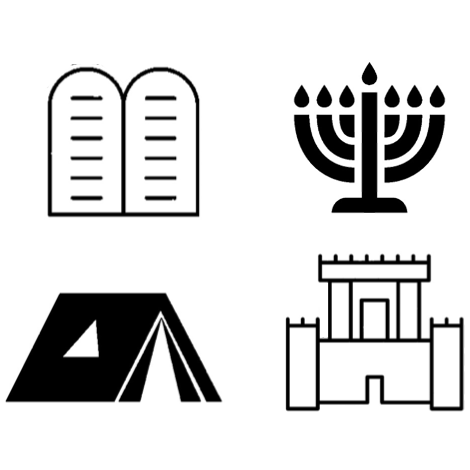
\includegraphics[width=0.30\textwidth]{../ot_frontcover.png}} ;
    \node (0,0) [xshift=+0.20cm, yshift=+2.0cm, opacity=0.10]{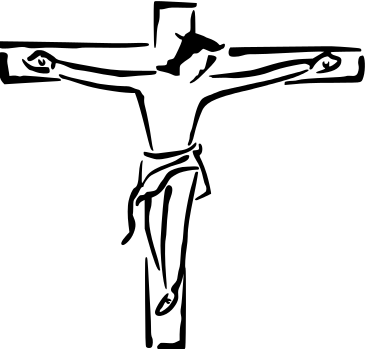
\includegraphics[width=0.20\textwidth]{../christ_on_cross.png}} ;
\end{tikzpicture}
\Large 

\leftcitation{ס} \centerfont 詩百又廿七載：
\leftcitation{ע} \centerfont 非耶和華建屋宇.則匠人之經營徒.
\leftcitation{פ} \centerfont 非耶和華衛城邑.則守者之儆醒徒.
\leftcitation{צ} \centerfont 余獻是卷予華人社區．願為福音流通之器．願獻斯微材為祭榮耀上帝．
\leftcitation{ק} \centerfont 阿門

\switchcolumn

\fontsize{11}{13}\rightfont \Large 滅．時越次聖殿期及當今。\leftcitation{י} \rightfont 猶太者力廣納之．筆錄以卷軸．便以傳、閱、頌、攜、守、鎖、抄、譯、釋、編，得書塔木德、密示拿等經傳．家喻戶曉．傳流若芳。\leftcitation{כ} \rightfont 猶太者文以載道．傳其口述．今我輩粵道之傳應當作如是．遂力行粵音識辨之法．載言載道．以盡忠傳粵道以待興。\leftcitation{ל} \rightfont 蒙下賜恩惠．無畏海量字音文書．既馭上帝之道．今廣及粵語講道．重駛編程之技．匯導粵音遂字稿．重塑講道現場．以傚猶太卷軸之舉便以傳流。\leftcitation{מ} \rightfont 是卷乃粵音口述傳之屬．莫通華文白話之語．

\end{paracol}

\columnratio{0.5,0.5}
\begin{paracol}{2}\fontsize{11}{13}\leftfont \Large \leftcitation{ו} \leftfont 斯殺一違儆百逆．既禁壓之．我輩聞風無奈．在所難免。\leftcitation{ז} \leftfont 另有異人例乎．以版權之名．脅網絡頻道之舉．同授礙予粵道之存流。

\switchcolumn

\fontsize{11}{13}\rightfont \Large 惟待後繼來者之傚．以譯釋傳之於神州華文地。\leftcitation{נ} \rightfont 今能排程驅馭圖靈以編彙文檔，其碼長共數千千亦無逢大礙．全蒙上帝保守。

\end{paracol}



\columnratio{1}\begin{paracol}{1}

\fontsize{11}{13}\rightfont \Large
~~~~~~~~~~~~~~~~~~~~~~~~~~~~~~~~~~~~~~~~~~~~~~~~~~~~~~~~~~~~~~~~~~~~~~~~~~~~~~~\leftcitation{ר} \rightfont 二零二三年二月一日

~~~~~~~~~~~~~~~~~~~~~~~~~~~~~~~~~~~~~~~~~~~~~~~~~~~~~~~~~~~~~~~~~~~~~~~~~~~~~~~\leftcitation{ש} \rightfont 米迦勒

~~~~~~~~~~~~~~~~~~~~~~~~~~~~~~~~~~~~~~~~~~~~~~~~~~~~~~~~~~~~~~~~~~~~~~~~~~~~~~~\leftcitation{ת} \rightfont 書於香港

\end{paracol}

\end{sloppypar}
\end{document}
